\documentclass[11pt,oneside]{book}
\usepackage[letterpaper,top=1in,bottom=1in,inner=1.15in,outer=1.15in]{geometry}
\usepackage[T1]{fontenc}
\usepackage[utf8]{inputenc}
\usepackage{amsmath,amsthm}
\usepackage{newpxtext}
\usepackage{newpxmath}
\usepackage{mathtools,bm}
\usepackage[final]{microtype}
\usepackage{booktabs,tabularx,threeparttable,multirow,makecell,array}
\usepackage{graphicx,float}
\usepackage[font=small,labelfont=bf]{caption}
\usepackage{subcaption}
\usepackage{xcolor}
\usepackage{enumitem}
\usepackage[group-separator={,},group-minimum-digits=4]{siunitx}
\usepackage{pdflscape}
\usepackage{tikz}
\usetikzlibrary{arrows.meta,calc,positioning,patterns,decorations.pathreplacing,shapes.geometric,intersections}
\usepackage{pgfplots}
\pgfplotsset{compat=1.18}
\usepgfplotslibrary{fillbetween}
\usepackage[authoryear,round]{natbib}
\usepackage[colorlinks=true,linkcolor=blue!50!black,citecolor=blue!50!black,urlcolor=blue!50!black]{hyperref}
\usepackage[nameinlink,capitalise]{cleveref}
\crefname{figure}{Figure}{Figures}
\crefname{equation}{Equation}{Equations}
\usepackage{needspace}

\makeatletter
\renewcommand{\@pnumwidth}{2.2em}
\renewcommand{\@tocrmarg}{3.2em}
\renewcommand*{\l@subsection}{\@dottedtocline{2}{3.8em}{3.9em}}
\makeatother

\setlist{itemsep=2pt,topsep=4pt}
\raggedbottom
\numberwithin{equation}{chapter}
\numberwithin{figure}{chapter}
\numberwithin{table}{chapter}

\usepackage{thmtools}
\declaretheorem[style=definition,numberwithin=chapter]{definition}
\declaretheorem[style=definition,sibling=definition]{assumption}
\declaretheorem[style=definition,sibling=definition]{example}
\declaretheorem[style=plain,sibling=definition]{proposition}
\declaretheorem[style=plain,sibling=definition]{theorem}
\declaretheorem[style=plain,sibling=definition]{lemma}
\declaretheorem[style=plain,sibling=definition]{corollary}
\declaretheorem[style=remark,sibling=definition]{remark}
\def\theHdefinition{\thechapter.\arabic{definition}}
\def\theHassumption{\thechapter.\arabic{definition}}
\def\theHexample{\thechapter.\arabic{definition}}
\def\theHproposition{\thechapter.\arabic{definition}}
\def\theHtheorem{\thechapter.\arabic{definition}}
\def\theHlemma{\thechapter.\arabic{definition}}
\def\theHcorollary{\thechapter.\arabic{definition}}
\def\theHremark{\thechapter.\arabic{definition}}

\newcommand{\E}{\mathbb{E}}
\renewcommand{\Pr}{\mathbb{P}}
\newcommand{\R}{\mathbb{R}}
\newcommand{\N}{\mathbb{N}}
\DeclareMathOperator{\Var}{Var}
\DeclareMathOperator{\Cov}{Cov}
\DeclareMathOperator{\Corr}{Corr}
\DeclareMathOperator*{\argmax}{arg\,max}
\DeclareMathOperator*{\argmin}{arg\,min}
\DeclareMathOperator{\diag}{diag}
\DeclareMathOperator{\plim}{plim}
\newcommand{\indic}{\mathbf{1}}
\newcommand{\T}{\top}
\newcommand{\dd}{\mathrm{d}}
\newcommand{\HHI}{\mathit{HHI}}
\newcommand{\iid}{\text{i.i.d.}}
\newcommand{\given}{\,\middle|\,}

\newcommand{\casehead}[1]{\par\medskip\noindent\textit{#1.}\enspace}


\begin{document}
\frontmatter
\hypersetup{pageanchor=false}
\begin{titlepage}
\centering
\vspace*{2in}
{\Huge\bfseries Empirical Industrial Organization\par}
\vspace{0.4in}
{\LARGE A Course Companion for ECON 257\par}
\vspace{0.3in}
{\large Market Power, Demand Estimation, Mergers, Collusion, and Auctions\par}
\vfill
{\large Angikar Ghosal\par}
\vspace{0.2in}
{\large Stanford University, Fall 2026\par}
\vspace*{0.5in}
\end{titlepage}
\hypersetup{pageanchor=true}

\tableofcontents

\mainmatter
\part{Market Power: Theory and Measurement}
\chapter{Introduction: What Empirical IO Studies}\label{ch:intro}

Consider a coffee shop on a university campus. It is the only seller of coffee inside one building, and a few
other cafes operate a short walk away. Does it have market power, and how much? To answer we would like to know
three things. The first is its demand curve, that is, how many cups it would sell at each price. The second is its
marginal cost of a cup. The third is how its rivals would respond if it raised its price. None of the three is
written down anywhere. What we can observe is its price and perhaps the number of cups it sells. Now and then an
event moves one of the unknowns, such as a tax on coffee, a rise in the price of beans or a new cafe next door. Empirical industrial organization is the craft of learning about demand, cost and the conduct of
firms from data of this kind. This chapter introduces that craft, its history and the questions it serves.

The chapter has four movements. \Cref{sec:01-what-is-io,sec:01-definitions} state the questions of the field and
define its basic objects: markets, concentration, the Lerner index and markups. They end with the Cournot model,
which links concentration to margins and so motivates the first empirical program of the field.
\Cref{sec:01-scp,sec:01-scp-econometrics,sec:01-scp-after} study that program, the structure-conduct-performance
paradigm. Its cross-industry regressions of margins on concentration dominated the field for three decades. We
show formally why they cannot separate demand, cost and conduct, and we follow the debates they left behind,
including the recent one over rising markups. \Cref{sec:01-neio,sec:01-identification} present the response, the
New Empirical Industrial Organization of \citet{Bresnahan1989}. It studies one industry at a time, treats conduct
as a parameter, and asks which features of the data identify market power. \Cref{sec:01-today} describes empirical
IO today, following \citet{EinavLevin2010}. Most work now estimates demand, recovers marginal costs from
first-order conditions and simulates counterfactual equilibria. \Cref{sec:01-roadmap} lays out the rest of the book.

The coffee shop returns twice. \Cref{ex:01-coffee} uses an estimated elasticity to infer its marginal cost and shows
how the answer depends on conduct. \Cref{ex:01-coffee-tax} predicts the effect of a tax on its price and shows how
the answer depends on the shape of demand. These two dependencies, on conduct and on functional form, recur in
every chapter. The theory behind this chapter is developed in \cref{ch:theory}, the measurement of conduct in
\cref{ch:conduct}, and the demand models of the structural workflow in \cref{ch:aids,ch:discrete,ch:logit,ch:blp}.
The Cournot, collusion and cross-industry regression models of \cref{sec:01-cournot-hhi,sec:01-endogeneity} are
worked through in full in \cref{app:problems}.

\section{What industrial organization studies}\label{sec:01-what-is-io}

\emph{Industrial organization} (IO) is the field of economics that studies how industries are organized and
how firms and consumers behave within them. In the words of \citet[p.~146]{EinavLevin2010}, the field ``is
concerned with the structure of industries in the economy and the behavior of firms and individuals in these
industries.'' Its distinctive focus is on markets that depart from \emph{perfect competition}, the benchmark
in which many small firms take the price as given and price equals marginal cost. Such departures arise from
scale economies, transaction costs, strategic behavior and other frictions \citep[p.~146]{EinavLevin2010}.

The traditional questions of IO concern competition policy, regulation, and the determinants and consequences
of market power. Competition policy asks, for example, whether a merger will raise prices or whether a group of
sellers is fixing prices. Regulation asks how to set prices and entry rules in industries with large scale
economies, such as electricity transmission or local telephone service. The study of \emph{market power}, the
ability of a firm to keep its price above the competitive level, asks where such power comes from and what it
costs consumers. Each of these questions requires a model of how firms interact. A firm's best price depends on
the prices of its rivals, and a merger changes the incentives of the merging firms and of every firm that
competes with them.

The field therefore looks mostly at what happens between firms. What happens inside a firm, such as how it
organizes production or designs incentives for its employees, belongs largely to other fields. Productivity is
the main exception. Many IO economists measure productivity and study how competition and the selection of
efficient firms shape it. This book does not cover productivity.

Empirical IO relies on economic theory more than most other fields of applied microeconomics. We see two
reasons. The first is that theory has a great deal to say about firms and markets. Firms that set prices every
day plausibly come close to maximizing profit, and profit maximization in equilibrium imposes sharp
restrictions on data. \citet[pp.~158--159]{EinavLevin2010} draw the contrast with research on education.
Standard theory says little about how third graders learn. For firms and markets, they argue, theory ``has a
lot to say and, when appropriately used, generally serves to clarify rather than to complicate one's
understanding of a market.'' The second reason is historical. IO had a head start on the econometric modeling
of strategic behavior. By the late 1980s a body of work already estimated demand, cost and the form of
competition jointly within single industries, and \citet{Bresnahan1989} could survey it. A further
consideration reinforces both reasons. Many IO questions concern events that have not yet happened, such as a
proposed merger, and only a model of the industry can predict their effects.

These tools now travel beyond the traditional boundaries of the field. IO-trained economists study insurers
and hospitals in health care, schools and colleges in education, and banks and lenders in finance. Questions
about competition have become central in each of these sectors. The same methods serve markets with \emph{adverse
selection}, such as insurance, where the customers most eager to buy are the most costly to serve. They also
serve platforms that bring two groups of users together. \citet[p.~149]{EinavLevin2010}
report that the demand models developed in \cref{ch:aids,ch:discrete,ch:logit,ch:blp} have spread into trade,
education, housing, health and environmental economics. Economists sometimes call this expansion ``IO+.'' The
editors of the latest Handbook of Industrial Organization describe the same trend \citep[Preface, p.~xv]{HoHortacsuLizzeri2021}.
In their account, the ``econometric revolution'' that began with the New Empirical Industrial Organization of
\cref{sec:01-neio} has kept maturing. Its toolbox now reaches credit and insurance markets, financial markets, health
care, the energy sector and the environment.

Empirical IO also has a large footprint in policy and business. Its methods are used in merger reviews and
antitrust litigation, in regulatory decisions, in price setting by retailers, and in the design of auctions and
marketplaces \citep[p.~145]{EinavLevin2010}. Antitrust agencies and courts use demand estimates to define
markets, to simulate the price effects of mergers, and to compute damages from excessive prices
\citep[p.~149]{EinavLevin2010}. Around 1980, antitrust arguments often rested on simple concentration measures.
Today the agencies routinely commission econometric studies of the industry under review
\citep[p.~152]{EinavLevin2010}. Welfare measures derived from estimated demand have shaped the debate over how
the Consumer Price Index should account for new goods \citep[p.~149]{EinavLevin2010}. Empirical studies of
bidding have informed the regulation of wholesale electricity markets \citep[p.~154]{EinavLevin2010}. We treat
merger analysis in \cref{ch:mergers}, new goods in \cref{ch:newgoods}, and auctions in
\cref{ch:auction-theory,ch:auction-empirics}.

Almost every question in this book comes back to three objects, which we call the \emph{primitives} of a
market. The first is \emph{demand}, which describes how many units consumers buy at each price and how they
substitute between products. The second is \emph{cost}, in particular the \emph{marginal cost} of producing one
more unit. The third is \emph{conduct}, the way firms compete. Firms may set prices or quantities, act
independently or coordinate, and look ahead to rivals' reactions or ignore them. Price equals marginal cost
plus a markup, and the markup depends on demand and on conduct:
\begin{equation}\label{eq:01-price-decomposition}
  \text{price} = \text{marginal cost} + \text{markup}(\text{demand}, \text{conduct}).
\end{equation}
\Cref{sec:01-lerner,sec:01-cournot-hhi} make this decomposition precise.

In most data sets none of the three primitives is observed directly. We observe prices and quantities, which
are equilibrium outcomes. Each observed pair lies on the demand curve and on the firms' pricing rule at the
same time, so a scatter of prices and quantities traces out neither of them. \Cref{ch:aids,ch:logit} treat
this simultaneity problem. Accounting data record average and historical costs, with overhead allocated by
convention. \citet[p.~151]{EinavLevin2010}, following \citet{Bresnahan1989}, stress that accounting practices
are not designed to report the economic notion of marginal cost. Conduct is recorded nowhere, and firms that
coordinate have every reason to hide it. The history of empirical IO, told in the rest of this chapter, is a
sequence of answers to one problem. How can we learn about demand, cost and conduct from data on prices and
quantities?

\begin{remark}[Scope of this book]
The book covers static imperfect competition and its measurement (\cref{ch:theory,ch:conduct,ch:diffprod}) and
demand estimation and its applications (\cref{ch:aids,ch:discrete,ch:logit,ch:blp,ch:airlines,ch:newgoods}). It
also covers competition policy toward mergers and collusion (\cref{ch:mergers,ch:collusion-theory,ch:collusion-evidence})
and auctions of a single object (\cref{ch:auction-theory,ch:auction-empirics}). It does not treat in depth the
models of entry and market structure, dynamic competition and investment, productivity, vertical relations,
consumer search, or price discrimination. \Cref{sec:01-today} sketches some of these topics, and
\cref{sec:01-roadmap} gives a detailed roadmap.
\end{remark}

\section{Market structure, market power, and markups}\label{sec:01-definitions}

A question in the background of much of empirical IO is how market structure affects market power. Do markets
with fewer or larger firms have higher prices relative to cost? Answering it requires four ingredients, which
this section develops in turn. We need a definition of the market (\cref{sec:01-market-definition}) and a
measure of its structure (\cref{sec:01-concentration}). We also need a measure of market power
(\cref{sec:01-lerner,sec:01-fixed-costs}) and a theory that links structure to market power
(\cref{sec:01-cournot-hhi}).

\subsection{Markets and market definition}\label{sec:01-market-definition}

\begin{definition}[Market]\label{def:01-market}
A \emph{market} is a set of products and a geographic area within which buyers substitute strongly, and from
which they substitute only weakly toward outside products or sellers. The set of products is the
\emph{product market}, and the area is the \emph{geographic market}.
\end{definition}

Market shares, concentration and even the label ``monopoly'' are defined only relative to a market. A firm
that sells the only brand of a particular breakfast cereal has a monopoly over that brand. The same firm has a
modest share of ready-to-eat cereal and a negligible share of all breakfast foods. Every statistic computed
from shares therefore inherits the choice of market.

Sometimes the market is obvious. Cement is heavy and cheap relative to its weight, so a cement plant in an
isolated town competes only with plants within a short trucking distance. The product market is cement, and
the geographic market is the area around the town. Sometimes the market is far from obvious. Online retailers
sell to the whole country and compete with physical stores. Breakfast cereals form a chain of substitutes, from
children's cereals to adult cereals to other breakfast foods, with no natural break. In such cases any boundary
is a judgment call.

Antitrust practice disciplines this judgment with the \emph{hypothetical monopolist test}. We start from a
candidate set of products and an area. We then ask whether a hypothetical profit-maximizing firm that owned all
of them would impose a \emph{small but significant and non-transitory increase in price} (SSNIP), commonly 5
percent. If substitution to products outside the set would make such an increase unprofitable, the set is too
narrow, and we add the next closest substitute. The \emph{relevant market} is the smallest set that passes the
test. The test is a statement about demand elasticities, so it needs the demand models of
\cref{ch:aids,ch:discrete,ch:logit,ch:blp}. \Cref{ch:mergers} develops it, together with the loss of sales that
would make a price increase unprofitable and the concentration thresholds used in merger review.

Some economists doubt that market definition is the right first step at all. \citet[p.~1049]{Bresnahan1989}
notes that antitrust often needs to know whether a group of firms acting together, or a single firm, has market
power. He adds in a footnote that ``these questions are well-posed, even where the usual method of answering
them \ldots{} is senseless'' \citep[p.~1049, n.~44]{Bresnahan1989}. The usual method defines a `relevant
market' and calculates market shares in it. Market power is a property of the demand curve that a firm or group
faces, and we can try to estimate that curve directly. Market definition is a device for approximating the same
object with shares. \Cref{ch:conduct} shows how to estimate the demand curve that a single firm faces after its
rivals respond. This
direct approach is one motivation for the New Empirical Industrial Organization of \cref{sec:01-neio}.

\subsection{Concentration measures}\label{sec:01-concentration}

In empirical work, \emph{market structure} usually means a measure of concentration computed from market
shares. Consider a market with $N$ firms $i = 1, \dots, N$ that sell a homogeneous good. Firm $i$ produces
$q_i$, total output is $Q = \sum_{i=1}^{N} q_i$, and firm $i$'s \emph{market share} is $s_i = \frac{q_i}{Q}$.
Shares are fractions that sum to one. With differentiated products, shares are computed from units or revenues
within the defined market. We write $s_{(1)} \ge s_{(2)} \ge \dots \ge s_{(N)}$ for the shares sorted from
largest to smallest.

\begin{definition}[Concentration measures]\label{def:01-concentration}
\leavevmode
\begin{enumerate}[label=(\roman*)]
  \item The \emph{$m$-firm concentration ratio} is the combined share of the $m$ largest firms,
  \[
    \mathit{CR}_m = \sum_{i=1}^{m} s_{(i)} .
  \]
  \item The \emph{Herfindahl-Hirschman index}, often shortened to the Herfindahl index, is the sum of squared
  shares,
  \begin{equation}\label{eq:01-hhi}
    \HHI = \sum_{i=1}^{N} s_i^2 .
  \end{equation}
  Antitrust agencies report it in \emph{HHI points}, equal to $10{,}000 \times \HHI$, which is the sum of
  squared shares measured in percent.
  \item The \emph{numbers equivalent} is $N^{\mathrm{eq}} = \frac{1}{\HHI}$, the number of equal-sized firms that would
  produce the same index.
\end{enumerate}
\end{definition}

The concentration ratios in common use are $\mathit{CR}_1$ (the share of the largest firm), $\mathit{CR}_3$,
$\mathit{CR}_4$ and $\mathit{CR}_8$. They satisfy $\frac{m}{N} \le \mathit{CR}_m \le 1$ for $m \le N$, because
the average of the $m$ largest shares is at least the average share $\frac{1}{N}$. The Herfindahl-Hirschman index is
named after Orris Herfindahl and Albert Hirschman. It uses every share, and it weights large firms more heavily
because each share is weighted by itself. The next result makes precise what the index measures.

\begin{lemma}[Bounds and variance decomposition]\label{prop:01-hhi-variance}
Let $\sigma_s^2 = \frac{1}{N}\sum_{i=1}^{N} \left(s_i - \frac{1}{N}\right)^2$ be the cross-firm variance of
market shares. Then
\begin{equation}\label{eq:01-hhi-variance}
  \HHI = \frac{1}{N} + N\sigma_s^2 ,
\end{equation}
and $\frac{1}{N} \le \HHI \le 1$. The lower bound holds with equality if and only if all shares are equal. The
upper bound holds with equality if and only if one firm has the whole market.
\end{lemma}

\begin{proof}
The mean share is $\frac{1}{N}\sum_{i} s_i = \frac{1}{N}$, so $\sigma_s^2$ is the variance of shares around
their mean. Expand the sum of squared deviations:
\begin{align*}
  \sum_{i=1}^{N} \left(s_i - \frac{1}{N}\right)^2
  &= \sum_{i=1}^{N} s_i^2 - \frac{2}{N}\sum_{i=1}^{N} s_i + N \cdot \frac{1}{N^2} \\
  &= \HHI - \frac{2}{N} + \frac{1}{N} \\
  &= \HHI - \frac{1}{N}.
\end{align*}
The second line uses $\sum_i s_i = 1$. The left side equals $N\sigma_s^2$, which gives
\eqref{eq:01-hhi-variance}. Because $\sigma_s^2 \ge 0$, we have $\HHI \ge \frac{1}{N}$, with equality if and
only if every share equals $\frac{1}{N}$. For the upper bound, $0 \le s_i \le 1$ implies $s_i^2 \le s_i$, so
$\HHI \le \sum_i s_i = 1$. Equality requires $s_i^2 = s_i$ for every $i$, so every share is zero or one. Since
the shares sum to one, exactly one firm has share one.
\end{proof}

\Cref{prop:01-hhi-variance} shows that the index combines two features of a market. The term $\frac{1}{N}$
reflects the number of firms, and the term $N\sigma_s^2$ reflects the inequality of their sizes. A market with
many firms is highly concentrated if one of them is much larger than the rest. Correspondingly, the numbers
equivalent $N^{\mathrm{eq}}$ lies between $1$ and $N$, and it falls below $N$ whenever shares are unequal.
\Cref{sec:01-demsetz} uses the decomposition to show that cost differences between firms raise concentration
in a Cournot market.

\begin{example}[Two rankings of concentration]\label{ex:01-concentration}
Consider two hypothetical industries. Industry A has one dominant firm with half of the market and 25 small
firms with 2 percent each. Industry B has four firms with 20 percent each and four firms with 5 percent each.
The four-firm concentration ratios are
\begin{align*}
  \mathit{CR}_4^A &= 0.50 + 3 \times 0.02 = 0.56, \\
  \mathit{CR}_4^B &= 4 \times 0.20 = 0.80,
\end{align*}
so this ratio ranks B as more concentrated. The Herfindahl-Hirschman indices are
\begin{align*}
  \HHI^A &= 0.50^2 + 25 \times 0.02^2 = 0.25 + 0.01 = 0.26, \\
  \HHI^B &= 4 \times 0.20^2 + 4 \times 0.05^2 = 0.16 + 0.01 = 0.17,
\end{align*}
or 2,600 and 1,700 HHI points. The index ranks A as more concentrated. The numbers equivalents are
$N^{\mathrm{eq}}_A = \frac{1}{0.26} \approx 3.8$ and $N^{\mathrm{eq}}_B = \frac{1}{0.17} \approx 5.9$. Industry A has 26 firms but is
as concentrated as a market with about four equal firms. In industry B, $N = 8$ and every share deviates from
the mean $\frac{1}{8}$ by $0.075$, so \eqref{eq:01-hhi-variance} confirms the arithmetic:
\[
  \HHI^B = \frac{1}{8} + 8 \times 0.075^2 = 0.125 + 0.045 = 0.17 .
\]
The ratio $\mathit{CR}_4$ ignores how shares are distributed within the top four and among the remaining firms.
The index $\HHI$ responds mostly to the single large firm in A.
\end{example}

\begin{remark}[Which indices are admissible?]\label{rem:01-ej-axioms}
\citet{EncaouaJacquemin1980} ask which functions $R(s_1, \dots, s_N)$ of the shares deserve the name of a
concentration index \citep[Section~5.5]{Tirole1988}. They impose three axioms. The index is symmetric, so that
permuting the shares leaves it unchanged. It satisfies the \emph{Lorenz condition}, which says that a
mean-preserving spread of the shares, moving share toward the tails of their distribution, raises the index.
With symmetric firms it falls as their number grows, so that
$R\left(\frac{1}{N}, \dots, \frac{1}{N}\right) \ge R\left(\frac{1}{N+1}, \dots, \frac{1}{N+1}\right)$. They show
that a family of indices satisfying the axioms takes the form
\begin{equation}\label{eq:01-ej-family}
  R(s_1, \dots, s_N) = \sum_{i=1}^{N} s_i\, h(s_i) ,
\end{equation}
where $h$ is nondecreasing and $s\,h(s)$ is convex. The Herfindahl-Hirschman index has $h(s) = s$. The
\emph{entropy index} $\sum_i s_i \ln s_i$ has $h(s) = \ln s$, and it equals $-\ln N$ when $N$ firms are equal. The
ratio $\mathit{CR}_m$ satisfies the axioms, yet it does not belong to the family.

Two steps show why every member of the family satisfies the axioms. Let $g(s) = s\,h(s)$. With equal shares,
$R = N g\left(\frac{1}{N}\right) = h\left(\frac{1}{N}\right)$, which cannot rise with $N$ because $h$ is
nondecreasing. For the Lorenz condition, move the share $\Delta > 0$ from firm $j$ to a firm $i$ with
$s_i \ge s_j$. This transfer is the elementary step of a mean-preserving spread. The index changes by
\[
  \left[g(s_i + \Delta) - g(s_i)\right] - \left[g(s_j) - g(s_j - \Delta)\right] \ge 0 .
\]
The inequality holds because the slope of a convex function over an interval of length $\Delta$ rises as the
interval moves to the right. For the Herfindahl index the change is $2\Delta(s_i - s_j) + 2\Delta^2 > 0$. The
ratio $\mathit{CR}_m$ meets the Lorenz condition only weakly, since a transfer between two firms outside the top
$m$ can leave it unchanged.
\end{remark}

\begin{remark}[What concentration measures leave out]\label{rem:01-concentration-limits}
A concentration index summarizes shares and nothing else. It ignores how close the products of different firms
are as substitutes, whether firms have spare capacity, how easily new firms can enter, and whether buyers are
large enough to bargain. Market structure in the broad sense includes the number of sellers and buyers,
vertical integration, and product differentiation. Differentiation is \emph{vertical} when all buyers rank the
products the same way, as with quality grades. It is \emph{horizontal} when buyers rank them differently, as
with flavors or locations. No single index captures all of these features. \citet[p.~283]{BakerBresnahan1988}
give an example from US brewing over 1962--1982. Pabst and Coors had similar national market shares, yet
their estimates show that Pabst was virtually a price taker while Coors had substantial market power.

Shares are also used mechanically in merger review. If firms $i$ and $j$ merge and the merged firm keeps the
combined share $s_i + s_j$, the index rises by
\[
  (s_i + s_j)^2 - s_i^2 - s_j^2 = 2 s_i s_j .
\]
Oligopoly theory does not guarantee that the merged firm keeps the combined share, so this calculation is only
a first screen (\cref{ch:theory,ch:mergers}).
\end{remark}

\subsection{Market power, markups, and the Lerner index}\label{sec:01-lerner}

The competitive benchmark is price equal to marginal cost. A firm that takes the market price as given expands
output until its marginal cost reaches the price. Market power is the ability to do better than this, and we
measure it by the gap between price and marginal cost.

\begin{definition}[Market power and markups]\label{def:01-market-power}
A firm has \emph{market power} if it can profitably set its price above the competitive level, which is its
marginal cost $mc$. For a firm that charges the price $p$, we use four measures of the gap between price and
marginal cost.
\begin{enumerate}[label=(\roman*)]
  \item The \emph{Lerner index} is $L = \frac{p - mc}{p}$, the margin as a fraction of price
  \citep{Lerner1934}.
  \item The \emph{markup ratio} is $\mu = \frac{p}{mc}$.
  \item The \emph{markup rate} is $\mu - 1 = \frac{p - mc}{mc}$, the margin as a fraction of marginal cost.
  \item The \emph{dollar markup} is $p - mc$.
\end{enumerate}
\end{definition}

In this chapter $\mu$ always denotes the markup ratio. Later chapters use $\mu_{ijt}$ for the consumer-specific
part of utility, and the context keeps the two apart. The recent literature on markups, including
\citet{DeLoeckerEeckhoutUnger2020}, reports the ratio $\mu$. The Lerner index and the markup ratio carry the
same information:
\begin{align}
  L = \frac{p - mc}{p} &= 1 - \frac{mc}{p} \notag\\
  &= 1 - \frac{1}{\mu} \notag\\
  &= \frac{\mu - 1}{\mu} . \label{eq:01-lerner-mu}
\end{align}
Inverting gives $\mu = \frac{1}{1 - L}$. When $0 < mc \le p$, the Lerner index lies in $[0, 1]$ and
$\mu \ge 1$. Price taking gives $L = 0$ and $\mu = 1$. A markup rate of 50 percent, or $\mu = 1.5$, corresponds
to $L = \frac{0.5}{1.5} = \frac{1}{3}$.

The basic theory of how a firm with market power sets its price fits in one proposition. We state it for a firm
that faces a \emph{residual demand} curve $Q(p)$, the quantity it sells at each of its own prices once we
account for what its rivals do. For a monopolist, residual demand is market demand.

\begin{proposition}[The pricing rule]\label{prop:01-pricing-rule}
A firm faces a twice differentiable residual demand $Q(p)$ with $Q(p) > 0$ and $Q'(p) < 0$, and it produces
at constant marginal cost $c > 0$. Let $p$ be an interior maximizer of profit $\pi(p) = (p - c)Q(p)$. Then the
following hold at $p$.
\begin{enumerate}[label=(\roman*)]
  \item The dollar markup equals the reciprocal of the \emph{semi-elasticity} of demand
  $-\frac{\dd \ln Q(p)}{\dd p}$:
  \begin{equation}\label{eq:01-dollar-markup}
    p - c = m \equiv -\frac{Q(p)}{Q'(p)}, \qquad -\frac{\dd \ln Q(p)}{\dd p} = -\frac{Q'(p)}{Q(p)} = \frac{1}{m}.
  \end{equation}
  \item The Lerner index equals the reciprocal of the residual demand elasticity
  $\varepsilon^R = -Q'(p)\frac{p}{Q(p)}$:
  \begin{equation}\label{eq:01-lerner-rule}
    \frac{p - c}{p} = \frac{1}{\varepsilon^R} .
  \end{equation}
  \item Price is a multiple of marginal cost,
  \begin{equation}\label{eq:01-price-multiple}
    p = \frac{\varepsilon^R}{\varepsilon^R - 1}\, c ,
  \end{equation}
  and the residual elasticity exceeds one, $\varepsilon^R > 1$.
\end{enumerate}
The second-order condition is $\pi''(p) = 2Q'(p) + (p - c)Q''(p) \le 0$.
\end{proposition}

\begin{proof}
Differentiate profit with respect to price:
\[
  \pi'(p) = Q(p) + (p - c)Q'(p).
\]
At an interior maximum the first-order condition holds:
\begin{equation}\label{eq:01-foc-monopoly}
  Q'(p)(p - c) + Q(p) = 0 .
\end{equation}
For (i), divide \eqref{eq:01-foc-monopoly} by $-Q'(p) > 0$ and rearrange:
\begin{align*}
  -(p - c) - \frac{Q(p)}{Q'(p)} &= 0, \\
  p - c &= -\frac{Q(p)}{Q'(p)} = m .
\end{align*}
The semi-elasticity is $-\frac{\dd \ln Q}{\dd p} = -\frac{Q'(p)}{Q(p)}$, which is $\frac{1}{m}$ by definition of
$m$. For (ii), divide both sides of (i) by $p$:
\[
  \frac{p - c}{p} = -\frac{Q(p)}{p\,Q'(p)} = \frac{1}{-Q'(p)\frac{p}{Q(p)}} = \frac{1}{\varepsilon^R} .
\]
For (iii), multiply (ii) by $p$ and collect the terms in $p$:
\begin{align*}
  p - c &= \frac{p}{\varepsilon^R}, \\
  p\left(1 - \frac{1}{\varepsilon^R}\right) &= c, \\
  p &= \frac{\varepsilon^R}{\varepsilon^R - 1}\, c .
\end{align*}
The first line shows that $p > c > 0$, because $Q > 0$ and $Q' < 0$ make $\varepsilon^R > 0$. The ratio
$\frac{p}{c} = \frac{\varepsilon^R}{\varepsilon^R - 1}$ must then exceed one. If $\varepsilon^R < 1$ the ratio
would be negative, and $\varepsilon^R = 1$ would make the second line read $0 = c$. Hence $\varepsilon^R > 1$.
The second-order condition is the requirement that $\pi''(p) \le 0$ at a maximum.
\end{proof}

The two arrangements (i) and (ii) are the formulas used most often in this book. Arrangement (i) says that the
markup in dollars equals the inverse of the semi-elasticity, the proportional fall in quantity per dollar of
price increase. Arrangement (ii), often called the \emph{Lerner equation} or the \emph{inverse elasticity rule},
says that the markup as a fraction of price equals the inverse of the elasticity. A firm prices further above
cost when its customers respond less to price. Both formulas involve only the residual demand curve of the firm
itself, evaluated at the chosen price. The same logic carries over to the models of price competition with
differentiated products that dominate modern work. There, each firm's price equals its marginal cost plus a
markup that depends on the semi-elasticity of its own demand \citep[p.~151]{EinavLevin2010}. Statement (iii) adds that a firm with market power never prices where
its residual demand is inelastic. At such a price, a small price increase would raise revenue and lower cost.

Two demand curves show the difference between the arrangements. With constant-elasticity demand
$Q(p) = A p^{-\varepsilon^R}$, the Lerner index is the constant $\frac{1}{\varepsilon^R}$, so price is a fixed
multiple of cost. With exponential demand $Q(p) = A e^{-\frac{p}{b}}$, the semi-elasticity is the constant
$\frac{1}{b}$, so the dollar markup is the constant $b$ whatever the cost. \Cref{ch:theory} develops these cases
and their implications for how cost changes pass through to prices.

\begin{remark}[Residual versus market demand]\label{rem:01-residual}
In an oligopoly the residual elasticity $\varepsilon^R$ differs from the \emph{market elasticity}
$\varepsilon = -\frac{\dd Q}{\dd p}\frac{p}{Q}$ of total industry demand. Customers who leave one firm may buy
from a rival instead of leaving the market, so a firm typically faces more elastic demand than the industry as a
whole. A simple case makes this precise. Suppose $N$ firms sell a homogeneous good with inverse market demand
$P(Q)$, and firm $i$ takes its rivals' total output $Q_{-i} = Q - q_i$ as fixed. The firm's inverse residual
demand is then $P(q_i + Q_{-i})$, whose slope in $q_i$ is $P'(Q)$. Since the slope of demand is the reciprocal
of the slope of inverse demand, the market elasticity is $\varepsilon = -\frac{P(Q)}{Q P'(Q)}$. The residual
elasticity of firm $i$ is therefore
\begin{equation}\label{eq:01-residual-elasticity}
  \varepsilon^R_i = -\frac{P(Q)}{q_i P'(Q)} = \frac{Q}{q_i}\left(-\frac{P(Q)}{Q P'(Q)}\right)
  = \frac{\varepsilon}{s_i} .
\end{equation}
A firm with a 25 percent share faces a residual elasticity four times the market elasticity.
\Cref{sec:01-cournot-hhi} returns to this case. \Cref{ch:conduct} shows how \citet{BakerBresnahan1988}
estimate residual demand curves directly, and \cref{ch:diffprod} treats firms that sell several differentiated
products.
\end{remark}

\Cref{prop:01-pricing-rule} can be run in reverse. If we know the elasticity of the demand that a firm faces
and we observe its price, the pricing rule tells us its marginal cost.

\begin{corollary}[Inferring marginal cost from prices]\label{prop:01-infer-cost}
Suppose we observe the price $p$ of a firm that maximizes profit as in \cref{prop:01-pricing-rule}, and we have
an estimate $\hat\varepsilon^R$ of its residual demand elasticity at that price. Then the Lerner index and
marginal cost are estimated by
\begin{equation}\label{eq:01-infer-cost}
  \hat L = \frac{1}{\hat\varepsilon^R}, \qquad
  \hat c = p + \frac{Q(p)}{\hat Q'(p)} = p\left(1 - \frac{1}{\hat\varepsilon^R}\right).
\end{equation}
If $\hat\varepsilon^R$ has standard error $\mathrm{se}(\hat\varepsilon^R)$ and $p$ is measured without error,
the delta method gives the approximate standard errors
\begin{equation}\label{eq:01-infer-cost-se}
  \mathrm{se}(\hat c) \approx \frac{p}{(\hat\varepsilon^R)^2}\,\mathrm{se}(\hat\varepsilon^R), \qquad
  \mathrm{se}(\hat L) \approx \frac{1}{(\hat\varepsilon^R)^2}\,\mathrm{se}(\hat\varepsilon^R).
\end{equation}
\end{corollary}

\begin{proof}
Solving (i) of \cref{prop:01-pricing-rule} for $c$ gives $c = p + \frac{Q(p)}{Q'(p)}$. Solving (ii) gives
$c = p\left(1 - \frac{1}{\varepsilon^R}\right)$. Replacing the unknown slope or elasticity with its estimate
gives \eqref{eq:01-infer-cost}. For the standard errors, write $\hat c = g(\hat\varepsilon^R)$ with
$g(\varepsilon) = p - \frac{p}{\varepsilon}$. Its derivative is
\[
  g'(\varepsilon) = \frac{p}{\varepsilon^2} .
\]
Let $\varepsilon^R_0$ be the true elasticity. A first-order Taylor expansion gives
$\hat c - c \approx g'(\varepsilon^R_0)\left(\hat\varepsilon^R - \varepsilon^R_0\right)$, so
\[
  \Var(\hat c) \approx \left(\frac{p}{(\varepsilon^R_0)^2}\right)^2 \Var(\hat\varepsilon^R) .
\]
Taking square roots and evaluating the derivative at the estimate gives the first formula in
\eqref{eq:01-infer-cost-se}. The same steps with $h(\varepsilon) = \frac{1}{\varepsilon}$, whose derivative is
$h'(\varepsilon) = -\frac{1}{\varepsilon^2}$, give the second. \Cref{app:econometrics} states the delta method
in general.
\end{proof}

This inversion runs through the rest of the book. \citet{Rosse1970} used it to estimate the cost functions of
newspapers ``without using cost data,'' as his title puts it. \citet[p.~151]{EinavLevin2010} describe it as the
standard way to recover costs in modern work when cost data are unavailable or unreliable. The inversion rests
on a maintained assumption, namely that the firm maximizes profit under a known form of conduct. If firms
compete differently, the same price and elasticity imply a different cost. With the industry \emph{conduct
parameter} $\theta$, which we introduce in \cref{sec:01-cournot-hhi} and develop in
\cref{sec:01-conduct-parameter}, the inversion becomes
\begin{equation}\label{eq:01-infer-cost-theta}
  \hat c = p + \theta\,\frac{Q(p)}{\hat Q'(p)} = p\left(1 - \frac{\theta}{\hat\varepsilon}\right),
\end{equation}
where $Q$ and $\hat\varepsilon$ now refer to market demand. Monopoly corresponds to $\theta = 1$. Price taking
corresponds to $\theta = 0$, which gives $\hat c = p$.

\begin{example}[A campus coffee shop]\label{ex:01-coffee}
The numbers in this example are hypothetical. A coffee shop on a university campus charges $p = 4$ dollars for a
cup. Suppose an econometrician has estimated the elasticity of the shop's residual demand at
$\hat\varepsilon^R = 2.5$, with standard error $0.5$. Under profit maximization,
\cref{prop:01-pricing-rule,prop:01-infer-cost} give
\begin{align*}
  \hat L &= \frac{1}{2.5} = 0.40, \\
  \hat m &= \frac{p}{\hat\varepsilon^R} = \frac{4}{2.5} = 1.60, \\
  \hat c &= 4\left(1 - \frac{1}{2.5}\right) = 4 \times 0.6 = 2.40, \\
  \hat\mu &= \frac{4}{2.40} \approx 1.67 .
\end{align*}
The margin over marginal cost is 40 percent of the price, or about 67 percent of marginal cost. The delta-method
standard errors are
\begin{align*}
  \mathrm{se}(\hat c) &\approx \frac{4}{2.5^2} \times 0.5 = \frac{4}{6.25} \times 0.5 = 0.32, \\
  \mathrm{se}(\hat L) &\approx \frac{0.5}{6.25} = 0.08 .
\end{align*}
An approximate 95 percent confidence interval for marginal cost is $2.40 \pm 1.96 \times 0.32$, or
$[1.77, 3.03]$. The mapping from elasticity to cost is nonlinear, and the linear approximation hides this. An
elasticity one standard error below the estimate, $2.0$, implies $\hat c = 2.00$. An elasticity one standard
error above it, $3.0$, implies $\hat c \approx 2.67$. The implied band is asymmetric around $2.40$.

Now change the interpretation of the estimate. Suppose $2.5$ is the elasticity of total campus demand for
coffee, and the shop is one of three identical sellers that compete in quantities as in the Cournot model. By
\eqref{eq:01-residual-elasticity}, the shop's residual elasticity is $\frac{2.5}{\frac{1}{3}} = 7.5$, and the
inversion gives
\begin{align*}
  \hat L &= \frac{1}{7.5} \approx 0.13, \\
  \hat c &= 4\left(1 - \frac{1}{7.5}\right) \approx 3.47 .
\end{align*}
Treating the market elasticity as if it were the shop's own elasticity would overstate the Lerner index
threefold and understate marginal cost by more than a dollar. If instead the three shops coordinate and price as
one monopolist, the market elasticity is the relevant one and $\hat c = 2.40$ again. In terms of
\eqref{eq:01-infer-cost-theta}, Cournot behavior is $\theta = \frac{1}{3}$ and joint monopoly is $\theta = 1$.
The same price and the same demand estimate imply a marginal cost anywhere from $2.40$ to $3.47$. The data on
price and demand do not pin down cost by themselves. A maintained assumption about conduct does.
\end{example}

\subsection{Markups are not profits: the role of fixed costs}\label{sec:01-fixed-costs}

Markups are often used as a synonym for market power, and market power is often read as a sign of excess
profit. The second step is unwarranted. A positive markup over marginal cost is what a firm needs to cover its
fixed costs, so a firm can charge well above marginal cost and still earn no economic profit.

\begin{proposition}[The zero-profit markup]\label{prop:01-zero-profit-markup}
A firm produces $q > 0$ units at constant marginal cost $c > 0$, sells them at price $p$, and incurs a fixed
cost $F > 0$. Its economic profit $\pi = (p - c)q - F$ can be written as
\begin{equation}\label{eq:01-profit-identity}
  \pi = L\,pq - F .
\end{equation}
If the firm earns zero economic profit, then
\begin{equation}\label{eq:01-zero-profit-markup}
  p = c + \frac{F}{q}, \qquad \mu - 1 = \frac{F}{cq} > 0, \qquad L = \frac{F}{pq} > 0 .
\end{equation}
\end{proposition}

\begin{proof}
Since $L = \frac{p - c}{p}$, we have $(p - c)q = L\,pq$, which gives \eqref{eq:01-profit-identity}. Setting
$\pi = 0$ gives $(p - c)q = F$, so $p - c = \frac{F}{q}$ and $p = c + \frac{F}{q}$. Dividing
$p - c = \frac{F}{q}$ by $c$ gives the markup rate $\frac{F}{cq}$. Dividing it by $p$ gives
$L = \frac{F}{pq}$, the ratio of fixed cost to revenue.
\end{proof}

The identity \eqref{eq:01-profit-identity} shows what the Lerner index measures. It is the gross margin per
dollar of revenue, before fixed costs are paid. Profit is positive only if the gross margin $L\,pq$ exceeds $F$.
A software firm with almost no marginal cost has a Lerner index close to one, yet it may barely recover the cost
of writing its software. Market power in the sense of \cref{def:01-market-power} is therefore compatible with
zero economic profit.

The classic setting where this happens is \emph{monopolistic competition} \citep{Chamberlin1933}. Each firm
sells a differentiated product and faces a downward-sloping inverse residual demand curve $P^R(q)$, so it has
market power. Entry is free. New products enter while profits are positive, and each entrant takes customers
from existing products, which shifts their residual demand curves inward. Entry stops when each firm just covers
its costs. At that point the residual demand curve touches the average cost curve without crossing it. This
configuration is the \emph{Chamberlin tangency}, shown in \cref{fig:01-tangency}.

With constant marginal cost $c$ and fixed cost $F$, average cost is $AC(q) = c + \frac{F}{q}$. It falls with
output, with slope $AC'(q) = -\frac{F}{q^2}$. A tangency at output $q^*$ means that two conditions hold:
\begin{align}
  P^R(q^*) &= AC(q^*) = c + \frac{F}{q^*}, \label{eq:01-tangency-level}\\
  P^{R\prime}(q^*) &= AC'(q^*) = -\frac{F}{(q^*)^2}. \label{eq:01-tangency-slope}
\end{align}
The first condition is zero profit. The second says that the two curves have the same slope at $q^*$. For the
curves of \cref{fig:01-tangency}, with $c = 2$, $F = 4$ and $P^R(q) = 6 - q$, the gap between them is
$AC(q) - P^R(q) = \frac{(q - 2)^2}{q} \ge 0$. Demand therefore lies below average cost at every other output,
and no output earns positive profit. The tangency is consistent with profit maximization. Marginal revenue at
$q^*$ is
\begin{align*}
  MR(q^*) &= P^R(q^*) + q^* P^{R\prime}(q^*) \\
  &= c + \frac{F}{q^*} - q^* \frac{F}{(q^*)^2} \\
  &= c ,
\end{align*}
where the second line uses \eqref{eq:01-tangency-level} and \eqref{eq:01-tangency-slope}. Marginal revenue
therefore equals marginal cost. Price exceeds marginal cost by $p^* - c = \frac{F}{q^*}$, and the Lerner index
is
\[
  L = \frac{F}{p^* q^*} = -\frac{q^* P^{R\prime}(q^*)}{p^*} = \frac{1}{\varepsilon^R(q^*)} ,
\]
where the second equality uses \eqref{eq:01-tangency-slope}. The firm follows the inverse elasticity rule of
\cref{prop:01-pricing-rule}, and its markup exactly covers its fixed cost.

\begin{figure}[htbp]
\centering
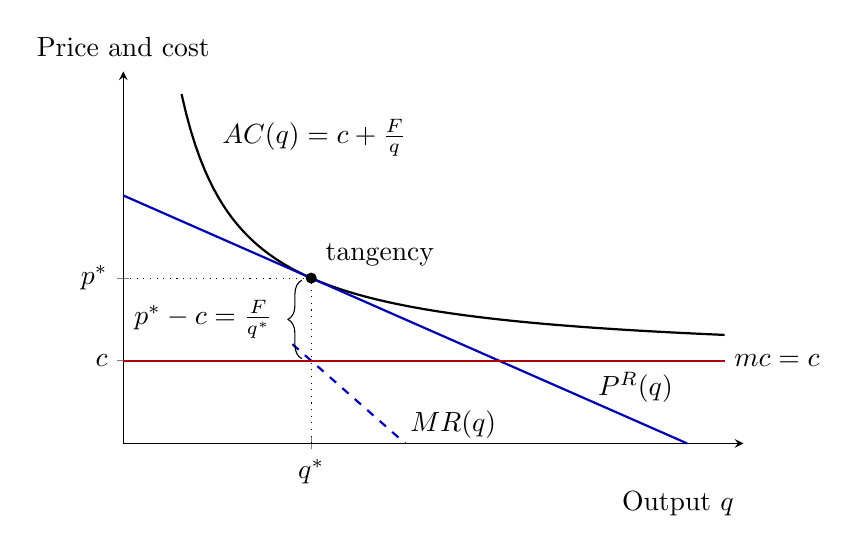
\begin{tikzpicture}
\begin{axis}[
  width=0.78\textwidth, height=0.52\textwidth,
  axis lines=left,
  xmin=0, xmax=6.6, ymin=0, ymax=9,
  xlabel={Output $q$}, ylabel={Price and cost},
  xtick={2}, xticklabels={$q^*$},
  ytick={2,4}, yticklabels={$c$,$p^*$},
  every axis x label/.style={at={(current axis.right of origin)}, anchor=north east, yshift=-14pt},
  every axis y label/.style={at={(current axis.above origin)}, anchor=south, yshift=2pt},
  clip=false]
  \addplot[thick, black, domain=0.62:6.4, samples=120] {2+4/x};
  \addplot[thick, blue!70!black, domain=0:6] {6-x};
  \addplot[thick, dashed, blue!70!black, domain=1.8:3] {6-2*x};
  \addplot[thick, red!70!black, domain=0:6.4] {2};
  \draw[dotted] (axis cs:2,0) -- (axis cs:2,4);
  \draw[dotted] (axis cs:0,4) -- (axis cs:2,4);
  \fill (axis cs:2,4) circle (2pt);
  \draw[decorate, decoration={brace, amplitude=5pt}] (axis cs:1.9,2.05) -- (axis cs:1.9,3.95)
    node[midway, left=7pt] {$p^* - c = \frac{F}{q^*}$};
  \node[anchor=west] at (axis cs:0.95,7.4) {$AC(q) = c + \frac{F}{q}$};
  \node[anchor=west] at (axis cs:4.95,1.35) {$P^R(q)$};
  \node[anchor=west] at (axis cs:2.95,0.45) {$MR(q)$};
  \node[anchor=west] at (axis cs:6.4,2) {$mc = c$};
  \node[anchor=south west] at (axis cs:2.05,4.05) {tangency};
\end{axis}
\end{tikzpicture}
\caption{The Chamberlin tangency under monopolistic competition. Free entry shifts the firm's inverse residual
demand $P^R(q)$ inward until it is tangent to average cost $AC(q) = c + \frac{F}{q}$ at $q^*$. There, marginal
revenue $MR(q)$ equals marginal cost $c$, and price equals average cost, so profit is zero. The markup
$p^* - c = \frac{F}{q^*}$ exactly covers the fixed cost. The curves are drawn for $c = 2$, $F = 4$ and
$P^R(q) = 6 - q$, which give $q^* = 2$ and $p^* = 4$.}
\label{fig:01-tangency}
\end{figure}

\citet[p.~1050]{Bresnahan1989} draws the welfare lesson. ``In the Chamberlinian tangency of monopolistic
competition, every firm has market power in the sense of this section. Yet that does not establish that there is
any inefficiency, once the need to cover the fixed costs of product design are taken into account.'' Forcing
every price down to marginal cost would leave each firm with a loss equal to its fixed cost, and some products
would disappear. Whether the market supplies too many or too few products depends on how much a product adds to
consumer surplus relative to the business it takes from rivals. Free entry can give too little variety under
monopolistic competition and too much entry in homogeneous-product markets \citep[see][and the work they
cite]{MankiwWhinston1986}. Bresnahan concludes that the welfare meaning of short-run market power with
differentiated products depends on the supply of new firms and new products. That supply is an empirical
question.

The same logic sits at the center of the recent debate over rising markups.
\citet{DeLoeckerEeckhoutUnger2020} estimate that the average ratio of price to marginal cost among US public
firms has risen since 1980. By \cref{prop:01-zero-profit-markup}, a higher markup need not mean higher profit if
fixed and overhead costs have risen as well. \Cref{sec:01-rising-markups} returns to this debate.

\subsection{The Cournot benchmark: concentration and margins}\label{sec:01-cournot-hhi}

We now have a measure of structure and a measure of market power. The simplest model that links them is the
Cournot model of quantity competition with a homogeneous good. Its central result motivates the cross-industry
regressions of \cref{sec:01-scp}. A small extension of the same result shows why those regressions are hard to
interpret.

\begin{assumption}[Homogeneous-good Cournot oligopoly]\label{ass:01-cournot}
\leavevmode
\begin{enumerate}[label=(\roman*)]
  \item There are $N$ firms selling a homogeneous good. Inverse market demand $P(Q)$ is twice differentiable,
  with $P'(Q) < 0$, where $Q = \sum_{i=1}^{N} q_i$.
  \item Firm $i$ has constant marginal cost $c_i$. It may also have a fixed cost, which does not affect its
  choice of output once it is active.
  \item Firms choose quantities simultaneously. Firm $i$ maximizes $\pi_i = \left(P(Q) - c_i\right) q_i$,
  taking its rivals' quantities as given.
  \item The equilibrium is interior. Every firm produces $q_i > 0$, and every firm's second-order condition
  $2P'(Q) + q_i P''(Q) < 0$ holds.
\end{enumerate}
\end{assumption}

\Cref{ch:theory} gives conditions for the existence and uniqueness of this equilibrium, and
\citet[Section~5.7.1]{Tirole1988} surveys them. Under mild boundary conditions, a pure-strategy equilibrium exists
when each firm's profit is concave in its own output, for which convex costs and concave demand suffice. With
two firms it is unique when the reaction functions have slopes below one in absolute value. Linear demand with
constant marginal cost gives the slope $-\frac{1}{2}$. Here we take an interior equilibrium as given. As in \cref{rem:01-residual}, the
market elasticity at the equilibrium is $\varepsilon = -\frac{P(Q)}{Q P'(Q)}$. Firm $i$'s Lerner index is
$L_i = \frac{P - c_i}{P}$, and the share-weighted average $\sum_i s_i L_i$ is the industry Lerner index.

\begin{proposition}[Cowling and Waterson]\label{prop:01-cowling-waterson}
Under \cref{ass:01-cournot}, every firm's Lerner index equals its market share divided by the market elasticity,
and the share-weighted Lerner index equals the Herfindahl-Hirschman index divided by the market elasticity:
\begin{equation}\label{eq:01-cowling-waterson}
  L_i = \frac{P - c_i}{P} = \frac{s_i}{\varepsilon}, \qquad \sum_{i=1}^{N} s_i L_i = \frac{\HHI}{\varepsilon} .
\end{equation}
\end{proposition}

\begin{proof}
Firm $i$'s first-order condition is
\[
  \frac{\partial \pi_i}{\partial q_i} = P(Q) + q_i P'(Q) - c_i = 0 .
\]
Rearrange it as $P - c_i = -q_i P'(Q)$ and divide by $P$:
\[
  \frac{P - c_i}{P} = -\frac{q_i P'(Q)}{P} .
\]
Multiply and divide the right side by $Q$:
\[
  \frac{P - c_i}{P} = \frac{q_i}{Q}\left(-\frac{Q P'(Q)}{P}\right) .
\]
The first factor is $s_i$ and the second is $\frac{1}{\varepsilon}$, which gives $L_i = \frac{s_i}{\varepsilon}$.
Multiply by $s_i$ and sum over firms:
\[
  \sum_{i=1}^{N} s_i L_i = \sum_{i=1}^{N} \frac{s_i^2}{\varepsilon} = \frac{\HHI}{\varepsilon} . \qedhere
\]
\end{proof}

The result is due to \citet{CowlingWaterson1976}. It fits together with the firm-level pricing rule. By
\eqref{eq:01-residual-elasticity}, firm $i$'s residual elasticity with rivals' output held fixed is
$\varepsilon^R_i = \frac{\varepsilon}{s_i}$, so
\[
  L_i = \frac{s_i}{\varepsilon} = \frac{1}{\varepsilon^R_i} .
\]
Each Cournot firm follows the inverse elasticity rule of \cref{prop:01-pricing-rule} for its own residual demand.
Large firms face less elastic residual demand and set higher margins. Since a firm's output and its margin are
chosen together, low-cost firms are both large and high-margin. \Cref{sec:01-demsetz} develops this observation
into the efficiency critique of regressions of profitability on concentration.

The same result links concentration to industry profit \citep[Section~5.5, eq.~5.14 and Exercise~5.6]{Tirole1988}.
Industry variable profit is
\[
  \Pi = \sum_{i=1}^{N} (P - c_i)\, q_i = \sum_{i=1}^{N} P L_i\, s_i Q = PQ \sum_{i=1}^{N} s_i L_i
  = \frac{PQ}{\varepsilon}\,\HHI .
\]
The second equality uses $P - c_i = P L_i$ and $q_i = s_i Q$, and the last uses \eqref{eq:01-cowling-waterson}.
The ratio of industry variable profit to industry revenue is therefore $\frac{\HHI}{\varepsilon}$. Suppose further
that demand has unit elasticity, $Q = \frac{k}{P}$ for a constant $k > 0$, so that consumers spend the fixed
amount $k$ on the good. Then $PQ = k$ and $\Pi = k\,\HHI$, which is Tirole's equation (5.15). In this case the
index measures industry profitability exactly, up to the constant $k$.

\begin{corollary}[Special cases]\label{cor:01-cournot-cases}
Under \cref{ass:01-cournot}, the following hold.
\begin{enumerate}[label=(\roman*)]
  \item With symmetric costs $c_i = c$, every firm has share $\frac{1}{N}$, $\HHI = \frac{1}{N}$, and
  $L = \frac{P - c}{P} = \frac{1}{N\varepsilon}$.
  \item With $N = 1$, $L = \frac{1}{\varepsilon}$, the monopoly inverse elasticity rule.
  \item With symmetric costs and an equilibrium elasticity bounded away from zero, $L \to 0$ and $P \to c$ as
  $N \to \infty$.
\end{enumerate}
\end{corollary}

\begin{proof}
With equal costs, the first-order conditions $P - c = -q_i P'(Q)$ have the same left side for every firm, so all
firms produce the same output and $s_i = \frac{1}{N}$. Then $\HHI = N \cdot \frac{1}{N^2} = \frac{1}{N}$, and all
the $L_i$ are equal to $L$, so \eqref{eq:01-cowling-waterson} gives (i). Setting $N = 1$ in (i) gives (ii). For
(iii), $L = \frac{1}{N\varepsilon}$ goes to zero when $\varepsilon$ stays above a positive constant, and
$L = 1 - \frac{c}{P} \to 0$ means $P \to c$.
\end{proof}

Statement (iii) is the sense in which Cournot competition approaches perfect competition as the number of firms
grows. The Cournot model therefore generates the hypothesis behind a generation of empirical work, namely that
margins rise with concentration. Read literally, \eqref{eq:01-cowling-waterson} suggests regressing the average
margin of each industry on its $\HHI$ across industries, with slope $\frac{1}{\varepsilon}$.

The Cournot result fixes the form of competition. To see what happens when conduct varies, we use a device from
the older literature. Suppose firm $i$ chooses its output as if its rivals' total output $Q_{-i} = Q - q_i$
responded to its own output at the rate
\[
  r_i = \frac{\dd Q_{-i}}{\dd q_i} .
\]
The number $r_i$ is firm $i$'s \emph{conjectural variation}. The firm then perceives
$\frac{\dd Q}{\dd q_i} = 1 + r_i$. Cournot behavior is $r_i = 0$.

\begin{proposition}[Margins and concentration under general conduct]\label{prop:01-clarke-davies}
Keep \cref{ass:01-cournot}, except that firm $i$ maximizes profit under the conjectural variation $r_i$, with
$1 + r_i \ge 0$. Then
\begin{equation}\label{eq:01-cv-lerner}
  L_i = \frac{s_i (1 + r_i)}{\varepsilon}, \qquad
  \sum_{i=1}^{N} s_i L_i = \frac{\theta}{\varepsilon}, \qquad
  \theta = \sum_{i=1}^{N} s_i^2 (1 + r_i) .
\end{equation}
Suppose conjectures are proportional, as in \citet{ClarkeDavies1982}. Firm $i$ expects every rival $j \ne i$ to
change its output by $\kappa$ times firm $i$'s own percentage change, for some $\kappa \in [0, 1]$. Then
\begin{equation}\label{eq:01-clarke-davies}
  r_i = \kappa\,\frac{1 - s_i}{s_i}, \qquad
  L_i = \frac{\kappa + (1 - \kappa)s_i}{\varepsilon}, \qquad
  \sum_{i=1}^{N} s_i L_i = \frac{\kappa + (1 - \kappa)\HHI}{\varepsilon} .
\end{equation}
\end{proposition}

\begin{proof}
Under the conjecture, firm $i$ perceives $\frac{\dd Q}{\dd q_i} = 1 + r_i$, so its perceived marginal profit is
\[
  \frac{\dd \pi_i}{\dd q_i} = P(Q) + q_i P'(Q) \frac{\dd Q}{\dd q_i} - c_i = P(Q) + q_i P'(Q)(1 + r_i) - c_i .
\]
Setting it to zero and following the steps in the proof of \cref{prop:01-cowling-waterson},
\begin{align}
  P + P'(Q)\, q_i (1 + r_i) &= c_i, \label{eq:01-cv-foc}\\
  \frac{P - c_i}{P} &= \frac{q_i}{Q}\left(-\frac{Q P'(Q)}{P}\right)(1 + r_i), \notag\\
  L_i &= \frac{s_i (1 + r_i)}{\varepsilon} . \notag
\end{align}
Multiplying by $s_i$ and summing gives
$\sum_i s_i L_i = \frac{1}{\varepsilon}\sum_i s_i^2 (1 + r_i) = \frac{\theta}{\varepsilon}$.

In the proportional case, the conjecture is $\frac{\dd q_j}{q_j} = \kappa\,\frac{\dd q_i}{q_i}$ for every
$j \ne i$, that is, $\frac{\dd q_j}{\dd q_i} = \kappa\,\frac{q_j}{q_i}$. Summing over rivals,
\[
  r_i = \sum_{j \ne i} \frac{\dd q_j}{\dd q_i} = \kappa\,\frac{Q_{-i}}{q_i} = \kappa\,\frac{Q - q_i}{q_i}
  = \kappa\,\frac{1 - s_i}{s_i} .
\]
Then
\[
  s_i (1 + r_i) = s_i + \kappa (1 - s_i) = \kappa + (1 - \kappa) s_i ,
\]
which gives the firm-level formula. Multiplying by $s_i$ and summing over firms,
\begin{align*}
  \theta = \sum_{i=1}^{N} s_i^2 (1 + r_i) &= \sum_{i=1}^{N} \left(\kappa s_i + (1 - \kappa) s_i^2\right) \\
  &= \kappa \sum_{i=1}^{N} s_i + (1 - \kappa) \sum_{i=1}^{N} s_i^2 \\
  &= \kappa + (1 - \kappa)\HHI ,
\end{align*}
where the last line uses $\sum_i s_i = 1$.
\end{proof}

The parameter $\theta$ is the index of industry conduct that we use throughout the book. Price-taking behavior,
$r_i = -1$ for every firm, gives $\theta = 0$ and $L_i = 0$. Cournot behavior, $r_i = 0$, gives
$\theta = \HHI$, which equals $\frac{1}{N}$ when firms are symmetric. In the Clarke-Davies family, $\kappa = 0$
is Cournot behavior and $\kappa = 1$ is joint profit maximization. With $\kappa = 1$ the firm expects all rivals
to move in proportion, so $1 + r_i = \frac{1}{s_i}$ and $q_i(1 + r_i) = Q$. Condition \eqref{eq:01-cv-foc} then
becomes $P + Q P'(Q) = c_i$, the first-order condition of a monopolist. With constant marginal costs, these
conditions can hold for all active firms only if their costs are equal, and the split of output among them is then
indeterminate. Every firm has $L_i = \frac{1}{\varepsilon}$ and $\theta = 1$. With rising marginal costs, as in
\cref{prop:01-supply-relation}, the same conditions equalize marginal costs across firms, as joint profit
maximization requires. Summing \eqref{eq:01-cv-foc} with weights $s_i$ gives the industry relation
\begin{equation}\label{eq:01-industry-relation}
  P = \bar c - \theta\, Q P'(Q), \qquad \bar c = \sum_{i=1}^{N} s_i c_i ,
\end{equation}
because $\sum_i s_i q_i (1 + r_i) = Q\sum_i s_i^2(1 + r_i) = Q\theta$. \Cref{sec:01-conduct-parameter} calls
\eqref{eq:01-industry-relation} the supply relation and shows how the New Empirical Industrial Organization is
built around it.

Conjectural variations must be read with care. In a static game a firm moves once and never observes a response,
so a ``conjecture'' about its rivals' reactions has no behavioral content within the game. The parameter
$\theta$ is best read as an index of how close the outcome is to the collusive one. \citet{Bresnahan1989}
stresses this reading, and \cref{sec:01-conduct-parameter} explains it. \Cref{ch:theory} discusses the theory of
conjectural variations and the conduct parameter.

\Cref{prop:01-clarke-davies} contains the main message of this section. In the Clarke-Davies family the average
margin is a linear function of the index,
\begin{equation}\label{eq:01-cd-line}
  \sum_{i=1}^{N} s_i L_i = \frac{\kappa}{\varepsilon} + \frac{1 - \kappa}{\varepsilon}\,\HHI ,
\end{equation}
with intercept $\frac{\kappa}{\varepsilon}$ and slope $\frac{1 - \kappa}{\varepsilon}$. Both depend on conduct and
on the demand elasticity. The slope is largest under Cournot behavior. It is zero under collusion, where margins
are at the monopoly level whatever the concentration. Panel (a) of \cref{fig:01-lerner-hhi} plots
\eqref{eq:01-cd-line} for $\varepsilon = 2$. The slope of margins on concentration is therefore no constant of
nature shared by all industries. This is at once the theoretical case for regressing margins on concentration
and the first reason such regressions fail. Industries differ in their elasticities and their conduct, and these
differences are correlated with concentration in ways that \cref{sec:01-scp-econometrics} explores.

Even within one industry with fixed conduct, the relation need not be linear, because the elasticity changes
with concentration. Take linear inverse demand $P(Q) = a - bQ$ with $a > c > 0$ and $b > 0$, and $N$ symmetric
Cournot firms with marginal cost $c$. The first-order condition $a - bQ - bq_i - c = 0$ holds for every firm, so
outputs are equal and $q_i = \frac{Q}{N}$. Summing the conditions over firms and solving,
\begin{align*}
  N(a - c) - NbQ - bQ &= 0, \\
  Q &= \frac{N(a - c)}{b(N + 1)}, \\
  P = a - bQ &= \frac{a + Nc}{N + 1} .
\end{align*}
The Lerner index and the market elasticity at the equilibrium are
\begin{align*}
  L &= \frac{P - c}{P} = \frac{\frac{a - c}{N + 1}}{\frac{a + Nc}{N + 1}} = \frac{a - c}{a + Nc}, \\
  \varepsilon &= \frac{P}{bQ} = \frac{a + Nc}{N(a - c)} .
\end{align*}
Substitute $N = \frac{1}{\HHI}$ and multiply each numerator and denominator by $\HHI$:
\begin{equation}\label{eq:01-linear-cournot-LH}
  L = \frac{(a - c)\HHI}{a\HHI + c}, \qquad \varepsilon = \frac{a\HHI + c}{a - c} .
\end{equation}
As a check, $\frac{\HHI}{\varepsilon} = \frac{(a - c)\HHI}{a\HHI + c} = L$, as \cref{prop:01-cowling-waterson}
requires. The elasticity rises with concentration, because fewer firms means a higher price and a lower quantity
along a linear demand curve. Differentiating $L$ with respect to $\HHI$,
\begin{align*}
  \frac{\dd L}{\dd \HHI} &= \frac{(a - c)(a\HHI + c) - (a - c)\HHI \cdot a}{(a\HHI + c)^2}
  = \frac{c(a - c)}{(a\HHI + c)^2} > 0, \\
  \frac{\dd^2 L}{\dd \HHI^2} &= -\frac{2ac(a - c)}{(a\HHI + c)^3} < 0 .
\end{align*}
The margin rises with concentration at a decreasing rate. Panel (b) of \cref{fig:01-lerner-hhi} plots the curve
for two values of the ratio $\frac{c}{a}$. A higher ratio of marginal cost to the demand intercept lowers the
whole curve. Industries with different cost-demand ratios lie on different curves, so even the causal effect of
concentration on margins differs across industries. Throughout this calculation $N$ is fixed. When entry
determines $N$, concentration becomes an equilibrium outcome itself, a problem that \cref{sec:01-endogeneity}
takes up.

\begin{figure}[htbp]
\centering
\begin{subfigure}[t]{0.49\textwidth}
\centering
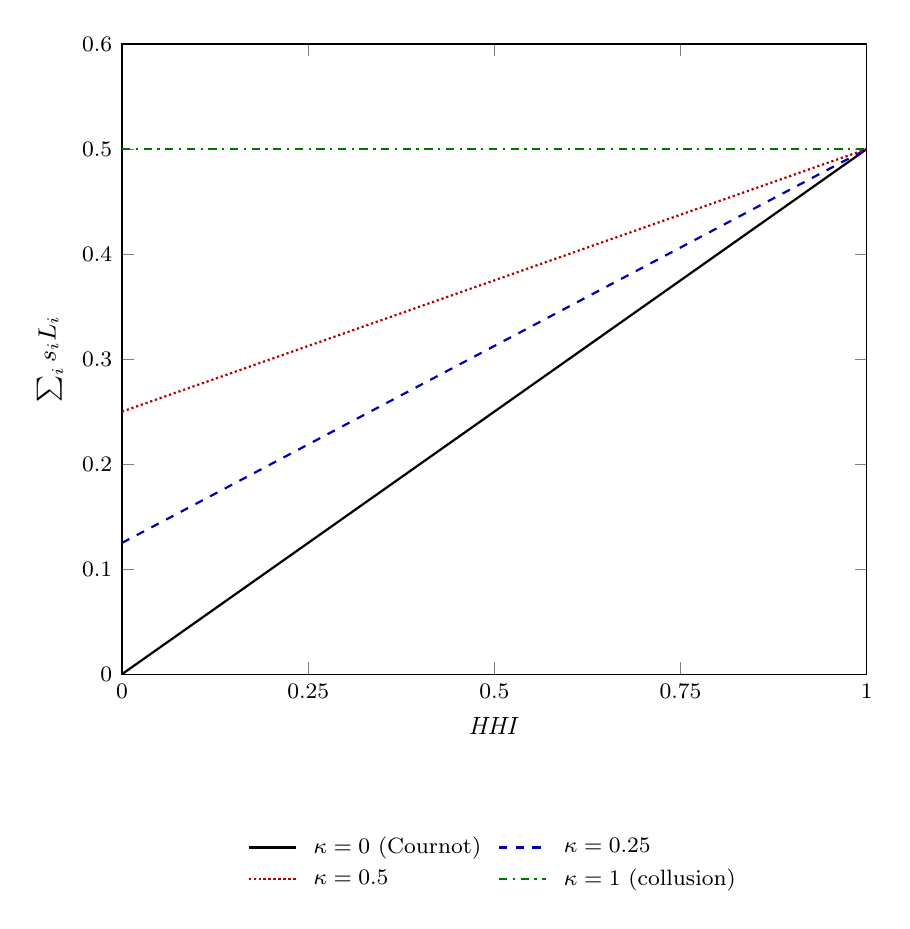
\begin{tikzpicture}[baseline=(current axis.north)]
\begin{axis}[
  scale only axis, width=0.78\linewidth, height=0.66\linewidth,
  xmin=0, xmax=1, ymin=0, ymax=0.6,
  xlabel={$\HHI$}, ylabel={$\sum_i s_i L_i$},
  xtick={0,0.25,0.5,0.75,1}, ytick={0,0.1,0.2,0.3,0.4,0.5,0.6},
  tick label style={font=\footnotesize}, label style={font=\small},
  domain=0:1, samples=2,
  legend columns=2,
  legend style={font=\footnotesize, at={(0.5,-0.24)}, anchor=north, draw=none, column sep=4pt},
  legend cell align=left]
  \addplot[thick, black] {x/2};
  \addlegendentry{$\kappa = 0$ (Cournot)}
  \addplot[thick, blue!70!black, dashed] {(0.25+0.75*x)/2};
  \addlegendentry{$\kappa = 0.25$}
  \addplot[thick, red!70!black, densely dotted] {(0.5+0.5*x)/2};
  \addlegendentry{$\kappa = 0.5$}
  \addplot[thick, green!45!black, dashdotted] {0.5};
  \addlegendentry{$\kappa = 1$ (collusion)}
\end{axis}
\end{tikzpicture}
\caption{Clarke-Davies conduct, $\varepsilon = 2$}
\end{subfigure}\hfill
\begin{subfigure}[t]{0.49\textwidth}
\centering
\begin{tikzpicture}[baseline=(current axis.north)]
\begin{axis}[
  scale only axis, width=0.78\linewidth, height=0.66\linewidth,
  xmin=0, xmax=1, ymin=0, ymax=0.75,
  xlabel={$\HHI$}, ylabel={$L$},
  xtick={0,0.25,0.5,0.75,1}, ytick={0,0.1,0.2,0.3,0.4,0.5,0.6,0.7},
  tick label style={font=\footnotesize}, label style={font=\small},
  domain=0:1, samples=101,
  legend columns=2,
  legend style={font=\footnotesize, at={(0.5,-0.24)}, anchor=north, draw=none, column sep=4pt},
  legend cell align=left]
  \addplot[thick, black] {8*x/(10*x+2)};
  \addlegendentry{$\frac{c}{a} = 0.2$}
  \addplot[thick, blue!70!black, dashed] {5*x/(10*x+5)};
  \addlegendentry{$\frac{c}{a} = 0.5$}
  \addplot[only marks, mark=*, mark size=1.3pt, black,
    samples at={1,0.5,0.333333,0.25,0.2,0.166667,0.142857,0.125,0.111111,0.1}]
    {8*x/(10*x+2)};
  \addlegendentry{$\HHI = \frac{1}{N}$}
  \addplot[only marks, mark=*, mark size=1.3pt, blue!70!black,
    samples at={1,0.5,0.333333,0.25,0.2,0.166667,0.142857,0.125,0.111111,0.1}, forget plot]
    {5*x/(10*x+5)};
\end{axis}
\end{tikzpicture}
\caption{Symmetric Cournot, linear demand}
\end{subfigure}
\caption{Margins and concentration. Panel (a) plots the share-weighted Lerner index against the
Herfindahl-Hirschman index in the Clarke-Davies family,
$\sum_i s_i L_i = \frac{\kappa + (1 - \kappa)\HHI}{\varepsilon}$, for $\varepsilon = 2$. The lines run from
$\left(0, \frac{\kappa}{\varepsilon}\right)$ to $\left(1, \frac{1}{\varepsilon}\right)$. Panel (b) plots the
symmetric Cournot relation with linear demand, $L = \frac{(a - c)\HHI}{a\HHI + c}$, for $\frac{c}{a} = 0.2$ and
$\frac{c}{a} = 0.5$. Dots mark $\HHI = \frac{1}{N}$ for $N = 1, \dots, 10$.}
\label{fig:01-lerner-hhi}
\end{figure}

\section{The structure-conduct-performance paradigm}\label{sec:01-scp}

For about three decades the main empirical program in industrial organization put one question to
cross-industry data. Do more concentrated industries earn higher margins? The program is known as the
\emph{structure-conduct-performance} (SCP) paradigm. This section states its logic, formalizes the
experiment it had in mind, and describes how it was carried out. \Cref{sec:01-scp-econometrics} then asks
what its regressions identify, and \cref{sec:01-scp-after} follows the debates it left behind.

\subsection{The SCP mechanism}\label{sec:01-scp-mechanism}

The paradigm describes a causal chain with four links, summarized in \cref{fig:01-scp-flow}. \emph{Basic
conditions} are the primitives of an industry. On the supply side they include technology, unionization,
the transportability of the product and the legal environment. On the demand side they include
preferences, the growth of demand and its seasonality. Basic conditions determine \emph{market
structure}, which comprises the number of sellers and buyers, the extent of vertical integration, and the
degree of vertical and horizontal product differentiation. Structure determines conduct, the
pricing, advertising and investment decisions of firms. Conduct in turn determines \emph{performance},
measured by profits and by welfare.

\citet[Introduction]{Tirole1988} calls this program the ``Harvard tradition'' and associates it with Joe Bain
and Edward Mason. In his history it was the first of two waves of interest in industrial organization, and it
was empirical in nature. His statement of the chain is close to ours. Structure comprises the number of sellers,
their degree of product differentiation, the cost structure and the degree of vertical integration with
suppliers. Conduct comprises price, research and development, investment and advertising. Performance comprises
efficiency, the ratio of price to marginal cost, product variety, the rate of innovation, profits and
distribution. Tirole adds that the paradigm, although plausible, often rested on loose theories.

\begin{figure}[htbp]
\centering
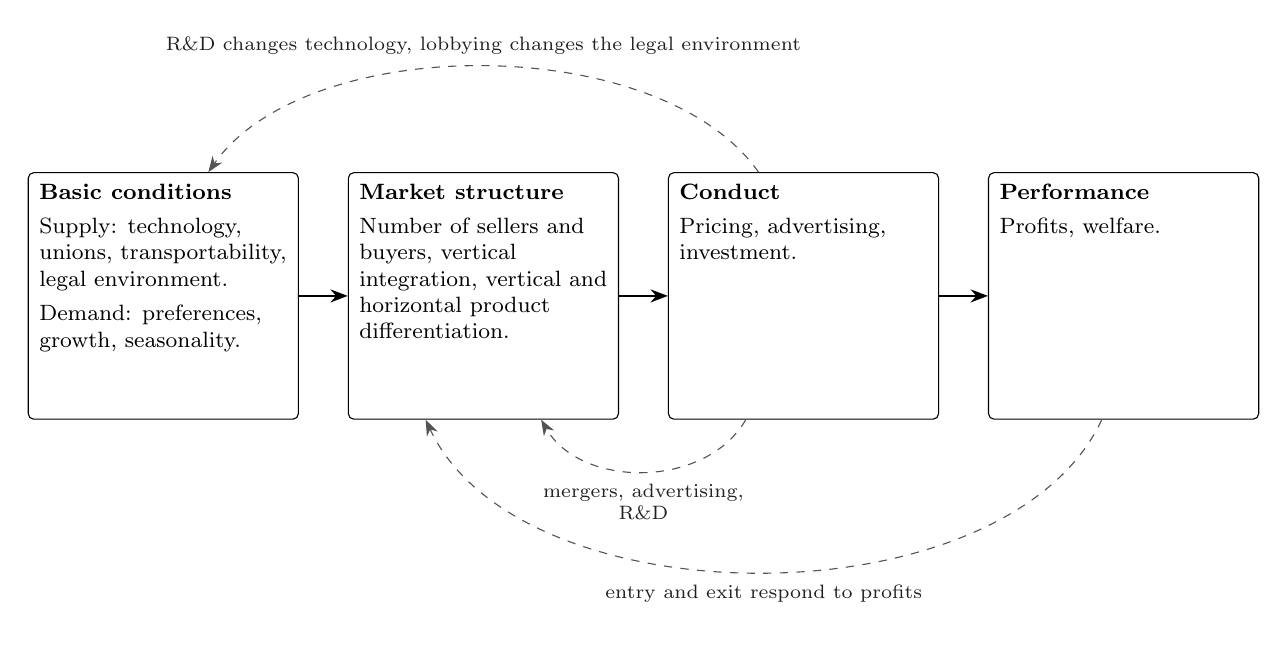
\begin{tikzpicture}[
  box/.style={draw, rounded corners=2pt, align=flush left, text width=3.15cm,
    inner sep=4pt, font=\footnotesize},
  fwd/.style={-{Stealth[length=2.2mm]}, thick},
  back/.style={-{Stealth[length=2mm]}, dashed, gray!65!black},
  lab/.style={font=\scriptsize, align=center, text=gray!25!black}]
\node[box] (bc) {\parbox[t][2.85cm][t]{\linewidth}{\raggedright\textbf{Basic conditions}\\[3pt]
  Supply: technology, unions, transportability, legal environment.\\[3pt]
  Demand: preferences, growth, seasonality.}};
\node[box, right=0.62cm of bc] (ms) {\parbox[t][2.85cm][t]{\linewidth}{\raggedright\textbf{Market structure}\\[3pt]
  Number of sellers and buyers, vertical integration, vertical and horizontal product
  differentiation.}};
\node[box, right=0.62cm of ms] (cd) {\parbox[t][2.85cm][t]{\linewidth}{\raggedright\textbf{Conduct}\\[3pt]
  Pricing, advertising, investment.}};
\node[box, right=0.62cm of cd] (pf) {\parbox[t][2.85cm][t]{\linewidth}{\raggedright\textbf{Performance}\\[3pt]
  Profits, welfare.}};
\draw[fwd] (bc) -- (ms);
\draw[fwd] (ms) -- (cd);
\draw[fwd] (cd) -- (pf);
\draw[back] (cd.-115) to[out=-120, in=-60] node[lab, below=1pt] {mergers, advertising,\\ R\&D}
  (ms.-65);
\draw[back] (pf.-100) to[out=-115, in=-65, looseness=0.85]
  node[lab, below=1pt] {entry and exit respond to profits} (ms.-115);
\draw[back] (cd.110) to[out=125, in=55, looseness=0.8]
  node[lab, above=1pt] {R\&D changes technology, lobbying changes the legal environment}
  (bc.70);
\end{tikzpicture}
\caption{The structure-conduct-performance paradigm. Solid arrows show the causal chain that the
paradigm assumes. Dashed arrows show feedback that it ignores. Conduct and performance shape market
structure, and conduct reshapes basic conditions. Once the dashed arrows are admitted, market structure
is an equilibrium outcome.}
\label{fig:01-scp-flow}
\end{figure}

The chain has a strong implication for policy. If structure causes performance, a regulator can improve
performance by acting on structure, for example by blocking mergers or breaking up dominant firms. The
empirical task then reduces to measuring how performance varies with structure. Conduct rarely needs to
be observed, because structure is assumed to pin it down.

The dashed arrows in \cref{fig:01-scp-flow} show why the chain is incomplete. Profits attract entry and
losses induce exit, so performance feeds back into the number of sellers. Mergers, advertising and
research and development (R\&D) are forms of conduct, yet they shape concentration and differentiation.
Research changes technology and lobbying changes the legal environment, so conduct also feeds back into
basic conditions. In modern terms, market structure is an equilibrium outcome, determined jointly with
conduct and performance by the basic conditions. \Cref{sec:01-scp-econometrics} works out the
consequences of this observation for the regressions that the paradigm relied on.

The ideal experiment behind the paradigm is easy to state. We would take many otherwise identical
industries, randomly assign each one a market structure, and compare their performance. In practice,
researchers compared markups or profitability across existing industries with different levels of
concentration. The gap between the two designs can be stated precisely in the language of potential
outcomes, which \cref{app:econometrics} reviews.

\begin{definition}[Potential margins]\label{def:01-potential-margins}
Index industries by $k = 1, \dots, n$. For each concentration level $h \in (0, 1]$, let $L_k(h)$ be the
industry-wide Lerner index that industry $k$ would have if an outside intervention set its Herfindahl
index to $h$. The intervention holds the demand, costs and conduct of the industry fixed. The function
$h \mapsto L_k(h)$ is the \emph{causal curve} of industry $k$. We observe only the realized margin $L_k
= L_k(\HHI_k)$.
\end{definition}

The industry-wide Lerner index is the share-weighted index $\sum_i s_i L_i$ of
\cref{prop:01-cowling-waterson}. An intervention that sets $h$ could be a regulator that fixes the number
of licenses in an industry of symmetric firms. Now compare the average margins of industries observed at
two concentration levels $h$ and $h'$. We add and subtract $\E[L_k(h') \mid \HHI_k = h]$:
\begin{align}
\E[L_k \mid \HHI_k = h] - \E[L_k \mid \HHI_k = h']
  &= \E[L_k(h) \mid \HHI_k = h] - \E[L_k(h') \mid \HHI_k = h'] \notag \\
  &= \underbrace{\E[L_k(h) - L_k(h') \mid \HHI_k = h]}_{\text{causal effect at } h} \notag \\
  &\quad + \underbrace{\E[L_k(h') \mid \HHI_k = h] - \E[L_k(h') \mid \HHI_k = h']}_{\text{selection}}.
  \label{eq:01-potential-outcomes}
\end{align}
The first equality uses $L_k = L_k(\HHI_k)$. The first term after the second equality is the average
causal effect of moving from $h'$ to $h$ among the industries observed at $h$. The second term compares
the margins that
two different groups of industries would earn at the same concentration $h'$. It differs from zero
whenever the industries that end up concentrated differ in demand, cost or conduct from those that do
not. Random assignment makes $\HHI_k$ independent of the whole curve $L_k(\cdot)$. The selection term
then vanishes, and the first term becomes the population average effect $\E[L_k(h) - L_k(h')]$.

\begin{example}[Selection on the demand elasticity]\label{ex:01-selection-elasticity}
Suppose industry $k$ has constant-elasticity demand with elasticity $\varepsilon_k$ and symmetric
Cournot firms. By \cref{prop:01-cowling-waterson}, its causal curve is
$L_k(h) = \frac{h}{\varepsilon_k}$. Substituting into \eqref{eq:01-potential-outcomes}, the selection
term equals
\[
h' \left( \E\left[\frac{1}{\varepsilon_k} \,\middle|\, \HHI_k = h\right]
        - \E\left[\frac{1}{\varepsilon_k} \,\middle|\, \HHI_k = h'\right] \right).
\]
Its sign depends on how industries sort. Margins are higher where demand is less elastic, so free entry
tends to draw more firms into those industries and to make them less concentrated. The conditional mean
of $\frac{1}{\varepsilon_k}$ then falls with concentration, and the selection term is negative for
$h > h'$. If inelastic demand instead goes with high fixed costs, the term can be positive.
\end{example}

\subsection{Origins and practice}\label{sec:01-scp-practice}

The SCP approach grew out of the Harvard tradition associated with \citet{Mason1939}. As its title indicates,
Mason's article studied the price and production policies of large-scale enterprise.
Joe Bain turned the SCP view into a statistical program. \citet{Bain1951} related
the profit rates of American manufacturing industries over 1936--1940 to their concentration.
\citet{Bain1951,Bain1956} hypothesized that concentration facilitates collusion between firms and so raises
industry-wide profits \citep[Section~5.5]{Tirole1988}. \citet[p.~46]{LevensteinSuslow2006} attribute the same
hypothesis to Bain. \citet{Bain1956} added the theory of \emph{barriers to entry}, the advantages of established
sellers over potential entrants. In Tirole's paraphrase, a barrier to entry is anything that lets incumbent firms
earn supranormal profits without the threat of entry \citep[Chapter~8, introduction]{Tirole1988}. Tirole lists
the four elements of market structure that Bain identified informally. They are economies of scale, absolute cost
advantages, product-differentiation advantages and capital requirements, the last of which Tirole calls
controversial. Bain also distinguished three cases. Entry is blockaded when incumbents ignore the threat and entry
is still unattractive. It is deterred when incumbents change their behavior to prevent it, and accommodated when
they find it more profitable to let entrants in. For the quarter century that followed \citet{Bain1951}, the
cross-section study of many industries was the main empirical method of the field \citep[p.~1012]{Bresnahan1989}.
\citet{Schmalensee1989} wrote its definitive review.

A typical study used one cross-section of industries. The dependent variable was an accounting measure
of profitability, such as the profit rate on equity or assets or the price-cost margin computed from the
Census of Manufactures. The key regressor was a concentration measure, often the four-firm ratio
$\mathit{CR}_4$ or the Herfindahl index of \cref{def:01-concentration}. The canonical specification is
\begin{equation}\label{eq:01-scp-regression}
\pi_k = \beta_0 + \beta_1 \HHI_k + \varphi^\top X_k + e_k, \qquad k = 1, \dots, n,
\end{equation}
where $\pi_k$ is the profitability measure of industry $k$ and $e_k$ is an error term. The Herfindahl
index may be replaced by $\mathit{CR}_{4,k}$. The vector $X_k$ collects controls, typically the ratios of
R\&D spending, capital and advertising spending to sales, together with the import share. Its
coefficients are $\varphi$, and the whole equation is estimated by ordinary least squares (OLS). The typical finding was
$\hat\beta_1 > 0$. It was read as evidence that concentration raises margins, and hence that
concentration is harmful.

\citet[Introduction]{Tirole1988} writes the typical regression as $\pi_k = f(\mathit{CR}_k, \mathit{BE}_k, \dots)$,
run on a cross-section of many industries. Here $\mathit{CR}_k$ is a concentration ratio and $\mathit{BE}_k$
collects measures of barriers to entry. Two common measures were the ratio of advertising to sales and the
\emph{minimum efficient scale} of entry, the smallest output at which average cost reaches its minimum.
Regression \eqref{eq:01-scp-regression} is the linear version. Tirole stresses that its coefficients are
correlations, or ``descriptive statistics,'' and not causal relationships. Industry profit, the concentration
ratio and the ratio of advertising to sales ``are jointly endogenous.'' The basic conditions of the market and
the behavior of its firms determine all three at once.

The tradition also tried to measure basic conditions directly, scale economies in particular
\citep[Introduction, note~4]{Tirole1988}. The most common method estimates a cost function of output and input
prices. Bain built ``engineering production functions'' from engineering data on plants, and he asked managers
what the optimal plant size was. George Stigler's \emph{survivorship technique} infers efficient scale instead
from the sizes of the firms that survive. Tirole notes that such measures are hard to make accurate and
comparable across industries.

The design reflected the econometric practice of its time. Samples were small, the data were industry
aggregates, and matrices were sometimes inverted by hand. Identification in the modern sense received
little attention. Concentration was treated as an exogenous regressor, and its coefficient was read as a
structural constant.

\citet[p.~146]{EinavLevin2010} describe two challenges that held the field back into the 1970s. The
first was the lack of compelling theoretical models of imperfect competition, which the game theory
revolution of the 1980s later supplied. The second was the lack of good data and of convincing
strategies for testing hypotheses about competition. Researchers knew that concentration might depend on
the same factors as profitability. More sophisticated studies tried to fix this by treating concentration
as driven by ``exogenous'' barriers to entry, such as scale economies, advertising or R\&D
\citep[p.~146]{EinavLevin2010}. Yet advertising intensity and capital intensity are chosen by firms, so
they are hard to defend as instruments \citep[p.~147]{EinavLevin2010}. \citet[p.~954]{Schmalensee1989}
opened his review by acknowledging that ``essentially all variables that have been employed in such
studies are logically endogenous'' (quoted in \citealp[p.~147]{EinavLevin2010}).

\citet[Introduction, note~2]{Tirole1988} recommends the review of \citet{Schmalensee1989}, which he dates 1986,
as an excellent survey and assessment of this approach. His own summary of the evidence records two facts that frame the rest
of this chapter (note~3). First, the cross-industry relation between rates of return and concentration ``is weak.'' Second,
``introducing a market-share variable on the right-hand side of the regression tends to wipe out
concentration-ratio effects.'' Tirole explains the second fact by cost heterogeneity. In industries where a few
low-cost firms produce most of the output, concentration and profits are both high. The concentration ratio may
then pick up the effect of the omitted market share. The first fact motivates \cref{sec:01-scp-econometrics},
and the second lies at the center of the Demsetz debate in \cref{sec:01-demsetz}. \Cref{sec:01-neio-principles} returns to the maintained
hypotheses of the paradigm that the next generation of research rejected.

\section{What cross-industry regressions identify}\label{sec:01-scp-econometrics}

Regression \eqref{eq:01-scp-regression} always estimates something. Its probability limit is a
linear projection coefficient, and the question is whether that coefficient measures an economic
object. This section takes the problems in turn. Margins are mismeasured (\cref{sec:01-accounting}),
concentration is mismeasured (\cref{sec:01-market-def-error}), and concentration is endogenous
(\cref{sec:01-endogeneity}). A Monte Carlo experiment shows the size of the problems
(\cref{sec:01-montecarlo}), and \cref{sec:01-salinger} asks whether panel data solve them.

\subsection{Measurement: accounting versus economic margins}\label{sec:01-accounting}

The theory of \cref{sec:01-cournot-hhi} concerns the Lerner index $L = \frac{p - mc}{p}$. SCP studies
used accounting data instead. The most common margin was the \emph{Census price-cost margin},
\begin{equation}\label{eq:01-pcm}
\mathit{PCM} = \frac{\text{value of shipments} - \text{payroll} - \text{cost of materials}}
                    {\text{value of shipments}},
\end{equation}
computed for each manufacturing industry from the Census of Manufactures. It nets out the main variable
inputs and ignores the cost of capital. The next proposition shows what it measures. In this subsection
only, $\rho$ denotes the rental price of capital (elsewhere in the book $\rho$ is the pass-through rate).

\begin{proposition}[What the Census margin measures]\label{prop:01-pcm-bias}
Consider an industry that sells output $q > 0$ at price $p$, so that sales are $S = pq$. Payroll and
materials form the variable cost $VC(q)$, with $VC(0) = 0$ and marginal cost $mc(q) = VC'(q)$. The
industry uses a capital stock $K$ with rental price $\rho$, the interest and depreciation cost per dollar
of capital. Economic profit is $\pi = pq - VC(q) - \rho K$.
\begin{enumerate}[label=(\roman*)]
\item If $VC(q) = cq$, then $\mathit{PCM} = \frac{p - c}{p} = L$.
\item In general, $\mathit{PCM} = \frac{\pi}{S} + \rho \frac{K}{S}$. An industry that earns zero economic
profit has $\mathit{PCM} = \rho \frac{K}{S} > 0$.
\item If $VC$ is convex, then $\mathit{PCM} \ge L$. The inequality is strict if $VC$ is strictly convex.
\end{enumerate}
\end{proposition}

\begin{proof}
By definition, $\mathit{PCM} = \frac{S - VC(q)}{S}$. For (i), substitute $VC(q) = cq$:
\[
\mathit{PCM} = \frac{pq - cq}{pq} = \frac{p - c}{p} = L.
\]
For (ii), the definition of economic profit gives $pq - VC(q) = \pi + \rho K$. Divide both sides by $S$:
\[
\mathit{PCM} = \frac{pq - VC(q)}{S} = \frac{\pi + \rho K}{S} = \frac{\pi}{S} + \rho \frac{K}{S}.
\]
Setting $\pi = 0$ gives $\mathit{PCM} = \rho \frac{K}{S}$, which is positive whenever $K > 0$. For (iii),
write $\mathit{PCM} = \frac{p - AVC(q)}{p}$ with average variable cost $AVC(q) = \frac{VC(q)}{q}$. A convex
function lies above its tangent lines, so
\[
VC(0) \ge VC(q) + VC'(q)(0 - q).
\]
With $VC(0) = 0$, this reads $q \, mc(q) \ge VC(q)$, so $AVC(q) \le mc(q)$. Therefore
\[
\mathit{PCM} = \frac{p - AVC(q)}{p} \ge \frac{p - mc(q)}{p} = L.
\]
Strict convexity makes the tangent inequality strict for $q > 0$.
\end{proof}

The Census margin therefore mixes three things: the Lerner index, the return to capital, and the
curvature of variable cost. Capital-intensive industries show high margins even when they earn no rents.
Capital intensity also tends to raise minimum efficient scale and hence concentration. A regression of
$\mathit{PCM}$ on concentration that omits capital intensity then attributes the return to capital to
concentration.

\begin{corollary}[Omitted capital intensity]\label{prop:01-pcm-ovb}
Suppose economic profitability satisfies $\frac{\pi_k}{S_k} = \beta_0 + \beta_1 \HHI_k + e_k$, where
$e_k$ is uncorrelated with $\HHI_k$ and with $\frac{K_k}{S_k}$, and the rental price $\rho$ is common to
all industries. Then OLS of $\mathit{PCM}_k$ on a constant and $\HHI_k$ converges to
\[
\beta_1 + \rho \, \frac{\Cov\left(\frac{K_k}{S_k}, \HHI_k\right)}{\Var(\HHI_k)}.
\]
\end{corollary}

\begin{proof}
By \cref{prop:01-pcm-bias}(ii), $\mathit{PCM}_k = \beta_0 + \beta_1 \HHI_k + \rho \frac{K_k}{S_k} + e_k$.
The OLS slope converges to $\frac{\Cov(\mathit{PCM}_k, \HHI_k)}{\Var(\HHI_k)}$. Substituting,
\[
\frac{\Cov(\mathit{PCM}_k, \HHI_k)}{\Var(\HHI_k)}
 = \beta_1 + \rho \frac{\Cov\left(\frac{K_k}{S_k}, \HHI_k\right)}{\Var(\HHI_k)}
   + \frac{\Cov(e_k, \HHI_k)}{\Var(\HHI_k)},
\]
and the last term is zero by assumption.
\end{proof}

This is why \citet{CollinsPreston1969} and most later studies included the capital-sales ratio
$\frac{K}{S}$ as a regressor next to concentration. The control removes the bias in
\cref{prop:01-pcm-ovb} only if $\rho$ is common across industries and capital is measured correctly.

Accounting rates of return on equity or assets have their own problems. \citet{FisherMcGowan1983} showed
that the accounting rate of return can differ widely from the economic rate of return, which is the
internal rate of return on an investment. The gap depends on the time profile of cash flows and on
depreciation rules, so it varies across industries even when no industry earns rents. Inflation and the
valuation of assets at historical cost add further distortions. A simple case shows the direction of
one common bias.

\begin{remark}[Expensed intangible capital]\label{rem:01-intangibles}
Consider a firm in a steady state with tangible capital $K$. It also builds an intangible stock $A$, such
as brand capital or knowledge, by spending $I$ per period on advertising or R\&D. The stock depreciates
at rate $d_A$, so in the steady state $A = \frac{I}{d_A}$. Let $R$ be revenue net of variable costs and
of the depreciation of tangible capital. Economic depreciation of the intangible stock is $d_A A = I$, so
the economic rate of return on all capital is
\[
r^e = \frac{R - d_A A}{K + A} = \frac{R - I}{K + A}.
\]
Accounting rules expense $I$ and leave $A$ off the balance sheet, so the accounting rate of return is
$r^{acc} = \frac{R - I}{K}$. Dividing the two expressions gives
\[
\frac{r^{acc}}{r^e} = \frac{K + A}{K} = 1 + \frac{A}{K} > 1.
\]
When $R > I$, accounting returns overstate economic returns, and they do so most in industries that are
intensive in advertising or R\&D. If those industries are also more concentrated, the measured profit-concentration relation is
biased upward.
\end{remark}

The controls that theory calls for are the demand elasticity, the height of entry barriers and the degree
of product differentiation. They are hard to measure, so SCP studies rarely included them. The
regression thus omits the very variables that theory says determine margins. \Cref{sec:01-cournot-hhi}
showed that the slope of margins on concentration is $\frac{1 - \kappa}{\varepsilon}$, which depends on
conduct and on the demand elasticity. \Cref{tab:01-scp-data} compares what theory needs with what the
studies measured.

\begin{table}[htbp]
\centering\footnotesize
\renewcommand{\arraystretch}{1.2}
\caption{What the theory of margins needs and what SCP studies measured}
\label{tab:01-scp-data}
\begin{tabularx}{\linewidth}{@{}>{\raggedright\arraybackslash}p{2.1cm}
  >{\raggedright\arraybackslash}X>{\raggedright\arraybackslash}X>{\raggedright\arraybackslash}X@{}}
\toprule
Object & What theory needs & What SCP studies used & Consequence for the regression \\
\midrule
Margin & Lerner index $\frac{p - mc}{p}$ & Accounting profit rate, return on assets, Census
  $\mathit{PCM}$ & Mixes rents with the return to capital and cost curvature
  (\cref{prop:01-pcm-bias}, \cref{rem:01-intangibles}) \\
Concentration & Shares in the economic market (\cref{sec:01-market-definition}) & National shares in a
  four-digit SIC industry & Measurement error and attenuation (\cref{sec:01-market-def-error}) \\
Demand elasticity & $\varepsilon$, which scales the slope & Rarely measured & Omitted variable that
  enters the slope itself \\
Entry barriers & Sunk and fixed costs, regulation & Capital, advertising and R\&D intensities &
  The proxies are chosen by firms, hence endogenous \\
Differentiation & Substitution patterns among products & Advertising intensity, at best & Crude and
  endogenous proxy \\
Conduct & $\kappa$ or $\theta$ (\cref{prop:01-clarke-davies}) & Not measured, implicitly common & The
  slope averages over conduct regimes (\cref{prop:01-scp-plim}) \\
Foreign competition & Imports in the relevant market & Import share & Partial correction of national
  shares \\
\bottomrule
\end{tabularx}
\end{table}

\subsection{Market definition and measurement error in concentration}\label{sec:01-market-def-error}

Concentration is defined relative to a market (\cref{sec:01-market-definition}). SCP studies used
industries as defined by the Standard Industrial Classification (SIC), usually at the four-digit level.
The SIC was replaced by the North American Industry Classification System (NAICS) in 1997. These
classifications group plants by production process more than by substitution in demand. A four-digit
industry can be too broad, pooling products that do not compete with each other. It can also be too
narrow, leaving out close substitutes classified elsewhere and leaving out imports. Census concentration
ratios are national, while many products are sold in local markets because transport is costly. Cement,
ready-mixed concrete and newspapers are standard examples. The next lemma shows how large the resulting
error can be.

\begin{lemma}[Pooling local markets]\label{prop:01-pooled-hhi}
Suppose a national industry consists of $G$ local markets of equal size. Each local market $\ell$ is
served by its own firms and has Herfindahl index $\HHI_\ell$. Then the national Herfindahl index is
\[
\HHI^{nat} = \frac{1}{G} \left( \frac{1}{G} \sum_{\ell = 1}^{G} \HHI_\ell \right).
\]
\end{lemma}

\begin{proof}
Let $s_{i\ell}$ be the share of firm $i$ in local market $\ell$. Because the markets have equal size, the
national share of that firm is $\frac{s_{i\ell}}{G}$. Summing squared national shares over all firms,
\[
\HHI^{nat} = \sum_{\ell = 1}^{G} \sum_{i} \left( \frac{s_{i\ell}}{G} \right)^2
 = \frac{1}{G^2} \sum_{\ell = 1}^{G} \sum_{i} s_{i\ell}^2
 = \frac{1}{G^2} \sum_{\ell = 1}^{G} \HHI_\ell .
\]
Rearranging the last expression gives the result.
\end{proof}

National concentration thus understates local concentration by the factor $G$. Two industries with the
same local Herfindahl index of $0.5$, one sold nationally and one sold in 50 separate local markets, have
national indices of $0.5$ and $0.01$. The number of local markets differs across industries with transport
costs, so this error is large, systematic and correlated with industry characteristics. It cannot be
treated as noise.

Even classical noise has a known cost. Suppose the true relation is $L_k = \beta_0 + \beta_1 \HHI^*_k +
e_k$, and we observe $\HHI_k = \HHI^*_k + u_k$. Assume $u_k$ has mean zero and variance $\sigma_u^2$ and
is uncorrelated with $\HHI^*_k$ and $e_k$. The OLS slope of $L_k$ on $\HHI_k$ converges to
\begin{equation}\label{eq:01-attenuation}
\frac{\Cov(\beta_0 + \beta_1 \HHI^*_k + e_k, \, \HHI^*_k + u_k)}{\Var(\HHI^*_k + u_k)}
 = \frac{\beta_1 \Var(\HHI^*_k)}{\Var(\HHI^*_k) + \sigma_u^2}
 \equiv \beta_1 \chi .
\end{equation}
The numerator keeps only $\beta_1 \Var(\HHI^*_k)$ because the other covariances are zero. The
\emph{reliability ratio} $\chi \in (0, 1]$ is the share of the variance of measured concentration that
is signal. Measurement error biases the slope toward zero, and \cref{sec:01-salinger} shows that panel
methods can make this bias much worse.

\subsection{Endogeneity of structure: theory}\label{sec:01-endogeneity}

Suppose margins and concentration were measured without error. OLS still converges to a projection
coefficient, and the next proposition characterizes it. The industry-level model is the
conduct-adjusted Cowling-Waterson relation of \cref{prop:01-clarke-davies}
\citep{CowlingWaterson1976,ClarkeDavies1982}.

\begin{proposition}[What the SCP slope converges to]\label{prop:01-scp-plim}
Let $(L_k, \HHI_k)$ be independent and identically distributed across industries with finite second
moments and $\Var(\HHI_k) > 0$.
\begin{enumerate}[label=(\roman*)]
\item The OLS slope of $L_k$ on a constant and $\HHI_k$ converges in probability to
$\frac{\Cov(L_k, \HHI_k)}{\Var(\HHI_k)}$.
\item Suppose every industry satisfies $L_k = A_k + B_k \HHI_k$ with $A_k = \frac{\kappa_k}{\varepsilon_k}$
and $B_k = \frac{1 - \kappa_k}{\varepsilon_k}$, where $\kappa_k$ is the Clarke-Davies conduct parameter and
$\varepsilon_k$ the market elasticity of industry $k$. Then the slope converges to
\begin{equation}\label{eq:01-scp-plim}
\E[B_k] + \frac{\Cov(A_k, \HHI_k) + \Cov(B_k, \HHI_k^2) - \E[\HHI_k] \Cov(B_k, \HHI_k)}{\Var(\HHI_k)}.
\end{equation}
\item If $(\kappa_k, \varepsilon_k)$ is independent of $\HHI_k$, the slope converges to
$\E\left[\frac{1 - \kappa_k}{\varepsilon_k}\right]$ and the intercept to
$\E\left[\frac{\kappa_k}{\varepsilon_k}\right]$.
\end{enumerate}
\end{proposition}

\begin{proof}
(i) The OLS slope is the ratio of the sample covariance of $(L_k, \HHI_k)$ to the sample variance of
$\HHI_k$. By the law of large numbers each converges to its population counterpart, and the continuous
mapping theorem gives the limit of the ratio. (ii) Write $H = \HHI_k$ and drop the index $k$. Then
$\Cov(L, H) = \Cov(A, H) + \Cov(BH, H)$. Expand the second term:
\[
\Cov(BH, H) = \E[BH^2] - \E[BH]\,\E[H].
\]
Use $\E[BH^2] = \E[B]\,\E[H^2] + \Cov(B, H^2)$ and $\E[BH] = \E[B]\,\E[H] + \Cov(B, H)$:
\begin{align*}
\Cov(BH, H) &= \E[B]\,\E[H^2] + \Cov(B, H^2) - \E[B]\,\E[H]^2 - \E[H] \Cov(B, H) \\
            &= \E[B] \Var(H) + \Cov(B, H^2) - \E[H] \Cov(B, H).
\end{align*}
Add $\Cov(A, H)$ and divide by $\Var(H)$ to obtain \eqref{eq:01-scp-plim}. (iii) Independence sets
$\Cov(A, H)$, $\Cov(B, H)$ and $\Cov(B, H^2)$ to zero, so the slope converges to $\E[B]$. The intercept
converges to
\[
\E[L] - \E[B]\,\E[H] = \E[A] + \E[BH] - \E[B]\,\E[H] = \E[A] + \Cov(B, H) = \E[A].
\qedhere
\]
\end{proof}

Part (iii) is the best case, the analogue of random assignment in \eqref{eq:01-potential-outcomes}. Even
then the slope is an average of $\frac{1 - \kappa_k}{\varepsilon_k}$ that mixes conduct with the demand
elasticity. It predicts the effect of a policy that changes concentration only if the policy leaves
conduct and elasticities unchanged. Part (ii) shows how sorting moves the slope. Sorting on conduct moves
both terms, because a higher $\kappa_k$ raises $A_k$ and lowers $B_k$. With a common elasticity
$\varepsilon$, $B_k = \frac{1}{\varepsilon} - A_k$, and the bias term in \eqref{eq:01-scp-plim} becomes
\[
\frac{\Cov\left(A_k, g(\HHI_k)\right)}{\Var(\HHI_k)}, \qquad g(h) = (1 + \E[\HHI_k])\,h - h^2 .
\]
The function $g$ increases for $h < \frac{1 + \E[\HHI_k]}{2}$, a range that contains most observed values of
the index. Suppose collusive industries are less concentrated, in the sense that $\E[A_k \mid \HHI_k]$ falls
with $\HHI_k$, and every $\HHI_k$ lies where $g$ increases. Then the covariance is negative, because a
decreasing and an increasing function of the same variable covary negatively. The slope is then biased down,
and Exercise~3 in \cref{sec:01-exercises} gives a case in which it falls to zero. The weaker condition
$\Cov(A_k, \HHI_k) < 0$ does not fix the sign. When $(\kappa_k, \varepsilon_k)$ and $\HHI_k$ are jointly
determined, as they are under free entry, the slope has no structural meaning. The following model makes this
concrete.

\casehead{Free entry with Cournot competition}Each industry has inverse demand $P = a - bQ$ with
$a > c > 0$ and $b > 0$. Firms have constant marginal cost $c$ and pay a fixed cost $F > 0$ to enter.
In stage one, potential entrants decide whether to enter.
In stage two, the $N$ entrants play the symmetric Cournot game, whose equilibrium has
$P - c = \frac{a - c}{N + 1}$ and $q = \frac{a - c}{b(N + 1)}$ (\cref{sec:01-cournot-hhi}). We treat $N$
as continuous, as in the full worked problem of \cref{app:problems}. The free-entry equilibrium follows in
four steps. Profit per firm is
\begin{equation}\label{eq:01-fe-profit}
\pi(N) = (P - c) q - F = \frac{(a - c)^2}{b (N + 1)^2} - F.
\end{equation}
Zero profit, $\pi(N^*) = 0$, gives
\begin{equation}\label{eq:01-fe-N}
N^* + 1 = \frac{a - c}{\sqrt{bF}}, \qquad N^* = \frac{a - c}{\sqrt{bF}} - 1.
\end{equation}
The free-entry dollar markup is therefore
\begin{equation}\label{eq:01-fe-markup}
m^* \equiv P^* - c = \frac{a - c}{N^* + 1} = \sqrt{bF}.
\end{equation}
Concentration and the Lerner index follow:
\begin{equation}\label{eq:01-fe-HL}
\HHI^* = \frac{1}{N^*} = \frac{1}{\frac{a - c}{m^*} - 1} = \frac{m^*}{a - c - m^*}, \qquad
L^* = \frac{P^* - c}{P^*} = \frac{m^*}{c + m^*}.
\end{equation}
The equilibrium has at least one firm when $N^* \ge 1$, that is, when $m^* \le \frac{a - c}{2}$, or
$F \le \frac{(a - c)^2}{4b}$. Every free-entry industry lies on its own Cournot causal curve. With
$bQ^* = N^* m^*$, the elasticity is $\varepsilon^* = \frac{P^*}{bQ^*} = \frac{c + m^*}{N^* m^*}$ and
\[
\frac{\HHI^*}{\varepsilon^*} = \frac{1}{N^*} \cdot \frac{N^* m^*}{c + m^*} = \frac{m^*}{c + m^*} = L^*.
\]
Free entry selects the point on the curve, and the same primitives also shift the curve.

The comparative statics follow from \eqref{eq:01-fe-HL}. Both outcomes rise with $m^*$:
\[
\frac{\partial \HHI^*}{\partial m^*} = \frac{a - c}{(a - c - m^*)^2} > 0, \qquad
\frac{\partial L^*}{\partial m^*} = \frac{c}{(c + m^*)^2} > 0 .
\]
Because $m^* = \sqrt{bF}$, a higher fixed cost or a higher slope $b$ raises both. The slope $b$ measures
market size inversely, since doubling the number of consumers at every price halves $b$. The demand
intercept enters only $\HHI^*$:
\[
\frac{\partial \HHI^*}{\partial a} = -\frac{m^*}{(a - c - m^*)^2} < 0, \qquad
\frac{\partial L^*}{\partial a} = 0 .
\]
Marginal cost moves the two outcomes in opposite directions:
\[
\frac{\partial \HHI^*}{\partial c} = \frac{m^*}{(a - c - m^*)^2} > 0, \qquad
\frac{\partial L^*}{\partial c} = -\frac{m^*}{(c + m^*)^2} < 0 .
\]
Across industries, margins and concentration are therefore positively correlated if fixed costs or
market size vary. They are uncorrelated if only the level of demand varies, and negatively correlated if
only marginal cost varies.

\casehead{Collusion with free entry}Suppose instead that the firms in an industry collude perfectly,
charge the monopoly price and split output equally. \Cref{ch:collusion-theory} studies when such
collusion can be sustained. The joint monopoly solution has $Q^m = \frac{a - c}{2b}$ and $P^m = \frac{a + c}{2}$, so each of $N$ firms earns
\[
\frac{(P^m - c) Q^m}{N} - F = \frac{(a - c)^2}{4bN} - F.
\]
Zero profit gives the number of collusive firms and the two outcomes:
\begin{equation}\label{eq:01-collusion-fe}
N^m = \frac{(a - c)^2}{4bF}, \qquad L^m = \frac{a - c}{a + c}, \qquad
\HHI^m = \frac{1}{N^m} = \frac{4bF}{(a - c)^2}.
\end{equation}
Total fixed costs $N^m F = \frac{(a - c)^2}{4b}$ equal the monopoly profit, so entry dissipates the whole
rent while consumers still pay the monopoly price. Now let $x = \frac{a - c}{\sqrt{bF}} \ge 2$, so
$N^* = x - 1$ and $N^m = \frac{x^2}{4}$. Then
\[
N^m - N^* = \frac{x^2}{4} - x + 1 = \left( \frac{x}{2} - 1 \right)^2 \ge 0 .
\]
The collusive industry also has the higher margin, because $P^* = c + \sqrt{bF} \le c + \frac{a - c}{2}
= P^m$ whenever $x \ge 2$. Collusion raises margins, attracts entry and lowers concentration.

Under collusion, $F$ and $b$ move only $\HHI^m$. The demand intercept and marginal cost move the margin
according to
\[
\frac{\partial L^m}{\partial a} = \frac{2c}{(a + c)^2} > 0, \qquad
\frac{\partial L^m}{\partial c} = -\frac{2a}{(a + c)^2} < 0 ,
\]
while $\HHI^m$ falls with $a$ and rises with $c$. Both primitives therefore move $L^m$ and $\HHI^m$ in
opposite directions. \Cref{tab:01-free-entry-cs} collects the signs.

\begin{table}[htbp]
\centering\small
\caption{Comparative statics of concentration and margins under free entry}
\label{tab:01-free-entry-cs}
\begin{threeparttable}
\begin{tabular}{lcccccc}
\toprule
 & \multicolumn{3}{c}{Cournot} & \multicolumn{3}{c}{Collusion} \\
\cmidrule(lr){2-4}\cmidrule(lr){5-7}
Primitive that rises & $\HHI^*$ & $L^*$ & Co-movement & $\HHI^m$ & $L^m$ & Co-movement \\
\midrule
Demand intercept $a$ & $-$ & $0$ & None & $-$ & $+$ & Negative \\
Marginal cost $c$ & $+$ & $-$ & Negative & $+$ & $-$ & Negative \\
Demand slope $b$ (smaller market) & $+$ & $+$ & Positive & $+$ & $0$ & None \\
Fixed cost $F$ & $+$ & $+$ & Positive & $+$ & $0$ & None \\
\bottomrule
\end{tabular}
\begin{tablenotes}\footnotesize
\item Notes: Linear inverse demand $P = a - bQ$, constant marginal cost $c$, fixed cost $F$, continuous
number of firms. Cournot values from \eqref{eq:01-fe-HL}, collusion values from \eqref{eq:01-collusion-fe}.
``Co-movement'' is the sign of the relation between $L$ and $\HHI$ traced out when only that primitive
varies across industries.
\end{tablenotes}
\end{threeparttable}
\end{table}

\casehead{Mixing conduct}Compare two industries with identical primitives, one Cournot and one
collusive. The collusive industry has the higher margin and, under free entry, the lower concentration.
A cross-section that mixes the two
pairs high margins with low concentration. In terms of \cref{prop:01-scp-plim}, conduct is negatively
correlated with concentration. When this sorting satisfies the condition stated after
\cref{prop:01-scp-plim}, the slope falls below the Cournot slope. It can turn negative.

\casehead{Omitted industry features}The model is stylized, and real industries differ in many features
that move margins and concentration together. Each item below is a candidate omitted variable in
\eqref{eq:01-scp-regression}.
\begin{itemize}
\item Scale economies and fixed costs reduce the number of firms that fit in a market. They also raise
measured margins, because price must cover fixed costs (\cref{prop:01-zero-profit-markup}).
\item A low demand elasticity raises margins at any market structure and changes the incentive to enter.
\item Product differentiation raises margins, and it can raise or lower concentration depending on how
many varieties the market supports.
\item Advertising and R\&D are \emph{endogenous sunk costs}, outlays that firms choose in order to raise
demand. \citet{Sutton1991} shows that they can keep
concentration high as markets grow, and gross margins must be high enough to pay for them.
\item Entry regulation, such as licensing caps, raises concentration and margins at the same time.
\item Cost heterogeneity across firms makes efficient firms large, which raises both the Herfindahl index
and the average margin (\cref{sec:01-demsetz}).
\end{itemize}

\subsection{A Monte Carlo experiment}\label{sec:01-montecarlo}

We now generate industries from known models and run the SCP regression on them. Because we know the
truth, we can compare the OLS slope with the slope that random assignment of concentration would
deliver. The script \texttt{figures/ch01/src/scp\_montecarlo.py} reproduces every number below with a
fixed seed.

\begin{figure}[tb]
\centering
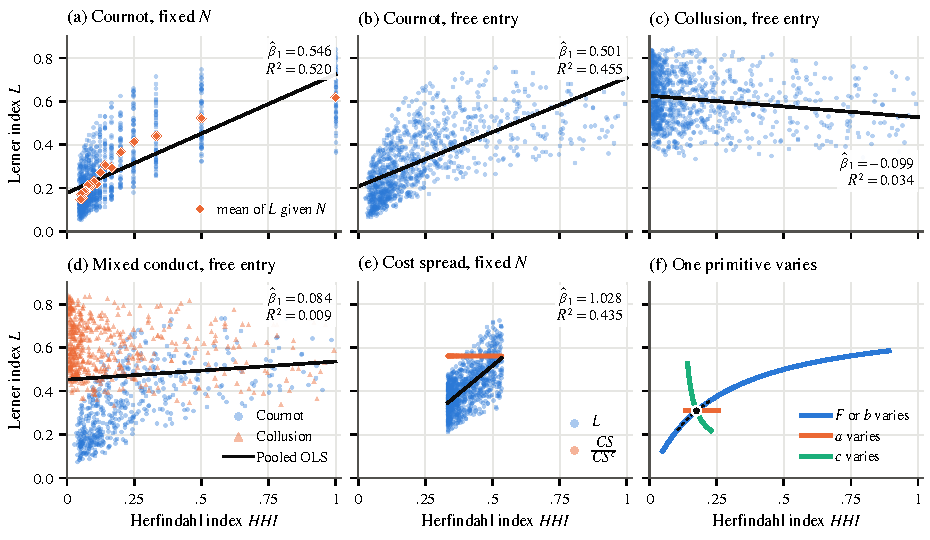
\includegraphics[width=\linewidth]{figures/ch01/scp_montecarlo.pdf}
\caption{Cross-industry SCP regressions on simulated industries. Each dot is an industry and each black
line is the OLS fit of the Lerner index on the Herfindahl index. Panel (a) also marks the mean margin at
each number of firms. Panel (d) separates Cournot and collusive industries. Panel (e) adds the consumer
surplus ratio $\frac{CS}{CS^c}$, which is the same in every industry. Panel (f) traces the free-entry
Cournot equilibrium as one primitive varies through the base point (black dot).}
\label{fig:01-montecarlo}
\end{figure}

Each of $n = 1{,}000$ industries has inverse demand $P = a - bQ$, marginal cost $c$ and fixed cost $F$.
The primitives are drawn independently, with $a \sim U[8, 12]$, $c \sim U[1, 4]$, $b \sim U[0.5, 2]$ and
$\ln F \sim U[\ln 0.1, \ln 10]$. We keep a draw only if the free-entry Cournot equilibrium has at least
one firm, which holds for 96.6 percent of draws. For each industry we compute the equilibrium
Herfindahl index and Lerner index under six designs.
\begin{enumerate}[label=(\arabic*)]
\item Cournot with a fixed number of firms $N \sim U\{1, \dots, 20\}$, drawn independently of the
primitives. Fixed costs are sunk, and in 64.4 percent of these industries the firms do not cover them.
\item Cournot with free entry, using \eqref{eq:01-fe-HL}.
\item Collusion with free entry, using \eqref{eq:01-collusion-fe}.
\item Mixed conduct with free entry, in which each industry colludes with probability $\frac{1}{2}$,
independently of its primitives.
\item Cost heterogeneity with a fixed structure. Each industry has $N = 3$ Cournot firms with marginal
costs $c_i = \bar c + \lambda (P - \bar c) z_i$, where $z = (-1, 0, 1)$ and the spread parameter
$\lambda \sim U[0, 0.95]$ is drawn independently of $(a, b, \bar c)$. The mean cost is
$\bar c \sim U[2.5, 4]$, which keeps every marginal cost positive.
\item One primitive at a time in Cournot with free entry, holding the others at the base point
$(a, c, b, F) = (10, 2.5, 1.25, 1)$.
\end{enumerate}
For designs (1) to (5) we estimate $L_k = \beta_0 + \beta_1 \HHI_k + e_k$ by OLS with
heteroskedasticity-robust standard errors in the HC1 form, which scales the White estimator by
$\frac{n}{n - 2}$. As a benchmark we compute the \emph{slope under random assignment}. It is the OLS slope of
the average causal curve $\frac{1}{n}\sum_k L_k(h)$ on $h$, with $h$ drawn from each design's own
distribution of the Herfindahl index. In designs (1), (2) and the Cournot half of (4), the causal curve of
industry $k$ is $L_k(h) = \frac{(a_k - c_k) h}{a_k h + c_k}$ (\cref{sec:01-cournot-hhi}). Under collusion it
is flat. In design (5), where concentration moves through the cost spread at fixed $N$, it is
$L_k(h) = \frac{h}{\varepsilon_k}$.
We also regress the consumer surplus ratio $\frac{CS}{CS^c}$, consumer surplus relative to its level at
price equal to (average) marginal cost, on the Herfindahl index. \Cref{fig:01-montecarlo} plots the
simulated industries and \cref{tab:01-montecarlo} reports the regressions.

\begin{table}[htbp]
\centering\small
\caption{Cross-industry OLS of the Lerner index on the Herfindahl index in 1,000 simulated industries}
\label{tab:01-montecarlo}
\begin{threeparttable}
\begin{tabular}{lccccc}
\toprule
 & \multicolumn{2}{c}{Cournot} & Collusion & Mixed & Cost spread \\
\cmidrule(lr){2-3}\cmidrule(lr){4-4}\cmidrule(lr){5-5}\cmidrule(lr){6-6}
 & Fixed $N$ & Free entry & Free entry & Free entry & Fixed $N = 3$ \\
 & (1) & (2) & (3) & (4) & (5) \\
\midrule
$\hat\beta_0$ & 0.178 & 0.208 & 0.625 & 0.453 & 0.003 \\
 & (0.004) & (0.005) & (0.005) & (0.009) & (0.016) \\
$\hat\beta_1$ & 0.546 & 0.501 & $-$0.099 & 0.084 & 1.028 \\
 & (0.022) & (0.020) & (0.016) & (0.022) & (0.042) \\
$R^2$ & 0.520 & 0.455 & 0.034 & 0.009 & 0.435 \\
Mean $\HHI$ & 0.179 & 0.238 & 0.174 & 0.206 & 0.398 \\
Mean $L$ & 0.275 & 0.327 & 0.608 & 0.470 & 0.412 \\
\midrule
Slope under random assignment & 0.535 & 0.594 & 0 & 0.340 & 1.036 \\
Slope of $\frac{CS}{CS^c}$ on $\HHI$ & $-$0.752 & $-$0.827 & 0 & $-$0.217 & 0 \\
 & (0.014) & (0.012) &  & (0.024) &  \\
\bottomrule
\end{tabular}
\begin{tablenotes}\footnotesize
\item Notes: 1,000 industries with $P = a - bQ$, marginal cost $c$ and fixed cost $F$. The primitives
$a \sim U[8, 12]$, $c \sim U[1, 4]$, $b \sim U[0.5, 2]$ and $\ln F \sim U[\ln 0.1, \ln 10]$ are drawn
independently and kept if the free-entry Cournot number of firms is at least one (96.6 percent of
draws). Column (1) draws $N \sim U\{1, \dots, 20\}$ independently of the primitives. Columns (2) to (4)
use the continuous free-entry number of firms. In column (4) each industry colludes with probability
$\frac{1}{2}$. Column (5) has 3 Cournot firms with costs $\bar c + \lambda (P - \bar c) z_i$,
$z = (-1, 0, 1)$, $\lambda \sim U[0, 0.95]$ and $\bar c \sim U[2.5, 4]$. HC1 standard errors in
parentheses. The slope under random assignment regresses the average causal curve
$\frac{1}{n}\sum_k L_k(h)$ on $h$, with $h$ drawn from the column's own distribution of $\HHI$.
$\frac{CS}{CS^c}$ is consumer surplus relative to its level at price equal to (average) marginal cost.
In columns (3) and (5) this ratio is the same in every industry, so its slope is exactly zero.
\end{tablenotes}
\end{threeparttable}
\end{table}

In design (1) the number of firms is independent of the primitives. Then $\E[L_k \mid \HHI_k = h] =
\E[L_k(h)]$, and OLS estimates the best linear approximation to the average causal curve. The estimate
$\hat\beta_1 = 0.546$ is close to the benchmark of $0.535$, and the difference is sampling error. Even here
the linear model is misspecified. Every causal curve passes through the origin and is concave
(\cref{fig:01-lerner-hhi}), and the mean margins in panel (a) trace this concavity. The fitted intercept
of $0.178$ is an artifact of fitting a line to a curve. The average derivative of the causal curves at the
observed concentrations is $1.452$, more than two and a half times the OLS slope. Most industries sit at low
concentration, where the curves are steep, while OLS gives much weight to the flat region at high
concentration.

In design (2) every industry lies on its causal curve, yet the OLS slope of $0.501$ falls about 16 percent
short of the random-assignment slope of $0.594$. The gap is the selection term of
\eqref{eq:01-potential-outcomes}. Industries become concentrated when $a - c$ is small relative to
$\sqrt{bF}$, and a small $a - c$ also lowers the causal curve $\frac{(a - c) h}{a h + c}$. The industries
observed at high concentration therefore have systematically lower curves, as in
\cref{ex:01-selection-elasticity}.

In design (3) every causal curve is flat, so concentration has no effect on margins at all. Yet OLS
reports a slope of $-0.099$ with a standard error of $0.016$. The negative sign comes from variation in
$a$ and $c$, which moves the two outcomes in opposite directions (\cref{tab:01-free-entry-cs}). Consumer
surplus is one quarter of its competitive level in every collusive industry, so concentration carries no
information about consumers either.

Design (4) mixes the two populations. The random-assignment slope is $0.340$, below the Cournot
benchmark because half of the causal curves are flat. The OLS slope is $0.084$, a quarter of the
benchmark, with an $R^2$ below one percent. Panel (d) of \cref{fig:01-montecarlo} shows why. Collusive
industries combine
high margins with low concentration and pull the pooled line toward zero.

Design (5) produces the strongest relation in the table, with $\hat\beta_1 = 1.028$ and $R^2 = 0.435$. The
benchmark slope is $1.036$, the mean of $\frac{1}{\varepsilon_k}$, because a wider cost spread raises
$L_k$ and $\HHI_k$ in the ratio $\frac{1}{\varepsilon_k}$ while leaving price unchanged. In this design the
benchmark curve comes from an intervention on the cost spread. It departs from
\cref{def:01-potential-margins}, since costs cannot stay fixed while concentration moves. In this narrower
sense the relation is causal. Yet price, output and consumer surplus are identical to those of the same industry
with symmetric costs, and $\frac{CS}{CS^c} = \frac{9}{16}$ in every industry. A researcher would see a
strong positive concentration-margin relation with no harm to consumers. \Cref{sec:01-demsetz} develops
this case.

Panel (f) isolates the comparative statics of \cref{tab:01-free-entry-cs}. Variation in $F$ or $b$ moves
the industry along an increasing concave curve, variation in $a$ moves it horizontally, and variation in
$c$ moves it down and to the right. The sign of the SCP slope depends on which primitive varies across
the sample. The slope is a property of the sample and says nothing about the technology of competition.
The fully
worked version of these models is in \cref{app:problems}.

\subsection{Panel data and fixed effects}\label{sec:01-salinger}

A natural response to omitted industry characteristics is to observe each industry several times and
remove what does not change. \citet{Salinger1990} reconsidered the concentration-margins relation with such
data. He used a Census of Manufactures panel of industries and restricted most of his analysis to
1972--84 \citep[p.~301]{Salinger1990}. Besides annual cross sections, he estimated the relation in long
differences, which remove time-invariant industry effects. The general fixed-effects version of the
regression is
\begin{equation}\label{eq:01-salinger}
\mathit{PCM}_{kt} = \alpha_k + \beta_1 \mathit{CR}_{kt} + \varphi^\top X_{kt} + e_{kt},
\qquad k = 1, \dots, n, \quad t = 1, \dots, T,
\end{equation}
where $\alpha_k$ is a fixed effect for industry $k$ and $\mathit{CR}_{kt}$ is a concentration ratio. The symbol
$\alpha_k$ is local to this subsection and differs from the price coefficient $\alpha$ of demand models. The
\emph{within estimator} subtracts each industry's time average from every variable:
\[
\mathit{PCM}_{kt} - \overline{\mathit{PCM}}_k = \beta_1 (\mathit{CR}_{kt} - \overline{\mathit{CR}}_k)
 + \varphi^\top (X_{kt} - \bar X_k) + (e_{kt} - \bar e_k),
\]
with $\overline{\mathit{PCM}}_k = \frac{1}{T}\sum_t \mathit{PCM}_{kt}$ and similarly for the other
variables. The transformation removes $\alpha_k$, and with it every time-invariant feature of the
industry, such as its demand elasticity, its technology or its accounting conventions.

With $T = 2$ the within estimator equals OLS on first differences, $\Delta \mathit{PCM}_k = \beta_1
\Delta \mathit{CR}_k + \varphi^\top \Delta X_k + \Delta e_k$. Salinger's long-difference regression has this
form without controls, plus a constant for the common change over the decade. Across 363 industries, he regressed the
change in margins from 1972 to 1982 on the change in $\mathit{CR}_4$, adjusted for market definition. The
slope is $0.178$, with a $t$-statistic of $3.49$ \citep[Table~4, row~1]{Salinger1990}. He notes that it is
roughly the size of his cross-sectional estimates \citep[p.~310]{Salinger1990}. He reads the similarity as
a sign that the cross-sectional relation could have evolved from changes in concentration over time
\citep[pp.~310--311]{Salinger1990}.

The cost is that identification now comes only from changes in concentration within an industry over
time. Consistency requires \emph{strict exogeneity}, $\E[e_{kt} \mid \mathit{CR}_{k1}, \dots,
\mathit{CR}_{kT}, X_{k1}, \dots, X_{kT}, \alpha_k] = 0$. Changes in concentration are responses to the
same demand and cost shocks that move margins. A demand boom raises margins and attracts entry, and a
cost shock can trigger exit or mergers. Such feedback violates strict exogeneity, as a simple model
shows.

\begin{example}[Entry feedback]\label{ex:01-feedback}
Let margin shocks $e_{kt}$ be independent over time with variance $\sigma_e^2$, and suppose the true
effect of concentration is $\beta_1$. Entry responds to last period's margin shock:
\[
\mathit{CR}_{kt} = \mathit{CR}_{k,t-1} - \zeta e_{k,t-1} + v_{kt}, \qquad \zeta > 0,
\]
with $v_{kt}$ independent noise of variance $\sigma_v^2$. In first differences, $\Delta \mathit{PCM}_{kt}
= \beta_1 \Delta \mathit{CR}_{kt} + \Delta e_{kt}$, where $\Delta \mathit{CR}_{kt} = -\zeta e_{k,t-1} +
v_{kt}$ and $\Delta e_{kt} = e_{kt} - e_{k,t-1}$. The two terms share $e_{k,t-1}$:
\[
\Cov(\Delta \mathit{CR}_{kt}, \Delta e_{kt}) = (-\zeta)(-\sigma_e^2) = \zeta \sigma_e^2 .
\]
With $\Var(\Delta \mathit{CR}_{kt}) = \zeta^2 \sigma_e^2 + \sigma_v^2$, the first-difference estimator
converges to
\[
\beta_1 + \frac{\zeta \sigma_e^2}{\zeta^2 \sigma_e^2 + \sigma_v^2} > \beta_1 .
\]
A favorable shock raises the margin today and attracts entry tomorrow, when the margin reverts.
Concentration and margins then fall together, and the estimator finds a positive relation even when
$\beta_1 = 0$.
\end{example}

Fixed effects also magnify measurement error. Most of the variation in concentration is between
industries and persists over time, while the within-industry changes are small. Noise in measured
concentration does not shrink in the same way. \citet{GrilichesHausman1986} make this point for panel
data in general, and the next proposition states it for the SCP regression.

\begin{proposition}[Attenuation of the within estimator]\label{prop:01-fe-attenuation}
Suppose $L_{kt} = \alpha_k + \beta_1 \HHI^*_{kt} + e_{kt}$ and we observe $\HHI_{kt} = \HHI^*_{kt} +
u_{kt}$. Industries are independent across $k$, and $T$ is fixed. The errors $u_{kt}$ are independent
across $k$ and $t$ with mean zero and variance $\sigma_u^2$, and independent of $\{\HHI^*_{ks}\}$,
$\{e_{ks}\}$ and $\alpha_k$. The shocks satisfy $\E[e_{kt} \mid \HHI^*_{k1}, \dots, \HHI^*_{kT}, \alpha_k] =
0$. Let $\sigma^2_{\tilde H} = \E\left[\frac{1}{T}\sum_t (\HHI^*_{kt} - \overline{\HHI}{}^*_k)^2\right] >
0$ be the within-industry variance of true concentration. As $n \to \infty$, the within estimator
converges to
\[
\beta_1 \, \frac{\sigma^2_{\tilde H}}{\sigma^2_{\tilde H} + \sigma^2_{\tilde u}}, \qquad
\sigma^2_{\tilde u} = \frac{T - 1}{T} \sigma_u^2 .
\]
\end{proposition}

\begin{proof}
Write $H_{kt} = \HHI_{kt}$ and $H^*_{kt} = \HHI^*_{kt}$, and write $\ddot y_{kt} = y_{kt} - \bar y_k$ for the
within transformation of any variable $y$. The fixed
effect drops out, so $\ddot L_{kt} = \beta_1 \ddot H^*_{kt} + \ddot e_{kt}$. The measured regressor
is $\ddot H_{kt} = \ddot H^*_{kt} + \ddot u_{kt}$. The within estimator is
\[
\hat\beta_1^W = \frac{\sum_k \sum_t \ddot H_{kt} \, \ddot L_{kt}}{\sum_k \sum_t \ddot H_{kt}^2}.
\]
Divide numerator and denominator by $nT$ and apply the law of large numbers across industries. The
numerator converges to
\[
\beta_1 \E\left[\frac{1}{T}\sum_t \ddot H^*_{kt} (\ddot H^*_{kt} + \ddot u_{kt})\right]
 + \E\left[\frac{1}{T}\sum_t \ddot H_{kt} \, \ddot e_{kt}\right] = \beta_1 \sigma^2_{\tilde H}.
\]
The cross term in $\ddot u_{kt}$ vanishes because $u$ is independent of $\HHI^*$. The second expectation
vanishes by strict exogeneity and the independence of $u$ and $e$. The denominator converges to
$\sigma^2_{\tilde H} + \E\left[\frac{1}{T}\sum_t \ddot u_{kt}^2\right]$. For each $t$,
\[
\E[\ddot u_{kt}^2] = \Var(u_{kt}) - 2 \Cov(u_{kt}, \bar u_k) + \Var(\bar u_k)
 = \sigma_u^2 - \frac{2\sigma_u^2}{T} + \frac{\sigma_u^2}{T} = \frac{T - 1}{T} \sigma_u^2 .
\]
Taking the ratio of the two limits gives the result.
\end{proof}

Compare the within estimator with a pooled regression that ignores the fixed effects and is valid only
if $\alpha_k$ is unrelated to concentration. Its reliability ratio is $\frac{\Var(\HHI^*)}{\Var(\HHI^*) +
\sigma_u^2}$, which uses the total variance of true concentration. The within estimator uses only the
within part. Normalize $\Var(\HHI^*) = 1$, and suppose 95 percent of it is between industries and
$\sigma_u^2 = 0.05$. The pooled reliability ratio is $\frac{1}{1.05} = 0.95$. With many periods, the
within ratio is $\frac{0.05}{0.05 + 0.05} = 0.5$, so the within estimator recovers only half of $\beta_1$.
Fixed effects remove one bias and enlarge another.

The lesson of this subsection holds for any such design. Industry fixed effects do not solve the
endogeneity of concentration, and where they remove one problem they create others: dynamic feedback
between margins and entry, and attenuation from measurement error.

\section{Efficiency, prices, and the afterlife of SCP}\label{sec:01-scp-after}

Suppose we found the econometric evidence credible: more concentrated markets have higher margins and
higher profits. Would that show that concentration is bad for consumers? This section takes up the
efficiency critique, the shift from profits to prices as the dependent variable, and the recent return of
cross-industry work in the debate over rising markups.

\subsection{Efficiency versus market power: the Demsetz critique}\label{sec:01-demsetz}

\citet{Demsetz1973} argued that concentration can be the result of superior efficiency or quality. Firms
with lower costs or better products grow, the industry becomes concentrated, and industry profits rise
because the efficient firms earn rents on their advantage. Consumers need not lose. On this view, which
became part of the Chicago critique of antitrust, the measurement may be correct while its normative
reading is wrong. \citet[p.~1013, fn.~2]{Bresnahan1989} summarizes the argument. ``Demsetz' alternative
interpretation was that high profits measure good performance, i.e.\ low costs, an argument he buttressed
by the observation that much of the profit in concentrated industries goes to large firms.'' Bresnahan
cites \citet{Demsetz1974} and notes that \citet{Bain1951} had already given a ``poor performance''
reading of the same observation. He describes the SCP literature as caught in ``a kind of gridlock'' over
whether high accounting profits signal good or bad performance \citep[p.~1013]{Bresnahan1989}.

The next proposition shows that the efficiency story holds exactly in the linear Cournot model with
heterogeneous costs.

\begin{proposition}[Concentration from cost differences]\label{prop:01-demsetz}
Let inverse demand be $P = a - bQ$, and let $N$ Cournot firms have constant marginal costs $c_1, \dots,
c_N$. Suppose all firms are active, $P > \max_i c_i$. Let $\bar c = \frac{1}{N}\sum_i c_i$ and
$\sigma_c^2 = \frac{1}{N}\sum_i (c_i - \bar c)^2$.
\begin{enumerate}[label=(\roman*)]
\item Output and price are $Q = \frac{Na - \sum_i c_i}{b(N + 1)}$ and $P = \frac{a + \sum_i c_i}{N + 1}$.
They depend on costs only through $\sum_i c_i$.
\item Shares are $s_i = \frac{P - c_i}{bQ}$, and $\HHI = \frac{1}{N} + \frac{N \sigma_c^2}{b^2 Q^2}$.
\item Industry variable profit is $\sum_i (P - c_i) q_i = bQ^2 \HHI$, and the share-weighted Lerner index
is $\sum_i s_i L_i = \frac{\HHI}{\varepsilon}$ with $\varepsilon = \frac{P}{bQ}$.
\end{enumerate}
\end{proposition}

\begin{proof}
(i) Firm $i$ maximizes $(a - bQ - c_i) q_i$. Its first-order condition is $a - bQ - b q_i - c_i = 0$, or
\[
b q_i = P - c_i .
\]
Sum over the $N$ firms: $bQ = NP - \sum_i c_i$. Substitute $P = a - bQ$:
\[
bQ = N(a - bQ) - \sum_i c_i \quad\Longrightarrow\quad bQ(N + 1) = Na - \sum_i c_i .
\]
Solve for $Q$ and substitute back into the demand curve:
\[
P = a - bQ = \frac{(N + 1)a - Na + \sum_i c_i}{N + 1} = \frac{a + \sum_i c_i}{N + 1}.
\]

(ii) The first-order condition gives $s_i = \frac{q_i}{Q} = \frac{P - c_i}{bQ}$. Because $\sum_i (P - c_i)
= bQ$, the mean of $P - c_i$ across firms is $\frac{bQ}{N} = P - \bar c$. Hence
\[
s_i - \frac{1}{N} = \frac{(P - c_i) - (P - \bar c)}{bQ} = \frac{\bar c - c_i}{bQ}.
\]
The variance of shares is $\sigma_s^2 = \frac{1}{N}\sum_i (s_i - \frac{1}{N})^2 = \frac{\sigma_c^2}{b^2
Q^2}$. By \cref{prop:01-hhi-variance}, $\HHI = \frac{1}{N} + N\sigma_s^2 = \frac{1}{N} + \frac{N
\sigma_c^2}{b^2 Q^2}$.

(iii) Using $P - c_i = b q_i$,
\[
\sum_i (P - c_i) q_i = b \sum_i q_i^2 = bQ^2 \sum_i s_i^2 = bQ^2 \HHI .
\]
Similarly, the Lerner index of firm $i$ is
\[
L_i = \frac{P - c_i}{P} = \frac{b q_i}{P} = \frac{bQ}{P} \, s_i = \frac{s_i}{\varepsilon}.
\]
Multiplying by $s_i$ and summing gives $\sum_i s_i L_i = \frac{\HHI}{\varepsilon}$.
\end{proof}

\begin{corollary}[A mean-preserving spread of costs]\label{prop:01-demsetz-spread}
Change the costs $c_i$ so that $\sum_i c_i$ is unchanged, $\sigma_c^2$ rises and all firms remain
active. Then price, output and consumer surplus $\frac{bQ^2}{2}$ are unchanged. The Herfindahl index,
industry variable profit and the share-weighted Lerner index all rise, and so does total surplus.
\end{corollary}

\begin{proof}
By \cref{prop:01-demsetz}(i), $P$ and $Q$ depend only on $\sum_i c_i$, so they and consumer surplus are
unchanged. With $Q$ fixed, part (ii) shows that $\HHI$ rises with $\sigma_c^2$. Part (iii) then shows that
industry profit $bQ^2\HHI$ and $\sum_i s_i L_i = \frac{bQ}{P}\HHI$ rise. Total surplus is consumer surplus
plus industry profit (gross of fixed costs), so it rises by the increase in profit.
\end{proof}

The corollary is the efficiency critique in one line. Across industries that differ only in the
dispersion of firm costs, concentration, margins and profits move together, and consumers are equally
well off in all of them. Design (5) of the Monte Carlo experiment is exactly this case.

\citet[Section~5.5]{Tirole1988} presents Demsetz's argument with two further examples. In Bertrand competition
with constant marginal costs, the lowest-cost firm charges the second-lowest cost and takes the whole market.
Concentration is then as high as any index that satisfies the axioms of \cref{rem:01-ej-axioms} allows, and the
firm earns a positive profit. With symmetric costs, concentration is lower and profit is zero.
\Cref{prop:01-more-draws} below studies this equilibrium when costs are random. Tirole's Exercise~5.7 is a
special case of \cref{prop:01-demsetz-spread}. Let demand be $Q = 1 - P$, so that $a = b = 1$, and let two
Cournot firms have costs $c_1 = c - d$ and $c_2 = c + d$ with $0 \le d$ and $c < 1$. The sum $c_1 + c_2 = 2c$
stays fixed as $d$ varies, and $\sigma_c^2 = d^2$. By \cref{prop:01-demsetz},
\[
  Q = \frac{2(1 - c)}{3}, \qquad P = \frac{1 + 2c}{3}, \qquad
  \HHI = \frac{1}{2} + \frac{2d^2}{Q^2} = \frac{1}{2} + \frac{9 d^2}{2(1 - c)^2} .
\]
Industry variable profit is
\[
  bQ^2 \HHI = \frac{Q^2}{2} + 2d^2 = \frac{2(1 - c)^2}{9} + 2d^2 .
\]
Both firms stay active as long as $P > c + d$, that is, $d < \frac{1 - c}{3}$. Over this range a wider cost
spread raises concentration and industry profit and leaves price unchanged.

Tirole draws a general lesson from such examples. Concentration indices give an easily computed indication of how
competitive an industry is. ``However, they have no systematic relationship with economic variables of interest
for assessing changes in cost, demand, or policy.'' With asymmetric firms, a given index need not be related in a
systematic way to welfare either. The indices are also endogenous, so their correlations with other variables
cannot be read as causal effects \citep[Section~5.5]{Tirole1988}.

The decomposition in part (ii) also shows that the source of concentration matters. Its first term,
$\frac{1}{N}$, reflects the number of firms. An extra active firm with cost $c_{N+1} < P$ lowers price,
because
\[
\frac{a + \sum_i c_i + c_{N+1}}{N + 2} < \frac{a + \sum_i c_i}{N + 1} = P
\quad\Longleftrightarrow\quad (N + 1) \, c_{N+1} < a + \sum_i c_i
\quad\Longleftrightarrow\quad c_{N+1} < P .
\]
Fewer firms therefore mean higher prices and lower consumer surplus. The second term reflects cost
dispersion, which leaves consumers unaffected. A single concentration index cannot tell the two apart.

The critique generated a large literature of firm-level \emph{horse-race regressions}. They include both
industry concentration and the firm's own market share:
\begin{equation}\label{eq:01-horse-race}
\pi_{ik} = \beta_0 + \beta_1 \mathit{CR}_k + \beta_2 s_{ik} + \varphi^\top X_{ik} + e_{ik},
\end{equation}
where $\pi_{ik}$ is the profitability of firm $i$ in industry $k$ and $s_{ik}$ its market share. The
efficiency view predicts $\beta_2 > 0$ with $\beta_1$ near zero, since large firms are profitable
because they are efficient. The market-power view predicts $\beta_1 > 0$, since concentration
facilitates high prices for all firms in the industry.

Demsetz stated the testable implication of his view himself (\citealp[p.~5]{Demsetz1973}, quoted in
\citealp[p.~46, n.~5]{LevensteinSuslow2006}). Suppose that efficiency is associated with concentration. Then
``there should be a positive correlation between concentration and the difference between the rate of return
earned by large firms and that earned by small firms.'' Let $\bar\pi^L_k$ and $\bar\pi^S_k$ be the average rates of return
of the large and the small firms in industry $k$. The implication concerns the cross-industry regression
\begin{equation}\label{eq:01-demsetz-test}
\bar\pi^L_k - \bar\pi^S_k = \gamma_0 + \gamma_1 \mathit{CR}_k + e_k ,
\end{equation}
and the efficiency view predicts $\gamma_1 > 0$. If concentration instead facilitates high prices for every firm
in the industry, the returns of small firms rise with concentration as well, and the gap need not widen. In
\eqref{eq:01-horse-race} the same contrast appears as $\beta_2 > 0$ against $\beta_1 > 0$.

Demsetz's own evidence fit the efficiency view. It was the observation, quoted above from
\citet[p.~1013, n.~2]{Bresnahan1989}, that much of the profit in concentrated industries goes to large firms.
\citet[p.~1142]{Hopenhayn1992} puts it more precisely: ``as reported by Demsetz (1973), more concentrated
industries could show higher profits for large firms and not for small ones.'' Hopenhayn also shows that the
pattern does not single out efficiency. In his competitive model of industry dynamics, a higher cost of entry
protects incumbents. It raises the profits of large firms but not necessarily those of small ones, and it raises
the market share of the largest firms. Industries with high entry costs then show the Demsetz pattern, although
every firm takes the price as given.

Later evidence was mixed. Studies that add the firm's own market share to the regression find that concentration
loses its effect \citep[Introduction, note~3]{Tirole1988}. \citet{Ravenscraft1983} reports evidence of
this kind from the line-of-business data of the Federal Trade Commission, for 3,186 business units in 258
manufacturing industries in 1975 \citep[p.~24]{Ravenscraft1983}. In the business-unit regressions of his
Table~1, the share coefficient is positive and significant. The concentration coefficient is small and negative, and significant in the generalized least squares
estimate \citep[Table~1]{Ravenscraft1983}. In the industry-level regression, which omits share, concentration has
a positive coefficient \citep[p.~26]{Ravenscraft1983}.
\citet{Schmalensee1985a} decomposed the variance of business-unit returns on assets in the 1975 line-of-business
data into industry, firm and share components. Firm effects were never statistically significant. Share effects
were significant but explained less than 1 percent of the variance. Industry effects explained about a fifth of
it, and at least 75 percent of the variance of industry average returns. About 80 percent of the variance was
unrelated to industry or share effects \citep[pp.~346--350]{Schmalensee1985a}.
Ravenscraft's paper focuses on the firm's share and Schmalensee's on the industry. Schmalensee finds the two
consistent, since share also explains less than 1 percent of the variance of profitability in Ravenscraft's
estimates \citep[p.~347]{Schmalensee1985a}. \citet[Section~5.5]{Tirole1988} and \citet[p.~46, n.~5]{LevensteinSuslow2006} point to
\citet{Schmalensee1987} for a test of collusion against differential efficiency.

The horse race cannot settle the question, because firm share is itself an equilibrium outcome. The model
of \cref{prop:01-demsetz} makes the point sharply. There, $L_{ik} = \frac{s_{ik}}{\varepsilon_k}$ for
every firm. In a sample of industries with a common elasticity $\varepsilon$, a regression of firm
margins on share and concentration returns $\beta_2 = \frac{1}{\varepsilon}$ and $\beta_1 = 0$ exactly.
Yet every firm prices above marginal cost because it internalizes the effect of its output on price,
which is market power by definition. The pattern ``$\beta_1 = 0$ and $\beta_2 > 0$'' is thus fully
consistent with a model in which firms exercise market power. It shows that margins line up with shares,
which the Cournot model of \cref{prop:01-cowling-waterson} predicts as well.

The argument has a modern echo. Dominant digital platforms attribute their large shares to the quality of
their products. Defendants have advanced this argument in recent monopolization cases. The logic is
Demsetz's: concentration may be high because some firms deliver more value per dollar, so the measured
concentration is fine and its normative reading is contested. Separating the two readings requires a
model of demand that values quality, which is the subject of \cref{ch:discrete,ch:blp}.

Efficiency and structure can also be jointly determined by competition itself. \citet{Syverson2004}
studies plants in the US ready-mixed concrete industry, where high transport costs make markets local.
Markets with denser demand have more plants, so buyers can switch between suppliers more easily. Less
efficient plants then find it harder to operate profitably, and the productivity distribution is
truncated from below. Denser markets have higher minimum and average productivity and less dispersion.
The causal arrow runs from demand density to both structure and efficiency, which no cross-industry
regression of performance on structure can capture.

\subsection{Price-concentration studies}\label{sec:01-price-concentration}

A later wave of studies replaced accounting profit with price as the dependent variable. They used
cross-sections of similar, geographically local markets within one industry
\citep[Section~3.5]{Bresnahan1989}. Examples include banking, for which \citet{Rhoades1982} lists dozens
of studies, and retail food \citep{Cotterill1986,Lamm1981}. Others cover gasoline \citep{Marvel1978},
airline city pairs \citep{GrahamKaplanSibley1983} and cement \citep{KollerWeiss1986}. \citet{Weiss1989} collected many such
studies. The estimating equation is typically a reduced form for price,
\begin{equation}\label{eq:01-price-concentration}
p_k = \beta_0 + \beta_1 \HHI_k + \varphi^\top X_k + e_k ,
\end{equation}
where $k$ now indexes local markets of one industry and $X_k$ contains demand and cost shifters. The
studies typically treat concentration as exogenous \citep[p.~1043]{Bresnahan1989}. They confirm a
positive relation between price and concentration, which is at least suggestive of market power
increasing with concentration. A variant uses changes in structure over time, as in the study of a
merger in the microfiche industry by \citet{BartonSherman1984}.

Price avoids the accounting problems of \cref{sec:01-accounting}, and similar local markets share many
omitted features. Yet the interpretation that concentration raises margins by changing conduct still
needs a defense. \citet[p.~1043]{Bresnahan1989} writes, ``I have seen no careful defense of this
interpretation, and I am troubled by it.'' He then lists difficulties which, in his words, ``have not
yet been rebutted.'' We state each one as an argument.
\begin{enumerate}[label=(\roman*)]
\item Free entry links price and concentration through scale, because larger markets fit more
firms. Take the free-entry Cournot model of \cref{sec:01-endogeneity} with $M$ consumers, so that
$b = \frac{1}{M}$. Then $P^* = c + \sqrt{\frac{F}{M}}$ and $\HHI^* = \frac{m^*}{a - c - m^*}$ with
$m^* = \sqrt{\frac{F}{M}}$, so both fall as $M$ grows. Firm output is $q^* = \frac{m^*}{b} = \sqrt{FM}$ and
average cost is $c + \frac{F}{q^*} = c + \sqrt{\frac{F}{M}} = P^*$. Firms in larger markets are larger,
have lower
average costs and break even everywhere. Price and concentration are related ``in a way that has no
obvious bad effects, and does not imply entry barriers'' \citep[p.~1044]{Bresnahan1989}.
\item Cost heterogeneity varies across markets with the same number of firms. Among such markets, the
more concentrated ones likely have more heterogeneous costs. By \cref{prop:01-demsetz}(ii),
concentration rises with $\sigma_c^2$ at fixed $N$. Cost heterogeneity may or may not interact with
conduct to raise prices.
\item Markets with more firms offer more draws on the lowest-cost firm, even if concentration is
exogenous. If that firm matters for price, price falls with the number of firms for purely
statistical reasons. \Cref{prop:01-more-draws} below formalizes the point.
\item Market-level data identify only an average of costs and conduct. Summing the first-order
conditions of \cref{prop:01-clarke-davies} with share weights gave the industry relation
\eqref{eq:01-industry-relation}. With marginal costs $mc_i$ that may vary across firms, the same steps
give Bresnahan's equation (17$'$) in our notation,
\begin{equation}\label{eq:01-avg-supply}
P = \overline{mc} - P'(Q) \, Q \, \theta, \qquad
\overline{mc} = \sum_i s_i \, mc_i, \qquad \theta = \sum_i s_i^2 (1 + r_i),
\end{equation}
which \cref{prop:01-supply-relation} derives in general. A lower price in
less concentrated markets can reflect a lower $\overline{mc}$, a lower $\theta$, or both. Most authors
have the second in mind. The two can also be linked, because a firm with a large cost advantage may
behave less competitively than it would against equal rivals.
\item The identity of the competitors matters as well as their number. \citet{GrahamKaplanSibley1983}
found that
airline city-pair markets served by carriers new to the industry have lower prices, all else equal.
These entrants very likely had
lower marginal costs, and their presence may also have changed the conditions of competition. ``Which is
it? The analysis of the paper cannot say'' \citep[p.~1044]{Bresnahan1989}. The same question applies to
the structure dummies in Porter's \citeyearpar{Porter1983} railroad cartel study.
\item Tests of the exogeneity of concentration have little power. \citet{GrahamKaplanSibley1983} tested the
exogeneity of their concentration measures and did not reject it. Their concentration coefficients
nevertheless changed
substantially when concentration was treated as endogenous. Bresnahan concludes that the test had little
power, so the assumption should not be taken as innocuous \citep[p.~1043, fn.~35]{Bresnahan1989}.
\end{enumerate}
Bresnahan stresses that these questions ``are not unanswerable'' and that the methods of
\cref{sec:01-identification} can tell marginal cost from conduct. ``The questions are, however,
unanswered'' \citep[p.~1044]{Bresnahan1989}. One clean exception he notes is \citet{SpillerFavaro1984}.
They study Uruguayan banking over a period that includes a change in entry regulation, and find that
freer entry shifts the supply relation down \citep[p.~1044, fn.~36]{Bresnahan1989}.

The more-draws argument can be made precise with order statistics, which \cref{app:math} reviews. Let
$c_{(k:N)}$ denote the $k$-th lowest of $N$ costs.

\begin{proposition}[More firms, more draws]\label{prop:01-more-draws}
Let the marginal costs of $N \ge 2$ firms be independent draws from a distribution $F_c$ on $[\underline
c, \bar c]$, and let firms compete in prices with a homogeneous good. In the equilibrium in which the
lowest-cost firm serves the market at the second-lowest cost, the price is $c_{(2:N)}$, and
\[
\E[c_{(2:N)}] = \underline c + \int_{\underline c}^{\bar c} G_N(x) \, \dd x, \qquad
G_N(x) \equiv \Pr(c_{(2:N)} > x) = (1 - F_c(x))^N + N F_c(x) (1 - F_c(x))^{N - 1}.
\]
The expected price is strictly decreasing in $N$ whenever $F_c$ is nondegenerate:
\[
\E[c_{(2:N)}] - \E[c_{(2:N+1)}] = \int_{\underline c}^{\bar c} N F_c(x)^2 (1 - F_c(x))^{N - 1} \, \dd x
> 0 .
\]
\end{proposition}

\begin{proof}
For a random variable $Y$ on $[\underline c, \bar c]$, $\E[Y] = \underline c + \int_{\underline c}^{\bar
c} \Pr(Y > x)\, \dd x$. The second-lowest cost exceeds $x$ exactly when at most one of the $N$ costs is
below $x$. No cost is below $x$ with probability $(1 - F_c(x))^N$. Exactly one is below $x$ with
probability $N F_c(x)(1 - F_c(x))^{N - 1}$. Adding the two gives $G_N(x)$. For the difference, write $F =
F_c(x)$ and compute
\begin{align*}
G_N(x) - G_{N+1}(x)
 &= (1 - F)^N \left[1 - (1 - F)\right] + F (1 - F)^{N - 1} \left[N - (N + 1)(1 - F)\right] \\
 &= F (1 - F)^N + F (1 - F)^{N - 1} \left[(N + 1)F - 1\right] \\
 &= F (1 - F)^{N - 1} \left[(1 - F) + (N + 1)F - 1\right] = N F^2 (1 - F)^{N - 1} .
\end{align*}
Integrating over $x$ gives the expression for the difference in expected prices. The integrand is
positive wherever $0 < F_c(x) < 1$, a set of positive length when $F_c$ is nondegenerate.
\end{proof}

The difference has a coupling interpretation. Adding a firm can only add a draw below $x$, so the event
``at most one cost below $x$'' becomes less likely. It fails exactly when one, and only one, of the first
$N$ costs is below $x$ and the new cost is also below $x$, which has probability
$N F_c(x)^2 (1 - F_c(x))^{N - 1}$. With costs
uniform on $[0, 1]$, $G_N(x) = (1 - x)^N + N x (1 - x)^{N - 1}$ and
\[
\E[c_{(2:N)}] = \int_0^1 (1 - x)^N \dd x + N \int_0^1 x (1 - x)^{N - 1} \dd x
 = \frac{1}{N + 1} + \frac{N}{N(N + 1)} = \frac{2}{N + 1}.
\]
The expected price is $\frac{2}{3}$ with two firms, $\frac{1}{2}$ with three and $\frac{1}{3}$ with five,
with identical Bertrand conduct in every market. In this stark model the lowest-cost firm serves the
whole market, so its share is one and the structural variable that varies is the number of firms present.
The same logic applies in any model in which the most efficient firms carry extra weight in price
determination.

\subsection{SCP today}\label{sec:01-scp-today}

SCP regressions survive as descriptive exercises. They are useful for laying out facts and empirical
regularities, such as which industries are concentrated and how margins and concentration move over
time. For the reasons in \cref{sec:01-scp-econometrics,sec:01-demsetz,sec:01-price-concentration}, they
are of little use for testing theories of market power. Schmalensee's own post-mortem concluded that the
cross-industry literature had not taught us much about how markets work
\citep[p.~160]{EinavLevin2010}.

A recent survey of health care markets restates the verdict \citep[p.~527]{HandelHo2021}. Handel and Ho note
that the SCP approach persisted longer in health economics than elsewhere. They summarize the reasons that
\citet{BerryGaynorScottMorton2019} give for the move away from it in the late 1980s. The first is measurement.
Markets are not observed directly in the data, and economic profits are hard to measure. The second is the
endogeneity of concentration. As a function of market shares, it is likely to be correlated with the unobserved
demand shifters that also move price. The third, and in their words the most fundamental, is that different
changes in primitives can produce the same correlation between concentration and prices. Mergers raise
concentration, markups and prices together and lower consumer surplus. Large firms with low marginal costs and
high fixed costs produce the same correlation, as in \citet{Demsetz1973}. So does a fall in search costs that
shifts share toward firms with high-quality products, which raises both concentration and consumer welfare
\citep{AutorEtAl2020}. The results of such regressions are therefore ``at best suggestive.'' Handel and Ho
conclude with the point of \citet{Bresnahan1989}. The effect of concentration can be studied only through three
objects: a demand system, the marginal costs of firms and the nature of oligopolistic competition.

Industry studies, the response described in \cref{sec:01-neio}, taught
much about particular industries, at the price of leaving cross-industry questions to other fields
(\cref{sec:01-today-debate}). The debate over rising markups and their role in rising inequality has
brought cross-industry, SCP-style work back, and the reactions within IO have been mixed.

\subsection{Rising markups and the production approach}\label{sec:01-rising-markups}

The recent cross-industry literature measures markups from production data instead of demand. The
approach goes back to \citet{Hall1988}, and \citet{DeLoeckerWarzynski2012} developed its firm-level
version. In this subsection $Q$ and $P$ denote the output and price of a single firm, and $\mu =
\frac{P}{mc}$ is the markup ratio of \cref{sec:01-lerner}.

\begin{proposition}[Markups from a flexible input]\label{prop:01-production-markup}
A firm produces $Q = f(V, K, \omega)$, where $V$ is a variable input bought at price $P^V$, $K$ collects
the other inputs and $\omega$ is productivity. Suppose the firm minimizes cost, takes $P^V$ as given,
and adjusts $V$ freely. Let $\lambda$ be the multiplier on the output constraint. Then $\lambda = mc$ and
\[
\mu = \frac{P}{\lambda} = \phi^V \frac{PQ}{P^V V}, \qquad
\phi^V = \frac{\partial f}{\partial V} \frac{V}{Q},
\]
where $\phi^V$ is the output elasticity of the variable input.
\end{proposition}

\begin{proof}
The firm chooses $V$ to minimize $P^V V$ plus the cost of the other inputs subject to $f(V, K, \omega) \ge
Q$. The Lagrangian is
\[
\mathcal{L} = P^V V + C^K(K) - \lambda \left[ f(V, K, \omega) - Q \right],
\]
where $C^K(K)$ is the cost of the other inputs. The first-order condition for $V$ is
\[
P^V = \lambda \frac{\partial f}{\partial V}.
\]
By the envelope theorem (\cref{app:math}), the derivative of minimized cost with respect to $Q$ equals
$\frac{\partial \mathcal{L}}{\partial Q} = \lambda$, so $\lambda = mc$. Multiply the first-order condition
by $\frac{V}{\lambda Q}$:
\[
\frac{P^V V}{\lambda Q} = \frac{\partial f}{\partial V} \frac{V}{Q} = \phi^V .
\]
Solve for $\lambda = \frac{P^V V}{\phi^V Q}$ and divide price by it:
\[
\mu = \frac{P}{\lambda} = \frac{P \phi^V Q}{P^V V} = \phi^V \frac{PQ}{P^V V}.
\qedhere
\]
\end{proof}

The formula needs no demand model and no assumption about conduct. The markup is the output elasticity
of a flexible input divided by that input's share of revenue. Its appeal for cross-industry work is
obvious, because revenue shares are available in accounting data for many firms.

\citet{DeLoeckerEeckhoutUnger2020} applied the formula to US publicly listed firms in the Compustat data from
1955 to 2016, treating cost of goods sold as the variable input. Each firm's markup is the ratio of its revenue
to its cost of goods sold, multiplied by an estimated output elasticity of the variable inputs. The method
follows \citet{DeLoeckerWarzynski2012}, and the firm markups are then averaged with revenue weights
\citep[p.~258 and n.~203]{AskerNocke2021}. As read from the figure in \citet[Figure~11, p.~259]{AskerNocke2021},
the revenue-weighted average markup rose from about 1.21 in 1980 to about 1.61 in 2016. The rise was confined to
the upper tail. The median markup is flat over the period, and in the authors' own words, ``Most firms see no
increase in markups. For the higher percentiles, markups increase. For the 90th percentile in particular, the
increase is sharpest. Between 1980 and 2016, it increases from 1.5 to 2.5'' (quoted in
\citealp[p.~258]{AskerNocke2021}). The rise in the average is thus ``largely driven by a few firms that currently
have much higher markups than decades ago.'' The finding drew wide attention because it suggested a rise in
market power across the economy. \citet{DeLoeckerSyverson2021} survey the production approach behind it, and
their chapter closes with its use to measure market power in product and labor markets
\citep[Preface, p.~xvi]{HoHortacsuLizzeri2021}.

The critiques mirror the problems of the SCP literature.
\begin{itemize}
\item The output elasticity $\phi^V$ must be estimated, usually from a production function by industry.
Most data record revenue instead of physical output. With revenue $R = PQ$ and profit maximization,
which sets marginal revenue $MR$ equal to $mc = \lambda$, the elasticity of revenue with respect to $V$ is
\[
\frac{\partial \ln R}{\partial \ln V} = \frac{\partial \ln R}{\partial \ln Q} \, \phi^V
 = \frac{MR}{P} \, \phi^V = \frac{\phi^V}{\mu}.
\]
Plugging this revenue elasticity into \cref{prop:01-production-markup} in place of $\phi^V$ gives
\[
\frac{\phi^V}{\mu} \cdot \frac{PQ}{P^V V} = \frac{\mu}{\mu} = 1
\]
for every firm. A revenue elasticity therefore carries no information about the markup, a point
developed by \citet{BondEtAl2021}.
\item A markup ratio above one must cover fixed and overhead costs (\cref{prop:01-zero-profit-markup}).
If technology has shifted toward fixed costs, such as software and overhead, $\mu$ rises with no rise in
profits. Which costs count as variable, cost of goods sold or also overhead, matters for the trend. A shift
of the population toward firms with larger fixed costs or lower costs of goods sold moves the average markup
by composition alone \citep[p.~258]{AskerNocke2021}. De Loecker, Eeckhout and Unger reply that the rise in
markups ``is not merely to offset a rise in overhead costs'' (quoted in \citealp[p.~258, n.~205]{AskerNocke2021}).
They find that markups rose by more than overhead costs, and that the excess markups are highest for the firms
with high overhead costs. Their measure of profits rose too, as did market value as a share of sales.
\item The average depends on the weights. A revenue-weighted mean rises when sales move toward large firms
with high markups, even if no firm's markup changes.
\item The relation between markups and concentration across industries is subject to every problem of
\cref{sec:01-scp-econometrics}.
\end{itemize}
Descriptive evidence on concentration itself gives a modern version of the Demsetz pattern of
\cref{sec:01-demsetz}. \citet{Ganapati2020} examines detailed firm-level Census data for 1972--2012. As reported
by \citet[p.~259]{AskerNocke2021}, increases in concentration are positively correlated with productivity and with real output growth. They are
uncorrelated with price changes and with overall payroll, and they are negatively correlated with labor's share
of revenue. Concentration rose where output and productivity grew, without the price increases that the
market-power reading would predict. This fits the efficiency reading better than the market-power reading,
although, as \cref{sec:01-demsetz} showed, it cannot rule out market power.

\citet{BerryGaynorScottMorton2019}, to whom \citet[p.~259, n.~206]{AskerNocke2021} point for an IO perspective on
this literature, develop the last point of the bulleted list above.
Their argument, summarized in \cref{sec:01-scp-today}, is that different changes in primitives can produce the
same correlation between concentration and markups, with very different positive and normative implications
\citep[p.~47]{BerryGaynorScottMorton2019}.
Following \citet{Bresnahan1989}, they hold that the effect of concentration cannot be interpreted without
demand, the marginal costs of firms and the nature of oligopolistic competition
\citep[p.~48]{BerryGaynorScottMorton2019}. They regard the production
approach as persuasive evidence that markups have risen, although the size and causes of the rise remain open
\citep[p.~49]{BerryGaynorScottMorton2019}.
Because industries are so heterogeneous, they argue that careful industry studies are also needed. They call
for many more such studies \citep[pp.~50 and 53]{BerryGaynorScottMorton2019}.

A demand-side study of one large industry models these three objects and reaches a contrasting answer.

\casehead{The US automobile industry}\citet{GriecoMurryYurukoglu2024}, GMY below, ask whether market power in the
US new-car market rose between 1980 and 2018, a period over which the production approach reports rising markups. We cite
the author manuscript on hand, whose title page is dated July 5, 2023. Its table and figure numbers may differ
from those of the published article.
Product data from Ward's Automotive give the sales, list prices and characteristics of new
cars and light trucks. An observation is a make-model-year, such as the 1987 Honda Accord, and the sample has
9,694 of them (Table~I). The market size is the number of US households divided by 2.5. The divisor reflects that
a household owns nearly two cars and keeps each for about five years. Survey data add the demographics of buyers
and the models they name as their second choices.

\casehead{Model and identification}Demand is a random coefficients logit of the kind developed in \cref{ch:blp}.
Household $i$ in year $t$ obtains from model $j$ the utility
\[
  u_{ijt} = x_{jt}\beta_i - \alpha_i p_{jt} + \xi_{jt} + \epsilon_{ijt}
\]
in our sign convention for price (their equation 1). The tastes $(\alpha_i, \beta_i)$ depend on demographics drawn
from the Current Population Survey and on normal taste shocks (equations 3 and 4). Manufacturers set the prices of
all their models in a static Nash-Bertrand game each year. The first-order conditions are those of
\cref{prop:01-multiproduct-foc} (their equation 6). GMY solve them for the marginal cost of every model at the
estimated demand parameters, as in \eqref{eq:01-implied-mc}. The price instrument is the real exchange rate of the
country where the model is built, lagged one year and taken from the Penn World Table. It moves with local labor
costs and with the nominal exchange rate, so it shifts the cost of supplying the US market. Average unobserved
quality and the value of the outside good both move the total share of new cars each year. The year effects alone
cannot separate them. GMY follow \citet{PakesBerryLevinsohn1993} and assume that, for models sold in two
consecutive years without a redesign, the change in $\xi_{jt}$ has mean zero (their equation 2).

Estimation is by the generalized method of moments (GMM) in three steps (their Section~5). The first matches micro moments, such as the average price paid
by each income quintile and the correlation of characteristics between first and second choices. The second
regresses the estimated mean utilities on characteristics, price, make and year dummies by two-stage least
squares with the exchange-rate instrument. The third applies the continuing-model restriction to the estimated
year effects. Standard errors come from a bootstrap of the micro data.

\begin{table}[htbp]
\centering
\caption{Markups, concentration and welfare in the US new-car market}
\label{tab:01-gmy}
\small
\begin{tabular}{@{}lrrl@{}}
\toprule
\multicolumn{4}{@{}l}{\textit{Panel A. Baseline estimates}} \\
\addlinespace[2pt]
 & 1980 & 2018 & Source \\
\midrule
Median Lerner index & 0.325 & 0.185 & Figure VIa, p.~2 \\
Share-weighted mean Lerner index & 0.42 & 0.22 & Table VII \\
Share-weighted mean Lerner index, log price & 0.32 & 0.27 & p.~21 \\
Herfindahl index (HHI points) & 2661 & 1132 & Table VII \\
Consumers' share of total surplus & 0.62 & 0.82 & p.~2 \\
\bottomrule
\end{tabular}

\medskip
\begin{tabular}{@{}lrr@{}}
\toprule
\multicolumn{3}{@{}l}{\textit{Panel B. Hypothetical cartels in 2018 (Table VII)}} \\
\addlinespace[2pt]
Cartel members & Mean Lerner index & HHI points \\
\midrule
None (2018 baseline) & 0.22 & 1132 \\
GM, Ford and Toyota & 0.26 & 2546 \\
Top three and Fiat & 0.35 & 3724 \\
Top four and Honda & 0.39 & 4819 \\
Top five and Nissan & 0.46 & 6000 \\
\bottomrule
\end{tabular}
\par\smallskip
\begin{minipage}{\textwidth}\footnotesize
\textit{Notes:} The Lerner index is $\frac{p - mc}{p}$, with marginal costs implied by Nash-Bertrand pricing.
Means are weighted by market shares. Total surplus is the sum of consumer surplus, producer surplus and deadweight
loss, which the authors call efficient surplus. In Panel B, parent companies join the cartel in order of 2018
sales, and Fiat is the parent of Chrysler. Source: Grieco, Murry and Yurukoglu (2024), author manuscript (title
page dated July 5, 2023), with the table, figure and page numbers of that manuscript.
\end{minipage}
\end{table}

\casehead{Results}\Cref{tab:01-gmy} collects the main numbers. The median Lerner index fell from 0.325 in 1980 to
0.185 in 2018, and the share-weighted mean fell from 0.42 to 0.22 (Figure~VIa and Table~VII). Markups fell across
the distribution, for every vehicle style and for imported as well as domestic models (Figures~VI and~VII). Demand
became more elastic. The share-weighted average own-price elasticity was $-4.23$ in 1985 and $-5.36$ in 2015, and
the market elasticity moved from $-1.07$ to $-1.29$ (Table~V). Concentration fell as well, and consumers gained.
The share of total surplus going to consumers rose from 0.62 to 0.82, and consumer surplus per household rose by
roughly \$8,000 (p.~2). GMY attribute the gain mainly to better product quality and better production technology.

Two checks address the main threats to this conclusion. With log price in utility in place of price, the mean
Lerner index still falls, from 0.32 to 0.27 (p.~21). The supply side assumes Nash-Bertrand pricing throughout, so
a move toward collusion could hide rising market power. Under fixed alternative conduct, collusion among the three
US manufacturers or among all firms, markups still decline (Figure~X). Panel~B of \cref{tab:01-gmy} asks how large
a cartel in 2018 would have to be to restore the 1980 mean of 0.42. Only a cartel of the six largest parent
companies exceeds it. GMY judge that a cartel of that scale would hardly escape the notice of antitrust
authorities (p.~27).

\casehead{Comparison with the production approach}GMY compare their series with the auto-industry estimates
of \citet{DeLoeckerEeckhoutUnger2020} in their Section~5.6 and Figure~XI. They also restate the
economy-wide rise from 1.21 to 1.61 in the sales-weighted ratio of price to marginal cost (p.~28), which matches
the figures above. The two auto series differ in level and in trend, although both are fairly flat after 1995. GMY
give three reasons why the production approach may fail in this industry. First, cost of goods sold includes fixed
manufacturing overhead under US accounting rules, so it is not the freely chosen input that
\cref{prop:01-production-markup} requires. Second, the output elasticity is estimated from revenue in place of
physical output, as in the critique of \citet{BondEtAl2021}. It is also pooled with firms in many other
manufacturing industries that share its two-digit code. Third, Compustat covers only listed firms. Several
manufacturers that sell in the US never appear in it, and its revenues include sales outside the US and of other
products.

The next example shows why a markup, even a correctly measured one, is a poor guide to welfare when products
improve.

\begin{example}[Quality, markups and consumer surplus]\label{ex:01-quality-markup}
This example follows \citet[p.~26, n.~13]{GriecoMurryYurukoglu2024}. A monopolist sells one product with constant
marginal cost $mc$ to $M$ consumers, who may instead choose an outside good. Consumer $i$ obtains utility
$\xi - \alpha p + \epsilon_{i}$ from the product and $\epsilon_{i0}$ from the outside good. The shocks are type-I
extreme value, and $\xi$ measures quality. Let $v = \xi - \alpha p$. The share of buyers and its price derivative
are
\[
  s = \frac{e^{v}}{1 + e^{v}}, \qquad \frac{\partial s}{\partial p} = -\alpha s (1 - s).
\]
The first-order condition $s + (p - mc)\frac{\partial s}{\partial p} = 0$ gives the dollar markup
\[
  p - mc = \frac{1}{\alpha (1 - s)} .
\]
Now raise quality and hold $mc$ fixed. Since $\dd s = s(1 - s)\,\dd v$ and $\dd v = \dd\xi - \alpha\,\dd p$,
differentiating the markup equation gives
\[
  \dd p = \frac{\dd s}{\alpha (1 - s)^2} = \frac{s}{\alpha (1 - s)}\left(\dd\xi - \alpha\,\dd p\right).
\]
Collect the terms in $\dd p$, using $1 + \frac{s}{1 - s} = \frac{1}{1 - s}$:
\[
  \frac{\dd p}{1 - s} = \frac{s}{\alpha (1 - s)}\,\dd\xi
  \quad\Longrightarrow\quad
  \frac{\dd p}{\dd \xi} = \frac{s}{\alpha} > 0 .
\]
The dollar markup rises one for one with price. The Lerner index rises too, because
\[
  \frac{\dd}{\dd \xi}\left(\frac{p - mc}{p}\right) = \frac{mc}{p^2}\,\frac{\dd p}{\dd \xi} > 0 .
\]
Yet the net utility of the product rises as well:
\[
  \frac{\dd v}{\dd \xi} = 1 - \alpha\,\frac{\dd p}{\dd \xi} = 1 - s > 0 .
\]
Consumer surplus is $\frac{M}{\alpha}\ln(1 + e^{v})$ up to a constant, by the log-sum formula of
\cref{sec:07-logsum}, so it rises with $v$. A better product raises the markup, by either measure, and consumer
surplus at the same time.
\end{example}

The data of GMY show the converse case. Better cars were also costlier to build. Over 1980 to 1999, average shares
and their price derivatives were stable while average prices rose (their Section~5.4.1 and Figure~VIII). For a
single-product firm the first-order condition gives
\[
  \frac{p - mc}{p} = -\frac{1}{p}\, s \left(\frac{\partial s}{\partial p}\right)^{-1}
\]
(their equation 7). Stable shares and derivatives keep the dollar margin fixed, so a higher price lowers the Lerner
index. A counterfactual that holds observed characteristics at their 1980 distribution removes the rise in
marginal cost and much of the fall in markups (Figure~IX). In both directions the lesson is the one GMY draw. A
markup is a poor measure of performance over long periods in which products change (p.~2). \Cref{ch:blp} develops
the model behind such studies, and \cref{app:problems} estimates simpler demand models on the replication data of
GMY.

The SCP paradigm and its critics leave one lesson for the rest of the book. Cross-industry correlations
between margins and concentration cannot separate demand, cost and conduct, because all three determine
both variables at once. The response is to study one industry at a time, with a model of its demand,
its costs and the conduct of its firms. \Cref{sec:01-neio} turns to that response.

\section{The New Empirical Industrial Organization}\label{sec:01-neio}

The cross-industry program of \cref{sec:01-scp} asked a single regression to separate demand, cost and conduct
across hundreds of industries. From the late 1970s the field moved in the opposite direction. Researchers studied
one industry at a time, wrote down an explicit model of its demand, cost and conduct, and estimated the conduct of
firms as a parameter. \citet{Bresnahan1989} named this program the \emph{New Empirical Industrial Organization}
(NEIO) and gave it its first systematic statement. This section presents the origins of the NEIO, its principles, its
workhorse model and its treatment of conduct. \Cref{sec:01-identification} then asks which features of the data
reveal market power. \Cref{fig:01-timeline} places the main contributions in time.

\begin{figure}[htbp]
\centering
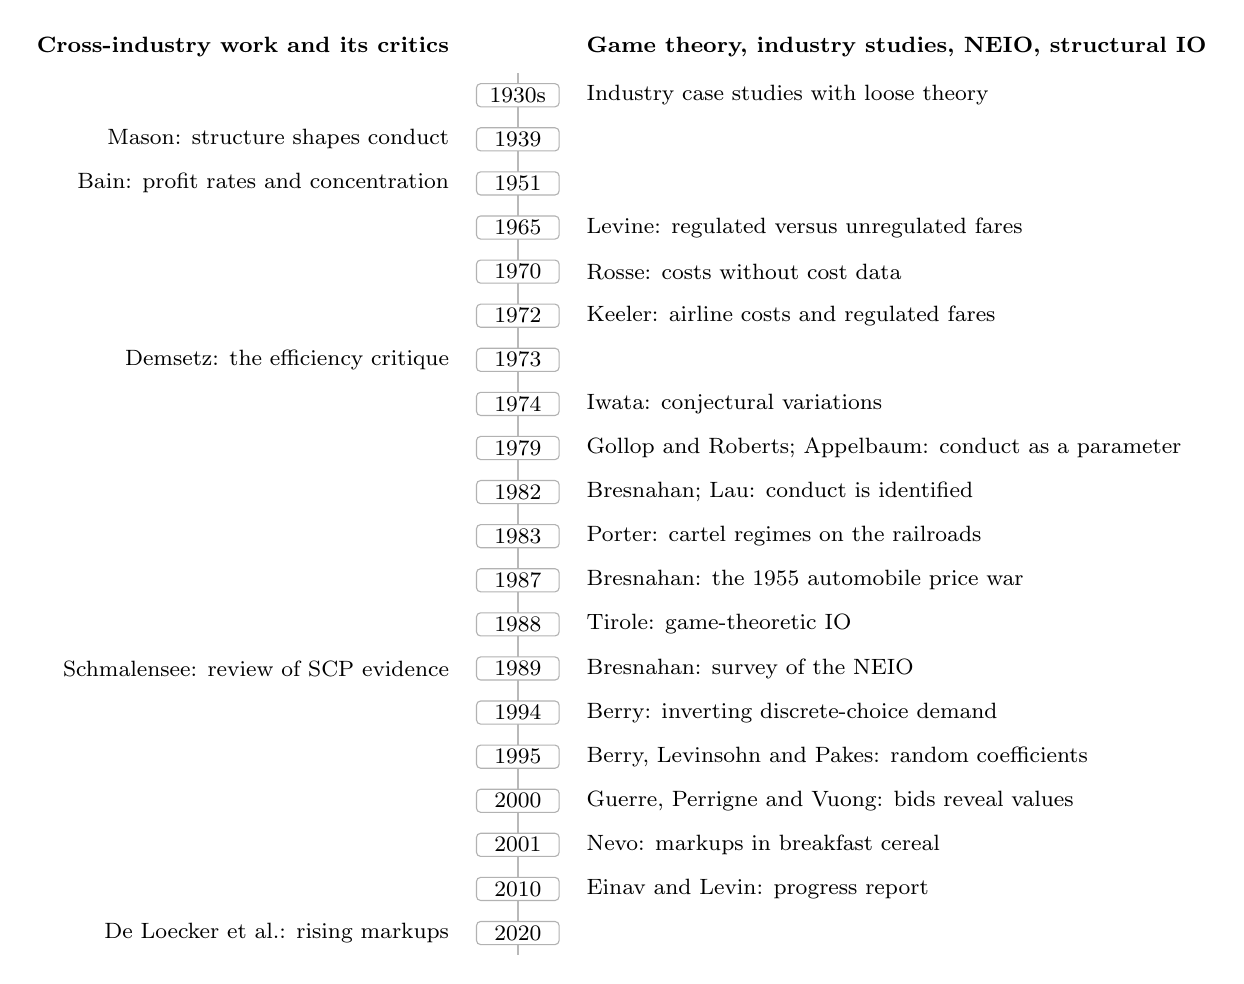
\begin{tikzpicture}[x=1cm, y=-0.56cm, every node/.style={font=\footnotesize}]
  \node[anchor=east, font=\footnotesize\bfseries] at (-0.75,-0.1) {Cross-industry work and its critics};
  \node[anchor=west, font=\footnotesize\bfseries] at (0.75,-0.1) {Game theory, industry studies, NEIO, structural IO};
  \draw[line width=0.8pt, gray!55] (0,0.5) -- (0,20.5);
  \foreach \y/\yr/\lt/\rt in {
    1/1930s//{Industry case studies with loose theory},
    2/1939/{Mason: structure shapes conduct}/,
    3/1951/{Bain: profit rates and concentration}/,
    4/1965//{Levine: regulated versus unregulated fares},
    5/1970//{Rosse: costs without cost data},
    6/1972//{Keeler: airline costs and regulated fares},
    7/1973/{Demsetz: the efficiency critique}/,
    8/1974//{Iwata: conjectural variations},
    9/1979//{Gollop and Roberts; Appelbaum: conduct as a parameter},
    10/1982//{Bresnahan; Lau: conduct is identified},
    11/1983//{Porter: cartel regimes on the railroads},
    12/1987//{Bresnahan: the 1955 automobile price war},
    13/1988//{Tirole: game-theoretic IO},
    14/1989/{Schmalensee: review of SCP evidence}/{Bresnahan: survey of the NEIO},
    15/1994//{Berry: inverting discrete-choice demand},
    16/1995//{Berry, Levinsohn and Pakes: random coefficients},
    17/2000//{Guerre, Perrigne and Vuong: bids reveal values},
    18/2001//{Nevo: markups in breakfast cereal},
    19/2010//{Einav and Levin: progress report},
    20/2020/{De Loecker et al.: rising markups}/%
  }{
    \node[fill=white, draw=gray!60, rounded corners=1.5pt, inner sep=1.6pt, minimum width=1.05cm] at (0,\y) {\yr};
    \node[anchor=east] at (-0.75,\y) {\lt};
    \node[anchor=west] at (0.75,\y) {\rt};
  }
\end{tikzpicture}
\caption[A timeline of empirical industrial organization]{A timeline of empirical industrial organization. Left:
the cross-industry tradition, its critics and its recent revival \citep{Mason1939,Bain1951,Demsetz1973,
Schmalensee1989,DeLoeckerEeckhoutUnger2020}. Right: game-theoretic IO, single-industry work, the NEIO and the
structural demand and supply models that followed \citep{Tirole1988,Levine1965,Rosse1970,Keeler1972,Iwata1974,
GollopRoberts1979,Appelbaum1979,Bresnahan1982,Lau1982,Porter1983,Bresnahan1987,Bresnahan1989,Berry1994,
BerryLevinsohnPakes1995,GuerrePerrigneVuong2000,Nevo2001,EinavLevin2010}. Rows are in chronological order and are
not drawn to scale.}
\label{fig:01-timeline}
\end{figure}

\subsection{Industry studies before the NEIO}\label{sec:01-early-studies}

Industry studies are older than the SCP paradigm. From the 1930s economists wrote detailed case studies of single
industries. These studies described pricing, capacity and rivalry with care. They made little attempt to generalize beyond the industry at hand, and the theory behind them was
loose. A case study could document that prices were high and stable. It could rarely say whether this reflected
market power, high costs or something else.

The clearest successes came in regulatory economics. \citet{Levine1965} compared air fares between Los Angeles
and San Francisco with fares in markets regulated by the Civil Aeronautics Board. Purely intrastate carriers on
this route, such as Pacific Southwest Airlines, were outside the Board's economic jurisdiction. The California
Public Utilities Commission, their only regulator, could not control entry in the period Levine studied
\citep[pp.~1430--1431]{Levine1965}. A state law signed on June 17, 1965, after Levine had written his article, gave the
Commission the power to regulate entry into intrastate air passenger service \citep[p.~1431, n.~63]{Levine1965}. The jet coach fare on this 350-mile route was about 3.9 cents per mile. The
national average jet coach fare was about 5.5 cents per mile, over longer stages that are cheaper to operate
\citep[p.~1433]{Levine1965}.
\citet{Keeler1972} estimated an airline cost function from interstate data and adjusted it to the operating
practices of the California intrastate carriers \citep[pp.~400--401]{Keeler1972}. He used seating densities
matching those of Pacific Southwest Airlines and a 60 percent load factor, below what the California carriers had
achieved \citep[pp.~405--406, 415 and 417]{Keeler1972}. The resulting
cost-based fares came within 3 percent of actual fares on two California intrastate routes. Among the 30 densest
routes in 1968, regulated coach fares exceeded these cost-based fares by 20 to 95 percent, and the markup tended
to rise with distance \citep[p.~416 and Table~6]{Keeler1972}. Both studies shaped the case for airline deregulation in the
late 1970s, the starting point of \cref{ch:airlines}. Their method compared prices with a competitive benchmark that
the data supplied directly, either an unregulated market or an estimate of cost.

\citet{Rosse1970} took a route that anticipated the NEIO. His title, which promises cost estimates ``without using cost
data'' (\cref{sec:01-lerner}), states the central idea of the later literature. He studied local newspapers, each treated as a
monopolist, and inferred marginal cost from the firm's pricing condition once demand had been estimated. The
application needed care because a newspaper sells two products. It sells circulation to readers and space to
advertisers, and the demand on each side depends on the other.

Let $Q^c$ denote circulation, $Q^a$ the column inches of advertising and $Q^e$ the column inches of editorial
content. The circulation price $P^c$ is the average price per subscription copy and the advertising price $P^a$ is
the average price per inch. Suppressing demand shifters and error terms, the inverse demands are
\begin{equation}\label{eq:01-rosse-demand}
P^a = P^a(Q^a, Q^c), \qquad P^c = P^c(Q^a, Q^c, Q^e).
\end{equation}
Advertisers pay more to reach more readers, so $\frac{\partial P^a}{\partial Q^c} > 0$. The newspaper chooses
$(Q^a, Q^c, Q^e)$ to maximize
\begin{equation*}
\Pi = P^a(Q^a, Q^c)\,Q^a + P^c(Q^a, Q^c, Q^e)\,Q^c - C(Q^a, Q^c, Q^e).
\end{equation*}
The marginal revenue of a product is the derivative of the firm's entire revenue with respect to that product's
quantity. For circulation, with $mc^c = \frac{\partial C}{\partial Q^c}$, the first-order condition is
\begin{equation*}
P^c + Q^c\frac{\partial P^c}{\partial Q^c} + Q^a\frac{\partial P^a}{\partial Q^c} - mc^c = 0 .
\end{equation*}
Solving for the circulation price gives the two-sided pricing condition \citep[eq.~6c]{Bresnahan1989}
\begin{equation}\label{eq:01-rosse-foc}
P^c = mc^c - Q^c\frac{\partial P^c}{\partial Q^c} - Q^a\frac{\partial P^a}{\partial Q^c} .
\end{equation}
The second term is the usual monopoly markup. The third term is new. It is the extra advertising revenue that one more
reader generates, and it lowers the circulation price. To see its size, divide \eqref{eq:01-rosse-foc} by $P^c$. Define
the inverse demand elasticities $f^c = -\frac{\partial \ln P^c}{\partial \ln Q^c} > 0$ and
$f^{ac} = \frac{\partial \ln P^a}{\partial \ln Q^c} > 0$. Then
\begin{align*}
\frac{P^c - mc^c}{P^c}
  &= -\frac{Q^c}{P^c}\frac{\partial P^c}{\partial Q^c} - \frac{Q^a}{P^c}\frac{\partial P^a}{\partial Q^c} \\
  &= f^c - \frac{P^a Q^a}{P^c Q^c}\cdot\frac{Q^c}{P^a}\frac{\partial P^a}{\partial Q^c}
   = f^c - \frac{P^a Q^a}{P^c Q^c}\, f^{ac} .
\end{align*}
The circulation price lies below marginal cost whenever $\frac{P^a Q^a}{P^c Q^c}\,f^{ac} > f^c$. This happens when
advertising revenue is large relative to circulation revenue and advertisers value readers highly. Most newspaper
revenue comes from advertising \citep[p.~1037]{Bresnahan1989}, so a reader price below marginal cost is a natural
outcome. A markup test applied to circulation alone would find price below marginal cost and could wrongly
conclude that newspapers have no market power. The theory of two-sided platforms later generalized this logic
\citep{RochetTirole2003,Armstrong2006}.

Rosse estimated the demand system \eqref{eq:01-rosse-demand} jointly with the pricing conditions. The
cross-equation restrictions between demand and marginal revenue then deliver marginal cost from the condition that
marginal cost equals marginal revenue. This let him treat marginal cost flexibly, for example by allowing transitory
shocks to firm size to separate short-run from long-run marginal cost. The approach is only as good as the estimated
marginal revenue. A linear demand curve may fit the data well and still give a poor estimate of its slope at the
observed point \citep[p.~1021]{Bresnahan1989}.

Two developments turned such isolated studies into a research program. The first was the critique of SCP regressions
developed in \cref{sec:01-scp-econometrics,sec:01-scp-after}. The second was the game theory revolution of the 1980s, which gave the field
sharp models of product differentiation, entry, pricing strategies and asymmetric information
\citep{Tirole1988}. Models proliferated so quickly that prominent members of the field lamented their overabundance
\citep{Fisher1989,Peltzman1991}. \citet[p.~146]{EinavLevin2010} note a lasting effect of this abundance. Because
predictions depended on fine details of preferences, information and commitment, empirical researchers learned to
take the institutional details of each market seriously. A single industry, studied with an explicit model, was the
natural place to do so.

\citet[Introduction]{Tirole1988} tells this history as two waves of interest in the field. The first was the
empirical Harvard tradition of \cref{sec:01-scp}. Alongside it, the ``Chicago tradition'' of Aaron Director and
George Stigler stressed rigorous theory and the empirical identification of competing theories. It also took a
permissive view of vertical restraints and predatory pricing, treating collusion as the main offense, and it
distrusted government intervention more than the Harvard tradition did. By the early 1970s many felt that theory
served more to explain statistical results or to buttress positions than to investigate markets systematically.
\citet[p.~273]{Joskow1975} wrote that ``the important messages are being carried by the informal theories,
stories, and behavioral observations.'' The formal models, in his phrase, were ``trotted out ex-post'' to show
that some formal apparatus could explain what was observed. Tirole attributes the second, mainly theoretical,
wave, which started in the 1970s, to three causes. On the demand side, researchers were dissatisfied with the
limits of cross-section work. On the supply side, leading theorists entered a field they had long ignored, and
noncooperative game theory became its standard tool. Game theory also made progress in two areas central to IO,
dynamics and asymmetric information. Tirole saw the new intra-industry studies of \citet{Porter1983} and
\citet{Bresnahan1987} as a sign that theory would soon feed back into empirical work (note~8).

\subsection{Principles of the NEIO}\label{sec:01-neio-principles}

\citet[p.~1012]{Bresnahan1989} summarizes the new approach in four ideas.
\begin{enumerate}
\item Price-cost margins are not observed. Economic marginal cost cannot be read from accounting data. The analyst
  infers it from firm behavior, uses differences between closely related markets to trace the effects of changes in
  marginal cost, or quantifies market power without measuring cost at all.
\item Industries have important idiosyncrasies. Institutional detail affects conduct, and it affects the measurement
  strategy even more. Comparative statics across industries are therefore suspect unless the markets are closely
  related.
\item Firm and industry conduct are unknown parameters. The behavioral equations by which firms set prices and
  quantities are estimated, and their parameters map into the notions of conduct of oligopoly theory.
\item The inference is explicit about its alternatives. The set of hypotheses is stated in advance. It includes the
  hypothesis of no strategic interaction, typically perfect competition, and the data can select it.
\end{enumerate}

The NEIO defined itself against three maintained hypotheses of the SCP paradigm \citep[pp.~1012--1013]{Bresnahan1989}.
The first was that economic price-cost margins can be observed in accounting data. The second was that
cross-industry differences in structure can be captured by a few observable measures, such as concentration ratios.
The third was that empirical work should estimate the reduced-form relation between structure and performance.
The gridlock over the meaning of high accounting profits, described in \cref{sec:01-demsetz}, showed where these
hypotheses led. No cross-industry regression could tell the market-power reading from the efficiency reading,
because both predict the same correlation.

The NEIO kept what the SCP paradigm had added to the field, namely systematic statistical evidence. It combined that
evidence with the attention to a single industry that marked the older case studies. In Bresnahan's words, the NEIO at
its best takes ``the best from the two great empirical IO traditions'' \citep[p.~1013]{Bresnahan1989}. A typical NEIO
paper is first of all an econometric model of one industry, with economic theory guiding both the specification and
the inference.

In practice these ideas translate into a recognizable research design.
\begin{itemize}
\item The unit of study is one industry, observed either as a time series or as a cross-section of geographic markets.
  Observations are similar to one another, so fewer factors are omitted than in a cross-section of industries.
\item Knowledge of the institutions guides the specification: which inputs matter, how the market clears, whether firms
  choose prices or quantities, and which prices are list prices and which are transaction prices.
\item Economic costs are inferred from pricing decisions rather than read from accounts. The inversion
  $\hat c = p\left(1 - \frac{1}{\hat\varepsilon^R}\right)$ of \cref{prop:01-infer-cost} is the simplest example.
\item Conduct is a parameter with an explicit interpretation (\cref{sec:01-conduct-parameter}).
\item External validity is claimed qualitatively. Some industries are studied as laboratories, for example ketchup,
  yogurt, laundry detergents or cement, and their value lies in mechanisms that travel to other markets. Others matter in
  their own right, for example health care, education, automobiles or airlines, and the specific numbers carry policy
  weight.
\end{itemize}
\citet[p.~147]{EinavLevin2010} make the same point about generality. The lasting lessons of industry studies tend to be
qualitative insights, such as the finding that entry can have large effects on prices, or methods that apply in many
settings.

A last principle concerns data. Economists in the field had long felt starved of appropriate data. The early NEIO
studies show this view to be false \citep[p.~1025]{Bresnahan1989}. The dissertations of Rosse, Bresnahan and Suslow
built their data from public industry sources, without relying on government statistics for the endogenous variables.
Porter's railroad data, discussed next, also came from industry records.

\subsection{Bresnahan's stylized model}\label{sec:01-stylized-model}

Most NEIO studies of homogeneous-good industries share one econometric structure. We present it in general form,
following \citet[Section~2.1]{Bresnahan1989} in the notation of this book, and then sketch Porter's study of a
railroad cartel as an illustration.

\casehead{Variables and equations}
Firms are indexed by $i = 1, \dots, N$ and observations, usually time periods, by $t$. The industry sells a single
product, so industry output $Q_t = \sum_i q_{it}$ is well defined. Demand has no intertemporal links from durability,
habits or learning. The endogenous variables are the market price $P_t$ and each firm's output $q_{it}$, or only
$Q_t$ when firm data are missing. Price-cost margins are not observed. The exogenous variables are demand shifters
$Y_t$, factor prices $W_{it}$ paid by firm $i$, and other cost shifters $Z_{it}$, such as fixed factors in a short-run
cost function. Three sets of unknown parameters describe demand ($\gamma$), cost ($\Gamma$) and conduct
($\vartheta$). The econometric errors $u^d_t$ and $u^c_{it}$ may enter nonlinearly and need not be scalars. The model
has five parts.
\begin{align}
P_t &= P(Q_t, Y_t, \gamma, u^d_t), \label{eq:01-bres-demand}\\
C_{it} &= C(q_{it}, W_{it}, Z_{it}, \Gamma, u^c_{it}), \label{eq:01-bres-cost}\\
mc_{it} &= C_q(q_{it}, W_{it}, Z_{it}, \Gamma, u^c_{it}), \label{eq:01-bres-mc}\\
P_t &= C_q(q_{it}, W_{it}, Z_{it}, \Gamma, u^c_{it}) - P_Q(Q_t, Y_t, \gamma, u^d_t)\, q_{it}\, \vartheta_{it}.
  \label{eq:01-bres-supply}
\end{align}
Equation \eqref{eq:01-bres-demand} is the inverse demand curve, \eqref{eq:01-bres-cost} the cost function and
\eqref{eq:01-bres-mc} marginal cost, where $C_q = \frac{\partial C}{\partial q}$. Equation \eqref{eq:01-bres-supply}
is the \emph{supply relation} of firm $i$, with $P_Q = \frac{\partial P}{\partial Q} < 0$ the slope of inverse
demand. Solving the demand equation and the $N$ supply relations together gives the reduced forms
\begin{equation}\label{eq:01-bres-rf}
P_t = P^*(W_t, Z_t, Y_t, \Theta, u_t), \qquad q_{it} = q_i^*(W_t, Z_t, Y_t, \Theta, u_t),
\end{equation}
where $\Theta = (\gamma, \Gamma, \vartheta)$ collects all parameters, $u_t$ all errors, and $W_t$ and $Z_t$ the
shifters of all firms. Equations \eqref{eq:01-bres-demand} to \eqref{eq:01-bres-rf} are Bresnahan's equations (1) to
(5) and (5$'$). We write $\Theta$ where Bresnahan writes $\Omega$, because $\Omega$ is the ownership matrix in this
book, and $\gamma$ where he writes $\delta$.

\casehead{The supply relation}
The supply relation states that marginal cost equals a ``perceived'' marginal revenue. For a monopolist,
$P + P_Q\,Q$ is marginal revenue. In \eqref{eq:01-bres-supply} the term $-P_Q\,q_{it}\vartheta_{it}$ is the wedge
between price and marginal cost, and $\vartheta_{it} \ge 0$ indexes how far the conduct of firm $i$ departs from price
taking. The value $\vartheta_{it} = 0$ is price taking. The value $\vartheta_{it} = 1$ is Cournot conduct and, with a
single firm, monopoly. Bresnahan calls it a supply relation because outside perfect competition firms have no
\emph{supply curve}, that is, no function $Q = S(P)$ that solves $P = mc(Q)$ \citep[fn.~6]{Bresnahan1989}. A firm
with market power chooses its output in response to the whole demand curve, including its slope, so the same price
can go with different outputs.

Equation \eqref{eq:01-bres-supply} seems to contain marginal cost, which the NEIO treats as unobserved. The
contradiction is only apparent. In the model, marginal cost is a function of the unknown parameters $\Gamma$, and it
can be computed only after $\Gamma$ has been estimated. Most methods estimate $\Gamma$ and $\vartheta$ in the same econometric step. A conduct parameter
that varies freely by firm and period would overparameterize the model. Bresnahan writes it this way only to nest all
known oligopoly theories, and every application restricts how $\vartheta_{it}$ varies.

\begin{remark}[Firm-level and industry conduct]\label{rem:01-firm-industry-conduct}
Bresnahan uses one symbol for two normalizations of conduct, and we keep them apart. The firm-level parameter
$\vartheta_{it}$ in \eqref{eq:01-bres-supply} equals $1 + r_i$ in the conjectural-variations notation of
\cref{sec:01-cournot-hhi}. It is $0$ for price taking, $1$ for Cournot and $N$ for symmetric collusion. The industry
parameter $\theta$ of this book weights each firm's conduct by its squared share, $\theta = \sum_i s_i^2\,\vartheta_i$,
as derived in \cref{prop:01-supply-relation} below. It is $0$ for price taking, $\HHI$ for Cournot and $1$ for collusion. With
symmetric firms, $q_{it} = \frac{Q_t}{N}$ and $s_i = \frac{1}{N}$, so
\begin{equation*}
\theta = \sum_{i=1}^{N} \frac{1}{N^2}\,\vartheta = \frac{\vartheta}{N}.
\end{equation*}
Symmetric Cournot ($\vartheta = 1$) gives $\theta = \frac{1}{N}$ and symmetric collusion ($\vartheta = N$) gives
$\theta = 1$, the convention used throughout the book.
\end{remark}

The core econometric methods are those for simultaneous equations, since $P_t$ and $q_{it}$ (or $Q_t$) are jointly
determined. Some studies estimate \eqref{eq:01-bres-demand} and \eqref{eq:01-bres-supply} directly as structural
equations, which is attractive because the conduct parameters are the object of interest. Studies that lack price,
quantity or firm-level data estimate reduced forms such as \eqref{eq:01-bres-rf} or aggregate the supply relations
to the industry level.

\subsubsection{An illustration: the Joint Executive Committee}\label{sec:01-porter-illustration}

\citet{Bresnahan1989} develops the stylized model alongside one application, Porter's (\citeyear{Porter1983}) study of
a nineteenth-century railroad cartel. We sketch that study here and draw out what it teaches about the NEIO. The full
case study, with the theory of \citet{GreenPorter1984} behind it and later reanalyses, appears in
\cref{ch:collusion-evidence}.

The Joint Executive Committee (JEC) was a legal cartel that controlled eastbound freight shipments from Chicago to the
Atlantic seaboard \citep[p.~302]{Porter1983}. Porter asks whether its prices switched between collusive and price-war
regimes, as trigger-price theories of collusion predict. The data are weekly records from the first week of 1880 to
the sixteenth week of 1886, which gives 328 observations. Quantity $Q_t$ is the tonnage of grain shipped by members,
and price $P_t$ is the grain rate in dollars per 100 pounds \citep[Table~2]{Porter1983}. Demand has constant
elasticity and shifts down when the Great Lakes are open to shipping. The supply relation is the industry version of
\eqref{eq:01-bres-supply}, derived in \cref{prop:01-supply-relation} below. Conduct takes a collusive value
$\theta^{c}$ in some weeks, and Porter normalizes conduct during price wars to the Bertrand value $\theta^{w} = 0$. He
treats each week's regime as an unobserved draw, collusive with a constant probability $\varpi$, and estimates the
system by maximum likelihood. We write $\varpi$ to keep $\pi$ for profit. Demand is inelastic, with an estimated
elasticity of $\hat\varepsilon = 0.80$ \citep[Table~3]{Porter1983}. With the lakes closed, predicted prices are 0.2780
dollars in collusive weeks and 0.1673 in price-war weeks \citep[Table~4]{Porter1983}. Collusion thus raised price by
66 percent and lowered quantity by 33 percent \citep[p.~310]{Porter1983}. The implied collusive conduct parameter is
$\hat\theta^{c} = 0.336$, which Porter calls roughly consistent with Cournot behavior \citep[p.~309]{Porter1983}.
\Cref{sec:13-jec} develops the model and estimates.

\citet[p.~1018]{Bresnahan1989} summarizes these findings in three statements. First, successful collusion raised
price by about 40 percent. This is the 0.40 reported for Porter in \cref{tab:01-bresnahan-table}. It measures the gap
from the collusive price, since $1 - \frac{0.1673}{0.2780} = 0.40$. Porter's 66 percent measures the same gap from
the price-war price. Second, the implied conduct was about as anticompetitive as Cournot. Only the gap between
the regimes is identified, because conduct during wars and the cost intercept enter the supply relation together. The
Cournot reading therefore rests on the unidentified assumption that price-war conduct was price taking (his
fn.~10). Third, the cartel broke down 28 percent of the time.

\casehead{What the illustration teaches}
Bresnahan sees three advantages in this structural approach \citep[p.~1018]{Bresnahan1989}. First, every parameter
has an economic meaning, so implausible estimates are diagnostic. Porter's demand elasticity is an example. With
$\hat\varepsilon = 0.80 < 1$, industry marginal revenue is negative, so the collusive weeks cannot reflect static joint
profit maximization \citep[p.~308]{Porter1983}. A conduct parameter of one would imply a Lerner index of
$\frac{1}{0.8} = 1.25$, which is impossible with positive marginal cost. Second, if the interpretation of conduct is
right, the link between the estimates and oligopoly theory is clear. Third, because the model is structural, the reason
why the data identify conduct can be stated. \Cref{sec:01-identification} takes up this third point.

Bresnahan also notes what the specification leaves out \citep[p.~1025]{Bresnahan1989}. A single constant probability
$\varpi$ tells us how often the cartel broke down. It cannot tell us what triggered breakdowns or what ended them,
which is where theories of collusion disagree. Answering that question needs a state-dependent switching probability.
Bresnahan doubts that the data can discriminate among the theories. A test of whether there are two regimes uses every
week of data, but a test of what starts and stops price wars has as many observations as there are price wars.

\subsection{Conduct as a parameter}\label{sec:01-conduct-parameter}

The stylized model treats conduct as an unknown parameter. This subsection derives the industry supply relation in
general form and lists the values of conduct implied by standard theories. It then surveys how the literature
specified conduct and explains how the estimates should and should not be read.

\begin{proposition}[Industry supply relation]\label{prop:01-supply-relation}
Consider a homogeneous good with differentiable inverse demand $P(Q)$, $P'(Q) < 0$, and $N$ firms with differentiable
costs $C_i(q_i)$. Firm $i$ chooses $q_i$ to maximize $P(Q)\,q_i - C_i(q_i)$, where $Q = q_i + Q_{-i}$ and the
conjectural variation $r_i = \frac{\dd Q_{-i}}{\dd q_i}$ of \cref{sec:01-cournot-hhi} is treated as a constant. Assume an interior solution
with every firm active, and let $mc_i = C_i'(q_i)$, $s_i = \frac{q_i}{Q}$ and $\varepsilon = -\frac{P}{Q\,P'(Q)}$.
Then:
\begin{enumerate}[label=(\roman*)]
\item Each firm satisfies the supply relation $P = mc_i - P'(Q)\,q_i\,(1 + r_i)$.
\item The industry satisfies
  \begin{equation}\label{eq:01-supply-relation}
  P = \overline{mc} - P'(Q)\,Q\,\theta, \qquad
  \overline{mc} = \sum_{i=1}^{N} s_i\, mc_i, \qquad
  \theta = \sum_{i=1}^{N} s_i^2 (1 + r_i).
  \end{equation}
\item Equivalently, $\frac{P - \overline{mc}}{P} = \frac{\theta}{\varepsilon}$, and average marginal cost can be
  recovered as $\overline{mc} = P + \theta\, Q\, P'(Q) = P\left(1 - \frac{\theta}{\varepsilon}\right)$.
\end{enumerate}
\end{proposition}

\begin{proof}
(i) The derivative of firm $i$'s profit is
\begin{equation*}
\frac{\dd}{\dd q_i}\Bigl[P(Q)\,q_i - C_i(q_i)\Bigr]
= P(Q) + q_i\,P'(Q)\,\frac{\dd Q}{\dd q_i} - C_i'(q_i)
= P + q_i\,P'(Q)\,(1 + r_i) - mc_i ,
\end{equation*}
because $\frac{\dd Q}{\dd q_i} = 1 + \frac{\dd Q_{-i}}{\dd q_i} = 1 + r_i$. Setting it to zero and solving for $P$
gives (i). (ii) Multiply (i) by $s_i$ and sum over $i$:
\begin{align*}
\sum_i s_i P &= \sum_i s_i\, mc_i - P'(Q)\sum_i s_i\, q_i (1 + r_i), \\
P &= \overline{mc} - P'(Q)\, Q \sum_i s_i^2 (1 + r_i),
\end{align*}
using $\sum_i s_i = 1$ and $q_i = s_i Q$. (iii) Subtract $\overline{mc}$ from both sides of \eqref{eq:01-supply-relation}
and divide by $P$:
\begin{equation*}
\frac{P - \overline{mc}}{P} = -\frac{Q\,P'(Q)}{P}\,\theta = \frac{\theta}{\varepsilon}.
\end{equation*}
Solving \eqref{eq:01-supply-relation} for $\overline{mc}$ gives the last statement.
\end{proof}

\Cref{prop:01-supply-relation} extends \cref{prop:01-clarke-davies} to marginal costs that vary with output. It shows
that one number, $\theta$, summarizes industry conduct for the purpose of the industry markup, whatever the
heterogeneity across firms. \Cref{tab:01-conduct-menu} lists the values implied by standard theories. The
inversion in part (iii) is the conduct-adjusted version of \cref{prop:01-infer-cost}. It is how the NEIO turns an
estimated demand curve and an assumed or estimated $\theta$ into an estimate of marginal cost.

\begin{table}[htbp]
\centering
\begin{threeparttable}
\caption{Conduct implied by standard oligopoly theories}
\label{tab:01-conduct-menu}
\small
\renewcommand{\arraystretch}{1.45}
\begin{tabular}{@{}lcccc@{}}
\toprule
Conduct & $r_i = \frac{\dd Q_{-i}}{\dd q_i}$ & $\vartheta_i = 1 + r_i$ & $\theta = \sum_i s_i^2(1 + r_i)$
  & $\frac{P - \overline{mc}}{P}$ \\
\midrule
Perfect competition & $-1$ & $0$ & $0$ & $0$ \\
Cournot & $0$ & $1$ & $\HHI$ & $\frac{\HHI}{\varepsilon}$ \\
Symmetric Cournot & $0$ & $1$ & $\frac{1}{N}$ & $\frac{1}{N\varepsilon}$ \\
Collusion (joint profit maximum) & $\frac{1 - s_i}{s_i}$ & $\frac{1}{s_i}$ & $1$ & $\frac{1}{\varepsilon}$ \\
Symmetric collusion & $N - 1$ & $N$ & $1$ & $\frac{1}{\varepsilon}$ \\
Clarke-Davies, $\kappa \in [0, 1]$ & $\kappa\frac{1 - s_i}{s_i}$ & $\frac{\kappa + (1 - \kappa)s_i}{s_i}$
  & $\kappa + (1 - \kappa)\HHI$ & $\frac{\kappa + (1 - \kappa)\HHI}{\varepsilon}$ \\
\bottomrule
\end{tabular}
\begin{tablenotes}\footnotesize
\item Notes: $s_i$ are output shares, $\HHI = \sum_i s_i^2$, and $\varepsilon$ is the market elasticity of demand.
Under collusion each firm acts as if rivals match its output in proportion to their shares, so
$1 + r_i = \frac{1}{s_i}$ and $\theta = \sum_i s_i = 1$. With constant marginal costs, the collusion rows require
equal costs across active firms. With rising marginal costs, they equalize marginal costs across firms. The
Clarke-Davies row is
\cref{prop:01-clarke-davies}: $s_i^2(1 + r_i) = (1 - \kappa)s_i^2 + \kappa s_i$, and summing gives
$\kappa + (1 - \kappa)\HHI$. Perfect competition requires rising marginal cost for an interior solution.
\end{tablenotes}
\end{threeparttable}
\end{table}

\subsubsection{How the literature specified conduct}\label{sec:01-conduct-taxonomy}

\citet[Section~2.2]{Bresnahan1989} sorts the early studies into four groups by how they wrote the supply relation. The
groups differ in language more than in substance.

\casehead{Supply relations from a single theory}
The first group derives $\vartheta_{it}$ from one explicit theory. The simplest case is monopoly or Cournot, where
$\vartheta_{it} = 1$ for all firms and periods \citep[eq.~6]{Bresnahan1989}:
\begin{equation*}
P_t = C_q(q_{it}, W_{it}, Z_{it}, \Gamma, u^c_{it}) - P_Q(Q_t, Y_t, \gamma, u^d_t)\,q_{it}.
\end{equation*}
With several firms this gives one estimating equation per firm. Rosse's newspapers, with the two-sided condition
\eqref{eq:01-rosse-foc}, belong here.

Bertrand pricing is the other static noncooperative model. With a homogeneous product and a flat marginal cost common to all firms
it is indistinguishable from perfect competition, so applications use differentiated products. \citet{Bresnahan1981}
estimates such a model on the 1977 and 1978 cross-sections of American automobiles. Products are ordered on a
one-dimensional quality index $\chi_j$, with neighbors $j - 1$ and $j + 1$. Consumers differ in a scalar taste for
quality. A consumer with taste $\nu$ who buys product $j$ at price $p_j$ gets $\nu\chi_j - p_j$, so she prefers $j$ to
$j + 1$ exactly when $\nu < \frac{p_{j+1} - p_j}{\chi_{j+1} - \chi_j}$. (Here $\nu$ is a taste for quality. Dividing
utility by $\nu$ gives the equivalent form with a consumer-specific price sensitivity used in \cref{ch:discrete}.) With
tastes spread uniformly with density $\gamma_0$, demand is
\begin{equation}\label{eq:01-vertical-demand}
q_j = \gamma_0\left(\frac{p_{j+1} - p_j}{\chi_{j+1} - \chi_j} - \frac{p_j - p_{j-1}}{\chi_j - \chi_{j-1}}\right) + u^d_j ,
\end{equation}
and quality is a hedonic function of observed characteristics $x_j$, such as length, weight and horsepower,
\begin{equation}\label{eq:01-vertical-quality}
\chi_j = f(x_j, \gamma_1) + u^{\chi}_j .
\end{equation}
These are Bresnahan's equations (7) and (8). Prices are manufacturer-to-dealer list prices, which equal transaction
prices for most sales, and quantities are model-year production. A firm $f$ owning the set of products
$\mathcal{J}_f$ chooses prices to maximize $\sum_{k \in \mathcal{J}_f} (p_k - mc_k)\,q_k$. Differentiating
\eqref{eq:01-vertical-demand},
\begin{equation*}
\frac{\partial q_j}{\partial p_j} = -\gamma_0\left(\frac{1}{\chi_{j+1} - \chi_j} + \frac{1}{\chi_j - \chi_{j-1}}\right),
\qquad
\frac{\partial q_{j+1}}{\partial p_j} = \frac{\gamma_0}{\chi_{j+1} - \chi_j},
\qquad
\frac{\partial q_{j-1}}{\partial p_j} = \frac{\gamma_0}{\chi_j - \chi_{j-1}} .
\end{equation*}
Let $\Omega_{jk} = 1$ if the same firm sells $j$ and $k$, and $\Omega_{jk} = 0$ otherwise. The matrix $\Omega$ is the
\emph{ownership matrix}, which returns in \cref{sec:01-workflow}. The first-order condition $q_j + \sum_{k \in \mathcal{J}_f}(p_k - mc_k)\frac{\partial q_k}{\partial p_j} = 0$ becomes
the supply relation
\begin{equation}\label{eq:01-vertical-foc}
q_j = \gamma_0 (p_j - mc_j)\left(\frac{1}{\chi_{j+1} - \chi_j} + \frac{1}{\chi_j - \chi_{j-1}}\right)
 - \Omega_{j,j+1}\,\gamma_0\,\frac{p_{j+1} - mc_{j+1}}{\chi_{j+1} - \chi_j}
 - \Omega_{j,j-1}\,\gamma_0\,\frac{p_{j-1} - mc_{j-1}}{\chi_j - \chi_{j-1}} ,
\end{equation}
the counterpart of Bresnahan's equation (6$''$). Marginal cost depends on the characteristics of the product. The
markup of product $j$ is large when its neighbors are far away in quality space. \citet{Bresnahan1981} finds large
price-cost margins on the larger cars, which are also much farther apart in quality space. The obvious weakness is the
restrictive demand system. Bresnahan probes it through the residuals, firm dummies and the quality error in
\eqref{eq:01-vertical-quality}. \Cref{ch:discrete} develops the vertical model in full.

A second class of single theories gives firms different roles. In the \emph{Stackelberg} model, firms
$2, \dots, N$ follow Cournot supply relations and the leader, firm 1, internalizes their reaction. Its supply relation is
\begin{equation}\label{eq:01-stackelberg}
P_t = C_q(q_{1t}, W_{1t}, Z_{1t}, \Gamma, u^c_{1t}) - P_Q(Q_t, Y_t, \gamma, u^d_t)\,q_{1t}\,(1 + \theta_S),
\end{equation}
where $\theta_S$ is the derivative of the followers' total output with respect to $q_1$, obtained by solving their
supply relations. A linear example shows what $\theta_S$ looks like. Let $P = a - bQ$ and let the $N - 1$ followers
have constant marginal cost $c$. Follower $j$'s Cournot condition is $a - bQ - b q_j = c$. Summing over the followers,
with $Q = q_1 + Q_F$ and $Q_F$ their total output,
\begin{align*}
(N - 1)(a - c) - (N - 1)\,b\,(q_1 + Q_F) - b\,Q_F &= 0, \\
Q_F &= \frac{(N - 1)(a - c - b\,q_1)}{N b}.
\end{align*}
Hence $\theta_S = \frac{\dd Q_F}{\dd q_1} = -\frac{N - 1}{N}$, and the leader's firm-level conduct is
$\vartheta_1 = 1 + \theta_S = \frac{1}{N}$. The leader behaves more aggressively than a Cournot firm because each unit
it adds displaces part of the followers' output.

The \emph{dominant-firm} model is closely related. \citet{Suslow1986} estimates it for Alcoa in the interwar period,
when Alcoa was the only producer of new aluminum and a fringe of firms recycled scrap. The fringe takes price as given,
so its supply relation is a supply curve. Write it as $Q_{ft} = S(P_t, W_{ft}, Z_{ft}, \Gamma, u^c_{ft})$, the inverse
of $P_t = C_q(Q_{ft}, \dots)$. Bresnahan's equations (10) and (10$'$) are these two forms. The dominant firm faces the
residual demand $q_1 = Q(P) - S(P)$, where $Q(P)$ is market demand. Its slope is
\begin{equation*}
\frac{\dd P}{\dd q_1} = \frac{1}{Q'(P) - S_P} = \frac{P_Q}{1 - P_Q S_P},
\end{equation*}
where $P_Q = \frac{1}{Q'(P)} < 0$ and $S_P = \frac{\partial S}{\partial P} \ge 0$. The first-order condition
$P + q_1\frac{\dd P}{\dd q_1} = mc_1$ can be written in the form of \eqref{eq:01-bres-supply}:
\begin{equation}\label{eq:01-dominant}
P_t = mc_{1t} - P_Q\,q_{1t}\,(1 + S_D), \qquad S_D = \frac{P_Q S_P}{1 - P_Q S_P} \in (-1, 0].
\end{equation}
These are Bresnahan's equations (11) and (11$'$). With no fringe response ($S_P = 0$) the leader is a monopolist on its residual demand and $S_D = 0$. As the fringe supply becomes
perfectly elastic, $S_D \to -1$ and the leader becomes a price taker. In elasticity form, with $s_1$ the leader's share
and $e_S$ the fringe supply elasticity, $P_Q S_P = -\frac{(1 - s_1)e_S}{\varepsilon}$, and
\begin{equation*}
\frac{P - mc_1}{P} = \frac{s_1}{\varepsilon}\,(1 + S_D) = \frac{s_1}{\varepsilon + (1 - s_1)\,e_S} .
\end{equation*}
In Suslow's data Alcoa's marginal cost is shifted by its accounting average variable cost, which does not enter the fringe
supply. The fringe supply is shifted by the stock of aluminum available for recycling. She estimates $S_D$ to be small, so
Alcoa had considerable market power despite the fringe \citep[p.~1023]{Bresnahan1989}. She identifies Alcoa as the
leader from the structure of the industry, a monopoly in new aluminum facing many recyclers.

Dynamic theories of collusion form the last part of this group. \citet{Stigler1964} argued that cartels held together
by self-interest should sometimes break down. Firms cannot always tell whether a fall in their sales reflects secret
price cutting, so suspicion leads to price wars even without cheating. \citet{GreenPorter1984} formalized this idea.
Firms observe the market price but not rivals' outputs, and a low price triggers a reversion to Cournot behavior for a
fixed period. The cartel chooses the collusive output, the trigger price and the length of punishment to maximize
expected profit. It does not push price to the monopoly level, because a higher price raises the gain from cheating.
\citet{AbreuPearceStacchetti1986} find more profitable designs in which both the start and the end of a price war are
triggered, so wars have random length and endogenous severity. \citet{RotembergSaloner1986} let demand fluctuate. When
current demand does not predict future demand, the gain from defecting is largest in booms, so the cartel must lower
its price in booms. All these theories imply that $\vartheta_{it}$ varies over time. They differ in the predicted
timing of the regimes, which is why Porter's constant $\varpi$ cannot tell them apart. \Cref{ch:collusion-theory}
develops these models.

\casehead{Testing a small set of theories}
A second group estimates the supply relations of a few distinct theories and tests among them.
\citet{Bresnahan1987} uses the vertical model \eqref{eq:01-vertical-demand} for the American automobile industry in
the mid-1950s. Under joint profit maximization, $\Omega_{jk} = 1$ for every pair of neighbors in
\eqref{eq:01-vertical-foc}, because industry marginal revenue counts every product. Under Bertrand pricing $\Omega_{jk}$
follows actual ownership.
Non-nested tests favor collusion in 1954 and 1956 and Bertrand competition in 1955, the year of a large expansion of
output and a fall in prices. A temporary breakdown of collusion thus explains part of the 1955 boom. \Cref{ch:discrete}
treats this paper as a case study. \citet{Geroski1983} and \citet{Roberts1984} test leader-follower theories on the
coffee-roasting data of \citet{GollopRoberts1979}. The smaller roasters behave as price-taking followers. The leading
firms behave less competitively than Cournot firms. They stop short of maximizing joint profits, even given the
fringe \citep[p.~1026]{Bresnahan1989}.

The difference between estimating a continuous $\vartheta$ and choosing among a few theories is purely econometric
\citep[p.~1026]{Bresnahan1989}. A researcher who estimates $\vartheta$ on a continuum tests theories with nested tests,
and may find a value between two theories. A researcher who specifies a few theories uses non-nested tests.

\casehead{Conjectural-variations language}
A third group writes conduct as a conjectural variation, a firm's ``expectation'' of how rivals' outputs respond
to its own. Starting with \citet{Iwata1974}, these papers write the supply relation as
\begin{equation}\label{eq:01-cv-supply}
P_t = C_q(\cdot) - P_Q(\cdot)\, q_{it}\,\bigl(1 + r_i(q_{it}, Q_{-i,t}, Z_{it}, \Phi)\bigr),
\end{equation}
where the parameters $\Phi$ let conjectures depend on firm size and other variables. Iwata asked where the Japanese
plate glass industry lay between competition and monopoly. He assumed, unlike most later work, that accounting data
reveal margins. \citet{GollopRoberts1979} let conjectures differ across firms in coffee roasting, and
\citet{SpillerFavaro1984} and \citet{GelfandSpiller1987} continued this emphasis on heterogeneous conduct in banking.

Equation \eqref{eq:01-cv-supply} differs from \eqref{eq:01-bres-supply} only in replacing $\vartheta_{it}$ by
$1 + r_i(\cdot)$. As a matter of logic the two are identical, since $\vartheta_{it} - 1 = r_i(\cdot)$ nests the same
models. Bresnahan puts it strongly: saying what the conjectural variation is and saying which theory of oligopoly holds
in the data are the same statement \citep[p.~1027]{Bresnahan1989}. The practical differences are two.
Conjectural-variation papers allow all values of $r_i$, and they stress the link between firm size and conduct.

\casehead{Aggregate data and average conduct}
A fourth group has only industry data. It writes the supply relation in aggregate form \citep[eq.~16]{Bresnahan1989},
\begin{equation}\label{eq:01-aggregate-supply}
P_t = C_q(Q_t, W_t, Z_t, \Gamma, u^c_t) - P_Q(Q_t, Y_t, \gamma, u^d_t)\, Q_t\, \theta_t ,
\end{equation}
as in \citet{Appelbaum1979} and Porter's study. Under the null of price taking ($\theta_t = 0$), $C_q$ is industry
marginal cost. With market power, firms generally have different marginal costs in equilibrium. Cournot firms with
different costs have different margins \citep{CowlingWaterson1976}, so a stable industry marginal cost curve need not
exist. \Cref{prop:01-supply-relation} gives the right reading. The aggregate $\theta_t = \sum_i s_{it}^2\vartheta_{it}$
weights each firm's conduct by its squared share, and $\frac{P - C_q}{P}$ is the share-weighted average markup. Some authors claimed that oligopoly theory implies identical
conduct across firms \citep{Appelbaum1982,Lopez1984}. Bresnahan rejects this claim, since nothing in oligopoly theory
forces firms to behave alike.

\subsubsection{What an estimated conjecture means}\label{sec:01-cv-warning}

The language of conjectures invites a misreading \citep[pp.~1027--1029]{Bresnahan1989}. Suppose we read
\eqref{eq:01-cv-supply} as the first-order condition of a firm that expects rivals' outputs to depend on its own:
\begin{equation}\label{eq:01-cv-profit}
\max_{q_i}\; P\Bigl(q_i + \sum_{j \ne i} Q_j(q_i)\Bigr)\, q_i - C(q_i),
\qquad
1 + r_i = \frac{\dd q_i}{\dd q_i} + \sum_{j \ne i} \frac{\dd Q_j}{\dd q_i} .
\end{equation}
For Cournot conduct ($r_i = 0$) and price taking ($r_i = -1$) the reading is harmless. A Cournot firm can be described as
expecting rivals' outputs to stay fixed, and a competitive firm as expecting price to stay fixed.

The trouble arises near collusion. Let all $N$ firms have the same costs and the collusive conjecture $1 + r_i = N$.
Each supply relation becomes
\begin{equation}\label{eq:01-collusive-foc}
P = C_q(\cdot) - P_Q(\cdot)\, N\, q_i ,
\end{equation}
which is the first-order condition for maximizing the joint profit of all $N$ firms. Read literally, $r_i = N - 1$ says
that each firm expects every rival to match any change in its output one for one, $\frac{\dd Q_j}{\dd q_i} = 1$. Repeated
games give a different account of the same outcome. Firms produce their share of the collusive output because they expect
a deviation to trigger a general breakdown of restraint. The matching behavior is never observed. It is the threat that
keeps it off the equilibrium path.

Bresnahan therefore separates two objects: (i) what firms believe will happen if they deviate, and (ii) what firms do
as a result of those beliefs. Estimated conjectures measure only (ii). If they are stable over time and breakdowns are
rare, they measure the average collusiveness of conduct. They carry no information about what would happen if one
firm expanded output on its own, which is the sense of ``conjectural variation'' in theoretical work. The only thing
they reveal about expectations is that the expectations suffice to deter departures from the normal arrangement
\citep[fn.~19]{Bresnahan1989}. For the same reason Bresnahan rejects reading the slope of $r_i(\cdot)$ in own output as
evidence of ``mutual forbearance''.

A second interpretive issue concerns firm size. Models with different conjectures for different size classes produce
an equilibrium size distribution even among identical firms. A competing explanation is that firms differ in cost.
Separating the two requires firm-specific cost functions, and in particular a comparison of the marginal costs of large
and small firms at the same output \citep[p.~1030 and fn.~20]{Bresnahan1989}.

\subsubsection{Every specification is a test of price taking}\label{sec:01-appelbaum}

\citet{Appelbaum1979} observed that setting every conduct parameter to zero in \eqref{eq:01-bres-supply}, or every
$r_i$ to $-1$, imposes price taking. Every specification of conduct, theoretical or not, therefore nests the
competitive model. Its estimation is a test of price-taking behavior, the title of Appelbaum's paper, against an
alternative in which firms raise price above marginal cost. This is the advance that the NEIO claims over the SCP
paradigm \citep[p.~1031]{Bresnahan1989}. When price taking is rejected, it is rejected against specific theories of
market power. The interpretation of the result is then clear, and only econometric problems can cloud the inference.

Two cautions carry over to later chapters. First, an estimated $\theta$ is a reduced summary of behavior, as the
discussion of conjectures shows. \citet{Corts1999} shows that when firms collude dynamically, the estimated $\theta$
tracks how the markup responds to demand shocks at the margin. It can then differ greatly from the average markup that
it is meant to measure. His Proposition~1 (p.~233) states the condition exactly, for linear demand, constant
marginal cost and a symmetric equilibrium. Let $q^*$ be equilibrium output per firm and $Y$ a demand shifter. The
estimate equals the elasticity-adjusted Lerner index that $\theta$ is meant to measure if and only if
\[
\frac{P - mc}{q^*} = \frac{\frac{\dd (P - mc)}{\dd Y}}{\frac{\dd q^*}{\dd Y}} .
\]
The margin per unit of output must equal the marginal response of the margin to output along demand-driven
movements. Under efficient supergame collusion this condition fails. The estimated conduct parameter then
understates market power unless demand shocks are fully permanent. When the shocks are completely transitory, it
may detect no market power at all, even if average margins are near the monopoly level (p.~245).
\Cref{ch:conduct} develops this critique. Second, the theory of the conduct parameter, including
its links to conjectural variations and pass-through, appears in \cref{ch:theory}.

\section{How the data identify market power}\label{sec:01-identification}

A structural model states the class of hypotheses among which the data choose. This makes a central question
answerable \citep[p.~1031]{Bresnahan1989}. Why do the data identify the inference of market power? Which implication
of perfect competition has been rejected when market power is measured? The question does not arise in the SCP
paradigm, which takes margins to be observed. In the NEIO margins are estimated, so we must ask which features of the
data and which natural experiments reveal them. Bresnahan distinguishes four classes of arguments: comparative statics
in demand, comparative statics in cost, direct estimation of marginal cost, and supply shocks. A fifth, comparative
statics in industry structure, is familiar in its logic but still lacked a sound identification argument in 1989. This
section explains each, then turns to differentiated products and to what the NEIO learned.

\subsection{The identification question}\label{sec:01-id-question}

The question is this. Given equilibrium prices and quantities from different but similar markets, under what conditions
can we identify conduct, or test for market power, without observing demand and cost? A linear model shows the
difficulty. Let demand and marginal cost be
\begin{equation}\label{eq:01-linear-id-model}
Q_t = a_0 + a_1 P_t + a_2 Y_t + u^d_t, \qquad mc_t = b_0 + b_1 Q_t + b_2 W_t + u^c_t ,
\end{equation}
with $a_1 < 0$, a demand shifter $Y_t$ and a cost shifter $W_t$. The slope of inverse demand is $\frac{1}{a_1}$, so the
supply relation of \cref{prop:01-supply-relation} is $P_t = mc_t - \theta\frac{Q_t}{a_1}$. Substituting marginal cost,
\begin{equation}\label{eq:01-linear-supply}
P_t = b_0 + \left(b_1 - \frac{\theta}{a_1}\right) Q_t + b_2 W_t + u^c_t .
\end{equation}
The cost shifter $W_t$ is excluded from demand, so it identifies $(a_0, a_1, a_2)$. The demand shifter $Y_t$ is
excluded from the supply relation, so it identifies $b_0$, $b_2$ and the slope $b_1 - \frac{\theta}{a_1}$. The two
parameters $b_1$ and $\theta$ enter only through this slope. A competitive industry with steep marginal cost and a
monopoly with flatter marginal cost produce the same data. When demand shifts out, price rises in both, either because
marginal cost rises with output or because of market power. Demand shifts that move the curve in parallel cannot tell
the two apart. \Cref{ch:conduct} develops this observational equivalence in detail, with figures, and shows how
\citet{Bresnahan1982} breaks it. The next subsection previews the general arguments.

\subsection{Five identification arguments}\label{sec:01-id-arguments}

\subsubsection{Comparative statics in demand}\label{sec:01-id-demand}

The first argument, due to \citet{Bresnahan1982} and \citet{Lau1982}, uses demand shifters that change the slope of
demand. \citet[Section~3.1]{Bresnahan1989} presents it in a simple version. Errors are additive, conduct $\theta$ is
constant, and the slope of inverse demand depends on the demand shifters but not on quantity. The demand equation and
the aggregate supply relation \eqref{eq:01-aggregate-supply} become
\begin{align}
P_t &= P(Q_t, Y_t, \gamma) + u^d_t, \label{eq:01-id-demand}\\
P_t &= C_q(Q_t, W_t, Z_t, \Gamma) + u^c_t - P_Q(Y_t, \gamma)\, Q_t\, \theta . \label{eq:01-id-supply}
\end{align}
Demand \eqref{eq:01-id-demand} has one endogenous regressor, $Q_t$, and the cost shifters provide instruments, so
$\gamma$ can be estimated. Call the estimate $\hat\gamma$ and form the constructed variable
$\hat P_{Q,t} = P_Q(Y_t, \hat\gamma)$. Then consider
\begin{equation}\label{eq:01-id-twostep}
P_t = C_q(Q_t, W_t, Z_t, \Gamma) + u^c_t - \hat P_{Q,t}\, Q_t\, \theta .
\end{equation}
Equations \eqref{eq:01-id-demand} to \eqref{eq:01-id-twostep} are Bresnahan's (17) to (19). Bresnahan calls the
two-step procedure too ugly for anyone to use, but it shows why better estimators identify $\theta$.

Equation \eqref{eq:01-id-twostep} has two endogenous variables: $Q_t$, which enters cost, and $\hat P_{Q,t}Q_t$, whose
coefficient is $\theta$. Two conditions are needed to estimate $\theta$. First, the two variables must not be
perfectly collinear. If the slope of demand does not depend on $Y_t$, then $\hat P_{Q,t}$ is a constant and
$\hat P_{Q,t}Q_t$ is proportional to $Q_t$. This is exactly the linear model above. Second, there must be instruments
for both endogenous variables. Both conditions hold when $Y_t$ has two elements, one that enters the slope $P_Q$ and one
that does not. A linear example is the inverse demand
\begin{equation*}
P_t = \gamma_0 + \gamma_1 Y_{1t} + (\gamma_2 + \gamma_3 Y_{2t})\, Q_t + u^d_t ,
\end{equation*}
in which $Y_{1t}$ shifts demand and $Y_{2t}$ rotates it. \citet{Lau1982} gives a general sufficient condition. The
parameter $\theta$ is identified if the inverse demand function cannot be written as $P(Q, Y) = \tilde P(Q, h(Y))$ for
a scalar index $h$. With a single demand shifter the index form holds trivially, with $h(Y) = Y$, so
identification requires at least two demand shifters.

\begin{remark}[Why a single demand index is not enough]\label{rem:01-lau}
Suppose $P(Q, Y) = \tilde P(Q, h(Y))$ with scalar $h$, and ignore errors. Fix $W$ and let $Q^*(h, W)$ be the
equilibrium quantity of a model with conduct $\theta > 0$ and marginal cost $C_q(Q, W)$. Assume $Q^*$ is strictly
monotone in $h$, with inverse $h = H(Q, W)$. Define a new marginal cost $mc^{\dagger}(Q, W) = \tilde P(Q, H(Q, W))$,
which depends only on cost variables. Consider a competitive industry with this marginal cost, and assume its
equilibrium is unique. For any $(h, W)$, the quantity $Q^*(h, W)$ satisfies $\tilde P(Q, h) = mc^{\dagger}(Q, W)$
because $H(Q^*(h, W), W) = h$. The competitive
model therefore reproduces every equilibrium of the model with market power, and $\theta$ is not identified without
restrictions on cost. With two demand shifters this construction fails. Two values of $Y$ can produce the same
equilibrium quantity with different slopes of demand. Competition then predicts the same price for both, while market
power predicts different prices.
\end{remark}

The economics is simple \citep[p.~1033]{Bresnahan1989}. Suppose the demand shifters could rotate the demand curve
around the equilibrium point. Under perfect competition nothing happens, because supply and demand still cross at the
same point. Under monopoly or any oligopoly theory, the change in the elasticity of demand shifts perceived marginal
revenue, and price and quantity respond. Market power has an idiosyncratic comparative static, and the data can detect
it.

Applications need a natural experiment that changes the slope of demand. In \citet{JustChern1980} the market power lies
on the buying side. A concentrated processing industry buys tomatoes from many farmers, and the adoption of a
mechanical harvester changed the elasticity of supply. The logic is the same as for sellers. In
\citet{Bresnahan1981,Bresnahan1987} elasticities depend on how close products are in quality space. More generally,
one shifter might measure the size of the economy, such as national income, and a second the price of a substitute.
The method stands or falls with the estimated demand elasticities. Critics offered other readings of the tomato
harvester, and the automobile results depend on the ordering of products in quality space.

A second route uses the structure of cost. Suppose marginal cost is homogeneous of degree one in factor prices, as it is
whenever it is derived from a cost function. Then every term of marginal cost involves a factor price. Any term in the
supply relation that does not involve a factor price must belong to the markup \citep[p.~1034]{Bresnahan1989}. For example, if
$C_q(Q, W) = \sum_k W_k\, g_k(Q)$, the supply relation
\begin{equation*}
P_t = \sum_k W_{kt}\, g_k(Q_t) - \theta\, Q_t\, P_Q(Q_t, Y_t, \gamma) + u^c_t
\end{equation*}
identifies $\theta$ from the one term that no factor price multiplies. This is how \citet{Appelbaum1979,Appelbaum1982}
obtained identification. The argument leans heavily on the functional form of marginal cost and on observing the true
marginal price of every input, capital in particular. The defense is robustness to other functional forms, to
quasi-fixed capital and labor, and to economic rather than accounting costs of capital. \Cref{ch:conduct} gives the
full treatment of identification through demand, with figures and estimation.

\subsubsection{Comparative statics in cost}\label{sec:01-id-cost}

\citet{PanzarRosse1987} propose two ideas. The first is to estimate a reduced form and to focus on the coefficients of
factor prices. The second is that a reduced-form revenue equation can be estimated even where price and quantity are
not observed. Let firm $i$'s equilibrium revenue be
\begin{equation}\label{eq:01-pr-revenue}
R_{it} = R^*(W_{it}, Z_{it}, Y_t, \Theta, u_t),
\end{equation}
obtained by solving demand and the supply relations for price and quantity and multiplying them. The
\emph{Panzar-Rosse statistic} is the sum of the elasticities of reduced-form revenue with respect to all factor prices,
\begin{equation}\label{eq:01-pr-stat}
\psi = \sum_k \frac{\partial R^*}{\partial W_k}\,\frac{W_k}{R^*} .
\end{equation}
Equations \eqref{eq:01-pr-revenue} and \eqref{eq:01-pr-stat} are Bresnahan's (20) and (21), where the statistic is
called $H_R$. It needs little data on endogenous variables, but it needs every variable that shifts cost or demand.
Revenue also avoids a quality correction. If the product is better in some markets, price per unit overstates the true
price there, but revenue is unaffected.

For an elementary monopolist, which chooses one quantity, $\psi$ has a definite sign. Let $R(Q, Y) = Q\,P(Q, Y)$ be
revenue as a function of output, so that $R_Q$ is marginal revenue. Let $Q^*(W)$ solve $R_Q(Q) = C_Q(Q, W)$, and let
equilibrium revenue be $R^*(W) = R(Q^*(W))$. Differentiating the first-order condition with respect to $W_k$,
\begin{equation*}
R_{QQ}\,\frac{\partial Q^*}{\partial W_k} = C_{QQ}\,\frac{\partial Q^*}{\partial W_k} + C_{QW_k}
\quad\Longrightarrow\quad
\frac{\partial Q^*}{\partial W_k} = \frac{C_{QW_k}}{R_{QQ} - C_{QQ}} .
\end{equation*}
Then $\frac{\partial R^*}{\partial W_k} = R_Q \frac{\partial Q^*}{\partial W_k}$. Because $C$ is homogeneous of degree
one in $W$, so is $C_Q$, and Euler's theorem gives $\sum_k W_k C_{QW_k} = C_Q$. At the optimum $C_Q = R_Q$. Hence
\begin{equation}\label{eq:01-pr-monopoly}
\psi = \frac{1}{R^*}\sum_k W_k\,R_Q\,\frac{C_{QW_k}}{R_{QQ} - C_{QQ}}
     = \frac{R_Q\,C_Q}{(R_{QQ} - C_{QQ})\,R^*}
     = \frac{(R_Q)^2}{(R_{QQ} - C_{QQ})\,R^*} \le 0 ,
\end{equation}
since the second-order condition requires $R_{QQ} - C_{QQ} < 0$. This is Bresnahan's equation (23). The intuition is
direct. A one percent increase in all factor prices raises marginal cost by one percent, and a monopolist's revenue
always falls when its costs rise. Otherwise its output was too large before the increase. \citet{PanzarRosse1987} show
that the result holds for a monopolist with many choice variables, including several outputs, quality or advertising.

A second hypothesis also has a sharp prediction. In long-run competitive equilibrium with free entry, every firm
produces at the minimum of its average cost. A proportional increase in all factor prices raises minimum average cost in
the same proportion and leaves the efficient scale unchanged. Firm revenue, the product of the two, rises in the same
proportion, so $\psi = 1$. Industry output falls through exit. In this case demand shifters should not enter the
revenue equation, which gives a second testable restriction \citep[p.~1037 and fn.~30]{Bresnahan1989}.

The statistic does not discriminate perfectly. It need not be positive when firms are not monopolists, although
\citet{PanzarRosse1987} show that it is positive in some models of oligopoly and monopolistic competition. A negative
$\psi$ can also arise for reasons other than monopoly, so false findings of monopoly are possible. The applications
use cross-sections of similar local markets. \citet{PanzarRosse1977} study newspapers in local media markets and reject
monopoly even for newspapers that are alone in their market, which points to competition from other media.
\citet{Shaffer1982} studies banks in New York State in 1979 and rejects both monopoly and long-run competition. These
studies are convincing to the extent that the cross-section reflects long-run equilibria and every cost shifter is
measured and correctly entered. \Cref{ch:conduct} proves the results above and discusses the test further.

A per-unit tax is the cleanest cost shifter, because it enters marginal cost one for one and is observed.
\citet{Sumner1981} builds a test of monopoly pricing on state cigarette excise taxes. Let a firm face a residual
demand elasticity $\varepsilon^R > 1$ that is constant over the sample. Its marginal cost is $mc = X\phi + E + R$,
where $X$ contains observed cost factors, $E$ unobserved ones and $R$ the tax per pack. Marginal revenue equals
marginal cost when
\[
P = \frac{\varepsilon^R}{\varepsilon^R - 1}\, mc
\]
(his equations 1 and 2, with his elasticity $\eta = -\varepsilon^R$). Multiplying out and absorbing the factor
$\frac{\varepsilon^R}{\varepsilon^R - 1}$ into the coefficients of $X$ gives his estimating equation (4), for
state $i$ in year $t$,
\begin{equation}\label{eq:01-sumner}
P_{it} = X_{it}\phi + \rho R_{it} + U_{it}, \qquad \rho = \frac{\varepsilon^R}{\varepsilon^R - 1} = \frac{P}{mc} .
\end{equation}
Sumner calls the tax coefficient $\theta$. We write $\rho$ because the coefficient is a pass-through rate that
equals the ratio of price to marginal cost. It differs from the conduct parameter $\theta$ of
\cref{sec:01-conduct-parameter}. Competition with constant marginal cost implies $\rho = 1$. The data
are 1,200 state-years, for 47 states and the District of Columbia over 1954--1978, and the estimator is OLS. With
state and year dummies in $X_{it}$, $\hat\rho = 1.074$ (0.013). With the national consumer price index in place of
the dummies, $\hat\rho = 1.029$ (0.011), and a variance-components model gives $1.069$ (0.013) (Table~1,
p.~1017). Sumner reports implied firm elasticities of 13.5, 34.5 and 14.5 in absolute value. Every estimate is
significantly above one, so atomistic competition is rejected. Yet the firm elasticities lie far above the
industry elasticities of 0.3 to 0.8 found in other studies (p.~1017), so an effective cartel is rejected too.
The reported elasticities equal $\frac{1}{\hat\rho - 1}$, and \cref{ch:conduct} compares them with the exact
inversion of \eqref{eq:01-sumner} in its full treatment of the paper.

\citet{Sullivan1985} and \citet{AshenfelterSullivan1987} extend the idea to settings where market price and quantity
are observed. Let all firms share a constant marginal cost $c$, and let firm $i$ satisfy the supply relation
$P = c - P'(Q)\,q_i\,(1 + r_i)$. Solving for output and summing over firms,
\begin{equation*}
q_i = \frac{P - c}{-P'(Q)\,(1 + r_i)}
\quad\Longrightarrow\quad
Q = \frac{P - c}{-P'(Q)}\sum_i \frac{1}{1 + r_i}
  = (P - c)\,\frac{\varepsilon\, Q}{P}\sum_i \frac{1}{1 + r_i},
\end{equation*}
using $-\frac{1}{P'(Q)} = \frac{\varepsilon Q}{P}$. Dividing by $Q$ gives $\sum_i (1 + r_i)^{-1} = \frac{1}{\varepsilon L}$,
where $L = \frac{P - c}{P}$. Now let $E_P = \frac{\dd \ln P}{\dd \ln c}$ and $E_Q = \frac{\dd \ln Q}{\dd \ln c}$ be the
elasticities of the reduced forms with respect to marginal cost. A cost shift moves the equilibrium along a fixed demand
curve, so $\varepsilon = -\frac{E_Q}{E_P}$. Hence
\begin{equation}\label{eq:01-sullivan}
\sum_i \frac{1}{1 + r_i} = -\frac{E_P}{E_Q\, L} \;\ge\; -\frac{E_P}{E_Q} ,
\end{equation}
where the inequality uses $L \le 1$, which holds when marginal cost is nonnegative. Bresnahan's equation (25) states the
first relation as a weak inequality, which is all the test needs. The left side equals $1$ under collusion, $N$ under
Cournot and infinity under perfect competition. The right side can be estimated from cost shifts alone. If
$-\frac{E_P}{E_Q}$ exceeds one, the data reject collusion. No value of the bound can reject competition. Sullivan uses a
panel of American states and years for cigarettes, with state excise taxes as the cost shifter. Assuming that costs are
at least as large as taxes tightens the bound, and he rejects the hypothesis that prices are set as if by a cartel.
\citet{AshenfelterSullivan1987} use year-to-year tax changes within a state in a nonparametric version. Their tests
indicate that monopoly and the other simple models without at least a moderate amount of competition predict
poorly how excise tax changes affect cigarette prices, sales and revenues (p.~483). They also find some evidence
that tax increases do not consistently raise prices and lower sales. The main
questions are whether the cost shifters proxy for other variables and whether their link to marginal cost is known.
Taxes are strong on the second count.

Why do cost shifts give only inequalities while demand shifts can deliver an estimate of conduct
\citep[p.~1039]{Bresnahan1989}? The conduct parameter lives in the supply relation. A demand shift traces out the supply
relation, which is the object we want. A cost shift traces out the demand curve. It sheds light on the supply relation
only indirectly.

\subsubsection{Estimating marginal cost more directly}\label{sec:01-id-factor}

The previous arguments use only price and quantity as endogenous variables. A third approach estimates marginal cost
from cost or factor-demand data, using the duality between cost and production \citep[Section~3.3]{Bresnahan1989}.
\citet{GollopRoberts1979} and \citet{Appelbaum1979,Appelbaum1982} add the demands for inputs, typically labor, capital
and materials, to the system. By Shephard's lemma (\cref{app:math}) the factor demands are the derivatives of the cost
function with respect to factor prices. With $X_{it}$ the vector of input demands, the system is
\begin{align}
P_t &= P(Q_t, Y_t, \gamma, u^d_t), \notag\\
P_t &= C_q(q_{it}, W_{it}, Z_{it}, \Gamma, u^c_{it}) - P_Q(Q_t, Y_t, \gamma, u^d_t)\, q_{it}\,\vartheta_{it},
  \label{eq:01-factor-system}\\
X_{it} &= C_W(q_{it}, W_{it}, Z_{it}, \Gamma, u^c_{it}), \notag
\end{align}
Bresnahan's equations (26) to (28). The cost parameters $\Gamma$ appear in both the supply relation and the factor
demands. Because $C$ is homogeneous of degree one in $W$, the factor demands taken together depend on all its parameters.
Every parameter of marginal cost is then estimated from the factor demands, and the supply relation is left to identify
conduct.

A Cobb-Douglas example makes this concrete. Let $C(q, W) = A\, q^{\frac{1}{\rho}}\prod_k W_k^{\beta_k}$ with
$\sum_k \beta_k = 1$, where $\rho$ measures returns to scale and $A$, $\rho$ and $\beta_k$ are local symbols. Shephard's
lemma gives
\begin{equation*}
X_k = \frac{\partial C}{\partial W_k} = \beta_k\,\frac{C}{W_k}
\quad\Longrightarrow\quad
\ln X_k = \ln(\beta_k A) + \frac{1}{\rho}\ln q + \sum_l \beta_l \ln W_l - \ln W_k ,
\end{equation*}
so regressions of input quantities on output and factor prices identify $(A, \rho, \beta)$. Marginal cost is then known,
$mc = \frac{C}{\rho\, q}$, and the supply relation $P = mc - \theta\,Q\,P_Q$ identifies $\theta$ once demand is
estimated.

The method's success turns on how well marginal cost is estimated. Functional form can be checked by trying several
forms and by using knowledge of the technology. Two problems remain. A demand equation for capital requires splitting
capital into the price and the quantity of capital services, so the accounting criticisms of the SCP paradigm return.
If all inputs are treated as variable, the estimated margins are relative to long-run marginal cost.

\citet{Hall1988}, circulated in 1986, offers a related index-number approach. Marginal cost is in principle observable
as the change in input spending when output changes and nothing else does. Under constant returns, input demands are
proportional to output, so $\frac{\Delta \ell}{\Delta Q} = \frac{\ell}{Q}$ for labor $\ell$ with wage $W_\ell$. Labor's
share of cost is $s_\ell = \frac{W_\ell \ell}{C}$. Then
\begin{equation*}
\frac{W_\ell\,\Delta \ell}{s_\ell\,\Delta Q} = \frac{W_\ell\, \ell}{s_\ell\, Q} = \frac{C}{Q} = mc .
\end{equation*}
The labor input alone thus reveals average incremental cost, which equals marginal cost when marginal cost is flat.
Short-run marginal cost is unlikely to be flat, and labor's share must still be computed. Hall applied the idea to
aggregate data. \Cref{sec:01-rising-markups} returns to its modern descendant, the production approach to markups.
Bresnahan notes two regularities in practice. None of the factor-demand papers used industry detail to defend its
maintained hypotheses. Conversely, none of the other NEIO papers used factor demands to improve its estimates of
marginal cost, although the two approaches are complements.

\subsubsection{Supply shocks and regime switching}\label{sec:01-id-regimes}

The fourth argument identifies changes in conduct from the shape of the distribution of the data
\citep[Section~3.4]{Bresnahan1989}. Suppose conduct takes two values, $\theta^{w}$ during price wars and
$\theta^{c} > \theta^{w}$ during collusion. Two supply relations then hold in the data:
\begin{equation}\label{eq:01-regimes}
\begin{aligned}
P_t &= C_q(\cdot) - P_Q(Y_t, \gamma)\, Q_t\, \theta^{w} \quad &&\text{during price wars},\\
P_t &= C_q(\cdot) - P_Q(Y_t, \gamma)\, Q_t\, \theta^{c} \quad &&\text{during collusion},
\end{aligned}
\end{equation}
Bresnahan's equations (29) and (30). Collusion occurs with probability $\varpi$. The analyst does not know whether two
regimes exist, let alone which weeks belong to which.

Fix the exogenous variables. In each regime, price and quantity are random because of the errors, and the two regimes
have different centers. A linear version shows this. Let inverse demand be $P = a - bQ + u^d$ and marginal cost
$mc = c_0 + c_1 Q + u^c$. In regime $j \in \{w, c\}$ the supply relation is $P = c_0 + c_1 Q + \theta^{j} b Q + u^c$,
and equating it with demand gives
\begin{equation*}
Q^{j} = \frac{a - c_0 + u^d - u^c}{b(1 + \theta^{j}) + c_1}, \qquad P^{j} = a - b\,Q^{j} + u^d .
\end{equation*}
Since $\theta^{c} > \theta^{w}$, mean quantity is lower and mean price higher under collusion. The joint distribution of
$(P, Q)$ given the exogenous variables is therefore a two-component mixture, with one component per regime. A mixture
need not have two modes. For example, an equal-weight mixture of two normal distributions with a common standard
deviation $\sigma$ has a single mode whenever their means are at most $2\sigma$ apart. \citet[p.~1042]{Bresnahan1989} argues that successful collusion puts the two regime means far
apart. The mixture then has two local modes, one near each regime's mean. Switching regressions and other mixture
methods estimate the components themselves, together with $\varpi$, and classify observations. With normal errors each
component is normal, and a finite mixture of distinct normal distributions is identified even when its components
overlap and a single mode is visible. Overlap does make the
estimates less precise and the classification less reliable. \Cref{fig:01-regimes} illustrates with simulated data in
which the two components are well separated. The emphasis differs from the previous arguments. There, identification came from
comparative statics in observed exogenous variables. Here it comes from a component of the error, assumed to take two
values, that enters the system as a supply shock.

\begin{figure}[htbp]
\centering
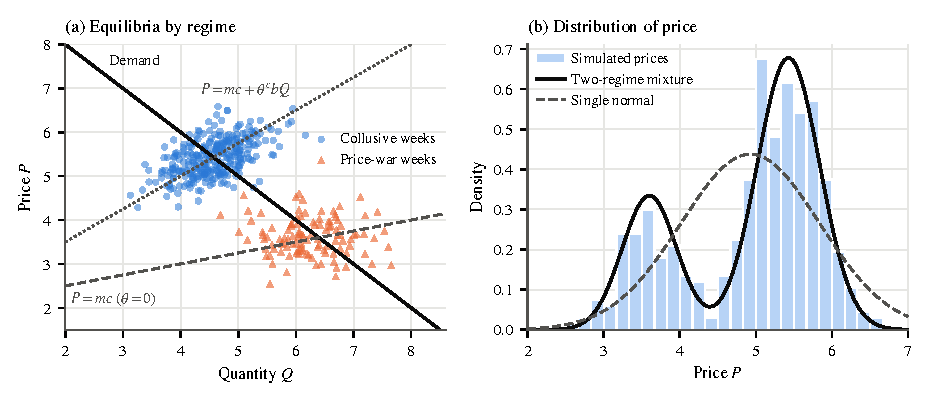
\includegraphics[width=\textwidth]{figures/ch01/regime_mixture.pdf}
\caption{Identification of conduct regimes from the distribution of the data. The simulated market has inverse demand
$P = 10 - Q + u^d$ and marginal cost $mc = 2 + 0.25\,Q + u^c$, observed for 400 weeks. Conduct is collusive
($\theta^{c} = 0.5$) with probability $\varpi = 0.7$ and competitive ($\theta^{w} = 0$) otherwise, with
$u^d \sim N(0, 0.8^2)$ and $u^c \sim N(0, 0.4^2)$. Panel (a) colors each week by its true regime, which the analyst does not observe, and draws the deterministic demand
curve and the two supply relations. Panel (b) shows the distribution of price that the analyst sees. The two-regime
mixture fits it, while a single normal distribution does not. The regime means of price, $3.6$ and $5.43$, differ by
more than four within-regime standard deviations, so the distribution is bimodal. Closer regimes could produce a single
mode. All values are illustrative.}
\label{fig:01-regimes}
\end{figure}

The main threat to this inference is that some other unobserved shock moves the supply relation. Because the
identifying variation is an error component, nothing in the procedure guarantees the conduct interpretation. Unrecorded
changes in factor prices or technology could produce the same pattern, and Porter had no factor-price data. Bresnahan
finds the conduct interpretation likely in the railroad case for two reasons. The regime shifts move price and quantity
by about 50 percent, and contemporary sources discuss cartel adherence extensively. An alternative is to fix the sample
split in advance and estimate $\theta^{c}$ and $\theta^{w}$ separately, as \citet{Bresnahan1987} does. This needs prior
information but allows a more direct check that the apparent supply shocks reflect conduct. \Cref{ch:collusion-evidence}
returns to these issues with \citet{Porter1983} and \citet{Ellison1994}.

\subsubsection{Comparative statics in industry structure}\label{sec:01-id-structure}

The fifth argument relates price to the number of firms or to concentration across similar local markets. Its logic is
familiar, but \citet[p.~1032]{Bresnahan1989} judges that it still awaited its identification arguments.
\Cref{sec:01-price-concentration} presented these studies and the six difficulties Bresnahan raises. In the language of
this section, all of them come back to the aggregate supply relation \eqref{eq:01-avg-supply}, which is
\cref{prop:01-supply-relation}(ii) applied market by market. A lower price in markets with more firms can mean lower
average conduct $\theta$ or lower average marginal cost $\overline{mc}$. Price and quantity data alone cannot apportion
the change between the two. A change in entry regulation, as in \citet{SpillerFavaro1984}, offers cleaner
variation because it moves structure for a reason unrelated to costs. The arguments of this section can then separate
the two channels, for example by checking whether demand rotations identify a lower $\theta$ after deregulation.

\subsubsection{Synthesis}\label{sec:01-id-synthesis}

\Cref{tab:01-id-strategies} summarizes the arguments. Their variety reflects the variety of data across industry
studies \citep[Section~3.6]{Bresnahan1989}. Each industry offers different information and institutional detail, and
therefore different defenses of different methods. The variety also reflects how many comparative statics of markets
with market power have no counterpart in competitive markets.

\begin{table}[htbp]
\centering
\begin{threeparttable}
\caption{How the data identify market power}
\label{tab:01-id-strategies}
\footnotesize
\setlength{\tabcolsep}{4pt}
\begin{tabularx}{\textwidth}{@{}>{\raggedright\arraybackslash}p{2.05cm}
  >{\raggedright\arraybackslash}X >{\raggedright\arraybackslash}X >{\raggedright\arraybackslash}X
  >{\raggedright\arraybackslash}p{2.2cm} >{\raggedright\arraybackslash}p{1.8cm}@{}}
\toprule
Argument & Exogenous variation & What is identified & Key maintained assumption & Applications & Full treatment \\
\midrule
Comparative statics in demand & Demand shifters that rotate demand ($Y_t$ entering $P_Q$) & Conduct $\theta$ and
  the slope of marginal cost separately & Correct demand specification; demand not of the form $\tilde P(Q, h(Y))$ &
  \citet{JustChern1980}; \citet{Bresnahan1981,Bresnahan1987} & \cref{ch:conduct} \\
\addlinespace
Homogeneity of marginal cost & Factor prices & $\theta$ from terms not multiplied by factor prices & Marginal cost
  homogeneous of degree one in observed factor prices & \citet{Appelbaum1979,Appelbaum1982} & \cref{ch:conduct} \\
\addlinespace
Comparative statics in cost & All factor prices, or taxes & Sign of $\psi$; bound on $\sum_i (1 + r_i)^{-1}$ &
  All cost shifters measured; long-run equilibrium (for $\psi$); known link to marginal cost &
  \citet{PanzarRosse1977}; \citet{Shaffer1982}; \citet{Sullivan1985}; \citet{AshenfelterSullivan1987} &
  \cref{ch:conduct} \\
\addlinespace
Direct estimation of marginal cost & Factor prices with input quantities & Marginal cost from factor demands, then
  $\theta$ & Cost-function form; correct price of capital services & \citet{GollopRoberts1979};
  \citet{Appelbaum1982}; \citet{Hall1988} & \cref{sec:01-rising-markups} \\
\addlinespace
Supply shocks & Unobserved two-valued shock to the supply relation & Frequency and size of regime changes in conduct &
  No other unobserved shifts in the supply relation & \citet{Porter1983}; \citet{LeePorter1984} &
  \cref{ch:collusion-evidence} \\
\addlinespace
Comparative statics in structure & Number of firms or concentration across local markets & Reduced-form price and
  structure relation & Structure exogenous; average cost unrelated to structure & \citet{GrahamKaplanSibley1983};
  \citet{SpillerFavaro1984} & \cref{sec:01-price-concentration} \\
\addlinespace
Residual demand & Cost shifters specific to one firm & Elasticity of the firm's residual demand & Firm's costs move
  independently of rivals' costs & \citet{BakerBresnahan1988} & \cref{ch:conduct} \\
\bottomrule
\end{tabularx}
\begin{tablenotes}\footnotesize
\item Notes: The first six rows follow the classification of \citet[Section~3]{Bresnahan1989} and are introduced in
\cref{sec:01-id-arguments}. The last row is the summary-statistic approach of his Section~4, introduced in
\cref{sec:01-neio-diffprod}. The last column gives the place in this book where each argument is developed in full.
\end{tablenotes}
\end{threeparttable}
\end{table}

\subsection{Market power with product differentiation}\label{sec:01-neio-diffprod}

Product differentiation raises short-run and long-run questions \citep[Section~4]{Bresnahan1989}. In the short run the
set of products and their attributes are fixed, and we ask how much market power existing differentiation confers. The
question has two parts. As products become more distinct, each firm's profit depends less on rivals' prices, which the
own- and cross-price elasticities of demand measure. As products become more distinct, each firm also responds less to
rivals' moves, which requires a model of competitive interaction.

The conceptual issues resemble those of the homogeneous-good case, but measurement is much harder. Suppose an industry
has $J$ products and we assume constant elasticities and symmetric cross effects. Demand still has $J$ own-price
elasticities, $J$ income elasticities and $\frac{J(J - 1)}{2}$ cross-price elasticities. With $J = 100$ products this is
\begin{equation*}
J + J + \frac{J(J - 1)}{2} = 100 + 100 + 4{,}950 = 5{,}150
\end{equation*}
elasticities, and few industries have fewer than 100 products. Multi-product firms may also have economies of scope.
Prior information from trade journals and marketing studies becomes indispensable, and how it is used varies from
industry to industry.

The most common shortcut treats the products as close substitutes, uses a price index as the observed price, and
proceeds as for a homogeneous good. Bresnahan warns that this can attribute to conduct what is due to product
differentiation \citep[p.~1046]{Bresnahan1989}. The next example makes the warning precise.

\begin{example}[Differentiation that looks like conduct]\label{ex:01-index-conduct}
Let $J$ symmetric single-product firms set prices in a Bertrand equilibrium with constant marginal cost. Let
$\varepsilon_{\mathrm{own}} > 0$ be each product's own-price elasticity (as a positive number) and
$\varepsilon_{\mathrm{cross}} \ge 0$ the cross-price elasticity between any two products. The pricing rule of
\cref{prop:01-pricing-rule} gives each firm the Lerner index $L = \frac{1}{\varepsilon_{\mathrm{own}}}$. An analyst
who treats the products as one homogeneous good measures the market elasticity when all prices move together,
\begin{equation*}
\varepsilon = \varepsilon_{\mathrm{own}} - (J - 1)\,\varepsilon_{\mathrm{cross}} ,
\end{equation*}
and reads conduct from $\frac{P - mc}{P} = \frac{\theta}{\varepsilon}$. The apparent conduct parameter is
\begin{equation*}
\tilde\theta = \varepsilon L = \frac{\varepsilon_{\mathrm{own}} - (J - 1)\,\varepsilon_{\mathrm{cross}}}{\varepsilon_{\mathrm{own}}}
 = 1 - (J - 1)\,D, \qquad D = \frac{\varepsilon_{\mathrm{cross}}}{\varepsilon_{\mathrm{own}}} .
\end{equation*}
With symmetric quantities, $D$ is the \emph{diversion ratio} between two products, the fraction of the sales lost by one
product that go to another when its price rises (\cref{ch:diffprod}). So $\tilde\theta$ is the fraction of lost sales that leave
the industry. It lies between zero and one although no firm colludes. With $J = 4$, $\varepsilon_{\mathrm{own}} = 4$ and
$\varepsilon_{\mathrm{cross}} = 1$ we get $\varepsilon = 1$, $L = 0.25$ and $\tilde\theta = 0.25$. This is exactly the
value of symmetric Cournot with four firms, produced by differentiated Bertrand competition.
\end{example}

To study differentiation directly, the analyst must reduce the dimension of the problem. Bresnahan describes three ways.

\casehead{Modeling product choice}
The first models how consumers choose among products, which yields demand systems with few parameters. Discrete-choice
models \citep[see][]{McFadden1984}, such as the nested logit, fit industries in which trade sources describe distinct
segments with much closer competition inside than across them. Spatial models of differentiation fit industries without
clear segment boundaries. In such industries, products A and B can both matter for C without A mattering for B. Spatial
models reduce the parameter count by localizing competition, and discrete-choice models do it by grouping. A
multinomial logit without nests is the limiting case in which the whole industry is one segment and competition is
symmetric. Bresnahan's spatial model of automobiles is an example \citep{Bresnahan1981,Bresnahan1987}. Any such model
is only as convincing as the information used to specify it, and the localized-versus-segmented distinction matters most.
\citet{Schmalensee1985b} proposes a test of localization based on how the prices and quantities of brands move together.
In ready-to-eat breakfast cereals he decisively rejects the model in which all brands compete equally, although he doubts
the covariance restrictions that identify the pattern of localization. \Cref{ch:discrete,ch:logit,ch:blp} develop the
modern versions of this approach.

\casehead{Aggregating products}
The second approach aggregates similar products until only a few elasticities remain. \citet{GelfandSpiller1987}
aggregate many types of bank loans into two and estimate a two-by-two system. Their model lets each bank's profit in
one market depend on rivals' strategies in both, an interdependence they write in conjectural-variations form.
\citet{Slade1987} studies ``majors'' and ``independents'' among gasoline stations in Vancouver. \citet{Suslow1986}
aggregates output into the dominant firm's product and the fringe's product. The dominant firm's marginal revenue then
depends on the substitutability of the two products, the market elasticity and the fringe supply elasticity.

\casehead{Estimating a summary statistic: residual demand}
The third approach, due to \citet{BakerBresnahan1985,BakerBresnahan1988}, estimates only the summary statistic that
measures one firm's market power. Consider the seller of product 1, facing the inverse demand
\begin{equation}\label{eq:01-bb-demand}
P_1 = P^1(Q_1, P_2, \dots, P_J, Y, \gamma),
\end{equation}
where $P_2, \dots, P_J$ are the prices of competing products. The parameter vector $\gamma$ contains the cross effects of
all $J - 1$ rivals, so it can be very long. Each rival product $j = 2, \dots, J$ has its own demand equation like
\eqref{eq:01-bb-demand} and a supply relation
\begin{equation}\label{eq:01-bb-rival}
P_j = C_q^{j}(Q_j, W_j, Z_j, \Gamma_j) - \frac{\partial P^{j}}{\partial Q_j}\, Q_j\, \vartheta_j ,
\qquad j = 2, \dots, J .
\end{equation}
These $2(J - 1)$ equations can be solved for the rivals' prices and quantities as functions of $Q_1$ and the exogenous
variables, $P_j = P_j^*(Q_1, W_{-1}, Z_{-1}, \Gamma_{-1}, \vartheta_{-1}, Y, \gamma)$. Here $W_{-1}$ and $Z_{-1}$ are the
rivals' cost shifters, and $Q_1$ remains because only the rivals' equations have been solved. Substituting into
\eqref{eq:01-bb-demand} gives the \emph{residual demand curve} of product 1,
\begin{equation}\label{eq:01-bb-residual}
P_1 = P^1\bigl(Q_1, P_2^*(\cdot), \dots, P_J^*(\cdot), Y, \gamma\bigr)
    \equiv P^{R}(Q_1, W_{-1}, Z_{-1}, \Gamma_{-1}, \vartheta_{-1}, Y, \gamma).
\end{equation}
Equations \eqref{eq:01-bb-demand} to \eqref{eq:01-bb-residual} are Bresnahan's (31), (4$^d$) and (32). By the chain rule,
the elasticity of residual inverse demand is
\begin{equation*}
-\frac{1}{\varepsilon^{R}_1} = \frac{\partial \ln P^{R}}{\partial \ln Q_1}
 = \frac{\partial \ln P^1}{\partial \ln Q_1} + \sum_{j = 2}^{J}\frac{\partial \ln P^1}{\partial \ln P_j}\,
   \frac{\partial \ln P_j^*}{\partial \ln Q_1} .
\end{equation*}
The first term is the direct effect of firm 1's output on its price. The sum adds the effect of rivals' price responses.
Substituting out the rivals' prices loses a great deal of information, since the separate elements of $\gamma$ can no
longer be estimated. That loss matters little for the question at hand. The slope of $P^{R}$ tells us how much power
firm 1 has over its price after all rivals have adjusted. Suppose product 1 is a perfect substitute for rival products
sold by price takers at constant cost. Then $P^{R}$ equals the lowest rival cost and does not respond to $Q_1$, so
$\frac{1}{\varepsilon^{R}_1} = 0$.

Residual demand can be estimated only if firm 1's costs move independently of its rivals' costs
\citep[fn.~43]{Bresnahan1989}. Its own cost shifters then serve as instruments for $Q_1$, while the rivals' cost
shifters enter \eqref{eq:01-bb-residual} directly. International markets offer natural experiments, since exchange-rate
movements change the relative costs of producers in different countries. The reciprocal
$\frac{1}{\varepsilon^{R}_1}$ of the residual-demand elasticity summarizes a firm's market power, but it does not reveal the sources of that power. It
equals the Lerner index only under particular conduct, for example when firm 1 acts as a Stackelberg leader toward
its rivals \citep[p.~289]{BakerBresnahan1988}. This is why Bresnahan leaves residual-demand studies out of his summary
table. The approach complements the
aggregation approach, which estimates every elasticity but only for a few products. \Cref{ch:conduct} treats
\citet{BakerBresnahan1988} and its application to brewing in depth.

\casehead{Market definition and policy}
These techniques bear on market definition in antitrust. Antitrust often asks whether a single firm has market power,
or whether a group of firms would have it if they acted together. \Cref{sec:01-market-definition} quoted Bresnahan's
remark that these questions are well posed even where computing shares in a relevant market is senseless. Residual
demand answers the first question directly. \citet{ScheffmanSpiller1987} extend
it to a group of firms, which answers the second. \citet{BakerBresnahan1985} ask how much steeper the residual demand of
two merging firms would be after the merger. If the two sell close substitutes and few other firms sell similar products,
each firm is an important brake on the other, and the merger steepens the curve. The Panzar-Rosse statistic gives a
related answer. A rejection of monopoly for a firm or group means that it cannot be treated as acting in isolation.
\Cref{ch:mergers} develops merger analysis with differentiated products.

\casehead{Differentiation in the long run}
In the long run firms add products, change attributes or perceptions, and new firms enter with new products or
imitations. Theory offers many strategic hypotheses: preemption by reputation for quality, preemption by filling the
product space, and coordination of product choices to soften competition. In 1989 essentially nothing empirical was known
about any of them \citep[p.~1050]{Bresnahan1989}. The same passage contains the welfare point of
\cref{sec:01-fixed-costs}. Under the Chamberlin tangency every firm prices above marginal cost, so short-run market power
says little about efficiency until we know how new products and new firms are supplied.

\subsection{What the NEIO learned}\label{sec:01-neio-lessons}

The case-study character of the NEIO raises questions of interpretation \citep[Section~5]{Bresnahan1989}. How general
are the results, and what do they reveal about market power in the economy as a whole? The SCP paradigm aimed to estimate
a map from structure to conduct and performance. Such a map would be valuable, for example to guide merger policy, which
acts on structure. A single industry study reveals at most one point on it. By 1989 NEIO studies covered more than a
dozen industries. \Cref{tab:01-bresnahan-table} reproduces the estimated Lerner indices that Bresnahan collected.

\begin{table}[htbp]
\centering
\begin{threeparttable}
\caption{Estimated Lerner indices from early NEIO studies}
\label{tab:01-bresnahan-table}
\small
\begin{tabular}{@{}llc@{}}
\toprule
Author & Industry & $L$ \\
\midrule
\citet{Lopez1984} & Food processing & 0.504 \\
\citet{Roberts1984} & Coffee roasting & 0.055 / 0.025$^{a}$ \\
\citet{Appelbaum1982} & Rubber & 0.049$^{c}$ \\
\citet{Appelbaum1982} & Textile & 0.072$^{c}$ \\
\citet{Appelbaum1982} & Electrical machinery & 0.198$^{c}$ \\
\citet{Appelbaum1982} & Tobacco & 0.648$^{c}$ \\
\citet{Porter1983} & Railroads & 0.40$^{b}$ \\
\citet{Slade1987} & Retail gasoline & 0.10 \\
\citet{Bresnahan1981} & Automobiles (1970s) & 0.1 / 0.34$^{d}$ \\
\citet{Suslow1986} & Aluminum (interwar) & 0.59 \\
\citet{SpillerFavaro1984} & Banks ``before''$^{e}$ & 0.88 / 0.21$^{f}$ \\
\citet{SpillerFavaro1984} & Banks ``after''$^{e}$ & 0.40 / 0.16$^{f}$ \\
\bottomrule
\end{tabular}
\begin{tablenotes}\footnotesize
\item Notes: $L = \frac{P - mc}{P}$. $^{a}$Largest and second-largest firm, respectively. $^{b}$When the cartel was
succeeding (0 in reversionary periods). $^{c}$At the sample midpoint. $^{d}$Varies by type of car, larger in the standard
and luxury segments. $^{e}$Uruguayan banks before and after entry deregulation. $^{f}$Large firms / small firms.
Panzar-Rosse and Sullivan studies are excluded because they yield only tests of, or bounds on, conduct.
Residual-demand studies are excluded because the reciprocal $\frac{1}{\varepsilon^{R}}$ of the residual-demand elasticity
equals the Lerner index only in special cases.
\item Source: \citet{Bresnahan1989}, Table~17.1.
\end{tablenotes}
\end{threeparttable}
\end{table}

From this evidence Bresnahan draws three guarded conclusions \citep[pp.~1052--1053]{Bresnahan1989}.

\casehead{Conclusion A}
Some concentrated industries have a great deal of market power, in the sense of high price-cost margins. Several entries
in \cref{tab:01-bresnahan-table} exceed 0.4. The industries cannot be matched systematically to census concentration
measures, because many data sets were collected by the authors. A glance at the list shows that they come overwhelmingly
from the concentrated end of the spectrum.

Two reasons warn against generalizing. First, researchers who invent a method for detecting market power apply it first
where they expect to find it. They choose concentrated industries, known or suspected cartels, or industries where earlier
case studies suggested anticompetitive conduct. Second, the data often come from trade journals, regulators or court records.
Industries with excellent trade journals are industries in which firms know a lot about their rivals, an information
structure that favors collusion. Suslow could use the trial record on Alcoa because Alcoa was suspected of market power.
More sources of data, from more industries, were needed.

\casehead{Conclusion B}
One significant cause of high margins is anticompetitive conduct. The studies separate conduct, the behavioral rules by
which firms set prices, from performance, the price-cost margin. They do not find small departures from price taking
combined with very steep demand. Several find conduct well toward the collusive end. \citet{Porter1983} and \citet{Bresnahan1987}
both find collusive conduct, although of different kinds. The railroads in Porter's study had formed the JEC by a
publicly acknowledged agreement \citep[p.~302]{Porter1983}. \citet[pp.~457 and 479]{Bresnahan1987} interprets automobile
pricing in 1954 and 1956 as tacit collusion, meaning collusive pricing without an explicit agreement among firms. His
tests compare a collusive pricing model with a Bertrand model, so they cannot reveal whether the automakers
communicated. Conduct is not uniform. \citet{Roberts1984} classifies most
coffee roasters as a price-taking fringe, while the largest firms behave less competitively without reaching the profit
maximum given the fringe.

\casehead{Conclusion C}
The new methods had taught little about the relation between market power and industry structure. The studies cover only
the concentrated end of the range, so they reveal the structure-performance map over a narrow interval. Few of them
address the causes of market power. Long-lived market power suggests that entry fails to discipline conduct, yet the
studies hardly discuss entry.

\casehead{The sources of market power}
Bresnahan closes by pointing to the causes of market power as the frontier \citep[Section~6]{Bresnahan1989}. Entry,
predation, entry deterrence and long-run strategic competition had received little empirical work with explicit
theoretical foundations. \citet{Burns1986} studies the American tobacco trust and finds that its acquisitions of
competitors became cheaper after episodes of predatory pricing. The study relies on a nineteenth-century documentary record
that modern firms would not leave. The open problem was to find the empirical implications of predation when predatory acts
must be inferred. On entry, \citet{PanzarRosse1977} add to demand and the supply relations an entry condition for the
marginal firm, $P = \mathit{LRAC}(W, Y)$, with $\mathit{LRAC}$ long-run average cost.
\citet{BresnahanReiss1990} model the entry decisions of the first two firms in a market with an integer number of firms.
They use 149 geographically isolated American markets for new car dealers. A second entrant faces nearly the same costs
and opportunities as the first, and its entry does not lower the monopoly dealer's margins by much. Both papers
argue that cross-sections of closely related markets are the right samples for studying entry. \Cref{sec:01-today-structure}
takes up the sequel by \citet{BresnahanReiss1991}.

Bresnahan's final assessment is optimistic about measurement and modest about explanation. By abandoning accounting
measures of performance, the NEIO produced a new kind of evidence of substantial market power, immune to the standard
criticisms of earlier work. Its studies are detailed enough that alternative explanations can be confronted and rebutted.
In his words, ``we know that there is market power out there, and need to know a lot more about exactly where''
\citep[p.~1055]{Bresnahan1989}. Its causes and systematic predictors remained essentially unknown.

The program that followed kept the NEIO's commitment to single industries and explicit models. Its main change was on the
demand side. Classic analyses of market power, such as \citet{Porter1983}, \citet{Bresnahan1987} and
\citet{Nevo2001}, supply the basic toolkit \citep[p.~151]{EinavLevin2010}. That toolkit combines demand and supply in
an equilibrium analysis of imperfect competition. Modern work replaces the conduct parameter with explicit models of differentiated-product
competition and estimates rich demand systems with instruments. \Cref{sec:01-today} describes this structural workflow.

\section{Empirical IO today}\label{sec:01-today}

The previous sections traced how the field moved from cross-industry regressions to studies of single
industries with explicit models of conduct. This section describes what empirical research in industrial
organization looks like after that transition. We follow the progress report of \citet{EinavLevin2010},
which maps the modern field, and we add the formal content that a survey essay leaves implicit.

Einav and Levin summarize the state of the field in a few sentences (p.~147). Most influential research
looks to economic theory for guidance, especially in modeling the behavior of firms. Studies frequently
focus on a single industry or market. They pay careful attention to institutional specifics, to the
measurement of key variables and to econometric identification. Advocates argue that, when it succeeds,
this approach combines the conceptual clarity of theory with convincing empirical measurement.

There is no recipe, but most papers share a few themes (p.~148). A study usually begins with a theory of
market equilibrium, which can be more or less explicit. The theory then plays one of three roles. It
supplies optimization or equilibrium conditions from which we infer unobserved parameters. It delivers
testable predictions. Or it helps us interpret estimated causal effects. In every case the institutional
details of the market matter, and one broad lesson from looking across industries is that they can matter
a great deal.

Industry studies have drawbacks as well (p.~147). They can lead to narrow analyses, and researchers are
often reluctant to generalize their findings to markets with different institutions. The broader lessons
therefore tend to be qualitative insights, or methods that can be applied in other settings. Critics also
argue that models resting heavily on equilibrium assumptions can obscure the link between the estimated
parameters and the variation in the data. We return to this debate in \cref{sec:01-today-debate}.

The section has six parts. \Cref{sec:01-workflow} sets out the structural workflow that organizes most of
the book. \Cref{sec:01-today-demand,sec:01-today-pricing} discuss demand estimation and the measurement of
market power. \Cref{sec:01-today-auctions} shows that auctions are pricing problems governed by the same
first-order logic. \Cref{sec:01-today-structure} turns to entry, market structure and dynamics, with a
full case study of \citet{BresnahanReiss1991}. \Cref{sec:01-today-debate} discusses the debate
between structural and design-based empirical work.

\subsection{The structural workflow: demand, supply, counterfactuals}\label{sec:01-workflow}

A large share of modern empirical IO follows a three-step workflow. We first estimate demand. We then
combine the demand estimates with a model of pricing to recover marginal costs. Finally we use the
estimated demand and costs to solve for the equilibrium under a counterfactual policy or market structure.
This subsection states the canonical model behind the workflow, derives its central equation and
illustrates the three steps. Later chapters develop each step in full.

\subsubsection{The canonical model}

Consider a market with $J$ inside products and an outside good $j = 0$. (When several markets
$t = 1, \dots, T$ appear, we add the subscript $t$.) Product $j$ has price $p_j$, a row vector of observed
characteristics $x_j$ and an unobserved demand shock $\xi_j$, which we call \emph{unobserved product
quality}. Market size is $M$, the quantity of product $j$ is $q_j$, and its market share is
$s_j = \frac{q_j}{M}$. Each firm $f$ owns a set of products $\mathcal{J}_f$, and every product has exactly
one owner.

\begin{assumption}[Canonical static model]\label{ass:01-canonical}
\leavevmode
\begin{enumerate}[label=(\roman*)]
  \item Market shares are $s_j = s_j(p, x, \xi; \gamma)$ for $j = 1, \dots, J$. Here
        $p = (p_1, \dots, p_J)^\top$ is the price vector, $x$ and $\xi$ collect the characteristics and
        demand shocks of all products, and $\gamma$ is a finite-dimensional vector of demand parameters.
        Each $s_j$ is continuously differentiable in $p$.
  \item Product $j$ has a constant marginal cost $mc_j = c(w_j, \omega_j; \Gamma)$, where $w_j$ is a vector
        of observed cost shifters, $\omega_j$ is an unobserved cost shock and $\Gamma$ is a vector of cost
        parameters. Fixed costs do not affect prices.
  \item Firms choose prices simultaneously. Each firm sets the prices of its own products to maximize their
        joint profit, taking the prices of rival products as given. We call this \emph{multi-product
        Bertrand-Nash} pricing.
  \item The equilibrium is interior, so it satisfies the first-order conditions, and the matrix
        $\Omega \odot \Delta^\top$ defined below is invertible at the equilibrium prices.
\end{enumerate}
\end{assumption}

Two matrices summarize conduct and demand. The ownership matrix $\Omega$, met with the vertical model in
\cref{sec:01-conduct-taxonomy}, is the $J \times J$ matrix with $\Omega_{jk} = 1$ if products $j$ and $k$ have the same owner and $\Omega_{jk} = 0$ otherwise. It is
symmetric and has ones on the diagonal. The matrix of share derivatives $\Delta$ has $(j, k)$ element
$\Delta_{jk} = \frac{\partial s_j}{\partial p_k}$, so row $j$ collects the effects of all prices on the
share of product $j$. The symbol $\odot$ denotes the element-wise (Hadamard) product.

\begin{proposition}[Multi-product pricing and implied marginal costs]\label{prop:01-multiproduct-foc}
Under \cref{ass:01-canonical}, equilibrium prices satisfy the system of $J$ first-order conditions
\begin{equation}\label{eq:01-foc-matrix}
  s + (\Omega \odot \Delta^\top)(p - mc) = 0,
\end{equation}
where $s$, $p$ and $mc$ are $J$-vectors. Equivalently, markups and marginal costs are
\begin{equation}\label{eq:01-implied-mc}
  p - mc = -(\Omega \odot \Delta^\top)^{-1} s,
  \qquad
  mc = p + (\Omega \odot \Delta^\top)^{-1} s .
\end{equation}
\end{proposition}

\begin{proof}
Firm $f$ earns
\[
  \pi_f = \sum_{k \in \mathcal{J}_f} (p_k - mc_k)\, M s_k(p) - C_f ,
\]
where $C_f$ is its fixed cost. Take a product $j \in \mathcal{J}_f$. The price $p_j$ enters the margin of
product $j$ and the shares of every product. By the product rule,
\[
  \frac{\partial \pi_f}{\partial p_j}
  = M s_j + M \sum_{k \in \mathcal{J}_f} (p_k - mc_k) \frac{\partial s_k}{\partial p_j} .
\]
Setting this derivative to zero and dividing by $M > 0$ gives
\[
  s_j + \sum_{k \in \mathcal{J}_f} (p_k - mc_k) \frac{\partial s_k}{\partial p_j} = 0 .
\]
The ownership matrix lets us replace the sum over the firm's products by a sum over all products:
\[
  s_j + \sum_{k = 1}^{J} \Omega_{jk} \frac{\partial s_k}{\partial p_j} (p_k - mc_k) = 0 .
\]
The derivative in this sum is $\frac{\partial s_k}{\partial p_j} = \Delta_{kj} = (\Delta^\top)_{jk}$. The
coefficient on $(p_k - mc_k)$ in the condition for product $j$ is therefore
$\Omega_{jk} (\Delta^\top)_{jk} = (\Omega \odot \Delta^\top)_{jk}$. Stacking the $J$ conditions gives
\eqref{eq:01-foc-matrix}. Premultiplying \eqref{eq:01-foc-matrix} by $(\Omega \odot \Delta^\top)^{-1}$ and
rearranging gives \eqref{eq:01-implied-mc}.
\end{proof}

The transpose has a simple origin. The condition for $p_j$ involves the effect of $p_j$ on the shares of the
firm's other products. These effects form column $j$ of $\Delta$, which is row $j$ of $\Delta^\top$.
Because $\Omega$ is symmetric, $\Omega \odot \Delta^\top = (\Omega \odot \Delta)^\top$, and some references
write the system in that form.

\begin{remark}[Special cases and conduct]\label{rem:01-foc-cases}
With single-product firms, $\Omega$ is the identity matrix. Condition $j$ then reads
$s_j + \Delta_{jj}(p_j - mc_j) = 0$, so
\[
  p_j - mc_j = -s_j\left(\frac{\partial s_j}{\partial p_j}\right)^{-1}
             = -q_j\left(\frac{\partial q_j}{\partial p_j}\right)^{-1},
\]
which is the dollar markup of \cref{prop:01-pricing-rule} applied to the residual demand $q_j$. A cartel that
maximizes the joint profit of all products sets every element of $\Omega$ equal to one. Intermediate cases
put a weight between zero and one on rival products. In this sense $\Omega$ plays the role in
differentiated-product markets that the conduct parameter $\theta$ plays in the homogeneous-good supply
relation $P = \overline{mc} - \theta P'(Q) Q$ of \cref{prop:01-supply-relation}. Equation
\eqref{eq:01-implied-mc} also shows that markups depend only on shares, share derivatives and conduct. Once
demand is known and conduct is assumed, marginal costs follow from observed prices without any cost data.
\end{remark}

\begin{example}[Same data, two conduct assumptions]\label{ex:01-two-products}
Two symmetric products sell at $p_1 = p_2 = 2$ with shares $s_1 = s_2 = 0.2$. Suppose demand estimates give
own-price derivatives $\frac{\partial s_j}{\partial p_j} = -0.4$ and cross-price derivatives
$\frac{\partial s_k}{\partial p_j} = 0.1$ (per dollar). The numbers are illustrative.

If the products have different owners, $\Omega$ is the identity and each markup is
$p_j - mc_j = \frac{0.2}{0.4} = 0.5$. Implied marginal cost is $1.5$ and the Lerner index is $0.25$.

If one firm owns both products, \eqref{eq:01-foc-matrix} becomes
\[
  \begin{pmatrix} 0.2 \\ 0.2 \end{pmatrix}
  + \begin{pmatrix} -0.4 & 0.1 \\ 0.1 & -0.4 \end{pmatrix}
    \begin{pmatrix} p_1 - mc_1 \\ p_2 - mc_2 \end{pmatrix} = 0 .
\]
By symmetry both markups equal some $m$, and each row reads $0.2 - 0.4m + 0.1m = 0$. Hence
$m = \frac{0.2}{0.3} = \frac{2}{3}$, implied marginal cost is $\frac{4}{3}$ and the Lerner index is
$\frac{1}{3}$. The diversion ratio from product 1 to product 2 (\cref{ex:01-index-conduct}), the fraction
of the sales lost by product 1 after a price increase that go to product 2, is
$D_{12} = -\frac{\partial s_2}{\partial p_1}\left(\frac{\partial s_1}{\partial p_1}\right)^{-1}
= \frac{0.1}{0.4} = \frac{1}{4}$.
In this symmetric case the joint-ownership markup equals the single-product markup divided by $1 - D_{12}$:
\[
  m = \frac{0.2}{0.4 - 0.1} = \frac{0.5}{1 - \frac{1}{4}} = \frac{2}{3} .
\]
The same prices and demand estimates thus imply different marginal costs under different conduct
assumptions. With independent cost data we could tell the two models apart. This is the logic of the
conduct tests in \cref{sec:01-today-pricing}, and diversion ratios return in \cref{ch:diffprod,ch:mergers}.
\end{example}

\subsubsection{The three steps}

\Cref{fig:01-workflow} displays the workflow. Each step uses the output of the previous one.

\begin{enumerate}[label=\textit{Step \arabic*.}, leftmargin=*, itemsep=4pt]
  \item \textit{Estimate demand.} We estimate $\gamma$ from data on shares, prices and characteristics,
        usually across many markets. Firms observe $\xi_j$ when they set prices, and
        \eqref{eq:01-implied-mc} shows that markups depend on shares. Prices are therefore correlated with
        $\xi_j$, and least squares estimates of price sensitivity are biased. The remedy is a set of
        instruments $z_j$ that satisfy $\E[\xi_j \mid z_j] = 0$ and move prices
        (\cref{sec:01-today-demand}).
  \item \textit{Recover marginal costs or test conduct.} Given $\hat\gamma$, we compute $\hat\Delta$ and the
        implied costs $\widehat{mc} = p + (\Omega \odot \hat\Delta^\top)^{-1}s$. With a cost specification
        $mc_{jt} = w_{jt}\Gamma + \omega_{jt}$, the supply-side estimating equation is
        \begin{equation}\label{eq:01-supply-eq}
          p_{jt} + \big[(\Omega_t \odot \hat\Delta_t^\top)^{-1} s_t\big]_j = w_{jt}\Gamma + \omega_{jt},
        \end{equation}
        which we estimate by least squares or instrumental variables, or jointly with demand by the
        generalized method of moments. Alternatively we compare the implied costs under several conduct
        assumptions with direct cost information.
  \item \textit{Solve for a counterfactual equilibrium.} We solve
        \begin{equation}\label{eq:01-counterfactual}
          s(p'; \hat\gamma) + \big(\Omega' \odot \Delta(p'; \hat\gamma)^\top\big)(p' - mc') = 0
        \end{equation}
        for the new price vector $p'$. A merger changes the ownership matrix to $\Omega'$. A per-unit tax
        $t$ changes costs to $mc' = \widehat{mc} + t$. A new product enlarges the choice set. The demand
        model then delivers changes in consumer welfare, and the cost estimates deliver changes in profits.
\end{enumerate}

\begin{figure}[htbp]
\centering
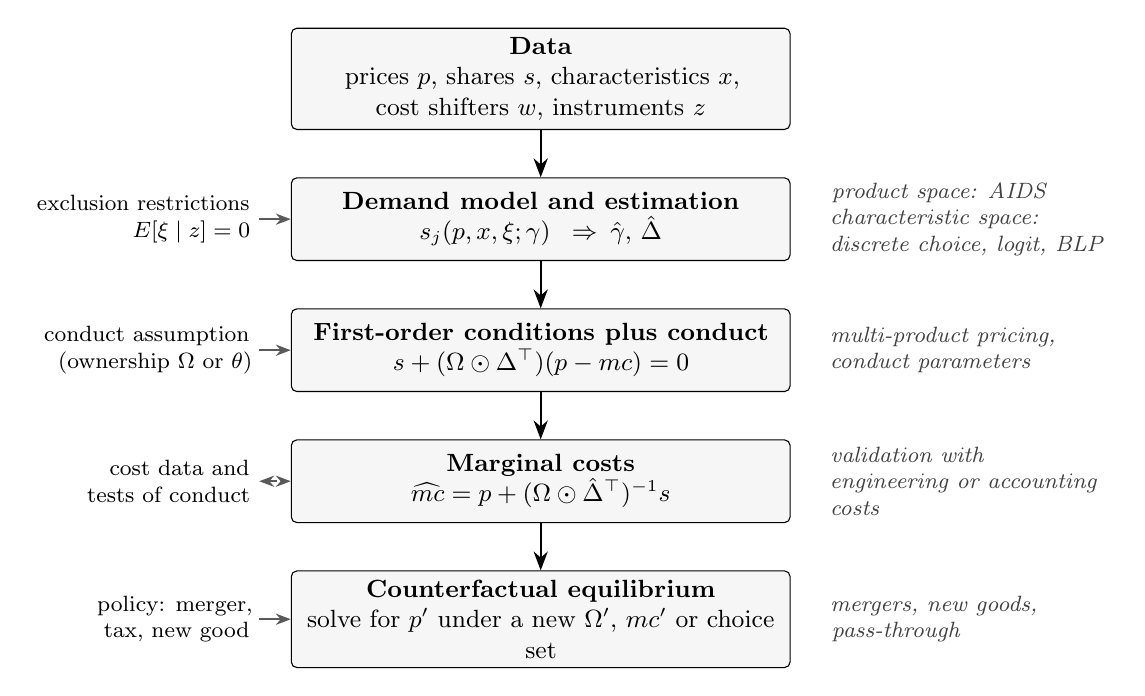
\begin{tikzpicture}[
  node distance=6mm and 4mm,
  box/.style={draw, rounded corners=2pt, align=flush center, text width=6.1cm, minimum height=1.05cm,
              font=\small, fill=gray!7},
  inp/.style={align=flush right, text width=2.7cm, font=\footnotesize},
  note/.style={align=flush left, text width=3.5cm, font=\footnotesize\itshape, text=black!75},
  arr/.style={-{Stealth[length=2.4mm]}, thick},
  side/.style={-{Stealth[length=1.9mm]}, semithick, black!65}
]
\node[box] (data) {\textbf{Data}\\ prices $p$, shares $s$, characteristics $x$,\\ cost shifters $w$,
  instruments $z$};
\node[box, below=of data] (dem) {\textbf{Demand model and estimation}\\ $s_j(p, x, \xi; \gamma)$
  \enspace$\Rightarrow$\enspace $\hat\gamma$, $\hat\Delta$};
\node[box, below=of dem] (foc) {\textbf{First-order conditions plus conduct}\\
  $s + (\Omega \odot \Delta^\top)(p - mc) = 0$};
\node[box, below=of foc] (mc) {\textbf{Marginal costs}\\
  $\widehat{mc} = p + (\Omega \odot \hat\Delta^\top)^{-1} s$};
\node[box, below=of mc] (cf) {\textbf{Counterfactual equilibrium}\\ solve for $p'$ under a new
  $\Omega'$, $mc'$ or choice set};
\draw[arr] (data) -- (dem);
\draw[arr] (dem) -- (foc);
\draw[arr] (foc) -- (mc);
\draw[arr] (mc) -- (cf);
\node[inp, left=of dem] (iv) {exclusion restrictions\\ $\E[\xi \mid z] = 0$};
\node[inp, left=of foc] (cond) {conduct assumption\\ (ownership $\Omega$ or $\theta$)};
\node[inp, left=of mc] (val) {cost data and\\ tests of conduct};
\node[inp, left=of cf] (pol) {policy: merger,\\ tax, new good};
\draw[side] (iv) -- (dem);
\draw[side] (cond) -- (foc);
\draw[side, dashed, {Stealth[length=1.9mm]}-{Stealth[length=1.9mm]}] (val) -- (mc);
\draw[side] (pol) -- (cf);
\node[note, right=of dem] {product space: AIDS\\ characteristic space:\\ discrete choice, logit, BLP};
\node[note, right=of foc] {multi-product pricing,\\ conduct parameters};
\node[note, right=of mc] {validation with\\ engineering or accounting costs};
\node[note, right=of cf] {mergers, new goods,\\ pass-through};
\end{tikzpicture}
\caption{The structural workflow. Solid arrows show the flow of estimates. Inputs on the left are
assumptions or outside information. Notes on the right name the models used at each step. Demand models are
developed in \cref{ch:aids,ch:discrete,ch:logit,ch:blp}, pricing and conduct in
\cref{ch:diffprod,ch:conduct}, and counterfactuals in \cref{ch:mergers,ch:newgoods}, with pass-through theory
in \cref{ch:theory}.}
\label{fig:01-workflow}
\end{figure}

The following example runs the three steps on the campus coffee shop of \cref{ex:01-coffee}. It shows that
two demand models that agree at the observed data can disagree sharply about a counterfactual.

\begin{example}[A tax on campus coffee]\label{ex:01-coffee-tax}
In \cref{ex:01-coffee} the shop charges $p = 4$ and we estimate its residual demand elasticity as
$\hat\varepsilon^R = 2.5$ with standard error $0.5$. The numbers are illustrative. If the shop sets a
monopoly price, \cref{prop:01-infer-cost} gives
\[
  \hat c = p\left(1 - \frac{1}{\hat\varepsilon^R}\right) = 4\left(1 - \frac{1}{2.5}\right) = 2.40 .
\]
Suppose the university now levies a tax of $t = 0.30$ on every coffee sold, paid by the shop. How much does
the price rise?

\emph{Pass-through in general.} With the tax, the shop maximizes $(p - c - t)Q(p)$, and its first-order
condition is
\[
  Q(p) + (p - c - t)\,Q'(p) = 0 .
\]
This condition defines the price as a function of $t$. Differentiating both sides with respect to $t$, and
writing $\rho = \frac{\dd p}{\dd t}$ for \emph{pass-through}, gives
\[
  Q'(p)\rho + (\rho - 1)\,Q'(p) + (p - c - t)\,Q''(p)\rho = 0 .
\]
Collecting the terms in $\rho$ gives
\begin{equation}\label{eq:01-passthrough}
  \rho = \frac{Q'(p)}{2Q'(p) + (p - c - t)\,Q''(p)} .
\end{equation}
Pass-through depends on the curvature $Q''$ of demand. The elasticity at the observed point does not pin
down the curvature. \Cref{ch:theory} develops this formula in full.

\emph{Constant-elasticity demand.} Let $Q(p) = A p^{-\varepsilon^R}$ with $\varepsilon^R = 2.5$. The pricing
rule is $p = \frac{\varepsilon^R}{\varepsilon^R - 1}(c + t)$, so
\[
  \rho = \frac{\varepsilon^R}{\varepsilon^R - 1} = \frac{2.5}{1.5} = \frac{5}{3} \approx 1.67 .
\]
The price rises from $\frac{5}{3} \times 2.40 = 4.00$ to $\frac{5}{3} \times 2.70 = 4.50$. The increase of
$0.50$ exceeds the tax.

\emph{Linear demand.} Let $Q(p) = A - Bp$. The monopoly price is $p = \frac{1}{2}\left(\frac{A}{B} + c\right)$.
Matching $p = 4$ with $c = 2.40$ requires $\frac{A}{B} = 5.6$. The elasticity at the observed point is then
\[
  \frac{Bp}{A - Bp} = \frac{p}{\frac{A}{B} - p} = \frac{4}{1.6} = 2.5 ,
\]
the same as before. So the two models fit the price, the elasticity and the implied marginal cost equally
well. With $Q'' = 0$, \eqref{eq:01-passthrough} gives $\rho = \frac{1}{2}$. The new price is
$\frac{1}{2}(5.6 + 2.70) = 4.15$, an increase of $0.15$.

\emph{Perfect competition.} With price-taking firms and flat marginal cost, $p = c + t$ and the price rises
by exactly $0.30$.

\emph{Sampling uncertainty.} Under constant elasticity the predicted price change is
$\frac{\varepsilon^R}{\varepsilon^R - 1}t$. Its derivative with respect to $\varepsilon^R$ is
$-\frac{t}{(\varepsilon^R - 1)^2}$. By the delta method (\cref{app:econometrics}),
\[
  \mathrm{se}(\widehat{\Delta p}) \approx \frac{t}{(\hat\varepsilon^R - 1)^2}\,\mathrm{se}(\hat\varepsilon^R)
  = \frac{0.30}{2.25} \times 0.5 \approx 0.067 .
\]
The same calculation gives $\mathrm{se}(\hat\rho) \approx \frac{0.5}{2.25} \approx 0.22$, so an approximate
95 percent confidence interval for $\rho$ is $[1.23, 2.10]$. The predicted increase ranges from $0.15$ to
$0.50$ across models, a spread far wider than the sampling error within one model. Functional form is a
substantive assumption in counterfactual work. \Cref{ch:conduct} returns to this point in the tax pass-through
test of \citet{Sumner1981} and its critiques.
\end{example}

The second step deserves a caution. Inferring marginal costs from first-order conditions is elegant and needs
no cost data, but it rests on the assumption that firms set profit-maximizing prices. Einav and Levin warn
that the approach ``can be a bit too seductive'' (p.~151). Researchers sometimes discard available cost data
because they are imperfect, even when the data could be informative or at least complementary. A few studies
combine direct and indirect cost measurement to cross-check the analysis and test the hypothesis of
equilibrium pricing. Examples are \citet{Nevo2001} for breakfast cereal (\cref{ch:blp}) and
\citet{HortacsuPuller2008} for the Texas electricity market. \Cref{ch:conduct} treats two classic
validations, \citet{GenesoveMullin1998} for sugar and \citet{Wolfram1999} for British electricity. Wolfram
measures marginal cost directly from the fuel costs and efficiencies of power plants. She finds prices above
marginal cost yet well below the predictions of Cournot and supply-function models of the two dominant
generators (p.~805). Of three explanations, regulatory constraints, the threat of entry and financial contracts,
she finds more support for the first two than for contracts (p.~806).

\subsection{Demand estimation}\label{sec:01-today-demand}

Most studies of imperfect competition begin by estimating demand. Demand is interesting in its own right
\citep[p.~148]{EinavLevin2010}. It tells us what consumers value and how they substitute between products
as prices or product offerings change. It is the input for the welfare effects of mergers and new products,
and for measuring how information or advertising affect choices. Demand elasticities are also the key input
for measuring market power, as \cref{prop:01-multiproduct-foc} shows. Many advances in this area are
econometric models that can be applied in many markets, and even outside markets.

\subsubsection{The dimensionality problem}

Einav and Levin illustrate the problem with the pricing of the iPhone (p.~148). Some consumers simply prefer
the iPhone to comparable phones, and consumers who value its interface differ from those who value a rival's
link to corporate email. Apple also sells several versions, and consumers can delay their purchase and wait
for prices to fall. Apple's pricing incentives therefore depend on a whole set of elasticities, which
describe how customers shift their purchases when Apple changes its price schedule.

A flexible demand system needs many parameters. Consider the linear system
\begin{equation}\label{eq:01-linear-system}
  q_j = a_j + \sum_{k=1}^{J} b_{jk}\, p_k + x_j \beta + \xi_j, \qquad j = 1, \dots, J,
\end{equation}
which has $J^2$ price coefficients $b_{jk}$ (p.~149). With $J = 50$ products there are 2,500 of them.
Identification requires distinct variation in each of the $J$ prices. Attractive sources of variation, such
as cost shocks, often move all prices together. Suppose, for example, that every price responds to a single
cost shifter $z$ through $p_k = \pi_k z + v_k$. Substituting into \eqref{eq:01-linear-system} gives the
reduced form
\[
  q_j = a_j + \Big(\sum_{k=1}^{J} b_{jk}\pi_k\Big) z + x_j\beta + \xi_j + \sum_{k=1}^{J} b_{jk} v_k .
\]
The shifter identifies only the combination $\sum_k b_{jk}\pi_k$ in each equation, one number for $J$
unknowns. Idiosyncratic shocks have the opposite problem: they move a few prices and leave the effects of the
others unidentified.

Demand modeling has therefore centered on a trade-off between flexible substitution patterns and the limited
variation in typical data (p.~149). There are two main strategies.

\begin{enumerate}[label=(\alph*)]
  \item \emph{Segments in product space.} We divide products into groups and restrict substitution across
        groups while allowing flexibility within them. \citet{Hausman1997} divides ready-to-eat cereals into
        adult, family and kids' segments. With $S$ equal segments of $\frac{J}{S}$ products, a linear system
        with unrestricted within-segment coefficients has $S\left(\frac{J}{S}\right)^2 = \frac{J^2}{S}$ of
        them, plus $S^2$ segment-level coefficients. For $J = 30$ and $S = 3$ this is $300 + 9$ parameters
        instead of 900. \Cref{ch:aids,ch:newgoods} develop the approach.
  \item \emph{Characteristic space.} We describe each product by a few characteristics and let consumers
        trade off price against those characteristics in a way that is common across products.
        \citet{BerryLevinsohnPakes1995} describe cars by size, horsepower and fuel efficiency, plus a quality
        characteristic $\xi_j$ that the researcher does not observe. A typical utility function is
        \begin{equation}\label{eq:01-char-utility}
          u_{ij} = x_j\beta_i - \alpha_i p_j + \xi_j + \epsilon_{ij},
        \end{equation}
        where consumer $i$ has taste coefficients $\beta_i$ and price coefficient $\alpha_i$, and
        $\epsilon_{ij}$ is an idiosyncratic shock. The number of parameters depends on the number of
        characteristics and does not grow with $J$. \Cref{ch:discrete,ch:logit,ch:blp} develop the approach.
\end{enumerate}

These techniques are the main source of the policy footprint described in \cref{sec:01-what-is-io}. They
underlie market definition and merger simulation in antitrust, damages in litigation, and the treatment of new
goods in the Consumer Price Index (\cref{ch:mergers,ch:newgoods}).

\subsubsection{Simultaneity and instruments}

Demand models are estimated from individual choice data or from aggregate prices and market shares
(p.~149). Prices respond to demand shocks, which creates a simultaneity problem. It is the imperfect
competition analogue of the textbook simultaneity of supply and demand, and researchers address it with
instrumental variables. The simplest case shows the structure. If utility \eqref{eq:01-char-utility} has
common coefficients $\beta_i = \beta$ and $\alpha_i = \alpha$, and $\epsilon_{ij}$ is type-I extreme value,
the market shares invert to the linear estimating equation
\begin{equation}\label{eq:01-logit-inversion}
  \ln s_{jt} - \ln s_{0t} = x_{jt}\beta - \alpha p_{jt} + \xi_{jt}
\end{equation}
of \citet{Berry1994}, derived in \cref{ch:logit}. Firms set higher prices for products with high $\xi_{jt}$,
so $\Cov(p_{jt}, \xi_{jt}) > 0$. Least squares then biases the estimate of $\alpha$ toward zero and makes
demand look less elastic than it is. Estimation instead uses moment conditions $\E[z_{jt}\xi_{jt}] = 0$
for instruments $z_{jt}$.

Because independent movements in many prices are rare, the most popular instruments exploit restrictions
across the equations of the demand system (pp.~149--150).

\begin{enumerate}[label=(\alph*)]
  \item \emph{Prices of the same product in other markets.} The instrument for $p_{jt}$ is, for example,
        $z_{jt} = \frac{1}{T - 1}\sum_{t' \ne t} p_{jt'}$. The idea is that, conditional on observed demand
        characteristics, prices of the same product are correlated across markets because of common costs.
        The exclusion restriction requires the demand shocks to be uncorrelated across markets,
        $\Cov(\xi_{jt}, \xi_{jt'}) = 0$ for $t \ne t'$. A national advertising campaign would violate it.
        \citet{Hausman1997} and \citet{Nevo2001} use such instruments, which we call \emph{Hausman
        instruments}.
  \item \emph{Characteristics of competing products.} The instruments are functions such as
        $\sum_{k \notin \mathcal{J}_f} x_k$ and $\sum_{k \in \mathcal{J}_f, k \ne j} x_k$, which proxy for
        the closeness of competition and so shift markups. The exclusion restriction requires that the
        characteristics be uncorrelated with $\xi$. We call these \emph{BLP instruments}.
\end{enumerate}

Neither solution is perfect, and the source of price variation and its strength must be evaluated in each
application (p.~150). Return to the iPhone. Rivals that introduce touch screens compete harder with Apple and
lead it to cut the iPhone's price, so rivals' characteristics move the iPhone's price. But suppose the rivals
were responding to the surprisingly high demand for iPhones, a high $\xi$. Then the rivals' characteristics
are correlated with $\xi$, and the exclusion restriction fails. Einav and Levin's own assessment is that many
applications are careful about the statistical conditions behind identification. They are often thin,
however, in explaining the precise source of identifying variation, in arguing why the conditions hold, and
in reporting first-stage regressions and other diagnostics (p.~150). We ask these three questions of every
demand estimate in the case studies of later chapters.

\subsubsection{Experiments and models}

Proprietary data and experiments sanctioned by firms are increasingly available (p.~150).
\citet{LewisReiley2009} analyze a large-scale experiment that randomized consumers' exposure to internet
advertising by a large retailer and then tracked their purchases. The study measures the effect of
advertising on purchases. It shows what new data technologies and cooperating firms make possible.

Experimental measurement is not a panacea, however (p.~150). An experiment measures the response to one
specific change in prices or information. A model of consumer choice links different behavioral responses to
common underlying parameters, and it translates responses into statements about welfare. Two examples
illustrate the point. \citet{HendelNevo2006} show that short-run elasticities mislead when consumers stockpile
storable goods during sales. Their model relates short-run responses to the long-run elasticities that
determine the price effects of a merger. \citet{CohenEinav2007} show how choices of insurance deductibles
reveal risk preferences under the assumption that consumers maximize expected utility. Better data will make
estimated responses more precise and more convincing, and these estimates will complement the demand models
of this book.

\subsection{Market power and pricing}\label{sec:01-today-pricing}

How far market outcomes reflect market power, or implicit or explicit collusion, is a central question of
the field. We met the three classic analyses that Einav and Levin single out (p.~151) at the end of
\cref{sec:01-neio-lessons}. They are \citet{Porter1983} on the railroad cartel of the 1880s,
\citet{Bresnahan1987} on the automobile industry and \citet{Nevo2001} on breakfast cereal. The first two estimate conduct in the
NEIO manner. The third shows the modern form of the toolkit.

Underlying each study is a model of market equilibrium. The most common one is Bertrand-Nash price
competition with differentiated products. In equilibrium each firm sets price equal to marginal cost plus a
markup that depends on the semi-elasticity of its demand, taking rivals' prices as given. This is
\cref{prop:01-multiproduct-foc}. With estimates of demand and costs, these conditions let us compute
equilibrium prices. They also let us test noncooperative pricing against alternatives such as collusion.
Because accounting data rarely measure economic marginal cost (\cref{sec:01-what-is-io}), a typical study
estimates demand, computes the optimal markup and subtracts it from the observed price, as \citet{Rosse1970}
did. This is Step~2 of the workflow.

\subsubsection{Testing conduct}

The same logic turns conduct into a testable hypothesis. Let $m = 1, \dots, \bar m$ index a menu of conduct
models, each with its own matrix $\Omega^m$. Examples are single-product pricing, pricing by the actual
multi-product owners and joint profit maximization. Model $m$ implies the markup vector
$b^m = -(\Omega^m \odot \hat\Delta^\top)^{-1}s$ and the cost vector $mc^m = p - b^m$. There are two ways
to confront the menu with data. The first compares the implied margins with direct measures of cost or margin.
\citet{Nevo2001} compares the margins implied by the three models above with accounting margins in the cereal
industry. The second specifies costs as $mc_{jt} = w_{jt}\Gamma + \omega_{jt}$ and writes, for each model,
\begin{equation}\label{eq:01-conduct-test}
  p_{jt} - b^m_{jt}(\hat\gamma) = w_{jt}\Gamma + \omega^m_{jt}, \qquad \E\big[\omega^m_{jt} \mid z_{jt}\big] = 0
  \text{ under model } m .
\end{equation}
Only the true model satisfies the moment condition. Instruments that move markups differently across
models, such as changes in rivals' products or in ownership, give the comparison power. \citet{Bresnahan1987}
uses non-nested (Cox) tests to compare collusive and competitive models of automobile pricing in 1954, 1955
and 1956 (\cref{ch:discrete}). The homogeneous-good version, with the conduct parameter $\theta$, is the
subject of \cref{ch:conduct}.

\subsubsection{Beyond traditional product markets}

The basic framework supports a wide range of analyses (p.~151). Early industry studies focused on
distinguishing unilateral market power from collusion and on the price and welfare effects of mergers, taxes
and new goods. Later work added search costs, price discrimination, retail sales, consumer stockpiling,
adverse selection and nonprice strategies for attracting customers. Einav and Levin give three examples
(p.~152).
\begin{itemize}
  \item \citet{EllisonEllison2009} study how an internet price comparison engine affects competition among
        online retailers. Carefully documented price variation shows that the engine's price ranking makes
        consumers extremely price sensitive. Retailers then have an incentive to \emph{obfuscate}, that is,
        to manipulate consumer search so as to soften otherwise cut-throat price competition.
  \item \citet{GentzkowShapiro2010} construct a measure of newspaper ``slant'' and estimate consumer demand
        for slant from variation in the distribution areas of local newspapers. They use the estimated demand
        in a model of the slant chosen by newspaper owners.
  \item \citet{EinavJenkinsLevin2012} use discrete shifts in pricing to estimate the demand for subprime auto
        loans. They embed the estimates in a model of loan pricing to study screening and credit terms set
        by a lender with market power.
\end{itemize}
Detailed data and transparent identification matter in these studies. Yet their results are most interesting
through the lens of a theoretical model (p.~152). Any empirical result applies to one setting at one time,
and markets differ a great deal. What makes these studies meaningful beyond their setting is that they
illuminate mechanisms. Manipulation of consumer search, catering to ideological preferences and pricing under
asymmetric information also operate in other markets.

The same methods changed antitrust practice, which moved from concentration ratios and Herfindahl-Hirschman
indices to econometric studies of the industry under review (\cref{sec:01-what-is-io}). The Department of
Justice and the Federal Trade Commission use such studies to define markets and to assess the likely price
effects of a merger or the risk of collusion. These exercises draw on academic research and in turn motivate
new empirical models (p.~152 and \cref{ch:mergers}).

\subsection{Auctions as pricing problems}\label{sec:01-today-auctions}

Many intermediate goods are traded in \emph{bidding markets}. Firms and governments solicit bids to procure
goods and services, and they use auctions to sell resources in limited supply. The connection between bidding
markets and price competition is very close, although it is not always appreciated
\citep[pp.~152--153]{EinavLevin2010}. Empirical methods for auctions parallel the framework of the previous
subsections \citep{AtheyHaile2006,HendricksPorter2007}. A bidder trades off a higher probability of winning
against a higher margin if she wins. A firm posting a price trades off higher sales against a higher margin.
The next proposition makes the parallel exact.

\begin{assumption}[Single-agent pricing problems]\label{ass:01-auction-basic}
\leavevmode
\begin{enumerate}[label=(\roman*)]
  \item Agents are risk neutral. Each bidder knows her own cost or value, and the costs or values of
        different bidders are independent (independent private values).
  \item Each agent takes as given the demand curve or the distribution of rival bids that she faces. In a
        Bayesian Nash equilibrium this distribution is the one induced by the rivals' bidding strategies.
  \item The relevant distribution functions are differentiable with positive densities, ties occur with
        probability zero, and the optimum is interior.
\end{enumerate}
\end{assumption}

\begin{proposition}[One markup rule for prices and bids]\label{prop:01-unified-markup}
Under \cref{ass:01-auction-basic}:
\begin{enumerate}[label=(\roman*)]
  \item A firm with constant marginal cost $c$ facing residual demand $Q(p)$, with $Q' < 0$, maximizes
        $(p - c)Q(p)$. Its optimal price satisfies
        \begin{equation}\label{eq:01-unified-price}
          p = c - \frac{Q(p)}{Q'(p)} .
        \end{equation}
  \item In a procurement auction won by the lowest of $N$ bids, a bidder with cost $c$ faces $N - 1$ rivals
        whose bids are independent draws from a distribution $G$ with density $g$. She wins with
        probability $\big(1 - G(b)\big)^{N-1}$, maximizes $(b - c)\big(1 - G(b)\big)^{N-1}$, and her optimal bid
        satisfies
        \begin{equation}\label{eq:01-unified-procurement}
          b = c + \frac{1 - G(b)}{(N - 1)\,g(b)} .
        \end{equation}
  \item In a first-price sale auction with $N$ bidders, a bidder with value $v$ faces $N - 1$ rivals whose
        bids are independent draws from a distribution $G$ with density $g$. She wins with probability
        $G(b)^{N-1}$, maximizes $(v - b)G(b)^{N-1}$, and her optimal bid satisfies
        \begin{equation}\label{eq:01-unified-sale}
          v = b + \frac{G(b)}{(N - 1)\,g(b)} .
        \end{equation}
\end{enumerate}
In each case the margin equals the reciprocal of the semi-elasticity of the probability of trade (or of
quantity) with respect to the agent's own price.
\end{proposition}

\begin{proof}
(i) The first-order condition is $Q(p) + (p - c)Q'(p) = 0$. Dividing by $-Q'(p) > 0$ gives
$p - c = -\frac{Q(p)}{Q'(p)}$, which is \eqref{eq:01-unified-price} and \cref{prop:01-pricing-rule}.

(ii) Differentiating $(b - c)\big(1 - G(b)\big)^{N-1}$ with respect to $b$ and setting the result to zero gives
\[
  \big(1 - G(b)\big)^{N-1} - (b - c)(N - 1)\big(1 - G(b)\big)^{N-2} g(b) = 0 .
\]
Dividing by $(N - 1)\big(1 - G(b)\big)^{N-2}g(b) > 0$ gives $b - c = \frac{1 - G(b)}{(N - 1)g(b)}$, which is
\eqref{eq:01-unified-procurement}.

(iii) Differentiating $(v - b)G(b)^{N-1}$ with respect to $b$ and setting the result to zero gives
\[
  -G(b)^{N-1} + (v - b)(N - 1)\,G(b)^{N-2} g(b) = 0 .
\]
Dividing by $(N - 1)G(b)^{N-2}g(b) > 0$ gives $v - b = \frac{G(b)}{(N - 1)g(b)}$, which is
\eqref{eq:01-unified-sale}.

For the last claim, let $D(x)$ be the quantity sold or the probability of trade at the agent's price $x$. A
seller maximizes $(x - c)D(x)$ with $D' < 0$, and the first-order condition gives
$x - c = -\frac{D(x)}{D'(x)} = \left\lvert \frac{\dd \ln D(x)}{\dd x} \right\rvert^{-1}$. In case (i),
$D = Q$. In case (ii), $D = (1 - G)^{N-1}$, so $-\frac{D'}{D} = \frac{(N - 1)g}{1 - G}$. A buyer maximizes $(v - x)D(x)$ with $D' > 0$, and
the first-order condition gives $v - x = \frac{D(x)}{D'(x)} = \left(\frac{\dd \ln D(x)}{\dd x}\right)^{-1}$.
In case (iii),
$D = G^{N-1}$, so $\frac{D'}{D} = \frac{(N - 1)g}{G}$.
\end{proof}

\Cref{tab:01-unified} lines up the three problems. Rules (ii) and (iii) are mirror images of each other.
Einav and Levin state the procurement rule and rule (i) side by side in their footnote 3 (p.~153). Their $G$
is the distribution of the lowest rival bid, which we write $G_{\min}$. All $N - 1$ rivals bid above $b$
exactly when the lowest rival bid does, so $1 - G_{\min}(b) = \big(1 - G(b)\big)^{N-1}$. Rule (ii) then reads
$b = c + \frac{1 - G_{\min}(b)}{g_{\min}(b)}$, their form. In the same way, rule (iii) reads
$v = b + \frac{G_{\max}(b)}{g_{\max}(b)}$, where $G_{\max}(b) = G(b)^{N-1}$ is the distribution of the
highest rival bid. The proposition describes a single bidder's best response. That the first-order condition
characterizes equilibrium bidding when every bidder uses an increasing strategy is shown in
\cref{ch:auction-theory}.

\begin{table}[htbp]
\centering
\caption{Posted prices and auctions as one pricing problem}
\label{tab:01-unified}
\footnotesize
\begin{tabularx}{\textwidth}{@{}>{\raggedright\arraybackslash}p{2.35cm}
  >{\raggedright\arraybackslash}X >{\raggedright\arraybackslash}X >{\raggedright\arraybackslash}X@{}}
\toprule
 & Posted price & Procurement auction & First-price sale auction \\
\midrule
Choice & price $p$ & bid $b$ & bid $b$ \\
Objective & $(p - c)Q(p)$ & $(b - c)\big(1 - G(b)\big)^{N-1}$ & $(v - b)G(b)^{N-1}$ \\
``Demand'' faced & residual demand $Q(p)$ & probability $\big(1 - G(b)\big)^{N-1}$ that all rivals bid more &
  probability $G(b)^{N-1}$ that all rivals bid less \\
Inversion & $c = p + \frac{Q(p)}{Q'(p)}$ & $c = b - \frac{1 - G(b)}{(N - 1)g(b)}$ &
  $v = b + \frac{G(b)}{(N - 1)g(b)}$ \\
What we estimate & demand system, with instruments for price & distribution of bids &
  distribution of bids \\
Main confounder & demand shocks $\xi$ correlated with price & unobserved auction heterogeneity &
  unobserved auction heterogeneity \\
Origin & \citet{Rosse1970} & \citet{GuerrePerrigneVuong2000} & \citet{GuerrePerrigneVuong2000} \\
\bottomrule
\end{tabularx}
\par\smallskip
\begin{minipage}{\textwidth}\footnotesize
\textit{Notes:} $c$ is marginal cost, $v$ is the bidder's value, $G$ and $g$ are the distribution function
and density of each rival's bid, and $N$ is the number of bidders. Each inversion follows from
\cref{prop:01-unified-markup}.
\end{minipage}
\end{table}

\subsubsection{From bids to values}

The proposition is the basis of the estimator of \citet{GuerrePerrigneVuong2000}. Rosse inferred costs from
prices. In the same way, we can infer values or costs from bids (p.~153). In a posted-price market, the
inversion $\hat c = p + \frac{Q(p)}{\hat Q'(p)}$ requires an estimate of demand, which in turn requires
instruments. In a first-price auction the object playing the role of demand is the distribution of rival bids.
That distribution is observed directly: every bid in a sample of comparable auctions is a draw from $G$. The
estimator has two steps.
\begin{enumerate}[label=(\arabic*)]
  \item Estimate $G$ and $g$ from the pooled bids of auctions with the same number of bidders and similar
        observed characteristics, for example by kernel methods.
  \item Compute a \emph{pseudo-value} for each bid,
        \begin{equation}\label{eq:01-pseudo-values}
          \hat v_i = b_i + \frac{\hat G(b_i)}{(N - 1)\,\hat g(b_i)},
        \end{equation}
        and estimate the distribution of values from the pseudo-values.
\end{enumerate}
No instrument is needed because, under independent private values and symmetric equilibrium, the bids that
generate $G$ are the bids we observe. The analogue of the demand shock $\xi$ is \emph{unobserved auction
heterogeneity}, a feature of the object that bidders see and the researcher does not. It shifts all bids in an
auction together and breaks the simple inversion. \Cref{ch:auction-empirics} treats it, including the
deconvolution approach of \citet{Krasnokutskaya2011}.

\begin{example}[The inversion with uniform values]\label{ex:01-gpv-uniform}
Let values be independent and uniform on $[0, 1]$ with $N$ bidders. The symmetric equilibrium of the
first-price auction, derived in \cref{ch:auction-theory}, is $b(v) = \frac{N - 1}{N}v$. Bids are then uniform
on $\left[0, \frac{N - 1}{N}\right]$, so
\[
  G(b) = \frac{N b}{N - 1}, \qquad g(b) = \frac{N}{N - 1} .
\]
Substituting into \eqref{eq:01-unified-sale} gives
\[
  b + \frac{G(b)}{(N - 1)g(b)}
  = b + \frac{\frac{Nb}{N - 1}}{(N - 1)\frac{N}{N - 1}}
  = b + \frac{b}{N - 1}
  = \frac{N}{N - 1}\, b = v .
\]
The inversion recovers the value exactly. The bidder's margin is $v - b = \frac{v}{N}$, which falls as the
number of bidders grows. It mirrors the Cournot Lerner index $\frac{1}{N\varepsilon}$ of
\cref{prop:01-cowling-waterson}.
\end{example}

\subsubsection{Applications}

Auctions also offer a laboratory for strategic behavior under asymmetric information. Einav and Levin
describe four lines of work (pp.~153--154), which later chapters develop.
\begin{itemize}
  \item \citet{AtheyLevinSeira2011} study U.S. Forest Service timber sales. In the 1980s the Forest Service
        used both sealed-bid and open ascending auctions, in some cases choosing the format at random.
        Regressions exploiting this variation show that sealed-bid auctions attract more small bidders,
        shift the allocation toward them and can raise revenue. A private-value model with endogenous
        participation and bidders of different sizes and technologies matches these patterns. The authors use
        the estimated model to assess bidder competitiveness, including the possibility of collusion in some
        auctions. Theory translates bids into values that support predictions out of sample, and the
        variation in format provides a sharp test (p.~154). The paper is a deep dive in
        \cref{ch:auction-empirics}.
  \item \citet{HendricksPorter1988} study federal auctions of offshore oil leases on the Outer Continental
        Shelf. They focus on sales from 1959 to 1969 of ``drainage'' tracts, which lie next to tracts where
        deposits have been found. The owner of the neighboring lease has extra information about a
        drainage tract, whereas newly opened ``wildcat'' tracts favor no bidder. The
        outcomes differ sharply across the two cases, and the better-informed neighbors earn profits in the
        way the theory of asymmetric information predicts. With the later work of
        \citet{HendricksPinksePorter2003}, this study provides some of the sharpest evidence for equilibrium
        models of asymmetric information.
  \item Search advertising auctions combine auction methods with large data sets and field experiments.
        \citet{Varian2009} infers advertisers' values from Google data under optimal bidding and estimates the
        division of surplus. \citet{OstrovskySchwarz2009} use a calibrated model of equilibrium bidding to
        derive optimal reserve prices for Yahoo!'s sponsored search auctions. They implement the reserve
        prices in a large field experiment and track the resulting increase in revenue. Theory makes
        predictions ``before the fact'' or ``outside the data'' (p.~154).
  \item In restructured wholesale electricity markets, generators bid to supply power.
        \citet{BorensteinBushnellWolak2002} analyze the California market. They argue that the price spike
        of the summer of 2000 was due in large part to the exercise of market power, rather than to higher
        production costs.
\end{itemize}

\subsection{Market structure and dynamics}\label{sec:01-today-structure}

A classic question dates back at least to Bain's work in the 1950s \citep[p.~154]{EinavLevin2010}. It asks how
the set of firms in an industry and their capabilities affect competition, innovation and other outcomes. It
leads to a second question: what determines the set of firms, and which barriers to entry keep markets
imperfectly competitive? Entry, market structure and dynamics lie outside the main scope of this edition.
We nevertheless treat the entry model of \citet{BresnahanReiss1991} in some detail. It gives a clean modern
answer to the question that the SCP regressions of \cref{sec:01-scp} tried to answer.

\subsubsection{Entry events}

One approach studies specific episodes of entry or exit (pp.~154--155). \citet{GoolsbeeSyverson2008} study how
incumbent airlines respond when Southwest Airlines threatens to enter a route. Fares fall sharply, and the
decline begins before Southwest enters. It starts once Southwest operates at both endpoints of the route, which
makes entry probable. We cite the working-paper version (NBER Working Paper 11072, revised August 2008).
According to its abstract, over half of Southwest's total effect on incumbent fares occurs before Southwest
starts flying the route (\cref{ch:airlines} treats airline entry).
\citet{EllisonEllison2011} test for strategic entry deterrence by pharmaceutical incumbents just before their
patents expire. Their test exploits variation in market size. Deterrence is unnecessary in very small markets,
which attract no entrants, and impossible in very large ones, which attract entrants anyway. Strategic
investment can therefore be nonmonotone in market size, whereas investment without a deterrence motive is
monotone under their conditions. The working-paper version (NBER Working Paper 13069, 2007) studies drugs
that lost patent protection between 1986 and 1992. In it, incumbents in markets of intermediate size advertise
less and are more likely to cut advertising just before expiry.

\subsubsection{Entry thresholds: theory}

A second approach, pioneered by \citet{BresnahanReiss1991}, also relies on variation in market size. It adds
the assumption that markets are in long-run equilibrium (p.~155). The idea, which also appears in
\citet{Sutton1991}, is that variable profits scale with the size of the market while fixed costs do not.

\begin{assumption}[Entry with market-size scaling]\label{ass:01-br}
\leavevmode
\begin{enumerate}[label=(\roman*)]
  \item Market demand is $Q = M\,d(p, X)$, where $M$ is the number of consumers, $d$ is the demand of a
        representative consumer and $X$ shifts it. Doubling $M$ doubles demand at every price.
  \item The $N$ active firms are symmetric. In the post-entry equilibrium they charge $p_N$ and share demand
        equally. Industry variable profit per consumer, $v_N = \big(p_N - AVC\big)\,d(p_N, X)$, depends on
        $N$ but not on $M$, where $AVC$ is average variable cost.
  \item Every firm pays the same fixed cost $F > 0$.
  \item Entry does not raise industry variable profit per consumer, which stays positive:
        $0 < v_{N+1} \le v_N$ for all $N$.
  \item Entry is free. Firms enter as long as an entrant earns nonnegative profit.
\end{enumerate}
\end{assumption}

Under these assumptions each of $N$ firms earns
\begin{equation}\label{eq:01-br-profit}
  \Pi_N(M) = \frac{M}{N}\,v_N - F .
\end{equation}
We define the \emph{entry threshold} $M_N^*$ as the market size at which $N$ firms just break even, and the
\emph{per-firm threshold} $\tau_N = \frac{M_N^*}{N}$ as the number of consumers each firm needs.

\begin{proposition}[Entry thresholds]\label{prop:01-entry-thresholds}
Under \cref{ass:01-br}:
\begin{enumerate}[label=(\roman*)]
  \item $N$ firms break even if and only if $M \ge M_N^*$, where $M_N^* = \frac{N F}{v_N}$.
  \item The thresholds are strictly increasing: $M_1^* < M_2^* < M_3^* < \cdots$.
  \item The free-entry number of firms is the unique $N^*$ with $\Pi_{N^*}(M) \ge 0 > \Pi_{N^* + 1}(M)$.
        Equivalently, $N^* = N$ if and only if $M_N^* \le M < M_{N+1}^*$, and $N^* = 0$ if $M < M_1^*$.
  \item The per-firm threshold is $\tau_N = \frac{F}{v_N}$, and the \emph{entry threshold ratio} is
        \begin{equation}\label{eq:01-etr}
          \frac{\tau_{N+1}}{\tau_N} = \frac{v_N}{v_{N+1}} \ge 1 ,
        \end{equation}
        with equality if and only if the entry of firm $N + 1$ leaves variable profit per consumer unchanged.
\end{enumerate}
\end{proposition}

\begin{proof}
(i) From \eqref{eq:01-br-profit}, $\Pi_N(M) \ge 0$ if and only if $\frac{M v_N}{N} \ge F$. Multiplying by
$\frac{N}{v_N} > 0$ gives $M \ge \frac{N F}{v_N} = M_N^*$.

(ii) Because $v_{N+1} \le v_N$,
\[
  M_{N+1}^* = \frac{(N + 1)F}{v_{N+1}} \ge \frac{(N + 1)F}{v_N} > \frac{N F}{v_N} = M_N^* .
\]

(iii) With $N$ firms in the market, free entry requires two conditions. Incumbents must not lose money, so
$\Pi_N(M) \ge 0$. A further entrant must lose money, so $\Pi_{N+1}(M) < 0$. By part (i) the two conditions
are $M \ge M_N^*$ and $M < M_{N+1}^*$. By part (ii) the intervals $[M_N^*, M_{N+1}^*)$ are disjoint and
cover $[M_1^*, \infty)$, so exactly one $N$ satisfies both. If $M < M_1^*$, a monopolist loses money and no
firm enters.

(iv) Dividing $M_N^*$ by $N$ gives $\tau_N = \frac{F}{v_N}$. Taking the ratio for $N + 1$ and $N$ gives
$\frac{\tau_{N+1}}{\tau_N} = \frac{v_N}{v_{N+1}}$, which is at least one by \cref{ass:01-br}(iv) and equals
one exactly when $v_{N+1} = v_N$.
\end{proof}

The ratio in \eqref{eq:01-etr} measures how competition changes as firms enter. Suppose it takes 800 residents
to support one dentist, the illustration of Einav and Levin (p.~155). If a second dentist neither lowers
margins nor changes entry costs, a town of 1,600 can support two dentists. If the second dentist intensifies
competition, two dentists need more than 1,600 residents. Einav and Levin state the model in their footnote
4 as $\pi(n) = S\,q(p_n)(p_n - c)$ and $\pi(n) > F > \pi(n + 1)$, where $S$ is market size and $q(p)$ is
``the share of potential customers who purchase.'' In our notation $S = M$. Because $\pi(n)$ is the profit of
one firm, we read $q(p_n)$ as the share of potential customers who buy from a given firm. This reading is ours,
and with it $\pi(n) = \frac{M}{n}v_n$.

\begin{remark}[What the ratio does and does not reveal]\label{rem:01-etr-meaning}
The ratio measures the change in conduct as $N$ grows. It says nothing about the level of conduct. A perfect
cartel earns the monopoly variable profit per consumer whatever the number of members, so $v_N$ is constant
and every ratio equals one. Perfect competition among firms with U-shaped average costs also gives ratios of
one, because each firm needs enough customers to produce at minimum efficient scale. At the other extreme,
homogeneous Bertrand competition with constant marginal cost gives $v_N = 0$ for $N \ge 2$, so no duopoly
ever forms. This case lies outside \cref{ass:01-br}(iv), which requires $v_N > 0$. We read its thresholds as
$M_N^* = \infty$ for $N \ge 2$. A ratio near one after a few entrants is therefore consistent with competition or with collusion.
Bresnahan and Reiss acknowledge that without price or quantity data they cannot tell the two apart (working
paper, p.~8, fn.~8).
\end{remark}

\begin{remark}[Heterogeneous entrants]\label{rem:01-etr-costs}
Let later entrants pay higher fixed costs $F_N$, because they are less efficient or face entry barriers.
Repeating the proof gives $\tau_N = \frac{F_N}{v_N}$ and
\[
  \frac{\tau_{N+1}}{\tau_N} = \frac{F_{N+1}}{F_N}\cdot\frac{v_N}{v_{N+1}} .
\]
A ratio above one can then reflect costlier entrants as well as tougher competition. Other departures shift the
ratios too. A monopolist that price discriminates earns more per customer, which lowers $\tau_1$ and raises
$\frac{\tau_2}{\tau_1}$. Product differentiation softens competition and lowers $\tau_N$ relative to $\tau_1$.
Separating these channels requires maintained assumptions about costs.
\end{remark}

\begin{example}[Entry thresholds under Cournot competition]\label{ex:01-cournot-thresholds}
Let per-capita demand be $d(p) = \frac{a - p}{b}$, so market inverse demand is $p = a - b\frac{Q}{M}$. Firms
have constant marginal cost $c < a$ and compete in quantities. Firm $i$ maximizes
$\left(a - b\frac{Q}{M} - c\right)q_i$, with first-order condition
\[
  a - b\frac{Q}{M} - c - b\frac{q_i}{M} = 0 .
\]
In the symmetric equilibrium $q_i = \frac{Q}{N}$. Substituting and solving gives
\[
  Q = \frac{M N (a - c)}{b(N + 1)}, \qquad p_N = \frac{a + Nc}{N + 1}, \qquad p_N - c = \frac{a - c}{N + 1} .
\]
Per-capita demand is $d(p_N) = \frac{Q}{M} = \frac{N(a - c)}{b(N + 1)}$, so
\[
  v_N = (p_N - c)\,d(p_N) = \frac{N(a - c)^2}{b(N + 1)^2} .
\]
\Cref{prop:01-entry-thresholds} then gives
\[
  M_N^* = \frac{N F}{v_N} = \frac{F b (N + 1)^2}{(a - c)^2},
  \qquad
  \frac{\tau_{N+1}}{\tau_N} = \frac{v_N}{v_{N+1}} = \frac{N(N + 2)^2}{(N + 1)^3} .
\]
The ratios are $\frac{9}{8} = 1.125$ for the second firm, $\frac{32}{27} \approx 1.185$ for the third,
$\frac{75}{64} \approx 1.172$ for the fourth and $\frac{144}{125} = 1.152$ for the fifth, and they tend to one
as $N$ grows. A duopoly needs $\frac{9}{4}$ times the market of a monopoly. \Cref{fig:01-thresholds} plots the
profit lines. Linear Cournot competition thus implies a gradual decline in margins, with ratios a little above
one for every entrant.
\end{example}

\begin{figure}[htbp]
\centering
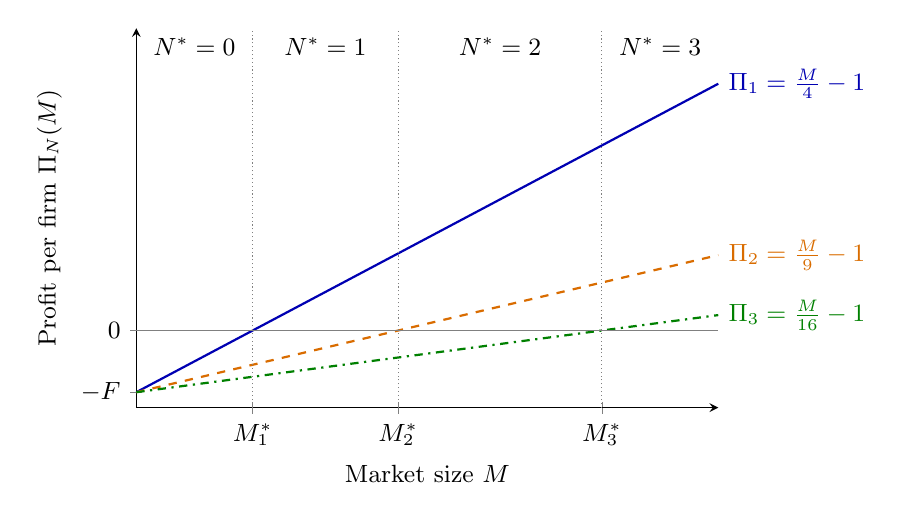
\begin{tikzpicture}
\begin{axis}[
  width=0.74\textwidth, height=6.4cm,
  xmin=0, xmax=20, ymin=-1.25, ymax=4.9,
  axis lines=left,
  clip=false,
  xlabel={Market size $M$}, ylabel={Profit per firm $\Pi_N(M)$},
  xtick={4,9,16}, xticklabels={$M_1^*$, $M_2^*$, $M_3^*$},
  ytick={-1,0}, yticklabels={$-F$, $0$},
  every axis plot/.append style={thick},
  label style={font=\small}, tick label style={font=\small}
]
\addplot[domain=0:20, samples=2, blue!70!black] {x/4 - 1}
  node[pos=1, right, font=\small] {$\Pi_1 = \frac{M}{4} - 1$};
\addplot[domain=0:20, samples=2, orange!85!black, dashed] {x/9 - 1}
  node[pos=1, right, font=\small] {$\Pi_2 = \frac{M}{9} - 1$};
\addplot[domain=0:20, samples=2, green!50!black, dash dot] {x/16 - 1}
  node[pos=1, right, font=\small] {$\Pi_3 = \frac{M}{16} - 1$};
\draw[gray, thin] (axis cs:0,0) -- (axis cs:20,0);
\draw[gray, densely dotted] (axis cs:4,-1.25) -- (axis cs:4,4.9);
\draw[gray, densely dotted] (axis cs:9,-1.25) -- (axis cs:9,4.9);
\draw[gray, densely dotted] (axis cs:16,-1.25) -- (axis cs:16,4.9);
\node[font=\small] at (axis cs:2,4.6) {$N^* = 0$};
\node[font=\small] at (axis cs:6.5,4.6) {$N^* = 1$};
\node[font=\small] at (axis cs:12.5,4.6) {$N^* = 2$};
\node[font=\small] at (axis cs:18,4.6) {$N^* = 3$};
\end{axis}
\end{tikzpicture}
\caption{Entry thresholds under linear Cournot competition (\cref{ex:01-cournot-thresholds}) with the
normalization $\frac{(a - c)^2}{b} = 1$ and $F = 1$. Profit per firm is $\Pi_N = \frac{M}{(N + 1)^2} - 1$.
Each line crosses zero at the threshold $M_N^* = (N + 1)^2$, and the bands show the free-entry number of
firms $N^*$.}
\label{fig:01-thresholds}
\end{figure}

\subsubsection{Bresnahan and Reiss (1991): entry into isolated markets}

\casehead{Question}
How much does entry change competition in a concentrated market? Theories give conflicting answers.
Contestability says that the threat of entry alone disciplines incumbents, while many entry-barrier theories
say that only actual entry matters. \citet{BresnahanReiss1991} propose to measure the effect of each
additional entrant from the relation between market size and the number of firms. The numbers below come
from the working-paper version of the article (Stanford GSB Research Paper 1061).

\casehead{Setting and data}
The sample consists of 202 geographically isolated local markets in the United States.
The typical market is a county seat in the western United States, and the population of the central town
approximates market size. The towns lie at least 25 miles from the nearest town of 1,000 people or more, and
towns within 100 miles of a city of 100,000 are excluded.
Isolation makes it easy to count all competitors. The authors keep only industries whose sellers offer a
narrowly defined product or service and can all be identified. Five survive their data requirements:
doctors, dentists, druggists, plumbers and tire dealers. Firms are counted from telephone books and trade
sources and checked by visits. Practices that share an address and a telephone number count as one firm. In
the sample, mean town population is 3,740, ranging from 120 to 45,090, and the mean number of dentists is
2.6 (working paper, Table~2).
Of the 202 markets, 32 have no dentist, 67 have one and 39 have two (Table~1).

\casehead{Model and estimating equations}
The empirical model generalizes \eqref{eq:01-br-profit} by letting market size, variable profit and fixed
costs depend on observables. The parameter names below are ours, because the paper's symbols clash with the
notation of this book. In market $t$ the profit of each of $N$ firms is
\begin{equation}\label{eq:01-br-latent}
  \Pi_{Nt} = M_t(\lambda)\,V_N(X_t) - F_N(W_t) + u_t .
\end{equation}
The profit shock $u_t$ is standard normal and independent across markets and of the observables. It is common
to all firms in a market. Market size is
\[
  M_t(\lambda) = \mathit{TownPop}_t + \lambda_1 \mathit{NearbyPop}_t + \lambda_2 \mathit{PosGrowth}_t
  + \lambda_3 \mathit{NegGrowth}_t + \lambda_4 \mathit{Commuters}_t ,
\]
with the coefficient on town population normalized to one. The other terms are population within ten miles,
the positive and negative parts of town growth between 1970 and 1980, and residents who commute to work outside
the county. Per-firm variable profit per consumer and fixed costs are
\[
  V_N(X_t) = \eta_1 + X_t\beta^V - \sum_{n=2}^{N}\eta_n ,
  \qquad
  F_N(W_t) = \zeta_1 + \zeta_L W_{Lt} + \sum_{n=2}^{N}\zeta_n ,
\]
The vector $X_t$ contains county demographics such as per capita income. The variable $W_{Lt}$ is the value of
farmland, a proxy for the cost of capital. The parameter $\eta_n$ measures the fall in each firm's variable profit per
consumer when the $n$-th firm enters, and $\zeta_n$ the increase in fixed cost. Because $V_N$ is per firm,
$V_N = \frac{v_N}{N}$ in the notation of \cref{prop:01-entry-thresholds}. Each industry has 19 parameters:
four $\lambda$s, four coefficients in $\beta^V$, five $\eta$s and six $\zeta$s.

\casehead{Estimator}
Write $\bar\Pi_{Nt} = M_t V_N - F_N$ for the deterministic part of profit. The equilibrium number of firms is
$N_t = N$ when $\Pi_{Nt} \ge 0 > \Pi_{N+1, t}$, that is, when $-\bar\Pi_{Nt} \le u_t < -\bar\Pi_{N+1, t}$.
With $\bar\Pi_{1t} \ge \bar\Pi_{2t} \ge \cdots$ and $\Phi$ the standard normal distribution function, this event
has probability
\[
  \Pr(N_t = N) = \Phi\big(-\bar\Pi_{N+1, t}\big) - \Phi\big(-\bar\Pi_{Nt}\big)
               = \Phi\big(\bar\Pi_{Nt}\big) - \Phi\big(\bar\Pi_{N+1, t}\big)
\]
for $N = 1, \dots, 4$. The end categories have $\Pr(N_t = 0) = 1 - \Phi(\bar\Pi_{1t})$ and
$\Pr(N_t \ge 5) = \Phi(\bar\Pi_{5t})$. The parameters maximize the ordered probit log-likelihood
\[
  \ell = \sum_{t} \sum_{N=0}^{5} \indic\{N_t = N\} \ln \Pr(N_t = N \mid M_t, X_t, W_t) .
\]
The authors impose $\bar\Pi_{N+1} \le \bar\Pi_N$ by setting an $\eta_N$ or $\zeta_N$ to zero where necessary. In
the doctors' model, for example, $\eta_3 = \eta_5 = 0$. At the sample means of the covariates, the entry
thresholds are
\begin{equation}\label{eq:01-br-threshold}
  M_N^* = \frac{\zeta_1 + \zeta_L \bar W_L + \sum_{n=2}^{N}\zeta_n}{\eta_1 + \bar X\beta^V - \sum_{n=2}^{N}\eta_n} ,
\end{equation}
the market size at which $\bar\Pi_N = 0$, and the per-firm thresholds are $\tau_N = \frac{M_N^*}{N}$.

\casehead{Identification}
Market size is the excluded variable. It multiplies variable profit and leaves fixed costs unchanged, so the
way the distribution of $N_t$ shifts with population traces out the thresholds. The normalizations fix the
units of market size (town residents) and the scale of profit (unit variance of $u_t$). The thresholds are
ratios, so they do not depend on the scale normalization. The parameters $\eta_n$ and $\zeta_n$ are
separately identified only because $\eta_n$ interacts with market size and $\zeta_n$ does not. In practice
the data barely separate falling variable profits from rising fixed costs, and many individual estimates have
large standard errors (working paper, pp.~16 and 20). The thresholds depend only on the ratio of fixed costs
to variable profits, and restricting the cost parameters changes them little (working paper, p.~21). Five
assumptions are maintained. Firms within an industry differ only through the entry-order terms $\eta_n$ and
$\zeta_n$, and one profit shock is common to all firms in a market. Population is exogenous to the number of firms, and isolation captures every competitor. Markets
are in long-run equilibrium. With a single cross-section, sunk and fixed costs cannot be distinguished (working
paper, fn.~5).

\casehead{Main results}
\Cref{tab:01-br-thresholds} reproduces the estimated thresholds. A monopoly tire dealer or druggist needs about
500 people in town, and a monopoly doctor or dentist between 700 and 900. A monopoly plumber needs about
1,430 people, twice the dentist threshold and 1.6 times the doctor threshold (\cref{tab:01-br-thresholds}).
The per-firm ratios decline with $N$. For doctors, dentists, druggists and tire dealers, the second firm needs
roughly 1.8 to 2.0 times the customers of a monopolist, while plumbers' ratios stay near one throughout.
For the third firm the ratio is near one for doctors and plumbers (1.10 and 1.00), 1.28 for tire dealers and
1.58 for druggists. For dentists Table~4 prints 0.79, while the printed thresholds imply 1.10.
For the fourth and fifth firms the ratios lie between 0.94 and 1.14 in every industry, so the decline stops
abruptly after the first few entrants.
Likelihood ratio tests cannot reject $\tau_3 = \tau_4 = \tau_5$ except for dentists. They reject
$\tau_1 = \cdots = \tau_5$ in all five industries, so the variation in the first two thresholds is not
sampling noise. \Cref{fig:01-br-ratios} redraws the paper's Figure~4, which plots $\frac{\tau_5}{\tau_N}$
against $N$.

\begin{table}[htbp]
\centering
\caption{Entry thresholds in five retail and professional industries}
\label{tab:01-br-thresholds}
\small
\setlength{\tabcolsep}{4.5pt}
\begin{tabular}{@{}l rrrrr rrrr@{}}
\toprule
\multicolumn{10}{@{}l}{\textit{Panel A. Thresholds and per-firm threshold ratios}} \\
\addlinespace[2pt]
 & \multicolumn{5}{c}{Threshold $M_N^*$ (thousands)} & \multicolumn{4}{c}{Ratio $\frac{\tau_{N+1}}{\tau_N}$} \\
\cmidrule(lr){2-6}\cmidrule(l){7-10}
Industry & $N = 1$ & $2$ & $3$ & $4$ & $5$ & $\frac{\tau_2}{\tau_1}$ & $\frac{\tau_3}{\tau_2}$ & $\frac{\tau_4}{\tau_3}$ & $\frac{\tau_5}{\tau_4}$ \\
\midrule
Doctors      & 0.88 & 3.49 & 5.78 & 7.72 & 9.14 & 1.98 & 1.10 & 1.00 & 0.95 \\
Dentists     & 0.71 & 2.54 & 4.18 & 5.43 & 6.41 & 1.78 & 0.79 & 0.97 & 0.94 \\
Druggists    & 0.53 & 2.12 & 5.04 & 7.67 & 9.39 & 1.99 & 1.58 & 1.14 & 0.98 \\
Plumbers     & 1.43 & 3.02 & 4.53 & 6.20 & 7.47 & 1.06 & 1.00 & 1.02 & 0.96 \\
Tire dealers & 0.49 & 1.78 & 3.41 & 4.74 & 6.10 & 1.81 & 1.28 & 1.04 & 1.03 \\
\bottomrule
\end{tabular}

\medskip
\begin{tabular}{@{}l rr rr rr rr@{}}
\toprule
\multicolumn{9}{@{}l}{\textit{Panel B. Likelihood ratio tests of equal per-firm thresholds}} \\
\addlinespace[2pt]
 & \multicolumn{2}{c}{$\tau_4 = \tau_5$} & \multicolumn{2}{c}{$\tau_3 = \tau_4 = \tau_5$}
 & \multicolumn{2}{c}{$\tau_2 = \cdots = \tau_5$} & \multicolumn{2}{c}{$\tau_1 = \cdots = \tau_5$} \\
\cmidrule(lr){2-3}\cmidrule(lr){4-5}\cmidrule(lr){6-7}\cmidrule(l){8-9}
Industry & LR & df & LR & df & LR & df & LR & df \\
\midrule
Doctors      & 1.12 & 1 & 6.20      & 3 & 8.33      & 4 & 45.06$^*$  & 6 \\
Dentists     & 1.59 & 1 & 12.30$^*$ & 2 & 19.13$^*$ & 4 & 36.67$^*$  & 5 \\
Druggists    & 0.43 & 2 & 7.13      & 4 & 65.28$^*$ & 6 & 113.92$^*$ & 8 \\
Plumbers     & 1.99 & 2 & 4.01      & 4 & 12.07     & 6 & 15.62$^*$  & 7 \\
Tire dealers & 3.59 & 2 & 4.24      & 3 & 14.52$^*$ & 5 & 20.89$^*$  & 7 \\
\bottomrule
\end{tabular}
\par\smallskip
\begin{minipage}{\textwidth}\footnotesize
\textit{Notes:} Thresholds are evaluated at sample means with \eqref{eq:01-br-threshold}, using the baseline
ordered probit estimates, and are measured in thousands of people. The per-firm threshold is $\tau_N = \frac{M_N^*}{N}$. Ratios are as printed in the
source. The printed thresholds imply $\frac{\tau_3}{\tau_2} = 1.10$ for dentists, and all other ratios match
the thresholds up to rounding. In Panel B, LR is the likelihood ratio statistic and df its degrees of
freedom. An asterisk marks a statistic above the 5 percent cutoff of the chi-squared distribution with the
stated degrees of freedom. Source: Bresnahan and Reiss (1991), Table~4
(working-paper version, Research Paper 1061).
\end{minipage}
\end{table}

\begin{figure}[htbp]
\centering
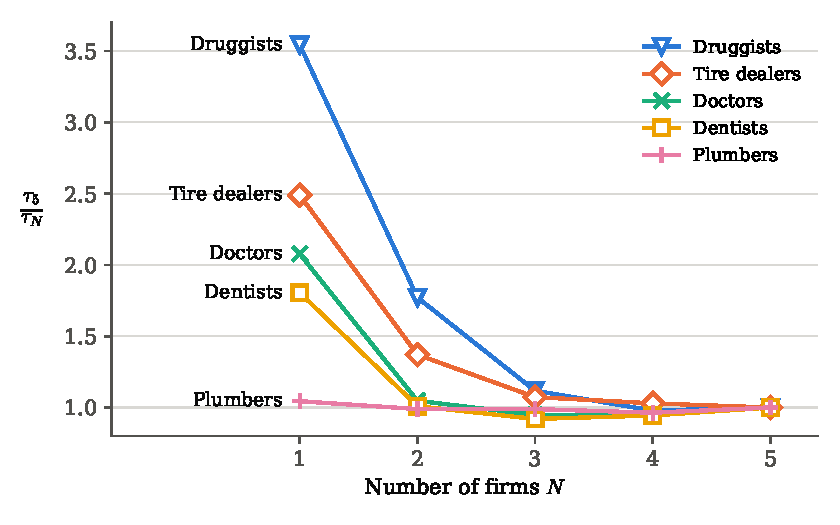
\includegraphics[width=0.82\textwidth]{figures/ch01/br_threshold_ratios.pdf}
\caption{Ratio of the per-firm threshold for five firms to the per-firm threshold for $N$ firms,
$\frac{\tau_5}{\tau_N}$, by industry. A value near one means that the $N$-th firm needs about as many customers
as the fifth. From $N = 3$ on, the ratios lie between 0.92 and 1.12 in every industry. Redrawn from the thresholds in \cref{tab:01-br-thresholds}. Source: Bresnahan and Reiss (1991),
Figure~4 (working-paper version).}
\label{fig:01-br-ratios}
\end{figure}

\casehead{Robustness}
Using ``four or more firms'' as the top category extends the analysis to eight industries. The thresholds of
the original five change little, and heating contractors and barbers show the same pattern. Auto dealers are
the exception, with a per-firm ratio for the fourth dealer well above one (working paper, pp.~18--19). The authors attribute this to product differentiation. Most dealer triopolies pit the three
domestic manufacturers against one another, and the fourth dealer is typically the first intrabrand
competitor. The hypothesis of equal fixed costs across entrants is rejected for every industry except
plumbers, but imposing it barely moves the thresholds. Restricting the sample to very isolated markets, at least 40 miles
from the next town of 1,000 people, leaves 157 markets and similar ratios.
Treating every county with fewer than 10,000 residents in 1980 as a market, isolated or not, sharply reduces
the estimated effect of the second and third doctors and dentists. This is what we would expect if customers
in less isolated towns shop elsewhere, and it supports the strict market definition.

\casehead{Interpretation}
Under the maintained hypotheses that firms in each industry offer similar services with similar technologies
and costs, the results say that entry beyond the third firm changes margins very little. Most of the
competitive effect of entry is felt in highly concentrated markets, with the second and third entrants. The
authors were surprised. They had expected margins, or entry barriers, to erode gradually. Through the lens of
\cref{ex:01-cournot-thresholds} the pattern is sharper than linear Cournot competition implies. Cournot
predicts a second-firm ratio of $1.125$ and ratios above one for every later entrant. Four of the industries
instead show second-firm ratios between 1.78 and 1.99, and every industry shows ratios close to one from the
fourth firm on. In the words of Einav and Levin, competition
appears to ``kick in relatively quickly'' with just a few firms and then does not ramp up with further entry
(p.~155).

\casehead{Critiques}
Bresnahan and Reiss list the main caveats themselves. Without prices, quantities and the timing of entry, they
cannot say whether markets with three or more firms are competitive, only that conduct stops changing
(\cref{rem:01-etr-meaning}). Ratios above one can reflect costlier later entrants as well as falling margins
(\cref{rem:01-etr-costs}). Professionals with low opportunity costs might seek out isolated monopolies, which
would raise the monopoly ratios for reasons unrelated to competition. Einav and Levin add a critique of the
literature that followed (pp.~155--156). One might have expected researchers to look for other identifying
variation, such as differences in fixed costs or entry restrictions, or to gather data on prices and costs.
Instead, most follow-up work developed econometric methods that allow firm heterogeneity or relax parametric
restrictions \citep{Berry1992,BerryTamer2006}, often applying the original identifying assumptions where they
are less compelling. This produced a rich literature on identification and estimation that has not
necessarily brought us closer to the original question.

\casehead{Contribution}
The paper shows how sparse data, used with theory and a clean design, can answer an important question. Counts
of firms in markets of different sizes reveal how competition varies with the number of firms. The entry model
gets around missing data on prices and quantities, which is one reason it has been so influential (p.~160). It
also reframes the SCP question. Concentration is treated as an equilibrium outcome driven by an exogenous
shifter, market size, and the relation between the two identifies how conduct changes with structure.

\begin{remark}[Market size and concentration]\label{rem:01-sutton}
If the per-firm thresholds converge to a finite limit $\tau_\infty$, concentration vanishes in large markets.
Because $\tau_N$ is nondecreasing, $M < M^*_{N^*+1} = (N^* + 1)\tau_{N^*+1} \le (N^* + 1)\tau_\infty$ by
\cref{prop:01-entry-thresholds}(iii). Hence $N^* > \frac{M}{\tau_\infty} - 1$, which grows without bound with
$M$. This argument treats fixed costs as exogenous. \citet{Sutton1991} shows that the conclusion fails when
firms can raise demand through sunk outlays such as advertising or research and development. Such
endogenous sunk costs escalate with market size, and concentration can stay bounded away from zero
however large the market becomes.
\end{remark}

\subsubsection{Industry dynamics}

Many questions about market structure are dynamic \citep[p.~156]{EinavLevin2010}. Do new industries follow a
common life cycle of entry and consolidation? How do firm and industry growth vary with market
characteristics? Are mergers followed quickly by entry, and how do industries adapt to booms and recessions?
A dynamic view can also temper static intuition. Higher concentration reduces static welfare, but the prospect
of market power can create strong incentives to innovate.

The literature has two strands (p.~156). The first looks across industries for robust patterns of survival,
turnover and growth. Its main finding is the large heterogeneity across establishments even within narrow
industries. This finding shaped theoretical models of industry dynamics \citep{Hopenhayn1992}, which in turn
inspired work on firm heterogeneity in international trade \citep{Melitz2003}. The link between entry, exit and
firm characteristics also entered the study of productivity through \citet{OlleyPakes1996}. The second strand
builds models of dynamic equilibrium in single industries, often in the framework of \citet{EricsonPakes1995}.
\citet{Benkard2004} applies such a model to commercial aircraft, where learning by doing lowers costs
dramatically. Equilibrium prices can lie below marginal cost early in a product's life, because extra output
speeds learning. The prospect of market power is what motivates firms to move down the learning curve.
Consumers gain from lower prices both early on and later, when costs are lower. Newer methods estimate sunk
costs, learning and adjustment frictions from panel data on firms or local markets
\citep{AguirregabiriaMira2007,BajariBenkardLevin2007,PakesOstrovskyBerry2007}. \citet{AguirregabiriaCollardWexlerRyan2021}
survey this work in Volume~4 of the Handbook of Industrial Organization. Their chapter lays out the Markov
perfect equilibrium framework, the data typically available, identification and estimation, and applications to
innovation, mergers, regulation, investment, advertising and dynamic pricing \citep[Preface, pp.~xvi--xvii]{HoHortacsuLizzeri2021}.

\begin{remark}[Why learning can push prices below marginal cost]\label{rem:01-learning}
A two-period monopolist faces demand $Q(p)$ in each period and discounts the future by a factor $\delta$. The
first-period cost is $c_1$. Learning makes the second-period cost $c_2(Q_1)$ fall with first-period output,
so $c_2' < 0$. Let $\pi_2(c_2)$ be the optimal second-period profit. By the envelope theorem
$\pi_2'(c_2) = -q_2$, where $q_2$ is second-period output. The firm chooses $p_1$ to maximize
$(p_1 - c_1)Q(p_1) + \delta\,\pi_2\big(c_2(Q(p_1))\big)$. The first-order condition is
\[
  Q(p_1) + (p_1 - c_1)Q'(p_1) + \delta\,\pi_2'(c_2)\,c_2'(Q_1)\,Q'(p_1) = 0 .
\]
Substituting $\pi_2' = -q_2$ and dividing by $-Q'(p_1) > 0$ gives
\[
  p_1 = \big(c_1 - \delta q_2 \lvert c_2' \rvert\big) - \frac{Q(p_1)}{Q'(p_1)} .
\]
The firm prices off an effective marginal cost that is lower than $c_1$ by the discounted value of learning. If
learning is strong enough, $p_1 < c_1$.
\end{remark}

The data available for such models often pale in comparison with the ambitious questions asked, so researchers
fill the gaps with strong assumptions (p.~156). Einav and Levin view this work as ``a quantitative theory
exercise'' (pp.~156--157). It sheds light on dynamic competition in a model with reasonable parameter values.
They do not see this as a problem. It is hard to imagine a clean research design that could pin down the
long-run effect on innovation of a change in the patent system. When the entire history of an industry is a
single data point, quasi-experimental variation is rare, and models are the only way to study such
questions.

\subsection{Structural and design-based approaches}\label{sec:01-today-debate}

Thirty years ago empirical IO resembled other applied fields \citep[p.~157]{EinavLevin2010}. Industrial
organization economists ran cross-industry regressions and faced endogeneity, omitted variables and reverse
causality, much as labor economists running wage regressions did. Since then IO has moved in a distinctive
direction. It turned toward single industries, where measurement and identification are cleaner, and toward
analyses framed by an economic theory of the industry. In the same journal issue, \citet{AngristPischke2010}
describe a parallel move in applied microeconomics toward randomized experiments and quasi-experiments. They
also criticize empirical IO, and Einav and Levin reply. The exchange clarifies the stance of this book.

\subsubsection{Clean measurement versus the object of interest}

No one disagrees about the ideal (p.~157). Every researcher would like to define an object of interest and
then design the perfect experiment to measure it. Without that ideal, researchers face trade-offs, and a
common one is between the cleanness of a measurement and how well the measured object proxies for the object
of interest. Einav and Levin illustrate it with cereal (pp.~157--158). Suppose the object of interest is the
$J \times J$ matrix of price elasticities $E = [\varepsilon_{jk}]$.

\begin{itemize}
  \item The standard IO approach controls for shifts in demand and assumes that the remaining correlation of
        prices across cities reflects costs, as with the Hausman instruments of \citet{Nevo2001}. Within the
        demand model this identifies all of $E$. The assumption may fail.
  \item A design-based alternative looks for an episode that moved one price for an explicable and plausibly
        exogenous reason. An example would be a week in which the pricing algorithm for Froot Loops
        malfunctioned and produced an unintended sale. Such an episode credibly identifies one column of
        $E$, the responses $\varepsilon_{j,\mathrm{FL}}$ of all products to the price of Froot Loops. To learn
        the rest of $E$ we must extrapolate, for instance by assuming that a change in the price of Frosted
        Flakes, or of any cereal, would have analogous effects.
\end{itemize}

Neither approach is ideal. The first relies on a questionable identifying assumption but frames the exercise
directly in terms of the object of interest. The second measures a few entries convincingly but reaches the
object of interest only through a questionable extrapolation. Einav and Levin argue that evaluating entire
research approaches in the abstract paints too simple a picture (p.~158). The right resolution depends on the
question, the data and how compelling a rationale theory provides for the assumptions. There is room for many
approaches, even to the same question, and careful work from different angles is often complementary.

\subsubsection{Theory, transparency and mechanisms}

Angrist and Pischke favor measurement strategies uncontaminated by restrictions from an economic model, partly
on grounds of transparency. Einav and Levin call the implied link between theory and obscurity ``a false
equivalence'' (p.~158). A model derived from theory can be exposited with perfect clarity, and a linear
regression can be exposited with perfect obscurity. It is more natural to start with a research question and
ask how much theory can say about it. Standard theory says little about student behavior in third-grade
classrooms, the setting of Angrist and Pischke's class-size example. There a statistical approach that exploits
variation across thousands of roughly parallel classrooms is attractive. Industrial organization is largely
about firms and markets, which is the other side of the contrast quoted in \cref{sec:01-what-is-io}
(pp.~158--159). Moreover, the interesting question is often a mechanism rather than a single
causal effect. Markets differ greatly, so importing particular numbers across markets is rarely compelling.
Empirical work generalizes best by building support for principles of strategic interaction and market
functioning that apply across industries.

\subsubsection{The merger example}

Angrist and Pischke chose merger evaluation as their example. They dismiss merger simulation as needlessly
indirect and ask why there has not been more retrospective analysis of past mergers. Einav and Levin answer
that the point is good at one level and misses the point at another (p.~159). If the Department of Justice had
to review a merger of Microsoft and Yahoo!, the price effects of past airline or office-supply mergers would be
of little use. It is far more useful to lay out a clear framework for the potential effects of that merger and
to add the best available evidence. \Cref{ch:mergers} presents retrospective studies and merger simulations
side by side, and it shows how each disciplines the other.

The bottom line is that economic theory and the search for compelling identifying variation are allies
(p.~159). The applied work that Einav and Levin find most exciting rests on careful measurement from data with
good variation and then frames the analysis in a coherent economic model. The model gives a way to think about
how the industry works and, potentially, to draw conclusions about policy or general principles. The case
studies of this book are chosen and presented with that standard in mind.

\subsubsection{Methods, applications and the questions IO asks}

Einav and Levin also voice concerns about the field itself (pp.~159--160). Their main concern is that too
little effort goes into compelling applications relative to new econometric methods. Better methods are
valuable if they are eventually used in compelling ways and do not become an end in themselves. In demand
estimation, researchers may have tolerated imperfect price variation because the main contribution was a
method that applies more broadly. Data limitations explain part of the current balance. Some of the most
influential methods were responses to scarce data. The entry model of \citet{BresnahanReiss1991} gets around
missing data on prices and quantities, and the demand model of \citet{BerryLevinsohnPakes1995} needs only
market-level data. As firms collect vast amounts of data on customers, prices, quantities and locations,
richer data may substitute for methods and shift effort toward applications.

A related danger applies to all empirical strategies: the elegance of a solution can pull researchers toward
less important questions (p.~160). Einav and Levin use eBay as an example. Viewed as a laboratory for elegant
auction methods, eBay invites the study of ever narrower submarkets. Broader questions, such as why eBay
succeeded as an institution or how it competes with Amazon and other platforms, would then go unasked.
Researchers should ``resist the temptation of grabbing a hammer and letting it pull them toward a limited set
of nails'' (p.~160).

The last concern is about scope. Schmalensee's review of the cross-industry literature concluded that it had
taught us little about how markets work (\cref{sec:01-scp-today}). After two decades of industry studies, we know a
lot about specific industries such as automobiles, airlines, electricity, and cement and concrete. This
knowledge is extremely disaggregated and does not easily accumulate across industries. As a result, IO has
ceded many important questions about the overall organization of production to trade and macroeconomics.
Einav and Levin suggest that ``it may be time to reclaim them'' (p.~160). The debate over rising markups in
\cref{sec:01-rising-markups} is one place where IO economists are doing so, and it shows how hard the
cross-industry questions remain.

\section{Roadmap of the book}\label{sec:01-roadmap}

The book has four parts and three appendices. Every chapter follows the order of this introduction: theory in
general form first, then case studies that show how the theory meets data. \Cref{tab:01-roadmap} lists, for
each chapter, its central question, its main models and tools, and the papers it treats as full case studies.
Readings that are not case studies receive shorter treatments in the same chapters.

\subsection{The four parts}

Part~I treats market power, its theory and its measurement. This chapter introduced the questions, the SCP
tradition and its failure, the NEIO response and the structural workflow. \Cref{ch:theory} develops the theory that the
rest of the book uses. It covers monopoly pricing, Cournot and Bertrand competition, conjectural variations and
the conduct parameter, pass-through and welfare. \Cref{ch:conduct} asks whether market power can be detected
and measured in homogeneous-good industries. It covers tax pass-through tests, the Panzar-Rosse statistic,
residual demand, the identification of conduct by demand rotations, and direct validations against cost data.
\Cref{ch:diffprod} turns to differentiated products. It derives multi-product Bertrand pricing and diversion
ratios, discusses existence and uniqueness of equilibrium, and contrasts product space with characteristic
space.

Part~II is about demand estimation. \Cref{ch:aids} estimates demand in product space with the Almost Ideal
Demand System, multi-stage budgeting and Hausman instruments. \Cref{ch:discrete} builds the foundations of
discrete choice, including the vertical model and the pure characteristics model. \Cref{ch:logit} covers the
logit and nested logit, the Berry inversion and instruments for price. \Cref{ch:blp} develops the random
coefficients logit of Berry, Levinsohn and Pakes, its estimation and its supply side. \Cref{ch:airlines}
applies these tools to airline hubs and entry. \Cref{ch:newgoods} measures the value of new goods and the bias
in price indexes that ignore them.

Part~III is about competition policy. \Cref{ch:mergers} covers horizontal mergers. It treats market
definition, the theory of mergers in Cournot and differentiated-product models, upward pricing pressure,
merger simulation and retrospective studies. \Cref{ch:collusion-theory} develops the theory of collusion in
repeated games, with demand fluctuations, imperfect monitoring, private information and communication.
\Cref{ch:collusion-evidence} studies how real cartels operated and how collusion can be detected in prices and
bids.

Part~IV is about auctions. \Cref{ch:auction-theory} develops the theory of single-object auctions, from
independent private values to the affiliated values model of Milgrom and Weber. \Cref{ch:auction-empirics}
asks what bid data reveal about values and costs. It covers identification, the estimator of Guerre, Perrigne
and Vuong, unobserved heterogeneity and entry.

Three appendices support the main text. \Cref{app:econometrics} collects the econometric tools: instrumental variables, the
generalized method of moments, maximum likelihood and simulation estimators, the delta method, nonparametric
estimation, and event studies. \Cref{app:math} collects the mathematical tools: the envelope and implicit
function theorems, duality, extreme value algebra, order statistics, contraction mappings, log-concavity and
affiliation. \Cref{app:problems} contains worked problems with full solutions. Two simulated markets recur
there as running examples. One has 25 logit products sold by five owners. The other has 100 markets drawn from a pool of ten
products, and each market offers between four and nine of them. It is generated from a random-coefficients logit
with a cost shifter, and on it the vertical, logit and random-coefficients estimators are compared.

\begin{table}[htbp]
\centering
\caption{Roadmap of the book}
\label{tab:01-roadmap}
\scriptsize
\renewcommand{\arraystretch}{1.0}
\begin{tabularx}{\textwidth}{@{}>{\raggedright\arraybackslash}p{1.95cm}
  >{\raggedright\arraybackslash}X >{\raggedright\arraybackslash}X >{\raggedright\arraybackslash}X@{}}
\toprule
Chapter & Central question & Main models and tools & Case studies in depth \\
\midrule
\multicolumn{4}{@{}l}{\textit{Part I. Market power: theory and measurement}} \\
\ref{ch:intro}. Introduction & How do we learn about market power and its causes? & SCP regressions, the
  Cournot link between margins and concentration, the conduct parameter, the structural workflow &
  \citet{BresnahanReiss1991}, \citet{GriecoMurryYurukoglu2024} (and substantive treatments of
  \citet{Bresnahan1989} and \citet{EinavLevin2010}) \\
\ref{ch:theory}. Pricing theory & How do demand, cost and conduct determine prices? & Monopoly pricing,
  Cournot and Bertrand oligopoly, conjectural variations, pass-through, welfare & None \\
\ref{ch:conduct}. Measuring market power & Can we detect and measure market power with homogeneous goods? &
  Tax pass-through tests, Panzar-Rosse statistic, residual demand, identification of conduct by rotations &
  \citet{Sumner1981}, \citet{Corts1999}, \citet{GenesoveMullin1998}, \citet{Wolfram1999} \\
\ref{ch:diffprod}. Differentiated oligopoly & How do multi-product firms price differentiated goods? &
  Multi-product Bertrand-Nash pricing, ownership matrix, diversion ratios, existence and uniqueness, location
  models & None \\
\addlinespace
\multicolumn{4}{@{}l}{\textit{Part II. Demand estimation}} \\
\ref{ch:aids}. AIDS & How do we estimate flexible demand in product space? & Duality, AIDS, multi-stage
  budgeting, Hausman instruments, welfare & \citet{DeatonMuellbauer1980a}, \citet{HausmanLeonardZona1994},
  \citet{ChaudhuriGoldbergJia2006} \\
\ref{ch:discrete}. Discrete choice & How do individual choices aggregate to market demand? & Random utility,
  vertical model, pure characteristics model, hedonic approach & \citet{Bresnahan1987},
  \citet{BerryPakes2007} \\
\ref{ch:logit}. Logit & How do we estimate logit demand with endogenous prices? & Logit, Berry inversion,
  instruments, nested logit & \citet{Berry1994}, \citet{Einav2007}, \citet{Hendel1999} \\
\ref{ch:blp}. BLP & How do we obtain realistic substitution from market-level data? & Random coefficients
  logit, contraction mapping, GMM, supply side, micro moments & \citet{BerryLevinsohnPakes1995},
  \citet{Nevo2000a}, \citet{Nevo2001}, \citet{BerryLevinsohnPakes2004}, \citet{Goldberg1995} \\
\ref{ch:airlines}. Airlines & Why are fares high at hubs, and how does entry discipline them? & Fare
  regressions, event studies, discrete choice with consumer types and hub costs & \citet{Borenstein1989},
  \citet{WhinstonCollins1992}, \citet{BerryCarnallSpiller2006} \\
\ref{ch:newgoods}. New goods & What is a new good worth to consumers? & Virtual prices, compensating variation,
  logit welfare, micro moments & \citet{Hausman1997}, with the comment by \citet{Bresnahan1997};
  \citet{Trajtenberg1989}, \citet{Petrin2002}, \citet{Gentzkow2007} \\
\addlinespace
\multicolumn{4}{@{}l}{\textit{Part III. Competition policy}} \\
\ref{ch:mergers}. Mergers & When do horizontal mergers raise prices? & Market definition, Cournot merger
  analysis, upward pricing pressure, merger simulation, retrospectives & \citet{FarrellShapiro1990},
  \citet{FarrellShapiro2010}, \citet{Nevo2000b}, \citet{BjornerstedtVerboven2016},
  \citet{MillerWeinberg2017} \\
\ref{ch:collusion-theory}. Collusion: theory & How can firms sustain collusion without enforceable contracts? &
  Repeated games, optimal punishments, demand fluctuations, imperfect monitoring, private information,
  communication & \citet{GreenPorter1984}, \citet{RotembergSaloner1986},
  \citet{AtheyBagwellSanchirico2004}, \citet{HarringtonSkrzypacz2011} \\
\ref{ch:collusion-evidence}. Collusion: evidence & How did cartels operate, and how can we detect them? &
  Regime-switching supply relations, tests of price-war theories, bidding rings, tests for bid rigging &
  \citet{Porter1983}, \citet{Ellison1994}, \citet{PorterZona1993}, \citet{Asker2010} \\
\addlinespace
\multicolumn{4}{@{}l}{\textit{Part IV. Auctions}} \\
\ref{ch:auction-theory}. Auction theory & How do rules and information shape bids and revenue? & Private and
  affiliated values, first- and second-price equilibrium, revenue equivalence, reserve prices, linkage
  principle & \citet{MilgromWeber1982} \\
\ref{ch:auction-empirics}. Auction empirics & What do bids reveal about values and costs? & Order-statistic
  inversion, the GPV estimator, unobserved heterogeneity, entry, timber auctions &
  \citet{AtheyHaile2002}, \citet{AtheyHaile2007}, \citet{GuerrePerrigneVuong2000},
  \citet{Krasnokutskaya2011}, \citet{AtheyLevinSeira2011} \\
\bottomrule
\end{tabularx}
\par\smallskip
\begin{minipage}{\textwidth}\footnotesize
\textit{Notes:} The last column lists the papers treated as full case studies, following the structure
described in \cref{sec:01-roadmap-conventions}. Each chapter also gives shorter treatments of the other
readings in its scope.
\end{minipage}
\end{table}

\subsection{Reading paths}

The chapters build on one another, but several shorter paths through the book work well.
\begin{itemize}
  \item A reader interested in antitrust and merger analysis can read
        \cref{ch:theory,ch:conduct,ch:diffprod,ch:logit,ch:blp,ch:mergers}. This path runs from pricing
        theory and the measurement of market power to the demand models that merger simulation requires.
  \item A reader interested in demand estimation can read
        \cref{ch:aids,ch:discrete,ch:logit,ch:blp,ch:airlines,ch:newgoods}, after \cref{sec:01-workflow} and
        the multi-product pricing of \cref{ch:diffprod}.
  \item A reader interested in collusion can read
        \cref{ch:theory,ch:conduct,ch:collusion-theory,ch:collusion-evidence}.
  \item A reader interested in auctions can read \cref{ch:auction-theory,ch:auction-empirics}, after
        \cref{sec:01-today-auctions}. The bid-rigging material of \cref{ch:collusion-evidence} is a natural
        complement.
\end{itemize}

\subsection{Prerequisites and conventions}\label{sec:01-roadmap-conventions}

We assume graduate training in microeconomic theory and econometrics. On the theory side the reader should
know consumer theory and duality, and Nash, subgame perfect and Bayesian Nash equilibrium. On the econometric
side the reader should know least squares, instrumental variables, the generalized method of moments and
maximum likelihood. \Cref{app:econometrics,app:math} fill gaps. For the theory of industrial organization at
greater length, \citet{Tirole1988} remains the standard reference. For surveys of recent work, including topics
outside this edition, the reader can turn to Volumes~4 and~5 of the Handbook of Industrial Organization
\citep{HoHortacsuLizzeri2021a,HoHortacsuLizzeri2021}. Their Preface describes every chapter
\citep[pp.~xv--xxi]{HoHortacsuLizzeri2021}. The first five chapters review econometric methods that continue the
NEIO program, Chapters~6 to~9 review theory, and Chapters~10 to~17 apply both to policy questions and to
particular sectors. \Cref{tab:01-handbook} lists the chapters and the parts of this book that each one extends.

\begin{table}[htbp]
\centering
\caption{The chapters of the Handbook of Industrial Organization, Volumes 4 and 5}
\label{tab:01-handbook}
\footnotesize
\renewcommand{\arraystretch}{1.08}
\begin{tabularx}{\textwidth}{@{}>{\raggedright\arraybackslash}p{1.1cm}
  >{\raggedright\arraybackslash}p{4.4cm} >{\raggedright\arraybackslash}X >{\raggedright\arraybackslash}p{3.3cm}@{}}
\toprule
Chapter & Authors & Topic & Extends \\
\midrule
\multicolumn{4}{@{}l}{\textit{Volume 4: econometric methods (Chapters 1 to 5) and theory (Chapters 6 to 9)}} \\
1 & Berry and Haile & Foundations of demand estimation & \cref{ch:discrete,ch:logit,ch:blp} \\
2 & Gandhi and Nevo & Demand and supply in differentiated-products industries, opening with
  \citet{Bresnahan1987} & \cref{ch:discrete,ch:blp,ch:mergers} \\
3 & De Loecker and Syverson & Productivity, and the production approach to market power &
  \cref{sec:01-rising-markups} \\
4 & Aguirregabiria, Collard-Wexler and Ryan & Dynamic games & \cref{sec:01-today-structure} \\
5 & Kline, Pakes and Tamer & Moment inequalities and partial identification & \cref{sec:01-today-structure} \\
6 & Gavazza and Lizzeri & Frictions in product markets & Not covered \\
7 & Jullien, Pavan and Rysman & Two-sided markets, pricing and network effects & \cref{sec:01-early-studies} \\
8 & Bergemann and Ottaviani & Information markets and nonmarkets & Not covered \\
9 & Lee, Whinston and Yurukoglu & Contracting in vertical markets & Not covered \\
\addlinespace
\multicolumn{4}{@{}l}{\textit{Volume 5: applications to policy questions and sectors}} \\
10 & Agarwal and Budish & Market design & \cref{ch:auction-theory} \\
11 & Horta{\c{c}}su and Perrigne & Empirical perspectives on auctions & \cref{ch:auction-empirics} \\
12 & Asker and Nocke & Collusion, mergers and related antitrust issues &
  \cref{ch:mergers,ch:collusion-theory,ch:collusion-evidence} \\
13 & Bryan and Williams & Innovation: market failures and public policies & Not covered \\
14 & Einav, Finkelstein and Mahoney & Selection markets & \cref{sec:01-today-pricing} \\
15 & Clark, Houde and Kastl & Financial markets & Not covered \\
16 & Handel and Ho & Health care markets & \cref{sec:01-scp-today} \\
17 & Kellogg and Reguant & Energy and environmental markets & \cref{sec:01-today-auctions} \\
\bottomrule
\end{tabularx}
\par\smallskip
\begin{minipage}{\textwidth}\footnotesize
\textit{Notes:} Chapter titles are abbreviated. ``Extends'' names the chapter or section of this book that the
Handbook chapter continues. Source: \citet[Preface, pp.~xv--xxi]{HoHortacsuLizzeri2021}.
\end{minipage}
\end{table}

Notation is fixed across chapters. Markets are indexed by $t$ and products by $j$, with $j = 0$ the outside
good. Firms are indexed by $f$ in differentiated-product models and by $i$ in homogeneous-good models, and
consumers by $i$ in discrete choice models. Market shares are $s_{jt}$, marginal costs $mc_{jt}$, the price elasticity of demand
$\varepsilon > 0$, the conduct parameter $\theta$ and the ownership matrix $\Omega$. Mean utility is
$\delta_{jt} = x_{jt}\beta - \alpha p_{jt} + \xi_{jt}$, and auctions use $v$ for values, $b$ for bids and $G$
for the distribution of bids. When a chapter must depart from this notation, or rename the symbols of a paper,
it says so at first use.

Each case study follows the same order. We state the economic question and why it matters, the institutional
setting and the data. We then write the model and the exact estimating equations, the estimator, the
instruments and the identification argument. We reproduce the key results in a table, citing the table number
in the original paper, and discuss robustness, interpretation, the critiques raised in the literature and the
paper's contribution. Every chapter ends with exercises and with bibliographic notes that place its papers in
context.


\section{Bibliographic notes}\label{sec:01-bibnotes}

The structure-conduct-performance tradition begins with \citet{Mason1939} and the cross-industry studies of
\citet{Bain1951,Bain1956}. The Introduction of \citet{Tirole1988} tells its history, together with the Chicago
tradition and the theoretical wave that followed \citep{Joskow1975}. \citet{Schmalensee1989} is the standard
review of its evidence, and \citet{Weiss1989} collects the price-concentration studies of local markets.
\citet{Demsetz1973} stated the efficiency critique, and \citet{Schmalensee1987} tests it against the collusion
hypothesis. \citet{Hopenhayn1992} shows that high entry costs can produce the pattern Demsetz reported in a
competitive model, and
\citet{LevensteinSuslow2006} place the debate within the study of cartels. \citet{Salinger1990} revisited the debate with a panel of
industries, using annual cross sections and long differences. The measurement problems of accounting margins are analyzed by
\citet{FisherMcGowan1983}. The Cournot foundation of the margin-concentration relation is due to
\citet{CowlingWaterson1976}, with the conduct generalization of \citet{ClarkeDavies1982}. Section~5.5 of
\citet{Tirole1988} links concentration indices to industry profitability, and \citet{EncaouaJacquemin1980} give
the axioms that define them.

The New Empirical Industrial Organization is surveyed by \citet{Bresnahan1989}, whose chapter remains the best
statement of its principles and of its identification arguments. Its antecedents include \citet{Rosse1970}, and
its central identification results are \citet{Bresnahan1982} and \citet{Lau1982} for demand rotations and
\citet{PanzarRosse1987} for comparative statics in cost. \citet{Porter1983} is the classic application to a
cartel. \Cref{ch:conduct} develops these results, the tax tests of \citet{Sumner1981} and
\citet{AshenfelterSullivan1987}, and the critique by \citet{Corts1999}.

Modern empirical IO is surveyed by \citet{EinavLevin2010}. Volumes~4 and~5 of the Handbook of Industrial
Organization \citep{HoHortacsuLizzeri2021a,HoHortacsuLizzeri2021} survey its methods and applications chapter by
chapter, and \cref{tab:01-handbook} maps each chapter to this book. Among them, \citet{DeLoeckerSyverson2021} treat
productivity and the production approach to markups, and \citet{AguirregabiriaCollardWexlerRyan2021} treat dynamic
games. \citet{AskerNocke2021} cover collusion and mergers, and \citet{HandelHo2021} cover health care. \citet{Tirole1988} remains the
standard treatment of the theory. The demand models behind the structural workflow start with \citet{Berry1994} and
\citet{BerryLevinsohnPakes1995}, and the parallel approach to auctions starts with \citet{GuerrePerrigneVuong2000}.
\citet{BresnahanReiss1991} is the founding paper of the empirical entry literature, and \citet{Sutton1991} gives
the theory of endogenous sunk costs.

The debate over rising markups starts with \citet{DeLoeckerEeckhoutUnger2020}, who build on the production
approach of \citet{Hall1988} and \citet{DeLoeckerWarzynski2012}. Section~3.8 of \citet{AskerNocke2021}
summarizes their findings and the measurement questions they raise, and \citet{Ganapati2020} documents how
concentration relates to productivity, output and prices. \citet{BerryGaynorScottMorton2019} give the IO
perspective on that debate, which \citet{HandelHo2021} apply to health care and \citet{AutorEtAl2020} connect to
the labor share. \citet{BondEtAl2021} analyze the use of revenue data. \citet{GriecoMurryYurukoglu2024} study one
industry from the demand side and find that markups in the US new-car market fell after 1980 while consumer
surplus rose. The exchange between
\citet{AngristPischke2010} and \citet{EinavLevin2010} sets out the case for and against structural models in
applied microeconomics.

\section{Exercises}\label{sec:01-exercises}

\begin{enumerate}[label=\arabic*., leftmargin=*, itemsep=6pt]

\item \textit{Measuring the market power of one seller.} A coffee shop on a university campus sets a single price
for a cup of coffee.
\begin{enumerate}[label=(\alph*)]
  \item Describe the data and the variation in prices you would need to estimate the elasticity of the shop's
  residual demand. Explain why a regression of its daily sales on its daily price would not, in general, estimate
  that elasticity.
  \item Suppose you have such an estimate. Explain what you could conclude about marginal cost from
  \cref{prop:01-infer-cost}, and which maintained assumption the conclusion rests on.
  \item Consider three events: a per-unit tax on coffee sold on campus, a rise in the world price of coffee beans,
  and the opening of a rival cafe in the same building. For each event, say which primitive (demand, cost or
  conduct) it moves. Then explain what the observed response of price would reveal.
  \item Suppose the shop is the monopolist of \cref{ex:01-quality-markup}, with $\alpha = 0.5$ per dollar and a
  share $s = 0.4$ of potential customers. It improves its coffee at no change in marginal cost. Compute the change
  in price and in net utility $v$ per unit of quality. Explain why a regulator who saw the Lerner index rise would
  be wrong to conclude that customers lost.
\end{enumerate}

\item \textit{Concentration and mergers.}
\begin{enumerate}[label=(\alph*)]
  \item Construct two share vectors with the same four-firm concentration ratio $\mathit{CR}_4$ and different
  Herfindahl indices, and two with the same Herfindahl index and different $\mathit{CR}_4$. Compute the numbers
  equivalent $N^{\mathrm{eq}}$ of each.
  \item Firms $i$ and $j$ merge, and the merged firm keeps the share $s_i + s_j$. Show that the merger lowers the
  numbers equivalent from $\frac{1}{\HHI}$ to $\frac{1}{\HHI + 2 s_i s_j}$, and compute both for $s_i = 0.2$,
  $s_j = 0.1$ and $\HHI = 0.15$.
  \item Consider symmetric Cournot competition with linear demand among four firms with equal constant marginal
  costs. Two firms merge, and the merged firm has the same marginal cost as before. Compute the predicted change
  in the Herfindahl index from part (b) and the actual change in the new Cournot equilibrium. Explain the
  difference.
  \item Show that the entropy index $\sum_i s_i \ln s_i$ rises when share moves from a smaller to a larger
  firm, as \cref{rem:01-ej-axioms} requires. Then construct a transfer between two firms that leaves
  $\mathit{CR}_4$ unchanged and raises $\HHI$.
\end{enumerate}

\item \textit{Conduct and the slope of the SCP regression.} Industries $k = 1, \dots, n$ share a common market
elasticity $\varepsilon$. Each industry is either Cournot ($\kappa_k = 0$) or perfectly collusive
($\kappa_k = 1$), so that by \cref{prop:01-clarke-davies} its margin is
$L_k = \frac{\kappa_k + (1 - \kappa_k)\HHI_k}{\varepsilon}$.
\begin{enumerate}[label=(\alph*)]
  \item Suppose $\HHI_k$ is uniform on $[0, 1]$ and $\Pr(\kappa_k = 1 \mid \HHI_k = h) = 1 - h$, because collusive
  industries attract entry. Use \cref{prop:01-scp-plim}(i) to compute the probability limit of the OLS slope of
  $L_k$ on $\HHI_k$.
  \item Compare your answer with $\E\left[\frac{1 - \kappa_k}{\varepsilon}\right]$, the slope that random
  assignment of concentration would deliver. Explain the sign of the bias.
  \item The regression in (a) suggests that concentration does not affect margins. Yet the margin of every
  Cournot industry rises with concentration at the rate $\frac{1}{\varepsilon}$. Explain the discrepancy.
\end{enumerate}

\item \textit{Free entry and the cross-industry correlation.} Use the free-entry Cournot model of
\cref{sec:01-endogeneity} with a continuous number of firms.
\begin{enumerate}[label=(\alph*)]
  \item Derive $N^*$, $\HHI^*$ and $L^*$ as functions of $(a, c, b, F)$.
  \item Compute the equilibrium for four industries: $(a, c, b, F) = (10, 2, 1, 1)$, $(10, 2, 1, 4)$, $(10, 4, 1, 1)$
  and $(14, 2, 1, 1)$.
  \item Pair the first industry with each of the other three. For each pair, compute the slope of the line through
  the two points $(\HHI^*, L^*)$. Compare these slopes with the slope $\frac{\dd L}{\dd \HHI}$ of each industry's own
  causal curve \eqref{eq:01-linear-cournot-LH} at its equilibrium. Which pairs, if any, reveal a causal effect of
  concentration?
\end{enumerate}

\item \textit{Efficiency and concentration.} Inverse demand is $P = 10 - Q$, and three Cournot firms have
marginal costs $(2, 3, 4)$.
\begin{enumerate}[label=(\alph*)]
  \item Use \cref{prop:01-demsetz} to compute the price, total output, each firm's output and share, the Herfindahl
  index, industry variable profit and consumer surplus.
  \item Replace the costs by $(1.5, 3, 4.5)$. Verify that all firms stay active and recompute every quantity in
  (a). Which change, and by how much does total surplus change?
  \item Return to the costs $(2, 3, 4)$. The two lowest-cost firms merge and produce at the lower of their two
  costs. Compute the new equilibrium. Compare the actual change in the Herfindahl index with the share-based
  prediction $2 s_1 s_2$, and compute the changes in price and consumer surplus.
  \item What do (b) and (c) imply for a regulator who observes only concentration and industry profits?
\end{enumerate}

\item \textit{Measurement error, fixed effects and accounting margins.}
\begin{enumerate}[label=(\alph*)]
  \item Show that the Census price-cost margin equals the Lerner index whenever variable cost (payroll and
  materials) is linear in output, whatever the cost of capital. Derive the probability limit of the OLS slope in a
  regression of $\mathit{PCM}_k$ on $\HHI_k$ that omits $\frac{K_k}{S_k}$, and sign the bias when capital intensity
  rises with concentration.
  \item In the setting of \cref{prop:01-fe-attenuation}, let the total variance of true concentration across
  industry-years be $0.04$, of which 90 percent is between industries, so that $\sigma^2_{\tilde H} = 0.004$. Let
  $\sigma_u^2 = 0.002$ and $T = 5$. Compute the reliability ratio of the pooled OLS estimator and of the within
  estimator, and the probability limit of each when $\beta_1 = 0.5$ and the pooled estimator is otherwise valid.
  \item Explain why the gain from removing industry fixed effects can be smaller than the loss from attenuation.
\end{enumerate}

\item \textit{Identification of conduct in a linear model.} Consider the linear model \eqref{eq:01-linear-id-model}
with supply relation \eqref{eq:01-linear-supply}.
\begin{enumerate}[label=(\alph*)]
  \item Show that a monopoly ($\theta = 1$) with marginal cost slope $b_1$ and a competitive industry ($\theta = 0$)
  with marginal cost slope $b_1 - \frac{1}{a_1}$ generate the same joint distribution of $(P_t, Q_t)$ given
  $(Y_t, W_t)$.
  \item Now let demand be $Q_t = a_0 + (a_1 + a_3 Y_t) P_t + a_2 Y_t + u^d_t$ with $a_3 \ne 0$. Derive the supply
  relation implied by \cref{prop:01-supply-relation}. Show that it contains two regressors, $Q_t$ and
  $\frac{Q_t}{a_1 + a_3 Y_t}$, that are not collinear.
  \item Explain which exogenous variables can serve as instruments for the two regressors in (b), and why the
  argument fails when $a_3 = 0$. Relate your answer to \cref{rem:01-lau}.
\end{enumerate}

\item \textit{Entry thresholds and conduct.} Work under \cref{ass:01-br}.
\begin{enumerate}[label=(\alph*)]
  \item Show that if the $N$ firms in every market collude perfectly, every entry threshold ratio
  $\frac{\tau_{N+1}}{\tau_N}$ equals one. Show that homogeneous Bertrand competition with constant marginal cost
  and $F > 0$ never supports two firms.
  \item In the linear Cournot model of \cref{ex:01-cournot-thresholds}, let the $N$-th entrant pay the fixed cost
  $F_N = F + (N - 1)\Delta$ with $\Delta \ge 0$. Use \cref{rem:01-etr-costs} to compute $\frac{\tau_2}{\tau_1}$,
  and find the ratio $\frac{\Delta}{F}$ that matches the dentist ratio in \cref{tab:01-br-thresholds}.
  \item Use the dentist thresholds in \cref{tab:01-br-thresholds} to compute $\frac{\tau_2}{\tau_1}$ and
  $\frac{\tau_3}{\tau_2}$. Compare them with the linear Cournot ratios. What do they suggest about how competition
  changes with the second and the third dentist?
  \item Explain why per-firm ratios equal to one from the fourth firm on do not show that markets with four or
  more firms are competitive. Which additional data would settle the question?
\end{enumerate}

\end{enumerate}

\chapter{The Theory of Pricing and Market Power}\label{ch:theory}

What determines how far price exceeds marginal cost? This chapter develops the theory that answers the question for
a homogeneous good. The gap depends on the demand curve that firms face, on their costs, on the number of firms and
on the way they compete. Each of these forces has a precise expression, and we derive them one at a time. The
chapter is a theory chapter, but it is written for empirical use. Every result in it is a building block of an
estimating equation or a counterfactual later in the book.

The reason is that every empirical method in Part~I of the book inverts a pricing first-order condition. Demand
estimates supply the elasticity. A model of conduct supplies the rule that turns the elasticity into a markup.
Marginal cost is then what remains of the price. Counterfactual work runs the same logic forward. The analyst
changes a tax, a cost or the ownership of firms and solves the first-order conditions for the new equilibrium. To
judge an empirical study we must know which theoretical result each of these steps relies on, and what happens when
that result fails.

The chapter proceeds from one firm to many. \Cref{sec:02-measures} recalls the measures of margins and
concentration from \cref{ch:intro}.
\Cref{sec:02-monopoly} studies a single seller and derives the two forms of the pricing rule that recur throughout
the book, the dollar markup and the Lerner rule. It also prices several products at once, which is the starting point
for multi-product firms in oligopoly. \Cref{sec:02-games} collects the tools from game theory that the rest of the
chapter uses: Nash equilibrium, reaction functions and subgame perfection. \Cref{sec:02-cournot,sec:02-entry,sec:02-bertrand} move to
several firms. Cournot competition links margins to the Herfindahl index, and free entry makes the number of firms
an equilibrium outcome. Bertrand competition shows that two firms with the same constant marginal cost can suffice
for the competitive price.
\Cref{sec:02-conduct} nests these models in a single supply relation indexed by a conduct parameter $\theta$, the
object that \cref{ch:conduct} estimates. \Cref{sec:02-passthrough} studies how prices respond to cost shocks and
taxes. \Cref{sec:02-welfare} measures the social cost of market power. \Cref{sec:02-collusion} asks why firms that
would gain from collusion often fail to achieve it. It treats the information theory of \citet{Stigler1964} in
detail and previews the repeated-game models that formalized it. \Cref{sec:02-bridge} carries the pricing logic
over to differentiated products.

The chapter also collects the formal results that later chapters cite. \Cref{prop:01-cowling-waterson} proved the
Cournot relation between margins and concentration. \Cref{sec:02-cournot} adds existence, uniqueness and
comparative statics. \Cref{ch:conduct} takes the supply relation of
\cref{sec:02-conduct} and the pass-through formulas of \cref{sec:02-passthrough} as given and asks which data
identify conduct. \Cref{ch:diffprod} extends the pricing rules to multi-product firms. \Cref{ch:mergers} builds on
the Cournot comparative statics, on pass-through and on the welfare trade-off of \cref{sec:02-second-best}.
\Cref{ch:collusion-theory} develops the repeated games previewed in \cref{sec:02-repeated}. The worked problems on
Cournot competition, entry, collusion and tax pass-through in \cref{app:problems} apply the results of this chapter.

A few conventions hold throughout. Firms are indexed by $i = 1, \dots, N$, with outputs $q_i$, industry output
$Q = \sum_i q_i$ and market shares $s_i = \frac{q_i}{Q}$. Inverse demand is $P(Q)$ and direct demand is $Q(p)$. The
market elasticity $\varepsilon = -Q'(p)\frac{p}{Q(p)}$ is a positive number. Marginal cost is $c$ (or $c_i$) when it
is constant and $C_i'(q_i)$ otherwise. Symbols with a meaning confined to one section are introduced where they are
used and flagged as local. The mathematical tools we rely on, namely the implicit function theorem, the envelope
theorem and log-concavity, are collected in \cref{app:math}.

\section{Measuring market power: markups, margins and concentration}\label{sec:02-measures}

Every question in this chapter concerns the gap between price and marginal cost. \Cref{sec:01-lerner} and
\cref{sec:01-concentration} defined the measures of that gap, and the measures of market structure, that the rest
of the book uses. This section recalls them in the notation of this chapter and adds the algebra that later
sections need.

\subsection{Market power and margins}\label{sec:02-margins}

We use the definitions of \cref{def:01-market-power}. A firm has market power if it can profitably set a price
above its marginal cost. The benchmark is the price-taking firm, which treats the price $p$ as given and chooses
its output $q$ to maximize $pq - C(q)$. At an interior optimum it produces where $p = C'(q)$, so the gap we wish to
measure is zero. In this chapter $c$ denotes a constant marginal cost. When marginal cost varies with output, every
measure below applies with $c$ replaced by $C'(q)$.

With price $p$ and marginal cost $c > 0$, the four measures of \cref{def:01-market-power} are the dollar markup
$p - c$, the Lerner index $L = \frac{p - c}{p}$, the markup ratio $\mu = \frac{p}{c}$ and the markup rate
$\mu - 1 = \frac{p - c}{c}$. The Lerner index and the markup ratio carry the same information, as
\eqref{eq:01-lerner-mu} shows:
\begin{align*}
  L = \frac{p - c}{p} &= 1 - \frac{c}{p} = 1 - \frac{1}{\mu} = \frac{\mu - 1}{\mu}, \\
  \frac{1}{\mu} &= 1 - L, \qquad\text{so}\qquad \mu = \frac{1}{1 - L} .
\end{align*}
When $0 < c \le p$, the Lerner index lies in $[0, 1)$ and $\mu \ge 1$. A price 25 percent above marginal cost has
$\mu = 1.25$ and $L = \frac{0.25}{1.25} = 0.20$. Market power is a statement about the margin on the last unit sold.
It says nothing directly about profit, which also depends on fixed costs. The dollar markup is measured in
currency, while $L$ and $\mu$ are pure numbers. The dollar markup is the natural object in the pricing first-order
condition (\cref{sec:02-monopoly}). The Lerner index is the natural object when we compare industries, because it
does not depend on units.

\begin{remark}[Positive margins are not evidence of rents]\label{rem:02-fixed-costs}
Consider a firm with constant marginal cost $c$ and fixed cost $F$ that sells $q$ units at price $p$. Its profit is
$\pi = (p - c)q - F$. Dividing by revenue $pq$ gives
\[
  \frac{\pi}{pq} = \frac{p - c}{p} - \frac{F}{pq} = L - \frac{F}{pq} .
\]
The profit margin on sales equals the Lerner index minus the share of revenue absorbed by fixed costs. Under free
entry profit is driven to zero, and then
\[
  p = c + \frac{F}{q}, \qquad L = \frac{F}{pq} > 0 .
\]
A firm that earns no economic rent therefore has a strictly positive Lerner index whenever it has fixed costs.
Such a firm needs a positive margin to survive. Evidence of high markups must be weighed against fixed and sunk
costs before it can be read as evidence of excess profit. The same point runs through the recent debate on rising
markups \citep{DeLoeckerEeckhoutUnger2020}, which \cref{ch:intro} reviews. \Cref{sec:02-entry} shows that free
entry ties the Cournot markup exactly to the fixed cost.
\end{remark}

Measured margins raise a further problem. Accounting data report average rather than marginal cost, allocate common
costs by convention, and use accounting depreciation. Margins computed from them are not $\frac{p - c}{p}$, as
\cref{ch:intro} explains. For this reason the methods in this book usually infer marginal cost from behavior
(\cref{sec:02-infer-mc}).

\subsection{Concentration}\label{sec:02-concentration}

Market structure is summarized by the concentration measures of \cref{def:01-concentration}. Consider $N$ firms
that sell a homogeneous good, with outputs $q_i$, industry output $Q = \sum_{i=1}^N q_i$ and market shares
$s_i = \frac{q_i}{Q}$. We write $s_{(1)} \ge s_{(2)} \ge \dots \ge s_{(N)}$ for the shares in decreasing order. The
$m$-firm concentration ratio is $\mathit{CR}_m = \sum_{i=1}^{m} s_{(i)}$, and the Herfindahl-Hirschman index is
$\HHI = \sum_{i=1}^N s_i^2$, quoted in HHI points as $10{,}000 \times \HHI$. Its numbers equivalent
$\frac{1}{\HHI}$ is the number of equal-sized firms that would produce the same index. \Cref{ch:intro} writes it
as $N^{\mathrm{eq}}$. In this chapter $N^e$ denotes a different object, the free-entry number of firms
(\cref{sec:02-entry}).

By \cref{prop:01-hhi-variance}, the index decomposes as
\[
  \HHI = \frac{1}{N} + N\sigma_s^2, \qquad \sigma_s^2 = \frac{1}{N}\sum_{i=1}^N \left(s_i - \frac{1}{N}\right)^2,
\]
where $\sigma_s^2$ is the cross-firm variance of shares around their mean $\frac{1}{N}$. Hence
$\frac{1}{N} \le \HHI \le 1$. The term $\frac{1}{N}$ reflects the number of firms, and the term $N\sigma_s^2$
reflects the inequality of their sizes. \Cref{cor:02-efficient} uses the decomposition to show that cost
differences raise concentration in a Cournot market with general demand.

The index also has a simple rule for mergers. Suppose firms $i$ and $j$ combine and every share stays at its
premerger value. The merged firm then has share $s_i + s_j$, and the index changes by
\begin{equation}\label{eq:02-delta-hhi}
  \Delta\HHI = (s_i + s_j)^2 - s_i^2 - s_j^2 = 2s_is_j .
\end{equation}
A merger of firms with 20 and 10 percent of the market raises the index by $2 \times 0.2 \times 0.1 = 0.04$, or
400 HHI points. Merger guidelines use this formula as a screen (\cref{ch:mergers}). It holds shares fixed, which no
equilibrium model implies. \Cref{rem:02-cournot-merger} shows that in symmetric Cournot competition the formula
overstates the change in concentration whenever more than two firms are present.

The Herfindahl index belongs to a wider family. \citet{EncaouaJacquemin1980} ask which indices deserve to be called
measures of concentration \citep[sec.~5.5]{Tirole1988}. They require three properties of an index
$R(s_1, \dots, s_N)$: symmetry in the shares, the Lorenz condition, and no rise with the number of equal-sized
firms. \Cref{rem:01-ej-axioms} states these properties and shows that every index of the form
\begin{equation}\label{eq:02-ej-family}
  R(s_1, \dots, s_N) = \sum_{i=1}^N s_i\, h(s_i),
\end{equation}
with $h$ nondecreasing and $s\, h(s)$ convex, satisfies them. The symbols $R$ and $h$ are local to this subsection.
The Herfindahl index has $h(s) = s$, and the entropy index $\sum_i s_i\ln s_i$ has $h(s) = \ln s$. The ratio
$\mathit{CR}_m$ satisfies the three properties, but it is not of the form \eqref{eq:02-ej-family}. It satisfies the
Lorenz condition only weakly, since a small transfer between two of the $m$ largest firms leaves $\mathit{CR}_m$
unchanged. The properties rank distributions of shares, but they do not say what an index measures. The Cournot
model links the Herfindahl index to margins and profits (\cref{sec:02-cournot-markups}), and Stigler's model links
it to the detection of secret price cuts (\cref{sec:02-stigler}).

Every concentration index presupposes a market. The analyst must choose the set of products and the geographic
area within which shares are computed. With differentiated products this choice is often contestable, and
\cref{ch:diffprod,ch:mergers} discuss how demand estimates can discipline it.

\section{Monopoly pricing}\label{sec:02-monopoly}

A single seller facing a downward-sloping demand curve is the simplest setting with market power. Its pricing rule
reappears in every later model, because each firm in an oligopoly behaves as a monopolist on its own residual
demand. This section derives the rule and states the conditions under which it characterizes the optimum. It then
shows how the rule can be inverted to recover marginal cost and works through the demand curves that recur in
applied work.

\subsection{The pricing problem}\label{sec:02-monopoly-foc}

\begin{assumption}[Monopoly]\label{ass:02-monopoly}
A single firm faces market demand $Q(p)$, which is twice continuously differentiable with $Q(p) > 0$ and
$Q'(p) < 0$ on the relevant range of prices. Marginal cost is a constant $c \ge 0$. The firm chooses $p$ to maximize
profit $\pi(p) = (p - c)Q(p)$.
\end{assumption}

Differentiating profit gives the first-order condition
\begin{equation}\label{eq:02-foc-monopoly}
  \pi'(p) = Q'(p)(p - c) + Q(p) = 0 .
\end{equation}
A small price increase has two effects. It raises revenue on the $Q(p)$ units still sold, and it loses the margin
$p - c$ on the $-Q'(p)$ units that customers no longer buy. At the optimum the two effects balance. The
second-order condition for a local maximum is
\begin{equation}\label{eq:02-soc-monopoly}
  \pi''(p) = Q''(p)(p - c) + 2Q'(p) < 0 .
\end{equation}

\begin{lemma}[Second-order condition and uniqueness]\label{lem:02-soc}
Let \cref{ass:02-monopoly} hold.
\begin{enumerate}[label=(\roman*)]
  \item At any price satisfying \eqref{eq:02-foc-monopoly}, the second-order condition \eqref{eq:02-soc-monopoly}
  holds if and only if $Q(p)Q''(p) < 2Q'(p)^2$.
  \item The inequality in (i) holds whenever $\ln Q$ is concave at $p$.
  \item If $\ln Q$ is concave on the whole range of prices, at most one price satisfies
  \eqref{eq:02-foc-monopoly}, and such a price maximizes profit.
\end{enumerate}
\end{lemma}

\begin{proof}
For (i), the first-order condition gives $p - c = -\frac{Q(p)}{Q'(p)}$. Substituting into $\pi''(p)$,
\begin{align*}
  \pi''(p) &= -\frac{Q(p)Q''(p)}{Q'(p)} + 2Q'(p) \\
           &= \frac{2Q'(p)^2 - Q(p)Q''(p)}{Q'(p)} .
\end{align*}
The denominator is negative, so $\pi''(p) < 0$ if and only if the numerator is positive. For (ii), the second
derivative of $\ln Q$ is
\[
  \frac{\dd^2 \ln Q(p)}{\dd p^2} = \frac{Q(p)Q''(p) - Q'(p)^2}{Q(p)^2} .
\]
Concavity makes it nonpositive, so $QQ'' \le (Q')^2 < 2(Q')^2$. For (iii), define $m(p) = -\frac{Q(p)}{Q'(p)} > 0$
and factor the derivative of profit as
\[
  \pi'(p) = Q'(p)\left[(p - c) - m(p)\right] .
\]
Since $\frac{1}{m(p)} = -\frac{\dd \ln Q(p)}{\dd p}$, concavity of $\ln Q$ makes $\frac{1}{m}$ nondecreasing and
hence $m$ nonincreasing. The bracket $h(p) = p - c - m(p)$ is then strictly increasing, so it has at most one zero.
Because $Q' < 0$, profit rises where $h < 0$ and falls where $h > 0$. A zero of $h$ is therefore a global maximum.
\end{proof}

A function whose logarithm is concave is called \emph{log-concave}. Linear and exponential demand curves are
log-concave. So is any demand curve $Q(p) = M[1 - G(p)]$ generated by a distribution $G$ of willingness to pay with
a log-concave density (\cref{app:math}). Constant-elasticity demand is log-convex, so \cref{lem:02-soc}(ii) does not
cover it, and \cref{ex:02-ce} checks the conditions directly.

\citet[sec.~1.1.1.4]{Tirole1988} locates the difficulty in revenue. Revenue $R(p) = pQ(p)$ has second derivative
$R''(p) = 2Q'(p) + pQ''(p)$. The first term is negative, and the second is nonpositive when demand is concave. With
constant marginal cost, $\pi''(p) = 2Q'(p) + (p - c)Q''(p)$ is then negative at every $p \ge c$, so concave demand
makes profit concave on the relevant range. Convex demand can make revenue, and with it profit, fail to be concave,
which is why \cref{lem:02-soc} works with the weaker property of log-concavity.

The first-order condition can be arranged in two ways, and the book uses both throughout. \Cref{prop:01-pricing-rule}
stated both for residual demand. We repeat the two short steps because later sections build on each. For the first
arrangement, divide \eqref{eq:02-foc-monopoly} by $-Q'(p) > 0$ and solve for the margin:
\begin{align*}
  -(p - c) - \frac{Q(p)}{Q'(p)} &= 0, \\
  p - c &= -\frac{Q(p)}{Q'(p)} .
\end{align*}
We call the right side the dollar markup $m(p)$ and record
\begin{equation}\label{eq:02-dollar-markup}
  p - c = m(p) \equiv -\frac{Q(p)}{Q'(p)} = \frac{1}{-\frac{\dd \ln Q(p)}{\dd p}} .
\end{equation}
The quantity $-\frac{\dd \ln Q}{\dd p} = -\frac{Q'(p)}{Q(p)}$ is the \emph{semi-elasticity} of demand, the
proportional fall in quantity per dollar of price increase. The dollar markup is its reciprocal. If a one-dollar
price increase loses 5 percent of sales, the markup is 20 dollars. Equation \eqref{eq:02-dollar-markup} involves
only the demand curve, evaluated at the optimal price. Marginal cost affects the markup only through the choice of
that price.

For the second arrangement, divide \eqref{eq:02-dollar-markup} by $p$:
\begin{equation}\label{eq:02-lerner}
  \frac{p - c}{p} = -\frac{Q(p)}{p\,Q'(p)} = \frac{1}{\varepsilon(p)}, \qquad
  \varepsilon(p) = -Q'(p)\frac{p}{Q(p)} > 0 .
\end{equation}
This is the \emph{Lerner rule}, also called the \emph{inverse elasticity rule}. The Lerner index of a monopolist
equals the inverse of the price elasticity of demand at the chosen price. Multiplying by $p$ and collecting the
terms in $p$ expresses price as a multiple of cost:
\begin{align*}
  p - c &= \frac{p}{\varepsilon}, \\
  p\left(1 - \frac{1}{\varepsilon}\right) &= c,
\end{align*}
\begin{equation}\label{eq:02-ce-price}
  p = \frac{\varepsilon}{\varepsilon - 1}\,c .
\end{equation}
Both \eqref{eq:02-dollar-markup} and \eqref{eq:02-ce-price} are fixed-point conditions, because $m$ and
$\varepsilon$ generally depend on $p$. They become explicit pricing formulas only for special demand curves
(\cref{sec:02-demand-families}).

\begin{proposition}[A monopolist prices on the elastic part of demand]\label{prop:02-elastic}
Under \cref{ass:02-monopoly}, any price that satisfies \eqref{eq:02-foc-monopoly} has $p > c$ and
$\varepsilon(p) \ge 1$. If $c > 0$, then $\varepsilon(p) > 1$.
\end{proposition}

\begin{proof}
By \eqref{eq:02-dollar-markup}, $p - c = m(p) > 0$, because $Q > 0$ and $Q' < 0$. Hence $p > c \ge 0$, so the
Lerner index satisfies $0 < L \le 1$, with $L < 1$ when $c > 0$. By \eqref{eq:02-lerner}, $\frac{1}{\varepsilon} = L$.
Therefore $\varepsilon \ge 1$, and $\varepsilon > 1$ when $c > 0$.
\end{proof}

The intuition is direct. Where demand is inelastic, a small price increase raises revenue and reduces output, which
lowers cost. Both effects raise profit, so no such price can be optimal. With zero marginal cost the monopolist
maximizes revenue and sets $\varepsilon = 1$.

It is often convenient to let the firm choose output. Let $P(Q)$ be inverse demand. The firm chooses $Q$ to maximize
$P(Q)Q - cQ$, and the first-order condition equates marginal revenue to marginal cost:
\begin{equation}\label{eq:02-mr}
  MR(Q) = P(Q) + QP'(Q) = c .
\end{equation}
Factoring out the price gives
\[
  MR(Q) = P(Q)\left[1 + \frac{QP'(Q)}{P(Q)}\right] = P(Q)\left[1 - \frac{1}{\varepsilon}\right] .
\]
The second step uses $P'(Q) = \frac{1}{Q'(p)}$ at $p = P(Q)$, so that $\frac{QP'(Q)}{P(Q)} = \frac{Q}{pQ'(p)} =
-\frac{1}{\varepsilon}$. Setting $MR = c$ gives \eqref{eq:02-ce-price} again. The price and quantity formulations
are equivalent, and we move between them freely.

\begin{remark}[Rising marginal cost]\label{rem:02-convex-cost}
With a convex cost function $C(Q)$, profit is $pQ(p) - C(Q(p))$, and the first-order condition becomes
$Q'(p)\left[p - C'(Q(p))\right] + Q(p) = 0$. Every formula above holds with $c$ replaced by marginal cost at the
optimal output. The second derivative of profit becomes
\[
  \pi''(p) = Q''(p)\left[p - C'(Q)\right] + 2Q'(p) - C''(Q)\,Q'(p)^2 .
\]
The last term is nonpositive, so rising marginal cost makes the second-order condition easier to satisfy.
\end{remark}

One comparative static needs none of the conditions above. A higher marginal cost never lowers the monopoly price,
whatever the shapes of demand and cost. The proof compares two optima directly and is an example of a
\emph{revealed-preference argument}: each optimum must do at least as well as the other choice under its own cost.

\begin{lemma}[The monopoly price does not fall when marginal cost rises]\label{lem:02-monotone}
Let inverse demand $P(Q)$ be nonincreasing, and let $C_1$ and $C_2$ be differentiable cost functions with
$C_2'(q) > C_1'(q)$ for every $q > 0$. Let $q_k$ be an output that maximizes $P(q)q - C_k(q)$, and let
$p_k = P(q_k)$, for $k = 1, 2$. Then $q_1 \ge q_2$ and $p_1 \le p_2$.
\end{lemma}

\begin{proof}
Under $C_1$ the firm could have sold $q_2$ at the price $p_2$. Under $C_2$ it could have sold $q_1$ at $p_1$. So
\begin{align*}
  p_1q_1 - C_1(q_1) &\ge p_2q_2 - C_1(q_2), \\
  p_2q_2 - C_2(q_2) &\ge p_1q_1 - C_2(q_1) .
\end{align*}
Adding the two inequalities cancels the revenues and leaves
\[
  \bigl[C_2(q_1) - C_2(q_2)\bigr] - \bigl[C_1(q_1) - C_1(q_2)\bigr] \ge 0 ,
\]
which by the fundamental theorem of calculus reads
\[
  \int_{q_2}^{q_1}\bigl[C_2'(x) - C_1'(x)\bigr]\,\dd x \ge 0 .
\]
The integrand is positive. If $q_1 < q_2$ the integral would be negative, so $q_1 \ge q_2$. Since $P$ is
nonincreasing, $p_1 = P(q_1) \le P(q_2) = p_2$.
\end{proof}

The argument is that of \citet[sec.~1.1.1.1, eqs.~(1.2) to (1.5)]{Tirole1988}. It needs no second-order condition,
no differentiability of demand and no uniqueness of the optimum. With constant marginal costs $c_1 < c_2$ it says
that the monopoly price is nondecreasing in $c$. \Cref{prop:02-pt-monopoly} gives the rate of increase when demand
is smooth.

\subsection{Residual demand and the dominant firm}\label{sec:02-residual}

Nothing in the derivation of \eqref{eq:02-dollar-markup} and \eqref{eq:02-lerner} requires the firm to be alone in
its market. Any firm that sets its price against a given demand curve obeys the same rules. The \emph{residual
demand} of a firm is the quantity it sells at each of its own prices, given how its rivals behave. Its
\emph{residual elasticity} $\varepsilon^R$ is the elasticity of that curve. The \emph{market elasticity}
$\varepsilon$ is the elasticity of total industry demand. A firm with market power satisfies
$\frac{p - c}{p} = \frac{1}{\varepsilon^R}$, and the two elasticities coincide only for a monopolist.

The residual elasticity depends on how rivals respond. In a Cournot market (\cref{sec:02-cournot}), rivals hold
their total output $Q_{-i}$ fixed, so firm $i$ faces the residual inverse demand $P(q_i + Q_{-i})$. A change in
$q_i$ then changes industry output one for one, and
\begin{equation}\label{eq:02-cournot-residual}
  \varepsilon_i^R = -\frac{\dd q_i}{\dd p}\,\frac{p}{q_i}
    = -\frac{\dd Q}{\dd p}\,\frac{p}{Q}\cdot\frac{Q}{q_i} = \frac{\varepsilon}{s_i} .
\end{equation}
A firm with a small share faces very elastic residual demand even when market demand is inelastic. At the other
extreme, a firm whose rivals sell the same good at a fixed price faces infinitely elastic residual demand above that
price (\cref{sec:02-bertrand}). The next example derives the residual elasticity when rivals are price takers.

\begin{example}[Dominant firm with a competitive fringe]\label{ex:02-dominant}
A \emph{dominant firm} sets the price, and a \emph{competitive fringe} of small price-taking firms supplies $S(p)$
at each price, with $S'(p) \ge 0$. The dominant firm's residual demand is
\[
  Q_d(p) = Q(p) - S(p) .
\]
Let $s_d = \frac{Q_d}{Q}$ be the dominant firm's share and $\varepsilon_f = S'(p)\frac{p}{S(p)} \ge 0$ the
elasticity of fringe supply. Differentiating gives $Q_d'(p) = Q'(p) - S'(p)$, so
\begin{align*}
  \varepsilon^R = -Q_d'(p)\,\frac{p}{Q_d}
    &= -Q'(p)\,\frac{p}{Q}\cdot\frac{Q}{Q_d} + S'(p)\,\frac{p}{S}\cdot\frac{S}{Q_d} \\
    &= \frac{\varepsilon}{s_d} + \varepsilon_f\,\frac{1 - s_d}{s_d} .
\end{align*}
The second line uses $\frac{Q}{Q_d} = \frac{1}{s_d}$ and $\frac{S}{Q_d} = \frac{1 - s_d}{s_d}$. The Lerner rule then
gives the dominant firm's margin,
\begin{equation}\label{eq:02-dominant-lerner}
  L_d = \frac{1}{\varepsilon^R} = \frac{s_d}{\varepsilon + \varepsilon_f(1 - s_d)} .
\end{equation}
\citet{LandesPosner1981} proposed this formula as a guide to inferring market power from market shares in antitrust
cases. It shows that a large share alone does not imply a large margin. Take $s_d = 0.7$ and $\varepsilon = 2$. With
an unresponsive fringe ($\varepsilon_f = 0$), $L_d = \frac{0.7}{2} = 0.35$. With $\varepsilon_f = 10$, the residual
elasticity is $\frac{2}{0.7} + 10\cdot\frac{0.3}{0.7} \approx 7.14$ and $L_d = \frac{0.7}{2 + 3} = 0.14$. The
margin falls by 60 percent although the share is unchanged. What limits the dominant firm is the elasticity of the
demand it faces, and that elasticity depends on how quickly rivals expand.
\end{example}

The residual elasticity is the object that a firm's pricing reveals. \Cref{ch:conduct} shows how
\citet{BakerBresnahan1988} estimate the residual demand curve of a single firm directly.

\subsection{Multiproduct monopoly}\label{sec:02-multiproduct}

A firm that sells several products sets each price with an eye on the others. Let a monopolist sell products
$j = 1, \dots, J$ at prices $p = (p_1, \dots, p_J)$. Demand for product $j$ is $q_j(p)$, the cost of the output
vector is $C(q_1, \dots, q_J)$, and $mc_j = \frac{\partial C}{\partial q_j}$ is the marginal cost of product $j$. The
firm maximizes
\[
  \pi(p) = \sum_{k=1}^J p_k\, q_k(p) - C\bigl(q_1(p), \dots, q_J(p)\bigr) .
\]
Differentiating with respect to $p_j$ gives the first-order condition \citep[sec.~1.1.2, eq.~(1.6)]{Tirole1988}
\begin{equation}\label{eq:02-multi-foc}
  q_j + \sum_{k=1}^J p_k\frac{\partial q_k}{\partial p_j} = \sum_{k=1}^J mc_k\,\frac{\partial q_k}{\partial p_j},
  \qquad j = 1, \dots, J .
\end{equation}
The left side is the marginal revenue from raising $p_j$, including the revenue that the price change moves to the
firm's other products. The right side is the change in total cost. Collecting the terms product by product gives
\begin{equation}\label{eq:02-multi-foc-margin}
  q_j + (p_j - mc_j)\frac{\partial q_j}{\partial p_j} + \sum_{k \ne j}(p_k - mc_k)\frac{\partial q_k}{\partial p_j}
  = 0 .
\end{equation}
With independent demands, $\frac{\partial q_k}{\partial p_j} = 0$ for $k \ne j$, and each product obeys the
single-product rule \eqref{eq:02-lerner}. Products with less elastic demand then carry higher markups, the simplest
form of Ramsey pricing.

\casehead{The Lerner rule with cross effects} Let costs be separable, $C = \sum_k C_k(q_k)$, so that $mc_k$ depends on
$q_k$ alone. Write $\lvert\varepsilon_{jj}\rvert = -\frac{\partial q_j}{\partial p_j}\frac{p_j}{q_j}$ for the own-price
elasticity, $\varepsilon_{kj} = \frac{\partial q_k}{\partial p_j}\frac{p_j}{q_k}$ for the cross elasticity of
product $k$ with respect to the price of $j$, and $R_j = p_jq_j$ for the revenue of product $j$. Dividing
\eqref{eq:02-multi-foc-margin} by $q_j$ and substituting $\frac{\partial q_j}{\partial p_j} = -\lvert\varepsilon_{jj}
\rvert\frac{q_j}{p_j}$ and $\frac{\partial q_k}{\partial p_j} = \varepsilon_{kj}\frac{q_k}{p_j}$,
\[
  1 - \lvert\varepsilon_{jj}\rvert\,\frac{p_j - mc_j}{p_j} + \sum_{k \ne j}(p_k - mc_k)\,\frac{\varepsilon_{kj}\,q_k}
  {p_jq_j} = 0 .
\]
Solving for the Lerner index of product $j$ gives
\begin{equation}\label{eq:02-multi-lerner}
  \frac{p_j - mc_j}{p_j} = \frac{1}{\lvert\varepsilon_{jj}\rvert}
  + \sum_{k \ne j}\frac{(p_k - mc_k)\,q_k\,\varepsilon_{kj}}{R_j\,\lvert\varepsilon_{jj}\rvert} .
\end{equation}
This is Tirole's formula. He defines the cross elasticity with the opposite sign, so his version has a minus sign in
front of the sum. Suppose the other products earn positive margins. If they are \emph{substitutes} for product $j$
($\varepsilon_{kj} > 0$), the sum is positive and the Lerner index of $j$ exceeds $\frac{1}{\lvert\varepsilon_{jj}
\rvert}$. If they are \emph{complements} ($\varepsilon_{kj} < 0$), the Lerner index falls short of
$\frac{1}{\lvert\varepsilon_{jj}\rvert}$. It can even be negative, so that product $j$ is sold below marginal cost to
raise the demand for the others.

Tirole interprets the formula through the biases of a decentralized firm. Suppose the firm were run by $J$
independent divisions, each maximizing the profit $p_jq_j - C_j(q_j)$ of its own product. Each division would set
the single-product markup $\frac{1}{\lvert\varepsilon_{jj}\rvert}$. With substitutes, a higher $p_j$ raises the sales
of the other divisions, and division $j$ ignores the margins it creates for them. The divisions are then de facto
competitors, and each prices too low from the point of view of the firm. With complements, each division prices too
high. Joint pricing internalizes these externalities between divisions. \Cref{sec:02-bridge} shows that the same
first-order condition, written with diversion ratios, governs multiproduct firms in oligopoly.

\begin{example}[Perfect complements]\label{ex:02-complements}
A firm sells nuts (product 1) and bolts (product 2), which are used one for one, so demand depends only on the total
price: $q_1 = q_2 = D(p_1 + p_2)$ \citep[Exercise~1.5]{Tirole1988}. Then $\frac{\partial q_k}{\partial p_j} =
D'(p_1 + p_2)$ for both $j$ and $k$. Writing $\bar P = p_1 + p_2$, condition \eqref{eq:02-multi-foc-margin} for
either product reads
\[
  D(\bar P) + (\bar P - mc_1 - mc_2)\,D'(\bar P) = 0 .
\]
This is the monopoly condition \eqref{eq:02-foc-monopoly} for a single composite good with price $\bar P$ and marginal
cost $mc_1 + mc_2$. Only the total price is determined. Compare two separate monopolists, one for each product. Each
sets $D(\bar P) + (p_j - mc_j)D'(\bar P) = 0$, so $p_j - mc_j = m(\bar P)$, with $m$ the dollar markup of
\eqref{eq:02-dollar-markup}. Adding the two conditions gives $\bar P - mc_1 - mc_2 = 2m(\bar P)$, twice the markup
$m(\bar P)$ that the integrated firm charges at its own price. When $m$ is nonincreasing, as under log-concave demand,
separate pricing therefore leads to a higher total price.
\end{example}

\casehead{Intertemporal applications} The same logic applies to one good sold at two dates, since the good at each
date is a separate product \citep[sec.~1.1.2]{Tirole1988}. Let $\delta \in (0, 1)$ be the firm's discount factor, as
in \cref{sec:02-repeated} and \cref{ch:collusion-theory}. The symbol differs from the mean utility $\delta_j$ of the
logit demand in \cref{ex:02-pt-examples} and later chapters. With \emph{goodwill}, a lower first-period price
raises second-period demand. Demand is $q_1 = D_1(p_1)$ in period 1 and $q_2 = D_2(p_2, p_1)$ in period 2,
with $\frac{\partial D_2}{\partial p_1} < 0$.
First-period demand does not depend on $p_2$, so the firm charges the monopoly price of
\eqref{eq:02-lerner} in period 2, given the goodwill it has built. In period 1 it charges less than the static
monopoly price. To see this, let $S(p_1) = p_1D_1(p_1) - C_1(D_1(p_1))$ be first-period profit and $V(p_1)$ the
maximized second-period profit. By the envelope theorem (\cref{app:math}),
\[
  V'(p_1) = (p_2 - mc_2)\,\frac{\partial D_2}{\partial p_1} < 0 ,
\]
since the second-period margin is positive. Let $p^s$ maximize $S$ and $p^*$ maximize $S + \delta V$. Optimality
gives $S(p^s) \ge S(p^*)$ and $S(p^*) + \delta V(p^*) \ge S(p^s) + \delta V(p^s)$. Adding the two inequalities gives
$V(p^*) \ge V(p^s)$, and since $V$ is decreasing, $p^* \le p^s$. The inequality is strict at an interior optimum.
There $S'(p^s) = 0$ and $\delta V'(p^s) < 0$. A small price cut from $p^s$ therefore raises $S + \delta V$. The
firm sacrifices current profit to raise future demand.

With \emph{learning by doing}, first-period output lowers second-period cost. Let the second-period cost be
$C_2(q_2, q_1)$ with $\frac{\partial C_2}{\partial q_1} < 0$, and let $V(q_1)$ be the maximized second-period profit.
The firm chooses $q_1$ to maximize $P_1(q_1)q_1 - \tilde C(q_1)$, with the effective cost $\tilde C(q_1) = C_1(q_1) -
\delta V(q_1)$. By the envelope theorem, its marginal cost is
\[
  \tilde C'(q_1) = C_1'(q_1) + \delta\,\frac{\partial C_2}{\partial q_1} < C_1'(q_1) .
\]
First-period marginal revenue therefore falls short of current marginal cost. By \cref{lem:02-monotone}, which
compares two cost functions for the same demand, the first-period price lies weakly below the myopic monopoly price.
Tirole adds that with stationary demand and costs that fall with experience, output grows over time.

\subsection{Inferring marginal cost from prices}\label{sec:02-infer-mc}

The pricing rule can be read backward. If demand is known and the firm behaves as a monopolist, the first-order
condition determines marginal cost from the observed price and quantity:
\begin{equation}\label{eq:02-infer-mc}
  \hat c = p + \frac{Q(p)}{\hat Q'(p)} = p\left(1 - \frac{1}{\hat\varepsilon}\right) .
\end{equation}
Here $\hat Q'(p)$ and $\hat\varepsilon$ are estimates of the demand slope and elasticity at the observed price. The
first form follows from \eqref{eq:02-dollar-markup} and the second from \eqref{eq:02-lerner}. No cost data are
needed. This inversion is the core of the \emph{New Empirical Industrial Organization} (NEIO), the approach based on
studies of single industries that \citet{Bresnahan1989} surveys. Bresnahan lists as its first premise that
price-cost margins are not observable, so that the analyst infers marginal cost from firm behavior (p.~1012). He
quotes the title of \citet{Rosse1970}, ``Estimating Cost Function Parameters without Using Cost Data,'' as a
statement of the program (p.~1014).

Bresnahan's stylized model makes the inversion econometric. Observation $t$ has inverse market demand
$P(Q_t, Y_t, \epsilon_{dt})$, with demand shifters $Y_t$ and a demand error $\epsilon_{dt}$. Firm $i$ has marginal
cost $MC(q_{it}, W_{it}, Z_{it}, \epsilon_{cit})$, with factor prices $W_{it}$, other cost shifters $Z_{it}$ and a
cost error $\epsilon_{cit}$. Both functions are known up to unknown parameters. In our notation, his supply relation
(eq.~(4), p.~1016) is
\begin{equation}\label{eq:02-bresnahan-supply}
  P_t = MC(q_{it}, W_{it}, Z_{it}, \epsilon_{cit})
        - \theta_{it}\, q_{it}\, \frac{\partial P(Q_t, Y_t, \epsilon_{dt})}{\partial Q} .
\end{equation}
With a single firm and $\theta_{it} = 1$, the second term is $-QP'(Q)$, and \eqref{eq:02-bresnahan-supply} says
that marginal revenue equals marginal cost. With $\theta_{it} = 0$ it is the competitive supply curve $P = MC$.
Bresnahan stresses that marginal cost enters as a function of unknown parameters, never as an accounting datum.
Demand, cost and conduct parameters are estimated together. \Cref{sec:02-conduct} develops the conduct parameter
$\theta$, and \cref{ch:conduct} studies how data identify it. With conduct $\theta$ the inversion becomes
$\hat c = p + \theta\frac{Q}{\hat Q'(p)}$.

Two features of \eqref{eq:02-infer-mc} matter in practice. The first is that the implied cost inherits the sampling
error of the demand estimate, most strongly when demand is close to unit elastic. Differentiating
\eqref{eq:02-infer-mc} with respect to the elasticity gives $\frac{\partial \hat c}{\partial \hat\varepsilon} =
\frac{p}{\hat\varepsilon^2}$. By the delta method (\cref{app:econometrics}),
\[
  \operatorname{se}(\hat c) \approx \frac{p}{\hat\varepsilon^2}\,\operatorname{se}(\hat\varepsilon) .
\]
Take $p = 10$ and $\operatorname{se}(\hat\varepsilon) = 0.25$. At $\hat\varepsilon = 2$ the implied cost is 5, with
a standard error of about 0.63. At $\hat\varepsilon = 1.25$ it is 2, with a standard error of 1.6. An estimated
elasticity below one implies a negative marginal cost, which is inconsistent with monopoly pricing
(\cref{prop:02-elastic}). \Cref{ch:conduct} returns to this point for industries with inelastic demand, such as
electricity.

The second feature is that the inverted costs can be related to observed cost shifters. Suppose marginal cost is
$mc_t = w_t\psi + \omega_t$, with a row vector of cost shifters $w_t$, coefficients $\psi$ and an unobserved cost
shock $\omega_t$. Substituting \eqref{eq:02-infer-mc} gives the regression
\begin{equation}\label{eq:02-mc-regression}
  p_t + \frac{Q_t}{\hat Q'(p_t)} = w_t\psi + \omega_t .
\end{equation}
The left side is computed from data and estimated demand. If marginal cost also rises with output, $Q_t$ enters the
right side. Output is correlated with the cost shock $\omega_t$, so it must be instrumented, typically with demand
shifters. The additive cost shock is what makes the estimating equation linear in $\psi$. \Cref{ch:diffprod}
extends the inversion to firms that sell several differentiated products, where the markup involves the full matrix
of demand derivatives.

\subsection{Worked demand families}\label{sec:02-demand-families}

Four families of demand curves recur in applied work. Each gives an explicit monopoly price, and each implies a
different relation between cost and price. \Cref{fig:02-monopoly} illustrates the linear case.

\begin{example}[Linear demand]\label{ex:02-linear-monopoly}
Let $P(Q) = a - bQ$ with $a > c \ge 0$ and $b > 0$, so that $Q(p) = \frac{a - p}{b}$. Marginal revenue is
$a - 2bQ$. Setting it equal to $c$ and solving,
\begin{align*}
  a - 2bQ &= c, \\
  Q^m &= \frac{a - c}{2b}, \\
  p^m = a - bQ^m &= a - \frac{a - c}{2} = \frac{a + c}{2} .
\end{align*}
Since $Q'(p) = -\frac{1}{b}$, the elasticity at price $p$ is $\varepsilon(p) = \frac{1}{b}\cdot\frac{p}{Q(p)} =
\frac{p}{a - p}$. At the monopoly price,
\[
  \varepsilon(p^m) = \frac{\frac{a + c}{2}}{\frac{a - c}{2}} = \frac{a + c}{a - c}, \qquad
  L = \frac{p^m - c}{p^m} = \frac{a - c}{a + c} = \frac{1}{\varepsilon(p^m)} .
\]
The dollar markup is $m(p) = -\frac{Q(p)}{Q'(p)} = a - p$, which falls one for one with price. At the optimum it
equals $\frac{a - c}{2}$, so each dollar of marginal cost raises the monopoly price by fifty cents. With $a = 10$,
$b = 1$ and $c = 2$, we obtain $Q^m = 4$, $p^m = 6$, $\varepsilon(p^m) = \frac{3}{2}$ and $L = \frac{2}{3}$.
\end{example}

\begin{figure}[htbp]
\centering
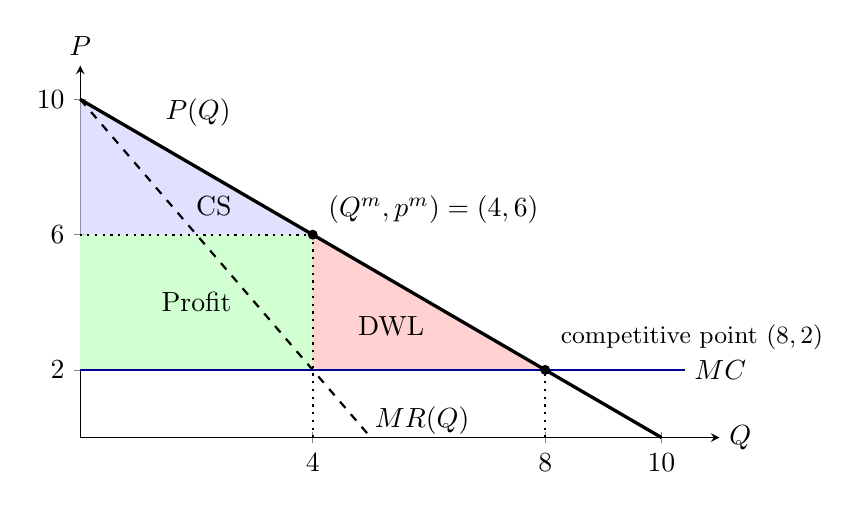
\begin{tikzpicture}
\begin{axis}[
  width=0.80\textwidth, height=0.52\textwidth,
  axis lines=left,
  xmin=0, xmax=11, ymin=0, ymax=11,
  xlabel={$Q$}, ylabel={$P$},
  xtick={4,8,10}, ytick={2,6,10},
  every axis x label/.style={at={(current axis.right of origin)}, anchor=west},
  every axis y label/.style={at={(current axis.above origin)}, anchor=south},
  clip=false]
  \fill[blue!12] (axis cs:0,6) -- (axis cs:0,10) -- (axis cs:4,6) -- cycle;
  \fill[green!18] (axis cs:0,2) rectangle (axis cs:4,6);
  \fill[red!18] (axis cs:4,6) -- (axis cs:4,2) -- (axis cs:8,2) -- cycle;
  \addplot[very thick, black, domain=0:10] {10 - x};
  \addplot[thick, dashed, black, domain=0:5] {10 - 2*x};
  \addplot[thick, blue!60!black, domain=0:10.4] {2};
  \draw[dotted, thick] (axis cs:4,0) -- (axis cs:4,6) -- (axis cs:0,6);
  \draw[dotted, thick] (axis cs:8,0) -- (axis cs:8,2);
  \fill (axis cs:4,6) circle (1.8pt);
  \fill (axis cs:8,2) circle (1.8pt);
  \node[anchor=south west] at (axis cs:4.1,6.05) {$(Q^m, p^m) = (4, 6)$};
  \node[anchor=south west, font=\small] at (axis cs:8.1,2.3) {competitive point $(8, 2)$};
  \node[anchor=south west] at (axis cs:1.3,8.9) {$P(Q)$};
  \node[anchor=west] at (axis cs:4.9,0.5) {$MR(Q)$};
  \node[anchor=west] at (axis cs:10.4,2) {$MC$};
  \node at (axis cs:2.3,6.85) {CS};
  \node at (axis cs:2,4) {Profit};
  \node at (axis cs:5.35,3.3) {DWL};
\end{axis}
\end{tikzpicture}
\caption{Monopoly with linear demand $P(Q) = 10 - Q$, marginal revenue $MR(Q) = 10 - 2Q$ and constant marginal cost
$MC = 2$. The monopolist sells $Q^m = 4$ at $p^m = 6$, while price taking would give the point $(8, 2)$. The
shaded areas are consumer surplus (CS), profit, and the deadweight loss (DWL) of pricing above marginal cost.
\Cref{sec:02-surplus} defines these areas formally. The Lerner index is $L = \frac{6 - 2}{6} = \frac{2}{3}$, which equals $\frac{1}{\varepsilon(p^m)} = \frac{2}{3}$ because
$\varepsilon(p^m) = \frac{6}{4} = \frac{3}{2}$.}
\label{fig:02-monopoly}
\end{figure}

\begin{example}[Constant-elasticity demand]\label{ex:02-ce}
Let $Q(p) = Ap^{-\varepsilon}$ with $A > 0$ and a constant $\varepsilon > 0$, and let marginal cost be strictly
positive, $c > 0$. The elasticity is the same at every price:
\[
  -Q'(p)\,\frac{p}{Q(p)} = \varepsilon A p^{-\varepsilon - 1}\cdot\frac{p}{Ap^{-\varepsilon}} = \varepsilon .
\]
If $\varepsilon > 1$, \eqref{eq:02-ce-price} is an explicit pricing formula, $p^m = \frac{\varepsilon}{\varepsilon -
1}c$. The Lerner index is the constant $\frac{1}{\varepsilon}$, and price is proportional to cost. The dollar markup
$m(p) = \frac{p}{\varepsilon}$ rises with price, so a one-dollar increase in cost raises price by
$\frac{\varepsilon}{\varepsilon - 1} > 1$ dollars. This demand curve is log-convex, so we check optimality
directly. Here $\frac{QQ''}{(Q')^2} = \frac{\varepsilon + 1}{\varepsilon}$, which is below 2 exactly when
$\varepsilon > 1$. The function $h(p) = p - c - \frac{p}{\varepsilon} = p\left(1 - \frac{1}{\varepsilon}\right) -
c$ is then strictly increasing, so the argument of \cref{lem:02-soc}(iii) shows that $p^m$ is the unique optimum. If
$\varepsilon \le 1$, revenue $Ap^{1 - \varepsilon}$ does not fall as price rises while cost $cAp^{-\varepsilon}$
falls, so profit rises at every price and no optimal price exists. \citet[Exercise~1.4]{Tirole1988} extends the
result to any convex cost function. With constant-elasticity demand and $\varepsilon > 1$, profit is then
quasi-concave in price. The boundary case $c = 0$, which \cref{ass:02-monopoly} allows, behaves differently
because profit equals revenue $Ap^{1 - \varepsilon}$. For $\varepsilon > 1$ profit rises without bound as price
falls toward zero, and the formula's value $p^m = 0$ is not an admissible price, so no optimum exists. For
$\varepsilon = 1$ profit equals $A$ at every price, so every positive price is optimal. For $\varepsilon < 1$
profit rises without bound in price.
\end{example}

\begin{example}[Exponential demand]\label{ex:02-exponential}
Let $Q(p) = e^{\frac{a - p}{b}}$ with $b > 0$, or equivalently $P(Q) = a - b\ln Q$. Then $Q'(p) = -\frac{1}{b}Q(p)$,
so the semi-elasticity is the constant $\frac{1}{b}$ and the dollar markup is $m(p) = -\frac{Q(p)}{Q'(p)} = b$ at
every price. The monopoly price is
\[
  p^m = c + b .
\]
A monopolist facing this demand charges a fixed dollar margin whatever its cost, so each dollar of cost passes
fully into price, exactly as under perfect competition. The elasticity $\varepsilon(p) = \frac{p}{b}$ rises with
price. Since $\ln Q = \frac{a - p}{b}$ is linear, and hence weakly concave, \cref{lem:02-soc} applies.
\end{example}

\begin{example}[The Bulow-Pfleiderer family]\label{ex:02-bp}
Consider demand curves of the form
\begin{equation}\label{eq:02-bp-demand}
  Q(p) = B\,\lvert\bar p - p\rvert^{g}, \qquad B > 0,
\end{equation}
on the range $p < \bar p$ when $g > 0$, and on the range $p > \bar p$ when $g < 0$. When $g > 0$, the parameter
$\bar p$ is the choke price, the highest willingness to pay. \citet{BulowPfleiderer1983} identified this family as
the one with constant pass-through of cost to price (\cref{sec:02-passthrough}). \citet{GenesoveMullin1998} write
it as $Q = \beta(\alpha - P)^{\gamma}$ and use it for the demand for refined sugar (\cref{ch:conduct}). They motivate
it by noting that linear and log-linear demand, the usual choices in industry studies, impose strong restrictions on
the monopoly pricing rule.

In both cases $\frac{\dd \ln Q}{\dd p} = -\frac{g}{\bar p - p}$. Hence the dollar markup and the elasticity are
\[
  m(p) = \frac{\bar p - p}{g}, \qquad \varepsilon(p) = \frac{p}{m(p)} = \frac{gp}{\bar p - p},
\]
both positive on the relevant range. The first-order condition $p - c = m(p)$ is linear in $p$:
\begin{align*}
  g(p - c) &= \bar p - p, \\
  (1 + g)p &= \bar p + gc, \\
  p^m &= \frac{\bar p + gc}{1 + g} .
\end{align*}
The monopoly price is affine in cost, with slope $\frac{g}{1 + g}$. Substituting $p^m$ into $\varepsilon(p)$ gives
the elasticity at the optimum, $\varepsilon(p^m) = \frac{\bar p + gc}{\bar p - c}$. The family nests the cases above.
\begin{itemize}
  \item With $g = 1$, $\bar p = a$ and $B = \frac{1}{b}$, demand is linear and $p^m = \frac{a + c}{2}$.
  \item With $g = 2$, demand is quadratic and convex, and $p^m = \frac{\bar p + 2c}{3}$.
  \item With $\bar p = 0$ and $g < 0$, demand is $Q = Bp^{g}$, which has constant elasticity $\varepsilon = -g$.
  Then $p^m = \frac{gc}{1 + g} = \frac{\varepsilon}{\varepsilon - 1}c$, which requires $g < -1$ and $c > 0$.
  \item Let $\bar p \to \infty$ and $g \to \infty$ with $\lambda_s = \frac{g}{\bar p}$ held fixed, and set
  $B = A\bar p^{-g}$ for a constant $A > 0$. Then
  \[
    Q(p) = A\left(1 - \frac{p}{\bar p}\right)^{g} = A\left(1 - \frac{\lambda_s p}{g}\right)^{g} \to A e^{-\lambda_s p} .
  \]
  The limit is exponential demand with semi-elasticity $\lambda_s$. The monopoly price converges to
  \[
    p^m = \frac{\frac{\bar p}{g} + c}{\frac{1}{g} + 1} \to c + \frac{1}{\lambda_s},
  \]
  which matches \cref{ex:02-exponential} with $b = \frac{1}{\lambda_s}$.
\end{itemize}
In inverse form, the case $g > 0$ reads $P(Q) = a - bQ^{\gamma}$ with $a = \bar p$, $b = B^{-\gamma}$ and
$\gamma = \frac{1}{g}$. The case $g < 0$ inverts to $P(Q) = \bar p + B^{-\gamma}Q^{\gamma}$, which is the same form
with $b = -B^{-\gamma}$. The symbol $\gamma$ is local to this family. The second-order condition holds
automatically when $g > 0$, because $\ln Q$ is then concave. When $g < 0$, $\frac{QQ''}{(Q')^2} = 1 - \frac{1}{g}$,
which is below 2 exactly when $g < -1$, the condition found above. The family returns in
\cref{sec:02-conduct,sec:02-passthrough} and in \cref{ch:conduct}.
\end{example}

\section{Games and equilibrium}\label{sec:02-games}

A monopolist solves a decision problem. With two or more firms, each firm's best choice depends on what its rivals
do, and we need a rule that predicts the outcome of this interdependence. This section collects the tools from
noncooperative game theory that the rest of the chapter uses. They are Nash equilibrium in pure and mixed
strategies, reaction functions, and subgame perfection in games that unfold in stages. We follow
\citet[ch.~11 and the introduction to Part~II]{Tirole1988}, which presents these tools for industrial organization.
\citet{FudenbergTirole1991} give a complete treatment.

\subsection{Nash equilibrium}\label{sec:02-nash}

\begin{definition}[Normal-form game]\label{def:02-game}
A \emph{normal-form game} has players $i = 1, \dots, N$. Player $i$ chooses an \emph{action} $a_i$ from a set $A_i$
and receives the payoff $\pi_i(a)$, where $a = (a_1, \dots, a_N)$ is the \emph{action profile}. We write $a_{-i}$
for the actions of the players other than $i$, and $(a_i', a_{-i})$ for the profile in which player $i$ switches to
$a_i'$ while the others keep $a_{-i}$.
\end{definition}

In the games of this chapter the players are firms, the actions are outputs or prices, and the payoffs are profits.
All players choose at the same time, and the structure of the game is common knowledge. A \emph{pure strategy}
picks one action with certainty. A \emph{mixed strategy} $\sigma_i$ is a probability distribution over $A_i$.
Players randomize independently, and payoffs under mixed strategies are expected values of pure-strategy payoffs. A
pure strategy is the special case of a distribution that puts probability one on a single action.

\begin{definition}[Best response and Nash equilibrium]\label{def:02-nash}
Player $i$'s \emph{best response} to $a_{-i}$ is the set $BR_i(a_{-i}) = \argmax_{a_i \in A_i}\pi_i(a_i, a_{-i})$.
A \emph{pure-strategy Nash equilibrium} is a profile $a^*$ such that
\begin{equation}\label{eq:02-nash}
  \pi_i(a_i^*, a_{-i}^*) \ge \pi_i(a_i, a_{-i}^*) \qquad \text{for every player } i \text{ and every } a_i \in A_i ,
\end{equation}
that is, $a_i^* \in BR_i(a_{-i}^*)$ for every $i$. A \emph{mixed-strategy Nash equilibrium} is a profile of
distributions $(\sigma_1^*, \dots, \sigma_N^*)$ that satisfies \eqref{eq:02-nash} with distributions in place of
actions and expected payoffs in place of payoffs.
\end{definition}

In a Nash equilibrium each player's choice is optimal given the choices of the others, and each player anticipates
those choices correctly. No player can gain by changing its own action alone. Mixed equilibria have one further
property that we use repeatedly. A player who randomizes must be indifferent among all actions in the support of its
distribution. If one of them paid strictly more, moving probability toward it would raise the expected payoff. The
indifference conditions therefore pin down the rivals' distributions. In \emph{matching pennies}, two players each
choose heads or tails. Player 1 wins one dollar from player 2 when the choices match and loses one dollar otherwise.
No pure equilibrium exists. In the mixed equilibrium each player chooses heads with probability $\frac{1}{2}$, the
only probability that leaves the opponent indifferent \citep[sec.~11.2]{Tirole1988}.

\begin{theorem}[Existence of Nash equilibrium]\label{thm:02-existence}
Suppose that each action set $A_i$ is a nonempty, compact and convex subset of a Euclidean space. Suppose also that
each payoff $\pi_i(a)$ is continuous in $a$ and quasi-concave in $a_i$. Then a pure-strategy Nash equilibrium
exists. In particular, a game with finitely many players and finitely many actions has a mixed-strategy Nash
equilibrium.
\end{theorem}

\begin{proof}[Proof sketch]
The first statement is the special case of \citet{Debreu1952} given in \citet[sec.~11.6.1]{Tirole1988}. The
standard argument applies Kakutani's fixed-point theorem (\cref{thm:B-kakutani}) to the joint best-response
correspondence
$a \mapsto BR_1(a_{-1}) \times \dots \times BR_N(a_{-N})$. Berge's maximum theorem concerns a continuous function of
a choice variable and a parameter, maximized over a fixed compact set. It says that the maximizers, as a
correspondence of the parameter, have nonempty compact values and a closed graph. Applied to each player, with
rivals' actions as the parameter, it makes the joint correspondence nonempty valued with a closed graph.
Quasi-concavity makes its values convex.
A fixed point of the correspondence is a Nash equilibrium (see also \cref{cor:B-nash-existence}). For the second
statement, a mixed strategy of player $i$
is a point in the simplex of distributions over its finite action set, which is compact and convex. The expected
payoff is linear, hence quasi-concave, in the player's own mixture. It is a polynomial, hence continuous, in the
profile of mixtures. The first statement therefore applies to the game in mixed strategies \citep{Nash1950}.
\end{proof}

Both assumptions of the theorem can fail in oligopoly models. Without quasi-concavity, best responses can jump, and a
pure equilibrium may fail to exist (\cref{rem:02-cournot-routes}). Continuity fails in the price games of
\cref{sec:02-bertrand}, because a firm's sales jump when its price crosses a rival's price. With capacity
constraints, pure equilibria may then fail to exist (\cref{sec:02-capacity}). For games with discontinuous payoffs,
\citet{DasguptaMaskin1986} give conditions for a pure equilibrium when payoffs are quasi-concave and for a mixed
equilibrium when they are not \citep[sec.~11.6.1]{Tirole1988}.

\subsection{Reaction functions}\label{sec:02-reaction}

Most models in this chapter have one-dimensional actions and smooth payoffs. Take two firms with actions
$a_1, a_2 \in \R$ and twice continuously differentiable profits, and suppose each profit is strictly concave in the
firm's own action. The first-order condition $\frac{\partial \pi_i}{\partial a_i}(a_i, a_j) = 0$ then defines firm
$i$'s \emph{reaction function} $R_i(a_j)$, its unique best response to $a_j$ at an interior optimum. A Nash
equilibrium is a pair with $a_1^* = R_1(a_2^*)$ and $a_2^* = R_2(a_1^*)$, an intersection of the two reaction curves.
Suppose in addition that the strict second-order condition $\frac{\partial^2 \pi_i}{\partial a_i^2}(R_i(a_j), a_j) <
0$ holds. Strict concavity alone does not deliver it. The payoff $\pi_i = -a_i^4 + a_i a_j$ is strictly concave in
$a_i$, yet its second derivative vanishes at the best response $a_i = 0$ to $a_j = 0$. There its reaction function
$R_i(a_j) = \left(\frac{a_j}{4}\right)^{\frac{1}{3}}$ has an infinite slope. Under the strict condition, the implicit
function theorem makes $R_i$ continuously differentiable. Differentiating the identity
$\frac{\partial \pi_i}{\partial a_i}(R_i(a_j), a_j) = 0$ with respect to $a_j$ gives
\[
  \frac{\partial^2 \pi_i}{\partial a_i^2}\,R_i'(a_j) + \frac{\partial^2 \pi_i}{\partial a_i\,\partial a_j} = 0 ,
\]
so the slope of the reaction function is
\begin{equation}\label{eq:02-reaction-slope}
  R_i'(a_j) = -\frac{\frac{\partial^2 \pi_i}{\partial a_i\,\partial a_j}}{\frac{\partial^2 \pi_i}{\partial a_i^2}}
\end{equation}
\citep[introduction to Part~II, eq.~(5)]{Tirole1988}. The denominator is negative by the strict second-order
condition, so the slope of the reaction
function has the sign of the cross-partial derivative. Following \citet{BulowGeanakoplosKlemperer1985}, actions are \emph{strategic
substitutes} when the cross-partial is negative and \emph{strategic complements} when it is positive. Quantities are
often substitutes and prices often complements (\cref{sec:02-cournot-br} and \cref{rem:02-strategic}).

Reaction functions are a device for finding equilibria. They do not describe behavior in a simultaneous-move game,
since no firm observes its rival's choice before it acts. The reaction function states what a firm would do if it
learned that its rival had changed its action \citep[introduction to Part~II]{Tirole1988}. The point returns in the
critique of conjectural variations (\cref{sec:02-interpret}).

\subsection{Subgame perfection}\label{sec:02-spe}

Several models in this chapter unfold over time. Firms enter and then compete (\cref{sec:02-entry}), build capacity
and then set prices (\cref{sec:02-capacity}), or play the same game repeatedly (\cref{sec:02-repeated}). An
\emph{extensive-form game} describes such a situation. It specifies the order of moves, the actions available at each
move, what each player knows when it moves, and the payoffs at the end of each path of play. The points at which a
player moves but cannot tell apart form one of its \emph{information sets}. A strategy is a complete plan of action.
It specifies a move at every point where the player could be called upon to act, including points that are never
reached when the plan is followed.

Nash equilibrium is too permissive in these games, because it can rest on threats that a player would not carry out.
Consider an entrant that either stays out or enters. Staying out gives the entrant 0 and the incumbent 2. After entry,
the incumbent either accommodates, which gives both firms 1, or fights, which gives the entrant $-1$ and the
incumbent 0. The profile in which the entrant stays out and the incumbent plans to fight is a Nash equilibrium. Given
the plan to fight, entry would earn $-1$. Given that entry does not occur, the plan costs the incumbent nothing. Yet
the threat is not credible, because after entry the incumbent earns 1 by accommodating and 0 by fighting.

\begin{definition}[Subgame-perfect equilibrium]\label{def:02-spe}
A \emph{subgame} is a part of an extensive-form game that begins at a point where the mover knows the entire history
of play, and that contains every later move. It does not split an information set, so two points that a player
cannot tell apart are both inside the subgame or both outside it. A \emph{subgame-perfect equilibrium} is a strategy
profile that induces a Nash equilibrium in every subgame \citep{Selten1965}.
\end{definition}

The whole game is one of its subgames, so a subgame-perfect equilibrium is a Nash equilibrium. Perfection adds the
requirement that strategies remain optimal off the equilibrium path. In games of \emph{perfect information}, where
every mover knows all earlier actions, subgame-perfect equilibria are found by \emph{backward induction}
\citep{Kuhn1953}. We solve the last mover's problem at each of its decision points and replace those points by the
resulting payoffs. We then repeat the step until we reach the first move. In the entry game the incumbent accommodates
after entry. The entrant anticipates this and enters, and this is the unique subgame-perfect equilibrium
\citep[secs.~11.3 and 11.3.1]{Tirole1988}.

Most games in this book have \emph{almost perfect information}. Play proceeds in stages, players move simultaneously
within a stage, and everyone observes all earlier stages. Backward induction then works stage by stage. The last
stage is solved as a Nash equilibrium after every history. Each earlier stage is then solved as a game whose payoffs
are the equilibrium payoffs of the stages that follow. The two-stage entry game of \cref{def:02-entry-game} and the
capacity game of \cref{prop:02-ks} are solved in this way. The second-stage equilibrium gives a reduced-form payoff
for each first-stage choice, and the first stage is a game in those payoffs. Repeated games are the other leading
case, and \cref{sec:02-repeated} states the two results on them that the chapter uses.

\section{Cournot oligopoly with \texorpdfstring{$N$}{N} firms}\label{sec:02-cournot}

The Cournot model is the workhorse model of oligopoly with a homogeneous good. It delivers the link between
concentration and margins that motivated a generation of empirical work (\cref{ch:intro}). Its comparative statics
underlie the analysis of entry, mergers and cost pass-through in later sections and chapters. This section develops
the model for $N$ firms with general demand and asymmetric convex costs. We prove existence and uniqueness, derive
the relation between margins and concentration, solve the linear case in closed form and sign the comparative
statics.

\subsection{The game}\label{sec:02-cournot-game}

\begin{definition}[Cournot game]\label{def:02-cournot}
$N$ firms produce a homogeneous good. Firm $i$ chooses an output $q_i \ge 0$. All firms choose simultaneously and
have complete information. Given the output vector $q = (q_1, \dots, q_N)$, industry output is $Q = \sum_i q_i$,
the market price is $P(Q)$, and firm $i$'s profit is
\[
  \pi_i(q) = P(Q)\,q_i - C_i(q_i) .
\]
A \emph{Cournot equilibrium} is a Nash equilibrium in quantities (\cref{def:02-nash}), an output vector $q^*$ such that
$\pi_i(q_i^*, q_{-i}^*) \ge \pi_i(q_i, q_{-i}^*)$ for every firm $i$ and every $q_i \ge 0$.
\end{definition}

Here $q_{-i}$ is the vector of rivals' outputs and $Q_{-i} = Q - q_i$ is their total. Firm $i$'s profit depends on
its rivals only through $Q_{-i}$, so we also write it as $\pi_i(q_i, Q_{-i})$.

\begin{assumption}[Cournot regularity]\label{ass:02-cournot}
\leavevmode
\begin{enumerate}[label=(C\arabic*)]
  \item Inverse demand $P$ is twice continuously differentiable on $[0, \infty)$, with $P'(Q) < 0$ for every $Q$.
  \item For every $Q > 0$, $P'(Q) + QP''(Q) < 0$. Equivalently, $P'(Q) + qP''(Q) < 0$ for every $q \in [0, Q]$.
  \item Each cost function $C_i$ is twice continuously differentiable, nondecreasing and convex on $[0, \infty)$,
  so that $C_i' \ge 0$ and $C_i'' \ge 0$.
  \item There is $\bar Q > 0$ with $P(\bar Q) \le \min_i C_i'(0)$, and $P(0) > C_i'(0)$ for at least one firm $i$.
\end{enumerate}
\end{assumption}

Condition (C1) says that demand slopes down. In (C2), the two forms are equivalent because $P' + qP''$ is linear in
$q$ and negative at $q = 0$, so it is negative on $[0, Q]$ if and only if it is negative at $q = Q$. We show below
that (C2) makes each firm's marginal revenue fall when its rivals produce more. Condition (C3) allows constant or
rising marginal cost. Condition (C4) says that no firm wants to produce once industry output reaches $\bar Q$,
while at least one firm would produce if no one else did.

\begin{remark}[Interpreting (C2)]\label{rem:02-c2}
Define the \emph{curvature} of inverse demand as $\chi(Q) = -\frac{QP''(Q)}{P'(Q)}$. Since $P' < 0$, (C2) is the
condition $\chi(Q) < 1$ at every $Q$. Linear demand has $\chi = 0$, and every concave inverse demand has
$\chi \le 0$, so both satisfy (C2). The family $P = a - bQ^{\gamma}$ of \cref{ex:02-bp} with $b, \gamma > 0$ has
$\chi = 1 - \gamma < 1$ and also satisfies it. Constant-elasticity demand $P(Q) = \left(\frac{Q}{A}\right)^{-\frac{1}{\varepsilon}}$
has $\chi = 1 + \frac{1}{\varepsilon} > 1$ and violates it. For this demand, the inequality
$P'(Q) + q_iP''(Q) < 0$ holds if and only if $s_i\left(1 + \frac{1}{\varepsilon}\right) < 1$. The arguments below
therefore apply at equilibria in which no firm's share exceeds $\frac{\varepsilon}{1 + \varepsilon}$.
\citet{Novshek1985} shows that a condition of the type in (C2), namely that each firm's marginal revenue falls when
its rivals' output rises, guarantees existence of an equilibrium even without convex costs. Curvature also governs
pass-through (\cref{sec:02-passthrough}).
\end{remark}

\subsection{Best responses and strategic substitutes}\label{sec:02-cournot-br}

Firm $i$ takes $Q_{-i}$ as given and chooses $q_i$. Its \emph{best response} $BR_i(Q_{-i})$ is the output that
maximizes $\pi_i(q_i, Q_{-i})$.

\begin{lemma}[Concavity and best responses]\label{lem:02-cournot-br}
Under \cref{ass:02-cournot}, $\pi_i(q_i, Q_{-i})$ is strictly concave in $q_i$ for every $Q_{-i} \ge 0$. The best
response is unique and is characterized by the conditions
\begin{equation}\label{eq:02-cournot-foc}
  P(Q) + q_iP'(Q) - C_i'(q_i) \le 0, \qquad q_i \ge 0, \qquad q_i\left[P(Q) + q_iP'(Q) - C_i'(q_i)\right] = 0,
\end{equation}
with $Q = q_i + Q_{-i}$. Where $BR_i(Q_{-i}) > 0$, the best response is differentiable with slope
\begin{equation}\label{eq:02-br-slope}
  BR_i'(Q_{-i}) = -\frac{P'(Q) + q_iP''(Q)}{2P'(Q) + q_iP''(Q) - C_i''(q_i)} \in (-1, 0) .
\end{equation}
\end{lemma}

\begin{proof}
The derivative of profit with respect to own output is
\[
  \frac{\partial \pi_i}{\partial q_i} = P(Q) + q_iP'(Q) - C_i'(q_i) .
\]
Differentiating again and grouping terms,
\[
  \frac{\partial^2 \pi_i}{\partial q_i^2} = 2P'(Q) + q_iP''(Q) - C_i''(q_i)
    = \left[P'(Q) + q_iP''(Q)\right] + \left[P'(Q) - C_i''(q_i)\right] .
\]
The first bracket is negative by (C2), because $q_i \le Q$. The second is negative by (C1) and (C3). So profit is
strictly concave in $q_i$. For $q_i \ge \bar Q$ we have $Q \ge \bar Q$, and then
$\frac{\partial \pi_i}{\partial q_i} < P(\bar Q) - C_i'(0) \le 0$ by (C4). A maximizer therefore exists on
$[0, \bar Q]$. Strict concavity makes it unique and makes the Kuhn-Tucker conditions \eqref{eq:02-cournot-foc}
necessary and sufficient.

Where $BR_i > 0$, the first-order condition holds with equality. Write it as $G(q_i, Q_{-i}) = 0$ with
$G(q_i, Q_{-i}) = P(q_i + Q_{-i}) + q_iP'(q_i + Q_{-i}) - C_i'(q_i)$. Its partial derivatives are
\[
  \frac{\partial G}{\partial q_i} = 2P' + q_iP'' - C_i'' < 0, \qquad \frac{\partial G}{\partial Q_{-i}} = P' + q_iP'' .
\]
By the implicit function theorem (\cref{app:math}), $BR_i'(Q_{-i}) = -\left(\frac{\partial G}{\partial
q_i}\right)^{-1}\frac{\partial G}{\partial Q_{-i}}$, which is \eqref{eq:02-br-slope}. Both the numerator and the denominator are negative. The
denominator equals the numerator plus the negative term $P' - C_i''$, so the ratio
$\frac{P' + q_iP''}{2P' + q_iP'' - C_i''}$ lies in $(0, 1)$. Hence $BR_i' \in (-1, 0)$.
\end{proof}

The cross-partial derivative of profit is $\frac{\partial^2 \pi_i}{\partial q_i \partial Q_{-i}} = P'(Q) +
q_iP''(Q) < 0$. More output by rivals therefore lowers firm $i$'s marginal profit. The slope \eqref{eq:02-br-slope}
is the general formula \eqref{eq:02-reaction-slope}, with this cross-partial in the numerator and the own second
derivative $2P' + q_iP'' - C_i''$ in the denominator. In the terminology of
\citet{BulowGeanakoplosKlemperer1985}, quantities are \emph{strategic substitutes}: a more aggressive strategy by
one firm lowers its rivals' marginal profits (p.~489). Best responses slope down as a result. The bound
$BR_i' > -1$ adds that a firm offsets only part of a rival's expansion. When rivals produce one more unit, firm $i$
contracts by less than one unit, and industry output rises. This property drives every comparative static below.
With linear demand $P = a - bQ$ and constant cost $c_i$, the best response is $BR_i(Q_{-i}) = \max\left\{0,
\frac{a - c_i - bQ_{-i}}{2b}\right\}$, with slope $-\frac{1}{2}$ where positive.

\subsection{Existence and uniqueness}\label{sec:02-cournot-exist}

An equilibrium solves $N$ best-response conditions simultaneously. Because each firm's profit depends on its rivals
only through their total output, the system reduces to a single equation in industry output.
\citet{SzidarovszkyYakowitz1977} and \citet{Novshek1985} use this reduction, and \citet{Vives1999} develops it for
general aggregative games. The device is the following function.

\begin{definition}[Replacement function]\label{def:02-replacement}
For $Q \in [0, \bar Q]$, the \emph{replacement function} $\tilde q_i(Q)$ of firm $i$ is the output that satisfies
the conditions \eqref{eq:02-cournot-foc} when industry output equals $Q$:
\[
  \tilde q_i(Q) = 0 \ \text{ if } P(Q) \le C_i'(0), \qquad
  P(Q) + \tilde q_i(Q)P'(Q) = C_i'(\tilde q_i(Q)) \ \text{ otherwise}.
\]
\end{definition}

The replacement function gives the output that firm $i$ would choose if it knew that industry output, including its
own, would equal $Q$. It is well defined. Let $G_i(q, Q) = P(Q) + qP'(Q) - C_i'(q)$. For fixed $Q$, $G_i$ is
strictly decreasing in $q$, because $\frac{\partial G_i}{\partial q} = P'(Q) - C_i''(q) < 0$. It also tends to
$-\infty$ as $q \to \infty$, because $G_i(q, Q) \le P(Q) + qP'(Q)$. So when $G_i(0, Q) = P(Q) - C_i'(0) > 0$ there
is exactly one positive root. By construction, $q_i$ is a best response to $Q_{-i}$ if and only if
$q_i = \tilde q_i(q_i + Q_{-i})$.

\begin{lemma}[Properties of replacement functions]\label{lem:02-replacement}
Under \cref{ass:02-cournot}, the following hold for each firm $i$.
\begin{enumerate}[label=(\roman*)]
  \item $\tilde q_i$ is continuous on $[0, \bar Q]$ and $\tilde q_i(\bar Q) = 0$. If $\tilde q_i(Q) = 0$, then
  $\tilde q_i(Q') = 0$ for every $Q' \ge Q$.
  \item At any $Q$ with $0 < \tilde q_i(Q) \le Q$, $\tilde q_i$ is differentiable and
  \begin{equation}\label{eq:02-replacement-slope}
    \tilde q_i'(Q) = -\frac{P'(Q) + \tilde q_i(Q)P''(Q)}{P'(Q) - C_i''(\tilde q_i(Q))} < 0 .
  \end{equation}
  \item The set $R_i = \{Q \in [0, \bar Q] : \tilde q_i(Q) \le Q\}$ is a closed interval that contains $\bar Q$,
  and $\tilde q_i$ is nonincreasing on $R_i$.
\end{enumerate}
\end{lemma}

\begin{proof}
(i) Where $P(Q) > C_i'(0)$, the root of $G_i(\cdot, Q)$ is continuous in $Q$ by the implicit function theorem,
since $\frac{\partial G_i}{\partial q} < 0$. Because $C_i'(q) \ge C_i'(0)$, at the root we have
$0 = G_i \le P(Q) - C_i'(0) + \tilde q_i(Q)P'(Q)$, which gives the bound
\[
  \tilde q_i(Q) \le \frac{P(Q) - C_i'(0)}{-P'(Q)} .
\]
The bound tends to zero as $P(Q)$ falls to $C_i'(0)$, so $\tilde q_i$ is continuous at the point where it reaches
zero. By (C4), $P(\bar Q) \le C_i'(0)$, so $\tilde q_i(\bar Q) = 0$. Since $P$ is decreasing, $P(Q) \le C_i'(0)$
implies $P(Q') \le C_i'(0)$ for every $Q' \ge Q$.

(ii) At such a $Q$, $G_i(\tilde q_i(Q), Q) = 0$ with $\frac{\partial G_i}{\partial q} = P' - C_i'' < 0$ and
$\frac{\partial G_i}{\partial Q} = P'(Q) + \tilde q_i(Q)P''(Q)$. The latter is negative by (C2), because
$\tilde q_i(Q) \le Q$. The implicit function theorem gives \eqref{eq:02-replacement-slope}, a ratio of two negative
numbers with a minus sign in front.

(iii) The set $R_i$ is closed because $\tilde q_i$ is continuous, and it contains $\bar Q$ because
$\tilde q_i(\bar Q) = 0$. Take $Q' \in R_i$ and suppose that some $Q'' > Q'$ lies outside $R_i$. Let $Q^\circ$ be
the largest point of $[Q', Q'']$ in $R_i$. Then $Q^\circ < Q''$, and continuity forces $\tilde q_i(Q^\circ) =
Q^\circ$, with $\tilde q_i(Q) > Q$ on $(Q^\circ, Q'']$. If $Q^\circ = 0$, then $\tilde q_i(0) = 0$ and by (i)
$\tilde q_i \equiv 0$, a contradiction. So $\tilde q_i(Q^\circ) = Q^\circ > 0$, and by (ii) the function
$\tilde q_i(Q) - Q$ has derivative below $-1$ at $Q^\circ$. It is therefore negative just above $Q^\circ$, which
contradicts the choice of $Q^\circ$. Hence $R_i$ is an interval. On $R_i$, $\tilde q_i$ is strictly decreasing where
it is positive, by (ii), and it stays at zero once it reaches zero, by (i). So it is nonincreasing on $R_i$.
\end{proof}

\begin{proposition}[Existence and uniqueness of Cournot equilibrium]\label{prop:02-cournot-exist}
Under \cref{ass:02-cournot}, a Cournot equilibrium exists and is unique. Industry output $Q^*$ is the unique root
in $(0, \bar Q)$ of
\begin{equation}\label{eq:02-aggregate-eq}
  \Phi(Q) \equiv \sum_{i=1}^N \tilde q_i(Q) - Q = 0,
\end{equation}
and firm $i$ produces $q_i^* = \tilde q_i(Q^*)$. Moreover, $\Phi(Q) > 0$ for $0 \le Q < Q^*$ and $\Phi(Q) < 0$ for
$Q^* < Q \le \bar Q$.
\end{proposition}

\begin{proof}
We proceed in four steps.
\begin{enumerate}[label=\arabic*.]
  \item \emph{Equilibria are roots of $\Phi$.} By \cref{lem:02-cournot-br}, $q^*$ is an equilibrium if and only if
  every $q_i^*$ satisfies \eqref{eq:02-cournot-foc} at $Q^* = \sum_j q_j^*$. If $Q^* \le \bar Q$, this says exactly
  that $q_i^* = \tilde q_i(Q^*)$ for every $i$, and summing gives $\Phi(Q^*) = 0$. Equilibrium output cannot be
  zero, because the firm with $P(0) > C_i'(0)$ in (C4) would then gain by producing. It cannot be at least
  $\bar Q$ either. Any firm with $q_i^* > 0$ would then satisfy $C_i'(q_i^*) = P(Q^*) + q_i^*P'(Q^*) < P(\bar Q)
  \le C_i'(0)$, which contradicts (C3). So all outputs would be zero, a contradiction. Conversely, every root
  $Q^* \in (0, \bar Q)$ of $\Phi$ yields the equilibrium $q_i^* = \tilde q_i(Q^*)$.
  \item \emph{Location of roots.} At a root, $\tilde q_i(Q^*) \le \sum_j \tilde q_j(Q^*) = Q^*$ for every $i$, so
  $Q^*$ lies in $R = \bigcap_i R_i$. By \cref{lem:02-replacement}(iii), $R$ is a closed interval $[Q_0, \bar Q]$.
  \item \emph{Uniqueness.} Each $\tilde q_i$ is nonincreasing on $R$, and $-Q$ is strictly decreasing, so $\Phi$ is
  strictly decreasing on $R$ and has at most one root there.
  \item \emph{Existence and sign.} The firm $k$ of (C4) has $\tilde q_k(0) > 0$, so $0 \notin R_k$ and
  $Q_0 > 0$. Let $j$ be a firm with $\min R_j = Q_0$. Continuity gives $\tilde q_j(Q_0) = Q_0$, so
  $\Phi(Q_0) \ge \tilde q_j(Q_0) - Q_0 = 0$. For $Q < Q_0$, $Q \notin R_j$, so $\Phi(Q) \ge \tilde q_j(Q) - Q > 0$.
  At the other end, $\Phi(\bar Q) = -\bar Q < 0$. The intermediate value theorem yields a root in $[Q_0, \bar Q)$.
  Strict monotonicity on $R$ and positivity below $Q_0$ give the sign pattern. \qedhere
\end{enumerate}
\end{proof}

\Cref{fig:02-replacement} illustrates the construction for a linear market with three firms. With $P(Q) = 10 - Q$
and constant costs $c_i$, the condition $P(Q) + qP'(Q) = c_i$ reads $10 - Q - q = c_i$, so
$\tilde q_i(Q) = \max\{0, 10 - c_i - Q\}$. With costs $(1, 2, 3)$ the replacement functions are $9 - Q$, $8 - Q$
and $7 - Q$ where positive. For $Q \le 7$ their sum is $24 - 3Q$, and setting it equal to $Q$ gives $Q^* = 6$ and
outputs $(3, 2, 1)$. Firm 1's replacement function exceeds $Q$ for $Q < 4.5$, so $R = [4.5, 9]$, with $\bar Q = 9$
because $P(9) = 1$ equals the lowest marginal cost.

\begin{figure}[htbp]
\centering
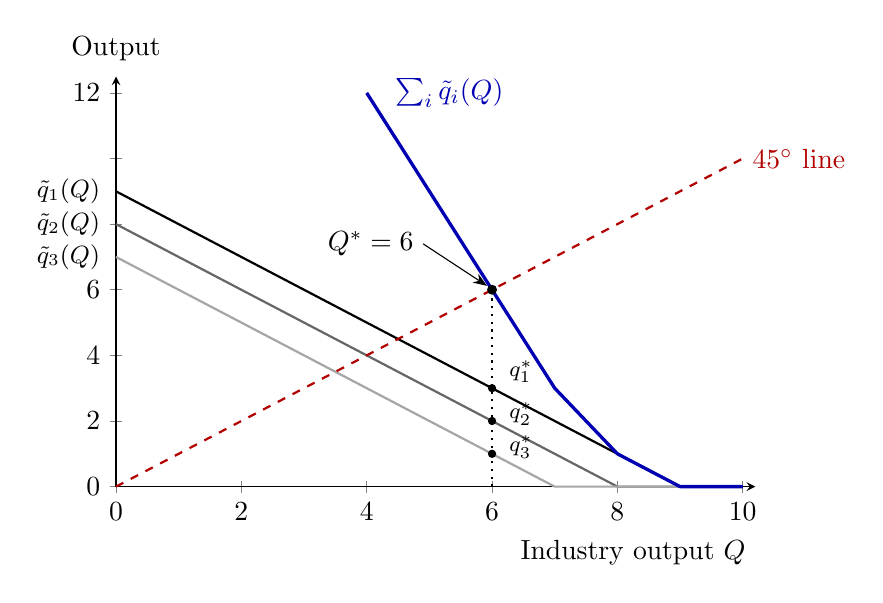
\begin{tikzpicture}
\begin{axis}[
  width=0.80\textwidth, height=0.56\textwidth,
  axis lines=left,
  xmin=0, xmax=10.2, ymin=0, ymax=12.5,
  xlabel={Industry output $Q$}, ylabel={Output},
  xtick={0,2,4,6,8,10}, ytick={0,2,4,6,8,10,12}, yticklabels={0,2,4,6,,,12},
  every axis x label/.style={at={(current axis.right of origin)}, anchor=north east, yshift=-16pt},
  every axis y label/.style={at={(current axis.above origin)}, anchor=south, yshift=2pt},
  clip=false]
  \addplot[thick, black, domain=0:10, samples=201] {max(0, 9 - x)};
  \addplot[thick, black!60, domain=0:10, samples=201] {max(0, 8 - x)};
  \addplot[thick, black!35, domain=0:10, samples=201] {max(0, 7 - x)};
  \addplot[very thick, blue!70!black, domain=4:10, samples=401] {max(0,9-x)+max(0,8-x)+max(0,7-x)};
  \addplot[thick, dashed, red!70!black, domain=0:10] {x};
  \draw[dotted, thick] (axis cs:6,0) -- (axis cs:6,6);
  \fill (axis cs:6,6) circle (1.8pt);
  \fill (axis cs:6,3) circle (1.5pt);
  \fill (axis cs:6,2) circle (1.5pt);
  \fill (axis cs:6,1) circle (1.5pt);
  \node[anchor=east, font=\small] at (axis cs:-0.1,9) {$\tilde q_1(Q)$};
  \node[anchor=east, font=\small] at (axis cs:-0.1,8) {$\tilde q_2(Q)$};
  \node[anchor=east, font=\small] at (axis cs:-0.1,7) {$\tilde q_3(Q)$};
  \node[anchor=west, blue!70!black] at (axis cs:4.3,12.0) {$\sum_i \tilde q_i(Q)$};
  \node[anchor=west, red!70!black] at (axis cs:10.0,10.0) {$45^\circ$ line};
  \node[anchor=east] (qstar) at (axis cs:4.9,7.4) {$Q^* = 6$};
  \draw[-{Stealth[length=5pt]}, thin] (qstar.east) -- (axis cs:5.92,6.12);
  \node[anchor=west, font=\footnotesize] at (axis cs:6.12,3.5) {$q_1^*$};
  \node[anchor=west, font=\footnotesize] at (axis cs:6.12,2.2) {$q_2^*$};
  \node[anchor=west, font=\footnotesize] at (axis cs:6.12,1.2) {$q_3^*$};
\end{axis}
\end{tikzpicture}
\caption{Replacement functions for $P(Q) = 10 - Q$ and constant marginal costs $(1, 2, 3)$. Each firm's replacement
function $\tilde q_i(Q) = \max\{0, 10 - c_i - Q\}$ is the output that is optimal for firm $i$ when industry output is
$Q$. Their sum, $24 - 3Q$ for $Q \le 7$, crosses the $45^\circ$ line once, at $Q^* = 6$. The equilibrium outputs
$(3, 2, 1)$ are read off the individual replacement functions at $Q^*$.}
\label{fig:02-replacement}
\end{figure}

\begin{remark}[Why uniqueness matters]\label{rem:02-uniqueness}
Empirical work uses equilibrium conditions in two ways. Estimation evaluates first-order conditions at the observed
prices and quantities, for example to invert them for marginal cost as in \eqref{eq:02-infer-mc}. It never has to
solve for an equilibrium, so multiplicity does no harm there. Counterfactuals, such as the effect of a merger or a
tax, must solve for the new equilibrium. If several solutions exist, the analyst needs a rule for selecting one, and
conclusions can depend on that rule. \Cref{prop:02-cournot-exist} rules this out for homogeneous-good Cournot markets
that satisfy (C1) to (C4). Merger simulations in practice often compute the new equilibrium by iterating on the
first-order conditions from the premerger prices, which selects an equilibrium close to the status quo.
\Cref{ch:diffprod} gives the corresponding conditions for differentiated-products price competition.
\end{remark}

\begin{remark}[Other routes to existence and uniqueness]\label{rem:02-cournot-routes}
\Cref{thm:02-existence} gives a second proof of existence. Under \cref{ass:02-cournot}, restrict each firm to the
compact and convex set $[0, \bar Q]$. Profit $\pi_i(q)$ is continuous, and by \cref{lem:02-cournot-br} it is strictly
concave, hence quasi-concave, in $q_i$. The theorem yields an equilibrium of the restricted game, and it is also an
equilibrium of the original game. The proof of \cref{lem:02-cournot-br} shows that $\frac{\partial \pi_i}{\partial
q_i} < 0$ whenever $q_i \ge \bar Q$, so no output above $\bar Q$ does better than $\bar Q$ itself. This route needs
only quasi-concavity of profit in own output, but it is silent on uniqueness. The replacement-function proof of
\cref{prop:02-cournot-exist} gives both.

\citet[sec.~5.7.1]{Tirole1988} reviews the other approaches. \citet{SzidarovszkyYakowitz1977} assume that profit is
concave in own output, which holds when costs are convex and inverse demand is concave. Profit need not be concave
when demand is sufficiently convex. \citet{Friedman1983} and \citet{RobertsSonnenschein1977} give robust examples in
which no pure-strategy equilibrium exists even with convex costs. Without concavity, reaction functions can jump.
\citet{McManus1964} and \citet{RobertsSonnenschein1976} prove existence for symmetric firms with convex costs.
Convex costs ensure that the common reaction function jumps only upward, and only a downward jump can prevent a
symmetric equilibrium. \citet{Novshek1985} works with the condition discussed in \cref{rem:02-c2}. For uniqueness
with two firms and strictly concave profits, a sufficient condition is that $\lvert BR_i'\rvert < 1$ for both firms on
the relevant range. The reaction curves then cross at most once. \Cref{lem:02-cournot-br} shows that (C1) to (C3)
deliver this bound, since $BR_i' \in (-1, 0)$.
\end{remark}

\subsection{Markups and concentration}\label{sec:02-cournot-markups}

In this subsection each firm has a constant marginal cost $c_i$. Firm $i$'s Lerner index is $L_i = \frac{P -
c_i}{P}$, and the \emph{share-weighted industry Lerner index} is $\bar L = \sum_i s_iL_i$. The market elasticity at
industry output $Q$ is $\varepsilon = -\frac{P(Q)}{QP'(Q)}$.

\begin{proposition}[Cowling and Waterson]\label{prop:02-cowling-waterson}
In a Cournot equilibrium with constant marginal costs, every active firm satisfies
\begin{equation}\label{eq:02-cw-firm}
  L_i = \frac{P - c_i}{P} = \frac{s_i}{\varepsilon},
\end{equation}
and the share-weighted industry Lerner index satisfies
\begin{equation}\label{eq:02-cowling-waterson}
  \bar L = \sum_{i=1}^N s_iL_i = \frac{\HHI}{\varepsilon} .
\end{equation}
\end{proposition}

\begin{proof}
This is \cref{prop:01-cowling-waterson}. Each active firm satisfies the first-order condition
$P(Q) + q_iP'(Q) = c_i$, and the algebra in that proof turns it into \eqref{eq:02-cw-firm}. Inactive firms have
$s_i = 0$ and add nothing to either sum, so summing $s_iL_i$ over the active firms gives
\eqref{eq:02-cowling-waterson}.
\end{proof}

The result is due to \citet{CowlingWaterson1976}. It agrees with the monopoly rule applied to residual demand. By
\eqref{eq:02-cournot-residual}, firm $i$'s residual elasticity is $\varepsilon_i^R = \frac{\varepsilon}{s_i}$, so
\eqref{eq:02-cw-firm} reads $L_i = \frac{1}{\varepsilon_i^R}$. Each Cournot firm is a monopolist on the demand
left to it by its rivals. Since $L_i < 1$ whenever $c_i > 0$, every active firm has $s_i < \varepsilon$. Cournot
firms can therefore operate where market demand is inelastic, provided that each firm's share is below the market
elasticity. A monopolist never can (\cref{prop:02-elastic}).

\begin{corollary}[Symmetric firms]\label{cor:02-cournot-symmetric}
Suppose \cref{ass:02-cournot} holds and $c_i = c$ for all $i$. Then the unique Cournot equilibrium is symmetric and
interior, with $q_i^* = \frac{Q^*}{N}$ for every firm. The formulas of \cref{cor:01-cournot-cases} hold, in
particular $\HHI = \frac{1}{N}$ and $L = \frac{P - c}{P} = \frac{1}{N\varepsilon}$.
\end{corollary}

\begin{proof}
With identical costs, all firms have the same replacement function, so by \cref{prop:02-cournot-exist} they produce
the same output $\tilde q(Q^*)$. Hence $q_i^* = \frac{Q^*}{N}$, which is positive because $Q^* > 0$. Every firm is
active with share $\frac{1}{N}$, so \cref{cor:01-cournot-cases}(i) applies. Equivalently, substitute
$s_i = \frac{1}{N}$ and $\HHI = \frac{1}{N}$ into \eqref{eq:02-cowling-waterson}.
\end{proof}

The symmetric formula shows how the number of firms disciplines margins. \Cref{prop:02-cournot-converge} below shows
that price approaches marginal cost as $N$ grows. Read literally, \eqref{eq:02-cowling-waterson} suggests that
margins should rise with concentration across industries, with slope $\frac{1}{\varepsilon}$. The next two results
show why that reading needs care.

\begin{corollary}[Efficient firms are large]\label{cor:02-efficient}
In a Cournot equilibrium with constant marginal costs, every active firm has share
\begin{equation}\label{eq:02-share-cost}
  s_i = \varepsilon\,\frac{P - c_i}{P} = \varepsilon\left(1 - \frac{c_i}{P}\right),
\end{equation}
so lower-cost firms have larger shares. If all $N$ firms are active, let $\sigma_c^2 = \frac{1}{N}\sum_i (c_i -
\tilde c)^2$ be the variance of costs around their simple average $\tilde c = \frac{1}{N}\sum_i c_i$. Then
\begin{equation}\label{eq:02-hhi-cost}
  \HHI = \frac{1}{N} + N\,\frac{\varepsilon^2}{P^2}\sigma_c^2, \qquad
  \bar L = \frac{1}{N\varepsilon} + N\,\frac{\varepsilon}{P^2}\sigma_c^2 .
\end{equation}
\end{corollary}

\begin{proof}
Equation \eqref{eq:02-share-cost} rearranges \eqref{eq:02-cw-firm}. It makes each share an affine function of the
firm's cost with slope $-\frac{\varepsilon}{P}$, so $\sigma_s^2 = \frac{\varepsilon^2}{P^2}\sigma_c^2$.
Substituting into \eqref{eq:01-hhi-variance} gives the expression for $\HHI$, and dividing it by $\varepsilon$ gives
$\bar L$ by \eqref{eq:02-cowling-waterson}.
\end{proof}

With linear demand $P = a - bQ$, the elasticity is $\varepsilon = \frac{P}{bQ}$, so $\frac{\varepsilon}{P} =
\frac{1}{bQ}$ and \eqref{eq:02-hhi-cost} reduces to \cref{prop:01-demsetz}(ii).

\Cref{cor:02-efficient} is an identity that holds at the equilibrium, since $\varepsilon$ and $P$ are themselves
equilibrium outcomes. It shows that dispersion in costs raises concentration and the average margin together, with
no change in the way firms compete. Large firms earn high margins because they are efficient. This is the formal
content of the efficiency critique of \citet{Demsetz1973}, which \cref{ch:intro} develops in the context of
cross-industry regressions.

The identity also has an industry-profit form \citep[eq.~(5.14) and Exercise~5.6]{Tirole1988}. With constant
marginal costs, industry variable profit is
\[
  \Pi = \sum_i (P - c_i)\,q_i = \sum_i \frac{s_iP}{\varepsilon}\,q_i = \frac{PQ}{\varepsilon}\sum_i s_i^2 ,
\]
where the second step uses \eqref{eq:02-cw-firm} and the third uses $q_i = s_iQ$. Dividing by revenue $PQ$ gives
\begin{equation}\label{eq:02-cw-profit}
  \frac{\Pi}{PQ} = \frac{\HHI}{\varepsilon} .
\end{equation}
Suppose consumers spend a fixed amount $E$ on the good, so that demand is $Q = \frac{E}{p}$. The elasticity is then
one and revenue equals $E$ at every price, so $\Pi = E\,\HHI$. In this case the Herfindahl index measures industry
profit exactly, up to a constant (Tirole's eq.~(5.15)).

Bertrand competition gives a sharp contrast \citep[sec.~5.5]{Tirole1988}. With symmetric firms and a common
constant marginal cost, the Bertrand price and industry profit do not depend on the number of firms
(\cref{prop:02-bertrand}), so profitability and concentration are unrelated. In Cournot competition, profitability
falls with the number of firms. With asymmetric costs $c_1 < c_2 \le c_j$ for $j \ge 3$, the lowest-cost Bertrand
firm takes the whole market at the price $\min\{c_2, p^m(c_1)\}$, where $p^m(c_1)$ is its monopoly price
(\cref{sec:02-bertrand-homog}). When $p^m(c_1) > c_2$, this outcome is an equilibrium if ties go to the low-cost
firm or if prices lie on a fine grid that contains $c_2$. With continuous prices and an equal split of ties, no pure
equilibrium exists in that case. In this outcome concentration takes its highest value under any index that satisfies the
Encaoua-Jacquemin properties, and the efficient firm earns a positive profit. Under both models, intrinsic cost
asymmetries raise concentration and profitability together, which is the argument of \citet{Demsetz1973}.

\begin{example}[Cost asymmetry raises concentration and profit]\label{ex:02-asym}
Let $Q = 1 - p$, and let two Cournot firms have costs $c_1 = c - d$ and $c_2 = c + d$, with $d \ge 0$ and
$1 - c - 3d > 0$ \citep[Exercise~5.7]{Tirole1988}. \Cref{ex:02-linear-cournot} with $a = b = 1$ gives
\[
  q_1 = \frac{1 - c + 3d}{3}, \qquad q_2 = \frac{1 - c - 3d}{3}, \qquad Q = \frac{2(1 - c)}{3}, \qquad
  P = \frac{1 + 2c}{3} .
\]
Industry output and price do not depend on $d$. A larger $d$ moves share from firm 2 to firm 1, a mean-preserving
spread. No index with the Encaoua-Jacquemin properties falls, and the Herfindahl index rises. Each firm earns $(P - c_i)q_i = q_i^2$, so
industry profit is
\[
  \Pi = \frac{(1 - c + 3d)^2 + (1 - c - 3d)^2}{9} = \frac{2(1 - c)^2}{9} + 2d^2 ,
\]
which also rises with $d$. Here $\Pi = Q^2\,\HHI$, an instance of \eqref{eq:02-cw-profit}, since
$\frac{PQ}{\varepsilon} = Q^2$ for this demand. Consumer surplus does not change, so total surplus rises with $d$ as
well.
\end{example}

Concentration can also be related to the scope for welfare gains. \citet{DansbyWillig1979} consider small changes
$\dd q_i$ in firms' outputs \citep[Exercise~5.8]{Tirole1988}. Total surplus $\int_0^Q P(x)\,\dd x - \sum_i C_i(q_i)$
then changes by
\[
  \dd W = \sum_i \bigl[P - C_i'(q_i)\bigr]\dd q_i .
\]
Suppose the change is small in the sense that $\sum_i (\dd q_i)^2 \le \eta^2$ for some $\eta > 0$. By the
Cauchy-Schwarz inequality, the largest attainable gain is $\eta\bigl(\sum_i [P - C_i'(q_i)]^2\bigr)^{\frac{1}{2}}$.
In Cournot equilibrium $P - C_i'(q_i) = -q_iP'(Q) = \frac{s_iP}{\varepsilon}$, so the largest gain is
\[
  \max \dd W = \eta\,\frac{P}{\varepsilon}\sqrt{\HHI} .
\]
The potential gain from small output changes is proportional to the square root of the Herfindahl index. Dansby and
Willig call such measures \emph{industry performance gradient indexes}. Tirole adds two cautions. Concentration
indices have no systematic relationship with the variables needed to assess changes in cost, demand or policy. They
are also endogenous, so their correlations with performance have no causal interpretation.

\begin{remark}[Margins and concentration are joint outcomes]\label{rem:02-joint}
Both sides of \eqref{eq:02-cowling-waterson} are determined in equilibrium by the same primitives: demand, the cost
distribution and, with entry, fixed costs. Industries with inelastic demand or large fixed costs tend to have both
high margins and few firms. The identity therefore does not say that an exogenous rise in concentration raises
margins, except when the number of symmetric firms changes exogenously. A regression of margins on $\HHI$ across
industries omits the elasticity and the cost dispersion. \Cref{sec:02-entry} shows that with free entry the sign of
the relation depends on which primitive varies across industries, and \cref{ch:intro} discusses the regressions.
\end{remark}

The first-order conditions can also be aggregated into an industry supply relation. Suppose all $N$ firms are
active. Summing the conditions $P + q_iP'(Q) = c_i$ over firms gives $NP + QP'(Q) = \sum_i c_i$, or
\begin{equation}\label{eq:02-cournot-agg-unweighted}
  P = \tilde c - \frac{1}{N}\,QP'(Q), \qquad \tilde c = \frac{1}{N}\sum_i c_i .
\end{equation}
Alternatively, multiply firm $i$'s condition by $s_i$ before summing. Using $\sum_i s_i = 1$ and $s_iq_i = s_i^2Q$,
\begin{align*}
  \sum_i s_iP + P'(Q)\sum_i s_iq_i &= \sum_i s_ic_i, \\
  P + P'(Q)\,Q\,\HHI &= \bar c,
\end{align*}
which gives
\begin{equation}\label{eq:02-cournot-agg-weighted}
  P = \bar c - \HHI\cdot QP'(Q), \qquad \bar c = \sum_i s_ic_i .
\end{equation}
Both relations have the form $P = MC - \theta\,QP'(Q)$ of the supply relation \eqref{eq:02-bresnahan-supply}
written for the industry. The value of the conduct parameter depends on how industry marginal cost is defined. It is
$\theta = \frac{1}{N}$ when $MC$ is the simple average of costs, and $\theta = \HHI$ when $MC$ is the share-weighted
average. In the three-firm example of \cref{fig:02-replacement}, $\tilde c = 2$ and $\bar c = \frac{5}{3}$, and both
relations give $P = 4$. \Cref{sec:02-conduct} generalizes this aggregation to arbitrary firm-level conduct.

\citet{Bresnahan1989} discusses exactly this issue for studies that have only industry data (Section 2.2.4,
p.~1030). Such studies estimate an aggregate relation $P_t = MC(Q_t, W_t, Z_t, \epsilon_{ct}) - \theta_t
Q_t\frac{\partial P}{\partial Q}$ (his eq.~(16)). Bresnahan notes that oligopoly firms generally have different
marginal costs in equilibrium unless costs are identical and constant, so a stable industry marginal cost curve
need not exist. He recommends following \citet{CowlingWaterson1976} and reading the aggregate $\theta_t$ as average
conduct and $\frac{P - MC}{P}$ as the average markup. He also rejects the claim that theory implies equal conduct
for all firms. Equations \eqref{eq:02-cournot-agg-unweighted} and \eqref{eq:02-cournot-agg-weighted} make the
averaging explicit.

\subsection{The linear model in closed form}\label{sec:02-cournot-linear}

\begin{example}[Linear Cournot]\label{ex:02-linear-cournot}
Let $P(Q) = a - bQ$ with $b > 0$, and let firm $i$ have constant marginal cost $c_i < a$ and fixed cost $F$, which
does not affect output decisions. Suppose all firms are active. Firm $i$'s first-order condition is
\[
  a - bQ - bq_i - c_i = 0, \qquad\text{so}\qquad bq_i = a - c_i - bQ .
\]
Summing over the $N$ firms and solving for $Q$,
\begin{align*}
  bQ &= Na - \sum_j c_j - NbQ, \\
  Q^* &= \frac{Na - \sum_j c_j}{b(N + 1)} .
\end{align*}
The price is
\[
  P^* = a - bQ^* = a - \frac{Na - \sum_j c_j}{N + 1} = \frac{a + \sum_j c_j}{N + 1},
\]
and each firm's output follows from $bq_i = P^* - c_i$:
\[
  q_i^* = \frac{P^* - c_i}{b} = \frac{a - (N + 1)c_i + \sum_j c_j}{b(N + 1)} .
\]
All firms are active if and only if $(N + 1)c_i < a + \sum_j c_j$ for every $i$, that is, if every cost is below
the equilibrium price. Profit is $\pi_i^* = (P^* - c_i)q_i^* - F = b(q_i^*)^2 - F$, because $P^* - c_i = bq_i^*$.

With symmetric costs $c_i = c$, these formulas become
\[
  P = \frac{a + Nc}{N + 1}, \qquad q = \frac{a - c}{b(N + 1)}, \qquad Q = \frac{N(a - c)}{b(N + 1)}, \qquad
  \pi = \frac{(a - c)^2}{b(N + 1)^2} - F .
\]
The Lerner index is $L = \frac{P - c}{P}$, with $P - c = \frac{a - c}{N + 1}$, so $L = \frac{a - c}{a + Nc}$. The
index is $\HHI = \frac{1}{N}$. The market elasticity at the equilibrium is
\[
  \varepsilon = \frac{P}{bQ} = \frac{a + Nc}{N + 1}\cdot\frac{N + 1}{N(a - c)} = \frac{a + Nc}{N(a - c)},
\]
and indeed $\frac{\HHI}{\varepsilon} = \frac{1}{N}\cdot\frac{N(a - c)}{a + Nc} = \frac{a - c}{a + Nc} = L$, as
\cref{cor:02-cournot-symmetric} requires.

For a numerical illustration take $a = 10$, $b = 1$ and costs $(c_1, c_2, c_3) = (1, 2, 3)$, the market of
\cref{fig:02-replacement}. Then $\sum_j c_j = 6$, so $P^* = \frac{16}{4} = 4$ and $Q^* = \frac{30 - 6}{4} = 6$.
Outputs are $q^* = (3, 2, 1)$ and shares are $\left(\frac{1}{2}, \frac{1}{3}, \frac{1}{6}\right)$, so
\[
  \HHI = \frac{1}{4} + \frac{1}{9} + \frac{1}{36} = \frac{7}{18} \approx 0.389 .
\]
The market elasticity is $\varepsilon = \frac{P^*}{bQ^*} = \frac{2}{3}$, so demand is inelastic at the equilibrium.
The firm Lerner indices are $(0.75, 0.50, 0.25)$, and each equals $\frac{s_i}{\varepsilon}$. The share-weighted
index is
\[
  \bar L = \frac{1}{2}\cdot\frac{3}{4} + \frac{1}{3}\cdot\frac{1}{2} + \frac{1}{6}\cdot\frac{1}{4} = \frac{7}{12}
  \approx 0.583 = \frac{7}{18}\cdot\frac{3}{2} = \frac{\HHI}{\varepsilon} .
\]
Profits gross of fixed costs are $(9, 4, 1)$. Costs have variance $\sigma_c^2 = \frac{2}{3}$, and
\eqref{eq:02-hhi-cost} gives $\frac{1}{3} + 3\cdot\frac{4}{9}\cdot\frac{1}{16}\cdot\frac{2}{3} = \frac{1}{3} +
\frac{1}{18} = \frac{7}{18}$, as it should.
\end{example}

\Cref{tab:02-linear-cournot} collects the symmetric closed forms for four cases: Cournot competition and perfect
collusion, each with a fixed number of firms and with free entry. Under \emph{perfect collusion} the firms maximize
joint profit and split the output equally. Joint profit $(a - bQ - c)Q - NF$ is maximized at the monopoly output, so
\[
  Q = \frac{a - c}{2b}, \qquad P = \frac{a + c}{2}, \qquad q = \frac{a - c}{2bN}, \qquad
  \pi = \frac{(a - c)^2}{4bN} - F .
\]
The Lerner index is $\frac{a - c}{a + c}$ for every $N$, while $\HHI = \frac{1}{N}$. Collusion is not a Nash
equilibrium of the one-shot game, and \cref{sec:02-collusion} discusses what sustains it. The free-entry columns
treat the number of firms as continuous and set profit to zero. \Cref{sec:02-entry} derives them and uses the table
to compare the relation between margins and concentration across the four cases.

\begin{table}[htbp]
\centering
\begin{threeparttable}
\caption{Closed forms for the linear market $P(Q) = a - bQ$ with symmetric firms}
\label{tab:02-linear-cournot}
\renewcommand{\arraystretch}{1.6}
\begin{tabular}{@{}lcccc@{}}
\toprule
 & \multicolumn{2}{c}{Cournot} & \multicolumn{2}{c}{Perfect collusion} \\
\cmidrule(lr){2-3}\cmidrule(lr){4-5}
 & (i) Fixed $N$ & (ii) Free entry & (iii) Fixed $N$ & (iv) Free entry \\
\midrule
Number of firms & $N$ & $N^e = \frac{a - c}{\sqrt{bF}} - 1$ & $N$ & $N^m = \frac{(a - c)^2}{4bF}$ \\
Price $P$ & $\frac{a + Nc}{N + 1}$ & $c + \sqrt{bF}$ & $\frac{a + c}{2}$ & $\frac{a + c}{2}$ \\
Output per firm $q$ & $\frac{a - c}{b(N + 1)}$ & $\sqrt{\frac{F}{b}}$ & $\frac{a - c}{2bN}$ & $\frac{2F}{a - c}$ \\
Industry output $Q$ & $\frac{N(a - c)}{b(N + 1)}$ & $\frac{a - c - \sqrt{bF}}{b}$ & $\frac{a - c}{2b}$ & $\frac{a - c}{2b}$ \\
Profit per firm $\pi$ & $\frac{(a - c)^2}{b(N + 1)^2} - F$ & $0$ & $\frac{(a - c)^2}{4bN} - F$ & $0$ \\
Lerner index $L$ & $\frac{a - c}{a + Nc}$ & $\frac{\sqrt{bF}}{c + \sqrt{bF}}$ & $\frac{a - c}{a + c}$ & $\frac{a - c}{a + c}$ \\
$\HHI$ & $\frac{1}{N}$ & $\frac{\sqrt{bF}}{a - c - \sqrt{bF}}$ & $\frac{1}{N}$ & $\frac{4bF}{(a - c)^2}$ \\
\bottomrule
\end{tabular}
\begin{tablenotes}\footnotesize
\item Notes: Each firm has constant marginal cost $c < a$ and fixed cost $F > 0$. Perfect collusion means that the
firms produce the monopoly output and split it equally. In columns (ii) and (iv) the number of firms is treated as
continuous and set so that profit is zero, which requires $F \le \frac{(a - c)^2}{4b}$. With $a = 10$, $b = 1$,
$c = 2$ and $F = 1$, column (ii) gives $N^e = 7$, $P = 3$ and $\HHI = \frac{1}{7}$, and column (iv) gives
$N^m = 16$ and $\HHI = \frac{1}{16}$.
\end{tablenotes}
\end{threeparttable}
\end{table}

\subsection{Comparative statics}\label{sec:02-cournot-cs}

The replacement functions also deliver the comparative statics of the equilibrium. The sign pattern in
\cref{prop:02-cournot-exist} is the key. If a parameter change shifts $\Phi$ down at the old equilibrium output, the
new root must lie to the left of the old one. If it shifts $\Phi$ up, the new root lies to the right. Within the
interval $R$ the replacement functions are nonincreasing, which pins down how individual outputs move.

\begin{proposition}[An increase in one firm's cost]\label{prop:02-cournot-cs}
Let \cref{ass:02-cournot} hold, and write firm $i$'s cost as $C_i(q) = c_iq + K_i(q)$ with $K_i$ convex, so that
$c_i$ shifts its marginal cost up one for one. Suppose firm $i$ is active in equilibrium, and let $c_i$ rise. Then
industry output $Q^*$ falls and the price rises. Every rival's output weakly rises, strictly for rivals that are
active after the change. Firm $i$'s output falls. At an equilibrium in which no firm has $P(Q^*) = C_j'(0)$, the
effects are differentiable, with
\begin{equation}\label{eq:02-dQdc}
  \frac{\dd Q^*}{\dd c_i} = \frac{\frac{\partial \tilde q_i}{\partial c_i}}{1 - \sum_{j=1}^N \tilde q_j'(Q^*)} < 0,
  \qquad \frac{\partial \tilde q_i}{\partial c_i} = \frac{1}{P'(Q^*) - C_i''(q_i^*)} < 0,
\end{equation}
\[
  \frac{\dd q_j^*}{\dd c_i} = \tilde q_j'(Q^*)\,\frac{\dd Q^*}{\dd c_i} \ge 0 \ \ (j \ne i), \qquad
  \frac{\dd q_i^*}{\dd c_i} = \frac{\dd Q^*}{\dd c_i} - \sum_{j \ne i}\frac{\dd q_j^*}{\dd c_i} < 0, \qquad
  \frac{\dd P}{\dd c_i} = P'(Q^*)\,\frac{\dd Q^*}{\dd c_i} > 0 .
\]
\end{proposition}

\begin{proof}
Firm $i$'s replacement function solves $P(Q) + qP'(Q) - c_i - K_i'(q) = 0$. The left side falls with $c_i$, so for
each $Q$ the root $\tilde q_i(Q)$ is nonincreasing in $c_i$, and strictly decreasing wherever it is positive. Rivals'
replacement functions do not depend on $c_i$. Let $Q^*$ be the old equilibrium output, so $\tilde q_i(Q^*) > 0$.
After the increase, the new aggregate function satisfies $\Phi^{\mathrm{new}}(Q^*) < \Phi(Q^*) = 0$. By the sign
pattern of \cref{prop:02-cournot-exist} applied to $\Phi^{\mathrm{new}}$, its root lies strictly below $Q^*$. So
industry output falls, and the price rises because $P$ is decreasing.

For a rival $j$, both the old and the new equilibrium outputs lie in $R_j$, which does not depend on $c_i$. Since
$\tilde q_j$ is nonincreasing on $R_j$, the lower industry output weakly raises $q_j^* = \tilde q_j(Q^*)$. The
increase is strict when $j$ is active at the new equilibrium, because $\tilde q_j$ is strictly decreasing where it
is positive. Firm $i$'s output equals $Q^* - \sum_{j \ne i} q_j^*$, which falls because industry output falls and
rivals' outputs rise.

For the derivatives, differentiate the identity $\sum_j \tilde q_j(Q^*(c_i); c_i) - Q^*(c_i) = 0$ with respect to
$c_i$:
\[
  \left[\sum_j \tilde q_j'(Q^*) - 1\right]\frac{\dd Q^*}{\dd c_i} + \frac{\partial \tilde q_i}{\partial c_i} = 0 .
\]
Solving gives the first expression in \eqref{eq:02-dQdc}. Differentiating firm $i$'s first-order condition with
respect to $c_i$ at fixed $Q$ gives $\left[P' - C_i''\right]\frac{\partial \tilde q_i}{\partial c_i} - 1 = 0$, which
is the second. The denominator of $\frac{\dd Q^*}{\dd c_i}$ is at least one because $\tilde q_j' \le 0$, and its
numerator is negative. The remaining derivatives follow from $q_j^* = \tilde q_j(Q^*)$, the adding-up identity and
the chain rule.
\end{proof}

With linear demand and constant costs, every active firm has $\tilde q_j' = -1$ and $\frac{\partial \tilde
q_i}{\partial c_i} = -\frac{1}{b}$. Then $\frac{\dd Q^*}{\dd c_i} = -\frac{1}{b(N + 1)}$ and $\frac{\dd P}{\dd c_i} =
\frac{1}{N + 1}$, matching the closed form $P^* = \frac{a + \sum_j c_j}{N + 1}$. A firm-specific cost shock moves
the price by much less than the same shock applied to every firm. \Cref{sec:02-passthrough} develops this contrast.

A weaker statement about the firm's own response needs none of the regularity conditions. Given $Q_{-i}$, firm $i$ is
a monopolist on the residual inverse demand $P(q + Q_{-i})$. By \cref{lem:02-monotone}, a higher marginal cost weakly
lowers its optimal output for every $Q_{-i}$, whatever the shape of demand and cost. A cost increase therefore shifts
firm $i$'s reaction curve inward \citep[sec.~5.4]{Tirole1988}. The equilibrium effects in \cref{prop:02-cournot-cs}
need more structure, namely best responses that slope down and an equilibrium that is unique.

The same argument measures how rivals respond when one firm's output changes for any reason. Hold $q_i$ fixed and
let the other firms play their replacement functions. Industry output then satisfies $Q = q_i + \sum_{j \ne i}
\tilde q_j(Q)$. Write $\lambda_j = -\tilde q_j'(Q)$. Differentiating gives $\dd Q = \dd q_i - \sum_{j \ne
i}\lambda_j\,\dd Q$, so
\begin{equation}\label{eq:02-rival-response}
  \frac{\dd Q}{\dd q_i} = \frac{1}{1 + \sum_{j \ne i}\lambda_j}, \qquad
  \frac{\dd Q_{-i}}{\dd q_i} = -\frac{\sum_{j \ne i}\lambda_j}{1 + \sum_{j \ne i}\lambda_j} \in (-1, 0] .
\end{equation}
With linear demand and constant costs, $\lambda_j = 1$ for every active rival. If all $N - 1$ rivals are active,
they contract by $\frac{N - 1}{N}$ units for each extra unit that firm $i$ produces, and industry output rises by
only $\frac{1}{N}$. \citet{FarrellShapiro1990} define the same number $\lambda_j = -\frac{P' + q_jP''}{C_j'' - P'}$
and build their analysis of mergers in Cournot markets on it (\cref{ch:mergers}).
\citet{Dixit1986} develops comparative statics for general oligopoly models along similar lines.
\Cref{fig:02-cournot-br} shows the effect of a cost reduction in a linear duopoly.

\begin{figure}[htbp]
\centering
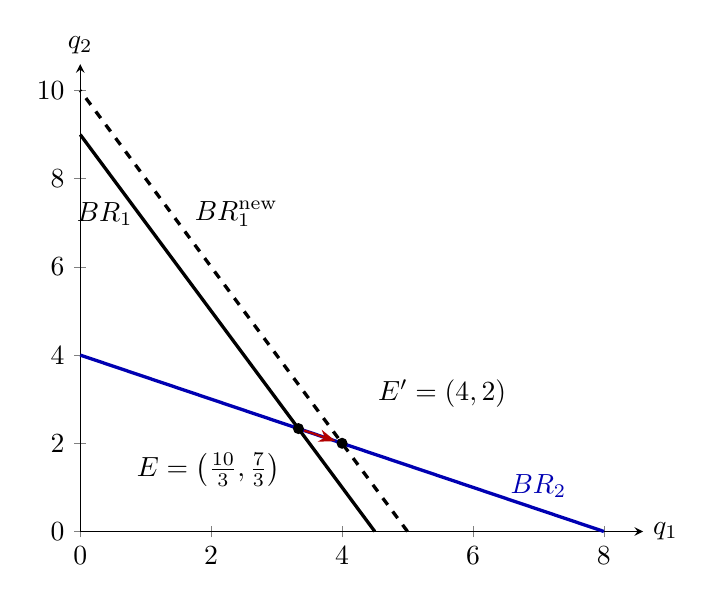
\begin{tikzpicture}
\begin{axis}[
  width=0.72\textwidth, height=0.62\textwidth,
  axis lines=left,
  xmin=0, xmax=8.6, ymin=0, ymax=10.6,
  xlabel={$q_1$}, ylabel={$q_2$},
  xtick={0,2,4,6,8}, ytick={0,2,4,6,8,10},
  every axis x label/.style={at={(current axis.right of origin)}, anchor=west},
  every axis y label/.style={at={(current axis.above origin)}, anchor=south},
  clip=false]
  \addplot[very thick, black, domain=0:9, samples=2] ({(9 - x)/2}, {x});
  \addplot[very thick, black, dashed, domain=0:10, samples=2] ({(10 - x)/2}, {x});
  \addplot[very thick, blue!70!black, domain=0:8, samples=2] {(8 - x)/2};
  \fill (axis cs:3.3333,2.3333) circle (2pt);
  \fill (axis cs:4,2) circle (2pt);
  \draw[-{Stealth[length=6pt]}, thick, red!70!black] (axis cs:3.42,2.29) -- (axis cs:3.90,2.05);
  \node[anchor=north east] at (axis cs:3.2,2.0) {$E = \left(\frac{10}{3}, \frac{7}{3}\right)$};
  \node[anchor=south west] at (axis cs:4.4,2.6) {$E' = (4, 2)$};
  \node[anchor=east] at (axis cs:0.95,7.2) {$BR_1$};
  \node[anchor=west] at (axis cs:1.6,7.2) {$BR_1^{\mathrm{new}}$};
  \node[anchor=south, blue!70!black] at (axis cs:7.0,0.55) {$BR_2$};
\end{axis}
\end{tikzpicture}
\caption{Best responses in a linear Cournot duopoly with $P(Q) = 10 - Q$, $c_1 = 1$ and $c_2 = 2$. Firm 1's best
response is $q_1 = \frac{9 - q_2}{2}$ and firm 2's is $q_2 = \frac{8 - q_1}{2}$. They cross at
$E = \left(\frac{10}{3}, \frac{7}{3}\right)$, where $P = \frac{13}{3}$. When $c_1$ falls to 0, firm 1's best response
shifts out to the dashed line $BR_1^{\mathrm{new}}$, $q_1 = \frac{10 - q_2}{2}$. The new equilibrium $E' = (4, 2)$ has a larger firm 1, a
smaller firm 2 and price $P = 4$, as \cref{prop:02-cournot-cs} predicts.}
\label{fig:02-cournot-br}
\end{figure}

Entry has the opposite effect on industry output, and it hurts every incumbent.

\begin{proposition}[Entry]\label{prop:02-entry-cs}
Suppose a firm $N + 1$, with a cost function satisfying (C3), joins $N$ incumbents, and (C4) holds for the enlarged
set of firms. Then industry output weakly rises and the price weakly falls. Every incumbent's output and profit
weakly fall. If the entrant is active in the new equilibrium, industry output strictly rises and the price strictly
falls. The output and profit of every incumbent that was active before entry then fall strictly.
\end{proposition}

\begin{proof}
Write $\Phi_N$ and $\Phi_{N+1}$ for the aggregate functions before and after entry, with roots $Q_N^*$ and
$Q_{N+1}^*$. Since $\Phi_{N+1} = \Phi_N + \tilde q_{N+1}$, we have $\Phi_{N+1}(Q_N^*) = \tilde q_{N+1}(Q_N^*) \ge
0$. By the sign pattern of \cref{prop:02-cournot-exist}, $Q_{N+1}^* \ge Q_N^*$. If the entrant is active after
entry, the two roots cannot coincide, because $\Phi_{N+1}(Q_N^*) = \tilde q_{N+1}(Q_N^*) > 0$ would then contradict
$\Phi_{N+1}(Q_{N+1}^*) = 0$. So the inequality is strict.

Both equilibrium outputs lie in $R_i$ for each incumbent $i$, and $\tilde q_i$ is nonincreasing there, so
$q_i^* = \tilde q_i(Q^*)$ weakly falls. Rivals' total output from $i$'s point of view, $Q_{-i}^* = Q^* - q_i^*$,
weakly rises. Firm $i$'s equilibrium profit is the value function $V_i(Q_{-i}) = \max_{q \ge 0}\left[P(q +
Q_{-i})\,q - C_i(q)\right]$. For every $q > 0$ the bracket falls with $Q_{-i}$, so $V_i$ is nonincreasing. By the
envelope theorem (\cref{app:math}), $V_i'(Q_{-i}) = P'(Q)\,q_i^* \le 0$, strictly when firm $i$ is active. Hence
incumbents' profits fall.

Now let the entrant be active, so that $Q^*$ rises strictly. Take an incumbent with $\tilde q_i(Q_N^*) > 0$. Its
replacement function is strictly decreasing where it is positive, so its output falls strictly. Then $Q_{-i}^*$
rises strictly. Since $V_i$ is nonincreasing and strictly decreasing near the old value of $Q_{-i}$, where firm $i$
is active, its profit falls strictly.
\end{proof}

With symmetric firms the effect of entry can be computed explicitly. Treat $N$ as a continuous variable, and let
$q_N$ be the symmetric equilibrium output, which solves $P(Nq) + qP'(Nq) - C'(q) = 0$. Differentiating with respect
to $N$,
\[
  P'\left(q + N\frac{\dd q}{\dd N}\right) + P'\frac{\dd q}{\dd N} + qP''\left(q + N\frac{\dd q}{\dd N}\right)
  - C''\frac{\dd q}{\dd N} = 0 .
\]
Collecting the terms in $\frac{\dd q}{\dd N}$,
\[
  \frac{\dd q}{\dd N}\left[N(P' + qP'') + P' - C''\right] = -q(P' + qP'') ,
\]
so
\begin{equation}\label{eq:02-seade}
\begin{gathered}
  \frac{\dd q_N}{\dd N} = -\frac{q(P' + qP'')}{N(P' + qP'') + P' - C''} < 0, \\
  \frac{\dd (Nq_N)}{\dd N} = q + N\frac{\dd q_N}{\dd N} = \frac{q(P' - C'')}{N(P' + qP'') + P' - C''} > 0 .
\end{gathered}
\end{equation}
The common denominator is negative by (C1) to (C3). The numerator of the first expression is positive and that of
the second is negative, which gives the signs. These formulas are due to \citet{Seade1980}. They verify, for Cournot
competition, the conditions that \citet{MankiwWhinston1986} impose on the outcome of competition after entry
(p.~51). Their Assumption 1 requires industry output $Nq_N$ to rise with $N$ toward a finite limit, which holds
because $Nq_N < \bar Q$. Their Assumption 2 requires output per firm to fall with $N$, the \emph{business-stealing
effect}. Their Assumption 3 requires price to be at least marginal cost, and in Cournot $P - C'(q_N) = -q_NP' > 0$.
\Cref{sec:02-entry} restates the three properties as conditions (E1) to (E3) of \cref{ass:02-mw} and shows that
they imply excessive entry.

As the number of firms grows, Cournot competition approaches perfect competition.

\begin{proposition}[Convergence to competitive pricing]\label{prop:02-cournot-converge}
Consider $N$ symmetric firms with constant marginal cost $c$, and suppose \cref{ass:02-cournot} holds for every $N$
with the same $\bar Q$. Let $P_N$ be the equilibrium price and $\mathcal{M} = \max_{Q \in [0, \bar Q]}\lvert P'(Q)\rvert$.
Then
\[
  0 < P_N - c \le \frac{\mathcal{M}\bar Q}{N},
\]
so $P_N \to c$ as $N \to \infty$. If $c > 0$, the Lerner index $L_N = \frac{1}{N\varepsilon(P_N)}$ also tends to
zero.
\end{proposition}

\begin{proof}
By \cref{cor:02-cournot-symmetric}, each firm produces $q_N = \frac{Q_N}{N}$, with $Q_N < \bar Q$ by
\cref{prop:02-cournot-exist}. The first-order condition gives
\[
  P_N - c = -q_NP'(Q_N) = \frac{Q_N}{N}\lvert P'(Q_N)\rvert \le \frac{\bar Q\mathcal{M}}{N} .
\]
The left side is positive because $q_N > 0$. If $c > 0$, then $L_N = \frac{P_N - c}{P_N} \le \frac{P_N - c}{c}
\to 0$.
\end{proof}

\citet{Ruffin1971} studies this convergence, and \citet{Novshek1980} shows that Cournot equilibria with free entry
approach the competitive outcome as firms become small relative to the market. In the linear case, $P_N - c =
\frac{a - c}{N + 1}$. With $c = 0$ the Lerner index $\frac{P_N - 0}{P_N}$ equals one for every $N$, even though the
price itself converges to zero. This is why the second statement requires $c > 0$.
\Cref{fig:02-cournot-N} shows the speed of convergence in a linear market. The deadweight loss falls with the square
of $N + 1$, much faster than the Lerner index.

\begin{figure}[htbp]
\centering
\begin{minipage}[t]{0.49\textwidth}
\centering
\begin{tikzpicture}
\begin{axis}[
  width=\linewidth, height=0.85\linewidth,
  axis lines=left,
  xmin=0, xmax=21, ymin=0, ymax=7.2,
  xlabel={Number of firms $N$}, ylabel={Price $P_N$},
  xtick={1,5,10,15,20}, ytick={0,2,4,6},
  tick label style={font=\footnotesize}, label style={font=\small},
  clip=false]
  \addplot[thin, dashed, black!60, domain=0:20.5, samples=2] {6};
  \addplot[thin, dashed, black!60, domain=0:20.5, samples=2] {2};
  \addplot[thick, blue!70!black, mark=*, mark size=1.2pt, samples at={1,2,...,20}] {(10 + 2*x)/(x + 1)};
  \node[anchor=south, font=\scriptsize] at (axis cs:12,6.05) {monopoly price 6};
  \node[anchor=north, font=\scriptsize] at (axis cs:12,1.95) {competitive price 2};
\end{axis}
\end{tikzpicture}
\end{minipage}\hfill
\begin{minipage}[t]{0.49\textwidth}
\centering
\begin{tikzpicture}
\begin{axis}[
  width=\linewidth, height=0.85\linewidth,
  axis lines=left,
  xmin=0, xmax=21, ymin=0, ymax=0.72,
  xlabel={Number of firms $N$}, ylabel={Index or share},
  xtick={1,5,10,15,20}, ytick={0,0.2,0.4,0.6},
  yticklabel style={/pgf/number format/fixed, /pgf/number format/precision=1},
  tick label style={font=\footnotesize}, label style={font=\small},
  clip=false]
  \addplot[thick, blue!70!black, mark=*, mark size=1.2pt, samples at={1,2,...,20}] {8/(10 + 2*x)};
  \addplot[thick, red!70!black, mark=square*, mark size=1.1pt, samples at={1,2,...,20}] {1/((x + 1)^2)};
  \node[anchor=south west, font=\scriptsize, blue!70!black] at (axis cs:7.5,0.42) {Lerner index $L_N$};
  \node[anchor=south west, font=\scriptsize, red!70!black] at (axis cs:4,0.07) {deadweight-loss share};
\end{axis}
\end{tikzpicture}
\end{minipage}
\caption{Symmetric linear Cournot market with $a = 10$, $b = 1$ and $c = 2$, for $N = 1, \dots, 20$. The left
panel shows the price $P_N = \frac{10 + 2N}{N + 1}$ between the monopoly price 6 and the competitive price 2. The
right panel shows the Lerner index $L_N = \frac{8}{10 + 2N}$ and the deadweight loss as a share of maximal surplus,
$\frac{1}{(N + 1)^2}$ (\cref{sec:02-welfare}).}
\label{fig:02-cournot-N}
\end{figure}

The deadweight-loss share in the figure follows from \cref{tab:02-linear-cournot}. Competitive output is
$\frac{a - c}{b}$, so Cournot output falls short of it by $\frac{a - c}{b(N + 1)}$, while price exceeds cost by
$\frac{a - c}{N + 1}$. The deadweight loss is the triangle $\frac{1}{2}\cdot\frac{a - c}{N + 1}\cdot\frac{a -
c}{b(N + 1)} = \frac{(a - c)^2}{2b(N + 1)^2}$. Dividing by the maximal surplus $\frac{(a - c)^2}{2b}$ gives
$\frac{1}{(N + 1)^2}$. \Cref{cor:02-dwl-cournot} recovers this share as a special case of a formula for any conduct
$\theta$, and \cref{sec:02-welfare} treats welfare in general.

\begin{remark}[Other competitive limits]\label{rem:02-limits}
Replicating firms is only one way to make an industry competitive. With fixed costs or increasing returns, adding
potential firms need not add competition, because a limited market supports only a few viable firms
\citep[sec.~5.7.1.3]{Tirole1988}. \citet{NovshekSonnenschein1978} instead allow free entry and shrink the minimum
efficient scale. Let each firm have a U-shaped average cost with minimum $c$ at output 1. Replace the cost function
$C(q)$ by $C_\alpha(q) = \alpha\, C\left(\frac{q}{\alpha}\right)$, whose minimum efficient scale is $\alpha$ and whose
minimum average cost is still $c$. Let $Q^* = Q(c)$ be the competitive output. Any free-entry Cournot equilibrium then
has industry output in $[Q^* - \alpha, Q^*]$. If output exceeded $Q^*$, the price would be below $c$, and every active
firm would lose money. If output fell short of $Q^* - \alpha$, an entrant producing $\alpha$ at average cost $c$ would
face a price above $c$ and earn a profit. The equilibrium therefore becomes competitive as $\alpha \to 0$.

A large number of firms is not even necessary, as \citet{Hart1979} pointed out. What matters is that each firm be
small relative to its market, so that its own output has little effect on the price. Tirole's illustration is a
monopolist with ten units of capacity and zero marginal cost. It faces ten consumers with
unit demands and valuations $10, 9, \dots, 1$, and it maximizes revenue by withholding part of its capacity. If it can
sell on ten identical islands of such consumers, it sells all ten units at the price 10 and causes no distortion.
\end{remark}

\begin{remark}[Mergers in the symmetric Cournot model]\label{rem:02-cournot-merger}
Suppose two of $N$ symmetric Cournot firms with constant marginal cost merge, and the merged firm has the same cost
as every other firm. The market then has $N - 1$ symmetric firms. Two consequences follow, and \cref{ch:mergers}
treats both in full.

First, the actual change in concentration is
\[
  \Delta\HHI = \frac{1}{N - 1} - \frac{1}{N} = \frac{1}{N(N - 1)} .
\]
The formula \eqref{eq:02-delta-hhi} predicts $2\cdot\frac{1}{N}\cdot\frac{1}{N} = \frac{2}{N^2}$. The prediction
exceeds the actual change if and only if $2(N - 1) > N$, that is, $N > 2$. With $N = 3$ the formula predicts 0.222,
while the actual change is 0.167. The formula ignores the expansion of the nonmerging firms, which by
\cref{prop:02-entry-cs} (read in reverse) produce more when a competitor disappears.

Second, the merger may be unprofitable. In the linear model each firm earns $\frac{(a - c)^2}{b(N + 1)^2}$ before the
merger, ignoring fixed costs, and the merged firm earns $\frac{(a - c)^2}{bN^2}$ afterwards. The merger is profitable
for its participants if and only if
\[
  \frac{(a - c)^2}{bN^2} \ge \frac{2(a - c)^2}{b(N + 1)^2}
  \iff (N + 1)^2 \ge 2N^2 \iff N \le \frac{1}{\sqrt{2} - 1} = 1 + \sqrt{2} .
\]
Only a merger to monopoly from duopoly passes this test. With $N = 3$, the two insiders earn $\frac{2}{16} = 0.125$
in units of $\frac{(a - c)^2}{b}$ before the merger and $\frac{1}{9} \approx 0.111$ afterwards. The outsiders gain,
because they expand while the price rises. This is the merger paradox of \citet{SalantSwitzerReynolds1983}.
\citet{FarrellShapiro1990} show that a Cournot merger that creates no synergies always raises the price, so cost
savings are needed before consumers can gain (\cref{ch:mergers}).
\end{remark}

\section{Free entry and the number of firms}\label{sec:02-entry}

\Cref{sec:02-cournot} took the number of firms as given. In most industries the number of firms is itself an
equilibrium outcome. Firms enter while the profit of one more entrant covers the cost of setting up, and they stay
out once it does not. This section asks whether free entry delivers the number of firms that maximizes total surplus.
The general answer, due to \citet{MankiwWhinston1986}, is that in homogeneous-good markets with imperfect competition
free entry tends to produce too many firms. The reason is a \emph{business-stealing externality}: an entrant takes
sales from incumbents and counts them as its own profit, while society gains nothing from the transfer.

\subsection{The two-stage entry game}\label{sec:02-entry-game}

\begin{definition}[Two-stage entry game]\label{def:02-entry-game}
A large pool of identical potential entrants plays two stages. In stage~1 each potential entrant decides whether to
enter. Entry requires a \emph{set-up cost} $F > 0$, which is sunk once paid. In stage~2 the $N$ entrants observe
$N$ and play an oligopoly game in output or prices. Each entrant has the cost function $C(q)$, with $C$ continuous,
$C(0) = 0$, $C' \ge 0$ and $C'' \ge 0$. The stage-2 game has a symmetric equilibrium in which each firm produces
$q_N$ and the price is $P(N q_N)$. The \emph{per-firm profit} with $N$ entrants, net of the set-up cost, is
\begin{equation}\label{eq:02-entry-profit}
\pi_N = P(N q_N)\, q_N - C(q_N) - F .
\end{equation}
The solution concept is subgame-perfect equilibrium (\cref{def:02-spe}).
\end{definition}

The definition leaves the stage-2 game open. It may be Cournot, Bertrand, a cartel, or any other game with a
symmetric outcome. This generality is the main strength of the analysis that follows.

The \emph{free-entry number of firms} $N^e$ satisfies two conditions \citep[p.~50]{MankiwWhinston1986}:
\begin{equation}\label{eq:02-free-entry}
\pi_{N^e} \ge 0 \qquad\text{and}\qquad \pi_{N^e + 1} < 0 .
\end{equation}
The first condition says that no entrant regrets entering. The second says that no outsider wishes to enter. A firm
that is indifferent enters. When we treat $N$ as a continuous variable, the two conditions collapse to the
zero-profit condition $\pi_{N^e} = 0$.

\begin{example}[Free entry in the linear Cournot market]\label{ex:02-free-entry-linear}
Let $P(Q) = a - bQ$ and $C(q) = cq$, with $a > c \ge 0$ and $b > 0$, and let the entrants play Cournot.
\Cref{ex:02-linear-cournot} gives
\begin{equation*}
q_N = \frac{a - c}{b(N + 1)}, \qquad P - c = \frac{a - c}{N + 1} = b\, q_N, \qquad
\pi_N = \frac{(a - c)^2}{b(N + 1)^2} - F .
\end{equation*}
Setting $\pi_{N^e} = 0$ and solving for $N^e$ gives
\begin{equation}\label{eq:02-Ne-linear}
(N^e + 1)^2 = \frac{(a - c)^2}{bF}
\qquad\Longrightarrow\qquad
N^e = \frac{a - c}{\sqrt{bF}} - 1 .
\end{equation}
At least one firm enters when $F \le \frac{(a - c)^2}{4b}$. Substituting $\frac{a - c}{N^e + 1} = \sqrt{bF}$ into
the Cournot formulas gives the free-entry outcome:
\begin{gather*}
P^e = c + \sqrt{bF}, \qquad q^e = \sqrt{\frac{F}{b}}, \qquad Q^e = \frac{a - c - \sqrt{bF}}{b}, \\
L^e = \frac{\sqrt{bF}}{c + \sqrt{bF}}, \qquad \HHI^e = \frac{1}{N^e} = \frac{\sqrt{bF}}{a - c - \sqrt{bF}} .
\end{gather*}
They fill the free-entry column of \cref{tab:02-linear-cournot}. As a check, $(P^e - c)\, q^e = \sqrt{bF}
\sqrt{\frac{F}{b}} = F$, so operating profit just covers the set-up cost.
\end{example}

The example makes two points. First, under free entry the price-cost margin equals $\sqrt{bF}$ exactly. Markups are
what pays for fixed costs, which is the point of \cref{rem:02-fixed-costs}. A positive
Lerner index is therefore compatible with zero economic profit. Second, the margin does not depend on the demand
intercept $a$. A higher intercept attracts more firms and leaves the margin unchanged, while concentration falls.
Adding consumers is different. Scaling the number of consumers by $M$ replaces $b$ by $\frac{b}{M}$, so the
free-entry margin $\sqrt{\frac{bF}{M}}$ falls as the market grows (\cref{tab:02-LH-cases}).

\subsection{The second-best planner and excess entry}\label{sec:02-mw}

\citet{MankiwWhinston1986} compare $N^e$ with the choice of a \emph{second-best planner}. This planner chooses how
many firms enter but cannot control how they compete after entry. The restriction reflects antitrust practice.
\citet[p.~50]{MankiwWhinston1986} quote the observation of \citet[p.~525]{Scherer1980} that oligopolists who
refrain from price competition, each deciding independently, do not break the law. The planner maximizes total
surplus, ignoring income effects:
\begin{equation}\label{eq:02-mw-welfare}
W(N) = \int_0^{N q_N} P(x)\, \dd x - N\, C(q_N) - N F .
\end{equation}
The first term is gross consumer benefit, and the last two are production and set-up costs. Prices are transfers
between consumers and firms, so they do not appear. Let $N^o$ denote the maximizer of $W$ (Mankiw and Whinston
write $N^*$). With continuous $N$ it satisfies $W'(N^o) = 0$.

\begin{assumption}[Post-entry outcomes]\label{ass:02-mw}
The symmetric stage-2 outcomes satisfy the following conditions \citep[p.~51]{MankiwWhinston1986}.
\begin{enumerate}[label=(E\arabic*)]
\item Total output rises with $N$ and stays bounded: $N q_N > N' q_{N'}$ for all $N > N'$, and
  $\lim_{N\to\infty} N q_N = Q_\infty < \infty$.
\item Per-firm output falls with $N$: $q_N < q_{N'}$ for all $N > N'$.
\item Price is not below marginal cost: $P(N q_N) - C'(q_N) \ge 0$ for all $N$.
\end{enumerate}
When $N$ is continuous we also assume that $q_N$ is differentiable, with $\frac{\dd q_N}{\dd N} < 0 <
\frac{\dd (N q_N)}{\dd N}$.
\end{assumption}

Condition (E2) is the \emph{business-stealing effect}: an entrant lowers the equilibrium output of each incumbent.
\Cref{prop:02-entry-cs} and the derivatives \eqref{eq:02-seade} show that Cournot competition satisfies (E1) and
(E2) under \cref{ass:02-cournot}. Condition
(E3) holds for any conduct between price taking and monopoly. Business stealing is closely related to quantities
being strategic substitutes \citep{BulowGeanakoplosKlemperer1985}, and \citet{Seade1980} gives conditions for it
under conjectural variations.

\begin{proposition}[Excess entry]\label{prop:02-mw-excess}
Suppose \cref{ass:02-mw} holds and treat $N$ as continuous, so that $\pi_{N^e} = 0$ and $W'(N^o) = 0$. Then
$N^e \ge N^o$. If in addition $P(N^o q_{N^o}) - C'(q_{N^o}) > 0$, then $N^e > N^o$
\citep[Proposition~1]{MankiwWhinston1986}.
\end{proposition}

\begin{proof}
The proof has four steps.

\emph{Step 1.} We differentiate welfare. By the fundamental theorem of calculus and the chain rule,
\begin{equation*}
\frac{\dd}{\dd N}\int_0^{N q_N} P(x)\,\dd x = P(N q_N)\,\frac{\dd (N q_N)}{\dd N}
= P(N q_N)\left[q_N + N \frac{\dd q_N}{\dd N}\right].
\end{equation*}
The product rule gives $\frac{\dd}{\dd N}\left[N C(q_N)\right] = C(q_N) + N C'(q_N)\frac{\dd q_N}{\dd N}$. Hence
\begin{equation}\label{eq:02-mw-wprime-raw}
W'(N) = P(N q_N)\left[q_N + N\frac{\dd q_N}{\dd N}\right] - C(q_N) - N C'(q_N)\frac{\dd q_N}{\dd N} - F .
\end{equation}

\emph{Step 2.} We regroup. The terms $P(N q_N)q_N - C(q_N) - F$ add up to $\pi_N$. The remaining terms share the factor
$N\frac{\dd q_N}{\dd N}$. Therefore
\begin{equation}\label{eq:02-mw-wprime}
W'(N) = \pi_N + N\left[P(N q_N) - C'(q_N)\right]\frac{\dd q_N}{\dd N} .
\end{equation}

\emph{Step 3.} We sign the wedge. By (E3) the bracket is nonnegative. By (E2) the derivative $\frac{\dd q_N}{\dd N}$ is
negative. The second term of \eqref{eq:02-mw-wprime} is therefore nonpositive, and $W'(N) \le \pi_N$ for every $N$.
At $N = N^o$ this gives $0 = W'(N^o) \le \pi_{N^o}$. The inequality is strict when the bracket is positive at $N^o$.

\emph{Step 4.} Profit falls with entry. Differentiating \eqref{eq:02-entry-profit} gives
\begin{equation}\label{eq:02-mw-dpi}
\frac{\dd \pi_N}{\dd N} = \left[P(N q_N) - C'(q_N)\right]\frac{\dd q_N}{\dd N}
+ q_N P'(N q_N)\,\frac{\dd (N q_N)}{\dd N} .
\end{equation}
The first term is nonpositive by (E2) and (E3). The second is negative because $P' < 0$ and total output rises with
$N$. So $\pi_N$ is strictly decreasing. Since $\pi_{N^o} \ge 0 = \pi_{N^e}$, we conclude that $N^e \ge N^o$. If
$\pi_{N^o} > 0$, then $N^e > N^o$.
\end{proof}

Equation \eqref{eq:02-mw-wprime} contains the whole economics of the result. The social value of a marginal entrant
has two parts. The first is the entrant's own profit $\pi_N$, which is also its private value of entry. The second is
the surplus lost on the output that incumbents give up. Entry shrinks incumbents' total output by
$N\left|\frac{\dd q_N}{\dd N}\right|$. Each lost unit was worth $P$ to consumers and cost $C'$ to make, so each one
destroys $P - C'$ of surplus. The entrant ignores this loss. The lower price that consumers pay on the remaining units
is a transfer from incumbents, so it cancels in total surplus. \Cref{fig:02-entry} plots the two values for the
linear Cournot market.

\begin{corollary}[Price-taking entrants]\label{cor:02-mw-pricetaking}
Suppose (E1) and (E2) hold and $P(N q_N) = C'(q_N)$ for all $N$. Treating $N$ as continuous, free entry yields the
optimal number of firms, $N^e = N^o$ \citep[Corollary~1]{MankiwWhinston1986}.
\end{corollary}

\begin{proof}
With $P = C'$ the second term of \eqref{eq:02-mw-wprime} vanishes, so $W'(N) = \pi_N$ for all $N$. Hence $W'(N^o) = 0$
if and only if $\pi_{N^o} = 0$, and $N^o = N^e$.
\end{proof}

Business stealing still occurs under price taking, but the stolen units carry no surplus at the margin, since price
equals marginal cost. In this case the second-best optimum is also the first-best optimum
\citep[n.~6]{MankiwWhinston1986}. If (E2) were reversed, so that entry raised incumbents' output, the wedge in
\eqref{eq:02-mw-wprime} would be positive and free entry would produce too few firms \citep[n.~7]{MankiwWhinston1986}.

\begin{example}[Excess entry in the linear Cournot market]\label{ex:02-mw-linear}
Return to \cref{ex:02-free-entry-linear}, which is Example~1 of \citet{MankiwWhinston1986}. The free-entry number of
firms satisfies \eqref{eq:02-Ne-linear}. To find $N^o$, compute the wedge in \eqref{eq:02-mw-wprime}:
\begin{equation*}
P - c = \frac{a - c}{N + 1}, \qquad \frac{\dd q_N}{\dd N} = -\frac{a - c}{b(N + 1)^2}, \qquad
N\left[P - c\right]\frac{\dd q_N}{\dd N} = -\frac{N(a - c)^2}{b(N + 1)^3} .
\end{equation*}
Adding $\pi_N$ and collecting terms over the common denominator $b(N + 1)^3$:
\begin{align*}
W'(N) &= \frac{(a - c)^2}{b(N + 1)^2} - F - \frac{N(a - c)^2}{b(N + 1)^3} \\
&= \frac{(a - c)^2\left[(N + 1) - N\right]}{b(N + 1)^3} - F \\
&= \frac{(a - c)^2}{b(N + 1)^3} - F .
\end{align*}
$W'$ is decreasing in $N$, so $W$ is concave and its maximizer solves $W'(N^o) = 0$:
\begin{equation}\label{eq:02-No-linear}
(N^o + 1)^3 = \frac{(a - c)^2}{bF} .
\end{equation}
Comparing \eqref{eq:02-Ne-linear} with \eqref{eq:02-No-linear} gives
\begin{equation}\label{eq:02-Ne-No}
N^e + 1 = (N^o + 1)^{\frac{3}{2}} .
\end{equation}
If the optimum has three firms, seven enter. If it has eight, twenty-six enter \citep[p.~52]{MankiwWhinston1986}.
\end{example}

The gap in the number of firms overstates the welfare cost. Total output is
$Q_N = \frac{N(a - c)}{b(N + 1)}$, and \eqref{eq:02-mw-welfare} becomes
\begin{equation*}
W(N) = (a - c)\, Q_N - \frac{b\, Q_N^2}{2} - N F .
\end{equation*}
The natural yardstick is the maximal surplus $\frac{(a - c)^2}{2b}$, the area between demand and marginal cost.
Dividing $W(N)$ by this yardstick and using \eqref{eq:02-No-linear} shows that the welfare shares depend on the
primitives only through $N^o$. \Cref{tab:02-mw} reports them. The losses are moderate and shrink as $N^o$ grows, even
though the excess number of firms explodes \citep[n.~8]{MankiwWhinston1986}. \Cref{sec:02-small-F} explains why.
The policy lesson is still sharp. An entry tax, such as a licensing fee, would raise welfare in this market, and
removing an artificial barrier to entry could lower it \citep[p.~53]{MankiwWhinston1986}.

\begin{table}[htbp]
\centering
\begin{threeparttable}
\caption{Free entry versus the second-best number of firms in the linear Cournot market}
\label{tab:02-mw}
\begin{tabular}{@{}ccccccc@{}}
\toprule
 & & \multicolumn{2}{c}{Free-entry $N^e$} & & \multicolumn{2}{c}{Welfare loss (\% of maximal surplus)} \\
\cmidrule(lr){3-4}\cmidrule(l){6-7}
$N^o$ & $F$ & continuous & integer & $W(N^o) - W(N^e)$ & reported & recomputed \\
\midrule
3 & 1.000 & 7.00 & 7 & 2.50 & 7.8 & 7.8 \\
5 & 0.296 & 13.70 & 13 & 1.64 & 5.2 & 5.1 \\
8 & 0.088 & 26.00 & 26 & 1.23 & 3.8 & 3.8 \\
\bottomrule
\end{tabular}
\begin{tablenotes}\footnotesize
\item Notes: $P(Q) = a - bQ$ with $a - c = 8$ and $b = 1$, constant marginal cost $c$, Cournot competition after
entry. The set-up cost $F = \frac{64}{(N^o + 1)^3}$ makes $N^o$ optimal, by \eqref{eq:02-No-linear}. The maximal
surplus is $\frac{(a - c)^2}{2b} = 32$. ``Reported'' is \citet[n.~8, p.~53]{MankiwWhinston1986}. ``Recomputed'' uses
the integer $N^e$ and the script \texttt{figures/ch02/src/entry\_welfare.py}. With the continuous $N^e = 13.70$ the
middle loss is 5.7 percent. Rounding the set-up cost to $F = 0.3$ reproduces the printed 5.2 percent.
\end{tablenotes}
\end{threeparttable}
\end{table}

\begin{figure}[htbp]
\centering
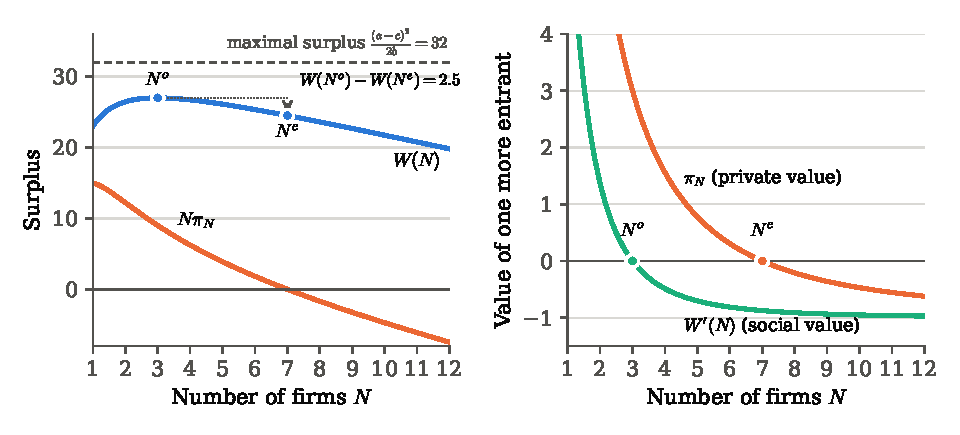
\includegraphics[width=\linewidth]{figures/ch02/entry_welfare.pdf}
\caption{Excess entry in the linear Cournot market with $a - c = 8$, $b = 1$ and $F = 1$. In the left panel, total
surplus $W(N)$ peaks at $N^o = 3$, while industry profit $N\pi_N$ reaches zero at $N^e = 7$. The welfare gap
$W(3) - W(7) = 27 - 24.5 = 2.5$ is 7.8 percent of the maximal surplus of 32. In the right panel, the private value
of entry $\pi_N$ exceeds its social value $W'(N)$ by the business-stealing term in \eqref{eq:02-mw-wprime}.}
\label{fig:02-entry}
\end{figure}

\begin{example}[Free entry into a cartel]\label{ex:02-mw-cartel}
Example~2 of \citet{MankiwWhinston1986} keeps the linear market but lets the entrants form a cartel. Total output is
the monopoly output $Q^m = \frac{a - c}{2b}$ for every $N$, and $q_N = \frac{Q^m}{N}$. Entry now steals business
one for one, since $N\frac{\dd q_N}{\dd N} = -\frac{Q^m}{N} = -q_N$. Using $P^m - c = \frac{a - c}{2}$ in
\eqref{eq:02-mw-wprime},
\begin{equation*}
W'(N) = \pi_N - (P^m - c)\, q_N = \left[(P^m - c)\, q_N - F\right] - (P^m - c)\, q_N = -F .
\end{equation*}
Each extra firm adds nothing but a set-up cost, so the optimum has one firm whenever the market should be served. Free
entry instead continues until $\pi_N = \frac{(a - c)^2}{4bN} - F = 0$, that is, until
$N^m = \frac{(a - c)^2}{4bF}$. Total set-up costs $N^m F = \frac{(a - c)^2}{4b}$ then equal the monopoly profit. The
whole monopoly rent is dissipated in duplicated set-up costs, as in the rent-seeking argument of
\citet{Posner1975} (see \cref{sec:02-welfare}). Welfare falls to the consumer surplus at the monopoly price,
$\frac{(a - c)^2}{8b}$, while one firm would give $\frac{3(a - c)^2}{8b} - F$. As $F \to 0$ the loss tends to
$\frac{(a - c)^2}{4b}$, half of the maximal surplus \citep[n.~10]{MankiwWhinston1986}.
\end{example}

\subsection{The integer constraint}\label{sec:02-mw-integer}

Treating $N$ as continuous is convenient but can mislead. In the cartel example, monopoly profit is
$\frac{(a - c)^2}{4b} - F$, and a monopoly is socially worth having when $\frac{3(a - c)^2}{8b} - F \ge 0$. When
$\frac{(a - c)^2}{4bF} \in [\frac{2}{3}, 1)$ the second condition holds and the first fails. No firm enters, although
one firm is optimal \citep[p.~53]{MankiwWhinston1986}. A monopolist captures only part of the surplus its entry
creates, so entry can be too low. With integers, the cartel example has excess entry only when
$\frac{(a - c)^2}{4bF} \ge 2$ \citep[n.~11]{MankiwWhinston1986}. The next result bounds the shortfall in general.

\begin{proposition}[At most one firm too few]\label{prop:02-mw-integer}
Suppose (E1) to (E3) of \cref{ass:02-mw} hold, with $N$ restricted to the integers and $N^o$ the integer maximizer of
$W$. Then $N^e \ge N^o - 1$ \citep[Proposition~2]{MankiwWhinston1986}.
\end{proposition}

\begin{proof}
The result is trivial when $N^o \le 1$, so let $N^o \ge 2$ and write $Q_N = N q_N$ and $n = N^o$. The proof follows
the appendix of \citet[p.~58]{MankiwWhinston1986}. It first shows that $\pi_{n - 1} \ge 0$ and then that $\pi_N$ is
nonincreasing in $N$.

\emph{Step 1.} Optimality of $n$ implies $W(n) \ge W(n - 1)$. By \eqref{eq:02-mw-welfare} this reads
\begin{equation*}
\int_{Q_{n-1}}^{Q_n} P(x)\, \dd x - n\, C(q_n) + (n - 1)\, C(q_{n-1}) \ge F .
\end{equation*}

\emph{Step 2.} Write $\pi_{n-1} = P(Q_{n-1})\, q_{n-1} - C(q_{n-1}) - F$ and replace $F$ by the larger quantity on
the left of Step~1:
\begin{equation*}
\pi_{n-1} \ge P(Q_{n-1})\, q_{n-1} - \int_{Q_{n-1}}^{Q_n} P(x)\, \dd x + n\left[C(q_n) - C(q_{n-1})\right].
\end{equation*}

\emph{Step 3.} Because $P$ is decreasing and $Q_n > Q_{n-1}$ by (E1), the integral is at most
$P(Q_{n-1})(Q_n - Q_{n-1})$. Moreover $q_{n-1} - (Q_n - Q_{n-1}) = n\, q_{n-1} - n\, q_n$. Hence
\begin{equation*}
\pi_{n-1} \ge n\, P(Q_{n-1})\left(q_{n-1} - q_n\right) + n\left[C(q_n) - C(q_{n-1})\right].
\end{equation*}

\emph{Step 4.} Convexity of $C$ gives, for any two outputs $q$ and $q'$,
\begin{equation}\label{eq:02-convex-ineq}
C(q') - C(q) \ge C'(q)\,(q' - q) .
\end{equation}
Applying it with $q = q_{n-1}$ and $q' = q_n$ yields
\begin{equation*}
\pi_{n-1} \ge n\left[P(Q_{n-1}) - C'(q_{n-1})\right]\left(q_{n-1} - q_n\right) \ge 0 ,
\end{equation*}
where the first factor is nonnegative by (E3) and the second is positive by (E2).

\emph{Step 5.} For any $N$, the fact that $P(Q_N) \le P(Q_{N-1})$ gives
\begin{align*}
\pi_N - \pi_{N-1} &= \left[P(Q_N)\, q_N - C(q_N)\right] - \left[P(Q_{N-1})\, q_{N-1} - C(q_{N-1})\right] \\
&\le P(Q_{N-1})\left(q_N - q_{N-1}\right) - \left[C(q_N) - C(q_{N-1})\right] \\
&\le \left[P(Q_{N-1}) - C'(q_{N-1})\right]\left(q_N - q_{N-1}\right) \le 0 ,
\end{align*}
using \eqref{eq:02-convex-ineq} in the third line and (E2), (E3) for the sign.

\emph{Step 6.} By \eqref{eq:02-free-entry}, $\pi_{N^e + 1} < 0$, and by Step~5 every $N \ge N^e + 1$ has negative
profit. Step~4 shows that $\pi_{n-1} \ge 0$, so $n - 1 < N^e + 1$. Since both sides are integers, $n - 1 \le N^e$.
\end{proof}

A shortfall of one firm can still be costly. In Example~3 of \citet{MankiwWhinston1986}, one firm in the linear market
acts as a monopolist, while two firms play Bertrand and price at $c$. A duopolist earns $-F$, so at most one firm
enters. A monopoly enters when $F \le \frac{(a - c)^2}{4b}$. Welfare is $W(1) = \frac{3(a - c)^2}{8b} - F$ with one
firm and $W(2) = \frac{(a - c)^2}{2b} - 2F$ with two. Duopoly is better when $F \le \frac{(a - c)^2}{8b}$. The loss
from one firm too few is then $\frac{(a - c)^2}{8b} - F$, which approaches 25 percent of the maximal surplus as
$F \to 0$ \citep[pp.~53--54]{MankiwWhinston1986}. Business stealing holds here only weakly, since
$q_1 = q_2 = \frac{a - c}{2b}$.

\subsection{Product diversity}\label{sec:02-diversity}

With differentiated products a new entrant also adds variety. Following \citet{Spence1976},
\citet[pp.~54--55]{MankiwWhinston1986} write gross consumer benefit as $G\left(\sum_i \psi(q_i)\right)$, where
$q_i$ is firm $i$'s output. The subutility $\psi$ satisfies $\psi(0) = 0$, $\psi' > 0$ and $\psi'' \le 0$, and $G$
satisfies $G' > 0$ and $G'' < 0$. These assumptions say that consumers like variety and that the products are
substitutes. (The symbols $G$ and $\psi$ are local to this subsection.) With $N$ symmetric firms the planner solves
\begin{equation}\label{eq:02-diversity-W}
\max_N\; W(N) = G\left(N \psi(q_N)\right) - N C(q_N) - N F .
\end{equation}
Consumer optimization sets each firm's price equal to the marginal benefit of its output,
$p_N = G'\left(N\psi(q_N)\right)\psi'(q_N)$, so per-firm profit is
\begin{equation*}
\pi_N = G'\left(N\psi(q_N)\right)\psi'(q_N)\, q_N - C(q_N) - F .
\end{equation*}
Differentiating \eqref{eq:02-diversity-W}, with arguments suppressed, gives
\begin{equation*}
W'(N) = G'\left[N\psi'\frac{\dd q_N}{\dd N} + \psi\right] - C(q_N) - N C'\frac{\dd q_N}{\dd N} - F .
\end{equation*}
Adding and subtracting $G'\psi' q_N$ and regrouping yields the generalization of \eqref{eq:02-mw-wprime}:
\begin{equation}\label{eq:02-diversity-wprime}
W'(N) = \pi_N + N\left[G'\psi' - C'\right]\frac{\dd q_N}{\dd N} + G'\left[\psi(q_N) - \psi'(q_N)\, q_N\right] .
\end{equation}
The second term is the business-stealing wedge, now with price $G'\psi'$. It is negative when price exceeds marginal
cost and entry contracts incumbents. The third term is new. $G'\psi$ is the entrant's contribution to gross surplus,
while $G'\psi' q_N$ is its revenue. Concavity and $\psi(0) = 0$ imply $\psi(q) \ge \psi'(q)\, q$, so the third term is
nonnegative. It is the surplus from added variety that the entrant cannot appropriate. In the homogeneous case
$\psi(q) = q$ and $G(Q) = \int_0^Q P(x)\,\dd x$, the third term vanishes and \eqref{eq:02-mw-wprime} returns.

The two wedges push in opposite directions, so the sign of the entry bias is ambiguous. With $\psi(q) = q^{\varsigma}$
for some $\varsigma < 1$ and firms that take $G'$ as given, the diversity term dominates for every $N$ and entry is
too low \citep{Spence1976}. \citet{DixitStiglitz1977} also show that monopolistic
competition can produce too little entry. Replacing Spence's price taking with conjectural variations can reverse
this result \citep{KoenkerPerry1981}. \citet[p.~55]{MankiwWhinston1986} also give a functional form, with a quadratic
$\psi$ and linear cost, in which business stealing dominates and entry is excessive. Demand substitutability is
neither necessary nor sufficient for business stealing \citep[n.~14]{MankiwWhinston1986}. Spatial models give further
examples. In the circular city with linear transport costs, the free-entry number of firms is twice the optimum
\citep[sec.~7.1.2]{Tirole1988}, and \cref{ch:diffprod} develops these location models.

\subsection{Small set-up costs}\label{sec:02-small-F}

\Cref{tab:02-mw} shows the loss from excess entry falling as set-up costs fall. The cartel example shows that this
need not happen. There the loss tends to half of the maximal surplus as $F \to 0$. Mankiw and Whinston isolate what
separates the two cases. Write $W^o_F$ and $W^e_F$ for welfare at the optimum and under free entry when the set-up
cost is $F$, and $p_N = G'\left(N\psi(q_N)\right)\psi'(q_N)$ for the price.

\begin{proposition}[Vanishing loss as set-up costs vanish]\label{prop:02-mw-small}
Suppose (E2) holds and, in addition, (i) $p_N$ is decreasing in $N$ and $\lim_{N\to\infty} N\psi(q_N) < \infty$,
(ii) $p_N - C'(q_N) > 0$ for all $N$, and (iii) $\lim_{N\to\infty}\left[p_N - C'(q_N)\right] = 0$. Then
$\lim_{F\to 0}\left(W^o_F - W^e_F\right) = 0$ \citep[Proposition~3]{MankiwWhinston1986}.
\end{proposition}

\begin{proof}[Proof sketch]
Let $W^\infty = \lim_{N\to\infty}\left[G\left(N\psi(q_N)\right) - N C(q_N)\right]$. This limit is finite and is the
best welfare attainable with no set-up cost, so $W^\infty \ge W^o_F \ge W^e_F$ for every $F$. It suffices to show
that $W^e_F \to W^\infty$. First, $N^e_F \to \infty$ as $F \to 0$. Otherwise, for small enough $F$ one more firm
would earn $(p_N - \frac{C(q_N)}{q_N})\, q_N - F \ge (p_N - C'(q_N))\, q_N - F > 0$, using $C(q) \le C'(q)\, q$ for
convex $C$ with $C(0) = 0$. Given $N^e_F \to \infty$, welfare under free entry converges to $W^\infty$ exactly when
total set-up costs $N^e_F F$ vanish. The zero-profit condition bounds them:
\begin{equation*}
N^e F \le \left[p_{N^e} - \frac{C(q_{N^e})}{q_{N^e}}\right] N^e q_{N^e} .
\end{equation*}
As $N^e \to \infty$, per-firm output tends to zero because $N\psi(q_N)$ stays bounded. Average cost and marginal cost
then both tend to $C'(0)$, so the bracket tends to $\lim\left[p_N - C'(q_N)\right] = 0$ by (iii). Total output
$N^e q_{N^e}$ stays bounded, so $N^e F \to 0$.
\end{proof}

Two assumptions do the work. Price must exceed marginal cost for every finite $N$, which is (ii), and approach it
as $N$ grows, which is (iii). Mankiw and Whinston assume both and leave the post-entry game unspecified.
\citet{Novshek1980} derives (iii) for Cournot competition as efficient scale shrinks. Linear Cournot satisfies
(ii) and (iii), which is why the losses in \cref{tab:02-mw} decline. The cartel example violates (iii), since price
stays at the monopoly level for every $N$. Example~3 satisfies (iii) but violates (ii). Price falls to marginal
cost already at $N = 2$, so a second entrant cannot cover its set-up cost. The loss from having one firm too few
therefore persists as $F \to 0$ \citep[p.~57]{MankiwWhinston1986}. The upshot is that regulating entry matters most in markets
with large set-up costs and imperfect competition. It matters little where entry is cheap and competition is close
to perfect.

\subsection{Margins and concentration under fixed and free entry}\label{sec:02-LH}

Free entry changes how margins and concentration move together. With a fixed number of firms, concentration is a
primitive and the Lerner index responds to it. With free entry, both are equilibrium outcomes driven by the same
primitives. The linear market makes the point precisely, using the four columns of \cref{tab:02-linear-cournot}.

\begin{example}[Lerner index and Herfindahl index in four regimes]\label{ex:02-LH}
Let $P = a - bQ$, marginal cost $c$, set-up cost $F$, and $r \equiv \sqrt{bF}$.

\emph{Cournot with fixed $N$.} Here $L = \frac{a - c}{a + Nc}$ and $\HHI = \frac{1}{N}$. Substituting
$N = \frac{1}{\HHI}$ and multiplying numerator and denominator by $\HHI$,
\begin{equation}\label{eq:02-LH-cournot}
L = \frac{(a - c)\,\HHI}{a\,\HHI + c}, \qquad
\frac{\dd L}{\dd \HHI} = \frac{c(a - c)}{(a\,\HHI + c)^2} > 0, \qquad
\frac{\dd^2 L}{\dd \HHI^2} = -\frac{2ac(a - c)}{(a\,\HHI + c)^3} < 0 .
\end{equation}
The relation is increasing and concave. It is causal, since $N$ is set from outside.

\emph{Cournot with free entry.} From \cref{ex:02-free-entry-linear}, $L = \frac{r}{c + r}$ and
$\HHI = \frac{r}{a - c - r}$. These points lie on the curve \eqref{eq:02-LH-cournot} for the same $(a, c)$, because
\begin{equation*}
\frac{(a - c)\frac{r}{a - c - r}}{\frac{a\, r}{a - c - r} + c} = \frac{(a - c)\, r}{a\, r + c(a - c - r)}
= \frac{(a - c)\, r}{(a - c)(r + c)} = \frac{r}{c + r} .
\end{equation*}
Both indices are now endogenous. A higher $F$ or $b$ raises $r$ and moves the industry up along the curve. A higher
$a$ lowers $\HHI$ and leaves $L$ unchanged. A higher $c$ lowers $L$ and raises $\HHI$.

\emph{Collusion with fixed $N$.} Here $L = \frac{a - c}{a + c}$ for every $N$, while $\HHI = \frac{1}{N}$. The
Lerner index does not depend on concentration at all.

\emph{Collusion with free entry.} By \cref{ex:02-mw-cartel}, $N^m = \frac{(a - c)^2}{4bF}$, so
$\HHI = \frac{4bF}{(a - c)^2}$ and $L = \frac{a - c}{a + c}$. A higher $F$ or $b$ raises $\HHI$ only. A higher $a$
raises $L$ and lowers $\HHI$, and a higher $c$ does the reverse.

Finally, collusion attracts more entrants than Cournot competition. With $x = \frac{a - c}{\sqrt{bF}}$,
\eqref{eq:02-Ne-linear} gives $N^e = x - 1$, while $N^m = \frac{x^2}{4}$. Then
\begin{equation*}
N^m - N^e = \frac{x^2}{4} - x + 1 = \left(\frac{x}{2} - 1\right)^2 \ge 0 .
\end{equation*}
\end{example}

\begin{table}[htbp]
\centering
\begin{threeparttable}
\caption{Comparative statics of the Lerner and Herfindahl indices in the linear market}
\label{tab:02-LH-cases}
\renewcommand{\arraystretch}{1.6}
\begin{tabular}{@{}lcccccc@{}}
\toprule
 & & & \multicolumn{4}{c}{Effect of a higher primitive on $(L, \HHI)$} \\
\cmidrule(l){4-7}
Regime & $L$ & $\HHI$ & $F$ & $b$ & $a$ & $c$ \\
\midrule
Cournot, fixed $N$ & $\frac{a - c}{a + Nc}$ & $\frac{1}{N}$ & $(0, 0)$ & $(0, 0)$ & $(+, 0)$ & $(-, 0)$ \\
Cournot, free entry & $\frac{\sqrt{bF}}{c + \sqrt{bF}}$ & $\frac{\sqrt{bF}}{a - c - \sqrt{bF}}$ & $(+, +)$ &
  $(+, +)$ & $(0, -)$ & $(-, +)$ \\
Collusion, fixed $N$ & $\frac{a - c}{a + c}$ & $\frac{1}{N}$ & $(0, 0)$ & $(0, 0)$ & $(+, 0)$ & $(-, 0)$ \\
Collusion, free entry & $\frac{a - c}{a + c}$ & $\frac{4bF}{(a - c)^2}$ & $(0, +)$ & $(0, +)$ & $(+, -)$ &
  $(-, +)$ \\
\bottomrule
\end{tabular}
\begin{tablenotes}\footnotesize
\item Notes: $P = a - bQ$, constant marginal cost $c$, set-up cost $F$. Each cell gives the signs of the effects on
$L$ and $\HHI$. Under free entry the number of firms is treated as continuous.
\end{tablenotes}
\end{threeparttable}
\end{table}

\begin{figure}[htbp]
\centering
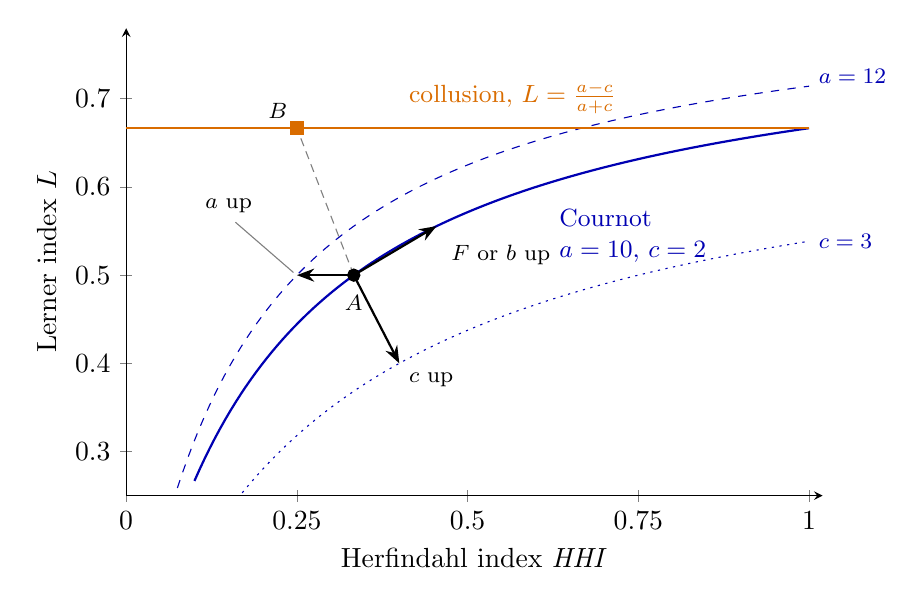
\begin{tikzpicture}
\begin{axis}[
  width=0.86\linewidth, height=0.62\linewidth,
  xmin=0, xmax=1.02, ymin=0.25, ymax=0.78,
  xlabel={Herfindahl index $\HHI$}, ylabel={Lerner index $L$},
  xtick={0,0.25,0.5,0.75,1}, ytick={0.3,0.4,0.5,0.6,0.7},
  axis lines=left, every axis plot/.append style={thick},
  clip=false]
  \addplot[domain=0.1:1, samples=120, blue!70!black] {8*x/(10*x+2)};
  \node[blue!70!black, anchor=north west, font=\small, align=left] at (axis cs:0.62,0.585)
    {Cournot\\ $a = 10$, $c = 2$};
  \addplot[domain=0.075:1, samples=120, blue!70!black, dashed, thin] {10*x/(12*x+2)};
  \node[blue!70!black, anchor=west, font=\footnotesize] at (axis cs:1.0,0.725) {$a = 12$};
  \addplot[domain=0.17:1, samples=120, blue!70!black, dotted, thin] {7*x/(10*x+3)};
  \node[blue!70!black, anchor=west, font=\footnotesize] at (axis cs:1.0,0.538) {$c = 3$};
  \addplot[domain=0:1, samples=2, orange!85!black] {2/3};
  \node[orange!85!black, anchor=south west, font=\small] at (axis cs:0.40,0.672)
    {collusion, $L = \frac{a - c}{a + c}$};
  \addplot[only marks, mark=*, mark size=2pt, black] coordinates {(0.3333,0.5)};
  \node[anchor=north, font=\footnotesize] at (axis cs:0.3333,0.488) {$A$};
  \draw[-{Stealth[length=2.2mm]}, thick] (axis cs:0.3333,0.5) -- (axis cs:0.4545,0.5556);
  \node[anchor=north west, font=\footnotesize] at (axis cs:0.462,0.545) {$F$ or $b$ up};
  \draw[-{Stealth[length=2.2mm]}, thick] (axis cs:0.3333,0.5) -- (axis cs:0.25,0.5);
  \draw[thin, gray] (axis cs:0.245,0.503) -- (axis cs:0.16,0.56);
  \node[anchor=south, font=\footnotesize] at (axis cs:0.15,0.56) {$a$ up};
  \draw[-{Stealth[length=2.2mm]}, thick] (axis cs:0.3333,0.5) -- (axis cs:0.4,0.4);
  \node[anchor=north west, font=\footnotesize] at (axis cs:0.40,0.40) {$c$ up};
  \addplot[only marks, mark=square*, mark size=2pt, orange!85!black] coordinates {(0.25,0.6667)};
  \draw[densely dashed, gray] (axis cs:0.3333,0.5) -- (axis cs:0.25,0.6667);
  \node[anchor=south east, font=\footnotesize] at (axis cs:0.25,0.6667) {$B$};
\end{axis}
\end{tikzpicture}
\caption{Lerner index against Herfindahl index in the linear market with $a = 10$, $c = 2$, $b = 1$. The solid curve
is $L = \frac{8\,\HHI}{10\,\HHI + 2}$, the Cournot relation \eqref{eq:02-LH-cournot}. Point $A$ is the Cournot
free-entry outcome with $F = 4$ ($N^e = 3$). Arrows show the free-entry responses to higher $F$ or $b$ (along the
curve), higher $a$ (onto the dashed curve) and higher $c$ (onto the dotted curve). Point $B$ is the collusive
free-entry outcome with the same primitives ($N^m = 4$). It has a higher margin and lower concentration than $A$.}
\label{fig:02-LH}
\end{figure}

The lesson is a theoretical one. The sign of a cross-industry relation between margins and concentration depends on
which primitive varies across industries and on how firms compete. Points $A$ and $B$ in \cref{fig:02-LH} share every
primitive and differ only in conduct. A sample that mixes Cournot and collusive industries pairs high margins with low
concentration and can produce a flat or negative slope. A regression of $L$ on $\HHI$ across industries therefore has
no structural interpretation without a model of entry and conduct. \Cref{ch:intro} discusses these regressions, and
\cref{app:problems} works through the full problem.

\section{Bertrand competition and capacity constraints}\label{sec:02-bertrand}

Cournot firms choose quantities and let the market set the price. Many firms instead post prices and serve whatever
demand arrives. This section studies price competition with a homogeneous good. Its main result is stark: two firms
suffice for the competitive price. We then show how capacity constraints undo the result and when quantity
competition is the better description.

\subsection{Price competition with a homogeneous good}\label{sec:02-bertrand-homog}

\begin{definition}[Bertrand game with a homogeneous good]\label{def:02-bertrand}
There are $N \ge 2$ firms with constant marginal costs $c_i$ and no capacity limits. Market demand $Q(p)$ is
continuous and nonincreasing. Firms choose prices $p_i \ge 0$ simultaneously. Let $p_{\min} = \min_i p_i$ and let
$k$ be the number of firms that charge $p_{\min}$. Each of these firms sells $\frac{Q(p_{\min})}{k}$, and every other
firm sells nothing. Firm $i$ earns $(p_i - c_i)\, q_i$, and each firm must serve all demand at its posted price.
\end{definition}

These are the stage-game rules used for repeated price competition in \cref{ch:collusion-theory}. In the static game
with symmetric costs the tie rule (equal split) does not affect equilibrium outcomes. It matters with asymmetric
costs and for the collusive shares in the repeated game.

\begin{proposition}[The Bertrand paradox]\label{prop:02-bertrand}
Suppose all firms have the same marginal cost $c$ and $Q(c) > 0$. Then a pure-strategy Nash equilibrium exists. In
every pure-strategy Nash equilibrium $p_{\min} = c$, at least two firms charge $c$, and every firm earns zero profit.
\end{proposition}

\begin{proof}
Take any price profile and consider four exhaustive cases.

\emph{Case 1, $p_{\min} < c$.} The firms charging $p_{\min}$ sell $\frac{Q(p_{\min})}{k} \ge \frac{Q(c)}{k} > 0$ at a
loss. Any of them can raise its price above $p_{\min}$ and sell nothing, earning zero. So the profile is not an
equilibrium.

\emph{Case 2, $p_{\min} > c$ and $Q(p_{\min}) > 0$.} If $k \ge 2$, a firm at $p_{\min}$ earns
$(p_{\min} - c)\frac{Q(p_{\min})}{k}$. By cutting its price to $p_{\min} - \eta$ it serves the whole market and earns
at least $(p_{\min} - \eta - c)\, Q(p_{\min})$, because $Q$ is nonincreasing. For small $\eta > 0$ this exceeds its
current profit, since $k \ge 2$. If $k = 1$, any other firm earns zero and can charge a price $p' \in (c, p_{\min})$,
earning $(p' - c)\, Q(p') \ge (p' - c)\, Q(p_{\min}) > 0$. Either way someone deviates.

\emph{Case 3, $p_{\min} > c$ and $Q(p_{\min}) = 0$.} Every firm earns zero. By continuity of $Q$ and $Q(c) > 0$ there
is a price $p'$ slightly above $c$ with $Q(p') > 0$, and $p' < p_{\min}$ because $Q$ is nonincreasing. A firm that
deviates to $p'$ earns $(p' - c)\, Q(p') > 0$.

\emph{Case 4, $p_{\min} = c$.} If only one firm charges $c$, it earns zero. Let $p_{(2)} > c$ be the second-lowest
price. By continuity it can raise its price to some $p' \in (c, p_{(2)})$ with $Q(p') > 0$ and earn a positive
profit. So at least two firms must charge $c$. In that case every firm earns zero. A firm that raises its price sells
nothing and still earns zero, and a firm that cuts below $c$ makes a loss. No deviation is profitable, so any profile
with at least two firms at $c$ is an equilibrium.
\end{proof}

The paradox is the contrast with \cref{sec:02-cournot}. A symmetric Cournot duopoly has industry conduct
$\theta = \frac{1}{2}$ (\cref{sec:02-conduct}). A Bertrand duopoly prices at
marginal cost, so $\theta = 0$ even with two firms. The number of firms alone does not pin down margins. The mode of
competition matters just as much. Two firms suffice for competitive pricing only under stark assumptions: identical
products, constant marginal cost, no capacity limits, and a single round of play. Each assumption points to a
resolution. Capacity constraints are the subject of \cref{sec:02-capacity}. Product differentiation is the subject of
\cref{ch:diffprod}. Repeated interaction is previewed in \cref{sec:02-collusion} and developed in
\cref{ch:collusion-theory}.

\casehead{Asymmetric costs} Let $c_1 < c_2 \le c_j$ for all $j \ge 3$, and let $p^m(c_1)$ be the monopoly price of a
firm with cost $c_1$. If $p^m(c_1) \le c_2$, firm 1's cost advantage is \emph{drastic}. It charges $p^m(c_1)$ and
serves the market, while rivals price at or above their costs. If $p^m(c_1) > c_2$, firm 1 wants to price just below
$c_2$. With continuous prices and an equal split of ties, there is no largest price below $c_2$, so a pure
equilibrium fails to exist. Two standard modifications restore one. If ties go to the low-cost firm, then
$p_1 = p_2 = c_2$ is an equilibrium in which firm 1 serves the market and earns $(c_2 - c_1)\, Q(c_2)$. If prices lie
on a grid with step $\iota$ and $c_2$ on the grid, then $p_1 = c_2$ and $p_2 = c_2 + \iota$ is an equilibrium for
small $\iota$. In this equilibrium firm 2 avoids the weakly dominated choice of pricing at its own cost. Either way, the market price
is
\begin{equation*}
P = \min\left\{c_2,\; p^m(c_1)\right\}.
\end{equation*}
The efficient firm earns a margin limited by its rival's cost, with Lerner index $\frac{c_2 - c_1}{c_2}$ in the
non-drastic case. Measured against the producing firm's marginal cost $c_1$, this market shows a positive conduct
parameter $\theta = \varepsilon\frac{c_2 - c_1}{c_2}$, although firms play Bertrand. A positive estimated $\theta$ can
thus reflect cost asymmetry as well as softer conduct.

\begin{remark}[Increasing marginal cost]\label{rem:02-bertrand-convex}
Let $N$ symmetric firms have a strictly convex cost $C(q)$ with $C(0) = 0$, and keep the obligation to serve all
demand at the posted price. Consider a common price $p$ at which each firm sells $\frac{Q(p)}{N}$ and earns
$u(p) = \frac{p\, Q(p)}{N} - C\left(\frac{Q(p)}{N}\right)$. Raising the price sells nothing and earns $C(0) = 0$.
Undercutting slightly serves the whole market and earns close to $v(p) = p\, Q(p) - C(Q(p))$. For prices below the
level that maximizes $v$, the common price $p$ is an equilibrium if and only if
\begin{equation*}
u(p) \ge 0 \qquad\text{and}\qquad u(p) \ge v(p) .
\end{equation*}
Both conditions hold strictly at the competitive price $p^*$, defined by $p^* = C'\left(\frac{Q(p^*)}{N}\right)$.
Write $q^* = \frac{Q(p^*)}{N}$. The first holds because average cost is below marginal cost for strictly convex $C$
with $C(0) = 0$. For the second, apply \eqref{eq:02-convex-ineq} strictly:
\begin{equation*}
v(p^*) - u(p^*) = p^*\left(Nq^* - q^*\right) - \left[C(Nq^*) - C(q^*)\right]
< p^*\left(Nq^* - q^*\right) - C'(q^*)\left(Nq^* - q^*\right) = 0 .
\end{equation*}
By continuity both inequalities also hold in an interval of prices around $p^*$. Pure equilibria therefore exist and
form a continuum, with prices above and below the competitive level \citep{Dastidar1995}.

Without the obligation to serve, a firm sells only what it wishes at its posted price. Firm $i$'s \emph{competitive
supply} $S_i(p)$ is defined by $p = C_i'(S_i(p))$, and a firm never sells more than $S_i(p)$. The natural candidate is
then the competitive price $p^*$, with $S_1(p^*) + S_2(p^*) = Q(p^*)$ in a duopoly. Suppose rationing is
\emph{efficient}, so that the consumers with the highest willingness to pay are served first (\cref{def:02-rationing}
below). Then $p^*$ is not an equilibrium \citep[sec.~5.3.2]{Tirole1988}. Let firm 2 charge $p^*$ and sell
$q_2^* = S_2(p^*)$, and write $q_1^* = S_1(p^*)$. If firm 1 raises its price to some $p$ slightly above $p^*$, it
serves the residual demand $Q(p) - q_2^*$, which is below $S_1(p)$. Its profit is
$p\,[Q(p) - q_2^*] - C_1(Q(p) - q_2^*)$, whose derivative at $p^*$ is
\begin{equation*}
Q(p^*) - q_2^* + \bigl[p^* - C_1'(q_1^*)\bigr]Q'(p^*) = q_1^* > 0 ,
\end{equation*}
because $Q(p^*) - q_2^* = q_1^*$ and $p^* = C_1'(q_1^*)$. The units lost were sold at marginal cost, so the loss is of
second order, while the higher price on the remaining units is a first-order gain. Equilibria then generally involve
mixed strategies, and both firms' prices exceed the competitive price. Decreasing returns therefore soften price
competition, and the capacity constraint of \cref{sec:02-capacity} is the extreme case.
\end{remark}

\begin{remark}[Strategic substitutes and complements]\label{rem:02-strategic}
\citet[p.~489]{BulowGeanakoplosKlemperer1985} call a lower price or a higher quantity a ``more aggressive'' move.
They classify competition by how a rival's aggressive move changes the \emph{marginal} profit of the firm's own
aggressive move. Choices are strategic substitutes when the rival's aggressive move lowers this marginal profit and
\emph{strategic complements} when it raises it.
Equivalently, best responses slope down under substitutes and up under complements. \Cref{sec:02-cournot-br}
showed that quantities are substitutes in Cournot competition under \cref{ass:02-cournot}. With differentiated products and linear demand
$q_i = d_0 - d_1 p_i + d_2 p_j$, where $0 < d_2 < d_1$, profit $(p_i - c)\, q_i$ gives
$\frac{\partial^2 \pi_i}{\partial p_i \partial p_j} = d_2 > 0$. A lower $p_j$ therefore lowers
$\frac{\partial \pi_i}{\partial p_i}$, which raises the marginal profit of cutting $p_i$. Prices are complements, and
the best response $p_i = \frac{d_0 + d_1 c + d_2 p_j}{2 d_1}$ slopes up, with slope
$\frac{d_2}{2d_1} \in \left(0, \frac{1}{2}\right)$ as \eqref{eq:02-reaction-slope} predicts. \citet[sec.~11.2]{Tirole1988}
uses the same linear demand, $q_i = 1 - bp_i + dp_j$, to illustrate Nash equilibrium in prices. The classification
depends on demand as well as on the strategic variable. \citet[p.~490]{BulowGeanakoplosKlemperer1985} note that
Cournot competition with constant-elasticity demand may yield strategic complements. Our derivation from
\cref{rem:02-c2} gives the threshold. With constant-elasticity demand, $P' + q_i P'' = P'\left(1 - s_i \chi\right)$ with
curvature $\chi = 1 + \frac{1}{\varepsilon}$. The cross-partial is therefore positive, and quantities are complements,
when $s_i\left(1 + \frac{1}{\varepsilon}\right) > 1$.
\end{remark}

\subsection{Capacity constraints and rationing}\label{sec:02-capacity}

\citet{Edgeworth1925}, in an article first published in Italian in 1897, observed that the Bertrand outcome collapses
once firms cannot serve the whole market \citep[sec.~5.2.1]{Tirole1988}. Let two
firms have constant marginal cost $c$ up to capacities $k_1$ and $k_2$, beyond which they cannot produce. Suppose
$k_2 < Q(c)$ and both firms charge $c$. If firm 1 raises its price slightly, firm 2 cannot serve everyone who wants to
buy at $c$. Some consumers turn to firm 1 at the higher price, and firm 1 earns a positive margin on them. So
$p_1 = p_2 = c$ is no longer an equilibrium. When capacities are intermediate, no pure-strategy equilibrium exists at
all. Firms undercut each other until one prefers to raise its price and serve the leftover demand, and the cycle
repeats. The equilibrium of the static game is in mixed strategies \citep{LevitanShubik1972}. What a high-price firm
can sell depends on which consumers the low-price firm serves.

\begin{definition}[Rationing rules]\label{def:02-rationing}
Let firm 1 charge $p_1 < p_2$ with capacity $k_1 < Q(p_1)$. A \emph{rationing rule} gives the residual demand
$Q_2(p_2)$ left for firm 2.
\begin{enumerate}[label=(\roman*)]
\item Under \emph{efficient rationing}, firm 1 serves the consumers with the highest willingness to pay first. Firm 2
  faces
  \begin{equation*}
  Q_2(p_2) = \max\left\{0,\; Q(p_2) - k_1\right\}.
  \end{equation*}
\item Under \emph{proportional rationing}, every consumer who wants to buy at $p_1$ is equally likely to be served
  by firm 1. The fraction $\frac{k_1}{Q(p_1)}$ of them is served. The unserved consumers are a random sample, so a
  fraction $1 - \frac{k_1}{Q(p_1)}$ of the demand at any price remains:
  \begin{equation*}
  Q_2(p_2) = Q(p_2)\left(1 - \frac{k_1}{Q(p_1)}\right).
  \end{equation*}
\end{enumerate}
\end{definition}

Efficient rationing maximizes consumer surplus given the capacities, since the units go to those who value them most.
It also leaves the high-price firm the least demand. Proportional residual demand is larger because
\begin{equation*}
Q(p_2)\left(1 - \frac{k_1}{Q(p_1)}\right) \ge Q(p_2) - k_1
\quad\Longleftrightarrow\quad
\frac{Q(p_2)}{Q(p_1)}\, k_1 \le k_1 ,
\end{equation*}
which holds because $Q(p_2) \le Q(p_1)$. \Cref{fig:02-rationing} draws both residual demands. Efficient rationing
shifts demand inward in parallel by $k_1$. Proportional rationing rotates it around the choke price.

\citet[sec.~5.3.1]{Tirole1988} interprets the two rules. Efficient rationing is the outcome if consumers can resell the
good to each other at no cost, since such arbitrage moves the units to those who value them most. It also arises when
identical consumers with downward-sloping demands are each rationed equally. Proportional rationing, also called
randomized rationing, gives every consumer the same chance of being served. It leaves some low-value consumers with the
bargain, and the high-price firm prefers it because its residual demand is larger. Many other rules are possible.
Suppose rationing works through queues, and the most eager buyers also have the highest value of time. Then the least
eager buyers may end up with the low price. In applications the rationing rule stands in for a model of consumer
behavior, and the right rule depends on the market.

\begin{figure}[htbp]
\centering
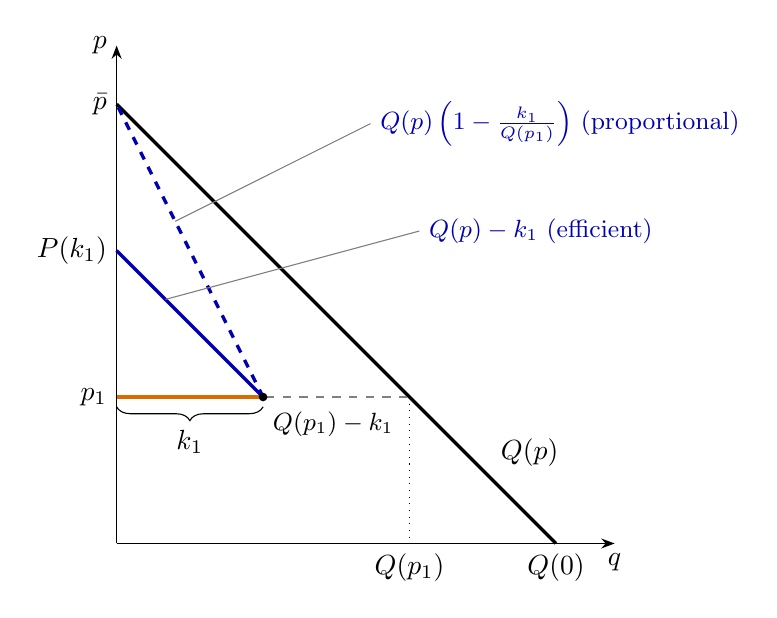
\begin{tikzpicture}[scale=0.62, >=Stealth]
  \draw[->] (0,0) -- (10.2,0) node[below] {$q$};
  \draw[->] (0,0) -- (0,10.2) node[left] {$p$};
  \draw[very thick, black] (0,9) -- (9,0) node[pos=0.85, above right] {$Q(p)$};
  \node[below] at (9,0) {$Q(0)$};
  \draw[dashed, gray] (0,3) -- (6,3);
  \node[left] at (0,3) {$p_1$};
  \draw[very thick, orange!85!black] (0,3) -- (3,3);
  \draw[decorate, decoration={brace, amplitude=5pt, mirror}] (0,2.8) -- (3,2.8)
    node[midway, below=5pt] {$k_1$};
  \draw[dotted] (6,3) -- (6,0) node[below] {$Q(p_1)$};
  \draw[very thick, blue!70!black] (3,3) -- (0,6);
  \draw[very thick, blue!70!black, dashed] (3,3) -- (0,9);
  \node[blue!70!black, anchor=west, font=\small] (eff) at (6.2,6.4) {$Q(p) - k_1$ (efficient)};
  \draw[thin, gray] (eff.west) -- (1.0,5.0);
  \node[blue!70!black, anchor=west, font=\small] (prop) at (5.2,8.6)
    {$Q(p)\left(1 - \frac{k_1}{Q(p_1)}\right)$ (proportional)};
  \draw[thin, gray] (prop.west) -- (1.2,6.6);
  \fill (3,3) circle (2.5pt);
  \node[anchor=north west, font=\small] at (3,2.9) {$Q(p_1) - k_1$};
  \node[left] at (0,9) {$\bar p$};
  \node[left] at (0,6) {$P(k_1)$};
\end{tikzpicture}
\caption{Residual demand of the high-price firm. Firm 1 charges $p_1$ and sells its capacity $k_1 < Q(p_1)$. Under
efficient rationing firm 2 faces $Q(p) - k_1$ for $p > p_1$ (solid), a parallel inward shift of demand. Under
proportional rationing it faces $Q(p)\left(1 - \frac{k_1}{Q(p_1)}\right)$ (dashed), which rotates demand around the
choke price $\bar p$. Drawn for $Q(p) = 9 - p$, $p_1 = 3$ and $k_1 = 3$.}
\label{fig:02-rationing}
\end{figure}

\citet{KrepsScheinkman1983} turn Edgeworth's problem into a foundation for Cournot competition. Firms first choose
capacities and then, having observed them, compete in prices. Write $r_\gamma(k)$ for the Cournot best response of a
firm with constant marginal cost $\gamma$ to rival output $k$.

\begin{proposition}[Capacity commitment yields Cournot outcomes]\label{prop:02-ks}
Consider a duopoly in which firms first build capacities $k_i$ at constant unit cost $c_k > 0$, then observe them
and set prices. Production costs $c \ge 0$ per unit up to capacity. Suppose inverse demand is concave and residual
demand follows efficient rationing. Then the game has a unique subgame-perfect equilibrium outcome. It coincides with
the Cournot outcome of the one-stage game with marginal cost $c + c_k$ \citep{KrepsScheinkman1983}.
\end{proposition}

A linear example shows the mechanism before the general argument \citep[sec.~5.3.2.1]{Tirole1988}.

\begin{example}[Capacity-constrained price competition with linear demand]\label{ex:02-ks-linear}
Let $Q(p) = 1 - p$, let capacity cost $c_k \in \left[\frac{3}{4}, 1\right]$ per unit, and let production cost nothing
up to capacity. Rationing is efficient. No firm builds more than $\frac{1}{3}$. In the pricing stage a firm cannot
earn more than the monopoly revenue $\max_p p(1 - p) = \frac{1}{4}$. Its net profit is therefore at most
$\frac{1}{4} - c_kk_i$, which is negative for $k_i > \frac{1}{3}$ because $c_k \ge \frac{3}{4}$.

Take capacities in $\left[0, \frac{1}{3}\right]$. We claim that both firms charging the market-clearing price
$p^* = 1 - k_1 - k_2$ is an equilibrium of the pricing stage. A lower price gains nothing, since firm $i$ already
sells its whole capacity at $p^*$. At a higher price $p > p^*$, firm $i$ sells the residual demand
$q = 1 - p - k_j < k_i$. Its revenue $pq$ is then $(1 - q - k_j)q$, the Cournot objective against rival output
$k_j$. This objective is concave in $q$, and its derivative at $q = k_i$ is $1 - 2k_i - k_j \ge 0$. Revenue therefore
rises on $[0, k_i]$, and the best choice is $q = k_i$, that is, the price $p^*$. The reduced-form profits after the
pricing stage are
\begin{equation}\label{eq:02-ks-linear}
  \Pi_i(k_i, k_j) = (1 - k_i - k_j)\,k_i - c_k k_i ,
\end{equation}
the profits net of capacity cost. This is Tirole's eq.~(5.3). His eq.~(5.2) is the same profit gross of capacity
cost, $(1 - k_i - k_j)k_i$. The net profits are exactly the Cournot profits for outputs $k_i$ and marginal cost
$c_k$. The capacity stage is therefore a Cournot game. Its equilibrium has $k_1 = k_2 = \frac{1 - c_k}{3} \le
\frac{1}{12}$ and price $p^* = \frac{1 + 2c_k}{3}$.
\end{example}

\casehead{Two foundations for Cournot} \citet[sec.~5.3.4]{Tirole1988} separates two results. The pricing stage has
an \emph{exact Cournot reduced form} when, at every pair of capacities that can arise, its equilibrium profits equal
the Cournot profits with quantities read as capacities. The two-stage game has a \emph{Cournot outcome} when its
subgame-perfect capacities and price coincide with the Cournot equilibrium. The first result implies the second,
because the capacity stage is then the Cournot game. It also covers variants, such as capacities chosen in sequence.
\Cref{ex:02-ks-linear} has the exact reduced form. \Cref{prop:02-ks} claims only the Cournot outcome. In its general
setting the reduced form is Cournot for small capacities only, and large capacities lead to mixed equilibria with
other payoffs.

\casehead{The pricing stage} To simplify, set the production cost to $c = 0$, as \citet[sec.~5.7.2.1]{Tirole1988}
does, and assume $k_1 + k_2 < Q(0)$. Write $r(k) = r_0(k)$ for the output that maximizes $qP(q + k)$. Inverse demand
is concave, so this objective is strictly concave in $q$. By \cref{lem:02-cournot-br}, $r$ is single-valued and
decreasing, with slope in $(-1, 0)$.

\begin{lemma}[Pure equilibria clear the market]\label{lem:02-ks1}
In a pure-strategy equilibrium of the pricing stage, $p_1 = p_2 = P(k_1 + k_2)$, and both firms sell their
capacities \citep[sec.~5.7.2.1, Lemma~1]{Tirole1988}.
\end{lemma}

\begin{proof}
Suppose first that $p_1 = p_2 = p > P(k_1 + k_2)$. Demand at $p$ is below total capacity, so some firm $i$ sells less
than $k_i$. By charging $p - \eta$ it would serve the whole market and sell more, which raises its profit for small
$\eta > 0$. Suppose next that $p_1 = p_2 = p < P(k_1 + k_2)$. Both firms ration their customers, and either one could
raise its price slightly and still sell its capacity. Finally, suppose $p_i < p_j$. If firm $i$ is capacity
constrained, it can raise its price slightly and still sell $k_i$. Otherwise it serves all demand at $p_i$, and
optimality requires $p_i$ to be its unconstrained monopoly price, which is positive. Firm $j$ then sells nothing, and
it could earn a positive profit by charging $p_i - \eta$. Each case contradicts equilibrium.
\end{proof}

\begin{lemma}[Pure equilibria lie below the reaction curves]\label{lem:02-ks2}
In a pure-strategy equilibrium of the pricing stage, no firm charges less than $P(k_j + r(k_j))$
\citep[sec.~5.7.2.1, Lemma~2]{Tirole1988}. Consequently, a pure-strategy equilibrium exists if and only if
$k_i \le r(k_j)$ for both firms, and it is then the market-clearing price $P(k_1 + k_2)$.
\end{lemma}

\begin{proof}
By \cref{lem:02-ks1}, both firms charge $p = P(k_1 + k_2)$ in a pure equilibrium. Suppose $p < P(k_j + r(k_j))$,
which means $k_i > r(k_j)$. Let firm $i$ deviate to $p' = P(k_j + r(k_j)) > p$. Firm $j$ still sells $k_j$ at $p$.
Under efficient rationing firm $i$ faces the residual demand $Q(p') - k_j = r(k_j) < k_i$, which it can serve. Its
revenue becomes $r(k_j)P(r(k_j) + k_j)$, the largest Cournot revenue against $k_j$. This exceeds $k_iP(k_i + k_j)$,
because $r(k_j)$ is the unique maximizer and $k_i \ne r(k_j)$. The deviation is profitable, a contradiction. Hence a
pure equilibrium requires $k_i \le r(k_j)$ for both firms.

Conversely, let $k_i \le r(k_j)$ for both firms, and let both charge $p^* = P(k_1 + k_2)$. A price cut does not help
firm $i$, because it already sells its whole capacity. At a price $p > p^*$, efficient rationing leaves firm $i$ the
residual demand $q = Q(p) - k_j < k_i$. Choosing $p$ is therefore the same as choosing an output $q < k_i$ sold at
$P(q + k_j)$. The revenue $qP(q + k_j)$ is the Cournot objective against $k_j$. It is concave in $q$ and peaks at
$r(k_j) \ge k_i$, so it rises on $[0, k_i]$. The best choice is $q = k_i$, which means charging $p^*$.
\end{proof}

In the pure-strategy region the reduced form is exactly Cournot. The Cournot capacities with capacity cost $c_k$ lie
in this region. Indeed $r_\gamma(k)$ solves $P(q + k) + q P'(q + k) = \gamma$, whose left side falls in $q$, so the
best response falls when $\gamma$ rises. Hence $r_{c_k}(k) < r(k)$ at every $k$ where $r_{c_k}(k) > 0$.

\begin{lemma}[The larger firm earns its Stackelberg-follower profit]\label{lem:02-ks3}
Suppose $k_i > r(k_j)$ for at least one firm, so that the pricing stage has only mixed-strategy equilibria. Then the
firm with the larger capacity, say firm $i$, earns
\begin{equation}\label{eq:02-ks-follower}
  F(k_j) = r(k_j)\,P\bigl(k_j + r(k_j)\bigr)
\end{equation}
in every equilibrium \citep[sec.~5.7.2.1, Lemma~3]{Tirole1988}.
\end{lemma}

\begin{proof}[Proof sketch]
In a mixed equilibrium every price in a firm's support yields the same expected profit (\cref{sec:02-nash}).
Consider the top of the support of the larger firm, and suppose that at this price it is undercut with probability
one. It then sells along the efficient residual demand $Q(p) - k_j$, so choosing the price is the same as choosing a
quantity against $k_j$. Optimality at the top of the support requires the quantity $r(k_j)$, which yields $F(k_j)$.
Indifference across the support makes $F(k_j)$ the firm's equilibrium profit. \citet{KrepsScheinkman1983} show that
it is indeed the larger firm whose highest price is undercut for sure, and they construct the equilibrium
distributions. Tirole sketches the argument.
\end{proof}

The name comes from the Stackelberg follower, which chooses its best response to the leader's output
(\cref{ex:02-stackelberg}). The key feature of \eqref{eq:02-ks-follower} is that $F(k_j)$ does not depend on the
larger firm's own capacity. Capacity beyond the pure region only adds cost.

\casehead{The capacity stage} Let $q^{**}$ be the symmetric Cournot output with marginal cost $c_k$, which maximizes
$q\,[P(q + q^{**}) - c_k]$. We show that $k_1 = k_2 = q^{**}$ is an equilibrium of the capacity stage
\citep[sec.~5.7.2.2]{Tirole1988}. Let firm $i$ choose $q^{**}$, and consider firm $j$'s choice $k$. In the pricing
stage the capacity cost is sunk, so each firm wants to sell more than it would if capacity were still to be paid
for. In particular $r(q^{**}) > q^{**}$.
\begin{itemize}
  \item Let $k \le r(q^{**})$. The capacities then lie in the pure region. When $k \le q^{**}$ this holds because
  $r(k) \ge r(q^{**}) > q^{**}$. When $q^{**} < k \le r(q^{**})$, the slope bound $r' > -1$ gives
  $r(k) > r(q^{**}) - (k - q^{**}) \ge q^{**}$. Firm $j$ therefore earns the Cournot profit $k\,[P(k + q^{**}) -
  c_k]$, which is at most $q^{**}[P(2q^{**}) - c_k]$ by the definition of $q^{**}$.
  \item Let $k > r(q^{**})$. The pricing stage is then in the mixed region, and firm $j$ has the larger capacity. By
  \cref{lem:02-ks3} its net profit is $F(q^{**}) - c_k k$. Since $k > r(q^{**})$,
  \[
    F(q^{**}) - c_k k < r(q^{**})\bigl[P\bigl(r(q^{**}) + q^{**}\bigr) - c_k\bigr] \le q^{**}\bigl[P(2q^{**}) -
    c_k\bigr] ,
  \]
  where the last step again uses the definition of $q^{**}$.
\end{itemize}
No deviation pays. The Cournot capacities therefore form an equilibrium of the capacity stage, and the price is
$P(2q^{**})$. Proving that this outcome is unique takes more work \citep{KrepsScheinkman1983}.

\casehead{Rationing and the cost of capacity} The result also depends on the rationing rule when capacity is cheap.
\citet{DavidsonDeneckere1986} study rules other than efficient rationing \citep[secs.~5.3.4 and 5.7.2.3]{Tirole1988}.
For virtually any such rule, the Cournot outcome cannot be an equilibrium of the two-stage game when the capacity
cost is small. A first-order calculation at the Cournot point shows why. Let both firms hold the Cournot
capacities $q^{**}$ and charge $p^{**} = P(2q^{**})$, now with production cost $c \ge 0$. Let $Q_2(p_2)$ be firm 2's
residual demand for $p_2$ just above $p^{**}$, with $Q_2(p^{**}) = q^{**}$. The capacity cost is sunk, so a small
price increase changes firm 2's profit at the rate
\[
  A = q^{**} + (p^{**} - c)\,Q_2'(p^{**}) .
\]
The Cournot first-order condition with marginal cost $c + c_k$ gives $p^{**} - c - c_k = -q^{**}P'(2q^{**}) =
\frac{q^{**}}{\lvert Q'(p^{**})\rvert}$. Substituting,
\begin{equation}\label{eq:02-dd}
  A = q^{**}\left(1 - \frac{\lvert Q_2'(p^{**})\rvert}{\lvert Q'(p^{**})\rvert}\right)
      - c_k\,\lvert Q_2'(p^{**})\rvert .
\end{equation}
Efficient rationing has $Q_2' = Q'$, so $A = -c_k\lvert Q'(p^{**})\rvert < 0$, and a price increase does not pay. A
rule whose residual demand responds less to price than market demand, $\lvert Q_2'(p^{**})\rvert < \lvert
Q'(p^{**})\rvert$, makes the first term positive. For small enough $c_k$ the rate $A$ is then positive. Firm 2 gains
by raising its price above the market-clearing level, and the Cournot capacities do not lead to the Cournot price.
With price on the vertical axis, as in \cref{fig:02-rationing}, such a residual demand is steeper than market demand.
Proportional rationing is such a rule. By \cref{def:02-rationing}, it
gives $Q_2(p) = Q(p)\bigl(1 - \frac{q^{**}}{Q(p^{**})}\bigr) = \frac{Q(p)}{2}$. Hence $Q_2' = \frac{Q'}{2}$ and
$A = \frac{1}{2}\bigl(q^{**} - c_k\lvert Q'(p^{**})\rvert\bigr)$.

Costly capacity restores the Cournot form. Keep the demand $Q(p) = 1 - p$ and the zero production cost of
\cref{ex:02-ks-linear}, but let $c_k \in (0, 1)$. Then $q^{**} = \frac{1 - c_k}{3}$ and $\lvert Q'\rvert = 1$, so
under proportional rationing $A > 0$ if and only if $c_k < \frac{1}{4}$.
Equivalently, the Cournot price $p^{**} = \frac{1 + 2c_k}{3}$ then lies below the monopoly price $\frac{1}{2}$. A firm
that raises its price faces a scaled-down copy of market demand, $\frac{Q(p)}{2}$. Its best higher price is therefore
the monopoly price whenever that price exceeds $p^{**}$. For $c_k \ge \frac{1}{4}$ the market-clearing price is at
least $\frac{1}{2}$, and no firm wants to raise it. More generally, \citet[Exercise~5.2]{Tirole1988} shows that with
this demand, proportional rationing and capacities below $\frac{1}{4}$, both firms charge the market-clearing price.
The reduced form is then exactly Cournot again. The result is due to \citet{Beckmann1967} for proportional rationing
and to \citet{LevitanShubik1972} for efficient rationing. The Kreps-Scheinkman foundation is thus a statement about
timing and about the cost of capacity. It does not license Cournot competition in every market with capacity choice.

\casehead{Further caveats} \citet[sec.~5.3.4]{Tirole1988} stresses that both foundations rest on strong
assumptions. They are more likely to hold when the capacity cost is high. A large gap between ex ante and ex post
costs then makes firms willing to dump their capacity on the market ex post. Price setting must be the last stage,
with no later rounds of price competition and no product differentiation. Folding the two stages into a one-stage
quantity game can also discard what actions reveal, for example when firms infer rivals' costs from their behavior.
Finally, most firms do not face rigid capacity limits. Their cost curves rise beyond some output without the inverted
L shape, so there is often no capacity level that gives the Cournot quantity a meaning.

The construction also needs rivals to observe capacities before they set prices. If capacities are not observed,
the game is equivalent to one in which quantities and prices are chosen simultaneously
\citep[sec.~5.7.2.4]{Tirole1988}. \citet{Gertner1985} studies this simultaneous game and allows increasing or
decreasing returns. We follow Tirole and take a constant marginal cost $c$. In this game a firm produces before it
learns whether it sells. No pure-strategy equilibrium exists, and the unique equilibrium is in
mixed strategies. The symmetric equilibrium is easy to verify. Let $\bar p$ be the choke price, with $Q(\bar p) = 0$.
Each firm draws its price from $F(p) = 1 - \frac{c}{p}$ on $[c, \bar p)$, with the remaining probability
$\frac{c}{\bar p}$ at $\bar p$, and produces $Q(p)$ when it charges $p$. The rival never rations its customers, so
a firm that charges $p$ sells $Q(p)$ when its rival charges more, which happens with probability $1 - F(p)$. It pays
for its output in any case. Its expected profit is
\[
  \bigl[(1 - F(p))\,p - c\bigr]\,Q(p) = \Bigl(\frac{c}{p}\,p - c\Bigr)Q(p) = 0
\]
at every price in the support, and prices below $c$ lose money \citep[Exercise~5.9]{Tirole1988}. Expected profit is
zero, as in Bertrand, but the expected price exceeds $c$, as in Cournot. A firm cannot commit not to flood the
market, and this competitive pressure drives profits down.

\subsection{Bertrand or Cournot?}\label{sec:02-bertrand-vs-cournot}

The choice between the two models is a choice about what firms commit to before they compete. Bertrand competition
fits markets where capacity is ample or quickly adjusted and firms post prices that they cannot easily revise.
Differentiated-goods markets are the main case, and most empirical work on them assumes Nash equilibrium in prices
(\cref{ch:diffprod}). Cournot competition fits markets where output or capacity is committed before prices form, as
in commodities produced in advance or capacity-constrained industries. Both models impose conduct rather than
measuring it. Which description fits a given industry is an empirical question, and this motivates estimating
conduct directly (\cref{sec:02-conduct} and \cref{ch:conduct}).

\citet[sec.~5.6]{Tirole1988} draws the same lesson from cost structure. Firms almost always set prices, so the two
models are not rival accounts of one market. They describe markets with different technologies. Bertrand is the
better approximation when marginal cost is fairly flat. Cournot is the better approximation when marginal cost
rises sharply, as it does at a capacity limit. Quantity competition is then best read as competition in scale: each
firm's choice of scale fixes its cost function and so the conditions of later price competition. A capacity is one
such choice, and other investments that shape the cost curve play the same role. Tirole also warns that the
capacity justification must be checked model by model, for the reasons given in \cref{sec:02-capacity}.

\begin{remark}[Supply function equilibria]\label{rem:02-sfe}
In some markets firms commit to entire supply schedules. In an electricity pool, for example, generators submit
schedules before demand is known. Let firm $i$ commit to a supply function $S_i(p)$, and let the price clear the market,
$Q(p) = \sum_j S_j(p)$. Given its rivals' schedules, firm $i$ faces residual demand $Q(p) - S_{-i}(p)$, with
$S_{-i} = \sum_{j \ne i} S_j$. For each realization of demand it chooses the best point on this curve. The first-order
condition is
\begin{equation*}
q_i = \left(p - C_i'(q_i)\right)\left[S_{-i}'(p) - Q'(p)\right].
\end{equation*}
Rearranging, and writing $e_{-i} = S_{-i}'(p)\frac{p}{S_{-i}}$ for the elasticity of rivals' supply and
$S_{-i} = (1 - s_i)Q$, gives
\begin{equation*}
\frac{p - C_i'(q_i)}{p} = \frac{s_i}{\varepsilon + (1 - s_i)\, e_{-i}} .
\end{equation*}
Flat rival schedules ($e_{-i} = 0$) give the Cournot rule $\frac{s_i}{\varepsilon}$. Infinitely elastic schedules
give price equal to marginal cost, as in Bertrand. The same formula describes a dominant firm facing a price-taking
fringe, \eqref{eq:02-dominant-lerner} in \cref{ex:02-dominant}. \citet{KlempererMeyer1989} show that, without uncertainty, many supply function
equilibria exist, with outcomes between the competitive and Cournot outcomes. Demand uncertainty narrows the set, and
with unbounded uncertainty the equilibrium is unique. \citet{GreenNewbery1992} apply the model to the British
electricity spot market, which \cref{ch:conduct} studies with the data of \citet{Wolfram1999}.
\end{remark}

Price competition can also be studied dynamically. Consider a duopoly in which firms take turns setting prices and
condition only on the rival's current price. A \emph{Markov perfect equilibrium} is a subgame-perfect equilibrium in
which each firm's price depends only on the payoff-relevant state, here the rival's current price. In this game such
equilibria take two forms \citep[pp.~571--572]{MaskinTirole1988}. In a \emph{kinked demand curve} equilibrium the
price settles at a focal level, because each firm expects a price cut to be matched and a price rise to go unmatched.
In an \emph{Edgeworth cycle} firms undercut each other in small steps until the price war becomes too costly. Then
one firm raises its price, the other follows, and the undercutting starts again. In every such equilibrium profit
stays bounded away from the Bertrand level. Such cycles appear in retail gasoline markets
(\cref{ch:collusion-evidence}).

\section{Conduct: conjectural variations and the conduct parameter}\label{sec:02-conduct}

Monopoly, Cournot and Bertrand each deliver one pricing rule. Empirical work needs a single equation that nests them,
so that the data can speak about which one holds. This section develops that equation, the supply relation with a
conduct parameter $\theta$. It shows how firm behavior aggregates into an industry $\theta$, lists the values that
standard models imply, and discusses what an estimated $\theta$ can and cannot mean. Estimation and identification
are the subject of \cref{ch:conduct}.

\subsection{The supply relation}\label{sec:02-supply-relation}

Let $P(Q)$ be inverse market demand and $MC$ industry marginal cost. The \emph{supply relation} with \emph{conduct
parameter} $\theta \ge 0$ is
\begin{equation}\label{eq:02-supply-relation}
P = MC - \theta\, Q\, P'(Q) .
\end{equation}
Equivalently, $P + \theta Q P'(Q) = MC$: marginal cost equals a \emph{perceived marginal revenue}. At $\theta = 0$
this is price taking, $P = MC$. At $\theta = 1$ it is the monopoly condition $MR = MC$. Since $P' < 0$, the term
$-\theta Q P'(Q) \ge 0$ is the dollar markup. It equals $\theta$ times the monopoly markup $m = -\frac{Q(p)}{Q'(p)}$
of \eqref{eq:02-dollar-markup}. Relation \eqref{eq:02-supply-relation} is the industry form of Bresnahan's supply
relation \eqref{eq:02-bresnahan-supply}, which \cref{sec:02-infer-mc} stated at the level of firm $i$ and
observation $t$, with $\theta_{it}$ free to vary. Bresnahan calls it a supply relation because, outside perfect
competition, firms have no supply curve that gives output as a function of price alone
\citep[p.~1016, n.~6]{Bresnahan1989}. As there, marginal cost is a function of unknown parameters that are
estimated jointly with $\theta$.

Dividing \eqref{eq:02-supply-relation} by $P$ and using $\varepsilon = -\frac{P}{Q P'(Q)}$ gives the Lerner form:
\begin{equation}\label{eq:02-theta-lerner}
\frac{P - MC}{P} = -\frac{\theta\, Q\, P'(Q)}{P} = \frac{\theta}{\varepsilon}
\qquad\Longleftrightarrow\qquad
\theta = \varepsilon\,\frac{P - MC}{P} .
\end{equation}
The conduct parameter is the \emph{elasticity-adjusted Lerner index}. For $\theta \in [0, 1]$ the Lerner index lies
in $\left[0, \frac{1}{\varepsilon}\right]$, between price taking and the inverse-elasticity rule.

\begin{remark}[Conduct between competition and monopoly]\label{rem:02-theta-bounds}
Under \eqref{eq:02-supply-relation}, $\theta \in [0, 1]$ if and only if
\begin{equation*}
P + Q P'(Q) \le MC \le P ,
\end{equation*}
that is, marginal cost lies between monopoly marginal revenue and price. Indeed $MC = P + \theta Q P'$ with
$QP' < 0$. So $MC \le P$ holds exactly when $\theta \ge 0$, and $MC \ge P + QP'$ holds exactly when $\theta \le 1$.
These inequalities yield bounds on marginal cost without fixing $\theta$, and they hold observation by observation
even when conduct varies. \citet{Rosen2007} builds on this idea to bound marginal cost and markups by set
identification, and \cref{sec:03-bounds} develops the approach.
\end{remark}

\begin{example}[The linear system]\label{ex:02-linear-system}
Let demand and marginal cost be linear,
\begin{align*}
Q_t &= \alpha_0 + \alpha_1 P_t + \alpha_2 Y_t + e_t , \qquad \alpha_1 < 0, \\
MC_t &= \beta_0 + \beta_1 Q_t + \beta_2 W_t + u_t ,
\end{align*}
where $Y_t$ shifts demand, $W_t$ shifts cost, and $e_t$ and $u_t$ are shocks. (In this example only, $\alpha$ and
$\beta$ denote the coefficients of the linear system.) The inverse demand slope is
$P'(Q) = \frac{1}{\alpha_1}$. Substituting it and $MC_t$ into \eqref{eq:02-supply-relation} gives
\begin{align}
P_t &= \beta_0 + \beta_1 Q_t + \beta_2 W_t + u_t - \frac{\theta}{\alpha_1}\, Q_t \notag \\
&= \beta_0 + \left(\beta_1 - \frac{\theta}{\alpha_1}\right) Q_t + \beta_2 W_t + u_t . \label{eq:02-linear-supply}
\end{align}
Conduct and the slope of marginal cost enter only through the composite slope
$\beta_1 - \frac{\theta}{\alpha_1}$. Parallel demand shifts trace out the supply relation and reveal this composite
slope. They cannot tell a competitive industry with rising marginal cost from a monopoly with flatter marginal
cost. \Cref{ch:conduct} shows how demand rotations \citep{Bresnahan1982,Lau1982} break this observational
equivalence.
\end{example}

\subsection{Firm-level conduct and aggregation}\label{sec:02-aggregation}

The supply relation can be derived from firm behavior. Let firm $i$ choose $q_i$ in a homogeneous-good market with
cost $C_i(q_i)$, and suppose it acts as if its rivals' total output responds to its own output with slope
$r_i = \frac{\dd Q_{-i}}{\dd q_i}$. The number $r_i$ is firm $i$'s \emph{conjectural variation}, as in
\cref{prop:01-clarke-davies}. The firm then perceives $\frac{\dd Q}{\dd q_i} = 1 + r_i$, and its perceived marginal
revenue is
\begin{equation*}
\frac{\dd}{\dd q_i}\left[P(Q)\, q_i\right] = P(Q) + q_i P'(Q)\frac{\dd Q}{\dd q_i} = P(Q) + (1 + r_i)\, q_i P'(Q) .
\end{equation*}
Setting it equal to marginal cost gives the firm-level supply relation
\begin{equation}\label{eq:02-firm-foc}
P + \tilde\theta_i\, q_i P'(Q) = C_i'(q_i), \qquad \tilde\theta_i = 1 + r_i .
\end{equation}
We call $\tilde\theta_i$ the \emph{firm-level conduct parameter}. Cournot behavior is $r_i = 0$ and
$\tilde\theta_i = 1$. Price taking is $r_i = -1$ and $\tilde\theta_i = 0$: the firm acts as if rivals offset any
expansion one for one, so price does not move. This is the form of \citet[eqs.~(12) and (14),
pp.~1027--1028]{Bresnahan1989}, whose symbol $r_i$ we adopt. He writes $\theta_{it}$ for $1 + r_i$ and uses the two
forms interchangeably. The literature often uses the same symbol for firm-level and industry-level conduct. We keep
the tilde to separate them.

\begin{proposition}[Aggregation of firm conduct]\label{prop:02-theta-aggregate}
Let each of $N$ firms satisfy \eqref{eq:02-firm-foc}, with shares $s_i = \frac{q_i}{Q}$ and market elasticity
$\varepsilon = -\frac{P}{Q P'(Q)}$. For any weights $\kappa_i \ge 0$ with $\sum_i \kappa_i = 1$, define industry
marginal cost $MC = \sum_i \kappa_i C_i'(q_i)$. Then
\begin{equation}\label{eq:02-theta-aggregate}
\frac{P - MC}{P} = \frac{\theta}{\varepsilon}, \qquad\text{with}\qquad \theta = \sum_{i=1}^N \kappa_i\, s_i\,
\tilde\theta_i ,
\end{equation}
so the industry satisfies the supply relation \eqref{eq:02-supply-relation} with this $\theta$.
\end{proposition}

\begin{proof}
The proof takes five steps.
\begin{enumerate}[label=\arabic*.]
\item Rearrange \eqref{eq:02-firm-foc}: $P = C_i'(q_i) - \tilde\theta_i\, q_i P'(Q)$.
\item Use $-P'(Q) = \frac{P}{\varepsilon Q}$: $P = C_i'(q_i) + \tilde\theta_i\frac{q_i}{Q}\frac{P}{\varepsilon}
  = C_i'(q_i) + \tilde\theta_i\, s_i\frac{P}{\varepsilon}$.
\item Multiply by $\kappa_i$: $\kappa_i P = \kappa_i C_i'(q_i) + \kappa_i s_i \tilde\theta_i\frac{P}{\varepsilon}$.
\item Sum over $i$. Since $\sum_i \kappa_i = 1$, the left side is $P$, and
  $P = \sum_i \kappa_i C_i'(q_i) + \frac{P}{\varepsilon}\sum_i \kappa_i s_i \tilde\theta_i = MC +
  \frac{P}{\varepsilon}\,\theta$.
\item Subtract $MC$ and divide by $P$ to obtain \eqref{eq:02-theta-aggregate}. Multiplying
  $\frac{\theta P}{\varepsilon}$ by $1 = -\frac{\varepsilon Q P'}{P}$ gives $P = MC - \theta Q P'$, which is
  \eqref{eq:02-supply-relation}. \qedhere
\end{enumerate}
\end{proof}

The benchmarks follow at once. Under Cournot conduct ($\tilde\theta_i = 1$), $\theta = \sum_i \kappa_i s_i$. Equal
weights and symmetric firms give $\theta = N \cdot \frac{1}{N}\cdot\frac{1}{N} = \frac{1}{N}$. Share weights
$\kappa_i = s_i$ give $\theta = \HHI$ and industry marginal cost $\bar c = \sum_i s_i c_i$, which is the
Cowling-Waterson relation of \cref{prop:02-cowling-waterson}. Joint profit maximization sets
$P + Q P'(Q) = C_i'(q_i)$ for every active firm. Comparing with \eqref{eq:02-firm-foc} gives
$\tilde\theta_i = \frac{Q}{q_i} = \frac{1}{s_i}$, hence $\theta = \sum_i \kappa_i = 1$. Price taking gives
$\theta = 0$.

Two features of the aggregation deserve emphasis. First, when all firms share the same constant marginal cost $c$,
step~2 of the proof shows that $\tilde\theta_i s_i = \varepsilon\frac{P - c}{P}$ is the same for every firm. The
industry $\theta$ is then independent of the weights. Second, with heterogeneous costs the weights matter, because
noncooperative firms with different costs have different margins (\cref{prop:02-cowling-waterson}). A stable industry
marginal cost curve need not exist, and an industry-level $\theta$ estimated from aggregate data is best read as
average conduct \citep[p.~1030]{Bresnahan1989}. Nothing in oligopoly theory forces all firms to share the same
conduct. \citet[p.~1030]{Bresnahan1989} calls the contrary claim in the literature an error. This is the aggregation
that \citet{Wolfram1999} uses for electricity (\cref{ch:conduct}).

\subsection{The menu of conduct}\label{sec:02-menu}

Each standard oligopoly model implies values of $r_i$, $\tilde\theta_i$ and $\theta$. Two models with leaders need a
derivation.

\begin{example}[Stackelberg leadership]\label{ex:02-stackelberg}
Let $P = a - bQ$ and let all firms have marginal cost $c$. Firm 1 leads, and firms $2, \dots, N$ choose outputs
after observing $q_1$ and play Cournot among themselves. Each follower's first-order condition is
$a - bQ - b q_j = c$. By symmetry the followers produce
\begin{equation*}
q_f = \frac{a - c - b q_1}{bN}, \qquad Q_{-1} = (N - 1)\, q_f = \frac{(N - 1)(a - c - b q_1)}{bN} .
\end{equation*}
The leader's conjecture is correct, $r_1 = \frac{\dd Q_{-1}}{\dd q_1} = -\frac{N - 1}{N}$, so
$\tilde\theta_1 = 1 + r_1 = \frac{1}{N}$. The leader's first-order condition is $a - bQ - \frac{b}{N}q_1 = c$, and total output satisfies
$bQ = b q_1 + b Q_{-1} = \frac{(N - 1)(a - c)}{N} + \frac{b q_1}{N}$. Substituting,
\begin{equation*}
a - c - \frac{(N - 1)(a - c)}{N} - \frac{2 b q_1}{N} = 0
\quad\Longrightarrow\quad q_1 = \frac{a - c}{2b} .
\end{equation*}
Then $q_f = \frac{a - c}{2bN}$, total output is $Q = \frac{(2N - 1)(a - c)}{2bN}$, and $P - c = \frac{a - c}{2N}$.
Industry conduct follows from \eqref{eq:02-supply-relation} with $-QP' = bQ$:
\begin{equation*}
\theta = \frac{P - c}{bQ} = \frac{\frac{a - c}{2N}}{\frac{(2N - 1)(a - c)}{2N}} = \frac{1}{2N - 1} .
\end{equation*}
A duopoly gives $\theta = \frac{1}{3}$, with $P - c = \frac{a - c}{4}$ and $Q = \frac{3(a - c)}{4b}$. Since
$\frac{1}{2N - 1} < \frac{1}{N}$ for $N \ge 2$, leadership is more competitive than Cournot. As a check on
\cref{prop:02-theta-aggregate}, the shares are $s_1 = \frac{N}{2N - 1}$ and $s_f = \frac{1}{2N - 1}$, so
$\tilde\theta_1 s_1 = \tilde\theta_f s_f = \frac{1}{2N - 1}$, as the common-cost case requires.
\end{example}

\citet[p.~1022]{Bresnahan1989} writes the leader's supply relation as \eqref{eq:02-firm-foc} with
$\tilde\theta_1 = 1 + \theta_S$, where $\theta_S$ is the derivative of the followers' total output with respect to
the leader's. In the example $\theta_S = -\frac{N - 1}{N}$.

\begin{example}[Conduct of a dominant firm]\label{ex:02-dominant-conduct}
Return to the dominant firm $d$ of \cref{ex:02-dominant}, which faces a fringe of price takers with aggregate supply
$S(P)$, $S' \ge 0$. Its residual demand is $q_d(P) = Q(P) - S(P)$, with slope $Q'(P) - S'(P)$. Its first-order
condition is
\begin{equation*}
P + \frac{q_d}{Q'(P) - S'(P)} = C_d'(q_d) .
\end{equation*}
Writing this as \eqref{eq:02-firm-foc} with $P'(Q) = \frac{1}{Q'(P)}$ gives
\begin{equation*}
\tilde\theta_d = \frac{Q'(P)}{Q'(P) - S'(P)} = \frac{\varepsilon}{\varepsilon + \varepsilon_f (1 - s_d)} ,
\qquad
v_d = \tilde\theta_d - 1 = -\frac{\varepsilon_f (1 - s_d)}{\varepsilon + \varepsilon_f (1 - s_d)} ,
\end{equation*}
where $\varepsilon_f = S'\frac{P}{S}$ is the fringe supply elasticity and $s_d$ the dominant share. The second form
uses $\frac{S'}{Q'} = -\frac{\varepsilon_f S}{\varepsilon Q} = -\frac{\varepsilon_f (1 - s_d)}{\varepsilon}$. The
dominant firm's Lerner index is $\frac{\tilde\theta_d s_d}{\varepsilon} = \frac{s_d}{\varepsilon +
\varepsilon_f(1 - s_d)}$, which is \eqref{eq:02-dominant-lerner}. Fringe firms have $\tilde\theta = 0$. In
Bresnahan's notation, with $D_1 = P'(Q)$ and $S_1 = S'(P)$, the dominant firm has $\tilde\theta_d = 1 + S_D$ with
$S_D = \frac{D_1 S_1}{1 - D_1 S_1} \in (-1, 0]$ \citep[eqs.~(11) and (11$'$), p.~1023]{Bresnahan1989}.
\citet{Suslow1986} estimates this model for Alcoa in the interwar aluminum market, with recycled aluminum as the
fringe. She finds that Alcoa kept considerable monopoly power because $S_D$ is small
\citep[p.~1023]{Bresnahan1989}.
\end{example}

\begin{remark}[Recycling and durability create a fringe]\label{rem:02-recycling}
A firm that sells a recyclable or durable good creates part of its own competition \citep[sec.~1.5]{Tirole1988}. In
the 1945 antitrust case against the Aluminum Company of America, Alcoa held about 90 percent of the primary aluminum
market. Critics of the decision pointed to an approximately competitive industry that recycled the aluminum Alcoa had
produced. Counting this secondary market, Alcoa's share was only about 64 percent \citep[sec.~1.5.1]{Tirole1988}.

Tirole's model shows how far recycling disciplines the monopolist. Demand in each period is $q_t = Q(p_t)$, with
inverse $P$. A competitive industry recycles the fraction $x(p_{t+1})$ of the previous period's consumption, where
the recycling supply $x$ rises with price, $x' > 0$, and stays below one. The symbol $x$ is local to this remark. The
monopolist supplies the rest at unit cost $c$, so its profit in period $t$ is
\[
  \pi_t = \bigl[P(q_t) - c\bigr]\bigl(q_t - x(P(q_t))\,q_{t-1}\bigr) ,
\]
and it maximizes $\sum_t \delta^t\pi_t$. Output $q_t$ enters $\pi_t$ and, through the recycled stock, $\pi_{t+1}$.
In a stationary state with $q_t = q$, $p = P(q)$ and $x = x(p)$, the first-order condition for $q_t$ is
\[
  P'(q)\,q\,(1 - x) + (p - c)\bigl[1 - x'(p)P'(q)\,q\bigr] - \delta\,(p - c)\,x = 0 .
\]
Solving for the margin and dividing by $p$, with $-\frac{P'(q)q}{p} = \frac{1}{\varepsilon}$, gives
\[
  \frac{p - c}{p} = \frac{1}{\varepsilon}\cdot\frac{1 - x}{1 - \delta x - x'(p)P'(q)\,q} .
\]
This is Tirole's eq.~(1.7) in Lerner form. The term $-x'P'q$ is positive and $\delta < 1$, so the denominator exceeds
$1 - \delta x > 1 - x$. The margin is therefore positive but below the static monopoly margin $\frac{1}{\varepsilon}$.
It approaches zero only when the recycled fraction $x$ approaches one. Tirole judges that this was not the case for
Alcoa, whose demand also grew fast, which keeps the recycled share low. \citet{Suslow1986} estimates a model of this
kind.

Durability has a starker effect. A monopolist that sells a durable good and cannot commit to its future prices
competes with its own later sales, because buyers wait for price cuts. \citet{Coase1972} conjectured that as price
revisions become frequent, the monopolist's profit converges to zero and trade occurs at prices close to marginal
cost. Later work proved the conjecture under suitable conditions \citep[secs.~1.1.3 and 1.5.2]{Tirole1988}.
\end{remark}

\begin{table}[htbp]
\centering
\begin{threeparttable}
\caption{The menu of conduct in a homogeneous-good market}
\label{tab:02-conduct-menu}
\small
\renewcommand{\arraystretch}{1.25}
\begin{tabularx}{\linewidth}{@{}>{\raggedright\arraybackslash}p{0.2\linewidth}cc%
>{\raggedright\arraybackslash}p{0.2\linewidth}>{\raggedright\arraybackslash}X@{}}
\toprule
Model & $r_i$ & $\tilde\theta_i$ & Industry $\theta$ & Source or derivation \\
\midrule
Price taking & $-1$ & $0$ & $0$ & \eqref{eq:02-supply-relation} with $P = MC$ \\
Bertrand, constant cost & $-1$ & $0$ & $0$ for any $N \ge 2$ & \cref{prop:02-bertrand} \\
Cournot & $0$ & $1$ & $\frac{1}{N}$ if symmetric, $\HHI$ if $\kappa_i = s_i$ & \cref{prop:02-theta-aggregate} \\
Symmetric constant conjecture & $r$ & $1 + r$ & $\frac{1 + r}{N}$ & \citet{Iwata1974} \\
Stackelberg leader, $N - 1$ Cournot followers (linear) & $-\frac{N - 1}{N}$ & $\frac{1}{N}$ &
  $\frac{1}{2N - 1}$ & \cref{ex:02-stackelberg} \\
Stackelberg follower & $0$ & $1$ & same as leader row & \cref{ex:02-stackelberg} \\
Dominant firm with price-taking fringe & $\frac{-\varepsilon_f(1 - s_d)}{\varepsilon + \varepsilon_f(1 - s_d)}$ &
  $\frac{\varepsilon}{\varepsilon + \varepsilon_f(1 - s_d)}$ & $\kappa_d\, s_d\,\tilde\theta_d$ &
  \cref{ex:02-dominant-conduct}, \citet{Suslow1986} \\
Joint monopoly or perfect collusion & $\frac{Q_{-i}}{q_i}$ & $\frac{Q}{q_i}$ & $1$ &
  \cref{prop:02-theta-aggregate}, with $r_i = N - 1$ if symmetric \\
Repeated-game collusion & varies & varies & $\theta_t$ high when collusion holds, low in price wars &
  \citet{GreenPorter1984}, \citet{Porter1983} \\
\bottomrule
\end{tabularx}
\begin{tablenotes}\footnotesize
\item Notes: $r_i = \frac{\dd Q_{-i}}{\dd q_i}$ is the conjectural variation, $\tilde\theta_i = 1 + r_i$ the
firm-level conduct parameter in \eqref{eq:02-firm-foc}, and industry $\theta = \sum_i \kappa_i s_i \tilde\theta_i$
(\cref{prop:02-theta-aggregate}). The Bertrand entries are ``as if'' values, since price equals marginal cost. In the
dominant-firm row, $\varepsilon_f$ is the fringe supply elasticity and $s_d$ the dominant share, and fringe firms
have $\tilde\theta = 0$.
\end{tablenotes}
\end{threeparttable}
\end{table}

\Cref{tab:02-conduct-menu} collects the menu. The repeated-game row anticipates \cref{sec:02-collusion} and
\cref{ch:collusion-theory}. In the theory of \citet{GreenPorter1984}, firms observe only the market price and cannot
tell a rival's secret output expansion from low demand. Collusive periods therefore alternate with price wars. Estimated conduct then varies over time.
\citet{Porter1983} estimates such a regime-switching supply relation for a nineteenth-century railroad cartel
(\cref{ch:collusion-evidence}). \Cref{fig:02-perceived-mr} shows the menu at work in the linear market. Each value of
$\theta$ rotates perceived marginal revenue around the demand intercept and selects a different point on the demand
curve.

\begin{figure}[htbp]
\centering
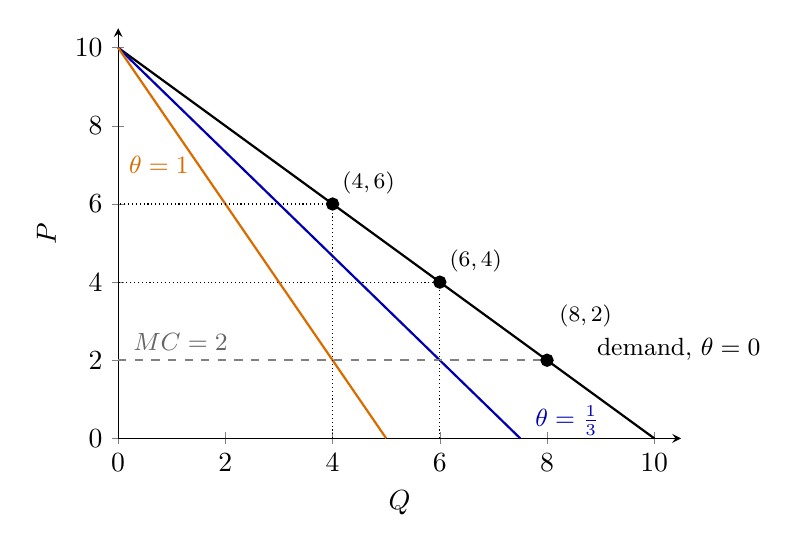
\begin{tikzpicture}
\begin{axis}[
  width=0.72\linewidth, height=0.56\linewidth,
  xmin=0, xmax=10.5, ymin=0, ymax=10.5,
  xlabel={$Q$}, ylabel={$P$},
  xtick={0,2,4,6,8,10}, ytick={0,2,4,6,8,10},
  axis lines=left, every axis plot/.append style={thick}, clip=false]
  \addplot[domain=0:10, samples=2, black] {10 - x};
  \node[anchor=south west, font=\small] at (axis cs:8.75,1.75) {demand, $\theta = 0$};
  \addplot[domain=0:7.5, samples=2, blue!70!black] {10 - (4/3)*x};
  \node[anchor=west, blue!70!black, font=\small] at (axis cs:7.6,0.45) {$\theta = \frac{1}{3}$};
  \addplot[domain=0:5, samples=2, orange!85!black] {10 - 2*x};
  \node[anchor=east, orange!85!black, font=\small] at (axis cs:1.5,7.0) {$\theta = 1$};
  \addplot[domain=0:8, samples=2, gray, dashed] {2};
  \node[anchor=south west, gray!80!black, font=\small] at (axis cs:0.1,2) {$MC = 2$};
  \addplot[only marks, mark=*, mark size=2pt] coordinates {(8,2) (6,4) (4,6)};
  \draw[densely dotted] (axis cs:6,0) -- (axis cs:6,4) -- (axis cs:0,4);
  \draw[densely dotted] (axis cs:4,0) -- (axis cs:4,6) -- (axis cs:0,6);
  \node[anchor=south west, font=\footnotesize] at (axis cs:8.05,2.6) {$(8, 2)$};
  \node[anchor=south west, font=\footnotesize] at (axis cs:6,4) {$(6, 4)$};
  \node[anchor=south west, font=\footnotesize] at (axis cs:4,6) {$(4, 6)$};
\end{axis}
\end{tikzpicture}
\caption{Perceived marginal revenue $10 - (1 + \theta)Q$ for demand $P = 10 - Q$ and $MC = 2$. Price taking
($\theta = 0$, perceived marginal revenue equal to demand) gives $Q = 8$ and $P = 2$. Conduct $\theta = \frac{1}{3}$,
as in a Stackelberg duopoly or a symmetric Cournot triopoly, gives $Q = 6$ and $P = 4$. Monopoly ($\theta = 1$)
gives $Q = 4$ and $P = 6$. In general $Q = \frac{8}{1 + \theta}$.}
\label{fig:02-perceived-mr}
\end{figure}

\subsection{Interpreting the conduct parameter}\label{sec:02-interpret}

\citet[Sec.~2.2]{Bresnahan1989} distinguishes three ways in which empirical work has used $\theta$.

The first takes $\theta$ from a single theory \citep[Sec.~2.2.1]{Bresnahan1989}. \citet{Rosse1970} estimates the
supply relation of monopoly newspapers ($\theta = 1$). His marginal revenue includes the effect of circulation on
advertising prices, and he infers marginal cost from $MR = MC$. Cournot models set $\tilde\theta_i = 1$
\citep[eq.~(6)]{Bresnahan1989}. Stackelberg and dominant-firm models give the leader the values derived above.
Dynamic theories of collusion imply a $\theta$ that switches between regimes, as in \citet{Porter1983}. In all these
cases the theory fixes the value or the pattern of $\theta$ before the data are consulted.

The second approach estimates the supply relations of a few distinct theories and tests them against each other
\citep[Sec.~2.2.2]{Bresnahan1989}. \citet{Bresnahan1987} compares joint-profit pricing with Bertrand pricing in the
automobile industry of the mid-1950s. He finds collusive behavior in some years and Bertrand behavior in 1955
(\cref{ch:discrete}). Bresnahan stresses that this approach differs from estimating a continuous $\theta$ only
econometrically. A continuous $\theta$ leads to nested tests, while a few discrete theories lead to non-nested tests.

The third approach treats $\theta$ as a continuous parameter described as a ``conjectural variation''
\citep[Sec.~2.2.3]{Bresnahan1989}. \citet{Iwata1974} used it to locate the Japanese plate-glass industry between
competition and monopoly. Since $\tilde\theta_i - 1 = r_i$ is an identity, saying what the conjectural variation is
and saying which oligopoly theory fits the data are the same statement \citep[p.~1027]{Bresnahan1989}.

\casehead{The critique of conjectural variations} Taken literally, a conjecture describes how a firm expects rivals
to react to a change in its output. In a simultaneous-move game nobody can react, so any nonzero conjecture is
inconsistent with the game being played. \emph{Consistent conjectures}, which require each conjecture to equal the
actual slope of rivals' responses, were one attempted repair \citep{Bresnahan1981a}. They keep the static framework
and have not become standard. \citet[pp.~1028--1029]{Bresnahan1989} offers a different reading. Collusive conduct
$\tilde\theta_i = N$ would literally mean that each firm expects rivals to match any output change one for one. In
repeated-game models firms produce the collusive output for another reason. They expect a deviation to trigger a
general breakdown of restraint. An estimated $\theta$ therefore describes what firms do. It does not reveal what they
believe would happen after a deviation. If $\theta$ is stable and breakdowns are rare, it measures the average collusiveness of
conduct. It tells us nothing about firms' expectations beyond the fact that they deter deviations
\citep[n.~19]{Bresnahan1989}.

A more basic problem is that an unrestricted $\theta$ explains everything.

\begin{proposition}[Exact fit]\label{prop:02-theta-fit}
Let $(P_{it}, Q_{it})$, with $Q_{it} > 0$, be data on prices and quantities. Take any demand system with slope
$\frac{\partial Q_{it}}{\partial P_{it}} < 0$ at each observation and any marginal cost function, with implied
values $mc_{it}$. Setting
\begin{equation*}
\theta_{it} = \frac{\left(P_{it} - mc_{it}\right)\left|\frac{\partial Q_{it}}{\partial P_{it}}\right|}{Q_{it}}
\end{equation*}
makes the supply relation
\[
P_{it} = mc_{it} + \theta_{it}\frac{Q_{it}}{\left|\frac{\partial Q_{it}}{\partial P_{it}}\right|}
\]
hold exactly at every observation, with no error term. The implied $\theta_{it}$ is nonnegative whenever
$mc_{it} \le P_{it}$.
\end{proposition}

\begin{proof}
Substituting the stated $\theta_{it}$ into the right side of the supply relation gives
\[
mc_{it} + \frac{(P_{it} - mc_{it})\left|\frac{\partial Q_{it}}{\partial P_{it}}\right|}{Q_{it}}
\cdot\frac{Q_{it}}{\left|\frac{\partial Q_{it}}{\partial P_{it}}\right|} = mc_{it} + (P_{it} - mc_{it}) = P_{it} . \qedhere
\]
\end{proof}

The supply relation has empirical content only through restrictions on $\theta$. The usual ones are that $\theta$ is
constant across observations or groups, or that $\theta \in [0, 1]$. Others fix $\theta$ at the value implied by a
specific game, or require deviations of $\theta$ to be uncorrelated with the instruments. Each restriction is an assumption, and
each objection to a conduct study is an objection to one of them. Imposing a functional form on marginal cost does not
help by itself, since the proposition holds for every cost function.

\casehead{The conduct parameter as a specification test} \citet[p.~1031]{Bresnahan1989} credits
\citet{Appelbaum1979} with a useful observation. Setting $\theta = 0$ in \eqref{eq:02-supply-relation} imposes price
taking. Every approach to conduct is therefore a test of price taking against alternatives with market power. A
cautious use of $\theta$ follows. We estimate it freely and test the hypotheses $\theta = 0$,
$\theta = \frac{1}{N}$ and $\theta = 1$, without reading $\hat\theta$ as a deep behavioral parameter. Even this use
requires care. If true conduct varies with demand, as in repeated-game models, an instrumental-variables estimate of a
constant $\theta$ measures how the markup responds to demand shifts. It need not equal average conduct, a point due to
\citet{Corts1999} and developed in \cref{ch:conduct}.

\casehead{Observed marginal cost} When marginal cost can be measured directly, \eqref{eq:02-theta-lerner} delivers
conduct observation by observation, $\theta_t = \varepsilon_t\frac{P_t - MC_t}{P_t}$, once demand is known. A known
cost structure serves a similar purpose. Fixed-proportions technology, for example, pins marginal cost down up to one
or two parameters, which can be estimated jointly with $\theta$. These are the strategies of \citet{Wolfram1999} for
electricity and \citet{GenesoveMullin1998} for sugar refining. Both compare the direct measure with the estimate a
researcher would obtain without cost data (\cref{ch:conduct}).

\subsection{Forward contracts}\label{sec:02-forward}

Contracts signed before the spot market opens change the spot-market incentive to raise price. The case matters for
electricity markets, where most output is often sold forward.

\begin{example}[Cournot with forward sales]\label{ex:02-forward}
Suppose firm $i$ has sold $x_i$ units forward at price $p^f$, before the spot market opens. Its spot-market profit is
\begin{equation*}
P(Q)\left(q_i - x_i\right) + p^f x_i - C_i(q_i) .
\end{equation*}
The forward revenue $p^f x_i$ is fixed, and only the uncontracted output $q_i - x_i$ earns the spot price. The Cournot
first-order condition is
\begin{equation*}
P(Q) + \left(q_i - x_i\right) P'(Q) = C_i'(q_i) .
\end{equation*}
Using $-P' = \frac{P}{\varepsilon Q}$ and dividing by $P$,
\begin{equation}\label{eq:02-forward-lerner}
\frac{P - C_i'(q_i)}{P} = \frac{q_i - x_i}{Q}\cdot\frac{1}{\varepsilon}
= \frac{s_i}{\varepsilon}\left(1 - \frac{x_i}{q_i}\right) .
\end{equation}
In conduct terms, $\tilde\theta_i = 1 - \frac{x_i}{q_i}$. A firm with 80 percent of its output under contract has
one fifth of the Cournot incentive to raise the spot price.
\end{example}

\citet{AllazVila1993} show that firms also have a strategic reason to sell forward. A forward sale commits a firm to
a higher spot output. Since quantities are strategic substitutes, rivals respond by producing less. Every firm has
this incentive, and together they end up in a prisoners' dilemma that lowers prices. In the linear duopoly with
$P = a - bQ$ and cost $c$, suppose arbitrage makes the forward price equal the spot price. The spot stage gives
$q_i = \frac{a - c + 2b x_i - b x_j}{3b}$ and $P - c = \frac{a - c - b(x_1 + x_2)}{3}$. Each firm then chooses $x_i$
to maximize $(P - c)\, q_i$. The first-order condition is $a - c - 4b x_i - b x_j = 0$, so the symmetric solution is
$x_i = \frac{a - c}{5b}$. Spot outputs are $q_i = \frac{2(a - c)}{5b}$, half of output is sold forward, and
$P - c = \frac{a - c}{5}$. Without a forward market, Cournot gives $P - c = \frac{a - c}{3}$. As a check,
\eqref{eq:02-forward-lerner} with $s_i = \frac{1}{2}$ and $\frac{x_i}{q_i} = \frac{1}{2}$ gives
$P - c = \frac{1}{4}\, b Q = \frac{a - c}{5}$. \Cref{ch:conduct} returns to contract cover in the British electricity
market.

\begin{remark}[Very inelastic demand]\label{rem:02-inelastic}
By \cref{prop:02-cowling-waterson}, Cournot firm $i$ has $L_i = \frac{s_i}{\varepsilon}$. With constant-elasticity
demand, an interior equilibrium requires $L_i < 1$, that is, $s_i < \varepsilon$. When market demand is very inelastic, as in electricity, the static
Cournot model predicts no interior equilibrium. Firms would withhold output until a capacity constraint binds. In such
markets prices are held down by something outside the static model. Capacity limits, regulatory threats, forward
contracts and the threat of entry are the usual candidates.
\end{remark}

\subsection{Pricing rules for the Bulow-Pfleiderer family}\label{sec:02-bp-rules}

The supply relation yields closed-form pricing rules for the demand family $Q(p) = B(\bar p - p)^{g}$ of
\cref{ex:02-bp}. With constant marginal cost $c$, the derivation has three steps.

First, compute $q\,P'(q)$. Since $P'(q) = \frac{1}{Q'(p)}$ and $Q'(p) = -gB(\bar p - p)^{g - 1}$,
\begin{equation*}
q\,P'(q) = \frac{Q(p)}{Q'(p)} = \frac{B(\bar p - p)^{g}}{-gB(\bar p - p)^{g - 1}} = -\frac{\bar p - p}{g} .
\end{equation*}
Second, substitute into $p + \theta q P'(q) = c$:
\begin{equation*}
p - \frac{\theta(\bar p - p)}{g} = c
\quad\Longrightarrow\quad
g p + \theta p = g c + \theta \bar p .
\end{equation*}
Third, solve for $p$:
\begin{equation}\label{eq:02-gm-rule}
P(c;\theta) = \frac{\theta\bar p + g c}{g + \theta} .
\end{equation}
Monopoly ($\theta = 1$) gives $P(c;1) = \frac{\bar p + gc}{1 + g}$, the rule of \cref{ex:02-bp}. Price taking
gives $P(c;0) = c$. The rule nests the other families as limits.
\begin{itemize}
\item Linear demand ($g = 1$) gives $P = \frac{\theta\bar p + c}{1 + \theta}$, and quadratic demand ($g = 2$)
  gives $P = \frac{\theta\bar p + 2c}{2 + \theta}$.
\item Constant elasticity ($\bar p = 0$ and $g = -\varepsilon < 0$) gives $P = \frac{gc}{g + \theta}
  = \frac{\varepsilon}{\varepsilon - \theta}\, c$, which requires $\varepsilon > \theta$.
\item In the exponential limit, $g$ and $\bar p$ grow without bound with $\frac{g}{\bar p} = \lambda_s$ fixed. Demand tends to
  $Q \propto e^{-\lambda_s p}$, with constant semi-elasticity $\lambda_s$. Since $\frac{\bar p - p}{g} =
  \frac{1}{\lambda_s} - \frac{p}{g} \to \frac{1}{\lambda_s}$, the rule becomes $P = c + \frac{\theta}{\lambda_s}$, a
  constant dollar markup.
\end{itemize}
The cost slope of \eqref{eq:02-gm-rule} is $\frac{\partial P}{\partial c} = \frac{g}{g + \theta}$, which depends on
conduct and curvature together (\cref{sec:02-passthrough}). The intercept $\frac{\theta\bar p}{g + \theta}$ moves
with the demand parameter $\bar p$. A season in which demand rotates, changing $\bar p$ or $g$, therefore shifts price
by an amount that rises with $\theta$ and vanishes at $\theta = 0$. \citet{GenesoveMullin1998} estimate exactly these rules for sugar refining and
use such a seasonal rotation to identify conduct (\cref{ch:conduct}).

\section{Pass-through}\label{sec:02-passthrough}

The previous sections characterized the level of the markup under each model of competition. Empirical work often
learns more from how prices move than from where they sit. When marginal cost rises by one dollar, by how much does
price rise? The answer, the pass-through rate, links
much of the empirical work in this book. Tax incidence, tests of conduct, the price effects of mergers and the
value of cost savings to consumers all depend on it. This section derives pass-through from the pricing
first-order conditions of \cref{sec:02-monopoly,sec:02-cournot,sec:02-conduct}. Pass-through depends on three
primitives: the curvature of demand, the slope of marginal cost and conduct. One pass-through number cannot
separate them, and much of the section makes that statement precise.

\subsection{Definition and uses}\label{sec:02-pt-uses}

\begin{definition}[Pass-through]\label{def:02-passthrough}
Let the equilibrium price $p$ of a market depend on a cost parameter $c$ that shifts marginal cost one for one.
The \emph{pass-through rate} is $\rho = \frac{\dd p}{\dd c}$. For a \emph{specific tax} $t$, a fixed amount per unit
sold, the pass-through rate is $\rho = \frac{\dd p}{\dd t}$. The \emph{pass-through elasticity} is
$\frac{\dd p}{\dd c}\frac{c}{p} = \rho\frac{c}{p}$. A cost shock is \emph{industry-wide} when it raises the marginal
cost of every firm by the same amount, and \emph{firm-specific} when it raises the marginal cost of one firm
only.
\end{definition}

A specific tax collected from sellers raises their effective marginal cost by $t$. A tax collected from buyers
is equivalent. If buyers pay the tax, demand at the seller price $p_s$ is $Q(p_s + t)$. A monopolist that
chooses $p_s$ to maximize $Q(p_s + t)(p_s - c)$ is choosing the consumer price $p = p_s + t$ to maximize
$Q(p)(p - c - t)$, which is the problem with a tax collected from sellers. The same change of variables works
for every model of conduct in this chapter. The side of the market that legally pays the tax is therefore
irrelevant. The pass-through of a specific tax equals the pass-through of an equal rise in marginal cost.
We use $c$ and $t$ interchangeably when marginal cost is constant.

Pass-through enters applied work in four ways. First, it determines the \emph{incidence} of a tax, the split of
its burden between consumers and producers (\cref{sec:02-pt-incidence}). Second, it governs how shocks to input
prices and exchange rates reach final prices. A pass-through elasticity of import prices below one with respect
to the exchange rate is the ``incomplete pass-through'' of international economics. Third, the pass-through of
an industry-wide cost shifter differs between competition and monopoly, so it can be used to test conduct.
\citet{Sumner1981} built such a test from state cigarette taxes, and \cref{ch:conduct} studies it in depth.
Fourth, merger analysis needs pass-through twice. A merger's cost savings reach consumers only through the
merged firm's pass-through. The upward pricing pressure of a merger is a shift in effective marginal cost, and
pass-through converts it into a price change (\cref{ch:mergers}).

\subsection{Monopoly with constant marginal cost}\label{sec:02-pt-monopoly}

We begin with a single price setter. The same results apply to any firm facing a residual demand curve with
rivals' actions held fixed (\cref{sec:02-residual}).

\begin{assumption}[Monopoly pass-through]\label{ass:02-pt-monopoly}
A monopolist faces demand $Q(p)$, twice continuously differentiable with $Q'(p) < 0$, and has constant marginal
cost $c$. For every $c$ in an open interval $I$, profit $Q(p)(p - c)$ has a unique global maximizer $p^m(c)$,
which is interior, and $p^m$ is continuous on $I$. The maximizer satisfies the first-order condition
\eqref{eq:02-foc-monopoly}, $Q'(p)(p - c) + Q(p) = 0$, and the strict second-order condition $(p - c)Q''(p) +
2Q'(p) < 0$.
\end{assumption}

The strict second-order condition is the nonsingularity condition of the implicit function theorem
(\cref{app:math}). Through each $p^m(c)$ it yields a continuously differentiable local branch of solutions to the
first-order condition, and that branch is locally the only solution. Continuity of $p^m$ keeps the maximizer on
this branch. Hence $p^m(c)$ is continuously differentiable, and its derivative follows from differentiating the
first-order condition. Uniqueness implies continuity when the maximizers lie in a fixed compact set of prices. By
Berge's maximum theorem, a unique maximizer of a continuous objective over a fixed compact set moves continuously
with a parameter. Neither property follows from the local conditions alone. Profit can have two strict global
maximizers at one cost, and the optimal price then jumps from one to the other as $c$ crosses that cost. In such
cases the results below hold on each branch, away from the switching points.

The sign of the derivative is known before we compute it.
\Cref{lem:02-monotone} shows by revealed preference that the monopoly price never falls when $c$ rises, for any
demand curve. Smoothness adds the rate.

\begin{proposition}[Monopoly pass-through]\label{prop:02-pt-monopoly}
Under \cref{ass:02-pt-monopoly}, at $p = p^m(c)$,
\begin{equation}\label{eq:02-pt-monopoly}
\rho = \frac{\dd p^m}{\dd c} = \frac{Q'(p)}{(p - c)Q''(p) + 2Q'(p)} > 0 .
\end{equation}
\end{proposition}

\begin{proof}
Write the first-order condition as an identity in $c$:
\begin{equation*}
Q'\bigl(p(c)\bigr)\bigl(p(c) - c\bigr) + Q\bigl(p(c)\bigr) \equiv 0 .
\end{equation*}
Differentiate each piece with respect to $c$, writing $\rho = p'(c)$:
\begin{align*}
\frac{\dd}{\dd c}\, Q'\bigl(p(c)\bigr) &= Q''(p)\,\rho , \\
\frac{\dd}{\dd c}\, \bigl(p(c) - c\bigr) &= \rho - 1 , \\
\frac{\dd}{\dd c}\, Q\bigl(p(c)\bigr) &= Q'(p)\,\rho .
\end{align*}
The product rule applied to the first term of the identity gives $Q''\rho(p - c) + Q'(\rho - 1)$. Adding the
derivative of the second term,
\begin{equation*}
(p - c)Q''\rho + Q'(\rho - 1) + Q'\rho = 0 .
\end{equation*}
Collect the terms in $\rho$:
\begin{equation*}
\rho\bigl[(p - c)Q'' + 2Q'\bigr] = Q' .
\end{equation*}
Dividing by the bracket gives \eqref{eq:02-pt-monopoly}. The numerator $Q'$ is negative, and the bracket is
negative by the second-order condition, so $\rho > 0$.
\end{proof}

Formula \eqref{eq:02-pt-monopoly} has three equivalent forms. Each one gives a different reading of what drives
pass-through.

\casehead{Log-curvature form}
The first-order condition gives $p - c = -\frac{Q}{Q'}$. Substituting into the denominator of
\eqref{eq:02-pt-monopoly},
\begin{equation*}
(p - c)Q'' + 2Q' = -\frac{QQ''}{Q'} + 2Q' .
\end{equation*}
Dividing the numerator and the denominator of \eqref{eq:02-pt-monopoly} by $Q'$ gives
\begin{equation}\label{eq:02-pt-logcurv}
\rho = \frac{1}{2 - \frac{Q(p)\,Q''(p)}{Q'(p)^2}} .
\end{equation}
The ratio $\frac{QQ''}{(Q')^2}$ is a unit-free measure of the convexity of demand. It is zero for linear demand.

\casehead{Markup-slope form}
Let $m(p) = -\frac{Q(p)}{Q'(p)}$ be the dollar markup that the demand curve supports at price $p$, as in
\eqref{eq:02-dollar-markup}. The first-order condition reads $p - c = m(p)$. Differentiating with respect to $c$
gives $\rho - 1 = m'(p)\rho$, so
\begin{equation}\label{eq:02-pt-markup}
\rho = \frac{1}{1 - m'(p)} .
\end{equation}
The quotient rule gives $m'(p) = -\frac{(Q')^2 - QQ''}{(Q')^2} = -1 + \frac{QQ''}{(Q')^2}$, so
$1 - m'(p) = 2 - \frac{QQ''}{(Q')^2}$, in agreement with \eqref{eq:02-pt-logcurv}. The reciprocal $\frac{1}{m}
= -\frac{Q'}{Q}$ is the semi-elasticity of demand from \cref{sec:02-monopoly-foc}.
When the semi-elasticity rises with price, the supported markup falls ($m' < 0$), and the monopolist absorbs part
of any cost increase. When the semi-elasticity falls with price, the markup rises with price ($m' > 0$), and the
price rises by more than cost.

\casehead{Quantity-space form}
A monopolist choosing output $q$ against inverse demand $P(q)$ sets marginal revenue equal to marginal cost,
$P(q) + qP'(q) = c$. Recall from \cref{rem:02-c2} the curvature of inverse demand,
\begin{equation}\label{eq:02-chi}
\chi(q) = -\frac{qP''(q)}{P'(q)} .
\end{equation}
It is zero for linear inverse demand, positive when inverse demand is convex and negative when it is concave.
Differentiating the marginal-revenue condition with respect to $c$,
\begin{equation*}
\bigl[2P'(q) + qP''(q)\bigr]\frac{\dd q}{\dd c} = 1 .
\end{equation*}
The price moves along the inverse demand curve, so
\begin{equation}\label{eq:02-pt-quantity}
\rho = P'(q)\frac{\dd q}{\dd c} = \frac{P'}{2P' + qP''} = \frac{1}{2 + \frac{qP''}{P'}} = \frac{1}{2 - \chi(q)} .
\end{equation}
The second-order condition in quantity space is $2P' + qP'' < 0$. Dividing by $P' < 0$ shows that it is
equivalent to $\chi < 2$, which again makes $\rho$ positive.

The log-curvature form and the quantity-space form agree because the two curvature measures coincide.

\begin{lemma}[Curvature of direct and inverse demand]\label{lem:02-chi-direct}
Let $P$ be the inverse of a twice differentiable demand function $Q$ with $Q' < 0$. At every point on the demand
curve, $\chi = \frac{QQ''}{(Q')^2}$, and $\frac{\dd^2 \ln Q(p)}{\dd p^2} < 0$ if and only if $\chi < 1$.
\end{lemma}

\begin{proof}
Differentiate the identity $P(Q(p)) = p$ once to get $P'Q' = 1$, so $P' = \frac{1}{Q'}$. Differentiate it again
to get $P''(Q')^2 + P'Q'' = 0$, so $P'' = -\frac{P'Q''}{(Q')^2} = -\frac{Q''}{(Q')^3}$. Then
\begin{equation*}
\chi = -\frac{Q\,P''}{P'} = -Q\cdot\Bigl(-\frac{Q''}{(Q')^3}\Bigr)\cdot Q' = \frac{QQ''}{(Q')^2} .
\end{equation*}
For the second claim, $\frac{\dd^2\ln Q}{\dd p^2} = \frac{\dd}{\dd p}\frac{Q'}{Q} = \frac{QQ'' - (Q')^2}{Q^2}$. This is
negative if and only if $QQ'' < (Q')^2$, that is, if and only if $\chi < 1$.
\end{proof}

\begin{corollary}[\citealp{BulowPfleiderer1983}]\label{cor:02-bulow-pfleiderer}
Under \cref{ass:02-pt-monopoly}, monopoly pass-through at $p^m(c)$ satisfies $\rho < 1$ if demand is strictly
log-concave there, $\rho = 1$ if $\ln Q$ is locally linear, and $\rho > 1$ if demand is strictly log-convex.
Linear demand has $\rho = \frac{1}{2}$.
\end{corollary}

\begin{proof}
By \eqref{eq:02-pt-quantity} and \cref{lem:02-chi-direct}, $\rho = \frac{1}{2 - \chi}$ with $2 - \chi > 0$. So
$\rho < 1$ if and only if $2 - \chi > 1$, that is $\chi < 1$, which is strict log-concavity. The other two cases
follow in the same way. Linear demand has $Q'' = 0$, so $\chi = 0$ and $\rho = \frac{1}{2}$.
\end{proof}

Log-concavity is the same property as a semi-elasticity that rises with price, since
$\frac{\dd^2 \ln Q}{\dd p^2} = \frac{\dd}{\dd p}\frac{Q'}{Q}$. The corollary therefore restates the markup-slope form: a
monopolist passes through less than the full cost increase exactly when higher prices make its customers more
price sensitive at the margin.

\begin{remark}[Pass-through and the distribution of willingness to pay]\label{rem:02-pt-hazard}
Suppose each of $M$ consumers buys one unit if her willingness to pay $v$ exceeds the price, with $v$ drawn from a
distribution $G$ with density $G'$. Demand is $Q(p) = M[1 - G(p)]$, as in \cref{sec:02-monopoly-foc}, and the
supported markup is $m(p) = \frac{1 - G(p)}{G'(p)} = \frac{1}{h(p)}$, where $h = \frac{G'}{1 - G}$ is the hazard rate
of $G$. The
first-order condition reads $p - c = \frac{1}{h(p)}$. Since $m' = -\frac{h'}{h^2}$, \eqref{eq:02-pt-markup} gives
\begin{equation*}
\rho = \frac{1}{1 + \frac{h'(p)}{h(p)^2}} .
\end{equation*}
Pass-through is below one exactly when the hazard rate rises at $p^m$. A uniform distribution on $[0, \bar v]$ has
$h = \frac{1}{\bar v - p}$ and $h' = h^2$, which gives linear demand and $\rho = \frac{1}{2}$. An exponential
distribution has a constant hazard and $\rho = 1$. A Pareto distribution, $1 - G(v) = (\frac{v_0}{v})^{\varepsilon}$
for $v \ge v_0$, has $h = \frac{\varepsilon}{v}$ and $\frac{h'}{h^2} = -\frac{1}{\varepsilon}$. It gives
constant-elasticity demand and $\rho = \frac{\varepsilon}{\varepsilon - 1} > 1$. The normal and logistic
distributions have increasing hazard rates. With standard normal willingness to pay and $c = 0$, for example,
$p^m \approx 0.75$ and $\rho \approx 0.70$. Pass-through above one therefore requires a hazard rate that falls
at the monopoly price, as in thick-tailed distributions such as the Pareto.
\end{remark}

\begin{example}[Five demand curves]\label{ex:02-pt-examples}
We compute the curvature $\chi$ and monopoly pass-through for five demand curves. Each case also gives
pass-through under constant conduct $\theta$ with constant marginal cost, using the supply relation
$P + \theta QP'(Q) = c$ of \eqref{eq:02-supply-relation}. \Cref{tab:02-pt-examples} collects the results. Cases
(ii), (iii) and (iv) are the three demand curves of \citet[Exercise~1.3]{Tirole1988}. Case (i) is the linear
member of case (ii). Tirole uses them to frame the critique by \citet{BulowPfleiderer1983} of the tax test of
\citet{Sumner1981}.

(i) \emph{Linear demand}, $P = a - bQ$ with $a > c$ and $b > 0$. Then $P' = -b$, $P'' = 0$ and $\chi = 0$, so
$\rho = \frac{1}{2}$. Directly, $a - 2bQ = c$ gives $Q^m = \frac{a - c}{2b}$ and $p^m = \frac{a + c}{2}$. Under
conduct $\theta$, the supply relation is $a - bQ - \theta bQ = c$, so
\begin{equation*}
Q = \frac{a - c}{b(1 + \theta)}, \qquad P = a - \frac{a - c}{1 + \theta} = \frac{\theta a + c}{1 + \theta},
\qquad \rho = \frac{1}{1 + \theta} .
\end{equation*}

(ii) \emph{The power family}, $P = a - bQ^{\gamma}$ with $b\gamma > 0$ so that demand slopes down. Then
$P' = -b\gamma Q^{\gamma - 1}$ and $P'' = -b\gamma(\gamma - 1)Q^{\gamma - 2}$, so
$\chi = -\frac{QP''}{P'} = 1 - \gamma$. The second-order condition $\chi < 2$ requires $\gamma > -1$. Monopoly
pass-through is $\rho = \frac{1}{1 + \gamma}$. Directly, marginal revenue is $a - (1 + \gamma)bQ^{\gamma}$, and
substituting $bQ^{\gamma} = a - P$ gives $MR = (1 + \gamma)P - \gamma a$. Setting $MR = c$,
\begin{equation*}
p^m = \frac{\gamma a + c}{1 + \gamma} .
\end{equation*}
Under conduct $\theta$, $\theta QP' = -\theta\gamma bQ^{\gamma} = -\theta\gamma(a - P)$, so the supply relation
becomes $P(1 + \theta\gamma) = c + \theta\gamma a$, and
\begin{equation*}
P = \frac{\theta\gamma a + c}{1 + \theta\gamma}, \qquad \rho = \frac{1}{1 + \theta\gamma} .
\end{equation*}
This is the family $Q = B\lvert\bar p - p\rvert^{g}$ of \cref{ex:02-bp}, with $a = \bar p$ and $\gamma =
\frac{1}{g}$. The coefficient is $b = B^{-\frac{1}{g}}$ on the branch $g > 0$, where $p < \bar p$, and $b =
-B^{-\frac{1}{g}}$ on the branch $g < 0$, where $p > \bar p$. In that notation $\rho = \frac{g}{g + \theta}$, the slope of the pricing rule
\eqref{eq:02-gm-rule}. Linear demand is $\gamma = 1$. Quadratic demand ($g = 2$) has $\gamma = \frac{1}{2}$,
$\chi = \frac{1}{2}$ and monopoly pass-through $\frac{2}{3}$.

(iii) \emph{Constant elasticity}, $Q = Ap^{-\varepsilon}$ with $\varepsilon > 1$, so $P = (\frac{Q}{A})^{-\frac{1}{\varepsilon}}$.
This is the power family with $a = 0$, $\gamma = -\frac{1}{\varepsilon}$ and $b = -A^{\frac{1}{\varepsilon}}$.
Hence $\chi = 1 + \frac{1}{\varepsilon}$ and $\rho = \frac{1}{1 - \frac{1}{\varepsilon}} = \frac{\varepsilon}{\varepsilon - 1}$.
Directly, the Lerner rule gives $p^m = \frac{\varepsilon}{\varepsilon - 1}c$. Under conduct $\theta$, the Lerner
form \eqref{eq:02-theta-lerner} gives $P(1 - \frac{\theta}{\varepsilon}) = c$, so
\begin{equation*}
P = \frac{\varepsilon}{\varepsilon - \theta}\,c, \qquad \rho = \frac{\varepsilon}{\varepsilon - \theta}
= \Bigl(1 - \frac{\theta}{\varepsilon}\Bigr)^{-1}, \qquad \theta < \varepsilon .
\end{equation*}
The price is a fixed multiple of cost, so the pass-through elasticity equals one for every $\theta$ although
$\rho > 1$.

(iv) \emph{Exponential demand}, $Q = e^{\frac{a - p}{b}}$ with $b > 0$, so $P = a - b\ln Q$. Then
$P' = -\frac{b}{Q}$, $P'' = \frac{b}{Q^2}$ and $\chi = 1$. The supply relation is $P - \theta b = c$, so
$P = c + \theta b$ and $\rho = 1$ for every $\theta$. The dollar markup $\theta b$ does not depend on cost. A
monopolist facing this demand curve passes through exactly one, as a competitive industry with flat marginal cost
does. The case is the limit of the power family as $\gamma \to 0$. Take the member of the family with
intercept $a_0 + \frac{b}{\gamma}$ and coefficient $\frac{b}{\gamma}$ on $Q^{\gamma}$. Its inverse demand is
$a_0 - b\frac{Q^{\gamma} - 1}{\gamma}$, which converges to $a_0 - b\ln Q$ because
$\frac{Q^{\gamma} - 1}{\gamma} \to \ln Q$. Its pass-through $\frac{1}{1 + \theta\gamma}$ converges to one.

(v) \emph{Logit residual demand}. A single-product firm $j$ with logit demand has market share
\begin{equation*}
s_j(p_j) = \frac{e^{\delta_j - \alpha p_j}}{1 + \sum_{k \in \mathcal{J}} e^{\delta_k - \alpha p_k}}
\end{equation*}
(\cref{ch:logit}). Here $\delta_j$ is the part of product $j$'s mean utility that does not depend on price,
and $\alpha > 0$ is the price coefficient. The set of inside products is $\mathcal{J}$, and the outside good's
utility is normalized to zero. Hold rivals' prices fixed and drop the subscript $j$. Differentiating,
$s' = -\alpha s(1 - s)$, and $s'' = -\alpha s'(1 - 2s) = \alpha^2 s(1 - s)(1 - 2s)$. The first-order condition
gives $p - c = -\frac{s}{s'} = \frac{1}{\alpha(1 - s)}$. Market size cancels from \eqref{eq:02-pt-monopoly}.
The two pieces of its denominator are
\begin{equation*}
(p - c)s'' = \frac{\alpha^2 s(1 - s)(1 - 2s)}{\alpha(1 - s)} = \alpha s(1 - 2s), \qquad 2s' = -2\alpha s(1 - s) .
\end{equation*}
Their sum is $\alpha s(1 - 2s - 2 + 2s) = -\alpha s$. Therefore
\begin{equation*}
\rho = \frac{-\alpha s(1 - s)}{-\alpha s} = 1 - s .
\end{equation*}
By \cref{lem:02-chi-direct}, the curvature is $\chi = \frac{ss''}{(s')^2} = \frac{1 - 2s}{1 - s} < 1$. Logit
residual demand is log-concave, and a firm with a 30 percent share passes through 70 percent of an own-cost
increase when rivals do not respond. The share falls as $c$ rises, so pass-through rises with cost. Rivals'
responses raise pass-through further (\cref{ch:diffprod,ch:mergers}).
\end{example}

\begin{table}[htbp]
\centering
\caption{Curvature and pass-through for common demand curves}
\label{tab:02-pt-examples}
\begin{threeparttable}
\begin{tabular}{@{}llccc@{}}
\toprule
Demand & Specification & Curvature $\chi$ & Monopoly $\rho$ & $\rho$ under conduct $\theta$ \\
\midrule
Linear & $P = a - bQ$ & $0$ & $\frac{1}{2}$ & $\frac{1}{1 + \theta}$ \\[4pt]
Power family & $P = a - bQ^{\gamma}$, $b\gamma > 0$ & $1 - \gamma$ & $\frac{1}{1 + \gamma}$ &
  $\frac{1}{1 + \theta\gamma} = \frac{g}{g + \theta}$ \\[4pt]
Constant elasticity & $Q = Ap^{-\varepsilon}$ & $1 + \frac{1}{\varepsilon}$ & $\frac{\varepsilon}{\varepsilon - 1}$ &
  $\frac{\varepsilon}{\varepsilon - \theta}$ \\[4pt]
Exponential & $P = a - b\ln Q$ & $1$ & $1$ & $1$ \\[4pt]
Logit, rivals fixed & $s(p)$, share $s$ & $\frac{1 - 2s}{1 - s}$ & $1 - s$ & n.a. \\
\bottomrule
\end{tabular}
\begin{tablenotes}[flushleft]
\footnotesize
\item Notes: Constant marginal cost. Curvature is $\chi = -\frac{QP''}{P'}$. Monopoly pass-through is
$\frac{1}{2 - \chi}$ by \eqref{eq:02-pt-quantity}. The last column uses the supply relation
$P + \theta QP' = c$ and equals $\frac{1}{1 + \theta(1 - \chi)}$ by \eqref{eq:02-pt-flat}. In the power family
$g = \frac{1}{\gamma}$ is the exponent of $Q = B\lvert\bar p - p\rvert^{g}$. Constant elasticity is the power family with
$a = 0$ and $\gamma = -\frac{1}{\varepsilon}$, and exponential demand is its limit as $\gamma \to 0$. The logit
row is the residual demand of a single-product price setter with rivals' prices held fixed, for which an
industry conduct parameter is not defined.
\end{tablenotes}
\end{threeparttable}
\end{table}

In four of the five rows pass-through does not vary with cost. This is no accident, as the next result shows.

\begin{proposition}[Constant pass-through]\label{prop:02-pt-constant}
Let a monopolist with constant marginal cost face inverse demand $P(Q)$ satisfying \cref{ass:02-pt-monopoly}.
If $P = a - bQ^{\gamma}$ with $b\gamma > 0$ and $\gamma > -1$, monopoly pass-through equals
$\frac{1}{1 + \gamma}$ at every cost. If $P = a - b\ln Q$ with $b > 0$, it equals one at every cost. Conversely,
suppose pass-through equals a constant $\rho$ for all $c$ in an interval. Then on the corresponding interval of
outputs inverse demand has one of these forms, with $\gamma = \frac{1}{\rho} - 1$ \citep{BulowPfleiderer1983}.
\end{proposition}

\begin{proof}
For the power family, example (ii) gives $\chi = 1 - \gamma$ at every output, so \eqref{eq:02-pt-quantity}
gives $\rho = \frac{1}{2 - (1 - \gamma)} = \frac{1}{1 + \gamma}$ whatever the cost. The condition
$\gamma > -1$ is the second-order condition $\chi < 2$. For logarithmic inverse demand, example (iv) gives
$\chi = 1$ and $\rho = 1$ at every output.

For the converse, monopoly output is continuous and strictly decreasing in $c$, because
$\frac{\dd q}{\dd c} = \frac{1}{2P' + qP''} < 0$. A constant $\rho$ on an interval of costs therefore means, by
\eqref{eq:02-pt-quantity}, that $\chi(Q) = 2 - \frac{1}{\rho}$ on an interval of outputs. That condition is the
differential equation $QP''(Q) = -\bigl(2 - \frac{1}{\rho}\bigr)P'(Q)$. The equation is first-order and linear in
$\ln\lvert P'\rvert$, and solving it is left as an exercise (\cref{sec:02-exercises}).
\end{proof}

The constant-elasticity case sits inside the power family with $a = 0$ and $\gamma \in (-1, 0)$, and the
logarithmic case is its limit as $\gamma \to 0$. Pass-through under constant conduct also depends on demand only
through $\chi$, as \cref{sec:02-pt-general} shows. The power family therefore has constant pass-through under
every constant conduct. \citet{GenesoveMullin1998} use it to estimate conduct in sugar refining
(\cref{ch:conduct}). Linear and log-linear demand impose restrictive monopoly pricing rules, and most variation in
that industry comes from costs. The power family nests the linear, quadratic and log-linear forms, and the
exponential form as a limit. It lets them check whether the choice of functional form drives the estimate of
conduct.
Outside this family pass-through varies with cost, and a linear regression of price on a cost
shifter estimates an average of $\rho$ over the sample.

\Cref{fig:02-pt-examples} draws the monopoly price as a function of marginal cost for three demand curves. The
slopes are the constant pass-through rates of linear, constant-elasticity and exponential demand.

\begin{figure}[htbp]
\centering
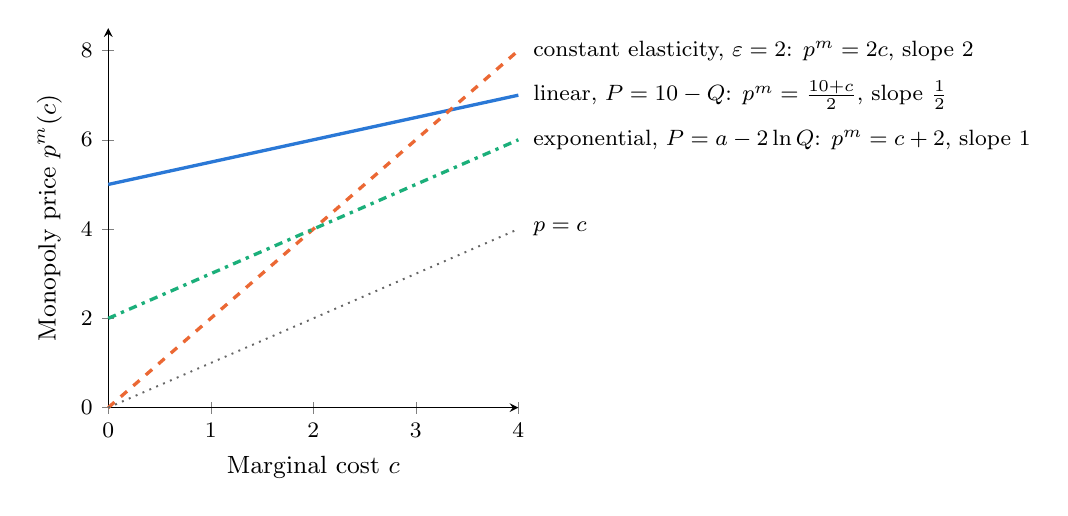
\begin{tikzpicture}
\definecolor{ptA}{HTML}{2A78D6}
\definecolor{ptB}{HTML}{EB6834}
\definecolor{ptC}{HTML}{1BAF7A}
\begin{axis}[
  width=0.56\textwidth, height=6.4cm,
  xmin=0, xmax=4, ymin=0, ymax=8.5,
  xlabel={Marginal cost $c$}, ylabel={Monopoly price $p^m(c)$},
  xtick={0,1,2,3,4}, ytick={0,2,4,6,8},
  tick label style={font=\footnotesize}, label style={font=\small},
  axis lines=left, clip=false, every axis plot/.append style={line width=1.2pt}]
  \addplot[domain=0:4, samples=2, color=ptA] {(10 + x)/2};
  \addplot[domain=0:4, samples=2, color=ptB, dashed] {2*x};
  \addplot[domain=0:4, samples=2, color=ptC, dash dot] {x + 2};
  \addplot[domain=0:4, samples=2, color=black!60, line width=0.7pt, dotted] {x};
  \node[anchor=west, font=\footnotesize, align=left] at (axis cs:4.05,8.0)
    {constant elasticity, $\varepsilon = 2$: $p^m = 2c$, slope $2$};
  \node[anchor=west, font=\footnotesize, align=left] at (axis cs:4.05,7.0)
    {linear, $P = 10 - Q$: $p^m = \frac{10 + c}{2}$, slope $\frac{1}{2}$};
  \node[anchor=west, font=\footnotesize, align=left] at (axis cs:4.05,6.0)
    {exponential, $P = a - 2\ln Q$: $p^m = c + 2$, slope $1$};
  \node[anchor=west, font=\footnotesize, align=left] at (axis cs:4.05,4.0)
    {$p = c$};
\end{axis}
\end{tikzpicture}
\caption{Monopoly price as a function of constant marginal cost for three demand curves. Linear demand
($a = 10$, $b = 1$) passes through one half of a cost change, exponential demand ($b = 2$) passes through all
of it, and constant-elasticity demand ($\varepsilon = 2$) passes through twice the change. The dotted line is
price equal to cost.}
\label{fig:02-pt-examples}
\end{figure}

\subsection{Conduct, curvature and rising marginal cost}\label{sec:02-pt-general}

We now allow imperfect competition of any degree and marginal cost that rises with output. The industry
satisfies the supply relation \eqref{eq:02-supply-relation} with conduct $\theta$, and a specific tax $t$ adds to
marginal cost. Write the supply relation with the \emph{marginal consumer surplus}
\begin{equation}\label{eq:02-ms}
ms(Q) = -QP'(Q) \ge 0 .
\end{equation}
The name comes from consumer surplus $CS(Q) = \int_0^Q P(x)\,\dd x - QP(Q)$, whose derivative is
$P - P - QP' = ms(Q)$. It is the gain in consumer surplus from one more unit of output. The supply relation then
reads $P(Q) - \theta\, ms(Q) = MC(Q) + t$: the markup equals conduct times the marginal consumer surplus. A
monopolist ($\theta = 1$) keeps its markup equal to the surplus it would hand to inframarginal consumers by
expanding.

\begin{assumption}[Pass-through under conduct]\label{ass:02-pt-general}
Inverse demand $P(Q)$ is twice continuously differentiable with $P' < 0$. Industry marginal cost $MC(Q)$ is
continuously differentiable with $MC' \ge 0$. Conduct $\theta \in [0, 1]$ does not vary with $t$. Equilibrium
output $Q(t)$ is positive, is continuous in $t$, and satisfies
\begin{equation}\label{eq:02-pt-supply}
P(Q) + \theta QP'(Q) = MC(Q) + t ,
\end{equation}
together with the stability condition
$\Lambda(Q) \equiv P'(Q) - \theta\, ms'(Q) - MC'(Q) < 0$.
\end{assumption}

As in \cref{ass:02-pt-monopoly}, the stability condition is the nonsingularity condition of the implicit function
theorem, and continuity keeps $Q(t)$ on one local branch of solutions. Hence $Q(t)$ is continuously differentiable.
The stability condition says that perceived marginal revenue $P - \theta\, ms$ cuts effective marginal cost from
above. It holds under monopoly by the second-order condition, and under symmetric Cournot competition by
\cref{ass:02-cournot} (see the proof of \cref{prop:02-pt-cournot}). Three elasticities summarize the primitives at the equilibrium. The demand elasticity is
$\varepsilon = -\frac{P}{QP'}$. The supply elasticity $\varepsilon_S = \frac{MC + t}{Q\, MC'}$ is the elasticity
of output with respect to effective marginal cost along the marginal-cost curve, and it is infinite when marginal
cost is flat. The term $\varepsilon_{ms} = \frac{ms}{Q\, ms'}$ is the elasticity of the inverse marginal-surplus
function, the reciprocal of the elasticity of $ms$ with respect to output \citep[p.~539]{WeylFabinger2013}.
Differentiating \eqref{eq:02-ms},
\begin{equation*}
ms'(Q) = -P'(Q) - QP''(Q) = -P'(Q)\Bigl(1 + \frac{QP''}{P'}\Bigr) = -P'(Q)\,(1 - \chi) ,
\end{equation*}
so $\frac{1}{\varepsilon_{ms}} = \frac{Q\,ms'}{ms} = \frac{-QP'(1 - \chi)}{-QP'} = 1 - \chi$. Exponential demand has
$\chi = 1$, a constant marginal consumer surplus, and $\frac{1}{\varepsilon_{ms}} = 0$.

\begin{proposition}[Pass-through under conduct, \citealp{WeylFabinger2013}]\label{prop:02-pt-general}
Under \cref{ass:02-pt-general},
\begin{equation}\label{eq:02-pt-general}
\rho = \frac{\dd P}{\dd t} = \frac{1}{1 + \frac{\varepsilon - \theta}{\varepsilon_S} + \frac{\theta}{\varepsilon_{ms}}}
= \frac{1}{1 + \theta(1 - \chi) + \frac{\varepsilon - \theta}{\varepsilon_S}} ,
\end{equation}
and the denominator is positive.
\end{proposition}

\begin{proof}
\emph{Step 1.} Differentiate $P(Q) - \theta\, ms(Q) = MC(Q) + t$ with respect to $t$:
\begin{equation*}
\bigl[P'(Q) - \theta\, ms'(Q)\bigr]\frac{\dd Q}{\dd t} = MC'(Q)\frac{\dd Q}{\dd t} + 1 .
\end{equation*}
Collecting terms gives $\Lambda\frac{\dd Q}{\dd t} = 1$, so $\frac{\dd Q}{\dd t} = \frac{1}{\Lambda} < 0$.

\emph{Step 2.} The price moves along the demand curve, so
\begin{equation*}
\rho = P'(Q)\frac{\dd Q}{\dd t} = \frac{P'}{P' - \theta\, ms' - MC'} = \frac{1}{1 - \theta\frac{ms'}{P'} - \frac{MC'}{P'}} .
\end{equation*}

\emph{Step 3.} The demand term is $-\frac{ms'}{P'} = 1 - \chi = \frac{1}{\varepsilon_{ms}}$ by the computation
above.

\emph{Step 4.} For the cost term, the definitions of the two elasticities give
$MC' = \frac{MC + t}{Q\varepsilon_S}$ and $\lvert P'\rvert = \frac{P}{\varepsilon Q}$. Hence
\begin{equation*}
-\frac{MC'}{P'} = \frac{MC'}{\lvert P'\rvert} = \frac{MC + t}{Q\varepsilon_S}\cdot\frac{\varepsilon Q}{P}
= \frac{\varepsilon}{\varepsilon_S}\cdot\frac{MC + t}{P} .
\end{equation*}

\emph{Step 5.} The Lerner form of \eqref{eq:02-pt-supply} is $\frac{P - MC - t}{P} = \frac{\theta}{\varepsilon}$,
as in \eqref{eq:02-theta-lerner}, so $\frac{MC + t}{P} = \frac{\varepsilon - \theta}{\varepsilon}$. Substituting into
Step 4 gives $-\frac{MC'}{P'} = \frac{\varepsilon - \theta}{\varepsilon_S}$.

\emph{Step 6.} Steps 2 to 5 give \eqref{eq:02-pt-general}. The denominator equals $\frac{\Lambda}{P'}$, a ratio
of two negative numbers, so it is positive.
\end{proof}

Step 2 has a geometric reading. With flat marginal cost, pass-through is the slope of inverse demand divided by
the slope of perceived marginal revenue, $\frac{P'}{P'(1 + \theta(1 - \chi))}$. A tax shifts the effective
marginal cost line up by $t$. Output falls until perceived marginal revenue has risen by $t$, and price rises by
the demand slope times the output change. When perceived marginal revenue is steep relative to demand, a small
output cut absorbs the tax and price rises little. Under exponential demand, marginal consumer surplus is constant, so
perceived marginal revenue is parallel to demand and price rises one for one. With rising marginal cost,
effective marginal cost also falls as output contracts. A smaller output cut then restores the supply relation,
and price rises less under every conduct.

\citet[eq.~(2), p.~548]{WeylFabinger2013} derive \eqref{eq:02-pt-general} for symmetric imperfect competition
and extend it to conduct that varies with output. Their denominator adds the term $\frac{\theta}{\varepsilon_\theta}
= Q\,\theta'(Q)$, where $\varepsilon_\theta = \frac{\theta}{Q\,\theta'(Q)}$ is the inverse of the elasticity of
conduct with respect to output. The version here assumes constant $\theta$, so this term vanishes.

\begin{corollary}[Special cases]\label{cor:02-pt-cases}
Under \cref{ass:02-pt-general}:
\begin{enumerate}[label=(\roman*)]
\item Price taking ($\theta = 0$) gives $\rho = \frac{\varepsilon_S}{\varepsilon_S + \varepsilon} \le 1$, with
  equality if and only if marginal cost is flat.
\item Flat marginal cost ($\varepsilon_S = \infty$) gives
  \begin{equation}\label{eq:02-pt-flat}
  \rho = \frac{1}{1 + \theta(1 - \chi)} .
  \end{equation}
\item Monopoly with flat marginal cost gives $\rho = \frac{1}{2 - \chi}$, which is \cref{prop:02-pt-monopoly}.
\item Symmetric Cournot competition among $N$ firms with flat marginal cost gives
  $\rho = \frac{N}{N + 1 - \chi}$. Linear demand gives $\frac{N}{N + 1}$, and constant elasticity gives
  $\frac{N\varepsilon}{N\varepsilon - 1} > 1$.
\item Monopoly with linear demand $P = a - bQ$ and linear marginal cost $MC = c_0 + kQ$ gives
  $\rho = \frac{b}{2b + k}$.
\end{enumerate}
\end{corollary}

\begin{proof}
(i) Setting $\theta = 0$ in \eqref{eq:02-pt-general} gives
$\rho = \frac{1}{1 + \frac{\varepsilon}{\varepsilon_S}} = \frac{\varepsilon_S}{\varepsilon_S + \varepsilon}$. The
same answer follows directly. A competitive industry with demand $Q(p)$ sets $p = MC(Q(p)) + t$.
Differentiating, $\rho = MC'(Q)\,Q'(p)\,\rho + 1$, so
\begin{equation*}
\rho = \frac{1}{1 + MC'\,\lvert Q'\rvert} = \frac{1}{1 + \frac{p}{Q\varepsilon_S}\cdot\frac{\varepsilon Q}{p}}
= \frac{\varepsilon_S}{\varepsilon_S + \varepsilon} ,
\end{equation*}
where the middle step uses $p = MC + t$. The ratio is below one whenever $\varepsilon_S < \infty$.

(ii) The term $\frac{\varepsilon - \theta}{\varepsilon_S}$ vanishes when $\varepsilon_S = \infty$.

(iii) Set $\theta = 1$ in \eqref{eq:02-pt-flat}. By \cref{lem:02-chi-direct} this equals
\eqref{eq:02-pt-logcurv}.

(iv) Each firm's first-order condition is $P + q_iP'(Q) = c + t$. Summing over the $N$ firms and dividing by
$N$ gives $P + \frac{1}{N}QP'(Q) = c + t$, the supply relation with $\theta = \frac{1}{N}$. Then
\eqref{eq:02-pt-flat} gives
\begin{equation*}
\rho = \frac{1}{1 + \frac{1 - \chi}{N}} = \frac{N}{N + 1 - \chi} .
\end{equation*}
Linear demand has $\chi = 0$. Constant elasticity has $\chi = 1 + \frac{1}{\varepsilon}$, so
$N + 1 - \chi = N - \frac{1}{\varepsilon}$ and $\rho = \frac{N\varepsilon}{N\varepsilon - 1}$. An interior
equilibrium requires $N\varepsilon > 1$.

(v) Here $\chi = 0$, and $\frac{\varepsilon - 1}{\varepsilon_S} = \frac{MC'}{\lvert P'\rvert} = \frac{k}{b}$ by
Steps 4 and 5 of the proof of \cref{prop:02-pt-general}. So $\rho = \frac{1}{2 + \frac{k}{b}} = \frac{b}{2b + k}$.
Directly, $a - 2bQ = c_0 + kQ + t$ gives $Q = \frac{a - c_0 - t}{2b + k}$ and $\frac{\dd P}{\dd t} = -b\frac{\dd Q}{\dd t} = \frac{b}{2b + k}$.
\end{proof}

Part (i) is the textbook incidence result for competitive markets. The side of the market with the smaller
elasticity bears more of the tax. Part (iv) shows that Cournot pass-through approaches one as $N$ grows, for any
fixed curvature. With constant elasticity it approaches one from above, so a more competitive industry passes
through less. \Cref{fig:02-pt-curvature} plots \eqref{eq:02-pt-flat} against curvature for four values of
conduct.

\begin{figure}[htbp]
\centering
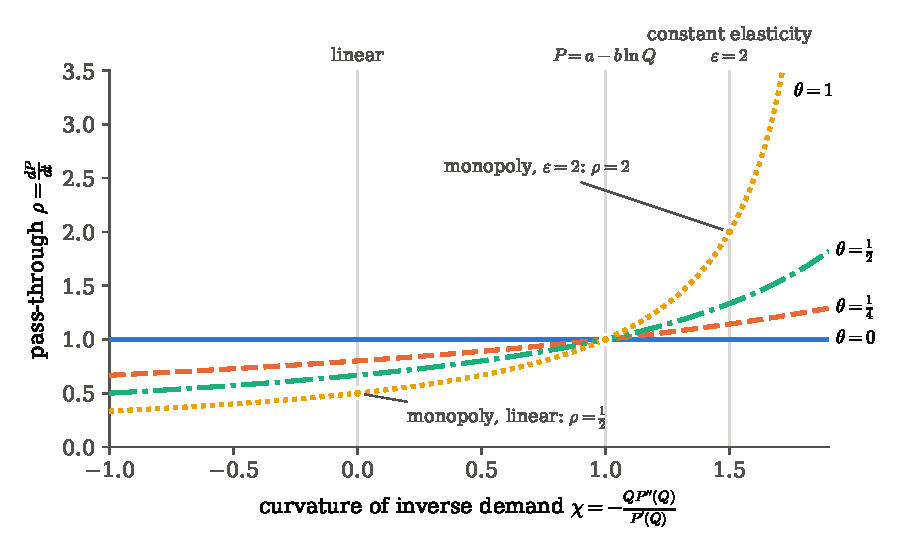
\includegraphics[width=0.86\textwidth]{figures/ch02/passthrough_curvature.pdf}
\caption{Pass-through with flat marginal cost, $\rho = \frac{1}{1 + \theta(1 - \chi)}$, against the curvature
of inverse demand for four values of conduct. All curves cross at $\chi = 1$ (exponential demand), where
$\rho = 1$ under every conduct. To the left of $\chi = 1$ market power lowers pass-through. To the right it
raises pass-through. The dots mark monopoly with linear demand ($\rho = \frac{1}{2}$), exponential demand
($\rho = 1$) and constant elasticity $\varepsilon = 2$ ($\rho = 2$). The monopoly curve is cut at
$\rho = 3.5$.}
\label{fig:02-pt-curvature}
\end{figure}

The figure shows the identification problem at a glance. Under competition with flat marginal cost, pass-through
is one for every demand curve. Market power rotates the line around the point $\chi = 1$. A pass-through above
one can come from strong market power with mild convexity or from weak market power with strong convexity.

\begin{corollary}[What pass-through reveals]\label{cor:02-pt-reveal}
Under \cref{ass:02-pt-general}:
\begin{enumerate}[label=(\roman*)]
\item Under price taking, $\rho \le 1$ for every demand curve and every nondecreasing marginal cost. A
  pass-through above one therefore rejects price taking.
\item With flat marginal cost, $\rho$ identifies only the product
  \begin{equation}\label{eq:02-pt-kappa}
  \theta(\chi - 1) = 1 - \frac{1}{\rho} .
  \end{equation}
  Every $\theta \in (0, 1]$ is consistent with every observed $\rho > 0$ for a suitable curvature. Price taking
  ($\theta = 0$) is consistent only with $\rho = 1$, whatever the curvature.
\item With rising marginal cost, $\theta(\chi - 1) = 1 - \frac{1}{\rho} + \frac{\varepsilon - \theta}{\varepsilon_S}
  \ge 1 - \frac{1}{\rho}$. Rising marginal cost lowers pass-through for given conduct and curvature, so it
  strengthens the rejection in (i). Price taking is then consistent with every $\rho \in (0, 1)$ for a suitable
  supply elasticity.
\item With constant-elasticity demand and flat marginal cost, $\theta = \varepsilon\bigl(1 - \frac{1}{\rho}\bigr)$.
  An estimate of the demand elasticity then converts pass-through into conduct.
\end{enumerate}
\end{corollary}

\begin{proof}
(i) is \cref{cor:02-pt-cases}(i). (ii) Rearrange \eqref{eq:02-pt-flat} as $\frac{1}{\rho} = 1 - \theta(\chi - 1)$.
The data enter only through $\rho$, so only the product $\theta(\chi - 1)$ is identified. Given $\rho$ and
$\theta > 0$, the curvature $\chi = 1 + \frac{1}{\theta}\bigl(1 - \frac{1}{\rho}\bigr)$ reproduces $\rho$. This
curvature satisfies the stability condition $1 + \theta(1 - \chi) = \frac{1}{\rho} > 0$, and under monopoly it
satisfies $\chi < 2$. A value $\rho \le 1$ requires $\chi \le 1$ when $\theta > 0$. With $\theta = 0$ the left
side of \eqref{eq:02-pt-kappa} is zero for every $\chi$, so $\rho = 1$. (iii) Rearrange \eqref{eq:02-pt-general}.
The added term is nonnegative because $\varepsilon \ge \theta$ whenever $P \ge MC + t$. With $\theta = 0$,
\cref{cor:02-pt-cases}(i) gives $\rho = \frac{\varepsilon_S}{\varepsilon_S + \varepsilon}$, which takes every
value in $(0, 1)$ as $\varepsilon_S$ ranges over $(0, \infty)$. (iv) Constant elasticity has $\chi - 1 = \frac{1}{\varepsilon}$.
Substitute into \eqref{eq:02-pt-kappa}.
\end{proof}

Part (i) is the robust content of a pass-through test. It needs no assumption on demand, and it needs only that
marginal cost does not fall with output. Two caveats apply. The price must be a product price, since a price
index can move for reasons of composition (\cref{sec:02-pt-composition}). The shifter must also move cost alone,
since a tax that shifts demand (for example through cross-border shopping) breaks the derivation. Part (ii) says
that a single market-wide cost shock moves the equilibrium along one demand curve, and that this movement cannot
separate conduct from curvature. \Cref{fig:02-pt-identified} draws the set of pairs $(\chi, \theta)$ consistent
with an illustrative pass-through of $1.07$. Separating the two requires an assumption on curvature, as in part
(iv), or variation that changes the slope of demand at a given price. \Cref{ch:conduct} develops both routes and
applies them to Sumner's cigarette data and to sugar refining.

\begin{figure}[htbp]
\centering
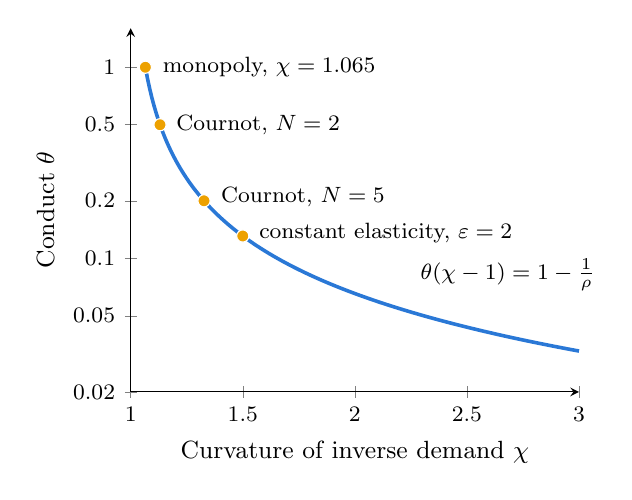
\begin{tikzpicture}
\definecolor{ptA}{HTML}{2A78D6}
\definecolor{ptD}{HTML}{EDA100}
\begin{axis}[
  width=0.6\textwidth, height=6.2cm,
  xmin=1, xmax=3, ymin=0.02, ymax=1.6, ymode=log,
  xlabel={Curvature of inverse demand $\chi$}, ylabel={Conduct $\theta$},
  xtick={1,1.5,2,2.5,3}, ytick={0.02,0.05,0.1,0.2,0.5,1},
  yticklabels={$0.02$,$0.05$,$0.1$,$0.2$,$0.5$,$1$},
  tick label style={font=\footnotesize}, label style={font=\small},
  axis lines=left, clip=false]
  \addplot[domain=1.0654:3, samples=200, color=ptA, line width=1.3pt] {0.0654206/(x - 1)};
  \addplot[only marks, mark=*, mark size=2.2pt, color=ptD, draw=white]
    coordinates {(1.0654,1) (1.1308,0.5) (1.3271,0.2) (1.5,0.13084)};
  \node[anchor=west, font=\footnotesize] at (axis cs:1.10,1.0) {monopoly, $\chi = 1.065$};
  \node[anchor=west, font=\footnotesize] at (axis cs:1.16,0.5) {Cournot, $N = 2$};
  \node[anchor=west, font=\footnotesize] at (axis cs:1.36,0.21) {Cournot, $N = 5$};
  \node[anchor=west, font=\footnotesize] at (axis cs:1.53,0.135) {constant elasticity, $\varepsilon = 2$};
  \node[anchor=south west, font=\footnotesize] at (axis cs:2.25,0.06) {$\theta(\chi - 1) = 1 - \frac{1}{\rho}$};
\end{axis}
\end{tikzpicture}
\caption{Pairs of demand curvature and conduct consistent with an illustrative pass-through $\rho = 1.07$ when
marginal cost is flat. Every point on the curve satisfies $\theta(\chi - 1) = 1 - \frac{1}{1.07} \approx 0.065$.
Symmetric Cournot with $N$ firms ($\theta = \frac{1}{N}$) fits with $\chi = 1 + 0.065N$. A constant-elasticity
demand with elasticity $\varepsilon$ has $\chi = 1 + \frac{1}{\varepsilon}$ and fits with
$\theta = 0.065\varepsilon$. The vertical axis is logarithmic.}
\label{fig:02-pt-identified}
\end{figure}

\subsection{Firm-specific versus industry-wide cost shocks in Cournot}\label{sec:02-pt-cournot}

So far a tax raised every firm's cost together. Many cost shocks hit one firm only: a local wage increase, a
plant outage, a merger's cost savings, or an exchange-rate shock to one importer. In a homogeneous-good market
all firms charge one price, and the question becomes how much that price responds to one firm's cost.

The linear Cournot model of \cref{ex:02-linear-cournot} gives the answer in closed form. With $P = a - bQ$ and
constant costs $c_1, \dots, c_N$,
\begin{equation*}
P^* = \frac{a + \sum_j c_j}{N + 1}, \qquad q_i^* = \frac{a - (N + 1)c_i + \sum_j c_j}{b(N + 1)} .
\end{equation*}
A rise in $c_i$ alone and a common rise $\dd c_j = \dd c$ for all $j$ give
\begin{equation*}
\frac{\dd P^*}{\dd c_i} = \frac{1}{N + 1}, \qquad \frac{\dd q_i^*}{\dd c_i} = -\frac{N}{b(N + 1)}, \qquad
\frac{\dd q_j^*}{\dd c_i} = \frac{1}{b(N + 1)} \;\; (j \ne i), \qquad \frac{\dd P^*}{\dd c} = \frac{N}{N + 1} .
\end{equation*}
Firm $i$'s margin $P^* - c_i$ falls by $\frac{N}{N + 1}$ per dollar of its own
cost increase, so the firm absorbs most of a firm-specific shock. The next result extends these formulas to
nonlinear demand.

\begin{proposition}[Cournot pass-through]\label{prop:02-pt-cournot}
Let (C1) and (C3) of \cref{ass:02-cournot} hold with constant marginal costs $c_1, \dots, c_N$, let all $N$ firms
be active, and suppose $P'(Q) + q_jP''(Q) < 0$ at the equilibrium for every $j$ (as (C2) guarantees).
Let $s_i = \frac{q_i}{Q}$ and let $\chi$ be the curvature \eqref{eq:02-chi} at the equilibrium output. Then
$N + 1 - \chi > 0$, and
\begin{equation}\label{eq:02-pt-cournot}
\frac{\dd P}{\dd c_i} = \frac{1}{N + 1 - \chi}, \qquad \frac{\dd P}{\dd c} = \frac{N}{N + 1 - \chi}, \qquad
\frac{\dd q_i}{\dd c_i} = \frac{N - (1 - s_i)\chi}{P'(Q)\,(N + 1 - \chi)} < 0 ,
\end{equation}
where $\frac{\dd P}{\dd c}$ is the response to a common shock.
\end{proposition}

\begin{proof}
We use the replacement functions of \cref{sec:02-cournot}. With constant costs, $\tilde q_i(Q)$ solves
$P(Q) + qP'(Q) = c_i$, so $\tilde q_i(Q) = \frac{c_i - P(Q)}{P'(Q)}$ near the equilibrium. Differentiating
$P(Q) + qP'(Q) = c_i$ in $c_i$ at fixed $Q$ gives $\frac{\partial\tilde q_i}{\partial c_i} = \frac{1}{P'}$.
Differentiating it in $Q$ gives $P' + \tilde q_i'P' + \tilde q_iP'' = 0$, so
\begin{equation*}
\tilde q_j'(Q) = -\Bigl(1 + \frac{q_jP''}{P'}\Bigr) = -\Bigl(1 + \frac{q_j}{Q}\cdot\frac{QP''}{P'}\Bigr)
= -(1 - s_j\chi) .
\end{equation*}
By assumption $P' + q_jP'' < 0$ at the equilibrium. Dividing by $P' < 0$ gives $1 - s_j\chi > 0$ for every $j$.
Summing over $j$ and using $\sum_j s_j = 1$,
\begin{equation*}
1 - \sum_j \tilde q_j'(Q) = 1 + \sum_j (1 - s_j\chi) = N + 1 - \chi > 0 .
\end{equation*}
Industry output solves $\sum_j \tilde q_j(Q) = Q$. Since the derivative of $\sum_j \tilde q_j(Q) - Q$ in $Q$ is
nonzero, the implicit function theorem applies. Differentiating in $c_i$, as in the proof of
\cref{prop:02-cournot-cs}, gives
\begin{equation*}
\frac{\dd Q}{\dd c_i} = \frac{\frac{\partial\tilde q_i}{\partial c_i}}{1 - \sum_j \tilde q_j'(Q)} .
\end{equation*}
Hence $\frac{\dd Q}{\dd c_i} = \frac{1}{P'(N + 1 - \chi)}$ and $\frac{\dd P}{\dd c_i} = P'\frac{\dd Q}{\dd c_i} = \frac{1}{N + 1 - \chi}$.
A common shock is the sum of $N$ firm-specific shocks, so $\frac{\dd P}{\dd c} = \sum_i\frac{\dd P}{\dd c_i} = \frac{N}{N + 1 - \chi}$.
For firm $i$'s own output, $q_i = \tilde q_i(Q)$ in equilibrium, so
\begin{equation*}
\frac{\dd q_i}{\dd c_i} = \frac{\partial\tilde q_i}{\partial c_i} + \tilde q_i'(Q)\frac{\dd Q}{\dd c_i}
= \frac{1}{P'}\Bigl[1 - \frac{1 - s_i\chi}{N + 1 - \chi}\Bigr]
= \frac{N - (1 - s_i)\chi}{P'(N + 1 - \chi)} .
\end{equation*}
The numerator equals $1 + \sum_{j \ne i}(1 - s_j\chi) > 0$, and $P' < 0$, so $\frac{\dd q_i}{\dd c_i} < 0$.
\end{proof}

Three features of \eqref{eq:02-pt-cournot} stand out. First, the price response to a firm-specific shock does
not depend on the firm's share. A large firm and a small firm move the price by the same amount after equal
cost increases. The direct effect on a firm's replacement output, $\frac{1}{P'}$, does not depend on its size, and
rivals respond only to total output. Second, the
common-shock pass-through equals \cref{cor:02-pt-cases}(iv) even with asymmetric costs. Third, the ratio of the
two is $N$ for any demand curve. A firm-specific shock moves the market price by only a fraction
$\frac{1}{N + 1 - \chi}$ of the shock, and the firm bears the rest through a lower margin.

The distinction matters for empirical work. A market-wide shifter, such as an excise tax, moves the industry
along the market demand curve. Its pass-through speaks to industry conduct and market demand curvature, as in
\cref{sec:02-pt-general}. A firm-specific shifter, such as a firm's own input price, moves the equilibrium along
the firm's residual demand curve, which includes rivals' supply responses. \citet{BakerBresnahan1988} use such
shifters to estimate residual demand directly (\cref{ch:conduct}). The distinction also matters for mergers.
The cost savings of a merger are specific to the merged firm, so the relevant pass-through is the
firm-specific one. Using an industry-wide rate would overstate how much of the savings reaches consumers
(\cref{ch:mergers}).

\subsection{Incidence}\label{sec:02-pt-incidence}

Pass-through determines who bears a tax. Consumer surplus is $CS = \int_0^Q P(x)\,\dd x - P(Q)Q$. Producer surplus
is variable profit, $PS = P(Q)Q - C(Q) - tQ$, where $C$ is industry variable cost with $C' = MC$ (as with
symmetric firms). Tax revenue is $R = tQ$.

\begin{proposition}[Incidence under conduct, {\citealp[pp.~546--548]{WeylFabinger2013}}]\label{prop:02-incidence}
Under \cref{ass:02-pt-general}, a small change in the specific tax changes surplus by
\begin{equation*}
\frac{\dd CS}{\dd t} = -\rho Q, \qquad \frac{\dd PS}{\dd t} = -\bigl[1 - (1 - \theta)\rho\bigr]Q .
\end{equation*}
When the producer burden is nonzero, the \emph{incidence ratio}, consumer burden divided by producer burden, is
\begin{equation}\label{eq:02-incidence}
I = \frac{\frac{\dd CS}{\dd t}}{\frac{\dd PS}{\dd t}} = \frac{\rho}{1 - (1 - \theta)\rho} .
\end{equation}
Total surplus $W = CS + PS + R$ satisfies $\frac{\dd W}{\dd t} = -\theta\rho Q + t\frac{\dd Q}{\dd t}$.
\end{proposition}

\begin{proof}
\emph{Consumers.} By Leibniz's rule,
\begin{equation*}
\frac{\dd CS}{\dd t} = P(Q)\frac{\dd Q}{\dd t} - \Bigl[P'(Q)Q + P(Q)\Bigr]\frac{\dd Q}{\dd t} = -QP'(Q)\frac{\dd Q}{\dd t} = -Q\rho ,
\end{equation*}
since $\rho = P'\frac{\dd Q}{\dd t}$.

\emph{Producers.} Differentiating $PS$,
\begin{equation*}
\frac{\dd PS}{\dd t} = P'Q\frac{\dd Q}{\dd t} + P\frac{\dd Q}{\dd t} - MC\frac{\dd Q}{\dd t} - Q - t\frac{\dd Q}{\dd t}
= Q(\rho - 1) + (P - MC - t)\frac{\dd Q}{\dd t} .
\end{equation*}
The supply relation \eqref{eq:02-pt-supply} gives $P - MC - t = -\theta QP'$, and $\frac{\dd Q}{\dd t} = \frac{\rho}{P'}$.
Hence $(P - MC - t)\frac{\dd Q}{\dd t} = -\theta QP'\cdot\frac{\rho}{P'} = -\theta\rho Q$, and
\begin{equation*}
\frac{\dd PS}{\dd t} = Q(\rho - 1) - \theta\rho Q = -Q\bigl[1 - (1 - \theta)\rho\bigr] .
\end{equation*}
Dividing the two derivatives gives \eqref{eq:02-incidence}.

\emph{Total surplus.} Revenue changes by $\frac{\dd R}{\dd t} = Q + t\frac{\dd Q}{\dd t}$. Adding the three derivatives,
\begin{equation*}
\frac{\dd W}{\dd t} = -\rho Q - Q + (1 - \theta)\rho Q + Q + t\frac{\dd Q}{\dd t} = -\theta\rho Q + t\frac{\dd Q}{\dd t} .
\qedhere
\end{equation*}
\end{proof}

\citet[p.~546]{WeylFabinger2013} credit \citet{AtkinDonaldson2012} with first deriving the formula for
$\frac{\dd PS}{\dd t}$, which extends the monopoly case to general conduct.

The special cases are instructive. Under price taking, $I = \frac{\rho}{1 - \rho}$. With
$\rho = \frac{\varepsilon_S}{\varepsilon_S + \varepsilon}$ from \cref{cor:02-pt-cases}(i), this is
$I = \frac{\varepsilon_S}{\varepsilon}$, the classic rule that the burden falls on the less elastic side. With flat
marginal cost, competitive producers bear nothing. Under monopoly, $\frac{\dd PS}{\dd t} = -Q$ whatever the demand
curve, which is the envelope theorem at work (\cref{app:math}), and $I = \rho$. Consumers bear more than the
monopolist exactly when $\rho > 1$. With linear demand, flat cost and conduct $\theta$, $\rho = \frac{1}{1 + \theta}$
and
\begin{equation*}
I = \frac{\frac{1}{1 + \theta}}{1 - \frac{1 - \theta}{1 + \theta}} = \frac{\frac{1}{1 + \theta}}{\frac{2\theta}{1 + \theta}}
= \frac{1}{2\theta} .
\end{equation*}
A linear monopoly ($\theta = 1$) puts one third of the private burden on consumers, and a symmetric Cournot duopoly
($\theta = \frac{1}{2}$) splits it equally.

Market power changes incidence in two ways that competitive analysis misses. First, consumers can bear more than
the full tax ($\rho > 1$) while producers still lose. With constant elasticity $\varepsilon = 2$, a monopolist
passes through $\rho = 2$, consumers lose $2Q$ per unit of tax and the monopolist loses $Q$. Second, producers
can gain from a tax. The producer burden is negative when $\rho > \frac{1}{1 - \theta}$. With flat marginal cost
this condition reduces to $\theta(2 - \chi) < 0$, that is $\chi > 2$ for $\theta > 0$. Monopoly rules this out
through its second-order condition, but oligopoly with $\theta < 1$ allows $2 < \chi < 1 + \frac{1}{\theta}$.
In symmetric Cournot with constant elasticity,
\begin{equation*}
1 - \Bigl(1 - \frac{1}{N}\Bigr)\frac{N\varepsilon}{N\varepsilon - 1} = \frac{\varepsilon - 1}{N\varepsilon - 1} ,
\end{equation*}
which is negative when $\frac{1}{N} < \varepsilon < 1$. A common cost increase then raises industry profit. It
pushes output toward the level that maximizes joint profit, which the firms could not reach on their own.

The total-surplus formula adds a third difference. Under competition the first tax dollar has no deadweight cost,
because $\frac{\dd W}{\dd t} = 0$ at $t = 0$ when $\theta = 0$. Under market power the first dollar already costs
$\theta\rho Q$, because output starts below its efficient level (\cref{sec:02-welfare}). Linear monopoly loses
$\frac{Q}{2}$ of surplus per unit of tax at $t = 0$, half of the revenue raised. \citet[pp.~537 and
546]{WeylFabinger2013} state that this excess burden is $\rho$ per unit of revenue under monopoly and positive
whenever $\theta > 0$. We add the total-surplus formula itself, which also holds at $t > 0$.

\begin{remark}[Ad valorem taxes]\label{rem:02-pt-adval}
An \emph{ad valorem tax} at rate $t_a$ takes a fraction $t_a$ of the price. Firms receive $(1 - t_a)P$, and the
supply relation becomes $(1 - t_a)(P + \theta QP') = MC(Q)$, that is $P + \theta QP' = \frac{MC(Q)}{1 - t_a}$.
An ad valorem tax therefore scales effective marginal cost by $\frac{1}{1 - t_a}$. At $t_a = 0$ a small rate
$\dd t_a$ raises effective marginal cost by $MC\,\dd t_a$, so $\frac{\dd P}{\dd t_a} = \rho\, MC$. A specific tax
$\dd t = P\,\dd t_a$ raises the same revenue to first order and raises price by $\rho P\,\dd t_a$. At $t_a = 0$
the Lerner form gives $MC = (1 - \frac{\theta}{\varepsilon})P$, so the ad valorem tax raises price less per dollar
of revenue whenever $\theta > 0$. Under competition the two taxes coincide to first order. The incidence formulas for ad valorem taxes
are left to \cref{sec:02-exercises}.
\end{remark}

\subsection{Measured prices and composition}\label{sec:02-pt-composition}

Pass-through regressions often use a price index, an average across products, as the dependent variable. The
index can move even when no product's price moves, because the mix of products bought changes.

\begin{remark}[Composition bias]\label{rem:02-pt-composition}
Let the observed price be the quantity-weighted average $\bar p = \sum_j w_jp_j$, with weights $w_j \ge 0$
summing to one. Differentiating with respect to the tax,
\begin{equation}\label{eq:02-pt-composition}
\frac{\dd \bar p}{\dd t} = \underbrace{\sum_j w_j\frac{\dd p_j}{\dd t}}_{\text{price effect}}
+ \underbrace{\sum_j p_j\frac{\dd w_j}{\dd t}}_{\text{composition effect}} .
\end{equation}
The first term is the average of product-level pass-through. The second term is nonzero whenever the tax changes
the mix of purchases. A regression of $\bar p$ on $t$ estimates the sum.
\end{remark}

A specific tax tends to make the composition effect positive. It raises every price by a similar dollar amount,
which is a larger percentage of a cheap product's price. Suppose a cheap and an expensive product have prices
$p_L < p_H$, and each price rises one for one with the tax. The relative price $\frac{p_H + t}{p_L + t}$ has
derivative $\frac{p_L - p_H}{(p_L + t)^2} < 0$ in $t$, so the expensive product becomes relatively cheaper. If
buyers respond to relative prices, the weight $w_H$ rises, and the composition effect
$(p_H - p_L)\frac{\dd w_H}{\dd t}$ is positive. A numerical illustration makes the size concrete. Let $p_L = 1$,
$p_H = 2$ and $w_H = 0.5$, and let a tax of $0.10$ raise both prices by $0.10$ and $w_H$ to $0.52$. The index
rises from $1.50$ to $0.48 \times 1.10 + 0.52 \times 2.10 = 1.62$, so the measured pass-through is $1.2$ although
each product's pass-through is exactly one.

The bias pushes a test toward rejecting price taking, because it can create $\hat\rho > 1$ from product-level
pass-through equal to one. The remedies are to estimate pass-through at the product level, or to use a
fixed-weight index $\sum_j w_j^0 p_j$ that holds the weights at their pre-tax values. The same logic runs in the
opposite direction when demand peaks. \citet{NevoHatzitaskos2005} study canned tuna, whose average price falls
during Lent although demand is high. They argue that a shift of purchases toward cheaper products explains much
of the fall in the average price paid. In their supermarket data, the Lent coefficient is $-1.78$ cents per ounce
for the quantity-weighted tuna price index and $-0.51$ for a fixed-weight index \citep[p.~13 and
Table~3]{NevoHatzitaskos2005}.
\Cref{ch:conduct} returns to composition as one of the three standard critiques of Sumner's cigarette-tax test.

Pass-through thus carries information about market power, but only jointly with the curvature of demand and the
slope of marginal cost. Pass-through above one is hard to reconcile with price taking. Beyond that, a pass-through
estimate must be combined with an assumption or a second source of variation before it reveals conduct. The
incidence of taxes, the consumer benefits of cost savings and the price effects of mergers all inherit this
dependence on curvature.

\section{Welfare and the deadweight loss of market power}\label{sec:02-welfare}

The previous sections asked how far price exceeds marginal cost and why. This section asks what the gap costs
society. A positive correlation between concentration and margins, or an estimated conduct parameter above zero,
does not by itself tell us that the losses are large. To answer the normative question we need a measure of welfare,
a way to compute it from demand and cost, and a sense of its likely size. We first set up the standard
partial-equilibrium apparatus and derive closed forms for linear demand. We then present the Harberger
approximation and the debate it started. The section closes with three qualifications: production inefficiency
across firms, entry, and the trade-off between market power and cost savings in mergers.

\subsection{Surplus measures}\label{sec:02-surplus}

We work in a single market and use partial-equilibrium welfare analysis.

\begin{assumption}[Partial-equilibrium welfare]\label{ass:02-welfare}
\leavevmode
\begin{enumerate}[label=(W\arabic*)]
\item Consumers have quasi-linear utility in the good and a numeraire, so market demand has no income effects.
      The area under the inverse demand curve then measures willingness to pay in units of the numeraire.
\item The industry produces output $Q$ at the minimum total variable cost $C(Q)$, with $C$ increasing and
      convex. Fixed costs are set aside until \cref{sec:02-second-best}.
\item A dollar of consumer surplus and a dollar of profit carry equal social weight.
\end{enumerate}
\end{assumption}

Assumption (W1) makes the Marshallian consumer surplus an exact money measure of welfare. Without it, the
compensating and equivalent variations of \cref{ch:aids} replace the area under the demand curve. Assumption (W3)
is the \emph{total-surplus standard}. Antitrust practice often uses a \emph{consumer-surplus standard} instead,
which counts only the first term. The distinction matters most for mergers (\cref{ch:mergers}).

\begin{definition}[Surplus and deadweight loss]\label{def:02-surplus}
At industry output $Q$ and price $P(Q)$, \emph{consumer surplus}, \emph{producer surplus} and \emph{total surplus}
are
\begin{align}
CS(Q) &= \int_0^{Q} P(x)\,\dd x - P(Q)\,Q, \label{eq:02-cs}\\
PS(Q) &= P(Q)\,Q - C(Q), \label{eq:02-ps}\\
W(Q)  &= CS(Q) + PS(Q) = \int_0^{Q} P(x)\,\dd x - C(Q). \label{eq:02-total-surplus}
\end{align}
Let $Q^c$ maximize $W$. The \emph{deadweight loss} at output $Q$ is $\mathit{DWL}(Q) = W(Q^c) - W(Q)$.
\end{definition}

The price drops out of total surplus because payments from consumers to producers are transfers. Differentiating
\eqref{eq:02-total-surplus} with respect to $Q$ gives
\begin{equation*}
W'(Q) = P(Q) - C'(Q), \qquad W''(Q) = P'(Q) - C''(Q) < 0 .
\end{equation*}
Total surplus is therefore strictly concave, and it is maximized at the output where $P(Q^c) = C'(Q^c)$. This is
the price-taking output, so the first-best benchmark is the competitive outcome. For any $Q < Q^c$, the fundamental
theorem of calculus gives
\begin{equation}\label{eq:02-dwl-general}
\mathit{DWL}(Q) = W(Q^c) - W(Q) = \int_{Q}^{Q^c} \bigl[P(x) - C'(x)\bigr]\,\dd x .
\end{equation}
The integrand is the gap between willingness to pay and marginal cost on each unit that market power removes. With
constant marginal cost $c$, the deadweight loss is the area between the demand curve and the horizontal line at
$c$, from $Q$ to $Q^c$. Producer surplus is then variable profit, $PS = (P - c)\,Q$.

\begin{example}[The monopoly benchmark]\label{ex:02-welfare-monopoly}
Take the market of \cref{fig:02-monopoly}: $P(Q) = 10 - Q$ and $c = 2$. The competitive output solves
$10 - Q = 2$, so $Q^c = 8$ and maximal surplus is $W(Q^c) = \frac{1}{2}\cdot 8 \cdot 8 = 32$. The monopolist sells
$Q^m = 4$ at $p^m = 6$. Consumer surplus is $\frac{1}{2}\cdot 4 \cdot 4 = 8$, profit is $(6 - 2)\cdot 4 = 16$, and
the deadweight loss is $\frac{1}{2}(6 - 2)(8 - 4) = 8$. Consumers keep one quarter of the potential surplus, the
monopolist takes one half, and one quarter is destroyed.
\end{example}

\begin{remark}[An output subsidy restores efficiency]\label{rem:02-subsidy}
A per-unit subsidy can remove the monopoly distortion \citep[sec.~1.1.1.3]{Tirole1988}. Let consumers pay $p + t$
for each unit on which the firm receives $p$, so that $t < 0$ is a subsidy. The firm chooses $p$ to maximize
$pQ(p + t) - C\bigl(Q(p + t)\bigr)$, and its first-order condition is
\[
  Q(p + t) + Q'(p + t)\bigl[p - C'(Q)\bigr] = 0 .
\]
Write $p_b = p + t$ for the consumer price and substitute $p = p_b - t$:
\[
  \bigl[Q(p_b) - t\,Q'(p_b)\bigr] + Q'(p_b)\bigl[p_b - C'(Q)\bigr] = 0 .
\]
Efficiency requires the consumer price to equal marginal cost at the competitive price $p^c$. The second bracket
then vanishes, so the first must vanish too:
\[
  t = \frac{Q(p^c)}{Q'(p^c)} < 0, \qquad \frac{t}{p^c} = -\frac{1}{\varepsilon(p^c)} .
\]
The subsidy per unit, as a fraction of the competitive price, is the inverse elasticity of demand at that price. In
\cref{ex:02-welfare-monopoly}, $p^c = 2$, $Q(p^c) = 8$ and $Q' = -1$, so $t = -8$. The firm receives 10 per unit,
consumers pay 2 and buy the efficient 8 units, and total surplus reaches its maximum of 32. The firm's profit of 64
equals the subsidy bill of 64.

The subsidy has few advocates, and Tirole lists the objections. The total-surplus standard gives a dollar of profit
the same weight as a dollar of consumer surplus, so it records no cost for the transfer to shareholders. The
government must know the elasticity of demand and the firm's marginal cost. The firm gains from overstating the
subsidy it needs, and it is reluctant to reveal its costs. Schemes that reward the firm for low prices lead into the
theory of regulation, which this chapter does not pursue.
\end{remark}

\subsection{Linear demand with conduct}\label{sec:02-dwl-linear}

The conduct parameter of \cref{sec:02-conduct} indexes market power continuously, from price taking ($\theta = 0$)
through symmetric Cournot ($\theta = \frac{1}{N}$) to monopoly ($\theta = 1$). With linear demand, every welfare
quantity has a closed form in $\theta$.

\begin{proposition}[Welfare with linear demand and conduct $\theta$]\label{prop:02-dwl-linear}
Let $P(Q) = a - bQ$ with $a > c \ge 0$ and $b > 0$, let marginal cost be constant at $c$, and let price satisfy the
supply relation \eqref{eq:02-supply-relation} with conduct $\theta \in [0, 1]$. Then
\begin{enumerate}[label=(\roman*)]
\item Equilibrium output and markup are $Q(\theta) = \frac{a - c}{b(1 + \theta)}$ and
      $P(\theta) - c = \frac{\theta (a - c)}{1 + \theta}$.
\item Maximal total surplus is $W^{\max} = \frac{(a - c)^2}{2b}$.
\item Consumer surplus, profit and deadweight loss are the shares $\frac{1}{(1 + \theta)^2}$,
      $\frac{2\theta}{(1 + \theta)^2}$ and $\frac{\theta^2}{(1 + \theta)^2}$ of $W^{\max}$. In particular
      \begin{equation}\label{eq:02-dwl-linear}
      \mathit{DWL}(\theta) = \frac{\theta^2 (a - c)^2}{2b(1 + \theta)^2}.
      \end{equation}
\end{enumerate}
\end{proposition}

\begin{proof}
(i) This repeats part (i) of \cref{ex:02-pt-examples}. The supply relation is $P = c - \theta Q P'(Q)$, and here
$P'(Q) = -b$. Substituting the demand curve,
\begin{align*}
a - bQ &= c + \theta b Q, \\
a - c &= b(1 + \theta)\, Q, \\
Q(\theta) &= \frac{a - c}{b(1 + \theta)} .
\end{align*}
The markup is $P - c = \theta b Q = \frac{\theta(a - c)}{1 + \theta}$.

(ii) The competitive output solves $a - bQ = c$, so $Q^c = \frac{a - c}{b}$. Then
\begin{equation*}
W^{\max} = \int_0^{Q^c} (a - bx - c)\,\dd x = (a - c)\,Q^c - \frac{b}{2}(Q^c)^2
= \frac{(a - c)^2}{b} - \frac{(a - c)^2}{2b} = \frac{(a - c)^2}{2b} .
\end{equation*}

(iii) Consumer surplus is the triangle above the price,
\begin{equation*}
CS = \int_0^{Q}(a - bx)\,\dd x - (a - bQ)\,Q = aQ - \frac{b}{2}Q^2 - aQ + bQ^2 = \frac{b}{2}Q^2
= \frac{(a - c)^2}{2b(1 + \theta)^2} .
\end{equation*}
Profit is the rectangle
\begin{equation*}
\pi = (P - c)\,Q = \frac{\theta(a - c)}{1 + \theta}\cdot\frac{a - c}{b(1 + \theta)} = \frac{\theta(a - c)^2}{b(1 + \theta)^2} .
\end{equation*}
The deadweight loss is the triangle with height $P - c$ and base
$Q^c - Q = \frac{a - c}{b}\left(1 - \frac{1}{1 + \theta}\right) = \frac{\theta(a - c)}{b(1 + \theta)}$, so
\begin{equation*}
\mathit{DWL} = \frac{1}{2}\cdot\frac{\theta(a - c)}{1 + \theta}\cdot\frac{\theta(a - c)}{b(1 + \theta)}
= \frac{\theta^2(a - c)^2}{2b(1 + \theta)^2} .
\end{equation*}
Dividing each expression by $W^{\max}$ gives the three shares. As a check, the three shares sum to
\[
\frac{1 + 2\theta + \theta^2}{(1 + \theta)^2} = 1 . \qedhere
\]
\end{proof}

\begin{corollary}[Monopoly and Cournot]\label{cor:02-dwl-cournot}
Under monopoly ($\theta = 1$) the shares are $\frac{1}{4}$, $\frac{1}{2}$ and $\frac{1}{4}$. Under symmetric Cournot
with $N$ firms ($\theta = \frac{1}{N}$), multiplying numerator and denominator by $N^2$ gives
\begin{equation}\label{eq:02-dwl-cournot}
\frac{CS}{W^{\max}} = \frac{N^2}{(N + 1)^2}, \qquad
\frac{\pi}{W^{\max}} = \frac{2N}{(N + 1)^2}, \qquad
\frac{\mathit{DWL}}{W^{\max}} = \frac{1}{(N + 1)^2}.
\end{equation}
For every $\theta > 0$ the ratio of deadweight loss to profit is $\frac{\mathit{DWL}}{\pi} = \frac{\theta}{2}$.
\end{corollary}

\begin{table}[htbp]
\centering
\begin{threeparttable}
\caption{Division of the maximal surplus under linear demand}
\label{tab:02-welfare-shares}
\small
\renewcommand{\arraystretch}{1.6}
\begin{tabular}{@{}lccccc@{}}
\toprule
Market & $\theta$ & Consumer surplus & Profit & Deadweight loss & $\frac{\mathit{DWL}}{\pi}$ \\
\midrule
Price taking      & $0$           & $1$                & $0$               & $0$              & n.a. \\
Cournot, $N = 5$  & $\frac{1}{5}$ & $\frac{25}{36}$    & $\frac{10}{36}$   & $\frac{1}{36}$   & $0.10$ \\
Cournot, $N = 4$  & $\frac{1}{4}$ & $\frac{16}{25}$    & $\frac{8}{25}$    & $\frac{1}{25}$   & $0.125$ \\
Cournot, $N = 3$  & $\frac{1}{3}$ & $\frac{9}{16}$     & $\frac{6}{16}$    & $\frac{1}{16}$   & $0.17$ \\
Cournot, $N = 2$  & $\frac{1}{2}$ & $\frac{4}{9}$      & $\frac{4}{9}$     & $\frac{1}{9}$    & $0.25$ \\
Monopoly          & $1$           & $\frac{1}{4}$      & $\frac{1}{2}$     & $\frac{1}{4}$    & $0.50$ \\
\bottomrule
\end{tabular}
\begin{tablenotes}\footnotesize
\item Notes: Shares of $W^{\max} = \frac{(a - c)^2}{2b}$ from \cref{prop:02-dwl-linear} and
\cref{cor:02-dwl-cournot}. The last column is $\frac{\theta}{2}$.
\end{tablenotes}
\end{threeparttable}
\end{table}

\Cref{tab:02-welfare-shares} carries two lessons. First, near competition the transfer to producers is first order
in $\theta$, while the deadweight loss is second order. For small $\theta$ the profit share is close to $2\theta$ and
the loss share is close to $\theta^2$. Second, the deadweight loss falls quickly with the number of Cournot firms.
It is $\frac{1}{9}$, or 11.1 percent of maximal surplus, under duopoly and $\frac{1}{36}$, or 2.8 percent, with five
firms. With five firms the transfer to producers is ten times the deadweight loss. With linear demand, concern about
market power in moderately concentrated markets is therefore largely a concern about distribution, unless market power also
raises costs or wastes resources. The rest of this section examines those two channels.

\subsection{The Harberger approximation}\label{sec:02-harberger}

Closed forms need a demand curve. To estimate losses across many industries with little information,
\citet{Harberger1954} used a local approximation that needs only revenue, the Lerner index and the elasticity of
demand. We derive it in general and then turn to its uses.

Fix an equilibrium with output $Q$, price $P = P(Q)$ and constant marginal cost $c < P$. Approximate inverse demand
between $Q$ and $Q^c$ by its tangent at $Q$:
\begin{equation*}
P(x) \approx P(Q) + P'(Q)(x - Q).
\end{equation*}
The competitive output then solves $P(Q) + P'(Q)(Q^c - Q) = c$, so
\begin{equation*}
Q^c - Q \approx \frac{P(Q) - c}{-P'(Q)} .
\end{equation*}
Substituting the tangent into \eqref{eq:02-dwl-general} and integrating,
\begin{align*}
\mathit{DWL} &\approx \int_Q^{Q^c}\bigl[P(Q) - c + P'(Q)(x - Q)\bigr]\,\dd x \\
&= (P - c)(Q^c - Q) + \frac{1}{2}P'(Q)(Q^c - Q)^2 \\
&= \frac{(P - c)^2}{-P'(Q)} - \frac{1}{2}\cdot\frac{(P - c)^2}{-P'(Q)}
 = \frac{1}{2}\cdot\frac{(P - c)^2}{-P'(Q)} .
\end{align*}
The market elasticity is $\varepsilon = -\frac{1}{P'(Q)}\frac{P}{Q}$, so $-P'(Q) = \frac{P}{\varepsilon Q}$. With the
Lerner index $L = \frac{P - c}{P}$ and revenue $R = PQ$, this gives the \emph{Harberger approximation}
\begin{equation}\label{eq:02-harberger}
\mathit{DWL} \approx \frac{1}{2}\,(P - c)\,(Q^c - Q) \approx \frac{1}{2}\,\varepsilon\, L^2\, R .
\end{equation}
The loss is half the markup times the lost output, and the lost output is approximately $\varepsilon L Q$. The loss
is proportional to the square of the Lerner index, which is why small markups imply very small losses.

The approximation takes a simple form under any conduct. The supply relation in Lerner form,
\eqref{eq:02-theta-lerner}, gives $L = \frac{\theta}{\varepsilon}$. Substituting into \eqref{eq:02-harberger} and
using profit $\pi = (P - c)Q = LR$,
\begin{equation}\label{eq:02-harberger-theta}
\mathit{DWL} \approx \frac{\theta^2}{2\varepsilon}\,R = \frac{\theta}{2}\,L R = \frac{\theta}{2}\,\pi .
\end{equation}
Under monopoly, $\theta = 1$ and $L = \frac{1}{\varepsilon}$, so $\mathit{DWL} \approx \frac{R}{2\varepsilon} =
\frac{1}{2}LR$: the triangle is about half the profit rectangle. For linear demand the tangent is the demand curve,
so \eqref{eq:02-harberger} and \eqref{eq:02-harberger-theta} hold exactly. They reproduce
\cref{prop:02-dwl-linear} and the ratio $\frac{\mathit{DWL}}{\pi} = \frac{\theta}{2}$ of \cref{cor:02-dwl-cournot}.

\begin{remark}[Accuracy with convex demand]\label{rem:02-harberger-accuracy}
The tangent understates the area under a convex demand curve, so \eqref{eq:02-harberger} understates large losses.
Take constant-elasticity demand $Q(p) = Ap^{-\varepsilon}$ with $\varepsilon > 1$, marginal cost $c > 0$ and
monopoly pricing, $p^m = \frac{\varepsilon}{\varepsilon - 1}c$. The exact loss is the consumer surplus lost minus the profit gained,
\begin{equation*}
\mathit{DWL} = \int_c^{p^m} Ap^{-\varepsilon}\,\dd p - (p^m - c)A(p^m)^{-\varepsilon} .
\end{equation*}
Integrating, dividing by revenue $R = A(p^m)^{1-\varepsilon}$ and using $\frac{c}{p^m} = \frac{\varepsilon - 1}{\varepsilon}$,
\begin{equation*}
\frac{\mathit{DWL}}{R} = \frac{1}{\varepsilon - 1}\left[\left(\frac{\varepsilon - 1}{\varepsilon}\right)^{1 - \varepsilon} - 1\right]
- \frac{1}{\varepsilon} .
\end{equation*}
The Harberger approximation gives $\frac{1}{2\varepsilon}$. For $\varepsilon = 2$ the exact loss is $\frac{1}{2}R$,
twice the approximation of $\frac{1}{4}R$, and as large as the monopoly profit itself. Our computations give exact
to approximate ratios of 2.39, 2.00, 1.75 and 1.60 for $\varepsilon = 1.5, 2, 3$ and $5$. The approximation
improves as the markup falls, as it should for a second-order expansion.
\end{remark}

\begin{remark}[The deadweight loss need not fall with the elasticity]\label{rem:02-dwl-elasticity}
The Lerner index $\frac{1}{\varepsilon}$ falls as demand becomes more elastic, but the deadweight loss need not
\citep[sec.~1.1.1.2]{Tirole1988}. Where demand is inelastic, a high price moves little output and mostly transfers
money from consumers to the firm. Take $Q(p) = p^{-\varepsilon}$ with $\varepsilon > 1$ and constant marginal cost
$c > 0$ \citep[Exercise~1.1]{Tirole1988}. Maximal surplus is the consumer surplus at price $c$,
\[
  W^c = \int_c^{\infty} p^{-\varepsilon}\,\dd p = \frac{c^{1 - \varepsilon}}{\varepsilon - 1} .
\]
At $p^m = \frac{\varepsilon}{\varepsilon - 1}c$, consumer surplus is $\frac{(p^m)^{1 - \varepsilon}}{\varepsilon - 1}$
and profit is $(p^m - c)(p^m)^{-\varepsilon} = \frac{(p^m)^{1 - \varepsilon}}{\varepsilon}$, since $p^m - c =
\frac{p^m}{\varepsilon}$. Let $\kappa = \left(\frac{p^m}{c}\right)^{1 - \varepsilon} = \left(\frac{\varepsilon -
1}{\varepsilon}\right)^{\varepsilon - 1}$, a symbol local to this remark. Dividing by $W^c$,
\[
  \frac{CS^m}{W^c} = \kappa, \qquad \frac{\pi^m}{W^c} = \frac{\varepsilon - 1}{\varepsilon}\,\kappa, \qquad
  \frac{\mathit{DWL}}{W^c} = 1 - \frac{2\varepsilon - 1}{\varepsilon}\,\kappa .
\]
As $\varepsilon \to 1$, $\kappa \to 1$ and the relative loss tends to zero. As $\varepsilon \to \infty$,
$\kappa \to e^{-1}$, so the relative loss tends to $1 - \frac{2}{e} \approx 0.264$ and the profit share to
$\frac{1}{e} \approx 0.368$. For $\varepsilon = 1.5, 2, 3$ and $5$ the relative loss is 0.230, 0.250, 0.259 and
0.263, and the profit share is 0.192, 0.250, 0.296 and 0.328. Both rise with $\varepsilon$, although the margin
falls. The absolute loss also depends on the size of the market, $W^c$, which changes with $\varepsilon$. With
$c = 1$ it falls steadily, from 0.460 at $\varepsilon = 1.5$ to 0.066 at $\varepsilon = 5$. With $c = 0.5$ it falls
from 0.651 to 0.500 between $\varepsilon = 1.5$ and 2, and then rises to 1.051 at $\varepsilon = 5$. The loss is
therefore not monotonic in the elasticity.

The other extreme shows what a deadweight loss requires \citep[Exercise~1.2]{Tirole1988}. If all consumers have the
same valuation $v > c$ for one unit, the monopolist charges $v$ and every consumer buys. Output is efficient and the
monopolist takes the whole surplus. A deadweight loss arises only when the monopoly price excludes consumers who
value the good above its cost.
\end{remark}

\casehead{Harberger's estimate}
\citet[pp.~79--82]{Harberger1954} applied \eqref{eq:02-harberger} to each of 73 American manufacturing
industries, using their average profit rates for 1924--28. He measured each industry's price distortion by its
excess profit as a share of sales. Excess profit, positive or negative, is profit minus what the industry would
earn at the average manufacturing rate of return on capital. He assumed a unit elasticity of demand in every
industry.
With $\varepsilon_k = 1$ and an excess-profit share of sales $L_k$, the loss in industry $k$ is
$\frac{1}{2}L_k^2 R_k$. The aggregate is therefore tiny. For example, an excess margin of 4 percent of sales implies
a loss of $\frac{1}{2}(0.04)^2 = 0.0008$, or 0.08 percent of sales. Harberger concluded that the welfare loss from
monopoly misallocation was ``less than a tenth of a per cent of the national income'' \citep[p.~86]{Harberger1954}.
The figure suggested that economists were wasting their time on monopoly pricing, and it set off a long controversy
about both the data and the method \citep[sec.~1.1.1.2]{Tirole1988}. Tirole notes one reason why it understates the problem. An average over the whole economy includes many
fairly competitive industries, so it understates the typical distortion in industries that have market power.

\casehead{Cowling and Mueller's revision}
The unit elasticity is the weakest link. A profit-maximizing firm with positive marginal cost never prices where
demand is inelastic (\cref{prop:02-elastic}), and with a small markup it faces a large elasticity. If the firm
behaves as a monopolist on its residual demand, the Lerner rule gives $\varepsilon_k = \frac{1}{L_k}$. Substituting
into \eqref{eq:02-harberger},
\begin{equation}\label{eq:02-cowling-mueller}
\mathit{DWL}_k \approx \frac{1}{2}\cdot\frac{1}{L_k}\cdot L_k^2\, R_k = \frac{1}{2}L_k R_k = \frac{1}{2}\pi_k .
\end{equation}
The ratio of \eqref{eq:02-cowling-mueller} to Harberger's $\frac{1}{2}L_k^2R_k$ is $\frac{1}{L_k}$. With a margin of
10 percent, the loss is ten times larger. \citet{CowlingMueller1978} built their estimates on this logic. They set
each firm's elasticity to the inverse of its price-cost margin, so each firm's loss is half its monopoly profit
\citep[eqs.~(1) and (4), pp.~728--729]{CowlingMueller1978}.
They also counted the costs of rent-seeking, which the next paragraphs discuss. Their estimates are shares of the
gross corporate product originating in the firms in their samples. On their own method the loss ranges from 4 to 13
percent for the United States and from 3.9 to 7.2 percent for the United Kingdom \citep[pp.~739 and
743]{CowlingMueller1978}. The low ends count only the welfare triangle, and the high ends add advertising and
after-tax monopoly profit as rent-seeking costs \citep[Table~1, p.~737]{CowlingMueller1978}. \citet{JennyWeber1983}
also report large losses once rent-seeking costs are counted, and \citet{Scherer1980} is skeptical of these high
estimates \citep[sec.~1.1.1.2]{Tirole1988}. As
\eqref{eq:02-cowling-mueller} shows, the assumed elasticity alone can move the estimate by an order of magnitude,
and the treatment of rent-seeking costs adds more.

\casehead{Rent-seeking: Posner's rectangle}
\citet{Posner1975} argued that the profit rectangle can itself be a social cost. Firms spend resources to obtain or
keep a monopoly position. Some outlays are strategic, such as research to win a patent, investment in capacity and
the erection of barriers to entry. Others are administrative, such as lobbying, advertising aimed at the public and
its elected representatives, and legal defense against antitrust charges \citep[sec.~1.3]{Tirole1988}. Tirole
derives Posner's conclusion from two axioms.
\begin{enumerate}[label=(\roman*)]
\item \emph{Rent dissipation.} Total outlays by the contenders equal the rent. This is the zero-profit condition of
  free entry into the contest. Entry, or extra spending, continues until each contender's probability of winning
  times the rent equals its outlay. For example, ten firms may each spend 1 for a 10 percent chance of a rent of 10,
  so that total outlays equal the rent.
\item \emph{Socially wasteful dissipation.} The outlays have no socially valuable by-products.
\end{enumerate}
Under both axioms the whole rectangle is lost, and the social cost of monopoly becomes $\mathit{DWL} + \pi$. In the linear monopoly of \cref{ex:02-welfare-monopoly}
that is $8 + 16 = 24$, three quarters of maximal surplus and three times the triangle. Under the monopoly version
of the Harberger approximation it is $\frac{1}{2}LR + LR = \frac{3}{2}LR$.

\citet{MankiwWhinston1986} give an equilibrium version of the same mechanism (their Example 2, p.~53). Firms that
enter a linear market behave as a cartel, so total output equals the monopoly output for every number of firms.
The social optimum has a single firm, which pays the set-up cost once. With free entry, firms enter until the
collusive profits are fully dissipated into set-up costs. Mankiw and Whinston note the parallel with Posner. They
report that the welfare loss approaches 50 percent of the area between demand and marginal cost as the set-up cost
becomes small (their footnote 10). The arithmetic is simple. With $a - c = b = 1$, a single firm generates
$W = \frac{3}{8} - F$, while free entry leaves only consumer surplus, $\frac{1}{8}$. The loss is
$\frac{1}{4} - F$, which approaches one half of $W^{\max} = \frac{1}{2}$ as $F \to 0$. Rent dissipation also
explains why profits can understate the social cost of market power. Where entry or rent-seeking has competed the
rents away, accounting profits look normal and a Harberger calculation finds nothing.

Full dissipation is an upper bound, and each axiom can fail \citep[sec.~1.3]{Tirole1988}. Axiom (i) fails for
several reasons \citep{Fisher1985}. A monopoly may be won by luck, as with a fortuitous invention. Contenders may
also start on unequal terms. A firm that already holds patents, mineral rights, better information or the advantages
of incumbency faces rivals who are less willing to spend, so it keeps part of the rent. In bidding for a franchise,
symmetric bidders bid away the whole rent, while the bidder with the highest potential rent keeps some surplus when
bidders differ. Even symmetric or nearly symmetric contenders need not dissipate the whole rent. Axiom (ii) fails
when the outlays are transfers or buy something of value. If the government auctions the monopoly position, the payments go to the treasury and are not wasted. When airline fares and entry
were regulated in the United States, airlines competed for passengers with lavish service. Passengers valued the
service, although many would have traded some of it for lower fares. A rent shared with a union is a transfer from
owners to workers. Then the recorded profit understates the rent, and the dissipation costs society nothing unless
it changes labor supply. We add one point that is not in Tirole's list. Outlays that improve products or lower
costs, such as research in a patent race, have social value. Tirole concludes that only a careful model of the
particular rent-seeking game can say what fraction of profit to count as a social cost. The Posner rectangle
marks the limit when rent-seeking is pure waste.

\casehead{X-inefficiency}
\citet{Leibenstein1966} argued that firms sheltered from competition do not minimize costs, a shortfall he called
\emph{X-inefficiency}. If market power raises unit cost by $x$ above the minimum, the loss includes the rectangle
$xQ$ on every unit produced. That rectangle is first order in $x$, while the Harberger triangle is second order in
the markup. A modest amount of slack can therefore rival the allocative loss. Measuring productive efficiency
directly requires cost or productivity data, which is one reason later chapters estimate costs from pricing
conditions.

Why should market power in the product market raise the cost of producing a given output?
\citet[sec.~1.2]{Tirole1988} locates the answer in the \emph{delegation problem} inside the firm. Shareholders want
maximal profit, but they cannot perfectly observe the technology or the behavior of managers and workers, who pursue
other goals. Slack can therefore arise under any market structure. This undercuts the suggestion of
\citet{Machlup1967} that managerial slack can exist only when product markets are imperfectly competitive. What
competition adds is a basis for comparison. Shareholders can judge their managers against firms that face similar
supply or demand conditions. The excuse that times are hard is less credible when comparable firms do well. Such
\emph{yardstick} or tournament schemes do not require product-market competition, since two power plants in
separate regions could be compared. Conditions are more correlated within a product market, however, as when Ford
managers are rewarded on the performance of General Motors. Yardsticks are therefore more useful in industries with
several competitors than in a monopoly.

\citet{Hicks1935} wrote that ``the best of all monopoly profits is a quiet life.'' Tirole calls the remark only half
true. The managers of a monopoly may take more slack, but the slack is anticipated when their pay is set. If their
participation constraint binds, lower effort is offset by lower rewards, and the managers gain little from the
quiet life.

\Cref{fig:02-dwl} summarizes the section so far. The left panel shows the two areas that the debate is about. The
right panel plots the deadweight-loss share of \cref{prop:02-dwl-linear} against conduct and marks the Cournot
values.

\begin{figure}[htbp]
\centering
\definecolor{c02pblue}{HTML}{2A78D6}
\definecolor{c02porange}{HTML}{EB6834}
\definecolor{c02paqua}{HTML}{1BAF7A}
\begin{subfigure}[t]{0.48\textwidth}
\centering
\begin{tikzpicture}
\begin{axis}[
  width=0.95\linewidth, height=0.9\linewidth,
  axis lines=left, xmin=0, xmax=11, ymin=0, ymax=11,
  xtick={4,8,10}, ytick={2,6,10},
  xlabel={$Q$}, ylabel={$P$},
  ticklabel style={font=\footnotesize}, label style={font=\small},
  clip=false]
\fill[black!10] (axis cs:0,10) -- (axis cs:0,6) -- (axis cs:4,6) -- cycle;
\fill[c02porange!40] (axis cs:0,2) rectangle (axis cs:4,6);
\fill[c02pblue!40] (axis cs:4,6) -- (axis cs:4,2) -- (axis cs:8,2) -- cycle;
\addplot[domain=0:10, thick, black] {10 - x};
\addplot[domain=0:5, thick, black, dashed] {10 - 2*x};
\addplot[domain=0:10.5, thick, black] {2};
\draw[dotted] (axis cs:4,0) -- (axis cs:4,6);
\draw[dotted] (axis cs:0,6) -- (axis cs:4,6);
\fill (axis cs:4,6) circle (1.6pt);
\node[font=\footnotesize, anchor=west] at (axis cs:10,0.7) {$D$};
\node[font=\footnotesize, anchor=west] at (axis cs:5.0,0.7) {$MR$};
\node[font=\footnotesize, anchor=south west] at (axis cs:10.5,2) {$MC$};
\node[font=\footnotesize, align=center] at (axis cs:1.45,3.3) {Posner\\rectangle};
\node[font=\footnotesize] at (axis cs:2.75,6.65) {$CS$};
\node[font=\footnotesize, align=left, anchor=west] (h) at (axis cs:6.4,4.9) {Harberger\\triangle};
\draw[-{Stealth[length=4pt]}, thin] (axis cs:6.5,4.5) -- (axis cs:5.4,3.2);
\node[font=\footnotesize, anchor=south west] at (axis cs:4,6) {$(Q^m, p^m)$};
\end{axis}
\end{tikzpicture}
\caption{Monopoly with $P = 10 - Q$ and $c = 2$}
\end{subfigure}\hfill
\begin{subfigure}[t]{0.48\textwidth}
\centering
\begin{tikzpicture}
\begin{axis}[
  width=0.95\linewidth, height=0.9\linewidth,
  axis lines=left, xmin=0, xmax=1.1, ymin=0, ymax=0.3,
  xtick={0,0.25,0.5,0.75,1}, ytick={0,0.05,0.1,0.15,0.2,0.25},
  yticklabel style={/pgf/number format/fixed, /pgf/number format/precision=2},
  xticklabel style={/pgf/number format/fixed},
  xlabel={Conduct $\theta$}, ylabel={Share of $W^{\max}$},
  ticklabel style={font=\footnotesize}, label style={font=\small},
  clip=false]
\addplot[domain=0:1, samples=120, very thick, c02pblue] {x^2/(1+x)^2};
\addplot[only marks, mark=*, mark size=2.2pt, c02porange, mark options={draw=white}]
  coordinates {(1,0.25) (0.5,0.111111) (0.333333,0.0625) (0.25,0.04) (0.2,0.027778)};
\node[font=\footnotesize, anchor=south east] at (axis cs:1,0.25) {$N = 1$};
\node[font=\footnotesize, anchor=south east] at (axis cs:0.5,0.111111) {$N = 2$};
\node[font=\footnotesize, anchor=south east] at (axis cs:0.333333,0.0625) {$N = 3$};
\node[font=\footnotesize, anchor=south east] at (axis cs:0.25,0.045) {$N = 4$};
\node[font=\footnotesize, anchor=north west] at (axis cs:0.2,0.024) {$N = 5$};
\node[font=\small, anchor=east] at (axis cs:0.6,0.2) {$\frac{\theta^2}{(1 + \theta)^2}$};
\end{axis}
\end{tikzpicture}
\caption{Deadweight-loss share against conduct}
\end{subfigure}
\caption{The deadweight loss of market power. In panel (a), the shaded triangle is the Harberger deadweight loss,
$\frac{1}{2}(6 - 2)(8 - 4) = 8$. The rectangle is monopoly profit, $16$, which becomes a social cost under full
rent dissipation. Consumer surplus is $8$. Panel (b) shows the loss as a share of maximal surplus under linear demand,
$\frac{\theta^2}{(1 + \theta)^2}$, with the symmetric Cournot values $\theta = \frac{1}{N}$, which equal
$\frac{1}{(N + 1)^2}$.}
\label{fig:02-dwl}
\end{figure}

\subsection{Production inefficiency under asymmetric Cournot}\label{sec:02-misallocation}

Market power distorts how output is divided across firms as well as how much is produced. Cost minimization for a
given total $Q$ requires equal marginal costs across active firms. In Cournot equilibrium the first-order condition
\eqref{eq:02-cournot-foc} gives $C_i'(q_i) = P + q_iP'(Q)$. Marginal costs therefore differ whenever outputs
differ, and larger firms have lower marginal costs. Efficient firms are larger, as \cref{cor:02-efficient} shows,
but they are not large enough. Assumption (W2) then fails, and total
surplus must be computed with the actual cost of the equilibrium allocation. The excess of that cost over the
minimum $C(Q)$ is a second source of loss, separate from the output restriction in \eqref{eq:02-dwl-general}.

\begin{remark}[Misallocation in the linear example]\label{rem:02-misallocation}
Take the market of \cref{ex:02-linear-cournot}: $P(Q) = 10 - Q$ and constant costs $c = (1, 2, 3)$. Cournot
outputs are $q^* = (3, 2, 1)$, with $Q^* = 6$ and $P^* = 4$. The variable cost of this allocation is
$1 \cdot 3 + 2 \cdot 2 + 3 \cdot 1 = 10$. Firm 1 alone could produce the same 6 units at cost $6$, so the
allocation wastes $4$. Total surplus is $\int_0^6(10 - x)\,\dd x - 10 = 42 - 10 = 32$. The first best has firm 1
produce until $P = 1$, so $Q = 9$ and $W = \frac{1}{2}\cdot 9 \cdot 9 = 40.5$. The total loss of $8.5$ splits into
an output-restriction triangle, $\int_6^9 (9 - x)\,\dd x = 4.5$, and the misallocation loss of $4$. Production
inefficiency is nearly as large as the allocative loss here.
\end{remark}

The same example clarifies the efficiency critique of structure-conduct-performance regressions
(\cref{ch:intro}). Lower firm 1's cost from 1 to 0, holding the rest fixed. Outputs become $(3.75, 1.75, 0.75)$ and
the price falls from 4 to 3.75. The Herfindahl index rises from 0.389 to 0.453, and the share-weighted Lerner index
rises from 0.583 to 0.755. Total surplus rises from 32 to 37.2, and consumer surplus from 18 to 19.5. Across markets
that differ in cost dispersion, concentration and margins move together while welfare rises. A positive
cross-section correlation between concentration and margins is therefore not evidence of a welfare loss.

\subsection{Entry, mergers and the second best}\label{sec:02-second-best}

With fixed costs, price equal to marginal cost cannot cover total cost, so the first best is not a feasible
benchmark for a market economy. \Cref{sec:02-entry} studied the relevant second best, in which a planner chooses
the number of firms but not their conduct after entry. Under business stealing, free entry delivers too many firms
(\cref{prop:02-mw-excess}). Each entrant counts its own profit, while the planner also subtracts the surplus lost
when incumbents contract. In the linear Cournot example, three firms are optimal while seven enter, and the loss
is 7.8 percent of the maximal surplus (\cref{tab:02-mw}). Fixed costs thus change the welfare question. Markups
are needed to pay for entry, and the policy issue becomes the number of firms and their conduct as well as the
markup.

Market power can also come bundled with cost savings. \citet{Williamson1968} framed this as a trade-off for merger
policy. Suppose that before a merger the industry prices at unit cost, $p_0 = c_0$, and sells $Q_0$. The merger
lowers unit cost to $c_1 < c_0$ and raises price to $p_1 > p_0$, so output falls to $Q_1$. The change in total
surplus is the cost saving on the remaining output minus the deadweight triangle,
\begin{equation}\label{eq:02-williamson}
\Delta W = (c_0 - c_1)\,Q_1 - \int_{Q_1}^{Q_0}\bigl[P(x) - c_0\bigr]\,\dd x
\approx (c_0 - c_1)\,Q_1 - \frac{1}{2}(p_1 - p_0)(Q_0 - Q_1).
\end{equation}
To see this, note that consumers lose $(p_1 - p_0)Q_1$ plus the triangle, while profit rises from zero to
$(p_1 - c_1)Q_1 = (p_1 - p_0)Q_1 + (c_0 - c_1)Q_1$. The transfer cancels. Write $\Delta_p = \frac{p_1 - p_0}{p_0}$
and $\Delta_c = \frac{c_0 - c_1}{c_0}$. With linear demand of elasticity $\varepsilon$ at the pre-merger point,
$Q_0 - Q_1 = \varepsilon\Delta_p Q_0$ and $Q_1 = (1 - \varepsilon\Delta_p)Q_0$. Dividing \eqref{eq:02-williamson} by
$p_0Q_0$, total surplus rises if and only if
\begin{equation}\label{eq:02-williamson-condition}
\Delta_c \ge \frac{\varepsilon\,\Delta_p^2}{2(1 - \varepsilon\Delta_p)} \approx \frac{1}{2}\,\varepsilon\,\Delta_p^2 .
\end{equation}
The required saving is second order in the price increase. With $\varepsilon = 2$, a 10 percent price increase is
offset by a cost saving of 1.25 percent, and a 20 percent increase by 6.7 percent. Williamson questioned the
refusal of American courts to accept economies of scale as a defense in horizontal merger cases. He argued that,
under reasonable assumptions about the elasticity of demand, a small cost reduction suffices to offset the
deadweight loss of a merger's price increase \citep[sec.~1.4]{Tirole1988}.
Consumers lose whenever price rises, however, so a consumer-surplus standard rejects every such merger.
\Cref{ch:mergers} develops the trade-off for Cournot and differentiated-products mergers.

\section{Toward collusion: Stigler's theory and repeated interaction}\label{sec:02-collusion}

The conduct parameter summarizes how competitive an industry is, but it does not explain why firms that could
earn more by acting together often fail to do so. This section takes up that question. We first show that
collusion is not an equilibrium of the one-shot pricing game. We then give a substantive treatment of
\citet{Stigler1964}, who located the obstacle to collusion in the detection of secret price cuts. The section ends
with a preview of the repeated-game models that formalized his ideas, which \cref{ch:collusion-theory} develops in
full.

\subsection{The static incentive to cheat}\label{sec:02-cheat}

\begin{proposition}[Collusion is not a static equilibrium]\label{prop:02-cheat}
Let $N \ge 2$ firms with constant marginal cost $c$ face inverse demand $P(Q)$ with $P' < 0$, and let $Q^m$ be the
joint-profit-maximizing output, with $P(Q^m) > c$.
\begin{enumerate}[label=(\roman*)]
\item In the Cournot game, at the symmetric collusive profile $q_i = \frac{Q^m}{N}$, each firm's marginal profit is
\begin{equation}\label{eq:02-cheat}
\frac{\partial \pi_i}{\partial q_i} = -\frac{N - 1}{N}\,Q^m P'(Q^m) > 0 .
\end{equation}
With linear demand $P = a - bQ$ this equals $\frac{(N - 1)(a - c)}{2N}$.
\item In the homogeneous Bertrand game, suppose all firms charge the monopoly price $p^m$. A firm that cuts its
price to $p^m - \eta$, with $\eta > 0$, earns profit approaching $\pi^m$ as $\eta \to 0$. This exceeds its
collusive share $\frac{\pi^m}{N}$.
\end{enumerate}
\end{proposition}

\begin{proof}
(i) Joint profit $\bigl(P(Q) - c\bigr)Q$ is maximized where $P(Q^m) + Q^mP'(Q^m) = c$. Firm $i$'s marginal profit is
$P(Q) + q_iP'(Q) - c$. At $q_i = \frac{Q^m}{N}$, substitute $c$ from the joint first-order condition:
\begin{equation*}
P(Q^m) + \frac{Q^m}{N}P'(Q^m) - P(Q^m) - Q^mP'(Q^m) = -\frac{N - 1}{N}\,Q^mP'(Q^m) > 0 .
\end{equation*}
With linear demand, $-P' = b$ and $Q^m = \frac{a - c}{2b}$, which gives $\frac{(N - 1)(a - c)}{2N}$. (ii) The firm
that undercuts serves the whole market and earns $(p^m - \eta - c)\,Q(p^m - \eta)$, which tends to $\pi^m$ by
continuity of demand.
\end{proof}

The marginal profit in \eqref{eq:02-cheat} has a clear interpretation. Expanding output lowers the price on all
units sold by the industry. The collusive optimum weighs that loss in full, while a single firm bears only the
fraction $\frac{1}{N}$ of it. The neglected part, $-Q_{-i}P'(Q)$ with $Q_{-i} = Q - q_i$, is the external effect of
one firm's output on its rivals' revenue. Stigler made the same point for secret price cuts. A cut offered to some
buyers leaves the price to others unchanged. Marginal revenue on the extra sales is then only slightly below the
price and hence above marginal cost \citep[footnote 3]{Stigler1964}. Any theory of successful collusion must therefore
explain what stops firms from acting on this incentive.

\subsection{Stigler's theory of oligopoly}\label{sec:02-stigler}

\citet{Stigler1964} accepted the hypothesis that oligopolists wish to collude to maximize joint profits. He asked
how that wish can be reconciled with two facts. Collusion is impossible for many firms, and it is much more
effective in some circumstances than in others. His answer is that a collusive agreement must be policed, and that
policing is a problem in the theory of information. The paper derives a long list of testable implications and
offers some evidence. We follow its structure: price structure, methods of collusion, the detection problem, a
statistical model of detection, a concentration measure, and the evidence. Later chapters on conduct and
collusion refer to this treatment.

Stigler's notation clashes with ours, so we rename three symbols. In his Section II, $p$ is the probability that a
rival hears of one price cut, which we call $h$. In his Section III, $p$ is the probability that an old buyer repeats
his purchase with the same seller, which we call $\phi$. His auxiliary ratio $\theta$ has nothing to do with conduct,
and we call it $\tau$. Table numbers are those of the original article.

\subsubsection{Two-sided homogeneity and the collusive price structure}

Stigler begins by questioning the usual notion of a homogeneous product. Homogeneity is defined by buyers'
indifference between the products of different sellers. Yet transactions have two sides. Two purchase commitments
are homogeneous to a seller only if he is indifferent between them at a common price. Buyers differ in the size of
their purchases, which affects the cost of serving them, and in the urgency of purchase, which affects their demand
elasticity. Full homogeneity therefore requires homogeneity of both products and buyers, and it rarely holds.

The heterogeneity of buyers matters for collusion because a profit-maximizing cartel needs a price structure, with
prices tailored to classes of transactions. The colluding firms must agree on how many price classes to recognize,
weighing the gains from tailoring against the costs. A complex price structure is harder to agree on and harder to
police.

Stigler's appendix shows the cost of ignoring buyer differences with a deliberately absurd example. A monopolist
makes men's suits in one size only, so a buyer must pay an alteration cost $\ell$ to wear one. Let demand for suits
that fit be linear, $Q(p) = A - Bp$, and let marginal cost be constant at $c$. A buyer facing price $p$ pays
$p + \ell$, so effective demand is $Q(p + \ell)$. The first-order condition for the price $p$ received by the
monopolist is
\begin{equation*}
A - B(p + \ell) - B(p - c) = 0
\quad\Longrightarrow\quad
p = \frac{1}{2}\left(\frac{A}{B} + c\right) - \frac{\ell}{2} = p^m - \frac{\ell}{2},
\end{equation*}
where $p^m$ is the monopoly price for suits that fit. The alteration cost acts like an excise tax that the
monopolist does not collect. The price received falls by $\frac{\ell}{2}$ and output falls by $\frac{B\ell}{2}$. For
linear demand $q^m = B(p^m - c)$, so profit falls from $B(p^m - c)^2$ to $B\bigl(p^m - c - \frac{\ell}{2}\bigr)^2$.
To first order, the relative decline is
\begin{equation*}
\frac{\Delta \pi}{\pi} \approx \frac{\ell}{p^m - c} = \frac{\varepsilon\,\ell}{p^m},
\end{equation*}
using the Lerner rule $p^m - c = \frac{p^m}{\varepsilon}$. The loss is proportional to the alteration cost relative
to price, multiplied by the elasticity. Stigler's illustration uses $\varepsilon = 5$ and $\frac{\ell}{p} = \frac{1}{40}$,
which gives $\frac{5}{40} = 0.125$, a profit loss of about 12 percent. (The exact relative loss is
$1 - (1 - 0.0625)^2 = 0.121$.) A monopolist or cartel that ignores the diversity of its buyers therefore leaves
substantial profits on the table.

\subsubsection{Methods of collusion and the policing problem}

Collusion can take several forms. The most comprehensive is outright merger, which may be blocked by
diseconomies of scale or by law. Next is a cartel with a joint sales agency, which is ill suited to custom work
and costly to administer. Stigler assumes the remaining form: ostensibly independent firms jointly determine
outputs and prices. He ignores the legal prohibition at first and brings it back when he ranks enforcement methods.

Once a price structure is agreed, any member who can violate it secretly earns more than by conforming. Stigler
takes as an axiom that agreements whose violation would be profitable must be enforced. Enforcement consists of
detecting significant deviations. Once detected, a deviation tends to disappear, because rivals will match it if it
is not withdrawn. If detection is slow and incomplete, the conspiracy must either keep prices close to the
competitive level, which weakens the incentive to cut, or restrict itself to markets where enforcement is
efficient.

Stigler ranks the enforcement devices. Fixing market shares is probably the most efficient. If firm $i$ is held to a
fixed share $s_i$ of industry output, its sales are $q_i = s_iQ(p)$. Its demand then has the same elasticity as
industry demand at every price, so it gains nothing by cutting below the joint-profit-maximizing price
\citep[footnote 4]{Stigler1964}. With inspection of output and a formula that redistributes gains and losses from
departures from quotas, the incentive to cut prices secretly disappears. Legal cartels use this method widely.
Unfortunately for conspirators, it is easy to detect, since it may require side payments and leaves traces in
output records.

Assigning each buyer to a single seller is almost as efficient. Short-run price cutting then has no purpose. Two
problems remain. Long-run price cutting can still pay when buyers compete with each other and the seller supplies a
major part of their costs. And the fortunes of sellers diverge as their assigned buyers grow or shrink at different
rates. The resulting changes in relative outputs violate the cost-minimizing condition of equal marginal costs
\citep[footnote 5]{Stigler1964}. With high buyer turnover the method is impracticable. Geographic division of
markets is the common form of buyer assignment, and it is an obvious violation of the Sherman Act.

With these two devices excluded by antitrust law, policing requires an audit of transaction prices. Inspecting
sellers' books gives only limited assurance. Ultimately, Stigler argues, there is no substitute for obtaining
transaction prices from the buyers.

\casehead{The arithmetic of detection}
A seller will not offer secret cuts to buyers who are small relative to its total sales, because news of the cuts
spreads. Suppose each buyer who receives a cut tells some rival with probability $h$, independently across buyers.
The probability that rivals learn of at least one cut given to $n$ buyers is
\begin{equation}\label{eq:02-stigler-detect}
\Pr(\text{detection}) = 1 - (1 - h)^n .
\end{equation}
Stigler's example takes $h = 0.01$. Then $(0.99)^{100} = 0.366$, so the detection probability is 0.634 for
$n = 100$, and it is 0.99996 for $n = 1{,}000$. Inverting \eqref{eq:02-stigler-detect}, a seller that wants to keep
the detection probability below a level $\bar d$ can approach at most
$\bar n = \frac{\ln(1 - \bar d)}{\ln(1 - h)}$ buyers. With $h = 0.01$ and $\bar d = \frac{1}{2}$, this gives
$\bar n \approx 68.97$, so at most 68 buyers. Panel (a) of \cref{fig:02-stigler-detect} plots \eqref{eq:02-stigler-detect}. Secret cuts are therefore
confined to buyers who are large relative to the seller.

This logic yields Stigler's \emph{first prediction}: collusion is often effective against small buyers even where it
fails against large ones. Sellers adhere to the agreed price for small retailers while cutting prices to chain
stores and industrial buyers. Stigler then excludes small buyers from the analysis.

Detection is as hard as interested parties can make it. The price cutter protests his innocence or blames a
subordinate. The cut may take the form of a change in some nonprice term of the sale. Buyers may report cuts in
order to have them matched, and they may invent offers to test rivals. In Stigler's words, policing the collusion
``sounds very much like the subtle and complex problem presented in a good detective story.'' The difference is
that the murderer of the collusive price receives the bequest of patronage. The basic evidence of price cutting is
that the cutter gains business he would otherwise not obtain. Stigler accordingly calls collusion perfect, in his
sense, when no buyer changes sellers voluntarily.

Two further predictions follow. The \emph{second prediction} is that collusion is more effective against buyers who
report the prices offered to them correctly and fully. The leading example is a government purchasing through
sealed bids that are opened publicly. The \emph{third prediction} is that collusion is severely limited when the
significant buyers constantly change identity. Construction is the leading case, since a plant or office building is
a nonrepetitive purchase. Rivals then cannot tell whether a successful bidder cut prices, unless bidding is open and
to specification. Most markets combine stable relationships with some turnover, and detection becomes a matter of
statistical inference.

\subsubsection{A statistical model of detection}

Stigler's Section III formalizes the inference problem. The model rests on the following assumptions.
\begin{enumerate}[label=(S\arabic*)]
\item There are $n_s$ sellers and $n_o$ \emph{old buyers}, all of equal size. Buyers who take less than about 0.33
      percent of a seller's output are excluded, so the number of buyers per seller ranges from about 10 to 300.
\item In the absence of price cutting, each old buyer returns to his regular supplier with probability $\phi$,
      independently of other buyers. A buyer who leaves chooses among the other $n_s - 1$ sellers with equal
      probability.
\item There are also $n_n = \lambda n_o$ \emph{new buyers} per period, each equally likely to buy from any seller.
\item Each seller observes only its own sales. It infers price cutting by a rival when its sales pattern would be
      improbable under random switching alone.
\end{enumerate}
A seller has three sources of evidence: losses of its own old customers, gains of old customers from rivals, and
sales to new buyers. By symmetry, these are also the three groups to which a price cutter can direct secret cuts.
Stigler derives one criterion for each.

\casehead{Criterion I: poaching a rival's old customers}
Seller $i$ has $\frac{n_o}{n_s}$ old customers on average. The number who return is binomial with mean
$\phi\frac{n_o}{n_s}$ and variance $\sigma_1^2 = \phi(1 - \phi)\frac{n_o}{n_s}$. The number lost has mean
$(1 - \phi)\frac{n_o}{n_s}$ and the same variance. Seller $i$ suspects price cutting when its losses exceed their
mean by one standard deviation. The threshold loss is
\begin{align*}
(1 - \phi)\frac{n_o}{n_s} + \sigma_1
&= (1 - \phi)\frac{n_o}{n_s}\left[1 + \frac{\sqrt{\phi(1 - \phi)\frac{n_o}{n_s}}}{(1 - \phi)\frac{n_o}{n_s}}\right]
= (1 - \phi)\frac{n_o}{n_s}\,(1 + \tau),
\qquad
\tau \equiv \sqrt{\frac{\phi}{1 - \phi}\cdot\frac{n_s}{n_o}} .
\end{align*}
Each lost customer goes to a given rival with probability $\frac{1}{n_s - 1}$. Given the threshold loss, the number a
particular rival receives is binomial with mean and variance
\begin{equation*}
m_2 = \frac{(1 - \phi)\,n_o\,(1 + \tau)}{n_s(n_s - 1)}, \qquad
\sigma_2^2 = \frac{n_s - 2}{(n_s - 1)^2}\cdot\frac{(1 - \phi)\,n_o\,(1 + \tau)}{n_s} .
\end{equation*}
The rival is suspected if it gains more than $m_2 + \sigma_2$ customers. Stigler puts the probability of a larger
number at about 30 percent, and the joint probability of both one-standard-deviation events at about 10 percent.
Without price cutting, the rival would receive $\frac{(1 - \phi)\,n_o}{n_s(n_s - 1)}$ of seller $i$'s customers on
average. The largest undetected gain is the excess of $m_2 + \sigma_2$ over this number:
\begin{equation*}
m_2 + \sigma_2 - \frac{(1 - \phi)\,n_o}{n_s(n_s - 1)} = \frac{\tau(1 - \phi)\,n_o}{n_s(n_s - 1)} + \sigma_2 .
\end{equation*}
Divide by the rival's average sales $\frac{n_o}{n_s}$. Since
$\sigma_2\frac{n_s}{n_o} = \frac{1}{n_s - 1}\sqrt{\frac{n_s(n_s - 2)(1 - \phi)(1 + \tau)}{n_o}}$, we obtain Stigler's
\emph{Criterion I},
\begin{equation}\label{eq:02-stigler-crit1}
G_{\mathrm{I}}(\phi, n_o, n_s) = \frac{1}{n_s - 1}\left[\tau(1 - \phi)
+ \sqrt{\frac{n_s(n_s - 2)(1 - \phi)(1 + \tau)}{n_o}}\,\right].
\end{equation}
$G_{\mathrm{I}}$ is the largest share of its average sales that a price cutter can take from any one rival without
being detected. Since the profit from secret cutting depends on the business it brings in, Stigler reads
$G_{\mathrm{I}}$ as a measure of the incentive to cut prices.

\begin{table}[htbp]
\centering
\begin{threeparttable}
\caption{Stigler's Criterion I: largest undetected gain from one rival (percent of average sales)}
\label{tab:02-stigler-t1}
\small
\begin{tabular}{@{}cc*{6}{r}@{}}
\toprule
& & \multicolumn{6}{c}{Number of sellers $n_s$} \\
\cmidrule(l){3-8}
Repeat probability $\phi$ & Old buyers $n_o$ & 2 & 3 & 4 & 5 & 10 & 20 \\
\midrule
0.95 & 20  & 6.9 & 11.3 & 11.3 & 11.4 & 11.8 & 12.7 \\
     & 50  & 4.4 & 6.6  & 6.5  & 6.4  & 6.5  & 6.8  \\
     & 100 & 3.1 & 4.4  & 4.3  & 4.3  & 4.2  & 4.4  \\
     & 400 & 1.5 & 2.1  & 2.0  & 1.9  & 1.8  & 1.8  \\
\addlinespace
0.90 & 20  & 9.5 & 14.8 & 14.7 & 14.6 & 14.8 & 15.7 \\
     & 50  & 6.0 & 8.8  & 8.6  & 8.4  & 8.3  & 8.6  \\
     & 100 & 4.2 & 6.0  & 5.8  & 5.6  & 5.4  & 5.5  \\
     & 400 & 2.1 & 2.8  & 2.7  & 2.6  & 2.4  & 2.4  \\
\addlinespace
0.80 & 20  & 12.6 & 19.3 & 18.9 & 18.7 & 18.6 & 19.4 \\
     & 50  & 8.0  & 11.6 & 11.2 & 11.0 & 10.6 & 10.8 \\
     & 100 & 5.7  & 8.0  & 7.7  & 7.4  & 7.1  & 7.1  \\
     & 400 & 2.8  & 3.8  & 3.6  & 3.5  & 3.2  & 3.2  \\
\addlinespace
0.70 & 20  & 14.5 & 22.3 & 21.8 & 21.5 & 21.2 & 21.9 \\
     & 50  & 9.2  & 13.5 & 13.1 & 12.8 & 12.3 & 12.4 \\
     & 100 & 6.5  & 9.3  & 9.0  & 8.7  & 8.2  & 8.2  \\
     & 400 & 3.2  & 4.5  & 4.3  & 4.2  & 3.8  & 3.7  \\
\bottomrule
\end{tabular}
\begin{tablenotes}\footnotesize
\item Notes: Selected rows of \citet{Stigler1964}, Table 1, which also reports $n_o = 30, 40, 200$. Entries are
$100\,G_{\mathrm{I}}$ from \eqref{eq:02-stigler-crit1}, with $n_o$ the total number of old buyers in the market.
We recomputed all 168 printed cells of Table 1 from the formula. Every cell agrees with the printed value to within
0.06, which is rounding.
\end{tablenotes}
\end{threeparttable}
\end{table}

\Cref{tab:02-stigler-t1} reproduces part of Stigler's Table 1, and panel (b) of \cref{fig:02-stigler-detect} plots
one block of it. Stigler notes three features.
\begin{enumerate}[label=(\alph*)]
\item The gain from any one rival is not very sensitive to the number of rivals, given the number of buyers and
      the repeat probability. With $\phi = 0.90$ and $n_o = 100$, it varies only between 5.4 and 6.0 percent for
      $n_s$ from 3 to 20. The total incentive to cut prices is the sum over rivals, so it rises roughly in
      proportion to the number of rivals. With 10 sellers it is about $9 \times 5.4 = 48.6$ percent.
\item The incentive falls as the number of buyers rises, roughly in inverse proportion to the square root of the
      number of buyers. In \eqref{eq:02-stigler-crit1}, $\tau \to 0$ as $n_o$ grows with $n_s$ fixed, and both
      terms are then proportional to $n_o^{-\frac{1}{2}}$. With $\phi = 0.95$ and five sellers, quadrupling $n_o$
      from 100 to 400 lowers the gain from 4.3 to 1.9 percent.
\item The incentive rises as the repeat probability falls, at a decreasing rate. With $n_o = 50$ and five sellers,
      the gain is 6.4, 8.4, 11.0 and 12.8 percent for $\phi = 0.95, 0.90, 0.80$ and $0.70$.
\end{enumerate}
Feature (c) has an implication for buyers. Shifting patronage among sellers makes secret cuts harder to detect and
so encourages them. Table 1 shows diminishing returns to such shifting. Stigler notes that a fuller model would let
buyers choose $\phi$ by weighing this gain against the costs of switching. Large buyers have the most to gain,
because their shifts are most likely to induce price cutting.

\begin{figure}[htbp]
\centering
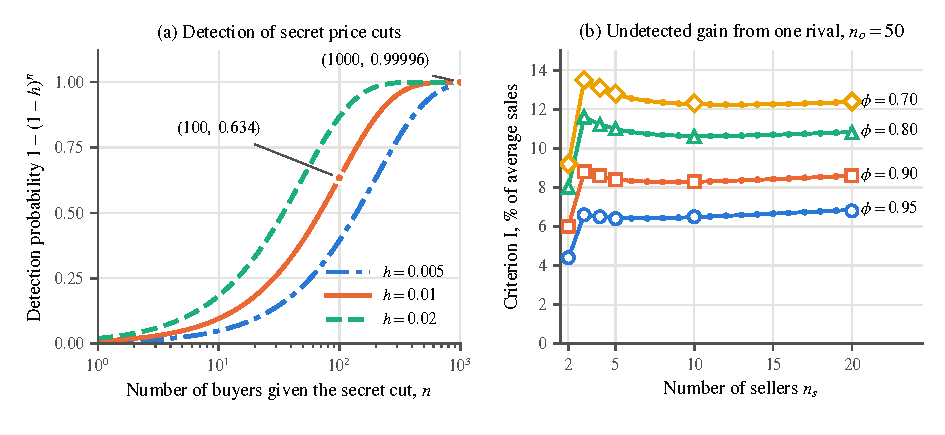
\includegraphics[width=\textwidth]{figures/ch02/stigler_detection.pdf}
\caption{Detection of secret price cutting. Panel (a) plots the probability that rivals hear of at least one secret cut
given to $n$ buyers, $1 - (1 - h)^n$, where $h$ is the probability that one cut is reported. The marked points are
Stigler's examples for $h = 0.01$. Panel (b) plots Stigler's Criterion I, \eqref{eq:02-stigler-crit1}, for $n_o = 50$
old buyers and four repeat probabilities $\phi$. Small dots are the formula at each integer $n_s$, and open markers
are the printed entries of \citet{Stigler1964}, Table 1. They coincide up to rounding.}
\label{fig:02-stigler-detect}
\end{figure}

\casehead{Criterion II: retaining one's own old customers}
A price cutter can also use secret cuts to keep more of its own old customers than usual. Without price cutting,
seller $i$ loses on average $(1 - \phi)\frac{n_o}{n_s}$ old customers, with variance $\sigma_1^2$. A single rival
has little basis for judging whether it receives a fair share of these. Stigler therefore assumes that the rivals
pool their information and suspect price cutting if seller $i$ loses fewer than
$(1 - \phi)\frac{n_o}{n_s} - 2\sigma_1$ customers, a 5 percent probability level. The cutter can then retain at most
$2\sigma_1$ extra old customers. As a share of its average sales, this is \emph{Criterion II},
\begin{equation}\label{eq:02-stigler-crit2}
G_{\mathrm{II}}(\phi, n_o, n_s) = \frac{2\sigma_1}{\frac{n_o}{n_s}} = 2\sqrt{\phi(1 - \phi)\,\frac{n_s}{n_o}} .
\end{equation}
It depends on the market only through the number of old customers per seller. Panel A of
\cref{tab:02-stigler-t234} reproduces part of Stigler's Table 2.

Comparing the two criteria shows that a price cutter is easier to detect through its gains from any one rival than
through an unusual rate of repeat sales. With $\phi = 0.95$ and 10 old customers per seller, Criterion II allows
13.8 percent. Table 1 gives the corresponding entries for one rival. They are 6.9 (2 sellers and 20 buyers), 8.9
(3 and 30), 7.4 (4 and 40), 6.4 (5 and 50) and 4.2 (10 and 100). Stigler adds two qualifications \citep[footnote 9]{Stigler1964}.
Multiplying the Table 1 entries by $n_s - 1$ gives the gain from all rivals together, which exceeds 13.8 percent
beyond two sellers. And Table 1 uses a looser probability level, so strict comparability would lower the Table 2
entries by one fifth. Stigler concludes that Criterion II will seldom be useful.

\casehead{Criterion III: new buyers}
New buyers form a flow rather than a stock, and Stigler takes the annual flow relative to old buyers as the unit.
Without price cutting, seller $i$ expects to sell to $m_3 = \frac{\lambda n_o}{n_s}$ new buyers, with binomial
variance $\sigma_3^2 = \left(1 - \frac{1}{n_s}\right)\frac{\lambda n_o}{n_s}$. Rivals cannot police this margin without
pooling information. With pooling, the seller is deemed a price cutter if it wins more than $m_3 + 2\sigma_3$ new
buyers, again a 5 percent level. Its total sales are $\frac{n_o(1 + \lambda)}{n_s}$ on average, so the largest
undetected gain as a share of sales is \emph{Criterion III},
\begin{equation}\label{eq:02-stigler-crit3}
G_{\mathrm{III}}(\lambda, n_o, n_s) = \frac{2\sigma_3}{\frac{n_o(1 + \lambda)}{n_s}}
= \frac{2}{1 + \lambda}\sqrt{\frac{(n_s - 1)\,\lambda}{n_o}} ,
\end{equation}
where the second equality uses $\sigma_3\frac{n_s}{n_o} = \sqrt{\frac{(n_s - 1)\lambda}{n_o}}$.

Panel B of \cref{tab:02-stigler-t234} reproduces part of Stigler's Table 3. The incentive to cut prices to new
buyers rises rapidly with the number of sellers, in proportion to $\sqrt{n_s - 1}$ for a given total of buyers. It
rises slowly when buyers per seller are held fixed. With $\lambda = \frac{1}{10}$ and 10 buyers per seller, it is
12.9 percent with 2 sellers and 17.7 percent with 20. It falls with the absolute number of buyers. Its dependence
on the rate of entry runs through the factor $\frac{\sqrt{\lambda}}{1 + \lambda}$, whose derivative has the sign of
$1 - \lambda$. The criterion therefore rises with $\lambda$ for $0 < \lambda < 1$, peaks at $\lambda = 1$ and falls
beyond it. With $n_o = 100$ and $n_s = 10$, it is 30 percent at $\lambda = 1$ and 24 percent at $\lambda = 4$. Rates
above one mean more new buyers per year than old buyers, and Stigler's Table 3 stays within $\lambda \le
\frac{1}{4}$. In that range, Stigler finds that when new buyers arrive at 10 percent per year or more, secret cuts
aimed at them yield larger undetected gains than poaching from any one rival. With $\phi = 0.90$, 100 old
buyers and 10 sellers, Criterion I allows 5.4 percent from each rival, while Criterion III with $\lambda =
\frac{1}{10}$ allows 17.2 percent in total. Markets in which new buyers arrive at such rates are therefore hard to
cartelize.

\begin{table}[htbp]
\centering
\caption{Stigler's Criteria II, III and IV (percent of average sales)}
\label{tab:02-stigler-t234}
\small
{\textit{Panel A. Criterion II: old customers a price cutter can retain (Table 2)}}\par\smallskip
\begin{tabular}{@{}lcccc@{}}
\toprule
& \multicolumn{4}{c}{Old customers per seller $\frac{n_o}{n_s}$} \\
\cmidrule(l){2-5}
Repeat probability $\phi$ & 10 & 20 & 50 & 100 \\
\midrule
0.95 & 13.8 & 9.7  & 6.2  & 4.4  \\
0.90 & 19.0 & 13.4 & 8.5  & 6.0  \\
0.80 & 25.3 & 17.9 & 11.3 & 8.0  \\
0.70 & 29.0 & 20.5 & 13.0 & 9.2  \\
0.50 & 31.6 & 22.4 & 14.1 & 10.0 \\
\bottomrule
\end{tabular}

\medskip
{\textit{Panel B. Criterion III: additional new customers obtainable (Table 3)}}\par\smallskip
\begin{tabular}{@{}cc*{6}{r}@{}}
\toprule
& & \multicolumn{6}{c}{Number of sellers $n_s$} \\
\cmidrule(l){3-8}
New-buyer rate $\lambda$ & Old buyers $n_o$ & 2 & 3 & 4 & 5 & 10 & 20 \\
\midrule
$\frac{1}{100}$ & 20  & 4.4 & 6.3 & 7.7 & 8.9 & 13.3 & 19.3 \\
                & 100 & 2.0 & 2.8 & 3.4 & 4.0 & 5.9  & 8.6  \\
                & 400 & 1.0 & 1.4 & 1.7 & 2.0 & 3.0  & 4.3  \\
\addlinespace
$\frac{1}{10}$  & 20  & 12.9 & 18.2 & 22.3 & 25.7 & 38.6 & 56.0 \\
                & 100 & 5.8  & 8.1  & 10.0 & 11.5 & 17.2 & 25.1 \\
                & 400 & 2.9  & 4.1  & 5.0  & 5.8  & 8.6  & 12.5 \\
\addlinespace
$\frac{1}{4}$   & 20  & 17.9 & 25.3 & 31.0 & 35.8 & 53.7 & 78.0 \\
                & 100 & 8.0  & 11.3 & 13.9 & 16.0 & 24.0 & 34.9 \\
                & 400 & 4.0  & 5.7  & 6.9  & 8.0  & 12.0 & 17.4 \\
\bottomrule
\end{tabular}

\medskip
{\textit{Panel C. Criterion IV: gain of a small firm against a large one, $\phi = 0.9$ (Table 4)}}\par\smallskip
\begin{tabular}{@{}cccccc@{}}
\toprule
& & \multicolumn{4}{c}{Size of large firm $K$} \\
\cmidrule(l){3-6}
Firms $n_s - K + 1$ & Buyers per small seller & 1 & 2 & 5 & 9 \\
\midrule
2  & 10 & 9.5 & 13.4 & 21.2 & 28.5 \\
2  & 50 & 4.2 & 6.0  & 9.5  & 12.7 \\
4  & 10 & 9.7 & 13.1 & 19.7 & 25.7 \\
10 & 10 & 5.4 & 7.2  & 10.7 & 14.0 \\
10 & 50 & 2.2 & 2.9  & 4.5  & 5.9  \\
\bottomrule
\end{tabular}

\medskip
\begin{minipage}{0.94\linewidth}
\footnotesize
Notes: Selected cells of \citet{Stigler1964}, Tables 2 to 4. Panel A uses \eqref{eq:02-stigler-crit2}, Panel B
uses \eqref{eq:02-stigler-crit3} and Panel C uses \eqref{eq:02-stigler-crit4}. We recomputed every printed cell of
the three tables. All agree to within 0.06 except one cell of Table 4 ($\phi = 0.9$, four firms, 50 buyers per
small seller, $K = 1$). It is printed as 4.0, while the formula gives 3.93 and the matching Table 1 cell is 3.9. In
Panel C, $n_s$ counts sellers in units of the small firm, so a firm of size $K$ counts as $K$ sellers.
\end{minipage}
\end{table}

\casehead{Pooling of information and unequal firm sizes}
With more than two sellers, firms can pool information and detect smaller deviations. The average number of old
customers that one cutter can take from $T$ rivals that pool information is at most
$\frac{T(1 - \phi)\,n_o}{n_s(n_s - T)}\bigl(1 + \frac{\tau}{\sqrt{T}}\bigr)$, with a correspondingly scaled variance.
For $T = 1$ this is $m_2$.
Both are smaller, relative to the customers lost by each pooling firm, than the corresponding expressions for one
seller. Pooling has limits. It becomes expensive as the pool grows, and it produces less reliable information,
because a member of the pool may itself be cutting prices.

Pooling by $K$ firms is equivalent to a single firm $K$ times as large as the others. Stigler's \emph{Criterion IV}
gives the gain of a small firm against such a large rival. It is measured as a percentage of the small firm's
average number of old customers, with $n_s$ counted in small-firm units:
\begin{equation}\label{eq:02-stigler-crit4}
G_{\mathrm{IV}} = \frac{1}{n_s - K}\left[\tau(1 - \phi)\sqrt{K}
+ \sqrt{\frac{n_sK(1 - \phi)(n_s - K - 1)\bigl(1 + \frac{\tau}{\sqrt{K}}\bigr)}{n_o}}\,\right].
\end{equation} For $K = 1$ it reduces to Criterion I. Compare Tables 1 and 4 for 100
customers, 10 firms and $\phi = 0.9$. A firm can take 5.4 percent of its sales from one rival, or about 50 percent
from all nine. If the nine rivals combine, Table 4 caps its gain at 28.5 percent.
In a second example with 20 firms and 200 customers, the gain from nine rivals falls from about 30 percent to 14.0
percent when they merge. Pooling information thus substantially reduces the scope for secret price cutting.
Stigler notes that Table 4 exaggerates the effect of size inequality. Only buyers above some size relative to the
seller are worth secret cuts, and a small firm can profitably cut prices to buyers too small to interest a large
seller.

\casehead{Repetition over time}
What may be chance in a single round cannot equally be chance if repeated. Over $T$ rounds, the mean loss to a
rival grows in proportion to $T$, while its standard deviation grows in proportion to $\sqrt{T}$. The threshold loss
over $T$ rounds is therefore $\frac{T(1 - \phi)}{n_s - 1}\cdot\frac{n_o}{n_s}\bigl(1 + \frac{\tau}{\sqrt{T}}\bigr)$.
The tolerated excess, relative to the mean, falls only as $\frac{1}{\sqrt{T}}$. Stigler concludes that this source of
information has minor efficacy unless buyers purchase, or sign contracts, frequently.

\subsubsection{Concentration and the Herfindahl index}

The model implies a measure of concentration suited to collusion. Suppose each new buyer picks firm $i$ with
probability equal to its output share $s_i$. Firm $i$'s number of new customers is then binomial with variance
$n_ns_i(1 - s_i)$. Summing over firms gives the total sampling noise against which price cutting must be detected,
\begin{equation}\label{eq:02-stigler-hhi}
\sum_{i} n_n s_i(1 - s_i) = n_n\Bigl(\sum_i s_i - \sum_i s_i^2\Bigr) = n_n(1 - \HHI) .
\end{equation}
The noise falls as the Herfindahl index rises. A similar argument applies to old customers
\citep[footnote 12]{Stigler1964}. Firm $j$ gains on average $(1 - \phi)n_o\frac{s_is_j}{1 - s_i}$ of the old customers
lost by firm $i$, with variance $(1 - \phi)n_o\frac{s_is_j}{1 - s_i}\bigl(1 - \frac{s_j}{1 - s_i}\bigr)$. Summing over
$i \ne j$ gives approximately $(1 - \phi)n_os_j(1 + \HHI - 2s_j)$. Summing over $j$ gives
$(1 - \phi)n_o(1 + \HHI - 2\HHI) = (1 - \phi)n_o(1 - \HHI)$. Stigler warns that the agreement of the two measures is
superficial, because the first assumes pooling of information and the second does not.

This gives a second foundation for the Herfindahl index, alongside the Cournot identity
$\bar L = \frac{\HHI}{\varepsilon}$ of \cref{prop:02-cowling-waterson}. The two arguments differ in kind. In Cournot,
a higher $\HHI$ raises margins under fixed noncooperative conduct. In Stigler's model, a higher $\HHI$ makes
collusion easier to police, so conduct itself changes. Both make the Herfindahl index more informative than a
four-firm ratio.

The analysis extends to nonprice competition with two modifications. There must be a definite joint
profit-maximizing policy to agree on, which is clearer for some variables than others. And nonprice moves differ in
detectability. Advertising, product quality and servicing leave visible traces, while reciprocal purchasing and
patent licensing do not. Collusion should suppress competition in the visible dimensions and leave it alive in the
hidden ones. The common belief that nonprice competition is more prevalent than price competition is therefore only
partly consistent with the theory.

The model's predictions can be collected. Collusion is easier to sustain when there are fewer sellers and when
buyers are numerous and small relative to sellers. A secret cut offered to many small buyers is likely to be
detected. Collusion is also easier when buyers are loyal ($\phi$ high) and new buyers arrive slowly ($\lambda$ low,
within $\lambda < 1$). It is easier still when sellers are unequal in size or pool information, when buyers report prices,
and when transactions are homogeneous enough for a simple price structure.

\subsubsection{Evidence}

Stigler's Section IV offers what he calls fragments of evidence. Two studies of the effect of the number of sellers
on price come first. He notes that, as far as he knows, no systematic analysis of this effect had been made
before.

\casehead{Newspapers and radio}
The first study concerns newspaper advertising rates in 53 cities in 1939. The rate per line per million
circulation, called the milline rate $R$, falls with circulation $z$. Stigler therefore first regresses
\begin{equation*}
\log R = 5.194 - \underset{(0.620)}{1.688}\,\log z + \underset{(0.063)}{0.139}\,(\log z)^2
\end{equation*}
He then tabulates the residuals by the number of evening papers in the city (Panel A of
\cref{tab:02-stigler-t56}). The mean residual is 0.0211 in one-paper cities and $-0.0213$ in two-paper cities.
Stigler reads this as rates about 5 percent above average in one-paper towns and 5 percent below in two-paper
towns. That reading matches base-10 logarithms, since $10^{0.0211} = 1.050$, while $e^{0.0211} = 1.021$.
Stigler adds that one-paper cities with an independent morning paper fall nearly midway between the two groups,
although their tabulated mean residual ($-0.0174$) lies close to the two-paper mean. Few cities had
more than two evening papers, so larger numbers of firms could not be studied. The subgroup means are internally
consistent: $\frac{10(-0.0174) + 13(0.0507)}{23} = 0.0211$.

The second study regresses the logarithm of AM radio spot rates on station characteristics for 345 stations in
Ohio, Indiana, Michigan and Illinois in 1961 (Panel B of \cref{tab:02-stigler-t56}). The elasticity of the rate with
respect to the number of stations in the county is $-0.074$, with a standard error of 0.046. The number of stations
ranges from 1 to 13 and is highly correlated with county population ($r^2 = 0.796$ in logarithms), which the
regression controls for. Both studies suggest that prices respond little to the number of rivals. Stigler finds this
consistent with his model, in which the number of buyers, the share of new buyers and the relative sizes of firms
matter as much as the number of sellers.

\begin{table}[htbp]
\centering
\caption{Number of sellers and prices in Stigler (1964)}
\label{tab:02-stigler-t56}
\small
{\textit{Panel A. Residuals from the regression of newspaper advertising rates on circulation, 1939 (Table 5)}}\par\smallskip
\begin{tabular}{@{}lccc@{}}
\toprule
Evening papers in city & Cities & Mean residual & Standard deviation of mean \\
\midrule
One                          & 23 & $0.0211$  & 0.0210 \\
\quad With morning paper     & 10 & $-0.0174$ & 0.0324 \\
\quad Without morning paper  & 13 & $0.0507$  & 0.0233 \\
Two                          & 30 & $-0.0213$ & 0.0135 \\
\bottomrule
\end{tabular}

\medskip
{\textit{Panel B. Regression of log AM spot commercial rates, 1961, $n = 345$ (Table 6)}}\par\smallskip
\begin{tabular}{@{}lcc@{}}
\toprule
Regressor & Coefficient & Standard error \\
\midrule
Log population of county, 1960              & $0.238$  & 0.026 \\
Log kilowatt power of station               & $0.206$  & 0.015 \\
Broadcast period: sunrise to sunset         & $-0.114$ & 0.025 \\
Broadcast period: longer, under 18 hours    & $-0.086$ & 0.027 \\
Broadcast period: 18 to 21 hours            & $-0.053$ & 0.028 \\
Log number of stations in county            & $-0.074$ & 0.046 \\
\midrule
$R^2$ & \multicolumn{2}{c}{0.743} \\
\bottomrule
\end{tabular}

\medskip
\begin{minipage}{0.94\linewidth}
\footnotesize
Notes: From \citet{Stigler1964}, Tables 5 and 6. Panel A: residuals, in logarithms, from
$\log R = 5.194 - 1.688\log z + 0.139(\log z)^2$, where $R$ is the milline rate and $z$ is circulation. The standard
errors of the slope coefficients are 0.620 and 0.063. Stigler's data come from the American Association of
Advertising Agencies. Panel B: the dependent variable is the logarithm of the average rate for 26 spots on May 1, 1961. The
broadcast-period variables are dummies. Table 6 does not state the omitted category. Stigler's data come from
the Standard Rate and Data Service.
\end{minipage}
\end{table}

\casehead{Profitability and concentration}
The direct test of the theory relates profitability to concentration across industries. Stigler restricts the
sample to 17 industries in which the sampled firms account for at least 35 percent of industry sales and earn at
least half of their revenue in the industry. Large steel and chemical firms, for example, operate in many markets
and are excluded. \Cref{tab:02-stigler-t7} reproduces his Table 7. Concentration in 1954 is measured by the four-firm
share and by the Herfindahl index. Profitability over 1953--57 is measured by the rate of return on all assets, the
rate of return on net worth, and the ratio of market to book value of common stock.

\begin{table}[htbp]
\centering
\begin{threeparttable}
\caption{Profitability and concentration in 17 industries (Stigler 1964)}
\label{tab:02-stigler-t7}
\small
\begin{tabular}{@{}lccccc@{}}
\toprule
& \multicolumn{2}{c}{Concentration, 1954} & \multicolumn{2}{c}{Average return, 1953--57} & Market to book \\
\cmidrule(lr){2-3}\cmidrule(lr){4-5}
Industry (firms) & Top-4 share & $\HHI$ & All assets & Net worth & value, 1953--57 \\
\midrule
\multicolumn{6}{@{}l}{\textit{Panel A. Industry data (Table 7)}} \\
Sulfur mining (4)                  & 98 & 0.407 & 19.03 & 23.85 & 3.02 \\
Automobiles (3)                    & 98 & 0.369 & 11.71 & 20.26 & 2.30 \\
Flat glass (3)                     & 90 & 0.296 & 11.79 & 16.17 & 2.22 \\
Gypsum products (2)                & 90 & 0.280 & 12.16 & 20.26 & 1.83 \\
Primary aluminum (4)               & 98 & 0.277 & 6.87  & 13.46 & 2.48 \\
Metal cans (4)                     & 80 & 0.260 & 7.27  & 13.90 & 1.60 \\
Chewing gum (2)                    & 86 & 0.254 & 13.50 & 17.06 & 2.46 \\
Hard-surface floor coverings (3)   & 87 & 0.233 & 6.56  & 7.59  & 0.98 \\
Cigarettes (5)                     & 83 & 0.213 & 7.23  & 11.18 & 1.29 \\
Industrial gases (3)               & 84 & 0.202 & 8.25  & 11.53 & 1.33 \\
Corn wet milling (3)               & 75 & 0.201 & 9.17  & 11.55 & 1.48 \\
Typewriters (3)                    & 83 & 0.198 & 3.55  & 5.39  & 0.84 \\
Domestic laundry equipment (2)     & 68 & 0.174 & 9.97  & 17.76 & 1.66 \\
Rubber tires (9)                   & 79 & 0.171 & 7.86  & 14.02 & 1.70 \\
Rayon fiber (4)                    & 76 & 0.169 & 5.64  & 6.62  & 0.84 \\
Carbon black (2)                   & 73 & 0.152 & 8.29  & 9.97  & 1.40 \\
Distilled liquors (6)              & 64 & 0.118 & 6.94  & 7.55  & 0.77 \\
\midrule
\multicolumn{6}{@{}l}{\textit{Panel B. Rank correlations with profitability (Table 8)}} \\
Top-4 share      & & & 0.322 & 0.507 & 0.642 \\
Herfindahl index & & & 0.524 & 0.692 & 0.730 \\
\bottomrule
\end{tabular}
\begin{tablenotes}\footnotesize
\item Notes: From \citet{Stigler1964}, Tables 7 and 8. The number of sampled firms is in parentheses. Returns are in
percent. In Panel B, each entry is the rank correlation between the concentration measure in the row and the
profitability measure in the column. Stigler reports a rank correlation of 0.903 between the two concentration
measures (his footnote 14). Our Spearman correlations computed from Panel A are 0.320, 0.499 and 0.652 for the
top-4 share. For $\HHI$ they are 0.525, 0.692 and 0.737, and between the two measures 0.903. The small differences
presumably reflect the treatment of ties.
\end{tablenotes}
\end{threeparttable}
\end{table}

All six rank correlations are positive. The Herfindahl index correlates more strongly with each profitability
measure than the four-firm share does, as the variance argument of \eqref{eq:02-stigler-hhi} suggests. Stigler
reads the data as showing no relation between profitability and concentration when $\HHI$ is below 0.250 or the
four-firm share is below about 80 percent. Our computations from Table 7 agree. Among the ten industries with
$\HHI < 0.250$, the Spearman correlations of $\HHI$ with the three profitability measures are $-0.03$, 0.18 and
0.11. The seven industries above the threshold earn on average 11.8 percent on assets, against 7.3 percent below
it. Stigler is careful about what this shows. The data, like those on advertising rates, ``confirm our theory only
in the sense that they support theories which assert that competition increases with number of firms.''

\casehead{Price cutting in steel}
The last piece of evidence uses prices paid by buyers of steel products in the second quarter of 1939, measured
relative to quoted prices. \Cref{tab:02-stigler-t9} reproduces Stigler's Table 9. The entry of 8.3 for hot-rolled
sheets, for example, is an average reduction of 8.3 percent from quoted prices, with a standard deviation of 7.3
percent of quoted prices. The average discount is almost perfectly correlated with the dispersion of transaction
prices. Our correlation across the eight products is 0.91. Stigler interprets this as expected: the less perfect the
market knowledge, the more extensive the price cutting.

\begin{table}[htbp]
\centering
\begin{threeparttable}
\caption{Prices of steel products and industry structure (Stigler 1964)}
\label{tab:02-stigler-t9}
\small
\begin{tabular}{@{}lcccc@{}}
\toprule
& \multicolumn{2}{c}{Prices, 2nd quarter 1939 (percent)} & & \\
\cmidrule(lr){2-3}
Product class & Average discount & Standard deviation & Herfindahl index & Output 1939 \\
& from list price & & & relative to 1937 \\
\midrule
Hot-rolled sheets   & 8.3 & 7.3 & 0.0902 & 1.14 \\
Merchant bars       & 1.2 & 4.5 & 0.1517 & 0.84 \\
Hot-rolled strip    & 8.5 & 8.3 & 0.1069 & 0.56 \\
Plates              & 2.6 & 4.8 & 0.1740 & 0.85 \\
Structural shapes   & 3.2 & 4.3 & 0.3280 & 0.92 \\
Cold-rolled strip   & 8.8 & 9.8 & 0.0549 & 0.88 \\
Cold-rolled sheets  & 5.8 & 5.0 & 0.0963 & 1.14 \\
Cold-finished bars  & 0.9 & 3.4 & 0.0964 & 0.83 \\
\bottomrule
\end{tabular}
\begin{tablenotes}\footnotesize
\item Notes: From \citet{Stigler1964}, Table 9, in his row order. The Herfindahl index uses 1938 capacity.
Transaction prices come from a Bureau of Labor Statistics survey reported in \textit{Iron Age} (1946). Capacity
data come from the \textit{Directory of Iron and Steel Works of the United States and Canada}, and output data
from the American Iron and Steel Institute. In our computations across the eight rows, the correlation of the
discount with its standard deviation is 0.91. The correlation of the discount with $\HHI$ is $-0.46$ (Spearman
$-0.55$), and the least-squares line is $\text{discount} = 7.40 - 18.09\,\HHI$.
\end{tablenotes}
\end{threeparttable}
\end{table}

The data show larger discounts in the less concentrated product classes. Cold-rolled strip has the lowest index,
0.0549, and the largest discount, 8.8 percent. Structural shapes have the highest index, 0.3280, and a discount of
3.2 percent. This is the ordering the theory predicts, since secret cuts are harder to police when sellers are
numerous and small. Stigler's summary sentence states the relation with the opposite sign. His remarks on
individual products fit the data. He notes that structural shapes and hot-rolled strip sold somewhat below the
average relationship, while cold-finished bars sold above it. In our fitted line, the first two have discounts 1.7
and 3.0 points above the line and cold-finished bars 4.8 points below. He adds that the deviations are not
explained by demand, measured by 1939 output relative to 1937. Our residuals are indeed uncorrelated with that
measure. The survey also excluded some very large buyers in the automobile and container industries. Since very
large buyers obtained the largest concessions, Stigler infers that the table understates price cutting.

Stigler judged these fragments ``fairly favorable to the theory,'' while granting that they do not constitute strong
support. He expected more powerful tests from the electrical equipment conspiracy cases then in the courts. The
theory predicts that prices on public bids will be higher and less dispersed than in privately negotiated sales.
It also predicts that price cutting increases as the number of buyers diminishes \citep[footnote 16]{Stigler1964}. He saw the
large number of testable hypotheses as the main merit of the theory.

\subsubsection{Assessment}

Stigler's paper made collusion an information problem. It gave the first systematic account of why cartels hold in
some markets and fail in others, and it tied cartel stability to observable features of markets. These include the
number and size distribution of sellers, the size and loyalty of buyers and the rate of arrival of new buyers.
They also include the transparency of transaction prices and the complexity of the price structure. Several of these ideas now organize
antitrust thinking about coordinated effects, from the role of large buyers to the danger of price transparency
(\cref{ch:collusion-evidence}).

The model has clear limits. It contains no equilibrium. Punishment after detection is asserted, as the matching of
detected cuts, and never derived. The price cutter does not choose how much to cut by weighing gains against the
risk of detection. The detection rules use fixed probability thresholds, such as one standard deviation, without a
decision-theoretic basis. The collusive price level is not determined, and the criteria measure the incentive to cut
by undetected sales alone, ignoring the margin on those sales. The evidence is cross-sectional and inherits the
endogeneity of market structure discussed in \cref{ch:intro}.

\citet{GreenPorter1984} read Stigler differently from the cross-industry tradition he inspired (pp.~87--88). In their
reading, Stigler justified cross-industry regressions by relating concentration informally to a cartel's ability to
deter cheating, and by assuming that profitability reflects cartel success. They recast his cartel as the solution
to a design problem: an institution that achieves an efficient outcome subject to the constraint that members act
noncooperatively. That shift leads directly to the repeated-game models of the next subsection.

\subsection{Repeated interaction: a preview}\label{sec:02-repeated}

Repeated interaction gives Stigler's enforcement a formal foundation. A deviation today can be punished tomorrow,
so collusive prices can be an equilibrium even though each firm gains by deviating in the short run. As in
\cref{sec:02-multiproduct} and \cref{ch:collusion-theory}, $\delta \in (0, 1)$ denotes the discount factor. The
stage game is played in periods $t = 0, 1, 2, \dots$, and each firm maximizes $\sum_{t \ge 0}\delta^t\pi_{it}$. We
use \emph{grim-trigger strategies}: firms play the collusive action as long as no one has deviated, and revert
forever to the static Nash equilibrium after any deviation \citep{Friedman1971}. Static Nash play forever is itself
a subgame-perfect equilibrium, so the threat is credible. The one-shot deviation principle, the folk theorem and
optimal punishments are developed in \cref{ch:collusion-theory}.

The horizon must be infinite \citep[sec.~11.3.2]{Tirole1988}. A repeated game has almost perfect information
(\cref{sec:02-spe}), so it can be solved by backward induction when it ends at a known date. If the stage game has a
unique Nash equilibrium, the stage equilibrium is then played in every period, and collusion unravels from the end
(\cref{prop:12-finite}). The Bertrand game has several equilibrium profiles, but all of them give zero profit, so the
same argument applies. With an infinite horizon there is no last period from which to start. Repeating the stage
equilibrium forever remains a subgame-perfect equilibrium, because no current action changes future play. Other
equilibria now exist, and they are sustained by the threat of reverting to the stage equilibrium after a deviation.
\Cref{prop:02-bertrand-collusion,prop:02-cournot-collusion} state when this threat suffices. We give the intuition
here and prove both results in \cref{sec:12-perfect}.

\begin{proposition}[Collusion in the Bertrand supergame]\label{prop:02-bertrand-collusion}
Let $N$ identical firms with constant marginal cost $c$ play the homogeneous Bertrand game of \cref{sec:02-bertrand}
in every period, with observed prices. Grim-trigger strategies with collusive price $p^m$ and Bertrand reversion form
a subgame-perfect equilibrium if and only if
\begin{equation}\label{eq:02-bertrand-ic}
\delta \ge 1 - \frac{1}{N} .
\end{equation}
\end{proposition}

\Cref{prop:12-bertrand} gives the proof. On the collusive path, conforming yields $\frac{\pi^m}{N}$ in every period,
worth $\frac{\pi^m}{N(1 - \delta)}$. The best deviation undercuts $p^m$ slightly, earns almost $\pi^m$ once, and
earns zero after the reversion to Bertrand pricing. Collusion is sustainable when $\frac{\pi^m}{N(1 - \delta)} \ge
\pi^m$, which is \eqref{eq:02-bertrand-ic}.

The threshold rises with $N$. Each firm's collusive share $\frac{\pi^m}{N}$ shrinks while the one-period gain from
deviation stays at about $\pi^m$. This is the formal version of Stigler's observation that collusion is impossible
for many firms. \citet[sec.~6.3.2.1]{Tirole1988} uses it to give Bain's link between concentration and tacit
collusion a precise sense.

\begin{example}[Detection lags]\label{ex:02-detection-lag}
Stigler's insight is that deviations are detected with delay. Suppose rivals learn of a secret price cut only with
probability $\mu \in (0, 1]$ in each period, for instance because random switching of buyers masks the lost sales.
Until detection, the cutter serves the market at a price just below $p^m$. Its deviation payoff becomes
\begin{equation*}
\pi^m\sum_{t \ge 0}\bigl[\delta(1 - \mu)\bigr]^t = \frac{\pi^m}{1 - \delta(1 - \mu)} .
\end{equation*}
Conforming is optimal if and only if
\begin{equation*}
\frac{\pi^m}{N(1 - \delta)} \ge \frac{\pi^m}{1 - \delta + \delta\mu}
\iff \delta\mu \ge (N - 1)(1 - \delta)
\iff \delta \ge \frac{N - 1}{N - 1 + \mu} .
\end{equation*}
With $\mu = 1$ this is \eqref{eq:02-bertrand-ic}. As $\mu \to 0$ the threshold tends to 1, and collusion becomes
impossible. If a cut reaches 100 buyers who each report it with probability $h = 0.01$, then
$\mu = 1 - (0.99)^{100} = 0.634$ from \eqref{eq:02-stigler-detect}. The threshold rises from 0.50 to 0.61 for
two firms and from 0.80 to 0.86 for five.
\end{example}

\begin{proposition}[Collusion in the linear Cournot supergame]\label{prop:02-cournot-collusion}
Let $N$ identical firms with constant marginal cost $c$ play the Cournot game with $P(Q) = a - bQ$ in every period.
Grim-trigger strategies with collusive output $\frac{Q^m}{N}$ each and reversion to the Cournot equilibrium form a
subgame-perfect equilibrium if and only if
\begin{equation}\label{eq:02-cournot-delta}
\delta \ge \delta^*(N) = \frac{(N + 1)^2}{N^2 + 6N + 1} .
\end{equation}
\end{proposition}

\Cref{prop:12-cournot} gives the proof. Let $\pi_c$, $\pi_d$ and $\pi_n$ be the per-period collusive, best
one-shot deviation and Cournot profits. A firm conforms if collusion forever is worth at least one period of
deviation profit followed by Cournot profit forever:
\begin{equation*}
\frac{\pi_c}{1 - \delta} \ge \pi_d + \frac{\delta\,\pi_n}{1 - \delta}
\iff \delta \ge \frac{\pi_d - \pi_c}{\pi_d - \pi_n} .
\end{equation*}
With linear demand the three profits are proportional to $\frac{(a - c)^2}{b}$, so the ratio depends only on $N$. It
simplifies to \eqref{eq:02-cournot-delta}.

The threshold is $\delta^*(2) = \frac{9}{17} = 0.529$, and it rises to 0.571, 0.643 and 0.752 for $N = 3, 5$ and
10. Its derivative is $\frac{4(N - 1)(N + 1)}{(N^2 + 6N + 1)^2} > 0$, and $\delta^*(N) \to 1$ as $N \to \infty$. The
comparison with Bertrand is instructive. For $N = 2$ the Cournot threshold is higher than the Bertrand value of
0.5. For $N \ge 3$ it is lower: 0.571 against 0.667 at $N = 3$, and 0.752 against 0.900 at $N = 10$. Two forces
work in opposite directions. Cournot reversion is a milder punishment than Bertrand reversion. But a Cournot
deviator cannot capture the whole market, because rivals' outputs stay fixed. With three or more firms the second
force dominates.

\casehead{Conduct as a reduced form of dynamic play}
In these models the static conduct parameter of \cref{sec:02-conduct} summarizes the outcome of dynamic play. It is
close to 1 in collusive phases and close to its Cournot or Bertrand value in punishment phases. \citet{Bresnahan1989}
draws the empirical implication directly from Stigler (pp.~1023--1025). If self-interest alone holds a collusive
arrangement together, uncertainty about rivals' behavior will sometimes trigger price wars even without actual
cheating. Data on a collusive industry should then show periods of cooperation and periods of competition.
``Empirically, of course, this will show up as time-varying $\theta$.'' Two models formalize the idea with
different predictions about when the price wars occur.

\casehead{Green and Porter: price wars after bad news}
\citet{GreenPorter1984} study cartel self-enforcement under demand uncertainty. In their model firms choose outputs,
and the market price depends on total output and an unobserved demand shock. Firms observe the price, but neither
rivals' outputs nor the shock. A low price may therefore signal either cheating or bad demand. The cartel uses a
trigger price. Firms produce collusive outputs while the price stays above the trigger and revert to Cournot output
for a fixed number of periods after it falls below. In equilibrium no firm cheats, yet low demand realizations set
off price wars. The wars are necessary, because without them cheating could not be deterred. Green and Porter
emphasize that earlier formulations make incentives so perfect that the deterrent mechanism is never observed. With
imperfect information, recurrent price wars are part of successful collusion. They need not indicate a sequence of
failed attempts to form a cartel (pp.~87--88).

A simple price-setting version conveys the logic. Two firms face demand $Q(p)$ with probability $1 - \zeta$ and
zero demand with probability $\zeta$, independently each period. A firm with zero sales cannot tell low demand from
a rival's secret cut. The strategy is to price at $p^m$ until a period of zero sales and then price at $c$
forever. The value of collusion is $V = \frac{(1 - \zeta)\frac{\pi^m}{2}}{1 - \delta(1 - \zeta)}$. A deviator earns
$(1 - \zeta)\pi^m$ once and nothing afterwards. Conforming is optimal if and only if
\begin{equation*}
\frac{(1 - \zeta)\frac{\pi^m}{2}}{1 - \delta(1 - \zeta)} \ge (1 - \zeta)\,\pi^m
\iff \delta(1 - \zeta) \ge \frac{1}{2} .
\end{equation*}
More noise ($\zeta$ higher) makes collusion harder, and price wars start after unexpectedly low demand.
\Cref{ch:collusion-theory} treats finite punishments and the optimal trigger, including the refinements of
\citet{AbreuPearceStacchetti1986}.

\casehead{Rotemberg and Saloner: price wars during booms}
\citet{RotembergSaloner1986} study implicitly colluding oligopolists facing fluctuating demand that they observe.
Their key finding is that the temptation to deviate from the collusive outcome is often greater when demand is high.
To moderate the temptation, the oligopoly lowers its prices in booms. Suppose demand states are independent over
time, and let $\pi_s(p)$ be industry profit at price $p$ in state $s$. With collusive prices $p_s$ and Bertrand
reversion, the incentive constraint in state $s$ is
\begin{equation*}
\left(1 - \frac{1}{N}\right)\pi_s(p_s) \le \frac{\delta}{1 - \delta}\cdot\frac{1}{N}\,\E\bigl[\pi_{s'}(p_{s'})\bigr] .
\end{equation*}
The left side is the gain from deviating in the current state, and it rises with current demand. The right side is
the expected future loss, which does not depend on the current state. In high-demand states the constraint binds
first, and the cartel must cap profits below the monopoly level by cutting price. The abstract of the 1984 working-paper
version cites supporting evidence from the railroads in the 1880s and the automobile industry in the 1950s. It
also cites the cyclical behavior of cement prices and price-cost margins.

\casehead{Implications for measurement}
Both models imply that conduct varies over time, but they disagree about the pattern. In Green and Porter, conduct
switches to the competitive value after unanticipated low demand and returns after a fixed lag. In Rotemberg and
Saloner, conduct varies within the collusive regime with the level of demand. \citet{Porter1983} estimated a supply
relation with two regimes for a nineteenth-century railroad cartel (\cref{ch:collusion-evidence}). Bresnahan notes
that the existence of regimes is easier to establish than their causes. Asking whether there are price wars uses all
periods of data, while asking what starts and stops them has as many observations as there are wars. Time variation
in conduct also complicates the interpretation of a constant estimated $\theta$, which is the critique of
\citet{Corts1999} developed in \cref{ch:conduct}.

\section{From homogeneous to differentiated products}\label{sec:02-bridge}

The theory so far assumed a homogeneous good. Few markets fit that description. Products differ in physical
characteristics, location, brand and service, even in markets that look homogeneous, such as pharmaceuticals with
chemically identical generics or retail gasoline. Electricity and refined sugar, the settings of two case studies in
\cref{ch:conduct}, come close to homogeneity. Most empirical questions in industrial organization need a model of
demand for differentiated products. Measuring market power, evaluating mergers, assessing taxes and tariffs,
analyzing product introductions and valuing new goods all depend on substitution patterns. With differentiated
products there is also no natural boundary for the market, so an estimated demand system can stand in for
market definition. This section shows how the pricing logic of this chapter carries over and points to where it is
developed.

A single-product firm $j$ that sets its price, taking rivals' prices as given, is a monopolist on its residual
demand $q_j(p)$, as in \cref{sec:02-residual}. The first-order condition
$q_j + (p_j - mc_j)\frac{\partial q_j}{\partial p_j} = 0$ gives the dollar markup and Lerner rules
\eqref{eq:02-dollar-markup} and \eqref{eq:02-lerner}, with the own-price derivative of residual demand in place
of the market derivative:
\begin{equation}\label{eq:02-single-product-markup}
p_j - mc_j = -\frac{q_j}{\frac{\partial q_j}{\partial p_j}} ,
\qquad
\frac{p_j - mc_j}{p_j} = \frac{1}{|\varepsilon_{jj}|} .
\end{equation}
For example, with logit demand and price coefficient $\alpha$, $\frac{\partial s_j}{\partial p_j} = -\alpha s_j(1 - s_j)$,
so the markup is $\frac{1}{\alpha(1 - s_j)}$. Pass-through follows the formulas of \cref{sec:02-passthrough}, and for
the logit it equals $1 - s_j$ when rivals' prices are held fixed (\cref{ex:02-pt-examples}).

A firm that owns several products adds a new term. Let firm $f$ own the set $\mathcal{J}_f$ and maximize
$\sum_{k \in \mathcal{J}_f}(p_k - mc_k)\,q_k(p)$ over its own prices. The first-order condition for $p_j$,
$j \in \mathcal{J}_f$, is
\begin{equation*}
q_j + (p_j - mc_j)\frac{\partial q_j}{\partial p_j} + \sum_{k \in \mathcal{J}_f\setminus\{j\}}(p_k - mc_k)\frac{\partial q_k}{\partial p_j} = 0 .
\end{equation*}
Divide by $\frac{\partial q_j}{\partial p_j} < 0$, solve for $p_j$, and define the \emph{diversion ratio}
$D_{jk} = -\frac{\partial q_k}{\partial p_j}\bigl(\frac{\partial q_j}{\partial p_j}\bigr)^{-1}$, the fraction of the sales lost by
product $j$ that product $k$ recaptures when $p_j$ rises. Then
\begin{equation}\label{eq:02-diversion-foc}
p_j = mc_j - \frac{q_j}{\frac{\partial q_j}{\partial p_j}} + \sum_{k \in \mathcal{J}_f\setminus\{j\}}(p_k - mc_k)\,D_{jk} .
\end{equation}
Price equals marginal cost, plus the single-product markup, plus the margins the firm earns on sales recaptured by
its other products. The last term is an opportunity cost of selling product $j$, since each sale partly
cannibalizes the firm's other products. Joint ownership of substitutes therefore raises prices. A merger adds the
acquired products to $\mathcal{J}_f$ and the corresponding terms to \eqref{eq:02-diversion-foc}. This is the logic
of upward pricing pressure in \cref{ch:mergers}. The homogeneous-goods analogue is the gap between Cournot conduct,
in which each firm ignores its effect on rivals, and collusion, in which it internalizes all of it
(\cref{prop:02-cheat}).

When one firm owns every product, this first-order condition is the condition \eqref{eq:02-multi-foc-margin} of the
multiproduct monopolist in \cref{sec:02-multiproduct}. The diversion-ratio form is the same condition divided by
the own-price derivative. To see the link with the Lerner form, substitute $\frac{\partial q_k}{\partial p_j} =
\varepsilon_{kj}\frac{q_k}{p_j}$ and $\frac{\partial q_j}{\partial p_j} = -\lvert\varepsilon_{jj}\rvert\frac{q_j}{p_j}$
into the definition of the diversion ratio:
\[
  D_{jk} = \frac{\varepsilon_{kj}\,q_k}{\lvert\varepsilon_{jj}\rvert\,q_j} .
\]
The single-product markup is $-q_j\bigl(\frac{\partial q_j}{\partial p_j}\bigr)^{-1} =
\frac{p_j}{\lvert\varepsilon_{jj}\rvert}$.
Dividing \eqref{eq:02-diversion-foc} by $p_j$ and writing $R_j = p_jq_j$ then gives
\[
  \frac{p_j - mc_j}{p_j} = \frac{1}{\lvert\varepsilon_{jj}\rvert}
  + \sum_{k \in \mathcal{J}_f\setminus\{j\}}\frac{(p_k - mc_k)\,q_k\,\varepsilon_{kj}}{R_j\,\lvert\varepsilon_{jj}\rvert} ,
\]
which is \eqref{eq:02-multi-lerner} with the sum restricted to the firm's own products. Positive diversion
corresponds to substitutes in that formula, and it raises the Lerner index above the inverse own elasticity.

Stacking \eqref{eq:02-diversion-foc} over products gives the matrix form $p = mc - (\Omega \odot \Delta^\top)^{-1}q$,
with ownership matrix $\Omega$ ($\Omega_{jk} = 1$ if $j$ and $k$ have the same owner) and demand Jacobian $\Delta$,
whose $(j,k)$ element is $\frac{\partial q_j}{\partial p_k}$. \Cref{ch:diffprod} develops this system, the existence
and uniqueness of equilibrium, the recovery of marginal costs from estimated demand, and the demand models that
supply the derivatives. Theory in this area mostly studies prices and products given a demand system. Empirical work
does the reverse: it models demand richly and supply simply, usually as static Bertrand-Nash pricing. Richer demand
models add assumptions and computation, so they should be judged by what they add for the question at hand and the
data available.


\section{Bibliographic notes}\label{sec:02-notes}

\citet{Tirole1988} remains the standard textbook treatment of the theory in this chapter. The electronic edition we
used has no printed page numbers, so we cite it by chapter, section, equation and exercise. Its chapter~1 (secs.~1.1
to 1.5) covers single-product and multiproduct monopoly, the deadweight loss and the output subsidy
(\cref{sec:02-monopoly,sec:02-welfare}). It also treats cost distortions, rent seeking and the limits that recycling
and durability place on monopoly power. Chapter~5 covers Bertrand competition, rationing and capacity constraints in
secs.~5.1 to 5.3 (\cref{sec:02-bertrand}). Its secs.~5.4 and 5.5 treat Cournot competition and concentration
indices, and sec.~5.7 treats existence, convergence and the capacity-price game
(\cref{sec:02-measures,sec:02-cournot}). Section~6.3 treats
the supergames previewed in \cref{sec:02-repeated}. Chapter~11 is a user's manual for the game theory of
\cref{sec:02-games}, and \citet{FudenbergTirole1991} give a complete treatment. \citet{Shapiro1989} surveys static
and dynamic oligopoly theory, and \citet{Vives1999} develops existence, uniqueness and comparative statics with the
tools of aggregative and supermodular games.

The aggregative proof of \cref{prop:02-cournot-exist} goes back to \citet{SzidarovszkyYakowitz1977} and
\citet{Novshek1985}. The effects of entry on Cournot outcomes go back to \citet{Seade1980}, and the
margin-concentration identity to \citet{CowlingWaterson1976}. \citet{EncaouaJacquemin1980} give the axioms for
concentration indices. \citet{Demsetz1973} gives the efficiency explanation of the link between concentration and
profit. \citet{DansbyWillig1979} give the welfare interpretation of the Herfindahl index.
\citet{BulowGeanakoplosKlemperer1985} introduced the language of strategic substitutes and complements.
\citet{Edgeworth1925}, first published in 1897, showed that capacity limits undo the Bertrand outcome.
\citet{Beckmann1967} and \citet{LevitanShubik1972} solved the capacity-constrained price game.
\citet{KrepsScheinkman1983} and \citet{DavidsonDeneckere1986} are the key papers on capacity commitment and price
competition, and \citet{Gertner1985} studies the game in which capacities are not observed.
\citet{KlempererMeyer1989} develop supply function equilibria.

The conduct parameter and its interpretation are best read in \citet{Bresnahan1989}, which also gives the menu of
conduct for leaders, fringes and collusive regimes. \citet{Corts1999} shows why a constant estimated $\theta$ need
not measure average conduct, a point that \cref{ch:conduct} develops. The theory of pass-through starts with
\citet{BulowPfleiderer1983}, and \citet{WeylFabinger2013} unify pass-through and incidence under imperfect
competition. \citet{Sumner1981} and \citet{GenesoveMullin1998} use pass-through and the Bulow-Pfleiderer demand
family to measure conduct.

The welfare analysis of free entry follows \citet{MankiwWhinston1986}, who build on \citet{Spence1976} and
\citet{DixitStiglitz1977} for the case of product diversity. \citet{BerryWaldfogel1999} measure the inefficiency of
free entry in radio broadcasting, an empirical test of the excess-entry theorem. The 1996 working-paper version
(NBER Working Paper 5528), which we cite here, uses data on advertising prices, numbers of stations and listening in 135
US metropolitan markets. Relative to the social optimum, the welfare loss of free entry is 40 percent of industry
revenue, counting market participants other than listeners. Free entry would be optimal if the marginal value of
programming to listeners exceeded three times the value of marginal listeners to advertisers, who pay 4.5 cents per
hour. \Cref{ch:diffprod} returns to this paper.

The deadweight loss of monopoly was first estimated by \citet{Harberger1954}. \citet{Posner1975} added the costs of
rent-seeking, and \citet{Fisher1985} questioned the conditions under which rents are fully dissipated.
\citet[pp.~739 and 743]{CowlingMueller1978} found losses of up to 13 percent of gross corporate product in the
United States and 7.2 percent in the United Kingdom once rent-seeking costs are counted. \citet{JennyWeber1983} also
found large losses, and \citet{Scherer1980} doubts these high estimates \citep[sec.~1.1.1.2]{Tirole1988}.
\citet{Leibenstein1966} named X-inefficiency, and \citet{Coase1972} posed the problem of
the durable-good monopolist. \citet{Williamson1968} framed the trade-off between market power and cost savings that
merger policy still uses.

\citet{Stigler1964} founded the information-based theory of collusion. \citet{Friedman1971} gave the first
repeated-game model of collusion with trigger strategies, and \citet{GreenPorter1984} and
\citet{RotembergSaloner1986} showed how imperfect monitoring and demand fluctuations generate price wars.
\citet{AbreuPearceStacchetti1986} characterized optimal cartel equilibria under imperfect monitoring. \Cref{ch:collusion-theory} develops these models
and \cref{ch:collusion-evidence} confronts them with data.

\section{Exercises}\label{sec:02-exercises}

\begin{enumerate}[label=\arabic*., leftmargin=*, itemsep=6pt]

\item \textit{Cournot competition with constant-elasticity demand.} Inverse demand is
$P(Q) = \left(\frac{Q}{A}\right)^{-\frac{1}{\varepsilon}}$ with $A > 0$ and $\varepsilon > 0$, and $N$ firms have
the same constant marginal cost $c > 0$.
\begin{enumerate}[label=(\alph*)]
  \item Derive the symmetric Cournot equilibrium price and the Lerner index. Show that an interior equilibrium
  requires $N\varepsilon > 1$, and check the second-order condition at the equilibrium.
  \item Show that the firm-level inequality $P'(Q) + q_iP''(Q) < 0$ of \cref{rem:02-c2}, evaluated at the symmetric
  equilibrium, holds if and only if $N\varepsilon > 1 + \varepsilon$. Give an example with $N = 2$ in which an
  interior equilibrium exists although this inequality fails at the equilibrium. Are quantities strategic
  substitutes or complements there?
  \item Assume $N\varepsilon > 1 + \varepsilon$. Use \cref{prop:02-pt-cournot} to compute the pass-through of a
  common cost shock and of a shock to one firm's cost. Compare the two with the monopoly rate $\frac{\varepsilon}{\varepsilon - 1}$ and explain why a more
  competitive industry passes through less.
\end{enumerate}

\item \textit{Consistent conjectures.} Two firms face $P(Q) = a - bQ$ and have the cost function
$C(q) = cq + \frac{k}{2}q^2$ with $k \ge 0$. Each firm holds the constant conjecture
$r = \frac{\dd q_j}{\dd q_i}$, the conjectural variation of \cref{sec:02-aggregation} with one rival.
\begin{enumerate}[label=(\alph*)]
  \item Derive firm $i$'s first-order condition and its reaction function. Show that the reaction function has slope
  $-\frac{b}{(2 + r)b + k}$.
  \item A conjecture is \emph{consistent} if it equals the slope of the rival's reaction function. Show that with
  $k = 0$ the only consistent conjecture is $r = -1$, and that it yields price equal to marginal cost.
  \item Show that with $k > 0$ the consistent conjecture lies in $(-1, 0)$. Compute the implied industry conduct
  parameter.
  \item Explain why consistency does not answer the critique of conjectural variations in
  \cref{sec:02-interpret}.
\end{enumerate}

\item \textit{Constant pass-through.} Complete the proof of \cref{prop:02-pt-constant}.
\begin{enumerate}[label=(\alph*)]
  \item Suppose monopoly pass-through equals a constant $\rho > 0$ on an interval of costs. Show that
  $\frac{QP''(Q)}{P'(Q)} = \frac{1}{\rho} - 2$ on the corresponding interval of outputs.
  \item Solve this differential equation for $P'$, and then for $P$. Show that $P(Q) = a - bQ^{\gamma}$ with
  $\gamma = \frac{1}{\rho} - 1$ when $\rho \ne 1$, and $P(Q) = a - b\ln Q$ when $\rho = 1$.
  \item Identify the members of the family with linear, quadratic and constant-elasticity demand, and state the
  restrictions on $(a, b, \gamma)$ that make demand downward sloping and satisfy the second-order condition.
  \item Show that pass-through is also constant under any constant conduct $\theta$, and find its value.
\end{enumerate}

\item \textit{Specific and ad valorem taxes under monopoly.} A monopolist with constant marginal cost $c > 0$ faces
$Q(p) = Ap^{-\varepsilon}$ with $\varepsilon > 1$.
\begin{enumerate}[label=(\alph*)]
  \item Derive the price under a specific tax $t$ and under an ad valorem tax at rate $t_a$ (\cref{rem:02-pt-adval}).
  Compute $\frac{\dd p}{\dd t}$ and $\frac{\dd p}{\dd t_a}$ at zero taxes.
  \item Use \cref{prop:02-incidence} and the envelope theorem to compute the consumer burden, the producer burden and
  the tax revenue of each tax at the margin, starting from zero taxes.
  \item Normalize both taxes to raise one dollar of revenue at the margin. Which tax imposes the smaller burden on
  consumers, and which the smaller loss of total surplus? Explain the answer in terms of the effect of each tax on
  the firm's markup.
\end{enumerate}

\item \textit{Excess entry.} Use the linear Cournot market of \cref{ex:02-mw-linear} with $a - c = 8$ and $b = 1$.
\begin{enumerate}[label=(\alph*)]
  \item Find the set-up cost $F$ for which the second-best number of firms is $N^o = 4$.
  \item Compute the free-entry number of firms with $N$ treated as continuous and as an integer.
  \item Compute total surplus at $N^o$ and at the integer $N^e$, and express the loss as a percentage of the maximal
  surplus $\frac{(a - c)^2}{2b}$.
  \item Show that, with $N$ continuous, the loss as a share of the maximal surplus depends on the primitives only
  through $N^o$. Explain why the loss shrinks as $N^o$ grows although $N^e - N^o$ grows.
\end{enumerate}

\item \textit{Partial collusion in a Cournot duopoly.} Two firms with constant marginal cost $c$ face
$P(Q) = a - bQ$ in every period, discount the future by $\delta$ and use grim-trigger strategies with Cournot
reversion. They agree on a symmetric
output $q$ per firm, between the collusive output $\frac{a - c}{4b}$ and the Cournot output $\frac{a - c}{3b}$.
\begin{enumerate}[label=(\alph*)]
  \item Compute the per-period profit from conforming, the profit from the best one-period deviation, and the Cournot
  profit, as functions of $q$.
  \item Show that the incentive constraint holds if and only if
  $q \ge \frac{(a - c)(9 - 5\delta)}{b(27 - 3\delta)}$.
  \item Conclude that firms with $\delta < \frac{9}{17}$ can still sustain prices above the Cournot level. Plot the
  implied conduct parameter $\theta(\delta)$ against $\delta \in [0, 1)$ and relate the result to the time-varying
  conduct of \cref{sec:02-repeated}.
\end{enumerate}

\item \textit{Stigler's model of detection.}
\begin{enumerate}[label=(\alph*)]
  \item Use \eqref{eq:02-stigler-crit1} to compute Criterion I for $\phi = 0.9$, $n_o = 100$ and $n_s = 5$, and check
  your answer against \cref{tab:02-stigler-t1}.
  \item Show that, as $n_o \to \infty$ with $n_s$ and $\phi$ fixed,
  \[
    \sqrt{n_o}\,G_{\mathrm{I}} \to \frac{1}{n_s - 1}\left[\sqrt{\phi(1 - \phi)n_s} + \sqrt{n_s(n_s - 2)(1 - \phi)}\right].
  \]
  Interpret the result in terms of the number of buyers per seller.
  \item Derive \eqref{eq:02-stigler-hhi}. Construct two markets with the same four-firm concentration ratio and
  different Herfindahl indices, and say in which one Stigler's theory predicts more effective collusion.
  \item List two features of a modern repeated-game model of collusion that Stigler's model lacks, and explain how
  each changes the predictions in (b) and (c).
\end{enumerate}

\item \textit{Interpreting a pass-through estimate.} A regression of the retail price of a product on a specific
excise tax, across regions and years, gives $\hat\rho = 1.07$ with a small standard error.
\begin{enumerate}[label=(\alph*)]
  \item Use \cref{cor:02-pt-reveal} to state what this estimate rules out. List the maintained assumptions behind the
  conclusion.
  \item Describe the set of pairs $(\chi, \theta)$ consistent with the estimate when marginal cost is flat. Which
  value of $\theta$ does it imply if demand has constant elasticity $\varepsilon = 1.5$? If demand is linear?
  \item The price variable is an average over brands. Explain how the composition effect of
  \cref{rem:02-pt-composition} could produce $\hat\rho > 1$ in a competitive industry, and describe a test.
  \item Suppose instead that the tax applied to one of $N$ Cournot firms only. What would an estimate of 1.07 then
  imply about the curvature of demand, by \cref{prop:02-pt-cournot}?
\end{enumerate}

\end{enumerate}

\chapter{Measuring Market Power in Homogeneous-Goods Industries}\label{ch:conduct}
\chaptermark{Measuring Market Power}

How far above marginal cost do firms set their prices, and why? \Cref{ch:theory} answers the question in theory.
Given demand, cost and a model of competition, it derives the margin. This chapter turns the question around. We
observe prices and quantities, and we want to learn how much market power firms have and how they compete. The first
difficulty is that marginal cost is almost never observed. Accounting margins rest on average costs and on accounting
valuations of capital, which is why the cross-industry studies of \cref{ch:intro} could not settle the question.
Concentration does not settle it either, because the same market structure is compatible with very different conduct.

The New Empirical Industrial Organization (NEIO) responds in three ways (\cref{sec:01-neio}). It studies one industry
at a time. It infers marginal cost from pricing behavior instead of reading it from accounts. And it treats conduct as
a parameter to be estimated. The central device is the pricing condition. If demand $Q(P)$ has been estimated and
conduct $\theta$ is known, the first-order condition can be inverted for marginal cost,
\begin{equation*}
\widehat{mc} = P + \theta\,\frac{Q(P)}{\hat Q'(P)} = P - \theta\,\frac{Q(P)}{\lvert \hat Q'(P)\rvert} .
\end{equation*}
The catch is that $\theta$ is rarely known. Data on prices and quantities must then identify demand, marginal cost and
conduct together. This chapter asks when they can, and what the resulting estimates mean.

The chapter has four movements. \Cref{sec:03-framework} sets up the supply relation that all methods share. It shows
that an unrestricted conduct parameter fits any data, and it uses \citet{Stigler1964} to explain why structure does not
pin down conduct. \Cref{sec:03-sumner,sec:03-revenue-tests,sec:03-residual-demand} study designs that move cost. They
cover tax pass-through \citep{Sumner1981} and tests that need no functional forms
\citep{Sullivan1985,AshenfelterSullivan1987,PanzarRosse1987}. They also cover residual demand with firm-specific cost
shifters \citep{BakerBresnahan1988}. These designs deliver tests and bounds. \Cref{sec:03-identification,sec:03-interpreting}
turn to demand. Rotations of demand identify conduct \citep{Bresnahan1982,Lau1982}. When conduct varies, however, an
estimated constant $\theta$ measures the slope of the supply relation, which can differ greatly from its level
\citep{Corts1999}. \Cref{sec:03-sugar,sec:03-electricity} study sugar refining and British electricity, two industries
in which marginal cost can be measured almost directly \citep{GenesoveMullin1998,Wolfram1999}. There we can compare the
estimates with the truth. The electricity section also reviews later studies of restructured markets in the United
States and Spain, several of which use firms' bids or forward positions \citep{KelloggReguant2021}.
\Cref{sec:03-synthesis} draws the lessons
together.

The chapter builds on the pricing rules, conjectural variations and pass-through theory of \cref{ch:theory}, and it
develops in full the identification argument previewed in \cref{sec:01-identification}. Its ideas recur throughout the
book. The supply relation with an ownership matrix is the differentiated-products version of the conduct parameter
(\cref{ch:diffprod,ch:blp}). Merger simulation recovers marginal cost by inverting a pricing condition, exactly as above
(\cref{ch:mergers}). Dynamic models of collusion explain why conduct varies over time
(\cref{ch:collusion-theory,ch:collusion-evidence}). The campus coffee shop of \cref{ch:intro} returns in the first
exercise, which asks which of the chapter's methods its data could support. The econometric tools of the chapter are
reviewed in \cref{app:econometrics}. Identification in simultaneous equations is treated in \cref{sec:A-identification},
instrumental variables in \cref{sec:A-iv}, standard errors for panels of states in \cref{sec:A-se}, and inference
on bounds in \cref{sec:A-npreg}.

\section{The measurement problem and the supply relation}\label{sec:03-framework}

Every method in this chapter infers market power from the way prices and quantities respond to observable shifts in
demand and cost. This section sets up the framework they share. It defines the objects we want to measure and writes
the supply relation that all later methods use. It then shows that an unrestricted conduct parameter fits any data,
explains with \citet{Stigler1964} why market structure alone cannot settle the question, and closes with a map of the
approaches.

\subsection{What we want to measure}\label{sec:03-objects}

Our main object is the \emph{Lerner index} $L = \frac{P - MC}{P}$, the gap between price and marginal cost as a share
of price (\cref{def:01-market-power}). A closely related object is the \emph{markup rate} $\frac{P - MC}{MC}$, the gap
as a share of marginal cost. The two carry the same information. A price 25 percent above marginal cost has a markup
rate of 0.25 and a Lerner index of $\frac{0.25}{1.25} = 0.2$. Both measure margins at the margin. They are not
measures of profit. Consider a firm with constant marginal cost $c$ and fixed cost $F$ that just breaks even under free
entry. It sets $P = c + \frac{F}{q}$, so its markup rate is $\frac{F}{cq} > 0$ although it earns no rents
(\cref{sec:01-fixed-costs}). A positive Lerner index measures the ability to price above marginal cost. Whether that
ability yields excess profits depends on fixed and sunk costs, which the methods of this chapter do not measure. The
same distinction runs through the recent debate on rising markups \citep{DeLoeckerEeckhoutUnger2020}, which
\cref{sec:01-rising-markups} reviews.

Two pricing rules from \cref{ch:theory} serve as benchmarks, the Lerner rule \eqref{eq:02-lerner} and
\cref{prop:02-cowling-waterson}. A monopolist with constant marginal cost $c$ facing demand $Q(P)$ with elasticity
$\varepsilon = -Q'(P)\frac{P}{Q(P)} > 0$ sets
\begin{equation*}
P - c = -\frac{Q(P)}{Q'(P)}, \qquad \frac{P - c}{P} = \frac{1}{\varepsilon}.
\end{equation*}
With $N$ Cournot firms, constant marginal costs $c_i$ and output shares $s_i = \frac{q_i}{Q}$, each firm satisfies
\begin{equation*}
\frac{P - c_i}{P} = \frac{s_i}{\varepsilon}, \qquad \sum_{i=1}^{N} s_i\,\frac{P - c_i}{P} = \frac{\HHI}{\varepsilon},
\end{equation*}
where $\HHI = \sum_i s_i^2$ is the Herfindahl index. Both rules are special cases of a single equation.

\begin{definition}[Supply relation and conduct parameter]\label{def:03-supply-relation}
Let $P(Q, Y)$ be inverse market demand, with demand shifters $Y$ and slope
$P'(Q, Y) \equiv \frac{\partial P(Q, Y)}{\partial Q} < 0$. Let $MC(Q, W)$ be industry marginal cost, with cost
shifters $W$. The \emph{supply relation} is
\begin{equation}\label{eq:03-supply-relation}
P = MC(Q, W) - \theta\, Q\, P'(Q, Y),
\end{equation}
and the number $\theta \ge 0$ is the \emph{conduct parameter}.
\end{definition}

Equation \eqref{eq:03-supply-relation} says that marginal cost equals a \emph{perceived marginal revenue}
$P + \theta Q P'$. We call it a supply relation because, outside perfect competition, firms do not have supply curves
that give output as a function of price alone \citep[p.~1016]{Bresnahan1989}. Dividing
\eqref{eq:03-supply-relation} by $P$ and using $\varepsilon = -\frac{P}{Q P'}$ gives the Lerner form
\begin{equation}\label{eq:03-lerner-theta}
\frac{P - MC}{P} = -\frac{\theta\, Q\, P'}{P} = \frac{\theta}{\varepsilon}
\qquad\Longleftrightarrow\qquad
\theta = \varepsilon\,\frac{P - MC}{P} \equiv L_\varepsilon .
\end{equation}
The conduct parameter is the \emph{elasticity-adjusted Lerner index} $L_\varepsilon$. It equals 0 under price taking,
$\frac{1}{N}$ under symmetric Cournot competition, and 1 under monopoly or joint profit maximization. Bertrand
competition with a homogeneous good and constant marginal cost gives $\theta = 0$ for any $N \ge 2$. It is also
convenient to name the \emph{markup term}
\begin{equation*}
m \equiv \frac{Q}{\left\lvert \frac{\partial Q}{\partial P}\right\rvert} = -Q\,P'(Q, Y) = \frac{P}{\varepsilon},
\end{equation*}
so that \eqref{eq:03-supply-relation} reads $P = MC + \theta m$. At $\theta = 1$, $m$ is the dollar markup of a
monopolist.

Industry data rarely come with firm-level costs and quantities. The next result shows what an industry-level
$\theta$ means when firms differ in costs and in conduct. It restates \cref{prop:02-theta-aggregate} with market
subscripts and generalizes \cref{prop:01-supply-relation}, which uses output shares as weights and constant conjectures.

\begin{proposition}[Aggregation of firm supply relations]\label{prop:03-aggregation}
Let $N$ firms produce a homogeneous good, with outputs $q_{it}$, industry output $Q_t = \sum_i q_{it}$, shares
$s_{it} = \frac{q_{it}}{Q_t}$ and market elasticity $\varepsilon_t = -\frac{P_t}{Q_t P'(Q_t)}$. Suppose each firm
satisfies the firm supply relation
\begin{equation*}
P_t = MC_{it} - \tilde\theta_{it}\, q_{it}\, P'(Q_t),
\end{equation*}
with firm-level conduct parameter $\tilde\theta_{it} \ge 0$. Then for any weights $\varphi_{it} \ge 0$ with
$\sum_i \varphi_{it} = 1$,
\begin{equation}\label{eq:03-aggregation}
P_t = \sum_{i=1}^{N} \varphi_{it}\, MC_{it} + \frac{P_t}{\varepsilon_t}\sum_{i=1}^{N} \varphi_{it}\, s_{it}\,
\tilde\theta_{it}.
\end{equation}
The industry therefore satisfies \eqref{eq:03-supply-relation} with industry marginal cost
$MC_t = \sum_i \varphi_{it} MC_{it}$ and industry conduct $\theta_t = \sum_i \varphi_{it}\, s_{it}\,\tilde\theta_{it}$.
\end{proposition}

\begin{proof}
Multiply firm $i$'s supply relation by $\varphi_{it}$ and sum over firms. The left side becomes
$\sum_i \varphi_{it} P_t = P_t$ because the weights sum to one. The right side becomes
\begin{align*}
\sum_i \varphi_{it} MC_{it} - P'(Q_t) \sum_i \varphi_{it}\,\tilde\theta_{it}\, q_{it}
&= \sum_i \varphi_{it} MC_{it} - Q_t P'(Q_t) \sum_i \varphi_{it}\,\tilde\theta_{it}\, s_{it} \\
&= \sum_i \varphi_{it} MC_{it} + \frac{P_t}{\varepsilon_t} \sum_i \varphi_{it}\,\tilde\theta_{it}\, s_{it},
\end{align*}
using $q_{it} = s_{it} Q_t$ in the first line and $-Q_t P'(Q_t) = \frac{P_t}{\varepsilon_t}$ in the second. Since
$\frac{P_t}{\varepsilon_t} = -Q_t P'(Q_t)$, equation \eqref{eq:03-aggregation} is \eqref{eq:03-supply-relation} with
the stated $MC_t$ and $\theta_t$.
\end{proof}

\begin{corollary}[Benchmarks for industry conduct]\label{cor:03-benchmarks}
Under the assumptions of \cref{prop:03-aggregation}, the following hold.
\begin{enumerate}[label=(\roman*)]
\item Cournot conduct ($\tilde\theta_{it} = 1$) gives $\theta_t = \sum_i \varphi_{it} s_{it}$. This equals
  $\frac{1}{N}$ for symmetric firms and $\HHI_t$ when $\varphi_{it} = s_{it}$.
\item Joint profit maximization gives $\tilde\theta_{it} = \frac{Q_t}{q_{it}} = \frac{1}{s_{it}}$ and hence
  $\theta_t = 1$ for any weights.
\item Price taking ($\tilde\theta_{it} = 0$) gives $\theta_t = 0$.
\item A constant conjectural variation $r_i = \frac{\dd Q_{-i}}{\dd q_i}$ gives $\tilde\theta_{it} = 1 + r_i$.
\end{enumerate}
\end{corollary}

\begin{proof}
Parts (i), (iii) and (iv) follow by substitution in $\theta_t = \sum_i \varphi_{it} s_{it}\tilde\theta_{it}$, with
$\sum_i s_{it}^2 = \HHI_t$ and, for (iv), the first-order condition
$P + q_i P'(Q)(1 + r_i) = MC_i$ of \cref{prop:01-supply-relation}. For (ii), joint profit
$P(Q)Q - \sum_j C_j(q_j)$ has derivative $P + Q P'(Q) - MC_i$ with respect to $q_i$. Setting it to zero and writing
$Q P' = \frac{Q}{q_i}\, q_i P'$ gives the firm supply relation with $\tilde\theta_{it} = \frac{Q_t}{q_{it}}$. Then
$\varphi_{it} s_{it} \tilde\theta_{it} = \varphi_{it}$, and the weights sum to one.
\end{proof}

\begin{remark}[Industry conduct is average conduct]\label{rem:03-average-conduct}
\Cref{prop:03-aggregation} says that an industry supply relation estimated on aggregate data measures a weighted
average of firms' marginal costs and a weighted average of their conduct. The weights are a choice of the analyst.
With $\varphi_{it} = s_{it}$ we recover the share-weighted margins of \citet{CowlingWaterson1976}. Firms with
different costs have different margins under most oligopoly models, so a stable industry marginal cost curve need not
exist. \citet[p.~1030]{Bresnahan1989} therefore reads the aggregate $\theta_t$ as industry average conduct. He rejects
the claim that oligopoly theory forces all firms to share the same conduct parameter. The electricity study in
\cref{sec:03-electricity} uses weights built from plant-level marginal costs and relies on this proposition.
\end{remark}

\begin{remark}[The language of conjectures]\label{rem:03-cv-language}
Much of the empirical literature writes $\tilde\theta_{it} = 1 + r_i$ and calls $r_i$ a \emph{conjectural variation},
the response of rivals' output that firm $i$ ``expects''. The two parameterizations are identical as a matter of logic
\citep[p.~1027]{Bresnahan1989}. The expectations reading is misleading near collusion. In repeated-game models of
tacit collusion, firms produce their collusive quotas because they expect a deviation to trigger a breakdown of
restraint (\cref{ch:collusion-theory}). Matching of a deviation is never observed in equilibrium. An estimated
``conjecture'' therefore measures how close behavior is to the collusive outcome. It says nothing about what rivals
would do after a deviation \citep[pp.~1028--1029]{Bresnahan1989}. \Cref{sec:01-cv-warning} develops the point.
\end{remark}

\subsection{An unrestricted conduct parameter has no content}\label{sec:03-content}

The supply relation becomes a model only once we restrict how conduct varies. To see why, index markets or firms by
$i$ and periods by $t$, and allow conduct to vary freely:
\begin{equation}\label{eq:03-general-model}
P_{it} = mc_{it} + \theta_{it}\,\frac{Q_{it}}{\left\lvert \frac{\partial Q_{it}}{\partial P_{it}}\right\rvert}.
\end{equation}
The absolute value matters. The demand slope is negative, so dividing $Q_{it}$ by the slope itself would turn the
markup term into a markdown.

\begin{proposition}[Exact fit]\label{prop:03-exact-fit}
Take any data $\{(P_{it}, Q_{it})\}$, any demand slopes $\frac{\partial Q_{it}}{\partial P_{it}} < 0$ and any marginal
cost function $mc_{it} = c(q_{it}, W_{it}; \beta)$ with any parameter $\beta$. Then
\begin{equation*}
\theta_{it} = \frac{(P_{it} - mc_{it})\left\lvert \frac{\partial Q_{it}}{\partial P_{it}}\right\rvert}{Q_{it}}
\end{equation*}
satisfies \eqref{eq:03-general-model} exactly at every observation.
\end{proposition}

This is \cref{prop:02-theta-fit}, restated because every method below responds to it. The proposition has a
sharp implication. With as many conduct parameters as observations, the model needs no error
term and rejects nothing, whatever functional form we impose on cost. The $\theta_{it}$ absorb every residual. Empirical
content comes only from restrictions on conduct. Four kinds appear in this chapter.
\begin{enumerate}[label=(\alph*)]
\item Conduct is constant, or constant within a small number of regimes such as collusion and price wars.
\item Conduct lies in $[0, 1]$, which bounds marginal cost between $P_{it} + Q_{it}P'(Q_{it})$ and $P_{it}$.
\item Conduct is uncorrelated with the instruments used to estimate it.
\item Conduct takes the value implied by a specific game, such as Cournot or joint profit maximization.
\end{enumerate}
Every method below combines one or more of these restrictions with restrictions on demand and cost. Restriction (b)
alone yields bounds (\cref{sec:03-bounds}). \Cref{sec:03-corts} shows what an estimated constant $\theta$ measures
when restriction (a) fails \citep{Corts1999}.

\subsection{Why structure does not pin down conduct: Stigler (1964)}\label{sec:03-stigler}

The structure-conduct-performance tradition took conduct to follow from structure. \citet{Stigler1964} gave the first
systematic argument for why it need not. \Cref{sec:02-stigler} develops his model, his four detection criteria and his
evidence in full, with the original tables. Here we keep the part of the argument that bears on measurement.

\casehead{The policing problem}
Stigler started from the premise that oligopolists wish to collude to maximize joint profits. He asked why collusion
succeeds in some markets and fails in others. His answer is that a collusive agreement must be policed. Any member who
can cut prices secretly earns more than by conforming. The basic evidence of a secret cut is that the cutter wins
customers it would otherwise not obtain. Policing is therefore a problem of statistical inference from sales.

In his model, $n_s$ sellers of equal size share $n_o$ old buyers. Each old buyer returns to his supplier with
probability $\phi$, as in \cref{sec:02-stigler}, and otherwise moves to one of the other sellers at random. A seller
observes only its own sales. It suspects a rival of price cutting when its own losses of old customers and the rival's
gains are both improbably large. Stigler's Criterion I \eqref{eq:02-stigler-crit1} gives the largest share of average
sales that a price cutter can take from one rival without detection. It falls with the number of buyers and with the
repeat probability, and it barely depends on the number of sellers (\cref{tab:02-stigler-t1}). With 100 old buyers, 10
sellers and $\phi = 0.9$, a firm can take 5.4 percent of average sales from each rival. That is about 50 percent from all
nine together. If the nine rivals merge or pool their information, the gain falls to 28.5 percent (Panel C of
\cref{tab:02-stigler-t234}).

The model also yields a concentration measure. If each new buyer chooses a seller with probability equal to its market
share, the sampling noise that masks secret cuts is proportional to $1 - \HHI$ \eqref{eq:02-stigler-hhi}. The Herfindahl
index thus emerges from the detection problem itself. Collusion is harder to sustain with more sellers, more and smaller
buyers, more turnover among buyers and more new buyers. It is easier with unequal sellers and against buyers who reveal
the prices they pay. \citet{GreenPorter1984} later formalized secret price cutting as a repeated game with imperfect
monitoring, in which price wars occur on the equilibrium path (\cref{ch:collusion-theory}).

\casehead{Evidence}
Stigler's own evidence is fragmentary. Newspaper advertising rates in 1939 and radio spot rates in 1961 respond little to
the number of rival sellers (\cref{tab:02-stigler-t56}). Across 17 industries, all six rank correlations between
profitability and concentration are positive (\cref{tab:02-stigler-t7}). The Herfindahl index correlates more strongly
with profitability than the four-firm share does. Stigler nonetheless finds no relation when $\HHI$ is below 0.25 or the
four-firm share below about 80 percent. Among steel products in 1939, discounts from list prices are larger where the
Herfindahl index is smaller, with a rank correlation of $-0.55$ (\cref{tab:02-stigler-t9}). Stigler called this evidence
``fairly favorable to the theory'' and added that it did not constitute strong support.

\casehead{Lessons for measurement}
In Stigler's model the map from structure to conduct depends on what sellers can observe. It also depends on the
number, size and turnover of buyers, and on the dynamics of detection and punishment. None of these is captured by
a concentration ratio. Two markets with the same Herfindahl index can therefore support very different conduct. This is
the deepest reason why the methods of this chapter measure conduct industry by industry.

Cross-sections of prices and concentration face further problems of interpretation \citep[pp.~1042--1044]{Bresnahan1989}.
Concentration is endogenous. Under free entry, larger markets hold more firms, and price equals average cost
everywhere, so a price-concentration relation need not reflect conduct. With heterogeneous costs, markets with more firms
offer more draws on a low-cost firm (\cref{prop:01-more-draws}). In the aggregate supply relation of
\cref{prop:03-aggregation}, a lower price in unconcentrated markets may reflect lower average marginal cost, lower average
conduct, or both. \Cref{sec:01-price-concentration} treats these studies in detail.

\subsection{A taxonomy of approaches}\label{sec:03-taxonomy}

\Cref{tab:03-taxonomy} organizes the approaches of this chapter by the data they need, the assumptions they maintain and
what they deliver. Some deliver tests of a single hypothesis, some deliver bounds, and some deliver point estimates of
$\theta$. \Cref{tab:01-id-strategies} gives a complementary classification by identification argument.

\begin{table}[!htb]
\centering
\begin{threeparttable}
\caption{Approaches to measuring market power in homogeneous-goods industries}
\label{tab:03-taxonomy}
\footnotesize
\setlength{\tabcolsep}{3.5pt}
\begin{tabularx}{\textwidth}{@{}>{\raggedright\arraybackslash}p{2.3cm}
  >{\raggedright\arraybackslash}X >{\raggedright\arraybackslash}X >{\raggedright\arraybackslash}X
  >{\raggedright\arraybackslash}p{1.5cm}@{}}
\toprule
Approach & Data needed & Maintained assumptions & What is identified & Section \\
\midrule
(a) Market-wide cost shifters & Prices and an observed, exogenous cost component (taxes). Quantities or revenue for
  some tests & Shape of demand and of marginal cost. Long-run equilibrium for the revenue test & Test of competition.
  Bounds on $\theta$. Sign of the revenue statistic & \ref{sec:03-sumner}, \ref{sec:03-revenue-tests} \\
\addlinespace
(b) Firm-specific cost shifters & One firm's price and quantity, its own cost shifters and rivals' cost shifters & Own
  cost shifters excluded from rivals' supply. Special conduct for a markup reading & Slope of the firm's residual
  demand & \ref{sec:03-residual-demand} \\
\addlinespace
(c) Demand rotations & Industry price and quantity, a demand shifter, a demand rotator and cost shifters & Functional
  forms of demand and marginal cost. Constant $\theta$ & Point estimate of $\theta$ and of the slope of marginal cost &
  \ref{sec:03-identification} \\
\addlinespace
(d) Observed marginal cost & Prices, quantities and engineering or accounting cost data & Correct measurement of
  marginal cost. Estimated demand elasticity & $\theta_t = \varepsilon_t L_t$ observation by observation. Validation
  of (c) & \ref{sec:03-sugar}, \ref{sec:03-electricity} \\
\addlinespace
(e) Cost and factor-demand functions & Prices, output, factor prices, input quantities & Flexible cost function
  homogeneous of degree one in factor prices. Correct price of capital & Marginal cost from factor demands, then
  $\theta$ & \ref{sec:03-taxonomy} \\
\addlinespace
(f) Regime switching & Long time series of price and quantity & Two or more conduct regimes. No other unobserved
  shifts of the supply relation & Size and frequency of shifts in conduct & \cref{ch:collusion-evidence} \\
\bottomrule
\end{tabularx}
\begin{tablenotes}\footnotesize
\item Notes: Our construction. Approach (a) covers \citet{Sumner1981}, \citet{Sullivan1985},
\citet{AshenfelterSullivan1987} and \citet{PanzarRosse1987}. Approach (b) is \citet{BakerBresnahan1988}, and (c) is
\citet{Bresnahan1982} and \citet{Lau1982}. Approach (d) covers \citet{GenesoveMullin1998} and \citet{Wolfram1999}.
Approach (e) covers \citet{GollopRoberts1979}, \citet{Appelbaum1979,Appelbaum1982} and \citet{Hall1988}, and (f) is
\citet{Porter1983}.
\end{tablenotes}
\end{threeparttable}
\end{table}

Approach (e) gets no section of its own, so we describe it here. Let $w = (w_1, \dots, w_K)$ be the vector of factor
prices, as in \cref{sec:03-panzar-rosse}. The approach estimates marginal cost from a flexible cost function $C(Q, w)$
and its factor demands $X_k = \frac{\partial C}{\partial w_k}$ (Shephard's lemma, \cref{app:math}). It estimates them
jointly with demand and the supply relation \citep[Section~3.3]{Bresnahan1989}. Its identifying idea is homogeneity
\citep[p.~1034]{Bresnahan1989}. Total cost is homogeneous of degree one in factor prices, so marginal cost is too, and
Euler's theorem gives
\begin{equation*}
MC(Q, w) = \sum_{k} w_k\,\frac{\partial MC(Q, w)}{\partial w_k}.
\end{equation*}
Every term of marginal cost therefore scales with factor prices, while the markup term $\theta m$ in $P = MC + \theta m$
does not. Scaling all factor prices by a common factor moves marginal cost proportionally and leaves the markup term
unchanged. Any part of the supply relation that does not scale with factor prices is attributed to market power.
\Cref{sec:01-id-demand} gives a worked example. The approach leans hard on the functional form of cost and on observing
the true marginal price of every input. Valuing capital services is the familiar weak point, and it revives the
accounting critiques of the cross-industry literature \citep[p.~1040]{Bresnahan1989}.

\section{Testing with cost pass-through: Sumner (1981)}\label{sec:03-sumner}

Suppose one component of marginal cost is observed and varies for reasons unrelated to demand. Then the response of
price to that component reveals the pricing rule, without any measurement of the rest of cost. Excise taxes are such
a component. \citet{Sumner1981} used state cigarette taxes to test whether the US cigarette industry behaved
competitively, collusively, or in between. This section first develops the theory of pass-through under general conduct.
It then presents Sumner's design and results, the critiques his test invites, and a replication that clarifies what the
data can and cannot reveal.

\subsection{Pass-through under conduct}\label{sec:03-passthrough-theory}

\begin{assumption}[Pass-through environment]\label{ass:03-passthrough}
A homogeneous good has twice differentiable inverse demand $P(Q)$ with $P'(Q) < 0$. Industry marginal cost $MC(Q)$ is
differentiable with $MC'(Q) \ge 0$. A specific (per-unit) tax $t$ is collected from sellers, so effective marginal cost
is $MC(Q) + t$. Conduct $\theta \ge 0$ does not vary with $t$, and the equilibrium is interior and satisfies the supply
relation
\begin{equation}\label{eq:03-supply-tax}
P(Q) + \theta\, Q\, P'(Q) = MC(Q) + t .
\end{equation}
\end{assumption}

Three local features of the primitives govern pass-through. The \emph{curvature} of inverse demand is
$\chi \equiv -\frac{Q P''(Q)}{P'(Q)}$. It is zero for linear demand and positive when inverse demand is convex. The
price elasticity of demand is $\varepsilon = -\frac{P}{Q P'(Q)}$. The elasticity of the effective marginal cost curve
is $\varepsilon_S \equiv \frac{MC + t}{Q\, MC'(Q)}$, which is infinite when marginal cost is flat. \emph{Pass-through}
is $\rho \equiv \frac{\dd P}{\dd t}$, the change in the equilibrium price per unit change in the tax.

\begin{proposition}[Pass-through under conduct]\label{prop:03-passthrough}
Under \cref{ass:03-passthrough}, let $J \equiv P'(1 + \theta) + \theta Q P'' - MC'$ and suppose the stability condition
$J < 0$ holds. \Cref{prop:02-pt-general} then gives
\begin{equation}\label{eq:03-passthrough-general}
\rho = \frac{1}{1 + \theta(1 - \chi) + \frac{MC'(Q)}{\lvert P'(Q)\rvert}}
     = \frac{1}{1 + \frac{\theta}{\varepsilon_{ms}} + \frac{\varepsilon - \theta}{\varepsilon_S}},
\qquad \varepsilon_{ms} \equiv \frac{1}{1 - \chi},
\end{equation}
and both denominators are positive.
\end{proposition}

The stability condition $J < 0$ is the condition $\Lambda < 0$ of \cref{ass:02-pt-general}, written out with
$ms' = -P'(1 - \chi)$. It says that perceived marginal revenue cuts effective marginal cost from above. Differentiating
\eqref{eq:03-supply-tax} in $t$ gives $\frac{\dd Q}{\dd t} = \frac{1}{J} < 0$, so output falls when the tax rises. The
price moves along the demand curve, so $\rho = \frac{P'}{J}$, and dividing by $P'$ gives the first form. Steps 4 and 5 of
the proof of \cref{prop:02-pt-general} show that $\frac{MC'}{\lvert P'\rvert} = \frac{\varepsilon - \theta}{\varepsilon_S}$,
which links the two forms.

The second form in \eqref{eq:03-passthrough-general} is the formula of \citet[eq.~(2), p.~548]{WeylFabinger2013} for
constant conduct. They call $\varepsilon_{ms} = \frac{ms}{Q\, ms'}$, with $ms(Q) = -QP'(Q)$, the elasticity of the
inverse marginal surplus function \citep[p.~538]{WeylFabinger2013}. Their formula adds the term
$\frac{\theta}{\varepsilon_\theta}$ to the denominator, where $\varepsilon_\theta = \frac{\theta}{Q\,\theta'(Q)}$ is the
elasticity of conduct with respect to output (\cref{sec:02-pt-general}). The term vanishes here because $\theta$ is
constant.

\begin{corollary}[Special cases]\label{cor:03-passthrough-cases}
\Cref{cor:02-pt-cases}, \cref{cor:02-bulow-pfleiderer} and \cref{ex:02-pt-examples} give the following special cases
of \cref{prop:03-passthrough}.
\begin{enumerate}[label=(\roman*)]
\item Competition with rising marginal cost ($\theta = 0$) gives
  $\rho = \frac{1}{1 + \frac{\varepsilon}{\varepsilon_S}} = \frac{\varepsilon_S}{\varepsilon_S + \varepsilon} \le 1$,
  with equality only when marginal cost is flat (\cref{cor:02-pt-cases}(i)).
\item Monopoly with flat marginal cost gives $\rho = \frac{1}{2 - \chi}$. In terms of direct demand $D(P)$,
  $\chi = \frac{D(P) D''(P)}{D'(P)^2}$, so $\rho < 1$ if and only if $D$ is log-concave
  (\cref{lem:02-chi-direct,cor:02-bulow-pfleiderer}).
\item Linear demand ($\chi = 0$) with flat marginal cost gives $\rho = \frac{1}{1 + \theta}$
  (\cref{ex:02-pt-examples}(i)).
\item Constant-elasticity demand $P = A Q^{-\frac{1}{\varepsilon}}$ has $\chi = 1 + \frac{1}{\varepsilon}$, and with
  flat marginal cost $\rho = \frac{\varepsilon}{\varepsilon - \theta}$ (\cref{ex:02-pt-examples}(iii)).
\item The Bulow-Pfleiderer family $P = a - bQ^{\gamma}$, with $b, \gamma > 0$, has $\chi = 1 - \gamma$, and with flat
  marginal cost $\rho = \frac{1}{1 + \theta\gamma}$ (\cref{ex:02-pt-examples}(ii)).
\item Log demand $P = a - b\ln Q$, with $b > 0$, has $\chi = 1$, and with flat marginal cost $\rho = 1$ for every
  $\theta$. The markup is the constant $\theta b$ (\cref{ex:02-pt-examples}(iv)).
\end{enumerate}
The symbols $A$, $a$, $b$ and $\gamma$ are local to this corollary.
\end{corollary}

Part (v) is the family of \cref{ex:02-bp} in inverse form, with $\gamma = \frac{1}{g}$. \Cref{sec:03-sugar} writes it
in direct form, as \citet{GenesoveMullin1998} do, so the exponent there is the reciprocal of the $\gamma$ used here.
The log demand of part (vi) is the inverse of exponential direct demand $Q = e^{\frac{a - P}{b}}$.

\Cref{fig:03-passthrough-curves} plots pass-through against conduct for four demand curves with flat marginal cost.
Under competition every curve passes through $\rho = 1$. As conduct rises, the curves fan out in a direction set by
curvature alone. Pass-through exceeds one only for demand more convex than log demand.

\begin{figure}[htbp]
\centering
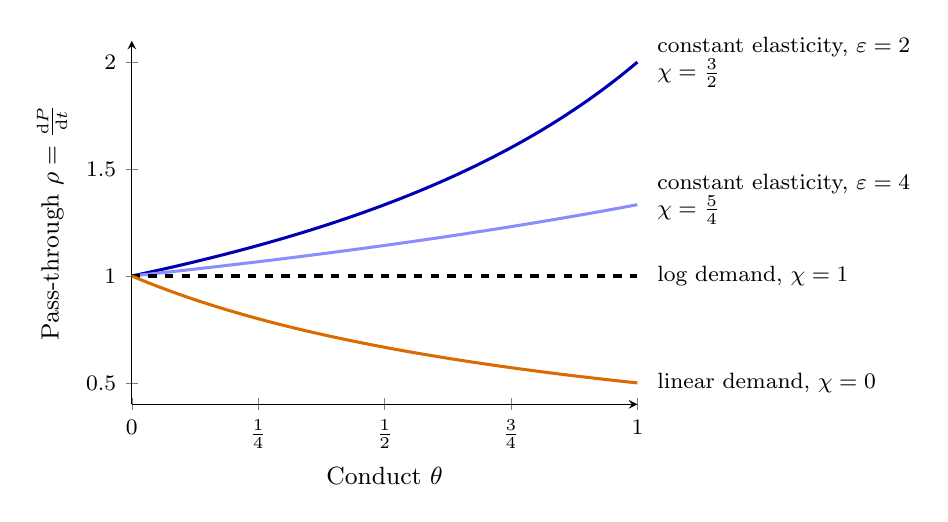
\begin{tikzpicture}
\begin{axis}[
  width=0.66\textwidth, height=6.2cm,
  xmin=0, xmax=1, ymin=0.4, ymax=2.1,
  xlabel={Conduct $\theta$}, ylabel={Pass-through $\rho = \frac{\dd P}{\dd t}$},
  xtick={0,0.25,0.5,0.75,1}, ytick={0.5,1,1.5,2},
  xticklabels={$0$,$\frac{1}{4}$,$\frac{1}{2}$,$\frac{3}{4}$,$1$},
  tick label style={font=\footnotesize}, label style={font=\small},
  axis lines=left, clip=false, every axis plot/.append style={line width=1.1pt}]
  \addplot[domain=0:1, samples=60, color=blue!70!black] {2/(2-x)};
  \addplot[domain=0:1, samples=60, color=blue!45] {4/(4-x)};
  \addplot[domain=0:1, samples=2, color=black, dashed] {1};
  \addplot[domain=0:1, samples=60, color=orange!85!black] {1/(1+x)};
  \node[anchor=west, font=\footnotesize, align=left] at (axis cs:1.02,2.0)
    {constant elasticity, $\varepsilon = 2$\\ $\chi = \frac{3}{2}$};
  \node[anchor=west, font=\footnotesize, align=left] at (axis cs:1.02,1.36)
    {constant elasticity, $\varepsilon = 4$\\ $\chi = \frac{5}{4}$};
  \node[anchor=west, font=\footnotesize, align=left] at (axis cs:1.02,1.0)
    {log demand, $\chi = 1$};
  \node[anchor=west, font=\footnotesize, align=left] at (axis cs:1.02,0.5)
    {linear demand, $\chi = 0$};
\end{axis}
\end{tikzpicture}
\caption{Pass-through of a specific tax as a function of conduct for four demand curves, with flat marginal cost. From
\cref{cor:03-passthrough-cases}, $\rho = \frac{1}{1 + \theta(1 - \chi)}$. Linear demand gives $\frac{1}{1 + \theta}$,
log demand gives 1 for every $\theta$, and constant elasticity gives $\frac{\varepsilon}{\varepsilon - \theta}$. The
dashed line is also the competitive benchmark.}
\label{fig:03-passthrough-curves}
\end{figure}

\begin{proposition}[What pass-through identifies]\label{prop:03-passthrough-id}
\Cref{cor:02-pt-reveal} gives the following. Under \cref{ass:03-passthrough} with flat marginal cost, pass-through
identifies only the composite
\begin{equation}\label{eq:03-kappa}
\kappa \equiv \theta(\chi - 1) = 1 - \frac{1}{\rho}.
\end{equation}
Consequently, the following hold.
\begin{enumerate}[label=(\roman*)]
\item $\rho > 1$ rejects $\theta = 0$ for every demand curve. Rising marginal cost only strengthens the rejection.
\item Any $\rho$ in $(0, \infty)$ is consistent with every conduct $\theta \in (0, 1]$, for a suitable curvature.
  Pass-through alone never rejects monopoly.
\item Under constant-elasticity demand with elasticity $\varepsilon$, $\theta = \varepsilon\kappa$.
\end{enumerate}
\end{proposition}

Equation \eqref{eq:03-kappa} is \eqref{eq:02-pt-kappa}. Part (i) combines parts (i) and (iii) of
\cref{cor:02-pt-reveal}. Parts (ii) and (iii) are parts (ii) and (iv) of that corollary. Given $\rho$ and conduct
$\theta > 0$, the curvature $\chi = 1 + \frac{\kappa}{\theta}$ reproduces the observed pass-through.

The proposition is the key to reading every cost pass-through study. A market-wide cost shock moves the equilibrium
along a single demand curve. What it reveals is the slope of perceived marginal revenue relative to the slope of demand,
and that slope mixes conduct with curvature. Separating them needs either an assumption on curvature, as in Sumner's
constant elasticity, or variation that changes the slope of demand at a given point (\cref{sec:03-identification}).

\subsection{Sumner's design and results}\label{sec:03-sumner-design}

\casehead{The question}
Is the US cigarette industry competitive, collusive, or in between? The industry was a textbook example of oligopoly.
In the Tobacco Case of 1946 the major manufacturers were convicted of operating an illegal cartel, and the consensus
was that their behavior did not change after the verdict \citep[p.~1010]{Sumner1981}. Earlier work had measured market
power by the ratio of price to marginal cost, which requires cost data that are rarely reliable. Sumner proposed a
scheme that avoids measuring cost: ``The coefficient of the tax rate term in a price equation identifies the ratio of
price to marginal cost'' \citep[p.~1010]{Sumner1981}.

\casehead{The setting}
Cigarettes carry a federal excise tax and state excise taxes, both specific taxes per pack. The federal tax was 8 cents
per pack for more than 25 years. The median state tax rose from 3 cents in 1954 to 12 cents in 1978. Combined taxes
nonetheless fell in real terms, from 48.7 percent of the retail price in 1954 to 35.5 percent in 1978. In 1978 state
taxes ranged from 2 cents in North Carolina to 21 cents in Florida, Connecticut and Massachusetts. The three states with
a large stake in tobacco growing and cigarette manufacturing (North Carolina, Virginia and Kentucky) all had low taxes.
Tobacco interests cannot explain the variation among the other states \citep[n.~8]{Sumner1981}.

Two features of the distribution system matter for the test. First, the institutions limit arbitrage across states.
The federal tax is paid by manufacturers, with the stamp affixed at the factory. Distributors must hold a license in the
state where they operate and must pay the state tax and affix its stamp within a few days of receiving a shipment.
Reselling out of state requires a special permit. Manufacturers therefore know the final state of sale and could, in
principle, set prices that depend on the state tax. Sumner argues that differentials of several cents per pack could
persist before arbitrage became profitable. Second, he assumes that wholesale and retail distribution are competitive,
citing the large numbers of retailers and distributors in each market.

\casehead{The data}
The panel covers 47 states and the District of Columbia annually from 1954 to 1978, 1,200 state-years. Alaska, Hawaii
and New Hampshire are excluded for lack of data and peculiar tax laws. Prices are the Tobacco Tax Council's
``weighted-average price per package'' for each state and year. The Council asks wholesalers for average retail prices
by type of cigarette (regular, king, 100 mm) and type of sale (carton, single pack, machine). It aggregates them with
national weights, so the most obvious quality differences are held fixed across states.

\casehead{The model}
Sumner starts from the markup rule of a firm $j$ facing a demand curve with elasticity $\eta_j < 0$ (his sign
convention),
\begin{equation*}
P_j = \frac{\eta_j}{\eta_j + 1}\, M_j \qquad \text{(his eq.~1)},
\end{equation*}
where $M_j$ is marginal cost. In our notation, with $\varepsilon_j = -\eta_j > 0$, this is
$P_j = \frac{\varepsilon_j}{\varepsilon_j - 1} M_j$. Under monopoly $\varepsilon_j$ is the market elasticity, and under
perfect competition it is infinite. Marginal cost is expanded as $M_j = X_j\beta + e_j + R$ (his eq.~2), with observed
cost factors $X_j$, unobserved factors $e_j$ and the tax $R$, which does not vary by firm.

Only state-average prices are observed, so Sumner aggregates. Let $S_j$ be firm $j$'s market share, $\omega_j \equiv
\frac{P_j}{M_j}$ its price-to-cost ratio, and $P = \sum_j S_j P_j$, $M = \sum_j S_j M_j$ and
$\bar\omega = \sum_j S_j\omega_j$ the share-weighted averages. Then
\begin{equation*}
P = \sum_j S_j\,\omega_j M_j = \bar\omega M + \sum_j S_j(\omega_j - \bar\omega)(M_j - M) \qquad \text{(his eq.~3)}.
\end{equation*}
To verify the identity, expand the last sum. It equals $\sum_j S_j\omega_j M_j - \bar\omega M - \bar\omega M +
\bar\omega M$, because $\sum_j S_j = 1$. Sumner also identifies $\bar\omega$ with $\frac{\bar\eta}{\bar\eta + 1}$ for
the share-weighted elasticity $\bar\eta$, which holds only approximately because the map is nonlinear. The covariance
term vanishes if price-cost ratios or marginal costs vary little across firms, or are unrelated. Sumner argues that
retail prices vary little across brands within a market and that costs are similar, since cigarettes are made in one
region with a standard technology. Dropping the covariance term gives $P = \bar\omega M$, and substituting the cost
equation gives the linear price equation
\begin{equation*}
P_{it} = X_{it}\psi + \bar\omega R_{it} + U_{it} \qquad \text{(his eq.~4)},
\end{equation*}
with states $i$, years $t$, $\psi = \bar\omega\beta$ and $U_{it} = \bar\omega e_{it}$. Sumner calls the tax coefficient
$\theta$. Under constant $\bar\omega$ it equals the pass-through $\frac{\dd P}{\dd R}$, so we write it as $\rho$.

The link to conduct is direct. With constant-elasticity market demand, flat marginal cost and conduct $\theta$,
\cref{cor:03-passthrough-cases}(iv) gives $P = \frac{\varepsilon}{\varepsilon - \theta}(k + t)$, with non-tax marginal
cost $k$ and tax $t$. Comparing with his eq.~1, Sumner's firm-level elasticity is
\begin{equation*}
\varepsilon_j = \frac{\varepsilon}{\theta},
\end{equation*}
the market elasticity divided by conduct. It is the elasticity that firms behave as if they face.

\casehead{The estimating equation and the estimator}
With states indexed by $s$ and years by $y$, the most complete specification is
\begin{equation}\label{eq:03-sumner-regression}
p_{sy} = \mu_s + \tau_y + \rho\, t_{sy} + e_{sy}.
\end{equation}
Here $p_{sy}$ is the price per pack and $t_{sy}$ the combined state and federal tax. The terms $\mu_s$ and $\tau_y$ are
state and year fixed effects. The state effects absorb $\frac{\varepsilon}{\varepsilon - \theta}k_{sy}$ to the extent that it is
constant within a state, and the year effects absorb national cost and price-level changes. Equation
\eqref{eq:03-sumner-regression} is a two-way fixed-effects, or difference-in-differences, regression
(\cref{app:econometrics}). Sumner estimates it by OLS. He also reports a specification that replaces the year effects
by the national consumer price index and drops the state effects. He estimates it by OLS and by a variance-components
(random-effects) generalized least squares (GLS) estimator with random state and year effects
\citep{FullerBattese1974}.

The hypotheses are sharp. Competition with flat marginal cost implies $\rho = 1$. Monopoly with constant-elasticity
demand implies $\rho = \frac{\varepsilon}{\varepsilon - 1} > 1$, and conduct $\theta$ implies
$\rho = \frac{\varepsilon}{\varepsilon - \theta}$. An estimate of $\rho$ can be inverted for the firm-level elasticity,
$\varepsilon_j = \frac{\rho}{\rho - 1}$.

\casehead{Identification}
Tax variation is treated as exogenous: the residual $e_{sy}$ is assumed uncorrelated with $t_{sy}$ given the fixed
effects. The state effects absorb stable differences in tax levels, such as the low taxes of producing states. What
identifies $\rho$ is therefore the timing of tax changes within states relative to other states. The assumption fails
if states raise taxes when local costs or demand change, or if taxes shift the demand for legal sales through
cross-border shopping and smuggling. The tax shifts the marginal cost of every seller in a state by the same amount, so
the test concerns market demand and industry conduct. A cost shifter specific to one firm would instead trace out that
firm's residual demand (\cref{sec:03-residual-demand}).

\casehead{Results}
\Cref{tab:03-sumner} reproduces Sumner's Table 1. With state and year effects, $\hat\rho = 1.074$ with a standard
error of 0.013. A 10-cent difference in taxes thus raises the price by 10.74 cents. The $t$-statistic for $\rho = 1$ is
$\frac{1.074 - 1}{0.013} = 5.7$. The other two specifications give 1.029 and 1.069, with $t$-statistics of 2.6 and 5.3.
All three reject competition at conventional levels. The last column of the table reports our replication on a
reconstructed panel (\cref{sec:03-sumner-replication}), which reproduces all three estimates to within 0.001.

\begin{table}[htbp]
\centering
\begin{threeparttable}
\caption{Effect of the excise tax on the retail price of cigarettes}
\label{tab:03-sumner}
\small
\begin{tabular}{@{}lccccccc@{}}
\toprule
& \multicolumn{4}{c}{Sumner (1981), Table 1} & \multicolumn{2}{c}{Implications} & Replication \\
\cmidrule(lr){2-5}\cmidrule(lr){6-7}\cmidrule(l){8-8}
& $\hat\rho$ & Elasticity & Controls & Method & $t$ for $\rho = 1$ & $\frac{\hat\rho}{\hat\rho - 1}$ &
  $\hat\rho$ \\
\midrule
(1) & \makecell{1.074\\(0.013)} & $-13.5$ & $DY_t$, $DS_i$ & OLS & 5.7 & 14.5 & \makecell{1.075\\(0.013)} \\
\addlinespace
(2) & \makecell{1.029\\(0.011)} & $-34.5$ & NCPI & OLS & 2.6 & 35.5 & \makecell{1.029\\(0.011)} \\
\addlinespace
(3) & \makecell{1.069\\(0.013)} & $-14.5$ & NCPI & VC & 5.3 & 15.5 & \makecell{1.069\\(0.013)} \\
\bottomrule
\end{tabular}
\begin{tablenotes}\footnotesize
\item Notes: The dependent variable is the retail price per pack in cents. The sample has 1,200 state-years (48 states
including DC, 1954--78). Standard errors are in parentheses. ``Elasticity'' is Sumner's implied price elasticity, with his negative sign.
$DY_t$ are year dummies (1978 excluded) and $DS_i$ state dummies (Wyoming excluded). NCPI is the national consumer
price index, and row (2) has no state dummies. VC is a variance-components (random-effects) GLS estimator with a random
effect for each state and each year. Sumner reports $R^2$ of about 0.99 with dummies and about 0.95 without. Our
replication gives 0.994 and 0.985. The column $\frac{\hat\rho}{\hat\rho - 1}$ inverts his eq.~1 exactly, in absolute
value. The replication uses OLS for rows (1) and (2) and two-way random-effects GLS for row (3), with conventional
standard errors, as in the paper.
\end{tablenotes}
\end{threeparttable}
\end{table}

The implied elasticities in the table deserve a check. Sumner's reported values equal $\frac{1}{1 - \hat\rho}$
exactly, for example $\frac{1}{1 - 1.074} = -13.5$. Inverting his eq.~1 exactly instead gives
$\eta_j = -\frac{\hat\rho}{\hat\rho - 1}$, which is $-14.5$, $-35.5$ and $-15.5$. The reported values thus treat
$\hat\rho - 1$ as the markup over cost, $\frac{P - M}{M} = -\frac{1}{\eta_j}$, in place of the Lerner condition
$\frac{P - M}{P} = -\frac{1}{\eta_j}$. The two agree to first order in $\frac{1}{\lvert\eta_j\rvert}$, so the
difference is immaterial for his conclusions. His text uses the same approximation: ``Taking $\theta = 1.05$, a 1
percent rise in the price of a firm's product would cause a 20 percent fall in the quantity sold'' \citep[p.~1019]{Sumner1981}.

\casehead{Robustness}
Sumner reports four checks. First, he estimates nonlinear versions of eq.~4 that let the price-to-cost ratio vary with
price, $\bar\omega(P) = \gamma P^{1 - \lambda}$. Substituting in $P = \bar\omega(P) M$ gives $P^{\lambda} = \gamma M$,
which he estimates by nonlinear least squares with additive and multiplicative errors (his eqs.~4$'$ and 4$''$). The
hypothesis $\lambda = 1$, under which the ratio is constant and equal to $\gamma$, is not rejected. The estimates are
$\hat\lambda = 0.972$ (0.027) and 0.981 (0.026), with $\hat\gamma = 1.029$ and 1.062 \citep[n.~9]{Sumner1981}.
Second, the pooled equation estimated separately for each year gives estimates in the range of Table 1, with no trend.
Third, a squared tax term added to the yearly equations is insignificant in most years. Smuggling would make price a
concave function of the tax, so this check speaks against a large role for smuggling. Fourth, adding New Hampshire
leaves the results essentially unchanged.

\casehead{Interpretation}
Sumner draws two conclusions. Pass-through significantly above one rejects atomistic competition. The implied
firm-level elasticities, between 13.5 and 34.5 in absolute value, are far above estimates of the industry elasticity
of demand, which ``are generally between $-0.3$ and $-0.8$'' \citep[p.~1017]{Sumner1981}. His own estimate of the
industry elasticity is about $-0.40$ (n.~10). A cartel acting as a monopolist would face the industry elasticity, so
the estimates are inconsistent with an effective cartel. A monopolist would never price on the inelastic part of
demand, so with an industry elasticity below one it would raise prices far above the observed level. Sumner concludes
that monopoly power is small relative to tax and other cost differences. Taking $\rho = 1.05$, it adds about 3 cents
to the average price of a pack.

In conduct-parameter language, the constant-elasticity model gives $\theta = \varepsilon\kappa$ with
$\kappa = 1 - \frac{1}{\rho}$ (\cref{prop:03-passthrough-id}). With $\hat\rho = 1.074$, $\hat\kappa = 0.069$. An
industry elasticity of 0.4 then gives $\theta \approx 0.028$, and the range from 0.3 to 0.8 gives $\theta$ between 0.021
and 0.055. These values are close to competition. They correspond to the conduct of a symmetric Cournot industry with
18 to 48 firms, in an industry with only six major manufacturers \citep[p.~488]{AshenfelterSullivan1987}.
Sumner's alternative explanation is Barzel's (\citeyear{Barzel1976}) quality effect, which we discuss with the other
critiques below.

\subsection{Curvature, cost, composition, and further critiques}\label{sec:03-sumner-critiques}

Sumner's rejection of competition needs only flat marginal cost. His rejection of collusion also needs
constant-elasticity demand. Three critiques address these assumptions and the price measure.

\casehead{Demand curvature}
\Cref{prop:03-passthrough-id} shows that a pass-through test identifies conduct only conditional on curvature. A
monopolist facing log demand passes through exactly one, the competitive value
(\cref{cor:03-passthrough-cases}(vi)). A monopolist facing concave or linear inverse demand passes through less than
one. A pass-through below one would then wrongly ``accept'' competition, or even suggest that firms absorb taxes.
Sumner's nonlinear check tests whether pass-through varies with the price level. Constant pass-through is consistent
with constant elasticity, but also with any other pair $(\theta, \chi)$ whose product $\theta(\chi - 1)$ stays constant.
It cannot pin down curvature on its own.

\casehead{Cost curvature}
With rising marginal cost, competitive pass-through is $\frac{\varepsilon_S}{\varepsilon_S + \varepsilon} < 1$
(\cref{cor:03-passthrough-cases}(i)). A pass-through near one is then consistent with several combinations:
competition with flat marginal cost, monopoly with log demand, or monopoly with log-convex demand and rising marginal
cost. The slope of marginal cost and conduct both enter the slope of the supply relation. This is the identification
problem of \cref{sec:03-identification} in another guise. Rising marginal cost pushes competitive pass-through below
one, so it leaves the rejection of competition intact.

\casehead{Composition}
Sumner's price is an average over brands and package types. Suppose the measured price is $\bar p = \sum_j w_j p_j$,
with quantity weights $w_j$. Then
\begin{equation*}
\frac{\dd \bar p}{\dd t} = \sum_j w_j\,\frac{\dd p_j}{\dd t} + \sum_j p_j\,\frac{\dd w_j}{\dd t}.
\end{equation*}
The first term is the average pass-through of individual prices. The second is a composition effect. A specific tax
raises the prices of cheap varieties proportionally more than those of expensive ones, so consumers may trade up. The
second term is then positive, and the regression overstates product-level pass-through. The test is biased toward
rejecting competition. The Tobacco Tax Council's fixed national weights remove composition effects across package types
and types of sale, but not across brands within a type. Sumner's observation that retail prices vary little across brands limits this
channel. \citet[p.~13]{NevoHatzitaskos2005} make a related point in another
setting. Much of the fall in the average price of tuna during Lent, a period of high demand, comes from a shift of
purchases toward cheaper products.

A close relative of the composition effect is the quality response emphasized by \citet{Barzel1976}. A per-unit tax
lowers the relative price of quality, so higher taxes should induce higher quality per unit. Measured price per pack
then rises by more than the tax even under competition. Sumner replies that the price data hold the obvious quality
dimensions fixed and that centralized manufacturing leaves little room for quality variation across states. He also
notes that a Barzel effect would bias the estimate upward, which strengthens the case against an effective cartel
\citep[p.~1018]{Sumner1981}.

\casehead{Further critiques}
Four further issues apply to any tax pass-through study. First, taxes shift demand as well as cost. Consumers in
high-tax states buy across borders or from smugglers, so legal sales respond to the tax beyond the movement along
demand. Sumner's own footnote 6 notes that smuggling can lower measured prices net of tax at both extremes. In very
low-tax states, bulk sales for export carry low transaction costs. In very high-tax states, legal sellers compete with
the illegal market. Second, timing matters. Prices are observed once a year, and announced tax increases can trigger
stockpiling and anticipatory price changes, so annual data may mix short-run and long-run pass-through. Third, the
test measures the conduct of the whole vertical chain. Market power among wholesalers or retailers, or retailers who
apply percentage markups, would also produce $\rho > 1$ with competitive manufacturers. Fourth, the regression errors
are serially correlated within states, so conventional standard errors overstate precision
\citep{BertrandDufloMullainathan2004}. \Cref{sec:03-sumner-replication} shows that clustering by state matters here.
Specific and ad valorem taxes also pass through differently. An ad valorem tax at rate $\tau$ on the consumer price
scales effective marginal cost by $\frac{1}{1 - \tau}$. Its pass-through therefore depends on the level of cost as well
as on curvature.

\subsection{A replication and what it adds}\label{sec:03-sumner-replication}

We re-estimate Sumner's regressions on a reconstructed panel with the same coverage: 47 states and the District of
Columbia, 1954 to 1978, 1,200 state-years. Prices and taxes come from \citet[Table~13]{TobaccoInstitute1983}, the historical
compilation of \emph{The Tax Burden on Tobacco}. They are nominal cents per pack on November 1 of each year. The tax is the state tax plus the
federal tax of 8 cents, and municipal taxes are excluded. We deflate by the consumer price index for all urban consumers (CPI-U) where needed. The average price rises
from 22.5 cents in 1954 to 56.6 cents in 1978. The median state tax rises from 3 to 12 cents, as in Sumner's
footnote 8. The same footnote gives a stronger check. In the reconstructed panel the median combined tax is 48.7
percent of the median price in 1954 and 35.3 percent in 1978, against Sumner's 48.7 and 35.5 percent. Of the 1,152 year-to-year transitions within states, 191 involve a tax change. Only 6 are
decreases, and the average change is 2.4 cents. The tax accounts for 46.7 percent of the retail price on average.

\Cref{tab:03-sumner} shows that the reconstructed data reproduce all three of Sumner's estimates. \Cref{tab:03-replication}
reports three extensions, and \cref{app:problems} develops the exercise in full.

\begin{table}[htbp]
\centering
\begin{threeparttable}
\caption{Replication and extensions of the pass-through regression}
\label{tab:03-replication}
\small
\setlength{\tabcolsep}{5pt}
\begin{tabular}{@{}llcc@{}}
\toprule
Specification & Statistic & Estimate & S.e. \\
\midrule
M0: nominal cents, state and year effects & $\hat\rho$ & 1.075 & 0.013 \\
  & $\hat\rho$, state-clustered s.e. & 1.075 & 0.034 \\
  & 95\% confidence interval & \multicolumn{2}{c}{$[1.006,\ 1.143]$} \\
  & $p$-value for $\rho = 1$ (clustered) & \multicolumn{2}{c}{0.033} \\
\addlinespace
M1: real cents, state and year effects & $\hat\rho$ & 1.107 & 0.026 \\
\addlinespace
M2: quadratic in the real tax & $\hat\rho$ at 10th percentile of tax & 1.097 & 0.039 \\
  & $\hat\rho$ at 90th percentile of tax & 1.113 & 0.034 \\
  & $p$-value for $b_2 = 0$ & \multicolumn{2}{c}{0.76} \\
  & 95\% interval for $\rho(p_{90}) - \rho(p_{10})$ & \multicolumn{2}{c}{$[-0.090,\ 0.122]$} \\
\addlinespace
Composite from M0 & $\hat\kappa = 1 - \frac{1}{\hat\rho}$ & 0.069 & \\
  & 95\% interval for $\kappa$ & \multicolumn{2}{c}{$[0.006,\ 0.125]$} \\
\bottomrule
\end{tabular}
\begin{tablenotes}\footnotesize
\item Notes: 1,200 state-years. All specifications include state and year fixed effects. Standard errors are clustered
by state (48 clusters) except in the first row. M1 deflates price and tax by the CPI-U. M2 regresses the real price
on $b_1(T_{sy} - \bar T) + b_2(T_{sy} - \bar T)^2$, so that $\rho(T) = b_1 + 2b_2(T - \bar T)$. The interval for
$\kappa$ maps the endpoints of the clustered interval for $\rho$. $\hat\kappa$ uses the unrounded estimate
$\hat\rho = 1.0746$.
\end{tablenotes}
\end{threeparttable}
\end{table}

\casehead{Clustering}
Sumner's conventional standard error of 0.013 ignores serial correlation of the errors within states. Clustering by
state raises it to 0.034. Pass-through remains significantly above one, with a 95 percent interval of $[1.006, 1.143]$
and $p = 0.033$. The rejection of competition survives, but its margin is much thinner than a $t$-statistic of 5.7
suggests. In real terms (M1) the estimate is 1.107 with a clustered standard error of 0.026.

\casehead{Constant pass-through}
If conduct and curvature are constant, pass-through does not vary with the tax. Specification M2 lets it vary
through a quadratic in the real tax. Estimated pass-through is 1.097 at the 10th percentile of the tax and 1.113 at
the 90th, and the test of $b_2 = 0$ gives $p = 0.76$. The test has little power, however. The 95 percent interval for
the difference between the two percentiles is wider than $\hat\rho - 1$ itself.

\casehead{The identified set}
By \cref{prop:03-passthrough-id}, the data identify $\hat\kappa = 0.069$, with 95 percent interval
$[0.006, 0.125]$. Every pair $(\chi, \theta)$ on the hyperbola $\theta(\chi - 1) = \hat\kappa$ fits the estimate
equally well. \Cref{fig:03-identified-set} plots this set. Monopoly fits with $\chi = 1.069$, a demand curve slightly
more convex than log demand. Symmetric Cournot with six firms fits with $\chi = 1.42$. Constant elasticity with an
industry elasticity of 0.4 has $\chi = 3.5$ and gives $\theta = 0.028$, with interval $[0.002, 0.050]$. The data alone
cannot choose among these. Sumner's rejection of collusion rests on the constant-elasticity assumption combined with
outside estimates of the industry elasticity.

\begin{figure}[htbp]
\centering
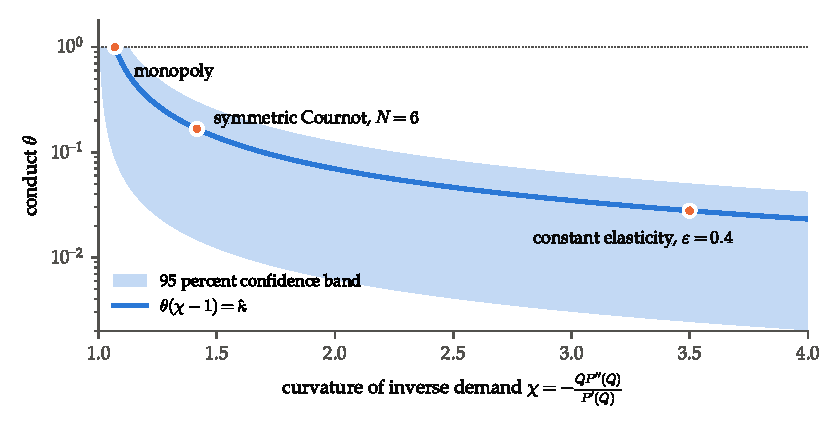
\includegraphics[width=0.9\textwidth]{figures/ch03/sumner_identified_set.pdf}
\caption{Pairs of demand curvature $\chi$ and conduct $\theta$ consistent with the estimated cigarette tax pass-through
$\hat\rho = 1.0746$. The curve is $\theta(\chi - 1) = \hat\kappa$ with $\hat\kappa = 0.069$, and the band maps the 95
percent state-clustered confidence interval for $\rho$. The marked points are monopoly ($\chi = 1.069$), symmetric
Cournot with six firms ($\chi = 1.42$, $\theta = \frac{1}{6}$) and constant-elasticity demand with $\varepsilon = 0.4$
($\chi = 3.5$, $\theta = 0.028$). The vertical axis is logarithmic.}
\label{fig:03-identified-set}
\end{figure}

\casehead{A bound that does not depend on curvature}
Outside information on the industry elasticity can rule out monopoly without any assumption on curvature. With flat
marginal cost $c \ge 0$ and tax $t$, the Lerner form of \eqref{eq:03-supply-tax} is
$\frac{P - t - c}{P} = \frac{\theta}{\varepsilon}$, where $\varepsilon$ is the elasticity at the observed equilibrium.
Since $c \ge 0$,
\begin{equation}\label{eq:03-lerner-bound}
\theta = \varepsilon\Bigl(1 - \frac{t}{P} - \frac{c}{P}\Bigr) \le \varepsilon\Bigl(1 - \frac{t}{P}\Bigr).
\end{equation}
The tax is a large share of the cigarette price. At the sample mean share of 0.467 and $\varepsilon = 0.4$, the bound
gives $\theta \le 0.213$. At the lowest share in the sample (0.229) it gives $\theta \le 0.308$. Both rule out monopoly.
Equivalently, monopoly at the mean tax share requires an elasticity of at least $\frac{1}{1 - 0.467} = 1.88$ at the
observed price. The bound uses the level of prices and taxes, and pass-through does not enter it. Sullivan's bound in
\cref{sec:03-sullivan} develops the same idea with an elasticity estimated from the tax variation itself.

\begin{remark}[Pass-through as a tool]\label{rem:03-passthrough-tool}
\Cref{prop:03-passthrough} turns pass-through into a measurement device. Given estimates of $\rho$, $\varepsilon$
and the slope of marginal cost, it pins down conduct for any assumed curvature. Conversely, given conduct, it predicts
the incidence of taxes and cost shocks. \citet{WeylFabinger2013} develop this program in general. Recent applications
combine first-order conditions of this kind with credible sources of variation. \citet{MillerOsborneSheu2017} study
the US portland cement industry from 1980 to 2010. Their estimated pass-through of fuel costs ranges from 1.03 to 1.65
across specifications (Table~4, p.~84). They combine it with conduct estimates from earlier work to measure the incidence
of a price on carbon emissions.
\citet{BergquistDinerstein2020} use the first-order-condition approach to estimate the effect of coordination among
intermediaries in the Kenyan maize market. Their field experiment supplies the instruments
\citep[p.~214, n.~86]{AskerNocke2021}.
Identification of conduct still requires curvature, which must come from demand estimated over a range of prices or
from assumption.
\end{remark}

\casehead{Contribution}
Sumner's paper introduced a design that is now standard. It uses an observed, exogenous component of marginal cost
and a fixed-effects panel to learn about the pricing rule without measuring cost. Its rejection of competition holds for
any demand curve and any non-decreasing marginal cost, although clustering weakens it. Its rejection of collusion holds
only given curvature, or given an industry elasticity and the curvature-free bound \eqref{eq:03-lerner-bound}. The
lesson extends beyond cigarettes. A market-wide cost shifter traces out demand and reveals the slope of perceived
marginal revenue, which mixes conduct with curvature. Cost shifters therefore deliver tests and bounds on conduct.
Point identification requires variation that rotates demand (\cref{sec:03-identification}), cost shifters specific to
one firm (\cref{sec:03-residual-demand}), or direct measures of cost (\cref{sec:03-sugar,sec:03-electricity}).

\section{Comparative statics in cost without functional forms}\label{sec:03-revenue-tests}

Sumner's test in \cref{sec:03-sumner} turns a cost shock into a statement about conduct. It does so by
assuming a demand curve with constant elasticity and a flat marginal cost. This section studies three tests
that drop those functional forms. Each test asks what profit maximization alone implies about the response
of an equilibrium to a change in cost. The answers are inequalities. They can reject monopoly or bound
conduct from above, but they rarely deliver a point estimate.

We proceed in three steps. We first derive the bound of \citet{Sullivan1985} and explain why cost shifters
can only produce inequalities. We then prove the revealed-preference test of \citet{AshenfelterSullivan1987}
and report its evidence from the cigarette industry. Finally we develop the revenue test of
\citet{PanzarRosse1987}, which needs data on revenue and factor prices only.

\subsection{Sullivan's bound and why cost shifters give only inequalities}\label{sec:03-sullivan}

Consider $N$ firms selling a homogeneous good. Inverse demand $P(Q)$ is stable and decreasing, $P' < 0$.
Firm $i$ has cost $C_i(q_i) + t q_i$, where $t$ is a specific tax paid by sellers and $C_i$ is increasing.
Its marginal cost is therefore $MC_i = C_i'(q_i) + t \ge t$. Following \citet[eq.~24]{Bresnahan1989}, we
write the first-order condition of firm $i$ in conjectural-variations form,
\begin{equation}\label{eq:03-cv-foc}
  P(Q) + (1 + r_i)\, q_i P'(Q) = MC_i, \qquad i = 1, \dots, N,
\end{equation}
where $r_i$ is the conjectural variation $\frac{\dd Q_{-i}}{\dd q_i}$ of \cref{sec:03-objects}. Cournot behavior is
$r_i = 0$, joint profit maximization by $N$ identical firms is $1 + r_i = N$, and price taking is the limit
$1 + r_i \to 0$. As in \cref{sec:03-objects}, $r_i$ describes how close output is to the competitive and
collusive levels. It makes no claim about what firms believe.

\begin{definition}[Numbers equivalent]\label{def:03-numbers-equivalent}
Suppose $1 + r_i > 0$ for every $i$. The \emph{numbers equivalent} of the industry is
\begin{equation*}
  N_e = \sum_{i=1}^{N} \frac{1}{1 + r_i}.
\end{equation*}
\end{definition}

In a Cournot industry $N_e = N$, so $N_e$ counts the Cournot firms that would produce the same conduct. A
cartel of $N$ identical firms has $N_e = N \cdot \frac{1}{N} = 1$, and price taking corresponds to $N_e \to
\infty$. The next lemma connects $N_e$ to the industry conduct parameter of \eqref{eq:03-supply-relation}.

\begin{lemma}\label{lem:03-cv-aggregation}
If all firms have the same marginal cost $c$, the conditions \eqref{eq:03-cv-foc} aggregate to the supply
relation $P + \theta Q P'(Q) = c$ with $\theta = \frac{1}{N_e}$.
\end{lemma}

\begin{proof}
Rearrange \eqref{eq:03-cv-foc} as $P - c = -(1 + r_i) q_i P'$ and divide by $1 + r_i$:
\begin{equation*}
  \frac{P - c}{1 + r_i} = -q_i P'.
\end{equation*}
Summing over $i$ gives $(P - c) N_e = -Q P'$. Dividing by $N_e$ gives $P + \frac{1}{N_e} Q P' = c$.
\end{proof}

The lemma is a special case of \cref{prop:03-aggregation}. With a common marginal cost, each firm's condition reads
$s_i(1 + r_i) = \varepsilon\frac{P - c}{P}$, so every firm has the same value of $s_i\tilde\theta_i$. The industry
conduct $\sum_i \varphi_i s_i \tilde\theta_i$ is then the same for all weights, and the lemma shows that it equals
$\frac{1}{N_e}$.

Now let $z_c > 0$ be any variable that shifts marginal cost and is excluded from demand. The tax is the
leading example, and a factor price is another. Write the equilibrium price and output as $P^*(z_c)$ and
$Q^*(z_c)$. The \emph{reduced-form elasticities} of price and quantity with respect to the cost shifter are
\begin{equation}\label{eq:03-EP-EQ}
  E_P = \frac{\dd \ln P^*}{\dd \ln z_c}, \qquad E_Q = \frac{\dd \ln Q^*}{\dd \ln z_c}.
\end{equation}
\citet{Bresnahan1989} writes them $H_P$ and $H_Q$. Both can be estimated from regressions of log price and log
output on the cost shifter. The first result says what they reveal.

\begin{lemma}[Cost shifters trace out demand]\label{lem:03-trace-demand}
If $z_c$ does not enter demand and $E_P \neq 0$, the demand elasticity at the observed equilibrium is
$\varepsilon = -\frac{E_Q}{E_P}$, whatever the conduct, the slope of marginal cost and the curvature of
demand.
\end{lemma}

\begin{proof}
Every equilibrium lies on the same demand curve, so $P^*(z_c) = P(Q^*(z_c))$ for all $z_c$. Differentiating
in $z_c$ gives $\frac{\dd P^*}{\dd z_c} = P'(Q^*)\frac{\dd Q^*}{\dd z_c}$. Multiply both sides by
$\frac{z_c}{P^*}$ and insert $\frac{Q^*}{Q^*}$:
\begin{equation*}
  E_P = \frac{Q^* P'(Q^*)}{P^*} \cdot \frac{z_c}{Q^*}\frac{\dd Q^*}{\dd z_c} = -\frac{1}{\varepsilon}\, E_Q .
\end{equation*}
Solving for $\varepsilon$ completes the proof.
\end{proof}

\begin{proposition}[Sullivan's bound]\label{prop:03-sullivan-bound}
Suppose $1 + r_i > 0$ and $MC_i \ge t$ for every firm, and let $z_c$ satisfy \cref{lem:03-trace-demand}. Then
\begin{equation}\label{eq:03-sullivan-bound}
  N_e \;\ge\; \frac{1}{\varepsilon\left(1 - \frac{t}{P}\right)} \;=\; -\frac{E_P}{E_Q}\cdot\frac{P}{P - t}.
\end{equation}
If, in addition, all firms share the marginal cost $c$, conduct satisfies
\begin{equation}\label{eq:03-sullivan-theta}
  \theta = \varepsilon L = -L\,\frac{E_Q}{E_P} \;\le\; -\frac{E_Q}{E_P}\left(1 - \frac{t}{P}\right).
\end{equation}
\end{proposition}

\begin{proof}
By \eqref{eq:03-cv-foc}, $P - MC_i = -(1 + r_i) q_i P' > 0$, so $P > MC_i \ge t$. Divide by $1 + r_i > 0$ and
use $MC_i \ge t$:
\begin{equation*}
  \frac{P - t}{1 + r_i} \;\ge\; \frac{P - MC_i}{1 + r_i} \;=\; -q_i P'.
\end{equation*}
Sum over $i$ and use $-QP' = \frac{P}{\varepsilon}$:
\begin{equation*}
  (P - t)\, N_e \;\ge\; -Q P' \;=\; \frac{P}{\varepsilon}.
\end{equation*}
Divide by $P - t > 0$ to get $N_e \ge \frac{P}{\varepsilon (P - t)}$, which is the first expression in
\eqref{eq:03-sullivan-bound}. Substituting $\varepsilon = -\frac{E_Q}{E_P}$ from \cref{lem:03-trace-demand}
gives the second. Under a common marginal cost, \cref{lem:03-cv-aggregation} gives $\theta = \frac{1}{N_e}$
and \eqref{eq:03-lerner-theta} gives $\theta = \varepsilon L$. Finally $c \ge t$ implies $L \le 1 -
\frac{t}{P}$.
\end{proof}

Three features of the bound matter for what follows. First, it uses two reduced-form elasticities and the
tax share of the price. Nothing depends on the curvature of demand, the slope of marginal cost or the
functional form of either. Second, it is one-sided. A large value of the right side of
\eqref{eq:03-sullivan-bound} rejects collusive conduct, but no value can reject competition, because $N_e =
\infty$ satisfies every lower bound. Third, it is the Lerner bound \eqref{eq:03-lerner-bound} of
\cref{sec:03-sumner-replication} with the demand elasticity estimated from the cost shock itself.

\citet[eq.~25]{Bresnahan1989} states the bound in the form
\begin{equation*}
  \sum_i (1 + r_i)^{-1} \;\ge\; -\frac{H_P}{H_Q L} \;\ge\; -\frac{H_P}{H_Q},
\end{equation*}
with $H_P$ and $H_Q$ our $E_P$ and $E_Q$ and $L$ the common Lerner index. The first relation holds with
equality under a common marginal cost, by \cref{lem:03-cv-aggregation}. The second uses only $L \le 1$, that
is $MC \ge 0$, and coincides with \eqref{eq:03-sullivan-bound} at $t = 0$. Using the tax as a floor on
marginal cost tightens the bound, and this is the refinement that Sullivan uses
\citep[p.~1038]{Bresnahan1989}. For a cartel ($N_e = 1$) the bound says that $\varepsilon(1 - \frac{t}{P})
\ge 1$. A monopolist never prices on the inelastic part of demand, and the tax sharpens that rule. Its Lerner
index $\frac{1}{\varepsilon}$ cannot exceed the share of the price left after tax.

\begin{example}[An illustrative calculation]\label{ex:03-sullivan}
Suppose a 10 percent tax increase raises the price by 4 percent and lowers sales by 1.6 percent. Suppose
also that the tax is 40 percent of the price. These numbers are illustrative only. Then $E_P = 0.4$, $E_Q =
-0.16$ and $\varepsilon = \frac{0.16}{0.4} = 0.4$. The bound is
\begin{equation*}
  N_e \;\ge\; \frac{1}{0.4 \times (1 - 0.4)} = \frac{1}{0.24} \approx 4.2,
  \qquad \theta \;\le\; 0.24 .
\end{equation*}
Monopoly and Cournot conduct with up to four firms are rejected. Cournot conduct with five or more firms
is not.
\end{example}

\citet{Sullivan1985} applies the bound to a panel of U.S. states and years in the cigarette industry. State
excise taxes are the cost shifter, and an analysis-of-variance procedure absorbs the other exogenous
variables. He rejects the hypothesis that cigarette prices are set as if by a cartel
\citep[p.~1038]{Bresnahan1989}. \citet[p.~496]{AshenfelterSullivan1987} summarize his finding as industry
behavior inconsistent with a numbers equivalent below two or three.

\casehead{Why cost shifters give only inequalities} The proof of \cref{lem:03-trace-demand} shows what a
cost shifter does. Demand does not move, so every observed equilibrium lies on one demand curve, and
variation in $z_c$ traces that curve out. A cost shifter therefore identifies the demand elasticity at each
observed point. Conduct, however, sits in the supply relation, which in Lerner form reads $P - MC =
\theta\frac{P}{\varepsilon}$. Once $\varepsilon$ is known, $\theta$ is pinned down only if the level of
marginal cost is known. The data restrict it only to $t \le MC \le P$. Mapping these two bounds through the
supply relation gives the identified set
\begin{equation}\label{eq:03-cost-identified-set}
  0 \;\le\; \theta \;\le\; \varepsilon\left(1 - \frac{t}{P}\right).
\end{equation}
A demand shifter works the other way round. It moves equilibria along the supply relation and so traces out
the equation that contains $\theta$. \citet[p.~1039]{Bresnahan1989} draws this contrast, and
\cref{sec:03-identification} shows when demand shifters identify conduct. Pass-through is a partial
exception. The slope of price in cost does involve $\theta$, but \cref{prop:03-passthrough-id} shows that it
confounds conduct with the curvature of demand and the slope of marginal cost.

\subsection{Ashenfelter and Sullivan (1987): a revealed-preference test}\label{sec:03-ashenfelter-sullivan}

\casehead{Question} Parametric tests of monopoly fit equations of a chosen functional form and then test
restrictions on them. \citet{AshenfelterSullivan1987} point out that such a procedure always tests a joint
hypothesis. They quote \citet[p.~99]{Varian1983}: such a procedure tests ``whatever one wants to test plus
the maintained hypothesis of functional form.'' They therefore adapt the nonparametric
revealed-preference approach of \citet{Afriat1967} and \citet{Varian1982} to monopoly. Excise taxes are
well suited to it. Large tax changes give the test power, and every tax change yields a separate prediction.
The researcher can therefore report the percentage of correct predictions, which separates a model that
fails as a rule from one that fails occasionally (p.~484).

\casehead{The test} An industry acts as a single decision maker, a monopoly or a perfect cartel. It faces a
decreasing inverse demand $P(q)$ and a cost $C(q) = C_0(q) + tq$, where $C_0$ is increasing and $t$ is the
excise tax per unit. Let $t_0 < t_1$ be two tax rates with the same $P$ and $C_0$. Let $q_0$ and $q_1$ be the
profit-maximizing outputs and $p_0 = P(q_0)$, $p_1 = P(q_1)$ the prices.

\begin{proposition}[Ashenfelter and Sullivan]\label{prop:03-as-inequality}
Under these assumptions:
\begin{enumerate}[label=(\roman*)]
  \item Output does not rise and price does not fall, $q_1 \le q_0$ and $p_1 \ge p_0$.
  \item Revenue falls by at least the old tax times the fall in output,
  \begin{equation}\label{eq:03-as-revenue}
    p_1 q_1 - p_0 q_0 \;\le\; t_0\,(q_1 - q_0).
  \end{equation}
  \item If $p_1 > p_0$, the arc elasticity of demand satisfies
  \begin{equation}\label{eq:03-as-arc}
    \frac{(q_0 - q_1)\, p_0}{(p_1 - p_0)\, q_0} \;\ge\; \frac{p_0}{p_1 - t_0}.
  \end{equation}
\end{enumerate}
\end{proposition}

\begin{proof}
Output $q_0$ is optimal at tax $t_0$, so it earns at least as much as $q_1$ would:
\begin{equation}\label{eq:03-as-rp0}
  p_0 q_0 - C_0(q_0) - t_0 q_0 \;\ge\; p_1 q_1 - C_0(q_1) - t_0 q_1 .
\end{equation}
Output $q_1$ is optimal at tax $t_1$:
\begin{equation}\label{eq:03-as-rp1}
  p_1 q_1 - C_0(q_1) - t_1 q_1 \;\ge\; p_0 q_0 - C_0(q_0) - t_1 q_0 .
\end{equation}
Add the two inequalities. Revenues and the $C_0$ terms cancel, which leaves
\begin{equation*}
  -t_0 q_0 - t_1 q_1 \;\ge\; -t_0 q_1 - t_1 q_0
  \quad\Longleftrightarrow\quad
  (t_1 - t_0)(q_0 - q_1) \;\ge\; 0 .
\end{equation*}
Since $t_1 > t_0$, $q_1 \le q_0$. Demand slopes down, so $p_1 \ge p_0$. This proves (i). Rearrange
\eqref{eq:03-as-rp0}:
\begin{equation*}
  p_1 q_1 - p_0 q_0 \;\le\; \bigl[C_0(q_1) - C_0(q_0)\bigr] + t_0 (q_1 - q_0).
\end{equation*}
The bracket is not positive because $q_1 \le q_0$ and $C_0$ is increasing. This proves (ii). For (iii),
write $p_1 q_1 - p_0 q_0 = p_1(q_1 - q_0) + q_0(p_1 - p_0)$ and substitute into \eqref{eq:03-as-revenue}:
\begin{equation*}
  q_0 (p_1 - p_0) \;\le\; (p_1 - t_0)(q_0 - q_1).
\end{equation*}
A monopolist prices above marginal cost, so $p_1 > t_1 > t_0$. Multiply both sides by the positive number
$\frac{p_0}{q_0 (p_1 - p_0)(p_1 - t_0)}$ to obtain \eqref{eq:03-as-arc}.
\end{proof}

Inequality \eqref{eq:03-as-revenue} has a direct reading. Moving from $q_0$ to $q_1$ saves $t_0(q_0 - q_1)$
in taxes at the old rate. The revenue lost by the move must exceed this saving. Otherwise the monopolist
would have chosen $q_1$ when the tax was still $t_0$. Inequality \eqref{eq:03-as-arc} extends the rule that a
monopolist never produces on the inelastic part of demand. The arc elasticity must exceed
$\frac{p_0}{p_1 - t_0}$, which is above one whenever the price rises by less than the old tax. The test uses
two observed points, no functional form, no derivatives and no convexity of cost. It is local because it
compares points close in time, where demand and cost are plausibly the same. \Cref{fig:03-as-test} draws the
logic in the plane of output and revenue.

\begin{figure}[htbp]
\centering
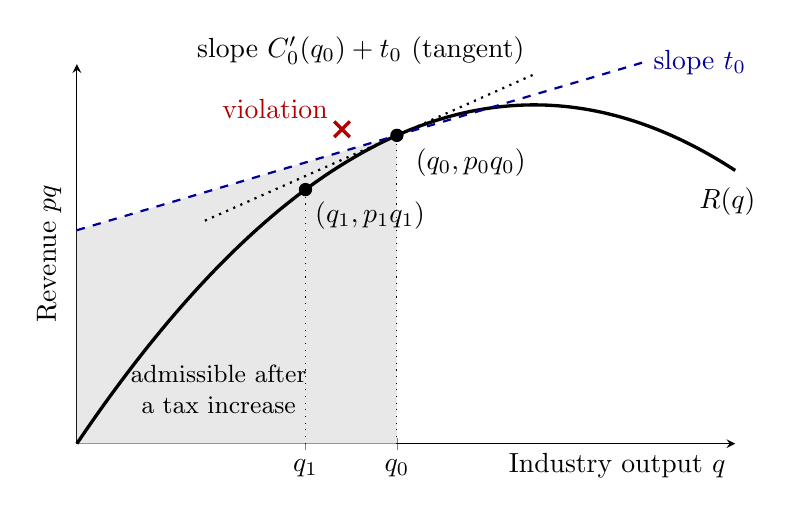
\begin{tikzpicture}
\begin{axis}[
  width=0.82\textwidth, height=6.4cm,
  xmin=0, xmax=7.2, ymin=0, ymax=28,
  axis lines=left,
  xlabel={Industry output $q$}, ylabel={Revenue $pq$},
  xtick={2.5,3.5}, xticklabels={$q_1$,$q_0$},
  ytick=\empty, clip=false,
  every axis x label/.style={at={(ticklabel* cs:1.0)}, anchor=north east}
]
  \addplot[fill=gray!18, draw=none] coordinates {(0,0) (0,15.75) (3.5,22.75) (3.5,0)} -- cycle;
  \addplot[domain=0:7.2, samples=120, very thick, black] {10*x - x^2};
  \node[anchor=north west] at (axis cs:6.7,19.6) {$R(q)$};
  \addplot[domain=0:6.2, thick, dashed, blue!60!black] {22.75 + 2*(x - 3.5)};
  \node[anchor=west, blue!60!black] at (axis cs:6.2,28.15) {slope $t_0$};
  \addplot[domain=1.4:5.0, thick, dotted, black] {22.75 + 3*(x - 3.5)};
  \node[anchor=south east] at (axis cs:5.0,27.25) {slope $C_0'(q_0) + t_0$ (tangent)};
  \addplot[only marks, mark=*, mark size=2.2pt] coordinates {(3.5,22.75) (2.5,18.75)};
  \node[anchor=north west] at (axis cs:3.6,22.5) {$(q_0, p_0 q_0)$};
  \node[anchor=north west] at (axis cs:2.5,18.6) {$(q_1, p_1 q_1)$};
  \addplot[only marks, mark=x, mark size=4pt, very thick, red!70!black] coordinates {(2.9,23.2)};
  \node[anchor=south east, red!70!black] at (axis cs:2.85,23.3) {violation};
  \draw[dotted] (axis cs:3.5,0) -- (axis cs:3.5,22.75);
  \draw[dotted] (axis cs:2.5,0) -- (axis cs:2.5,18.75);
  \node[anchor=center, align=center, font=\small] at (axis cs:1.55,4.0) {admissible after\\ a tax increase};
\end{axis}
\end{tikzpicture}
\caption{The revealed-preference logic of \cref{prop:03-as-inequality}. After the tax rises from $t_0$ to
$t_1$, the new point $(q_1, p_1q_1)$ must lie left of $q_0$ and below the line through $(q_0, p_0q_0)$ with
slope $t_0$ (shaded region). The tangent of the revenue curve at $q_0$ has slope equal to marginal revenue,
$C_0'(q_0) + t_0$, which is at least $t_0$. A point above the dashed line, such as the cross, rejects monopoly
with stable demand and cost. The curve is drawn for $R(q) = 10q - q^2$, $C_0' = 1$, $t_0 = 2$ and $t_1 =
4$.}
\label{fig:03-as-test}
\end{figure}

\casehead{A conduct index} The test extends to intermediate conduct. Following
\citet[eq.~12]{AshenfelterSullivan1987}, who call the index $\beta$, say that the industry has
\emph{conduct index} $\theta \in [0, 1]$ if, at its chosen output $q$,
\begin{equation}\label{eq:03-as-index}
  \Delta q\, P(q + \Delta q) + \theta\, q \bigl[P(q + \Delta q) - P(q)\bigr] \;\le\; C(q + \Delta q) - C(q)
  \quad \text{for all } \Delta q .
\end{equation}
With $\theta = 1$ the left side equals $(q + \Delta q)P(q + \Delta q) - qP(q)$, so \eqref{eq:03-as-index} is the
monopoly optimality condition. With $\theta = 0$ it is the revealed-preference form of price equal to marginal
cost. Dividing \eqref{eq:03-as-index} by $\Delta q > 0$ and letting $\Delta q \to 0$ gives $P + \theta q P'
\le C'$. Dividing by $\Delta q < 0$ reverses the inequality. Together they give $P + \theta q P' = C'$, which is
the supply relation \eqref{eq:03-supply-relation}. The index is therefore a finite-difference version of the
conduct parameter.

Apply \eqref{eq:03-as-index} at $q = q_0$ under tax $t_0$ with $\Delta q = q_1 - q_0$. Then drop the term
$C_0(q_1) - C_0(q_0) \le 0$. For $\theta \in (0, 1)$ the signs $q_1 \le q_0$ and $p_1 \ge p_0$ can no longer
be proved, so the test assumes them (p.~487). Under these signs,
\begin{equation*}
  p_1 (q_1 - q_0) + \theta\, q_0 (p_1 - p_0) \;\le\; t_0 (q_1 - q_0).
\end{equation*}
Solving for $\theta$ and inverting gives the two forms of the bound
\begin{equation}\label{eq:03-as-ne}
  \theta \;\le\; \frac{(p_1 - t_0)(q_0 - q_1)}{(p_1 - p_0)\, q_0},
  \qquad
  N_e = \frac{1}{\theta} \;\ge\; \frac{q_0 (p_1 - p_0)}{(q_0 - q_1)(p_1 - t_0)} .
\end{equation}
The second form is the arc version of \eqref{eq:03-sullivan-bound}.\footnote{\citet[eq.~18]{AshenfelterSullivan1987}
derive the bound on $N_e$ separately, by integrating the firms' first-order conditions over the tax change.
Their printed equation has $q_1 - q_0$ in the denominator. We reverse that factor so that the bound is
positive, as their equation (14) and their text require.} To see this, evaluate the elasticities at
some price $p$ between $p_0$ and $p_1$. Then $-\frac{E_P}{E_Q}$ becomes the ratio of the percentage price
rise to the percentage output fall, $\frac{q_0 (p_1 - p_0)}{p\,(q_0 - q_1)}$. The factor $\frac{P}{P - t}$
becomes $\frac{p}{p_1 - t_0}$, because $p_1 - t_0$ bounds the per-unit margin from above along the path.
Multiplying the two gives the right side of \eqref{eq:03-as-ne}. Like Sullivan's bound, \eqref{eq:03-as-ne} can only reject less
competitive conduct in favor of more competitive conduct (their n.~6).

\casehead{Data} The data are those of \citet{Sullivan1985}, from the Tobacco Tax Council's \emph{The Tax
Burden on Tobacco}. They cover 45 states from 1955 to 1982 and contain three variables. The tax is the sum of
the state and federal excise rates, averaged by time in force in years when the rate changed. Per capita
consumption is inferred from state tax receipts. The average retail price per pack comes from a survey taken
each November. Both dollar variables are deflated by the national consumer price index. The industry is
highly concentrated. It has six major firms, and the two and four largest firms produce 66 and 90 percent of
output. The major firms kept virtually identical list prices for thirty years and were twice convicted of
antitrust violations (p.~488).

\casehead{Design} Demand and cost may differ across states and drift over time. The test is therefore applied
only to pairs of observations from the same state at most two years apart. Each pair is ordered so that
$t_0$ is the lower real tax rate. The authors consider all consecutive-year pairs and several subsets. They
also use \emph{skip-year} pairs, separated by one year, which avoid the time-averaged tax in years of
change. The cleanest subset is \emph{flat-jump-flat}: the statutory rate is constant in both years of the
pair and rises in the year between them. For each pair they check the output and price predictions of
\cref{prop:03-as-inequality}(i) and the revenue inequality \eqref{eq:03-as-revenue}.

\begin{table}[htbp]
\centering
\caption{Ashenfelter and Sullivan (1987): percentage of monopoly predictions that hold}
\label{tab:03-as-tests}
\begin{tabular}{lrccccc}
\toprule
 & & \multicolumn{5}{c}{Percentage of pairs for which the prediction holds} \\
\cmidrule(lr){3-7}
Pairs of observations & Cases & $\Delta q \le 0$ & $\Delta p \ge 0$ & Both & Revenue & All three \\
\midrule
\multicolumn{7}{l}{\textit{Panel A: Table I}} \\
Consecutive years & 1178 & 70.8 & 75.3 & 54.6 & 36.7 & 14.9 \\
\quad real tax increases & 216 & 74.1 & 83.8 & 68.1 & 17.1 & 6.0 \\
\quad real tax decreases & 962 & 70.1 & 73.4 & 51.6 & 41.1 & 16.8 \\
\quad statutory changes & 288 & 69.8 & 81.9 & 62.5 & 22.9 & 9.7 \\
\quad no statutory change & 890 & 71.1 & 73.2 & 52.0 & 41.1 & 16.5 \\
Skip-year changes & 1133 & 71.8 & 85.0 & 62.0 & 27.4 & 15.1 \\
\quad flat-jump-flat & 199 & 68.8 & 94.0 & 66.8 & 13.6 & 10.6 \\
\addlinespace
\multicolumn{7}{l}{\textit{Panel B: Table II, skip-year changes by size of the tax change}} \\
$\Delta t < 1$ cent & 467 & 69.2 & 76.9 & 53.5 & 42.0 & 23.1 \\
$1 < \Delta t < 2$ cents & 444 & 69.1 & 86.9 & 61.0 & 23.0 & 11.9 \\
$\Delta t > 2$ cents & 222 & 82.9 & 98.2 & 81.5 & 5.9 & 4.5 \\
\bottomrule
\end{tabular}

\smallskip
\begin{minipage}{0.95\textwidth}
\footnotesize Notes: Reproduced from \citet[Tables I and II]{AshenfelterSullivan1987}. ``Revenue'' is
inequality \eqref{eq:03-as-revenue}. ``Both'' requires output to fall and price to rise. ``All three'' adds
the revenue inequality. In each pair the lower real tax rate defines $t_0$. Tax changes in Panel B are in 1967
cents. The paper's Table II labels the last row $\Delta t < 2$, but its text (pp.~491--492) identifies the row
as changes above 2 cents, and the three rows sum to the 1133 skip-year cases. Its first column header reads
$\Delta q \ge 0$, while its note defines the prediction as a decline in quantity.
\end{minipage}
\end{table}

\casehead{Results} \Cref{tab:03-as-tests} reproduces the main results. The revenue inequality, the
distinctive prediction of monopoly, holds in only 432 of 1178 consecutive-year pairs, or 36.7 percent. It
fares worse where measurement is cleanest. It holds in 13.6 percent of the flat-jump-flat pairs and in only
5.9 percent of the skip-year pairs with tax changes above 2 cents.
The output and price predictions also fail often. They hold jointly in 54.6 percent of all consecutive-year
pairs. They improve with the size of the tax change, to 81.5 percent for changes above 2 cents. The pattern
is the one the authors stress (p.~492). Large tax increases usually raise prices and lower sales, yet they
rarely lower revenue by as much as monopoly requires.

\Cref{fig:03-as-numbers} asks which oligopoly conduct the data can rationalize. It applies the bound
\eqref{eq:03-as-ne} to the pairs in which output fell and price rose. These are 702 skip-year pairs and 133
flat-jump-flat pairs. Only 24.4 and 15.8 percent of them are consistent with $N_e = 1$. A numbers equivalent of
5 rationalizes 75.1 and 76.7 percent. Even $N_e = 9$ leaves 13.5 and 12.0 percent unexplained. The authors
conclude that simple conjectural-variations models can be rejected ``unless they embody at least a moderate
amount of competition'' (p.~492).

\begin{figure}[htbp]
\centering
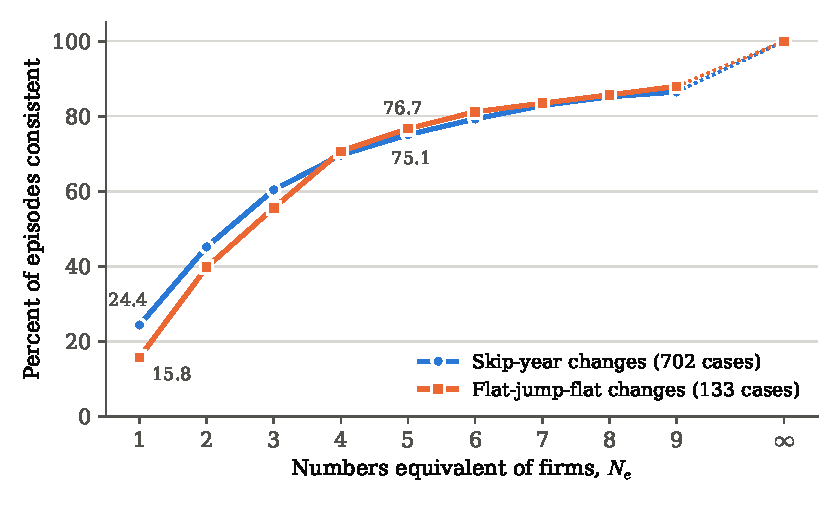
\includegraphics[width=0.78\textwidth]{figures/ch03/as_numbers_equivalent.pdf}
\caption{Share of tax-increase episodes consistent with a numbers equivalent $N_e$, from the bound
\eqref{eq:03-as-ne}. Only pairs with $\Delta q \le 0$ and $\Delta p \ge 0$ enter. At $N_e = \infty$ every
episode is consistent. The paper's table heads the second column ``Jump-Flat-Jump'', and its text calls the
sample flat-jump-flat. Redrawn from the numbers in \citet[Table III]{AshenfelterSullivan1987}.}
\label{fig:03-as-numbers}
\end{figure}

\casehead{Robustness} The authors probe the failures in four ways. First, 371 of the 1133 skip-year pairs
show price and quantity moving in the same direction, which signals a demand shift. Dropping them raises both
the output and the price predictions to 92 percent, while the revenue inequality holds in only 26 percent
(p.~493). Second, they allow for trends with a comparison group. In a simple version, the predicted change without a
tax change is the mean change in states that kept their statutory rate that year. In a two-way version, it is
the fit of a model with state and year effects to the state-years without a statutory change. The tests then ask whether quantity fell below, and price
rose above, these predictions. Their Table IV reports the results. With the simple fit, the quantity and price
predictions hold in 68.4 and 80.9 percent of the 288 consecutive-year statutory changes, and jointly in 60.1
percent. On the 199 flat-jump-flat pairs they hold in 68.8 and 92.0 percent, and jointly in 65.3 percent. The
two-way fit does better. On the statutory changes the shares are 77.8, 79.2 and 68.4 percent. On flat-jump-flat
pairs both predictions hold in 83.9 percent of cases, with 85.9 and 97.0 percent separately. The authors note the analogy with
program evaluation, where untreated units serve as controls \citep{Ashenfelter1978}. In modern terms this is a
difference-in-differences adjustment (\cref{app:econometrics}). Third, in nominal terms the price rises in 196
of the 199 flat-jump-flat pairs, though rising consumer prices make that success partly mechanical. Fourth,
they test whether tax increases follow particular movements in prices and quantities. Their sign-based
contingency tables condition on whether the tax rose in the previous year. The Pearson statistic is 3.9 when it
did not and 34.9 when it did, each with 3 degrees of freedom. The overall statistic is 38.8 with 6 degrees of
freedom. The second and the overall statistic rest on cells with very small expected counts, so the
$\chi^2$ approximation may be poor. Almost all of the 34.9 comes from the two cells in which price and quantity
both fell. The authors conclude that endogenous tax timing does not explain the failures (Table V,
pp.~495--496).

\casehead{Assessment} The test shows how far pure revealed preference can go, and it rejects monopoly
decisively. Its limits are instructive. The approach has no stochastic framework, a drawback the authors
acknowledge (n.~3). The percentages are therefore descriptive, and a single mismeasured pair can violate
\eqref{eq:03-as-revenue}. Quantities
inferred from tax receipts are suspect in exactly the years the test uses, because consumers and retailers
can stock up before a tax increase or buy across state lines. The maintained hypothesis of stable demand and
cost over one or two years is strong, as the frequent failures of the output and price predictions show.
Once a comparison group corrects for demand shifts, the test is no longer nonparametric, as the authors
concede (p.~494). Finally, a rejection of monopoly says little about which oligopoly model holds, beyond the
lower bound on $N_e$. The paper's lasting contribution is the idea of bounding conduct with inequalities
implied by optimization, which returns in \cref{sec:03-bounds}.

\subsection{Panzar and Rosse (1987): the revenue test}\label{sec:03-panzar-rosse}

\citet{PanzarRosse1987} propose two ideas \citep[pp.~1034--1035]{Bresnahan1989}. The first is to estimate a
reduced form and focus on the coefficients of factor prices. The second is to use revenue as the dependent
variable. Revenue is often observable when price and quantity are not. It also needs no quality correction,
whereas a price per unit can overstate the true price where the product is better. \Cref{sec:01-id-cost} previewed
the test. This section proves its properties.

\casehead{Setup} Firm $i$ produces output $q$ at cost $C(q, w, z)$, where $w = (w_1, \dots, w_K)$ is the
vector of factor prices and $z$ collects other cost shifters. Its revenue function is $R(q, y)$, with $y$ a
vector of demand shifters. Solving the equilibrium for the firm's revenue gives the \emph{reduced-form
revenue} $R^*(w, z, y)$. The \emph{Panzar-Rosse statistic} is the sum of the factor-price elasticities of
reduced-form revenue,
\begin{equation}\label{eq:03-pr-psi}
  \psi = \sum_{k=1}^{K} \frac{\partial R^*}{\partial w_k}\frac{w_k}{R^*}
       = \frac{\dd \ln R^*(\lambda w, z, y)}{\dd \lambda}\bigg|_{\lambda = 1},
\end{equation}
where the second equality follows from the chain rule. In words, $\psi$ is the percentage change in
equilibrium revenue after a 1 percent increase in all factor prices. \citet{Bresnahan1989} writes it $H_R$.
With a log-linear specification,
\begin{equation}\label{eq:03-pr-regression}
  \ln R_i = a + \sum_{k=1}^{K} \beta_k \ln w_{ki} + \gamma^\top x_i + e_i, \qquad \hat\psi = \sum_{k=1}^{K}
  \hat\beta_k ,
\end{equation}
where $x_i$ contains the other cost and demand shifters. Early applications either use such a
specification, which makes $\psi$ constant, or report $\psi$ near the center of the sample
\citep[n.~27]{Bresnahan1989}.

\begin{lemma}[Homogeneity of cost]\label{lem:03-homogeneity}
For a cost-minimizing firm and every $\lambda > 0$, $C(q, \lambda w, z) = \lambda C(q, w, z)$. Marginal cost
$C_q$ is also homogeneous of degree one in $w$, and $\sum_k w_k \frac{\partial C_q}{\partial w_k} = C_q$.
\end{lemma}

\begin{proof}
Scaling all factor prices by $\lambda$ leaves relative prices, and hence the cost-minimizing input bundle,
unchanged. Cost is therefore multiplied by $\lambda$. Differentiating $C(q, \lambda w, z) = \lambda C(q, w,
z)$ in $q$ gives $C_q(q, \lambda w, z) = \lambda C_q(q, w, z)$. Euler's theorem for functions homogeneous of
degree one gives the last statement.
\end{proof}

\begin{proposition}[Panzar and Rosse]\label{prop:03-panzar-rosse}
\leavevmode
\begin{enumerate}[label=(\roman*)]
  \item \emph{Monopoly.} If the firm is a monopolist, $\psi \le 0$. This holds also when it chooses a vector
  of outputs, qualities or advertising levels.
  \item \emph{Long-run competition.} Suppose free entry drives every active firm to the minimum of a U-shaped
  average cost curve. Then $\psi = 1$, and firm revenue does not depend on the demand shifters $y$.
  \item \emph{Chamberlinian competition.} Consider a symmetric free-entry equilibrium in which each firm
  maximizes profit against a downward-sloping demand. Suppose entry shifts that demand down and does not make
  it less elastic at a given output. Then $\psi \le 1$.
\end{enumerate}
\end{proposition}

\begin{proof}
\emph{(i), first proof: revealed preference.} Let $x$ be the vector of choices, with revenue $R(x)$ and cost
$C(x, w)$ homogeneous of degree one in $w$. Fix $w^0$ and $w^1 = \lambda w^0$ with $\lambda > 1$, and let $x^0$
and $x^1$ be the optimal choices. Optimality of $x^0$ at $w^0$ gives
\begin{equation*}
  R(x^0) - C(x^0, w^0) \ge R(x^1) - C(x^1, w^0)
  \quad\Longrightarrow\quad
  C(x^1, w^0) - C(x^0, w^0) \ge R(x^1) - R(x^0).
\end{equation*}
Optimality of $x^1$ at $w^1$, with $C(x, w^1) = \lambda C(x, w^0)$, gives
\begin{equation*}
  R(x^1) - R(x^0) \;\ge\; \lambda\bigl[C(x^1, w^0) - C(x^0, w^0)\bigr] \;\ge\; \lambda\bigl[R(x^1) -
  R(x^0)\bigr],
\end{equation*}
where the second step uses the first display. Hence $(1 - \lambda)[R(x^1) - R(x^0)] \ge 0$. Since $\lambda >
1$, $R(x^1) \le R(x^0)$. Equilibrium revenue cannot rise when all factor prices rise in proportion, so
$R^*(\lambda w^0) \le R^*(w^0)$ for $\lambda > 1$, and \eqref{eq:03-pr-psi} gives $\psi \le 0$.

\emph{(i), second proof: comparative statics.} With a single output, the monopolist's first-order condition
is $R_q(q^*, y) = C_q(q^*, w, z)$, and the second-order condition is $R_{qq} - C_{qq} < 0$. Differentiating the
first-order condition in $w_k$ gives
\begin{equation*}
  R_{qq}\frac{\partial q^*}{\partial w_k} = C_{qq}\frac{\partial q^*}{\partial w_k} + C_{q w_k}
  \quad\Longrightarrow\quad
  \frac{\partial q^*}{\partial w_k} = \frac{C_{q w_k}}{R_{qq} - C_{qq}} .
\end{equation*}
Equilibrium revenue is $R^* = R(q^*(w), y)$, so $\frac{\partial R^*}{\partial w_k} = R_q \frac{\partial
q^*}{\partial w_k}$. Multiply by $w_k$, sum over $k$, and apply \cref{lem:03-homogeneity} and then the
first-order condition:
\begin{equation*}
  \sum_k w_k \frac{\partial R^*}{\partial w_k}
  = \frac{R_q \sum_k w_k C_{q w_k}}{R_{qq} - C_{qq}}
  = \frac{R_q\, C_q}{R_{qq} - C_{qq}}
  = \frac{(R_q)^2}{R_{qq} - C_{qq}} .
\end{equation*}
Dividing by $R^*$ yields
\begin{equation}\label{eq:03-pr-monopoly}
  \psi = \frac{(R_q)^2}{(R_{qq} - C_{qq})\, R^*} \;\le\; 0,
\end{equation}
which is equation (23) of \citet{Bresnahan1989}. The inequality is strict when marginal cost is positive,
because then $R_q > 0$.

\emph{(ii)} Write average cost as $AC(q, w, z) = \frac{C(q, w, z)}{q}$. Each active firm produces at the output
$q^m(w, z)$ that minimizes it, and free entry sets the price equal to minimum average cost $MAC(w, z)$. By
\cref{lem:03-homogeneity}, $AC(q, \lambda w, z) = \lambda AC(q, w, z)$. Scaling by $\lambda$ does not move the
minimizer, so $q^m$ is homogeneous of degree zero in $w$, and $MAC$ is homogeneous of degree one. Firm revenue
$R^* = MAC(w, z)\, q^m(w, z)$ is then homogeneous of degree one in $w$, and Euler's theorem gives $\sum_k w_k
\frac{\partial R^*}{\partial w_k} = R^*$, that is, $\psi = 1$. Neither factor of $R^*$ involves $y$. A demand
shift changes the number of firms and leaves the revenue of each unchanged.

\emph{(iii)} Treat the number of firms $n$ as continuous. Each firm's revenue is $R(q, n)$ with $R_n < 0$,
since more rivals lower the price at which a given output sells. A symmetric equilibrium satisfies
$R_q(q, n) = C_q(q, w)$ and zero profit, $R(q, n) = C(q, w)$. Scale $w$ by $\lambda$ and differentiate both
conditions at $\lambda = 1$, using $C(q, \lambda w) = \lambda C(q, w)$:
\begin{align*}
  R_q\, \dd q + R_n\, \dd n &= C_q\, \dd q + C\, \dd\lambda, \\
  R_{qq}\, \dd q + R_{qn}\, \dd n &= C_{qq}\, \dd q + C_q\, \dd\lambda .
\end{align*}
Since $R_q = C_q$, the first line gives $R_n\, \dd n = C\, \dd\lambda$. The change in revenue is $\dd R^* = R_q\, \dd q +
R_n\, \dd n = C_q\, \dd q + C\, \dd\lambda$. Dividing by $R^* = C$ gives
\begin{equation*}
  \psi = 1 + \frac{C_q}{C}\,\frac{\dd q}{\dd\lambda},
\end{equation*}
so $\psi \le 1$ exactly when firm output does not rise. Substituting $\frac{\dd n}{\dd\lambda} = \frac{C}{R_n}$
into the second line gives
\begin{equation*}
  \frac{\dd q}{\dd\lambda} = \frac{C_q - \frac{R_{qn}}{R_n}\, C}{R_{qq} - C_{qq}} .
\end{equation*}
The denominator is negative by the second-order condition. So $\frac{\dd q}{\dd\lambda} \le 0$ if and only if $C_q
\ge \frac{R_{qn}}{R_n}C$. Use $C = R$ and $C_q = R_q$, divide by $R > 0$, and multiply by
$\frac{R_n}{R_q} < 0$. The condition becomes $\frac{R_n}{R} \le \frac{R_{qn}}{R_q}$, that is,
$\frac{\partial}{\partial n}\ln\frac{R_q}{R} \ge 0$. At a fixed $q$, $\frac{q R_q}{R} = 1 -
\frac{1}{\varepsilon_f}$, where $\varepsilon_f$ is the elasticity of the firm's demand. The condition
therefore says that entry does not lower $\varepsilon_f$.
\end{proof}

Part (iii) is Proposition~1 of \citet[p.~451]{PanzarRosse1987}. They assume that each firm's inverse demand
falls with its own output and with the number of rivals. Their Assumption~1 adds that the elasticity of each
firm's perceived demand is nondecreasing in the number of symmetric rivals (p.~450). The derivation above is
ours. Like theirs, it shows that the result rests on how entry changes the elasticity of each firm's demand.
When entry leaves $\varepsilon_f$ unchanged, firm output is fixed and $\psi = 1$, as in the long-run
competitive case. Panzar and Rosse also show that monopolistic competition, long-run competition and
conjectural-variation oligopoly are each consistent with $\psi > 0$ (p.~447). In their oligopoly model, $\psi$
has the sign opposite to that of industry marginal revenue. It is positive when industry output lies on the
inelastic part of market demand (pp.~454--455).

\begin{example}[Values of $\psi$ in standard models]\label{ex:03-pr-examples}
Let marginal cost be a constant $c(w)$, homogeneous of degree one in $w$, so that $\frac{\dd\ln c}{\dd\ln\lambda}
= 1$.
\begin{enumerate}[label=(\alph*)]
  \item Monopoly with demand $Q = AP^{-\varepsilon}$, $\varepsilon > 1$. The price is $P =
  \frac{\varepsilon}{\varepsilon - 1}c$ and revenue is $R^* = AP^{1 - \varepsilon}$, so $\psi = 1 -
  \varepsilon < 0$.
  \item Monopoly with demand $P = a - bQ$. Then $Q = \frac{a - c}{2b}$, $P = \frac{a + c}{2}$ and $R^* =
  \frac{a^2 - c^2}{4b}$, so $\psi = -\frac{2c^2}{a^2 - c^2} < 0$.
  \item Long-run competition with $C(q, w) = g(w)(f + q^2)$ and $g$ homogeneous of degree one. Average cost
  $g(w)(\frac{f}{q} + q)$ is minimized at $q^m = \sqrt{f}$, so $MAC = 2g(w)\sqrt{f}$, $R^* = 2g(w)f$ and
  $\psi = 1$.
  \item Short-run competition with $n$ fixed firms and rising marginal cost. Firm revenue is $\frac{P\,
  D(P)}{n}$, so $\psi = (1 - \varepsilon)\frac{\dd\ln P}{\dd\ln\lambda}$. Its sign is the sign of $1 -
  \varepsilon$.
  \item Cournot with $n$ fixed firms and demand $Q = AP^{-\varepsilon}$, $n\varepsilon > 1$. The Lerner
  index is $\frac{1}{n\varepsilon}$, so $P = \frac{n\varepsilon}{n\varepsilon - 1}c$. Firm revenue is
  $\frac{AP^{1 - \varepsilon}}{n}$, so $\psi = 1 - \varepsilon$, as under monopoly.
\end{enumerate}
\end{example}

Cases (d) and (e) show what the statistic cannot do. Short-run competition and oligopoly do not sign $\psi$,
and $\psi < 0$ arises without monopoly whenever demand is elastic. A negative $\hat\psi$ is therefore no proof
of monopoly, a ``false finding of monopoly'' in the words of \citet[p.~1036]{Bresnahan1989}. The usable
conclusions are one-sided. An estimate $\hat\psi > 0$ rejects monopoly. An estimate $\hat\psi < 1$ rejects
long-run competition, provided the markets are in long-run equilibrium. An estimate between zero and one
rejects both.

The specification matters as much as the sign. When the hypothesis is monopoly, $R^*$ depends on demand
shifters, and the revenue equation is misspecified if they are left out \citep[n.~28]{Bresnahan1989}. When
the hypothesis is long-run competition, demand shifters should have zero coefficients. This gives a second
testable restriction (p.~1037 and n.~30). Every factor price must be measured, and each must vary
exogenously. If a factor is omitted, $\hat\psi$ measures the response to only part of a proportional cost
increase. The long-run interpretation also requires that a cross-section of local markets reflects
differences in long-run equilibria. \citet{Rosse1970} addresses this with a ``permanent plant'' hypothesis,
and markets with rising demand should be treated separately from markets with falling demand
\citep[p.~1037]{Bresnahan1989}.

\casehead{Applications} The first applications use cross-sections of similar local markets, which suits the
long-run reading of the statistic. In a newspaper study, \citet{PanzarRosse1977} take each newspaper as an
observation, with its revenue, mostly from advertising, as the dependent variable. They reject monopoly
($\hat\psi > 0$) even for newspapers that are the only paper in their town. \citet[p.~1037]{Bresnahan1989} reads
this as evidence of competition from other media. In all but one specification the study also rejects $\psi = 1$,
and no specification rejects the Chamberlinian bound $\psi \le 1$. \citet[p.~453, n.~4]{PanzarRosse1987} call these
results suggestive rather than conclusive. \citet{Shaffer1982} applies the test to a cross-section of
banks in New York State in 1979. He rejects both monopoly and long-run competition (p.~1037). The test also bears on market definition. A rejection of monopoly for a firm or a
group of firms means they cannot be treated as acting in isolation \citep[p.~1050]{Bresnahan1989}.

\casehead{Assessment} The revenue test asks little of the data on endogenous variables and makes no
assumption about functional forms. Its demands lie elsewhere. It needs the full vector of factor prices with
exogenous variation in each, and its sharpest prediction ($\psi = 1$) requires long-run equilibrium with free
entry. Like the two tests before it, it delivers inequalities. All three reject monopoly or cartel pricing in
their applications, and none of them says how much market power remains.

\section{Residual demand: Baker and Bresnahan (1988)}\label{sec:03-residual-demand}

\subsection{The question and the idea}\label{sec:03-rd-idea}

The tests so far treat the product as homogeneous and ask about industry conduct. Most industries sell
differentiated products, and then a firm's market power depends on substitution as well as on behavior. A
firm with a unique product can have substantial power, while a firm whose rival sells a near-identical
product may have almost none. Measuring this with a full demand system is costly. Even with constant
elasticities and symmetry, $N$ products require $N$ own-price elasticities, $N$ income elasticities and
$\frac{N(N - 1)}{2}$ cross-price elasticities \citep[p.~1045]{Bresnahan1989}. With 100 products that is more
than 5,000 parameters.

\citet{BakerBresnahan1988} estimate one equation per firm instead. The \emph{residual demand curve} of a firm
is the relation between its own price and quantity after accounting for the supply response of all other
firms (p.~284). A firm in a perfectly competitive industry faces a flat residual demand curve. A monopolist's
residual demand is the industry demand. A firm selling a differentiated product lies in between.
\Cref{fig:03-residual-demand} draws the construction for a homogeneous good. The slope of residual demand
summarizes market power without identifying its source.

\subsection{Deriving the residual demand curve}\label{sec:03-rd-model}

Firm 1 is the firm of interest and sells a single product. Let $\mathbf{Q} = (Q_2, \dots, Q_N)$ be the
quantities of all other relevant products, including products of firms in other ``industries''. No market
is defined in advance. Let $Y$ be demand shifters, $W$ industry-wide cost shifters, and $W^i$ cost shifters
specific to firm $i$. The model has four blocks \citep[pp.~286--289]{BakerBresnahan1988}. Firm 1's inverse
demand is
\begin{equation}\label{eq:03-bb-demand1}
  P_1 = P^1(Q_1, \mathbf{Q}, Y).
\end{equation}
When all products are identical it reduces to $P_1 = P^1(Q_1 + \sum_{i \neq 1} Q_i, Y)$, and only then are
market definition and demand estimation straightforward. The rivals' inverse demands are
\begin{equation}\label{eq:03-bb-demand-others}
  P_i = P^i(\mathbf{Q}, Q_1, Y), \qquad i \neq 1 .
\end{equation}
Each rival's supply relation sets marginal cost equal to perceived marginal revenue,
\begin{equation}\label{eq:03-bb-supply-others}
  MC^i(Q_i, W, W^i) = P^i(\cdot) + Q_i \sum_j \frac{\partial P^i}{\partial Q_j}\frac{\partial Q_j}{\partial
  Q_i}, \qquad i \neq 1,
\end{equation}
where the conjectures $\frac{\partial Q_j}{\partial Q_i}$ are indexed by conduct parameters $\theta^i$, as in
\cref{sec:03-framework}. The firm-specific shifters $W^i$ do not appear in $W$. They may be local input prices
or the shadow rental value of an asset the firm does not trade.

Solve the $2(N - 1)$ equations \eqref{eq:03-bb-demand-others} and \eqref{eq:03-bb-supply-others} for the
rivals' prices and quantities, holding $Q_1$ fixed. Write $W^I$ for the collection of the rivals' shifters
$W^i$. The solution for quantities is the \emph{partial reduced form}
\begin{equation}\label{eq:03-bb-partial-rf}
  \mathbf{Q} = E^I(Q_1, Y, W, W^I),
\end{equation}
in which $Q_1$ is the only endogenous variable on the right. Let $e_{i1} = \frac{\partial \ln E^i}{\partial
\ln Q_1}$ be the elasticity of rival $i$'s equilibrium quantity with respect to $Q_1$. Substituting
\eqref{eq:03-bb-partial-rf} into \eqref{eq:03-bb-demand1} gives the residual inverse demand of firm 1,
\begin{equation}\label{eq:03-residual-demand}
  P_1 = P^1\bigl(Q_1, E^I(Q_1, Y, W, W^I), Y\bigr) \equiv R(Q_1, Y, W, W^I).
\end{equation}
Its observable arguments are own quantity, demand shifters and the cost shifters of other firms. Its
parameters mix demand, cost and conduct parameters, and they cannot in general be recovered from it.

The elasticity of an inverse demand function is called a \emph{flexibility}. Let $\eta_{1j} = \frac{\partial
\ln P^1}{\partial \ln Q_j}$ be the flexibilities of firm 1's structural inverse demand. Differentiate the log
of \eqref{eq:03-residual-demand} in $\ln Q_1$ by the chain rule:
\begin{equation}\label{eq:03-bb-elasticity}
  \eta^R_1 \equiv \frac{\partial \ln R}{\partial \ln Q_1}
  = \frac{\partial \ln P^1}{\partial \ln Q_1} + \sum_{i \neq 1}\frac{\partial \ln P^1}{\partial \ln Q_i}
    \frac{\partial \ln E^i}{\partial \ln Q_1}
  = \eta_{11} + \sum_{i \neq 1} \eta_{1i}\, e_{i1}.
\end{equation}
This is equation (7) of the paper.\footnote{The printed equation (7) writes the reaction elasticity with the
indices in the order $1i$. The definition two lines above it, which we follow, is $\frac{\partial \ln
E^i}{\partial \ln Q_1}$.} The \emph{inverse residual demand elasticity} $\eta^R_1$ is the parameter to be
estimated, and $\frac{1}{\eta^R_1}$ is the elasticity of residual demand. The first term is the own
flexibility. The second adds the price effect of the rivals' responses. With homogeneous products and
rivals that expand when firm 1 contracts, the second term partly offsets the first. In the competitive limit
the two cancel.

Firm 1's own supply relation closes the model:
\begin{equation}\label{eq:03-bb-supply1}
  P_1 - MC^1(Q_1, W, W^1) = M^1(\mathbf{Q}, Q_1, Y, \theta^1) = MK^1(Q_1, Y, W, W^I, \theta),
\end{equation}
where $M^1$ is the gap between price and perceived marginal revenue. The second equality substitutes
\eqref{eq:03-bb-partial-rf} for $\mathbf{Q}$, and \citet{BakerBresnahan1988} call $MK^1$ the \emph{residual
markup}. The intersection of \eqref{eq:03-residual-demand} and \eqref{eq:03-bb-supply1} determines $P_1$
and $Q_1$.

\casehead{Identification} Equations \eqref{eq:03-residual-demand} and \eqref{eq:03-bb-supply1} form a
two-equation simultaneous system in $(P_1, Q_1)$. The shifters $Y$, $W$ and $W^I$ enter both equations.
Firm 1's own cost shifter $W^1$ enters only the supply relation. It is therefore the excluded instrument for
$Q_1$ in the residual demand curve (p.~289). The order condition requires at least one firm-specific cost
shifter. The rank condition requires that firm 1's costs move independently of the costs of all other firms
\citep[n.~43]{Bresnahan1989}. Bresnahan suggests exchange rates as a natural experiment for producers in a
single country, since they move real costs across countries. Industry-wide cost shifters cannot serve,
because they shift the residual demand curve itself.

This is the central contrast with \cref{sec:03-sumner} and \cref{sec:03-sullivan}. A tax moves every firm's
marginal cost together. It therefore traces out market demand and speaks to industry conduct. A cost shifter
specific to one firm moves that firm's supply relation alone. It traces out the firm's residual demand and
speaks to the firm's market power.

\begin{example}[Dominant firm with a price-taking fringe]\label{ex:03-dominant-fringe}
Let products be homogeneous and let the rivals be price takers with supply $S(P, W, W^I)$. Firm 1's residual
demand is $Q_1 = D(P, Y) - S(P, W, W^I)$. Write $\varepsilon$ for the market demand elasticity,
$\varepsilon_S$ for the fringe supply elasticity and $s_1 = \frac{Q_1}{D}$ for firm 1's share. Differentiating
gives the residual demand elasticity
\begin{equation*}
  \varepsilon^R = -\frac{\partial Q_1}{\partial P}\frac{P}{Q_1}
  = \frac{\varepsilon D + \varepsilon_S S}{Q_1}
  = \frac{\varepsilon}{s_1} + \varepsilon_S\,\frac{1 - s_1}{s_1},
\end{equation*}
the familiar formula of \citet{LandesPosner1981}. Here $\eta^R_1 = -\frac{1}{\varepsilon^R}$. With no
fringe, $s_1 = 1$ and $\varepsilon^R = \varepsilon$. With a fringe whose marginal cost is flat,
$\varepsilon_S = \infty$ and residual demand is flat at the fringe's cost \citep[p.~1049]{Bresnahan1989}.

A linear case verifies the markup property proved below. Let $D = a - bP$, $S = dP$ and let firm 1 have
constant marginal cost $c$. Residual demand is $Q_1 = a - (b + d)P$, or $P = \frac{a - Q_1}{b + d}$. The
dominant firm's optimum is $Q_1 = \frac{a - (b + d)c}{2}$, which gives $P - c = \frac{Q_1}{b + d}$. Hence
\begin{equation*}
  \frac{P - c}{P} = \frac{Q_1}{a - Q_1} = -\frac{\partial \ln P}{\partial \ln Q_1} = -\eta^R_1 .
\end{equation*}
\end{example}

\begin{figure}[htbp]
\centering
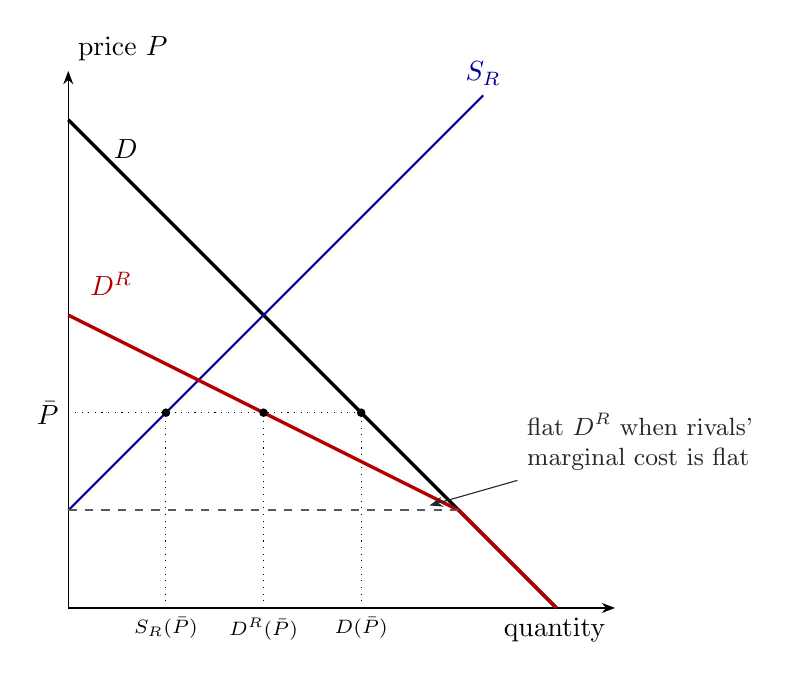
\begin{tikzpicture}[scale=0.62, >=Stealth]
  \draw[->] (0,0) -- (11.2,0) node[below left] {quantity};
  \draw[->] (0,0) -- (0,11) node[above right] {price $P$};
  \draw[very thick] (0,10) -- (10,0) node[pos=0.06, right=2pt] {$D$};
  \draw[thick, blue!60!black] (0,2) -- (8.5,10.5) node[above] {$S_R$};
  \draw[very thick, red!70!black] (0,6) -- (8,2) -- (10,0);
  \node[red!70!black, anchor=south west] at (0.25,6.2) {$D^R$};
  \draw[thick, dashed, gray!70!black] (0,2) -- (8,2);
  \node[gray!30!black, anchor=west, align=left, font=\small] (flat) at (9.2,3.4)
     {flat $D^R$ when rivals'\\ marginal cost is flat};
  \draw[->, gray!30!black] (flat.south west) -- (7.4,2.1);
  \draw[dotted] (0,4) -- (6,4);
  \node[left] at (0,4) {$\bar P$};
  \fill (2,4) circle (2.5pt) (4,4) circle (2.5pt) (6,4) circle (2.5pt);
  \draw[dotted] (2,0) -- (2,4) (4,0) -- (4,4) (6,0) -- (6,4);
  \node[below, font=\scriptsize] at (2,0) {$S_R(\bar P)$};
  \node[below, font=\scriptsize] at (4,0) {$D^R(\bar P)$};
  \node[below, font=\scriptsize] at (6,0) {$D(\bar P)$};
\end{tikzpicture}
\caption{Residual demand. At each price $\bar P$ the residual demand of firm 1 is market demand minus the
quantity rivals supply, $D^R(\bar P) = D(\bar P) - S_R(\bar P)$. A monopolist faces $D$ itself. If rivals can
expand at a flat marginal cost, residual demand is flat at that cost (dashed). Upward-sloping rival supply
produces an intermediate slope. Drawn for $D$: $P = 10 - Q$ and $S_R$: $P = 2 + Q$, which give $D^R$: $P = 6 -
\frac{Q_1}{2}$ above the price 2.}
\label{fig:03-residual-demand}
\end{figure}

\subsection{When the residual demand slope measures the markup}\label{sec:03-rd-markup}

A firm with a flat residual demand curve cannot raise its price, so $\eta^R_1 < 0$ implies $P_1 > MC_1$
(p.~289). The exact relation between $\eta^R_1$ and the Lerner index depends on conduct.

\begin{proposition}[Baker and Bresnahan]\label{prop:03-rd-markup}
Firm 1's Lerner index equals the negative of its inverse residual demand elasticity,
\begin{equation}\label{eq:03-bb-markup}
  \frac{P_1 - MC_1}{P_1} = -\eta^R_1,
\end{equation}
in each of the following cases. (a) Firm 1 is a Stackelberg leader relative to its environment, so that it
chooses $Q_1$ knowing that rivals respond along $E^I$. A dominant firm facing a price-taking fringe is the
leading example. (b) Firms are in a consistent-conjectures equilibrium \citep{Bresnahan1981a}, in which firm
1's conjectured reaction elasticities equal the true ones. (c) The industry is perfectly competitive.
\end{proposition}

\begin{proof}
(a) Firm 1 maximizes $R(Q_1, Y, W, W^I)\, Q_1 - C_1(Q_1)$. The first-order condition is $R + Q_1
\frac{\partial R}{\partial Q_1} = MC_1$. Divide by $P_1 = R$:
\begin{equation*}
  1 + \eta^R_1 = \frac{MC_1}{P_1}
  \quad\Longleftrightarrow\quad
  \frac{P_1 - MC_1}{P_1} = -\eta^R_1 .
\end{equation*}
(b) Let $\hat e_{i1}$ be firm 1's conjectured elasticity of $Q_i$ with respect to $Q_1$. Its perceived
marginal revenue is
\begin{equation*}
  \frac{\dd (P^1 Q_1)}{\dd Q_1}
  = P^1 + Q_1\Bigl[\frac{\partial P^1}{\partial Q_1} + \sum_{i \neq 1}\frac{\partial P^1}{\partial Q_i}
    \frac{\dd Q_i}{\dd Q_1}\Bigr]
  = P^1\Bigl[1 + \eta_{11} + \sum_{i \neq 1}\eta_{1i}\,\hat e_{i1}\Bigr].
\end{equation*}
Equating it to $MC_1$ gives $\frac{P_1 - MC_1}{P_1} = -(\eta_{11} + \sum_{i \neq 1}\eta_{1i}\hat e_{i1})$,
which is equation (11) of the paper. Consistency means $\hat e_{i1} = e_{i1}$, and then the right side equals
$-\eta^R_1$ by \eqref{eq:03-bb-elasticity}. (c) Under perfect competition rivals absorb any change in $Q_1$ at
an unchanged price, so $\eta^R_1 = 0$, and price equals marginal cost.
\end{proof}

Product differentiation gives an approximate version. When products are poor substitutes, the cross
flexibilities $\eta_{1i}$ are small. Then $\eta^R_1 \approx \eta_{11}$, and the markup under any conjecture is
close to $-\eta_{11}$. Questions about strategic variables disappear in this limit \citep{Sonnenschein1968}.
\citet[p.~290]{BakerBresnahan1988} conclude that a large $-\eta^R_1$ will generally indicate substantial
market power for firms selling differentiated products. Outside these cases the equality can fail, as the
next example shows.

\begin{example}[Cournot competition: residual demand understates the markup]\label{ex:03-cournot-residual}
Let $P = a - Q$ and let $N$ identical Cournot firms have marginal cost $c$. Rival $j$'s best response is $q_j
= \frac{a - c - Q_{-j}}{2}$. Given $Q_1$, symmetric rivals each produce $q$ with $2q = a - c - Q_1 - (N -
2)q$, so $q = \frac{a - c - Q_1}{N}$. Substituting into demand gives the residual inverse demand
\begin{equation*}
  P = a - Q_1 - (N - 1)\frac{a - c - Q_1}{N} = \frac{a + (N - 1)c}{N} - \frac{Q_1}{N}.
\end{equation*}
At the Cournot equilibrium $Q_1 = \frac{a - c}{N + 1}$ and $P = \frac{a + Nc}{N + 1}$, a point on this curve.
The Lerner index is $L = \frac{a - c}{a + Nc}$. The inverse residual demand elasticity is
\begin{equation*}
  -\eta^R_1 = \frac{1}{N}\cdot\frac{Q_1}{P} = \frac{a - c}{N(a + Nc)} = \frac{L}{N} .
\end{equation*}
A Cournot firm takes rivals' outputs as given, while its residual demand incorporates their responses. With
strategic substitutes the rivals' contraction absorbs part of the price effect, so $-\eta^R_1$ understates the
markup by the factor $N$.
\end{example}

\subsection{The brewing application}\label{sec:03-bb-brewing}

\casehead{Setting} \citet{BakerBresnahan1988} estimate the residual demand curves of Anheuser-Busch (A-B),
Pabst and Coors over 1962--1982. The industry has substantial product differentiation, and no satisfactory
estimates of its demand and cross elasticities existed. Antitrust enforcers suspected market power and
blocked several proposed mergers (p.~285). A-B was the largest brewer throughout. Its share of national unit
sales rose from under 10 percent to over 30 percent, overwhelmingly through internal growth. Pabst held 7.5 to
11.5 percent of national sales over the last decade of the sample. Its regional share was much higher, about a
quarter of dollar sales in the East North Central states during the 1970s. Coors was slightly smaller than
Pabst nationally. It had the largest share in each of ten western states, averaging about 40 percent in the
mountain states and nearly 30 percent in the Pacific states (pp.~290--291). Coors brewed in a single plant in
Golden, Colorado, the largest in the industry, while A-B had ten plants. Miller's national marketing of light
beer from 1975 changed product differentiation in the industry and possibly the nature of competition.

\casehead{Data} The data are annual for 1962--1982, so each equation has 21 observations.
Price $p_j$ is the log of real average revenue, beer revenue divided by gallons sold, with revenue taken from
firm annual reports. Quantity $q_j$ is the log of per capita barrels, using the U.S. population over 18.
Monetary values are deflated by the GNP deflator. As a robustness check, the authors use the price of each firm's flagship brand
in northern California (Budweiser, Coors and Pabst Blue Ribbon). Average revenue could understate market power
if brand composition changes. The flagship prices are highly correlated with firm average revenue, at 0.96,
0.94 and 0.99 for the three firms. Correlations of average revenue across firms are lower, 0.82 for A-B and
Coors, 0.93 for A-B and Pabst, and 0.65 for Coors and Pabst (Table 1).

\casehead{Estimating equation} The authors estimate \eqref{eq:03-residual-demand} in double-log form for
each firm $j$, so that coefficients are elasticities. With lower-case letters for logs, their equation
(6$''$) is
\begin{equation}\label{eq:03-bb-estimating}
  p_j = \eta^R_j\, q_j + \delta_j^\top (w, w_I) + \gamma_j^\top y + u_j ,
\end{equation}
where $\delta_j$ and $\gamma_j$ are local symbols for coefficient vectors and $u_j$ is the error. Industry
costs $w$ consist of the log of real short-run average variable cost (\textit{sravc}), average industry plant
size (\textit{APS}) and the log of the real user cost of capital (\textit{pk}). Short-run average variable cost
summarizes all non-capital factor prices. The rivals' firm-specific costs $w_I$ are summarized by their excess capacity
$\mathit{EKTI}_j$. The demand shifters $y$ are log real per capita disposable income (\textit{pcdi}), a
time trend (\textit{TIME}) and a dummy for 1975 and later (\textit{LITE}). Advertising and two demographic
variables were tested and dropped. In the A-B equation the slope is $\eta^R_j + \eta^{LITE}\cdot \mathit{LITE}$, so the
interaction coefficient measures the change in slope after 1975. To save degrees of freedom, the three
equations share one index of rivals' marginal cost. This is the cross-equation restriction (12),
\begin{equation}\label{eq:03-bb-restriction}
  \delta_{1j}\, \mathit{sravc} + \delta_{2j}\mathit{APS} + \delta_{3j}\, \mathit{pk} + \delta_{4j}\mathit{EKTI}
  = \delta_j\bigl(\mathit{sravc} + \beta_{APS}\mathit{APS} + \beta_{PK}\, \mathit{pk} +
  \beta_{EKTI}\mathit{EKTI}\bigr) \equiv \delta_j\, \mathit{MC},
\end{equation}
with $\beta_{APS}$, $\beta_{PK}$ and $\beta_{EKTI}$ common to all firms (again local symbols). It assumes that
the other firms use inputs in the same proportions. Tests do not reject it, though they have little power
(n.~21).

\casehead{Instruments} Two variables on the right of \eqref{eq:03-bb-estimating} are endogenous. Short-run
average variable cost is endogenous if short-run marginal cost rises with output. It is instrumented by
exogenous factor prices, namely the brewing wage and the materials and advertising price indices
(\textit{pl}, \textit{pm}, \textit{pa}). Own quantity is endogenous because of the supply relation
\eqref{eq:03-bb-supply1}. All its instruments proxy for firm-specific factor prices $W^1$ (p.~293). The first
is the firm's per capita capacity $K_j$. Brewing capacity is altered infrequently and in large increments. A-B, with a quarter to a third of national sales, typically added
capacity in steps of about 20 percent of its annual production. Short-run marginal cost is therefore lowest
just after an expansion and highest just before the next one. Excess capacity would track this cycle too, but
it is endogenous even in the short run and is not used. The second instrument is the firm's average plant
size $\mathit{APS}_j$ for the multiplant firms A-B and Pabst, which tracks plant-level scale economies. For
Coors it is the log real Colorado manufacturing wage (\textit{cw}). The national brewing wage is already
among the industry cost variables, so independent movements in Colorado wages shift Coors's costs alone
(p.~294).

\casehead{Estimator} The three equations are estimated jointly by three-stage least squares. Stack them as $y
= X b + u$ and let $P_Z = Z(Z^\top Z)^{-1}Z^\top$ project on the instruments. Let $\hat\Sigma$ be the $3
\times 3$ covariance matrix of first-round two-stage least squares residuals. Without restrictions the
estimator is
\begin{equation*}
  \hat b_{3SLS} = \bigl[X^\top(\hat\Sigma^{-1} \otimes P_Z)X\bigr]^{-1} X^\top(\hat\Sigma^{-1} \otimes P_Z)\, y .
\end{equation*}
Restriction \eqref{eq:03-bb-restriction} makes the coefficients products of parameters, such as $\delta_j
\beta_{APS}$. The estimator then minimizes $u(b)^\top(\hat\Sigma^{-1} \otimes P_Z)u(b)$ over the restricted
parameters (\cref{app:econometrics}). Joint estimation uses the correlation of errors across equations, and
single-equation two-stage least squares gives similar elasticities with little loss of efficiency (n.~20). The
reported specification drops demand variables whose coefficients are smaller than their standard errors.
This removes the demographic variables, keeps \textit{LITE} only for A-B, and keeps \textit{TIME} only for
Pabst and Coors. Cost variables are kept even when insignificant, for a reason the next proposition makes
clear.

\casehead{What ordinary least squares would do} Suppose no firm-specific cost shifter were available. The
authors argue that ordinary least squares would then be biased toward finding no market power (p.~298). A
linear version of the system shows why and when.

\begin{proposition}[Bias of least squares in residual demand]\label{prop:03-ols-residual}
Let residual demand be $p = \eta q + u$ with $\eta \le 0$, and let the supply relation be $p = \lambda q +
\gamma w_1 + v$, with $\lambda > \eta$ and $\gamma \neq 0$. Let $w_1$ be uncorrelated with $(u, v)$, and write
$\sigma_u^2$, $\sigma_v^2$, $\sigma_{uv}$ and $\sigma_w^2$ for the variances and the covariance. Then
\begin{equation}\label{eq:03-ols-bias}
  \plim \hat\eta_{OLS} = \eta + (\lambda - \eta)\,
  \frac{\sigma_u^2 - \sigma_{uv}}{\sigma_u^2 + \sigma_v^2 - 2\sigma_{uv} + \gamma^2\sigma_w^2},
\end{equation}
while instrumental variables with instrument $w_1$ is consistent for $\eta$. If $\sigma_{uv} = 0$, the
least squares limit is the weighted average $(1 - \omega)\eta + \omega\lambda$ with $\omega =
\frac{\sigma_u^2}{\sigma_u^2 + \sigma_v^2 + \gamma^2\sigma_w^2} \in [0, 1)$.
\end{proposition}

\begin{proof}
Equate the two equations and solve for the equilibrium quantity:
\begin{equation*}
  q = \frac{u - v - \gamma w_1}{\lambda - \eta}.
\end{equation*}
Hence $\Cov(q, u) = \frac{\sigma_u^2 - \sigma_{uv}}{\lambda - \eta}$ and $\Var(q) = \frac{\sigma_u^2 +
\sigma_v^2 - 2\sigma_{uv} + \gamma^2\sigma_w^2}{(\lambda - \eta)^2}$. Least squares converges to $\eta +
\frac{\Cov(q, u)}{\Var(q)}$, which is \eqref{eq:03-ols-bias}. For the instrumental variables estimator,
$\Cov(w_1, q) = -\frac{\gamma\sigma_w^2}{\lambda - \eta} \neq 0$ and $\Cov(w_1, p) = \eta\Cov(w_1, q)$, so
their ratio is $\eta$. Setting $\sigma_{uv} = 0$ in \eqref{eq:03-ols-bias} gives the weighted average.
\end{proof}

With uncorrelated shocks, least squares lands between the residual demand slope and the supply slope. If the
supply relation is flat or rising, $\lambda \ge 0$, the estimate is pulled toward a flat residual demand. That
direction is conservative, since it understates market power. The proposition also shows when the argument
fails. A covariance $\sigma_{uv}$ above $\sigma_u^2$ reverses the sign of the bias. Omitted industry cost
variables create such a positive covariance, because they enter both equations. This is why the authors keep
all cost variables (n.~23).

\subsection{Results}\label{sec:03-bb-results}

\Cref{tab:03-baker-bresnahan} reproduces the paper's Table 3. The coefficient on log quantity is $\eta^R_j$.

\begin{table}[htbp]
\centering
\caption{Baker and Bresnahan (1988): residual demand estimates, three-stage least squares}
\label{tab:03-baker-bresnahan}
\begin{tabular}{lcccccc}
\toprule
 & \multicolumn{2}{c}{Anheuser-Busch} & \multicolumn{2}{c}{Pabst} & \multicolumn{2}{c}{Coors} \\
\cmidrule(lr){2-3}\cmidrule(lr){4-5}\cmidrule(lr){6-7}
Variable & Coef. & (s.e.) & Coef. & (s.e.) & Coef. & (s.e.) \\
\midrule
Constant & 2.113 & (0.505) & 3.979 & (0.362) & $-1.638$ & (0.805) \\
Own log quantity $q_j$ & $-0.312$ & (0.064) & $-0.058$ & (0.031) & $-0.745$ & (0.054) \\
$\mathit{LITE} \times q_{AB}$ & 0.282 & (0.040) & & & & \\
\textit{LITE} & 0.591 & (0.068) & & & & \\
\textit{PCDI} & 0.040 & (0.157) & $-0.041$ & (0.132) & 0.440 & (0.306) \\
\textit{MC} index & 0.278 & (0.019) & 0.107 & (0.089) & 0.266 & (0.226) \\
\textit{TIME} & & & $-0.017$ & (0.004) & 0.032 & (0.010) \\
\addlinespace
\multicolumn{7}{l}{\textit{Common parameters of the MC index}} \\
\textit{APS} & \multicolumn{6}{l}{$-0.194$ (0.291)} \\
\textit{PK} & \multicolumn{6}{l}{0.042 (0.115)} \\
\textit{EKTI} & \multicolumn{6}{l}{$-0.033$ (0.022)} \\
\addlinespace
Durbin-Watson & 2.13 & & 1.95 & & 1.70 & \\
Observations & 21 & & 21 & & 21 & \\
\bottomrule
\end{tabular}

\smallskip
\begin{minipage}{0.95\textwidth}
\footnotesize Notes: Reproduced from \citet[Table 3]{BakerBresnahan1988}. Dependent variable: log real
average revenue of the firm, 1962--1982. Estimates impose restriction \eqref{eq:03-bb-restriction}. The
\textit{MC} row reports $\delta_j$ and the common parameters report $\beta_{APS}$, $\beta_{PK}$ and
$\beta_{EKTI}$. Treating quantity as exogenous gives own-quantity coefficients of $-0.312$ (A-B),
$-0.053$ (Pabst) and $-0.738$ (Coors) (n.~26).
\end{minipage}
\end{table}

Under the markup reading of \cref{prop:03-rd-markup}, the estimates sort the three firms sharply. Coors's
coefficient of $-0.745$ has a $t$-statistic of $\frac{0.745}{0.054} \approx 13.8$. The authors read it as a
74 percent markup over marginal cost (p.~295). Strictly, $-\eta^R_1$ is a Lerner index, a margin as a share
of price. A Lerner index of 0.745 means $\frac{P}{MC} = \frac{1}{1 - 0.745} \approx 3.9$, a markup over cost
of about 290 percent (\cref{sec:03-objects}). A-B's coefficient before 1975 is $-0.312$, with $t \approx 4.9$
and $\frac{P}{MC} \approx 1.45$.

After 1975 A-B's coefficient is $-0.312 + 0.282 = -0.030$. The paper does not report the covariance of the
two estimates, so the standard error of the sum is unknown. It can still be bounded. For any correlation the
variance of a sum is at least $(0.064 - 0.040)^2$, so the standard error is at least 0.024. The
$t$-statistic for a flat residual demand after 1975 is therefore at most $\frac{0.030}{0.024} = 1.25$.
Competition cannot be rejected for A-B after 1975 at conventional levels, whatever the covariance.

Pabst's coefficient is $-0.058$ with $t \approx 1.87$, which the authors call insignificant. They report a 95
percent confidence interval for the markup of 1 to 11 percent (p.~296). The reported standard error implies
a two-sided 95 percent interval of $-0.058 \pm 1.96 \times 0.031$, or about $-0.3$ to 11.9 percent. The
interval of 1 to 11 percent corresponds to $\pm 1.645$ standard errors, a two-sided 90 percent interval. A
two-sided test at 5 percent therefore does not reject a flat residual demand for Pabst. With 21 observations,
using a $t$ distribution in place of the normal would make a rejection even less likely.

The other coefficients have no clean structural reading, since each mixes direct demand effects with the
indirect effects of rivals' adjustments \citep[p.~297]{BakerBresnahan1988}. The positive income coefficient
for Coors means that a rise in income shifts sales toward Coors after all rivals adjust. The authors label
Coors a normal good and Pabst an inferior good in residual demand. Real prices trend down by 1.7 percent a
year for Pabst and up by 3.2 percent a year for Coors, holding the other variables fixed. The Durbin-Watson
statistics of 1.70 to 2.13 show no strong first-order serial correlation in the double-log specification.

The least squares estimates in the note to \cref{tab:03-baker-bresnahan} confirm the sign of
\cref{prop:03-ols-residual}. They are slightly closer to zero than the instrumental variables estimates for
Coors and Pabst and identical for A-B. The bias is small, and the authors note that treating quantity as
endogenous matters little in their data (n.~19).

\subsection{Robustness, interpretation and critiques}\label{sec:03-bb-critique}

\casehead{Robustness} Using flagship-brand prices and quantities leaves the elasticity estimates unchanged
(p.~293). A linear specification evaluated at sample means gives the same qualitative pattern. It shows
somewhat less market power for A-B early in the sample and for Coors overall, and the two sets of
elasticities are not statistically different under an assumption of independence. The authors prefer the
double-log form because the linear errors are strongly serially correlated (pp.~296--297). Demand elasticity
results are robust to imposing restriction \eqref{eq:03-bb-restriction} (n.~21).

\casehead{Interpretation} The authors draw four inferences (p.~297). First, product differentiation is
important, and the steep residual demands of Coors and A-B probably come from products distinct in image and
geography. Second, regional market share is a poor guide to market power, since Pabst had high regional
shares and almost no power. Third, rising concentration and differentiation after 1975 reflect competition.
A-B lost most of its market power after Miller's light beer, although the new product apparently raised the
demand for all beer. Fourth, tacit collusion is unlikely. Under collusion every firm's residual demand would
slope down and prices would move closely together. Pabst shows neither. The authors concede that they cannot
reject the unlikely case in which all firms except Pabst collude to raise prices to the level of Pabst, the
high-cost producer (n.~25).

\casehead{Critiques} The markup reading requires one of the special cases of \cref{prop:03-rd-markup}. In
Cournot-like competition \cref{ex:03-cournot-residual} shows that $-\eta^R_1$ understates the markup, by a
factor of $N$ in the linear case. The authors themselves call the exact quantitative reading possibly too
strong (p.~297). The instruments raise their own questions. Capacity is added in anticipation of growth
(p.~293), so it may correlate with expected demand. The Colorado wage could move with western incomes and
hence with demand for Coors. The sample has 21 annual observations, and the specification was chosen by
dropping variables with $|t| < 1$, so reported standard errors ignore the search. National average revenue
also aggregates regional markets in which the three firms held very different positions. The light-beer dummy
is collinear with a surge in industry advertising in the mid-1970s, so its meaning is uncertain (n.~16).
Finally, the evidence against collusion leans on Pabst. Its price correlates at only 0.65 with Coors's, yet
at 0.93 with A-B's (Table 1).

\casehead{Contribution} The paper made firm-level market power measurable with one equation and modest data.
It separated two kinds of cost variation. Market-wide shifters identify market demand and industry conduct,
while firm-specific shifters identify a firm's residual demand. In Bresnahan's words, the residual demand
elasticity ``summarizes the market power of the firm'' but is ``insufficient to determine the sources of that
market power'' \citep[p.~1049]{Bresnahan1989}.

\subsection{Residual demand, market definition and mergers}\label{sec:03-bb-antitrust}

Residual demand applies equally to a group of firms \citep[n.~7]{BakerBresnahan1988}. This matters for
antitrust. A hypothetical cartel price increase of 5 percent is part of the algorithm that defines a market
under the 1984 Merger Guidelines of the U.S. Department of Justice. The residual demand of a candidate group
of firms speaks to that question directly. \citet{ScheffmanSpiller1987} extend the method in this way to
define geographic markets. The question of a group's market power is well posed even where defining a
relevant market and computing shares in it would be senseless \citep[n.~44]{Bresnahan1989}. \citet{BakerBresnahan1985} use the same tools to estimate the gains
from merger in differentiated industries. They ask how much steeper the residual demand of two firms would
be after a merger \citep[p.~1050]{Bresnahan1989}. If the two products are close substitutes and few others
are similar, each provides much of the competitive brake on the other. The steepening of the joint residual
demand measures the loss of that brake. These ideas return in \cref{ch:mergers}, and residual demand with a
full system of differentiated products is the subject of \cref{ch:diffprod}.

The studies in this section and the last share a pattern. Sullivan rejects cartel pricing in cigarettes, and
Ashenfelter and Sullivan find that only conduct with a moderate amount of competition fits the data. Panzar and
Rosse reject monopoly for newspapers, and Shaffer rejects both monopoly and long-run competition for banks. Baker
and Bresnahan place
three brewers between price taking and
substantial power. Most estimates of this generation fall between competition and monopoly, and inequalities
or special conduct cases cannot say where. Interpreting such results requires more structure on demand,
cost and conduct. \Cref{sec:03-identification} asks what that structure must provide for conduct to be
identified.

\section{The identification of conduct}\label{sec:03-identification}

The tests of \cref{sec:03-sumner,sec:03-revenue-tests} move cost and watch prices. Cost shifters trace out the
demand curve, so they speak to the supply relation only indirectly, and they deliver tests or bounds. This section
asks the reverse question. What do movements in demand reveal about conduct? The answer, due to
\citet{Bresnahan1982} and \citet{Lau1982}, has two halves. When the slope of marginal cost is unknown, demand shifts
that move the demand curve in parallel reveal nothing about conduct. Shifts that change the slope of demand identify it. \Cref{sec:01-identification} previews the
argument. Here we develop the full theory. We cover the linear model and its observational equivalence, the rotation
argument and its estimation, a general version of Lau's theorem with proof, and the other routes used in practice.

\subsection{The linear model and observational equivalence}\label{sec:03-obs-equiv}

We start from the simplest model in which the question can be posed. It is the model of \citet{Bresnahan1982}, which
\citet[Section~3.1]{Bresnahan1989} uses to explain how the data identify market power. Markets are indexed by
$t = 1, \dots, T$, which may be periods, locations or both.

\begin{assumption}[Linear market]\label{ass:03-linear}
\leavevmode
\begin{enumerate}[label=(\roman*)]
\item Market demand is $Q_t = a_0 + a_1 P_t + a_2 Y_t + u^d_t$ with $a_1 < 0$ and $a_2 \neq 0$. The variable $Y_t$ is
  an observed \emph{demand shifter}.
\item Industry marginal cost is $MC_t = b_0 + b_1 Q_t + b_2 W_t + u^s_t$ with $b_2 \neq 0$. The variable $W_t$ is an
  observed \emph{cost shifter}.
\item Conduct is a constant $\theta \ge 0$. Perceived marginal revenue $P_t + \theta Q_t \frac{\partial P_t}{\partial
  Q_t}$ equals marginal cost.
\item The errors satisfy $\E[u^d_t \mid Y_t, W_t] = \E[u^s_t \mid Y_t, W_t] = 0$, and the vector $(1, Y_t, W_t)$ has a
  nonsingular second-moment matrix.
\end{enumerate}
\end{assumption}

Part (iii) is the supply relation \eqref{eq:03-supply-relation} with a linear demand curve. The slope of inverse demand
is $\frac{\partial P_t}{\partial Q_t} = \frac{1}{a_1}$, so perceived marginal revenue is $P_t + \theta\frac{Q_t}{a_1}$.
Setting it equal to marginal cost and solving for price gives
\begin{equation*}
P_t = MC_t - \theta\frac{Q_t}{a_1} = b_0 + b_1 Q_t + \theta\left(-\frac{Q_t}{a_1}\right) + b_2 W_t + u^s_t .
\end{equation*}
The term $-\theta\frac{Q_t}{a_1} = \theta\frac{Q_t}{\lvert a_1\rvert} \ge 0$ is the markup. Collecting the two terms in
$Q_t$, the model consists of three equations:
\begin{equation}\label{eq:03-linear-system}
\begin{aligned}
\text{demand:}\quad & Q_t = a_0 + a_1 P_t + a_2 Y_t + u^d_t ,\\
\text{marginal cost:}\quad & MC_t = b_0 + b_1 Q_t + b_2 W_t + u^s_t ,\\
\text{supply relation:}\quad & P_t = b_0 + \lambda Q_t + b_2 W_t + u^s_t, \qquad \lambda \equiv b_1 - \frac{\theta}{a_1} .
\end{aligned}
\end{equation}
The \emph{composite slope} $\lambda$ adds the slope of marginal cost, $b_1$, to the conduct-weighted magnitude of the
slope of inverse demand, $\frac{\theta}{\lvert a_1 \rvert}$. Only demand and the supply relation involve observed
endogenous variables, so the estimation problem has two equations.

\casehead{The reduced form}
Substituting the supply relation into demand gives
\begin{align*}
Q_t &= a_0 + a_1\left(b_0 + \lambda Q_t + b_2 W_t + u^s_t\right) + a_2 Y_t + u^d_t ,\\
(1 - a_1\lambda)\, Q_t &= a_0 + a_1 b_0 + a_2 Y_t + a_1 b_2 W_t + u^d_t + a_1 u^s_t .
\end{align*}
Let $\Delta \equiv 1 - a_1\lambda = 1 + \theta - a_1 b_1$. It is positive whenever $b_1 \ge 0$, because $a_1 < 0$, and we
assume $\Delta > 0$ throughout. Dividing by $\Delta$ and substituting back into the supply relation yields the reduced form
\begin{equation}\label{eq:03-linear-rf}
Q_t = \frac{a_0 + a_1 b_0 + a_2 Y_t + a_1 b_2 W_t + u^d_t + a_1 u^s_t}{\Delta}, \qquad
P_t = \frac{b_0 + \lambda a_0 + \lambda a_2 Y_t + b_2 W_t + \lambda u^d_t + u^s_t}{\Delta}.
\end{equation}
The reduced-form coefficients on the shifters are $\pi_{QY} = \frac{a_2}{\Delta}$, $\pi_{PY} = \frac{\lambda a_2}{\Delta}$,
$\pi_{QW} = \frac{a_1 b_2}{\Delta}$ and $\pi_{PW} = \frac{b_2}{\Delta}$. Regressions of $P_t$ and $Q_t$ on $(1, Y_t, W_t)$
identify all four. Two ratios then deliver the slopes:
\begin{equation*}
a_1 = \frac{\pi_{QW}}{\pi_{PW}}, \qquad \lambda = \frac{\pi_{PY}}{\pi_{QY}} .
\end{equation*}
A cost shift moves the equilibrium along the demand curve, so the ratio of the quantity response to the price response
is the slope of demand. A demand shift moves the equilibrium along the supply relation, so the ratio of the price
response to the quantity response is the slope of the supply relation. With $\Delta = 1 - a_1\lambda$ in hand,
$a_2 = \Delta\pi_{QY}$ and $b_2 = \Delta\pi_{PW}$, and the intercepts follow. Each equation is exactly identified, so this
indirect least squares solution coincides with two-stage least squares (2SLS). Demand is estimated by 2SLS of $Q_t$ on
$(1, P_t, Y_t)$ with instruments $(1, Y_t, W_t)$. The supply relation is estimated by 2SLS of $P_t$ on $(1, Q_t, W_t)$
with the same instruments (\cref{app:econometrics}).

\begin{proposition}[Observational equivalence]\label{prop:03-obs-equiv}
Let the structure $(a_0, a_1, a_2, b_0, b_1, b_2, \theta)$ and the distribution of $(u^d_t, u^s_t)$ satisfy
\cref{ass:03-linear} with $\Delta > 0$. For any $\theta' \ge 0$, replace $(b_1, \theta)$ by $(b_1', \theta')$ with
\begin{equation*}
b_1' = b_1 + \frac{\theta' - \theta}{a_1},
\end{equation*}
and keep everything else. The new structure generates the same conditional distribution of $(P_t, Q_t)$ given
$(Y_t, W_t)$. Hence $\theta$ and $b_1$ are not separately identified.
\end{proposition}

\begin{proof}
The composite slope of the new structure is
\begin{equation*}
\lambda' = b_1' - \frac{\theta'}{a_1} = b_1 + \frac{\theta' - \theta}{a_1} - \frac{\theta'}{a_1} = b_1 - \frac{\theta}{a_1}
= \lambda ,
\end{equation*}
and therefore $\Delta' = 1 - a_1\lambda' = \Delta > 0$. The reduced form \eqref{eq:03-linear-rf} depends on the structure
only through $(a_0, a_1, a_2, b_0, \lambda, b_2)$ and the errors, and none of these has changed. The two structures map
every value of $(Y_t, W_t, u^d_t, u^s_t)$ into the same $(P_t, Q_t)$, so the conditional distributions coincide.
\end{proof}

The set of structures that fit the data is the line $b_1 = \lambda + \frac{\theta}{a_1}$ in the $(\theta, b_1)$ plane. It
slopes down because $a_1 < 0$. More market power must be offset by flatter marginal cost. A sign restriction on the
slope of marginal cost turns this line into an interval for conduct.

\begin{corollary}[An interval for conduct]\label{cor:03-obs-equiv-bounds}
Under \cref{ass:03-linear}, suppose $\lambda > 0$ and marginal cost does not fall with output, $b_1 \ge 0$. Then the
values of conduct consistent with the data form the interval $\theta \in [0, \lvert a_1\rvert\lambda]$. Constant marginal
cost ($b_1 = 0$) selects the upper endpoint, and price taking selects the lower endpoint. If $\lvert a_1\rvert\lambda < 1$,
the data reject monopoly with nondecreasing marginal cost.
\end{corollary}

\begin{proof}
By \cref{prop:03-obs-equiv}, every pair $(\theta, \lambda + \frac{\theta}{a_1})$ with $\theta \ge 0$ fits the data. The
restriction $b_1 \ge 0$ reads $\lambda + \frac{\theta}{a_1} \ge 0$. Multiplying by $a_1 < 0$ reverses the inequality and gives
$a_1\lambda + \theta \le 0$, that is, $\theta \le -a_1\lambda = \lvert a_1\rvert\lambda$. Together with $\theta \ge 0$ this
is the interval. Monopoly, $\theta = 1$, lies in it exactly when $1 \le \lvert a_1\rvert\lambda$.
\end{proof}

The interval is the demand-side counterpart of the cost-side bounds of \cref{sec:03-sullivan}. It also shows what the
assumption of constant marginal cost buys. It picks the largest conduct consistent with the data, because it attributes
the entire slope of the supply relation to market power.

\casehead{A graphical version}
\Cref{fig:03-bresnahan-shift} redraws Figure~1 of \citet{Bresnahan1982}, a schematic, with illustrative numbers of
our own. Inverse demand shifts from
$D_1\colon P = 10 - Q$ to $D_2\colon P = 12 - Q$, so $a_1 = -1$ in both markets. The competitive model has marginal cost
$MC^c = 2 + 1.1Q$ and $\theta = 0$. The monopoly model has $MC^m = 2 + 0.1Q$ and $\theta = 1$. Both have composite slope
$\lambda = 1.1$. Under competition the first equilibrium solves $10 - Q = 2 + 1.1Q$, so $Q = \frac{8}{2.1} = 3.81$ and
$P = 6.19$. Under monopoly, marginal revenue $MR_1 = 10 - 2Q$ equals $MC^m$ where $10 - 2Q = 2 + 0.1Q$. This gives the
same quantity $\frac{8}{2.1}$ and, reading price off demand, the same price. After the shift both models predict
$Q = \frac{10}{2.1} = 4.76$ and $P = 7.24$. The two models produce the equilibria $E_1$ and $E_2$ exactly.

\begin{figure}[htbp]
\centering
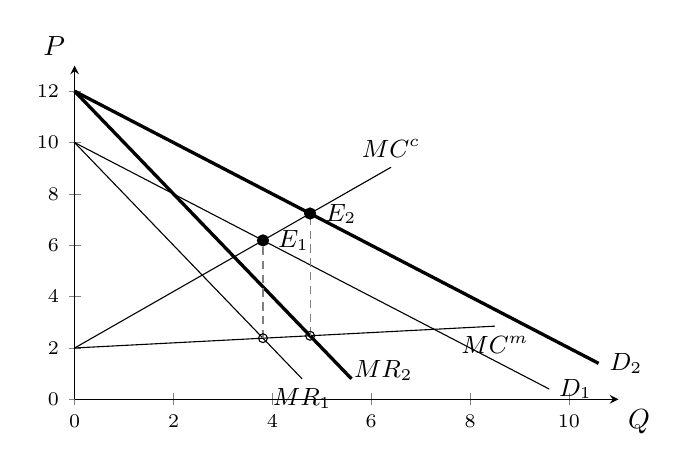
\begin{tikzpicture}
\begin{axis}[
  width=0.70\textwidth, height=0.48\textwidth,
  xmin=0, xmax=11, ymin=0, ymax=13,
  axis lines=left, xlabel={$Q$}, ylabel={$P$},
  xtick={0,2,4,6,8,10}, ytick={0,2,4,6,8,10,12},
  tick label style={font=\scriptsize},
  every axis x label/.style={at={(ticklabel* cs:1)}, anchor=north west},
  every axis y label/.style={at={(ticklabel* cs:1)}, anchor=south east},
  clip=false]
  \addplot[thin, domain=0:9.6, samples=2] {10 - x} node[pos=1, right, font=\small] {$D_1$};
  \addplot[very thick, domain=0:10.6, samples=2] {12 - x} node[pos=1, right, font=\small] {$D_2$};
  \addplot[thin, domain=0:4.6, samples=2] {10 - 2*x} node[pos=1, below, font=\small] {$MR_1$};
  \addplot[very thick, domain=0:5.6, samples=2] {12 - 2*x} node[pos=0.97, anchor=west, font=\small] {$MR_2$};
  \addplot[thin, domain=0:6.4, samples=2] {2 + 1.1*x} node[pos=1, above, font=\small] {$MC^c$};
  \addplot[thin, domain=0:8.5, samples=2] {2 + 0.1*x} node[pos=1, below, font=\small] {$MC^m$};
  \draw[densely dashed, gray] (axis cs:3.8095,2.381) -- (axis cs:3.8095,6.1905);
  \draw[densely dashed, gray] (axis cs:4.7619,2.476) -- (axis cs:4.7619,7.2381);
  \addplot[only marks, mark=*, mark size=2pt] coordinates {(3.8095,6.1905) (4.7619,7.2381)};
  \addplot[only marks, mark=o, mark size=1.6pt] coordinates {(3.8095,2.381) (4.7619,2.476)};
  \node[right, font=\small] at (axis cs:3.92,6.2) {$E_1$};
  \node[right, font=\small] at (axis cs:4.88,7.22) {$E_2$};
\end{axis}
\end{tikzpicture}
\caption[Observational equivalence under a parallel demand shift]{Observational equivalence under a parallel demand
shift. Demand shifts from $D_1\colon P = 10 - Q$ to $D_2\colon P = 12 - Q$. Competitive firms with $MC^c = 2 + 1.1Q$ and a
monopolist with $MC^m = 2 + 0.1Q$ both produce $E_1 = (3.81, 6.19)$ and $E_2 = (4.76, 7.24)$. Under monopoly, output is
set where $MR_i$ crosses $MC^m$ (open circles) and price is read off demand (dashed lines). Drawn after Figure~1 of
\citet{Bresnahan1982}, with illustrative numbers chosen here.}
\label{fig:03-bresnahan-shift}
\end{figure}

The two readings of the same data differ greatly in what they say about welfare. In the competitive reading the Lerner
index at $E_1$ is zero. In the monopoly reading marginal cost at $E_1$ is $2 + 0.1 \times 3.81 = 2.38$, so the Lerner
index is $\frac{6.19 - 2.38}{6.19} = 0.62$. The economics behind the equivalence is simple. When demand shifts out, price
rises in both models. Under competition it rises because marginal cost rises steeply with output. Under monopoly it rises
because marginal revenue shifts out while marginal cost barely moves. A parallel shift raises price either because
marginal cost rises with output or because of market power, and the ratio $\frac{\Delta P}{\Delta Q} = \lambda$ is the
same in both cases.

\subsection{Rotations of demand identify conduct}\label{sec:03-rotation}

\citet{Bresnahan1982} breaks the equivalence by letting an exogenous variable change the slope of demand. Let $Z_t$ be an
observed \emph{demand rotator}, and write demand as
\begin{equation}\label{eq:03-rotation-demand}
Q_t = a_0 + a_1 P_t + a_2 Y_t + a_3 P_t Z_t + a_4 Z_t + u^d_t ,
\end{equation}
with $a_1 + a_3 Z_t < 0$ on the support of $Z_t$. The slope of demand is $\frac{\partial Q_t}{\partial P_t} = a_1 + a_3 Z_t$,
which varies with $Z_t$ when $a_3 \neq 0$. We let $Z_t$ also shift the level of demand through $a_4$. Nothing below
requires $a_4 = 0$. Perceived marginal revenue is now $P_t + \theta\frac{Q_t}{a_1 + a_3 Z_t}$, and the supply relation
becomes
\begin{equation}\label{eq:03-rotation-supply}
P_t = b_0 + b_1 Q_t + \theta Q^*_t + b_2 W_t + u^s_t, \qquad
Q^*_t \equiv -\frac{Q_t}{a_1 + a_3 Z_t} = \frac{Q_t}{\lvert a_1 + a_3 Z_t\rvert} .
\end{equation}
The variable $Q^*_t$ is the \emph{markup term} $m_t \equiv \frac{Q_t}{\left\lvert \frac{\partial Q_t}{\partial P_t}\right\rvert} =
\frac{P_t}{\varepsilon_t}$. It is the dollar markup a monopolist would charge, so $\theta Q^*_t$ is the markup. With
$a_3 = 0$ the markup term is proportional to $Q_t$, and \eqref{eq:03-rotation-supply} collapses to the supply relation of
\eqref{eq:03-linear-system}. With $a_3 \neq 0$, the markup term moves with $Z_t$ at a given quantity, while the cost term
$b_1 Q_t$ does not.

\begin{proposition}[Rotations identify conduct]\label{prop:03-rotation}
Let demand be \eqref{eq:03-rotation-demand} with known parameters, and let the supply relation be
\eqref{eq:03-rotation-supply}. Let $X_t = (Y_t, Z_t, W_t)$, assume $\E[u^s_t \mid X_t] = 0$, and assume $Z_t$ does not
enter marginal cost. Suppose $\mu(X_t) \equiv \E[Q_t \mid X_t]$ is strictly monotone in $Y_t$ for each $(Z_t, W_t)$,
$a_3 \neq 0$, $Z_t$ takes at least two values, and $W_t$ is not degenerate. Then $(b_0, b_1, b_2, \theta)$ are identified.
\end{proposition}

\begin{proof}
Write $Q^*_t = g(Z_t)Q_t$ with $g(Z) \equiv -\frac{1}{a_1 + a_3 Z}$, a known function. Taking expectations of
\eqref{eq:03-rotation-supply} conditional on $X_t$ gives
\begin{equation*}
\E[P_t \mid X_t] = b_0 + b_1\, \mu(X_t) + \theta\, g(Z_t)\, \mu(X_t) + b_2 W_t .
\end{equation*}
The left side and $\mu(X_t)$ are features of the distribution of the data. Suppose a second vector $(b_0', b_1', b_2',
\theta')$ satisfies the same equation. Subtracting, the differences $c = (b_0 - b_0', b_1 - b_1', b_2 - b_2', \theta -
\theta')$ satisfy
\begin{equation*}
0 = c_0 + c_1\, \mu(X) + c_3\, g(Z)\, \mu(X) + c_2 W \quad \text{for all } X .
\end{equation*}
Fix $(Z, W)$ and vary $Y$. Since $\mu$ changes with $Y$, the coefficient on $\mu$ must vanish: $c_1 + c_3 g(Z) = 0$ for
every $Z$. Because $a_3 \neq 0$, the function $g$ takes different values at two values of $Z$, so $c_1 = c_3 = 0$. The
remaining condition $c_0 + c_2 W = 0$ for all $W$ gives $c_0 = c_2 = 0$.
\end{proof}

The proof has a transparent deterministic core. Suppose two markets share the same $W$ and the same quantity $Q$ but have
different rotators $Z_1 \neq Z_2$. The demand shifter $Y$ can always be chosen to make this happen. Marginal cost is then
the same in both markets, and the price difference isolates the markup:
\begin{equation*}
P_1 - P_2 = \theta\, Q\left[g(Z_1) - g(Z_2)\right] .
\end{equation*}
The bracket is nonzero when $a_3 \neq 0$, so the price difference reveals $\theta$. Once $\theta$ is known, two markets
with the same $Z$ and different $Q$ reveal $b_1$.

\casehead{Estimation}
The natural estimator has two steps. In the first step we estimate demand \eqref{eq:03-rotation-demand} by 2SLS. The
regressors $P_t$ and $P_tZ_t$ are endogenous, $(1, Y_t, Z_t)$ are included exogenous variables, and $W_t$ and $W_tZ_t$
are the excluded instruments. In the second step we construct
\begin{equation*}
\hat Q^*_t = -\frac{Q_t}{\hat a_1 + \hat a_3 Z_t}
\end{equation*}
and estimate the supply relation $P_t = b_0 + b_1 Q_t + \theta \hat Q^*_t + b_2 W_t + e_t$ by 2SLS. Here $Q_t$ and
$\hat Q^*_t$ are endogenous, $(1, W_t)$ are included exogenous variables, and $(Y_t, Z_t, Y_tZ_t)$ are the excluded
instruments. Three instruments for two endogenous regressors leave one overidentifying restriction to test. Because
$\hat Q^*_t$ is a generated regressor, conventional second-step standard errors are too small.
\citet[p.~1033, fn.~23]{Bresnahan1989} calls this explicit two-step procedure ``so ugly that no one would ever undertake
it'', while noting that it shows why more powerful techniques identify $\theta$.

The better procedure estimates both equations jointly by the generalized method of moments (GMM). Stack the parameters in
$\Theta = (a_0, \dots, a_4, b_0, b_1, b_2, \theta)$ and define the residuals
\begin{equation}\label{eq:03-rotation-gmm}
\begin{aligned}
u^d_t(\Theta) &= Q_t - a_0 - a_1 P_t - a_2 Y_t - a_3 P_t Z_t - a_4 Z_t ,\\
u^s_t(\Theta) &= P_t - b_0 - b_1 Q_t + \theta\, \frac{Q_t}{a_1 + a_3 Z_t} - b_2 W_t .
\end{aligned}
\end{equation}
With instrument vectors $h^d_t = (1, Y_t, Z_t, W_t, W_tZ_t)^\top$ and $h^s_t = (1, W_t, Y_t, Z_t, Y_tZ_t)^\top$, the
moment conditions are $\E[h^d_t u^d_t(\Theta)] = 0$ and $\E[h^s_t u^s_t(\Theta)] = 0$. GMM minimizes a quadratic form in the
sample analogues of the ten moments. The system is nonlinear in $\Theta$ because $\theta$ multiplies a ratio that involves
$(a_1, a_3)$. Joint estimation imposes the cross-equation restriction that the slope inside the markup term equals the
slope of demand, and its standard errors account for the estimation of demand automatically (\cref{app:econometrics}).

\casehead{A graphical version}
\Cref{fig:03-bresnahan-rotation} redraws Figure~2 of \citet{Bresnahan1982} in the same way. We keep $D_1$, $MC^c$, $MC^m$ and
$E_1 = (3.81, 6.19)$ from \cref{fig:03-bresnahan-shift}. Demand rotates around $E_1$ to the flatter curve
$D_3\colon P = 7.714 - 0.4Q$, which passes through $E_1$ because $6.19 + 0.4 \times 3.81 = 7.714$. The competitive
equilibrium solves $7.714 - 0.4Q = 2 + 1.1Q$, so $Q = \frac{5.714}{1.5} = 3.81$. Competition stays at $E_1$. The monopolist
sets $MR_3 = 7.714 - 0.8Q$ equal to $2 + 0.1Q$, so $Q = \frac{5.714}{0.9} = 6.35$ and $P = 7.714 - 0.4 \times 6.35 = 5.17$.
Monopoly moves to $E_3 = (6.35, 5.17)$. At $E_1$ the elasticity of demand rises from $\frac{6.19}{3.81} = 1.62$ to
$\frac{6.19}{0.4 \times 3.81} = 4.06$, and the monopolist cuts its markup.

\begin{figure}[htbp]
\centering
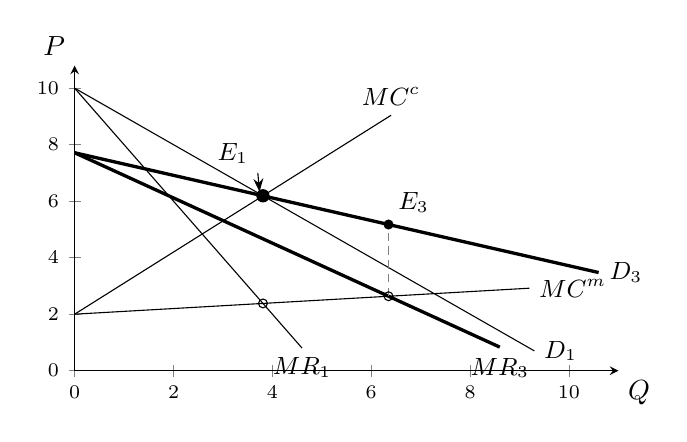
\begin{tikzpicture}
\begin{axis}[
  width=0.70\textwidth, height=0.45\textwidth,
  xmin=0, xmax=11, ymin=0, ymax=10.8,
  axis lines=left, xlabel={$Q$}, ylabel={$P$},
  xtick={0,2,4,6,8,10}, ytick={0,2,4,6,8,10},
  tick label style={font=\scriptsize},
  every axis x label/.style={at={(ticklabel* cs:1)}, anchor=north west},
  every axis y label/.style={at={(ticklabel* cs:1)}, anchor=south east},
  clip=false]
  \addplot[thin, domain=0:9.3, samples=2] {10 - x} node[pos=1, right, font=\small] {$D_1$};
  \addplot[thin, domain=0:4.6, samples=2] {10 - 2*x} node[pos=1, below, font=\small] {$MR_1$};
  \addplot[very thick, domain=0:10.6, samples=2] {7.7143 - 0.4*x} node[pos=1, right, font=\small] {$D_3$};
  \addplot[very thick, domain=0:8.6, samples=2] {7.7143 - 0.8*x} node[pos=1, below, font=\small] {$MR_3$};
  \addplot[thin, domain=0:6.4, samples=2] {2 + 1.1*x} node[pos=1, above, font=\small] {$MC^c$};
  \addplot[thin, domain=0:9.2, samples=2] {2 + 0.1*x} node[pos=1, right, font=\small] {$MC^m$};
  \draw[densely dashed, gray] (axis cs:6.3492,2.635) -- (axis cs:6.3492,5.1746);
  \addplot[only marks, mark=*, mark size=2.2pt] coordinates {(3.8095,6.1905)};
  \addplot[only marks, mark=*, mark size=1.6pt] coordinates {(6.3492,5.1746)};
  \addplot[only marks, mark=o, mark size=1.6pt] coordinates {(3.8095,2.381) (6.3492,2.635)};
  \node[font=\small] (e1lab) at (axis cs:3.2,7.7) {$E_1$};
  \draw[->, >=Stealth, thin] (e1lab.south east) -- (axis cs:3.74,6.33);
  \node[above right, font=\small] at (axis cs:6.35,5.25) {$E_3$};
\end{axis}
\end{tikzpicture}
\caption[A demand rotation separates competition from monopoly]{A demand rotation separates competition from monopoly.
Demand rotates around $E_1 = (3.81, 6.19)$ from $D_1\colon P = 10 - Q$ to $D_3\colon P = 7.714 - 0.4Q$. Competitive firms
with $MC^c = 2 + 1.1Q$ stay at $E_1$. A monopolist with $MC^m = 2 + 0.1Q$ sets $MR_3 = MC^m$ (open circle) and moves to
$E_3 = (6.35, 5.17)$. Drawn after Figure~2 of \citet{Bresnahan1982}, with illustrative numbers chosen here.}
\label{fig:03-bresnahan-rotation}
\end{figure}

The rotation does more than separate two polar models. The size of the response measures conduct. Write the magnitudes of
the inverse-demand slopes before and after the rotation as $g_1 = g(Z_1)$ and $g_3 = g(Z_3)$, with the function
$g(Z) = -\frac{1}{a_1 + a_3 Z} = \frac{1}{\lvert a_1 + a_3 Z\rvert}$ from the proof of \cref{prop:03-rotation}.
Every structure consistent with the original market has marginal cost slope $b_1(\theta) = \lambda_1 - \theta g_1$, where
$\lambda_1$ is the composite slope estimated before the rotation. After the rotation the supply relation has slope
$b_1(\theta) + \theta g_3 = \lambda_1 - \theta(g_1 - g_3)$. Since the original supply relation passed through $(Q_1, P_1)$,
the new one is
\begin{equation*}
P = P_1 + \left[\lambda_1 - \theta(g_1 - g_3)\right](Q - Q_1) - \theta(g_1 - g_3) Q_1 .
\end{equation*}
The rotated demand curve is $P = P_1 - g_3(Q - Q_1)$. Equating the two and solving,
\begin{align*}
(Q - Q_1)\left[g_3 + \lambda_1 - \theta(g_1 - g_3)\right] &= \theta(g_1 - g_3) Q_1 ,\\
Q_3 - Q_1 &= \frac{\theta(g_1 - g_3)Q_1}{g_3 + \lambda_1 - \theta(g_1 - g_3)} .
\end{align*}
Rearranging the first line at $Q = Q_3$ expresses conduct in terms of observables:
\begin{equation}\label{eq:03-rotation-response}
\theta = \frac{(g_3 + \lambda_1)(Q_3 - Q_1)}{(g_1 - g_3)\, Q_3} .
\end{equation}
In the example $g_1 = 1$, $g_3 = 0.4$ and $\lambda_1 = 1.1$. The response is zero under competition, $2.54$ under
monopoly, and $0.95$ when $\theta = 0.5$. Plugging the monopoly outcome into \eqref{eq:03-rotation-response} gives
$\frac{1.5 \times 2.54}{0.6 \times 6.35} = 1.00$. When demand becomes more elastic, a firm with market power cuts its
markup, and its output response rises with its conduct. At the original quantity the supply relation shifts down by
$\theta(g_1 - g_3)Q_1$, an amount proportional to conduct.

\casehead{Rotators in practice}
Applications need a natural experiment that changes the slope of demand \citep[pp.~1033--1034]{Bresnahan1989}. One
shifter might measure the size of the economy, such as national income, while a second measures the price of a
substitute. In \citet{JustChern1980} the market power lies on the buying side. Tomato processors buy from many farmers,
and the adoption of a mechanical harvester changed the elasticity of supply they faced. In
\citet{Bresnahan1981,Bresnahan1987} demand elasticities depend on how crowded the product space is, which changes with
the set of models offered (\cref{ch:discrete}). In sugar refining the canning season changes the composition of buyers
and makes demand less elastic (\cref{sec:03-sugar}). The method stands or falls with the estimated demand elasticities.
Critics offered other readings of the tomato harvester, and the automobile results depend on how products are ordered in
quality space \citep[p.~1034]{Bresnahan1989}.

Two caveats follow from the theory. First, the rotator must be excluded from marginal cost. If the canning season also
changes the slope of marginal cost, through overtime for example, then a term $b_3 Z_t Q_t$ in marginal cost competes with
$\theta g(Z_t) Q_t$. The two differ only through the curvature of $g$, a thin reed for identification. Second, the
linear model can identify $\theta$ even without a separate shifter $Y_t$, using $Z_t$ and $Z_t^2$ as instruments. That
identification comes entirely from the linearity of marginal cost in quantity, as the next theorem shows.

\subsection{Lau's theorem: identification without functional forms}\label{sec:03-lau}

The rotation argument does not depend on linearity. \citet{Lau1982} shows that it holds for general demand and cost
functions. \citet[p.~1033]{Bresnahan1989} summarizes his sufficient condition for identification. The inverse demand
function must not be writable with the demand shifters separable from quantity, which requires at least two shifters.
We state and prove a version of this result.

Let inverse demand be $P = f(Q, Y)$ with a vector of demand shifters $Y \in \R^k$ and $f_Q < 0$, and let industry
marginal cost be an unknown function $c(Q, W)$. The supply relation is
\begin{equation}\label{eq:03-lau-model}
P = c(Q, W) - \theta\, Q\, f_Q(Q, Y) .
\end{equation}
Following Lau, we work without econometric errors. The data are the equilibrium map $(Y, W) \mapsto (P, Q)$.
\citet[p.~1776]{BerryHaile2014} describe the class Lau studied as deterministic conjectural-variations models with
homogeneous goods and symmetric firms. We make three assumptions. The demand function $f$ is known, because the cost
shifters $W$ are excluded from demand and trace it out. Each structure considered has a unique equilibrium with $Q > 0$
for every $(Y, W)$. The function $f$ is twice continuously differentiable.

\begin{definition}[Single-index demand]\label{def:03-single-index}
Inverse demand has a \emph{single index} if $f(Q, Y) = \tilde g(Q, r(Y))$ for a scalar function $r$ and some
function $\tilde g$.
\end{definition}

\begin{theorem}[Lau]\label{prop:03-lau}
\leavevmode
\begin{enumerate}[label=(\roman*)]
\item Suppose demand has a single index, and for each $W$ the equilibrium quantity $Q^e(r, W)$ is strictly monotone in
  the index $r$. Then for every $\theta' \ge 0$ there is a marginal cost function $c'(Q, W)$ such that the structure
  $(f, c', \theta')$ reproduces every observed equilibrium. Conduct is not identified.
\item Suppose that at some observed equilibrium $(Q_0, Y_0, W_0)$ the $2 \times k$ Jacobian of
  $\left(f(Q_0, Y), f_Q(Q_0, Y)\right)$ with respect to $Y$ has rank two at $Y_0$. Suppose also that the equilibrium
  map is observed for all $Y$ in a neighborhood of $Y_0$ with $W = W_0$. Then $\theta$ is identified.
\end{enumerate}
\end{theorem}

\begin{proof}
(i) Fix $W$. Because $Q^e(\cdot, W)$ is strictly monotone, it has an inverse $r = H(Q, W)$ on its range. Define
\begin{equation*}
c'(Q, W) \equiv \tilde g\left(Q, H(Q, W)\right) + \theta'\, Q\, \tilde g_Q\left(Q, H(Q, W)\right) ,
\end{equation*}
which depends on $(Q, W)$ only. Take any observed equilibrium $(P, Q)$ at $(Y, W)$ and let $r = r(Y)$. Then
$Q = Q^e(r, W)$, so $H(Q, W) = r$ and $P = \tilde g(Q, r)$. Substituting,
\begin{equation*}
c'(Q, W) = P + \theta'\, Q\, \tilde g_Q(Q, r) = P + \theta'\, Q\, f_Q(Q, Y) .
\end{equation*}
Rearranging gives $P = c'(Q, W) - \theta' Q f_Q(Q, Y)$, which is the supply relation of the alternative structure. Demand
is unchanged. The observed point is therefore an equilibrium of $(f, c', \theta')$, and by uniqueness it is the only one.

(ii) Fix $W_0$ and define $\Phi(Q, Y) \equiv f(Q, Y) + \theta Q f_Q(Q, Y) - c(Q, W_0)$, so equilibria satisfy
$\Phi = 0$. Consider the set $\Gamma = \{Y : \Phi(Q_0, Y) = 0\}$ of shifter values that produce the equilibrium quantity
$Q_0$. Its gradient at $Y_0$ is $\nabla f + \theta Q_0 \nabla f_Q$, where gradients are taken with respect to $Y$. This
gradient is nonzero, because $\nabla f$ and $\nabla f_Q$ are linearly independent. By the implicit function theorem,
$\Gamma$ is locally a manifold of dimension $k - 1$ through $Y_0$, with tangent space
$T = \{v : (\nabla f + \theta Q_0 \nabla f_Q)\cdot v = 0\}$. Suppose $f_Q(Q_0, \cdot)$ were constant on $\Gamma$ near
$Y_0$. Then $\nabla f_Q \cdot v = 0$ for all $v \in T$, so $\nabla f_Q = \ell(\nabla f + \theta Q_0\nabla f_Q)$ for some
scalar $\ell$. If $\ell \ne 0$, this makes $\nabla f$ and $\nabla f_Q$ linearly dependent. If $\ell = 0$, it makes
$\nabla f_Q = 0$. Both contradict rank two. Hence some $Y_1 \in \Gamma$ has $f_Q(Q_0, Y_1) \neq f_Q(Q_0, Y_0)$. The two
equilibria share $Q_0$ and $W_0$, hence the same marginal cost $c(Q_0, W_0)$. Subtracting their supply relations,
\begin{equation}\label{eq:03-lau-theta}
P_1 - P_0 = -\theta\, Q_0 \left[f_Q(Q_0, Y_1) - f_Q(Q_0, Y_0)\right], \qquad
\theta = -\frac{P_1 - P_0}{Q_0\left[f_Q(Q_0, Y_1) - f_Q(Q_0, Y_0)\right]} .
\end{equation}
Every term on the right is observed or known, so $\theta$ is identified.
\end{proof}

The two parts fit together. Under a single index, $f$ and $f_Q$ depend on $Y$ only through $r$. Their Jacobian is
$\left(\tilde g_r \nabla r, \tilde g_{Qr}\nabla r\right)$, which has rank at most one. Part (ii) is therefore the local
failure of the single-index structure. In words, $\theta$ is identified when the demand shifters can move the slope of
demand at a given quantity independently of its level. In the data, every observation with the same $W$ lies on a single
curve $P = \phi(Q, W)$ when demand has a single index. Any conduct value can then be rationalized by a suitable marginal
cost, as part (i) constructs.

Three examples make the condition concrete. Constant-elasticity demand with a scale shifter, $Q = Y P^{-\varepsilon}$, has
inverse demand $P = (\frac{Q}{Y})^{-\frac{1}{\varepsilon}}$, a single index. Conduct is not identified without restrictions
on cost. Letting a second shifter move the elasticity, $Q = Y_1 P^{-\varepsilon(Y_2)}$, breaks the single index. In the
linear rotation model \eqref{eq:03-rotation-demand}, inverse demand is $f = \frac{Q - a_0 - a_2 Y - a_4 Z}{a_1 + a_3 Z}$ with
$f_Q = \frac{1}{a_1 + a_3 Z}$. The Jacobian with respect to $(Y, Z)$ has determinant
\begin{equation*}
\frac{\partial f}{\partial Y}\frac{\partial f_Q}{\partial Z} - \frac{\partial f}{\partial Z}\frac{\partial f_Q}{\partial Y}
= \left(-\frac{a_2}{a_1 + a_3 Z}\right)\left(-\frac{a_3}{(a_1 + a_3 Z)^2}\right) - 0
= \frac{a_2 a_3}{(a_1 + a_3 Z)^3} ,
\end{equation*}
which is nonzero exactly when both $a_2 \neq 0$ and $a_3 \neq 0$. A pure rotator without a shifter ($a_2 = 0$) leaves a
single index $r = Z$, so the identification in the linear model with $a_2 = 0$ rests on the functional form of cost. This
matches an observation of \citet[p.~1754]{BerryHaile2014}. Lau's results require exogenous variation that alters both
the level and the slope of aggregate demand, a point they credit to \citet{Nevo1998}. Nothing in the proof uses
linearity, which is the sense in which the rotation argument is nonparametric.

\subsection{Other routes to identification}\label{sec:03-other-routes}

Demand rotations are one of several ways to separate conduct from the slope of marginal cost. Each replaces the rotator
with a restriction or with extra data, and each restriction has a cost.

Constant marginal cost makes a single demand shifter enough. With $b_1 = 0$ the composite slope is $\lambda =
-\frac{\theta}{a_1}$, so $\theta = -a_1\lambda$, the upper endpoint in \cref{cor:03-obs-equiv-bounds}. Equivalently,
pass-through reveals conduct. With linear demand and constant marginal cost, $\rho = \frac{1}{1 + \theta}$ by
\cref{cor:03-passthrough-cases}(iii), which is the logic of the pass-through tests of \cref{sec:03-passthrough-theory}.
The weakness is that any slope of marginal cost is read as market power, so the method overstates $\theta$ when
$b_1 > 0$.

Observed marginal cost removes the problem. Once demand is estimated, $\theta_t = \varepsilon_t L_t$ can be computed
observation by observation from \eqref{eq:03-lerner-theta}. This is the strategy of the two validation studies of this
chapter. In British electricity, marginal cost comes from fuel prices and plant efficiencies (\cref{sec:03-electricity}).
In insurance markets, claims data can play the same role, because the cost of serving a customer is the expected claim.
A related route assumes that cost is known up to a few parameters. In sugar refining the fixed-proportions technology
gives $MC = c_0 + kP^{raw}$, and $c_0$ and $k$ can be estimated jointly with $\theta$ or set from engineering evidence
(\cref{sec:03-sugar}).

Homogeneity of marginal cost in factor prices gives another restriction. Any term of the supply relation that does not
scale with factor prices must belong to the markup, the route of \citet{Appelbaum1982} described in
\cref{sec:03-taxonomy}. Firm-specific cost shifters identify a single firm's residual demand, an object different from
industry conduct (\cref{sec:03-residual-demand}).

Changes in market structure or regulation can shift conduct while leaving cost unchanged. \citet{SpillerFavaro1984} study
Uruguayan banking across a change in the regulation of entry. They find that freer entry shifts the supply relation
downward \citep[fn.~36]{Bresnahan1989}. The identifying assumption is that the regulatory change moved conduct and left
marginal cost alone.

Supply shocks identify regimes of conduct. \citet{Porter1983} lets the supply relation switch between a price-war regime
with low conduct and a collusive regime with high conduct. \citet[Section~3.4]{Bresnahan1989} explains what identifies the
switch. Holding the exogenous variables fixed, the joint distribution of price and quantity has two modes, one per regime,
and switching-regression methods detect them. The risk is that an unobserved cost shock also shifts the supply relation.
In the railroad data the regime changes move price and quantity by about 50 percent, which, together with contemporary
discussion of cartel adherence, makes the conduct reading plausible \citep[p.~1042]{Bresnahan1989}. We study this work in
\cref{ch:collusion-evidence}.

The modern literature recasts identification of conduct as testing among a finite menu of models, such as Bertrand pricing,
joint profit maximization or pricing that internalizes common ownership. \citet{Bresnahan1987} compares collusive and
competitive models of the 1955 automobile market (\cref{ch:discrete}). \citet{Nevo2001} compares the margins implied by
alternative conduct models with accounting margins in breakfast cereal (\cref{ch:blp}). \citet[Section~6]{BerryHaile2014}
give nonparametric conditions under which cross-market and cross-product variation discriminates between conduct models.
Their argument generalizes the rotation logic beyond rotations. \citet{BackusConlonSinkinson2021} and
\citet{DuarteEtAl2024} turn it into practical tests built on the model-selection test of \citet{RiversVuong2002}. Their
instruments must move markups but be excluded from marginal cost. \citet[Section~2.2]{BackusConlonSinkinson2021} show
that the test gains power when the instrument predicts the difference between the markups of the two models.
\citet[Section~5]{DuarteEtAl2024} show that weak instruments distort the size and lower the power of the test, and they
give a diagnostic for instrument strength.

\section{Interpreting the conduct parameter}\label{sec:03-interpreting}

Suppose the identification problem is solved and we have an estimate $\hat\theta$ strictly between zero and one. What
have we learned? This section asks where the conduct parameter comes from. It shows that a constant-$\theta$ estimate
can mismeasure market power badly when conduct varies, presents a bounds alternative, and reviews the record of estimates.

\subsection{Where the conduct parameter comes from}\label{sec:03-theta-origins}

The literature reads $\theta$ in three ways. The first treats it as shorthand for a specific game. Homogeneous-good
Bertrand pricing gives $\theta = 0$, symmetric Cournot gives $\theta = \frac{1}{N}$, and joint profit maximization gives
$\theta = 1$ (\cref{ch:theory}). Dynamic games can make conduct vary over time. In \citet{GreenPorter1984}, firms cannot
observe demand shocks or rivals' outputs, low prices trigger reversion to a punishment phase, and conduct alternates
between collusion and price wars (\cref{ch:collusion-theory}). Studies in this tradition impose a lot of structure on
$\theta$ in the econometric specification.

The second reading treats $\theta$ as a continuous \emph{conjectural variation}, the firm-level parameter
$\tilde\theta_i = 1 + r_i$ of \cref{cor:03-benchmarks}. Conjectures of this kind go back to \citet{Bowley1924}. Three
criticisms followed. The first is that the approach lacks a consistent theory. In a static game firms move
simultaneously, so a nonzero response has no foundation. The attempt to discipline conjectures by requiring them to be
consistent ended with \citet{Daughety1985} and \citet{Lindh1992}. Without peculiar informational assumptions, Cournot
conjectures are the only consistent ones \citep[p.~230]{Corts1999}. The second is that the
parameter is hard to interpret as a belief. As \cref{rem:03-cv-language} explains, it describes what firms do and says
nothing about what they expect rivals to do. The third is the identification problem of \cref{sec:03-identification}.

The third reading uses $\hat\theta$ only as a specification test. We estimate $\theta$ freely and test $\theta = 0$,
$\theta = \frac{1}{N}$ or $\theta = 1$ without giving $\hat\theta$ a structural meaning. Every specification nests price
taking, so every estimate tests it (\cref{sec:01-appelbaum}).

Two normalizations coexist, and we must keep them apart. Corts writes a firm-level supply relation in which conduct equals
0 under competition, 1 under Cournot and $N$ under joint monopoly. When all firms share the same conduct, the industry
parameter of \eqref{eq:03-supply-relation} is the firm-level parameter divided by $N$ \citep[fn.~1]{Corts1999}. We use the
industry normalization throughout and say so whenever we quote a firm-level number.

The \emph{as-if} reading interprets an estimate in $(0, 1)$ through \eqref{eq:03-lerner-theta}. Whatever game firms play,
we can compute the conduct value that would rationalize the observed margin, $\theta_t = \varepsilon_t L_t$, the
\emph{elasticity-adjusted Lerner index}. It separates industries with high margins because demand is inelastic from
industries with high margins because conduct is less competitive \citep[p.~231]{Corts1999}. \citet[p.~1029]{Bresnahan1989}
states the conditions for this reading. If the estimated ``conjectures'' are constant over time and breakdowns of collusion
are infrequent, ``we can safely interpret the parameters as measuring the average collusiveness of conduct.'' The exact-fit
result of \cref{prop:03-exact-fit} shows why some such condition is needed. A conduct parameter free to vary by observation
fits any data, and a constant $\theta$ is the restriction that gives the model content. What does a constant-$\theta$
estimate measure when conduct does vary? That is the question of \citet{Corts1999}.

\subsection{The Corts critique}\label{sec:03-corts}

\subsubsection{The question}

\citet{Corts1999} asks whether what he calls the \emph{conduct parameter method} recovers the as-if conduct parameter when
behavior is generated by a game other than a conjectural-variations equilibrium. The question matters because the method
was popular when Corts wrote, and it remains in use. Its data requirements are modest and its output is a single, easily interpreted number. Corts
lists more than a dozen applications, among them \citet{Iwata1974}, \citet{Appelbaum1982}, \citet{Porter1983},
\citet{Roberts1984}, \citet{SpillerFavaro1984} and \citet{Ellison1994}.

Corts separates the method into two steps \citep[p.~229]{Corts1999}. The first estimates the slope of the supply
relation, which he calls \emph{equilibrium variation}: how equilibrium behavior responds to perturbations of demand. The
second maps this slope into the \emph{equilibrium value} of the elasticity-adjusted margin. The literature has handled the
first step with care, through constant marginal cost \citep{Iwata1974}, demand rotators \citep{Bresnahan1982,Lau1982}, or
supply shocks and regimes \citep{Porter1983}. Corts attacks the second step. He makes the first step trivial by assuming
constant marginal cost, linear demand and a symmetric equilibrium.

\subsubsection{What the conduct parameter method estimates}

We first state the result in a general form. Let the true markup satisfy
\begin{equation}\label{eq:03-corts-markup}
P_t = c_0 + c_W^\top W_t + \theta_t m_t, \qquad m_t \equiv \frac{Q_t}{\left\lvert \frac{\partial Q_t}{\partial P_t}\right\rvert} =
\frac{P_t}{\varepsilon_t},
\end{equation}
so that $\theta_t = \varepsilon_t L_t$ is the as-if conduct in market $t$. Marginal cost $c_0 + c_W^\top W_t$ is
constant in output, its level is unknown, and it shifts with observed cost shifters $W_t$. Demand is known, so $m_t$ is
observed. This is the most favorable case for the method. If marginal cost were known, $\theta_t$ could be computed
directly and nothing would need to be estimated. The researcher assumes constant conduct and estimates
$P_t = c_0 + c_W^\top W_t + \theta m_t + v_t$ by instrumental variables, using a demand shifter or rotator $Z_t$ as the
instrument for $m_t$.

\begin{proposition}[What a constant conduct parameter estimates]\label{prop:03-corts}
Let $\tilde Z_t$ be the residual from the linear projection of $Z_t$ on $(1, W_t)$, and assume $\Cov(\tilde Z_t, m_t) \neq 0$.
\begin{enumerate}[label=(\roman*)]
\item The instrumental-variables estimator converges to
  \begin{equation}\label{eq:03-corts-estimand}
  \plim \hat\theta = \frac{\Cov(\tilde Z_t, \theta_t m_t)}{\Cov(\tilde Z_t, m_t)}
  = \E[\theta_t] + \frac{\Cov\left(\tilde Z_t, (\theta_t - \E[\theta_t])\, m_t\right)}{\Cov(\tilde Z_t, m_t)} .
  \end{equation}
  It equals average conduct if conduct is constant, or if $\theta_t$ is independent of $(Z_t, W_t, m_t)$. In general the
  second term is not zero and can have either sign.
\item Suppose there are no cost shifters, $Z_t$ is continuous with support bounded below, $m_t = \mu(Z_t)$ for a
  differentiable increasing function $\mu$, and the markup is a differentiable function of the markup term,
  $\theta_t m_t = \mathcal{M}(m_t)$. Then
  \begin{equation*}
  \plim \hat\theta = \int \mathcal{M}'\left(\mu(z)\right) \omega(z)\, \dd z, \qquad
  \omega(z) = \frac{\mu'(z)\, \upsilon(z)}{\int \mu'(s)\, \upsilon(s)\, \dd s} \ge 0,
  \end{equation*}
  where $\upsilon(z) = \E\left[(Z_t - \E Z_t)\indic\{Z_t \ge z\}\right]$.
  The estimate is a weighted average of the local slopes $\mathcal{M}'$ of the supply relation.
\end{enumerate}
\end{proposition}

\begin{proof}
(i) By the Frisch-Waugh logic for instrumental variables, the coefficient on $m_t$ in a just-identified regression with
exogenous controls $(1, W_t)$ is $\frac{\Cov(\tilde Z_t, P_t)}{\Cov(\tilde Z_t, m_t)}$ in the limit. Substitute
\eqref{eq:03-corts-markup} for $P_t$. The term $c_0 + c_W^\top W_t$ is a linear function of $(1, W_t)$, so its
covariance with $\tilde Z_t$ is zero, which leaves the first expression. For the second, write $\theta_t m_t =
\E[\theta_t] m_t + (\theta_t - \E[\theta_t]) m_t$ and divide. If $\theta_t$ is independent of $(Z_t, W_t, m_t)$, then
$\Cov(\tilde Z_t, (\theta_t - \E\theta_t)m_t) = \E[\theta_t - \E\theta_t]\,\E[\tilde Z_t m_t] = 0$, because $\tilde Z_t$ is
a function of $(Z_t, W_t)$ and has mean zero.

(ii) Let $\underline z$ be the lower end of the support. For any differentiable $h$, $h(Z) = h(\underline z) +
\int \indic\{Z \ge z\} h'(z)\, \dd z$, so $\Cov(Z, h(Z)) = \int h'(z)\,\Cov(Z, \indic\{Z \ge z\})\, \dd z = \int h'(z)\upsilon(z)\,
\dd z$. The weight $\upsilon(z)$ is nonnegative. For $z \ge \E Z$ it is the expectation of a nonnegative variable. For
$z < \E Z$ it equals $-\E[(Z - \E Z)\indic\{Z < z\}]$, minus the expectation of a nonpositive variable. Apply the identity
to $h = \mathcal{M} \circ \mu$, with $h' = \mathcal{M}'(\mu)\mu'$, and to $h = \mu$, then take the ratio.
\end{proof}

Part (ii) connects the critique to the interpretation of instrumental variables in simultaneous equations as weighted
averages of derivatives, a link Corts draws in his footnote 5. He cites the 1995 NBER working paper that later appeared as
\citet{AngristGraddyImbens2000}. The level of conduct at
markup term $m$ is $\frac{\mathcal{M}(m)}{m}$, the slope of the ray from the origin. The estimate averages the slope of the
supply relation itself. A small-dispersion version makes the gap explicit. If $\theta_t = \theta(m_t)$ and $m_t$ varies
little around $\bar m$, then $\mathcal{M}(m) \approx \mathcal{M}(\bar m) + \mathcal{M}'(\bar m)(m - \bar m)$ and
\begin{equation}\label{eq:03-corts-local}
\plim \hat\theta \approx \mathcal{M}'(\bar m) = \theta(\bar m) + \bar m\, \theta'(\bar m)
= \theta(\bar m)\left(1 + \eta_\theta\right), \qquad \eta_\theta \equiv \frac{\dd\ln\theta}{\dd\ln m} .
\end{equation}
The estimate equals the level of conduct only when conduct does not vary with demand conditions. If collusion weakens when
demand is high ($\eta_\theta < 0$), the estimate understates conduct. If $\eta_\theta < -1$, it is negative.

\begin{example}[Conduct linear in the markup term]\label{ex:03-corts-linear}
Let $\theta_t = \vartheta_0 - \vartheta_1 m_t$ with $\vartheta_1 > 0$, so collusion is harder when demand is strong, as in
\citet{RotembergSaloner1986}. Then $\theta_t m_t = \vartheta_0 m_t - \vartheta_1 m_t^2$. With no cost shifters, and
writing $m_t = \bar m + d_t$ with $\bar m = \E[m_t]$,
\begin{equation*}
\Cov(Z_t, m_t^2) = 2\bar m\, \Cov(Z_t, m_t) + \E\left[(Z_t - \E Z_t)\, d_t^2\right] .
\end{equation*}
If $(Z_t, m_t)$ is jointly symmetric about its mean, the last term is zero, and \eqref{eq:03-corts-estimand} gives
\begin{equation*}
\plim\hat\theta = \vartheta_0 - \vartheta_1\frac{\Cov(Z_t, m_t^2)}{\Cov(Z_t, m_t)} = \vartheta_0 - 2\vartheta_1\bar m ,
\qquad \E[\theta_t] = \vartheta_0 - \vartheta_1\bar m .
\end{equation*}
The estimate understates average conduct by $\vartheta_1\bar m$, and it is negative whenever $\vartheta_0 < 2\vartheta_1\bar
m$. With $\vartheta_0 = 1$ and $\vartheta_1\bar m = 0.6$, average conduct is $0.4$ while the estimate is $-0.2$.
\end{example}

Corts derives the special case of linear demand. Let inverse demand be $P_t = A(x_t) - BQ_t + e_t$, where $A(x) = A_0 +
A_1 x$ with $A_1 > 0$ and $x_t$ is a demand shifter, and let marginal cost be constant in output. Each of $N$ symmetric
firms produces $q_t = \frac{Q_t}{N}$. The firm-level supply relation is $P_t = c(w_t) + \theta_i B q_t$. Two-stage least
squares with instrument $x_t$ gives a coefficient on $q_t$ equal to $\frac{A_1}{\gamma_q} - NB$ in the limit
\citep[eqs.~7--8]{Corts1999}. Here $\gamma_q$ is the first-stage coefficient of $q_t$ on $x_t$ after partialling out
$w_t$. The
firm-level conduct estimate is this coefficient divided by $B$:
\begin{equation*}
\plim\hat\theta_i = \frac{A_1}{B\gamma_q} - N \qquad \text{\citep[eq.~9]{Corts1999}}.
\end{equation*}
It depends only on demand parameters and on how equilibrium quantity responds to the demand shifter. When the optimal
quantity rule $q^*(x)$ is linear, $\gamma_q = \frac{\dd q^*}{\dd x}$ and the estimate is the slope of the margin with respect to
demand-driven quantity, $\hat\theta_i = \frac{1}{B}\left(\frac{\dd(P - c)}{\dd x}\right)\left(\frac{\dd q^*}{\dd x}\right)^{-1}$ \citep[eq.~10]{Corts1999}. The as-if
parameter is $\tilde\theta_i = \frac{P - c}{Bq^*}$. Corts's Proposition~1 follows. The method measures market power
correctly if and only if
\begin{equation*}
\frac{P - c}{q^*} = \left(\frac{\dd(P - c)}{\dd x}\right)\left(\frac{\dd q^*}{\dd x}\right)^{-1} ,
\end{equation*}
that is, if and only if the average relation between margin and output equals the marginal relation.

\Cref{fig:03-corts-slope} illustrates the point in the spirit of Corts's Figure~1. In a conjectural-variations model the
supply relation is a ray from the marginal cost intercept, so its slope and its level coincide. Another game can generate
a flatter supply relation through points with the same average markup. The method then infers lower conduct and assigns
the rest of the margin to a higher marginal cost intercept.

\begin{figure}[htbp]
\centering
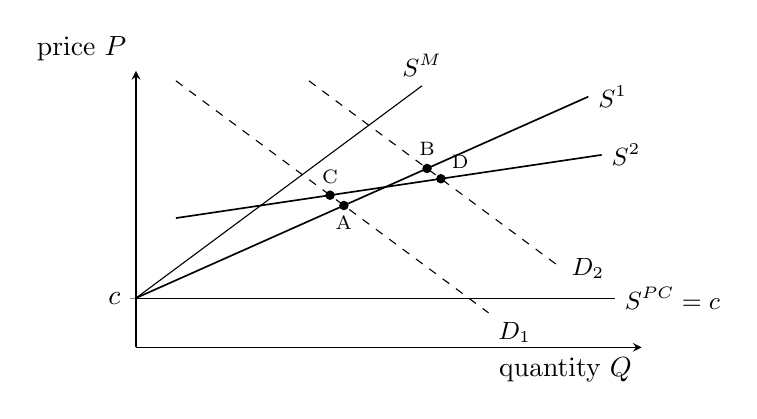
\begin{tikzpicture}
\begin{axis}[
  width=0.66\textwidth, height=0.42\textwidth,
  xmin=0, xmax=7.6, ymin=0, ymax=5.6,
  axis lines=left, xlabel={quantity $Q$}, ylabel={price $P$},
  xtick=\empty, ytick={1}, yticklabels={$c$},
  every axis x label/.style={at={(ticklabel* cs:1)}, anchor=north east},
  every axis y label/.style={at={(ticklabel* cs:1)}, anchor=south east},
  clip=false]
  \addplot[thin, domain=0:7.2, samples=2] {1} node[pos=1, right, font=\small] {$S^{PC} = c$};
  \addplot[thin, domain=0:4.3, samples=2] {1 + x} node[pos=1, above, font=\small] {$S^{M}$};
  \addplot[semithick, domain=0:6.8, samples=2] {1 + 0.6*x} node[pos=1, right, font=\small] {$S^{1}$};
  \addplot[semithick, domain=0.6:7.0, samples=2] {2.5 + 0.2*x} node[pos=1, right, font=\small] {$S^{2}$};
  \addplot[dashed, domain=0.6:5.3, samples=2] {6 - x} node[pos=1, below right, font=\small] {$D_1$};
  \addplot[dashed, domain=2.6:6.4, samples=2] {8 - x} node[pos=1, right, font=\small] {$D_2$};
  \addplot[only marks, mark=*, mark size=1.5pt] coordinates {(3.125,2.875) (4.375,3.625) (2.9167,3.0833) (4.5833,3.4167)};
  \node[below, font=\scriptsize] at (axis cs:3.125,2.85) {A};
  \node[above, font=\scriptsize] at (axis cs:4.375,3.68) {B};
  \node[above, font=\scriptsize] at (axis cs:2.9167,3.12) {C};
  \node[above right, font=\scriptsize] at (axis cs:4.6,3.42) {D};
\end{axis}
\end{tikzpicture}
\caption[Slope versus level of the supply relation]{Slope versus level of the supply relation. Inverse demand shifts from
$D_1\colon P = 6 - Q$ to $D_2\colon P = 8 - Q$, and marginal cost is $c = 1$. Industry 1 follows the conjectural-variations
supply relation $S^1\colon P = 1 + 0.6Q$ (points A and B). Industry 2 follows $S^2\colon P = 2.5 + 0.2Q$ (points C and D).
Both industries have average markup $2.25$ at average quantity $3.75$, an $m$-weighted average conduct of $0.6$. The conduct parameter
method estimates $0.6$ for industry 1 and $0.2$ for industry 2, and attributes the rest of industry 2's margin to a
marginal cost of $2.5$. $S^{PC}$ and $S^M$ are the competitive and monopoly supply relations. Drawn in the spirit of
Figure~1 of \citet{Corts1999}.}
\label{fig:03-corts-slope}
\end{figure}

The numbers in \cref{fig:03-corts-slope} are easy to check. On $S^1$, point A solves $6 - Q = 1 + 0.6Q$, so $Q = 3.125$
and the markup is $1.875$. Point B solves $8 - Q = 1 + 0.6Q$, so $Q = 4.375$ and the markup is $2.625$. On $S^2$, point C
solves $6 - Q = 2.5 + 0.2Q$, so $Q = 2.917$ and the markup is $2.083$. Point D gives $Q = 4.583$ and markup $2.417$. Both
pairs average a markup of $2.25$ at quantity $3.75$. The ratio $\frac{2.25}{3.75} = 0.6$ is the $m$-weighted average
conduct $\frac{\E[\theta_t m_t]}{\E[m_t]}$, since $m_t = Q_t$ when the slope of demand is $-1$.

\subsubsection{Corts's supergame model}

To show that the gap can be large in a coherent model, Corts studies efficient tacit collusion supported by repeated
interaction \citep[Section~3]{Corts1999}. The model is closely related to \citet{RotembergSaloner1986} when demand is
independent over time and to \citet{Kandori1991} when it is serially correlated \citep[fn.~2]{Corts1999}. We use
$\delta$ for the discount factor in the rest of this subsection. $N$
symmetric firms choose quantities every period. Inverse demand is $P_t = A(x_t) - BQ_t$ and marginal cost is $c(w_t)$,
where the demand state $x_t$ and the cost state $w_t$ are observed by all firms before they choose. A deviation is
punished by reversion to the one-shot Cournot equilibrium forever. An \emph{efficient} supergame equilibrium chooses, in
each state, the quantity that maximizes joint profit subject to the incentive constraint. Let $y_t = A(x_t) - c(w_t)$ be
the demand margin and $q$ the output of each firm.

The incentive constraint takes a simple form. A firm's collusive profit is $\pi(q) = q(y_t - BNq)$. Against rivals who
produce $(N - 1)q$, the best deviation produces $\frac{y_t - B(N - 1)q}{2B}$ and earns $\pi^b(q) = \frac{(y_t - B(N -
1)q)^2}{4B}$. The one-period gain from deviating is
\begin{align*}
\pi^b(q) - \pi(q) &= \frac{(y_t - B(N - 1)q)^2 - 4Bq(y_t - BNq)}{4B}\\
&= \frac{y_t^2 - 2B(N + 1)\, q\, y_t + B^2\left[(N - 1)^2 + 4N\right]q^2}{4B}\\
&= \frac{\left(y_t - B(N + 1)q\right)^2}{4B} .
\end{align*}
Let $\Lambda(x_t)$ be the expected discounted profit lost by entering the punishment phase \citep[eq.~15]{Corts1999}. It sums,
over future periods $i \ge 1$, $\delta^i$ times the expected excess of collusive over Cournot profit. The incentive
constraint is $\frac{(y_t - B(N + 1)q)^2}{4B} \le \Lambda(x_t)$. Collusive output lies below the Cournot output $q^c =
\frac{y_t}{B(N + 1)}$, so the constraint reads $y_t - B(N + 1)q \le 2\sqrt{B \Lambda(x_t)}$. The smallest sustainable output is
\begin{equation}\label{eq:03-corts-qtilde}
\tilde q_t = \frac{y_t}{B(N + 1)} - \frac{2\sqrt{B \Lambda(x_t)}}{B(N + 1)} \qquad \text{\citep[eq.~14]{Corts1999}}.
\end{equation}
The efficient output is the joint-monopoly output $q^m_t = \frac{y_t}{2BN}$ when it is sustainable, and $\tilde q_t$
otherwise. In industry units, conduct in state $t$ is $\theta_t = \frac{P_t - c_t}{BQ_t}$, which equals 1 at $q^m_t$ and
$\frac{1}{N}$ at $q^c$.

Equation \eqref{eq:03-corts-qtilde} shows why persistence matters. A higher demand state raises the gain from deviating,
which pushes output up toward Cournot. If demand is persistent, a higher state also raises expected future collusive
profits and so the cost of punishment $\Lambda(x_t)$, which pushes output down. When shocks are independent over time, only the
first effect operates. Then $\Lambda$ does not depend on $x_t$, and $\frac{\dd\tilde q_t}{\dd x_t} = \frac{A_1}{B(N + 1)}$, the
Cournot response.

\casehead{Simulation design and results}
Corts simulates a symmetric duopoly with linear demand and constant marginal cost. The demand and cost states each take
ten evenly spaced values. The cost state is independent over time, and its role is to identify demand. The demand state
follows a Markov chain that stays in the same state with probability $\varpi$ and moves to each other state with
probability $\frac{1 - \varpi}{9}$ (Corts calls this probability $\lambda$). Firms' quantities are computed by iterating
on $\Lambda(x_t)$ until convergence, and the conduct parameter method is applied to a sample from the resulting process.

\Cref{fig:03-corts-paper-fig2} reproduces Corts's results for positively correlated demand, in his firm-level
normalization (1 is Cournot and 2 is joint monopoly). He draws five lessons \citep[pp.~237--240]{Corts1999}. (a) For high
discount factors the method measures market power accurately whatever the demand process. (b) For low discount factors it
detects no market power when demand is independent over time. (c) It is accurate when demand is fully persistent. (d) It
becomes more accurate as demand becomes more persistent. (e) When demand states are negatively correlated, higher values
of the estimate go with lower values of the as-if parameter. The magnitudes are large. An estimate of 1.2 is consistent
with an as-if parameter of 1.3 when $\varpi = 0.9$ and of 1.9 when $\varpi = 0.5$ \citep[p.~238]{Corts1999}. Two
industries with similar estimates can thus differ greatly in collusiveness, and an industry whose demand becomes more or
less persistent can appear to change its conduct when it has not.

\begin{figure}[!htb]
\centering
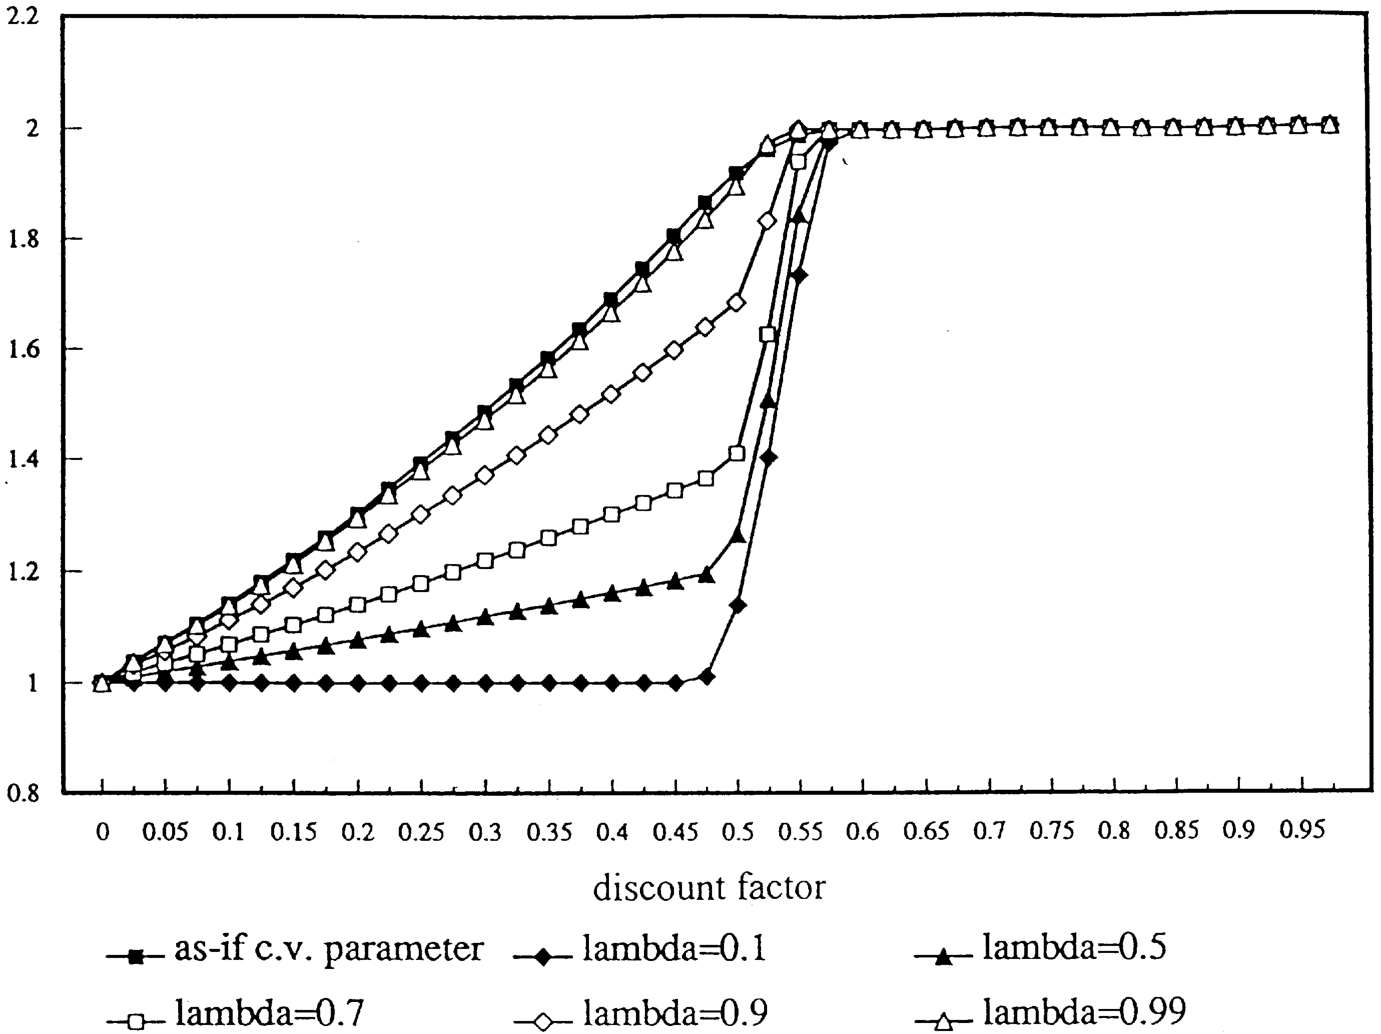
\includegraphics[width=0.85\textwidth]{figures/ch03/corts1999_fig2.png}
\caption[Conduct estimates in Corts's supergame simulations]{Conduct estimates in Corts's supergame simulations with
positively correlated demand, symmetric duopoly. The vertical axis is firm-level conduct (1 is Cournot, 2 is joint
monopoly). The top curve is the as-if conduct parameter. The other curves are conduct parameter estimates for demand
persistence $\varpi$ (``lambda'' in the original) of 0.1, 0.5, 0.7, 0.9 and 0.99. With ten states, $\varpi = 0.1$ makes
demand independent over time. Source: \citet{Corts1999},
Figure~2.}
\label{fig:03-corts-paper-fig2}
\end{figure}

Corts proves the main patterns \citep[Section~3.2]{Corts1999}. If joint monopoly is sustained in every state, the estimate
equals the as-if parameter (his Proposition~2). The monopoly supply relation is itself a conjectural-variations relation,
so it does not matter how monopoly is sustained. If demand is independent over time and monopoly is sustained in no state,
the estimate equals the Cournot value for every such discount factor (Proposition~3). Prices and profits rise with
$\delta$ over this range, yet the method detects none of the collusion. The proof is the one given above, since
$\frac{\dd\tilde q_t}{\dd x_t}$ equals the Cournot response. If demand is fully persistent, the estimate converges to the as-if
parameter (Proposition~4), because $\tilde q_t$ becomes proportional to the demand margin. If a higher demand state shifts
the distribution of future states to the right, the estimate exceeds the Cournot value whenever monopoly is sustained in no
state (Proposition~5). The method then detects some collusion but understates it. With negatively correlated demand, which
resembles seasonal variation, the estimate can fall below the Cournot value even though prices are above it. Corts warns
that seasonal dummies used as demand shifters may then fail to detect collusion, or produce estimates negatively correlated
with true conduct \citep[p.~240]{Corts1999}.

\subsubsection{A worked example: Bertrand collusion with demand shocks}\label{sec:03-corts-bertrand}

The following model is our own illustration, in the spirit of \citet{RotembergSaloner1986} and of Corts. It replaces
Cournot reversion with Bertrand reversion and delivers closed forms. $N$ symmetric firms sell a homogeneous good at constant
marginal cost $c$ and set prices every period. Demand is $Q_t = A_t - P_t$. The demand state $A_t$ is independent and
identically distributed over time with a continuous distribution on $[\underline A, \bar A]$, $\underline A > c$, and firms
observe it before pricing. Firms collude with grim-trigger strategies. Any deviation is followed by pricing at marginal cost
forever, which yields zero profit. Let $\Pi(p, A) = (p - c)(A - p)$ be industry profit and $\pi^m(A) = \frac{(A - c)^2}{4}$
monopoly profit.

\casehead{The incentive constraint}
Suppose firms charge $p \le p^m(A) = \frac{A + c}{2}$ and share the market equally. A deviator undercuts slightly, takes the
whole market and earns almost $\Pi(p, A)$ today and nothing afterward. Colluding yields $\frac{\Pi(p, A)}{N}$ today plus
$\frac{\delta}{1 - \delta}\frac{V}{N}$, where $V = \E[\Pi(p(A'), A')]$ is expected industry profit per period on the
collusive path. The incentive constraint is
\begin{equation*}
\Pi(p, A) - \frac{\Pi(p, A)}{N} \le \frac{\delta}{1 - \delta}\frac{V}{N}
\quad\Longleftrightarrow\quad
\Pi(p, A) \le K \equiv \frac{\delta V}{(1 - \delta)(N - 1)} .
\end{equation*}
Collusion thus caps industry profit at $K$ in every state. A price above $p^m(A)$ is never better. A deviator could then
undercut to $p^m(A)$ and earn $\pi^m(A)$, so the constraint would require $\pi^m(A) \le \frac{\Pi(p, A) + (N - 1)K}{N}$,
which fails whenever $\pi^m(A) > K$. The most profitable sustainable price is therefore
\begin{equation}\label{eq:03-bertrand-price}
p(A) =
\begin{cases}
\frac{A + c}{2} & \text{if } \pi^m(A) \le K ,\\[3pt]
\frac{A + c}{2} - \sqrt{\pi^m(A) - K} & \text{if } \pi^m(A) > K ,
\end{cases}
\end{equation}
where the second line is the lower root of $(p - c)(A - p) = K$. The cap binds in high-demand states, $A > A^* \equiv c +
2\sqrt K$. There the price falls as demand rises. Differentiating the second line,
$\frac{\dd p}{\dd A} = \frac{1}{2} - \frac{A - c}{4\sqrt{\pi^m(A) - K}} < 0$, because $\sqrt{\pi^m(A) - K} < \frac{A - c}{2}$.
These are the price wars during booms of \citet{RotembergSaloner1986}.

\casehead{The equilibrium cap}
Expected industry profit is $V = \E[\min\{\pi^m(A), K\}]$, so the cap solves the fixed-point equation
\begin{equation}\label{eq:03-bertrand-fixed}
K = \nu\, \E\left[\min\{\pi^m(A), K\}\right] \equiv T(K), \qquad \nu \equiv \frac{\delta}{(1 - \delta)(N - 1)} .
\end{equation}

\begin{lemma}[The most collusive equilibrium]\label{lem:03-fixed-point}
(i) If $\delta < 1 - \frac{1}{N}$, the only solution of \eqref{eq:03-bertrand-fixed} is $K = 0$, and firms price at cost.
(ii) If $\delta > 1 - \frac{1}{N}$, there is exactly one positive solution $K^*$. It is the largest fixed point, and the
iteration $K_{n+1} = T(K_n)$ started at any $K_0 \ge \nu\E[\pi^m(A)]$ decreases to $K^*$. (iii) Monopoly pricing in every
state is sustainable if and only if $\nu\,\E[\pi^m(A)] \ge \pi^m(\bar A)$.
\end{lemma}

\begin{proof}
The map $T$ is increasing and concave, because $\min\{\pi^m(A), K\}$ is increasing and concave in $K$ for every $A$. It
satisfies $T(0) = 0$, its right derivative at zero is $\nu$ (since $\pi^m(A) > 0$), and it is bounded by
$\nu\E[\pi^m(A)]$. The condition $\nu < 1$ is equivalent to $\delta < (1 - \delta)(N - 1)$, that is, to $\delta < 1 -
\frac{1}{N}$. (i) If $\nu < 1$, then $T(K) \le \nu K < K$ for every $K > 0$. (ii) If $\nu > 1$, the function
$T(K) - K$ is positive for small $K > 0$ and negative for large $K$, so it has a positive root. It is concave and equals
zero at $K = 0$ with positive slope there. A second positive root would force a concave function to be zero at two points
while positive between zero and the first, which is impossible. Starting at $K_0 \ge \nu\E[\pi^m(A)] \ge K^*$, the
sequence satisfies $K^* = T(K^*) \le T(K_n) \le K_n$, so it decreases and converges to a fixed point no smaller than
$K^*$, which must be $K^*$. (iii) If $K \ge \pi^m(\bar A)$, then $T(K) = \nu\E[\pi^m(A)]$, and the fixed point satisfies
$K \ge \pi^m(\bar A)$ exactly when $\nu\E[\pi^m(A)] \ge \pi^m(\bar A)$.
\end{proof}

Collusion above cost requires $\delta > 1 - \frac{1}{N}$, the familiar condition for Bertrand collusion with constant
demand. It plays the role of condition (i) in \citet{RotembergSaloner1986}, which requires that the number of firms not be
too large relative to the discount factor. They also select the greatest fixed point.
For any $\delta$ above it, the cap exceeds $\pi^m(\underline A)$. If $K \le \pi^m(\underline A)$, then $T(K) = \nu K >
K$, so no fixed point lies there. The lowest demand states are therefore always priced at the monopoly level.

\casehead{Conduct and the conduct parameter estimate}
The markup term is $m_t = Q_t$, because $\lvert\frac{\partial Q}{\partial P}\rvert = 1$. Conduct in state $A$ is
$\theta(A) = \frac{p(A) - c}{Q}$. In unconstrained states $p - c = Q = \frac{A - c}{2}$, so $\theta = 1$. In constrained
states $(p - c)Q = K$, so
\begin{equation*}
\theta(A) = \frac{K}{Q^2}, \qquad P - c = \frac{K}{Q} .
\end{equation*}
Conduct falls as demand rises, and the supply relation in the constrained region is a rectangular hyperbola. Its local
slope is $-\frac{K}{Q^2} = -\theta(A)$. Part (ii) of \cref{prop:03-corts} applies with $Z_t = A_t$, since $m_t = A_t - p(A_t)$
is increasing in $A_t$. The estimate is a weighted average of the local slope $+1$ in unconstrained states and $-\theta(A)$
in constrained states, so it can be negative while every $\theta(A)$ lies in $(0, 1]$.

\Cref{tab:03-corts-sim} and \cref{fig:03-corts-sim} report the numbers for $N = 2$, $c = 0$ and $A_t$ uniform on $[6, 10]$.
Population moments are computed by quadrature, and a regression on 200,000 simulated periods reproduces them to within
$0.002$. Collusion requires $\delta > 0.5$. Monopoly in every state requires $\nu\E[\pi^m(A)] \ge \pi^m(10)$, that is,
$\nu \ge \frac{25}{16.33}$, which holds for $\delta \ge 0.6048$. In between, the cap binds in the high-demand states. At
$\delta = 0.51$, conduct ranges from $0.17$ in the highest state to $1$ in the lowest, and its mean is $0.51$. The
$m$-weighted average conduct is $\frac{\E[P_t - c]}{\E[Q_t]} = \frac{2.34}{5.66} = 0.41$. The instrumental-variables
estimate is $-0.36$. A researcher would conclude that prices lie below the competitive level in an industry whose average
elasticity-adjusted Lerner index is about one half. The estimate turns positive only near $\delta = 0.56$ and catches up with
average conduct when monopoly is sustained everywhere. With $N = 3$ the pattern is the same: at $\delta = 0.677$ mean
conduct is $0.53$ and the estimate is $-0.36$.

\begin{table}[htbp]
\centering
\caption{Mean conduct and the conduct parameter estimate in the Bertrand supergame}
\label{tab:03-corts-sim}
\begin{threeparttable}
\begin{tabular}{@{}cccccc@{}}
\toprule
Discount factor & Profit cap & Cutoff state & Share of states & Mean conduct & IV estimate \\
$\delta$ & $K$ & $A^*$ & constrained & $\E[\theta_t]$ & $\hat\theta$ \\
\midrule
0.5001 & 9.30 & 6.10 & 0.98 & 0.28 & $-0.27$ \\
0.505 & 11.37 & 6.74 & 0.81 & 0.44 & $-0.35$ \\
0.51 & 12.54 & 7.08 & 0.73 & 0.51 & $-0.36$ \\
0.52 & 14.38 & 7.58 & 0.61 & 0.62 & $-0.33$ \\
0.53 & 15.94 & 7.99 & 0.50 & 0.71 & $-0.28$ \\
0.55 & 18.69 & 8.65 & 0.34 & 0.83 & $-0.10$ \\
0.57 & 21.15 & 9.20 & 0.20 & 0.92 & $0.21$ \\
0.6048 & 25.00 & 10.00 & 0.00 & 1.00 & $1.00$ \\
\bottomrule
\end{tabular}
\begin{tablenotes}[flushleft]\footnotesize
\item Notes: $N = 2$ Bertrand firms, marginal cost $c = 0$, demand $Q_t = A_t - P_t$ with $A_t$ independent and uniform on
$[6, 10]$, grim-trigger punishment at marginal cost. $K$ is the largest solution of \eqref{eq:03-bertrand-fixed}, and the
cap binds for $A_t > A^* = 2\sqrt K$. Conduct is $\theta_t = \frac{P_t - c}{Q_t}$, the elasticity-adjusted Lerner index.
The estimate is $\frac{\Cov(A_t, P_t - c)}{\Cov(A_t, Q_t)}$, the limit of the instrumental-variables estimator with a
constant and the demand state as instrument. For $\delta < 0.5$ prices equal cost and both measures are zero. Population
moments computed by quadrature.
\end{tablenotes}
\end{threeparttable}
\end{table}

\begin{figure}[htbp]
\centering
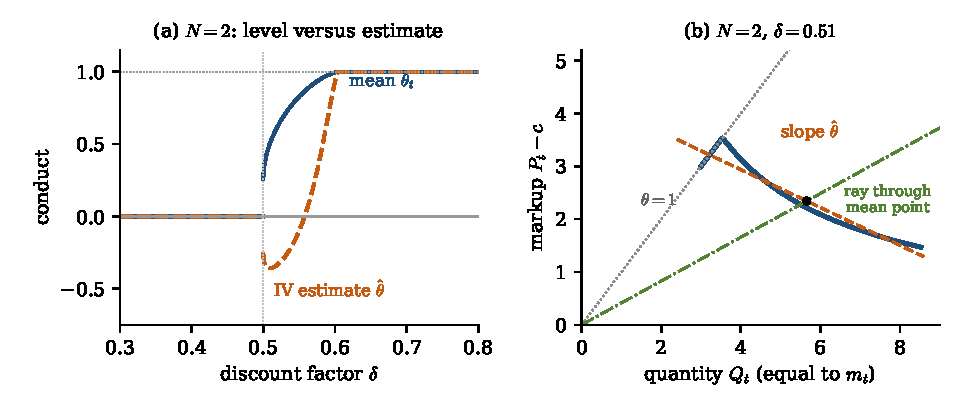
\includegraphics[width=\textwidth]{figures/ch03/corts_sim.pdf}
\caption[Level of conduct versus its estimate in a Bertrand supergame]{Level of conduct versus its estimate in a Bertrand
supergame with independent demand shocks ($N = 2$, $c = 0$, $A_t$ uniform on $[6, 10]$). Panel (a): mean conduct
$\E[\theta_t]$ and the instrumental-variables estimate $\hat\theta$ against the discount factor. Panel (b): the locus of
equilibrium markups and quantities at $\delta = 0.51$. It follows the monopoly ray $\theta = 1$ in low-demand states and the
hyperbola $P - c = \frac{K}{Q}$ in high-demand states. The dashed line through the mean point has slope $\hat\theta = -0.36$,
and the dash-dotted ray through the mean point has slope $0.41$, the $m$-weighted average conduct.}
\label{fig:03-corts-sim}
\end{figure}

The example and Corts's model reach the same conclusion by different routes. With Cournot reversion and independent
shocks, the estimate sticks at the Cournot value. With Bertrand reversion the static benchmark is price taking, and the
constant profit cap makes the constrained supply relation slope downward, so the estimate falls below zero. In both cases
the estimate reflects how the incentive constraint varies with demand, and it carries no direct information on the level
of conduct.

\subsubsection{Assessment}\label{sec:03-corts-assessment}

The critique changes how we read a conduct estimate. A constant-$\theta$ estimate measures the slope of the supply relation,
a weighted average of marginal responses of the markup to demand. Reading it as the level of conduct requires the marginal
and average relations to coincide. This holds in conjectural-variations models, under monopoly in every state, and in the
limit of fully persistent demand. Corts concludes that, when behavior results from efficient supergame collusion, the method
understates market power if demand shocks are not fully permanent. It may detect no market power at all when shocks are
transitory, even with average margins near the monopoly level \citep[pp.~244--245]{Corts1999}.

Three further points follow. First, the specification-test reading does not escape the critique. The estimate can equal
the Cournot value over a wide range of collusive equilibria. A failure to reject Cournot then carries little information,
and tests of the nested static models may lack power. Second, Corts argues that ``not even the positive correlation'' of
the estimate with the as-if parameter can be maintained across models \citep[p.~245]{Corts1999}. Comparisons of conduct
across industries or over time are therefore suspect. Third, the evidence available to Corts points the same way. In the
electricity study of \citet{Wolfram1999} and the sugar study of \citet{GenesoveMullin1998}, the estimates obtained without
cost data fall below the direct measures. Both studies were available to Corts as working papers. Corts notes that equality of the
two can be rejected in both cases \citep[p.~245]{Corts1999}. \Cref{sec:03-sugar,sec:03-electricity} examine both studies.

Genesove and Mullin frame the point in the same terms. The conduct parameter ``measures the marginal response of price, and
hence the markup, to changes in exogenous variables'' \citep[p.~2]{GenesoveMullin1995}. It therefore ``infers market power
from the marginal behavior of the markup, not from the level of the markup.'' They add an example
\citep[p.~3]{GenesoveMullin1995}. Supergame models such as \citet{RotembergSaloner1986} may make the marginal response of
price to demand shifters independent of the discount rate. It is then also independent of the price level at a baseline
state of demand.

The critique has limits. Corts's models are stylized, with linear demand, constant cost, perfect monitoring and an efficient
equilibrium, and the simulations are not calibrated to any industry. They show that the mismeasurement can be severe, and
they leave its size in a given application open. The direction of the bias depends on the persistence of demand, which the
researcher can sometimes measure.

The contribution is lasting. \citet[fn.~7]{BerryHaile2014} cite \citet{Corts1999} and \citet{ReissWolak2007} for the
fundamental problems of the conduct parameter approach. Corts calls for explicit structural models of conduct. The field
responded in three ways. It estimates dynamic models of collusion directly, as in the work on the railroad cartel of
\citet{Porter1983} and \citet{Ellison1994} (\cref{ch:collusion-evidence}). It tests a finite menu of conduct models within
richer demand systems (\cref{sec:03-other-routes}). And it validates the method where marginal cost is observed
(\cref{sec:03-sugar,sec:03-electricity}).

\subsection{Bounds instead of point estimates}\label{sec:03-bounds}

If conduct varies and a constant $\theta$ misleads, we can give up point identification. \citet[Section~2.2]{Rosen2007}
replaces the equilibrium assumption with known bounds on each firm's conduct in each period. The widest bounds are price
taking and monopoly. Conduct may vary freely within them, so the parameters of marginal cost are in general only set identified.
We present the idea in the homogeneous-good setting of this chapter.

Suppose only that industry conduct lies between price taking and joint monopoly, $\theta_t \in [0, 1]$, with no restriction
on how it varies across observations. The supply relation gives $P_t - mc_t = -\theta_t Q_t P'(Q_t)$. Since $-Q_tP'(Q_t)
\ge 0$, the bounds on $\theta_t$ imply $0 \le P_t - mc_t \le -Q_t P'(Q_t)$, that is,
\begin{equation}\label{eq:03-rosen-ineq}
P_t + Q_t P'(Q_t) \;\le\; mc_t \;\le\; P_t .
\end{equation}
Marginal cost lies between monopoly marginal revenue and price, observation by observation. With a parametric marginal
cost $mc_t = c(Q_t, W_t; \beta) + u^s_t$ and $\E[u^s_t \mid X_t] = 0$ for instruments $X_t$, the inequalities become
conditional moment inequalities:
\begin{equation*}
\E\left[P_t - c(Q_t, W_t; \beta) \mid X_t\right] \ge 0, \qquad
\E\left[c(Q_t, W_t; \beta) - P_t - Q_t P'(Q_t) \mid X_t\right] \ge 0 .
\end{equation*}
The \emph{identified set} is the set of $\beta$ that satisfy both for almost every $X_t$. Since $P'(Q_t)$ comes from an
estimated demand curve, estimation has two steps. Bounds on $\beta$ imply bounds on marginal cost, on markups and on each
$\theta_t$, without assuming that conduct is constant.

A deterministic example shows the geometry. Let $mc = b_0 + b_1 Q$ with true values $(b_0, b_1) = (2, 0.5)$, and let
inverse demand in market $t$ be $P = A_t - Q$. Four markets have $A_t = 8, 10, 12, 14$ and conduct $\theta_t = 0.2, 0.9,
0.5, 0.1$. The equilibrium solves $A_t - Q - (2 + 0.5Q) = \theta_t Q$, so $Q_t = \frac{A_t - 2}{1.5 + \theta_t}$. Each
market contributes the two half-planes $P_t - Q_t \le b_0 + b_1 Q_t \le P_t$ in the $(b_1, b_0)$ plane, and we add the
restrictions $b_0 \ge 0$ and $b_1 \ge 0$. \Cref{fig:03-rosen-bounds} shows the intersection. It is a quadrilateral with
$b_1 \in [0, 0.76]$ and $b_0 \in [0.80, 4.47]$. Without the sign restrictions the slope could range from $-1.38$ to $0.76$.
The implied bounds on conduct are informative in some markets. Conduct lies in $[0.66, 1]$ in the second market (true value
$0.9$) and in $[0.36, 0.73]$ in the third (true value $0.5$). In the first and fourth markets only the upper bound moves,
to $0.32$ and $0.42$ (true values $0.2$ and $0.1$).

\begin{figure}[htbp]
\centering
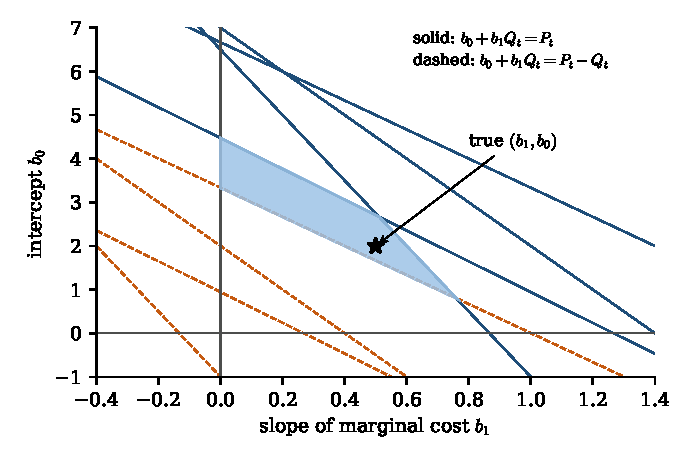
\includegraphics[width=0.60\textwidth]{figures/ch03/rosen_bounds.pdf}
\caption[Identified set for marginal cost when conduct varies freely]{Identified set for a linear marginal cost
$mc = b_0 + b_1 Q$ when conduct varies freely in $[0, 1]$. Each of four markets with inverse demand $P = A_t - Q$ restricts
$(b_1, b_0)$ to the band between a solid line (marginal cost equals price) and a dashed line (marginal cost equals monopoly
marginal revenue). The shaded region is the intersection with $b_0, b_1 \ge 0$. The star marks the true values $(0.5, 2)$.}
\label{fig:03-rosen-bounds}
\end{figure}

The set shrinks quickly when some markets sit near the extremes of conduct. Consider six markets with $A_t = 6, 8, \dots,
16$ and $\theta_t = 0.1, 0.8, 0.3, 1, 0, 0.6$, one of them competitive and one fully collusive. The identified set is then
a small triangle with $b_1 \in [0.33, 0.50]$ and $b_0 \in [2.00, 2.67]$. Every market's conduct is bounded within an
interval of width at most $0.1$. The approach trades precision for robustness. It needs no assumption on how conduct varies,
and it states plainly what the data cannot reveal. Its bounds can be wide, and inference requires methods for moment
inequalities. The Lerner bound \eqref{eq:03-lerner-bound} and Sullivan's bound in \cref{sec:03-sullivan} use the same
logic in reverse. A lower bound on marginal cost, the tax, bounds conduct from above.

\subsection{The record of conduct estimates}\label{sec:03-record}

Almost all estimates of conduct fall strictly between zero and one. The finding is unsurprising, yet it is useful against
extreme claims that an industry is perfectly competitive or fully cartelized. \Cref{tab:01-bresnahan-table} reproduces the
estimated Lerner indices that \citet[Table~17.1]{Bresnahan1989} collected from early studies. \Cref{sec:01-neio-lessons}
discusses the three conclusions he draws from them \citep[pp.~1052--1053]{Bresnahan1989}. He concludes that some
concentrated industries have high margins and that anticompetitive conduct is one cause. He also finds that the studies
reveal little about how market power relates to industry structure.

The entries of that table are margins, and they differ from conduct parameters by the factor $\varepsilon$. Bresnahan left
out studies whose estimates could not be converted into a Lerner index. These include the Panzar-Rosse and Sullivan
methods, which yield tests or bounds, and the residual demand method, whose elasticities equal the Lerner index only in
special cases \citep[fn.~47]{Bresnahan1989}. Two lessons of this section qualify the record further. A conduct estimate is
a slope, so estimates in $(0, 1)$ are compatible with conduct that swings between collusion and price wars
(\cref{sec:03-corts}). The most direct test of the methods compares them with observed costs, which is the task of
\cref{sec:03-sugar,sec:03-electricity}.

\section{Sugar refining, 1890--1914: Genesove and Mullin (1998)}\label{sec:03-sugar}

The methods of \cref{sec:03-sumner,sec:03-identification} infer market power without observing marginal
cost. Their answers are only as good as the maintained assumptions on demand, cost and conduct. Whether
those assumptions deliver the right answer in a real industry is an empirical question.
\citet{GenesoveMullin1998} answer it for American cane sugar refining between 1890 and 1914, an industry in
which marginal cost can be measured almost directly. They compute conduct twice. The first computation uses
the cost information and serves as a benchmark. The second treats cost as unknown and applies the standard
estimator of the New Empirical Industrial Organization (NEIO). Together with the electricity study of
\cref{sec:03-electricity}, this comparison is the closest the literature comes to a controlled test of the
conduct-parameter method.\footnote{We work from two versions. The article \citep{GenesoveMullin1998} is
cited by its table numbers (``Table 2'') and its published page numbers. The working paper \citep{GenesoveMullin1995} contains a longer
history, the cost evidence and several tables that the article omits. We cite those as ``WP Table 9'' and
give its printed page numbers. Published Tables 2, 3 and 4 correspond to WP Tables 4, 6, and 7 and 8.
Published Table 10 reproduces two columns of WP Table 14 with a different direct measure. Published Table 9
has no counterpart in the working paper.}

\subsection{The question and why sugar}\label{sec:03-sugar-question}

Genesove and Mullin start from the supply relation \eqref{eq:03-supply-relation} with a constant marginal
cost $c$,
\begin{equation}\label{eq:03-gm-supply}
P + \theta\, Q\, P'(Q) = c ,
\end{equation}
and from its Lerner form \eqref{eq:03-lerner-theta}, $\theta = \varepsilon(P)\frac{P - c}{P} \equiv
L_\varepsilon$. With complete cost information and an estimated demand elasticity, the elasticity-adjusted
Lerner index delivers $\theta$ period by period. Without cost information, $\theta$ must be restricted,
because an unrestricted $\theta_t$ fits any data (\cref{prop:03-exact-fit}). The usual restriction is that
$\theta$ is constant, or at least uncorrelated with the instruments (WP p.~4).

Three features make sugar refining the right place for a test (WP pp.~3--4). First, the technology is
simple. Raw sugar is turned into refined sugar at a fixed and known coefficient, both prices are observed,
and the remaining costs are documented. A true price-cost margin can therefore be computed. Second, the
harvest cycle of raw sugar and year-to-year weather generate supply variation that is plausibly exogenous to
American demand. This variation helps identify demand and, through it, conduct. Third, the industry went
through dramatic structural changes: the formation of a trust, repeated entry with price wars, renewed
consolidation, and an antitrust prosecution. These episodes let us ask whether estimated conduct moves with
structure, and whether the method can tell a change in conduct from a change in cost.

The test answers two standing objections to the NEIO (WP pp.~2--3). The first is that functional forms for
demand impose strong restrictions on the relation between price and marginal cost. The second is the point
of \citet{Corts1999} developed in \cref{sec:03-corts}. The estimated conduct parameter measures the marginal
response of the markup to the identifying shocks, and so may misstate its level. Genesove and Mullin note
that no NEIO estimate had ever been checked against an independent measure of conduct. Their design makes
three comparisons. The NEIO estimate $\hat\theta$ is compared with the direct measure $L_\varepsilon$. The
NEIO estimates of the cost parameters are compared with their documented values. Finally, the estimates for
different structural regimes are compared with the direct measures for the same regimes. Throughout, the
maintained hypothesis is that $L_\varepsilon$ measures conduct without error (WP p.~5).

\subsection{The industry, 1887--1914}\label{sec:03-sugar-history}

The American cane sugar refining industry of this period combined high concentration with repeated entry.
\Cref{tab:03-gm-chronology} lists the main events (WP Tables 1 and 13). The account below follows WP
pp.~6--8 and 13--15. These pages rely on \citet{Eichner1969}, \citet{Zerbe1969} and Willett and Gray's
\emph{Weekly Statistical Sugar Trade Journal}, the source of most of the data.

\begin{table}[htbp]
\centering
\caption{Chronology and structural regimes of the U.S. sugar refining industry}\label{tab:03-gm-chronology}
\small
\begin{tabular}{@{}ll@{}}
\toprule
\multicolumn{2}{@{}l}{\textit{Panel A. Events (WP Table 1 and text)}}\\
\midrule
1887 (Dec.) & Sugar Trust formed: 18 firms with 80 percent of capacity\\
1889--1890 & Entry by Spreckels (Philadelphia plant completed in Dec. 1889), price war\\
1891 & Trust reorganized as the American Sugar Refining Company (ASRC)\\
1891--1892 & Acquisition of Spreckels and others, ASRC reaches 95 percent of capacity\\
1892--1896 & Small-scale entry by five single-plant firms, cartel operation\\
1898 & Entry by Arbuckle Brothers (August) and Doscher (November)\\
1900 (May) & End of the Arbuckle war\\
1903 & Cuban Reciprocity Treaty: Cuban raw sugar enters at 80 percent of full duty\\
1910 & Federal antitrust suit (consent decree in 1922)\\
1914 & World War I begins, the sample ends in June 1914\\
\midrule
\multicolumn{2}{@{}l}{\textit{Panel B. Regimes used in the estimation (WP Table 13)}}\\
\midrule
Jan. 1890 to Feb. 1892 & Spreckels entry, price war\\
Mar. 1892 to Sep. 1898 & Acquisition of Spreckels, small-scale entry, cartel operation\\
Sep. 1898 to Apr. 1900 & Entry by Arbuckle Brothers and Doscher, price war\\
May 1900 to 1910 & After the Arbuckle war\\
Nov. 1910 to 1913 & Government antitrust suit\\
\bottomrule
\end{tabular}

\smallskip
\begin{minipage}{0.92\textwidth}\footnotesize
Notes: Compiled from \citet{GenesoveMullin1995}, WP Tables 1 and 13 and pp.~6--8. The two price-war regimes
in Panel B are the ``post-entry price wars'' of \cref{sec:03-sugar-wars}.
\end{minipage}
\end{table}

\casehead{Trust and first entry}
After several failed attempts at collusion, the Sugar Trust was formed in December 1887. It consolidated 18
firms that controlled 80 percent of industry capacity, and it soon reduced their 20 plants to 10. The
average refined price rose about 16 percent, from \$6.013 per hundred pounds in 1887 to \$7.007 in 1888 (WP
p.~6, fn.~2). Entry followed. Claus Spreckels, a West Coast refiner, completed a plant in Philadelphia in
December 1889, in retaliation for the Trust's purchase of a California refinery. A price war ensued. The
Trust, reorganized in 1891 as the American Sugar Refining Company (ASRC), then bought the Spreckels plant
and the remaining outsiders. By April 1892 it held 95 percent of capacity. Genesove and Mullin describe this
episode as the template for the period: high concentration, punctuated by entry, price wars, and then
acquisition of or accommodation with the entrants (WP p.~7).

\casehead{Cartel and second entry}
Between 1892 and 1896 five firms entered, each with a single plant of about 1,340 barrels of refined sugar
per day on average. ASRC and its ``friendly'' companies had 49,500 barrels per day. ASRC acted as cartel
leader, and by 1896 an understanding with the independents had evolved. The next challenge came from the
Arbuckle Brothers, wholesale grocers and the dominant American coffee roasters. Their refinery began limited
production in August 1898, and the Doscher refinery started in November. Each plant had a capacity of 3,000
barrels per day. A severe price war followed, with pricing at or below cost, shutdowns by independent
refiners and partial exit of one entrant. Apart from one respite, the war lasted until May 1900. It ended
when Doscher merged with two major independents in a transaction organized by the president of ASRC (WP
pp.~7--8).

\casehead{Tariffs, antitrust and fringes}
The tariff on refined sugar protected domestic refiners from European competition. From 1903, the Cuban
Reciprocity Treaty admitted Cuban raw sugar at 80 percent of the full duty. In antitrust, the government
challenged ASRC's purchase of several Philadelphia refineries in 1892, and the Supreme Court upheld the
acquisition in 1895 (the \emph{E.\,C.~Knight} case). In 1910 the federal government sued for dissolution.
The case ended in a consent decree only in 1922, but after the government's victories against Standard Oil
and American Tobacco in 1911, ASRC began a partial ``voluntary'' dissolution (WP p.~8). Two competitive
fringes disciplined the cane refiners. Domestic beet sugar supplied less than 1 percent of consumption until
1894, 5 percent by 1901 and 15 percent in 1908--1914. European beet refiners were a threat of imports, and
ASRC's president testified in 1888 and 1894 that ASRC set prices so that no refined sugar would be imported
(WP p.~14). Genesove and Mullin do not model the fringes. Their conduct measures are therefore ``overall''
measures that include the discipline of potential imports and beet sugar (WP p.~15).

\casehead{Product, sunk costs and capacity}
The standard grade of refined sugar, ``standard granulated,'' was a homogeneous product. Refiners shipped it
to grocers in barrels, and grocers repackaged it without identifying the manufacturer, so prices tended to
uniformity (WP pp.~13--14). A refinery of 3,000 barrels per day cost between \$1.5 and \$2.5 million in 1900.
Plant and machinery had little value outside sugar, while the waterfront land had considerable salvage value.
Entry costs were thus largely, but not completely, sunk. Industry output stayed well below capacity
throughout, and ASRC kept excess capacity even in the depths of the Arbuckle war (WP p.~13). ASRC's share
of the market fell from 91 percent in 1892 to 43 percent in 1914 (WP Table 9).

\subsection{Technology and the direct measurement of marginal cost}\label{sec:03-sugar-cost}

Refined sugar was made mostly from cane. Cane was first processed into raw sugar, which could be shipped
and stored. The standard grade, ``96 degree centrifugals,'' was 96 percent sucrose, and its sugar content
was tested with a polariscope, which made the input homogeneous. Most raw sugar came from the tropics,
especially Cuba, with Louisiana the main domestic source. Refiners melted, purified and crystallized it
into refined sugar, which is pure sucrose. Witnesses for both ASRC and an independent testified that all
refiners used a common process (WP p.~9).

\begin{assumption}[Fixed-coefficient technology]\label{ass:03-gm-cost}
The marginal cost of producing one hundred pounds of refined sugar in period $t$ is
\begin{equation}\label{eq:03-gm-cost}
c_t = c_0 + k\,P^{\mathrm{raw}}_t .
\end{equation}
Here $P^{\mathrm{raw}}_t$ is the price of one hundred pounds of raw sugar, and $k$ is the quantity of raw sugar
needed per unit of refined sugar. The term $c_0$ collects all other variable costs (labor, fuel, boneblack,
packages, brokerage, net of the value of byproducts). Both $c_0$ (in constant dollars) and $k$ are constant
over time and do not depend on output.
\end{assumption}

The assumption that marginal cost does not depend on output is natural in an industry that always operated
well below capacity. Genesove and Mullin maintain \eqref{eq:03-gm-cost} throughout, and then measure $k$ and
$c_0$ from engineering and testimonial evidence.

\casehead{The input coefficient}
Raw sugar is 96 percent sucrose, so the physical minimum is $k = \frac{1}{0.96} = 1.042$. The working paper
truncates this value and prints 1.041 (WP p.~10). Some sugar is lost
in refining. A Treasury commission found in 1898 that one hundred pounds of raw sugar yielded 92.5 pounds of
refined sugar. Genesove and Mullin put the yield at 92.5 to 93 pounds (WP p.~10). One pound of refined sugar
therefore requires about $\frac{1}{0.93} = 1.075$ pounds of raw sugar, and Genesove and Mullin set
$k = 1.075$. Audits of refiners' books by the Tariff Commission show that the coefficient did not change
during the sample period or after it.

\casehead{Non-sugar costs}
The trade spoke of ``the margin,'' the difference between the refined and the raw price. Because $k > 1$,
that margin overstates the money left after paying for raw sugar. The relevant quantity is the \emph{proper
margin}
\begin{equation}\label{eq:03-gm-proper-margin}
G_t \equiv P_t - k\,P^{\mathrm{raw}}_t = c_0 + (P_t - c_t),
\end{equation}
the refined price net of raw-sugar cost (WP pp.~10--11). By \eqref{eq:03-gm-cost}, the proper margin equals
non-sugar cost plus the price-cost margin. Five pieces of evidence pin down $c_0$, all expressed in constant
1898 dollars per hundred pounds.
\begin{enumerate}[label=(\roman*)]
\item The earliest evidence is testimony before the Industrial Commission in June 1899 (WP pp.~10--11). Henry
Havemeyer, president of ASRC, said that he had never known a cost of refining below one-half cent a pound. At the
formation of the trust it had been three-quarters of a cent. He agreed that at a margin of 50 cents a hundred pounds
``the refineries are running at a loss'' (WP p.~10, fn.~14). James Jarvie, a partner of Arbuckle Brothers, put the
cost of refining at ``50 to 60 points, or one-half to six-tenths of a cent per pound.'' He added that ``if raw sugar
costs $4\frac{1}{2}$ cents a pound, it will cost over 5 cents up to $5\frac{10}{100}$'' (WP p.~11, fn.~15). The raw price in this statement is hypothetical. Subtracting its raw-sugar cost from the two
totals gives, per hundred pounds,
\begin{equation*}
c_0 = 500 - 1.075 \times 450 = 16.25 \text{ cents},
\qquad
c_0 = 510 - 1.075 \times 450 = 26.25 \text{ cents}.
\end{equation*}
\item Another witness itemized non-sugar costs: 5 cents for brokerage and taxes, 10 cents for packages and
20 cents for wages, fuel, boneblack, repairs and sundries, less 10 cents of byproduct (syrup) revenue. The
total is 25 cents.
\item At the Hardwick Committee hearings of 1911, refiners quoted a refining cost of 60 to 65 cents when raw
sugar sold for \$4.00. A refining cost in this sense is $c - P^{\mathrm{raw}} = c_0 + (k - 1)P^{\mathrm{raw}}$,
so $c_0$ lies between $60 - 0.075 \times 400 = 30$ and $35$ cents in current dollars, or 22 to 26 cents in
1898 dollars.
\item Tariff Commission audits for 1914 give a total refinery cost of \$0.420. Removing \$0.013 of accounting
depreciation and \$0.056 of byproduct receipts leaves \$0.351 in current dollars, or 25 cents in 1898
dollars (WP p.~11, fn.~18).
\item Behavior during the Arbuckle war bounds $c_0$ as well. The independents shut down or ran at
``minimum capacity'' at times. The minimum proper margin above which they always produced was 26 cents, and
except for a couple of weeks they never produced below 9 cents. For example, they shut down when the refined
price was \$4.71 and the raw price \$4.30, a proper margin of $4.71 - 1.075 \times 4.30 = 0.0875$ (WP p.~12,
fn.~22).
\end{enumerate}
Shutdown behavior cannot reveal a single break-even margin (WP p.~12). Prices are observed only on Fridays.
Month-long contracts and the value of a reputation for reliable supply can justify producing at a loss. Costs
of shutting down and restarting open a band of margins in which a firm sometimes produces and sometimes does
not. The band is consistent with the direct estimates, however.

Genesove and Mullin adopt $c_0 = 0.26$, the value supported by the most and best evidence, and use $0.16$ as a
lower bound. The range reflects the researchers' ignorance. Cost differences among firms were small: a commission
merchant for an independent refiner estimated that larger houses might refine 3 to 5 cents more cheaply
(WP pp.~12--13). Non-sugar inputs are small:
4.5 percent of cost at $c_0 = 0.16$ and 7.5 percent at $c_0 = 0.26$ (WP p.~12). The direct measure of
marginal cost is therefore
\begin{equation}\label{eq:03-gm-direct-cost}
c_t = 0.26 + 1.075\,P^{\mathrm{raw}}_t .
\end{equation}
More than nine tenths of marginal cost is an observed input price that fluctuates a great deal. This is
what makes sugar refining so well suited to a validation exercise.

\subsection{Data, instruments and the demand system}\label{sec:03-sugar-demand}

\casehead{Data}
The sample is quarterly, from January 1890 to June 1914 (WP p.~26). Prices come from Willett and Gray's
weekly quotations. Consumption data do not exist, so quantity is measured by \emph{meltings} $M_t$, the
quantity of raw sugar melted by refiners. Meltings track consumption closely because refined sugar
deteriorates in storage and refiners produced to order with about a one-month lag (WP pp.~16--17). Prices are
in dollars per hundred pounds, deflated to constant 1898 dollars with the wholesale price index of
\citet{Hanes1993}. Meltings and Cuban imports are in hundreds of thousands of long tons per quarter. Cuban
imports were zero in the third quarter of 1897, during the Cuban war of independence, and that quarter is
dropped \citep[pp.~365, 373]{GenesoveMullin1998}. This leaves 97 quarters: 73 in the low season and 24 in
the high season defined below. \Cref{tab:03-gm-stats} reports the sample statistics.

\begin{table}[htbp]
\centering
\caption{Sample statistics, quarterly, 1890--1914}\label{tab:03-gm-stats}
\small
\begin{tabular}{@{}lcccccc@{}}
\toprule
 & \multicolumn{2}{c}{Full sample} & \multicolumn{2}{c}{Low season} & \multicolumn{2}{c}{High season}\\
\cmidrule(lr){2-3}\cmidrule(lr){4-5}\cmidrule(l){6-7}
 & Mean & S.D. & Mean & S.D. & Mean & S.D.\\
\midrule
Refined price $P$ & 4.03 & 0.62 & 3.99 & 0.63 & 4.14 & 0.58\\
Raw price $P^{\mathrm{raw}}$ & 3.30 & 0.59 & 3.28 & 0.61 & 3.36 & 0.53\\
Proper margin $P - 1.075\,P^{\mathrm{raw}}$ & 0.48 & 0.19 & 0.46 & 0.18 & 0.53 & 0.21\\
Meltings $M$ & 4.43 & 1.11 & 4.20 & 1.04 & 5.11 & 1.07\\
Cuban imports & 2.18 & 1.73 & 2.28 & 1.88 & 1.87 & 1.13\\
Observations & \multicolumn{2}{c}{97} & \multicolumn{2}{c}{73} & \multicolumn{2}{c}{24}\\
\bottomrule
\end{tabular}

\smallskip
\begin{minipage}{0.92\textwidth}\footnotesize
Notes: Reproduced from \citet{GenesoveMullin1998}, Table 2 (identical to WP Table 4). Prices in constant
1898 dollars per hundred pounds. Quantities in hundreds of thousands of long tons. The high season is the
third quarter.
\end{minipage}
\end{table}

Three facts stand out. Meltings are 22 percent higher in the high season ($\frac{5.11}{4.20} = 1.22$), while
the refined price is only 15 cents higher and the raw price 8 cents higher. The proper margin rises by about
7 cents between the seasons. Finally, the mean proper margin less $c_0 = 0.26$ is $0.48 - 0.26 = 0.22$,
which is $\frac{0.22}{4.03} = 0.055$ of the mean price. Price exceeded marginal cost by only about 5
percent.

\casehead{Frequency}
Weekly data were available, but Genesove and Mullin use quarterly data on purpose (WP p.~16). With switching
costs for grocers or consumers, short-run demand is less elastic than long-run demand. A high-frequency
elasticity would imply a monopoly price far above what a forward-looking monopolist would charge. Observed
prices would then look very competitive, and market power would be understated. Quarterly data are a
compromise. Monthly data give qualitatively similar estimates.

\casehead{The supply instrument}
Demand estimation needs a variable that shifts supply but not demand. The raw sugar price is the obvious
cost shifter, but the United States consumed about 25 percent of the world's sugar. A shock to American
demand therefore moved the world raw price, which makes the raw price an invalid instrument (WP p.~17).
Genesove and Mullin instrument instead with \emph{Cuban imports} of raw sugar. Cuba was the closest and,
after 1903, the tariff-preferred source of raw sugar for the East Coast refiners. Four arguments support
exogeneity (WP pp.~17--23).
\begin{enumerate}[label=(\alph*)]
\item Cuban exports went almost entirely to the United States. The share never fell below 85 percent and
exceeded 98 percent in every year from 1900 to 1909 (WP Table 2). Cuban imports were inframarginal for the
American market. The next destination, London, involved much higher shipping costs and the switching costs
of an industry organized around New York.
\item The sources of variation in Cuban supply were the seasonal harvest cycle, yearly weather, the war of
independence of 1895--1898 with the Spanish-American War, and a secular increase in cane planting. The first
three are exogenous to American demand. Cuban production fell from 1,004,264 tons in 1895 to 225,221 in 1896
and 212,051 in 1897 (WP Table 2). Much of the secular expansion responded to the 1903 treaty, a time trend
in demand absorbs the rest, and cane yields harvests for five years with little tending.
\item A negative American demand shock could induce Cuban suppliers to hold sugar back for a later quarter.
This was impractical. Raw sugar was not warehoused in Cuba because the hot climate caused deterioration,
and speculative storage took place in New York, which leaves imports unaffected. Delaying the harvest lost
sucrose and risked the onset of the rainy season, which made the roads impassable.
\item Quarterly aggregation further weakens any incentive to shift imports between periods.
\end{enumerate}

\casehead{A flexible family of demand curves}
Genesove and Mullin specify industry demand as
\begin{equation}\label{eq:03-gm-demand}
Q(P) = \beta\,(\alpha - P)^{\gamma} .
\end{equation}
In this section only, $\alpha$, $\beta$ and $\gamma$ denote these demand parameters, to match the paper. They
are unrelated to the price coefficient and taste parameters of the discrete-choice chapters. The parameter
$\beta > 0$ scales the market, $\gamma$ indexes convexity, and for $\gamma > 0$ the parameter $\alpha$ is the
choke price. The next lemma collects the properties we use.

\begin{lemma}[Properties of the demand family]\label{lem:03-gm-demand}
For \eqref{eq:03-gm-demand} with $\gamma > 0$ and $P < \alpha$, or with $\alpha = 0$ and $\gamma < 0$, in which case
we read the family as $Q = \beta P^{\gamma}$, the following hold.
\begin{enumerate}[label=(\roman*)]
\item The price elasticity is $\varepsilon(P) = \frac{\gamma P}{\alpha - P}$, and the markup term is
$m(P) \equiv \frac{Q(P)}{\lvert Q'(P)\rvert} = \frac{\alpha - P}{\gamma}$.
\item The family contains the quadratic ($\gamma = 2$), the linear ($\gamma = 1$) and the log-linear or
constant-elasticity form ($\alpha = 0$, $\gamma < 0$, with $\varepsilon = -\gamma$). As $\alpha, \gamma \to
\infty$ with $\frac{\gamma}{\alpha} = \lambda$ fixed (a local symbol, unrelated to the composite slope of
\cref{sec:03-identification}), demand converges to the exponential form
$Q \propto e^{-\lambda P}$, with $\varepsilon = \lambda P$ and $m = \frac{1}{\lambda}$.
\item The curvature of inverse demand, $\chi \equiv -\frac{Q P''(Q)}{P'(Q)}$, equals $1 - \frac{1}{\gamma}$.
\end{enumerate}
\end{lemma}

\begin{proof}
(i) Differentiate \eqref{eq:03-gm-demand}: $Q'(P) = -\gamma\beta(\alpha - P)^{\gamma - 1}$. Then
\begin{equation*}
\varepsilon(P) = -\frac{Q'(P)\,P}{Q(P)} = \frac{\gamma\beta(\alpha - P)^{\gamma - 1} P}{\beta(\alpha - P)^{\gamma}}
= \frac{\gamma P}{\alpha - P},
\qquad
\frac{Q(P)}{\lvert Q'(P)\rvert} = \frac{\beta(\alpha - P)^{\gamma}}{\gamma\beta(\alpha - P)^{\gamma - 1}}
= \frac{\alpha - P}{\gamma}.
\end{equation*}
In the case $\alpha = 0$, $\gamma < 0$, demand is $Q = \beta P^{\gamma}$, so $Q' = \gamma\beta P^{\gamma - 1}$,
$\varepsilon = -\gamma$ and $\frac{Q}{\lvert Q'\rvert} = -\frac{P}{\gamma}$, which equals $\frac{\alpha - P}{\gamma}$ at
$\alpha = 0$.
(ii) The first three cases are immediate. For the limit, write $\gamma = \lambda\alpha$ and
\begin{equation*}
(\alpha - P)^{\gamma} = \alpha^{\gamma}\left(1 - \frac{P}{\alpha}\right)^{\lambda\alpha}
\;\longrightarrow\; \alpha^{\gamma}\, e^{-\lambda P}
\qquad (\alpha \to \infty),
\end{equation*}
using $\left(1 - \frac{x}{n}\right)^{n} \to e^{-x}$. The factor $\alpha^{\gamma}$ is absorbed into the
scale. The elasticity and markup term follow from (i):
$\frac{\gamma P}{\alpha - P} = \frac{\lambda P}{1 - \frac{P}{\alpha}} \to \lambda P$ and
$\frac{\alpha - P}{\gamma} = \frac{1}{\lambda} - \frac{P}{\gamma} \to \frac{1}{\lambda}$.
(iii) Inverse demand is $P(Q) = \alpha - \left(\frac{Q}{\beta}\right)^{\frac{1}{\gamma}}$. Hence
\begin{equation*}
P'(Q) = -\frac{1}{\gamma}\,\beta^{-\frac{1}{\gamma}}\,Q^{\frac{1}{\gamma} - 1},
\qquad
P''(Q) = -\frac{1}{\gamma}\left(\frac{1}{\gamma} - 1\right)\beta^{-\frac{1}{\gamma}}\,Q^{\frac{1}{\gamma} - 2},
\end{equation*}
and $-\frac{QP''(Q)}{P'(Q)} = -\left(\frac{1}{\gamma} - 1\right) = 1 - \frac{1}{\gamma}$. In the case $\alpha = 0$,
$\gamma < 0$, inverse demand is $P(Q) = \left(\frac{Q}{\beta}\right)^{\frac{1}{\gamma}}$. Both derivatives change sign,
and their ratio is unchanged.
\end{proof}

Part (iii) places the family inside the pass-through analysis of \cref{sec:03-passthrough-theory}. Linear
demand has $\chi = 0$, quadratic demand $\chi = \frac{1}{2}$, exponential demand $\chi = 1$ and
constant-elasticity demand $\chi = 1 + \frac{1}{\varepsilon}$. The four forms thus span the curvatures that
\cref{prop:03-passthrough} shows to matter for the link between pass-through and conduct.

\casehead{Seasons as a demand rotator}
Sugar is a complement of fruit in canning. The canning season begins at the end of May with the first New
York strawberries and peaks in September (WP p.~24). Genesove and Mullin define the indicator $H_t = 1$ in
the third quarter and $H_t = 0$ otherwise, and call the third quarter the \emph{high season}. Write
$s(t) \in \{L, H\}$ for the season of quarter $t$. Both the scale $\beta$ and one shape parameter ($\alpha$,
$\gamma$ or $\frac{\gamma}{\alpha}$, depending on the form) may differ by season. The high season can
therefore raise demand proportionally and also change the monopoly price (WP p.~25). A change in $\beta$
alone moves quantity at every price but leaves the markup term $m(P) = \frac{\alpha - P}{\gamma}$ unchanged.
What identifies conduct here is a seasonal change in $m(P)$ at given prices, that is, in the elasticity of
demand at a given price. Because marginal cost is assumed constant in output, such a change is enough, even
when it is a parallel shift of linear demand (\cref{sec:03-other-routes}). In the estimates below, the high
season changes both the level and the slope of demand, so canning demand also rotates it.

\casehead{Estimating equations}
For each season $s$, the four forms give the estimating equations (WP eqs.~6--9)
\begin{align}
\text{Quadratic:}\quad & \ln M_t = b_s + 2\ln(\alpha_s - P_t) + e_t, \label{eq:03-gm-quad}\\
\text{Linear:}\quad & M_t = \beta_s\alpha_s - \beta_s P_t + e_t, \label{eq:03-gm-lin}\\
\text{Log-linear:}\quad & \ln M_t = b_s + \gamma_s \ln P_t + e_t, \label{eq:03-gm-loglin}\\
\text{Exponential:}\quad & \ln M_t = b_s - \lambda_s P_t + e_t. \label{eq:03-gm-exp}
\end{align}
The constant $b_s$ is the logarithm of the season's scale.\footnote{The working paper writes the constant as
$-\ln\beta$. Only the estimated constant matters for what follows.} In the three logarithmic forms the error
$e_t$ is a proportional shift of demand, a shift in $\beta$. By \eqref{eq:03-gm-cost} and the pricing rule
derived below, such a shift does not move the profit-maximizing price at any $\theta$. Demand shocks
therefore do not enter the pricing equation, which justifies treating the two errors as uncorrelated later
on.

The refined price is endogenous in \eqref{eq:03-gm-quad}--\eqref{eq:03-gm-exp}. Within each season the
instruments $z^d_t$ are a constant and the logarithm of Cuban imports, $\ln\mathit{CUBA}_t$
\citep[Table~3, notes]{GenesoveMullin1998}. The moment conditions are $\E[e_t\, z^d_t] = 0$.
Each season's equation has two parameters and two instruments, so the estimator is exactly identified. The quadratic form is nonlinear in $\alpha_s$ and is
estimated by nonlinear instrumental variables \citep{Amemiya1985}. Standard errors are robust to
heteroskedasticity and to serial correlation of up to four lags \citep{NeweyWest1987}. The pooled
specification of WP Table 5 adds a linear time trend in $\ln\beta$ and interacts price with $H_t$. Its trend
coefficients are negative and insignificant, which Genesove and Mullin attribute to the spread of beet sugar
(WP p.~26). The joint tests that both high-season terms are zero give $\chi^2_{(2)}$ statistics of 4.91,
22.73, 23.40 and 20.77 for the four forms (WP Table 5). Dropping the trend allows estimation season by season, which gives \cref{tab:03-gm-demand}. All
later calculations use these by-season estimates.

\begin{table}[htbp]
\centering
\caption{Demand for refined sugar, estimated separately by season}\label{tab:03-gm-demand}
\small
\begin{tabular}{@{}lcccc@{}}
\toprule
 & (1) Quadratic & (2) Linear & (3) Log-linear & (4) Exponential\\
 & $\gamma = 2$ & $\gamma = 1$ & $\alpha = 0$ & $\gamma, \alpha \to \infty$\\
\midrule
\multicolumn{5}{@{}l}{\textit{Low season} ($N = 73$)}\\
Price coefficient & $\alpha_L = 7.72$ & $-\beta_L = -2.30$ & $\gamma_L = -2.03$ & $-\lambda_L = -0.53$\\
 & (0.86) & (0.48) & (0.48) & (0.12)\\
Intercept & $-1.20$ & $\beta_L\alpha_L = 13.37$ & 4.19 & 3.52\\
 & (0.47) & (1.90) & (0.65) & (0.48)\\
\addlinespace
\multicolumn{5}{@{}l}{\textit{High season} ($N = 24$)}\\
Price coefficient & $\alpha_H = 11.88$ & $-\beta_H = -1.36$ & $\gamma_H = -1.10$ & $-\lambda_H = -0.26$\\
 & (2.03) & (0.36) & (0.28) & (0.07)\\
Intercept & $-2.48$ & $\beta_H\alpha_H = 10.74$ & 3.17 & 2.70\\
 & (0.54) & (1.57) & (0.40) & (0.29)\\
\addlinespace
$\chi^2_{(2)}$ test of equality across seasons & 6.90 & 28.18 & 29.17 & 25.96\\
\bottomrule
\end{tabular}

\smallskip
\begin{minipage}{0.92\textwidth}\footnotesize
Notes: Reproduced from \citet{GenesoveMullin1998}, Table 3, which prints each price coefficient next to the
parameter it identifies (the quadratic column reports the choke price $\alpha_s$ itself). Instrument: log of
Cuban imports. Newey-West standard errors (four lags) in parentheses. The $\chi^2_{(2)}$ statistic tests
equality of the price and intercept coefficients across seasons. WP Table 6 is identical except for three
rounding differences: 0.87 for the first standard error, and 4.18 and 3.16 for the log-linear intercepts.
\end{minipage}
\end{table}

\casehead{Reading the demand estimates}
Every form agrees that the high season both shifts demand out and makes it less elastic. The
$\chi^2_{(2)}$ statistics reject equality across seasons at the 5 percent level in the quadratic form
(cutoff 5.99) and at below 1 percent in the other three. In the linear form the two demand curves are
$M = 13.37 - 2.30P$ and $M = 10.74 - 1.36P$. They cross at $P = \frac{13.37 - 10.74}{2.30 - 1.36} = 2.80$,
below every observed price, so over the relevant range high-season demand is larger and steeper. Panel (a) of
\cref{fig:03-gm-pricing-rules} draws the two curves. At the full-sample mean price the elasticity is about
2.0 to 2.2 in the low season and about 1.0 to 1.1 in the high season (\cref{tab:03-gm-derived} below). The
fits are close to the data. At the season mean prices, the linear form predicts meltings of
$13.37 - 2.30 \times 3.99 = 4.19$ and $10.74 - 1.36 \times 4.14 = 5.11$, against sample means of 4.20 and
5.11. The quadratic form predicts $e^{-1.20}(7.72 - 3.99)^2 = 4.19$ and $e^{-2.48}(11.88 - 4.14)^2 = 5.02$.

\begin{figure}[htbp]
\centering
\begin{subfigure}[t]{0.48\textwidth}
\centering
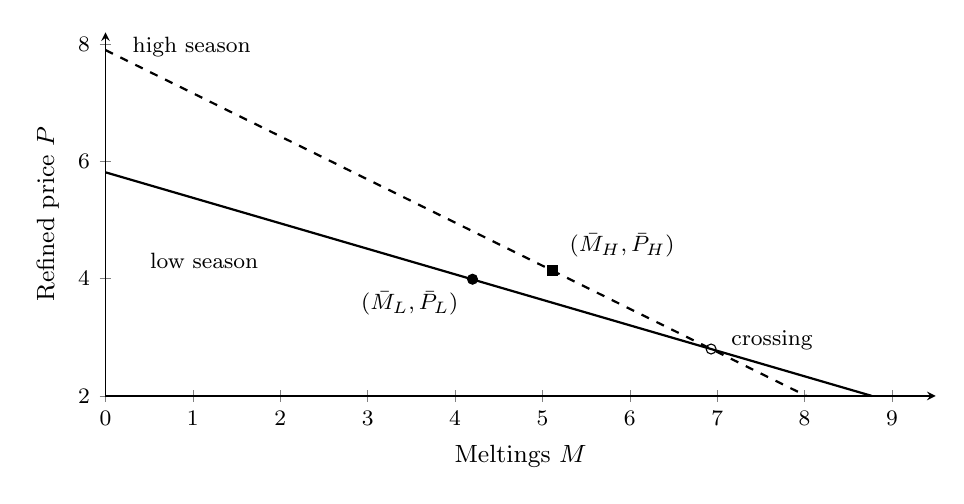
\begin{tikzpicture}
\begin{axis}[
  width=\linewidth, height=6.2cm,
  xmin=0, xmax=9.5, ymin=2, ymax=8.2,
  axis lines=left,
  xlabel={Meltings $M$}, ylabel={Refined price $P$},
  xlabel style={font=\small}, ylabel style={font=\small},
  tick label style={font=\footnotesize},
  clip=false]
\addplot[thick, black, domain=0:8.77, samples=2] {5.813 - x/2.30};
\addplot[thick, black, dashed, domain=0:8.02, samples=2] {7.897 - x/1.36};
\addplot[only marks, mark=*, mark size=1.8pt] coordinates {(4.20,3.99)};
\addplot[only marks, mark=square*, mark size=1.8pt] coordinates {(5.11,4.14)};
\addplot[only marks, mark=o, mark size=1.8pt] coordinates {(6.93,2.80)};
\node[font=\footnotesize, anchor=north west] at (axis cs:0.4,4.6) {low season};
\node[font=\footnotesize, anchor=west] at (axis cs:0.2,7.95) {high season};
\node[font=\footnotesize, anchor=south west] at (axis cs:5.2,4.2) {$(\bar M_H, \bar P_H)$};
\node[font=\footnotesize, anchor=north east] at (axis cs:4.15,3.95) {$(\bar M_L, \bar P_L)$};
\node[font=\footnotesize, anchor=west] at (axis cs:7.05,2.95) {crossing};
\end{axis}
\end{tikzpicture}
\caption{Demand: $M = 13.37 - 2.30P$ (solid) and $M = 10.74 - 1.36P$ (dashed).}
\end{subfigure}\hfill
\begin{subfigure}[t]{0.48\textwidth}
\centering
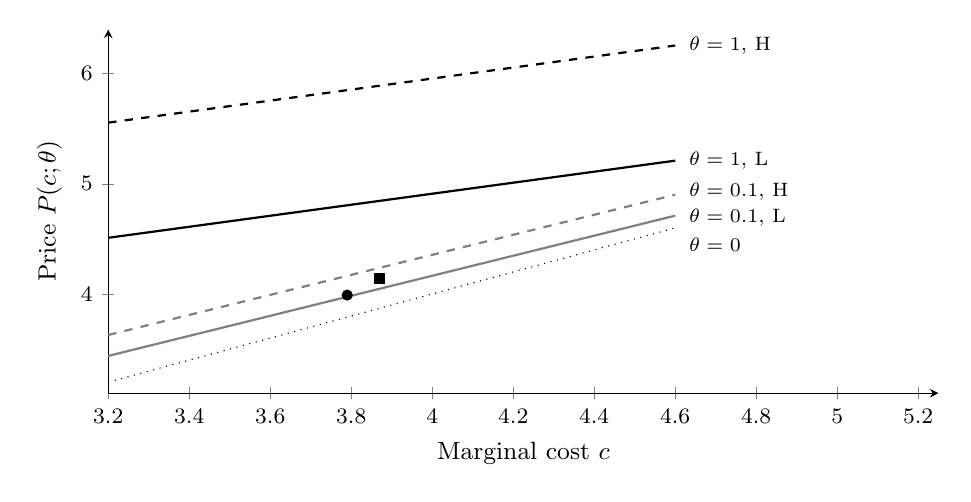
\begin{tikzpicture}
\begin{axis}[
  width=\linewidth, height=6.2cm,
  xmin=3.2, xmax=5.25, ymin=3.1, ymax=6.4,
  axis lines=left,
  xlabel={Marginal cost $c$}, ylabel={Price $P(c;\theta)$},
  xlabel style={font=\small}, ylabel style={font=\small},
  tick label style={font=\footnotesize},
  clip=false]
\addplot[thick, black, domain=3.2:4.6, samples=2] {(5.82 + x)/2};
\addplot[thick, black, dashed, domain=3.2:4.6, samples=2] {(7.91 + x)/2};
\addplot[thick, gray, domain=3.2:4.6, samples=2] {(0.582 + x)/1.1};
\addplot[thick, gray, dashed, domain=3.2:4.6, samples=2] {(0.791 + x)/1.1};
\addplot[thin, black, dotted, domain=3.2:4.6, samples=2] {x};
\addplot[only marks, mark=*, mark size=1.8pt] coordinates {(3.79,3.99)};
\addplot[only marks, mark=square*, mark size=1.8pt] coordinates {(3.87,4.14)};
\node[font=\scriptsize, anchor=west] at (axis cs:4.61,6.255) {$\theta = 1$, H};
\node[font=\scriptsize, anchor=west] at (axis cs:4.61,5.21) {$\theta = 1$, L};
\node[font=\scriptsize, anchor=west] at (axis cs:4.61,4.93) {$\theta = 0.1$, H};
\node[font=\scriptsize, anchor=west] at (axis cs:4.61,4.69) {$\theta = 0.1$, L};
\node[font=\scriptsize, anchor=west] at (axis cs:4.61,4.45) {$\theta = 0$};
\end{axis}
\end{tikzpicture}
\caption{Pricing rules $P(c;\theta) = \frac{\theta\alpha_s + c}{1 + \theta}$, low (solid) and high (dashed)
season.}
\end{subfigure}
\caption{The canning season rotates demand. Panel (a) shows the estimated linear demand curves, which cross at
$P = 2.80$, below all observed prices, and the season means. Panel (b) shows the implied pricing rules with
$\alpha_L = 5.82$ and $\alpha_H = 7.91$ (\cref{tab:03-gm-derived}). The monopoly price rises by
$\frac{\alpha_H - \alpha_L}{2} = 1.05$ in the high season at given cost, while competitive pricing does not
move. The markers are the season means of $(c_t, P_t)$ with $c_t = 0.26 + 1.075\,P^{\mathrm{raw}}_t$.
Constructed from \citet{GenesoveMullin1998}, Tables 2--4.}
\label{fig:03-gm-pricing-rules}
\end{figure}

\subsection{The direct measure of conduct}\label{sec:03-sugar-direct}

With demand in hand, the supply relation \eqref{eq:03-gm-supply} gives a pricing rule for every conduct
parameter.

\begin{proposition}[Pricing rules for the demand family]\label{prop:03-gm-pricing}
Let demand be \eqref{eq:03-gm-demand} and marginal cost $c$ be constant. The price that solves
\eqref{eq:03-gm-supply} is
\begin{equation}\label{eq:03-gm-pricing}
P(c;\theta) = \frac{\theta\alpha + \gamma c}{\gamma + \theta},
\qquad
P^M(c) \equiv P(c;1) = \frac{\alpha + \gamma c}{1 + \gamma}.
\end{equation}
In the log-linear case ($\alpha = 0$, $\gamma = -\varepsilon$) this is
$P(c;\theta) = \frac{\varepsilon}{\varepsilon - \theta}\,c$, and in the exponential limit it is
$P(c;\theta) = c + \frac{\theta}{\lambda}$. Pass-through is $\frac{\partial P}{\partial c} =
\frac{\gamma}{\gamma + \theta}$.
\end{proposition}

\begin{proof}
Since $P'(Q) = \frac{1}{Q'(P)}$, \cref{lem:03-gm-demand}(i) gives
\begin{equation*}
Q\,P'(Q) = \frac{Q(P)}{Q'(P)} = -\frac{\alpha - P}{\gamma}.
\end{equation*}
Substituting into \eqref{eq:03-gm-supply},
\begin{equation*}
P - \frac{\theta(\alpha - P)}{\gamma} = c
\;\Longleftrightarrow\;
\gamma P + \theta P = \gamma c + \theta\alpha
\;\Longleftrightarrow\;
P = \frac{\theta\alpha + \gamma c}{\gamma + \theta}.
\end{equation*}
Setting $\alpha = 0$ and $\gamma = -\varepsilon$ gives $P = \frac{-\varepsilon c}{\theta - \varepsilon} =
\frac{\varepsilon}{\varepsilon - \theta}c$. In the exponential limit, $\frac{\alpha - P}{\gamma} \to
\frac{1}{\lambda}$ by \cref{lem:03-gm-demand}(ii), so the supply relation reads $P - \frac{\theta}{\lambda} =
c$. Differentiating \eqref{eq:03-gm-pricing} in $c$ gives the pass-through.
\end{proof}

The pass-through formula agrees with \cref{prop:03-passthrough}. With flat marginal cost that proposition
gives $\rho = \frac{1}{1 + \theta(1 - \chi)}$, and $\chi = 1 - \frac{1}{\gamma}$ from
\cref{lem:03-gm-demand}(iii) yields $\rho = \frac{1}{1 + \frac{\theta}{\gamma}} = \frac{\gamma}{\gamma +
\theta}$. Two features matter below. The pricing rule is affine in cost with a slope that depends on $\theta$
and $\gamma$ only. Its intercept $\frac{\theta\alpha}{\gamma + \theta}$ moves with the season whenever
$\alpha$ does, and by more the larger is $\theta$. Under exponential demand the slope is one for every
$\theta$, so pass-through carries no information about conduct \citep{BulowPfleiderer1983}.

Monopoly requires an elastic demand at the monopoly price. At $P^M$, $\alpha - P^M = \frac{\gamma(\alpha -
c)}{1 + \gamma}$, so $\varepsilon(P^M) = \frac{\gamma P^M}{\alpha - P^M} = \frac{\alpha + \gamma c}{\alpha -
c}$. For $c > 0$ this exceeds one if and only if $\gamma > -1$ when $\alpha > c$, and $\gamma < -1$ when
$\alpha < c$ (WP p.~24). In the log-linear form, the high-season elasticity of 1.10 barely satisfies this
condition, and the implied monopoly price is enormous.

\Cref{tab:03-gm-derived} reports the implied pricing rules, the elasticities at the full-sample mean, and the
direct conduct measure.

\begin{table}[htbp]
\centering
\caption{Demand for refined sugar: derived estimates and the direct measure of conduct}\label{tab:03-gm-derived}
\small
\begin{tabular}{@{}lccccc@{}}
\toprule
 & (1) Quadratic & (2) Linear & (3) Log-linear & (4) Exponential & (5) Lerner\\
\midrule
$P^M(c)$, low season & $2.57 + 0.67c$ & $2.91 + 0.5c$ & $1.97c$ & $1.89 + c$ & \\
$P^M(c)$, high season & $3.96 + 0.67c$ & $3.96 + 0.5c$ & $10.1c$ & $3.85 + c$ & \\
\addlinespace
$P(c;\theta)$, low season & $\frac{7.72\theta + 2c}{2 + \theta}$ & $\frac{5.82\theta + c}{1 + \theta}$ &
 $\frac{2.03}{2.03 - \theta}c$ & $1.89\theta + c$ & \\[4pt]
$P(c;\theta)$, high season & $\frac{11.88\theta + 2c}{2 + \theta}$ & $\frac{7.91\theta + c}{1 + \theta}$ &
 $\frac{1.10}{1.10 - \theta}c$ & $3.85\theta + c$ & \\
\addlinespace
\multicolumn{6}{@{}l}{\textit{Elasticity $\varepsilon$ at the full-sample mean}}\\
Low season & 2.18 & 2.24 & 2.03 & 2.13 & \\
High season & 1.03 & 1.04 & 1.10 & 1.05 & \\
\addlinespace
\multicolumn{5}{@{}l}{\textit{Adjusted Lerner index $L_\varepsilon$}} & \textit{Unadjusted}\\
Mean & 0.099 & 0.107 & 0.095 & 0.097 & 0.054\\
Standard deviation & 0.097 & 0.118 & 0.083 & 0.089 & 0.045\\
Standard error & 0.024 & 0.028 & 0.021 & 0.022 & 0.0046\\
\bottomrule
\end{tabular}

\smallskip
\begin{minipage}{0.92\textwidth}\footnotesize
Notes: Reproduced from \citet{GenesoveMullin1998}, Table 4, which combines WP Tables 7 and 8. $L_\varepsilon =
\varepsilon\,\frac{P - c}{P}$ with $c = 0.26 + 1.075\,P^{\mathrm{raw}}$, computed quarter by quarter. The
standard errors account for the estimation of demand (WP Table 8, column 4). Standard errors that ignore it
are 0.010, 0.012, 0.008 and 0.009 (WP Table 8, column 3). WP Table 7 prints $7.88\theta$ in the high-season
linear rule.
\end{minipage}
\end{table}

\casehead{Checking the derived estimates}
Every entry follows from \cref{tab:03-gm-demand} and \cref{prop:03-gm-pricing}. In the quadratic form,
$P^M = \frac{7.72}{3} + \frac{2}{3}c = 2.57 + 0.67c$, and the high-season intercept is $\frac{11.88}{3} =
3.96$. In the linear form the choke prices are $\alpha_L = \frac{13.37}{2.30} = 5.81$ and $\alpha_H =
\frac{10.74}{1.36} = 7.90$, so $P^M = \frac{\alpha_s}{2} + \frac{c}{2}$ has intercepts 2.91 and 3.95. The
printed 5.82, 7.91 and 3.96 reflect unrounded coefficients. In the exponential form, $\frac{1}{0.53} = 1.89$
and $\frac{1}{0.26} = 3.85$. In the log-linear form, the monopoly markup factor
$\frac{\varepsilon}{\varepsilon - 1}$ equals $\frac{2.03}{1.03} = 1.97$ in the low season. In the high
season it equals $\frac{1.10}{0.10} = 11.0$ at $\varepsilon_H = 1.10$. The printed 10.1 corresponds to
$\varepsilon_H = \frac{10.1}{9.1} = 1.11$. Rounding cannot reconcile the two. Every elasticity in $[1.095,
1.105)$, which rounds to 1.10, gives a factor between 10.52 and 11.53. The published table is thus inconsistent
with its own elasticity, and the source does not explain why. The digits of 11.0 may have been transposed. We
reproduce the printed 10.1, which gives the high-season monopoly price of about 39 below. The factor 11.0 would
give about 43. The elasticities at $\bar P = 4.03$ follow from \cref{lem:03-gm-demand}(i). For example,
$\frac{2 \times 4.03}{7.72 - 4.03} = 2.18$ and $\frac{2 \times 4.03}{11.88 - 4.03} = 1.03$ for the quadratic,
$0.53 \times 4.03 = 2.14$ (2.13 in the table, from unrounded coefficients) and $0.26 \times 4.03 = 1.05$ for the
exponential.

\casehead{Observed prices are far below monopoly}
At the low-season means, marginal cost is $c = 0.26 + 1.075 \times 3.28 = 3.79$. The linear monopoly price
is then $2.91 + 0.5 \times 3.79 = 4.80$, against an observed mean of 3.99. In the high season, $c = 0.26 +
1.075 \times 3.36 = 3.87$ and $P^M = 3.96 + 0.5 \times 3.87 = 5.90$, against 4.14. The quadratic form puts
the monopoly prices at 5.10 and 6.54, the exponential form at 5.68 and 7.72, and the log-linear form at 7.47
and about 39. Whatever the demand form, the industry priced far below the monopoly level (WP p.~27). Panel (b) of
\cref{fig:03-gm-pricing-rules} shows the gap.

\casehead{The direct measure}
The first estimation method uses everything. Marginal cost is \eqref{eq:03-gm-direct-cost}, the elasticity
comes from the season's demand curve evaluated at the quarter's price, and conduct is computed quarter by
quarter:
\begin{equation}\label{eq:03-gm-direct}
L_{\varepsilon t} = \varepsilon_{s(t)}(P_t)\,\frac{P_t - c_t}{P_t} = \frac{P_t - c_t}{m_t},
\qquad m_t = \frac{\alpha_{s(t)} - P_t}{\gamma_{s(t)}} .
\end{equation}
The second expression uses \cref{lem:03-gm-demand}(i): conduct is the price-cost margin divided by the
markup term $m_t = \frac{Q_t}{\lvert Q'(P_t)\rvert}$ of \cref{sec:03-corts}. The direct measure is a
function of data and of the estimated demand parameters. Its standard error must reflect the second source
of noise. Genesove and Mullin stack the demand moment conditions with the moment
$\frac{1}{n}\sum_t \left(L_{\varepsilon t} - \bar L_\varepsilon\right) = 0$ and compute the usual GMM
variance for the mean $\bar L_\varepsilon$ (WP p.~31, fn.~45). Accounting for estimated demand more than
doubles the standard errors.

\casehead{Results}
The mean adjusted Lerner index lies between 0.095 and 0.107 across the four demand forms
(\cref{tab:03-gm-derived}). Genesove and Mullin take $\theta = 0.10$ as their direct measure. This is the
conduct of a static symmetric Cournot oligopoly with ten firms. Both perfect competition and monopoly are
rejected: the mean is about four standard errors above zero and far below one. The unadjusted Lerner index
of 0.054 says that price exceeded marginal cost by only 5 percent. With demand elasticities near two, even
this small margin corresponds to a conduct parameter of 0.10. With the lower bound $c_0 = 0.16$, the mean index
rises to 0.14 (log-linear and exponential), 0.15 (quadratic) and 0.16 (linear). The value $0.15$ corresponds
to a symmetric Cournot oligopoly with about seven firms, so the conclusions do not change (WP p.~37).

\begin{figure}[!htb]
\centering
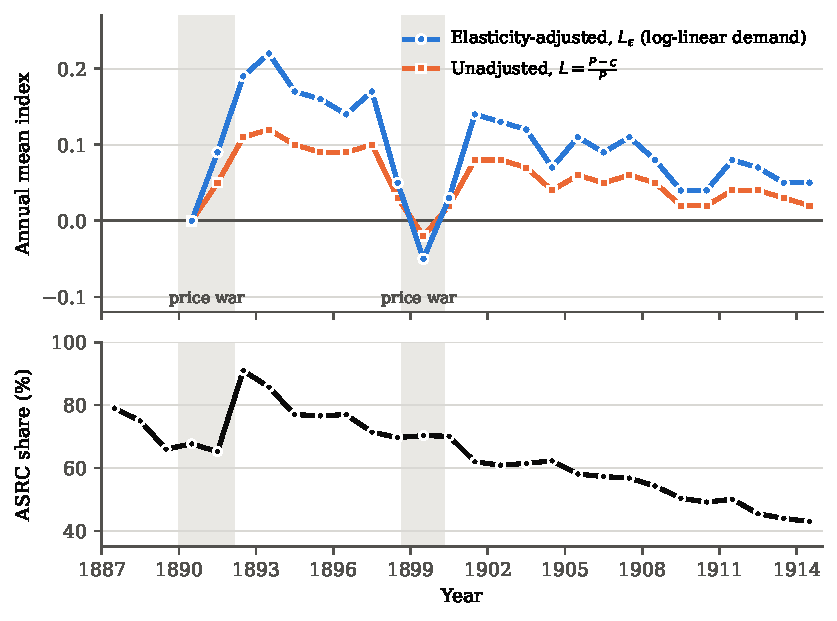
\includegraphics[width=0.86\textwidth]{figures/ch03/gm_lerner_time.pdf}
\caption{Annual means of the unadjusted Lerner index $\frac{P - c}{P}$ and of the elasticity-adjusted index
$L_\varepsilon$ (log-linear demand), top, and the market share of the American Sugar Refining Company,
bottom. Shaded bands mark the two post-entry price wars (January 1890 to February 1892 and September 1898 to
April 1900). Redrawn from \citet{GenesoveMullin1995}, WP Table 9.}
\label{fig:03-gm-lerner-time}
\end{figure}

\casehead{Conduct over time}
\Cref{fig:03-gm-lerner-time} plots the annual means of WP Table 9. Conduct follows structure. The adjusted
index is zero in 1890 during the Spreckels war. It rises to between 0.14 and 0.22 in 1892--1897, after ASRC
had consolidated 91 percent of the market. It collapses again in the Arbuckle war, to $-0.05$ in 1899,
which means pricing below the measured marginal cost. Willett and Gray themselves reported in October 1898
that refiners were selling at ``an actual loss'' (WP p.~33, fn.~47). After 1900 the index drifts down from
0.14 to about 0.05 as ASRC's share falls toward 43 percent. Across the twenty years outside the price wars (excluding 1890, 1891 and 1898--1900),
the correlation between the annual adjusted index and ASRC's share is 0.92 (our computation from WP Table 9).
The averages over 1890--1914 are 0.09 for the adjusted index, 0.05 for the unadjusted index and 63.1 percent
for ASRC's share.

\begin{table}[htbp]
\centering
\caption{Seasonality of the direct conduct measure}\label{tab:03-gm-seasonality}
\small
\begin{tabular}{@{}lcccccccc@{}}
\toprule
 & \multicolumn{2}{c}{Quarter I} & \multicolumn{2}{c}{Quarter II} & \multicolumn{2}{c}{Quarter III (high)} &
 \multicolumn{2}{c}{Quarter IV}\\
\cmidrule(lr){2-3}\cmidrule(lr){4-5}\cmidrule(lr){6-7}\cmidrule(l){8-9}
 & Mean & S.D. & Mean & S.D. & Mean & S.D. & Mean & S.D.\\
\midrule
Unadjusted $L$ & 0.048 & 0.042 & 0.065 & 0.042 & 0.064 & 0.047 & 0.038 & 0.047\\
$L_\varepsilon$, quadratic & 0.096 & 0.091 & 0.142 & 0.104 & 0.071 & 0.057 & 0.083 & 0.117\\
$L_\varepsilon$, linear & 0.102 & 0.106 & 0.162 & 0.138 & 0.075 & 0.063 & 0.086 & 0.134\\
$L_\varepsilon$, log-linear & 0.097 & 0.085 & 0.132 & 0.085 & 0.071 & 0.051 & 0.078 & 0.096\\
$L_\varepsilon$, exponential & 0.097 & 0.087 & 0.136 & 0.092 & 0.071 & 0.055 & 0.081 & 0.106\\
\bottomrule
\end{tabular}

\smallskip
\begin{minipage}{0.92\textwidth}\footnotesize
Notes: Reproduced from \citet{GenesoveMullin1995}, WP Table 10. Means and standard deviations across
quarters of the same type.
\end{minipage}
\end{table}

\casehead{Conduct over the year}
\Cref{tab:03-gm-seasonality} shows that conduct also varies within the year. It is least competitive in the
second quarter and most competitive in the third, the high season. This pattern fits dynamic oligopoly models
in which the expectation of better demand ahead helps collusion and the expectation of worse demand harms it
\citep{RotembergSaloner1986,HaltiwangerHarrington1991}. Genesove and Mullin note a caveat. The unadjusted
index is equal in the second and third quarters, so the pattern may be an artifact of attaching the
inelastic high-season demand to the third quarter alone (WP pp.~33--34). Either way, conduct that varies
systematically with a demand shifter contradicts the assumption of the NEIO method that $\theta$ is
uncorrelated with the instruments. Genesove and Mullin argue that the proper test of a method is its success in
doing what it is meant to do, whatever the truth of its assumptions (WP p.~34). The next subsection shows that this
seasonal pattern explains much of what the NEIO estimator finds.

The low level of the index, relative to the industry's concentration, has a natural explanation. Pricing was
constrained by the threat of domestic entry and of foreign imports (WP p.~34). The price wars of 1890 and
1898--1900 show that the entry threat was not idle.

\subsection{Estimating conduct with cost treated as unknown}\label{sec:03-sugar-neio}

We now put ourselves in the position of an NEIO researcher who observes prices, quantities, the raw sugar
price and the instruments, but does not know $c_0$, $k$ or both.

\casehead{The pricing equation}
Substituting \eqref{eq:03-gm-cost} into \eqref{eq:03-gm-pricing} gives the reduced-form pricing equation
(WP eq.~12)
\begin{equation}\label{eq:03-gm-reduced}
P_t = \frac{\alpha_{s}\theta + c_0\gamma_{s}}{\gamma_{s} + \theta}
 + \frac{\gamma_{s}}{\gamma_{s} + \theta}\,k\,P^{\mathrm{raw}}_t + u_t ,
\qquad s = s(t),
\end{equation}
where $u_t$ is a pricing error from unobserved cost or conduct shocks. In the exponential case the equation
is $P_t = \frac{\theta}{\lambda_s} + c_0 + kP^{\mathrm{raw}}_t + u_t$ (WP p.~34, fn.~49). Multiplying
\eqref{eq:03-gm-reduced} by $\gamma_s + \theta$ gives the moment condition that Genesove and Mullin estimate
(WP eq.~13):
\begin{equation}\label{eq:03-gm-moment}
\E\Big[\big\{(\gamma_s + \theta)P_t - \alpha_s\theta - c_0\gamma_s - \gamma_s k P^{\mathrm{raw}}_t\big\}\,z_t\Big]
= 0 .
\end{equation}
The demand parameters $(\alpha_s, \gamma_s)$ are fixed at their estimates in \cref{tab:03-gm-demand}. The
unknowns are $\theta$ and whichever cost parameters the researcher does not know.

The raw price must be instrumented. Whether $u_t$ is a cost shock or a conduct shock, a positive $u_t$ raises
the refined price and lowers the quantity of refined sugar demanded. Refiners then demand less raw sugar,
which lowers the raw price. The pricing error is therefore negatively correlated with $P^{\mathrm{raw}}_t$ (WP
p.~34). Log Cuban imports again serve as the excluded cost shifter.

\casehead{The information hierarchy}
Genesove and Mullin organize the comparison by what the researcher knows about cost (WP p.~35).
\begin{enumerate}[label=(\Roman*)]
\item Neither $c_0$ nor $k$ is known. The unknowns are $(\theta, c_0, k)$, and the instruments are
$z_t = (1, H_t, \ln\mathit{CUBA}_t)$.
\item The input coefficient $k = 1.075$ is known, and $c_0$ is not. The unknowns are $(\theta, c_0)$, and the
instruments are $z_t = (1, H_t)$. This is the position of the cigarette studies of \citet{Sumner1981},
\citet{Sullivan1985} and \citet{AshenfelterSullivan1987} (\cref{sec:03-sumner}). In those studies an excise
tax enters marginal cost with a known coefficient of one.
\item Both $c_0 = 0.26$ and $k = 1.075$ are known. Then $\theta$ is observed directly, as in
\eqref{eq:03-gm-direct}.
\end{enumerate}
The fourth combination, $c_0$ known and $k$ unknown, is implausible in this industry and is not explored. In
both (I) and (II) the number of instruments equals the number of unknowns, so the nonlinear instrumental
variables (NLIV) estimator solves the sample analogue of \eqref{eq:03-gm-moment} exactly. Estimating demand
first and the pricing equation second is the two-step method. Stacking the demand moments and
\eqref{eq:03-gm-moment} in a single GMM problem is the joint version of the same estimator.

\casehead{Standard errors with estimated demand}
The two-step estimator inherits the noise in the demand estimates. Let $b = (\theta, c_0, k)^\T$, let $a$ be
the demand parameters with $\sqrt{n}(\hat a - a_0) \to N(0, W_1)$, and let $\bar g_n(b, a)$ be the sample
analogue of \eqref{eq:03-gm-moment}. A mean-value expansion of $\bar g_n(\hat b, \hat a) = 0$ around
$(b_0, a_0)$ gives
\begin{equation*}
0 = \bar g_n(b_0, a_0) + D\,(\hat b - b_0) + C\,(\hat a - a_0) + o_p\!\left(n^{-\frac{1}{2}}\right),
\qquad D = \E\left[\frac{\partial g}{\partial b^\T}\right],\;\; C = \E\left[\frac{\partial g}{\partial a^\T}\right].
\end{equation*}
Solving for $\hat b - b_0$,
\begin{equation*}
\sqrt{n}\,(\hat b - b_0) = -D^{-1}\sqrt{n}\,\bar g_n(b_0, a_0) - D^{-1}C\,\sqrt{n}\,(\hat a - a_0) + o_p(1).
\end{equation*}
If the pricing moments and the demand estimates are asymptotically uncorrelated, the asymptotic variance is
\begin{equation}\label{eq:03-gm-variance}
\operatorname{Avar}(\hat b) = W_2 + D^{-1} C\, W_1\, C^\T \left(D^{-1}\right)^\T,
\qquad W_2 = D^{-1} S \left(D^{-1}\right)^\T ,
\end{equation}
where $S$ is the long-run variance of the pricing moments. Genesove and Mullin estimate $S$ and $W_1$ by
Newey-West with four lags (WP p.~36). The zero-correlation assumption fits their interpretation: demand errors
are proportional shifts that do not move the pricing rule. Without it, the joint GMM estimator delivers
correct standard errors directly (\cref{app:econometrics}).

\begin{table}[htbp]
\centering
\caption{NLIV estimates of conduct and cost parameters}\label{tab:03-gm-nliv}
\small
\setlength{\tabcolsep}{4.5pt}
\begin{tabular}{@{}lccccccccc@{}}
\toprule
 & \multicolumn{2}{c}{Quadratic} & \multicolumn{2}{c}{Linear} & \multicolumn{2}{c}{Log-linear} &
 \multicolumn{2}{c}{Exponential} & Direct\\
\cmidrule(lr){2-3}\cmidrule(lr){4-5}\cmidrule(lr){6-7}\cmidrule(lr){8-9}\cmidrule(l){10-10}
 & (1) & (2) & (3) & (4) & (5) & (6) & (7) & (8) & (9)\\
\midrule
$\hat\theta$ & 0.037 & 0.035 & 0.038 & 0.037 & 0.045 & 0.040 & 0.041 & 0.037 & 0.10\\
 & (0.024) & (0.024) & (0.024) & (0.024) & (0.028) & (0.026) & (0.026) & (0.025) & \\
$\hat c_0$ & 0.529 & 0.393 & 0.465 & 0.39 & 0.760 & 0.381 & 0.700 & 0.389 & 0.26\\
 & (0.272) & (0.062) & (0.285) & (0.061) & (0.262) & (0.070) & (0.279) & (0.065) & \\
$\hat k$ & 1.033 & & 1.052 & & 0.956 & & 0.978 & & 1.075\\
 & (0.082) & & (0.085) & & (0.081) & & (0.083) & & \\
\bottomrule
\end{tabular}

\smallskip
\begin{minipage}{0.92\textwidth}\footnotesize
Notes: Reproduced from \citet{GenesoveMullin1995}, WP Table 11. Columns (1), (3), (5) and (7) estimate
$(\theta, c_0, k)$ with instruments $(1, H_t, \ln\mathit{CUBA}_t)$. Columns (2), (4), (6) and (8) impose $k =
1.075$ and use $(1, H_t)$. Demand parameters from \cref{tab:03-gm-demand}. Newey-West standard errors (four
lags), corrected for estimated demand, in parentheses. Column (9) is the direct measure. $N = 97$.
\end{minipage}
\end{table}

\casehead{Results}
\Cref{tab:03-gm-nliv} reports the estimates. Genesove and Mullin draw four conclusions (WP pp.~36--37).
First, the NLIV estimate of $\theta$ is close to the direct measure. It lies between 0.035 and 0.045 in all
eight specifications. Monopoly is rejected everywhere, as is any $\theta$ above 0.11. Perfect competition
cannot be rejected: the $t$ ratios are between 1.46 and 1.61. The estimates are below the direct measure in
every case. The upper limits of the 95 percent confidence intervals run from 0.082 to 0.100 (our computation),
so the direct value of 0.10 sits at or just beyond their edge. Second, the estimates are robust to the form
of demand. This answers the common complaint that conduct estimates hinge on functional form. Third, the cost
parameters are recovered less well. The coefficient $k$ is underestimated in all four forms, although
$k = 1.075$ is never rejected. The parameter $c_0$ is overestimated, by 50 cents in the log-linear case (0.760
against 0.26). Fourth, knowing $k$ hardly changes $\hat\theta$. It sharpens the estimate of $c_0$, which falls to
0.38--0.39 with standard errors near 0.06. Because $c_0$ does not enter the NLIV estimator, setting $c_0 =
0.16$ leaves \cref{tab:03-gm-nliv} unchanged and moves only the benchmark, from 0.10 to about 0.15.

\casehead{What identifies $\theta$: the seasonal shift}
Why does the method deliver 0.04? In the quadratic, linear and exponential forms only the intercept of
\eqref{eq:03-gm-reduced} differs across seasons. The equation can then be written as a linear regression,
\begin{equation}\label{eq:03-gm-linear-rf}
P_t = \pi_0 + \pi_1 H_t + \pi_2 P^{\mathrm{raw}}_t + u_t .
\end{equation}
For the linear and quadratic forms, with $\gamma$ common to both seasons,
\begin{equation*}
\pi_0 = \frac{\theta\alpha_L + \gamma c_0}{\gamma + \theta},
\qquad
\pi_1 = \frac{\theta\,(\alpha_H - \alpha_L)}{\gamma + \theta},
\qquad
\pi_2 = \frac{\gamma k}{\gamma + \theta}.
\end{equation*}
For the exponential form, $\pi_0 = \frac{\theta}{\lambda_L} + c_0$, $\pi_1 = \theta\left(\frac{1}{\lambda_H} -
\frac{1}{\lambda_L}\right)$ and $\pi_2 = k$. In each case the map from $(\theta, c_0, k)$ to $(\pi_0, \pi_1,
\pi_2)$ is one to one. For the linear and quadratic forms, inverting it gives
\begin{equation}\label{eq:03-gm-inversion}
\theta = \frac{\gamma\,\pi_1}{(\alpha_H - \alpha_L) - \pi_1},
\qquad
k = \frac{\gamma + \theta}{\gamma}\,\pi_2,
\qquad
c_0 = \frac{(\gamma + \theta)\pi_0 - \theta\alpha_L}{\gamma}.
\end{equation}
The conduct parameter is identified only through $\pi_1$, the seasonal shift of the pricing rule at a given
raw price. If the season changed only the scale $\beta$, so that $\alpha_H = \alpha_L$, then $\pi_1 = 0$ for
every $\theta$ and conduct would not be identified. A seasonal change in $\alpha$ suffices, even a parallel
shift of linear demand. Identification therefore rests on the restriction that marginal cost is constant in
output (\cref{sec:03-other-routes}). The general rotation argument of \cref{prop:03-rotation,prop:03-lau} is
needed only when the slope of marginal cost is unknown. At $\theta = 1$,
$\pi_1$ equals the seasonal shift of the monopoly price, $\frac{\alpha_H - \alpha_L}{1 + \gamma}$. The
estimator thus compares the observed seasonal price shift with the shift that a monopolist would make.

\begin{table}[htbp]
\centering
\caption{Linear pricing equations for refined sugar}\label{tab:03-gm-reduced}
\small
\begin{tabular}{@{}lcccccc@{}}
\toprule
 & (1) & (2) & (3) & (4) & (5) & (6)\\
 & IV & IV & IV & OLS & OLS & OLS\\
\midrule
Raw price & 1.02 & 0.93 & 1.01 & 0.99 & 0.98 & 0.99\\
 & (0.09) & (0.09) & (0.08) & (0.05) & (0.05) & (0.05)\\
High season $\times$ raw price & & 0.31 & & & 0.04 & \\
 & & (0.11) & & & (0.07) & \\
High season & & $-0.97$ & 0.08 & & $-0.07$ & 0.08\\
 & & (0.38) & (0.03) & & (0.22) & (0.03)\\
Constant & 0.67 & 0.94 & 0.66 & 0.75 & 0.77 & 0.74\\
 & (0.28) & (0.28) & (0.26) & (0.16) & (0.16) & (0.16)\\
$\chi^2_{(2)}$ test & & 21.67 & & & 6.66 & \\
\bottomrule
\end{tabular}

\smallskip
\begin{minipage}{0.92\textwidth}\footnotesize
Notes: Reproduced from \citet{GenesoveMullin1995}, WP Table 12. Dependent variable: refined price, $N = 97$.
Instruments in columns (1) and (2): high season, log Cuban imports and their interaction. The $\chi^2_{(2)}$
statistic tests that the coefficients on high season and its interaction with the raw price are both zero.
\end{minipage}
\end{table}

Column (3) of \cref{tab:03-gm-reduced} estimates \eqref{eq:03-gm-linear-rf} by instrumental variables. The
refined price rises by only 8 cents in the high season at a given raw price. The demand estimates imply
much larger shifts of the monopoly price: $\frac{\alpha_H - \alpha_L}{2} = 1.05$ for linear demand and
$\frac{1}{\lambda_H} - \frac{1}{\lambda_L} = 3.85 - 1.89 = 1.96$ for exponential demand. Under exponential
demand the intercept is $\frac{\theta}{\lambda_s} + c_0$, so
\begin{equation*}
\hat\theta \approx \frac{0.08}{1.96} \approx 0.04
\end{equation*}
(WP p.~38). Under linear demand, \eqref{eq:03-gm-inversion} with $\gamma = 1$ and $\alpha_H - \alpha_L =
7.91 - 5.82 = 2.09$ gives
\begin{equation*}
\theta = \frac{0.08}{2.09 - 0.08} = 0.040,
\quad
k = 1.040 \times 1.01 = 1.050,
\quad
c_0 = 1.040 \times 0.66 - 0.040 \times 5.82 = 0.455 .
\end{equation*}
These reproduce column (3) of \cref{tab:03-gm-nliv}, $(0.038, 0.465, 1.052)$, up to rounding. The quadratic form
gives $(0.039, 0.52, 1.03)$ against $(0.037, 0.529, 1.033)$. The same arithmetic explains the cost
estimates. The raw-price coefficient of 1.01 forces $k$ below 1.075, because the slope $\frac{\gamma
k}{\gamma + \theta}$ is close to $k$ when $\theta$ is small. With $\theta$ understated, $c_0$ must absorb
the remaining margin between the refined and raw prices, so $c_0$ is overstated (WP p.~38).

\casehead{A closed form when $k$ is known}
When $k$ is known, the estimator has an explicit form that links it to the direct measure. Divide the
expression in braces in \eqref{eq:03-gm-moment} by $\gamma_s$ and use \cref{lem:03-gm-demand}(i):
\begin{equation*}
\frac{(\gamma_s + \theta)P_t - \alpha_s\theta - c_0\gamma_s - \gamma_s k P^{\mathrm{raw}}_t}{\gamma_s}
= \big(P_t - kP^{\mathrm{raw}}_t\big) - c_0 - \theta\,\frac{\alpha_s - P_t}{\gamma_s}
= G_t - c_0 - \theta\, m_t .
\end{equation*}
The pricing equation thus says that the proper margin equals non-sugar cost plus conduct times the markup
term. This holds in all four forms, and in the exponential form $m_t = \frac{1}{\lambda_s}$.

\begin{proposition}[The NLIV estimator with known $k$]\label{prop:03-gm-wald}
Suppose $k$ is known, the instruments are $(1, H_t)$, and demand is quadratic, linear or exponential. Let $\bar G_s$ and $\bar m_s$ be the season means of the proper
margin and of the markup term. Then
\begin{equation}\label{eq:03-gm-wald}
\hat\theta = \frac{\bar G_H - \bar G_L}{\bar m_H - \bar m_L},
\qquad
\hat c_0 = \bar G_L - \hat\theta\,\bar m_L .
\end{equation}
If the true marginal cost is \eqref{eq:03-gm-cost} and $\theta_t$ denotes true conduct, then
\begin{equation}\label{eq:03-gm-corts}
\hat\theta = \frac{\overline{(\theta m)}_H - \overline{(\theta m)}_L}{\bar m_H - \bar m_L},
\end{equation}
where $\overline{(\theta m)}_s$ is the season mean of $\theta_t m_t$.
\end{proposition}

\begin{proof}
In the quadratic and linear forms $\gamma$ is common to both seasons, so multiplying each moment by the
constant $\frac{1}{\gamma}$ does not change the solution. In the exponential form the moment is
$G_t - c_0 - \theta m_t$ to begin with. The sample moments with instruments $1$ and $H_t$ are
$\sum_t (G_t - c_0 - \theta m_t) = 0$ and $\sum_t H_t(G_t - c_0 - \theta m_t) = 0$. Their difference is the
sum over low-season quarters, so the two conditions are equivalent to
$\bar G_s = c_0 + \theta\,\bar m_s$ for $s = L, H$. Subtracting the low-season equation from the high-season
equation gives $\hat\theta$, and the low-season equation then gives $\hat c_0$. For the second part, the
definition of true conduct in \eqref{eq:03-gm-direct} gives $P_t - c_t = \theta_t m_t$, so $G_t = c_0 +
\theta_t m_t$ by \eqref{eq:03-gm-proper-margin}. Taking season means and substituting into
\eqref{eq:03-gm-wald} gives \eqref{eq:03-gm-corts}.
\end{proof}

The estimator is a Wald ratio. It divides the seasonal change in the proper margin by the seasonal change in
the markup term predicted by demand. With the published season means, $\bar G_H - \bar G_L = 0.53 - 0.46 =
0.07$ (\cref{tab:03-gm-stats}). In the linear form, $\bar m_s = \alpha_s - \bar P_s$, so $\bar m_H - \bar m_L
= 2.09 - 0.15 = 1.94$. In the exponential form, $\bar m_H - \bar m_L = 1.96$. Hence
\begin{align*}
\text{linear:}\quad & \hat\theta = \frac{0.07}{1.94} = 0.036, &
\hat c_0 &= 0.46 - 0.036 \times 1.83 = 0.39,\\
\text{exponential:}\quad & \hat\theta = \frac{0.07}{1.96} = 0.036, &
\hat c_0 &= 0.46 - 0.036 \times 1.89 = 0.39 .
\end{align*}
Columns (4) and (8) of \cref{tab:03-gm-nliv} report $(0.037, 0.39)$ and $(0.037, 0.389)$. The rounding of the
season means to two decimals limits the precision of this check to about $\pm 0.005$ in $\hat\theta$. The
formula also explains the robustness across forms. Each form predicts nearly the same seasonal change in
the markup term at observed prices, between 1.8 dollars (log-linear, $\frac{4.14}{1.10} - \frac{3.99}{2.03}$
at the season means) and 2.0 dollars (quadratic). The four forms differ greatly far from the
data, as their monopoly prices show, but they agree near it.

\casehead{The Corts critique in the sugar data}
Equation \eqref{eq:03-gm-corts} is the IV estimand of \cref{prop:03-corts} with the season indicator as the
instrument. It equals average conduct only if conduct does not differ between seasons. In the exponential
form the markup term is constant within a season, $m_t = \frac{1}{\lambda_s}$. Writing $\bar\theta_s$ for the
season mean of the direct measure, \eqref{eq:03-gm-corts} becomes
\begin{equation*}
\hat\theta
= \frac{\frac{\bar\theta_H}{\lambda_H} - \frac{\bar\theta_L}{\lambda_L}}{\frac{1}{\lambda_H} - \frac{1}{\lambda_L}}
= \frac{3.85\,\bar\theta_H - 1.89\,\bar\theta_L}{1.96}
= \bar\theta_H - 0.96\,\big(\bar\theta_L - \bar\theta_H\big).
\end{equation*}
\Cref{tab:03-gm-seasonality} gives $\bar\theta_H = 0.071$ for the exponential form. The low-season quarters
average about 0.105, weighting quarters I, II and IV by their numbers of observations. Then $\hat\theta = 0.071 - 0.96 \times 0.034 = 0.038$, essentially the reported
0.037. Implied non-sugar cost is $0.26 + (0.105 - 0.038) \times 1.89 = 0.39$, the reported 0.389. The
NLIV estimate lies below even the high-season conduct, because conduct is lower exactly when the rotator is
on. If conduct had stayed at its mean of about 0.10 throughout, the proper margin would have risen by
$0.10 \times 1.96 = 0.20$ in the high season. It rose by 0.07. The understatement of $\theta$ and the
overstatement of $c_0$ both reflect the mechanism of \citet{Corts1999}. The estimator measures the response of
the margin to the rotation, and here that response understates the level of conduct.\footnote{This decomposition is ours. Genesove and Mullin
report the seasonal pattern and the NLIV estimates separately, and attribute the pattern to dynamic
oligopoly (WP pp.~33--34).}

\casehead{The log-linear form}
Under log-linear demand the slope of the pricing rule, $\frac{\varepsilon_s}{\varepsilon_s - \theta}k$,
differs by season, so the linear reparameterization needs an interaction, column (2) of
\cref{tab:03-gm-reduced}. The lower high-season elasticity predicts a steeper pricing rule in the high
season, and the interaction is positive and significant (0.31). The intercept $\frac{\varepsilon_s c_0}
{\varepsilon_s - \theta}$ should also be higher in the high season, yet the high-season coefficient is
$-0.97$. Using the slopes alone gives $\theta = 0.46$. With $r = \frac{0.93 + 0.31}{0.93}$ the ratio of the
slopes, the condition $\frac{\varepsilon_H(\varepsilon_L - \theta)}{\varepsilon_L(\varepsilon_H - \theta)} = r$
solves for $\theta = 0.463$. Using the intercepts alone gives the nonsensical 2.09 (WP p.~39). The NLIV
estimator forces the ratio of intercept to slope to be the same in both seasons, $\frac{c_0}{k}$, and so
returns estimates close to the other forms. Its implied pricing rules are $P = 0.777 + 0.978\,P^{\mathrm{raw}}$
in the low season and $P = 0.792 + 0.997\,P^{\mathrm{raw}}$ in the high season (our computation from column
(5)).\footnote{WP p.~39, fn.~52, prints $0.793 + 0.997\,P^{\mathrm{raw}}$ for the low season and $0.777 + 0.977\,
P^{\mathrm{raw}}$ for the high season. The factor $\frac{\varepsilon_s}{\varepsilon_s - \theta}$ is larger for the
smaller high-season elasticity, so the steeper rule must belong to the high season. The labels in the footnote
appear to be interchanged.} None of the four forms is consistent with the unrestricted estimates of column (2)
(WP p.~39). The other three forms require equal slopes in the two seasons, a single restriction on the
interaction. Its $t$ ratio is $\frac{0.31}{0.11} = 2.8$, a Wald statistic of about 7.9, so equal slopes are
rejected at the 1 percent level. The $\chi^2_{(2)}$ statistic of 21.67 tests a different hypothesis, that
the seasonal intercept and the interaction are both zero. Genesove and Mullin describe the low-season slope of
0.93 as significantly below 1.075, which would contradict log-linear demand, under which price rises more than
one for one with cost. Its $t$ ratio is only $\frac{1.075 - 0.93}{0.09} = 1.61$. The gap is significant at
the one-sided 10 percent level, and not at the one-sided 5 percent level or at any conventional two-sided level.

\casehead{Ignoring the seasons}
Column (1) of \cref{tab:03-gm-reduced} drops all seasonal effects, as a researcher would who used the known
$k$ but ignored the rotation. The only remaining information on conduct is the slope of the pricing rule,
$\frac{\gamma k}{\gamma + \theta} = 1.02$. Solving,
\begin{equation*}
\theta = \gamma\left(\frac{1.075}{1.02} - 1\right) = 0.054\,\gamma .
\end{equation*}
The implied conduct is proportional to the assumed curvature. It equals 0.054 for linear demand and 0.108 for
quadratic demand (WP p.~39). Quadratic demand without seasons has choke price $\hat\alpha = 8.63$ (standard
error 1.17), and it also gives an excellent estimate of non-sugar cost, $\hat c_0 = 0.23$.\footnote{WP p.~39
prints the fitted curve as $\ln M = 7.37 + 2\ln(8.63 - P)$, with standard errors 0.50 and 1.17. The working
paper measures meltings in hundreds of thousands of long tons (WP p.~26), as in \cref{tab:03-gm-stats}. In
those units the printed intercept predicts meltings of about 34{,}000 at $P = 4$, against a sample mean of
4.43. The source does not say whether the intercept is a misprint or uses another unit. Only the choke price
enters the pricing equation, since $m_t = \frac{\alpha - P_t}{2}$.} The researcher
would have no way to know which answer is right. This is the curvature critique of pass-through tests in
\cref{sec:03-sumner} in another guise: the slope identifies conduct only given $\gamma$. With exponential
demand the slope is $k$ for every $\theta$, and $\theta$ and $c_0$ are not even separately identified
\citep{BulowPfleiderer1983}.

\begin{table}[htbp]
\centering
\caption{Cost estimates and predicted price changes under imposed behavioral models}\label{tab:03-gm-behavioral}
\small
\setlength{\tabcolsep}{4.2pt}
\begin{tabular}{@{}lccccccccc@{}}
\toprule
 & \multicolumn{2}{c}{Competition} & \multicolumn{2}{c}{Cournot I} & \multicolumn{2}{c}{Cournot II} &
 \multicolumn{2}{c}{Monopoly} & Direct\\
\cmidrule(lr){2-3}\cmidrule(lr){4-5}\cmidrule(lr){6-7}\cmidrule(lr){8-9}\cmidrule(l){10-10}
 & (1) & (2) & (3) & (4) & (5) & (6) & (7) & (8) & (9)\\
\midrule
$\hat c_0$ & 0.674 & 0.476 & 0.00 & 0.069 & 0.00 & 0.00 & 0.00 & 0.00 & 0.26\\
 & (0.281) & (0.034) & (0.239) & (0.071) & (0.922) & (0.400) & (1.65) & (0.563) & \\
$\hat k$ & 1.015 & & 1.096 & & 0.883 & & 0.529 & & 1.075\\
 & (0.087) & & (0.071) & & (0.253) & & (0.471) & & \\
\addlinespace
$\widehat{\Delta P}$ & 0.689 & 0.729 & 0.620 & 0.608 & 0.300 & 0.365 & 0.179 & 0.365 & 0.702\\
 & (0.059) & & (0.040) & & (0.086) & & (0.086) & & \\
\bottomrule
\end{tabular}

\smallskip
\begin{minipage}{0.92\textwidth}\footnotesize
Notes: Reproduced from \citet{GenesoveMullin1998}, Table 9. Linear demand estimated by season. Cost parameters
constrained to be nonnegative. Columns (1), (3), (5) and (7) estimate $k$ with a constant and log Cuban
imports as instruments. Columns (2), (4), (6) and (8), where $\hat k$ is blank, impose $k = 1.075$ and use a
constant only (p.~371, n.~30). In columns (1) to (8),
$\widehat{\Delta P}$ is the predicted rise in the refined price. The shock is the rise in the raw price by 68
cents per hundred pounds from the third quarter of 1896 to the third quarter of 1897. Column (9) reports the
realized rise (p.~374).
\end{minipage}
\end{table}

\casehead{Imposing a behavioral model}
The published article adds an exercise that shows what goes wrong when conduct is assumed (Table 9,
reproduced in \cref{tab:03-gm-behavioral}). The researcher fixes $\theta$ at the value implied by a behavioral
model, estimates the cost parameters from the linear pricing equation, and predicts the effect of a cost
shock. Competition sets $\theta = 0$ and monopoly sets $\theta = 1$. \emph{Cournot I} assumes identical
constant marginal costs and no capacity constraints, so $\theta_t = \frac{1}{N_t}$ when $N_t$ firms are active
in quarter $t$ \citep[p.~372]{GenesoveMullin1998}. \emph{Cournot II} gives all firms the same marginal cost up
to capacities that differ. ASRC could serve the whole market, so the equilibrium is that of a dominant firm
facing a fringe that produces at capacity. ASRC then prices as a monopolist on market demand less total
fringe capacity \citep[p.~373]{GenesoveMullin1998}.

The shock is the Cuban war of independence. Cuban imports fell to zero in the third quarter of 1897, a
quarter excluded from estimation. The raw price rose by 68 cents per hundred pounds from the third quarter of
1896. With linear demand, constant conduct and both quarters in the same season, the pricing rule
\eqref{eq:03-gm-pricing} with $\gamma = 1$ gives the predicted change \citep[p.~374]{GenesoveMullin1998}
\begin{equation*}
\widehat{\Delta P} = \frac{\hat k \times 0.68}{1 + \theta}.
\end{equation*}
Under competition this gives $1.015 \times 0.68 = 0.69$ with $k$ estimated and $1.075 \times 0.68 = 0.73$ with
$k$ imposed. Under monopoly it gives $\frac{0.529 \times 0.68}{2} = 0.18$ and $\frac{1.075 \times 0.68}{2} =
0.365$. The refined price rose by 70.2 cents over the same period, a pass-through of 1.03. For Cournot I, the
prediction with $k$ imposed implies $1 + \theta = \frac{0.731}{0.608} \approx 1.20$. This is $\theta \approx
0.20$, the value of $\frac{1}{N_t}$ with five firms (our computation).

Cournot II predicts the same rise as monopoly when $k$ is imposed (0.365). Linear demand explains why. Let
$\bar K$ be total fringe capacity, so that ASRC sells $q^d = \beta_s(\alpha_s - P) - \bar K$. Its marginal
revenue is $P - \frac{q^d}{\beta_s}$. Setting marginal revenue equal to $c$ gives the first equation below.
Substituting $q^d$ and solving for $P$ gives the second:
\begin{equation*}
P - c = \frac{q^d}{\beta_s},
\qquad
P = \frac{1}{2}\left(\alpha_s - \frac{\bar K}{\beta_s} + c\right).
\end{equation*}
With $\bar K$ fixed, the fringe leaves pass-through at $\frac{1}{2}$, as under monopoly. It lowers the price
level, however, so with $k$ estimated Cournot II gives $\hat k = 0.883$ against 0.529 under monopoly. With
linear demand the supply relation \eqref{eq:03-gm-supply} reads $P - c = \frac{\theta Q}{\beta_s}$. Cournot II
is therefore the supply relation with $\theta_t = \frac{q^d_t}{Q_t}$, ASRC's share of output (our
computation). Because $\bar K$ is fixed, this share falls as the price rises. The constant-conduct formula
above therefore does not apply to Cournot II. Genesove and Mullin trace the large shortfalls of Cournot II
and monopoly to their low estimates of $k$ and to the less competitive conduct they assume \citep[pp.~374--375]{GenesoveMullin1998}.

Monopoly fails because the monopoly price level is far above the data. The linear monopoly rule is
$P = \frac{\alpha_s}{2} + \frac{c}{2}$. At the low-season mean price of 3.99, the term $\frac{\alpha_L}{2} =
2.91$ leaves only 1.08 for $\frac{c}{2}$, so mean marginal cost would be 2.16, far below the raw-sugar cost of
$1.075 \times 3.28 = 3.53$. In the high season, $\frac{\alpha_H}{2} = 3.96$ leaves only 0.18 (our
computation). To fit the price level with nonnegative $c_0$, the estimator pushes $c_0$ to zero and $k$ to
0.529, far below the physical minimum of about 1.04. It then predicts that refined prices rise by only 18 cents after
a 68-cent rise in the raw price. Competition and Cournot I predict 0.61 to 0.73, close to the realized rise
of 0.702. The shortfall of Cournot I is not statistically significant \citep[p.~374]{GenesoveMullin1998}.
Wrong conduct assumptions thus produce wrong costs and wrong counterfactuals at the same time.

\subsection{Conduct and structure: price wars}\label{sec:03-sugar-wars}

A second test asks whether the method detects changes in conduct across structural regimes. Genesove and
Mullin compare the two post-entry price wars of \cref{tab:03-gm-chronology}, Panel B, with all other periods.
Let $\mathit{WAR}_t = 1$ in the price-war quarters and let conduct be
\begin{equation}\label{eq:03-gm-war}
\theta_t = \theta_0 + (\theta_1 - \theta_0)\,\mathit{WAR}_t .
\end{equation}
The NLIV moment \eqref{eq:03-gm-moment} is otherwise unchanged. The instruments add $\mathit{WAR}_t$: they are
$(1, \ln\mathit{CUBA}_t, H_t, \mathit{WAR}_t)$ when $k$ is unknown and $(1, H_t, \mathit{WAR}_t)$ when $k$ is
known (WP p.~41, fn.~54). The benchmark is the direct measure for the same regimes, from the log-linear form.

\begin{table}[!htb]
\centering
\caption{Conduct in price-war regimes}\label{tab:03-gm-pricewars}
\small
\begin{tabular}{@{}lccc@{}}
\toprule
\multicolumn{4}{@{}l}{\textit{Panel A. Price wars with constant costs, linear demand (published Table 10)}}\\
\midrule
 & (1) & (2) & (3) Direct\\
\midrule
$\hat\theta_0$ & 0.046 (0.023) & 0.046 (0.023) & 0.129\\
$\hat\theta_1 - \hat\theta_0$ & $-0.112$ (0.069) & $-0.108$ (0.051) & $-0.127$\\
$\hat c_0$ & 0.375 (0.280) & 0.402 (0.056) & 0.26\\
$\hat k$ & 1.084 (0.083) & & 1.075\\
\bottomrule
\end{tabular}

\medskip
\setlength{\tabcolsep}{4.2pt}
\begin{tabular}{@{}lccccccccc@{}}
\multicolumn{10}{@{}l}{\textit{Panel B. Price wars with regime-specific non-sugar cost (WP Table 15)}}\\
\toprule
 & \multicolumn{2}{c}{Quadratic} & \multicolumn{2}{c}{Linear} & \multicolumn{2}{c}{Log-linear} &
 \multicolumn{2}{c}{Exponential} & Direct\\
\cmidrule(lr){2-3}\cmidrule(lr){4-5}\cmidrule(lr){6-7}\cmidrule(lr){8-9}\cmidrule(l){10-10}
 & (1) & (2) & (3) & (4) & (5) & (6) & (7) & (8) & (9)\\
\midrule
$\hat\theta_0$ & 0.032 & 0.031 & 0.032 & 0.033 & 0.041 & 0.034 & 0.037 & 0.032 & 0.11\\
 & (0.022) & (0.022) & (0.022) & (0.024) & (0.027) & (0.024) & (0.024) & (0.023) & \\
$\hat\theta_1 - \hat\theta_0$ & $-0.016$ & $-0.016$ & $-0.017$ & $-0.017$ & $-0.024$ & $-0.017$ & $-0.020$ &
 $-0.015$ & $-0.09$\\
 & (0.035) & (0.036) & (0.036) & (0.036) & (0.034) & (0.040) & (0.043) & (0.038) & \\
$\hat c_0$ & 0.470 & 0.439 & 0.417 & 0.435 & 0.684 & 0.434 & 0.632 & 0.439 & 0.26\\
 & (0.252) & (0.055) & (0.261) & (0.058) & (0.259) & (0.058) & (0.274) & (0.055) & \\
$\hat k$ & 1.065 & & 1.081 & & 0.991 & & 1.010 & & 1.075\\
 & (0.079) & & (0.080) & & (0.083) & & (0.084) & & \\
$\hat c_1 - \hat c_0$ & $-0.162$ & $-0.171$ & $-0.168$ & $-0.163$ & $-0.101$ & $-0.178$ & $-0.118$ & $-0.177$ & 0\\
 & (0.128) & (0.110) & (0.124) & (0.104) & (0.134) & (0.130) & (0.147) & (0.119) & \\
\bottomrule
\end{tabular}

\smallskip
\begin{minipage}{0.92\textwidth}\footnotesize
Notes: Panel A reproduced from \citet{GenesoveMullin1998}, Table 10. It matches columns (3) and (4) of WP
Table 14, except for $\hat c_0 = 0.374$ in column (3) and the direct measures, which are 0.11 and $-0.09$ in
the working paper. Panel B reproduced from \citet{GenesoveMullin1995}, WP Table 15. Columns (1), (3), (5) and (7)
of Panel B and column (1) of Panel A estimate $k$. Columns (2), (4), (6) and (8) of Panel B and column (2) of
Panel A impose $k = 1.075$. Standard errors in parentheses.
Price-war regimes: January 1890 to February 1892 and September 1898 to April 1900.
\end{minipage}
\end{table}

\casehead{Constant costs}
Panel A of \cref{tab:03-gm-pricewars} shows the linear case. Normal-period conduct is $\hat\theta_0 = 0.046$,
and conduct falls by 0.11 in the price wars, so $\hat\theta_1 = 0.046 - 0.112 = -0.066$. The direct measures
are 0.129 and $-0.127$, which put conduct in the wars at $0.129 - 0.127 = 0.002$, essentially competitive.
The estimated fall has about the right size. The level in normal times is again understated. WP Table 14
gives the same picture for all four forms: $\hat\theta_0$ between 0.043 and 0.047, and falls between 0.065
and 0.112. Perfect competition in normal periods ($\theta_0 = 0$) is now rejected at or near the 5 percent
level in all eight specifications (WP p.~42). Genesove and Mullin also describe the fall in conduct as
``statistically significant at conventional levels of significance'' in all four demand forms (WP p.~42). Our
computation from WP Table 14 qualifies that claim. The falls have $t$ ratios between 2.1 and 2.8 when $k$ is
imposed, so they are significant at 5 percent. When $k$ is estimated the $t$ ratios run from 1.6 to 1.8, so none is
significant at the two-sided 5 percent level. Three of the four clear the two-sided 10 percent cutoff of 1.645, with
$t$ ratios of 1.83 (quadratic), 1.81 (log-linear) and 1.73 (exponential). The linear form
in Panel A has $t = \frac{0.112}{0.069} = 1.62$, which falls short of it.

\casehead{Costs allowed to change}
Genesove and Mullin call this a weak test (WP p.~42). Price wars are defined by collapsing margins, and
$\theta$ is the only parameter allowed to differ across regimes, so the method is bound to find a fall in
$\theta$. A stronger test lets non-sugar cost change as well, $c_t = c_0 + (c_1 - c_0)\mathit{WAR}_t +
kP^{\mathrm{raw}}_t$. It asks whether a researcher who sees refined prices fall can tell a cost change from a
conduct change. Panel B gives the answer. The estimated fall in conduct shrinks to between 0.015 and 0.024,
and the method attributes the price wars to a fall in non-sugar cost of 10 to 18 cents. The direct evidence
says that costs did not change. Neither regime difference is statistically significant in any column, so
the data cannot separate the two explanations. In the price wars the markup term varies only through the
handful of high-season war quarters, which leaves little variation to tell a shift in $c_0$ from a shift in
$\theta m_t$.\footnote{This reading of the imprecision is ours. The instrument list for WP Table 15 is not
stated in the working paper.} The lesson is that a priori information about cost, here the knowledge that
costs were stable across regimes, does the work of distinguishing conduct from cost (WP p.~42).

\casehead{Conduct as a function of market share}
A final specification makes conduct linear in ASRC's market share $S_t$, measured in percent:
$\theta_t = a_\theta + b_\theta S_t$ (WP Table 16, p.~44). Genesove and Mullin view it as a summary of the data. The NLIV slopes are 0.005 to 0.006 when $k$ is estimated and 0.003 when $k$ is known,
with standard errors of 0.001 to 0.002. The intercepts $\hat a_\theta$ run from $-0.278$ to $-0.316$ when $k$ is
estimated and from $-0.156$ to $-0.179$ when it is known. Regressing the direct measure on the share gives $-0.068$ (0.041) plus
0.0026 (0.0006) per percentage point. With a compromise slope of 0.004, the fall in ASRC's share from 90 to 60
percent predicts a fall in conduct of 0.12, against 0.078 from the direct slope (WP p.~43). The cost
estimates are now much worse. With $k$ unknown, $\hat c_0$ ranges from 1.13 to 1.37 and $\hat k$ from 0.77 to
0.85.

\subsection{Assessment}\label{sec:03-sugar-assessment}

Genesove and Mullin conclude that their results ``should be reassuring to NEIO adherents'' (WP p.~45). The
NLIV estimates of conduct are close to the direct measure, robust to the form of demand, and correctly
ordered across structural regimes. Whether we should declare success depends on which question we ask.

\casehead{The level of market power}
The method places the industry correctly between perfect competition and Cournot behavior, and it rejects
monopoly decisively. It understates the level, 0.04 against 0.10, and it cannot reject perfect competition.
A researcher testing $\theta = 0$ with these data would not reject competitive pricing, even under nearly
ideal conditions. \Cref{prop:03-gm-wald} shows that the understatement is no accident. Conduct was lowest in
the canning season, which is the very variation that identifies $\theta$. The estimate therefore measures
the response of the margin to the rotation, as \citet{Corts1999} warned. In sugar the bias was large in relative terms and small in absolute terms. In industries where conduct
varies more with demand, as in the dynamic collusion models of \cref{sec:03-corts}, the bias can be larger
and of either sign.

\casehead{Costs and counterfactuals}
The cost parameters are recovered poorly. The coefficient $k$ is understated and $c_0$ is overstated by 12 to
50 cents, which is about 47 to 190 percent of its true value. Errors in cost matter whenever the estimates feed a
counterfactual. \Cref{tab:03-gm-behavioral} shows how an incorrect conduct assumption distorts both cost and
predicted pass-through. The regime comparison captures the fall in conduct during price wars only when the
researcher imposes stable costs. Given the freedom, the method attributes the wars to falling costs. A
priori cost information is decisive, and most applications lack it.

\casehead{The conditions of the test}
The sugar industry offered nearly ideal conditions. It had a fixed-coefficient technology, an observed
input price that moved a great deal, a credible supply instrument, a clear demand rotator and a homogeneous
product.
Genesove and Mullin note that a failure here would have been a reason for serious doubt (WP p.~45). A
success here is weaker evidence for applications where cost is a black box, demand is estimated less
precisely, or no rotator exists. Some features of the study also limit its scope. Meltings proxy for
consumption, and the competitive fringes of beet sugar and imports are not modeled. Demand in the high season
rests on 24 observations. The seasonal pattern of conduct contradicts the static model that underlies both
measures. The direct measure itself relies on the estimated demand elasticity. An error in demand would move
the benchmark and the NLIV estimate together.

\casehead{Economic lessons}
The study also answers a substantive question. Average conduct in turn-of-the-century sugar refining was
only mildly collusive, far below what the industry's concentration would suggest (WP p.~45). Conduct rose
with ASRC's share and collapsed when entrants triggered price wars. This points to the threat of entry and
of imports as the main constraints on a dominant firm with persistent excess capacity. It also supports the
view of \cref{sec:03-stigler} that structure alone does not determine conduct. The later history of the same
industry is the subject of \citet{GenesoveMullin2001}. They use the records of the Sugar Institute, the
trade association of the cane refiners from 1927 to 1936, to study how communication supports collusion
(\cref{ch:collusion-evidence}).

\casehead{Contribution}
Genesove and Mullin provided the first direct test of the conduct-parameter method against an independent
measure of conduct. They showed that the method can recover the order of magnitude of market power and its
movements across regimes. They also documented its characteristic failures: understated levels, poorly
identified costs, and an inability to separate conduct from cost without prior information. Similar
validation exercises exist for other industries with observable costs. They include British electricity
(\citealp{Wolfram1999}, \cref{sec:03-electricity}) and the whiskey industry of 1882--1898. That period spans
the distillers' pools and the Whiskey Trust, which formed in 1887 \citep[p.~153]{ClayTroesken2003}.
\citet[p.~162]{ClayTroesken2003} identify conduct in whiskey from changes in the tax on
spirits. The method somewhat overstates conduct there, with estimates of 0.17 to 0.35 against a direct
measure of 0.09 \citep[p.~165]{ClayTroesken2003}. The combined message of these studies, developed in
\cref{sec:03-synthesis}, is that conduct estimates are informative when the identifying variation is
understood, and misleading when it is not.

\section{The British electricity spot market: Wolfram (1999)}\label{sec:03-electricity}

The sugar study of \cref{sec:03-sugar} validated the conduct-parameter method with historical cost data.
\citet{Wolfram1999} performs a second validation in a modern market where marginal cost is close to observable.
Electricity generation suits the exercise. Short-run marginal cost is almost entirely the cost of fuel, and fuel cost
depends only on the fuel price and on how efficiently a plant converts fuel into electricity. After the British
industry was privatized in 1990, two firms owned most fossil-fuel generation in England and Wales, and demand was
extremely inelastic. Standard oligopoly models therefore predicted very high markups. Wolfram measures markups
directly, compares them with these predictions, and checks them against two methods that ignore cost data. The
section ends with the studies of restructured US and Spanish markets that built on her design
(\cref{sec:03-wolfram-later}).

\subsection{The question and the institutions}\label{sec:03-wolfram-setting}

\casehead{The question}
How much market power did the two dominant generators exercise in the British electricity spot market, and do
standard oligopoly models predict their prices? A second question is methodological. Do approaches that treat
marginal cost as unobserved recover the markups that cost data reveal? The answers matter beyond Britain. The British
reform was one of the first attempts to build a fully competitive market for electricity generation, and the United
States and other countries were preparing similar reforms \citep[p.~805]{Wolfram1999}. Cournot and supply function
models were the standard tools for predicting market power in such markets
\citep{GreenNewbery1992,BorensteinBushnell1999}.

\casehead{Why electricity}
Several features make electricity markets prone to market power and well suited to measuring it
\citep[pp.~687--688]{KelloggReguant2021}. Electricity is a homogeneous good, but plants with very different technologies
and costs produce it at the same time. It has been extremely difficult to store economically, and demand is quite
inelastic in the short and medium run. Together these features create large price fluctuations and moments of
scarcity in which market power can be substantial. Supply must match demand second by second over a shared grid, so a
central authority coordinates dispatch. The data are unusually granular, and plausible shifters of both supply and
demand are observed.

Britain's reform was followed by restructuring in many countries. In the United States the process was partial and
slow. It began in California, New England and the Pennsylvania-New Jersey-Maryland market (PJM). Restructuring
elsewhere was put on hold after the California crisis of 2000 and 2001, and large areas still regulate generation on
a cost-of-service basis \citep[p.~688]{KelloggReguant2021}. \citet{Cicala2020} measures what the move to markets
achieved. He exploits the staggered entry of US power control areas into market-based dispatch between 1999 and 2012. A
\emph{power control area} is a region of the grid in which a single operator balances supply and demand.
His data cover hourly demand, the hourly output of most plants and engineering estimates of their costs. For each
hour he compares actual generation cost with the least cost of producing the same quantity, which is the merit-order
calculation of \cref{sec:03-wolfram-data}. A difference-in-differences comparison finds that joining a market raised
the gains from trade between areas by 55 percent. It cut departures from the least-cost merit order within an area by
16 percent \citep[p.~689]{KelloggReguant2021}.

\casehead{Industry structure}
Before April 1990 a single state body, the Central Electricity Generating Board (CEGB), owned and operated the
generating plants and the transmission grid. It sold to twelve government-owned Area Boards, which distributed
electricity in England and Wales. At privatization the Area Boards became twelve Regional Electricity Companies
(RECs), distributors with local franchises and price-capped distribution charges. Transmission went to the National
Grid Company. The CEGB's plants were split three ways. Nuclear Electric received the twelve nuclear stations, with
about 9 gigawatts (GW) of capacity, and stayed in the public sector for six years. National Power received 52 percent
of the CEGB's capacity (roughly 30 GW) and PowerGen 33 percent (roughly 20 GW). Interconnectors with Scotland and
France and two pumped-storage stations supplied several more gigawatts. Between March 1990 and the end of 1994 about
7 GW of new capacity entered, more than half of it owned by firms other than National Power and PowerGen
\citep[pp.~806--807]{Wolfram1999}.

\casehead{The Pool}
All wholesale trade passed through a central market, the \emph{Pool}, which worked financially as a day-ahead spot
market. Each day is divided into 48 half-hour periods, with one price per period. Every day each generator submits a
bid schedule stating the prices at which it will supply power from each of its generating units on the following day.
The Pool administrator ranks the bids and, using its demand forecast, finds for each half-hour the bid of the most
expensive unit needed to meet demand. That bid is the \emph{system marginal price} (SMP). The \emph{pool price} adds a
capacity payment to the SMP, and a charge called uplift is added after demand is realized to cover forecast errors and
ancillary services \citep[p.~807 and n.~7]{Wolfram1999}.

\casehead{Contracts}
Most trade was hedged by financial contracts between generators and their customers. A \emph{two-way contract}, or
\emph{contract for differences}, fixes a strike price for a contracted volume. The generator pays the customer the
excess of the pool price over the strike price and receives the shortfall when the pool price is lower. A
\emph{one-way contract} protects only the customer, who never pays more than the strike price. At privatization the
government set up initial contracts between the RECs and the generators that ran from one to three years. In the first
year they covered 85 to 90 percent of the capacity of National Power and PowerGen. By fiscal year 1993 cover had fallen
to just above 70 percent. All initial contracts expired at the end of March 1993, and their replacements covered only
about half of the generators' capacity \citep[p.~808]{Wolfram1999}. Little information on the terms of the contracts is
public (n.~8).

\casehead{Regulatory oversight}
Pool prices were not regulated directly. The industry regulator, who headed the Office of Electricity Regulation
(OFFER), held a blunt instrument. He could refer the generators to the Monopolies and Mergers Commission (MMC), which
could break up National Power and PowerGen. By the end of 1994 OFFER had issued four statements on pool prices. The
first three recommended minor institutional changes but expressed concern about price levels and market power. In the
fourth, in February 1994, the regulator offered a deal. He would not refer the generators if they sold 10 to 15 percent
of their plant to potential competitors and accepted a price cap from April 1, 1994 \citep[p.~808]{Wolfram1999}. The cap
applied to the
time-weighted average pool price over the fiscal year, with a higher cap on the demand-weighted average
\citep[p.~818]{Wolfram1999}.

\casehead{Why theory predicts high markups}
Short-run electricity demand is very inelastic. Static oligopoly theory then predicts markups so large that an interior
equilibrium may fail to exist.

\begin{proposition}[Inelastic demand and Cournot equilibrium]\label{prop:03-no-interior-cournot}
Let firms compete in quantities with marginal costs $MC_i > 0$, and let market demand have constant elasticity
$\varepsilon > 0$. In any interior Cournot equilibrium,
\begin{enumerate}[label=(\roman*)]
\item Each firm's Lerner index is $L_i = \frac{s_i}{\varepsilon}$.
\item Every active firm has a share $s_i < \varepsilon$.
\item With $N$ symmetric firms, an interior equilibrium requires $N > \frac{1}{\varepsilon}$.
\end{enumerate}
\end{proposition}

\begin{proof}
Firm $i$'s first-order condition is $P + q_i P'(Q) = MC_i$. Dividing by $P$ and using $-\frac{Q P'}{P} =
\frac{1}{\varepsilon}$ gives
\begin{equation*}
\frac{P - MC_i}{P} = -\frac{q_i P'(Q)}{P} = \frac{q_i}{Q}\cdot\frac{1}{\varepsilon} = \frac{s_i}{\varepsilon},
\end{equation*}
which is (i). Since $MC_i > 0$, the Lerner index is below one, so $s_i < \varepsilon$, which is (ii). With symmetric
firms $s_i = \frac{1}{N}$, and (ii) becomes $N > \frac{1}{\varepsilon}$.
\end{proof}

Part (ii) restates \cref{rem:02-inelastic}. The proposition has a stark implication for Britain. With a constant
elasticity of 0.17, the value at the sample means used below, an interior Cournot equilibrium needs at least six
symmetric firms. With two firms of equal size the formula gives
$L_i = \frac{0.5}{0.17} = 2.9$, an impossible markup. Each firm's perceived marginal revenue
$P(1 - \frac{s_i}{\varepsilon})$ is negative, so cutting output raises revenue and lowers cost. Firms keep withholding
output until something else binds. Demand may become more elastic at high prices, as it does on a linear demand curve.
The regulator may step in, or forward contracts may reduce each firm's gain from a higher spot price
(\cref{prop:03-contracts}). An upper capacity limit cannot stop the withdrawal, because it does not restrict a
reduction in output. Panel (a) of \cref{fig:03-merit-order} shows why
withholding is so profitable here. The industry marginal cost curve is flat over a wide range and then nearly
vertical. Demand is nearly vertical too. A small reduction in the quantity offered moves the market onto the steep
segment and multiplies the price.

\begin{figure}[tbp]
\centering
\begin{subfigure}[b]{0.48\textwidth}
\centering
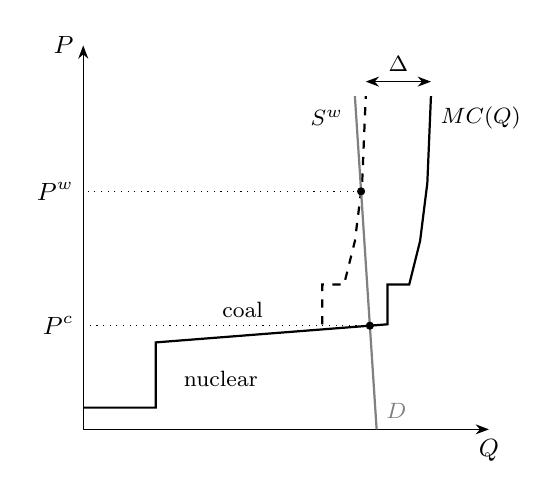
\begin{tikzpicture}[scale=0.92,>=Stealth]
\draw[->] (0,0) -- (5.6,0) node[below] {\small $Q$};
\draw[->] (0,0) -- (0,5.3) node[left] {\small $P$};
\draw[thick,name path=mc] (0,0.3) -- (1.0,0.3) -- (1.0,1.2) -- (4.2,1.45) -- (4.2,2.0) -- (4.5,2.0) -- (4.65,2.6)
  -- (4.75,3.4) -- (4.8,4.6);
\draw[thick,dashed,name path=sw] (3.3,1.45) -- (3.3,2.0) -- (3.6,2.0) -- (3.75,2.6) -- (3.85,3.4) -- (3.9,4.6);
\draw[thick,gray,name path=dem] (4.05,0) -- (3.75,4.6);
\path[name intersections={of=mc and dem,by=Ec}];
\path[name intersections={of=sw and dem,by=Ew}];
\fill (Ec) circle (1.6pt);
\fill (Ew) circle (1.6pt);
\draw[dotted] (Ec) -- (Ec -| 0,0) node[left] {\small $P^{c}$};
\draw[dotted] (Ew) -- (Ew -| 0,0) node[left] {\small $P^{w}$};
\node[right,font=\footnotesize] at (4.8,4.3) {$MC(Q)$};
\node[left,font=\footnotesize] at (3.72,4.3) {$S^{w}$};
\node[gray,font=\footnotesize,anchor=west] at (4.05,0.25) {$D$};
\draw[<->] (3.9,4.8) -- (4.8,4.8);
\node[font=\footnotesize,anchor=south] at (4.35,4.8) {$\Delta$};
\node[font=\footnotesize] at (1.9,0.7) {nuclear};
\node[font=\footnotesize] at (2.2,1.65) {coal};
\end{tikzpicture}
\caption{Merit order and withholding}
\end{subfigure}
\hfill
\begin{subfigure}[b]{0.48\textwidth}
\centering
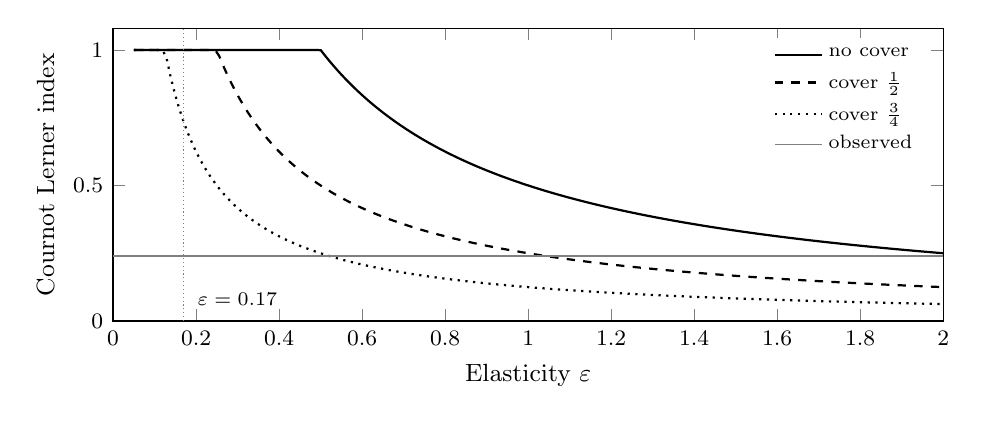
\begin{tikzpicture}
\begin{axis}[width=\linewidth, height=5.3cm, xmin=0, xmax=2, ymin=0, ymax=1.08,
  xlabel={\small Elasticity $\varepsilon$}, ylabel={\small Cournot Lerner index},
  tick label style={font=\footnotesize},
  legend style={font=\scriptsize, draw=none, fill=white, at={(0.98,0.97)}, anchor=north east},
  legend cell align=left]
\addplot[thick, domain=0.05:2, samples=200] {min(1, 0.5/x)};
\addlegendentry{no cover}
\addplot[thick, dashed, domain=0.05:2, samples=200] {min(1, 0.25/x)};
\addlegendentry{cover $\frac{1}{2}$}
\addplot[thick, dotted, domain=0.05:2, samples=200] {min(1, 0.125/x)};
\addlegendentry{cover $\frac{3}{4}$}
\addplot[gray, domain=0:2] {0.24};
\addlegendentry{observed}
\draw[gray, densely dotted] (axis cs:0.17,0) -- (axis cs:0.17,1.08);
\node[font=\scriptsize, anchor=west] at (axis cs:0.18,0.08) {$\varepsilon = 0.17$};
\end{axis}
\end{tikzpicture}
\caption{Cournot markups and contract cover}
\end{subfigure}
\caption{Why oligopoly theory predicts high electricity markups. Panel (a) is a schematic. The industry marginal cost
curve $MC(Q)$ ranks plants from cheapest to most expensive. Demand $D$ is nearly vertical, so withholding a quantity
$\Delta$ of low-cost capacity shifts the offered supply to $S^{w}$ and raises the price from $P^{c}$ to $P^{w}$. Panel
(b) plots the Cournot Lerner index $\min\{1, \frac{s_i}{\varepsilon}(1 - \frac{x_i}{q_i})\}$ of a firm with share
$s_i = \frac{1}{2}$ and contract cover $\frac{x_i}{q_i}$, from \eqref{eq:03-contracts}. Under constant-elasticity
demand, the value one marks the region with no interior equilibrium. The gray horizontal line is the observed average Lerner index of 0.24.}
\label{fig:03-merit-order}
\end{figure}

\subsection{Data and the measurement of marginal cost}\label{sec:03-wolfram-data}

\casehead{The data}
The sample covers 25,639 half-hour periods: nearly every half-hour of six months (January, February, March, April,
July and November) in each of 1992, 1993 and 1994, 18 months in all. About 40 periods are missing. The Pool data come
from the National Grid Company, which lacked some variables before 1992 \citep[pp.~810, 822 and n.~49]{Wolfram1999}.
Price is the SMP, which excludes the capacity payment, because the cost measure covers only fuel. Quantity is the
energy metered in each half-hour, including transmission losses. Appendix Table A1 of the paper reports a mean SMP of
\pounds 22.26 per megawatt-hour (MWh), with a standard deviation of 7.10. The pool selling price, which adds the
capacity payment and uplift, has a mean of \pounds 24.40 and a standard deviation of 10.17. Mean quantity is 16,211
MWh per half-hour, with a standard deviation of 2,839. Energy of 16,211 MWh delivered in half an hour is an average
rate of about 32 GW.

\casehead{Plant marginal cost}
The short-run marginal cost of a fossil-fuel plant is the cost of the fuel it burns per unit of electricity. Let plant
$k$ burn fuel with price $w_k$ in pounds per gigajoule (GJ) and convert fuel energy into electricity with
\emph{thermal efficiency} $e_k \in (0, 1)$. One MWh equals 3.6 GJ, so the plant needs $\frac{3.6}{e_k}$ GJ of fuel per
MWh, a quantity called its \emph{heat rate} $h_k$. Its marginal cost is
\begin{equation}\label{eq:03-plant-mc}
mc_k = w_k\, h_k = \frac{3.6\, w_k}{e_k} \quad \text{(pounds per MWh)}.
\end{equation}
For illustration, take coal at \pounds 1.50 per GJ plus \pounds 0.08 of transport and a hypothetical coal plant with an
efficiency of 36 percent. Then $mc_k = \frac{3.6 \times 1.58}{0.36} = 15.8$, inside the range of the flat coal segment of
\cref{fig:03-wolfram-scatter}.

Each input of \eqref{eq:03-plant-mc} is measured with unusual precision \citep[p.~810]{Wolfram1999}. Before
privatization, the \emph{CEGB Statistical Yearbook} published the thermal efficiency of every coal, oil and gas plant.
\citet{GreenNewbery1992} distilled 20 years of these figures into efficiencies under optimal operating conditions, and
Wolfram replaces them with later engineering estimates where plants had been upgraded. Such data later became
competitively sensitive. They are available only because the industry had recently been public. New combined-cycle gas
turbine (CCGT) plants are assumed to have an efficiency of 45 percent. Fuel prices for oil, gas peaking and CCGT plants
are market prices. Coal was bought from British Coal under contracts. The first contracts, which expired in March 1993,
were effectively take-or-pay and supplied more coal than the generators burned. To capture the replacement cost of coal,
Wolfram uses the prices of the next two contracts. Coal burned before the end of March 1994 is valued at 150 pence per
GJ, and coal burned afterwards at 137 pence. Transport costs average 8 pence per GJ, about 5 percent of fuel costs. Nuclear stations are
assigned \pounds 13 (Magnox, the first-generation gas-cooled reactors) and \pounds 11 (advanced gas-cooled reactors)
per MWh. These figures are too high, but
nuclear plants are never marginal. Pumped storage is costed at the average pool price during pumping, adjusted for
efficiency, and imports from Scotland and France at their bid prices.

\casehead{Capacity and the merit order}
A plant's available capacity varies with maintenance and age. Generators may also withhold capacity strategically to
raise capacity payments \citep{WolakPatrick1997}. Wolfram therefore assigns each plant a capacity equal to the mean
plus one half standard deviation of its declared daily capacity in the month. This is on average 85 percent of the
maximum capacity the plant declared for the year. Weighted by plant size the average is 100 percent. The high-availability case of \cref{tab:03-wolfram-robust}, the mean
plus a full standard deviation, raises the unweighted average to 92 percent \citep[pp.~810--811, 816]{Wolfram1999}.
Sorting plants by marginal cost
gives the industry marginal cost curve, called the \emph{merit order}. Index months by $\mu$, and let month $\mu$ have
plants ordered so that $mc_{(1)} \le mc_{(2)} \le \dots$, with capacities $K_{(1)}, K_{(2)}, \dots$. Then
\begin{equation}\label{eq:03-merit-order}
MC_\mu(Q) = mc_{(j)} \qquad \text{for } \sum_{l < j} K_{(l)} < Q \le \sum_{l \le j} K_{(l)}.
\end{equation}
This nondecreasing step function is the marginal cost of producing $Q$ at least cost. Each half-hour $t$ of month $\mu$
yields a markup $L_t = \frac{P_t - MC_\mu(Q_t)}{P_t}$.

\begin{remark}[What the merit-order cost measures]\label{rem:03-merit-order}
Without firm-level quantities, Wolfram cannot compute each firm's own marginal cost. The merit order supplies an
industry marginal cost directly. Under least-cost dispatch every running plant has $mc_k \le MC_\mu(Q_t)$ and the
marginal plant has exactly $MC_\mu(Q_t)$. If every firm operates a plant at the margin, then $MC_{it} = MC_\mu(Q_t)$ for
all $i$, and
any weights in \cref{prop:03-aggregation} give the same industry marginal cost. If firms withhold low-cost units, the
units that run are more expensive than least-cost dispatch requires. The measured markup then compares price with the
efficient marginal cost, so it also counts the productive inefficiency that withholding creates.
\end{remark}

\casehead{What the data show}
\Cref{fig:03-wolfram-scatter} reproduces the paper's Figure 2 for January and July 1993, a winter and a summer month at
the midpoint of the sample (n.~17). The marginal cost curve rises over the first few gigawatt-hours, where nuclear and
other cheap plants sit. It is then almost flat, between about \pounds 14 and \pounds 17 per MWh, over a wide range where
coal plants are marginal. Near capacity it turns almost vertical, around 26 to 28 GWh per half-hour in January and 21
to 23 GWh in July, when plants are out for summer maintenance. Every observed price lies above marginal cost. In January
prices run from about \pounds 17 to \pounds 35, and the gap widens with quantity. July prices are more dispersed, with a
band near \pounds 31 at low quantities, a cluster around \pounds 50 and one price above \pounds 100. Prices were more
volatile after March 1993, when the initial contracts expired (n.~17). The clouds sit on the flat part of the cost
curve, far from the steep segment where withholding by a duopoly would push them.

\begin{figure}[htbp]
\centering
\begin{subfigure}[b]{0.72\textwidth}
\centering
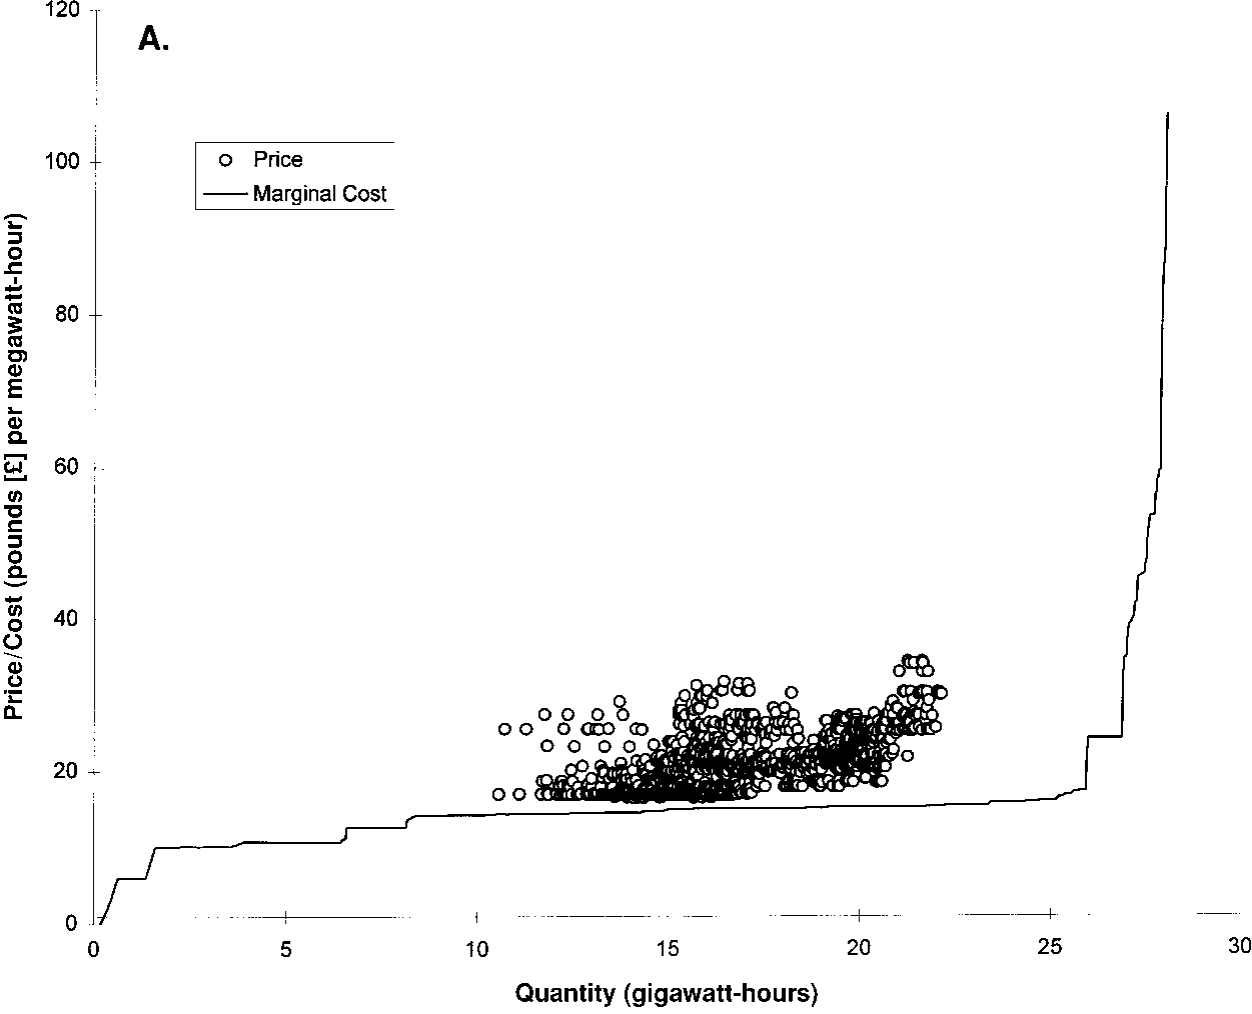
\includegraphics[width=\linewidth]{figures/ch03/wolfram1999_fig2a.png}
\caption{January 1993}
\end{subfigure}

\medskip
\begin{subfigure}[b]{0.72\textwidth}
\centering
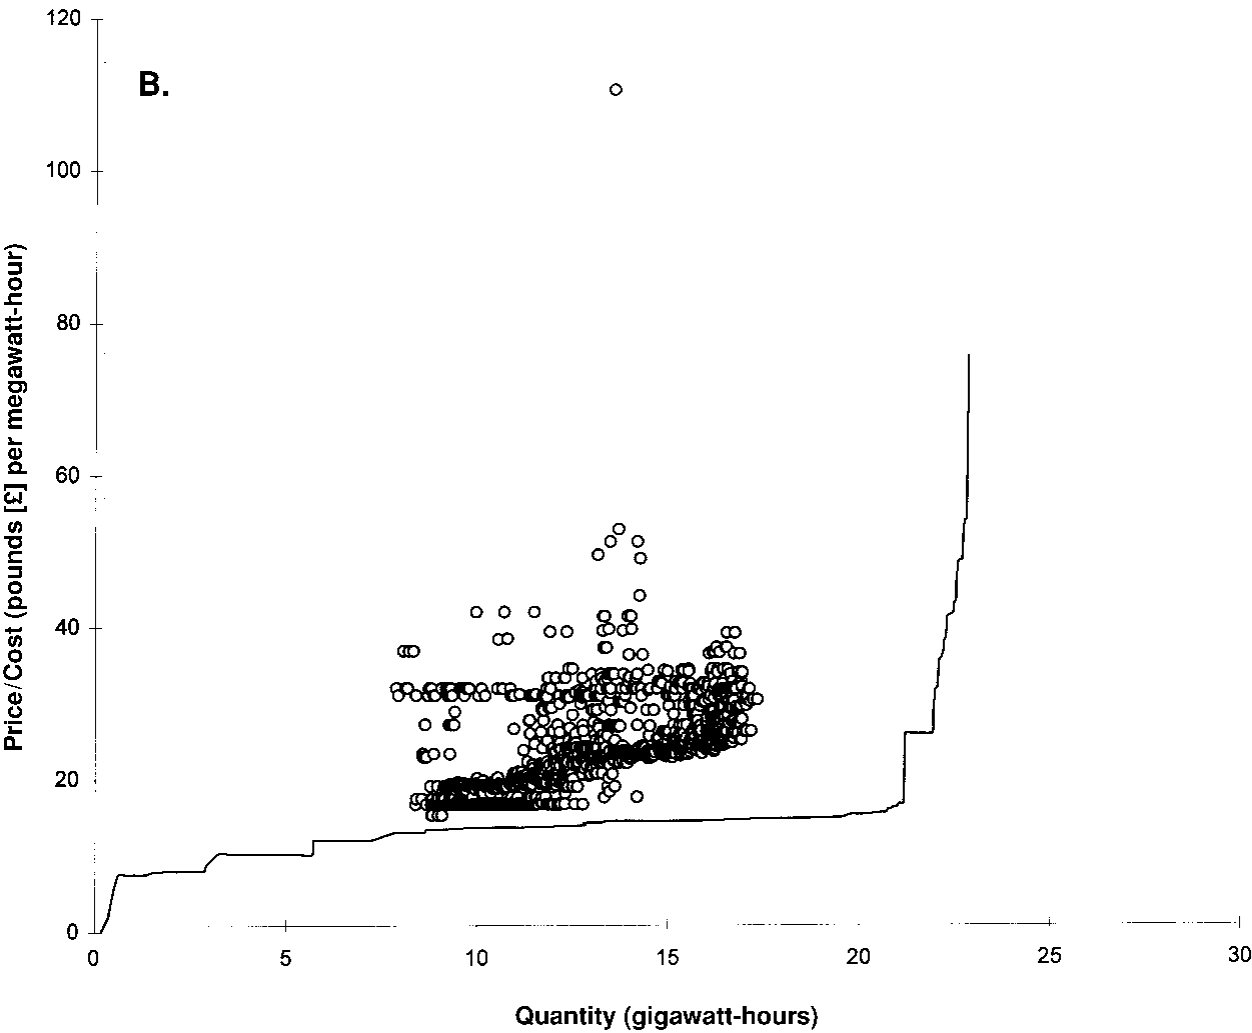
\includegraphics[width=\linewidth]{figures/ch03/wolfram1999_fig2b.png}
\caption{July 1993}
\end{subfigure}
\caption{Pool prices (circles, one per half-hour) and the merit-order marginal cost curve (line), in pounds per MWh
against quantity in gigawatt-hours per half-hour. Source: \citet{Wolfram1999}, Figure 2.}
\label{fig:03-wolfram-scatter}
\end{figure}

\subsection{The model and the direct measure of conduct}\label{sec:03-wolfram-model}

\casehead{Demand, cost and the firm supply relation}
Wolfram's framework is the supply relation of \cref{sec:03-framework} written for half-hours $t$
\citep[pp.~808--809]{Wolfram1999}. Demand is
\begin{equation*}
D_t = D(P_t, X_t, u^d_t),
\end{equation*}
with observed demand shifters $X_t$ such as weather and a demand shock $u^d_t$. Pool demand does respond to price. Some
large users buy directly from the Pool or on contracts tied to pool prices. They switch to backup generators, shut down
energy-intensive processes, or reschedule maintenance when prices are high. Demand also depends on prices in other
half-hours, which the notation suppresses (n.~10). Generator $i$ has marginal cost $MC_{it} = MC_i(q_{it}, Z_{it},
u^s_{it})$, with cost shifters $Z_{it}$ and a cost shock $u^s_{it}$, and profit
\begin{equation*}
\Pi_{it} = P(Q_t, X_t, u^d_t)\, q_{it} - C_i(q_{it}, Z_{it}, u^s_{it}).
\end{equation*}
Its first-order condition, written with a firm-level conduct parameter $\tilde\theta_{it}$, is
\begin{equation}\label{eq:03-wolfram-foc}
P_t = MC_i(q_{it}, Z_{it}, u^s_{it}) - \tilde\theta_{it}\, q_{it}\, P_Q(Q_t, X_t, u^d_t),
\end{equation}
where $P_Q$ is the slope of inverse demand. Cournot conduct is $\tilde\theta_{it} = 1$ and price taking is
$\tilde\theta_{it} = 0$. In the language of \cref{cor:03-benchmarks}, $\tilde\theta_{it} = 1 + r_i$.

\casehead{Aggregation}
Firm-level quantities are not available, so the analysis works with the industry. Applying
\cref{prop:03-aggregation} to \eqref{eq:03-wolfram-foc} with weights $\varphi_{it}$ gives
\begin{equation}\label{eq:03-wolfram-supply}
P_t = MC(Q_t, \mathbf{Z}_t, u^s_t) + \frac{P_t}{\varepsilon_t}\,\theta_t,
\qquad
\theta_t = \sum_{i=1}^{N} \varphi_{it}\,\frac{q_{it}}{Q_t}\,\tilde\theta_{it},
\end{equation}
which is Wolfram's eq.~(5). Rearranging gives her eq.~(6),
\begin{equation}\label{eq:03-wolfram-theta}
\theta_t = \varepsilon_t\,\frac{P_t - MC_t}{P_t}.
\end{equation}
Wolfram writes $\eta$ for the elasticity and $\kappa_{it}$ for the weights. With $\varphi_{it} = \frac{1}{N}$ and a common
$\tilde\theta_t$, industry conduct is $\theta_t = \frac{\tilde\theta_t}{N}$. It equals 1 for joint profit maximization,
$\frac{1}{N}$ for Cournot and 0 for perfect competition. For this reason $\frac{1}{\theta_t}$ is sometimes read as an
``equivalent number of firms.'' Wolfram treats $\theta_t$ as a summary measure, the elasticity-adjusted markup. She makes
no claim about the conjectures that firms hold (n.~12, citing \citealp{Corts1999}).

\begin{remark}[Markups as transfers]\label{rem:03-wolfram-welfare}
With very inelastic demand, even large markups cause little deadweight loss. Approximate demand by a straight line near
the equilibrium and take marginal cost as flat. Pricing at $P$ instead of $MC$ reduces quantity by about
$\varepsilon Q\frac{P - MC}{P}$, so the Harberger triangle is
\begin{equation*}
DWL \approx \frac{1}{2}(P - MC)\,\varepsilon Q\,\frac{P - MC}{P}
\qquad\Longrightarrow\qquad
\frac{DWL}{PQ} \approx \frac{1}{2}\,\varepsilon L^2 = \frac{1}{2}\,\theta L.
\end{equation*}
With $\varepsilon = 0.17$ and $L = 0.24$, the loss is about 0.5 percent of expenditure, while the transfer
$\frac{(P - MC)Q}{PQ} = L$ is 24 percent. This is why Wolfram also reports quantity-weighted average markups, which speak
to the surplus transferred to producers (p.~814).
\end{remark}

\casehead{The demand slope}
Marginal cost is measured, so only the elasticity is missing from \eqref{eq:03-wolfram-theta}. Wolfram does not
estimate it for this purpose. She assumes linear demand with slope $D_p = \frac{\partial D}{\partial P} = -125$, which
makes her numbers comparable with the simulations of \citet{GreenNewbery1992} \citep[p.~811]{Wolfram1999}. The units are
MWh per half-hour per pound per MWh. A fall of 125 MWh within a half-hour is an average rate of 250 megawatts, or
0.25 GW, which is the slope $b = 0.25$ that Green and Newbery report in gigawatts. Their low and high cases correspond to
$D_p = -50$ and $D_p = -250$. With linear demand,
\begin{equation}\label{eq:03-wolfram-theta-linear}
\varepsilon_t = -D_p\,\frac{P_t}{Q_t}
\qquad\Longrightarrow\qquad
\theta_t = \varepsilon_t\,\frac{P_t - MC_t}{P_t} = -D_p\,\frac{P_t - MC_t}{Q_t}.
\end{equation}
At the sample means, $\varepsilon = \frac{125 \times 22.26}{16{,}211} = 0.17$. This is in the range of short-run
elasticities found elsewhere \citep{Taylor1975}. The largest elasticity that \citet{PatrickWolak1997} find for customers
on pool-price contracts is about 0.3, for water companies, a group unusually sensitive to price. With an average Lerner
index of 0.241, \eqref{eq:03-wolfram-theta-linear} at the means gives $\theta = \frac{125 \times 0.241 \times
22.26}{16{,}211} = 0.041$.

Later work confirms that short-run electricity demand is very inelastic. One reason is that many households face
retail prices that do not vary with wholesale conditions \citep[p.~709]{KelloggReguant2021}. \citet{ReissWhite2005}
exploit the tiers of California tariffs in household survey data. They find an average elasticity of $-0.39$, which
reflects medium-run to long-run responses. \citet{Ito2014} compares households on either side of a utility border in
Orange County. He finds an elasticity of about $-0.08$ with respect to the average price. \citet{Shaffer2020} estimates
about $-0.04$ from bunching at a tariff kink in British Columbia \citep[pp.~710--711]{KelloggReguant2021}. These are
retail residential elasticities, and none measures the response of pool demand. Still, they bracket the value of 0.17
assumed here and the rotation estimates of about 0.1 in \cref{sec:03-wolfram-neio}.

\begin{example}[The Cournot benchmark under the assumed demand]\label{ex:03-wolfram-cournot}
Extend the linear demand through the sample means: $Q = 125(\bar\alpha - P)$ with choke price $\bar\alpha = 22.26 +
\frac{16{,}211}{125} = 151.95$. Let a symmetric duopoly have flat marginal cost $c = 16$, roughly the level of the coal
segment. Inverse demand is $P = \bar\alpha - \frac{Q}{125}$, and the symmetric Cournot price with $N$ firms is
$\frac{\bar\alpha + Nc}{N + 1}$. With $N = 2$,
\begin{equation*}
P^{C} = \frac{151.95 + 2 \times 16}{3} = 61.32,
\qquad
Q^{C} = 125\,(151.95 - 61.32) = 11{,}329.
\end{equation*}
The Lerner index is $\frac{61.32 - 16}{61.32} = 0.74$. The elasticity at this point is
$\frac{125 \times 61.32}{11{,}329} = 0.68$, and $\theta = 0.68 \times 0.74 = 0.5 = \frac{1}{N}$, as it must be. The
benchmark price is almost three times the mean SMP. The calculation extrapolates the linear demand far outside the
sample and is only an illustration of the scale of the predicted markups.
\end{example}

\casehead{Benchmarks for conduct}
Price taking gives $\theta = 0$ and joint profit maximization gives $\theta = 1$. Cournot gives
$\theta = \sum_i \varphi_{it} s_{it}$ (\cref{cor:03-benchmarks}). This is $\frac{1}{2}$ for a symmetric duopoly. For the
two asymmetric generators, Wolfram uses 0.52 (p.~818). That value matches a Herfindahl index computed with shares in the
ratio of the initial capacities, $\bigl(\frac{52}{85}\bigr)^2 + \bigl(\frac{33}{85}\bigr)^2 = 0.52$. The fourth
benchmark comes from a model built for electricity markets.

\casehead{Supply function equilibrium}
In the Pool, firms bid supply schedules that state a price for each quantity. \citet{KlempererMeyer1989} model such
competition. Each firm commits to a supply function before a demand shock is realized, and the market clears where total supply meets
demand. \citet{GreenNewbery1992} were the first to apply the concept to the Pool. They calibrate cost functions for the
two effective duopolists and a demand curve, and they solve for the supply function equilibria, including asymmetric
ones. The equilibria range from marginal-cost pricing to one that reproduces the Cournot quantities and prices. The
highest-price equilibrium implies large markups. Observed prices showed no such markups, and Green and Newbery
suggest that the generators' forward sales of much of their capacity may explain the gap. A long-run version of the model finds that
entry incentives depend strongly on the demand elasticity and on the incumbents' pricing strategies
\citep[pp.~145--146]{HortacsuPerrigne2021}. \citet{Wolfram1998} later treated the bids as a uniform-price multi-unit
auction. A higher bid raises the price paid on all accepted units if it sets the price, but it lowers the chance that
the unit is accepted \citep[p.~695]{KelloggReguant2021}. Her evidence is consistent with strategic withholding of
supply \citep[p.~146]{HortacsuPerrigne2021}.
The next result derives the equilibrium condition and shows where supply function markups fall. \Cref{rem:02-sfe}
states its Lerner form without proof.

\begin{proposition}[Supply function equilibrium markups]\label{prop:03-sfe-markup}
Two firms have cost functions $C_i$ with $C_i' \ge 0$. Demand is $D(P) + u$, with $D' < 0$ and a shock $u$ whose support
is an interval. Before $u$ is known, firm $i$ chooses a differentiable, nondecreasing, nonnegative supply function
$S_i(P)$, and the price clears $S_1(P) + S_2(P) = D(P) + u$. Suppose each $S_i$ maximizes firm $i$'s profit for every
realization of $u$, given $S_j$. Then at every clearing price at which firm $i$ sells a positive quantity,
\begin{equation}\label{eq:03-sfe-ode}
S_i(P) = \bigl(P - C_i'(S_i(P))\bigr)\bigl(S_j'(P) - D'(P)\bigr), \qquad i \ne j.
\end{equation}
At a clearing price with $S_i(P) = 0$, optimality requires only $P \le C_i'(0)$. If both firms sell positive
quantities at $P$, the Lerner index of firm $i$ is
\begin{equation}\label{eq:03-sfe-lerner}
L_i = \frac{s_i}{\varepsilon + s_j\,\eta_j}, \qquad \eta_j = \frac{P\,S_j'(P)}{S_j(P)} \ge 0,
\end{equation}
where $s_i = \frac{S_i}{Q}$ and $\varepsilon = -\frac{P D'(P)}{Q}$. Hence $0 < L_i \le \frac{s_i}{\varepsilon}$, and
firm $i$'s conduct parameter is $\tilde\theta_i = \frac{\varepsilon}{\varepsilon + s_j\eta_j} \in (0, 1]$.
\end{proposition}

\begin{proof}
Fix $S_j$ and a realization $u$. Whatever $S_i$ is, firm $i$ ends up at some price $P$ and sells its residual demand
$R_i(P, u) = D(P) + u - S_j(P)$. Since supply cannot be negative, only prices with $R_i(P, u) \ge 0$ can clear the
market. Choosing a supply function is therefore equivalent to choosing, for each $u$, such a price on the residual
demand curve. Profit at price $P$ is $\pi_i(P, u) = P R_i(P, u) - C_i(R_i(P, u))$, with derivative
\begin{equation*}
\frac{\partial \pi_i}{\partial P} = R_i(P, u) + \bigl(P - C_i'(R_i(P, u))\bigr)\bigl(D'(P) - S_j'(P)\bigr).
\end{equation*}
Residual demand strictly decreases in $P$, because $D' - S_j' < 0$. If the optimal price leaves firm $i$ a positive
quantity, nearby prices are also feasible, so the derivative is zero there. If it leaves the firm nothing, only lower
prices are feasible, and lowering the price must not raise profit. The derivative is then nonnegative. With
$R_i = 0$ it equals $\bigl(P - C_i'(0)\bigr)(D' - S_j')$, so this holds exactly when $P \le C_i'(0)$.
The shock shifts residual demand horizontally without changing its slope, so different realizations select different
optimal prices. The supply function $S_i$ implements all these optima only if $S_i(P) = R_i(P, u)$ at each optimal pair.
Setting the derivative to zero then gives \eqref{eq:03-sfe-ode} wherever $S_i(P) > 0$. Its left side is positive, so
$P > C_i'$ and $L_i > 0$. When $S_j(P) > 0$ as well, divide \eqref{eq:03-sfe-ode} by $P$ and then numerator and
denominator by $Q$:
\begin{equation*}
\frac{P - C_i'}{P} = \frac{S_i}{P(S_j' - D')} = \frac{\frac{S_i}{Q}}{\frac{S_j}{Q}\cdot\frac{P S_j'}{S_j} -
\frac{P D'}{Q}} = \frac{s_i}{s_j\eta_j + \varepsilon}.
\end{equation*}
Since $\eta_j \ge 0$, $L_i \le \frac{s_i}{\varepsilon}$. Comparing with the firm supply relation
$L_i = \tilde\theta_i\frac{s_i}{\varepsilon}$ of \cref{prop:03-aggregation} gives $\tilde\theta_i$.
\end{proof}

The equality \eqref{eq:03-sfe-ode} is required only of active firms. With asymmetric costs, a high-cost firm can optimally supply nothing
at some or all clearing prices. Its condition then holds only as the inequality $P \le C_i'(0)$.
The proposition places supply function equilibria between competition and Cournot. If the rival's supply does not
respond to price ($\eta_j = 0$), firm $i$ faces the Cournot residual demand. As the rival's supply becomes very elastic
($\eta_j \to \infty$), the markup goes to zero. The formula also shows why the concept suits electricity. As demand
becomes perfectly inelastic, the Cournot markup explodes, while the supply function markup stays finite at
$\frac{s_i}{s_j\eta_j}$, disciplined by the rival's supply response. In a symmetric equilibrium with positive supply,
\eqref{eq:03-sfe-ode} becomes
the differential equation $S'(P) = \frac{S(P)}{P - C'(S(P))} + D'(P)$, which has a continuum of solutions. Klemperer and
Meyer show that the equilibria form a range when the shock has bounded support. Wolfram computes the \emph{highest}
supply function equilibrium, the solution that passes through the symmetric Cournot point on the right-most demand
curve (pp.~813--814). Following Green and Newbery, she assumes a symmetric duopoly. The right-most demand curve has slope
$-125$ and passes through the monopoly price at a quantity of 30 in the gigawatt units of the paper. The largest
quantity in the sample is 24, so this choice is conservative (n.~22). The benchmark $\theta$ is the margin in the supply function equilibrium
times the elasticity under $D_p = -125$. Both are evaluated at the equilibrium point, where the price is higher and the
elasticity larger than in the data. Because marginal cost rises
so steeply, the lowest supply function equilibrium gives very similar markups (n.~23).

\subsection{Markups and conduct}\label{sec:03-wolfram-results}

\Cref{tab:03-wolfram} reproduces Table~1 of \citet{Wolfram1999}. Each entry averages over half-hours, and the
standard deviations in parentheses describe the dispersion across half-hours. The first column is the Lerner index
computed from the merit order. The second multiplies each half-hour's Lerner index by its elasticity under $D_p = -125$,
as in \eqref{eq:03-wolfram-theta-linear}. The third gives $\theta$ in the highest supply function equilibrium.

\begin{table}[htbp]
\centering
\begin{threeparttable}
\caption{Price-cost markups calculated with measured marginal cost}
\label{tab:03-wolfram}
\small
\setlength{\tabcolsep}{4.5pt}
\begin{tabular}{@{}lcccc@{}}
\toprule
& (i) & (ii) & (iii) & (iv) \\
Period & $\frac{P - MC}{P}$ & $\theta = \varepsilon\frac{P - MC}{P}$ & $\theta$, highest SFE & Observations \\
\midrule
Jan.~1992 to Mar.~1993 & 0.241 (0.129) & 0.043 (0.030) & 0.28 (0.06) & 12,704 \\
Apr.~1993 to Mar.~1994 & 0.259 (0.228) & 0.057 (0.055) & 0.29 (0.06) & 8,637 \\
After Mar.~1994 & 0.208 (0.416) & 0.067 (0.086) & 0.33 (0.07) & 4,298 \\
\addlinespace
Four weeks before a regulatory decision & 0.329 (0.150) & 0.071 (0.051) & & 3,216 \\
Four weeks after a regulatory decision & 0.156 (0.213) & 0.028 (0.040) & & 2,671 \\
\addlinespace
\multicolumn{5}{@{}l}{\emph{By quantity level}} \\
Jan.~1992 to Mar.~1993, above median & 0.279 (0.124) & 0.046 (0.027) & 0.31 (0.05) & 6,764 \\
\phantom{Jan.~1992 to Mar.~1993,} below median & 0.198 (0.121) & 0.039 (0.033) & 0.23 (0.02) & 5,940 \\
Apr.~1993 to Mar.~1994, above median & 0.299 (0.184) & 0.056 (0.044) & 0.33 (0.05) & 4,530 \\
\phantom{Apr.~1993 to Mar.~1994,} below median & 0.214 (0.261) & 0.058 (0.065) & 0.24 (0.02) & 4,107 \\
After Mar.~1994, above median & 0.554 (0.122) & 0.138 (0.057) & 0.37 (0.09) & 1,526 \\
\phantom{After Mar.~1994,} below median & 0.018 (0.398) & 0.027 (0.073) & 0.26 (0.02) & 2,772 \\
\bottomrule
\end{tabular}
\begin{tablenotes}\footnotesize
\item Notes: Reproduced from \citet{Wolfram1999}, Table~1. The unit of observation is a half-hour. Standard deviations
across half-hours in parentheses. Columns (ii) and (iii) assume linear demand with slope $D_p = -125$, so that
$\varepsilon = -D_p\frac{P}{Q}$. SFE: supply function equilibrium. The three periods sum to 25,639 half-hours, and each
pair of quantity rows sums to its period total. Column (ii) is a mean of ratios, so it differs from column (i) times
0.17.
\end{tablenotes}
\end{threeparttable}
\end{table}

\casehead{Levels}
Prices exceed measured marginal cost by more than 20 percent on average, so the market is far from competitive. The
averages are precise. Two-sided $t$-tests at the 1 percent level reject an average markup below 0.19 in the last period
and above 0.245 in the first. Serial correlation makes these tests somewhat optimistic (p.~811 and n.~21).
Conduct, however, is small. The values of $\theta$ between 0.043 and 0.067 are far from collusion ($\theta = 1$) and far
below Cournot (0.5 or 0.52). They are also far below the highest supply function equilibrium, between 0.28 and 0.33. A
value of 0.05 corresponds to symmetric Cournot competition among 20 firms. The values are significantly above zero, so
the Bertrand model of homogeneous price competition is rejected as well. Wolfram notes features that should have made
collusion easy (p.~813). The firms bid daily, an infinitely repeated game, and as former parts of one organization they
knew each other's plants well.

How wrong would the assumed elasticity have to be to reverse these conclusions? Column (ii) is column (i) times the
elasticity. Joint profit maximization would require an elasticity of about $\frac{1}{0.25} = 4$, and asymmetric Cournot
conduct one of about $\frac{0.52}{0.25} = 2.1$. Matching the highest supply function equilibrium would require an
elasticity above about 3, because that benchmark itself rises as demand becomes more elastic (p.~818). Even long-run electricity elasticities rarely exceed 1.5 \citep{Taylor1975}. The
qualitative conclusion
is therefore robust to the demand assumption, even though the level of $\theta$ is not.

\casehead{Patterns}
Markups rise with quantity, mildly before April 1994 and dramatically afterwards: 0.554 above the median quantity
against 0.018 below. The price cap explains the later pattern. It applied to the time-weighted average price, so the
generators could stay under it by cutting prices when demand was low and raising them when demand was high (p.~814).
Quantity-weighted averages, which track the surplus transferred, are close to the time-weighted ones before April 1994,
at 0.248 and 0.264. After March 1994 the quantity-weighted average is 0.262, against a time-weighted 0.208. Markups are
also much higher in the four weeks before a regulatory decision (0.329) than in the four weeks after (0.156). The
dispersion across half-hours is large, with standard deviations comparable to the means. Variation by quantity explains
less than 5 percent of it (n.~26). Within a month the merit-order curve is fixed, but marginal cost still moves along
it as quantity changes. The plants at the margin over much of the observed range have similar costs, so the curve is
nearly flat there (\cref{fig:03-wolfram-scatter}). Wolfram therefore attributes the volatility of markups primarily to
prices (n.~26).

\casehead{Robustness}
\Cref{tab:03-wolfram-robust} reproduces the paper's Table~2. High fuel costs value coal at the take-or-pay contract price
of 180 pence per GJ before April 1993. They also raise oil and gas prices by 20 percent and add \pounds 1 per MWh to
nuclear costs.
Low fuel costs set coal at world prices (120 and then 110 pence per GJ) and lower the other fuels symmetrically. Low and
high availability assign each plant the monthly mean, or the mean plus a full standard deviation, of its declared
capacity. The last column measures the margin against the pool selling price, which adds capacity payments and uplift
to the SMP.

\begin{table}[htbp]
\centering
\begin{threeparttable}
\caption{Lerner indices under alternative assumptions}
\label{tab:03-wolfram-robust}
\small
\setlength{\tabcolsep}{4pt}
\begin{tabular}{@{}lccccccc@{}}
\toprule
& & \multicolumn{2}{c}{Fuel prices} & \multicolumn{3}{c}{Plant capacity} & \\
\cmidrule(lr){3-4}\cmidrule(lr){5-7}
& (i) & (ii) & (iii) & (iv) & (v) & (vi) & (vii) \\
Period & Benchmark & High & Low & \makecell{Low\\avail.} & \makecell{High\\avail.} & Declared &
  \makecell{Pool selling\\price} \\
\midrule
Jan.\ 1992 to Mar.\ 1993 & \makecell{0.241\\(0.129)} & \makecell{0.097\\(0.154)} & \makecell{0.384\\(0.105)} &
  \makecell{0.231\\(0.130)} & \makecell{0.250\\(0.127)} & \makecell{0.231\\(0.130)} & \makecell{0.278\\(0.147)} \\
\addlinespace
Apr.\ 1993 to Mar.\ 1994 & \makecell{0.259\\(0.228)} & \makecell{0.119\\(0.269)} & \makecell{0.399\\(0.184)} &
  \makecell{0.246\\(0.231)} & \makecell{0.268\\(0.226)} & \makecell{0.245\\(0.233)} & \makecell{0.314\\(0.233)} \\
\addlinespace
After Mar.\ 1994 & \makecell{0.208\\(0.416)} & \makecell{0.179\\(0.432)} & \makecell{0.338\\(0.352)} &
  \makecell{0.196\\(0.421)} & \makecell{0.215\\(0.415)} & \makecell{0.195\\(0.422)} & \makecell{0.270\\(0.417)} \\
\bottomrule
\end{tabular}
\begin{tablenotes}\footnotesize
\item Notes: Reproduced from \citet{Wolfram1999}, Table~2. Entries are average Lerner indices $\frac{P - MC}{P}$ with
standard deviations across half-hours in parentheses. Column (i) is column (i) of \cref{tab:03-wolfram}. Column (vi)
uses each plant's actual declared daily capacity. Observations: 12,704, 8,637 and 4,298.
\end{tablenotes}
\end{threeparttable}
\end{table}

Markups are sensitive to fuel costs. Before April 1994 the two fuel cases move them by 54 to 60 percent in each
direction. After March 1994 the high-cost case lowers them by only 14 percent, while the low-cost case raises them by
about 63 percent. Markups are much less sensitive to availability. About 90 percent of the fuel-cost sensitivity comes from the coal assumptions. Coal plants set
the price most of the time, and in the 12 months to March 1997 they set the SMP in 82 percent of half-hours
(n.~33). Changing coal costs shifts the long flat segment of the merit order, which moves almost every markup.
Changing availability only lengthens or shortens that segment. Margins over the pool selling price are 15 to 30 percent
higher, because the extra charges are 5 to 10 percent of the pool price.

Three further checks support the cost measure \citep[p.~817]{Wolfram1999}. First, it implies producer surplus of about
25 percent of the generators' SMP revenue. SMP is about 90 percent of the pool price, and pool revenue is about 70
percent of National Power's total revenue. Fuel costs are therefore about $0.75 \times 0.9 \times 0.7 = 47$ percent of
revenue, close to the 40 and 45 percent reported in the two companies' 1994 annual reports. Second, a regression version
of \eqref{eq:03-wolfram-supply} imposes constant conduct and a constant elasticity. Solving $P_t = MC_t +
\frac{P_t}{\varepsilon}\theta$ for $P_t$ gives Wolfram's eq.~(7),
\begin{equation}\label{eq:03-wolfram-omega}
P_t = \omega\, MC_t + e_t, \qquad \omega = \frac{\varepsilon}{\varepsilon - \theta}.
\end{equation}
The coefficient $\omega$ is the constant-elasticity pass-through rate of \cref{cor:03-passthrough-cases}, with total
marginal cost in place of a tax. On all the data $\hat\omega = 1.92$ (robust standard error 0.75), which implies
$\theta = \varepsilon(1 - \frac{1}{\hat\omega}) = 0.17 \times (1 - \frac{1}{1.92}) = 0.081$. Instrumenting marginal cost
with the demand shifters, to address measurement error, raises the estimate slightly and insignificantly. Third, the
functional form of demand matters little. With a constant elasticity of 0.17, $\theta$ is 0.041, 0.044 and 0.035 in the
three periods. With a concave demand curve whose elasticity is 0.17 at the means, it is 0.043, 0.060 and 0.077
(n.~37).

\subsection{Why are markups so low?}\label{sec:03-wolfram-explanations}

Prices respond to the generators' incentives, yet they stay far below static oligopoly predictions. Wolfram weighs
three explanations (pp.~814--815): contracts, the threat of regulation, and the threat of entry.

\casehead{Contracts}
A generator that has sold part of its output forward gains less from a high spot price. The next result makes this
precise. It is the spot-market stage of the model of \citet{AllazVila1993}, and it restates \cref{ex:02-forward}.

\begin{proposition}[Forward contracts and spot markups]\label{prop:03-contracts}
Firm $i$ holds two-way contracts for $x_i$ units at strike price $F_i$ and then chooses its output $q_i$ as a Cournot
competitor. Its profit is
\begin{equation*}
\Pi_i = P(Q)\,(q_i - x_i) + F_i\, x_i - C_i(q_i),
\end{equation*}
and at an interior optimum
\begin{equation}\label{eq:03-contracts}
L_i = \frac{P - MC_i}{P} = \frac{s_i}{\varepsilon}\Bigl(1 - \frac{x_i}{q_i}\Bigr).
\end{equation}
\end{proposition}

\begin{proof}
The firm sells $q_i$ at the spot price and pays $(P - F_i)x_i$ on its contracts, so
$\Pi_i = P q_i - (P - F_i)x_i - C_i(q_i) = P(q_i - x_i) + F_i x_i - C_i(q_i)$. The first-order condition is
\begin{equation*}
P + P'(Q)\,(q_i - x_i) - MC_i = 0
\quad\Longrightarrow\quad
P - MC_i = -P'(Q)\, q_i\Bigl(1 - \frac{x_i}{q_i}\Bigr).
\end{equation*}
Dividing by $P$ and using $-\frac{P' Q}{P} = \frac{1}{\varepsilon}$ and $\frac{q_i}{Q} = s_i$ gives
\eqref{eq:03-contracts}.
\end{proof}

The firm cares about the price only on its uncontracted output $q_i - x_i$. Full cover makes it a price taker, and
cover above output makes it want a price below marginal cost. In conduct terms, $\tilde\theta_i = 1 - \frac{x_i}{q_i}$.
A one-way contract works differently. The generator refunds the excess of the pool price over the strike price, so cover
dampens its incentive only when the price is above the strike. Panel (b) of \cref{fig:03-merit-order} plots
\eqref{eq:03-contracts} for a firm with half the market.

The British data allow a test. Wolfram estimates that the initial contracts covered about 75 percent of the generators'
output and their replacements about half (p.~814). At the observed point, with $s_i = 0.5$ and $\varepsilon = 0.17$,
\eqref{eq:03-contracts} requires $L_i = \frac{0.5}{0.17}\times 0.25 = 0.74$ under the initial contracts and
$L_i = \frac{0.5}{0.17}\times 0.5 = 1.47$ under the replacements. The observed prices and quantities therefore cannot
be a Cournot equilibrium with either level of cover. What happens away from the observed point depends on the shape of
demand. Under a constant elasticity of 0.17, half cover would leave no interior equilibrium. Under the linear demand
of \cref{ex:03-wolfram-cournot}, the elasticity rises with the price, and an interior equilibrium exists for both
levels of cover. Write $\zeta = \frac{x_i}{q_i}$ for the cover ratio and take $c = 16$. The first-order condition
of \cref{prop:03-contracts} reads $P - c = \frac{(1 - \zeta)\, q_i}{125}$. In a symmetric duopoly
$q_i = \frac{125(\bar\alpha - P)}{2}$, so
\begin{equation*}
P - c = \frac{(1 - \zeta)(\bar\alpha - P)}{2}
\quad\Longrightarrow\quad
P - c = \frac{(1 - \zeta)(\bar\alpha - c)}{3 - \zeta},
\end{equation*}
which gives a price of 31.11 with 75 percent cover and 43.19 with half cover. The Lerner indices are 0.49 and 0.63. Either
way the model predicts a sharp rise after March 1993. \Cref{tab:03-wolfram} shows a rise from 0.241 to 0.259. A
fall of more than 20 percentage points in contract cover raised markups by less than 2 percentage points. Contracts
may restrain prices slightly, but they cannot explain why oligopoly models predict so poorly.

The contracts in Britain were imposed at privatization. \citet{AllazVila1993} show that duopolists choose to sell
forward even when nobody forces them to. The following example shows the mechanism in the simplest case.
\Cref{sec:02-forward} sketches the same calculation, and we give it in full here.

\begin{example}[Strategic forward sales]\label{ex:03-allaz-vila}
Two firms with constant marginal cost $c$ face inverse demand $P = a - bQ$. In stage 1 each firm sells $x_i$ forward.
Arbitrage sets the forward price equal to the spot price, which is known in this deterministic model. In stage 2 the
firms choose outputs. Stage-2 first-order conditions from \cref{prop:03-contracts} are
\begin{equation*}
a - b(q_i + q_j) - b(q_i - x_i) - c = 0, \qquad i = 1, 2,
\end{equation*}
so that
\begin{equation*}
q_i = \frac{a - c + 2b x_i - b x_j}{3b},
\qquad
P - c = \frac{a - c - b(x_i + x_j)}{3}.
\end{equation*}
A forward sale raises the firm's own output by $\frac{2}{3}$ and lowers the price by $\frac{b}{3}$ per unit. Since the
forward price equals the spot price, firm $i$'s total profit is $(P - c)q_i$. Its stage-1 condition is
\begin{equation*}
-\frac{b}{3}\, q_i + \frac{2}{3}(P - c) = 0
\quad\Longrightarrow\quad
P - c = \frac{b\, q_i}{2}.
\end{equation*}
In a symmetric equilibrium, substituting $q = \frac{a - c + bx}{3b}$ and $P - c = \frac{a - c - 2bx}{3}$ gives
\begin{equation*}
\frac{a - c - 2bx}{3} = \frac{a - c + bx}{6}
\quad\Longrightarrow\quad
x = \frac{a - c}{5b}, \qquad q = \frac{2(a - c)}{5b}, \qquad P - c = \frac{a - c}{5}.
\end{equation*}
Each firm covers half of its output. The margin falls from the Cournot level $\frac{a - c}{3}$ to $\frac{a - c}{5}$,
and both firms earn less. Each sells forward to commit itself to aggressive spot behavior, a prisoner's dilemma.
\end{example}

\citet{Green1999} builds contracts into the supply function framework and shows that pool prices fall as contract
cover rises \citep[p.~810]{Wolfram1999}. Contracts are therefore a coherent mechanism. The British evidence suggests that
they were not the main force restraining prices.

\casehead{The threat of regulation}
Prices react to the regulator's calendar. In the four weeks before OFFER's statements on pool prices the Lerner index
averages 0.329, and in the four weeks after it averages 0.156. Two-sided $t$-tests reject that markups around these
decisions equal markups at other times, and the differences persist after controlling for demand factors (n.~27). The
generators knew when a statement was being prepared, and the regulator analyzed prices from earlier months. Wolfram
suggests that the generators raised prices while the regulator could not yet see them and restrained prices afterwards,
when attention was on the Pool (pp.~814--815). In the model of \citet{GlazerMcMillan1992}, the threat of regulation
leads a monopolist to price below the monopoly level. The firm raises its price as the probability of future
regulation rises. The response to the 1994 price cap, documented above, is direct evidence that regulation shaped
pricing, and of the distortions a cap on average prices creates.

\casehead{The threat of entry}
Two pieces of evidence point to entry deterrence (p.~815). First, pool prices sat just below the long-run average cost
of a new entrant. Following Green and Newbery, a new CCGT plant had capital and non-fuel operating costs of roughly
\pounds 85 per kilowatt of capacity. Treating this as an annual cost, a plant that runs 90 to 95 percent of the year has
non-fuel costs of $\frac{85{,}000}{8{,}760 \times 0.95} = 10.2$ to $\frac{85{,}000}{8{,}760 \times 0.90} = 10.8$ pounds
per MWh. Adding
fuel costs of roughly \pounds 16 gives an average cost of \pounds 26 to \pounds 27 per MWh. Pool prices averaged
\pounds 23.6 per MWh in fiscal years 1993 and 1994. Second, pool prices moved with the price of natural gas, the fuel
of potential entrants, even in high-demand periods when no existing CCGT plant was marginal. In a regression of the
pool price on the demand variables and the gas price interacted with a dummy for demand above 15 GW, the gas coefficient
is 0.024 (standard error 0.008). A 10 percent rise in the gas price thus raises the pool price by less than 1 percent.
Pricing just below the entrant's cost would imply a nearly one-to-one relation between gas and pool prices. Wolfram
suggests that the generators may follow a more complex strategy, or that the gas price an entrant faces is measured
with error (n.~29).

\emph{Limit pricing} of this kind keeps prices low to make entry unprofitable. Game-theoretic models of limit pricing
rely on entrants being uncertain about incumbents' costs, which is implausible here, although entrants could be unsure
about regulatory constraints (n.~30). Some entry did occur. All independent plants added after privatization were at
least partly owned by RECs, which could pass their costs to franchise customers whatever the pool price. Entry decisions
may therefore have depended on more than pool prices.

\subsection{Estimates that ignore cost data}\label{sec:03-wolfram-neio}

Section~IV of the paper asks what a researcher without cost data would conclude. Wolfram applies two methods. The first
is new and exploits the distortion created by the price cap. The second is the demand-rotation approach of
\cref{sec:03-identification}.

\casehead{A bound from the price cap}
The cap on the time-weighted average price rotated the industry supply curve counterclockwise. Prices fell at low
demand and rose at high demand. \Cref{fig:03-pricecap-rotation} redraws the paper's stylized Figure~3. Wolfram sorts
half-hours into 25 groups by quantity, in bands of 0.5 GWh. For each group $g$ she compares the average price after the
cap, $P_{H,g}$, with the average price before, $P_{L,g}$. The \emph{rotation axis} is the lowest quantity at which prices
after the cap exceed prices before. Eleven groups lie to its left and fourteen to its right.

\begin{figure}[htbp]
\centering
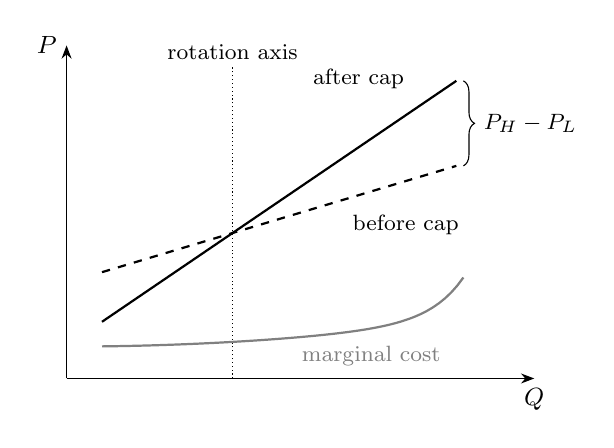
\begin{tikzpicture}[scale=0.9,>=Stealth]
\draw[->] (0,0) -- (6.6,0) node[below] {\small $Q$};
\draw[->] (0,0) -- (0,4.7) node[left] {\small $P$};
\draw[thick] (0.5,0.8) -- (5.5,4.2);
\draw[thick,dashed] (0.5,1.5) -- (5.5,3.0);
\draw[thick,gray] plot[domain=0.5:5.6,samples=60] (\x,{0.45+0.012*\x*\x+0.6*exp(2.2*(\x-5.6))});
\draw[densely dotted] (2.342,0) -- (2.342,4.4);
\node[font=\footnotesize,align=center] at (2.342,4.6) {rotation axis};
\draw[decorate,decoration={brace,amplitude=4pt}] (5.6,4.2) -- (5.6,3.0);
\node[font=\footnotesize,anchor=west] at (5.75,3.6) {$P_{H} - P_{L}$};
\node[font=\footnotesize,anchor=south east] at (4.9,3.95) {after cap};
\node[font=\footnotesize,anchor=north west] at (3.9,2.45) {before cap};
\node[font=\footnotesize,gray,anchor=north] at (4.3,0.6) {marginal cost};
\end{tikzpicture}
\caption{The price cap rotates the supply relation. The solid and dashed lines are average prices by quantity after and
before the cap of April 1994. To the right of the rotation axis the normalized gap $\frac{P_H - P_L}{P_H}$ bounds the
Lerner index from below. The gap $P_H - P_L$ itself bounds the markup $P_H - MC$ from below.
Schematic redrawn after \citet{Wolfram1999}, Figure~3.}
\label{fig:03-pricecap-rotation}
\end{figure}

The logic is a revealed-preference bound. Suppose prices before the cap were at least as high as marginal cost after
the cap, $P_{L,g} \ge MC_g$. Then for each group to the right of the axis
\begin{equation}\label{eq:03-rotation-bound}
\frac{P_{H,g} - P_{L,g}}{P_{H,g}} \le \frac{P_{H,g} - MC_g}{P_{H,g}} = L_g.
\end{equation}
The condition holds if the generators priced at or above cost before the cap and costs did not rise. The coal price
fell from 150 to 137 pence per GJ in April 1994, which only helps. Averaging the left side over the fourteen groups,
weighted by their numbers of half-hours, gives 0.277 (standard deviation 0.145). If prices had equaled marginal cost
before the cap, this would approximate the Lerner index above the median quantity after March 1994. That index is 0.554
in \cref{tab:03-wolfram}, so the bound captures about half of the measured markup (p.~819). Groups to the left of the
axis are excluded, because the generators may have priced below cost at low demand to stay under the cap (n.~39). The
method compares pricing regimes, like \citet{Porter1983}, but here regulation creates the regimes. It also resembles
the tax-based test of \citet{AshenfelterSullivan1987} (n.~41).

\casehead{Comparative statics in demand}
The second method estimates linear demand and a linear supply relation, with $\theta$ identified by a demand rotation
\citep[pp.~820--821]{Wolfram1999}. The demand equation, her eq.~(8), lets the price coefficient differ between winter
weekdays and other periods. Its coefficients $\alpha$, $\beta_w$ and $\beta_s$, like $\gamma$ and $\delta$ below, are
local symbols that follow the paper:
\begin{equation}\label{eq:03-wolfram-demand}
Q_t = X_t\alpha - \beta_w\, P_t\, \indic\{\text{winter weekday}\}_t - \beta_s\, P_t\,
\indic\{\text{summer or weekend}\}_t + u^d_t.
\end{equation}
Winter weekdays are 9 a.m.\ to 5 p.m.\ on weekdays in January, February and March. The Pool's demand forecasters
reported that elasticities differ most between these periods and the rest. Write demand as $Q_t = a_t - b_t P_t +
u^d_t$, with systematic intercept $a_t = X_t\alpha$ and slope $b_t \in \{\beta_w, \beta_s\}$. Under linear demand $\frac{P_t}{\varepsilon_t} =
\frac{Q_t}{b_t}$, and with linear marginal cost $MC_t = Z_t\tilde\gamma + \tilde\delta Q_t + u^s_t$ the supply relation
\eqref{eq:03-wolfram-supply} becomes
\begin{equation}\label{eq:03-wolfram-rotation}
P_t = Z_t\tilde\gamma + \tilde\delta\, Q_t + \theta\,\frac{Q_t}{b_t} + u^s_t.
\end{equation}
Substituting $\frac{Q_t}{b_t} = \frac{a_t}{b_t} - P_t + \frac{u^d_t}{b_t}$ and solving for $P_t$ gives Wolfram's
eq.~(9),
\begin{equation*}
P_t = Z_t\gamma + \delta\, Q_t + \frac{\theta}{1 + \theta}\,\frac{a_t}{b_t} + \tilde u^s_t,
\qquad \tilde u^s_t = \frac{1}{1 + \theta}\left(u^s_t + \theta\,\frac{u^d_t}{b_t}\right),
\end{equation*}
with $\gamma = \frac{\tilde\gamma}{1 + \theta}$ and $\delta = \frac{\tilde\delta}{1 + \theta}$. She estimates it with
$a_t$ and $b_t$ replaced by their demand estimates. The composite error $\tilde u^s_t$ contains the demand shock as
well as the cost shock. The instruments for eq.~(9) must therefore be uncorrelated with both
$u^s_t$ and $u^d_t$, and the estimation error in $\frac{a_t}{b_t}$ adds a further term. She reports similar results
for the form \eqref{eq:03-wolfram-rotation} (n.~43), whose structural error is the cost shock $u^s_t$ alone.

Identification follows \cref{prop:03-rotation}. If $b_t$ were constant, $\frac{Q_t}{b_t}$ would be proportional to
$Q_t$, and \eqref{eq:03-wolfram-rotation} would identify only $\tilde\delta + \frac{\theta}{b}$, the observational
equivalence of \cref{prop:03-obs-equiv}. Weather and other shifters in $X_t$ move demand in parallel and trace out the
slope of the supply relation. The switch of the demand slope between winter weekdays and other periods is a rotator.
It separates the markup term from the slope of marginal cost.

Price in \eqref{eq:03-wolfram-demand} is endogenous, so it needs a cost shifter as instrument. Wolfram uses
\emph{nuclear availability}, the MWh of nuclear capacity available each day. Nuclear plants have very low marginal cost
and run continuously. When one is out of service, more expensive plants run at every level of demand, so the merit order
shifts up. Planned outages are scheduled for low-demand periods and are treated as available. Only unplanned outages,
which are random and unrelated to demand, count as unavailable. The data needed to build the instrument exist only for
fiscal year 1994 (April 1993 to March 1994), which leaves 7,523 half-hours. The demand shifters are weather variables
used by the Pool's forecasters: temperature, its square, the cooling power of the wind, cloud cover, and dusk and night
dummies. The demand equation also has winter-weekday, month, time-of-day by weekday and time-of-day by weekend fixed
effects. Both equations are estimated by two-stage least squares. The corrected standard errors use the Newey-West
estimator for serial correlation and, in the supply relation, the correction of \citet{Newey1984} for the generated
regressor $\frac{a_t}{b_t}$ (\cref{app:econometrics}).

\begin{table}[htbp]
\centering
\begin{threeparttable}
\caption{Market power from comparative statics in demand}
\label{tab:03-wolfram-neio}
\small
\begin{tabular}{@{}lccc@{}}
\toprule
Variable & Coefficient & Standard error & Corrected standard error \\
\midrule
\multicolumn{4}{@{}l}{\emph{Demand equation (dependent variable $Q_t$)}} \\
Price $\times$ winter weekday & $-71.4$ & 24.9 & 108.2 \\
Price $\times$ summer or weekend & $-45.1$ & 20.8 & 78.4 \\
Temperature & $-331$ & 15 & 57 \\
Temperature squared & 9.86 & 0.54 & 1.66 \\
Cooling power & 5.38 & 1.46 & 4.32 \\
Clouds & 49.8 & 5.4 & 12.5 \\
Dusk & 518 & 74 & 223 \\
Night & 1,816 & 177 & 674 \\
\addlinespace
\multicolumn{4}{@{}l}{\emph{Supply relation (dependent variable $P_t$)}} \\
Constant & 11.0 & 2.2 & 5.13 \\
Nuclear availability & $-0.001$ & 0.0005 & 0.0007 \\
Winter & $-8.20$ & 0.20 & 0.84 \\
Quantity & 0.001 & 0.0004 & 0.0007 \\
$\theta$ & 0.012 & 0.002 & 0.044 \\
\bottomrule
\end{tabular}
\begin{tablenotes}\footnotesize
\item Notes: Reproduced from \citet{Wolfram1999}, Table~3. Two-stage least squares, $N = 7{,}523$ half-hours in fiscal
year 1994. The last column corrects for serial correlation \citep{NeweyWest1987} and, in the supply relation, for the
generated regressor \citep{Newey1984}. Price is the pool purchase price in pounds per MWh and quantity is in MWh per
half-hour. The demand equation also includes winter-weekday, month, time-of-day $\times$ weekday and time-of-day
$\times$ weekend fixed effects.
\end{tablenotes}
\end{threeparttable}
\end{table}

\Cref{tab:03-wolfram-neio} reports the results. The price coefficients are small, and the winter-weekday coefficient is
about 1.6 times the other one. At the means of fiscal year 1994 they imply elasticities of
$\frac{71.4 \times 23.0}{19{,}911} = 0.08$ and $\frac{45.1 \times 23.3}{15{,}777} = 0.07$, which Wolfram describes as
approximately 0.1. They are imprecise. With corrected standard errors, we cannot reject that the two price coefficients
are equal, or even that demand does not slope down. Estimates on daily averages are similar, $\beta_w = 101$ (125) and
$\beta_s = 62$ (86). In the supply relation, nuclear availability lowers costs, and costs are lower in winter, when
fewer plants are in maintenance. The positive quantity coefficient fits rising marginal cost. The estimate of $\theta$ is
0.012, essentially zero.

How does this compare with the direct measure? The direct $\theta$ for fiscal year 1994 is 0.057
(\cref{tab:03-wolfram}). With the corrected standard error of 0.044, we cannot reject $\theta = 0.057$, and we cannot
reject $\theta = 0$ either. With the conventional standard error of 0.002, the gap of 0.045 would be more than twenty
standard errors. \citet[p.~245]{Corts1999} worked from the 1997 working papers of this study and of the sugar study. He
reported that equality of the estimate and the direct measure could be rejected in both
(\cref{sec:03-corts-assessment}). In the published version, the corrected standard error no longer allows that rejection
for electricity. An earlier version of the paper found the estimates of
$\theta$ particularly sensitive to the specification of demand (n.~48).

\subsection{Assessment}\label{sec:03-wolfram-assessment}

\casehead{Interpretation}
The robust finding is a gap. Prices are well above marginal cost, but conduct is far from what static oligopoly models
predict for a duopoly facing inelastic demand. The gap survives every cost assumption in \cref{tab:03-wolfram-robust} and
any plausible elasticity. The cost-free methods agree with it. The price-cap bound shows that the generators could
raise prices sharply when regulation made it pay. The rotation estimate puts conduct near zero. The most plausible
reading is that forces outside the static model kept prices down, chiefly the threats of entry and of regulation. The
generators' quick responses to the regulator's calendar and to the cap show that they could move prices and chose not
to exploit their position fully.

\casehead{Critiques of the first-order-condition method}
Computing $\theta_t$ half-hour by half-hour from \eqref{eq:03-wolfram-theta-linear} is sometimes called the
first-order-condition method. Five concerns qualify it.
\begin{enumerate}[label=(\arabic*)]
\item \emph{The demand slope is assumed.} By \eqref{eq:03-wolfram-theta-linear}, $\theta_t$ is proportional to $-D_p$.
  Green and Newbery's low and high slopes would multiply every entry of column (ii) by 0.4 or by 2. The ranking against
  Cournot survives, since even the high case gives period averages of at most 0.134. The level of $\theta$ and comparisons over time do
  not, because the elasticity may have changed. More customers became eligible to buy directly from the Pool in April
  1994, and a pilot let twelve large customers bid demand from December 1993 (p.~818).
\item \emph{Marginal cost is fuel cost.} Start-up costs, no-load costs and limits on how fast units can change output
  are omitted. They can make the cost of serving one more MWh exceed the fuel cost of the marginal unit, especially at
  peaks. Capacity
  withholding and the capacity payment add further wedges \citep{WolakPatrick1997}. The markups move most with coal
  prices (\cref{tab:03-wolfram-robust}). Later studies confirm that such dynamic costs bias static markups
  (\cref{sec:03-wolfram-later}).
\item \emph{Conduct varies.} The standard deviations of $\theta_t$ are as large as its means, and conduct moves with
  the regulatory calendar, with demand and with the cap. A single $\theta$ summarizes a distribution. If conduct varies
  with demand, \cref{prop:03-corts} shows that a constant-$\theta$ estimator measures the slope of the supply relation.
  The rotation estimate below the direct average fits that pattern.
\item \emph{Periods are linked.} Demand in one half-hour depends on prices in others, which the static demand ignores.
  Within-day cross-price effects appear small (n.~42), but daily repeated bidding makes the game dynamic. The bids also
  form a multi-unit auction. \citet{VonDerFehrHarbord1993} model the Pool as a first-price, sealed-bid, multi-unit
  auction whose equilibria have prices above marginal cost.
\item \emph{Industry conduct is an average.} Quantity $Q_t$ includes nuclear output, imports and new entrants, which
  behave as price takers. By \cref{prop:03-aggregation}, their shares enter $\theta_t$ with $\tilde\theta = 0$ and pull
  it toward zero. The strategic conduct of National Power and PowerGen is therefore higher than $\theta_t$ suggests,
  although not by enough to approach the oligopoly benchmarks.
\end{enumerate}

\casehead{Contribution}
The paper made three contributions. It measured markups directly over a long period in a market where the necessary
cost data are reliable, and compared them with explicit oligopoly benchmarks. It showed that a highly concentrated
market facing inelastic demand priced far below those benchmarks. This shifted attention to entry, regulation and
contracts as sources of discipline. It introduced a way of measuring markups from a regulatory distortion and documented
how a cap on average prices reshapes pricing. Together with \cref{sec:03-sugar}, it remains the main evidence on how well
the conduct-parameter method performs when the truth is known. Its design of a competitive benchmark built from plant
costs became a standard tool for studying restructured electricity markets \citep[p.~692]{KelloggReguant2021}, the
subject of the next subsection.

\subsection{Later evidence from restructured markets*}\label{sec:03-wolfram-later}

Restructuring in the United States and elsewhere produced a second generation of studies built on Wolfram's design.
Most of them measure marginal cost plant by plant. Several also observe the output and the bids of each firm.
\citet[sec.~4.2]{KelloggReguant2021} organize this literature around a single first-order condition. We derive it first,
because it nests the pricing rules of this chapter. We then review the main findings.

\casehead{The residual-demand first-order condition}
Let market demand in period $t$ be $D_t(P)$, and let each rival $j \ne i$ offer a supply schedule $S_{jt}(P)$. The
\emph{residual demand} of firm $i$ is the demand left at price $P$ once its rivals have supplied,
\begin{equation}\label{eq:03-rd-elec}
R_{it}(P) = D_t(P) - \sum_{j \ne i} S_{jt}(P).
\end{equation}
Abstract from uncertainty and from the rule that offers must rise with price. Whatever schedule firm $i$ submits, it
ends up at some price on $R_{it}$, as in the proof of \cref{prop:03-sfe-markup}. Choosing a schedule is therefore
equivalent to choosing a price on the residual demand curve \citep[pp.~691--692]{KelloggReguant2021}. Suppose the
firm has sold $x_{it}$ units forward at a fixed price $F_{it}$, as in \cref{prop:03-contracts}. Its profit at price
$P$ is
\begin{equation*}
\Pi_{it}(P) = P\,R_{it}(P) - C_{it}\bigl(R_{it}(P)\bigr) - (P - F_{it})\,x_{it}.
\end{equation*}
If the optimal price leaves the firm a positive output, differentiating with respect to $P$ gives the first-order
condition
\begin{equation*}
R_{it}(P) + P\,R_{it}'(P) - C_{it}'\bigl(R_{it}(P)\bigr)\,R_{it}'(P) - x_{it} = 0 .
\end{equation*}
Collect the two terms in $R_{it}'(P)$ and divide by $R_{it}'(P) < 0$:
\begin{equation}\label{eq:03-rd-foc}
P = C_{it}' - \frac{R_{it}(P) - x_{it}}{R_{it}'(P)} .
\end{equation}
This is eq.~(24) of \citet[p.~694]{KelloggReguant2021}. Without a forward position it reduces to their eq.~(23),
$P = C_{it}' - \frac{R_{it}(P)}{R_{it}'(P)}$ (p.~692). In equilibrium the firm produces $q_{it} = R_{it}(P)$. Define
the elasticity of residual demand as $\varepsilon^R_{it} = -\frac{P\,R_{it}'(P)}{R_{it}(P)}$. Dividing
\eqref{eq:03-rd-foc} by $P$ gives
\begin{equation}\label{eq:03-rd-lerner}
\frac{P - C_{it}'}{P} = \frac{R_{it} - x_{it}}{-P\,R_{it}'}
= \frac{1}{\varepsilon^R_{it}}\Bigl(1 - \frac{x_{it}}{q_{it}}\Bigr).
\end{equation}
Holding the slope of residual demand fixed, a firm marks up more when its uncontracted output is larger.

\begin{remark}[One condition, several pricing rules]\label{rem:03-rd-nesting}
Equation \eqref{eq:03-rd-foc} nests the pricing rules derived earlier in the chapter.
\begin{enumerate}[label=(\roman*)]
\item \emph{Cournot rivals.} If rivals' outputs do not respond to price, $R_{it}' = D_t'$. Then
  $\varepsilon^R_{it} = -\frac{P D_t'}{Q_t}\cdot\frac{Q_t}{q_{it}} = \frac{\varepsilon}{s_{it}}$, and
  \eqref{eq:03-rd-lerner} becomes \eqref{eq:03-contracts}. With $x_{it} = 0$ it is the Cournot rule of
  \cref{prop:03-no-interior-cournot}.
\item \emph{Supply function rivals.} If the rival's schedule slopes up, $R_{it}' = D_t' - S_{jt}'$. With one rival
  and $x_{it} = 0$, \eqref{eq:03-rd-foc} is \eqref{eq:03-sfe-ode}, and \eqref{eq:03-rd-lerner} is
  \eqref{eq:03-sfe-lerner}.
\item \emph{Residual demand estimation.} With $x_{it} = 0$, the markup equals the inverse elasticity of residual
  demand, the object
  that \citet{BakerBresnahan1988} estimate with firm-specific cost shifters (\cref{sec:03-residual-demand}). In
  electricity markets rivals' bids are often observed, so the ex post residual demand can be computed instead of
  estimated \citep[p.~695]{KelloggReguant2021}.
\item \emph{Net buyers.} If $x_{it} > q_{it}$, the firm's contract obligations exceed its output, so it is a net
  buyer at the spot price. The markup in \eqref{eq:03-rd-lerner} is then negative, and the firm may exercise
  monopsony power \citep[p.~694]{KelloggReguant2021}. It bids below marginal cost on the part of its schedule below
  $x_{it}$ \citep[p.~145]{HortacsuPerrigne2021}.
\end{enumerate}
\end{remark}

\casehead{California: Borenstein, Bushnell and Wolak (2002)}
\citet{BorensteinBushnellWolak2002}, BBW below, study the California wholesale market from 1998 to 2000, the run-up to the
crisis of 2000 and 2001 in which prices soared. Several cost shocks hit the market in this period, among them a severe
drought, higher prices for nitrogen oxide (NOx) emissions and higher natural gas prices. The authors therefore build a
competitive benchmark price $P^{\mathrm{comp}}_t$ at the actual level of costs. In the benchmark every firm offers its
output at marginal cost and water is allocated efficiently. They simulate plant outages by Monte Carlo methods and
assign the limited hydroelectric supply to the hours in which it is most valuable. They also estimate the supply curve
of imports, which provide about 25 percent of California's consumption. The Lerner index is then
\begin{equation*}
L_t = \frac{P^{\mathrm{obs}}_t - P^{\mathrm{comp}}_t}{P^{\mathrm{obs}}_t}
\end{equation*}
\citep[p.~693]{KelloggReguant2021}. This is Wolfram's direct measure, with the merit order replaced by a simulated
competitive market.

The index was modest in 1998 and 1999 and rose sharply in 2000. Scarcity moved the market up its supply curve into
the region where market power is greatest. The authors then decompose the rise in consumers' costs into higher
production costs, higher competitive rents and higher market-power rents. Competitive rents can rise steeply along a
convex supply curve, because low-cost plants are paid the marginal price. Even so, about 59 percent of the increase
in costs between the summer of 1999 and the summer of 2000 is attributed to market power (p.~693). The benchmark
involves no model of conduct, so it cannot say whether firms behaved as Cournot competitors or colluded (p.~694).

\casehead{Firm conduct: Puller (2007)}
\citet{Puller2007} asks which model of conduct fits the same California market. He estimates the pricing condition
\eqref{eq:03-rd-foc} of individual firms with $x_{it} = 0$, which is eq.~(23) of \citet{KelloggReguant2021}. He
tests whether it is consistent with Cournot behavior. Cournot conduct corresponds to $\tilde\theta_{it} = 1$ in
\eqref{eq:03-wolfram-foc}. The slope of residual demand comes from the supply of fringe firms. He estimates its
elasticity using forecast demand as the instrument. The condition also allows for capacity constraints, which can
affect marginal cost \citep[p.~694]{KelloggReguant2021}. The \emph{shadow value} of capacity is the extra profit that
one more unit of capacity would earn. It adds to marginal cost when a plant runs at its limit. Before the crisis,
pricing is consistent with Cournot. From June to November 2000, firms exercised more market power than Cournot
predicts but stayed far from perfect collusion. Wolfram does not observe the output of each firm
\citep[p.~693]{KelloggReguant2021}. Puller, by contrast, measures conduct at the level of the firm
\citep[p.~146]{HortacsuPerrigne2021}.
\citet{KimKnittel2006} repeat the validation exercise for California from 1998 to 2000. Their direct measure is the
elasticity-adjusted Lerner index. It combines the BBW marginal costs, capped at the price, with the residual demand
elasticities estimated in the paper. The conduct estimates generally overstate market power and vary widely across demand
specifications, while the direct measures barely change. The estimates also point to market power only in 2000. The
direct elasticity-adjusted index, by contrast, varies little across the three years, although the unadjusted Lerner
index rises markedly in 2000.

\casehead{Forward positions: Bushnell, Mansur and Saravia (2008)}
The crisis did not spread to the other restructured markets. Natural gas prices also spiked in the eastern states, yet
prices in New England and PJM rose much less. \citet{BushnellMansurSaravia2008}, BMS below, ask whether forward positions explain
the difference. A \emph{forward position} is output committed at a preset price. It can be a physical contract, a
contract for differences, or the retail sales of a vertically integrated firm at regulated retail prices. Its price
must not depend on the spot market. In \eqref{eq:03-rd-foc} such a position reduces the inframarginal quantity
$R_{it} - x_{it}$ on which the firm gains from a higher price \citep{AllazVila1993}. The authors assemble data on
California, PJM and New England. Forward positions are observed through vertical arrangements, and they are zero in
California. They compare three models: a competitive model in the spirit of BBW, a Cournot model that ignores forward
positions, and a Cournot model with forward positions in the first-order condition.

The Cournot model with forward positions fits the observed prices well. The competitive model systematically
underpredicts prices, and the Cournot model without vertical arrangements overstates market power
\citep[pp.~694--695]{KelloggReguant2021}. Part of the overstatement comes from the Cournot assumption itself. Cournot
rivals offer perfectly inelastic schedules, so they do nothing to flatten residual demand (n.~36). The absence of
forward contracting can thus explain part of the California crisis. The contrast with Britain is instructive. There,
contract cover fell by more than 20 percentage points in 1993 while markups barely moved
(\cref{sec:03-wolfram-explanations}).

\casehead{Bid data: Horta\c{c}su and Puller (2008)}
Electricity markets are typically organized as multi-unit uniform-price auctions. Researchers often observe each
firm's bid schedule as well as its realized output \citep[p.~695]{KelloggReguant2021}. \citet{HortacsuPuller2008} use bids and
measured marginal costs from the Texas spot market. Suppose uncertainty only shifts residual demand in parallel. Then
the slope of residual demand at each price is enough to construct the optimal supply schedule, and the schedule is
optimal ex post as well as ex ante (p.~695). Contract positions are unobserved, yet \eqref{eq:03-rd-foc} reveals
them. At the quantity where the bid schedule crosses marginal cost, $P = C_{it}'$, so $R_{it} = x_{it}$
\citep[p.~697]{KelloggReguant2021}. The crossing point of the two curves therefore identifies the contract position
\citep[p.~146, n.~24]{HortacsuPerrigne2021}.

With costs and contracts in hand, the authors test whether bids are static best responses instead of assuming it.
Large firms bid close to the profit-maximizing benchmark. Small firms submit supply schedules that are too inelastic
and leave substantial profits unclaimed. The finding is surprising, since small firms have less market power and should
bid closer to marginal cost. The productive inefficiency that these inelastic bids create exceeds the inefficiency
caused by market power \citep[p.~146]{HortacsuPerrigne2021}.
\citet{HortacsuEtAl2019} rationalize the pattern with a level-$k$ model of strategic sophistication. Level-0 bidders
are not strategic, level-1 bidders best respond to level-0 bidders, and higher levels respond to the mix below them.
The estimated levels line up with observable measures of the firms' experience (pp.~146--147).

\casehead{Dynamic costs: Mansur (2008) and Reguant (2014)}
Most of these studies take marginal cost to be the fuel cost of the marginal unit, the simplification behind critique
(2) of \cref{sec:03-wolfram-assessment}. Real plants face costs of ramping output up or down, technical minimum output
levels and start-up costs \citep[p.~699]{KelloggReguant2021}. Three findings show that the omission matters. First,
\citet{BushnellMansurSaravia2008} find markups that appear negative at night and attribute them to dynamic
considerations. Second, \citet{Mansur2008} studies PJM with a flexible model that predicts each plant's production
from observables. A dynamic Bellman equation motivates the covariates, mostly lags and leads of price-cost margins.
The model is fit to behavior before restructuring. A static cost benchmark implies that production costs after
restructuring exceeded the competitive level by 13 to 21 percent. Against the flexible benchmark the excess is only 3
to 8 percent (p.~699).

Third, \citet{Reguant2014} studies the Spanish market. There firms can submit ``complementary'' bids that state the
minimum revenue a unit needs before it starts, and these bids identify start-up costs. She compares a strategic firm's
simulated best response with a competitive counterfactual in which the firm minimizes its production costs. The
markup is the percentage gap between the two simulated prices (sec.~5.3).\footnote{We cite \citet{Reguant2014} by the
section, page and table numbers of the January 2014 version that the author posts as the article. The journal version
has the same abstract.} Earlier studies compare outcomes that reflect start-up costs with a
competitive benchmark that omits them. This comparison gives negative average markups at night (p.~38). A dynamic
model shows that pricing below marginal cost at night is optimal for competitive and strategic firms alike. Market
power still raises prices in every hour \citep[pp.~699--700]{KelloggReguant2021}. During the day, comparisons whose competitive simulation omits start-up
costs err upward. From 9~a.m. to 3~p.m., the markup averages about 10.1 percent when both simulations include
start-up costs. It averages 10.7 percent when neither does and 12.4 percent when only the strategic one does
\citep[Table~5]{Reguant2014}. Through a model without start-up costs, firms seem to run too many plants at night and too few during the
day. Such a model underestimates market power at night, overestimates it during the day and overstates markup
volatility (p.~40). \citet[p.~700]{KelloggReguant2021} write instead that a static model tends to underestimate market
power in hours of high demand. Reguant's table and conclusion support the direction given here.
\citet[p.~147]{HortacsuPerrigne2021} summarize the paper as finding more market power once start-up costs are
accounted for. By our calculation, her eight three-hour blocks average 9.1 percent with start-up costs in both
simulations, 8.9 percent with none and 9.0 percent with the strategic one only. The correction
mainly smooths markups over the day, as the paper's conclusion states (p.~40).

\casehead{What the later studies add}
These studies extend Wolfram's conclusions in four ways. First, cost-based benchmarks measure markups, but a model of
conduct is needed to explain them. BBW measure the markup, while Puller and BMS test models of how it arose. Second,
forward positions help explain market power in US markets, as \cref{prop:03-contracts} predicts, even though the
British contract changes of 1993 did little. Third, observed bids and costs turn residual demand from an estimated
object into data. Conduct then need not be assumed to identify the model \citep[p.~696]{KelloggReguant2021}. This
removes much of the identification problem of \cref{sec:03-identification} at the level of the firm, and it lets
researchers test optimizing behavior instead of assuming it. Fourth, ignoring dynamic
costs can mislead in either direction. It makes night-time markups look too small, even negative, and daytime
markups too large. It also overstates the cost inefficiency of restructured markets.

\section{Synthesis: what conduct parameters can and cannot tell us}\label{sec:03-synthesis}

This chapter has presented a sequence of methods for measuring market power in homogeneous-goods industries. Each
method trades data requirements against maintained assumptions. This section compares the methods side by side, draws
seven lessons from them, and sketches where the field has gone since.

\subsection{The methods compared}\label{sec:03-synthesis-methods}

\Cref{tab:03-synthesis} collects the approaches. The columns state what variation identifies each method, what it
assumes, what it delivers, what its leading application found, and where it is weakest. The table complements the
taxonomy of \cref{tab:03-taxonomy}, which organizes the same methods by data requirements.

\begin{table}[!htb]
\centering
\begin{threeparttable}
\caption{Methods for measuring market power in homogeneous-goods industries compared}
\label{tab:03-synthesis}
\scriptsize
\setlength{\tabcolsep}{3pt}
\renewcommand{\arraystretch}{1.1}
\begin{tabularx}{\textwidth}{@{}>{\raggedright\arraybackslash}p{2.0cm}
  >{\raggedright\arraybackslash}X >{\raggedright\arraybackslash}X >{\raggedright\arraybackslash}p{1.9cm}
  >{\raggedright\arraybackslash}X >{\raggedright\arraybackslash}X@{}}
\toprule
Method & Identifying variation & Maintained assumptions & Output & Main finding & Main weakness \\
\midrule
Pass-through \citep{Sumner1981}, \S\ref{sec:03-sumner} & Changes in state excise taxes & Tax exogenous, flat marginal
  cost, known demand curvature & Test of $\theta = 0$, and $\theta$ given curvature & $\hat\rho = 1.074$ rejects
  competition. $\theta$ of 0.02 to 0.06 for industry elasticities of 0.3 to 0.8 & Identifies only $\theta(\chi - 1)$.
  Composition bias. Clustered errors much larger \\
\addlinespace
Tax bounds \citep{Sullivan1985,AshenfelterSullivan1987}, \S\ref{sec:03-revenue-tests} & Changes in taxes & Taxes trace
  out demand, nondecreasing cost & Upper bound on $\theta$, local test of monopoly & Cartel pricing of cigarettes
  rejected & Inequalities only. State quantities noisy \\
\addlinespace
Revenue test \citep{PanzarRosse1987}, \S\ref{sec:03-panzar-rosse} & Factor prices across firms & Cost homogeneous in
  factor prices, long-run equilibrium & Sign of $\psi$ & $\hat\psi > 0$ for newspapers, so monopoly rejected \citep{PanzarRosse1977} & Every
  factor price needed. Oligopoly leaves $\psi$ unsigned \\
\addlinespace
Residual demand \citep{BakerBresnahan1988}, \S\ref{sec:03-residual-demand} & Firm-specific cost shifters & Own shifters
  excluded from rivals' supply. Special conduct for a markup reading & Slope of one firm's residual demand & Inverse
  elasticities 0.745 (Coors), 0.058 (Pabst), 0.312 (Anheuser-Busch before 1975) & 21 annual observations. Markup
  reading needs a conduct assumption \\
\addlinespace
Demand rotation \citep{Bresnahan1982,Lau1982}, \S\ref{sec:03-identification} & Shifters that change the demand slope &
  Forms of demand and cost, constant $\theta$ & Point estimate of $\theta$ and of the cost slope & $\theta$ identified
  unless demand has a single index & Needs rotators. $\hat\theta$ is a slope when conduct varies \\
\addlinespace
Observed cost: sugar \citep{GenesoveMullin1998}, \S\ref{sec:03-sugar} & Cuban imports, canning season, known technology
  & Fixed proportions, demand form & $\hat\theta$ against direct $L_\varepsilon$ & Estimates 0.035 to 0.045 against direct
  0.10 & Cost parameters poorly recovered. Price wars read as cost drops \\
\addlinespace
Observed cost: electricity \citep{Wolfram1999}, \S\ref{sec:03-electricity} & Plant fuel costs, price cap, nuclear
  outages & Demand slope $D_p = -125$, fuel-only cost & $\theta_t$ each half-hour, a bound, and $\hat\theta$ & $L$ about
  0.24 and $\theta$ 0.04 to 0.07, against 0.28 to 0.33 in the highest SFE. $\hat\theta = 0.012$ (0.044) & $\theta_t$
  scales with the assumed slope. Static model \\
\bottomrule
\end{tabularx}
\begin{tablenotes}\footnotesize
\item Notes: Our construction from \cref{tab:03-sumner,tab:03-baker-bresnahan,tab:03-gm-nliv,tab:03-wolfram,%
tab:03-wolfram-neio}. The Baker and Bresnahan figures are the absolute values of the estimated residual demand slopes.
The sugar estimates are the NLIV estimates with both cost parameters free \citep[Table~11]{GenesoveMullin1995}.
\end{tablenotes}
\end{threeparttable}
\end{table}

\subsection{Seven lessons}\label{sec:03-lessons}

\casehead{1. Without restrictions, conduct explains anything}
\Cref{prop:03-exact-fit} shows that a conduct parameter free to vary by observation fits any data exactly. Every method
in the chapter buys empirical content with restrictions. Some hold conduct constant or constant within regimes. Others
bound it between zero and one, or fix it by a specific game. The question to ask of any estimate is which restriction
delivered it.

\casehead{2. Cost shocks bound conduct, demand rotations identify it}
A market-wide cost shifter moves the supply relation along the demand curve. It therefore traces out demand and reveals
conduct only through the response of price, which mixes conduct with curvature
(\cref{prop:03-passthrough-id,prop:03-sullivan-bound}). Such designs yield tests and bounds. A demand shifter traces out
the supply relation but confounds conduct with the slope of marginal cost (\cref{prop:03-obs-equiv}). Only variation
that changes the slope of demand, or two shifters that do not collapse to one index, separates the two
(\cref{prop:03-rotation,prop:03-lau}). Firm-specific cost shifters identify a single firm's residual demand instead.

\casehead{3. Curvature and the slope of marginal cost are the recurring confounders}
The same two unknowns reappear in every design. In the pass-through test, curvature $\chi$ and conduct enter only
through $\theta(\chi - 1)$. With rising marginal cost, competitive pass-through falls below one. In the linear model,
conduct and the slope of marginal cost enter only through $b_1 - \frac{\theta}{a_1}$. In the sugar study, exponential
demand makes the price $c + \frac{\theta}{\lambda}$, so without the seasonal rotation of $\lambda$ conduct cannot be
separated from the non-sugar cost. Methods differ mainly in how they pin
down these two objects: by assumption, by outside information, or by rotations.

\casehead{4. Estimates track direct measures but understate them}
Most estimates of conduct lie strictly between zero and one (\cref{tab:01-bresnahan-table}). The two validation studies
show what such numbers are worth. In sugar, constant-$\theta$ estimates of 0.035 to 0.045 compare with a direct measure
of 0.10. In electricity, the rotation estimate of 0.012 compares with a direct value of 0.057 for the same year. The
methods get the order of magnitude right and correctly reject monopoly and the
static oligopoly benchmarks. They understate the level, as \citet{Corts1999} predicts, and they recover cost parameters
poorly.

\casehead{5. Conduct varies, so a constant $\theta$ measures a slope}
Conduct changes with price wars in sugar and with the regulatory calendar, the level of demand and the price cap in
electricity. The half-hourly $\theta_t$ in \cref{tab:03-wolfram} have standard deviations as large as their means. When
conduct moves with the variables that identify it, an estimated constant $\theta$ measures how the markup responds at
the margin, which need not equal its average level (\cref{prop:03-corts}). Bounds that allow conduct to vary freely within $[0, 1]$ avoid
this problem at the cost of precision (\cref{sec:03-bounds}).

\casehead{6. A priori cost information is decisive}
In sugar, when the researcher imposes constant costs, the estimates detect the fall in conduct during price wars. When
non-sugar costs may also change in price wars, the same data attribute the wars to cost drops of 0.10 to 0.18. Conduct
then falls by only 0.015 to 0.024 \citep[Table~15]{GenesoveMullin1995}. Costs were in fact constant. The data cannot
separate a change in conduct from a change in cost unless the researcher knows something about cost. Electricity makes
the same point from the other side. Once cost is measured, a single assumption about demand delivers conduct.

\casehead{7. Low conduct in concentrated markets points to forces outside static models}
Both validation studies find conduct far below what concentration suggests. A sugar industry dominated by a single
trust behaved, on average, like a symmetric ten-firm Cournot industry. A duopoly facing an elasticity of 0.17 behaved like a twenty-firm one. The
explanations lie outside the static model: the threat of entry and imports, the threat of regulation or antitrust
action, and contracts. In US electricity markets, the absence of forward positions helps explain why California
suffered more market power than New England or PJM (\cref{sec:03-wolfram-later}). This echoes \citet{Stigler1964}. Structure alone does not determine conduct, and the forces
that discipline prices must be studied directly.

\subsection{Where the field went}\label{sec:03-field}

\citet[pp.~1053--1054]{Bresnahan1989} surveyed the first wave of this research. He concluded that ``although the NEIO
has had a great deal to say about measuring market power, it has had very little, as yet, to say about the causes of
market power.'' He called for work on entry, predation and long-run strategic competition. Four lines of research
took up the methods and questions of this chapter.

First, conduct is now usually tested as a choice among a few discrete models within a differentiated-products demand
system. \citet{Bresnahan1987} compared collusion and competition in the 1955 automobile market (\cref{ch:discrete}).
\citet{Nevo1998} extended the identification analysis to differentiated products, and \citet{Nevo2001} compared the
markups implied by alternative models of conduct with accounting margins for breakfast cereals (\cref{ch:blp}).
\citet[p.~1749]{BerryHaile2014} derived testable restrictions that discriminate among models of conduct in
nonparametric models. They call these restrictions the first general formalization of the intuition of
\citet{Bresnahan1982}. \citet{BackusConlonSinkinson2021} and \citet{DuarteEtAl2024} developed formal tests of conduct
based on the model-selection test of \citet{RiversVuong2002}. Their instruments must move markups but not marginal cost,
a set much broader than demand rotations \citep[p.~4]{BackusConlonSinkinson2021}. The rotation logic of
\cref{sec:03-identification} survives in these tests as a special case. Backus, Conlon and Sinkinson find that own-firm
profit maximization fits ready-to-eat cereal better than pricing under common ownership. \citet[p.~573]{DuarteEtAl2024}
favor the model in which yogurt manufacturers set retail prices.

Second, explicit dynamic models of collusion replaced the static conduct parameter as the account of how firms sustain
high prices. Price wars, monitoring and punishment are modeled directly (\cref{ch:collusion-theory}), and
regime-switching estimators measure their incidence (\cref{ch:collusion-evidence}). Third, merger simulation turned the
estimated supply relation into a predictive tool. It estimates demand, backs out marginal cost from an assumed model of
conduct, and solves for post-merger prices (\cref{ch:mergers}). Fourth, the production approach recovers markups from
cost minimization alone. A variable input's output elasticity divided by its revenue share equals the markup, with no
assumption on demand or conduct \citep{Hall1988,DeLoeckerWarzynski2012}. Applied to firm-level accounts, it underlies
the recent evidence on rising markups \citep{DeLoeckerEeckhoutUnger2020}, discussed in \cref{ch:intro}. Each line keeps
the central insight of this chapter. Market power is measured industry by industry, and every estimate rests on
explicit assumptions about demand, cost and conduct that the data alone cannot supply.


\section{Bibliographic notes}\label{sec:03-notes}

\citet{Bresnahan1989} remains the essential survey of the methods in this chapter. It states the supply relation, the
identification arguments and the record of early estimates in one framework. \citet{PerloffKarpGolan2007} give a
book-length treatment of the estimation of market power, and \citet{ReissWolak2007} use the conduct parameter to
illustrate the logic of structural econometric models. The first studies to infer cost from pricing behavior include
\citet{Rosse1970} on newspapers and \citet{Iwata1974} on conjectural variations. \citet{GollopRoberts1979} and
\citet{Appelbaum1979,Appelbaum1982} combined the supply relation with flexible cost functions.

Excise taxes were the first source of credible cost variation. \citet{Sumner1981} introduced the pass-through test,
\citet{Sullivan1985} turned it into a bound, and \citet{AshenfelterSullivan1987} recast it as a revealed-preference
test. The theory of pass-through goes back to \citet{BulowPfleiderer1983}. \citet{WeylFabinger2013} give the general
treatment with conduct. \citet{MillerOsborneSheu2017} estimate pass-through of fuel costs above one in US portland cement
and use it to measure the incidence of carbon pricing.
\citet{BergquistDinerstein2020} estimate the effect of coordination among Kenyan maize traders from first-order
conditions, with experimental instruments \citep[p.~214, n.~86]{AskerNocke2021}. The revenue test of \citet{PanzarRosse1987} was applied early to newspapers by \citet{PanzarRosse1977} and to
banking by \citet{Shaffer1982}. Residual demand
estimation begins with \citet{BakerBresnahan1985,BakerBresnahan1988}, and \citet{ScheffmanSpiller1987} adapted it to the
definition of antitrust markets.

The identification of conduct by demand rotations is due to \citet{Bresnahan1982} and \citet{Lau1982}, with an early
application on the buying side by \citet{JustChern1980}. \citet{BerryHaile2014} place the argument within the
nonparametric identification of differentiated-products models. The modern practice of testing a menu of conduct models
starts with \citet{Bresnahan1987} and \citet{Nevo1998,Nevo2001} and continues in \citet{BackusConlonSinkinson2021} and
\citet{DuarteEtAl2024}. The critique of \citet{Corts1999} is the reference point for interpreting a conduct estimate, and
\citet{Rosen2007} develops the bounds that replace it when conduct varies. \citet{Stigler1964} is the origin of the
detection-based theory of collusion that \citet{GreenPorter1984} formalized (\cref{ch:collusion-theory}).

Validation studies compare conduct estimates with direct measures. \citet{GenesoveMullin1998} for sugar and
\citet{Wolfram1999} for electricity are the classic pair. \citet{ClayTroesken2003} and \citet{KimKnittel2006} extend the
exercise to whiskey and to California electricity.
\citet[sec.~4]{KelloggReguant2021} survey the industrial organization of electricity markets, and
\citet[sec.~7]{HortacsuPerrigne2021} treat electricity markets as multi-unit auctions. Plant-level cost benchmarks
became a standard tool for restructured markets \citep[p.~692]{KelloggReguant2021}, as in
\citet{BorensteinBushnellWolak2002}. \citet{Puller2007}
tests the conduct of individual California firms, and \citet{BushnellMansurSaravia2008} show how forward positions
shape market power across US markets. \citet{Wolfram1998} and \citet{HortacsuPuller2008} use bid data to study
strategic bidding directly, and \citet{Mansur2008} and \citet{Reguant2014} bring dynamic production costs into the
measurement of markups. The production
approach of \citet{Hall1988} and \citet{DeLoeckerWarzynski2012} measures markups without a model of demand or conduct.
\citet{DeLoeckerEeckhoutUnger2020} apply it to the long-run evolution of markups.

\section{Exercises}\label{sec:03-exercises}

\begin{enumerate}[label=\arabic*., leftmargin=*, itemsep=6pt]

\item \textit{Choosing a method.} The campus coffee shop of \cref{ch:intro} is the only seller of coffee in its building.
\begin{enumerate}[label=(\alph*)]
  \item Suppose a researcher observes only its daily prices. Which method of this chapter, if any, can say something
  about its market power? State the maintained assumptions.
  \item Suppose a researcher observes prices and quantities, and a city tax of 10 cents per cup is introduced midway
  through the sample. Explain what the price response reveals under \cref{prop:03-passthrough-id}. Which outcome would reject
  competition, and which would be consistent with any conduct?
  \item Suppose that during examination weeks the shop's customers are mostly students working late, who are less price
  sensitive than the daytime crowd. Explain why this is a candidate demand rotator. State the exclusion restriction it
  must satisfy, and give one reason it might fail.
  \item Suppose a rival cafe opens next door. Can the change in the shop's price separate a change in conduct from a
  change in the shop's residual demand? Relate the answer to \cref{sec:03-residual-demand}.
\end{enumerate}

\item \textit{Ad valorem taxes.} A tax at rate $\tau$ is levied on the consumer price, so firms receive $(1 - \tau)P$ per
unit. Marginal cost $c$ is constant and conduct $\theta$ does not depend on $\tau$.
\begin{enumerate}[label=(\alph*)]
  \item Write the supply relation with the tax. Show that under constant-elasticity demand
  $P = \frac{\varepsilon}{\varepsilon - \theta}\cdot\frac{c}{1 - \tau}$.
  \item Show that $\frac{\dd \ln P}{\dd \tau} = \frac{1}{1 - \tau}$ for every $\theta$. Explain why a regression of
  $\ln P$ on $-\ln(1 - \tau)$ with market fixed effects cannot reveal conduct under constant elasticity.
  \item Under linear inverse demand $P = A - BQ$, show that $P = \frac{\theta A + \frac{c}{1 - \tau}}{1 + \theta}$ and
  $\frac{\dd P}{\dd \tau}\big|_{\tau = 0} = \frac{c}{1 + \theta}$. Why does the response depend on the level of cost,
  and what extra information would a researcher need to recover $\theta$ from it?
\end{enumerate}

\item \textit{Curvature and the pass-through test.} Let inverse demand be the power family $P = a - bQ^{\gamma}$, with
$b\gamma > 0$, and let marginal cost be flat.
\begin{enumerate}[label=(\alph*)]
  \item Derive $\rho(\theta) = \frac{1}{1 + \theta\gamma}$ directly from the supply relation, without using
  \cref{prop:03-passthrough}.
  \item Show that for $\gamma > 0$ every $\theta > 0$ gives $\rho < 1$, so a test of $\rho = 1$ against $\rho > 1$ never
  rejects competition. For which $(\theta, \gamma)$ is the estimate $\hat\rho$ closest to one?
  \item Let $\gamma < 0$ and $b < 0$. Show that $\rho > 1$, provided the stability condition
  $1 + \theta\gamma > 0$ holds. Compute the conduct implied by $\hat\rho = 1.075$ when
  $\gamma = -0.5$ and when $\gamma = -0.07$, and relate the two answers to \cref{fig:03-identified-set}.
  \item Show that log demand $P = a_0 - b_0\ln Q$ is the limit of this family as $\gamma \to 0$ with $b\gamma = b_0$ and
  $a - b = a_0$ held fixed. Deduce that log demand makes every conduct look competitive in a pass-through test.
\end{enumerate}

\item \textit{Observational equivalence and rotation.} Use the linear example of \cref{sec:03-obs-equiv}.
\begin{enumerate}[label=(\alph*)]
  \item Verify that the competitive model ($MC^c = 2 + 1.1Q$) and the monopoly model ($MC^m = 2 + 0.1Q$) both produce
  $E_1 = (3.81, 6.19)$ under $D_1$ and $E_2 = (4.76, 7.24)$ under $D_2$.
  \item Let inverse demand have slope $-s$ and let the competitive marginal cost have slope $b^c_1$. Find the marginal
  cost slope that makes a monopolist observationally equivalent. When is it nonnegative?
  \item Rotate demand through $E_1$ to $D_4\colon P = 8.476 - 0.6Q$. Check that $D_4$ passes through $E_1$, and compute
  the competitive and the monopoly equilibria.
  \item Repeat (c) for $\theta = 0.25$, with the marginal cost slope chosen to fit $E_1$ and $E_2$. Verify that
  \eqref{eq:03-rotation-response} recovers $\theta = 0.25$ from the response of quantity.
\end{enumerate}

\item \textit{Lau's condition in two demand systems.} Use \cref{prop:03-lau}.
\begin{enumerate}[label=(\alph*)]
  \item Let demand be $Q = Y\,h(P)$ with $h$ decreasing. Show that inverse demand has a single index. For a given
  $\theta' \ge 0$, construct the marginal cost function that rationalizes the data, following the proof of part (i).
  \item Let demand be $Q = Y_1 P^{-\varepsilon(Y_2)}$, with $\varepsilon(\cdot)$ positive and differentiable. Show that
  the Jacobian of $(f, f_Q)$ with respect to $(Y_1, Y_2)$ has determinant
  $\frac{f^2\,\varepsilon'(Y_2)}{\varepsilon(Y_2)^3\, Q\, Y_1}$, where $f$ is inverse demand.
  \item Interpret the condition $\varepsilon'(Y_2) \ne 0$. Give an economic example of a variable that could play the
  role of $Y_2$ in a homogeneous-goods market.
\end{enumerate}

\item \textit{Varying conduct and the instrumental-variables estimand.} Demand takes a low and a high state with equal
probability. The instrument $Z_t$ is an indicator of the high state, and the markup term is $m_L$ or $m_H > m_L$.
Conduct is $\theta_t = \vartheta_0 - \vartheta_1 m_t$ with $\vartheta_1 > 0$, and marginal cost is constant with an
unknown level.
\begin{enumerate}[label=(\alph*)]
  \item Show that the estimand of \cref{prop:03-corts} is $\vartheta_0 - \vartheta_1(m_L + m_H)$, while average conduct
  is $\vartheta_0 - \frac{\vartheta_1}{2}(m_L + m_H)$.
  \item Evaluate both for $\vartheta_0 = 1$, $\vartheta_1 = 0.2$, $m_L = 1.5$ and $m_H = 4$. When is the estimand
  negative in general?
  \item Explain how the same mechanism produces a negative estimate in the Bertrand supergame of
  \cref{sec:03-corts-bertrand} at $\delta = 0.51$. Which feature of that model plays the role of $\vartheta_1 > 0$?
\end{enumerate}

\item \textit{The sugar rotation.} Use the linear demand estimates of \cref{tab:03-gm-demand,tab:03-gm-derived}, with
choke prices $\alpha_L = 5.82$ and $\alpha_H = 7.91$.
\begin{enumerate}[label=(\alph*)]
  \item Write $P^M(c)$ and $P(c; \theta)$ for each season. Compute the predicted high-season rise in price at a given
  marginal cost for $\theta \in \{0, 0.1, 1\}$.
  \item Suppose the observed high-season rise at a given raw sugar price were 12 cents. Back out $\theta$ and compare it
  with the direct measure of 0.10 and with the estimate of \cref{sec:03-sugar-neio}.
  \item With $k = 1.075$ imposed, predict the change in the refined price after a 40-cent fall in the raw sugar price
  within one season, under $\theta = 0.1$. Compare the prediction with those under competition and monopoly.
  \item Suppose true conduct is 0.10 in the low season and 0.07 in the high season. Using the season mean prices of
  \cref{tab:03-gm-stats}, compute the estimand of \cref{prop:03-gm-wald}. Explain the result with \cref{prop:03-corts}.
\end{enumerate}

\item \textit{Electricity, contracts and supply functions.} Let market demand have a constant elasticity
$\varepsilon = 0.17$.
\begin{enumerate}[label=(\alph*)]
  \item Compute the Cournot Lerner index of firms with shares 0.5 and 0.3. Explain what the numbers imply about the
  existence of an interior equilibrium.
  \item Repeat (a) with contract cover of 85 percent and of 50 percent, using \eqref{eq:03-contracts}. Compare the
  results with the observed average Lerner index of about 0.24.
  \item With cover of 85 percent and a share of 0.5, what elasticity would make the Cournot Lerner index equal 0.24?
  \item In a symmetric duopoly supply function equilibrium, find the elasticity $\eta_j$ of the rival's supply that
  yields a Lerner index of 0.24 under \eqref{eq:03-sfe-lerner}. Is that elasticity plausible near the flat coal segment
  of the merit order?
  \item A generator faces residual demand $R(P) = 20 - 2P$ and has constant marginal cost 4. It holds a forward
  position $x$. Use \eqref{eq:03-rd-foc} to find its price and output when $x = 0$ and when $x = 6$. For which $x$
  does it price below marginal cost? Relate the answer to \cref{rem:03-rd-nesting}.
  \item Discuss which forces outside these models could discipline prices, and what data would distinguish them.
\end{enumerate}

\end{enumerate}

\chapter{Oligopoly with Differentiated Products}\label{ch:diffprod}

Breakfast cereals, automobiles, airline tickets and prescription drugs are each sold by a handful of firms. Each
firm offers several products, and consumers do not regard any two of them as perfect substitutes. Markets like
these are the main subject of empirical industrial organization. The tools of \cref{ch:theory,ch:conduct} were
built for a homogeneous good, with one price, an obvious set of competitors and a single conduct parameter. With
differentiated products every product has its own price, and the boundary of the market is a matter of degree.
Market power then depends on the whole matrix of own and cross price effects. This chapter develops the theory of
price competition in such markets. It also assembles the toolkit that later chapters use to measure market power,
simulate mergers and value new goods.

The organizing object is the first-order condition of a multi-product firm. It links the demand system, the
ownership of products, prices and marginal costs. In matrix form it inverts into the markup formula
$p = mc - (\Omega \odot \Delta^\top)^{-1}q$. The \emph{ownership matrix} $\Omega$ records which products each firm
prices jointly, and $\Delta$ collects the price derivatives of demand. Almost every empirical model in this book
closes its supply side with this formula. Once demand has been estimated, the formula recovers marginal costs
without accounting data. Changing $\Omega$ or costs and solving the formula again yields counterfactual prices
after a merger, a tax or the entry of a product.

The chapter has two halves. The first takes demand as given and studies the supply side. \Cref{sec:04-why}
explains why differentiation is the normal case and which questions require a demand system.
\Cref{sec:04-bertrand} derives the multi-product Bertrand-Nash pricing conditions, inverts them for markups and
works through linear and logit examples. \Cref{sec:04-diversion} rewrites the pricing rule in terms of diversion
ratios, the quantities that govern the unilateral effects of mergers. \Cref{sec:04-existence} asks when a price
equilibrium exists, when it is unique and what happens when it is not, with a full treatment of the existence
theorem of \citet{CaplinNalebuff1991}. \Cref{sec:04-supply} puts the pricing rule to work. It recovers marginal
costs, compares models of conduct, computes counterfactuals and derives pass-through.

The second half turns to the choice of demand system. \Cref{sec:04-spaces} contrasts demand written over products
with demand written over product characteristics, and it shows how the dimension of the characteristics space
shapes competition. \Cref{sec:04-repcons} studies the linear, constant elasticity of substitution (CES) and logit systems, which tame the dimensionality
of product space by imposing symmetry. It derives their representative-consumer and discrete-choice foundations,
the theme of the book by \citet{AndersonDePalmaThisse1992}. A two-sector CES model of monopolistic competition then
asks whether markets supply the right number of products. \Cref{sec:04-location} develops the location models of
\citet{Hotelling1929} and \citet{Salop1979}, a symmetric oligopoly with i.i.d.\ tastes and the vertical model of
quality choice. These models add product choice and entry to price competition. They also show when free entry
yields too many products.

A simulated market of 25 logit products owned by five firms runs through the chapter. We compute its equilibrium
in \cref{ex:04-logit25} and verify that the equilibrium is unique in \cref{ex:04-logit25-unique}. We then recover
its costs under alternative models of conduct (\cref{ex:04-mc-recovery}) and simulate a merger in it
(\cref{ex:04-merger-sim}). Two smaller examples recur as well. A linear duopoly has closed-form solutions
(\cref{ex:04-linear-duopoly}), and a logit duopoly with two consumer segments has two equilibria
(\cref{ex:04-multiple-eq}).

The chapter builds on \cref{ch:theory}, whose monopoly pricing rule, Bertrand paradox and pass-through formulas
reappear here product by product. It replaces the conduct parameter of \cref{ch:conduct} with an ownership matrix
and shows how the two are related (\cref{rem:04-kappa-theta}). The rest of the book uses its results throughout.
The demand systems of \cref{ch:aids,ch:discrete,ch:logit,ch:blp} supply the derivatives in $\Delta$, and
\cref{ch:blp,ch:airlines} estimate demand and costs together. Upward pricing pressure and merger simulation in
\cref{ch:mergers} apply \cref{sec:04-diversion,sec:04-supply} directly. Full collusion corresponds to a matrix
$\Omega$ of ones, the benchmark of \cref{ch:collusion-theory}. \Cref{sec:B-fixedpoint,sec:B-ift} collect the contraction mapping and
implicit function theorems used in the proofs, and \cref{app:problems} returns to the 25-product market as a
worked problem.

\section{Why product differentiation matters}\label{sec:04-why}

This section explains why differentiation is the normal case, which economic questions it raises, and how theory
and empirical work divide the resulting problem between them.

\subsection{Differentiation is the rule}\label{sec:04-why-rule}

Products are \emph{differentiated} when consumers do not regard them as perfect substitutes. Products differ in
physical characteristics (horsepower, sugar content, screen size) and in location (a gasoline station on one
corner or the next). They also differ in brand and reputation, in the service that comes with them, and in timing
(a morning or an evening flight). Two consumers facing the same prices often buy different products. The same consumer may switch
products when relative prices change, but not all of her demand moves at once.

Differentiation appears even in markets that look homogeneous. A branded drug and its generic version are
chemically identical, yet the branded version keeps a large share at a much higher price. Gasoline is a
standardized commodity, yet stations differ in location, brand and amenities, and nearby stations compete far
more intensely than distant ones. Near-homogeneous markets exist, but they are rare. Wholesale electricity and
refined sugar are two examples, and they are the settings of \citet{Wolfram1999} and
\citet{GenesoveMullin1998}, studied in \cref{ch:conduct}.

Differentiation changes the objects that describe a market. Let $q_j(p)$ be the demand for product $j$ as a
function of the whole price vector $p = (p_1, \dots, p_J)^\top$. Three consequences follow.
\begin{enumerate}[label=(\roman*)]
  \item There is no single market price. There is a vector of prices, one for each product, and these prices can
  differ persistently.
  \item There is no natural boundary of the market. Every product substitutes for many others to some degree, so
  the set of ``competitors'' is a matter of degree.
  \item The own-price elasticity of product $j$,
  \begin{equation*}
  \varepsilon_j(p) = -\frac{\partial q_j(p)}{\partial p_j}\frac{p_j}{q_j(p)},
  \end{equation*}
  depends on rivals' prices and on how close rival products are in the eyes of consumers. Market power is no
  longer summarized by one elasticity. It depends on the whole matrix of own and cross effects.
\end{enumerate}
Differentiation also resolves a puzzle from \cref{ch:theory}. With a homogeneous good, two price-setting firms
with equal constant costs drive price down to marginal cost (\cref{prop:02-bertrand}). The reason is that a
small price cut captures the whole market, so demand is discontinuous in prices. With differentiated products a
small price cut attracts only the marginal consumers, demand is continuous, and price competition among a few
firms leaves positive margins.

\subsection{Questions that require a demand system}\label{sec:04-why-questions}

A \emph{demand system} is the vector of demand functions $q(p, z) = (q_1(p, z), \dots, q_J(p, z))^\top$ for all
$J$ products, as functions of all prices $p$ and of demand shifters $z$ (characteristics, income, season). Many
central questions of industrial organization cannot be answered without one. \Cref{tab:04-questions} lists five
of them with the object each requires. We discuss each in turn.

\begin{table}[htbp]
\centering
\caption{Questions about differentiated-product markets and the demand objects they require}
\label{tab:04-questions}
\footnotesize
\begin{tabularx}{\textwidth}{@{}>{\raggedright\arraybackslash}p{3.3cm}X>{\raggedright\arraybackslash}p{2.6cm}@{}}
\toprule
Question & Demand object required & Treated in \\
\midrule
Measuring market power & Own and cross price derivatives at observed prices, plus a model of price setting
& \cref{sec:04-bertrand,sec:04-supply} \\[2pt]
Welfare effects of mergers & Diversion between the merging products and their margins, or the full system for
simulation & \cref{sec:04-diversion}, \cref{ch:mergers} \\[2pt]
Effects of taxes and tariffs & Pass-through, which depends on second derivatives of demand and on strategic
responses & \cref{prop:04-passthrough}, \cref{ch:theory} \\[2pt]
Product introduction and positioning & Demand for products not yet sold, so tastes over characteristics &
\cref{sec:04-spaces,sec:04-location} \\[2pt]
Welfare from new goods and price indices & Demand far from observed prices, up to the price at which demand for
the new good is zero & \cref{ch:newgoods} \\
\bottomrule
\end{tabularx}
\end{table}

\casehead{Measuring market power}
Accounting data rarely measure marginal cost (\cref{ch:intro}). The approach of the New Empirical Industrial
Organization \citep{Bresnahan1989} infers markups from behavior instead. With differentiated products this
requires the own and cross price derivatives of demand at observed prices and a model of how firms set prices.
Given both, \cref{sec:04-bertrand-matrix} shows that markups follow from a matrix inversion, and
\cref{sec:04-supply} turns them into estimates of marginal cost.

\casehead{Mergers}
A merger of two sellers of substitutes raises prices when the merged firm internalizes the sales that each product
loses to the other. The size of this effect depends on the share of one product's lost customers who would switch
to the other, a quantity called the diversion ratio (\cref{sec:04-diversion}). It also depends on the margins
earned on those customers. Predicting post-merger prices requires the full demand system and a model of supply
(\cref{sec:04-counterfactuals}, \cref{ch:mergers}).

\casehead{Taxes and tariffs}
The incidence of a tax or tariff depends on how much of a cost increase firms pass on to prices. In
\cref{ch:theory} pass-through depends on the curvature of demand. With differentiated products it also depends on
how rivals respond to one another's price changes. This requires second derivatives of the demand system
(\cref{prop:04-passthrough}).

\casehead{Product introduction}
Whether a firm should launch a new product depends on how many sales the product takes from rivals and how many it
takes from the firm's own products. Answering this before launch requires a model that predicts demand for a
product nobody has bought yet. This pushes us toward demand defined over product characteristics
(\cref{sec:04-spaces}) and toward models of product choice (\cref{sec:04-location}).

\casehead{New goods and price indices}
A consumer price index that ignores new goods overstates the increase in the cost of living. Valuing a new good
requires the price at which its demand would be zero, the \emph{virtual price}, and the area under the demand
curve above the observed price. \citet{Hausman1997} computes it for a new breakfast cereal from an estimated
demand system (\cref{ch:newgoods}). The calculation extrapolates demand far from observed prices, so it depends
heavily on functional form.

\subsection{Demand systems and market definition}\label{sec:04-why-market}

In a homogeneous-good industry the market is the set of sellers of the identical good, and concentration
measures such as the Herfindahl index $\HHI = \sum_i s_i^2$ are computed on it (\cref{ch:intro},
\cref{sec:02-concentration}). With differentiated products this boundary does not exist, yet antitrust practice
still needs one. Agencies and courts draw it with the \emph{hypothetical monopolist test}. Imagine a
profit-maximizing firm that owned every product in a candidate set. The set is a relevant market if this firm would
impose a \emph{small but significant and non-transitory increase in price} (SSNIP) on at least one of them. The SSNIP is
usually taken to be 5 or 10 percent \citep[footnote 58]{FarrellShapiro2010}. Page, footnote and inequality numbers
for \citet{FarrellShapiro2010} refer to its 2008 working-paper version. Starting from the products of the merging
firms, the analyst adds the next-closest substitutes until the test is passed (\cref{sec:11-hmt}).

Whether a SSNIP is profitable is a question about the demand system. When the hypothetical monopolist raises the
price of one product in the set, some of the lost customers switch to other products in the set and are
recaptured. The test therefore depends on own and cross elasticities or, equivalently, on diversion ratios. Let
the price rise by a fraction $X$, let $\bar m = \frac{p - mc}{p}$ be the percentage margin, and let $\ell$ be the
fraction of unit sales lost (both symbols are local to this subsection). Profit per dollar of initial revenue
moves from $\bar m$ to $(X + \bar m)(1 - \ell)$. The increase is unprofitable exactly when
\begin{align*}
(X + \bar m)(1 - \ell) < \bar m
&\iff X - (X + \bar m)\,\ell < 0 \\
&\iff \ell > \frac{X}{X + \bar m}.
\end{align*}
The threshold $\frac{X}{X + \bar m}$ is the \emph{break-even loss}, the largest loss of sales that leaves the
increase profitable. With $X = 0.05$ and $\bar m = 0.45$ it equals $\frac{0.05}{0.50} = 0.10$. High margins make
the break-even loss small. \Cref{sec:11-critloss} derives the actual loss from demand, compares the two numbers
and explains why high margins can make the test misleading.

A fully specified demand system makes market definition a by-product. Once we know how each price affects each
quantity, we can compute the price effects of a merger directly. Upward pricing pressure needs only diversion
ratios and margins (\cref{sec:04-diversion}). Merger simulation solves for the new equilibrium
(\cref{sec:04-counterfactuals}, \cref{ch:mergers}). Neither requires a decision about which products are ``in''
the market.

Concentration still plays a central role in practice. The 1992 Horizontal Merger Guidelines \citep{USDOJFTC1992}
set a presumption in Section 1.51(c), which \citet[p.~26]{FarrellShapiro2010} quote. When the post-merger HHI
exceeds 1800, a merger that raises the HHI by more than 100 points is presumed likely to create or enhance market
power or facilitate its exercise. A merger of two of seven symmetric firms raises
the HHI from 1,429 to 1,837 and so meets this presumption (same page). The 2010 Horizontal Merger Guidelines
\citep{USDOJFTC2010} keep safe harbors and presumptions of harm that depend on both the post-merger HHI and its
change \citep[p.~226]{AskerNocke2021}. \Cref{ch:mergers} compares the thresholds of the 1992 and 2010 Guidelines and
of the 2023 Merger Guidelines \citep{USDOJFTC2023} in \cref{tab:11-guidelines}, and it studies how well such
screens predict merger effects.

\subsection{How theory and empirical work divide the problem}\label{sec:04-why-division}

The theory of imperfect competition began with homogeneous goods. \citet{Cournot1838} solved for the equilibrium
outputs of firms producing an identical good. \citet{Bertrand1883} objected that price is the natural strategic
variable, and with identical goods price competition drives price to marginal cost. \citet{Edgeworth1897} showed
that capacity constraints can destroy the existence of a pure-strategy price equilibrium.
\citet{Hotelling1929} then argued that imperfect substitutability softens price competition, because a firm does
not take all its rivals' business by undercutting slightly. His model of firms located along a street is the
first model of product differentiation. It also exposed the main technical difficulty of the field. A firm may
prefer either a high price aimed at the consumers who like its product most or a low price aimed at the mass
market to any intermediate price. Profit is then not \emph{quasi-concave} in own price, meaning that its upper
contour sets are not intervals. A pure-strategy price equilibrium can then fail to exist
\citep[pp.~1--3 of the discussion-paper version]{CaplinNalebuff1991}.

The theory of differentiated products that grew from these beginnings studies mainly the supply side. Given a
demand system, which prices and which products arise in equilibrium? Representative contributions are the
discrete-choice foundations of \citet{AndersonDePalmaThisse1992}, the models of quality competition of
\citet{ShakedSutton1982,ShakedSutton1983}, and the existence results of \citet{CaplinNalebuff1991}. This theory has
two branches. The first studies price competition among a given set of products. Caplin and Nalebuff provide
conditions for existence of equilibrium that cover a wide class of demand models (\cref{sec:04-existence}). The
second studies competition in product space, in which firms choose locations or qualities, with or without
subsequent price competition. Examples are Hotelling's line, the circle of \citet{Salop1979}, and quality
ladders. Empirical work concentrates almost entirely on the first branch. We study the second in
\cref{sec:04-location}, and much room remains for empirical work on it.

Empirical work, in turn, concentrates on the demand side. There are three reasons. Prices, quantities and product
characteristics are observed far more often than costs, so the data speak most directly to demand. The supply
model can be general, because the same pricing rule applies across industries once demand is known. And demand
for differentiated products is complex enough to absorb most of the modeling effort. The supply side is therefore
modeled simply, almost always as the static multi-product Bertrand-Nash game of \cref{sec:04-bertrand}. This is
why we develop supply first. It is nearly identical across applications, and it shows which features of demand
matter for the questions of \cref{sec:04-why-questions}.

In some industries demand is the natural object even without a supply model. Electricity distribution, water,
postal services and parts of health care set prices through regulation or other non-market mechanisms. Price
there is a policy choice rather than an equilibrium outcome. To evaluate a change in a regulated price we need
the demand response and the resulting change in consumer welfare, but no model of price setting.

Demand aggregates the choices of many individuals, and each of us can introspect about our own choices. This
invites ever richer models: more heterogeneity, more characteristics, more realistic substitution. We should
resist the pull and treat added richness as an investment with costs and benefits. Richer models carry more
assumptions, which are harder to test. They are harder to compute and to estimate reliably. They are also harder
to communicate to the courts, agencies and managers who use the results.

The benefit of richness is what it buys for the question at hand. If a richer model changes the answer to the
question we are asking, and the data can discipline its extra parameters, the cost is worth paying. If the added
value is small, a simpler and less realistic model can be the better tool. A model should always be judged
against the question it is meant to answer and the data available to answer it. This principle guides the
choices among demand models in the remainder of the book. The rest of this chapter follows the division just
described: supply first (\cref{sec:04-bertrand,sec:04-diversion,sec:04-existence,sec:04-supply}), then the choice
of demand system (\cref{sec:04-spaces,sec:04-repcons,sec:04-location}).

\section{Multi-product Bertrand-Nash pricing}\label{sec:04-bertrand}

This section develops the supply model that every later chapter uses. Firms own several products and set all
their prices simultaneously, taking rivals' prices as given. We derive the first-order conditions, write them in
matrix form, invert them for markups, and work through linear and logit examples. The section ends with a
numerical market of 25 logit products that we revisit later in the book.

\subsection{Environment and equilibrium}\label{sec:04-bertrand-setup}

\begin{assumption}[Multi-product price competition]\label{ass:04-bertrand}
\leavevmode
\begin{enumerate}[label=(\alph*)]
  \item \emph{Products.} There are $J$ inside products, $j = 1, \dots, J$, and an outside good $j = 0$ whose price
  is normalized to zero.
  \item \emph{Ownership.} There are $F$ firms. Firm $f$ owns the set of products $\mathcal{J}_f$, the sets
  $\mathcal{J}_1, \dots, \mathcal{J}_F$ partition $\{1, \dots, J\}$, and $f(j)$ denotes the owner of product
  $j$.
  \item \emph{Demand.} Demand for product $j$ is $q_j(p) = M s_j(p)$, with market size $M$ and share $s_j(p)$.
  On an open set $\mathcal{P}$ of price vectors each $q_j$ is twice continuously differentiable and positive,
  $\frac{\partial q_j}{\partial p_j} < 0$, and $\frac{\partial q_k}{\partial p_j} \ge 0$ for all $k \ne j$,
  including the outside good. Products are \emph{gross substitutes}.
  \item \emph{Costs.} Product $j$ has a cost function $C_j(q_j)$ that is increasing and differentiable, with
  marginal cost $mc_j(q_j) = C_j'(q_j)$. Costs are separable across products.
  \item \emph{Timing and information.} Firms know demand and costs. They choose prices simultaneously, once,
  and then serve all the demand at those prices.
\end{enumerate}
\end{assumption}

We write $p_{\mathcal{J}_f}$ for the vector of firm $f$'s prices and $p_{-\mathcal{J}_f}$ for the prices of all
other products. Firm $f$'s profit is
\begin{equation}\label{eq:04-profit}
\pi_f(p) = \sum_{k \in \mathcal{J}_f}\Big[p_k\,q_k(p) - C_k\big(q_k(p)\big)\Big].
\end{equation}

\begin{definition}[Bertrand-Nash equilibrium]\label{def:04-bertrand-nash}
The \emph{best response} of firm $f$ to rivals' prices is the set
$BR_f(p_{-\mathcal{J}_f}) = \argmax_{p_{\mathcal{J}_f}}\pi_f(p_{\mathcal{J}_f}, p_{-\mathcal{J}_f})$. A price vector
$p^*$ is a \emph{Bertrand-Nash equilibrium} if, for every firm $f$ and every $p_{\mathcal{J}_f}$,
\begin{equation*}
\pi_f\big(p^*_{\mathcal{J}_f}, p^*_{-\mathcal{J}_f}\big) \ge \pi_f\big(p_{\mathcal{J}_f}, p^*_{-\mathcal{J}_f}\big).
\end{equation*}
Equivalently, $p^*_{\mathcal{J}_f} \in BR_f(p^*_{-\mathcal{J}_f})$ for every $f$, so $p^*$ is a fixed point of
the joint best-response map.
\end{definition}

Is price setting a sensible description of conduct? In many differentiated-product markets firms post prices and
then sell whatever consumers demand at those prices. Cars, consumer electronics and breakfast cereals fit this
description. Differentiation also removes the Bertrand paradox of \cref{prop:02-bertrand}, so the model
predicts positive margins with few firms. With differentiated products, price and quantity competition lead to
different outcomes, and price competition yields lower prices when the goods are substitutes
\citep{SinghVives1984}.

The model fits less well when firms commit to capacity before they set prices and capacity binds.
\Cref{prop:02-ks} shows, following \citet{KrepsScheinkman1983}, that capacity choice followed by price
competition can reproduce Cournot outcomes with a homogeneous good. The right model then depends on the timing of
commitments and on whether capacity is slack. The model is also static. It ignores repeated interaction, which
can sustain higher prices (\cref{ch:collusion-theory}), and it ignores costs of adjusting prices.

Assuming Bertrand-Nash conduct is a choice of the analyst. \Cref{ch:conduct} treated conduct as an unknown
parameter $\theta$ to be estimated. The differentiated-products literature instead imposes Nash pricing and
spends its identifying power on demand. The assumption can still be tested. Alternative models of conduct
correspond to alternative ownership matrices in the pricing equations below, and \cref{sec:04-supply} compares
them.

\subsection{The first-order conditions}\label{sec:04-bertrand-foc}

We derive the first-order condition of firm $f$ for the price of one of its products, $p_j$ with
$j \in \mathcal{J}_f$. Rivals' prices are held fixed, as the Nash assumption requires. Write the profit
\eqref{eq:04-profit} with the summation index $k$, so that $j$ is free to denote the price being changed. Profit
is a sum of revenue terms $p_k q_k(p)$ and cost terms $C_k(q_k(p))$. The product rule applied to a revenue term
gives
\begin{equation*}
\frac{\partial}{\partial p_j}\big[p_k\,q_k(p)\big] = \indic\{k = j\}\,q_k(p) + p_k\,\frac{\partial q_k(p)}{\partial p_j},
\end{equation*}
because $p_k$ depends on $p_j$ only when $k = j$. The chain rule applied to a cost term gives
\begin{equation*}
\frac{\partial}{\partial p_j}C_k\big(q_k(p)\big) = mc_k(q_k)\,\frac{\partial q_k(p)}{\partial p_j}.
\end{equation*}
Summing over $k \in \mathcal{J}_f$ and subtracting the cost terms from the revenue terms,
\begin{equation*}
\frac{\partial \pi_f(p)}{\partial p_j}
= q_j(p) + \sum_{k \in \mathcal{J}_f} p_k\frac{\partial q_k(p)}{\partial p_j}
- \sum_{k \in \mathcal{J}_f} mc_k(q_k)\frac{\partial q_k(p)}{\partial p_j}.
\end{equation*}
Collecting the two sums and setting the derivative to zero gives the first-order condition
\begin{equation}\label{eq:04-foc-scalar}
q_j(p) + \sum_{k \in \mathcal{J}_f}\big(p_k - mc_k\big)\frac{\partial q_k(p)}{\partial p_j} = 0,
\qquad j \in \mathcal{J}_f.
\end{equation}

We call $m_j = p_j - mc_j$ the (dollar) \emph{markup} of product $j$ and $m = (m_1, \dots, m_J)^\top$ the vector
of markups. Separating the term $k = j$ from the others, \eqref{eq:04-foc-scalar} reads
\begin{equation*}
\underbrace{q_j}_{\text{inframarginal gain}}
+ \underbrace{m_j\frac{\partial q_j}{\partial p_j}}_{\text{lost margin}}
+ \underbrace{\sum_{k \in \mathcal{J}_f\setminus\{j\}} m_k\frac{\partial q_k}{\partial p_j}}_{\text{recaptured margin}}
= 0.
\end{equation*}
Each term has an economic meaning. A one-dollar increase in $p_j$ earns one more dollar on each of the $q_j$
units still sold. It loses the margin $m_j$ on each of the $-\frac{\partial q_j}{\partial p_j}$ buyers who stop
buying product $j$. Some of those buyers switch to the firm's other products, and the firm earns $m_k$ on each of
the $\frac{\partial q_k}{\partial p_j}$ who switch to product $k$. A single-product firm has no third term. A
multi-product firm internalizes the \emph{cannibalization} among its own products, so the third term makes
raising $p_j$ more attractive.

There is one condition per product, so \eqref{eq:04-foc-scalar} is a system of $J$ equations in the $J$ prices.
The conditions are necessary for an interior equilibrium. They are sufficient when each firm's profit is concave
in its own prices, or quasi-concave with a nonzero gradient at every price that is not a maximizer. We assume this
here. \Cref{sec:04-existence} studies when it holds
and what can go wrong. Dividing \eqref{eq:04-foc-scalar} by the market size $M$ gives the same condition in
shares, $s_j + \sum_{k \in \mathcal{J}_f}m_k\frac{\partial s_k}{\partial p_j} = 0$. With constant marginal costs,
equilibrium markups therefore do not depend on market size.

\subsection{Matrix form and the markup equation}\label{sec:04-bertrand-matrix}

Stacking the $J$ conditions gives a compact form that is easy to compute with. Three objects are needed.
\begin{itemize}
  \item The \emph{ownership matrix} $\Omega$ is the $J \times J$ matrix with $\Omega_{jk} = 1$ if products $j$ and
  $k$ have the same owner, $f(j) = f(k)$, and $\Omega_{jk} = 0$ otherwise. In particular $\Omega_{jj} = 1$.
  \item The \emph{demand Jacobian} $\Delta$ is the $J \times J$ matrix with $(j, k)$ element
  $\Delta_{jk} = \frac{\partial q_j}{\partial p_k}$. Its row $j$ collects the effects of all prices on product
  $j$'s demand. Its column $j$ collects the effects of $p_j$ on all demands.
  \item The \emph{element-wise} (Hadamard) \emph{product} of two matrices of the same size is
  $(A \odot B)_{jk} = A_{jk}B_{jk}$.
\end{itemize}
The $(j, k)$ element of $\Omega \odot \Delta^\top$ is
\begin{equation*}
\big(\Omega \odot \Delta^\top\big)_{jk} = \Omega_{jk}\,\Delta_{kj} = \Omega_{jk}\frac{\partial q_k}{\partial p_j}.
\end{equation*}
Row $j$ of the product of this matrix with the markup vector is therefore
\begin{equation*}
\Big[\big(\Omega \odot \Delta^\top\big)(p - mc)\Big]_j
= \sum_{k = 1}^{J}\Omega_{jk}\frac{\partial q_k}{\partial p_j}(p_k - mc_k)
= \sum_{k \in \mathcal{J}_{f(j)}}(p_k - mc_k)\frac{\partial q_k}{\partial p_j},
\end{equation*}
because $\Omega_{jk}$ keeps exactly the products owned by $f(j)$. Adding $q_j$ gives the left side of
\eqref{eq:04-foc-scalar}. The $J$ first-order conditions are therefore
\begin{equation}\label{eq:04-foc-matrix}
q + \big(\Omega \odot \Delta^\top\big)(p - mc) = 0.
\end{equation}
When $\Omega \odot \Delta^\top$ is nonsingular we can solve for the markups,
\begin{equation}\label{eq:04-markup}
p = mc - \big(\Omega \odot \Delta^\top\big)^{-1}q.
\end{equation}
Price equals marginal cost plus a markup, and the markup vector is $m = -(\Omega \odot \Delta^\top)^{-1}q$. In
shares, $q = Ms$ and $\Delta = M\Delta^s$ with $\Delta^s_{jk} = \frac{\partial s_j}{\partial p_k}$, so the market
size cancels and $m = -(\Omega \odot \Delta^{s\top})^{-1}s$.

Equation \eqref{eq:04-markup} is not a closed form for equilibrium prices, because $q$ and $\Delta$ depend on
$p$. It is a fixed-point condition that equilibrium prices satisfy. At observed prices and quantities, however,
it gives markups directly once the derivatives of demand are known. This is the basis of cost recovery in
\cref{sec:04-supply}.

\begin{remark}[Element-wise versus matrix product, and special cases]\label{rem:04-hadamard}
The element-wise product is essential. The ordinary matrix product $\Omega\Delta^\top$ would add up derivatives
across products owned by the same firm and has no economic meaning. Three ownership structures are useful
benchmarks.
\begin{enumerate}[label=(\roman*)]
  \item Single-product firms: $\Omega = I_J$, the identity, so $\Omega \odot \Delta^\top$ is the diagonal matrix of
  own-price derivatives.
  \item Monopoly, or full collusion among all firms: $\Omega = \mathbf{1}\mathbf{1}^\top$, a matrix of ones, so
  $\Omega \odot \Delta^\top = \Delta^\top$.
  \item A merger of firms $f$ and $g$ switches the entries $\Omega_{jk}$ with $j \in \mathcal{J}_f$ and
  $k \in \mathcal{J}_g$ (and their mirror images) from 0 to 1.
\end{enumerate}
If products are ordered by owner, $\Omega$ is block diagonal, and so is $\Omega \odot \Delta^\top$. The markup
equation then splits into one block per firm, $m_{\mathcal{J}_f} = -[(\Delta^\top)_{\mathcal{J}_f\mathcal{J}_f}]^{-1}q_{\mathcal{J}_f}$,
where $(\Delta^\top)_{\mathcal{J}_f\mathcal{J}_f}$ keeps the rows and columns of $\Delta^\top$ in $\mathcal{J}_f$.
Given prices, each firm's markups depend only on the demand derivatives among its own products.
\end{remark}

\begin{remark}[When is the demand Jacobian symmetric?]\label{rem:04-symmetry}
The transpose in \eqref{eq:04-foc-matrix} matters only when $\Delta$ is not symmetric. Some texts write
$(\Omega \odot \Delta)^{-1}$ in place of $(\Omega \odot \Delta^\top)^{-1}$, which is correct whenever
$\frac{\partial q_j}{\partial p_k} = \frac{\partial q_k}{\partial p_j}$ for every pair of jointly owned products, in
particular when $\Delta$ is symmetric. Three cases arise.
\begin{enumerate}[label=(\roman*)]
  \item \emph{Quasi-linear representative consumer.} If demand comes from maximizing $U(q) + z$, with $z$ a
  numeraire, Marshallian demand for the inside goods does not depend on income. It then coincides with Hicksian
  demand, and Slutsky symmetry gives $\frac{\partial q_j}{\partial p_k} = \frac{\partial q_k}{\partial p_j}$.
  \item \emph{Random utility with price entering linearly.} Let consumer $i$ have utility
  $u_{ij} = \tilde\delta_j - \alpha_i p_j + \epsilon_{ij}$, where $\tilde\delta_j$ does not depend on prices.
  Write $v_{ij} = \tilde\delta_j - \alpha_i p_j$ and let
  $G_i(v_i) = \E[\max_{k}(v_{ik} + \epsilon_{ik})]$ be her expected maximum utility. By the Williams-Daly-Zachary
  theorem \citep{McFadden1981}, her choice probabilities are $s_{ij} = \frac{\partial G_i}{\partial v_{ij}}$.
  Hence
  \begin{equation*}
  \frac{\partial s_{ij}}{\partial p_k} = -\alpha_i\frac{\partial^2 G_i}{\partial v_{ij}\,\partial v_{ik}},
  \end{equation*}
  which is symmetric in $(j, k)$. Integrating over consumers preserves symmetry. For the generalized extreme
  value (GEV) family, defined in \cref{sec:04-repcons-adt}, the representation is explicit. \citet[eq.~3.31, p.~1421]{McFadden1984} writes the choice
  probabilities in terms of a linearly homogeneous function $H$ as
  \begin{equation*}
  s_j = \frac{\partial\ln H(e^{v_1}, \dots, e^{v_J})}{\partial v_j},
  \qquad\text{so}\qquad
  \frac{\partial s_j}{\partial v_k} = \frac{\partial^2\ln H}{\partial v_j\,\partial v_k},
  \end{equation*}
  which is symmetric. For the logit, \eqref{eq:04-logit-derivs} below gives
  $\frac{\partial s_k}{\partial p_j} = \alpha s_js_k = \frac{\partial s_j}{\partial p_k}$ directly. For a mixture
  of logits with consumer-specific $\alpha_i$ and a distribution $F$ of consumers, the cross derivative
  $\int\alpha_i s_{ij}s_{ik}\,dF(i)$ is again symmetric.
  \item \emph{Income effects.} \citet[eq.~2.7a, p.~849]{BerryLevinsohnPakes1995} use
  $u_{ij} = \alpha\ln(y_i - p_j) + x_j\beta + \xi_j + \sum_k\sigma_kx_{jk}\nu_{ik} + \epsilon_{ij}$, with income
  $y_i$. With logit shocks, consumer $i$'s cross derivatives are
  \begin{equation*}
  \frac{\partial s_{ik}}{\partial p_j} = \frac{\alpha}{y_i - p_j}s_{ij}s_{ik},
  \qquad
  \frac{\partial s_{ij}}{\partial p_k} = \frac{\alpha}{y_i - p_k}s_{ij}s_{ik}.
  \end{equation*}
  The marginal utility of income differs across products with different prices, so $\Delta$ is not symmetric and
  the transpose matters. Berry, Levinsohn and Pakes define a matrix with $(j, r)$ element
  $-\frac{\partial s_r}{\partial p_j}$ for jointly owned products (their eq.~3.4, p.~853). That matrix is
  $-(\Omega \odot \Delta^{s\top})$ in our notation, so their markup formula (eq.~3.5) agrees with
  \eqref{eq:04-markup}.
\end{enumerate}
\end{remark}

The markup formula is useful only if it delivers positive markups. The next result gives a simple sufficient
condition. It asks that an increase in $p_j$ reduce the total sales of inside products, which holds whenever some
of product $j$'s lost customers move to the outside good.

\begin{proposition}[Positive markups]\label{prop:04-markup-positive}
Let \cref{ass:04-bertrand} hold at a price vector $p \in \mathcal{P}$, and suppose that for every product $j$
\begin{equation}\label{eq:04-aggregate-substitution}
-\frac{\partial q_j(p)}{\partial p_j} > \sum_{k \ne j,\, k \ge 1}\frac{\partial q_k(p)}{\partial p_j}.
\end{equation}
Then $\Omega \odot \Delta^\top$ is nonsingular and every element of the markup vector
$m = -(\Omega \odot \Delta^\top)^{-1}q$ is strictly positive. In a discrete-choice model with fixed market size,
condition \eqref{eq:04-aggregate-substitution} holds if and only if $\frac{\partial s_0}{\partial p_j} > 0$ for
every $j$.
\end{proposition}

\begin{proof}
We proceed in five steps.

\emph{Step 1 (the outside good).} In a discrete-choice model the shares of all goods, including the outside good,
sum to one at every price vector, $\sum_{k = 0}^{J}s_k(p) = 1$. Differentiating with respect to $p_j$ gives
$\sum_{k = 0}^{J}\frac{\partial s_k}{\partial p_j} = 0$, or
\begin{equation*}
-\frac{\partial s_j}{\partial p_j} = \sum_{k \ne j,\, k \ge 1}\frac{\partial s_k}{\partial p_j} + \frac{\partial s_0}{\partial p_j}.
\end{equation*}
Multiplying by $M$ shows that \eqref{eq:04-aggregate-substitution} holds exactly when
$\frac{\partial s_0}{\partial p_j} > 0$.

\emph{Step 2 (diagonal dominance).} Let $A = -(\Omega \odot \Delta^\top)$. Its diagonal elements are
$A_{jj} = -\frac{\partial q_j}{\partial p_j} > 0$, since $\Omega_{jj} = 1$. Its off-diagonal elements are
$A_{jk} = -\Omega_{jk}\frac{\partial q_k}{\partial p_j} \le 0$ by gross substitutability. Because $\Omega$ only
deletes nonnegative terms,
\begin{equation*}
\sum_{k \ne j}|A_{jk}| = \sum_{k \ne j}\Omega_{jk}\frac{\partial q_k}{\partial p_j}
\le \sum_{k \ne j}\frac{\partial q_k}{\partial p_j} < A_{jj},
\end{equation*}
where the last inequality is \eqref{eq:04-aggregate-substitution}. Each row of $A$ is strictly diagonally
dominant.

\emph{Step 3 (a nonnegative matrix with small row sums).} Let $D_A = \diag(A_{11}, \dots, A_{JJ})$ and
$\mathcal{N} = I_J - D_A^{-1}A$. Then $A = D_A(I_J - \mathcal{N})$. The diagonal elements of $\mathcal{N}$ are zero, and its off-diagonal
elements $\mathcal{N}_{jk} = -\frac{A_{jk}}{A_{jj}}$ are nonnegative. Row $j$ of $\mathcal{N}$ sums to
$\frac{\sum_{k \ne j}|A_{jk}|}{A_{jj}} < 1$ by Step 2. The maximum row-sum norm therefore satisfies
$\|\mathcal{N}\|_\infty < 1$.

\emph{Step 4 (the Neumann series).} Since $\|\mathcal{N}^n\|_\infty \le \|\mathcal{N}\|_\infty^n$, the partial sums
$\sum_{n = 0}^{K}\mathcal{N}^n$ converge as $K \to \infty$. Moreover
$(I_J - \mathcal{N})\sum_{n = 0}^{K}\mathcal{N}^n = I_J - \mathcal{N}^{K+1}$, which converges to $I_J$. Hence $I_J - \mathcal{N}$ is nonsingular with
\begin{equation*}
(I_J - \mathcal{N})^{-1} = \sum_{n = 0}^{\infty}\mathcal{N}^n.
\end{equation*}
Every term of the series is nonnegative, and the term $n = 0$ is the identity. So $(I_J - \mathcal{N})^{-1}$ is
nonnegative with diagonal elements of at least one. It follows that $A$ is nonsingular, with
$A^{-1} = (I_J - \mathcal{N})^{-1}D_A^{-1}$. This inverse is nonnegative and its diagonal elements are at least
$\frac{1}{A_{jj}} > 0$. Since $\Omega \odot \Delta^\top = -A$, it is nonsingular too.

\emph{Step 5 (positive markups).} The first-order conditions \eqref{eq:04-foc-matrix} read $-Am = -q$, so
$m = A^{-1}q$. Every element of $A^{-1}$ is nonnegative and every $q_k$ is positive. Therefore
\begin{equation*}
m_j = \sum_{k = 1}^{J}\big(A^{-1}\big)_{jk}q_k \ge \big(A^{-1}\big)_{jj}\,q_j > 0.
\end{equation*}
\end{proof}

A matrix with nonpositive off-diagonal elements and a nonnegative inverse is called a nonsingular
\emph{M-matrix}, and Steps 3 and 4 are a standard route to that property \citep{BermanPlemmons1994}. The
proposition concerns the inversion at any price vector, whether or not it is an equilibrium. It therefore also
serves as a diagnostic. If estimated demand implies a negative markup at observed prices, the estimated
derivatives at those prices violate gross substitutability or \eqref{eq:04-aggregate-substitution}.

If marginal costs vary with output, \eqref{eq:04-foc-scalar} and \eqref{eq:04-markup} still hold with
$mc_k(q_k)$ evaluated at the equilibrium quantities. Inverting the first-order conditions at observed prices then
recovers marginal cost at observed output. Learning how marginal cost varies with output requires variation in
quantities across markets or periods and a model for the cost function (\cref{sec:04-supply}).

\subsection{Single-product firms and the inverse semi-elasticity rule}\label{sec:04-bertrand-single}

With single-product firms, $\Omega = I_J$ and row $j$ of \eqref{eq:04-foc-matrix} involves only product $j$. The
markup is
\begin{equation}\label{eq:04-semielasticity}
p_j - mc_j = -\frac{q_j}{\frac{\partial q_j}{\partial p_j}} = \frac{1}{-\frac{\partial\ln q_j}{\partial p_j}}.
\end{equation}
The quantity $-\frac{\partial\ln q_j}{\partial p_j}$ is the absolute \emph{semi-elasticity} of demand, the
percentage fall in quantity per dollar increase in price. The dollar markup of a single-product firm equals the
reciprocal of this semi-elasticity. Dividing \eqref{eq:04-semielasticity} by $p_j$ gives the Lerner rule
\begin{equation*}
\frac{p_j - mc_j}{p_j} = \frac{1}{\varepsilon_j},
\qquad
\varepsilon_j = -\frac{\partial q_j}{\partial p_j}\frac{p_j}{q_j},
\end{equation*}
where $\varepsilon_j$ is the own-price elasticity of product $j$ holding all other prices fixed. This is the
monopoly pricing rule of \cref{sec:02-monopoly}, equation \eqref{eq:02-lerner}, applied to the firm's residual demand, the
demand for its product given rivals' prices. \Cref{sec:03-residual-demand} shows how a residual demand curve can
be estimated directly \citep{BakerBresnahan1988}.

With multi-product firms the markup of product $j$ also depends on the cross terms. Divide
\eqref{eq:04-foc-scalar} by $q_j$:
\begin{equation*}
1 + \frac{m_j}{q_j}\frac{\partial q_j}{\partial p_j} + \sum_{k \in \mathcal{J}_f\setminus\{j\}}\frac{m_k}{q_j}\frac{\partial q_k}{\partial p_j} = 0.
\end{equation*}
Substitute $\frac{1}{q_j}\frac{\partial q_j}{\partial p_j} = -\frac{\varepsilon_j}{p_j}$ and
$\frac{\partial q_k}{\partial p_j} = \varepsilon_{kj}\frac{q_k}{p_j}$, where
$\varepsilon_{kj} = \frac{\partial q_k}{\partial p_j}\frac{p_j}{q_k}$ is the cross elasticity:
\begin{equation*}
1 - \frac{m_j}{p_j}\varepsilon_j + \sum_{k \in \mathcal{J}_f\setminus\{j\}}\frac{m_kq_k}{p_jq_j}\varepsilon_{kj} = 0.
\end{equation*}
Solving for the Lerner index of product $j$,
\begin{equation}\label{eq:04-lerner-multi}
\frac{p_j - mc_j}{p_j} = \frac{1}{\varepsilon_j}\Bigg[1 + \sum_{k \in \mathcal{J}_f\setminus\{j\}}\frac{m_kq_k}{p_jq_j}\,\varepsilon_{kj}\Bigg].
\end{equation}
The bracket exceeds one when the firm's other products are substitutes with positive markups. A multi-product firm
therefore sets a higher Lerner index than the inverse own elasticity. Read the other way, if marginal costs are
positive the Lerner index is below one, and \eqref{eq:04-lerner-multi} implies
$\varepsilon_j > 1 + \sum_{k \in \mathcal{J}_f\setminus\{j\}}\frac{m_kq_k}{p_jq_j}\varepsilon_{kj} \ge 1$. Each product is priced on the elastic part
of its own demand, more so the more of its lost sales the firm recaptures.

\subsection{Worked example: a linear differentiated duopoly}\label{sec:04-bertrand-linear}

\begin{example}[Linear duopoly, separate and joint ownership]\label{ex:04-linear-duopoly}
Two products have demands
\begin{equation*}
q_1 = a - bp_1 + dp_2, \qquad q_2 = a - bp_2 + dp_1,
\end{equation*}
with $b > d \ge 0$ and a common constant marginal cost $c$ satisfying $a > (b - d)c$. The parameter $b$ is the
own-price slope and $d$ the cross-price slope. Here $d$ is unrelated to the diversion ratio $D$ defined below,
even though $D = \frac{d}{b}$ in this example. \Cref{sec:04-repcons} derives these demands from a quadratic
utility function.

\casehead{Separate owners}
Each firm maximizes $(p_j - c)q_j$ over $p_j$. The first-order condition \eqref{eq:04-foc-scalar} for firm 1 is
\begin{align*}
q_1 + (p_1 - c)\frac{\partial q_1}{\partial p_1} &= 0 \\
a - bp_1 + dp_2 - b(p_1 - c) &= 0 \\
a - 2bp_1 + dp_2 + bc &= 0.
\end{align*}
Solving for $p_1$ gives the best response
\begin{equation*}
BR_1(p_2) = \frac{a + bc + dp_2}{2b}.
\end{equation*}
Its slope $\frac{d}{2b}$ lies in $[0, \frac{1}{2})$. Prices are \emph{strategic complements}: a higher rival price
raises the best response. Profit is strictly concave in own price, so the condition defines the global maximum. By
symmetry the equilibrium has $p_1 = p_2 = p^N$, which solves $p^N = \frac{a + bc + dp^N}{2b}$:
\begin{equation*}
p^N = \frac{a + bc}{2b - d},
\qquad
m^N = p^N - c = \frac{a + bc - (2b - d)c}{2b - d} = \frac{a - (b - d)c}{2b - d}.
\end{equation*}
Since both best responses have slope below $\frac{1}{2}$, the best-response map is a contraction and the
equilibrium is unique. A \emph{contraction} is a map that shrinks every distance by a factor below one, and it has
a unique fixed point (\cref{app:math}).

\casehead{Joint owner}
One firm owns both products and maximizes $(p_1 - c)q_1 + (p_2 - c)q_2$. The first-order condition for $p_1$ now
contains the recaptured margin on product 2:
\begin{align*}
q_1 + (p_1 - c)\frac{\partial q_1}{\partial p_1} + (p_2 - c)\frac{\partial q_2}{\partial p_1} &= 0 \\
a - bp_1 + dp_2 - b(p_1 - c) + d(p_2 - c) &= 0 \\
a - 2bp_1 + 2dp_2 + (b - d)c &= 0.
\end{align*}
The Hessian of joint profit,
\begin{equation*}
\begin{pmatrix}-2b & 2d\\ 2d & -2b\end{pmatrix},
\end{equation*}
is negative definite because $b > d$, so the two first-order conditions characterize the joint optimum. Imposing symmetry, $p_1 = p_2 = p^J$
solves $2(b - d)p^J = a + (b - d)c$:
\begin{equation*}
p^J = \frac{a + (b - d)c}{2(b - d)},
\qquad
m^J = \frac{a + (b - d)c - 2(b - d)c}{2(b - d)} = \frac{a - (b - d)c}{2(b - d)}.
\end{equation*}

\casehead{Diversion and the markup ratio}
The \emph{diversion ratio} from product 1 to product 2 is the fraction of product 1's lost sales that product 2
captures when $p_1$ rises,
$D_{12} = -\frac{\partial q_2}{\partial p_1}\big(\frac{\partial q_1}{\partial p_1}\big)^{-1}$, as defined in
\eqref{eq:04-diversion-def}. Here $D = D_{12} = D_{21} = \frac{d}{b}$. The ratio of joint to separate markups is
\begin{equation*}
\frac{m^J}{m^N} = \frac{2b - d}{2(b - d)} = \frac{2 - D}{2 - 2D},
\end{equation*}
where the second equality divides numerator and denominator by $b$. The ratio equals one at $D = 0$, when the
products are independent. Its derivative with respect to $D$ is $\frac{2}{(2 - 2D)^2} > 0$, so it increases with
diversion, and it grows without bound as $D$ approaches one. The price effect of joint ownership is governed by
how closely the products substitute for each other.

\casehead{Matrix check}
The demand Jacobian is
\begin{equation*}
\Delta = \begin{pmatrix}-b & d\\ d & -b\end{pmatrix},
\end{equation*}
which is symmetric. With separate owners, $\Omega = I_2$ and \eqref{eq:04-markup} gives $m_j = \frac{q_j}{b}$. At the symmetric equilibrium
$q^N = a - (b - d)p^N$, and $m^N = \frac{q^N}{b}$ reproduces the formula above. With a joint owner,
$\Omega = \mathbf{1}\mathbf{1}^\top$ and $\Omega \odot \Delta^\top = \Delta$. Its inverse is
\begin{equation*}
\Delta^{-1} = \frac{1}{b^2 - d^2}\begin{pmatrix}-b & -d\\ -d & -b\end{pmatrix},
\end{equation*}
so $m = -\Delta^{-1}q$ gives, at equal quantities $q_1 = q_2 = q^J$,
\begin{equation*}
m_j = \frac{(b + d)q^J}{b^2 - d^2} = \frac{q^J}{b - d}.
\end{equation*}
Substituting $q^J = a - (b - d)p^J$ and $m_j = p^J - c$ gives $(b - d)(p^J - c) = a - (b - d)p^J$, which is the
joint-owner condition $2(b - d)p^J = a + (b - d)c$ again.

\casehead{Numbers}
Take $a = 10$, $b = 2$, $d = 1$ and $c = 1$. With separate owners, $p^N = \frac{12}{3} = 4$, $q^N = 10 - 4 = 6$ and
$m^N = 3$, so each firm earns 18. With a joint owner, $p^J = \frac{11}{2} = 5.5$, $q^J = 10 - 5.5 = 4.5$ and
$m^J = 4.5$, so each product earns 20.25. Diversion is $D = \frac{1}{2}$ and the markup ratio is
$\frac{4.5}{3} = 1.5 = \frac{2 - \frac{1}{2}}{2 - 1}$. \Cref{fig:04-br-merger} shows the two configurations.
\end{example}

\begin{figure}[htbp]
\centering
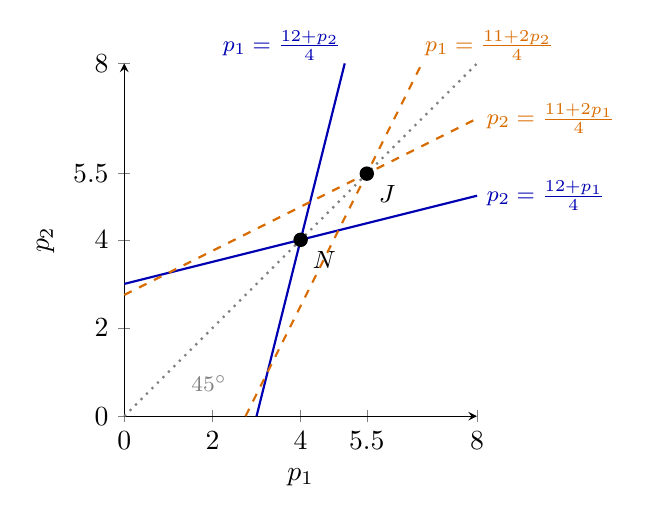
\begin{tikzpicture}
\begin{axis}[
  width=0.5\linewidth, height=0.5\linewidth,
  xmin=0, xmax=8, ymin=0, ymax=8,
  xlabel={$p_1$}, ylabel={$p_2$},
  xtick={0,2,4,5.5,8}, ytick={0,2,4,5.5,8},
  axis lines=left, every axis plot/.append style={thick},
  clip=false]
  \addplot[domain=0:8, samples=2, dotted, gray] {x};
  \addplot[blue!70!black, domain=0:8, samples=2, variable=t] ({(12 + t)/4}, {t});
  \addplot[blue!70!black, domain=0:8, samples=2] {(12 + x)/4};
  \addplot[orange!85!black, dashed, domain=0:8, samples=2, variable=t] ({(11 + 2*t)/4}, {t});
  \addplot[orange!85!black, dashed, domain=0:8, samples=2] {(11 + 2*x)/4};
  \addplot[only marks, mark=*, mark size=2.2pt, black] coordinates {(4,4) (5.5,5.5)};
  \node[anchor=north west, font=\small] at (axis cs:4.05,3.95) {$N$};
  \node[anchor=north west, font=\small] at (axis cs:5.55,5.45) {$J$};
  \node[blue!70!black, anchor=south east, font=\footnotesize, inner sep=1pt] at (axis cs:5.0,8.0) {$p_1 = \frac{12 + p_2}{4}$};
  \node[orange!85!black, anchor=south west, font=\footnotesize, inner sep=1pt] at (axis cs:6.75,8.0) {$p_1 = \frac{11 + 2p_2}{4}$};
  \node[blue!70!black, anchor=west, font=\footnotesize] at (axis cs:8.0,5.0) {$p_2 = \frac{12 + p_1}{4}$};
  \node[orange!85!black, anchor=west, font=\footnotesize] at (axis cs:8.0,6.75) {$p_2 = \frac{11 + 2p_1}{4}$};
  \node[gray, anchor=north west, font=\footnotesize] at (axis cs:1.3,1.15) {$45^\circ$};
\end{axis}
\end{tikzpicture}
\caption{Linear duopoly of \cref{ex:04-linear-duopoly} with $a = 10$, $b = 2$, $d = 1$ and $c = 1$. Solid lines are
the best responses of separate owners, which cross at $N = (4, 4)$. Dashed lines are the first-order loci of a
single owner of both products, each giving the optimal price of one product for a fixed price of the other. They
cross at $J = (5.5, 5.5)$. The dashed loci are not best responses of independent firms. Their slope equals the
diversion ratio $D = \frac{1}{2}$, twice the slope of the separate best responses, because the joint owner
recaptures half of the sales that each product loses.}
\label{fig:04-br-merger}
\end{figure}

\subsection{Worked example: logit demand}\label{sec:04-bertrand-logit}

The logit model gives closed forms for every object in \cref{sec:04-bertrand-matrix}. \Cref{ch:discrete,ch:logit}
derive it from random utility. Here we take the market shares as given. Let market size be one, so quantities
equal shares. Mean utility is $\delta_j = x_j\beta - \alpha p_j + \xi_j$, with observed characteristics $x_j$,
unobserved quality $\xi_j$ and price coefficient $\alpha > 0$. With the mean utility of the outside good
normalized to zero, shares are
\begin{equation*}
s_j(p) = \frac{e^{\delta_j}}{\Phi},
\qquad
s_0(p) = \frac{1}{\Phi},
\qquad
\Phi = 1 + \sum_{k = 1}^{J}e^{\delta_k}.
\end{equation*}
We call $\Phi$ the \emph{logit denominator}.

\casehead{Derivatives}
Changing $p_j$ affects only $e^{\delta_j}$, with $\frac{\partial e^{\delta_j}}{\partial p_j} = -\alpha e^{\delta_j}$,
so also $\frac{\partial\Phi}{\partial p_j} = -\alpha e^{\delta_j}$. The quotient rule gives the own derivative
\begin{align*}
\frac{\partial s_j}{\partial p_j}
&= \frac{(-\alpha e^{\delta_j})\,\Phi - e^{\delta_j}\,(-\alpha e^{\delta_j})}{\Phi^2} \\
&= -\alpha\frac{e^{\delta_j}}{\Phi}\Big(1 - \frac{e^{\delta_j}}{\Phi}\Big)
= -\alpha s_j(1 - s_j).
\end{align*}
For $k \ne j$ the numerator $e^{\delta_k}$ does not depend on $p_j$, so
$\frac{\partial s_k}{\partial p_j} = -\frac{e^{\delta_k}(-\alpha e^{\delta_j})}{\Phi^2} = \alpha s_js_k$. The same
step applies to $s_0 = \frac{1}{\Phi}$. Collecting,
\begin{equation}\label{eq:04-logit-derivs}
\frac{\partial s_j}{\partial p_j} = -\alpha s_j(1 - s_j),
\qquad
\frac{\partial s_k}{\partial p_j} = \alpha s_js_k \quad (k \ne j,\ k \ge 1),
\qquad
\frac{\partial s_0}{\partial p_j} = \alpha s_0s_j.
\end{equation}
These derivatives sum to zero over $k = 0, \dots, J$, as they must. Since $\frac{\partial s_0}{\partial p_j} > 0$,
\cref{prop:04-markup-positive} applies at every price vector. The own and cross elasticities are
\begin{equation*}
\varepsilon_j = \alpha p_j(1 - s_j),
\qquad
\varepsilon_{kj} = \frac{\partial s_k}{\partial p_j}\frac{p_j}{s_k} = \alpha p_js_j \quad \text{for every } k \ne j.
\end{equation*}
A change in $p_j$ moves every other product's share by the same percentage. This is the \emph{independence of
irrelevant alternatives} (IIA), whose consequences \cref{ch:logit} discusses.

\begin{proposition}[Logit markups]\label{prop:04-logit-markup}
Under logit demand with constant marginal costs, every solution of the first-order conditions
\eqref{eq:04-foc-scalar} gives all products of firm $f$ the same markup,
\begin{equation*}
p_j - mc_j = m_f = \frac{1}{\alpha(1 - S_f)}
\quad \text{for all } j \in \mathcal{J}_f,
\qquad
S_f = \sum_{k \in \mathcal{J}_f}s_k.
\end{equation*}
A single-product firm sets $p_j - mc_j = \frac{1}{\alpha(1 - s_j)}$.
\end{proposition}

\begin{proof}
Write the first-order condition for $j \in \mathcal{J}_f$ in shares, $s_j + \sum_{k \in \mathcal{J}_f}m_k\frac{\partial s_k}{\partial p_j} = 0$,
and substitute \eqref{eq:04-logit-derivs}:
\begin{equation*}
s_j - \alpha s_j(1 - s_j)m_j + \sum_{k \in \mathcal{J}_f\setminus\{j\}}\alpha s_js_km_k = 0.
\end{equation*}
Split the second term as $-\alpha s_jm_j + \alpha s_js_jm_j$ and merge $\alpha s_js_jm_j$ into the sum:
\begin{equation*}
s_j - \alpha s_jm_j + \alpha s_j\sum_{k \in \mathcal{J}_f}s_km_k = 0.
\end{equation*}
Divide by $\alpha s_j > 0$:
\begin{equation*}
m_j = \frac{1}{\alpha} + \sum_{k \in \mathcal{J}_f}s_km_k.
\end{equation*}
The right side is the same for every $j \in \mathcal{J}_f$, so all of the firm's products share one markup $m_f$.
Substituting $m_k = m_f$ gives $m_f = \frac{1}{\alpha} + S_fm_f$. Since $S_f \le 1 - s_0 < 1$, we can solve:
$m_f = \frac{1}{\alpha(1 - S_f)}$. A single-product firm has $S_f = s_j$.
\end{proof}

The proposition characterizes markups without giving them in closed form, because $S_f$ depends on prices. It
still has several sharp implications. Markups are bounded below by $\frac{1}{\alpha}$, whatever the number of
competitors. They depend on the firm only through its combined share. Product quality and cost affect markups
only by changing shares. Within a firm, dollar markups are equal, so a firm's high-cost products carry lower
percentage margins, $\frac{m_f}{p_j} = \frac{1}{\alpha p_j(1 - S_f)}$. Finally, a firm with a large combined share
sets high markups on all its products, including those with tiny shares.

As an illustration, suppose one firm owns products 1 and 2 with shares $s_1$ and $s_2$. It sets the markup
$\frac{1}{\alpha(1 - s_1 - s_2)}$ on both. If the products had separate owners, their markups would be
$\frac{1}{\alpha(1 - s_1)}$ and $\frac{1}{\alpha(1 - s_2)}$. Joint ownership raises the markup of the smaller
product by more. Under logit, the diversion ratio from product $k$ to product $j$ is $\frac{s_j}{1 - s_k}$
(\cref{sec:04-diversion-systems}). Diversion from the small product to the large one is therefore the larger of the
two, so joint ownership recaptures a larger fraction of the small product's lost sales.

\casehead{The best response in closed form}
For a single-product firm the first-order condition $\alpha m_j(1 - s_j) = 1$ is implicit, because $s_j$ depends
on $p_j$. It can nevertheless be solved explicitly. Define the mean utility of product $j$ at marginal-cost
pricing and the logit denominator without product $j$,
\begin{equation*}
v_j = x_j\beta + \xi_j - \alpha\,mc_j,
\qquad
\Phi_{-j} = 1 + \sum_{l \ne j}e^{\delta_l}.
\end{equation*}
Then $\delta_j = v_j - \alpha m_j$, and $\Phi_{-j}$ depends only on rivals' prices. The share and its complement
are
\begin{equation*}
s_j = \frac{e^{\delta_j}}{\Phi_{-j} + e^{\delta_j}},
\qquad
1 - s_j = \frac{\Phi_{-j}}{\Phi_{-j} + e^{\delta_j}}.
\end{equation*}
Substitute the complement into the first-order condition and multiply by $\Phi_{-j} + e^{\delta_j}$:
\begin{align*}
\alpha m_j\Phi_{-j} &= \Phi_{-j} + e^{\delta_j} \\
(\alpha m_j - 1)\Phi_{-j} &= e^{v_j - \alpha m_j}.
\end{align*}
Multiply both sides by $\frac{e^{\alpha m_j - 1}}{\Phi_{-j}}$:
\begin{equation*}
(\alpha m_j - 1)\,e^{\alpha m_j - 1} = \frac{e^{v_j - 1}}{\Phi_{-j}}.
\end{equation*}
The \emph{Lambert W function} $W(z)$ solves $W(z)e^{W(z)} = z$ \citep{CorlessEtAl1996}. For $z > 0$ the equation
$ye^y = z$ has exactly one real root, which is positive. Indeed $ye^y \le 0$ for $y \le 0$, while $ye^y$ rises
strictly from 0 to infinity on $y > 0$. Setting $y = \alpha m_j - 1$ gives the best response
\begin{equation}\label{eq:04-logit-br}
BR_j(p_{-j}) = mc_j + \frac{1}{\alpha}\Big[1 + W\Big(\frac{e^{v_j - 1}}{\Phi_{-j}}\Big)\Big].
\end{equation}
The formula shows three properties at a glance. The best-response markup exceeds $\frac{1}{\alpha}$ because
$W(z) > 0$. It rises with the product's quality net of cost, $v_j$. And it rises with every rival price, because
a higher $p_l$ lowers $\Phi_{-j}$ and $W$ is increasing. Logit prices are strategic complements.

The stationary point in \eqref{eq:04-logit-br} is the global maximizer of $\pi_j = m_js_j$. The derivative of
profit factors as
\begin{equation*}
\frac{\partial\pi_j}{\partial p_j} = s_j + m_j\frac{\partial s_j}{\partial p_j} = s_j\,g(p_j),
\qquad
g(p_j) = 1 - \alpha(p_j - mc_j)\big(1 - s_j(p_j)\big).
\end{equation*}
If $p_j \le mc_j$, then $g(p_j) \ge 1$ and profit is increasing. If $p_j > mc_j$, both $\alpha(p_j - mc_j)$ and
$1 - s_j(p_j)$ are positive and strictly increasing in $p_j$, so $g$ is strictly decreasing. As
$p_j \to \infty$, $g(p_j) \to -\infty$. Hence $g$ crosses zero exactly once, from above. Profit rises before the
crossing and falls after it, so the crossing is the unique global maximizer.

The multi-product analogue follows the same steps. By \cref{prop:04-logit-markup}, a stationary point of firm
$f$'s problem has a common markup $m_f$, so $e^{\delta_k} = e^{v_k - \alpha m_f}$ for $k \in \mathcal{J}_f$. Let
$E_f = \sum_{k \in \mathcal{J}_f}e^{v_k}$ and $\Phi_{-f} = 1 + \sum_{l \notin \mathcal{J}_f}e^{\delta_l}$. The
firm's combined share is
\begin{equation*}
S_f = \frac{E_fe^{-\alpha m_f}}{\Phi_{-f} + E_fe^{-\alpha m_f}}.
\end{equation*}
Repeating the algebra above with $E_f$ in place of $e^{v_j}$ and $S_f$ in place of $s_j$ gives
\begin{equation}\label{eq:04-logit-br-multi}
m_f^{BR}(p_{-\mathcal{J}_f}) = \frac{1}{\alpha}\Big[1 + W\Big(\frac{E_fe^{-1}}{\Phi_{-f}}\Big)\Big],
\qquad
p_k = mc_k + m_f^{BR} \ \text{ for } k \in \mathcal{J}_f.
\end{equation}
Showing that this stationary point is the firm's global optimum takes one more step. The firm's problem reduces to
the choice of a common markup, and the single-crossing argument then applies to $S_f$ in place of $s_j$. Steps 1
and 2 of the proof of \cref{thm:04-logit-unique} give the details, and \cref{sec:04-exercises} asks for the
algebra behind \eqref{eq:04-logit-br-multi}.

\subsection{A numerical illustration: 25 logit products}\label{sec:04-bertrand-logit25}

We now compute equilibria in a simulated market. The market reappears in \cref{sec:04-existence}, where we check
uniqueness, and as a worked problem in \cref{app:problems}.

\begin{example}[A 25-product logit market]\label{ex:04-logit25}
There are $J = 25$ products and market size one. Each product has three observed characteristics: a constant, a
continuous characteristic and a binary one, $x_j = (1, x_{j2}, x_{j3})$. It also has unobserved quality $\xi_j$ and
a cost shock $\omega_j$. Demand is logit with $\beta = (0.1, 0.25, 0.1)$ and $\alpha = 2$. Marginal cost is
$mc_j = x_j\gamma + \omega_j$ with $\gamma = (0.2, 0.25, 0.3)$, and it ranges from 0.164 to 1.236. All primitives
are common knowledge, and firms set prices simultaneously. We compare two ownership structures.
\begin{itemize}
  \item[(S)] Every product has its own owner, so $\Omega = I_{25}$.
  \item[(M)] Five owners, labeled 0 to 4, hold 3, 3, 6, 6 and 7 products.
\end{itemize}
Products are numbered 0 to 24 and owners 0 to 4, as in the data set of \cref{app:problems}. Here the label 0 names
an inside product, and $s_0$ still denotes the share of the outside good.
In (S) the first-order conditions are $s_j + (p_j - mc_j)\frac{\partial s_j}{\partial p_j} = 0$ for all $j$. In
(M) they are $s + (\Omega \odot \Delta^{s\top})(p - mc) = 0$ with the owners' $\Omega$. A Nash equilibrium is a
price vector at which no owner can raise its profit by changing its own prices, which is a fixed point of the
best-response map.
\end{example}

\begin{remark}[Computing the equilibrium]\label{rem:04-logit25-algorithm}
We compute each equilibrium by best-response iteration.
\begin{enumerate}
  \item Start from $p^{(0)} = mc + \frac{1}{\alpha}$, the lower bound on logit markups.
  \item Given $p^{(n)}$, compute for every owner $f$ the quantities $E_f$ and $\Phi_{-f}(p^{(n)})$, the markup
  $m_f$ from \eqref{eq:04-logit-br-multi}, and set $p^{(n+1)}_k = mc_k + m_f$ for $k \in \mathcal{J}_f$. In (S)
  every owner has one product and the step is \eqref{eq:04-logit-br}.
  \item Stop when $\|p^{(n+1)} - p^{(n)}\|_\infty < 10^{-12}$. Otherwise return to step 2.
  \item Check that the first-order residuals $s + (\Omega \odot \Delta^{s\top})(p - mc)$ vanish and that each
  owner's markup equals $\frac{1}{\alpha(1 - S_f)}$.
\end{enumerate}
The iteration converges in 10 steps in (S) and 15 steps in (M). As a cross-check we also iterate on the markup
equation, $p \leftarrow mc - (\Omega \odot \Delta^s(p)^\top)^{-1}s(p)$, which converges in 14 and 30 steps to the
same prices (largest difference $1.4 \times 10^{-13}$). The largest first-order residual is below
$2 \times 10^{-14}$. Markup iteration is simple and fast here, but it is not guaranteed to converge in general
(\cref{sec:04-counterfactuals}).
\end{remark}

\Cref{tab:04-logit25} reports the results by owner, and \cref{fig:04-logit25-markups} shows every product's
markup. In (S) each product is priced by a separate firm, and the owner rows aggregate those products for
comparison with (M). Consumer surplus is measured by $\frac{1}{\alpha}\ln\Phi$, the logit expected maximum utility
in money units (\cref{ch:logit}). We measure it relative to a market in which only the outside good is available,
where $\Phi = 1$. Its level is then the surplus that consumers get from the inside goods, so percentage changes are
meaningful.

\begin{table}[htbp]
\centering
\caption{Bertrand-Nash equilibrium in the 25-product logit market}
\label{tab:04-logit25}
\footnotesize
\begin{tabular}{@{}lccccccc@{}}
\toprule
 & & \multicolumn{2}{c}{Combined share $S_f$ (\%)} & \multicolumn{2}{c}{Markup} & \multicolumn{2}{c}{Profit $\times 100$} \\
\cmidrule(lr){3-4}\cmidrule(lr){5-6}\cmidrule(l){7-8}
Owner & Products & (S) & (M) & (S) & (M) & (S) & (M) \\
\midrule
\multicolumn{8}{@{}l}{\textit{Panel A. Owners}} \\
0 & 3 & 18.32 & 18.87 & 0.552 & 0.616 & 10.112 & 11.632 \\
1 & 3 & 4.12 & 4.67 & 0.508 & 0.524 & 2.094 & 2.449 \\
2 & 6 & 13.27 & 13.68 & 0.516 & 0.579 & 6.841 & 7.925 \\
3 & 6 & 22.62 & 21.40 & 0.529 & 0.636 & 11.971 & 13.616 \\
4 & 7 & 28.00 & 25.36 & 0.541 & 0.670 & 15.145 & 16.989 \\
\midrule
\multicolumn{8}{@{}l}{\textit{Panel B. Market}} \\
\multicolumn{4}{@{}l}{Outside share $s_0$} & 0.1367 & 0.1601 & & \\
\multicolumn{4}{@{}l}{Logit denominator $\Phi^* = \frac{1}{s_0}$} & 7.314 & 6.246 & & \\
\multicolumn{4}{@{}l}{Consumer surplus $\frac{1}{\alpha}\ln\Phi^*$} & 0.9949 & 0.9159 & & \\
\multicolumn{4}{@{}l}{Total profit} & 0.4616 & 0.5261 & & \\
\multicolumn{4}{@{}l}{Total surplus (consumer surplus plus profit)} & 1.4565 & 1.4421 & & \\
\multicolumn{4}{@{}l}{Share-weighted mean price} & 1.2599 & 1.3553 & & \\
\bottomrule
\end{tabular}

\vspace{3pt}
\begin{minipage}{0.97\textwidth}
\footnotesize Notes: (S) single-product firms, (M) five multi-product owners. In column (S) the owner rows add
up shares and profits of products that are priced independently, and the markup is the share-weighted mean
over the owner's products. In column (M) every product of an owner carries the same markup
$\frac{1}{\alpha(1 - S_f)}$. Market size is one, so profits and consumer surplus are per consumer. Computed with
\texttt{figures/ch04/src/logit25.py}.
\end{minipage}
\end{table}

\begin{figure}[htbp]
\centering
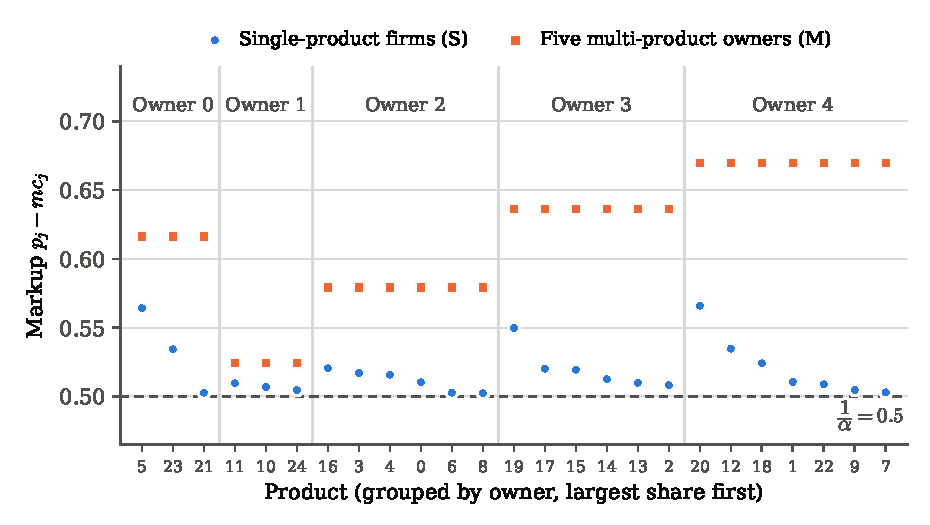
\includegraphics[width=\linewidth]{figures/ch04/logit25_markups.pdf}
\caption{Equilibrium markups $p_j - mc_j$ in the 25-product logit market. Circles show single-product firms (S),
squares show the five multi-product owners (M). Products are grouped by owner and sorted by share. Under (S)
markups are close to the floor $\frac{1}{\alpha} = 0.5$ and rise with the product's own share. Under (M) all
products of an owner share the markup $\frac{1}{\alpha(1 - S_f)}$.}
\label{fig:04-logit25-markups}
\end{figure}

The results illustrate the theory of this section in five ways.

First, single-product markups lie between 0.502 and 0.566, close to the floor $\frac{1}{\alpha} = 0.5$. Each
product has a small share, so $\frac{1}{\alpha(1 - s_j)}$ barely exceeds $\frac{1}{\alpha}$. The largest markups
belong to the products with the largest shares, products 20 and 5, whose shares are 11.7 and 11.4 percent.

Second, multi-product ownership raises every owner's markup to $\frac{1}{\alpha(1 - S_f)}$. The common markups range
from 0.524 for owner 1, whose products have a combined share near 5 percent, to 0.670 for owner 4, whose
combined share is about 25 percent. A product with a share of half a percent, such as product 7, carries the same
markup as owner 4's largest product. Its price rises the most, by 0.167.

Third, every price rises, by amounts from 0.015 (product 11) to 0.167 (product 7). Two forces combine. Each owner
internalizes cannibalization among its own products, and prices are strategic complements, so each owner also
responds to the higher prices of the others. To isolate the second force, we recomputed the equilibrium with only
owner 4 consolidating its seven products and all other products independent. Owner 4's prices rise by 0.089 to
0.152, and rivals' prices rise by 0.0001 to 0.0040 through strategic complementarity. In that exercise rivals'
combined profit rises from 0.3102 to 0.3296, while owner 4's profit rises only from 0.1515 to 0.1553. The
non-consolidating firms gain more than the firm that consolidates.

Fourth, shares move away from the owners that raise prices most. The two largest owners lose share, owner 4
from 28.00 to 25.36 percent and owner 3 from 22.62 to 21.40 percent. The three smaller owners gain. Fifteen of the
25 products lose share, and the outside share rises from 0.137 to 0.160.

Fifth, total profit rises by about 14 percent, from 0.4616 to 0.5261. Consumer surplus falls by 0.079, or 7.9
percent, and total surplus falls from 1.4565 to 1.4421. In equilibrium the logit denominator equals
$\frac{1}{s_0}$, which falls from 7.314 to 6.246. \Cref{sec:04-existence} shows that this aggregate pins down
the whole equilibrium. It uses this to prove that the logit equilibrium is unique for any ownership structure
\citep{KonovalovSandor2010,NockeSchutz2018}, and \cref{ex:04-logit25-unique} confirms numerically that the two
equilibria in \cref{tab:04-logit25} are the only ones.

\section{Diversion ratios}\label{sec:04-diversion}

The pricing rule of \cref{sec:04-bertrand} depends on own-price and cross-price derivatives of demand.
Elasticities summarize these derivatives product by product. Diversion ratios summarize them pair by pair:
they record where the customers of a product go when its price rises. This makes them the natural language
for three questions that recur in this book. Which products compete most closely? How does a multi-product
firm price products that cannibalize one another? Which mergers create an incentive to raise prices? This
section defines diversion ratios, rewrites the first-order condition in terms of them, computes them in the
standard demand systems, and lists what they cannot tell us.

\subsection{Definitions and basic properties}\label{sec:04-diversion-def}

We keep the environment of \cref{ass:04-bertrand}. To lighten the notation we write
\[
  \partial_k q_j \equiv \frac{\partial q_j(p)}{\partial p_k}
\]
for the derivative of the demand for product $j$ with respect to the price of product $k$. In this notation
the $(j,k)$ element of $\Delta$ is $\partial_k q_j$. The \emph{cross-price derivative} $\partial_j q_k$ is the
change in the sales of product $k$ when the price of product $j$ rises by one dollar. The \emph{cross-price
elasticity} is $\varepsilon_{kj} = \frac{\partial q_k}{\partial p_j}\frac{p_j}{q_k}$, and the own-price
elasticity is the positive number $\varepsilon_j = -\frac{\partial q_j}{\partial p_j}\frac{p_j}{q_j}$.

\begin{definition}[Diversion ratio]\label{def:04-diversion}
For two inside products $j \neq k$, the \emph{diversion ratio} from $j$ to $k$ is
\begin{equation}\label{eq:04-diversion-def}
  D_{jk} = -\frac{\partial_j q_k}{\partial_j q_j}.
\end{equation}
The \emph{diversion ratio to the outside good} is $D_{j0} = 1 - \sum_{k \ge 1, k \neq j} D_{jk}$, and the
\emph{aggregate diversion ratio} of product $j$ is $\sum_{k \ge 1, k \neq j} D_{jk} = 1 - D_{j0}$.
\end{definition}

The numerator and the denominator of \eqref{eq:04-diversion-def} refer to the same experiment, a small
increase $\dd p_j$ in the price of product $j$ with all other prices fixed. Product $j$ loses
$-\partial_j q_j \, \dd p_j$ units of sales. Product $k$ gains $\partial_j q_k\, \dd p_j$ units. The diversion
ratio is the fraction of the lost units that product $k$ recaptures. Read in reverse, it is the number of
units of $k$ that are lost when $p_j$ falls by enough to sell one more unit of $j$. The first index always
names the product whose price changes. In general $D_{jk} \neq D_{kj}$.

\begin{proposition}[Adding up]\label{prop:04-diversion-adding}
Suppose that each of $M$ consumers buys exactly one unit of one of the options $0, 1, \dots, J$, so that
$\sum_{k=0}^J q_k(p) = M$ for every price vector $p$. Then for every inside product $j$,
\begin{equation}\label{eq:04-diversion-adding}
  \sum_{k \ge 1,\, k \neq j} D_{jk} + D_{j0} = 1, \qquad\text{with}\qquad D_{j0} = -\frac{\partial_j q_0}{\partial_j q_j}.
\end{equation}
If all products, including the outside good, are gross substitutes, every diversion ratio lies in $[0,1]$.
\end{proposition}

\begin{proof}
Differentiate the identity $\sum_{k=0}^J q_k(p) = M$ with respect to $p_j$. The right side does not depend
on prices, so
\[
  \partial_j q_j + \sum_{k \ge 1,\, k \neq j}\partial_j q_k + \partial_j q_0 = 0.
\]
Divide by $-\partial_j q_j > 0$:
\[
  -1 + \sum_{k \ge 1,\, k\neq j}\Bigl(-\frac{\partial_j q_k}{\partial_j q_j}\Bigr) + \Bigl(-\frac{\partial_j q_0}{\partial_j q_j}\Bigr) = 0.
\]
The terms in parentheses are $D_{jk}$ and $-\frac{\partial_j q_0}{\partial_j q_j}$, which gives
\eqref{eq:04-diversion-adding}. Under gross substitutes each term is nonnegative. Nonnegative numbers
that sum to one each lie in $[0,1]$.
\end{proof}

In unit-demand models the residual $D_{j0}$ in \cref{def:04-diversion} is the share of lost customers who
stop buying any inside product. A large $D_{j0}$ then means that the products in the group constrain one
another little. This is why the aggregate diversion ratio appears in market definition (\cref{ch:mergers}).
Some demand systems have no explicit outside option, such as the linear and CES systems of
\cref{sec:04-repcons}. Their quantities need not add up in units, so $D_{j0}$ is only the residual of
\cref{def:04-diversion}. It changes when we rescale the units of one product, and in CES it can be negative.
Reading it as the fraction of $j$'s lost units that the group does not recapture requires units that are
comparable across products.

Diversion ratios and elasticities carry the same information, arranged differently. Write each derivative
in terms of an elasticity:
\[
  \partial_j q_k = \varepsilon_{kj}\frac{q_k}{p_j}, \qquad \partial_j q_j = -\varepsilon_j\frac{q_j}{p_j}.
\]
Substituting into \eqref{eq:04-diversion-def}, the price $p_j$ cancels and
\begin{equation}\label{eq:04-diversion-elast}
  D_{jk} = \frac{\varepsilon_{kj}}{\varepsilon_j}\,\frac{q_k}{q_j}.
\end{equation}
A large cross elasticity does not imply a large diversion ratio. If product $k$ is small, a large percentage
gain for $k$ is a small number of units. Conversely, a large product can capture many of $j$'s customers even
when its own percentage gain is modest.

\casehead{Measurement}
Diversion ratios can be computed from an estimated demand system (\cref{ch:logit,ch:blp}). They can also be
measured more directly, which is a large part of their appeal to antitrust agencies. Firms often track whom
they lose business to, and surveys can ask buyers of $j$ what they would have bought instead
\citep[p.~16]{FarrellShapiro2010}. Natural experiments that remove a product, such as stock-outs, recalls and
exits, reveal where its customers go. In bidding markets the diversion ratio from $j$ to $k$ can be read as
the probability that $k$ is the runner-up when $j$ wins \citep[p.~16]{FarrellShapiro2010}.

These sources do not all measure the same object. \citet{ConlonMortimer2021} view a diversion ratio as a
treatment effect and stress that the size of the price change matters. Second-choice data describe what
happens when product $j$ disappears, which is a price increase to infinity. The pricing incentive in
\eqref{eq:04-foc-diversion} below involves a marginal price change. A mixture of logits shows the
difference. Let consumer types $i$ have distribution $F$, price coefficient $\alpha_i$ and logit choice
probabilities $s_{ij}$, so that $s_j = \int s_{ij}\,\dd F(i)$. Using \eqref{eq:04-logit-derivs} type by type,
the marginal diversion ratio is
\begin{equation}\label{eq:04-diversion-marginal}
  D_{jk} = \frac{\int \alpha_i s_{ij}s_{ik}\,\dd F(i)}{\int \alpha_i s_{ij}(1 - s_{ij})\,\dd F(i)}
         = \int \varpi_i\,\frac{s_{ik}}{1 - s_{ij}}\,\dd F(i),
  \qquad \varpi_i = \frac{\alpha_i s_{ij}(1 - s_{ij})}{\int \alpha_{i'} s_{i'j}(1 - s_{i'j})\,\dd F(i')}.
\end{equation}
When $j$ is removed, a type-$i$ buyer of $j$ moves to $k$ with probability
$\frac{e^{\delta_{ik}}}{\sum_{l \neq j}e^{\delta_{il}}} = \frac{s_{ik}}{1 - s_{ij}}$, where $\delta_{il}$ is the
mean utility of option $l$ for type $i$. Averaging over the buyers of $j$ gives the second-choice diversion
ratio
\begin{equation}\label{eq:04-diversion-secondchoice}
  D^{\mathrm{SC}}_{jk} = \int \tilde\varpi_i\,\frac{s_{ik}}{1 - s_{ij}}\,\dd F(i), \qquad \tilde\varpi_i = \frac{s_{ij}}{s_j}.
\end{equation}
Both are weighted averages of the same type-level ratios $\frac{s_{ik}}{1 - s_{ij}}$. The marginal ratio
weights types by $\alpha_i s_{ij}(1 - s_{ij})$, which is large for price-sensitive consumers near the margin
of buying $j$. The second-choice ratio weights all current buyers of $j$ equally. With one type both reduce
to the logit formula $\frac{s_k}{1 - s_j}$. With heterogeneous consumers they differ, and a survey answer
needs a model before it can be plugged into a pricing formula.

\subsection{The first-order condition in diversion form}\label{sec:04-diversion-foc}

The multi-product first-order condition \eqref{eq:04-foc-scalar} can be rewritten so that diversion ratios
appear explicitly. For firm $f$ and a product $j \in \mathcal{J}_f$ the condition reads
\[
  q_j + \sum_{k \in \mathcal{J}_f}(p_k - mc_k)\,\partial_j q_k = 0.
\]
We first split off the term $k = j$:
\[
  q_j + (p_j - mc_j)\,\partial_j q_j + \sum_{k \in \mathcal{J}_f\setminus\{j\}}(p_k - mc_k)\,\partial_j q_k = 0.
\]
Next we divide by $\partial_j q_j < 0$:
\[
  \frac{q_j}{\partial_j q_j} + (p_j - mc_j) + \sum_{k \in \mathcal{J}_f\setminus\{j\}}(p_k - mc_k)\frac{\partial_j q_k}{\partial_j q_j} = 0.
\]
Solving for $p_j$ gives
\[
  p_j = mc_j - \frac{q_j}{\partial_j q_j} - \sum_{k \in \mathcal{J}_f\setminus\{j\}}(p_k - mc_k)\frac{\partial_j q_k}{\partial_j q_j}.
\]
Finally, $-\frac{\partial_j q_k}{\partial_j q_j} = D_{jk}$ by \eqref{eq:04-diversion-def}, so
\begin{equation}\label{eq:04-foc-diversion}
  p_j = mc_j + \frac{q_j}{-\partial_j q_j} + \sum_{k \in \mathcal{J}_f\setminus\{j\}} D_{jk}\,(p_k - mc_k).
\end{equation}

The price of product $j$ has three parts. The first is marginal cost. The second is the markup a
single-product firm would charge, the reciprocal of the absolute semi-elasticity of $q_j$. The third is the
\emph{value of diverted sales}: each unit of $j$'s lost sales that moves to a sibling product $k$ earns the
firm the margin $p_k - mc_k$. This term is an opportunity cost of selling $j$, because every extra unit of $j$
cannibalizes $D_{jk}$ units of $k$. Define the \emph{effective marginal cost}
$\widetilde{mc}_j = mc_j + \sum_{k \in \mathcal{J}_f\setminus\{j\}}D_{jk}(p_k - mc_k)$. Then
\eqref{eq:04-foc-diversion} becomes $p_j - \widetilde{mc}_j = \frac{q_j}{-\partial_j q_j}$, and dividing by
$p_j$,
\[
  \frac{p_j - \widetilde{mc}_j}{p_j} = \frac{1}{\varepsilon_j}.
\]
A multi-product firm prices each product by the inverse elasticity rule, applied to an effective marginal cost
that includes the value of diverted sales. The 2010 US Horizontal Merger Guidelines use this phrase for the units
diverted to a product multiplied by that product's margin \citep[Section 6.1, p.~21]{USDOJFTC2010}. The term in
\eqref{eq:04-foc-diversion} is this value per unit of lost sales of $j$.

Stacking \eqref{eq:04-foc-diversion} over products gives a compact matrix version. Let
$m^{\mathrm{s}}_j = \frac{q_j}{-\partial_j q_j}$ be the single-product markup, with vector $m^{\mathrm{s}}$, let
$m = p - mc$, and let $\mathcal{D}$ be the $J \times J$ \emph{diversion matrix} with $\mathcal{D}_{jk} = D_{jk}$ for
$k \neq j$ and zeros on the diagonal. Since $\Omega_{jk} = 1$ exactly when $j$ and $k$ have the same owner,
\begin{equation}\label{eq:04-markup-diversion}
  m = m^{\mathrm{s}} + (\Omega \odot \mathcal{D})\,m, \qquad\text{so}\qquad m = (I - \Omega \odot \mathcal{D})^{-1} m^{\mathrm{s}}.
\end{equation}
This is the stacked first-order condition \eqref{eq:04-foc-matrix} with row $j$ divided by $-\partial_j q_j$, and its
solution coincides with the markup equation \eqref{eq:04-markup}.

\begin{remark}\label{rem:04-diversion-positive}
Equation \eqref{eq:04-markup-diversion} gives a short proof that markups are positive. Suppose that every
outside diversion ratio is positive, $D_{j0} > 0$. Row $j$ of $\Omega\odot\mathcal{D}$ has nonnegative
entries that sum to at most $\sum_{k \neq j}D_{jk} = 1 - D_{j0} < 1$. The sup-norm of
$\Omega\odot\mathcal{D}$ is therefore below one, and the Neumann series
$(I - \Omega\odot\mathcal{D})^{-1} = \sum_{n=0}^\infty(\Omega\odot\mathcal{D})^n$ converges to a matrix with
nonnegative entries and diagonal entries of at least one. Hence $m \ge m^{\mathrm{s}} > 0$ element by element. Every product of a
multi-product firm carries at least its single-product markup, in line with \cref{prop:04-markup-positive}.
\end{remark}

Two examples from \cref{sec:04-bertrand} show the formula at work. In the linear duopoly of
\cref{ex:04-linear-duopoly}, $\partial_1 q_1 = -b$ and $\partial_1 q_2 = d$, so $D_{12} = \frac{d}{b} \equiv D$.
For a joint owner, \eqref{eq:04-foc-diversion} reads $m_1 = \frac{q_1}{b} + D\,m_2$. At a symmetric
solution $m(1 - D) = \frac{q}{b}$ with $q = a - (b - d)(c + m)$. Multiplying by $b$ and using
$b(1 - D) = b - d$,
\[
  (b - d)\,m = a - (b - d)c - (b - d)m \quad\Longrightarrow\quad m^J = \frac{a - (b - d)c}{2(b - d)},
\]
the joint-owner markup found in \cref{ex:04-linear-duopoly}. In the multi-product logit model the
derivatives \eqref{eq:04-logit-derivs} give $D_{jk} = \frac{s_k}{1 - s_j}$ and
$m^{\mathrm{s}}_j = \frac{1}{\alpha(1 - s_j)}$. With the common markup $m_f$ of \cref{prop:04-logit-markup},
\eqref{eq:04-foc-diversion} becomes
\[
  m_f = \frac{1}{\alpha(1 - s_j)} + \frac{S_f - s_j}{1 - s_j}\,m_f
  \quad\Longrightarrow\quad m_f\,\frac{1 - S_f}{1 - s_j} = \frac{1}{\alpha(1 - s_j)}
  \quad\Longrightarrow\quad m_f = \frac{1}{\alpha(1 - S_f)},
\]
where $S_f = \sum_{k \in \mathcal{J}_f}s_k$. The firm's combined share enters because the recaptured
fraction $\frac{S_f - s_j}{1 - s_j}$ grows with the shares of the sibling products.

\subsection{Why diversion governs the unilateral effects of mergers}\label{sec:04-diversion-merger}

Equation \eqref{eq:04-foc-diversion} explains why diversion ratios dominate the analysis of
\emph{unilateral effects}. These are the price effects of a merger that arise because the merged firm
internalizes competition between its own products, with the conduct of rivals unchanged. A merger adds the
acquired products to $\mathcal{J}_f\setminus\{j\}$ and so adds terms $D_{jk}(p_k - mc_k)$ to the effective marginal
cost of product $j$. The size of these terms depends on how close the merging products are as substitutes. The
merging firms' shares of a predefined market play no direct role.

Consider two single-product Bertrand firms, $A$ selling product 1 and $B$ selling product 2, with constant
marginal costs. Before the merger, firm $A$'s first-order condition is
$q_1 + (p_1 - mc_1)\,\partial_1 q_1 = 0$. After the merger, one owner maximizes $\pi_1 + \pi_2$. Evaluated at
the pre-merger prices, the derivative of joint profit with respect to $p_1$ is
\[
  \frac{\partial(\pi_1 + \pi_2)}{\partial p_1}
  = \underbrace{q_1 + (p_1 - mc_1)\,\partial_1 q_1}_{=\,0 \text{ before the merger}} + (p_2 - mc_2)\,\partial_1 q_2
  = (p_2 - mc_2)\,\partial_1 q_2 > 0.
\]
The merged firm wants to raise $p_1$. Dividing by $-\partial_1 q_1 > 0$ measures this incentive per unit of
product 1's lost sales. The result, $D_{12}(p_2 - mc_2)$, is the increase in the effective marginal cost of
product 1. \citet[p.~9]{FarrellShapiro2010} interpret it as a ``first-round tax'' that the merged firm's
headquarters would levy on division $A$ to make it internalize the sales it takes from division $B$.

A merger can also lower marginal costs. Let $E_1$ be the proportional reduction in the marginal cost of product
1, so that the merger saves $E_1 mc_1$ per unit. The symbol $E_1$ is unrelated to the logit aggregate $E_f$ of
\cref{sec:04-bertrand-logit}. The \emph{upward pricing pressure} (UPP) on product 1 is
\begin{equation}\label{eq:04-upp}
  \mathit{UPP}_1 = D_{12}(p_2 - mc_2) - E_1\,mc_1,
\end{equation}
evaluated at pre-merger prices and margins. \citet[p.~12, inequality (1)]{FarrellShapiro2010} propose to
presume harm when $\mathit{UPP}_1 > 0$. In the symmetric case, with equal prices $p$, costs $mc$, diversion
ratios $D$ and efficiencies $E$, the condition divides through by $p - mc$ to give
\[
  D > E\,\frac{mc}{p - mc}.
\]
This is their inequality (2), which they state in terms of the relative margin $\frac{p - mc}{p}$. They use $E = 0.1$ as an illustrative default
\citep[p.~10]{FarrellShapiro2010}. With a Lerner index of $\frac{1}{3}$ we have $\frac{mc}{p - mc} = 2$, and the
merger is flagged when $D > 0.2$.

Condition \eqref{eq:04-upp} credits an efficiency to product 1 only. Suppose that the merger also lowers the
marginal cost of product 2 by the fraction $E_2$. Each unit diverted to product 2 then earns the margin
$p_2 - (1 - E_2)mc_2 = (p_2 - mc_2) + E_2\,mc_2$, which is larger even at unchanged prices. At pre-merger prices
the derivative of joint profit with respect to $p_1$, divided by $-\partial_1 q_1$, becomes
\[
  D_{12}\big[(p_2 - mc_2) + E_2\,mc_2\big] - E_1\,mc_1.
\]
In the symmetric case with $E_1 = E_2 = E$ it is positive exactly when $D(p - mc) > (1 - D)E\,mc$, that is, when
$\frac{D}{1 - D} > E\frac{mc}{p - mc}$ \citep[p.~14, inequality (4)]{FarrellShapiro2010}. At equality the
pre-merger prices satisfy both post-merger first-order conditions. The common efficiency $E$ then equals the
compensating marginal-cost reduction of \citet{Werden1996}, which leaves both prices unchanged. Farrell and
Shapiro obtain the general version, their inequality (3), by solving these two markup equations simultaneously.
With the same numbers the condition reads $\frac{D}{1 - D} > 0.2$, so the threshold falls to
$D > \frac{1}{6} \approx 0.167$. Their footnote 35 reports both thresholds, 20 and 16.7 percent. It also notes
that the symmetric condition is equivalent to equation (6) of \citet{Werden1996}. The responses of the two prices
to each other after the merger are a separate feedback. When $p_2$ rises, the margin on diverted sales grows
further and adds to the pricing pressure on product 1 \citep[p.~13]{FarrellShapiro2010}. This feedback changes
the size of the price increase but leaves the threshold unchanged. At the threshold the pre-merger prices already
satisfy both post-merger first-order conditions, so no price moves.

The \emph{gross upward pricing pressure index} (GUPPI) scales the cannibalization term by the price of the product
under study:
\begin{equation}\label{eq:04-guppi}
  \mathit{GUPPI}_1 = \frac{D_{12}(p_2 - mc_2)}{p_1} = D_{12}\,\frac{p_2 - mc_2}{p_2}\,\frac{p_2}{p_1}.
\end{equation}
For example, $D_{12} = 0.2$, a margin of 40 percent on product 2 and equal prices give
\[
  \mathit{GUPPI}_1 = 0.2 \times 0.4 \times 1 = 0.08.
\]
The merger raises the effective marginal cost of product 1 by 8 percent of its price. UPP and GUPPI need
only diversion ratios and margins, and no full demand system. \citet[p.~12, Proposition 1]{FarrellShapiro2010}
show that net upward pricing pressure on both products, with no more than the default efficiencies, implies
that both prices rise. A full merger simulation instead solves the post-merger first-order conditions
$q + (\Omega^{post}\odot\Delta^\top)(p - mc) = 0$ with recovered marginal costs (\cref{sec:04-counterfactuals}).
The derivation with efficiencies, the role of pass-through, the GUPPI thresholds used in practice and
applications are in \cref{ch:mergers}.

\begin{example}[From UPP to price effects in the linear duopoly]\label{ex:04-upp-linear}
The linear duopoly of \cref{ex:04-linear-duopoly} shows how a diversion-based pricing pressure translates into a
price change. Before the merger each markup is $m^N = \frac{a - (b - d)c}{2b - d}$. After it, each markup is
$m^J$, and the ratio is
\[
  \frac{m^J}{m^N} = \frac{2b - d}{2(b - d)} = \frac{2 - D}{2 - 2D}, \qquad D = \frac{d}{b}.
\]
The ratio equals 1.056, 1.167, 1.5 and 2.5 for $D = 0.1$, $0.25$, $0.5$ and $0.75$. In levels,
\[
  m^J - m^N = m^N\Bigl(\frac{2 - D}{2 - 2D} - 1\Bigr) = \frac{D\,m^N}{2(1 - D)}.
\]
Without efficiencies the pre-merger UPP on each product is $D\,m^N$, so the price change is
$\frac{1}{2(1 - D)}$ times the UPP. The factor arises in three rounds. Holding the rival's price fixed, a firm
facing linear demand passes through one half of a cost increase, since its best response
$\frac{a + b(c + t) + d p_k}{2b}$ rises by $\frac{t}{2}$ for a cost increase $t$. If both products bear the
tax $t$ and both prices adjust, the symmetric equilibrium price $\frac{a + b(c + t)}{2b - d}$ rises by
$\frac{t}{2 - D}$. If the tax is then recomputed at the new margins, $t = D(m^N + \Delta p)$. Solving
$\Delta p\,(2 - D) = D(m^N + \Delta p)$ gives $\Delta p = \frac{D\,m^N}{2 - 2D}$, the full effect. The three
rounds follow the iterative procedure of \citet[p.~9]{FarrellShapiro2010}. We impose the internal taxes, let the
oligopoly re-equilibrate, re-calculate the taxes at the new prices and outputs, and repeat these steps until
convergence. Their footnote 24 adds that with strategic complements each round raises prices, so with constant
costs and diversion ratios the taxes rise from round to round. With $a = 10$, $b = 2$,
$d = 1$ and $c = 1$, we have $m^N = 3$, $D = \frac{1}{2}$ and $\mathit{UPP} = 1.5$. The price rises from 4 to
5.5, by exactly the UPP, because $\frac{1}{2(1 - D)} = 1$ when $D = \frac{1}{2}$.
\end{example}

\subsection{Diversion in standard demand systems}\label{sec:04-diversion-systems}

Each demand system used in practice implies a pattern of diversion. Often the pattern is imposed by the
functional form, which is worth knowing before a system is used to evaluate mergers.

\casehead{Logit}
With logit shares, \eqref{eq:04-logit-derivs} gives $\partial_j s_j = -\alpha s_j(1 - s_j)$,
$\partial_j s_k = \alpha s_j s_k$ and $\partial_j s_0 = \alpha s_j s_0$. Hence
\begin{equation}\label{eq:04-diversion-logit}
  D_{jk} = \frac{\alpha s_j s_k}{\alpha s_j(1 - s_j)} = \frac{s_k}{1 - s_j}, \qquad D_{j0} = \frac{s_0}{1 - s_j}.
\end{equation}
Customers who leave $j$ spread over the remaining options in proportion to their shares. A product similar to
$j$ and a product very different from it receive the same diversion if they have the same share. This is the
independence of irrelevant alternatives property (\cref{ch:logit}). It also means that a logit-based UPP adds
no information beyond shares and margins.

\casehead{CES}
Consider the CES system of \cref{sec:04-repcons} with elasticity of substitution $\sigma > 1$. This $\sigma$ is
unrelated to the nesting parameter. Demand is $q_j = \frac{p_j^{-\sigma}}{\sum_k p_k^{1-\sigma}}\,y$, with income $y$
and expenditure shares $s_j = \frac{p_jq_j}{y}$. The quantity diversion ratio is
\begin{equation}\label{eq:04-diversion-ces}
  D_{jk} = \frac{(\sigma - 1)\,p_j\,q_k}{y\,[\sigma - (\sigma - 1)s_j]} = \frac{(\sigma - 1)\,s_k}{\sigma - (\sigma - 1)s_j}\,\frac{p_j}{p_k},
\end{equation}
which \cref{prop:04-ces} derives from the CES elasticities. Diversion is proportional to the quantity $q_k$,
again with no role for similarity.

\casehead{Linear demand}
If $q = a + Ap$ for a vector $a$ and a $J \times J$ matrix $A$, then $\partial_j q_k = A_{kj}$ and
$D_{jk} = -\frac{A_{kj}}{A_{jj}}$. Diversion is constant, and in the symmetric duopoly it equals
$\frac{d}{b}$. A linear system can represent any pattern of diversion at one point, at the cost of $J^2$
price parameters (\cref{sec:04-spaces}).

\casehead{Nested logit}
Group the inside products into nests and let $\sigma^{\mathrm{NL}} \in [0,1)$ be the nesting parameter of
\cref{ch:logit}, written with a superscript in this section to avoid a clash with the CES elasticity. Let
$s_{j\mid g}$ be the share of product $j$ within its nest $g$ and $s_g$ the share of the nest. We use the form
of \citet{Berry1994}, and \cref{ch:logit} derives the share derivatives. With respect to $p_j$ they are
\[
  \partial_j s_j = -\frac{\alpha s_j\bigl[1 - \sigma^{\mathrm{NL}} s_{j\mid g} - (1 - \sigma^{\mathrm{NL}})s_j\bigr]}{1 - \sigma^{\mathrm{NL}}},
  \qquad
  \partial_j s_k = \frac{\alpha s_k\bigl[\sigma^{\mathrm{NL}} s_{j\mid g} + (1 - \sigma^{\mathrm{NL}})s_j\bigr]}{1 - \sigma^{\mathrm{NL}}}
\]
for $k$ in the nest of $j$, and $\partial_j s_k = \alpha s_k s_j$ for $k$ in another nest or $k = 0$. Taking ratios
and using $s_k = s_{k\mid g}s_g$ and $s_j = s_{j\mid g}s_g$,
\begin{equation}\label{eq:04-diversion-nl}
  D_{jk} =
  \begin{cases}
    \displaystyle\frac{s_{k\mid g}\bigl[\sigma^{\mathrm{NL}} + (1 - \sigma^{\mathrm{NL}})s_g\bigr]}{1 - \sigma^{\mathrm{NL}}s_{j\mid g} - (1 - \sigma^{\mathrm{NL}})s_j} & \text{if $k$ is in the nest of $j$,}\\[3ex]
    \displaystyle\frac{(1 - \sigma^{\mathrm{NL}})\,s_k}{1 - \sigma^{\mathrm{NL}}s_{j\mid g} - (1 - \sigma^{\mathrm{NL}})s_j} & \text{otherwise, including $k = 0$.}
  \end{cases}
\end{equation}
At $\sigma^{\mathrm{NL}} = 0$ both lines reduce to \eqref{eq:04-diversion-logit}. As
$\sigma^{\mathrm{NL}}$ approaches one, diversion outside the nest vanishes and the within-nest ratio approaches
$\frac{s_{k\mid g}}{1 - s_{j\mid g}}$. Diversion concentrates within the nest.

\Cref{fig:04-diversion} shows how much this matters. Four inside products sit in two nests, $\{1, 2\}$ and
$\{3, 4\}$. All prices equal 1 and the price coefficient equals 1. For each value of the nesting parameter we
set a common mean utility so that every inside share is 0.15 and the outside share is 0.40. Shares, prices and
margins are therefore identical across the four models. Under logit, the diversion from product 1 is 0.1765 to
each rival and 0.4706 to the outside good. With $\sigma^{\mathrm{NL}} = 0.5$ the diversion to product 2 is
0.4815, against 0.1111 to products 3 and 4 and 0.2963 to the outside good. With $\sigma^{\mathrm{NL}} = 0.7$ the
values are 0.6529, 0.0744, 0.0744 and 0.1983. With $\sigma^{\mathrm{NL}} = 0.9$ they are 0.8692, 0.0280, 0.0280
and 0.0748. Each row sums to one, as \cref{prop:04-diversion-adding} requires. For given margins, the GUPPI of a
merger between products 1 and 2 is 3.7 times larger under the nested logit with $\sigma^{\mathrm{NL}} = 0.7$
than under the logit ($\frac{0.6529}{0.1765} = 3.70$). Shares alone cannot distinguish these markets.

\begin{figure}[htbp]
  \centering
  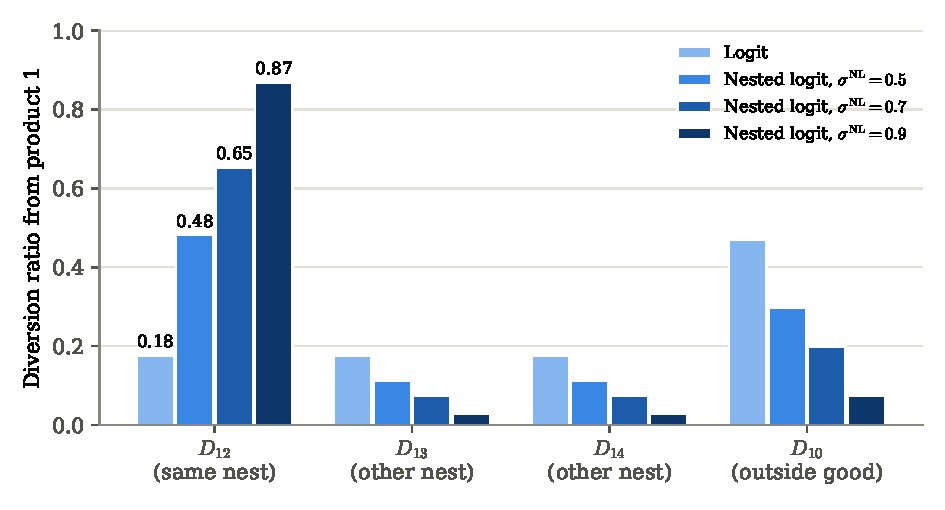
\includegraphics[width=0.95\textwidth]{figures/ch04/diversion_nl.pdf}
  \caption{Diversion ratios from product 1 in four demand models with identical shares. Products 1 and 2 form
  one nest and products 3 and 4 the other. Every inside share is 0.15 and the outside share is 0.40. The logit
  spreads lost sales in proportion to shares. The nested logit sends most of them to the other product in the
  same nest, more so as $\sigma^{\mathrm{NL}}$ rises. Computed with \texttt{figures/ch04/src/diversion\_nl.py}.}
  \label{fig:04-diversion}
\end{figure}

\subsection{What diversion ratios do not tell us}\label{sec:04-diversion-limits}

Diversion ratios are local. They are derivatives evaluated at current prices, and except under linear demand
they change when prices change. A merger moves prices, so diversion at the post-merger prices differs from the
pre-merger value that enters UPP. \Cref{ex:04-upp-linear} shows that even with constant diversion the full
price effect differs from UPP by a factor that depends on $D$.

Diversion ratios give the direction of the pricing incentive. The size of the price change also requires
pass-through, which depends on the curvature of demand (\cref{prop:04-passthrough}, \cref{ch:theory}). For a
single-product firm facing a fixed rival price, pass-through is $\frac{1}{2}$ with linear demand, $1 - s_j$
with logit demand and $\frac{\varepsilon}{\varepsilon - 1} > 1$ with constant-elasticity demand. The same UPP
can therefore produce very different price increases. \citet[Section 3]{FarrellShapiro2010} use this point to
argue that a screen should rely on the sign of pricing pressure, leaving magnitudes to a later stage.

Diversion is directional. When $\Delta$ is symmetric, \eqref{eq:04-diversion-def} implies
$-D_{12}\,\partial_1 q_1 = \partial_1 q_2 = \partial_2 q_1 = -D_{21}\,\partial_2 q_2$, so
$D_{21} = D_{12}\frac{\partial_1 q_1}{\partial_2 q_2}$. Under logit $D_{12} = \frac{s_2}{1 - s_1}$ and
$D_{21} = \frac{s_1}{1 - s_2}$: diversion from a small product to a large one exceeds diversion in the
reverse direction. A merger between a large and a small firm thus creates more pressure on the small firm's
price, for given margins.

Finally, diversion ratios describe demand for a fixed set of products and fixed non-price attributes. They are
silent about entry, repositioning and changes in quality after a merger (\cref{ch:mergers}). When diversion
comes from a demand system rather than from direct evidence, it inherits the system's restrictions. Under
logit, ``measured'' diversion restates an assumption about substitution.

\section{Existence, uniqueness and multiplicity of price equilibria}\label{sec:04-existence}

The pricing rules of \cref{sec:04-bertrand,sec:04-diversion} are first-order conditions. They describe an
equilibrium only if an equilibrium exists and if each firm's first-order condition identifies a global profit
maximum. They predict a single outcome only if the equilibrium is unique. This section asks when these
properties hold. We first explain why existence is a problem in price games with differentiated products. Next
we give conditions on demand that make profit quasi-concave and present the existence theorem of
\citet{CaplinNalebuff1991}. Finally we prove uniqueness for the logit model with any ownership structure and
construct a simple market with two equilibria. Throughout we take the set of products and their characteristics
as given. This is the first of the two branches of theory described in \cref{sec:04-why-division}, and product
choice waits until \cref{sec:04-location}.

\subsection{The existence problem}\label{sec:04-existence-problem}

Consider $F$ firms. Firm $f$ chooses the prices $p_{\mathcal{J}_f}$ of its products from a compact box
$P_f = \prod_{j \in \mathcal{J}_f}[\underline{p}_j, \bar{p}_j]$ and earns $\pi_f(p)$. A \emph{pure-strategy
Bertrand-Nash equilibrium} is a fixed point of the best-response correspondence
$BR(p) = \prod_f BR_f(p_{-\mathcal{J}_f})$, where
$BR_f(p_{-\mathcal{J}_f}) = \argmax_{p_{\mathcal{J}_f} \in P_f}\pi_f(p_{\mathcal{J}_f}, p_{-\mathcal{J}_f})$.
The standard tool is \emph{Kakutani's fixed-point theorem}. A correspondence from a nonempty, compact, convex
subset of $\R^J$ into itself has a fixed point if it has a closed graph and nonempty convex values.

Two of these requirements are usually easy. Berge's maximum theorem concerns a continuous function of a choice
variable and a parameter, maximized over a fixed compact set. It says that the maximizers, as a correspondence of
the parameter, have nonempty compact values and a closed graph. If demand is continuous, profit is continuous, and
the theorem applies to each firm's best response. The difficulty is convexity. The best-response set
is convex when $\pi_f$ is \emph{quasi-concave} in the firm's own prices, that is, when its upper contour sets
are convex. Without restrictions on demand, quasi-concavity can fail. A firm may prefer either a high price
aimed at a small group of consumers for whom its product is well positioned or a low price aimed at the mass
market. Both can dominate every intermediate price \citep[p.~2]{CaplinNalebuff1991}. The best response then
jumps between two prices, and the jump can leave the best-response map without a fixed point.
\Cref{ex:04-multiple-eq} below builds such a profit function. Here and throughout the chapter, page, proposition,
theorem, example and footnote numbers for \citet{CaplinNalebuff1991} refer to the version we checked, Cowles
Foundation Discussion Paper 937 (February 1990). The published article may number them differently.

Continuity can fail as well. In Hotelling's model with linear transport costs, a firm that undercuts its rival
by more than the transport cost between them captures the rival's entire market, so demand jumps.
\citet{DAspremontGabszewiczThisse1979} showed that this discontinuity rules out a pure-strategy price
equilibrium when the firms are close together (\cref{sec:04-location}). Mixed-strategy equilibria exist in
such discontinuous games \citep{DasguptaMaskin1986}, and \citet{OsbornePitchik1987} computed them for
Hotelling's model. Their complexity, however, rules out the comparative statics that applications need
\citep[p.~2]{CaplinNalebuff1991}.

Before \citet{CaplinNalebuff1991}, positive results came from special models in which demand is concave in own
price or log price \citep{GabszewiczThisse1979,ShakedSutton1982,Lane1980,Hauser1988,Economides1989}. These
models are one-dimensional and have consumers distributed uniformly over the market. We will see below that
concavity of demand is too strong a condition to go further.

\subsection{Sufficient conditions on demand*}\label{sec:04-existence-demand}

This subsection collects conditions on a firm's residual demand that make its profit quasi-concave in own price.
Consider a single-product firm with constant marginal cost $c$. Fix the rivals' prices and write $q(p)$ for its
residual demand, assumed nonincreasing in its own price $p$. Let $\bar p$ be the price at which demand reaches
zero, possibly $+\infty$, so that $q > 0$ exactly on $(-\infty, \bar p)$. Profit is $\pi(p) = (p - c)\,q(p)$.

Prices below cost never matter for quasi-concavity. For $p < c$ profit is nonpositive and nondecreasing,
because a higher price reduces both sales and the loss per unit. Formally, where $q$ is differentiable,
$\pi'(p) = q(p) + (p - c)q'(p) \ge 0$ for $p < c$, since $q \ge 0$, $p - c < 0$ and $q' \le 0$. Every result
below therefore concerns prices $p \ge c$.

\begin{lemma}[Log-concave demand]\label{lem:04-logconcave}
If $\ln q$ is concave on $(c, \bar p)$, then $\pi$ is quasi-concave in $p$, and the set of profit-maximizing
prices, when nonempty, is a closed interval. If $\ln q$ is strictly concave there, the maximizer is unique.
\end{lemma}

\begin{proof}
On $(c, \bar p)$ profit is positive and
\[
  \ln \pi(p) = \ln(p - c) + \ln q(p).
\]
The first term is concave in $p$ and the second is concave by assumption. A sum of concave functions is
concave, so $\pi$ is log-concave on $(c, \bar p)$. A log-concave function is quasi-concave, because its upper
contour sets are those of the concave function $\ln\pi$. Outside $(c, \bar p)$ profit is nonpositive, and it is
nondecreasing below $c$. Hence for any $t > 0$ the upper contour set $\{p : \pi(p) \ge t\}$ is a subset of
$(c, \bar p)$ and an interval. For $t \le 0$ it contains every price above $c$, and with the prices below $c$ at
which $\pi \ge t$ it forms a half-line. All upper contour sets are intervals, which is quasi-concavity. If a maximum exists
and $q$ is positive somewhere above $c$, the maximum is positive, so the argmax is an upper contour set of the concave function
$\ln\pi$, a closed interval. Strict concavity of $\ln q$ makes $\ln\pi$ strictly concave, so the maximizer is
unique.
\end{proof}

The next condition is weaker. It requires only that $\frac{1}{q}$ be convex.

\begin{lemma}[Convex reciprocal demand]\label{lem:04-recip}
If $\frac{1}{q}$ is convex on $(-\infty, \bar p)$, then $\pi$ is quasi-concave in $p$
\citep[Proposition 3]{CaplinNalebuff1991}.
\end{lemma}

\begin{proof}
We follow \citet[p.~29]{CaplinNalebuff1991}.
Suppose $\pi$ is not quasi-concave. Then there are prices $p_0 < p_1$ and $\lambda \in (0,1)$ such that, with
$p_\lambda = \lambda p_0 + (1 - \lambda)p_1$,
\[
  \pi(p_0) > \pi(p_\lambda) \qquad\text{and}\qquad \pi(p_1) > \pi(p_\lambda).
\]
By the argument above, $p_0 \ge c$, since otherwise $p_\lambda$ would earn at least as much as $p_0$. Hence
$p_\lambda > c$. If $q(p_1) = 0$, then $\pi(p_1) = 0 > \pi(p_\lambda)$ requires $p_\lambda < c$, a contradiction.
So $q(p_1) > 0$, and because $q$ is nonincreasing, $q(p_0) \ge q(p_\lambda) \ge q(p_1) > 0$. Divide the first
inequality by $q(p_0)q(p_\lambda)$ and the second by $q(p_1)q(p_\lambda)$:
\[
  \frac{p_0 - c}{q(p_\lambda)} > \frac{p_\lambda - c}{q(p_0)}, \qquad \frac{p_1 - c}{q(p_\lambda)} > \frac{p_\lambda - c}{q(p_1)}.
\]
Multiply the first by $\lambda$, the second by $1 - \lambda$, and add. The left side sums to
$\frac{p_\lambda - c}{q(p_\lambda)}$, so
\[
  \frac{p_\lambda - c}{q(p_\lambda)} > (p_\lambda - c)\Bigl[\frac{\lambda}{q(p_0)} + \frac{1 - \lambda}{q(p_1)}\Bigr].
\]
Dividing by $p_\lambda - c > 0$ gives
$\frac{1}{q(p_\lambda)} > \frac{\lambda}{q(p_0)} + \frac{1 - \lambda}{q(p_1)}$, which contradicts the convexity of
$\frac{1}{q}$.
\end{proof}

Convexity of $\frac{1}{q}$ has a familiar meaning. Let $P(\cdot)$ be the inverse demand function, so that
revenue as a function of quantity is $Q\,P(Q)$. For twice differentiable demand,
\[
  \frac{\dd^2}{\dd p^2}\Bigl(\frac{1}{q}\Bigr) = \frac{2q'^2 - q\,q''}{q^3},
  \qquad
  \frac{\dd^2}{\dd Q^2}\bigl(Q\,P(Q)\bigr) = 2P' + QP'' = \frac{2q'^2 - q\,q''}{q'^3},
\]
where the second expression uses $P' = \frac{1}{q'}$ and $P'' = -\frac{q''}{q'^3}$, evaluated at $Q = q(p)$.
Since $q > 0$ and $q' < 0$, the first is nonnegative exactly when the second is nonpositive. Convex reciprocal
demand is concave revenue in quantity. \citet[p.~14 and footnote 11]{CaplinNalebuff1991} observe that concavity of
revenue is equivalent to quasi-concavity of profit for every convex cost function, so the condition is as weak
as possible if costs are unrestricted.

A third condition works with logarithms of both price and quantity. It covers demand curves that
\cref{lem:04-recip} handles only at the boundary, such as CES demand.

\begin{lemma}[Log-log concave demand]\label{lem:04-loglog}
Let $c \ge 0$. If $\ln q$ is a concave function of $\ln p$ where $q > 0$, then $\pi$ is quasi-concave on the set
of prices where it is positive \citep[Proposition 11]{CaplinNalebuff1991}.
\end{lemma}

\begin{proof}
Write $x = \ln p$. Where profit is positive,
\[
  \ln \pi = \ln(e^x - c) + \ln q(e^x).
\]
The second term is concave in $x$ by assumption. The first has derivative $\frac{e^x}{e^x - c} = 1 + \frac{c}{e^x - c}$,
which is nonincreasing in $x$ when $c \ge 0$, so it is concave. Hence $\pi$ is log-concave, and so
quasi-concave, as a function of $\ln p$. Quasi-concavity of a function of one variable means that its upper
contour sets are intervals. The map $p \mapsto \ln p$ is increasing and sends intervals to intervals, so $\pi$ is
quasi-concave in $p$ as well.
\end{proof}

Since $\frac{\dd\ln q}{\dd\ln p} = -\varepsilon(p)$, the condition of \cref{lem:04-loglog} says that the
elasticity of demand is nondecreasing in price. Three examples locate the conditions. Linear demand
$q = a - bp$ is concave, hence log-concave. The logit residual demand
$s_j(p_j) = \frac{e^{v - \alpha p_j}}{\Phi_{-j} + e^{v - \alpha p_j}}$, with $v$ the price-free part of mean
utility, satisfies $\frac{\dd\ln s_j}{\dd p_j} = -\alpha(1 - s_j)$ and
$\frac{\dd^2\ln s_j}{\dd p_j^2} = -\alpha^2 s_j(1 - s_j) < 0$, so it is strictly log-concave.
Constant-elasticity demand $q = Ap^{-\varepsilon}$ with $\varepsilon > 1$ is log-convex, since
$\frac{\dd^2\ln q}{\dd p^2} = \frac{\varepsilon}{p^2} > 0$. Yet $\frac{1}{q} = \frac{p^\varepsilon}{A}$ is convex,
and $\ln q = \ln A - \varepsilon\ln p$ is linear in $\ln p$, so \cref{lem:04-recip,lem:04-loglog} both apply.
Cobb-Douglas demand $q = \frac{1}{p}$ sits on the boundary of both: $\frac{1}{q} = p$ and $\ln q = -\ln p$ are
linear \citep[p.~22]{CaplinNalebuff1991}. The same curvature conditions govern pass-through: log-concave demand
implies pass-through below one (\cref{ch:theory}).

A single family of concavity notions orders these conditions and also describes distributions of consumer
tastes. \Cref{app:math} develops it with proofs (\cref{def:B-rhoconcave,lem:B-rho-hierarchy}), and we restate
what this chapter needs. For $\varrho \in [-\infty, \infty]$, $\lambda \in [0,1]$ and $a, b \ge 0$, the
\emph{power mean} is $\mathcal{M}_\varrho(a, b; \lambda) = [\lambda a^\varrho + (1 - \lambda)b^\varrho]^{\frac{1}{\varrho}}$
for $\varrho \neq 0$, with the limits $\mathcal{M}_0 = a^\lambda b^{1 - \lambda}$, $\mathcal{M}_\infty = \max\{a, b\}$
and $\mathcal{M}_{-\infty} = \min\{a, b\}$. A function $\psi \ge 0$ with convex support $B \subset \R^L$ is
\emph{$\varrho$-concave} if for all $\nu_0, \nu_1 \in B$ and $\lambda \in [0,1]$,
\[
  \psi(\lambda\nu_0 + (1 - \lambda)\nu_1) \ge \mathcal{M}_\varrho\bigl(\psi(\nu_0), \psi(\nu_1); \lambda\bigr),
\]
where for $\varrho < 0$ the inequality is only required when $\psi(\nu_0)\psi(\nu_1) > 0$
\citep[p.~5]{CaplinNalebuff1991}. \Citet{CaplinNalebuff1991} write $\rho$ for the index, a symbol this book
reserves for pass-through.

For $\varrho > 0$, $\varrho$-concavity means that $\psi^\varrho$ is concave. For $\varrho < 0$ it means that $\psi^\varrho$ is convex. The
case $\varrho = 1$ is ordinary concavity, $\varrho = 0$ is log-concavity, $\varrho = -\infty$ is quasi-concavity, and
$\varrho = +\infty$ forces $\psi$ to be constant on its support, the uniform case. Power means are nondecreasing in
$\varrho$, so a $\varrho$-concave function is $\varrho'$-concave for every $\varrho' < \varrho$. Applied to demand as a function of own price,
the conditions above form a chain, with $\varrho$ equal to $1$, $0$, $-1$ and $-\infty$ from left to right:
\[
  \text{concave} \;\Longrightarrow\; \text{log-concave} \;\Longrightarrow\; \frac{1}{q}\ \text{convex} \;\Longrightarrow\; \text{quasi-concave}.
\]
\Cref{lem:04-recip} says that $(-1)$-concave demand gives quasi-concave profit. The question becomes which
primitives of consumer preferences produce $(-1)$-concave demand.

\subsection{The Caplin-Nalebuff existence theorem*}\label{sec:04-cn}

\citet{CaplinNalebuff1991} answer this question for a large family of models. Their central result is that a
pure-strategy price equilibrium exists for any number of single-product firms selling any set of products, with
products differentiated in any number of dimensions. Products that every consumer regards as identical also need a
rule for splitting tied buyers, which \cref{thm:04-cn-existence} states. The conditions restrict individual preferences and the
distribution of preferences across consumers. They cover location models, the characteristics approach and
probabilistic choice models, including the logit, probit and random coefficients models of
\cref{ch:discrete,ch:logit,ch:blp}. We present the model, the two assumptions, the aggregation theorem that
drives the result and the proofs of the main steps.

\casehead{Model}
There are $J$ firms, and firm $j$ sells one product with characteristics $x_j \in X \subset \R^K$ at constant
marginal cost $c_j$. Characteristics are fixed when firms set prices simultaneously. Each consumer buys one unit
of exactly one product. Initially all consumers have the same income $y > 0$ and there is no outside good.
Consumers have preferences over a product's characteristics $x$ and a numeraire $z$. In this subsection $z$
denotes the numeraire, and a consumer who buys product $j$ consumes $z = y - p_j$. Preferences differ across
consumers through a \emph{type} $\nu \in \R^L$, with utility $U(\nu, x, z)$. Types have density $\psi$ with
support $B$. We normalize the mass of consumers to one. In this subsection $L$ is the dimension of the type
space, which \citet{CaplinNalebuff1991} call the dimension of the market. It is unrelated to the Lerner index.

\begin{assumption}[A1, preferences linear in the type]\label{ass:04-cn-a1}
Utility takes the form
\begin{equation}\label{eq:04-cn-a1}
  U(\nu, x, z) = \sum_{l=1}^L \nu_l\,t_l(x) + g(z)\,t_{L+1}(x) + t_{L+2}(x),
\end{equation}
where $t = (t_1, \dots, t_{L+2}) : X \to \R^{L+2}$, $g$ is strictly increasing and concave, and $t_{L+1}(x) > 0$.
\end{assumption}

All consumers agree on the \emph{benefits} $t_l(x)$ that a product provides. They differ in the weights $\nu_l$
they attach to the first $L$ benefits. The benefit $t_{L+1}$ scales the utility of money, and $t_{L+2}$ is valued
equally by all. In most applications the $l$-th benefit depends only on the $l$-th characteristic and $K = L$
\citep[p.~5]{CaplinNalebuff1991}.

\begin{assumption}[A2, concavity of the type density]\label{ass:04-cn-a2}
The density $\psi$ is $\varrho$-concave with $\varrho = -\frac{1}{L+1}$, on a convex support $B \subset \R^L$ with positive
volume.
\end{assumption}

Since $-\frac{1}{L+1} < 0$, every log-concave density satisfies A2. A2 should be read jointly with A1: it suffices
that some parameterization of preferences satisfies both \citep[p.~6]{CaplinNalebuff1991}.
\Cref{tab:04-cn-coverage} lists the cases that \citet{CaplinNalebuff1991} show to be covered.

\begin{table}[htbp]
  \centering
  \caption{Distributions and utility functions covered by Assumptions A1 and A2}
  \label{tab:04-cn-coverage}
  \small
  \begin{tabularx}{\textwidth}{@{}>{\raggedright\arraybackslash}p{0.36\textwidth}>{\raggedright\arraybackslash}X@{}}
    \toprule
    \multicolumn{2}{@{}l}{\textit{Panel A. Type densities that satisfy A2}}\\
    \midrule
    Log-concave densities ($\varrho = 0$) & Multivariate beta, Dirichlet, exponential, gamma, Laplace, normal, uniform, Weibull and Wishart, with the parameter restrictions of \citet{Prekopa1971} where log-concavity requires them\\
    Beyond log-concavity & Multivariate $t$ with $a \ge 1$ degrees of freedom, including the Cauchy ($a = 1$), and Pareto and $F$ under the parameter conditions of \citet{Borell1975}. These families are $\bigl(-\frac{1}{L}\bigr)$-concave, and A2 restricts their parameters\\
    Transformations & Any truncation to a convex set of a density above\\
    Excluded & Lognormal\\
    \midrule
    \multicolumn{2}{@{}l}{\textit{Panel B. Utility functions that satisfy A1}}\\
    \midrule
    CES in characteristics & $U = \sum_l \nu_l x_l^{\eta} + z^{\eta}$\\
    Linear in characteristics ($\eta = 1$) & $U = \beta x^{o} + \nu x^{u} + z$, observed $x^{o}$, unobserved $x^{u}$: logit, probit and random coefficients models (Example 3.2)\\
    Cobb-Douglas & $U = \sum_l \nu_l\ln x_l + \ln z$, or $U = \sum_l \nu_l\ln x_l + z$\\
    Quadratic transport costs & $U = -\|x - \nu\|^2 + z$, linear in $\nu$ after expanding the square\\
    Vertical differentiation & $U = x(z + \nu)$, $\nu \in \R$\\
    Direct translog & $U = g(z) + \sum_k \nu_k\ln x_k + \frac{1}{2}\sum_k\sum_l \nu_{kl}\ln x_k\ln x_l$, with $L = \frac{K(K+3)}{2}$\\
    Johansen additive utility & Covered after a change of variables (Example 3.3)\\
    Not covered & Hotelling's linear distance, $U = z - |\nu - x|$, whose demand is discontinuous\\
    \bottomrule
  \end{tabularx}
  \par\smallskip
  \begin{minipage}{\textwidth}\footnotesize
  Notes: $\eta$ denotes the CES exponent in Panel B. Example numbers refer to \citet{CaplinNalebuff1991}. In
  Example 3.2 the unobserved characteristics are unit vectors, so $\nu_j$ is a consumer's idiosyncratic taste for
  product $j$. Logit takes the $\nu_j$ to be i.i.d.\ type-I extreme value (which \citet{CaplinNalebuff1991} call
  Weibull) and probit takes them to be normal. Random coefficients on observed characteristics enter linearly and
  are covered when their density satisfies A2. Source: \citet[pp.~6--9]{CaplinNalebuff1991}.
  \end{minipage}
\end{table}

Two entries need comment. Logit fits A1 through Example 3.2: with one unobserved characteristic per product,
$U(\nu, x_j, z) = \beta x^{o}_j + \nu_j + z$, and the type vector collects the product-specific tastes. The type-I
extreme value density $e^{-u}\exp(-e^{-u})$ has $\frac{\dd^2}{\dd u^2}\ln(\cdot) = -e^{-u} < 0$, so a product of
independent such densities is log-concave and satisfies A2. Models with a random price coefficient,
$u_{ij} = x_j\beta_i - \alpha_i p_j + \epsilon_{ij}$, are covered only after dividing utility by $\alpha_i$. The
transformed utility $\frac{x_j\beta_i + \epsilon_{ij}}{\alpha_i} - p_j$ is linear in the money-metric types
$\frac{\beta_i}{\alpha_i}$ and $\frac{\epsilon_{ij}}{\alpha_i}$, so A1 holds with $g(z) = z$. A2 then restricts the
distribution of these ratios, which need not be $\varrho$-concave. \Cref{ex:04-multiple-eq} exploits exactly this
gap.

\casehead{Reservation prices and demand}
Because utility is strictly increasing in $z$, each type has a reservation price for each product. Fix the
other prices $p_{-j}$ and let $\bar U_j(\nu) = \max_{k \neq j}U(\nu, x_k, y - p_k)$ be the best alternative.
The reservation price of type $\nu$ for product $j$ is
\[
  R_j(\nu; p_{-j}) =
  \begin{cases}
    y & \text{if } U(\nu, x_j, 0) \ge \bar U_j(\nu),\\
    y - z_j & \text{if } U(\nu, x_j, z_j) = \bar U_j(\nu) \text{ has a solution } z_j,\\
    -\infty & \text{if } U(\nu, x_j, z) < \bar U_j(\nu) \text{ for all } z.
  \end{cases}
\]
Type $\nu$ buys $j$ exactly when $p_j \le R_j(\nu; p_{-j})$, up to ties. Demand for product $j$ is the mass of
types whose reservation price exceeds the price,
\begin{equation}\label{eq:04-cn-demand}
  q_j(p_j) = \int_{\{\nu \,:\, R_j(\nu;\, p_{-j}) \ge p_j\}}\psi(\nu)\,\dd\nu,
\end{equation}
which is equation (4.1) of \citet{CaplinNalebuff1991}. Given rivals' prices, firm $j$ faces a monopoly problem
with a population of reservation prices, and \eqref{eq:04-cn-demand} is nonincreasing in $p_j$.

Call products $j$ and $k$ \emph{distinct} if their benefit vectors $(t_1, \dots, t_L)$ differ, and
\emph{equivalent} if $t(x_j) = t(x_k)$. Demand is continuous in all prices when products are distinct
\citep[Proposition 1]{CaplinNalebuff1991}.
\citeauthor{CaplinNalebuff1991} state the condition as $t(x_j) \neq t(x_k)$, and their proof uses the first $L$
benefits. Under A1 the types indifferent between $j$ and $k$ satisfy one linear equation in $\nu$,
\[
  \sum_{l=1}^L \nu_l\,[t_l(x_k) - t_l(x_j)] = b_{jk}(p_j, p_k),
\]
with $b_{jk} = t_{L+2}(x_j) - t_{L+2}(x_k) + t_{L+1}(x_j)g(y - p_j) - t_{L+1}(x_k)g(y - p_k)$. This set is a
hyperplane, which has zero mass under a density. Each consumer's demand jumps at her reservation price, but the
population smooths the jumps away. Hotelling's linear-distance model fails this test: its demand jumps even for
distinct products, so no transformation of it can satisfy A1 and A2 \citep[p.~9]{CaplinNalebuff1991}.

\casehead{Aggregation}
The key step is to show that the integral in \eqref{eq:04-cn-demand} inherits concavity from $\psi$. For sets
$A_0, A_1 \subset \R^L$ and $\lambda \in [0,1]$, the \emph{Minkowski average} is
$A_\lambda = \lambda A_0 + (1 - \lambda)A_1 = \{\lambda a_0 + (1 - \lambda)a_1 : a_0 \in A_0,\, a_1 \in A_1\}$.
The tool is the Pr\'ekopa-Borell theorem, which \cref{thm:B-prekopa-borell} states in full. Let $\psi$ be a
probability density on $\R^L$ with convex support $B$, and let $A_0$ and $A_1$ be measurable sets that intersect
$B$. If $\psi$ is $\varrho$-concave with $\varrho \ge -\frac{1}{L}$, then for every $\lambda \in [0,1]$,
\begin{equation}\label{eq:04-prekopa-borell}
  \int_{A_\lambda}\psi(\nu)\,\dd\nu \;\ge\;
  \Bigl[\lambda\Bigl(\int_{A_0}\psi\Bigr)^{\varrho^*} + (1 - \lambda)\Bigl(\int_{A_1}\psi\Bigr)^{\varrho^*}\Bigr]^{\frac{1}{\varrho^*}},
  \qquad \varrho^* = \frac{\varrho}{1 + L\varrho}.
\end{equation}
The theorem is due to \citet{Prekopa1971} for log-concave densities and to \citet{Borell1975} in general.
\citet{DasGupta1980} gives proofs and the history, and \citet[p.~11]{CaplinNalebuff1991} state it in this form.
The right side of \eqref{eq:04-prekopa-borell} is the power mean $\mathcal{M}_{\varrho^*}$ of the two
probabilities. A $\varrho$-concave density thus defines a $\varrho^*$-concave measure over sets. Three cases help.
A uniform density ($\varrho = \infty$) gives $\varrho^* = \frac{1}{L}$, the Brunn-Minkowski inequality
$\mathrm{vol}(A_\lambda)^{\frac{1}{L}} \ge \lambda\,\mathrm{vol}(A_0)^{\frac{1}{L}} + (1 - \lambda)\,\mathrm{vol}(A_1)^{\frac{1}{L}}$.
A log-concave density ($\varrho = 0$) gives a log-concave measure ($\varrho^* = 0$). As $\varrho$ falls to $-\frac{1}{L}$, $\varrho^*$
falls to $-\infty$, so only quasi-concavity survives. Since $\frac{\dd \varrho^*}{\dd \varrho} = \frac{1}{(1 + L\varrho)^2} > 0$,
more concave densities give more concave measures.

\begin{theorem}[Concavity of demand]\label{thm:04-cn-demand}
Suppose A1 holds, $\psi$ is $\varrho$-concave with $\varrho \ge -\frac{1}{L}$ on a convex support, and products are
distinct. Then each firm's demand is $\varrho^*$-concave in its own price, with $\varrho^* = \frac{\varrho}{1 + L\varrho}$, on
the interval of prices where demand is positive \citep[Theorem 1]{CaplinNalebuff1991}.
\end{theorem}

\begin{proof}
Fix $p_{-j}$ and let $\mathcal{A}_j(p_j)$ be the set of types who weakly prefer $j$ at price $p_j$ to every other
product. Take prices $p_0$ and $p_1$ with positive demand, $\lambda \in [0,1]$, and
$p_\lambda = \lambda p_0 + (1 - \lambda)p_1$. Let $\nu_0 \in \mathcal{A}_j(p_0)$ and $\nu_1 \in \mathcal{A}_j(p_1)$.
By A1, for every $k \neq j$,
\begin{align*}
  \sum_l \nu_{0l}t_l(x_j) + g(y - p_0)t_{L+1}(x_j) + t_{L+2}(x_j) &\ge \sum_l \nu_{0l}t_l(x_k) + g(y - p_k)t_{L+1}(x_k) + t_{L+2}(x_k),\\
  \sum_l \nu_{1l}t_l(x_j) + g(y - p_1)t_{L+1}(x_j) + t_{L+2}(x_j) &\ge \sum_l \nu_{1l}t_l(x_k) + g(y - p_k)t_{L+1}(x_k) + t_{L+2}(x_k).
\end{align*}
Multiply the first line by $\lambda$, the second by $1 - \lambda$, and add. Both sides are affine in the type,
and $p_k$ is the same in both lines, so with $\nu_\lambda = \lambda\nu_0 + (1 - \lambda)\nu_1$,
\begin{multline*}
  \sum_l \nu_{\lambda l}t_l(x_j) + \bigl[\lambda g(y - p_0) + (1 - \lambda)g(y - p_1)\bigr]t_{L+1}(x_j) + t_{L+2}(x_j)\\
  \ge \sum_l \nu_{\lambda l}t_l(x_k) + g(y - p_k)t_{L+1}(x_k) + t_{L+2}(x_k).
\end{multline*}
Concavity of $g$ gives $g(y - p_\lambda) \ge \lambda g(y - p_0) + (1 - \lambda)g(y - p_1)$, and $t_{L+1}(x_j) > 0$.
Replacing the bracket by $g(y - p_\lambda)$ therefore raises the left side, so type $\nu_\lambda$ weakly prefers
$j$ at price $p_\lambda$. We have shown
\[
  \mathcal{A}_j(p_\lambda) \supseteq \lambda\mathcal{A}_j(p_0) + (1 - \lambda)\mathcal{A}_j(p_1).
\]
Ties have zero mass because products are distinct, so $q_j(p) = \int_{\mathcal{A}_j(p)}\psi$.
Monotonicity of the integral and the Pr\'ekopa-Borell inequality \eqref{eq:04-prekopa-borell} give
\[
  q_j(p_\lambda) \ge \int_{\lambda\mathcal{A}_j(p_0) + (1 - \lambda)\mathcal{A}_j(p_1)}\psi
  \ge \mathcal{M}_{\varrho^*}\bigl(q_j(p_0), q_j(p_1); \lambda\bigr),
\]
which is $\varrho^*$-concavity of $q_j$ in $p_j$ \citep[p.~28]{CaplinNalebuff1991}.
\end{proof}

The proof uses A1 in one place: the set of buyers at an intermediate price contains the Minkowski average of the
buyer sets at the two end prices. Linearity in $\nu$ lets the two preference inequalities be averaged, and concavity
of $g$ handles the price.

\begin{example}[Uniform types on a simplex]\label{ex:04-cn-simplex}
Let types be uniform on the $L$-dimensional unit simplex $\{\nu \ge 0 : \sum_l\nu_l \le 1\}$ and let reservation
prices be $R(\nu) = 1 - \sum_l\nu_l$ \citep[Example 4.1]{CaplinNalebuff1991}. This arises, for example, from
$U = \sum_l \nu_l x_l + z$ when a rival product with characteristics $(1, \dots, 1)$ sells at price 1 and our
product has characteristics $(0, \dots, 0)$. At price $p \in [0,1]$ the buyers are the types with
$\sum_l\nu_l \le 1 - p$, a copy of the simplex scaled by $1 - p$. Its volume is $(1 - p)^L$ times the volume of the
simplex, so
\[
  q(p) = (1 - p)^L, \qquad q(p)^{\frac{1}{L}} = 1 - p.
\]
Demand is $\frac{1}{L}$-concave and no more, which is exactly the bound $\varrho^* = \frac{1}{L}$ of
\cref{thm:04-cn-demand} for a uniform density. The buyer set at $p_\lambda$ equals the Minkowski average of the
buyer sets at $p_0$ and $p_1$, because $\lambda(1 - p_0)T + (1 - \lambda)(1 - p_1)T = (1 - p_\lambda)T$ for the
convex simplex $T$. \Cref{fig:04-cn-simplex} draws the case $L = 2$.
\end{example}

\begin{figure}[htbp]
  \centering
  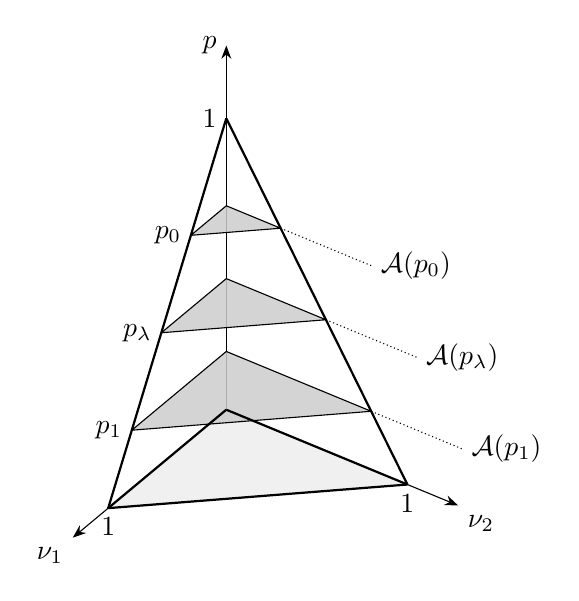
\begin{tikzpicture}[x={(-1.5cm,-1.25cm)}, y={(2.3cm,-0.95cm)}, z={(0cm,3.7cm)}, line join=round, >=Stealth]
    \draw[->, thin] (0,0,0) -- (1.3,0,0) node[below left] {$\nu_1$};
    \draw[->, thin] (0,0,0) -- (0,1.28,0) node[below right] {$\nu_2$};
    \draw[->, thin] (0,0,0) -- (0,0,1.25) node[left] {$p$};
    \fill[gray!12] (0,0,0) -- (1,0,0) -- (0,1,0) -- cycle;
    \foreach \pp/\nm in {0.2/1, 0.45/\lambda, 0.7/0} {
      \pgfmathsetmacro{\aa}{1-\pp}
      \filldraw[fill=gray!40, draw=black, thin, fill opacity=0.85]
        (0,0,\pp) -- (\aa,0,\pp) -- (0,\aa,\pp) -- cycle;
      \draw[densely dotted] (0,\aa,\pp) -- ++(0,0.5,0) node[right] {$\mathcal{A}(p_{\nm})$};
      \node[left] at (\aa,0,\pp) {$p_{\nm}$};
    }
    \draw[thick] (1,0,0) -- (0,1,0);
    \draw[thick] (0,0,1) -- (1,0,0);
    \draw[thick] (0,0,1) -- (0,1,0);
    \draw[thick] (0,0,0) -- (1,0,0);
    \draw[thick] (0,0,0) -- (0,1,0);
    \node[left] at (0,0,1) {$1$};
    \node[below] at (1,0,0) {$1$};
    \node[below] at (0,1,0) {$1$};
  \end{tikzpicture}
  \caption{Buyer sets when types are uniform on the two-dimensional simplex and $R(\nu) = 1 - \nu_1 - \nu_2$.
  At price $p$ the set of buyers $\mathcal{A}(p)$ is the triangle $\{\nu \ge 0 : \nu_1 + \nu_2 \le 1 - p\}$, which
  shrinks linearly as $p$ rises, so $q(p) = (1 - p)^2$. With $p_\lambda = \lambda p_0 + (1 - \lambda)p_1$ (here
  $\lambda = \frac{1}{2}$), the set $\mathcal{A}(p_\lambda)$ is the Minkowski average of $\mathcal{A}(p_0)$ and
  $\mathcal{A}(p_1)$. Redrawn from \citet{CaplinNalebuff1991}, Figure 1.}
  \label{fig:04-cn-simplex}
\end{figure}

A concave density behaves like an extra dimension of uniform types. Let $L = 1$, $\psi(\nu) = 2\nu$ on $[0,1]$
and $R(\nu) = 1 - \nu$. Then
\[
  q(p) = \int_0^{1 - p}2\nu\,\dd\nu = (1 - p)^2,
\]
the same demand as uniform types on the two-dimensional simplex \citep[Example 4.2]{CaplinNalebuff1991}. The
density is linear, hence $1$-concave, and \cref{thm:04-cn-demand} gives $\varrho^* = \frac{1}{1 + 1} = \frac{1}{2}$,
again exactly attained. More generally, a density with $\psi^{\frac{1}{n}}$ concave for a positive integer $n$
yields the bound $\frac{1}{L + n}$ of a uniform density in $L + n$ dimensions.

The bounds of \cref{thm:04-cn-demand} cannot be improved \citep[Proposition 2]{CaplinNalebuff1991}. For every
$\varrho > -\frac{1}{L}$ some model satisfies A1 with a $\varrho$-concave density and has $q^{\varrho^*}$ affine in price. Such a
demand is $\varrho^*$-concave and no more.
In the following examples $U = \sum_l\nu_lx_l + z$, our product has characteristics $(1, 0, \dots, 0)$, and a
rival with characteristics $(0, \dots, 0)$ sells at price zero. Type $\nu$ then buys our product exactly when
$\nu_1 \ge p$, so $R(\nu) = \nu_1$. In each example $\psi^\varrho$, or $\ln\psi$ when $\varrho = 0$, is affine on the support,
so $\psi$ is $\varrho$-concave.
\begin{itemize}
  \item For $\varrho > 0$, let $\psi$ be proportional to $(1 - \sum_l\nu_l)^{\frac{1}{\varrho}}$ on the unit simplex. Then
  $q(p) = (1 - p)^{\frac{1 + L\varrho}{\varrho}}$ on $[0, 1]$.
  \item For $\varrho = 0$, let $\psi(\nu) = e^{-\sum_l\nu_l}$ on $\R^L_+$. Then $q(p) = e^{-p}$.
  \item For $-\frac{1}{L} < \varrho < 0$, let $\psi$ be proportional to $(1 + \sum_l\nu_l)^{\frac{1}{\varrho}}$ on $\R^L_+$,
  which is integrable because $\frac{1}{\varrho} < -L$. Then $q(p) = (1 + p)^{\frac{1 + L\varrho}{\varrho}}$ for $p \ge 0$. It falls
  with price because the exponent is negative.
\end{itemize}
Each demand follows by integrating out $\nu_2, \dots, \nu_L$ and then $\nu_1$ from $p$ upward. In every case
$q^{\varrho^*}$ is affine in $p$, because $\frac{1 + L\varrho}{\varrho} = \frac{1}{\varrho^*}$.

The examples also show why earlier work, which assumed concave demand, could not go far. \Cref{thm:04-cn-demand}
guarantees concave demand only if $\varrho^* = 1$. Since $\varrho^* \le \frac{1}{L}$ for every $\varrho$, this guarantee holds only when
$L = 1$ and $\varrho = \infty$: a uniform distribution of consumers in a one-dimensional market
\citep[p.~14]{CaplinNalebuff1991}. The bound holds for the whole class and does not cap the concavity of each
model. In the setup of the examples above with $L = 1$, the density $\psi(\nu) = 2\nu$ on $[0,1]$ has the bound
$\varrho^* = \frac{1}{2}$, yet its demand $q(p) = 1 - p^2$ is concave.

\begin{proposition}[Quasi-concave profit]\label{prop:04-cn-quasiconcave}
Under A1 and A2, with distinct products, each firm's profit is quasi-concave in its own price
\citep[Proposition 4]{CaplinNalebuff1991}.
\end{proposition}

\begin{proof}
A2 sets $\varrho = -\frac{1}{L+1}$, which exceeds $-\frac{1}{L}$, so \cref{thm:04-cn-demand} applies. The implied
concavity index of demand is
\[
  \varrho^* = \frac{\varrho}{1 + L\varrho} = \frac{-\frac{1}{L+1}}{1 - \frac{L}{L+1}} = \frac{-\frac{1}{L+1}}{\frac{1}{L+1}} = -1.
\]
Demand is $(-1)$-concave, that is, $\frac{1}{q_j}$ is convex where $q_j > 0$. Demand is nonincreasing by
\eqref{eq:04-cn-demand}. \Cref{lem:04-recip} then gives quasi-concavity of profit.
\end{proof}

The value $\varrho = -\frac{1}{L+1}$ in A2 is thus chosen to deliver exactly $(-1)$-concave demand, the weakest
condition that guarantees quasi-concave profit. Solving $\frac{\varrho}{1 + L\varrho} = -1$ for $\varrho$ gives $\varrho = -1 - L\varrho$, so
$\varrho(1 + L) = -1$ and $\varrho = -\frac{1}{L+1}$.

\begin{theorem}[Existence]\label{thm:04-cn-existence}
Under A1 and A2, for any number of single-product firms and any products, a pure-strategy Bertrand-Nash
equilibrium exists \citep[Theorem 2]{CaplinNalebuff1991}. If some products are equivalent, the result uses the
following tie rule. Buyers who are indifferent among equivalent products at the same price buy from a lowest-cost
producer among the firms charging that price.
\end{theorem}

\begin{proof}
We follow \citet[pp.~14--15]{CaplinNalebuff1991} in three steps.

\emph{Distinct products, all costs below income.} Restrict firm $j$ to prices in $[c_j, y]$ and let
$Z = \prod_j[c_j, y]$, a nonempty, compact, convex set. Prices above $y$ sell nothing, and prices below $c_j$
earn at most zero, which the price $c_j$ also earns. Hence a maximizer on $[c_j, y]$ is a global best response.
Demand is continuous because products are distinct, so profits are continuous in all prices. By Berge's maximum
theorem, the restricted best-response correspondence has nonempty compact values and a closed graph. By
\cref{prop:04-cn-quasiconcave}, profit is quasi-concave in own price, and the set of maximizers of a
quasi-concave function on an interval is an interval. Kakutani's theorem gives a fixed point, which is an
equilibrium because every firm plays a global best response.

\emph{Equivalent products.} If several products are equivalent, all consumers buy the cheapest of them, as in
homogeneous Bertrand competition. In each such group, select a lowest-cost producer and solve the game with
distinct products among the selected firms. Each selected firm faces the added constraint that it prices no higher
than the cost of the next-lowest-cost producer in its group. Let the remaining firms price at cost. When the
constraint binds, the selected firm charges exactly that rival's cost, so the two firms tie.
The tie rule gives the buyers of the group to the selected firm, so the remaining firms sell nothing. A remaining
firm can win buyers only by pricing below the selected firm, and hence below its own cost, so it cannot gain by
deviating. The selected firm loses the group's buyers if it prices above its cap. At or below the cap its demand
equals its demand in the game among selected firms, so its fixed-point price is a global best response.

\emph{Costs above income.} Firms with $c_j > y$ can sell nothing at a profit. Solving the game without them and
letting them price at cost preserves the equilibrium.
\end{proof}

\casehead{Interpretation and related work}
The theorem holds for any number of firms and any configuration of products, with no symmetry, given the tie rule
for equivalent products. The tie rule cannot be dropped. Take two equivalent products with costs 0 and 1, sold to
a unit mass of consumers who each value either product at 2. Under an equal split of ties, the prices $(1, 1)$
give the efficient firm a profit of $\frac{1}{2}$, while the price $1 - \eta$ gives it $1 - \eta$ for small
$\eta > 0$. With continuous prices this game has no pure-strategy equilibrium, as in the asymmetric-cost Bertrand
game of \cref{sec:02-bertrand-homog}. The theorem gives
\emph{sufficient} conditions, and equilibria often exist when they fail. \citet[p.~15]{CaplinNalebuff1991} relate
their approach to the independent work of \citet{Dierker1989}. Dierker takes the joint distribution of consumers'
valuations of the products as the primitive and assumes it is log-concave. Pr\'ekopa's theorem then makes demand
log-concave. \citet{CaplinNalebuff1991} instead start from a model of the characteristics space and of preference
parameters, and derive the valuations. Their framework supplies a large set of utility models for which the
joint distribution of valuations is log-concave for every set of products.

\casehead{Extensions}
\citet[Section 8]{CaplinNalebuff1991} extend the result in several directions. We summarize them briefly.
\begin{itemize}
  \item \emph{Unequal incomes.} Income enters as an additional type. Assumption A1$'$ of
  \citet[p.~20]{CaplinNalebuff1991} is A1 with $g(z) = z$. Then the reservation price of type $(\nu, y)$ for
  product $j$ is
  \[
    R_j(\nu, y) = y + \frac{\nu\cdot\bm{t}_j + t_{L+2}(x_j) - \max_{k \neq j}\bigl[\nu\cdot\bm{t}_k + (y - p_k)t_{L+1}(x_k) + t_{L+2}(x_k)\bigr]}{t_{L+1}(x_j)},
  \]
  with $\bm{t}_j = (t_1(x_j), \dots, t_L(x_j))$. A maximum of affine functions is convex, so $R_j$ is concave in
  $(\nu, y)$. The buyer sets therefore satisfy the Minkowski inclusion of the proof of \cref{thm:04-cn-demand},
  now in $\R^{L+1}$. Assumption A2$'$ requires the joint density of types and income to be
  $\bigl(-\frac{1}{L+2}\bigr)$-concave on a convex support in $\R^{L+1}$, with bounded income. With $L + 1$ in
  place of $L$, the computation in the proof of \cref{prop:04-cn-quasiconcave} again gives $\varrho^* = -1$, and an
  equilibrium exists (their Proposition 10). The vertical model $U = xz$
  \citep{GabszewiczThisse1979,ShakedSutton1982} is a special case. Uniqueness extends as well. Under A1$'$, if the
  logarithm of the joint density is concave and differentiable where the density is positive, the duopoly
  equilibrium is unique and the pricing game is log-supermodular. Pure vertical differentiation, with identical
  preferences and different incomes, is the one-dimensional case of their Proposition 7 (p.~20).
  \item \emph{An outside good.} Add a fictitious firm 0 selling $x_0 = 0$ at the fixed price $p_0 = 0$. Existence
  is unaffected, but the duopoly uniqueness result below no longer applies, because the market becomes a
  three-firm oligopoly. In location models the product $x_0 = 0$ is a differentiated product located at the origin,
  not the absence of consumption. Non-purchase can still be modeled by a utility loss from buying nothing that is
  concave in the type (pp.~20--21).
  \item \emph{Variable and non-exclusive demand.} The reservation-price argument no longer applies. With
  individual demands $d_j(\nu, y, p_j)$, aggregate demand is $\int \psi(\nu, y)\,d_j(\nu, y, p_j)\,\dd\nu\,\dd y$.
  \citet{Prekopa1973} shows that integrating a jointly log-concave function over some of its arguments yields a
  log-concave function of the rest. If $\ln d_j$ is concave in $(\nu, y, \ln p_j)$ and $\ln\psi$ is concave, aggregate
  demand is log-concave in $\ln p_j$, and \cref{lem:04-loglog} gives quasi-concave profit. Cobb-Douglas
  preferences satisfy these conditions, and an equilibrium exists with two or more firms and positive costs, unique
  in duopoly.
  \item \emph{CES.} The representative-consumer CES model generates the same demands as a discrete-continuous choice
  model with i.i.d.\ extreme value tastes \citep[eq.~(8.3)]{CaplinNalebuff1991}. Hence an equilibrium exists in the
  CES model with two or more firms and positive costs, unique in duopoly \citep[Proposition 14]{CaplinNalebuff1991}.
  \Cref{sec:04-repcons-ces,sec:04-repcons-cesdc} derive the representation and explain why one firm is not enough.
  \item \emph{Translog.} With indirect translog demands and an own-price coefficient common to all consumers,
  $\ln d_j$ is concave in its arguments, and log-concave densities give quasi-concave profit.
  \item \emph{Unbounded markets.} With infinitely many products in an unbounded space, any price vector that
  satisfies all first-order conditions, and at which A1 and A2 hold, is an equilibrium
  \citep[Proposition 15]{CaplinNalebuff1991}.
  This validates the first-order approach of \citet{Stiglitz1986} with quadratic transport costs.
\end{itemize}

\casehead{Contribution and limits}
Before \citet{CaplinNalebuff1991}, existence results required one-dimensional products, uniform consumers or
complete symmetry. Their theorem covers multi-dimensional characteristics, asymmetric products and the discrete
choice models that empirical work uses. It also brought $\varrho$-concavity and the Pr\'ekopa-Borell theorem into
industrial organization. The limits are as instructive. Each firm sells one product, and the proof does not extend
to multi-product firms, whose profit need not be quasi-concave in the vector of own prices. The density condition
excludes type distributions with separated groups of consumers, such as finite mixtures of logits with very
different price sensitivities. Products are fixed, so the theorem says nothing about product choice. Finally,
uniqueness requires more, as the next subsection shows.

Caplin and Nalebuff close by pointing to product choice as the next step (pp.~26--27). Where the equilibrium is
both existent and unique, as in the logit with any number of products and in duopoly, firms can predict their
profits for any configuration of competing products. Product design can then be studied with price competition in
the second stage. \citet{PrescottVisscher1977} had studied sequential location with fixed prices. Caplin and
Nalebuff also cite a 1989 working paper by Feenstra and Levinsohn that uses a variant of their model to map
consumer preferences for the characteristics of cars. \Cref{sec:04-location} studies product choice in the
simplest settings.

\subsection{Uniqueness}\label{sec:04-uniqueness}

Uniqueness matters for counterfactuals: a model that predicts several outcomes after a merger predicts none of
them reliably. The classical sufficient condition is a dominant diagonal of the matrix of second derivatives of
profit \citep{Friedman1977}. We state it for single-product firms.

\begin{proposition}[Diagonal dominance]\label{prop:04-diag-dominance}
Let firm $j$ choose $p_j \in P_j = [\underline{p}_j, \bar p_j]$ and let $P = \prod_j P_j$. Suppose that
\begin{enumerate}[label=(\roman*)]
  \item Each $\pi_j$ is twice continuously differentiable on an open set containing $P$.
  \item For every $p_{-j}$, $\pi_j(\cdot, p_{-j})$ has a unique maximizer $BR_j(p_{-j})$ in the interior of $P_j$,
  at which $\frac{\partial^2\pi_j}{\partial p_j^2} < 0$.
  \item At every such maximizer,
  $\sum_{k \neq j}\bigl|\frac{\partial^2\pi_j}{\partial p_j\partial p_k}\bigr| < \bigl|\frac{\partial^2\pi_j}{\partial p_j^2}\bigr|$.
\end{enumerate}
Then the best-response map $BR : P \to P$ is a contraction in the sup norm. The game has exactly one Bertrand-Nash
equilibrium, and best-response iteration converges to it from every starting point in $P$.
\end{proposition}

\begin{proof}
Best responses satisfy the first-order condition
$\frac{\partial\pi_j}{\partial p_j}(BR_j(p_{-j}), p_{-j}) = 0$. By (ii) the derivative of the left side with
respect to $p_j$ is nonzero at the maximizer, so the implicit function theorem makes $BR_j$ continuously
differentiable, with
\[
  \frac{\partial BR_j}{\partial p_k} = -\Bigl(\frac{\partial^2\pi_j}{\partial p_j^2}\Bigr)^{-1}\frac{\partial^2\pi_j}{\partial p_j\partial p_k}\,\Bigg|_{p_j = BR_j(p_{-j})}.
\]
By (iii), $\sum_{k \neq j}\bigl|\frac{\partial BR_j}{\partial p_k}\bigr| < 1$ at every $p_{-j}$. This sum is
continuous on the compact set $\prod_{k \neq j}P_k$, so its maximum $\ell_j$ is below one. Let
$\ell = \max_j\ell_j < 1$. For $p, p' \in P$, apply the mean value theorem to
$t \mapsto BR_j(p'_{-j} + t(p_{-j} - p'_{-j}))$ on $[0,1]$. For some intermediate point $\tilde p_{-j}$,
\[
  |BR_j(p_{-j}) - BR_j(p'_{-j})| \le \sum_{k \neq j}\Bigl|\frac{\partial BR_j}{\partial p_k}(\tilde p_{-j})\Bigr|\,|p_k - p'_k| \le \ell\,\|p - p'\|_\infty.
\]
Taking the maximum over $j$ gives $\|BR(p) - BR(p')\|_\infty \le \ell\|p - p'\|_\infty$. The contraction mapping
theorem (\cref{app:math}) gives a unique fixed point and convergence of the iteration $p^{(n+1)} = BR(p^{(n)})$
from any $p^{(0)} \in P$.
\end{proof}

The argument survives two changes of variables that are often useful. Best responses do not change if profit is
replaced by an increasing transformation, such as $\ln\pi_j$, or if prices are replaced by smooth increasing
functions of prices. Diagonal dominance may hold for the transformed problem when it fails for the original, and
the conclusion about uniqueness carries over. A second route avoids best responses altogether. Stack the
first-order conditions as $G(p) = 0$ with $G_j = \frac{\partial\pi_j}{\partial p_j}$. A \emph{P-matrix} is a square
matrix whose principal minors are all positive. If the Jacobian of $-G$ is a P-matrix everywhere on a rectangle,
$G$ is one-to-one there \citep{GaleNikaido1965}. The first-order conditions then have at most one solution. A matrix with positive diagonal
and strictly dominant diagonal rows is a P-matrix. Negative own second derivatives together with the inequality of (iii) at
every point of the rectangle therefore suffice.

\casehead{Uniqueness in the Caplin-Nalebuff framework}
\citet[Section 6]{CaplinNalebuff1991} establish uniqueness in three cases, in the ``differentiable case'' where $g$
is twice differentiable and $\psi$ is differentiable. In a duopoly with A1 and a log-concave type density, the
equilibrium is unique (their Proposition 6). In a one-dimensional market with a log-concave density on an interval,
there is at most one equilibrium with a given set of active firms (Proposition 7). In the logit model the
equilibrium is unique for any number of single-product firms, a result first noted for duopoly by
\citet{AndersonDePalma1988}.
Firms with zero demand create no real indeterminacy. Any equilibrium in which some firms sell nothing has a
counterpart with the same demands and profits in which those firms price at marginal cost (Proposition 5).
Uniqueness thus refers to market outcomes.

The proofs change variables from $p_j$ to the utility from money, $u_j = g(y - p_j)\,t_{L+1}(x_j)$. In a duopoly,
demand depends on the two utilities only through the difference $u_1 - u_2$. Write $\tilde q_1(u_1 - u_2)$ for firm 1's
demand and $\tilde p_1(u_1) = y - g^{-1}\bigl(\frac{u_1}{t_{L+1}(x_1)}\bigr)$ for the price that delivers $u_1$. Then
\[
  \ln\pi_1 = \ln\bigl(\tilde p_1(u_1) - c_1\bigr) + \ln \tilde q_1(u_1 - u_2).
\]
The first term is strictly concave in $u_1$ because $\tilde p_1$ is concave. The second is concave because the
Pr\'ekopa-Borell theorem makes demand log-concave in $u_1$. Because $\tilde q_1$ depends on $u_1 - u_2$ only,
\[
  \frac{\partial^2\ln \tilde q_1}{\partial u_1^2} = -\frac{\partial^2\ln \tilde q_1}{\partial u_1\partial u_2} \le 0,
  \qquad\text{so}\qquad
  \frac{\partial^2\ln\pi_1}{\partial u_1^2} < \frac{\partial^2\ln \tilde q_1}{\partial u_1^2} = -\frac{\partial^2\ln\pi_1}{\partial u_1\partial u_2}.
\]
This is diagonal dominance for $\ln\pi_1$ in the utility variables, and the remark after
\cref{prop:04-diag-dominance} gives uniqueness \citep[p.~30]{CaplinNalebuff1991}. The cross partial
$\frac{\partial^2\ln\pi_1}{\partial u_1\partial u_2}$ is nonnegative, which is the next property.

\casehead{Log-supermodularity}
A positive payoff $\pi_j(p_j, p_{-j})$ is \emph{log-supermodular} if $\ln\pi_j$ has increasing differences in
$(p_j, p_k)$ for every $k \neq j$. For smooth payoffs this means
$\frac{\partial^2\ln\pi_j}{\partial p_j\partial p_k} \ge 0$: a higher rival price raises the marginal return, in
logs, to a higher own price. A price game with interval strategy sets and log-supermodular payoffs is a
supermodular game \citep{MilgromRoberts1990,Vives1990}. \citet[p.~16]{CaplinNalebuff1991} summarize what
log-supermodularity adds to uniqueness, drawing on \citet{MilgromRoberts1990}:
\begin{itemize}
  \item There are no other equilibria in mixed or correlated strategies.
  \item The equilibrium is globally stable under many learning and adjustment processes, including best-response
  dynamics, Bayesian learning and fictitious play.
  \item The game is \emph{dominance solvable}, meaning that iterated deletion of strictly dominated strategies
  leaves a single strategy profile. The equilibrium strategy is therefore each firm's unique \emph{rationalizable}
  strategy, the only one consistent with common knowledge of rationality.
  \item A parameter change that raises the marginal return to price for some firm, such as an increase in one firm's
  cost, raises every firm's equilibrium price.
\end{itemize}
The logit is log-supermodular. With single-product firms, $\ln\pi_j = \ln(p_j - c_j) + \ln s_j$ and
$\frac{\partial\ln s_j}{\partial p_j} = -\alpha(1 - s_j)$, so
\[
  \frac{\partial^2\ln\pi_j}{\partial p_j\partial p_k} = \alpha\,\frac{\partial s_j}{\partial p_k} = \alpha^2 s_j s_k > 0.
\]

\casehead{The single-product logit}
For the logit model we can compute the slopes of the best responses directly.

\begin{proposition}[Logit best responses]\label{prop:04-logit-br}
Consider single-product firms with constant marginal costs $c_j$ and logit demand. The best response of firm $j$
is continuously differentiable, with slopes
\begin{equation}\label{eq:04-logit-br-slope}
  \frac{\partial BR_j}{\partial p_k} = \frac{s_j s_k}{1 - s_j} \in (0, 1), \qquad k \neq j,
\end{equation}
evaluated at $(BR_j(p_{-j}), p_{-j})$. Prices are strategic complements, the row sums satisfy
$\sum_{k \neq j}\frac{\partial BR_j}{\partial p_k} = \frac{s_j(1 - s_j - s_0)}{1 - s_j} < s_j$, and the equilibrium is
unique.
\end{proposition}

\begin{proof}
From \cref{prop:04-logit-markup} the best response solves $\alpha m_j(1 - s_j) = 1$ with $m_j = p_j - c_j$, and it is
the global maximizer because $\frac{\partial\pi_j}{\partial p_j} = s_j[1 - \alpha m_j(1 - s_j)]$ changes sign once
(\cref{sec:04-bertrand-logit}). Define $G_j(p) = \alpha(p_j - c_j)(1 - s_j(p)) - 1$, so that $G_j = 0$ at the best
response. Using \eqref{eq:04-logit-derivs},
\begin{align*}
  \frac{\partial G_j}{\partial p_j} &= \alpha(1 - s_j) - \alpha m_j\frac{\partial s_j}{\partial p_j}
    = \alpha(1 - s_j) + \alpha^2 m_j s_j(1 - s_j) = \alpha(1 - s_j)(1 + \alpha m_j s_j),\\
  \frac{\partial G_j}{\partial p_k} &= -\alpha m_j\frac{\partial s_j}{\partial p_k} = -\alpha^2 m_j s_j s_k.
\end{align*}
The implicit function theorem gives
\[
  \frac{\partial BR_j}{\partial p_k} = -\Bigl(\frac{\partial G_j}{\partial p_j}\Bigr)^{-1}\frac{\partial G_j}{\partial p_k}
  = \frac{\alpha m_j s_j s_k}{(1 - s_j)(1 + \alpha m_j s_j)}.
\]
At the best response $\alpha m_j = \frac{1}{1 - s_j}$. The numerator becomes $\frac{s_j s_k}{1 - s_j}$. The
denominator becomes $(1 - s_j)\bigl(1 + \frac{s_j}{1 - s_j}\bigr) = 1$. This proves \eqref{eq:04-logit-br-slope}.
Summing over $k \neq j$ and using $\sum_{k \neq j}s_k = 1 - s_j - s_0$ gives the row sum, which is below $s_j$
because $s_0 > 0$.

For uniqueness we bound $s_j$ at the best response uniformly. \Cref{sec:04-bertrand-logit} showed that
$\alpha m_j - 1 = W(z_j)$ with $z_j = \frac{e^{v_j - 1}}{\Phi_{-j}}$, where $W$ is the Lambert W function and
$v_j = x_j\beta + \xi_j - \alpha c_j$. Then
$s_j = 1 - \frac{1}{\alpha m_j} = \frac{W(z_j)}{1 + W(z_j)}$. Since $\Phi_{-j} \ge 1$ and $W$ is increasing,
$s_j \le \bar s_j \equiv \frac{W(e^{v_j - 1})}{1 + W(e^{v_j - 1})} < 1$ for every $p_{-j}$. Every row sum is
therefore below $\ell = \max_j\bar s_j < 1$, uniformly in prices. Best responses lie in the compact box
$\prod_j[c_j + \frac{1}{\alpha},\, c_j + \frac{1 + W(e^{v_j - 1})}{\alpha}]$, so the argument of
\cref{prop:04-diag-dominance} applies on that box. The best-response map is a contraction with modulus $\ell$
and has a unique fixed point.
\end{proof}

\casehead{Multi-product logit}
\Cref{prop:04-logit-br} does not cover multi-product firms, and \citet{CaplinNalebuff1991} do not either. Uniqueness
nevertheless holds for every ownership structure. \citet[Theorem~7]{KonovalovSandor2010} prove it for multi-product firms with
logit demand. \citet{NockeSchutz2018} develop an aggregative-games approach for multi-product pricing that covers the
logit and CES demand systems \citep[p.~229, n.~127]{AskerNocke2021}. We give a self-contained proof along aggregative
lines.

\begin{theorem}[Uniqueness with multi-product logit firms]\label{thm:04-logit-unique}
With logit demand, constant marginal costs and any partition of the $J$ products among $F$ firms, the
Bertrand-Nash pricing game has exactly one equilibrium.
\end{theorem}

\begin{proof}
Let $v_k = x_k\beta + \xi_k - \alpha\,mc_k$, $m_k = p_k - mc_k$ and $E_f = \sum_{k \in \mathcal{J}_f}e^{v_k}$. Then
$e^{\delta_k} = e^{v_k - \alpha m_k}$. Firm $f$ takes $\Phi_{-f} = 1 + \sum_{l \notin\mathcal{J}_f}e^{\delta_l}$ as given.

\emph{Step 1 (given its total, a firm sets a common markup).} Let $\chi_k = e^{v_k - \alpha m_k}$ for
$k \in \mathcal{J}_f$, so $m_k = \frac{v_k - \ln \chi_k}{\alpha}$, and let $a = \sum_{k \in \mathcal{J}_f}\chi_k$. Firm $f$'s
profit is
\[
  \pi_f = \frac{\sum_{k \in \mathcal{J}_f}m_k \chi_k}{\Phi_{-f} + a} = \frac{1}{\alpha}\,\frac{\sum_{k \in \mathcal{J}_f}\chi_k(v_k - \ln \chi_k)}{\Phi_{-f} + a}.
\]
For fixed $a$ the denominator is fixed. The numerator is strictly concave in $(\chi_k)$, because $-\chi\ln \chi$ is
strictly concave, and its slope in $\chi_k$ tends to $+\infty$ as $\chi_k \to 0$. Its maximum on
$\{\chi > 0 : \sum_k \chi_k = a\}$ is therefore unique and interior. The Lagrangian first-order condition
$v_k - \ln \chi_k - 1 = \mu$ gives $\alpha m_k = v_k - \ln \chi_k = 1 + \mu$ for all $k \in \mathcal{J}_f$. All of the firm's
products carry the same markup $m$, and then $a = E_f e^{-\alpha m}$.

\emph{Step 2 (the firm's best response).} Since $a$ and $m$ are in one-to-one correspondence, the firm's problem
reduces to choosing $m$ to maximize $m\,S_f(m)$ with $S_f(m) = \frac{E_f e^{-\alpha m}}{\Phi_{-f} + E_f e^{-\alpha m}}$.
This is a single-product logit problem with mean utility $\ln E_f$. Since
$\frac{\dd S_f}{\dd m} = -\alpha S_f(1 - S_f)$,
\[
  \frac{\dd (m S_f)}{\dd m} = S_f\bigl[1 - \alpha m(1 - S_f(m))\bigr].
\]
The bracket is positive for $m \le 0$. For $m > 0$ it is strictly decreasing, because $m$ and $1 - S_f(m)$ are
positive and increasing, and it tends to $-\infty$. It therefore changes sign once. The best response is unique and is characterized by
\begin{equation}\label{eq:04-mp-logit-foc}
  \alpha m_f(1 - S_f) = 1.
\end{equation}

\emph{Step 3 (one equation per firm).} In any equilibrium let $\Phi = 1 + \sum_k e^{\delta_k}$. Then
$S_f = \frac{E_f e^{-\alpha m_f}}{\Phi}$, and \eqref{eq:04-mp-logit-foc} gives $\alpha m_f = \frac{1}{1 - S_f}$.
Substituting,
\[
  S_f = \frac{E_f}{\Phi}\,e^{-\frac{1}{1 - S_f}} \quad\Longleftrightarrow\quad h(S_f) \equiv S_f\,e^{\frac{1}{1 - S_f}} = \frac{E_f}{\Phi}.
\]
The function $h$ satisfies $h(0) = 0$, $h(S) \to \infty$ as $S \to 1$, and
\[
  h'(S) = e^{\frac{1}{1 - S}}\Bigl[1 + \frac{S}{(1 - S)^2}\Bigr] > 0.
\]
For each $\Phi > 0$ there is a unique $S_f(\Phi) \in (0,1)$ with $h(S_f(\Phi)) = \frac{E_f}{\Phi}$. It is continuous
and strictly decreasing in $\Phi$.

\emph{Step 4 (one equation for the aggregate).} Shares add up to one, and $s_0 = \frac{1}{\Phi}$. Hence $\Phi$ solves
\[
  \Psi(\Phi) \equiv \sum_{f=1}^F S_f(\Phi) + \frac{1}{\Phi} = 1.
\]
$\Psi$ is continuous and strictly decreasing. At $\Phi = 1$, $\Psi(1) = 1 + \sum_f S_f(1) > 1$. As $\Phi \to \infty$,
$\Psi(\Phi) \to 0$. There is exactly one root $\Phi^* > 1$.

\emph{Step 5 (existence and uniqueness of prices).} Any equilibrium must have $\Phi = \Phi^*$, shares
$S_f^* = S_f(\Phi^*)$, markups $m_f^* = \frac{1}{\alpha(1 - S_f^*)}$ and prices $p_k^* = mc_k + m_{f(k)}^*$, where
$f(k)$ is the owner of $k$. So there is at most one equilibrium. Conversely, at these prices,
$1 + \sum_f E_f e^{-\alpha m_f^*} = 1 + \Phi^*\sum_f S_f^* = 1 + \Phi^*\bigl(1 - \frac{1}{\Phi^*}\bigr) = \Phi^*$, so
the aggregate is consistent. Each firm's markup satisfies \eqref{eq:04-mp-logit-foc}, which by Step 2 makes it a
best response. The prices form an equilibrium.
\end{proof}

The aggregative proof also yields a contraction. Differentiating the multi-product Lambert W best response
$m_f = \frac{1}{\alpha}\bigl[1 + W\bigl(\frac{E_f e^{-1}}{\Phi_{-f}}\bigr)\bigr]$ with
$W'(z) = \frac{W(z)}{z(1 + W(z))}$ gives
$\frac{\partial BR_k}{\partial p_l} = \frac{S_f s_l}{1 - S_f}$ for $k \in \mathcal{J}_f$ and $l \notin \mathcal{J}_f$,
and zero for $l \in \mathcal{J}_f$. Row sums equal $\frac{S_f(1 - S_f - s_0)}{1 - S_f} < S_f$, and
$S_f \le \frac{W(E_f e^{-1})}{1 + W(E_f e^{-1})} < 1$ at any best response. Best-response iteration therefore
converges from any starting point.

\begin{example}[Uniqueness in the 25-product market]\label{ex:04-logit25-unique}
In the 25-product market of \cref{ex:04-logit25}, we evaluated $\Psi(\Phi) - 1$ on a grid of 2,000 points spaced
evenly in logarithms over $[1, 10^4]$. It changes sign exactly once, at $\Phi^* = 7.314$ under single-product
ownership and at $\Phi^* = 6.246$ under the five multi-product owners. In each case $\Phi^*$ equals $\frac{1}{s_0}$
at the equilibrium of \cref{tab:04-logit25}, with outside shares 0.1367 and 0.1601. Best-response iteration from
$p^{(0)} = mc + \frac{1}{\alpha}$ converges in 11 and 16 iterations to a sup-norm tolerance of $10^{-13}$, one
iteration more than the looser tolerance of \cref{rem:04-logit25-algorithm} requires. From 500
random starting points $p^{(0)} = mc + U[0,5]^{25}$, and from $p^{(0)} = mc$ and $mc + 20$, it reaches the same prices
to within $6 \times 10^{-15}$ and $3 \times 10^{-14}$. The contraction modulus at the equilibrium,
$\max_f\frac{S_f(1 - S_f - s_0)}{1 - S_f}$, is 0.099 and 0.199. Computed with
\texttt{figures/ch04/src/logit\_uniqueness\_check.py}.
\end{example}

\casehead{When no theorem applies}
Most demand systems estimated in practice, such as random coefficients logit with multi-product firms, lack a
uniqueness theorem. Researchers then check numerically. They solve the first-order conditions from many starting
values and compare the solutions. They monitor the contraction property of the iteration they use, and they can
trace solutions by homotopy as a parameter moves from a case with a known unique equilibrium. A \emph{homotopy}
deforms one system of equations continuously into another. Each candidate should
also be checked for global optimality, for instance by a grid search over each firm's own prices. When profit is
not quasi-concave, a solution of the first-order conditions need not be an equilibrium.

\subsection{Multiple equilibria}\label{sec:04-multiple}

Elasticities and diversion ratios depend on prices. The first-order conditions are therefore a nonlinear system,
which can have several solutions. Multiplicity arises naturally when consumers form separated groups, because a firm
may then target either group. The following example has two equilibria.

\begin{example}[A two-segment logit duopoly]\label{ex:04-multiple-eq}
Two single-product firms have marginal cost $c = 1$. The market has mass one and an outside good. Consumer $i$ in
segment $h \in \{A, B\}$ has utility $u_{ij} = \delta - \alpha_h p_j + \epsilon_{ij}$ for $j = 1, 2$ and
$u_{i0} = \epsilon_{i0}$, with $\delta = 3$ and i.i.d.\ type-I extreme value shocks. Segment $A$ has mass $M_A = 0.9$
and price coefficient $\alpha_A = 2$. Segment $B$ has mass $M_B = 0.1$ and $\alpha_B = 0.2$. Demand is a mixture of
two logits:
\[
  s_j(p) = \sum_{h \in \{A, B\}} M_h\,s_{hj}(p), \qquad s_{hj}(p) = \frac{e^{\delta - \alpha_h p_j}}{1 + e^{\delta - \alpha_h p_1} + e^{\delta - \alpha_h p_2}}.
\]
Firm $j$ earns $\pi_j = (p_j - c)\,s_j(p)$. Since $\frac{\partial s_{hj}}{\partial p_j} = -\alpha_h s_{hj}(1 - s_{hj})$,
the first-order condition $s_j + (p_j - c)\frac{\partial s_j}{\partial p_j} = 0$ gives
\begin{equation}\label{eq:04-twoseg-markup}
  p_j - c = \frac{\sum_h M_h s_{hj}}{\sum_h M_h\,\alpha_h s_{hj}(1 - s_{hj})}.
\end{equation}
The markup is the reciprocal of a share-weighted average of the segments' semi-elasticities. At low prices both
segments buy, the price-sensitive segment dominates the denominator, and the markup is small. At high prices only
segment $B$ buys, and the markup approaches $\frac{1}{\alpha_B(1 - s_{Bj})}$.

We computed best responses by maximizing profit globally over own prices in $[1, 25]$ on a grid of step 0.0005,
followed by local refinement. We then searched for fixed points of $BR$ and of $BR \circ BR$ on $[1, 25]$. There are
exactly two equilibria, both symmetric, and no asymmetric equilibrium.
\begin{itemize}
  \item The \emph{mass-market equilibrium} $L$ has $p_1 = p_2 = 1.804$. Each firm's share is 0.283 (0.261 in segment
  $A$ and 0.483 in segment $B$), its profit is 0.227 and the outside share is 0.434.
  \item The \emph{niche equilibrium} $H$ has $p_1 = p_2 = 9.711$. Each firm's share is 0.043, almost entirely from
  segment $B$ (0.426 of it), its profit is 0.371 and the outside share is 0.915.
\end{itemize}
The markups 0.804 and 8.711 satisfy \eqref{eq:04-twoseg-markup}. At $H$ the formula gives
$\frac{1}{0.2 \times (1 - 0.426)} = 8.71$ because segment $A$ buys almost nothing. Neither equilibrium admits a
profitable deviation to the other local maximum of profit. At $L$ the best niche price, 7.486, earns 0.150 against
0.227. At $H$ the best mass-market price, 1.915, earns 0.321 against 0.371.

The best response jumps. When the rival's price rises past 7.988, firm $j$ abandons the mass market: its best
response jumps from 1.904 to 9.168, the two prices giving the same profit of 0.317. A second jump occurs for rival
prices below 1.045, where the rival takes so much of segment $A$ that the niche becomes more profitable. Neither jump
creates an equilibrium. The slopes of the best response at $L$ and $H$ are 0.075 and 0.316.
\Cref{fig:04-multiple-eq} shows the best responses and the bimodal profit function at the upper jump.

Firms prefer $H$, where each earns 0.371 instead of 0.227. Consumers prefer $L$. Measured by the log-sum formula
$\sum_h\frac{M_h}{\alpha_h}\ln\bigl(1 + e^{\delta - \alpha_h p_1} + e^{\delta - \alpha_h p_2}\bigr)$, consumer
surplus is 2.02 at $L$ and 0.96 at $H$, up to a common constant. Computed with
\texttt{figures/ch04/src/multiple\_equilibria.py}.
\end{example}

\begin{figure}[htbp]
  \centering
  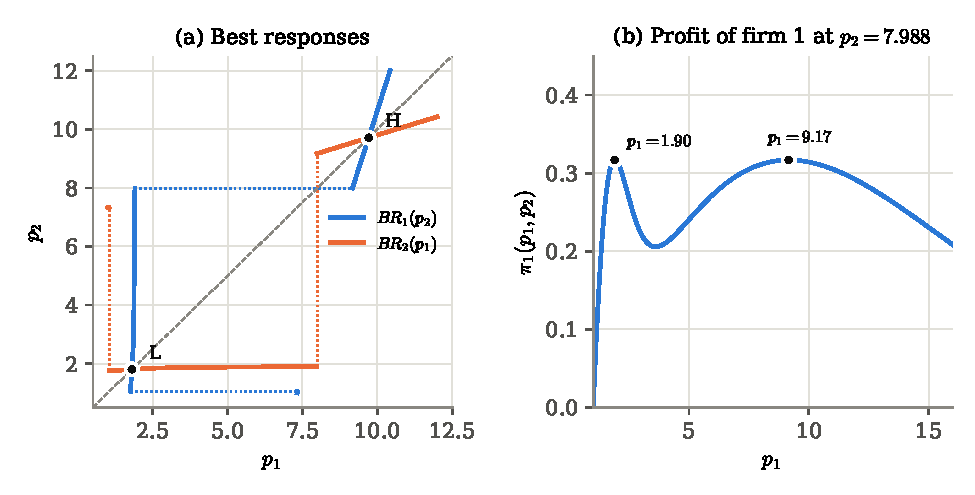
\includegraphics[width=\textwidth]{figures/ch04/multiple_equilibria.pdf}
  \caption{Two equilibria in the two-segment logit duopoly of \cref{ex:04-multiple-eq}. Panel (a): best responses
  $BR_1(p_2)$ and $BR_2(p_1)$, with dotted segments marking the jumps. They cross on the 45-degree line at the
  mass-market equilibrium $L$ ($p^* = 1.804$) and at the niche equilibrium $H$ ($p^* = 9.711$). Panel (b): firm 1's
  profit as a function of its own price when $p_2 = 7.988$. Two local maxima, at $p_1 = 1.904$ and $p_1 = 9.168$,
  give the same profit, so profit is not quasi-concave. Computed with
  \texttt{figures/ch04/src/multiple\_equilibria.py}.}
  \label{fig:04-multiple-eq}
\end{figure}

The example violates the Caplin-Nalebuff conditions in an instructive way. Dividing utility by $\alpha_h$, a consumer
of segment $h$ buys $j$ when $\frac{\delta + \epsilon_{ij} - \epsilon_{i0}}{\alpha_h} - p_j$ is largest. A1 holds
with $g(z) = z$ and money-metric types $\nu_{ij} = \frac{\delta + \epsilon_{ij} - \epsilon_{i0}}{\alpha_h}$. Within a
segment, the vector $(\nu_{i1}, \nu_{i2})$ is a linear transformation of independent extreme value shocks and has a
log-concave density. Across segments, its density is a mixture of a component concentrated near
$\frac{\delta}{\alpha_A} = 1.5$ and a component spread around $\frac{\delta}{\alpha_B} = 15$. The mixture is bimodal.
It is not even quasi-concave, so A2 fails, and profit inherits two peaks from the two groups of consumers.

\casehead{Consequences for empirical work}
Multiplicity does not affect the estimation methods of this chapter. At the estimation stage, prices are data. We
evaluate the first-order conditions at observed prices and invert them for marginal costs as in \eqref{eq:04-mc-recover},
so we never solve for an equilibrium. Whichever equilibrium generated the data, the first-order conditions hold at
the observed prices. In games of entry and in dynamic games, by contrast, multiplicity complicates estimation
itself.

Counterfactuals are different. A merger simulation or a policy experiment must solve for new prices, and with
several solutions the researcher must choose among them. Three selection rules are common. The first starts the
solver at the status quo prices. Merger simulations usually iterate from pre-merger prices, which selects the
equilibrium in whose basin of attraction the status quo lies. The \emph{basin of attraction} of an equilibrium is
the set of starting points from which the iteration converges to it. The second picks the equilibrium the firms prefer,
which here is $H$. The third requires stability under best-response dynamics. In \cref{ex:04-multiple-eq} both
equilibria are stable. Simultaneous best-response iteration from a symmetric start converges to $L$ for starting
prices below 7.988 and to $H$ above. From an asymmetric start such as $(2, 12)$, however, it cycles between
$(1.804, 9.711)$ and $(9.711, 1.804)$, although neither point is an equilibrium. Alternating best responses avoid
the cycle. Stability depends on the adjustment process, and a careful counterfactual reports how its answer depends
on the selection rule (\cref{sec:04-counterfactuals}).

These problems explain part of the popularity of demand systems with known uniqueness results, such as the logit and
CES with multi-product firms (\cref{thm:04-logit-unique} and \citealp{NockeSchutz2018}). For richer systems, the checks
listed at the end of \cref{sec:04-uniqueness} are the practical safeguard. They cannot prove uniqueness, but they can
reveal multiplicity when it is present.

\section{Using the supply side: costs, conduct and counterfactuals}\label{sec:04-supply}

\Cref{sec:04-bertrand,sec:04-diversion,sec:04-existence} characterized the pricing equilibrium and the conditions
under which it exists and is unique. We now put the pricing rule to work. The first-order conditions
\eqref{eq:04-foc-matrix} tie together four objects: the demand system and its
derivatives, the ownership matrix, prices and marginal costs. Given any three of them, the conditions restrict
the fourth. This section uses them in three directions. With estimated demand, observed prices and an assumed
ownership structure, they recover marginal costs without any cost data (\cref{sec:04-mc}). With demand and
independent information on margins, they let us compare models of conduct (\cref{sec:04-conduct}). With
demand, recovered costs and a changed environment, they predict the new equilibrium
(\cref{sec:04-counterfactuals,sec:04-comparative}). We begin with the reasons for modeling supply at all.

\subsection{Why model supply when we estimate demand?}\label{sec:04-supply-why}

Write the markup equation \eqref{eq:04-markup} product by product, and let marginal cost depend on observed
\emph{cost shifters} $w_j$ (variables that move cost but not utility) and an unobserved cost shock $\omega_j$:
\begin{equation}\label{eq:04-price-decomp}
p_j = mc_j(w_j, \omega_j) + m_j(p, x, \xi;\, \theta_d, \Omega),
\qquad m = -\big(\Omega \odot \Delta^\top\big)^{-1} q .
\end{equation}
Here $\theta_d$ collects the demand parameters, $x$ and $\xi$ stack the observed and unobserved characteristics
of all products, and $m_j$ is the $j$th element of the markup vector $m$. Equation \eqref{eq:04-price-decomp} is
a model of price. A product's price moves with its own cost and with every determinant of its markup, including
the characteristics and prices of all other products. Three reasons to model supply follow from it.

\casehead{Prices are endogenous, and supply tells us which instruments are valid}
Take the logit demand of \cref{sec:04-bertrand-logit}, with mean utility $\delta_j = x_j\beta - \alpha p_j +
\xi_j$. Firms observe the unobserved quality $\xi_j$ when they set prices, so $p_j$ responds to it. For a
single-product firm the pricing condition is $p_j = mc_j + \frac{1}{\alpha(1 - s_j)}$ by
\cref{prop:04-logit-markup}. Hold rivals' prices fixed and define
\begin{equation*}
F(p_j, \xi_j) \equiv p_j - mc_j - \frac{1}{\alpha(1 - s_j)} = 0 .
\end{equation*}
The logit derivatives \eqref{eq:04-logit-derivs} give $\frac{\partial s_j}{\partial p_j} = -\alpha s_j(1 - s_j)$,
and the same algebra gives $\frac{\partial s_j}{\partial \xi_j} = s_j(1 - s_j)$. Differentiating $F$,
\begin{align*}
\frac{\partial F}{\partial p_j} &= 1 - \frac{1}{\alpha(1 - s_j)^2}\,\frac{\partial s_j}{\partial p_j}
  = 1 + \frac{s_j}{1 - s_j} = \frac{1}{1 - s_j}, \\
\frac{\partial F}{\partial \xi_j} &= -\frac{1}{\alpha(1 - s_j)^2}\,\frac{\partial s_j}{\partial \xi_j}
  = -\frac{s_j}{\alpha(1 - s_j)} .
\end{align*}
By the implicit function theorem (\cref{app:math}),
\begin{equation}\label{eq:04-dp-dxi}
\frac{d p_j}{d \xi_j} = -\frac{\frac{\partial F}{\partial \xi_j}}{\frac{\partial F}{\partial p_j}}
= \frac{s_j}{\alpha(1 - s_j)}\,(1 - s_j) = \frac{s_j}{\alpha} > 0 .
\end{equation}
Products with high unobserved quality carry high prices. In the logit estimating equation $\ln s_j - \ln s_0 =
x_j\beta - \alpha p_j + \xi_j$ of \cref{ch:logit}, the regressor $p_j$ is therefore positively correlated with the
error $\xi_j$. Least squares biases the price coefficient $-\alpha$ toward zero, and estimated demand looks too
inelastic.

The price equation also tells us which variables can serve as instruments. A valid instrument moves $p_j$ and is
uncorrelated with $\xi_j$. By \eqref{eq:04-price-decomp} three groups of variables move prices. Cost shifters
$w_j$ move $mc_j$ and are excluded from utility. Characteristics of other products move $m_j$ through shares and
diversion ratios, and they are excluded from the utility of product $j$. Changes in ownership move $m_j$ through
$\Omega$. \citet[eq.~(4.1)]{BerryLevinsohnPakes1995} state the identifying assumption as $\E[\xi_j \mid z] =
\E[\omega_j \mid z] = 0$, where $z$ stacks the characteristics and cost shifters of all products.
\Cref{ch:logit,ch:blp} develop these instruments, and \cref{sec:06-charinst} explains why instruments built from
characteristics fail when firms choose characteristics with knowledge of $\xi_j$.

\casehead{The pricing equation adds information about demand}
Suppose we specify $mc_j = w_j\gamma + \omega_j$ and fix $\Omega$. For any candidate value of $\theta_d$ we can
compute the markups $m(\theta_d)$ at observed prices and quantities, and with them the implied cost shock
\begin{equation*}
\omega_j(\theta_d, \gamma) = p_j - m_j(\theta_d) - w_j\gamma .
\end{equation*}
Moment conditions $\E[z_j\,\omega_j(\theta_d, \gamma)] = 0$ then restrict $\theta_d$ as well as $\gamma$. A price
coefficient that is too small in absolute value, for example, implies markups that are too large. The implied
costs are then too low exactly where markups are high, and they become correlated with instruments that shift
markups. \citet{BerryLevinsohnPakes1995} estimate demand and the pricing equation jointly for this reason
(\cref{ch:blp}).

\casehead{Markups, costs and counterfactuals require a model of price setting}
Demand alone yields elasticities and diversion ratios. Markups require a model of how prices are set, and so do
the marginal costs inferred from them. Every counterfactual that changes prices, such as a merger, a new product
or a tax, requires solving for a new equilibrium.

These reasons come with a trade-off. Demand can usually be estimated without specifying supply in full.
Instruments motivated by supply, such as cost shifters, remain valid whatever the exact model of conduct, as long
as they are excluded from utility and uncorrelated with $\xi_j$. Adding the pricing equation brings more
information and more assumptions. If conduct or the cost function is misspecified, joint estimation transmits the
error into the demand estimates. The researcher therefore trades efficiency against robustness. Counterfactuals
need a model of supply in any case, so the assumptions return at that stage even when estimation avoids them.

\subsection{Recovering marginal costs}\label{sec:04-mc}

Suppose demand has been estimated, with parameter estimate $\hat\theta_d$, and that we observe prices $p$ and
quantities $q$ in a market. The demand Jacobian $\Delta(p; \hat\theta_d)$ can then be evaluated at the observed
prices. We rearrange \eqref{eq:04-foc-matrix} in two steps:
\begin{align*}
\big(\Omega \odot \Delta^\top\big)(p - mc) &= -q, \\
p - mc &= -\big(\Omega \odot \Delta^\top\big)^{-1} q .
\end{align*}
Solving for marginal cost gives the \emph{implied} (or recovered) marginal cost
\begin{equation}\label{eq:04-mc-recover}
\widehat{mc} = p + \big(\Omega \odot \Delta(p; \hat\theta_d)^\top\big)^{-1} q .
\end{equation}
\Cref{prop:04-markup-positive} guarantees that the inverse exists and that the implied markups are positive
whenever some of every product's lost sales go to the outside good. With market size $M$, $q = Ms$ and
$\Delta = M\Delta^s$, so the same formula holds with shares and share derivatives. The computation is done market
by market, and it uses no cost data.

\begin{remark}[What cost recovery assumes]\label{rem:04-mc-assumptions}
Formula \eqref{eq:04-mc-recover} rests on four assumptions. (i) The demand model is correctly specified and
$\hat\theta_d$ is consistent. (ii) Observed prices satisfy the first-order conditions of a static
simultaneous-move pricing game, with interior prices. (iii) The matrix $\Omega$ describes conduct correctly.
(iv) Marginal cost is constant, or the recovered value is read as marginal cost at the observed output. The
formula does not require the equilibrium to be unique. \citet[fn.~12]{BerryLevinsohnPakes1995} note that ``none
of the properties of the estimates require uniqueness of equilibrium.'' Uniqueness matters only at the
counterfactual stage (\cref{sec:04-counterfactuals}).
\end{remark}

With logit demand the inversion has a closed form. By \cref{prop:04-logit-markup} every product of firm $f$
carries the markup $\frac{1}{\alpha(1 - S_f)}$, where $S_f$ is the firm's combined share. Hence
\begin{equation}\label{eq:04-mc-logit}
\widehat{mc}_j = p_j - \frac{1}{\hat\alpha\,\big(1 - S_{f(j)}\big)} .
\end{equation}
Within a firm, differences in recovered costs equal differences in prices. Across firms, a product of a firm with
a larger combined share is assigned a larger markup, and so a lower cost at a given price.

\begin{example}[Cost recovery under three models of conduct]\label{ex:04-mc-recovery}
Treat the multi-product equilibrium (M) of \cref{ex:04-logit25} as data. Its prices range from 0.744 to 1.852,
and the true marginal costs range from 0.164 to 1.236. We apply \eqref{eq:04-mc-recover} with the true $\alpha
= 2$ and three ownership matrices.
\begin{enumerate}
  \item With the true owners, the recovered costs equal the true costs up to rounding error.
  \item If we wrongly assume single-product firms ($\Omega = I_{25}$), the implied markups are
  $\frac{1}{\alpha(1 - s_j)}$, between 0.502 and 0.568. The recovered costs then exceed the true costs by 0.014 to
  0.168, by 0.098 on average, against a mean true cost of 0.767.
  \item If we assume that one owner sets all 25 prices ($\Omega = \mathbf{1}\mathbf{1}^\top$), every markup equals
  $\frac{1}{\alpha s_0} = \frac{1}{2 \times 0.1601} = 3.12$. All 25 recovered costs are negative, with mean $-1.74$.
\end{enumerate}
Assuming too little internalization overstates costs, and assuming too much understates them. The third case
shows that implausible implied costs can reject a model of conduct outright.
\end{example}

\casehead{Why the New Empirical IO avoids accounting costs}
Formula \eqref{eq:04-mc-recover} is the answer of the New Empirical Industrial Organization to the unreliability
of accounting cost data \citep{Bresnahan1989}, discussed in \cref{ch:intro,ch:conduct}. Accounting data have
four problems for our purpose. First, they report average (variable) cost, which differs from marginal cost
unless returns to scale are constant. Second, multi-product firms share plants, distribution and advertising, and
accountants allocate these common costs across products by conventions without economic content. Third,
accounting depreciation follows tax and reporting rules, and the opportunity cost of capital and of owned inputs
is missing \citep{FisherMcGowan1983}. Fourth, the data are reported by firm or division, not by product and
market. The structural approach trades these measurement problems for dependence on the demand model and on the
assumed conduct. Accounting data then become a check on the model. \citet[p.~333]{Nevo2001}, for example, uses
accounting margins only as a crude benchmark. He treats Census margins, built from average variable costs, as an
upper bound on price-cost margins.

\casehead{The cost equation}
We often want to know what determines the recovered costs: input prices, returns to scale, the cost of
characteristics, or the savings from a merger. The standard specification projects marginal cost on cost
shifters:
\begin{equation}\label{eq:04-cost-eq}
mc_j = w_j\gamma + \omega_j
\qquad\text{or}\qquad
\ln mc_j = w_j\gamma + \omega_j ,
\end{equation}
where $w_j$ is a row vector of observed cost shifters and $\omega_j$ is the unobserved cost shock.
\citet[eq.~(3.1)]{BerryLevinsohnPakes1995} use the log form. Their $w_j$ contains product characteristics, and they
note that $\omega_j$ may be correlated with $\xi_j$ because larger cars, or cars with higher unobserved quality,
may cost more to produce (p.~853).

\citet{BerryLevinsohnPakes1995} write the first-order conditions with the opposite sign convention. Their $J
\times J$ matrix has element $(j, r)$ equal to $-\frac{\partial s_r}{\partial p_j}$ when products $r$ and $j$ have
the same owner and zero otherwise (their eq.~3.4). In our notation it is $-(\Omega \odot \Delta^{s\top})$. Their
first-order conditions read $s - \Delta^{\mathrm{BLP}}(p - mc) = 0$, and their markup is
\begin{equation}\label{eq:04-blp-markup}
b(p, x, \xi; \theta) = \big(\Delta^{\mathrm{BLP}}\big)^{-1}s = -\big(\Omega \odot \Delta^{s\top}\big)^{-1}s
\end{equation}
(their eq.~3.5). Substituting into \eqref{eq:04-cost-eq} gives the \emph{pricing equation} that is taken to the
data,
\begin{equation}\label{eq:04-cost-est}
p_j - b_j(\hat\theta_d) = w_j\gamma + \omega_j
\qquad\text{or}\qquad
\ln\big(p_j - b_j(\hat\theta_d)\big) = w_j\gamma + \omega_j ,
\end{equation}
where the log version is their eq.~(3.6). The left side is the recovered marginal cost $\widehat{mc}_j$.

\casehead{Why the error enters additively}
Because $\omega_j$ enters \eqref{eq:04-cost-est} additively, we can solve for it at any parameter value:
$\omega_j(\theta_d, \gamma) = \widehat{mc}_j(\theta_d) - w_j\gamma$. Given instruments $z_j$, the moment
conditions
\begin{equation}\label{eq:04-supply-moment}
\E\big[z_j^\top\,\omega_j(\theta_{d0}, \gamma_0)\big] = 0
\end{equation}
are linear in $\gamma$ for fixed $\theta_d$, so $\gamma$ is estimated by linear instrumental variables. If the
cost shock entered nonseparably, for example as $mc_j = c(w_j, \omega_j)$ with $c$ not invertible in $\omega_j$,
we could not compute the residual and these moments would be unavailable. Additivity is what makes the
econometrics simple.

\casehead{When the cost equation needs instruments}
With $\theta_d$ known and constant marginal cost, \eqref{eq:04-cost-est} is a regression of cost on its
determinants, and least squares is consistent if $\E[\omega_j \mid w_j] = 0$. Three features of applications
break this condition. First, $w_j$ often includes output, as in $\ln mc_j = w_j\gamma + \gamma_q\ln q_j + \omega_j$,
to allow for returns to scale. A high $\omega_j$ raises $p_j$ and lowers $q_j$, so $q_j$ is correlated with the
error. Second, the characteristics in $w_j$ may have been chosen with knowledge of $\omega_j$. Third, tests of
conduct place the markup on the right side with a free coefficient $\vartheta$, as in $p_j = w_j\gamma +
\vartheta\, b_j + \omega_j$. Here \citet[p.~854]{BerryLevinsohnPakes1995} point out that ``since $p$ is a function of $\omega$,
$b(p, x, \xi; \theta)$ is a function of $\omega$'' and cannot be assumed uncorrelated with it. In each case we
need excluded instruments, such as demand shifters and characteristics of rival products, which move output or
markups but are mean independent of $\omega_j$.

\casehead{The recovered cost is a generated regressand}
The left side of \eqref{eq:04-cost-est} depends on $\hat\theta_d$. Consistency of $\hat\gamma$ follows from
consistency of $\hat\theta_d$. The usual standard errors are wrong, however, because they ignore the estimation
error in $\hat\theta_d$. With least squares on the stacked cost shifters $\mathcal{W}$, a first-order expansion gives
\begin{equation}\label{eq:04-generated}
\hat\gamma - \gamma_0 \approx \big(\mathcal{W}^\top \mathcal{W}\big)^{-1}\mathcal{W}^\top\Big[\omega + \frac{\partial\,\widehat{mc}(\theta_{d0})}
{\partial\theta_d^\top}\big(\hat\theta_d - \theta_{d0}\big)\Big].
\end{equation}
The second term adds variance, and it is correlated across all products and markets that share $\hat\theta_d$.
There are two remedies. We can stack the demand and supply moments into one GMM problem and use its joint
asymptotic variance (\cref{ch:blp,app:econometrics}). Or we can bootstrap, resampling markets and re-estimating
demand in each replication.

\begin{example}[Cost regressions under three models of conduct]\label{ex:04-cost-regression}
Continue \cref{ex:04-mc-recovery}. The true costs satisfy $mc_j = x_j\gamma + \omega_j$ with $\gamma = (0.2,
0.25, 0.3)$, where $x_j$ contains a constant, a continuous characteristic and a binary characteristic. A least
squares regression of the true costs on $x_j$ gives $\hat\gamma = (0.182, 0.250, 0.310)$, with standard errors
$(0.025, 0.010, 0.020)$. Costs recovered with the true owners give the same estimates. Costs recovered under
single-product conduct give $(0.303, 0.239, 0.305)$. Costs recovered under one owner give $(-2.301, 0.235, 0.316)$.
The conduct error loads almost entirely on the intercept here, because logit markups vary little with the
characteristics. In richer demand models markup errors are correlated with characteristics, and they bias the
slopes too.
\end{example}

\subsection{Conduct and the ownership matrix}\label{sec:04-conduct}

Bertrand-Nash pricing with the true owners is one model of conduct. We now embed it in a family of models
indexed by profit weights. This makes conduct comparable with the conduct parameter $\theta$ of
\cref{ch:conduct}.

\begin{definition}[Profit weights and the generalized ownership matrix]\label{def:04-profit-weights}
Let $\kappa_{fg} \ge 0$ be the weight that firm $f$ places on the profit of firm $g$, with $\kappa_{ff} = 1$.
Firm $f$ chooses the prices of its products to maximize
\begin{equation}\label{eq:04-kappa-objective}
\pi_f + \sum_{g \neq f}\kappa_{fg}\,\pi_g ,
\end{equation}
taking the prices of other firms as given. The \emph{generalized ownership matrix} $\Omega(\kappa)$ has elements
$\Omega(\kappa)_{jk} = \kappa_{f(j)f(k)}$, where $f(j)$ is the owner of product $j$.
\end{definition}

The symbol $\kappa$ denotes profit weights throughout this chapter. \Cref{ch:conduct} uses the same letter for a
different object.

\begin{lemma}[First-order conditions with profit weights]\label{lem:04-kappa-foc}
With profit weights $\kappa$, the first-order conditions of all firms are
\begin{equation}\label{eq:04-foc-kappa}
q + \big(\Omega(\kappa) \odot \Delta^\top\big)(p - mc) = 0 .
\end{equation}
\end{lemma}

\begin{proof}
Firm $g$'s profit is $\pi_g = \sum_{k \in \mathcal{J}_g}(p_k - mc_k)q_k(p)$ with constant marginal costs. Take
$j \in \mathcal{J}_f$ and differentiate \eqref{eq:04-kappa-objective} with respect to $p_j$. The own-profit term
gives $q_j + \sum_{k \in \mathcal{J}_f}(p_k - mc_k)\frac{\partial q_k}{\partial p_j}$, as in
\eqref{eq:04-foc-scalar}. The term for firm $g \neq f$ gives $\kappa_{fg}\sum_{k \in \mathcal{J}_g}(p_k -
mc_k)\frac{\partial q_k}{\partial p_j}$, because $p_j$ enters $\pi_g$ only through the quantities. Adding the terms
and using $\kappa_{ff} = 1$,
\begin{equation*}
q_j + \sum_{k = 1}^{J}\kappa_{f(j)f(k)}\,(p_k - mc_k)\frac{\partial q_k}{\partial p_j} = 0 .
\end{equation*}
The coefficient of $(p_k - mc_k)$ is $\Omega(\kappa)_{jk}\Delta_{kj} = (\Omega(\kappa) \odot \Delta^\top)_{jk}$, so
stacking over $j$ gives \eqref{eq:04-foc-kappa}.
\end{proof}

Row $j$ of $\Omega(\kappa)$ describes the objective of the firm that sets $p_j$. The matrix need not be
symmetric, because $\kappa_{fg}$ and $\kappa_{gf}$ can differ. Cost recovery \eqref{eq:04-mc-recover},
counterfactuals and pass-through all go through with $\Omega(\kappa)$ in place of $\Omega$. Four cases are
standard.
\begin{enumerate}
  \item \emph{Nash pricing} sets $\kappa_{fg} = 0$ for $f \neq g$, so $\Omega(\kappa) = \Omega$.
  \item \emph{Full collusion}, or joint profit maximization, sets $\kappa_{fg} = 1$ for all $f$ and $g$, so
  $\Omega(\kappa) = \mathbf{1}\mathbf{1}^\top$. Whether such conduct can be sustained is the subject of
  \cref{ch:collusion-theory}.
  \item A \emph{merger} of firms $f$ and $g$ sets $\kappa_{fg} = \kappa_{gf} = 1$ and leaves the other weights at
  zero.
  \item \emph{Partial internalization} has weights strictly between zero and one. Joint ventures and moderate
  common ownership produce such weights.
\end{enumerate}
These cases span the range $\kappa_{fg} \in [0, 1]$, from Nash pricing to joint profit maximization. Many conduct
models restrict the weights to this range. The restriction is an additional assumption, and the common-ownership
weights below need not satisfy it.

\casehead{Common ownership}
\citet{OBrienSalop2000} derive profit weights from ownership stakes. Let investors $h = 1, \dots, H$ hold
cash-flow shares $\lambda_{gh}$ in firm $g$, and let $\eta_{fh}$ be investor $h$'s share of control over firm
$f$. (The symbols $\lambda$, $\eta$, $h$ and $H$ are local to this paragraph.) Suppose the manager of firm $f$
maximizes the control-weighted sum of its investors' portfolio profits:
\begin{equation*}
\sum_{h = 1}^{H}\eta_{fh}\sum_{g = 1}^{F}\lambda_{gh}\,\pi_g
= \sum_{g = 1}^{F}\Big(\sum_{h = 1}^{H}\eta_{fh}\lambda_{gh}\Big)\pi_g .
\end{equation*}
Dividing by the coefficient on $\pi_f$ leaves the maximizer unchanged and gives the form
\eqref{eq:04-kappa-objective} with
\begin{equation}\label{eq:04-obrien-salop}
\kappa_{fg} = \frac{\sum_{h}\eta_{fh}\lambda_{gh}}{\sum_{h}\eta_{fh}\lambda_{fh}} ,
\end{equation}
provided that the investors who control $f$ hold some cash-flow stake in $f$, so that the denominator is positive.
The weight is large when the investors who control $f$ own large cash-flow stakes in $g$. Nothing bounds it by
one. If the sole controlling investor of $f$ holds 10 percent of $f$ and 90 percent of $g$, then
$\kappa_{fg} = \frac{0.9}{0.1} = 9$. The manager of $f$ then values a dollar of $g$'s profit at nine dollars of
its own.
\citet{BackusConlonSinkinson2021} compute such weights for the ready-to-eat cereal industry and ask whether
pricing reflects them.

\casehead{Joint ventures}
\citet{MillerWeinberg2017} study the 2008 joint venture that combined the US operations of SABMiller and Molson
Coors. The Department of Justice approved the transaction on June 5, 2008, on the ground that efficiencies in
brewing would outweigh any adverse competitive effect \citep[p.~241, n.~161]{AskerNocke2021}. Almost immediately after
clearance, the prices of 12-packs of Miller Lite, Bud Light and Coors Light rose by about 8 percent. The imported
flagship brands Corona Extra and Heineken show little persistent change \citep[p.~242]{AskerNocke2021}. Miller and
Weinberg's demand system is a random coefficients nested logit. On the supply side, a weight $\kappa \in [0, 1]$ captures coordination between
brands that are not jointly owned. It enters the ownership matrix of the standard first-order conditions and is
estimated. A weight of zero is Nash pricing, and a weight of one is joint profit maximization. The estimate rejects
unilateral price competition \citep[p.~242, n.~164]{AskerNocke2021}. In their specification the weight applies to
pairs of products of Anheuser-Busch InBev (ABI) and MillerCoors in the periods after the joint venture
\citep[Section~5.1, p.~1779]{MillerWeinberg2017}. \Cref{ch:mergers} treats the application.

\begin{remark}[Profit weights and the conduct parameter]\label{rem:04-kappa-theta}
Profit weights give the conduct parameter of \cref{ch:conduct} a structural reading. Let $N$ symmetric Cournot
firms with constant marginal cost $c$ each maximize $\pi_i + \kappa\sum_{l \neq i}\pi_l$, with $\pi_l = (P(Q) -
c)q_l$. The first-order condition of firm $i$ is
\begin{equation*}
P(Q) - c + P'(Q)\Big(q_i + \kappa\sum_{l \neq i}q_l\Big) = 0 .
\end{equation*}
At a symmetric equilibrium $q_i = \frac{Q}{N}$, so $q_i + \kappa\sum_{l \neq i}q_l = \frac{1 + \kappa(N - 1)}{N}Q$
and
\begin{equation*}
P(Q) = c - \frac{1 + \kappa(N - 1)}{N}\,Q\,P'(Q) .
\end{equation*}
This is the supply relation \eqref{eq:03-supply-relation} with $\theta = \frac{1 + \kappa(N - 1)}{N}$. Nash
behavior ($\kappa = 0$) gives the Cournot value $\theta = \frac{1}{N}$, and full collusion ($\kappa = 1$) gives
$\theta = 1$. With differentiated products, however, conduct is a matrix. We therefore compare a short menu of
ownership matrices, or estimate a low-dimensional $\kappa$, rather than a free parameter for every pair of
products.
\end{remark}

\casehead{Testing conduct}
Two ownership matrices $\Omega^A$ and $\Omega^B$ imply two markup vectors and two vectors of recovered costs. There
are four main ways to choose between them. First, implied costs may be implausible, as the negative costs of
\cref{ex:04-mc-recovery} are. Second, implied margins can be compared with independent measures of margins, as in
\citet{Nevo2001} below. Third, nonnested tests compare the fit of the full models, as in the 1955 automobile
price war studied by \citet{Bresnahan1987} (\cref{sec:06-bresnahan}). A \emph{nonnested test} compares two models,
neither of which is a special case of the other. Fourth, under the true model the implied
cost shock is mean independent of excluded instruments, while under a false model it generally is not.
\citet[Section~6, p.~1776]{BerryHaile2014} give a formal foundation, in a much more general setting, to the
intuition of \citet{Bresnahan1982}, discussed in \cref{sec:03-rotation}. Their results allow product differentiation and do not require rotations of
demand. Variation in the number of competing firms, the set of competing goods, or the characteristics or costs of
competitors can discriminate between models of conduct (p.~1779).

\casehead{An application: margins in ready-to-eat cereal}
\citet{Nevo2001} estimates a random coefficients demand system for 25 brands of ready-to-eat cereal and uses the
pricing equation to decompose margins (\cref{ch:blp} gives the full case study). His supply side writes the
first-order conditions as $s(p) - \Omega(p - mc) = 0$, where $\Omega_{jr} = \Omega^*_{jr}S_{jr}$, $S_{jr} =
-\frac{\partial s_r}{\partial p_j}$, and $\Omega^*$ is the ownership matrix. This is the convention of
\citet{BerryLevinsohnPakes1995}. The implied markups are (his eq.~1, p.~313)
\begin{equation}\label{eq:04-nevo-markup}
p - mc = \Omega^{-1}s(p) .
\end{equation}
Nevo evaluates \eqref{eq:04-nevo-markup} under three structures. With \emph{single-product firms}, each brand is
priced by an agent who cares only about that brand, and margins reflect product differentiation alone. With the
\emph{current ownership} of the brands by multi-product firms, margins also reflect the internalization of
substitution among a firm's brands. With \emph{joint ownership} of all brands, margins are those of a monopolist
or of a perfect cartel. The margins of the three structures define a decomposition,
\begin{equation}\label{eq:04-nevo-decomp}
m^{\mathrm{joint}} = \underbrace{m^{\mathrm{single}}}_{\text{differentiation}}
+ \underbrace{\big(m^{\mathrm{current}} - m^{\mathrm{single}}\big)}_{\text{portfolio effect}}
+ \underbrace{\big(m^{\mathrm{joint}} - m^{\mathrm{current}}\big)}_{\text{collusion effect}} .
\end{equation}
Each term is nonnegative product by product when goods are substitutes (\cref{prop:08-nevo-ownership}).

The three structures imply very different margins. With the full random coefficients model, the median margin $\frac{p - mc}{p}$ over
27,862 brand-city-quarter observations is 35.8 percent with single-product firms. It is 42.2 percent under current
ownership and 72.6 percent under joint ownership of the 25 brands \citep[Table~VIII]{Nevo2001}. Product
differentiation thus accounts for most of the predicted margin, and the portfolio effect adds 6.4 percentage
points. Joint profit maximization would add 30.4 points more. Nevo compares these predictions with a gross retail
margin of 46.0 percent from accounting sources. The price gap between national brands and private labels gives a
lower bound of about 31 percent (p.~333). He rejects joint profit maximization of the 25 brands, whose 95
percent confidence interval runs from 62.2 to 97.2 percent. He cannot reject multi-product Nash pricing, whose
interval runs from 29.1 to 55.8 percent (p.~334).

The logit version of the same exercise illustrates why the demand model matters for conduct. With logit demand,
the median margins are 33.6, 35.8 and 41.9 percent under the three structures, and 54.0 percent if all brands in
the market are priced jointly \citep[Table~VIII]{Nevo2001}. The mean price sensitivity of the full model is close
to the logit price coefficient. The gap between the models widens from single-product to joint ownership, because
the full model captures cross-price substitution better (p.~332). By \cref{prop:04-logit-markup}, logit markups
depend on ownership only through combined shares. When those shares are small, as they are when the outside good is
large, internalizing rival brands changes logit margins little.
Nevo notes that with the logit estimates one cannot reject full collusion over all products, and he attributes
this to the strong assumptions of the logit rather than to conduct (p.~335). A demand model that hardly
distinguishes conduct structures cannot test them. \Cref{tab:08-nevo-margins} in \cref{ch:blp} reproduces the full
table.

\subsection{Counterfactual analysis}\label{sec:04-counterfactuals}

A counterfactual asks what would happen under conditions never observed: a merger that has not occurred, a
product not yet launched, a tax not yet levied. Answering it requires a model whose primitives remain valid under
the new conditions.

\begin{definition}[Structural model and counterfactual]\label{def:04-structural}
A model is \emph{structural} with respect to a change in the environment if its primitives do not change when the
environment changes. Here the primitives are the demand parameters and unobserved qualities $\xi$, the cost
function and cost shocks $\omega$, and the rule of conduct. A
\emph{counterfactual} is the equilibrium of the model after one element of the environment is changed, with all
other primitives held at their estimated values.
\end{definition}

\begin{remark}[The counterfactual algorithm]\label{rem:04-algorithms}
A static counterfactual in a differentiated-products market proceeds in five steps.
\begin{enumerate}
  \item \emph{Estimate demand} from data on the status quo, with instruments for price (\cref{ch:logit,ch:blp}).
  Recover $\hat\xi$ along with $\hat\theta_d$.
  \item \emph{Recover marginal costs} at the observed prices and quantities from \eqref{eq:04-mc-recover}, using
  the status quo ownership matrix $\Omega^0$. Optionally estimate the cost equation \eqref{eq:04-cost-eq} and
  recover $\hat\omega$.
  \item \emph{Change the environment.} A merger, a divestiture or collusion changes the ownership matrix to
  $\Omega^1$ (for instance by setting to one the entries for pairs of products of the merging firms). Entry, exit or
  a new good changes the product set (\cref{ch:newgoods}). A new product needs characteristics $x_{J+1}$, an assumed
  quality $\xi_{J+1}$ (often zero, the mean of $\xi$) and a marginal cost from the cost equation. A tax, a tariff, an
  input-price change or a merger efficiency changes marginal costs: $mc_j + t_j$ for a specific tax $t_j$, and
  $(1 - E_j)mc_j$ for a proportional efficiency $E_j$, as in \eqref{eq:04-upp}.
  \item \emph{Solve for the new equilibrium}, that is, find $p^1$ with
  \begin{equation*}
  q(p^1) + \big(\Omega^1 \odot \Delta(p^1)^\top\big)\big(p^1 - mc^1\big) = 0 ,
  \end{equation*}
  using the demand model to evaluate $q(\cdot)$ and $\Delta(\cdot)$ at every trial price vector.
  \item \emph{Compute outcomes}, namely price and share changes, firms' profits, and consumer surplus from the
  demand model. With logit demand and market size $M$, the change in consumer surplus is $\frac{M}{\alpha}\ln\frac{\Phi^1}
  {\Phi^0}$, where $\Phi = 1 + \sum_k e^{\delta_k}$ (\cref{ch:logit}). With random coefficients the log-sum is
  integrated over consumers, each term divided by that consumer's $\alpha_i$.
\end{enumerate}
\end{remark}

Step 4 is the computational core. Four solution methods are common.
\begin{enumerate}
  \item \emph{Best-response iteration.} Each firm in turn maximizes its profit given the others' current prices,
  and the process repeats until prices stop changing. It converges when the best-response map is a contraction, as
  in the single-product logit (\cref{prop:04-logit-br}). With logit demand each step has the Lambert-W closed form
  of \cref{sec:04-bertrand-logit}.
  \item \emph{Markup iteration.} Iterate $p \leftarrow mc - (\Omega \odot \Delta(p)^\top)^{-1}q(p)$. The update is
  simple, but nothing guarantees convergence. Damped updates, which move prices only part of the way toward the
  right side, often help.
  \item \emph{Newton's method.} Write the stacked conditions as $G(p) = q(p) + (\Omega \odot \Delta(p)^\top)(p -
  mc)$ and iterate $p \leftarrow p - [\frac{\partial G}{\partial p^\top}]^{-1}G(p)$. Convergence is quadratic near
  the solution. The Jacobian involves second derivatives of demand, given in \eqref{eq:04-dGdp} below, and the
  method can wander when it starts far from the solution.
  \item \emph{The Morrow-Skerlos iteration.} For random coefficients logit demand with price coefficient $\alpha_i > 0$,
  split the share Jacobian as $\Delta^s(p) = -\Lambda(p) + \Gamma(p)$, with the diagonal matrix
  $\Lambda_{jj}(p) = \int\alpha_i s_{ij}(p)\,\dd F$ and the symmetric matrix $\Gamma_{jk}(p) = \int\alpha_i
  s_{ij}(p)s_{ik}(p)\,\dd F$. Here $s_{ij}$ is consumer $i$'s choice probability. The first-order conditions are
  then equivalent to the fixed point \citep{MorrowSkerlos2011}
  \begin{equation}\label{eq:04-ms}
  p - mc = \zeta(p) \equiv \Lambda(p)^{-1}\Big[s(p) + \big(\Omega \odot \Gamma(p)\big)(p - mc)\Big],
  \end{equation}
  which is iterated as $p \leftarrow mc + \zeta(p)$. The derivation is \cref{prop:08-ms} in \cref{ch:blp}. In the
  plain logit, $\Lambda = \alpha\diag(s)$ and $\Gamma = \alpha ss^\top$, so \eqref{eq:04-ms} becomes $m_j =
  \frac{1}{\alpha} + \sum_k\Omega_{jk}s_k m_k$. This is the fixed point of \cref{prop:04-logit-markup}.
\end{enumerate}

Whatever the method, convergence must be checked. We stop when the sup-norm change in prices falls below a tight
tolerance, such as $10^{-12}$, and then verify the first-order conditions directly. A residual in price units,
such as $\|\zeta(p) - (p - mc)\|_\infty$, is more informative than a residual in share units, which becomes small
at very high prices where every share is small. First-order conditions do not guarantee that each firm is at a
global maximum. Where profit may have several local maxima in own price (\cref{ex:04-multiple-eq}), we also
evaluate each firm's profit over a grid of unilateral deviations.

\casehead{Equilibrium selection}
\Cref{sec:04-multiple} showed that a counterfactual can have several equilibria even when estimation is
unaffected. An iterative solver selects the equilibrium in whose basin of attraction it starts, so the common
practice of starting from the status quo prices is itself a selection rule. A careful analysis restarts the solver
from many points and reports every equilibrium it finds. With logit demand and constant marginal costs the issue
does not arise, because the equilibrium is unique for every ownership structure (\cref{thm:04-logit-unique}).

\begin{example}[A simulated merger]\label{ex:04-merger-sim}
In the 25-product market of \cref{ex:04-logit25}, take the multi-product equilibrium (M) as the status quo and let
owners 3 and 4 merge. They hold 6 and 7 products with combined shares of 21.40 and 25.36 percent. We hold
marginal costs fixed and solve for the post-merger equilibrium with all four methods, starting from the
pre-merger prices. Best-response iteration and the Morrow-Skerlos iteration converge in 17 steps, markup iteration
needs 91 steps, and Newton's method with the analytic Jacobian \eqref{eq:04-dGdp} converges in 6 iterations. All
four reach the same prices, within
$5 \times 10^{-14}$. Five hundred random starting points lead to the same equilibrium, as
\cref{thm:04-logit-unique} implies. \Cref{tab:04-merger-sim} reports the results.
\end{example}

\begin{table}[htbp]
\centering
\caption{A simulated merger of owners 3 and 4 in the 25-product logit market}
\label{tab:04-merger-sim}
\footnotesize
\begin{tabular}{@{}lcccccccc@{}}
\toprule
 & & \multicolumn{2}{c}{Combined share (\%)} & \multicolumn{2}{c}{Markup} & Price & \multicolumn{2}{c}{Profit $\times 100$} \\
\cmidrule(lr){3-4}\cmidrule(lr){5-6}\cmidrule(l){8-9}
Owner & Products & Pre & Post & Pre & Post & change & Pre & Post \\
\midrule
\multicolumn{9}{@{}l}{\textit{Panel A. Owners}} \\
0 & 3 & 18.87 & 21.23 & 0.616 & 0.635 & 0.018 & 11.632 & 13.476 \\
1 & 3 & 4.67 & 5.41 & 0.524 & 0.529 & 0.004 & 2.449 & 2.857 \\
2 & 6 & 13.68 & 15.56 & 0.579 & 0.592 & 0.013 & 7.925 & 9.214 \\
3 (merging) & 6 & 21.40 & 17.25 & 0.636 & 0.821 & 0.185 & 13.616 & 14.167 \\
4 (merging) & 7 & 25.36 & 21.87 & 0.670 & 0.821 & 0.151 & 16.989 & 17.959 \\
\midrule
\multicolumn{9}{@{}l}{\textit{Panel B. Market}} \\
\multicolumn{3}{@{}l}{Outside share $s_0$} & 0.1601 & 0.1869 & & & & \\
\multicolumn{3}{@{}l}{Consumer surplus $\frac{1}{\alpha}\ln\Phi$} & 0.9159 & 0.8387 & & & & \\
\multicolumn{3}{@{}l}{Total profit} & 0.5261 & 0.5767 & & & & \\
\multicolumn{3}{@{}l}{Total surplus} & 1.4421 & 1.4154 & & & & \\
\multicolumn{3}{@{}l}{Share-weighted mean price} & 1.3553 & 1.4465 & & & & \\
\bottomrule
\end{tabular}

\vspace{3pt}
\begin{minipage}{0.97\textwidth}
\footnotesize Notes: Pre is the multi-product equilibrium (M) of \cref{tab:04-logit25}. Post is the equilibrium
after owners 3 and 4 merge, with marginal costs unchanged. Every product of an owner has the same markup and so
the same price change. Market size is one. Computed with \texttt{figures/ch04/src/supply\_examples.py}.
\end{minipage}
\end{table}

The merged firm prices all 13 of its products at the common markup 0.821. This equals $\frac{1}{\alpha(1 -
S)}$ at its post-merger combined share $S = 0.3912$, as \cref{prop:04-logit-markup} requires. The prices of
former owner 3 rise by 0.185 and those of former owner 4 by 0.151. Most of the increase is the merged firm's
unilateral response. If the merged firm best-responds to the unchanged pre-merger prices of its rivals, its markup
is 0.817. Rivals' price increases, between 0.004 and 0.018, add only 0.004 to it through strategic
complementarity.

The outsiders gain more than the merging parties. The merging parties' combined profit rises from 30.605 to
32.126 (times 100), while the rivals' combined profit rises from 22.006 to 25.547. The merged firm restricts its
own sales to raise price, and the rivals capture the diverted customers at higher prices. This free-riding
reappears in merger theory (\cref{ch:mergers}). Consumer surplus falls by 8.4 percent, the outside share rises
from 16.0 to 18.7 percent, and total surplus falls by 0.027.

How large would merger efficiencies need to be to leave consumers unharmed? With logit demand the answer has a
closed form. All prices stay at their pre-merger levels if and only if the merged firm's first-order condition
holds at the pre-merger prices. At those prices shares are unchanged, so the merged firm's markup must equal
$\frac{1}{\alpha(1 - S_3 - S_4)} = \frac{1}{2(1 - 0.4676)} = 0.939$. Marginal costs must therefore fall by $0.939
- 0.636 = 0.303$ for the products of owner 3 and by $0.939 - 0.670 = 0.269$ for those of owner 4. Re-solving the
equilibrium with these costs returns the pre-merger prices exactly. Such compensating cost reductions
\citep{Werden1996} are large here: 46 percent of owner 3's average marginal cost and 37 percent of owner 4's.

\subsection{Comparative statics and pass-through}\label{sec:04-comparative}

How do equilibrium prices respond to small changes in costs? The answer gives pass-through of taxes and input
prices, and it converts pricing pressure from a merger into price changes. We derive the general formula and then
evaluate it for logit demand.

\casehead{The general formula}
Write the stacked first-order conditions as a function of prices and marginal costs,
\begin{equation}\label{eq:04-G}
G(p; c) \equiv q(p) + \big(\Omega \odot \Delta(p)^\top\big)(p - c) = 0 ,
\end{equation}
with $c$ the vector of constant marginal costs. Row $j$ reads $G_j = q_j + \sum_k\Omega_{jk}\frac{\partial
q_k}{\partial p_j}(p_k - c_k)$. Differentiating with respect to $c_l$ gives
\begin{equation*}
\frac{\partial G_j}{\partial c_l} = -\Omega_{jl}\frac{\partial q_l}{\partial p_j},
\qquad\text{so}\qquad
\frac{\partial G}{\partial c^\top} = -\big(\Omega \odot \Delta^\top\big).
\end{equation*}
Differentiating with respect to $p_l$ gives three terms, one from $q_j$, one from the markup of product $l$, and
one from the dependence of the derivatives on prices:
\begin{equation*}
\frac{\partial G_j}{\partial p_l} = \frac{\partial q_j}{\partial p_l} + \Omega_{jl}\frac{\partial q_l}{\partial p_j}
+ \sum_k \Omega_{jk}(p_k - c_k)\frac{\partial^2 q_k}{\partial p_j\,\partial p_l} .
\end{equation*}
In matrix form,
\begin{equation}\label{eq:04-dGdp}
\frac{\partial G}{\partial p^\top} = \Delta + \Omega \odot \Delta^\top + H,
\qquad H_{jl} = \sum_k\Omega_{jk}\,m_k\,\frac{\partial^2 q_k}{\partial p_j\,\partial p_l} .
\end{equation}
If $\frac{\partial G}{\partial p^\top}$ is nonsingular at the equilibrium, the implicit function theorem
(\cref{app:math}) shows that equilibrium prices are locally a differentiable function of costs, with
\begin{equation}\label{eq:04-passthrough-matrix}
\frac{\partial p}{\partial c^\top} = -\Big[\frac{\partial G}{\partial p^\top}\Big]^{-1}\frac{\partial G}{\partial c^\top}
= \big[\Delta + \Omega \odot \Delta^\top + H\big]^{-1}\big(\Omega \odot \Delta^\top\big).
\end{equation}
For a single-product monopolist the matrices are scalars, and \eqref{eq:04-passthrough-matrix} reduces to
$\frac{q'}{2q' + (p - c)q''}$. This is the monopoly pass-through formula \eqref{eq:02-pt-monopoly} of
\cref{ch:theory}. The second derivatives in $H$ show that pass-through depends on the curvature of demand as
well as on its slope. A specific tax $t_j$ enters exactly like a cost, so \eqref{eq:04-passthrough-matrix} also gives
tax pass-through. The same formula holds with $\Omega(\kappa)$ in place of $\Omega$.

\casehead{Partial and full pass-through}
It helps to separate a firm's own response from the feedback through rivals' prices. For single-product firms,
let $BR_j(p_{-j}; c_j)$ be firm $j$'s best response, assumed differentiable. Define the \emph{partial pass-through}
$\rho^{\mathrm{p}}_j = \frac{\partial BR_j}{\partial c_j}$, which holds rivals' prices fixed, and the matrix $R$ of
best-response slopes, with $R_{jk} = \frac{\partial BR_j}{\partial p_k}$ for $k \neq j$ and $R_{jj} = 0$.

\begin{lemma}[Equilibrium pass-through from best responses]\label{lem:04-br-passthrough}
If $I - R$ is nonsingular at the equilibrium, then
\begin{equation}\label{eq:04-br-passthrough}
\frac{\partial p}{\partial c^\top} = (I - R)^{-1}\diag\big(\rho^{\mathrm{p}}\big).
\end{equation}
If moreover $\rho^{\mathrm{p}} > 0$, $R \geq 0$ element by element and every row sum of $R$ is below one, then
every element of $(I - R)^{-1} - I$ is nonnegative. Equilibrium own pass-through then weakly exceeds partial pass-through,
and a cost increase for one firm weakly raises every rival's price.
\end{lemma}

\begin{proof}
In equilibrium $p_j = BR_j(p_{-j}; c_j)$ for every $j$. Totally differentiating,
\begin{equation*}
dp_j = \sum_{k \neq j}R_{jk}\,dp_k + \rho^{\mathrm{p}}_j\,dc_j ,
\qquad\text{so}\qquad
(I - R)\,dp = \diag\big(\rho^{\mathrm{p}}\big)\,dc .
\end{equation*}
Multiplying by $(I - R)^{-1}$ gives \eqref{eq:04-br-passthrough}. If $R \geq 0$ with row sums below one, then
$\|R\|_\infty < 1$, so the Neumann series $(I - R)^{-1} = \sum_{n \geq 0}R^n$ converges. Every term is
nonnegative, so $(I - R)^{-1} - I = \sum_{n \geq 1}R^n \geq 0$. Since $\rho^{\mathrm{p}}_j > 0$, the diagonal of
$\frac{\partial p}{\partial c^\top}$ is at least $\rho^{\mathrm{p}}_j$ and the off-diagonal elements are nonnegative.
\end{proof}

\begin{proposition}[Partial pass-through with logit demand]\label{prop:04-passthrough}
Let demand be logit with constant marginal costs, and hold the prices of all other firms fixed.
\begin{enumerate}[label=(\roman*)]
  \item A single-product firm passes through the fraction $\frac{\partial p_j}{\partial c_j} = 1 - s_j$ of a cost
  increase.
  \item If the cost of product $j$ of a multi-product firm $f$ rises, then $\frac{\partial p_j}{\partial c_j} = 1 -
  s_j$, and the price of every other product $l \in \mathcal{J}_f$ falls, with $\frac{\partial p_l}{\partial c_j}
  = -s_j$.
  \item If the costs of all products of firm $f$ rise by the same amount $dc$, every price of firm $f$ rises by
  $(1 - S_f)\,dc$.
\end{enumerate}
\end{proposition}

\begin{proof}
By \cref{prop:04-logit-markup}, whatever its costs, firm $f$'s optimal prices satisfy $p_l = c_l + m_f$ for all
$l \in \mathcal{J}_f$, with a common markup that solves
\begin{equation}\label{eq:04-logit-foc-firm}
\alpha\, m_f\,(1 - S_f) = 1 .
\end{equation}
The firm's best response is the unique solution of this condition (\cref{sec:04-bertrand-logit}). After a change
in costs, the price changes are therefore $dp_l = dc_l + dm_f$.

First we compute how $S_f$ responds. By \eqref{eq:04-logit-derivs}, for $l \in \mathcal{J}_f$,
\begin{equation*}
\frac{\partial S_f}{\partial p_l} = \sum_{k \in \mathcal{J}_f}\frac{\partial s_k}{\partial p_l}
= -\alpha s_l(1 - s_l) + \sum_{k \in \mathcal{J}_f, k \neq l}\alpha s_k s_l = -\alpha s_l(1 - S_f).
\end{equation*}
Hence
\begin{equation*}
dS_f = -\alpha(1 - S_f)\sum_{l \in \mathcal{J}_f}s_l\,dp_l
= -\alpha(1 - S_f)\Big[\sum_{l \in \mathcal{J}_f}s_l\,dc_l + S_f\,dm_f\Big].
\end{equation*}
Next we differentiate \eqref{eq:04-logit-foc-firm}: $(1 - S_f)\,dm_f = m_f\,dS_f$. Substituting $dS_f$ and
$\alpha m_f = \frac{1}{1 - S_f}$ from \eqref{eq:04-logit-foc-firm},
\begin{align*}
(1 - S_f)\,dm_f &= -\alpha m_f(1 - S_f)\Big[\sum_{l}s_l\,dc_l + S_f\,dm_f\Big]
                 = -\Big[\sum_{l}s_l\,dc_l + S_f\,dm_f\Big], \\
dm_f &= -\sum_{l \in \mathcal{J}_f}s_l\,dc_l .
\end{align*}
The markup falls by the share-weighted cost increase. For part (ii), only $dc_j \neq 0$, so $dm_f = -s_j\,dc_j$.
Then $dp_j = (1 - s_j)\,dc_j$ and $dp_l = -s_j\,dc_j$ for $l \neq j$. Part (i) is part (ii) with
$\mathcal{J}_f = \{j\}$. For part (iii), $dc_l = dc$ for all $l \in \mathcal{J}_f$, so $dm_f = -S_f\,dc$ and
$dp_l = (1 - S_f)\,dc$.
\end{proof}

Part (i) is the residual-demand result of \cref{ex:02-pt-examples} in \cref{ch:theory}. Logit residual demand is
log-concave, so pass-through is below one (\cref{cor:02-bulow-pfleiderer}). Part (ii) is less familiar. A cost
increase on one product lowers the firm's combined share, and with it the firm's market power. The firm's common
markup falls, so it cuts the prices of its other products. Part (iii) shows that a multi-product firm with a large
combined share absorbs a large fraction of firm-wide cost shocks.

\begin{corollary}[Equilibrium pass-through with single-product logit firms]\label{cor:04-passthrough-eq}
With single-product logit firms and constant marginal costs,
\begin{equation}\label{eq:04-logit-pt-eq}
\frac{\partial p}{\partial c^\top} = (I - R)^{-1}\diag(1 - s),
\qquad R_{jk} = \frac{s_j s_k}{1 - s_j}\ (k \neq j).
\end{equation}
Own equilibrium pass-through exceeds $1 - s_j$, and every rival's price rises. In a symmetric market with $J$
products of share $s$ each and outside share $s_0 = 1 - Js > 0$, an industry-wide cost increase is passed through
at the rate $\frac{(1 - s)^2}{1 - s - (J - 1)s^2} < 1$.
\end{corollary}

\begin{proof}
The slopes $R_{jk} = \frac{s_j s_k}{1 - s_j}$ are the logit best-response slopes of \cref{prop:04-logit-br}, and
$\rho^{\mathrm{p}}_j = 1 - s_j$ by \cref{prop:04-passthrough}. Formula \eqref{eq:04-br-passthrough} gives
\eqref{eq:04-logit-pt-eq}. Let $S = \sum_k s_k = 1 - s_0 < 1$. Row $j$ of $R$ sums to
\begin{equation*}
\sum_{k \neq j}\frac{s_j s_k}{1 - s_j} = \frac{s_j(S - s_j)}{1 - s_j} < \frac{s_j(1 - s_j)}{1 - s_j} = s_j < 1,
\end{equation*}
so \cref{lem:04-br-passthrough} applies. In the symmetric case every off-diagonal element of $R$ equals $\bar R =
\frac{s^2}{1 - s}$, so every row of $R$ sums to $(J - 1)\bar R$. With an equal cost increase for all products the
equilibrium is symmetric, $dp = \bar\rho\,dc\,\mathbf{1}$ for a scalar $\bar\rho$, and $(I - R)\,dp = (1 -
s)\,dc\,\mathbf{1}$ gives
\begin{equation*}
\bar\rho = \frac{1 - s}{1 - (J - 1)\bar R} = \frac{(1 - s)^2}{1 - s - (J - 1)s^2} .
\end{equation*}
This is below one if and only if $(1 - s)^2 < 1 - s - (J - 1)s^2$, that is $Js^2 < s$, that is $Js < 1$, which
holds because $s_0 > 0$.
\end{proof}

The strategic feedback is usually small. In a symmetric duopoly with $s = 0.3$, $\bar R = \frac{0.09}{0.7} = 0.129$.
Own equilibrium pass-through is $\frac{1 - s}{1 - \bar R^2} = 0.712$, against the partial value 0.700. The rival
raises its price by $\frac{\bar R(1 - s)}{1 - \bar R^2} = 0.092$ per unit of cost. An industry-wide cost increase is
passed through at the rate $\frac{1 - s}{1 - \bar R} = 0.803$. Higher prices push consumers to the outside good, shares and markups
fall, and part of the cost increase is absorbed even though every firm faces it.

The multi-product market of \cref{ex:04-logit25} tells the same story. We compute
\eqref{eq:04-passthrough-matrix} at the equilibrium (M) and confirm it by re-solving the equilibrium after small
cost changes, with agreement to $2 \times 10^{-9}$. A firm-wide cost increase for owner 4, whose combined share
is 25.36 percent, has partial pass-through $1 - S_4 = 0.746$. In equilibrium, owner 4's prices rise by 0.755
and rivals' prices by 0.011 to 0.056 per unit of cost. A cost increase for product 20 alone, owner 4's largest
product with share 11.09 percent, has partial pass-through 0.889 on its own price and $-0.111$ on owner 4's other
prices. The equilibrium values are 0.893 and $-0.107$. An industry-wide cost increase is passed through at rates
between 0.937 and 0.990. These rates are below one, as in the symmetric single-product case of
\cref{cor:04-passthrough-eq}.

These formulas connect to other parts of the book. Pass-through below one under log-concave residual demand, and
its dependence on curvature, are developed in \cref{ch:theory}. The tax pass-through tests of \cref{ch:conduct}
interpret estimated pass-through through the joint lens of conduct and curvature, and \eqref{eq:04-passthrough-matrix}
shows how conduct enters through $\Omega$ with differentiated products. First-order approximations to merger
price effects multiply upward pricing pressure (\cref{sec:04-diversion}) by a pass-through matrix of this kind
(\cref{ch:mergers}).

\section{Product space versus characteristics space}\label{sec:04-spaces}

Everything so far took the demand system as given. We now turn to the choice of demand system. The first
decision is the space in which demand is written. This section compares the two answers, develops a result on
how the dimension of characteristics space shapes competition, and surveys the classical product-space systems.

\subsection{Two ways to write demand}\label{sec:04-spaces-def}

\begin{definition}[Product space and characteristics space]\label{def:04-spaces}
\leavevmode
\begin{enumerate}[label=(\roman*)]
  \item A demand system is written in \emph{product space} when the demand for each product is a function of all
  prices and other demand shifters $z$,
  \begin{equation}\label{eq:04-productspace}
  q_j = f_j(p_1, \dots, p_J, z;\, \theta_d), \qquad j = 1, \dots, J,
  \end{equation}
  with parameters $\theta_d$ indexed by products. Consumers have preferences over the products themselves.
  \item A demand system is written in \emph{characteristics space} when each product is a vector of
  characteristics $(x_j, \xi_j)$ with a price $p_j$, and consumers have preferences over these vectors. Consumer
  $i$ with taste vector $\nu_i$ obtains utility $U(x_j, \xi_j, p_j, \nu_i;\, \theta_d)$ from product $j$. The market
  share of product $j$ is the mass of consumers for whom $j$ is the best option,
  \begin{equation}\label{eq:04-charshare}
  s_j = \Pr\big\{\nu_i : U(x_j, \xi_j, p_j, \nu_i;\theta_d) \geq U(x_k, \xi_k, p_k, \nu_i;\theta_d)\ \text{for all } k\big\}.
  \end{equation}
  The parameters $\theta_d$ describe the distribution of tastes for characteristics and carry no product index.
\end{enumerate}
\end{definition}

Linear demand $q = a + Ap$ and log-linear demand $\ln q = a + E\ln p$ are product-space systems, with a $J \times J$
matrix of price slopes $A$ or of elasticities $E$. The characteristics approach goes back to \citet{Lancaster1966}
and \citet{Gorman1980}, who viewed products as bundles of characteristics. \citet{McFadden1974} supplied its
econometric form, the discrete choice model. Its empirical workhorse is the random coefficients logit,
\begin{equation}\label{eq:04-rc-utility}
u_{ij} = x_j\beta_i - \alpha_i p_j + \xi_j + \epsilon_{ij},
\end{equation}
in which the distribution of $(\beta_i, \alpha_i)$ is the object of estimation (\cref{ch:discrete,ch:blp}).

The two approaches are linked. Every characteristics model implies product-space demand functions $s_j(p)$.
Conversely, a product-space model can be read as a characteristics model whose characteristics are $J$ product
indicators, each valued by its own taste. \citet[p.~5]{BerryPakes2007} note that \citet{CaplinNalebuff1991}
suggest reading the i.i.d.\ shock $\epsilon_{ij}$ of \eqref{eq:04-rc-utility} in exactly this way. The real
difference between the approaches is therefore the dimension of the space of characteristics, and whether it grows
with the number of products. This observation organizes the section.

\subsection{Advantages of characteristics space}\label{sec:04-spaces-adv}

\casehead{Dimension}
In product space the number of parameters grows with the square of the number of products. A linear system has
$J$ intercepts and $J^2$ price slopes. In characteristics space it grows with the number of characteristics $K$
and with the dimension of consumer heterogeneity. If each of $K$ characteristics and price has a mean taste and a
standard deviation, the model has $2(K + 1)$ taste parameters. For $J = 50$ products and $K = 5$ characteristics,
\begin{equation*}
J + J^2 = 2{,}550 \qquad\text{versus}\qquad 2(K + 1) = 12 .
\end{equation*}
\citet[fn.~1]{BerryPakes2007} make the same point: a (log) linear system for $J$ products needs a number of
parameters that grows like $J^2$.

The few parameters still generate rich substitution. With random coefficients, the cross-price derivative is
\begin{equation}\label{eq:04-rc-cross}
\frac{\partial s_k}{\partial p_j} = \int\alpha_i\,s_{ij}\,s_{ik}\,\dd F(\beta_i, \alpha_i),
\end{equation}
where $s_{ij}$ is consumer $i$'s probability of choosing $j$ (\cref{ch:blp}). The integrand is large for consumers
who are likely to buy both $j$ and $k$, and those are consumers whose tastes favor characteristics that $j$ and $k$
share. Products close in characteristics space are therefore close substitutes. The distribution of tastes governs
all $J^2$ cross effects. In the plain logit, by contrast, $\frac{\partial s_k}{\partial p_j} = \alpha s_j s_k$
whatever the distance between the products.

\casehead{New goods}
A product that combines existing characteristics in a new way can be placed in the estimated model before it is
launched. In the random coefficients logit its predicted share is
\begin{equation}\label{eq:04-newgood-share}
s_{J+1} = \int\frac{e^{x_{J+1}\beta_i - \alpha_i p_{J+1} + \xi_{J+1}}}
{1 + \sum_{k=1}^{J+1}e^{x_k\beta_i - \alpha_i p_k + \xi_k}}\,\dd F(\beta_i, \alpha_i).
\end{equation}
The prediction needs the new product's characteristics $x_{J+1}$, a value for its unobserved quality $\xi_{J+1}$,
and its price. The price comes from solving the post-entry equilibrium with a marginal cost taken from the cost
equation (\cref{rem:04-algorithms}). \citet[p.~1]{BerryPakes2007} stress these two requirements. The researcher must
specify the characteristics of the new product and the form of equilibrium in the product market. Product-space
systems cannot make the prediction at all, because the new product has no parameters.

The power of the prediction depends on where the new product lies (\cref{fig:04-charspace}). A product inside the
convex hull of existing products' characteristics is an interpolation. The tastes that value it were estimated
from products with similar characteristics. A product outside the hull, within the same space, is an
extrapolation that rests on functional form, such as the linearity of $x_j\beta_i$. A product with a new
characteristic is a different matter. The first electric cars offered battery range, charging time and freedom
from fuel costs. No existing car varied in these dimensions, so the data contain no information on the
corresponding taste coefficients, and the model cannot predict demand.

\begin{figure}[htbp]
\centering
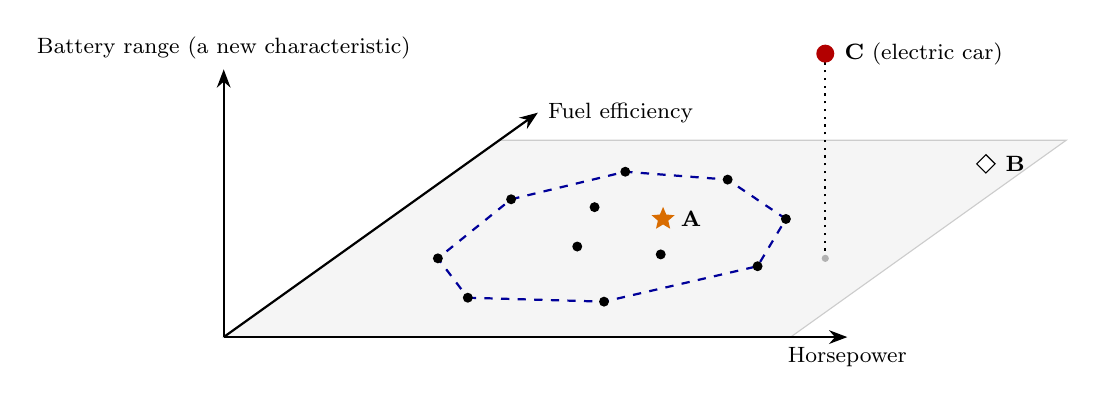
\begin{tikzpicture}[x={(1.2cm,0cm)}, y={(0.7cm,0.5cm)}, z={(0cm,1cm)}, font=\footnotesize, >=Stealth]
  \fill[gray!8] (0,0,0) -- (6,0,0) -- (6,5,0) -- (0,5,0) -- cycle;
  \draw[gray!40] (0,0,0) -- (6,0,0) -- (6,5,0) -- (0,5,0) -- cycle;
  \draw[->, thick] (0,0,0) -- (6.6,0,0) node[below] {Horsepower};
  \draw[->, thick] (0,0,0) -- (0,5.7,0) node[right] {Fuel efficiency};
  \draw[->, thick] (0,0,0) -- (0,0,3.4) node[above] {Battery range (a new characteristic)};
  \draw[dashed, blue!60!black, thick] (2.0,1.0,0) -- (3.5,0.9,0) -- (4.6,1.8,0) -- (4.2,3.0,0) -- (3.0,4.0,0)
        -- (1.8,4.2,0) -- (1.0,3.5,0) -- (1.1,2.0,0) -- cycle;
  \foreach \h/\e in {2.0/1.0, 3.5/0.9, 4.6/1.8, 4.2/3.0, 3.0/4.0, 1.8/4.2, 1.0/3.5, 1.1/2.0, 2.4/2.3, 3.4/2.1, 2.0/3.3}
    \fill[black] (\h,\e,0) circle (1.8pt);
  \node[star, star points=5, star point ratio=2.2, fill=orange!85!black, inner sep=1.4pt,
        label={[font=\footnotesize\bfseries]right:A}] at (2.9,3.0,0) {};
  \node[diamond, draw=black, fill=white, inner sep=1.7pt,
        label={[font=\footnotesize\bfseries]right:B}] at (5.5,4.4,0) {};
  \draw[dotted, thick] (5.2,2.0,0) -- (5.2,2.0,2.6);
  \fill[gray!60] (5.2,2.0,0) circle (1.3pt);
  \node[circle, fill=red!70!black, inner sep=2.3pt,
        label={[font=\footnotesize]right:\textbf{C} (electric car)}] at (5.2,2.0,2.6) {};
\end{tikzpicture}
\caption{Characteristics space and new goods. Dots are existing products in the plane of two observed
characteristics, and the dashed polygon is their convex hull. Tastes estimated from these products predict demand
for a new combination inside the hull (A, an interpolation). A product outside the hull but in the same plane (B)
is predicted only by extrapolating the functional form. An electric car (C) sits off the plane: it has a
characteristic that no existing product has, so the data are silent about how consumers value it.}
\label{fig:04-charspace}
\end{figure}

\subsection{Drawbacks of characteristics space}\label{sec:04-spaces-drawbacks}

The characteristics approach has six drawbacks. The first two are practical. The approach needs more data,
namely the relevant characteristics of every product and often information on consumers. Estimation is harder,
because market shares are integrals over the taste distribution that must be inverted and simulated
(\cref{ch:blp}). The other four drawbacks are conceptual.

\casehead{Too many characteristics}
Models with an i.i.d.\ taste shock $\epsilon_{ij}$ for every product can have odd implications, known as the
\emph{too many characteristics} problem. The shock is a taste for the product itself, so it acts as one more
characteristic for each product. Adding a product adds a dimension to the space. Three consequences follow in the
logit, with $\Phi = 1 + \sum_{k=1}^{J}e^{\delta_k}$. \Cref{prop:06-logit-exhaust} proves them in detail.
\begin{enumerate}
  \item \emph{Clones attract buyers.} Let product $J+1$ be an exact copy of product 1, with the same $\delta_1$. The
  copy's share and the original's share are both $\frac{e^{\delta_1}}{\Phi + e^{\delta_1}}$, so together the two
  identical products sell
  \begin{equation*}
  \frac{2e^{\delta_1}}{\Phi + e^{\delta_1}} > \frac{e^{\delta_1}}{\Phi} ,
  \end{equation*}
  where the inequality is $2\Phi > \Phi + e^{\delta_1}$, true because $\Phi > e^{\delta_1}$. A physical duplicate
  draws new customers from the outside good.
  \item \emph{Markups never vanish.} A single-product logit firm sets
  \begin{equation*}
  p_j - mc_j = \frac{1}{\alpha(1 - s_j)} > \frac{1}{\alpha}
  \end{equation*}
  however many products crowd the market (\cref{prop:04-logit-markup}). With $J$ symmetric firms the markup
  converges to $\frac{1}{\alpha}$ as $J$ grows, so it stays bounded away from zero.
  \item \emph{Every product adds welfare.} At fixed prices, adding product $J+1$ raises consumer surplus by
  \begin{equation*}
  \Delta CS = \frac{1}{\alpha}\ln\Big(1 + \frac{e^{\delta_{J+1}}}{\Phi}\Big) > 0 ,
  \end{equation*}
  even if the product duplicates an existing one. With $J$ identical products of mean utility $\delta$, consumer
  surplus is $\frac{1}{\alpha}\ln(1 + Je^{\delta})$, which grows like $\frac{1}{\alpha}\ln J$ without bound.
\end{enumerate}
The \emph{pure characteristics model} of \citet{BerryPakes2007} removes the product-specific shock, so the space
has a fixed dimension. As products fill the space, neighbors become close substitutes, prices are driven toward
marginal cost, and the gain from one more product declines to zero (pp.~6--7). \Cref{sec:06-epsilon} develops the
comparison, and \cref{ch:newgoods} shows how much it matters for the value of new goods.

\casehead{No complementarity}
In a model where each consumer buys one unit of one product, all products are substitutes. Raising $p_j$ lowers
only the utility of product $j$. Every consumer who bought $k \neq j$ still prefers $k$, and some former buyers of
$j$ switch to $k$, so $\frac{\partial s_k}{\partial p_j} \geq 0$ (\cref{cor:06-wdz}). Complements such as a printer
and its cartridges, or a print and an online newspaper, need other structures. \citet{Gentzkow2007} treats bundles
of products as choice alternatives. A utility term lets the value of a bundle exceed or fall short of the sum of
its parts (\cref{ch:newgoods}). \citet{Hendel1999} develops a model of multiple discrete choices (\cref{ch:logit}).

\casehead{Unmeasurable attributes}
For books, films or recipes, the attributes that matter (plot, style, taste) cannot be coded as a short vector
$x_j$. The unobserved quality $\xi_j$ then carries most of the variation, and the dimension advantage disappears.
\citet[sec.~5.5]{Hausman1997} makes this objection for breakfast cereals and models each brand with its own
parameters (\cref{ch:newgoods}).

\casehead{Exogenous characteristics}
Empirical characteristics models treat $x_j$ as fixed and uncorrelated with $\xi_j$. This is the assumption behind
characteristics-based instruments, and it fails if firms choose characteristics knowing $\xi_j$
(\cref{sec:06-charinst}). It also leaves out product choice, which the location models of \cref{sec:04-location}
study.

\subsection{The dimension of characteristics space shapes competition}\label{sec:04-spaces-dimension}

The dimension of characteristics space is a modeling choice with first-order consequences. In a space of one or
two dimensions each product competes, on average, with a few neighbors. In a logit-type model every product competes with every other.
\citet[Section~7]{CaplinNalebuff1991} make the role of dimension precise. They measure dimension by the number of
taste parameters. Consumers may evaluate many product attributes through a few indices, so the count of attributes
can overstate the dimension that matters.

We work with Assumption A1 of \cref{ass:04-cn-a1}. Consumer types $\nu \in \R^L$ have density $\psi$ on a support
$B$. The utility of type $\nu$ from product $j$, bought out of income $y$, is
\begin{equation}\label{eq:04-cn-utility}
U_j(\nu) = \sum_{l = 1}^{L}\nu_l\,t_l(x_j) + g(y - p_j)\,t_{L+1}(x_j) + t_{L+2}(x_j)
= \nu \cdot \bm{t}_j + a_j ,
\end{equation}
where $\bm{t}_j = (t_1(x_j), \dots, t_L(x_j))$ and $a_j = g(y - p_j)t_{L+1}(x_j) + t_{L+2}(x_j)$. At fixed prices,
utility is affine in the type. Type $\nu$ prefers $j$ to $k$ when $\nu \cdot (\bm{t}_j - \bm{t}_k) > a_k - a_j$, which
defines a half-space of types. The \emph{market area} of product $j$ is the set of types in $B$ who prefer $j$ to
every other product. \citet[p.~18]{CaplinNalebuff1991} call product $k$ a competitor of product $j$ if a marginal
cut in $p_j$ reduces the demand for $k$. We use a sharper version. Product $k$ is a \emph{competitor} of product
$j$ if their market areas share a boundary piece of positive $(L-1)$-dimensional volume. This piece is a segment of
positive length when $L = 2$ and a face of positive area when $L = 3$. If the type density is positive on the
interior of $B$, a cut in $p_j$ moves this piece into the area of $k$. The demand for $k$ then falls at a rate
proportional to the size of the cut, so the cross-price effect is nonzero at first order. The two definitions
can differ only when the set where two market areas touch has dimension below $L - 1$, such as a point at which
four or more areas meet in the plane (\cref{rem:04-competitor-def}). As in
\cref{sec:04-existence}, each of the $J$ products is sold by a separate firm.

\begin{proposition}[Dimension restricts preferences, after \citealp{CaplinNalebuff1991}, Proposition 8]\label{prop:04-cn-orderings}
Let utility satisfy \eqref{eq:04-cn-utility} with $L$-dimensional types, and fix the prices of $J$ products.
\begin{enumerate}[label=(\alph*)]
  \item If $J \leq L + 1$ and the vectors $\bm{t}_1, \dots, \bm{t}_J$ are affinely independent, then each of the $J!$
  strict preference orderings of the products is held by a set of types in $\R^L$ of positive volume.
  \item If $J > L + 1$, some of the $J!$ orderings are held by no type.
\end{enumerate}
\end{proposition}

\begin{proof}
(a) Fix an ordering $\iota(1) \succ \iota(2) \succ \dots \succ \iota(J)$, where $\iota$ is a permutation of the products.
By transitivity it suffices that each product beats the next one, that is,
\begin{equation*}
\nu \cdot d_r > a_{\iota(r+1)} - a_{\iota(r)}, \qquad d_r = \bm{t}_{\iota(r)} - \bm{t}_{\iota(r+1)}, \qquad r = 1, \dots, J - 1.
\end{equation*}
The vectors $d_1, \dots, d_{J-1}$ telescope, so they span the same space as the vectors $\bm{t}_k - \bm{t}_{\iota(J)}$,
$k \neq \iota(J)$. That space has dimension $J - 1$ because the $\bm{t}_j$ are affinely independent. The $J - 1 \leq L$
vectors $d_r$ are therefore linearly independent, and the linear map $\nu \mapsto (\nu \cdot d_1, \dots, \nu \cdot
d_{J-1})$ from $\R^L$ to $\R^{J-1}$ is onto. Some type $\nu^*$ therefore attains any target, for instance $\nu^*
\cdot d_r = a_{\iota(r+1)} - a_{\iota(r)} + 1$ for every $r$. By continuity every type near $\nu^*$ satisfies the strict
inequalities, which gives a set of positive volume.

(b) \citet{CaplinNalebuff1991} derive the general case from a theorem of \citet{Greenberg1979} on majority rule.
That theorem implies that some product wins at least the fraction $\frac{1}{L+1}$ of the market in a pairwise
contest with each of the other products. Suppose all orderings were possible. Then we could form a population of
$J$ equally weighted types holding the $J$ cyclic orderings $1 \succ 2 \succ \dots \succ J$, then $J \succ 1 \succ
\dots \succ J - 1$, and so on. In this population product $j$ beats product $j - 1$ only in one of the $J$
orderings, where product $0$ is read as product $J$. Every product thus wins only the fraction $\frac{1}{J} <
\frac{1}{L+1}$ of some pairwise contest, a contradiction.

The one-dimensional case has an elementary proof. With $L = 1$, each $U_j(\nu) = \nu\bm{t}_j + a_j$ is a line in
$\nu$. Two lines cross at most once, so the ranking of the products changes only at crossing points, and there are
at most $\frac{J(J-1)}{2}$ of them. These points cut the real line into at most $\frac{J(J-1)}{2} + 1$ intervals, each with a single
ranking. For $J = 3$ at most $4 < 3! = 6$ orderings occur, and $\frac{J(J-1)}{2} + 1 < J!$ for every $J \geq 3$.
The restriction has a sharp form. Label three products so that $\bm{t}_1 < \bm{t}_2 < \bm{t}_3$, and let $\nu_{jk}$ be
the type indifferent between $j$ and $k$. Product 2 is ranked first by the types in $(\nu_{12}, \nu_{23})$ and last
by the types in $(\nu_{23}, \nu_{12})$. At most one of these intervals is nonempty, so the middle product is never
both some type's favorite and another type's worst.
\end{proof}

In one dimension consumers behave like voters on a left-right spectrum. Each product competes with at most two
neighbors, whatever the number of products. In two dimensions a single product can compete with all others, but
the average number of competitors is bounded.

\begin{proposition}[Six competitors in two dimensions, after \citealp{CaplinNalebuff1991}, Proposition 9]\label{prop:04-cn-six}
Let utility satisfy \eqref{eq:04-cn-utility} with $L = 2$, and let the type density satisfy Assumption A2
(\cref{ass:04-cn-a2}), so that in particular its support $B$ is convex. At any prices, let $J' \geq 3$ be the
number of firms with positive demand and $C_j$ the number of competitors of firm $j$. Then
\begin{equation*}
\frac{1}{J'}\sum_{j}C_j \leq 6 .
\end{equation*}
\end{proposition}

\begin{proof}
\emph{Market areas.} The types who buy $j$ form the intersection of $B$ with the half-planes in which $j$ beats
each rival. The intersection of convex sets is convex, so every market area is convex. The areas partition $B$,
up to indifferent types, who have measure zero. Two convex areas meet along at most one segment, because their
common boundary lies on the line of types indifferent between the two products. By definition, product $k$ is a
competitor of $j$ exactly when the areas share a segment of positive length. A cut in $p_j$ then shifts that
segment into $k$'s area, and the consumers it passes over switch from $k$ to $j$.

\emph{Polygons.} Following Caplin and Nalebuff, replace $B$ by the convex hull of the points on its boundary at
which some consumer is indifferent between two products. This changes no neighbor relation, because each cut-off
piece of $B$ lies inside a single market area. Now $B$ is a convex polygon, every market area is a convex polygon
with $n_j$ sides, and $C_j \leq n_j$. Sides on the boundary of $B$ separate no two firms, and each other side is
shared with exactly one competitor.

\emph{Angles.} The interior angles of a convex polygon with $n_j$ sides sum to $180^\circ(n_j - 2)$. Summing over all
market areas, the angles total
\begin{equation*}
\sum_j 180^\circ (n_j - 2) = 180^\circ\Big(\sum_j n_j - 2J'\Big).
\end{equation*}
We bound the same total vertex by vertex. A corner of a market area in the interior of $B$ is a point where at
least three areas meet. (Where only two convex areas meet, their boundary is straight.) The angles at such a vertex
sum to $360^\circ$, so their average is at most $120^\circ$. A vertex on the boundary of $B$ is a point where at
least two areas meet, with angles summing to at most $180^\circ$, so their average is at most $90^\circ$. There are
$\sum_j n_j$ angles in all, so their total is at most $120^\circ\sum_j n_j$. Combining the two expressions,
\begin{equation*}
180\Big(\sum_j n_j - 2J'\Big) \leq 120\sum_j n_j
\quad\Longrightarrow\quad
60\sum_j n_j \leq 360\,J'
\quad\Longrightarrow\quad
\frac{1}{J'}\sum_j n_j \leq 6 .
\end{equation*}
Since $C_j \leq n_j$, the average number of competitors is at most six.
\end{proof}

The bound is attained in the limit by a regular hexagonal tiling of the plane, as in the location theory of
\citet{Losch1954}. \citet{CaplinNalebuff1991} add that, for generic product locations and prices, the average
converges to six as the number of firms grows. They also note that no regular polygon with more than six sides
tiles the plane. In three dimensions space can be tiled with 14-faced solids (truncated octahedra), so each firm
can have 14 competitors. This tiling is an example and gives no upper bound. The planar bound has no analogue in
three dimensions, as \cref{ex:04-no-bound-3d} shows. \citet{Stiglitz1986} studied a model in which market areas are
$L$-dimensional cubes. In the summary of \citet{CaplinNalebuff1991}, the markup there is inversely proportional to
the ratio of a market area's surface to its volume. Markets therefore become more competitive as the dimension
rises.

\citet[n.~17]{CaplinNalebuff1991} compare the bound with a result of \citet{ArchibaldRosenbluth1975} for the
Lancaster model, in which goods are freely divisible and can be combined. When goods are represented in a
three-dimensional space of characteristics, the average number of competitors per firm there is at most six as well.
With four characteristics Archibald and Rosenbluth find no bound on the number of neighbors.
\citet[Section 7.1.2, n.~6]{Tirole1988} reports that an average brand may then have $\frac{J}{2}$ direct
competitors. Caplin and Nalebuff state that this unboundedness does not carry over to the three-dimensional version
of their model. That statement is incorrect. \Cref{ex:04-no-bound-3d} gives three-dimensional configurations that
satisfy A1 and A2 in which the average firm has at least $\frac{J}{2}$ competitors. Caplin and Nalebuff also give
a geometric comparison. In the Lancaster model with $L$ characteristics, the count is the average number of sides
in a partition of an $(L-1)$-dimensional surface into polygons, which need not be convex. That count is at least
as large as the Caplin-Nalebuff count in $L - 1$ dimensions, whose market areas are convex. The two counts agree
for partitions of the plane because convexity makes no difference there.

\Cref{fig:04-voronoi} illustrates the proposition. Consumers' ideal points $\nu$ are uniform on the unit square,
and a consumer buys from the product $j$ that minimizes $p_j + \tau\|\nu - x_j\|^2$, with $x_j$ the product's
location and $\tau$ a mismatch cost. Expanding the square shows that this preference satisfies
\eqref{eq:04-cn-utility}: the terms $\tau\|\nu\|^2$ are common to all products and cancel from every comparison.
Type $\nu$ prefers $j$ to $k$ when
\begin{equation*}
2\tau\,\nu \cdot (x_k - x_j) < p_k - p_j + \tau\big(\|x_k\|^2 - \|x_j\|^2\big),
\end{equation*}
a half-plane. With equal prices the market areas are the \emph{Voronoi cells} of the locations, the sets of points
closer to one location than to any other. With unequal prices they form a \emph{power diagram}, in which a
high-priced product's area shrinks and can vanish.

\begin{figure}[htbp]
\centering
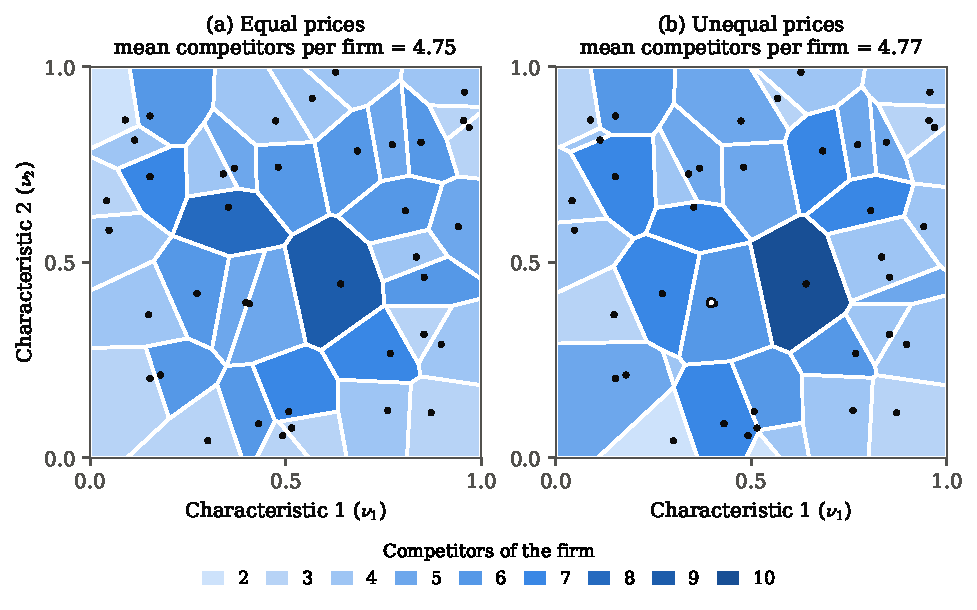
\includegraphics[width=\linewidth]{figures/ch04/voronoi.pdf}
\caption{Market areas of 40 products in a two-dimensional characteristics space. Consumers' ideal points are uniform
on the unit square, mismatch costs are quadratic, and dots mark product locations. Shading gives each firm's number
of competitors. (a) Equal prices: Voronoi cells. The average number of competitors is 4.75 over all 40 firms and
5.83 over the 18 firms whose areas do not touch the boundary. (b) Prices drawn between 1.000 and 1.012: power
diagram. One product (open circle) has no buyers. The average is 4.77 over the 39 active firms and 5.72 over the
18 interior firms. Computed with \texttt{figures/ch04/src/voronoi.py}.}
\label{fig:04-voronoi}
\end{figure}

The averages in the figure lie below six, as the proposition requires. Firms at the edge of the market have few
competitors, which pulls the overall average down. As the number of firms grows, the boundary matters less and
the average approaches six from below. Over random draws of uniform locations with equal prices, the average number
of competitors is 3.72 with 10 firms, 4.87 with 40, 5.43 with 160, 5.72 with 640 and 5.80 with 1,280. For firms
away from the boundary the averages are 5.16, 5.71, 5.87, 5.94 and 5.96.

\begin{remark}[Why competitors are defined by shared boundaries]\label{rem:04-competitor-def}
The definition of \citet{CaplinNalebuff1991} counts $k$ as a competitor of $j$ if a marginal cut in $p_j$
reduces $q_k$. Read as a nonzero derivative, it agrees with the shared-boundary definition when the type density
is positive on the interior of $B$. Read literally, as any loss of demand after a small cut, it counts
second-order losses too. Under the literal reading the bound in \cref{prop:04-cn-six} fails in degenerate
configurations. Place
$J \geq 8$ products at equal prices, equally spaced on a circle, with the quadratic mismatch costs of
\cref{fig:04-voronoi}. Let types be uniform on a disk with the same center. The Voronoi cells are wedges that
all meet at the center, and each shares edges only with its two neighbors. After a cut of size $\eta > 0$ in $p_j$, product $j$ is the strict favorite of every type near the
center, so it takes buyers from every other wedge. For a wedge that touches $j$'s area only at the center, the
lost area is of order $\eta^2$, and its first-order cross-price effect is zero. Under the literal reading every
firm has $J - 1 > 6$ competitors. Under the shared-boundary definition every firm has two, as the proposition
allows.
\end{remark}

\begin{example}[No bound in three dimensions]\label{ex:04-no-bound-3d}
Let $L = 3$ and let a consumer buy the product that minimizes $p_j + \tau\|\nu - x_j\|^2$, as in
\cref{fig:04-voronoi}. At equal prices the market areas are Voronoi cells. Types are uniform on the ball of
radius 2 around the origin, which satisfies A2.
Place $n$ products at $A_i = (a_i, 0, 0)$ and $n$ products at $B_l = (1, b_l, 1)$, with distinct $a_i \in [0, 1]$
and distinct $b_l \in [0, 1]$. The two groups lie on two skew lines. For each pair $(i, l)$ let
\begin{equation*}
z_{il} = \frac{(1 - a_i)^2 + 1 - b_l^2}{2}, \qquad c_{il} = (a_i, b_l, z_{il}).
\end{equation*}
The squared distances from $c_{il}$ to $A_i$ and to $B_l$ both equal $b_l^2 + z_{il}^2$. The squared distance to
any other $A_k$ is larger by $(a_k - a_i)^2 > 0$, and the squared distance to any other $B_k$ is larger by
$(b_k - b_l)^2 > 0$. By continuity, the types near $c_{il}$ on the plane of indifference between $A_i$ and $B_l$
are strictly closer to these two locations than to any other. Since $0 \leq z_{il} \leq 1$, the point $c_{il}$
lies inside the ball. The market areas of the two products therefore share a face of positive area within the
support. All $n^2$ such pairs are competitors under the sharper definition, and every product has positive
demand. With $J = 2n$ firms the average number of competitors is at least $\frac{2n^2}{2n} = n = \frac{J}{2}$,
which grows without bound.
\end{example}

The result matters for empirical work in two ways. A pure characteristics model in one or two dimensions implies a
sparse matrix of cross-price effects, in which a product's diversion goes on average to at most six neighbors. In
three or more dimensions the sparsity depends on the configuration of products (\cref{ex:04-no-bound-3d}). A logit-type model
spreads every product's diversion over all products. These are very different predictions for a merger between
two products, and the choice between them is made when the researcher picks the dimension of the model. The result
also shows that the location models of \cref{sec:04-location}, with one dimension, impose strong restrictions on
preferences, and that richer competition requires more dimensions.

\subsection{Demand systems in product space}\label{sec:04-spaces-product}

The goal of product-space demand analysis is to estimate $q = f(p, z)$ in a form that is flexible and consistent
with consumer theory. Aggregation is the main theoretical issue. Market demand behaves like the demand of a single
utility-maximizing consumer only under restrictions on individual preferences. Two such restrictions are the Gorman
polar form and the price-independent generalized logarithmic (PIGLOG) class (\cref{ch:aids}).
\Cref{tab:04-productspace-systems} summarizes the four classical systems. In the table and in this subsection goods are indexed by $i$ and $k$, as in \cref{ch:aids}. Total expenditure is $y$, and
$w_i = \frac{p_i q_i}{y}$ is the budget share of good $i$.

\begin{table}[htbp]
\centering
\caption{Classical demand systems in product space}
\label{tab:04-productspace-systems}
\footnotesize
\renewcommand{\arraystretch}{1.35}
\begin{tabularx}{\textwidth}{@{}>{\raggedright\arraybackslash}p{2.15cm}>{\raggedright\arraybackslash}p{4.35cm}%
>{\raggedright\arraybackslash}p{1.9cm}>{\raggedright\arraybackslash}p{2.7cm}>{\raggedright\arraybackslash}X@{}}
\toprule
System and source & Demand equation & Price parameters & Restrictions of theory & Main limitation \\
\midrule
Linear expenditure system \citep{Stone1954}
 & $p_iq_i = p_i\gamma_i + \beta_i\big(y - \sum_k p_k\gamma_k\big)$, from Stone-Geary utility $\sum_i\beta_i\ln(q_i -
   \gamma_i)$ with $\sum_i\beta_i = 1$
 & None beyond the $2J - 1$ parameters $(\gamma, \beta)$
 & Adding up, homogeneity and symmetry hold by construction
 & Too few parameters to be flexible. All goods are Hicksian substitutes, and no good is inferior. \\
Rotterdam model \citep{Theil1965,Barten1966}
 & $w_i\,\dd\ln q_i = \theta_i\,\dd\ln\bar Q + \sum_k\pi_{ik}\,\dd\ln p_k$, with $\dd\ln\bar Q = \sum_k w_k\,\dd\ln
   q_k$
 & $\frac{J(J-1)}{2}$ free $\pi_{ik}$
 & Adding up, homogeneity and symmetry are linear restrictions on $(\theta, \pi)$. Negativity needs $[\pi_{ik}]$
   negative semidefinite
 & A local approximation in differentials, with constant coefficients, not derived from a utility function. \\
Indirect translog \citep{ChristensenJorgensonLau1975}
 & $w_i = \frac{\alpha_i + \sum_k\beta_{ik}\ln\frac{p_k}{y}}{\sum_l\alpha_l + \sum_l\sum_k\beta_{lk}\ln\frac{p_k}{y}}$,
   by Roy's identity from a quadratic $\ln V$ in $\ln\frac{p}{y}$
 & $\frac{J(J+1)}{2}$ symmetric $\beta_{ik}$, less a normalization
 & Homogeneity and adding up built in. Symmetry imposed by $\beta_{ik} = \beta_{ki}$
 & Shares nonlinear in parameters. Aggregates only under extra restrictions. \\
Almost Ideal Demand System \citep{DeatonMuellbauer1980a}
 & $w_i = \alpha_i + \sum_k\gamma_{ik}\ln p_k + \beta_i\ln\frac{y}{P}$, with translog price index $\ln P$
 & $\frac{J(J-1)}{2}$ free $\gamma_{ik}$
 & Linear and testable: adding up, homogeneity, symmetry
 & Still of order $J^2$ parameters. Negativity not imposed globally. \\
\bottomrule
\end{tabularx}

\vspace{3pt}
\begin{minipage}{0.97\textwidth}
\footnotesize Notes: Goods are indexed by $i$ and $k$, $y$ is total expenditure and $w_i = \frac{p_iq_i}{y}$ is a
budget share. Parameter symbols are specific to each row. For the AIDS, $\ln P = \alpha_0 + \sum_k\alpha_k\ln p_k
+ \frac{1}{2}\sum_k\sum_l\gamma_{kl}\ln p_k\ln p_l$, and the restrictions are $\sum_i\alpha_i = 1$,
$\sum_i\gamma_{ik} = 0$, $\sum_i\beta_i = 0$ (adding up), $\sum_k\gamma_{ik} = 0$ (homogeneity) and $\gamma_{ik} =
\gamma_{ki}$ (symmetry) \citep[eqs.~8--12]{DeatonMuellbauer1980a}. In the Rotterdam model $\dd\ln\bar Q$ is the
Divisia volume index. Price-parameter counts are after the restrictions of theory.
\end{minipage}
\end{table}

The linear expenditure system was the first system estimated from an explicit utility function
\citep[p.~312]{DeatonMuellbauer1980a}. Consumers buy subsistence quantities $\gamma_i$ first and split the remaining
income in the fixed proportions $\beta_i$. Its cross-price effects are $\frac{\partial q_i}{\partial p_k} =
-\frac{\beta_i\gamma_k}{p_i}$ for $k \neq i$, so the $J^2$ price effects are pinned down by $2J - 1$ parameters. The
Rotterdam model approximates the demand functions themselves in differential form. The translog approximates the
indirect utility function to second order. The Almost Ideal Demand System starts from a class of preferences that
aggregates across consumers and yields shares that are nearly linear in the parameters. \Cref{ch:aids} develops the
AIDS in full, and \cref{rem:05-translog-piglog} states when the translog aggregates.

\casehead{Three problems in practice}
The first problem is dimensionality. A linear system $q = a + Ap$ has $J$ intercepts and $J^2$ price
coefficients. With $J = 50$ brands, as in a cereal aisle, that is 2,500 price coefficients. Symmetry reduces the
count to $\frac{J(J+1)}{2} = 1{,}275$, and the full set of AIDS restrictions to $\frac{J(J-1)}{2} = 1{,}225$. These
numbers exceed what typical market-level data can estimate.

The second problem is instruments. Each demand equation contains all $J$ prices, and every price is endogenous. Write
the equation for good $i$ in market $t$ as $q_{it} = a_i + \sum_k A_{ik}p_{kt} + e_{it}$, and let $z_t$ be a vector
of excluded instruments. The order condition requires at least $J$ instruments. The rank condition requires that
$\E[z_t p_t^\top]$ have rank $J$, so the instruments must move the $J$ prices independently of one another. A single
market-wide cost shifter fails this test. If $z_t$ is a scalar, the first-stage fitted prices $\hat p_{kt} =
\hat\pi_k z_t$ are proportional to one another, and only one linear combination of the row $A_{i\cdot}$ is
identified. Identification needs product-specific shifters, such as ingredient costs that differ across products,
or prices of the same product in other markets (\cref{ch:aids}).

The third problem is consumer heterogeneity. A representative consumer cannot say who gains and who loses from a
price change or a new product. Distributional questions, and substitution patterns that depend on who buys which
product, require explicit heterogeneity. Characteristics models build it in through the taste distribution and
demographics.

\casehead{Four ways forward}
Applied work responds to these problems in four ways. Each buys tractability with an assumption.
\begin{enumerate}
  \item \emph{Aggregate, or study one product.} Group products into a few aggregates, or estimate the residual
  demand of a single firm, as \citet{BakerBresnahan1988} do (\cref{ch:conduct}). This sacrifices the cross-effects
  among products within each aggregate.
  \item \emph{Impose symmetry.} Representative-consumer systems such as CES and logit treat products symmetrically
  up to one or two parameters (\cref{sec:04-repcons}). They suit questions about variety and poorly serve questions
  about which products are close substitutes.
  \item \emph{Impose separability.} Multi-stage budgeting splits goods into groups and estimates a small system within
  each group (\cref{sec:05-separability}). \citet{HausmanLeonardZona1994} and \citet{Hausman1997} follow this route
  with the AIDS at the lowest level.
  \item \emph{Move to characteristics space.} Discrete choice models replace product-indexed parameters with tastes for
  characteristics (\cref{ch:discrete,ch:logit,ch:blp}), at the costs described in \cref{sec:04-spaces-drawbacks}.
\end{enumerate}
The rest of this chapter develops the second route, together with the location models that underlie the fourth.
\Cref{ch:aids} takes the third route, and \cref{ch:discrete,ch:logit,ch:blp} take the fourth.

\section{Representative-consumer demand systems: linear, CES and logit}\label{sec:04-repcons}

\Cref{sec:04-spaces} showed that an unrestricted demand system in product space has far too many parameters.
One remedy imposes symmetry. A \emph{representative consumer} is a single fictitious agent whose demands equal
market demands. If she also treats all products symmetrically, a handful of parameters governs every own and
cross effect. This section develops the three systems of this kind that appear most often in applied work:
linear demand from quadratic utility, constant elasticity of substitution (CES) demand, and the logit. For each
we derive demand, elasticities, diversion and Bertrand markups. We then show that the CES and the logit are also
discrete choice models, which ties this section to the random utility models of \cref{ch:discrete}. A two-sector
version of the CES model, the model of monopolistic competition of \citet{Spence1976} and \citet{DixitStiglitz1977},
asks whether markets supply the right number of products. The section closes with the questions these systems answer
well and a table that compares them.

\subsection{Linear demand from quadratic utility}\label{sec:04-repcons-linear}

The linear demand of \cref{ex:04-linear-duopoly} has a utility foundation. A representative consumer with
income $y$ buys quantities $q_1, \dots, q_J$ of $J$ differentiated products and an amount $z$ of a numeraire good
with price one. Her utility is quasi-linear in the numeraire,
\begin{equation}\label{eq:04-quadratic-utility}
U(q, z) = z + \bar a\sum_{j=1}^J q_j - \frac{1}{2}\Big[\bar b\sum_{j=1}^J q_j^2 + 2\bar g\sum_{j<k}q_jq_k\Big],
\qquad \bar b > \bar g \ge 0
\end{equation}
\citep{SinghVives1984,Vives1999}. The parameter $\bar a$ is the marginal utility of the first unit of any
product. The parameter $\bar b$ measures how fast marginal utility falls with own consumption, and $\bar g$
measures how much consuming one product lowers the marginal utility of another. The products are substitutes
when $\bar g > 0$ and independent when $\bar g = 0$. As $\bar g$ approaches $\bar b$, utility depends only on total
consumption and the products become perfect substitutes.

\begin{proposition}[Linear demand from quadratic utility]\label{prop:04-quadratic}
Let the consumer maximize \eqref{eq:04-quadratic-utility} subject to $z + \sum_j p_jq_j = y$, and suppose the
solution has $q_j > 0$ for every $j$ and $z > 0$. Then:
\begin{enumerate}[label=(\roman*)]
\item Inverse demand is $p_j = \bar a - \bar bq_j - \bar g\sum_{k \ne j}q_k$.
\item With two products, demand is $q_j = a - bp_j + dp_k$ with
\begin{equation*}
a = \frac{\bar a}{\bar b + \bar g}, \qquad b = \frac{\bar b}{\bar b^2 - \bar g^2}, \qquad d = \frac{\bar g}{\bar b^2 - \bar g^2},
\end{equation*}
so that $b > d \ge 0$ and the diversion ratio is $D_{jk} = \frac{d}{b} = \frac{\bar g}{\bar b}$.
\item With $J$ products, for every $k \ne j$,
\begin{equation*}
\frac{\partial q_j}{\partial p_j} = -\frac{\bar b + (J-2)\bar g}{(\bar b - \bar g)[\bar b + (J-1)\bar g]},
\qquad
\frac{\partial q_k}{\partial p_j} = \frac{\bar g}{(\bar b - \bar g)[\bar b + (J-1)\bar g]},
\qquad
D_{jk} = \frac{\bar g}{\bar b + (J-2)\bar g}.
\end{equation*}
A fraction $1 - (J-1)D_{jk} = \frac{\bar b - \bar g}{\bar b + (J-2)\bar g}$ of the sales that product $j$ loses
leaves the group of products.
\end{enumerate}
\end{proposition}

\begin{proof}
For (i), substitute the budget constraint $z = y - \sum_j p_jq_j$ into utility:
\begin{equation*}
y + \sum_{j=1}^J(\bar a - p_j)q_j - \frac{1}{2}\Big[\bar b\sum_{j}q_j^2 + 2\bar g\sum_{j<k}q_jq_k\Big].
\end{equation*}
The derivative with respect to $q_j$ is $\bar a - p_j - \bar bq_j - \bar g\sum_{k\ne j}q_k$. Setting it to zero gives
(i). The Hessian of the objective is $-B$, where $B$ has $\bar b$ on the diagonal and $\bar g$ off it. In matrix form
$B = (\bar b - \bar g)I_J + \bar g\mathbf{1}\mathbf{1}^\top$. Its eigenvalues are $\bar b - \bar g > 0$ (on vectors
orthogonal to $\mathbf{1}$) and $\bar b + (J-1)\bar g > 0$ (on $\mathbf{1}$). The objective is therefore strictly
concave, and the first-order conditions characterize the maximum.

For (ii) and (iii), stack (i) as $p = \bar a\mathbf{1} - Bq$, so that $q = B^{-1}(\bar a\mathbf{1} - p)$ and
$\frac{\partial q}{\partial p^\top} = -B^{-1}$. We claim that
\begin{equation*}
B^{-1} = \frac{1}{\bar b - \bar g}\Big[I_J - \frac{\bar g}{\bar b + (J-1)\bar g}\mathbf{1}\mathbf{1}^\top\Big].
\end{equation*}
To check it, multiply by $B$ and use $\mathbf{1}\mathbf{1}^\top\mathbf{1}\mathbf{1}^\top = J\mathbf{1}\mathbf{1}^\top$:
\begin{align*}
\big[(\bar b - \bar g)I_J + \bar g\mathbf{1}\mathbf{1}^\top\big]\Big[I_J - \frac{\bar g}{\bar b + (J-1)\bar g}\mathbf{1}\mathbf{1}^\top\Big]
&= (\bar b - \bar g)I_J + \Big[\bar g - \frac{\bar g(\bar b - \bar g) + J\bar g^2}{\bar b + (J-1)\bar g}\Big]\mathbf{1}\mathbf{1}^\top \\
&= (\bar b - \bar g)I_J + \Big[\bar g - \frac{\bar g\,[\bar b + (J-1)\bar g]}{\bar b + (J-1)\bar g}\Big]\mathbf{1}\mathbf{1}^\top
= (\bar b - \bar g)I_J .
\end{align*}
The diagonal element of $-B^{-1}$ is
$-\frac{1}{\bar b - \bar g}\big[1 - \frac{\bar g}{\bar b + (J-1)\bar g}\big] = -\frac{\bar b + (J-2)\bar g}{(\bar b - \bar g)[\bar b + (J-1)\bar g]}$,
and the off-diagonal element is $\frac{\bar g}{(\bar b - \bar g)[\bar b + (J-1)\bar g]}$. This proves the derivatives in
(iii). The diversion ratio \eqref{eq:04-diversion-def} is minus their ratio. The fraction that leaves the group is
$1 - \frac{(J-1)\bar g}{\bar b + (J-2)\bar g} = \frac{\bar b - \bar g}{\bar b + (J-2)\bar g}$, which is positive
because $\bar b > \bar g$. Setting $J = 2$ gives $b = \frac{\bar b}{(\bar b - \bar g)(\bar b + \bar g)}$ and
$d = \frac{\bar g}{(\bar b - \bar g)(\bar b + \bar g)}$. The intercept is
$\frac{\bar a(\bar b - \bar g)}{\bar b^2 - \bar g^2} = \frac{\bar a}{\bar b + \bar g}$, which proves (ii).
\end{proof}

Three features of this system matter below. First, cross derivatives are symmetric,
$\frac{\partial q_k}{\partial p_j} = \frac{\partial q_j}{\partial p_k}$, because the Jacobian $-B^{-1}$ is symmetric. This
is the quasi-linear case (i) of \cref{rem:04-symmetry}. Second, the values $\bar a = 10$, $\bar b = \frac{2}{3}$ and
$\bar g = \frac{1}{3}$ give $a = 10$, $b = 2$ and $d = 1$, the numbers of \cref{ex:04-linear-duopoly}. Third, the
linear form holds only on the set of prices at which every product is bought. If $p_2$ is so high that $q_2 = 0$,
product 1 faces $q_1 = \frac{\bar a - p_1}{\bar b}$, with slope $\frac{1}{\bar b}$. This is smaller in absolute value
than $b = \frac{\bar b}{\bar b^2 - \bar g^2}$, so demand is continuous but kinked where the rival drops out.

The system has three parameters only because of symmetry. A general quadratic utility
$z + \bar a^\top q - \frac{1}{2}q^\top Bq$ with any symmetric positive definite $B$ gives the linear system
$q = B^{-1}(\bar a - p)$, with $\frac{J(J+1)}{2}$ slope parameters. That is the linear product-space system of
\cref{sec:04-spaces} with symmetry imposed. The symmetric version replaces it by $\bar b$ and $\bar g$.

\casehead{Crowded markets} The symmetric system has a strong implication for markets with many products.
Suppose $N$ single-product firms (here $N = F = J$) sell the $N$ products at a common marginal cost $c$. At
symmetric prices $p$, part (i) gives each firm the quantity $q = \frac{\bar a - p}{\bar b + (N-1)\bar g}$. By the
inverse semi-elasticity rule of \cref{sec:04-bertrand-single}, a single-product firm sets
$p - c = -q\big(\frac{\partial q_j}{\partial p_j}\big)^{-1}$. Substituting $q$ and the own slope from part (iii),
\begin{equation*}
p - c = \frac{\bar a - p}{\bar b + (N-1)\bar g}\cdot\frac{(\bar b - \bar g)[\bar b + (N-1)\bar g]}{\bar b + (N-2)\bar g}
= \frac{(\bar a - p)(\bar b - \bar g)}{\bar b + (N-2)\bar g}.
\end{equation*}
Write $\bar a - p = (\bar a - c) - (p - c)$ and collect the terms in $p - c$:
\begin{equation}\label{eq:04-linear-symmetric}
(p - c)\big[\bar b + (N-2)\bar g + \bar b - \bar g\big] = (\bar a - c)(\bar b - \bar g)
\quad\Longrightarrow\quad
p - c = \frac{(\bar a - c)(\bar b - \bar g)}{2\bar b + (N-3)\bar g}.
\end{equation}
With $N = 2$ and the numbers above, $p - c = \frac{9 \cdot \frac{1}{3}}{1} = 3$, so $p = 4$ as in
\cref{ex:04-linear-duopoly}. When $\bar g > 0$, the markup falls to zero as $N$ grows. Every new product is a
substitute for every existing one, and a crowded market approaches marginal-cost pricing. The same symmetric
products give consumers bounded gains from variety. At a common price $p$, consumer surplus is utility minus
expenditure, $Nq(\bar a - p) - \frac{1}{2}Nq^2[\bar b + (N-1)\bar g]$. Substituting $q$ gives
\begin{equation*}
CS(N) = Nq(\bar a - p) - \frac{1}{2}Nq(\bar a - p) = \frac{N(\bar a - p)^2}{2[\bar b + (N-1)\bar g]}
\;\longrightarrow\; \frac{(\bar a - p)^2}{2\bar g} \quad \text{as } N \to \infty .
\end{equation*}
The CES and logit systems behave very differently on both counts, as we show next.

\subsection{CES demand}\label{sec:04-repcons-ces}

The CES system is the workhorse of models of monopolistic competition and international trade. A representative
consumer spends income $y$ on $J$ products and has utility
\begin{equation}\label{eq:04-ces-utility}
u(q) = \Big(\sum_{j=1}^J q_j^{\frac{\sigma-1}{\sigma}}\Big)^{\frac{\sigma}{\sigma-1}}, \qquad \sigma > 1 .
\end{equation}
The parameter $\sigma$ is the \emph{elasticity of substitution}. We show below that
$\frac{q_j}{q_k} = (\frac{p_j}{p_k})^{-\sigma}$, so a one percent rise in the relative price $\frac{p_j}{p_k}$
lowers the relative quantity $\frac{q_j}{q_k}$ by $\sigma$ percent. In this section $\sigma$ always denotes the CES
elasticity, as in \cref{ch:aids}. It is a different object from the nesting parameter of the nested logit, which
other chapters also write as $\sigma$. Two other conventions appear in the literature. Some authors write the
inner exponent as $\varsigma = \frac{\sigma - 1}{\sigma} \in (0,1)$, so that $\sigma = \frac{1}{1-\varsigma}$. Others use a different
outer exponent, such as $(\sum_j q_j^\varsigma)^{1-\varsigma}$. Any strictly increasing transformation of $u$ represents the same
preferences, so all of these forms give the same demand.

\begin{proposition}[CES demand and Bertrand pricing]\label{prop:04-ces}
Let the consumer maximize \eqref{eq:04-ces-utility} subject to $\sum_j p_jq_j = y$. Define the \emph{CES price index}
$P^{CES} = \big(\sum_{k=1}^J p_k^{1-\sigma}\big)^{\frac{1}{1-\sigma}}$ and the expenditure shares
$s_j = \frac{p_jq_j}{y}$. Then:
\begin{enumerate}[label=(\roman*)]
\item Demand is
\begin{equation}\label{eq:04-ces-demand}
q_j = \frac{p_j^{-\sigma}}{\sum_{k}p_k^{1-\sigma}}\,y = \Big(\frac{p_j}{P^{CES}}\Big)^{-\sigma}\frac{y}{P^{CES}},
\qquad
s_j = \Big(\frac{p_j}{P^{CES}}\Big)^{1-\sigma},
\end{equation}
and indirect utility is $\frac{y}{P^{CES}}$.
\item The own elasticity is $\varepsilon_j = \sigma - (\sigma - 1)s_j = \sigma(1 - s_j) + s_j$, the cross elasticity
is $\varepsilon_{jk} = (\sigma - 1)s_k$ for $k \ne j$, and the income elasticity is one.
\item The diversion ratio is $D_{jk} = \frac{(\sigma - 1)p_jq_k}{y[\sigma - (\sigma - 1)s_j]}$. Measured in
expenditure, the fraction of the revenue lost by $j$ that goes to $k$ is
$-\frac{\partial(p_kq_k)}{\partial p_j}\big(\frac{\partial(p_jq_j)}{\partial p_j}\big)^{-1} = \frac{s_k}{1 - s_j}$.
\item Suppose each product has constant marginal cost $mc_j$ and firms set prices as in \cref{sec:04-bertrand}. A
single-product firm sets
\begin{equation}\label{eq:04-ces-lerner}
\frac{p_j - mc_j}{p_j} = \frac{1}{\sigma - (\sigma - 1)s_j}.
\end{equation}
A firm that sells the products $\mathcal{J}_f$ gives all of them the same Lerner index,
$\frac{p_j - mc_j}{p_j} = \frac{1}{\sigma - (\sigma - 1)S_f}$, where $S_f = \sum_{k\in\mathcal{J}_f}s_k$.
\end{enumerate}
\end{proposition}

\begin{proof}
(i) Let $\varsigma = \frac{\sigma - 1}{\sigma} \in (0,1)$ and $V(q) = \sum_j q_j^\varsigma$. Since $u = V^{\frac{1}{\varsigma}}$ is a strictly
increasing function of $V$, we may maximize $V$. It is strictly concave, and its marginal utilities are infinite at
zero, so the solution is interior and unique. The first-order condition of the Lagrangian is
$\varsigma q_j^{\varsigma-1} = \lambda p_j$. Since $\varsigma - 1 = -\frac{1}{\sigma}$, it gives
\begin{equation*}
q_j = \Big(\frac{\lambda}{\varsigma}\Big)^{-\sigma}p_j^{-\sigma} \equiv Cp_j^{-\sigma},
\end{equation*}
with $C$ the same for all products. The budget constraint gives $\sum_j p_j\,Cp_j^{-\sigma} = C\sum_j p_j^{1-\sigma} = y$,
so $C = \frac{y}{\sum_k p_k^{1-\sigma}}$. By definition $\sum_k p_k^{1-\sigma} = (P^{CES})^{1-\sigma}$, hence
$q_j = p_j^{-\sigma}(P^{CES})^{\sigma-1}y$, which is \eqref{eq:04-ces-demand}. Multiplying by $\frac{p_j}{y}$ gives
the share. For indirect utility, note that $\sigma\varsigma = \sigma - 1$, so
\begin{equation*}
q_j^\varsigma = \Big(\frac{p_j}{P^{CES}}\Big)^{-\sigma\varsigma}\Big(\frac{y}{P^{CES}}\Big)^\varsigma
= \Big(\frac{p_j}{P^{CES}}\Big)^{1-\sigma}\Big(\frac{y}{P^{CES}}\Big)^\varsigma = s_j\Big(\frac{y}{P^{CES}}\Big)^\varsigma .
\end{equation*}
Summing over $j$ gives $V = (\frac{y}{P^{CES}})^\varsigma$, so $u = \frac{y}{P^{CES}}$. \Cref{prop:05-ces} derives the
expenditure function and the other duality relations.

(ii) Take logs of \eqref{eq:04-ces-demand}: $\ln q_j = -\sigma\ln p_j + (\sigma - 1)\ln P^{CES} + \ln y$. From
$\ln P^{CES} = \frac{1}{1-\sigma}\ln\sum_k p_k^{1-\sigma}$,
\begin{equation*}
\frac{\partial\ln P^{CES}}{\partial\ln p_k} = \frac{1}{1-\sigma}\cdot\frac{(1-\sigma)p_k^{1-\sigma}}{\sum_l p_l^{1-\sigma}} = s_k .
\end{equation*}
Hence $\frac{\partial\ln q_j}{\partial\ln p_j} = -\sigma + (\sigma - 1)s_j$, $\frac{\partial\ln q_j}{\partial\ln p_k} = (\sigma - 1)s_k$
and $\frac{\partial\ln q_j}{\partial\ln y} = 1$. The own elasticity, written as a positive number, is
$\varepsilon_j = \sigma - (\sigma - 1)s_j$.

(iii) By (ii), $\frac{\partial q_k}{\partial p_j} = (\sigma - 1)s_j\frac{q_k}{p_j}$ and
$\frac{\partial q_j}{\partial p_j} = -\varepsilon_j\frac{q_j}{p_j}$. Their ratio is
\begin{equation*}
D_{jk} = \frac{(\sigma - 1)s_jq_k}{\varepsilon_jq_j} = \frac{(\sigma - 1)p_jq_k}{y[\sigma - (\sigma - 1)s_j]},
\end{equation*}
because $\frac{s_j}{q_j} = \frac{p_j}{y}$. For revenues, $\frac{\partial(p_jq_j)}{\partial p_j} = q_j(1 - \varepsilon_j) = -(\sigma - 1)(1 - s_j)q_j$
and $\frac{\partial(p_kq_k)}{\partial p_j} = p_k\frac{\partial q_k}{\partial p_j} = (\sigma - 1)\frac{s_js_ky}{p_j}$. Their ratio, with a minus
sign, is $\frac{s_js_ky}{p_jq_j(1 - s_j)} = \frac{s_k}{1 - s_j}$, since $p_jq_j = s_jy$.

(iv) For a single-product firm, the inverse elasticity rule of \cref{sec:04-bertrand-single} gives
$\frac{p_j - mc_j}{p_j} = \frac{1}{\varepsilon_j}$, and $\varepsilon_j - 1 = (\sigma - 1)(1 - s_j) > 0$. For a
multi-product firm, write the first-order condition \eqref{eq:04-foc-scalar} for $j \in \mathcal{J}_f$ and substitute
the derivatives from (iii):
\begin{equation*}
q_j - (p_j - mc_j)\varepsilon_j\frac{q_j}{p_j} + \sum_{k\in\mathcal{J}_f\setminus\{j\}}(p_k - mc_k)(\sigma - 1)s_j\frac{q_k}{p_j} = 0 .
\end{equation*}
Let $L_k = \frac{p_k - mc_k}{p_k}$, so that $(p_k - mc_k)q_k = L_ks_ky$. Divide by $q_j$ and use $\frac{s_jy}{p_jq_j} = 1$:
\begin{equation*}
1 - L_j\varepsilon_j + (\sigma - 1)\sum_{k\in\mathcal{J}_f\setminus\{j\}}L_ks_k = 0 .
\end{equation*}
Substitute $\varepsilon_j = \sigma - (\sigma - 1)s_j$ and move the term $(\sigma - 1)L_js_j$ into the sum:
\begin{equation*}
\sigma L_j = 1 + (\sigma - 1)\sum_{k\in\mathcal{J}_f}L_ks_k .
\end{equation*}
The right side is the same for every $j \in \mathcal{J}_f$, so the firm's products share one Lerner index $L_f$.
Then $\sigma L_f = 1 + (\sigma - 1)S_fL_f$, and solving gives $L_f = \frac{1}{\sigma - (\sigma - 1)S_f}$.
\end{proof}

Part (ii) shows how little freedom the system has. One parameter governs all substitution. The own elasticity is
a weighted average of $\sigma$ and one, with weight $s_j$ on the unit elasticity of total spending. When $p_k$ rises,
every other product gains demand in the same proportion, $(\sigma - 1)s_k$, however close it is to $k$. With many
small products every own elasticity is close to $\sigma$. Part (iii) restates this in the language of
\cref{sec:04-diversion}. Quantity diversion is proportional to $q_k$, and expenditure diversion is exactly the logit
formula $\frac{s_k}{1 - s_j}$. The quantity ratios do not sum to one, because total spending is fixed while total
units are not.

\casehead{Symmetric firms and the large-group limit} Let $N$ single-product firms ($N = F = J$) share a common
marginal cost. In the symmetric equilibrium $s_j = \frac{1}{N}$, and \eqref{eq:04-ces-lerner} becomes
\begin{equation}\label{eq:04-ces-symmetric}
\frac{p - mc}{p} = \frac{1}{\sigma - \frac{\sigma - 1}{N}} = \frac{N}{\sigma N - \sigma + 1}.
\end{equation}
The Lerner index equals $\frac{2}{\sigma + 1}$ with two firms and falls toward $\frac{1}{\sigma}$ as $N$ grows. In the
limit $p = \frac{\sigma}{\sigma - 1}mc$, the constant markup of monopolistic competition in the model of
\citet{DixitStiglitz1977}. There each firm is too small to affect $P^{CES}$, so it perceives the elasticity $\sigma$.
\Citet{CaplinNalebuff1991} note (footnote 19) that an early version of the Dixit-Stiglitz paper worked with a
continuum of firms, for which this own effect is exactly zero. With finitely many firms it is positive, and
with few firms ignoring it is inappropriate. The exact formula measures the error. With $\sigma = 3$ and $N = 10$
the Lerner index is $\frac{1}{2.8} = 0.357$, against $\frac{1}{3} = 0.333$ in the large-group approximation.

The case $N = 1$ shows why at least two firms are needed. A single seller has $s = 1$ and faces unit-elastic demand
$q = \frac{y}{p}$. Its revenue is fixed at $y$. With $mc > 0$, its profit $y - mc\,\frac{y}{p}$ rises with $p$ toward
the supremum $y$, which no finite price attains, so no finite price is optimal. With $mc = 0$ every price earns $y$,
so the price is indeterminate. With $N \ge 2$ each firm's demand is log-concave in the logarithm of its own price.
By part (ii), the elasticity $\sigma - (\sigma - 1)s_j$ rises with $p_j$ because $s_j$ falls. The log-log
condition of \cref{sec:04-existence-demand} then makes profit quasi-concave in own price. \Citet{CaplinNalebuff1991}
prove that a pure-strategy equilibrium exists with at least two firms and positive costs, and that it is unique in
the duopoly (\cref{sec:04-repcons-cesdc}).

\casehead{Why CES misleads for mergers} Part (iv) says that a CES firm's markup depends only on its combined
expenditure share. A merger of products $j$ and $k$ raises both Lerner indices to
$\frac{1}{\sigma - (\sigma - 1)(s_j + s_k)}$ at given shares. Nothing in this formula refers to how close $j$ and $k$
are. Two near-identical brands and two unrelated products with the same shares produce the same predicted price
increase. A numerical illustration makes the point. Take ten single-product firms with $mc = 1$ and $\sigma = 3$.
In the symmetric equilibrium each has share 0.1, Lerner index 0.357 and price 1.556. Now let firms 1 and 2 merge.
We solve the post-merger first-order conditions of part (iv) by iterating on the Lerner formulas. The merged
firm raises both prices by 3.9 percent, to 1.616, and each of its products' shares falls to 0.094. Each rival raises
its price by 0.06 percent. These predictions hold for every pair of firms, whether the merging products are close or
distant substitutes. The model has no parameter that could tell the two cases apart. For the same reason CES
markups are nearly equal across products whenever shares are small, whatever the pattern of competition.

\begin{remark}[Taste weights and an outside good]\label{rem:04-ces-weights}
\Cref{ch:aids} writes CES utility with weights,
$u(q) = \big(\sum_j a_j^{\frac{1}{\sigma}}q_j^{\frac{\sigma-1}{\sigma}}\big)^{\frac{\sigma}{\sigma-1}}$ with $a_j > 0$
(\cref{prop:05-ces}). The weights act as quality shifters. They change the price index to
$P^{CES} = \big(\sum_k a_kp_k^{1-\sigma}\big)^{\frac{1}{1-\sigma}}$ and the shares to
$s_j = a_j\big(\frac{p_j}{P^{CES}}\big)^{1-\sigma}$. Parts (ii) to (iv) of \cref{prop:04-ces} hold unchanged when
written in terms of these shares. An outside good can be added through a Cobb-Douglas upper tier in $u(q)$ and a
numeraire. The consumer then spends a fixed fraction of income on the differentiated products, and every result
holds with $y$ replaced by that expenditure \citep[Section 8]{CaplinNalebuff1991}.
\end{remark}

\subsection{The logit as the demand of a representative consumer}\label{sec:04-repcons-logit}

The logit is usually derived from a population of consumers with random utility (\cref{ch:discrete}).
\citet{AndersonDePalmaThisse1988} show that the same shares solve the problem of a single consumer with a taste for
variety. Write mean utility as $\delta_j = \tilde\delta_j - \alpha p_j$, where $\tilde\delta_j = x_j\beta + \xi_j$ is
the quality of product $j$ before price is taken into account. The outside good has $\tilde\delta_0 = p_0 = 0$. The
consumer allocates one unit of consumption across the $J + 1$ alternatives, so $q_j$ is the fraction of the unit
that goes to alternative $j$. With a market of size one, $q_j$ is also the market share.

\begin{proposition}[Logit demand from an entropy representative consumer]\label{prop:04-logit-entropy}
Consider the program, with the convention $0\ln 0 = 0$,
\begin{equation}\label{eq:04-entropy}
\max_{q_0, \dots, q_J \ge 0}\; \sum_{j=0}^J(\tilde\delta_j - \alpha p_j)q_j - \sum_{j=0}^J q_j\ln q_j
\qquad\text{subject to}\qquad \sum_{j=0}^J q_j = 1 .
\end{equation}
\begin{enumerate}[label=(\roman*)]
\item The program has a unique solution. It is interior and equals the logit shares
$q_j = \frac{e^{\delta_j}}{\Phi}$, with $\Phi = 1 + \sum_{k=1}^J e^{\delta_k}$.
\item The maximized value is $\ln\Phi$.
\item The same demands solve the quasi-linear program
$\max\; y - \sum_j p_jq_j + \frac{1}{\alpha}\big[\sum_j\tilde\delta_jq_j - \sum_j q_j\ln q_j\big]$ subject to
$\sum_j q_j = 1$. Its maximized value is $y + \frac{1}{\alpha}\ln\Phi$, and the derivative of this value with respect
to $p_j$ equals $-q_j$.
\end{enumerate}
\end{proposition}

\begin{proof}
(i) The objective is continuous on the simplex, which is compact, so a maximum exists. The function
$-q\ln q$ is strictly concave and the other terms are linear, so the objective is strictly concave and the maximum
is unique. The derivative of $-q\ln q$ is $-\ln q - 1$, which tends to $+\infty$ as $q \to 0$. Moving a little
mass from any alternative with positive consumption to one with zero consumption therefore raises the objective.
The maximum is interior, and it solves the first-order conditions of the Lagrangian
$\sum_j\delta_jq_j - \sum_jq_j\ln q_j - \lambda(\sum_j q_j - 1)$:
\begin{equation*}
\delta_j - \ln q_j - 1 - \lambda = 0
\quad\Longrightarrow\quad
q_j = e^{\delta_j}e^{-(1+\lambda)} .
\end{equation*}
The constraint gives $e^{-(1+\lambda)}\sum_{k=0}^J e^{\delta_k} = 1$. Since $\delta_0 = 0$, the sum equals $\Phi$, and
$q_j = \frac{e^{\delta_j}}{\Phi}$.

(ii) At the solution $\ln q_j = \delta_j - \ln\Phi$. The value is
$\sum_j\delta_jq_j - \sum_jq_j(\delta_j - \ln\Phi) = \ln\Phi\sum_jq_j = \ln\Phi$.

(iii) Since $-\sum_j p_jq_j = \frac{1}{\alpha}\sum_j(-\alpha p_j)q_j$, the quasi-linear objective equals $y$ plus
$\frac{1}{\alpha}$ times the objective in \eqref{eq:04-entropy}. It has the same maximizer and the value
$y + \frac{1}{\alpha}\ln\Phi$. Finally, $\frac{\partial}{\partial p_j}\frac{1}{\alpha}\ln\Phi = \frac{1}{\alpha}\cdot\frac{-\alpha e^{\delta_j}}{\Phi} = -q_j$.
\end{proof}

The adding-up constraint does the work of substitution. Without it, the first-order conditions read
$\delta_j - \ln q_j - 1 = 0$ and give $q_j = e^{\delta_j - 1}$. Each demand would then depend only on its own
price, and no product would gain when a rival raised its price. The constraint ties the demands together through
the multiplier $\lambda$, which equals the inclusive value $\ln\Phi$ minus one.

The term $-\sum_jq_j\ln q_j$ is the \emph{entropy} of the consumption profile. It is largest when consumption is
spread evenly, so it represents a taste for variety. In the quasi-linear form of part (iii) the entropy carries
the weight $\frac{1}{\alpha}$, and $\frac{\tilde\delta_j}{\alpha}$ is the dollar value of product $j$'s quality. As
$\alpha$ grows, the taste for variety vanishes relative to money. The consumer then concentrates on the alternative
with the largest net value $\frac{\tilde\delta_j}{\alpha} - p_j$, as buyers of a homogeneous good would. As $\alpha$
falls, variety dominates and consumption spreads out.

The proposition gives the logit two foundations with the same aggregate demand. In the population view, consumer
$i$ has utility $u_{ij} = \delta_j + \epsilon_{ij}$ with i.i.d.\ type-I extreme value shocks and buys one unit of her
best alternative \citep{McFadden1974}. Her expected maximum utility is $\ln\Phi$ plus Euler's constant
(\cref{ch:discrete}). Part (ii) shows that the representative consumer's value has the same form. The log-sum
measure of consumer surplus used in \cref{ch:logit} therefore has a representative-consumer reading as well. Part
(iii) is a version of Roy's identity: the derivative of the value with respect to a price is minus the demand.

\begin{remark}[Perturbed utility and random utility]\label{rem:04-perturbed}
The equivalence extends beyond the logit. Take any additive random utility model with a strictly positive joint
density of shocks and continuously differentiable choice probabilities. Its choice probabilities maximize
$\sum_j\delta_jq_j - \mathcal{C}(q)$ over the interior of the simplex for some function $\mathcal{C}(q)$
\citep[Theorem~2.1, p.~2269]{HofbauerSandholm2002}. This $\mathcal{C}$ is strictly convex on the interior of the simplex, and its gradient grows without
bound near the boundary. For the logit, $\mathcal{C}$ is the negative entropy $\sum_jq_j\ln q_j$. The converse fails. With four
or more alternatives, no additive random utility model generates the demands that maximize
$\sum_j\delta_jq_j + \sum_j\ln q_j$ \citep[Proposition~2.2, p.~2271]{HofbauerSandholm2002}.
\end{remark}

\casehead{IIA, elasticities and diversion} At the solution, $\frac{q_j}{q_k} = e^{\delta_j - \delta_k}$ depends only on
products $j$ and $k$. This is the independence of irrelevant alternatives (IIA). The derivatives
\eqref{eq:04-logit-derivs} give $\varepsilon_j = \alpha p_j(1 - s_j)$, $\varepsilon_{kj} = \alpha p_js_j$ for every $k \ne j$,
and $D_{jk} = \frac{s_k}{1 - s_j}$ (\cref{sec:04-diversion-systems}). The classic illustration is the red bus and the
blue bus. A commuter chooses between a car and a red bus, each with share $\frac{1}{2}$. Now add a blue bus that
is identical to the red one. Intuition says the car keeps $\frac{1}{2}$ and the buses split the other half. The
logit gives each option $\frac{1}{3}$, because it treats the blue bus as a new product with its own taste shock
(\cref{ch:logit}). The entropy view tells the same story. The representative consumer gains $\ln 3 - \ln 2$ utils
from the duplicate, because the entropy term rewards variety itself. This is the ``too many characteristics''
problem of \cref{sec:04-spaces-drawbacks}.

Logit and CES share the same proportional substitution, and both allow quality differences ($\tilde\delta_j$ in
the logit, the weights $a_j$ of \cref{rem:04-ces-weights} in the CES). They differ in what is held fixed and in how
price enters. In the logit, total quantity is fixed and price enters utility in levels. In the CES, total spending
is fixed and price enters through its logarithm, as the next subsection shows. As a result, logit markups are
constant in dollars for a given share, $\frac{1}{\alpha(1 - s_j)}$. CES markups are constant as a fraction of price,
$\frac{1}{\sigma - (\sigma - 1)s_j}$.

\subsection{CES as a discrete choice model*}\label{sec:04-repcons-cesdc}

The CES demand of a representative consumer can also be generated by a population in which each consumer buys only
one product \citep{AndersonDePalmaThisse1987}. Let a mass $M$ of consumers each have income $y$. Consumer $i$ picks
one product and spends all of her income on it, so she buys $\frac{y}{p_j}$ units if she picks $j$. Her utility from
$q$ units of product $j$ is $\ln q + \frac{1}{\sigma - 1}\epsilon_{ij}$, so her indirect utility from choosing $j$ is
\begin{equation}\label{eq:04-ces-rum}
u_{ij} = \ln y - \ln p_j + \frac{1}{\sigma - 1}\epsilon_{ij},
\end{equation}
with $\epsilon_{ij}$ i.i.d.\ type-I extreme value across consumers and products.

\begin{proposition}[CES as a discrete choice model]\label{prop:04-ces-discrete}
Under \eqref{eq:04-ces-rum}, with $\sigma > 1$:
\begin{enumerate}[label=(\roman*)]
\item The probability that a consumer chooses $j$ is $\frac{p_j^{1-\sigma}}{\sum_k p_k^{1-\sigma}}$. This is a logit
in $-\ln p_j$ with coefficient $\sigma - 1$, and it equals the CES expenditure share of \eqref{eq:04-ces-demand}.
\item Expected demand for product $j$ is $\frac{My\,p_j^{-\sigma}}{\sum_k p_k^{1-\sigma}}$, the CES demand of a
representative consumer with income $My$ and elasticity of substitution $\sigma$.
\item Expected maximum utility is $\E[\max_j u_{ij}] = \ln\frac{y}{P^{CES}} + \frac{\gamma_E}{\sigma - 1}$, where
$\gamma_E \approx 0.5772$ is Euler's constant. Up to a constant, it is the logarithm of the representative
consumer's indirect utility.
\end{enumerate}
\end{proposition}

\begin{proof}
(i) Multiplying all utilities by $\sigma - 1 > 0$ does not change choices:
$(\sigma - 1)u_{ij} = (\sigma - 1)\ln y - (\sigma - 1)\ln p_j + \epsilon_{ij}$. The first term is common to all
products and drops out. The logit formula with mean utilities $-(\sigma - 1)\ln p_j$ \citep[eqs.~3.14--3.15]{McFadden1984}
gives
\begin{equation*}
\Pr(j) = \frac{e^{-(\sigma - 1)\ln p_j}}{\sum_k e^{-(\sigma - 1)\ln p_k}} = \frac{p_j^{1-\sigma}}{\sum_k p_k^{1-\sigma}} .
\end{equation*}
(ii) Each of the $M\Pr(j)$ consumers who choose $j$ buys $\frac{y}{p_j}$ units, so expected demand is
$M\frac{y}{p_j}\cdot\frac{p_j^{1-\sigma}}{\sum_kp_k^{1-\sigma}} = \frac{Myp_j^{-\sigma}}{\sum_kp_k^{1-\sigma}}$. This is
\eqref{eq:04-ces-demand} with income $My$.
(iii) For i.i.d.\ type-I extreme value shocks, $\E[\max_j(V_j + \epsilon_{ij})] = \ln\sum_je^{V_j} + \gamma_E$
(\cref{ch:discrete}). With $V_j = (\sigma - 1)(\ln y - \ln p_j)$,
\begin{equation*}
(\sigma - 1)\E\big[\max_j u_{ij}\big] = (\sigma - 1)\ln y + \ln\sum_kp_k^{1-\sigma} + \gamma_E
= (\sigma - 1)\ln y + (1 - \sigma)\ln P^{CES} + \gamma_E .
\end{equation*}
Dividing by $\sigma - 1$ gives the result.
\end{proof}

\Citet{CaplinNalebuff1991} use a version of this equivalence with a numeraire, which they attribute to
\citet{AndersonDePalmaThisse1988b}. Their representative consumer has a CES aggregate of the differentiated goods and a
Cobb-Douglas weight on a numeraire $z$. In the discrete choice
version, a consumer buys $q$ units of a single product $j$ and maximizes $qz^\eta$ subject to $p_jq + z = y$, where
$\eta > 0$ is the Cobb-Douglas exponent of the numeraire. The solution is $q = \frac{y}{(1+\eta)p_j}$ and
$z = \frac{\eta y}{1 + \eta}$. The logarithm of maximized utility is
\begin{equation*}
\ln(qz^\eta) = -\ln p_j + (1 + \eta)\ln\frac{y}{1 + \eta} + \eta\ln\eta .
\end{equation*}
Adding an i.i.d.\ extreme value term gives their eq.~(8.3). They call the distribution Weibull, following earlier
usage for the double exponential. With this representation they prove that the representative-consumer CES model
has a pure-strategy Bertrand-Nash equilibrium for any number $N \ge 2$ of firms with positive costs. The
equilibrium is unique for $N = 2$ (their Proposition 14). Their proof observes that (8.3) is exactly the indirect
utility of their model with Cobb-Douglas preferences and variable demand, for suitably chosen product
characteristics. That model extends \cref{thm:04-cn-existence} beyond unit demand (\cref{sec:04-existence}). The
extreme value density is log-concave, so its existence and duopoly uniqueness results carry over to the CES.
Their footnote 3 adds that \citet{DixitStiglitz1977} and \citet{Spence1976} worked with the limit of infinitely many
firms and did not address existence with finitely many.

The proposition shows that the CES and the logit are two members of one family. Both are logit choice models. In
the logit, price enters utility linearly and each consumer buys one unit. In the CES, price enters through its
logarithm and each consumer spends a fixed budget, with $\sigma - 1$ the coefficient on $-\ln p_j$. This explains the
parallel structure of their elasticities in \cref{tab:04-ces-logit-linear}. It also means that the CES inherits IIA,
a point \citet[p.~230]{Hausman1997} stresses for the valuation of new goods. He credits
\citet{AndersonDePalmaThisse1992} with the analysis of the similarity between the two models
\citep[n.~29]{Hausman1997}.

\subsection{The discrete-choice program of Anderson, de Palma and Thisse*}\label{sec:04-repcons-adt}

\Citet{AndersonDePalmaThisse1992} build a theory of product differentiation on discrete choice. Two sources we
could check describe parts of it. We saw that \citet[n.~29]{Hausman1997} credits the book with the analysis of the
similarity between the CES and the logit. \citet[p.~1282]{AndersonDePalmaNesterov1995} refer to it for the theory of an
approach that starts from a population of consumers with heterogeneous tastes and derives aggregate demand. They
also cite its Chapter 3 for CES demand from a discrete choice model with a constant budget share and
double-exponential tastes (p.~1296). We reconstruct the program, which connects the classical approaches to
differentiation through probabilistic choice, and point to where this book develops each piece. The derivations
are ours.

\casehead{Three approaches to differentiation} The first is \citeauthor{Chamberlin1933}'s
\citeyearpar{Chamberlin1933} monopolistic competition. A representative consumer likes variety, and every product
competes with every other. The CES models of \citet{Spence1976} and \citet{DixitStiglitz1977} are its modern form.
The second is the address approach of \citet{Hotelling1929}, in which products and consumers have locations and
each product competes with its neighbors (\cref{sec:04-location}). The third is the characteristics approach of
\citet{Lancaster1966} and \citet{Gorman1980}, in which products are bundles of characteristics (\cref{sec:04-spaces}).
\Citet[p.~3]{CaplinNalebuff1991} describe the trade-off among them. The symmetric CES models bypass product design
and asymmetries. The multi-dimensional probabilistic choice models of \citet{PerloffSalop1985},
\citet{AndersonDePalma1988} and \citet{AndersonDePalmaThisse1988b,AndersonDePalmaThisse1989} also require symmetric
specifications. The characteristics approach suits product design, but existence of equilibrium had been hard to
establish there.

\casehead{Probabilistic choice} Discrete choice theory describes behavior by choice probabilities $\Pr(j \mid C)$
for each choice set $C$. Luce's axiom gives the simplest coherent family \citep{Luce1959}.

\begin{lemma}[Luce's choice axiom]\label{lem:04-luce}
Let $\mathcal{T}$ be a finite set of alternatives and let $\Pr(j \mid C) > 0$ for every $j \in C \subseteq \mathcal{T}$. Suppose
\begin{equation}\label{eq:04-luce}
\Pr(j \mid \mathcal{T}) = \Pr(j \mid C)\Pr(C \mid \mathcal{T}) \qquad\text{for all } j \in C \subseteq \mathcal{T},
\end{equation}
where $\Pr(C \mid \mathcal{T}) = \sum_{k\in C}\Pr(k \mid \mathcal{T})$. Then there are positive \emph{scale values} $w_j$ with
$\Pr(j \mid C) = \frac{w_j}{\sum_{k\in C}w_k}$ for every $C$. Moreover, \eqref{eq:04-luce} holds if and
only if $\frac{\Pr(j \mid C)}{\Pr(k \mid C)}$ is the same for every $C$ that contains $j$ and $k$.
\end{lemma}

\begin{proof}
Set $w_j = \Pr(j \mid \mathcal{T})$. By \eqref{eq:04-luce},
$\Pr(j \mid C) = \frac{\Pr(j \mid \mathcal{T})}{\Pr(C \mid \mathcal{T})} = \frac{w_j}{\sum_{k\in C}w_k}$. This formula
gives $\frac{\Pr(j \mid C)}{\Pr(k \mid C)} = \frac{w_j}{w_k}$ for every $C$. Conversely, suppose the
ratio does not depend on $C$. Then $\frac{\Pr(k \mid C)}{\Pr(j \mid C)} = \frac{\Pr(k \mid \mathcal{T})}{\Pr(j \mid \mathcal{T})}$ for all
$k \in C$. Summing over $k \in C$ gives $\frac{1}{\Pr(j \mid C)} = \frac{\Pr(C \mid \mathcal{T})}{\Pr(j \mid \mathcal{T})}$, which is
\eqref{eq:04-luce}.
\end{proof}

The ratio condition in the lemma is IIA. With $w_j = e^{v_j}$ and $v_j$ linear in characteristics, the Luce
model is the multinomial logit. \citet[p.~1412]{McFadden1984} notes that psychometrics calls this model the Luce
strict utility model. The same formula follows from random utility $u_{ij} = v_j + \epsilon_{ij}$ with i.i.d.\ type-I
extreme value shocks \citep{McFadden1974}. McFadden adds that the shock may stand for tastes the consumer knows
and the analyst does not, or for randomness in the decision itself. Choice data alone cannot tell the two readings
apart \citep[p.~1412]{McFadden1984}.

\casehead{Relaxing IIA} IIA implies that the cross elasticity of the probability of choosing $k$ with respect to an
attribute of $j$ is the same for every $k \ne j$. \Citet[p.~1414]{McFadden1984} calls this property ``theoretically
implausible in many applications'', while noting that the multinomial logit often fits well in practice. The
generalized extreme value (GEV) family relaxes it. Let $H(w_1, \dots, w_J)$ be nonnegative and homogeneous of degree
one, tend to infinity as any argument does, and have mixed partial derivatives of alternating sign. Then the choice
probabilities are $\frac{\partial\ln H(e^{v_1}, \dots, e^{v_J})}{\partial v_j}$ \citep[eqs.~3.29--3.31,
p.~1421]{McFadden1984}. The logit is the case $H = \sum_jw_j$, and the nested logit is the leading other case
(\cref{ch:logit}). The probit drops the extreme value assumption altogether (\cref{ch:discrete}). In each GEV model,
$\ln H$ is expected maximum utility up to a constant, so the log-sum welfare measure generalizes.

\casehead{Representative consumers} \Cref{sec:04-repcons-logit,sec:04-repcons-cesdc} give the
representative consumers of the logit and the CES. \Citet[p.~1406]{McFadden1984} cautions that this is
special. The expectation of a consumer's indirect utility over unobservables need not have the properties of an
indirect utility function. Known sufficient conditions for a choice model to come from a population of utility
maximizers are restrictive. The logit and the CES are cases in which both foundations hold exactly, which is part
of their appeal for theory.

\casehead{The characteristics approach} \Citet{AndersonDePalmaThisse1989} relate discrete choice demand to the
characteristics approach. \Citet[p.~23]{CaplinNalebuff1991} credit this paper and \citet{AndersonDePalmaThisse1988b}
with illuminating a connection. It links representative-agent models, such as the CES of Dixit, Stiglitz and
Spence, to models with heterogeneous consumers. A geometric fact suggests what an address model must do to mimic
the logit. With equal shares, the logit makes every product an equally close substitute for every other. In an
address model this calls for every pair of products to be equally far apart. Points that are pairwise equidistant
form a regular simplex, and $J$ such points need a space of at least $J - 1$ dimensions. An address model with logit
substitution among $J$ products therefore needs many characteristics, which is the ``too many characteristics''
problem of \cref{sec:04-spaces-drawbacks} in geometric form.

\casehead{Oligopoly and variety} With symmetric logit or CES demand, price competition, free entry and the optimal
number of products have closed forms. The same questions can be posed for any distribution of i.i.d.\ tastes, as
in the oligopoly model of \citet{AndersonDePalmaNesterov1995}. \Cref{sec:04-repcons-monocomp} treats the
representative-consumer benchmark of monopolistic competition. \Cref{sec:04-logit-entry} derives the symmetric logit
oligopoly, extends it to general i.i.d.\ tastes and compares the results with the location models of
\cref{sec:04-location}.

\subsection{Monopolistic competition and optimal variety}\label{sec:04-repcons-monocomp}

\citet{Chamberlin1933} introduced \emph{monopolistic competition} to describe an industry of single-product firms with
three properties \citep[Section 7.2]{Tirole1988}. Each firm faces a downward-sloping demand curve. Each firm earns
zero profit. A price change by one firm has a negligible effect on the demand of every other firm. The free-entry
equilibrium on Salop's circle (\cref{sec:04-salop}) has the first two properties. The third separates monopolistic
competition from oligopoly with free entry, because it says that no product has a close neighbor. Tirole notes that
this absence of cross effects has been widely criticized. The model's purpose is to set strategic interaction aside
and isolate one question: how many products does a market supply?

\casehead{The excess capacity argument} An old view held that monopolistic competition produces too many firms, each
too small to exhaust economies of scale. At a zero-profit equilibrium the residual demand curve is tangent to the
average cost curve. The tangency lies where average cost still falls, so output is below the scale that minimizes
average cost. \Citet[Section 7.2]{Tirole1988} shows that this reasoning is flawed. If no other firm sells the same
good, the good may be worth introducing even when its output does not exhaust scale economies. With average cost
$c + \frac{\phi}{q}$, as in the location models, the efficient scale is infinite and every product falls short of it.
The argument therefore needs a second firm that sells the same good. The first firm's demand curve is then horizontal
at the rival's price. Both firms can break even only at the efficient scale, so no excess capacity arises.

\casehead{Two externalities} The comparison of free entry with the optimum turns on two effects of opposite sign
\citep[Section 7.2]{Tirole1988}. The first is the \emph{nonappropriability} of surplus. An entrant cannot capture the
whole consumer surplus its product creates, which pushes toward too few products. The second is \emph{business
stealing}. An entrant takes customers from rivals whose prices exceed marginal cost, and it ignores the margins they
lose. This pushes toward too many products. In general either effect can dominate, and only specific models give a
definite answer.

\casehead{The two-sector model} \Citet{Spence1976} and \citet{DixitStiglitz1977} gave the question a tractable form.
\Citet[Section 7.5.2]{Tirole1988} presents the model with a CES sub-utility. Following his footnote 40, we use the
more general additive form of \citet{DixitStiglitz1977}, and the derivations below are ours. A representative consumer with income
$y$ buys a numeraire $z$ and quantities $q_j$ of $N$ differentiated products. Her utility and budget constraint are
\begin{equation}\label{eq:04-dss-utility}
U\Big(z, \sum_{j=1}^N\chi(q_j)\Big), \qquad z + \sum_{j=1}^Np_jq_j = y ,
\end{equation}
where $U$ is increasing and quasi-concave, and the \emph{sub-utility} $\chi$ is increasing and strictly concave with
$\chi(0) = 0$. All products enter symmetrically, so entry adds variety but no product has a neighbor. Each producer
pays a fixed cost $\phi$ and a constant marginal cost $c$, both in units of the numeraire. Free entry drives profits to
zero, so profits do not enter the consumer's income. Two functions of $q$ summarize $\chi$. The first is the
elasticity of the demand for one product, $\varepsilon(q) = -\frac{\chi'(q)}{q\chi''(q)}$, which we assume exceeds one.
The second is the \emph{rate of appropriability},
\begin{equation}\label{eq:04-appropriability}
\mathcal{R}(q) = \frac{q\chi'(q)}{\chi(q)} ,
\end{equation}
the ratio of a firm's revenue to the gross surplus its product creates \citep[Section 7.5.2]{Tirole1988}. Strict
concavity and $\chi(0) = 0$ give $\chi(q) > q\chi'(q)$, so $\mathcal{R}(q) < 1$. \Citet[p.~54]{MankiwWhinston1986}
isolate the same comparison in their model of product diversity. Measured in units of sub-utility, the marginal
entrant adds $\chi(q)$ to gross surplus and earns $\chi'(q)q$, and the gap is the diversity effect.

\begin{proposition}[Free entry and the optimum with a representative consumer]\label{prop:04-dss}
Let utility be \eqref{eq:04-dss-utility}, and let $N$ be large enough that each firm takes as given the ratio of
marginal utilities $\lambda = \frac{U_V}{U_z}$, where $V = \sum_j\chi(q_j)$ and subscripts denote partial derivatives.
Assume that each firm's profit is strictly concave in its output.
\begin{enumerate}[label=(\roman*)]
\item In the symmetric free-entry equilibrium each firm charges $p = \frac{\varepsilon(q)}{\varepsilon(q) - 1}\,c$ and
sells the quantity $q^*$ that solves
\begin{equation}\label{eq:04-dss-market}
\frac{cq}{\varepsilon(q) - 1} = \phi .
\end{equation}
\item A planner who prices at marginal cost and covers fixed costs with a lump-sum tax chooses the output per product
$q^o$ and the number of products $N^o$. The first-best output per product solves
\begin{equation}\label{eq:04-dss-optimum}
cq\,\frac{1 - \mathcal{R}(q)}{\mathcal{R}(q)} = \phi .
\end{equation}
\item Firms are too large, $q^* > q^o$, if $\mathcal{R}'(q^*) > 0$. They are too small if $\mathcal{R}'(q^*) < 0$, and
of optimal size if $\mathcal{R}'(q^*) = 0$.
\item Let $\chi(q) = q^\varsigma$ with $\varsigma = \frac{\sigma - 1}{\sigma}$ and $\sigma > 1$, and let
$U = z^{1-\gamma}\big(\sum_jq_j^\varsigma\big)^{\frac{\gamma}{\varsigma}}$ with $\gamma \in (0,1)$. Then
\begin{equation}\label{eq:04-dss-ces}
p = \frac{\sigma c}{\sigma - 1}, \qquad q^* = q^o = \frac{(\sigma - 1)\phi}{c}, \qquad
N^* = \frac{\gamma y}{\sigma\phi}, \qquad N^o = \frac{\gamma y}{(\sigma - 1 + \gamma)\phi} ,
\end{equation}
so the market supplies too few products, $\frac{N^o}{N^*} = \frac{\sigma}{\sigma - 1 + \gamma} > 1$.
\end{enumerate}
\end{proposition}

\begin{proof}
(i) Substitute the budget constraint for $z$. The first-order condition for $q_j$ is $U_V\chi'(q_j) = U_zp_j$, so the
inverse demand for product $j$ is $p_j = \lambda\chi'(q_j)$. A firm that takes $\lambda$ as given maximizes
$[\lambda\chi'(q) - c]q - \phi$. Its first-order condition is $\lambda[\chi'(q) + q\chi''(q)] = c$. By the definition
of $\varepsilon$, $q\chi''(q) = -\frac{\chi'(q)}{\varepsilon(q)}$, so the condition reads
$p\big(1 - \frac{1}{\varepsilon}\big) = c$. This gives the price and $p - c = \frac{c}{\varepsilon - 1}$. Zero profit,
$(p - c)q = \phi$, then gives \eqref{eq:04-dss-market}.

(ii) With $N$ products of output $q$ each, the consumer gets $z = y - N(\phi + cq)$ and $V = N\chi(q)$. The planner
maximizes $U\big(y - N(\phi + cq), N\chi(q)\big)$. The first-order conditions for $q$ and $N$ are
\begin{equation*}
-U_zNc + U_VN\chi'(q) = 0, \qquad -U_z(\phi + cq) + U_V\chi(q) = 0 .
\end{equation*}
Let $\lambda^o = \frac{U_V}{U_z}$ at the optimum. The first condition gives $\lambda^o\chi'(q) = c$, so the consumer's
marginal valuation equals marginal cost. The second gives $\lambda^o\chi(q) = \phi + cq$. Dividing the second by the
first,
\begin{equation*}
\frac{\chi(q)}{\chi'(q)} = \frac{\phi + cq}{c}
\quad\Longrightarrow\quad
\frac{cq}{\mathcal{R}(q)} = \phi + cq
\quad\Longrightarrow\quad
cq\Big(\frac{1}{\mathcal{R}(q)} - 1\Big) = \phi ,
\end{equation*}
which is \eqref{eq:04-dss-optimum}.

(iii) Let $g(q) = cq\frac{1 - \mathcal{R}(q)}{\mathcal{R}(q)} = c\big[\frac{\chi(q)}{\chi'(q)} - q\big]$. Its derivative is
$c\frac{\chi'^2 - \chi\chi''}{\chi'^2} - c = -\frac{c\chi\chi''}{\chi'^2} > 0$, so $g$ is strictly increasing and $q^o$ is
the unique solution of $g(q) = \phi$, which is \eqref{eq:04-dss-optimum}. Next, differentiate $\ln\mathcal{R} = \ln q + \ln\chi' - \ln\chi$:
\begin{equation*}
\frac{\mathcal{R}'(q)}{\mathcal{R}(q)} = \frac{1}{q} + \frac{\chi''}{\chi'} - \frac{\chi'}{\chi}
= \frac{1}{q}\Big[1 - \frac{1}{\varepsilon(q)} - \mathcal{R}(q)\Big] .
\end{equation*}
So $\mathcal{R}' > 0$ exactly when $\mathcal{R} < \frac{\varepsilon - 1}{\varepsilon}$. Taking reciprocals and
subtracting one, this holds exactly when $\frac{1 - \mathcal{R}}{\mathcal{R}} > \frac{1}{\varepsilon - 1}$. At $q^*$,
\eqref{eq:04-dss-market} then gives
\begin{equation*}
g(q^*) - \phi = cq^*\Big[\frac{1 - \mathcal{R}(q^*)}{\mathcal{R}(q^*)} - \frac{1}{\varepsilon(q^*) - 1}\Big],
\end{equation*}
which has the sign of $\mathcal{R}'(q^*)$. If it is positive, $g(q^*) > \phi = g(q^o)$, and $q^* > q^o$ because $g$
is increasing. The other two cases follow in the same way.

(iv) For $\chi(q) = q^\varsigma$, $\chi' = \varsigma q^{\varsigma - 1}$ and $q\chi'' = \varsigma(\varsigma - 1)q^{\varsigma - 1}$,
so $\varepsilon = \frac{1}{1 - \varsigma} = \sigma$ and $\mathcal{R} = \varsigma$ is constant. Part (i) gives
$p = \frac{\sigma c}{\sigma - 1}$ and $\frac{cq^*}{\sigma - 1} = \phi$. Part (iii) with $\mathcal{R}' = 0$ gives
$q^o = q^*$. The upper tier is Cobb-Douglas in $z$ and the CES index $(\sum_jq_j^\varsigma)^{\frac{1}{\varsigma}}$, which
is homogeneous of degree one. The consumer therefore spends the share $\gamma$ of income on the differentiated
products, $N^*pq^* = \gamma y$. Since $pq^* = \frac{\sigma c}{\sigma - 1}\cdot\frac{(\sigma - 1)\phi}{c} = \sigma\phi$, we get
$N^* = \frac{\gamma y}{\sigma\phi}$. For the planner, symmetric outputs give the CES index $qN^{\frac{1}{\varsigma}}$, so
\begin{equation*}
\ln U = (1 - \gamma)\ln\big[y - N(\phi + cq)\big] + \gamma\ln q + \frac{\gamma}{\varsigma}\ln N .
\end{equation*}
At $q = q^o$ we have $\phi + cq^o = \sigma\phi$. The first-order condition for $N$ is
$\frac{(1 - \gamma)\sigma\phi}{y - N\sigma\phi} = \frac{\gamma}{\varsigma N}$, so $N\sigma\phi[(1 - \gamma)\varsigma + \gamma] = \gamma y$.
Since $(1 - \gamma)\varsigma + \gamma = \frac{\sigma - 1 + \gamma}{\sigma}$, this gives $N^o$.
\end{proof}

The proposition separates the two margins. Output per product depends only on $\chi$, $c$ and $\phi$, and the rate of
appropriability decides how it compares with the optimum. When $\mathcal{R}$ rises with $q$, a firm captures a growing
share of the surplus it creates as it expands. It then has a stronger incentive to expand than the planner, as
\citet[Section 7.5.2]{Tirole1988} explains. When $\mathcal{R}$ falls, firms are too small, which is the case of excess
capacity. With CES sub-utility the two forces balance and firm size is optimal. The number of products then carries
the whole distortion. In part (iv) the market charges $\frac{\sigma c}{\sigma - 1}$ against the planner's $c$. The
planner therefore draws spending from the numeraire into the differentiated sector and finances more products of the
same size. The gap closes as $\gamma \to 1$, when there is no numeraire to draw from.

The benchmark matters. The first best of part (ii) needs lump-sum taxes to cover the losses of marginal-cost pricing.
\Citet[p.~1293]{AndersonDePalmaNesterov1995} argue that the relevant benchmark for a market is the optimum subject to
zero profits. They also note that a CES example yields too few products relative to the first best, as in part (iv).
For the utility $z^{1-\gamma}[\sum_j\chi(q_j)]^\gamma$ they report the comparison of \citet{DixitStiglitz1977} with this
constrained optimum (p.~1296). Relative to it, the market supplies too many products when $\mathcal{R}$ falls with $q$
and too few when it rises. With constant $\mathcal{R}$, the CES case, the equilibrium and constrained-optimal numbers
of products coincide (p.~1297). The shortfall in part (iv) is relative to the first best. Dixit and
Stiglitz regard a rising $\mathcal{R}$ as the plausible case, so that markets underprovide variety. Anderson, de Palma
and Nesterov object that a rising $\mathcal{R}$ makes total demand for the differentiated goods fall, at given prices,
as products are added. They find a falling $\mathcal{R}$ more plausible, which gives too many products.

\Citet[Section 7.5.2]{Tirole1988} adds that later work, such as \citet{PerloffSalop1985}, gave monopolistic
competition firmer foundations. These models replace the representative consumer by a population whose valuations of the
brands are drawn independently from a distribution, and each consumer buys one brand. \Cref{sec:04-logit-entry} takes
this route. Its model of i.i.d.\ tastes contains the logit as a special case and gives a sharp answer on variety.

\subsection{What symmetric systems are good for}\label{sec:04-repcons-uses}

Symmetric representative-consumer systems answer some questions well and others badly. They are good for questions
about the number of products. Do markets provide too many or too few varieties? How much do consumers gain from new
varieties? How should a price index adjust when varieties enter or exit? They are poor guides to questions that hinge
on which products are close substitutes, such as mergers.

The gains from variety have closed forms. Suppose a CES product enters and takes expenditure share $s$. Before entry
$(P^{CES}_{\mathrm{before}})^{1-\sigma} = \sum_{k\,\mathrm{old}}p_k^{1-\sigma} = (1 - s)(P^{CES}_{\mathrm{after}})^{1-\sigma}$,
because the new product's share of $(P^{CES}_{\mathrm{after}})^{1-\sigma}$ is $s$. Taking logs,
\begin{equation}\label{eq:04-ces-variety}
\ln\frac{P^{CES}_{\mathrm{before}}}{P^{CES}_{\mathrm{after}}} = -\frac{1}{\sigma - 1}\ln(1 - s) .
\end{equation}
The left side is the log change in real income $\frac{y}{P^{CES}}$, holding nominal income and the prices of
continuing products fixed. The exact proportional gain in real income is $(1 - s)^{-\frac{1}{\sigma - 1}} - 1$,
which is close to the log change when that change is small. With $N$ symmetric products at a common price $p$,
$P^{CES} = pN^{\frac{1}{1-\sigma}}$ and real income is $\frac{y}{p}N^{\frac{1}{\sigma-1}}$, unbounded in $N$. In the
logit, part (iii) of \cref{prop:04-logit-entropy} gives the gain from an entrant with share $s$ in a market of size
$M$: $\Delta CS = \frac{M}{\alpha}\ln\frac{\Phi_{\mathrm{after}}}{\Phi_{\mathrm{before}}} = -\frac{M}{\alpha}\ln(1 - s)$. With
$N$ symmetric products, consumer surplus grows like $\frac{M}{\alpha}\ln N$. The quadratic model of
\cref{sec:04-repcons-linear} bounds the gains instead. These formulas explain why trade theory relies on the CES.
\citet{Krugman1980} combines CES preferences with scale economies to explain trade between similar countries.
\citet{Melitz2003} adds productivity differences across firms inside the same CES framework.
The CES has also been applied to the introduction of new products \citep[p.~230, n.~30]{Hausman1997}, for example by
\citet{Feenstra1994}, who adjusts import price indices for new and disappearing varieties. His exact index multiplies
the price index of continuing varieties with unchanged taste parameters by the ratio of their current to previous
expenditure share, raised to the power $\frac{1}{\sigma - 1}$ \citep[Proposition~1, p.~159]{Feenstra1994}. With no exits and unchanged prices of
continuing varieties, this is \eqref{eq:04-ces-variety}. \Cref{prop:10-feenstra} states and proves the result.

The same formulas show the danger. Each new product's value depends only on its share and one substitution
parameter, never on how similar it is to existing products. \Citet[p.~230]{Hausman1997} writes that the IIA problem
of the logit ``typically leads to a vast overestimate of the consumer's surplus from a new good''. He argues that
the CES shares the problem. He estimates a CES demand for cereal brands by nonlinear two-stage least squares and
reports an elasticity of substitution of 2.13 \citep[p.~231]{Hausman1997}.
The implied consumer surplus from the introduction of Apple-Cinnamon Cheerios is about three times his estimate of
\$78.1 million per year from a flexible multilevel demand system (\cref{ch:newgoods}). \Cref{tab:04-ces-logit-linear}
collects the properties of the three systems.

\begin{table}[htbp]
\centering
\caption{Linear, CES and logit demand compared}\label{tab:04-ces-logit-linear}
\footnotesize
\renewcommand{\arraystretch}{1.55}
\begin{tabularx}{\textwidth}{@{}>{\raggedright\arraybackslash}p{2.35cm}>{\raggedright\arraybackslash}X>{\raggedright\arraybackslash}X>{\raggedright\arraybackslash}X@{}}
\toprule
 & Linear (quadratic utility) & CES & Logit \\
\midrule
Representative utility
 & $z + \bar a\sum_jq_j - \frac{\bar b}{2}\sum_jq_j^2 - \bar g\sum_{j<k}q_jq_k$
 & $\big(\sum_jq_j^{\frac{\sigma-1}{\sigma}}\big)^{\frac{\sigma}{\sigma-1}}$ with $\sum_jp_jq_j = y$
 & $\sum_{j=0}^J\delta_jq_j - \sum_{j=0}^Jq_j\ln q_j$ with $\sum_{j=0}^Jq_j = 1$ \\
Parameters
 & $\bar a$, $\bar b$, $\bar g$
 & $\sigma$, plus $J - 1$ taste weights if qualities differ
 & $\alpha$ and the qualities $\tilde\delta_1, \dots, \tilde\delta_J$ \\
Demand
 & $q_j = a - bp_j + dp_k$ when $J = 2$
 & $q_j = \big(\frac{p_j}{P^{CES}}\big)^{-\sigma}\frac{y}{P^{CES}}$
 & $s_j = \frac{e^{\delta_j}}{\Phi}$ \\
Own elasticity $\varepsilon_j$
 & $\frac{bp_j}{q_j}$
 & $\sigma - (\sigma - 1)s_j$
 & $\alpha p_j(1 - s_j)$ \\
Cross elasticity $\varepsilon_{jk}$
 & $\frac{dp_k}{q_j}$
 & $(\sigma - 1)s_k$
 & $\alpha p_ks_k$ \\
Diversion $D_{jk}$
 & $\frac{\bar g}{\bar b + (J-2)\bar g}$, equal to $\frac{d}{b}$ when $J = 2$
 & $\frac{(\sigma-1)p_jq_k}{y[\sigma - (\sigma-1)s_j]}$ in units, $\frac{s_k}{1 - s_j}$ in expenditure
 & $\frac{s_k}{1 - s_j}$ \\
Single-product markup
 & $p_j - c = \frac{q_j}{b}$
 & $\frac{p_j - mc_j}{p_j} = \frac{1}{\sigma - (\sigma - 1)s_j}$
 & $p_j - mc_j = \frac{1}{\alpha(1 - s_j)}$ \\
Multi-product firm
 & joint owner of two products: $p - c = \frac{a - (b - d)c}{2(b - d)}$
 & common Lerner index $\frac{1}{\sigma - (\sigma - 1)S_f}$
 & common markup $\frac{1}{\alpha(1 - S_f)}$ \\
$N$ symmetric firms
 & $p - c = \frac{(\bar a - c)(\bar b - \bar g)}{2\bar b + (N-3)\bar g} \to 0$
 & $\frac{p - c}{p} = \frac{N}{\sigma N - \sigma + 1} \to \frac{1}{\sigma}$
 & $p - c = \frac{N}{\alpha(N - 1)} \to \frac{1}{\alpha}$ \\
Own-cost pass-through, rivals' prices fixed
 & $\frac{1}{2}$
 & $\frac{\sigma}{\sigma - 1}$ in the limit $s_j \to 0$
 & $1 - s_j$ \\
Existence and uniqueness
 & unique where all products sell (best responses are contractions)
 & exists for $N \ge 2$ and $mc_j > 0$, unique for $N = 2$
 & exists and is unique for any ownership (\cref{thm:04-logit-unique}) \\
Gain from variety
 & bounded: $CS \to \frac{(\bar a - p)^2}{2\bar g}$ as $N \to \infty$
 & real income rises by the factor $(1 - s)^{-\frac{1}{\sigma-1}}$, unbounded in $N$
 & $\Delta CS = -\frac{M}{\alpha}\ln(1 - s)$, growing like $\frac{M}{\alpha}\ln N$ \\
\bottomrule
\end{tabularx}
\par\smallskip
\begin{minipage}{\textwidth}
\footnotesize Notes: $s_j$ is the expenditure share (CES) or market share (logit) of product $j$. $S_f$ is the
combined share of firm $f$, and $s$ is the share of an added product after entry. Linear entries for $N$ firms use the
symmetric $J$-product system of \cref{prop:04-quadratic} with $J = N$. The logit markup for $N$ symmetric firms
assumes no outside good, and with an outside good it is $\frac{1}{\alpha(1 - s)}$. Linear best responses have slopes
summing to $\frac{(J-1)\bar g}{2[\bar b + (J-2)\bar g]} < \frac{1}{2}$. CES existence and uniqueness are due to
\citet{CaplinNalebuff1991}. Sources: \cref{prop:04-quadratic,prop:04-ces,prop:04-logit-entropy,prop:04-logit-markup},
\eqref{eq:04-linear-symmetric}, \eqref{eq:04-ces-symmetric}, \eqref{eq:04-ces-variety} and
\cref{sec:04-logit-entry}.
\end{minipage}
\end{table}

\section{Location models: prices, products and entry in characteristics space}\label{sec:04-location}

Location models describe differentiation by a position in a space of characteristics. Each consumer has an ideal
point, and buying a product away from it costs her a \emph{transport cost}, also called a mismatch cost. The models
predate empirical demand analysis by decades. They remain the cleanest setting for three questions that the
symmetric systems of \cref{sec:04-repcons} cannot pose. Does a price equilibrium exist when demand has kinks or
jumps? How do firms choose products when they anticipate price competition? Does free entry produce too many or too
few products? \Cref{sec:06-hotelling} introduces the Hotelling and Salop models as demand models. Here we develop
their equilibrium theory, add the vertical model of quality choice and a symmetric oligopoly with logit or other
i.i.d.\ tastes, and compare entry outcomes across models. Throughout, $\tau > 0$ is the transport cost parameter, $\phi$ is a fixed cost of entry, and
the location of product $j$ is a one-dimensional characteristic $x_j$.

\subsection{Hotelling's line with linear transport costs}\label{sec:04-hotelling-linear}

\begin{assumption}[Hotelling duopoly]\label{ass:04-hotelling}
(i) A mass $M$ of consumers is uniformly distributed on $[0,1]$. A consumer at $x$ buys one unit from the firm that
minimizes her delivered price $p_j + T(|x - x_j|)$, where $T$ is the transport cost function. (ii) Her reservation
value $\bar u$ is high enough that every consumer buys, so the market is \emph{covered}. (iii) Two firms located at
$x_1 = a$ and $x_2 = 1 - b$, with $a + b < 1$, produce at constant marginal cost $c$ and set prices simultaneously.
(iv) Transport costs are linear, $T(d) = \tau d$, or quadratic, $T(d) = \tau d^2$.
\end{assumption}

The parameters $a$ and $b$ measure how far each firm sits from its own end of the line. In this section they denote
locations and are unrelated to the demand parameters of \cref{ex:04-linear-duopoly}. Unless stated otherwise we take $a, b \ge 0$. Write $\Delta x = x_2 - x_1 = 1 - a - b$ for the distance between the firms. Firm 1 has a
\emph{hinterland} $[0, a]$ of consumers to its left, and firm 2 has the hinterland $[1 - b, 1]$.

\casehead{Demand with linear costs} A consumer between the firms, $x \in [a, 1-b]$, prefers firm 1 when
$p_1 + \tau(x - a) < p_2 + \tau(1 - b - x)$. The indifferent consumer solves this with equality:
\begin{equation*}
2\tau x = p_2 - p_1 + \tau(1 + a - b)
\quad\Longrightarrow\quad
\tilde x = \frac{1 + a - b}{2} + \frac{p_2 - p_1}{2\tau} .
\end{equation*}
Consumers in a hinterland compare two delivered prices that rise at the same rate $\tau$ as they move away. A consumer
at $x \ge 1 - b$ prefers firm 1 if and only if $p_1 + \tau(x - a) < p_2 + \tau(x - 1 + b)$, that is, if
$p_1 < p_2 - \tau\Delta x$. The comparison does not depend on $x$, so the whole hinterland switches at once. Firm 1's
demand is therefore
\begin{equation}\label{eq:04-hotelling-linear-demand}
q_1(p_1, p_2) =
\begin{cases}
M & \text{if } p_1 < p_2 - \tau\Delta x,\\[2pt]
M\Big[\frac{1 + a - b}{2} + \frac{p_2 - p_1}{2\tau}\Big] & \text{if } |p_1 - p_2| \le \tau\Delta x,\\[2pt]
0 & \text{if } p_1 > p_2 + \tau\Delta x .
\end{cases}
\end{equation}
At $p_1 = p_2 - \tau\Delta x$ the middle expression equals $M(1 - b)$, so demand jumps by $Mb$, the mass of firm 2's
hinterland. At $p_1 = p_2 + \tau\Delta x$ it equals $Ma$ and demand jumps to zero. Demand is continuous only when
both firms sit at the ends, $a = b = 0$. Panel (a) of \cref{fig:04-hotelling} shows the mechanism. When firm 1
cuts its price to $p_2 - \tau\Delta x$, its delivered-price schedule lies weakly below firm 2's everywhere, and the
consumers beyond $x_2$ switch together.

\begin{figure}[htbp]
\centering
\begin{subfigure}[b]{0.48\textwidth}
\centering
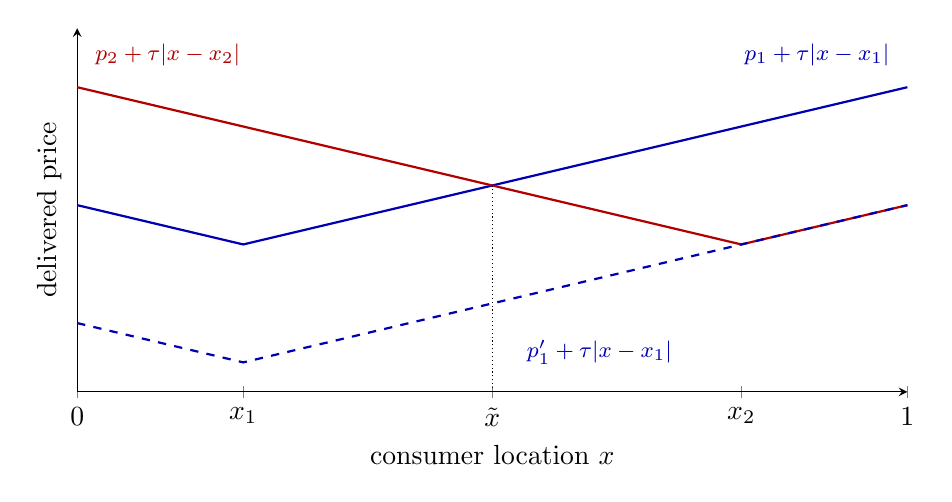
\begin{tikzpicture}
\begin{axis}[
  width=\linewidth, height=6.2cm,
  xmin=0, xmax=1, ymin=0.25, ymax=2.1,
  axis lines=left,
  xtick={0,0.2,0.5,0.8,1},
  xticklabels={$0$,$x_1$,$\tilde x$,$x_2$,$1$},
  ytick=\empty,
  xlabel={consumer location $x$},
  ylabel={delivered price},
  samples=201, domain=0:1,
  clip=false]
\addplot[thick, blue!70!black] {1 + abs(x - 0.2)};
\addplot[thick, red!70!black] {1 + abs(x - 0.8)};
\addplot[thick, dashed, blue!70!black] {0.4 + abs(x - 0.2)};
\draw[densely dotted] (axis cs:0.5,0.25) -- (axis cs:0.5,1.3);
\node[anchor=south west, font=\footnotesize, red!70!black] at (axis cs:0.01,1.86) {$p_2 + \tau|x - x_2|$};
\node[anchor=south east, font=\footnotesize, blue!70!black] at (axis cs:0.99,1.86) {$p_1 + \tau|x - x_1|$};
\node[anchor=north west, font=\footnotesize, blue!70!black] at (axis cs:0.53,0.56) {$p_1' + \tau|x - x_1|$};
\end{axis}
\end{tikzpicture}
\caption{Linear transport costs}
\end{subfigure}
\hfill
\begin{subfigure}[b]{0.48\textwidth}
\centering
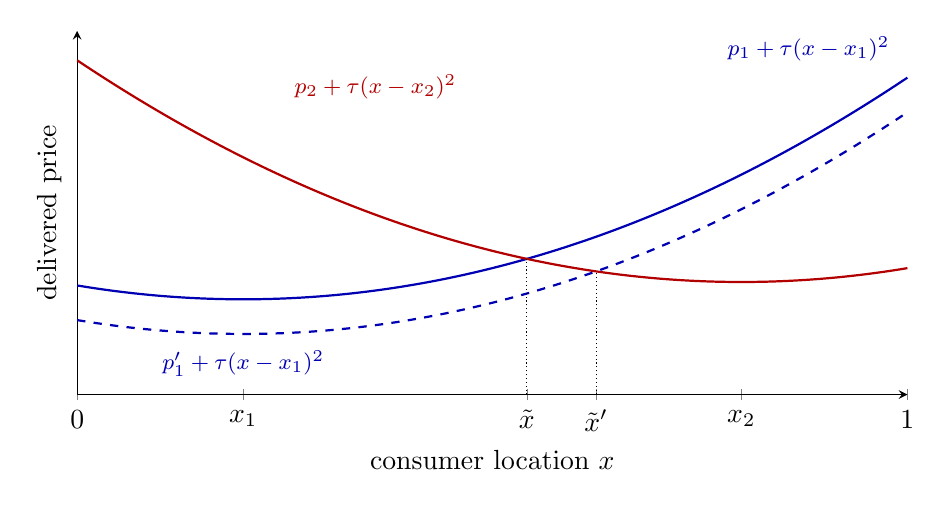
\begin{tikzpicture}
\begin{axis}[
  width=\linewidth, height=6.2cm,
  xmin=0, xmax=1, ymin=0.45, ymax=2.55,
  axis lines=left,
  xtick={0,0.2,0.5417,0.625,0.8,1},
  xticklabels={$0$,$x_1$,$\tilde x$,$\tilde x'$,$x_2$,$1$},
  ytick=\empty,
  xlabel={consumer location $x$},
  ylabel={delivered price},
  samples=201, domain=0:1,
  clip=false]
\addplot[thick, blue!70!black] {1 + 2*(x - 0.2)^2};
\addplot[thick, red!70!black] {1.1 + 2*(x - 0.8)^2};
\addplot[thick, dashed, blue!70!black] {0.8 + 2*(x - 0.2)^2};
\draw[densely dotted] (axis cs:0.5417,0.45) -- (axis cs:0.5417,1.234);
\draw[densely dotted] (axis cs:0.625,0.45) -- (axis cs:0.625,1.161);
\node[anchor=south west, font=\footnotesize, red!70!black] at (axis cs:0.25,2.1) {$p_2 + \tau(x - x_2)^2$};
\node[anchor=south east, font=\footnotesize, blue!70!black] at (axis cs:0.99,2.32) {$p_1 + \tau(x - x_1)^2$};
\node[anchor=north, font=\footnotesize, blue!70!black] at (axis cs:0.2,0.76) {$p_1' + \tau(x - x_1)^2$};
\end{axis}
\end{tikzpicture}
\caption{Quadratic transport costs}
\end{subfigure}
\caption{Delivered prices on Hotelling's line. Solid curves show each firm's price plus transport cost at the
initial prices, and the indifferent consumer $\tilde x$ is where they cross. In panel (a), with linear costs, firm 1
cuts its price to $p_1' = p_2 - \tau(x_2 - x_1)$ (dashed). Its schedule then coincides with firm 2's beyond $x_2$,
so firm 2's whole hinterland switches at once and demand jumps. In panel (b), with quadratic costs, a price cut (dashed)
moves the indifferent consumer continuously from $\tilde x$ to $\tilde x'$. Both panels use $x_1 = 0.2$ and $x_2 = 0.8$.
Panel (a) uses $\tau = 1$, $p_1 = p_2 = 1$ and $p_1' = 0.4$, and panel (b) uses $\tau = 2$, $p_1 = 1$, $p_2 = 1.1$ and
$p_1' = 0.8$.}
\label{fig:04-hotelling}
\end{figure}

\casehead{Firms at the ends} With $a = b = 0$, the middle case of \eqref{eq:04-hotelling-linear-demand} holds whenever
$|p_1 - p_2| \le \tau$. Firm 1 maximizes $(p_1 - c)M[\frac{1}{2} + \frac{p_2 - p_1}{2\tau}]$, a concave quadratic. Its
first-order condition is $\frac{1}{2} + \frac{p_2 - 2p_1 + c}{2\tau} = 0$, so the best response is
$p_1 = \frac{c + \tau + p_2}{2}$. Symmetry gives $p_1 = p_2 = c + \tau$, with $\tilde x = \frac{1}{2}$ and profits
$\frac{\tau M}{2}$. Undercutting to take the whole market requires $p_1 \le p_2 - \tau = c$, which earns nothing. The
markup equals the transport cost, so it vanishes as the products become perfect substitutes. This is the same
outcome as with quadratic costs at the ends (\cref{ex:06-hotelling}).

\casehead{Nonexistence when the firms are close} \Citet{Hotelling1929} argued that firms would cluster at the center
of the market, the \emph{principle of minimum differentiation}. \Citet{DAspremontGabszewiczThisse1979} showed that
the argument breaks down at the pricing stage. With linear costs, firms that are close have no pure-strategy price
equilibrium at all.

\begin{proposition}[Existence with linear transport costs]\label{prop:04-dgt}
Under \cref{ass:04-hotelling} with linear costs and $a, b \ge 0$, a pure-strategy price equilibrium exists if and only if
\begin{equation}\label{eq:04-dgt}
\Big(1 + \frac{a - b}{3}\Big)^2 \ge \frac{4}{3}(a + 2b)
\qquad\text{and}\qquad
\Big(1 + \frac{b - a}{3}\Big)^2 \ge \frac{4}{3}(b + 2a).
\end{equation}
When it exists, it is $p_1 = c + \tau(1 + \frac{a - b}{3})$ and $p_2 = c + \tau(1 + \frac{b - a}{3})$. With symmetric
locations, $a = b$, an equilibrium exists if and only if $a \le \frac{1}{4}$, and then $p_1 = p_2 = c + \tau$.
\end{proposition}

\begin{proof}
\emph{Step 1.} Any equilibrium lies in the middle region of \eqref{eq:04-hotelling-linear-demand}. Suppose firm 1
served the whole market, $p_1 < p_2 - \tau\Delta x$. Its profit is nonnegative only if $p_1 \ge c$. Firm 2 sells
nothing, yet it could charge any price in $(c, p_1 + \tau\Delta x)$, win some consumers and earn a positive profit.
That is a profitable deviation. The same argument rules out firm 2 serving everyone. At the boundary prices some
consumers are indifferent. Whichever way they break ties, one firm can gain by a small price change, so boundary
prices are not equilibria either.

\emph{Step 2.} In the middle region firm 1's profit is
$(p_1 - c)M[\frac{1 + a - b}{2} + \frac{p_2 - p_1}{2\tau}]$, a concave quadratic in $p_1$. Its first-order condition,
multiplied by $2\tau$, is $\tau(1 + a - b) + p_2 - 2p_1 + c = 0$. Firm 2's condition is symmetric:
\begin{equation*}
2p_1 - p_2 = c + \tau(1 + a - b), \qquad 2p_2 - p_1 = c + \tau(1 + b - a).
\end{equation*}
Adding twice the first equation to the second gives $3p_1 = 3c + \tau(3 + a - b)$, so
$p_1 = c + \tau(1 + \frac{a - b}{3})$, and by symmetry $p_2 = c + \tau(1 + \frac{b - a}{3})$. At these prices
$\tilde x = \frac{1 + a - b}{2} + \frac{b - a}{3} = \frac{3 + a - b}{6}$, and firm 1 earns
\begin{equation*}
\pi_1 = \tau\,\frac{3 + a - b}{3}\cdot M\,\frac{3 + a - b}{6} = \frac{M\tau}{2}\Big(1 + \frac{a - b}{3}\Big)^2 .
\end{equation*}
The candidate lies in the middle region if $|p_1 - p_2| = \frac{2\tau|a - b|}{3} < \tau\Delta x$. Take $a \ge b$. The
condition fails only if $5a + b \ge 3$, which with $b \le a$ requires $a \ge \frac{1}{2}$. Then the right side of
the second inequality in \eqref{eq:04-dgt} is at least $\frac{4}{3}$, while its left side is at most one. So
whenever \eqref{eq:04-dgt} holds, the candidate is interior.

\emph{Step 3.} Within the middle region the candidate is firm 1's best price. Prices that give firm 1 no
demand earn zero. The remaining deviation undercuts into the first region. There profit is $M(p_1 - c)$, which rises
with $p_1$, so the supremum is approached as $p_1$ rises to $p_2 - \tau\Delta x$. Its value is
\begin{equation*}
M\big(p_2 - \tau\Delta x - c\big) = M\tau\Big[1 + \frac{b - a}{3} - (1 - a - b)\Big] = \frac{2}{3}M\tau(a + 2b).
\end{equation*}
The candidate is a best response for firm 1 if and only if
$\frac{M\tau}{2}(1 + \frac{a - b}{3})^2 \ge \frac{2}{3}M\tau(a + 2b)$, which is the first inequality in
\eqref{eq:04-dgt}. The second inequality is the same condition for firm 2. By Steps 1 and 2 no other price pair
can be an equilibrium. With $a = b$ both inequalities read $1 \ge 4a$.
\end{proof}

The undercutting deviation drives the result. Holding firm 2's location fixed, firm 1's profit at the candidate
prices rises as firm 1 moves toward the center, with slope $\frac{M\tau}{3}(1 + \frac{a - b}{3})$. Its undercutting
payoff $\frac{2}{3}M\tau(a + 2b)$ rises faster, with slope $\frac{2}{3}M\tau$, and it also rises with $b$. When both
firms move inward together, $a = b$, the candidate profit stays at $\frac{M\tau}{2}$ while the undercutting payoff
$2M\tau a$ grows. When the firms are close, each prefers to undercut
the other and capture the whole line, and no pair of prices is stable. Mixed-strategy equilibria still exist, but
they are of little use for comparative statics (\cref{sec:04-existence-problem}). Hotelling's principle of minimum
differentiation therefore fails as a result about the location-price game. \Citet{CaplinNalebuff1991} make the same
point from the side of their existence theorem. Hotelling's distance utility is not linear in the consumer's
location, and the resulting discontinuity of demand is inconsistent with their assumptions (\cref{thm:04-cn-existence}).

\subsection{Quadratic transport costs and the location-price game}\label{sec:04-hotelling-quad}

\Citet{DAspremontGabszewiczThisse1979} restored existence by making transport costs quadratic. A consumer at $x$
then pays $p_j + \tau(x - x_j)^2$. The cost difference between the two firms is linear in $x$, so the
indifferent consumer moves continuously with prices, as panel (b) of \cref{fig:04-hotelling} shows. We now allow any
real $a$ and $b$ with $a + b < 1$, so that firms may also locate outside the line.

\begin{proposition}[Hotelling with quadratic costs]\label{prop:04-hotelling}
Let \cref{ass:04-hotelling} hold with quadratic costs and suppose that $|a - b| < 3$, so that the indifferent
consumer at the prices below lies strictly inside $[0,1]$.
\begin{enumerate}[label=(\roman*)]
\item The unique price equilibrium is
\begin{equation}\label{eq:04-hotelling-quad-prices}
p_1 = c + \tau(1 - a - b)\Big(1 + \frac{a - b}{3}\Big), \qquad p_2 = c + \tau(1 - a - b)\Big(1 + \frac{b - a}{3}\Big),
\end{equation}
with $q_1 = M\frac{3 + a - b}{6}$ and $\pi_1 = \frac{M\tau}{18}(1 - a - b)(3 + a - b)^2$.
\item In the first stage of a game in which firms choose locations and then prices,
\begin{equation}\label{eq:04-hotelling-location}
\frac{\dd\pi_1}{\dd a} = -\frac{M\tau}{18}(3 + a - b)(1 + 3a + b) < 0 \qquad\text{for all } a, b \ge 0 .
\end{equation}
If locations are restricted to $[0,1]$, the unique location equilibrium is $x_1 = 0$, $x_2 = 1$ (maximal
differentiation), with prices $c + \tau$.
\item If locations are unrestricted, the location equilibrium is $x_1 = -\frac{1}{4}$ and $x_2 = \frac{5}{4}$.
\end{enumerate}
\end{proposition}

\begin{proof}
(i) Let $\Delta x = 1 - a - b$. The indifferent consumer solves $p_1 + \tau(x - a)^2 = p_2 + \tau(x - 1 + b)^2$. The
quadratic terms $\tau x^2$ cancel, leaving
\begin{equation*}
2\tau x\,(1 - b - a) = p_2 - p_1 + \tau\big[(1 - b)^2 - a^2\big] = p_2 - p_1 + \tau(1 - a - b)(1 - b + a),
\end{equation*}
so that
\begin{equation*}
\tilde x = \frac{1 + a - b}{2} + \frac{p_2 - p_1}{2\tau\Delta x} = a + \frac{\Delta x}{2} + \frac{p_2 - p_1}{2\tau\Delta x}.
\end{equation*}
Consumers to the left of $\tilde x$ buy from firm 1, so $q_1 = M\tilde x$ when $\tilde x \in [0,1]$. Firm 1 maximizes
$(p_1 - c)M\tilde x$. Its first-order condition, multiplied by $\frac{2\tau\Delta x}{M}$, is
$\tau\Delta x(1 + a - b) + p_2 - 2p_1 + c = 0$. Firm 2 sells $M(1 - \tilde x)$ and has the symmetric condition.
The system is
\begin{equation*}
2p_1 - p_2 = c + \tau\Delta x(1 + a - b), \qquad 2p_2 - p_1 = c + \tau\Delta x(1 + b - a).
\end{equation*}
Adding twice the first to the second gives $3p_1 = 3c + \tau\Delta x(3 + a - b)$, which is
\eqref{eq:04-hotelling-quad-prices}. Then $p_2 - p_1 = \frac{2}{3}\tau\Delta x(b - a)$, so
$\tilde x = \frac{1 + a - b}{2} + \frac{b - a}{3} = \frac{3 + a - b}{6}$. Profit is
$(p_1 - c)M\tilde x = \tau\Delta x\frac{3 + a - b}{3}\cdot M\frac{3 + a - b}{6}$. Demand is continuous, and where
positive it is the minimum of $M$ and a linear function, hence log-concave. By \cref{lem:04-logconcave} profit is
quasi-concave in own price, so the first-order conditions give best responses, and the prices
\eqref{eq:04-hotelling-quad-prices} are an equilibrium.

The best-response map is not a contraction on all prices. When $p_2$ is high, firm 1's best response takes the
whole market, $\tilde x = 1$, and then rises one for one with $p_2$. We therefore prove uniqueness directly. In an
equilibrium with $0 < \tilde x < 1$, profits are differentiable in own prices, so both first-order conditions hold.
The linear system above then has the single solution \eqref{eq:04-hotelling-quad-prices}. Suppose instead that an
equilibrium had $\tilde x \geq 1$, so that firm 2 sells nothing. If $\tilde x > 1$, firm 1 could raise its price
slightly and still serve everyone, so $\tilde x = 1$. If $p_2 > c$, firm 2 could cut its price slightly and earn a
positive profit, so $p_2 \leq c$. With $\tilde x = 1$, firm 1's price is
$p_1 = p_2 - \tau\Delta x(1 - a + b) \leq c - \tau\Delta x(1 - a + b)$. A small rise in $p_1$ changes firm 1's
profit at the rate $M\big[1 - \frac{p_1 - c}{2\tau\Delta x}\big]$, so firm 1 gains from it unless
$p_1 - c \geq 2\tau\Delta x$. Both bounds on $p_1 - c$ hold only if $a - b \geq 3$, which the assumption rules out.
The case $\tilde x \leq 0$ is symmetric and requires $b - a \geq 3$. The equilibrium is therefore unique.

(ii) By the envelope theorem, the effect of $a$ on $\pi_1$ at the equilibrium of (i) has two parts. The direct
effect holds both prices fixed: $(p_1 - c)M\frac{\partial\tilde x}{\partial a}$. The strategic effect works through
the rival's price: $(p_1 - c)M\frac{\partial\tilde x}{\partial p_2}\frac{\dd p_2}{\dd a}$. Firm 1's own price response
has no first-order effect. At the equilibrium, with $\frac{p_2 - p_1}{2\tau\Delta x^2} = \frac{b - a}{3\Delta x}$,
\begin{equation*}
\frac{\partial\tilde x}{\partial a} = \frac{1}{2} + \frac{p_2 - p_1}{2\tau\Delta x^2} = \frac{3 - 5a - b}{6\Delta x},
\qquad
\frac{\partial\tilde x}{\partial p_2} = \frac{1}{2\tau\Delta x},
\qquad
\frac{\dd p_2}{\dd a} = -\frac{\tau(4 - 2a)}{3}.
\end{equation*}
The last derivative follows from differentiating $p_2 = c + \frac{\tau}{3}(1 - a - b)(3 + b - a)$, which gives
$\frac{\tau}{3}[-(3 + b - a) - (1 - a - b)] = -\frac{\tau}{3}(4 - 2a)$. Adding the two effects,
\begin{equation*}
\frac{\dd\pi_1}{\dd a} = (p_1 - c)M\Big[\frac{3 - 5a - b}{6\Delta x} - \frac{4 - 2a}{6\Delta x}\Big]
= -(p_1 - c)M\frac{1 + 3a + b}{6\Delta x}.
\end{equation*}
Substituting $p_1 - c = \frac{\tau\Delta x(3 + a - b)}{3}$ gives \eqref{eq:04-hotelling-location}, which is negative
for $a, b \ge 0$. Each firm therefore wants to move away from the center for any location of its rival. On $[0,1]$
the unique equilibrium is $a = b = 0$, and (i) gives prices $c + \tau$.

(iii) Without restrictions, the location first-order conditions are $1 + 3a + b = 0$ for firm 1 and
$1 + 3b + a = 0$ for firm 2. Their solution is $a = b = -\frac{1}{4}$, so $x_1 = -\frac{1}{4}$ and
$x_2 = 1 + \frac{1}{4} = \frac{5}{4}$. Given $b = -\frac{1}{4}$, the derivative \eqref{eq:04-hotelling-location} is
positive for $a < -\frac{1}{4}$ and negative above, so $a = -\frac{1}{4}$ is firm 1's best location.
\end{proof}

The two effects in the proof have a clear meaning. The direct effect is positive as long as $5a + b < 3$. Moving
toward the center at given prices takes consumers from the rival. The strategic effect is negative, because moving
closer makes the products better substitutes and lowers the rival's price. The strategic effect always wins.
\Citet{ShakedSutton1982} call this \emph{relaxing price competition through product differentiation}. Firms give up
market share at given prices to soften the price war that would follow. The result is
\emph{maximal differentiation}, the opposite of Hotelling's conjecture.

Equilibrium differentiation is excessive from the social point of view. With a covered market and inelastic unit
demand, prices are transfers, and welfare depends only on transport costs. A planner who places two products to
minimize average transport cost chooses $\frac{1}{4}$ and $\frac{3}{4}$, with average cost
$2\int_0^{\frac{1}{2}}\tau(x - \frac{1}{4})^2\dd x = \frac{\tau}{48}$. Firms at the ends impose
$2\int_0^{\frac{1}{2}}\tau x^2\dd x = \frac{\tau}{12}$, four times as much. When firms may locate outside the line, they move
even farther apart, to $-\frac{1}{4}$ and $\frac{5}{4}$. \Citet[Section 7.1.1]{Tirole1988} gives a textbook treatment.

\casehead{Minimal differentiation with fixed prices} Hotelling's principle does hold when prices cannot compete.
\Citet[Section 7.1.3]{Tirole1988} shows this with Hotelling's own location game at an exogenous price.

\begin{proposition}[Location choice at a fixed price]\label{prop:04-hotelling-fixed}
Let consumers be uniform on $[0,1]$ with mass $M$ and buy one unit each from the nearest firm. Two firms sell at a
common exogenous price $p > c$ and choose locations $x_1 = a$ and $x_2 = 1 - b$, splitting demand equally if they
locate at the same point. The unique equilibrium places both firms at $\frac{1}{2}$.
\end{proposition}

\begin{proof}
Prices and margins are fixed, so each firm maximizes its demand. Suppose first that $a < 1 - b$. Firm 1 serves its
hinterland and half of the consumers between the firms, so its demand is
\begin{equation*}
q_1 = M\Big[a + \frac{1 - b - a}{2}\Big] = M\,\frac{1 + a - b}{2} .
\end{equation*}
It rises with $a$, so firm 1 gains by moving toward its rival, and the same holds for firm 2. Any equilibrium therefore
has $a = 1 - b$. Suppose the common location is $x < \frac{1}{2}$. Each firm sells $\frac{M}{2}$. If firm 2 moves to
$x + e$ with small $e > 0$, it serves every consumer to the right of $x + \frac{e}{2}$, which gives
$M(1 - x - \frac{e}{2}) > \frac{M}{2}$. So $x < \frac{1}{2}$ is not an equilibrium, and the same argument rules out
$x > \frac{1}{2}$. At $x = \frac{1}{2}$, a firm that moves to any $x' \neq \frac{1}{2}$ serves only the consumers on
its side of the midpoint between $x'$ and $\frac{1}{2}$. That is less than half of the market, so neither firm
deviates.
\end{proof}

The products are socially too close. With linear costs, the average distance is $\frac{1}{4}$ when both firms sit
at the center and $\frac{1}{8}$ at the efficient locations $\frac{1}{4}$ and $\frac{3}{4}$. The contrast with
\cref{prop:04-hotelling} isolates the role of prices. Firms differentiate to soften price competition, and without
price competition they have no reason to. \citet[Section 7.1.3]{Tirole1988} groups the forces that work against
maximal differentiation into three categories. The first is the location of demand. Firms want to be where consumers
are, and when demand is concentrated around a few poles they cluster there. Tirole's examples are ice cream parlors
and bookstores near universities. The second is positive externalities among firms. On the cost side these include
shared installations and sources of raw materials. On the demand side, consumer search draws stores together, as
with the furniture stores of a single Paris street. The third is the absence of price competition, as in the game
above. Airline fares in the United States before deregulation and the prices of gasoline and books in France were
once set outside the market. Resale price maintenance has the same effect. Tirole adds that fixed-price location
models may explain why political platforms cluster at the center.

Two connections close this subsection. First, quadratic costs satisfy the linearity assumption of
\cref{thm:04-cn-existence}. Expanding the square gives $-\tau(x - x_j)^2 = -\tau x^2 + 2\tau x\,x_j - \tau x_j^2$. The
first term is common to all products and drops out, and the second is linear in the consumer's type $x$. With
uniform types, which have a log-concave density, an equilibrium exists for any locations
\citep{CaplinNalebuff1991}. Second, heterogeneity in tastes can bring minimum differentiation back.
\Citet{DePalmaEtAl1985} add a logit taste shock to Hotelling's linear transport costs. Demand becomes smooth, and with
enough taste heterogeneity relative to $\tau$, both firms locate at the center of the market. Their title states the
result: the principle of minimum differentiation holds under sufficient heterogeneity.

\subsection{Salop's circle, free entry and excess variety}\label{sec:04-salop}

\Citet{Salop1979} removed the ends of the line by placing consumers on a circle. Without ends there are no
hinterlands, and symmetric configurations with any number of firms are natural. This makes the circle the standard
model of entry with differentiated products.

\begin{proposition}[Salop's circle]\label{prop:04-salop}
Let a mass $M$ of consumers be uniform on a circle of circumference one, buy one unit each, and have a high enough
reservation value that the market is covered. $N$ firms are equally spaced, with marginal cost $c$, fixed cost
$\phi$ and linear transport cost $\tau$.
\begin{enumerate}[label=(\roman*)]
\item There is a symmetric price equilibrium with $p = c + \frac{\tau}{N}$, in which each firm earns
$\frac{\tau M}{N^2} - \phi$.
\item Treating $N$ as continuous, free entry yields $N^* = \sqrt{\frac{\tau M}{\phi}}$ firms.
\item The number of firms that minimizes fixed plus transport costs is $N^o = \frac{1}{2}\sqrt{\frac{\tau M}{\phi}}$.
Hence $N^* = 2N^o$.
\end{enumerate}
\end{proposition}

\begin{proof}
(i) Take a firm that charges $p$ while its two neighbors, each at distance $\frac{1}{N}$, charge $\bar p$. A consumer
at distance $d$ from the firm, on the arc toward a neighbor, is indifferent when
$p + \tau d = \bar p + \tau(\frac{1}{N} - d)$, that is, at $d = \frac{1}{2N} + \frac{\bar p - p}{2\tau}$. The firm serves
the arcs on both sides, so its demand is
\begin{equation*}
q = 2Md = M\Big[\frac{1}{N} + \frac{\bar p - p}{\tau}\Big] \qquad\text{for } |\bar p - p| \le \frac{\tau}{N}.
\end{equation*}
In this range profit $(p - c)q - \phi$ is a concave quadratic. Its first-order condition is
$\frac{1}{N} + \frac{\bar p - p}{\tau} - \frac{p - c}{\tau} = 0$. At a symmetric point $p = \bar p$, it gives
$p = c + \frac{\tau}{N}$. Each firm sells $\frac{M}{N}$ and earns $\frac{\tau}{N}\cdot\frac{M}{N} - \phi$. To take its
neighbor's whole market, a firm would have to price at $\bar p - \frac{\tau}{N} = c$, which earns no variable profit.
A price above $\bar p + \frac{\tau}{N}$ sells nothing. So no deviation outside the range is profitable.

(ii) Free entry drives profit to zero: $\frac{\tau M}{N^2} = \phi$, so $N^* = \sqrt{\frac{\tau M}{\phi}}$.

(iii) With $N$ equally spaced firms, each consumer travels to the nearest firm. Distances are uniform on
$[0, \frac{1}{2N}]$, so the average distance is $\frac{1}{4N}$ and total transport cost is $\frac{\tau M}{4N}$.
Prices are transfers because the market is covered. The planner minimizes $N\phi + \frac{\tau M}{4N}$. The
first-order condition $\phi - \frac{\tau M}{4N^2} = 0$ gives $N^o = \frac{1}{2}\sqrt{\frac{\tau M}{\phi}}$.
\end{proof}

\begin{figure}[htbp]
\centering
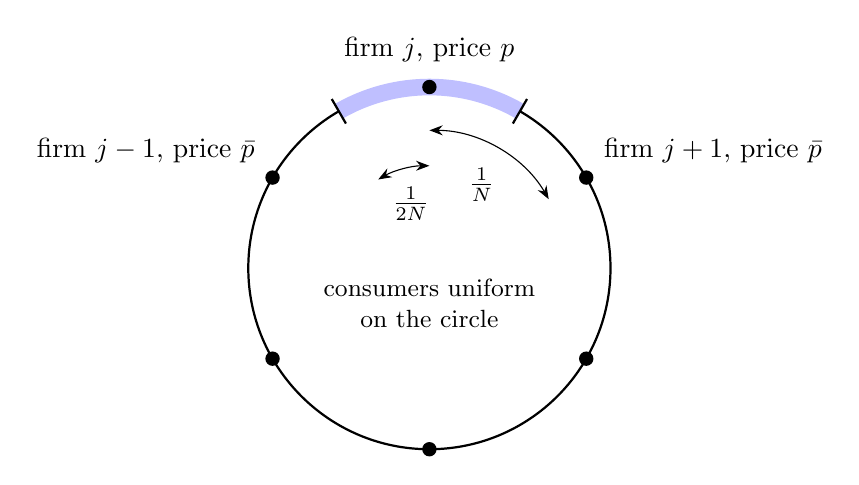
\begin{tikzpicture}
\def\R{2.3}
\draw[thick] (0,0) circle (\R);
\draw[line width=6pt, blue!25] (60:\R) arc (60:120:\R);
\foreach \a in {90,30,150,210,270,330} {\fill (\a:\R) circle (2.6pt);}
\foreach \a in {60,120} {\draw[thick] (\a:\R-0.18) -- (\a:\R+0.18);}
\node[anchor=south] at (90:\R+0.2) {firm $j$, price $p$};
\node[anchor=south west] at (30:\R+0.12) {firm $j+1$, price $\bar p$};
\node[anchor=south east] at (150:\R+0.12) {firm $j-1$, price $\bar p$};
\draw[<->, >=Stealth] (90:\R-0.55) arc (90:30:\R-0.55);
\node at (58:\R-1.05) {$\frac{1}{N}$};
\draw[<->, >=Stealth] (90:\R-1.0) arc (90:120:\R-1.0);
\node at (106:\R-1.45) {$\frac{1}{2N}$};
\node[align=center, font=\small] at (0,-0.45) {consumers uniform\\on the circle};
\end{tikzpicture}
\caption{Salop's circle with $N = 6$ equally spaced firms. Firm $j$ serves the shaded arc between the two
indifferent consumers (tick marks). At symmetric prices each indifferent consumer is at distance
$d = \frac{1}{2N}$ from firm $j$, so the firm's market has length $\frac{1}{N}$. A price cut by firm $j$ moves
both tick marks outward and takes customers from its two neighbors only.}
\label{fig:04-salop}
\end{figure}

\Cref{fig:04-salop} shows the structure. Each firm competes only with its two neighbors, and its markup
$\frac{\tau}{N}$ falls as the circle fills up. The market provides twice the efficient number of products. The reason
is the balance of two externalities \citep{Spence1976,DixitStiglitz1977,MankiwWhinston1986}. An entrant creates
variety: consumers near its location travel less. It does not capture this whole benefit in its profit, which pushes
toward too little entry. An entrant also steals business from incumbents, which pushes toward too much entry. On the
circle the market is covered, so every unit the entrant sells is taken from a rival. At $N^*$ the entrant's private
gain, its variable profit $\frac{\tau M}{N^2} = \phi$, is four times the social gain $\frac{\tau M}{4N^2} = \frac{\phi}{4}$
in saved transport costs. Business stealing dominates. \Cref{prop:02-mw-excess} gives the corresponding result for
homogeneous goods.

\begin{remark}[Coverage and touching markets]\label{rem:04-salop-coverage}
\Cref{prop:04-salop} assumes that every consumer buys. Let $\bar u$ be the reservation value. The consumer farthest
from a firm is at distance $\frac{1}{2N}$ and pays $c + \frac{\tau}{N} + \frac{\tau}{2N} = c + \frac{3\tau}{2N}$, so the
equilibrium requires $\bar u \ge c + \frac{3\tau}{2N}$. At free entry $\frac{\tau}{N^*} = \sqrt{\frac{\tau\phi}{M}}$, and
the condition becomes
\begin{equation*}
\frac{3}{2}\sqrt{\frac{\tau\phi}{M}} \le \bar u - c
\quad\Longleftrightarrow\quad
\phi \le \bar\phi = \frac{4M(\bar u - c)^2}{9\tau}
\end{equation*}
\citep[Section 7.1.2]{Tirole1988}. With larger fixed costs fewer firms enter, and the consumer halfway between two
firms would not buy at the price of the proposition. \Citet{Salop1979} studies this case. Suppose the neighbors charge
$\bar p = \bar u - \frac{\tau}{2N}$, so that the consumer halfway between two firms is just willing to buy. A firm that
raises its price loses customers to the outside good. Its demand is then $\frac{2M(\bar u - p)}{\tau}$, with slope
$-\frac{2M}{\tau}$. A firm that cuts its price takes customers from its neighbors, with the demand of the proof and
slope $-\frac{M}{\tau}$. Demand therefore has a kink at $\bar p$. At sales of $\frac{M}{N}$, a price rise does not pay if
$\frac{M}{N} \le \frac{2M}{\tau}(\bar p - c)$, and a price cut does not pay if $\frac{M}{N} \ge \frac{M}{\tau}(\bar p - c)$.
So $\bar p$ is an equilibrium price whenever
\begin{equation*}
\frac{\tau}{N} \le \bar u - c \le \frac{3\tau}{2N} .
\end{equation*}
Free entry requires $G(N) \equiv (\bar u - c - \frac{\tau}{2N})\frac{M}{N} = \phi$. In this regime
$G'(N) = \frac{M}{N^2}\big[\frac{\tau}{N} - (\bar u - c)\big] \le 0$, and $G$ also falls with $\tau$. A higher fixed cost
or a higher transport cost therefore lowers the number of firms, and the price $\bar u - \frac{\tau}{2N}$ falls with it.
In the competitive regime of the proposition both changes raise the price. \Citet[Section 7.1.2,
Exercise 7.4]{Tirole1988} calls such results a priori counterintuitive. The explanation is that the price is pinned
by the reservation value of the consumer halfway between two firms. When firms are farther apart, that consumer
travels farther and can pay less.
\end{remark}

The factor of two depends on linear costs. With quadratic costs $\tau d^2$ on the circle, the same steps give the
markup $\frac{\tau}{N^2}$ and free-entry number $N^* = (\frac{\tau M}{\phi})^{\frac{1}{3}}$. Average transport cost is
$\frac{\tau}{12N^2}$, so the optimum is $N^o = (\frac{\tau M}{6\phi})^{\frac{1}{3}}$ and $\frac{N^*}{N^o} = 6^{\frac{1}{3}} \approx 1.82$.
Entry is still excessive. The dimension of the space matters more. \Citet{CaplinNalebuff1991} discuss
\citet{Stiglitz1986}, who places firms on a grid in $L$ dimensions with quadratic transport costs, so each firm has
$2L$ neighbors. Demand becomes more elastic as $L$ grows, profits fall, and fewer firms can cover the entry cost.
Yet consumers have farther to travel in higher dimensions, so the efficient number of firms per unit area rises.
Stiglitz concludes that low-dimensional markets have excess diversity and high-dimensional markets too little
\citep[Section 8.3 and n.~21]{CaplinNalebuff1991}. Caplin and Nalebuff show that, with quadratic costs, the
symmetric solution of the first-order conditions in his model is indeed an equilibrium. \Cref{fig:04-voronoi}
shows the two-dimensional analogue of the circle's market areas.

The circle fixes locations by assumption. \Citet[Section 7.1.2]{Tirole1988} discusses three extensions. First, equal
spacing is a natural guess given maximal differentiation on the line. \Citet{Economides1989} justifies it with
quadratic costs in a game where firms choose entry, then locations, then prices, and a symmetric free-entry
equilibrium exists. Tirole cites the 1984 working-paper version. Second, firms may enter in sequence, and then an
early entrant's location shapes later choices. \Citet{PrescottVisscher1977} studied sequential location on the line.
Third, one firm may sell several brands and crowd the product space so that no entrant fits, especially when it can
preempt. \Citet[p.~1283, n.~4]{AndersonDePalmaNesterov1995} add that the known results for the circle all suggest
substantial overentry at every level of fixed costs.

The welfare comparison has been taken to data. \Citet{BerryWaldfogel1999} estimate how listening and advertising
revenue vary with the number of radio stations in 135 US metropolitan markets and recover fixed costs from a
free-entry condition. In the 1996 working-paper version on which we rely, the welfare loss from free entry relative
to the social optimum is 40 percent of industry revenue. This calculation leaves out the value of programming to
listeners. Advertisers pay 4.5 cents per hour for a marginal listener. The authors compute that free entry would be
optimal if programming were worth more than three times that amount to the marginal listener.

\subsection{Symmetric logit oligopoly and entry*}\label{sec:04-logit-entry}

The symmetric logit gives a useful contrast with the circle. Every product competes with every other, and each new
product brings a new taste shock and hence new variety.

\begin{proposition}[Symmetric logit oligopoly and entry]\label{prop:04-logit-entry}
Let $N \ge 2$ single-product firms sell products with common quality $\tilde\delta$ and marginal cost $c$ to a mass
$M$ of consumers with logit demand and no outside good. Each firm pays a fixed cost $\phi$.
\begin{enumerate}[label=(\roman*)]
\item The symmetric price equilibrium has markup $p - c = \frac{N}{\alpha(N - 1)}$, and each firm earns
$\frac{M}{\alpha(N - 1)} - \phi$. With an outside good, the markup is $\frac{1}{\alpha(1 - s)}$, with $s$ each
firm's share.
\item Treating $N$ as continuous, free entry yields $N^* = 1 + \frac{M}{\alpha\phi}$.
\item Total surplus is $TS(N) = \frac{M}{\alpha}\ln N + M\big(\frac{\tilde\delta}{\alpha} - c\big) - N\phi$, up to a
constant. It is maximized at $N^o = \frac{M}{\alpha\phi}$, so $N^* = N^o + 1$.
\end{enumerate}
\end{proposition}

\begin{proof}
(i) With no outside good, the shares are $\frac{e^{\delta_j}}{\sum_ke^{\delta_k}}$, and at symmetric prices $s = \frac{1}{N}$.
The first-order condition of a single-product firm, $\alpha(p - c)(1 - s) = 1$, is derived as in
\cref{prop:04-logit-markup}, which does not use the outside good. With $s = \frac{1}{N}$ it gives
$p - c = \frac{1}{\alpha(1 - \frac{1}{N})} = \frac{N}{\alpha(N - 1)}$. Each firm sells $\frac{M}{N}$ and earns
$\frac{N}{\alpha(N-1)}\cdot\frac{M}{N} - \phi$. With an outside good, \cref{prop:04-logit-markup} applies directly.
(ii) Setting profit to zero gives $\alpha(N - 1)\phi = M$.
(iii) By \cref{prop:04-logit-entropy}, consumer surplus is $\frac{M}{\alpha}\ln\sum_{k=1}^Ne^{\tilde\delta - \alpha p}$ up
to a constant. At symmetric prices this equals $\frac{M}{\alpha}\ln N + \frac{M\tilde\delta}{\alpha} - Mp$. Total
profit is $M(p - c) - N\phi$. In the sum the price cancels, because every consumer buys and payments are
transfers. The derivative $TS'(N) = \frac{M}{\alpha N} - \phi$ vanishes at $N^o = \frac{M}{\alpha\phi}$, and $TS$ is
concave. Comparing with (ii) gives $N^* = N^o + 1$.
\end{proof}

The logit market also has too many products, but only one too many. The relative excess
$\frac{N^* - N^o}{N^o} = \frac{\alpha\phi}{M}$ vanishes as the market grows, whereas on the circle it is always
100 percent. The reason lies in the social value of the marginal product. In the logit it is $\frac{M}{\alpha N}$,
which falls slowly with $N$, because each product brings its own taste shock. On the circle it is
$\frac{\tau M}{4N^2}$, which falls fast, because a new product only shortens the trips of nearby consumers. The
entrant's private gain, $\frac{M}{\alpha(N - 1)}$, exceeds the social gain by only
$\frac{M}{\alpha N(N - 1)}$. Business stealing is weak because the logit treats variety itself as valuable.
\Citet[p.~49]{MankiwWhinston1986} isolate the two forces at work. Business stealing pushes toward excessive entry,
as in homogeneous-good markets. Product diversity pushes the other way, because the entrant creates surplus through
variety that it does not capture as profit. With the CES form and equilibrium notion of \citet{Spence1976}, the
diversity effect always dominates and entry is insufficient. They also give examples in which business stealing
always dominates. The symmetric logit of \cref{prop:04-logit-entry} is another such case, with an excess of one firm.
For the CES, \citet{DixitStiglitz1977} show that the market can provide too few or too many products, depending on
preferences (\cref{sec:04-repcons-monocomp}).

\casehead{General i.i.d.\ tastes} \Citet{AndersonDePalmaNesterov1995} ask how far the logit's verdict extends. They
keep the symmetric discrete choice structure, with the demand side of \citet{PerloffSalop1985}, but let the taste
shocks have any log-concave density. The following proposition collects the pieces we need, in our notation.

\begin{proposition}[Symmetric oligopoly with i.i.d.\ tastes]\label{prop:04-adn}
A mass $M$ of consumers each buy one unit of the product that maximizes $u_{ij} = y - p_j + \epsilon_{ij}$. The shocks
$\epsilon_{ij}$ are i.i.d.\ across consumers and products, with density $f_\epsilon$ and distribution function $F_\epsilon$
on $(\underline e, \bar e)$ and a finite mean. There are $N \ge 2$ single-product firms with marginal cost $c$ and
fixed cost $\phi$.
\begin{enumerate}[label=(\roman*)]
\item Demand for product $i$ is
\begin{equation}\label{eq:04-adn-demand}
q_i = M\int f_\epsilon(x)\prod_{j \ne i}F_\epsilon(p_j - p_i + x)\,\dd x .
\end{equation}
\item The unique candidate for a symmetric equilibrium has the markup
\begin{equation}\label{eq:04-adn-markup}
p - c = \frac{1}{\Theta(N)}, \qquad \Theta(N) = N(N - 1)\int f_\epsilon(x)^2F_\epsilon(x)^{N-2}\,\dd x .
\end{equation}
\item At equal prices, an $(N+1)$th product raises total surplus by $M\int F_\epsilon(x)^N[1 - F_\epsilon(x)]\,\dd x - \phi$.
Its profit in the symmetric equilibrium with $N + 1$ firms is $\frac{M}{(N + 1)\Theta(N + 1)} - \phi$.
\item If $\epsilon_{ij}$ is type-I extreme value with scale $\frac{1}{\alpha}$, then $\Theta(N) = \frac{\alpha(N - 1)}{N}$,
the markup is $\frac{N}{\alpha(N - 1)}$, and the surplus gain in (iii) is $\frac{M}{\alpha}\ln\frac{N + 1}{N} - \phi$.
\item If $F_\epsilon(x) = 1 - e^{-\lambda_\epsilon(x - \underline e)}$ on $[\underline e, \infty)$ with $\lambda_\epsilon > 0$,
then $\Theta(N) = \lambda_\epsilon$ for every $N$. The surplus gain and the profit in (iii) are both
$\frac{M}{\lambda_\epsilon(N + 1)} - \phi$.
\end{enumerate}
\end{proposition}

\begin{proof}
(i) Fix a consumer and write $\epsilon_k$ for her shock on product $k$. She buys $i$ when
$y - p_i + \epsilon_i > y - p_j + \epsilon_j$ for every $j \ne i$. Given $\epsilon_i = x$, this requires
$\epsilon_j < p_j - p_i + x$ for every $j \ne i$. By independence the conditional probability is
$\prod_{j \ne i}F_\epsilon(p_j - p_i + x)$. Integrating over the density of $x$ gives \eqref{eq:04-adn-demand}. Ties
have probability zero.

(ii) Differentiate \eqref{eq:04-adn-demand} with respect to $p_i$ and set all prices equal. Each of the $N - 1$ factors
contributes $-f_\epsilon(x)F_\epsilon(x)^{N-2}$, so
\begin{equation*}
\frac{\partial q_i}{\partial p_i} = -M(N - 1)\int f_\epsilon(x)^2F_\epsilon(x)^{N-2}\,\dd x = -\frac{M\,\Theta(N)}{N} .
\end{equation*}
At equal prices $q_i = \frac{M}{N}$. The first-order condition $q_i + (p_i - c)\frac{\partial q_i}{\partial p_i} = 0$
becomes $\frac{M}{N} = (p - c)\frac{M\,\Theta(N)}{N}$, which has the single solution \eqref{eq:04-adn-markup}.

(iii) Every consumer buys and prices are transfers, so at equal prices total surplus is $M(y - c)$ plus
$M\E[\max_j\epsilon_{ij}]$ minus total fixed costs. The maximum of $N$ shocks has distribution function $F_\epsilon^N$.
Integrating by parts, with boundary terms that vanish because the mean is finite,
\begin{equation*}
\E\big[\max_{j \le N + 1}\epsilon_{ij}\big] - \E\big[\max_{j \le N}\epsilon_{ij}\big]
= \int x\,\dd\big(F_\epsilon^{N+1} - F_\epsilon^N\big)(x) = \int F_\epsilon(x)^N\big[1 - F_\epsilon(x)\big]\,\dd x .
\end{equation*}
With $N + 1$ firms, each sells $\frac{M}{N + 1}$ at the markup $\frac{1}{\Theta(N + 1)}$, which gives the profit.

(iv) Here $F_\epsilon(x) = \exp(-e^{-\alpha x})$ and $f_\epsilon(x) = \alpha e^{-\alpha x}F_\epsilon(x)$, so
$f_\epsilon^2F_\epsilon^{N-2} = \alpha^2e^{-2\alpha x}\exp(-Ne^{-\alpha x})$. Substitute $u = e^{-\alpha x}$, with
$\dd x = -\frac{\dd u}{\alpha u}$:
\begin{equation*}
\int f_\epsilon(x)^2F_\epsilon(x)^{N-2}\,\dd x = \alpha\int_0^\infty ue^{-Nu}\,\dd u = \frac{\alpha}{N^2},
\qquad\text{so}\qquad
\Theta(N) = \frac{\alpha(N - 1)}{N} .
\end{equation*}
For the surplus, $F_\epsilon(x)^N = \exp\big(-e^{-\alpha(x - \frac{\ln N}{\alpha})}\big)$. The maximum of $N$ shocks is
therefore extreme value with location $\frac{\ln N}{\alpha}$, and its mean rises by $\frac{1}{\alpha}\ln\frac{N + 1}{N}$
when $N$ rises by one.

(v) Let $v = F_\epsilon(x)$, so that $f_\epsilon(x) = \lambda_\epsilon(1 - v)$ and $\dd v = \lambda_\epsilon(1 - v)\,\dd x$. Then
\begin{equation*}
\int f_\epsilon^2F_\epsilon^{N-2}\,\dd x = \lambda_\epsilon\int_0^1(1 - v)v^{N-2}\,\dd v
= \lambda_\epsilon\Big[\frac{1}{N - 1} - \frac{1}{N}\Big] = \frac{\lambda_\epsilon}{N(N - 1)},
\end{equation*}
so $\Theta(N) = \lambda_\epsilon$. Likewise $\int F_\epsilon^N(1 - F_\epsilon)\,\dd x = \frac{1}{\lambda_\epsilon}\int_0^1v^N\,\dd v =
\frac{1}{\lambda_\epsilon(N + 1)}$, and the profit is $\frac{M}{(N + 1)\lambda_\epsilon} - \phi$.
\end{proof}

Part (iv) is the integer version of \cref{prop:04-logit-entry}. The $(N+1)$th product adds
$\frac{M}{\alpha}\ln(1 + \frac{1}{N})$ to surplus and earns $\frac{M}{\alpha N}$, and $\ln(1 + \frac{1}{N}) < \frac{1}{N}$.
The general results of \citet{AndersonDePalmaNesterov1995} rest on log-concavity. Utility is linear in the vector of
shocks, whose joint density $\prod_jf_\epsilon(\epsilon_{ij})$ is log-concave when $f_\epsilon$ is. The theorem of
\citet{CaplinNalebuff1991} then makes profit quasi-concave, so the candidate in (ii) is an equilibrium (p.~1285,
\cref{thm:04-cn-existence}). Their Proposition 1 (p.~1285) shows that log-concavity also makes $\Theta(N)$
nondecreasing, so markups do not rise with entry. Revenue per firm then falls with $N$, and the free-entry number of
firms is unique. Their Theorem 1 (p.~1287) is the main result. With log-concave tastes and unit demands, the profit of
an extra firm is never below its social value, so the market never provides too little variety. Corollary 1
(p.~1289) shows that equilibrium and optimum coincide for every fixed cost only for the exponential-tail
distributions of part (v) and their mirror images. For the densities of their example held fixed, the equilibrium
number of firms is about the optimum plus one as fixed costs vanish (p.~1290), as in the logit. For a general fixed
density only the ratio of the two numbers tends to one, a result \citet[p.~1283]{AndersonDePalmaNesterov1995}
credit to \citet{DeneckereRothschild1992}. Overentry can still be large. For
each optimal number of firms they choose a log-concave density, and as fixed costs vanish the ratio of the
equilibrium to the optimal number tends to $r^* > 1.097$ (p.~1290). That is almost 10 percent excess entry even with
very many firms. When individual demand responds to price, entry can fall short of the optimum subject to zero
profits, but by at most one firm (their Theorem 2, p.~1294).

The logit's verdict depends on taking the taste shocks literally. If they are a statistical device, the term
$\frac{M}{\alpha}\ln N$ overstates the value of variety, and the true optimum may be far below $N^o$. This is the
``too many characteristics'' problem of \cref{sec:04-spaces-drawbacks} in its welfare form. It is also why models of
entry and variety that use logit demand need care before their welfare conclusions are trusted.

\subsection{Vertical differentiation and quality choice}\label{sec:04-vertical-quality}

In the models so far consumers disagree about which product is best at equal prices. In a \emph{vertical} model
they agree: at equal prices every consumer ranks products the same way. Consumers differ only in how much they value
quality relative to money. Consumer $i$ has utility $v_ix_j - p_j$ from product $j$ with quality $x_j$. The taste for
quality $v_i$ is uniform on $[\underline v, \bar v]$ with mass $M$. Dividing utility by $v_i$ gives
$x_j - \frac{1}{v_i}p_j$, the vertical model $u_{ij} = \delta_j - \nu_ip_j$ of \cref{ch:discrete} with
$\delta_j = x_j$ and price sensitivity $\nu_i = \frac{1}{v_i}$.

\begin{proposition}[Price and quality competition with vertical differentiation]\label{prop:04-vertical}
Two firms with a common marginal cost $c \ge 0$ sell qualities $x_1 < x_2$. Assume $\bar v > 2\underline v$ and the
coverage condition $c + \frac{1}{3}(\bar v - 2\underline v)(\bar x - \underline x) \le \underline v\,\underline x$, where
qualities lie in $[\underline x, \bar x]$.
\begin{enumerate}[label=(\roman*)]
\item The price equilibrium is
\begin{equation}\label{eq:04-vertical-prices}
p_1 = c + \frac{(\bar v - 2\underline v)(x_2 - x_1)}{3}, \qquad p_2 = c + \frac{(2\bar v - \underline v)(x_2 - x_1)}{3},
\end{equation}
with cutoff type $\hat v = \frac{\bar v + \underline v}{3}$ and profits
$\pi_1 = \frac{M(\bar v - 2\underline v)^2(x_2 - x_1)}{9(\bar v - \underline v)}$ and
$\pi_2 = \frac{M(2\bar v - \underline v)^2(x_2 - x_1)}{9(\bar v - \underline v)}$.
\item If firms first choose qualities in $[\underline x, \bar x]$ at no cost and then set prices, the equilibrium
qualities are $\underline x$ and $\bar x$.
\end{enumerate}
\end{proposition}

\begin{proof}
(i) Let $\Delta x = x_2 - x_1$. Type $v$ prefers quality 2 when $vx_2 - p_2 > vx_1 - p_1$, that is, when
$v > \hat v = \frac{p_2 - p_1}{\Delta x}$. Under coverage every type buys, so with density $\frac{M}{\bar v - \underline v}$,
\begin{equation*}
q_1 = M\frac{\hat v - \underline v}{\bar v - \underline v}, \qquad q_2 = M\frac{\bar v - \hat v}{\bar v - \underline v}.
\end{equation*}
Firm 1 maximizes $(p_1 - c)q_1$. Since $\frac{\partial\hat v}{\partial p_1} = -\frac{1}{\Delta x}$, its first-order
condition is $\hat v - \underline v - \frac{p_1 - c}{\Delta x} = 0$, or $p_2 - 2p_1 = \underline v\Delta x - c$. Firm 2's
condition is $\bar v - \hat v - \frac{p_2 - c}{\Delta x} = 0$, or $2p_2 - p_1 = \bar v\Delta x + c$. The first gives
$p_2 = 2p_1 + \underline v\Delta x - c$. Substituting into the second gives $3p_1 = 3c + (\bar v - 2\underline v)\Delta x$,
and then $p_2 = c + \frac{(2\bar v - \underline v)\Delta x}{3}$. The cutoff is
$\hat v = \frac{p_2 - p_1}{\Delta x} = \frac{\bar v + \underline v}{3}$, which lies strictly inside $(\underline v, \bar v)$
because $\bar v > 2\underline v$. Profits follow from the margins $p_j - c$ and from
$\hat v - \underline v = \frac{\bar v - 2\underline v}{3}$ and $\bar v - \hat v = \frac{2\bar v - \underline v}{3}$. Coverage
requires that the lowest type buy, $\underline vx_1 \ge p_1$. The left side is smallest and the right side largest at
$x_1 = \underline x$ and $x_2 = \bar x$, where the assumed condition makes it hold. A firm that raised its price
enough to lose low types would face demand no larger than the covered formula, so the candidate remains optimal.

(ii) Both profits are proportional to $\Delta x$. Given $x_2 = \bar x$, the low-quality firm's profit
$\propto \bar x - x_1$ is largest at $x_1 = \underline x$. Choosing $x_1 = \bar x$ would make the products identical and
drive both prices to marginal cost, and leapfrogging is impossible. Given $x_1 = \underline x$, the high-quality firm's
profit $\propto x_2 - \underline x$ is largest at $\bar x$. So $(\underline x, \bar x)$ is an equilibrium. In any
configuration with $\underline x < x_1$ or $x_2 < \bar x$, one firm can raise $\Delta x$ and its profit, and equal
qualities yield zero profits. So the only equilibria assign $\underline x$ to one firm and $\bar x$ to the other.
\end{proof}

\begin{figure}[htbp]
\centering
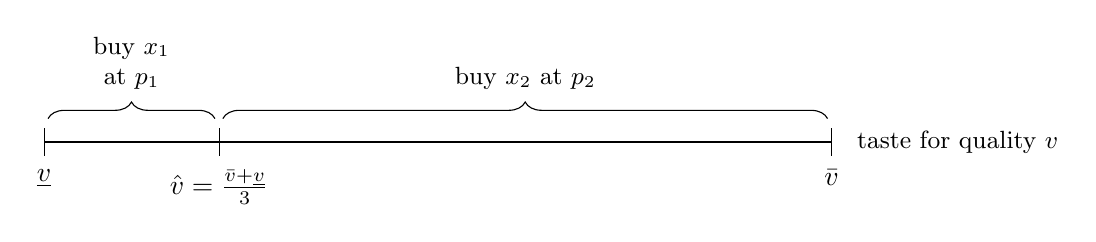
\begin{tikzpicture}[x=1cm,y=1cm]
\draw[thick] (0,0) -- (10,0);
\draw (0,0.18) -- (0,-0.18);
\draw (10,0.18) -- (10,-0.18);
\draw (2.222,0.18) -- (2.222,-0.18);
\node[below] at (0,-0.22) {$\underline v$};
\node[below] at (10,-0.22) {$\bar v$};
\node[below] at (2.222,-0.22) {$\hat v = \frac{\bar v + \underline v}{3}$};
\draw[decorate, decoration={brace, amplitude=6pt}] (0.05,0.3) -- (2.17,0.3)
  node[midway, above=7pt, align=center, font=\small] {buy $x_1$\\at $p_1$};
\draw[decorate, decoration={brace, amplitude=6pt}] (2.27,0.3) -- (9.95,0.3)
  node[midway, above=7pt, align=center, font=\small] {buy $x_2$ at $p_2$};
\node[anchor=west, font=\small] at (10.2,0) {taste for quality $v$};
\end{tikzpicture}
\caption{Market segments in the vertical duopoly of \cref{prop:04-vertical}, drawn for $\underline v = 1$ and
$\bar v = 4$. Consumers with a high taste for quality buy the high-quality product. The cutoff
$\hat v = \frac{\bar v + \underline v}{3}$ does not depend on the two qualities.}
\label{fig:04-vertical}
\end{figure}

\Cref{fig:04-vertical} shows the segments. The force behind part (ii) is the one we saw on Hotelling's line. Closer
qualities mean fiercer price competition, so firms differentiate as much as they can
\citep{GabszewiczThisse1979,ShakedSutton1982}. The high-quality firm charges more, sells more and earns more. Both
markups and profits scale with the quality gap $x_2 - x_1$, and they vanish when the products are identical.

\Citet[Section 7.5.1]{Tirole1988} draws out two further points. First, part (ii) has two equilibria, which differ
only in which firm takes the top quality. If one firm chooses its quality first, it takes $\bar x$ and leaves
$\underline x$ to its rival, so the equilibrium is unique. Since $\pi_2 > \pi_1$, each firm would like to move first.
With a cost of introducing a quality and growing demand, this becomes a preemption race, in which firms trade the
gain from leadership against the cost of entering too early. Second, maximal differentiation is not robust. If the
lowest feasible quality is so low that the coverage condition fails, the low-quality firm loses the bottom of the
market and no longer wants the lowest quality. The effect is stronger when marginal costs differ across qualities,
which already softens price competition. The principle of differentiation itself survives.

\begin{remark}[Natural oligopoly]\label{rem:04-natural-oligopoly}
The condition $\bar v > 2\underline v$ requires enough dispersion in tastes. If $\bar v \le 2\underline v$, formula
\eqref{eq:04-vertical-prices} would give $p_1 \le c$. The equilibrium then has $p_1 = c$ and the high-quality firm
serving every consumer at the limit price $p_2 = c + \underline v(x_2 - x_1)$, the highest price at which the lowest
type still prefers quality 2. To see this, write $m_2 = p_2 - c$. At $p_1 = c$, firm 2's profit for
$m_2 > \underline v\Delta x$ is $m_2M\frac{\bar v\Delta x - m_2}{(\bar v - \underline v)\Delta x}$. Its slope at
$m_2 = \underline v\Delta x$ is $M\frac{\bar v - 2\underline v}{\bar v - \underline v} \le 0$, and it is concave, so firm 2
does not raise its price further. With any positive fixed cost, only one firm enters, however large $M$ is. This is
the simplest instance of the finiteness property of \citet{ShakedSutton1983}, which \citet[Section 7.5.1]{Tirole1988}
states as follows. Let quality $x$ cost $c(x)$ per unit. Suppose that, if every quality were sold at its unit cost,
all consumers would buy the highest quality. Then at most a finite number of firms can have positive market shares,
whatever the relative sizes of demand and entry costs. Price competition among the high-quality firms leaves no room
for low qualities. The condition requires unit cost to rise slowly with quality. Shaked and Sutton therefore expect
finiteness when the burden of quality improvement falls mainly on research and development or other fixed costs,
rather than on labor and materials. On the circle, by contrast, the number of firms grows without bound as fixed
costs vanish. \Cref{ch:discrete} estimates the vertical demand model, and \citet{Bresnahan1987} applies it to the 1955
automobile price war.
\end{remark}

\subsection{From address models to discrete choice}\label{sec:04-location-bridge}

Location models are characteristics-space models with one or two characteristics and no idiosyncratic taste
shock. Substitution is local. On the line and the circle a product competes only with its neighbors, and in the
vertical model only with the products just above and below it in quality. Adding a product close to an existing one
adds little value, since the gain on the circle is the saved transport cost of nearby consumers. Logit-type models
sit at the opposite extreme. Every product competes with every other, IIA holds, and each new product adds value
through its own taste shock (\cref{sec:04-spaces-drawbacks}). The two classes share a formal structure.
Expanding the square in a quadratic ideal-point model turns it into a random coefficients model, as shown in
\cref{prop:06-idealpoint}. The pure characteristics model of \citet{BerryPakes2007} keeps the local substitution of
address models while allowing many characteristics and estimation from market data (\cref{ch:discrete}). Random
coefficient logit models (\cref{ch:blp}) sit between the extremes. They generate local substitution through
correlated tastes while keeping the logit shock.

Location models also frame empirical work on product choice. In the location and quality games above, firms choose
positions in anticipation of price competition. Mergers change these incentives. \Citet{Sweeting2010} studies how
radio stations reposition their formats after mergers (\cref{ch:mergers}). The estimation of such product choice
models builds on the equilibrium theory of this section.


\section{Bibliographic notes}\label{sec:04-notes}

\citet[ch.~7]{Tirole1988} and \citet{Vives1999} give textbook treatments of price competition with differentiated
products, and \citet{AndersonDePalmaThisse1992} build the theory on discrete choice. Tirole treats the linear city in
Section 7.1.1, the circular city in Section 7.1.2 and the forces for and against differentiation in Section 7.1.3.
Vertical differentiation is in Section 7.5.1, and monopolistic competition is in Sections 7.2 and 7.5.2. The location
tradition starts with \citet{Hotelling1929}. \citet{DAspremontGabszewiczThisse1979} overturned its conclusion about
minimum differentiation, and \citet{Salop1979} moved the model to the circle. \citet{Economides1989} studies location
choice on the circle, and \citet{PrescottVisscher1977} study sequential location on the line.
\citet{GabszewiczThisse1979} and \citet{ShakedSutton1982,ShakedSutton1983} developed vertical differentiation and the
theory of natural oligopoly.

\citet{Chamberlin1933} introduced monopolistic competition. The representative-consumer CES model of
\citet{Spence1976} and \citet{DixitStiglitz1977} remains its workhorse and that of trade theory
\citep{Krugman1980,Melitz2003}. \citet{MankiwWhinston1986} isolate the business-stealing and product-diversity
externalities behind excess or insufficient entry, and \citet{BerryWaldfogel1999} measure them in radio
broadcasting. \citet{PerloffSalop1985} replaced the representative consumer by a population with i.i.d.\ tastes for
the brands. \citet{AndersonDePalmaNesterov1995} use that model to show that log-concave tastes rule out
insufficient variety when each consumer buys one unit. With price-sensitive individual demand, the shortfall relative
to the zero-profit constrained optimum is at most one product.

\citet{CaplinNalebuff1991} remains the reference on existence of price equilibrium with single-product firms, and
\citet{Dierker1989} reached related conditions independently. The theory of supermodular games
\citep{MilgromRoberts1990,Vives1990} explains why log-supermodular price games are well behaved. Classical sufficient
conditions for uniqueness go back to \citet{Friedman1977} and \citet{GaleNikaido1965}.
\citet[Theorems~7 and~13]{KonovalovSandor2010} prove existence and uniqueness of price equilibrium with multi-product
firms for the simple logit and for CES demand.
\citet{NockeSchutz2018} develop an aggregative-games approach to multi-product price competition with logit and CES
demands. Each firm's profit depends on its rivals' prices only through a one-dimensional aggregator, and firms may
differ in their numbers of products \citep[p.~229, n.~127, and p.~232, n.~140]{AskerNocke2021}.

The multi-product pricing equation became a standard part of empirical work with \citet{Berry1994} and
\citet{BerryLevinsohnPakes1995}, who used it to recover costs and to sharpen demand estimates. \citet{Bresnahan1987}
and \citet{Nevo2001} used it to compare models of conduct. \citet{BerryHaile2014} formalize the identification of
conduct with differentiated products, and \citet{BackusConlonSinkinson2021} and \citet{DuarteEtAl2024} develop tests
among conduct models. Profit weights from partial ownership go back to \citet{OBrienSalop2000}, and
\citet{MillerWeinberg2017} estimate a weight for a joint venture. \citet{FarrellShapiro2010} put diversion ratios at
the center of merger screening, and \citet{ConlonMortimer2021} study how to measure them. \citet{MorrowSkerlos2011}
provide a fixed-point algorithm that computes equilibria reliably with mixed logit demand, and \citet{Werden1996}
derives the cost reductions that leave prices unchanged after a merger.

The characteristics approach goes back to \citet{Lancaster1966} and \citet{Gorman1980}, and \citet{McFadden1974}
gave it its econometric form. \citet{McFadden1984} surveys the qualitative response models that implement it, and
\citet{BerryPakes2007} analyze the pure characteristics model, which drops the product-specific taste shock.
\citet{DeatonMuellbauer1980a} is the standard reference for demand systems in product space (\cref{ch:aids}).
\citet{Hausman1997} argues that symmetric systems such as the logit and the CES overstate the value of new goods, a
theme that \cref{ch:newgoods} takes up.

\section{Exercises}\label{sec:04-exercises}

\begin{enumerate}[label=\arabic*., leftmargin=*, itemsep=6pt]

\item \textit{Asymmetric costs, upward pricing pressure and cost-reducing investment.} Let demands be $q_1 = a - bp_1 + dp_2$ and
$q_2 = a - bp_2 + dp_1$ with $b > d \ge 0$, as in \cref{ex:04-linear-duopoly}, but let marginal costs differ,
$c_1 \ne c_2$.
\begin{enumerate}[label=(\alph*)]
  \item Solve for the Bertrand-Nash prices with separate owners. Show that $p_1 - p_2 = \frac{b(c_1 - c_2)}{2b + d}$.
  \item Solve for the prices of a joint owner. Show that $p_j = \frac{a}{2(b - d)} + \frac{c_j}{2}$, so the joint
  owner passes half of each product's cost through to that product's price and none to the other price. Write each
  merged markup in terms of $\frac{a}{b}$, $c_j$ and $D = \frac{d}{b}$.
  \item Take $a = 10$, $b = 2$, $d = 1$, $c_1 = 1$ and $c_2 = 2$. Compute $\mathit{UPP}_1$ and $\mathit{UPP}_2$ from
  \eqref{eq:04-upp} with no efficiencies, at the pre-merger prices. Compare each with the actual price change.
  \item Which price rises more? Explain the answer with the margins that enter upward pricing pressure, and relate
  the gap between UPP and the price change to \cref{ex:04-upp-linear}.
  \item Now let the two firms sit at the ends of Hotelling's line with linear transport cost $\tau$ and mass $M$
  of consumers (\cref{sec:04-hotelling-linear}). Let $c_1$ and $c_2$ be close enough that both firms sell. Show that
  their demands are the limiting case $a = \frac{M}{2}$ and $b = d = \frac{M}{2\tau}$ of the system above. Derive the
  reaction functions $p_i = R_i(p_j)$, the equilibrium prices $p_i(c_i, c_j)$ and the reduced-form profits
  $\Pi_i(c_i, c_j)$. Check that the price gap agrees with part (a).
  \item Show that $\frac{\partial^2\Pi_i}{\partial c_i\partial c_j} < 0$, and interpret the sign.
  \item Before prices are set, each firm chooses its marginal cost $c_i$ at an investment cost $\Gamma(c_i)$ with
  $\Gamma' < 0$ and $\Gamma'' > 0$. Use the envelope theorem to split the marginal return to a lower $c_i$ into two
  parts. The direct effect works on the firm's own sales, and the strategic effect works through the rival's price.
  Find the sign of each, and compare the decomposition with the location game of \cref{prop:04-hotelling}.
  \citet[Section 7.1.1, Exercise 7.2]{Tirole1988} poses this problem.
\end{enumerate}

\item \textit{Best responses of a multi-product logit firm.} Use the notation of \cref{sec:04-bertrand-logit}.
\begin{enumerate}[label=(\alph*)]
  \item Starting from $S_f = \frac{E_fe^{-\alpha m_f}}{\Phi_{-f} + E_fe^{-\alpha m_f}}$ and the condition
  $\alpha m_f(1 - S_f) = 1$, derive \eqref{eq:04-logit-br-multi} line by line.
  \item Use $W'(z) = \frac{W(z)}{z(1 + W(z))}$ to show that $\frac{\partial BR_k}{\partial p_l} = \frac{S_fs_l}{1 - S_f}$
  for $k \in \mathcal{J}_f$ and $l \notin \mathcal{J}_f$, with shares evaluated at the best response.
  \item Show that each row of the matrix of best-response slopes sums to less than $S_f$. Explain why this
  delivers convergence of best-response iteration from any starting point.
  \item A firm owns two products with $v_1 = v_2 = 1$. The price coefficient is $\alpha = 2$ and the rivals'
  aggregate is $\Phi_{-f} = 4$. Compute the firm's best-response markup and combined share, and verify
  \cref{prop:04-logit-markup}. How do they change if the firm sells only product 1?
\end{enumerate}

\item \textit{Diversion and merger screening with nests.} Use the four-product market of \cref{fig:04-diversion}.
\begin{enumerate}[label=(\alph*)]
  \item Nested logit shares are $s_j = s_{j\mid g}s_g$, with $s_{j\mid g} = \frac{e^{\frac{\delta_j}{1 - \sigma^{\mathrm{NL}}}}}{\mathcal{S}_g}$,
  $\mathcal{S}_g = \sum_{k \in g}e^{\frac{\delta_k}{1 - \sigma^{\mathrm{NL}}}}$ and
  $s_g = \frac{\mathcal{S}_g^{1 - \sigma^{\mathrm{NL}}}}{1 + \sum_h\mathcal{S}_h^{1 - \sigma^{\mathrm{NL}}}}$. Derive the
  share derivatives stated in \cref{sec:04-diversion-systems} and then \eqref{eq:04-diversion-nl}.
  \item Verify the diversion ratios reported for $\sigma^{\mathrm{NL}} = 0.5$ and check that they sum to one.
  \item All prices are equal and every product earns a margin of 40 percent. Compute the GUPPI of product 1 for a
  merger of products 1 and 2 and for a merger of products 1 and 3. Do so under the logit and under the nested logit
  with $\sigma^{\mathrm{NL}} = 0.5$. Which mergers would a screen that flags a GUPPI above 5 percent select?
  \item Both models fit the same market shares exactly. Explain what data could tell them apart, using
  \eqref{eq:04-diversion-marginal} and \eqref{eq:04-diversion-secondchoice}.
\end{enumerate}

\item \textit{Pass-through and markups with CES demand.} A single-product firm faces the CES demand of
\cref{prop:04-ces} and has constant marginal cost. Rivals' prices are fixed.
\begin{enumerate}[label=(\alph*)]
  \item Differentiate the Lerner condition \eqref{eq:04-ces-lerner} to show that the pass-through of the firm's own
  cost is $\rho_j = \frac{[\sigma - (\sigma - 1)s_j]^2}{\sigma(\sigma - 1)(1 - s_j)}$.
  \item Show that $\rho_j \to \frac{\sigma}{\sigma - 1}$ as $s_j \to 0$, as in \cref{tab:04-ces-logit-linear}.
  Evaluate $\rho_j$ for $\sigma = 3$ and $s_j \in \{0, 0.1, 0.5\}$.
  \item Show that residual CES demand is log-convex in own price when $s_j$ is small. Relate pass-through above one
  to the curvature results of \cref{ch:theory}, and contrast it with the logit value $1 - s_j$.
  \item With $N$ symmetric firms, compute the Lerner index \eqref{eq:04-ces-symmetric} for $\sigma = 3$ and
  $N \in \{2, 5, 10\}$, and compare it with the large-group value $\frac{1}{\sigma}$. Explain in one paragraph why no
  equilibrium exists with $N = 1$.
\end{enumerate}

\item \textit{Concavity of demand and the Caplin-Nalebuff bounds.}
\begin{enumerate}[label=(\alph*)]
  \item Let $q(p) = (1 - p)^k$ on $[0, 1]$ with $k > 0$. Show that $q$ is $\frac{1}{k}$-concave and not $\varrho$-concave for
  any $\varrho > \frac{1}{k}$. Use \cref{lem:04-recip} to show that $(p - c)q(p)$ is quasi-concave for every $c \in [0, 1)$.
  \item Let $L = 1$, reservation prices $R(\nu) = 1 - \nu$ and the type density $\psi(\nu) = 3\nu^2$ on $[0, 1]$.
  Compute demand. Find the largest $\varrho$ for which $\psi$ is $\varrho$-concave, and check that the bound of
  \cref{thm:04-cn-demand} is attained.
  \item Now let a fraction 0.2 of consumers have reservation prices uniform on $[0.8, 1]$ and a fraction 0.8 have
  reservation prices uniform on $[0, 0.2]$. With zero cost, compute demand and profit as functions of price. Show
  that profit has two local maxima, and find the global one.
  \item Which part of Assumption A2 does the distribution in (c) violate? Relate the two local maxima to the
  equilibria of \cref{ex:04-multiple-eq}.
\end{enumerate}

\item \textit{Salop's circle with quadratic transport costs.} Consumers of mass $M$ are uniform on a circle of
circumference one, and a consumer at distance $d$ from a firm pays the transport cost $\tau d^2$. There are $N$
equally spaced firms with marginal cost $c$ and fixed cost $\phi$.
\begin{enumerate}[label=(\alph*)]
  \item Show that a firm charging $p$ against neighbors charging $\bar p$ sells
  $M\big[\frac{1}{N} + \frac{N(\bar p - p)}{\tau}\big]$.
  \item Derive the symmetric equilibrium price $c + \frac{\tau}{N^2}$ and the free-entry number of firms
  $N^* = \big(\frac{\tau M}{\phi}\big)^{\frac{1}{3}}$.
  \item Show that average transport cost is $\frac{\tau}{12N^2}$ and that the efficient number of firms is
  $N^o = \big(\frac{\tau M}{6\phi}\big)^{\frac{1}{3}}$, so $\frac{N^*}{N^o} = 6^{\frac{1}{3}}$.
  \item Compare with \cref{prop:04-salop,prop:04-logit-entry}. In each of the three models, compare the entrant's
  private gain with the social gain from its product, and explain which externality dominates.
\end{enumerate}

\item \textit{Profit weights and the identification of conduct.} In the linear duopoly of
\cref{ex:04-linear-duopoly}, each firm maximizes its own profit plus $\kappa$ times its rival's profit, with
$\kappa \in [0, 1]$, the range from Nash pricing to joint profit maximization (\cref{sec:04-conduct}).
\begin{enumerate}[label=(\alph*)]
  \item Show that the symmetric equilibrium markup is $m(\kappa) = \frac{a - (b - d)c}{2b - (1 + \kappa)d}$, and that
  it equals $m^N$ at $\kappa = 0$ and $m^J$ at $\kappa = 1$.
  \item Rewrite the first-order condition in the diversion form \eqref{eq:04-foc-diversion}. Interpret $\kappa D$ as
  an effective diversion ratio.
  \item Take $a = 10$, $b = 2$, $d = 1$ and $c = 1$, and suppose the observed price is 5. Infer $\kappa$. Then
  suppose instead that $\kappa = 0$ is known, and find the marginal cost that rationalizes the same price.
  \item Show that the pass-through of a common cost change is
  $\frac{\dd p}{\dd c} = \frac{b - \kappa d}{2b - (1 + \kappa)d}$. Explain how a cost shifter with known effect on
  $c$ separates conduct from cost, and relate the argument to \cref{rem:04-kappa-theta} and to the pass-through tests
  of \cref{ch:conduct}.
\end{enumerate}

\item \textit{Computation: a six-product logit market.} Six products have price-free mean utilities
$x_j\beta + \xi_j = (2.0, 1.8, 1.6, 2.2, 1.4, 1.2)$ and marginal costs $mc = (1.0, 0.9, 0.8, 1.2, 0.7, 0.6)$. The
price coefficient is $\alpha = 1$, the outside good has mean utility zero and market size is one.
\begin{enumerate}[label=(\alph*)]
  \item Compute the equilibrium prices, shares and markups under three ownership structures: six single-product
  firms, two firms owning $\{1, 2, 3\}$ and $\{4, 5, 6\}$, and a single owner. Use best-response iteration with
  \eqref{eq:04-logit-br-multi}, and check each answer against \cref{prop:04-logit-markup}.
  \item At the two-firm equilibrium, compute the diversion matrix and check the adding-up property of
  \cref{prop:04-diversion-adding}.
  \item Treat the two-firm equilibrium as data. Recover marginal costs with \eqref{eq:04-mc-recover} assuming
  single-product firms and assuming a single owner. Which assumption is rejected by implausible costs?
  \item Run best-response iteration from 100 random starting prices to check uniqueness. Then compute the change in
  consumer surplus from the single-product to the two-firm structure, and the partial pass-through of a cost
  increase on all of firm 1's products. Compare the latter with \cref{prop:04-passthrough}.
\end{enumerate}

\end{enumerate}


\part{Demand Estimation}
\chapter{Demand in Product Space: The Almost Ideal Demand System}\label{ch:aids}
\chaptermark{Demand in Product Space: The AIDS}

Suppose India begins to enforce foreign patents on antibiotics. The domestic versions of the patented molecules
leave the market, and the foreign patent holders no longer face domestic rivals. How much would prices rise? How
much would consumers lose, and how much would the patent holders gain? Questions of this kind call for a demand
model with three properties. It must describe how consumers substitute among many related products. It must tie
the estimated substitution patterns to preferences, so that price changes translate into money measures of
welfare. And it must predict demand at prices, and for sets of products, that the data have never shown.

This chapter develops the first of the two approaches to demand estimation in this book. We write demand in
\emph{product space}, where each good has its own parameters and the cross-price effects among goods are
estimated directly. The workhorse model is the Almost Ideal Demand System (AIDS) of
\citet{DeatonMuellbauer1980a}. It is derived from an explicit expenditure function. The restrictions of consumer
theory are linear in its parameters, and it aggregates over consumers with different incomes. Its budget-share
equations are nearly linear, so standard tools can estimate it. Its main cost is the number of parameters, which
grows with the square of the number of goods. Applied work therefore combines it with \emph{multi-stage
budgeting}, in which consumers allocate expenditure first across broad groups of goods and then within each
group.

The chapter moves from theory to data to applications. \Cref{sec:05-productspace,sec:05-duality,sec:05-aids}
build the theory. They motivate microfounded demand systems, collect the duality results we need, and derive the
AIDS with its restrictions, elasticities, flexibility and limits. \Cref{sec:05-aggregation,sec:05-separability,%
sec:05-estimation} take the model to data. They ask when market data behave as if one consumer had chosen them,
when demand can be estimated group by group, and how the system is estimated, tested and identified. The original
British application of Deaton and Muellbauer is the first case study. \Cref{sec:05-welfare} turns estimates into
welfare measures and counterfactual equilibria. It values products that disappear at their virtual prices, the
shadow prices of a zero ration, and it bounds marginal cost when conduct is unknown.

The remaining sections apply the toolkit. \Cref{sec:05-hlz} studies the multi-level demand system for beer of
\citet{HausmanLeonardZona1994}. That paper introduced prices in other cities as instruments and used its estimates
for merger analysis. \Cref{sec:05-cgj} studies \citet{ChaudhuriGoldbergJia2006}, who answer the patent question
above with a two-level AIDS. \Cref{sec:05-dgg} confronts their forecast with the retrospective evidence of
\citet{DugganGarthwaiteGoyal2016}. \Cref{sec:05-assessment} closes with an assessment of what product-space demand
can and cannot do.

The chapter builds on earlier material. The monopoly pricing condition and the inverse elasticity rule come from
\cref{ch:theory}. Multiproduct pricing and the distinction between product space and characteristic space come from
\cref{ch:diffprod}. We prove the duality results we use. \Cref{app:math} restates them with references to these
proofs, and adds producer duality, integrability and the envelope-theorem route to Shephard's lemma.
Instrumental variables, the generalized method of moments and the bootstrap are developed in
\cref{app:econometrics}. The chapter also prepares what follows. \Cref{ch:discrete,ch:logit,ch:blp} model demand in
characteristic space, where the number of parameters no longer grows with the number of products. \Cref{ch:newgoods}
uses the multi-level AIDS and virtual prices to value a new good, and \cref{ch:mergers} uses estimated demand
systems to simulate mergers. One three-good numerical example, introduced in \cref{ex:05-running}, runs through the
chapter and illustrates the formulas.

\definecolor{c05p1blue}{HTML}{2A78D6}
\definecolor{c05p1orange}{HTML}{EB6834}
\definecolor{c05p1aqua}{HTML}{1BAF7A}
\definecolor{c05p1gray}{HTML}{52514E}

\section{Demand Systems in Product Space}\label{sec:05-productspace}

A \emph{demand system} gives the quantity of every good as a function of all prices and of the consumer's
budget. This chapter studies demand systems written in \emph{product space}. Each good has its own
parameters, and the model states directly how the demand for one good responds to the price of another.
The workhorse is the Almost Ideal Demand System of \citet{DeatonMuellbauer1980a}. We follow that literature
and index goods by $i$, $j$ and $k$, with $J$ goods in total. Elsewhere in the book the letter $i$ indexes
consumers. In this chapter households are indexed by $h = 1, \dots, H$, and \cref{sec:05-conventions}
collects the remaining conventions.

\subsection{Questions a demand system answers}\label{sec:05-questions}

Demand systems serve two kinds of questions. \emph{Positive} questions ask what will happen. How do
consumers substitute among goods when one price rises? How will prices respond to a merger, a tax or the
withdrawal of a product? Will a change in the rules alter the incentives of firms to invest in research and
development? \emph{Normative} questions ask whether the change is desirable. Who wins and who loses? Could
the winners compensate the losers? How large is the total compensating or equivalent variation, the money
measure of welfare change defined in \cref{sec:05-cv-ev}?

A second distinction concerns timing. \emph{Prospective} analysis predicts the effects of a policy before it
is implemented. Because the policy has not yet generated data, prospective analysis needs a model of demand
and supply, and sometimes a model of dynamic investment as well. \emph{Retrospective} analysis measures what
happened after a policy was implemented. It relies on causal identification from the variation that the
policy created. The two approaches complement each other. Only a model can evaluate a policy that has never
been tried, and only retrospective evidence can tell us whether a model predicted well.

One policy question runs through this chapter. The Agreement on Trade-Related Aspects of Intellectual
Property Rights (TRIPS) requires members of the World Trade Organization to enforce product patents in all
fields of technology, including pharmaceuticals. Countries that excluded pharmaceuticals from product patents
were given a transition period to amend their laws. Between April 1972 and March 2005, India recognized only
process patents for pharmaceuticals \citep{ChaudhuriGoldbergJia2006}, and Indian firms sold their own
versions of molecules patented abroad. Enforcing patents would remove
these domestic versions from the market. Would consumers then buy the foreign version of the same molecule,
a different domestic molecule, or nothing in the segment? How much would prices rise, and how would the loss
to consumers compare with the gain to patent holders? \Cref{sec:05-cgj} studies the prospective answer of
\citet{ChaudhuriGoldbergJia2006}, which is built on the demand system of this chapter. \Cref{sec:05-dgg}
confronts it with the retrospective evidence of \citet{DugganGarthwaiteGoyal2016}.

\subsection{Why microfoundations}\label{sec:05-microfoundations}

A \emph{microfounded} demand system is derived from an explicit model of optimizing consumers. It has three
advantages over a purely statistical description of demand. The first is internal consistency. The budget
constraint holds, demands do not change when all prices and income scale up together, and the cross-price
effects obey the symmetry restrictions derived in \cref{sec:05-duality}. The second is that the model rests
on \emph{primitives}, preferences and technology, which we can treat as invariant to the policy under study.
Reduced-form coefficients estimated under one policy regime need not survive a change of regime. The third
is that the model links observed behavior to the primitives through an assumption about behavior, here
utility maximization. Observed choices then reveal preferences.

These properties deliver the two products we want from a demand model. Policy-invariant primitives permit
prospective analysis, because we can solve the model again under the new policy. The link to preferences
permits normative statements, because the expenditure function converts a change in prices into a money
measure of welfare.

A statistical demand system can fit the data well and still fail these tests. Consider the \emph{double-log}
system, in which every log quantity is linear in log prices and log income with constant elasticities. It is
a natural first regression, and it imposes no theory at all. The next proposition shows how little of it
survives the budget constraint.

\begin{proposition}[Double-log demand and the budget constraint]\label{prop:05-loglinear}
Suppose that for every good $i$ and every $(p, I) \in \R^J_{++}\times\R_{++}$,
\begin{equation}\label{eq:05-loglinear}
\ln q_i = a_i + \sum_{j=1}^J e_{ij}\ln p_j + \eta_i\ln I ,
\end{equation}
with constant coefficients $a_i$, $e_{ij}$ and $\eta_i$, and that the budget identity $\sum_i p_iq_i = I$
holds everywhere. Then $\eta_i = 1$, $e_{ii} = -1$, $e_{ij} = 0$ for $j \neq i$, and $\sum_i e^{a_i} = 1$.
The only double-log system that satisfies the budget constraint at all prices and incomes is the
Cobb-Douglas demand system.
\end{proposition}

\begin{proof}
Divide the budget identity by $I$ and substitute \eqref{eq:05-loglinear}:
\begin{equation*}
\sum_{i=1}^J \exp\Big(a_i + \sum_{j=1}^J\big(e_{ij} + \indic(i=j)\big)\ln p_j + (\eta_i - 1)\ln I\Big) = 1 .
\end{equation*}
Write $x = (\ln p_1, \dots, \ln p_J, \ln I)^\T$, which ranges over all of $\R^{J+1}$. Term $i$ equals
$e^{a_i}\exp(\ell_i^\T x)$ for a coefficient vector $\ell_i$. Collect the terms that share the same vector,
and move the constant 1 to the left side as the term $-\exp(0^\T x)$. Exponentials of distinct linear forms
are linearly independent functions on $\R^{J+1}$. To see this, restrict them to a line on which the distinct
forms have distinct slopes, and use the independence of $e^{\lambda_1 t}, \dots, e^{\lambda_m t}$ for
distinct $\lambda$'s. Every coefficient of the collected sum must therefore vanish. The coefficient of a
group with $\ell \neq 0$ is a sum of positive numbers $e^{a_i}$, so no such group can exist. Hence
$\ell_i = 0$ for every $i$, and the coefficient of the zero form gives $\sum_i e^{a_i} = 1$. The condition
$\ell_i = 0$ reads $e_{ij} + \indic(i=j) = 0$ and $\eta_i = 1$.
\end{proof}

The double-log system remains useful as a local approximation, and we meet it again at the upper levels of
multi-level demand systems in \cref{sec:05-hlz}. As a global model it cannot satisfy the budget constraint,
its elasticities need not obey the restrictions of consumer theory, and it delivers no welfare measure. The
systems in the rest of this chapter are built so that they do all three.

\subsection{Product space and characteristic space}\label{sec:05-ps-vs-cs}

\Cref{ch:diffprod} introduced the two ways of modeling demand for differentiated products. In \emph{product
space}, preferences are defined over the goods themselves, and demand is written as
\begin{equation}\label{eq:05-productspace}
q_i = f_i(p_1, \dots, p_J, I), \qquad i = 1, \dots, J,
\end{equation}
with parameters indexed by goods. In \emph{characteristic space}, goods are bundles of characteristics and
preferences are defined over the characteristics. The number of parameters then grows with the number of
characteristics and with the dimension of consumer heterogeneity, rather than with the number of goods.

Product space is the more natural starting point. Substitution patterns are estimated from the data instead of
being imposed by the location of goods in a space of attributes. Goods can be complements as well as substitutes. No data on
characteristics are needed, which helps when the relevant attributes are hard to measure, as for books or
films.

Its central problem is dimensionality. Even a linear system $q = a + Ap$ has $J^2$ price coefficients in the
matrix $A$, which is 10{,}000 coefficients for $J = 100$ goods. Theory helps but not enough. In the Almost
Ideal Demand System, symmetry, homogeneity and adding up leave $\frac{J(J-1)}{2}$ free price coefficients
(\cref{sec:05-aids-limits}), which is still 4{,}950 for $J = 100$. Dimensionality has two further costs. Each
of the $J$ prices is a potentially endogenous regressor in every equation, so estimation requires
instruments that move the prices independently of one another (\cref{sec:05-estimation}). And because every
parameter belongs to a particular good, the model cannot predict demand for a good that has never been sold.

There are two remedies. The first aggregates goods into a few groups and assumes that consumers budget in
stages, so that each stage involves only a few goods. The theory of separability that justifies this
procedure is developed in \cref{sec:05-separability}, and the applications of \citet{HausmanLeonardZona1994}
and \citet{ChaudhuriGoldbergJia2006} take this route. The second remedy moves to characteristic space, as
in \cref{ch:discrete,ch:logit,ch:blp}. Its costs are data on characteristics, more complex estimation, and
restrictions on substitution that come from the structure of the random utility model.

\subsection{Three product-space systems}\label{sec:05-three-systems}

We now compare three systems that are all derived from a model of consumer behavior. The logit and the
constant elasticity of substitution (CES) systems place all substitution in a single parameter. The Almost
Ideal Demand System frees the cross effects. \Cref{ch:diffprod,ch:logit} develop the first two in depth, so
the derivations here are brief.

\casehead{Logit}
A population of $M$ consumers, indexed by $h$, each buys one unit of one of the goods $i = 1, \dots, J$ or
of an outside good $i = 0$. Consumer $h$ obtains utility
\begin{equation*}
u_{hi} = \delta_i - \alpha p_i + \epsilon_{hi}, \qquad u_{h0} = \epsilon_{h0},
\end{equation*}
where the $\epsilon_{hi}$ are independent type-I extreme value draws. In this subsection only, $\delta_i$
is a taste shifter that excludes price, and $\alpha > 0$ is the logit price coefficient. (Elsewhere in the
book $\delta$ denotes mean utility including price, and in the Almost Ideal Demand System $\alpha_i$ is an
intercept.) The share of consumers who choose good $i$ and the share who choose the outside good are
\begin{equation*}
s_i = \frac{e^{\delta_i - \alpha p_i}}{1 + \sum_{k=1}^J e^{\delta_k - \alpha p_k}}, \qquad
s_0 = \frac{1}{1 + \sum_{k=1}^J e^{\delta_k - \alpha p_k}},
\end{equation*}
as \cref{ch:discrete} derives from the extreme value distribution. The ratio of the two is
$\frac{s_i}{s_0} = e^{\delta_i - \alpha p_i}$. Quantities are $q_i = Ms_i$, so the market size $M$ cancels
from the ratio $\frac{q_i}{q_0}$. Taking logs gives the market-level logit,
\begin{equation}\label{eq:05-logit}
\ln q_i - \ln q_0 = \delta_i - \alpha p_i .
\end{equation}
The left side is computed from data, and the right side is linear in the parameters. Once we add an error
term to $\delta_i$, the logit can be estimated by linear regression \citep{Berry1994}, as \cref{ch:logit}
explains. Differentiating the shares gives $\frac{\partial s_i}{\partial p_i} = -\alpha s_i(1-s_i)$ and
$\frac{\partial s_i}{\partial p_k} = \alpha s_is_k$ for $k \neq i$. The elasticities are therefore
\begin{equation}\label{eq:05-logit-elast}
\varepsilon_{ii} = -\alpha p_i(1 - s_i), \qquad \varepsilon_{ik} = \alpha p_ks_k \quad (k \neq i).
\end{equation}
The cross elasticity with respect to $p_k$ is the same for every good $i$. When good $k$ raises its price,
all other goods gain demand in the same proportion, however close or distant they are to $k$. This is the
independence of irrelevant alternatives, studied in \cref{ch:logit}.

\casehead{Constant elasticity of substitution}
A single consumer with budget $I$ has CES utility. The next proposition collects the facts we use. In this
chapter $\sigma$ denotes the elasticity of substitution. Elsewhere in the book it denotes the nesting
parameter of the nested logit.

\begin{proposition}[CES demand]\label{prop:05-ces}
Let $U(q) = \big(\sum_{j=1}^J a_j^{\frac{1}{\sigma}}q_j^{\frac{\sigma-1}{\sigma}}\big)^{\frac{\sigma}{\sigma-1}}$
with $a_j > 0$, $\sigma > 0$ and $\sigma \neq 1$, and let the consumer maximize $U$ subject to
$\sum_j p_jq_j = I$. Define the CES price index
$P^{CES} = \big(\sum_{j=1}^J a_jp_j^{1-\sigma}\big)^{\frac{1}{1-\sigma}}$. Then:
\begin{enumerate}[label=(\roman*)]
\item Demand is $q_i = a_i\big(\frac{p_i}{P^{CES}}\big)^{-\sigma}\frac{I}{P^{CES}}$, and the budget share is
  $w_i = \frac{p_iq_i}{I} = a_i\big(\frac{p_i}{P^{CES}}\big)^{1-\sigma}$.
\item Indirect utility is $v(p, I) = \frac{I}{P^{CES}}$ and the expenditure function is $e(p, u) = P^{CES}u$,
  so preferences are homothetic.
\item The Marshallian elasticities are $\varepsilon_{ii} = -\sigma + (\sigma - 1)w_i$,
  $\varepsilon_{ik} = (\sigma - 1)w_k$ for $k \neq i$, and the expenditure elasticity is $\eta_i = 1$.
\end{enumerate}
\end{proposition}

\begin{proof}
Write $U = S^{\frac{\sigma}{\sigma-1}}$ with $S = \sum_j a_j^{\frac{1}{\sigma}}q_j^{\frac{\sigma-1}{\sigma}}$.
By the chain rule,
\begin{equation*}
\frac{\partial U}{\partial q_i} = \frac{\sigma}{\sigma-1}S^{\frac{1}{\sigma-1}}\cdot
\frac{\sigma-1}{\sigma}a_i^{\frac{1}{\sigma}}q_i^{-\frac{1}{\sigma}}
= U^{\frac{1}{\sigma}}a_i^{\frac{1}{\sigma}}q_i^{-\frac{1}{\sigma}},
\end{equation*}
because $S^{\frac{1}{\sigma-1}} = U^{\frac{1}{\sigma}}$. The first-order condition
$\frac{\partial U}{\partial q_i} = \lambda p_i$ gives $q_i = a_iU(\lambda p_i)^{-\sigma}$. Substitute into
the budget constraint:
\begin{equation*}
I = \sum_j p_jq_j = U\lambda^{-\sigma}\sum_j a_jp_j^{1-\sigma} = U\lambda^{-\sigma}(P^{CES})^{1-\sigma}.
\end{equation*}
Hence $U\lambda^{-\sigma} = I(P^{CES})^{\sigma-1}$, and
$q_i = a_ip_i^{-\sigma}I(P^{CES})^{\sigma-1} = a_i\big(\frac{p_i}{P^{CES}}\big)^{-\sigma}\frac{I}{P^{CES}}$.
Multiplying by $\frac{p_i}{I}$ gives the share. For (ii), substitute the demands into $S$:
\begin{equation*}
S = \sum_j a_j^{\frac{1}{\sigma}}a_j^{\frac{\sigma-1}{\sigma}}\Big(\frac{p_j}{P^{CES}}\Big)^{1-\sigma}
\Big(\frac{I}{P^{CES}}\Big)^{\frac{\sigma-1}{\sigma}}
= \Big(\frac{I}{P^{CES}}\Big)^{\frac{\sigma-1}{\sigma}}\sum_j a_j\Big(\frac{p_j}{P^{CES}}\Big)^{1-\sigma}
= \Big(\frac{I}{P^{CES}}\Big)^{\frac{\sigma-1}{\sigma}} ,
\end{equation*}
since the last sum equals one by the definition of $P^{CES}$. Then $v = S^{\frac{\sigma}{\sigma-1}} =
\frac{I}{P^{CES}}$, and inverting $u = \frac{e}{P^{CES}}$ gives $e(p,u) = P^{CES}u$. For (iii), take logs of
the demand function, $\ln q_i = \ln a_i - \sigma\ln p_i + (\sigma - 1)\ln P^{CES} + \ln I$. Differentiating
$\ln P^{CES} = \frac{1}{1-\sigma}\ln\sum_k a_kp_k^{1-\sigma}$ gives
$\frac{\partial\ln P^{CES}}{\partial\ln p_j} = \frac{a_jp_j^{1-\sigma}}{\sum_k a_kp_k^{1-\sigma}} = w_j$.
Hence $\varepsilon_{ij} = -\sigma\indic(i=j) + (\sigma - 1)w_j$ and $\eta_i = 1$.
\end{proof}

Writing $a_j = e^{\sigma\delta_j}$, with $\delta_j$ a taste shifter, the log of the demand function takes the
form
\begin{equation}\label{eq:05-ces}
\ln q_i = \sigma\Big(\delta_i - \ln\frac{p_i}{P^{CES}}\Big) + \ln\frac{I}{P^{CES}} .
\end{equation}
The normalization $\sum_j e^{\sigma\delta_j} = 1$ makes $P^{CES} = \bigl(\sum_j a_j\bigr)^{\frac{1}{1-\sigma}} = 1$
when all prices equal one. The parameter $\sigma$ is the elasticity of substitution.
From part (i), $\ln\frac{q_i}{q_k} = \ln\frac{a_i}{a_k} - \sigma\ln\frac{p_i}{p_k}$, so a one percent rise in
the relative price $\frac{p_k}{p_i}$ raises the relative quantity $\frac{q_i}{q_k}$ by $\sigma$ percent.
Goods are gross substitutes when $\sigma > 1$. The cross elasticity $(\sigma-1)w_k$ does not depend on $i$,
so the CES has the same proportional substitution as the logit. The compensated cross elasticity, obtained
from the Slutsky equation of \cref{sec:05-elasticity-identities}, is $\sigma w_k$.

\casehead{The Almost Ideal Demand System}
The third system expresses the budget share of each good as
\begin{equation}\label{eq:05-aids-preview}
w_i = \alpha_i + \sum_{j=1}^J\gamma_{ij}\ln p_j + \beta_i\ln\frac{I}{\mathbf{P}} ,
\end{equation}
where $w_i = \frac{p_iq_i}{I}$ and $\mathbf{P}$ is a price index defined in \cref{sec:05-aids}. Shares
respond to every log price through a separate coefficient $\gamma_{ij}$, and to log real expenditure
$\ln\frac{I}{\mathbf{P}}$ through $\beta_i$. \Cref{sec:05-aids} derives the system from an expenditure
function.

\begin{table}[htbp]
\centering
\caption{Three product-space demand systems compared}\label{tab:05-three-systems}
\footnotesize
\begin{tabularx}{\textwidth}{>{\raggedright\arraybackslash}p{2.55cm}
  >{\raggedright\arraybackslash}X >{\raggedright\arraybackslash}X >{\raggedright\arraybackslash}X}
\toprule
 & Logit (market level) & CES & AIDS \\
\midrule
Dependent variable & $\ln q_i - \ln q_0$ & $\ln q_i$ (or share $w_i$) & budget share $w_i$ \\
\addlinespace
Substitution parameters & one ($\alpha$) & one ($\sigma$) & $\frac{J(J-1)}{2}$ free $\gamma_{ij}$ \\
\addlinespace
Level parameters & $J$ taste shifters $\delta_i$ & $J - 1$ free $\delta_i$ & $2(J-1)$ free $\alpha_i$,
  $\beta_i$, and $\alpha_0$ \\
\addlinespace
Own elasticity $\varepsilon_{ii}$ & $-\alpha p_i(1 - s_i)$ & $-\sigma + (\sigma - 1)w_i$ &
  $-1 + \frac{1}{w_i}\frac{\partial w_i}{\partial\ln p_i}$, \eqref{eq:05-elast-marshall} \\
\addlinespace
Cross elasticity $\varepsilon_{ik}$ & $\alpha p_ks_k$, the same for all $i$ & $(\sigma - 1)w_k$, the same
  for all $i$ & $\frac{1}{w_i}\frac{\partial w_i}{\partial\ln p_k}$, any sign \\
\addlinespace
Engel curves & no income effects (each consumer buys one unit) & homothetic, $\eta_i = 1$ & shares linear
  in $\ln I$, luxuries and necessities \\
\addlinespace
Choke (virtual) price & infinite & infinite & finite if the own share falls with price ($\gamma_{ii} < 0$
  when $\beta_i = 0$) \\
\addlinespace
Aggregation & exact: shares add up individual discrete choices & representative consumer with homothetic
  preferences & almost exact: representative budget level $I_0$ \\
\addlinespace
Typical data & shares of many products, with an outside good & expenditure on many varieties & budget
  shares of a few goods or groups over time or markets \\
\bottomrule
\end{tabularx}
\par\smallskip
\begin{minipage}{\textwidth}\footnotesize
Notes: Elasticities are signed. In the logit column $s_i$ is the market share including the outside good. In
the CES and AIDS columns $w_i$ is the budget share. The AIDS count of free $\gamma_{ij}$ imposes adding up,
homogeneity and symmetry (\cref{sec:05-aids-limits}). Aggregation for AIDS is developed in
\cref{sec:05-aggregation}.
\end{minipage}
\end{table}

\Cref{tab:05-three-systems} sets the three systems side by side. The logit and the CES buy parsimony with
restrictive substitution, because one parameter governs every cross effect. Consumers who leave a product
spread over the other products in proportion to their sizes, whatever the attributes of those products. The AIDS frees the cross
effects at the cost of many parameters.

The row on choke prices matters for welfare. A \emph{choke price}, or \emph{virtual price}, is the price at
which the demand for a good falls to zero \citep{Hicks1940,Rothbarth1941}. Removing a good from the market
is equivalent, for consumers, to raising its price to the virtual price. Under CES and logit the demand for
a good stays positive at every finite price, because $p_i^{-\sigma}$ and $e^{-\alpha p_i}$ never reach
zero. The virtual price is infinite, and the welfare loss from removing a good depends only on its share and
on the single substitution parameter. The value of variety is then built into the functional form. Under
the AIDS the share is linear in $\ln p_i$ when $\beta_i = 0$ and quadratic otherwise. When it falls with the
own price, it reaches zero at a finite price, so the loss depends on the estimated own and cross effects.
\Cref{sec:05-welfare-virtual} develops this comparison.

\subsection{Conventions for this chapter}\label{sec:05-conventions}

Goods are indexed by $i, j, k = 1, \dots, J$, and in this chapter the $J$ goods exhaust the budget under
study. Households are indexed by $h = 1, \dots, H$ and appear as subscripts, as in $I_h$ and $w_{ih}$. The
Hicksian demand $h_i(p, u)$ (defined in \cref{sec:05-ump-emp}) is always written with its arguments, so it cannot be confused with a household
index. Total expenditure, which we also call income, is $I$, and the budget share of good $i$ is
$w_i = \frac{p_iq_i}{I}$. Logarithms are natural logarithms.

Elasticities are signed throughout this chapter, as in the tables of the papers we study. The Marshallian
price elasticity is $\varepsilon_{ij} = \frac{\partial\ln q_i}{\partial\ln p_j}$, so own-price elasticities
are negative. This departs from the convention elsewhere in the book, where the own-price elasticity is
reported as a positive number. The Hicksian elasticity is $\varepsilon^h_{ij}$ and the expenditure
elasticity is $\eta_i$. The Slutsky matrix is $S = [S_{ij}]$ (\cref{sec:05-slutsky}), and we reserve $s$ for market shares. We write
the indicator $\indic(i = j)$ instead of a Kronecker delta, because $\delta$ denotes mean utility elsewhere
in the book. Additive errors in share equations are written $\xi$, while the papers often write
$\varepsilon$, which here denotes an elasticity.

\section{Consumer Duality: The Toolkit}\label{sec:05-duality}

This section collects the results of consumer theory that we need to derive, restrict and use the AIDS.
We keep the argument self-contained and prove every result we use. \Cref{app:math} restates these results for
reference and adds producer duality and integrability. The treatment parallels \citet[ch.~2]{DeatonMuellbauer1980b}. They develop the cost
function in \S 2.3 (pp.~37--42), the properties of demands in \S 2.4 (pp.~43--46) and duality in \S 2.5
(pp.~47--50). Their $c(u, p)$ is our $e(p, u)$, and their $x$ is our total expenditure $I$.

\subsection{Utility maximization and expenditure minimization}\label{sec:05-ump-emp}

\begin{assumption}[Preferences]\label{ass:05-prefs}
The consumer's preferences over bundles $q \in \R^J_+$ are represented by a utility function $U$ that is
continuous, strictly increasing and strictly quasi-concave. Prices satisfy $p \in \R^J_{++}$ and income
satisfies $I > 0$. Whenever derivatives appear, the functions defined below are twice continuously
differentiable.
\end{assumption}

The \emph{utility maximization problem} (UMP) and the \emph{expenditure minimization problem} (EMP) are
\begin{equation}\label{eq:05-ump-emp}
v(p, I) = \max_{q \geq 0}\{U(q) : p^\T q \leq I\}, \qquad
e(p, u) = \min_{q \geq 0}\{p^\T q : U(q) \geq u\}.
\end{equation}
The maximizer of the UMP is the \emph{Marshallian} (uncompensated) demand $q(p, I)$, and $v$ is the
\emph{indirect utility function}. The minimizer of the EMP is the \emph{Hicksian} (compensated) demand
$h(p, u)$, and $e$ is the \emph{expenditure function}. Under \cref{ass:05-prefs} both problems have unique
solutions, by strict quasi-concavity, and both constraints bind, by continuity and strict monotonicity. The
indirect utility function is homogeneous of degree zero in $(p, I)$, because scaling all prices and income
leaves the budget set unchanged. It is strictly increasing in $I$ and nonincreasing in $p$, because a higher
income or a lower price enlarges the budget set.

\begin{lemma}[Duality identities]\label{lem:05-duality}
Under \cref{ass:05-prefs}, for all $p \gg 0$, $I > 0$ and attainable utility levels $u$:
\begin{enumerate}[label=(\roman*)]
\item $e(p, v(p, I)) = I$ and $v(p, e(p, u)) = u$.
\item $q_i(p, I) = h_i(p, v(p, I))$ and $h_i(p, u) = q_i(p, e(p, u))$.
\end{enumerate}
\end{lemma}

\begin{proof}
Let $u = v(p, I)$ and $q^* = q(p, I)$. The bundle $q^*$ attains $u$ at cost $I$, so $e(p, u) \leq I$.
Suppose $e(p, u) < I$, and let $q' = h(p, u)$. Then $p^\T q' < I$, so a slightly larger bundle
$q' + \epsilon\mathbf{1}$ is affordable for small $\epsilon > 0$. By strict monotonicity it yields utility
above $u = v(p, I)$, a contradiction. Hence $e(p, v(p,I)) = I$. The bundle $q^*$ then solves the EMP, and
uniqueness gives $q^* = h(p, u)$. For the second pair, let $I = e(p, u) > 0$ and $q' = h(p, u)$. The bundle
$q'$ is affordable at income $I$, so $v(p, I) \geq u$. Suppose $v(p, I) > u$. By continuity, the bundle
$t\,q(p, I)$ with $t < 1$ close to one still yields utility above $u$, and it costs less than $I = e(p, u)$.
This contradicts the definition of $e$. Hence $v(p, e(p,u)) = u$, the bundle $q'$ solves the UMP, and
uniqueness gives $h(p, u) = q(p, e(p, u))$.
\end{proof}

\subsection{Properties of the expenditure function}\label{sec:05-e-properties}

\begin{proposition}[Expenditure function]\label{prop:05-e-properties}
Under \cref{ass:05-prefs}, the expenditure function $e(p, u)$ has four properties.
\begin{enumerate}[label=(\roman*)]
\item It is homogeneous of degree one in $p$.
\item It is nondecreasing in $p$ and strictly increasing in $u$.
\item It is concave in $p$.
\item It is continuous in $(p, u)$.
\end{enumerate}
\end{proposition}

\begin{proof}
(i) For $\lambda > 0$, the constraint set $\{q : U(q) \geq u\}$ does not depend on prices, and
$\lambda p^\T q$ is minimized by the same bundle as $p^\T q$. Hence $e(\lambda p, u) = \lambda e(p, u)$.

(ii) Let $p' \geq p$ and $q' = h(p', u)$. Then
\begin{equation*}
e(p', u) = p'^\T q' \geq p^\T q' \geq e(p, u),
\end{equation*}
where the last inequality holds because $q'$ is feasible in the EMP at prices $p$. For $u$, let $u' > u$
and $q' = h(p, u')$, and suppose $e(p, u') \leq e(p, u)$. By continuity, $tq'$ with $t < 1$ close to one
still yields utility above $u$. It costs $t\,e(p, u') < e(p, u)$, which contradicts minimality at $u$.

(iii) Let $p'' = \lambda p + (1 - \lambda)p'$ with $\lambda \in [0, 1]$, and let $q'' = h(p'', u)$. Since
$q''$ is feasible at every price vector,
\begin{equation*}
e(p'', u) = \lambda p^\T q'' + (1 - \lambda)p'^\T q'' \geq \lambda e(p, u) + (1 - \lambda)e(p', u).
\end{equation*}
The expenditure function is the minimum of a family of linear functions of $p$, one for each feasible bundle,
and such a minimum is concave.

(iv) Continuity follows from the theorem of the maximum, since the objective is continuous and the
constraint correspondence is continuous under \cref{ass:05-prefs}. We omit the details, which are standard.
\end{proof}

\subsection{Shephard's lemma}\label{sec:05-shephard}

\begin{proposition}[Shephard's lemma]\label{prop:05-shephard}
If $e(\cdot, u)$ is differentiable at $p$, then $\frac{\partial e(p,u)}{\partial p_i} = h_i(p, u)$ for every
$i$.
\end{proposition}

\begin{proof}
Fix $u$ and $p^0$, and let $q^0 = h(p^0, u)$. For every price vector $p$, the bundle $q^0$ is feasible in the
EMP, so $e(p, u) \leq p^\T q^0$, with equality at $p = p^0$. The function $g(p) = e(p, u) - p^\T q^0$
therefore attains its maximum, zero, at $p^0$. Its gradient vanishes there, so
$\frac{\partial e(p^0, u)}{\partial p_i} = q^0_i = h_i(p^0, u)$. The same conclusion follows from the
envelope theorem applied to the EMP (\cref{app:math}).
\end{proof}

The lemma is most useful in share form. Differentiate the log of the expenditure function with respect to a
log price, applying the chain rule one factor at a time:
\begin{equation*}
\frac{\partial\ln e(p, u)}{\partial\ln p_i}
= \frac{\partial\ln e}{\partial e}\cdot\frac{\partial e}{\partial p_i}\cdot\frac{\partial p_i}{\partial\ln p_i}
= \frac{1}{e}\cdot h_i(p, u)\cdot p_i
= \frac{p_ih_i(p, u)}{e(p, u)} .
\end{equation*}
Evaluate at $u = v(p, I)$. By \cref{lem:05-duality}, $e = I$ and $h_i = q_i(p, I)$, so the right side is the
budget share:
\begin{equation}\label{eq:05-shephard-share}
w_i = \frac{\partial\ln e(p, u)}{\partial\ln p_i} .
\end{equation}
Budget shares are the log-price derivatives of the log expenditure function. This is the route from an
expenditure function to share equations that we take in \cref{sec:05-aids}.

\subsection{Roy's identity}\label{sec:05-roy}

\begin{proposition}[Roy's identity]\label{prop:05-roy}
If $v$ is differentiable at $(p, I)$ with $\frac{\partial v}{\partial I} > 0$, then
\begin{equation}\label{eq:05-roy}
q_i(p, I) = -\frac{\partial v(p, I)}{\partial p_i}\Big[\frac{\partial v(p, I)}{\partial I}\Big]^{-1},
\qquad\text{equivalently}\qquad
w_i = -\frac{\partial v(p, I)}{\partial\ln p_i}\Big[\frac{\partial v(p, I)}{\partial\ln I}\Big]^{-1} .
\end{equation}
\end{proposition}

\begin{proof}
By \cref{lem:05-duality}, $v(p, e(p, u)) = u$ for all $p$. Differentiate with respect to $p_i$:
\begin{equation*}
\frac{\partial v}{\partial p_i} + \frac{\partial v}{\partial I}\cdot\frac{\partial e(p, u)}{\partial p_i} = 0 .
\end{equation*}
By Shephard's lemma, $\frac{\partial e}{\partial p_i} = h_i(p, u)$. Evaluate at $u = v(p, I)$, where
$e(p, u) = I$ and $h_i(p, u) = q_i(p, I)$, and solve for $q_i$. For the share form, multiply the numerator by
$p_i$ and the denominator by $I$, and divide both sides by $\frac{I}{p_i}$.
\end{proof}

Roy's identity holds for any increasing transformation of $v$, because the transformation multiplies both
derivatives in \eqref{eq:05-roy} by the same positive factor. We use this freedom when we
derive the quadratic AIDS in \cref{sec:05-engel}.

\subsection{The Slutsky equation}\label{sec:05-slutsky}

\begin{proposition}[Slutsky equation]\label{prop:05-slutsky}
Define the \emph{Slutsky matrix} $S(p, u)$ by $S_{ij} = \frac{\partial h_i(p, u)}{\partial p_j}$. Then:
\begin{enumerate}[label=(\roman*)]
\item At $u = v(p, I)$, $\frac{\partial q_i(p, I)}{\partial p_j} = S_{ij} - q_j\frac{\partial q_i(p, I)}{\partial I}$.
\item $S$ is symmetric.
\item $S$ is negative semidefinite, and in particular $S_{ii} \leq 0$.
\item $Sp = 0$.
\end{enumerate}
\end{proposition}

\begin{proof}
(i) By \cref{lem:05-duality}, $h_i(p, u) = q_i(p, e(p, u))$ for all $p$. Differentiate with respect to $p_j$:
\begin{equation*}
\frac{\partial h_i}{\partial p_j} = \frac{\partial q_i}{\partial p_j} + \frac{\partial q_i}{\partial I}\cdot
\frac{\partial e}{\partial p_j} = \frac{\partial q_i}{\partial p_j} + \frac{\partial q_i}{\partial I}\,h_j(p,u).
\end{equation*}
At $u = v(p, I)$ we have $h_j = q_j$, and rearranging gives (i). (ii) By Shephard's lemma,
$S_{ij} = \frac{\partial^2 e}{\partial p_j\partial p_i}$, and Young's theorem makes the matrix of second
derivatives symmetric. (iii) The Hessian of a concave function is negative semidefinite, and $e$ is concave
in $p$ by \cref{prop:05-e-properties}. (iv) The gradient of a function homogeneous of degree one is
homogeneous of degree zero, so $h_i(\lambda p, u) = h_i(p, u)$. Euler's theorem then gives
$\sum_j p_j\frac{\partial h_i}{\partial p_j} = 0$.
\end{proof}

Part (i) splits the effect of a price change into a \emph{substitution effect} $S_{ij}$, which holds utility
constant, and an \emph{income effect} $-q_j\frac{\partial q_i}{\partial I}$, which reflects the loss of
purchasing power. Part (iii) is the compensated law of demand. It is the only sign restriction that consumer
theory places on demand.

\subsection{Elasticity forms of the restrictions}\label{sec:05-elasticity-identities}

Applied work reports elasticities, so we restate the restrictions in elasticity form. Define the signed
Marshallian elasticity $\varepsilon_{ij} = \frac{\partial\ln q_i(p, I)}{\partial\ln p_j}$, the Hicksian
elasticity $\varepsilon^h_{ij} = \frac{\partial\ln h_i(p, u)}{\partial\ln p_j}$ and the expenditure elasticity
$\eta_i = \frac{\partial\ln q_i(p, I)}{\partial\ln I}$. A good is a \emph{luxury} if $\eta_i > 1$ and a
\emph{necessity} if $\eta_i < 1$. It is \emph{normal} if $\eta_i > 0$ and \emph{inferior} if $\eta_i < 0$.
All elasticities below are evaluated at $u = v(p, I)$.

\begin{proposition}[Restrictions in elasticity and share form]\label{prop:05-elast-identities}
Under \cref{ass:05-prefs}:
\begin{enumerate}[label=(\alph*)]
\item (Slutsky equation) $\varepsilon^h_{ij} = \varepsilon_{ij} + \eta_iw_j$.
\item (Engel aggregation) $\sum_i w_i\eta_i = 1$.
\item (Cournot aggregation) $\sum_i w_i\varepsilon_{ij} = -w_j$ for every $j$.
\item (Homogeneity) $\sum_j\varepsilon_{ij} + \eta_i = 0$ and $\sum_j\varepsilon^h_{ij} = 0$ for every $i$.
\item (Symmetry) $w_i\varepsilon^h_{ij} = w_j\varepsilon^h_{ji}$.
\item (Negativity in share form) The matrix $K = [k_{ij}]$ with
  $k_{ij} = \frac{p_ip_jS_{ij}}{I} = w_i\varepsilon^h_{ij}$ satisfies
  \begin{equation}\label{eq:05-K-general}
  k_{ij} = \frac{\partial w_i}{\partial\ln p_j} + w_j\frac{\partial w_i}{\partial\ln I} + w_iw_j - \indic(i=j)w_i ,
  \end{equation}
  where $w_i$ is viewed as a function of $(p, I)$, and $K$ is symmetric and negative semidefinite.
\end{enumerate}
\end{proposition}

\begin{proof}
(a) Multiply the Slutsky equation of \cref{prop:05-slutsky} by $\frac{p_j}{q_i}$:
\begin{equation*}
\frac{p_j}{q_i}S_{ij} = \frac{p_j}{q_i}\frac{\partial q_i}{\partial p_j} + \frac{p_jq_j}{I}\cdot
\frac{I}{q_i}\frac{\partial q_i}{\partial I},
\end{equation*}
which reads $\varepsilon^h_{ij} = \varepsilon_{ij} + w_j\eta_i$.

(b) Differentiate the budget identity $\sum_i p_iq_i(p, I) = I$ with respect to $I$ to get
$\sum_i p_i\frac{\partial q_i}{\partial I} = 1$. Write each term as
$\frac{p_iq_i}{I}\cdot\frac{I}{q_i}\frac{\partial q_i}{\partial I} = w_i\eta_i$.

(c) Differentiate the budget identity with respect to $p_j$ to get
$q_j + \sum_i p_i\frac{\partial q_i}{\partial p_j} = 0$. Multiply by $\frac{p_j}{I}$ and write each term of
the sum as $\frac{p_iq_i}{I}\cdot\frac{p_j}{q_i}\frac{\partial q_i}{\partial p_j} = w_i\varepsilon_{ij}$.

(d) Marshallian demand is homogeneous of degree zero in $(p, I)$, because scaling prices and income leaves
the budget set unchanged. Euler's theorem gives
$\sum_j p_j\frac{\partial q_i}{\partial p_j} + I\frac{\partial q_i}{\partial I} = 0$. Divide by $q_i$. The
Hicksian version follows from $Sp = 0$ in the same way.

(e) Multiply $S_{ij} = S_{ji}$ by $\frac{p_ip_j}{I}$. The left side becomes
$\frac{p_iq_i}{I}\cdot\frac{p_j}{q_i}S_{ij} = w_i\varepsilon^h_{ij}$, and the right side becomes
$w_j\varepsilon^h_{ji}$.

(f) The equality $k_{ij} = w_i\varepsilon^h_{ij}$ is the computation in (e). For \eqref{eq:05-K-general},
write $q_i = \frac{w_iI}{p_i}$ and differentiate:
\begin{align*}
\frac{\partial q_i}{\partial p_j} &= \frac{I}{p_ip_j}\Big[\frac{\partial w_i}{\partial\ln p_j} - \indic(i=j)w_i\Big], &
\frac{\partial q_i}{\partial I} &= \frac{1}{p_i}\Big[w_i + \frac{\partial w_i}{\partial\ln I}\Big].
\end{align*}
Substitute into $S_{ij} = \frac{\partial q_i}{\partial p_j} + q_j\frac{\partial q_i}{\partial I}$ with
$q_j = \frac{w_jI}{p_j}$:
\begin{equation*}
S_{ij} = \frac{I}{p_ip_j}\Big[\frac{\partial w_i}{\partial\ln p_j} - \indic(i=j)w_i + w_jw_i +
w_j\frac{\partial w_i}{\partial\ln I}\Big].
\end{equation*}
Multiply by $\frac{p_ip_j}{I}$. Finally, $K = \frac{1}{I}DSD$ with $D = \diag(p_1, \dots, p_J)$. For any
vector $z$, $z^\T Kz = \frac{1}{I}(Dz)^\T S(Dz) \leq 0$, and $K$ inherits symmetry from $S$.
\end{proof}

These identities serve two purposes. They are the restrictions we impose on, or test against, an estimated
demand system. They also give quick consistency checks on published elasticity matrices. For instance, the
share-weighted column sums of the Marshallian matrix must equal minus the budget shares. The matrix $K$ of
part (f) is the share-space version of the Slutsky matrix, and it plays a central part in \cref{sec:05-aids}.

\begin{remark}[Integrability]\label{rem:05-integrability}
The restrictions are also sufficient. Consider a continuously differentiable demand
system that satisfies the budget identity and has a symmetric, negative semidefinite Slutsky matrix
everywhere. \citet{HurwiczUzawa1971} show, under regularity conditions, that some utility function generates
it. This is the
precise sense in which a demand system is ``consistent with utility maximization.'' For the AIDS we do not
need the theorem, because we start from an expenditure function. That function is a valid expenditure
function only where it is increasing and concave in prices. For the AIDS this means the region where all
shares are nonnegative and the matrix $K$ is negative semidefinite (\cref{sec:05-aids-limits}).
\end{remark}

\subsection{Welfare measures}\label{sec:05-cv-ev}

Let prices change from $p$ to $p'$ while income stays at $I$. Write $u^0 = v(p, I)$ for the initial utility
and $u' = v(p', I)$ for the final utility.

\begin{definition}[Compensating and equivalent variation]\label{def:05-cv-ev}
The \emph{compensating variation} is the income the consumer would need at the new prices to reach the
initial utility, minus the actual income:
\begin{equation}\label{eq:05-cv}
CV = e(p', u^0) - e(p, u^0) = e(p', u^0) - I .
\end{equation}
The \emph{equivalent variation} is the income reduction at the old prices that would leave the consumer as
well off as the price change does:
\begin{equation}\label{eq:05-ev}
EV = e(p, u^0) - e(p, u') = I - e(p, u') .
\end{equation}
With these sign conventions, both measures are positive for a welfare loss.
\end{definition}

The second equality in each line uses $e(p, u^0) = I = e(p', u')$ from \cref{lem:05-duality}. The ratio
$\frac{e(p', u^0)}{e(p, u^0)}$ is the \emph{exact cost-of-living index} at the initial utility. It measures
how much more income the consumer needs at the new prices to be as well off as before.
\citet[\S 7.1, eqs.~1.1--1.2, pp.~170--171]{DeatonMuellbauer1980b} call it the true index of the cost of
living with reference utility $u^0$. Using $u'$ as the reference gives a second true index,
$\frac{e(p', u')}{e(p, u')}$. The fixed-basket Laspeyres index $\frac{p'^\T q^0}{p^\T q^0}$ is an upper
bound on the first true index, because $q^0$ is one way, not necessarily the cheapest, to reach $u^0$ at
prices $p'$.
For the same reason the Paasche index $\frac{p'^\T q'}{p^\T q'}$ is a lower bound on the second (p.~171).
The CV and EV are the money counterparts of these two true indices.

When only the price of good $i$ changes, Shephard's lemma and the fundamental theorem of calculus give
\begin{equation}\label{eq:05-cv-area}
CV = \int_{p_i}^{p_i'}h_i(s, p_{-i}, u^0)\,\dd s, \qquad EV = \int_{p_i}^{p_i'}h_i(s, p_{-i}, u')\,\dd s ,
\end{equation}
where $p_{-i}$ collects the other prices. The CV is the area to the left of the Hicksian demand curve at the
initial utility, between the two prices. The EV is the corresponding area for the Hicksian demand at the final
utility. When several prices change, let $p(t)$, $t \in [0, 1]$, be any smooth path from $p$ to $p'$. The
chain rule and Shephard's lemma give
\begin{equation}\label{eq:05-cv-path}
CV = \int_0^1\sum_{i=1}^J h_i(p(t), u^0)\,\dot p_i(t)\,\dd t .
\end{equation}
The integral does not depend on the path, because the Hicksian demands form the gradient of $e(\cdot, u^0)$.
Path independence is equivalent to Slutsky symmetry. The analogous line integral of Marshallian demands
generally depends on the path, which is one reason to prefer the exact measures.

The familiar \emph{Marshallian consumer surplus} uses the ordinary demand curve. For a change in the price of
good $i$ alone, its loss is $\Delta CS = \int_{p_i}^{p_i'}q_i(s, p_{-i}, I)\,\dd s$. The next proposition
locates it between the two exact measures.

\begin{proposition}[Ordering of the welfare measures]\label{prop:05-cv-ordering}
Suppose only $p_i$ changes, from $p_i$ to $p_i' > p_i$, and good $i$ is normal at all prices in between.
Then $EV \leq \Delta CS \leq CV$. For an inferior good the inequalities reverse.
\end{proposition}

\begin{proof}
Differentiate $h_i(p, u) = q_i(p, e(p, u))$ with respect to $u$:
$\frac{\partial h_i}{\partial u} = \frac{\partial q_i}{\partial I}\cdot\frac{\partial e}{\partial u}$. The
second factor is positive by \cref{prop:05-e-properties}, so $h_i$ increases with $u$ when good $i$ is normal.
For $s$ between $p_i$ and $p_i'$, indirect utility $v(s, p_{-i}, I)$ lies between $u'$ and $u^0$, since $v$
is nonincreasing in prices. Hence
\begin{equation*}
h_i(s, p_{-i}, u') \leq h_i\big(s, p_{-i}, v(s, p_{-i}, I)\big) = q_i(s, p_{-i}, I) \leq h_i(s, p_{-i}, u^0).
\end{equation*}
Integrating over $s$ from $p_i$ to $p_i'$ and using \eqref{eq:05-cv-area} gives the result. For an inferior
good $h_i$ decreases with $u$ and every inequality flips.
\end{proof}

\citet{Willig1976} shows that the Marshallian surplus is close to the exact measures when the income
elasticity of the good is small and the surplus is a small fraction of income.
\citet[\S 7.4, pp.~184--188]{DeatonMuellbauer1980b} add three points. First, when several prices change,
the Marshallian area depends in general on the path of integration. It is a well-defined welfare measure only under
restrictions on income effects (p.~185). Homotheticity is not required. If the goods whose prices change have no income
effect, as under quasilinear preferences, the area equals both the CV and the EV. With $U = \ln q_1 + q_2$ and $p_1$
rising from 1 to 2, for example, $CV = EV = \int_1^2 \frac{1}{p_1}\,dp_1 = \ln 2$. When income effects are present, the
area differs from the exact measures, and for a normal good the CV and the EV bracket it by \cref{prop:05-cv-ordering}.
Second, expanding $e(p', u^0)$ around $p$ and $e(p, u')$ around $p'$ gives the first-order
approximations
\begin{equation*}
  CV \approx q^{0\T}(p' - p), \qquad EV \approx q'^{\T}(p' - p)
\end{equation*}
(their eq.~4.3, p.~187), the money counterparts of the Laspeyres and Paasche indices. Third, once the
demand system is known, the exact measures need no more information than the Marshallian area (p.~188).
The welfare
calculations in this chapter use the exact measures, which the AIDS delivers in closed form
(\cref{sec:05-welfare}). The CV in \eqref{eq:05-cv} is the CV of one consumer. Interpreting a market-level
CV requires a representative consumer, which is the subject of \cref{sec:05-aggregation}.

\begin{example}[Cobb-Douglas]\label{ex:05-cobb-douglas}
Let $U = q_1^{\frac{1}{2}}q_2^{\frac{1}{2}}$, $p_2 = 1$ and $I = 10$. Marshallian demand is
$q_1 = \frac{I}{2p_1}$, indirect utility is $v = \frac{I}{2\sqrt{p_1p_2}}$, and inverting $u = v(p, e)$ gives
$e(p, u) = 2u\sqrt{p_1p_2}$. Shephard's lemma gives $h_1(p, u) = u\sqrt{\frac{p_2}{p_1}}$. Let $p_1$ rise from
1 to 2. Initial utility is $u^0 = 5$ and final utility is $u' = \frac{5}{\sqrt{2}} \approx 3.54$. Then
\begin{align*}
CV &= e(2, u^0) - 10 = 10\sqrt{2} - 10 \approx 4.14, \\
\Delta CS &= \int_1^2\frac{5}{s}\,\dd s = 5\ln 2 \approx 3.47, \\
EV &= 10 - e(1, u') = 10 - 5\sqrt{2} \approx 2.93 .
\end{align*}
Integrating the Hicksian demand directly confirms the first line,
$\int_1^2 5s^{-\frac{1}{2}}\,\dd s = 10(\sqrt{2} - 1)$. \Cref{fig:05-cv-area} draws the three areas.
\end{example}

\begin{figure}[htbp]
\centering
\begin{tikzpicture}
\begin{axis}[
  width=0.8\textwidth, height=0.52\textwidth,
  axis lines=left, xmin=0, xmax=9, ymin=0, ymax=2.9,
  xlabel={quantity of good 1, $q_1$}, ylabel={price of good 1, $p_1$},
  xtick={2.5,3.5355,5}, xticklabels={$2.5$,$3.54$,$5$},
  ytick={1,2}, yticklabels={$p_1^0 = 1$,$p_1' = 2$},
  every axis plot/.append style={line width=1pt},
  clip=false]
\addplot[draw=none, fill=c05p1blue!12, domain=1:2, samples=60, variable=\t]
  ({5/sqrt(\t)},{\t}) -- (axis cs:0,2) -- (axis cs:0,1) -- cycle;
\addplot[draw=none, fill=c05p1blue!32, domain=1:2, samples=60, variable=\t]
  ({5/\t},{\t}) -- (axis cs:0,2) -- (axis cs:0,1) -- cycle;
\addplot[draw=none, fill=c05p1blue!58, domain=1:2, samples=60, variable=\t]
  ({3.5355/sqrt(\t)},{\t}) -- (axis cs:0,2) -- (axis cs:0,1) -- cycle;
\addplot[c05p1gray, domain=0.75:2.8, samples=80, variable=\t] ({5/\t},{\t});
\addplot[c05p1orange, domain=0.5:2.8, samples=80, variable=\t] ({5/sqrt(\t)},{\t});
\addplot[c05p1aqua, domain=0.25:2.8, samples=80, variable=\t] ({3.5355/sqrt(\t)},{\t});
\node[anchor=west, font=\footnotesize, text=c05p1gray] at (axis cs:6.67,0.75) {Marshallian $q_1(p_1, I)$};
\node[anchor=west, font=\footnotesize, text=c05p1orange] at (axis cs:7.07,0.5) {Hicksian $h_1(p_1, u^0)$};
\node[anchor=west, font=\footnotesize, text=c05p1aqua] at (axis cs:7.07,0.25) {Hicksian $h_1(p_1, u')$};
\draw[densely dotted, c05p1gray] (axis cs:0,1) -- (axis cs:5,1) -- (axis cs:5,0);
\draw[densely dotted, c05p1gray] (axis cs:0,2) -- (axis cs:2.5,2) -- (axis cs:2.5,0);
\draw[densely dotted, c05p1gray] (axis cs:3.5355,1) -- (axis cs:3.5355,0);
\fill (axis cs:5,1) circle (1.6pt) node[above right, font=\footnotesize] {$A$};
\fill (axis cs:2.5,2) circle (1.6pt) node[above right, font=\footnotesize] {$B$};
\node[font=\footnotesize, text=white] at (axis cs:1.3,1.45) {$EV$};
\end{axis}
\end{tikzpicture}
\caption{Compensating variation, equivalent variation and Marshallian surplus for a rise in $p_1$ from 1 to 2
(\cref{ex:05-cobb-douglas}: $U = q_1^{\frac{1}{2}}q_2^{\frac{1}{2}}$, $p_2 = 1$, $I = 10$). The consumer
moves from $A$ to $B$ along the Marshallian demand. The Hicksian demand at the initial utility $u^0$ passes
through $A$, and the Hicksian demand at the final utility $u'$ passes through $B$. The darkest region is the
$EV$ (2.93). Adding the middle band gives the Marshallian surplus loss (3.47). Adding the lightest band gives
the $CV$ (4.14).}\label{fig:05-cv-area}
\end{figure}

\subsection{Flexible functional forms}\label{sec:05-flexible}

An empirical demand system must take a parametric form. We want a form general enough not to prejudge the
answers, yet tied to preferences so that it satisfies the restrictions above. The concept that formalizes
``general enough'' is flexibility.

\begin{definition}[Flexible functional form]\label{def:05-flexible}
A parametric expenditure function $e(p, u; \theta)$ is a \emph{flexible functional form} if it can match
any expenditure function to second order at any point \citep{Diewert1974}. Formally, let $(p^0, u^0)$ be any
point and let $\tilde e$ be any twice continuously differentiable expenditure function with the properties of
\cref{prop:05-e-properties}. Then there is a parameter value $\theta$ such that $e$ and $\tilde e$ have the
same value and the same first and second partial derivatives with respect to $(p, u)$ at $(p^0, u^0)$.
\end{definition}

A flexible expenditure function is a second-order approximation to any expenditure function at a point. By
Shephard's lemma its first price derivatives are the Hicksian demands, and its second price derivatives are
the Slutsky terms. The cross derivatives in $p$ and $u$ determine the income effects, because
$\frac{\partial h_i}{\partial u} = \frac{\partial q_i}{\partial I}\frac{\partial e}{\partial u}$. A flexible
expenditure function therefore generates demands whose levels and first derivatives in prices and income can
match those of any demand system at a point. In this sense it is a first-order approximation to demand.

The search for such forms has a long history, which \citet[p.~312]{DeatonMuellbauer1980a} summarize. The
\emph{linear expenditure system} of \citet{Stone1954} was the first system estimated from an explicit utility
function. Its additive utility function leaves only $2J - 1$ free parameters, too few for flexibility, and it
rules out inferior goods and Hicksian complements. The \emph{Rotterdam model} of \citet{Theil1965} and
\citet{Barten1969} approximates the demand functions themselves in differential form, with constant
coefficients on which the restrictions of theory are linear. The \emph{translog model} of
\citet{ChristensenJorgensonLau1975} takes a second-order approximation to the indirect utility function,
$\ln v = \alpha_0 + \sum_i\alpha_i\ln\frac{p_i}{I} + \frac{1}{2}\sum_i\sum_j b_{ij}\ln\frac{p_i}{I}\ln\frac{p_j}{I}$.
By Roy's identity its shares are ratios of linear functions of the log normalized prices, which makes
estimation nonlinear. The AIDS was designed to combine the virtues of these models. It starts from a class
of preferences that permits aggregation over consumers, and it yields shares that are nearly linear in the
parameters.

\section{The Almost Ideal Demand System}\label{sec:05-aids}

\citet{DeatonMuellbauer1980a} derive the AIDS from a specific expenditure function. We follow their
derivation step by step, then establish the restrictions, the elasticities, the flexibility of the system and
its Engel curves, and we close with its limits.

\subsection{The PIGLOG class}\label{sec:05-piglog}

\begin{definition}[PIGLOG preferences]\label{def:05-piglog}
Preferences belong to the \emph{price-independent generalized logarithmic} (PIGLOG) class if the expenditure
function can be written as
\begin{equation}\label{eq:05-piglog}
\ln e(p, u) = (1 - u)\ln a(p) + u\ln b(p),
\end{equation}
where $a(p)$ and $b(p)$ are positive, linearly homogeneous and concave functions of prices.
\end{definition}

Equation \eqref{eq:05-piglog} is equation (1) of \citet[p.~313]{DeatonMuellbauer1980a}, who write the
expenditure function as $c(u, p)$. With some exceptions that they discuss in their appendix, utility lies
between $0$ and $1$. At $u = 0$ expenditure equals $a(p)$, and at $u = 1$ it equals $b(p)$. The two
functions can therefore be regarded as the costs of \emph{subsistence} and of \emph{bliss}
\citep[p.~313]{DeatonMuellbauer1980a}. The class is due to \citet{Muellbauer1975,Muellbauer1976}, who showed
that these preferences permit aggregation over consumers. Market demands can then be represented as if they
were the decisions of one rational representative consumer, with a representative budget level that does not
depend on prices. \Cref{sec:05-aggregation} develops this property.

Two consequences of \eqref{eq:05-piglog} are useful at once. First, the expenditure function equals
$e = a(p)^{1-u}b(p)^u$, a weighted geometric mean of $a$ and $b$. The geometric mean is concave and
increasing in its arguments, so $e$ is concave in $p$ whenever $a$ and $b$ are concave and $0 \leq u \leq 1$.
\citet[p.~324]{DeatonMuellbauer1980a} note that this condition is sufficient for concavity but by no
means necessary. Second, Shephard's lemma in share form gives
\begin{equation}\label{eq:05-piglog-weights}
w_i = (1 - u)\frac{\partial\ln a(p)}{\partial\ln p_i} + u\frac{\partial\ln b(p)}{\partial\ln p_i} .
\end{equation}
Budget shares are weighted averages of the subsistence shares and the bliss shares, with weights given by
utility \citep[p.~324]{DeatonMuellbauer1980a}. Luxuries are the goods whose bliss share exceeds their
subsistence share. Inverting $\ln I = \ln a + u(\ln b - \ln a)$ gives
$u = \frac{\ln I - \ln a(p)}{\ln b(p) - \ln a(p)}$. Substituting into \eqref{eq:05-piglog-weights} shows that
every PIGLOG share is linear in $\ln I$, with intercept and slope that depend on prices:
\begin{equation}\label{eq:05-piglog-share}
w_i = \frac{\partial\ln a(p)}{\partial\ln p_i} + \frac{\partial\ln\frac{b(p)}{a(p)}}{\partial\ln p_i}\cdot
\frac{\ln I - \ln a(p)}{\ln\frac{b(p)}{a(p)}} .
\end{equation}

\subsection{The AIDS cost function}\label{sec:05-aids-cost}

\citet[p.~313]{DeatonMuellbauer1980a} choose specific forms for $a(p)$ and $b(p)$:
\begin{align}
\ln a(p) &= \alpha_0 + \sum_k\alpha_k\ln p_k + \frac{1}{2}\sum_k\sum_j\gamma^*_{kj}\ln p_k\ln p_j,
  \label{eq:05-aids-a}\\
\ln b(p) &= \ln a(p) + \beta_0\prod_k p_k^{\beta_k}. \label{eq:05-aids-b}
\end{align}
Substituting into \eqref{eq:05-piglog} gives the \emph{AIDS cost function}
\begin{equation}\label{eq:05-aids-cost}
\ln e(p, u) = \alpha_0 + \sum_k\alpha_k\ln p_k + \frac{1}{2}\sum_k\sum_j\gamma^*_{kj}\ln p_k\ln p_j
+ u\beta_0\prod_k p_k^{\beta_k},
\end{equation}
where $\alpha_0$, $\alpha_k$, $\beta_0$, $\beta_k$ and $\gamma^*_{kj}$ are parameters. The subsistence cost
$\ln a(p)$ is a translog function of prices, and the gap between bliss and subsistence, $\ln b - \ln a$, is a
Cobb-Douglas function of prices. According to \citet[p.~313]{DeatonMuellbauer1980a}, the choice is governed
partly by the need for flexibility, and mainly by the desirable properties of the demand functions it
generates. At unit prices and $u = 0$ expenditure is $e^{\alpha_0}$, so $e^{\alpha_0}$ is the outlay needed for
subsistence when all prices equal one.

\begin{proposition}[Homogeneity of the AIDS cost function]\label{prop:05-aids-homog}
Let $\gamma_{kj} = \frac{1}{2}(\gamma^*_{kj} + \gamma^*_{jk})$. The function \eqref{eq:05-aids-cost} is
homogeneous of degree one in $p$ for all $u$ if and only if
\begin{equation}\label{eq:05-aids-homog}
\sum_k\alpha_k = 1, \qquad \sum_j\gamma_{kj} = 0 \ \text{ for every } k, \qquad \sum_k\beta_k = 0 .
\end{equation}
In particular, the conditions $\sum_j\gamma^*_{kj} = \sum_k\gamma^*_{kj} = 0$ stated by
\citet[p.~313]{DeatonMuellbauer1980a}, together with $\sum_k\alpha_k = 1$ and $\sum_k\beta_k = 0$, are
sufficient.
\end{proposition}

\begin{proof}
The quadratic form depends on $\gamma^*$ only through its symmetric part, because for any vector $x$
\begin{equation*}
\sum_k\sum_j\gamma^*_{kj}x_kx_j = \sum_k\sum_j\gamma_{kj}x_kx_j .
\end{equation*}
Write
$\ell = \ln\lambda$ and $R_k = \sum_j\gamma_{kj}$. Replace $\ln p_k$ by $\ln p_k + \ell$ in
\eqref{eq:05-aids-cost} and subtract $\ln e(p, u) + \ell$. The linear part contributes
$\big(\sum_k\alpha_k - 1\big)\ell$. The quadratic part contributes
\begin{equation*}
\frac{1}{2}\sum_k\sum_j\gamma_{kj}\big[(\ln p_k + \ell)(\ln p_j + \ell) - \ln p_k\ln p_j\big]
= \ell\sum_k R_k\ln p_k + \frac{1}{2}\ell^2\sum_k R_k ,
\end{equation*}
where we used the symmetry of $\gamma$ to combine the two cross terms. The last term contributes
$u\beta_0\prod_k p_k^{\beta_k}\big(\lambda^{\sum_k\beta_k} - 1\big)$. Under \eqref{eq:05-aids-homog} every
contribution vanishes, which proves sufficiency. For necessity, the total must vanish for all $\lambda$, $p$
and $u$. At $u = 0$ and unit prices it equals $\big(\sum_k\alpha_k - 1\big)\ell + \frac{1}{2}\ell^2\sum_kR_k$,
so $\sum_k\alpha_k = 1$ and $\sum_kR_k = 0$. At $u = 0$ and arbitrary prices it then equals
$\ell\sum_kR_k\ln p_k$, so every $R_k = 0$. At $u > 0$ the remaining term forces
$\lambda^{\sum_k\beta_k} = 1$ for all $\lambda$, that is, $\sum_k\beta_k = 0$. The stated conditions on
$\gamma^*$ imply $R_k = \frac{1}{2}\big(\sum_j\gamma^*_{kj} + \sum_j\gamma^*_{jk}\big) = 0$.
\end{proof}

\begin{remark}[Two normalizations]\label{rem:05-aids-normalizations}
The expenditure function depends on $u$ and $\beta_0$ only through their product $u\beta_0$. Replacing $u$ by
$\frac{u}{c}$ and $\beta_0$ by $c\beta_0$ for any $c > 0$ changes nothing observable, because it only
rescales utility. Since utility is ordinal, we may set $\beta_0 = 1$, and we do so in numerical work. The
expenditure function increases in $u$ only if $\beta_0 > 0$. The second normalization concerns curvature in
utility. Because $\ln e$ is linear in $u$, the AIDS sets $\frac{\partial^2\ln e}{\partial u^2} = 0$
everywhere. \citet[p.~313]{DeatonMuellbauer1980a} point out that this costs no generality, because an
ordinal normalization of utility can always set this derivative to zero at a point.
\end{remark}

A parameter count shows that the AIDS cost function has just enough parameters to be flexible. Consider an
arbitrary expenditure function and a point $(p^0, u^0)$. Its value, its $J$ price derivatives and its
derivative in $u$ make $J + 2$ numbers. Its second derivatives add $\frac{J(J+1)}{2}$ distinct price terms,
$J$ cross terms in $p$ and $u$, and one term in $u$, for a total of $\frac{J(J+1)}{2} + 2J + 3$. Homogeneity of
degree one imposes Euler's equation on the value, on the first price derivatives and on the derivative in
$u$, which removes $J + 2$ of them. That leaves $\frac{(J+1)(J+2)}{2}$ free numbers. The AIDS has
$\alpha_0$, $J - 1$ free $\alpha_k$, $\frac{J(J-1)}{2}$ free $\gamma_{kj}$, $J - 1$ free $\beta_k$ and
$\beta_0$, which is $\frac{J(J+3)}{2}$ parameters. The difference is exactly one, the second derivative in
$u$, which the ordinal normalization of \cref{rem:05-aids-normalizations} absorbs. A count is necessary but
not sufficient for flexibility. \Cref{prop:05-flexible} proves the corresponding property for demands by
construction.

\subsection{Deriving the share equations}\label{sec:05-aids-shares}

We derive the budget shares in six steps.

\casehead{Step 1} Shephard's lemma in share form gives the shares. By \eqref{eq:05-shephard-share}, the budget share of good $i$
is the derivative of \eqref{eq:05-aids-cost} with respect to $\ln p_i$
\citep[eq.~5]{DeatonMuellbauer1980a}:
\begin{equation*}
w_i = \frac{\partial\ln e(p, u)}{\partial\ln p_i}.
\end{equation*}

\casehead{Step 2} We differentiate the translog part. The linear term contributes $\alpha_i$. In the quadratic term, $\ln p_i$
appears once as $\ln p_k$ (when $k = i$) and once as $\ln p_j$ (when $j = i$):
\begin{equation*}
\frac{\partial}{\partial\ln p_i}\Big[\frac{1}{2}\sum_k\sum_j\gamma^*_{kj}\ln p_k\ln p_j\Big]
= \frac{1}{2}\sum_j\gamma^*_{ij}\ln p_j + \frac{1}{2}\sum_k\gamma^*_{ki}\ln p_k
= \sum_j\gamma_{ij}\ln p_j ,
\end{equation*}
where
\begin{equation}\label{eq:05-gamma-sym}
\gamma_{ij} = \frac{1}{2}\big(\gamma^*_{ij} + \gamma^*_{ji}\big)
\end{equation}
is equation (7) of \citet{DeatonMuellbauer1980a}. The coefficients $\gamma_{ij}$ that enter the share
equations are symmetric by construction when the system is derived from the cost function.

\casehead{Step 3} We differentiate the Cobb-Douglas part. Write the product as an exponential and differentiate:
\begin{equation*}
\frac{\partial}{\partial\ln p_i}\prod_k p_k^{\beta_k} = \frac{\partial}{\partial\ln p_i}
\exp\Big(\sum_k\beta_k\ln p_k\Big) = \beta_i\prod_k p_k^{\beta_k}.
\end{equation*}

\casehead{Step 4} Collecting the three pieces gives the shares as functions of prices and
utility \citep[eq.~6]{DeatonMuellbauer1980a}:
\begin{equation}\label{eq:05-aids-hicks-share}
w_i(p, u) = \alpha_i + \sum_j\gamma_{ij}\ln p_j + \beta_iu\beta_0\prod_k p_k^{\beta_k} .
\end{equation}

\casehead{Step 5} We now solve for indirect utility. Define the \emph{translog price index}
\begin{equation}\label{eq:05-translog}
\ln\mathbf{P}(p) = \alpha_0 + \sum_k\alpha_k\ln p_k + \frac{1}{2}\sum_k\sum_j\gamma_{kj}\ln p_k\ln p_j ,
\end{equation}
which is equation (9) of \citet{DeatonMuellbauer1980a}. By the first step of the proof of
\cref{prop:05-aids-homog}, $\ln\mathbf{P}(p) = \ln a(p)$, so the price index is the subsistence cost. Write
\begin{equation}\label{eq:05-aids-B}
B(p) = \beta_0\prod_k p_k^{\beta_k} = \ln b(p) - \ln a(p)
\end{equation}
for the Cobb-Douglas part of the cost function. The cost function becomes
$\ln e(p, u) = \ln\mathbf{P}(p) + u\,B(p)$. A utility-maximizing consumer spends $e(p, u) = I$. Solving for
$u$ gives the indirect utility function
\begin{equation}\label{eq:05-aids-v}
v(p, I) = \frac{\ln I - \ln\mathbf{P}(p)}{B(p)} .
\end{equation}

\casehead{Step 6} We obtain the Marshallian shares. At $u = v(p, I)$, the last term of
\eqref{eq:05-aids-hicks-share} equals $\beta_iuB(p) = \beta_i\big(\ln I - \ln\mathbf{P}\big)$. The AIDS demand functions in budget share form are therefore
\begin{equation}\label{eq:05-aids-share}
w_i = \alpha_i + \sum_{j=1}^J\gamma_{ij}\ln p_j + \beta_i\ln\frac{I}{\mathbf{P}} ,
\qquad i = 1, \dots, J,
\end{equation}
which is equation (8) of \citet{DeatonMuellbauer1980a}.

Roy's identity gives the same result from \eqref{eq:05-aids-v}, which is a useful check. By Step 3,
$\frac{\partial B}{\partial\ln p_i} = \beta_iB$. Then $\frac{\partial v}{\partial\ln I} = \frac{1}{B}$ and
\begin{equation*}
\frac{\partial v}{\partial\ln p_i} = -\frac{1}{B}\frac{\partial\ln\mathbf{P}}{\partial\ln p_i}
- \frac{\ln I - \ln\mathbf{P}}{B}\beta_i .
\end{equation*}
The share form of \eqref{eq:05-roy} gives
$w_i = \frac{\partial\ln\mathbf{P}}{\partial\ln p_i} + \beta_i\ln\frac{I}{\mathbf{P}}$. Step 2 applied to
\eqref{eq:05-translog} gives $\frac{\partial\ln\mathbf{P}}{\partial\ln p_i} = \alpha_i + \sum_j\gamma_{ij}\ln
p_j$, which reproduces \eqref{eq:05-aids-share}.

The parameters have simple interpretations \citep[p.~314]{DeatonMuellbauer1980a}. When relative prices and
real expenditure $\frac{I}{\mathbf{P}}$ do not change, the budget shares are constant. This is the natural
starting point for predictions with the model. Changes in relative prices work through the $\gamma_{ij}$.
Each $\gamma_{ij}$ is 100 times the change in the budget share of good $i$ caused by a one percent rise in
$p_j$ with $\frac{I}{\mathbf{P}}$ held constant. The factor 100 appears because such a rise increases
$\ln p_j$ by about $0.01$.
Changes in real expenditure work through the $\beta_i$, which sum to zero. They are positive for luxuries and
negative for necessities, as \eqref{eq:05-eta} below confirms. Real expenditure is measured relative to the
subsistence cost $\mathbf{P}(p) = a(p)$. The price index depends on the parameters $\alpha_0$, $\alpha_k$ and
$\gamma_{kj}$, which makes the system nonlinear in its parameters. \Cref{sec:05-estimation} discusses how to
estimate it, including the common approximation of $\mathbf{P}$ by a price index computed from data.

\begin{remark}[From Engel curves to the AIDS]\label{rem:05-working-leser}
\citet[\S 3.4, pp.~75--77]{DeatonMuellbauer1980b} reach the AIDS from the data side. Budget studies
support the \emph{Working-Leser} Engel curve, in which the budget share is linear in the log budget, $w_i
= \tilde\alpha_i + \tilde\beta_i\ln I$ at fixed prices (their eq.~4.1, \citealp{Working1943,Leser1963}). To
use it on time series, the coefficients must become functions of prices in a way consistent with
preferences. Any expenditure function of the form
\begin{equation*}
  \ln e(p, u) = A(p) + u\,B(p)
\end{equation*}
does this (their eq.~4.2). Write $A_i = \frac{\partial A}{\partial\ln p_i}$ and $B_i = \frac{\partial
B}{\partial\ln p_i}$. Shephard's lemma in share form gives $w_i = A_i(p) + u\,B_i(p)$. Inverting $\ln I =
A(p) + uB(p)$ gives $u = \frac{\ln I - A(p)}{B(p)}$. Substituting,
\begin{equation*}
  w_i = \Bigl[A_i(p) - \frac{B_i(p)}{B(p)}A(p)\Bigr] + \frac{B_i(p)}{B(p)}\ln I ,
\end{equation*}
which has the Working-Leser form at every price vector. The AIDS chooses $A(p)$ translog and $B(p) =
\beta_0\prod_k p_k^{\beta_k}$, as in their eqs.~(4.3)--(4.4). Then $\frac{B_i}{B} = \beta_i$ is constant,
$A_i = \alpha_i + \sum_j\gamma_{ij}\ln p_j$, and the display becomes \eqref{eq:05-aids-share}. The book's
$A(p)$ is the article's $\ln a(p)$, and its $B(p)$ is the article's $\ln b(p) - \ln a(p)$, which is
\eqref{eq:05-aids-B}. The two derivations therefore describe the same model. The book also states the
negativity condition with a matrix $C$, its eq.~(4.12), which is our $K$ of \eqref{eq:05-K}. It stresses
that the matrix $[\gamma_{ij}]$ itself need not be negative semidefinite (p.~76).
\end{remark}

\subsection{Restrictions from consumer theory}\label{sec:05-aids-restrictions}

Suppose we take the share equations \eqref{eq:05-aids-share} with the index \eqref{eq:05-translog} as a
maintained hypothesis, with unrestricted coefficients $\gamma_{ij}$, as
\citet[p.~316]{DeatonMuellbauer1980a} do. The next proposition states which linear restrictions make the
system consistent with demand theory.

\begin{proposition}[Adding up, homogeneity and symmetry]\label{prop:05-restrictions}
Consider \eqref{eq:05-aids-share} and \eqref{eq:05-translog}.
\begin{enumerate}[label=(\roman*)]
\item The shares sum to one at all $(p, I)$ if and only if
  \begin{equation}\label{eq:05-adding-up}
  \sum_i\alpha_i = 1, \qquad \sum_i\gamma_{ij} = 0 \ \text{ for every } j, \qquad \sum_i\beta_i = 0 .
  \end{equation}
\item Given \eqref{eq:05-adding-up}, demands are homogeneous of degree zero in $(p, I)$ if and only if
  \begin{equation}\label{eq:05-homogeneity}
  \sum_j\gamma_{ij} = 0 \ \text{ for every } i .
  \end{equation}
\item Given \eqref{eq:05-adding-up} and \eqref{eq:05-homogeneity}, the Slutsky matrix is symmetric at all
  $(p, I)$ if and only if
  \begin{equation}\label{eq:05-symmetry}
  \gamma_{ij} = \gamma_{ji} \ \text{ for all } i, j .
  \end{equation}
\end{enumerate}
\end{proposition}

\begin{proof}
(i) Sum \eqref{eq:05-aids-share} over $i$:
\begin{equation*}
\sum_iw_i = \sum_i\alpha_i + \sum_j\Big(\sum_i\gamma_{ij}\Big)\ln p_j + \Big(\sum_i\beta_i\Big)\ln\frac{I}{\mathbf{P}} .
\end{equation*}
Given $p$, the term $\ln I$ varies freely, so the sum equals one for all $I$ only if $\sum_i\beta_i = 0$.
Then $\sum_j\big(\sum_i\gamma_{ij}\big)\ln p_j = 1 - \sum_i\alpha_i$ for all log prices, which requires every
coefficient to vanish and the constant to be zero. The converse is immediate.

(ii) Write $\ell = \ln\lambda$ and $R_i = \sum_j\gamma_{ij}$. Because \eqref{eq:05-adding-up} makes the
column sums of $\gamma$ zero and $\sum_k\alpha_k = 1$, the computation in the proof of
\cref{prop:05-aids-homog} gives
$\ln\mathbf{P}(\lambda p) = \ln\mathbf{P}(p) + \ell + \frac{1}{2}\ell\sum_kR_k\ln p_k + \frac{1}{2}\ell^2\sum_kR_k$.
Hence
\begin{equation*}
w_i(\lambda p, \lambda I) - w_i(p, I) = \ell R_i - \beta_i\Big[\frac{1}{2}\ell\sum_kR_k\ln p_k +
\frac{1}{2}\ell^2\sum_kR_k\Big].
\end{equation*}
If every $R_k = 0$, the difference vanishes. Conversely, at unit prices the difference is
$\ell R_i - \frac{1}{2}\beta_i\ell^2\sum_kR_k$, and it vanishes for all $\lambda$ only if $R_i = 0$.

(iii) Let $\gamma^s_{jk} = \frac{1}{2}(\gamma_{jk} + \gamma_{kj})$ and $r = \ln\frac{I}{\mathbf{P}}$. Then
$\frac{\partial w_i}{\partial\ln I} = \beta_i$, $\frac{\partial\ln\mathbf{P}}{\partial\ln p_j} = \alpha_j +
\sum_k\gamma^s_{jk}\ln p_k$, and
$\frac{\partial w_i}{\partial\ln p_j} = \gamma_{ij} - \beta_i\frac{\partial\ln\mathbf{P}}{\partial\ln p_j}$.
Using $w_j = \alpha_j + \sum_k\gamma_{jk}\ln p_k + \beta_jr$, the first two terms of \eqref{eq:05-K-general}
are
\begin{equation*}
\frac{\partial w_i}{\partial\ln p_j} + w_j\frac{\partial w_i}{\partial\ln I}
= \gamma_{ij} + \beta_i\beta_jr + \beta_i\sum_k\big(\gamma_{jk} - \gamma^s_{jk}\big)\ln p_k .
\end{equation*}
The remaining terms of \eqref{eq:05-K-general}, $w_iw_j - \indic(i=j)w_i$, are symmetric in $(i, j)$. Under
\eqref{eq:05-symmetry} the last sum vanishes and $k_{ij} = \gamma_{ij} + \beta_i\beta_jr + w_iw_j -
\indic(i=j)w_i$ is symmetric, so $S_{ij} = \frac{I\,k_{ij}}{p_ip_j}$ is symmetric. Conversely, at unit prices the
expression reduces to $\gamma_{ij} + \beta_i\beta_jr$, which is symmetric only if $\gamma_{ij} = \gamma_{ji}$.
\end{proof}

These are equations (10) to (12) of \citet[p.~314]{DeatonMuellbauer1980a}. All three sets are linear in the
parameters and do not involve the data, so they can be imposed globally by standard methods. They differ in
how they can be tested \citep[p.~316]{DeatonMuellbauer1980a}. Adding up cannot be tested on share data,
because observed shares add up to one by construction and the estimated parameters satisfy
\eqref{eq:05-adding-up} automatically. Homogeneity involves the parameters of a single equation and can be
tested equation by equation. Symmetry links the parameters of two equations and can only be tested in a
system. \Cref{sec:05-testing} carries out these tests.

\subsection{Negativity}\label{sec:05-negativity}

Concavity of the expenditure function is the fourth restriction, and it is of a different kind.

\begin{proposition}[Negativity of the AIDS]\label{prop:05-negativity}
Under \eqref{eq:05-adding-up}, \eqref{eq:05-homogeneity} and \eqref{eq:05-symmetry}, the Slutsky terms of the
AIDS satisfy
\begin{equation}\label{eq:05-hicks-deriv}
\frac{\partial h_i(p, u)}{\partial p_j} = \frac{e(p, u)}{p_ip_j}\Big[\frac{\partial w_i(p,u)}{\partial\ln p_j}
+ w_iw_j - \indic(i=j)w_i\Big],
\end{equation}
where $w_i(p, u)$ is the Hicksian share \eqref{eq:05-aids-hicks-share}. The matrix $K = [k_{ij}]$ with
$k_{ij} = \frac{p_ip_jS_{ij}}{I}$ equals
\begin{equation}\label{eq:05-K}
k_{ij} = \gamma_{ij} + \beta_i\beta_j\ln\frac{I}{\mathbf{P}} - \indic(i=j)w_i + w_iw_j ,
\end{equation}
and its eigenvalues have the same signs as those of $S$. The AIDS satisfies negativity at $(p, I)$ if and
only if $K$ is negative semidefinite there.
\end{proposition}

\begin{proof}
By Shephard's lemma and \eqref{eq:05-shephard-share}, $h_i = \frac{w_i(p,u)e(p,u)}{p_i}$. Differentiate with
respect to $p_j$ by the product rule:
\begin{equation*}
\frac{\partial h_i}{\partial p_j} = \frac{e}{p_i}\frac{\partial w_i}{\partial p_j} + \frac{w_i}{p_i}
\frac{\partial e}{\partial p_j} - \indic(i=j)\frac{w_ie}{p_i^2} .
\end{equation*}
Substitute $\frac{\partial w_i}{\partial p_j} = \frac{1}{p_j}\frac{\partial w_i}{\partial\ln p_j}$ and
$\frac{\partial e}{\partial p_j} = h_j = \frac{w_je}{p_j}$, and factor out $\frac{e}{p_ip_j}$ to obtain
\eqref{eq:05-hicks-deriv}. For the AIDS, differentiating \eqref{eq:05-aids-hicks-share} and using Step 3 gives
\begin{equation*}
\frac{\partial w_i(p, u)}{\partial\ln p_j} = \gamma_{ij} + \beta_i\beta_ju\beta_0\prod_kp_k^{\beta_k}
= \gamma_{ij} + \beta_i\beta_j\ln\frac{I}{\mathbf{P}} ,
\end{equation*}
where the second equality evaluates at $u = v(p, I)$. Multiplying \eqref{eq:05-hicks-deriv} by
$\frac{p_ip_j}{I}$ with $e = I$ gives \eqref{eq:05-K}. Finally, $K = \frac{1}{I}DSD$ with
$D = \diag(p_1, \dots, p_J)$ nonsingular. By Sylvester's law of inertia, congruent symmetric matrices have
the same numbers of positive, negative and zero eigenvalues.
\end{proof}

Equation \eqref{eq:05-K} is equation (14) of \citet[p.~316]{DeatonMuellbauer1980a}. It agrees with the
general formula \eqref{eq:05-K-general}, as the proof of \cref{prop:05-restrictions} showed. Three features
matter in practice. First, the rows of $K$ sum to zero:
$\sum_jk_{ij} = \sum_j\gamma_{ij} + \beta_i\ln\frac{I}{\mathbf{P}}\sum_j\beta_j - w_i + w_i\sum_jw_j = 0$. This is the share-form
counterpart of $Sp = 0$. One eigenvalue of $K$ is therefore identically zero, and negativity requires the
other $J - 1$ eigenvalues to be nonpositive. Second, $K$ depends on the data point through the shares and
through $\ln\frac{I}{\mathbf{P}}$. As with other flexible forms, no restriction on the parameters alone can
guarantee negativity \citep[p.~316]{DeatonMuellbauer1980a}. Negativity can be checked observation by
observation by computing the eigenvalues of $K$ at the estimates. It can also be imposed at a single point. We
write $K$ at that point as $-LL^\T$, with $L$ lower triangular, and estimate the elements of $L$ in place of
the $\gamma_{ij}$ \citep{Lau1978,Moschini1999}. Third, part (f) of \cref{prop:05-elast-identities} gives
$\varepsilon^h_{ij} = \frac{k_{ij}}{w_i}$, so that for $i \neq j$
\begin{equation}\label{eq:05-gamma-sign}
\varepsilon^h_{ij} = \frac{\gamma_{ij} + \beta_i\beta_j\ln\frac{I}{\mathbf{P}}}{w_i} + w_j .
\end{equation}
When $\beta_i\beta_j\ln\frac{I}{\mathbf{P}} + w_iw_j$ is small relative to $\gamma_{ij}$, the coefficient
$\gamma_{ij}$ has the sign of the compensated cross-price elasticity. This is the approximation that
\citet[p.~315]{DeatonMuellbauer1980a} invoke when they suggest using prior beliefs about substitutes and
complements to restrict individual $\gamma_{ij}$.

\subsection{Elasticities}\label{sec:05-aids-elasticities}

The elasticities follow from three derivatives of the Marshallian shares. Throughout, write
$r = \ln\frac{I}{\mathbf{P}}$ and impose \eqref{eq:05-adding-up}, \eqref{eq:05-homogeneity} and
\eqref{eq:05-symmetry}. The derivative with respect to log income is
\begin{equation}\label{eq:05-dw-dI}
\frac{\partial w_i}{\partial\ln I} = \beta_i .
\end{equation}
Differentiating the translog index as in Step 2 and using the share equation for good $j$ gives
\begin{equation}\label{eq:05-dlnP}
\frac{\partial\ln\mathbf{P}}{\partial\ln p_j} = \alpha_j + \sum_k\gamma_{jk}\ln p_k = w_j - \beta_jr .
\end{equation}
The derivative with respect to a log price therefore has two equivalent forms:
\begin{equation}\label{eq:05-dw-dp}
\frac{\partial w_i}{\partial\ln p_j} = \gamma_{ij} - \beta_i\Big(\alpha_j + \sum_k\gamma_{jk}\ln p_k\Big)
= \gamma_{ij} - \beta_i\big(w_j - \beta_jr\big).
\end{equation}

To convert share derivatives into elasticities, write $q_i = \frac{w_iI}{p_i}$, so that
$\ln q_i = \ln w_i + \ln I - \ln p_i$. Differentiating with respect to $\ln I$ gives the expenditure
elasticity
\begin{equation}\label{eq:05-eta}
\eta_i = 1 + \frac{1}{w_i}\frac{\partial w_i}{\partial\ln I} = 1 + \frac{\beta_i}{w_i} .
\end{equation}
A good is a luxury ($\eta_i > 1$) if and only if $\beta_i > 0$, and a necessity if and only if
$\beta_i < 0$. Differentiating with respect to $\ln p_j$ gives the Marshallian price elasticity
\begin{equation}\label{eq:05-elast-marshall}
\varepsilon_{ij} = -\indic(i=j) + \frac{1}{w_i}\frac{\partial w_i}{\partial\ln p_j}
= -\indic(i=j) + \frac{\gamma_{ij} - \beta_i\big(w_j - \beta_j\ln\frac{I}{\mathbf{P}}\big)}{w_i} .
\end{equation}
The Slutsky equation of \cref{prop:05-elast-identities}(a) gives the Hicksian elasticity. Adding
$\eta_iw_j = w_j + \frac{\beta_iw_j}{w_i}$ to \eqref{eq:05-elast-marshall}, the terms in $\beta_iw_j$ cancel:
\begin{equation}\label{eq:05-elast-hicks}
\varepsilon^h_{ij} = \varepsilon_{ij} + \eta_iw_j
= -\indic(i=j) + w_j + \frac{\gamma_{ij} + \beta_i\beta_j\ln\frac{I}{\mathbf{P}}}{w_i} .
\end{equation}
This agrees with $\varepsilon^h_{ij} = \frac{k_{ij}}{w_i}$ from \eqref{eq:05-K}. Note that
\eqref{eq:05-elast-marshall} uses the derivative of the exact index \eqref{eq:05-dlnP}. Approximating that
derivative by $w_j$, as is common when $\mathbf{P}$ is replaced by a data index, changes the formula. We
return to this point in \cref{sec:05-stone}.

The elasticities satisfy the identities of \cref{prop:05-elast-identities} under the restrictions. Engel
aggregation holds because $\sum_iw_i\eta_i = \sum_iw_i + \sum_i\beta_i = 1$. Cournot aggregation holds
because
\begin{equation*}
\sum_iw_i\varepsilon_{ij} = -w_j + \sum_i\gamma_{ij} - \big(w_j - \beta_jr\big)\sum_i\beta_i = -w_j ,
\end{equation*}
using the adding-up restrictions on $\gamma$ and $\beta$. Homogeneity holds because
\begin{equation*}
\sum_j\varepsilon_{ij} + \eta_i = -1 + \frac{1}{w_i}\Big[\sum_j\gamma_{ij} - \beta_i\sum_j\alpha_j -
\beta_i\sum_k\Big(\sum_j\gamma_{jk}\Big)\ln p_k\Big] + 1 + \frac{\beta_i}{w_i} = 0 ,
\end{equation*}
where $\sum_j\gamma_{ij} = 0$ by homogeneity, and $\sum_j\alpha_j = 1$ and $\sum_j\gamma_{jk} = 0$ by adding
up. Symmetry holds because $w_i\varepsilon^h_{ij} = k_{ij}$ and $K$ is symmetric.

\begin{example}[The running example]\label{ex:05-running}
We use one numerical AIDS throughout the chapter. There are three goods, with $\alpha_0 = 0$,
$\alpha = (0.5, 0.3, 0.2)$, $\beta = (-0.10, 0.04, 0.06)$ and
\begin{equation*}
\Gamma = [\gamma_{ij}] = \begin{pmatrix} -0.20 & 0.12 & 0.08\\ 0.12 & -0.22 & 0.10\\ 0.08 & 0.10 & -0.18
\end{pmatrix}.
\end{equation*}
The parameters satisfy adding up, homogeneity and symmetry, since $\sum_i\alpha_i = 1$,
$\sum_i\beta_i = 0$, and $\Gamma$ is symmetric with zero row and column sums. Evaluate the system at
$p = (1, 1, 1)$ and $\ln I = 1$. All log prices are zero, so $\ln\mathbf{P} = \alpha_0 = 0$ and
$\ln\frac{I}{\mathbf{P}} = 1$. The shares are $w_i = \alpha_i + \beta_i$, that is,
$w = (0.40, 0.34, 0.26)$. Good 1 is a necessity, with $\eta_1 = 1 - \frac{0.10}{0.40} = 0.75$, and goods 2
and 3 are luxuries. For the own-price elasticity of good 1, \eqref{eq:05-elast-marshall} gives
\begin{equation*}
\varepsilon_{11} = -1 + \frac{-0.20 - (-0.10)\big(0.40 - (-0.10)(1)\big)}{0.40} = -1 + \frac{-0.15}{0.40}
= -1.375 ,
\end{equation*}
and the Hicksian elasticity is $\varepsilon^h_{11} = -1.375 + 0.75 \times 0.40 = -1.075$. The diagonal
element of $K$ is $k_{11} = -0.20 + 0.01 - 0.40 + 0.16 = -0.43$, and indeed
$\frac{k_{11}}{w_1} = -1.075$. \Cref{tab:05-running-example} reports the full matrices, computed with the
script \texttt{figures/ch05/src/aids\_example.py}. The identities hold to rounding. For the first column,
Cournot aggregation gives $0.40(-1.375) + 0.34(0.294) + 0.26(0.192) = -0.40 = -w_1$. For the first row,
homogeneity gives $-1.375 + 0.375 + 0.250 + 0.750 = 0$. Symmetry gives
$w_1\varepsilon^h_{12} = 0.40 \times 0.630 = 0.252 = 0.34 \times 0.741 = w_2\varepsilon^h_{21}$. The nonzero
eigenvalues of $K$ are $-0.689$ and $-0.552$, so the cost function is concave at this point.
\end{example}

\begin{table}[htbp]
\centering
\caption{The running example at $p = (1, 1, 1)$ and $\ln I = 1$}\label{tab:05-running-example}
\small
\begin{tabular}{c *{7}{S[table-format=-1.3]}}
\toprule
\multicolumn{8}{l}{\textit{A. Parameters, budget shares and expenditure elasticities} ($\alpha_0 = 0$)} \\
\midrule
Good $i$ & {$\alpha_i$} & {$\beta_i$} & {$\gamma_{i1}$} & {$\gamma_{i2}$} & {$\gamma_{i3}$} & {$w_i$} & {$\eta_i$} \\
\midrule
1 & 0.50 & -0.10 & -0.20 & 0.12 & 0.08 & 0.400 & 0.750 \\
2 & 0.30 & 0.04 & 0.12 & -0.22 & 0.10 & 0.340 & 1.118 \\
3 & 0.20 & 0.06 & 0.08 & 0.10 & -0.18 & 0.260 & 1.231 \\
\bottomrule
\end{tabular}

\medskip
\begin{tabular}{c *{9}{S[table-format=-1.3]}}
\toprule
\multicolumn{10}{l}{\textit{B. Price elasticities and the negativity matrix} (row $i$, price $j$)} \\
\midrule
 & \multicolumn{3}{c}{Marshallian $\varepsilon_{ij}$} & \multicolumn{3}{c}{Hicksian $\varepsilon^h_{ij}$}
 & \multicolumn{3}{c}{$k_{ij}$, equation \eqref{eq:05-K}} \\
\cmidrule(lr){2-4}\cmidrule(lr){5-7}\cmidrule(lr){8-10}
Good $i$ & {$j = 1$} & {$j = 2$} & {$j = 3$} & {$j = 1$} & {$j = 2$} & {$j = 3$} & {$j = 1$} & {$j = 2$}
 & {$j = 3$} \\
\midrule
1 & -1.375 & 0.375 & 0.250 & -1.075 & 0.630 & 0.445 & -0.430 & 0.252 & 0.178 \\
2 & 0.294 & -1.682 & 0.271 & 0.741 & -1.302 & 0.561 & 0.252 & -0.443 & 0.191 \\
3 & 0.192 & 0.315 & -1.738 & 0.685 & 0.734 & -1.418 & 0.178 & 0.191 & -0.369 \\
\midrule
\multicolumn{7}{l}{Eigenvalues of $K$} & -0.689 & -0.552 & 0.000 \\
\bottomrule
\end{tabular}
\par\smallskip
\begin{minipage}{0.92\textwidth}\footnotesize\raggedright
Notes: Elasticities are signed and computed from \eqref{eq:05-eta}, \eqref{eq:05-elast-marshall} and
\eqref{eq:05-elast-hicks}. The script \texttt{figures/ch05/src/aids\_example.py} also checks every analytic
elasticity against numerical derivatives of the demand functions, with a maximum discrepancy below $10^{-9}$.
\end{minipage}
\end{table}

\subsection{Flexibility*}\label{sec:05-aids-flexibility}

\citet[p.~315]{DeatonMuellbauer1980a} claim that the AIDS demand functions are first-order approximations to
any demand system, whether or not that system comes from utility maximization. We make the claim precise and
prove it by construction. A preliminary fact lets us work at unit prices.

\begin{lemma}[Units of measurement]\label{lem:05-units}
Let $\Gamma$ be symmetric, and measure good $k$ in new units, so that $\ln p_k = \ln\tilde p_k + c_k$ for
constants $c_k$. The AIDS in the new prices has the same $\gamma_{ij}$ and $\beta_i$, and the parameters
\begin{equation*}
\tilde\alpha_k = \alpha_k + \sum_j\gamma_{kj}c_j, \qquad
\tilde\alpha_0 = \alpha_0 + \sum_k\alpha_kc_k + \frac{1}{2}\sum_k\sum_j\gamma_{kj}c_kc_j .
\end{equation*}
These parameters satisfy \eqref{eq:05-adding-up}, \eqref{eq:05-homogeneity} and \eqref{eq:05-symmetry}
whenever the original ones do.
\end{lemma}

\begin{proof}
Substitute $\ln p_k = \ln\tilde p_k + c_k$ into \eqref{eq:05-translog} and expand the quadratic term, using
the symmetry of $\Gamma$ to combine the two cross terms:
\begin{equation*}
\ln\mathbf{P} = \Big[\alpha_0 + \sum_k\alpha_kc_k + \frac{1}{2}\sum_k\sum_j\gamma_{kj}c_kc_j\Big]
+ \sum_k\Big(\alpha_k + \sum_j\gamma_{kj}c_j\Big)\ln\tilde p_k
+ \frac{1}{2}\sum_k\sum_j\gamma_{kj}\ln\tilde p_k\ln\tilde p_j .
\end{equation*}
This is the translog index in the new prices with parameters $\tilde\alpha_0$ and $\tilde\alpha_k$. In the
share equation, $\alpha_i + \sum_j\gamma_{ij}\ln p_j = \tilde\alpha_i + \sum_j\gamma_{ij}\ln\tilde p_j$, and
income is unaffected. Hence every share is the same function of the data in either set of units. Finally,
$\sum_k\tilde\alpha_k = \sum_k\alpha_k + \sum_jc_j\sum_k\gamma_{kj} = 1$ under adding up, and $\Gamma$ is
unchanged.
\end{proof}

Fitted shares and elasticities therefore do not depend on the units in which goods are measured. Given any
point $(p^0, I^0)$, we can choose units so that $p^0 = (1, \dots, 1)$. We state the flexibility result at such
a point.

\begin{proposition}[First-order flexibility]\label{prop:05-flexible}
Fix a point $(p^0, I^0)$ with $p^0 = (1, \dots, 1)$. Let $w^0$ be any vector of positive budget shares that sum
to one, let $b_i$ be any numbers with $\sum_ib_i = 0$, and let $c_{ij}$ be any numbers with
$\sum_ic_{ij} = 0$ for every $j$.
\begin{enumerate}[label=(\roman*)]
\item There are AIDS parameters satisfying \eqref{eq:05-adding-up} such that, at $(p^0, I^0)$,
  $w_i = w^0_i$, $\frac{\partial w_i}{\partial\ln I} = b_i$ and $\frac{\partial w_i}{\partial\ln p_j} = c_{ij}$.
\item If in addition $\sum_jc_{ij} + b_i = 0$ for every $i$ (homogeneity) and $c_{ij} + b_iw^0_j$ is
  symmetric in $(i, j)$ (Slutsky symmetry), the parameters also satisfy \eqref{eq:05-homogeneity} and
  \eqref{eq:05-symmetry}.
\end{enumerate}
\end{proposition}

\begin{proof}
At unit prices all log prices are zero, so $\ln\mathbf{P}(p^0) = \alpha_0$ and
$\frac{\partial\ln\mathbf{P}}{\partial\ln p_j} = \alpha_j$ there, whether or not $\Gamma$ is symmetric. Choose
any real number $r^0$, which will be the value of $\ln\frac{I^0}{\mathbf{P}(p^0)}$. Set
\begin{equation*}
\beta_i = b_i, \qquad \alpha_j = w^0_j - b_jr^0, \qquad \gamma_{ij} = c_{ij} + b_i\alpha_j
= c_{ij} + b_iw^0_j - b_ib_jr^0, \qquad \alpha_0 = \ln I^0 - r^0 .
\end{equation*}
At $(p^0, I^0)$, the share of good $i$ is $\alpha_i + \beta_ir^0 = w^0_i$ and its income derivative is
$\beta_i = b_i$. Its price derivative is
$\gamma_{ij} - \beta_i\frac{\partial\ln\mathbf{P}}{\partial\ln p_j} = \gamma_{ij} - b_i\alpha_j = c_{ij}$.

For the restrictions in (i), $\sum_i\beta_i = \sum_ib_i = 0$,
$\sum_i\gamma_{ij} = \sum_ic_{ij} + \alpha_j\sum_ib_i = 0$, and
$\sum_j\alpha_j = \sum_jw^0_j - r^0\sum_jb_j = 1$. For (ii),
$\sum_j\gamma_{ij} = \sum_jc_{ij} + b_i\sum_jw^0_j - b_ir^0\sum_jb_j = \sum_jc_{ij} + b_i = 0$. The term
$b_ib_jr^0$ is symmetric, so $\gamma_{ij}$ is symmetric whenever $c_{ij} + b_iw^0_j$ is.
\end{proof}

The conditions on $(w^0, b, c)$ are exactly the restrictions that any demand system consistent with utility
maximization satisfies at a point. Adding up implies $\sum_iw_i = 1$, $\sum_ib_i = 0$ and $\sum_ic_{ij} = 0$.
Homogeneity of degree zero implies $\sum_jc_{ij} + b_i = 0$. By \eqref{eq:05-K-general}, Slutsky symmetry is
the symmetry of $c_{ij} + b_iw_j$, since the other terms of $k_{ij}$ are symmetric. Part (ii) therefore says
that the restricted AIDS can match the shares and the first derivatives of any utility-consistent demand
system at a point. Part (i) says that the AIDS without homogeneity and symmetry can match any demand system,
derived from theory or not. This second property matters for testing. Tests of homogeneity and symmetry are
then ``set within a maintained hypothesis which makes sense and would be widely accepted in its own right''
\citep[p.~315]{DeatonMuellbauer1980a}. The construction also shows that one parameter, $r^0$ or equivalently
$\alpha_0$, is left free. This foreshadows the difficulty of identifying $\alpha_0$ in practice
(\cref{sec:05-estimation}).

The count behind the proposition is worth stating. A utility-consistent demand system has $J - 1$ free
shares, $J - 1$ free income derivatives and $\frac{J(J-1)}{2}$ free Slutsky terms at a point. The restricted
AIDS has $J - 1$ free $\alpha_i$, $J - 1$ free $\beta_i$ and $\frac{J(J-1)}{2}$ free $\gamma_{ij}$. The two
counts coincide, so the theoretical restrictions remove as many free derivatives as free parameters.

\subsection{Engel curves and rank}\label{sec:05-engel}

An \emph{Engel curve} gives the budget share, or the expenditure, on a good as a function of total
expenditure at fixed prices. For the AIDS, collect the price terms in
$\zeta_i(p) = \alpha_i + \sum_j\gamma_{ij}\ln p_j - \beta_i\ln\mathbf{P}(p)$. Then
\begin{equation}\label{eq:05-engel}
w_i = \zeta_i(p) + \beta_i\ln I, \qquad p_iq_i = \zeta_i(p)\,I + \beta_i\,I\ln I .
\end{equation}
\citet[p.~317]{DeatonMuellbauer1980a} give the expenditure form in their discussion of budget studies.
Expenditure on good $i$ is
linear in $I$ only when $\beta_i = 0$. Its second derivative is $\frac{\beta_i}{I}$, so spending is convex in
income for luxuries and concave for necessities. The share form is the Engel curve of \citet{Working1943}.
\citet{Leser1963} recommended it as an excellent fit to cross-section data in a wide range of circumstances
\citep[p.~317]{DeatonMuellbauer1980a}. Before the AIDS, aggregation in time-series models
seemed to require linear Engel curves, while cross-section studies typically found them nonlinear. The AIDS
reconciles the two, because it aggregates with Engel curves of the Working-Leser form.

The flexibility of Engel curves is measured by the rank of the demand system.

\begin{definition}[Rank]\label{def:05-rank}
The \emph{rank} of a demand system is the largest dimension, over price vectors $p$, of the space of functions
of income spanned by its Engel curves $w_1(p, \cdot), \dots, w_J(p, \cdot)$ \citep{Lewbel1991}.
\end{definition}

Homothetic demand, such as the CES, has rank one, because shares do not depend on income. By
\eqref{eq:05-engel}, every AIDS share lies in the span of the functions $1$ and $\ln I$, so the AIDS has rank
two whenever some $\beta_i \neq 0$. The general PIGLOG share \eqref{eq:05-piglog-share} is also rank two.
\citet{Gorman1981} proved a ceiling for a broad class of systems. If every share is a linear combination
$w_i = \sum_rc_{ir}(p)g_r(I)$ of functions of income and the system is consistent with utility maximization,
then the rank is at most three.

\citet{BanksBlundellLewbel1997} use the third dimension. Their quadratic AIDS (QUAIDS) adds a term in
$\big(\ln\frac{I}{\mathbf{P}}\big)^2$ to each share equation, motivated by evidence from household surveys
that the Engel curves of some goods bend in log expenditure.

\begin{proposition}[Quadratic AIDS]\label{prop:05-quaids}
Let $\ln\mathbf{P}(p)$ be the translog index \eqref{eq:05-translog}, let $\lambda(p) = \sum_i\lambda_i\ln p_i$,
and let indirect utility be
\begin{equation}\label{eq:05-quaids-v}
\ln V(p, I) = \Bigg\{\bigg[\frac{\ln I - \ln\mathbf{P}(p)}{\prod_kp_k^{\beta_k}}\bigg]^{-1} + \lambda(p)\Bigg\}^{-1} .
\end{equation}
Then the budget shares are
\begin{equation}\label{eq:05-quaids-share}
w_i = \alpha_i + \sum_j\gamma_{ij}\ln p_j + \beta_i\ln\frac{I}{\mathbf{P}} +
\frac{\lambda_i}{\prod_kp_k^{\beta_k}}\Big[\ln\frac{I}{\mathbf{P}}\Big]^2 ,
\end{equation}
and the expenditure elasticities are
$\eta_i = 1 + \frac{1}{w_i}\Big[\beta_i + \frac{2\lambda_i}{\prod_kp_k^{\beta_k}}\ln\frac{I}{\mathbf{P}}\Big]$.
\end{proposition}

\begin{proof}
Write $\Pi(p) = \prod_kp_k^{\beta_k}$, $z = \frac{\ln I - \ln\mathbf{P}}{\Pi}$ and $\phi = \ln V =
\big(z^{-1} + \lambda\big)^{-1}$. As noted after \cref{prop:05-roy}, we can apply Roy's identity to
$\phi$. Its derivatives are
\begin{equation*}
\frac{\partial\phi}{\partial\ln p_i} = -\phi^2\Big(-z^{-2}\frac{\partial z}{\partial\ln p_i} + \lambda_i\Big),
\qquad
\frac{\partial\phi}{\partial\ln I} = -\phi^2\Big(-z^{-2}\frac{\partial z}{\partial\ln I}\Big).
\end{equation*}
The share form of Roy's identity gives, after cancelling $-\phi^2$ and multiplying through by $z^2$,
\begin{equation*}
w_i = -\frac{\partial\phi}{\partial\ln p_i}\Big[\frac{\partial\phi}{\partial\ln I}\Big]^{-1}
= \Big(-\frac{\partial z}{\partial\ln p_i} + \lambda_iz^2\Big)\Big[\frac{\partial z}{\partial\ln I}\Big]^{-1} .
\end{equation*}
Now $\frac{\partial z}{\partial\ln I} = \frac{1}{\Pi}$. Using Step 2 and Step 3 of \cref{sec:05-aids-shares},
\begin{equation*}
\frac{\partial z}{\partial\ln p_i} = -\frac{1}{\Pi}\Big(\alpha_i + \sum_j\gamma_{ij}\ln p_j\Big) - z\beta_i .
\end{equation*}
Substituting, the first term becomes $\alpha_i + \sum_j\gamma_{ij}\ln p_j + \beta_i\Pi z$, and the second term
becomes $\lambda_i\Pi z^2$. Since $\Pi z = \ln\frac{I}{\mathbf{P}}$, this is \eqref{eq:05-quaids-share}. The
elasticity follows from $\eta_i = 1 + \frac{1}{w_i}\frac{\partial w_i}{\partial\ln I}$.
\end{proof}

When every $\lambda_i = 0$, \eqref{eq:05-quaids-v} reduces to the AIDS indirect utility \eqref{eq:05-aids-v}
with $\beta_0 = 1$. Adding up and homogeneity now also require $\sum_i\lambda_i = 0$, so that the quadratic
terms sum to zero across goods and $\lambda(p)$ is homogeneous of degree zero. At fixed prices, each QUAIDS
share lies in the span of $1$, $\ln I$ and $(\ln I)^2$, so the system has rank three, the maximum allowed by
Gorman's theorem. A good with $\beta_i > 0$ and $\lambda_i < 0$ is a luxury at low expenditure and a
necessity at high expenditure. \Cref{fig:05-engel} draws the three cases.

\begin{figure}[htbp]
\centering
\begin{subfigure}[t]{0.485\textwidth}
\centering
\begin{tikzpicture}
\begin{axis}[
  width=\linewidth, height=0.86\linewidth,
  axis lines=left, xmin=0, xmax=4, ymin=0, ymax=0.75,
  xlabel={log expenditure, $\ln I$}, ylabel={budget share, $w_i$},
  every axis plot/.append style={line width=1pt},
  legend style={font=\scriptsize, draw=none, fill=none, at={(0.98,0.98)}, anchor=north east},
  legend cell align=left,
  tick label style={font=\footnotesize}, label style={font=\footnotesize}]
\addplot[c05p1blue, domain=0:4, samples=2] {0.5 - 0.10*x};
\addlegendentry{necessity, $\beta_i = -0.10$}
\addplot[c05p1orange, domain=0:4, samples=2] {0.2 + 0.06*x};
\addlegendentry{luxury, $\beta_i = 0.06$}
\addplot[c05p1aqua, dashed, domain=0:4, samples=80] {0.15 + 0.12*x - 0.035*x^2};
\addlegendentry{QUAIDS, $\lambda_i = -0.035$}
\end{axis}
\end{tikzpicture}
\caption{Budget shares}\label{fig:05-engel-shares}
\end{subfigure}\hfill
\begin{subfigure}[t]{0.485\textwidth}
\centering
\begin{tikzpicture}
\begin{axis}[
  width=\linewidth, height=0.86\linewidth,
  axis lines=left, xmin=0, xmax=40, ymin=0, ymax=20,
  xlabel={total expenditure, $I$}, ylabel={expenditure on good $i$, $p_iq_i$},
  every axis plot/.append style={line width=1pt},
  legend style={font=\scriptsize, draw=none, fill=none, at={(0.02,0.98)}, anchor=north west},
  legend cell align=left,
  tick label style={font=\footnotesize}, label style={font=\footnotesize}]
\addplot[c05p1blue, domain=0.01:40, samples=120] {x*(0.5 - 0.10*ln(x))};
\addlegendentry{necessity}
\addplot[c05p1orange, domain=0.01:40, samples=120] {x*(0.2 + 0.06*ln(x))};
\addlegendentry{luxury}
\addplot[c05p1blue, densely dotted, domain=0:40, samples=2] {0.40*x};
\addlegendentry{rays through the base point}
\addplot[c05p1orange, densely dotted, domain=0:40, samples=2] {0.26*x};
\addplot[only marks, mark=*, mark size=1.4pt, c05p1gray] coordinates {(2.71828,1.08731) (2.71828,0.70675)};
\end{axis}
\end{tikzpicture}
\caption{Expenditure}\label{fig:05-engel-spending}
\end{subfigure}
\caption{Engel curves at unit prices. Panel (a) plots budget shares against $\ln I$ for good 1 of the running
example (a necessity, $w_1 = 0.5 - 0.10\ln I$), good 3 (a luxury, $w_3 = 0.2 + 0.06\ln I$), and an
illustrative QUAIDS good with $w = 0.15 + 0.12\ln I - 0.035(\ln I)^2$. The QUAIDS share rises until
$\ln I = \frac{0.12}{0.07} \approx 1.71$ and falls afterwards. Panel (b) plots the corresponding expenditures
$p_iq_i = w_iI$ for the two AIDS goods. The dotted rays are the homothetic Engel curves through the base point
$\ln I = 1$ (dots), where $w_1 = 0.40$ and $w_3 = 0.26$.}\label{fig:05-engel}
\end{figure}

\subsection{Why only almost ideal}\label{sec:05-aids-limits}

\citet[p.~312]{DeatonMuellbauer1980a} list six properties that together recommend the AIDS. It gives an
arbitrary first-order approximation to any demand system (\cref{prop:05-flexible}). It satisfies the axioms
of choice exactly, given the restrictions (\cref{prop:05-restrictions}). It aggregates over consumers without
invoking parallel linear Engel curves (\cref{sec:05-aggregation}). Its functional form is consistent with
household budget data (\cref{sec:05-engel}). It is simple to estimate and largely avoids nonlinear estimation
(\cref{sec:05-stone}). Finally, homogeneity and symmetry can be tested through linear restrictions on fixed
parameters (\cref{sec:05-testing}). The Rotterdam and translog models each possess some of these properties,
but neither possesses all of them at once. The authors themselves add that the system, particularly in its
simple static form, is not to be regarded as ``a fully satisfactory explanation of consumers' behavior''
\citep[p.~312]{DeatonMuellbauer1980a}.

The system falls short of the ideal in five ways.

\emph{Concavity is not guaranteed.} By \cref{prop:05-negativity}, negativity depends on the data point and
cannot be imposed by linear restrictions. Estimated systems often violate it at some observations. At unit
prices the running example is concave over the whole range of $\ln I$ in which all its shares lie in
$[0, 1]$, but this must be checked for every estimate.

\emph{Fitted shares can leave the unit interval.} Shares are linear in $\ln I$ and quadratic in $\ln p$, and
these variables are unbounded. For extreme prices or incomes the fitted shares become negative or exceed one, and the cost
function then ceases to be a valid expenditure function. In the running example at unit prices, the share of
good 1 is $0.5 - 0.10\ln I$, which turns negative above $\ln I = 5$. The share of good 3 turns negative below
$\ln I = -\frac{0.2}{0.06} \approx -3.33$. The appendix of \citet[p.~324]{DeatonMuellbauer1980a} derives the
corresponding restrictions on the admissible region of incomes and prices for the PIGLOG class.

\emph{There are many parameters.} The matrix $\Gamma$ has $J^2$ elements. Symmetry leaves
$\frac{J(J+1)}{2}$, and homogeneity removes $J$ more, leaving
\begin{equation}\label{eq:05-param-count}
\frac{J(J+1)}{2} - J = \frac{J(J-1)}{2}
\end{equation}
free price coefficients, about $\frac{1}{2}J^2$. Adding up then determines the last row of $\Gamma$ from the
others, and the $\alpha_i$ and $\beta_i$ add $2(J - 1)$ free parameters, plus $\alpha_0$. With $J = 8$
groups the count gives 28 free $\gamma_{ij}$ and 14 free $\alpha_i$ and $\beta_i$, the numbers that
\citet[p.~318]{DeatonMuellbauer1980a} report for their British application (\cref{sec:05-dm-application}).
With $J = 100$ products the count of $\gamma$'s is 4{,}950. \citet[p.~315]{DeatonMuellbauer1980a} suggest
setting individual $\gamma_{ij}$ to zero when theory or evidence supports it. The share of each good in such a
pair is then independent of the other's price at constant real expenditure. Setting every $\gamma_{ij}$
to zero is too strong. The resulting model, $w_i = \alpha_i + \beta_i\ln\frac{I}{\mathbf{P}}$, was tested and
rejected by \citet{Deaton1978}. The restrictions of \citet{ChaudhuriGoldbergJia2006} in \cref{sec:05-cgj}
follow the middle path.

\emph{Engel curves have rank two.} Shares are linear in $\ln I$, so a good cannot switch from luxury to
necessity as income grows. QUAIDS (\cref{prop:05-quaids}) relaxes this.

\emph{The choke price can be finite.} When the own share falls with $\ln p_i$, the demand for the good reaches
zero at a finite price. This is not automatic. With $\beta_i = 0$ it requires $\gamma_{ii} < 0$. The food
equation of \cref{tab:05-dm-table1} has $\gamma_{11} = 0.186$, and there the food share rises with the food
price. In the running example, holding the other prices at one and income at $\ln I = 1$,
the share of good 3 falls to zero at $p_3 \approx 4.10$. A finite virtual price lets the estimated own and
cross effects determine the value of a good, instead of the functional form alone (\cref{sec:05-three-systems}). It also means that
welfare calculations extrapolate the estimated demand curve well beyond the observed prices.
\Cref{sec:05-welfare-virtual} develops both sides of this feature.

Most of these limits are the price of a system that is linear enough to estimate and flexible enough to
test. The rest of the chapter shows how applied work lives with them: by aggregating goods into groups and
budgeting in stages, by instrumenting prices, and by checking curvature and extrapolation explicitly.

\section{Aggregation across consumers}\label{sec:05-aggregation}

The AIDS of \cref{sec:05-aids} describes the choices of a single consumer. Most data in industrial
organization are aggregates: the sales of a product in a city and a month, or national spending on a
group of goods in a year. This section asks when such aggregates behave as if one consumer had chosen
them. The answer decides two things. It decides whether the share equations of \eqref{eq:05-aids-share}
can be fitted to market data, and whether the welfare measures of \cref{sec:05-cv-ev}, computed from the
fitted system, describe anyone's welfare.

We index households by $h = 1, \dots, H$. Household $h$ has total expenditure $I_h$, demands $q_{ih}$
and budget shares $w_{ih} = \frac{p_i q_{ih}}{I_h}$. All households face the same price vector $p$.
Mean expenditure is $\bar I = \frac{1}{H}\sum_h I_h$. Hicksian demands keep the notation $h_i(p,u)$ of
\cref{sec:05-duality}, always written with their arguments, so they cannot be confused with the household
index.

\subsection{The aggregation problem}\label{sec:05-agg-problem}

Aggregate demand for good $i$ is the sum of household demands,
\begin{equation}\label{eq:05-agg-demand}
  Q_i(p, I_1, \dots, I_H) = \sum_{h=1}^{H} q_{ih}(p, I_h).
\end{equation}
In general it depends on the whole distribution of expenditure. To see why, transfer a small amount
$\dd t$ of expenditure from household $h'$ to household $h$, holding total expenditure fixed. Aggregate
demand changes by
\begin{equation*}
  \dd Q_i = \left(\frac{\partial q_{ih}}{\partial I_h} - \frac{\partial q_{ih'}}{\partial I_{h'}}\right)\dd t .
\end{equation*}
The change is zero only if the two households have the same marginal propensity to spend on good $i$
at their current budgets. Rich and poor households usually differ in this respect, so redistribution
moves market demand even when total spending does not change.

We want two things at once. Households should be allowed to differ in income and in demographics,
because they do. Yet we would like market data to look as if one consumer had generated them. A
\emph{representative consumer} is a fictional utility-maximizing consumer whose demand, evaluated at
current prices and at a scalar summary of the expenditure distribution, equals aggregate demand. We call
the representative consumer \emph{normative} when, in addition, its expenditure function measures the
welfare of the population, for example as the sum of household compensating variations. The positive
property licenses estimating a demand system on aggregate data. The normative property licenses welfare
analysis with the estimated system. The next subsections show how far each property can be pushed.

\subsection{The Gorman polar form and exact aggregation}\label{sec:05-gorman}

\begin{definition}[Gorman polar form]\label{def:05-gorman}
Households' preferences have the \emph{Gorman polar form} if their expenditure functions can be written
as
\begin{equation}\label{eq:05-gorman-form}
  e_h(p, u_h) = a_h(p) + b(p)\, u_h , \qquad h = 1, \dots, H.
\end{equation}
Here each $a_h(p)$ and the common function $b(p) > 0$ are homogeneous of degree one in $p$. On the
maintained domain of prices and utilities, each $e_h$ is increasing and concave in $p$. Preferences of
this form are called \emph{quasi-homothetic}.
\end{definition}

The function $a_h$ may differ across households, for example with family size or age. The function $b$
must be common. Under these conditions each $e_h$ is a valid expenditure function on the maintained
domain, and it is increasing in $u_h$ because $b > 0$. A convenient sufficient condition is that each
$a_h$ and $b$ is positive, increasing and concave, with $u_h \ge 0$. Then $e_h$ inherits monotonicity and
concavity in $p$ from $a_h$ and $b$. This subclass has $\frac{\partial \ln b}{\partial p_i} \ge 0$, which
by \eqref{eq:05-gorman-demand} below rules out inferior goods. The general form allows them on a local
domain. The name
reflects the relation to homotheticity. A homothetic expenditure function has the form $b(p)u$, so
budget shares do not depend on the budget. Adding the fixed cost $a_h(p)$ keeps Engel curves straight
but lets them miss the origin. The fixed cost is subsistence expenditure, the cost of living at $u_h = 0$
\citep[\S 5.4, pp.~142--144, and \S 6.1, eqs.~1.4--1.7, pp.~150--151]{DeatonMuellbauer1980b}.

\begin{proposition}[Exact aggregation, \citealp{Gorman1953,Gorman1961}]\label{prop:05-gorman}
Suppose every household has an interior optimum.
\begin{enumerate}[label=(\roman*)]
  \item If every household's expenditure function has the Gorman polar form \eqref{eq:05-gorman-form}
  with a common $b(p)$, aggregate demand depends on the distribution of expenditure only through
  $\sum_h I_h$. It is the demand of a representative consumer with expenditure function
  \begin{equation}\label{eq:05-gorman-rep}
    e(p, U) = \sum_{h=1}^{H} a_h(p) + b(p)\, U ,
  \end{equation}
  and the compensating variation of this consumer for any price change equals the sum of the
  households' compensating variations.
  \item Conversely, suppose aggregate demand depends only on $p$ and $\sum_h I_h$ for all distributions
  of expenditure in an open set. Then on that set household Engel curves are straight lines with slopes
  common to all households, and preferences have the Gorman polar form with a common $b(p)$. This $b$
  need not be increasing or concave.
\end{enumerate}
\end{proposition}

\begin{proof}
(i) Inverting $I_h = e_h(p, u_h)$ gives the indirect utility function
\begin{equation*}
  v_h(p, I_h) = \frac{I_h - a_h(p)}{b(p)} .
\end{equation*}
Roy's identity (\cref{prop:05-roy}) uses two partial derivatives:
\begin{align*}
  \frac{\partial v_h}{\partial I_h} &= \frac{1}{b(p)}, \\
  \frac{\partial v_h}{\partial p_i} &= -\frac{1}{b(p)}\frac{\partial a_h}{\partial p_i}
     - \frac{I_h - a_h(p)}{b(p)^2}\frac{\partial b}{\partial p_i} .
\end{align*}
Taking minus their ratio,
\begin{equation}\label{eq:05-gorman-demand}
  q_{ih}(p, I_h) = -\frac{\partial v_h}{\partial p_i}\left(\frac{\partial v_h}{\partial I_h}\right)^{-1}
  = \frac{\partial a_h}{\partial p_i} + \frac{\partial \ln b}{\partial p_i}\bigl(I_h - a_h(p)\bigr).
\end{equation}
The marginal propensity to spend, $\frac{\partial q_{ih}}{\partial I_h} = \frac{\partial \ln b}{\partial
p_i}$, depends on prices alone. It is the same for every household and at every budget. Summing
\eqref{eq:05-gorman-demand} over households gives
\begin{equation*}
  Q_i = \sum_h \frac{\partial a_h}{\partial p_i}
      + \frac{\partial \ln b}{\partial p_i}\Bigl(\sum_h I_h - \sum_h a_h(p)\Bigr),
\end{equation*}
which depends on budgets only through their sum.

Define $A(p) = \sum_h a_h(p)$ and $U = \sum_h u_h$. The function $e(p, U) = A(p) + b(p)U$ equals
$\sum_h e_h(p, u_h)$. It is therefore homogeneous of degree one, increasing and concave in $p$, and
increasing in $U$, so it is an expenditure function.
By Shephard's lemma (\cref{prop:05-shephard}) its Hicksian demand for good $i$ is $\frac{\partial
A}{\partial p_i} + \frac{\partial b}{\partial p_i}U$, the sum of the household Hicksian demands. Its
indirect utility at the total budget is $\frac{\sum_h I_h - A(p)}{b(p)} = \sum_h v_h(p, I_h)$, and Roy's
identity applied to it reproduces $Q_i$.

For a price change from $p^0$ to $p^1$, with initial utilities $u_h^0$, household $h$ has
\begin{equation*}
  CV_h = e_h(p^1, u_h^0) - e_h(p^0, u_h^0) = a_h(p^1) - a_h(p^0) + \bigl[b(p^1) - b(p^0)\bigr] u_h^0 .
\end{equation*}
Summing over households gives
\begin{equation*}
  \sum_h CV_h = A(p^1) - A(p^0) + \bigl[b(p^1) - b(p^0)\bigr] U^0 = e(p^1, U^0) - e(p^0, U^0),
\end{equation*}
the compensating variation of the representative consumer.

(ii) We sketch the argument. If $Q_i$ depends only on $\sum_h I_h$, every transfer between two
households leaves it unchanged. By the transfer argument of \cref{sec:05-agg-problem},
$\frac{\partial q_{ih}}{\partial I_h} = \frac{\partial q_{ih'}}{\partial I_{h'}}$ for every pair of
households and every pair of budgets in the open set. Fix the budget of $h'$ and vary that of $h$. The
derivative of $q_{ih}$ does not change, so it is a function $c_i(p)$ of prices alone, common to all
households. Integrating gives straight Engel curves $q_{ih} = d_{ih}(p) + c_i(p) I_h$. Recovering
preferences from these demands, with the symmetry and homogeneity restrictions of
\cref{prop:05-slutsky}, yields the Gorman polar form \citep{Gorman1961}.
\end{proof}

\begin{example}[The linear expenditure system]\label{ex:05-les}
The linear expenditure system of \citet{Stone1954} has expenditure function
\begin{equation*}
  e_h(p, u_h) = \sum_k p_k \underline{q}_{kh} + u_h \prod_k p_k^{m_k},
  \qquad m_k > 0, \quad \sum_k m_k = 1 ,
\end{equation*}
where $\underline{q}_{kh}$ is the subsistence quantity of good $k$ for household $h$. It has the Gorman
polar form with $a_h(p) = \sum_k p_k\underline{q}_{kh}$ and $b(p) = \prod_k p_k^{m_k}$. Since
$\frac{\partial \ln b}{\partial p_i} = \frac{m_i}{p_i}$, the demand function \eqref{eq:05-gorman-demand}
becomes
\begin{equation*}
  p_i q_{ih} = p_i \underline{q}_{ih} + m_i\Bigl(I_h - \sum_k p_k \underline{q}_{kh}\Bigr).
\end{equation*}
Each household first buys its subsistence bundle and then spends the fraction $m_i$ of its remaining
budget on good $i$. Households differ in subsistence quantities but share the marginal budget shares
$m_i$. Panel (a) of \cref{fig:05-gorman-piglog} draws two such Engel curves.
\end{example}

Exact aggregation comes at a price. Engel curves that are straight lines imply budget shares that
converge to constants as budgets grow and that leave the unit interval at low budgets. Household budget
surveys favor the Working-Leser form instead, in which budget shares are linear in the logarithm of the
budget (\cref{sec:05-engel}). Under that form the marginal propensity to spend changes with the budget,
as panel (b) of \cref{fig:05-gorman-piglog} shows, so a transfer between households moves aggregate
demand. We therefore want to relax linear Engel curves while keeping as much of the representative
consumer as possible.

Nonnegativity of demand breaks linear aggregation even when every household has quasi-homothetic
preferences \citep[\S 6.1, pp.~150--153]{DeatonMuellbauer1980b}. Fix prices and write a household's
Engel curve for one good as $q_h = d + cI_h$ with $c > 0$. If $d < 0$, the line implies negative demand
below the budget $I^* = -\frac{d}{c}$. Actual demand is zero there, so the true Engel curve is the
kinked line $q_h = \max\{0, c(I_h - I^*)\}$. A transfer from a household above the kink to one below it
lowers market demand, because the two have marginal propensities $c$ and $0$. Market demand then depends
on how many households sit below the kink. To see the shape, let budgets be uniform on $[\bar I -
\frac{r}{2}, \bar I + \frac{r}{2}]$, with $I^*$ inside this interval. Mean demand is
\begin{equation*}
  \bar q = \frac{1}{r}\int_{I^*}^{\bar I + \frac{r}{2}} c\,(I - I^*)\,\dd I
         = \frac{c}{2r}\Bigl(\bar I + \frac{r}{2} - I^*\Bigr)^2 ,
\end{equation*}
which is quadratic in mean expenditure. Its slope $\frac{c}{r}(\bar I + \frac{r}{2} - I^*)$ rises with
$\bar I$ as households cross the kink, and it reaches $c$ once all of them buy. This is the quadratic
case of \citet[Exercise~6.5]{DeatonMuellbauer1980b}, written in our notation.

The argument matters most for narrowly defined goods. Many consumers buy none of a particular brand, so
much of the market response to a higher budget comes from new buyers entering the market. Deaton and
Muellbauer call this the ``extensive'' margin, as opposed to the ``intensive'' margin of buyers who buy
more (p.~153). It would be a coincidence if the household Engel curves had just the offsetting
nonlinearity that made market demand linear. The discrete-choice models of \cref{ch:discrete,ch:logit}
put this extensive margin at the center, since each consumer there buys one product or none.

\begin{figure}[htbp]
\centering
\begin{subfigure}[t]{0.48\textwidth}
\centering
\begin{tikzpicture}
\begin{axis}[width=0.96\linewidth, height=0.84\linewidth,
  xmin=0, xmax=10.5, ymin=0, ymax=4.8,
  xlabel={total expenditure $I_h$}, ylabel={quantity of good 1, $q_{1h}$},
  xlabel style={font=\small}, ylabel style={font=\small}, tick label style={font=\scriptsize},
  axis lines=left, legend pos=north west, legend cell align=left,
  legend style={font=\scriptsize, draw=none, fill=none}]
  \addplot[thick, domain=1.5:10, samples=2] {0.55 + 0.3*x};
  \addplot[thick, dashed, domain=2.5:10, samples=2] {1.25 + 0.3*x};
  \addplot[only marks, mark=*, mark size=1.4pt, forget plot] coordinates {(1.5,1.0) (2.5,2.0)};
  \legend{household A, household B}
  \node[font=\scriptsize, align=left, anchor=north west] at (axis cs:3.6,1.3)
     {common slope $\frac{\partial q_{1h}}{\partial I_h} = \frac{m_1}{p_1}$};
\end{axis}
\end{tikzpicture}
\caption{Gorman polar form (linear expenditure system).}
\end{subfigure}\hfill
\begin{subfigure}[t]{0.48\textwidth}
\centering
\begin{tikzpicture}
\begin{axis}[width=0.96\linewidth, height=0.84\linewidth,
  xmin=0, xmax=8.5, ymin=0, ymax=2.8,
  xlabel={total expenditure $I_h$}, ylabel={quantity of good 1, $q_{1h}$},
  xlabel style={font=\small}, ylabel style={font=\small}, tick label style={font=\scriptsize},
  axis lines=left, legend pos=north west, legend cell align=left,
  legend style={font=\scriptsize, draw=none, fill=none}]
  \addplot[thick, domain=0.02:8, samples=120] {x*(0.5 - 0.10*ln(x))};
  \addplot[thin, dashed, domain=0:3.5, samples=2] {0.1 + 0.4*x};
  \addplot[thin, dashed, domain=1:8, samples=2, forget plot] {0.3 + 0.290139*x};
  \addplot[only marks, mark=*, mark size=1.4pt, forget plot] coordinates {(1,0.5) (3,1.170417)};
  \legend{AIDS Engel curve, tangents}
  \node[font=\scriptsize, anchor=north west] at (axis cs:1.05,0.45) {slope 0.40};
  \node[font=\scriptsize, anchor=north west] at (axis cs:3.05,1.12) {slope 0.29};
\end{axis}
\end{tikzpicture}
\caption{AIDS at unit prices (running example).}
\end{subfigure}
\caption{Engel curves under exact and almost exact aggregation. Panel (a): two households with the
linear expenditure system of \cref{ex:05-les}, $p = (1,1)$, $m_1 = 0.3$, subsistence quantities
$(\underline{q}_{1h}, \underline{q}_{2h}) = (1, 0.5)$ for household A (solid) and $(2, 0.5)$ for household
B (dashed). The lines start at the subsistence budgets (dots) and are parallel. Panel (b): the Engel curve
of good 1 in the running example of \cref{ex:05-running} at $p = (1,1,1)$, $q_1 = I(0.5 - 0.10\ln I)$. The
dashed tangents at the budgets $I = 1$ and $I = 3$ of the two households in \cref{ex:05-aggregation} have
slopes $0.4 - 0.10\ln I$, equal to 0.40 and 0.29. These are the households' marginal propensities to spend
on good 1. A transfer from the richer to the poorer household therefore raises aggregate demand for good
1. \Cref{fig:05-engel} draws the same curve together with a luxury.}
\label{fig:05-gorman-piglog}
\end{figure}

\subsection{Muellbauer's generalization: PIGL and PIGLOG}\label{sec:05-pigl}

\citet{Muellbauer1975,Muellbauer1976} weakens the requirement. The aggregate budget share of good $i$ is
aggregate spending on $i$ divided by aggregate spending. It equals the expenditure-weighted mean of
household shares:
\begin{equation}\label{eq:05-wbar}
  \bar w_i \equiv \frac{\sum_h p_i q_{ih}}{\sum_h I_h} = \sum_h \frac{I_h}{H\bar I}\, w_{ih}(p, I_h).
\end{equation}
Muellbauer's representative consumer exists if there is a scalar $I_0$, a function of prices and of the
distribution $(I_1, \dots, I_H)$, such that
\begin{equation}\label{eq:05-muellbauer}
  \bar w_i = w_i\bigl(p, I_0(p, I_1, \dots, I_H)\bigr) \quad \text{for every good } i.
\end{equation}
Here $w_i(p, \cdot)$ is the share function of a reference household
\citep[eq.~A1]{DeatonMuellbauer1980a}. We call $I_0$ the \emph{representative budget level}. The Gorman
case has $I_0 = \bar I$. Allowing $I_0$ to differ from the mean lets features of the distribution other
than its mean enter aggregate demand.

Muellbauer shows that \eqref{eq:05-muellbauer} holds if and only if household shares have the
\emph{generalized linear} form
\begin{equation}\label{eq:05-gl}
  w_{ih}(p, I_h) = v_h(p, I_h)\, A_i(p) + B_i(p) + \frac{C_{ih}(p)}{I_h},
\end{equation}
with $\sum_i A_i = \sum_i C_{ih} = \sum_h C_{ih} = 0$ and $\sum_i B_i = 1$
\citep[eq.~A2]{DeatonMuellbauer1980a}. The household-specific term $C_{ih}$ is an amount of spending, so it
enters the share divided by $I_h$. In the weighted mean \eqref{eq:05-wbar} it contributes $\frac{1}{H\bar
I}\sum_h C_{ih} = 0$.\footnote{\citet[eq.~A2]{DeatonMuellbauer1980a} print the term as $C_{ih}(p)$ with
$\sum_h C_{ih} = 0$. Read literally as a share term, it would leave $\sum_h \frac{I_h}{H\bar I}\,
C_{ih}$ in \eqref{eq:05-wbar}, which vanishes only if $\sum_h I_h C_{ih} = 0$. We write the term over
$I_h$, which is the reading under which it cancels.} We drop the household-specific terms $C_{ih}$ from
here on.

The preferences behind \eqref{eq:05-gl} have a simple structure \citep[\S 6.2, eqs.~2.3--2.6,
pp.~154--155]{DeatonMuellbauer1980b}. Household expenditure functions take the form $e_h(p, u_h) =
\theta_h[u_h, a(p), b(p)] + \phi_h(p)$. Here $a(p)$ and $b(p)$ are linearly homogeneous price indices
common to all households, and each $\theta_h$ is linearly homogeneous in $(a, b)$. The terms $\phi_h$ must
sum to zero over households, so the representative expenditure function is $e(p, u_0) = \theta[u_0,
a(p), b(p)]$. We can think of $a$ and $b$ as the prices of two intermediate goods. Shephard's lemma in
share form and the chain rule give
\begin{equation*}
  \bar w_i = \frac{\partial\ln\theta}{\partial\ln a}\,\frac{\partial\ln a}{\partial\ln p_i}
           + \frac{\partial\ln\theta}{\partial\ln b}\,\frac{\partial\ln b}{\partial\ln p_i} .
\end{equation*}
Euler's theorem for the degree-one function $\theta$ gives $\frac{\partial\ln\theta}{\partial\ln a} +
\frac{\partial\ln\theta}{\partial\ln b} = 1$. Writing $\varrho(I_0, p) = \frac{\partial\ln\theta}{\partial
\ln b}$ after substituting for $u_0$,
\begin{equation}\label{eq:05-gl-shares}
  \bar w_i = \bigl[1 - \varrho(I_0, p)\bigr]\frac{\partial\ln a}{\partial\ln p_i}
           + \varrho(I_0, p)\,\frac{\partial\ln b}{\partial\ln p_i} .
\end{equation}
Every aggregate share is a weighted average of the shares of the two indices, with one weight common to
all goods. Matching terms with \eqref{eq:05-gl} gives $B_i = \frac{\partial\ln a}{\partial\ln p_i}$, $A_i
= \frac{\partial\ln b}{\partial\ln p_i} - \frac{\partial\ln a}{\partial\ln p_i}$ and $v(p, I_0) =
\varrho(I_0, p)$. Hence
at constant prices each aggregate share is a linear function of every other share. With time-series data
in which relative prices barely move, this implication can be tested directly (p.~155).

The representative budget level is independent of prices if and only if
\begin{equation}\label{eq:05-pigl}
  v_h(p, I_h) = \frac{1 - \left(\frac{I_h}{\kappa_h}\right)^{-\psi}}{\psi}.
\end{equation}
Here $\psi$ is a constant and $\kappa_h > 0$ is a household-specific scale that does not depend on $I_h$
or $p$.\footnote{\citet[eq.~A3]{DeatonMuellbauer1980a} write the PIGL constant as $\alpha$. We use $\psi$
because $\alpha_i$ denotes the AIDS intercepts, and $\kappa_h$ for their $k_h$ because $k$ indexes goods.
The factor $\psi^{-1}$ appears in their typesetting as a superscript. We read it as a multiplicative
factor, which is the reading under which the limit $\psi \to 0$ gives their eq.~(A4).} Shares of this form
are called \emph{price-independent generalized linear} (PIGL). As $\psi \to 0$,
$\frac{1}{\psi}\bigl[1 - \exp\bigl(-\psi\ln\frac{I_h}{\kappa_h}\bigr)\bigr] \to \ln\frac{I_h}{\kappa_h}$, so
\begin{equation}\label{eq:05-piglog-v}
  v_h(p, I_h) = \ln \frac{I_h}{\kappa_h}.
\end{equation}
This limit is the \emph{price-independent generalized logarithmic} (PIGLOG) case.

\casehead{The representative budget level under PIGL}
With $C_{ih} = 0$, substituting \eqref{eq:05-gl} into \eqref{eq:05-wbar} gives
\begin{equation*}
  \bar w_i = A_i(p) \sum_h \frac{I_h}{H\bar I}\, v_h(p, I_h) + B_i(p).
\end{equation*}
A reference household with $\kappa = 1$ reproduces $\bar w_i$ if and only if $v(p, I_0) = \sum_h
\frac{I_h}{H\bar I} v_h(p, I_h)$. Under \eqref{eq:05-pigl} this condition reads
\begin{equation*}
  \frac{1 - I_0^{-\psi}}{\psi} = \sum_h \frac{I_h}{H\bar I}\,
  \frac{1 - \left(\frac{I_h}{\kappa_h}\right)^{-\psi}}{\psi} .
\end{equation*}
The weights $\frac{I_h}{H\bar I}$ sum to one, so the constant terms cancel and
\begin{equation}\label{eq:05-I0-pigl}
  I_0 = \left[\sum_h \frac{I_h}{H\bar I}\left(\frac{I_h}{\kappa_h}\right)^{-\psi}\right]^{-\frac{1}{\psi}} .
\end{equation}
The right-hand side involves budgets only, never prices. This is equation (A5) of
\citet{DeatonMuellbauer1980a}.\footnote{The version printed in their appendix omits the weight $I_h$
inside the sum. With the weight, $I_0$ equals the common budget when all budgets are equal and
$\kappa_h = 1$, as it must. Their book prints the formula with the weight. For $\kappa_h = 1$ it reads
$I_0 = \bigl[\frac{\sum_h I_h^{1-\psi}}{\sum_h I_h}\bigr]^{-\frac{1}{\psi}}$ \citep[\S 6.2, eq.~2.13,
p.~156]{DeatonMuellbauer1980b}, which is \eqref{eq:05-I0-pigl}.} Letting $\psi \to 0$ and expanding
$(\frac{I_h}{\kappa_h})^{-\psi} \approx 1 - \psi\ln\frac{I_h}{\kappa_h}$ gives the PIGLOG representative
budget,
\begin{equation}\label{eq:05-I0-piglog}
  \ln I_0 = \sum_h \frac{I_h}{H\bar I}\ln\frac{I_h}{\kappa_h}.
\end{equation}

The curvature parameter $\psi$ fixes how the distribution of budgets enters $I_0$. Take $\kappa_h = 1$.
Then \eqref{eq:05-I0-pigl} says that $I_0$ is a power mean of order $-\psi$ of the budgets, with
expenditure weights $\frac{I_h}{H\bar I}$. Power means rise with their order, so $I_0$ falls as $\psi$
rises. At $\psi = 1$, the case of linear Engel curves, the weighted mean of order $-1$ is
\begin{equation*}
  I_0 = \Bigl[\sum_h \frac{I_h}{H\bar I}\cdot\frac{1}{I_h}\Bigr]^{-1} = \Bigl[\frac{H}{H\bar I}\Bigr]^{-1}
      = \bar I ,
\end{equation*}
as in the Gorman case. Hence, when budgets are unequal, $I_0 > \bar I$ exactly when $\psi < 1$, the
empirically relevant case. Two
values of $\psi$ give closed forms \citep[\S 6.2, eqs.~2.14--2.15, p.~157]{DeatonMuellbauer1980b}. At
$\psi = -1$ the shares \eqref{eq:05-pigl-shares} are linear in the budget, so spending on each good is
quadratic in it. Then
\begin{equation*}
  I_0 = \frac{\sum_h I_h^2}{\sum_h I_h} = \frac{H(\sigma^2 + \bar I^2)}{H\bar I}
      = \bar I\Bigl(1 + \frac{\sigma^2}{\bar I^2}\Bigr),
\end{equation*}
where $\sigma^2 = \frac{1}{H}\sum_h (I_h - \bar I)^2$ is the variance of budgets. The representative budget
exceeds the mean by a factor of one plus the squared coefficient of variation. In the PIGLOG limit,
\cref{sec:05-almost-exact} shows that $\frac{I_0}{\bar I} = \frac{H}{Z}$, where $\ln Z$ is Theil's entropy
measure.
Deaton and Muellbauer's book writes this ratio as $\kappa_0 = \frac{I_0}{\bar I}$. It is the inverse of the
index $\kappa = \frac{Z}{H}$ of their article and of \cref{prop:05-almost-exact}.

\casehead{Cost functions and budget shares}
If household behavior comes from preferences, the PIGL cost function takes the form
\begin{equation}\label{eq:05-pigl-cost}
  \left[\frac{e(p, u_h)}{\kappa_h}\right]^{\psi} = (1 - u_h)\, a(p)^{\psi} + u_h\, b(p)^{\psi},
\end{equation}
and as $\psi \to 0$ it becomes the PIGLOG form
\begin{equation}\label{eq:05-piglog-cost}
  \ln\frac{e(p, u_h)}{\kappa_h} = (1 - u_h) \ln a(p) + u_h \ln b(p)
\end{equation}
\citep[eqs.~A6--A7]{DeatonMuellbauer1980a}. Here $a(p)$ and $b(p)$ are linearly homogeneous and concave,
and $0 \le u_h \le 1$ except as discussed below. With $\kappa_h = 1$, \eqref{eq:05-piglog-cost} is the
PIGLOG family of \cref{sec:05-piglog}.

The budget shares follow from Shephard's lemma in share form, $w_i = \frac{\partial \ln e}{\partial \ln
p_i}$. Take $\kappa_h = 1$, drop the household subscript, and write $a_i = \frac{\partial \ln a}{\partial
\ln p_i}$ and $b_i = \frac{\partial \ln b}{\partial \ln p_i}$. Differentiating \eqref{eq:05-pigl-cost}
with respect to $\ln p_i$, and using $\frac{\partial e^{\psi}}{\partial \ln p_i} = \psi e^{\psi}
\frac{\partial \ln e}{\partial \ln p_i}$, gives
\begin{equation*}
  \psi e^{\psi}\frac{\partial \ln e}{\partial \ln p_i} = (1 - u)\,\psi a^{\psi} a_i + u\, \psi b^{\psi} b_i .
\end{equation*}
At the optimum $e = I$. Dividing by $\psi I^{\psi}$,
\begin{equation}\label{eq:05-pigl-shares}
  w_i = (1 - u)\left(\frac{a}{I}\right)^{\psi} a_i + u\left(\frac{b}{I}\right)^{\psi} b_i,
  \qquad u = \frac{I^{\psi} - a^{\psi}}{b^{\psi} - a^{\psi}} .
\end{equation}
In the PIGLOG limit,
\begin{equation}\label{eq:05-piglog-shares}
  w_i = (1 - u)\, a_i + u\, b_i, \qquad u = \frac{\ln I - \ln a}{\ln b - \ln a}
\end{equation}
\citep[eqs.~A8--A10]{DeatonMuellbauer1980a}.

These equations have a transparent reading. By \eqref{eq:05-pigl-cost}, $(1-u)a^{\psi} + ub^{\psi} =
I^{\psi}$, so the weights $(1-u)(\frac{a}{I})^{\psi}$ and $u(\frac{b}{I})^{\psi}$ sum to one. Budget
shares are weighted averages of $a_i$ and $b_i$. As utility rises from $0$ to $1$, cost rises from $a(p)$
to $b(p)$ whenever $b > a$, whatever the sign of $\psi$, and the shares move from $a_i$ to $b_i$.
\citet{DeatonMuellbauer1980a} call $a(p)$ ``poverty'' expenditure, with spending pattern $a_i$, and $b(p)$
``affluence'' expenditure, with pattern $b_i$. A good is a luxury if and only if $b_i > a_i$, because its
share then rises with $u$. Inferior goods are not excluded.

For the AIDS, \eqref{eq:05-aids-cost} gives $\ln a(p) = \ln\mathbf{P}(p)$ and $\ln b(p) = \ln a(p) +
\beta_0\prod_k p_k^{\beta_k}$. Because $\frac{\partial}{\partial \ln p_i}\prod_k p_k^{\beta_k} = \beta_i
\prod_k p_k^{\beta_k}$,
\begin{equation*}
  b_i - a_i = \beta_i\, \beta_0 \prod_k p_k^{\beta_k}.
\end{equation*}
With $\beta_0 > 0$, good $i$ is a luxury exactly when $\beta_i > 0$, as found in \cref{sec:05-aids}.

\casehead{Where the demands are valid}
Shares must lie in $[0, 1]$. Under PIGLOG each $w_i$ is linear in $u$, so the admissible values of $u$
form an interval. Because $a(p)$ and $b(p)$ are increasing and linearly homogeneous, $a_i \ge 0$, $b_i
\ge 0$ and $\sum_i a_i = \sum_i b_i = 1$. Hence $a_i, b_i \in [0,1]$, and every $u \in [0,1]$ is
admissible. Above $u = 1$, the share of a luxury reaches one at $u = \frac{1 - a_i}{b_i - a_i}$, and the
share of a necessity reaches zero at $u = \frac{a_i}{a_i - b_i}$. The upper end of the admissible
interval is the smallest of these values. Below $u = 0$ the same reasoning, with the roles of zero and
one exchanged, gives the lower end. \citet[p.~324]{DeatonMuellbauer1980a} state the corresponding limits
for the PIGL case.

In the running example at unit prices, $\ln a = \alpha_0 = 0$ and $\ln b - \ln a = \beta_0 = 1$, so $u =
\ln I$. The share vectors are $a = \alpha = (0.5, 0.3, 0.2)$ and $b = \alpha + \beta = (0.40, 0.34, 0.26)$.
The necessity, good 1, has its share reach zero at $u = \frac{0.5}{0.1} = 5$. Goods 2 and 3 reach a share
of one only at $u = 17.5$ and $u = 13.3$. Below zero, the share of good 3 reaches zero first, at $u =
-\frac{0.2}{0.06} = -3.33$. The demands are therefore valid for $\ln I \in [-3.33, 5]$, the range reported
for the running example in \cref{sec:05-aids-limits}.

\casehead{Concavity}
A sufficient condition for the PIGLOG cost function to be concave in $p$ is that $a$ and $b$ be concave
and $0 \le u \le 1$. To see this, write \eqref{eq:05-piglog-cost} as $e = a(p)^{1-u}\, b(p)^{u}$. The
weighted geometric mean $g(x, y) = x^{1-u}y^{u}$ is concave and nondecreasing on the positive orthant for
$u \in [0, 1]$. A concave nondecreasing function of concave functions is concave. The condition is not
necessary. \citet[p.~324]{DeatonMuellbauer1980a} show that the PIGL cost function is concave for
\emph{all} $I > 0$ and $p > 0$ only if $a_i = b_i$ for every $i$, in which case preferences are
homothetic. Any nonhomothetic PIGLOG system, the AIDS included, must therefore have its concavity checked
where it is used, as in \cref{prop:05-negativity}.

\casehead{Two special cases}
With $\psi = 1$, \eqref{eq:05-pigl-cost} reads $e_h = \kappa_h a(p) + \kappa_h u_h[b(p) - a(p)]$. Defining
$\tilde u_h = \kappa_h u_h$ gives $e_h = \kappa_h a(p) + [b(p) - a(p)]\tilde u_h$, a Gorman polar form with
$a_h = \kappa_h a$ and common slope function $b - a$. So the PIGL family contains every model with linear
Engel curves, such as the linear expenditure system \citep[p.~324]{DeatonMuellbauer1980a}. The second
case is less obvious.

\begin{remark}[When the indirect translog is PIGLOG]\label{rem:05-translog-piglog}
The indirect translog of \citet{ChristensenJorgensonLau1975} specifies indirect utility as
\begin{equation*}
  v = \tau_0 + \sum_i \tau_i \ln\frac{p_i}{I}
      + \frac{1}{2}\sum_i\sum_j \tau_{ij}\ln\frac{p_i}{I}\ln\frac{p_j}{I},
\end{equation*}
with the normalizations $\sum_i \tau_i = -1$ and $\tau_{ij} = \tau_{ji}$. Let $\tau_{Mi} = \sum_k
\tau_{ki}$ and $L = \ln I$. Expanding the products and collecting powers of $L$,
\begin{equation*}
  v = \tau_0 + \sum_i \tau_i \ln p_i + \frac{1}{2}\sum_i\sum_j \tau_{ij}\ln p_i \ln p_j
      + L\Bigl(1 - \sum_i \tau_{Mi}\ln p_i\Bigr) + \frac{1}{2}L^2 \sum_i \tau_{Mi} .
\end{equation*}
If $\sum_i \tau_{Mi} = 0$, utility is linear in $L$ and can be solved for the log cost function:
\begin{equation*}
  \ln e(p, v) = \frac{v - \tau_0 - \sum_i \tau_i \ln p_i - \frac{1}{2}\sum_i\sum_j\tau_{ij}\ln p_i\ln p_j}
                     {1 - \sum_i \tau_{Mi}\ln p_i} .
\end{equation*}
This is linear in $v$, with an intercept and a slope that depend on prices, which is the PIGLOG form
\eqref{eq:05-piglog-cost}. If $\sum_i\tau_{Mi} \neq 0$, utility is quadratic in $L$ and $\ln e$ is not
linear in $v$. Utility is ordinal, so this alone does not exclude a PIGLOG form for some increasing
transformation of $v$. Budget shares do not depend on how utility is normalized, and they settle the
question. Write $\tau_{MM} = \sum_i\tau_{Mi}$, $N_i(p) = \tau_i + \sum_j\tau_{ij}\ln p_j$ and $D(p) =
\sum_j\tau_{Mj}\ln p_j - 1$. Roy's identity and the symmetry of $\tau_{ij}$ give
\begin{equation*}
  w_i = \frac{N_i(p) - \tau_{Mi}L}{D(p) - \tau_{MM}L}
      = \frac{\tau_{Mi}}{\tau_{MM}} + \frac{c_i(p)}{D(p) - \tau_{MM}L},
  \qquad c_i(p) = N_i(p) - \frac{\tau_{Mi}}{\tau_{MM}}D(p),
\end{equation*}
where the second form requires $\tau_{MM} \neq 0$. By \eqref{eq:05-pigl-shares}, PIGL shares are affine
in $I^{-\psi}$, and PIGLOG shares are affine in $L$. The last term has neither form on an interval of
budgets unless $c_i(p) = 0$. Matching the constant and the coefficients of $\ln p_j$ in $c_i(p) = 0$ gives
$\tau_{Mi} = -\tau_i\tau_{MM}$ and $\tau_{ij} = \tau_i\tau_j\tau_{MM}$, so that $w_i = -\tau_i$ at all
prices and budgets. These are Cobb-Douglas preferences. With $t = L + \sum_i\tau_i\ln p_i$, utility is
$v = \tau_0 + t + \frac{1}{2}\tau_{MM}t^2$, which represents them only where $1 + \tau_{MM}t > 0$.
Apart from this homothetic case, the indirect translog is PIGLOG exactly when $\tau_{MM} = 0$. For
$\tau_{MM} \neq 0$ the display still has the generalized linear form \eqref{eq:05-gl}, with
$v_h(p, I_h) = \frac{1}{D(p) - \tau_{MM}\ln I_h}$, $A_i = c_i(p)$ and $B_i = \frac{\tau_{Mi}}{\tau_{MM}}$.
Because $\sum_i N_i(p) = D(p)$, these satisfy $\sum_i c_i(p) = 0$ and $\sum_i B_i = 1$. A
representative budget level in the sense of \eqref{eq:05-muellbauer} then exists. The shares are
neither PIGL nor PIGLOG, so by \eqref{eq:05-pigl} that level depends on prices.
\citet[p.~325, eqs.~A11--A12]{DeatonMuellbauer1980a} call $\tau_{MM} = 0$ the only case in which the
indirect translog allows consistent aggregation. Their claim is right for a representative budget level
that does not depend on prices, apart from the homothetic exception, which they do not note. They add
that no such result holds for any interesting special case of the direct translog.
\end{remark}

\casehead{Evidence on the curvature parameter}
\citet[\S 6.2, p.~158]{DeatonMuellbauer1980b} fit the PIGL demand functions to postwar British data for
1954--1974 with eight groups of goods, the same period and number of groups as in
\cref{sec:05-dm-application}. They take $a(p) = \sum_k
a_kp_k$, the cost of a fixed subsistence bundle, and $b(p) = \beta_0\prod_k p_k^{\beta_k}$. The estimate of
$\psi$ is very close to $-1$, which implies nearly quadratic Engel curves over time. The hypothesis $\psi =
1$, which gives linear Engel curves, is decisively rejected. The book states these results in words and
reports no numerical estimate. A full use of the PIGL class would also measure $I_0$ from the
distribution of budgets. Few countries have data on the distribution of total expenditure of sufficient
quality for this, and the authors' own indirect attempts had no notable success. Applied work therefore
replaces $I_0$ by $\bar I$. The error is small if the distribution is stable, so that $\frac{I_0}{\bar I}$
is roughly constant, which they judge possible for postwar Britain (p.~158).
\Cref{sec:05-almost-exact} shows what the approximation costs when the distribution moves.

\subsection{Almost exact aggregation of the AIDS}\label{sec:05-almost-exact}

The AIDS is a PIGLOG system, so it aggregates through a single representative budget.
\citet[Section~I.A]{DeatonMuellbauer1980a} allow households to differ through a scale $\kappa_h$. They
interpret it as ``a sophisticated measure of household size'' that could reflect age composition, other
characteristics and economies of household size. Household $h$ deflates its budget by $\kappa_h$ to a
``needs corrected'' per capita level.

\begin{proposition}[Almost exact aggregation]\label{prop:05-almost-exact}
Suppose every household has the AIDS preferences of \eqref{eq:05-aids-cost} with common parameters, except
for a scale $\kappa_h > 0$ that deflates its budget, so that
\begin{equation}\label{eq:05-aids-household}
  w_{ih} = \alpha_i + \sum_j \gamma_{ij}\ln p_j + \beta_i \ln\frac{I_h}{\kappa_h \mathbf{P}(p)} .
\end{equation}
Define the aggregate index $\kappa$ by
\begin{equation}\label{eq:05-kappa}
  \ln\frac{\bar I}{\kappa} = \sum_h \frac{I_h}{H\bar I}\ln\frac{I_h}{\kappa_h}.
\end{equation}
Then the aggregate budget shares are
\begin{equation}\label{eq:05-aids-aggregate}
  \bar w_i = \alpha_i + \sum_j \gamma_{ij}\ln p_j + \beta_i \ln\frac{\bar I}{\kappa\, \mathbf{P}(p)} ,
\end{equation}
the shares of a single AIDS household with budget $\frac{\bar I}{\kappa}$. When $\kappa_h = 1$ for all
households, $\frac{\bar I}{\kappa} = I_0$ with
\begin{equation}\label{eq:05-I0}
  \ln I_0 = \frac{\sum_h I_h \ln I_h}{\sum_h I_h} .
\end{equation}
\end{proposition}

\begin{proof}
Let $A_i(p) = \alpha_i + \sum_j\gamma_{ij}\ln p_j - \beta_i\ln\mathbf{P}(p)$, so that $w_{ih} = A_i(p) +
\beta_i\ln\frac{I_h}{\kappa_h}$. Substitute into \eqref{eq:05-wbar}:
\begin{align*}
  \bar w_i &= \sum_h \frac{I_h}{H\bar I}\Bigl[A_i(p) + \beta_i\ln\frac{I_h}{\kappa_h}\Bigr] \\
           &= A_i(p)\sum_h \frac{I_h}{H\bar I} + \beta_i \sum_h \frac{I_h}{H\bar I}\ln\frac{I_h}{\kappa_h} \\
           &= A_i(p) + \beta_i\ln\frac{\bar I}{\kappa} .
\end{align*}
The last line uses the fact that the weights sum to one and the definition \eqref{eq:05-kappa}.
Substituting $A_i(p)$ back gives \eqref{eq:05-aids-aggregate}. With $\kappa_h = 1$, \eqref{eq:05-kappa}
reads $\ln\frac{\bar I}{\kappa} = \sum_h \frac{I_h}{H\bar I}\ln I_h$, which is \eqref{eq:05-I0}.
\end{proof}

The same argument works for any PIGLOG system. From \eqref{eq:05-piglog-shares}, $u_h = \frac{\ln I_h -
\ln a}{\ln b - \ln a}$, so
\begin{equation*}
  w_{ih} = a_i + (b_i - a_i)u_h
  = \Bigl[a_i - \frac{b_i - a_i}{\ln b - \ln a}\ln a\Bigr] + \frac{b_i - a_i}{\ln b - \ln a}\ln I_h .
\end{equation*}
Household shares are linear in $\ln I_h$ with price-dependent coefficients $A_i(p)$ and $B_i(p)$. For the
AIDS, $b_i - a_i = \beta_i(\ln b - \ln a)$, so $B_i = \beta_i$ and $A_i = a_i - \beta_i\ln a = \alpha_i +
\sum_j\gamma_{ij}\ln p_j - \beta_i\ln\mathbf{P}$, as in the proof. Aggregation is ``almost'' exact
because aggregate demand depends on the distribution of budgets, but only through one scalar index.

\casehead{What $I_0$ measures}
Write each budget as $I_h = \bar I\cdot\frac{I_h}{\bar I}$. Then
\begin{align}
  \ln I_0 &= \sum_h \frac{I_h}{H\bar I}\Bigl[\ln\bar I + \ln\frac{I_h}{\bar I}\Bigr]
           = \ln\bar I + \mathcal{T}, \notag\\
  \mathcal{T} &= \frac{1}{H}\sum_h \frac{I_h}{\bar I}\ln\frac{I_h}{\bar I}. \label{eq:05-theil}
\end{align}
The quantity $\mathcal{T}$ is the \emph{Theil index} of inequality. The function $f(r) = r\ln r$ is
convex and the ratios $r_h = \frac{I_h}{\bar I}$ average one. Jensen's inequality therefore gives
$\mathcal{T} = \frac{1}{H}\sum_h f(r_h) \ge f(1) = 0$, with equality only when all budgets are equal. The
maximum, $\ln H$, is reached when one household does all the spending. Hence
\begin{equation*}
  I_0 = \bar I\, e^{\mathcal{T}} \ge \bar I .
\end{equation*}
The representative household is richer than the average household, because expenditure weighting gives
rich households more weight.

Deaton and Muellbauer express the same object through an entropy measure. With $\kappa_h = 1$ they write
$\kappa = \frac{Z}{H}$, where $\ln Z = -\sum_h \frac{I_h}{H\bar I}\ln\frac{I_h}{H\bar I}$ is Theil's
entropy measure of equality. Since $\ln\frac{I_h}{H\bar I} = \ln\frac{I_h}{\bar I} - \ln H$,
\begin{equation*}
  \ln Z = \ln H - \mathcal{T}, \qquad \ln\kappa = \ln Z - \ln H = -\mathcal{T}, \qquad
  \frac{\bar I}{\kappa} = \bar I e^{\mathcal{T}} = I_0 .
\end{equation*}
Hence $\frac{I_0}{\bar I} = \frac{H}{Z}$, which is the ratio $\kappa_0$ of \citet[\S 6.2, eq.~2.15,
p.~157]{DeatonMuellbauer1980b}. The entropy $Z$ reaches its maximum $H$ under perfect equality. In their words, ``as inequality
increases, $k = \frac{Z}{H}$ decreases and the representative budget level increases''
\citep[p.~315]{DeatonMuellbauer1980a}. When the scales $\kappa_h$ differ across households, $\kappa$
reflects the demographic structure as well as the distribution of budgets.

\casehead{Consequences for estimation}
In a time series of aggregate shares, \eqref{eq:05-aids-aggregate} reads
\begin{equation}\label{eq:05-aids-agg-ts}
  \bar w_{it} = \alpha_i + \sum_j\gamma_{ij}\ln p_{jt} + \beta_i\ln\frac{\bar I_t}{\mathbf{P}_t}
                - \beta_i\ln\kappa_t .
\end{equation}
Researchers usually observe mean expenditure $\bar I_t$ but not $\kappa_t$, which requires the joint
distribution of budgets and household characteristics. If $\kappa_t$ is constant, or varies independently
of $\bar I_t$ and $p_t$, we can replace $\ln\kappa_t$ by a constant $\ln\kappa^*$, its value or sample
mean. The intercepts then become $\alpha_i^* = \alpha_i - \beta_i\ln\kappa^*$
\citep[p.~315]{DeatonMuellbauer1980a}. The deviation $-\beta_i(\ln\kappa_t - \ln\kappa^*)$ joins the
error term and is uncorrelated with the regressors.

If $\kappa_t$ moves with the regressors, omitting it biases the estimates. Take the case $\kappa_h = 1$,
so that $-\ln\kappa_t = \mathcal{T}_t$, and hold prices fixed for simplicity. Let the linear projection of
inequality on log mean expenditure be $\mathcal{T}_t = c + \delta_{\mathcal{T}}\ln\bar I_t + r_t$, with
$r_t$ uncorrelated with $\ln\bar I_t$. Substituting into \eqref{eq:05-aids-agg-ts} and adding an error
term $\xi_{it}$,
\begin{equation*}
  \bar w_{it} = \bigl(\alpha_i - \beta_i\ln\mathbf{P} + \beta_i c\bigr)
               + \beta_i(1 + \delta_{\mathcal{T}})\ln\bar I_t + \beta_i r_t + \xi_{it}.
\end{equation*}
A regression of $\bar w_{it}$ on $\ln\bar I_t$ estimates $\beta_i(1 + \delta_{\mathcal{T}})$. If
inequality rises with mean expenditure ($\delta_{\mathcal{T}} > 0$), luxuries look more luxurious and
necessities more necessary than they are. With several regressors the same logic applies to the partial
correlation of $\mathcal{T}_t$ with each of them. Deaton and Muellbauer list a non-constant $\kappa$
correlated with $\bar I$ and $p$ as one possible reason for the rejection of homogeneity in their data
(\cref{sec:05-dm-application}).

The index $\kappa$ is constant when the distribution of budgets and household characteristics changes
only through equiproportional changes in all budgets. Deaton and Muellbauer point out that in this case
even $\alpha_{ih}$ and $\gamma_{ijh}$ may differ across households. The reason is that the weights
$\frac{I_h}{H\bar I}$ are then constant over time, and each household's $\ln\mathbf{P}_h$ is linear in its
own parameters. With a common $\beta_i$, the weighted sum of the household equations is an AIDS whose
$\alpha_i$ and $\gamma_{ij}$ are expenditure-weighted averages of the household parameters.

\begin{example}[Two households]\label{ex:05-aggregation}
Take the running example of \cref{ex:05-running} at $p = (1,1,1)$, where $\ln\mathbf{P} = 0$ and $w_{ih} =
\alpha_i + \beta_i\ln I_h$. Two households have budgets $I_1 = 1$ and $I_2 = 3$, so $\bar I = 2$. The
expenditure weights are $\frac{1}{4}$ and $\frac{3}{4}$, and
\begin{equation*}
  \ln I_0 = \frac{1}{4}\ln 1 + \frac{3}{4}\ln 3 = 0.8240, \qquad I_0 = 2.280 .
\end{equation*}
The Theil index is $\mathcal{T} = \ln I_0 - \ln\bar I = 0.8240 - 0.6931 = 0.1308$. Equivalently,
$\kappa = e^{-\mathcal{T}} = 0.877$ and $Z = H\kappa = 1.755$. \Cref{tab:05-agg-example} reports the
household shares, the aggregate shares computed from \eqref{eq:05-wbar}, and the shares of a single
consumer at $I_0$ and at $\bar I$. The consumer with budget $I_0$ reproduces the aggregate shares
exactly. The consumer with the mean budget overstates the share of the necessity, good 1, by 1.3
percentage points and understates the share of the luxury, good 3, by 0.8 points.
\end{example}

\begin{table}[htbp]
\centering
\caption{Aggregation in the running example at unit prices}
\label{tab:05-agg-example}
\begin{tabular}{lccccc}
\toprule
 & Budget & $\ln$ budget & $w_1$ & $w_2$ & $w_3$ \\
\midrule
Household 1 & 1.000 & 0.0000 & 0.5000 & 0.3000 & 0.2000 \\
Household 2 & 3.000 & 1.0986 & 0.3901 & 0.3439 & 0.2659 \\
Aggregate, \eqref{eq:05-wbar} & 4.000 & & 0.4176 & 0.3330 & 0.2494 \\
Consumer at $I_0$ & 2.280 & 0.8240 & 0.4176 & 0.3330 & 0.2494 \\
Consumer at $\bar I$ & 2.000 & 0.6931 & 0.4307 & 0.3277 & 0.2416 \\
\bottomrule
\end{tabular}

\smallskip
\begin{minipage}{0.82\textwidth}
\footnotesize Notes: parameters of \cref{ex:05-running}, $w_{ih} = \alpha_i + \beta_i\ln I_h$ at $p =
(1,1,1)$. The aggregate row gives total expenditure and expenditure-weighted shares. Computed by
\texttt{figures/ch05/src/aggregation\_example.py}.
\end{minipage}
\end{table}

\begin{remark}[Welfare with a representative household]\label{rem:05-agg-welfare}
Under the Gorman polar form the representative consumer is normative: its compensating variation is the
sum of household compensating variations (\cref{prop:05-gorman}). Under PIGLOG the household with budget
$I_0$ is a positive construct, and its expenditure function does not aggregate the household expenditure
functions. How large is the error if we use it anyway? For the AIDS, the initial utility of household $h$
is $u_h^0 = \frac{\ln I_h - \ln\mathbf{P}(p^0)}{B(p^0)}$ by \eqref{eq:05-aids-v}, with $B(p) =
\beta_0\prod_k p_k^{\beta_k}$ as in \eqref{eq:05-aids-B}. Its cost of reaching $u_h^0$ at new prices $p^1$
satisfies
\begin{equation*}
  \ln e(p^1, u_h^0) = \ln\mathbf{P}(p^1) + g\bigl[\ln I_h - \ln\mathbf{P}(p^0)\bigr],
  \qquad g = \frac{B(p^1)}{B(p^0)} ,
\end{equation*}
so $e(p^1, u_h^0) = \mathbf{P}(p^1)\mathbf{P}(p^0)^{-g} I_h^{g}$. Summing over households gives
$\mathbf{P}(p^1)\mathbf{P}(p^0)^{-g}\sum_h I_h^g$. A natural representative calculation computes the
compensating variation of the household with budget $I_0$ as a fraction of its budget and applies that
fraction to aggregate expenditure $H\bar I$. This gives $\mathbf{P}(p^1)\mathbf{P}(p^0)^{-g} H\bar I\,
I_0^{g-1}$ for the aggregate cost at new prices. Since the exponential function is convex, Jensen's
inequality gives
\begin{equation*}
  \sum_h I_h^{g} = H\bar I\sum_h \frac{I_h}{H\bar I}\, e^{(g-1)\ln I_h}
  \ge H\bar I\, e^{(g-1)\sum_h \frac{I_h}{H\bar I}\ln I_h} = H\bar I\, I_0^{g-1}.
\end{equation*}
The representative calculation therefore understates the sum of household compensating variations. The
two coincide when $g = 1$ or when all budgets are equal, and their first-order terms in $g - 1$ agree, so
the gap is of second order. In \cref{ex:05-aggregation}, a 10 percent rise in $p_3$ gives $g = 1.1^{0.06}
= 1.0057$. Household compensating variations are 0.0184 (1.84 percent of the budget) and 0.0745 (2.48
percent). Their sum is 0.09296, against 0.09294 from the representative calculation. For a 50 percent
rise the figures are 0.3621 and 0.3618. The aggregate is accurate, but it hides who bears the loss. The
richer household loses a larger fraction of its budget because good 3 is a luxury. The welfare numbers
of \citet{ChaudhuriGoldbergJia2006}, studied in \cref{sec:05-cgj}, are representative-household numbers
of this kind. The authors state that their framework is not suited to asking how different groups in the
population are affected (their Section 3.6).\footnote{Page, table, equation and footnote numbers for
\citet{ChaudhuriGoldbergJia2006} refer throughout this chapter to the revised NBER working paper (Working Paper
10159, revised July 2006). Page numbers are those printed in it. Where we cite the published article instead, the
text says so.} They add that this
question would need micro data on purchases (their fn.~30). The same issue arises for price indices.
Under PIGLOG the exact cost-of-living index differs across households whenever the prices of luxuries
and necessities move apart. \Cref{sec:05-welfare-cv} derives the household index and reports British
estimates in which inflation in 1975--76 ranged from 16.39 percent for a poor couple to 14.05 percent for
a rich one (\cref{tab:05-dm-table71}).
\end{remark}

\section{Separability and multi-stage budgeting}\label{sec:05-separability}

A product-space system for $J$ goods has of the order of $J^2$ price coefficients
(\cref{sec:05-aids-limits}). With a hundred brands the AIDS has 4,950 free price coefficients even after
symmetry and homogeneity, far more than any data set can pin down. The classical remedy is to arrange
goods in a tree. The consumer first allocates total expenditure across broad groups and then allocates
each group's budget across the goods in the group. This section states the preferences under which such
\emph{multi-stage budgeting} is consistent with utility maximization, what they imply for substitution
between groups, and how elasticities at different levels of the tree combine.

Throughout, the goods are partitioned into groups $G = 1, \dots, \mathcal{G}$. We write $q_G$ and $p_G$
for the quantities and prices of the goods in group $G$, $X_G = p_G^{\T} q_G$ for group expenditure, and
$w_{i|G} = \frac{p_i q_i}{X_G}$ for the \emph{within-group share} of good $i \in G$. A second group is
denoted $G'$.

\subsection{Weak separability and the second stage}\label{sec:05-second-stage}

\begin{definition}[Weak separability]\label{def:05-weak-sep}
Preferences are \emph{weakly separable} in the partition $\{G\}$ if the utility function can be written as
\begin{equation}\label{eq:05-weak-sep}
  U(q) = F\bigl(U_1(q_1), U_2(q_2), \dots, U_{\mathcal{G}}(q_{\mathcal{G}})\bigr).
\end{equation}
Here $F$ is strictly increasing in each argument, and each \emph{subutility function} $U_G$ is
continuous, increasing and strictly quasi-concave. Preferences are \emph{additively separable} across groups if, in
addition, $F$ can be chosen as an increasing function of $\sum_G U_G(q_G)$.
\end{definition}

Weak separability says that the marginal rate of substitution between two goods in the same group does
not depend on the quantities of goods outside the group. Hence tastes within a group can be described
without reference to the rest of the budget.

\begin{proposition}[The second stage]\label{prop:05-second-stage}
Under weak separability, the Marshallian demand for a good $i \in G$ can be written as
\begin{equation}\label{eq:05-conditional-demand}
  q_i(p, I) = q_{i|G}\bigl(p_G, X_G(p, I)\bigr),
\end{equation}
where $X_G(p, I)$ is the optimal expenditure on group $G$ and $q_{i|G}(p_G, X_G)$ solves
$\max_{q_G} U_G(q_G)$ subject to $p_G^{\T} q_G = X_G$. The \emph{conditional demand} functions
$q_{i|G}$ depend only on the prices of the group and on group expenditure.
\end{proposition}

\begin{proof}
Let $q^*$ be the optimal bundle at $(p, I)$ and let $X_G^* = p_G^{\T} q_G^*$. Suppose $q_G^*$ did not
solve the group problem at budget $X_G^*$. Then some $q_G'$ with $p_G^{\T} q_G' \le X_G^*$ would give
$U_G(q_G') > U_G(q_G^*)$. Replacing $q_G^*$ by $q_G'$ in $q^*$ keeps total spending within $I$ and, because
$F$ is strictly increasing, raises $U$. This contradicts the optimality of $q^*$. So $q_G^*$ solves the
group problem, whose solution is unique by strict quasi-concavity of $U_G$. Hence $q_G^* =
q_G(p_G, X_G^*)$.
\end{proof}

The conditional demands are ordinary demand functions generated by the subutility $U_G$, with $X_G$ in
the role of income. They add up to $X_G$, are homogeneous of degree zero in $(p_G, X_G)$, and have a
symmetric and negative semidefinite conditional Slutsky matrix. Any flexible demand system, the AIDS in
particular, can therefore be fitted to within-group shares $w_{i|G}$ with group expenditure as the
budget variable. This is the bottom level of both multi-level systems studied in this chapter. It gives
the quinolone equations of \citet{ChaudhuriGoldbergJia2006} (\cref{sec:05-cgj-demand}) and the brand
equations of \citet{HausmanLeonardZona1994} and \citet{Hausman1997} (\cref{sec:05-hlz}). Hausman
stresses that the budget variable must be segment expenditure. Using overall expenditure instead ``is
inconsistent with the economic theory of multistage budgeting, and it can lead to decidedly inferior
econometric results'' \citep[p.~217]{Hausman1997}.

\subsection{The first stage}\label{sec:05-first-stage}

Weak separability alone does not deliver a simple first stage. Group expenditure $X_G(p, I)$ depends, in
general, on every individual price in every group. Multi-stage budgeting in the useful sense requires
that the allocation of total expenditure depend on group prices only through group price indices
$P_G(p_G)$, so that $X_G = X_G(P_1, \dots, P_{\mathcal{G}}, I)$. Two preference structures deliver
this. The second uses the following functional form.

\begin{definition}[Generalized Gorman polar form]\label{def:05-ggpf}
A sub-indirect utility function $V_G(p_G, X_G) = \max\{U_G(q_G) : p_G^{\T}q_G \le X_G\}$ has the
\emph{generalized Gorman polar form} (GGPF) if
\begin{equation}\label{eq:05-ggpf}
  V_G(p_G, X_G) = F_G\!\left(\frac{X_G}{\mathcal{P}_G(p_G)}\right) + \mathcal{A}_G(p_G).
\end{equation}
Here $F_G$ is increasing, $\mathcal{P}_G$ is homogeneous of degree one and $\mathcal{A}_G$ is homogeneous
of degree zero in $p_G$.
\end{definition}

\begin{proposition}[Two-stage budgeting, \citealp{Gorman1959}]\label{prop:05-first-stage}
Suppose preferences are weakly separable.
\begin{enumerate}[label=(\roman*)]
  \item If every subutility $U_G$ is homothetic, group expenditures depend on prices only through the
  group price indices $P_G(p_G) = e_G(p_G, 1)$, the unit costs of the subutilities.
  \item If preferences are additively separable across groups, and every sub-indirect utility function
  of the additive representation has the GGPF \eqref{eq:05-ggpf}, group expenditures depend on prices
  only through the indices $\mathcal{P}_G(p_G)$.
\end{enumerate}
\citet{Gorman1959} showed that, except when there are only two groups, these two structures are also
necessary for exact two-stage budgeting under weak separability \citep[\S 5.2,
p.~131]{DeatonMuellbauer1980b}. \citet{BlackorbyPrimontRussell1978} give a complete statement.
\end{proposition}

\begin{proof}
(i) Normalize each homothetic $U_G$ to be homogeneous of degree one. Its expenditure function is then
$e_G(p_G, u_G) = P_G(p_G)\, u_G$, with $P_G(p_G) = e_G(p_G, 1)$ linearly homogeneous and concave. By
\cref{prop:05-second-stage} the consumer chooses subutility levels to solve
\begin{equation*}
  \max_{u_1, \dots, u_{\mathcal{G}}} F(u_1, \dots, u_{\mathcal{G}})
  \quad\text{subject to}\quad \sum_G P_G(p_G)\, u_G \le I .
\end{equation*}
This is a standard consumer problem with ``quantities'' $u_G$ and ``prices'' $P_G$. Its solution $u_G^*$
depends only on $(P_1, \dots, P_{\mathcal{G}}, I)$, and so does $X_G = P_G u_G^*$.

(ii) Let $\sum_G U_G$ be the additive representation, and let $V_G$ be the sub-indirect utility of
$U_G$. The first stage maximizes $\sum_G V_G(p_G, X_G)$ subject to $\sum_G X_G = I$, after an increasing
transformation of the objective. At an interior optimum the marginal utilities
of group expenditure are equal:
\begin{equation*}
  \frac{\partial V_G}{\partial X_G} = \frac{1}{\mathcal{P}_G(p_G)}\,
  F_G'\!\left(\frac{X_G}{\mathcal{P}_G(p_G)}\right) = \lambda \quad \text{for every } G.
\end{equation*}
Each equation involves $p_G$ only through $\mathcal{P}_G$. Solving for $X_G$ in terms of $\lambda$ and
$\mathcal{P}_G$, and choosing $\lambda$ so that the $X_G$ sum to $I$, gives $X_G$ as a function of
$(\mathcal{P}_1, \dots, \mathcal{P}_{\mathcal{G}}, I)$. The term $\mathcal{A}_G$ does not affect the
allocation.
\end{proof}

Both routes are restrictive, in different places \citep[\S 5.2, pp.~130--131]{DeatonMuellbauer1980b}.
Route (i) restricts tastes within groups. With $e_G = P_G(p_G)\,u_G$, Shephard's lemma in share form gives
the within-group shares
\begin{equation*}
  w_{i|G} = \frac{\partial\ln e_G(p_G, u_G)}{\partial\ln p_i} = \frac{\partial\ln P_G(p_G)}{\partial\ln p_i},
\end{equation*}
which do not depend on $u_G$ and hence not on $X_G$. Every good in the group then has an elasticity of
one with respect to group expenditure. A group cannot mix necessities and luxuries, so a segment
containing both cheap and premium brands violates route (i). Route (ii) permits nonlinear within-group
Engel curves. Its price is additivity across groups, which Deaton and Muellbauer call ``both severe and,
in our view, unrealistic'' (p.~131). A reasonably general solution must therefore be approximate, or it
must abandon weak separability. The rest of this subsection takes the first path, and
\cref{rem:05-implicit-sep} sketches the second.

\casehead{The AIDS is a generalized Gorman polar form}
\citet[fn.~17]{Hausman1997} notes that the AIDS is a GGPF, so Gorman's theorem on exact two-stage
budgeting applies. The verification is short, and it shows which top level the theorem needs. Within group
$G$ the AIDS indirect utility is
\begin{equation*}
  u_G = \frac{\ln X_G - \ln a_G(p_G)}{B_G(p_G)}, \qquad B_G(p_G) = \beta_0\prod_{k\in G} p_k^{\beta_k}.
\end{equation*}
Here $\ln a_G = \ln\mathbf{P}_G$ is the translog index of the group. The function $B_G$ is homogeneous
of degree zero because the $\beta_k$ of the group sum to zero. Where $X_G > a_G(p_G)$, that is $u_G > 0$, the
increasing transformation $\ln u_G$ represents the same within-group preferences and equals
\begin{equation*}
  \ln u_G = \ln\ln\frac{X_G}{a_G(p_G)} - \ln B_G(p_G).
\end{equation*}
This is \eqref{eq:05-ggpf} with $F_G(z) = \ln\ln z$, $\mathcal{P}_G = a_G$ and $\mathcal{A}_G = -\ln B_G$.
Part (ii) of \cref{prop:05-first-stage} therefore applies when the top level is additive in the
transformed subutilities, $U = F\bigl(\sum_G \ln u_G\bigr)$. Under this assumption the exact group price
index of an AIDS group is its translog index $\mathbf{P}_G$, the index that
\citet{ChaudhuriGoldbergJia2006} use for the quinolone segment.

A separate increasing transformation of each subutility leaves within-group demands unchanged, but in general it
changes preferences across groups. Additivity in the untransformed $u_G$ is therefore not enough. Suppose
$U = \sum_G u_G$. The first-order conditions $\frac{\partial u_G}{\partial X_G} = \frac{1}{B_G X_G} =
\lambda$ give
\begin{equation*}
  X_G = I\,\frac{B_G(p_G)^{-1}}{\sum_H B_H(p_H)^{-1}} .
\end{equation*}
Group expenditure then varies with $B_G(p_G)$ even when $a_G(p_G)$ is held fixed. In the coordinates
$v_G = \ln u_G$ this aggregator is $\sum_G e^{v_G}$, which is not a function of $\sum_G v_G$.

\casehead{The first stage in practice}
Exact two-stage budgeting requires additivity at the top, which is itself a strong restriction on
substitution between groups. Applied work therefore treats the top level as an approximation. The
approximation of \citet[\S 5.2, eqs.~2.18--2.19, pp.~131--132]{DeatonMuellbauer1980b} starts from an
identity. Choose base prices $p^0$ with group subvectors $p_G^0$, and write each group expenditure function
as
\begin{equation}\label{eq:05-approx-stage}
  e_G(p_G, u_G) = e_G(p_G^0, u_G)\cdot\frac{e_G(p_G, u_G)}{e_G(p_G^0, u_G)}
                \equiv V_G\cdot P_G(p_G, p_G^0; u_G).
\end{equation}
The first factor $V_G$ is the money cost of reaching $u_G$ at base prices, a group quantity index
measured in money. The second factor is the exact cost-of-living index of the group at utility $u_G$, in
the sense of \cref{sec:05-cv-ev}. Under weak separability the first stage chooses subutilities to maximize
$F(u_1, \dots, u_{\mathcal{G}})$ subject to $\sum_G e_G(p_G, u_G) = I$. Since $V_G$ is increasing in
$u_G$, we can invert it and write $u_G = \chi_G(V_G)$, with base prices fixed. The first stage becomes
\begin{equation}\label{eq:05-approx-budget}
  \max_{V_1, \dots, V_{\mathcal{G}}} F\bigl(\chi_1(V_1), \dots, \chi_{\mathcal{G}}(V_{\mathcal{G}})\bigr)
  \quad\text{subject to}\quad \sum_G V_G\, P_G(p_G, p_G^0; u_G) = I .
\end{equation}
This looks like a standard consumer problem with quantities $V_G$ and prices $P_G$. It is not one, because
each $P_G$ depends on $u_G$, and allowing for this dependence takes us back to the original problem. The
dependence reflects within-group Engel curves that are not straight lines through the origin. If
homothetic subutilities remove it, \eqref{eq:05-approx-budget} is exact, which is route (i) of
\cref{prop:05-first-stage}. Otherwise the approximation replaces $P_G$ by an index that does not depend on
utility. When the variation of $P_G$ with $u_G$ is small, Laspeyres or Paasche indices of group prices
approximate it well. These are the indices that national accounts supply, so the construction
justifies standard practice, ``albeit in an approximate way'' (p.~132).

\citet[p.~13]{ChaudhuriGoldbergJia2006} adopt ``an approximate solution'' along these lines. It is an AIDS
for the shares of sub-segments in total expenditure, with group price indices in place of prices.
\citet{HausmanLeonardZona1994} also put group price indices in place of prices at their top and middle
levels (\cref{sec:05-hlz-model}). Hausman reports that he also estimated a
middle level that is not necessarily consistent with exact two-stage budgeting, with ``quite similar''
results \citep[fn.~17]{Hausman1997}. Group price indices may be the exact translog index of the lower
level, or a Stone or Laspeyres-type index of the group's prices (both defined in \cref{sec:05-stone}).
Hausman finds that this choice ``does
not typically have much influence on the final model estimates'' \citep[p.~218]{Hausman1997}.
Representative applications of multi-stage budgeting to differentiated products include
\citet{HausmanLeonardZona1994}, \citet{EllisonEtAl1997} and \citet{HausmanLeonard2002}.

\begin{remark}[Implicit separability]\label{rem:05-implicit-sep}
Weak separability is not the only structure that supports budgeting in stages. Preferences are
\emph{implicitly separable} if the expenditure function can be written as
\begin{equation*}
  e(p, u) = C\bigl[u, e_1(u, p_1), \dots, e_{\mathcal{G}}(u, p_{\mathcal{G}})\bigr],
\end{equation*}
where each $e_G$ is increasing in $u$ and linearly homogeneous in $p_G$ \citep{Gorman1970}. Total utility
$u$ enters every $e_G$, and there are no group subutilities. Shephard's lemma and the chain rule give
$q_i = \frac{\partial C}{\partial e_G}\frac{\partial e_G}{\partial p_i}$ for $i \in G$. Summing over the
group and using Euler's theorem for $e_G$,
\begin{equation*}
  X_G = \sum_{i \in G} p_iq_i = \frac{\partial C}{\partial e_G}\sum_{i \in G} p_i\frac{\partial e_G}{\partial p_i}
      = \frac{\partial C}{\partial e_G}\, e_G(u, p_G).
\end{equation*}
Dividing by $I = C$ and by $X_G$ gives the two stages:
\begin{equation*}
  \frac{X_G}{I} = \frac{\partial\ln C}{\partial\ln e_G}, \qquad
  w_{i|G} = \frac{\partial\ln e_G(u, p_G)}{\partial\ln p_i}.
\end{equation*}
The top stage allocates the budget with the ``macro'' cost function $C$ and the group price indices $e_G(u,
p_G)$. The bottom stage allocates within groups with the same indices. Both stages are exact, at the cost
of group price indices that depend on the level of total utility \citep[\S 5.2, eqs.~2.24--2.28,
pp.~133--134]{DeatonMuellbauer1980b}.
\end{remark}

\subsection{What separability implies for substitution}\label{sec:05-gu}

Separability buys a large reduction in parameters by restricting substitution between groups. The next
result makes the restriction precise.

\begin{proposition}[\citealp{GoldmanUzawa1964}]\label{prop:05-goldman-uzawa}
Suppose preferences are weakly separable and demands are differentiable, with nonzero income effects
$\frac{\partial X_G}{\partial I}$. For goods $i \in G$ and $j \in G'$ in different groups, the Slutsky
terms satisfy
\begin{equation}\label{eq:05-gu}
  S_{ij} = \mu_{GG'}(p, I)\, \frac{\partial q_i}{\partial I}\, \frac{\partial q_j}{\partial I}
\end{equation}
for a function $\mu_{GG'}$ that depends on the pair of groups but not on the goods within them.
\end{proposition}

\begin{proof}
We follow the argument of \citet{Gorman1971} as presented by \citet[\S 5.2, eqs.~2.4--2.9,
pp.~128--129]{DeatonMuellbauer1980b}. By \cref{prop:05-second-stage}, $q_i(p, I) = q_{i|G}(p_G, X_G(p, I))$. The Hicksian demand is $h_i(p, u) =
q_i(p, e(p, u)) = q_{i|G}(p_G, X_G^h(p, u))$, where $X_G^h(p,u) = X_G(p, e(p,u))$ is compensated group
expenditure. For $j \notin G$, the price $p_j$ enters $h_i$ only through $X_G^h$, so
\begin{equation*}
  S_{ij} = \frac{\partial h_i}{\partial p_j}
         = \frac{\partial q_{i|G}}{\partial X_G}\,\frac{\partial X_G^h}{\partial p_j}.
\end{equation*}
The income derivative has the same structure, $\frac{\partial q_i}{\partial I} = \frac{\partial
q_{i|G}}{\partial X_G}\frac{\partial X_G}{\partial I}$. Eliminating $\frac{\partial q_{i|G}}{\partial
X_G}$,
\begin{equation*}
  S_{ij} = \frac{\partial q_i}{\partial I}\left(\frac{\partial X_G}{\partial I}\right)^{-1}
           \frac{\partial X_G^h}{\partial p_j}.
\end{equation*}
The same steps with the roles of $i$ and $j$ exchanged give $S_{ji} = \frac{\partial q_j}{\partial I}
(\frac{\partial X_{G'}}{\partial I})^{-1}\frac{\partial X_{G'}^h}{\partial p_i}$. Slutsky symmetry,
$S_{ij} = S_{ji}$ (\cref{prop:05-slutsky}), and division by $\frac{\partial q_i}{\partial
I}\frac{\partial q_j}{\partial I}$ give
\begin{equation*}
  \left(\frac{\partial q_j}{\partial I}\right)^{-1}\frac{\partial X_G^h}{\partial p_j}
  \left(\frac{\partial X_G}{\partial I}\right)^{-1}
  = \left(\frac{\partial q_i}{\partial I}\right)^{-1}\frac{\partial X_{G'}^h}{\partial p_i}
  \left(\frac{\partial X_{G'}}{\partial I}\right)^{-1}.
\end{equation*}
The left side does not depend on which good $i \in G$ we picked, and the right side does not depend on
which good $j \in G'$ we picked. Since the equality holds for all such pairs, both sides equal a common
value $\mu_{GG'}(p, I)$. The left side then gives $\frac{\partial X_G^h}{\partial
p_j}\bigl(\frac{\partial X_G}{\partial I}\bigr)^{-1} = \mu_{GG'}\frac{\partial q_j}{\partial I}$.
Substituting into the expression for $S_{ij}$,
\begin{equation*}
  S_{ij} = \mu_{GG'}\,\frac{\partial q_i}{\partial I}\,\frac{\partial q_j}{\partial I},
\end{equation*}
which is \eqref{eq:05-gu}. If a good has a zero income effect the formula holds trivially for the pairs
that involve it.
\end{proof}

\citet{Gorman1971} shows that the restriction \eqref{eq:05-gu} is also sufficient for weak separability,
so it summarizes the empirical content of separability for substitution
\citep[p.~129]{DeatonMuellbauer1980b}. The factor $\mu_{GG'}$ has an
interpretation in terms of the groups themselves. Define
\begin{equation}\label{eq:05-lambda-GG}
  \lambda_{GG'} = \mu_{GG'}\,\frac{\partial X_G}{\partial I}\,\frac{\partial X_{G'}}{\partial I}.
\end{equation}
Since $\frac{\partial q_i}{\partial I} = \frac{\partial q_{i|G}}{\partial X_G}\frac{\partial X_G}{\partial
I}$, \eqref{eq:05-gu} becomes $S_{ij} = \lambda_{GG'}\frac{\partial q_{i|G}}{\partial
X_G}\frac{\partial q_{j|G'}}{\partial X_{G'}}$. The first display of the proof gives $S_{ij} =
\frac{\partial q_{i|G}}{\partial X_G}\frac{\partial X_G^h}{\partial p_j}$. Equating the two expressions,
\begin{equation}\label{eq:05-XG-pj}
  \frac{\partial X_G^h}{\partial p_j} = \lambda_{GG'}\,\frac{\partial q_{j|G'}}{\partial X_{G'}},
  \qquad j \in G',\ G' \neq G .
\end{equation}
Multiply by $p_j$ and sum over $j \in G'$. Conditional demands add up to group expenditure, so $\sum_{j \in
G'} p_j\frac{\partial q_{j|G'}}{\partial X_{G'}} = 1$, and
\begin{equation}\label{eq:05-lambda-interp}
  \lambda_{GG'} = \sum_{j \in G'} p_j\,\frac{\partial X_G^h}{\partial p_j}
\end{equation}
\citep[\S 5.2, eq.~2.10, p.~129]{DeatonMuellbauer1980b}. The right side is the compensated response of
spending on group $G$ to a proportional rise in all prices of group $G'$. So $\lambda_{GG'}$ is the
substitution term between two group aggregates, each defined with fixed relative prices inside the group.
Writing $X_G^h = \sum_{i \in G} p_ih_i$ in \eqref{eq:05-lambda-interp} gives $\lambda_{GG'} = \sum_{i \in G}
\sum_{j \in G'} p_ip_jS_{ij}$, which is symmetric in $(G, G')$ by Slutsky symmetry. We define $\lambda_{GG}$
by the same double sum with $G' = G$. Let $\Pi$ be the $J \times \mathcal{G}$ matrix with elements $p_j$
in the rows of the goods of group $G$ and column $G$, and zeros elsewhere. Then $\Lambda = [\lambda_{GG'}]
= \Pi^{\T} S\,\Pi$. This matrix is symmetric and negative semidefinite. Its rows sum to zero because
$\Pi\iota = p$ for the vector of ones $\iota$, and $Sp = 0$. It is the Slutsky matrix of the group
aggregates. Weak separability thus gives
two tiers of substitution matrices. Within each group the conditional Slutsky matrix is unrestricted, and
between groups substitution runs through $\Lambda$ alone.

The signs of cross-group substitution are also restricted. If no good is inferior, $\frac{\partial
q_i}{\partial I} > 0$ for all $i$, and \eqref{eq:05-gu} gives every $S_{ij}$ with $i \in G$ and $j \in G'$
the sign of $\mu_{GG'}$. When two groups are substitutes, every good of one is a Hicksian substitute for
every good of the other. When the groups are complements, every cross pair is complementary
\citep[p.~129]{DeatonMuellbauer1980b}.

In elasticity form, with $\frac{\partial q_i}{\partial I} = \eta_i\frac{q_i}{I}$, \eqref{eq:05-gu} becomes
\begin{equation}\label{eq:05-gu-elast}
  \varepsilon^h_{ij} = \frac{\mu_{GG'}}{I}\,\eta_i\,\eta_j\, w_j, \qquad i \in G,\ j \in G',\ G \neq G'.
\end{equation}
All compensated cross elasticities between two groups are governed by one number per pair of groups,
scaled by the goods' expenditure elasticities and the budget share of the good whose price changes. Under
additive separability the factor $\mu$ is the same for all pairs of groups. Substitution between groups
runs entirely through group expenditures.

The restriction is strong when goods in different groups are close substitutes. If a cheap good in one
group competes directly with a particular good in another, separability spreads that competition evenly,
in proportion to income effects, over all goods of the second group. The sign result adds a second
constraint. Two groups that are substitutes on the whole cannot contain a complementary cross pair, such
as a camera in one group and its film in the other. The grouping must therefore put close substitutes
together and keep complements in the same group. In ready-to-eat cereals the segmentation comes from marketing research and
has little ambiguity, but \citet[fn.~5]{Bresnahan1997} warns that this is an exception. In many
industries ``several principles of differentiation, each with a distinct set of close-substitute
products, compete for the analyst's attention.'' In automobiles, size segments, brand names and even
country reputations all shape substitution, and many consumer product markets mix named segments with a
private-label versus brand-name split.

Separability can be tested at two levels. Under weak separability, the prices of goods outside a group
affect the conditional demands within the group only through group expenditure $X_G$. Adding individual
outside prices to a within-group equation that conditions on observed $X_G$ and testing their exclusion
is therefore a test of the grouping. A group-level equation explains the demand for a group by one price
index per group. Outside prices then enter only through the indices if group expenditures depend on
prices only through them, as under the conditions of \cref{prop:05-first-stage}. Weak separability alone
does not deliver this (\cref{sec:05-first-stage}). An exclusion test in a group-level equation is
therefore a joint test of the grouping and of this index aggregation. \citet{HausmanLeonardZona1994}
implement such a test by adding the prices of individual light beers to the segment equation for premium
beer (\cref{sec:05-hlz}).

Under weak separability alone, the first stage takes a differential form with two price indices per
group. The result goes back to \citet{BartenTurnovsky1966}, and we
state it as in \citet[\S 5.2, eqs.~2.20--2.23, pp.~132--133]{DeatonMuellbauer1980b}. Write $w_i =
\frac{p_iq_i}{I}$ for the share of good $i$ in total expenditure, $w_G = \frac{X_G}{I}$ for the share of
group $G$, and $b_G = \sum_{i \in G} p_i\frac{\partial q_i}{\partial I}$ for the marginal propensity to
spend on the group. Define two differential price indices for each group,
\begin{equation}\label{eq:05-two-indices}
  \dd\ln P^{w}_G = \sum_{k \in G} w_{k|G}\,\dd\ln p_k, \qquad
  \dd\ln P^{m}_G = \sum_{k \in G} p_k\frac{\partial q_{k|G}}{\partial X_G}\,\dd\ln p_k .
\end{equation}
The first weights price changes by within-group budget shares. The second weights them by within-group
marginal budget shares. Both sets of weights sum to one.

\begin{proposition}[Two price indices per group]\label{prop:05-two-indices}
Under weak separability, for every group $G$,
\begin{equation}\label{eq:05-bt}
  \sum_{i \in G} w_i\,\dd\ln q_i
  = b_G\Bigl(\dd\ln I - \sum_{G'} w_{G'}\,\dd\ln P^{w}_{G'}\Bigr)
  + \sum_{G'} \frac{\lambda_{GG'}}{I}\,\dd\ln P^{m}_{G'} ,
\end{equation}
where the sums run over all groups, including $G$, and $\lambda_{GG'}$ is defined in
\eqref{eq:05-lambda-GG} and below \eqref{eq:05-lambda-interp}.
\end{proposition}

\begin{proof}
Totally differentiate $q_i(p, I)$ and substitute the Slutsky equation $\frac{\partial q_i}{\partial p_j} =
S_{ij} - q_j\frac{\partial q_i}{\partial I}$ (\cref{prop:05-slutsky}):
\begin{equation*}
  \dd q_i = \frac{\partial q_i}{\partial I}\Bigl(\dd I - \sum_j q_j\,\dd p_j\Bigr) + \sum_j S_{ij}\,\dd p_j .
\end{equation*}
Multiply by $\frac{p_i}{I}$, use $\dd p_j = p_j\,\dd\ln p_j$, and sum over $i \in G$:
\begin{equation*}
  \sum_{i \in G} w_i\,\dd\ln q_i = b_G\Bigl(\dd\ln I - \sum_j w_j\,\dd\ln p_j\Bigr)
  + \frac{1}{I}\sum_j\Bigl(\sum_{i \in G} p_iS_{ij}\Bigr)p_j\,\dd\ln p_j .
\end{equation*}
Since $w_j = w_{G'}w_{j|G'}$ for $j \in G'$, the first bracket equals $\dd\ln I - \sum_{G'}
w_{G'}\,\dd\ln P^{w}_{G'}$. It remains to show that, for every $j$ in any group $G'$,
\begin{equation}\label{eq:05-bt-step}
  \sum_{i \in G} p_iS_{ij} = \lambda_{GG'}\,\frac{\partial q_{j|G'}}{\partial X_{G'}} .
\end{equation}
For $G' \neq G$, the sum equals $\frac{\partial X_G^h}{\partial p_j}$, and \eqref{eq:05-XG-pj} gives
\eqref{eq:05-bt-step}. For $G' = G$, use Slutsky symmetry and then homogeneity of $h_j$ of degree zero in
prices, $\sum_k p_kS_{jk} = 0$:
\begin{equation*}
  \sum_{i \in G} p_iS_{ij} = \sum_{i \in G} p_iS_{ji} = -\sum_{G'' \neq G}\ \sum_{k \in G''} p_kS_{kj}
  = -\frac{\partial q_{j|G}}{\partial X_G}\sum_{G'' \neq G}\lambda_{G''G} .
\end{equation*}
The last step applies \eqref{eq:05-XG-pj} to group $G''$ and the price $p_j$ of a good in $G$. The rows
of $\Lambda$ sum to zero and $\Lambda$ is symmetric, so $-\sum_{G'' \neq G}\lambda_{G''G} = \lambda_{GG}$,
which proves \eqref{eq:05-bt-step} for $G' = G$. Substituting \eqref{eq:05-bt-step} into the last sum,
\begin{equation*}
  \frac{1}{I}\sum_{G'}\lambda_{GG'}\sum_{j \in G'} p_j\frac{\partial q_{j|G'}}{\partial X_{G'}}\,\dd\ln p_j
  = \sum_{G'}\frac{\lambda_{GG'}}{I}\,\dd\ln P^{m}_{G'} ,
\end{equation*}
which completes the proof.
\end{proof}

The left side of \eqref{eq:05-bt} is the change in a share-weighted quantity index of group $G$. The
right side has the form of a Rotterdam equation for groups (\cref{sec:05-rotterdam}). Real income enters
through the share-weighted indices $P^w$, and substitution through the marginally weighted indices $P^m$.
Knowledge of two price indices per group is therefore enough to maintain an optimal allocation across
groups, once it is reached. No restriction beyond weak separability is needed. In practice, if prices
inside each group move roughly together, the two indices move together and one index may be an adequate
proxy for both (p.~133). The result is local. The coefficients $b_G$ and $\lambda_{GG'}$ vary with prices and
expenditure, and a Rotterdam-type model treats them as constants.

\subsection{Conditional and unconditional elasticities}\label{sec:05-uncond}

Estimates of a multi-level system yield \emph{conditional} elasticities, which hold group expenditure
fixed. Pricing, merger and welfare calculations need \emph{unconditional} elasticities, which let group
expenditure respond. As elsewhere in this chapter, elasticities are signed: $\varepsilon_{ij} =
\frac{\partial\ln q_i}{\partial\ln p_j}$, so own-price elasticities are negative.

Consider a two-level system. Total expenditure on the upper-level category is $X$, for example spending
on all systemic antibiotics, and plays the role of income. The upper level allocates $X$ to groups with
shares $w_G = \frac{X_G}{X}$ that depend on group price indices $P_{G'}$ and on $X$. The lower level is a
conditional demand system $q_{i|G}(p_G, X_G)$ within each group, and $P_G = P_G(p_G)$. For $i \in G$ and
a price $p_j$ of the same group, the chain rule with $X$ held fixed gives
\begin{equation}\label{eq:05-uncond-elast}
  \varepsilon_{ij} = \varepsilon_{ij}\big|_{X_G}
  + \frac{\partial\ln q_i}{\partial\ln X_G}\,\frac{\partial\ln X_G}{\partial\ln P_G}\,
    \frac{\partial\ln P_G}{\partial\ln p_j},
\end{equation}
which is equation (3.10) of \citet{ChaudhuriGoldbergJia2006}. The first term is the conditional
elasticity. The second term traces the effect of $p_j$ on the group price index, of the index on group
expenditure, and of group expenditure on $q_i$.

With an AIDS at both levels, each factor has a closed form. The lower level gives the conditional
Marshallian elasticity of \eqref{eq:05-elast-marshall}, written with within-group shares,
\begin{equation*}
  \varepsilon_{ij}\big|_{X_G} = -\indic(i = j)
  + \frac{\gamma_{ij} - \beta_i\bigl(w_{j|G} - \beta_j\ln\frac{X_G}{P_G}\bigr)}{w_{i|G}},
\end{equation*}
and the conditional expenditure elasticity $\frac{\partial\ln q_i}{\partial\ln X_G} = 1 +
\frac{\beta_i}{w_{i|G}}$. With the translog group index, Shephard's lemma at the lower level gives
\begin{equation*}
  \frac{\partial\ln P_G}{\partial\ln p_j} = \alpha_j + \sum_{k\in G}\gamma_{jk}\ln p_k
  = w_{j|G} - \beta_j\ln\frac{X_G}{P_G},
\end{equation*}
which reduces to $w_{j|G}$ for a Stone group index whose weights are held fixed. At the upper level,
$X_G = w_G X$ with $X$ fixed, so
\begin{equation}\label{eq:05-dlnXG}
  \frac{\partial\ln X_G}{\partial\ln P_G} = \frac{\partial\ln w_G}{\partial\ln P_G}
  = \frac{1}{w_G}\frac{\partial w_G}{\partial\ln P_G} = 1 + \varepsilon_{GG},
\end{equation}
where $\varepsilon_{GG}$ is the own-price elasticity of the group quantity index $\frac{X_G}{P_G}$. With
an upper-level AIDS deflated by a Stone index, $\ln P = \sum_{G'} w_{G'}\ln P_{G'}$, and the Stone weights
held fixed, $\frac{\partial w_G}{\partial\ln P_G} = \gamma_{GG} - \beta_G w_G$. Collecting terms,
\begin{equation}\label{eq:05-uncond-aids}
  \varepsilon_{ij} = \varepsilon_{ij}\big|_{X_G}
  + \Bigl(1 + \frac{\beta_i}{w_{i|G}}\Bigr)\Bigl(\frac{\gamma_{GG}}{w_G} - \beta_G\Bigr)
    \Bigl(w_{j|G} - \beta_j\ln\frac{X_G}{P_G}\Bigr).
\end{equation}
The middle factor shows when the correction matters. If the group as a whole has unit-elastic demand
($\varepsilon_{GG} = -1$), a higher group price leaves group expenditure unchanged and unconditional and
conditional elasticities coincide. If group demand is inelastic, a higher group price draws spending into
the group. If it is elastic, spending leaves the group. The sign of the correction is the product of the
signs of the three factors in \eqref{eq:05-uncond-elast}. Suppose good $i$ is normal within its group, $1
+ \frac{\beta_i}{w_{i|G}} > 0$, and $p_j$ raises the group index, $w_{j|G} - \beta_j\ln\frac{X_G}{P_G} >
0$. The correction is then positive when group demand is inelastic and negative when it is elastic. Both
signs reverse for a good that is inferior within its group. In the AIDS this happens when $\beta_i < 0$
and $w_{i|G} < -\beta_i$, and a negative semidefinite Slutsky matrix does not rule it out.

For goods in different groups, $i \in G$ and $j \in G'$ with $G' \neq G$, the conditional term vanishes
and only the expenditure channel remains:
\begin{equation}\label{eq:05-uncond-cross}
  \varepsilon_{ij} = \frac{\partial\ln q_i}{\partial\ln X_G}\,\frac{\partial\ln X_G}{\partial\ln P_{G'}}\,
  \frac{\partial\ln P_{G'}}{\partial\ln p_j}
  = \Bigl(1 + \frac{\beta_i}{w_{i|G}}\Bigr)\,\varepsilon_{GG'}\,
    \Bigl(w_{j|G'} - \beta_j\ln\frac{X_{G'}}{P_{G'}}\Bigr),
\end{equation}
where $\varepsilon_{GG'} = \frac{1}{w_G}\frac{\partial w_G}{\partial\ln P_{G'}} = \frac{\gamma_{GG'} -
\beta_G w_{G'}}{w_G}$ is the upper-level cross elasticity. This is the elasticity counterpart of
\cref{prop:05-goldman-uzawa}: cross-group effects are the product of a group-level elasticity and
within-group factors. Finally, the unconditional elasticity of $q_i$ with respect to the category budget
is the product of the expenditure elasticities at the two levels,
\begin{equation*}
  \frac{\partial\ln q_i}{\partial\ln X} = \frac{\partial\ln q_i}{\partial\ln X_G}\,
  \frac{\partial\ln X_G}{\partial\ln X} = \Bigl(1 + \frac{\beta_i}{w_{i|G}}\Bigr)
  \Bigl(1 + \frac{\beta_G}{w_G}\Bigr).
\end{equation*}

\casehead{Three levels}
\citet{HausmanLeonardZona1994} and \citet{Hausman1997} use three levels. The bottom level explains brand
shares within a segment by an AIDS on segment expenditure. The middle level explains segment quantities
by a log-log system in category expenditure and segment price indices. The top level explains category
demand by a log-log equation in income and the category price index. Let
$\Pi$ denote the category price index and $y$ income. Group expenditure $X_G(P_1, \dots,
P_{\mathcal{G}}, X)$ now responds to $P_G$ also through the category budget $X(\Pi, y)$. The total effect
of the segment index on segment expenditure is
\begin{equation*}
  \frac{\dd\ln X_G}{\dd\ln P_G} = \frac{\partial\ln X_G}{\partial\ln P_G}\Big|_{X}
  + \frac{\partial\ln X_G}{\partial\ln X}\,\frac{\partial\ln X}{\partial\ln\Pi}\,
    \frac{\partial\ln\Pi}{\partial\ln P_G},
\end{equation*}
and this total replaces $\frac{\partial\ln X_G}{\partial\ln P_G}$ in \eqref{eq:05-uncond-elast}. The
estimating equations of the three levels are given in \cref{sec:05-hlz}.

\Cref{fig:05-budget-tree} draws the two budgeting trees used in this chapter.

\begin{figure}[htbp]
\centering
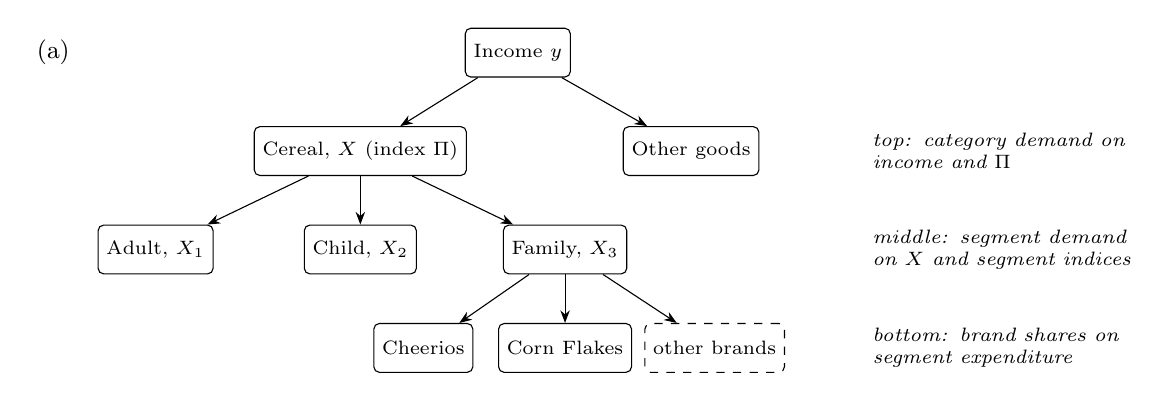
\begin{tikzpicture}[
  lvl/.style={draw, rounded corners=2pt, font=\scriptsize, align=center, inner sep=3pt,
    minimum height=0.62cm},
  edge/.style={-{Stealth[length=1.6mm]}, thin},
  note/.style={font=\scriptsize\itshape, align=left, text width=3.3cm, anchor=west}]
\node[lvl] (inc) at (4.6,0) {Income $y$};
\node[lvl] (cat) at (2.6,-1.25) {Cereal, $X$ (index $\Pi$)};
\node[lvl] (oth) at (6.8,-1.25) {Other goods};
\node[lvl] (ad) at (0.0,-2.5) {Adult, $X_1$};
\node[lvl] (ch) at (2.6,-2.5) {Child, $X_2$};
\node[lvl] (fa) at (5.2,-2.5) {Family, $X_3$};
\node[lvl] (b1) at (3.4,-3.75) {Cheerios};
\node[lvl] (b2) at (5.2,-3.75) {Corn Flakes};
\node[lvl, dashed] (b3) at (7.1,-3.75) {other brands};
\draw[edge] (inc) -- (cat); \draw[edge] (inc) -- (oth);
\draw[edge] (cat) -- (ad); \draw[edge] (cat) -- (ch); \draw[edge] (cat) -- (fa);
\draw[edge] (fa) -- (b1); \draw[edge] (fa) -- (b2); \draw[edge] (fa) -- (b3);
\node[note] at (9.0,-1.25) {top: category demand on income and $\Pi$};
\node[note] at (9.0,-2.5) {middle: segment demand on $X$ and segment indices};
\node[note] at (9.0,-3.75) {bottom: brand shares on segment expenditure};
\node[font=\small] at (-1.3,0) {(a)};
\end{tikzpicture}

\vspace{0.6cm}
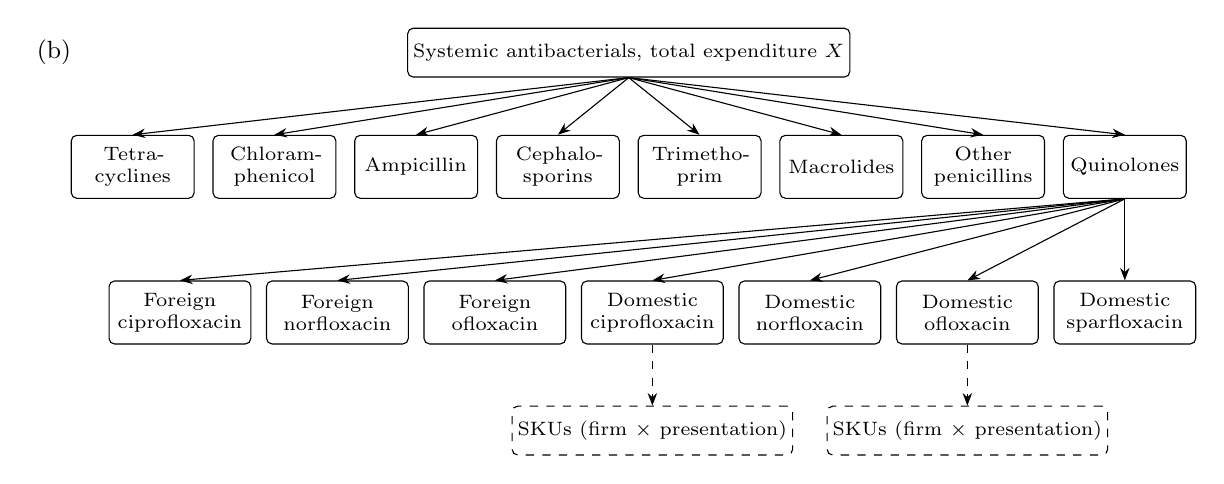
\begin{tikzpicture}[
  lvl/.style={draw, rounded corners=2pt, font=\scriptsize, align=center, inner sep=2pt,
    minimum height=0.62cm},
  seg/.style={draw, rounded corners=2pt, font=\scriptsize, align=center, inner sep=2pt,
    text width=1.42cm, minimum height=0.8cm},
  grp/.style={draw, rounded corners=2pt, font=\scriptsize, align=center, inner sep=2pt,
    text width=1.66cm, minimum height=0.8cm},
  edge/.style={-{Stealth[length=1.6mm]}, thin}]
\node[lvl] (top) at (6.3,0) {Systemic antibacterials, total expenditure $X$};
\foreach \name/\x [count=\n] in {Tetra-\\cyclines/0.0, Chloram-\\phenicol/1.8, Ampicillin/3.6,
    Cephalo-\\sporins/5.4, Trimetho-\\prim/7.2, Macrolides/9.0, Other\\penicillins/10.8,
    Quinolones/12.6} {
  \node[seg] (s\n) at (\x,-1.45) {\name};
  \draw[edge] (top.south) -- (s\n.north);
}
\foreach \name/\x [count=\n] in {Foreign\\ciprofloxacin/0.6, Foreign\\norfloxacin/2.6,
    Foreign\\ofloxacin/4.6, Domestic\\ciprofloxacin/6.6, Domestic\\norfloxacin/8.6,
    Domestic\\ofloxacin/10.6, Domestic\\sparfloxacin/12.6} {
  \node[grp] (g\n) at (\x,-3.3) {\name};
  \draw[edge] (s8.south) -- (g\n.north);
}
\node[lvl, dashed] (sku1) at (6.6,-4.8) {SKUs (firm $\times$ presentation)};
\node[lvl, dashed] (sku2) at (10.6,-4.8) {SKUs (firm $\times$ presentation)};
\draw[edge, dashed] (g4.south) -- (sku1.north);
\draw[edge, dashed] (g6.south) -- (sku2.north);
\node[font=\small] at (-1.0,0) {(b)};
\end{tikzpicture}
\caption{Budgeting trees. Panel (a): the three-level structure of \citet{Hausman1997} for ready-to-eat
cereal, with the three segments he uses and two of the family-segment brands (his Table 5.1). Panel (b):
the two-level structure of \citet{ChaudhuriGoldbergJia2006}. The upper level allocates systemic
antibacterial expenditure across sub-segments, eight of which appear with equations in their
upper-level system (their Table A3). The lower level allocates quinolone expenditure across seven
molecule-by-status groups. Foreign sparfloxacin, with a minuscule share, is folded into the domestic
group. Within-group choice among stock-keeping units (SKUs) is not modeled (dashed).}
\label{fig:05-budget-tree}
\end{figure}

\section{Estimation and identification}\label{sec:05-estimation}

This section turns the AIDS into an econometric model. We add an error term and ask what it contains,
deal with the singular covariance matrix that adding up creates, and compare the exact nonlinear model
with its linear approximation. We then show how the theoretical restrictions are tested and work through
the original application of \citet{DeatonMuellbauer1980a} in detail. The section closes with the
identification problems that dominate industrial organization applications: endogenous prices,
endogenous group expenditure, and group prices measured with error.

\subsection{Stochastic specification}\label{sec:05-stochastic}

Observations are indexed by $t = 1, \dots, T$. An observation may be a year of national data, a month in a
region, or a week in a city. The estimating equations are
\begin{equation}\label{eq:05-stoch}
  w_{it} = \alpha_i + \sum_{j=1}^{J}\gamma_{ij}\ln p_{jt} + \beta_i\ln\frac{I_t}{\mathbf{P}_t} + \xi_{it},
  \qquad i = 1, \dots, J,
\end{equation}
with the translog index $\ln\mathbf{P}_t = \alpha_0 + \sum_k\alpha_k\ln p_{kt} + \frac{1}{2}\sum_k\sum_j
\gamma_{kj}\ln p_{kt}\ln p_{jt}$ of \eqref{eq:05-translog}. We write the error as $\xi_{it}$, in place of
the $\varepsilon_{it}$ used by the original papers, because $\varepsilon$ denotes elasticities in this
chapter. Its content matters for every later step, so we list the main components.
\begin{enumerate}[label=(\alph*)]
  \item \emph{Unobserved demand shifters.} Advertising campaigns, epidemics that call for a particular
  drug, or changes in demographics shift the shares of particular goods. Firms often observe these
  shocks when they set prices.
  \item \emph{Measurement error.} Shares and prices are measured with error. In multi-level systems the
  prices of product groups are averages of the prices of many stock-keeping units, which approximate an
  unobserved exact group price index (\cref{sec:05-endogeneity}).
  \item \emph{Aggregation error.} The omitted term $-\beta_i(\ln\kappa_t - \ln\kappa^*)$ of
  \eqref{eq:05-aids-agg-ts} enters the error when the distribution of budgets changes.
  \item \emph{Specification error.} Habits, stocks of durables, price expectations and other dynamics
  that the static model omits.
\end{enumerate}
Component (a) makes prices endogenous when firms set them. Component (b) creates errors in variables.
Components (c) and (d) are correlated with the regressors whenever inequality or the omitted dynamics move
with prices and real expenditure. We write $\Sigma = \E[\xi_t\xi_t^{\T}]$ for the $J\times J$ covariance
matrix of $\xi_t = (\xi_{1t}, \dots, \xi_{Jt})^{\T}$.

\subsection{Adding up and the singular covariance matrix}\label{sec:05-singular}

Budget shares sum to one in the data. Under the adding-up restrictions of \cref{prop:05-restrictions},
the deterministic part of \eqref{eq:05-stoch} also sums to one, because
\begin{equation*}
  \sum_i\Bigl(\alpha_i + \sum_j\gamma_{ij}\ln p_{jt} + \beta_i\ln\frac{I_t}{\mathbf{P}_t}\Bigr)
  = \sum_i\alpha_i + \sum_j\Bigl(\sum_i\gamma_{ij}\Bigr)\ln p_{jt} + \Bigl(\sum_i\beta_i\Bigr)
    \ln\frac{I_t}{\mathbf{P}_t} = 1 .
\end{equation*}
Hence $\sum_i\xi_{it} = 0$ for every $t$. Writing $\iota$ for the $J$-vector of ones, $\iota^{\T}\xi_t = 0$
implies $\iota^{\T}\Sigma = 0$, so $\Sigma$ is singular with rank at most $J - 1$. The Gaussian likelihood
of the full system is not defined, because it requires $\Sigma^{-1}$.

The standard solution drops one equation, say the $J$-th, and estimates the remaining $J - 1$. The
parameters of the dropped equation follow from adding up:
\begin{equation*}
  \alpha_J = 1 - \sum_{i<J}\alpha_i, \qquad \beta_J = -\sum_{i<J}\beta_i, \qquad
  \gamma_{Jj} = -\sum_{i<J}\gamma_{ij} \quad (j = 1, \dots, J).
\end{equation*}
Which equation we drop does not matter for maximum likelihood.

\begin{proposition}[\citealp{Barten1969}]\label{prop:05-barten}
Suppose the errors of any $J-1$ share equations are jointly normal with an unrestricted covariance matrix.
Then the maximum likelihood estimates of the parameters are the same whichever equation is dropped.
\end{proposition}

\begin{proof}
Let $\tilde\xi_t(\theta)$ be the residuals of the $J-1$ retained equations at parameter value $\theta$.
Concentrating the unrestricted covariance matrix out of the Gaussian log likelihood gives, up to a
constant,
\begin{equation*}
  \ln L^c(\theta) = -\frac{T}{2}\ln\det\hat\Omega(\theta), \qquad
  \hat\Omega(\theta) = \frac{1}{T}\sum_t\tilde\xi_t(\theta)\tilde\xi_t(\theta)^{\T}.
\end{equation*}
Dropping equation $k$ instead of equation $J$ replaces $\xi_{kt}$ by $\xi_{Jt} = -\sum_{i<J}\xi_{it}$. The
new residual vector is $A\tilde\xi_t$, where $A$ is the identity matrix with row $k$ replaced by a row of
$-1$'s, followed by a reordering of rows. Expanding the determinant along row $k$ shows that $\det A =
\pm 1$. The new concentrated likelihood is therefore
\begin{equation*}
  -\frac{T}{2}\ln\det\bigl(A\hat\Omega(\theta)A^{\T}\bigr)
  = -\frac{T}{2}\ln\bigl[(\det A)^2\det\hat\Omega(\theta)\bigr] = \ln L^c(\theta),
\end{equation*}
the same function of $\theta$, with the same maximizer.
\end{proof}

\casehead{Seemingly unrelated regressions}
The standard system estimator is \emph{seemingly unrelated regressions} (SUR) \citep{Zellner1962}. Write
retained equation $i$ as $\mathbf{w}_i = \mathbf{X}_ib_i + \boldsymbol{\xi}_i$, where $\mathbf{w}_i$ stacks
the $T$ observed shares, $\mathbf{X}_i$ is the $T \times K_i$ matrix of its regressors and $b_i$ is its
coefficient vector. Stacking the $J - 1$ equations gives $\mathbf{w} = \mathbf{X}b + \boldsymbol{\xi}$, with
$\mathbf{X} = \diag(\mathbf{X}_1, \dots, \mathbf{X}_{J-1})$ block diagonal. The errors of one observation
have covariance matrix $\E[\tilde\xi_t\tilde\xi_t^{\T}] = \Omega$ and are independent over $t$, so
$\Var(\boldsymbol{\xi}) = \Omega\otimes I_T$. Feasible generalized least squares gives
\begin{equation}\label{eq:05-sur}
  \hat b = \bigl[\mathbf{X}^{\T}(\hat\Omega^{-1}\otimes I_T)\mathbf{X}\bigr]^{-1}
           \mathbf{X}^{\T}(\hat\Omega^{-1}\otimes I_T)\,\mathbf{w},
\end{equation}
where $\hat\Omega$ has elements $\hat\Omega_{ik} = \frac{1}{T}\hat{\boldsymbol{\xi}}_i^{\T}\hat{\boldsymbol{\xi}}_k$
computed from equation-by-equation OLS residuals. Homogeneity and symmetry are linear restrictions
$Rb = r_0$. Minimizing the generalized least squares criterion subject to them gives
\begin{equation}\label{eq:05-sur-restricted}
  \hat b_R = \hat b - VR^{\T}\bigl(RVR^{\T}\bigr)^{-1}\bigl(R\hat b - r_0\bigr), \qquad
  V = \bigl[\mathbf{X}^{\T}(\hat\Omega^{-1}\otimes I_T)\mathbf{X}\bigr]^{-1}.
\end{equation}
\Cref{sec:A-systems} derives this formula from the Lagrangian. Recomputing $\hat\Omega$ from the new residuals
and iterating never lowers the Gaussian likelihood. A limit of the iteration is a stationary point of that
likelihood, typically a local maximum. It is the maximum likelihood estimator only if it is the global maximum
(\cref{sec:A-systems}). Restarting from several points guards against a local maximum (\cref{sec:A-numerical}).
The proof of \cref{prop:05-barten} shows that the concentrated likelihood is the same function of the parameters
whichever equation is dropped. Every stationary point that iterated SUR can reach therefore shares that
invariance. \emph{Three-stage least squares} applies \eqref{eq:05-sur} after
replacing $\mathbf{X}$ by its projection on the instruments, with $\hat\Omega$ estimated from two-stage least
squares residuals (\cref{sec:A-3sls}).

Two further facts simplify estimation when there are no cross-equation restrictions. First, when every
equation has the same regressors, $\mathbf{X}_i = \mathbf{X}_0$ for all $i$, SUR reduces to ordinary least
squares (OLS) equation by equation (\cref{prop:A-sur-ols}). OLS is then the maximum likelihood estimator
under normality \citep[p.~316]{DeatonMuellbauer1980a}. Second, OLS automatically satisfies adding up. To see
this, stack the $T$ observations of the regressors $(1, \ln p_{1t}, \dots, \ln p_{Jt},
\ln\frac{I_t}{\mathbf{P}_t})$ in the matrix $\mathbf{X}_0$, whose first column is the vector of ones $\iota_T$.
The OLS coefficient vectors $b_i = (\mathbf{X}_0^{\T}\mathbf{X}_0)^{-1}\mathbf{X}_0^{\T}\mathbf{w}_i$ sum to
\begin{equation*}
  \sum_i b_i = (\mathbf{X}_0^{\T}\mathbf{X}_0)^{-1}\mathbf{X}_0^{\T}\sum_i \mathbf{w}_i
  = (\mathbf{X}_0^{\T}\mathbf{X}_0)^{-1}\mathbf{X}_0^{\T}\iota_T = (1, 0, \dots, 0)^{\T},
\end{equation*}
because regressing a column of ones on $\mathbf{X}_0$ returns a coefficient of one on the constant and zero
elsewhere. Hence $\sum_i\hat\alpha_i = 1$, $\sum_i\hat\gamma_{ij} = 0$ and $\sum_i\hat\beta_i = 0$.

\casehead{Short samples}
Symmetry is a cross-equation restriction, so the covariance matrix now affects the estimates. With few
observations an unrestricted covariance matrix cannot be estimated. \citet[p.~318]{DeatonMuellbauer1980a}
had 21 annual observations on eight shares. They note that the likelihood ``can be made arbitrarily
large by making any one equation fit perfectly.'' The reason is visible in $\ln L^c(\theta)$. If the
parameters can be chosen so that one equation has zero residuals, $\det\hat\Omega(\theta) = 0$ and the
concentrated likelihood is unbounded. Under symmetry their system has 42 free coefficients, and every
equation depends on all of them through $\ln\mathbf{P}_t$. With only 21 observations per equation, the
coefficients can typically be chosen to fit one equation exactly. Deaton and Muellbauer therefore impose
a structure on the covariance matrix,
\begin{equation}\label{eq:05-dm-cov}
  \Sigma = \sigma^2\Bigl(I_J - \frac{1}{J}\iota\iota^{\T}\Bigr),
\end{equation}
where $I_J$ is the identity matrix and $\iota$ is the $J$-vector of ones. This matrix satisfies $\Sigma\iota = 0$, as adding up requires. It
turns maximum likelihood into least squares on the whole system. To see this, drop equation $J$. The
covariance matrix of the remaining errors is $\sigma^2(I_{J-1} - \frac{1}{J}\mathbf{1}\mathbf{1}^{\T})$,
where $\mathbf{1}$ is a $(J-1)$-vector of ones. Its inverse is $\sigma^{-2}(I_{J-1} +
\mathbf{1}\mathbf{1}^{\T})$, as multiplying the two matrices confirms:
\begin{equation*}
  \Bigl(I - \frac{1}{J}\mathbf{1}\mathbf{1}^{\T}\Bigr)\bigl(I + \mathbf{1}\mathbf{1}^{\T}\bigr)
  = I + \mathbf{1}\mathbf{1}^{\T} - \frac{1}{J}\mathbf{1}\mathbf{1}^{\T} - \frac{J-1}{J}\mathbf{1}\mathbf{1}^{\T}
  = I .
\end{equation*}
The quadratic form in the likelihood is then
\begin{equation*}
  \tilde\xi_t^{\T}\bigl(I + \mathbf{1}\mathbf{1}^{\T}\bigr)\tilde\xi_t
  = \sum_{i<J}\xi_{it}^2 + \Bigl(\sum_{i<J}\xi_{it}\Bigr)^2 = \sum_{i=1}^{J}\xi_{it}^2,
\end{equation*}
using $\xi_{Jt} = -\sum_{i<J}\xi_{it}$. Maximizing the likelihood over the coefficients therefore minimizes
the total sum of squared residuals across all $J$ equations, the trace of the residual cross-product
matrix rather than its determinant.

\subsection{The nonlinear AIDS}\label{sec:05-nl}

Substituting the translog index into \eqref{eq:05-stoch} gives the estimating equations of the exact model
\citep[eq.~15]{DeatonMuellbauer1980a}:
\begin{equation}\label{eq:05-nl-aids}
  w_{it} = (\alpha_i - \beta_i\alpha_0) + \sum_j\gamma_{ij}\ln p_{jt}
  + \beta_i\Bigl\{\ln I_t - \sum_k\alpha_k\ln p_{kt}
  - \frac{1}{2}\sum_k\sum_j\gamma_{kj}\ln p_{kt}\ln p_{jt}\Bigr\} + \xi_{it}.
\end{equation}
The system is nonlinear in the parameters because $\beta_i$ multiplies $\alpha_k$ and $\gamma_{kj}$. It can
be estimated by nonlinear least squares, by maximum likelihood, or by the generalized method of moments
(GMM) when instruments are needed, with or without the homogeneity and symmetry restrictions. The
computation is easier than it looks. Given $\beta$, the equations are linear in $(\alpha, \gamma)$.
Given $(\alpha, \gamma)$, the index is known and the equations are linear in $\beta$. The first-order
conditions can therefore be solved by alternating between two linear problems
\citep[p.~316]{DeatonMuellbauer1980a}.

All parameters of \eqref{eq:05-nl-aids} are identified given enough variation in prices and expenditure.
The constant $\alpha_0$ is the exception in practice. It is identified only through the appearance of the
$\alpha_k$ inside the braces. When individual prices move closely together, $\ln\mathbf{P}_t$ is
insensitive to its weights. A change in $\alpha_0$ can then be offset by changes in the $\alpha_i$ with
little effect on the fit. Deaton and Muellbauer recommend fixing $\alpha_0$ a priori. At unit prices
$\ln a(p) = \alpha_0$, so $e^{\alpha_0}$ is the cost of subsistence when all prices equal one. In their
words it is ``the outlay required for a minimal standard of living,'' and a plausible value is easy to
choose \citep[p.~316]{DeatonMuellbauer1980a}.

\subsection{The linear approximate AIDS and the Stone index}\label{sec:05-stone}

The same collinearity suggests a shortcut. If $\mathbf{P}_t$ is approximately proportional to a known
index $P_t^*$, say $\mathbf{P}_t \approx \varphi P_t^*$, then
\begin{equation}\label{eq:05-la-aids}
  w_{it} = (\alpha_i - \beta_i\ln\varphi) + \sum_j\gamma_{ij}\ln p_{jt}
  + \beta_i\ln\frac{I_t}{P_t^*} + \xi_{it}
\end{equation}
\citep[eq.~16]{DeatonMuellbauer1980a}. This \emph{linear approximate AIDS} (LA-AIDS) is linear in the
parameters. Without cross-equation restrictions it can be estimated by OLS equation by equation, which is
maximum likelihood for the system and satisfies adding up. The intercepts $\alpha_i^* = \alpha_i -
\beta_i\ln\varphi$ still sum to one because $\sum_i\beta_i = 0$. The usual choice of $P_t^*$ is the
\emph{Stone index}
\begin{equation}\label{eq:05-stone}
  \ln P_t^S = \sum_k w_{kt}\ln p_{kt}.
\end{equation}
It is exact, up to the constant $\alpha_0$, in one case. If $\gamma_{ij} = 0$ and $\beta_i = 0$ for all
$i, j$, then $w_k = \alpha_k$ and $\ln\mathbf{P} = \alpha_0 + \sum_k\alpha_k\ln p_k = \alpha_0 + \ln P^S$.
This is the Cobb-Douglas case. Otherwise the approximation is good when prices move together.

\casehead{The exact gap between the two models}
How good is the approximation, and what goes wrong when it fails? Substituting the share equations into
\eqref{eq:05-stone} and subtracting the translog index gives an exact expression for the gap:
\begin{align}
  \ln P_t^S - \ln\mathbf{P}_t
  &= \sum_k\Bigl(\alpha_k + \sum_j\gamma_{kj}\ln p_{jt} + \beta_k\ln\frac{I_t}{\mathbf{P}_t}
     + \xi_{kt}\Bigr)\ln p_{kt} - \ln\mathbf{P}_t \notag\\
  &= -\alpha_0 + \frac{1}{2}\sum_k\sum_j\gamma_{kj}\ln p_{kt}\ln p_{jt}
     + \ln\frac{I_t}{\mathbf{P}_t}\sum_k\beta_k\ln p_{kt} + \sum_k\xi_{kt}\ln p_{kt}.
  \label{eq:05-stone-gap}
\end{align}
The true model \eqref{eq:05-stoch} can be written in terms of the Stone index by adding and subtracting
$\beta_i\ln P^S_t$:
\begin{equation}\label{eq:05-la-exact}
\begin{split}
  w_{it} = {}& (\alpha_i - \beta_i\alpha_0) + \sum_j\gamma_{ij}\ln p_{jt} + \beta_i\ln\frac{I_t}{P^S_t} \\
  &+ \beta_i\Bigl[\frac{1}{2}\sum_k\sum_j\gamma_{kj}\ln p_{kt}\ln p_{jt}
  + \ln\frac{I_t}{\mathbf{P}_t}\sum_k\beta_k\ln p_{kt} + \sum_k\xi_{kt}\ln p_{kt}\Bigr] + \xi_{it}.
\end{split}
\end{equation}
The LA-AIDS omits the bracket. Each of its three terms explains one known problem of the Stone index.

\emph{Interpretation of the coefficients.} The middle term is linear in $\ln p_{kt}$ with coefficient
$\beta_i\beta_k\ln\frac{I_t}{\mathbf{P}_t}$. When real expenditure varies around a mean $m$, this term is
absorbed into the price coefficients, and the LA-AIDS estimates $\gamma_{ij}^{LA} \approx \gamma_{ij} +
\beta_i\beta_j m$ rather than $\gamma_{ij}$. The usual LA-AIDS elasticity formula
\begin{equation}\label{eq:05-la-elast}
  \varepsilon_{ij} \approx -\indic(i=j) + \frac{\gamma_{ij}^{LA} - \beta_i w_j}{w_i}
\end{equation}
then equals $-\indic(i=j) + \frac{\gamma_{ij} - \beta_i(w_j - \beta_j m)}{w_i}$, which is the exact AIDS
elasticity of \eqref{eq:05-elast-marshall} at $\ln\frac{I}{\mathbf{P}} = m$. Although the LA coefficients
differ from the AIDS coefficients, the LA elasticities can be close to the AIDS elasticities near the
center of the data.

\emph{Simultaneity.} The last term contains the errors of all equations. The Stone index is built from
current shares, so the regressor $\ln\frac{I_t}{P_t^S}$ is correlated with $\xi_{it}$. The term is small
when log prices are close to zero.

\emph{Units of measurement.} \citet{Moschini1995} shows that the Stone index is not invariant to the units
in which goods are measured. Suppose the unit of good $k$ is changed, so that $p_{kt}$ becomes
$\lambda p_{kt}$ ($\lambda > 1$ for a larger unit) and $\ln p_{kt}$ becomes $\ln p_{kt} + c$ with
$c = \ln\lambda$. The exact AIDS absorbs
the change. Replacing $\alpha_j$ by $\alpha_j - c\gamma_{jk}$ for every $j$ and $\alpha_0$ by $\alpha_0 -
c\alpha_k + \frac{1}{2}c^2\gamma_{kk}$ leaves both the translog index and every share equation unchanged
as functions of the new prices. To verify, expand the index in the new log prices $\ln p'_{jt}$:
\begin{equation*}
  \ln\mathbf{P}_t = \Bigl(\alpha_0 - c\alpha_k + \frac{1}{2}c^2\gamma_{kk}\Bigr)
  + \sum_j(\alpha_j - c\gamma_{jk})\ln p'_{jt} + \frac{1}{2}\sum_j\sum_l\gamma_{jl}\ln p'_{jt}\ln p'_{lt},
\end{equation*}
using symmetry, and note that $\gamma_{ik}\ln p_{kt} = \gamma_{ik}\ln p'_{kt} - c\gamma_{ik}$ in each share
equation. The new $\alpha_j$ still sum to one because $\sum_j\gamma_{jk} = 0$. Fitted shares and
elasticities do not change. The Stone index, by contrast, shifts by $c\,w_{kt}$, which varies over
observations. Redoing \eqref{eq:05-stone-gap} in the new units, the bracket in \eqref{eq:05-la-exact} gains
the term $c(w_{kt} - \alpha_k)$ plus a constant. The LA-AIDS therefore omits a time-varying term
$\beta_i c\, w_{kt}$ that is correlated with its regressors. Its estimates of $\beta_i$, $\gamma_{ij}$ and
the elasticities depend on the arbitrary choice of units, and the dependence grows with $|c|$.

\begin{example}[Units and the Stone index: a simulation]\label{ex:05-stone-mc}
We generate data from the exact AIDS with the running-example parameters and $\alpha_0 = 0$. Log prices
are $\ln p_{jt} = \pi_t + s_e e_{jt}$, with a common component $\pi_t \sim N(0, 0.3^2)$ and relative-price
noise $e_{jt} \sim N(0,1)$. Log expenditure is $\ln I_t = 1 + \pi_t + 0.3g_t$ with $g_t \sim N(0,1)$, and
share errors sum to zero, with standard deviations of about $0.004$. Design A has nearly collinear prices
($s_e = 0.02$) and design B has substantial relative-price variation ($s_e = 0.20$). Each sample has $T =
100$ observations, and we draw 500 samples. Four estimators impose adding up, homogeneity and symmetry,
and minimize the total sum of squared residuals. The first is the exact nonlinear AIDS and the second the
LA-AIDS with the Stone index. The third is the same LA-AIDS after good 1 is measured in units one hundred
times larger ($p_1$ multiplied by 100, $c = \ln 100 = 4.61$). The fourth is an LA-AIDS deflated by a fixed-weight index with
sample-mean shares. \Cref{tab:05-stone-mc}
reports the results, with elasticities evaluated at the base point of \cref{ex:05-running}.

Three lessons emerge. First, with prices normalized to one near the center of the data, the Stone LA-AIDS
recovers the elasticities in both designs. It does so even though the gap between the indices in design B
is of the order of 0.1 in logs. Its own-price coefficient $\hat\gamma_{11}^{LA}$ averages $-0.190$, while
the AIDS coefficient is $-0.200$. The difference is $\beta_1^2 m = 0.01$, exactly as
\eqref{eq:05-la-exact} predicts. Second, merely changing the units of
good 1 moves $\hat\beta_1$ from $-0.100$ to about $-0.069$ and the own-price elasticity of good 1 from
$-1.38$ to $-1.26$. Third, the fixed-weight index gives the same estimates in either unit, and its
elasticities match those of the exact model. In design A the average largest gap between the demeaned Stone and translog indices is
0.008, the same magnitude that Deaton and Muellbauer found in British data (\cref{sec:05-dm-application}).
\end{example}

\begin{table}[htbp]
\centering
\caption{Estimating the AIDS with exact and approximate price indices (simulation)}
\label{tab:05-stone-mc}
\small
\begin{tabular}{lcccc}
\toprule
Estimator & $\hat\beta_1$ & $\hat\gamma_{11}$ & $\hat\varepsilon_{11}$ & $\hat\varepsilon_{33}$ \\
\midrule
True values & $-0.100$ & $-0.200$ & $-1.375$ & $-1.738$ \\
\addlinespace
\multicolumn{5}{l}{\textit{Design A: nearly collinear prices ($s_e = 0.02$)}} \\
Exact AIDS (nonlinear) & $-0.100$ (0.001) & $-0.200$ (0.017) & $-1.376$ (0.042) & $-1.739$ (0.066) \\
LA-AIDS, Stone index & $-0.100$ (0.001) & $-0.190$ (0.017) & $-1.376$ (0.042) & $-1.740$ (0.066) \\
LA-AIDS, Stone, rescaled $p_1$ & $-0.069$ (0.001) & $-0.130$ (0.012) & $-1.257$ (0.029) & $-1.667$ (0.060) \\
LA-AIDS, fixed-weight index & $-0.100$ (0.001) & $-0.190$ (0.017) & $-1.376$ (0.042) & $-1.739$ (0.066) \\
\addlinespace
\multicolumn{5}{l}{\textit{Design B: independent relative prices ($s_e = 0.20$)}} \\
Exact AIDS (nonlinear) & $-0.100$ (0.001) & $-0.200$ (0.002) & $-1.375$ (0.004) & $-1.738$ (0.007) \\
LA-AIDS, Stone index & $-0.100$ (0.001) & $-0.190$ (0.002) & $-1.375$ (0.005) & $-1.737$ (0.007) \\
LA-AIDS, Stone, rescaled $p_1$ & $-0.068$ (0.001) & $-0.130$ (0.001) & $-1.257$ (0.004) & $-1.665$ (0.007) \\
LA-AIDS, fixed-weight index & $-0.100$ (0.001) & $-0.190$ (0.002) & $-1.375$ (0.005) & $-1.738$ (0.007) \\
\bottomrule
\end{tabular}

\smallskip
\begin{minipage}{0.94\textwidth}
\footnotesize Notes: means over 500 simulated samples of $T = 100$, standard deviations across samples in
parentheses. Data are generated from the exact AIDS with the parameters of \cref{ex:05-running}.
Elasticities are evaluated at $p = (1,1,1)$, $\ln I = 1$, with the true shares $(0.40, 0.34, 0.26)$. The
LA-AIDS elasticities use \eqref{eq:05-la-elast}. The fixed-weight estimates are identical in either unit.
Computed by \texttt{figures/ch05/src/stone\_index\_mc.py}.
\end{minipage}
\end{table}

\casehead{Elasticities from the LA-AIDS}
Applied work often computes LA-AIDS elasticities from \eqref{eq:05-la-elast}, which treats
$\frac{\partial\ln P^S}{\partial\ln p_j}$ as $w_j$. \citet{GreenAlston1990} point out that the Stone
weights themselves respond to prices. Within the LA model,
\begin{equation*}
  \frac{\partial\ln P^S}{\partial\ln p_j} = w_j + \sum_k\ln p_k\frac{\partial w_k}{\partial\ln p_j}.
\end{equation*}
Let $\mathcal{D}$ be the matrix of share derivatives $\frac{\partial w_i}{\partial\ln p_j}$, $\ell$ the vector of
log prices, $\beta$ the vector of expenditure coefficients and $w$ the vector of shares. Differentiating
\eqref{eq:05-la-aids},
\begin{equation*}
  \mathcal{D} = \Gamma^{LA} - \beta w^{\T} - \beta\ell^{\T}\mathcal{D}
  \quad\Longrightarrow\quad
  \mathcal{D} = \bigl(I + \beta\ell^{\T}\bigr)^{-1}\bigl(\Gamma^{LA} - \beta w^{\T}\bigr).
\end{equation*}
By the Sherman-Morrison formula, $(I + \beta\ell^{\T})^{-1} = I - \frac{\beta\ell^{\T}}{1 +
\ell^{\T}\beta}$. At a point where all prices equal one, $\ell = 0$ and \eqref{eq:05-la-elast} is exact for
the LA model. Away from it the correction matters, and it depends on units for the reason just given.
Normalizing prices to one at the point of evaluation removes the problem.

\casehead{Remedies}
Several fixes are available. A \emph{Laspeyres-type} index with fixed weights, $\ln P_t^L = \sum_k\bar
w_k\ln p_{kt}$ (base-period or sample-mean shares), contains no current shares, so it removes the
simultaneity. A change of units shifts it by a constant that the intercepts absorb. The
\emph{Tornqvist} index $\ln P_t^T = \sum_k\frac{1}{2}(w_{kt} + w_k^0)\ln\frac{p_{kt}}{p_k^0}$ and the
log-linear analogue of the Paasche index, $\sum_k w_{kt}\ln\frac{p_{kt}}{p_k^0}$, use prices relative to a
base point $p^0$ and are therefore invariant to units \citep{Moschini1995}.

The Tornqvist index also has a basis in demand theory \citep[\S 7.1, eqs.~1.8--1.10,
pp.~174--175]{DeatonMuellbauer1980b}. Along any price path at fixed utility, Shephard's lemma gives
$\dd\ln e(p, u) = \sum_k w_k(p, u)\,\dd\ln p_k$, with Hicksian shares $w_k(p, u)$. Integrating from $p^0$
to $p^1$,
\begin{equation*}
  \ln\frac{e(p^1, u)}{e(p^0, u)} = \int_{p^0}^{p^1}\sum_k w_k(p, u)\,\dd\ln p_k ,
\end{equation*}
which is the log of the exact cost-of-living index at $u$. The \emph{Divisia index} replaces the Hicksian
shares in this integral by observed shares. Unless preferences are homothetic, observed shares move with
utility along the path, so the Divisia index depends on the path. Prices are observed only at discrete
dates, so the integral must be approximated. The Tornqvist index is a natural approximation, since it
averages the shares at the two ends. Following \citet{Diewert1976}, it equals the exact index at a
reference utility $u^*$ when the log expenditure function is quadratic in log prices and log utility. The
reference is then $u^* = \sqrt{u^0u^1}$, the geometric mean of the utilities at the two dates \citep[p.~174]{DeatonMuellbauer1980b}.
The reason is an identity for quadratic functions. Their change between two points equals the average of
the end-point gradients times the change in the arguments. At a fixed reference utility, the price
gradients are the Hicksian shares at that utility. They differ from the observed shares by terms linear
in the utility gap, which cancel when $\ln u^*$ is the midpoint of $\ln u^0$ and $\ln u^1$. If $\ln e$ is
quadratic in log prices and in $u$ itself, the reference is the arithmetic mean $\frac{1}{2}(u^0 + u^1)$
instead. A fixed-weight index shares the units invariance but not this link to the
exact index. A Stone index with lagged
shares removes the contemporaneous correlation with $\xi_t$ when the errors are serially uncorrelated.
Finally, we can iterate toward the exact model, as \citet[p.~321]{DeatonMuellbauer1980a} suggest:
\begin{enumerate}[label=\arabic*.]
  \item Compute $P^*_t$ (for example the Stone index) and estimate \eqref{eq:05-la-aids}.
  \item Compute $\ln\mathbf{P}_t$ from the estimated $\alpha$ and $\gamma$ and a chosen $\alpha_0$.
  \item Re-estimate the share equations with $\ln\mathbf{P}_t$ in place of $\ln P^*_t$.
  \item Repeat steps 2 and 3 until the estimates stop changing.
\end{enumerate}
Deaton and Muellbauer describe this as ``a computationally efficient way of obtaining good estimates of
the full nonlinear system.'' They also stress that \eqref{eq:05-la-aids} exists only as an approximation.
Once the restrictions have been chosen, the full system \eqref{eq:05-nl-aids} should be re-estimated
\citep[p.~317]{DeatonMuellbauer1980a}.

\subsection{First differences and the Rotterdam model}\label{sec:05-rotterdam}

Time-series applications often estimate in first differences. Differencing \eqref{eq:05-stoch} gives
\begin{equation}\label{eq:05-fd-aids}
  \Delta w_{it} = \beta_i\Delta\ln\frac{I_t}{\mathbf{P}_t} + \sum_j\gamma_{ij}\Delta\ln p_{jt}
  + \Delta\xi_{it}
\end{equation}
\citep[eq.~17]{DeatonMuellbauer1980a}, in which the $\alpha_i$ appear only through $\Delta\ln\mathbf{P}_t$.
Written out, $\Delta\ln\mathbf{P}_t$ involves $\sum_k\alpha_k\Delta\ln p_{kt}$ and $\frac{1}{2}\sum_k\sum_j
\gamma_{kj}\Delta(\ln p_{kt}\ln p_{jt})$ (their eq.~18). With nearly collinear prices the $\gamma_{ij}$ and
the products $\beta_i\alpha_j$ are hard to separate. In practice $\Delta\ln\mathbf{P}_t$ is replaced by
the change in a Stone index or by $\sum_k w_{kt}\Delta\ln p_{kt}$.

With the second choice the right-hand side becomes identical to that of the \emph{Rotterdam model} of
\citet{Theil1965} and \citet{Barten1969}. The Rotterdam model is a differential demand system. Totally
differentiating $q_i(p, I)$ and multiplying by $w_i$ gives $w_i\,\dd\ln q_i = w_i\eta_i\,\dd\ln I +
\sum_j w_i\varepsilon_{ij}\,\dd\ln p_j$. Substituting the Slutsky equation in elasticity form,
$\varepsilon_{ij} = \varepsilon^h_{ij} - \eta_i w_j$ (\cref{sec:05-elasticity-identities}), gives
\begin{equation}\label{eq:05-rotterdam}
  w_{it}\Delta\ln q_{it} = b_i\Bigl(\Delta\ln I_t - \sum_k w_{kt}\Delta\ln p_{kt}\Bigr)
  + \sum_j c_{ij}\Delta\ln p_{jt},
\end{equation}
with $b_i = w_i\eta_i = p_i\frac{\partial q_i}{\partial I}$, the marginal budget share, and $c_{ij} =
w_i\varepsilon^h_{ij} = \frac{p_ip_jS_{ij}}{I}$. The Rotterdam model treats $b_i$ and $c_{ij}$ as constant
parameters \citep[eq.~19]{DeatonMuellbauer1980a}.

The two models differ in the dependent variable. The AIDS has $\Delta w_i$, which is approximately $w_i
\Delta\ln w_i = w_i(\Delta\ln q_i + \Delta\ln p_i - \Delta\ln I)$. So the first-difference AIDS replaces the
Rotterdam dependent variable $w_i\Delta\ln q_i$ by $w_i\Delta\ln w_i$, adding $w_i\Delta\ln\frac{p_i}{I}$.
Both models are linear in constant parameters, and both test homogeneity and symmetry through linear
restrictions. Their parameters mean different things. The Rotterdam $c_{ij}$ are compensated price effects,
so negativity applies directly to the matrix $[c_{ij}]$. In the AIDS negativity applies to the matrix $K$
of \eqref{eq:05-K}, which depends on the data. Above all, the AIDS is derived from explicit preferences.
For forecasting demand this difference may matter little. For cost-of-living indices, equivalence scales
or welfare calculations, the link between estimated parameters and preferences matters a great deal
\citep[pp.~317--318]{DeatonMuellbauer1980a}.

\subsection{Testing the restrictions of demand theory}\label{sec:05-testing}

The restrictions of \cref{prop:05-restrictions} have different statistical status.

\emph{Adding up} cannot be tested with share data. The shares sum to one by construction, and OLS
estimates satisfy adding up automatically, as shown in \cref{sec:05-singular}.

\emph{Homogeneity}, $\sum_j\gamma_{ij} = 0$, involves one equation at a time and can be tested equation by
equation. Because the Stone index is homogeneous of degree one in prices, homogeneity can be imposed on
\eqref{eq:05-la-aids} by writing prices relative to the price of good $J$:
\begin{equation}\label{eq:05-homog-sub}
  w_{it} = \alpha_i^* + \sum_{j=1}^{J-1}\gamma_{ij}\ln\frac{p_{jt}}{p_{Jt}} + \beta_i\ln\frac{I_t}{P^*_t}
  + \xi_{it}
\end{equation}
\citep[eq.~20]{DeatonMuellbauer1980a}. The identity $\sum_j\gamma_{ij}\ln p_j = \sum_{j<J}\gamma_{ij}
\ln\frac{p_j}{p_J} + (\sum_j\gamma_{ij})\ln p_J$ shows that \eqref{eq:05-homog-sub} is the unrestricted
equation with the coefficient on $\ln p_J$ set to $\sum_j\gamma_{ij} = 0$. An $F$ test compares the
residual sums of squares of the two regressions. Equivalently, it is the square of the $t$ statistic on
$\sum_j\hat\gamma_{ij}$ in the unrestricted regression.

\emph{Symmetry}, $\gamma_{ij} = \gamma_{ji}$, links equations and can only be tested on the system, for
example by a likelihood-ratio test,
\begin{equation*}
  LR = 2\bigl(\ln L_{\mathrm{U}} - \ln L_{\mathrm{R}}\bigr) \xrightarrow{d} \chi^2_r .
\end{equation*}
Here $L_{\mathrm{U}}$ and $L_{\mathrm{R}}$ are the maximized likelihoods without and with the
restrictions, and $r$ is the number of restrictions. In a $J$-good system estimated on $J - 1$ equations, homogeneity
imposes $J - 1$ restrictions and symmetry imposes $\frac{(J-1)(J-2)}{2}$ more. For $J = 8$ these numbers
are 7 and 21. The test is asymptotic, and allowance must be made for that when samples are short.

Deaton and Muellbauer test symmetry whether or not homogeneity has been rejected. They report an
objection by Grayham Mizon, who argued that optimal inference stops testing once a rejection occurs.
Their reply is that the choice of maintained hypothesis is partly a matter of judgment. Many economists
would treat the absence of money illusion as maintained and regard symmetry as the interesting test.
Moreover, ``few if any tests in econometrics are carried out within the framework of maintained hypotheses which
are even widely accepted'' \citep[pp.~318--319]{DeatonMuellbauer1980a}.

\emph{Negativity} cannot be imposed by linear restrictions and is checked after estimation. At each
observation we compute the matrix $K$ of \eqref{eq:05-K} and its eigenvalues. One eigenvalue is
identically zero because $K\iota = 0$, and the others should be nonpositive. Negativity can be imposed
locally, at one point, by a Cholesky reparameterization of the Slutsky matrix \citep{Lau1978,Moschini1999}.

\subsection{Case study: the AIDS on British data, 1954--1974}\label{sec:05-dm-application}

\casehead{Question}
The empirical half of \citet{DeatonMuellbauer1980a} asks whether aggregate consumer demand obeys the
homogeneity, symmetry and negativity restrictions of demand theory. Earlier studies with the Rotterdam and
translog models had rejected homogeneity. The AIDS lets the question be posed within a maintained model
flexible enough to approximate any demand system to first order (\cref{sec:05-flexible}). A rejection
then speaks against the theory or its static formulation, and an arbitrary functional form cannot take
the blame. A second question is practical. Does the linear approximation with the Stone
index work well enough to serve as a routine tool? \Cref{tab:05-dm-map} at the end of this case study maps
its data, identifying variation and maintained assumptions.

\casehead{Data}
The data are 21 annual British observations, from 1954 to 1974 inclusive. They cover eight groups of
nondurable consumers' expenditure: food, clothing, housing services, fuel, drink and tobacco, transport
and communication services, other goods, and other services. For each year and group the data give a
budget share and a price index, together with total expenditure on the eight groups. Over the period the
price level rose by a factor of about 2.6. In their Table 3 the exact index rises from 0.571 in 1954 to
1.461 in 1974, with 1970 equal to one.

\casehead{Model}
The estimating model is the aggregate AIDS \eqref{eq:05-aids-aggregate} of a representative household. Deaton
and Muellbauer assume that the aggregation index $\kappa$ is constant, or that its deviations are
independent of mean expenditure and prices. The terms $-\beta_i\ln\kappa$ are then absorbed in the
intercepts, as in \cref{sec:05-almost-exact}.

\casehead{Estimating equations and estimator}
The procedure has five steps.
\begin{enumerate}[label=\arabic*.]
  \item Estimate the LA-AIDS \eqref{eq:05-la-aids} with the Stone index, equation by equation by OLS,
  with no restrictions beyond adding up, which holds automatically (their Table 1).
  \item Impose homogeneity by substitution, \eqref{eq:05-homog-sub}, re-estimate by OLS, and compute an
  $F$ test for each equation.
  \item Impose symmetry, replace $P^*$ by the exact index $\mathbf{P}$ with $\alpha_0$ fixed a priori, and
  estimate the nonlinear system \eqref{eq:05-nl-aids} by maximum likelihood under the covariance structure
  \eqref{eq:05-dm-cov}. Under symmetry the system has fourteen free intercepts and expenditure
  coefficients and twenty-eight free price coefficients, the upper triangle, diagonal included, of the
  $\gamma$ matrix with its last row and column deleted.
  \item Compare $P^*$ with $\mathbf{P}$, re-estimate the unrestricted and homogeneous models with
  $\mathbf{P}$, and check concavity with the eigenvalues of $K$ in every year.
  \item Repeat the analysis in first differences, adding intercepts $d_i$ to \eqref{eq:05-fd-aids}:
  \begin{equation}\label{eq:05-dm-fd}
    \Delta w_{it} = d_i + \beta_i\Delta\ln\frac{I_t}{\mathbf{P}_t} + \sum_k\gamma_{ik}\Delta\ln p_{kt}
    + \Delta\xi_{it}
  \end{equation}
  (their eq.~21, where the intercepts are written $\eta_i$). Collinearity prevented linking $\mathbf{P}$
  to the first-difference estimates, so the index computed from the symmetric levels estimates is used
  throughout.
\end{enumerate}

\casehead{Identification}
Prices and total expenditure are treated as exogenous. The article does not discuss this assumption,
which is common in the analysis of national aggregates. The authors' book does, and doubts both halves
of it \citep[\S 3.5, pp.~81--82]{DeatonMuellbauer1980b}. On total expenditure it says that ``individual
expenditures are as much a determinant of the total as the other way round'' (p.~81). On prices it says
that demand as a function of prices ``only makes sense if prices are set exogenously (say by
manufacturers) and quantities supplied elastically to meet whatever demand emerges.'' That is probably
true of most goods, ``although food may be a partial exception'' (pp.~81--82). The book links this to
the difficulty of estimating a ``sensible'' price elasticity for food. The positive own-price elasticity of
food in the unconstrained levels model of \cref{tab:05-dm-table2} (0.07) fits this warning. The case for
treating the regressors as given rests on two premises. Broad group prices are driven largely by costs and
by the general price level. Total nondurable expenditure is taken as given at the second stage of an
intertemporal budgeting problem. That second premise is the weak intertemporal separability that the
authors question in their interpretation. The price coefficients are identified by movements in
relative prices, and the expenditure coefficients by movements in real expenditure. Relative prices moved
little, which explains both the closeness of $P^*$ and $\mathbf{P}$ and the imprecision of many
$\gamma_{ij}$.

\casehead{Unconstrained estimates and homogeneity}
\Cref{tab:05-dm-table1} reproduces selected columns of their Table 1. The expenditure coefficients
classify food ($\beta = -0.160$) and housing ($-0.104$) as necessities and the other six groups as
luxuries. Twenty-two of the sixty-four price coefficients have $t$ values above two in absolute value.
Yet no variable has a detectable effect on the share of fuel, and few affect the shares of other goods
and other services. The column $\sum_j\gamma_{ij}$ gives 100 times the effect on each share of a 1
percent rise in all prices and total expenditure. Homogeneity requires it to be zero, and its $t$ value
is the square root of the $F$ statistic for the restriction. The authors' book reports these $F$
statistics, with one and eleven degrees of freedom, together with the fit of the free and the
homogeneous equations \citep[\S 3.4, Table~3.4, pp.~77--78]{DeatonMuellbauer1980b}.
\Cref{tab:05-dm-homog} reproduces that table. The rejection thresholds are 4.84 at the 5 percent level and
9.65 at the 1 percent level (p.~77). Homogeneity is rejected at 1 percent for food ($F = 19.4$, $t =
-4.4$), clothing ($20.3$, $-4.5$), housing ($82.8$, $9.1$) and transport and communication ($171.6$,
$13.1$). A proportional increase in all prices and expenditure would lower the budget shares of food and
clothing and raise those of housing and of transport and communication.

The fit is very high in both versions, with $R^2$ above 0.95 in five of the eight free equations and
never below 0.84. Budget
shares are harder to predict than quantities or expenditures, so these values are informative. For
comparison, the linear expenditure system fitted to the same share data gives $R^2 = -0.16$ for other
services (p.~77). A negative $R^2$ is possible because the restrictions of that system fit the share worse
than its sample mean. The \emph{Durbin-Watson statistic} tests for first-order serial correlation in the
residuals. Values near 2 indicate none, and values well below 2 indicate positive correlation. In each of
the four equations that reject homogeneity, imposing it makes the statistic fall sharply, for example
from 2.24 to 1.36 for transport and communication. For the other four groups the statistic barely moves.
The imposition of homogeneity thus generates positive serial correlation. Deaton and Muellbauer read this
as a sign that the rejection may come from misspecified dynamics (p.~77).

\begin{table}[htbp]
\centering
\caption{Unconstrained LA-AIDS estimates and tests of homogeneity, British data, 1954--1974}
\label{tab:05-dm-table1}
\small
\begin{tabular}{lcccc}
\toprule
Group & $\alpha_i^*$ & $\beta_i$ & $\gamma_{ii}$ & $\sum_j\gamma_{ij}$ \\
\midrule
Food & 1.221 & $-0.160$ & 0.186 & $-0.033$ \\
 & (7.4) & ($-6.1$) & (9.8) & ($-4.4$) \\
Clothing & $-0.482$ & 0.091 & 0.016 & $-0.032$ \\
 & ($-3.1$) & (3.7) & (1.0) & ($-4.5$) \\
Housing & 0.793 & $-0.104$ & 0.088 & 0.051 \\
 & (6.3) & ($-5.1$) & (7.2) & (9.1) \\
Fuel & $-0.159$ & 0.033 & 0.037 & $-0.010$ \\
 & ($-0.8$) & (1.0) & (1.6) & ($-1.1$) \\
Drink and tobacco & $-0.043$ & 0.028 & 0.056 & 0.001 \\
 & ($-0.3$) & (1.2) & (6.9) & (0.0) \\
Transport and communication & $-0.061$ & 0.029 & $-0.023$ & 0.040 \\
 & ($-0.9$) & (2.6) & ($-2.2$) & (13.1) \\
Other goods & $-0.038$ & 0.022 & 0.032 & $-0.005$ \\
 & ($-0.2$) & (0.9) & (1.5) & (0.7) \\
Other services & $-0.231$ & 0.060 & 0.019 & $-0.014$ \\
 & ($-1.5$) & (2.4) & (0.9) & ($-2.0$) \\
\bottomrule
\end{tabular}

\smallskip
\begin{minipage}{0.94\textwidth}
\footnotesize Notes: selected columns of \citet[Table~1]{DeatonMuellbauer1980a}, with $t$ values in
parentheses. OLS estimates of \eqref{eq:05-la-aids} with the Stone index, equation by equation. The column
$\gamma_{ii}$ is the own-price coefficient. The original also reports the seven cross-price coefficients
of each equation, equation standard errors, $R^2$ and Durbin-Watson statistics, which
\cref{tab:05-dm-homog} gives. $\sum_j\gamma_{ij}$ is the row sum of the unconstrained price
coefficients, and its $t$ value tests homogeneity. The $t$ value for other goods is printed as positive in
the original. For drink and tobacco the printed $t$ of 0.0 does not match the book's $F$ of 0.2 in
\cref{tab:05-dm-homog}, which implies $|t| \approx 0.45$. Both are far from significance. Each equation
uses $T = 21$ annual observations.
\end{minipage}
\end{table}

\begin{table}[htbp]
\centering
\caption{Tests of homogeneity on British data, 1954--1974}
\label{tab:05-dm-homog}
\small
\begin{tabular}{lccccc}
\toprule
 & \multicolumn{2}{c}{Unrestricted} & \multicolumn{2}{c}{Homogeneous} & Test \\
\cmidrule(lr){2-3}\cmidrule(lr){4-5}\cmidrule(lr){6-6}
Group & $R^2$ & Durbin-Watson & $R^2$ & Durbin-Watson & $F(1, 11)$ \\
\midrule
Food & 0.999 & 2.33 & 0.998 & 1.74 & 19.4 \\
Clothing & 0.984 & 2.29 & 0.955 & 1.55 & 20.3 \\
Housing & 0.999 & 1.89 & 0.992 & 1.29 & 82.8 \\
Fuel & 0.883 & 2.25 & 0.870 & 2.03 & 1.2 \\
Drink and tobacco & 0.969 & 2.96 & 0.969 & 2.93 & 0.2 \\
Transport and communication & 1.000 & 2.24 & 0.992 & 1.36 & 171.6 \\
Other goods & 0.885 & 1.92 & 0.880 & 1.91 & 0.5 \\
Other services & 0.843 & 2.27 & 0.788 & 1.98 & 4.0 \\
\bottomrule
\end{tabular}

\smallskip
\begin{minipage}{0.94\textwidth}
\footnotesize Notes: reproduced from \citet[Table~3.4, p.~78]{DeatonMuellbauer1980b}. Equation-by-equation
OLS estimates of the LA-AIDS with the Stone index, $T = 21$, the same regressions as
\cref{tab:05-dm-table1}. $F(1, 11)$ tests the single homogeneity restriction of each equation. The
thresholds are 4.84 at 5 percent and 9.65 at 1 percent. Except for drink and tobacco, each $F$ equals the
square of the $t$ value in \cref{tab:05-dm-table1} up to rounding.
\end{minipage}
\end{table}

\Cref{tab:05-dm-table2} reproduces their Table 2, the total expenditure and own-price elasticities of
all four specifications. In the unconstrained levels model, food has a positive own-price elasticity
(0.07), which is insignificant. Demand is generally price inelastic, and only transport and
communication is price elastic ($-1.21$). The elasticities that change most when homogeneity is imposed
belong to the four groups that reject it. The expenditure elasticity of housing rises from 0.30 to 0.79,
and that of transport and communication from 1.23 to 1.73.

\begin{table}[htbp]
\centering
\caption{Total expenditure and own-price elasticities, British data, 1954--1974}
\label{tab:05-dm-table2}
\small
\begin{tabular}{lcccccccc}
\toprule
 & \multicolumn{4}{c}{Levels model} & \multicolumn{4}{c}{First-differences model} \\
\cmidrule(lr){2-5}\cmidrule(lr){6-9}
 & \multicolumn{2}{c}{Unconstrained} & \multicolumn{2}{c}{Homogeneous}
 & \multicolumn{2}{c}{Unconstrained} & \multicolumn{2}{c}{Homogeneous} \\
\cmidrule(lr){2-3}\cmidrule(lr){4-5}\cmidrule(lr){6-7}\cmidrule(lr){8-9}
Group & $\eta_i$ & $\varepsilon_{ii}$ & $\eta_i$ & $\varepsilon_{ii}$ & $\eta_i$ & $\varepsilon_{ii}$
 & $\eta_i$ & $\varepsilon_{ii}$ \\
\midrule
Food & 0.21 & 0.07 & 0.04 & $-0.01$ & 0.04 & 0.22 & 0.17 & $-0.00$ \\
Clothing & 2.00 & $-0.92$ & 1.51 & $-0.48$ & 2.83 & $-0.94$ & 2.92 & $-0.94$ \\
Housing & 0.30 & $-0.31$ & 0.79 & $-0.16$ & 0.04 & $-0.31$ & $-0.02$ & $-0.30$ \\
Fuel & 1.67 & $-0.28$ & 1.37 & 0.10 & 1.00 & 0.00 & 0.86 & $-0.08$ \\
Drink and tobacco & 1.22 & $-0.60$ & 1.22 & $-0.62$ & 1.37 & $-0.67$ & 1.36 & $-0.68$ \\
Transport and comm. & 1.23 & $-1.21$ & 1.73 & $-0.92$ & 1.14 & $-1.23$ & 1.05 & $-1.17$ \\
Other goods & 1.21 & $-0.72$ & 1.15 & $-0.77$ & 2.03 & $-0.52$ & 1.92 & $-0.47$ \\
Other services & 1.40 & $-0.93$ & 1.28 & $-0.78$ & 1.03 & $-0.78$ & 1.06 & $-0.74$ \\
\bottomrule
\end{tabular}

\smallskip
\begin{minipage}{0.94\textwidth}
\footnotesize Notes: reproduced from \citet[Table~2]{DeatonMuellbauer1980a}, who write $e_i$ and $e_{ii}$.
$\eta_i$ is the total expenditure elasticity and $\varepsilon_{ii}$ the uncompensated own-price
elasticity.
\end{minipage}
\end{table}

\casehead{The Stone index versus the exact index}
Before imposing symmetry with the exact index, Deaton and Muellbauer compare the two indices year by year
(their Table 3, both normalized to one in 1970). The largest absolute difference is 0.008, reached in 1955
(0.587 against 0.595) and 1973 (1.271 against 1.279). At the ends of the sample the indices are 0.566 and
0.571 in 1954 and 1.465 and 1.461 in 1974. Re-estimating the unrestricted and homogeneous models with
$\mathbf{P}$ in place of $P^*$ changes the likelihoods little compared with the effect of the
restrictions, as the paired columns of \cref{tab:05-dm-table4} show. In the authors' words, it
``confirmed the empirical unimportance of the difference.'' They add that this finding is conditional on the kind of relative
price movements in their sample.

\casehead{Symmetry}
\Cref{tab:05-dm-table4} reproduces their Table 4 and computes the likelihood-ratio statistics. In levels
with the exact index, homogeneity gives $LR = 1723.8 - 1585.1 = 138.7$ on 7 degrees of freedom, far
above the 5 percent threshold of 14.07. Symmetry given homogeneity gives $LR = 1585.1 - 1491.0 =
94.1$ on 21 degrees of freedom, against a 5 percent threshold of 32.67. Symmetry is therefore rejected whether
or not homogeneity is part of the maintained hypothesis. The authors note that the meaning of this
rejection is unclear without an explanation of the failure of homogeneity. For example, habits that are
ignored can destroy symmetry even when preferences satisfy it. Their book reads the same evidence more
softly. Imposing symmetry led to ``a further but less sharp drop in likelihood,'' especially in first
differences \citep[\S 3.4, p.~78]{DeatonMuellbauer1980b}. Hence ``it is unclear whether we must reject
symmetry as a restriction beyond homogeneity'' (p.~78). Looking across models and countries, the book concludes
that ``demand functions fitted to aggregate time series data are not homogeneous and probably not
symmetric'' (p.~78).

\begin{table}[htbp]
\centering
\caption{Likelihood values and likelihood-ratio tests, British data, 1954--1974}
\label{tab:05-dm-table4}
\small
\begin{tabular}{lcccc}
\toprule
\multicolumn{5}{l}{\textit{Panel A: values of $2\ln L$}} \\
 & \multicolumn{2}{c}{Levels} & \multicolumn{2}{c}{First differences} \\
\cmidrule(lr){2-3}\cmidrule(lr){4-5}
 & Using $P^*$ & Using $\mathbf{P}$ & Using $P^*$ & Using $\mathbf{P}$ \\
\midrule
Unrestricted & 1722.5 & 1723.8 & 1560.0 & 1560.3 \\
Homogeneous & 1579.6 & 1585.1 (7) & 1546.6 & 1547.9 (7) \\
Symmetric & & 1491.0 (21) & & 1508.8 (21) \\
\midrule
\multicolumn{5}{l}{\textit{Panel B: likelihood-ratio tests computed from Panel A, using $\mathbf{P}$}} \\
 & $LR$ & df & 5\% threshold & $p$-value \\
\midrule
\multicolumn{5}{l}{Levels} \\
\quad Homogeneity & 138.7 & 7 & 14.07 & $< 10^{-20}$ \\
\quad Symmetry given homogeneity & 94.1 & 21 & 32.67 & $3 \times 10^{-11}$ \\
\multicolumn{5}{l}{First differences} \\
\quad Homogeneity & 12.4 & 7 & 14.07 & 0.088 \\
\quad Symmetry given homogeneity & 39.1 & 21 & 32.67 & 0.010 \\
\bottomrule
\end{tabular}

\smallskip
\begin{minipage}{0.94\textwidth}
\footnotesize Notes: Panel A reproduces \citet[Table~4]{DeatonMuellbauer1980a}, with numbers of restrictions in
parentheses. Values can be compared within columns only. Panel B: $LR$ is the difference in $2\ln L$
between the less and the more restricted model, compared with the $\chi^2$ distribution with df degrees of
freedom. Computed by \texttt{figures/ch05/src/dm\_lr\_tests.py}.
\end{minipage}
\end{table}

\casehead{Negativity}
The symmetric estimates themselves are not reported. Deaton and Muellbauer evaluate the matrix $K$ of
\eqref{eq:05-K} in every year. One eigenvalue is identically zero, and concavity requires the others to be
negative. They find one positive eigenvalue early in the sample and two by its end. The clearest symptom
is a positive compensated own-price elasticity for fuel throughout the period. They argue that the
failure matters even though the symmetric model has already been rejected. Price and quantity index
numbers and optimal tax formulas require cost functions that are homogeneous and concave. Applied
welfare work had therefore relied on the linear expenditure system, whose concavity is virtually
guaranteed when no good is inferior, but whose restrictiveness is known to be empirically false.

\casehead{Robustness: first differences}
The first-difference model \eqref{eq:05-dm-fd} changes the picture. Homogeneity is now rejected only for
food and for transport and communication. For clothing and housing the $F$ ratios become insignificant,
and in both equations the intercept $d_i$, insignificant without constraints, becomes significant when
homogeneity is imposed. For transport and communication the intercept also becomes significant, but the
$F$ ratio stays significant. An intercept in first differences is a time trend in levels, so these
results point to trends, stocks or other omitted variables. The first-difference expenditure
elasticities are higher than the levels estimates where stock effects are likely (clothing, other goods)
and lower where short-run expenditure effects should be limited (food, housing, transport). For the
system, homogeneity is no longer rejected at 5 percent ($LR = 12.4$ against 14.07). Symmetry given
homogeneity is ``only just rejected'' ($LR = 39.1$ against 32.67, $p = 0.010$). Concavity tests still
reveal several violations.

\casehead{Interpretation}
Deaton and Muellbauer read the rejection of homogeneity, together with the serial correlation it
induces, as a sign of dynamic misspecification. They offer several explanations and say that the data
cannot discriminate among them.
\begin{enumerate}[label=(\roman*)]
  \item Spending on some items is inflexible in the short run, housing being the obvious case. Stocks,
  lagged dependent variables or time trends, which the absolute price level may proxy, are omitted.
  \item Price expectations are omitted. The frequency with which goods are bought should affect how
  spending responds to prices when relative or absolute prices change rapidly.
  \item The aggregation index $\kappa$, which reflects the distribution of budgets and the demographic
  structure, may be correlated with mean expenditure and prices (\cref{sec:05-almost-exact}).
  \item Weak intertemporal separability of nondurables, which the static model requires, may fail.
\end{enumerate}
They conclude that the AIDS explains a high proportion of the variance of budget shares. Without
arbitrary time trends, however, it does so ``in a way which is inconsistent with the hypothesis of
consumers making decisions according to the model's demand functions''
\citep[pp.~322--323]{DeatonMuellbauer1980a}. With trends, much of the conflict between data
and theory disappears.

\casehead{Limitations and critiques}
The application has the weaknesses of its time and data. Twenty-one observations support a system with
dozens of parameters, so the covariance matrix has to be restricted to \eqref{eq:05-dm-cov}, and the
likelihood-ratio tests rest on asymptotic approximations in a short sample. The article treats prices and
expenditure as exogenous without discussion, although the authors' book doubts both
\citep[\S 3.5, pp.~81--82]{DeatonMuellbauer1980b}. The aggregation index is assumed constant, although the authors
themselves list its variation as a possible cause of the rejections. The symmetric estimates violate
concavity, and the authors leave the construction of a concave version to future work. Later research
took up each point. It added demographic and distributional variables to aggregate demand and built
dynamic and habit-forming versions of the AIDS. It also developed richer Engel curves, such as the
quadratic AIDS of \citet{BanksBlundellLewbel1997} (\cref{sec:05-engel}).

\casehead{Contribution}
The paper introduced a demand system that is flexible, consistent with utility maximization, aggregable
without linear Engel curves, and nearly linear to estimate. Its application established three lasting
practices. The first is to estimate the linear approximation and check it against the exact index. The
second is to test homogeneity equation by equation and symmetry on the system. The third is to check
concavity observation by observation. The application also carries a lesson for industrial organization. A static demand system
estimated on time series can reject the restrictions of theory for reasons that have nothing to do with
preferences, such as dynamics, aggregation or trends. Applications in industrial organization use panels
of markets with market-specific intercepts, partly to absorb such omitted factors. Examples are the
product-by-region effects of \citet{ChaudhuriGoldbergJia2006} and the city effects of \citet{Hausman1997}.

\begin{table}[htbp]
\centering
\caption{Identification and counterfactual map of the British application of Deaton and Muellbauer (1980)}
\label{tab:05-dm-map}
\footnotesize
\renewcommand{\arraystretch}{1.1}
\begin{tabularx}{\textwidth}{@{}>{\raggedright\arraybackslash}p{2.6cm}>{\raggedright\arraybackslash}X@{}}
\toprule
Observed data & Annual British budget shares and price indexes for eight groups of nondurables, with total
  expenditure on the eight groups, 1954--1974. There are 21 observations. \\
\addlinespace
Latent objects & The cost function of a representative household, the aggregation index $\kappa$ and the
  share disturbances. \\
\addlinespace
Estimated parameters & Intercepts $\alpha_i$, expenditure coefficients $\beta_i$ and price coefficients
  $\gamma_{ij}$, with $\alpha_0$ fixed a priori. \\
\addlinespace
Identifying variation & Year-to-year co-movement of budget shares with relative prices and real
  expenditure. Prices and expenditure are treated as exogenous. \\
\addlinespace
Maintained assumptions & A representative household with a constant aggregation index, a static model
  with weakly separable nondurables, and the restricted covariance structure \eqref{eq:05-dm-cov}. \\
\addlinespace
Counterfactual and what it holds fixed & None. The object is a test of homogeneity, symmetry and
  negativity. \\
\addlinespace
Conclusion & Homogeneity is rejected in levels ($LR = 138.7$ with 7 degrees of freedom), and the symmetric
  estimates violate concavity. In first differences homogeneity is not rejected at 5 percent, which points
  to dynamic misspecification. \\
\addlinespace
One limitation & Twenty-one observations support a system with dozens of parameters, so the tests rest on
  asymptotic approximations in a short sample. \\
\addlinespace
Source and our additions & The tables reproduce the article and the authors' book. The exception is Panel
  B of \cref{tab:05-dm-table4}, whose likelihood-ratio statistics and $p$-values are our computation. \\
\addlinespace
Tools in the appendices & \Cref{sec:A-ols,sec:A-mle,sec:B-duality}. \\
\bottomrule
\end{tabularx}
\end{table}

\subsection{Endogenous prices, endogenous expenditure and measured group prices}\label{sec:05-endogeneity}

The British application treats prices and expenditure as exogenous. In the data that industrial
organization uses, brand or product prices in many markets and periods, this assumption usually fails.
This subsection explains why, describes the available instruments, and shows how group prices built from
many stock-keeping units add a measurement problem of their own.

\casehead{Why prices are endogenous}
Firms set prices knowing at least part of the demand shock. A brand-specific advertising success or a
regional epidemic raises $\xi_{it}$ and, through the firm's first-order condition, the price of good $i$.
In the single-product case of \cref{ch:theory}, $p_{it} = mc_{it}\bigl(1 +
\frac{1}{\varepsilon_{ii}}\bigr)^{-1}$, so the price moves with any demand shock that moves marginal cost
or the elasticity. Then $\Cov(\ln p_{it}, \xi_{it}) \neq 0$, and OLS estimates of $\gamma_{ii}$ are biased,
typically toward less elastic demand. Regulated prices, as in Indian pharmaceuticals, weaken this channel
(\cref{sec:05-cgj-identification}).

\casehead{Why group expenditure is endogenous}
At the bottom of a multi-level system the budget variable is group expenditure $X_G$. Within-group share
errors sum to zero, so a pure reallocation inside the group does not change $X_G$. But shocks that raise
demand for the whole group, such as an epidemic that calls for one type of drug, usually raise demand
for particular goods in it as well. The upper-level shock and the lower-level shock
$\xi_{it}$ are then correlated, and so are $\ln\frac{X_{Gt}}{P_{Gt}}$ and $\xi_{it}$.
\citet[p.~219]{Hausman1997} notes that instruments ``might still be required for the segment-expenditure
variable'' even when prices are predetermined. Natural instruments are upper-level expenditure, income
and the price indices of other groups. \citet{ChaudhuriGoldbergJia2006} include total antibiotic
expenditure among their instruments.

\casehead{Instruments for product-space systems}
An unrestricted $J$-good AIDS with homogeneity imposed has $J - 1$ relative prices and real expenditure on
the right-hand side of each share equation. Each equation therefore needs at least $J$ excluded
instruments, and the requirement grows with the number of goods. Three families of instruments are used.
\begin{enumerate}[label=(\alph*)]
  \item \emph{Cost shifters}, such as input prices, are the textbook choice. They are often too few, or
  observed too infrequently, to identify many price coefficients \citep[p.~219]{Hausman1997}.
  \item \emph{Prices of the same product in other markets.} Suppose prices in city $n$ follow $\ln p_{jnt}
  = \rho_j\ln c_{jt} + \mu_{jn} + \zeta_{jnt}$ \citep[eq.~8]{Hausman1997}. Here $c_{jt}$ is a cost
  component common to all cities, $\mu_{jn}$ a city-brand effect, and $\zeta_{jnt}$ a local shock that is
  independent across cities. Prices of brand $j$ in other cities are then correlated with its price in
  city $n$ through $c_{jt}$. They are uncorrelated with the demand error in city $n$. \Cref{sec:05-hlz-identification} develops these instruments and
  \cref{sec:05-bresnahan-critique} presents the critique that national demand shocks invalidate them.
  \citet{Nevo2001} adopts them in characteristic space (\cref{ch:blp}).
  \item \emph{Institutional instruments.} \citet{ChaudhuriGoldbergJia2006} use the number of
  stock-keeping units in each product group, which changes with entry and exit. They also use the prices
  of the five largest units in each group (\cref{sec:05-cgj-identification}).
\end{enumerate}
Characteristic-based instruments, which drive identification in \cref{ch:logit} and \cref{ch:blp}, help
little here. In product space every product has its own intercept and price coefficients, and a product's
characteristics are fixed over time and absorbed by its intercept.

A different route treats prices as predetermined. If retailers fix prices for the week under roughly
constant marginal cost and do not adjust them to that week's demand, prices are uncorrelated with the
week's demand shock. The need for instruments can then be tested with a specification test that compares
the IV and OLS estimates \citep{Hausman1978,Hausman1997}.

\casehead{Estimators}
With instruments $z_t$, the moment conditions are $\E[z_t\otimes\xi_t(\theta)] = 0$, where
$\xi_t(\theta)$ stacks the residuals of the $J - 1$ retained equations of \eqref{eq:05-nl-aids} or
\eqref{eq:05-la-aids}. Equation-by-equation two-stage least squares (2SLS) is consistent but ignores the
cross-equation restrictions. Three-stage least squares, defined in \cref{sec:05-singular}, and GMM impose
symmetry and use the correlation of errors across equations. Two practical points deserve attention. First, consider a two-step estimator that replaces endogenous regressors by their first-stage
fitted values and then runs constrained least squares. It is consistent when the second step is linear in
the replaced variables, since it is then 2SLS. Its second-step standard errors are wrong, however, because
the residual variance is computed with the fitted regressors. Correct 2SLS formulas compute it with the
actual regressors, and the bootstrap is an alternative. \citet[p.~20]{ChaudhuriGoldbergJia2006} use such a two-step procedure. They regress
group prices on the instruments, insert the predicted prices in constrained least squares, and compute
standard errors by the bootstrap (\cref{sec:05-cgj-identification}). Second, when an endogenous variable
enters nonlinearly, plugging in fitted values is
generally inconsistent. The translog index contains products $\ln p_{kt}\ln p_{jt}$. If $\ln p_{kt} =
\widehat{\ln p}_{kt} + v_{kt}$ with first-stage errors $v_{kt}$, then
\begin{equation*}
  \E\bigl[\ln p_{kt}\ln p_{jt}\,\big|\, z_t\bigr] = \widehat{\ln p}_{kt}\,\widehat{\ln p}_{jt}
  + \Cov(v_{kt}, v_{jt}\,|\, z_t),
\end{equation*}
so the plug-in regressor misses a term. The intercepts absorb it only when the conditional covariance is
constant, and even then the intercepts, which also enter the index, are distorted. Nonlinear GMM, which
computes residuals from the actual variables and uses instruments only in the moment conditions, avoids
the problem.

\casehead{Group prices as noisy proxies}
Multi-level systems face a further problem at the bottom level. The price of a product group is an
average of the prices of many stock-keeping units (SKUs), $p_{jt}^A = \sum_{k\in j}\omega_k p_{kt}$ with
revenue weights $\omega_k$. The model is written in terms of an exact group price index $p_{jt}^T$, which
is not observed. Following \citet[pp.~18--19]{ChaudhuriGoldbergJia2006}, let $\varsigma_{it}$ be the
demand shock of the share equation written in the exact indices, and write $\ln p_{jt}^A = \ln p_{jt}^T +
m_{jt}$, where $m_{jt}$ is the proportional approximation error. Let $p_t^T$ and $p_t^A$ collect the exact
and the measured group prices, and let $P(\cdot)$ be the price index of the share equation. Only $P(p_t^A)$
can be computed. Substituting $\ln p_{jt}^T = \ln p_{jt}^A - m_{jt}$ into the share equation, and replacing
$P(p_t^T)$ by $P(p_t^A)$, gives the equation taken to the data,
\begin{equation}\label{eq:05-meas-error}
  w_{it} = \alpha_i + \sum_j\gamma_{ij}\ln p_{jt}^A + \beta_i\ln\frac{X_t}{P(p_t^A)} + \xi_{it},
  \qquad \xi_{it} = \varsigma_{it} - \sum_j\gamma_{ij}m_{jt} + \beta_i\bigl[\ln P(p_t^A) - \ln P(p_t^T)\bigr].
\end{equation}
With $\gamma$ symmetric, for the translog index, to first order in the errors, $\ln P(p_t^A) - \ln P(p_t^T)
\approx \sum_k\bigl(\alpha_k + \sum_j\gamma_{kj}\ln p_{jt}^T\bigr)m_{kt}$. \citet[p.~19]{ChaudhuriGoldbergJia2006} hold the index fixed in
this substitution, so their composite error has only the first two terms. That form is exact only if the
index itself is observed without error, which requires the unobserved $p_{jt}^T$.

The composite error $\xi_{it}$ has two parts, and each is correlated with the observed group prices. The
first, $-\sum_j\gamma_{ij}m_{jt} + \beta_i[\ln P(p_t^A) - \ln P(p_t^T)]$, is correlated with $\ln p_{jt}^A$ by
construction, as in any errors-in-variables problem. The second, the demand shock $\varsigma_{it}$, is
correlated with $\ln p_{jt}^A$ because the weights $\omega_k$ respond to demand.

A one-price version shows how the two channels bias least squares. Suppose $w_t = \alpha + \gamma\ln
p_t^T + \varsigma_t$ and we observe $\ln p_t^A = \ln p_t^T + m_t$, with $m_t$ uncorrelated with $\ln
p_t^T$. The measured price may still be correlated with the demand shock, for example through the
weights. The regression of $w_t$ on $\ln p_t^A$ has error $\varsigma_t - \gamma m_t$. Since
$\Cov(\ln p_t^A, m_t) = \Var(m_t)$ and $\Var(\ln p_t^A) = \Var(\ln p_t^T) + \Var(m_t)$, its probability
limit is
\begin{equation}\label{eq:05-meas-bias}
\begin{split}
  \plim\hat\gamma_{OLS}
  &= \gamma + \frac{\Cov(\ln p_t^A, \varsigma_t - \gamma m_t)}{\Var(\ln p_t^A)} \\
  &= \gamma\,\frac{\Var(\ln p_t^T)}{\Var(\ln p_t^T) + \Var(m_t)}
   + \frac{\Cov(\ln p_t^A, \varsigma_t)}{\Var(\ln p_t^T) + \Var(m_t)} .
\end{split}
\end{equation}
The first term is attenuation toward zero. The second is simultaneity. When positive demand shocks raise
the measured price, it also pushes a negative $\gamma$ toward zero, so both channels make demand look
less elastic. Even if every SKU price were exogenous, OLS on \eqref{eq:05-meas-error} would be
inconsistent, because the measurement error alone biases it. A valid instrument must be correlated with
the observed group price and uncorrelated with both the demand shock and the approximation errors
$m_{jt}$. Chaudhuri, Goldberg and Jia point out that the number of SKUs fails this test if the
approximation error grows with the number of SKUs in a group (their fn.~22).
\Cref{sec:05-cgj-identification} examines their instruments in detail.

\section{Welfare, virtual prices and the supply side}\label{sec:05-welfare}

An estimated demand system becomes a policy tool once it can do two things. It must translate price changes
and product withdrawals into money, and it must predict how firms reprice after a change in the market. This
section develops the three ingredients that make this possible. First, the AIDS expenditure function is known
in closed form, so compensating and equivalent variations follow directly from the estimated parameters.
Second, the loss from removing a product equals the compensating variation of raising its price to the
virtual price of \cref{sec:05-three-systems}, the price at which demand for it vanishes. Third, counterfactual prices require marginal
costs, which we recover from first-order conditions or bound when conduct is unknown. \Cref{sec:05-counterfactual}
combines the three ingredients in a counterfactual equilibrium and decomposes its welfare effect. As in the
rest of the chapter, goods are indexed by $i$, $j$ and $k$, and elasticities are signed, so own-price
elasticities are negative.

\subsection{Compensating and equivalent variation in closed form}\label{sec:05-welfare-cv}

In the notation of \cref{sec:05-aids-shares}, the AIDS cost function \eqref{eq:05-aids-cost} reads
\begin{equation}\label{eq:05-welfare-cost}
  \ln e(p,u) = \ln \mathbf{P}(p) + u\, B(p),
\end{equation}
where $\ln\mathbf{P}(p)$ is the translog index \eqref{eq:05-translog} and $B(p) = \beta_0\prod_k p_k^{\beta_k}$
is defined in \eqref{eq:05-aids-B}. The indirect utility function is $v(p,I) = \frac{\ln I -
\ln\mathbf{P}(p)}{B(p)}$, as in \eqref{eq:05-aids-v}. Consider a change in prices from $p^0$ to $p'$ with
total expenditure $I$ held fixed. Following \cref{sec:05-cv-ev}, let $u^0 = v(p^0,I)$ and $u' = v(p',I)$, and define
\begin{equation*}
  CV = e(p',u^0) - I, \qquad EV = I - e(p^0,u').
\end{equation*}
A positive $CV$ is a loss: it is the extra expenditure the consumer needs at the new prices to stay at the
initial utility.

Both measures have closed forms. We derive the compensating variation in three steps. First, the initial
utility is $u^0 = \frac{\ln I - \ln\mathbf{P}(p^0)}{B(p^0)}$ by \eqref{eq:05-aids-v}. Second, we
substitute $u^0$ into \eqref{eq:05-welfare-cost} evaluated at $p'$:
\begin{equation*}
  \ln e(p',u^0) = \ln\mathbf{P}(p') + B(p')\,u^0
  = \ln\mathbf{P}(p') + \bigl[\ln I - \ln\mathbf{P}(p^0)\bigr]\frac{B(p')}{B(p^0)}.
\end{equation*}
The scale $\beta_0$ cancels from the ratio, since $\frac{B(p')}{B(p^0)} = \prod_k \bigl(\frac{p_k'}{p_k^0}\bigr)^{\beta_k}$.
Third, we subtract $\ln I$ and write $\ln I - \ln\mathbf{P}(p^0) = \ln\frac{I}{\mathbf{P}(p^0)}$. The result is
\begin{equation}\label{eq:05-cv-aids}
  \ln\Bigl(1 + \frac{CV}{I}\Bigr)
  = \underbrace{\ln\mathbf{P}(p') - \ln\mathbf{P}(p^0)}_{\text{translog index change}}
  + \underbrace{\ln\frac{I}{\mathbf{P}(p^0)}\Biggl[\prod_k\Bigl(\frac{p_k'}{p_k^0}\Bigr)^{\beta_k} - 1\Biggr]}_{\text{non-homothetic correction}}.
\end{equation}
The same steps applied to $u'$ give $\ln e(p^0,u') = \ln\mathbf{P}(p^0) + [\ln I - \ln\mathbf{P}(p')]\frac{B(p^0)}{B(p')}$,
and hence
\begin{equation}\label{eq:05-ev-aids}
  \ln\Bigl(1 - \frac{EV}{I}\Bigr)
  = -\bigl[\ln\mathbf{P}(p') - \ln\mathbf{P}(p^0)\bigr]
  + \ln\frac{I}{\mathbf{P}(p')}\Biggl[\prod_k\Bigl(\frac{p_k^0}{p_k'}\Bigr)^{\beta_k} - 1\Biggr].
\end{equation}

The two terms of \eqref{eq:05-cv-aids} have a clear reading. When all $\beta_k = 0$, preferences are homothetic,
the correction vanishes, and $1 + \frac{CV}{I} = \frac{\mathbf{P}(p')}{\mathbf{P}(p^0)}$. The translog index is
then the exact cost-of-living index. When some $\beta_k \neq 0$, the cost of reaching $u^0$ also moves with
$B(p)$, and the effect is scaled by real expenditure $\ln\frac{I}{\mathbf{P}(p^0)}$. A rise in the prices of
luxuries ($\beta_k > 0$) raises $B(p)$, so richer consumers lose proportionally more from it. The ratio
\begin{equation*}
  \frac{e(p',u^0)}{e(p^0,u^0)} = 1 + \frac{CV}{I}
\end{equation*}
is the \emph{exact cost-of-living index} at utility $u^0$, which \citet[\S 7.1, eq.~1.2,
p.~170]{DeatonMuellbauer1980b} call the true index of the cost of living. Under AIDS it depends on $u^0$,
and hence on $I$. Households with different budgets therefore face different exact price indices. With
market data, the relevant household is the representative household with budget $I_0$ of
\cref{sec:05-aggregation}.

The dependence on the budget is transparent for the whole PIGLOG class \citep[\S 7.1, eqs.~1.11--1.12,
pp.~175--176]{DeatonMuellbauer1980b}. Evaluate \eqref{eq:05-piglog} at $p'$ and at $p^0$ with the same
utility $u^0$ and subtract:
\begin{equation}\label{eq:05-piglog-col}
  \ln\frac{e(p',u^0)}{e(p^0,u^0)} = (1 - u^0)\ln\frac{a(p')}{a(p^0)} + u^0\ln\frac{b(p')}{b(p^0)},
  \qquad u^0 = \frac{\ln I - \ln a(p^0)}{\ln b(p^0) - \ln a(p^0)} .
\end{equation}
Across households facing the same prices, $u^0$ is linear in $\ln I$. The index of a poor household is
close to the change in the subsistence cost $a(p)$. The index of a rich household is close to the change
in the bliss cost $b(p)$. The two differ whenever the prices of necessities and luxuries move apart. Deaton and Muellbauer estimate such a model on pooled British time-series and cross-section data
for four household types, 1965--1976. They take $a(p) = \sum_k a_kp_k$ and $b(p) = \beta_0\prod_k
p_k^{\beta_k}$ and use the 1970 utility level as the base. \Cref{tab:05-dm-table71} reproduces part of
their Table~7.1. From 1965 to 1971 inflation was roughly neutral across budgets, and for families with
children it was if anything slightly biased against the rich. From 1971, sharply rising food prices gave
the indices a strong bias against the poor (p.~176). In 1975--76 a childless couple spending \pounds 15 a
week faced 16.39 percent inflation, against 14.05 percent at \pounds 80.
A single representative index hides differences of this size.

\begin{table}[htbp]
\centering
\caption{Annual inflation rates of the exact cost-of-living index for British households, 1965--1976 (percent)}
\label{tab:05-dm-table71}
\small
\begin{tabular}{lcccccccc}
\toprule
 & \multicolumn{4}{c}{No children} & \multicolumn{4}{c}{Three children} \\
\cmidrule(lr){2-5}\cmidrule(lr){6-9}
Period & \pounds 15 & \pounds 30 & \pounds 50 & \pounds 80 & \pounds 15 & \pounds 30 & \pounds 50 & \pounds 80 \\
\midrule
1965--71 & 5.52 & 5.43 & 5.36 & 5.30 & 5.36 & 5.41 & 5.44 & 5.47 \\
1971--75 & 14.17 & 13.82 & 13.56 & 13.33 & 14.45 & 14.14 & 13.93 & 13.70 \\
1974--75 & 24.66 & 24.41 & 24.24 & 24.06 & 25.09 & 24.57 & 24.18 & 23.84 \\
1975--76 & 16.39 & 15.42 & 14.69 & 14.05 & 16.94 & 15.85 & 15.05 & 14.33 \\
\bottomrule
\end{tabular}

\smallskip
\begin{minipage}{0.94\textwidth}
\footnotesize Notes: from \citet[Table~7.1, p.~177]{DeatonMuellbauer1980b}. Annual average rates of
inflation of the exact index \eqref{eq:05-piglog-col} for households of two adults, by number of
children and by the level of weekly total expenditure in 1970. The 1974--75 row overlaps the 1971--75
period, as in the original. The original also reports one and two children.
\end{minipage}
\end{table}

\begin{remark}[Approximations and the substitution bias]\label{rem:05-cv-approx}
Two approximations clarify what the exact formula adds. Differentiating \eqref{eq:05-welfare-cost} in
$\ln p$ at fixed $u$ gives the Hicksian share $w_i^h = \alpha_i + \sum_j\gamma_{ij}\ln p_j + \beta_i u\,B(p)$
and the second derivative $\frac{\partial w^h_i}{\partial\ln p_j} = \gamma_{ij} + \beta_i\beta_j u\,B(p)$. At
$p^0$ and $u^0$ we have $u^0 B(p^0) = \ln\frac{I}{\mathbf{P}(p^0)}$, so a second-order expansion gives
\begin{equation*}
  \ln\Bigl(1 + \frac{CV}{I}\Bigr) \approx \sum_i w_i^0\,\Delta\ln p_i
  + \frac{1}{2}\sum_i\sum_j\Bigl[\gamma_{ij} + \beta_i\beta_j\ln\frac{I}{\mathbf{P}(p^0)}\Bigr]\Delta\ln p_i\,\Delta\ln p_j,
\end{equation*}
with $\Delta\ln p_i = \ln p_i' - \ln p_i^0$. The first term is the change in a Stone index with base-period
weights. The second term captures substitution. The fixed-basket (Laspeyres) measure is an upper bound on the
exact loss. Because $e(\cdot,u^0)$ is concave in $p$ (\cref{prop:05-e-properties}), it lies below its tangent
plane at $p^0$, and the gradient of that plane is $h(p^0,u^0) = q^0$ by Shephard's lemma. Hence
\begin{equation*}
  CV = e(p',u^0) - e(p^0,u^0) \le \sum_i q_i^0\,(p_i' - p_i^0) = I\sum_i w_i^0\Bigl(\frac{p_i'}{p_i^0} - 1\Bigr).
\end{equation*}
The gap is the \emph{substitution bias} of a fixed-weight price index.
\end{remark}

\begin{example}[A price rise in the running example]\label{ex:05-cv-running}
Take the running example of \cref{ex:05-running}: $p^0 = (1,1,1)$, $\ln I = 1$, $\beta_0 = 1$, and let $p_1$
rise by 10 percent. Then $\Delta\ln p_1 = \ln 1.1 = 0.0953$, and the translog index rises by
$\alpha_1\ln 1.1 + \frac{1}{2}\gamma_{11}(\ln 1.1)^2 = 0.0467$. The correction term equals
$1 \times (1.1^{-0.10} - 1) = -0.0095$, because good 1 is a necessity. Hence $\ln(1 + \frac{CV}{I}) = 0.0373$,
and the compensating variation is 3.80 percent of income. The equivalent variation is 3.69 percent, and the
Marshallian surplus loss is 3.74 percent, between the two as it should be for a normal good. The fixed-basket
measure is $w_1^0 \times 10 = 4.00$ percent, which overstates the loss by 0.2 percentage points. The second-order
expansion of \cref{rem:05-cv-approx} reproduces the exact value to four decimal places
(\texttt{virtual\_price.py}).
\end{example}

\subsection{Virtual prices}\label{sec:05-welfare-virtual}

Removing a product from the market is a large, discrete change, and the formulas above need a price to put in
its place. \citet{Hicks1940} proposed the answer for new goods and for rationing. In the periods before a good
exists, we should value it at the price that would ``just make the demands for these commodities (from the whole
community) equal to zero.'' We quote Hicks from \citet[p.~211]{Hausman1997}. \citet{Rothbarth1941} put the
idea on a formal footing and named it the \emph{virtual price} system. \citet{Hausman1997} turned it into an
empirical method for new goods, which \cref{ch:newgoods} develops in detail.

\begin{definition}[Virtual price]\label{def:05-virtual}
Fix the prices of the other goods $p_{-i}$ and a utility level $u$. The \emph{virtual price} of good $i$ is the
smallest price $p_i^V(p_{-i},u)$ at which Hicksian demand for good $i$ is zero:
\begin{equation}\label{eq:05-virtual}
  h_i\bigl(p_i^V, p_{-i}, u\bigr) = 0.
\end{equation}
\end{definition}

The virtual price makes the removal of a good equivalent to a price change. Let
$e_{-i}(p_{-i},u) = \min\{p^\top q : U(q) \ge u,\ q_i = 0\}$ be the expenditure function of a consumer who
cannot buy good $i$.

\begin{proposition}[Removal as a price change]\label{prop:05-removal}
Suppose the virtual price $p_i^V(p_{-i},u)$ is finite. Then
$e_{-i}(p_{-i},u) = e\bigl(p_i^V,p_{-i},u\bigr)$, and $e(p_i,p_{-i},u) \le e_{-i}(p_{-i},u)$ for every
$p_i > 0$.
\end{proposition}

\begin{proof}
The cost of a bundle with $q_i = 0$ does not depend on $p_i$. The constrained problem minimizes the same
objective over a smaller feasible set, so its value is at least the unconstrained value at any $p_i$. This
proves $e(p_i,p_{-i},u) \le e_{-i}(p_{-i},u)$ for every $p_i$. At $p_i = p_i^V$ the unconstrained minimizer
$h(p_i^V,p_{-i},u)$ has $h_i = 0$ by \eqref{eq:05-virtual}. It is therefore feasible in the constrained problem,
which gives $e_{-i}(p_{-i},u) \le e(p_i^V,p_{-i},u)$. The two inequalities together give equality.
\end{proof}

The compensating variation of losing good $i$, when the other prices move from $p_{-i}^0$ to $p_{-i}'$, is
therefore
\begin{equation}\label{eq:05-cv-removal}
  CV = e\bigl(p_i^V, p_{-i}', u^0\bigr) - e\bigl(p^0, u^0\bigr), \qquad p_i^V = p_i^V(p_{-i}', u^0).
\end{equation}
When the other prices do not change, Shephard's lemma (\cref{prop:05-shephard}) and the fundamental theorem of
calculus give
\begin{equation}\label{eq:05-cv-removal-area}
  CV = \int_{p_i^0}^{p_i^V} h_i\bigl(s, p_{-i}^0, u^0\bigr)\,\dd s.
\end{equation}
This is the area to the left of the Hicksian demand curve between the observed and the virtual price. The ratio
$\frac{e(p_i^V,p_{-i}^0,u^0)}{e(p^0,u^0)}$ is the exact cost-of-living index for the availability of good
$i$. \citet[p.~212]{Hausman1997} uses the same ratio, read in the opposite direction, to value a new good. Standard
errors for such exact welfare measures can be computed with the method of \citet{HausmanNewey1995}, which
\citet[fn.~24]{Hausman1997} applies.

\casehead{Rationing and shadow prices}
A missing good is a good rationed at zero, and the theory of rationing explains why virtual prices work
\citep[\S 4.3, pp.~109--113]{DeatonMuellbauer1980b}. Suppose the consumer must buy exactly $z$ units of
good $i$ at price $p_i$. The \emph{restricted expenditure function} is
\begin{equation}\label{eq:05-restricted-e}
  e^*(p, u, z) = \min_q\bigl\{p^\T q : U(q) \ge u,\ q_i = z\bigr\}
             = p_iz + \min_{q_{-i}}\bigl\{p_{-i}^\T q_{-i} : U(z, q_{-i}) \ge u\bigr\}
\end{equation}
(their eq.~3.1). A constraint cannot lower the minimum cost, so $e^*(p, u, z) \ge e(p, u)$, with equality
when $z$ is the quantity the consumer would choose freely. Hence $e(p, u) = \min_z e^*(p, u, z)$ (their
eq.~3.2), the analogue of long-run cost as the envelope of short-run costs. Define the \emph{shadow
price} $p_i^*(p_{-i}, u, z)$ as the price of good $i$ at which the consumer would freely buy $z$, so that
$h_i(p_i^*, p_{-i}, u) = z$. At the prices $(p_i^*, p_{-i})$ the unrestricted minimizer already has $q_i =
z$, so it also solves the restricted problem. The two problems differ only in the price paid for the $z$
units of good $i$, which gives
\begin{equation}\label{eq:05-restricted-shadow}
  e^*(p, u, z) = e(p_i^*, p_{-i}, u) + (p_i - p_i^*)\,z .
\end{equation}
Differentiate with respect to $z$. Shephard's lemma gives $\frac{\partial e}{\partial p_i} = h_i(p_i^*,
p_{-i}, u) = z$ at the shadow price, so the terms in $\frac{\partial p_i^*}{\partial z}$ cancel:
\begin{equation}\label{eq:05-shadow}
  \frac{\partial e^*(p, u, z)}{\partial z} = z\frac{\partial p_i^*}{\partial z} + p_i - p_i^*
     - z\frac{\partial p_i^*}{\partial z} = p_i - p_i^*
\end{equation}
(their eq.~3.7). One more unit of the ration costs $p_i$ and saves the consumer $p_i^*$ on everything
else at constant utility. Now set $z = 0$. Then $e^*(p, u, 0) = e_{-i}(p_{-i}, u)$, the shadow price is
the virtual price $p_i^V(p_{-i}, u)$, and \eqref{eq:05-restricted-shadow} reduces to
\cref{prop:05-removal}. The virtual price of a missing good is thus the shadow price of a zero ration.

Rationing also changes how the other goods respond to prices. Let $h^*_j(p_{-i}, u, z)$ be the
restricted Hicksian demand for a good $j \neq i$. It does not depend on $p_i$, because $p_i$ enters
\eqref{eq:05-restricted-e} only through the fixed outlay $p_iz$. When the ration equals free demand, the
two demands coincide:
\begin{equation*}
  h^*_j\bigl(p_{-i}, u, h_i(p, u)\bigr) = h_j(p, u)
\end{equation*}
(their eq.~3.3). Differentiating with respect to $p_i$ gives $\frac{\partial h^*_j}{\partial z}S_{ii} =
S_{ji}$, so $\frac{\partial h^*_j}{\partial z} = \frac{S_{ji}}{S_{ii}}$. Differentiating with respect to
$p_j$ gives $\frac{\partial h^*_j}{\partial p_j} + \frac{\partial h^*_j}{\partial z}S_{ij} = S_{jj}$.
Substituting the first result and using Slutsky symmetry,
\begin{equation}\label{eq:05-le-chatelier}
  S^*_{jj} \equiv \frac{\partial h^*_j}{\partial p_j} = S_{jj} - \frac{S_{ji}^2}{S_{ii}}
\end{equation}
(their eq.~3.6). Since $S_{ii} < 0$, the correction is nonnegative, and $S^*_{jj} \ge S_{jj}$. This is the
\emph{Le Chatelier principle}. Rationing one good shrinks the compensated own-price response of every
other good, and most for its closest substitutes and complements. All derivatives are evaluated where
the ration equals free demand, that is, at the shadow price. In elasticity form, dividing by
$\frac{h_j}{p_j}$ and rearranging,
\begin{equation}\label{eq:05-le-chatelier-elast}
  \varepsilon^{h*}_{jj} = \varepsilon^h_{jj} - \frac{\varepsilon^h_{ji}\,\varepsilon^h_{ij}}{\varepsilon^h_{ii}} .
\end{equation}
For a removed good, $z = 0$ and the derivatives are evaluated at the virtual price. There $h_i = 0$, so
the elasticities $\varepsilon^h_{ij}$ and $\varepsilon^h_{ii}$ are not defined. Their ratio is defined,
because the factor $\frac{1}{h_i}$ cancels:
\begin{equation*}
  \frac{\varepsilon^h_{ij}}{\varepsilon^h_{ii}} = \frac{p_jS_{ij}}{p_iS_{ii}} .
\end{equation*}
For a removed good we therefore use
\begin{equation}\label{eq:05-le-chatelier-removed}
  \varepsilon^{h*}_{jj} = \varepsilon^h_{jj} - \varepsilon^h_{ji}\,\frac{p_jS_{ij}}{p_iS_{ii}} ,
\end{equation}
with all terms evaluated at the virtual price. The formula describes the compensated demand that a
remaining good faces after a withdrawal, once the virtual price adjusts to the prices of the remaining
goods. It is less elastic than the unrestricted compensated demand evaluated at the virtual price. The
price observed before the withdrawal does not enter this comparison. Markups depend on uncompensated elasticities, which differ from the compensated ones by the income
effect. Through the compensated part of demand, the effect pushes the remaining products toward higher
markups after a withdrawal (\cref{sec:05-counterfactual,sec:05-cgj-results}).

\casehead{Hicksian and Marshallian choke prices}
Applied work often sets the Marshallian demand to zero instead. The \emph{Marshallian choke price} $p_i^M$
solves $q_i(p_i^M,p_{-i},I) = 0$ at fixed income. \Citet[eq.~3.14]{ChaudhuriGoldbergJia2006}, for example,
set the Marshallian share of each withdrawn product to zero at counterfactual expenditure. The two prices differ,
and the difference has a known sign.

\begin{lemma}\label{lem:05-choke-order}
If good $i$ is normal and its Hicksian demand decreases in its own price, then
$p_i^M \le p_i^V(p_{-i},u^0)$. Evaluating the expenditure function at $p_i^M$ therefore understates the
compensating variation of removing good $i$.
\end{lemma}

\begin{proof}
Let $u^M = v(p_i^M,p_{-i},I)$. Raising $p_i$ from $p_i^0$ to $p_i^M$ at fixed income lowers utility, so
$u^M \le u^0$. Duality gives $h_i(p_i^M,p_{-i},u^M) = q_i(p_i^M,p_{-i},I) = 0$. Normality means that $h_i$ is
nondecreasing in $u$, so $h_i(p_i^M,p_{-i},u^0) \ge 0$. Because $h_i$ falls with $p_i$, it reaches zero at
utility $u^0$ only at a price at or above $p_i^M$. The second claim follows from
\cref{prop:05-removal}, since $e(p_i^M,p_{-i},u^0) \le e_{-i}(p_{-i},u^0)$.
\end{proof}

\casehead{Virtual prices under AIDS}
AIDS shares are quadratic in the own log price, so the zero-share condition has a simple form. Fix the other prices at
$p_{-i}'$, write $x = \ln p_i$, and define
\begin{equation*}
  G_i = \sum_{k\neq i}\gamma_{ik}\ln p_k', \qquad
  A = \alpha_0 + \sum_{k\neq i}\alpha_k\ln p_k' + \frac{1}{2}\sum_{k\neq i}\sum_{j\neq i}\gamma_{kj}\ln p_k'\ln p_j'.
\end{equation*}
Using the symmetry of $\Gamma$, the translog index is quadratic in $x$:
\begin{equation*}
  \ln\mathbf{P} = A + (\alpha_i + G_i)\,x + \frac{1}{2}\gamma_{ii}\,x^2.
\end{equation*}
The Marshallian share is $w_i = \alpha_i + G_i + \gamma_{ii}x + \beta_i(\ln X - \ln\mathbf{P})$, with $X$ the
relevant expenditure. Substituting the index and collecting powers of $x$ gives
\begin{equation}\label{eq:05-virtual-quadratic}
  w_i(x) = -\frac{1}{2}\beta_i\gamma_{ii}\,x^2 + \bigl[\gamma_{ii} - \beta_i(\alpha_i + G_i)\bigr]x
  + \bigl[\alpha_i + G_i + \beta_i(\ln X - A)\bigr].
\end{equation}
The Marshallian log choke price is the smallest root of $w_i(x) = 0$ above $\ln p_i^0$. When $\beta_i = 0$ the
equation is linear, and
\begin{equation}\label{eq:05-virtual-beta0}
  \ln p_i^V = -\frac{\alpha_i + G_i}{\gamma_{ii}}, \qquad\text{equivalently}\qquad
  \ln p_i^V - \ln p_i^0 = \frac{w_i^0}{-\gamma_{ii}}.
\end{equation}
The virtual price is finite exactly when $\gamma_{ii} < 0$. The second form uses
$w_i^0 = \alpha_i + G_i + \gamma_{ii}\ln p_i^0$. With $\beta_i = 0$ the Marshallian and Hicksian conditions
coincide, because the term $\beta_i u\,B(p)$ that separates the two shares is zero.

The Hicksian condition uses the Hicksian share at $u^0$. Writing $B(p) = B_{-i}\,e^{\beta_i x}$ with
$B_{-i} = \beta_0\prod_{k\neq i}(p_k')^{\beta_k}$, it reads
\begin{equation}\label{eq:05-virtual-hicks}
  \alpha_i + G_i + \gamma_{ii}\,x + \beta_i u^0 B_{-i}\,e^{\beta_i x} = 0.
\end{equation}
When $\beta_i\gamma_{ii} \neq 0$ this equation has no elementary closed form. Its real roots can be written
with branches of the Lambert W function, and a one-dimensional root finder also solves it. Its
derivative in $x$ is $\gamma_{ii} + \beta_i^2u^0B(p)$, the compensated own share derivative. Negativity does not
sign it, because $k_{ii} \le 0$ only requires $\gamma_{ii} + \beta_i^2u^0B(p) \le w_i(1 - w_i)$. Uniqueness
follows from Hicksian demand instead. Where negativity holds, $\frac{\partial h_i}{\partial p_i} \le 0$, and
$h_i = \frac{w_ie}{p_i}$ has the sign of the Hicksian share. The share therefore crosses zero at most once in that
region. When several goods are
removed together, their zero-share conditions form a system in the vector of log virtual prices, which we solve
jointly.

A caveat applies to every AIDS virtual price. The AIDS expenditure function represents preferences only where
all Hicksian shares are nonnegative. Beyond $p_i^V$ the formula would imply a negative share, while true
demand stays at zero and $e$ stops rising in $p_i$. We use the AIDS formulas only up to the virtual price.

\begin{example}[Virtual price of good 3]\label{ex:05-virtual-running}
In the running example, hold $p_1 = p_2 = 1$ and $\ln I = 1$. Then $G_3 = 0$ and $A = 0$, and
\eqref{eq:05-virtual-quadratic} has roots $x = 1.410$ and $x = 34.1$. The Marshallian choke price is therefore
$e^{1.410} = 4.10$. The Hicksian condition \eqref{eq:05-virtual-hicks} at $u^0 = 1$ gives $\ln p_3^V = 1.475$,
so $p_3^V = 4.37$. As \cref{lem:05-choke-order} predicts for a normal good, the Hicksian virtual price is higher.
The compensating variation of removing good 3 is $e(1,1,4.37,u^0) - I = 0.574$, which is 21.1 percent of
income. Evaluating the expenditure function at the Marshallian choke price instead gives 21.09 percent, a small
understatement because Hicksian demand is close to zero between the two prices.
\end{example}

\subsection{Functional form and the value of variety}\label{sec:05-welfare-variety}

The virtual price depends on how demand behaves far from the observed prices. This is where functional forms
differ most. CES and logit demands never reach zero, so their virtual prices are infinite. They still imply
finite losses, but those losses are pinned down by one parameter and the product's share. AIDS demand reaches
zero at a finite price when the own share falls with price, and the loss depends on own and cross effects. The next proposition puts the three
systems side by side.

\begin{proposition}[The value of variety in three demand systems]\label{prop:05-variety}
Let good $i$ have budget (or market) share $s_i$ and signed own-price elasticity $\varepsilon_{ii} < -1$, and
hold the other prices fixed.
\begin{enumerate}[label=(\alph*)]
  \item CES with elasticity of substitution $\sigma > 1$: removing good $i$ costs
  $\frac{CV}{I} = (1 - s_i)^{\frac{1}{1-\sigma}} - 1$, equivalently
  $\ln\bigl(1 + \frac{CV}{I}\bigr) = \frac{-(1 - s_i)\ln(1 - s_i)}{-\varepsilon_{ii} - 1}$.
  \item Logit with price coefficient $\alpha$ (used here in its logit meaning): removing good $i$ costs each
  consumer $-\frac{1}{\alpha}\ln(1 - s_i)$ in expectation, which equals $\frac{-p_i(1 - s_i)\ln(1 - s_i)}{-\varepsilon_{ii}}$.
  \item AIDS with $\beta_i = 0$: the virtual price satisfies $\ln\frac{p_i^V}{p_i^0} = \frac{1}{-\varepsilon_{ii} - 1}$,
  and $\ln\bigl(1 + \frac{CV}{I}\bigr) = \frac{s_i}{2(-\varepsilon_{ii} - 1)}$.
\end{enumerate}
\end{proposition}

\begin{proof}
(a) With CES preferences, $e(p,u) = P^{CES}(p)\,u$ with
$(P^{CES})^{1-\sigma} = \sum_j a_jp_j^{1-\sigma}$ and $s_i = a_i\bigl(\frac{p_i}{P^{CES}}\bigr)^{1-\sigma}$
(\cref{sec:05-three-systems}). Without good $i$ the index becomes
\begin{equation*}
  \bigl(P^{CES}_{-i}\bigr)^{1-\sigma} = \sum_{j\neq i}a_jp_j^{1-\sigma}
  = \bigl(P^{CES}\bigr)^{1-\sigma} - a_ip_i^{1-\sigma} = \bigl(P^{CES}\bigr)^{1-\sigma}(1 - s_i).
\end{equation*}
Hence $\frac{CV}{I} = \frac{P^{CES}_{-i}}{P^{CES}} - 1 = (1 - s_i)^{\frac{1}{1-\sigma}} - 1$. This is
positive because $1 - s_i < 1$ and $\frac{1}{1-\sigma} < 0$. For the second form, the CES own elasticity is
$\varepsilon_{ii} = -\sigma + (\sigma - 1)s_i$, so $\sigma - 1 = \frac{-\varepsilon_{ii} - 1}{1 - s_i}$. Then
$\ln(1 + \frac{CV}{I}) = \frac{-\ln(1 - s_i)}{\sigma - 1}$, which gives the stated expression.

(b) Expected consumer surplus in the logit model is $\frac{1}{\alpha}\ln\sum_{j=0}^{J}e^{\delta_j - \alpha p_j}$
plus a constant (\cref{ch:logit}). Removing good $i$ multiplies the sum by $1 - s_i$, so surplus changes by
$\frac{1}{\alpha}\ln(1 - s_i) < 0$. The logit own elasticity is $\varepsilon_{ii} = -\alpha p_i(1 - s_i)$, so
$\frac{1}{\alpha} = \frac{p_i(1 - s_i)}{-\varepsilon_{ii}}$.

(c) With $\beta_i = 0$, the term $u\,B(p)$ does not depend on $p_i$. Using the notation of
\eqref{eq:05-virtual-quadratic} with $x^0 = \ln p_i^0$ and $x^V = \ln p_i^V$, the log expenditure function
changes by
\begin{equation*}
  \ln e(x^V) - \ln e(x^0) = (\alpha_i + G_i)(x^V - x^0) + \frac{1}{2}\gamma_{ii}\bigl[(x^V)^2 - (x^0)^2\bigr].
\end{equation*}
By \eqref{eq:05-virtual-beta0}, $\alpha_i + G_i = -\gamma_{ii}x^V$. Substituting and factoring $x^V - x^0$,
\begin{equation*}
  \ln e(x^V) - \ln e(x^0) = \gamma_{ii}(x^V - x^0)\Bigl[-x^V + \frac{1}{2}(x^V + x^0)\Bigr]
  = -\frac{1}{2}\gamma_{ii}(x^V - x^0)^2.
\end{equation*}
Equation~\eqref{eq:05-virtual-beta0} also gives $x^V - x^0 = \frac{s_i}{-\gamma_{ii}}$, so the change equals
$\frac{s_i^2}{2(-\gamma_{ii})}$. Finally, with $\beta_i = 0$ the Marshallian own elasticity is
$\varepsilon_{ii} = -1 + \frac{\gamma_{ii}}{s_i}$ (\eqref{eq:05-elast-marshall}), so
$-\gamma_{ii} = s_i(-\varepsilon_{ii} - 1)$. Substituting gives both claims.
\end{proof}

Three lessons follow. First, an AIDS good with $\beta_i = 0$ has a finite virtual price exactly when its demand
is price elastic, since $\gamma_{ii} < 0$ is equivalent to $\varepsilon_{ii} < -1$. Second, for a small share
the CES loss is $\ln(1 + \frac{CV}{I}) \approx \frac{s_i}{-\varepsilon_{ii} - 1}$, about twice the AIDS loss
at the same share and elasticity. The AIDS share falls linearly in $\ln p_i$ to zero, while CES demand has a
thick tail that extends to infinite prices. Third, in the CES and logit cases the loss is fixed once the share
and one elasticity are known. The functional form builds in a value of variety that the data never test.
\Cref{tab:05-variety} collects the formulas.

\begin{table}[htbp]
\centering
\caption{The loss from removing good $i$ in three demand systems}\label{tab:05-variety}
\begin{threeparttable}
\renewcommand{\arraystretch}{1.8}
\begin{tabular}{@{}lccc@{}}
\toprule
 & CES & Logit & AIDS ($\beta_i = 0$) \\
\midrule
Virtual price & $\infty$ & $\infty$ & $p_i^0\exp\Bigl(\dfrac{1}{-\varepsilon_{ii}-1}\Bigr)$ \\
Exact loss & $\dfrac{-(1-s_i)\ln(1-s_i)}{-\varepsilon_{ii}-1}$
  & $\dfrac{-p_i(1-s_i)\ln(1-s_i)}{-\varepsilon_{ii}}$
  & $\dfrac{s_i}{2(-\varepsilon_{ii}-1)}$ \\
Loss for small $s_i$ & $\dfrac{s_i}{-\varepsilon_{ii}-1}$ & $\dfrac{s_ip_i}{-\varepsilon_{ii}}$ & $\dfrac{s_i}{2(-\varepsilon_{ii}-1)}$ \\
\bottomrule
\end{tabular}
\begin{tablenotes}[flushleft]\footnotesize
\item Notes: $s_i$ is the budget share (CES, AIDS) or market share (logit) of good $i$, and $\varepsilon_{ii}$ is
its signed Marshallian own-price elasticity. Other prices are held fixed. For CES and AIDS the loss is
$\ln(1 + \frac{CV}{I})$, a fraction of the budget of the demand system. For logit it is the expected loss in
money per consumer. Derivations in \cref{prop:05-variety}.
\end{tablenotes}
\end{threeparttable}
\end{table}

\begin{example}[AIDS versus a calibrated CES]\label{ex:05-variety-running}
Good 3 in the running example has share $0.26$ and own elasticity $-1.738$. The full AIDS computation of
\cref{ex:05-virtual-running} gives a loss of 21.1 percent of income. The $\beta_i = 0$ formula of
\cref{prop:05-variety}(c) gives $\ln(1 + \frac{CV}{I}) = \frac{0.26}{2 \times 0.738} = 0.176$, a loss of
19.3 percent, close to the exact value because $\beta_3 = 0.06$ is small. A CES calibrated to the same share and
elasticity has $\sigma = \frac{1.738 - 0.26}{1 - 0.26} = 2.00$, and \cref{prop:05-variety}(a) gives a loss of
35.2 percent of income. \Cref{fig:05-virtual-price} shows why. Both Hicksian demand curves
pass through the observed point with similar slopes. Their Hicksian own elasticities, $-1.42$ for AIDS and
$-1.48$ for CES, differ only through the income effect. Far from the observed point the curves part ways, and
the CES curve never meets the price axis.
\citet[p.~231]{Hausman1997} reports the same pattern for a new cereal brand: a CES specification gives a
consumer surplus about three times as high as his AIDS estimate.
\end{example}

\begin{figure}[htbp]
\centering
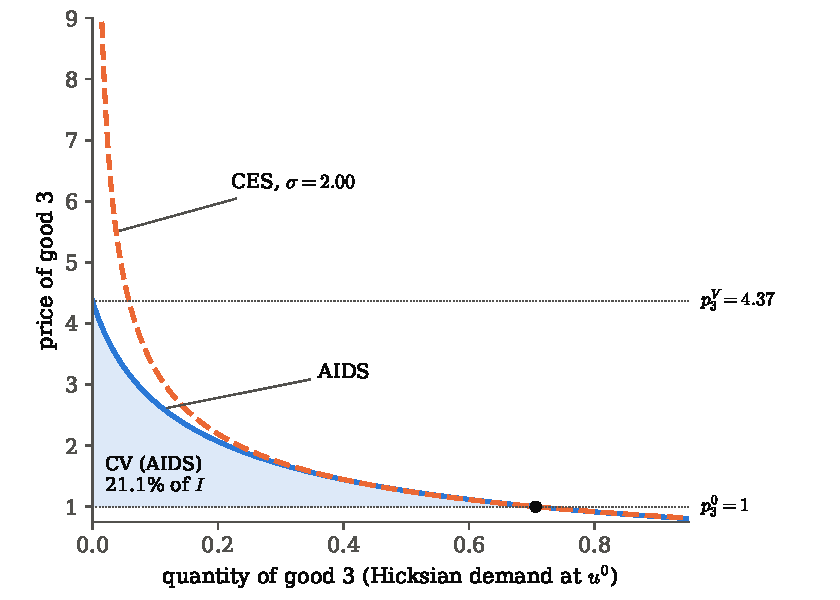
\includegraphics[width=0.78\textwidth]{figures/ch05/virtual_price.pdf}
\caption[Virtual price and the loss from removing a good]{Virtual price and the loss from removing a good.
The solid curve is the AIDS Hicksian demand for good 3 in the running example at the initial utility $u^0$,
with $p_1 = p_2 = 1$. It reaches zero at the virtual price $p_3^V = 4.37$. The shaded area is the compensating
variation of removing good 3, 21.1 percent of income. The dashed curve is the Hicksian demand of a CES system
calibrated to the same share ($0.26$) and own-price elasticity ($-1.738$) at the observed point. It approaches
the price axis only asymptotically, and the area to its left equals 35.2 percent of income. Computed with
\texttt{figures/ch05/src/virtual\_price.py}.}
\label{fig:05-virtual-price}
\end{figure}

\subsection{The extrapolation problem}\label{sec:05-welfare-extrapolation}

\begin{remark}[Virtual prices lie outside the data]\label{rem:05-extrapolation}
Every virtual-price calculation extrapolates. In the running example the virtual price is more than four times
the observed price. In Hausman's cereal data, prices vary by about 50 percent, while the estimated virtual
price is about twice the average price \citep[p.~228]{Hausman1997}. The answer is
then driven by the curvature of the chosen functional form beyond the support of the data. For AIDS the
relevant feature is the shape of shares in log prices, linear when $\beta_i = 0$ and quadratic otherwise.
\Cref{prop:05-variety}(c) shows how sensitive the
result is near unit elasticity: the log virtual price $\frac{1}{-\varepsilon_{ii} - 1}$ explodes as
$\varepsilon_{ii}$ approaches $-1$. \citet{Hausman1997} proposes a lower bound that needs only convexity of
demand: the tangent to the demand curve at the observed price meets the price axis below the true virtual price.
\Cref{ch:newgoods} develops this bound.
\end{remark}

\subsection{Recovering marginal costs from first-order conditions}\label{sec:05-welfare-supply}

Counterfactual prices require marginal costs, which are rarely observed. The standard approach inverts the
firms' pricing conditions, as in \cref{ch:theory} and \cref{ch:diffprod}. We state the conditions in
elasticity form, which is the natural form for product-space demand.

\casehead{Single-product pricing}
A firm that sets the price of product $i$ with constant marginal cost $c_i$ maximizes $(p_i - c_i)q_i(p)$. The
first-order condition is $q_i + (p_i - c_i)\frac{\partial q_i}{\partial p_i} = 0$. Dividing by $q_i$ and
multiplying by $\frac{1}{p_i}$ gives the Lerner condition
$\frac{p_i - c_i}{p_i} = -\frac{1}{\varepsilon_{ii}}$, and solving for the cost gives
\begin{equation}\label{eq:05-foc-single}
  c_i = p_i\Bigl(1 + \frac{1}{\varepsilon_{ii}}\Bigr).
\end{equation}
The condition is meaningful only when $\varepsilon_{ii} < -1$. A profit-maximizing firm never prices on the
inelastic part of its demand. The same condition holds for a product group whose price is set jointly by
perfectly colluding producers, the case used by \citet{ChaudhuriGoldbergJia2006}.

The elasticity in \eqref{eq:05-foc-single} must be \emph{unconditional}. It must include the reallocation of
expenditure across segments and between the category and other goods, computed by the chain rule of
\eqref{eq:05-uncond-elast}. A within-segment elasticity holds segment expenditure fixed. Suppose a segment's
own unconditional elasticity is below $-1$. Raising a brand's price then drains expenditure from the whole
segment, so the unconditional own elasticity is larger in magnitude than the conditional one. Markups computed from
conditional elasticities are then too high. \Cref{tab:05-hlz-own} shows this pattern for all fifteen beer
brands of \cref{sec:05-hlz}.

\casehead{Multiproduct pricing in elasticity form}
Firm $f$ owns the products in $\mathcal{J}_f$ and maximizes $\pi_f = \sum_{k\in\mathcal{J}_f}(p_k - c_k)q_k(p)$.
The first-order condition for $p_j$, $j\in\mathcal{J}_f$, is
\begin{equation*}
  q_j + \sum_{k\in\mathcal{J}_f}(p_k - c_k)\frac{\partial q_k}{\partial p_j} = 0.
\end{equation*}
Let $R_f = \sum_{k\in\mathcal{J}_f}p_kq_k$ be the firm's revenue, $r_k = \frac{p_kq_k}{R_f}$ the revenue share
of product $k$, and $\ell_k = \frac{p_k - c_k}{p_k}$ its Lerner index. Elsewhere the book writes $L$ for the
Lerner index. We write $\ell_k$ in this chapter, where $L$ denotes a likelihood. We multiply the condition by
$\frac{p_j}{R_f}$ and rewrite each term of the sum:
\begin{equation*}
  (p_k - c_k)\frac{\partial q_k}{\partial p_j}\frac{p_j}{R_f}
  = \frac{p_k - c_k}{p_k}\cdot\frac{p_kq_k}{R_f}\cdot\frac{\partial q_k}{\partial p_j}\frac{p_j}{q_k}
  = \ell_k\,r_k\,\varepsilon_{kj}.
\end{equation*}
The first-order conditions become
\begin{equation}\label{eq:05-foc-multi}
  r_j + \sum_{k\in\mathcal{J}_f}\ell_k\,r_k\,\varepsilon_{kj} = 0, \quad j\in\mathcal{J}_f,
  \qquad\text{or}\qquad r_f + E_f^\top m_f = 0.
\end{equation}
Here $r_f$ stacks the revenue shares and $m_f$ has elements $m_k = \ell_kr_k$. The matrix $E_f$ collects the
elasticities among the firm's products, with $(k,j)$ element $\varepsilon_{kj}$. Solving,
\begin{equation}\label{eq:05-markup-multi}
  m_f = -\bigl(E_f^\top\bigr)^{-1}r_f, \qquad \ell_k = \frac{m_k}{r_k}.
\end{equation}
This is the form in \citet[eqs.~7--9 and 14--15]{HausmanLeonardZona1994} and \citet[eqs.~12--15]{Hausman1997},
who write $s$ for the revenue shares and $w$ for $m_f$. The system is homogeneous of degree one in $r_f$, so
the shares can be normalized by any common revenue, such as total market revenue, without changing $\ell$.
Stacking all firms gives a block-diagonal elasticity matrix, one block per firm
\citep[eq.~14]{HausmanLeonardZona1994}.

The elasticity form is equivalent to the matrix markup formula of \cref{ch:diffprod}. Let $\Omega$ be the
ownership matrix and let $D$ have $(j,k)$ element $\frac{\partial q_k}{\partial p_j}$ (note the transposition
relative to the Jacobian of demand). Stacking the first-order conditions of all firms gives
\begin{equation*}
  q + (\Omega\odot D)(p - c) = 0, \qquad\text{so}\qquad p - c = -(\Omega\odot D)^{-1}q.
\end{equation*}
Dividing by market size turns quantities into market shares. Using $\frac{\partial q_k}{\partial p_j} =
\varepsilon_{kj}\frac{q_k}{p_j}$, row $j$ reads $q_j + \sum_k\Omega_{jk}\varepsilon_{kj}\frac{q_k}{p_j}(p_k - c_k) = 0$.
Multiplying by $\frac{p_j}{R_f}$ returns \eqref{eq:05-foc-multi}.

For a firm with two products, \eqref{eq:05-markup-multi} gives
\begin{equation}\label{eq:05-lerner-two}
  \ell_1 = \frac{-\varepsilon_{22} + \frac{r_2}{r_1}\varepsilon_{21}}{\varepsilon_{11}\varepsilon_{22} - \varepsilon_{12}\varepsilon_{21}}.
\end{equation}
With $\varepsilon_{21} = \varepsilon_{12} = 0$ this reduces to $-\frac{1}{\varepsilon_{11}}$. When the two
products are substitutes, the term $\frac{r_2}{r_1}\varepsilon_{21} > 0$ raises the markup on product 1. Part of
the demand lost by raising $p_1$ is recaptured by product 2. The size of the effect depends on the cross
elasticity of the sibling product with respect to $p_1$ and on its relative revenue.

\subsection{Partial identification of marginal cost}\label{sec:05-welfare-bounds}

The first-order condition \eqref{eq:05-foc-single} presumes a model of conduct. In many markets conduct is
unknown, and in regulated markets prices may not satisfy any unconstrained first-order condition.
\citet{ChaudhuriGoldbergJia2006} face both problems in the Indian antibiotics market (\cref{sec:05-cgj}).
Dozens of firms sell each molecule, and many prices are capped by regulation. Their solution is to bound
marginal cost instead of point-identifying it.

\begin{assumption}[Conduct between competition and joint monopoly]\label{ass:05-conduct-order}
For product group $i$ the following hold.
\begin{enumerate}[label=(\roman*)]
  \item Marginal cost $c_i$ is constant.
  \item Group demand $q_i(p_i,p_{-i})$ is differentiable, with $\frac{\partial q_i}{\partial p_i} < 0$.
  \item The group's joint profit $\Pi_i(p_i) = (p_i - c_i)q_i(p_i,p_{-i})$ is strictly quasi-concave in $p_i$,
  with maximizer $p_i^m$.
  \item The observed price satisfies $c_i \le p_i \le p_i^m$.
\end{enumerate}
\end{assumption}

Part (iv) is the substantive assumption. Prices are no lower than marginal cost, and no higher than the price a
joint monopolist of the group would choose given the other prices. Competition within the group and price
caps both move the price into this interval.

\begin{proposition}[Bounds on marginal cost]\label{prop:05-cost-bounds}
Under \cref{ass:05-conduct-order}, $c_i^L \le c_i \le c_i^U$, where
\begin{equation}\label{eq:05-cost-bounds}
  c_i^U = p_i, \qquad c_i^L = p_i\Bigl(1 + \frac{1}{\varepsilon_{ii}(p)}\Bigr),
\end{equation}
and $\varepsilon_{ii}(p)$ is the unconditional own-price elasticity at the observed prices. Equivalently,
$0 \le \ell_i \le -\frac{1}{\varepsilon_{ii}(p)}$.
\end{proposition}

\begin{proof}
The upper bound is the first inequality in part (iv). For the lower bound, a strictly quasi-concave function
increases up to its maximizer. Since $p_i \le p_i^m$, we have
$\Pi_i'(p_i) = q_i + (p_i - c_i)\frac{\partial q_i}{\partial p_i} \ge 0$. Rearranging,
$(p_i - c_i)\bigl(-\frac{\partial q_i}{\partial p_i}\bigr) \le q_i$. Dividing both sides by
$p_i\bigl(-\frac{\partial q_i}{\partial p_i}\bigr) > 0$ gives
\begin{equation*}
  \frac{p_i - c_i}{p_i} \le \frac{q_i}{p_i}\Bigl(-\frac{\partial q_i}{\partial p_i}\Bigr)^{-1} = -\frac{1}{\varepsilon_{ii}}.
\end{equation*}
Solving for $c_i$ gives $c_i \ge p_i\bigl(1 + \frac{1}{\varepsilon_{ii}}\bigr) = c_i^L$.
\end{proof}

These are equations (3.12) and (3.13) of \citet{ChaudhuriGoldbergJia2006}. Several remarks help in using them.
The lower bound is informative only when $\varepsilon_{ii} < -1$. If $-1 < \varepsilon_{ii} < 0$, then
$c_i^L < 0$ and the bound adds nothing to $c_i \ge 0$. The observed price then lies where demand is inelastic,
which no unconstrained joint monopolist would choose. That pattern is itself evidence of competition or
regulation. In the language of \cref{ch:conduct}, the bounds are the endpoints of the conduct-parameter model
$\frac{p_i - c_i}{p_i} = -\frac{\theta}{\varepsilon_{ii}}$ at $\theta = 0$ and $\theta = 1$. The bounds approach
avoids estimating $\theta$, which in a regulated market need not be a stable structural parameter. Bounds are
transparent, and they often suffice for a policy conclusion. In a counterfactual we simulate the outcome at
each bound. The two results bound the counterfactual outcome when that outcome is monotone in marginal cost,
which should be checked in each application.

\subsection{Counterfactual equilibrium after product withdrawal}\label{sec:05-counterfactual}

We now combine virtual prices, cost recovery and the multi-level demand system to simulate the withdrawal of
products. The setting is the two-level system of \cref{sec:05-separability}. An upper level allocates total
expenditure $X$ across segments $G$ with price indices $P_G$, and an AIDS allocates segment expenditure $X_Q$
within segment $Q$. A policy removes the products in $\mathcal{W}\subset Q$, and the products in
$\mathcal{R} = Q\setminus\mathcal{W}$ remain.

\casehead{The equilibrium system}
The unknowns are the virtual prices $p_i^V$ of the withdrawn products, the new prices $p_k'$ of the remaining
products, and the new segment expenditure and price index $X_Q'$ and $P_Q'$. They solve three blocks of
equations.
\begin{enumerate}[label=(S\arabic*)]
  \item Zero shares for withdrawn products. For each $i\in\mathcal{W}$,
  \begin{equation}\label{eq:05-cf-zero}
    0 = \alpha_i + \sum_{j\in\mathcal{W}}\gamma_{ij}\ln p_j^V + \sum_{k\in\mathcal{R}}\gamma_{ik}\ln p_k'
    + \beta_i\ln\frac{X_Q'}{P_Q'}.
  \end{equation}
  \item Pricing of remaining products. For single-product firms or colluding groups,
  \begin{equation}\label{eq:05-cf-price}
    p_k' = c_k\Bigl(1 + \frac{1}{\varepsilon_{kk}(p')}\Bigr)^{-1}, \quad k\in\mathcal{R},
  \end{equation}
  and for multiproduct firms the system \eqref{eq:05-foc-multi} evaluated at the new prices.
  \item Upper-level adjustment. The new index is $P_Q' = \mathbf{P}_Q(p^V_{\mathcal{W}},p'_{\mathcal{R}})$, and
  $X_Q'$ follows from the upper-level share equation of segment $Q$ evaluated at $P_Q'$ and the other segment
  indices.
\end{enumerate}
Equations~\eqref{eq:05-cf-zero} and \eqref{eq:05-cf-price} are equations (3.14) and (3.15) of \citet{ChaudhuriGoldbergJia2006},
written without their market-specific restrictions on the cross-price terms. The elasticities in (S2) are
unconditional and evaluated at the counterfactual prices, including the virtual prices.

One detail of (S2) deserves care. The demand that a remaining firm faces is AIDS demand evaluated at the
virtual prices, and by (S1) those prices move when $p_k'$ moves. For a single withdrawn product $i$, implicit
differentiation of $w_i = 0$ gives
$\frac{\partial\ln p_i^V}{\partial\ln p_j} = -\bigl(\frac{\partial w_i}{\partial\ln p_i}\bigr)^{-1}\frac{\partial w_i}{\partial\ln p_j}$.
The elasticity of demand for product $k$ with respect to $p_j$, once good $i$ has left, is therefore
\begin{equation}\label{eq:05-rationed-elast}
  \varepsilon_{kj}^{-i} = \varepsilon_{kj} - \varepsilon_{ki}\Bigl(\frac{\partial w_i}{\partial\ln p_i}\Bigr)^{-1}\frac{\partial w_i}{\partial\ln p_j},
\end{equation}
with all terms evaluated at $p_i^V$. This is the standard formula for demand under a ration of zero.

\casehead{Solving the system}
A simple algorithm iterates over the blocks. Start at the observed prices and expenditure. Given $p'_{\mathcal{R}}$
and $X_Q'$, solve (S1) for the virtual prices. Update $P_Q'$ and $X_Q'$ with (S3). Update $p'_{\mathcal{R}}$ with
(S2), using elasticities at the current prices. Repeat until the prices stop changing. Newton's method on the
stacked system converges faster when a good starting value is available. Existence and uniqueness are not
guaranteed, so we solve from several starting values and check the second-order conditions. We also verify
that the remaining shares stay positive and that the relevant own elasticities stay below $-1$.

\casehead{Welfare and its decomposition}
Let $E(u,P)$ be the upper-level expenditure function, with $P$ the vector of segment indices. Let $P^0$ be the
observed indices and $P'$ the counterfactual ones, with $P_Q'$ computed from the virtual and new prices. The
compensating variation is \citep[eq.~3.16]{ChaudhuriGoldbergJia2006}
\begin{equation}\label{eq:05-cv-cf}
  CV = E(u^0,P') - E(u^0,P^0).
\end{equation}
To see which mechanism drives it, define two intermediate price vectors. $P^1$ uses virtual prices computed with
$X_Q$ and all remaining prices fixed at their observed values. $P^2$ recomputes the virtual prices letting $X_Q$
respond to the new segment index, still holding the remaining prices fixed. Then
\begin{equation}\label{eq:05-cv-decomp}
  CV = \underbrace{E(u^0,P^1) - E(u^0,P^0)}_{\text{pure variety}}
  + \underbrace{E(u^0,P^2) - E(u^0,P^1)}_{\text{expenditure switching}}
  + \underbrace{E(u^0,P') - E(u^0,P^2)}_{\text{price adjustment}}.
\end{equation}
This is the general form of the decomposition used by \citet{ChaudhuriGoldbergJia2006}. The first term values
the lost products at fixed prices and fixed segment expenditure. The second term exists because the zero-share
condition (S1) is Marshallian. Whenever $\beta_i \neq 0$, the virtual prices depend on segment expenditure, so
they shift once $X_Q$ adjusts. The third term records the repricing of the remaining products. The first two
terms together describe a regime in which price regulation freezes the remaining prices at their old levels.
The decomposition is sequential, so its terms depend on the order in which the changes are introduced.

The welfare of a country adds producer surplus. With $\pi_k = (p_k - c_k)q_k$ computed at the counterfactual
and the observed prices, the change in national welfare is $-CV$ plus the change in the profits of domestic
firms. Profits of foreign firms are excluded from national welfare. They still measure the private gain that
motivates the policy. \Cref{sec:05-cgj-counterfactual} applies this accounting to patents in India.

\begin{example}[Withdrawal in the running example]\label{ex:05-withdrawal}
Treat the running example as a segment with fixed expenditure $X_Q = e$, sold by three single-product firms.
Equation~\eqref{eq:05-foc-single} recovers marginal costs $c = (0.273, 0.406, 0.425)$ from the observed prices and
elasticities. Suppose good 3 is withdrawn. Firms 1 and 2 reprice, facing the demand of consumers who can no
longer buy good 3, with its elasticities given by \eqref{eq:05-rationed-elast}. The new equilibrium has
$p_1' = 1.475$ and $p_2' = 1.365$, increases of 47.5 and 36.5 percent. The own elasticities fall in magnitude
from $-1.375$ and $-1.682$ to $-1.227$ and $-1.423$, because the closest outside option has gone. The total
compensating variation is 71.9 percent of segment expenditure. The pure variety effect, with other prices fixed,
is 21.1 percent (\cref{ex:05-virtual-running}). The price adjustment adds 50.8 percent. Firms 1 and 2 gain
$0.734$ in profit, while firm 3 loses $0.407$. These effects are large because fixing segment expenditure makes
the segment's aggregate demand unit elastic. An upper level with elastic segment demand would add the
expenditure-switching channel and dampen the price response. The computation is in \texttt{virtual\_price.py}.
\end{example}

\section{Case study: Hausman, Leonard and Zona (1994)}\label{sec:05-hlz}

\citet{HausmanLeonardZona1994} (HLZ) built the multi-level AIDS into a tool for antitrust analysis of
differentiated products. They estimated a three-level demand system for beer on store-level scanner data and
identified it with prices of the same brands in other cities. They then used the estimates to predict the price
effects of mergers and to test models of pricing. The paper is short and its data description is thin, but its
method shaped two decades of applied work. We treat it in depth.

\subsection{The economic question}\label{sec:05-hlz-question}

Antitrust questions about consumer goods turn on substitution among brands. Is a set of brands a market? Will
two brands owned by merging firms rise in price? Do observed markups match the predictions of a model of
competition? Each question needs own and cross elasticities for many brands. HLZ argue that the models then in
use restricted these elasticities too much. Representative-consumer models with symmetric preferences and
logit-type models share an \emph{independence of irrelevant alternatives} (IIA) property. Consumers of an
eliminated good spread over the remaining goods in proportion to their market shares. In terms
of elasticities, ``all cross price elasticities with respect to a given good are the same''
\citep[p.~160]{HausmanLeonardZona1994}. HLZ set out to estimate demand without such restrictions.

Store-level scanner data made this possible. Each transaction records units and price paid, by brand and by
stock-keeping unit, and weekly promotions generate large price variation. Two econometric problems remain. The
first is dimensionality. It is ``difficult to conceive of estimating a demand equation with say 135 brands of
cereal or say 40 brands of beer'' (p.~160). The second is identification: at the brand level, cost shifters that
vary across brands and weeks are hard to find. HLZ answer the first problem with multi-stage budgeting and the
second with prices in other cities.

A third theme runs through the applications. Firms in these industries sell many brands. HLZ list Miller High
Life, Miller Lite, Miller Genuine Draft, Milwaukee's Best and Meisterbrau as Miller brands, and note that
Kellogg's produces over 30 cereals (p.~161). A multiproduct firm that raises one brand's price recaptures some
of the lost sales on its other brands. HLZ show how this \emph{cannibalization} changes merger predictions and
tests of conduct.

\subsection{Setting and data}\label{sec:05-hlz-data}

Marketing analysts divide the U.S. beer market into segments: premium, light (low-calorie), imported and
popular-price beer (p.~162). In estimation HLZ use three segments. The premium segment includes imported
beers, which they found belong with premium brands (p.~164). Each segment contains five brands, for fifteen
brands in total (\cref{fig:05-hlz-tree}). The brands include national brands such as Budweiser, Miller and
Coors, Canadian imports such as Molson and Labatts, and regional brands such as Genesee.

\begin{figure}[htbp]
\centering
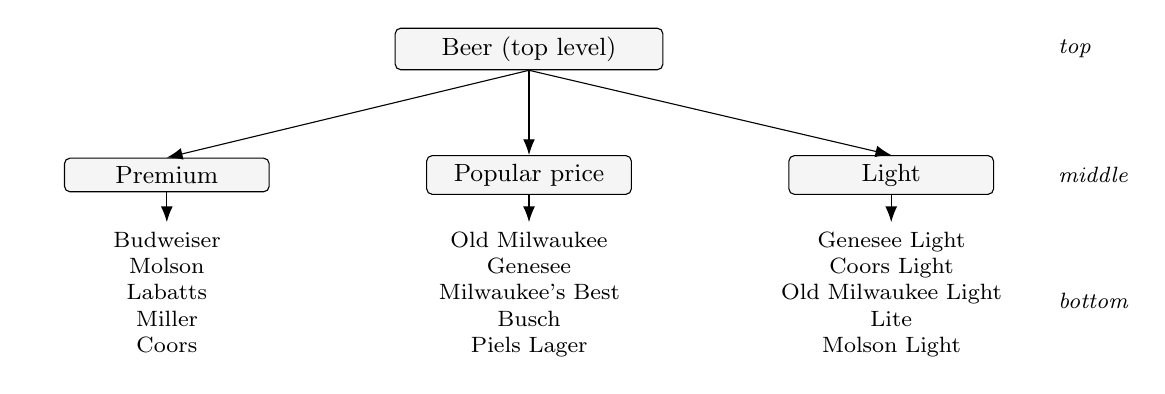
\begin{tikzpicture}[
  every node/.style={font=\small},
  seg/.style={draw, rounded corners=2pt, minimum width=2.6cm, inner sep=3pt, fill=gray!8},
  brands/.style={align=center, font=\footnotesize, text width=3.3cm}]
  \node[seg, minimum width=3.4cm] (beer) at (0,0) {Beer (top level)};
  \node[seg] (prem) at (-4.6,-1.6) {Premium};
  \node[seg] (pop)  at (0,-1.6)    {Popular price};
  \node[seg] (lig)  at (4.6,-1.6)  {Light};
  \foreach \s in {prem,pop,lig} \draw[-{Latex[length=2mm]}] (beer.south) -- (\s.north);
  \node[brands, anchor=north] (b1) at (-4.6,-2.2) {Budweiser\\ Molson\\ Labatts\\ Miller\\ Coors};
  \node[brands, anchor=north] (b2) at (0,-2.2) {Old Milwaukee\\ Genesee\\ Milwaukee's Best\\ Busch\\ Piels Lager};
  \node[brands, anchor=north] (b3) at (4.6,-2.2) {Genesee Light\\ Coors Light\\ Old Milwaukee Light\\ Lite\\ Molson Light};
  \foreach \s/\b in {prem/b1,pop/b2,lig/b3} \draw[-{Latex[length=2mm]}] (\s.south) -- (\b.north);
  \node[anchor=west, font=\footnotesize\itshape] at (6.6,0) {top};
  \node[anchor=west, font=\footnotesize\itshape] at (6.6,-1.6) {middle};
  \node[anchor=west, font=\footnotesize\itshape] at (6.6,-3.2) {bottom};
\end{tikzpicture}
\caption[The three-level budgeting tree of Hausman, Leonard and Zona]{The three-level budgeting tree of
\citet{HausmanLeonardZona1994}. The top level determines beer consumption relative to other goods, the middle
level allocates beer expenditure across three segments, and the bottom level allocates each segment's
expenditure across five brands. Imported beers are included in the premium segment. Brand lists from HLZ,
Tables 2 to 5.}
\label{fig:05-hlz-tree}
\end{figure}

The data are cash-register records from individual stores, aggregated to the metropolitan area (SMSA) level.
For each brand they give sales and price per unit, after aggregating over container sizes (p.~160). Most price
variation comes from supermarket chains running low-price promotions on a brand in a given week (p.~167).
In most cases manufacturers sell at wholesale nationally, with a uniform wholesale price (p.~161), which
motivates the
identification strategy below. The paper reports little else about the sample. Two graphs show weekly sales of
Budweiser and Genesee in Buffalo in February and March 1988 and in March to June 1990. The middle-level
regressions of Table 1 use 101 observations. HLZ do not report the list of cities, the sample period or the
number of stores. The top level uses national monthly data from the Bureau of Labor Statistics covering
sixteen years (p.~164). The share equations also include a time trend and the log number of stores.

\subsection{The three-level demand model}\label{sec:05-hlz-model}

HLZ apply the multi-stage budgeting framework of \cref{sec:05-separability} with three levels. We write their
equations in this chapter's notation. Cities are indexed by $n = 1,\dots,N$ (in this section $N$ counts cities)
and weeks by $t$. Segments are $G$ and $H$, and brands are $i$ and $j$.

\casehead{Bottom level: brands within a segment}
For brand $i$ in segment $G$,
\begin{equation}\label{eq:05-hlz-bottom}
  w_{int} = \alpha_{in} + \beta_i\ln\frac{X_{Gnt}}{P_{Gnt}} + \sum_{j\in G}\gamma_{ij}\ln p_{jnt} + \xi_{int}.
\end{equation}
This is equation (1) of \citet{HausmanLeonardZona1994}. Here $w_{int}$ is the revenue share of brand $i$ in segment expenditure
$X_{Gnt}$, $P_{Gnt}$ is a segment price index and $p_{jnt}$ is the price of brand $j$. The intercept
$\alpha_{in}$ is a brand-city effect. This is an AIDS for the segment, with symmetry
$\gamma_{ij} = \gamma_{ji}$ imposed in estimation. The $\gamma_{ij}$ are free within the segment, so no IIA-type
restriction constrains the cross elasticities among the brands that compete most closely. A test of
$\beta_i = 0$ is a test of segment homotheticity. HLZ stress that the expenditure variable must be segment
expenditure (p.~163), in the words that \citet{Hausman1997} repeats and that we quoted in
\cref{sec:05-second-stage}.

\casehead{Middle level: segments}
Given the bottom-level estimates, HLZ construct a price index for each segment. They use either the exact index
implied by the bottom-level expenditure function or a weighted-average index of the Laspeyres type, and report
that the choice matters little (p.~164). The segment demands are log-log:
\begin{equation}\label{eq:05-hlz-middle}
  \ln q_{Gnt} = \alpha_{Gn} + \beta_G\ln X_{Bnt} + \sum_{H}\vartheta_{GH}\ln P_{Hnt} + \xi_{Gnt},
\end{equation}
where $q_{Gnt}$ is the quantity of segment $G$ and $X_{Bnt}$ is total beer expenditure (HLZ eq.~2, where
the price coefficients are written $\delta_k$). Because beer expenditure is held fixed, $\beta_G$ and
$\vartheta_{GH}$ are conditional elasticities. Slutsky restrictions are not imposed at this level (fn.~3).
Exact two-stage budgeting under Gorman's results, discussed in \citet{BlackorbyPrimontRussell1978}, requires
additive separability at the level above. HLZ note
that AIDS is a generalized Gorman polar form, so Gorman's theorem applies, and that a less restrictive middle
level, not consistent with exact two-stage budgeting, gives similar results (fn.~2).

\casehead{Top level: beer}
Overall beer consumption $Q_{Bt}$ is
\begin{equation}\label{eq:05-hlz-top}
  \ln Q_{Bt} = \varphi_0 + \varphi_1\ln y_t + \varphi_2\ln P_{Bt} + Z_t^\top\psi + \xi_{Bt}.
\end{equation}
This is HLZ's equation (3). Here $y_t$ is deflated disposable income and $P_{Bt}$ is the deflated beer price index. The vector
$Z_t$ holds demographics, monthly seasonal factors and the minimum legal age for buying beer. The coefficient
$\varphi_2$ is the overall price elasticity of beer. HLZ estimate it by instrumental variables on the national
monthly data, with cost shifters for ingredients, packaging and labor as instruments.

\casehead{From three levels to unconditional elasticities}
Estimation runs bottom-up, and the elasticities that matter for competition combine all three levels. The
two-level chain rule of \eqref{eq:05-uncond-elast} extends directly. Take brand $i$ in segment $G$ and brand $j$
in segment $H$, and drop the city and week subscripts. Let $\varepsilon_{ij}\big|_{X_G}$ be the
within-segment elasticity at fixed segment expenditure and $\eta_{i\mid G} = 1 + \frac{\beta_i}{w_i}$ the
elasticity of brand $i$ with respect to segment expenditure. Then
\begin{equation*}
  \varepsilon_{ij} = \indic(G = H)\,\varepsilon_{ij}\big|_{X_G} + \eta_{i\mid G}\,\frac{\partial\ln X_G}{\partial\ln p_j}.
\end{equation*}
Segment expenditure is $X_G = P_Gq_G$, so $\ln X_G = \ln P_G + \ln q_G$. The index $P_G$ responds to $p_j$ only
if $H = G$. The quantity $q_G$ responds through the price index $P_H$ and through beer expenditure:
\begin{equation*}
  \frac{\partial\ln q_G}{\partial\ln p_j} = \Bigl[\vartheta_{GH} + \beta_G\frac{\partial\ln X_B}{\partial\ln P_H}\Bigr]\frac{\partial\ln P_H}{\partial\ln p_j}.
\end{equation*}
Beer expenditure is $X_B = P_BQ_B$, and with income fixed the top level gives
$\frac{\partial\ln X_B}{\partial\ln P_B} = 1 + \varphi_2$. If the beer index has segment weights $w_H$ (the shares
of the segments in beer expenditure), then $\frac{\partial\ln P_B}{\partial\ln P_H} = w_H$. Collecting terms,
\begin{equation}\label{eq:05-hlz-uncond}
  \varepsilon_{ij} = \indic(G = H)\,\varepsilon_{ij}\big|_{X_G}
  + \eta_{i\mid G}\Bigl[\indic(G = H) + \vartheta_{GH} + \beta_G(1 + \varphi_2)w_H\Bigr]\frac{\partial\ln P_H}{\partial\ln p_j}.
\end{equation}
For a Stone or Laspeyres segment index, $\frac{\partial\ln P_H}{\partial\ln p_j}$ is the weight of brand $j$ in
the index. For the exact translog index it equals $w_j - \beta_j\ln\frac{X_H}{P_H}$ (\cref{sec:05-aids}).

Equation~\eqref{eq:05-hlz-uncond} has two consequences. For the own elasticity ($j = i$), the bracket equals
$1 + \vartheta_{GG} + \beta_G(1 + \varphi_2)w_G$. It is negative whenever the segment's own conditional
elasticity is well below $-1$, as it is in the beer data. The unconditional own elasticity is then larger in
magnitude than the conditional one. For brands in different segments, $\varepsilon_{ij}$ depends on brand $j$
only through its weight in index $H$, and on brand $i$ only through $\eta_{i\mid G}$. All brand-pair specific
substitution across segments is ruled out. This is the price of the dimension reduction.

The restriction has a compensated counterpart. By the theorem of \citet{GoldmanUzawa1964}
(\cref{prop:05-goldman-uzawa}), weak separability implies $S_{ij} = \mu_{GH}\frac{\partial q_i}{\partial I}\frac{\partial q_j}{\partial I}$
for $i\in G$, $j\in H$, $G\neq H$. To convert to elasticities, we use
$\frac{\partial q_i}{\partial I} = \frac{\partial q_i}{\partial X_G}\frac{\partial X_G}{\partial I}
= \eta_{i\mid G}\frac{q_i}{X_G}\frac{\partial X_G}{\partial I}$ and the same expression for good $j$ in segment $H$.
Then
\begin{equation*}
  \varepsilon^h_{ij} = \frac{p_j}{q_i}S_{ij}
  = \mu_{GH}\,\eta_{i\mid G}\,\eta_{j\mid H}\,\frac{\partial X_G}{\partial I}\frac{\partial X_H}{\partial I}\,
    \frac{p_jq_j}{X_GX_H},
\end{equation*}
which gives
\begin{equation*}
  \varepsilon^h_{ij} = \lambda_{GH}\,w_{j\mid H}\,\eta_{i\mid G}\,\eta_{j\mid H},
  \qquad \lambda_{GH} = \frac{\mu_{GH}}{X_G}\frac{\partial X_G}{\partial I}\frac{\partial X_H}{\partial I},
\end{equation*}
where $w_{j\mid H}$ is the share of brand $j$ in segment $H$ and $\lambda_{GH}$ depends only on the pair of
segments. HLZ state the restriction as $\varepsilon^h_{ij} = \lambda_{GH}\eta_{i\mid G}\eta_{j\mid H}$
\citep[eq.~5]{HausmanLeonardZona1994}. The exact conversion adds the within-segment share of brand $j$. Either
way, a segment-pair constant and brand-level expenditure elasticities determine all compensated substitution
across segments.

The dimension reduction is large. A complete AIDS for fifteen brands has $\frac{15 \times 14}{2} = 105$ free
price coefficients after symmetry and homogeneity. Three five-brand segments have $3 \times 10 = 30$, the middle
level adds nine segment price elasticities, and the top level adds one.

\subsection{Identification with prices in other cities}\label{sec:05-hlz-identification}

Prices in \eqref{eq:05-hlz-bottom} are endogenous if retailers and manufacturers set them knowing local demand
conditions. Cost shifters that vary by brand and week are rarely available. An ``insufficient number of input
prices may exist or they may not be reported with high enough frequency'' (p.~164). HLZ exploit the panel
structure of the data instead. They model the price of brand $j$ in city $n$ and week $t$ as
\begin{equation}\label{eq:05-hlz-price}
  \ln p_{jnt} = \rho_j\ln c_{jt} + \mu_{jn} + \zeta_{jnt}.
\end{equation}
This is HLZ's equation (4), with our $\rho_j$, $\mu_{jn}$ and $\zeta_{jnt}$ in place of their $\delta_j$,
$\alpha_{jn}$ and $w_{jnt}$. Here $c_{jt}$ is the cost of brand $j$, assumed to have no
city-specific time variation, consistent with national shipments and advertising. The term $\mu_{jn}$ is a
city-brand differential reflecting transport costs or local wages. The shock $\zeta_{jnt}$ has mean zero and
captures local promotions.

\begin{assumption}[Prices in other cities as instruments]\label{ass:05-hausman-iv}
In \eqref{eq:05-hlz-price} the following hold.
\begin{enumerate}[label=(\roman*)]
  \item The cost component $c_{jt}$ is common to all cities.
  \item The city-brand effects $\mu_{jn}$ are constant over time.
  \item The local shocks $\zeta_{jnt}$ are independent across cities. They may be correlated across brands
  within a city \citep[fn.~19]{Hausman1997}.
  \item The demand errors $\xi_{int}$ are uncorrelated with the cost component and with the local price shocks
  of other cities.
\end{enumerate}
\end{assumption}

Let a tilde denote the deviation from the city-brand mean, the within transformation that removes $\mu_{jn}$
and the fixed effects in \eqref{eq:05-hlz-bottom}. Under \cref{ass:05-hausman-iv} the prices of every brand of
the segment in any other city $n'\neq n$ satisfy the moment conditions
\begin{equation}\label{eq:05-hausman-iv}
  \E\bigl[\tilde\xi_{int}\,\widetilde{\ln p}_{jn't}\bigr] = 0, \qquad j\in G,\ n'\neq n.
\end{equation}
Instruments of this kind are now called \emph{Hausman instruments}. Relevance and exclusion follow from
\eqref{eq:05-hlz-price}. The price in city $n'$ shares the cost component with the price in city $n$, while the
local shocks are independent, so
\begin{equation*}
  \Cov\bigl(\widetilde{\ln p}_{jn't},\widetilde{\ln p}_{jnt}\bigr) = \rho_j^2\Var\bigl(\widetilde{\ln c}_{jt}\bigr) > 0
\end{equation*}
whenever national costs vary over time. The covariance with the demand error is
\begin{equation*}
  \Cov\bigl(\widetilde{\ln p}_{jn't},\tilde\xi_{int}\bigr)
  = \rho_j\Cov\bigl(\widetilde{\ln c}_{jt},\tilde\xi_{int}\bigr) + \Cov\bigl(\tilde\zeta_{jn't},\tilde\xi_{int}\bigr),
\end{equation*}
and both terms are zero by part (iv). In words, ``prices in one city (after elimination of city and brand specific effects)
are driven by underlying costs'' (p.~165).

The first stage regresses $\ln p_{jnt}$ on the brand-city effects, the exogenous regressors and the prices of the
segment's brands in other cities, either city by city or averaged. With more than two cities the model is
overidentified, and HLZ point to the tests of \citet{HausmanTaylor1981} for checking the instrument assumptions
(fn.~4). The logic is that of \citet{HausmanTaylor1981}: after unit effects are removed, variation shared with
other units serves as an instrument. The share equations are estimated as a system, as the residual covariance
matrices reported with Tables 2 to 4 suggest, and symmetry is imposed across equations.

HLZ also offer a second interpretation. Suppose supermarkets set weekly prices under constant short-run marginal
cost and do not adjust them to clear the market. Prices are then predetermined with respect to the demand errors,
and ordinary least squares is consistent. Segment expenditure $X_{Gnt}$ may still need instruments, since it
responds to the same demand shocks. The choice between the two views can be tested with the specification test
of \citet{Hausman1978}. That test compares the IV and OLS estimates through
\begin{equation*}
  \mathcal{H} = (\hat b_{IV} - \hat b_{OLS})^\top\bigl[\widehat{\Var}(\hat b_{IV}) - \widehat{\Var}(\hat b_{OLS})\bigr]^{-1}(\hat b_{IV} - \hat b_{OLS}),
\end{equation*}
which is asymptotically chi-squared under exogeneity, with degrees of freedom equal to the number of
coefficients tested. HLZ describe the test but do not report its outcome for beer.

Later work adopted these instruments widely. \citet{Nevo2001} uses regional quarterly average prices of the same
brand, excluding the city being instrumented, in his study of breakfast cereals. \Cref{ch:logit} and
\cref{ch:blp} return to them.

\subsection{Validity: Bresnahan's critique}\label{sec:05-bresnahan-critique}

The identifying assumption rules out demand shocks that are common across cities and reflected in prices.
\citet{Bresnahan1997} made this objection in his comment on \citet{Hausman1997}, which uses the same strategy for
cereals. For the assumption to hold, ``there can be no successful nationwide advertising campaigns which shift
the demand for individual brands or products'' \citep[p.~241]{Bresnahan1997}. There can be no national fads and
no slow national acceptance of new brands. Adding advertising to the demand equation does not settle the issue,
because the econometrician does not observe which campaigns succeed (fn.~6). The fallback that prices are
predetermined requires such shocks to be unforeseen when prices are set, which Bresnahan finds unlikely for
national campaigns. If national shocks exist and supply slopes up, prices in other cities move with the demand
error. Supply can slope up in the one-week run because inventories cannot adjust or because of market power
(fn.~7).

\casehead{The bias with one product}
We derive the bias in the simplest version of Bresnahan's model: one product, linear demand, single-product
Bertrand pricing and constant marginal cost. In city $n$ and week $t$,
\begin{equation*}
  q_{nt} = d + a\,p_{nt} + \xi_{nt}, \quad a < 0, \qquad\qquad p_{nt} = c_{nt} + \frac{q_{nt}}{-a}.
\end{equation*}
The pricing equation is the first-order condition $q + (p - c)a = 0$. Substituting demand into it gives
$p = c - \frac{d}{a} - p - \frac{\xi}{a}$, so
\begin{equation*}
  p_{nt} = \frac{1}{2}c_{nt} - \frac{d + \xi_{nt}}{2a}.
\end{equation*}
Let the demand error have a national and a local part, $\xi_{nt} = \chi_t + e_{nt}$, and let cost have the same
structure, $c_{nt} = \bar c_t + v_{nt}$. The national components have variances $\sigma_\chi^2$ and $\sigma_c^2$.
All components are mutually independent, and the local ones are independent across cities. The instrument for
$p_{nt}$ is $p_{n't}$ with $n'\neq n$. Only the national components survive in the covariances:
\begin{equation*}
  \Cov(p_{n't},\xi_{nt}) = -\frac{\sigma_\chi^2}{2a}, \qquad
  \Cov(p_{n't},p_{nt}) = \frac{\sigma_c^2}{4} + \frac{\sigma_\chi^2}{4a^2}.
\end{equation*}
The IV estimator therefore converges to
\begin{equation}\label{eq:05-iv-bias-scalar}
  \plim\hat a = a + \frac{\Cov(p_{n't},\xi_{nt})}{\Cov(p_{n't},p_{nt})}
  = a - \frac{2a\,\sigma_\chi^2}{a^2\sigma_c^2 + \sigma_\chi^2} = a(1 - 2\lambda),
  \qquad \lambda = \frac{\sigma_\chi^2}{a^2\sigma_c^2 + \sigma_\chi^2}.
\end{equation}
The weight $\lambda\in[0,1]$ is the share of national demand shocks in the price variation common to all
cities. Without national demand shocks ($\lambda = 0$) the estimator is consistent. Otherwise the estimate lies
between $a$ and $-a$, biased toward zero, so demand looks too steep. When $\lambda > \frac{1}{2}$ the estimated
slope even has the wrong sign. At $\lambda = 1$ the estimator recovers $-a$, the slope of the supply relation
$q = -a(p - c)$. In Bresnahan's words, the estimator then behaves ``like doing ordinary least squares on a supply
and demand system'' (p.~242).

\casehead{The bias with many products}
The same logic extends to $J$ products, and the exact bias has a compact form. Let demand be
$q_{nt} = d + A\,p_{nt} + \xi_{nt}$, with $A = [a_{jk}]$ and $a_{jk} = \frac{\partial q_j}{\partial p_k}$. Single-product
Bertrand pricing gives $p_{jnt} = c_{jnt} + \frac{q_{jnt}}{-a_{jj}}$, or $p = c + \Theta^{-1}q$ with
$\Theta = \diag(-a_{11},\dots,-a_{JJ})$. Multiplying by $\Theta$ and substituting demand,
\begin{equation*}
  \Theta p_{nt} = \Theta c_{nt} + d + Ap_{nt} + \xi_{nt}, \qquad\text{so}\qquad p_{nt} = (\Theta - A)^{-1}\bigl(d + \Theta c_{nt} + \xi_{nt}\bigr).
\end{equation*}
This is the price system in the appendix of \citet{Bresnahan1997}. Let the national demand and cost components
have covariance matrices $\Sigma_\chi$ and $\Sigma_c$, and write $M = (\Theta - A)^{-1}$. Equation $j$ is estimated
by IV with the vector of other-city prices $p_{n't}$ as instruments. Its coefficient vector, the transpose of
row $j$ of $A$, converges to $A_{j\cdot}^\top + [\E(\tilde p_{n't}\tilde p_{nt}^\top)]^{-1}\E(\tilde p_{n't}\xi_{jnt})$.
The two moments are
\begin{equation*}
  \E(\tilde p_{n't}\tilde p_{nt}^\top) = M\bigl(\Theta\Sigma_c\Theta + \Sigma_\chi\bigr)M^\top, \qquad
  \E(\tilde p_{n't}\xi_{jnt}) = M\Sigma_\chi\mathbf{e}_j,
\end{equation*}
where $\mathbf{e}_j$ is the $j$th unit vector. The bias of equation $j$ is therefore
$(\Theta - A)^\top(\Theta\Sigma_c\Theta + \Sigma_\chi)^{-1}\Sigma_\chi\mathbf{e}_j$. Stacking the equations and using the symmetry of
the covariance matrices gives the following result.

\begin{proposition}[Bias of other-city price instruments]\label{prop:05-iv-bias}
In the linear model above, IV estimation with other-city prices satisfies
\begin{equation}\label{eq:05-iv-bias}
  \plim\hat A = (I - \Lambda)A + \Lambda\Theta, \qquad \Lambda = \Sigma_\chi\bigl(\Theta\Sigma_c\Theta + \Sigma_\chi\bigr)^{-1}.
\end{equation}
The estimate is a matrix-weighted average of the demand slopes $A$ and the supply slopes $\Theta$. With
$\Sigma_\chi = 0$ it is consistent, and with $\Sigma_c = 0$ it recovers $\Theta$, which has own slopes $-a_{jj}$ and
zero cross slopes.
\end{proposition}

When the national demand and cost shocks are uncorrelated across products, $\Lambda = \diag(\lambda_1,\dots,\lambda_J)$ with
$\lambda_j = \frac{\sigma_{\chi j}^2}{a_{jj}^2\sigma_{cj}^2 + \sigma_{\chi j}^2}$. Then
$\plim\hat a_{jj} = (1 - 2\lambda_j)a_{jj}$ and $\plim\hat a_{jk} = (1 - \lambda_j)a_{jk}$. Own slopes are biased
toward zero as in the one-product case, and cross slopes are attenuated toward zero. Correlated national shocks
change the cross terms. The bias of $a_{12}$ is $-\Lambda_{11}a_{12} - 2\Lambda_{12}a_{22}$, and the second term is
positive when $\Lambda_{12} > 0$. Cross slopes can then be inflated. \texttt{bresnahan\_bias\_check.py} confirms
\eqref{eq:05-iv-bias} by simulation. For example, with $A = \bigl[\begin{smallmatrix}-2 & 0.5\\ 0.5 & -1.5\end{smallmatrix}\bigr]$,
$\Sigma_c = 0.3I$ and $\Sigma_\chi = 0.4I$, the probability limit is
$\bigl[\begin{smallmatrix}-1.00 & 0.375\\ 0.314 & -0.384\end{smallmatrix}\bigr]$. If the national shocks have
correlation $0.8$ across the two products, it becomes
$\bigl[\begin{smallmatrix}-1.31 & 1.11\\ 0.87 & -0.57\end{smallmatrix}\bigr]$.

\casehead{Bresnahan's printed result}
Bresnahan states that the sign and magnitude of the bias are governed by $\Sigma_\chi[\diag(-\gamma) - \gamma]^{-1}$,
in his notation $\gamma_{jk} = a_{jk}$. This matrix is the covariance between other-city prices and demand
errors, $M\Sigma_\chi$ up to transposition. For two products whose national shocks have correlation $\varrho$, his
appendix (pp.~246--247) reports the elements
\begin{equation*}
  \frac{\sigma}{4\gamma_{11}\gamma_{22} - \gamma_{12}\gamma_{21}}
  \begin{bmatrix} -2\gamma_{22} + \varrho\gamma_{21} & \gamma_{12} - 2\varrho\gamma_{11}\\
  -2\varrho\gamma_{22} + \gamma_{21} & \varrho\gamma_{12} - 2\gamma_{11}\end{bmatrix}.
\end{equation*}
He concludes that the on-diagonal bias has the sign of
$-2\gamma_{22} + \varrho\gamma_{12}$ and the off-diagonal bias the sign of $\gamma_{12} - 2\varrho\gamma_{11}$. At
$\varrho = 0$ these are positive: own coefficients are biased toward zero and cross coefficients away from zero.
The printed algebra has typographical slips. The intermediate inverse has the wrong signs off the diagonal,
although the final matrix is correct, and the text writes $\varrho\gamma_{12}$ where the matrix has
$\varrho\gamma_{21}$, which coincide under symmetry. The reading of covariance signs as bias signs is exact with
one price. With several endogenous prices the bias also involves the inverse of the first-stage covariance
matrix, as \eqref{eq:05-iv-bias} shows. With $\varrho = 0$ the cross coefficients are attenuated, while
sufficiently correlated national shocks inflate them. Bresnahan's footnote 9 already hedges the cross-price
claim, saying that it ``depends on the covariances of the shocks to demand across products.'' Correlated
national shocks can also bias an own slope away from zero. The bias of $a_{jj}$ is the diagonal element
$2\Lambda_{jj}|a_{jj}| - \sum_{k\neq j}\Lambda_{jk}a_{kj}$ of $\Lambda(\Theta - A)$, and the second term can dominate.
With the matrix $A$ above, $\Sigma_c = \diag(5, 0.01)$ and
$\Sigma_\chi = 0.4\bigl[\begin{smallmatrix}1 & 0.95\\ 0.95 & 1\end{smallmatrix}\bigr]$ give
$\plim\hat a_{11} = -2.44$, farther from zero than the true $-2$. The own-price bias toward zero holds when
$2\Lambda_{jj}|a_{jj}| > \sum_{k\neq j}\Lambda_{jk}a_{kj}$, for example when national demand and cost shocks are
uncorrelated across products.

\casehead{What the critique implies}
National demand shocks typically make estimated own elasticities too small in magnitude. Markups recovered from
\eqref{eq:05-foc-multi} are then too high, simulated merger price increases too large, and the value of new goods
too large. Bresnahan's own concern was the last of these. \citet[fn.~25]{Hausman1997} anticipates the objection
by citing the beer estimates of HLZ, whose own-price elasticities lie ``in the range of about $-4.0$ to $-6.2$''.
He concludes that the method does not mechanically produce small elasticities. The reply is incomplete. A bias
toward zero is compatible with large estimates if the true elasticities are larger still. The assumption can be
probed in the data. Overidentification tests across cities are one check. A more direct symptom of national
shocks is correlation between the demand residuals of the same brand in different cities in the same week.
Instruments based on observed local cost variation offer a comparison, as in \citet{Nevo2001}. Bresnahan
himself points to other approaches to estimating substitution, including the then recent method of
\citet{Berry1994} (fn.~10). The critique
applies to every use of Hausman instruments, including random-coefficient models (\cref{ch:blp}).

\subsection{Results}\label{sec:05-hlz-results}

\casehead{Top and middle levels}
The overall price elasticity of beer is $-1.36$, with standard error 0.21 (p.~164). \Cref{tab:05-hlz-table1}
reproduces the segment equations. Each column is a segment demand equation, and because the equations are
log-log, the coefficients are conditional elasticities. Expenditure elasticities are close to one. The own
price elasticities are about $-2.7$ for premium and popular-price beer and $-2.4$ for light beer. These are large
for segment-level elasticities. They imply that a hypothetical attempt to raise all premium prices would not pay
if light and popular prices stayed put (p.~166).

\begin{table}[htbp]
\centering
\caption{Segment demand equations for beer}\label{tab:05-hlz-table1}
\begin{threeparttable}
\begin{tabular}{@{}lccc@{}}
\toprule
 & Premium & Popular & Light \\
\midrule
Constant & $0.501$ & $-4.021$ & $-1.183$ \\
 & $(0.283)$ & $(0.560)$ & $(0.377)$ \\
$\ln$ beer expenditure & $0.978$ & $0.943$ & $1.067$ \\
 & $(0.011)$ & $(0.022)$ & $(0.015)$ \\
$\ln P_{\text{premium}}$ & $-2.671$ & $2.704$ & $0.424$ \\
 & $(0.123)$ & $(0.244)$ & $(0.166)$ \\
$\ln P_{\text{popular}}$ & $0.510$ & $-2.707$ & $0.747$ \\
 & $(0.097)$ & $(0.193)$ & $(0.127)$ \\
$\ln P_{\text{light}}$ & $0.701$ & $0.518$ & $-2.424$ \\
 & $(0.070)$ & $(0.140)$ & $(0.092)$ \\
Time & $-0.001$ & $-0.000$ & $0.002$ \\
 & $(0.000)$ & $(0.001)$ & $(0.000)$ \\
$\ln$ number of stores & $-0.035$ & $0.253$ & $-0.176$ \\
 & $(0.016)$ & $(0.034)$ & $(0.023)$ \\
\midrule
Observations & \multicolumn{3}{c}{101} \\
\bottomrule
\end{tabular}
\begin{tablenotes}[flushleft]\footnotesize
\item Notes: Dependent variable is the log quantity of the segment, \eqref{eq:05-hlz-middle}. Each column is one
equation. Coefficients on log prices are elasticities conditional on beer expenditure. Standard errors in
parentheses. Source: \citet[Table 1]{HausmanLeonardZona1994}.
\end{tablenotes}
\end{threeparttable}
\end{table}

The cross elasticities are large and positive. A 10 percent rise in the premium price index raises light-beer
demand by about 4.2 percent, and the popular-price equation has a coefficient of 2.70 on the premium index. HLZ
draw an antitrust conclusion. Claims that segments such as light and popular beer form separate markets are
contradicted by the data, because enough marginal consumers switch segments in response to price (p.~166).

\casehead{Bottom level}
\Cref{tab:05-hlz-table2} reproduces the premium-segment share equations. The AIDS coefficients are not
elasticities, so HLZ report the implied conditional own-price elasticities in the last row. Premium brands have
conditional own elasticities between $-3.5$ and $-5.0$. The conditional cross elasticities of Budweiser lie
between 0.4 and 1.0, and Coors has a conditional cross elasticity of 1.0 with respect to Labatts (p.~166). The
coefficients on $\ln\frac{X}{P}$ are small. HLZ describe income effects at the bottom level as very small
(p.~169).

\begin{table}[htbp]
\centering
\caption{Brand share equations, premium segment}\label{tab:05-hlz-table2}
\begin{threeparttable}
\begin{tabular}{@{}lccccc@{}}
\toprule
 & Budweiser & Molson & Labatts & Miller & Coors \\
\midrule
Constant & $0.393$ & $0.377$ & $0.230$ & $-0.104$ & \\
 & $(0.062)$ & $(0.078)$ & $(0.056)$ & $(0.031)$ & \\
Time & $0.001$ & $-0.000$ & $0.001$ & $0.000$ & \\
 & $(0.000)$ & $(0.000)$ & $(0.000)$ & $(0.000)$ & \\
$\ln\frac{X}{P}$ & $-0.004$ & $-0.011$ & $-0.006$ & $0.017$ & \\
 & $(0.006)$ & $(0.007)$ & $(0.005)$ & $(0.003)$ & \\
$\ln p_{\text{Budweiser}}$ & $-0.936$ & $0.372$ & $0.243$ & $0.150$ & \\
 & $(0.041)$ & $(0.231)$ & $(0.034)$ & $(0.018)$ & \\
$\ln p_{\text{Molson}}$ & $0.372$ & $-0.804$ & $0.183$ & $0.130$ & \\
 & $(0.231)$ & $(0.031)$ & $(0.022)$ & $(0.012)$ & \\
$\ln p_{\text{Labatts}}$ & $0.243$ & $0.183$ & $-0.588$ & $0.028$ & \\
 & $(0.034)$ & $(0.022)$ & $(0.044)$ & $(0.019)$ & \\
$\ln p_{\text{Miller}}$ & $0.150$ & $0.130$ & $0.028$ & $-0.377$ & \\
 & $(0.018)$ & $(0.012)$ & $(0.019)$ & $(0.017)$ & \\
$\ln$ number of stores & $-0.010$ & $0.005$ & $-0.036$ & $0.022$ & \\
 & $(0.009)$ & $(0.012)$ & $(0.008)$ & $(0.005)$ & \\
\midrule
Conditional own-price elasticity & $-3.527$ & $-5.049$ & $-4.277$ & $-4.201$ & $-4.641$ \\
 & $(0.113)$ & $(0.152)$ & $(0.245)$ & $(0.147)$ & $(0.203)$ \\
\bottomrule
\end{tabular}
\begin{tablenotes}[flushleft]\footnotesize
\item Notes: Each column is the share equation \eqref{eq:05-hlz-bottom} of one brand. Symmetry is imposed in
estimation. The Coors equation and the coefficients on the Coors price are not reported. The residual covariance
matrix reported by HLZ is omitted. Standard errors in parentheses. The coefficient linking the Budweiser and Molson
prices is reported with standard error 0.231 in both places. HLZ do not report the number of observations for
the brand equations. Source: \citet[Table 2]{HausmanLeonardZona1994}.
\end{tablenotes}
\end{threeparttable}
\end{table}

\begin{example}[Reading an AIDS table]\label{ex:05-hlz-reading}
The AIDS formulas of \cref{sec:05-aids} let us recover more from \cref{tab:05-hlz-table2} than HLZ report.
Ignoring the small expenditure terms, the conditional elasticities are
$\varepsilon_{ij} \approx -\indic(i = j) + \frac{\gamma_{ij}}{w_i}$. Inverting the own elasticity gives the
within-segment share implied by the table, $w_i = \frac{\gamma_{ii}}{\varepsilon_{ii} + 1}$. For Budweiser,
$w_1 = \frac{-0.936}{-2.527} = 0.370$. The same calculation gives 0.199 for Molson, 0.179 for Labatts and 0.118 for
Miller, which leaves 0.134 for Coors. The omitted Coors price can be recovered from homogeneity,
$\gamma_{i5} = -\sum_{j\le 4}\gamma_{ij}$, which gives $(0.171, 0.119, 0.134, 0.069)$. Adding up then gives
$\gamma_{55} = -0.493$. The implied Coors own elasticity is $-1 + \frac{-0.493}{0.134} = -4.68$, close to the
reported $-4.641$. The cross elasticities of Coors with respect to Budweiser, Molson, Labatts and Miller are
$\frac{\gamma_{5j}}{w_5} = 1.28$, $0.89$, $1.00$ and $0.52$. HLZ report 1.25, 0.86, 1.0 and 0.52 in the text
(pp.~166 and 168). The Budweiser row gives cross elasticities from 0.40 to 1.00, matching the range HLZ quote.
These are our calculations (\texttt{hlz\_table2\_check.py}). They suggest that homogeneity was imposed with the
Coors price as the omitted one, and they show how much an AIDS table reveals once the shares are known.
\end{example}

\Cref{tab:05-hlz-own} collects the conditional own elasticities of all fifteen brands from HLZ's Tables 2 to 4 and
the unconditional (overall) own elasticities of their Table 5. HLZ find somewhat higher own elasticities for
popular-price brands than for premium or light brands, which they read as lower brand loyalty (pp.~167 and 169). Every unconditional
elasticity exceeds the conditional one in magnitude, as \eqref{eq:05-hlz-uncond} predicts when segment demand is
elastic. The overall elasticities range from $-3.76$ for Genesee Light to $-6.21$ for Milwaukee's Best and are
precisely estimated despite the three levels. Budweiser and Miller have similar elasticities, while Coors is more
elastic, which HLZ attribute to its weaker perceived brand loyalty. Coors Light and Miller Lite have about the same
elasticity (p.~169).

\begin{table}[htbp]
\centering
\caption{Conditional and overall own-price elasticities of fifteen beer brands}\label{tab:05-hlz-own}
\begin{threeparttable}
\begin{tabular}{@{}llcc@{}}
\toprule
Segment & Brand & Conditional (Tables 2--4) & Overall (Table 5) \\
\midrule
Premium & Budweiser & $-3.527$ $(0.113)$ & $-4.196$ $(0.127)$ \\
 & Molson & $-5.049$ $(0.152)$ & $-5.390$ $(0.154)$ \\
 & Labatts & $-4.277$ $(0.245)$ & $-4.592$ $(0.247)$ \\
 & Miller & $-4.201$ $(0.147)$ & $-4.446$ $(0.149)$ \\
 & Coors & $-4.641$ $(0.203)$ & $-4.897$ $(0.205)$ \\
\addlinespace
Popular price & Old Milwaukee & $-4.789$ $(0.109)$ & $-5.277$ $(0.118)$ \\
 & Genesee & $-3.832$ $(0.120)$ & $-4.236$ $(0.129)$ \\
 & Milwaukee's Best & $-5.813$ $(0.164)$ & $-6.205$ $(0.170)$ \\
 & Busch & $-5.704$ $(0.329)$ & $-6.051$ $(0.332)$ \\
 & Piels Lager & $-3.956$ $(0.465)$ & $-4.117$ $(0.469)$ \\
\addlinespace
Light & Genesee Light & $-3.225$ $(0.062)$ & $-3.763$ $(0.072)$ \\
 & Coors Light & $-4.180$ $(0.109)$ & $-4.598$ $(0.115)$ \\
 & Old Milwaukee Light & $-5.923$ $(0.140)$ & $-6.097$ $(0.140)$ \\
 & Lite & $-4.783$ $(0.138)$ & $-5.039$ $(0.141)$ \\
 & Molson Light & $-5.682$ $(0.147)$ & $-5.841$ $(0.148)$ \\
\bottomrule
\end{tabular}
\begin{tablenotes}[flushleft]\footnotesize
\item Notes: Conditional elasticities hold segment expenditure fixed. Overall elasticities combine the three levels
of the demand system. Standard errors in parentheses. Source: \citet[Tables 2, 3, 4 and 5]{HausmanLeonardZona1994}.
\end{tablenotes}
\end{threeparttable}
\end{table}

\Cref{tab:05-hlz-light} reproduces the full matrix of overall elasticities within the light segment. We read rows
as the brand whose quantity responds and columns as the brand whose price changes, the usual convention, which
HLZ do not state. The cross elasticities are large, from 0.20 to 1.23. HLZ single out the value of 0.74 between
Coors Light and Miller Lite as evidence of close competition (p.~169).

\begin{table}[htbp]
\centering
\caption{Overall own and cross elasticities in the light segment}\label{tab:05-hlz-light}
\begin{threeparttable}
\begin{tabular}{@{}lccccc@{}}
\toprule
 & \makecell{Genesee\\ Light} & \makecell{Coors\\ Light} & \makecell{Old Milwaukee\\ Light} & Lite
 & \makecell{Molson\\ Light} \\
\midrule
Genesee Light & $-3.763$ & $0.464$ & $0.397$ & $0.254$ & $0.201$ \\
 & $(0.072)$ & $(0.060)$ & $(0.039)$ & $(0.043)$ & $(0.037)$ \\
Coors Light & $0.569$ & $-4.598$ & $0.407$ & $0.452$ & $0.482$ \\
 & $(0.085)$ & $(0.115)$ & $(0.058)$ & $(0.075)$ & $(0.061)$ \\
Old Milwaukee Light & $1.233$ & $0.956$ & $-6.097$ & $0.841$ & $0.565$ \\
 & $(0.121)$ & $(0.132)$ & $(0.140)$ & $(0.112)$ & $(0.087)$ \\
Lite & $0.509$ & $0.737$ & $0.587$ & $-5.039$ & $0.577$ \\
 & $(0.095)$ & $(0.122)$ & $(0.079)$ & $(0.141)$ & $(0.083)$ \\
Molson Light & $0.683$ & $1.213$ & $0.611$ & $0.893$ & $-5.841$ \\
 & $(0.124)$ & $(0.149)$ & $(0.093)$ & $(0.125)$ & $(0.148)$ \\
\bottomrule
\end{tabular}
\begin{tablenotes}[flushleft]\footnotesize
\item Notes: Overall (unconditional) elasticities. Standard errors in parentheses. Source:
\citet[Table 5, lower panel]{HausmanLeonardZona1994}.
\end{tablenotes}
\end{threeparttable}
\end{table}

\casehead{Brand switching versus stockpiling}
Because most price variation comes from weekly promotions, a skeptic may ask whether the estimates measure brand
switching or households stocking up when prices are low. HLZ argue that pure inventory behavior would produce
large own elasticities with cross elasticities near zero. The estimated cross effects are instead large relative
to the own effects (p.~168). Their two graphs of Budweiser and Genesee sales in Buffalo show sharp negative
co-movement that tracks the relative price, which they read as switching. The argument does not settle the
question. Households that stock up on a promoted brand also buy less of the other brands in the following weeks.
Stockpiling combined with switching among promoted brands therefore also generates large short-run cross
responses.
Short-run elasticities estimated from promotions can then exceed the long-run elasticities that matter for a
permanent price change after a merger.

\casehead{Testing the segments}
The separability restriction implies that individual brand prices from another segment should not enter a
segment's demand once the segment indices are included. HLZ re-estimate the premium equation of
\eqref{eq:05-hlz-middle} with the five individual light-beer prices added. None of the prices of Genesee Light,
Coors Light, Old Milwaukee Light and Molson Light is significant, and the Miller Lite price is marginally
significant. The premium segment's elasticities do not change. HLZ conclude ``tentatively'' that the segment
structure is adequate (p.~172). They also note that adding brands to a segment moves the model toward an
unrestricted system. The order of such tests must therefore rely on prior knowledge of which brands are close
(fn.~5).

\subsection{From elasticities to competitive analysis}\label{sec:05-hlz-antitrust}

HLZ emphasize that their estimates are ``primitive'' in one sense. They do not assume a form of competition, a
technology or a pattern of interaction over time (p.~172). Different models of competition can therefore be
simulated or tested with the same demand estimates. They give two applications.

\casehead{Merger price effects}
Before the merger, firm 1 sells one product and sets its price by the inverse-elasticity rule
$\frac{p_1 - mc_1}{p_1} = -\frac{1}{\varepsilon_{11}}$ (HLZ eq.~6). After the merger, the combined firm sets
the prices of its products $1,\dots,m$ by the multiproduct conditions \eqref{eq:05-foc-multi} (HLZ eqs.~7 to 9).
Recall that $\ell_j = \frac{p_j - mc_j}{p_j}$ is the Lerner index of product $j$, and let $\ell_j^{\mathrm{post}}$
be its post-merger value, obtained from \eqref{eq:05-markup-multi} with the merged ownership. HLZ derive the price
ratio in two steps. The definition of the Lerner index gives $p_j^{\mathrm{post}}\bigl(1 - \ell_j^{\mathrm{post}}\bigr)
= mc_j^{\mathrm{post}}$ after the merger, and we can always write $p_j = mc_j\frac{p_j}{mc_j}$ before it. Dividing,
\begin{equation}\label{eq:05-hlz-price-ratio}
  \frac{p_j^{\mathrm{post}}}{p_j} = \frac{mc_j^{\mathrm{post}}}{mc_j}\cdot\frac{mc_j}{p_j}\cdot
  \frac{1}{1 - \ell_j^{\mathrm{post}}}
\end{equation}
(HLZ eq.~11). The first factor carries merger-induced cost savings one for one into prices. The last factor
carries the loss of competitive constraint, since $1 - \ell_j^{\mathrm{post}}$ falls as post-merger market power
rises. Pre-merger single-product pricing gives $\frac{mc_j}{p_j} = \frac{1 + \varepsilon_{jj}}{\varepsilon_{jj}}$,
so the percentage change is
\begin{equation}\label{eq:05-hlz-price-change}
  \frac{p_j^{\mathrm{post}} - p_j}{p_j} = \frac{mc_j^{\mathrm{post}}}{mc_j}\cdot\frac{1 + \varepsilon_{jj}}{\varepsilon_{jj}}
  \cdot\frac{1}{1 - \ell_j^{\mathrm{post}}} - 1
\end{equation}
(HLZ eq.~12). HLZ compute $\ell^{\mathrm{post}}$ from the pre-merger elasticity matrix. The calculation therefore
holds elasticities and the prices of non-merging firms at their pre-merger values. It is a linearized prediction.
HLZ never solve for the post-merger equilibrium.

The same formula measures how much other brands constrain the merging brands. Suppose a hypothetical firm
controlled a larger set of brands, and let $\ell_j^{*}$ be the Lerner index of product $j$ computed with that
larger block in \eqref{eq:05-markup-multi}. The implied price increase (HLZ eq.~13) is
\begin{equation*}
  \frac{1 + \varepsilon_{jj}}{\varepsilon_{jj}}\cdot\frac{1}{1 - \ell_j^{*}} - 1.
\end{equation*}
If the added brands have small cross elasticities with the merging brands, $\ell^{*}$ is close to
$\ell^{\mathrm{post}}$ and they impose little constraint. A large increase reveals a strong constraint. The exercise resembles the
hypothetical monopolist test of market definition (\cref{ch:mergers}).

HLZ apply the method to a hypothetical merger of Coors and Labatts, two premium brands.
\Cref{tab:05-hlz-merger} reports the results. Without efficiencies, Coors would rise by 4.4 percent and Labatts by
3.3 percent. Coors is constrained mostly by Budweiser and Miller, and Labatts by Molson, another Canadian import.
Cost savings of 5 percent would turn both predictions into price decreases. A firm controlling all premium
brands would raise Coors and Labatts by 23.1 and 21.0 percent. Adding the popular-price brands to that firm
raises the predicted increases to 108.3 and 104.8 percent. Adding the light brands instead gives 29.8 and 27.6
percent. Popular-price beer therefore constrains premium prices more than light beer does (p.~177). A
hypothetical cross-segment merger of Labatts and Genesee would raise their prices by 2.2 and 1.0 percent
(fn.~13), only slightly less for Labatts than the within-segment merger with Coors.

\begin{table}[htbp]
\centering
\caption{Predicted price increases from hypothetical beer mergers (percent)}\label{tab:05-hlz-merger}
\begin{threeparttable}
\begin{tabular}{@{}lccc@{}}
\toprule
\multicolumn{4}{@{}l}{\textit{A. Coors and Labatts merge, by assumed efficiency gain}} \\
 & 0\% & 5\% & 10\% \\
\midrule
Coors & $4.4$ $(1.2)$ & $-0.8$ $(1.2)$ & $-6.1$ $(1.1)$ \\
Labatts & $3.3$ $(1.0)$ & $-1.9$ $(1.0)$ & $-7.0$ $(0.9)$ \\
\midrule
\multicolumn{4}{@{}l}{\textit{B. Brands controlled by the hypothetical firm (no efficiencies)}} \\
 & & Coors & Labatts \\
\midrule
Coors and Labatts & & $4.4$ & $3.3$ \\
All premium brands & & $23.1$ & $21.0$ \\
All premium and popular-price brands & & $108.3$ & $104.8$ \\
All premium and light brands & & $29.8$ & $27.6$ \\
\midrule
\multicolumn{4}{@{}l}{\textit{C. Labatts and Genesee merge (no efficiencies)}} \\
 & & Labatts & Genesee \\
\midrule
Price increase & & $2.2$ $(0.3)$ & $1.0$ $(0.3)$ \\
\bottomrule
\end{tabular}
\begin{tablenotes}[flushleft]\footnotesize
\item Notes: Computed by HLZ from \eqref{eq:05-markup-multi} and \eqref{eq:05-hlz-price-change} with pre-merger elasticities,
holding the prices of other firms fixed. Standard errors in parentheses where reported. Sources:
\citet[table on p.~176, text on p.~177 and fn.~13]{HausmanLeonardZona1994}.
\end{tablenotes}
\end{threeparttable}
\end{table}

HLZ claim that their analysis does not require Nash-Bertrand behavior. They add that, to the extent pricing
constraints relax after a merger, it ``provides a lower bound on expected price changes'' (p.~174). The claim needs qualification. Bresnahan objected to the analogous claim in \citet{Hausman1997}, where
holding rivals' prices fixed after a new product's entry is not an equilibrium calculation
\citep[pp.~244--245]{Bresnahan1997}. Entry typically lowers rivals' prices, so holding them fixed overstates the
price increases of the entrant's other brands. In a merger the direction differs. When prices are strategic
complements, rivals raise their prices in response to the merging firms' increases, and holding them fixed
understates the equilibrium effect. Holding the elasticities fixed is a separate approximation whose error can
go either way. \Cref{ex:05-merger-sim} shows both errors.

\casehead{Testing conduct with multiproduct firms}
The second application tests models of pricing. A test of Nash-Bertrand pricing that uses only a brand's own
elasticity ignores that a price rise sends some customers to the firm's other brands. It therefore understates
the predicted markup (p.~178). With $M$ firms producing $K_1,\dots,K_M$ products, the elasticity matrix is block
diagonal by firm (HLZ eq.~14). The predicted Lerner indices are $\ell = -\diag(s)^{-1}(E^\top)^{-1}s$, with $s$
the vector of shares (HLZ eq.~15). This is \eqref{eq:05-markup-multi} applied to every firm at
once. For Miller Lite, the largest low-calorie beer, the single-product rule gives a markup of 19.9 percent. With
Miller's other brands taken into account, the Nash-Bertrand markup is 23.2 percent, about 17 percent higher.
(The text bases the 19.9 percent on an own elasticity of $-5.13$, while Table 5 reports $-5.039$ for Lite. The
inverse of 5.13 is 19.5 percent. The inverse of 5.039 is 19.85 percent, which matches the 19.9 percent in the
text. The elasticity of $-5.13$ therefore appears to be a misprint for the Table 5 value.) HLZ note that beer firms
typically sell only one beer per segment, so the multi-brand effect should be larger in cereal or cigarettes
(p.~179). Earlier tests that found prices inconsistent with Nash behavior may have failed because they ignored
multiproduct ownership. With data on marginal cost, the predicted markups could be compared with observed ones.

\begin{example}[A computed merger simulation]\label{ex:05-merger-sim}
This hypothetical example uses the running AIDS as a segment of three brands, each sold by a single-product firm
with constant marginal cost. Marginal costs come from \eqref{eq:05-foc-single} at the observed prices
$p = (1,1,1)$. Firms 1 and 2 merge, and we solve the post-merger Nash equilibrium exactly, with optional cost
savings of 5 or 10 percent on the merging brands. We consider two treatments of segment expenditure. In
treatment A it is fixed at $X_G = e$. In treatment B it follows a constant-elasticity upper level,
$\ln X_G = 1 + (1 + \varphi_2)\ln\mathbf{P}(p)$, with $\varphi_2 = -1.36$, the beer elasticity of HLZ. The
pre-merger own elasticities are $(-1.375, -1.682, -1.738)$ in A and $(-1.510, -1.803, -1.827)$ in B. Lerner
indices are therefore between 0.55 and 0.73, much higher than in beer. \Cref{tab:05-merger-sim} also reports
the linearized prediction of \eqref{eq:05-hlz-price-change}.

Four lessons emerge. First, the segment's expenditure response dominates the answer. With fixed expenditure the
segment is unit elastic, and merging two brands with 74 percent of segment revenue doubles their prices. With an
elastic upper level the increases are 19 and 37 percent. Second, the linearization errs in both directions. It
overstates both increases in A, while in B it understates the increase for brand 1 and overstates it for
brand 2. Third, the non-merging firm raises its price, by 12.9 percent in A, because prices are strategic
complements here. Fourth, cost savings of 5 and 10 percent shrink the price increases without reversing them,
because pass-through is incomplete and markups are high. In treatment A the merger costs consumers 67.2 percent of
segment expenditure without efficiencies. In treatment B a rise in $p_1$ lowers the quantity of brand 3 (its
unconditional cross elasticity is $-0.029$), because the drain on segment expenditure outweighs within-segment
substitution. The equilibria are unique from four starting values, and the second-order conditions hold
(\texttt{aids\_merger\_sim.py}). Functional form also matters. \citet{CrookeEtAl1999} show that AIDS tends to
predict larger merger price effects than logit or linear demand calibrated to the same elasticities, because of
its curvature.
\end{example}

\begin{table}[htbp]
\centering
\caption{Simulated merger of firms 1 and 2 in the running example (percent price changes)}\label{tab:05-merger-sim}
\begin{threeparttable}
\begin{tabular}{@{}lcccc@{}}
\toprule
 & Linearized & \multicolumn{3}{c}{Equilibrium} \\
\cmidrule(l){3-5}
Efficiency gain & 0\% & 0\% & 5\% & 10\% \\
\midrule
\multicolumn{5}{@{}l}{\textit{A. Segment expenditure fixed}} \\
Good 1 (merging) & $122.0$ & $104.0$ & $95.0$ & $85.9$ \\
Good 2 (merging) & $131.0$ & $94.3$ & $86.6$ & $78.7$ \\
Good 3 (rival) & held fixed & $12.9$ & $12.1$ & $11.3$ \\
CV (percent of $X_G$) & & $67.2$ & $62.3$ & $57.1$ \\
\midrule
\multicolumn{5}{@{}l}{\textit{B. Upper level with $\varphi_2 = -1.36$}} \\
Good 1 (merging) & $11.9$ & $18.6$ & $11.9$ & $5.2$ \\
Good 2 (merging) & $43.0$ & $36.7$ & $30.4$ & $24.1$ \\
Good 3 (rival) & held fixed & $2.9$ & $2.4$ & $1.8$ \\
\bottomrule
\end{tabular}
\begin{tablenotes}[flushleft]\footnotesize
\item Notes: Hypothetical illustration with the running AIDS parameters, observed prices $(1,1,1)$ and
$\ln X_G = 1$ before the merger. Marginal costs are recovered from single-product first-order conditions. The
linearized column applies \eqref{eq:05-hlz-price-change} with post-merger Lerner indices computed from pre-merger
elasticities and the rival's price held fixed. Efficiency gains reduce the marginal costs of goods 1 and 2.
Computed with \texttt{figures/ch05/src/aids\_merger\_sim.py}.
\end{tablenotes}
\end{threeparttable}
\end{table}

\subsection{Limitations and contribution}\label{sec:05-hlz-assessment}

Several limitations qualify the beer results. The segments come from marketing practice, and only one
specification test checks them. Separability then removes all brand-pair specific substitution across segments,
which matters for cross-segment mergers such as Labatts and Genesee. The Hausman instruments rest on the absence
of national brand-specific demand shocks, a strong assumption in an industry with heavy national advertising.
The demand model is static, while the price variation comes from temporary promotions that invite stockpiling.
The model has a representative consumer, so it is silent on who gains and who loses. The merger predictions hold
elasticities and rival prices fixed and assume Nash-Bertrand pricing with constant marginal cost. The paper
reports little about its data, which makes replication and assessment difficult.

The contribution is lasting nonetheless. HLZ showed that flexible product-space demand can be estimated for a
realistic number of brands by combining multi-stage budgeting with scanner panels. They introduced the use of
prices in other markets as instruments, which \citet{Nevo2001} and much later work adopted. They made merger
simulation from estimated demand a practical alternative to inference from concentration indices, and they
showed that multiproduct ownership changes both merger predictions and tests of conduct. \citet{Hausman1997} uses
the same three-level framework to value a new cereal brand (\cref{ch:newgoods}). \citet{HausmanLeonard2002} apply
it to the competitive effects of a new product introduction, and \citet{EllisonEtAl1997} estimate a multi-stage
AIDS for four cephalosporin antibiotics. \Cref{sec:05-cgj} applies the same machinery, with cost bounds and
virtual prices, to patent policy. \Cref{ch:mergers} develops merger simulation in full.

\section{Case study: Chaudhuri, Goldberg and Jia (2006), patents and antibiotics in India}\label{sec:05-cgj}

This section applies the whole toolkit of the chapter to one policy question. \citet{ChaudhuriGoldbergJia2006}
(CGJ henceforth) ask what would have happened to prices, profits and welfare in India had foreign patents on four
antibiotic molecules been enforced there. The answer needs every piece developed so far. It needs a demand system
consistent with utility maximization (\cref{sec:05-aids}) and multi-stage budgeting to keep the number of parameters
manageable (\cref{sec:05-separability}). It needs instruments for prices (\cref{sec:05-endogeneity}) and virtual
prices for the products that disappear (\cref{sec:05-welfare-virtual}). And it needs bounds on marginal cost from
first-order conditions (\cref{prop:05-cost-bounds}). We follow the paper from its question to its welfare numbers, reproduce its key
tables, and check several of its numbers against one another.\footnote{As throughout the chapter, table, equation,
page and footnote numbers refer to the working-paper version of \citet{ChaudhuriGoldbergJia2006} (NBER Working Paper
10159, revised July 2006). Where we cite the published article instead, the text says so. The working paper labels the elasticity tables 6(a) and 6(b), which we call Tables 6A and
6B. Tables 2, 6A and 8 coincide with the published tables.} Throughout the section elasticities are
signed, as in the paper, so own-price elasticities are negative. \Cref{tab:05-cgj-map} at the end of the
section maps the study.

\subsection{The question and the policy debate}\label{sec:05-cgj-question}

The TRIPS agreement, introduced in \cref{sec:05-questions}, was concluded in the Uruguay Round of trade
negotiations and took effect in 1995. It requires every member of the World Trade Organization to recognize and
enforce product patents in all fields of technology, pharmaceuticals included. Many low and
middle-income countries had exempted pharmaceuticals from product patents, because they treated cheap access to
essential medicines as a policy priority. Under TRIPS these countries had to amend their patent laws. Developing
countries had until 2000 to comply. Those that did not offer product patents in a field of technology, such as
pharmaceuticals, had five more years for that field, until 2005 \citep[p.~105]{DugganGarthwaiteGoyal2016}.
Least-developed countries had longer
transition periods. For pharmaceutical product patents, a decision of the TRIPS Council of 27 June 2002 extended
their deadline to 1 January 2016.

India is the leading example. Its Patents Act of 1970, effective from April 1972, excluded product patents for
pharmaceuticals. It admitted only \emph{process patents}, which protect a method of making a drug and leave the drug
itself unprotected. A domestic firm could therefore sell a molecule patented abroad, as long as it made the molecule
by a different process. India recognized pharmaceutical product patents only with the third amendment of the Patents
Act, passed by parliament in March 2005. Some Indian firms already produced drugs whose patent applications were
filed between 1995 and January 1, 2005. Under the amendment they may continue to produce them if they pay a royalty
to the patent holder (CGJ, fn.~6).

The debate over pharmaceutical patents in poor countries has two sides. Governments of many developing economies
argued that product patents would raise the prices of medicines substantially, with adverse consequences for health.
Research-based multinational firms answered that prices would hardly rise, because most patented drugs have many
therapeutic substitutes. They added that the absence of patents discourages research on diseases that mainly afflict
poor countries. In the language of \cref{sec:05-questions}, the first argument is about the static costs of patents,
namely higher prices and fewer products. The second combines a claim about demand (close substitutes exist) with a
claim about dynamic incentives. Poor-country markets are small, so their contribution to global research incentives
may be modest.

CGJ turn the substitutes claim into questions that demand estimation can answer. Suppose the domestic versions of a
patented molecule disappear. Do consumers switch to the foreign version of the same molecule, to domestic versions of
other molecules, or out of the therapeutic segment altogether? How much do the remaining firms raise their prices?
How large are the losses of consumers and domestic firms, and how large are the gains of the foreign patent holders?
The last number speaks indirectly to the dynamic argument. If foreign profits in India rise only a little, patents in
India are unlikely to redirect research toward the diseases of poor countries.

The paper studies the \emph{fluoroquinolones}, the latest generation of quinolone antibiotics, called quinolones from
here on. Three features make the segment suitable. Quinolones are the drug of choice for many bacterial infections
that older antibiotics also treat (CGJ's Table~A1 lists the spectrum of activity of each family of drugs). If any
patented product has close therapeutic substitutes, a quinolone should. Quinolones are also a large segment, with
about 20 percent of the sales of systemic antibacterials, and several quinolone molecules were still under patent in
the United States during the sample. Finally, antibiotics matter for public health in a way that lifestyle drugs do
not.

\subsection{The setting}\label{sec:05-cgj-setting}

The Indian pharmaceutical market differs from those of rich countries in ways that shape demand. Health insurance is
almost absent, so households pay for medicines out of pocket. Anti-infectives are the second-largest therapeutic
segment in India, with 23 percent of pharmaceutical sales, while worldwide they rank fifth with 9.0 percent. Within
anti-infectives, the systemic antibiotics and antibacterials segment earns more than three-quarters of revenue
(CGJ, pp.~7--8).

The 1970 Act aimed to build a domestic industry and to give consumers cheap medicines. It came with price controls,
limits on capacity expansion and caps on multinational equity shares. Many of these restrictions were eased from the
mid-1980s, and liberalization accelerated in the 1990s. Prices of many drugs remained subject to the Drug Price
Control Order of 1995 during the sample period. The industry grew into the world's largest producer of formulations
by volume, and by 2002 it was the largest producer of generic drugs by volume. Multinational subsidiaries dominated
the industry in 1970, whereas by 2001 Indian-owned firms led it and many exported.

Two institutional facts matter for the results. First, foreign subsidiaries also sell molecules patented abroad by
other multinationals. CGJ put the word ``infringe'' in quotation marks for this practice, because Indian law offered
no product patent to infringe (fn.~10). Second, drugs reach patients through a layered distribution chain. Firms sell
to carrying-and-forwarding agents, often organized by region, who supply stockists (wholesalers). Stockists supply
retail pharmacists, of whom there are about 300,000 in India, and each stockist deals with about 75 retailers on
average (fn.~35). Firms also employ medical representatives who promote their products to the doctors who write
prescriptions.

\subsection{Data}\label{sec:05-cgj-data}

The data come from the retail pharmaceutical audit of ORG-MARG, India's main market research firm. The audit covers
all products sold by about 300 of the largest firms, which account for roughly 90 percent of retail pharmaceutical
sales. It reaches a representative panel of thousands of retail chemists in more than 350 cities and towns. For each
product it reports monthly retail sales in each of four zones (North, East, West and South), price, dosage form,
launch date, brand, molecule and therapeutic class. The sample runs monthly from January 1999 to December 2000.

The unit of sale is the \emph{stock-keeping unit} (SKU), a presentation of a product. A presentation combines a
dosage form (capsule, tablet, syrup), a strength (100 or 500 milligrams) and a pack size. A 100-capsule bottle and a
50-capsule bottle of the same branded drug are two SKUs. CGJ aggregate SKUs into seven \emph{product groups}, defined
by molecule and by the domestic or foreign status of the producer. The four molecules are ciprofloxacin,
norfloxacin, ofloxacin and sparfloxacin. Sparfloxacin is sold by one foreign subsidiary with a minuscule share, so it
is treated as domestic only (fn.~24). The seven groups are foreign and domestic ciprofloxacin, norfloxacin and
ofloxacin, and domestic sparfloxacin. Each group has $24 \times 4 = 96$ month-region observations. Foreign norfloxacin
is missing in four month-region cells, where its share is set to zero (fn.~16).

The dependent variable is a revenue share. CGJ choose shares because physical quantities are hard to compare across
molecules. A systemic antibiotic treats many infections, and the dose depends on the infection, so milligrams of
active ingredient do not measure quantity consistently. This is one reason for adopting the multi-stage AIDS
framework, which models revenue shares directly.

\Cref{tab:05-cgj-table1} shows the structure of the quinolone segment. Domestic ciprofloxacin alone has 53 percent of
quinolone sales. The four studied molecules account for 92.6 percent of quinolone sales, with domestic firms selling
86.6 percent and foreign subsidiaries 6.0 percent. CGJ do not report total quinolone sales.
The molecules listed in their Table~1 sold Rs.~5.53 billion in 2000, which is 96.8 percent of quinolone sales. The
segment total was therefore near Rs.~5.7 billion (our computation). We use this figure below to gauge the size of
the welfare estimates.

\begin{table}[htbp]
\centering
\caption{The quinolone sub-segment in India, 2000}\label{tab:05-cgj-table1}
\small
\begin{tabular}{lcccc}
\toprule
 & \multicolumn{2}{c}{Share of quinolone sales (\%)} & \multicolumn{2}{c}{Sales, 2000 (Rs.\ million)} \\
\cmidrule(lr){2-3}\cmidrule(lr){4-5}
Molecule & Domestic firms & Foreign subsidiaries & Domestic firms & Foreign subsidiaries \\
\midrule
Ciprofloxacin & 53.0 & 2.7 & 3,030 & 156 \\
Norfloxacin   & 11.2 & 0.1 & 640 & 3 \\
Ofloxacin     & 11.6 & 3.1 & 665 & 177 \\
Sparfloxacin  & 10.8 & 0.1 & 620 & 4 \\
\bottomrule
\end{tabular}
\par\smallskip
\begin{minipage}{0.92\textwidth}\footnotesize
Notes: Reproduced from CGJ, Table~1. The table also lists four excluded molecules with small shares: lomefloxacin
(1.5 percent, domestic), pefloxacin (1.3 percent domestic, 0.1 percent foreign), levofloxacin (0.0) and nalidixic
acid (1.3, domestic).
\end{minipage}
\end{table}

\Cref{tab:05-cgj-table2} reproduces CGJ's Table~2. Three facts stand out. First, many firms sell each molecule: 75
domestic firms and 8 foreign subsidiaries sell ciprofloxacin. Second, Indian firms launched the molecules within zero
to two years of approval by the U.S.\ Food and Drug Administration (FDA). Third, domestic products often sell at a
\emph{premium} over foreign products with the same molecule. Ofloxacin is the exception. Domestic ciprofloxacin is
about 10 percent dearer than foreign ciprofloxacin and still holds 53 percent of quinolone sales (CGJ, p.~9). This
first look suggests that Indian consumers do not pay extra for the brand reputation of multinationals.

\begin{table}[htbp]
\centering
\caption{Basic information about the four quinolone molecules, 2000}\label{tab:05-cgj-table2}
\small
\begin{tabular}{lcccc}
\toprule
 & Ciprofloxacin & Norfloxacin & Ofloxacin & Sparfloxacin \\
\midrule
U.S.\ or European patent holder & Bayer & Merck & Ortho-McNeil & Rhone-Poulenc \\
Year of U.S.\ patent expiry & 2003 & 1998 & 2003 & 2010 \\
Year of U.S.\ FDA approval & 1987 & 1986 & 1990 & 1996 \\
Year first introduced in India & 1989 & 1988 & 1990 & 1996 \\
\addlinespace
Number of domestic Indian firms & 75 & 40 & 17 & 25 \\
Number of foreign subsidiaries & 8 & 2 & 2 & 1 \\
\addlinespace
\multicolumn{5}{l}{Sales-weighted average price per unit of active ingredient (Rs.), products of:} \\
\quad Domestic Indian firms & 11.24 & 9.05 & 90.08 & 78.84 \\
\quad Foreign subsidiaries & 10.35 & 5.28 & 108.47 & n.a. \\
\bottomrule
\end{tabular}
\par\smallskip
\begin{minipage}{0.92\textwidth}\footnotesize
Notes: Reproduced from CGJ, Table~2 (identical to the published table). The active ingredient is the molecule.
\end{minipage}
\end{table}

\Cref{tab:05-cgj-table3} reports regional averages. Households in the North and West spend more on quinolones and on
antibiotics. These regions include richer, more urban states. Domestic groups offer far more SKUs than foreign
groups, and the number of SKUs changes over time as presentations enter and leave. SKU prices are fixed by regulation
most of the time. They change only occasionally, for example when exchange rates move the cost of imported
ingredients. Group prices nevertheless vary over time, because the SKU mix of each group changes.

\begin{table}[htbp]
\centering
\caption{Summary statistics by region, 1999--2000 (means)}\label{tab:05-cgj-table3}
\small
\begin{tabular}{lcccc}
\toprule
 & North & East & West & South \\
\midrule
Annual quinolone expenditure per household (Rs.) & 31.25 & 19.75 & 27.64 & 23.59 \\
Annual antibiotic expenditure per household (Rs.) & 119.88 & 84.24 & 110.52 & 96.24 \\
\addlinespace
\multicolumn{5}{l}{Number of SKUs} \\
\quad Foreign ciprofloxacin & 12.38 & 11.29 & 13.08 & 12.46 \\
\quad Foreign norfloxacin & 1.83 & 1.71 & 2.00 & 1.58 \\
\quad Foreign ofloxacin & 3.04 & 2.96 & 2.96 & 3.00 \\
\quad Domestic ciprofloxacin & 106.21 & 97.63 & 103.42 & 105.50 \\
\quad Domestic norfloxacin & 38.96 & 34.96 & 36.17 & 39.42 \\
\quad Domestic ofloxacin & 18.46 & 16.00 & 17.25 & 17.25 \\
\quad Domestic sparfloxacin & 29.83 & 28.29 & 31.21 & 29.29 \\
\addlinespace
\multicolumn{5}{l}{Price per unit of active ingredient (Rs.)} \\
\quad Foreign ciprofloxacin & 9.58 & 10.90 & 10.85 & 10.07 \\
\quad Foreign norfloxacin & 5.63 & 5.09 & 6.05 & 4.35 \\
\quad Foreign ofloxacin & 109.46 & 109.43 & 108.86 & 106.12 \\
\quad Domestic ciprofloxacin & 11.43 & 10.67 & 11.31 & 11.52 \\
\quad Domestic norfloxacin & 9.51 & 9.07 & 8.88 & 8.73 \\
\quad Domestic ofloxacin & 91.63 & 89.64 & 85.65 & 93.41 \\
\quad Domestic sparfloxacin & 79.72 & 78.49 & 76.88 & 80.28 \\
\addlinespace
\multicolumn{5}{l}{Annual sales (Rs.\ million)} \\
\quad Foreign ciprofloxacin & 41.79 & 24.31 & 45.20 & 29.47 \\
\quad Foreign norfloxacin & 1.28 & 1.00 & 0.58 & 0.73 \\
\quad Foreign ofloxacin & 54.46 & 31.84 & 35.22 & 31.11 \\
\quad Domestic ciprofloxacin & 962.29 & 585.91 & 678.74 & 703.81 \\
\quad Domestic norfloxacin & 222.55 & 119.71 & 149.18 & 158.29 \\
\quad Domestic ofloxacin & 125.02 & 96.21 & 149.36 & 112.05 \\
\quad Domestic sparfloxacin & 156.17 & 121.75 & 161.30 & 98.11 \\
\bottomrule
\end{tabular}
\par\smallskip
\begin{minipage}{0.92\textwidth}\footnotesize
Notes: Reproduced from CGJ, Table~3, which also reports standard deviations. Two of them are informative here. The
price of domestic ciprofloxacin has a standard deviation of only 0.13 to 0.17 rupees across months, while the price
of domestic ofloxacin has a standard deviation of 14 to 16 rupees.
\end{minipage}
\end{table}

How much of the price variation is over time, and how much across regions? CGJ answer with an analysis of variance,
run separately for each group, that regresses prices on region and time dummies. \Cref{tab:05-cgj-table4} reports the
shares of the total sum of squares explained by each set of dummies. The demand equations include a full set of
group-by-region effects. The price coefficients are therefore identified only from variation over time within a
group and region. The table shows that this variation is large for most groups. Domestic ciprofloxacin is the
exception: only 5.0 percent of its price variation is over time, and 84.1 percent is regional.

\begin{table}[htbp]
\centering
\caption{Analysis of product-group price variance}\label{tab:05-cgj-table4}
\small
\begin{tabular}{lcc}
\toprule
Product group & Explained by time (\%) & Explained by region (\%) \\
\midrule
Foreign ciprofloxacin & 28.3 & 29.2 \\
Foreign norfloxacin & 24.8 & 24.0 \\
Foreign ofloxacin & 75.2 & 3.6 \\
Domestic ciprofloxacin & 5.0 & 84.1 \\
Domestic norfloxacin & 29.6 & 49.4 \\
Domestic ofloxacin & 93.5 & 3.4 \\
Domestic sparfloxacin & 94.3 & 1.7 \\
\bottomrule
\end{tabular}
\par\smallskip
\begin{minipage}{0.7\textwidth}\footnotesize
Notes: Reproduced from CGJ, Table~4 (last two columns). Separate regressions of the group price on time and region
dummies for each group. Entries are partial sums of squares as percentages of the total sum of squares.
\end{minipage}
\end{table}

The time variation in group prices comes mostly from changes in composition. SKU revenue shares shift from month to
month, and SKUs enter and leave the sample. Could the exits be an artifact of sampling? CGJ compare the revenue shares
of exiting SKUs with those of other SKUs (Table~5). Exiting SKUs average a revenue share of 1.0 percent, against 3.4
percent for the comparison group.\footnote{The heading of CGJ's Table~5 calls the comparison group ``all SKUs'', and
the text (p.~10) describes it as the SKUs present throughout the sample. The regional figures are 0.8 against 3.3
(North), 1.2 against 3.6 (East), 1.0 against 3.4 (West) and 1.2 against 3.3 (South).} Exiting SKUs are smaller, but
not by orders of magnitude, so exit appears to be real. The audit also excludes the smallest firms, which limits
sampling noise of this kind.

\subsection{The demand model}\label{sec:05-cgj-demand}

CGJ use two-stage budgeting with an AIDS at both levels. At the upper level, the representative consumer allocates
total spending on systemic antibacterials $X$ across sub-segments, such as tetracyclines, cephalosporins, macrolides
and quinolones. At the lower level, quinolone spending $X_Q$ is allocated across the seven product groups.
\Cref{fig:05-budget-tree} draws this tree. CGJ's Table~A1 lists nine families of antibacterial drugs. Their Table~A3
reports upper-level equations for eight sub-segments: tetracyclines, chloramphenicol, ampicillin, cephalosporins,
trimethoprim, macrolides, other penicillins and quinolones. As discussed in \cref{sec:05-separability}, the upper
level is an approximation to exact two-stage budgeting \citep[pp.~131--132]{DeatonMuellbauer1980b}.

\casehead{From SKUs to product groups} Index an SKU $k$ by its molecule $M$, its domestic or foreign status $DF$,
its presentation $s$ and its producer $f$. Product group $i$ collects all SKUs with the same $(M, DF)$. Group revenue
and the group price are
\begin{equation}\label{eq:05-cgj-group-price}
R_i = \sum_{f,s} R_k, \qquad p_i = \sum_{f,s}\omega_k\, p_k, \qquad \omega_k = \frac{R_k}{R_i},
\end{equation}
where $\omega_k$ is the revenue share of SKU $k$ within its group (CGJ, eq.~3.1). The weights are current revenue
shares. They change from month to month as SKU sales shift and SKUs enter and exit (CGJ, pp.~10 and 19). The
published article defines them the same way \citep[eq.~1, p.~1487]{ChaudhuriGoldbergJia2006}. Group prices
therefore vary for two reasons, through SKU prices and through the weights (CGJ, p.~19).
Aggregating firms into groups ignores competition among firms
with the same molecule and status, which would normally overstate market power. CGJ argue that the aggregation fits
the question. Patent enforcement removes all domestic versions of a molecule at once and leaves the foreign patent
holder as a monopolist, so the competition that aggregation suppresses would vanish anyway.

\casehead{Lower level} Let $i = 1, \ldots, J$ index the quinolone groups, with $J = 7$. The revenue share of group
$i$ in quinolone spending is
\begin{equation}\label{eq:05-cgj-lower}
w_i = \alpha_i + \sum_{j=1}^{J}\gamma_{ij}\ln p_j + \beta_i\ln\frac{X_Q}{P_Q},
\qquad w_i = \frac{p_iq_i}{\sum_{j}p_jq_j} = \frac{p_iq_i}{X_Q},
\end{equation}
with the translog quinolone price index
\begin{equation}\label{eq:05-cgj-translog}
\ln P_Q = \alpha_0 + \sum_{i}\alpha_i\ln p_i + \frac{1}{2}\sum_{i}\sum_{j}\gamma_{ij}\ln p_i\ln p_j .
\end{equation}
This is the AIDS of \eqref{eq:05-aids-share} with quinolone spending in place of income (CGJ, eqs.~3.2--3.4). CGJ
impose adding up ($\sum_i\alpha_i = 1$, $\sum_i\beta_i = 0$, $\sum_i\gamma_{ij} = 0$), homogeneity
($\sum_j\gamma_{ij} = 0$) and symmetry ($\gamma_{ij} = \gamma_{ji}$), as in \cref{prop:05-restrictions}. Symmetry alone
leaves $\frac{J(J+1)}{2} = 28$ distinct price coefficients. Homogeneity removes seven more, leaving
$\frac{J(J-1)}{2} = 21$.

\casehead{Pair-type restrictions} CGJ judge that their limited number of observations cannot support the general form
(p.~13). They therefore add restrictions based on what is observable about each pair of groups. For groups $i$ and $j$ define the pair type
\begin{equation}\label{eq:05-cgj-pairtype}
d(i,j) =
\begin{cases}
(1,0) & \text{if } M_i = M_j \text{ and } DF_i \neq DF_j \quad\text{(same molecule, different status)},\\
(0,1) & \text{if } M_i \neq M_j \text{ and } DF_i = DF_j \quad\text{(different molecule, same status)},\\
(0,0) & \text{if } M_i \neq M_j \text{ and } DF_i \neq DF_j \quad\text{(different molecule and status)},
\end{cases}
\end{equation}
and let $D_i^{ab} = \{j : d(i,j) = (a,b)\}$ be the set of groups of type $(a,b)$ relative to $i$ (CGJ, eqs.~3.5--3.6).
The type $(1,1)$ is the group itself. Each equation gets one coefficient per pair type:
\begin{equation}\label{eq:05-cgj-lower-restricted}
w_i = \alpha_i + \gamma_{ii}\ln p_i + \gamma_{i,10}\sum_{j\in D_i^{10}}\ln p_j + \gamma_{i,01}\sum_{j\in D_i^{01}}\ln p_j
+ \gamma_{i,00}\sum_{j\in D_i^{00}}\ln p_j + \beta_i\ln\frac{X_Q}{P_Q}.
\end{equation}
Here $\gamma_{i,10}$ measures substitution with the other-status version of the same molecule (CGJ, eq.~3.7). The
coefficient $\gamma_{i,01}$ measures substitution with other molecules of the same status, and $\gamma_{i,00}$
substitution with other molecules of the other status. Before the theory restrictions each equation has four
price coefficients, except domestic sparfloxacin, which has three because it has no same-molecule partner. That
makes 27 in total.

\casehead{The estimating equation} CGJ make two changes before estimation. They let the intercepts vary by region,
writing $\alpha_i + \alpha_{ir}$, and they add an error term. The equation estimated for group $i$ in region $r$ and
month $t$ is
\begin{equation}\label{eq:05-cgj-lower-est}
\begin{split}
w_{irt} = {}& \alpha_i + \alpha_{ir} + \gamma_{ii}\ln p_{irt} + \gamma_{i,10}\sum_{j\in D_i^{10}}\ln p_{jrt}
+ \gamma_{i,01}\sum_{j\in D_i^{01}}\ln p_{jrt} \\
&+ \gamma_{i,00}\sum_{j\in D_i^{00}}\ln p_{jrt} + \beta_i\ln\frac{X_{Qrt}}{P_{Qrt}} + \xi_{irt}
\end{split}
\end{equation}
(CGJ, eq.~3.8, where the error is written $\varepsilon_{irt}$). The group-region effects $\alpha_{ir}$ have two
interpretations. They control for the perceived quality of each drug, which may differ by region. They also absorb
regional demographics and other demand shifters, which barely change over a two-year sample. The error $\xi_{irt}$
contains demand shocks (an advertising campaign, a regional epidemic) and measurement error in the group prices, as
\cref{sec:05-cgj-identification} explains. An earlier version of the paper without regional effects gave similar
results.

\casehead{Upper level} Index sub-segments by $G$ and $H$. The upper-level share equation is
\begin{equation}\label{eq:05-cgj-upper}
w_{Grt} = \alpha_G + \alpha_{Gr} + \sum_{H}\gamma_{GH}\ln P_{Hrt} + \beta_G\ln\frac{X_{rt}}{P_{rt}} + \xi_{Grt},
\qquad \ln P_{rt} = \sum_{H} w_{Hrt}\ln P_{Hrt}.
\end{equation}
Here $w_{Grt}$ is the share of sub-segment $G$ in total antibacterial spending $X_{rt}$, and $P_{Hrt}$ is the price
index of sub-segment $H$. The index $P_{rt}$ is a Stone index (CGJ, eqs.~3.9 and 3.11). The upper level imposes adding up,
homogeneity and symmetry and nothing else. Cross-segment substitution is left unconstrained.

\casehead{Unconditional elasticities} The counterfactuals need elasticities that let quinolone spending respond.
The general two-level formula is \eqref{eq:05-uncond-elast}. In CGJ's notation (eq.~3.10) it reads
\begin{equation}\label{eq:05-cgj-uncond}
\varepsilon_{ij} = \varepsilon_{ij}\big|_{X_Q}
+ \frac{\partial\ln q_i}{\partial\ln X_Q}\,\frac{\partial\ln X_Q}{\partial\ln P_Q}\,\frac{\partial\ln P_Q}{\partial\ln p_j}.
\end{equation}
Each factor has a closed form. The conditional elasticity is the AIDS elasticity of \eqref{eq:05-elast-marshall},
\begin{equation}\label{eq:05-cgj-cond}
\varepsilon_{ij}\big|_{X_Q} = -\indic(i=j) + \frac{\gamma_{ij} - \beta_i\left(w_j - \beta_j\ln\frac{X_Q}{P_Q}\right)}{w_i}.
\end{equation}
CGJ's printed formula omits the term $-\indic(i=j)$, but their own-price elasticities include it.\footnote{Without
the term, domestic sparfloxacin would have a conditional own elasticity near $-1.8$ instead of the $-2.9$ reported in
Table~6A. See \cref{ex:05-cgj-elasticity-check}.} The other three factors are those derived in
\cref{sec:05-uncond}. The second factor is the expenditure elasticity within quinolones, $\eta_i^Q = 1 +
\frac{\beta_i}{w_i}$. The last factor is $\frac{\partial\ln P_Q}{\partial\ln p_j} = w_j - \beta_j\ln\frac{X_Q}{P_Q}$,
by Shephard's lemma applied to \eqref{eq:05-cgj-translog}. The middle factor is \eqref{eq:05-dlnXG}. With total
antibacterial spending $X$ held fixed, $\frac{\partial\ln X_Q}{\partial\ln P_Q} = 1 + \varepsilon_Q$, where
$\varepsilon_Q$ is the price elasticity of the quinolone segment from the upper level. With a Stone index at the top,
and treating its weights as fixed, $1 + \varepsilon_Q = \frac{\gamma_{QQ}}{w_Q} - \beta_Q$. Collecting terms gives
\eqref{eq:05-uncond-aids} in CGJ's notation,
\begin{equation}\label{eq:05-cgj-uncond-closed}
\varepsilon_{ij} = -\indic(i=j) + \frac{\gamma_{ij} - \beta_i\left(w_j - \beta_j\ln\frac{X_Q}{P_Q}\right)}{w_i}
+ \left(1 + \frac{\beta_i}{w_i}\right)\left(1 + \varepsilon_Q\right)\left(w_j - \beta_j\ln\frac{X_Q}{P_Q}\right).
\end{equation}
CGJ estimate $\varepsilon_Q = -1.11$ (standard error 0.24). A 1 percent rise in the quinolone price index therefore
lowers quinolone spending by only 0.11 percent, and the unconditional correction in \eqref{eq:05-cgj-uncond-closed} is
small. We return to this when we decompose the welfare loss.

\casehead{What the restrictions leave} Symmetry interacts with the pair-type restrictions in a way that is easy to
miss. Number the groups $1, \ldots, 7$ in the order foreign ciprofloxacin, norfloxacin and ofloxacin, then domestic
ciprofloxacin, norfloxacin, ofloxacin and sparfloxacin.

\begin{proposition}[Pair types under symmetry]\label{prop:05-cgj-collapse}
Suppose the lower-level coefficients satisfy \eqref{eq:05-cgj-lower-restricted}, symmetry and homogeneity. Then the
price coefficients take only six free values. There is a same-molecule coefficient for each of ciprofloxacin,
norfloxacin and ofloxacin, written $\gamma^{C}_{10}$, $\gamma^{N}_{10}$ and $\gamma^{O}_{10}$. There is one
coefficient $\gamma^{F}_{01}$ for pairs of foreign groups and one coefficient $\gamma^{D}_{01}$ for pairs of domestic
groups. Finally, $\gamma_{00}$ applies to all pairs that differ in both molecule and status. The matrix of price
coefficients is
\begin{equation}\label{eq:05-cgj-gamma-matrix}
\def\arraystretch{1.45}
\Gamma =
\begin{array}{c|ccc|cccc}
 & \mathrm{FC} & \mathrm{FN} & \mathrm{FO} & \mathrm{DC} & \mathrm{DN} & \mathrm{DO} & \mathrm{DS} \\ \hline
\mathrm{FC} & \gamma_{11} & \gamma^{F}_{01} & \gamma^{F}_{01} & \gamma^{C}_{10} & \gamma_{00} & \gamma_{00} & \gamma_{00} \\
\mathrm{FN} & \gamma^{F}_{01} & \gamma_{22} & \gamma^{F}_{01} & \gamma_{00} & \gamma^{N}_{10} & \gamma_{00} & \gamma_{00} \\
\mathrm{FO} & \gamma^{F}_{01} & \gamma^{F}_{01} & \gamma_{33} & \gamma_{00} & \gamma_{00} & \gamma^{O}_{10} & \gamma_{00} \\ \hline
\mathrm{DC} & \gamma^{C}_{10} & \gamma_{00} & \gamma_{00} & \gamma_{44} & \gamma^{D}_{01} & \gamma^{D}_{01} & \gamma^{D}_{01} \\
\mathrm{DN} & \gamma_{00} & \gamma^{N}_{10} & \gamma_{00} & \gamma^{D}_{01} & \gamma_{55} & \gamma^{D}_{01} & \gamma^{D}_{01} \\
\mathrm{DO} & \gamma_{00} & \gamma_{00} & \gamma^{O}_{10} & \gamma^{D}_{01} & \gamma^{D}_{01} & \gamma_{66} & \gamma^{D}_{01} \\
\mathrm{DS} & \gamma_{00} & \gamma_{00} & \gamma_{00} & \gamma^{D}_{01} & \gamma^{D}_{01} & \gamma^{D}_{01} & \gamma_{77}
\end{array}
\end{equation}
where F and D denote foreign and domestic and C, N, O, S the molecules. Each own coefficient equals minus the sum of
the other entries in its row.
\end{proposition}

\begin{proof}
Take a foreign group $i$ and a domestic group $j$ with different molecules. Then $\gamma_{ij} = \gamma_{i,00}$ and
$\gamma_{ji} = \gamma_{j,00}$, so symmetry gives $\gamma_{i,00} = \gamma_{j,00}$. Every foreign group has a domestic
partner with a different molecule, and every domestic group has a foreign one. Foreign ciprofloxacin pairs with
domestic norfloxacin, ofloxacin and sparfloxacin. Domestic ciprofloxacin pairs with foreign norfloxacin and ofloxacin,
and foreign norfloxacin pairs with domestic ofloxacin. These links connect all seven groups, so all the
$\gamma_{i,00}$ are equal to a common $\gamma_{00}$.
The same argument within the three foreign groups gives a common $\gamma^{F}_{01}$, and within the four domestic
groups a common $\gamma^{D}_{01}$. For same-molecule pairs, symmetry equates the coefficients of the two versions of
each molecule, which gives $\gamma^{C}_{10}$, $\gamma^{N}_{10}$ and $\gamma^{O}_{10}$. Domestic sparfloxacin has no
same-molecule partner. This leaves thirteen distinct values: seven own coefficients and six cross coefficients.
Homogeneity requires each row to sum to zero, which determines each own coefficient from the cross coefficients. For
example, $\gamma_{77} = -3\gamma_{00} - 3\gamma^{D}_{01}$. Adding up across columns then holds automatically, because
$\Gamma$ is symmetric with zero row sums.
\end{proof}

The proposition has a substantive consequence. In this specification the own-price coefficients are not free
parameters. A domestic group responds strongly to its own price exactly when it substitutes strongly with the other
groups, through $\gamma^{D}_{01}$ and $\gamma_{00}$. The pair-type structure also forces every pair of domestic
molecules to share one coefficient, so domestic ciprofloxacin and sparfloxacin substitute with the same $\gamma$ as
domestic norfloxacin and ofloxacin. The elasticities still differ across pairs, because they divide by different
shares. With six price parameters, six free expenditure coefficients and the group-region effects, the lower level is
estimable from 24 months of data in four regions.

\subsection{Identification and estimation}\label{sec:05-cgj-identification}

The usual worry in demand estimation is that firms set prices with knowledge of demand shocks, as in
\cref{sec:05-endogeneity}. CGJ argue that price regulation makes this channel less important here, since SKU prices
are set by a regulator and change rarely. Their main concern is how group prices are built.

\casehead{The group price as a proxy} The lower-level share equation holds for an exact price index $p_j^T$ of each
group, with demand shock $\varsigma_i$ (CGJ, p.~18). Even with fixed SKU prices, $p_j^T$ changes over time because
the set of SKUs changes. The exact index would require a model of choice among SKUs within a group, that is, a third
budgeting stage. CGJ reject a third stage for three reasons. Some groups contain over a hundred SKUs, SKU prices
barely move, and the SKU choice set changes over time. A discrete-choice model, which handles changing choice sets
well, would require converting revenue shares into physical shares at the upper levels. Combining multi-stage
budgeting at the top with discrete choice at the bottom would be feasible, but inconsistent with a single
utility-maximization problem (CGJ, pp.~18--19).

CGJ therefore use the revenue-weighted average $p_j^A = \sum_{k\in j}\omega_kp_k$ of \eqref{eq:05-cgj-group-price} as
an approximation, with log approximation error $m_j = \ln p_j^A - \ln p_j^T$ (CGJ write $\ln\mu_j$). This is the
measurement problem of \cref{sec:05-endogeneity}. The equation taken to the data is \eqref{eq:05-meas-error}, with
the quinolone index computed from the proxies. Its composite error is $\xi_i = \varsigma_i - \sum_j\gamma_{ij}m_j +
\beta_i(\ln P_Q^A - \ln P_Q^T)$, where $P_Q^A$ and $P_Q^T$ are the translog \eqref{eq:05-cgj-translog} at the proxies
and at the exact indices. CGJ's own expression (p.~19) omits the last term. Their expression is exact only if the index is
observed without error. The composite error is correlated with the observed prices for two reasons. The first is
measurement error. The proxy contains $m_j$ by construction, and $m_j$ also appears in $\xi_i$. The
second is the weights. The revenue weights $\omega_k$ depend on group spending, so a demand shock $\varsigma_i$ that
shifts spending across SKUs also moves $p_j^A$. By \eqref{eq:05-meas-bias}, both channels push least squares toward
less elastic demand, and least squares is inconsistent even if SKU prices are exogenous. The group average is
therefore a good price measure only when its movements come from the supply side, such as regulatory price revisions
or SKU launches unrelated to demand. The instruments below are meant to isolate such movements.

\casehead{Instruments} CGJ instrument the group prices with the number of SKUs in each group, the prices of the
five largest SKUs in each group, and all exogenous variables of the system. The exogenous variables are the
group-region dummies and total antibiotic spending at the upper level.

\begin{assumption}[Instrument validity in CGJ]\label{ass:05-cgj-iv}
Let $z_{rt}$ collect the number of SKUs and the prices of the five largest SKUs of every group in region $r$ and month
$t$. It also contains the exogenous variables. Then (i) $\E[z_{rt}\,\varsigma_{irt}] = 0$ for every group $i$, (ii)
$\E\bigl[z_{rt}\bigl(\sum_j\gamma_{ij}m_{jrt} - \beta_i(\ln P_{Qrt}^A - \ln P_{Qrt}^T)\bigr)\bigr] = 0$, and (iii)
$z_{rt}$ is correlated with the group prices $\ln p_{jrt}^A$.
\end{assumption}

The case for relevance is direct. Group prices move mostly because the SKU mix changes, and the count of SKUs tracks
that mix. CGJ report first-stage $R^2$ values between 0.57 and 0.95, except 0.17 for domestic ciprofloxacin (fn.~23).
The low value fits \cref{tab:05-cgj-table4}, since domestic ciprofloxacin's price barely moves over time. Regulated SKU
prices are valid instruments if one accepts that SKU prices are exogenous, which is the premise of the regulation
argument.

Exclusion is harder to defend, and CGJ say so. Three threats stand out. First, firms may add or drop SKUs in response
to demand, for example during a regional outbreak, which would correlate the SKU count with $\varsigma_{irt}$. Second,
a new SKU may raise demand directly. A new dosage or formulation can serve patients better, and launches often come
with promotion. Third, one demand shock may move many SKU prices at once. CGJ raise the second threat themselves
and write: ``Our hope is that this is not too often the case.'' Part (ii) of the assumption fails if the measurement error grows with
the number of SKUs, which CGJ cannot check (fn.~22). The product effects absorb persistent quality differences, so only
time-varying quality shocks threaten exclusion.

\casehead{Estimator and inference} Estimation has two steps. First, regress each group price on all instruments.
Second, replace prices with their fitted values in \eqref{eq:05-cgj-lower-est} and estimate all equations jointly by
least squares subject to the cross-equation restrictions:
\begin{equation}\label{eq:05-cgj-cls}
\hat\theta = \argmin_{\theta}\ \sum_{t}\sum_{r}\sum_{i}\left[w_{irt} - \hat w_{irt}(\theta)\right]^2
\quad\text{subject to}\quad R\theta = \mathbf{d}.
\end{equation}
Here $\hat w_{irt}(\theta)$ is the right side of \eqref{eq:05-cgj-lower-est} with fitted prices. The constraint
$R\theta = \mathbf{d}$ stacks adding up, homogeneity, symmetry and the pair-type restrictions. All of them are homogeneous
except the adding-up condition on the intercepts, $\sum_i\alpha_i = 1$, so $\mathbf{d}$ is zero except for a one in that
row. When the first step is a linear projection of the
log prices, this is restricted two-stage least squares on an equation that is linear in log prices, given the
quinolone index. The second-step standard errors are invalid, because the residuals that enter them are computed
with fitted prices. Analytical standard errors with many cross-equation restrictions are cumbersome, so CGJ use
the bootstrap. They draw months with replacement and keep all products and regions of a drawn month
together. This preserves the correlation of errors across groups and regions within a month, which a national
advertising campaign would create. They use 300 bootstrap samples (p.~21). The same procedure gives standard errors
for the upper level. Resampling months treats months as independent, so serial correlation in the demand shocks is not
accounted for.

The counterfactual standard errors come from the same bootstrap. For each of the 300 samples CGJ re-estimate both
levels, recompute costs, re-solve every counterfactual and recompute every welfare number. Draws in which the
counterfactual solver did not converge are dropped (fn.~29). This propagates estimation error through the nonlinear
counterfactual, which would be tedious with the delta method (\cref{app:econometrics}).

\subsection{Demand estimates}\label{sec:05-cgj-elasticities}

\Cref{tab:05-cgj-tableA2} reproduces the lower-level coefficients. The pattern of \cref{prop:05-cgj-collapse} is
visible. The coefficient on foreign groups with a different molecule is $-0.003$ in all three foreign rows. The
coefficient on domestic groups with a different molecule is 0.058 in all four domestic rows. The coefficient for pairs
that differ in both molecule and status is 0.004 in every row. The same-molecule coefficients are 0.115 for
ciprofloxacin, $-0.005$ for norfloxacin and 0.008 for ofloxacin, identical in the foreign and domestic rows.

\begin{table}[htbp]
\centering
\caption{Lower-level AIDS coefficients}\label{tab:05-cgj-tableA2}
\footnotesize
\setlength{\tabcolsep}{3pt}
\begin{tabular}{lcccccc}
\toprule
 & & & \multicolumn{3}{c}{Cross-price coefficients} & \\
\cmidrule(lr){4-6}
 & & Own & \makecell{Same molecule,\\ different status} & \makecell{Different molecule,\\ foreign group} &
 \makecell{Different molecule,\\ domestic group} & Quinolone \\
Product group & Constant & price & & & & expenditure \\
\midrule
Foreign cipro & 0.013 & $-0.120^{*}$ & $0.115^{*}$ & $-0.003^{\dagger}$ & $0.004^{*}$ & 0.010 \\
 & (0.02) & (0.05) & (0.05) & (0.00) & (0.00) & (0.01) \\
Foreign norflo & $-0.006$ & 0.000 & $-0.005$ & $-0.003^{\dagger}$ & $0.004^{*}$ & 0.001 \\
 & (0.01) & (0.00) & (0.00) & (0.00) & (0.00) & (0.00) \\
Foreign oflo & $0.047^{*}$ & $-0.013$ & 0.008 & $-0.003^{\dagger}$ & $0.004^{*}$ & 0.005 \\
 & (0.02) & (0.01) & (0.01) & (0.00) & (0.00) & (0.01) \\
Domestic cipro & $0.603^{*}$ & $-0.298^{*}$ & $0.115^{*}$ & $0.004^{*}$ & $0.058^{*}$ & $0.102^{*}$ \\
 & (0.04) & (0.05) & (0.05) & (0.00) & (0.00) & (0.02) \\
Domestic norflo & $-0.206^{*}$ & $-0.177^{*}$ & $-0.005$ & $0.004^{*}$ & $0.058^{*}$ & $-0.038^{*}$ \\
 & (0.03) & (0.02) & (0.00) & (0.00) & (0.00) & (0.01) \\
Domestic oflo & $0.339^{*}$ & $-0.191^{*}$ & 0.008 & $0.004^{*}$ & $0.058^{*}$ & $-0.008$ \\
 & (0.04) & (0.01) & (0.01) & (0.00) & (0.00) & (0.02) \\
Domestic sparflo & $0.209^{*}$ & $-0.186^{*}$ & & $0.004^{*}$ & $0.058^{*}$ & $-0.072^{*}$ \\
 & (0.03) & (0.02) & & (0.00) & (0.00) & (0.01) \\
\bottomrule
\end{tabular}
\par\smallskip
\begin{minipage}{0.95\textwidth}\footnotesize
Notes: Reproduced from CGJ, Table~A2. Bootstrap standard errors in parentheses. $^{*}$ significant at 5 percent,
$^{\dagger}$ at 10 percent. The columns ``foreign group'' and ``domestic group'' refer to the status of the other
group $j$. In a foreign row they are $\gamma_{i,01}$ and $\gamma_{i,00}$, and in a domestic row $\gamma_{i,00}$ and
$\gamma_{i,01}$. The table also reports East, West and South intercept shifts, omitted here. Each equation uses
96 month-region observations (24 months, 4 regions).
\end{minipage}
\end{table}

The restrictions can be verified directly from the table. Homogeneity for domestic ciprofloxacin requires the own
coefficient, the same-molecule coefficient, two foreign-group coefficients and three domestic-group coefficients to sum
to zero:
\begin{equation*}
-0.298 + 0.115 + 2(0.004) + 3(0.058) = -0.001 .
\end{equation*}
For domestic sparfloxacin, $-0.186 + 3(0.004) + 3(0.058) = 0.000$. Adding up holds for the intercepts,
$\sum_i\alpha_i = 0.999$, and for the expenditure coefficients,
\begin{equation*}
0.010 + 0.001 + 0.005 + 0.102 - 0.038 - 0.008 - 0.072 = 0.000 .
\end{equation*}
The other rows and the column sums all lie within 0.001 of zero, the rounding error of three-decimal entries.

The pattern in \cref{tab:05-cgj-tableA2} carries most of the economics. The domestic-domestic coefficient (0.058) is
about fifteen times the coefficient linking domestic and foreign groups with different molecules (0.004). The
expenditure coefficients show that domestic ciprofloxacin gains share as quinolone spending grows ($\beta = 0.102$),
while domestic sparfloxacin and norfloxacin lose share.

\casehead{Elasticities} CGJ discuss the implied unconditional elasticities rather than the coefficients.
\Cref{tab:05-cgj-table6a} reproduces the Northern table. The elasticities are evaluated at average revenue shares, and
the other regions give very similar numbers (Table~6B). For example, the own elasticity of foreign ciprofloxacin is
$-5.57$ in the North, $-5.94$ in the East, $-4.27$ in the West and $-5.60$ in the South.

\begin{table}[htbp]
\centering
\caption{Unconditional price and expenditure elasticities, Northern region}\label{tab:05-cgj-table6a}
\footnotesize
\setlength{\tabcolsep}{4pt}
\begin{tabular}{lcccccccc}
\toprule
 & \multicolumn{3}{c}{Prices of foreign groups} & \multicolumn{4}{c}{Prices of domestic groups} & Quinolone \\
\cmidrule(lr){2-4}\cmidrule(lr){5-8}
Product group & Cipro & Norflo & Oflo & Cipro & Norflo & Oflo & Sparflo & expenditure \\
\midrule
Foreign cipro & $-5.57^{*}$ & $-0.13^{\dagger}$ & $-0.15^{*}$ & $4.01^{*}$ & $0.11^{\dagger}$ & $0.11^{\dagger}$ & $0.16^{*}$ & $1.37^{*}$ \\
 & (1.79) & (0.07) & (0.07) & (1.84) & (0.06) & (0.06) & (0.06) & (0.29) \\
Foreign norflo & $-4.27^{\dagger}$ & $-0.45$ & $-4.27^{\dagger}$ & $3.50^{\dagger}$ & $-6.02$ & $4.51^{*}$ & $4.65^{*}$ & $2.20^{*}$ \\
 & (2.42) & (1.12) & (2.42) & (2.10) & (6.23) & (1.84) & (1.83) & (1.05) \\
Foreign oflo & $-0.11^{*}$ & $-0.10^{\dagger}$ & $-1.38^{*}$ & $-0.09$ & $0.09^{\dagger}$ & 0.23 & $0.11^{*}$ & $1.16^{*}$ \\
 & (0.05) & (0.05) & (0.31) & (0.27) & (0.05) & (0.28) & (0.04) & (0.17) \\
Domestic cipro & $0.18^{*}$ & $0.01^{*}$ & $-0.01$ & $-1.68^{*}$ & $0.08^{*}$ & $0.08^{*}$ & $0.10^{*}$ & $1.17^{*}$ \\
 & (0.08) & (0.00) & (0.01) & (0.23) & (0.02) & (0.02) & (0.02) & (0.03) \\
Domestic norflo & $0.04^{*}$ & $-0.03$ & $0.04^{*}$ & $0.58^{*}$ & $-2.23^{*}$ & $0.42^{*}$ & $0.40^{*}$ & $0.73^{*}$ \\
 & (0.01) & (0.03) & (0.01) & (0.17) & (0.11) & (0.04) & (0.03) & (0.09) \\
Domestic oflo & $0.05^{*}$ & $0.05^{*}$ & 0.11 & $0.77^{*}$ & $0.74^{*}$ & $-3.42^{*}$ & $0.74^{*}$ & $0.89^{*}$ \\
 & (0.02) & (0.02) & (0.13) & (0.28) & (0.08) & (0.25) & (0.08) & (0.21) \\
Domestic sparflo & $0.07^{*}$ & $0.04^{*}$ & $0.07^{*}$ & $1.15^{*}$ & $0.63^{*}$ & $0.63^{*}$ & $-2.88^{*}$ & $0.28^{*}$ \\
 & (0.02) & (0.01) & (0.02) & (0.15) & (0.06) & (0.06) & (0.17) & (0.12) \\
\bottomrule
\end{tabular}
\par\smallskip
\begin{minipage}{0.95\textwidth}\footnotesize
Notes: Reproduced from CGJ, Table~6A (working paper Table~6(a), identical to the published Table~6A). Rows give the
group whose quantity responds, columns the price that changes. The last column is the elasticity with respect to
quinolone expenditure. Standard errors in parentheses. Elasticities evaluated at average revenue shares.
$^{*}$ significant at 5 percent, $^{\dagger}$ at 10 percent.
\end{minipage}
\end{table}

Five findings stand out (CGJ, pp.~26--28).
\begin{enumerate}
\item Own-price elasticities are negative and significant for six of the seven groups. Four of the six are below
$-2$. The exception is foreign norfloxacin, with 0.07 percent of quinolone sales, whose own elasticity of $-0.45$ is
insignificant. Demand of this size would be unusual in rich countries, where elasticities like these appear mainly
for generic drugs or uninsured consumers (fn.~32). The elasticities are for whole product groups, which makes them
more striking.
\item Domestic ciprofloxacin, with the largest share and a relatively high price, is among the least elastic groups
($-1.68$). Foreign ciprofloxacin is very elastic ($-5.57$), which is plausible since it competes with about 75
domestic sellers of the same molecule.
\item All expenditure elasticities are positive, so every group is a normal good within quinolones.
\item Domestic groups are close substitutes for one another. In the rows of domestic norfloxacin, ofloxacin and
sparfloxacin, the elasticities with respect to the other domestic prices lie between 0.40 and 1.15. Domestic
quantities respond weakly to foreign prices, with elasticities of at most 0.18, even for the same molecule. For norfloxacin and
ofloxacin, domestic groups with different molecules are closer substitutes than the foreign version of the same
molecule. Ciprofloxacin is the exception in one direction: foreign ciprofloxacin's quantity rises strongly with the
domestic ciprofloxacin price (4.01).
\item Six of the 49 price elasticities have unexpected signs. They are the cross elasticities among different foreign
groups, which are negative and significant. CGJ attribute them to the tiny foreign shares, since few consumers switch
between two very small foreign groups (fn.~33). These elasticities hardly matter for the counterfactuals, which move
the prices of domestic groups (fn.~34).
\end{enumerate}

\Cref{fig:05-cgj-heatmap} displays the cross elasticities as a heat map. The domestic-domestic block in the lower
right is uniformly blue. The block of domestic responses to foreign prices, in the lower left, is pale.

\begin{figure}[htbp]
\centering
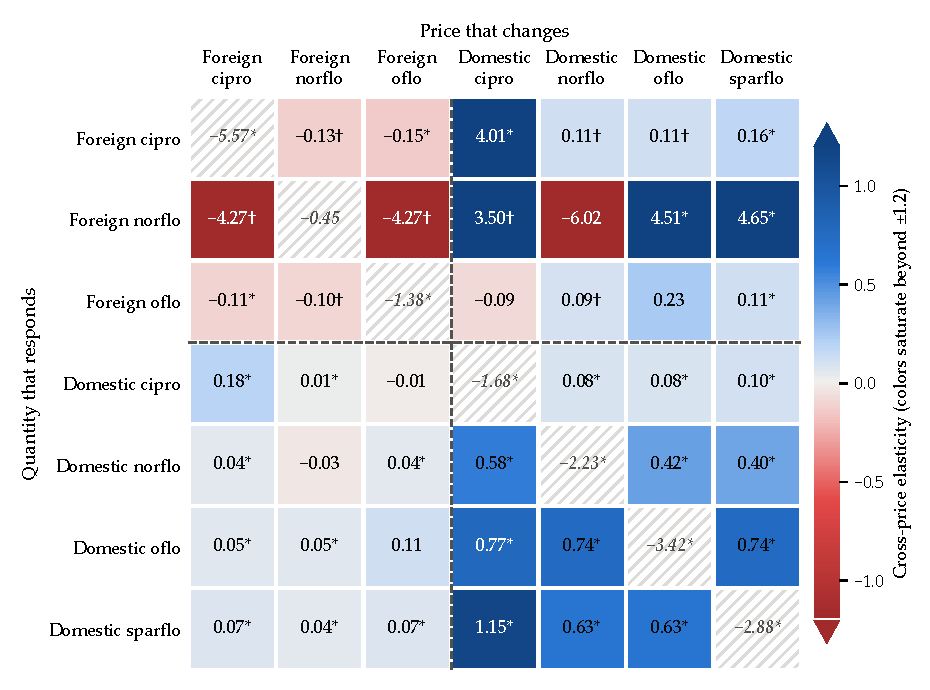
\includegraphics[width=\textwidth]{figures/ch05/cgj_table6a_heatmap.pdf}
\caption[Cross-price elasticities among quinolone groups]{Unconditional price elasticities among the seven
quinolone groups in the Northern region. Rows respond to the price in the column. Colors encode cross elasticities
(blue positive, red negative) and saturate beyond $\pm 1.2$. The hatched diagonal shows own-price elasticities, which
are excluded from the color scale. Marks: $^{*}$ significant at 5 percent, $^{\dagger}$ at 10 percent. Source:
constructed from Chaudhuri, Goldberg and Jia (2006), Table 6A.}
\label{fig:05-cgj-heatmap}
\end{figure}

\casehead{Ease of access} Why would a patient who loses domestic norfloxacin switch to domestic ofloxacin rather
than to foreign norfloxacin? The pattern is not built in by the specification, since the pair-type coefficients are
free in sign and size. CGJ propose an explanation based on distribution, which they call \emph{ease of access}
(pp.~27--28). Domestic firms as a group reach far more retail pharmacists than multinational subsidiaries. Large
Indian firms spread the fixed cost of medical representatives over larger portfolios, and there are simply many more
domestic firms and products. A local pharmacist is therefore more likely to stock two domestic molecules than the
domestic and foreign versions of one molecule. Patients or doctors who would rather switch molecules than search
another pharmacy then produce, in aggregate data, the substitution pattern of \cref{tab:05-cgj-table6a}. Together with
the domestic price premium of \cref{tab:05-cgj-table2}, the evidence shows no premium for multinational brands.

\casehead{The segment elasticity} The upper level (CGJ, Table~A3) gives a price elasticity of the quinolone segment
of $-1.11$, with standard error 0.24. Demand for the segment is elastic, but less so than demand for any single group
within it, except the tiny foreign norfloxacin group, whose insignificant own elasticity is $-0.45$. The number can be checked from the quinolone row of Table~A3, where $\gamma_{QQ} = -0.02$ and $\beta_Q =
0.04$. With the Northern quinolone share of antibiotic spending, $w_Q = \frac{31.25}{119.88} = 0.26$
(\cref{tab:05-cgj-table3}), the Stone-index formula gives
\begin{equation*}
\varepsilon_Q = -1 + \frac{\gamma_{QQ}}{w_Q} - \beta_Q = -1 - \frac{0.02}{0.26} - 0.04 = -1.12 .
\end{equation*}
This matches the reported value up to the rounding of $\gamma_{QQ}$ to two decimals.

\casehead{Robustness} CGJ report two alternative specifications (pp.~28--29). Adding group-specific seasonal effects
for summer, monsoon and winter leaves the elasticities nearly unchanged (Table~A4). Estimating the system by least
squares (Table~A5) gives smaller own elasticities in absolute value, as \eqref{eq:05-meas-bias} predicts.
\Cref{tab:05-cgj-robust} compares the own elasticities. The least-squares own elasticity of foreign ciprofloxacin is
$-2.76$, half the instrumented $-5.57$. Smaller elasticities would imply larger markups and larger welfare losses, so
instrumenting makes the welfare estimates more conservative. The least-squares cross elasticities among domestic
groups remain positive and significant. In the rows of domestic norfloxacin, ofloxacin and sparfloxacin they are
large (between 0.39 and 1.25), and they mostly exceed the same-molecule cross elasticities. CGJ call the close substitutability of domestic products ``one of the most robust findings of the
paper.''

\begin{table}[htbp]
\centering
\caption{Own-price elasticities under alternative specifications, Northern region}\label{tab:05-cgj-robust}
\small
\begin{tabular}{lccccc}
\toprule
 & Preferred (IV) & Least squares & \multicolumn{3}{c}{IV with seasonal effects} \\
\cmidrule(lr){4-6}
Product group & Table 6A & Table A5 & Summer & Monsoon & Winter \\
\midrule
Foreign cipro & $-5.57^{*}$ & $-2.76^{*}$ & $-6.06^{*}$ & $-5.80^{*}$ & $-5.66^{*}$ \\
Foreign norflo & $-0.45$ & 1.24 & 0.12 & $-0.35$ & $-0.20$ \\
Foreign oflo & $-1.38^{*}$ & $-0.99^{*}$ & $-1.58^{*}$ & $-1.51^{*}$ & $-1.55^{*}$ \\
Domestic cipro & $-1.68^{*}$ & $-1.56^{*}$ & $-1.72^{*}$ & $-1.72^{*}$ & $-1.73^{*}$ \\
Domestic norflo & $-2.23^{*}$ & $-2.18^{*}$ & $-2.04^{*}$ & $-2.10^{*}$ & $-2.22^{*}$ \\
Domestic oflo & $-3.42^{*}$ & $-3.16^{*}$ & $-3.67^{*}$ & $-3.20^{*}$ & $-3.08^{*}$ \\
Domestic sparflo & $-2.88^{*}$ & $-2.76^{*}$ & $-2.81^{*}$ & $-2.82^{*}$ & $-2.56^{*}$ \\
\bottomrule
\end{tabular}
\par\smallskip
\begin{minipage}{0.85\textwidth}\footnotesize
Notes: Compiled from CGJ, Tables~6A, A4(a) to A4(c), and A5. Standard errors omitted. $^{*}$ significant at 5 percent.
\end{minipage}
\end{table}

\begin{example}[Reproducing Tables 6A and 7 from Tables A2 and 3]\label{ex:05-cgj-elasticity-check}
The published coefficients, the published shares and the formulas of \cref{sec:05-cgj-demand} nearly reproduce the
published elasticities. We compute Northern revenue shares from the Northern sales in \cref{tab:05-cgj-table3}. Total
Northern quinolone sales of the seven groups are Rs.~1,563.56 million, so for example $w_7 = \frac{156.17}{1563.56} =
0.0999$ for domestic sparfloxacin.

\emph{Expenditure elasticities.} The elasticity with respect to quinolone spending is $\eta_i^Q = 1 +
\frac{\beta_i}{w_i}$. For domestic sparfloxacin,
\begin{equation*}
\eta_7^Q = 1 + \frac{-0.072}{0.0999} = 0.28,
\end{equation*}
exactly the value in Table~6A. \Cref{tab:05-cgj-checks} shows that the formula reproduces all seven entries of the
last column within 0.02.

\emph{Own-price elasticities.} The term $\beta_j\ln\frac{X_Q}{P_Q}$ in \eqref{eq:05-cgj-uncond-closed} depends on
$\alpha_0$ and on the units of prices, and CGJ do not report it. Setting it to zero gives our approximation. For
domestic sparfloxacin the conditional part is
\begin{equation*}
\varepsilon_{77}\big|_{X_Q} \approx -1 + \frac{\gamma_{77} - \beta_7w_7}{w_7}
= -1 + \frac{-0.186 + 0.072 \times 0.0999}{0.0999} = -2.79 .
\end{equation*}
The unconditional term adds $\eta_7^Q(1 + \varepsilon_Q)w_7 = 0.28 \times (-0.11) \times 0.0999 = -0.003$. The
approximation, $-2.79$, is close to the published $-2.88$. Across the 42 entries of Table~6A outside the foreign
norfloxacin row, the approximation has a root mean squared error of 0.036 and a largest error of about 0.15.
Choosing the omitted term to fit the table best lowers the root mean squared error only to 0.024. Most of the
remaining gap probably reflects the rounding of the published coefficients to three decimals.

\emph{Foreign norfloxacin.} Here the approximation fails. With $\gamma_{22} = 0.000$ and $w_2 = 0.0008$, it gives an
own elasticity of $-1.00$ against the published $-0.45$. Every coefficient in this row is divided by a share of 0.08
percent, which magnifies rounding and sampling error about 1,250 times. This is why the foreign norfloxacin row is so
imprecise in \cref{tab:05-cgj-table6a}.

\emph{Markups.} \Cref{sec:05-cgj-supply} shows that CGJ's upper bound on the Lerner index is $-\frac{1}{\varepsilon_{ii}}$.
The simple average of this ratio across the four regional own elasticities of Tables~6A and 6B reproduces every
markup in Table~7 to two decimals. For domestic oflo, for instance, the regional own elasticities $-3.42$, $-2.95$,
$-2.57$ and $-2.96$ give an average Lerner index of 0.34, the value in Table~7. The Northern ratio alone, 0.29, would
miss it.
\end{example}

\begin{table}[htbp]
\centering
\caption{Consistency checks: elasticities and markups recomputed from the published coefficients}\label{tab:05-cgj-checks}
\footnotesize
\setlength{\tabcolsep}{5pt}
\begin{tabular}{lccccccc}
\toprule
 & & \multicolumn{2}{c}{Expenditure elasticity} & \multicolumn{2}{c}{Own-price elasticity} & \multicolumn{2}{c}{Lerner index bound} \\
\cmidrule(lr){3-4}\cmidrule(lr){5-6}\cmidrule(lr){7-8}
Product group & \makecell{$w_i$\\ (North)} & $1 + \frac{\beta_i}{w_i}$ & Table 6A & Approx. & Table 6A &
\makecell{Mean of\\ $-\frac{1}{\varepsilon_{ii}}$} & Table 7 \\
\midrule
Foreign cipro & 0.0267 & 1.37 & 1.37 & $-5.50$ & $-5.57$ & 0.19 & 0.19 \\
Foreign norflo & 0.0008 & 2.22 & 2.20 & $-1.00$ & $-0.45$ & n.a. & n.a. \\
Foreign oflo & 0.0348 & 1.14 & 1.16 & $-1.38$ & $-1.38$ & 0.70 & 0.70 \\
Domestic cipro & 0.6154 & 1.17 & 1.17 & $-1.67$ & $-1.68$ & 0.59 & 0.59 \\
Domestic norflo & 0.1423 & 0.73 & 0.73 & $-2.22$ & $-2.23$ & 0.43 & 0.43 \\
Domestic oflo & 0.0800 & 0.90 & 0.89 & $-3.39$ & $-3.42$ & 0.34 & 0.34 \\
Domestic sparflo & 0.0999 & 0.28 & 0.28 & $-2.79$ & $-2.88$ & 0.37 & 0.37 \\
\bottomrule
\end{tabular}
\par\smallskip
\begin{minipage}{0.95\textwidth}\footnotesize
Notes: Our computations from CGJ's Tables~3, A2, 6A, 6B and 7. Shares are Northern sales shares among the seven
groups. ``Approx.''\ is \eqref{eq:05-cgj-uncond-closed} with $\ln\frac{X_Q}{P_Q}$ set to zero and $\varepsilon_Q =
-1.11$. The Lerner bound is the simple average across the four regions of minus the inverse own elasticity. For
foreign norfloxacin the own elasticity is below one in absolute value in every region, so no bound exists.
\end{minipage}
\end{table}

\subsection{Supply: bounds on costs and markups}\label{sec:05-cgj-supply}

The counterfactual needs marginal costs, which are not observed. The standard approach of \cref{ch:diffprod} infers
them from the first-order conditions of an assumed pricing game (\cref{sec:05-welfare-supply}). CGJ argue that price
regulation makes unconstrained period-by-period profit maximization untenable here, and the regulation is too complex
to model. They bound costs instead, using the argument of \cref{prop:05-cost-bounds}.

The bounds are those of \eqref{eq:05-cost-bounds} (CGJ, eqs.~3.12 and 3.13). Perfect competition within a group gives
the upper bound $c_i^U = p_i$ and a zero markup. Perfect collusion among the firms of group $i$, with price controls
ignored, gives the monopoly condition for the group as a whole. It yields the lower bound $c_i^L =
p_i\bigl(1 + \frac{1}{\varepsilon_{ii}}\bigr)$ and the upper bound $-\frac{1}{\varepsilon_{ii}}$ on the Lerner
index, where $\varepsilon_{ii}$ is the unconditional own-price elasticity. Collusion within the group overstates
market power, because it assumes away competition among the dozens of firms that sell each molecule (fn.~19).
Regulation pushes prices further below the monopoly level. Both forces keep the price at or below the group monopoly
price, as \cref{ass:05-conduct-order} requires, so $c_i^L$ is a lower bound. The bound requires $\varepsilon_{ii} < -1$. CGJ compute $c_i^L$ region by
region and report national averages.

\Cref{tab:05-cgj-table7} reproduces the bounds. The upper bound on profit is the upper-bound markup times revenue,
since $(p_i - c_i^L)q_i = \frac{p_i - c_i^L}{p_i}\,p_iq_i$. Annual sales of domestic ciprofloxacin, summed over the
regions of \cref{tab:05-cgj-table3}, are Rs.~2,931 million. Multiplying by a Lerner index of 0.586 gives about
Rs.~1,717 million, against Rs.~1,701.9 million in the table. The small gap reflects CGJ's population weights.

\begin{table}[htbp]
\centering
\caption{Bounds on marginal cost, markup and annual profit by product group}\label{tab:05-cgj-table7}
\small
\setlength{\tabcolsep}{4pt}
\begin{tabular}{lcccc}
\toprule
 & \multicolumn{3}{c}{Collusive bound} & Competitive bound \\
\cmidrule(lr){2-4}\cmidrule(lr){5-5}
 & \makecell{Lower bound for\\ marginal cost (Rs.)} & \makecell{Upper bound for\\ markup (\%)} &
 \makecell{Upper bound for\\ profit (Rs.\ million)} & \makecell{Upper bound for\\ marginal cost (Rs.)} \\
\midrule
Foreign cipro & $8.3^{*}$ & 19 & 26.9 & 10.3 \\
 & (1.23) & (0.12) & (16.55) & \\
Foreign norflo & n.a. & n.a. & n.a. & 5.3 \\
Foreign oflo & 32.3 & $70^{*}$ & $106.1^{*}$ & 108.5 \\
 & (23.16) & (0.21) & (31.85) & \\
Domestic cipro & $4.7^{*}$ & $59^{*}$ & $1{,}701.9^{*}$ & 11.2 \\
 & (1.14) & (0.10) & (298.58) & \\
Domestic norflo & $5.2^{*}$ & $43^{*}$ & $280.7^{*}$ & 9.0 \\
 & (0.20) & (0.02) & (15.32) & \\
Domestic oflo & $58.7^{*}$ & $34^{*}$ & $161.2^{*}$ & 90.1 \\
 & (2.18) & (0.02) & (12.80) & \\
Domestic sparflo & $49.5^{*}$ & $37^{*}$ & $198.5^{*}$ & 78.8 \\
 & (1.57) & (0.02) & (11.00) & \\
\bottomrule
\end{tabular}
\par\smallskip
\begin{minipage}{0.95\textwidth}\footnotesize
Notes: Reproduced from CGJ, Table~7. National averages of regional estimates. Standard errors in parentheses, with
markup standard errors expressed as fractions. $^{*}$ significant at 5 percent. The competitive bound sets marginal
cost equal to price, so the markup and profit are zero. CGJ's column heading labels the markup column ``(Rs.)'',
although its entries are percentages. No collusive bound exists for foreign norfloxacin, whose estimated own
elasticity is below one in absolute value.
\end{minipage}
\end{table}

The markup bounds are plausible (CGJ, p.~29). Domestic ciprofloxacin combines a high price, a large share and
relatively inelastic demand. It has one of the highest markup bounds (59 percent) and earns nearly 70 percent of the
sub-segment's profits. Indeed $\frac{1701.9}{2475.3} = 0.69$, where Rs.~2,475.3 million is the sum of the profit
column. Foreign ciprofloxacin faces the stiffest domestic competition and has the lowest bound (19 percent). The four
domestic profit bounds sum to Rs.~2,342 million. This number reappears below as the domestic profit loss when all
four domestic groups are withdrawn.

CGJ stress that these numbers are bounds. They do not measure actual costs. Regulation means the unconstrained
first-order condition need not hold, and aggregation across firms makes the collusive benchmark extreme. Most of their
counterfactuals use $c^L$, because it gives the largest possible profits. That is the worst case for Indian firms and
the best case for multinationals under patents.

\subsection{Counterfactual design}\label{sec:05-cgj-counterfactual}

\casehead{Scenarios} The benchmark is the most extreme policy. Foreign firms face no price controls, and
\emph{compulsory licensing} is unavailable. Under compulsory licensing a government authorizes other firms to produce
a patented drug in exchange for a royalty to the patent holder. CGJ consider five withdrawal scenarios, each removing
one or more domestic groups (p.~22).
\begin{enumerate}
\item Only domestic ciprofloxacin, a large group.
\item Only domestic ofloxacin, a small group.
\item Domestic ciprofloxacin, ofloxacin and norfloxacin.
\item Domestic ciprofloxacin, ofloxacin and sparfloxacin.
\item All four domestic groups.
\end{enumerate}
The remaining firms keep their product sets. The scenarios are illustrative. Most of the quinolone patents had expired
by the time of writing (norfloxacin's U.S.\ patent already in 1998), so none of the scenarios would materialize
(fn.~26). They show how the presence and extent of domestic competition affect the welfare calculation, which may
matter for therapeutic classes whose patents have not expired.

\casehead{The equilibrium system} Let $\mathcal{W}$ be the set of withdrawn groups. For each withdrawn group $i \in
\mathcal{W}$, the virtual price $p_{ir}^V$ sets its share to zero (CGJ, eq.~3.14):
\begin{equation}\label{eq:05-cgj-virtual}
\begin{split}
0 = {}& \alpha_{ir} + \gamma_{ii}\ln p_{ir}^V + \gamma_{i,10}\sum_{j\in D_i^{10}}\ln p'_{jr}
+ \gamma_{i,01}\sum_{j\in D_i^{01}}\ln p'_{jr} \\
&+ \gamma_{i,00}\sum_{j\in D_i^{00}}\ln p'_{jr} + \beta_i\ln\frac{X'_{Qr}}{P'_{Qr}}.
\end{split}
\end{equation}
Here $\alpha_{ir}$ now includes the common intercept, and $p'_{jr}$ is the new price of group $j$. A withdrawn group
$j$ enters the sums at its own virtual price. For each remaining group $k \notin \mathcal{W}$, the price solves the
group's monopoly first-order condition (CGJ, eq.~3.15):
\begin{equation}\label{eq:05-cgj-foc}
p'_{kr} = c_{kr}\left(1 + \frac{1}{\varepsilon_{kk}(p'_{r}, p^V_{r})}\right)^{-1}.
\end{equation}
The marginal cost $c_{kr}$ is set to $c^L_{kr}$ or $c^U_{kr}$. CGJ describe $\varepsilon_{kk}$ as the unconditional
own elasticity, a function of the new prices and the virtual prices (p.~23). The demand that a remaining group faces
also lets the virtual prices respond to its price. Its elasticity is therefore the rationed elasticity
\eqref{eq:05-rationed-elast-multi}. It combines the elasticities of \eqref{eq:05-cgj-uncond-closed} with the
unconditional share derivatives of the withdrawn groups, all at the virtual prices. CGJ do not say whether their $\varepsilon_{kk}$ includes this response. If it is the unrestricted
elasticity \eqref{eq:05-cgj-uncond-closed} evaluated at the virtual prices, \eqref{eq:05-cgj-foc} prices each group
against a demand curve that it does not face. The simulated prices are then an approximation. Quinolone spending $X'_{Qr}$ and the index $P'_{Qr}$ come from the upper level. The index
$P'_{Qr}$ is the translog of \eqref{eq:05-cgj-translog} at the new prices, and $X'_{Qr}$ follows from the upper-level
share at the new index, with the other sub-segments' price indices held fixed. The system is solved region by region.
National figures are population-weighted averages of the regional ones.

Equation~\eqref{eq:05-cgj-virtual} is the Marshallian zero-share condition at counterfactual spending, discussed in
\cref{sec:05-welfare-virtual}. Each withdrawn group's equation is quadratic in its log virtual price, because the
index $P'_{Qr}$ contains $\frac{1}{2}\gamma_{ii}(\ln p_{ir}^V)^2$ (\eqref{eq:05-virtual-quadratic}). With several
groups withdrawn the conditions must hold jointly. CGJ do not describe their solver. The block iteration of
\cref{sec:05-counterfactual}, which alternates between the virtual prices, the two budgeting levels and the pricing
conditions \eqref{eq:05-cgj-foc}, is one natural scheme. Foreign norfloxacin has no cost bound, so CGJ fix its counterfactual price at chosen values
and report that the results are robust to them (notes to Table~9).

\casehead{Welfare} Let $p^0$ be the observed price vector, $p'$ the counterfactual vector (virtual prices for the
withdrawn groups, new prices for the others), and $u^0$ the representative consumer's initial utility. Let $e(p, u)$
be the expenditure function of the upper-level AIDS, in which the lower level enters through the quinolone index
$P_Q$. CGJ measure the loss by
\begin{equation}\label{eq:05-cgj-cv}
CV^M = e(p', u^0) - e(p^0, u^0)
\end{equation}
(CGJ, eq.~3.16). It is positive for a loss. The virtual prices in $p'$ solve the Marshallian condition
\eqref{eq:05-cgj-virtual}, so they set Hicksian demand to zero at the counterfactual utility. As
\cref{sec:05-counterfactual} explains, \eqref{eq:05-cgj-cv} is therefore an approximation to the exact compensating
variation \eqref{eq:05-cv-exact}, which uses compensated virtual prices at $u^0$. The numbers below are CGJ's, computed
with \eqref{eq:05-cgj-cv}. CGJ split the loss into three parts with two intermediate price vectors. The
vector $p^1$ sets virtual prices for the withdrawn groups while holding $X_Q$ and all other prices fixed. The vector
$p^2$ recomputes the virtual prices letting $X_Q$ respond to the new quinolone index, again with all other prices
fixed. Then
\begin{equation}\label{eq:05-cgj-decomp}
CV^M = \underbrace{e(p^1, u^0) - e(p^0, u^0)}_{\text{pure loss of variety}}
+ \underbrace{e(p^2, u^0) - e(p^1, u^0)}_{\text{expenditure switching}}
+ \underbrace{e(p', u^0) - e(p^2, u^0)}_{\text{reduced competition}} .
\end{equation}
This is the general decomposition of \cref{sec:05-counterfactual} applied to CGJ's two levels. The first term is the
loss from the disappearance of products with everything else held fixed. It would be zero if consumers treated the
domestic and foreign versions of a molecule as identical, as earlier simulation studies assumed. The second term is
what CGJ call expenditure switching. It records how the Marshallian virtual prices shift when quinolone spending
responds to the higher index. The vector $p^2$ is the closest match to patents combined
with strict price regulation that holds the remaining prices at their pre-patent levels. The third term adds the price
increases of the remaining groups.

\casehead{Profits and national welfare} Profits are $\pi_k = (p'_k - c_k)q'_k$ at the counterfactual prices and
quantities. CGJ define Indian welfare as consumer welfare plus the profits of domestic firms. Foreign profits are
excluded, but CGJ compute them separately as a gauge of the incentive that Indian patents would give multinationals.
Losses are reported as positive numbers, so a negative domestic profit loss is a gain (fn.~38). With $c^L$, pre-patent
profits are at their largest, so the computed domestic profit loss is an upper bound.

\begin{remark}[The competitive cost bound in the simulation]\label{rem:05-cgj-cU}
The two cost bounds play different roles in \eqref{eq:05-cgj-foc}. With $c^L_{k} = p^0_k(1 + \frac{1}{\varepsilon_{kk}})$,
the observed prices satisfy \eqref{eq:05-cgj-foc} before any withdrawal, so simulated price changes are caused by the
withdrawal alone. With $c^U_k = p^0_k$ they do not. Before any withdrawal, \eqref{eq:05-cgj-foc} would already set
$p'_k = p^0_k\frac{\varepsilon_{kk}}{1 + \varepsilon_{kk}} > p^0_k$ whenever $\varepsilon_{kk} < -1$. The $c^U$
simulations therefore combine zero markups before the policy with group monopoly pricing after it. This reading may
explain why CGJ's Table~A6, which uses $c^U$, gives a much larger loss than Table~8 when only domestic ofloxacin is
withdrawn (Rs.~4.08 billion against 0.23). CGJ describe the $c^U$ losses as ``slightly higher'' and of the same order
of magnitude for the larger scenarios.
\end{remark}

\subsection{Counterfactual results}\label{sec:05-cgj-results}

\casehead{Consumer welfare} \Cref{tab:05-cgj-table8} reproduces CGJ's Table~8. All numbers in this subsection use
the cost lower bound $c^L$. The columns are cumulative. The first column holds $X_Q$ and the remaining prices fixed,
the second adds expenditure switching, and the third adds the price response of the remaining groups.

\begin{table}[htbp]
\centering
\caption{Consumer welfare losses from product withdrawal (Rs.\ billion per year)}\label{tab:05-cgj-table8}
\small
\begin{tabular}{lccc}
\toprule
 & & \multicolumn{2}{c}{Loss of variety and} \\
\cmidrule(lr){3-4}
\makecell[l]{Domestic groups\\ withdrawn} & \makecell{Pure loss\\ of variety} & \makecell{expenditure\\ switching} & \makecell{price adjustment and\\ expenditure switching} \\
\midrule
Only cipro & $4.98^{*}$ & $4.92^{*}$ & $7.32^{*}$ \\
 & (0.87) & (0.89) & (1.46) \\
Only oflo & 0.08 & 0.08 & $0.23^{*}$ \\
 & (0.08) & (0.08) & (0.10) \\
Cipro, oflo, norflo & $7.52^{*}$ & $7.40^{*}$ & $12.53^{*}$ \\
 & (1.77) & (1.80) & (4.15) \\
Cipro, oflo, sparflo & $6.14^{*}$ & $6.03^{*}$ & $10.58^{*}$ \\
 & (1.42) & (1.45) & (3.31) \\
All four & $11.76^{\dagger}$ & $11.35^{\dagger}$ & 17.81 \\
 & (6.43) & (6.34) & (12.70) \\
\bottomrule
\end{tabular}
\par\smallskip
\begin{minipage}{0.92\textwidth}\footnotesize
Notes: Reproduced from CGJ, Table~8 (identical to the published table). CGJ's welfare measure \eqref{eq:05-cgj-cv}, computed with the
cost lower bound. Standard errors in parentheses. $^{*}$ significant at 5 percent, $^{\dagger}$ at 10 percent. The
published table adds that the exchange rate is 45 rupees per U.S.\ dollar and that total sales of systemic
antibacterials in 2000 were Rs.~27 billion.
\end{minipage}
\end{table}

\Cref{fig:05-cgj-decomposition} splits each total into its three parts. In the all-four scenario the total loss is
Rs.~17.81 billion (CGJ, p.~31). The variety loss contributes Rs.~11.76 billion, or 66 percent of the total.
Expenditure switching reduces the loss by Rs.~0.41 billion ($-2$ percent). Price increases add a further Rs.~6.46
billion (36 percent). The shares are similar across scenarios. The variety loss accounts for 58 to 68 percent in every
scenario except the removal of ofloxacin alone, where the total is small.

\begin{figure}[htbp]
\centering
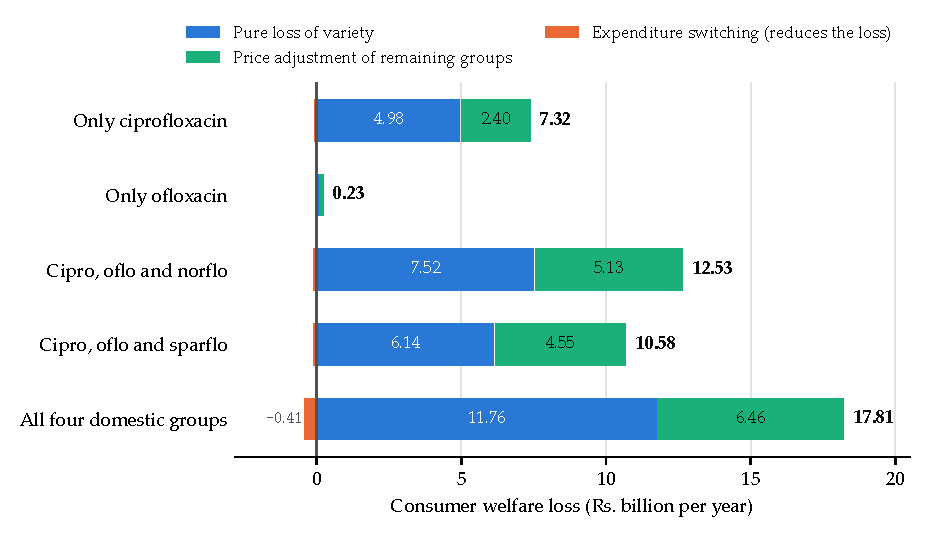
\includegraphics[width=\textwidth]{figures/ch05/cgj_welfare_decomposition.pdf}
\caption[Decomposition of the consumer welfare loss]{Decomposition of the consumer welfare loss in each withdrawal
scenario. Blue: pure loss of variety (Table 8, first column). Orange, left of zero: expenditure switching (second
column minus first). Green: price adjustment of the remaining groups (third column minus second). The bold number is
the total loss, equal to the blue and green segments minus the orange one. Standard errors are in
\cref{tab:05-cgj-table8}. Source: constructed from Chaudhuri, Goldberg and
Jia (2006), Table 8.}
\label{fig:05-cgj-decomposition}
\end{figure}

Three results matter for policy. First, expenditure switching is small in every scenario, although the segment
elasticity is $-1.11$. The reason is the factor $1 + \varepsilon_Q = -0.11$ derived above: a higher quinolone index
moves little spending out of the segment. Switching lowers the loss in four scenarios and leaves it unchanged when
only ofloxacin is withdrawn. CGJ read the term as consumers escaping to other sub-segments. Formally, the
upper-level expenditure function already lets consumers reallocate spending across sub-segments. The term arises
because the Marshallian zero-share condition \eqref{eq:05-cgj-virtual} moves the virtual prices when $X_Q$ falls
(\cref{sec:05-counterfactual}). The higher quinolone index lowers $X_Q$ slightly. That lowers the virtual price of a
withdrawn group with $\beta_i > 0$, such as domestic ciprofloxacin, and raises it for groups with $\beta_i < 0$. The
sign of the term is therefore not fixed by theory. For the claim of TRIPS proponents to hold, CGJ conclude, unpatented substitutes must exist
within narrowly defined therapeutic categories. Substitution across broad segments does little.

Second, the loss of variety is large. It arises only because consumers distinguish domestic from foreign versions of
the same molecule. CGJ interpret it as the ease-of-access effect. Price regulation cannot remove it, since regulation
acts on the third term. This suggests an independent role for compulsory licensing, which keeps domestic versions on
the market, either alongside price regulation or in its place.

Third, the losses are superadditive. Withdrawing all four domestic groups costs Rs.~17.81 billion. Withdrawing one
group at a time costs 7.32 (ciprofloxacin), 0.23 (ofloxacin), about 0.1 (norfloxacin) and close to zero (sparfloxacin),
for a sum of about Rs.~7.6 billion (fn.~37). The joint loss is more than twice the sum of the separate losses. The
three-group rows show the mechanism in our arithmetic. Adding sparfloxacin to the ciprofloxacin, ofloxacin and
norfloxacin withdrawal raises the loss from 12.53 to 17.81, by Rs.~5.28 billion. Adding norfloxacin to the other
triple raises it from 10.58 to 17.81, by Rs.~7.23 billion. Yet each costs at most Rs.~0.1 billion alone. When one
domestic group exits, consumers move to the other domestic groups, so the loss is small. When the last domestic group
exits, no close substitute remains. Studies that add up losses estimated market by market can therefore understate
the cost of patents substantially.

\casehead{Prices} \Cref{tab:05-cgj-table9} reports the counterfactual prices of the groups that remain. Shaded cells
in CGJ's table, dots here, mark withdrawn groups. Foreign norfloxacin's price is fixed by assumption.

\begin{table}[htbp]
\centering
\caption{Counterfactual prices of the remaining groups (\% of original prices)}\label{tab:05-cgj-table9}
\footnotesize
\setlength{\tabcolsep}{4pt}
\begin{tabular}{lccccccc}
\toprule
 & \multicolumn{3}{c}{Foreign groups} & \multicolumn{4}{c}{Domestic groups} \\
\cmidrule(lr){2-4}\cmidrule(lr){5-8}
Domestic groups withdrawn & Cipro & Norflo & Oflo & Cipro & Norflo & Oflo & Sparflo \\
\midrule
Only cipro & $189.4^{*}$ & 314.7 & $98.2^{*}$ & . & $148.6^{*}$ & $141.4^{*}$ & $164.1^{*}$ \\
 & (0.18) & & (0.21) & & (0.09) & (0.08) & (0.08) \\
Only oflo & $100.4^{*}$ & 150.0 & $102.9^{*}$ & $102.4^{*}$ & $108.3^{*}$ & . & $110.7^{*}$ \\
 & (0.01) & & (0.08) & (0.01) & (0.01) & & (0.01) \\
Cipro, oflo, norflo & $247.6^{*}$ & 627.8 & $154.4^{*}$ & . & . & . & $296.3^{*}$ \\
 & (0.42) & & (0.39) & & & & (0.70) \\
Cipro, oflo, sparflo & $255.2^{*}$ & 627.8 & $158.3^{*}$ & . & $250.1^{*}$ & . & . \\
 & (0.40) & & (0.37) & & (0.64) & & \\
All four & 396.4 & 627.8 & $318.4^{\dagger}$ & . & . & . & . \\
 & (3.34) & & (1.73) & & & & \\
\bottomrule
\end{tabular}
\par\smallskip
\begin{minipage}{0.95\textwidth}\footnotesize
Notes: Reproduced from CGJ, Table~9. Prices with expenditure switching and within-segment price adjustment, cost
lower bound. Dots mark withdrawn groups. Standard errors in parentheses. $^{*}$ significant at 5 percent,
$^{\dagger}$ at 10 percent. Foreign norfloxacin's price is fixed at the values shown, because its cost bound is not
available.
\end{minipage}
\end{table}

\begin{remark}[Reading Table 9]\label{rem:05-cgj-table9}
The heading of CGJ's Table~9 says the entries are percentages of original prices. Under that reading, foreign
ciprofloxacin's price would rise to 3.96 times its original level when all domestic groups exit, an increase of
about 296 percent. Two features of the table support the heading. The entries in the ofloxacin-only row are close to
100, which is what a small withdrawal should produce. The standard errors are of the order of 0.01 to 3.34, which
makes sense for ratios of new to old prices. CGJ's text reads the entries differently. It says that foreign prices
would rise ``between 100\% and 400\%'', the range of the foreign entries. It also says that the price of foreign
ciprofloxacin would be ``approximately 5 times higher than it is now'' in the all-four scenario. We report the
entries as printed and leave the ambiguity open. Under either reading, removing all domestic competition multiplies
the foreign prices several times.
\end{remark}

CGJ check plausibility against Pakistan, a country with similar demographics but a market structure close to what
patents would create in India, with multinational subsidiaries dominant. CGJ (p.~33), citing
\citet[p.~39, Table~2]{Lanjouw1998}, report that ciprofloxacin cost about seven times as much in Pakistan as in
India. CGJ's all-four prediction for foreign ciprofloxacin is of the same order of magnitude, though lower (p.~33).

The domestic groups that remain also raise their prices, by 41 to 64 percent when only ciprofloxacin is withdrawn
(reading the entries as percentages of original prices). These increases follow from the collusive conduct assumed
in \eqref{eq:05-cgj-foc}. A remaining domestic group is priced as if its 17 to 40 firms maximized joint profit, and
its demand becomes less elastic once a close domestic substitute disappears. The Le Chatelier principle of
\cref{sec:05-welfare-virtual} makes the second step precise. Let $i$ be the withdrawn group, whose virtual price
adjusts. The compensated own-price elasticity of a remaining group $j$ is then $\varepsilon^h_{jj} -
\varepsilon^h_{ji}\frac{p_jS_{ij}}{p_iS_{ii}}$ by \eqref{eq:05-le-chatelier-removed}, with all terms evaluated at the
virtual price. It is smaller in absolute value than the unrestricted compensated elasticity at that price. The
correction is largest for the closest substitutes, the other domestic quinolones. This channel is a
property of demand and holds under any conduct. Collusive conduct converts it into a large price increase. With
competitive pricing inside the group, the domestic price increases, and the third column of Table~8, would be smaller.

\casehead{Profits and total welfare} \Cref{tab:05-cgj-welfare-summary} combines CGJ's Tables~10, 11 and 12.

\begin{table}[htbp]
\centering
\caption{Domestic profit losses, total Indian welfare losses and foreign profit gains (Rs.\ billion per year)}\label{tab:05-cgj-welfare-summary}
\small
\begin{tabular}{lccc}
\toprule
 & & \multicolumn{2}{c}{Loss of variety and} \\
\cmidrule(lr){3-4}
\makecell[l]{Domestic groups\\ withdrawn} & \makecell{Pure loss\\ of variety} & \makecell{expenditure\\ switching} & \makecell{price adjustment and\\ expenditure switching} \\
\midrule
\multicolumn{4}{l}{\emph{Panel A. Foregone profits of domestic producers (Table 10)}} \\
Only cipro & $0.95^{*}$ (0.16) & $1.09^{*}$ (0.08) & 0.40 (0.31) \\
Only oflo & $-0.04^{*}$ (0.01) & $-0.03^{\dagger}$ (0.02) & $-0.14^{*}$ (0.04) \\
Cipro, oflo, norflo & $1.24^{*}$ (0.17) & $1.40^{*}$ (0.11) & 0.42 (0.60) \\
Cipro, oflo, sparflo & $1.11^{*}$ (0.17) & $1.26^{*}$ (0.11) & 0.48 (0.50) \\
All four & $2.34^{*}$ (0.19) & $2.34^{*}$ (0.19) & $2.34^{*}$ (0.19) \\
\addlinespace
\multicolumn{4}{l}{\emph{Panel B. Total welfare losses to India (Table 11)}} \\
Only cipro & $5.94^{*}$ (0.94) & $6.01^{*}$ (0.87) & $7.72^{*}$ (1.20) \\
Only oflo & 0.04 (0.08) & 0.05 (0.09) & 0.09 (0.10) \\
Cipro, oflo, norflo & $8.76^{*}$ (1.84) & $8.80^{*}$ (1.77) & $12.95^{*}$ (3.61) \\
Cipro, oflo, sparflo & $7.25^{*}$ (1.46) & $7.28^{*}$ (1.42) & $11.07^{*}$ (2.88) \\
All four & $14.10^{*}$ (6.57) & $13.70^{*}$ (6.48) & 20.16 (12.85) \\
\addlinespace
\multicolumn{4}{l}{\emph{Panel C. Profit gains of foreign producers (Table 12)}} \\
Only cipro & $0.17^{*}$ (0.03) & $0.14^{*}$ (0.06) & $0.35^{*}$ (0.17) \\
Only oflo & 0.02 (0.01) & 0.02 (0.01) & 0.01 (0.02) \\
Cipro, oflo, norflo & $0.36^{*}$ (0.05) & $0.28^{*}$ (0.11) & $0.71^{\dagger}$ (0.40) \\
Cipro, oflo, sparflo & $0.37^{*}$ (0.05) & $0.30^{*}$ (0.10) & $0.79^{*}$ (0.38) \\
All four & $1.17^{*}$ (0.31) & $0.88^{*}$ (0.41) & $2.43^{\dagger}$ (1.44) \\
\bottomrule
\end{tabular}
\par\smallskip
\begin{minipage}{0.95\textwidth}\footnotesize
Notes: Reproduced from CGJ, Tables~10, 11 and 12. Cost lower bound. Standard errors in parentheses. $^{*}$
significant at 5 percent, $^{\dagger}$ at 10 percent. Losses are positive numbers, so a negative entry in Panel A is a
gain for domestic firms as a group. Panel B equals Table~8 plus Panel A, up to rounding.
\end{minipage}
\end{table}

Domestic profits fall by Rs.~2.34 billion when all four groups exit, in every column. This is the whole pre-patent
profit of the domestic groups, the sum of the domestic profit bounds in \cref{tab:05-cgj-table7}. In the partial
scenarios, the remaining domestic firms gain from reduced competition, and these gains offset part of the losses.
When only ofloxacin is withdrawn, the domestic sector as a whole gains, because consumers switch to other domestic
molecules. This may explain why the Indian industry was divided over TRIPS. The association of leading Indian firms
and multinational subsidiaries supported stronger patents, while associations of smaller firms were more skeptical
(fn.~39).
In every scenario, consumer losses dwarf domestic profit losses.

Panel B is consumer loss plus domestic profit loss. The identity can be checked row by row. For the all-four scenario,
\begin{equation*}
13.70 \approx 11.35 + 2.34 \qquad\text{and}\qquad 20.16 \approx 17.81 + 2.34,
\end{equation*}
with the differences due to rounding. The columns of Panel A also show how expenditure switching and price responses
redistribute profits. When only ciprofloxacin is withdrawn, switching raises the domestic loss from 0.95 to 1.09,
because the remaining domestic groups sell less as quinolone spending falls. Price adjustment then cuts the loss to
0.40, because the remaining domestic groups raise their prices.

\casehead{The headline numbers} With the exchange rate of 45 rupees per dollar, CGJ's summary numbers follow from
Tables 8 to 12 (pp.~34--35).
\begin{itemize}
\item Without price regulation or compulsory licensing, the total welfare loss to India from withdrawing all four
domestic groups is Rs.~20.16 billion per year, about US\$450 million.
\item With regulation holding prices at pre-patent levels, the loss is Rs.~13.7 billion, about US\$305 million. This
is about 50 percent of the 2000 sales of all systemic antibacterials ($\frac{13.7}{27} = 0.51$). Foregone domestic
profits are about Rs.~2.3 billion (US\$50 million), roughly one-sixth of the total.
\item If the variety loss is transitional, or licensing could neutralize it, subtracting it leaves a lower bound of
Rs.~6.5 billion ($20.16 - 13.7$), about US\$144 million per year. The subtraction removes the variety loss (11.76),
the switching term ($-0.41$) and the domestic profit loss (2.34). The remainder equals the price-adjustment term of
\cref{tab:05-cgj-table8}, $17.81 - 11.35 = 6.46$. This is about 30 percent of the upper bound and about
24 percent of antibiotic sales in 2000.
\item Foreign profit gains are only Rs.~2.4 billion (US\$53 million) without regulation and Rs.~0.88 billion
(US\$19.6 million) with it.
\end{itemize}
CGJ put the foreign gains in perspective with the sales of Bayer's Cipro, about US\$1.6 billion in 2000. At a
markup of 40 percent, often quoted for the industry, that is about US\$640 million of annual profit from one product.
The gain from Indian patents on the whole quinolone segment would be a small fraction of this. Indian patents on
these drugs would hardly change multinationals' incentives to do research on the diseases of poor countries.

The welfare numbers are large relative to the market. Total quinolone sales in 2000 were near Rs.~5.7 billion, by
our computation from \cref{tab:05-cgj-table1}. The all-four consumer loss is about three times this amount
($\frac{17.81}{5.7} \approx 3.1$), and the variety loss alone about twice ($\frac{11.76}{5.7} \approx 2.1$).
Such numbers are possible because the compensating variation is an area under the Hicksian demand curve
up to the virtual price, far above observed prices. That area depends on the curvature of AIDS demand outside the
range of the data (\cref{sec:05-welfare-virtual}). The standard error of the all-four total loss, Rs.~12.70 billion,
reflects this uncertainty.

\casehead{The upper cost bound} Table~A6 repeats the consumer welfare calculation with $c^U$. The first two columns
are unchanged in point estimate, because they do not involve costs. The full loss in the all-four scenario is Rs.~19.46
billion, against 17.81 with $c^L$. CGJ explain that higher costs produce larger price increases. As
\cref{rem:05-cgj-cU} notes, the $c^U$ simulation also builds in price increases that would occur without any
withdrawal, which shows up clearly in the small scenarios.

\subsection{Interpretation, limitations and contribution}\label{sec:05-cgj-assessment}

CGJ draw three policy lessons. Product availability matters as much as affordability for consumer welfare, so patent
policy should be judged by both. Compulsory licensing has a role distinct from price regulation, because only the
former addresses the loss of variety. And the two policies are in tension. Patents without price controls strengthen
multinationals' incentives to build distribution networks or to license domestic firms, which would shrink the
variety loss over time. Price controls limit price increases but weaken these incentives, which could make the variety
loss permanent. No combination of policies is likely to neutralize all the welfare costs.

The study has several limitations, most of which CGJ acknowledge.
\begin{itemize}
\item \emph{Representative consumer.} The framework cannot say which households lose most. That would require micro
data on purchases, which do not exist for Indian pharmaceuticals (fn.~30). The aggregate compensating variation is
also a statement about a representative household, as discussed in \cref{sec:05-aggregation}.
\item \emph{Uniform pricing.} The model rules out price discrimination, which could change both welfare losses and
profit gains (fn.~31).
\item \emph{Static analysis.} The model has no research response, no new launches and no investment in distribution.
The product sets of the remaining firms are held fixed. If foreign firms expand distribution, alone or through joint
ventures with Indian firms, the ease-of-access loss would be transitional. CGJ report media accounts of such
initiatives.
\item \emph{Aggregation and conduct.} Groups aggregate dozens of firms, and the cost bound $c^L$ treats each group as a
cartel. This inflates pre-patent markups and the price responses of the remaining domestic groups.
\item \emph{Functional form and extrapolation.} Virtual prices lie far outside the observed price range. The welfare
loss, several times the segment's sales, depends on AIDS curvature where no data exist. Logit or CES demand would
give different answers, as \cref{prop:05-variety} shows.
\item \emph{Identification.} The SKU-count instruments fail if SKU entry responds to demand shocks or raises demand
directly. Domestic ciprofloxacin, the most important group, has the weakest first stage and little price variation
over time.
\item \emph{Restrictions.} The pair-type restriction forces one coefficient on all domestic pairs, and homogeneity then
ties the own-price coefficients to the cross coefficients (\cref{prop:05-cgj-collapse}). The ease-of-access pattern is
estimated, but its uniformity across domestic pairs is imposed.
\item \emph{Small foreign groups.} Foreign norfloxacin's estimates are unreliable, and the negative cross elasticities
among foreign groups are unexplained.
\item \emph{Revealed preference.} Doctors choose most prescriptions, and they or their patients may err or follow
promotion. If choices do not reflect informed preferences, welfare computed from them may mislead. Antibiotic use also
has external effects, such as bacterial resistance, that private demand ignores.
\end{itemize}
Several open questions follow. Did TRIPS spur research, including by Indian firms? Is Pakistan a credible benchmark
for post-patent prices in India? Which consumers rely most on domestic firms? Would ease of access persist once
multinationals expand distribution or license their molecules?

The paper made three contributions. It gave the first estimates of the welfare effects of TRIPS that rest on estimated
demand and cost parameters, where earlier studies had assumed them. It allowed consumers to distinguish domestic from
foreign versions of the same molecule, which revealed a variety channel that price-based analyses miss. And it
estimated cross-price effects flexibly, which showed that losses compound when several domestic groups disappear.
Methodologically, it shows how a multi-level AIDS, simple instruments, cost bounds and virtual prices combine into a
transparent counterfactual.

\begin{table}[htbp]
\centering
\caption{Identification and counterfactual map of Chaudhuri, Goldberg and Jia (2006)}
\label{tab:05-cgj-map}
\footnotesize
\renewcommand{\arraystretch}{1.1}
\begin{tabularx}{\textwidth}{@{}>{\raggedright\arraybackslash}p{2.6cm}>{\raggedright\arraybackslash}X@{}}
\toprule
Observed data & Monthly retail sales and prices of quinolone antibiotics in four Indian regions, 1999 and
  2000, from the ORG-MARG audit. Stock-keeping units are aggregated into seven groups by molecule and
  domestic or foreign status. Spending on all systemic antibacterials. \\
\addlinespace
Latent objects & Exact group price indexes and the error of their revenue-weighted proxies, demand shocks,
  marginal costs, and the virtual prices of withdrawn groups. \\
\addlinespace
Estimated parameters & Lower-level AIDS coefficients under pair-type restrictions, upper-level AIDS
  coefficients for eight antibacterial sub-segments, and group-region effects. \\
\addlinespace
Identifying variation & Numbers of SKUs and prices of the five largest SKUs of each group, by region and
  month (\cref{ass:05-cgj-iv}). Regulated SKU prices change rarely, so group prices move mostly with the
  SKU mix. \\
\addlinespace
Maintained assumptions & Two-stage budgeting with a representative consumer and uniform pricing. SKU entry
  is unrelated to demand shocks. Cost bounds replace a model of conduct under price regulation
  (\cref{prop:05-cost-bounds}). \\
\addlinespace
Counterfactual and what it holds fixed & Withdrawal of one or more domestic groups, with virtual prices for
  the withdrawn groups and group monopoly pricing of the others at the cost bounds. The product sets of the
  remaining firms and the prices of other sub-segments are held fixed. \\
\addlinespace
Conclusion & Withdrawing all four domestic groups costs India Rs.~20.16 billion a year, about US\$450
  million, without price regulation and Rs.~13.7 billion with it. Most of the consumer loss is lost
  variety, valued by AIDS curvature far beyond observed prices. \\
\addlinespace
One limitation & The losses, several times the segment's sales, depend on the functional form of demand
  where no data exist. \\
\addlinespace
Source and our additions & The tables are CGJ's. \Cref{prop:05-cgj-collapse}, \cref{ex:05-cgj-elasticity-check},
  \cref{rem:05-cgj-cU} and the recomputed elasticities and markups of \cref{tab:05-cgj-checks} are ours. \\
\addlinespace
Tools in the appendices & \Cref{sec:A-iv,sec:A-delta-boot,sec:B-duality}. \\
\bottomrule
\end{tabularx}
\end{table}

\section{Retrospective evidence: what happened after patents arrived}\label{sec:05-dgg}

CGJ's analysis is prospective in the sense of \cref{sec:05-questions}. It predicts the effects of a policy before the
policy exists. India introduced product patents for pharmaceuticals in 2005, and a retrospective analysis then
became possible. Such an analysis measures what happened after the policy, using variation in its timing or reach.
\citet{DugganGarthwaiteGoyal2016} (DGG henceforth) provide it. This section reports their setting, design and main
results and asks why the two answers differ.\footnote{We cite the published article in the \emph{American Economic
Review} 106(1), 2016. Page, table, equation and footnote numbers refer to it.}

\subsection{Setting and data}\label{sec:05-dgg-setting}

TRIPS required product patents in all fields of technology, with a minimum term of 20 years. India had no product
patents when TRIPS came into force in 1995, so it received a transition period of ten years (DGG, p.~105). From 1995 a
``mailbox'' collected patent applications, and the government published neither their number nor their content. The
2005 reform kept several flexibilities. A grandfather clause lets a generic firm that invested in a molecule before
2005 continue to produce it after paying a ``reasonable royalty'' to the patent holder. DGG call this a de facto
compulsory license for existing generic producers (p.~106). Section 3(d) of the amended Act limits patents on chemical
entities known before 1995 to inventions with significantly greater therapeutic efficacy (p.~107).

Compulsory licensing and price controls also remained available, but India used them sparingly. Its first compulsory
license came in March 2012. Natco was allowed to sell a generic version of Bayer's cancer drug Nexavar for a royalty of
6 percent, at about \$176 a month against Bayer's \$5,600 (p.~106). Price controls covered only 74 drugs until 2013,
when they were extended to nearly 350 (p.~106). DGG add that the mere threat of these tools may have restrained prices
(p.~101).

The timing of grants was hard to predict. The first pharmaceutical product patent, for Roche's hepatitis C drug
Pegasys, came only in 2006 (pp.~107 and 110). That was more than a year after the mailbox applications were opened for review
on 1 January 2005 (p.~107). Section 3(d) also left the patent office wide discretion (p.~107). In April 2013 the Supreme Court
upheld the denial of a patent for Novartis's cancer drug Glivec, which the office had judged an incremental change to
an older compound (fn.~5). DGG argue that this uncertainty makes the date of a grant a plausibly exogenous shock to
each molecule's market (pp.~107--108).

The sales data are quarterly retail sales from the MIDAS database of IMS Health. They come from an audit of about
5,100 stockists that covers 80 to 85 percent of the Indian market (p.~108). DGG use all single-molecule products,
which account for over half of sales (p.~109). The estimation sample runs from the second quarter of 2004 to the end
of 2011. It keeps molecules with positive sales in the first quarter of 2005 (p.~108 and fn.~8). It contains more
than 6,000 products and about 1,000 molecules (p.~101). A patent search firm matched granted Indian patents to
molecules by keyword searches. About one-third of the molecules are covered by at least one product patent by the end
of 2011. The outcomes are aggregated to the molecule-quarter level. They are the log of the average price per
standard unit, the log of quantity, the number of selling firms and the Herfindahl index of sales.

\subsection{Design}\label{sec:05-dgg-design}

The identifying variation is the timing of patent grants. Different molecules received Indian patents in different
quarters after the 2005 amendment. If the timing of a grant is unrelated to other changes in a molecule's market,
molecules that have not yet received a patent serve as controls for those that have. Let $m$ index molecules and $t$
quarters. The baseline regression is DGG's eq.~(1),
\begin{equation}\label{eq:05-dgg-dd}
Y_{mt} = \mu_m + \tau_t + \vartheta\, t\cdot\indic\{\text{ever patented}\}_m
  + \phi\,\indic\{\text{has patent}\}_{mt} + u_{mt}.
\end{equation}
Here $\mu_m$ are molecule fixed effects and $\tau_t$ year-by-quarter fixed effects. The third term gives molecules that
receive a single-molecule patent during the sample their own linear trend. The indicator
$\indic\{\text{has patent}\}_{mt}$ equals one in the quarters in which molecule $m$ is covered by at least one
single-molecule patent. DGG write $\alpha_m$, $\delta_t$, $\lambda$ and $\beta$ for the coefficients, which we rename to
avoid clashes with the AIDS parameters. The coefficient $\phi$ is a difference in differences. It compares the change
in a molecule's outcome when its patent arrives with the change over the same quarters for molecules without a patent.
Standard errors are clustered by molecule.

The event-study version is DGG's eq.~(2). Let $g_m$ be the quarter in which molecule $m$ receives its first patent and
$\bar p_{mt}$ the average price of its products. Then
\begin{equation}\label{eq:05-dgg}
\ln\bar p_{mt} = \mu_m + \tau_t + \sum_{k\neq 0}\phi_k\,\indic\{t - g_m = k\} + u_{mt}.
\end{equation}
The event-time indicators run from $k = -8$ to $k = 8$. DGG write the limits of the sum as $-8+$ and $8+$, so the
end points bin all earlier and all later quarters. The grant quarter $k = 0$ is the omitted category, and the
molecule-specific trend is dropped. Each $\phi_k$ measures the average log price $k$ quarters from the grant, relative
to the grant quarter and net of molecule and quarter effects.

Identification rests on two assumptions. Absent patents, log prices of molecules with early and late grants would
have moved in parallel. And prices do not respond before the grant. The leads $\phi_k$ for $k < 0$ test both, since
they should be near zero. DGG also probe anticipation directly. For molecules whose first application sat in the
mailbox, firms knew least about the timing of the decision. The estimate of $\phi$ for this sample is 0.025 (0.012),
against 0.027 (0.013) for the full sample (fn.~22). With staggered timing and effects that vary across molecules or
over event time, two-way fixed-effects regressions like \eqref{eq:05-dgg-dd} can weight effects in unintended ways.
Estimators robust to this problem are discussed in \cref{app:econometrics}.

\subsection{Results}\label{sec:05-dgg-results}

\Cref{fig:05-dgg} reproduces DGG's Figure~1. Before the grant, the point estimates lie close to zero, and the
confidence bands include zero in every quarter. Prices begin to rise in the first quarters after the grant. From the
third quarter on, the estimates are about 0.036 to 0.041, and the lower confidence bound lies just above zero in
quarters 3 to 7. The bound for the binned quarter 8+ includes zero.

\begin{figure}[htbp]
\centering
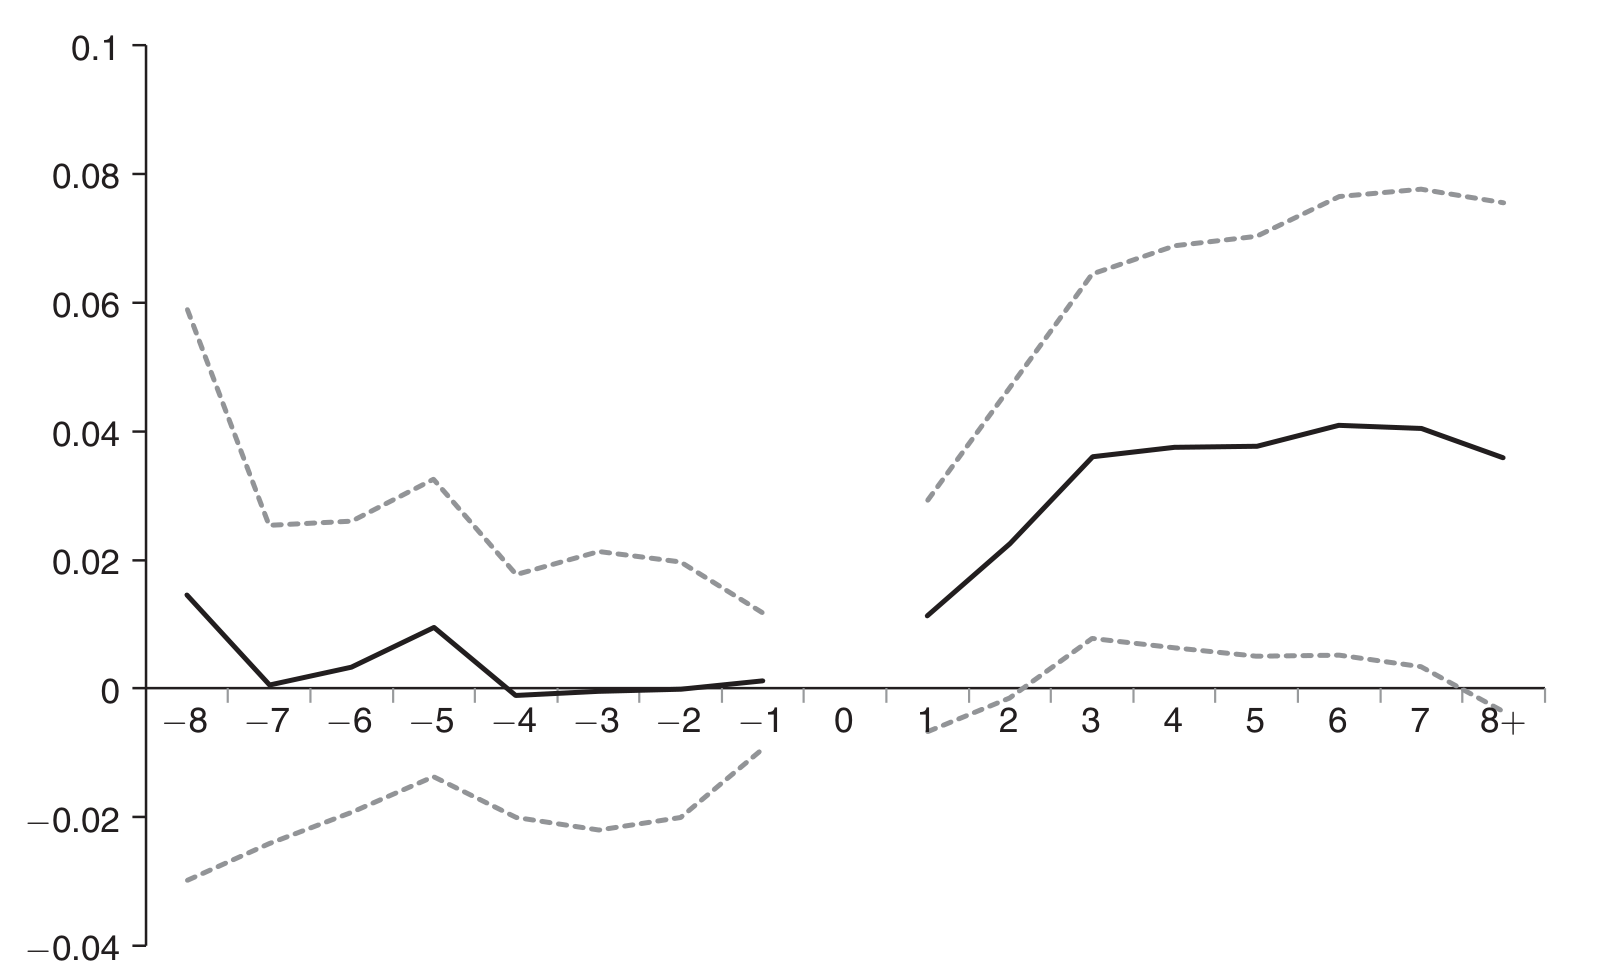
\includegraphics[width=0.85\textwidth]{figures/ch05/dgg_fig1.png}
\caption[Event-study estimates of patent effects on prices in India]{Event-study estimates for the log of the average
price before and after a patent is granted, from \eqref{eq:05-dgg}. The horizontal axis shows quarters relative to
the grant, from $-8$ to $8+$, and the end points bin all earlier and all later quarters. The solid line shows point
estimates and the dashed lines show 95 percent confidence intervals, with standard errors clustered by molecule. The
grant quarter is the omitted category. Source: Duggan, Garthwaite and Goyal (2016), Figure 1.}
\label{fig:05-dgg}
\end{figure}

\Cref{tab:05-dgg} collects the difference-in-differences estimates. In the full sample a patent raises the average
price of a molecule by 2.7 percent, and the 95 percent confidence interval rules out increases above 5.3 percent
(p.~117). Among molecules that are eventually patented, where only the timing of grants varies, the estimate falls to
0.016 and is insignificant. Patents matter more for newer molecules. Among patented molecules, those first sold in
India after 1995 see prices rise 4.9 percent more than older ones. The estimate for older molecules is $-0.014$
(0.012). In the sample of molecules approved in the United States between 1996 and 2004, patented molecules see their
prices rise by about 6 percent relative to molecules with pending applications (Table~5).

\begin{table}[htbp]
\centering
\caption{Effects of a patent grant on molecule outcomes in India}\label{tab:05-dgg}
\small
\begin{tabular}{l>{\raggedright\arraybackslash}p{5.2cm}ccc}
\toprule
Outcome & Sample and coefficient & Estimate & Molecules & Obs. \\
\midrule
Log price & All molecules, has patent & 0.027 & 1,012 & 29,845 \\
 & & (0.013) & & \\
Log price & Patented molecules, has patent & 0.016 & 335 & 10,264 \\
 & & (0.013) & & \\
Log price & Patented molecules, has patent $\times$ post-1995 & 0.049 & 335 & 10,264 \\
 & & (0.022) & & \\
Log price & U.S.-approved 1996--2004, has patent & 0.061 & 46 & 1,236 \\
 & & (0.029) & & \\
Log price & Post-1995 molecules, has patent $\times$ only firm in 2005 & 0.169 & 651 & 18,908 \\
 & & (0.099) & & \\
Log quantity & All molecules, has patent & $-0.054$ & 1,012 & 29,853 \\
 & & (0.036) & & \\
Number of firms & All molecules, has patent & $-0.390$ & 1,012 & 29,853 \\
 & & (0.268) & & \\
Herfindahl index & All molecules, has patent & 0.014 & 1,012 & 29,853 \\
 & & (0.007) & & \\
\bottomrule
\end{tabular}
\par\smallskip
\begin{minipage}{0.94\textwidth}\footnotesize
Notes: OLS estimates of \eqref{eq:05-dgg-dd} with molecule and year-by-quarter fixed effects. Standard errors clustered
by molecule in parentheses. Rows 1, 2 and 6: DGG Table~4, columns 1, 2 and 5. Rows 7 and 8: Table~7, columns 1 and
5. Row 3:
Table~4, column 4, the triple difference of DGG's eq.~(3). Row 4: Table~5, column 1, molecules granted a patent or
with a pending application. Row 5: Table~6, column 1, the interaction term only. The main effect of a patent in that
regression is 0.026 (0.022). The Herfindahl index is measured on a scale from 0 to 1.
\end{minipage}
\end{table}

The mechanism points to the grandfather clause. Among molecules first sold after 1995, the main effect of a patent,
which applies to molecules with several producers in 2005, is 0.026 (0.022), small and insignificant (Table~6). The
interaction coefficient of 0.169 (0.099) is the additional log price effect for a molecule that had only one producer
in 2005. The total effect for such a molecule is the sum, 0.195 log points or about 21.5 percent. DGG do not report a
standard error for this sum, and they describe the interaction alone as a nearly 20 percent increase (p.~122). Where
generic producers already existed,
the royalty rule let them keep selling, and the patent holder's pricing power stayed limited (p.~122). The number of
firms barely changes, and the Herfindahl index of the molecule's sales rises by 0.014 (Table~7). Sales shift toward
the patent holder without exit by the incumbents. The price effects are also concentrated in molecules with small
sales. Molecules with one producer sold about \$0.10 million a quarter, against \$1.28 million for the others
(p.~125). Weighting the post-1995 regression by sales turns an estimate of 0.054 (0.019) into $-0.003$ (0.016)
(fn.~28). DGG summarize the price effect of a patent as an average increase of 3 to 6 percent, with little effect on
quantities or on the number of firms (p.~99). They add that the single-producer molecules resemble future innovations,
which will face no generic rival when their patents are granted (pp.~124--125).

\subsection{Why the forecast and the evidence differ}\label{sec:05-forecast-gap}

CGJ's text describes foreign price increases of between 100 and 400 percent (see \cref{rem:05-cgj-table9} for the
reading of their Table~9). DGG measured 3 to 6 percent. Is the model wrong, or did the policy differ from the scenario
that CGJ simulated? DGG themselves doubt that demand is the explanation. CGJ's estimates imply that an unregulated
monopolist would set a price at least twice the pre-patent price (DGG, p.~122). Most of the gap comes from the
scenario.
\begin{itemize}
\item \emph{Which molecules.} Under the transition rules, product patents could be granted only for inventions whose
applications were filed from 1995 onward. Older molecules, including all four quinolones, stayed open to generic
competition. CGJ themselves note that most quinolone patents had expired and that none of their scenarios would
materialize (fn.~26).
\item \emph{Grandfathering.} Indian firms already producing drugs whose patent applications were filed between 1995
and 2005 may continue to produce them on payment of a royalty (CGJ, fn.~6, and DGG, p.~106). A patent grant therefore
need not remove domestic versions from the market, which is exactly the event CGJ simulate. DGG's estimates for
molecules with one producer in 2005 show what happens when no domestic version remains.
\item \emph{Scope of patents.} Section 3(d) limits patents on new forms of known substances. It restricts the practice
of extending protection through minor changes to a molecule, as the Glivec decision showed.
\item \emph{Remaining policy tools.} Compulsory licensing and price controls stayed available, even if they were rarely
used. In CGJ's framework, compulsory licensing targets the first term of \eqref{eq:05-cgj-decomp} and price controls
target the third.
\item \emph{Timing.} The reform was announced a decade in advance, and grants arrived one molecule at a time. CGJ's
scenario is a sudden withdrawal of all domestic versions of a molecule, with no regulation, which they present as the
most extreme case.
\end{itemize}

The two studies also measure different objects. CGJ's percentages are the price changes of a remaining foreign group
after every domestic competitor of the molecule disappears. DGG's estimate averages over all products in molecules that
received patents under the rules India adopted, including molecules where domestic versions remained. The
mechanisms CGJ identify, the loss of variety through ease of access and the compounding of losses across close
domestic substitutes, are not refuted by DGG. They were not tested, because the simulated event did not occur.

The episode teaches a general lesson. A counterfactual is only as relevant as the policy scenario it simulates.
Prospective and retrospective analyses complement each other. The prospective model gives welfare numbers and
mechanisms for policies not yet tried, while the retrospective study measures the effects of the policy that was
chosen. A credible prospective study should therefore simulate the policy most likely to be adopted, alongside the
extreme case.

\section{Assessment: what product-space demand can and cannot do}\label{sec:05-assessment}

The AIDS is a flexible demand system in product space with an explicit link to preferences. It is a first-order
approximation to any demand system (\cref{prop:05-flexible}), and the restrictions of utility maximization are linear
in its parameters (\cref{prop:05-restrictions}). It aggregates across households of different incomes through a
representative budget level (\cref{sec:05-aggregation}). Its expenditure function gives the compensating variation in
closed form, and its finite virtual prices let it value the withdrawal of a product (\cref{sec:05-welfare}).
Combined with first-order conditions or cost bounds, it supports counterfactual equilibria, as CGJ show. At the point
of approximation, only theory restricts its substitution patterns. This flexibility is its main advantage over logit
and CES demand.

The costs are equally clear. The number of price parameters grows with the square of the number of products, about
$\frac{J^2}{2}$, so applications need a few product groups and a multi-stage budgeting tree. Two-stage budgeting
requires separability assumptions that restrict substitution across groups (\cref{sec:05-separability}), and the
grouping must be chosen before estimation. Each price needs an instrument, and product-space parameters are product
specific, so the characteristics-based instruments of discrete-choice models are unavailable. CGJ go further and
impose pair-type restrictions, which tie own-price effects to cross effects. Welfare numbers for disappearing products
rest on the curvature of demand far outside the data. Merger simulations show that this curvature matters: AIDS tends
to predict larger price effects than logit or linear demand \citep{CrookeEtAl1999}.

Counterfactual results from such a model are informative, but they depend on three choices. The functional form fixes
the shape of demand beyond the data. The instruments determine whether the elasticities are credible. And the
simulated scenario must match the policy that will be adopted. The CGJ and DGG comparison shows how the third choice
can dominate the other two.

The alternative is to model demand in the space of characteristics. Products become bundles of a few attributes, so
the number of parameters no longer grows with the square of the number of products. New and withdrawn products are
handled naturally, and characteristics of rival products supply instruments. The price is a different set of
assumptions: an idiosyncratic taste shock for every product and functional forms for the distribution of tastes.
\Cref{ch:discrete} develops the discrete-choice foundations, \cref{ch:logit} the logit and nested logit models with the
inversion of \citet{Berry1994}, and \cref{ch:blp} random-coefficient models such as \citet{Nevo2001}. The valuation
of new goods, the mirror image of CGJ's withdrawals, returns in \cref{ch:newgoods} with the multi-level demand system
of \citet{Hausman1997}. Merger simulation with estimated demand systems is the subject of \cref{ch:mergers}.


\section{Bibliographic notes}\label{sec:05-bibnotes}

The AIDS belongs to a line of work on demand systems that are consistent with utility maximization and flexible
enough to test it. The linear expenditure system of \citet{Stone1954} was the first such system estimated from an
explicit utility function. The Rotterdam model of \citet{Theil1965} and \citet{Barten1969} and the translog model of
\citet{ChristensenJorgensonLau1975} added flexibility, a property that \citet{Diewert1974} defined formally.
\citet{DeatonMuellbauer1980a} combined the virtues of these models. Their book \citep{DeatonMuellbauer1980b}
remains the standard reference. Its \S 3.4 (pp.~75--78) derives the AIDS from Working-Leser Engel curves and
tests homogeneity on the British data. Chapter~5 (pp.~119--147) treats separability and two-stage budgeting, and
chapter~6 (pp.~148--166) treats market demand and aggregation. Its \S 4.3 (pp.~109--114) covers rationing and shadow
prices, and \S 7.1 (pp.~170--179) cost-of-living indices. \citet{Deaton1978} discusses specification and testing in
applied demand analysis.

The theory of aggregation starts with the exact aggregation results of \citet{Gorman1953,Gorman1961}.
\citet{Muellbauer1975,Muellbauer1976} introduced the PIGL and PIGLOG classes and the representative budget level
that underlie the almost exact aggregation of the AIDS. The Engel curves of \citet{Working1943} and \citet{Leser1963}
motivated the logarithmic form. \citet{Gorman1981} bounded the rank of exactly aggregable demand systems,
\citet{Lewbel1991} defined the rank and showed how to estimate it, and \citet{BanksBlundellLewbel1997} proposed the
quadratic AIDS. \citet{HurwiczUzawa1971} give conditions under which a demand system is generated by preferences.
\citet{Gorman1959} characterized two-stage budgeting, and \citet{GoldmanUzawa1964} and \citet{Gorman1971} derived
its implications for substitution. \citet{BartenTurnovsky1966} showed that weak separability alone supports a first
stage with two price indices per group, and \citet{Gorman1970} introduced implicit separability.
\citet{BlackorbyPrimontRussell1978} give a comprehensive treatment of separability. On index numbers,
\citet{Diewert1976} established when the Tornqvist index is exact.

Several papers address the econometrics of the AIDS. \citet{Barten1969} showed that maximum likelihood estimates do
not depend on which share equation is dropped. \citet{Moschini1995} analyzed the units problem of the Stone index,
and \citet{GreenAlston1990} the computation of elasticities in the linear approximate model. \citet{Lau1978} and
\citet{Moschini1999} show how to impose curvature through a Cholesky factorization. On the welfare side, the virtual
prices of \citet{Hicks1940} and \citet{Rothbarth1941} value products that are absent from the market.
\citet{Willig1976} bounds the gap between Marshallian surplus and the exact measures, and \citet{HausmanNewey1995}
estimate exact consumer surplus nonparametrically.

Industrial organization adopted the multi-level AIDS for antitrust and policy analysis.
\citet{HausmanLeonardZona1994} estimated it for beer, identified it with prices in other cities, and used it to
simulate mergers. \citet{Hausman1997} applied the same framework to value a new cereal brand, and the comment of
\citet{Bresnahan1997} questioned both the instruments and the competitive assumptions. \citet{EllisonEtAl1997}
estimated a multi-stage AIDS for cephalosporin antibiotics, and \citet{HausmanLeonard2002} studied the competitive
effects of a new product introduction. The instruments draw on the panel-data logic of \citet{HausmanTaylor1981},
and their validity can be probed with the specification test of \citet{Hausman1978}. \citet{Nevo2001} carried them
into characteristic space. \citet{CrookeEtAl1999} show that the functional form of demand shapes simulated merger
effects. \citet{ChaudhuriGoldbergJia2006} brought these tools to patent policy, and \citet{Lanjouw1998} supplies the
Pakistani price comparison that they use as a check. \citet{DugganGarthwaiteGoyal2016} provide the retrospective
evaluation of patents in India.

The inversion of \citet{Berry1994} opened a different route. It made characteristic-space demand models estimable
with market data and instruments for prices, and it is the starting point of \cref{ch:logit,ch:blp}.

\section{Exercises}\label{sec:05-exercises}

\begin{enumerate}[label=\arabic*., leftmargin=*, itemsep=6pt]

\item Start from the AIDS cost function \eqref{eq:05-aids-cost} with unrestricted coefficients $\gamma^*_{kj}$.
\begin{enumerate}[label=(\alph*)]
  \item Derive the Hicksian and the Marshallian budget shares. Show that demand identifies only the symmetric part
  $\gamma_{ij} = \frac{1}{2}(\gamma^*_{ij} + \gamma^*_{ji})$.
  \item Show that the cost function is homogeneous of degree one in $p$ if and only if \eqref{eq:05-aids-homog}
  holds.
  \item Count the free parameters of a $J$-good AIDS with adding up and homogeneity imposed, with and without
  symmetry. Evaluate both counts for $J = 8$ and $J = 50$, and compare them with the number of observations in
  the British application of \cref{sec:05-dm-application}.
  \item Derive the compensated and uncompensated price elasticities of the AIDS. Show that the derivative of
  the Hicksian share $\frac{\partial w_i(p, u)}{\partial\ln p_j}$ equals $\gamma_{ij} + \beta_i\beta_j\ln\frac{I}{\mathbf{P}}$,
  so that it is close to $\gamma_{ij}$ when $\beta_i\beta_j$ is small \citep[Exercise~3.13]{DeatonMuellbauer1980b}.
  \item Suppose the AIDS holds only in the long run, and the true model is
  \begin{equation*}
    w_{it} - \delta_iw_{i,t-1} = \alpha_i + \sum_{L=0}^{M}\sum_j\gamma_{ij}^{L}\ln p_{j,t-L}
    + \sum_{L=0}^{N}\beta_i^{L}\ln\frac{I_{t-L}}{\mathbf{P}_{t-L}} + u_{it},
  \end{equation*}
  with serially uncorrelated $u_{it}$. Which parameter values justify estimating the static model in levels,
  and which justify first differences? With $M = N = 0$ and $\delta_i > 0$, would you expect static levels
  estimates to reject homogeneity? How would you test the static models against this one
  \citep[Exercise~3.14]{DeatonMuellbauer1980b}?
\end{enumerate}

\item Use the running example of \cref{ex:05-running} at unit prices, and write $r = \ln I$.
\begin{enumerate}[label=(\alph*)]
  \item Verify Cournot aggregation for the second and third columns of the Marshallian matrix in
  \cref{tab:05-running-example}. Verify the symmetry of $w_i\varepsilon^h_{ij}$ for the pairs $(1,3)$ and $(2,3)$.
  \item Write the matrix $K$ of \eqref{eq:05-K} as a function of $r$. Compute its nonzero eigenvalues at $r = 0$
  and at $r = 4$.
  \item Show that all budget shares lie in $[0,1]$ exactly when $-\frac{10}{3} \le r \le 5$. Determine whether
  $K$ stays negative semidefinite on this interval. Explain why the check must be repeated at other price
  vectors.
\end{enumerate}

\item Three households have budgets $I_1 = 1$, $I_2 = 2$ and $I_3 = 5$ and the preferences of the running example,
with $\kappa_h = 1$. All prices equal one.
\begin{enumerate}[label=(\alph*)]
  \item Compute $\bar I$, the representative budget $I_0$, the Theil index $\mathcal{T}$ and the entropy measure
  $Z$ of \cref{sec:05-almost-exact}.
  \item Compute the aggregate budget shares and compare them with the shares of a consumer whose budget is $\bar I$.
  \item Show that a transfer from a poorer to a richer household, holding $\bar I$ fixed, raises $I_0$. What happens
  to the aggregate share of a luxury, and why?
  \item A researcher fits the AIDS to a time series in which inequality rises with mean expenditure. Use the
  omitted-variable formula of \cref{sec:05-almost-exact} to predict the sign of the bias in the estimated
  $\beta_i$ of a luxury.
  \item Give the three households PIGL preferences with $\psi = -1$ instead. Compute $I_0$ from
  \eqref{eq:05-I0-pigl}, verify that it equals $\bar I(1 + \frac{\sigma^2}{\bar I^2})$, and compare it with the
  PIGLOG value of part (a). Prove that $I_0 = \bar I$ for every distribution when $\psi = 1$
  \citep[Exercise~6.10]{DeatonMuellbauer1980b}.
\end{enumerate}

\item Consider a two-level system with an AIDS at each level and a Stone index at the top.
\begin{enumerate}[label=(\alph*)]
  \item Derive the unconditional elasticity \eqref{eq:05-uncond-elast} and its closed form
  \eqref{eq:05-uncond-aids}, stating where the Stone weights are held fixed.
  \item Show that the unconditional elasticity of $q_i$ with respect to the category budget is the product of the
  expenditure elasticities at the two levels.
  \item For domestic sparfloxacin, use the segment elasticity $\varepsilon_Q = -1.11$ of
  \citet{ChaudhuriGoldbergJia2006} and the share and expenditure elasticity in \cref{tab:05-cgj-checks}. Compute
  the unconditional correction to the own-price elasticity, and explain why it is small.
  \item For which values of the group's own elasticity is the unconditional own elasticity of a good smaller in
  magnitude than its conditional elasticity? Give the economic intuition.
\end{enumerate}

\item Let good $i$ have share $s_i = 0.10$ and signed own-price elasticity $\varepsilon_{ii} = -3$ at observed
prices, with all other prices held fixed.
\begin{enumerate}[label=(\alph*)]
  \item For an AIDS good with $\beta_i = 0$, derive the virtual price and the compensating variation of removing
  the good, as in \cref{prop:05-variety}(c). Compute $\frac{p_i^V}{p_i^0}$ and $\frac{CV}{I}$.
  \item Compute the loss under a CES system calibrated to the same share and elasticity, and under a logit with
  $p_i = 1$. Compare the three numbers.
  \item Explain why the CES and logit losses are fixed by the share and one elasticity. Why does this matter for
  the analysis of product withdrawals such as those in \cref{sec:05-cgj}?
\end{enumerate}

\item Consider the one-product model of \cref{sec:05-bresnahan-critique}, with prices in city $n'$ used as
instruments for prices in city $n$.
\begin{enumerate}[label=(\alph*)]
  \item Suppose there are no national demand shocks, but the local demand shocks of cities $n'$ and $n$ have
  covariance $\sigma_{e,n'n} > 0$, for example because the two cities are served by one regional chain. Derive
  the probability limit of the IV estimator of the slope $a$.
  \item Propose a test of the identifying assumption that uses the residuals of the same brand in different cities
  in the same week. State the null hypothesis and the alternative.
  \item Explain why adding a measure of national advertising to the demand equation does not settle the issue.
\end{enumerate}

\item Use the estimates of \citet{ChaudhuriGoldbergJia2006} in \cref{tab:05-cgj-tableA2,tab:05-cgj-table6a,%
tab:05-cgj-table7}.
\begin{enumerate}[label=(\alph*)]
  \item Write the seven price coefficients of the foreign ciprofloxacin equation and verify homogeneity. Use
  \cref{prop:05-cgj-collapse} to explain why the coefficient on other foreign groups is the same in all three
  foreign rows.
  \item Compute the conditional own-price elasticity of domestic norfloxacin at its Northern share in
  \cref{tab:05-cgj-checks}, ignoring the term $\beta_j\ln\frac{X_Q}{P_Q}$. Compare it with \cref{tab:05-cgj-table6a}.
  \item Compute $-\frac{1}{\varepsilon_{ii}}$ from the Northern own elasticities and compare the results with the
  markup bounds in \cref{tab:05-cgj-table7}. Why does averaging over regions matter?
  \item Explain why no cost bound exists for foreign norfloxacin, and what this implies for the counterfactual.
\end{enumerate}

\item \citet{ChaudhuriGoldbergJia2006} predict that the prices of foreign quinolones would rise several-fold if
all domestic versions were withdrawn. \citet{DugganGarthwaiteGoyal2016} estimate average price increases of 3 to 6
percent after patents were granted.
\begin{enumerate}[label=(\alph*)]
  \item List three reasons for the difference. For each, say whether it concerns the model, the simulated scenario
  or the object being measured.
  \item Design a retrospective study that would test the ease-of-access mechanism. State the data you would need,
  the source of variation and the estimating equation.
  \item Suppose prescriptions respond to promotion more than to patients' preferences. Discuss how this would
  change the interpretation of the welfare losses in \cref{tab:05-cgj-table8}.
\end{enumerate}

\end{enumerate}

\chapter{Discrete Choice Foundations and the Vertical Model}\label{ch:discrete}
\chaptermark{Discrete Choice and the Vertical Model}

A car buyer compares the size, power and fuel economy of a few dozen models, looks at their prices, and buys one
of them or keeps her old car. A demand model for such a market must say how her choice responds to the price and
the attributes of every model. It must aggregate many such choices into market shares. It must also have few enough
parameters that market data can pin them down, and it must predict demand at prices and for sets of products that
the data have never shown.

This chapter builds the discrete choice framework that empirical industrial organization uses for this purpose.
Products are bundles of characteristics, and each consumer buys the product that gives her the highest utility.
Market demand for a product is the mass of consumers for whom it is the best option, so it depends on the whole
distribution of tastes. The number of parameters grows with the number of characteristics and with the dimension
of consumer heterogeneity. In the product-space systems of \cref{ch:aids} it grows with the square of the number of
products. The framework is the foundation of the logit, nested logit and random coefficients models of
\cref{ch:logit,ch:blp}.

The chapter has three parts. The first develops the theory. \Cref{sec:06-charspace} explains what the
characteristics approach buys and what it costs, including the difficulty of finding instruments when firms choose
their characteristics. \Cref{sec:06-rum} sets out random utility models and aggregates choices into market shares.
It also discusses the outside good, the normalizations of utility, and the inversion from shares to mean utilities.
\Cref{sec:06-tiev} derives the closed forms of the type-I extreme value model: the logit, the log-sum formula and the
generalized extreme value family. \Cref{sec:06-models} then places the classical models of product differentiation in
this framework and compares them.

The second part studies the \emph{vertical model}, in which consumers agree on a ranking of products by quality and
differ only in their price sensitivity. \Cref{sec:06-vertical} derives every step of the model in closed form: the
frontier of products that sell, the cutoffs, the shares, their inversion, the substitution patterns and the markups.
\Cref{sec:06-bresnahan} studies its leading application. \citet{Bresnahan1987} uses the model to ask whether the
American automobile boom of 1955 was a price war. His paper is the first structural test of conduct in a market with
differentiated products.

The third part asks what the idiosyncratic shock of logit-type models assumes about the world. \Cref{sec:06-epsilon}
shows that with the shock the product space is never exhausted. Every new product adds surplus, even an exact copy of an
existing one. In the logit, markups stay bounded away from zero however crowded the market becomes. With normal shocks
they tend to zero, slowly, so the floor depends on the upper tail of the shock distribution. Pure characteristics
models, which drop the shock, behave differently. \Cref{sec:06-purechar} studies how \citet{BerryPakes2007} estimate
them from market data. \Cref{sec:06-hedonic} studies the hedonic approach of \citet{Rosen1974} and its adaptation to
oligopolistic markets by \citet{BajariBenkard2005}.

The chapter draws on earlier material. The multi-product pricing condition, the existence results for price
equilibria and the representative-consumer foundations of the logit come from \cref{ch:diffprod}. The identification
of conduct in homogeneous-goods markets, which Bresnahan's test extends, is the subject of \cref{ch:conduct}.
Maximum likelihood, the generalized method of moments and model selection tests are covered in
\cref{sec:A-mle,sec:A-gmm}, and extreme value distributions and contraction mappings in
\cref{sec:B-ev,sec:B-fixedpoint}. Looking ahead,
the ownership matrix of \cref{sec:06-vpricing} is the object that merger simulation changes (\cref{ch:mergers}). The
welfare formulas of \cref{sec:06-logsum,sec:06-epsilon} are the starting point for valuing new goods in
\cref{ch:newgoods}. \Cref{app:problems} fits the vertical model to data simulated from a random coefficients logit and
compares it with the models of \cref{ch:logit,ch:blp}.

\definecolor{c06p1blue}{HTML}{2A78D6}
\definecolor{c06p1orange}{HTML}{EB6834}
\definecolor{c06p1gray}{HTML}{52514E}

\section{Demand in characteristic space}\label{sec:06-charspace}

\subsection{Products as bundles of characteristics}\label{sec:06-bundles}

The demand systems of \cref{ch:aids} are written in product space. Each good carries its own parameters,
and the model states directly how the demand for one good responds to the price of another. This chapter
develops the alternative. In the \emph{characteristics approach}, a product is a bundle of characteristics,
and consumers have preferences over the characteristics rather than over the products themselves
\citep{Lancaster1966,Gorman1980}. A car is a combination of size, engine power, fuel economy and brand. A
breakfast cereal is a combination of sugar, fiber, texture and taste. Two products are close substitutes when
they offer similar characteristics at similar prices.

The empirical form of the approach is a \emph{discrete choice} model \citep{McFadden1974}. Each consumer buys
at most one unit of one product, or buys nothing. Consumers differ in their tastes, so they choose different
products, and in the aggregate every product is chosen by someone. The market demand for a product is the
mass of consumers for whom that product is the best option. Aggregate demand therefore depends on the entire
distribution of consumer tastes. A single representative taste cannot summarize it, because the products that
compete for the marginal consumers determine the substitution patterns.

\subsection{Product space and characteristic space}\label{sec:06-ps-cs}

The first advantage of the characteristics approach is dimensionality. Consider a linear demand system
$q = a + Ap$ for $J$ products, where $q$ and $p$ are $J$-vectors. The $J\times J$ matrix $A$ contains $J^2$
price coefficients. With $J = 50$ brands the system has \num{2500} price coefficients, and a log-linear system
has the same count \citep[footnote 1]{BerryPakes2007}.\footnote{Throughout the chapter, page, footnote, equation
and table numbers of \citet{BerryPakes2007} refer to the author manuscript dated July 2, 2007 (41 pages). They do
not refer to the pagination of the article in the \emph{International Economic Review} 48(4), 1193--1225.} The
restrictions of consumer theory and the separability
assumptions of \cref{ch:aids} reduce this number, but the count still grows with $J$. In a characteristics
model the number of parameters grows with the number $K$ of characteristics and with the dimension of consumer
heterogeneity. A model in which each of $K$ characteristics has a mean taste and a standard deviation of tastes
has $2K$ taste parameters, whatever the number of products.

The second advantage concerns new products. A product that is a new combination of existing characteristics
can be placed in the estimated demand system before it is launched. A new car whose size and engine power lie
inside the range of existing models is an example. Products with new characteristics are a different matter.
The first electric cars offered a driving range, a charging time and an absence of fuel costs that no existing
car had. The data on existing cars contain no information on how consumers value those characteristics, so the
model cannot predict their demand.

The characteristics approach has several drawbacks.
\begin{enumerate}
  \item It needs more data. The researcher must observe the relevant characteristics of every product, and
  the richer models also use information on consumers.
  \item Estimation is harder. Market shares are integrals over the distribution of tastes, so estimation
  involves nonlinear optimization and often simulation.
  \item The functional forms can have restrictive or odd implications. The leading example is the ``too many
  characteristics'' problem of logit-type models, studied in \cref{sec:06-epsilon}.
  \item Single-choice models cannot generate complementarity. \Cref{cor:06-wdz} shows that any two goods in a
  single-choice additive random utility model are substitutes.
  \item Some attributes cannot be measured. The relevant attributes of books, films or recipes are hard to code
  as a short vector of characteristics.
\end{enumerate}
The last point underlies the objection of \citet[sec.~5.5]{Hausman1997}. He describes each brand of cereal by
its own indicator variable, because ``no reasonable metric exists to describe `how close' attributes are'' for
products such as Apple-Cinnamon Cheerios. \Cref{ch:newgoods} returns to this debate.

\subsection{Two branches of theory}\label{sec:06-branches}

The theory of competition in characteristic space has two branches. The first takes the set of products as
given and studies price competition. Its central question is the existence of a price equilibrium. The
general answer is due to \citet{CaplinNalebuff1991}.\footnote{The copy we use is Cowles Foundation Discussion Paper
937 of February 1990, the working-paper version of the article. Page numbers refer to that version.} They obtain a
pure-strategy Bertrand-Nash price equilibrium for any number of single-product firms and any configuration of
products (their Theorem~2, p.~14). Two assumptions deliver it. Their assumption A1 requires each consumer's utility
to be linear in an $n$-dimensional vector $a$ of consumer characteristics (p.~4). It is enough that A1 and the
next assumption hold for some parameterization of preferences (p.~6).

Their assumption A2 requires the density $f$ of consumer types $a$ to be \emph{$\rho$-concave} with
$\rho = -\frac{1}{n+1}$ (p.~5). A density $f$ is $\rho$-concave if $f^\rho$ is concave when $\rho > 0$, $\ln f$ is
concave when $\rho = 0$, and $f^\rho$ is convex when $\rho < 0$. A $\rho$-concave function is also $\rho'$-concave for
every $\rho' < \rho$. Log-concavity is the case $\rho = 0$, so every log-concave density satisfies A2, and A2 is the
weaker condition. It also covers the multivariate $t$ distribution with at least one degree of freedom, which
includes the multivariate Cauchy. Caplin and Nalebuff list the lognormal as a distribution that A2 excludes
(p.~6). The exclusion applies to dispersed lognormals.\footnote{With one taste dimension, $n = 1$ and A2 requires
$f^{-\frac{1}{2}}$ to be convex. Let $\ln a \sim N(0, \sigma^2)$ and $y = \ln a$. Then
$f(a)^{\rho} = C\exp(\phi(y))$ with $\phi(y) = -\rho y - \frac{\rho y^2}{2\sigma^2}$ and a constant $C > 0$. Two
applications of the chain rule give
$\frac{d^2}{da^2}f^{\rho} = \frac{f^{\rho}}{a^2}\big[\phi'(y)^2 - \phi'(y) + \phi''(y)\big]$. The term
$\phi'^2 - \phi'$ reaches its minimum $-\frac{1}{4}$ at $\phi' = \frac{1}{2}$, and $\phi'$ takes every real value.
With $\phi'' = -\frac{\rho}{\sigma^2}$ and $\rho = -\frac{1}{2}$, the density meets A2 if and only if
$\frac{1}{2\sigma^2} \ge \frac{1}{4}$, that is, $\sigma^2 \le 2$.} The proof aggregates individual demands with
theorems of Pr\'ekopa and Borell. Under A1 and A2 the reciprocal $\frac{1}{D(p)}$ of each firm's demand is convex in
its own price, so profit is quasi-concave in own price (their Proposition~4, p.~14). Kakutani's fixed point theorem
then delivers the equilibrium. They also give conditions for uniqueness. The framework covers location models,
characteristics models and probabilistic choice models such as the logit. \Cref{ch:diffprod} states and uses these
results.

The second branch lets firms choose their positions in characteristic space, with or without a later stage of
price competition. \citet{Hotelling1929} placed firms on a line and \citet{Salop1979} on a circle.
\citet{DAspremontGabszewiczThisse1979} showed that firms in Hotelling's model differentiate as much as they can
when they anticipate price competition. \citet{ShakedSutton1982} found the same force in quality choice.
\Cref{sec:06-hotelling,sec:06-vdef} state these results. The empirical literature is almost entirely about the
first branch. Empirical models of product choice are
rarer, and that gap matters for identification, as the next subsection explains.

\subsection{Endogenous characteristics and instruments}\label{sec:06-charinst}

Empirical demand models in characteristic space lead to an estimating equation of the form
\begin{equation}\label{eq:06-delta}
\delta_{jt} = x_{jt}\beta - \alpha p_{jt} + \xi_{jt}.
\end{equation}
Here $\delta_{jt}$ is the mean utility of product $j$ in market $t$. The row vector $x_{jt}$ collects its $K$
observed characteristics. The price is $p_{jt}$, and $\xi_{jt}$ is product quality that consumers and firms
observe but the econometrician does not. \Cref{sec:06-inversion-idea} explains how $\delta_{jt}$ is recovered from market
shares. Firms set prices knowing $\xi_{jt}$, so price is correlated with the error, and \cref{eq:06-delta}
must be estimated with instruments (\cref{ch:logit}).

Two families of instruments dominate. The first consists of cost shifters, variables that move marginal cost
but not utility. The second consists of functions of the characteristics of other products, such as the sums
$\sum_{k \in \mathcal{J}_f, k \neq j} x_{kt}$ and $\sum_{k \notin \mathcal{J}_f} x_{kt}$ over the firm's other
products and over rivals' products \citep{BerryLevinsohnPakes1995}. These functions shift the markup of
product $j$, because they measure how crowded its neighborhood is. When firms set prices by the multi-product
first-order condition, the effect of other products' characteristics on the price of $j$ also depends on who owns
those products. \citet[p.~29]{AckerbergEtAl2007} trace this reasoning back at least to \citet{Bresnahan1987}. He
stressed that markups are lower in ``crowded'' parts of the product space, and higher when ``nearby'' products have
the same owner.\footnote{Page numbers of \citet{AckerbergEtAl2007} refer to the author manuscript of June 14, 2006,
prepared for the \emph{Handbook of Econometrics}.} \Cref{sec:06-bresnahan} shows both effects at work in his model.
The validity of these instruments rests on the mean independence condition
\begin{equation}\label{eq:06-meanind}
\E\left[\xi_{jt} \,\middle|\, x_{1t}, \dots, x_{J_t t}\right] = 0 .
\end{equation}
Characteristics-based instruments are inefficient, and they are probably inconsistent. Most researchers know
this and use them for lack of better alternatives. The two problems are distinct.

The first problem is consistency. Condition \eqref{eq:06-meanind} treats characteristics as exogenous. Firms
choose characteristics, however, and they know $\xi_{jt}$ when they design products. The design team even has
some control over $\xi_{jt}$ itself \citep[p.~30]{AckerbergEtAl2007}. A carmaker that knows its
new model has an attractive design may also give it a larger engine. Rivals may position their products close
to a successful product. In both cases $x_{jt}$ is correlated with $\xi_{jt}$, the moment condition fails, and
the instrumental variables estimator is inconsistent. Predetermination does not repair the problem. A
characteristic chosen before prices does not respond to shocks realized at the pricing stage. It still
responds to any component of $\xi_{jt}$ that the firm could foresee at the design stage. Condition
\eqref{eq:06-meanind} needs a timing and information assumption: the firm fixes $x_{jt}$ before it learns
$\xi_{jt}$, and $\xi_{jt}$ is unpredictable at that time. This is where the second branch of theory meets
identification. If product positioning is endogenous, characteristics cannot serve as instruments without a
model of how they were chosen.

The second problem is efficiency. Suppose \eqref{eq:06-meanind} holds. Then every function of the
characteristics is a valid instrument, and sums of rival characteristics are an arbitrary choice.
\citet{Chamberlain1987} derives the efficient instrument for a conditional moment restriction
$\E[\xi_{jt}(\theta_0) \mid z_t] = 0$, where $z_t$ collects the exogenous variables of market $t$. Under
conditional homoskedasticity it is proportional to
\begin{equation}\label{eq:06-optiv}
D(z_t) = \E\left[\frac{\partial \xi_{jt}(\theta_0)}{\partial \theta} \,\middle|\, z_t\right].
\end{equation}
Ad hoc sums of characteristics do not reproduce this function. In addition, characteristics vary little
across markets and over time, so instruments built from them are often weak. \Cref{ch:blp} discusses
approximations to \eqref{eq:06-optiv}.

We now make the characteristics approach precise. \Cref{sec:06-rum} writes it as a random utility model and
aggregates individual choices into market shares. \Cref{sec:06-tiev} derives the closed forms that one
distribution of the idiosyncratic shock delivers. These two sections supply the language in which every
demand model of this chapter and of \cref{ch:logit,ch:blp} is written.

\section{Random utility and aggregation to market shares}\label{sec:06-rum}

\subsection{The random utility model}\label{sec:06-rum-setup}

We consider a market with consumers $i = 1, \dots, I$ and products $j = 0, 1, \dots, J$. Product $0$ is the
\emph{outside good}, the option of buying none of the inside products $\mathcal{J} = \{1, \dots, J\}$. We
suppress the market index $t$ when no confusion arises. Consumer $i$ obtains utility
\begin{equation}\label{eq:06-utility}
u_{ij} = U(x_j, p_j, \xi_j, \nu_i; \theta), \qquad j = 0, 1, \dots, J,
\end{equation}
from product $j$. Here $\nu_i$ is a vector of consumer tastes drawn from a distribution $F$, and $\theta$ is a
vector of demand parameters. The conduct parameter of \cref{ch:conduct} does not appear in this chapter. Firm
conduct enters through the ownership or cooperation matrix $\Omega$ instead (\cref{sec:06-bresnahan}). The
consumer buys product $j$ if and only if $u_{ij} \ge u_{ik}$ for every $k$.

\begin{definition}[Random utility model and market shares]\label{def:06-rum}
A \emph{random utility model} specifies the utility function \eqref{eq:06-utility} and the taste distribution
$F$. The \emph{acceptance set} of product $j$ is the set of tastes for which $j$ is optimal,
\begin{equation}\label{eq:06-acceptance}
A_j(\theta) = \left\{\nu : U(x_j, p_j, \xi_j, \nu; \theta) \ge U(x_k, p_k, \xi_k, \nu; \theta)
\text{ for all } k = 0, 1, \dots, J\right\}.
\end{equation}
The \emph{market share} of product $j$ is the probability mass of its acceptance set,
\begin{equation}\label{eq:06-share}
s_j(\theta) = \int \indic\{\nu \in A_j(\theta)\}\,\dd F(\nu) = \Pr\big(\nu_i \in A_j(\theta)\big).
\end{equation}
With $M$ potential buyers in the market, the demand for product $j$ is $q_j = M s_j(\theta)$.
\end{definition}

The acceptance sets of two products can overlap only at tastes where the consumer is indifferent between them.
We rule out such ties with positive probability.

\begin{assumption}[No ties]\label{ass:06-noties}
For every pair $j \neq k$,
$\Pr\big(U(x_j, p_j, \xi_j, \nu_i; \theta) = U(x_k, p_k, \xi_k, \nu_i; \theta)\big) = 0$.
\end{assumption}

The assumption holds in the models of this book. In an additive model $u_{ij} = V_{ij} + \epsilon_{ij}$ with a
continuously distributed vector $\epsilon_i$, a tie requires $\epsilon_{ij} - \epsilon_{ik} = V_{ik} - V_{ij}$,
an event of probability zero. In the vertical model of \cref{sec:06-vertical}, two products tie for a single
value of the scalar taste, which has probability zero when $F$ is continuous. Under \cref{ass:06-noties} the
acceptance sets partition the taste space up to a null set, and
\begin{equation*}
\sum_{j=0}^{J} s_j(\theta) = 1 .
\end{equation*}
The market size $M$ counts the potential buyers, including those who choose the outside good. It is never
observed directly. The researcher must assume it, for example as the number of households in a market, and
the choice affects the estimates through the outside share $s_0 = 1 - \sum_{j \ge 1}\frac{q_j}{M}$.

\casehead{The latent variable formulation}
\citet[sec.~3.1]{McFadden1984} places the random utility model inside a broader class of qualitative response
models. Let $m$ responses be indexed by $j = 1, \dots, m$. A vector of latent variables
$y^* = x\beta - \epsilon$ takes values in $\R^h$, and $\epsilon$ has distribution $F(\epsilon \mid x)$. A
partition $A_1, \dots, A_m$ of $\R^h$ defines a generalized indicator: response $j$ is observed if and only if
$y^* \in A_j$. The response probability is
\begin{equation}\label{eq:06-latent}
P_j = \Pr(x\beta - \epsilon \in A_j \mid x) = F\big(\{x\beta\} - A_j \mid x\big),
\qquad \{x\beta\} - A_j = \{\epsilon : x\beta - \epsilon \in A_j\}
\end{equation}
\citep[eq.~3.2, p.~1403]{McFadden1984}. Utility maximization is the case $h = m$ in which $y_j^*$ is the
utility of alternative $j$ and $A_j$ is the set of latent vectors whose $j$-th component is largest. The same
apparatus covers ordered responses, where a scalar latent variable falls between thresholds, and vectors of
binary responses, where the sets $A_j$ are products of half-lines \citep[pp.~1403--1404]{McFadden1984}.

Two observations of \citet{McFadden1984} frame the rest of this chapter. The first concerns the meaning of
the disturbance. It may represent factors known to the decision maker but not to the econometrician. It may
also represent randomness in the decision protocol itself, so that the same person facing the same options
could choose differently. \citet[p.~1412]{McFadden1984} notes that the two readings cannot ordinarily be
distinguished, unless the decision protocol is observable or individuals face many decisions in experiments.
The second concerns the direction of modeling. One could write down a convenient probability model and then
ask whether a population of utility maximizers could have generated it. For consumers, the known sufficient
conditions for this are quite restrictive \citep[p.~1406]{McFadden1984}. The additive random utility models
of \cref{sec:06-arum} avoid the question by construction: they start from utilities and derive the
probabilities.

\casehead{What the shock represents}
In applications the idiosyncratic term has several readings. It may capture consumer characteristics that the
econometrician does not observe, such as the distance from a consumer's home to a dealer. It may capture
product characteristics that consumers value differently. It may absorb measurement error in prices or
characteristics, or the approximation error of a parametric utility function. Finally, it may reflect
psychological biases or optimization errors. The last reading matters for welfare. The welfare formulas of
\cref{sec:06-logsum} count the realized shock as utility. If the shock is a mistake, those formulas overstate
the benefit of choice, a point taken up in \cref{sec:06-epsilon} and \cref{ch:newgoods}.

\casehead{Why a structural error is needed}
The product-level term $\xi_j$ plays the role of the error in a classical demand and supply model. Without it,
a model with a few parameters cannot fit $J$ observed shares, because products with identical observed
characteristics would have identical predicted shares. With it, the model fits the data, and the source of
price endogeneity becomes explicit: firms see $\xi_j$ when they set prices. \Cref{ch:logit} treats the
resulting instrumental variables problem in full.

\casehead{Single-unit purchases}
The model assumes that each consumer buys one unit of one product. This is a good approximation for durable
goods bought one at a time, such as cars, airline tickets and houses. It is a poor approximation for groceries.
A household buys several units and several varieties of cereal or yogurt on a single trip, so a single-choice
model misses both the quantity decision and any complementarity between varieties. Extensions handle
multiple discrete choices \citep{Hendel1999}, treated in \cref{ch:logit}, and bundles of complementary goods
\citep{Gentzkow2007}, treated in \cref{ch:newgoods}.

\subsection{The outside good}\label{sec:06-outside}

Most demand models in characteristic space include an outside good. Three reasons favor it, and one cost
comes with it.
\begin{enumerate}
  \item It allows the demand for the whole category to respond to prices. Without it, a common price increase
  leaves total category demand unchanged (\cref{prop:06-outside}).
  \item It provides the location normalization of utility. Inside utilities are measured relative to the
  utility of not buying (\cref{prop:06-normalization}).
  \item It is needed for welfare analysis. A new product can draw consumers who previously bought nothing,
  and its value depends on how many do.
  \item It has a cost. Shares of the outside good require a definition of market size, which is an
  assumption.
\end{enumerate}

\begin{proposition}[Demand without an outside good]\label{prop:06-outside}
Suppose consumers choose only among the inside products $j = 1, \dots, J$, with
\begin{equation*}
u_{ij} = x_j\beta + \xi_j - \alpha_i p_j + \mu_{ij} + \epsilon_{ij},
\end{equation*}
where $\alpha_i > 0$, and $\mu_{ij}$ and $\epsilon_{ij}$ do not depend on prices. For every scalar $c$ and
every product $j$, $s_j(p + c\mathbf{1}) = s_j(p)$, where $\mathbf{1}$ is the $J$-vector of ones. Hence total
category demand equals $M$ at all prices. Moreover, consider a firm that owns all $J$ products and has constant
marginal costs $mc_j$. Its profit satisfies $\Pi(p + c\mathbf{1}) = \Pi(p) + cM$, which is unbounded in $c$, so
the firm has no finite profit-maximizing price vector.
\end{proposition}

\begin{proof}
Raising every price by $c$ changes each utility of consumer $i$ by the same amount:
\begin{equation*}
u_{ij}(p + c\mathbf{1}) = u_{ij}(p) - \alpha_i c \qquad \text{for all } j.
\end{equation*}
The utility differences $u_{ij} - u_{ik}$ are unchanged, so every consumer makes the same choice and every share
is unchanged. Total demand is $M\sum_{j=1}^J s_j = M$. For the profit of the multi-product firm,
\begin{align*}
\Pi(p + c\mathbf{1}) &= \sum_{j=1}^J (p_j + c - mc_j)\,M s_j(p + c\mathbf{1}) \\
&= \sum_{j=1}^J (p_j - mc_j)\,M s_j(p) + cM\sum_{j=1}^J s_j(p) \\
&= \Pi(p) + cM .
\end{align*}
The last expression grows without bound as $c \to \infty$.
\end{proof}

The result depends on two features: the absence of an outside option and utility that is linear in price.
With an outside good $u_{i0} = \epsilon_{i0}$ whose price is normalized to zero, a common price increase lowers
every inside utility relative to the outside option, and the inside shares fall. With income effects, a
common price increase changes utility differences, because the marginal utility of money changes with the
money left over. The outside good is the natural fix, and every discrete choice model in the rest of the book includes one.

\subsection{Normalizations and what is identified}\label{sec:06-normalization}

Utility is ordinal. Only the ranking of alternatives matters for choice, so many utility functions generate the
same choices. The next proposition states the invariance that drives the normalizations used in practice.

\begin{proposition}[Invariance of choices]\label{prop:06-normalization}
Let $\tilde u_{ij} = a_i + b_i u_{ij}$ for $j = 0, 1, \dots, J$, where $a_i$ and $b_i > 0$ may depend on the
consumer, on her tastes and on anything common to all alternatives, but not on $j$. Then consumer $i$ makes the
same choice under $\tilde u$ as under $u$, and every acceptance set and every market share is unchanged.
\end{proposition}

\begin{proof}
For any pair $j, k$,
\begin{equation*}
\tilde u_{ij} \ge \tilde u_{ik}
\iff a_i + b_i u_{ij} \ge a_i + b_i u_{ik}
\iff u_{ij} \ge u_{ik},
\end{equation*}
where the last step divides by $b_i > 0$. The optimal choice is therefore the same for every taste vector. The
acceptance sets \eqref{eq:06-acceptance} and the shares \eqref{eq:06-share} are unchanged.
\end{proof}

The same argument applies to any strictly increasing transformation that is common to the alternatives. Two
normalizations follow.
\begin{enumerate}
  \item \emph{Location.} Setting $a_i = -u_{i0}$ and $b_i = 1$ gives $\tilde u_{i0} = 0$. Inside utilities are
  then measured relative to the outside good. When the outside utility contains a random term,
  $u_{i0} = V_{i0} + \epsilon_{i0}$, the usual normalization sets only its deterministic part to zero,
  $V_{i0} = 0$.
  \item \emph{Scale.} Setting $b_i = \frac{1}{\sigma_\epsilon}$ in a model $u_{ij} = V_{ij} + \sigma_\epsilon
  \epsilon_{ij}$ removes the scale of the shock. The parameter vectors $(\beta, \alpha, \sigma_\epsilon)$ and
  $(c\beta, c\alpha, c\sigma_\epsilon)$ with $c > 0$ are observationally equivalent. We must fix one of them,
  either the variance of the shock or one coefficient. In the vertical model of \cref{sec:06-vertical} the
  analogous step fixes the mean of the price sensitivity $\nu_i$.
\end{enumerate}
A consumer-specific scale $b_i$ is also not identified separately from tastes. A model in which the scale of
utility varies across consumers is observationally equivalent to a random coefficients model in which all of a
consumer's coefficients move in proportion.

\begin{remark}[Variables that do not vary across alternatives]\label{rem:06-invariant}
A consumer attribute that enters all utilities in the same way cancels from every comparison. In
$u_{ij} = x_j\beta + z_i\gamma + \epsilon_{ij}$, the term $z_i\gamma$ drops out, and $\gamma$ is not identified
from choices \citep[p.~1412]{McFadden1984}. Consumer attributes matter only through interactions with
alternative-specific terms. Examples are an income-price interaction, or the specification
$z_i\gamma_j$ with alternative-specific coefficients. The latter needs a normalization such as $\gamma_0 = 0$
\citep[eq.~3.16, p.~1413]{McFadden1984}. The same logic restricts the multinomial probit of
\cref{sec:06-probit}. Only the covariance matrix of utility differences matters, and it is identified only up to
scale. With $J+1$ alternatives the differences relative to one alternative have a $J\times J$ covariance matrix
with $\frac{J(J+1)}{2}$ distinct elements, and one of them is fixed by the scale normalization.
\end{remark}

\casehead{Income}
Income enters utility through a function $f(y_i, p_j)$ of income $y_i$ and price,
\begin{equation}\label{eq:06-income}
u_{ij} = f(y_i, p_j) + \delta_j + \mu_{ij} + \epsilon_{ij}.
\end{equation}
In this subsection $\delta_j$ collects only the non-price part of mean utility, because price enters through $f$.
Economic sense suggests $f_y > 0$, $f_p < 0$ and $f_{py} \ge 0$. The first says that money left over raises
utility. The second says that price lowers it. The third says that the marginal disutility of price falls with
income, so richer consumers are less price sensitive. \Citet{BerryLevinsohnPakes1995} use
$f(y_i, p_j) = \alpha\ln(y_i - p_j)$, for which
\begin{align*}
f_y &= \frac{\alpha}{y_i - p_j} > 0, \\
f_p &= -\frac{\alpha}{y_i - p_j} < 0, \\
f_{py} &= \frac{\partial}{\partial y_i}\left(-\frac{\alpha}{y_i - p_j}\right) = \frac{\alpha}{(y_i - p_j)^2} > 0 .
\end{align*}
The price sensitivity $-f_p$ falls as income rises. The quasi-linear form $f(y_i, p_j) = \alpha(y_i - p_j)$
has $f_{py} = 0$. The term $\alpha y_i$ is then common to all alternatives, including the outside good with
$u_{i0} = \alpha y_i + \epsilon_{i0}$, and it cancels by \cref{prop:06-normalization}. Income matters for
choices only when $f_{py} \neq 0$ or when income interacts with other terms.

\subsection{Additive random utility and the social surplus function}\label{sec:06-arum}

Most empirical models separate utility into a part that depends on observables and parameters and an additive
random part.

\begin{definition}[Additive random utility model]\label{def:06-arum}
An \emph{additive random utility model} (ARUM) has
\begin{equation}\label{eq:06-arum}
u_{ij} = V_{ij} + \epsilon_{ij}, \qquad j = 0, 1, \dots, J,
\end{equation}
where $V_{ij}$ is a deterministic function of product attributes, consumer attributes and parameters. The
vector $\epsilon_i = (\epsilon_{i0}, \dots, \epsilon_{iJ})$ has a joint density, finite means, and is independent
of $V_i = (V_{i0}, \dots, V_{iJ})$. The choice probabilities are
\begin{equation*}
P_j(V_i) = \Pr\big(V_{ij} + \epsilon_{ij} > V_{ik} + \epsilon_{ik} \text{ for all } k \neq j\big).
\end{equation*}
The \emph{social surplus function} is the expected maximum utility,
\begin{equation}\label{eq:06-G}
G(V) = \E\Big[\max_{j = 0, \dots, J}\,(V_j + \epsilon_j)\Big].
\end{equation}
\end{definition}

Random coefficients fit this definition conditional on the taste draw. With
$u_{ij} = \delta_j + \mu_{ij} + \epsilon_{ij}$, we set $V_{ij} = \delta_j + \mu_{ij}$ for a given draw $\nu_i$,
and the market share averages $P_j(V_i)$ over the distribution of $\nu_i$. The next theorem is the
foundation of welfare analysis with discrete choice models.

\begin{theorem}[Williams, Daly and Zachary]\label{thm:06-wdz}
Under \cref{def:06-arum}, the social surplus function has the following properties.
\begin{enumerate}[label=(\roman*)]
  \item $G$ is finite and convex, and $G(V + c\mathbf{1}) = G(V) + c$ for every scalar $c$.
  \item $G$ is differentiable, and $\frac{\partial G(V)}{\partial V_j} = P_j(V)$ for every $j$.
\end{enumerate}
\end{theorem}

\begin{proof}
Write $m(V, \epsilon) = \max_j (V_j + \epsilon_j)$, so that $G(V) = \E[m(V, \epsilon)]$.

\emph{Finiteness.} Since $|m(V, \epsilon)| \le \sum_j |V_j| + \sum_j |\epsilon_j|$ and each $\epsilon_j$ has a finite
mean, $G(V)$ is finite.

\emph{Translation.} Adding $c$ to every $V_j$ adds $c$ to every term inside the maximum:
\begin{equation*}
m(V + c\mathbf{1}, \epsilon) = \max_j (V_j + c + \epsilon_j) = c + m(V, \epsilon).
\end{equation*}
Taking expectations gives $G(V + c\mathbf{1}) = G(V) + c$.

\emph{Convexity.} For fixed $\epsilon$, $V \mapsto m(V, \epsilon)$ is the maximum of the affine functions
$V \mapsto V_j + \epsilon_j$, so it is convex. For $\lambda \in [0,1]$,
\begin{equation*}
m(\lambda V + (1-\lambda)V', \epsilon) \le \lambda m(V, \epsilon) + (1-\lambda) m(V', \epsilon).
\end{equation*}
Taking expectations preserves the inequality, so $G$ is convex.

\emph{Derivative.} Fix $j$ and let $e_j$ be the $j$-th unit vector. Because $\epsilon$ has a density, the
event that two alternatives tie has probability zero. Fix a realization $\epsilon$ without ties. If $j$ is the
unique maximizer, then for $h$ small enough $j$ remains the maximizer, and
$m(V + he_j, \epsilon) - m(V, \epsilon) = h$. If $j$ is not the maximizer, then for $h$ small enough the
maximum does not change. Hence
\begin{equation*}
\lim_{h \to 0}\frac{m(V + he_j, \epsilon) - m(V, \epsilon)}{h} = \indic\{j \text{ maximizes } V_k + \epsilon_k\}
\end{equation*}
for almost every $\epsilon$. The maximum changes by at most $|h|$ when one argument changes by $h$, so the
difference quotient is bounded by one in absolute value. By dominated convergence,
\begin{equation*}
\frac{\partial G(V)}{\partial V_j}
= \E\left[\lim_{h\to 0}\frac{m(V + he_j, \epsilon) - m(V, \epsilon)}{h}\right]
= \Pr\big(j \text{ maximizes } V_k + \epsilon_k\big) = P_j(V).
\end{equation*}
A convex function whose partial derivatives exist at a point is differentiable at that point, which completes
the proof.
\end{proof}

The result is due to \citet{Williams1977} and \citet{DalyZachary1978}, and \citet{McFadden1981} developed it.
Its corollaries are the discrete choice counterparts of the integrability conditions of consumer theory.

\begin{corollary}[Properties of choice probabilities]\label{cor:06-wdz}
Under \cref{def:06-arum}, the following hold.
\begin{enumerate}[label=(\alph*)]
  \item $\sum_{j=0}^J P_j(V) = 1$.
  \item $P_j(V + c\mathbf{1}) = P_j(V)$, so $\sum_{k=0}^J \frac{\partial P_j}{\partial V_k} = 0$ wherever $P_j$ is
  differentiable.
  \item $\frac{\partial P_j}{\partial V_k} \le 0$ for $k \neq j$, and $\frac{\partial P_j}{\partial V_j} \ge 0$.
  \item If $G$ is twice continuously differentiable,
  $\frac{\partial P_j}{\partial V_k} = \frac{\partial P_k}{\partial V_j}$ for all $j, k$.
\end{enumerate}
\end{corollary}

\begin{proof}
For (a), differentiate the translation property of \cref{thm:06-wdz} with respect to $c$:
$\sum_j \frac{\partial G}{\partial V_j} = 1$. For (b), the event that $j$ is chosen does not change when all
$V_k$ rise by $c$. Differentiating $P_j(V + c\mathbf{1}) = P_j(V)$ with respect to $c$ gives the sum. For (c),
raising $V_k$ with $k \neq j$ shrinks the event $\{V_j + \epsilon_j > V_l + \epsilon_l \text{ for all } l \neq j\}$,
so $P_j$ weakly falls. The own derivative then satisfies
$\frac{\partial P_j}{\partial V_j} = -\sum_{k\neq j}\frac{\partial P_j}{\partial V_k} \ge 0$ by (b). For (d),
$\frac{\partial P_j}{\partial V_k} = \frac{\partial^2 G}{\partial V_k\,\partial V_j}
= \frac{\partial^2 G}{\partial V_j\,\partial V_k} = \frac{\partial P_k}{\partial V_j}$ by Young's theorem.
\end{proof}

\Cref{thm:06-wdz} plays the role of Roy's identity: choice probabilities are the gradient of a surplus function.
Part (d) of the corollary is the counterpart of Slutsky symmetry. Part (c) shows that all alternatives are
substitutes in a single-choice model: an increase in the attractiveness of $k$ can only lower the probability
of choosing $j$. Since price lowers $V_k$, this means $\frac{\partial s_j}{\partial p_k} \ge 0$ for all
$k \neq j$, which is the absence of complementarity noted in \cref{sec:06-ps-cs}. \Citet{McFadden1981} also
proves a converse. Under sign conditions on its higher mixed partial derivatives, a function with the properties
of \cref{thm:06-wdz} is the social surplus function of some ARUM. For the hierarchical models of
\cref{sec:06-gev}, \citet[p.~1425]{McFadden1984} introduces a generating function $H$ whose logarithmic
derivatives are the response probabilities. He notes that it ``can be interpreted as a measure of social
utility''.

\casehead{Welfare}
The social surplus function measures welfare in money when utility is quasi-linear. Let
\begin{equation}\label{eq:06-quasilinear}
V_{ij} = \alpha(y_i - p_j) + w_j, \qquad p_0 = 0, \quad w_0 = 0,
\end{equation}
where $w_j$ collects the non-price terms. Consider a change in the environment from $(p^0, w^0)$ to
$(p^1, w^1)$, with deterministic utilities $V^0$ and $V^1$. The change may also add or remove products. The
\emph{compensating variation} $CV(\epsilon)$ of a consumer with shock vector $\epsilon$ is the income that can
be taken from her after the change while leaving her original maximum utility intact. A negative value is a
payment to her. It solves
\begin{equation*}
\max_j\big[\alpha(y_i - CV - p^1_j) + w^1_j + \epsilon_j\big] = \max_j\big[V^0_j + \epsilon_j\big].
\end{equation*}
The left side equals $\max_j(V^1_j + \epsilon_j) - \alpha\, CV$. Solving,
\begin{equation*}
CV(\epsilon) = \frac{1}{\alpha}\Big[\max_j(V^1_j + \epsilon_j) - \max_j(V^0_j + \epsilon_j)\Big].
\end{equation*}
Taking expectations over $\epsilon$ gives the expected compensating variation of \citet{SmallRosen1981},
\begin{equation}\label{eq:06-smallrosen}
\E[CV] = \frac{1}{\alpha}\big[G(V^1) - G(V^0)\big].
\end{equation}
Expected consumer surplus is therefore $\frac{G(V)}{\alpha}$ up to an additive constant. By
\cref{thm:06-wdz} its derivative with respect to a price is
$\frac{1}{\alpha}\frac{\partial G}{\partial V_k}\frac{\partial V_k}{\partial p_k} = -P_k$, the expected demand for
$k$. A price change thus has the familiar welfare cost of the area to the left of the demand curve. Without
quasi-linearity the marginal utility of money varies with income, and the welfare change has no closed form.
\Cref{sec:06-logsum} evaluates \eqref{eq:06-smallrosen} in closed form for the logit.

\subsection{A first example: two goods with additive shocks}\label{sec:06-twogoods}

The geometry of acceptance sets is easiest to see with two inside goods. Let
\begin{equation*}
u_{i0} = 0, \qquad u_{ij} = \delta_j + \epsilon_{ij}, \quad j = 1, 2,
\end{equation*}
where $(\epsilon_{i1}, \epsilon_{i2})$ has a joint density $g$. The consumer compares three utilities, and the
$(\epsilon_1, \epsilon_2)$ plane splits into three regions.
\begin{itemize}
  \item She buys nothing if $\delta_1 + \epsilon_1 < 0$ and $\delta_2 + \epsilon_2 < 0$, that is, if
  $\epsilon_1 < -\delta_1$ and $\epsilon_2 < -\delta_2$.
  \item She buys good 1 if $\delta_1 + \epsilon_1 > 0$ and $\delta_1 + \epsilon_1 > \delta_2 + \epsilon_2$, that
  is, if $\epsilon_1 > -\delta_1$ and $\epsilon_2 < \epsilon_1 + \delta_1 - \delta_2$.
  \item She buys good 2 if $\epsilon_2 > -\delta_2$ and $\epsilon_2 > \epsilon_1 + \delta_1 - \delta_2$.
\end{itemize}
The three boundaries meet at the corner point $(-\delta_1, -\delta_2)$. One ray runs down from the corner along
$\epsilon_1 = -\delta_1$ and separates goods 0 and 1. One ray runs left along $\epsilon_2 = -\delta_2$ and
separates goods 0 and 2. The third ray runs up and to the right along the $45$-degree line
$\epsilon_2 = \epsilon_1 + \delta_1 - \delta_2$ and separates goods 1 and 2. \Cref{fig:06-twogoods} draws the
partition. The shares are the probability masses of the regions:
\begin{align*}
s_0 &= \int_{-\infty}^{-\delta_1}\int_{-\infty}^{-\delta_2} g(\epsilon_1, \epsilon_2)\,\dd\epsilon_2\,\dd\epsilon_1, \\
s_1 &= \int_{-\delta_1}^{\infty}\int_{-\infty}^{\epsilon_1 + \delta_1 - \delta_2} g(\epsilon_1, \epsilon_2)\,\dd\epsilon_2\,\dd\epsilon_1, \\
s_2 &= 1 - s_0 - s_1 .
\end{align*}
With independent shocks and marginal \emph{cumulative distribution functions} (CDFs) $F_1$ and $F_2$ with densities
$f_1$ and $f_2$, these reduce to
$s_0 = F_1(-\delta_1)F_2(-\delta_2)$ and
$s_1 = \int_{-\delta_1}^{\infty} f_1(\epsilon)F_2(\epsilon + \delta_1 - \delta_2)\,\dd\epsilon$.

\begin{figure}[htbp]
\centering
\begin{tikzpicture}[scale=1.1]
  \fill[c06p1blue!14] (-1.3,-3) rectangle (-0.5,-1);
  \fill[c06p1blue!14] (-1.3,-1) -- (-0.5,-1) -- (3,2.5) -- (3,3) -- (2.7,3) -- cycle;
  \draw[-{Stealth[length=2.2mm]}, c06p1gray] (-3.4,0) -- (3.5,0) node[right, black] {$\epsilon_{i1}$};
  \draw[-{Stealth[length=2.2mm]}, c06p1gray] (0,-3.4) -- (0,3.5) node[above, black] {$\epsilon_{i2}$};
  \draw[very thick, c06p1blue] (-0.5,-1) -- (-0.5,-3.2);
  \draw[very thick, c06p1blue] (-0.5,-1) -- (-3.2,-1);
  \draw[very thick, c06p1blue] (-0.5,-1) -- (3.2,2.7);
  \fill[c06p1blue] (-0.5,-1) circle (1.6pt);
  \draw[thick, dashed, c06p1orange] (-1.3,-1) -- (-1.3,-3.2);
  \draw[thick, dashed, c06p1orange] (-1.3,-1) -- (2.9,3.2);
  \fill[c06p1orange] (-1.3,-1) circle (1.6pt);
  \node[font=\small] at (-2.4,-2.5) {buy 0};
  \node[font=\small] at (1.9,-2.4) {buy 1};
  \node[font=\small] at (-1.9,1.6) {buy 2};
  \draw[c06p1gray, thin] (-0.45,-1.05) -- (0.35,-1.55) node[anchor=north west, font=\footnotesize, black, inner sep=1pt] {$(-\delta_1, -\delta_2)$};
  \node[font=\footnotesize, anchor=south east, c06p1orange!80!black] at (-1.32,-0.95) {$(-\delta_1', -\delta_2)$};
  \node[font=\footnotesize, rotate=45, anchor=south] at (2.0,1.55) {$\epsilon_{2} = \epsilon_{1} + \delta_1 - \delta_2$};
  \node[font=\footnotesize, rotate=90, anchor=north] at (-0.45,-2.35) {$\epsilon_{1} = -\delta_1$};
  \node[font=\footnotesize, anchor=north] at (-2.45,-1.05) {$\epsilon_{2} = -\delta_2$};
\end{tikzpicture}
\caption{Acceptance sets in the two-goods model $u_{ij} = \delta_j + \epsilon_{ij}$, $u_{i0} = 0$. Solid lines are
the boundaries for $\delta_1 = 0.5$ and $\delta_2 = 1$. Dashed lines are the boundaries after $\delta_1$ rises to
$\delta_1' = 1.3$. The boundary $\epsilon_2 = -\delta_2$ does not move. The shaded areas are the tastes that
switch to good 1, from good 0 (lower strip) and from good 2 (upper band).}
\label{fig:06-twogoods}
\end{figure}

Raising $\delta_1$ moves the corner point to the left and shifts the $45$-degree boundary up. Region 1 grows at
the expense of both other regions. How much it takes from each depends on the density $g$ near the moving
boundaries. With independent standard Gumbel shocks, the shares take the logit form of
\cref{prop:06-logit}. For $\delta_1 = 0.5$ and $\delta_2 = 1$ the shares of goods 0, 1 and 2 are $0.186$,
$0.307$ and $0.507$. After $\delta_1$ rises to $1.3$ they are $0.135$, $0.497$ and $0.368$. Goods 0 and 2 each
keep the same fraction, $0.727$, of their original share. This proportional loss is the independence of
irrelevant alternatives property of \cref{sec:06-gev}. A density with more mass near the $45$-degree ray would
make good 2 the closer substitute and change the split.

\subsection{From individual choices to data}\label{sec:06-estimation-micro}

\casehead{Micro data}
Suppose we observe the choices of $n$ consumers. Let $y_{ij} = 1$ if consumer $i$ chooses $j$ and
$y_{ij} = 0$ otherwise, and let $x_i$ collect the attributes of the consumer and of the alternatives she faces.
Let
$P_j(x_i, \theta)$ be the model's choice probability. With independent observations the normalized
log-likelihood is
\begin{equation}\label{eq:06-ll}
L_n(\theta) = \frac{1}{n}\sum_{i=1}^n \sum_{j=0}^J y_{ij}\ln P_j(x_i, \theta)
\end{equation}
\citep[eqs.~3.5--3.6, p.~1407]{McFadden1984}. \citet[sec.~3.2]{McFadden1984} gives regularity conditions under
which the maximum likelihood estimator is consistent and asymptotically normal. Informally they are the
following. The response probabilities are measurable in $x$ and continuous in $\theta$, and the true value
$\theta_0$ is interior. A global identification condition holds: for every $r > 0$ there is a $\kappa > 0$
such that $|\theta - \theta_0| \ge r$ implies
\begin{equation}\label{eq:06-ident}
\int \sum_{j} P_j(x, \theta_0)\ln\frac{P_j(x, \theta_0)}{P_j(x, \theta)}\,\dd p(x) \ge \kappa ,
\end{equation}
where $p(x)$ is the distribution of the explanatory variables. The left side is the expected Kullback-Leibler
divergence between the true and the candidate response probabilities. The condition says that no other
parameter value fits the population as well as $\theta_0$. Further conditions bound the probabilities and their
first derivatives near $\theta_0$, and require a nonsingular information matrix
\begin{equation*}
\mathcal{I}(\theta_0) = \int \sum_j P_j(x, \theta_0)\,
\frac{\partial \ln P_j(x, \theta_0)}{\partial \theta}\frac{\partial \ln P_j(x, \theta_0)}{\partial \theta^\T}\,\dd p(x).
\end{equation*}
Under these conditions McFadden's Theorems 1 to 3 establish three results \citep[p.~1408]{McFadden1984}. Any
sequence of approximate maximizers of $L_n$ converges almost surely to $\theta_0$. A unique root of the
likelihood equations eventually exists and is consistent. Finally,
$\sqrt{n}(\hat\theta - \theta_0)$ converges to a normal distribution with covariance matrix
$\mathcal{I}(\theta_0)^{-1}$. The theorems require no second or third derivatives. They also do not imply
that every root of the first-order conditions is consistent \citep[p.~1409]{McFadden1984}.

The \emph{multinomial logit}, derived in \cref{sec:06-logitprob}, illustrates the conditions. Let $P_j(x_i, \theta) = \frac{e^{x_{ij}\theta}}{\sum_k e^{x_{ik}\theta}}$,
where $x_{ij}$ is a $1\times K$ row of attributes of alternative $j$ for consumer $i$. The contribution of
consumer $i$ to the log-likelihood is
\begin{equation*}
\ell_i(\theta) = \sum_j y_{ij}x_{ij}\theta - \ln\sum_k e^{x_{ik}\theta},
\end{equation*}
where we used $\sum_j y_{ij} = 1$. Differentiating,
\begin{equation}\label{eq:06-score}
\frac{\partial \ell_i(\theta)}{\partial \theta}
= \sum_j y_{ij}x_{ij}^\T - \sum_k P_k(x_i, \theta)x_{ik}^\T
= \sum_j y_{ij}\big(x_{ij} - \bar x_i(\theta)\big)^\T,
\end{equation}
with $\bar x_i(\theta) = \sum_k P_k(x_i, \theta)x_{ik}$ \citep[eq.~3.11, p.~1409]{McFadden1984}. The
derivative of $\bar x_i(\theta)^\T$ is
$\sum_k P_k x_{ik}^\T(x_{ik} - \bar x_i)= \sum_k P_k(x_{ik} - \bar x_i)^\T(x_{ik} - \bar x_i)$, so the Hessian is
\begin{equation}\label{eq:06-hessian}
\frac{\partial^2 \ell_i(\theta)}{\partial\theta\,\partial\theta^\T}
= -\sum_k P_k(x_i, \theta)\big(x_{ik} - \bar x_i(\theta)\big)^\T\big(x_{ik} - \bar x_i(\theta)\big).
\end{equation}
It is negative semidefinite for every $\theta$, because for every $v \in \R^K$
\begin{equation*}
v^\T\frac{\partial^2 \ell_i(\theta)}{\partial\theta\,\partial\theta^\T}v
= -\sum_k P_k(x_i, \theta)\big((x_{ik} - \bar x_i(\theta))v\big)^2 \le 0 .
\end{equation*}
The deviations always satisfy $\sum_k P_k(x_{ik} - \bar x_i) = 0$, so they are linearly dependent. One consumer's
Hessian is therefore singular whenever $K$ is at least the number of alternatives. Summed over consumers, the Hessian is
negative definite unless some $v \ne 0$ satisfies $(x_{ik} - \bar x_i)v = 0$ for every $i$ and $k$. That happens
exactly when $x_{ik}v$ is the same for all alternatives of every consumer, a condition that does not depend on
$\theta$. The logit log-likelihood is therefore globally concave, and any
stationary point is the global maximum \citep[pp.~1409 and 1413]{McFadden1984}. The first-order condition
$\sum_i \sum_j y_{ij}(x_{ij} - \bar x_i(\hat\theta)) = 0$ is a moment-matching condition. The average attributes
of the chosen alternatives equal the averages predicted by the model. When $x_{ij}$ contains a dummy for each
alternative, the corresponding equations read $\sum_i y_{ij} = \sum_i P_j(x_i, \hat\theta)$. The alternative
constants then fit the observed shares exactly, an idea that returns in \cref{sec:06-inversion-idea}.

\casehead{Market data}
Industrial organization usually works with market data: prices, characteristics and quantities $q_{jt}$ in many
markets $t$. The observed shares are $s_{jt} = \frac{q_{jt}}{M_t}$. If $M_t$ consumers choose independently with
probabilities $\sigma_{jt}$, the observed share is an average of $M_t$ Bernoulli draws, and its standard deviation
is
\begin{equation}\label{eq:06-samplingerror}
\operatorname{sd}(s_{jt}) = \sqrt{\frac{\sigma_{jt}(1 - \sigma_{jt})}{M_t}} .
\end{equation}
The relative error $\frac{\operatorname{sd}(s_{jt})}{\sigma_{jt}}$ is about $\frac{1}{\sqrt{M_t\sigma_{jt}}}$, so it
depends on the number of buyers $M_t\sigma_{jt}$. With a million potential buyers and a true share of $0.0001$, a
product has about 100 buyers, and its observed share has a relative standard deviation of about 10 percent. With
a share of $0.01$ the relative error falls to about 1 percent. Small shares are therefore measured with
noticeable error even in large markets, which matters when the model is inverted to recover $\xi_{jt}$
(\cref{sec:06-purechar} and \citealp{BerryLintonPakes2004}).

A likelihood for market data is harder to write than \eqref{eq:06-ll}. The model share
$\sigma_j(x_t, p_t, \xi_t; \theta)$ depends on the unobserved $\xi_t$, and equilibrium prices depend on $\xi_t$ as
well. A likelihood would need the joint distribution of prices and $\xi_t$, which requires a full model of
pricing. The inversion strategy avoids this step.

\subsection{The inversion strategy}\label{sec:06-inversion-idea}

The inversion strategy turns a nonlinear demand model into a linear instrumental variables problem. Write the
model shares in market $t$ as functions of the vector of mean utilities $\delta_t = (\delta_{1t}, \dots, \delta_{J_t t})$
and of the parameters $\theta_2$ that govern the consumer-specific terms $\mu_{ijt}$,
\begin{equation}\label{eq:06-sigma}
s_t = \sigma(\delta_t; \theta_2).
\end{equation}
The strategy has three steps.
\begin{enumerate}
  \item For a given $\theta_2$, solve the system $s_t = \sigma(\delta_t; \theta_2)$ for the mean utilities that
  match the observed shares exactly: $\delta_t(\theta_2) = \sigma^{-1}(s_t; \theta_2)$.
  \item Write the recovered mean utilities as the linear model \eqref{eq:06-delta},
  $\delta_{jt}(\theta_2) = x_{jt}\beta - \alpha p_{jt} + \xi_{jt}$. The structural error $\xi_{jt}$ enters
  linearly, like the error of a regression.
  \item Estimate $(\beta, \alpha)$, and $\theta_2$ if present, from moment conditions
  $\E[z_{jt}\xi_{jt}(\theta)] = 0$ with instruments $z_{jt}$ for price.
\end{enumerate}
In the plain logit, $\sigma_j(\delta_t) = \frac{e^{\delta_{jt}}}{1 + \sum_k e^{\delta_{kt}}}$. Dividing by the outside share
$\sigma_0 = \frac{1}{1 + \sum_k e^{\delta_{kt}}}$ gives $\frac{s_{jt}}{s_{0t}} = e^{\delta_{jt}}$, so
\begin{equation*}
\delta_{jt} = \ln s_{jt} - \ln s_{0t} .
\end{equation*}
This is the inversion of \citet{Berry1994}, studied in \cref{ch:logit}.

The first step requires that $\sigma(\cdot\,; \theta_2)$ be invertible. Existence and uniqueness of the inverse
are properties of the demand model. \citet{Berry1994} proved invertibility for a broad class of models with
an additive shock. \citet{BerryGandhiHaile2013} gave general conditions they call \emph{connected substitutes}.
Raising the mean utility of one good weakly lowers the demand for every other good. In addition, every subset
of inside goods substitutes strictly toward some good outside the subset, possibly the outside good. The
chapter meets four instances of the strategy. The vertical model has a closed-form inverse
(\cref{sec:06-vinversion}). The logit inverts in one line (\cref{ch:logit}). Random coefficients models invert by
a contraction mapping (\cref{ch:blp}). The pure characteristics model needs a more delicate argument
(\cref{sec:06-bp-inverse}).

\section{Type-I extreme value algebra and the logit model}\label{sec:06-tiev}

The logit model owes its popularity to one distribution. Suppose the shocks $\epsilon_{ij}$ are independent
draws from the type-I extreme value distribution. Then the integral over the maximum that defines a market
share has a closed form, and so does the expected maximum utility. This section derives these closed forms and their
generalizations. The logit's elasticities, its substitution patterns and the Berry inversion are in
\cref{ch:logit}.

\subsection{The Gumbel distribution}\label{sec:06-gumbel}

The \emph{type-I extreme value} or \emph{Gumbel} distribution with location $\eta$ and scale $\sigma_\epsilon > 0$
has CDF and density
\begin{equation}\label{eq:06-gumbel}
F(x) = \exp\left(-e^{-\frac{x - \eta}{\sigma_\epsilon}}\right), \qquad
f(x) = \frac{1}{\sigma_\epsilon}\,e^{-\frac{x - \eta}{\sigma_\epsilon}}\exp\left(-e^{-\frac{x - \eta}{\sigma_\epsilon}}\right).
\end{equation}
The \emph{standard} Gumbel has $\eta = 0$ and $\sigma_\epsilon = 1$, so $F(x) = \exp(-e^{-x})$ and
$f(x) = e^{-x}\exp(-e^{-x})$. If $\epsilon$ is standard Gumbel, then $\eta + \sigma_\epsilon\epsilon$ has CDF
\eqref{eq:06-gumbel}.

\casehead{Moments}
We derive the moments of the standard Gumbel from its moment generating function. For $t < 1$,
\begin{equation*}
\E\big[e^{t\epsilon}\big] = \int_{-\infty}^{\infty} e^{tx}\,e^{-x}\exp\big(-e^{-x}\big)\,\dd x .
\end{equation*}
Substitute $w = e^{-x}$. Then $x = -\ln w$, $e^{tx} = w^{-t}$, $e^{-x} = w$ and $\dd x = -\frac{\dd w}{w}$. As
$x$ runs from $-\infty$ to $\infty$, $w$ runs from $\infty$ to $0$. Hence
\begin{align*}
\E\big[e^{t\epsilon}\big] &= \int_{\infty}^{0} w^{-t}\,w\,e^{-w}\left(-\frac{\dd w}{w}\right) \\
&= \int_0^\infty w^{-t}e^{-w}\,\dd w \\
&= \Gamma(1 - t),
\end{align*}
where $\Gamma$ is the gamma function. Let $\gamma_E \approx 0.5772$ denote Euler's constant. The digamma function
$\psi = \frac{\Gamma'}{\Gamma}$ satisfies $\psi(1) = -\gamma_E$ and $\psi'(1) = \frac{\pi^2}{6}$, and
$\Gamma'' = \Gamma(\psi^2 + \psi')$ (\cref{app:math}). With $\Gamma(1) = 1$ these give $\Gamma'(1) = -\gamma_E$ and
$\Gamma''(1) = \gamma_E^2 + \frac{\pi^2}{6}$. Differentiating the moment generating function at $t = 0$,
\begin{align*}
\E[\epsilon] &= \frac{\dd}{\dd t}\Gamma(1 - t)\Big|_{t=0} = -\Gamma'(1) = \gamma_E, \\
\E[\epsilon^2] &= \frac{\dd^2}{\dd t^2}\Gamma(1 - t)\Big|_{t=0} = \Gamma''(1) = \gamma_E^2 + \frac{\pi^2}{6}, \\
\Var(\epsilon) &= \E[\epsilon^2] - \big(\E[\epsilon]\big)^2 = \frac{\pi^2}{6} \approx 1.645 .
\end{align*}
For general location and scale, the mean is $\eta + \sigma_\epsilon\gamma_E$ and the variance is
$\frac{\sigma_\epsilon^2\pi^2}{6}$. The distribution is skewed to the right. The log density $-x - e^{-x}$ has
derivative $-1 + e^{-x}$, which vanishes at $x = 0$, so the mode is $0$. The median solves
$\exp(-e^{-x}) = \frac{1}{2}$, which gives $x = -\ln\ln 2 \approx 0.367$. Mode, median and mean are ordered
$0 < 0.367 < 0.577$, and the coefficient of skewness is about $1.14$. Panel (a) of \cref{fig:06-gumbel}
compares the standard Gumbel with a normal density with the same mean and variance.

The algebra of the logit rests on two lemmas. The first says that the Gumbel family is closed under
maximization.

\begin{lemma}[Max-stability]\label{lem:06-maxstable}
Let $\epsilon_0, \dots, \epsilon_J$ be independent standard Gumbel variables and $V_0, \dots, V_J$ constants. Then
$\max_j (V_j + \epsilon_j)$ is Gumbel with location $\ln\sum_{j=0}^J e^{V_j}$ and scale one. Equivalently,
$\max_j(V_j + \epsilon_j) = \ln\sum_j e^{V_j} + \epsilon^*$, where $\epsilon^*$ is standard Gumbel.
\end{lemma}

\begin{proof}
The maximum is at most $x$ if and only if every term is at most $x$. By independence,
\begin{align*}
\Pr\Big(\max_j (V_j + \epsilon_j) \le x\Big) &= \prod_{j=0}^J \Pr(\epsilon_j \le x - V_j) \\
&= \prod_{j=0}^J \exp\big(-e^{-(x - V_j)}\big) \\
&= \exp\Big(-e^{-x}\sum_{j=0}^J e^{V_j}\Big) \\
&= \exp\Big(-e^{-\left(x - \ln\sum_j e^{V_j}\right)}\Big).
\end{align*}
The last expression is the Gumbel CDF \eqref{eq:06-gumbel} with $\eta = \ln\sum_j e^{V_j}$ and
$\sigma_\epsilon = 1$.
\end{proof}

With scale $\sigma_\epsilon$, the same steps show that $\max_j(V_j + \sigma_\epsilon\epsilon_j)$ is Gumbel with
location $\sigma_\epsilon\ln\sum_j e^{\frac{V_j}{\sigma_\epsilon}}$ and scale $\sigma_\epsilon$. The second lemma
concerns differences.

\begin{lemma}[Differences of Gumbels are logistic]\label{lem:06-logistic}
Let $\epsilon_1$ and $\epsilon_2$ be independent standard Gumbel variables. Then
\begin{equation*}
\Pr(\epsilon_1 - \epsilon_2 \le z) = \frac{1}{1 + e^{-z}} \equiv \Lambda(z),
\end{equation*}
the standard logistic CDF. Its density is $\Lambda(z)\big(1 - \Lambda(z)\big)$, which is symmetric about zero,
and its variance is $\frac{\pi^2}{3}$.
\end{lemma}

\begin{proof}
Condition on $\epsilon_2 = e$ and integrate:
\begin{align*}
\Pr(\epsilon_1 - \epsilon_2 \le z)
&= \int_{-\infty}^{\infty} F(z + e)\,f(e)\,\dd e \\
&= \int_{-\infty}^{\infty} \exp\big(-e^{-z}e^{-e}\big)\,e^{-e}\exp\big(-e^{-e}\big)\,\dd e \\
&= \int_{-\infty}^{\infty} e^{-e}\exp\big(-e^{-e}(1 + e^{-z})\big)\,\dd e .
\end{align*}
Substitute $t = e^{-e}$, so that $\dd t = -e^{-e}\,\dd e$ and $t$ runs from $\infty$ to $0$:
\begin{equation*}
\Pr(\epsilon_1 - \epsilon_2 \le z) = \int_0^\infty \exp\big(-t(1 + e^{-z})\big)\,\dd t = \frac{1}{1 + e^{-z}} .
\end{equation*}
Differentiating gives the density $\frac{e^{-z}}{(1 + e^{-z})^2} = \Lambda(z)(1 - \Lambda(z))$, which is unchanged
when $z$ is replaced by $-z$. By independence the variance is $\Var(\epsilon_1) + \Var(\epsilon_2) = \frac{\pi^2}{3}$.
\end{proof}

The logistic distribution looks like a normal distribution with fatter tails. Its excess kurtosis is $1.2$,
against zero for the normal. Panel (b) of \cref{fig:06-gumbel} compares the two at equal variance. The
densities are close near the center, while the log-scale inset shows the much thicker logistic tails. For
example, the logistic gives $\Pr(Z > 6) \approx 0.0025$, about five times the value $0.00047$ for a normal
variable with the same variance. The binary logit and probit of \citet[eqs.~2.5--2.6, p.~1397]{McFadden1984} use
the two CDFs $\Lambda$ and the standard normal $\Phi$. The probit normalizes the error variance to one and the
logit to $\frac{\pi^2}{3}$, so matched on variance the logit coefficients are about
$\frac{\pi}{\sqrt{3}} \approx 1.81$ times the probit coefficients. McFadden notes that the two models are rarely
distinguishable empirically \citep[p.~1398, footnote 1]{McFadden1984}.

\begin{figure}[htbp]
\centering
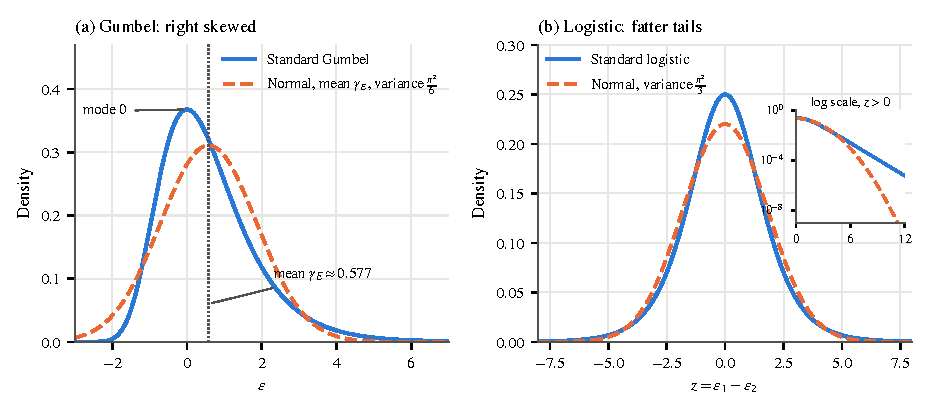
\includegraphics[width=\textwidth]{figures/ch06/gumbel_logistic.pdf}
\caption{Extreme value algebra. (a) The standard Gumbel density (mode $0$, mean $\gamma_E$) against a normal
density with the same mean and variance $\frac{\pi^2}{6}$. (b) The standard logistic density, the distribution of
the difference of two independent standard Gumbels, against a normal density with the same variance
$\frac{\pi^2}{3}$. The inset plots both densities on a log scale for $z > 0$.}
\label{fig:06-gumbel}
\end{figure}

\subsection{Logit choice probabilities}\label{sec:06-logitprob}

\begin{proposition}[Logit choice probabilities]\label{prop:06-logit}
Let $u_{ij} = V_{ij} + \sigma_\epsilon\epsilon_{ij}$ for $j = 0, 1, \dots, J$, with $\epsilon_{ij}$ independent and
identically distributed standard Gumbel and $\sigma_\epsilon > 0$. Then
\begin{equation}\label{eq:06-logit}
P_{ij} = \frac{\exp\left(\frac{V_{ij}}{\sigma_\epsilon}\right)}{\sum_{k=0}^J \exp\left(\frac{V_{ik}}{\sigma_\epsilon}\right)} .
\end{equation}
With $V_{i0} = 0$, $V_{ij} = \delta_j$ for $j \ge 1$ and $\sigma_\epsilon = 1$, the market share is
\begin{equation*}
s_j = \frac{e^{\delta_j}}{1 + \sum_{k=1}^J e^{\delta_k}} .
\end{equation*}
\end{proposition}

\begin{proof}[First proof (direct integration)]
Drop the index $i$ and fix $j$. Product $j$ is chosen when $V_j + \sigma_\epsilon\epsilon_j \ge V_k + \sigma_\epsilon\epsilon_k$
for every $k$, that is, when $\epsilon_k \le \epsilon_j + a_k$ with $a_k = \frac{V_j - V_k}{\sigma_\epsilon}$. Note that
$a_j = 0$. Condition on $\epsilon_j = e$. By independence,
\begin{align*}
P_j &= \int_{-\infty}^{\infty} f(e)\prod_{k\neq j}F(e + a_k)\,\dd e \\
&= \int_{-\infty}^{\infty} e^{-e}\exp\big(-e^{-e}\big)\prod_{k\neq j}\exp\big(-e^{-e}e^{-a_k}\big)\,\dd e \\
&= \int_{-\infty}^{\infty} e^{-e}\exp\Big(-e^{-e}\sum_{k=0}^J e^{-a_k}\Big)\,\dd e ,
\end{align*}
where the factor $\exp(-e^{-e})$ from the density supplies the term $k = j$, since $e^{-a_j} = 1$. Let
$A = \sum_{k=0}^J e^{-a_k} = \sum_{k=0}^J \exp\left(\frac{V_k - V_j}{\sigma_\epsilon}\right)$. Substitute $t = e^{-e}$,
with $\dd t = -e^{-e}\,\dd e$:
\begin{equation*}
P_j = \int_0^\infty e^{-At}\,\dd t = \frac{1}{A}
= \frac{\exp\left(\frac{V_j}{\sigma_\epsilon}\right)}{\sum_{k=0}^J \exp\left(\frac{V_k}{\sigma_\epsilon}\right)} . \qedhere
\end{equation*}
\end{proof}

\begin{proof}[Second proof (max-stability)]
Divide utilities by $\sigma_\epsilon$, which does not change choices (\cref{prop:06-normalization}). Let
$W_k = \frac{V_k}{\sigma_\epsilon}$. By \cref{lem:06-maxstable} applied to the alternatives other than $j$,
\begin{equation*}
\max_{k\neq j}(W_k + \epsilon_k) = L_{-j} + \epsilon^*, \qquad L_{-j} = \ln\sum_{k\neq j}e^{W_k},
\end{equation*}
where $\epsilon^*$ is standard Gumbel and independent of $\epsilon_j$. Product $j$ is chosen when
$W_j + \epsilon_j \ge L_{-j} + \epsilon^*$, that is, when $\epsilon^* - \epsilon_j \le W_j - L_{-j}$. By
\cref{lem:06-logistic},
\begin{equation*}
P_j = \Lambda(W_j - L_{-j}) = \frac{1}{1 + e^{L_{-j} - W_j}} = \frac{e^{W_j}}{e^{W_j} + \sum_{k\neq j}e^{W_k}} ,
\end{equation*}
which is \eqref{eq:06-logit}.
\end{proof}

\casehead{Income, constants and the normalization}
Terms common to all alternatives cancel from \eqref{eq:06-logit}. Consider
\begin{equation*}
u_{ij} = \bar u + \alpha(y_i - p_j) + x_j\beta + \xi_j + \sigma_\epsilon\epsilon_{ij}, \qquad
u_{i0} = \bar u + \alpha y_i + \sigma_\epsilon\epsilon_{i0},
\end{equation*}
with a common constant $\bar u$. The factor $\exp\big(\frac{\bar u + \alpha y_i}{\sigma_\epsilon}\big)$ appears in the
numerator and in every term of the denominator, so it cancels:
\begin{equation*}
P_{ij} = \frac{\exp\left(\frac{x_j\beta + \xi_j - \alpha p_j}{\sigma_\epsilon}\right)}
{1 + \sum_{k=1}^J\exp\left(\frac{x_k\beta + \xi_k - \alpha p_k}{\sigma_\epsilon}\right)} .
\end{equation*}
The probabilities depend on the parameters only through $\frac{\beta}{\sigma_\epsilon}$, $\frac{\alpha}{\sigma_\epsilon}$
and $\frac{\xi_j}{\sigma_\epsilon}$. Only one of the price coefficient and the scale of the shock can be normalized.
The usual choice sets $\sigma_\epsilon = 1$ and estimates $\alpha$, so that
$\delta_j = x_j\beta - \alpha p_j + \xi_j$ is measured in units of the shock. The alternative sets $\alpha = 1$
and estimates $\sigma_\epsilon$, so that utility is measured in dollars and $\sigma_\epsilon$ is the dollar scale of
the taste shocks. Writing $u_{ij} = (y_i - p_j) + \delta_j + \epsilon_{ij}$ with a standard Gumbel shock imposes
both normalizations at once. That specification assumes the standard deviation of the taste shock equals
$\frac{\pi}{\sqrt 6} \approx 1.28$ dollars, a restriction that the data cannot test once the price coefficient is fixed.

\casehead{The two limits of the scale}
Write \eqref{eq:06-logit} as
$P_j = \Big[\sum_k \exp\Big(\frac{V_k - V_j}{\sigma_\epsilon}\Big)\Big]^{-1}$. As $\sigma_\epsilon \to 0$, every term
with $V_k < V_j$ vanishes and every term with $V_k > V_j$ explodes. If $V_j$ is the unique maximum, then
$P_j \to 1$. If some $V_k$ exceeds $V_j$, then $P_j \to 0$. Choice becomes deterministic, and the consumer picks
$\arg\max_k V_k$. As $\sigma_\epsilon \to \infty$, every term tends to one, and $P_j \to \frac{1}{J+1}$. Choice
becomes uniform and ignores the attributes. The scale $\sigma_\epsilon$, or its inverse
$\mu_\epsilon = \frac{1}{\sigma_\epsilon}$, is the bridge to the ``modified BLP'' model of \citet{BerryPakes2007}.
BLP abbreviates the random coefficients logit of Berry, Levinsohn and Pakes \citep{BerryLevinsohnPakes1995}, the
subject of \cref{ch:blp}. The modified BLP model adds $\sigma_\epsilon\epsilon_{ij}$ to a pure characteristics model, and it approaches the pure
characteristics model as $\sigma_\epsilon \to 0$ (\cref{sec:06-epsilon}).

\begin{remark}[The logit as a model of tastes for products]\label{rem:06-tastesforproducts}
\citet[p.~1412]{McFadden1984} observes that the multinomial logit is a special case of a random coefficients
model in which only the coefficients of alternative-specific dummy variables are random. Write
\begin{equation*}
u_{ij} = V_{ij} + \sum_{k=0}^J \epsilon_{ik}\,d_{jk}, \qquad d_{jk} = \indic\{j = k\}.
\end{equation*}
The dummy $d_{jk}$ is a ``characteristic'' that only product $k$ possesses, and $\epsilon_{ik}$ is consumer $i$'s
random taste for it. \citet{BerryPakes2007} attribute this reading to \citet{CaplinNalebuff1991} and call such
models models with ``tastes for products''. Under this reading the dimension of the characteristic space grows
with the number of products. \Cref{sec:06-epsilon} shows that this growth drives the logit's implications for
markups and welfare as products are added.
\end{remark}

\subsection{Expected maximum utility and the log-sum formula}\label{sec:06-logsum}

\begin{proposition}[Log-sum formula]\label{prop:06-logsum}
Under the assumptions of \cref{prop:06-logit},
\begin{equation}\label{eq:06-logsum}
\E\Big[\max_k u_{ik}\Big] = \sigma_\epsilon\ln\sum_{k=0}^J\exp\left(\frac{V_{ik}}{\sigma_\epsilon}\right) + \sigma_\epsilon\gamma_E .
\end{equation}
Its gradient with respect to $(V_{i0}, \dots, V_{iJ})$ is the vector of logit probabilities
\eqref{eq:06-logit}. In addition, the distribution of the maximum utility does not depend on which alternative
attains it: for every $j$ and $x$,
\begin{equation}\label{eq:06-maxindep}
\Pr\Big(j \text{ chosen and } \max_k u_{ik} \le x\Big) = P_{ij}\,\Pr\Big(\max_k u_{ik} \le x\Big).
\end{equation}
\end{proposition}

\begin{proof}
Write $\max_k(V_k + \sigma_\epsilon\epsilon_k) = \sigma_\epsilon\max_k\big(\frac{V_k}{\sigma_\epsilon} + \epsilon_k\big)$. By
\cref{lem:06-maxstable}, $\max_k\big(\frac{V_k}{\sigma_\epsilon} + \epsilon_k\big)$ is Gumbel with location
$\ln\sum_k e^{\frac{V_k}{\sigma_\epsilon}}$ and scale one, so its mean is that location plus $\gamma_E$.
Multiplying by $\sigma_\epsilon$ gives \eqref{eq:06-logsum}. Differentiating,
\begin{equation*}
\frac{\partial}{\partial V_j}\left[\sigma_\epsilon\ln\sum_k e^{\frac{V_k}{\sigma_\epsilon}}\right]
= \sigma_\epsilon\cdot\frac{1}{\sigma_\epsilon}\,\frac{e^{\frac{V_j}{\sigma_\epsilon}}}{\sum_k e^{\frac{V_k}{\sigma_\epsilon}}} = P_j ,
\end{equation*}
as \cref{thm:06-wdz} requires.

For \eqref{eq:06-maxindep}, set $\sigma_\epsilon = 1$ without loss of generality. When $j$ is chosen, the maximum
equals $V_j + \epsilon_j$. Repeating the first proof of \cref{prop:06-logit} with the extra restriction
$V_j + e \le x$,
\begin{align*}
\Pr\Big(j \text{ chosen and } \max_k u_k \le x\Big)
&= \int_{-\infty}^{x - V_j} e^{-e}\exp\big(-Ae^{-e}\big)\,\dd e \\
&= \int_{e^{-(x - V_j)}}^{\infty} e^{-At}\,\dd t \\
&= \frac{1}{A}\exp\big(-Ae^{-(x - V_j)}\big),
\end{align*}
with $A = \sum_k e^{V_k - V_j}$. Since $\frac{1}{A} = P_j$ and $Ae^{V_j} = \sum_k e^{V_k}$, the last expression equals
$P_j\exp\big(-e^{-x}\sum_k e^{V_k}\big)$. By the proof of \cref{lem:06-maxstable} the second factor is
$\Pr(\max_k u_k \le x)$.
\end{proof}

Equation \eqref{eq:06-maxindep} says that the identity of the chosen alternative and the level of the maximum
utility are independent. Consumers who choose a product with low $V_j$ have, on average, a large
$\epsilon_j$ that exactly compensates. All buyers therefore enjoy the same expected utility, whatever they bought.
In the two-goods example of \cref{sec:06-twogoods}, the expected maximum utility is $\ln(1 + e^{0.5} + e) + \gamma_E \approx 2.26$.
A simulation with two million draws gives conditional means of $2.26$ for each of the three choices.

\casehead{Logit consumer surplus}
Combine \eqref{eq:06-logsum} with the welfare formula \eqref{eq:06-smallrosen}. Let
$u_{ij} = \alpha(y_i - p_j) + x_j\beta + \xi_j + \epsilon_{ij}$ for $j \ge 1$ and $u_{i0} = \alpha y_i + \epsilon_{i0}$,
with $\sigma_\epsilon = 1$ and $\delta_j = x_j\beta - \alpha p_j + \xi_j$. Then
$\E[\max_k u_{ik}] = \alpha y_i + \ln\big(1 + \sum_k e^{\delta_k}\big) + \gamma_E$, and dividing by the marginal utility
of income gives the expected consumer surplus
\begin{equation}\label{eq:06-logitcs}
CS_i = \frac{1}{\alpha}\ln\Big(1 + \sum_{k=1}^J e^{\delta_k}\Big) + C ,
\end{equation}
where $C = y_i + \frac{\gamma_E}{\alpha}$ is a constant that drops out of every comparison. For a change from a
choice set $\mathcal{J}^0$ with mean utilities $\delta^0$ to a choice set $\mathcal{J}^1$ with mean utilities $\delta^1$,
\begin{equation}\label{eq:06-logitdcs}
\Delta CS_i = \frac{1}{\alpha}\left[\ln\Big(1 + \sum_{k\in\mathcal{J}^1}e^{\delta^1_k}\Big)
- \ln\Big(1 + \sum_{k\in\mathcal{J}^0}e^{\delta^0_k}\Big)\right].
\end{equation}
Because $1 + \sum_k e^{\delta_k} = \frac{1}{s_0}$ in the logit, \eqref{eq:06-logitcs} can be written
$CS_i = -\frac{1}{\alpha}\ln s_0 + C$, and \eqref{eq:06-logitdcs} becomes
$\Delta CS_i = \frac{1}{\alpha}\ln\frac{s_0^0}{s_0^1}$. In the logit, the outside share and the price coefficient
alone determine the welfare change. In the two-goods example the rise in $\delta_1$ from $0.5$ to $1.3$
lowers $s_0$ from $0.186$ to $0.135$, a gain of $\ln\frac{0.186}{0.135} \approx 0.32$ utils, or
$\frac{0.32}{\alpha}$ dollars. Differentiating \eqref{eq:06-logitcs} with respect to $p_j$ gives
$-\frac{1}{\alpha}\cdot\frac{\alpha e^{\delta_j}}{1 + \sum_k e^{\delta_k}} = -s_j$, the logit version of the Roy
identity noted after \cref{cor:06-wdz}. The logit elasticities and the Berry inversion are in \cref{ch:logit},
and the welfare value of new goods is in \cref{ch:newgoods}. \Cref{sec:06-epsilon} shows that
\eqref{eq:06-logitdcs} assigns positive value to every added product, including an exact copy of an existing one.

\subsection{Luce's axiom, IIA and the generalized extreme value family}\label{sec:06-gev}

\casehead{The choice axiom and IIA}
\citet{Luce1959} proposed an axiom for probabilistic choice. Let $P(j \mid C)$ be the probability of choosing
$j$ from a set $C$. The \emph{choice axiom} requires $P(j \mid C) = P(j \mid A)\,P(A \mid C)$ for every subset
$A \subseteq C$ that contains $j$, where $P(A \mid C) = \sum_{k\in A}P(k \mid C)$. When all probabilities are
positive, the axiom implies that there are scale values $w_k > 0$ with
$P(j \mid C) = \frac{w_j}{\sum_{k \in C} w_k}$. The logit is the case $w_k = e^{V_k}$. The axiom is
equivalent to the \emph{independence of irrelevant alternatives} (IIA): the odds of choosing $j$ over $k$ do not
depend on the other alternatives. In the logit,
\begin{equation}\label{eq:06-iia}
\frac{P_j}{P_k} = \exp\left(\frac{V_j - V_k}{\sigma_\epsilon}\right) ,
\end{equation}
which depends only on $j$ and $k$. \citet[eq.~3.17, p.~1413]{McFadden1984} states the property for a model in
which $V_j = x_j\theta$ depends only on the attributes of $j$: $\ln\frac{P_j}{P_k} = (x_j - x_k)\theta$, independent
of the attributes of every other alternative.

IIA has three consequences. First, the probabilities for a smaller or larger choice set follow from
\eqref{eq:06-logit} by deleting or adding terms in the denominator. A model estimated on existing alternatives
can then forecast the demand for a new one, provided the new alternative brings no new parameters
\citep[p.~1414]{McFadden1984}. Second, the cross-elasticity of the probability of $j$ with respect to an attribute
of $k$ is the same for every $j \neq k$ (p.~1414). A rise in the price of $k$ sends its customers to the other
alternatives in proportion to their shares, as the two-goods example showed. Third, ranked data can be used.
The probability of a complete ranking is the product of logit probabilities of choosing the best alternative
from successively smaller sets \citep{Marschak1960}. \citet[p.~1414]{McFadden1984} calls IIA ``theoretically
implausible in many applications'', while noting that the logit often fits and predicts well in practice.

\begin{remark}[Why Gumbel]\label{rem:06-yellott}
Is the Gumbel distribution the only way to obtain Luce's axiom from random utility? \citet{Yellott1977} studies
random utility models with independent and identically distributed errors from a location family. He shows
that in this class the choice axiom holds for all choice sets of at least three alternatives only if the errors
are Gumbel. We
state the result without proof. It explains why the logit and the independent Gumbel model are the same
object.
\end{remark}

\begin{remark}[Universal logit]\label{rem:06-universal}
IIA comes from restricting $V_j$ to depend on the attributes of $j$ alone. The logistic functional form does
not imply it by itself. Suppose instead that $V_j = z_j(x)\theta$ may depend on the attributes $x$ of all
alternatives. Then the logit form
\begin{equation*}
P_j = \frac{e^{z_j(x)\theta}}{\sum_k e^{z_k(x)\theta}}
\end{equation*}
can approximate any continuous positive response probability model on a compact set, to any desired accuracy
\citep[eq.~3.18, pp.~1414--1415]{McFadden1984}. This \emph{universal logit} can describe any pattern of
cross-elasticities. The approximation may be computationally impractical, and it makes consistency with
utility maximization hard to impose or verify. Its main use is to suggest specification tests (p.~1415).
\end{remark}

The most common test of IIA uses the property that the logit parameters are the same on any subset of the
choice set. Let $\hat\beta_C$ and $\hat V_C$ be the estimates and their estimated covariance matrix from the full
choice set $C$, and $\hat\beta_D$ and $\hat V_D$ those from a subset $D$. Under IIA both estimators are consistent
and the full-set estimator is efficient, so
\begin{equation}\label{eq:06-hmtest}
S = (\hat\beta_D - \hat\beta_C)^\T(\hat V_D - \hat V_C)^{-1}(\hat\beta_D - \hat\beta_C)
\end{equation}
is asymptotically chi-squared with degrees of freedom equal to the rank of $\hat V_D - \hat V_C$
\citep[eq.~3.23, pp.~1417--1418]{McFadden1984}. \citet{HausmanMcFadden1984} analyze the test. McFadden warns
that it is an omnibus test and that it has little power unless the departures from the logit are substantial.
\Cref{ch:logit} applies it.

\begin{remark}[Aggregating alternatives]\label{rem:06-aggregation}
The logit form survives aggregation of alternatives into types \citep[eqs.~3.19--3.20, p.~1415]{McFadden1984}.
Suppose type $g$ contains $M_g$ elemental alternatives with attributes $x_{gj}$ and mean attributes
$\bar x_g$. The probability of choosing some alternative of type $g$ is
\begin{align*}
\sum_{j \in g}P_{gj} &= \frac{\sum_{j \in g}e^{x_{gj}\theta}}{\sum_h\sum_{l \in h}e^{x_{hl}\theta}}, \qquad
\sum_{j\in g}e^{x_{gj}\theta} = \exp\big(\bar x_g\theta + \ln M_g + \omega_g\big),
\end{align*}
where $\omega_g = \ln\Big[\frac{1}{M_g}\sum_{j\in g}e^{(x_{gj} - \bar x_g)\theta}\Big]$ corrects for heterogeneity
within the type and is zero when the alternatives in $g$ are identical. Choice among types is therefore a logit
with utility $\bar x_g\theta + \ln M_g + \omega_g$. The term $\ln M_g$ shows how the logit counts products. Doubling
the number of alternatives of a type, with the new ones identical to the old, adds $\ln 2$ to the utility of
the type. This is the tastes-for-products reading of \cref{rem:06-tastesforproducts} at
work.
\end{remark}

\begin{remark}[Sampling alternatives]\label{rem:06-sampling}
IIA has a practical use when the choice set is large, as when households choose among thousands of houses. The
denominator of each logit probability then sums over every alternative. \citet[sec.~3.6, pp.~1416--1417]{McFadden1984}
shows that the logit can be estimated from a sampled subset of alternatives for each consumer. Let $C$ be the full
choice set, and let consumer $i$ choose $j_i \in C$. The researcher draws a subset $\mathcal{D}_i \subseteq C$ that
contains $j_i$, under a known protocol that selects $\mathcal{D}$ with probability $r(\mathcal{D} \mid j_i, x_i)$. We
write $r$ for McFadden's $\pi$, which this book reserves for profit. The protocol must have the \emph{positive
conditioning property}: $r(\mathcal{D}_i \mid k, x_i) > 0$ for every $k \in \mathcal{D}_i$. Had any member of
$\mathcal{D}_i$ been chosen, the protocol could have produced the same subset.

The probability that consumer $i$ chose $k$, given the sampled subset, follows from Bayes' rule:
\begin{equation*}
\Pr(j_i = k \mid \mathcal{D}_i, x_i)
= \frac{P_k(x_i, \theta)\, r(\mathcal{D}_i \mid k, x_i)}{\sum_{l \in \mathcal{D}_i} P_l(x_i, \theta)\, r(\mathcal{D}_i \mid l, x_i)} .
\end{equation*}
The sum runs over $\mathcal{D}_i$ only, because the protocol never produces a subset that excludes the chosen
alternative. We substitute the logit $P_k(x_i, \theta) = \frac{e^{x_{ik}\theta}}{\sum_{m \in C}e^{x_{im}\theta}}$. The
full-set denominator appears in every term and cancels, which leaves
\begin{equation}\label{eq:06-sampled-logit}
\Pr(j_i = k \mid \mathcal{D}_i, x_i)
= \frac{\exp\big(x_{ik}\theta + \ln r(\mathcal{D}_i \mid k, x_i)\big)}{\sum_{l \in \mathcal{D}_i}\exp\big(x_{il}\theta + \ln r(\mathcal{D}_i \mid l, x_i)\big)} .
\end{equation}
This is a logit on $\mathcal{D}_i$ with $\ln r(\mathcal{D}_i \mid k, x_i)$ added to each utility. Positive conditioning
keeps every logarithm finite. The average of $\ln\Pr(j_i \mid \mathcal{D}_i, x_i)$ over consumers is McFadden's modified
log-likelihood (his eq.~3.22). Under positive conditioning and a standard identification condition, its maximizer is
consistent for $\theta$. It is a conditional likelihood, so the inverse of its information matrix estimates the
covariance matrix as usual (p.~1417).

The correction cancels when $r(\mathcal{D}_i \mid k, x_i)$ is the same for every $k \in \mathcal{D}_i$, the
\emph{uniform conditioning property}. McFadden's example draws the chosen alternative and one other alternative at
random (his eq.~3.21):
\begin{equation*}
r(\mathcal{D} \mid j_i, x_i) = \begin{cases} \frac{1}{|C| - 1} & \text{if } \mathcal{D} = \{j_i, k\} \text{ with } k \neq j_i,\\
0 & \text{otherwise,}\end{cases}
\end{equation*}
where $|C|$ is the number of alternatives. Either member of $\mathcal{D}_i$, had it been chosen, would have produced
$\mathcal{D}_i$ with the same probability. The logit can then be estimated from binary choices between the chosen
alternative and one random rival. The argument needs IIA. The full-set denominator cancels only because the ratio
$\frac{P_k}{P_l}$ does not depend on the alternatives outside $\mathcal{D}_i$.
\end{remark}

\casehead{Generalized extreme value models}
\citet{McFadden1978} found a class of joint distributions for the shocks that keeps closed forms while
relaxing IIA. Models in this class are called \emph{generalized extreme value} (GEV) models.

\begin{theorem}[Generalized extreme value models]\label{thm:06-gev}
Let $H : \R^{J+1}_+ \to \R_+$ satisfy three conditions.
\begin{enumerate}[label=(G\arabic*)]
  \item $H$ is homogeneous of degree one: $H(\lambda y) = \lambda H(y)$ for $\lambda > 0$.
  \item $H(y) \to \infty$ as $y_j \to \infty$, for any $j$.
  \item For any $r$ distinct indices $j_1, \dots, j_r$, the mixed partial derivative
  $\frac{\partial^r H}{\partial y_{j_1}\cdots\partial y_{j_r}}$ is nonnegative if $r$ is odd and nonpositive if $r$
  is even.
\end{enumerate}
Then the following hold.
\begin{enumerate}[label=(\alph*)]
  \item $F(\epsilon_0, \dots, \epsilon_J) = \exp\big(-H(e^{-\epsilon_0}, \dots, e^{-\epsilon_J})\big)$ is the CDF of a
  multivariate extreme value distribution whose marginals are Gumbel.
  \item In the ARUM $u_j = V_j + \epsilon_j$ with $\epsilon$ distributed as in (a), the choice probabilities are
  \begin{equation}\label{eq:06-gevprob}
  P_j = \frac{y_j H_j(y)}{H(y)} = \frac{\partial\ln H(e^{V_0}, \dots, e^{V_J})}{\partial V_j},
  \qquad y = (e^{V_0}, \dots, e^{V_J}),
  \end{equation}
  where $H_j$ is the partial derivative of $H$ with respect to its $j$-th argument.
  \item The social surplus function is $G(V) = \ln H(e^{V_0}, \dots, e^{V_J}) + \gamma_E$.
\end{enumerate}
\end{theorem}

\begin{proof}
Part (a) is the theorem of \citet{McFadden1978}, restated by \citet[eqs.~3.29--3.31, p.~1421]{McFadden1984}.
We take it as given. Its marginals follow by sending the other arguments to infinity:
$F_j(\epsilon_j) = \exp\big(-e^{-\epsilon_j}H(e_j)\big)$, a Gumbel CDF with location $\ln H(e_j)$, where $e_j$ is the
$j$-th unit vector.

For (c), the maximum is at most $x$ if and only if $\epsilon_k \le x - V_k$ for every $k$. Using (a) and then
homogeneity with $\lambda = e^{-x}$,
\begin{equation*}
\Pr\Big(\max_k(V_k + \epsilon_k) \le x\Big) = \exp\Big(-H\big(e^{V_0 - x}, \dots, e^{V_J - x}\big)\Big)
= \exp\Big(-e^{-\left(x - \ln H(y)\right)}\Big).
\end{equation*}
The maximum is Gumbel with location $\ln H(y)$, so its mean is $\ln H(y) + \gamma_E$.

For (b), the density of the event that $j$ is chosen with $\epsilon_j = e$ is $\frac{\partial F}{\partial\epsilon_j}$
evaluated at $\epsilon_k = e + V_j - V_k$ for all $k$. Differentiating $F$,
\begin{equation*}
\frac{\partial F}{\partial \epsilon_j}(\epsilon) = F(\epsilon)\,H_j(e^{-\epsilon_0}, \dots, e^{-\epsilon_J})\,e^{-\epsilon_j}.
\end{equation*}
At the evaluation point, $e^{-\epsilon_k} = \lambda y_k$ with $\lambda = e^{-e - V_j} = \frac{e^{-e}}{y_j}$. Homogeneity of
degree one implies $H(\lambda y) = \lambda H(y)$, and its derivative $H_j$ is homogeneous of degree zero, so
$H_j(\lambda y) = H_j(y)$. Hence
\begin{align*}
P_j &= \int_{-\infty}^{\infty}\exp\Big(-\frac{e^{-e}}{y_j}H(y)\Big)H_j(y)\,e^{-e}\,\dd e \\
&= H_j(y)\int_0^\infty\exp\Big(-t\,\frac{H(y)}{y_j}\Big)\,\dd t
= \frac{y_jH_j(y)}{H(y)},
\end{align*}
where the second line substitutes $t = e^{-e}$. Finally,
$\frac{\partial\ln H(e^{V})}{\partial V_j} = \frac{H_j(y)\,e^{V_j}}{H(y)}$, which is the same expression. It equals the
derivative of $G$ in (c), as \cref{thm:06-wdz} requires.
\end{proof}

The logit is the generating function $H(y) = \sum_j y_j$. It satisfies (G1) and (G2), its first derivatives
equal one, and its higher mixed derivatives vanish. Then $F(\epsilon) = \prod_j\exp(-e^{-\epsilon_j})$, the shocks
are independent, and \eqref{eq:06-gevprob} gives $P_j = \frac{y_j}{\sum_k y_k}$. McFadden's version,
$H(y) = \big(\sum_j y_j^{\frac{1}{\lambda}}\big)^{\lambda}$ with $0 < \lambda \le 1$, gives the logit with scale $\lambda$
\citep[eq.~3.32, p.~1421]{McFadden1984}.

The nested logit is the leading member of the family that relaxes IIA. Partition the inside products into nests
$g = 1, \dots, G$, and place the outside good in its own nest. With nesting parameter $\sigma \in [0, 1)$, let
\begin{equation}\label{eq:06-nestedH}
H(y) = y_0 + \sum_{g=1}^G\Big(\sum_{j\in g}y_j^{\frac{1}{1-\sigma}}\Big)^{1-\sigma}.
\end{equation}
Write $D_g = \sum_{k\in g}y_k^{\frac{1}{1-\sigma}}$. For $j$ in nest $g$, the derivative is
$H_j = D_g^{-\sigma}\,y_j^{\frac{\sigma}{1-\sigma}}$, so $y_jH_j = D_g^{-\sigma}y_j^{\frac{1}{1-\sigma}}$ and
\begin{equation*}
P_j = \frac{y_j^{\frac{1}{1-\sigma}}}{D_g}\cdot\frac{D_g^{1-\sigma}}{y_0 + \sum_{h=1}^G D_h^{1-\sigma}} .
\end{equation*}
The first factor is the probability of choosing $j$ within its nest, and the second is the probability of
choosing nest $g$. With $\sigma = 0$ the model is the logit. As $\sigma$ approaches one, the products within a
nest become close substitutes. \citet[sec.~3.10, pp.~1422--1425]{McFadden1984} develops the general
hierarchical version, the nested multinomial logit, with an ``independence'' parameter at each node, here
$1 - \sigma$. He notes that estimates of these parameters outside the unit interval indicate a misspecified tree
(pp.~1425--1426), and that the likelihood is not concave in all parameters (p.~1426). \Cref{ch:logit} develops
the nested logit, its elasticities and its estimation.

\subsection{The multinomial probit}\label{sec:06-probit}

The \emph{multinomial probit} assumes jointly normal shocks, $\epsilon_i \sim N(0, \Sigma_\epsilon)$, with a
$(J+1)\times(J+1)$ covariance matrix $\Sigma_\epsilon$. Product $j$ is chosen when
$\epsilon_{ik} - \epsilon_{ij} \le V_{ij} - V_{ik}$ for every $k \neq j$. The vector of these $J$ differences is
normal with covariance matrix $B_j\Sigma_\epsilon B_j^\T$, where $B_j$ is the $J\times(J+1)$ matrix that
subtracts $\epsilon_{ij}$ from the other shocks. The choice probability is a $J$-dimensional normal orthant
probability, which has no closed form \citep[sec.~3.8]{McFadden1984}. A version with an economic
interpretation sets $u_{ij} = x_{ij}a_i$ with normally distributed taste weights $a_i \sim N(\beta, \Omega_a)$, so
that utilities have covariance $x_i\Omega_a x_i^\T$ across alternatives (p.~1418).

The probit has the flexibility that the logit lacks. With correlated shocks it does not have IIA, and it
permits very general patterns of cross-elasticities (p.~1418). The cost is computation. McFadden reports that
probabilities with up to three alternatives cost about as much to compute as logit probabilities (p.~1418).
With five or more alternatives and an unrestricted covariance matrix, they were usually too costly for iterative
estimation at the time. The probit log-likelihood is also not known to be concave (p.~1419). One remedy restricts the
covariance with a factor structure,
\begin{equation*}
\epsilon_{ij} = \zeta_{ij} + \sum_{l=1}^{L}\gamma_{jl}v_{il},
\end{equation*}
with independent normal $\zeta_{ij}$ and $v_{il}$ \citep[eq.~3.25, p.~1419]{McFadden1984}. The loading $\gamma_{jl}$ can
be read as the level in alternative $j$ of an unobserved characteristic $l$, and $v_{il}$ as the consumer's random
taste for it. This is a random coefficients model on unobserved characteristics. Simulation methods developed
since then make probit models with many alternatives feasible \citep{Train2009}.

The independent probit, with $\Sigma_\epsilon$ the identity matrix, has essentially the same restrictions on
substitution as the logit, and \citet[p.~1420]{McFadden1984} sees little reason to prefer one over the other.
The lesson matters for the rest of the book. The logit's substitution problems come from shocks that are
independent across products, which leave products with no notion of similarity. The shape of the Gumbel
distribution plays little role. Fixing the problems requires correlation in tastes across similar products. Nesting supplies it within
groups (\cref{ch:logit}), and random coefficients on characteristics supply it along each characteristic
(\cref{ch:blp}).

\subsection{Choosing a functional form}\label{sec:06-forms}

\citet[sec.~3.3]{McFadden1984} judges functional forms by computational practicality and by flexibility in
representing similarity across alternatives. He groups the concrete forms into three families. Logit models
descend from \citet{Luce1959}. Probit models descend from \citet{Thurstone1927}. Elimination models, in which
alternatives are screened out until one remains, descend from \citet{Tversky1972}. His verdict (p.~1410) is that
the multinomial logit scores well on simplicity and computation but poorly on flexibility. The multinomial
probit is simple and flexible but scores poorly on computation. The nested logit and the factor-structure probit
try to achieve both. He adds that functional forms allowing similar substitution patterns tend to fit existing
data comparably. This observation anticipates the strategy of modern empirical work. The choice of a model is
mainly a choice of substitution patterns, and the distribution of the idiosyncratic shock matters mostly through
its implications for computation and welfare.

\begin{remark}[A representative-consumer foundation]\label{rem:06-representative}
Logit demand also arises from a single representative consumer \citep{AndersonDePalmaThisse1988,AndersonDePalmaThisse1992}.
Suppose the consumer allocates one unit of consumption across the alternatives $j = 0, 1, \dots, J$ to maximize
\begin{equation*}
\sum_{j=0}^J \delta_j q_j - \sum_{j=0}^J q_j\ln q_j \qquad \text{subject to} \qquad \sum_{j=0}^J q_j = 1,
\end{equation*}
with $\delta_0 = 0$. The entropy term rewards spreading consumption across products. The first-order conditions
$\delta_j - \ln q_j - 1 - \lambda = 0$, with multiplier $\lambda$, give $q_j \propto e^{\delta_j}$, and the constraint
yields $q_j = \frac{e^{\delta_j}}{1 + \sum_{k\ge 1}e^{\delta_k}}$, the logit shares. A weight $\sigma_\epsilon$ on the entropy
term produces the logit with scale $\sigma_\epsilon$. The two foundations, a population of consumers with Gumbel
shocks and a representative consumer with a taste for variety, give the same aggregate demand.
\Cref{ch:diffprod} gives the full derivation and shows that the constant elasticity of substitution (CES) demand system is a logit in log prices.
\end{remark}

\section{Models of product differentiation as random utility models}\label{sec:06-models}

The random utility model of \cref{sec:06-rum} is a general language for demand. A model of product
differentiation fills in two objects of that language. The first is the utility function
$U(x_j, p_j, \xi_j, \nu_i; \theta)$. The second is the distribution $F$ of the consumer tastes $\nu_i$. The
classical models of the theory literature (address models, ideal-point models, vertical models) and the
logit-type models of empirical work differ only in these two choices. This section places them in one
framework. The comparison matters because each specification fixes, before any data are used, which
products compete with which. Those restrictions drive every counterfactual the model produces.
\Cref{tab:06-taxonomy} at the end of the section collects the comparison.

\subsection{Horizontal and vertical differentiation}\label{sec:06-horvert}

Products are \emph{differentiated} when consumers do not regard them as perfect substitutes. Two polar
forms of differentiation organize the theory. They differ in whether consumers agree on how to rank the
products when prices are equal.

\begin{definition}[Vertical and horizontal differentiation]\label{def:06-vertical}
Let a consumer of type $\nu$ obtain utility $U(x_j, p, \nu)$ from product $j$ sold at price $p$. The
products are \emph{vertically differentiated} if at any common price every consumer ranks them in the
same order. Formally, for all products $j$ and $k$, all prices $p$, and all types $\nu$ and $\nu'$,
\begin{equation*}
  U(x_j, p, \nu) > U(x_k, p, \nu) \iff U(x_j, p, \nu') > U(x_k, p, \nu').
\end{equation*}
The products are \emph{horizontally differentiated} if at some common price two types rank some pair of
products differently.
\end{definition}

Under vertical differentiation a scalar index summarizes the common ranking. We call it \emph{quality}
and write it $\delta_j$. Consumers agree that higher quality is better. They disagree only about how much
extra money the extra quality is worth. Under horizontal differentiation no such index exists. At the same
price some consumers prefer a sweetened breakfast cereal and others a plain one, and neither group is
mistaken. Most markets mix the two forms. Every buyer prefers a luxury sedan to an economy sedan at the
same price, while buyers disagree about a sedan and a pickup truck.

The models below share a property that makes their demand systems tractable when tastes are
one-dimensional.

\begin{definition}[Single crossing]\label{def:06-singlecrossing}
Let the type $\nu$ be a scalar. Utility has the \emph{single-crossing property} if, for every pair of
products $j \ne k$ and all prices, the difference $U(x_j, p_j, \nu) - U(x_k, p_k, \nu)$ changes sign at
most once as $\nu$ increases. A sufficient condition is that the difference be strictly monotone in $\nu$.
\end{definition}

Under single crossing the utilities of two products, viewed as functions of the type, cross at most once.
The types that prefer $j$ to $k$ then form a half-line. The types that choose $j$ from the whole menu
form an interval, the intersection of such half-lines. Market shares become differences of the CDF $F$
evaluated at interval end points. Both the Hotelling model with quadratic transport costs and the
vertical model have this property. It is the reason their demand systems have closed forms, and the
reason each product competes only with its immediate neighbors.

\subsection{Address models: Hotelling and Salop}\label{sec:06-hotelling}

In an \emph{address model} each product has a location $x_j$ in a space of characteristics, and each
consumer has an ideal location in the same space. A consumer who buys a product away from her ideal
suffers a disutility that rises with the distance. \citet{Hotelling1929} introduced the idea with
consumers spread along a line. In random utility form, with quadratic distance costs,
\begin{equation}\label{eq:06-hotelling-u}
  u_{ij} = \bar u + (y_i - p_j) - \tau\, d(x_j, \nu_i)^2,
\end{equation}
where $\bar u$ is a utility constant common to all consumers, $y_i$ is income, $\nu_i$ is the consumer's
ideal location, and $d$ is distance. The coefficient $\tau > 0$ is the \emph{transport cost}. We reserve
$\theta$ for the generic parameter vector of \cref{sec:06-rum}, so the transport cost is always $\tau$.
The taste $\nu_i$ is now a location, and its distribution $F$ plays the role that the error distribution
plays in an additive random utility model. Products are horizontally differentiated. At equal prices
each consumer ranks products by distance, and consumers at different locations disagree.

\begin{example}[Hotelling duopoly with quadratic transport costs]\label{ex:06-hotelling}
Two firms sit at the ends of the unit interval, $x_1 = 0$ and $x_2 = 1$, and produce at common marginal
cost $c$. A mass $M$ of consumers is uniform on $[0,1]$, so $F(\nu) = \nu$. A consumer who buys nothing
obtains $y_i$. We assume $\bar u$ is large enough that every consumer buys one unit (full coverage).
Income and $\bar u$ then enter both inside utilities and cancel from the comparison.

The first step finds the indifferent consumer. A consumer at $\nu$ prefers firm 1 if
$-p_1 - \tau\nu^2 > -p_2 - \tau(1-\nu)^2$. The indifferent type $\nu^*$ solves
\begin{align*}
  p_1 + \tau(\nu^*)^2 &= p_2 + \tau(1-\nu^*)^2,\\
  \tau\big[(\nu^*)^2 - (1-\nu^*)^2\big] &= p_2 - p_1,\\
  \tau(2\nu^* - 1) &= p_2 - p_1,
\end{align*}
so that
\begin{equation}\label{eq:06-hotelling-cut}
  \nu^* = \frac{1}{2} + \frac{p_2 - p_1}{2\tau}.
\end{equation}
The utility difference $u_{i1} - u_{i2} = p_2 - p_1 + \tau(1 - 2\nu_i)$ falls in $\nu_i$ (single
crossing), so every consumer to the left of $\nu^*$ buys from firm 1.

The second step writes demand. Firm 1 sells $q_1 = M F(\nu^*) = M\nu^*$ and firm 2 sells
$q_2 = M(1 - \nu^*)$. These formulas hold when $0 < \nu^* < 1$, that is, when $|p_2 - p_1| < \tau$.
Demand is linear in prices, with $\frac{\partial q_1}{\partial p_1} = -\frac{M}{2\tau}$.

The third step finds best responses. Firm 1 maximizes $\pi_1 = (p_1 - c)M\nu^*(p_1, p_2)$, a concave
quadratic in $p_1$. Its first-order condition is
\begin{equation*}
  M\Big[\nu^* - \frac{p_1 - c}{2\tau}\Big] = 0.
\end{equation*}
Substituting \eqref{eq:06-hotelling-cut} gives $\frac{1}{2} + \frac{p_2 - p_1}{2\tau} = \frac{p_1 - c}{2\tau}$.
Multiplying by $2\tau$ and collecting terms gives the best response
\begin{equation*}
  p_1 = \frac{p_2 + c + \tau}{2}.
\end{equation*}

The fourth step imposes symmetry. With $p_1 = p_2 = p$, the best response becomes $p = \frac{p + c + \tau}{2}$,
so
\begin{equation}\label{eq:06-hotelling-eq}
  p_1 = p_2 = c + \tau, \qquad \nu^* = \frac{1}{2}, \qquad \pi_1 = \pi_2 = \frac{M\tau}{2}.
\end{equation}
The markup equals the transport cost. As $\tau \to 0$ the two products become perfect substitutes and
the price falls to marginal cost, the Bertrand outcome of \cref{ch:theory}. Full coverage holds in this
equilibrium when the consumer at $\nu = \frac{1}{2}$ prefers buying, $\bar u - c - \tau - \frac{\tau}{4}
\ge 0$, that is, $\bar u \ge c + \frac{5\tau}{4}$. The equilibrium is the case $x_1 = 0$, $x_2 = 1$ of
\cref{prop:04-hotelling}. Linear transport costs with the firms at the end points give the same indifferent
consumer and the same prices (\cref{sec:04-hotelling-linear}).
\end{example}

The quadratic form of the transport cost keeps demand continuous. With linear costs
$\tau\, d(x_j, \nu_i)$, demand jumps when one firm cuts its price far enough below its rival's to capture
the consumers at the rival's own location. \citet{DAspremontGabszewiczThisse1979} show that no pure-strategy
price equilibrium then exists when the two firms are located near the center of the line at distinct points
(\cref{prop:04-dgt}). With quadratic costs a price equilibrium exists for every pair of locations. In the two-stage game in which firms first choose locations and then prices, the firms move to
the two ends of the line, because distance softens price competition. \Cref{prop:04-hotelling} derives this
maximal differentiation in the location stage, and \cref{sec:04-hotelling-quad} shows that it exceeds the
efficient differentiation.

\citet{Salop1979} removed the end points of the line by placing consumers on a circle. Consider $N$ firms
spaced evenly on a circle of circumference one, each with marginal cost $c$. Transport cost is linear with
coefficient $\tau$. A mass $M$ of consumers is uniform on the circle, and every consumer buys. Take a firm that
charges $p$ while its two neighbors, each at distance $\frac{1}{N}$, charge $\bar p$. A consumer at distance $z$
from the firm, on the arc toward a neighbor, is indifferent when
\begin{equation*}
  p + \tau z = \bar p + \tau\Big(\frac{1}{N} - z\Big),
  \qquad\text{so}\qquad
  z = \frac{1}{2N} + \frac{\bar p - p}{2\tau}.
\end{equation*}
The firm serves consumers on both arcs, so its demand is
\begin{equation*}
  q = 2Mz = M\Big[\frac{1}{N} + \frac{\bar p - p}{\tau}\Big] \qquad\text{for } |\bar p - p| \le \frac{\tau}{N}.
\end{equation*}
Demand depends on the prices of the two neighbors and on no other price. By \cref{prop:04-salop}, the symmetric
equilibrium price is $p = c + \frac{\tau}{N}$, so the markup falls as products crowd the circle. With a fixed cost
of entry, free entry yields twice the efficient number of firms. Every consumer buys, so the markup is a
transfer, and the only distortion is in the number of firms. An entrant takes business from its neighbors,
while society gains only the saving in transport costs \citep[sec.~7.1.2]{Tirole1988}. Entry remains excessive
with quadratic transport costs (\cref{sec:04-salop}). Each firm in the Salop model competes only with its two
neighbors, a feature it shares with the vertical model below.

\subsection{The ideal-point model}\label{sec:06-idealpoint}

The address model extends to $K$ characteristics. In the \emph{ideal-point model}
\citep{AndersonDePalmaThisse1992} consumer $i$ has an ideal level $\nu_{ik}$ of each characteristic $k$,
and utility is
\begin{equation}\label{eq:06-idealpoint}
  u_{ij} = f(y_i, p_j) + \delta_j - \sum_{k=1}^K \alpha_k (x_{jk} - \nu_{ik})^2, \qquad \alpha_k > 0.
\end{equation}
Here $f(y_i, p_j)$ is the utility of the income left after the purchase, with $f_y > 0$, $f_p < 0$ and
$f_{py} \ge 0$ as in \cref{sec:06-normalization}. The term $\delta_j$ is a product effect common to all
consumers, and $\alpha_k$ is the weight of distance along dimension $k$. We write the distance term with
a minus sign and positive weights, so that utility falls with distance.\footnote{Some presentations
write the distance term with a plus sign. The weights must then be negative for distance to be costly.
We use the minus sign with positive weights.} The next result shows that
the ideal-point model is a special case of the pure characteristics model introduced below.

\begin{proposition}[Ideal points are random coefficients]\label{prop:06-idealpoint}
Under \eqref{eq:06-idealpoint},
\begin{equation}\label{eq:06-idealpoint-expanded}
  u_{ij} = f(y_i, p_j) + \Big[\delta_j - \sum_{k=1}^K \alpha_k x_{jk}^2\Big]
           + \sum_{k=1}^K 2\alpha_k\nu_{ik}\, x_{jk} - \sum_{k=1}^K \alpha_k\nu_{ik}^2 .
\end{equation}
Consequently, the following hold.
\begin{enumerate}[label=(\roman*)]
  \item Comparisons among inside products depend on the tastes only through the interactions
        $\nu_{ik}x_{jk}$. The model is a random coefficients model without an idiosyncratic shock. Its mean
        utility is $\delta_j - \sum_k \alpha_k x_{jk}^2$, and characteristic $x_{jk}$ carries the random
        coefficient $2\alpha_k\nu_{ik}$.
  \item The term $-\sum_k \alpha_k\nu_{ik}^2$ is the same for every inside product, so it cancels from
        every comparison among them. Relative to an outside good with utility $f(y_i, 0)$, it acts as a
        random coefficient on a characteristic that equals one for every inside product.
\end{enumerate}
\end{proposition}

\begin{proof}
Expand each square:
\begin{equation*}
  (x_{jk} - \nu_{ik})^2 = x_{jk}^2 - 2x_{jk}\nu_{ik} + \nu_{ik}^2 .
\end{equation*}
Multiply by $-\alpha_k$ and sum over $k$:
\begin{equation*}
  -\sum_k \alpha_k (x_{jk} - \nu_{ik})^2 = -\sum_k \alpha_k x_{jk}^2 + \sum_k 2\alpha_k\nu_{ik}x_{jk}
  - \sum_k \alpha_k\nu_{ik}^2 .
\end{equation*}
Substituting into \eqref{eq:06-idealpoint} gives \eqref{eq:06-idealpoint-expanded}. For two inside
products $j$ and $l$,
\begin{equation*}
  u_{ij} - u_{il} = f(y_i, p_j) - f(y_i, p_l) + \Big[\delta_j - \sum_k \alpha_k x_{jk}^2\Big]
  - \Big[\delta_l - \sum_k \alpha_k x_{lk}^2\Big] + \sum_k 2\alpha_k\nu_{ik}(x_{jk} - x_{lk}),
\end{equation*}
in which $\nu_{ik}^2$ no longer appears. This proves (i) and the first part of (ii). The difference
$u_{ij} - u_{i0}$ keeps the term $-\sum_k \alpha_k\nu_{ik}^2$, which is the product of a consumer-specific
coefficient and the constant one. This proves the rest of (ii).
\end{proof}

\citet[eq.~6]{BerryPakes2007} make the same point. They write the ideal-point model with a distance
between the consumer's location and the product's location. With Euclidean distance, they note, expanding
the squares leaves a mean utility that depends on characteristics. The individual term is then built from
interactions of consumer and product characteristics. The quadratic term
$-\alpha_k x_{jk}^2$ in mean utility is what distinguishes ideal points from linear random coefficients.
It makes the value of a characteristic peak at the consumer's ideal and decline beyond it. With linear
random coefficients and tastes $\nu_{ik}$ of both signs, consumers also disagree about the direction in
which a characteristic is good, which is another form of horizontal differentiation.

\subsection{Two families of empirical models}\label{sec:06-classes}

The empirical models of this book fall into two families. The first is the \emph{pure characteristics
model} \citep{BerryPakes2007}, in which consumers have tastes for characteristics and for nothing else:
\begin{equation}\label{eq:06-pc-class}
  u_{ij} = f(y_i, p_j) + \delta_j + \sum_{k=1}^K \sigma_k \nu_{ik} x_{jk}.
\end{equation}
Here $\nu_{ik}$ is a standardized taste for characteristic $k$ and $\sigma_k \ge 0$ its dispersion, the
$k$-th diagonal element of the matrix $\Sigma$ in the random coefficients notation of \cref{ch:blp}. The
model is also called the \emph{pure hedonic} model. By \cref{prop:06-idealpoint}, the ideal-point model
belongs to this family once its quadratic terms are counted among the characteristics and a constant
inside-good characteristic is added. The second family adds an idiosyncratic shock $\epsilon_{ij}$:
\begin{equation}\label{eq:06-blp-class}
  u_{ij} = f(y_i, p_j) + \delta_j + \sum_{k=1}^K \sigma_k \nu_{ik} x_{jk} + \epsilon_{ij},
\end{equation}
with $\epsilon_{ij}$ i.i.d.\ across products and consumers. With type-I extreme value shocks this is the
random coefficients logit model of \citet{BerryLevinsohnPakes1995}, the subject of \cref{ch:blp}. With
$\sigma_k = 0$ for all $k$ it is the logit model of \cref{sec:06-tiev}.

The function $f$ carries income effects. In the quasi-linear case $f(y_i, p_j) = \alpha(y_i - p_j)$ income
enters every alternative equally and cancels, and the price coefficient $\alpha$ is common to all
consumers. \citet{BerryLevinsohnPakes1995} use $f(y_i, p_j) = \alpha\ln(y_i - p_j)$, which makes richer
consumers less price sensitive ($f_{py} > 0$). The properties of $f$ are derived in
\cref{sec:06-normalization}.

The key difference between \eqref{eq:06-pc-class} and \eqref{eq:06-blp-class} is the shock
$\epsilon_{ij}$. With $\epsilon_{ij}$ in the model, the product space can never be exhausted. Each new
product arrives with a fresh draw of $\epsilon_{ij}$ for every consumer, which guarantees it a positive
share and some market power wherever it is placed. In the pure characteristics model a new product placed
next to an existing one is a near-perfect substitute for it. \Cref{sec:06-epsilon} develops the
consequences for markups and for the welfare value of new products. The vertical model, to which we now
turn, is the pure characteristics model with a single characteristic, quality, and a single random
coefficient, on price.

\subsection{The vertical model as a random utility model}\label{sec:06-vdef}

The \emph{vertical model} specifies
\begin{equation}\label{eq:06-vertical-u}
  u_{ij} = \delta_j - \nu_i p_j, \qquad \nu_i > 0,
\end{equation}
with outside good $u_{i0} = 0$. The products are vertically differentiated in the sense of
\cref{def:06-vertical}. At any common price $p$, $u_{ij} - u_{ik} = \delta_j - \delta_k$ for every consumer,
so all consumers rank products by $\delta_j$. Consumers differ only in their \emph{price sensitivity}
$\nu_i$, the utility cost of a dollar. A consumer with high $\nu_i$ dislikes paying and buys cheap,
low-quality products. A consumer with low $\nu_i$ pays a lot for quality. The cabins of an airline (first,
business, economy) fit this description. Every traveler prefers the front cabin at equal prices, and
travelers sort across cabins by willingness to pay. Storage or memory tiers of an otherwise identical device are a
second example.

Dividing \eqref{eq:06-vertical-u} by $\nu_i > 0$ gives an equivalent form. With $v_i = \frac{1}{\nu_i}$,
\begin{equation}\label{eq:06-vertical-v}
  \frac{u_{ij}}{\nu_i} = v_i\delta_j - p_j .
\end{equation}
Here $v_i$ is the consumer's willingness to pay for a unit of quality. A consumer-specific positive
rescaling of utility leaves choices unchanged (\cref{sec:06-normalization}), so the two forms imply the
same demand. The form \eqref{eq:06-vertical-v} is the one used by \citet{MussaRosen1978} and by
\citet{Bresnahan1987}, who attributes the demand system to \citet{PrescottVisscher1977}. In this form the
consumer buys the product with the lowest ``total price'' $p_j - v_i\delta_j$.

The vertical model has the single-crossing property. For two products with $p_k > p_j$,
\begin{equation}\label{eq:06-vertical-sc}
  u_{ij} - u_{ik} = (\delta_j - \delta_k) + \nu_i(p_k - p_j)
\end{equation}
is strictly increasing in $\nu_i$. The preference for the cheaper product rises with price sensitivity.
More generally, consider any model with a scalar type in which all consumers agree on the quality ranking.
It is vertical and single crossing whenever the marginal rate of substitution between quality and money
is monotone in the type. \citet{GabszewiczThisse1979} obtain such a model from income differences. In their specification
$u_{ij} = \delta_j(y_i - p_j)$, and a consumer with income $y$ prefers $j$ to $k$ (with $\delta_j > \delta_k$
and $p_j > p_k$) if and only if
\begin{equation*}
  \delta_j(y - p_j) > \delta_k(y - p_k)
  \iff y(\delta_j - \delta_k) > \delta_j p_j - \delta_k p_k
  \iff y > \frac{\delta_j p_j - \delta_k p_k}{\delta_j - \delta_k} .
\end{equation*}
Richer consumers buy higher quality, and the cutoffs now live in income space. \citet{ShakedSutton1982}
embed this demand system in a two-stage game. Firms first choose qualities and then compete in prices,
and in equilibrium they choose distinct qualities to relax price competition. \citet{MussaRosen1978}
study a monopolist that offers a menu of qualities to consumers with utility $v_i\delta - p$. The
monopolist screens consumers by quality and supplies every type except the highest a quality below the
efficient level. These theory results take the vertical structure as given. \Cref{sec:06-vertical}
develops its demand side for estimation.

\subsection{The logit as a model of differentiation}\label{sec:06-logitdiff}

The logit model $u_{ij} = \delta_j - \alpha p_j + \epsilon_{ij}$, with $\epsilon_{ij}$ i.i.d.\ type-I extreme
value (\cref{prop:06-logit}), is also a model of differentiation. Each product carries its own taste
dimension. \Cref{rem:06-tastesforproducts} reads the shock $\epsilon_{ij}$ as consumer $i$'s random taste for
a characteristic that only product $j$ possesses, the product's own dummy variable. Under this reading, which
\citet{BerryPakes2007} attribute to \citet{CaplinNalebuff1991}, the characteristic space of the logit has one
dimension per product. Adding a product adds a dimension, so every product owns a
neighborhood of taste space that no rival can enter. This is the formal content of the statement that
the product space is never exhausted.

The logit treats every pair of products as equally distant. Consumers who leave a product spread over the
others in proportion to their shares, the independence of irrelevant alternatives property examined in
\cref{sec:06-gev} and \cref{ch:logit}. \citet{AndersonDePalmaThisse1989} give the logit a deterministic address
representation, with no random utility shock. Their consumers have ideal points as in \eqref{eq:06-idealpoint}, with
utility linear in price and a common weight on every characteristic. With $J$ products and no outside good, each
demand rises strictly with every rival price, at every price vector, only if the products span at least $J-1$
dimensions \citep[Proposition~1]{AndersonDePalmaThisse1989}. We follow \citet{AndersonDePalmaThisse1989} and place
product $J$ at the origin and each product $j<J$ at the same distance along the axis of characteristic $j$. These
locations span exactly $J-1$ dimensions. We also give the products equal quality. Logit demand then arises from a
unique density of ideal points, which has a single peak at the point equidistant from all products
\citep[Propositions~2 and~4]{AndersonDePalmaThisse1989}. Other locations that span $J-1$ dimensions also give a
unique density, though a different one \citep[p.~26]{AndersonDePalmaThisse1989}.
The nested logit adds a taste common to the products of a group, and the random coefficients logit adds
tastes for characteristics. Both keep the product-specific shock. \Cref{tab:06-taxonomy} summarizes how
the models differ.

\begin{table}[htbp]
\centering
\caption{Discrete choice models of product differentiation compared}\label{tab:06-taxonomy}
\footnotesize
\renewcommand{\arraystretch}{1.3}
\begin{tabularx}{\textwidth}{@{}>{\raggedright\arraybackslash}p{3.0cm}>{\raggedright\arraybackslash}p{1.55cm}>{\raggedright\arraybackslash}X>{\raggedright\arraybackslash}p{1.1cm}>{\raggedright\arraybackslash}p{2.05cm}>{\raggedright\arraybackslash}p{2.0cm}@{}}
\toprule
Model and utility & Dimension of heterogeneity & Who substitutes with whom & Closed-form shares & Markups as products crowd the space & Surplus from an added clone \\
\midrule
Hotelling, Salop\newline $-p_j - \tau\, d(x_j,\nu_i)^2$ & 1 (location) & Neighbors on the line or circle & Yes & Fall to zero ($\frac{\tau}{N}$ in Salop) & Zero \\
Ideal point\newline $\delta_j - p_j$\newline $-\sum_k \alpha_k(x_{jk}-\nu_{ik})^2$ & $K$ (ideal points) & Products close in characteristic space & No & Fall to zero & Zero \\
Pure characteristics\newline $\delta_j - \alpha p_j + \sum_k \sigma_k\nu_{ik}x_{jk}$ & $K$ (tastes for characteristics) & Products close in characteristics and price & No & Fall to zero & Zero \\
Vertical\newline $\delta_j - \nu_i p_j$ & 1 (price sensitivity) & Price neighbors only & Yes & Fall to zero for neighbors owned by rivals & Zero \\
Logit\newline $\delta_j - \alpha p_j + \epsilon_{ij}$ & $J$ (one taste per product) & All products, in proportion to shares & Yes & Bounded below by $\frac{1}{\alpha}$ & Positive \\
Nested logit\newline $\delta_j - \alpha p_j + \zeta_{ig}$\newline $+\,(1-\sigma)\epsilon_{ij}$ & $J$ plus one per nest & Mostly within the nest, in proportion to shares & Yes & Bounded below by $\frac{1-\sigma}{\alpha}$ & Positive \\
Random coefficients logit\newline $\delta_j - \alpha p_j + \sum_k \sigma_k\nu_{ik}x_{jk}$\newline $+\,\epsilon_{ij}$ & $K$ plus $J$ & Mostly toward products with similar characteristics & No & Bounded away from zero & Positive \\
\bottomrule
\end{tabularx}
\par\smallskip
\begin{minipage}{\textwidth}
\footnotesize Notes: Utilities omit income, which cancels under quasi-linearity. $\tau$ is the transport cost,
$d$ a distance, $\nu_i$ the consumer's type, and $\sigma_k$ the dispersion of the taste for characteristic
$k$. In the nested logit, $\sigma \in [0,1)$ is the nesting parameter and $\zeta_{ig}$ is a taste for nest $g$
whose distribution makes $\zeta_{ig} + (1-\sigma)\epsilon_{ij}$ type-I extreme value. Markup bounds are for single-product
firms facing an outside good. ``Surplus from an added clone'' is the gain in expected consumer surplus,
at fixed prices, from adding an exact copy of an existing product. \Cref{sec:06-epsilon} derives the logit
entries, and \cref{ch:logit,ch:blp} treat the nested and random coefficients logit.
\end{minipage}
\end{table}

\section{The vertical model}\label{sec:06-vertical}

The vertical model is the simplest model in characteristic space that delivers closed-form demand, an
exact inversion from market shares to qualities, and a transparent supply side. It is the demand system of
the first structural test of conduct in a differentiated-products industry \citep{Bresnahan1987}, the
case study of \cref{sec:06-bresnahan}. It is also the building block from which \citet{BerryPakes2007}
compute shares in the pure characteristics model (\cref{sec:06-purechar}). This section develops the
model for a general taste distribution $F$, then specializes to exponential and uniform tastes. Every
derivation is carried out in the notation of \eqref{eq:06-vertical-u}.

\subsection{Setup and the ordering of products}\label{sec:06-vsetup}

\begin{assumption}[Vertical model]\label{ass:06-vertical}
\leavevmode
\begin{enumerate}[label=(\roman*)]
  \item A market has $M$ consumers and $J$ inside products. Consumer $i$ obtains $u_{ij} = \delta_j - \nu_i p_j$
        from product $j$, where $\delta_j$ is the product's quality and $p_j > 0$ its price.
  \item The outside good $j = 0$ has $\delta_0 = p_0 = 0$, so $u_{i0} = 0$.
  \item The price sensitivities $\nu_i$ are i.i.d.\ draws from a distribution with continuous and strictly
        increasing CDF $F$ on $(0,\infty)$ and density $f = F' > 0$. We set $F(x) = 0$ for $x \le 0$.
  \item Each consumer buys one unit of the product with the highest utility.
  \item Inside prices are distinct.
\end{enumerate}
\end{assumption}

Part (iii) makes ties a probability-zero event, so choices are well defined for almost every consumer. The
quality $\delta_j$ summarizes everything consumers value about product $j$, observed and unobserved. In
estimation we write $\delta_j = x_j\beta + \xi_j$. Part (v) is generic. If two products had the same price,
every consumer would buy the higher-quality one, and the other would sell nothing. The price sensitivity
is the only dimension of consumer heterogeneity. Consumers agree on how characteristics combine into
quality and disagree only on the marginal utility of money.

\begin{lemma}[Ordering]\label{lem:06-ordering}
Under \cref{ass:06-vertical}, if $p_j > p_k$ and product $j$ sells a positive quantity, then
$\delta_j > \delta_k$. Hence the products with positive sales, together with the outside good, can be
indexed so that
\begin{equation}\label{eq:06-ordering}
  0 = p_0 < p_1 < \dots < p_J \qquad\text{and}\qquad 0 = \delta_0 < \delta_1 < \dots < \delta_J .
\end{equation}
\end{lemma}

\begin{proof}
Suppose $p_j > p_k$ and $\delta_j \le \delta_k$. For every $\nu > 0$,
\begin{equation*}
  u_j(\nu) - u_k(\nu) = (\delta_j - \delta_k) - \nu(p_j - p_k) \le -\nu(p_j - p_k) < 0 .
\end{equation*}
Every consumer strictly prefers $k$ to $j$, so $j$ sells nothing. The contrapositive is the first claim.
Applying it with $k = 0$ shows that every product with positive sales has $\delta_j > 0$. Applying it to
every pair of products with positive sales orders their qualities as their prices.
\end{proof}

Among products that sell, price and quality rise together. A product that charges more than a rival and
offers less quality loses every consumer to that rival. We say it is \emph{dominated outright}. A subtler
form of domination is possible. A product can offer more quality than every cheaper product and still sell
nothing, because a combination of two rivals beats it for every consumer. The geometry of the
$(p, \delta)$ plane makes this precise.

\begin{proposition}[The quality-price frontier]\label{prop:06-frontier}
Let $\mathcal P = \{(p_0, \delta_0), (p_1, \delta_1), \dots, (p_J, \delta_J)\}$ be the points of the
$(p, \delta)$ plane occupied by the outside good and the $J$ products, with prices distinct but qualities
arbitrary. Under \cref{ass:06-vertical} the following hold.
\begin{enumerate}[label=(\roman*)]
  \item A consumer of type $\nu$ chooses product $j$ if and only if every other point of $\mathcal P$ lies
        strictly below the line through $(p_j, \delta_j)$ with slope $\nu$.
  \item Product $j \ge 1$ sells a positive quantity if and only if $(p_j, \delta_j)$ is a vertex of the
        \emph{quality-price frontier}. The frontier is the rising part of the upper boundary of the
        convex hull of $\mathcal P$.
  \item Equivalently, delete the products that sell nothing and index the rest by price. Then the slopes
        $\bar\nu_j = \frac{\delta_j - \delta_{j-1}}{p_j - p_{j-1}}$, $j = 1, \dots, J$, satisfy
        $\bar\nu_1 > \bar\nu_2 > \dots > \bar\nu_J > 0$.
\end{enumerate}
\end{proposition}

\begin{proof}
For (i), type $\nu$ chooses $j$ if and only if $\delta_j - \nu p_j > \delta_k - \nu p_k$ for all $k \ne j$.
Rearranging, this holds if and only if
\begin{equation*}
  \delta_k < \delta_j + \nu(p_k - p_j) \qquad \text{for all } k \ne j .
\end{equation*}
The right side is the height at $p_k$ of the line through $(p_j, \delta_j)$ with slope $\nu$.

For (ii), consider lines through $(p_j, \delta_j)$ that lie strictly above every other point of
$\mathcal P$. Such a line exists if and only if $(p_j, \delta_j)$ is a vertex of the upper boundary of the
convex hull of $\mathcal P$. Let $a_j$ be the slope of the hull edge to the left of that vertex. Let $b_j$ be
the slope of the edge to its right, with $b_j = -\infty$ at the right end of the hull. Concavity of the
upper boundary gives $a_j > b_j$. A line through the vertex lies strictly above all other points if and
only if its slope lies in the open interval $(b_j, a_j)$. By (i), the types that choose $j$ form the set
$(b_j, a_j) \cap (0, \infty)$. Because $F$ has a positive density on $(0,\infty)$, this set has positive
probability if and only if $a_j > 0$. In words, the vertex must lie on the rising part of the hull. The
share is then $F(a_j) - F(\max\{b_j, 0\})$. A point that lies on a hull edge without being a
vertex is chosen at most by the single type whose slope equals that edge's slope, a probability-zero
event.

For (iii), the products that sell are the vertices of the rising part of the hull. Indexed by price, the
edges between consecutive vertices have strictly decreasing slopes, because the upper boundary is
strictly concave at each vertex. The last slope is positive because the hull rises up to the
highest-quality product. Conversely, suppose the slopes of the chain through the remaining points are
positive and strictly decreasing. Then the chain is strictly concave and rising, so every point on it is a
vertex of the frontier.
\end{proof}

\Cref{fig:06-frontier} draws the frontier. The slopes of its edges are the \emph{cutoffs} studied in
\cref{sec:06-vcutoffs}. A product strictly below the frontier sells nothing. We say it is
\emph{dominated out of the market}. Two cases arise in the figure. Product $a$ is dominated outright by
product 1, which is cheaper and better. Product $b$ has more quality than every cheaper product, yet it
lies below the chord between products 2 and 3. Any consumer who would consider $b$ prefers either 2 or 3.
The frontier is computed by a scan over products sorted by price, the monotone-chain construction of the
convex hull.

\begin{enumerate}[label=Step \arabic*.,leftmargin=*]
  \item Sort the products by price and place the outside good $(0,0)$ first.
  \item Delete every product whose quality does not exceed the quality of every cheaper product, including
        the outside good. These products are dominated outright (\cref{lem:06-ordering}).
  \item Scan the remaining products in increasing order of price, keeping a list of frontier candidates
        that starts with the outside good. Before adding a new product, compare two slopes: the slope
        from the second-to-last candidate to the last, and the slope from the last candidate to the new
        product. If the first is less than or equal to the second, the last candidate lies on or below the
        chord, so delete it. Repeat the check until it fails, then add the new product.
  \item The final list is the frontier. Its products sell positive quantities, and the slopes between
        consecutive products are the cutoffs $\bar\nu_1 > \dots > \bar\nu_J$.
\end{enumerate}

\begin{figure}[htbp]
\centering
\begin{tikzpicture}[x=3cm,y=1.8cm,>=Stealth]
  \draw[->] (0,0) -- (3.75,0) node[below left] {price $p$};
  \draw[->] (0,0) -- (0,3.35) node[above] {quality $\delta$};
  \foreach \x/\y in {1/1.6, 2/2.4, 3.2/2.9} { \draw[densely dotted, gray] (\x,0) -- (\x,\y); }
  \node[below] at (1,0) {$p_1$};
  \node[below] at (2,0) {$p_2$};
  \node[below] at (3.2,0) {$p_3$};
  \draw (0,1.6) -- (-0.04,1.6) node[left] {$\delta_1$};
  \draw (0,2.4) -- (-0.04,2.4) node[left] {$\delta_2$};
  \draw (0,2.9) -- (-0.04,2.9) node[left] {$\delta_3$};
  \draw[very thick] (0,0) -- (1,1.6) -- (2,2.4) -- (3.2,2.9);
  \fill (0,0) circle (2pt) node[below right] {$0$};
  \fill (1,1.6) circle (2pt) node[above left] {$1$};
  \fill (2,2.4) circle (2pt) node[above left] {$2$};
  \fill (3.2,2.9) circle (2pt) node[above] {$3$};
  \draw[dashed, gray] (1,1.6) -- (1.62,1.6);
  \draw[thick, fill=white] (1.5,1.4) circle (2pt) node[below right] {$a$};
  \draw[thick, fill=white] (2.6,2.5) circle (2pt) node[below right] {$b$};
  \node[below right] at (0.5,0.78) {slope $\bar\nu_1$};
  \node[above left] at (1.47,2.0) {slope $\bar\nu_2$};
  \node[above] at (2.55,2.72) {slope $\bar\nu_3$};
\end{tikzpicture}
\caption{The quality-price frontier. Points are products in the $(p, \delta)$ plane, with the outside good
at the origin. The bold line is the rising part of the upper boundary of the convex hull, and its vertices
$1$, $2$ and $3$ are the products that sell. The slope of the edge ending at product $j$ is the cutoff
$\bar\nu_j = \frac{\delta_j - \delta_{j-1}}{p_j - p_{j-1}}$. Product $a$ is dominated outright by product 1
(higher price, lower quality). Product $b$ offers more quality than every cheaper product but lies below
the chord between products 2 and 3, so it sells nothing. The products are $(p_j, \delta_j) = (1, 1.6)$,
$(2, 2.4)$, $(3.2, 2.9)$, with $a = (1.5, 1.4)$ and $b = (2.6, 2.5)$.}
\label{fig:06-frontier}
\end{figure}

\subsection{Cutoffs and single crossing}\label{sec:06-vcutoffs}

From now on we index only the products on the frontier, in increasing order of price, as in
\eqref{eq:06-ordering}. A consumer compares each product first with its two price neighbors. She prefers
$j$ to the next more expensive product $j+1$ if and only if
\begin{align*}
  \delta_j - \nu p_j &> \delta_{j+1} - \nu p_{j+1}\\
  \iff \nu(p_{j+1} - p_j) &> \delta_{j+1} - \delta_j\\
  \iff \nu &> \frac{\delta_{j+1} - \delta_j}{p_{j+1} - p_j}.
\end{align*}
She prefers $j$ to the next cheaper product $j-1$ if and only if
\begin{align*}
  \delta_j - \nu p_j &> \delta_{j-1} - \nu p_{j-1}\\
  \iff \delta_j - \delta_{j-1} &> \nu(p_j - p_{j-1})\\
  \iff \nu &< \frac{\delta_j - \delta_{j-1}}{p_j - p_{j-1}}.
\end{align*}
Both thresholds are slopes of frontier edges. We define the \emph{cutoffs}
\begin{equation}\label{eq:06-cutoff}
  \bar\nu_j = \frac{\delta_j - \delta_{j-1}}{p_j - p_{j-1}}, \qquad j = 1, \dots, J,
  \qquad\text{with}\qquad \bar\nu_0 = \infty, \quad \bar\nu_{J+1} = 0 .
\end{equation}
The cutoff $\bar\nu_j$ is the type indifferent between $j-1$ and $j$. It measures the extra quality per
extra dollar gained by moving up from $j-1$ to $j$. In particular $\bar\nu_1 = \frac{\delta_1}{p_1}$ is the
type indifferent between buying product 1 and buying nothing. On the frontier the cutoffs are strictly
decreasing (\cref{prop:06-frontier}).

\begin{proposition}[Choice intervals]\label{prop:06-cutoffs}
Under \cref{ass:06-vertical}, let all $J$ products lie on the frontier, so that
$\bar\nu_1 > \bar\nu_2 > \dots > \bar\nu_J > 0$. Then consumer $i$ chooses product $j \in \{0, 1, \dots, J\}$
if and only if
\begin{equation}\label{eq:06-choice-interval}
  \bar\nu_{j+1} < \nu_i < \bar\nu_j .
\end{equation}
In particular, the two comparisons with the price neighbors are sufficient for the choice of $j$.
\end{proposition}

\begin{proof}
By \eqref{eq:06-vertical-sc}, for $k > j$ the difference $u_j(\nu) - u_k(\nu)$ is strictly increasing in $\nu$
(single crossing). The two equivalences above state that $j \succ j+1$ if and only if $\nu > \bar\nu_{j+1}$,
and $j \succ j-1$ if and only if $\nu < \bar\nu_j$.

Necessity. If $i$ chooses $j$, then $j$ beats both neighbors, so $\bar\nu_{j+1} < \nu_i < \bar\nu_j$. For
$j = 0$ only the comparison with product 1 applies, and it gives $\nu_i > \bar\nu_1$. For $j = J$ only the
comparison with $J - 1$ applies, and $\nu_i > 0 = \bar\nu_{J+1}$ holds by assumption.

Sufficiency. Suppose $\bar\nu_{j+1} < \nu_i < \bar\nu_j$. Consider first the more expensive products. For
every $m \ge j + 1$ the cutoffs decrease, so $\bar\nu_m \le \bar\nu_{j+1} < \nu_i$. Hence $m - 1 \succ m$ for
every such $m$, and the chain
\begin{equation*}
  u_j(\nu_i) > u_{j+1}(\nu_i) > \dots > u_J(\nu_i)
\end{equation*}
shows that $j$ beats every more expensive product. Consider next the cheaper products. For every
$m \le j$, $\bar\nu_m \ge \bar\nu_j > \nu_i$. Hence $m \succ m - 1$, and the chain
\begin{equation*}
  u_j(\nu_i) > u_{j-1}(\nu_i) > \dots > u_0(\nu_i)
\end{equation*}
shows that $j$ beats every cheaper product. Types exactly at a cutoff have probability zero.
\end{proof}

The proof uses the decreasing cutoffs at every step. If instead $\bar\nu_j \le \bar\nu_{j+1}$ for some $j$,
the interval in \eqref{eq:06-choice-interval} is empty and product $j$ sells nothing. In the $(p,\delta)$
plane such a product lies on or below the chord between $j - 1$ and $j + 1$, as \cref{prop:06-frontier}
says. Consumers sort by price sensitivity. The least price-sensitive consumers buy the top product, and
the most price-sensitive buy nothing. \Cref{fig:06-ulines} shows the construction with utility lines.

\begin{figure}[htbp]
\centering
\begin{subfigure}[b]{0.52\textwidth}
\centering
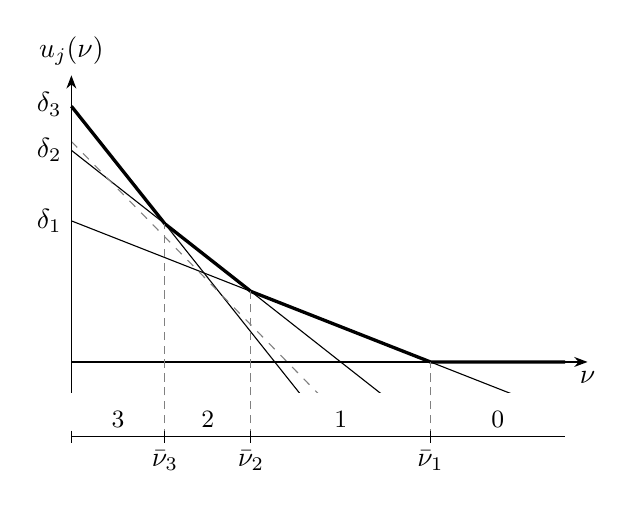
\begin{tikzpicture}[x=2.85cm,y=1.12cm,>=Stealth]
  \begin{scope}
    \clip (0,-0.35) rectangle (2.2,3.15);
    \draw[thin] (0,1.6) -- (2.2,-0.6);
    \draw[thin] (0,2.4) -- (1.7,-1.0);
    \draw[thin] (0,2.9) -- (1.21875,-1.0);
    \draw[thin, gray, dashed] (0,2.5) -- (1.3462,-1.0);
  \end{scope}
  \draw[->] (0,0) -- (2.3,0) node[below] {$\nu$};
  \draw[->] (0,-0.35) -- (0,3.25) node[above] {$u_j(\nu)$};
  \draw[very thick] (0,2.9) -- (0.416667,1.566667) -- (0.8,0.8) -- (1.6,0) -- (2.2,0);
  \node[left] at (0,1.6) {$\delta_1$};
  \node[left] at (0,2.4) {$\delta_2$};
  \node[left] at (0,2.92) {$\delta_3$};
  \draw (0,-0.85) -- (2.2,-0.85);
  \foreach \c in {0.416667, 0.8, 1.6} {
    \draw[densely dashed, gray] (\c,-0.85) -- (\c,{max(0,2.9-3.2*\c,2.4-2*\c,1.6-\c)});
    \draw (\c,-0.78) -- (\c,-0.92);
  }
  \draw (0,-0.78) -- (0,-0.92);
  \node[below] at (0.416667,-0.9) {$\bar\nu_3$};
  \node[below] at (0.8,-0.9) {$\bar\nu_2$};
  \node[below] at (1.6,-0.9) {$\bar\nu_1$};
  \node[above] at (0.208,-0.85) {\small $3$};
  \node[above] at (0.608,-0.85) {\small $2$};
  \node[above] at (1.2,-0.85) {\small $1$};
  \node[above] at (1.9,-0.85) {\small $0$};
\end{tikzpicture}
\caption{Utility lines and the upper envelope}
\end{subfigure}\hfill
\begin{subfigure}[b]{0.45\textwidth}
\centering
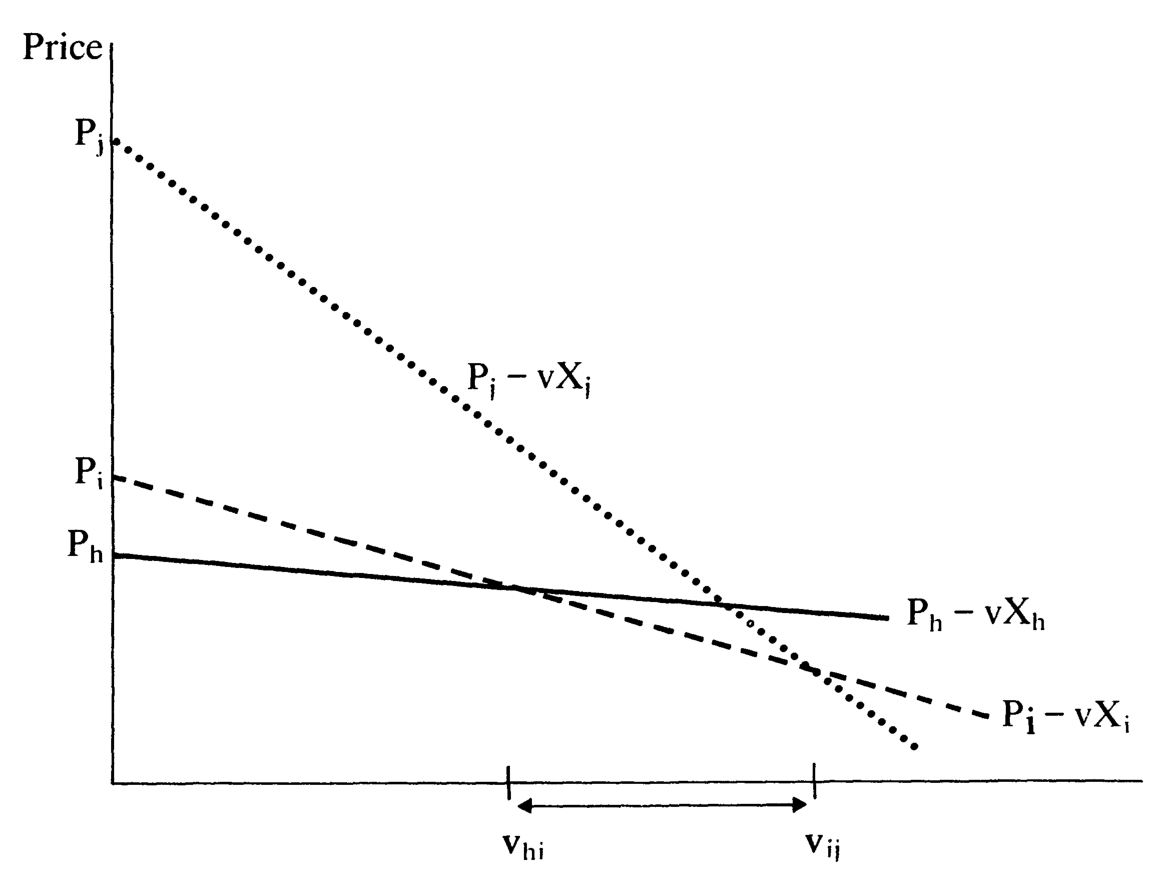
\includegraphics[width=\linewidth]{figures/ch06/bresnahan1987_fig1.png}
\caption{Total price lines in Bresnahan's form}
\end{subfigure}
\caption{Utility lines and cutoffs in the vertical model. (a) The utility $u_j(\nu) = \delta_j - \nu p_j$ of each
product is a line with intercept $\delta_j$ and slope $-p_j$, and the outside good is the horizontal axis.
The products are those of \cref{fig:06-frontier}. The bold upper envelope gives the chosen product, and
adjacent lines cross at the cutoffs $\bar\nu_3 < \bar\nu_2 < \bar\nu_1$, here $0.42$, $0.8$ and $1.6$. The
strip below the axis shows the product chosen on each interval of $\nu$. The dashed gray line is product
$b$, which never reaches the envelope. (b) The same construction in the form
$\frac{u_{ij}}{\nu_i} = v_i\delta_j - p_j$ used by \citet{Bresnahan1987}. A consumer with taste for quality
$v = \frac{1}{\nu}$ buys the product with the lowest total price $P - vX$, where Bresnahan writes $P$ for price and $X$ for
quality. Product $i$ is bought on the
marked interval $[v_{hi}, v_{ij}]$. Because $v$ is the reciprocal of $\nu$, the order of products along the
horizontal axis is reversed. Source: Bresnahan (1987), Figure 1.}
\label{fig:06-ulines}
\end{figure}

Without the frontier assumption, the same logic gives a single formula that holds for any qualities
\citep[eqs.~14--17]{BerryPakes2007}. Keep all products ordered by price, but let qualities be arbitrary.
Product $j$ beats product $k$ if and only if $\nu(p_j - p_k) < \delta_j - \delta_k$. For a cheaper product
$k < j$, dividing by $p_j - p_k > 0$ gives $\nu < \frac{\delta_j - \delta_k}{p_j - p_k}$. For a more expensive
product $k > j$, dividing by $p_j - p_k < 0$ reverses the inequality and gives
$\nu > \frac{\delta_k - \delta_j}{p_k - p_j}$. Product $j$ is chosen if and only if
$\underline\nu_j(\delta, p) < \nu < \bar\nu_j(\delta, p)$, where
\begin{equation}\label{eq:06-bp-cutoffs}
  \bar\nu_j(\delta, p) = \min_{k < j} \frac{\delta_j - \delta_k}{p_j - p_k}, \qquad
  \underline\nu_j(\delta, p) = \max_{k > j} \frac{\delta_k - \delta_j}{p_k - p_j},
\end{equation}
with the conventions $\bar\nu_0(\delta, p) = \infty$ and $\underline\nu_J(\delta, p) = 0$. The share of
product $j$ is
\begin{equation}\label{eq:06-bp-share}
  s_j = \big[F(\bar\nu_j(\delta, p)) - F(\underline\nu_j(\delta, p))\big]\,
        \indic\big\{\bar\nu_j(\delta, p) > \underline\nu_j(\delta, p)\big\}.
\end{equation}
\citet{BerryPakes2007} write these cutoffs as $\overline\Delta_j$ and $\underline\Delta_j$ and the price
sensitivity as $\alpha_i$.

\begin{remark}[General and adjacent cutoffs]\label{rem:06-general-cutoffs}
Formula \eqref{eq:06-bp-share} has three useful properties. First, for a product on the frontier,
$\bar\nu_j(\delta,p) = \bar\nu_j$ and $\underline\nu_j(\delta,p) = \bar\nu_{j+1}$, the adjacent cutoffs of
\eqref{eq:06-cutoff}. The slope of the chord from $j$ back to a cheaper frontier product $k$ is an average
of the edge slopes $\bar\nu_{k+1}, \dots, \bar\nu_j$. Each of these is at least $\bar\nu_j$, so the minimum is
attained at $k = j - 1$. Points below the frontier give chords at least as steep, so they do not change the minimum.
The same argument applies to the maximum. Second, the formula assigns a zero share to every product off the
frontier, so one expression serves for every parameter value. This matters in estimation, where a trial
parameter value can reorder qualities. Third, the vertical model predicts exact zero shares for some
parameter values, which models with an idiosyncratic shock never do. Since observed shares are positive,
the true parameters must place every product with positive sales on the frontier. Deleting the products
dominated outright is not enough to impose this. Product $b$ in \cref{fig:06-frontier} beats every cheaper
product in quality and still sells nothing.
\end{remark}

\subsection{Market shares}\label{sec:06-vshares}

Integrating the choice intervals over the taste distribution gives the demand system.

\begin{proposition}[Vertical market shares]\label{prop:06-vshares}
Under \cref{ass:06-vertical}, with all $J$ products on the frontier, the market shares are
\begin{equation}\label{eq:06-vshares}
  s_j = F(\bar\nu_j) - F(\bar\nu_{j+1}), \quad j = 1, \dots, J, \qquad
  s_0 = 1 - F(\bar\nu_1) = 1 - F\Big(\frac{\delta_1}{p_1}\Big),
\end{equation}
with $F(\bar\nu_{J+1}) = F(0) = 0$. Quantities are $q_j = M s_j$.
\end{proposition}

\begin{proof}
By \cref{prop:06-cutoffs}, $s_j = \Pr(\bar\nu_{j+1} < \nu_i < \bar\nu_j)$. Since $F$ is continuous, the end points
carry no mass, and $s_j = F(\bar\nu_j) - F(\bar\nu_{j+1})$. For the outside good, $s_0 = \Pr(\nu_i > \bar\nu_1) =
1 - F(\bar\nu_1)$. For the top product, $s_J = F(\bar\nu_J) - F(0) = F(\bar\nu_J)$. Summing over
$j = 0, \dots, J$ telescopes to one.
\end{proof}

Four features of \eqref{eq:06-vshares} recur below. Shares depend on qualities and prices only through
the $J$ cutoffs. The share of product $j$ depends only on its own price and the prices of its two
neighbors. The outside share depends only on the price and quality of the cheapest product. Zero shares
are possible, for any product off the frontier. \Cref{fig:06-nuaxis} draws the shares as areas under the
density.

\begin{figure}[htbp]
\centering
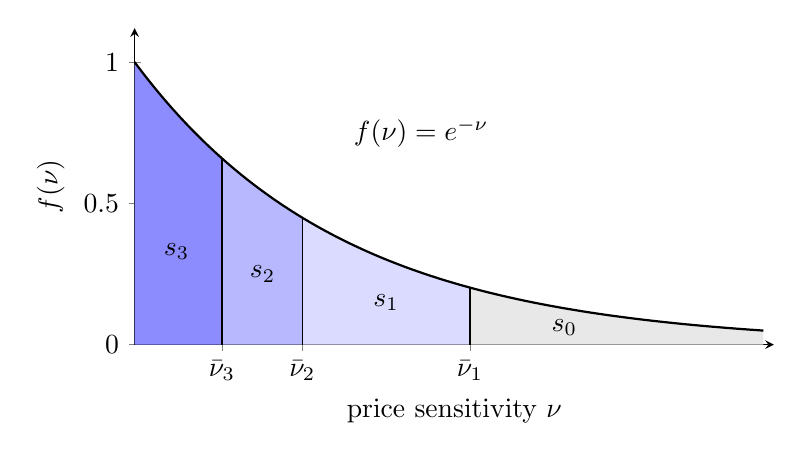
\begin{tikzpicture}
\begin{axis}[
  width=0.8\textwidth, height=5.6cm,
  xmin=0, xmax=3.05, ymin=0, ymax=1.12,
  axis lines=left,
  xlabel={price sensitivity $\nu$}, ylabel={$f(\nu)$},
  xtick={0.416667,0.8,1.6}, xticklabels={$\bar\nu_3$,$\bar\nu_2$,$\bar\nu_1$},
  ytick={0,0.5,1},
  clip=false,
]
  \addplot[name path=dens, thick, domain=0:3, samples=150] {exp(-x)};
  \path[name path=base] (axis cs:0,0) -- (axis cs:3,0);
  \addplot[fill=blue!45] fill between[of=dens and base, soft clip={domain=0:0.416667}];
  \addplot[fill=blue!28] fill between[of=dens and base, soft clip={domain=0.416667:0.8}];
  \addplot[fill=blue!14] fill between[of=dens and base, soft clip={domain=0.8:1.6}];
  \addplot[fill=gray!18] fill between[of=dens and base, soft clip={domain=1.6:3}];
  \draw[thin] (axis cs:0.416667,0) -- (axis cs:0.416667,{exp(-0.416667)});
  \draw[thin] (axis cs:0.8,0) -- (axis cs:0.8,{exp(-0.8)});
  \draw[thin] (axis cs:1.6,0) -- (axis cs:1.6,{exp(-1.6)});
  \node at (axis cs:0.2,0.33) {$s_3$};
  \node at (axis cs:0.61,0.25) {$s_2$};
  \node at (axis cs:1.2,0.15) {$s_1$};
  \node at (axis cs:2.05,0.06) {$s_0$};
  \node[anchor=west] at (axis cs:1.0,0.75) {$f(\nu) = e^{-\nu}$};
\end{axis}
\end{tikzpicture}
\caption{Market shares as areas under the taste density. The density is exponential with mean one, and the
cutoffs are those of \cref{fig:06-ulines}, $\bar\nu_3 = 0.42$, $\bar\nu_2 = 0.8$ and $\bar\nu_1 = 1.6$. The least
price-sensitive consumers buy the top product. The shares are $s_3 = 0.341$, $s_2 = 0.210$, $s_1 = 0.247$
and $s_0 = 0.202$.}
\label{fig:06-nuaxis}
\end{figure}

\begin{example}[Uniform tastes for quality]\label{ex:06-uniform}
\citet{Bresnahan1987} works with the form \eqref{eq:06-vertical-v} and assumes that the taste for quality
$v_i = \frac{1}{\nu_i}$ is uniform on $[0, \bar v]$ with density $\kappa$, so the market has $M = \kappa\bar v$
consumers.\footnote{Bresnahan writes quality as $x$, the taste density as $\delta$, and the upper bound
as $V_{\max}$. We write $\delta_j$, $\kappa$ and $\bar v$ to keep the notation of this chapter.} In
$v$-space the cutoff between $j-1$ and $j$ is the reciprocal of \eqref{eq:06-cutoff},
\begin{equation*}
  v_{j-1,j} = \frac{1}{\bar\nu_j} = \frac{p_j - p_{j-1}}{\delta_j - \delta_{j-1}},
\end{equation*}
and consumers with $v > v_{j-1,j}$ prefer $j$ \citep[eq.~4]{Bresnahan1987}. The implied CDF of
$\nu = \frac{1}{v}$ is
\begin{equation*}
  F(\nu) = \Pr\Big(v \ge \frac{1}{\nu}\Big) = 1 - \frac{1}{\bar v\,\nu}, \qquad \nu \ge \frac{1}{\bar v},
\end{equation*}
and zero below $\frac{1}{\bar v}$. Substituting into \eqref{eq:06-vshares},
\begin{equation*}
  s_j = \Big[1 - \frac{1}{\bar v\,\bar\nu_j}\Big] - \Big[1 - \frac{1}{\bar v\,\bar\nu_{j+1}}\Big]
      = \frac{1}{\bar v}\big(v_{j,j+1} - v_{j-1,j}\big),
\end{equation*}
so that $q_j = M s_j = \kappa\,(v_{j,j+1} - v_{j-1,j})$, or
\begin{equation}\label{eq:06-vuniform-demand}
  q_j = \kappa\Big[\frac{p_{j+1} - p_j}{\delta_{j+1} - \delta_j} - \frac{p_j - p_{j-1}}{\delta_j - \delta_{j-1}}\Big],
  \qquad
  q_J = \kappa\Big[\bar v - \frac{p_J - p_{J-1}}{\delta_J - \delta_{J-1}}\Big].
\end{equation}
These are equations (10) and (11) of \citet{Bresnahan1987}. Demand is linear in prices because the
cutoffs in $v$-space are linear in prices. The support of $\nu$ starts at $\frac{1}{\bar v}$ instead of
zero, so the top product sells only if $v_{J-1,J} < \bar v$. Bresnahan assumes that the consumer with the
highest taste, $\bar v$, always buys a car. In his application the alternative to a new car is a used
car of quality $\delta_{\mathrm u}$ and price $p_{\mathrm u}$, which replaces the origin as the point
$(p_0, \delta_0)$ (\cref{sec:06-vext}).
\end{example}

\subsection{Inverting market shares}\label{sec:06-vinversion}

Estimation requires the reverse map, from observed shares to qualities (\cref{sec:06-inversion-idea}). In
the vertical model the inverse exists, is unique, and has a closed form. Let
\begin{equation}\label{eq:06-cumshare}
  S_j = \sum_{k \ge j} s_k, \qquad j = 1, \dots, J,
\end{equation}
be the \emph{cumulative share from the top}, the share of consumers who buy product $j$ or a more
expensive product.

\begin{proposition}[Inversion]\label{prop:06-vinversion}
Under \cref{ass:06-vertical}, let the prices satisfy $0 < p_1 < \dots < p_J$ and let the observed shares
$s_j = \frac{q_j}{M}$ be positive for $j = 1, \dots, J$, with $s_0 = 1 - \sum_j s_j > 0$. There is exactly
one quality vector $\delta$ under which all $J$ products lie on the frontier and the predicted shares
\eqref{eq:06-vshares} equal the observed shares. It is given by
\begin{align}
  \bar\nu_j &= F^{-1}(S_j), \label{eq:06-vinv-cut}\\
  \delta_j &= \delta_{j-1} + (p_j - p_{j-1})\,F^{-1}(S_j), \qquad \delta_0 = 0, \label{eq:06-vinv-rec}\\
  \delta_j &= \sum_{m=1}^{j} (p_m - p_{m-1})\, F^{-1}\Big(\sum_{k \ge m} s_k\Big). \label{eq:06-vinv-sum}
\end{align}
\end{proposition}

\begin{proof}
The first step sums shares from the top. Under \eqref{eq:06-vshares},
\begin{equation*}
  S_j = \sum_{k=j}^{J} \big[F(\bar\nu_k) - F(\bar\nu_{k+1})\big] = F(\bar\nu_j) - F(\bar\nu_{J+1}) = F(\bar\nu_j).
\end{equation*}
The second step proves uniqueness. Because $F$ is continuous and strictly increasing on $(0,\infty)$, its
inverse $F^{-1}$ is well defined on $(0,1)$. Each $S_j$ lies in $(0,1)$, since $s_J > 0$ and
$1 - S_1 = s_0 > 0$. Hence $\bar\nu_j = F^{-1}(S_j)$ is the only cutoff consistent with the data. The
definition \eqref{eq:06-cutoff} gives $\delta_j - \delta_{j-1} = (p_j - p_{j-1})\bar\nu_j$, which is
\eqref{eq:06-vinv-rec}. Starting from $\delta_0 = 0$ and iterating gives \eqref{eq:06-vinv-sum}, so every
quality is pinned down.

The third step proves existence. Define $\delta$ by \eqref{eq:06-vinv-sum}. All shares are positive, so
$S_1 > S_2 > \dots > S_J > 0$. Because $F^{-1}$ is strictly increasing, $\bar\nu_1 > \bar\nu_2 > \dots > \bar\nu_J
> 0$. Qualities then increase with price and the cutoffs decrease, so by \cref{prop:06-frontier} every
product lies on the frontier. \Cref{prop:06-vshares} gives predicted shares
$F(\bar\nu_j) - F(\bar\nu_{j+1}) = S_j - S_{j+1} = s_j$.
\end{proof}

Several consequences follow. The price ordering determines the quality ordering, so the data reveal the
ranking of products without any parameter. Every vector of positive shares is rationalized by some quality
vector, whatever the increasing distribution $F$. A single market's prices and shares therefore never
reject the vertical model. Its testable content comes from restrictions across products and markets, such
as $\delta_{jt} = x_{jt}\beta + \xi_{jt}$, and from the supply side.

The result is an instance of the general invertibility theory of \citet{BerryGandhiHaile2013}. On the set
of qualities at which every product sells, raising $\delta_j$ raises $\bar\nu_j$ and lowers $\bar\nu_{j+1}$.
It therefore raises $s_j$, lowers $s_{j-1}$ and $s_{j+1}$ (or $s_0$ when $j = 1$), and leaves every other
share unchanged. Inside goods are weak substitutes in this sense. The chain $0, 1, \dots, J$ of strict
substitution between neighbors connects every inside good to the outside good. These are the ``connected
substitutes'' conditions under which \citet{BerryGandhiHaile2013} prove that demand is invertible. The
proof above exploits the special structure and also delivers the inverse in closed form.

Market size enters through every share. Holding unit sales fixed, a larger $M$ lowers every cumulative
share $S_j$, which lowers every cutoff and every quality. A market with more nonbuyers is rationalized by
products that are worse relative to the outside good. The choice of $M$ is an assumption, and it
matters for the level of the recovered qualities.

\begin{example}[Exponential tastes]\label{ex:06-exponential}
Let $F(\nu) = 1 - e^{-\lambda\nu}$ with $\lambda > 0$, so that $\E[\nu_i] = \frac{1}{\lambda}$. Solving
$u = 1 - e^{-\lambda\nu}$ for $\nu$ gives
\begin{equation*}
  F^{-1}(u) = -\frac{1}{\lambda}\ln(1 - u).
\end{equation*}
Substituting into \eqref{eq:06-vinv-sum},
\begin{equation}\label{eq:06-vexp-delta}
  \delta_j = -\frac{1}{\lambda}\sum_{m=1}^{j}(p_m - p_{m-1})\ln(1 - S_m),
  \qquad 1 - S_m = s_0 + \sum_{l < m} s_l ,
\end{equation}
where $1 - S_m$ is the share of consumers who buy the outside good or a product cheaper than $m$. Now let
there be markets $t = 1, \dots, T$, and let $(m)$ denote the $m$-th cheapest product of market $t$. For the
product $j$ that occupies position $k$ in market $t$, define the observable
\begin{equation}\label{eq:06-vexp-y}
  y_{jt} \equiv -\sum_{m=1}^{k}\big(p_{(m)t} - p_{(m-1)t}\big)\ln(1 - S_{mt}),
\end{equation}
which uses prices and shares only. By \eqref{eq:06-vexp-delta}, $y_{jt} = \lambda\delta_{jt}$. Substituting
$\delta_{jt} = x_{jt}\beta + \xi_{jt}$ gives the estimable equation
\begin{equation}\label{eq:06-vexp-reg}
  y_{jt} = x_{jt}(\lambda\beta) + \lambda\xi_{jt} .
\end{equation}
\end{example}

\begin{proposition}[Scale of tastes]\label{prop:06-vscale}
In \cref{ex:06-exponential}, $\lambda$ is not identified. For every $c > 0$ the parameters
$(\lambda, \beta, \xi)$ and $(\frac{\lambda}{c}, c\beta, c\xi)$ imply the same choice for every consumer and
hence the same shares. More generally, for any $F$, the pairs $(F(\cdot), \delta)$ and
$(F(\frac{\cdot}{c}), c\delta)$ are observationally equivalent.
\end{proposition}

\begin{proof}
Let $\nu$ have CDF $F$ and define $\nu' = c\nu$. Then $\Pr(\nu' \le x) = \Pr(\nu \le \frac{x}{c}) = F(\frac{x}{c})$.
A consumer of type $\nu$ facing qualities $\delta$ compares $\delta_j - \nu p_j$ across products. Multiplying
by $c > 0$ gives
\begin{equation*}
  c\delta_j - (c\nu)p_j = c\delta_j - \nu' p_j ,
\end{equation*}
which ranks products in the same order. So a consumer of type $\nu'$ facing qualities $c\delta$ makes the
same choice as a consumer of type $\nu$ facing $\delta$. Integrating over types, the shares under
$(F(\frac{\cdot}{c}), c\delta)$ equal those under $(F, \delta)$. For the exponential distribution,
$F(\frac{x}{c}) = 1 - e^{-\frac{\lambda}{c}x}$ is exponential with parameter $\frac{\lambda}{c}$, and
$c\delta_j = x_j(c\beta) + c\xi_j$.
\end{proof}

The economic content is that choices reveal quality only in units of willingness to pay. Doubling every
quality and doubling every consumer's price sensitivity describes the same consumers making the same
choices. This is the scale normalization of \cref{sec:06-normalization} in the vertical model. We set
$\lambda = 1$, so that $\E[\nu_i] = 1$. A consumer with the mean price sensitivity then values one unit of
quality at one dollar, and \eqref{eq:06-vexp-reg} becomes $y_{jt} = x_{jt}\beta + \xi_{jt}$.

With $\lambda = 1$ the demand parameters are identified under two conditions. The first is the moment
condition $\E[x_{jt}^\top\xi_{jt}] = 0$, and the second is full rank of $\E[x_{jt}^\top x_{jt}]$. Then
$\beta = \E[x_{jt}^\top x_{jt}]^{-1}\E[x_{jt}^\top y_{jt}]$, and the OLS regression of $y_{jt}$ on $x_{jt}$ is
consistent. Price is not a regressor. It enters only the construction of $y_{jt}$, an exact function of
observed prices and shares. Firms that observe $\xi_{jt}$ set higher prices for better products, so
$p_{jt}$ and $\xi_{jt}$ are correlated. This correlation does not bias the regression, because the vertical
model has no price coefficient left to estimate. The normalized distribution $F$ plays the role of the
price coefficient. It states how many consumers have each price sensitivity, and nothing about it remains
unknown. Standard errors should be clustered by market. The values $y_{jt}$ of products in the same market
are built from the same cumulative shares. Any sampling error in observed shares, or any misspecification of $F$,
therefore enters the errors of all products in a market and accumulates along the price ladder.

The same feature is the model's main weakness. With $F$ fully specified, every substitution pattern is
determined by functional form and by the observed prices and shares (\cref{prop:06-vmarkup-data} below).
Exogenous variation in prices is never used to learn how demand responds to prices. Two further cautions
apply. The moment condition fails if firms choose characteristics with knowledge of $\xi_{jt}$
(\cref{sec:06-charspace}). If $F$ is misspecified, $y_{jt}$ differs from $\delta_{jt}$ by a function of
prices and shares, and the regression error inherits that function.

\begin{remark}[Shape parameters and instruments]\label{rem:06-vshape}
Suppose that after the scale normalization $F$ still has an unknown shape parameter. An example is
$\ln\nu_i \sim N(0, \sigma^2)$, whose median is fixed at one. With $\Phi$ the standard normal CDF,
$F_\sigma^{-1}(u) = \exp(\sigma\Phi^{-1}(u))$, and the inversion gives
\begin{equation*}
  \delta_{jt}(\sigma) = \sum_{m=1}^{k}\big(p_{(m)t} - p_{(m-1)t}\big)\exp\big(\sigma\,\Phi^{-1}(S_{mt})\big).
\end{equation*}
For any trial value of $\sigma$, OLS of $\delta_{jt}(\sigma)$ on $x_{jt}$ produces residuals orthogonal to
$x_{jt}$. The $K$ moments $\E[x_{jt}^\top\xi_{jt}] = 0$ therefore cannot determine the $K + 1$ parameters
$(\beta, \sigma)$. Identification of $\sigma$ requires at least one excluded instrument $z_{jt}$. This is a variable
uncorrelated with $\xi_{jt}$ that moves prices or shares, such as a cost shifter or a characteristic of
rival products. Stack the instruments in $Z_{jt} = (x_{jt}, z_{jt})$ and define
$\xi_{jt}(\sigma, \beta) = \delta_{jt}(\sigma) - x_{jt}\beta$. The GMM estimator uses
$\E[Z_{jt}^\top\xi_{jt}(\sigma,\beta)] = 0$. For fixed $\sigma$ the estimate of $\beta$ is the linear IV
estimator
\begin{equation*}
  \hat\beta(\sigma) = (X^\top Z W Z^\top X)^{-1} X^\top Z W Z^\top\delta(\sigma),
\end{equation*}
where $X$, $Z$ and $\delta(\sigma)$ stack the observations and $W$ is a weighting matrix. Concentrating out
$\beta$ leaves a search over $\sigma$ alone,
\begin{equation*}
  \hat\sigma = \argmin_{\sigma}\; g_N(\sigma)^\top W g_N(\sigma), \qquad
  g_N(\sigma) = \frac{1}{N}\sum_{j,t} Z_{jt}^\top\big(\delta_{jt}(\sigma) - x_{jt}\hat\beta(\sigma)\big).
\end{equation*}
This is the structure of the estimator for the nonlinear parameters $\theta_2$ in \cref{ch:blp}. Price
endogeneity now matters. Prices enter $\delta_{jt}(\sigma)$ in a way that depends on $\sigma$, so the
instruments must move prices independently of $\xi_{jt}$. Standard errors are again clustered by market.
\end{remark}

The uniform model of \cref{ex:06-uniform} inverts in the same way. Summing \eqref{eq:06-vuniform-demand} from
the top gives $\sum_{k \ge j} q_k = \kappa(\bar v - v_{j-1,j})$. Dividing by $M = \kappa\bar v$ gives
$v_{j-1,j} = \bar v(1 - S_j)$, so
\begin{equation*}
  \delta_j - \delta_{j-1} = \frac{p_j - p_{j-1}}{\bar v(1 - S_j)} .
\end{equation*}
Given the market size, $\bar v$ only sets the units of quality, in line with \cref{prop:06-vscale}.

\subsection{Substitution patterns}\label{sec:06-vsubst}

We now hold qualities fixed and differentiate shares with respect to prices. Each price enters only the
two cutoffs that involve its product. Differentiating \eqref{eq:06-cutoff},
\begin{align*}
  \frac{\partial\bar\nu_j}{\partial p_j} &= -\frac{\delta_j - \delta_{j-1}}{(p_j - p_{j-1})^2} = -\frac{\bar\nu_j}{p_j - p_{j-1}},
  &
  \frac{\partial\bar\nu_j}{\partial p_{j-1}} &= \frac{\delta_j - \delta_{j-1}}{(p_j - p_{j-1})^2} = \frac{\bar\nu_j}{p_j - p_{j-1}},
\end{align*}
and, shifting the index,
\begin{equation*}
  \frac{\partial\bar\nu_{j+1}}{\partial p_j} = \frac{\bar\nu_{j+1}}{p_{j+1} - p_j},
  \qquad
  \frac{\partial\bar\nu_{j+1}}{\partial p_{j+1}} = -\frac{\bar\nu_{j+1}}{p_{j+1} - p_j}.
\end{equation*}
A higher own price lowers the upper cutoff of $j$ and raises its lower cutoff, so the interval of buyers
shrinks from both ends. It is convenient to define
\begin{equation}\label{eq:06-gj}
  g_j = f(\bar\nu_j)\,\frac{\bar\nu_j}{p_j - p_{j-1}} > 0, \quad j = 1, \dots, J, \qquad g_{J+1} = 0 .
\end{equation}
The number $g_j$ is the density of consumers at the boundary between $j - 1$ and $j$, times the speed at
which that boundary moves when either price changes.

\begin{proposition}[Price derivatives]\label{prop:06-vderiv}
Under \cref{ass:06-vertical}, with all products on the frontier and qualities held fixed,
\begin{align}
  \frac{\partial s_j}{\partial p_j} &= -g_j - g_{j+1}
     = -\frac{f(\bar\nu_j)\bar\nu_j}{p_j - p_{j-1}} - \frac{f(\bar\nu_{j+1})\bar\nu_{j+1}}{p_{j+1} - p_j}, \label{eq:06-vown}\\
  \frac{\partial s_j}{\partial p_{j-1}} &= g_j, \qquad \frac{\partial s_j}{\partial p_{j+1}} = g_{j+1}, \qquad
  \frac{\partial s_j}{\partial p_k} = 0 \ \text{ for } |k - j| \ge 2, \label{eq:06-vcross}\\
  \frac{\partial s_0}{\partial p_1} &= g_1, \qquad \frac{\partial s_0}{\partial p_k} = 0 \ \text{ for } k \ge 2.
  \label{eq:06-voutside}
\end{align}
The second term of \eqref{eq:06-vown} is absent for the top product. The $J \times J$ Jacobian $\Delta^s$ with
$\Delta^s_{jk} = \frac{\partial s_j}{\partial p_k}$ is tridiagonal and symmetric, with
$\Delta^s_{j,j+1} = \Delta^s_{j+1,j} = g_{j+1}$. Each column of the $(J+1) \times J$ matrix that adds the outside-good
row sums to zero.
\end{proposition}

\begin{proof}
Write $s_j = F(\bar\nu_j) - F(\bar\nu_{j+1})$. The price $p_j$ enters $\bar\nu_j$ and $\bar\nu_{j+1}$ only, so by the
chain rule
\begin{equation*}
  \frac{\partial s_j}{\partial p_j} = f(\bar\nu_j)\frac{\partial\bar\nu_j}{\partial p_j} - f(\bar\nu_{j+1})\frac{\partial\bar\nu_{j+1}}{\partial p_j}
  = -f(\bar\nu_j)\frac{\bar\nu_j}{p_j - p_{j-1}} - f(\bar\nu_{j+1})\frac{\bar\nu_{j+1}}{p_{j+1} - p_j}.
\end{equation*}
The price $p_{j-1}$ enters $s_j$ only through $\bar\nu_j$, so $\frac{\partial s_j}{\partial p_{j-1}} =
f(\bar\nu_j)\frac{\bar\nu_j}{p_j - p_{j-1}} = g_j$. The price $p_{j+1}$ enters $s_j$ only through $\bar\nu_{j+1}$,
so
\begin{equation*}
  \frac{\partial s_j}{\partial p_{j+1}} = -f(\bar\nu_{j+1})\frac{\partial\bar\nu_{j+1}}{\partial p_{j+1}}
  = f(\bar\nu_{j+1})\frac{\bar\nu_{j+1}}{p_{j+1} - p_j} = g_{j+1}.
\end{equation*}
No other price enters $s_j$. For the outside good, $s_0 = 1 - F(\bar\nu_1)$ with $\bar\nu_1 = \frac{\delta_1}{p_1}$,
so $\frac{\partial s_0}{\partial p_1} = f(\bar\nu_1)\frac{\bar\nu_1}{p_1} = g_1$. Symmetry follows by comparing
$\Delta^s_{j,j+1} = g_{j+1}$ with $\Delta^s_{j+1,j} = \frac{\partial s_{j+1}}{\partial p_j} = g_{j+1}$, the second identity
in \eqref{eq:06-vcross} applied to product $j+1$. Column $k$ has the entries $g_k$ in row $k - 1$ (the outside
row when $k = 1$), $-g_k - g_{k+1}$ in row $k$, and $g_{k+1}$ in row $k + 1$. They sum to zero.
\end{proof}

Symmetry has a simple reading. The number $g_{j+1}$ measures the consumers at the boundary between $j$
and $j + 1$. A small rise in $p_j$ moves these marginal consumers from $j$ to $j + 1$, and an equal rise in
$p_{j+1}$ moves the same consumers back. The flow across a shared boundary is the same in both directions.
Symmetry also follows from the envelope argument behind \cref{thm:06-wdz}. Dividing utility by $\nu_i$ gives
$\frac{u_{ij}}{\nu_i} = \frac{\delta_j}{\nu_i} - p_j$, which is quasi-linear in money for each consumer.
Aggregate consumer surplus $CS(p) = M\,\E\big[\max_j(\frac{\delta_j}{\nu_i} - p_j)\big]$ therefore satisfies
$\frac{\partial CS}{\partial p_j} = -q_j$, and the symmetry of its second derivatives gives
$\frac{\partial q_j}{\partial p_k} = \frac{\partial q_k}{\partial p_j}$. The zero column sums say that a price
change only reallocates the $M$ consumers among the alternatives.

The structure of $\Delta^s$ has further consequences used in \cref{sec:06-vpricing}. In row $j$ with
$2 \le j \le J$, the off-diagonal entries $g_j$ and $g_{j+1}$ sum to $|\Delta^s_{jj}|$. In the first row,
$|\Delta^s_{11}| = g_1 + g_2$ exceeds the single off-diagonal entry $g_2$, because product 1 also loses consumers
to the outside good. So $\Delta^s$ is weakly diagonally dominant, strictly so in the first row. Because $\Delta^s$ is
tridiagonal with nonzero off-diagonal entries, it is also irreducible. An irreducible matrix that is weakly
diagonally dominant with at least one strictly dominant row is nonsingular \citep[ch.~6]{BermanPlemmons1994}.
\Cref{lem:06-mmatrix} in \cref{sec:06-bres-equilibrium} states and proves this fact in the form we need.

The \emph{diversion ratio} from $j$ to $k$ is the fraction of the consumers lost by $j$ after a price
increase who switch to $k$ (\cref{ch:diffprod}). We write it $D_{jk} = -\frac{\Delta^s_{kj}}{\Delta^s_{jj}}$. Here
\begin{equation*}
  D_{j,j-1} = \frac{g_j}{g_j + g_{j+1}}, \qquad
  D_{j,j+1} = \frac{g_{j+1}}{g_j + g_{j+1}},
\end{equation*}
and all other diversion ratios are zero. Every consumer who leaves $j$ goes to a price neighbor, with the
outside good counting as the lower neighbor of product 1.

We write the elasticity of the share of $j$ with respect to the price of $k$ as
$\varepsilon_{jk} = \frac{\partial s_j}{\partial p_k}\frac{p_k}{s_j}$. The diagonal entries are negative, and the
own-price elasticity in the positive convention of the book is $\varepsilon_j = -\varepsilon_{jj} =
\frac{(g_j + g_{j+1})p_j}{s_j}$. The outside good has the single nonzero elasticity
$\varepsilon_{01} = \frac{g_1 p_1}{s_0}$.

Closeness in price means closeness in substitution. Holding a cutoff fixed, the cross derivative
$g_{j+1} = f(\bar\nu_{j+1})\frac{\bar\nu_{j+1}}{p_{j+1} - p_j}$ grows without bound as $p_{j+1} - p_j \to 0$, and the
own derivatives of both products grow with it. In the data the cutoff is pinned down by shares through
$\bar\nu_{j+1} = F^{-1}(S_{j+1})$. Two products that sell at nearly the same price are therefore read as
near-perfect substitutes, whatever the products are. With uniform tastes the derivatives are constant.
Using $f(\nu) = \frac{1}{\bar v\nu^2}$ from \cref{ex:06-uniform},
\begin{equation*}
  M g_j = \kappa\bar v\cdot\frac{1}{\bar v\,\bar\nu_j^2}\cdot\frac{\bar\nu_j}{p_j - p_{j-1}}
        = \frac{\kappa}{\bar\nu_j(p_j - p_{j-1})} = \frac{\kappa}{\delta_j - \delta_{j-1}} .
\end{equation*}
Hence $\frac{\partial q_j}{\partial p_j} = -\kappa\big(\frac{1}{\delta_j - \delta_{j-1}} + \frac{1}{\delta_{j+1} - \delta_j}\big)$
and $\frac{\partial q_{j\pm1}}{\partial p_j} = \frac{\kappa}{|\delta_{j\pm1} - \delta_j|}$. Demand is linear, and the
quality gap measures how close two products are. In Bresnahan's words, the products are perfect
substitutes ``in the limit as $x_i$ goes to $x_h$,'' where $x$ is his notation for quality
\citep[p.~462]{Bresnahan1987}.

Is this a reasonable model of substitution? The restriction that only price neighbors substitute is
strong. A price cut on a mid-size sedan has no effect on a model two steps away on the price ladder,
however similar the two cars are physically. Conversely, a minivan and a sports car at the same price are
treated as close substitutes because they are neighbors on the ladder. The restriction is natural where
quality is essentially one-dimensional, as with airline cabins or storage tiers. It is also the source of
the power of the conduct test in \cref{sec:06-bresnahan}. Where products differ along several dimensions,
it can mislead badly.

A simulated illustration shows how badly (\cref{app:problems}). Market data are generated by a random
coefficients logit model in 100 markets, each offering between four and nine of ten products. The vertical
model with exponential tastes and $\lambda = 1$ is then fitted to these data. In one market the fitted own-price
elasticities $\varepsilon_{jj}$ range from $-358.4$ to $-16.8$, while the true $\varepsilon_{jj}$ range from $-3.85$
to $-2.57$. The largest
elasticities belong to products whose price neighbor sells at almost the same price. The two products with the
largest elasticities in that market are price neighbors whose prices differ by only 0.019. Across all markets, the median gap between
adjacent prices is 0.057, and 58 of the 554 gaps are below 0.01. The vertical model can explain why
consumers split across products with similar prices only by placing those products almost on top of each
other in quality. Under multi-product Nash pricing it then implies a mean markup of 0.048, against a true
mean markup of 0.386.

\subsection{Pricing and recovering marginal costs}\label{sec:06-vpricing}

Firms indexed by $f$ own disjoint sets of products $\mathcal J_f$ and produce at constant marginal costs
$mc_j$. Firm
$f$ chooses the prices of its products to maximize $M\sum_{k \in \mathcal J_f}(p_k - mc_k)s_k(p)$. The
first-order condition for $p_j$, $j \in \mathcal J_f$, is
\begin{equation*}
  s_j + \sum_{k \in \mathcal J_f}(p_k - mc_k)\frac{\partial s_k}{\partial p_j} = 0 .
\end{equation*}
With the ownership matrix $\Omega$ ($\Omega_{jk} = 1$ if $j$ and $k$ have the same owner) and $\odot$ the
element-wise product, the conditions stack into
\begin{equation}\label{eq:06-vfoc-matrix}
  s + (\Omega \odot \Delta^{s\top})(p - mc) = 0
  \qquad\Longrightarrow\qquad
  mc = p + (\Omega \odot \Delta^{s\top})^{-1}s ,
\end{equation}
the multi-product markup formula of \cref{ch:diffprod}. By \cref{prop:06-vderiv}, the condition for product
$j$ involves only its neighbors. Writing $m_j = p_j - mc_j$ for the markup,
\begin{equation}\label{eq:06-vfoc}
  s_j - (g_j + g_{j+1})\,m_j + \Omega_{j,j+1}\,g_{j+1}\,m_{j+1} + \Omega_{j,j-1}\,g_j\,m_{j-1} = 0,
\end{equation}
with $\Omega_{1,0} = 0$ because the outside good earns no markup. A single-product firm sets
$m_j = \frac{s_j}{g_j + g_{j+1}}$, which is the inverse elasticity rule $\frac{m_j}{p_j} = \frac{1}{\varepsilon_j}$.
Equation \eqref{eq:06-vfoc} is the general-$F$ version of the conduct equation that \citet{Bresnahan1987}
estimates (\cref{sec:06-bresnahan}).

\begin{corollary}[Only neighbors' ownership matters]\label{cor:06-neighbors}
Under the conditions of \cref{prop:06-vderiv}, the matrix $\Omega \odot \Delta^{s\top}$ is block diagonal. Each
block corresponds to a maximal run of consecutive products with the same owner. Two ownership structures
that agree on which adjacent pairs share an owner imply the same first-order conditions, and hence the
same markups and implied marginal costs. Moreover, $\Omega \odot \Delta^{s\top}$ is nonsingular, and the markups
$m = -(\Omega \odot \Delta^{s\top})^{-1}s$ are positive.
\end{corollary}

\begin{proof}
Because $\Delta^{s\top}$ is tridiagonal, $(\Omega \odot \Delta^{s\top})_{jk} = \Omega_{jk}\Delta^s_{kj}$ vanishes unless $|j - k| \le 1$.
For $|j - k| = 1$ it equals $g_{\max\{j,k\}}$ if the two products share an owner and zero otherwise. So the
matrix depends on $\Omega$ only through the entries $\Omega_{j,j+1}$, and it breaks into blocks at every
adjacent pair with different owners. Within a block that starts at product $a$, the first row has diagonal
entry $-(g_a + g_{a+1})$ and off-diagonal entry $g_{a+1}$, so it is strictly diagonally dominant by
$g_a > 0$. The other rows are weakly dominant, as in the discussion after \cref{prop:06-vderiv}. Each block
is tridiagonal with nonzero off-diagonal entries, hence irreducible. The negative of each block therefore
has a positive diagonal, nonpositive off-diagonal entries, nonnegative row sums and a strictly positive
first row sum. By \cref{lem:06-mmatrix}(a) it is a nonsingular M-matrix whose inverse has positive entries. Since $s > 0$, the markups $m = \big(-(\Omega \odot \Delta^{s\top})\big)^{-1}s$ are
positive.
\end{proof}

The corollary is a sharp prediction. A firm that owns products 1 and 3 but not product 2 prices exactly
as two independent firms would. Joint ownership raises markups only when it links products that
compete for the same marginal consumers.

The vertical model has a second, more surprising property. When $F$ is known up to scale, the markups
require no demand estimate at all.

\begin{proposition}[Markups from prices and shares]\label{prop:06-vmarkup-data}
Under \cref{ass:06-vertical}, suppose $F(\nu) = F_1(\lambda\nu)$ for a known CDF $F_1$ with density $f_1$
and an unknown scale $\lambda > 0$. Then the Jacobian $\Delta^s$, the markups $-(\Omega \odot \Delta^{s\top})^{-1}s$ and the
implied marginal costs depend only on observed prices and shares. They depend on no demand parameter,
including $\lambda$ and $\beta$. With exponential tastes,
\begin{equation}\label{eq:06-vexp-g}
  \bar\nu_j = -\frac{1}{\lambda}\ln(1 - S_j), \qquad f(\bar\nu_j) = \lambda(1 - S_j), \qquad
  g_j = \frac{-(1 - S_j)\ln(1 - S_j)}{p_j - p_{j-1}} .
\end{equation}
\end{proposition}

\begin{proof}
By \cref{prop:06-vinversion}, $\bar\nu_j = F^{-1}(S_j) = \frac{1}{\lambda}F_1^{-1}(S_j)$. The density is
$f(\nu) = \lambda f_1(\lambda\nu)$. Hence
\begin{equation*}
  f(\bar\nu_j)\,\bar\nu_j = \lambda f_1\big(F_1^{-1}(S_j)\big)\cdot\frac{1}{\lambda}F_1^{-1}(S_j)
  = f_1\big(F_1^{-1}(S_j)\big)\,F_1^{-1}(S_j),
\end{equation*}
and $g_j = \frac{f_1(F_1^{-1}(S_j))F_1^{-1}(S_j)}{p_j - p_{j-1}}$ depends on prices and shares only.
\Cref{prop:06-vderiv} builds $\Delta^s$ from the $g_j$, and \eqref{eq:06-vfoc-matrix} builds the markups and
marginal costs from $\Delta^s$, $s$ and $p$. For the exponential case, $F_1(x) = 1 - e^{-x}$, so
$F_1^{-1}(u) = -\ln(1 - u)$ and $f_1(F_1^{-1}(u)) = e^{\ln(1-u)} = 1 - u$.
\end{proof}

The scale drops out for a reason. Markups are measured in dollars, while the scale normalization concerns
the units of utility, so no choice of units can change them. The proposition has two practical
consequences. First, the supply side can be estimated without any demand estimate. The implied marginal
cost of each product is a known function of the data. Second, demand and supply share no parameter. When
the demand error $\xi_{jt}$ and the cost error $\omega_{jt}$ are independent, estimating the two equations
separately loses no efficiency. The flip side is the caution raised in \cref{sec:06-vinversion}. The
model reads market power off the spacing of prices and the cumulative shares, never off exogenous price
variation.

The supply equations take two forms, one per conduct assumption. Under marginal-cost pricing,
\begin{equation}\label{eq:06-vsupply-mc}
  p_{jt} = x_{jt}\gamma_1 + \gamma_2 z_{jt} + \omega_{jt} .
\end{equation}
Under multi-product Nash pricing,
\begin{equation}\label{eq:06-vsupply-nash}
  p_{jt} + \big[(\Omega_t \odot \Delta_t^{s\top})^{-1}s_t\big]_j = x_{jt}\gamma_1 + \gamma_2 z_{jt} + \omega_{jt} .
\end{equation}
Here $z_{jt}$ is a cost shifter excluded from demand, and $\gamma_1$ and $\gamma_2$ are cost coefficients,
unrelated to Euler's constant $\gamma_E$. Under either assumption the left side is data, so OLS under
$\E[\omega_{jt} \mid x_{jt}, z_{jt}] = 0$ estimates the cost parameters. The conduct assumption determines how
large the markup is, and so how much of the price variation across products is attributed to cost.
Comparing the two specifications is the logic of the conduct test in \cref{sec:06-bresnahan}.

\begin{remark}[Existence of a price equilibrium]\label{rem:06-vexist}
\citet[footnote~6]{Bresnahan1987} observes that a price equilibrium always exists in quality models of
this kind, while it can fail in location models. With uniform tastes, consider product $j$ as its own price
falls. Its interval of buyers widens, and at some price the next product $j + 1$ is dominated out of the
market. Demand for $j$ stays continuous at that price, because the interval of $j + 1$ shrinks continuously
to zero. The slope of demand changes from $-\kappa\big(\frac{1}{\delta_{j+1} - \delta_j} + \frac{1}{\delta_j - \delta_{j-1}}\big)$
to $-\kappa\big(\frac{1}{\delta_{j+2} - \delta_j} + \frac{1}{\delta_j - \delta_{j-1}}\big)$. The second is smaller in
absolute value, because $\delta_{j+2} - \delta_j > \delta_{j+1} - \delta_j$. So demand is flatter below the kink
than above it, and the derivative $\frac{\partial q_j}{\partial p_j}$ falls as $p_j$ rises. Demand is concave in own
price across the kink, and the same holds where the lower neighbor drops out. Profit $(p_j - mc_j)q_j$ is
then concave in $p_j$ on the range of prices at which $j$ sells with a positive markup, and it is zero beyond
that range. Profit is therefore quasi-concave, and standard fixed-point arguments give an equilibrium. In the Hotelling model with linear costs, demand jumps when a firm captures the rival's
location, and existence can fail (\cref{sec:06-hotelling}). \citet[Theorem~2]{CaplinNalebuff1991} cover general taste
densities with single-product firms. Utility must be linear in the taste parameter, as in \eqref{eq:06-vertical-v}
with type $v_i$. The density of $v_i$ must be $\rho$-concave with $\rho = -\frac{1}{2}$, the case $n = 1$ of their
assumption A2. This means that $\frac{1}{\sqrt{f}}$ is convex, a condition that every log-concave density meets
(\cref{sec:06-branches} and \cref{ch:diffprod}).
\end{remark}

\begin{example}[A worked example]\label{ex:06-vnumeric}
Three products and an outside good face exponential tastes with $\lambda = 1$. Observed prices are
$p = (1.0, 1.5, 2.5)$ and observed shares are $s = (0.20, 0.15, 0.10)$, so $s_0 = 0.55$. \Cref{tab:06-vnumeric}
reports every step, computed to more digits than shown.

The first step inverts the shares. Cumulative shares are $S = (0.45, 0.25, 0.10)$. By \eqref{eq:06-vexp-g},
the cutoffs are $\bar\nu_1 = -\ln 0.55 = 0.598$, $\bar\nu_2 = -\ln 0.75 = 0.288$ and $\bar\nu_3 = -\ln 0.90 = 0.105$.
They decrease, as \cref{prop:06-vinversion} guarantees, so all three products are on the frontier. The
recursion \eqref{eq:06-vinv-rec} gives
\begin{align*}
  \delta_1 &= 1.0 \times 0.598 = 0.598,\\
  \delta_2 &= 0.598 + 0.5 \times 0.288 = 0.742,\\
  \delta_3 &= 0.742 + 1.0 \times 0.105 = 0.847 .
\end{align*}
Recomputing the shares at these qualities with \eqref{eq:06-bp-share} returns the observed shares
exactly. Simulating two million consumers returns them up to simulation error.

The second step computes substitution. The densities at the cutoffs are $f(\bar\nu_j) = 1 - S_j = (0.55, 0.75,
0.90)$. Formula \eqref{eq:06-gj} gives $g_1 = \frac{0.55 \times 0.598}{1.0} = 0.329$, $g_2 = \frac{0.75 \times 0.288}{0.5}
= 0.432$ and $g_3 = \frac{0.90 \times 0.105}{1.0} = 0.095$. These fill the Jacobian through
\cref{prop:06-vderiv}. Product 2 has the most elastic demand, $\varepsilon_2 = 5.26$. It sits between two
neighbors, and its lower neighbor is only 0.5 away in price. Product 3, at the top, has a single
neighbor and the least elastic demand, $\varepsilon_3 = 2.37$. The outside good responds only to $p_1$.

The third step backs out markups and marginal costs under three ownership structures, holding the observed
prices and shares fixed. Under (a) single-product firms, $m_j = \frac{s_j}{g_j + g_{j+1}}$, which gives
markups of $0.263$, $0.285$ and $1.055$. Under (b) joint ownership of products 1 and 2, the boundary between
them, where $g_2 = 0.432$ is large, is internalized. The implied markups of 1 and 2 roughly triple to
$0.794$ and $0.936$. The markup of product 3 is unchanged at $1.055$, since its own first-order condition
does not change. Under (c) a single owner of all three products, the implied markups are $1.369$, $1.948$
and $3.002$. They exceed the prices, so the implied marginal costs are negative. The observed prices are
too low to be monopoly prices under this demand system, and conduct (c) is rejected by the requirement
that costs be nonnegative. Finally, joint ownership of products 1 and 3 alone reproduces the numbers of
case (a) to every digit, as \cref{cor:06-neighbors} predicts.
\end{example}

\begin{table}[htbp]
\centering
\caption{Worked example of the vertical model with exponential tastes}\label{tab:06-vnumeric}
\small
\begin{tabular}{@{}lrrrrrrr@{}}
\toprule
\multicolumn{8}{@{}l}{\emph{Panel A. Inversion}}\\
Product $j$ & $p_j$ & $s_j$ & $S_j$ & $\bar\nu_j$ & $f(\bar\nu_j)$ & $\delta_j$ & $g_j$ \\
\midrule
1 & 1.0 & 0.20 & 0.45 & 0.598 & 0.55 & 0.598 & 0.329 \\
2 & 1.5 & 0.15 & 0.25 & 0.288 & 0.75 & 0.742 & 0.432 \\
3 & 2.5 & 0.10 & 0.10 & 0.105 & 0.90 & 0.847 & 0.095 \\
\midrule
\multicolumn{8}{@{}l}{\emph{Panel B. Share derivatives $\frac{\partial s_j}{\partial p_k}$ and elasticities $\varepsilon_{jk}$}}\\
 & \multicolumn{3}{c}{Derivative with respect to} & & \multicolumn{3}{c}{Elasticity with respect to}\\
\cmidrule(lr){2-4}\cmidrule(lr){6-8}
 & $p_1$ & $p_2$ & $p_3$ & & $p_1$ & $p_2$ & $p_3$ \\
\midrule
Product 1    & $-0.760$ & $0.432$  & $0$      & & $-3.802$ & $3.236$  & $0$ \\
Product 2    & $0.432$  & $-0.526$ & $0.095$  & & $2.877$  & $-5.263$ & $1.580$ \\
Product 3    & $0$      & $0.095$  & $-0.095$ & & $0$      & $1.422$  & $-2.371$ \\
Outside good & $0.329$  & $0$      & $0$      & & $0.598$  & $0$      & $0$ \\
\midrule
\multicolumn{8}{@{}l}{\emph{Panel C. Implied markups $m_j$ and marginal costs $mc_j$ at the observed prices}}\\
 & \multicolumn{3}{c}{Markup $m_j$} & & \multicolumn{3}{c}{Marginal cost $mc_j$}\\
\cmidrule(lr){2-4}\cmidrule(lr){6-8}
Ownership & 1 & 2 & 3 & & 1 & 2 & 3 \\
\midrule
(a) Single-product firms   & 0.263 & 0.285 & 1.055 & & 0.737 & 1.215 & 1.445 \\
(b) Products 1 and 2 joint & 0.794 & 0.936 & 1.055 & & 0.206 & 0.564 & 1.445 \\
(c) One firm owns all      & 1.369 & 1.948 & 3.002 & & $-0.369$ & $-0.448$ & $-0.502$ \\
\bottomrule
\end{tabular}
\par\smallskip
\begin{minipage}{0.95\textwidth}
\footnotesize Notes: Tastes are exponential with $\lambda = 1$ and the outside share is $s_0 = 0.55$. In Panel A,
$S_j = \sum_{k \ge j} s_k$, $\bar\nu_j = -\ln(1 - S_j)$, $f(\bar\nu_j) = 1 - S_j$, $\delta_j$ follows \eqref{eq:06-vinv-rec},
and $g_j$ follows \eqref{eq:06-gj}. In Panel B, rows are shares and columns are prices, and
$\varepsilon_{jk} = \frac{\partial s_j}{\partial p_k}\frac{p_k}{s_j}$. In Panel C, $m = -(\Omega \odot \Delta^{s\top})^{-1}s$ and
$mc = p - m$. Joint ownership of products 1 and 3 gives the numbers of row (a).
\end{minipage}
\end{table}

\subsection{Extensions}\label{sec:06-vext}

The basic model extends in several directions that the rest of the chapter uses.

\begin{remark}[An outside alternative with quality]\label{rem:06-vext-used}
The outside good need not sit at the origin. In the market for new cars, a consumer who buys no new car
keeps or buys a used car. \citet[eq.~2]{Bresnahan1987} gives this alternative a quality $\delta_{\mathrm u}$
and a price $p_{\mathrm u}$, so the outside option is the point $(p_{\mathrm u}, \delta_{\mathrm u})$ of the
$(p,\delta)$ plane. Every result of this section goes through with $(p_0, \delta_0) = (p_{\mathrm u},
\delta_{\mathrm u})$. The lowest cutoff becomes $\bar\nu_1 = \frac{\delta_1 - \delta_{\mathrm u}}{p_1 - p_{\mathrm u}}$,
and in Bresnahan's form the demand for the lowest-quality new car is
\begin{equation*}
  q_1 = \kappa\Big[\frac{p_2 - p_1}{\delta_2 - \delta_1} - \frac{p_1 - p_{\mathrm u}}{\delta_1 - \delta_{\mathrm u}}\Big]
\end{equation*}
\citep[eq.~9]{Bresnahan1987}. In Bresnahan's words, ``it is exactly as if there were some other `product'
below the lowest-quality product'' \citep[p.~463]{Bresnahan1987}.
\end{remark}

\begin{remark}[Quality measured with error]\label{rem:06-vext-error}
Suppose consumers know each product's quality but the econometrician observes only a noisy proxy,
$\delta_j = \delta(x_j) + \eta_j$ with $\eta_j$ unobserved. Each consumer still substitutes only between price
neighbors. The demand predicted by the econometrician, averaged over $\eta$, depends on several neighbors,
because the frontier itself is uncertain. Measurement error in quality thus spreads substitution across
more products, a step toward random coefficients models. \Cref{sec:06-bresnahan} uses this device as a
robustness check.
\end{remark}

\begin{remark}[Income heterogeneity]\label{rem:06-vext-income}
In the specification $u_{ij} = \delta_j(y_i - p_j)$ of \citet{GabszewiczThisse1979}, the type is income.
\Cref{sec:06-vdef} shows that the cutoff between $j - 1$ and $j$ is the income
$\frac{\delta_j p_j - \delta_{j-1}p_{j-1}}{\delta_j - \delta_{j-1}}$. With an income distribution in place of
$F$, shares, the inversion and the derivatives follow the same steps, with higher incomes buying higher
qualities.
\end{remark}

\begin{remark}[A building block for the pure characteristics model]\label{rem:06-vext-pc}
Let $u_{ij} = x_j\beta_i - \alpha_i p_j + \xi_j$ with random coefficients $\beta_i$ on the characteristics and
$\alpha_i$ on price. Conditional on $\beta_i$, this is a vertical model in the price sensitivity $\alpha_i$,
with qualities $x_j\beta_i + \xi_j$. Shares are therefore a mixture of vertical shares
\eqref{eq:06-bp-share} over the distribution of $\beta_i$ \citep[eq.~18]{BerryPakes2007}. The general
cutoffs \eqref{eq:06-bp-cutoffs} are essential here, because the frontier changes with $\beta_i$.
\Cref{sec:06-bp-shares} develops the computation.
\end{remark}

\begin{remark}[Natural oligopolies]\label{rem:06-vext-ss}
When firms choose qualities before prices, vertical differentiation limits the number of firms that can
survive. A duopoly example of \citet[sec.~7.5.1]{Tirole1988}, which follows \citet{GabszewiczThisse1979}
and \citet{ShakedSutton1982}, shows the mechanism. Utility is $v\delta_j - p_j$, with $v$ uniform on
$[\underline v, \bar v]$ and $\bar v = \underline v + 1$. Both firms have unit cost $c$, qualities satisfy
$\delta_1 < \delta_2$, and $h = \delta_2 - \delta_1$. Suppose qualities are high enough that every consumer
buys. The type indifferent between the two products is $v^* = \frac{p_2 - p_1}{h}$, so
$q_1 = v^* - \underline v$ and $q_2 = \bar v - v^*$. The first-order conditions for maximizing
$(p_1 - c)q_1$ and $(p_2 - c)q_2$ are
\begin{equation*}
  p_1 = \frac{p_2 + c - \underline v h}{2}, \qquad p_2 = \frac{p_1 + c + \bar v h}{2} .
\end{equation*}
Substituting the second condition into the first and solving gives
\begin{equation*}
  p_1 - c = \frac{(\bar v - 2\underline v)h}{3}, \qquad p_2 - c = \frac{(2\bar v - \underline v)h}{3},
\end{equation*}
with quantities $q_1 = \frac{\bar v - 2\underline v}{3}$ and $q_2 = \frac{2\bar v - \underline v}{3}$. Profits are
\begin{equation*}
  \pi_1 = \frac{(\bar v - 2\underline v)^2 h}{9}, \qquad \pi_2 = \frac{(2\bar v - \underline v)^2 h}{9} .
\end{equation*}
Both profits rise with the quality gap $h$. If qualities are chosen at no cost from a fixed interval
before prices are set, the two firms therefore locate at its two ends. The low-quality firm sells a
positive quantity only if $\bar v > 2\underline v$. When $\bar v \le 2\underline v$, consumers are too similar,
and price competition drives the low-quality firm from the market even though entry is free. \citet{ShakedSutton1983} generalize this force into a
\emph{finiteness result}. Suppose that every consumer would buy the highest quality if all qualities sold at unit
cost. Then only a bounded number of firms can have positive market shares, however large the market
becomes. The condition requires that unit costs not rise too quickly with quality. It is more likely to hold
when the cost of quality falls mainly on research and development or other fixed costs. Tirole contrasts the result with the Salop model, in which the number of firms grows without bound
as fixed costs fall.
\end{remark}

\section{Case study: the 1955 automobile price war}\label{sec:06-bresnahan}

The vertical model entered empirical industrial organization through a study of conduct.
\citet{Bresnahan1987} asks whether the American automobile boom of 1955 was a price war. The paper embeds the
vertical model of \cref{sec:06-vertical} in an oligopoly model with multi-product firms. It solves the model under
two conduct hypotheses, collusion and Bertrand-Nash competition, and estimates each version by maximum likelihood
for the model years 1954, 1955 and 1956. Non-nested tests then ask which hypothesis the data favor in each year. No
cost data enter. Conduct is identified from the fine structure of the cross-section of products. What matters is
which products are close neighbors in quality, and whether a close neighbor belongs to the same firm or to a rival.

The section follows the order of a full case study. We state the question and the facts
(\cref{sec:06-bres-question,sec:06-bres-facts}), describe the data (\cref{sec:06-bres-data}), and set out the
model (\cref{sec:06-bres-model}). We then prove the equilibrium properties on which the test rests. Markups rise
whenever a pair of neighbors starts to cooperate, collusive markups have a closed form, and Bertrand markups of
close rivals vanish. Estimation, the non-nested test, the estimates, the counterfactual and the robustness checks
follow (\cref{sec:06-bres-estimation,sec:06-bres-cox,sec:06-bres-estimates,sec:06-bres-fit,sec:06-bres-robust}).
The section closes with identification, critiques and the contribution of the paper
(\cref{sec:06-bres-ident,sec:06-bres-limits,sec:06-bres-contribution}).

\subsection{The question and why it matters}\label{sec:06-bres-question}

In the 1955 model year, American passenger car production was about 45 percent higher than in the two
surrounding years, while quality-adjusted prices were lower \citep[p.~457]{Bresnahan1987}. Aggregate demand models
fit that year poorly. \citet[pp.~168--169]{Chow1960}, a leading study of automobile demand, reports that ``the
year 1955 is an exception'' to the rule of small residuals. Its 1955 residual is ``twice as large as the standard
error'' (quoted in \citealp[footnote~1]{Bresnahan1987}). Paul Samuelson stated the puzzle more
sharply. He ``would flunk any econometrics paper that claimed to provide an explanation of 1955 auto
sales.''\footnote{Bresnahan reports the classroom remark and attributes the anecdote to Robert E. Hall
\citep[footnote~2]{Bresnahan1987}.}

Higher output at a lower price is the signature of a supply shift. A pure demand shock moves the market along an
upward-sloping supply relation and raises price, so it cannot produce a price trough in a boom on its own.
Bresnahan therefore looks for a supply shock, and he proposes one of a specific form. His hypothesis is a one-year
breakdown of tacit collusion among the automakers. Under this hypothesis firms priced to maximize joint profits in
the 1954 and 1956 model years and competed in prices in the 1955 model year. The 1955 boom was then, in part, a
price war.

The paper matters for three reasons. First, it is the first structural test of conduct in a differentiated-products
industry, and it works without any data on costs. \citet[p.~844]{BerryLevinsohnPakes1995} call it ``perhaps the
first attempt at simultaneously modeling and estimating the demand and oligopoly pricing sides of the market.''
Conduct is encoded in a cooperation matrix $\Omega$, the same object that merger simulation changes when two firms
combine (\cref{ch:mergers}). Second, it shows that conduct can change over time within one industry. This links it
to the empirical study of collusion (\cref{ch:collusion-evidence}), where \citet{Porter1983} documents switches
between collusive and non-collusive periods in a railroad cartel from time-series data. Bresnahan instead uses the
cross-section of products within each year.

Third, a price war in a boom year speaks to theories of collusion over the business cycle
(\cref{ch:collusion-theory}). In \citet{RotembergSaloner1986}, collusion is hardest to sustain when current demand
is high relative to future demand, so collusive prices fall in booms. They read Bresnahan's results as support for
their theory, because 1955 was a boom year.\footnote{The 1984 NBER working-paper version of
\citet{RotembergSaloner1986} discusses Bresnahan's study in its section on evidence.} In
\citet{GreenPorter1984}, by contrast, price wars follow unexpectedly low demand. The 1955 episode fits the first
theory better. Bresnahan does not test either theory. His contribution is to show that the conduct of 1955 differed
from that of the neighboring years. He later judged that such evidence had not separated the theories, and he doubted that further studies of the
same kind would. Rotemberg and
Saloner combine the regime switches that \citet{Porter1983} reports with the pattern of conduct that
\citet{Bresnahan1987} finds. \citet[p.~1025]{Bresnahan1989} sees ``little in these investigations that
differentiates among the various theories.'' The timing of changes in conduct is harder to estimate than its
average level. A study of what starts and ends price wars has as many observations as there are price wars, far
fewer than the number of periods.

\subsection{Setting and aggregate facts}\label{sec:06-bres-facts}

The American industry of the mid-1950s consisted of three large firms, General Motors (GM), Ford and Chrysler, and
a fringe of smaller producers that included American Motors (AMC). Firms sell several models each. The time unit
is the \emph{model year}: the row labelled 1955 in the tables covers the fourth quarter of 1954 through the third
quarter of 1955. Bresnahan treats the model year as a short run in a precise sense. Within it, firms set prices and
quantities, but their product lines are predetermined. With fixed costs of product development, products are
imperfect substitutes in equilibrium. Even the ``competitive'' model therefore has market power. The label refers
to noncooperative conduct. Even competing firms are not price takers \citep[p.~458]{Bresnahan1987}.

\begin{table}[htbp]
\centering
\caption{Aggregate indicators of the automobile market, model years 1953--1957}
\label{tab:06-bres-facts}
\small
\begin{tabular}{@{}lrrrrr@{}}
\toprule
 & 1953 & 1954 & 1955 & 1956 & 1957 \\
\midrule
\multicolumn{6}{@{}l}{\textit{Automobile market (Bresnahan's Table I)}} \\
(1) Production, millions of units & 6.13 & 5.51 & 7.94 & 5.80 & 6.12 \\
(2) Real price: CPI for new cars relative to the CPI & 1.01 & 0.99 & 0.95 & 0.97 & 0.98 \\
(3) Quality-adjusted price (Cagan), percent change & NA & NA & $-2.5$ & 6.3 & 6.1 \\
(4) Real sales, billions of 1957 dollars & 14.5 & 13.9 & 18.4 & 15.7 & 16.2 \\
(5) Quantity index, (4) divided by (2), 1957 $=100$ & 86.8 & 84.9 & 117.2 & 97.9 & 100.0 \\
\addlinespace
\multicolumn{6}{@{}l}{\textit{Outside the automobile market (Bresnahan's Table II)}} \\
(6) Per capita disposable personal income & 1623 & 1609 & 1659 & 1717 & 1732 \\
(7) Three-month Treasury bill rate, percent & 1.9 & 0.9 & 1.7 & 2.6 & 3.2 \\
(8) Non-auto durables spending, billions of 1957 dollars & 14.5 & 14.5 & 16.1 & 17.1 & 17.0 \\
(9) Accounting profits of the automakers & 2.58 & 2.25 & 3.91 & 2.21 & 2.38 \\
\bottomrule
\end{tabular}

\smallskip
\begin{minipage}{0.95\textwidth}
\footnotesize
\emph{Notes:} Reproduced from \citet[Tables I and II, p.~459]{Bresnahan1987}. Rows are model years. Nominal values
are deflated with the GNP deflator. Row (3) is the percentage change in Cagan's (1971) quality-adjusted price
index, which uses only physically unchanged models. Row (4) is auto output in constant dollars from the National
Income and Product Accounts. The source's note for row (6) reads ``billions of 1957 dollars'', which cannot apply to
a per capita figure. The values are 1957 dollars per person. Row (9) is the profit of the five largest automobile
companies. The note that should give its units is not printed in the source.
\end{minipage}
\end{table}

\Cref{tab:06-bres-facts} shows why 1955 is anomalous. Production jumped to 7.94 million cars. This is 44 percent
above 1954, 37 percent above 1956, and 40.4 percent above the average of the two years. Bresnahan's round figure of
45 percent is close to the comparison with 1954. At the same time the real
price of new cars hit its trough of 0.95. Quality adjustment does not change the picture. The quality-adjusted index
of \citet{Cagan1971} fell by 2.5 percent in 1955 and rose by 6.3 percent in 1956. Bresnahan notes that the hedonic
index of \citet{Griliches1964} behaves similarly.

Row (4) adds a second fact. Real sales in value terms rose by 32 percent between 1954 and 1955, much less than the
44 percent rise in units. The implicit quantity index of row (5) rose by more than real sales. Bresnahan reads this
as a one-year shift of buyers toward smaller, lower-value cars, and he points to production by price group in
\emph{Ward's Automotive Yearbook} (his footnote~3). The shift matters later, because the price war hypothesis
predicts that competition intensifies most in the small-car segment.

Rows (6) to (8) show that demand factors explain part of the boom. Per capita income rose by 3.1 percent in 1955.
The Treasury bill rate of 1.7 percent was below its 1956 and 1957 levels. Spending on other durables rose by 11
percent in 1955, but it did not fall in 1956, while automobile output collapsed. Bresnahan concludes that some of
the 1955 increase was due to demand, but that a full demand-side explanation would ``need to be fairly fancy''
\citep[p.~460]{Bresnahan1987}.

Row (9) invites a wrong inference. Accounting profits jumped from 2.25 to 3.91 in 1955, which seems to suggest
less competition. Automobile production, however, has large fixed costs for plant and product development. These
are joint costs of production over many years, and accounting practice spreads them smoothly over time. High-volume
years therefore look profitable in the accounting sense whatever happens to economic margins. There is no stable
time-series relation between accounting profits and price-cost margins. This is why Bresnahan estimates margins
from a structural model. His conclusion makes the general point that accounting-based measures of market power are
unsuitable for studies of single industries \citep[p.~479]{Bresnahan1987}.

Bresnahan calls the window of 1954 to 1956 ``not entirely arbitrary''.\footnote{Korean War price and quantity controls
were lifted in February and March 1953. Bresnahan dates the start of foreign competition ``of any consequence'' to
Volkswagen's entry in 1957. No labor-based work stoppage lasted more than ten days within the period
\citep[p.~472, footnote~13]{Bresnahan1987}. Volkswagen's own company history records that the Dutch
businessman Ben Pon brought two Volkswagen cars to New York in 1949. It also records that Volkswagen of America was
established in 1955 to organize dealers and provide parts and service \citep{VolkswagenHistory}. Bresnahan's 1957 date therefore marks the point at which imports became a consequential competitor. It is
later than the first sales of Volkswagen cars in the United States.} It starts after the end of wartime controls,
ends before foreign competition became consequential in his account, and contains no long strike. Each of the three
years is estimated separately, and no restriction links the parameters across years.

\subsection{Data and the quantity aggregation problem}\label{sec:06-bres-data}

The unit of observation is a physically distinct car model in a model year. Since demand elasticities in the model
are driven by quality differences between products, the definition of a product is central. Model names are not
useful for this purpose, because naming conventions vary across firms and over time.\footnote{Independent
manufacturers sometimes doubled the number of model names offered for sale with only trivial changes in the set of
physical products. Bresnahan notes that this was usually a warning sign of impending exit \citep[footnote~8]{Bresnahan1987}.}
Bresnahan treats two models as distinct in three cases. They are of different makes, they have different engines,
frames or body types, or they differ in weight or length by more than one percent. Pontiac and Chevrolet are different
makes in this sense, although GM produces both. Only hardtop and four-door sedan bodies enter, with two-door sedans
standing in for models without a four-door version. The result is about 80 to 85 models per year, against
140 to 150 at the finest possible disaggregation (pp.~468 and 480).

Prices are list prices in mid-April of the model year, the ``PA'' prices of \citet{OhtaGriliches1976}. Options are
excluded, except heaters where the information is available, and power steering and brakes are included only when
standard. No correction for dealer discounts is made, because the discount was constant across models before 1959.
List prices appear in tables in the three trade journals \emph{Ward's}, \emph{Automotive News} and
\emph{Automotive Industries}, and in the Company Pages of \emph{Ward's}. The \emph{Ward's} and \emph{Automotive News}
tables failed to match on about two percent of all prices. In every such case the other two sources gave a three-way
match \citep[p.~480]{Bresnahan1987}.

The physical characteristics are those of the hedonic study of \citet{OhtaGriliches1976}. They are length (bumper
to bumper, in thousands of inches), curb weight (in thousands of pounds), advertised maximum brake horsepower (in
hundreds), the number of cylinders, and a hardtop dummy. We collect them in the row vector $x_j$ of
\cref{sec:06-charspace}. Quantities are model-year production. They come from \emph{Automotive News},
\emph{Ward's} and \citet{Heasley1977}, with gaps filled from monthly production and the dates of model changeover.
Production ties each number to a physical product, but it does not correspond exactly to a market. Fleet sales and
end-of-year bargains, in particular, cannot be treated adequately.

Production is often reported more coarsely than the product definition. In the 1954 data, for example, Chrysler
reports production for the V-8 DeSoto, but both the Firedome and the Fireflite were sold with the V-8 engine. The
solution is to aggregate predicted quantities to the level of the data. Let observed quantities be indexed by
$m = 1,\dots,N_q$ and let $\mathcal I_m$ be the set of models whose production is reported jointly as $q_m$, with
$k_m = |\mathcal I_m|$ models in it. The residual for observation $m$ is
\begin{equation}\label{eq:06-bres-aggregation}
  q_m - \sum_{j\in\mathcal I_m} q_j^*,
\end{equation}
where $q_j^*$ is the model's prediction for model $j$. If each model's quantity error has variance $\sigma_q^2$
and errors are independent across models, the aggregated error has variance $k_m\sigma_q^2$. Coarser aggregation
thus produces heteroskedasticity of a known form, which the likelihood of \cref{sec:06-bres-estimation} handles by
weighting.

\subsection{The model}\label{sec:06-bres-model}

We write Bresnahan's model in the notation of this chapter. His quality $x$ is our $\delta$, and his physical
characteristics $z$ are our $x$. His taste density $\delta$ is our $\kappa$, and his upper endpoint $V_{\max}$ is our
$\bar v$. His used-car quality and price $(\gamma, E)$ are our $(\delta_{\mathrm u}, p_{\mathrm u})$. His
marginal-cost scale $\mu$ is our $\psi$, and his cooperation matrix $H$ is our $\Omega$. His number of models $n$ is
our $J$.

\begin{assumption}[Bresnahan's environment]\label{ass:06-bres}
\leavevmode
\begin{enumerate}[label=(\roman*)]
\item \emph{Unit demand.} Each consumer buys one new car or none. A consumer who buys no new car obtains a used car,
the outside option.
\item \emph{Utility.} A consumer with taste for quality $v$ and income $y$ obtains
\begin{equation}\label{eq:06-bres-utility}
\begin{aligned}
  u(\delta_j, y, v) &= v\,\delta_j + y - p_j &&\text{from new car } j,\\
  u(\delta_{\mathrm u}, y, v) &= v\,\delta_{\mathrm u} + y - p_{\mathrm u} &&\text{from the used car.}
\end{aligned}
\end{equation}
\item \emph{Tastes.} The taste $v$ is uniformly distributed on $[0,\bar v]$ with density $\kappa$. The number of
potential buyers is $M = \kappa\bar v$.
\item \emph{Costs.} Model $j$ costs $C(\delta_j, q_j) = FC(\delta_j) + mc(\delta_j)\,q_j$ with
$mc(\delta) = \psi e^{\delta}$ and $\psi > 0$. The fixed cost $FC(\delta_j)$ is sunk at the pricing stage.
\item \emph{Used-car price.} $p_{\mathrm u} = mc(\delta_{\mathrm u})$.
\item \emph{Product set.} Qualities are fixed and ordered, $\delta_{\mathrm u} < \delta_1 < \dots < \delta_J$, and the
last quality step costs less than the highest taste for quality,
$\frac{mc(\delta_J) - mc(\delta_{J-1})}{\delta_J - \delta_{J-1}} < \bar v$.
\end{enumerate}
\end{assumption}

Parts (i) to (iii) are the vertical model of \cref{ass:06-vertical}, except that the price sensitivity has support
$[\frac{1}{\bar v}, \infty)$ and the outside option is a used car, as we show below. Part (v) is a restriction that
Bresnahan imposes in estimation, because the used-car price and quality were hard to tell apart in the data
(p.~468). Part (vi) says that the consumer with the highest valuation of quality values the last quality step at
more than its cost. By convexity of $mc$, $\bar v > mc'(\delta_J)$ is a sufficient condition. Part (vi) guarantees
that every product sells when prices equal marginal costs.

\subsubsection{Demand}\label{sec:06-bres-demand}

A consumer of type $v$ buys the product with the lowest ``total price'' $p_j - v\delta_j$, since income enters
utility additively. Consider two products $h$ and $i$ with $\delta_i > \delta_h$. The consumer is indifferent when
\begin{equation*}
  p_i - v\,\delta_i = p_h - v\,\delta_h .
\end{equation*}
Solving for $v$ gives the cutoff type
\begin{equation}\label{eq:06-bres-cutoff}
  v_{hi} = \frac{p_i - p_h}{\delta_i - \delta_h},
\end{equation}
and every type above $v_{hi}$ strictly prefers the higher-quality product $i$. With products ordered by quality and
all of them on the frontier, product $j$ is bought by the types in $[v_{j-1,j}, v_{j,j+1}]$. The used car enters as
a product $0$ with quality $\delta_{\mathrm u}$ and price $p_{\mathrm u}$. Comparing the two utilities in
\eqref{eq:06-bres-utility} gives the cutoff $v_{01} = \frac{p_1 - p_{\mathrm u}}{\delta_1 - \delta_{\mathrm u}}$,
which has exactly the form of \eqref{eq:06-bres-cutoff}. At the top, the type $\bar v$ buys the best car. Multiplying
the length of each interval by the density $\kappa$ gives Bresnahan's demand system (his eqs.~9--11):
\begin{equation}\label{eq:06-bres-demand}
\begin{aligned}
  q_1 &= \kappa\left[\frac{p_2 - p_1}{\delta_2 - \delta_1} - \frac{p_1 - p_{\mathrm u}}{\delta_1 - \delta_{\mathrm u}}\right],\\
  q_j &= \kappa\left[\frac{p_{j+1} - p_j}{\delta_{j+1} - \delta_j} - \frac{p_j - p_{j-1}}{\delta_j - \delta_{j-1}}\right],
  \qquad 1 < j < J,\\
  q_J &= \kappa\left[\bar v - \frac{p_J - p_{J-1}}{\delta_J - \delta_{J-1}}\right].
\end{aligned}
\end{equation}
Demand is linear in prices. Bresnahan chose the uniform distribution for exactly this reason
\citep[p.~460]{Bresnahan1987}, and he credits the demand system to \citet{PrescottVisscher1977}.

\Cref{eq:06-bres-demand} is the vertical model of \cref{sec:06-vertical} in another parametrization. Dividing
utility \eqref{eq:06-bres-utility} by $v > 0$ gives $\delta_j - \frac{p_j}{v} + \frac{y}{v}$. The last term is common
to all options and drops out, so the consumer has price sensitivity $\nu = \frac{1}{v}$. The cutoff
\eqref{eq:06-bres-cutoff} is then the reciprocal $v_{j-1,j} = \frac{1}{\bar\nu_j}$ of the cutoff of \cref{sec:06-vcutoffs}.
\Cref{ex:06-uniform} derives the implied distribution $F(\nu) = 1 - \frac{1}{\bar v\nu}$ of the price sensitivity and
shows that \cref{prop:06-vshares} then reproduces the interior and top equations of \eqref{eq:06-bres-demand}. The
first equation is the used-car extension of \cref{rem:06-vext-used}. Besides the support of the price
sensitivity, two differences from \cref{sec:06-vertical} remain. The outside option has a quality $\delta_{\mathrm u}$ and a price $p_{\mathrm u}$ instead of the
normalization $\delta_0 = p_0 = 0$. The scale of quality is not a free normalization here, because quality also
enters marginal cost, as \cref{sec:06-bres-ident} explains.

Let $h_j = \delta_j - \delta_{j-1}$ be the quality gap below product $j$, with $h_1 = \delta_1 - \delta_{\mathrm u}$.
Differentiating \eqref{eq:06-bres-demand} gives constant derivatives:
\begin{equation}\label{eq:06-bres-deriv}
  \frac{\partial q_j}{\partial p_j} = -\kappa\Bigl(\frac{1}{h_j} + \frac{1}{h_{j+1}}\Bigr)\ (j<J),
  \qquad
  \frac{\partial q_J}{\partial p_J} = -\frac{\kappa}{h_J},
  \qquad
  \frac{\partial q_{j+1}}{\partial p_j} = \frac{\partial q_j}{\partial p_{j+1}} = \frac{\kappa}{h_{j+1}},
\end{equation}
and all other cross derivatives are zero. These are the derivatives of \cref{prop:06-vderiv} multiplied by the
market size. In the notation of \eqref{eq:06-gj}, uniform tastes give $Mg_j = \frac{\kappa}{h_j}$, as computed at the
end of \cref{sec:06-vsubst}. The number $g_j$ of the general model is thus inversely proportional to the quality
gap $h_j$. As in \cref{ch:diffprod}, we write $\Delta$ for the $J\times J$ matrix of quantity derivatives,
$\Delta_{jk} = \frac{\partial q_j}{\partial p_k}$. It is symmetric and tridiagonal, and it equals $M$ times the share
Jacobian $\Delta^s$ of \cref{sec:06-vsubst}.

The quality gap measures closeness. The diversion ratio from product $j$ to its upper neighbor is
\begin{equation*}
  D_{j,j+1} = \frac{\frac{\partial q_{j+1}}{\partial p_j}}{-\frac{\partial q_j}{\partial p_j}}
  = \frac{\frac{1}{h_{j+1}}}{\frac{1}{h_j} + \frac{1}{h_{j+1}}}
  = \frac{h_j}{h_j + h_{j+1}} .
\end{equation*}
Diversion goes mostly to the closer neighbor. As $h_{j+1} \to 0$, the own and cross derivatives both diverge and
their ratio tends to one in absolute value, so the two products become perfect substitutes
\citep[p.~462]{Bresnahan1987}. Demand is continuous in prices even where a product's interval shrinks to zero, and
a price equilibrium exists (\cref{rem:06-vexist}).

\subsubsection{Costs and conduct}\label{sec:06-bres-conduct}

The cost function $C(\delta,q) = FC(\delta) + mc(\delta)q$ has a fixed cost and a constant marginal cost at each
quality. Marginal cost must increase with quality. Otherwise the best product is also the cheapest to make, and only
it would be produced. Bresnahan also wants $mc$ convex. Consumers trade money for quality at a constant marginal
rate, so convex costs mean decreasing returns to spending on quality, which rules out degenerate equilibria (his
footnote~7). Convexity has a sharp implication in this model. Define the chord slopes
\begin{equation}\label{eq:06-bres-chord}
  \chi_j = \frac{mc(\delta_j) - mc(\delta_{j-1})}{\delta_j - \delta_{j-1}},\quad j = 1,\dots,J,
  \qquad mc(\delta_0) \equiv mc(\delta_{\mathrm u}) = p_{\mathrm u},
  \qquad \chi_{J+1} \equiv \bar v .
\end{equation}
At marginal-cost prices, the cutoff between $j-1$ and $j$ equals $\chi_j$. Strict convexity makes the chord slopes
increase, $\chi_1 < \chi_2 < \dots < \chi_J$, and \cref{ass:06-bres}(vi) gives $\chi_J < \bar v$.
Every product therefore sells at marginal-cost prices, with quantity
\begin{equation}\label{eq:06-bres-qmc}
  q_j(mc) = \kappa\,(\chi_{j+1} - \chi_j) > 0, \qquad j = 1,\dots,J .
\end{equation}
The exponential $mc(\delta) = \psi e^{\delta}$ is the simplest increasing and convex form with one parameter. It
follows the log-linear hedonic price equations of \citet{OhtaGriliches1976}.

Each model earns $\pi_j = (p_j - mc_j)q_j - FC(\delta_j)$, where $mc_j = mc(\delta_j)$. Bresnahan considers two
conduct hypotheses. Under \emph{collusion} (C), all firms set prices to maximize the sum of all profits, as a single
monopolist would. Under \emph{Bertrand-Nash competition} (B), each firm sets the prices of its own models to
maximize its own profit, taking rivals' prices as given. Bresnahan's tables call the second hypothesis
``Nash-Competition'' or ``Bertrand''. Because demand links only neighbors, conduct enters through the relation
between each model and its two neighbors.

Consider first a model whose neighbors do not cooperate with it. Its owner sets the derivative of $\pi_j$ with
respect to $p_j$ to zero (his eq.~15):
\begin{equation}\label{eq:06-bres-foc-single}
  q_j + (p_j - mc_j)\frac{\partial q_j}{\partial p_j} = 0
  \quad\Longleftrightarrow\quad
  p_j - mc_j = \frac{q_j}{-\frac{\partial q_j}{\partial p_j}} .
\end{equation}
The markup equals quantity divided by the absolute slope of the model's own demand curve. If instead $j$ and $j+1$
cooperate, because one firm makes both or because firms collude, the price of $j$ also accounts for the profit of
$j+1$ (his eq.~16):
\begin{equation}\label{eq:06-bres-foc-coop}
  q_j + (p_j - mc_j)\frac{\partial q_j}{\partial p_j} + (p_{j+1} - mc_{j+1})\frac{\partial q_{j+1}}{\partial p_j} = 0 .
\end{equation}
The extra term is the effect of $j$'s price on its neighbor's profit. It is large when the two products are close,
since $\frac{\partial q_{j+1}}{\partial p_j} = \frac{\kappa}{h_{j+1}}$. This is why changing the conduct hypothesis
has large effects where products are closely spaced.

The \emph{cooperation matrix} $\Omega$ records which products cooperate (his eq.~17):
\begin{equation}\label{eq:06-bres-omega}
  \Omega_{jk} = \begin{cases} 1 & \text{if products } j \text{ and } k \text{ cooperate},\\
  0 & \text{otherwise.}\end{cases}
\end{equation}
It is symmetric with ones on the diagonal. Under Bertrand it is the ownership matrix of \cref{sec:06-vpricing}.
Under collusion every entry is one. In Bresnahan's three-product example, GM makes products 1 and 2 and Chrysler
makes product 3 (his eqs.~18--19):
\begin{equation}\label{eq:06-bres-omega-ex}
  \Omega^{\mathrm B} = \begin{pmatrix} 1 & 1 & 0\\ 1 & 1 & 0\\ 0 & 0 & 1\end{pmatrix},
  \qquad
  \Omega^{\mathrm C} = \begin{pmatrix} 1 & 1 & 1\\ 1 & 1 & 1\\ 1 & 1 & 1\end{pmatrix}.
\end{equation}
With this notation the first-order condition for every model takes one form (his eq.~20):
\begin{equation}\label{eq:06-bres-foc}
  0 = q_j + (p_j - mc_j)\frac{\partial q_j}{\partial p_j}
      + \Omega_{j,j+1}(p_{j+1} - mc_{j+1})\frac{\partial q_{j+1}}{\partial p_j}
      + \Omega_{j,j-1}(p_{j-1} - mc_{j-1})\frac{\partial q_{j-1}}{\partial p_j},
\end{equation}
where terms that refer to products outside $1,\dots,J$ are absent. The used car has an exogenous price and no
first-order condition. Solving the demand system \eqref{eq:06-bres-demand} together with the $J$ conditions
\eqref{eq:06-bres-foc} gives the equilibrium (his eq.~21)
\begin{equation}\label{eq:06-bres-eqm}
  p^* = p^*(\delta, \Omega, \delta_{\mathrm u}, \bar v, \kappa, \psi),
  \qquad
  q^* = q^*(\delta, \Omega, \delta_{\mathrm u}, \bar v, \kappa, \psi).
\end{equation}
Because demand is linear, profits are quadratic in prices and the first-order conditions are linear.

\subsubsection{The equilibrium as a linear system}\label{sec:06-bres-equilibrium}

The linear structure lets us prove the properties on which Bresnahan's test rests. Write $m_j = p_j - mc_j$ for the
markup of model $j$ and $m = (m_1,\dots,m_J)^\top$. We substitute $p_j = mc_j + m_j$ into \eqref{eq:06-bres-demand}.
Each quantity splits into its value at marginal-cost prices and a term in markups,
\begin{equation*}
  q_j = \kappa\Bigl[\frac{(mc_{j+1} - mc_j) + (m_{j+1} - m_j)}{h_{j+1}}
        - \frac{(mc_j - mc_{j-1}) + (m_j - m_{j-1})}{h_j}\Bigr],
\end{equation*}
where $m_0 = 0$ because $p_{\mathrm u} = mc(\delta_{\mathrm u})$. For $j = J$ the first term is replaced by
$\kappa\bar v$. Using \eqref{eq:06-bres-chord} and \eqref{eq:06-bres-deriv}, this is
\begin{equation*}
  q = q(mc) + \Delta\,m .
\end{equation*}
The first-order conditions \eqref{eq:06-bres-foc} read $q_j + \sum_k \Omega_{jk}\Delta_{kj}m_k = 0$, or
$q + (\Omega\odot \Delta^\top)m = 0$ in the notation of \cref{sec:06-vpricing}. Since $\Delta$ is symmetric, substituting
$q = q(mc) + \Delta m$ gives
\begin{equation}\label{eq:06-bres-linear}
  A(\Omega)\,m = q(mc),
  \qquad
  A(\Omega) = -\bigl(\Delta + \Omega\odot \Delta\bigr).
\end{equation}
The entries of $A(\Omega)$ are
\begin{equation}\label{eq:06-bres-Amat}
  A_{jj} = 2\kappa\Bigl(\frac{1}{h_j} + \frac{1}{h_{j+1}}\Bigr)\ (j < J),
  \qquad A_{JJ} = \frac{2\kappa}{h_J},
  \qquad A_{j,j+1} = A_{j+1,j} = -\bigl(1 + \Omega_{j,j+1}\bigr)\frac{\kappa}{h_{j+1}},
\end{equation}
and all other entries are zero. The diagonal does not depend on $\Omega$ because $\Omega_{jj} = 1$. Only the
neighbor entries $\Omega_{j,j+1}$ matter. The row sums are
\begin{equation}\label{eq:06-bres-rowsums}
\begin{aligned}
  \textstyle\sum_k A_{1k} &= \frac{2\kappa}{h_1} + \bigl(1 - \Omega_{12}\bigr)\frac{\kappa}{h_2} > 0,\\
  \textstyle\sum_k A_{jk} &= \bigl(1 - \Omega_{j-1,j}\bigr)\frac{\kappa}{h_j} + \bigl(1 - \Omega_{j,j+1}\bigr)\frac{\kappa}{h_{j+1}} \ge 0,
  \qquad 1 < j < J,\\
  \textstyle\sum_k A_{Jk} &= \bigl(1 - \Omega_{J-1,J}\bigr)\frac{\kappa}{h_J} \ge 0 .
\end{aligned}
\end{equation}
The first row is strictly positive because the lowest new car competes with the used car, whose price nobody in the
industry controls. These properties make $A(\Omega)$ a nonsingular M-matrix. We state the facts we need and prove
them for completeness, since \cref{app:math} does not cover M-matrices.

\begin{lemma}[M-matrices]\label{lem:06-mmatrix}
Let $A$ be an $n\times n$ matrix with the following three properties.
\begin{enumerate}[label=(\roman*)]
\item $A_{jj} > 0$ for all $j$, and $A_{jk} \le 0$ for $j \ne k$.
\item $A$ is irreducible. For all $j \ne k$ there is a chain $j = j_0, j_1, \dots, j_r = k$ with
$A_{j_{s-1}j_s} \ne 0$ for $s = 1,\dots,r$.
\item Every row sum is nonnegative, and at least one row sum is strictly positive.
\end{enumerate}
Then the following hold.
\begin{enumerate}[label=(\alph*)]
\item $A$ is nonsingular, and every entry of $A^{-1}$ is strictly positive.
\item If $A'$ also has properties (i) to (iii), $A' \le A$ entrywise and $A' \ne A$, then every entry of
$A'^{-1} - A^{-1}$ is strictly positive.
\end{enumerate}
Matrices with these properties are nonsingular M-matrices \citep[ch.~6]{BermanPlemmons1994}.
\end{lemma}

\begin{proof}
(a) Let $\Lambda = \diag(A_{11},\dots,A_{nn})$ and $T = \Lambda^{-1}(\Lambda - A)$. Then $T \ge 0$, $T$ has a zero
diagonal, and $A = \Lambda(I - T)$. The row sums of $T$ are
\begin{equation*}
  \sum_k T_{jk} = 1 - \frac{\sum_k A_{jk}}{A_{jj}} \le 1,
\end{equation*}
with strict inequality in the rows with a positive row sum of $A$. Let $\mathbf 1$ be the vector of ones and
$r^{(t)} = T^t\mathbf 1$. Then $r^{(1)} \le \mathbf 1$. Since $T \ge 0$,
\begin{equation*}
  r^{(t+1)} = T^t r^{(1)} \le T^t\mathbf 1 = r^{(t)},
\end{equation*}
so each entry of $r^{(t)}$ is nonincreasing in $t$ and at most one. Suppose $r^{(t)}_k < 1$ and $T_{jk} > 0$. Then
\begin{equation*}
  r^{(t+1)}_j = \sum_l T_{jl}r^{(t)}_l \le \sum_l T_{jl} - T_{jk}\bigl(1 - r^{(t)}_k\bigr) < \sum_l T_{jl} \le 1 .
\end{equation*}
The set of rows with $r^{(t)}_j < 1$ is therefore nonempty at $t = 1$, never shrinks, and grows to include every row
that points to one of its members. By irreducibility every row reaches a strict row through a chain of length at
most $n - 1$, so $r^{(n)}_j < 1$ for all $j$. For a nonnegative matrix the largest row sum is the matrix norm
$\|T^n\|_\infty$, hence $\|T^n\|_\infty < 1$. The Neumann series then converges, $(I - T)^{-1} = \sum_{t\ge0}T^t$, and
$A^{-1} = \bigl(\sum_{t\ge0}T^t\bigr)\Lambda^{-1}$. The diagonal entries of $A^{-1}$ are at least $\frac{1}{A_{jj}} > 0$.
For $j \ne k$, a chain of length $r$ from $j$ to $k$ gives $(T^r)_{jk} > 0$, so $(A^{-1})_{jk} > 0$.

(b) Direct multiplication verifies the identity
\begin{equation*}
  A'^{-1} - A^{-1} = A'^{-1}\,(A - A')\,A^{-1}.
\end{equation*}
By part (a) both inverses have strictly positive entries, and $A - A' \ge 0$ has at least one positive entry. Each
entry of the product is a sum of nonnegative terms, at least one of which is positive.
\end{proof}

\begin{proposition}[Cooperation raises every markup]\label{prop:06-cooperation-monotone}
Let \cref{ass:06-bres} hold and let $\Omega$ be any symmetric matrix with entries in $\{0,1\}$ with unit diagonal. Then
\eqref{eq:06-bres-linear} has a unique solution $m(\Omega)$, and every markup is strictly positive. If $\Omega'$ is
obtained from $\Omega$ by switching some $\Omega_{i,i+1} = \Omega_{i+1,i}$ from $0$ to $1$, then
$m_k(\Omega') > m_k(\Omega)$ for every $k = 1,\dots,J$. In particular $0 < m(\Omega) \le m(\Omega^{\mathrm C})$ for
every $\Omega$, where $\Omega^{\mathrm C}$ is the matrix of ones.
\end{proposition}

\begin{proof}
By \eqref{eq:06-bres-Amat} and \eqref{eq:06-bres-rowsums}, $A(\Omega)$ has a positive diagonal and nonpositive
off-diagonal entries, nonnegative row sums, and a strictly positive first row sum. It is irreducible because every
super- and sub-diagonal entry is nonzero, so any two indices are linked by a chain of neighbors. By
\cref{lem:06-mmatrix}(a), $A(\Omega)^{-1}$ exists and has strictly positive entries. Since $q(mc) > 0$ by
\eqref{eq:06-bres-qmc}, the solution $m(\Omega) = A(\Omega)^{-1}q(mc)$ is unique and strictly positive. Switching
$\Omega_{i,i+1}$ from 0 to 1 lowers $A_{i,i+1}$ and $A_{i+1,i}$ by $\frac{\kappa}{h_{i+1}}$ and leaves the other entries
unchanged. Hence $A(\Omega') \le A(\Omega)$ with $A(\Omega') \ne A(\Omega)$, and $A(\Omega')$ also satisfies the
conditions of the lemma. By \cref{lem:06-mmatrix}(b),
\begin{equation*}
  m(\Omega') - m(\Omega) = \bigl[A(\Omega')^{-1} - A(\Omega)^{-1}\bigr]q(mc)
\end{equation*}
is a matrix with strictly positive entries times a strictly positive vector, so every entry is positive. The last
claim follows by switching the zero neighbor entries of $\Omega$ to one, one pair at a time.
\end{proof}

\Cref{prop:06-cooperation-monotone} proves the claim that Bresnahan states as ``easy to show'': changing any
$\Omega_{i,i+1}$ from zero to one raises $p_k - mc_k$ for all $k$ \citep[p.~465]{Bresnahan1987}. Cooperation between
one pair raises the markups of that pair directly. Prices are \emph{strategic complements} here: each model's
best-response price rises with its neighbors' prices. The neighbors of the pair therefore raise their prices in
response, and the effect travels along the whole quality ladder. One caveat applies.
The proposition concerns the solution of the linear system. That solution is an equilibrium of the pricing game
when every model sells a positive quantity, which we assume from now on, as Bresnahan does.

The collusive solution has a closed form that clarifies what collusion does in this model.

\begin{proposition}[Collusive prices]\label{prop:06-bres-collusion}
Let \cref{ass:06-bres} hold. The solution of \eqref{eq:06-bres-linear} with $\Omega = \Omega^{\mathrm C}$ is
\begin{equation}\label{eq:06-bres-mC}
  m_j^{\mathrm C} = \frac{1}{2}\Bigl[\bar v\,(\delta_j - \delta_{\mathrm u}) - \bigl(mc_j - mc(\delta_{\mathrm u})\bigr)\Bigr],
  \qquad j = 1,\dots,J .
\end{equation}
The collusive cutoffs are $v^{\mathrm C}_{j-1,j} = \frac{1}{2}(\bar v + \chi_j)$, every model sells, and
$q_j^{\mathrm C} = \frac{1}{2}q_j(mc)$ for every $j$.
\end{proposition}

\begin{proof}
Joint profit, net of fixed costs, is $\Pi = \sum_j m_j q_j = \kappa\sum_{j=1}^J m_j\,(v_{j,j+1} - v_{j-1,j})$ with
$v_{J,J+1} \equiv \bar v$. We rewrite it by summation by parts. With $m_0 \equiv 0$,
\begin{equation*}
\begin{aligned}
  \sum_{j=1}^J m_j\,(v_{j,j+1} - v_{j-1,j})
  &= m_J\bar v + \sum_{j=1}^{J-1} m_j v_{j,j+1} - \sum_{j=1}^{J} m_j v_{j-1,j}\\
  &= m_J\bar v + \sum_{j=2}^{J} m_{j-1} v_{j-1,j} - \sum_{j=1}^{J} m_j v_{j-1,j}\\
  &= \sum_{j=1}^J (m_j - m_{j-1})\,(\bar v - v_{j-1,j}),
\end{aligned}
\end{equation*}
where the last step uses $m_J = \sum_{j=1}^J (m_j - m_{j-1})$. Let $d_j = m_j - m_{j-1}$ denote the markup increment. Because
$p_{\mathrm u} = mc(\delta_{\mathrm u})$, each cutoff depends only on its own increment,
$v_{j-1,j} = \chi_j + \frac{d_j}{h_j}$. Therefore
\begin{equation*}
  \Pi = \kappa\sum_{j=1}^J d_j\Bigl(\bar v - \chi_j - \frac{d_j}{h_j}\Bigr).
\end{equation*}
The map from $m$ to $(d_1,\dots,d_J)$ is linear and invertible, and $\Pi$ is a sum of strictly concave
quadratics, one for each increment. The first-order condition for $d_j$ is
$\bar v - \chi_j - \frac{2d_j}{h_j} = 0$, so
\begin{equation*}
  d_j = \frac{1}{2}\bigl(\bar v\,h_j - (mc_j - mc_{j-1})\bigr).
\end{equation*}
Summing over $j$ gives \eqref{eq:06-bres-mC}, because the gaps sum to $\delta_j - \delta_{\mathrm u}$ and the cost
differences telescope. These first-order conditions are equivalent to \eqref{eq:06-bres-foc} with $\Omega^{\mathrm C}$,
since both are the stationarity conditions of $\Pi$. Substituting $d_j$ into the cutoff gives
$v^{\mathrm C}_{j-1,j} = \frac{1}{2}(\bar v + \chi_j)$. These cutoffs increase in $j$ and lie below $\bar v$ because
$\chi_1 < \dots < \chi_J < \bar v$, so every model sells. Finally,
$q_j^{\mathrm C} = \kappa(v^{\mathrm C}_{j,j+1} - v^{\mathrm C}_{j-1,j}) = \frac{\kappa}{2}(\chi_{j+1} - \chi_j) = \frac{1}{2}q_j(mc)$,
with $v^{\mathrm C}_{J,J+1} = \bar v = \chi_{J+1}$.
\end{proof}

\Cref{eq:06-bres-mC} formalizes half of Bresnahan's intuition. Under collusion, the markup of model $j$ depends on
its own quality and on the used car, but not on where the other models sit or who owns them. A model with a close
neighbor keeps a large markup. The cartel acts like a monopolist facing linear demand, and it sells half the
marginal-cost quantity of every model. The next remark shows that a region of the quality ladder owned by one firm
behaves the same way even under Bertrand competition.

\begin{remark}[A region owned by one firm]\label{rem:06-bres-topblock}
Suppose one firm owns the consecutive top models $k, k+1, \dots, J$, and let the conduct be Bertrand. Then the
equilibrium price increments $p_j - p_{j-1}$ for $j = k+1,\dots,J$ equal their collusive values. Hence
$q_j^{\mathrm B} = q_j^{\mathrm C}$ for $j = k+1,\dots,J$, and the markup gap $m_j^{\mathrm C} - m_j^{\mathrm B}$ is the
same for all $j \ge k$. To see this, apply the summation by parts of the proof above to the firm's own profit:
\begin{equation*}
  \sum_{j=k}^J m_j\,(v_{j,j+1} - v_{j-1,j})
  = m_k\,(\bar v - v_{k-1,k}) + \sum_{j=k+1}^J d_j\,(\bar v - v_{j-1,j}).
\end{equation*}
The firm chooses $(m_k, d_{k+1},\dots,d_J)$, a relabelling of its own prices. For $j > k$ the cutoff
$v_{j-1,j}$ depends only on $d_j$, so the first-order condition for $d_j$ is the collusive one. Only
the level $m_k$ responds to competition from model $k-1$, which another firm owns.
\end{remark}

The last result concerns close neighbors, the configuration that gives the test its power.

\begin{proposition}[Close neighbors]\label{prop:06-bertrand-limit}
Let \cref{ass:06-bres} hold. Fix all qualities except $\delta_{i+1}$ for some $1 \le i < J$, and let
$h = h_{i+1} = \delta_{i+1} - \delta_i \downarrow 0$. Suppose the solution of \eqref{eq:06-bres-linear} is an interior
equilibrium along the sequence. There is a constant $C$, independent of $h$, such that:
\begin{enumerate}[label=(\alph*)]
\item If models $i$ and $i+1$ do not cooperate ($\Omega_{i,i+1} = 0$), then $0 < m_i \le C h$ and $0 < m_{i+1} \le C h$.
\item If they cooperate ($\Omega_{i,i+1} = 1$), then $|m_i - m_{i+1}| \le C h$, and both markups are bounded below by a
positive constant independent of $h$.
\end{enumerate}
\end{proposition}

\begin{proof}
We first bound markups and quantities. By \cref{prop:06-cooperation-monotone,prop:06-bres-collusion},
\begin{equation*}
  0 < m_k \le m_k^{\mathrm C} \le \frac{1}{2}\bar v\,(\delta_J - \delta_{\mathrm u}) \equiv B
\end{equation*}
for every $k$, where the second inequality uses $mc_k > mc(\delta_{\mathrm u})$, and $\delta_J$ is the largest
quality along the sequence. Equilibrium quantities satisfy $0 < q_k \le \kappa\bar v$. For small $h$ we also have
$h_{i+2} = \delta_{i+2} - \delta_i - h \ge \frac{1}{2}(\delta_{i+2} - \delta_i)$ when $i + 2 \le J$.

(a) With $\Omega_{i,i+1} = 0$, condition \eqref{eq:06-bres-foc} for model $i$ reads
\begin{equation*}
  \kappa\Bigl(\frac{1}{h_i} + \frac{1}{h}\Bigr)m_i = q_i + \Omega_{i-1,i}\frac{\kappa}{h_i}m_{i-1}
  \le \kappa\bar v + \frac{\kappa B}{h_i},
\end{equation*}
where the cooperation term is absent if $i = 1$. The left side is at least $\frac{\kappa}{h}m_i$, so
$m_i \le h\,(\bar v + \frac{B}{h_i})$. If $i + 1 < J$, the condition for model $i+1$ gives in the same way
\begin{equation*}
  \kappa\Bigl(\frac{1}{h} + \frac{1}{h_{i+2}}\Bigr)m_{i+1} = q_{i+1} + \Omega_{i+1,i+2}\frac{\kappa}{h_{i+2}}m_{i+2}
  \le \kappa\bar v + \frac{\kappa B}{h_{i+2}},
\end{equation*}
so $m_{i+1} \le h\,(\bar v + \frac{B}{h_{i+2}})$. If $i + 1 = J$, the condition is $\frac{\kappa}{h}m_J = q_J \le \kappa\bar v$,
so $m_J \le h\bar v$.

(b) With $\Omega_{i,i+1} = 1$, condition \eqref{eq:06-bres-foc} for model $i$ can be written as
\begin{equation*}
  \frac{\kappa}{h}\,(m_{i+1} - m_i) = -q_i + \frac{\kappa}{h_i}m_i - \Omega_{i-1,i}\frac{\kappa}{h_i}m_{i-1} .
\end{equation*}
The right side is bounded by $\kappa\bar v + \frac{2\kappa B}{h_i}$ in absolute value, so
$|m_{i+1} - m_i| \le h\,(\bar v + \frac{2B}{h_i})$. For the lower bound, let $\Omega^{(i)}$ be the identity matrix with
$\Omega^{(i)}_{i,i+1} = \Omega^{(i)}_{i+1,i} = 1$. By \cref{prop:06-cooperation-monotone}, $m(\Omega) \ge m(\Omega^{(i)})$,
so it suffices to bound $m(\Omega^{(i)})$. Under $\Omega^{(i)}$, add the conditions for models $i$ and $i+1$. The
terms in $\frac{1}{h}$ cancel, and
\begin{equation*}
  q_i + q_{i+1} = \frac{\kappa}{h_i}m_i + \frac{\kappa}{h_{i+2}}m_{i+1},
\end{equation*}
where the last term is absent if $i + 1 = J$. The left side is the demand for the pair,
$\kappa(v_{i+1,i+2} - v_{i-1,i})$. Because all markups are positive,
\begin{equation*}
  v_{i-1,i} = \chi_i + \frac{m_i - m_{i-1}}{h_i} \le \chi_i + \frac{m_i}{h_i},
  \qquad
  v_{i+1,i+2} = \chi_{i+2} + \frac{m_{i+2} - m_{i+1}}{h_{i+2}} \ge \chi_{i+2} - \frac{m_{i+1}}{h_{i+2}},
\end{equation*}
with $v_{J,J+1} = \bar v = \chi_{J+1}$ in the top case. Combining the last three displays gives
\begin{equation*}
  2\Bigl(\frac{m_i}{h_i} + \frac{m_{i+1}}{h_{i+2}}\Bigr) \ge \chi_{i+2} - \chi_i ,
\end{equation*}
where again the term in $h_{i+2}$ is absent in the top case.
As $h \to 0$, $\chi_{i+2}$ tends to the chord slope of $mc$ between $\delta_i$ and $\delta_{i+2}$ (or to $\bar v$ in
the top case). By strict convexity this limit exceeds $\chi_i$, the chord slope between $\delta_{i-1}$ and $\delta_i$.
The weighted sum of $m_i$ and $m_{i+1}$ is therefore bounded below by a positive constant. Since the two markups
differ by at most $C h$, each of them is bounded below by a positive constant for small $h$.
\end{proof}

\Cref{prop:06-bertrand-limit} is the formal core of the test. Two nearly identical cars sold by rival firms are
priced almost at marginal cost under Bertrand competition, whatever the rest of the market looks like. If the same
two cars cooperate, they behave like a single product whose demand is the pair's combined interval and whose demand
slope is set by the outer gaps $h_i$ and $h_{i+2}$. Their markups stay positive and converge to each other. The
proof also shows that part (b) holds under the weakest form of cooperation, a single cooperating pair. Full collusion
only raises the markups further. \Cref{fig:06-bres-limit} traces the three cases in a numerical example.

\begin{figure}[htbp]
\centering
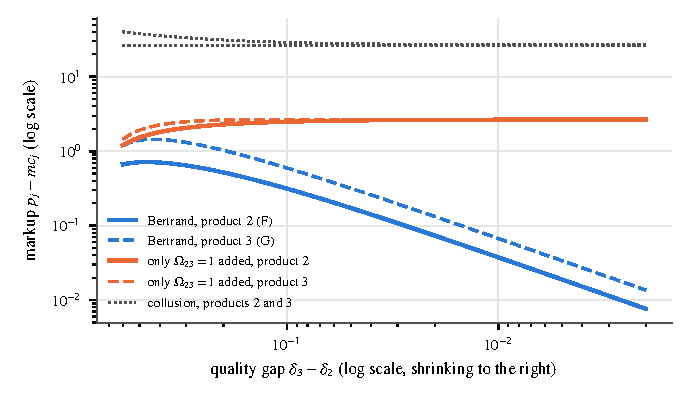
\includegraphics[width=0.74\textwidth]{figures/ch06/bresnahan_limit.pdf}
\caption{Markups of products 2 and 3 as their quality gap shrinks, in the seven-product design of
\cref{fig:06-bres-fig2}. Under Bertrand competition between their owners (blue) both markups fall in proportion to
the gap, as in \cref{prop:06-bertrand-limit}(a). If the Bertrand ownership matrix is changed only by letting
products 2 and 3 cooperate, $\Omega_{23} = 1$ (orange), the markups converge to a common positive value near 2.67,
as in part (b). Under full collusion (gray) they converge to about
26.7, the value given by \cref{eq:06-bres-mC}. Both axes are logarithmic. Computed with
\texttt{bresnahan\_fig2\_sim.py}.}
\label{fig:06-bres-limit}
\end{figure}

\subsubsection{The intuition and Bresnahan's Figure 2}\label{sec:06-bres-intuition}

Bresnahan states the intuition in two sentences \citep[p.~458]{Bresnahan1987}. If firms compete in prices, price is
near marginal cost for the products that have a close substitute sold by a competitor. If firms collude, the markup
on one firm's product hardly depends on whether its close substitutes are sold by competitors or by the firm itself.
\Cref{prop:06-bertrand-limit,prop:06-bres-collusion} make both sentences precise. Bresnahan adds a general point.
Conduct hypotheses differ in the comparative statics of price and quantity with respect to demand elasticities. So
conduct can be discerned even when marginal costs are unobserved, the same logic as the rotation argument of
\cref{ch:conduct}.

His Figure 2 illustrates the point with seven products in quality space and two firms, labelled G and F. We
recreate its design by solving the model. Products 2 and 3 are almost identical and belong to different firms.
Products 5, 6 and 7, at the top, all belong to G. \Cref{fig:06-bres-fig2} plots marginal cost and equilibrium prices
against quality under both conduct hypotheses, and \cref{fig:06-bres-fig2-orig} shows the original.\footnote{The
text of \citet[p.~466]{Bresnahan1987} describes the example differently from the figure. It says that ``Firm One
sells products 2, 4, and 5'' and that ``Firm Two sells product 3''. The prices of products 1 and 6 are held fixed,
because a third firm sells them. The figure labels the owners of products 1 to 7 as G, F, G, F, G, G, G. Our
recreation follows the figure. The economics is the same under both descriptions, because products 2 and 3 are
close neighbors owned by different firms.}

\begin{figure}[htbp]
\centering
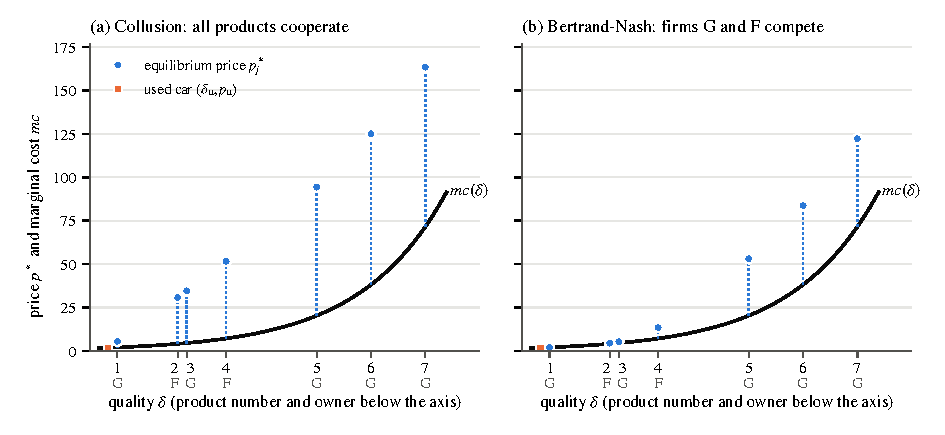
\includegraphics[width=\textwidth]{figures/ch06/bresnahan_fig2_sim.pdf}
\caption{Model-generated recreation of the design of \citet{Bresnahan1987}, Figure 2. Seven products with qualities
$\delta = (1, 2, 2.15, 2.8, 4.3, 5.2, 6.1)$ and owners G, F, G, F, G, G, G. Tastes are uniform with $\kappa = 1$ and
$\bar v = 48.3$. Marginal cost is $mc(\delta) = e^{0.7\delta}$, which is Bresnahan's $\psi e^{\delta}$ after a
rescaling of quality units. The used car has $\delta_{\mathrm u} = 0.85$ and $p_{\mathrm u} = mc(\delta_{\mathrm u})$.
Dots are equilibrium prices, and dotted segments are markups. Panel (a) solves \eqref{eq:06-bres-linear} with
$\Omega = \Omega^{\mathrm C}$ and panel (b) with the ownership matrix. Computed with \texttt{bresnahan\_fig2\_sim.py}.
The recreation copies the ownership labels of the original figure. Its markups need not match the original, which
Bresnahan drew as a sketch.}
\label{fig:06-bres-fig2}
\end{figure}

\begin{figure}[htbp]
\centering
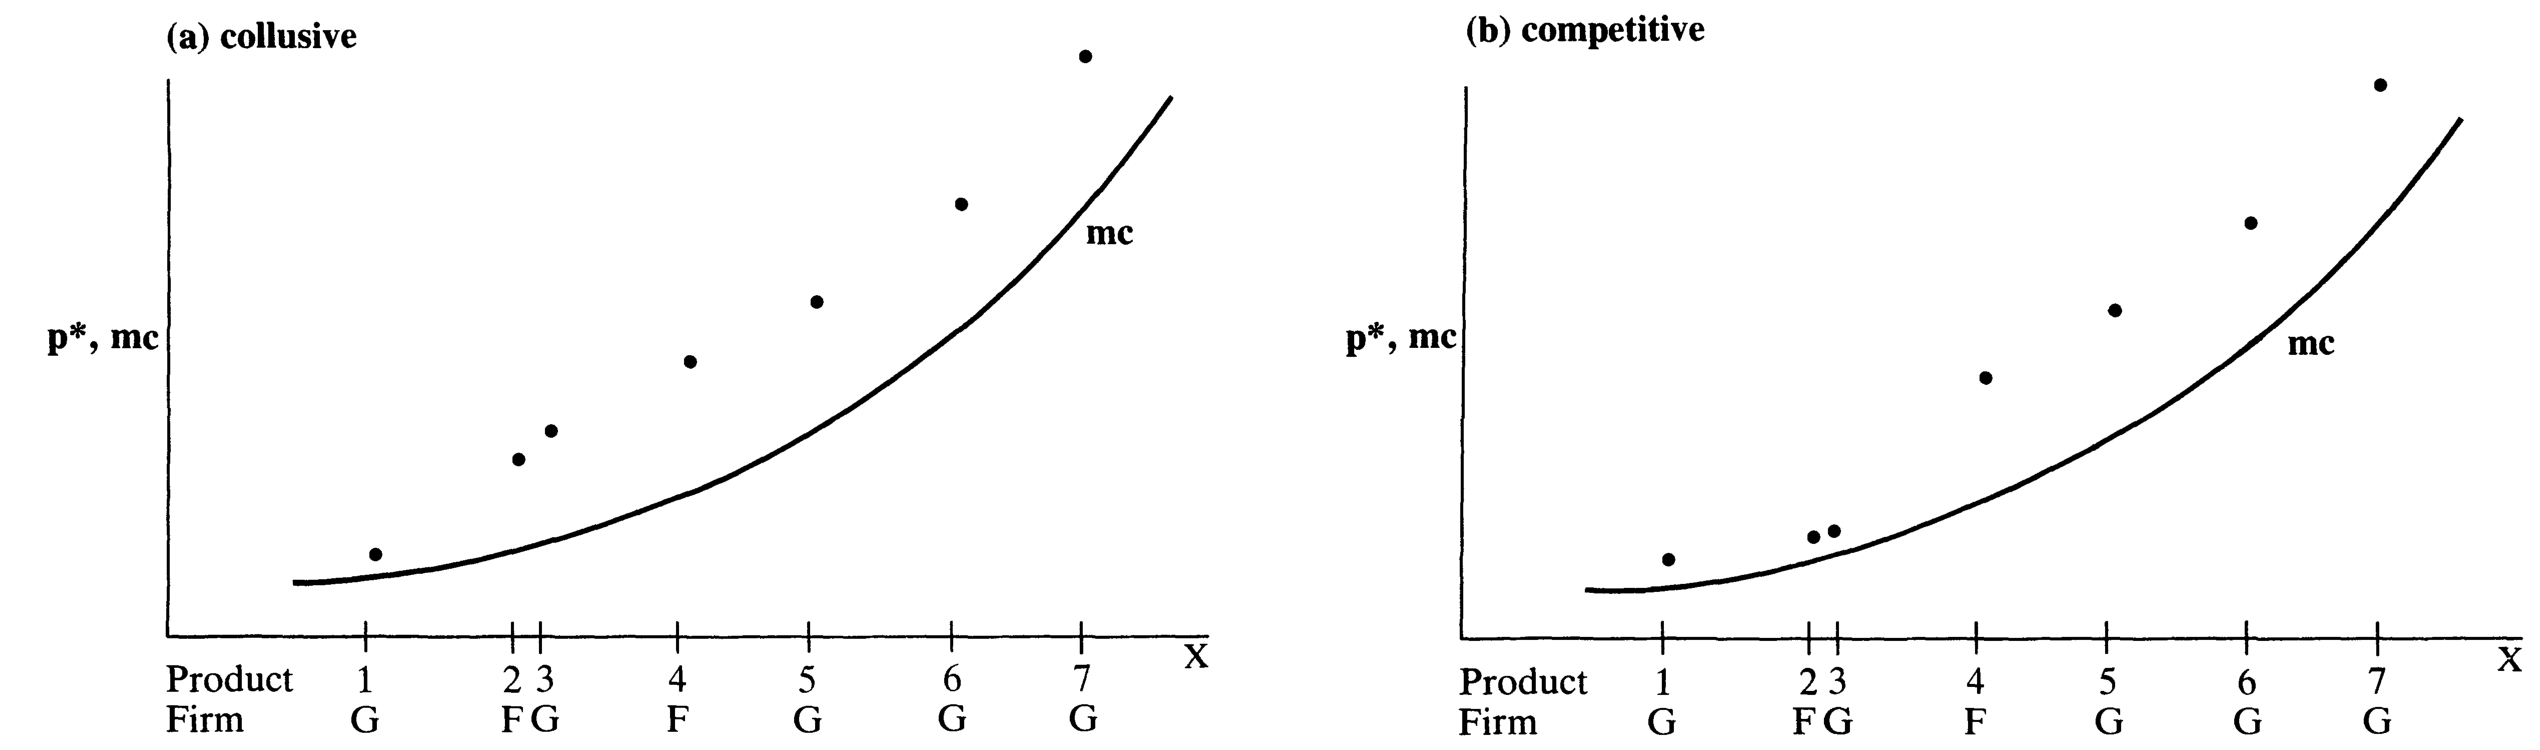
\includegraphics[width=\textwidth]{figures/ch06/bresnahan1987_fig2_orig.png}
\caption{Bresnahan's original illustration. Panel (a) shows collusive prices and panel (b) competitive prices, with
the marginal cost curve and the owner of each product below the quality axis. Source: \citet{Bresnahan1987},
Figure 2.}
\label{fig:06-bres-fig2-orig}
\end{figure}

The recreation shows three patterns. First, products 2 and 3 have markups of 26.65 and 30.05 under collusion and of
only 0.43 and 0.83 under Bertrand competition, so they sit on the cost curve in panel (b). Their rivalry is
fierce because they are close substitutes owned by different firms. Second, products 5, 6 and 7 keep between 44 and
55 percent of their collusive markups under Bertrand competition. They are distant from rivals and owned by one firm.
By \cref{rem:06-bres-topblock}, the price increments $p_6 - p_5$ and $p_7 - p_6$ and the quantities of products 6
and 7 are identical in the two panels. All three markups fall by the same amount, 41.28. Product 5 sells more under
Bertrand competition (7.61 against 5.50), because its lower cutoff falls when product 4 competes. Third, product 4,
owned by F and wedged between two G products at moderate distances, keeps 14 percent of its collusive markup. Most
of its Bertrand markup comes from the large markup of its upper neighbor, product 5, because prices are strategic
complements.

The recreation departs from Bresnahan's sketch in one visible respect. In his panel (b), products 4 to 7 keep nearly
all of their collusive markups. He writes that ``Products 4 and 5 change much less when the solution concept
changes'' \citep[p.~467]{Bresnahan1987}. In the solved model, product 4 keeps only 14 percent of its markup and
products 5 to 7 keep about half. Product 4 faces rival neighbors on both sides. Products 6 and 7 lose the same dollar
amount of markup as product 5, the lowest member of the top block (\cref{rem:06-bres-topblock}). Bresnahan's figure
is a sketch, and the robust contrast is the collapse of the markups of products 2 and 3.

The figure shows where the data can discriminate between the hypotheses. Regions of the quality ladder crowded with
products of different firms look very different under the two hypotheses. Regions with few firms change much less,
because market power is substantial even under competition. Bresnahan likens the large-car end of the mid-1950s
market, where GM produced most cars, to the region around products 4 and 5 of his example. He likens the
smaller-car segments to the region around products 1 and 2. There Ford, Chrysler, GM and, to a lesser extent, AMC
and the fringe were all present \citep[p.~467]{Bresnahan1987}. Bresnahan therefore expects the method to have statistical power in this industry. He also notes that the
method would be less revealing if every producer had a full product line \citep[p.~467]{Bresnahan1987}.
\Cref{rem:06-bres-power} makes this precise.

An earlier study supports this reading of the figure. \citet[pp.~1021--1022]{Bresnahan1989} summarizes
\citet{Bresnahan1981}, which fits the same vertical demand system to cross-sections of the 1977 and 1978 model
years. Its demand equation is the interior equation of \eqref{eq:06-bres-demand} (eq.~7 of the survey). Quality is
a hedonic function of length, weight, horsepower and other characteristics (eq.~8). The supply side is
\eqref{eq:06-bres-foc} under Bertrand conduct. Same-owner dummies on the two neighbors of each model play the role
of $\Omega_{j,j+1}$ and $\Omega_{j,j-1}$ (eq.~6$''$). The study reports two related findings. The large
price-cost margins appear on the larger vehicles, and the larger vehicles are much farther apart in quality space.
Products 5 to 7 of \cref{fig:06-bres-fig2} show the same pattern. They have no close rival, and they keep about
half of their collusive markups under Bertrand competition, while products 2 and 3 keep almost nothing. Bresnahan
adds that the finding confirms the view of industry observers based on accounting profits (footnote~13 of the
survey).

\subsection{Econometric specification and estimation}\label{sec:06-bres-estimation}

\casehead{Quality as an index of characteristics}
Quality is not observed. Bresnahan proxies it with a function of the physical characteristics (his eq.~22):
\begin{equation}\label{eq:06-bres-quality}
  \delta(x_j) = \sqrt{\beta_0 + x_j\beta},
\end{equation}
where $\beta_0$ and the vector $\beta$ are parameters. The interpretation comes from the hedonic model of
\citet{Rosen1974}, developed in \cref{sec:06-hedonic}. Consumers have preferences over characteristics, and firms
produce bundles of characteristics at costs that depend on them. The index is read as the expansion path of
efficient, cost-minimizing bundles. Each quality level is produced with the cheapest combination of characteristics
that delivers it. For this reason $\beta$ mixes information about tastes and technology, and its interpretation is
``clouded'' \citep[p.~467]{Bresnahan1987}. The square-root form is an arbitrary choice.

\casehead{Computing the model's predictions}
The parameters are $\theta = (\beta_0, \beta, \psi, \delta_{\mathrm u}, \bar v, \kappa)$, and the conduct hypothesis
fixes $\Omega$. For each trial value of $\theta$ the predictions are computed in three steps.
\begin{enumerate}
\item Compute every model's quality $\delta_j$ from \eqref{eq:06-bres-quality}.
\item Rank the models by quality, which determines who neighbors whom.
\item Solve the demand system \eqref{eq:06-bres-demand} and the first-order conditions \eqref{eq:06-bres-foc}
jointly for the predicted prices $p^*_j(\theta,\Omega)$ and quantities $q^*_j(\theta,\Omega)$, which amounts to the
linear system \eqref{eq:06-bres-linear}.
\end{enumerate}
The predictions depend only on parameters and on the exogenous characteristics. The used-car parameters are tied
together by \cref{ass:06-bres}(v), because the demand for the lowest-quality model \eqref{eq:06-bres-demand} is
overparameterized in $(\delta_{\mathrm u}, p_{\mathrm u})$. Bresnahan imposed $p_{\mathrm u} = mc(\delta_{\mathrm u})$
after initial experimentation showed the two were not easily distinguishable (p.~468).

\casehead{Errors and likelihood}
Observed prices and quantities equal the predictions plus additive, independent normal errors. Price errors have
variance $\sigma_p^2$. The error on aggregated quantity $m$ has variance $k_m\sigma_q^2$, from
\cref{sec:06-bres-data}, and price and quantity errors are independent. The likelihood is (his eq.~24)
\begin{equation}\label{eq:06-bres-lik}
  L(\theta,\sigma_p^2,\sigma_q^2)
  = \prod_{j=1}^{N_p}\frac{1}{\sqrt{2\pi\sigma_p^2}}\exp\Bigl[-\frac{(p_j - p_j^*)^2}{2\sigma_p^2}\Bigr]
    \prod_{m=1}^{N_q}\frac{1}{\sqrt{2\pi k_m\sigma_q^2}}
    \exp\Bigl[-\frac{\bigl(q_m - \sum_{j\in\mathcal I_m}q_j^*\bigr)^2}{2k_m\sigma_q^2}\Bigr],
\end{equation}
where $N_p$ and $N_q$ are the numbers of price and quantity observations and the predictions depend on
$(\theta,\Omega)$. The variances can be concentrated out. The log-likelihood is
\begin{equation*}
  \ln L = -\frac{N_p}{2}\ln(2\pi\sigma_p^2) - \frac{1}{2\sigma_p^2}\sum_{j}(p_j - p_j^*)^2
          - \frac{1}{2}\sum_m \ln(2\pi k_m\sigma_q^2) - \frac{1}{2\sigma_q^2}\sum_m \frac{(q_m - \sum_{j\in\mathcal I_m}q_j^*)^2}{k_m}.
\end{equation*}
Setting the derivative with respect to $\sigma_p^2$ to zero gives
$-\frac{N_p}{2\sigma_p^2} + \frac{1}{2\sigma_p^4}\sum_j (p_j - p_j^*)^2 = 0$, and similarly for $\sigma_q^2$. Hence
\begin{equation*}
  \hat\sigma_p^2(\theta) = \frac{1}{N_p}\sum_{j=1}^{N_p}(p_j - p_j^*)^2,
  \qquad
  \hat\sigma_q^2(\theta) = \frac{1}{N_q}\sum_{m=1}^{N_q}\frac{\bigl(q_m - \sum_{j\in\mathcal I_m}q_j^*\bigr)^2}{k_m}.
\end{equation*}
Substituting back gives the concentrated log-likelihood
\begin{equation}\label{eq:06-bres-conclik}
  \ell^c(\theta) = -\frac{N_p}{2}\ln\hat\sigma_p^2(\theta) - \frac{N_q}{2}\ln\hat\sigma_q^2(\theta)
  - \frac{1}{2}\sum_{m}\ln k_m - \frac{N_p + N_q}{2}\bigl(1 + \ln 2\pi\bigr).
\end{equation}
Maximum likelihood therefore chooses $\theta$ to minimize $N_p\ln\hat\sigma_p^2(\theta) + N_q\ln\hat\sigma_q^2(\theta)$.
Equivalently, it minimizes the product $(\hat\sigma_p^2)^{N_p}(\hat\sigma_q^2)^{N_q}$ of the mean squared price error
and the weighted mean squared quantity error. It is a form of nonlinear least squares for a system of two equations. All
estimation was done by numerical maximization.

\begin{remark}[A reduced-form error structure]\label{rem:06-bres-reducedform}
The errors in \eqref{eq:06-bres-lik} are appended to the equilibrium predictions. They are not structural demand or
cost shocks. Bresnahan calls this ``fully a reduced-form error structure'' (p.~469). It avoids the usual
endogeneity problem, because price never appears as a regressor and the predictions depend only on exogenous
characteristics. The cost of this choice is that the errors have no economic interpretation. A cost shock to one model would move
its neighbors' prices through the first-order conditions, which additive independent errors cannot capture.
\citet[p.~843]{BerryLevinsohnPakes1995} note that Bresnahan ``allows prices to be correlated with a linear
disturbance in an equilibrium pricing equation''. They add that he ``does not explicitly model the correlation
between prices and unobserved characteristics.'' Modelling an unobserved product characteristic $\xi_j$ and inverting market shares is
the response of \citet{Berry1994} and \citet{BerryLevinsohnPakes1995} (\cref{ch:logit,ch:blp}).
\end{remark}

\casehead{An irregular likelihood}
The likelihood is not continuous in the parameters. Predicted prices are continuous, but predicted quantities jump
at values of $\beta$ where two models, or a model and the used car, tie in quality. At such points the ranking
changes, and so does the set of neighbors. A discontinuous function cannot be concave, and the standard regularity
conditions for nonlinear regression fail. Bresnahan argues that ties are unlikely at the true parameter value, so
that limiting inference should go through (his footnote~9). He also reports that no local maxima caused trouble and
that the points of discontinuity were typically local minima, since they imply extreme predicted quantities
(footnote~10). Asymptotic normality of the estimators and of the test statistics remains unproven, as Appendix~B
acknowledges.

\casehead{Two further specifications}
Two more models serve as alternatives in the tests. The first is the log-linear hedonic model of
\citet{CowlingCubbin1971}, estimated on the British car market. Predicted prices and quantities follow a recursive
structure (his eqs.~25--26):
\begin{equation}\label{eq:06-bres-hedonic}
  p_j^* = \exp\bigl(a_0 + x_j a\bigr),
  \qquad
  q_j^* = \exp\bigl(l_0 + l_1(p_j - p_j^*)\bigr),
\end{equation}
where we write $a_0$, $a$, $l_0$ and $l_1$ for Bresnahan's $\alpha_0$, $\alpha_j$, $\lambda_0$ and $\lambda_1$. The
price equation adds GM and Ford dummies, following authors who use firm dummies as a proxy for market power. The
model has the same error and aggregation structure as the oligopoly models. \citet{Rosen1974} interprets a hedonic
price function as the equilibrium of a perfectly competitive, continuously differentiated market. The hedonic model,
``or something like it'', should hold if list prices were set in some nonmaximizing way (p.~470). It differs
radically from the oligopoly models. The second alternative, called ``Products'', is the opposite. It follows the
oligopoly model exactly but treats every model as if a separate firm made it, so $\Omega = I$. Neither is an
appealing story of the industry. Both are useful as tests, because an oligopoly model that survives against them
is more credible.

\subsection{Testing non-nested conduct hypotheses}\label{sec:06-bres-cox}

Collusion and Bertrand competition are non-nested hypotheses. They impose different matrices $\Omega$, and no
restriction on the parameters turns one model into the other. The hedonic model is a different family altogether.
A classical likelihood ratio test, which compares a model with a restricted version of itself, does not apply.
Bresnahan uses the non-nested test of \citet{Cox1961} in the regression form of \citet{PesaranDeaton1978}
\citep[p.~470]{Bresnahan1987}.

\casehead{The Cox statistic}
Let $H_0$ and $H_1$ be two parametric models for the same data, with maximized log-likelihoods $L_0$ and $L_1$. The
\emph{Cox statistic} for testing $H_0$ against $H_1$ is the observed log-likelihood ratio minus an estimate of its
expectation under $H_0$,
\begin{equation}\label{eq:06-bres-coxstat}
  T_0 = (L_0 - L_1) - \hat\E_0\bigl[L_0 - L_1\bigr].
\end{equation}
The expectation is evaluated at the estimate of $\theta_0$. It replaces the parameters of $H_1$ by their
\emph{pseudo-true values}, the probability limit of the $H_1$ estimator when the data come from $H_0$. Under $H_0$ the
standardized statistic is asymptotically standard normal. A significantly negative $T_0$ means that $H_1$ fits better
than it should if $H_0$ were true, which is evidence against $H_0$ in the direction of $H_1$. A significantly positive
$T_0$ means that $H_1$ fits worse than $H_0$ predicts. The test is two-tailed, so this also rejects $H_0$, whose
likelihood is ``too large'' relative to $H_1$. The test is not symmetric. Testing $H_1$ against $H_0$ is a different
test, so both models can be rejected, or neither. The next proposition gives the statistic for regression models.

\begin{proposition}[Cox statistic for non-nested regressions]\label{prop:06-bres-cox}
Let $y \in \R^N$, $H_0: y = f_0(\theta_0) + u$ and $H_1: y = f_1(\theta_1) + w$, with $u \sim N(0,\sigma_0^2 I_N)$ under
$H_0$, smooth mean functions, and parameter vectors of fixed dimension. Let $s_0^2$ and $s_1^2$ be the maximum
likelihood residual variances under the two models. Fit $H_1$ to the fitted values of $H_0$: let
$\hat\theta_{10}$ minimize $\|f_0(\hat\theta_0) - f_1(\theta_1)\|^2$, let $\hat d = f_0(\hat\theta_0) - f_1(\hat\theta_{10})$,
and define
\begin{equation*}
  \phi^2 = \frac{1}{N}\|\hat d\|^2,
  \qquad s_{10}^2 = s_0^2 + \phi^2,
  \qquad \tilde\phi = \frac{1}{N}\hat d^\top M_0\hat d,
\end{equation*}
where $M_0 = I_N - F_0(F_0^\top F_0)^{-1}F_0^\top$ and $F_0 = \frac{\partial f_0(\hat\theta_0)}{\partial\theta_0^\top}$. Then
\begin{equation*}
  T_0 = \frac{N}{2}\ln\frac{s_1^2}{s_{10}^2}.
\end{equation*}
If $H_0$ is true, $H_1$ does not contain the true mean function, and standard regularity conditions hold, then
\begin{equation*}
  \frac{T_0}{\sqrt{V_0}} \xrightarrow{d} N(0,1),
  \qquad
  V_0 = \frac{N\tilde\phi\, s_0^2}{s_{10}^4}.
\end{equation*}
\end{proposition}

\begin{proof}[Proof sketch]
The concentrated log-likelihood of a normal regression is $-\frac{N}{2}\ln s^2$ plus a constant common to both
models. Hence
\begin{equation*}
  L_0 - L_1 = \frac{N}{2}\ln\frac{s_1^2}{s_0^2}.
\end{equation*}
Under $H_0$, $s_1^2$ converges to $\sigma_0^2 + \phi_*^2$, where $\phi_*^2$ is the limit of $\phi^2$, the part of the
$H_0$ mean that $H_1$ cannot fit. The estimated expectation of $L_0 - L_1$ is therefore
$\frac{N}{2}\ln\frac{s_{10}^2}{s_0^2}$, and subtracting it gives $T_0$.

For the distribution we expand to first order around the true $\theta_0$ and the pseudo-true value
$\theta_{10}^*$. Write $f_0 = f_0(\theta_0)$ and $d = f_0 - f_1(\theta_{10}^*)$. Let $F_1$ be the gradient of $f_1$ at
$\theta_{10}^*$, define $M_1$ from $F_1$ as $M_0$ is defined from $F_0$, and let $P_k = I_N - M_k$ be the projection
onto the columns of $F_k$. The first-order condition
defining $\theta_{10}^*$ is $F_1^\top d = 0$, so $M_1d = d$. Four steps follow.
\begin{enumerate}
\item Fitting $H_1$ to $y = f_0 + u$ leaves residuals $M_1(d + u)$ to first order. Hence
$Ns_1^2 \approx \|d\|^2 + 2d^\top u + u^\top M_1 u$.
\item Fitting $H_0$ leaves residuals $M_0u$, so $Ns_0^2 \approx u^\top M_0 u$.
\item The fitted values of $H_0$ are $f_0 + P_0u$ to first order. Fitting $H_1$ to them, as in step 1, gives
$N\phi^2 \approx \|d\|^2 + 2d^\top P_0u + u^\top P_0M_1P_0u$.
\item Subtracting, $N(s_1^2 - s_{10}^2) \approx 2d^\top M_0 u + R$, where $R$ collects quadratic forms in $u$ on spaces of
fixed dimension and is bounded in probability. The term $d^\top M_0u$ is of order $\sqrt N$ because
$\|d\|^2$ grows like $N$.
\end{enumerate}
Since $\ln\frac{s_1^2}{s_{10}^2} \approx \frac{s_1^2 - s_{10}^2}{s_{10}^2}$, the statistic satisfies
\begin{equation*}
  T_0 \approx \frac{d^\top M_0u}{\sigma_0^2 + \phi_*^2},
  \qquad
  \Var_0\bigl(d^\top M_0 u\bigr) = \sigma_0^2\, d^\top M_0 d .
\end{equation*}
The leading term is normal with mean zero and variance $\frac{\sigma_0^2\, d^\top M_0 d}{(\sigma_0^2 + \phi_*^2)^2}$. Its
plug-in estimate is $V_0$, since $N\tilde\phi$ estimates $d^\top M_0d$. \citet{Pesaran1974} and
\citet{PesaranDeaton1978} give the regularity conditions and the multivariate version.
\end{proof}

The proof explains the two auxiliary regressions in Bresnahan's Appendix B. The first fits $H_1$ to the fitted
values of $H_0$, which he calls the ``phony-data regression''. Its residual variance $\phi^2$ measures how far $H_1$
is from $H_0$. The second regresses the phony-data residuals on the derivatives of $H_0$'s predictions. Its
residual variance $\tilde\phi$ removes the part of the distance that a small change in $\theta_0$ could absorb.
The intuition of the test is simple: $H_0$ is rejected if $H_1$ explains a significant part of $H_0$'s
residuals \citep[p.~471]{Bresnahan1987}.

\casehead{Bresnahan's formulas}
Bresnahan's models have two equations with independent errors, and the quantity equation is weighted by
$\frac{1}{k_m}$. The concentrated log-likelihood \eqref{eq:06-bres-conclik} has the same weights under every model,
so the terms in $k_m$ cancel from all likelihood ratios. The contributions of the two equations add. Let $s^2_{jp}$
and $s^2_{jq}$ be the estimated price and quantity error variances under $H_j$, for $j = 0, 1$ (his eqs.~B.1--B.2).
The phony-data regression fits $H_1$ to the predictions of $H_0$ and yields variances $\phi^2_p$ and $\phi^2_q$. Then
(his eqs.~B.3--B.5)\footnote{Equation (B.4) is printed as $s^2_{10q} \equiv s^2_{0p} + \phi^2_q$. The subscript $0p$ is
a misprint for $0q$, by analogy with (B.3) and with \cref{prop:06-bres-cox}.}
\begin{equation}\label{eq:06-bres-T0}
  s^2_{10p} = s^2_{0p} + \phi^2_p,
  \qquad
  s^2_{10q} = s^2_{0q} + \phi^2_q,
  \qquad
  T_0 = \frac{N_p}{2}\ln\frac{s^2_{1p}}{s^2_{10p}} + \frac{N_q}{2}\ln\frac{s^2_{1q}}{s^2_{10q}} .
\end{equation}
The second regression takes the residuals of the phony-data regression and regresses them linearly on the
derivatives of the $H_0$ predictions with respect to the $H_0$ parameters. Its residual variances are
$\tilde\phi_p$ and $\tilde\phi_q$, which Bresnahan writes as $\phi p$ and $\phi q$. They are variances in their own
right. They are not the square roots of $\phi^2_p$ and $\phi^2_q$. The asymptotic variance of $T_0$ is (his eq.~B.6)
\begin{equation}\label{eq:06-bres-V0}
  V_0(T_0) = N_p\tilde\phi_p\,\frac{s^2_{0p}}{s^4_{10p}} + N_q\tilde\phi_q\,\frac{s^2_{0q}}{s^4_{10q}},
\end{equation}
and the test statistic is $\frac{T_0}{\sqrt{V_0(T_0)}}$.\footnote{Appendix B prints the statistic as the ratio of $T_0$ to $V(T_0)$, without a square root. The text
(p.~470) divides the deviation of the likelihood ratio from its mean ``by its standard deviation''.
\Cref{prop:06-bres-cox} confirms that the square root is required for an asymptotically standard normal statistic. We
read the printed ratio as shorthand.} Each term of \eqref{eq:06-bres-T0} and \eqref{eq:06-bres-V0} is the
single-equation formula of \cref{prop:06-bres-cox}. Bresnahan's footnote~11 notes that the Pesaran-Deaton formulas were
altered slightly to account for the aggregation of quantities.

\begin{table}[htbp]
\centering
\caption{Cox test statistics for each maintained hypothesis against each alternative, 1954--1956}
\label{tab:06-bres-cox}
\small
\begin{tabular}{@{}lrrrr@{}}
\toprule
 & \multicolumn{4}{c}{Alternative hypothesis $H_1$} \\
\cmidrule(l){2-5}
Maintained hypothesis $H_0$ & Collusion & Nash-Competition & ``Products'' & Hedonic \\
\midrule
\multicolumn{5}{@{}l}{\textit{(a) 1954}} \\
Collusion        & $\cdot$     & 0.8951      & 0.9464      & $-1.934$ \\
Nash-Competition & $-2.325^{*}$ & $\cdot$    & $-0.8878$   & $-2.819^{*}$ \\
``Products''     & $-3.978^{*}$ & $3.029^{*}$ & $\cdot$    & $-1.604$ \\
Hedonic          & $-12.37^{*}$ & $-10.94^{*}$ & $-13.02^{*}$ & $\cdot$ \\
\addlinespace
\multicolumn{5}{@{}l}{\textit{(b) 1955}} \\
Collusion        & $\cdot$     & $-10.36^{*}$ & $-9.884^{*}$ & $-13.36^{*}$ \\
Nash-Competition & $-1.594$    & $\cdot$      & 1.260        & 0.6341 \\
``Products''     & $-0.7598$   & $-4.379^{*}$ & $\cdot$      & $-1.527$ \\
Hedonic          & $-3.353^{*}$ & $-8.221^{*}$ & $-5.950^{*}$ & $\cdot$ \\
\addlinespace
\multicolumn{5}{@{}l}{\textit{(c) 1956}} \\
Collusion        & $\cdot$     & 1.227        & 0.8263       & 1.629 \\
Nash-Competition & $-2.426^{*}$ & $\cdot$     & $-4.586^{*}$ & 0.8314 \\
``Products''     & $-3.153^{*}$ & 0.9951      & $\cdot$      & $4.731^{*}$ \\
Hedonic          & $-5.437^{*}$ & $-9.671^{*}$ & $-11.58^{*}$ & $\cdot$ \\
\bottomrule
\end{tabular}

\smallskip
\begin{minipage}{0.92\textwidth}
\footnotesize
\emph{Notes:} Reproduced from \citet[Table III, p.~471]{Bresnahan1987}. Each entry is the standardized Cox
statistic $\frac{T_0}{\sqrt{V_0}}$ for testing the row model against the column model, asymptotically standard
normal under the row model. A dot marks the diagonal. Asterisks are ours and mark rejection at the 5 percent level
in a two-tailed test, $\bigl|\frac{T_0}{\sqrt{V_0}}\bigr| > 1.96$. Negative values indicate that the alternative fits better than the maintained
model predicts. ``Products'' treats every model as a separate firm ($\Omega = I$). The hedonic model is
\eqref{eq:06-bres-hedonic}.
\end{minipage}
\end{table}

\casehead{Results}
\Cref{tab:06-bres-cox} reproduces the test results. In 1954 the hedonic model is rejected against every other
model. ``Products'' is rejected against both oligopoly models but not against the hedonic model.
Nash-Competition is rejected against Collusion ($-2.325$) and against the hedonic model ($-2.819$). Collusion is the
only model that escapes rejection against every alternative. Its statistic against the hedonic model, $-1.934$, is
close to the 5 percent cutoff of 1.96 but below it in absolute value. The 1956 results resemble those of 1954. Collusion is not
rejected against any alternative, and every other model is rejected at least once. Nash-Competition, for example,
is rejected against Collusion ($-2.426$) and against ``Products'' ($-4.586$).

The 1955 results are reversed. Collusion is rejected against all three alternatives, with statistics of $-10.36$,
$-9.884$ and $-13.36$. Nash-Competition is rejected against none. The other models are rejected as in the
surrounding years. ``Products'' is rejected against Nash-Competition, and the hedonic model against everything.
Some rejections have positive signs, as for ``Products'' against Nash-Competition in 1954 ($3.029$) and against the
hedonic model in 1956 ($4.731$). These reject because the likelihood of ``Products'' is too large relative to the
alternative, a possibility Bresnahan's footnote~12 points out for the two-tailed test.

Bresnahan stresses that the test results and the output expansion are independent evidence. Each year is estimated
separately, and no cross-year restriction, for example on the location of the demand curve, forces the competitive
model to be chosen in the high-quantity year. The coincidence of the reversal with the boom is therefore
informative \citep[p.~472]{Bresnahan1987}. The results are also robust to the two added specifications, which are
rejected throughout. The hedonic model is the cleanest of these rejections, since its likelihood is regular and the
caveat on asymptotic normality does not apply to it.

\subsection{Estimates}\label{sec:06-bres-estimates}

\begin{table}[t]
\centering
\caption{Parameter estimates under the maintained conduct hypotheses, 1954--1956}
\label{tab:06-bres-iv}
\small
\begin{tabular}{@{}lccc@{}}
\toprule
Parameter & 1954 (Collusion) & 1955 (Bertrand) & 1956 (Collusion) \\
\midrule
\multicolumn{4}{@{}l}{\textit{Quality index $\delta(x) = \sqrt{\beta_0 + x\beta}$}} \\
Constant $\beta_0$          & 47.91    & 48.28    & 50.87 \\
                            & (32.8)   & (43.2)   & (29.4) \\
Weight (thousands of lb)    & 0.3805   & 0.5946   & 0.5694 \\
                            & (0.332)  & (0.145)  & (0.374) \\
Length (thousands of in.)   & 0.1819   & 0.1461   & 0.1507 \\
                            & (0.128)  & (0.059)  & (0.146) \\
Horsepower (hundreds)       & 2.665    & 3.350    & 3.248 \\
                            & (0.692)  & (0.535)  & (0.620) \\
Cylinders                   & $-0.7387$ & $-0.9375$ & $-0.9639$ \\
                            & (0.205)  & (0.115)  & (0.186) \\
Hardtop dummy               & 0.9445   & 0.4531   & 0.4311 \\
                            & (0.379)  & (0.312)  & (0.401) \\
\addlinespace
\multicolumn{4}{@{}l}{\textit{Demand and supply}} \\
Marginal cost scale $\psi$  & 0.1753   & 0.1747   & 0.1880 \\
                            & (0.024)  & (0.020)  & (0.035) \\
Used-car quality $\delta_{\mathrm u}$ & 4.593 & 3.911 & 4.441 \\
                            & (1.49)   & (2.08)   & (1.46) \\
Upper endpoint $\bar v$     & $1.92\times10^{7}$ & $2.41\times10^{7}$ & $2.83\times10^{7}$ \\
                            & $(8.44\times10^{6})$ & $(9.21\times10^{6})$ & $(7.98\times10^{6})$ \\
Taste density $\kappa$      & 0.4108   & 0.4024   & 0.4075 \\
                            & (0.138)  & (0.184)  & (0.159) \\
\bottomrule
\end{tabular}

\smallskip
\begin{minipage}{0.86\textwidth}
\footnotesize
\emph{Notes:} Reproduced from \citet[Table IV, p.~472]{Bresnahan1987}. Asymptotic standard errors in parentheses.
Each column uses the conduct hypothesis not rejected in \cref{tab:06-bres-cox}. The mapping to Bresnahan's symbols
is: $\psi$ is his $\mu$, $\delta_{\mathrm u}$ is his $\gamma$, $\bar v$ is his $V_{\max}$, and $\kappa$ is his
$\delta$. The paper does not report the numbers of price and quantity observations.
\end{minipage}
\end{table}

\Cref{tab:06-bres-iv} reports the estimates under the specification that survives the tests in each year: Collusion
for 1954 and 1956 and Bertrand for 1955. The three columns are close. The marginal-cost scale is
0.1753, 0.1747 and 0.1880. The taste density is 0.4108, 0.4024 and 0.4075. The quality-index coefficients are close
in size and sign across years. The estimated primitives barely move, so the change in conduct alone captures the distinct
features of 1955.

\begin{table}[t]
\centering
\caption{Parameter estimates when one conduct hypothesis is imposed in every year}
\label{tab:06-bres-v}
\footnotesize
\setlength{\tabcolsep}{4pt}
\begin{tabular}{@{}lcccccc@{}}
\toprule
 & \multicolumn{3}{c}{(i) Collusive specification} & \multicolumn{3}{c}{(ii) Bertrand specification} \\
\cmidrule(lr){2-4}\cmidrule(l){5-7}
Parameter & 1954 & 1955 & 1956 & 1954 & 1955 & 1956 \\
\midrule
Constant $\beta_0$ & 47.91 & $-23.37$ & 50.87 & 31.64 & 48.28 & 33.23 \\
  & (32.8) & (24.5) & (29.4) & (29.9) & (43.2) & (17.8) \\
Weight & 0.3805 & 0.0103 & 0.5694 & 0.9311 & 0.5946 & $6.23\times10^{-3}$ \\
  & (0.332) & $(5.43\times10^{-2})$ & (0.374) & (0.210) & (0.145) & $(8.73\times10^{-4})$ \\
Length & 0.1819 & $-2.88\times10^{-3}$ & 0.1507 & 0.1474 & 0.1461 & 0.1605 \\
  & (0.128) & (0.102) & (0.146) & (0.038) & (0.059) & (0.149) \\
Horsepower & 2.665 & 0.1165 & 3.248 & 4.962 & 3.350 & $2.972\times10^{-2}$ \\
  & (0.692) & (0.106) & (0.620) & (0.676) & (0.535) & $(1.47\times10^{-2})$ \\
Cylinders & $-0.7387$ & $-1.309$ & $-0.9639$ & $-0.8846$ & $-0.9375$ & $-0.9078$ \\
  & (0.205) & (1.52) & (0.186) & (0.194) & (0.115) & (0.256) \\
Hardtop & 0.9445 & 1.468 & 0.4311 & $-0.2474$ & 0.4531 & 0.5282 \\
  & (0.379) & (1.08) & (0.401) & (0.464) & (0.312) & (0.249) \\
$\psi$ & 0.1753 & 1.344 & 0.1880 & 0.2518 & 0.1747 & 0.2902 \\
  & (0.024) & (0.151) & (0.035) & (0.074) & $(0.312)^{a}$ & $(0.249)^{a}$ \\
$\delta_{\mathrm u}$ & 4.593 & 1.604 & 4.441 & 6.352 & 3.911 & 1.204 \\
  & (1.49) & (4.83) & (1.46) & (3.54) & (2.08) & (3.19) \\
$\bar v$ & $1.92\times10^{7}$ & $1.46\times10^{8}$ & $2.83\times10^{7}$ & $9.81\times10^{5}$ & $2.41\times10^{7}$ & $1.03\times10^{6}$ \\
  & $(8.44\times10^{6})$ & $(6.74\times10^{6})$ & $(7.98\times10^{6})$ & $(8.78\times10^{6})$ & $(9.21\times10^{6})$ & $(8.90\times10^{6})$ \\
$\kappa$ & 0.4108 & $5.75\times10^{-2}$ & 0.4075 & 5.04 & 0.4024 & 7.334 \\
  & (0.138) & $(8.28\times10^{-2})$ & (0.159) & (1.21) & (0.184) & (2.46) \\
\bottomrule
\end{tabular}

\smallskip
\begin{minipage}{0.95\textwidth}
\footnotesize
\emph{Notes:} Reproduced from \citet[Tables V(i) and V(ii), pp.~473--474]{Bresnahan1987}. Asymptotic standard errors in
parentheses. Symbols as in \cref{tab:06-bres-iv}. $^{a}$~Printed as in the source. These two standard errors
duplicate the hardtop standard errors directly above them, (0.312) and (0.249). Table IV reports (0.020) for the
same 1955 estimate of $\psi$, so the printed values are probably typesetting errors. The paper also reports Table
V(iii) for the hedonic model and Table V(iv) for ``Products''.
\end{minipage}
\end{table}

\Cref{tab:06-bres-v} tells the opposite story. When one conduct hypothesis is imposed in all three years, the
parameters must explain 1955 by themselves, and they behave erratically. Under the collusive specification the 1955
column departs from its neighbors. The marginal-cost scale $\psi$ is an order of magnitude larger, 1.344 against
0.1753 and 0.1880. The taste density $\kappa$ is an order of magnitude smaller, 0.0575 against about 0.41. The upper
endpoint $\bar v$ jumps to $1.46\times10^{8}$, and length receives a negative coefficient. The parameters must absorb
the low prices and high output that collusive pricing cannot generate with stable primitives.

The Bertrand specification is ``similarly chaotic'' \citep[p.~473]{Bresnahan1987}. Now 1954 and 1956 are the odd
years. The 1954 column has the only negative hardtop coefficient estimated in any year under any specification. In 1956 the
weight and horsepower coefficients collapse toward zero, to $6.23\times10^{-3}$ and $2.972\times10^{-2}$. Relative to
the surrounding years, tastes in 1955 are spread ``at one tenth the density over ten times the range'' (p.~475).
The comparison is with the Bertrand estimates for 1954 and 1956, where $\kappa$ is 5.04 and 7.334 and $\bar v$ is near
$10^{6}$. The 1955 values, 0.4024 and $2.41\times10^{7}$, are those of \cref{tab:06-bres-iv}, since both tables estimate 1955
under Bertrand.
Bresnahan sums up the comparison in one sentence: ``It is change of behavioral assumption, not change of parameter
values, that provides a reasonable empirical explanation of 1955'' (p.~475).

The lesson is general. A misspecified conduct assumption does not disappear. It is absorbed into the estimated
primitives, which then become unstable across periods and implausible in level. Stability of demand and cost
parameters across periods is therefore informative about conduct. \Cref{tab:06-bres-iv} is built from the two panels
of \cref{tab:06-bres-v}, and only the combination left unrejected by the tests produces a consistent picture.

The magnitudes in \cref{tab:06-bres-iv} have sensible readings \citep[p.~475]{Bresnahan1987}. The quality-index
coefficients have the signs and sizes one expects from hedonic regressions. The negative cylinders coefficient is
familiar from that literature too. Econometrically, horsepower and cylinders are highly collinear. Economically,
the cylinders variable captures the fall in the cost of horsepower after the introduction of the V-8 engine.

The demand parameters describe very diverse tastes for quality. The eight million buyers of 1955 had tastes $v$
between $4.24\times10^{6}$ and $2.4\times10^{7}$. In Bresnahan's words, the distribution was ``20 million wide and 0.4
deep'', and 20 million times 0.4 gives the eight million buyers. Bresnahan cautions that this may be an artifact of
the constant density. The same numbers imply a potential market of $\kappa\bar v = 0.4024\times 2.41\times10^{7}
\approx 9.7$ million in 1955, of whom about 1.7 million (those with $v$ below $4.24\times10^{6}$) chose the used
car. The used-car quality $\delta_{\mathrm u}$ is around 4 in each year, while the lowest new-car quality is around
9. New and used cars are thus not close substitutes. The parameter $\psi$ only converts quality units into money in
the marginal-cost function.

Two further readings concern 1956. The 1955 purchases do not seem to have depressed 1956 demand. Both $\kappa$ and $\bar v$
are slightly larger in 1956 than in 1955, and the 1954 and 1956 demand parameters are very similar. The used-car
quality rises from 3.911 in 1955 to 4.441 in 1956 (it was 4.593 in 1954), which Bresnahan reads as considerable competition from the used-car
market in 1956. For comparison, the hedonic model's quantity equation gives price coefficients $l_1$ of $-3.742$
(0.640), $-1.312$ (0.787) and $-3.322$ (0.715) in 1954, 1955 and 1956 (Table V(iii)). The 1955 coefficient is the
smallest in absolute value and the least precise.

\subsection{Counterfactual, fit and residuals}\label{sec:06-bres-fit}

\casehead{Collusion in 1955 as a counterfactual}
The estimates allow a simple decomposition of the 1955 expansion into demand and conduct. Bresnahan computes the
equilibrium with the 1955 parameters, which were estimated under Bertrand, but with the collusive solution. The
counterfactual prices are about one-half of one percent above the average of 1954 and 1956. Predicted 1955 unit
sales are 7.1 million, 25.5 percent above the 1954 and 1956 average, instead of the actual 40.4 percent. The change
in conduct thus accounts for about 0.8 million cars, the difference between 7.9 and 7.1 million. Bresnahan compares
this with the largest residual in the demand system of \citet{Chow1960}, $+0.6$ million units, which falls in 1955.
The two magnitudes are comparable. A supply-side change of the size implied by the price war is thus of the same
order as the part of 1955 that demand models could not explain.

\begin{table}[htbp]
\centering
\caption{Fit of the four models and residuals of the Big Three, 1954--1956}
\label{tab:06-bres-fit}
\small
\begin{tabular}{@{}lcccccc@{}}
\toprule
\multicolumn{7}{@{}l}{\textit{(a) $R^2$ of the price ($p$) and quantity ($q$) equations (Table VI)}} \\
\addlinespace
 & \multicolumn{2}{c}{1954} & \multicolumn{2}{c}{1955} & \multicolumn{2}{c}{1956} \\
\cmidrule(lr){2-3}\cmidrule(lr){4-5}\cmidrule(l){6-7}
Model & $p$ & $q$ & $p$ & $q$ & $p$ & $q$ \\
\midrule
Collusion    & 0.94 & 0.62 & 0.92 & 0.58 & 0.96 & 0.61 \\
Bertrand     & 0.91 & 0.62 & 0.96 & 0.64 & 0.93 & 0.62 \\
``Products'' & 0.90 & 0.62 & 0.88 & 0.59 & 0.92 & 0.61 \\
Hedonic      & 0.89 & 0.71 & 0.88 & 0.73 & 0.88 & 0.71 \\
\midrule
\multicolumn{7}{@{}l}{\textit{(b) Average residual of each firm minus the average of all other firms (Table VII)}} \\
\addlinespace
 & \multicolumn{2}{c}{1954 (Collusion)} & \multicolumn{2}{c}{1955 (Bertrand)} & \multicolumn{2}{c}{1956 (Collusion)} \\
\cmidrule(lr){2-3}\cmidrule(lr){4-5}\cmidrule(l){6-7}
Firm & Price & Quantity & Price & Quantity & Price & Quantity \\
\midrule
GM       & 20.92    & $-99.6$ & 28.80   & $-82.86$ & 21.48    & $-68.73$ \\
Ford     & $-12.33$ & 60.2    & $-6.28$ & 22.97    & $-11.02$ & 19.06 \\
Chrysler & $-13.16$ & 96.89   & $-9.33$ & 64.47    & $-17.19$ & 11.94 \\
\bottomrule
\end{tabular}

\smallskip
\begin{minipage}{0.92\textwidth}
\footnotesize
\emph{Notes:} Panel (a) reproduces \citet[Table VI, p.~476]{Bresnahan1987}. Because of the heteroskedasticity, the quantity
$R^2$ is defined as a fraction of explained variance, $R^2_q = \frac{s^2_q - \hat\sigma^2_q}{s^2_q}$. Here $s^2_q$ is the
second raw moment of the quantity data, computed under the same heteroskedastic variance structure as the models. Panel (b) reproduces Table VII (p.~477), computed from the unrejected specification in each
year. Price residuals are in dollars and quantity residuals in cars. ``All other firms'' includes the other two
firms of the Big Three.
\end{minipage}
\end{table}

\casehead{Fit}
Panel (a) of \cref{tab:06-bres-fit} gives part of the intuition behind the tests. The reversal between Collusion and
Bertrand appears as a reversal in $R^2$. In the price equation the unrejected model fits better in every year: 0.94
against 0.91 in 1954, 0.96 against 0.92 in 1955, and 0.96 against 0.93 in 1956. In the quantity equation it fits
better in 1955 (0.64 against 0.58) and equally well in 1954 (0.62 each).\footnote{Bresnahan writes that ``in each
year, the model not rejected explains more variance in both equations'' (p.~477). In 1956, however, Table VI gives
a quantity $R^2$ of 0.61 for Collusion and 0.62 for Bertrand, so the statement holds strictly only for the price
equation.} The hedonic model fits quantities better in every year, with $R^2_q$ of 0.71 to 0.73, yet the oligopoly
model left unrejected in each year is not rejected against it. Bresnahan concludes that the price equation provides most of the power of the
tests. His footnote~14 gives two reasons to read these $R^2$ values with care. The oligopoly models have no constant
in the quantity equation, by \eqref{eq:06-bres-demand}. In the price equation, marginal cost explains much of the
cross-sectional variance, so the price $R^2$ would be high even if little of the markup were explained.

\casehead{Residuals by firm}
Panel (b) compares the average residuals of each of the Big Three with those of all other firms. Since ``all other
firms'' for Ford and Chrysler includes GM, the clearest message concerns GM. Its average price residual is 20.92,
28.80 and 21.48 dollars, and its average quantity residual is $-99.6$, $-82.86$ and $-68.73$ cars. Bresnahan
summarizes these as overpredicting GM prices by about \$30, out of the \$1,500 price of a typical car. He also
describes them as underpredicting GM sales by about 100 units, out of typical sales near 60,000.\footnote{The paper does not define the
sign of a residual. Bresnahan's wording matches residuals defined as predicted minus observed values. Under the more
common convention, observed minus predicted, the same numbers would mean that the models underpredict GM prices and
overpredict GM sales. The magnitudes are unaffected. Note also that the printed price residuals, \$21 to \$29, are
somewhat below the \$30 of the text.} The errors are small, but they suggest that GM had a cost or quality advantage.
Bresnahan therefore estimated two broader specifications for each oligopoly model. One adds a GM dummy to the quality
index. The other gives GM its own marginal-cost scale. Neither GM parameter is significant in any unrejected
specification, and no Cox test result is reversed. Either parameter does make the GM residuals much closer to zero.

\subsection{Robustness}\label{sec:06-bres-robust}

Besides the GM extensions, Bresnahan reports two generalizations aimed at the most obvious weaknesses of the model.

\casehead{Quality measured with error}
The tests depend on which products are neighbors. Small errors in the imputed qualities could change the ranking of
products, and with it the pattern of same-firm and rival neighbors. Robert Masson raised this concern (footnote~15).
Following \citet{Bresnahan1981}, the quality index is rewritten as observed with error,
\begin{equation}\label{eq:06-bres-qerror}
  \delta(x_j) = \sqrt{\beta_0 + x_j\beta} + \zeta_j,
\end{equation}
where we write $\zeta_j$ for Bresnahan's $\varepsilon_x$.\footnote{The printed formula on p.~478 reads
$\sqrt{\beta_0 + \varepsilon_j\beta_jZ_j} + \varepsilon_x$. The first $\varepsilon_j$ is a misprint for the summation sign.}
Since quality is unobserved, $\zeta_j$ must be integrated out of the likelihood. This changes the substitution
pattern. With $\Var(\zeta_j) = 0$, each product is a substitute for exactly two others. As the variance grows, the
probability of demand-side interaction with less similar products rises, which ``smears'' the demand equations and
reduces the importance of very similar products. Bresnahan does not know how to construct Cox tests for this
specification. Its likelihoods, however, still favor Bertrand in 1955 and Collusion in the other years.

\casehead{Durability}
The model treats cars as a flow good, a ``glaring shortcoming'' for a durable \citep[p.~478]{Bresnahan1987}.
Bresnahan adds the stock of similar used cars to both equations:
\begin{equation}\label{eq:06-bres-durable}
  p_j = p_j^*(\theta,\Omega) + \lambda_S \mathcal{S}_j + e^p_j,
  \qquad
  q_j = q_j^*(\theta,\Omega) + \theta_S \mathcal{S}_j + e^q_j,
\end{equation}
where we write $\lambda_S$ and $\theta_S$ for his $\lambda$ and $\theta$, and $e^p_j$ and $e^q_j$ for his error terms.
Here $\mathcal{S}_j$ is the stock of used cars ``like'' model $j$, meaning within ten percent of its weight, with used cars
depreciating at 15 percent per year. The construction is ad hoc. Both coefficients differ significantly from zero,
but the Cox test results of \cref{tab:06-bres-cox} are unaltered. The rerun covers only the collusive and Bertrand
specifications (footnote~16).

Bresnahan draws two conclusions from these checks. The highly structured oligopoly models do not tell all of the
story the data have to tell, as the significant durability terms show. The conclusions about conduct nonetheless
appear robust.

\subsection{Identification}\label{sec:06-bres-ident}

Bresnahan observes no costs, no instruments in the modern sense, and no variation in ownership. The data for each
year are a single cross-section of about 80 to 85 models. We now state what pins down each object.

Demand and cost are identified within a conduct hypothesis by functional form and by the cross-section of prices
and quantities. Prices equal marginal cost plus a markup. Marginal cost is a smooth function $\psi e^{\delta(x)}$ of
characteristics, while markups depend on quantities and on the gaps between neighbors. The cross-sectional variation
of prices with characteristics therefore separates the cost curve from the markups, given the functional forms.
Quantities pin down the density $\kappa$, which scales all demand derivatives in \eqref{eq:06-bres-deriv}.

The scale of quality is fixed by the cost function. In the pure vertical model, quality is identified only up to the
scale of tastes, as \cref{prop:06-vscale} shows. Here, multiplying all qualities by $c$ and dividing all tastes by $c$
leaves choices unchanged, but it changes $\psi e^{\delta}$ to $\psi e^{c\delta}$. The exponential cost function and
the square-root index thus fix the units of quality. This is identification by functional form, and it is one reason
the specification matters.

Conduct is identified by how markups vary across products with the distance to the nearest neighbor and with the
owner of that neighbor. By \cref{prop:06-bertrand-limit,prop:06-bres-collusion}, the two hypotheses make sharply
different predictions for products with close neighbors owned by rivals. Within a year, the cross-section supplies
many such configurations. This plays the role that rotations of demand play in the homogeneous-goods conduct
literature (\cref{ch:conduct}). There, conduct is identified by changes in the slope of demand that leave costs
unchanged. Here, the gaps between neighbors are the slopes, and they vary across products within a market. The next
remark states exactly which features of ownership matter.

\begin{remark}[When can the data tell conduct apart?]\label{rem:06-bres-power}
By \eqref{eq:06-bres-Amat}, the matrix $A(\Omega)$ depends on $\Omega$ only through the neighbor entries
$\Omega_{j,j+1}$. Two conduct hypotheses that agree on every neighbor pair imply identical equilibrium prices and
quantities, and no data can distinguish them. Collusion and Bertrand differ exactly at the neighbor pairs owned by
different firms. Suppose each of $F$ firms sold one contiguous block of the quality ladder. The two hypotheses would then
differ at only $F - 1$ pairs, and \cref{rem:06-bres-topblock} shows that the top block would keep its collusive
price increments under both.
Interleaved product lines, as in the small-car segment of the 1950s, create many pairs where the hypotheses differ.
In the design of \cref{fig:06-bres-fig2}, the hypotheses differ at the four pairs from $(1,2)$ to $(4,5)$ and agree at
$(5,6)$ and $(6,7)$.
\end{remark}

Three further points complete the argument. First, the conduct hypotheses are discrete, and each is estimated
separately. The test compares the fit of two fully specified reduced forms \eqref{eq:06-bres-eqm}. No
continuous conduct parameter is estimated. Second, the hedonic and ``Products'' alternatives check that the oligopoly models
are not chosen merely because the alternatives are poor. Third, no restriction links the years, so the selection of
Bertrand in 1955 is not forced by the output spike. The same feature means that each year's identification rests on
its own cross-section and functional forms.

\subsection{Limitations and critiques}\label{sec:06-bres-limits}

\casehead{Restrictive substitution}
Quality is one-dimensional, so each product substitutes only with its two neighbors. This is exactly what gives the
test its power, and it is also the most criticized feature of the model. \citet[p.~852]{BerryLevinsohnPakes1995}
note that cross-price elasticities in the vertical model are determined by market shares and the rank order of
prices alone, not by characteristics such as size or power. Their example is a ranking with a \$24,998 family
station wagon, a \$24,999 sports car and a \$25,000 station wagon. The vertical model guarantees that the two wagons
are not substitutes for each other, while the sports car substitutes for both. \citet{FeenstraLevinsohn1995} allow
multidimensional differentiation while keeping the rest of Bresnahan's framework. Bresnahan's own error-in-quality
extension softens the restriction in the same direction.

\casehead{Functional forms}
The uniform taste distribution, the square-root quality index and the exponential cost function are all arbitrary.
They identify the scale of quality and shape the markups. Bresnahan concedes that the wide, shallow taste
distribution may be an artifact of the constant density.

\casehead{Unobserved quality and exogenous characteristics}
The errors are added to the reduced form, so there is no unobserved product characteristic that consumers see and
the econometrician does not (\cref{rem:06-bres-reducedform}). Characteristics are treated as exogenous, a defect that
\citet[p.~245]{Berry1994} notes his own approach shares with Bresnahan's and with nearly all studies of
differentiated products. Product lines are predetermined, so the model says nothing about how conduct might affect
product choice.

\casehead{Likelihood-based testing}
The non-nested tests require a fully specified likelihood, including the distribution of the errors and a complete
supply model. \citet[p.~335]{Nevo2001} cites this as a reason to prefer other comparisons of conduct. The likelihood is
also irregular, and the asymptotic distribution of the test statistics is unproven. Only the rejection of the
hedonic model is statistically clean.

\casehead{Data and dynamics}
Prices are list prices, and quantities are production rather than sales, which misses fleet sales and end-of-year
bargains. The model is static, while cars are durable and buyers can time purchases. The durability check of
\cref{sec:06-bres-robust} is ad hoc, and its terms are significant. The study covers three years chosen because one of
them is anomalous. Finally, the power of the test depends on crowded regions with interleaved owners, so the method
does not transfer to industries where each firm owns a contiguous segment.

\subsection{Contribution}\label{sec:06-bres-contribution}

Bresnahan's paper set the template for testing conduct with differentiated products. It specifies demand and cost
explicitly, solves for equilibrium under each conduct hypothesis, and asks which equilibrium fits the data. Conduct
enters as a discrete hypothesis about which products cooperate, encoded in the matrix $\Omega$.
This representation is the one that merger simulation uses when it changes ownership (\cref{ch:mergers}), and it is
the object later conduct tests compare.

The paper also showed that the fine structure of a cross-section carries information about conduct, even without
cost data. Markups of close rivals collapse under competition, while prices within a region owned by one firm move
together and keep their differences. Its finding that conduct changed for one year made the temporary breakdown of collusion an empirical
object. And its comparison of \cref{tab:06-bres-iv,tab:06-bres-v} teaches a lesson that applies far beyond
automobiles: imposing the wrong conduct leaves unstable and implausible primitives behind.

Later work kept the logic and replaced the parts that critics found weakest. \citet{Berry1994} and
\citet{BerryLevinsohnPakes1995} added unobserved product characteristics and richer substitution patterns, with
instruments for price (\cref{ch:logit,ch:blp}). \citet{Nevo2001} compared the margins implied by alternative conduct
hypotheses with observed margins. \citet{GasmiLaffontVuong1992} applied non-nested tests to conduct in a soft-drink
market, and \citet{Vuong1989} developed the model-selection tests that much of this literature uses
(\cref{app:econometrics}). \citet{BerryHaile2014} formalize when alternative oligopoly models can be distinguished
with market-level data, building on the early intuitions of \citet{Bresnahan1981,Bresnahan1982}.

\section{The idiosyncratic shock: tastes for products versus tastes for characteristics}\label{sec:06-epsilon}

Bresnahan's test draws its power from a demand system without an idiosyncratic shock. Each car competes only with
its neighbors on the quality ladder, and the Bertrand markups of close rivals vanish (\cref{prop:06-bertrand-limit}).
The logit-type models of \cref{ch:logit,ch:blp} make the opposite modeling choice. This section compares the two
classes directly, and the next two sections study estimators for models without the shock.

Every random utility model in this chapter can be written in the form
\begin{equation}\label{eq:06-u-general}
  u_{ij} = \delta_j + \mu_{ij} + \epsilon_{ij},
\end{equation}
where $\delta_j$ is the mean utility of product $j$. The consumer-specific deviation $\mu_{ij}$ comes from
interactions between consumer tastes and product characteristics. The idiosyncratic shock $\epsilon_{ij}$ is
independent across products and consumers. The logit, the nested logit and the random coefficients logit of
\cref{ch:logit,ch:blp} contain the shock. The Hotelling, ideal-point and vertical models of \cref{sec:06-models} do
not. This section asks what the shock does to the economics of a model. The short answer is that with
$\epsilon_{ij}$ the product space can never be exhausted. Each new product arrives with a fresh draw of $\epsilon_{ij}$
for every consumer. These draws guarantee the product a positive market share and some market power, whatever its
characteristics. \citet[p.~34]{AckerbergEtAl2007} question the economic content of the shock. They write that the
$\epsilon_{ij}$ ``are added to the model largely for computational convenience'' and ``do not seem to match any omitted
causal demand determinant.'' They add that the shocks give every conceivable product a strictly positive expected share.
Every product then has a positive cross-price effect with every other product, so that ``competition is never completely
local.'' We make these statements precise, following \citet{BerryPakes2007}, and then describe what the shock
buys in estimation.\footnote{As stated in \cref{sec:06-ps-cs}, citations of \citet{BerryPakes2007} use the
pages, footnotes, equations and tables of the author manuscript of July 2, 2007.}

\subsection{Two specifications of the consumer-specific term}\label{sec:06-tp-pc}

\citet{BerryPakes2007} start from a general indirect utility $u_{ij} = U(X_j, V_i; \theta)$ (their eq.~1). Here $X_j$
is the vector of characteristics of product $j$, price included, $V_i$ is a vector of consumer tastes and $\theta$ is a
parameter vector. They split $X_j = (x_j, \xi_j)$ into characteristics the econometrician observes and an unobserved
characteristic $\xi_j$ that consumers and firms see. They split $V_i = (z_i, \nu_i)$ into attributes $z_i$ that a
micro data set might record and unobserved tastes $\nu_i$. Empirical models then impose additive separability (their
eq.~3),
\begin{equation}\label{eq:06-bp-additive}
  u_{ij} = f(X_j, z_i; \theta) + \mu_{ij},
\end{equation}
and an assumption on the distribution of $\mu_{ij}$ given $(X_j, z_i)$. Both classes of models discussed below let
$\mu_{ij}$ contain linear interactions $\sum_k \nu_{ik} X_{jk}$, so each consumer has her own marginal utility for each
characteristic. The two classes differ in one respect only.

\begin{definition}[Tastes for products and pure characteristics]\label{def:06-tp-pc}
A random utility model has \emph{tastes for products} if
\begin{equation}\label{eq:06-mu-tp}
  \mu^{tp}_{ij} = \sum_{k=1}^{K} \nu_{ik} X_{jk} + \epsilon_{ij},
\end{equation}
where, conditional on $(X_j, z_i)$ and on all $\mu_{ij'}$ with $j' \ne j$, the term $\epsilon_{ij}$ has support on the whole
real line. A random utility model is a \emph{pure characteristics model} if
\begin{equation}\label{eq:06-mu-pc}
  \mu^{pc}_{ij} = \sum_{k=1}^{K} \nu_{ik} X_{jk}.
\end{equation}
\end{definition}

The random coefficients logit of \citet{BerryLevinsohnPakes1995} and random coefficient probit models belong to the
first class (eq.~4 of \citealp{BerryPakes2007}). The ideal-point model belongs to the second, because expanding the
squared distance gives a pure characteristics model with a quadratic term in mean utility
(\cref{prop:06-idealpoint}). The vertical model is the special case of \eqref{eq:06-mu-pc} in which price is the only
characteristic with a random coefficient.

The label ``tastes for products'' comes from the reading of $\epsilon_{ij}$ in \cref{rem:06-tastesforproducts}, which
\citet{BerryPakes2007} attribute to \citet{CaplinNalebuff1991}. Let $d_{jm} = \indic\{j = m\}$ be a set of product
dummies and let $\eta_{im}$ be consumer $i$'s taste for ``being product $m$'', drawn independently across products and
consumers. Then
\begin{equation}\label{eq:06-dummies}
  \epsilon_{ij} = \sum_{m=1}^{J} d_{jm}\, \eta_{im},
\end{equation}
and \eqref{eq:06-mu-tp} becomes a pure characteristics model on a space of dimension $K + J$. Every product carries
its own characteristic, and every consumer has an independent taste for it. Adding a product adds a dimension to the
characteristic space. This is the source of both implications that \citet[p.~6]{BerryPakes2007} attribute to models
with tastes for products. First, there is a limit on substitution between products, and so a lower bound on markups.
Second, each consumer's utility grows without bound as products are added, whatever the characteristics of the new
products or of the consumer. Neither implication holds in a pure characteristics model. We now verify both claims in
the simplest member of each class.

\subsection{The logit benchmark}\label{sec:06-logit-bench}

Consider the logit model with an outside good. Utility is $u_{ij} = V_j + \epsilon_{ij}$ with $V_j = \delta_j - \alpha
p_j$ and $\alpha > 0$, and $u_{i0} = \epsilon_{i0}$. The shocks are independent standard Gumbel. By
\cref{prop:06-logit}, the market share of product $j$ is
\begin{equation}\label{eq:06-logit-share-p4}
  s_j = \frac{e^{V_j}}{1 + \sum_{k=1}^{J} e^{V_k}}.
\end{equation}
By \cref{prop:06-logsum}, expected maximum utility is $\ln(1 + \sum_k e^{V_k}) + \gamma_E$. Dividing by the marginal
utility of money $\alpha$ converts utility into dollars \citep{SmallRosen1981}. Expected consumer surplus is then the
logit surplus \eqref{eq:06-logitcs},
\begin{equation}\label{eq:06-logit-cs-p4}
  CS = \frac{1}{\alpha} \ln\Bigl(1 + \sum_{k=1}^{J} e^{V_k}\Bigr) + C,
\end{equation}
where the constant $C$ does not depend on the choice set.

\begin{proposition}[The logit never exhausts the product space]\label{prop:06-logit-exhaust}
In the logit model with an outside good the following hold.
\begin{enumerate}[label=(\roman*)]
\item Every product has a positive share, $s_j > 0$, for every finite vector $V$.
\item If product $j$ is sold by a single-product firm with constant marginal cost $c_j$ that sets its price to
maximize profit given rivals' prices, then its markup is
\begin{equation}\label{eq:06-logit-markup}
  p_j - c_j = \frac{1}{\alpha(1 - s_j)} > \frac{1}{\alpha}.
\end{equation}
\item Holding the prices of existing products fixed, adding product $J+1$ raises expected consumer surplus by
\begin{equation}\label{eq:06-logit-gain}
  \Delta CS = \frac{1}{\alpha} \ln\biggl(1 + \frac{e^{V_{J+1}}}{1 + \sum_{k \le J} e^{V_k}}\biggr) > 0 .
\end{equation}
In particular, an exact clone of product $1$ raises surplus by $\frac{1}{\alpha}\ln(1 + s_1)$, where $s_1$ is product
$1$'s share before the clone enters.
\item If the $J$ products have a common value $V$, then $CS = \frac{1}{\alpha}\ln(1 + J e^{V}) + C$ and
\begin{equation}\label{eq:06-logit-lnJ}
  \lim_{J \to \infty} \Bigl[ CS - \frac{1}{\alpha} \ln J \Bigr] = \frac{V}{\alpha} + C .
\end{equation}
Expected surplus grows without bound, at the rate $\frac{1}{\alpha}\ln J$.
\end{enumerate}
\end{proposition}

\begin{proof}
Part (i) holds because the numerator of \eqref{eq:06-logit-share-p4} is positive and the denominator is finite.

For part (ii), let $\mathcal{D} = 1 + \sum_k e^{V_k}$. Differentiating \eqref{eq:06-logit-share-p4} with respect to $V_j$ gives
\begin{equation*}
  \frac{\partial s_j}{\partial V_j} = \frac{e^{V_j} \mathcal{D} - e^{V_j} e^{V_j}}{\mathcal{D}^2} = s_j - s_j^2 = s_j (1 - s_j).
\end{equation*}
Since $\frac{\partial V_j}{\partial p_j} = -\alpha$, the chain rule gives $\frac{\partial s_j}{\partial p_j} = -\alpha s_j (1
- s_j)$. The firm's profit is $(p_j - c_j) M s_j$, with $M$ the market size. The first-order condition is
\begin{equation*}
  M \Bigl[ s_j + (p_j - c_j) \frac{\partial s_j}{\partial p_j} \Bigr] = M \bigl[ s_j - (p_j - c_j)\, \alpha s_j (1 - s_j) \bigr] = 0 .
\end{equation*}
Dividing by $M \alpha s_j (1 - s_j) > 0$ gives \eqref{eq:06-logit-markup}. The logit profit function is quasi-concave
in own price, so the first-order condition characterizes the best response (\cref{ch:logit}). Because $0 < s_j < 1$,
the factor $\frac{1}{1 - s_j}$ exceeds one and the markup exceeds $\frac{1}{\alpha}$.

For part (iii), write $\mathcal{D}_J = 1 + \sum_{k \le J} e^{V_k}$. By \eqref{eq:06-logit-cs-p4},
\begin{equation*}
  \Delta CS = \frac{1}{\alpha}\bigl[\ln(\mathcal{D}_J + e^{V_{J+1}}) - \ln \mathcal{D}_J\bigr]
            = \frac{1}{\alpha}\ln\Bigl(\frac{\mathcal{D}_J + e^{V_{J+1}}}{\mathcal{D}_J}\Bigr)
            = \frac{1}{\alpha}\ln\Bigl(1 + \frac{e^{V_{J+1}}}{\mathcal{D}_J}\Bigr),
\end{equation*}
which is positive because the argument of the logarithm exceeds one. For a clone of product $1$, $V_{J+1} = V_1$ and
$\frac{e^{V_1}}{\mathcal{D}_J} = s_1$.

For part (iv), $\ln(1 + J e^{V}) = \ln J + \ln(e^{V} + \frac{1}{J})$, and the second term converges to $V$. Substituting
into the expression for $CS$ gives \eqref{eq:06-logit-lnJ}.
\end{proof}

The mechanism behind (iii) and (iv) is the extreme value algebra of \cref{lem:06-maxstable}. If $J$ products have the
same $V$, each consumer's maximum utility is the maximum of $J$ independent Gumbel draws shifted by $V$. Its mean is
$V + \ln J + \gamma_E$. Every added product hands every consumer one more lottery ticket. The ticket has positive
expected value even when the product is physically identical to one already on sale.

Parts (iii) and (iv) hold prices fixed. Equilibrium pricing does not change the conclusion. With $J$ identical
single-product firms, \eqref{eq:06-logit-markup} gives a symmetric markup $\frac{1}{\alpha(1-s)}$, and $s \to 0$ as $J$
grows. The equilibrium price therefore converges to $c + \frac{1}{\alpha}$, so $V$ stays bounded and surplus still grows
like $\frac{1}{\alpha}\ln J$. \Cref{fig:06-clones} computes this case.

\citet{AndersonDePalmaThisse1992} make the same point about markups in a model without an outside good, where the
scale of the shock plays the role of a transport cost.

\begin{proposition}[Symmetric logit oligopoly]\label{prop:06-logit-symmetric}
Let $N \ge 2$ single-product firms with marginal cost $c$ sell products with utility $u_{ij} = \delta - p_j +
\sigma_\epsilon \epsilon_{ij}$, where $\sigma_\epsilon > 0$ and $\epsilon_{ij}$ is independent standard Gumbel, and let
there be no outside good. The unique symmetric Bertrand-Nash equilibrium has markup
\begin{equation}\label{eq:06-adpt-markup}
  p^* - c = \frac{\sigma_\epsilon N}{N - 1}.
\end{equation}
The markup decreases in $N$ and converges to $\sigma_\epsilon > 0$ as $N \to \infty$. It converges to zero as
$\sigma_\epsilon \to 0$.
\end{proposition}

\begin{proof}
By \cref{prop:06-logit} with scale $\sigma_\epsilon$, the share of firm $j$ is
\begin{equation*}
  s_j = \frac{\exp\bigl(\frac{\delta - p_j}{\sigma_\epsilon}\bigr)}{\sum_{k=1}^{N} \exp\bigl(\frac{\delta - p_k}{\sigma_\epsilon}\bigr)}
      = \frac{\exp\bigl(-\frac{p_j}{\sigma_\epsilon}\bigr)}{\sum_{k=1}^{N} \exp\bigl(-\frac{p_k}{\sigma_\epsilon}\bigr)} ,
\end{equation*}
since $\delta$ is common to all products and cancels. The algebra in the proof of \cref{prop:06-logit-exhaust}, with
$\alpha$ replaced by $\frac{1}{\sigma_\epsilon}$, gives $\frac{\partial s_j}{\partial p_j} = -\frac{1}{\sigma_\epsilon}
s_j (1 - s_j)$. The first-order condition $s_j + (p_j - c)\frac{\partial s_j}{\partial p_j} = 0$ becomes
\begin{equation*}
  p_j - c = \frac{\sigma_\epsilon}{1 - s_j}.
\end{equation*}
At any symmetric price vector every share equals $\frac{1}{N}$, so the condition pins down a single symmetric price,
\begin{equation*}
  p^* - c = \frac{\sigma_\epsilon}{1 - \frac{1}{N}} = \frac{\sigma_\epsilon N}{N - 1}.
\end{equation*}
The limits follow directly from this expression.
\end{proof}

The parameter $\sigma_\epsilon$ measures the dispersion of tastes for products. Compare the Salop circle of
\cref{sec:06-models}, where the symmetric markup is $\frac{\tau}{N}$ and vanishes as firms crowd a fixed space. In the
logit each entrant brings its own dimension, so entry never crowds the space and the markup stays above
$\sigma_\epsilon$.

\subsection{The pure characteristics benchmark}\label{sec:06-pc-bench}

Now take the vertical model of \cref{sec:06-vertical}, $u_{ij} = \delta_j - \nu_i p_j$ with $\nu_i > 0$. Let the active
products be ordered so that $0 = p_0 < p_1 < \dots < p_J$, with qualities $0 = \delta_0 < \delta_1 < \dots < \delta_J$
and decreasing cutoffs (\cref{prop:06-cutoffs}). Write $u_j(\nu) = \delta_j - \nu p_j$ for the utility that a consumer
of type $\nu$ obtains from product $j$.

\begin{proposition}[Bounded gains from new products]\label{prop:06-pc-gain}
Hold the prices of existing products fixed. A new product $k$ enters with price $p_k$ strictly between the prices of
two adjacent active products, $p_j < p_k < p_{j+1}$ for some $0 \le j < J$, and quality $\delta_k$. Define the
\emph{chord}
\begin{equation}\label{eq:06-chord}
  \bar\delta(p_k) = \delta_j + (p_k - p_j)\frac{\delta_{j+1} - \delta_j}{p_{j+1} - p_j}.
\end{equation}
\begin{enumerate}[label=(\roman*)]
\item For every type $\nu > 0$, the utility gain from the new product satisfies
\begin{equation}\label{eq:06-pc-gain}
  \max\Bigl\{u_k(\nu), \max_{m \le J} u_m(\nu)\Bigr\} - \max_{m \le J} u_m(\nu) \;\le\; \max\{0,\ \delta_k - \bar\delta(p_k)\}.
\end{equation}
\item If $\delta_k \le \bar\delta(p_k)$, no consumer gains and the new product has zero market share.
\item Suppose the existing products lie on a frontier $\delta = \phi(p)$, where $\phi$ is concave and twice
differentiable with $|\phi''| \le B$, and the new product also lies on it. Then every consumer's gain is at most
$\frac{B}{8}(p_{j+1} - p_j)^2$.
\end{enumerate}
\end{proposition}

\begin{proof}
For (i), write $p_k$ as a convex combination of its neighbors' prices,
\begin{equation*}
  p_k = \lambda p_j + (1 - \lambda) p_{j+1}, \qquad \lambda = \frac{p_{j+1} - p_k}{p_{j+1} - p_j} \in (0, 1).
\end{equation*}
Then $1 - \lambda = \frac{p_k - p_j}{p_{j+1} - p_j}$, so $\lambda \delta_j + (1 - \lambda)\delta_{j+1} = \bar\delta(p_k)$.
A maximum is at least as large as any weighted average, so
\begin{equation*}
  \max_{m \le J} u_m(\nu) \ge \max\{u_j(\nu), u_{j+1}(\nu)\}
  \ge \lambda u_j(\nu) + (1 - \lambda) u_{j+1}(\nu)
  = \bar\delta(p_k) - \nu p_k .
\end{equation*}
Subtracting this bound from $u_k(\nu) = \delta_k - \nu p_k$ gives $u_k(\nu) - \max_{m \le J} u_m(\nu) \le \delta_k -
\bar\delta(p_k)$. The gain on the left of \eqref{eq:06-pc-gain} equals $\max\{0, u_k(\nu) - \max_{m \le J} u_m(\nu)\}$,
which yields the bound.

For (ii), if $\delta_k \le \bar\delta(p_k)$, part (i) shows that no type strictly prefers $k$ to the best existing
product. Ties occur only for a set of types of probability zero, so the share of $k$ is zero.

For (iii), let $e(p) = \phi(p) - \bar\delta(p)$ on $[p_j, p_{j+1}]$, where $\bar\delta(p)$ is the chord. The function
$e$ vanishes at both endpoints, is nonnegative by concavity of $\phi$, and satisfies $e'' = \phi''$. Let $p^*$ maximize
$e$ on the interval. If $p^*$ is an endpoint, $e \equiv 0$ and there is nothing to prove. Otherwise $e'(p^*) = 0$ and a
second-order Taylor expansion around $p^*$ gives, for some $\zeta$ between $p^*$ and $p_j$,
\begin{equation*}
  0 = e(p_j) = e(p^*) + \tfrac{1}{2} e''(\zeta)(p_j - p^*)^2 ,
  \quad\text{so}\quad e(p^*) \le \tfrac{B}{2}(p^* - p_j)^2 .
\end{equation*}
The same argument at $p_{j+1}$ gives $e(p^*) \le \frac{B}{2}(p_{j+1} - p^*)^2$. The smaller of the two distances is at
most $\frac{1}{2}(p_{j+1} - p_j)$, so $e(p^*) \le \frac{B}{8}(p_{j+1} - p_j)^2$. Part (i) with $\delta_k = \phi(p_k)$
completes the proof.
\end{proof}

Part (iii) is the standard error bound for linear interpolation. It says that once a concave frontier is densely
filled, a new product placed on it adds a gain of the order of the square of the price gap. A product below the chord
adds nothing at all. The same logic applies to the general pure characteristics model, with the chord replaced by the
convex hull of the existing products.

\begin{corollary}[The convex hull bound]\label{cor:06-pc-hull}
In the pure characteristics model $u_{ij} = x_j\beta_i - \alpha_i p_j + \xi_j$, write $u_{ij} = w_i \cdot z_j$ with $z_j =
(x_j, p_j, \xi_j)$ and $w_i = (\beta_i, -\alpha_i, 1)$, and set $z_0 = 0$ for the outside good. Let $\bar z$ be any point
of the convex hull of $\{z_0, z_1, \dots, z_J\}$. Then the utility gain of consumer $i$ from a new product $z_k$ is at
most $\max\{0, w_i \cdot (z_k - \bar z)\} \le \lVert w_i \rVert\, \lVert z_k - \bar z \rVert$.
\end{corollary}

\begin{proof}
Write $\bar z = \sum_m \lambda_m z_m$ with $\lambda_m \ge 0$ and $\sum_m \lambda_m = 1$. Then $\max_m u_{im} \ge \sum_m
\lambda_m u_{im} = w_i \cdot \bar z$. The gain is $\max\{0, w_i \cdot z_k - \max_m u_{im}\} \le \max\{0, w_i \cdot (z_k -
\bar z)\}$. The Cauchy-Schwarz inequality gives the second bound.
\end{proof}

The corollary formalizes a statement of \citet[p.~7]{BerryPakes2007}. In the pure characteristics model, they write,
the gain from a new product is ``limited by a smooth (usually linear) function of the distance in characteristic
space'' to the existing products. A product inside the hull of existing products adds nothing.
As the space fills, every new product lies close to the hull and the gains vanish. \citet[footnote~8]{BerryPakes2007}
report that the decline is exponential in the cases they worked out. They add that the argument holds the environment
fixed, ruling out new technologies and changes in complementary goods.

Markups behave in the same way. \Cref{prop:06-bertrand-limit} shows that, with uniform tastes, the Bertrand markups of
two neighboring products owned by different firms go to zero as their qualities converge. Crowding the product space
therefore drives a pure characteristics market toward the competitive outcome. The private incentive to add a further
product disappears with the markup.

\begin{figure}[htbp]
\centering
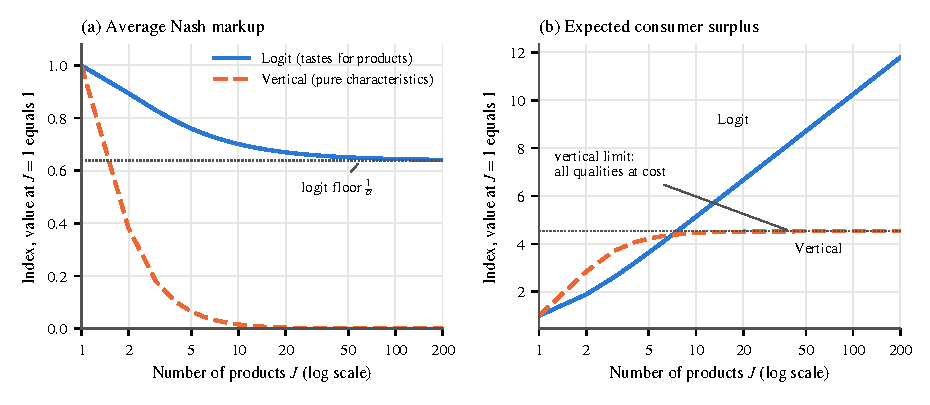
\includegraphics[width=\textwidth]{figures/ch06/clones.pdf}
\caption{Average Nash markup and expected consumer surplus as products are added, in a logit model with identical
products and in a vertical model whose products fill a fixed quality interval. Each product has its own owner. The
logit has $u_{ij} = 2 - p_j + \epsilon_{ij}$, outside good $u_{i0} = \epsilon_{i0}$ and marginal cost $1$. The vertical model
uses Bresnahan's form (\cref{sec:06-bresnahan}), with utility $v\delta_j - p_j$ and $v$ uniform on $[0,1]$. Its
qualities sit at the midpoints of $J$ equal bins of $[1,3]$, marginal cost is $0.05\,e^{\delta}$, and the outside good
has $\delta_0 = p_0 = 0$. Each series is
divided by its value at $J = 1$ because the units of the two models are not comparable. The figure is qualitative.
Computed with \texttt{figures/ch06/src/clones.py}.}
\label{fig:06-clones}
\end{figure}

\Cref{fig:06-clones} computes both models as single-product firms are added. In the logit, the markup falls from
$1.567$ at $J = 1$ to $1.005$ at $J = 200$ and approaches the floor $\frac{1}{\alpha} = 1$. Surplus rises from $0.449$ to
$5.298$ and keeps rising linearly in $\ln J$. In the vertical model, the sales-weighted markup falls from $0.815$ at $J =
1$ to $0.013$ at $J = 10$ and to $0.00003$ at $J = 200$. Surplus converges to $0.752$, the surplus when every quality in
$[1,3]$ is sold at marginal cost.

\subsection{Why the distinction matters}\label{sec:06-eps-matters}

The first implication concerns new goods and price indexes. Retrospective measurement of the gains from new products
goes back to \citet{Trajtenberg1989}, who used a nested logit to value innovations in computed tomography scanners.
Such measurement is also part of constructing ideal price indexes. \citet{BerryPakes2007} note that, according to the Boskin
Commission \citep{BoskinEtAl1996}, failing to measure these gains is the major source of bias in the Consumer Price
Index. A model with tastes for products credits every new variety with a
surplus gain through \eqref{eq:06-logit-gain}, however close it is to existing goods.

\citet[p.~230]{Hausman1997} puts the objection directly. The independence of irrelevant alternatives, he writes,
``typically leads to a vast overestimate of the consumer's surplus from a new good.'' The logit fails to ``incorporate
sufficiently the similarities to existing goods.'' Logit and constant elasticity of substitution demand are positive at every finite price, so the reservation
price at which a new good's demand would vanish is infinite. \citet{Petrin2002} quantifies the role of the shock for
the minivan. His average compensating variation for minivan buyers is \$13,652 with an OLS logit and \$7,414 with an
instrumented logit (1982--84 dollars, his Table~8). It falls to \$3,171 with random coefficients and to \$1,247 when
micro moments are added. The part attributed to the logit error falls from \$95,121 to \$396 across the same columns.
\Cref{ch:newgoods} treats these studies in full.

The second implication concerns market structure. With tastes for products, markups never vanish however many
products crowd the market, so there is always a further incentive to develop products. Market outcomes do not approach
competition as the number of products grows \citep[p.~7]{BerryPakes2007}. A researcher studying a market with hundreds
of products, or the welfare effect of entry, imposes these properties by choosing the model.

\subsection{What the idiosyncratic shock buys}\label{sec:06-eps-advantages}

Models with tastes for products have three practical advantages \citep[pp.~7--8]{BerryPakes2007}. Their choice
probabilities are integrals with simple limits of integration, because conditional on the random coefficients the
logit integral is in closed form \citep{McFadden1981}. Their purchase probabilities are positive at every parameter
value and, under regularity conditions, have smooth derivatives. Their market shares can be inverted to recover the
unobserved characteristics $\xi_j$ as a linear function of parameters and data. Instrumental variables can then handle
the correlation between price and $\xi_j$ \citep{BerryLevinsohnPakes1995}.

Pure characteristics models lose each advantage. The set of tastes for which a product is chosen is a polyhedron whose
shape changes with every parameter value. \citet{FeenstraLevinsohn1995} computed these acceptance regions directly, a
calculation that becomes complicated with several characteristics. Shares are zero whenever a product is dominated,
so the share function has flat regions. The inversion requires new arguments, which \cref{sec:06-purechar} develops.

\subsection{Nesting the two models: the modified BLP model}\label{sec:06-nesting}

A natural idea is to nest the two classes and let the data choose. \citet[eqs.~7--8]{BerryPakes2007} introduce a scale
parameter $\sigma_\epsilon \ge 0$,
\begin{equation}\label{eq:06-nest}
  u_{ij} = f_{ij}(\theta) + \sum_{k=1}^{K} \nu_{ik} X_{jk} + \sigma_\epsilon \epsilon_{ij},
\end{equation}
with $\epsilon_{ij}$ independent standard Gumbel. The model with tastes for products is the case $\sigma_\epsilon = 1$,
and the pure characteristics model is the case $\sigma_\epsilon = 0$. For $\sigma_\epsilon > 0$ define $\mu_\epsilon =
\frac{1}{\sigma_\epsilon}$ and multiply all utilities by $\mu_\epsilon$. This leaves choices unchanged. If $F(\nu)$ is the
distribution of $\nu = (\nu_1, \dots, \nu_K)$, the logit formula gives (their eq.~9)
\begin{equation}\label{eq:06-modblp}
  P_{ij}(\theta, \mu_\epsilon) = \int
  \frac{\exp\bigl(\mu_\epsilon\bigl[f_{ij}(\theta) + \sum_{k} \nu_k X_{jk}\bigr]\bigr)}
       {\sum_{q} \exp\bigl(\mu_\epsilon\bigl[f_{iq}(\theta) + \sum_{k} \nu_k X_{qk}\bigr]\bigr)} \,\dd F(\nu).
\end{equation}
We call \eqref{eq:06-modblp} the \emph{modified BLP model}. Formula \eqref{eq:06-modblp} needs $\mu_\epsilon < \infty$,
so no value of $\mu_\epsilon$ reproduces the pure characteristics model exactly. It is reached only as a limit.

\begin{proposition}[Pure characteristics as a limit]\label{prop:06-limit}
Let $U_{ij}(\nu) = f_{ij}(\theta) + \sum_k \nu_k X_{jk}$ and let
\begin{equation*}
  P^{pc}_{ij}(\theta) = \int \indic\bigl\{U_{ij}(\nu) > U_{iq}(\nu) \text{ for all } q \ne j\bigr\}\,\dd F(\nu)
\end{equation*}
be the pure characteristics choice probability. Suppose ties have probability zero, that is, $F$ assigns probability
zero to the set of $\nu$ with $U_{ij}(\nu) = U_{iq}(\nu)$ for some $q \ne j$. Then $P_{ij}(\theta, \mu_\epsilon) \to
P^{pc}_{ij}(\theta)$ as $\mu_\epsilon \to \infty$.
\end{proposition}

\begin{proof}
Fix $\nu$ outside the tie set and let $m$ be the unique maximizer of $U_{iq}(\nu)$ over $q$. Divide the numerator and
denominator of the integrand by the numerator to obtain
\begin{equation*}
  \frac{1}{1 + \sum_{q \ne j} \exp\bigl(\mu_\epsilon [U_{iq}(\nu) - U_{ij}(\nu)]\bigr)} .
\end{equation*}
If $j = m$, every exponent is negative and each exponential converges to zero, so the integrand converges to one. If
$j \ne m$, the exponent for $q = m$ is positive and that exponential diverges, so the integrand converges to zero. The
integrand therefore converges to $\indic\{j = m\}$ for $F$-almost every $\nu$. It lies in $[0,1]$, and the constant one
is integrable against the probability measure $F$. The dominated convergence theorem gives the result.
\end{proof}

\citet[footnote~9]{BerryPakes2007} add that a covering argument makes the convergence uniform in $\theta$. One might
hope that estimating $\mu_\epsilon$ along with the other parameters would deliver a large estimate whenever the pure
characteristics model generated the data. \citet[p.~9]{BerryPakes2007} give four reasons to doubt it.
\begin{enumerate}
\item Consistency proofs assume that the true parameter lies in a compact set. One would therefore have to prove
consistency for $\sigma_\epsilon = \frac{1}{\mu_\epsilon}$ on an interval that contains zero. The predicted shares are
undefined at $\sigma_\epsilon = 0$. The objective is then not a continuous function on a compact parameter set that
contains the truth, and the uniform convergence that standard proofs require fails at that boundary.
\item A good approximation needs a small $\sigma_\epsilon$, that is, a large $\mu_\epsilon$. For large $\mu_\epsilon$ the
computer cannot evaluate the exponentials in \eqref{eq:06-modblp}.
\item If $\sigma_\epsilon$ is known to be zero, an estimator that imposes it should estimate the other parameters more
precisely. With market-level data this efficiency gain can matter.
\item To learn whether these problems matter in a given application, one needs an estimator that does not rely on the
approximation \eqref{eq:06-modblp}.
\end{enumerate}
A test of $\sigma_\epsilon = 0$ faces a further, standard difficulty. The null hypothesis lies on the boundary of the
parameter space, where likelihood-ratio and Wald statistics have nonstandard limiting distributions.

\begin{remark}[The two models as bounds]\label{rem:06-bounding}
Real products differ in more than one unobserved characteristic. A pure characteristics model with as many unobserved
characteristics as products contains the model with tastes for products as a special case, by
\eqref{eq:06-dummies}. The pure characteristics model with a single unobserved characteristic and the model with
tastes for products are therefore opposite extremes. \citet[p.~12]{BerryPakes2007} suggest that the two might bound the
effects of unobserved product heterogeneity. Models with several unobserved characteristics are hard to estimate
from market data, although panel data on repeated choices of the same consumers can identify them
\citep{GoettlerShachar2001}.
\end{remark}

\section{Case study: estimating the pure characteristics model}\label{sec:06-purechar}

\citet{BerryPakes2007} turn the pure characteristics model, long used in theory, into an estimable model for market
data. Their paper has no field data. It develops the econometric machinery and then uses Monte Carlo experiments to
compare the pure characteristics model with models that have tastes for products. We follow the order of a case study,
with the simulated designs in the place of a data set.

\subsection{The question}\label{sec:06-bp-question}

The paper asks three questions. Can the pure characteristics model be estimated from market-level data on prices,
quantities and characteristics? How much computation does that take? When do models with tastes for products, possibly
with an estimated scale $\mu_\epsilon$, reproduce the implications of the pure characteristics model for elasticities and
for welfare? The questions matter because welfare analysis of new products extrapolates beyond observed prices. As
\cref{sec:06-epsilon} showed, the two classes of models extrapolate very differently.

\subsection{Model and normalizations}\label{sec:06-bp-model}

Utility of consumer $i$ from product $j = 0, 1, \dots, J$ is (their eq.~10)
\begin{equation}\label{eq:06-bp-u10}
  u_{ij} = x_j \beta_i - \alpha_i p_j + \lambda_i \xi_j ,
\end{equation}
with $\beta_{ik} = \beta_k + \nu_{ik}$, $\alpha_i = \alpha + \nu_{ip} > 0$ and $\lambda_i > 0$. Here $\beta_k$ is the mean
marginal utility of characteristic $k$ and $\nu_{ik}$ is consumer $i$'s deviation from it. Two assumptions are built into
\eqref{eq:06-bp-u10}.

\begin{assumption}[Berry and Pakes, A1 and A2]\label{ass:06-bp}
(A1) There is a single unobserved product characteristic, so $X_j = (x_j, \xi_j) \in \R^K \times \R$. (A2) The unobserved
characteristic is vertical: every consumer prefers more of it.
\end{assumption}

Utility is identified only up to a consumer-specific increasing affine transformation (\cref{prop:06-normalization}).
Berry and Pakes use both degrees of freedom. They subtract $u_{i0}$ from every utility, so the outside option has utility
zero and every characteristic is measured relative to the outside option. They then divide by $\lambda_i$, so the
coefficient on $\xi$ equals one for every consumer. After relabeling the rescaled coefficients, the model is (their
eq.~11)
\begin{equation}\label{eq:06-bp-u11}
  u_{ij} = x_j \beta_i - \alpha_i p_j + \xi_j , \qquad u_{i0} = 0 .
\end{equation}
This is the model of \citet{BerryLevinsohnPakes1995} without the shock $\epsilon_{ij}$. Units remain free. Multiplying
every $\xi_j$, $\beta_i$ and $\alpha_i$ by the same positive constant changes no choice (their footnote~12). Berry and
Pakes set the mean of $\alpha_i$ to one, so utility and $\xi$ are measured in units of the mean price coefficient.

Two interpretive points follow from the normalizations. First, $\xi_j$ measures the unobserved quality of product $j$
relative to that of the outside option (their footnote~11). A rise in average $\xi$ over time may therefore reflect
better products or a worse outside option, which matters for price indexes \citep{PakesBerryLevinsohn1993}. Second,
$\xi_j$ often stands for the combined effect of many minor characteristics (their footnote~4). If consumers differ in
their relative tastes for several unobserved characteristics, \eqref{eq:06-bp-u11} is misspecified.

\subsection{Computing market shares}\label{sec:06-bp-shares}

\casehead{The vertical building block}
Start with the vertical model $u_{ij} = \delta_j - \alpha_i p_j$, where $\delta_j = x_j\beta + \xi_j$ is quality (their
eqs.~12--13). It is the model of \cref{sec:06-vertical} with the price coefficient $\alpha_i$ in the role of the price
sensitivity $\nu_i$. Order the goods by increasing price. \Cref{sec:06-vcutoffs} showed that consumer $i$ buys $j$ if and
only if $\underline\nu_j(\delta, p) < \alpha_i < \bar\nu_j(\delta, p)$, with the general cutoffs
\eqref{eq:06-bp-cutoffs} (their eqs.~14--16). If $F$ is the distribution of $\alpha_i$, the share of product $j$ is
\eqref{eq:06-bp-share} (their eq.~17). We write it as $s_j(x, p, \xi; \theta, F)$ to show its dependence on the data and
on the unknown parameters $\theta$. Any parameter vector that puts a product below the quality-price frontier predicts a zero
share for it. A model with tastes for products never predicts a zero share.

\casehead{Extension to $K$ dimensions}
In \eqref{eq:06-bp-u11} the coefficients on $x$ vary across consumers. Conditional on $\beta_i = \beta$, however, the model
is again vertical in $\alpha_i$, with qualities $\delta_j(\beta) = x_j \beta + \xi_j$ that depend on the draw. Compute the
cutoffs $\bar\nu_j(\beta)$ and $\underline\nu_j(\beta)$ from \eqref{eq:06-bp-cutoffs} with $\delta_j(\beta)$ in place of
$\delta_j$, and integrate over $\beta$ (their eq.~18):
\begin{equation}\label{eq:06-bp-share18}
  s_j(x, p, \xi; \theta, F, G) = \int \bigl[F(\bar\nu_j(\beta) \mid \beta) - F(\underline\nu_j(\beta) \mid \beta)\bigr]\,
  \indic\{\bar\nu_j(\beta) > \underline\nu_j(\beta)\}\, \dd G(\beta) .
\end{equation}
Here $F(\cdot \mid \beta)$ is the distribution of $\alpha_i$ given $\beta_i = \beta$ and $G$ is the distribution of
$\beta_i$. The pure characteristics share function is a mixture of vertical-model share functions. The conditioning
argument avoids computing the region of $(\beta, \alpha)$ space in which a consumer chooses $j$, the route taken by
\citet{FeenstraLevinsohn1995}. The integral over $\beta$ has no closed form, so it is simulated \citep{Pakes1986}. With
$ns$ draws $\beta_1, \dots, \beta_{ns}$ from $G$ and their empirical distribution $G_{ns}$ (their eqs.~19--20),
\begin{equation}\label{eq:06-bp-share20}
  s_j(x, p, \xi; \theta, F, G_{ns}) = \frac{1}{ns} \sum_{r=1}^{ns}
  \bigl[F(\bar\nu_j(\beta_r) \mid \beta_r) - F(\underline\nu_j(\beta_r) \mid \beta_r)\bigr]\,
  \indic\{\bar\nu_j(\beta_r) > \underline\nu_j(\beta_r)\} .
\end{equation}
Berry and Pakes note that if $F$ has a density that is differentiable in the parameters, the simulated share function is
continuously differentiable in the parameters. The simulation adds error to the computed shares, as in
\citet{BerryLevinsohnPakes1995}.

The comparison with the random coefficients logit is instructive. There the first step integrates out $\epsilon_{ij}$
analytically conditional on $\beta_i$, which yields the logit formula. Here the first step integrates out $\alpha_i$
analytically conditional on $\beta_i$, which yields the vertical formula. Both models simulate the remaining
integral. A practical version of \eqref{eq:06-bp-share20} proceeds as follows (their footnote~15).
\begin{enumerate}
\item Draw $\beta_1, \dots, \beta_{ns}$ from $G$ once, and keep the draws fixed across parameter values so that the
objective function is smooth in the parameters.
\item For each draw $r$, compute $\delta_j(\beta_r) = x_j \beta_r + \xi_j$ for $j = 1, \dots, J$, with $\delta_0 = p_0 = 0$.
\item Sort the products by price and drop those that are dominated for this draw, using the frontier algorithm that
follows \cref{prop:06-frontier}. The survivors have decreasing adjacent cutoffs.
\item For each survivor compute $F(\bar\nu_j \mid \beta_r) - F(\bar\nu_{j+1} \mid \beta_r)$ with cutoffs between adjacent
survivors. Assign zero to the dropped products.
\item Average the conditional shares over the $ns$ draws.
\end{enumerate}
In the Monte Carlo design of \cref{sec:06-bp-design}, $\ln\alpha_i = \sigma_p \nu_{ip}$ with $\nu_{ip}$ standard normal and
independent of $\beta_i$. Step 4 then uses $F(a \mid \beta) = \Phi\bigl(\frac{\ln a}{\sigma_p}\bigr)$ for $a > 0$, with $\Phi$
the standard normal distribution function.

\subsection{Existence and uniqueness of the inverse}\label{sec:06-bp-inverse}

Estimation follows the three steps of \citet{BerryLevinsohnPakes1995}. For each parameter vector one recovers the
unobserved characteristics from the observed shares, computes them with an algorithm, and then chooses the parameters
that best satisfy moment conditions on $\xi$. The first step requires that the share equations have exactly one
solution.

Fix $(x, p, \theta, F, G)$ and write $\sigma_j(\xi_0, \xi)$, $j = 0, 1, \dots, J$, for the share of good $j$ as a function of
the unobserved characteristics of all goods, the outside good included. Let $s^o$ be the observed share vector, assumed
to lie in the interior of the unit simplex, so that every share is strictly between zero and one. With the normalization
$\xi_0 = 0$, we seek $\xi \in \R^J$ such that (their eq.~21)
\begin{equation}\label{eq:06-bp-system}
  \sigma(0, \xi) = s^o .
\end{equation}
For good $j \ge 1$ define the \emph{element-by-element inverse} $r_j(\xi_{-j})$ as the value of $\xi_j$ that matches good
$j$'s share when the other inside goods are held at $\xi_{-j}$ (their eq.~23):
\begin{equation}\label{eq:06-bp-r}
  \sigma_j\bigl(0, r_j(\xi_{-j}), \xi_{-j}\bigr) = s^o_j .
\end{equation}
Stack the inverses into $r(\xi) = (r_1(\xi_{-1}), \dots, r_J(\xi_{-J}))$, a map from $\R^J$ to $\R^J$. A vector $\xi$ solves
\eqref{eq:06-bp-system} if and only if it is a fixed point (their eq.~24)
\begin{equation}\label{eq:06-bp-fixedpoint}
  \xi = r(\xi) .
\end{equation}
Indeed, a fixed point matches every inside share, and the outside share then matches because shares sum to one.

\begin{theorem}[Berry and Pakes 2007, Theorem~1]\label{thm:06-bp-inverse}
Suppose the share function $\sigma$ has the following properties.\footnote{\citet{BerryPakes2007} state monotonicity in
weak form and the substitutes condition as the pair of inequalities in their eqs.~25--26. We add strict monotonicity in
own $\xi$ on the interior, which makes the element-by-element inverse single valued. We also state the substitutes
condition in the form that the proof uses. \citet{BerryGandhiHaile2013} generalize conditions of this type under the
name ``connected substitutes''.}
\begin{enumerate}[label=(\arabic*)]
\item \emph{Monotonicity.} Each $\sigma_j$, $j = 0, \dots, J$, is continuous, nondecreasing in its own $\xi_j$ and
nonincreasing in every other component. It is strictly increasing in $\xi_j$ at any point where $0 < \sigma_j < 1$. For
fixed values of the other components, $\sigma_j \to 0$ as $\xi_j \to -\infty$ and $\sigma_j \to 1$ as $\xi_j \to \infty$.
\item \emph{Linearity of utility in $\xi$.} Raising $\xi$ for every good, the outside good included, by the same amount
changes no share: $\sigma(\xi_0 + c, \xi + c\mathbf{1}) = \sigma(\xi_0, \xi)$ for every $c \in \R$.
\item \emph{Substitutes with some other good.} Let $(\xi_0, \xi)$ give interior shares. Let $(\tilde\xi_0, \tilde\xi) \ge
(\xi_0, \xi)$ componentwise, with equality exactly on a nonempty proper subset $I$ of $\{0, 1, \dots, J\}$. Then
$\sigma_j(\tilde\xi_0, \tilde\xi) < \sigma_j(\xi_0, \xi)$ for at least one $j \in I$.
\end{enumerate}
Then for every $s^o$ in the interior of the unit simplex, \eqref{eq:06-bp-system} has exactly one solution $\xi \in \R^J$.
Moreover, $r$ is a weak contraction in the sup norm: $\lVert r(\xi') - r(\xi) \rVert_\infty \le \lVert \xi' - \xi
\rVert_\infty$.
\end{theorem}

Condition (3) says that when the unobserved characteristics of some goods rise, at least one good whose characteristic
did not rise loses share strictly. The proof has five steps. Steps 3 and 4 follow \citet[eqs.~27--31]{BerryPakes2007}.
They attribute existence to the argument in \citet{Berry1994}. Step 5 gives a self-contained existence argument.
Throughout we write the arguments of $\sigma_j$ in the order (outside good, own, other inside goods) when it helps.

\begin{proof}
\emph{Step 1: $r$ is well defined and continuous.} Fix $j$ and $\xi_{-j}$, and let $g(a) = \sigma_j(0, a, \xi_{-j})$. By
condition (1), $g$ is continuous with limits $0$ and $1$. Since $0 < s^o_j < 1$, the intermediate value theorem gives a
solution of $g(a) = s^o_j$. Two solutions $a < a'$ would make $g$ constant at the interior value $s^o_j$ on $[a, a']$,
which strict monotonicity rules out. For continuity of $r_j$, take $h > 0$. Strict monotonicity gives $g(r_j + h) > s^o_j > g(r_j - h)$. By
continuity of $\sigma_j$ in $\xi_{-j}$, both strict inequalities survive small changes in $\xi_{-j}$, which keeps the
solution within $h$ of $r_j$.

\emph{Step 2: $r$ is monotone.} Let $\xi \le \xi'$ and suppose $r_j(\xi'_{-j}) < r_j(\xi_{-j})$ for some $j$. Raising the
rivals from $\xi_{-j}$ to $\xi'_{-j}$ weakly lowers $j$'s share, so
\begin{equation*}
  s^o_j = \sigma_j\bigl(0, r_j(\xi'_{-j}), \xi'_{-j}\bigr) \le \sigma_j\bigl(0, r_j(\xi_{-j}), \xi'_{-j}\bigr)
  \le \sigma_j\bigl(0, r_j(\xi_{-j}), \xi_{-j}\bigr) = s^o_j .
\end{equation*}
The first inequality uses own monotonicity. Both inequalities hold with equality, so $\sigma_j(0, \cdot, \xi'_{-j})$ is
constant at $s^o_j$ on an interval, which contradicts strict monotonicity. Hence $r(\xi) \le r(\xi')$.

\emph{Step 3: $r$ is a weak contraction.} Take $\xi, \xi' \in \R^J$ with $d = \lVert \xi - \xi' \rVert_\infty$, and write
$r_j = r_j(\xi_{-j})$ and $r'_j = r_j(\xi'_{-j})$. By the definition of $r_j$ and linearity with $c = d$,
\begin{equation}\label{eq:06-bp-p27}
  \sigma_j\bigl(d, r_j + d, \xi_{-j} + d\bigr) = \sigma_j\bigl(0, r_j, \xi_{-j}\bigr) = s^o_j .
\end{equation}
Now $\xi'_{-j} \le \xi_{-j} + d$ and $0 < d$. Lowering the rivals' characteristics from $(d, \xi_{-j} + d)$ to $(0,
\xi'_{-j})$ weakly raises $j$'s share, so
\begin{equation}\label{eq:06-bp-p28}
  \sigma_j\bigl(0, r_j + d, \xi'_{-j}\bigr) \ge s^o_j .
\end{equation}
Suppose $r'_j > r_j + d$. Then own monotonicity and \eqref{eq:06-bp-p28} give
\begin{equation*}
  s^o_j = \sigma_j\bigl(0, r'_j, \xi'_{-j}\bigr) \ge \sigma_j\bigl(0, r_j + d, \xi'_{-j}\bigr) \ge s^o_j ,
\end{equation*}
so $\sigma_j(0, \cdot, \xi'_{-j})$ would be constant at $s^o_j$ on $[r_j + d, r'_j]$. This contradicts strict
monotonicity, so $r'_j \le r_j + d$. The same argument with $c = -d$ gives $r'_j \ge r_j - d$. Hence $|r'_j - r_j| \le d$
for every $j$, which is the weak contraction property.

\emph{Step 4: uniqueness.} Suppose $\xi \ne \xi'$ both solve \eqref{eq:06-bp-system}. Exchanging their names if
necessary, $\bar c = \max_k (\xi_k - \xi'_k) > 0$. Let $I = \{k : \xi_k - \xi'_k = \bar c\}$, a nonempty set of inside goods.
Define $\tilde\xi = \xi' + \bar c\mathbf{1}$ and $\tilde\xi_0 = \bar c$. By linearity,
\begin{equation*}
  \sigma(\tilde\xi_0, \tilde\xi) = \sigma(0, \xi') = s^o .
\end{equation*}
Compare $(\tilde\xi_0, \tilde\xi)$ with $(0, \xi)$. For each inside good, $\tilde\xi_k - \xi_k = \bar c - (\xi_k - \xi'_k) \ge
0$, with equality exactly for $k \in I$. For the outside good, $\tilde\xi_0 - 0 = \bar c > 0$. So $(\tilde\xi_0, \tilde\xi) \ge
(0, \xi)$ with equality exactly on $I$, a nonempty proper subset of $\{0, \dots, J\}$. Shares at $(0, \xi)$ equal $s^o$ and are
interior. Condition (3) then yields a good $j \in I$ with $\sigma_j(\tilde\xi_0, \tilde\xi) < \sigma_j(0, \xi) = s^o_j$. But
$\sigma_j(\tilde\xi_0, \tilde\xi) = s^o_j$, a contradiction.

\emph{Step 5: existence.} We first find a vector $\xi^{(0)}$ with $r(\xi^{(0)}) \ge \xi^{(0)}$. By linearity,
$\sigma(0, a\mathbf{1}) = \sigma(-a, \mathbf{0})$. As $a \to -\infty$, the outside good's own characteristic $-a$ goes to
infinity, so by condition (1) its share goes to one and every inside share goes to zero. Choose $a$ with $\sigma_j(0,
a\mathbf{1}) < s^o_j$ for all $j \ge 1$. At own value $a$ and rivals at $a$, good $j$ falls short of its target, so own
monotonicity gives $r_j(a\mathbf{1}_{-j}) > a$. Set $\xi^{(0)} = a\mathbf{1}$ and iterate $\xi^{(n+1)} = r(\xi^{(n)})$. By
Step 2 and induction, the sequence is nondecreasing.

Next, the sequence is bounded. Because it is nondecreasing, it can be unbounded only if some component
diverges to infinity. Since $\xi^{(n)}_j \le r_j(\xi^{(n)}_{-j})$ and $\sigma_j$ increases in own $\xi_j$, every
inside share satisfies $\sigma_j(0, \xi^{(n)}) \le s^o_j$. Shares sum to one, so $\sigma_0(0, \xi^{(n)}) \ge s^o_0 > 0$.
Suppose component $\xi^{(n)}_k$ diverged. Because the other components are at least $\xi^{(0)}_{-k}$ and
$\sigma_0$ is nonincreasing in inside characteristics,
\begin{equation*}
  \sigma_0\bigl(0, \xi^{(n)}\bigr) \le \sigma_0\bigl(0, \xi^{(n)}_k, \xi^{(0)}_{-k}\bigr)
  \le 1 - \sigma_k\bigl(0, \xi^{(n)}_k, \xi^{(0)}_{-k}\bigr) \to 0 ,
\end{equation*}
by the limit in condition (1). This contradicts $\sigma_0 \ge s^o_0$. A bounded nondecreasing sequence converges, say to
$\xi^*$. By continuity of $r$, $\xi^* = \lim r(\xi^{(n)}) = r(\xi^*)$, so $\xi^*$ solves \eqref{eq:06-bp-system}.
\end{proof}

\begin{remark}[The conditions in the pure characteristics model]\label{rem:06-bp-conditions}
\citet[Comment~1]{BerryPakes2007} observe that the conditions hold for any finite $\theta$ as long as $F(\cdot \mid \beta)$
has a positive density. The distribution $G$ need not have a density, so the simulated $G_{ns}$ of
\eqref{eq:06-bp-share20} is allowed. Linearity holds by construction in \eqref{eq:06-bp-u11}, and their Comment~2 notes
that any model that is linear in $\xi$ alone would share the result. Condition (3) can be checked draw by draw.
Conditional on $\beta$, the undominated goods form a chain ordered by price, and each good on the chain competes with its
neighbors. The outside good is always on the chain. If the chain contains goods both inside and outside $I$, some
adjacent pair has one member in each. Raising the characteristic of the member outside $I$ strictly lowers the
conditional share of its neighbor in $I$, because $F$ has a positive density. Interior aggregate shares ensure that
such draws have positive probability.
\end{remark}

Steps 3 to 5 are constructive. The iteration in Step 5 is the element-by-element inverse started from a low point. It
converges monotonically, but the argument gives no rate. The weak contraction property gives no rate either, because its
modulus may equal one. \citet{BerryPakes2007} report that they could not prove a modulus below one. This is the main
computational difference from the logit-based contraction of \citet{BerryLevinsohnPakes1995}, which converges at a
geometric rate.

\subsection{Computing the inverse}\label{sec:06-bp-compute}

Berry and Pakes offer three methods, because each fails in some of their experiments.

\casehead{The modified BLP contraction}
Apply the BLP contraction of \cref{ch:blp} to the modified BLP model \eqref{eq:06-modblp} with a large fixed
$\mu_\epsilon$. Since the logit part of \eqref{eq:06-modblp} depends on mean utility only through $\mu_\epsilon\delta$, the
iteration on mean utilities reads
\begin{equation}\label{eq:06-modblp-contraction}
  \delta^{(h+1)} = \delta^{(h)} + \frac{1}{\mu_\epsilon}\bigl[\ln s^o - \ln s(\delta^{(h)}; \mu_\epsilon)\bigr] .
\end{equation}
The method is fast. It is inaccurate when $\mu_\epsilon$ cannot be set high enough, and numerical overflow limits how
high it can go.

\casehead{The element-by-element inverse}
Start from a candidate vector. For each product $j$, hold the other products at their current values and solve the
one-dimensional monotone equation \eqref{eq:06-bp-r} for $\xi_j$. Update all products and repeat until predicted shares
match observed shares. By \cref{thm:06-bp-inverse} each pass is a weak contraction. In practice the method sometimes
makes large gains in the first iterations and then nearly stops. If predicted shares are then positive, Newton steps can
finish the job.

\casehead{The homotopy}
A homotopy deforms a problem with a known solution into the problem of interest. Berry and Pakes use the fixed-point
homotopy (their eq.~32)
\begin{equation}\label{eq:06-homotopy}
  h(\xi, t, \xi_0) = (1 - t)(\xi - \xi_0) + t\bigl(\xi - r(\xi)\bigr), \qquad t \in [0, 1],
\end{equation}
where $\xi_0$ is a starting guess, for example the output of another method. Let $\xi(t)$ solve $h(\xi, t, \xi_0) = 0$.
At $t = 0$ the solution is $\xi_0$, and at $t = 1$ it is the fixed point \eqref{eq:06-bp-fixedpoint}. Rearranging $h = 0$
gives (their eq.~33)
\begin{equation}\label{eq:06-homotopy33}
  \xi(t) = (1 - t)\,\xi_0 + t\, r\bigl(\xi(t)\bigr) .
\end{equation}

\begin{proposition}[Convergence of the homotopy]\label{prop:06-homotopy}
Under the conditions of \cref{thm:06-bp-inverse}, let $\xi^*$ be the unique solution of \eqref{eq:06-bp-system}.
\begin{enumerate}[label=(\roman*)]
\item For each $t \in [0, 1)$, the map $\Phi_t(\xi) = (1 - t)\xi_0 + t\, r(\xi)$ is a contraction with modulus at most $t$.
Hence $\xi(t)$ exists, is unique, and is the limit of the recursion $\xi \mapsto (1-t)\xi_0 + t\,r(\xi)$ (their eq.~34)
from any starting point.
\item $\lVert \xi(t) - \xi^* \rVert_\infty \le \lVert \xi_0 - \xi^* \rVert_\infty$ for every $t \in [0,1)$, and $\xi(t) \to
\xi^*$ as $t \to 1$.
\end{enumerate}
\end{proposition}

\begin{proof}
For (i), $\lVert \Phi_t(\xi) - \Phi_t(\xi') \rVert_\infty = t \lVert r(\xi) - r(\xi') \rVert_\infty \le t \lVert \xi - \xi'
\rVert_\infty$ by the weak contraction property. The contraction mapping theorem (\cref{app:math}) gives the rest.

For (ii), subtract $\xi^* = (1 - t)\xi^* + t\, r(\xi^*)$ from \eqref{eq:06-homotopy33}:
\begin{equation*}
  \xi(t) - \xi^* = (1 - t)(\xi_0 - \xi^*) + t\bigl[r(\xi(t)) - r(\xi^*)\bigr] .
\end{equation*}
Taking norms and using the weak contraction property,
\begin{equation*}
  \lVert \xi(t) - \xi^* \rVert_\infty \le (1 - t)\lVert \xi_0 - \xi^* \rVert_\infty + t \lVert \xi(t) - \xi^* \rVert_\infty .
\end{equation*}
Collecting terms and dividing by $1 - t > 0$ gives the bound. The path is therefore bounded. Take any sequence $t_n \to 1$
along which $\xi(t_n)$ converges, say to $\hat\xi$. Passing to the limit in \eqref{eq:06-homotopy33} and using continuity of
$r$ gives $\hat\xi = r(\hat\xi)$. By uniqueness $\hat\xi = \xi^*$. Every convergent subsequence has the same limit, so
$\xi(t) \to \xi^*$.
\end{proof}

The modulus $t$ explains the practical behavior. Each tenfold reduction in the error of the recursion takes about
$\frac{\ln 10}{-\ln t}$ iterations. That is about 229 iterations at $t = 0.99$, 459 at $t = 0.995$ and 1,150 at
$t = 0.998$. Berry and Pakes start at $t = 0.99$ and move $t$ toward one slowly, solving for each new $\xi(t)$ by Newton's
method when the recursion becomes slow. They find that the homotopy gets much closer to the solution than the
element-by-element inverse before it slows down.

What the paper calls the ``homotopy'' method is an integrated routine that combines the three methods.
\begin{enumerate}
\item Run the modified BLP contraction \eqref{eq:06-modblp-contraction} with a high $\mu_\epsilon$, lowering
$\mu_\epsilon$ if numerical errors arise.
\item If needed, switch to the element-by-element inverse, with periodic Newton steps when possible.
\item If that does not converge quickly, use the homotopy recursion. For small problems, push $t$ to one or very near it.
For large problems, use only a few values such as $t = 0.99$, $0.995$ and $0.998$.
\end{enumerate}

\subsection{Simulation error and limit theory}\label{sec:06-bp-simerror}

\citet{BerryLintonPakes2004} derive limit theorems as the number of products $J$ grows, for models with and without
tastes for products. The two classes behave very differently, and the difference has computational consequences.

In the plain logit no simulation is needed, but observed shares contain sampling error from a finite sample of
consumers. The inversion is analytic (their eqs.~35--36),
\begin{equation}\label{eq:06-logit-inv-sens}
  \xi_j = \ln s_j - \ln s_0 - x_j \beta , \qquad \frac{\partial \xi_j}{\partial s_j} = \frac{1}{s_j} .
\end{equation}
With many products most shares are small, so the recovered $\xi_j$ are very sensitive to any error in $s_j$.
\citet{BerryLintonPakes2004} show that simulation error causes the same problem in the random coefficients logit. A
back-of-the-envelope calculation shows the orders of magnitude. If $s_j$ is estimated from $n$ independent draws, its
variance is about $\frac{s_j(1 - s_j)}{n}$. The delta method then gives
\begin{equation*}
  \Var(\ln \hat s_j) \approx \frac{1}{s_j^2}\cdot\frac{s_j(1 - s_j)}{n} = \frac{1 - s_j}{n s_j} .
\end{equation*}
With $s_j$ of order $\frac{1}{J}$, the standard deviation of the error in $\xi_j$ is of order $\sqrt{\frac{J}{n}}$. It grows
with the number of products unless $n$ grows faster than $J$.

The pure characteristics model behaves in the opposite way. As products crowd the space, competition becomes local and
fierce, so $\frac{\partial s_j}{\partial \xi_j}$ is large and the inverse map is insensitive to share errors. The
vertical model makes this concrete. By \cref{prop:06-vinversion}, $\delta_j = \sum_{m \le j} (p_m - p_{m-1})
F^{-1}(S_m)$, where $S_m = \sum_{k \ge m} s_k$ is a cumulative share. A cumulative share estimated from $n$ draws has
variance at most $\frac{1}{4n}$, whatever $J$. The weights $\frac{p_m - p_{m-1}}{f(F^{-1}(S_m))}$ translate errors
in $S_m$ into errors in $\delta_j$. Their sum is bounded when prices lie in a bounded interval and the density $f$ is
bounded away from zero there. The error in each $\delta_j$ is then of order $\frac{1}{\sqrt n}$, independent of $J$.

The formal results preserve this ranking, with higher required rates than the heuristic suggests.
\citet{BerryLintonPakes2004} derive conditions for asymptotic normality of the parameter estimates. The number of
simulation draws must grow at rate $J$ in the vertical model and at rate $J^2$ in logit-type models.
\citet[p.~23]{BerryPakes2007} report the Monte Carlo results of that paper. About fifty draws suffice for the limit
distribution to describe the vertical model with up to two hundred products. The logit with one
hundred products requires over two thousand draws.

Two forces therefore pull in opposite directions \citep[pp.~23--24]{BerryPakes2007}. The required number of draws grows
like $J^2$ with tastes for products and like $J$ without them, which favors the pure characteristics model. The BLP
contraction converges geometrically, while no rate is known for the pure characteristics inverse, which favors the
model with tastes for products. Which force dominates depends on the number of products and on how often the inverse
must be computed, which grows with the number of parameters.

\subsection{Estimator, instruments and identification}\label{sec:06-bp-estimator}

Write mean quality as $\delta_j = x_j\beta + \xi_j$ and split the parameters into the linear parameters $\theta_1 = \beta$
and the nonlinear parameters $\theta_2$ that govern the distribution of $(\beta_i - \beta, \alpha_i)$. For each $\theta_2$,
\cref{thm:06-bp-inverse} delivers a unique $\delta(\theta_2)$ that matches the observed shares, computed by the methods of
\cref{sec:06-bp-compute}. The structural error is $\xi_j(\theta) = \delta_j(\theta_2) - x_j\beta$. With instruments $z_j$
satisfying $\E[\xi_j z_j] = 0$, the GMM estimator solves
\begin{equation}\label{eq:06-bp-gmm}
  \hat\theta = \argmin_{\theta} \; \xi(\theta)^\top Z\, W\, Z^\top \xi(\theta),
\end{equation}
where $Z$ stacks the instruments and $W$ is a weighting matrix. The linear parameters can be concentrated out by
instrumental variables regression of $\delta(\theta_2)$ on $x$, exactly as in \cref{ch:blp}.

Price is correlated with $\xi$ in any equilibrium model, so the instruments must exclude it. The small Monte Carlo design
uses five instruments. They are a constant, $x$, $x^2$, the market mean of $x$ and the distance from each product to its
nearest neighbor in $x$. These functions of the characteristics of rival products shift each product's competitive
environment, and so its price and share, without entering its own utility. The distance to the nearest neighbor suits
the pure characteristics model, where substitution is local. An approximation to optimal instruments had little effect
(their footnote~17). The large design uses a constant and $x$, each interacted with market dummies. Berry and Pakes
attribute their success to the requirement that one utility model fit three markets whose product sets differ sharply.

\subsection{The Monte Carlo designs}\label{sec:06-bp-design}

Data are drawn from the model (their eqs.~37--39)
\begin{equation}\label{eq:06-bp-mc}
  u_{ij} = \delta_j + \sigma_x \nu_{ix} x_j - \alpha_i p_j , \qquad
  \ln \alpha_i = \sigma_p \nu_{ip} , \qquad
  \delta_j = \beta_0 + \beta_x x_j + \xi_j ,
\end{equation}
with $(\nu_{ix}, \nu_{ip})$ independent standard normal. The true values are $\sigma_x = 1$, $\sigma_p = 1$, $\beta_0 = 2$ and
$\beta_x = 1$. The price coefficient is lognormal with $\E[\ln \alpha_i] = 0$. This fixes the median of $\alpha_i$ at
one. Its mean is $e^{\frac{\sigma_p^2}{2}} \approx 1.65$ at the true $\sigma_p = 1$. The design therefore normalizes the
median of the price coefficient, while their text describes a normalization of the mean
\citep[p.~11]{BerryPakes2007}.

The characteristic $x$ equals twice a firm-specific uniform $(0,1)$ draw plus one half of a uniform $(0,1)$ draw common to
all firms in the market, which correlates characteristics within a market. Its variance is $\frac{4}{12} + \frac{1}{4}
\cdot \frac{1}{12} = \frac{17}{48} \approx 0.354$. In the base design $\xi_j$ is uniform on $(-\frac{1}{2}, \frac{1}{2})$,
with variance $\frac{1}{12} \approx 0.083$. A second design uses $\xi_j$ uniform on $(-1.5, 1.5)$, with variance $0.75$, which
exceeds the variance of $x$. Price is a convex function of quality, $p_j = \frac{e^{\delta_j}}{20}$. Equivalently, $\delta_j
= \ln(20 p_j)$ is strictly concave in price. In the vertical case this makes the cutoffs strictly decreasing, so every
product sells (\cref{prop:06-frontier}). Since price depends on $\delta_j$ and hence on $\xi_j$, price is endogenous by
construction. Observed shares come from the choices of 5,000 simulated consumers at the true parameters. Prices come
from this formula, and no pricing game is solved, so the design does not need a price equilibrium to exist.
Dividing utility by $\alpha_i$ puts it in the linear form of assumption A1 of \citet{CaplinNalebuff1991}, with type
vector $(\frac{1}{\alpha_i}, \frac{\sigma_x \nu_{ix}}{\alpha_i})$. In the vertical case, $\sigma_x = 0$, the type
$\frac{1}{\alpha_i}$ is lognormal with log-variance $\sigma_p^2 = 1$. It therefore satisfies their assumption A2, which for a
one-dimensional lognormal type holds exactly when the log-variance is at most 2 (\cref{sec:06-branches}). For the
two-dimensional design, A2 would have to be checked for the joint density of this type vector.

The paper uses two sample designs. The small design has 20 markets, each with a number of products drawn with equal
probability from $\{2, \dots, 10\}$, and 100 simulated data sets. The large design is patterned on the evolution of processor
speed in personal computers from 1995 to 1997 \citep{Pakes2003}. It has three markets, or years, with 75, 100 and 125
products. The characteristic $x$ is uniform between the year's minimum and maximum megahertz, divided by ten. The ranges
are 25 to 133 in year 1, 25 to 200 in year 2 and 33 to 240 in year 3. The unobserved characteristic equals the year's
megahertz range times $(2u_j - 1)$, with $u_j$ uniform on $[0, 1]$, so that it scales with $x$. Prices fall over time
(their eq.~40),
\begin{equation}\label{eq:06-bp-mc-price}
  \ln p_j = (t - 1)\ln 0.7 + 1.1 \ln \delta_j ,
\end{equation}
so the price of a given bundle falls about 30 percent a year, and price remains convex in quality. Some shares are very
small, smaller than in typical data sets. The large design uses one data set and asymptotic standard errors. Its
homotopy starts from the output of the modified BLP contraction with fixed $\mu_\epsilon$ and iterates 25 times on (their
eq.~41)
\begin{equation}\label{eq:06-bp-41}
  \delta' = 0.05\,\delta + 0.95\, r(\delta) .
\end{equation}
Recursion \eqref{eq:06-bp-41} anchors on the current $\delta$ instead of a fixed starting point, so it is a damped
element-by-element inverse. Its fixed points are those of $r$.

\subsection{Results}\label{sec:06-bp-results}

\casehead{Computing mean utilities}
\Cref{tab:06-bp-delta} reproduces Table~1 of \citet{BerryPakes2007}. It takes one simulated market with five products
and computes $\delta$ by different methods. The homotopy with the same 5,000 draws that generated the data recovers the
true $\delta$ exactly. With 500 draws it still fits the shares to machine precision, but the $\delta$'s differ from the truth
by 0.15 to 0.23. Their order is preserved. The modified BLP contraction with $\mu_\epsilon = 1$, which is the original BLP
contraction in these units, takes one-fiftieth of the homotopy's time but bears little relation to the truth. With
$\mu_\epsilon = 10$ one value is out of order: $\delta_5 = 4.06$ falls below $\delta_4 = 4.10$. With $\mu_\epsilon = 50$ the
order is right and the errors are 1 to 2 percent, but the time rises to 58 percent of the full homotopy's. With 500
draws and $\mu_\epsilon = 50$ the errors grow to between 0.26 and 0.57, larger than the homotopy's errors with the same
draws.

\begin{table}[htbp]
\centering
\caption{Computing $\delta$ by different methods: one market with five products}
\label{tab:06-bp-delta}
\small
\begin{tabular}{@{}lccccccc@{}}
\toprule
 & True & \multicolumn{2}{c}{Homotopy} & \multicolumn{4}{c}{Modified BLP contraction, fixed $\mu_\epsilon$} \\
\cmidrule(lr){3-4} \cmidrule(l){5-8}
Draws ($ns$) & 5,000 & 5,000 & 500 & 5,000 & 5,000 & 5,000 & 500 \\
$\mu_\epsilon$ & & & & 1 & 10 & 50 & 50 \\
\midrule
$\delta_1$ & 2.99 & 2.99 & 3.14 & 3.08 & 3.02 & 3.04 & 3.25 \\
$\delta_2$ & 3.21 & 3.21 & 3.36 & 2.09 & 3.19 & 3.26 & 3.51 \\
$\delta_3$ & 3.56 & 3.56 & 3.71 & 3.13 & 3.60 & 3.62 & 3.94 \\
$\delta_4$ & 4.04 & 4.04 & 4.27 & 4.13 & 4.10 & 4.10 & 4.61 \\
$\delta_5$ & 4.10 & 4.10 & 4.32 & 2.68 & 4.06 & 4.16 & 4.65 \\
\midrule
Relative time & & 1 & 0.15 & 0.02 & 0.12 & 0.58 & 0.03 \\
\bottomrule
\end{tabular}

\smallskip
\begin{minipage}{0.92\textwidth}
\footnotesize Source: \citet{BerryPakes2007}, Table~1. Data come from model \eqref{eq:06-bp-mc}. The ``True'' column
uses the 5,000 consumer draws that generated the shares. Relative time is computing time relative to the homotopy with
5,000 draws.
\end{minipage}
\end{table}

\casehead{Parameter estimates with few products}
\Cref{tab:06-bp-small} combines Tables~2 and~3 of the paper. With a small variance of $\xi$, the modified BLP
contraction with $\mu_\epsilon$ fixed at 30 does about as well as the homotopy. The means of $\sigma_x$ are 1.04 and 1.03
and those of $\beta_0$ are 2.06 and 2.00. With the larger variance of $\xi$, Berry and Pakes needed $\mu_\epsilon = 50$ for
comparable performance, and computational problems prevented pushing $\mu_\epsilon$ much higher. All methods then
overestimate $\sigma_x$ (1.24 and 1.26) and $\beta_0$ (2.34 and 2.33). In the first experiment $\mu_\epsilon = 30$ worked a
little better than $\mu_\epsilon = 50$, perhaps because of approximation errors in computing exponentials of large
numbers (their footnote~18).

\begin{table}[htbp]
\centering
\caption{Monte Carlo estimates with a small number of products per market}
\label{tab:06-bp-small}
\small
\setlength{\tabcolsep}{4.5pt}
\begin{tabular}{@{}lccccccc@{}}
\toprule
 & & \multicolumn{4}{c}{Fixed or no scale (Table 2)} & \multicolumn{2}{c}{Estimated scale (Table 3)} \\
\cmidrule(lr){3-6} \cmidrule(l){7-8}
 & True & (1) & (2) & (3) & (4) & (5) & (6) \\
Method & & Mod.\ BLP & Homotopy & Mod.\ BLP & Homotopy & Mod.\ BLP & Mod.\ BLP \\
Scale $\mu_\epsilon$ & & 30 & none & 50 & none & estimated & estimated \\
$\xi_j$ uniform on & & $(-\frac{1}{2}, \frac{1}{2})$ & $(-\frac{1}{2}, \frac{1}{2})$ & $(-1.5, 1.5)$ & $(-1.5, 1.5)$
  & $(-\frac{1}{2}, \frac{1}{2})$ & $(-1.5, 1.5)$ \\
\midrule
$\sigma_x$ & 1 & 1.04 & 1.03 & 1.24 & 1.26 & 1.14 & 1.64 \\
           &   & (0.04) & (0.03) & (0.06) & (0.06) & (0.04) & (0.08) \\
$\sigma_p$ & 1 & 1.00 & 0.98 & 1.02 & 1.02 & 1.03 & 1.09 \\
           &   & (0.01) & (0.01) & (0.03) & (0.03) & (0.01) & (0.03) \\
$\beta_0$  & 2 & 2.06 & 2.00 & 2.34 & 2.33 & 2.19 & 2.79 \\
           &   & (0.05) & (0.05) & (0.10) & (0.09) & (0.06) & (0.12) \\
$\beta_x$  & 1 & 0.99 & 1.00 & 1.04 & 1.05 & 1.00 & 1.03 \\
           &   & (0.01) & (0.01) & (0.02) & (0.03) & (0.01) & (0.03) \\
$\mu_\epsilon$, mean & $\infty$ & & & & & 34.08 & 15.50 \\
                    &          & & & & & (3.31) & (1.98) \\
$\mu_\epsilon$, median & $\infty$ & & & & & 17.81 & 4.67 \\
\bottomrule
\end{tabular}

\smallskip
\begin{minipage}{0.95\textwidth}
\footnotesize Source: \citet{BerryPakes2007}, Tables~2 and~3. Entries are means across 100 simulated data sets of 20
markets with 2 to 10 products each. The paper's text describes the numbers in parentheses in Table~2 as standard
deviations of the estimates across samples. The standard error of each mean is then about one tenth of the number shown.
The note to Table~3 calls them estimated standard deviations of the mean estimates. Columns (5) and (6) use 500
simulation draws. In some runs of columns (5) and (6), $\mu_\epsilon$ rose until numerical errors occurred and was then
fixed at 50 (once at 25). The homotopy took about ten times as long as the modified BLP estimates.
\end{minipage}
\end{table}

The numbers in parentheses need care. For Table~2, the paper's text describes them as standard deviations of the
estimates across the 100 samples. The precision of each reported mean is then about one tenth of the number shown. On that
reading, the overestimate of $\sigma_x$ in the high-variance design, about 0.25, is many times the standard error of the
mean. It reflects finite-sample bias, which Monte Carlo noise cannot explain. Berry and Pakes conclude that the asymptotic approximation
understates the variance of the estimator at these sample sizes. They also note that every method does worse when the
unobservable has more variance, so more data are needed for a given precision.

Estimating $\mu_\epsilon$ avoids the need to choose it, but at a cost. With the base variance the estimates move away
from the truth ($\sigma_x = 1.14$, $\beta_0 = 2.19$). With the large variance they are poor ($\sigma_x = 1.64$, $\beta_0 =
2.79$). The estimates of $\mu_\epsilon$ have means of 34.08 and 15.50 and much smaller medians of 17.81 and 4.67. Their
distribution is therefore skewed, and in the high-variance design the typical estimate gives the logit error a large role.
Imposing the traditional logit scale normalization, in place of the normalization on the price coefficient, made
convergence without numerical errors much less likely (their footnote~19).

\casehead{Substitution patterns with few products}
Parameter estimates are rarely the object of interest. \Cref{tab:06-bp-subst} reproduces Table~4 of the paper. It reports
derivatives of the share of the cheapest product in one market of the high-variance design with respect to the prices of
products 1 to 5. Each derivative is computed for every Monte Carlo parameter estimate and then averaged, which
approximates averaging over the sampling distribution of the estimator. The last two columns form a \emph{hybrid}. They
use the parameters estimated by the modified BLP model with estimated $\mu_\epsilon$ but compute derivatives from either
the pure characteristics functional form or the modified BLP form with $\mu_\epsilon = 50$.

\begin{table}[htbp]
\centering
\caption{Derivatives of the share of product 1 with respect to the price of each product}
\label{tab:06-bp-subst}
\small
\begin{tabular}{@{}lcccccc@{}}
\toprule
 & & & \multicolumn{2}{c}{Modified BLP} & \multicolumn{2}{c}{BLP parameters, derivatives via} \\
\cmidrule(lr){4-5} \cmidrule(l){6-7}
Product & True & Homotopy & Fix $\mu_\epsilon = 50$ & Estimate $\mu_\epsilon$ & Homotopy & Mod.\ BLP \\
\midrule
1 & $-0.6027$ & $-0.6198$ & $-0.7313$ & $-0.4130$ & $-0.5241$ & $-0.6353$ \\
  &           & (0.0337)  & (0.0220)  & (0.0232)  & (0.0267)  & (0.0226) \\
2 & 0.1981 & 0.2093 & 0.2531 & 0.1656 & 0.1629 & 0.2034 \\
  &        & (0.0233) & (0.0140) & (0.0139) & (0.0133) & (0.0144) \\
3 & 0.1621 & 0.1624 & 0.1183 & 0.0331 & 0.1461 & 0.1096 \\
  &        & (0.0106) & (0.0022) & (0.0059) & (0.0129) & (0.0024) \\
4 & 0.0000 & 0.0002 & 0.0278 & 0.0348 & 0.0001 & 0.0172 \\
  &        & (0.0001) & (0.0038) & (0.0042) & (0.0001) & (0.0031) \\
5 & 0.0204 & 0.0252 & 0.0292 & 0.0235 & 0.0212 & 0.0296 \\
  &        & (0.0026) & (0.0024) & (0.0023) & (0.0023) & (0.0031) \\
\bottomrule
\end{tabular}

\smallskip
\begin{minipage}{0.95\textwidth}
\footnotesize Source: \citet{BerryPakes2007}, Table~4. Row $k$ gives $\frac{\partial s_1}{\partial p_k}$ for one market of the
design with $\xi$ uniform on $(-1.5, 1.5)$. Entries average the derivative over the Monte Carlo parameter estimates of the
corresponding method. Numbers in parentheses are standard deviations of the calculated sample mean.
\end{minipage}
\end{table}

The homotopy with the pure characteristics functional form reproduces the true pattern far better than either modified
BLP estimate with its own functional form. Even with $\mu_\epsilon$ fixed at 50, the modified BLP model misses the fourth
entry badly, predicting 0.0278 where the truth is zero. Product 4 is not a neighbor of product 1, and only a pure
characteristics model can produce an exact zero. The surprise is the hybrid. The parameters from the modified BLP model
with estimated $\mu_\epsilon$, combined with the pure characteristics functional form, give $-0.5241$, 0.1629, 0.1461, 0.0001
and 0.0212. Berry and Pakes draw two lessons (their p.~31). Good parameter estimates need not produce good predictions
when the model's functional form is used to compute them. Even if one estimates with the modified BLP contraction, one may
not want to use \eqref{eq:06-modblp} to compute implications.

\casehead{Parameter estimates and elasticities with many products}
\Cref{tab:06-bp-large} combines Tables~5 and~6 of the paper. The differences across methods are much larger than with few
products. The modified BLP model with estimated scale does worst. Its estimate $\mu_\epsilon = 0.934$ gives the logit error
a large role, and to match the small shares the constant is driven to $\beta_0 = -6.455$, with a standard error of 66.864. With
$\mu_\epsilon$ fixed (at 10, halved where numerical problems arose), $\beta_0 = 1.354$ is still too low. The homotopy is close
to the truth, with $\beta_0 = 1.956$. The reason is the small shares of this design. A pure characteristics model generates
small shares when products have similar characteristics. A model with tastes for products can generate them only through
very low mean utilities. Twenty-five iterations of \eqref{eq:06-bp-41} raise the mean of the computed $\delta$'s
substantially relative to the modified BLP output.

\begin{table}[htbp]
\centering
\caption{The large design: parameter estimates and own-price elasticities}
\label{tab:06-bp-large}
\small
\begin{tabular}{@{}lcccc@{}}
\multicolumn{5}{@{}l}{\emph{Panel A. Parameter estimates (Table 5)}} \\
\toprule
 & & & \multicolumn{2}{c}{Modified BLP} \\
\cmidrule(l){4-5}
Parameter & True & Homotopy & Fix $\mu_\epsilon$ & Estimate $\mu_\epsilon$ \\
\midrule
$\sigma_x$ & 1 & 0.833 & 0.862 & 0.832 \\
           &   & (0.194) & (0.380) & (6.956) \\
$\sigma_p$ & 1 & 1.192 & 1.188 & 1.207 \\
           &   & (0.556) & (0.621) & (1.783) \\
$\beta_0$  & 2 & 1.956 & 1.354 & $-6.455$ \\
           &   & (2.013) & (2.066) & (66.864) \\
$\beta_x$  & 1 & 0.984 & 0.986 & 0.879 \\
           &   & (0.209) & (0.198) & (1.102) \\
Scale $\mu_\epsilon$ & & $\infty$ & 10 & 0.934 \\
                     & & & & (6.680) \\
\bottomrule
\end{tabular}

\bigskip
\begin{tabular}{@{}rrrrrrr@{}}
\multicolumn{7}{@{}l}{\emph{Panel B. Percent change in share from a 1 percent price increase, five cheapest products of year 1 (Table 6)}} \\
\toprule
 & & & & \multicolumn{2}{c}{Modified BLP} & BLP parameters, \\
\cmidrule(lr){5-6}
Share (\%) & Price & True & Homotopy & Fixed $\mu_\epsilon$ & Est.\ $\mu_\epsilon$ & derivatives via homotopy \\
\midrule
5.2109 & 1.26 & $-11.0$  & $-14.6$  & $-6.8$  & $-1.8$ & $-14.6$ \\
4.0180 & 1.58 & $-26.8$  & $-24.5$  & $-9.2$  & $-2.3$ & $-24.7$ \\
0.1078 & 2.93 & $-30.8$  & $-46.3$  & $-11.0$ & $-2.9$ & $-45.3$ \\
0.0038 & 3.85 & $-100.0$ & $-100.0$ & $-14.8$ & $-3.7$ & $-100.0$ \\
0.8855 & 4.01 & $-63.4$  & $-58.5$  & $-19.3$ & $-4.9$ & $-57.9$ \\
\bottomrule
\end{tabular}

\smallskip
\begin{minipage}{0.95\textwidth}
\footnotesize Source: \citet{BerryPakes2007}, Tables~5 and~6. One simulated data set with three markets of 75, 100 and 125
products. Asymptotic standard errors in parentheses. The fixed scale was set to 10 and halved for parameter values and
markets that caused numerical problems, in a few cases down to 2.5. Elasticities in Panel B are computed from a discrete
1 percent price change. The last column of Panel B takes the $\sigma$ estimates of the modified BLP model with estimated
scale. It recomputes $\delta$ with the homotopy contraction and $\beta$ from the new $\delta$, and it uses the pure
characteristics functional form.
\end{minipage}
\end{table}

Panel B shows the implications. All methods capture the general pattern of substitution, although the modified BLP
model is more diffuse. Only the homotopy captures the level of the elasticities. The products with very small shares have
excellent substitutes in the pure characteristics model. For the fourth product, with a share of 0.0038 percent, a 1
percent price increase wipes out all sales, an elasticity of $-100$. The modified BLP model with estimated scale predicts
$-3.7$ for the same product, and the model with fixed scale predicts $-14.8$. Such a product would survive only if a
multi-product firm sold it, so that some markup could be sustained (their footnote~21). The hybrid column again comes
close to the truth. Berry and Pakes read this as evidence that BLP-type estimates can locate the relative importance of
the characteristics even when the data say little about how local substitution is. Holding the $\sigma$'s fixed and taking
$\mu_\epsilon$ to infinity is then a cheap robustness check.

\casehead{Welfare}
\Cref{tab:06-bp-welfare} reports the average gain per person, in dollars, from moving from the year-1 choice set to the
year-3 choice set. Between the two years the number of products rises, quality improves and prices fall, so many consumers
leave the outside good and the true gain is large. All methods do well. The homotopy is within 0.5 percent of the truth
(265.3 against 266.1). The modified BLP model with estimated scale is within 3 percent (259.0). Berry and Pakes explain the
result through share fitting. The contraction fits observed shares exactly, so the extra surplus that the logit errors
would add is offset by lower mean utilities. This roughly cancels the welfare bias of the model with tastes for products.

\begin{table}[htbp]
\centering
\caption{Average welfare gain per person from the year-1 to the year-3 choice set}
\label{tab:06-bp-welfare}
\small
\begin{tabular}{@{}lc@{}}
\toprule
Method & Gain (\$) \\
\midrule
True & 266.1 \\
Homotopy & 265.3 \\
Modified BLP, $\mu_\epsilon = 10$ & 270.0 \\
Modified BLP, $\mu_\epsilon$ estimated & 259.0 \\
Modified BLP, $\mu_\epsilon$ estimated, final homotopy contraction & 272.1 \\
\bottomrule
\end{tabular}

\smallskip
\begin{minipage}{0.75\textwidth}
\footnotesize Source: \citet{BerryPakes2007}, Table~7. Large design. The rows correspond to the methods of Panel B of
\cref{tab:06-bp-large}.
\end{minipage}
\end{table}

\subsection{Robustness and interpretation}\label{sec:06-bp-interpret}

The robustness evidence lies in the comparison of designs. With few products and a small unobservable variance, every
method recovers parameters and elasticities reasonably well. With a larger unobservable variance, all methods lose
precision and the modified BLP model with estimated scale degrades most. With many products and small shares, only the
pure characteristics computation recovers the level of the elasticities. Two results recur. The functional form used to
compute implications matters at least as much as the parameter estimates. Welfare changes between two observed choice
sets are robust in this design because both models fit the observed shares exactly.

We read the welfare result as specific to its setting. Both choice sets are observed and both models are fit to them.
The logit's mechanical credit for variety is then absorbed into lower mean utilities. A counterfactual that adds or
removes products without observed shares to discipline the mean utilities would not have this protection. That is where
\cref{prop:06-logit-exhaust} predicts the largest differences.

\citet[pp.~36--37]{BerryPakes2007} conclude with practical advice. The easiest approach uses the existing BLP method with
their normalization on the price coefficient in place of the usual normalization on the scale of the logit error. It
worked in their experiments when the number of products was not large and the relative variance of $\xi$ was not high.
Fixing $\mu_\epsilon$ at a large value imposes the pure characteristics restriction and gains efficiency by estimating one
parameter fewer. One cannot know in advance how large a value suffices, however, and numerical errors limit how large it
can be. The homotopy is the most accurate method and the slowest. A practical compromise is to estimate by BLP methods and
then compute the implications with the pure characteristics share function. At a minimum this provides a robustness check.

\subsection{Limitations, critiques and contribution}\label{sec:06-bp-critique}

The model allows a single unobserved characteristic, and that characteristic is vertical (\cref{ass:06-bp}). If
consumers differ in their tastes for several unobserved characteristics, the model is misspecified. Market data seem to
offer little scope for estimating richer structures (\cref{rem:06-bounding}). The Monte Carlo evidence is limited: two
designs, one data set in the large design, and prices that are exact functions of mean utility with no cost shocks. The
inverse has no known convergence rate, and the computational burden grows quickly with the number of products. Pure
characteristics models also assume that consumers compare all products. With hundreds of close substitutes this
produces very large elasticities, a point that \citet{BajariBenkard2005} confront directly in \cref{sec:06-bb-pc}.
\citet{Song2007} applies the pure characteristics model to the market for computer processors and compares its welfare
measures with those of a random coefficients logit.

The paper made the theoretical class of pure characteristics models usable with market data. It showed how to compute
shares by conditioning on all but one random coefficient, and it proved that shares can be inverted under weak conditions.
The proof became a template for later invertibility results \citep{BerryGandhiHaile2013}. It provided algorithms with
known properties and documented their trade-offs. It also showed that the choice of functional form for computing
elasticities and welfare can matter more than the estimation method. Above all, it framed the question of what the
idiosyncratic shock assumes about the world and how much the answers to applied questions depend on it.

\section{The hedonic approach}\label{sec:06-hedonic}

The hedonic approach also drops the idiosyncratic shock, but it starts from prices. Each product is a bundle of
characteristics, and the market prices bundles. The relationship between price and characteristics reveals, at each
chosen bundle, the buyer's marginal willingness to pay. We first develop the classical model of \citet{Rosen1974} and the
identification problems raised against it. We then study \citet{BajariBenkard2005}, who adapt the approach to
oligopolistic markets with an unobserved characteristic and a finite number of products.\footnote{Numbers are taken from
the January 2004 working-paper version of \citet{BajariBenkard2005}, NBER Working Paper 10278. All the numbers we cite for
it refer to that version. These are its pages, footnotes, equations (1, 6--18, 21--22 and 29--34), assumptions A1 to A9,
Theorems 1 to 8, Appendices A and B, tables and figures. The article in the \emph{Journal of Political Economy} reports
a revised application based on bounds, with different tables and figures. The Gibbs-sampler estimates of
\cref{sec:06-bb-pc}, including the taste correlations, elasticities and demand curves, appear only in the working paper.
The working paper's title page lists the authors as Benkard and Bajari.}

\subsection{Rosen's hedonic model}\label{sec:06-rosen}

\casehead{Consumers}
Products are described by a vector of characteristics $z = (z_1, \dots, z_K)$, and a continuum of product types is
available. In this subsection we follow Rosen and write characteristics as $z$, not as $x$. The market assigns a price $p(z)$ to each bundle. We call $p(\cdot)$ the \emph{hedonic price function}.
Consumers take it as given. A consumer with income $y$ and taste parameter $a$ buys one unit of one product and spends the
rest on a numeraire $c$:
\begin{equation}\label{eq:06-rosen-consumer}
  \max_{c, z}\; U(c, z; a) \quad\text{subject to}\quad c + p(z) = y .
\end{equation}
Substituting the budget constraint and differentiating with respect to $z_k$ gives the first-order condition
\begin{equation}\label{eq:06-rosen-foc}
  \frac{\partial p(z)}{\partial z_k} = \frac{U_{z_k}(y - p(z), z; a)}{U_c(y - p(z), z; a)}, \qquad k = 1, \dots, K .
\end{equation}
At the chosen bundle, the \emph{implicit price} of each characteristic equals the consumer's marginal rate of substitution
between that characteristic and money.

Rosen describes preferences through the \emph{bid function} $\theta(z; u, y, a)$, the amount the consumer would pay for
bundle $z$ and still reach utility $u$. It is defined by
\begin{equation}\label{eq:06-rosen-bid}
  U\bigl(y - \theta(z; u, y, a), z; a\bigr) = u .
\end{equation}
In this section $\theta$ denotes Rosen's bid function. It is unrelated to the parameter vector $\theta$ of
\cref{sec:06-rum}.
Implicit differentiation gives $\theta_{z_k} = \frac{U_{z_k}}{U_c} > 0$ and $\theta_u = -\frac{1}{U_c} < 0$. A higher bid
curve corresponds to lower utility. The consumer reaches the highest utility $u^*$ whose bid curve still touches the price
function. At the optimum $z^*$,
\begin{equation}\label{eq:06-rosen-tangency}
  \theta(z^*; u^*, y, a) = p(z^*), \qquad \theta_{z_k}(z^*; u^*, y, a) = p_{z_k}(z^*), \qquad \theta(z; u^*, y, a) \le p(z) \text{ for all } z .
\end{equation}
The bid curve is tangent to the price function from below.

\casehead{Producers}
A firm with technology parameter $b$ can produce bundle $z$ at unit cost $C(z; b)$ under constant returns. Its
\emph{offer function} $\phi(z; \pi, b) = C(z; b) + \pi$ is the price at which it would supply $z$ and earn profit $\pi$ per
unit. The firm chooses the bundle that maximizes $p(z) - C(z; b)$. At the optimum, with maximal profit $\pi^*$,
$\phi(z; \pi^*, b) \ge p(z)$ for every $z$, with equality at the chosen bundle. The offer curve is tangent to the price
function from above. With general returns to scale the offer function also embeds the optimal output, but the tangency is
the same \citep{Rosen1974}.

\casehead{Equilibrium}
The price function clears the market for every bundle: the distribution of bundles demanded equals the distribution
supplied. In equilibrium $p(z)$ is an envelope of the bid functions of all consumers, which touch it from below. It is also an
envelope of the offer functions of all firms, which touch it from above. \Cref{fig:06-hedonic} draws the geometry. The gradient of the price
function at a traded bundle equals both the marginal willingness to pay of its buyer and the marginal cost of its seller.
The price function is an equilibrium locus. It is neither a demand curve nor a supply curve.

\begin{figure}[htbp]
\centering
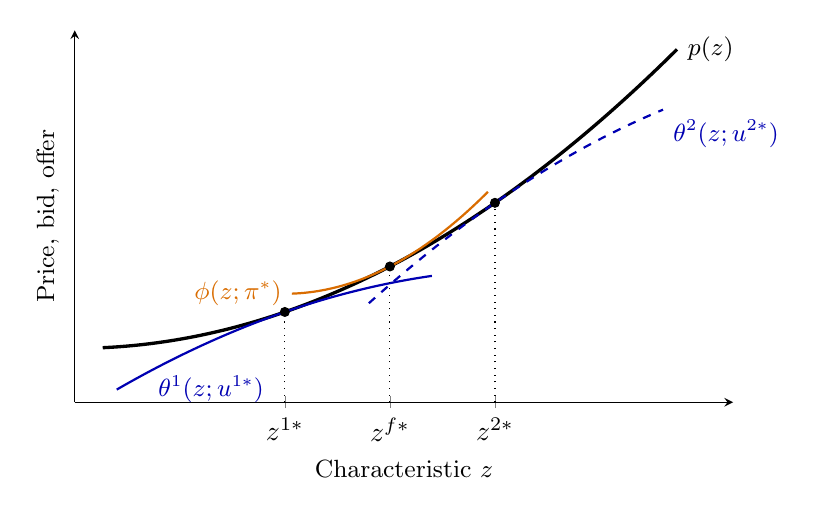
\begin{tikzpicture}
\begin{axis}[
  width=0.82\textwidth, height=0.52\textwidth,
  axis lines=left, xmin=0, xmax=4.7, ymin=0, ymax=6.9,
  xlabel={Characteristic $z$}, ylabel={Price, bid, offer},
  xtick={1.5,2.25,3}, xticklabels={$z^{1*}$, $z^{f*}$, $z^{2*}$},
  ytick=\empty, clip=false, every axis label/.append style={font=\small}]
  \addplot[domain=0.2:4.3, samples=120, very thick, black] {1+0.3*x^2}
    node[pos=1, right, font=\small] {$p(z)$};
  \addplot[domain=0.3:2.55, samples=80, thick, blue!70!black] {1.675+0.9*(x-1.5)-0.25*(x-1.5)^2};
  \node[anchor=east, font=\small, text=blue!70!black] at (axis cs:1.42,0.24) {$\theta^{1}(z; u^{1*})$};
  \addplot[domain=2.1:4.2, samples=80, thick, blue!70!black, dashed] {3.7+1.8*(x-3)-0.3*(x-3)^2}
    node[pos=1, below right, font=\small] {$\theta^{2}(z; u^{2*})$};
  \addplot[domain=1.55:2.95, samples=80, thick, orange!85!black] {2.51875+1.35*(x-2.25)+0.9*(x-2.25)^2}
    node[pos=0, left, font=\small] {$\phi(z; \pi^*)$};
  \addplot[only marks, mark=*, mark size=1.6pt] coordinates {(1.5,1.675) (2.25,2.51875) (3,3.7)};
  \draw[dotted] (axis cs:1.5,0) -- (axis cs:1.5,1.675);
  \draw[dotted] (axis cs:2.25,0) -- (axis cs:2.25,2.51875);
  \draw[dotted] (axis cs:3,0) -- (axis cs:3,3.7);
\end{axis}
\end{tikzpicture}
\caption{The hedonic price function $p(z)$. Consumer 1 and consumer 2 choose $z^{1*}$ and $z^{2*}$, where their bid curves
$\theta^{1}$ and $\theta^{2}$ (concave) touch $p(z)$ from below. A firm chooses $z^{f*}$, where its offer curve $\phi$ touches
$p(z)$ from above. At each traded bundle the slope of $p(z)$ equals the buyer's marginal willingness to pay and the seller's
marginal cost.}
\label{fig:06-hedonic}
\end{figure}

\casehead{Rosen's two-step procedure}
The model suggests two steps. First, regress the prices of products in a market on their characteristics with a flexible
functional form. This yields an estimate $\hat p(z)$ and implicit prices $\hat p_{z_k}(z_j)$ at each traded bundle. Second,
treat the implicit prices as observed marginal prices. Estimate the marginal bid functions $\hat p_{z_k}(z_j) =
F^k(z_j, Y_{1j})$, which depend on characteristics and buyer attributes $Y_{1j}$. Estimate them jointly with the marginal
offer functions $\hat p_{z_k}(z_j) = G^k(z_j, Y_{2j})$, which depend on seller attributes $Y_{2j}$.

\casehead{The identification critique}
The second step runs into two problems, which a one-characteristic example makes transparent. Let the price function be
quadratic,
\begin{equation*}
  p(z) = \pi_0 + \pi_1 z + \tfrac{1}{2}\pi_2 z^2 , \qquad \pi_2 > 0 ,
\end{equation*}
so the implicit price is $p_z(z) = \pi_1 + \pi_2 z$. The coefficients $\pi_0, \pi_1, \pi_2$ are unrelated to the profit $\pi$ of the offer function. Let consumer $i$'s marginal bid be linear,
\begin{equation*}
  \theta_z(z) = b_0 - b_1 z + b_2 Y_i + \eta_i , \qquad b_1 > 0 ,
\end{equation*}
where $Y_i$ is an observed attribute and $\eta_i$ an unobserved taste. The first-order condition $p_z(z_i) = \theta_z(z_i)$
gives
\begin{equation}\label{eq:06-rosen-choice}
  \pi_1 + \pi_2 z_i = b_0 - b_1 z_i + b_2 Y_i + \eta_i
  \quad\Longrightarrow\quad
  z_i = \frac{b_0 - \pi_1 + b_2 Y_i + \eta_i}{\pi_2 + b_1} .
\end{equation}

The first problem was raised by \citet{BrownRosen1982}. In one market the constructed implicit price $\pi_1 + \pi_2 z_i$ is
an exact linear function of $z_i$. Regressing it on $z_i$ and $Y_i$ fits perfectly with coefficients $(\pi_1, \pi_2, 0)$. The
second step merely reproduces the first-step price function and reveals nothing about the slope $-b_1$ of the marginal bid
curve. Identification requires restrictions that the data cannot supply in a single market, such as different functional
forms for the price function and the marginal bid function.

The second problem was stressed by \citet{Epple1987} and \citet{Bartik1987}. By \eqref{eq:06-rosen-choice}, the chosen
quantity $z_i$ rises with the unobserved taste $\eta_i$. Consumers who value the characteristic more buy more of it, and
along a nonlinear price function they also pay a higher implicit price. The regressor $z_i$ is correlated with the error of
the marginal bid equation. The consumer's own attributes are poor instruments, because they enter the bid function or may
correlate with unobserved tastes. A valid instrument must shift the price function that the consumer faces without
shifting tastes. Variation in $(\pi_1, \pi_2)$ across separate markets with the same distribution of tastes does this. In
market $m$ the first-order condition reads $\pi_{1m} + \pi_{2m} z_i = b_0 - b_1 z_i + b_2 Y_i + \eta_i$, and market indicators
identify $b_1$ through their effect on $z_i$.

\citet{EkelandHeckmanNesheim2004} show that the linear-quadratic structure behind the critique is special. Equilibrium
price functions are generically nonlinear, and with additive separability assumptions this nonlinearity can identify
preferences from a single market with one observed characteristic. Rosen's framework also connects to earlier sections.
Bresnahan's quality index $\delta(x) = \sqrt{\beta_0 + \sum_k x_k\beta_k}$ is read as a hedonic expansion path of
cost-minimizing characteristics, and his non-nested tests include a hedonic alternative (\cref{sec:06-bresnahan}).

\subsection{Bajari and Benkard: the model and the price function}\label{sec:06-bb-model}

\casehead{Motivation}
\citet[pp.~1--5]{BajariBenkard2005} give two reasons why hedonic models are rarely used in industrial organization. First,
Rosen assumes perfect competition and a continuum of products. Yet oligopoly is often the object of study, and oligopolistic
markets rarely contain more than a few hundred products. Under imperfect competition a hedonic price function need not
exist, and where it exists it is unlikely to be additively separable. Second, Rosen assumes that every characteristic is observed. In their data on personal computers,
357 of the 695 products are dominated. For each of them, another product is better in every observed characteristic and
cheaper. No hedonic model with full observability can rationalize positive demand for such products. Discrete choice models
avoid the problem through the shock $\epsilon_{ij}$. Bajari and Benkard instead add one characteristic that consumers see and
the econometrician does not.

They contrast their model with BLP-type models along the lines of \cref{sec:06-epsilon}. An i.i.d.\ shock makes the
characteristic space infinite dimensional. Together with the distributional assumptions, it typically produces demand curves
of hyperbolic shape that approach both axes. The hedonic model restricts demand only to slope downward, so the two models can
differ sharply when demand is predicted at prices outside the data.

\casehead{The model}
A product $j$ is a vector $(x_j, \xi_j)$, with $x_j \in \R^K$ observed by consumers and econometrician and a scalar $\xi_j$
observed by consumers only. Markets are indexed by $t \in \mathcal{T}$ and prices by $p_{jt}$. Consumer $i$ has utility
$u_i(x_j, \xi_j, c)$ over the product and a composite good $c \ge 0$ with price one. With income $y_i$, the consumer solves
(their eq.~1)
\begin{equation}\label{eq:06-bb-consumer}
  \max_{(j, c)}\; u_i(x_j, \xi_j, c) \quad\text{subject to}\quad p_{jt} + c \le y_i .
\end{equation}

\begin{assumption}[Bajari and Benkard, A1 to A3]\label{ass:06-bb}
For every consumer and market: (A1) $u_i$ is continuously differentiable and strictly increasing in $c$, with
$\frac{\partial u_i}{\partial c} \ge \underline{m} > 0$ for $c \in (0, y_i]$. (A2) $u_i$ is Lipschitz continuous in $(x_j,
\xi_j)$ with constant $L$. (A3) $u_i$ is strictly increasing in $\xi_j$.
\end{assumption}

We state the bounds $\underline{m}$ and $L$ as common to all consumers, which the Lipschitz property of the price function
requires. Assumption A3 is the strongest. It rules out satiation in the unobserved characteristic.

\begin{theorem}[Bajari and Benkard, Theorem~1]\label{thm:06-bb-pricefn}
Under \cref{ass:06-bb}, for any two products $j$ and $j'$ with positive demand in market $t$:
\begin{enumerate}[label=(\roman*)]
\item If $x_j = x_{j'}$ and $\xi_j = \xi_{j'}$, then $p_{jt} = p_{j't}$.
\item If $x_j = x_{j'}$ and $\xi_j > \xi_{j'}$, then $p_{jt} > p_{j't}$.
\item $|p_{jt} - p_{j't}| \le \bar L\bigl(\lVert x_j - x_{j'} \rVert + |\xi_j - \xi_{j'}|\bigr)$ with $\bar L = \frac{L}{\underline{m}}$.
\end{enumerate}
\end{theorem}

\begin{proof}
Each part shows that a violation would leave one of the two products with no buyers.

(i) Suppose $p_{jt} > p_{j't}$. A consumer who can afford $j$ gets the same product characteristics from $j'$ with more of the
composite good. By A1 she strictly prefers $j'$, so $j$ has no demand.

(ii) Suppose $p_{jt} \le p_{j't}$. For a consumer who can afford $j'$, A1 and then A3 give
\begin{equation*}
  u_i(x_j, \xi_j, y_i - p_{jt}) \ge u_i(x_j, \xi_j, y_i - p_{j't}) > u_i(x_j, \xi_{j'}, y_i - p_{j't}) ,
\end{equation*}
so $j'$ has no demand.

(iii) Let $d = \lVert x_j - x_{j'} \rVert + |\xi_j - \xi_{j'}|$ and suppose $p_{jt} - p_{j't} > \bar L d$. Take a consumer who can
afford $j$, so $y_i \ge p_{jt}$. Split the utility difference into a change in $c$ and a change in characteristics:
\begin{align*}
  u_i(x_{j'}, \xi_{j'}, y_i - p_{j't}) - u_i(x_j, \xi_j, y_i - p_{jt})
  &= \bigl[u_i(x_{j'}, \xi_{j'}, y_i - p_{j't}) - u_i(x_{j'}, \xi_{j'}, y_i - p_{jt})\bigr] \\
  &\quad + \bigl[u_i(x_{j'}, \xi_{j'}, y_i - p_{jt}) - u_i(x_j, \xi_j, y_i - p_{jt})\bigr] \\
  &\ge \underline{m}\,(p_{jt} - p_{j't}) - L d .
\end{align*}
The first bracket uses the mean value theorem and A1, and the second uses A2. The last expression exceeds $\underline{m} \bar L d -
L d = 0$. Every potential buyer of $j$ strictly prefers $j'$, so $j$ has no demand. Exchanging the roles of $j$ and $j'$
covers the other sign.
\end{proof}

The theorem uses only consumer optimization and the fact that consumers take prices as given. It places no restriction on
the supply side, so it holds under oligopoly and in static or dynamic equilibria. Its conclusions justify writing prices in
market $t$ as an equilibrium \emph{price function} $p_t(x, \xi)$ with $p_{jt} = p_t(x_j, \xi_j)$. Bajari and Benkard stress
what the function is not (their pp.~7--8). It is an equilibrium object that changes whenever any primitive changes: a new
product, a cost shock, a change in ownership. It does not predict the price of a product that is not on the market. It is
specific to each market. Even simple oligopoly models imply that it is nonlinear and not additively separable in $\xi$,
because markups depend on all characteristics. They therefore keep the general form.

\subsection{The first stage: the unobserved characteristic as a price quantile}\label{sec:06-bb-firststage}

The first stage recovers $\xi_j$ from prices. The unobserved characteristic has no natural units and is identified only up
to an increasing transformation. Bajari and Benkard normalize it to be uniform on $[0,1]$, which amounts to measuring it by
its own distribution function. Two further assumptions are needed.

\begin{assumption}[Bajari and Benkard, A4 and A5]\label{ass:06-bb-indep}
(A4) $\xi$ is independent of $x$. (A5) For every market $t$ and every $x$, $p_t(x, \cdot)$ is strictly increasing, with
$\frac{\partial p_t(x, \xi)}{\partial \xi} > \underline{\kappa}$ for all $(x, \xi)$ and some $\underline{\kappa} > 0$.
\end{assumption}

A4 strengthens the mean independence common in the literature. Because $\xi$ enters the price function
nonseparably, the model can still generate patterns that look like heteroskedasticity. Bajari and Benkard note that the
monotonicity in A5 follows from consumer preferences through \cref{thm:06-bb-pricefn}(ii). Let $F_{p_t \mid x = x_0}$ denote the distribution of
prices in market $t$ among products with observed characteristics $x_0$.

\begin{theorem}[Bajari and Benkard, Theorem~2]\label{thm:06-bb-xi}
Suppose prices are observed without error and A4 and A5 hold. Then for each market $t$ the price function $p_t$ is
identified within the class of price functions that are strictly increasing in $\xi$. The unobserved characteristics are
also identified:
\begin{equation}\label{eq:06-bb-xi}
  \xi_j = F_{p_t \mid x = x_j}(p_{jt}), \qquad p_t(x_0, e_0) = F^{-1}_{p_t \mid x = x_0}(e_0) .
\end{equation}
\end{theorem}

\begin{proof}
The argument is a chain of equalities.
\begin{align*}
  F_{p_t \mid x = x_j}(p_{jt}) &= \Pr\bigl(p_t(x, \xi) \le p_{jt} \mid x = x_j\bigr) && \text{(definition)} \\
  &= \Pr\bigl(\xi \le p_t^{-1}(x_j, p_{jt}) \mid x = x_j\bigr) && \text{($p_t(x_j, \cdot)$ strictly increasing)} \\
  &= \Pr\bigl(\xi \le p_t^{-1}(x_j, p_{jt})\bigr) && \text{(A4)} \\
  &= p_t^{-1}(x_j, p_{jt}) && \text{($\xi$ uniform on $[0,1]$)} \\
  &= \xi_j && \text{($p_{jt} = p_t(x_j, \xi_j)$).}
\end{align*}
Here $p_t^{-1}(x, \cdot)$ is the inverse of $p_t(x, \cdot)$. The same chain with $(x_0, p_t(x_0, e_0))$ in place of $(x_j,
p_{jt})$ gives $F_{p_t \mid x = x_0}(p_t(x_0, e_0)) = e_0$. Inverting this identity gives the second equation in
\eqref{eq:06-bb-xi}. Both objects are functions of the observable distribution of prices given characteristics, which
proves identification.
\end{proof}

The unobserved characteristic is the rank of a product's price among products with the same observed characteristics. A
computer priced at the 90th percentile among computers with identical observed specifications has $\xi = 0.9$. Identification
uses a single cross-section, so $\xi_j$ and its distribution may change over time. The first part of the argument follows
\citet{Matzkin2003}. If prices are measured with error, identification requires each product to be observed in many markets,
so that averaging removes the error (their Appendix~A, Theorem~6). The estimator replaces the conditional distribution with
a nonparametric estimate (their eq.~18):
\begin{equation}\label{eq:06-bb-xihat}
  \hat\xi_{jt} = \hat F_{p_t \mid x = x_j}(p_{jt}) .
\end{equation}
Kernel or series estimators can be used. In the application a local linear kernel estimator \citep{FanGijbels1996}
worked best.

Bajari and Benkard offer three alternatives to independence. Under \emph{options packages} (their Theorem~3), products are
grouped into models, such as a particular line of desktop computers, and an options package $x$ is chosen within a model.
All products of a model share the same $\xi$ (their A6), and a baseline package $\bar x$ is available for every model (their
A7). Normalizing $\xi$ given $x = \bar x$ to be uniform, $\xi_j$ is the price quantile of the baseline version of $j$'s model.
The approach is a nonparametric analog of fixed effects. It works in one cross-section even with measurement error, and it
is testable because many products share the same $\xi$.

Under a \emph{rich set of price functions} (their Theorem~4), some market has prices that depend on $\xi$ alone (their A8).
Packaged goods whose flavors all sell at the same price are an example. Prices weakly increase in $x$ and strictly increase
in $\xi$ in every market (their A9). With full support and products observed in many markets, these conditions identify the
ranking of the $\xi_j$. Finally, nonseparable nonparametric instrumental variables methods for triangular systems
\citep{ImbensNewey2009} could replace independence. They require instruments that determine the endogenous observed
characteristics yet are independent of $\xi$, and such instruments are hard to find in product markets.

\subsection{The second stage: preferences}\label{sec:06-bb-secondstage}

With $\xi$ recovered, Bajari and Benkard treat it as an observed characteristic. If demand were observed for every price
function, the results of \citet{MasColell1977} would recover preferences. Data are rarely that rich, and often each consumer
is observed once. Two cases arise.

\casehead{Continuous choice set}
Suppose utility is linear in the logarithms of the characteristics and in the composite good (their eq.~6):
\begin{equation}\label{eq:06-bb-u6}
  u_{ij} = \beta_{i1}\ln x_{1j} + \dots + \beta_{iK}\ln x_{Kj} + \beta_{i\xi}\ln \xi_j + c , \qquad c = y_i - p_t(x_j, \xi_j) .
\end{equation}
If the choice set is a continuum and the choice is interior, the consumer chooses $(x, \xi)$ on the price surface to maximize
\eqref{eq:06-bb-u6}. Differentiating with respect to $x_k$ and $\xi$ gives (their eqs.~7--8)
\begin{equation*}
  \frac{\beta_{ik}}{x_{kj}} = \frac{\partial p_t(x_j, \xi_j)}{\partial x_k}, \quad k = 1, \dots, K, \qquad
  \frac{\beta_{i\xi}}{\xi_j} = \frac{\partial p_t(x_j, \xi_j)}{\partial \xi} .
\end{equation*}
Solving for the tastes gives (their eqs.~9--10)
\begin{equation}\label{eq:06-bb-tastes}
  \beta_{ik} = x_{kj}\,\frac{\partial p_t(x_j, \xi_j)}{\partial x_k}, \qquad
  \beta_{i\xi} = \xi_j\,\frac{\partial p_t(x_j, \xi_j)}{\partial \xi} .
\end{equation}
A single observed choice therefore identifies a consumer's entire taste vector, given the price function and $\xi_j$. Each
taste is the implicit price of the characteristic times the chosen quantity, which is the consumer's willingness to pay, in
dollars, for a unit increase in the logarithm of the characteristic. Pooling consumers' choices traces out the population
distribution of tastes nonparametrically. The precision of these estimates depends only on the first-stage sample.

More generally, write $u_i(x, c) = u(x, y_i - p(x); \beta_i)$ with $\beta_i \in \R^B$ (their eq.~11). The first-order
conditions $\frac{\partial}{\partial x_k} u(x, y_i - p(x); \beta_i) = 0$ define the optimal choice $x(\beta)$. Implicit
differentiation gives $x'(\beta) = -[D_{xx}\bar u]^{-1} D_{x\beta}\bar u$, where $\bar u(x; \beta) = u(x, y_i - p(x); \beta)$
(their eqs.~12--14). Their Theorem~5 states that $\beta_i$ is locally identified when $x'(\beta)$ is locally positive or
negative definite, by the inverse function theorem. With as many taste parameters as characteristics ($B = K$) and $x'(\beta)$
definite everywhere on an open convex set, the map $x(\cdot)$ is one-to-one and tastes are globally identified
\citep{GaleNikaido1965}. One choice identifies at most $K$ random coefficients.

\casehead{Discrete choice set}
With finitely many products, utility maximization yields inequalities. If consumer $i$ chooses product $j$, then (their
eq.~15)
\begin{equation}\label{eq:06-bb-ineq}
  u(x_j, \xi_j, y_i - p_{jt}; \beta_i) \ge u(x_k, \xi_k, y_i - p_{kt}; \beta_i) \quad\text{for all } k \ne j ,
\end{equation}
so $\beta_i$ lies in the \emph{revealed preference set} $A_{ij} = \{\beta : \text{\eqref{eq:06-bb-ineq} holds}\}$ (their
eq.~16). The set typically contains more than one point, so individual tastes are not identified. It can still be small when
the choice set is rich. If every characteristic is continuous and the products fill a compact set, the sets shrink to points as the number
of products grows (their Appendix~B, Theorem~8). Their rate argument is simple. In their Appendix~B, utility
$u(x_j, p_j; \beta_i)$ does not depend on income, and there is no outside option. Each set then depends only on the
product chosen, and the sets for the $J$ products partition the bounded parameter space $\mathcal{B}$. Their average
Lebesgue measure is therefore $\frac{m(\mathcal{B})}{J}$. An outside option would add one more set and leave the rate
unchanged. Consumers who buy
nothing are treated as buying a bundle with zero characteristics at zero price (their eq.~17):
\begin{equation*}
  u(0, 0, y_i; \beta_i) \ge u(x_k, \xi_k, y_i - p_{kt}; \beta_i) \quad\text{for all } k .
\end{equation*}
These conditions are only inequalities, so the tastes of non-purchasers are not point identified even with a continuous
product space.

The sets $A_{ij}$ deliver bounds on the population distribution of tastes. Let $\mathcal{B}(\bar\beta) = \{\beta : \beta \le
\bar\beta\}$. The share of consumers whose whole set $A_{ij}$ lies in $\mathcal{B}(\bar\beta)$ is a lower bound for the taste
distribution function at $\bar\beta$. The share whose set meets $\mathcal{B}(\bar\beta)$ is an upper bound. When utility is
quasi-linear, as in \eqref{eq:06-bb-u6}, income cancels from \eqref{eq:06-bb-ineq}. All buyers of product $j$ then share one
set $A_j$, and product-level quantities suffice for estimation.

\casehead{A Bayesian point estimate and the Gibbs sampler}
For a point estimate, Bajari and Benkard turn the inequalities into a likelihood. Consumer $i$ with tastes $\beta_i$ chooses
$j$ with likelihood (their eq.~21)
\begin{equation}\label{eq:06-bb-lik}
  L(j \mid x, y_i, \beta_i) = \indic\bigl\{u(x_j, y_i - p_j; \beta_i) \ge u(x_k, y_i - p_k; \beta_i) \text{ for all } k \ne j\bigr\} ,
\end{equation}
where $x_j$ now includes $\xi_j$. With a uniform prior on a box $\mathcal{B}$ that contains every $A_{ij}$, the posterior
$\pi(\beta_i \mid j) \propto \indic\{\beta_i \in \mathcal{B}\}\, L(j \mid x, y_i, \beta_i)$ is uniform on $A_{ij}$ (their
eq.~22).

Sampling from a uniform distribution on a set defined by many inequalities is easy coordinate by coordinate. In model
\eqref{eq:06-bb-u6}, choice of $j$ requires, for every $k \ne j$ (their eq.~29),
\begin{equation*}
  \sum_{l} \beta_{il}\ln x_{lj} + y_i - p_j \ge \sum_{l} \beta_{il}\ln x_{lk} + y_i - p_k .
\end{equation*}
Collecting the terms in $\beta_{i1}$ gives
\begin{equation*}
  \beta_{i1}\,(\ln x_{1j} - \ln x_{1k}) \ge \sum_{l \ne 1} \beta_{il}(\ln x_{lk} - \ln x_{lj}) + (p_j - p_k) .
\end{equation*}
Define the ratio
\begin{equation}\label{eq:06-bb-ratio}
  R_k(\beta_{i,-1}) = \frac{\sum_{l \ne 1} \beta_{il}(\ln x_{lk} - \ln x_{lj}) + (p_j - p_k)}{\ln x_{1j} - \ln x_{1k}} .
\end{equation}
If $x_{1j} > x_{1k}$, the denominator is positive and the inequality reads $\beta_{i1} \ge R_k$. If $x_{1j} < x_{1k}$,
dividing by a negative number flips it to $\beta_{i1} \le R_k$. If $x_{1j} = x_{1k}$, the inequality does not involve
$\beta_{i1}$. Given the other coordinates, $\beta_{i1}$ is therefore uniform on $[\beta_{1,\min}, \beta_{1,\max}]$ with
(their eqs.~32--33)\footnote{The working paper prints the price term in eqs.~30--33 as $(y_i - p_j) - (y_i - p_k)$, which
has the opposite sign. The expression here follows from their eq.~29.}
\begin{equation}\label{eq:06-bb-bounds}
  \beta_{1,\min} = \max\Bigl\{\underline b_1,\ \max_{k : x_{1j} > x_{1k}} R_k(\beta_{i,-1})\Bigr\}, \qquad
  \beta_{1,\max} = \min\Bigl\{\bar b_1,\ \min_{k : x_{1j} < x_{1k}} R_k(\beta_{i,-1})\Bigr\},
\end{equation}
where $[\underline b_1, \bar b_1]$ is the range of the first coordinate in the prior box. The other coordinates are
handled in the same way. The sampler proceeds as follows.
\begin{enumerate}
\item Start from a point $\beta_i^{(0)}$ in $A_{ij}$. Bajari and Benkard use the tastes implied by the continuous-case
formulas \eqref{eq:06-bb-tastes} and search nearby when that point violates an inequality.
\item Given $\beta_i^{(s)}$, draw $\beta_{i1}^{(s+1)}$ from the uniform distribution on $[\beta_{1,\min}, \beta_{1,\max}]$
computed at the current values of the other coordinates.
\item Draw each remaining coordinate $l = 2, \dots, K$ in the same way, conditioning on the most recent values of the others.
\item Repeat, discarding an initial set of draws.
\end{enumerate}
Each inequality is linear in $\beta_i$, so $A_{ij}$ is an intersection of half-spaces. It is therefore convex, hence
connected, and standard sufficient conditions for convergence of the sampler hold (their footnote~8). The distribution
function of tastes is estimated by the frequency of draws below each point (their eq.~34),
\begin{equation}\label{eq:06-bb-cdf}
  \hat F(\bar\beta_1, \dots, \bar\beta_K) = \frac{1}{S}\sum_{s=1}^{S} \indic\bigl\{\beta^{(s)}_1 \le \bar\beta_1, \dots, \beta^{(s)}_K \le \bar\beta_K\bigr\} ,
\end{equation}
with draws pooled across consumers. The uniform prior selects one distribution among the many consistent with the data. The
sampler extends to repeated choices, which add inequalities, and to estimation error in $\xi$, by drawing $\xi$ from its
sampling distribution before each run.

\casehead{When independence fails}
If $\xi$ is locally positively correlated with some observed characteristic, the first stage attributes part of the price
effect of $\xi$ to that characteristic. Its implicit price is biased upward and the implicit price of $\xi$ downward. Through
\eqref{eq:06-bb-tastes} the estimated tastes inherit the same biases. Because a product is a bundle of both characteristics,
the biases partly offset in the demand for products. Bajari and Benkard report that they cancel exactly with linear utility
and a linear price function.

\subsection{Application: personal computers, December 1999}\label{sec:06-bb-pc}

\casehead{Data}
The data come from the PC Data Retail Hardware Monthly Report. They contain quantities, average prices and characteristics of
desktop computers for 29 months. The analysis concentrates on December 1999, with 695 models, a cross-section in which
traditional demand methods typically struggle. The data reportedly cover about 75 percent of U.S.\ retail computer sales.
Processor dummies are replaced by a CPU benchmark score, which a regression on chip speed interacted with chip dummies explains
with an $R^2$ of 0.999. The final data contain 19 characteristics. The three main continuous characteristics are the benchmark, RAM
and hard drive capacity. Following their Table~1, the others are MMX, SCSI, CD-ROM, DVD, a network card, a monitor dummy, monitor size, a zip
drive, desktop versus tower, refurbished and no modem. Five operating-system dummies complete the list, one of which is
omitted in the regression. With all characteristics treated as observed, 357 of the 695 products are dominated.
\Cref{tab:06-bb-data} reproduces selected rows of their Table~1, including an OLS hedonic regression.

\begin{table}[htbp]
\centering
\caption{Personal computers, December 1999: summary statistics and a linear hedonic regression}
\label{tab:06-bb-data}
\small
\begin{tabular}{@{}lrrrrr@{}}
\toprule
Variable & Mean & S.D. & Min & Max & OLS coefficient \\
\midrule
CPU benchmark          & 1354.5 & 362.3 & 516 & 2544 & 0.836 \\
RAM (MB)               & 74.0 & 35.1 & 16 & 256 & 3.010 \\
Hard drive (MB)        & 9276.8 & 4850.3 & 2100 & 40000 & 0.008 \\
MMX                    & 0.64 & 0.48 & 0 & 1 & $-56.971$ \\
SCSI                   & 0.01 & 0.08 & 0 & 1 & 310.747 \\
CD-ROM                 & 0.67 & 0.47 & 0 & 1 & 26.478 \\
DVD                    & 0.14 & 0.35 & 0 & 1 & 32.213 \\
Monitor included       & 0.31 & 0.46 & 0 & 1 & 29.625 \\
Monitor size           & 0.75 & 3.27 & 0 & 15 & 22.822 \\
Desktop (not tower)    & 0.17 & 0.37 & 0 & 1 & 25.611 \\
Refurbished            & 0.09 & 0.28 & 0 & 1 & $-144.314$ \\
No modem               & 0.55 & 0.50 & 0 & 1 & 145.169 \\
\midrule
Constant               & & & & & $-590.2$ \\
$R^2$                  & & & & & 0.79 \\
$N$                    & & & & & 695 \\
\bottomrule
\end{tabular}

\smallskip
\begin{minipage}{0.85\textwidth}
\footnotesize Source: \citet{BajariBenkard2005}, Table~1 (working-paper version). The dependent variable of the OLS
regression is price in dollars. Rows not shown are the network card, zip drive and four operating-system dummies (Windows NT
4.0, Windows NT, Windows 98, Windows 95, with Windows 3.1 omitted). The paper reports no standard errors for this regression.
\end{minipage}
\end{table}

\casehead{First stage}
A nonparametric estimator in 19 dimensions is impractical, so the first stage treats three continuous characteristics
nonparametrically: CPU benchmark, RAM and hard drive. The price function is assumed additively separable in the other 16, with
coefficients fixed at the OLS values of \cref{tab:06-bb-data}. Bajari and Benkard argue that many of these are peripherals that
can be bought and sold separately, so arbitrage limits nonseparability. The estimator is \eqref{eq:06-bb-xihat} with a local
linear kernel and a normal kernel. Bandwidths were chosen by eye, which oversmooths relative to the mean-squared-error optimum.
Smooth estimates help because derivatives of the price function supply starting values for the sampler. With a finite product
space, only the $\hat\xi_j$ are needed for the demand system itself.

The unobserved characteristics are precisely estimated (their Table~2). Asymptotic standard errors average 0.010, have median
0.009, and are below 0.018 for 95 percent of products, with a maximum of 0.104. Bootstrap standard errors, from 1,000 samples
drawn with i.i.d.\ sampling of products, average 0.012, have 95th percentile 0.022 and maximum 0.121. For 508 of the 695
products the bootstrap standard error exceeds the asymptotic one. Two features explain the precision. A quantile is easier to
estimate than a density, and the characteristic space is densely filled, so almost every product has close neighbors. The
estimated bias was small and barely changed the ranking of the $\hat\xi_j$, so it was left out.

\casehead{Second stage}
The demand system uses all 19 observed characteristics and $\xi$. Utility is quasi-linear, linear in the logarithms of CPU
benchmark, hard drive, RAM and $\xi$, and linear in the other characteristics and in price. The $\hat\xi_j$ were rescaled so
that budget sets are convex, and other normalizations changed the results little. After discarding initial draws, the sampler
produced 1,000 taste draws per product, a total of 695,000 twenty-dimensional draws. These were reweighted by each product's
sales. Including the initial draws, the computation took about an hour on their Sun Ultra 60 workstation.

The estimated willingness-to-pay distributions (their Figures~1--5) look roughly lognormal except for the CPU benchmark. The
modal marginal willingness to pay is between \$1 and \$2 per megabyte of RAM and about 1.25 cents per megabyte of hard drive.
The data are informative even about the taste for SCSI, a dummy characteristic, because extreme values of one coefficient
require extreme values of others to rationalize a choice. Tastes are strongly positively correlated (their Table~3). The
correlation between the CPU and SCSI coefficients is 0.694, between RAM and hard drive 0.533, and between CPU and RAM 0.510. The
taste for $\xi$ correlates positively with every other taste, from 0.351 with hard drive to 0.477 with RAM. This arises even
though $\xi$ was assumed independent of $x$ in the first stage.

\casehead{Elasticities}
Aggregating the taste draws gives demand curves and elasticities for every product. With all 695 products the median
own-price elasticity $\varepsilon_{jj}$ was about $-100$. Bajari and Benkard read this as a rejection of perfect information. With 695 products,
neighbors are close in price and characteristics, so a fully informed consumer would switch at a tiny price change. Real
consumers search and consider only a handful of products. They therefore re-estimated the model with only the 24 products that
sold at least 5,000 units, a minimum share of 0.75 percent. These products account for 72 percent of sales. Own-price
elasticities then range from $-4$ to $-72$, with a median of $-11$. They caution that the selection retained similar
best-selling products, so these elasticities may still be too large in magnitude.

\begin{table}[htbp]
\centering
\caption{The five best-selling computers in December 1999 and their estimated price elasticities}
\label{tab:06-bb-elast}
\small
\begin{tabular}{@{}llrrrr@{}}
\multicolumn{6}{@{}l}{\emph{Panel A. Characteristics (Table 4)}} \\
\toprule
Model & CPU (benchmark) & RAM & Hard drive & Price (\$) & Sales \\
\midrule
HP Pavilion 6535      & Intel Celeron 466 MHz (1281) & 64 MB & 8.4 GB  & 590 & 71,199 \\
Compaq Presario 5441  & AMD K6-2 475 MHz (1076)      & 64 MB & 8.0 GB  & 540 & 54,449 \\
Compaq Presario 5461  & AMD K6-2 500 MHz (1115)      & 64 MB & 10.0 GB & 727 & 43,029 \\
E-Machines eTower 433 & Celeron 433 MHz (1167)       & 32 MB & 4.3 GB  & 471 & 40,399 \\
HP Pavilion 6545C     & Celeron 500 MHz (1398)       & 64 MB & 13.0 GB & 858 & 34,198 \\
\bottomrule
\end{tabular}

\bigskip
\begin{tabular}{@{}lrrrrr@{}}
\multicolumn{6}{@{}l}{\emph{Panel B. Matrix of price elasticities (Table 5)}} \\
\toprule
 & HP6535 & Compaq5441 & Compaq5461 & E-Machines & HP6545C \\
\midrule
HP6535      & $-4.14$ & 0.12    & 0.00    & 0.43     & 0.28 \\
Compaq5441  & 0.17    & $-5.95$ & 2.98    & 0.73     & 0.55 \\
Compaq5461  & 0.00    & 2.80    & $-8.00$ & 0.85     & 0.11 \\
E-Machines  & 0.61    & 0.69    & 0.91    & $-10.65$ & 0.66 \\
HP6545C     & 0.70    & 0.86    & 0.18    & 1.02     & $-4.46$ \\
\bottomrule
\end{tabular}

\smallskip
\begin{minipage}{0.92\textwidth}
\footnotesize Source: \citet{BajariBenkard2005}, Tables~4 and~5 (working-paper version). Table~4 of the paper prints the
processor as ``AMD A6-2''. Panel A corrects it to the AMD K6-2 chip. Elasticities come from the model estimated on the 24 products
selling at least 5,000 units. The paper does not state whether rows or columns index the product whose price changes.
\end{minipage}
\end{table}

\Cref{tab:06-bb-elast} shows the five best sellers and their elasticity matrix. Two features stand out. The most similar
products substitute most, as the two Compaq models do (2.98 and 2.80). Some cross elasticities are exactly zero: the HP6535 and
the Compaq5461 do not substitute at all, presumably because other products lie between them in characteristic space. A model with
an i.i.d.\ shock cannot produce a zero cross elasticity, since every product keeps some buyers who rank it second.

\begin{figure}[htbp]
\centering
\begin{subfigure}[t]{0.8\textwidth}
\centering
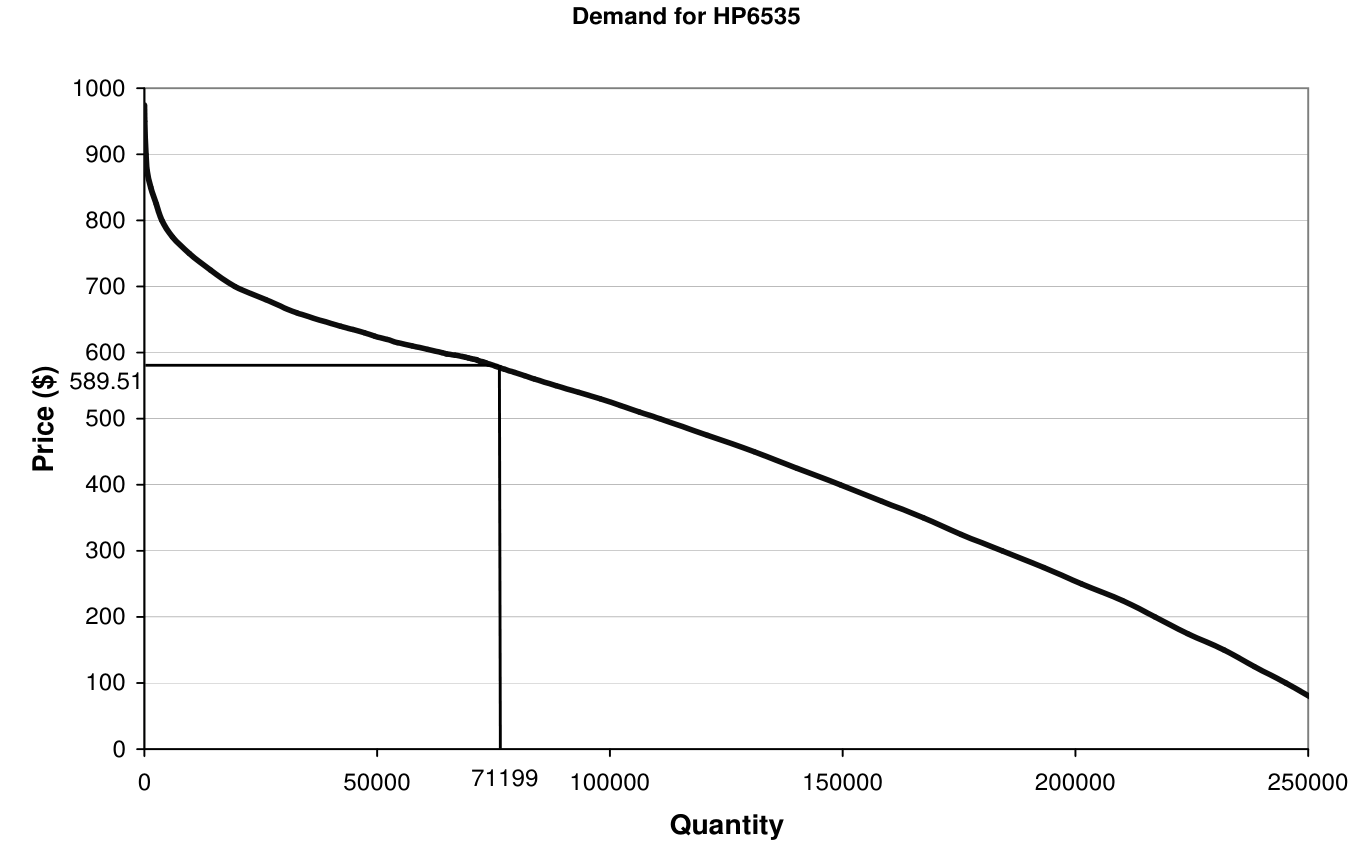
\includegraphics[width=\textwidth]{figures/ch06/bb_fig6_demand.png}
\caption{Estimated demand for the HP Pavilion 6535}
\end{subfigure}\par\medskip
\begin{subfigure}[t]{0.8\textwidth}
\centering
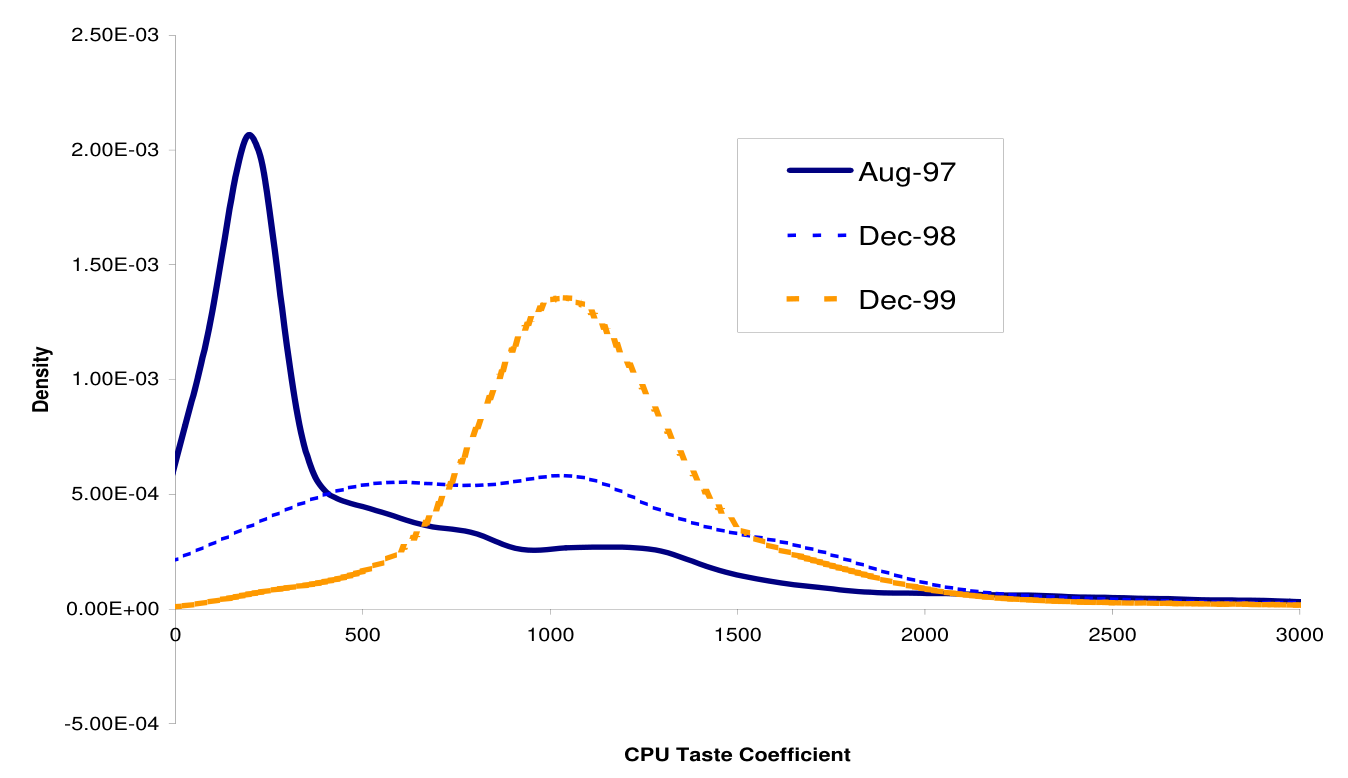
\includegraphics[width=\textwidth]{figures/ch06/bb_fig7_cputaste.png}
\caption{Estimated density of the taste for CPU}
\end{subfigure}
\caption{Panel (a) shows the estimated demand curve of the HP Pavilion 6535, with the observed price (\$589.51) and quantity
(71,199) marked. Panel (b) shows the estimated distribution of the CPU taste coefficient in August 1997, December 1998 and
December 1999. Source: Bajari and Benkard (2005), Figures~6 and~7 (working-paper version).}
\label{fig:06-bb-demand}
\end{figure}

Panel (a) of \cref{fig:06-bb-demand} shows the estimated demand curve for the HP6535. It is steep at high prices, flat near the
observed price and steep again at low prices. A small group of consumers strongly prefers this model, which explains the steep
upper part. Near the observed price many consumers would switch to neighboring products for little compensation, which flattens
the curve. At low prices the product already has a large share and few consumers remain to be won. Utility maximization forces
the curve to slope down, but nothing else restricts its shape. Bajari and Benkard contrast it with the curves of standard
discrete choice models, which approach both axes, and with those of multi-stage budgeting models, which are typically quadratic.

Panel (b) shows estimates from other months of the data. The distribution of the CPU taste shifts up sharply between August
1997 and December 1999. In the intermediate period it has markedly higher variance. Bajari and Benkard attribute the shift to
complementarity with the rapidly growing use of the internet. The evidence suggests that the common assumption of a taste
distribution that is constant over time would fail in this industry.

\casehead{Assessment}
The hedonic approach estimates the distribution of a twenty-dimensional taste vector nonparametrically. It allows demand
curves of any downward-sloping shape and exact zeros in the matrix of cross elasticities. It identifies the unobserved
characteristic from a single cross-section without instruments for price, because price is a function of $(x, \xi)$ and $\xi$
is recovered from the price distribution itself. Its costs are equally clear. The first stage needs many products per market
and full independence of $\xi$ from $x$, stronger than the mean independence that BLP-type estimators impose relative to
their instruments. \citet[p.~35]{AckerbergEtAl2007} stress that the consistency of the first stage rests on asymptotics in
the number of products. Products must eventually ``fill up'' the characteristic space, so that every product has others
with observed characteristics arbitrarily close to its own. They add that experience is still too limited to know what
``many'' products means here. The unobservable is single and vertical. Consumers are assumed fully informed, which the elasticities with
695 products reject.

The comparison with \citet{BerryPakes2007} is instructive. Both papers drop the idiosyncratic shock and keep one vertical
unobservable. Berry and Pakes keep a parametric taste distribution, invert market shares for $\xi$ and use instruments for price,
following \citet{BerryLevinsohnPakes1995}. Bajari and Benkard recover $\xi$ from prices and use revealed preference to recover a
nonparametric taste distribution. In both, many close substitutes produce very large elasticities. This suggests that in models
with tastes for products the shock $\epsilon_{ij}$ partly stands in for frictions such as limited information and search, which
pure characteristics models must then model explicitly. The random coefficients logit of \cref{ch:blp} remains the workhorse,
and the models of this section and the last are the natural checks on what its shock assumes.


\section{Bibliographic notes}\label{sec:06-notes}

Random utility models go back to the law of comparative judgment of \citet{Thurstone1927}, the ancestor of the
probit. \citet{Luce1959} stated the choice axiom, and \citet{Marschak1960} connected probabilistic choice with
utility maximization. \citet{McFadden1974} turned the conditional logit into an econometric model of choice among
discrete alternatives, and \citet{McFadden1978} introduced the generalized extreme value family. \citet{Williams1977},
\citet{DalyZachary1978} and \citet{McFadden1981} developed the social surplus function, and \citet{SmallRosen1981}
derived the corresponding welfare measures. \citet{Yellott1977} characterized the Gumbel distribution through Luce's
axiom. \citet{McFadden1984} surveys the econometrics of qualitative response models, including estimation from
sampled subsets of alternatives. \citet{HausmanMcFadden1984}
develop the specification test of the independence of irrelevant alternatives. \citet{Train2009} is the standard
textbook treatment of discrete choice models and their estimation by simulation.

The characteristics approach to consumer demand is due to \citet{Lancaster1966} and \citet{Gorman1980}. Address models
start with \citet{Hotelling1929} and \citet{Salop1979}, and \citet{DAspremontGabszewiczThisse1979} corrected
Hotelling's analysis of location. Vertical differentiation was developed for oligopoly by \citet{GabszewiczThisse1979}
and \citet{ShakedSutton1982,ShakedSutton1983}, and for monopoly by \citet{MussaRosen1978}. \citet[ch.~7]{Tirole1988}
treats the linear and circular cities and, in a supplementary section, vertical differentiation at textbook
level. Bresnahan credits the demand
system that he estimates to \citet{PrescottVisscher1977}. \citet{AndersonDePalmaThisse1992} synthesize discrete choice
theory and the theory of product differentiation. Among other results, they derive the logit from a representative
consumer \citep{AndersonDePalmaThisse1988} and relate it to address models \citep{AndersonDePalmaThisse1989}.
\citet{CaplinNalebuff1991} prove the existence of price equilibrium for a broad class of these models.

\citet{Bresnahan1987} builds on his earlier work on market power in the automobile industry and on the
identification of conduct \citep{Bresnahan1981,Bresnahan1982}. His survey \citep{Bresnahan1989} places both the 1981
study and the time-series evidence on price wars in the wider literature on market power. The 1987 tests follow
the non-nested approach of
\citet{Cox1961} and \citet{PesaranDeaton1978}. \citet{Vuong1989} later proposed the model selection tests that much
applied work uses, and \citet{GasmiLaffontVuong1992} applied non-nested tests to collusion in a soft-drink market.
\citet{FeenstraLevinsohn1995} extended the oligopoly model to several dimensions of quality. \citet{Nevo2001} compares
the margins implied by alternative conduct hypotheses within a random coefficients demand system, and
\citet{BerryHaile2014} study when market-level data can distinguish oligopoly models. The temporary breakdown of
collusion that Bresnahan documents connects his work to the theories of collusion over the business cycle of
\citet{RotembergSaloner1986} and \citet{GreenPorter1984} (\cref{ch:collusion-theory}).

The pure characteristics model is the model of product differentiation that theorists use. \citet{BerryPakes2007} made
it estimable with market data, and \citet{Song2007} applies it to the market for computer processors.
\citet{BerryLintonPakes2004} derive limit theory for both classes of models as the number of products grows.
\citet{AckerbergEtAl2007} survey the econometric tools behind these demand models and question the economic
content of the idiosyncratic shock.
\citet{BerryGandhiHaile2013} generalize the invertibility arguments of \citet{Berry1994} and \citet{BerryPakes2007}. The
hedonic approach starts with \citet{Rosen1974}. Its identification problems were raised by \citet{BrownRosen1982},
\citet{Epple1987} and \citet{Bartik1987}, and revisited by \citet{EkelandHeckmanNesheim2004}. \citet{BajariBenkard2005}
adapt the approach to oligopolistic markets with an unobserved characteristic, and \citet{Pakes2003} uses hedonic
regressions to build price indexes for personal computers. The welfare value of new products depends heavily on the
idiosyncratic shock. \citet{Trajtenberg1989}, \citet{Hausman1997} and \citet{Petrin2002} study it, and
\cref{ch:newgoods} treats their work.

\section{Exercises}\label{sec:06-exercises}

\begin{enumerate}[label=\arabic*., leftmargin=*, itemsep=6pt]

\item (Single crossing and the frontier.)
\begin{enumerate}[label=(\alph*)]
  \item In the specification $u_{ij} = \delta_j(y_i - p_j)$ of \citet{GabszewiczThisse1979}, let
  $0 < \delta_0 < \delta_1 < \dots < \delta_J$ and $0 = p_0 < p_1 < \dots < p_J$, where $j = 0$ is the outside good.
  Show that $u_{ij} - u_{ik}$ is strictly monotone in income $y_i$ for every $j \ne k$. Derive the income $y_j$ at
  which a consumer is indifferent between $j - 1$ and $j$.
  \item Suppose $y_1 < y_2 < \dots < y_J$, and let incomes have a continuous CDF $H$. Show that consumers with incomes
  in $(y_j, y_{j+1})$ buy product $j$, with $y_{J+1} = \infty$, and write the market shares in terms of $H$.
  \item Return to \cref{ass:06-vertical}. Suppose $\bar\nu_j \le \bar\nu_{j+1}$ for some $j$. Show that product $j$
  sells nothing. Show also that once product $j$ is deleted, the cutoff between $j - 1$ and $j + 1$ lies between
  $\bar\nu_j$ and $\bar\nu_{j+1}$.
  \item Prove that for a product on the frontier the general cutoffs \eqref{eq:06-bp-cutoffs} equal the adjacent
  cutoffs \eqref{eq:06-cutoff}. This completes the argument sketched in \cref{rem:06-general-cutoffs}.
\end{enumerate}

\item (Market size and recovered qualities.) Consider the exponential vertical model of \cref{ex:06-exponential}
with $\lambda = 1$. Hold the observed quantities $q_1, \dots, q_J$ fixed and vary the market size $M$, so that
$s_j = \frac{q_j}{M}$.
\begin{enumerate}[label=(\alph*)]
  \item Show that
  \begin{equation*}
    \frac{\partial\delta_j}{\partial M} = -\frac{1}{M}\sum_{m=1}^{j}(p_m - p_{m-1})\,\frac{S_m}{1 - S_m},
  \end{equation*}
  and conclude that every recovered quality falls when $M$ rises.
  \item Show that a larger $M$ also shrinks every quality step $\delta_j - \delta_{j-1}$. What does a market with more
  nonbuyers reveal about the products?
  \item Recompute the cutoffs, the qualities and the single-product markups of \cref{ex:06-vnumeric} with the market
  size doubled, so that $s = (0.10, 0.075, 0.05)$. Compare the proportional change in qualities with the proportional
  change in markups. Use \eqref{eq:06-vexp-g} to explain why markups depend much less on $M$ than qualities do when
  shares are small.
\end{enumerate}

\item (A lognormal taste distribution.) Let $\ln\nu_i \sim N(0, \sigma^2)$ in the vertical model, as in
\cref{rem:06-vshape}.
\begin{enumerate}[label=(\alph*)]
  \item Show that the median of $\nu_i$ equals one for every $\sigma$. Which normalization of \cref{prop:06-vscale}
  does this impose?
  \item Derive $\frac{\partial\delta_{jt}(\sigma)}{\partial\sigma}$. Show that a higher $\sigma$ raises the quality step
  $\delta_{(m)t} - \delta_{(m-1)t}$ if and only if $S_{mt} > \frac{1}{2}$. Interpret the result in terms of where the
  cutoffs fall in the taste distribution.
  \item Show that for every $\sigma$ the OLS coefficient $\hat\beta(\sigma)$ satisfies the $K$ sample moments
  $\sum_{j,t}x_{jt}^\top\big(\delta_{jt}(\sigma) - x_{jt}\hat\beta(\sigma)\big) = 0$ exactly. Conclude that these
  moments cannot identify $\sigma$.
  \item Let $z_{jt}$ be a cost shifter excluded from $x_{jt}$. Write the GMM objective function that identifies
  $\sigma$, and describe the variation in the data that pins it down. Explain why standard errors should be
  clustered by market.
\end{enumerate}

\item (Close neighbors in Bresnahan's model.) Two products with qualities $0 < \delta_1 < \delta_2$ are sold to
consumers whose taste for quality $v$ is uniform on $[0, \bar v]$ with density $\kappa$. Utility is
$v\delta_j - p_j$, and the outside good has $\delta_0 = p_0 = 0$. Marginal cost is $mc(\delta) = \psi\delta^2$ with
$\psi(\delta_1 + \delta_2) < \bar v$. Write $h = \delta_2 - \delta_1$.
\begin{enumerate}[label=(\alph*)]
  \item Write the demand system, and show that both products sell at marginal-cost prices.
  \item Solve the Bertrand equilibrium with separate owners. Show that
  \begin{equation*}
    m_1 = \frac{\delta_1 h(\bar v + \psi h)}{3\delta_1 + 4h}, \qquad
    m_2 = \frac{h(\delta_1 + h)\big(2\bar v - \psi(3\delta_1 + 2h)\big)}{3\delta_1 + 4h},
  \end{equation*}
  and verify that both markups are positive.
  \item Solve the equilibrium under joint ownership, and verify the formula of \cref{prop:06-bres-collusion}.
  \item Let $h \to 0$ with $\delta_1$ fixed. Show that the Bertrand markups vanish at rate $h$, with
  $\frac{m_1}{h} \to \frac{\bar v}{3}$. Show that the markups under joint ownership converge to
  $\frac{1}{2}(\bar v\delta_1 - \psi\delta_1^2) > 0$. Relate both results to \cref{prop:06-bertrand-limit}.
\end{enumerate}

\item (Extreme value algebra.)
\begin{enumerate}[label=(\alph*)]
  \item Let $\epsilon$ be standard Gumbel. Show that $e^{-\epsilon}$ is exponential with mean one. The minimum of
  independent exponential variables with rates $r_j$ is exponential with rate $\sum_j r_j$. Use this fact to give a
  second proof of \cref{lem:06-maxstable}.
  \item In the logit model of \cref{prop:06-logit} with $\sigma_\epsilon = 1$, show that the consumers who choose $j$
  have expected shock $\E[\epsilon_{ij} \mid j \text{ chosen}] = \gamma_E - \ln P_{ij}$. Use \eqref{eq:06-maxindep}.
  \item Use part (b) to explain why the buyers of a product with a small share have large shocks on average. What
  does this imply for the welfare loss that the logit attributes to the withdrawal of such a product?
  \item The fourth moment of the standard logistic distribution is $\frac{7\pi^4}{15}$. Verify that its excess
  kurtosis is $1.2$, as stated in \cref{sec:06-gumbel}.
\end{enumerate}

\item (Clones in three models.) Hold all prices fixed.
\begin{enumerate}[label=(\alph*)]
  \item In the logit with an outside good, show that adding $n$ exact clones of product 1 raises expected consumer
  surplus by $\frac{1}{\alpha}\ln(1 + ns_1)$, where $s_1$ is the share of product 1 before entry. What happens as
  $n \to \infty$?
  \item Place product 1 and its $n$ clones in one nest of a nested logit with nesting parameter $\sigma$, and every
  other product in a nest of its own. Use \eqref{eq:06-nestedH} and \cref{thm:06-gev} to show that the gain is
  \begin{equation*}
    \frac{1}{\alpha}\ln\Big(1 + \big[(n+1)^{1-\sigma} - 1\big]s_1\Big).
  \end{equation*}
  Find its limits as $\sigma \to 0$ and as $\sigma \to 1$.
  \item In the vertical model, show that a new product placed on the chord between two adjacent products adds no
  surplus. Show that a product whose quality exceeds the chord by $\eta > 0$ raises no consumer's utility by more than
  $\eta$, and find the types who buy it.
  \item Interpret parts (a) to (c) with \cref{prop:06-logit-exhaust,prop:06-pc-gain}. Which model would you trust to
  value a new brand of breakfast cereal, and which to value a new airline cabin class?
\end{enumerate}

\item (Characteristics as instruments.)
\begin{enumerate}[label=(\alph*)]
  \item Explain why sums of rival characteristics are valid instruments for price in \eqref{eq:06-delta} only under
  \eqref{eq:06-meanind}. Give two economic mechanisms through which firms' choices of characteristics violate this
  condition.
  \item State a timing and information assumption under which characteristics are valid instruments. Explain why
  choosing characteristics before prices is not enough.
  \item Suppose the condition holds. Explain why sums of rival characteristics are inefficient instruments. Describe a
  two-step procedure that approximates the efficient instrument \eqref{eq:06-optiv}.
  \item Propose cost-shifter instruments for a differentiated-products market of your choice. Give one reason why they
  might fail.
\end{enumerate}

\item (Wrong conduct and unstable primitives.) Use \cref{tab:06-bres-iv,tab:06-bres-v}.
\begin{enumerate}[label=(\alph*)]
  \item Under the collusive specification, list the parameters whose 1955 estimates differ most from their 1954 and
  1956 values. Under the Bertrand specification, list the parameters whose 1954 and 1956 estimates differ most from
  their 1955 values.
  \item Suppose demand and cost primitives are stable across years. Explain why a misspecified conduct assumption
  should then show up as unstable estimates of the primitives.
  \item Design a test of parameter stability across years based on the maximum likelihood estimator of
  \cref{sec:06-bres-estimation}. State the null hypothesis and the test statistic. What would you conclude if stability
  is rejected under one conduct hypothesis but not under the other?
  \item Give one reason why the primitives might change across years even when conduct does not. Explain how it would
  affect the interpretation of your test.
\end{enumerate}

\end{enumerate}

\chapter{Logit, Nested Logit, and the Berry Inversion}\label{ch:logit}

Demand for differentiated products is an input to almost every question in this book. Markups, the price effects
of mergers, the value of new goods and the incidence of taxes all depend on how consumers substitute among
products. Product-space demand systems, such as the almost ideal demand system of \cref{ch:aids}, give every pair
of products its own cross-price parameter. With $J$ products they need on the order of $J^2$ elasticities, which
few data sets can pin down. Characteristic-space models avoid this curse of dimensionality. They treat a product
as a bundle of characteristics and let each consumer choose the bundle she likes best (\cref{ch:discrete}). The
number of parameters then grows with the number of characteristics, which is far smaller than the number of
product pairs.

The logit is the simplest characteristic-space model and the workhorse of applied work. Its tractability rests on
one analytic step. Market shares can be inverted in closed form to recover mean utilities, so the unobserved
product characteristic enters a linear equation as an error term. Demand can then be estimated by instrumental
variables from aggregate data on prices, quantities and characteristics. The estimation is cheap, so researchers
run it as a first look at a data set before they try richer models.

The chapter develops two lessons. The first is that the inversion of \citet{Berry1994} makes instrumental variables
possible in discrete choice models. Prices must be instrumented, because firms set them knowing the unobserved
quality of their products. The second lesson is that the independent taste shock of the logit restricts
substitution. Consumers who leave a product spread over the other options in proportion to their market shares,
own-price elasticities rise with price, and markups barely vary across products. These restrictions motivate the
nested logit in this chapter and the random coefficients model of \cref{ch:blp}.

The chapter proceeds from theory to cases. \Cref{sec:07-logit} states the logit model, derives its shares,
elasticities and diversion ratios, shows how independence of irrelevant alternatives restricts substitution, and
estimates the model from individual choices. \Cref{sec:07-inversion} presents the Berry inversion, proves that
market shares can be inverted in a broad class of models, and discusses what the inversion requires of the data.
\Cref{sec:07-endogeneity} explains why prices are endogenous, which instruments the literature uses and what
instrumenting does in practice. \Cref{sec:07-supply} adds Bertrand pricing. It recalls the logit markups, uniqueness
and pass-through of \cref{ch:diffprod}, derives best responses, and uses the markups to recover costs and test
conduct. \Cref{sec:07-nested} relaxes independence of irrelevant alternatives with generalized extreme value models
and the nested logit, and derives nested-logit markups. \Cref{sec:07-welfare} measures consumer welfare with the log-sum formula and states its limits.

Three case studies follow the theory. \Cref{sec:07-berry} reads \citet{Berry1994} in its own terms.
\Cref{sec:07-einav} shows how \citet{Einav2007} uses a nested logit without prices to separate seasonal demand for
movies from the seasonality of releases. \Cref{sec:07-hendel} studies \citet{Hendel1999}, who extends discrete
choice to buyers of many units of several brands. \Cref{sec:07-limits} closes with the evidence against the
restrictions of the logit and sets up the random coefficients model.

The chapter builds on \cref{ch:discrete} for random utility, the outside good, the type-I extreme value algebra and
the vertical model, and on \cref{ch:diffprod} for multi-product Bertrand pricing. Its results feed
\cref{ch:blp,ch:airlines,ch:newgoods,ch:mergers}. \Cref{app:econometrics} collects the instrumental variables and
generalized method of moments theory we use, and \cref{app:problems} works through longer logit problems.

\section{The logit model of demand}\label{sec:07-logit}

The logit is the simplest discrete choice model that delivers market demand for many differentiated products
from a handful of parameters. This section states its assumptions and derives its shares, elasticities and
diversion ratios. It then shows how the independence of the taste shocks restricts substitution. It closes
with estimation from individual choices, the setting in which \citet{McFadden1974} introduced the model.

\subsection{Setup and assumptions}\label{sec:07-logit-setup}

We observe markets $t = 1, \dots, T$. A market is a time period, a geographic area, or both. Market $t$
offers the inside products $j \in \mathcal{J}_t = \{1, \dots, J_t\}$ and an \emph{outside good} $j = 0$,
which stands for buying none of the inside products. A measure $M_t$ of consumers, the \emph{market size},
chooses among these $J_t + 1$ options. We interpret $M_t$ as the number of potential buyers. It is rarely
observed, so the researcher must choose it, and \cref{sec:07-market-size} studies the consequences of that
choice. Product $j$ in market $t$ has observed characteristics $x_{jt}$ (a $1 \times K$ row vector), a price
$p_{jt}$, and an \emph{unobserved product characteristic} $\xi_{jt}$.

\begin{assumption}[Logit demand]\label{asm:07-logit}
\leavevmode
\begin{enumerate}[label=(\roman*)]
  \item Each consumer $i$ in market $t$ buys one unit of exactly one option $j \in \{0\} \cup \mathcal{J}_t$,
  the option that gives her the highest utility.
  \item Utility is $u_{ijt} = \delta_{jt} + \epsilon_{ijt}$ for $j \in \mathcal{J}_t$ and
  $u_{i0t} = \epsilon_{i0t}$ for the outside good.
  \item The \emph{mean utility} is $\delta_{jt} = x_{jt}\beta - \alpha p_{jt} + \xi_{jt}$, with $\alpha > 0$.
  \item The shocks $\epsilon_{ijt}$ are independent across consumers, options and markets. Each has the
  type-I extreme value (Gumbel) distribution with CDF $F(\epsilon) = \exp(-e^{-\epsilon})$. The shocks are
  independent of $(x_t, p_t, \xi_t)$.
  \item Consumers and firms observe $\xi_{jt}$. The econometrician does not.
\end{enumerate}
\end{assumption}

Part (iii) contains a quasi-linear utility over income. Let consumer $i$ have income $y_i$, utility
$\alpha(y_i - p_{jt}) + x_{jt}\beta + \xi_{jt} + \epsilon_{ijt}$ from product $j$, and utility
$\alpha y_i + \epsilon_{i0t}$ from the outside good. The term $\alpha y_i$ is common to all options, so it
drops out of every comparison, and the model reduces to parts (ii) and (iii). The coefficient $\alpha$ is the
marginal utility of income. It converts utils into dollars. Quasi-linearity rules out income effects, a
restriction we revisit in \cref{sec:07-iia}. Part (i) rules out the purchase of several units or several
products, which \citet{Hendel1999} relaxes (\cref{sec:07-hendel}).

The unobserved characteristic $\xi_{jt}$ collects everything about product $j$ that consumers value and the
econometrician does not measure. \citet[p.~243]{Berry1994} mentions style, perceived quality, durability,
status and service at the point of sale. The term plays three roles. It is the demand shock of the model, the
analogue of the error in a homogeneous-goods demand curve. It lets the model fit the observed shares exactly,
as \cref{sec:07-inversion} shows. Finally, firms observe $\xi_{jt}$ when they set prices, so prices respond to
it, which makes them endogenous (\cref{sec:07-endogeneity}).

The shock $\epsilon_{ijt}$ admits several readings. It may capture characteristics of the consumer or of the
product that the econometrician does not observe. It may reflect measurement error or approximation error in
the utility function. It may also represent psychological biases or mistakes. \citet[p.~1412]{McFadden1984}
contrasts factors known to the decision maker but not to the observer with a random element in the decision
protocol itself. He notes that choice data cannot ordinarily distinguish the two. The distinction matters for
welfare. If $\epsilon_{ijt}$ measures taste, the expected maximum utility counts it as a benefit. If it
measures mistakes, the same formula counts errors as gains (\cref{sec:07-welfare-caveats}).

We need $\epsilon_{ijt}$ for the same reason that a regression needs an error term. Without it, every
consumer in a market ranks the products by $\delta_{jt}$ alone and buys the product with the highest mean
utility. Such a deterministic model predicts that one product takes the whole market, which no data set shows.
The shock spreads consumers over all options and makes every predicted share interior.

Two normalizations are needed because choices reveal only the ranking of utilities. Adding a constant to
every utility leaves choices unchanged, so we set the mean utility of the outside good to zero. This is the
location normalization. Multiplying every utility by a positive number also leaves choices unchanged, so we
fix the variance of $\epsilon_{ijt}$ at $\frac{\pi^2}{6}$, the variance of the standard Gumbel. This is the
scale normalization. The coefficients $\beta$ and $\alpha$ are therefore measured in units of the scale of
the taste shock. Ratios such as $\frac{\beta_k}{\alpha}$, the dollar value of characteristic $k$, do not depend
on the normalization. \Cref{ch:discrete} develops both normalizations (\cref{prop:06-normalization}) and the
role of the outside good (\cref{sec:06-outside}). The outside good does more than fix the location. Without
it, demand depends only on differences in prices, so a general increase in inside prices cannot reduce
aggregate output \citep[p.~247]{Berry1994}. \citet{Berry1994} cites \citet{MorrisonWinston1986} as an example of
a model with this unfortunate feature.

\subsection{Choice probabilities and market shares}\label{sec:07-logit-shares}

\begin{proposition}[Logit shares]\label{prop:07-logit-shares}
Under \cref{asm:07-logit}, the probability that a consumer in market $t$ chooses option $j$, and hence the
market share of $j$, is
\begin{equation}\label{eq:07-logit-share}
  s_{jt} = \frac{e^{\delta_{jt}}}{1 + \sum_{k \in \mathcal{J}_t} e^{\delta_{kt}}} \quad (j \in \mathcal{J}_t),
  \qquad\qquad
  s_{0t} = \frac{1}{1 + \sum_{k \in \mathcal{J}_t} e^{\delta_{kt}}} .
\end{equation}
\end{proposition}

The proposition restates \cref{prop:06-logit} with $V_{ij} = \delta_{jt}$ for $j \in \mathcal{J}_t$, $V_{i0} = 0$
and $\sigma_\epsilon = 1$. \Cref{sec:06-logitprob} proves it twice, once by integrating over the Gumbel density and
once from the max-stability of the Gumbel distribution (\cref{lem:06-maxstable}). We write
$\Lambda_t = 1 + \sum_{k \in \mathcal{J}_t} e^{\delta_{kt}}$ for the common denominator, the \emph{inclusive sum}, so
that $s_{jt} = \frac{e^{\delta_{jt}}}{\Lambda_t}$ and $s_{0t} = \frac{1}{\Lambda_t}$. The ``1'' in the inclusive sum is
$e^{\delta_{0t}}$ with the outside good's mean utility normalized to zero.

\begin{remark}[What the extreme value assumption buys]\label{rem:07-gumbel}
The Gumbel distribution has one main virtue. It yields a closed form for the integral over the maximum of
utilities. Its density resembles a normal density skewed to the right. Choices depend only on differences of
shocks, and the difference of two independent Gumbel variables has the logistic distribution, which looks like a
normal with fatter tails. Logit and probit models with independent errors therefore fit data in similar ways.
The substantive restrictions of the logit come from the independence and additivity of the shocks
(\cref{sec:07-iia}). The Gumbel form adds tractability and little else.
\end{remark}

\begin{remark}[From probabilities to shares]\label{rem:07-continuum}
\Cref{prop:07-logit-shares} gives a choice probability. It equals the market share when the market has a
continuum of consumers, so that the law of large numbers holds exactly. With $M_t$ distinct consumers choosing
independently, the observed share is an average of $M_t$ Bernoulli draws and has variance
$\frac{s_{jt}(1 - s_{jt})}{M_t}$ \citep[footnote~4]{Berry1994}. \citet{Berry1994} treats the share equation
as exact, which amounts to a continuum of consumers. Shares computed from samples of consumers contain
sampling error, the subject of \cref{sec:07-market-size}.
\end{remark}

\begin{remark}[A representative consumer]\label{rem:07-representative}
The same shares solve the problem of a representative consumer who allocates one unit of consumption across
the options $j = 0, \dots, J$ to maximize $\sum_j \delta_j q_j - \sum_j q_j\ln q_j$, with $\delta_0 = 0$
\citep{AndersonDePalmaThisse1988, AndersonDePalmaThisse1992}. The entropy term expresses a taste for variety.
\Cref{ch:diffprod} develops this foundation and compares the logit with the constant elasticity of
substitution system.
\end{remark}

\subsection{Derivatives, elasticities and diversion}\label{sec:07-logit-elasticities}

Every substitution pattern of the logit follows from the derivatives of \eqref{eq:07-logit-share}. We drop the
market index throughout this subsection.

\begin{proposition}[Logit share derivatives]\label{prop:07-logit-derivs}
Under \cref{asm:07-logit}, for $j, k \in \mathcal{J}$ with $k \ne j$,
\begin{equation}\label{eq:07-logit-derivs-delta}
  \frac{\partial s_j}{\partial \delta_j} = s_j(1 - s_j), \qquad
  \frac{\partial s_j}{\partial \delta_k} = -s_j s_k, \qquad
  \frac{\partial s_0}{\partial \delta_k} = -s_0 s_k .
\end{equation}
Since $\frac{\partial \delta_j}{\partial p_j} = -\alpha$, the price derivatives are
\begin{equation}\label{eq:07-logit-derivs-price}
  \frac{\partial s_j}{\partial p_j} = -\alpha s_j(1 - s_j), \qquad
  \frac{\partial s_j}{\partial p_k} = \alpha s_j s_k, \qquad
  \frac{\partial s_0}{\partial p_k} = \alpha s_0 s_k .
\end{equation}
\end{proposition}

\begin{proof}
Write $s_j = \frac{e^{\delta_j}}{\Lambda}$ with $\Lambda = 1 + \sum_l e^{\delta_l}$, and note that
$\frac{\partial \Lambda}{\partial \delta_k} = e^{\delta_k}$. The quotient rule gives the own derivative:
\begin{equation*}
  \frac{\partial s_j}{\partial \delta_j}
  = \frac{e^{\delta_j}\Lambda - e^{\delta_j}e^{\delta_j}}{\Lambda^2}
  = \frac{e^{\delta_j}}{\Lambda} - \Big(\frac{e^{\delta_j}}{\Lambda}\Big)^2
  = s_j(1 - s_j).
\end{equation*}
For $k \ne j$ the numerator of $s_j$ does not depend on $\delta_k$, so only the denominator moves:
\begin{equation*}
  \frac{\partial s_j}{\partial \delta_k} = -\frac{e^{\delta_j}e^{\delta_k}}{\Lambda^2} = -s_j s_k .
\end{equation*}
The same step applied to $s_0 = \frac{1}{\Lambda}$ gives $\frac{\partial s_0}{\partial \delta_k} =
-\frac{e^{\delta_k}}{\Lambda^2} = -s_0 s_k$. The price derivatives follow from the chain rule, because $p_k$
enters only $\delta_k$, with coefficient $-\alpha$.
\end{proof}

\casehead{Elasticities}
Multiplying the price derivatives by $\frac{p_k}{s_j}$ gives the elasticities. Following the convention of this
book, we report the own-price elasticity as a positive number:
\begin{equation}\label{eq:07-logit-elast}
  \varepsilon_j = -\frac{\partial s_j}{\partial p_j}\frac{p_j}{s_j} = \alpha p_j(1 - s_j), \qquad
  \varepsilon_{jk} = \frac{\partial s_j}{\partial p_k}\frac{p_k}{s_j} = \alpha p_k s_k, \qquad
  \varepsilon_{0k} = \frac{\partial s_0}{\partial p_k}\frac{p_k}{s_0} = \alpha p_k s_k .
\end{equation}
Since $q_j = M s_j$ and $M$ does not depend on prices, quantity elasticities equal share elasticities. The cross
elasticity $\varepsilon_{jk}$ does not depend on $j$. Arrange the elasticities in a matrix whose rows index the
option whose demand responds and whose columns index the product whose price changes. Every off-diagonal entry
of column $k$ equals $\alpha p_k s_k$, and so does the entry of the outside good. A rise in $p_k$ therefore
raises the demand for every other option, inside or outside, by the same percentage. Some studies report
\emph{semi-elasticities}, the percentage change in a share per unit change in a price,
$100\,\frac{\partial s_j}{\partial p_k}\frac{1}{s_j}$. In the logit these equal $-100\,\alpha(1 - s_j)$ on the
diagonal and $100\,\alpha s_k$ off it. \Cref{ch:blp} reads a table of semi-elasticities from
\citet{BerryLevinsohnPakes1995} in these units.

\casehead{Diversion ratios}
The \emph{diversion ratio} $D_{jk}$ is the fraction of the sales that product $j$ loses after a small increase in
its own price that goes to option $k$. By \cref{prop:07-logit-derivs},
\begin{equation}\label{eq:07-logit-diversion}
  D_{jk} = -\frac{\frac{\partial s_k}{\partial p_j}}{\frac{\partial s_j}{\partial p_j}}
  = \frac{\alpha s_j s_k}{\alpha s_j(1 - s_j)} = \frac{s_k}{1 - s_j}, \qquad
  D_{j0} = \frac{\alpha s_j s_0}{\alpha s_j(1 - s_j)} = \frac{s_0}{1 - s_j} .
\end{equation}
The ratios sum to one over the options other than $j$, because the shares of those options sum to $1 - s_j$.
Consumers who leave $j$ spread over the remaining options in proportion to their shares, whatever the
similarity of those options to $j$. Diversion ratios measure how closely two products compete. They drive the
upward pricing pressure of a merger, so \eqref{eq:07-logit-diversion} reappears in \cref{ch:mergers}.

\casehead{The category elasticity}
Market definition asks how demand for a group of products responds when all of their prices rise together.
Raise every inside price by the same amount $\Delta$, so that every mean utility falls by $\alpha\Delta$. Let
$E = \sum_{k \in \mathcal{J}} e^{\delta_k}$ denote the inside sum at $\Delta = 0$. The total inside share and
its logarithm are
\begin{equation*}
  1 - s_0(\Delta) = \frac{e^{-\alpha\Delta}E}{1 + e^{-\alpha\Delta}E}, \qquad
  \ln\big(1 - s_0(\Delta)\big) = -\alpha\Delta + \ln E - \ln\big(1 + e^{-\alpha\Delta}E\big).
\end{equation*}
Differentiate with respect to $\Delta$ and evaluate at $\Delta = 0$:
\begin{equation}\label{eq:07-category-semi}
  \frac{\dd\ln(1 - s_0)}{\dd\Delta}
  = -\alpha + \alpha\,\frac{E}{1 + E}
  = -\alpha + \alpha(1 - s_0)
  = -\alpha s_0 .
\end{equation}
For a proportional increase $p_k \mapsto (1 + \lambda)p_k$ of every inside price, each mean utility moves at the
rate $\frac{\partial \delta_k}{\partial \lambda} = -\alpha p_k$. Writing $\ln(1 - s_0) = \ln E - \ln\Lambda$
and differentiating at $\lambda = 0$,
\begin{align}
  \frac{\dd\ln(1 - s_0)}{\dd\lambda}
  &= \sum_{k}\frac{e^{\delta_k}}{E}(-\alpha p_k) - \sum_{k}\frac{e^{\delta_k}}{\Lambda}(-\alpha p_k)
   = -\alpha\sum_k p_k s_k\Big(\frac{1}{1 - s_0} - 1\Big) \notag\\
  &= -\alpha s_0\sum_k \frac{s_k}{1 - s_0}\,p_k
   = -\alpha s_0\,\bar p, \label{eq:07-category-elast}
\end{align}
where $\bar p$ is the share-weighted average inside price. The category elasticity is proportional to the
outside share. When few consumers choose the outside good, the inside products as a group face inelastic
demand, even if each of them faces elastic demand. A hypothetical monopolist of all inside products would then
raise prices, which is the logic of the hypothetical monopolist test in \cref{ch:mergers}. Since $s_0$
depends on the assumed market size, so does the category elasticity (\cref{sec:07-market-size}).

\begin{example}[An illustrative logit market]\label{ex:07-logit-numbers}
Consider one market with four inside products, $\alpha = 1$, mean utilities $\delta = (1.0, 0.5, 0.1,
-0.5)$ and prices $p = (2.0, 2.5, 3.0, 4.0)$. The implied non-price utility $x_j\beta + \xi_j = \delta_j +
\alpha p_j$ equals $(3.0, 3.0, 3.1, 3.5)$, so the expensive products are somewhat better.
\Cref{tab:07-logit-elast} reports the shares, the elasticity matrix and the diversion ratios, computed by
\texttt{figures/ch07/src/logit\_example.py}. Three features stand out. Own elasticities rise with price, from
1.23 for the cheapest product to 3.66 for the most expensive one. Each column of cross elasticities is
constant and equals the outside-good entry, for example $\alpha p_1 s_1 = 2.0 \times 0.384 = 0.768$ in column
1. When any of products 2 to 4 raises its price, the largest share of its lost sales goes to product 1, the
largest product. Product 1's own lost sales go mostly to product 2, the next largest. The category elasticities are $\alpha s_0 = 0.141$ per unit of common price increase and
$\alpha s_0\bar p = 0.356$ for a proportional increase. The category faces inelastic demand while every
product faces elastic demand.
\end{example}

\begin{table}[htbp]
\centering
\caption{Shares, price elasticities and diversion ratios in an illustrative logit market}
\label{tab:07-logit-elast}
\begin{tabular}{@{}lcccccc@{}}
\toprule
\multicolumn{7}{@{}l}{\textit{Panel A. Price elasticities $\varepsilon_{jk}$}} \\
 & & & \multicolumn{4}{c}{Product $k$ whose price changes} \\
\cmidrule(l){4-7}
Option $j$ & $p_j$ & $s_j$ & 1 & 2 & 3 & 4 \\
\midrule
1 & 2.0 & 0.384 & $-1.232$ & 0.582 & 0.468 & 0.343 \\
2 & 2.5 & 0.233 & 0.768 & $-1.918$ & 0.468 & 0.343 \\
3 & 3.0 & 0.156 & 0.768 & 0.582 & $-2.532$ & 0.343 \\
4 & 4.0 & 0.086 & 0.768 & 0.582 & 0.468 & $-3.657$ \\
0 (outside) & & 0.141 & 0.768 & 0.582 & 0.468 & 0.343 \\
\midrule
\multicolumn{7}{@{}l}{\textit{Panel B. Diversion ratios $D_{jk}$}} \\
 & \multicolumn{6}{c}{Option $k$ receiving the diverted sales} \\
\cmidrule(l){2-7}
Product $j$ & & 0 & 1 & 2 & 3 & 4 \\
\midrule
1 & & 0.229 & & 0.378 & 0.253 & 0.139 \\
2 & & 0.184 & 0.501 & & 0.204 & 0.112 \\
3 & & 0.167 & 0.455 & 0.276 & & 0.102 \\
4 & & 0.155 & 0.420 & 0.255 & 0.171 & \\
\bottomrule
\end{tabular}

\vspace{4pt}
\begin{minipage}{0.86\textwidth}
\footnotesize Notes: $\alpha = 1$, $\delta = (1.0, 0.5, 0.1, -0.5)$. Panel A: entry $(j, k)$ is
$\frac{\partial s_j}{\partial p_k}\frac{p_k}{s_j}$, so own elasticities appear on the diagonal as negative
numbers. Panel B: entry $(j, k)$ is $D_{jk} = \frac{s_k}{1 - s_j}$, and each row sums to one. Computed by
\texttt{figures/ch07/src/logit\_example.py}.
\end{minipage}
\end{table}

\subsection{Independence of irrelevant alternatives}\label{sec:07-iia}

\begin{definition}[IIA]\label{def:07-iia}
A system of choice probabilities $P(j \mid C)$, defined for every choice set $C$, satisfies
\emph{independence of irrelevant alternatives} (IIA) if, for all $j, k \in A \subseteq C$,
\begin{equation*}
  \frac{P(j \mid C)}{P(k \mid C)} = \frac{P(j \mid A)}{P(k \mid A)} .
\end{equation*}
The ratio must also not depend on the characteristics of the alternatives other than $j$ and $k$.
\end{definition}

\citet{Luce1959} took IIA as an axiom of probabilistic choice. The logit satisfies it, since
\eqref{eq:07-logit-share} gives
\begin{equation}\label{eq:07-logit-iia}
  \frac{s_j}{s_k} = e^{\delta_j - \delta_k},
\end{equation}
which involves only $j$ and $k$. \Cref{sec:06-gev} relates the axiom to the Gumbel distribution.

\casehead{The red bus and the blue bus}
\citet{Debreu1960} objected to Luce's axiom with an example of two nearly identical alternatives. The standard
version concerns commuting \citep[Section~3.3.2, p.~46]{Train2009}.
A commuter chooses between a car and a red bus with
equal mean utilities $v$, so each has probability $\frac{1}{2}$. Now add a blue bus, identical to the red bus
except for its color. The logit gives
\begin{equation*}
  P_{\text{car}} = P_{\text{red}} = P_{\text{blue}} = \frac{e^{v}}{3e^{v}} = \frac{1}{3} .
\end{equation*}
IIA requires $\frac{P_{\text{car}}}{P_{\text{red}}} = 1$ to survive the new option, so the blue bus draws riders
from the car and from the red bus in equal proportions. Common sense says the blue bus draws riders only from
the red bus, giving the probabilities $(\frac{1}{2}, \frac{1}{4}, \frac{1}{4})$. The logit also predicts
that painting some buses blue raises the total bus share from $\frac{1}{2}$ to $\frac{2}{3}$.
\Cref{sec:07-nl-substitution} shows how the nested logit repairs the example (\cref{fig:07-redbus}).

\casehead{Implications for demand}
IIA has three consequences for a demand system. The first is substitution in proportion to shares, through
\eqref{eq:07-logit-diversion}. Suppose the price of a BMW 7-series rises. The logit sends its buyers to a Mazda
323 and to a Lexus LS400 in proportion to their shares, so the small car, which sells more, gains more.
\citet[p.~847]{BerryLevinsohnPakes1995} make the point with a Yugo and a Mercedes that have the same share.
The two cars must then have the same cross-price derivative with respect to any third car. A rise in the BMW
price therefore raises the demand for Yugos and for Mercedes equally. \citet[p.~523]{Nevo2000a} gives a cereal
version. If Cap'n Crunch, a children's cereal, and Grape Nuts, a nutrition cereal, have similar shares, a rise
in the price of Lucky Charms, another children's cereal, diverts equally to both.

The second consequence concerns own elasticities. With small shares, $\varepsilon_j = \alpha p_j(1 - s_j)
\approx \alpha p_j$, so own elasticities rise almost in proportion to price (\cref{fig:07-logit-demand}).
Expensive products face the most elastic demand. This runs against the intuition that buyers of expensive
products are less sensitive to price. Under single-product Bertrand pricing the Lerner index equals
$\frac{1}{\varepsilon_j}$, so cheaper products must carry higher percentage markups.
\citet[p.~522]{Nevo2000a} notes that this requires cheaper brands to have lower marginal costs as a percentage
of price, which need not hold.

The third consequence concerns markups. A single-product firm facing logit demand sets the dollar markup
$p_j - mc_j = \frac{1}{\alpha(1 - s_j)}$ (\cref{sec:07-supply}). Two products with the same share carry the
same markup, whatever their characteristics. \citet[p.~847]{BerryLevinsohnPakes1995} illustrate with a Jaguar
and a Yugo of equal share, which must have the same own-price derivative and hence the same markup.

\begin{figure}[htbp]
\centering
\begin{tikzpicture}
\begin{axis}[
  scale only axis, width=0.66\textwidth, height=5.2cm,
  xmin=0, xmax=6, ymin=0, ymax=0.8,
  axis y line*=left, axis x line*=bottom,
  xlabel={Price $p_j$}, ylabel={Market share $s_j$},
  ytick={0,0.2,0.4,0.6,0.8},
  yticklabel style={/pgf/number format/fixed, /pgf/number format/precision=1},
  clip=false]
  \addplot[very thick, black, samples=121, domain=0:6] {exp(2-x)/(2+exp(2-x))}
    node[pos=0.07, above right, font=\small] {$s_j(p_j)$};
  \draw[densely dotted, gray] (axis cs:1.685,0) -- (axis cs:1.685,0.8);
  \node[font=\footnotesize, anchor=north west, gray!30!black, align=left] at (axis cs:1.72,0.79)
    {unit elastic\\ at $p_j = 1.69$};
\end{axis}
\begin{axis}[
  scale only axis, width=0.66\textwidth, height=5.2cm,
  xmin=0, xmax=6, ymin=0, ymax=6,
  axis y line*=right, axis x line=none,
  ylabel={Own-price elasticity $\varepsilon_j$},
  clip=false]
  \addplot[very thick, dashed, blue!60!black, samples=121, domain=0:6] {x*(1 - exp(2-x)/(2+exp(2-x)))}
    node[pos=0.62, below right, font=\small] {$\varepsilon_j = \alpha p_j(1 - s_j)$};
  \addplot[thin, gray, domain=0:6] {x} node[pos=0.74, above left, font=\small, gray!30!black] {$\alpha p_j$};
  \addplot[densely dotted, gray, domain=0:6] {1};
\end{axis}
\end{tikzpicture}
\caption{Logit demand and its own-price elasticity. The solid curve (left axis) is the share of one product,
$s_j = \frac{e^{2 - p_j}}{2 + e^{2 - p_j}}$, holding the other options fixed, with $\alpha = 1$. The dashed
curve (right axis) is the own-price elasticity $\alpha p_j(1 - s_j)$, which approaches the line $\alpha p_j$ as
the share falls. The dotted horizontal line marks an elasticity of one.}
\label{fig:07-logit-demand}
\end{figure}

\casehead{The source of the restriction}
A consumer buys product $j$ either because $\delta_j$ is high or because her shock $\epsilon_{ij}$ is high.
When $p_j$ rises, the consumers who leave $j$ are those whose shock $\epsilon_{ij}$ was just large enough to make
$j$ their choice. Their shocks for the other products are independent of $\epsilon_{ij}$. Their second choices
therefore follow the same distribution as the first choices of the population, which is the vector of market
shares \citep[p.~523]{Nevo2000a}. \citet[p.~246]{Berry1994} stresses that the restriction comes from the i.i.d.
additive error. Whenever tastes vary only through such an error, the mean utilities $\delta_j$ determine shares
and elasticities. Two products with the same shares then have the same cross elasticity with any third product,
whatever the distribution of the error (\cref{rem:07-berry-iid} gives the argument). An independent probit has
the same problem, which led \citet{HausmanWise1978} to allow correlated errors.

The cure is correlation of utility across similar products. The nested logit (\cref{sec:07-nested}) builds the
correlation into the shock. Random coefficients (\cref{ch:blp}) generate it from heterogeneous tastes for
characteristics. Both remedies add heterogeneity across consumers. A different distribution for an
independent shock would leave the problem in place. \citet[pp.~1414--1415]{McFadden1984} adds a related point.
IIA follows from letting the utility of $j$ depend only on the attributes of $j$. If utilities may depend on the
attributes of all alternatives, the logit form can approximate any continuous choice model
(\cref{rem:06-universal}). The restriction lies in the specification of utility, and the logistic function
plays no part in it.

\casehead{Other functional forms for price}
The elasticity pattern also reflects the linearity of utility in price. Suppose utility depends on the
logarithm of price, $\delta_j = x_j\beta - \alpha\ln p_j + \xi_j$. Then $\frac{\partial \delta_j}{\partial p_j} =
-\frac{\alpha}{p_j}$ and
\begin{equation*}
  \frac{\partial s_j}{\partial p_j} = -\frac{\alpha}{p_j}\,s_j(1 - s_j), \qquad
  \varepsilon_j = \alpha(1 - s_j),
\end{equation*}
which is nearly constant across products \citep[pp.~522--523]{Nevo2000a}. \citet{BjornerstedtVerboven2016}
compare a unit-demand nested logit, linear in price, with a constant-expenditure version. In the latter, price
enters in logarithms and a buyer spends a constant fraction of income on the chosen product (eq.~(3), p.~139).
For Swedish analgesics in December 2008, their nested logit models give average brand-level own elasticities of
2.43 under constant expenditure and 8.84 under unit demand (Table~6, p.~147). The difference has large consequences
for predicted merger effects (\cref{ch:mergers}).
\citet[p.~231]{AskerNocke2021} list the paper among the ex-post evaluations of the accuracy of merger simulation.
Either way, the functional form decides how own elasticities vary across products before any data are used.

Income effects require leaving the quasi-linear form. With $u_{ij} = \alpha\ln(y_i - p_j) + x_j\beta + \xi_j +
\epsilon_{ij}$, income no longer cancels, and the marginal utility of money $\frac{\alpha}{y_i - p_j}$ varies
across consumers. Market shares become averages of logit probabilities over the income distribution of the
market. This is a random coefficients model, and its shares must be simulated (\cref{ch:blp}).

\begin{remark}[Adequacy depends on the use]\label{rem:07-adequacy}
Whether the logit is good enough cannot be judged in isolation. If a question does not hinge on the matrix of
cross elasticities, the logit may serve well. \citet{Einav2007} uses a nested logit without prices to separate
seasonal swings in the demand for movies from seasonal swings in the number and quality of releases
(\cref{sec:07-einav}). The same model would be a poor basis for merger simulation, which depends on the
cross elasticities between close substitutes.
\end{remark}

\subsection{Logit with individual data: maximum likelihood}\label{sec:07-micro-ml}

The logit began as a model of individual choice. \citet{McFadden1974} introduced the \emph{conditional
logit}, in which choice probabilities depend on attributes of the alternatives, and studied its maximum
likelihood estimator. Individual data let us interact product characteristics with consumer attributes, which
relaxes IIA across consumer types.

\casehead{The conditional logit with consumer attributes}
Suppose we observe in each market $t$ a sample $\mathcal{I}_t$ of consumers, their attributes $D_i$ (an
$R$-vector), and their choices $y_{ijt} \in \{0, 1\}$. Let
\begin{equation}\label{eq:07-micro-utility}
  u_{ijt} = \delta_{jt} + \sum_{k=1}^{K}\sum_{r=1}^{R} x_{jkt}\pi_{kr}D_{ir} + \epsilon_{ijt}, \qquad
  u_{i0t} = \epsilon_{i0t},
\end{equation}
with $\epsilon_{ijt}$ as in \cref{asm:07-logit}. The terms $\delta_{jt}$ are \emph{alternative-specific
constants}, one for each product and market. They absorb $x_{jt}\beta - \alpha p_{jt} + \xi_{jt}$ in full. The
coefficients $\pi_{kr}$ let consumers with different attributes value characteristics differently. Collect the
parameters in $\theta = (\delta, \pi)$. Write the deterministic utility as $V_{ijt} = w_{ijt}\theta$, where the
row vector $w_{ijt}$ contains a dummy for the pair $(j, t)$ and the interactions $x_{jkt}D_{ir}$, and set
$w_{i0t} = 0$. The choice probabilities and the log-likelihood are
\begin{equation}\label{eq:07-micro-ll}
  P_{ijt}(\theta) = \frac{e^{w_{ijt}\theta}}{\sum_{k=0}^{J_t} e^{w_{ikt}\theta}}, \qquad
  \ell(\theta) = \sum_{t=1}^{T}\sum_{i \in \mathcal{I}_t}\sum_{j=0}^{J_t} y_{ijt}\ln P_{ijt}(\theta) .
\end{equation}

\begin{proposition}[Global concavity]\label{prop:07-ml-concave}
The log-likelihood in \eqref{eq:07-micro-ll} is concave in $\theta$. It is strictly concave if the matrix that
stacks the rows $w_{ijt}$, over all sampled consumers $i$, all $j \in \mathcal{J}_t$ and all $t$, has full
column rank. A stationary point of $\ell$ is then its unique global maximum.
\end{proposition}

\begin{proof}
Fix a consumer $i$ in market $t$ and drop the index $t$. Since $\sum_j y_{ij} = 1$, her contribution to the
log-likelihood is
\begin{equation*}
  \ell_i(\theta) = \sum_j y_{ij}w_{ij}\theta - \ln\sum_k e^{w_{ik}\theta} .
\end{equation*}
The first term is linear in $\theta$. Differentiating once,
\begin{equation*}
  \frac{\partial \ell_i}{\partial \theta}
  = \sum_j y_{ij}w_{ij}^\T - \sum_k P_{ik}w_{ik}^\T
  = \sum_j (y_{ij} - P_{ij})\,w_{ij}^\T .
\end{equation*}
Let $\bar w_i = \sum_k P_{ik}w_{ik}$ be the probability-weighted mean of the rows. The probabilities satisfy
$\frac{\partial P_{ik}}{\partial \theta^\T} = P_{ik}(w_{ik} - \bar w_i)$. Differentiating a second time,
\begin{equation*}
  \frac{\partial^2 \ell_i}{\partial \theta\,\partial \theta^\T}
  = -\sum_k P_{ik}\,w_{ik}^\T(w_{ik} - \bar w_i)
  = -\sum_k P_{ik}\,(w_{ik} - \bar w_i)^\T(w_{ik} - \bar w_i),
\end{equation*}
where the second equality subtracts $\bar w_i^\T\sum_k P_{ik}(w_{ik} - \bar w_i) = 0$. For any vector $v$,
\begin{equation*}
  v^\T\,\frac{\partial^2 \ell_i}{\partial \theta\,\partial \theta^\T}\,v
  = -\sum_k P_{ik}\big[(w_{ik} - \bar w_i)v\big]^2 \le 0 .
\end{equation*}
The right side is minus the variance of $w_{ik}v$ when $k$ is drawn with probabilities $P_{ik}$. Summing over
consumers shows that the Hessian of $\ell$ is negative semidefinite at every $\theta$, so $\ell$ is concave.

For strict concavity, suppose that $v^\T\nabla^2\ell(\theta)v = 0$. Every $P_{ik}$ is positive, so
$(w_{ik} - \bar w_i)v = 0$ for all $i$ and $k$. Then $w_{ik}v$ takes the same value for every option $k$ of
consumer $i$, and that value is $w_{i0}v = 0$. Hence $w_{ijt}v = 0$ for every row of the stacked matrix, and
the rank condition gives $v = 0$. A strictly concave function has at most one maximizer, and any stationary
point is that maximizer.
\end{proof}

\citet{McFadden1974} established this property, and \citet[p.~1413]{McFadden1984} restates it: barring linear
dependence of the explanatory variables, any stationary value is a global maximum. \Cref{eq:06-hessian}
derives the same Hessian in the notation of \cref{ch:discrete}. Concavity has practical value. Newton's method
with a line search, such as step-halving, converges to the maximum from any starting value. The estimate
therefore does not depend on where the search begins. Undamped Newton steps can still overshoot from poor
starting values. A maximum can
fail to exist when some combination of the regressors predicts the observed choices perfectly, as with
separation in a binary logit.

\casehead{Constants and shares}
The first-order condition for the constant $\delta_{jt}$ reads
\begin{equation}\label{eq:07-micro-foc}
  \frac{\partial \ell}{\partial \delta_{jt}} = \sum_{i \in \mathcal{I}_t}\big(y_{ijt} - P_{ijt}(\hat\theta)\big) = 0,
\end{equation}
so the average predicted probability of $j$ equals its sample share $\hat s_{jt}$. Without interactions
($\pi = 0$), every consumer in market $t$ has $P_{ijt} = \frac{e^{\delta_{jt}}}{1 + \sum_k e^{\delta_{kt}}}$, and
\eqref{eq:07-micro-foc} gives $\hat\delta_{jt} = \ln\hat s_{jt} - \ln\hat s_{0t}$. The maximum likelihood
estimates of the constants are the logit inversion of the sample shares, which \cref{sec:07-inversion-logit}
derives for market data.

\casehead{Micro data do not remove the need for instruments}
The constants absorb $\xi_{jt}$, so the likelihood in \eqref{eq:07-micro-ll} has no endogeneity problem. The
price coefficient, however, cannot be estimated from it. All consumers in a market face the same price, so
$p_{jt}$ is collinear with the dummy for $(j, t)$. The coefficients $\beta$ and $\alpha$ come from a second
step that regresses the estimated constants on characteristics and prices,
\begin{equation}\label{eq:07-micro-second}
  \hat\delta_{jt} = x_{jt}\beta - \alpha p_{jt} + \xi_{jt} + (\hat\delta_{jt} - \delta_{jt}) .
\end{equation}
This step compares products and markets. There $p_{jt}$ is correlated with $\xi_{jt}$ for the reasons given in
\cref{sec:07-endogeneity}, so the second step needs instruments, exactly as with market data
\citep[p.~259]{Berry1994}. Micro data reveal how tastes differ across consumers within a market, including
interactions of price with income. The average response to price still requires exogenous variation in
prices. \Cref{sec:08-micro-twostep} develops the two-step estimator with random coefficients, and \cref{ch:blp}
discusses \citet{Goldberg1995} and \citet*{BerryLevinsohnPakes2004}.

\casehead{Testing IIA}
IIA has a testable implication. Let $D$ be a subset of the full choice set $C$. If the logit is correct, the
probability of choosing $j$ given that the choice lies in $D$ is the logit $\frac{e^{V_{ij}}}{\sum_{k \in D}
e^{V_{ik}}}$, with the same parameters. We can therefore estimate the model on the consumers who chose an
alternative in $D$, treating $D$ as their choice set. This gives a consistent but inefficient estimator
$\hat\beta_D$ of the parameters that choices within $D$ identify. The full-sample estimator $\hat\beta_C$ is
consistent and efficient. If IIA fails,
the two estimators generally converge to different limits. Following the principle of \citet{Hausman1978},
the variance of the difference under the null is the difference of the variances, $\hat V_D - \hat V_C$. The
statistic
\begin{equation}\label{eq:07-hm-test}
  S = (\hat\beta_D - \hat\beta_C)^\T\,(\hat V_D - \hat V_C)^{-}\,(\hat\beta_D - \hat\beta_C),
\end{equation}
where $^{-}$ denotes a generalized inverse when the difference of the variances is singular. The statistic
is asymptotically chi-squared with degrees of freedom equal to the rank of $\hat V_D - \hat V_C$
\citep[pp.~1417--1418]{McFadden1984}. \citet{HausmanMcFadden1984} develop the test. McFadden cautions that it
is an omnibus test, which may reject because of misspecifications other than IIA. He adds that it has little
power unless the departures from the logit are substantial.

\citet[Section~3.11]{McFadden1984} applies the test to the housing status of 159 single elderly men in the
Albany-Schenectady-Troy (New York) metropolitan area, from the 1977 U.S. Annual Housing Survey. The
alternatives are to own (73 cases), to rent as a non-head of household (38 cases) and to rent as head (48
cases). Two variables measure prices: the out-of-pocket cost of each alternative (\textit{OPCOST}) and the
expected net return on equity in owned units (\textit{RETURN}). Income enters through interactions with dummies
for owning (\textit{YOWN}) and for non-headship (\textit{YNH}). \Cref{tab:07-mcfadden-housing} reproduces the logit
estimates. Deleting the owner alternative gives $S_{\text{own}} = 22.4$. McFadden compares it with the
chi-squared distribution with three degrees of freedom and rejects IIA at the 0.001 level. Deleting the
renter-head alternative gives $S_{\text{head}} = 1.7$, which does not reject. He concludes that the logit
should be rejected.

A nested logit that groups the two rental options confirms the verdict. Its \emph{inclusive value coefficient}
multiplies the logarithm of the summed exponentiated utilities of the two rental options, and the logit sets it
to one. In the notation of \cref{sec:07-nested} it equals $1 - \sigma$. McFadden first tests the logit against
this tree with the Lagrange multiplier statistic of his equation (3.59), which needs only the logit estimates
(pp.~1427--1428). It is asymptotically chi-squared with one degree of freedom, and its value of 15.73 rejects the
logit at the 0.001 level (p.~1431).

Panel B of \cref{tab:07-mcfadden-housing} reports the full maximum likelihood estimates of the nested logit
(Table 3.3). The inclusive value coefficient is 0.179 (standard error 0.109), so $\sigma = 1 - 0.179 = 0.821$.
\textit{OPCOST}, \textit{RETURN} and \textit{YNH} keep their logit signs, while \textit{YOWN}, insignificant in
both models, turns positive. \textit{OPCOST} and \textit{YNH} remain significant, and \textit{RETURN} is
significant at the 10 percent level only. The Wald statistic for the restriction that the
coefficient equals one is 56.77, which rejects at the 0.001 level. The likelihood ratio statistic is
\begin{equation*}
  LR = 2\,\big[-10.79 - (-15.91)\big] = 10.24 ,
\end{equation*}
which rejects at the 0.005 level but not at the 0.001 level. The three statistics satisfy $LR < LM < W$.
McFadden reads their spread as a warning that first-order asymptotics may be inaccurate in a sample of 159
(p.~1431). Panel D shows what IIA imposes. In the logit, the elasticities of owning and of renting as head with
respect to the cost of renting as non-head are both 1.06. The nested logit gives 5.15 for the close substitute
and 0.54 for owning.

\begin{table}[htbp]
\centering
\caption{Logit and nested logit models of housing status in \citet{McFadden1984}}
\label{tab:07-mcfadden-housing}
\begin{tabular}{@{}lccc@{}}
\toprule
\multicolumn{4}{@{}l}{\textit{Panel A. Logit estimates (Table 3.2)}} \\
Variable & Estimate & Standard error & $t$-statistic \\
\midrule
\textit{OPCOST} & $-4.544$ & 1.011 & $-4.50$ \\
\textit{RETURN} & 2.506 & 0.747 & 3.35 \\
\textit{YOWN} & $-0.055$ & 0.074 & $-0.73$ \\
\textit{YNH} & $-0.838$ & 0.202 & $-4.16$ \\
\addlinespace
Log-likelihood & \multicolumn{3}{l}{$-15.91$ (sample size 159)} \\
\midrule
\multicolumn{4}{@{}l}{\textit{Panel B. Nested logit estimates, rental options in one nest (Table 3.3)}} \\
Variable & Estimate & Standard error & $t$-statistic \\
\midrule
\textit{OPCOST} & $-2.334$ & 0.622 & $-3.75$ \\
\textit{RETURN} & 0.922 & 0.479 & 1.93 \\
\textit{YOWN} & 0.034 & 0.064 & 0.53 \\
\textit{YNH} & $-0.438$ & 0.121 & $-3.62$ \\
Inclusive value coefficient & 0.179 & 0.109 & 1.64 \\
\addlinespace
Log-likelihood & \multicolumn{3}{l}{$-10.79$ (sample size 159)} \\
\midrule
\multicolumn{4}{@{}l}{\textit{Panel C. Specification tests of the logit (pp.~1430--1431)}} \\
Owner alternative deleted & \multicolumn{3}{l}{$S_{\text{own}} = 22.4$ (3 degrees of freedom)} \\
Renter-head alternative deleted & \multicolumn{3}{l}{$S_{\text{head}} = 1.7$ (3 degrees of freedom)} \\
Inclusive value coefficient $= 1$ & \multicolumn{3}{l}{$LM = 15.73$, $W = 56.77$, $LR = 10.24$ (1 degree of freedom)} \\
\midrule
\multicolumn{4}{@{}l}{\textit{Panel D. Elasticities with respect to the rental non-head \textit{OPCOST} (Table 3.4)}} \\
 & Own & Rent, non-head & Rent, head \\
\midrule
Logit & 1.06 & $-3.35$ & 1.06 \\
Nested logit & 0.54 & $-7.48$ & 5.15 \\
\bottomrule
\end{tabular}

\vspace{4pt}
\begin{minipage}{0.86\textwidth}
\footnotesize Notes: 159 single elderly men, 1977 U.S. Annual Housing Survey, Albany-Schenectady-Troy.
Alternatives: own (73), rent as non-head (38), rent as head (48). Costs and returns in thousands of 1977
dollars. Panel B: full maximum likelihood, with the units within each cluster treated as homogeneous. Its
$t$-statistic for the inclusive value coefficient tests a value of zero. Panel C: $S$ is the Hausman-McFadden
statistic of \eqref{eq:07-hm-test}, and $LM$, $W$ and $LR$ test the logit against the nested logit of Panel B.
Panel D: elasticities at sample means. Source: \citet[Tables 3.2 to 3.4 and pp.~1430--1431]{McFadden1984}.
\end{minipage}
\end{table}

\casehead{Sampling alternatives and choice-based samples}
IIA also simplifies estimation. Under IIA, the model can be estimated on a random subset of the alternatives
\citep[Section~3.6]{McFadden1984}. This helps when the choice set is very large, such as the stock of dwellings
in a housing market. When the sample is stratified on the chosen alternative, as in surveys of the buyers of
particular products, the weighted estimator of \citet{ManskiLerman1977} restores consistency in any choice
model \citep[Section~4.4]{McFadden1984}. The logit allows a simpler route. Selection rates that depend only on
the chosen alternative enter its probabilities as shifts in the alternative-specific constants, so the
conditional likelihood of the sample keeps the logit form \citep[eq.~4.15]{McFadden1984}.

\casehead{McFadden's survey in context}
\citet{McFadden1984} organizes the econometrics of discrete choice around the random utility model and
maximum likelihood. He compares three families of functional forms, built on the work of Luce (logit),
Thurstone (probit) and Tversky (elimination models). In his verdict the multinomial logit ``scores well on
simplicity and computation, but poorly on flexibility'' (p.~1410). The generalized extreme value family of
\citet{McFadden1978} keeps closed forms while allowing similarity among alternatives (Sections~3.9 and 3.10), and
\cref{sec:07-nested} uses it. McFadden also finds the logit ``relatively robust, as measured by goodness of fit
or prediction accuracy, in many cases where the IIA property is theoretically implausible'' (p.~1414). That
robustness helps explain why the logit remains the first model that applied researchers estimate.

\section{The Berry inversion}\label{sec:07-inversion}

Industrial organization economists rarely observe individual choices. They usually observe prices,
characteristics and quantities for many products in many markets. \citet{Berry1994} showed how to estimate
discrete choice demand from such data when an unobserved characteristic is correlated with price. This section
explains the problem he solved, derives his inversion for the logit, proves that the inversion exists in a
general class of models, and discusses the data it requires.

\subsection{The estimation problem with aggregate data}\label{sec:07-inversion-problem}

Suppose we observe, for markets $t = 1, \dots, T$, the shares $s_{jt} = \frac{q_{jt}}{M_t}$, prices $p_{jt}$,
characteristics $x_{jt}$ and cost shifters $w_{jt}$. The model says that observed shares equal predicted shares,
\begin{equation}\label{eq:07-share-equation}
  s_{jt} = s_j(x_t, p_t, \xi_t; \theta), \qquad j \in \mathcal{J}_t,
\end{equation}
where $x_t$, $p_t$ and $\xi_t$ stack the characteristics, prices and unobserved characteristics of all products
in market $t$ \citep[eq.~10]{Berry1994}. Prices are correlated with $\xi_t$. With homogeneous goods, an
additive demand error and instruments for price solve this problem. Here the error enters
\eqref{eq:07-share-equation} nonlinearly, through every product's share, ``thus frustrating the application of
traditional instrumental variables methods'' \citep[p.~248]{Berry1994}. To see why, consider nonlinear least
squares on $s_{jt} = s_j(x_t, p_t, 0; \theta) + e_{jt}$. The composite error $e_{jt} = s_j(x_t, p_t, \xi_t;
\theta) - s_j(x_t, p_t, 0; \theta)$ is a nonlinear function of $\xi_t$ and of the prices. Its mean given the
instruments is generally not zero, even when $\E[\xi_{jt} \mid z_t] = 0$, because the conditional mean of a
nonlinear function differs from the function of the conditional mean. No choice of instruments restores a valid
moment condition at the true parameters.

Before 1994, applied work took one of three routes. The first worked in product space, with the
constant-elasticity system $\ln q_j = a_j + \sum_k \varepsilon_{jk}\ln p_k + e_j$ \citep[eq.~1]{Berry1994}.
The error is additive, so instrumental variables apply. But $J$ goods require $J^2$ elasticities, and the roughly
100 automobiles in \citet{Bresnahan1987} imply almost 10,000 of them \citep[p.~244]{Berry1994}
(\cref{ch:aids}). The second estimated discrete choice models while ignoring unobserved characteristics. Prices
then absorb the effect of omitted quality. In \citeauthor{Trajtenberg1989}'s (\citeyear{Trajtenberg1989})
study of CT scanners, price sometimes appears to raise demand, an anomaly he attributes to unobserved quality
\citep[p.~243]{Berry1994}. The third, used by \citet{Bresnahan1987}, replaced unobserved characteristics with
measurement error in prices and quantities (\cref{ch:discrete}).

\citet[Section~7]{Berry1994} also explains why three tempting shortcuts fail. The first treats each $\xi_j$ as
a fixed effect to be estimated with $\beta$ and $\alpha$. Mean utility is $\delta_j = x_j\beta - \alpha p_j +
\xi_j$, and any combination of $(\xi_1, \dots, \xi_J, \beta, \alpha)$ that produces the same $\delta$ predicts
the same choices. The vector $\xi$ is therefore not identified separately from the coefficients on
product-level variables. The logic is that of grouped data: a group mean cannot be estimated together with the
coefficients of variables that do not vary within the group. With panel data, product fixed effects absorb only
the time-invariant part of $\xi_{jt}$ (\cref{sec:07-fixed-effects}).

The second shortcut integrates $\xi$ out of the share function while holding prices fixed. Optimal prices
respond to $\xi$, so the distribution of $\xi_t$ conditional on $p_t$ differs from its unconditional
distribution $\Phi$. Formally,
\begin{equation*}
  \E[s_{jt} \mid x_t, p_t] = \int s_j(x_t, p_t, \xi; \theta)\,\dd\Phi(\xi \mid x_t, p_t)
  \ne \int s_j(x_t, p_t, \xi; \theta)\,\dd\Phi(\xi),
\end{equation*}
and matching observed shares to the right side gives inconsistent estimates. Berry notes that the
price-setting model is inconsistent with any assumption of an exogenous distribution of $\xi$ conditional on
$x$ and $p$ \citep[p.~256]{Berry1994}.

The third shortcut solves for the reduced form. Suppose equilibrium is unique, so that prices $p(z, \xi,
\omega, \theta)$ and quantities $q(z, \xi, \omega, \theta)$ are functions of the observed data $z$, the demand
and cost unobservables $(\xi, \omega)$ and the parameters. Integrating over a distribution $\Phi(\cdot \mid z,
\theta_u)$ of the unobservables gives expected prices and quantities,
\begin{align*}
  \bar p(z, \theta, \theta_u) &= \int p(z, \xi, \omega, \theta)\,\Phi\big(\dd(\xi, \omega) \mid z, \theta_u\big),\\
  \bar q(z, \theta, \theta_u) &= \int q(z, \xi, \omega, \theta)\,\Phi\big(\dd(\xi, \omega) \mid z, \theta_u\big),
\end{align*}
and nonlinear least squares can fit $p = \bar p + v$ and $q = \bar q + e$ \citep[eqs.~34 and
35]{Berry1994}. \citet{Bresnahan1987} and \citet{Berry1990} took this route. It has two problems. The integrals
are over implicitly defined functions, which are costly to evaluate at every trial parameter. More seriously,
they require a unique equilibrium for almost all values of the unobservables, and existence at particular values
is not enough. Uniqueness is hard to establish in this class of models, although \citet{CaplinNalebuff1991}
prove it for the logit and the vertical model \citep[p.~257]{Berry1994}. The reduced form has one advantage.
It is linear in observed prices and quantities, so it tolerates measurement error in them.

The key idea of \citet{Berry1994} is to write $\delta(s)$ instead of $s(\delta)$. Suppose the distribution of
the consumer-specific terms is known, so that shares depend on the data only through the mean utilities,
$s_t = s(\delta_t)$. If this system can be inverted at the observed shares, the structural error enters
linearly:
\begin{equation}\label{eq:07-berry-linear}
  \delta_{jt}(s_t) = x_{jt}\beta - \alpha p_{jt} + \xi_{jt}
\end{equation}
\citep[eq.~12]{Berry1994}. Standard instrumental variables then apply, with $\delta_{jt}(s_t)$ as the dependent
variable and $\xi_{jt}$ as the error. Berry stresses that the transformation of the data is unimportant.
Apart from the computation, he writes, the approach ``is little different than'' regressions that use ``some
other transformation of the observed data (e.g., logarithms) as a dependent variable'' (p.~249). Mean
utilities play the role that quantities play in a homogeneous-goods demand regression. Demand estimation then
requires neither a parametric distribution for $\xi$ nor a model of how prices are set (p.~249).

\subsection{The logit inversion}\label{sec:07-inversion-logit}

In the logit the inverse has a closed form. Divide the share of product $j$ in \eqref{eq:07-logit-share} by the
outside share. The inclusive sum cancels:
\begin{equation*}
  \frac{s_{jt}}{s_{0t}} = \frac{\frac{e^{\delta_{jt}}}{\Lambda_t}}{\frac{1}{\Lambda_t}} = e^{\delta_{jt}},
  \qquad \Lambda_t = 1 + \sum_{k \in \mathcal{J}_t} e^{\delta_{kt}} .
\end{equation*}
Taking logarithms gives $\delta_{jt} = \ln s_{jt} - \ln s_{0t}$. Substituting the specification of mean utility
yields the estimating equation
\begin{equation}\label{eq:07-logit-inversion}
  \ln s_{jt} - \ln s_{0t} = x_{jt}\beta - \alpha p_{jt} + \xi_{jt}, \qquad
  s_{0t} = 1 - \sum_{j \in \mathcal{J}_t} s_{jt}
\end{equation}
\citep[eq.~14]{Berry1994}. \citet[eqs.~6.4 and 6.5]{BerryLevinsohnPakes1995} write the implied demand
unobservable as $\xi_{jt} = \ln s_{jt} - \ln s_{0t} - x_{jt}\beta + \alpha p_{jt}$.

Equation \eqref{eq:07-logit-inversion} is a linear regression with a known dependent variable and a structural
error. Prices are endogenous, so it is estimated by two-stage least squares or the linear generalized method of moments with instruments for
price (\cref{sec:07-endogeneity}). The linear form is the main reason the logit is used so much. Estimation is
cheap, so the logit is a natural first look at any data set before richer models are tried. Three features of
the equation deserve emphasis.

First, the inversion uses the observed shares, so the model fits them exactly. Every discrepancy between data and
model is attributed to $\xi_{jt}$ \citep[p.~533]{Nevo2000a}. Second, the outside share requires the market size
$M_t$, which \cref{sec:07-market-size} discusses. Third, each market is one observation of a system of $J_t$
equations. With many independent markets, the errors may be correlated arbitrarily within a market
\citep[p.~250]{Berry1994}. With a single market, the demand parameters can still be estimated from many
products if the $\xi_j$ are independent across products. Prices are then still correlated across products
through the first-order conditions, which raises issues of dependence (footnote~6).

\subsection{Invertibility in general}\label{sec:07-invertibility}

The logit is unusual in having an explicit inverse. For other models, we need to know that the system $s =
s(\delta)$ has exactly one solution for every observed share vector. \citet[Appendix]{Berry1994} proves this
for a broad class of models. Fix a market and drop its index. Let utility be $u_{ij} = \delta_j + \nu_{ij}$ for
$j = 0, 1, \dots, J$, where the vector $\nu_i = (\nu_{i0}, \dots, \nu_{iJ})$ has a distribution that does not
depend on $\delta$. The logit is the case $\nu_{ij} = \epsilon_{ij}$. The random coefficients logit of
\cref{ch:blp} is the case $\nu_{ij} = \mu_{ij} + \epsilon_{ij}$. Shares are
\begin{equation}\label{eq:07-general-share}
  s_j(\delta_0, \delta_1, \dots, \delta_J) = \Pr\big(\delta_j + \nu_{ij} > \delta_k + \nu_{ik}
  \text{ for all } k \ne j\big),
\end{equation}
viewed as functions of all $J + 1$ mean utilities and evaluated at $\delta_0 = 0$. Let $H_j(\delta_j) =
\Pr(\delta_j + \nu_{ij} > \nu_{i0})$ be the share that $j$ would have if only $j$ and the outside good were
available.

\begin{proposition}[Invertibility of market shares]\label{prop:07-invertibility}
Suppose that
\begin{enumerate}[label=(\alph*)]
  \item The share functions are continuously differentiable in $(\delta_0, \dots, \delta_J)$.
  \item The derivatives satisfy $\frac{\partial s_j}{\partial \delta_j} > 0$ and $\frac{\partial s_j}{\partial
  \delta_k} < 0$ for every $k \ne j$, including $k = 0$.
  \item Each $H_j$ is continuous and strictly increasing, with limits 0 and 1 as $\delta_j \to -\infty$ and
  $\delta_j \to \infty$.
\end{enumerate}
Let $s^{\mathrm{obs}} = (s^{\mathrm{obs}}_1, \dots, s^{\mathrm{obs}}_J)$ satisfy $s^{\mathrm{obs}}_j > 0$ for
every $j$ and $s^{\mathrm{obs}}_0 = 1 - \sum_j s^{\mathrm{obs}}_j > 0$. Then exactly one $\delta \in \R^J$
satisfies $s_j(0, \delta) = s^{\mathrm{obs}}_j$ for $j = 1, \dots, J$.
\end{proposition}

A density of $\nu_i$ that is strictly positive and continuous on $\R^{J+1}$ is sufficient for the conditions
\citep[p.~260]{Berry1994}. \Citet*{BerryGandhiHaile2013} give a general version, discussed after the proof.

\begin{proof}
We follow \citet[pp.~260--261]{Berry1994} and write $s_j(\delta)$ for $s_j(0, \delta)$.

\emph{Step 1: the element-by-element inverse.} Fix $j$ and the other inside mean utilities $\delta_{-j}$. As
$\delta_j$ rises from $-\infty$ to $\infty$, $s_j$ rises strictly by (b), from 0 to 1, because the shocks are
finite with probability one. So exactly one value $r_j(\delta_{-j})$ solves
\begin{equation}\label{eq:07-elementwise}
  s_j\big(\delta_1, \dots, \delta_{j-1}, r_j(\delta_{-j}), \delta_{j+1}, \dots, \delta_J\big) = s^{\mathrm{obs}}_j .
\end{equation}
By the implicit function theorem, $r_j$ is continuously differentiable with
\begin{equation}\label{eq:07-r-derivative}
  \frac{\partial r_j}{\partial \delta_k} = -\frac{\frac{\partial s_j}{\partial \delta_k}}{\frac{\partial s_j}
  {\partial \delta_j}} > 0, \qquad k \ne j,\ k \ge 1 .
\end{equation}
Let $r = (r_1, \dots, r_J)$ and treat $r_j$ as a function of the whole vector $\delta$ that ignores
$\delta_j$. If $s(\delta) = s^{\mathrm{obs}}$, then each $\delta_j$ solves \eqref{eq:07-elementwise}, so
$\delta_j = r_j(\delta)$. Conversely, $\delta = r(\delta)$ implies $s(\delta) = s^{\mathrm{obs}}$. The
inverse problem is therefore the fixed-point problem $\delta = r(\delta)$.

\emph{Step 2: a lower bound.} Adding products can only lower the share of $j$, since the event that $j$ beats
every option is contained in the event that $j$ beats the outside good. Hence $s_j(\delta) \le
H_j(\delta_j)$ for every $\delta$. At $\delta_j = r_j(\delta)$ this gives $s^{\mathrm{obs}}_j \le
H_j(r_j(\delta))$, so
\begin{equation*}
  r_j(\delta) \ge H_j^{-1}(s^{\mathrm{obs}}_j) \ge \underline\delta \equiv \min_k H_k^{-1}(s^{\mathrm{obs}}_k)
  \quad \text{for every } \delta .
\end{equation*}

\emph{Step 3: an upper bound (Berry's lemma).} Let $\bar\delta_j = H_j^{-1}(1 - s^{\mathrm{obs}}_0)$, the mean
utility at which $j$ alone would leave the outside good with its observed share. Choose $\bar\delta >
\max_j \bar\delta_j$. We claim that if $\delta_j \ge \bar\delta$ for some $j$, then $r_k(\delta) < \delta_k$
for some $k$. Indeed, the event that the outside good beats every option is contained in the event that it
beats $j$, so
\begin{equation*}
  s_0(\delta) \le 1 - H_j(\delta_j) < 1 - H_j(\bar\delta_j) = s^{\mathrm{obs}}_0 ,
\end{equation*}
where the strict inequality uses $\delta_j > \bar\delta_j$ and (c). The inside shares at $\delta$ therefore sum to
more than $\sum_k s^{\mathrm{obs}}_k$, so some product $k$ has $s_k(\delta) > s^{\mathrm{obs}}_k$. Since $s_k$
rises strictly in $\delta_k$, matching $s^{\mathrm{obs}}_k$ requires a lower value, that is, $r_k(\delta) <
\delta_k$. Note also that $\bar\delta > \underline\delta$, because $1 - s^{\mathrm{obs}}_0 \ge
s^{\mathrm{obs}}_j$ implies $\bar\delta_j \ge H_j^{-1}(s^{\mathrm{obs}}_j)$.

\emph{Step 4: existence.} Define the truncated map $\bar r_j(\delta) = \min\{r_j(\delta), \bar\delta\}$. By Steps 1
and 2, $\bar r$ is continuous and maps $\R^J$ into the box $B = [\underline\delta, \bar\delta]^J$. Brouwer's
fixed-point theorem applied to $\bar r$ on the compact convex set $B$ gives a point $\delta^* \in B$ with
$\delta^* = \bar r(\delta^*)$. Suppose some component satisfies $\delta^*_j = \bar\delta$. By Step 3 there is a
$k$ with $r_k(\delta^*) < \delta^*_k$, and then $\bar r_k(\delta^*) \le r_k(\delta^*) < \delta^*_k$, which
contradicts $\delta^* = \bar r(\delta^*)$. Hence every $\delta^*_j < \bar\delta$. Then $\min\{r_j(\delta^*),
\bar\delta\} = \delta^*_j < \bar\delta$ forces $r_j(\delta^*) = \delta^*_j$. So $\delta^*$ is a fixed point of $r$,
and $s(\delta^*) = s^{\mathrm{obs}}$.

\emph{Step 5: uniqueness.} Adding the same constant to all of $(\delta_0, \delta_1, \dots, \delta_J)$ leaves every
share unchanged. Differentiating $s_j(\delta_0 + c, \dots, \delta_J + c)$ with respect to $c$ at $c = 0$ gives
\begin{equation*}
  \sum_{k=0}^{J}\frac{\partial s_j}{\partial \delta_k} = 0
  \quad\Longrightarrow\quad
  \frac{\partial s_j}{\partial \delta_j} + \sum_{k \ge 1,\, k \ne j}\frac{\partial s_j}{\partial \delta_k}
  = -\frac{\partial s_j}{\partial \delta_0} > 0 .
\end{equation*}
Divide by $\frac{\partial s_j}{\partial \delta_j} > 0$ and use \eqref{eq:07-r-derivative}:
\begin{equation}\label{eq:07-rowsum}
  \sum_{k \ge 1,\, k \ne j}\frac{\partial r_j}{\partial \delta_k}
  = 1 + \frac{\frac{\partial s_j}{\partial \delta_0}}{\frac{\partial s_j}{\partial \delta_j}} < 1 .
\end{equation}
This is the diagonal dominance condition $\sum_{k \ge 1, k \ne j}|\frac{\partial s_j}{\partial \delta_k}| <
\frac{\partial s_j}{\partial \delta_j}$ of \citet[eq.~A2]{Berry1994}. Now suppose $\delta \ne \delta'$ are two
fixed points of $r$, and let $\|\cdot\|$ denote the maximum norm. For each $j$, the mean value theorem applied
to $r_j$ on the segment between $\delta'$ and $\delta$ gives a point $\tilde\delta$ on that segment with
\begin{equation*}
  |\delta_j - \delta'_j| = |r_j(\delta) - r_j(\delta')|
  = \Big|\sum_{k \ne j}\frac{\partial r_j(\tilde\delta)}{\partial \delta_k}(\delta_k - \delta'_k)\Big|
  \le \Big(\sum_{k \ne j}\frac{\partial r_j(\tilde\delta)}{\partial \delta_k}\Big)\|\delta - \delta'\|
  < \|\delta - \delta'\| .
\end{equation*}
Choosing $j$ with $|\delta_j - \delta'_j| = \|\delta - \delta'\|$ yields $\|\delta - \delta'\| < \|\delta -
\delta'\|$, a contradiction. The fixed point is unique.
\end{proof}

The logit satisfies the conditions. With a general $\delta_0$, $s_j = \frac{e^{\delta_j}}{e^{\delta_0} +
\sum_k e^{\delta_k}}$, so $\frac{\partial s_j}{\partial \delta_0} = -s_j s_0$. By \cref{prop:07-logit-derivs},
\begin{equation*}
  \sum_{k \ge 1}\frac{\partial s_j}{\partial \delta_k} = s_j(1 - s_j) - s_j\sum_{k \ge 1,\, k \ne j}s_k
  = s_j\Big(1 - \sum_{k \ge 1}s_k\Big) = s_j s_0 = -\frac{\partial s_j}{\partial \delta_0},
\end{equation*}
and the row sum in \eqref{eq:07-rowsum} equals $\sum_{k \ge 1,\, k \ne j}\frac{s_k}{1 - s_j} = 1 -
\frac{s_0}{1 - s_j} < 1$. Two-option shares are $H_j(\delta_j) = \frac{e^{\delta_j}}{1 + e^{\delta_j}}$, which satisfy (c).

\begin{remark}[A diversion reading of uniqueness]\label{rem:07-diversion-uniqueness}
In an additive random utility model the matrix $\frac{\partial s}{\partial \delta^\T}$ is symmetric, because it
is the Hessian of the expected maximum utility (\cref{thm:06-wdz}). Hence
\begin{equation*}
  \frac{\partial r_j}{\partial \delta_k}
  = -\frac{\frac{\partial s_j}{\partial \delta_k}}{\frac{\partial s_j}{\partial \delta_j}}
  = -\frac{\frac{\partial s_k}{\partial \delta_j}}{\frac{\partial s_j}{\partial \delta_j}},
\end{equation*}
which is the diversion ratio from $j$ to $k$ after a fall in $\delta_j$. The row sum \eqref{eq:07-rowsum} is one minus the
diversion ratio from $j$ to the outside good. Uniqueness thus rests on every product losing some of its
customers to the outside good. When price enters utility only through $\delta_j$, as in the logit, these are
the price diversion ratios of \eqref{eq:07-logit-diversion}, and the row sum is $1 - D_{j0}$.
\end{remark}

Three further remarks place the result. First, Berry's argument establishes existence through Brouwer's
theorem, which gives no algorithm. \citet[Appendix~I]{BerryLevinsohnPakes1995} show that the map $\delta \mapsto
\delta + \ln s^{\mathrm{obs}} - \ln s(\delta)$ is a contraction for the random coefficients logit, which both
proves invertibility and computes the inverse. \Cref{thm:08-berry94} develops that route, and
\cref{rem:08-berry-proof} compares the two proofs. Second, the proposition requires every observed share to be
positive. A product with zero observed sales has no finite mean utility, a problem taken up in
\cref{sec:07-market-size}. Third, the proof uses neither the logit form nor any property of the pricing
equilibrium. Demand estimation based on the inversion therefore does not rely on a unique equilibrium, in
contrast with the reduced-form approach \citep[p.~243]{Berry1994}.

\citet*{BerryGandhiHaile2013} weaken condition (b) to \emph{connected substitutes}. Let $s_j(\delta, p)$
denote the share function (Berry and Haile write $\sigma_j$). Goods $0, 1, \dots, J$ are connected substitutes in
$\delta$ if two conditions hold. First, each share $s_k$ is nonincreasing in $\delta_j$ for every $j \ge 1$ and
$k \ne j$. Second, for every nonempty set $\mathcal{K}$ of inside goods there are $k \in \mathcal{K}$ and $l \notin
\mathcal{K}$ (possibly $l = 0$) such that $s_l$ is strictly decreasing in $\delta_k$ \citep[Definition~1,
p.~1759]{BerryHaile2014}. Under this condition, and an index restriction on how $\xi_j$ enters, there is at most
one $\delta$ that rationalizes any interior share vector \citep[Lemma~1, p.~1760]{BerryHaile2014}. The vertical
model shows why the weaker condition matters. In it, $\frac{\partial s_j}{\partial \delta_k} = 0$ for products
that are not neighbors in price, so condition (b) fails. Yet the chain of neighbors links every inside good to
the outside good, the shares are connected substitutes, and the inverse exists in closed form
(\cref{prop:06-vinversion}).

\subsection{Other analytic inversions}\label{sec:07-inversion-examples}

A few other models share the logit's explicit inverse. In the nested logit with nesting parameter $\sigma$ and
within-nest share $s_{j \mid g}$,
\begin{equation}\label{eq:07-nl-inversion-preview}
  \ln s_{jt} - \ln s_{0t} = \delta_{jt} + \sigma\ln s_{j \mid g, t}
\end{equation}
\citep[eq.~27]{Berry1994}. \Cref{prop:07-nl-inversion} derives it, and \eqref{eq:07-nl-regression} is the
resulting estimating equation. The within-nest share depends on $\xi_{jt}$, so it is a second endogenous
regressor. In the vertical model with $u_{ij} = \delta_j - \nu_i p_j$ and products ordered by price, the
inverse is recursive:
\begin{equation*}
  \delta_j = \delta_{j-1} + (p_j - p_{j-1})\,F^{-1}\Big(\sum_{k \ge j}s_k\Big), \qquad \delta_0 = p_0 = 0,
\end{equation*}
where $F$ is the distribution of the price sensitivity $\nu_i$ (\cref{prop:06-vinversion}).
\Cref{sec:07-berry} presents Berry's version of this recursion in terms of quality. The principles of
differentiation generalized extreme value (GEV) model of \citet{BresnahanSternTrajtenberg1997} also inverts analytically
\citep[p.~532]{Nevo2000a}. For random coefficients there is no closed form, and the inverse must be computed
numerically for every value of the nonlinear parameters (\cref{ch:blp}).

\subsection{Data requirements: market size, sampling error and zeros}\label{sec:07-market-size}

The inversion turns observed shares into mean utilities. It is therefore only as reliable as the shares,
which depend on the definition of the market, on the sampling of consumers and on how zero sales are handled.

\casehead{Market size}
Shares require the number of potential buyers $M_t$, and the outside share $s_{0t} = 1 - \frac{\sum_j
q_{jt}}{M_t}$ depends entirely on it. \citet[p.~247]{Berry1994} notes that $M_t$ is either observed as the
population of a market or parameterized as a function of market-level data and estimated, as in
\citet{Berry1990}. Applications choose it in different ways. \citet[p.~869]{BerryLevinsohnPakes1995} use the
number of U.S.\ households. \citet[p.~337]{Nevo2001} assumes a potential of one serving of cereal per capita per
day. \citet{Einav2007} divides weekly box-office revenue by the ticket price and the U.S.\ population
(\cref{sec:07-einav}). \citet[p.~1774]{MillerWeinberg2017} set market size 50 percent above the maximum
observed unit sales in each region.

\begin{example}[Scaling the market size]\label{ex:07-market-size}
Suppose the researcher uses $\kappa M_t$ instead of the true $M_t$, with $\kappa > 1 - s_{0t}$ so that the
outside share stays positive. Quantities are unchanged, so the new shares are
\begin{equation*}
  \tilde s_{jt} = \frac{q_{jt}}{\kappa M_t} = \frac{s_{jt}}{\kappa}, \qquad
  \tilde s_{0t} = 1 - \frac{1 - s_{0t}}{\kappa} = \frac{\kappa - (1 - s_{0t})}{\kappa} .
\end{equation*}
The new dependent variable of \eqref{eq:07-logit-inversion} is
\begin{equation*}
  \ln\tilde s_{jt} - \ln\tilde s_{0t}
  = \ln s_{jt} - \ln\kappa - \ln\big(\kappa - (1 - s_{0t})\big) + \ln\kappa
  = \ln s_{jt} - \ln\big(\kappa - (1 - s_{0t})\big),
\end{equation*}
so it changes by
\begin{equation}\label{eq:07-market-size-shift}
  \big(\ln\tilde s_{jt} - \ln\tilde s_{0t}\big) - \big(\ln s_{jt} - \ln s_{0t}\big)
  = -\ln\kappa - \ln\frac{\kappa - (1 - s_{0t})}{\kappa s_{0t}} .
\end{equation}
The first term is a constant, which the intercept absorbs. The second term is common to all products in market
$t$ but varies across markets with $s_{0t}$. Two conclusions follow. With market fixed effects, the estimates of
$\alpha$ and of the coefficients on characteristics that vary within markets are unaffected by $\kappa$. Without
them, the second term becomes part of the error. For $\kappa > 1$ it rises with $s_{0t}$, which is high in
markets with high prices, so it biases $\hat\alpha$ toward zero.

The script \texttt{figures/ch07/src/logit\_market\_size.py} illustrates. It simulates 400 markets with six
single-product firms, logit demand with $\alpha = 1$, and Bertrand-Nash prices driven by a cost shifter with a
market-level and a product-level component. The true outside share averages 0.273. Two-stage least squares
with the cost shifter as instrument gives $\hat\alpha = 0.994$ at the true market size and 1.027 with market
fixed effects. Doubling the market size ($\kappa = 2$) leaves the fixed-effects estimate at 1.027 and lowers
the pooled estimate to 0.651. With $\kappa = 4$ the pooled estimate is 0.599. Even with fixed effects, the
implied substitution patterns move. The mean diversion ratio to the outside good rises from 0.311 to 0.679
with $\kappa = 2$ and to 0.844 with $\kappa = 4$, because $D_{j0} = \frac{\tilde s_{0t}}{1 - \tilde s_{jt}}$
depends directly on the assumed outside share. The mean own elasticity changes less, from 1.91 to 2.05 with
$\kappa = 2$.
\end{example}

The example shows what the data can and cannot say about market size. The split of substitution between inside
products and the outside good, the category elasticity \eqref{eq:07-category-semi} and the welfare measures of
\cref{sec:07-welfare} all depend on $M_t$ through $s_{0t}$. The nested logit with all inside goods in one nest
adds a parameter that governs substitution to the outside good. \Cref{sec:07-nl-estimation} describes how one
merger application uses it to limit the influence of the assumed market size.

\casehead{Sampling error}
Shares often come from samples, such as scanner panels, ticket samples or surveys of buyers. Let $\hat s_{jt}$ be
the share of product $j$ among $n_t$ sampled consumers, so that $\Var(\hat s_{jt}) = \frac{s_{jt}(1 -
s_{jt})}{n_t}$ (\cref{eq:06-samplingerror}). A first-order expansion gives
\begin{equation*}
  \ln\hat s_{jt} - \ln s_{jt} \approx \frac{\hat s_{jt} - s_{jt}}{s_{jt}}, \qquad
  \Var\big(\ln\hat s_{jt}\big) \approx \frac{1 - s_{jt}}{n_t s_{jt}} .
\end{equation*}
The inverted mean utility then equals $\delta_{jt} + \eta_{jt}$, where $\eta_{jt} = (\ln\hat s_{jt} - \ln
s_{jt}) - (\ln\hat s_{0t} - \ln s_{0t})$. The extra error has two problems. Its variance is large for products
with few sampled buyers $n_t s_{jt}$. Its mean is not zero. A second-order expansion gives $\E[\ln\hat s_{jt}]
\approx \ln s_{jt} - \frac{1 - s_{jt}}{2n_t s_{jt}}$, a bias that depends on $s_{jt}$ and hence on $\xi_{jt}$
and $p_{jt}$. The error is then correlated with the instruments, and the estimator is inconsistent for fixed
$n_t$. Consistency requires the number of sampled consumers to grow quickly relative to the number of products,
because shares fall as products are added. \citet[p.~859]{BerryLevinsohnPakes1995} report that the asymptotic
theory for their specification requires the consumer sample to grow on the order of $J^3$. Their consumer
population is the roughly 100 million U.S. households, so the sampling variance is negligible in their
application. \citet*{BerryLintonPakes2004} develop limit theory for these estimators.
\citet[p.~259]{Berry1994} warns that the nonlinear inversion ``may be quite sensitive to measurement error in
observed market shares.''

\casehead{Zero shares}
In finite samples, products with small true shares often have zero recorded sales. Then $\ln\hat s_{jt}$ is
undefined, and no finite mean utility rationalizes the observation, since the logit predicts a positive share
for every product with finite $\delta_{jt}$. Two common fixes are ad hoc. Dropping the zeros selects on the
dependent variable. A product survives when $\xi_{jt}$ is high enough, and expensive products need a higher
$\xi_{jt}$ to survive. Among the retained products, $\xi_{jt}$ is then positively correlated with price, which
biases $\hat\alpha$ toward zero. Adding a small number to every share avoids the logarithm of zero, but the
estimates depend on the arbitrary number. \citet[pp.~381--383]{GandhiLuShi2023} impose a lower bound on
expected sales. It yields upper and lower bounds on the conditional expectation of the inverted mean utility,
which remain valid with zeros and, more generally, with sampling error in shares. The bounds become moment
inequalities, from which they construct a point estimator of the demand parameters. It is consistent and
asymptotically normal when markets have many consumers and an exogenous characteristic picks out observations whose
choice probabilities are bounded away from zero (p.~383).
The difficulty mirrors a feature of the logit discussed in \cref{sec:07-limits}. Each product brings its own taste
shock, so the model gives every product a positive share and cannot accommodate products that nobody buys.

\section{Price endogeneity and instruments}\label{sec:07-endogeneity}

The Berry inversion turns logit demand into a linear equation. With market shares observed in markets
$t = 1, \dots, T$, \cref{eq:07-logit-inversion} reads
\begin{equation}\label{eq:07-est-eq}
  y_{jt} \equiv \ln s_{jt} - \ln s_{0t} = x_{jt}\beta - \alpha p_{jt} + \xi_{jt}.
\end{equation}
The left side is data. The right side contains the observed characteristics $x_{jt}$, the price $p_{jt}$ and the
unobserved product characteristic $\xi_{jt}$, which now plays the role of a regression error. Equation
\eqref{eq:07-est-eq} looks like a textbook regression, and it is tempting to estimate it by ordinary least squares
(OLS). This section explains why OLS fails, which instruments the literature uses instead, what each instrument
assumes, and what instrumenting does in practice. It closes with a Monte Carlo experiment that replicates the one in
\citet{Berry1994}.

\subsection{Why prices are endogenous}\label{sec:07-endog-bias}

Prices are chosen by firms, and firms know $\xi_{jt}$. The unobserved characteristic stands for everything that
consumers value and the econometrician does not measure. Examples are the styling and perceived quality of a car, the
reputation of a brand, the effect of past advertising, a favorable shelf position, or the quality of after-sales
service. Each of these raises demand. A firm that faces higher demand for its product sets a higher price. So the
price and the error in \eqref{eq:07-est-eq} move together.

The logit model makes this link explicit. Suppose each firm sells one product, marginal cost $mc_{jt}$ is constant, and
firms set prices in a Nash equilibrium. \Cref{sec:07-supply} shows that the equilibrium price is
\begin{equation}\label{eq:07-price-decomp}
  p_{jt} = mc_{jt} + m_{jt}, \qquad m_{jt} = \frac{1}{\alpha(1 - s_{jt})},
\end{equation}
where $m_{jt}$ is the dollar markup (\cref{prop:07-logit-markup}). The markup depends on $\xi_{jt}$ through the share.
To see the size of the effect, hold rivals' prices and the marginal cost fixed and raise $\xi_j$ by $\dd\xi$ (we drop
the market index). The share changes because $\delta_j$ rises by $\dd\xi$ and falls by $\alpha\,\dd m_j$. With the
derivatives of \cref{prop:07-logit-derivs},
\begin{equation*}
  \dd s_j = s_j(1 - s_j)\,(\dd\xi - \alpha\,\dd m_j).
\end{equation*}
Differentiating the markup in \eqref{eq:07-price-decomp} gives $\dd m_j = \frac{\dd s_j}{\alpha(1 - s_j)^2} = \alpha
m_j^2\,\dd s_j$. Substituting the first expression into the second,
\begin{align*}
  \dd m_j &= \alpha m_j^2 s_j (1 - s_j)\,(\dd\xi - \alpha\,\dd m_j) \\
          &= m_j s_j\,(\dd\xi - \alpha\,\dd m_j),
\end{align*}
where the second line uses $\alpha m_j (1 - s_j) = 1$. Collecting the terms in $\dd m_j$,
\begin{equation*}
  \dd m_j\,(1 + \alpha m_j s_j) = m_j s_j\,\dd\xi .
\end{equation*}
Since $1 + \alpha m_j s_j = 1 + \frac{s_j}{1 - s_j} = \frac{1}{1 - s_j}$, we obtain
\begin{equation}\label{eq:07-dp-dxi}
  \frac{\partial p_j}{\partial \xi_j} = \frac{\partial m_j}{\partial \xi_j} = m_j s_j (1 - s_j) = \frac{s_j}{\alpha} > 0 .
\end{equation}
A product with a higher unobserved quality therefore carries a higher price even when its cost does not depend on
quality. If better quality is also more expensive to produce, so that $mc_{jt}$ rises with $\xi_{jt}$, the cost channel
adds to the markup channel. In both cases $\Cov(p_{jt}, \xi_{jt}) > 0$.

\citet[p.~320]{Nevo2001} writes the same argument in general form. Any Nash pricing rule gives $p_{jt} = mc_{jt} +
f(\xi_{jt}, \dots)$. Decompose the marginal cost and the markup into a product mean and a market-specific deviation,
\begin{equation}\label{eq:07-nevo-decomp}
  p_{jt} = (mc_j + f_j) + (\Delta mc_{jt} + \Delta f_{jt}).
\end{equation}
Both components of the markup depend on the corresponding components of $\xi_{jt}$. The mean component is the
persistent quality of a brand, and the deviation is a local or temporary demand shock that firms observe and react to.
Fixed effects deal with the first (\cref{sec:07-fixed-effects}). Instruments must deal with the second.

The consequence for OLS is the familiar omitted-variable bias. The next proposition states it for
\eqref{eq:07-est-eq} and also gives the bias in the taste coefficients, which is less often written down.

\begin{proposition}[OLS bias in the logit regression]\label{prop:07-ols-bias}
Let the observations $(j, t)$ be such that sample second moments converge to their population counterparts. Suppose
\eqref{eq:07-est-eq} holds with $\E[\xi_{jt}] = 0$ and $\E[x_{jt}^\top \xi_{jt}] = 0$, where $x_{jt}$ contains a
constant. Let $p_{jt} = x_{jt}\Gamma + \tilde p_{jt}$ be the linear projection of price on $x_{jt}$, with residual
$\tilde p_{jt}$ and $\Var(\tilde p_{jt}) > 0$. Define
\begin{equation*}
  b = \frac{\Cov(p_{jt}, \xi_{jt})}{\Var(\tilde p_{jt})}.
\end{equation*}
Then the OLS estimates from the regression of $y_{jt}$ on $(x_{jt}, p_{jt})$ satisfy
\begin{equation}\label{eq:07-ols-bias}
  \plim \hat\alpha_{OLS} = \alpha - b, \qquad \plim \hat\beta_{OLS} = \beta - \Gamma b .
\end{equation}
If $\Cov(p_{jt}, \xi_{jt}) > 0$, then $\hat\alpha_{OLS}$ is biased toward zero, and it converges to a negative number
(an upward-sloping demand curve) when $\Cov(p_{jt}, \xi_{jt}) > \alpha\Var(\tilde p_{jt})$.
\end{proposition}

\begin{proof}
OLS converges to the coefficients of the linear projection of $y_{jt}$ on $(x_{jt}, p_{jt})$. We compute that
projection in three steps. First, substitute $p_{jt} = x_{jt}\Gamma + \tilde p_{jt}$ into \eqref{eq:07-est-eq}:
\begin{equation*}
  y_{jt} = x_{jt}(\beta - \alpha\Gamma) - \alpha\tilde p_{jt} + \xi_{jt}.
\end{equation*}
Second, project $\xi_{jt}$ on $(x_{jt}, \tilde p_{jt})$. By construction $\E[x_{jt}^\top\tilde p_{jt}] = 0$, so the
two regressors are orthogonal and each coefficient is a simple regression coefficient. The coefficient on $x_{jt}$ is
zero because $\E[x_{jt}^\top\xi_{jt}] = 0$. The coefficient on $\tilde p_{jt}$ is
\begin{equation*}
  \frac{\E[\tilde p_{jt}\xi_{jt}]}{\E[\tilde p_{jt}^2]} = \frac{\E[p_{jt}\xi_{jt}] - \Gamma^\top\E[x_{jt}^\top
  \xi_{jt}]}{\Var(\tilde p_{jt})} = \frac{\Cov(p_{jt}, \xi_{jt})}{\Var(\tilde p_{jt})} = b,
\end{equation*}
where we used $\E[\tilde p_{jt}] = 0$ and $\E[\xi_{jt}] = 0$, which hold because $x_{jt}$ contains a constant. Hence
the projection of $y_{jt}$ on $(x_{jt}, \tilde p_{jt})$ is $x_{jt}(\beta - \alpha\Gamma) + (b - \alpha)\tilde p_{jt}$.
Third, substitute back $\tilde p_{jt} = p_{jt} - x_{jt}\Gamma$:
\begin{align*}
  x_{jt}(\beta - \alpha\Gamma) + (b - \alpha)(p_{jt} - x_{jt}\Gamma)
  &= x_{jt}\bigl(\beta - \alpha\Gamma - (b - \alpha)\Gamma\bigr) + (b - \alpha)p_{jt} \\
  &= x_{jt}(\beta - \Gamma b) - (\alpha - b)p_{jt}.
\end{align*}
The coefficient on $p_{jt}$ is $-(\alpha - b)$, so $\plim\hat\alpha_{OLS} = \alpha - b$. The coefficient on $x_{jt}$
is $\beta - \Gamma b$. The last two claims follow because $b > 0$ when the covariance is positive, and $\alpha - b < 0$
exactly when $\Cov(p_{jt}, \xi_{jt}) > \alpha\Var(\tilde p_{jt})$.
\end{proof}

OLS therefore makes demand look too inelastic. It also biases downward the coefficient of any characteristic that
raises price ($\Gamma_k > 0$), because it attributes to price part of what the characteristic is worth.
\Cref{sec:07-montecarlo} confirms both predictions numerically.

The bias has a sharp economic signature. A profit-maximizing firm never prices on the inelastic part of its demand
curve, since a small price increase would then raise revenue and lower cost. Formally, \cref{prop:07-logit-multi}
below gives $p_j - mc_j = \frac{1}{\alpha(1 - S_f)}$ for a firm with combined share $S_f \geq s_j$. Since $mc_j > 0$,
\begin{equation}\label{eq:07-elastic-check}
  1 > \frac{p_j - mc_j}{p_j} = \frac{1}{\alpha p_j (1 - S_f)} \geq \frac{1}{\alpha p_j (1 - s_j)} = \frac{1}{\varepsilon_j},
\end{equation}
so the own-price elasticity $\varepsilon_j = \alpha p_j(1 - s_j)$ (\cref{sec:07-logit-elasticities}) exceeds one
under any ownership structure. Counting the products with $\hat\alpha p_j(1 - s_j) < 1$ is a cheap specification
check.

\subsection{Instruments}\label{sec:07-instruments}

The remedy is instrumental variables (IV). Let $z_{jt}$ be a row vector of $L$ instruments. It contains the $K$ exogenous
characteristics $x_{jt}$ and $L - K$ excluded variables.

\begin{assumption}[Instruments for the logit regression]\label{asm:07-iv}
\leavevmode
\begin{enumerate}[label=(\roman*)]
  \item \emph{Exogeneity.} The instruments satisfy $\E[\xi_{jt} \mid z_t] = 0$, where $z_t$ collects the instruments
    of all products in market $t$. The weaker unconditional version is $\E[z_{jt}^\top\xi_{jt}] = 0$.
  \item \emph{Relevance (rank).} The $L \times (K+1)$ matrix $\E[z_{jt}^\top (x_{jt}, p_{jt})]$ has full column rank
    $K + 1$. In particular, at least one excluded instrument must be correlated with $p_{jt}$ after partialling out
    $x_{jt}$.
\end{enumerate}
\end{assumption}

The conditional version of (i) is the assumption of \citet[eq.~4.1]{BerryLevinsohnPakes1995}. It implies that any
function of $z_t$ is a valid instrument, so the practical question is which functions to use. Prices and quantities
are excluded from $z_t$ because the model determines them jointly with $\xi$. Characteristics and cost shifters are
included because the model does not explain them, and that choice drives most of the debate below.

Three families of excluded instruments dominate the literature. We take them in turn and then discuss what fixed
effects add.

\casehead{Cost shifters}
A \emph{cost shifter} $w_{jt}$ moves marginal cost and does not enter utility. Examples are input prices (the price
of milk for yogurt), wages, exchange rates for imported goods, and taxes on producers. They are the traditional
instruments in homogeneous-goods markets, and \citet[p.~249]{Berry1994} notes that they ``continue to be
appropriate'' with differentiated products. Their validity rests on the independence of cost and demand shocks.

Cost shifters are scarce in practice. They must vary across products or markets in ways that fixed effects do not
absorb, and an input price common to all products is collinear with time effects.
\citet[pp.~161, 164]{HausmanLeonardZona1994} observe that at the brand level ``excluded cost shifting variables
\dots\ may be difficult to find.'' A characteristic that enters cost but not utility also works.
\citet[p.~874]{BerryLevinsohnPakes1995} put miles per gallon in cost and miles per dollar in utility, because the cost
of building a fuel-efficient car does not depend on the price of gasoline. The ideal instrument, a product-specific
cost shifter, is the hardest to find.

\casehead{Characteristics of other products}
\citet[p.~249]{Berry1994} pointed out a second source of exogenous price variation. In a model with exogenous
characteristics, ``the characteristics of other firms ($x_k$, $k \neq j$) are also appropriate instruments.'' They are
excluded from the utility of product $j$, and they are correlated with its price ``via the markups in the first-order
conditions.'' Berry calls this ``a specific example of the general proposition that, in imperfectly competitive markets,
demand-side instruments can be variables that affect markups as well as variables that affect marginal cost.'' A
product that faces close substitutes has a low markup. A product in an empty region of the characteristic space has a
high one.

\citet[Section~5.1]{BerryLevinsohnPakes1995}, BLP hereafter, turned the idea into the \emph{BLP instruments}. Their starting point is
the efficient instrument under a conditional moment restriction \citep{Chamberlain1987}. Take the logit regression with
parameters $\theta_1 = (\beta, \alpha)$, and suppose the errors are homoskedastic and uncorrelated across products. The
efficient instrument for observation $(j, t)$ is then
\begin{equation}\label{eq:07-optimal-iv}
  z^{*}_{jt} = \E\Bigl[\frac{\partial\xi_{jt}(\theta_1)}{\partial\theta_1} \Bigm| z_t\Bigr]
  = \bigl(-x_{jt},\; \E[p_{jt} \mid z_t]\bigr),
\end{equation}
since $\xi_{jt}(\theta_1) = y_{jt} - x_{jt}\beta + \alpha p_{jt}$. The efficient instrument for price is the expected
equilibrium price given all exogenous variables. Computing it requires solving the pricing game for many draws of the
unobservables, integrating over them, and selecting among equilibria \citep[p.~860]{BerryLevinsohnPakes1995}. A series
approximation in the characteristics of all $J_t$ products would need a number of terms that grows with $J_t$. BLP
avoid this with an exchangeability argument \citep{Pakes1994}. An equilibrium does not change when we reorder rival
firms, a rival's products, or a firm's other products. The first-order basis functions for characteristic $k$ of
product $j$, owned by firm $f$, are then
\begin{equation}\label{eq:07-blp-iv}
  x_{jkt}, \qquad z^{\mathrm{own}}_{jkt} = \sum_{r \in \mathcal{J}_f,\, r \neq j} x_{rkt}, \qquad
  z^{\mathrm{riv}}_{jkt} = \sum_{r \notin \mathcal{J}_f} x_{rkt}.
\end{equation}
With the constant among the characteristics, the numbers of own and rival products are instruments too. The sums vary
because they exclude product $j$, because firms own different sets of products, and because the product set changes
over time. BLP found higher-order terms nearly collinear with the linear ones. They use 15 demand-side instruments
(three terms for each of five demand characteristics) and 19 cost-side instruments
\citep[pp.~861--862]{BerryLevinsohnPakes1995}.

The logit model shows why the sums are relevant. Under multi-product pricing every product of firm $f$ carries the
markup $\frac{1}{\alpha(1 - S_f)}$ (\cref{prop:07-logit-multi}). The firm's combined share $S_f = \frac{\sum_{k \in
\mathcal{J}_f} e^{\delta_k}}{1 + \sum_{k} e^{\delta_k}}$ falls when rival products become more attractive and rises
when the firm adds products. So $z^{\mathrm{riv}}$ shifts the markup down and $z^{\mathrm{own}}$ shifts it up, holding
the product's own characteristics fixed. In richer models the markup depends on the distance to the nearest
competitors, which is why BLP separate own and rival sums.

The exogeneity of characteristics deserves scrutiny. It requires that characteristics be chosen without knowledge of
$\xi$, or independently of it. \citet[p.~854]{BerryLevinsohnPakes1995} acknowledge that if a ``true'' model jointly
determines observed and unobserved characteristics, their assumption ``will only be correct if that model has very
specific properties.'' A weaker alternative for panel data lets $\xi$ and $\omega$ follow a first-order Markov process
whose innovations are independent of a model's initial characteristics. BLP judged it ``much more demanding of the
data'' \citep[p.~855]{BerryLevinsohnPakes1995}.

Is it enough that characteristics are predetermined, that is, chosen before prices? It is not. Predetermination
concerns timing, while exogeneity concerns information. A manufacturer that knows its new model has attractive
styling may also give it more horsepower, because horsepower pays more in a car that sells well. Then $\E[\xi_{jt}
\mid x_t] \neq 0$ although $x_t$ was fixed long before prices were set. Timing delivers exogeneity only if $\xi_{jt}$
was unpredictable when $x_t$ was chosen, which is the Markov assumption above. \citet[p.~320]{Nevo2001} remarks that
treating characteristics as predetermined ``is as reasonable (or unreasonable)'' in his application ``as it was in
previous work.''

Characteristic-based instruments are therefore often called inefficient and probably inconsistent. They are
inefficient because the sums in \eqref{eq:07-blp-iv} are a linear approximation to $\E[p_{jt} \mid z_t]$, which is a
nonlinear function of all characteristics. Approximations to the efficient instrument evaluate the model's derivatives
at a preliminary estimate, with the unobservables set to their mean of zero. In Monte Carlo studies of the random
coefficients logit, \citet{ReynaertVerboven2014} find that such instruments reduce small-sample bias and are even
more effective at improving precision and stability. The characteristic-based instruments are probably inconsistent
because characteristics respond to demand. Most researchers recognize both problems and use these instruments for
lack of better ones.

A third problem appears in markets with many products. As the number of products grows, each logit share goes to
zero, and the markup $\frac{1}{\alpha(1 - s_j)}$ converges to the constant $\frac{1}{\alpha}$. The variation in prices
that rival characteristics induce then vanishes, and the instruments become weak. \citet{Armstrong2016} formalizes
this point with asymptotics in the number of products per market. He considers single-product firms and logit
demand, or random coefficients logit demand without a random coefficient on price. Markups then converge to
$\frac{1}{\alpha}$ so fast that estimates based on BLP instruments are inconsistent. Cost shifters escape the problem
because they move prices without moving markups. BLP instruments keep their power in other settings, for example
with logit demand and a fixed number of asymmetric multi-product firms.
Our Monte Carlo extension in \cref{tab:07-mc-weak} illustrates the point.

\emph{Differentiation instruments} \citep[Section~2.3]{GandhiHoude2019} refine the BLP idea.
Substitution depends on proximity in the characteristic space, so these instruments use the differences $d_{jrk} =
x_{rkt} - x_{jkt}$ between product $j$ and each other product $r$ in the market. The \emph{local} version counts rivals within a band,
$\sum_r \indic\{|d_{jrk}| < \kappa_k\}$, with $\kappa_k$ a proximity threshold, for example the standard deviation of
characteristic $k$ across markets. The \emph{quadratic} version is $\sum_r d_{jrk}^2$. Both share the exogeneity
assumption of the BLP sums. \citet[p.~7]{GandhiHoude2019} take excluded instruments for price as given. They design
differentiation instruments to identify the parameters that govern substitution in random coefficients demand
(\cref{ch:blp}).

\casehead{Prices in other markets (Hausman instruments)}
A third family uses panel data in which the same products are sold in many cities.
\citet[p.~164]{HausmanLeonardZona1994} model the log price of brand $j$ in city $n$ and period $\tau$ as
\begin{equation}\label{eq:07-hlz-price}
  \ln p_{jn\tau} = \delta_j \ln c_{j\tau} + \alpha_{jn} + \omega_{jn\tau} .
\end{equation}
Here $c_{j\tau}$ is a cost common to all cities, since the products are sold at a uniform national wholesale price.
The term $\alpha_{jn}$ is a city-brand effect for transport costs or local wages, and $\omega_{jn\tau}$ is a local
shock such as a promotion. (The symbols $\delta_j$ and $\alpha_{jn}$ are used only in this display.) Suppose the local
shocks are independent across cities. After brand and city effects, the price of $j$ in other cities then moves with
the common cost and is uncorrelated with the local demand shock. With a market $t$ defined as a city-period pair, the
\emph{Hausman instrument} is the average price of the same product in the set $\mathcal{N}_{-t}$ of other cities in the
same period,
\begin{equation}\label{eq:07-hausman-iv}
  \bar p_{j,-t} = \frac{1}{|\mathcal{N}_{-t}|} \sum_{t' \in \mathcal{N}_{-t}} p_{jt'} .
\end{equation}
\Cref{ch:aids} discusses its first use, and \citet{Hausman1997} applies it to cereal. \citet[pp.~320--321]{Nevo2001}
uses regional average prices of the brand in all twenty quarters, excluding the city being instrumented. He assumes
that, ``controlling for brand-specific means and demographics, city-specific valuations are independent across
cities.''

Hausman instruments fail when demand shocks are correlated across markets. A national advertising campaign raises
demand, and hence prices, in every city. Nevo's example is the discovery that fiber reduces the risk of cancer.
Promotions coordinated within a region break the assumption for nearby cities. \citet[p.~242]{Bresnahan1997} pressed
this objection against Hausman's cereal study. With nationwide demand shocks, he argues, the own-price coefficients are
``biased upward, toward zero,'' and the estimator ``is like doing ordinary least squares'' on a supply and demand
system. His appendix derives the asymptotic bias (pp.~246--247). Its sign and size depend on the covariance matrix of
the national component of the demand shock (p.~242). Hausman's assumption that this matrix is zero removes the bias.
Nevo focuses on established brands, absorbs aggregate shocks with time dummies, and compares the
results with a second instrument set. It consists of proxies for city-level marginal cost: region dummies, city
density and supermarket wages. Agreement between instruments with different threats is his main evidence. Hausman
instruments also require the same product in many markets, so they are unavailable for national markets like
automobiles.

\casehead{Endogenous characteristics and the long run}
Exogenous characteristics are also built into counterfactuals. A merger simulation or a tax analysis usually holds
the set of products and their characteristics fixed, which makes it a short-run exercise. In the long run firms
reposition their products. \citet{Sweeting2010} finds that firms that buy competing music radio stations
differentiate their playlists. \citet{Fan2013} shows that ignoring the adjustment of newspaper characteristics
``causes substantial differences in estimated effects of mergers'' (\cref{ch:mergers}). Once characteristics are
choices, characteristic-based instruments lose their justification and fixed-characteristic counterfactuals lose their
realism. Product-specific cost shifters solve only the first problem. \citet[p.~259]{Berry1994} already noted that a
full solution requires ``a reasonable model of the dynamic process that generates product characteristics.''

\subsection{Product and market fixed effects}\label{sec:07-fixed-effects}

Panel data allow a different treatment of the persistent part of $\xi$. Suppose the same products appear in many
markets, and write $\xi_{jt} = \bar\xi_j + \Delta\xi_{jt}$. Including a product fixed effect $d_j$ in
\eqref{eq:07-est-eq} gives
\begin{equation}\label{eq:07-fe-eq}
  y_{jt} = d_j + \lambda_t - \alpha p_{jt} + \Delta\xi_{jt}, \qquad d_j = x_j\beta + \bar\xi_j ,
\end{equation}
where $\lambda_t$ is a market or time effect and $x_j$ does not vary across markets. The product effect absorbs the
persistent quality $x_j\beta + \bar\xi_j$, the main source of correlation between prices and $\xi$ in cross sections.
\citet[p.~322]{Nevo2001} adds that brand dummies improve the fit when observed characteristics are incomplete, and that
the number of parameters grows with $J$, not $J^2$.

Fixed effects do not end the endogeneity problem. The remaining error $\Delta\xi_{jt}$ is the market-specific deviation
in \eqref{eq:07-nevo-decomp}, and firms price on it. Identification of $\alpha$ now comes from price variation within
a product across markets, which Hausman instruments and local cost shifters supply. BLP instruments do not if
characteristics and choice sets are fixed. With brand dummies in the regression, Nevo's characteristic-based
instrument matrix ``will be essentially singular'' \citep[p.~320]{Nevo2001}. Brand dummies can instead serve as
instruments, a nonparametric way to use all the information in fixed characteristics.

The taste parameters $\beta$ are recovered in a second step. Let $\hat d$ be the $J \times 1$ vector of estimated
product effects, $V_d$ its covariance matrix, and $X$ the $J \times K$ matrix of characteristics. From $d = X\beta +
\bar\xi$ and the assumption $\E[\bar\xi \mid X] = 0$, the minimum-distance estimator of \citet{Chamberlain1982} is
\begin{equation}\label{eq:07-min-distance}
  \hat\beta = (X^\top V_d^{-1} X)^{-1} X^\top V_d^{-1}\hat d, \qquad \hat{\bar\xi} = \hat d - X\hat\beta
\end{equation}
\citep[pp.~322--323]{Nevo2001}. Exogeneity of characteristics is still needed, but only for $\beta$, so it does not
contaminate the price coefficient that drives elasticities and markups \citep[n.~19]{Nevo2001}. The cost is that
$\beta$ rests on only $J$ observations. Market effects $\lambda_t$ absorb shocks common to all products in a market,
which removes one threat to Hausman instruments.

\subsection{Two-stage least squares, GMM and standard errors}\label{sec:07-estimator}

Stack the $N = \sum_t J_t$ observations. Let $y$ be the $N \times 1$ vector of $y_{jt}$, $X = [x, -p]$ the $N \times
(K+1)$ matrix of regressors, $\theta_1 = (\beta^\top, \alpha)^\top$, and $Z$ the $N \times L$ matrix of instruments
with $L \ge K + 1$. The structural error is $\xi(\theta_1) = y - X\theta_1$, and the sample moments are
\begin{equation*}
  \bar g(\theta_1) = \frac{1}{N}Z^\top(y - X\theta_1).
\end{equation*}
The generalized method of moments (GMM) estimator with a positive definite $L \times L$ weighting matrix $W$ minimizes
$\bar g(\theta_1)^\top W \bar g(\theta_1)$. The objective is quadratic in $\theta_1$. Its first-order condition is
\begin{equation*}
  -\frac{2}{N^2}X^\top Z W Z^\top (y - X\hat\theta_1) = 0 ,
\end{equation*}
and solving for $\hat\theta_1$ gives
\begin{equation}\label{eq:07-gmm}
  \hat\theta_1 = (X^\top Z W Z^\top X)^{-1} X^\top Z W Z^\top y .
\end{equation}
With $W = (Z^\top Z)^{-1}$, \eqref{eq:07-gmm} is two-stage least squares (2SLS), $\hat\theta_1 = (\hat X^\top
X)^{-1}\hat X^\top y$ with first-stage fitted values $\hat X = Z(Z^\top Z)^{-1}Z^\top X$. This weight is efficient
when the errors are homoskedastic, which is why \citet[p.~319]{Nevo2001} notes that his GMM procedure ``simplifies to
two-stage least squares'' in the logit. The two-step efficient estimator first computes 2SLS residuals $\hat\xi$, then
sets $W = \hat S^{-1}$ with
\begin{equation}\label{eq:07-cluster-S}
  \hat S = \frac{1}{N}\sum_{t=1}^T \Bigl(\sum_{j \in \mathcal{J}_t} z_{jt}^\top\hat\xi_{jt}\Bigr)
  \Bigl(\sum_{j \in \mathcal{J}_t} z_{jt}^\top\hat\xi_{jt}\Bigr)^\top ,
\end{equation}
and re-estimates. With $G = \E[z_{jt}^\top(x_{jt}, -p_{jt})]$ and $S$ the probability limit of $\hat S$, the asymptotic
variance of \eqref{eq:07-gmm} is the sandwich
\begin{equation*}
  (G^\top W G)^{-1}G^\top W S W G(G^\top W G)^{-1},
\end{equation*}
which collapses to $(G^\top S^{-1} G)^{-1}$ with the efficient weight (\cref{app:econometrics}).

The summation in \eqref{eq:07-cluster-S} clusters by market. This allows arbitrary correlation of $\xi_{jt}$ among
products in the same market, which \citet[p.~250]{Berry1994} emphasizes is permitted when many independent markets
are observed. The right cluster depends on the dependence the researcher fears. With product fixed effects or Hausman
instruments, the errors of the same product over time are likely correlated, and clustering by product is natural.
\citet[p.~862]{BerryLevinsohnPakes1995} treat the sum of the moments of a car model over all its years as a single
observation, which is clustering by model.

Three diagnostics accompany every IV logit. The first-stage $F$ statistic for the excluded instruments measures their
strength. The rule of thumb of \citet{StaigerStock1997} flags $F$ below 10 as weak \citep[p.~101]{StockYogo2005}.
With one endogenous regressor, $\frac{1}{F}$ is their estimate of the bias of two-stage least squares relative to OLS
\citep[p.~566]{StaigerStock1997}. \citet[Tables~5.1--5.4]{StockYogo2005} tabulate thresholds that depend on the
estimator, the numbers of instruments and endogenous regressors, and the tolerated bias or size distortion. With one
endogenous regressor, their test statistic is the first-stage $F$ (p.~82).
Hansen's $J$ statistic, $N\,\bar g(\hat\theta_1)^\top \hat S^{-1}\bar g(\hat\theta_1)$, tests the
overidentifying restrictions. It is asymptotically $\chi^2_{L - K - 1}$ under the null that all instruments are valid
\citep{Hansen1982}. Finally, the implied elasticities should exceed one, by \eqref{eq:07-elastic-check}. In very
large samples the $J$ test rejects almost any model, a point \citet[n.~23]{Nevo2001} makes about his own rejections.

\subsection{Evidence: what instrumenting does}\label{sec:07-iv-evidence}

Two classic applications show the size of the endogeneity bias with field data.

\casehead{Automobiles}
\citet{BerryLevinsohnPakes1995} use data on essentially all car models sold in the United States from 1971 to 1990.
A model-year is an observation, which gives 2,217 observations on 997 distinct models. Prices are list prices of the
base model in thousands of 1983 dollars, and market size is the number of households
\citep[p.~869]{BerryLevinsohnPakes1995}. Before estimating their random coefficient model, they estimate the logit
regression \eqref{eq:07-est-eq} with five characteristics: horsepower divided by weight, a dummy for standard air
conditioning, miles per dollar, size, and a constant. \Cref{tab:07-blp-logit} reproduces the OLS and IV columns of
their Table III. The IV column uses the instruments of \eqref{eq:07-blp-iv}.

\begin{table}[htbp]
\centering
\caption{Logit demand for automobiles: OLS and IV.}
\label{tab:07-blp-logit}
\footnotesize
\begin{tabular}{lcc}
\toprule
 & OLS logit & IV logit \\
\midrule
Constant & $-10.068$ & $-9.273$ \\
 & (0.253) & (0.493) \\
Horsepower/weight & $-0.121$ & 1.965 \\
 & (0.277) & (0.909) \\
Air conditioning standard & $-0.035$ & 1.289 \\
 & (0.073) & (0.248) \\
Miles per dollar & 0.263 & 0.052 \\
 & (0.043) & (0.086) \\
Size & 2.341 & 2.355 \\
 & (0.125) & (0.247) \\
Price & $-0.089$ & $-0.216$ \\
 & (0.004) & (0.123) \\
\midrule
Number of inelastic demands & 1,494 & 22 \\
\quad (at $\pm 2$ standard errors of the price coefficient) & (1,429--1,617) & (7--101) \\
$R^2$ & 0.387 & n.a. \\
Observations & 2,217 & 2,217 \\
\bottomrule
\end{tabular}
\par\smallskip
\parbox{\linewidth}{\footnotesize Notes: Source: \citet[Table~III, p.~873]{BerryLevinsohnPakes1995}, columns 1 and 2.
Dependent variable $\ln s_{jt} - \ln s_{0t}$. Prices in thousands of 1983 dollars. Standard errors in parentheses.
Continuous characteristics enter in levels. Column 3 of the original table, a regression of log price on cost
characteristics under marginal cost pricing, is omitted.}
\end{table}

Instrumenting changes the estimates in the direction \cref{prop:07-ols-bias} predicts. The price coefficient ``more than
doubles'' in absolute value, from $-0.089$ to $-0.216$ \citep[p.~873]{BerryLevinsohnPakes1995}. The coefficients on
horsepower per weight and air conditioning, negative under OLS, become positive and significant. These are the
characteristics most likely to raise price, so their OLS coefficients absorb part of the price effect, as the bias term
$-\Gamma b$ predicts. The specification check is decisive. Under OLS, 1,494 of the 2,217 models have inelastic demand,
which is ``inconsistent with profit maximizing price choices.'' Imprecision does not explain the count. At two
standard errors on either side of the estimate, 1,429 to 1,617 demands remain inelastic
\citep[p.~872]{BerryLevinsohnPakes1995}. Under IV only 22 demands are inelastic.

\citet[p.~874]{BerryLevinsohnPakes1995} read the OLS $R^2$ of 0.387 as implying that 61 percent of the variance in
mean utility is due to unobserved characteristics. The regression supports a narrower statement: 61 percent of the
variance of $y_{jt}$ is unexplained by the OLS regressors. Price is correlated with $\xi_{jt}$, so the OLS residual
is not $\xi_{jt}$. By the proof of \cref{prop:07-ols-bias}, the population residual is $\xi_{jt} - b\tilde p_{jt}$,
whose variance $\Var(\xi_{jt}) - b^2\Var(\tilde p_{jt})$ is below $\Var(\xi_{jt})$ whenever $b \neq 0$. If the
characteristics are uncorrelated with $\xi_{jt}$, as the IV estimator assumes, the ratio
$\frac{\Var(\xi_{jt})}{\Var(y_{jt})}$ is therefore at least the population value of $1 - R^2$, which the sample puts at
0.61. Unobserved quality is large in this market.

\casehead{Ready-to-eat cereal}
\citet{Nevo2001} uses scanner data from Information Resources, Inc.\ (IRI) on the 25 brands of cereal with the
highest national shares. The data cover up to 65 cities over the 20 quarters from 1988 to 1992. A market is a city-quarter, and the sample has 27,862 brand-city-quarter
observations. Market size is one serving per capita per day, and price is per serving \citep[pp.~317,
337]{Nevo2001}. \Cref{tab:07-nevo-logit} reproduces seven of the ten columns of his Table V.

\begin{table}[htbp]
\centering
\caption{Logit demand for cereal: OLS and IV with different instruments.}
\label{tab:07-nevo-logit}
\footnotesize
\setlength{\tabcolsep}{4pt}
\begin{tabular}{lccccccc}
\toprule
 & \multicolumn{2}{c}{OLS} & \multicolumn{5}{c}{IV} \\
\cmidrule(lr){2-3}\cmidrule(lr){4-8}
 & (i) & (ii) & (iv) & (v) & (vi) & (ix) & (x) \\
\midrule
Price & $-4.96$ & $-7.26$ & $-8.17$ & $-17.57$ & $-17.12$ & $-23.37$ & $-23.07$ \\
 & (0.10) & (0.16) & (0.11) & (0.50) & (0.49) & (0.47) & (1.17) \\
Advertising & 0.158 & 0.026 & 0.157 & 0.020 & 0.020 & 0.018 & 0.013 \\
 & (0.002) & (0.002) & (0.002) & (0.002) & (0.002) & (0.002) & (0.002) \\
Brand dummies & no & yes & no & yes & yes & yes & yes \\
Demographics & no & no & no & no & no & yes & no \\
City dummies & no & no & no & no & no & no & yes \\
Instruments & & & brand & regional & cost & prices, & prices, \\
 & & & dummies & prices & proxies & cost & cost \\
\midrule
Adjusted $R^2$ or overid.\ test & 0.54 & 0.72 & 436.9 & 168.5 & 181.2 & 85.87 & 15.06 \\
\quad (95\% quantile of $\chi^2$) & & & (26.30) & (30.14) & (16.92) & (42.56) & (42.56) \\
First-stage $R^2$ & & & 0.889 & 0.908 & 0.908 & 0.913 & 0.952 \\
First-stage $F$ & & & 5,119 & 124 & 288 & 144 & 180 \\
\bottomrule
\end{tabular}
\par\smallskip
\parbox{\linewidth}{\footnotesize Notes: Source: \citet[Table~V, p.~324]{Nevo2001}. Columns (iii), (vii) and (viii) are
omitted. Dependent variable $\ln S_{jt} - \ln S_{0t}$, with 27,862 brand-city-quarter observations. Asymptotically
robust standard errors in parentheses. All regressions include time dummies. Columns (i) and (iv) include product
characteristics (calories from fat, sugar, fiber, a mushiness dummy and segment dummies) in place of brand dummies.
Column (ix) includes log median income, log median age and median household size. The overidentification test is
\citet{Hausman1983}'s. ``Regional prices'' are average prices of the brand in other cities of the region in all twenty
quarters. ``Cost proxies'' are region dummies, city density and supermarket wages.}
\end{table}

The table tells a story in three steps. First, brand dummies matter. Moving from product characteristics (column i)
to brand dummies (column ii) raises the price coefficient from $-4.96$ to $-7.26$, because the dummies absorb the
persistent quality $x_j\beta + \bar\xi_j$. Using brand dummies as instruments instead of regressors (column iv) gives
$-8.17$, close to column (ii), as \cref{sec:07-fixed-effects} predicts. Even with brand dummies and demographics
(column iii, not shown), OLS implies a mean own-price elasticity of 1.53 in absolute value (median 1.50, standard
deviation 0.39). At that estimate 5.5 percent of the observations have inelastic demand \citep[p.~323]{Nevo2001}.

Second, instrumenting for the market-specific deviation $\Delta\xi_{jt}$ raises the coefficient again. With regional
prices as Hausman instruments (column v) the coefficient is $-17.57$, and every brand-city-quarter has elastic demand.
In absolute value the mean elasticity is 3.38, the median 3.30, and the standard deviation 0.85
\citep[p.~325]{Nevo2001}. With cost proxies (column vi) the coefficient is $-17.12$. Two instrument sets with
different threats give nearly the same answer.

Third, the diagnostics are mixed. The first stages are strong, with $F$ statistics between 124 and 5,119, but the
overidentification test rejects in every column except the last. Adding demographics (columns vii to ix) lowers the
test statistic and raises the price coefficient to about $-23$, which Nevo attributes to regional demand shocks
correlated with demographics. Adding city dummies (column x) leaves the coefficient at $-23.07$, and the test no longer
rejects (15.06 against 42.56).

\casehead{A simulated market}
The simulated market of \cref{sec:08-worked-logit} has ten yogurt-like products owned by four firms, 100 markets and
random coefficient demand with mean price coefficient 3. There the logit regression gives $\hat\alpha = 2.330$ by OLS
and $2.641$ by 2SLS. The first-stage $F$ is 92.5, almost all of it from the price of milk. The six BLP-type
instruments are jointly weak ($F = 2.32$). Characteristics are fixed by product, so these instruments vary only
through the set of products offered. Each sum of sugar is nearly collinear with the corresponding count of products.

\subsection{A Monte Carlo illustration: replicating Berry (1994)}\label{sec:07-montecarlo}

\citet[Section~8]{Berry1994} closes with a Monte Carlo experiment that isolates the endogeneity bias. We replicate it
with \texttt{figures/ch07/src/mc\_logit\_iv.py} (numpy, scipy and matplotlib, fixed seeds).

\casehead{Design}
Each sample has 500 independent duopoly markets of single-product firms. Utility and marginal cost are
\begin{equation}\label{eq:07-mc-design}
  \begin{aligned}
  u_{ij} &= \beta_0 + \beta_x x_j + \sigma_d\xi_j - \alpha p_j + \epsilon_{ij}, \qquad u_{i0} = \epsilon_{i0}, \\
  mc_j &= \exp(\gamma_0 + \gamma_x x_j + \sigma_c\xi_j + \gamma_w w_j + \sigma_\omega\omega_j),
  \end{aligned}
\end{equation}
where $x_j$, $\xi_j$, $w_j$ and $\omega_j$ are independent standard normal and $\epsilon_{ij}$ is type-I extreme value.
As in Berry, $\xi_j$ is standardized and its effect on utility is $\sigma_d\xi_j$. It raises both utility and cost,
while $w_j$ shifts cost only.
The parameters are $\beta_0 = 5$, $\beta_x = 2$, $\alpha = 1$, $\gamma_0 = 1$, $\gamma_x = 0.5$ and $\gamma_w =
\sigma_\omega = \sigma_c = 0.25$ \citep[p.~258]{Berry1994}. Two designs differ in $\sigma_d$. With $\sigma_d = 1$ the
variance of $\beta_x x_j + \sigma_d\xi_j$ is $4 + 1 = 5$, and 80 percent of it comes from the observed $x_j$. With
$\sigma_d = 3$ the variance is $4 + 9 = 13$, and $\frac{9}{13}$, almost 70 percent, comes from $\xi_j$.

\casehead{Computation and estimators}
We solve each market's Bertrand-Nash equilibrium by iterating the Lambert-$W$ best responses
\eqref{eq:07-br-lambert} of \cref{sec:07-bertrand-single}. The largest violation of $m_j = \frac{1}{\alpha(1 - s_j)}$
is below $1.5 \times 10^{-13}$. Shares are exact, and the outside share averages 0.31 ($\sigma_d = 1$) and 0.32
($\sigma_d = 3$). As in Berry, we run OLS of $\ln s_j - \ln s_0$ on $(1, x_j, p_j)$ and 2SLS with two excluded
instruments, the cost shifter $w_j$ and the rival's characteristic $x_{-j}$.

\begin{table}[htbp]
\centering
\caption{Monte Carlo estimates of the logit model: Berry (1994) and our replication.}
\label{tab:07-mc-logit}
\footnotesize
\begin{tabular}{lccccc}
\toprule
 & & \multicolumn{2}{c}{OLS} & \multicolumn{2}{c}{2SLS} \\
\cmidrule(lr){3-4}\cmidrule(lr){5-6}
Parameter & True value & Berry (1994) & Replication & Berry (1994) & Replication \\
\midrule
\multicolumn{6}{l}{\textit{Panel A: $\sigma_d = 1$}} \\
$\beta_0$ & 5 & 3.46 & 3.186 & 4.98 & 5.052 \\
 & & (0.158) & (0.251) & (0.226) & (0.256) \\
$\beta_x$ & 2 & 1.41 & 1.335 & 1.99 & 2.015 \\
 & & (0.058) & (0.080) & (0.091) & (0.096) \\
$\alpha$ & 1 & 0.726 & 0.638 & 0.995 & 1.010 \\
 & & (0.029) & (0.052) & (0.039) & (0.051) \\
Samples with $\hat\alpha < 0$ & & n.r. & 0 & n.r. & 0 \\
Products with inelastic demand (\%) & & n.r. & 5.3 & n.r. & 0.0 \\
Median first-stage $F$ & & & & n.r. & 82.8 \\
\addlinespace
\multicolumn{6}{l}{\textit{Panel B: $\sigma_d = 3$}} \\
$\beta_0$ & 5 & 0.378 & $-0.833$ & 4.89 & 5.010 \\
 & & (0.415) & (0.447) & (0.738) & (0.811) \\
$\beta_x$ & 2 & 0.325 & 0.015 & 1.95 & 2.008 \\
 & & (0.127) & (0.126) & (0.272) & (0.279) \\
$\alpha$ & 1 & 0.181 & $-0.120$ & 0.979 & 1.002 \\
 & & (0.076) & (0.086) & (0.128) & (0.158) \\
Samples with $\hat\alpha < 0$ & & n.r. & 90 & n.r. & 0 \\
Products with inelastic demand (\%) & & n.r. & 99.9 & n.r. & 0.06 \\
Median first-stage $F$ & & & & n.r. & 44.0 \\
\bottomrule
\end{tabular}
\par\smallskip
\parbox{\linewidth}{\footnotesize Notes: Each entry is the mean over 100 samples of 500 duopoly markets, with the
standard deviation across samples in parentheses. Berry's columns are from \citet[Table~1, p.~257]{Berry1994}, which
reports ``empirical means and (standard errors).'' n.r.\ means not reported. Replication columns are produced by
\texttt{figures/ch07/src/mc\_logit\_iv.py}. ``Inelastic demand'' means $\hat\alpha p_j (1 - s_j) < 1$, averaged over
all products and samples. The excluded instruments are $w_j$ and $x_{-j}$.}
\end{table}

\begin{figure}[htbp]
\centering
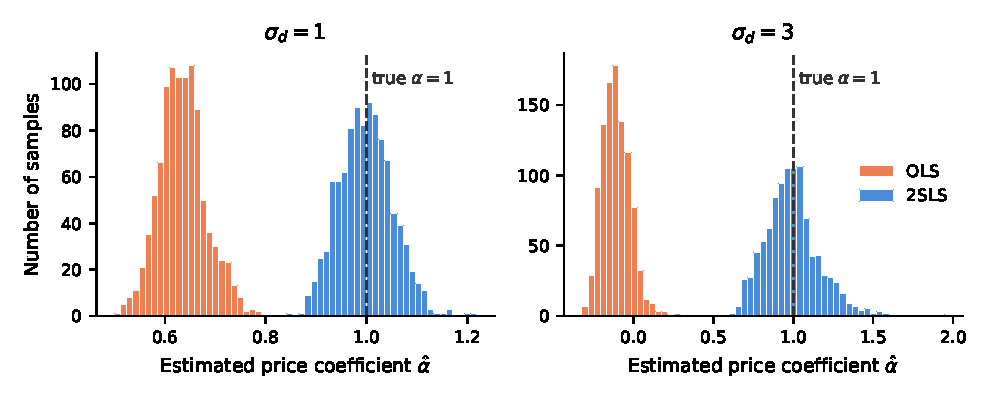
\includegraphics[width=\linewidth]{figures/ch07/mc_logit_ols_iv.pdf}
\caption{Sampling distributions of the estimated price coefficient $\hat\alpha$ in 1,000 samples of 500 duopoly
markets, for the design of \citet[Section~8]{Berry1994}. Left: $\sigma_d = 1$. Right: $\sigma_d = 3$. The dashed line
marks the true value $\alpha = 1$. OLS means are 0.635 and $-0.109$, and 2SLS means are 0.999 and 0.992. Source:
\texttt{figures/ch07/src/mc\_logit\_iv.py}.}
\label{fig:07-mc-ols-iv}
\end{figure}

\casehead{Results}
\Cref{tab:07-mc-logit} places Berry's numbers next to ours, and \cref{fig:07-mc-ols-iv} shows the sampling
distributions of $\hat\alpha$. The qualitative findings replicate. OLS underestimates the price coefficient in every
sample, while 2SLS is centered on the truth (means 1.010 and 1.002, against Berry's 0.995 and 0.979). The OLS bias is
much larger when $\xi$ explains more of mean utility. With $\sigma_d = 1$, OLS implies inelastic demand for 5.3
percent of products, and 99 of our 100 samples contain at least one such product. Berry notes that the OLS estimate
then makes firms appear to price ``on an inelastic portion of their demand curves.'' With $\sigma_d = 3$, he finds
that OLS ``sometimes'' gives $\hat\alpha < 0$. In our replication this happens in 90 of 100 samples.

Our OLS bias is larger than Berry's (mean $\hat\alpha$ of 0.638 and $-0.120$, against 0.726 and 0.181). The 2SLS
results agree closely, so the equilibrium computation and the estimators are unlikely sources of the gap. Berry does
not report every detail, such as the treatment of markets with extreme shares or how his standard errors were
computed. We report our numbers as they come out. The qualitative conclusions do not depend on the gap.

\Cref{prop:07-ols-bias} accounts for the OLS numbers. In a large simulated sample with $\sigma_d = 1$ (20,000 markets),
the projection of price on $x_j$ has slope $\Gamma = 1.847$. With $\hat\alpha_{OLS} = 0.638$ the bias in the price
coefficient is $b = 0.362$, and \eqref{eq:07-ols-bias} predicts $\plim\hat\beta_{x} = 2 - 1.847 \times 0.362 = 1.33$.
The replication mean is 1.335. The bias grows with $\sigma_d$ because the covariance between price and the error
$\sigma_d\xi_j$ scales with $\sigma_d$ twice. It scales once directly, and once through the markup, since by
\eqref{eq:07-dp-dxi} each unit of $\xi_j$ moves price by $\frac{\sigma_d s_j}{\alpha}$. The exogenous price variation
from $w_j$ and $\omega_j$ does not grow with $\sigma_d$.

The experiment also shows which instrument does the work. With $\sigma_d = 1$, the cost shifter alone gives a median
first-stage $F$ of 162. The rival's characteristic alone gives a median $F$ of 1.0, and 2SLS with it alone has a
standard deviation of 1.12 across samples. It is weak because $x$ raises cost as well as utility. In the large sample a
unit increase in $x_j$ raises marginal cost by 1.69 and price by 1.85, so the net mean utility $\beta_0 + \beta_x x_j +
\sigma_d\xi_j - \alpha p_j$ rises by only 0.15. A rival with a higher $x$ is barely more attractive.

\begin{table}[htbp]
\centering
\caption{Rival characteristics as the only instrument: duopoly versus many products.}
\label{tab:07-mc-weak}
\footnotesize
\setlength{\tabcolsep}{4.5pt}
\begin{tabular}{rrccccccc}
\toprule
$J$ & $T$ & Mean $s_0$ & s.d.\ of markups & Median $F$ & \multicolumn{2}{c}{2SLS with $z^{\mathrm{riv}}$} &
2SLS with $w$ & OLS \\
\cmidrule(lr){6-7}
 & & & & & median $\hat\alpha$ & IQR & median $\hat\alpha$ & median $\hat\alpha$ \\
\midrule
2 & 500 & 0.280 & 0.898 & 40.9 & 1.008 & [0.930, 1.082] & 1.000 & 0.483 \\
5 & 200 & 0.062 & 0.520 & 13.3 & 1.024 & [0.852, 1.201] & 1.003 & 0.534 \\
10 & 100 & 0.015 & 0.308 & 1.8 & 0.895 & [0.575, 1.346] & 0.991 & 0.557 \\
25 & 40 & 0.003 & 0.147 & 0.5 & 0.763 & [0.180, 1.369] & 0.999 & 0.578 \\
50 & 20 & 0.001 & 0.085 & 0.4 & 0.538 & [$-0.134$, 1.228] & 1.003 & 0.581 \\
\bottomrule
\end{tabular}
\par\smallskip
\parbox{\linewidth}{\footnotesize Notes: Design of \eqref{eq:07-mc-design} with $\sigma_d = 1$ and $\gamma_x = 0$, so
that $x$ does not enter marginal cost. Each sample has $N = 1{,}000$ products split into $T = \frac{1{,}000}{J}$
markets of $J$ single-product firms, with 200 samples per row. The instrument $z^{\mathrm{riv}}_{j}$ is the sum of $x$ over
the other products in the market. IQR is the interquartile range across samples. The markup standard deviation is computed within each sample and averaged. Source:
\texttt{figures/ch07/src/mc\_logit\_iv.py}.}
\end{table}

\Cref{tab:07-mc-weak} uses the same machinery to show the many-products problem of \citet{Armstrong2016}. We set
$\gamma_x = 0$, so that a rival's characteristic shifts its appeal one for one, and vary the number of products per
market $J$ with 1,000 observations in total. In duopoly the rival characteristic is a strong instrument (median $F$ of
40.9). As $J$ grows, shares shrink, markups converge to $\frac{1}{\alpha} = 1$, and their standard deviation falls from
0.90 to 0.08. The first-stage $F$ falls below 2 at $J = 10$, and the 2SLS estimate drifts toward OLS with exploding
dispersion. The cost shifter is unaffected, with medians within 0.01 of the truth in every row.

\section{The supply side: Bertrand pricing with logit demand}\label{sec:07-supply}

Combined with a model of pricing, demand estimates give markups and marginal costs and let us predict prices after
a merger or a tax. With logit demand almost everything has a closed form: markups, best responses, the equilibrium
aggregate, and pass-through. \Cref{ch:diffprod} proves these results for any ownership structure, and we restate them
here with cross-references. We then use the markups to recover marginal costs, test conduct and simulate mergers. The
closed forms make the logit a benchmark for numerical code, and they expose supply-side restrictions that mirror the
logit's restrictions on substitution. Firms set prices simultaneously, marginal costs are constant, every firm knows
all primitives (including every $\xi_j$), and the market has $M$ consumers. We drop the market index $t$. The general
theory is in \cref{ch:diffprod} and \cref{ch:blp}.

\subsection{Single-product firms}\label{sec:07-bertrand-single}

Firm $j$ sells product $j$ and earns $\pi_j = M(p_j - mc_j)s_j(\boldsymbol p)$. Write $m_j = p_j - mc_j$ for its dollar
markup.

\begin{proposition}[Logit markups with single-product firms]\label{prop:07-logit-markup}
Under logit demand, a single-product firm's best response to any vector of rival prices is characterized by its
first-order condition (\cref{prop:04-logit-br}). By \cref{prop:04-logit-markup}, in any Bertrand-Nash equilibrium
\begin{equation}\label{eq:07-logit-markup}
  p_j - mc_j = \frac{1}{\alpha(1 - s_j)}, \qquad \frac{p_j - mc_j}{p_j} = \frac{1}{\alpha p_j(1 - s_j)} =
  \frac{1}{\varepsilon_j}.
\end{equation}
Markups exceed $\frac{1}{\alpha}$ and depend on product characteristics, prices and costs only through the product's
own market share.
\end{proposition}

The markup is the single-product case of \cref{prop:04-logit-markup}. With $\frac{\partial s_j}{\partial p_j} =
-\alpha s_j(1 - s_j)$ from \cref{prop:07-logit-derivs}, the derivative of profit factors as $M s_j[1 - \alpha m_j(1 -
s_j)]$. The bracket falls strictly once $m_j > 0$ and crosses zero exactly once, and \cref{ch:diffprod} shows that the
crossing is the global maximizer. Dividing the markup by $p_j$ and using $\varepsilon_j = \alpha p_j(1 - s_j)$ gives
the Lerner form.

Two products with the same share therefore have the same dollar markup, whatever their characteristics or costs.
With small shares every markup is close to $\frac{1}{\alpha}$, so Lerner indices are roughly inversely proportional to
price. This is the supply-side image of an own elasticity that rises almost proportionally with price
(\cref{sec:07-iia}), and \cref{sec:07-limits} contrasts it with random coefficient estimates.

The first-order condition is implicit, because $s_j$ depends on $p_j$. It has a closed-form solution in terms of the
\emph{Lambert $W$ function}, defined as the inverse of $u \mapsto ue^u$ on $[0, \infty)$, so that $W(z)e^{W(z)} = z$
for $z \ge 0$ \citep{CorlessEtAl1996}. $W$ is increasing, $W(0) = 0$, and $W'(z) = \frac{W(z)}{z(1 + W(z))}$ for $z >
0$. Define
\begin{equation*}
  v_j = x_j\beta + \xi_j - \alpha\,mc_j, \qquad D_{-j} = 1 + \sum_{l \neq j} e^{\delta_l}.
\end{equation*}
The first is the mean utility product $j$ would have if priced at marginal cost, so $\delta_j = v_j - \alpha m_j$. The
second depends only on rivals' prices. Then $1 - s_j = \frac{D_{-j}}{D_{-j} + e^{\delta_j}}$, and the first-order
condition $\alpha m_j (1 - s_j) = 1$ becomes
\begin{align*}
  \alpha m_j D_{-j} &= D_{-j} + e^{v_j - \alpha m_j} \\
  (\alpha m_j - 1) D_{-j} &= e^{v_j - \alpha m_j} \\
  (\alpha m_j - 1)e^{\alpha m_j - 1} &= \frac{e^{v_j - 1}}{D_{-j}} .
\end{align*}
The last line multiplies both sides by $\frac{e^{\alpha m_j - 1}}{D_{-j}}$. It has the form $ue^u = z$ with $u = \alpha
m_j - 1$, so $u = W(z)$ and
\begin{equation}\label{eq:07-br-lambert}
  BR_j(\boldsymbol p_{-j}) = mc_j + \frac{1}{\alpha}\Bigl[1 + W\Bigl(\frac{e^{v_j - 1}}{D_{-j}}\Bigr)\Bigr].
\end{equation}
This is \eqref{eq:04-logit-br} of \cref{ch:diffprod}, where $D_{-j}$ is written $\Phi_{-j}$. The best response lies
between two bounds. As rival prices fall without limit, $D_{-j} \to \infty$ and the best
response falls to $mc_j + \frac{1}{\alpha}$. As rival prices rise without limit, $D_{-j} \to 1$ and the best response
rises to the monopoly price $mc_j + \frac{1}{\alpha}[1 + W(e^{v_j - 1})]$.

The slope of the best response follows from the chain rule. Since $\frac{\partial D_{-j}}{\partial p_l} = -\alpha
e^{\delta_l}$ for $l \neq j$, the argument $z = \frac{e^{v_j - 1}}{D_{-j}}$ satisfies $\frac{\partial z}{\partial p_l} =
\frac{\alpha z e^{\delta_l}}{D_{-j}}$, and
\begin{equation*}
  \frac{\partial BR_j}{\partial p_l} = \frac{1}{\alpha}W'(z)\frac{\partial z}{\partial p_l}
  = \frac{W(z)}{1 + W(z)}\,\frac{e^{\delta_l}}{D_{-j}} .
\end{equation*}
At the best response, $1 + W(z) = \alpha m_j = \frac{1}{1 - s_j}$, so $\frac{W(z)}{1 + W(z)} = s_j$. Also
$\frac{e^{\delta_l}}{D_{-j}} = \frac{s_l}{1 - s_j}$. Hence
\begin{equation}\label{eq:07-br-slope}
  \frac{\partial BR_j}{\partial p_l} = \frac{s_j s_l}{1 - s_j} > 0, \qquad
  \sum_{l \neq j}\frac{\partial BR_j}{\partial p_l} = s_j\,\frac{1 - s_j - s_0}{1 - s_j} < s_j .
\end{equation}
Prices are \emph{strategic complements}: a rival's price increase raises the firm's best response. The response is less
than one for one in total. The share at the best response is bounded by its monopoly value $\bar s_j =
\frac{W(e^{v_j - 1})}{1 + W(e^{v_j - 1})} < 1$, because $z \le e^{v_j - 1}$. The row sums of the Jacobian of the
best-response map are therefore below $\max_j \bar s_j < 1$ at every price vector. \Cref{prop:04-logit-br} uses this
bound to show that the map is a contraction, so the equilibrium is unique and best-response iteration converges to it
from any starting point.

\begin{figure}[htbp]
\centering
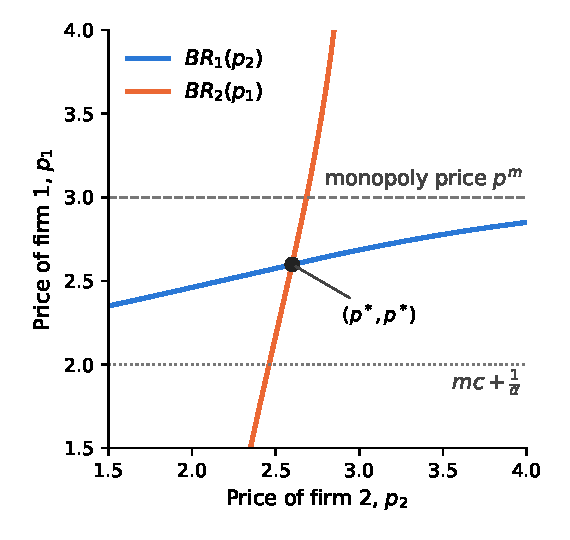
\includegraphics[width=0.52\linewidth]{figures/ch07/logit_best_response.pdf}
\caption{Best responses in a symmetric logit duopoly with an outside good, from \eqref{eq:07-br-lambert}. Both
products have $x_j\beta + \xi_j = 3$ and $mc_j = 1$, and $\alpha = 1$. The horizontal lines bound $BR_1$: it
approaches $mc + \frac{1}{\alpha} = 2$ as $p_2$ falls and the monopoly price $p^m = 3$ as $p_2$ rises. The unique
equilibrium is $p^* = 2.599$ with shares $s_j = 0.375$, where the slope of each best response is $\frac{s_j^2}{1 - s_j}
= 0.224$. Source: \texttt{figures/ch07/src/logit\_best\_response.py}.}
\label{fig:07-best-response}
\end{figure}

\Cref{fig:07-best-response} draws the two best responses of a symmetric duopoly. Each is increasing and flat, and they
cross once. At the equilibrium the markup is $p^* - mc = 1.599$, which equals $\frac{1}{\alpha(1 - s_j)} =
\frac{1}{0.625}$ up to rounding.

\subsection{Multi-product firms}\label{sec:07-bertrand-multi}

Now firm $f$ owns the set $\mathcal{J}_f$ and maximizes $\pi_f = M\sum_{k \in \mathcal{J}_f}(p_k - mc_k)s_k(\boldsymbol
p)$. The first-order condition for $j \in \mathcal{J}_f$ is
\begin{equation}\label{eq:07-multi-foc}
  s_j + \sum_{k \in \mathcal{J}_f}(p_k - mc_k)\frac{\partial s_k}{\partial p_j} = 0 .
\end{equation}
Stacking over all products with the ownership matrix $\Omega$ and the derivative matrix $\Delta$, $\Delta_{jk} =
\frac{\partial s_j}{\partial p_k}$, gives
\begin{equation}\label{eq:07-multi-foc-matrix}
  \boldsymbol s + (\Omega \odot \Delta)^\top(\boldsymbol p - \boldsymbol{mc}) = 0, \qquad
  \boldsymbol p - \boldsymbol{mc} = -\bigl[(\Omega \odot \Delta)^\top\bigr]^{-1}\boldsymbol s,
\end{equation}
as in \cref{ch:diffprod}. Because $\Omega$ is symmetric, $(\Omega \odot \Delta)^\top = \Omega \odot \Delta^\top$. With
logit demand the matrix inversion is unnecessary.

\begin{proposition}[Common markups with multi-product firms]\label{prop:07-logit-multi}
By \cref{prop:04-logit-markup}, under logit demand every solution of the first-order conditions
\eqref{eq:07-multi-foc}, and hence every Bertrand-Nash equilibrium, gives every product of firm $f$ the same dollar
markup
\begin{equation}\label{eq:07-logit-multi}
  m_f = \frac{1}{\alpha(1 - S_f)}, \qquad S_f = \sum_{k \in \mathcal{J}_f} s_k .
\end{equation}
\end{proposition}

The proof in \cref{ch:diffprod} substitutes the logit derivatives into \eqref{eq:07-multi-foc}. This gives $m_j =
\frac{1}{\alpha} + \sum_{k \in \mathcal{J}_f} s_k m_k$ for every $j \in \mathcal{J}_f$, and the right side does not
depend on $j$.

The common markup has a clean interpretation. Substitute $\frac{\partial s_j}{\partial p_j} = -\alpha s_j(1 - s_j)$
and $\frac{\partial s_k}{\partial p_j} = \alpha s_j s_k$ into \eqref{eq:07-multi-foc} and divide by $\alpha s_j(1 -
s_j)$:
\begin{equation}\label{eq:07-recapture}
  m_j = \frac{1}{\alpha(1 - s_j)} + \sum_{k \in \mathcal{J}_f,\, k \neq j} D_{jk}\, m_k, \qquad D_{jk} = \frac{s_k}{1 -
  s_j}.
\end{equation}
The first term is the single-product markup. The second is the value of the sales that a price increase on $j$
diverts to the firm's other products, where $D_{jk}$ is the logit diversion ratio (\cref{sec:07-logit-elasticities}).
A multi-product firm internalizes this recapture, so it prices above the single-product level. In the logit,
diversion is proportional to shares, so recapture depends on the firm's total share and on nothing else. The second
term of \eqref{eq:07-recapture} is the upward pricing pressure that a merger creates (\cref{ch:mergers}). Because
markups are common in dollars, the firm's cheaper products carry the higher percentage markups.

The best response of a multi-product firm also has a closed form. Holding rival prices fixed, every stationary point
of $\pi_f$ has common markups by \cref{prop:07-logit-multi}. Let $E_f = \sum_{k \in \mathcal{J}_f} e^{v_k}$ and $D_{-f} = 1 +
\sum_{l \notin \mathcal{J}_f} e^{\delta_l}$. With a common markup, $S_f = \frac{E_f e^{-\alpha m_f}}{D_{-f} + E_f
e^{-\alpha m_f}}$, and the steps that led to \eqref{eq:07-br-lambert} give
\begin{equation}\label{eq:07-br-multi}
  m_f^{BR} = \frac{1}{\alpha}\Bigl[1 + W\Bigl(\frac{E_f e^{-1}}{D_{-f}}\Bigr)\Bigr], \qquad
  p_k = mc_k + m_f^{BR} \text{ for } k \in \mathcal{J}_f .
\end{equation}
This is \eqref{eq:04-logit-br-multi} of \cref{ch:diffprod}. The firm's products enter only through the sum $E_f$, a
property that the uniqueness proof of \cref{thm:04-logit-unique} exploits.

\Cref{ex:04-logit25} solves both pricing games in one market with 25 products, five owners and $\alpha = 2$, and
\cref{tab:04-logit25} reports the results. With single-product firms, markups range from 0.502 to 0.566, all close to
$\frac{1}{\alpha} = 0.5$. Under the actual ownership each owner has one markup, equal to $\frac{1}{\alpha(1 - S_f)}$.
It ranges from 0.524 for the owner with the smallest combined share to 0.670 for the owner with the largest. Every
price rises, the outside share rises from 0.137 to 0.160, and total profit rises by about 14 percent. \Cref{app:problems}
works through the full problem.

\subsection{Existence and uniqueness of equilibrium}\label{sec:07-uniqueness}

Counterfactuals need a unique equilibrium. Without it, a merger simulation does not tell us which of several
post-merger price vectors to expect. Uniqueness can fail in general pricing games, and \cref{ch:diffprod} discusses the
conditions of \citet{CaplinNalebuff1991} for single-product firms. For the logit, uniqueness holds for any ownership
structure. The single-product case follows from Caplin and Nalebuff and from the contraction argument after
\eqref{eq:07-br-slope}. The multi-product case is due to \citet[Theorem~7, p.~279]{KonovalovSandor2010} and
\citet{NockeSchutz2018}.
In an \emph{aggregative game} each firm's profit depends on its rivals' prices only through one aggregator, and
consumer surplus is a monotone function of it \citep[p.~229, n.~127]{AskerNocke2021}. The logit pricing game is
aggregative, and its aggregator is the inclusive sum $\Lambda = 1 + \sum_k e^{\delta_k}$, which \cref{ch:diffprod}
writes as $\Phi$.

\begin{proposition}[Existence and uniqueness]\label{prop:07-logit-unique}
With logit demand, constant marginal costs and any partition of the products among firms, the Bertrand-Nash pricing
game has exactly one equilibrium. This is \cref{thm:04-logit-unique}.
\end{proposition}

The proof of \cref{thm:04-logit-unique} reduces the equilibrium to one equation in one unknown, the aggregate
$\Lambda$. Each firm sets the common markup of \cref{prop:07-logit-multi}, so its combined share is $S_f = \frac{E_f
e^{-\alpha m_f}}{\Lambda}$, with $E_f$ as in \eqref{eq:07-br-multi}. Substituting $\alpha m_f = \frac{1}{1 - S_f}$
gives
\begin{equation}\label{eq:07-share-aggregate}
  S_f\, e^{\frac{1}{1 - S_f}} = \frac{E_f}{\Lambda} .
\end{equation}
The left side rises strictly from 0 to $+\infty$ as $S_f$ rises from 0 to 1. Each firm's share is therefore a
continuous and strictly decreasing function $S_f(\Lambda)$ of the aggregate. The inside shares and the outside share
$\frac{1}{\Lambda}$ add up to one, so the equilibrium aggregate solves
\begin{equation}\label{eq:07-psi}
  \Psi(\Lambda) \equiv \sum_f S_f(\Lambda) + \frac{1}{\Lambda} = 1 .
\end{equation}
The function $\Psi$ is strictly decreasing, exceeds one at $\Lambda = 1$ and tends to zero as $\Lambda \to \infty$.
It has exactly one root $\Lambda^* > 1$, and the root pins down every share, markup and price.

The characterization doubles as an algorithm: solve \eqref{eq:07-psi} by bisection and read off shares, markups and
prices. Best-response iteration with \eqref{eq:07-br-multi}, the markup fixed point $\boldsymbol p \leftarrow
\boldsymbol{mc} + \frac{1}{\alpha(1 - S_f(\boldsymbol p))}$, and Newton's method are common alternatives. In the
market of \cref{ex:04-logit25}, $\Lambda^* = 7.314$ with single-product firms and $6.246$ with multi-product firms,
equal to $\frac{1}{s_0}$ in each case (\cref{ex:04-logit25-unique}). With non-logit demand uniqueness is not
guaranteed, and restarting the solver from many points is the practical check (\cref{ch:blp}).

\subsection{Pass-through}\label{sec:07-passthrough}

The \emph{pass-through rate} $\rho = \frac{\dd p}{\dd mc}$ measures how much of a cost change reaches the price
(\cref{ch:theory}). It governs the incidence of taxes, the effect of exchange rates on import prices, and the price
effect of merger efficiencies.

\begin{proposition}[Logit pass-through]\label{prop:07-logit-passthrough}
Hold rivals' prices fixed. By parts (i) and (iii) of \cref{prop:04-passthrough}, the following hold.
\begin{enumerate}[label=(\roman*)]
  \item A single-product firm passes through $\rho_j = \frac{\dd p_j}{\dd mc_j} = 1 - s_j$ of an increase in its
    marginal cost.
  \item A multi-product firm facing the same increase in the marginal cost of all its products raises all its prices by
    $\rho_f = 1 - S_f$ per unit of cost.
\end{enumerate}
In both cases pass-through is below one and falls with the firm's share.
\end{proposition}

The proof in \cref{ch:diffprod} differentiates the markup condition $\alpha m_f(1 - S_f) = 1$. A common cost increase
$\dd mc$ lowers the firm's combined share, and the common markup falls by $S_f\,\dd mc$, so each price rises by $(1 -
S_f)\,\dd mc$. A single-product firm is the case $S_f = s_j$.

Pass-through below one is the logit instance of a general result for log-concave demand. For a single-product firm
with demand $q(p)$ at fixed rival prices, \eqref{eq:02-pt-logcurv} gives
\begin{equation*}
  \rho = \frac{\dd p}{\dd mc} = \frac{1}{2 - \frac{q q''}{(q')^2}} ,
\end{equation*}
and $\rho < 1$ exactly when demand is log-concave at the optimum (\cref{cor:02-bulow-pfleiderer}).
\citet{BulowPfleiderer1983} write the same pass-through rate in terms of the demand elasticity and its slope, as
restated by \citet[p.~18 of the 2008 working paper]{FarrellShapiro2010}. \citet{WeylFabinger2013} develop pass-through
as a general tool for incidence under imperfect competition. Holding rivals' prices fixed, logit demand is log-concave
in own price:
\begin{equation*}
  \frac{\dd \ln s_j}{\dd p_j} = -\alpha(1 - s_j), \qquad \frac{\dd^2 \ln s_j}{\dd p_j^2} = \alpha\frac{\dd s_j}{\dd p_j}
  = -\alpha^2 s_j(1 - s_j) < 0 .
\end{equation*}
With $q = s_j$, $q' = -\alpha s_j(1 - s_j)$ and $q'' = \alpha^2 s_j(1 - s_j)(1 - 2s_j)$, the ratio $\frac{q
q''}{(q')^2}$ equals $\frac{1 - 2s_j}{1 - s_j}$, and the general formula returns $\rho_j = 1 - s_j$.
In the market of \cref{ex:04-logit25} the largest owner has $S_f = 0.2536$, and a numerical derivative of
\eqref{eq:07-br-multi} gives pass-through 0.7464, equal to $1 - S_f$. The proposition holds rivals' prices fixed.
When a cost shock hits all firms, rivals raise their prices as well. By strategic complementarity
\eqref{eq:07-br-slope}, equilibrium pass-through then exceeds $1 - s_j$ (\cref{cor:04-passthrough-eq}).

\begin{figure}[htbp]
\centering
\begin{tikzpicture}
\begin{axis}[
  name=leftax, width=0.47\linewidth, height=0.40\linewidth,
  xmin=0, xmax=0.9, ymin=0, ymax=10.5,
  xlabel={Share $s$ (or combined share $S_f$)}, ylabel={$\alpha\,(p - mc)$},
  title={(a) Markup in units of $\frac{1}{\alpha}$},
  title style={font=\small}, label style={font=\small}, tick label style={font=\footnotesize},
  domain=0:0.9, samples=200, axis lines=left]
  \addplot[very thick, blue!60!black] {1/(1-x)};
  \node[font=\footnotesize, anchor=west] at (axis cs:0.30,6.0) {$\alpha m = \frac{1}{1 - s}$};
  \addplot[dashed, gray] coordinates {(0,1) (0.9,1)};
  \node[font=\footnotesize, anchor=south east, gray!40!black] at (axis cs:0.90,1.15) {$\alpha m = 1$ at $s = 0$};
\end{axis}
\begin{axis}[
  at={(leftax.east)}, anchor=west, xshift=1.7cm,
  width=0.47\linewidth, height=0.40\linewidth,
  xmin=0, xmax=0.9, ymin=0, ymax=1.05,
  xlabel={Share $s$ (or combined share $S_f$)}, ylabel={$\rho = \frac{\dd p}{\dd mc}$},
  title={(b) Pass-through at fixed rival prices},
  title style={font=\small}, label style={font=\small}, tick label style={font=\footnotesize},
  domain=0:0.9, samples=50, axis lines=left]
  \addplot[very thick, orange!80!black] {1-x};
  \node[font=\footnotesize, anchor=west] at (axis cs:0.45,0.65) {$\rho = 1 - s$};
\end{axis}
\end{tikzpicture}
\caption{Logit markups and pass-through as functions of the firm's share. Panel (a): the dollar markup times $\alpha$,
from \cref{prop:07-logit-markup,prop:07-logit-multi}. Panel (b): the pass-through rate of
\cref{prop:07-logit-passthrough}. For a multi-product firm, read the horizontal axis as $S_f$.}
\label{fig:07-markups}
\end{figure}

\Cref{fig:07-markups} summarizes the two results. Markups rise and pass-through falls with the firm's share, and
nothing else about the product matters. The link to merger analysis is direct. \citet{FarrellShapiro2010} define the
upward pricing pressure on product $j$ after a merger with the owner of $k$ as $D_{jk}m_k$, the second term of
\eqref{eq:07-recapture}. They evaluate it at pre-merger prices and before any credit for cost savings (p.~9 of their
2008 working paper). \citet[p.~231]{AskerNocke2021} state the same definition and read it as the merged firm's
opportunity cost of keeping the price of $j$ at its pre-merger level. It acts like a cost increase on $j$, so to first
order the price of $j$ rises by
$\rho_j D_{jk}m_k = (1 - s_j)\frac{s_k}{1 - s_j}m_k = s_k m_k$ under logit demand. \Cref{ch:mergers} develops this
approximation and its limits.

\subsection{Recovering marginal costs and joint estimation}\label{sec:07-cost-recovery}

Given an estimate $\hat\alpha$ and an assumed ownership structure, the first-order conditions deliver marginal costs
without any cost data. Suppose marginal cost is linear in observed cost shifters $w_{jt}$ and a cost shock
$\omega_{jt}$, $mc_{jt} = w_{jt}\gamma + \omega_{jt}$. By \cref{prop:07-logit-multi},
\begin{equation}\label{eq:07-logit-supply}
  p_{jt} = w_{jt}\gamma + \frac{1}{\alpha(1 - S_{ft})} + \omega_{jt},
  \qquad \widehat{mc}_{jt} = p_{jt} - \frac{1}{\hat\alpha(1 - S_{ft})} .
\end{equation}
With single-product firms ($S_{ft} = s_{jt}$) the first equation is equation (31) of \citet[p.~255]{Berry1994},
whose parameters are $\gamma$ and $\frac{1}{\alpha}$. His general version (equation 29) lets cost depend on output and
writes the markup as $\frac{s_j}{\alpha}\bigl(\frac{\partial s_j}{\partial\delta_j}\bigr)^{-1}$, which covers any demand
model. The
nested logit version is \cref{prop:07-nl-markup}.

There are two ways to estimate $\gamma$. The \emph{two-step} approach regresses $\widehat{mc}_{jt}$ on $w_{jt}$ by
OLS. It is consistent when $\E[w_{jt}^\top\omega_{jt}] = 0$ and $\hat\alpha$ is consistent. Its usual standard errors
are wrong, because the dependent variable is a \emph{generated regressand}. The error in the implied cost is
\begin{equation*}
  \widehat{mc}_{jt} - mc_{jt} = \frac{1}{\alpha(1 - S_{ft})} - \frac{1}{\hat\alpha(1 - S_{ft})} \approx
  \frac{\hat\alpha - \alpha}{\alpha^2(1 - S_{ft})} ,
\end{equation*}
which is nearly common to all products when shares are small, so it loads on the intercept of the cost regression.
The simulated market of \cref{sec:08-worked-logit}, which \cref{app:problems} works through, shows the size of the
effect. A market bootstrap that re-estimates $\alpha$ raises the intercept's standard error there from 0.016 to 0.072,
while the slopes' standard errors barely move. Valid inference uses
such a bootstrap or the sandwich of a stacked GMM problem \citep{Newey1984}. Negative implied costs signal a problem
with the demand estimates or the conduct assumption.

The \emph{joint} approach estimates demand and supply together. Let $\theta = (\beta, \alpha, \gamma)$ and define the
two structural errors
\begin{equation}\label{eq:07-joint-errors}
  \xi_{jt}(\theta) = y_{jt} - x_{jt}\beta + \alpha p_{jt}, \qquad
  \omega_{jt}(\theta) = p_{jt} - \frac{1}{\alpha(1 - S_{ft})} - w_{jt}\gamma .
\end{equation}
With demand instruments $z^d_{jt}$ and supply instruments $z^s_{jt}$, the moment conditions are $\E[z^{d\top}_{jt}
\xi_{jt}(\theta)] = 0$ and $\E[z^{s\top}_{jt}\omega_{jt}(\theta)] = 0$. GMM minimizes $\bar g(\theta)^\top W \bar
g(\theta)$ for the stacked sample moments
\begin{equation}\label{eq:07-joint-gmm}
  \bar g(\theta) = \frac{1}{N}\sum_t\sum_{j \in \mathcal{J}_t}
  \begin{pmatrix} z^{d\top}_{jt}\,\xi_{jt}(\theta) \\ z^{s\top}_{jt}\,\omega_{jt}(\theta) \end{pmatrix} .
\end{equation}
For a given $\alpha$ both errors are linear in $(\beta, \gamma)$, which can be concentrated out, so the search is over
$\alpha$ alone. The markup term is endogenous, because $S_{ft}$ depends on prices and hence on $\omega_{jt}$.
\citet[p.~255]{Berry1994} lists its instruments: excluded demand characteristics, characteristics of other firms, and
market population when markets differ in size.

Joint estimation helps when demand instruments are weak, because the markup term carries information about $\alpha$
if the supply instruments overidentify $\gamma$. It also exploits any correlation between $\xi$ and $\omega$, it is
where conduct enters when conduct is tested, and it gives correct standard errors for $\gamma$. The cost is
robustness. A wrong ownership or conduct assumption contaminates the demand estimates through the shared $\alpha$.
Berry notes that joint estimation ``would take into account the cross-equation restrictions on parameters.''
\Cref{ch:blp} develops joint estimation with random coefficients, where the gains are larger.

\subsection{Testing conduct and ownership with logit demand}\label{sec:07-conduct}

The same first-order conditions can be evaluated under different assumptions about who sets which price. Let a
\emph{pricing coalition} be a set of products whose prices are chosen jointly. By \cref{prop:07-logit-multi}, a
coalition $A$ sets the common markup $\frac{1}{\alpha(1 - S_A)}$, where $S_A$ is its combined share. Implied Lerner
indices under four structures are therefore analytic:
\begin{equation}\label{eq:07-conduct-margins}
  \underbrace{\frac{1}{\alpha p_j(1 - s_j)}}_{\text{single product}}, \qquad
  \underbrace{\frac{1}{\alpha p_j(1 - S_f)}}_{\text{actual ownership}}, \qquad
  \underbrace{\frac{1}{\alpha p_j(1 - S_G)}}_{\text{joint pricing of } G}, \qquad
  \underbrace{\frac{1}{\alpha p_j s_0}}_{\text{monopoly}},
\end{equation}
where $G$ is a group of colluding products, and monopoly uses $1 - \sum_{k \ge 1}s_k = s_0$. Comparing the predicted
margins with observed margins, or with outside information on costs, tests the structures. Only $\hat\alpha$ and the
shares are needed.

\citet[Section~5.3]{Nevo2001} carries out this comparison for cereal, and \cref{tab:07-nevo-margins} reproduces the
logit column of his Table VIII. It uses the price coefficient of column (ix) of \cref{tab:07-nevo-logit}. Because only
shares are needed, the logit margins can include brands outside the 25 in the sample, which the full model cannot
\citep[pp.~332--333]{Nevo2001}.

\begin{table}[htbp]
\centering
\caption{Median price-cost margins in ready-to-eat cereal under alternative pricing structures, logit demand.}
\label{tab:07-nevo-margins}
\footnotesize
\begin{tabular}{lc}
\toprule
 & Logit \\
 & (Table V, column ix) \\
\midrule
Single-product firms & 33.6\% \\
 & (31.8\%--35.6\%) \\
Current ownership of 25 brands & 35.8\% \\
 & (33.9\%--38.0\%) \\
Joint ownership of 25 brands & 41.9\% \\
 & (39.7\%--44.4\%) \\
Current ownership of all brands & 37.2\% \\
 & (35.2\%--39.4\%) \\
Monopoly or perfect price collusion & 54.0\% \\
 & (51.1\%--57.3\%) \\
\bottomrule
\end{tabular}
\par\smallskip
\parbox{\linewidth}{\footnotesize Notes: Source: \citet[Table~VIII, p.~333]{Nevo2001}, logit column. Margins are
$\frac{p - mc}{p}$. Entries are medians over 27,862 brand-city-quarter observations, with 95 percent confidence
intervals for the median in parentheses, based on the asymptotic distribution of the demand estimates. The logit
computation is analytical. \Cref{tab:08-nevo-margins} reproduces the full table, including the random coefficients
column.}
\end{table}

Nevo compares the predictions with crude accounting estimates. The gross retail margin is about 46.0 percent, and the
gap between national brands and private labels gives a lower bound of about 31 percent \citep[pp.~333--334]{Nevo2001}.
His full random coefficients model predicts a median margin of 35.8 percent with single-product firms. It is 42.2
percent (interval 29.1 to 55.8) under current ownership and 72.6 percent (62.2 to 97.2) under joint ownership of the
25 brands (\cref{tab:08-nevo-margins}). Using these intervals, he rejects joint profit maximization by the 25 brands and
cannot reject multi-product Nash pricing. The logit column tells a different story. Joint ownership of the 25 brands
raises the logit margin only from 35.8 to 41.9 percent, against 42.2 to 72.6 percent in the full model. With logit
margins, joint ownership comes closer to the accounting margin than current ownership does, so a logit-based test
could point toward collusion.

The logit understates the effect of joint pricing because of IIA. A coalition's markup depends only on
$\frac{1}{1 - S_G}$. With a market of one serving per person per day the outside share is large, so $S_G$ is far from
one even for 25 brands. Diversion is proportional to shares (\cref{sec:07-iia}), so most of the sales a brand loses go
to the outside good, and merging brands recaptures little. In the random coefficient model cereals are closer
substitutes for each other than for the outside good, so joint pricing recaptures much more. The assumed demand model
shapes the conduct test as much as the data do.

\citet[p.~874]{BerryLevinsohnPakes1995} make the same point for cars. Their IV logit implies that ``all models have
about the same mark-up,'' from \$4,630 for the BMW to \$4,805 for the Chevy Cavalier. Shares measured against all
households are tiny, so markups are close to $\frac{1}{\hat\alpha} = \frac{1}{0.216}$ thousand dollars, about \$4,630.
Differences come only from the number of models a parent firm sells. GM sells the most and has the highest markups,
while BMW has, ``quite counter-intuitively,'' the lowest. If BMW's combined share is negligible,
\eqref{eq:07-logit-multi} and $1 - \frac{4{,}630}{4{,}805} \approx 0.036$ imply that GM's models together sold to
roughly 3.6 percent of households. \Cref{sec:07-limits-markups} translates these dollar markups into Lerner
indices, and the random coefficient markups of \cref{ch:blp} vary far more across models.

Comparing implied margins across ownership structures is an alternative to estimating a conduct parameter
(\cref{ch:conduct}). It sidesteps the problem raised by \citet[p.~227]{Corts1999}, who shows that in a dynamic
oligopoly model the estimated conduct parameter can mismeasure market power severely. \citet{Bresnahan1987} applies
a nested test of this kind with the vertical model (\cref{ch:discrete}).

Logit merger simulation follows directly. \citet[p.~230]{AskerNocke2021} credit \citet{HausmanLeonardZona1994},
\citet{WerdenFroeb1994} and \citet{Nevo2000b} with pioneering \emph{merger simulation}, which has three steps. The
first estimates pre-merger demand. The second recovers pre-merger marginal costs from an assumption on pre-merger
conduct, typically static Bertrand-Nash pricing. The third computes the post-merger equilibrium under assumptions on
post-merger conduct and on merger-related cost savings, holding demand and the product set fixed. Werden and Froeb
carry out these steps with logit demand. The first two steps are then analytic, and the third reduces to one
equation in one unknown.
Estimate $\alpha$, recover marginal
costs from \eqref{eq:07-logit-supply} under the pre-merger ownership, and solve \eqref{eq:07-psi} under the
post-merger ownership. If firms $f$ and $f'$ merge, the merged firm sets one
markup $\frac{1}{\alpha(1 - S_f - S_{f'})}$ at post-merger shares, and rivals respond. Because diversion follows
shares, the predicted dollar price effects depend only on $\hat\alpha$, the ownership structure and the pre-merger
shares (\cref{ch:mergers}). When the size of the cost savings is unknown, the third step can instead find the
smallest savings that leave consumer surplus unchanged \citep[pp.~230--231]{AskerNocke2021}.

\section{GEV models and the nested logit}\label{sec:07-nested}

The logit restricts substitution because its taste shocks are independent across products (\cref{sec:07-iia}).
A consumer who leaves product $j$ after a price increase is no more likely than anyone else to choose a
product similar to $j$. Two routes break this property while keeping the model estimable from market shares.
The first correlates the shocks of products that the analyst groups together. It leads to the generalized
extreme value family and to the nested logit. The second lets taste coefficients vary across consumers. It
leads to the random coefficients logit of \cref{ch:blp}. This section develops the first route.
\Cref{sec:07-welfare} then uses both the logit and the nested logit to measure consumer welfare.

\subsection{Generalized extreme value models}\label{sec:07-gev}

We work with an additive random utility model. Consumer $i$ obtains $u_{ij} = V_{ij} + \epsilon_{ij}$ from
alternative $j = 0, 1, \dots, J$, where $V_{ij}$ is the deterministic part of utility. Throughout this
subsection we drop the consumer index and write $V = (V_0, \dots, V_J)$ and $y_j = e^{V_j}$. The choice
probability of $j$ is $P_j(V)$. The \emph{social surplus function} is the expected maximum utility,
\begin{equation}\label{eq:07-surplus}
\mathcal{W}(V) = \E\Big[\max_{j = 0, \dots, J}\,(V_j + \epsilon_j)\Big].
\end{equation}
The logit assumes that the $\epsilon_j$ are independent type-I extreme value (Gumbel) variables.
\citet{McFadden1978} found a class of correlated distributions that keeps the closed forms of the logit. The class
is indexed by a function of $J + 1$ positive arguments.

\begin{definition}[GEV generating function]\label{def:07-gev}
A function $H : \R^{J+1}_+ \to \R_+$ is a \emph{GEV generating function} if it has the following three
properties.
\begin{enumerate}[label=(G\arabic*)]
  \item $H$ is homogeneous of degree one: $H(\lambda y) = \lambda H(y)$ for every $\lambda > 0$.
  \item $H(y) \to \infty$ as $y_j \to \infty$, for each $j$.
  \item For any $r \ge 1$ distinct indices $j_1, \dots, j_r$, the mixed partial derivative
  $\frac{\partial^r H}{\partial y_{j_1}\cdots\partial y_{j_r}}$ exists, is continuous, and is nonnegative when
  $r$ is odd and nonpositive when $r$ is even.
\end{enumerate}
\end{definition}

We write $H_j$ and $H_{jk}$ for the first and second partial derivatives of $H$. Condition (G1) produces the
closed forms below. Condition (G2) makes each marginal distribution proper. Condition (G3) makes the function in
part (i) of the next proposition a joint distribution function with a nonnegative density. The notation follows
\citet[p.~1421]{McFadden1984}, who calls the function $H$. \Cref{thm:06-gev} states and proves the first
three parts of the next result. We restate them here together with two parts that this chapter also uses, the
gradient property (iv) and the derivative formula (v).

\begin{proposition}[McFadden's GEV theorem]\label{prop:07-gev}
Let $H$ be a GEV generating function and let $y = (e^{V_0}, \dots, e^{V_J})$.
\begin{enumerate}[label=(\roman*)]
  \item $F(\epsilon_0, \dots, \epsilon_J) = \exp\big[-H(e^{-\epsilon_0}, \dots, e^{-\epsilon_J})\big]$ is the
  distribution function of a random vector whose marginals are Gumbel.
  \item If $\epsilon$ has distribution $F$, the choice probabilities are
  \begin{equation}\label{eq:07-gev-prob}
  P_j(V) = \frac{y_j H_j(y)}{H(y)} = \frac{\partial \ln H(e^{V_0}, \dots, e^{V_J})}{\partial V_j}.
  \end{equation}
  \item The maximum utility $\max_j(V_j + \epsilon_j)$ is Gumbel with location $\ln H(y)$ and scale one, so that
  \begin{equation}\label{eq:07-gev-surplus}
  \mathcal{W}(V) = \ln H(y) + \gamma_E ,
  \end{equation}
  where $\gamma_E \approx 0.5772$ is Euler's constant.
  \item (Williams, Daly and Zachary.) The social surplus function is differentiable and
  $\frac{\partial \mathcal{W}(V)}{\partial V_j} = P_j(V)$ for every $j$.
  \item For all $j$ and $k$,
  \begin{equation}\label{eq:07-gev-deriv}
  \frac{\partial P_j}{\partial V_k} = P_j\big(\indic\{j = k\} - P_k\big) + \frac{y_j y_k H_{jk}(y)}{H(y)} .
  \end{equation}
\end{enumerate}
\end{proposition}

\begin{proof}
Parts (i), (ii) and (iii) are parts (a), (b) and (c) of \cref{thm:06-gev}. Part (i) is the theorem of
\citet{McFadden1978}, and the proof of \cref{thm:06-gev} derives (ii) and (iii) from it by homogeneity. Part (iv) is
part (ii) of \cref{thm:06-wdz}, which holds for every additive random utility model. In the GEV case it also follows
by differentiating \eqref{eq:07-gev-surplus} and applying (ii). Only (v) is new.

For (v), take logs in (ii): $\ln P_j = V_j + \ln H_j(y) - \ln H(y)$. Differentiate with respect to $V_k$, using
$\frac{\partial y_k}{\partial V_k} = y_k$:
\begin{equation*}
\frac{\partial \ln P_j}{\partial V_k} = \indic\{j = k\} + \frac{y_k H_{jk}(y)}{H_j(y)} - \frac{y_k H_k(y)}{H(y)}
= \indic\{j = k\} + \frac{y_k H_{jk}(y)}{H_j(y)} - P_k .
\end{equation*}
Multiplying by $P_j = \frac{y_jH_j}{H}$ gives \eqref{eq:07-gev-deriv}.
\end{proof}

Part (v) shows what correlation buys. For $j \neq k$ the logit term $-P_jP_k$ is the cross derivative of a model
with independent shocks and the same probabilities. The second term $\frac{y_jy_kH_{jk}}{H}$ is nonpositive by
(G3). A GEV model therefore implies at least as much substitution between $j$ and $k$ as the logit at the same
choice probabilities, and $H_{jk}$ measures the excess. The formula is symmetric in $j$ and $k$, which is the
counterpart of Slutsky symmetry (\cref{cor:06-wdz}). With mean utilities $V_k = \delta_k$ and
$\delta_k = x_k\beta - \alpha p_k + \xi_k$, price derivatives follow from
$\frac{\partial s_j}{\partial p_k} = -\alpha\frac{\partial P_j}{\partial \delta_k}$.

\casehead{Two generating functions}
The logit is the case $H(y) = \sum_{j=0}^J y_j$. Its first derivatives equal one and all higher derivatives vanish,
so (ii) gives $P_j = \frac{y_j}{\sum_k y_k}$ and (v) gives the logit derivatives of \cref{prop:07-logit-derivs}.
The \emph{nested logit} groups the inside products into nests. Partition the inside products into
$G$ mutually exclusive and exhaustive nests $g = 1, \dots, G$, and place the outside good alone in nest $0$. For
a nesting parameter $\sigma$, let
\begin{equation}\label{eq:07-nl-H}
H(y) = y_0 + \sum_{g=1}^G D_g(y)^{1 - \sigma}, \qquad D_g(y) = \sum_{j \in g} y_j^{\frac{1}{1-\sigma}} .
\end{equation}

\begin{lemma}[Consistency of the nested logit]\label{lem:07-nl-gev}
The function \eqref{eq:07-nl-H} is a GEV generating function for every $\sigma \in [0, 1)$. If $\sigma < 0$ and
some nest contains two or more products, it violates (G3).
\end{lemma}

\begin{proof}
For (G1), $D_g(\lambda y) = \lambda^{\frac{1}{1-\sigma}}D_g(y)$, so $D_g(\lambda y)^{1-\sigma} = \lambda D_g(y)^{1-\sigma}$.
For (G2), if $y_j \to \infty$ with $j \in g$, then $D_g \to \infty$ and $D_g^{1-\sigma} \to \infty$ because
$1 - \sigma > 0$. The outside good enters linearly.

For (G3), a mixed partial derivative over indices from two different nests is zero, which satisfies the weak sign
condition. Take distinct indices $j_1, \dots, j_r$ in the same nest $g$. Write $\varphi(D) = D^{1-\sigma}$ and
$a_j = \frac{\partial D_g}{\partial y_j} = \frac{1}{1-\sigma}y_j^{\frac{\sigma}{1-\sigma}} \ge 0$. Each $a_j$ depends on
$y_j$ alone, so the chain rule gives
\begin{equation*}
\frac{\partial^r H}{\partial y_{j_1}\cdots\partial y_{j_r}} = \varphi^{(r)}(D_g)\prod_{m=1}^r a_{j_m} .
\end{equation*}
The successive derivatives of $\varphi$ are $\varphi'(D) = (1-\sigma)D^{-\sigma}$,
$\varphi''(D) = -\sigma(1-\sigma)D^{-\sigma-1}$, $\varphi'''(D) = \sigma(\sigma+1)(1-\sigma)D^{-\sigma-2}$, and in general
\begin{equation*}
\varphi^{(r)}(D) = (-1)^{r-1}(1-\sigma)\prod_{m=0}^{r-2}(\sigma + m)\,D^{1-\sigma-r}, \qquad r \ge 2 .
\end{equation*}
For $\sigma \in [0, 1)$ every factor in the product is nonnegative, so the sign is $(-1)^{r-1}$, as (G3) requires.
If $\sigma < 0$, then $\varphi''(D) > 0$ and the second mixed derivative of two products in the same nest is
positive.
\end{proof}

The parameter range has an empirical counterpart. \citet[pp.~1425--1426]{McFadden1984} notes that estimates of
the nesting parameters outside the unit interval violate the ranking of cross elasticities implied by the tree,
and may indicate a misspecified tree. In the notation of \citet{BorschSupan1990}, our $1 - \sigma$ is the
dissimilarity parameter. He shows that values with $\sigma < 0$ can still be consistent with utility maximization
on a restricted region of mean utilities (Section~4 and Theorem~1, pp.~377--381). By Theorem~1, it suffices that
the mixed partial derivatives of the choice probabilities be nonnegative on that region. In the two-level model
this requires the choice probabilities of the nests to be large enough (Theorem~2, p.~385). With two nests of two
alternatives each and a common $\sigma < -1$, these requirements conflict and no such region exists (p.~385).
Applied work treats $\sigma \in [0, 1)$ as the admissible range. The next two subsections derive the nested logit a second way,
from an explicit utility model.

\subsection{The nested logit model}\label{sec:07-nl-model}

The nested logit relaxes IIA by grouping products. Within a nest, consumers substitute as in the logit. Products in
different nests have less in common, so they are weaker substitutes. The idea parallels the grouping of goods in
multi-stage budgeting (\cref{ch:aids}), and the same analyst judgment determines the groups.

\begin{assumption}[Nested logit]\label{asm:07-nl}
The inside products of market $t$ are partitioned into nests $g = 1, \dots, G$, and the outside good forms nest
$0$ by itself. The utility of consumer $i$ from product $j$ in nest $g$ is
\begin{equation}\label{eq:07-nl-utility}
u_{ij} = \delta_j + \zeta_{ig} + (1 - \sigma)\epsilon_{ij}, \qquad \delta_j = x_j\beta - \alpha p_j + \xi_j ,
\end{equation}
and the utility of the outside good is a standard Gumbel variable $\epsilon_{i0}$. The shocks $\epsilon_{ij}$ are
i.i.d.\ standard Gumbel. The nest tastes $\zeta_{ig}$ are i.i.d.\ across consumers and nests with the distribution
$C(\sigma)$ of \cref{lem:07-cardell}, and they are independent of the $\epsilon_{ij}$. The nesting parameter
satisfies $0 \le \sigma < 1$.
\end{assumption}

The term $\zeta_{ig}$ is common to all products in nest $g$ for consumer $i$. A consumer with a high draw likes
every product of the nest, so the utilities of products in the same nest are positively correlated.
\citet[p.~252]{Berry1994} points out that \eqref{eq:07-nl-utility} is a random coefficients model. Let $d_{jh}$
equal one if $j \in h$. Then $\zeta_{ig} = \sum_h d_{jh}\zeta_{ih}$ for $j \in g$, so the nest taste is a random
coefficient on the nest dummies, with a distribution tied to $\sigma$. Unlike the full random coefficients model, correlation can depend only on
groupings fixed before estimation, never on continuous characteristics. \Citet[p.~524]{Nevo2000a} makes the same
point, and \citet{Cardell1997} shows that the two descriptions of the nested logit are equivalent. The
distribution of $\zeta_{ig}$ is chosen so that the composite shock remains Gumbel.

\begin{lemma}[\citealp{Cardell1997}]\label{lem:07-cardell}
For every $\sigma \in [0, 1)$ there is a unique distribution $C(\sigma)$ with the following property. If
$\zeta \sim C(\sigma)$ and $\epsilon$ is a standard Gumbel variable independent of $\zeta$, then
$\zeta + (1 - \sigma)\epsilon$ is a standard Gumbel variable. Equivalently, the random variable
$X = e^{\frac{\zeta}{1-\sigma}}$ satisfies
\begin{equation}\label{eq:07-cardell-laplace}
\E\big[e^{-cX}\big] = \exp\big(-c^{1-\sigma}\big) \qquad \text{for every } c > 0 .
\end{equation}
\end{lemma}

We do not prove existence, which \citet{Cardell1997} establishes along with the density of $\zeta$. The
equivalence is a short computation. Conditioning on $\zeta$,
\begin{equation*}
\Pr\big(\zeta + (1-\sigma)\epsilon \le t\big) = \E\Big[\exp\Big(-e^{-\frac{t - \zeta}{1-\sigma}}\Big)\Big]
= \E\big[e^{-cX}\big], \qquad c = e^{-\frac{t}{1-\sigma}} .
\end{equation*}
The standard Gumbel distribution function is $\exp(-e^{-t}) = \exp(-c^{1-\sigma})$, which gives
\eqref{eq:07-cardell-laplace}. A Laplace transform determines a distribution, which explains uniqueness. The
function $c \mapsto \exp(-c^{a})$ with $0 < a \le 1$ is the Laplace transform of the positive stable law of index
$a$ \citep{Feller1971}. So $\zeta$ is $(1-\sigma)$ times the logarithm of a positive stable variable of index
$1 - \sigma$. At $\sigma = 0$ the stable variable equals one and $\zeta = 0$.

\begin{proposition}[Nested logit shares]\label{prop:07-nl-shares}
Under \cref{asm:07-nl}, define the inclusive sum of nest $g$ as
$D_g = \sum_{k \in g} e^{\frac{\delta_k}{1-\sigma}}$. Then the within-nest share, the nest share, the product share
and the outside share are
\begin{equation}\label{eq:07-nl-share}
s_{j \mid g} = \frac{e^{\frac{\delta_j}{1-\sigma}}}{D_g}, \qquad
s_g = \frac{D_g^{1-\sigma}}{1 + \sum_{h=1}^G D_h^{1-\sigma}}, \qquad
s_j = s_{j \mid g}\,s_g, \qquad
s_0 = \frac{1}{1 + \sum_{h=1}^G D_h^{1-\sigma}} .
\end{equation}
The composite shocks $\zeta_{ig} + (1-\sigma)\epsilon_{ij}$ have the GEV distribution generated by
\eqref{eq:07-nl-H}.
\end{proposition}

\begin{proof}
We give two derivations. The first uses \cref{prop:07-gev}. The second builds the shares nest by nest.

\emph{GEV derivation.} Fix a nest $g$ and numbers $t_j$ for $j \in g$. Conditioning on $\zeta_{ig}$ and using the
independence of the $\epsilon_{ij}$,
\begin{equation*}
\Pr\big(\zeta_{ig} + (1-\sigma)\epsilon_{ij} \le t_j \text{ for all } j \in g\big)
= \E\Big[\prod_{j\in g}\exp\Big(-e^{-\frac{t_j - \zeta_{ig}}{1-\sigma}}\Big)\Big]
= \E\Big[\exp\Big(-X\sum_{j \in g}e^{-\frac{t_j}{1-\sigma}}\Big)\Big],
\end{equation*}
with $X = e^{\frac{\zeta_{ig}}{1-\sigma}}$. By \eqref{eq:07-cardell-laplace} the last expression equals
$\exp\big[-\big(\sum_{j\in g}e^{-\frac{t_j}{1-\sigma}}\big)^{1-\sigma}\big]$. Nests are independent and the outside
shock contributes $\exp(-e^{-t_0})$. The joint distribution function is therefore $\exp[-H(e^{-t_0}, \dots,
e^{-t_J})]$ with $H$ from \eqref{eq:07-nl-H}. Apply \eqref{eq:07-gev-prob} with $y_j = e^{\delta_j}$ and
$y_0 = 1$. For $j \in g$,
\begin{equation*}
H_j(y) = (1-\sigma)D_g^{-\sigma}\cdot\frac{1}{1-\sigma}y_j^{\frac{\sigma}{1-\sigma}} = D_g^{-\sigma}y_j^{\frac{\sigma}{1-\sigma}},
\qquad y_jH_j(y) = D_g^{-\sigma}e^{\frac{\delta_j}{1-\sigma}} .
\end{equation*}
Dividing by $H(y) = 1 + \sum_h D_h^{1-\sigma}$,
\begin{equation*}
s_j = \frac{e^{\frac{\delta_j}{1-\sigma}}D_g^{-\sigma}}{1 + \sum_h D_h^{1-\sigma}}
= \frac{e^{\frac{\delta_j}{1-\sigma}}}{D_g}\cdot\frac{D_g^{1-\sigma}}{1 + \sum_h D_h^{1-\sigma}} .
\end{equation*}
The two factors are $s_{j \mid g}$ and $s_g$. For the outside good, $y_0H_0 = 1$ gives $s_0$.

\emph{Sequential derivation.} Within nest $g$ the term $\zeta_{ig}$ is common to all products, so it does not
affect which product of the nest is best. Dividing utilities by $1 - \sigma$ shows that the best product in the
nest maximizes $\frac{\delta_j}{1-\sigma} + \epsilon_{ij}$. This is a logit with mean utilities
$\frac{\delta_j}{1-\sigma}$, so $s_{j \mid g} = \frac{e^{\frac{\delta_j}{1-\sigma}}}{D_g}$ by \eqref{eq:07-logit-share}
without the outside good. By max-stability of the Gumbel (\cref{lem:06-maxstable}),
\begin{equation*}
\max_{j\in g}\big(\delta_j + (1-\sigma)\epsilon_{ij}\big) = (1-\sigma)\max_{j\in g}\Big(\frac{\delta_j}{1-\sigma} + \epsilon_{ij}\Big)
= I_g + (1-\sigma)\tilde\epsilon_{ig}, \qquad I_g = (1-\sigma)\ln D_g ,
\end{equation*}
where $\tilde\epsilon_{ig}$ is standard Gumbel and independent across nests. The best utility available in nest
$g$ is $I_g + \zeta_{ig} + (1-\sigma)\tilde\epsilon_{ig}$. By \cref{lem:07-cardell}, the composite term
$\zeta_{ig} + (1-\sigma)\tilde\epsilon_{ig}$ is standard Gumbel, independent across nests and of $\epsilon_{i0}$. The
choice of nest is therefore a logit with mean utilities $I_g$ and $0$ for the outside good:
\begin{equation*}
s_g = \frac{e^{I_g}}{1 + \sum_h e^{I_h}} = \frac{D_g^{1-\sigma}}{1 + \sum_h D_h^{1-\sigma}} .
\end{equation*}
Finally, the identity of the best product within a nest is independent of the value of the within-nest maximum
(\cref{eq:06-maxindep}). The event that $j$ is best within $g$ is therefore independent of the event that nest
$g$ wins, and $s_j = s_{j \mid g}s_g$.
\end{proof}

The quantity $I_g = (1 - \sigma)\ln D_g$ is the \emph{inclusive value} of nest $g$. It is the location of the best
utility the nest offers before the nest taste is added. It summarizes the whole nest in one number, much as a group
price index summarizes a group in multi-stage budgeting. Let $\bar\delta_g = \max_{k \in g}\delta_k$. Because
$D_g \ge e^{\frac{\bar\delta_g}{1-\sigma}}$, the inclusive value is at least $\bar\delta_g$. With $J_g$ identical products of mean utility
$\delta$, it equals $\delta + (1-\sigma)\ln J_g$, so a nest gains value from variety at rate $1 - \sigma$.

\casehead{Correlation within nests}
The composite shock of product $j \in g$ is $\zeta_{ig} + (1-\sigma)\epsilon_{ij}$, a standard Gumbel variable
with variance $\frac{\pi^2}{6}$. The term $(1-\sigma)\epsilon_{ij}$ has variance $(1-\sigma)^2\frac{\pi^2}{6}$.
Since $\zeta_{ig}$ and $\epsilon_{ij}$ are independent,
\begin{equation*}
\Var(\zeta_{ig}) = \frac{\pi^2}{6} - (1-\sigma)^2\frac{\pi^2}{6} = \big[1 - (1-\sigma)^2\big]\frac{\pi^2}{6} .
\end{equation*}
For two products $j \neq k$ in the same nest, the only common component is $\zeta_{ig}$, so
$\Cov(u_{ij}, u_{ik}) = \Var(\zeta_{ig})$. Dividing by the common variance $\frac{\pi^2}{6}$,
\begin{equation}\label{eq:07-nl-corr}
\Corr(u_{ij}, u_{ik}) = 1 - (1-\sigma)^2 = \sigma(2 - \sigma), \qquad j, k \in g, \; j \neq k .
\end{equation}
Utilities of products in different nests are uncorrelated. The correlation rises from zero at $\sigma = 0$ to one as
$\sigma \to 1$. At $\sigma = 0.5$ it is $0.75$.

\casehead{The two limits}
At $\sigma = 0$ the nest tastes vanish, $D_g^{1-\sigma} = \sum_{k \in g}e^{\delta_k}$, and \eqref{eq:07-nl-share}
is the logit share \eqref{eq:07-logit-share}. The limit $\sigma \to 1$ answers the question of which products
consumers buy when utilities within a nest become perfectly correlated. Let $r_g$ be the number of products in
$g$ whose mean utility equals $\bar\delta_g$. Then
\begin{equation*}
s_{j \mid g} = \frac{1}{\sum_{k \in g}e^{\frac{\delta_k - \delta_j}{1-\sigma}}} \longrightarrow
\begin{cases}
\frac{1}{r_g} & \text{if } \delta_j = \bar\delta_g, \\
0 & \text{otherwise},
\end{cases}
\end{equation*}
because every exponent $\frac{\delta_k - \delta_j}{1 - \sigma}$ with $\delta_k > \delta_j$ diverges to $+\infty$. For the nest
level,
\begin{equation*}
D_g^{1-\sigma} = e^{\bar\delta_g}\Big(\sum_{k\in g}e^{\frac{\delta_k - \bar\delta_g}{1-\sigma}}\Big)^{1-\sigma}
\longrightarrow e^{\bar\delta_g}\cdot\lim_{\sigma\to 1} r_g^{1-\sigma} = e^{\bar\delta_g} ,
\end{equation*}
since the sum converges to $r_g$. Nest shares converge to $\frac{e^{\bar\delta_g}}{1 + \sum_h e^{\bar\delta_h}}$.
In the limit only the product with the highest mean utility in each nest is bought, and each nest behaves like a
single product with that mean utility. Products within a nest become perfect substitutes, while nests remain logit
substitutes for one another. \Cref{fig:07-nl-tree} shows the one-level tree and the two-level tree of
\cref{sec:07-nl-twolevel}.

\begin{figure}[htbp]
\centering
\begin{subfigure}[b]{0.49\textwidth}
\centering
\begin{tikzpicture}[font=\footnotesize, level distance=14mm,
  level 1/.style={sibling distance=17mm}, level 2/.style={sibling distance=7mm},
  every node/.style={inner sep=1.5pt}]
\node (root) {choice}
  child {node {$0$}}
  child {node {$g = 1$}
    child {node {$1$}}
    child {node {$2$}}}
  child {node {$\cdots$} edge from parent[draw=none]}
  child {node {$g = G$}
    child {node {$j$}}
    child {node {$k$}}
    child {node {$l$}}};
\end{tikzpicture}
\caption{One level}
\end{subfigure}\hfill
\begin{subfigure}[b]{0.49\textwidth}
\centering
\begin{tikzpicture}[font=\footnotesize, level distance=11mm,
  level 1/.style={sibling distance=22mm}, level 2/.style={sibling distance=11mm},
  level 3/.style={sibling distance=5.5mm},
  every node/.style={inner sep=1.5pt}]
\node {choice}
  child {node {$0$}}
  child {node {$g = 1$}
    child {node {$h = 1$}
      child {node {$1$}}
      child {node {$2$}}}
    child {node {$h = 2$}
      child {node {$3$}}
      child {node {$4$}}}}
  child {node {$g = 2$}
    child {node {$h = 1$}
      child {node {$5$}}
      child {node {$6$}}}};
\end{tikzpicture}
\caption{Two levels}
\end{subfigure}
\caption{Nesting trees. In panel (a) the outside good $0$ is alone in its nest and the inside products are grouped
into nests $g = 1, \dots, G$. The nest choice is a logit in the inclusive values $I_g = (1-\sigma)\ln D_g$, and the
choice within a nest is a logit with scale $1 - \sigma$. In panel (b) each group $g$ is split into subgroups $h$,
with within-subgroup parameter $\sigma_1$ and within-group parameter $\sigma_2 \le \sigma_1$.}
\label{fig:07-nl-tree}
\end{figure}

\subsection{Substitution patterns}\label{sec:07-nl-substitution}

All substitution patterns follow from one derivative. Taking logs in \eqref{eq:07-nl-share},
\begin{align*}
\ln s_j &= \ln s_{j \mid g} + \ln s_g \\
&= \frac{\delta_j}{1-\sigma} - \ln D_g + (1-\sigma)\ln D_g - \ln\Big(1 + \sum_h D_h^{1-\sigma}\Big) \\
&= \frac{\delta_j}{1-\sigma} - \sigma\ln D_g - \ln\Big(1 + \sum_h D_h^{1-\sigma}\Big) .
\end{align*}
Differentiate each term with respect to $\delta_k$. The first term gives $\frac{\indic\{j = k\}}{1-\sigma}$. For the
second, $\frac{\partial \ln D_g}{\partial \delta_k} = \frac{1}{1-\sigma}s_{k \mid g}$ if $k \in g$ and zero otherwise.
For the third, if $k$ belongs to nest $h$,
\begin{equation*}
\frac{\partial}{\partial \delta_k}\ln\Big(1 + \sum_{h'} D_{h'}^{1-\sigma}\Big)
= \frac{(1-\sigma)D_h^{-\sigma}\cdot\frac{1}{1-\sigma}e^{\frac{\delta_k}{1-\sigma}}}{1 + \sum_{h'}D_{h'}^{1-\sigma}}
= s_{k \mid h}\,s_h = s_k .
\end{equation*}
Collecting terms,
\begin{equation}\label{eq:07-nl-dlns}
\frac{\partial \ln s_j}{\partial \delta_k} = \frac{\indic\{j = k\}}{1-\sigma} - \frac{\sigma}{1-\sigma}\,s_{k \mid g}\,\indic\{k \in g\} - s_k ,
\qquad j \in g .
\end{equation}
The same expression follows from \eqref{eq:07-gev-deriv} with the generating function \eqref{eq:07-nl-H}. Since
$\frac{\partial \delta_k}{\partial p_k} = -\alpha$, the price derivatives are
\begin{align}
\frac{\partial s_j}{\partial p_j} &= -\alpha s_j\Big[\frac{1}{1-\sigma} - \frac{\sigma}{1-\sigma}s_{j \mid g} - s_j\Big], \label{eq:07-nl-own}\\
\frac{\partial s_j}{\partial p_k} &= \alpha s_j\Big[\frac{\sigma}{1-\sigma}s_{k \mid g} + s_k\Big], \qquad k \in g,\; k \neq j, \label{eq:07-nl-cross-in}\\
\frac{\partial s_j}{\partial p_k} &= \alpha s_j s_k, \qquad k \notin g . \label{eq:07-nl-cross-out}
\end{align}
The bracket in \eqref{eq:07-nl-own} equals $\frac{1 - \sigma s_{j \mid g} - (1-\sigma)s_j}{1-\sigma}$, which is positive
because $s_{j \mid g} \le 1$ and $s_j < 1$. Multiplying by $\frac{p_j}{s_j}$ or $\frac{p_k}{s_j}$ gives the elasticities.
With the own elasticity written as a positive number,
\begin{equation}\label{eq:07-nl-elast}
\varepsilon_j = \alpha p_j\Big[\frac{1}{1-\sigma} - \frac{\sigma}{1-\sigma}s_{j \mid g} - s_j\Big], \qquad
\varepsilon_{jk} =
\begin{cases}
\alpha p_k\Big[\frac{\sigma}{1-\sigma}s_{k \mid g} + s_k\Big], & k \in g, \\[4pt]
\alpha p_k s_k, & k \notin g .
\end{cases}
\end{equation}

These formulas have four implications.
\begin{enumerate}[label=(\alph*)]
  \item Within a nest, substitution is proportional to shares. The cross elasticity $\varepsilon_{jk}$ for
  $k \in g$ depends on $k$ alone, so a rise in $p_k$ raises the shares of all of $k$'s nest-mates in the same
  proportion. Equivalently, $\frac{s_j}{s_l} = e^{\frac{\delta_j - \delta_l}{1-\sigma}}$ for $j, l \in g$, so IIA holds
  within each nest.
  \item Across nests, substitution is also proportional to shares. A rise in $p_k$ raises the shares of all
  products outside $k$'s nest, and of the outside good, by the same proportion $\alpha s_k\,\dd p_k$, exactly as in
  the logit.
  \item The same-nest cross elasticity exceeds the cross elasticity for products in other nests by
  $\alpha p_k\frac{\sigma}{1-\sigma}s_{k \mid g}$. This is the extra substitution among similar products that the
  logit lacks.
  \item IIA fails between products in different nests. For $j \in g$ and $l \in h \neq g$,
  $\frac{s_j}{s_l} = e^{\frac{\delta_j - \delta_l}{1-\sigma}}\big(\frac{D_h}{D_g}\big)^{\sigma}$ depends on every product of
  the two nests.
\end{enumerate}
The own elasticity keeps the main defect of the logit. For small shares it is close to
$\frac{\alpha p_j}{1-\sigma}(1 - \sigma s_{j \mid g})$, which rises almost in proportion to price. As
\citet[p.~524]{Nevo2000a} puts it, the nested logit ``does not help with the problem of own-price elasticities''.

\casehead{Diversion ratios}
Recall from \cref{sec:07-logit-elasticities} that the diversion ratio $D_{jk} = -\frac{\partial s_k}{\partial
p_j}\big(\frac{\partial s_j}{\partial p_j}\big)^{-1}$ is the fraction of the sales that $j$ loses after a small price
increase that go to $k$. For $k$ in the same nest as $j$,
\eqref{eq:07-nl-cross-in} with the roles of $j$ and $k$ exchanged gives
$\frac{\partial s_k}{\partial p_j} = \alpha s_k\big[\frac{\sigma}{1-\sigma}s_{j \mid g} + s_j\big]$. Because
$s_ks_{j \mid g} = s_{k \mid g}s_gs_{j \mid g} = s_js_{k \mid g}$, this equals
$\alpha s_j\big[\frac{\sigma}{1-\sigma}s_{k \mid g} + s_k\big]$. Dividing by minus \eqref{eq:07-nl-own} and multiplying
numerator and denominator by $1 - \sigma$,
\begin{equation}\label{eq:07-nl-diversion}
D_{jk} =
\begin{cases}
\frac{\sigma s_{k \mid g} + (1-\sigma)s_k}{1 - \sigma s_{j \mid g} - (1-\sigma)s_j}, & k \in g, \\[6pt]
\frac{(1-\sigma)s_k}{1 - \sigma s_{j \mid g} - (1-\sigma)s_j}, & k \notin g .
\end{cases}
\end{equation}
The diversion to the outside good, $D_{j0}$, has the second form with $s_0$ in place of $s_k$. The ratios sum to one.
Summing the numerators over $k \in g$ with $k \neq j$, over the other nests, and over the outside good gives
\begin{equation*}
\sigma(1 - s_{j \mid g}) + (1-\sigma)(1 - s_j) = 1 - \sigma s_{j \mid g} - (1-\sigma)s_j ,
\end{equation*}
which is the denominator. At $\sigma = 0$ every ratio reduces to the logit value $\frac{s_k}{1-s_j}$. Now let
$\sigma \to 1$ with the shares held fixed and $s_{j \mid g} < 1$. Then all diversion stays within the nest, in
proportion to within-nest shares. The condition on $s_{j \mid g}$ matters. Writing the denominator as
$\sigma(1 - s_{j \mid g}) + (1-\sigma)(1 - s_j)$,
\begin{equation*}
D_{j0} = \frac{(1-\sigma)s_0}{\sigma(1 - s_{j \mid g}) + (1-\sigma)(1 - s_j)} ,
\end{equation*}
which vanishes only if $\frac{1 - s_{j \mid g}}{1-\sigma}$ grows without bound. A product alone in its nest has
$s_{j \mid g} = 1$, so $D_{j0} = \frac{s_0}{1 - s_j}$ for every $\sigma$. The limit also fails when mean utilities,
rather than shares, are held fixed and $j$ is the unique best product in its nest. Then $1 - s_{j \mid g}$ falls
exponentially in $\frac{1}{1-\sigma}$, and $D_{j0}$ tends to $\frac{s_0}{1 - s_j}$ at the limiting shares.
\Cref{tab:07-nl-formulas} collects the formulas of this section and the next three subsections.

\begin{table}[htbp]
\centering
\caption{Logit and nested logit formulas}\label{tab:07-nl-formulas}
\small
\renewcommand{\arraystretch}{1.8}
\begin{tabular}{@{}lll@{}}
\toprule
Object & Logit & Nested logit ($j \in g$) \\
\midrule
Share $s_j$ & $\displaystyle \frac{e^{\delta_j}}{1 + \sum_k e^{\delta_k}}$ & $\displaystyle \frac{e^{\frac{\delta_j}{1-\sigma}}}{D_g^{\sigma}\left(1 + \sum_h D_h^{1-\sigma}\right)}$ \\
Inversion & $\displaystyle \delta_j = \ln s_j - \ln s_0$ & $\displaystyle \delta_j = \ln s_j - \ln s_0 - \sigma\ln s_{j \mid g}$ \\
Own elasticity $\varepsilon_j$ & $\displaystyle \alpha p_j(1 - s_j)$ & $\displaystyle \alpha p_j\left[\frac{1}{1-\sigma} - \frac{\sigma}{1-\sigma}s_{j \mid g} - s_j\right]$ \\
Cross elasticity, $k \in g$ & $\displaystyle \alpha p_k s_k$ & $\displaystyle \alpha p_k\left[\frac{\sigma}{1-\sigma}s_{k \mid g} + s_k\right]$ \\
Cross elasticity, $k \notin g$ & $\displaystyle \alpha p_k s_k$ & $\displaystyle \alpha p_k s_k$ \\
Diversion $D_{jk}$, $k \in g$ & $\displaystyle \frac{s_k}{1 - s_j}$ & $\displaystyle \frac{\sigma s_{k \mid g} + (1-\sigma)s_k}{1 - \sigma s_{j \mid g} - (1-\sigma)s_j}$ \\
Diversion $D_{jk}$, $k \notin g$ or $k = 0$ & $\displaystyle \frac{s_k}{1 - s_j}$ & $\displaystyle \frac{(1-\sigma)s_k}{1 - \sigma s_{j \mid g} - (1-\sigma)s_j}$ \\
Single-product markup & $\displaystyle \frac{1}{\alpha(1 - s_j)}$ & $\displaystyle \frac{1-\sigma}{\alpha\left[1 - \sigma s_{j \mid g} - (1-\sigma)s_j\right]}$ \\
Multi-product markup & $\displaystyle \frac{1}{\alpha(1 - S_f)}$ & $\displaystyle \frac{1-\sigma}{\alpha(1 - \sigma S_{f \mid g})(1 - \Phi_f)}$ \\
Consumer surplus, up to $C$ & $\displaystyle \frac{1}{\alpha}\ln\left(1 + \sum_k e^{\delta_k}\right)$ & $\displaystyle \frac{1}{\alpha}\ln\left(1 + \sum_h D_h^{1-\sigma}\right)$ \\
Removing $j$, change in $CS$ & $\displaystyle \frac{1}{\alpha}\ln(1 - s_j)$ & $\displaystyle \frac{1}{\alpha}\ln\left[1 - s_g + s_g(1 - s_{j \mid g})^{1-\sigma}\right]$ \\
\bottomrule
\end{tabular}
\par\smallskip
\begin{minipage}{0.95\textwidth}
\footnotesize Notes: $D_g = \sum_{k \in g}e^{\frac{\delta_k}{1-\sigma}}$, $s_{j \mid g} = \frac{s_j}{s_g}$, and
$\delta_j = x_j\beta - \alpha p_j + \xi_j$. Own elasticities are positive numbers. $S_f$ is the combined share
of firm $f$, $S_{f \mid g}$ its share within nest $g$, and
$\Phi_f = \sum_h \frac{(1-\sigma)S_{fh}}{1 - \sigma S_{f \mid h}}$ (\cref{prop:07-nl-multi}). Welfare formulas are per
consumer, at fixed prices, with the outside good alone in its nest (\cref{prop:07-logsum,cor:07-removal}).
\end{minipage}
\end{table}

\casehead{Red bus, blue bus}
The classic example shows what nesting achieves (\cref{sec:07-iia}). A commuter chooses between a car and a red
bus with equal mean utilities, so each has share $\frac{1}{2}$. A blue bus identical to the red bus is added.
Place the car alone in one nest and the two buses in another, and normalize the car's mean utility to zero, as for
an outside good. With bus mean utility $\delta = 0$, the bus nest has $D_{\text{bus}} = 2$ and
$D_{\text{bus}}^{1-\sigma} = 2^{1-\sigma}$. By \eqref{eq:07-nl-share},
\begin{equation}\label{eq:07-redbus}
s_{\text{car}} = \frac{1}{1 + 2^{1-\sigma}}, \qquad
s_{\text{red}} = s_{\text{blue}} = \frac{1}{2}\cdot\frac{2^{1-\sigma}}{1 + 2^{1-\sigma}} = \frac{2^{-\sigma}}{1 + 2^{1-\sigma}} .
\end{equation}
At $\sigma = 0$ every mode has share $\frac{1}{3}$, the logit answer. At $\sigma = 0.5$ the car keeps $0.414$ and
each bus has $0.293$. As $\sigma \to 1$ the shares approach $\big(\frac{1}{2}, \frac{1}{4}, \frac{1}{4}\big)$,
the commonsense answer. \Cref{fig:07-redbus} plots the three shares against $\sigma$. The nested logit resolves the
paradox only because the analyst put the two buses in the same nest.

\begin{figure}[htbp]
\centering
\begin{tikzpicture}
\begin{axis}[width=0.68\textwidth, height=0.42\textwidth,
  xlabel={Nesting parameter $\sigma$}, ylabel={Market share},
  xmin=0, xmax=1, ymin=0.2, ymax=0.62,
  ytick={0.25,0.3333,0.5}, yticklabels={$\frac{1}{4}$,$\frac{1}{3}$,$\frac{1}{2}$},
  xtick={0,0.25,0.5,0.75,1},
  domain=0:0.999, samples=120, legend style={at={(0.03,0.97)}, anchor=north west}, legend cell align=left,
  every axis plot/.append style={thick}]
\addplot[blue!70!black] {1/(1+2^(1-x))};
\addlegendentry{car}
\addplot[red!70!black, dashed] {2^(-x)/(1+2^(1-x))};
\addlegendentry{red bus (= blue bus)}
\addplot[gray, thin, densely dotted, domain=0:1] {0.5};
\addplot[gray, thin, densely dotted, domain=0:1] {0.25};
\end{axis}
\end{tikzpicture}
\caption{Red bus, blue bus. Shares of the car and of each bus from \eqref{eq:07-redbus} when the two buses form one
nest and the car is alone in its nest, all with equal mean utilities. The logit ($\sigma = 0$) gives
$\frac{1}{3}$ to each mode. As $\sigma \to 1$ the car keeps $\frac{1}{2}$ and the buses split the other half.}
\label{fig:07-redbus}
\end{figure}

\subsection{Estimation}\label{sec:07-nl-estimation}

Like the logit, the nested logit can be inverted in closed form, and the inverted equation is linear in the
parameters.

\begin{proposition}[Nested logit inversion]\label{prop:07-nl-inversion}
Under \cref{asm:07-nl}, let the observed shares $s_j > 0$ and $s_0 > 0$ sum to one. Let
$\bar s_g = \sum_{k\in g}s_k$ be the observed nest shares and $s_{j \mid g} = \frac{s_j}{\bar s_g}$ the observed
within-nest shares. For a given $\sigma \in [0, 1)$, the unique mean utilities that reproduce the observed shares
are
\begin{equation}\label{eq:07-nl-delta}
\delta_j = \ln s_j - \ln s_0 - \sigma\ln s_{j \mid g} .
\end{equation}
With $\delta_{jt} = x_{jt}\beta - \alpha p_{jt} + \xi_{jt}$ in market $t$, the shares satisfy
\begin{equation}\label{eq:07-nl-regression}
\ln s_{jt} - \ln s_{0t} = x_{jt}\beta - \alpha p_{jt} + \sigma\ln s_{j \mid g, t} + \xi_{jt} .
\end{equation}
\end{proposition}

\begin{proof}
Start from the expression for $\ln s_j$ derived before \eqref{eq:07-nl-dlns} and subtract
$\ln s_0 = -\ln(1 + \sum_h D_h^{1-\sigma})$:
\begin{equation*}
\ln s_j - \ln s_0 = \frac{\delta_j}{1-\sigma} - \sigma\ln D_g .
\end{equation*}
This still contains the unobserved inclusive sum. The within-nest share gives
$\ln s_{j \mid g} = \frac{\delta_j}{1-\sigma} - \ln D_g$, so
$\ln D_g = \frac{\delta_j}{1-\sigma} - \ln s_{j \mid g}$. Substituting,
\begin{align*}
\ln s_j - \ln s_0 &= \frac{\delta_j}{1-\sigma} - \frac{\sigma\delta_j}{1-\sigma} + \sigma\ln s_{j \mid g} \\
&= \delta_j + \sigma\ln s_{j \mid g} ,
\end{align*}
which rearranges to \eqref{eq:07-nl-delta}. Any $\delta$ that reproduces the shares must therefore equal
\eqref{eq:07-nl-delta}.

To show that \eqref{eq:07-nl-delta} reproduces the shares, compute its inclusive sums. Using
$s_k = \bar s_g s_{k \mid g}$,
\begin{equation*}
e^{\frac{\delta_k}{1-\sigma}} = \Big(\frac{s_k}{s_0}\Big)^{\frac{1}{1-\sigma}}s_{k \mid g}^{-\frac{\sigma}{1-\sigma}}
= \Big(\frac{\bar s_g}{s_0}\Big)^{\frac{1}{1-\sigma}}s_{k \mid g} .
\end{equation*}
Summing over $k \in g$ gives $D_g = \big(\frac{\bar s_g}{s_0}\big)^{\frac{1}{1-\sigma}}$, so
$D_g^{1-\sigma} = \frac{\bar s_g}{s_0}$. The model's within-nest share is then
$\frac{e^{\frac{\delta_j}{1-\sigma}}}{D_g} = s_{j \mid g}$. Its nest share is
$\frac{\bar s_g s_0^{-1}}{1 + \sum_h \bar s_h s_0^{-1}} = \frac{\bar s_g}{s_0 + \sum_h \bar s_h} = \bar s_g$, because the
shares sum to one. Both factors match the data, so the model reproduces every $s_j$.
\end{proof}

\citet[eqs.~26--28, p.~253]{Berry1994} reaches the same equation by eliminating $D_g$ through the nest share,
$D_g^{1-\sigma} = \frac{\bar s_g}{s_0}$, the identity used in the second half of the proof
(\cref{sec:07-berry-examples} follows his route). The regression \eqref{eq:07-nl-regression} is the logit
regression \eqref{eq:07-logit-inversion} with one additional regressor, the log within-nest share. Its coefficient is the nesting parameter. \citet[n.~7]{Berry1994} notes that
the formula extends, ``easily (but somewhat tediously)'', to several levels of nests and to nest-specific
parameters $\sigma_g$. \Cref{sec:07-nl-twolevel} carries out the two-level case.

\casehead{One inside nest}
The cheapest nesting puts all inside goods in one nest and the outside good in the other. Then
$s_{j \mid g} = \frac{s_j}{1 - s_0}$, and \eqref{eq:07-nl-regression} becomes
\begin{equation}\label{eq:07-nl-onenest}
\ln s_{jt} - \ln s_{0t} = x_{jt}\beta - \alpha p_{jt} + \sigma\ln\frac{s_{jt}}{1 - s_{0t}} + \xi_{jt} .
\end{equation}
The model requires no classification of products, so it is often run as a robustness check on the logit. With one
inside nest and inclusive sum $D$, the share formula is
\begin{equation*}
s_j = \frac{e^{\frac{\delta_j}{1-\sigma}}D^{-\sigma}}{1 + D^{1-\sigma}} = \frac{e^{\frac{\delta_j}{1-\sigma}}}{D^{\sigma} + D} ,
\end{equation*}
which is the form \citet[eq.~3]{Einav2007} uses for movies (\cref{sec:07-einav}).

The nesting parameter then measures how much additional products expand the category rather than steal
business from rivals. Suppose the market has $J$ identical inside products with mean utility $\delta$. The total
inside share is $1 - s_0 = \frac{J^{1-\sigma}e^{\delta}}{1 + J^{1-\sigma}e^{\delta}}$, whose elasticity with respect to $J$
is $(1-\sigma)s_0$. At $\sigma = 0$ each new product draws consumers from the outside good as in the logit. As
$\sigma \to 1$ new copies only divide a fixed category. Raising the mean utility $\delta_j$ of an existing product is different. At given shares,
$\frac{\partial\ln(1 - s_0)}{\partial\delta_j} = s_0 s_{j \mid g}$ for every $\sigma$, which is the logit value
$\frac{s_0 s_j}{1 - s_0}$. A uniform rise $\Delta$ in all inside prices multiplies
$D^{1-\sigma}$ by $e^{-\alpha\Delta}$, so
\begin{equation*}
\frac{\dd\ln(1 - s_0)}{\dd\Delta} = -\alpha s_0 ,
\end{equation*}
the same as in the logit. For a given price coefficient, $\sigma$ leaves the category response unchanged. It raises
the own elasticity of a product with a small within-nest share by a factor close to $\frac{1}{1-\sigma}$.
\Citet[p.~1774]{MillerWeinberg2017} use the one-nest model for beer. Their richer specifications add random
coefficients that interact consumer income with price and product characteristics (Table~IV). They note that the nesting parameter keeps the elasticities from being overly sensitive to the
assumed market size (\cref{sec:07-market-size,ch:mergers}).

\casehead{Endogeneity of the within-nest share}
The within-nest share depends on $\xi_{jt}$. From \eqref{eq:07-nl-share},
$\frac{\partial\ln s_{j \mid g}}{\partial\xi_j} = \frac{1 - s_{j \mid g}}{1-\sigma} > 0$, so the regressor
$\ln s_{j \mid g, t}$ is positively correlated with the error. A high-quality product also lowers the within-nest
shares of its nest-mates, so the regressor is endogenous for every product in the nest. OLS therefore tends to
bias $\hat\sigma$ upward, toward one. Prices are endogenous as in the logit (\cref{sec:07-endogeneity}). Estimating
\eqref{eq:07-nl-regression} needs at least two excluded instruments, one for $p_{jt}$ and one for
$\ln s_{j \mid g, t}$, and the two must move the regressors in different ways.

Instruments for the within-nest share shift the crowding of a product's nest without shifting its own unobserved
quality. Common choices follow.
\begin{itemize}
  \item The number of products in the nest, $J_{gt}$. More nest-mates lower $s_{j \mid g}$ mechanically.
  \item Sums or averages of the characteristics of the other products in the nest. \citet[p.~254]{Berry1994}
  suggests ``the characteristics of other firms in the group''. These are the nest-level versions of the BLP
  instruments of \cref{sec:07-instruments}, and the differentiation instruments of \citet{GandhiHoude2019}
  refine them.
  \item Cost shifters of the other products in the nest, which move their prices and hence $s_{j \mid g}$.
  \item Application-specific counts. \citet{Einav2007} uses the number of movies showing in the same week.
\end{itemize}
These instruments are valid if the number and characteristics of nest-mates are mean independent of $\xi_{jt}$.
Endogenous entry threatens this condition. Firms add products to nests and markets where demand is high, so
$J_{gt}$ may be correlated with $\xi_{jt}$. Product and market fixed effects absorb persistent demand differences
and reduce the concern, provided entry does not respond to transitory shocks.

\casehead{What identifies $\sigma$}
Fix a product's mean utility and add a rival to its nest. The rival lowers $\ln s_{j \mid g}$. By
\eqref{eq:07-nl-regression}, it lowers $\ln\frac{s_j}{s_0}$ by $\sigma$ times as much. A rival added to a different
nest changes neither the within share nor the ratio $\frac{s_j}{s_0}$. With $\sigma = 0$ the ratio $\frac{s_j}{s_0}$ does not respond at all, which is IIA. With
$\sigma$ near one it falls almost one for one with the within share. A rival that does not beat the best product in
the nest then steals customers almost only from its nest-mates. A better rival also draws from the outside good,
because it raises the nest's best mean utility. Comparing the same product across markets with exogenously different nest-mates therefore traces out
$\sigma$. On the supply side, \citet[pp.~255--256]{Berry1994} adds that the joint behavior of prices, product shares
and group shares in the pricing equation helps identify $\sigma$ (\cref{sec:07-nl-pricing}). Estimates of
$\sigma$ outside $[0, 1)$ signal a misspecified tree or invalid instruments (\cref{lem:07-nl-gev}).

\casehead{Estimation from individual choices}
With data on individual choices, the nested logit can be estimated by maximum likelihood, as the logit is in
\cref{sec:07-micro-ml}. Let consumer $i$ have utility index $V_{ij}$ in place of $\delta_j$, with the outside good
normalized to zero. For $j$ in nest $g$, split the index into a part $z_{ig}\gamma$ that is constant within the nest
and a part $w_{ij}b$ that varies within it, $V_{ij} = z_{ig}\gamma + w_{ij}b$. The inclusive sum
$D_{ig} = \sum_{k \in g}e^{\frac{V_{ik}}{1-\sigma}}$ then satisfies
\begin{equation*}
\ln D_{ig} = \frac{z_{ig}\gamma}{1-\sigma} + I_{ig}, \qquad
I_{ig} = \ln\sum_{k \in g}\exp\Big(\frac{w_{ik}b}{1-\sigma}\Big) .
\end{equation*}
Substituting into \cref{prop:07-nl-shares}, the choice probability factors into a within-nest and a nest
probability,
\begin{equation}\label{eq:07-nl-sequential}
P_{ij \mid g} = \exp\Big(\frac{w_{ij}b}{1-\sigma} - I_{ig}\Big), \qquad
P_{ig} = \frac{\exp\big(z_{ig}\gamma + (1-\sigma)I_{ig}\big)}{1 + \sum_h\exp\big(z_{ih}\gamma + (1-\sigma)I_{ih}\big)} .
\end{equation}
The log-likelihood sums $\ln P_{ij \mid g} + \ln P_{ig}$ over the observed choices. Unlike the logit likelihood of
\cref{prop:07-ml-concave}, it ``is not concave in all parameters, and is highly non-linear in the inclusive value
coefficients'' \citep[p.~1426]{McFadden1984}. A search can then stop at a local maximum, so it should start from
several points.

\Cref{eq:07-nl-sequential} suggests a \emph{sequential estimator}. The first step fits a logit to the choices within
each nest, which estimates $\frac{b}{1-\sigma}$. The second step computes the estimated inclusive values $\hat I_{ig}$
and fits a logit to the choice of nest, with regressors $z_{ig}$ and $\hat I_{ig}$. The coefficient on $\hat I_{ig}$
estimates $1 - \sigma$. Each step is a concave logit problem. McFadden notes that the estimator is consistent but
often inefficient. Its second-step standard errors are wrong, because the inclusive values are estimated, and
correction formulae exist (p.~1426). One Newton step on the full likelihood from the sequential estimates is
asymptotically equivalent to full maximum likelihood. In practice the strong nonlinearity can make this one-step
estimator erratic, so several iterations may be needed. In McFadden's housing example (\cref{tab:07-mcfadden-housing})
only \textit{OPCOST} and \textit{YNH} vary among renters, so only their coefficients enter the first step. There the
two estimators agree to the third decimal place, with log-likelihoods of $-10.7868$ for the sequential estimates and
$-10.7862$ at the full maximum (p.~1432).

\casehead{Choosing the nests}
The nests must be fixed before estimation, a limitation the nested logit shares with multi-stage budgeting
(\cref{ch:aids}). The classification is often unclear. Is a minivan a car or a truck? Are store-brand and
national-brand cereals in the same nest? Is a family sedan closer to a compact car or to a luxury car? Different
nestings imply different substitution patterns, and the data may not discriminate between them. With several
levels the order of the nests also matters. \citet[n.~18]{Nevo2000a} notes that classifying computers first into
branded and unbranded and then into frontier and non-frontier technology implies different substitution than the
reverse order, even with the same classification. Practical checks include estimating nest-specific parameters
$\sigma_g$, comparing non-nested trees by fit, and checking that all estimates lie in $[0, 1)$.

\casehead{A Monte Carlo experiment}
We illustrate these points with a simulation. Each sample has $500$ markets with two inside nests and an outside
good. In the main design the number of products in each nest is drawn uniformly from $\{1, \dots, 5\}$ in every
market. Each product has its own owner. Mean utility is $\delta_j = \beta_0 + \beta_xx_j - \alpha p_j + \xi_j$ with
$\beta_0 = 2$, $\beta_x = 1$, $\alpha = 1$ and $\sigma = 0.5$. Marginal cost is
$c_j = \exp(0.5 + 0.25x_j + 0.25w_j + 0.1\xi_j + 0.25\omega_j)$, where $x_j$, $\xi_j$, $w_j$ and $\omega_j$
are independent standard normal variables. Prices are the single-product Bertrand-Nash equilibrium of
\cref{prop:07-nl-markup}. The average outside share is $0.28$ and the average within-nest share is $0.33$. There
are five excluded instruments. The first two are the own cost shifter $w_j$ and the number of products in the own
nest. The other three are sums over rival products. They add up $x$ over the other products in the own nest, $x$
over the products of the other nest, and $w$ over the other products in the own nest. We draw $500$ samples. A second design fixes three products in every nest, so the count
instrument disappears.

\begin{table}[htbp]
\centering
\caption{Monte Carlo estimates of the nested logit regression}\label{tab:07-mc-nl}
\small
\begin{tabular}{@{}lcccccc@{}}
\toprule
 & & \multicolumn{4}{c}{Nest sizes vary across markets} & Fixed size \\
\cmidrule(lr){3-6}\cmidrule(lr){7-7}
Parameter & True & OLS & IV, price only & IV, both & Logit IV & IV, both \\
\midrule
$\beta_0$ & 2.0 & 0.920 & 2.258 & 2.003 & 1.561 & 1.997 \\
 & & (0.055) & (0.120) & (0.115) & (0.204) & (0.121) \\
$\beta_x$ & 1.0 & 0.462 & 0.760 & 1.001 & 1.417 & 0.998 \\
 & & (0.022) & (0.036) & (0.034) & (0.053) & (0.047) \\
$\alpha$ & 1.0 & 0.334 & 0.870 & 1.002 & 1.228 & 0.998 \\
 & & (0.022) & (0.049) & (0.045) & (0.082) & (0.057) \\
$\sigma$ & 0.5 & 0.801 & 0.787 & 0.499 & 0 & 0.500 \\
 & & (0.009) & (0.010) & (0.019) &  & (0.031) \\
\addlinespace
Mean own elasticity & 3.83 & 2.91 & 7.16 & 3.83 & 2.71 & 3.83 \\
 & & (0.19) & (0.40) & (0.19) & (0.18) & (0.20) \\
\bottomrule
\end{tabular}
\par\smallskip
\begin{minipage}{0.95\textwidth}
\footnotesize Notes: Means across 500 simulated samples of 500 markets, with standard deviations across samples
in parentheses. Columns 3 to 6 use the main design, in which each of the two nests has between one and five
products. Column 7 fixes three products per nest. ``IV, price only'' instruments the price and treats
$\ln s_{j \mid g}$ as exogenous. ``IV, both'' instruments both. ``Logit IV'' imposes $\sigma = 0$. The mean own
elasticity averages $\varepsilon_j$ from \eqref{eq:07-nl-elast} over products at the estimated parameters. Its
true value is $3.83$ in the main design and $3.82$ in the fixed-size design. Mean first-stage $F$ statistics of
the excluded instruments are $304$ for price and $277$ for $\ln s_{j \mid g}$ in the main design, and $336$ and
$183$ in the fixed-size design. Computed by \texttt{figures/ch07/src/mc\_nested\_logit.py}.
\end{minipage}
\end{table}

\Cref{tab:07-mc-nl} reports the results. OLS gives $\hat\sigma = 0.801$ against a true value of $0.5$ and cuts
the price coefficient to a third of its true value. Instrumenting the price alone fixes most of the price bias,
with $\hat\alpha = 0.870$. The nesting parameter stays near $0.79$, however, and the implied own elasticity of
$7.16$ is almost twice the true value of $3.83$. Treating the within-nest share as exogenous is therefore costly
even with a valid price instrument. Instrumenting both regressors recovers every parameter. Imposing the logit
($\sigma = 0$) with the same instruments biases $\hat\alpha$ and $\hat\beta_x$ upward. It also understates the mean
own elasticity by about 29 percent, because the factor $\frac{1}{1-\sigma}$ is missing from the elasticity formula.
With fixed nest sizes, the characteristics of nest-mates still identify $\sigma$. The standard deviation of
$\hat\sigma$ rises from $0.019$ to $0.031$, which shows that variation in the number of products adds
information.

\subsection{Pricing with nested logit demand}\label{sec:07-nl-pricing}

The nested logit keeps the analytic markups of the logit. We first treat single-product firms and then derive a
closed form for multi-product firms.

\begin{proposition}[Single-product markups]\label{prop:07-nl-markup}
Under \cref{asm:07-nl} with constant marginal cost $mc_j$, the first-order condition of a single-product firm
selling $j \in g$ implies
\begin{equation}\label{eq:07-nl-markup}
p_j - mc_j = \frac{1-\sigma}{\alpha\big[1 - \sigma s_{j \mid g} - (1-\sigma)s_j\big]} .
\end{equation}
\end{proposition}

\begin{proof}
The firm maximizes $M(p_j - mc_j)s_j(p)$. The first-order condition is
$s_j + (p_j - mc_j)\frac{\partial s_j}{\partial p_j} = 0$. By \eqref{eq:07-nl-own},
\begin{equation*}
\frac{\partial s_j}{\partial p_j} = -\frac{\alpha s_j}{1-\sigma}\big[1 - \sigma s_{j \mid g} - (1-\sigma)s_j\big] .
\end{equation*}
Substituting and dividing by $s_j > 0$,
\begin{equation*}
1 - \frac{\alpha(p_j - mc_j)}{1-\sigma}\big[1 - \sigma s_{j \mid g} - (1-\sigma)s_j\big] = 0 ,
\end{equation*}
which rearranges to \eqref{eq:07-nl-markup}.
\end{proof}

This is equation (33) of \citet[p.~255]{Berry1994}. With $mc_j = w_j\gamma + \omega_j$ it becomes a linear supply
equation, $p_j = w_j\gamma + \frac{1-\sigma}{\alpha[1 - \sigma s_{j \mid g} - (1-\sigma)s_j]} + \omega_j$, which can be
estimated jointly with \eqref{eq:07-nl-regression} as in \cref{sec:07-cost-recovery}. When $\sigma = 0$ only the
product share matters, as in the logit markup $\frac{1}{\alpha(1-s_j)}$. As $\sigma \to 1$ with $s_{j \mid g} < 1$
held fixed, only the within-nest share matters. A product alone in its nest keeps the logit markup for every
$\sigma$. The markup is at least $\frac{1-\sigma}{\alpha}$, so the logit floor $\frac{1}{\alpha}$ falls as products become
closer substitutes. If $\sigma \to 1$ and a nest holds many products with small within shares, the markup goes to
zero, which is Bertrand competition with perfect substitutes.

\begin{proposition}[Multi-product markups]\label{prop:07-nl-multi}
Under \cref{asm:07-nl} with constant marginal costs, let firm $f$ own the products $\mathcal{J}_f$. Write
$S_{fh} = \sum_{k \in \mathcal{J}_f \cap h}s_k$ for its combined share in nest $h$ and
$S_{f \mid h} = \frac{S_{fh}}{s_h}$ for its share within nest $h$. At an interior Bertrand-Nash equilibrium, all of
the firm's products in a nest $g$ carry the same markup,
\begin{equation}\label{eq:07-nl-multi}
m_{fg} = \frac{1-\sigma}{\alpha\big(1 - \sigma S_{f \mid g}\big)\big(1 - \Phi_f\big)}, \qquad
\Phi_f = \sum_{h} \frac{(1-\sigma)S_{fh}}{1 - \sigma S_{f \mid h}} ,
\end{equation}
where the sum runs over the nests in which $f$ sells, and $0 \le \Phi_f < 1$.
\end{proposition}

\begin{proof}
Write $m_k = p_k - mc_k$. The firm maximizes $M\sum_{k\in\mathcal{J}_f}m_ks_k(p)$. The first-order condition for
$j \in \mathcal{J}_f \cap g$ is
\begin{equation*}
s_j + \sum_{k \in \mathcal{J}_f}m_k\frac{\partial s_k}{\partial p_j} = 0 .
\end{equation*}
By \eqref{eq:07-nl-dlns} with the roles of $j$ and $k$ exchanged, and $\frac{\partial\delta_j}{\partial p_j} = -\alpha$,
\begin{equation*}
\frac{\partial s_k}{\partial p_j} = -\alpha s_k\Big[\frac{\indic\{k = j\}}{1-\sigma} - \frac{\sigma}{1-\sigma}s_{j \mid g}\indic\{k \in g\} - s_j\Big] .
\end{equation*}
Substituting into the first-order condition,
\begin{equation*}
s_j - \frac{\alpha m_js_j}{1-\sigma} + \frac{\alpha\sigma}{1-\sigma}s_{j \mid g}\sum_{k\in\mathcal{J}_f\cap g}m_ks_k
+ \alpha s_j\sum_{k\in\mathcal{J}_f}m_ks_k = 0 .
\end{equation*}
Divide by $s_j$ and use $\frac{s_{j \mid g}}{s_j} = \frac{1}{s_g}$ and $\frac{s_k}{s_g} = s_{k \mid g}$. Multiplying by
$\frac{1-\sigma}{\alpha}$,
\begin{equation*}
m_j = \frac{1-\sigma}{\alpha} + \sigma\sum_{k\in\mathcal{J}_f\cap g}m_ks_{k \mid g} + (1-\sigma)\sum_{k\in\mathcal{J}_f}m_ks_k .
\end{equation*}
The right side depends on $j$ only through its nest $g$. Hence $m_j = m_{fg}$ for every
$j \in \mathcal{J}_f \cap g$. The first sum then equals $m_{fg}S_{f \mid g}$ and the second equals
$\sum_h m_{fh}S_{fh}$. Let $A_f = \frac{1-\sigma}{\alpha} + (1-\sigma)\sum_h m_{fh}S_{fh}$, which does not depend on
$g$. Then
\begin{equation*}
m_{fg}\big(1 - \sigma S_{f \mid g}\big) = A_f, \qquad\text{so}\qquad m_{fg} = \frac{A_f}{1 - \sigma S_{f \mid g}} .
\end{equation*}
Substituting back into the definition of $A_f$,
\begin{equation*}
A_f = \frac{1-\sigma}{\alpha} + A_f\sum_h\frac{(1-\sigma)S_{fh}}{1 - \sigma S_{f \mid h}} = \frac{1-\sigma}{\alpha} + A_f\Phi_f ,
\end{equation*}
so $A_f = \frac{1-\sigma}{\alpha(1 - \Phi_f)}$, which gives \eqref{eq:07-nl-multi}. For the bound, each term of
$\Phi_f$ equals $s_h\frac{(1-\sigma)S_{f \mid h}}{1 - \sigma S_{f \mid h}} \le s_h$, since $(1-\sigma)x \le 1 - \sigma x$ for
$x \le 1$. Hence $\Phi_f \le \sum_h s_h \le 1 - s_0 < 1$.
\end{proof}

Two checks confirm the formula. For a single product, $S_{f \mid g} = s_{j \mid g}$, $S_{fg} = s_j$ and
$\Phi_f = \frac{(1-\sigma)s_j}{1 - \sigma s_{j \mid g}}$. The product
$(1 - \sigma s_{j \mid g})(1 - \Phi_f)$ equals $1 - \sigma s_{j \mid g} - (1-\sigma)s_j$, which gives
\eqref{eq:07-nl-markup}. At $\sigma = 0$, $\Phi_f = \sum_h S_{fh} = S_f$ and $m_{fg} = \frac{1}{\alpha(1 - S_f)}$, the
logit result of \cref{prop:07-logit-multi}. The formula has two layers of internalized cannibalization. The
factor $1 - \sigma S_{f \mid g}$ captures recapture within the nest, which grows with $\sigma$ and with the firm's
within-nest share. The factor $1 - \Phi_f$ captures recapture across all of the firm's nests through the common
outside option.

\begin{example}[Ownership and markups]\label{ex:07-nl-markups}
Consider a market with two inside nests. Nest A has three products with shares $0.15$ each, nest B has two products
with shares $0.10$ each, and $s_0 = 0.35$. Let $\alpha = 1$. We compute the markup of a nest-A product implied by
\eqref{eq:07-nl-multi} at these observed shares, as one does when recovering costs from data.
\Cref{tab:07-nl-markup-example} reports three ownership structures. Under the logit, joint ownership of two nest-A
products raises the markup by 21.4 percent, and joint ownership of a nest-A and a nest-B product raises it by
13.3 percent. At $\sigma = 0.5$ the same changes raise it by 46.8 and 7.9 percent. At $\sigma = 0.8$ they raise it
by 73.0 and 3.6 percent. Common ownership matters far more within a nest than across nests once $\sigma$ is large.
The logit cannot make this distinction, which is why merger simulation with logit demand spreads price effects
evenly (\cref{ch:mergers}).
\end{example}

\begin{table}[htbp]
\centering
\caption{Implied markups of a nest-A product under alternative ownership}\label{tab:07-nl-markup-example}
\small
\begin{tabular}{@{}lccc@{}}
\toprule
Ownership & $\sigma = 0$ & $\sigma = 0.5$ & $\sigma = 0.8$ \\
\midrule
Single-product firms & 1.176 & 0.659 & 0.284 \\
One firm owns two nest-A products & 1.429 & 0.968 & 0.492 \\
One firm owns a nest-A and a nest-B product & 1.333 & 0.711 & 0.295 \\
\addlinespace
Percent increase, two nest-A products & 21.4 & 46.8 & 73.0 \\
Percent increase, nest-A and nest-B products & 13.3 & 7.9 & 3.6 \\
\bottomrule
\end{tabular}
\par\smallskip
\begin{minipage}{0.8\textwidth}
\footnotesize Notes: Illustrative shares $0.15$ for each of three nest-A products, $0.10$ for each of two nest-B
products, $s_0 = 0.35$, and $\alpha = 1$. Markups in dollars from \eqref{eq:07-nl-multi} at fixed shares. Computed by
\texttt{figures/ch07/src/nl\_markup\_example.py}.
\end{minipage}
\end{table}

The equilibrium can be computed in several ways. Iterating on the markup equation,
$p \leftarrow mc + m(p)$, is the simplest method. In our Monte Carlo experiment it settled into a two-cycle in some
markets with one dominant product. Iterating on exact best responses converged in every market of the experiment.
Each best response solves a one-dimensional equation, because the left side of the first-order condition
\eqref{eq:07-nl-markup} rises in the own price and the right side falls.

\subsection{The two-level nested logit}\label{sec:07-nl-twolevel}

Some markets have two natural dimensions of grouping. Cars differ by segment and by country of origin. Painkillers
differ by active substance and by form. The two-level nested logit, as used by \citet{Verboven1996}, splits each group $g$
into subgroups $h$ and adds a second nest taste. For product $j$ in subgroup $h$ of group $g$,
\begin{equation}\label{eq:07-nl2-utility}
u_{ij} = \delta_j + \zeta_{ig} + (1 - \sigma_2)\zeta_{ihg} + (1 - \sigma_1)\epsilon_{ij} ,
\end{equation}
with the outside good alone in its group. The parameter $\sigma_1$ measures the correlation of utilities within a
subgroup and $\sigma_2$ the correlation within a group.

The model is consistent with utility maximization when $0 \le \sigma_2 \le \sigma_1 < 1$. To see why, apply
\cref{lem:07-cardell} twice. Write the subgroup part of \eqref{eq:07-nl2-utility} as
\begin{equation*}
(1-\sigma_2)\Big[\zeta_{ihg} + \frac{1-\sigma_1}{1-\sigma_2}\epsilon_{ij}\Big] .
\end{equation*}
The bracket is Gumbel if $\zeta_{ihg} \sim C(\tau)$ with $1 - \tau = \frac{1-\sigma_1}{1-\sigma_2}$, which requires
$\tau \in [0, 1)$, that is $\sigma_1 \ge \sigma_2$. The group part, $\zeta_{ig}$ plus $1 - \sigma_2$
times a Gumbel variable, is then Gumbel if $\zeta_{ig} \sim C(\sigma_2)$.

The shares follow from the sequential derivation in the proof of \cref{prop:07-nl-shares}, applied level by level.
Within subgroup $hg$ the terms $\zeta_{ig}$ and $\zeta_{ihg}$ are common to all products, so the choice of product is
a logit with scale $1 - \sigma_1$. Let $D_{hg} = \sum_{k \in hg}e^{\frac{\delta_k}{1-\sigma_1}}$. By max-stability of
the Gumbel, the best utility in subgroup $hg$ is
\begin{equation*}
(1-\sigma_1)\ln D_{hg} + \zeta_{ig} + (1-\sigma_2)\Big[\zeta_{ihg} + \frac{1-\sigma_1}{1-\sigma_2}\tilde\epsilon_{ihg}\Big],
\end{equation*}
where $\tilde\epsilon_{ihg}$ is standard Gumbel. The bracket is standard Gumbel, as shown above, and $\zeta_{ig}$ is
common to all subgroups of $g$. So the choice of subgroup within $g$ is a logit with scale $1 - \sigma_2$ in the
values $(1-\sigma_1)\ln D_{hg}$, which gives $s_{h \mid g}$ below. Let $D_g = \sum_{h \in g}D_{hg}^{\frac{1-\sigma_1}{1-\sigma_2}}$.
Applying max-stability once more, the best utility in group $g$ is $(1-\sigma_2)\ln D_g + \zeta_{ig} +
(1-\sigma_2)\tilde\epsilon_{ig}$ with $\tilde\epsilon_{ig}$ standard Gumbel. Since $\zeta_{ig} \sim C(\sigma_2)$, the
last two terms form a standard Gumbel variable. The choice of group is therefore a logit in the values
$(1-\sigma_2)\ln D_g$, with $0$ for the outside good. Together these steps give
\begin{equation}\label{eq:07-nl2-shares}
s_{j \mid hg} = \frac{e^{\frac{\delta_j}{1-\sigma_1}}}{D_{hg}}, \qquad
s_{h \mid g} = \frac{D_{hg}^{\frac{1-\sigma_1}{1-\sigma_2}}}{D_g}, \qquad
s_g = \frac{D_g^{1-\sigma_2}}{1 + \sum_{g'}D_{g'}^{1-\sigma_2}} ,
\end{equation}
with the inclusive sums $D_{hg}$ and $D_g$ defined above. The product share is
$s_j = s_{j \mid hg}\,s_{h \mid g}\,s_g$.

\casehead{The estimating equation}
Taking logs of the three factors and subtracting $\ln s_0 = -\ln(1 + \sum_{g'}D_{g'}^{1-\sigma_2})$,
\begin{align*}
\ln s_j - \ln s_0 &= \frac{\delta_j}{1-\sigma_1} - \ln D_{hg} + \frac{1-\sigma_1}{1-\sigma_2}\ln D_{hg} - \ln D_g + (1-\sigma_2)\ln D_g \\
&= \frac{\delta_j}{1-\sigma_1} - \frac{\sigma_1 - \sigma_2}{1-\sigma_2}\ln D_{hg} - \sigma_2\ln D_g .
\end{align*}
Eliminate the group inclusive sum first. From the subgroup share,
$\ln D_g = \frac{1-\sigma_1}{1-\sigma_2}\ln D_{hg} - \ln s_{h \mid g}$. Substituting,
\begin{align*}
\ln s_j - \ln s_0 &= \frac{\delta_j}{1-\sigma_1} - \Big[\frac{\sigma_1 - \sigma_2}{1-\sigma_2} + \frac{\sigma_2(1-\sigma_1)}{1-\sigma_2}\Big]\ln D_{hg} + \sigma_2\ln s_{h \mid g} \\
&= \frac{\delta_j}{1-\sigma_1} - \sigma_1\ln D_{hg} + \sigma_2\ln s_{h \mid g} ,
\end{align*}
because $\sigma_1 - \sigma_2 + \sigma_2 - \sigma_1\sigma_2 = \sigma_1(1-\sigma_2)$. Next eliminate the subgroup inclusive
sum using $\ln D_{hg} = \frac{\delta_j}{1-\sigma_1} - \ln s_{j \mid hg}$:
\begin{equation}\label{eq:07-nl2-regression}
\ln s_{jt} - \ln s_{0t} = x_{jt}\beta - \alpha p_{jt} + \sigma_1\ln s_{j \mid hg, t} + \sigma_2\ln s_{h \mid g, t} + \xi_{jt} .
\end{equation}
The regression adds the log within-subgroup share and the log subgroup share within the group. When
$\sigma_1 = \sigma_2 = \sigma$ the two terms combine into $\sigma\ln s_{j \mid g}$, the one-level model with groups as
nests. Both shares are endogenous, so the equation needs three excluded instruments, for example counts and
characteristics of products in the same subgroup and in the same group.

\casehead{Substitution}
Differentiating the logs of \eqref{eq:07-nl2-shares} as in \cref{sec:07-nl-substitution} gives, for $j$ in
subgroup $h$ of group $g$,
\begin{equation*}
\frac{\partial\ln s_j}{\partial\delta_k} = \frac{\indic\{j = k\}}{1-\sigma_1}
- \Big(\frac{1}{1-\sigma_1} - \frac{1}{1-\sigma_2}\Big)s_{k \mid hg}\indic\{k \in hg\}
- \frac{\sigma_2}{1-\sigma_2}s_{k \mid g}\indic\{k \in g\} - s_k ,
\end{equation*}
where $s_{k \mid g} = s_{k \mid hg}s_{h \mid g}$ is $k$'s share within the group. Cross elasticities are largest within
a subgroup, intermediate within a group, and smallest across groups when $\sigma_1 \ge \sigma_2 \ge 0$.

\casehead{Applications}
\citet{Goldberg1995} uses a multi-level nested logit for cars (\cref{ch:blp}).
\citet{Verboven1996} applies the two-level model to price discrimination in the European car market. The groups are
six classes (mini and small, medium, large, executive, luxury and sports). Each class splits into domestic and
foreign cars \citep[pp.~251 and 254]{Verboven1996}.
\citet{BjornerstedtVerboven2016} nest analgesics by active substance and by form. They compare merger predictions with
the outcome of an actual merger (\cref{ch:mergers}). Their study is one of the ex-post evaluations of merger
simulation listed by \citet[p.~231]{AskerNocke2021}. \citet{BerryCarnallSpiller2006} combine a nested logit with two
consumer types for airline travel and write the nesting parameter as $\lambda = 1 - \sigma$ (\cref{ch:airlines}).
\citet{MillerWeinberg2017} add random coefficients to the one-nest model (\cref{ch:mergers}).

\subsection{Other GEV models and the limits of nesting}\label{sec:07-gev-other}

Nested logit trees force a hierarchy. A product belongs to one nest at each level, and the order of the levels
matters. Other members of the GEV family relax these restrictions while keeping closed forms. A key property makes
them easy to build. A sum of GEV generating functions with nonnegative weights, at least one of them positive, is
again a GEV generating function, because (G1) to (G3) are preserved under such sums.

\citet{BresnahanSternTrajtenberg1997} propose the \emph{principles of differentiation GEV} model (PD GEV) for
personal computers. Each principle $d$ partitions the products into categories, for example branded versus
unbranded and frontier versus non-frontier technology. Every product belongs to one category under each principle.
A generating function of this kind is
\begin{equation}\label{eq:07-pdgev}
H(y) = y_0 + \sum_{d} a_d\sum_{c \in d}\Big(\sum_{j \in c}y_j^{\frac{1}{1-\sigma_d}}\Big)^{1-\sigma_d},
\qquad a_d \ge 0, \quad \sum_d a_d = 1 ,
\end{equation}
where $c$ runs over the categories of principle $d$ and $\sigma_d \in [0, 1)$. By \eqref{eq:07-gev-prob}, the share
of $j$ is a weighted average of nested logit expressions, one for each principle,
\begin{equation*}
s_j = \frac{\sum_d a_d\,D_{c_d(j)}^{1-\sigma_d}\,s_{j \mid c_d(j)}}{H(y)} .
\end{equation*}
Here $c_d(j)$ is $j$'s category under principle $d$. The terms $D_c$ and $s_{j \mid c}$ are the inclusive sum and the
within-category share, both computed with $\sigma_d$. Two products that share a category under either principle are closer
substitutes, and no principle has to come first. \citet[p.~525]{Nevo2000a} summarizes that the model removes the
ordering problem and otherwise ``retains all the advantages and disadvantages of the nested logit''.

The \emph{generalized nested logit} of \citet{WenKoppelman2001} lets a product belong to several nests with
allocation weights. This captures, for example, a minivan that is partly a car and partly a truck. The
\emph{ordered GEV} model of \citet[p.~409]{Small1987} applies to alternatives with a natural order.
Examples are the number of cars a household owns and the time of day of a work trip. Its taste shocks are correlated among alternatives
that are close in the order, and the correlation does not rise with their distance (pp.~409--410).

\casehead{What nesting does not fix}
Every GEV model keeps the closed forms because it keeps much of the logit's structure. Within a nest, substitution
remains proportional to shares, so differences between nest-mates are invisible to the model
\citep[p.~524]{Nevo2000a}. Own elasticities still rise almost in proportion to price
(\cref{sec:07-nl-substitution}). Tastes are not linked to consumer demographics, so the model cannot say who
substitutes to what. The nests are imposed before estimation. \citet[p.~230]{Hausman1997} concludes that the nested
logit ``can solve some of these problems but still suffers from the IIA problem at each level of choice''.
\citet[p.~916]{GrigolonVerboven2014} compare the nested logit and the random coefficients logit within a random
coefficients nested logit. They use a simulation study and data from the European car market. They reject both
special cases against the general model. The random coefficients logit gives different substitution patterns and a
wider market definition than the two nested models, but the predicted price effects of mergers are robust across
models.
Random coefficients, developed in \cref{ch:blp}, make substitution depend on continuous characteristics and on
demographics. \Cref{sec:07-limits} returns to this comparison with evidence.

\section{Welfare in logit models}\label{sec:07-welfare}

Discrete choice models measure consumer welfare in closed form. The GEV theorem gives the expected maximum utility,
and quasi-linear utility converts it into dollars. This section derives the log-sum formula for the logit and the
nested logit, applies it to price changes, product removal, product proliferation and new goods, and states its
limitations.

\subsection{The log-sum formula}\label{sec:07-logsum}

Let utility be quasi-linear in income $y_i$,
\begin{equation}\label{eq:07-ql-utility}
u_{ij} = \alpha(y_i - p_j) + x_j\beta + \xi_j + e_{ij}, \quad j \in \mathcal{J}, \qquad u_{i0} = \alpha y_i + e_{i0} ,
\end{equation}
where the shock vector $e_i$ has a GEV distribution with generating function $H$. In the logit $e_{ij}$ is the
Gumbel shock $\epsilon_{ij}$. In the nested logit it is the composite $\zeta_{ig} + (1-\sigma)\epsilon_{ij}$. Mean
utility relative to the outside good is $\delta_j = x_j\beta - \alpha p_j + \xi_j$ and $\delta_0 = 0$. The marginal
utility of income is $\alpha$ for every consumer. The \emph{expected consumer surplus} is the expected maximum utility
in dollars, defined up to an additive constant $C$ that cancels from every comparison.

\begin{proposition}[Log-sum consumer surplus]\label{prop:07-logsum}
Under \eqref{eq:07-ql-utility}, the expected compensating variation of a change from a choice set
$\mathcal{J}^0$ with mean utilities $\delta^0$ to a choice set $\mathcal{J}^1$ with mean utilities $\delta^1$ is
\begin{equation}\label{eq:07-dcs}
\Delta CS = \frac{1}{\alpha}\Big[\ln H\big(e^{\delta^1}\big) - \ln H\big(e^{\delta^0}\big)\Big].
\end{equation}
Here $H(e^{\delta}) = H(1, e^{\delta_1}, \dots, e^{\delta_J})$, and absent products have $e^{\delta_k} = 0$. Expected
consumer surplus per consumer is $CS = \frac{1}{\alpha}\ln H(e^{\delta}) + C$. In particular,
\begin{align}
\text{logit:}\qquad CS &= \frac{1}{\alpha}\ln\Big(1 + \sum_{k \in \mathcal{J}}e^{\delta_k}\Big) + C, \label{eq:07-cs-logit}\\
\text{nested logit:}\qquad CS &= \frac{1}{\alpha}\ln\Big(1 + \sum_{g=1}^G D_g^{1-\sigma}\Big) + C . \label{eq:07-cs-nl}
\end{align}
In both models $CS = -\frac{1}{\alpha}\ln s_0 + C$, and $\frac{\partial CS}{\partial p_j} = -s_j$.
\end{proposition}

\begin{proof}
Write $V_j = \alpha y + \delta_j$ for the deterministic utilities. With quasi-linear utility, the expected
compensating variation is the change in expected maximum utility divided by $\alpha$, as derived in
\eqref{eq:06-smallrosen}. Applying \cref{prop:07-gev}(iii) to the expected maximum before and after the change,
\begin{equation*}
\E[CV] = \frac{1}{\alpha}\Big[\ln H\big(e^{V^1}\big) - \ln H\big(e^{V^0}\big)\Big] .
\end{equation*}
Homogeneity (G1) gives $H(e^{V}) = H(e^{\alpha y}e^{\delta}) = e^{\alpha y}H(e^{\delta})$, so
$\ln H(e^V) = \alpha y + \ln H(e^{\delta})$. The income terms cancel, which proves \eqref{eq:07-dcs}. Equations
\eqref{eq:07-cs-logit} and \eqref{eq:07-cs-nl} substitute the two generating functions, with $y_0 = 1$.
In both functions the outside good enters linearly, so $H_0 = 1$ and \eqref{eq:07-gev-prob} gives
$s_0 = \frac{1}{H(e^{\delta})}$. Hence $\ln H(e^{\delta}) = -\ln s_0$. Finally, by \eqref{eq:07-gev-prob},
$\frac{\partial CS}{\partial p_j} = \frac{1}{\alpha}\cdot(-\alpha)\frac{\partial\ln H}{\partial\delta_j} = -s_j$.
\end{proof}

The formula is due to \citet{Williams1977}, \citet{SmallRosen1981} and \citet{McFadden1981}. \Cref{sec:06-logsum}
derives the logit case, and \cref{thm:06-wdz} gives the general gradient property that underlies the last
statement. The derivative $\frac{\partial CS}{\partial p_j} = -s_j$ is the discrete choice version of Roy's identity.
Expected consumer surplus therefore changes, for a small price change, by minus expected demand times the price
change, exactly as with an ordinary demand curve. Total surplus in market $t$ is $M_t\,CS_t$, and welfare changes
add across markets.

The representation $CS = -\frac{1}{\alpha}\ln s_0 + C$ gives the welfare change
\begin{equation}\label{eq:07-dcs-s0}
\Delta CS = \frac{1}{\alpha}\ln\frac{s_0^0}{s_0^1} .
\end{equation}
In any GEV model with the outside good alone in its nest, the welfare change depends only on the price coefficient
and on the outside share before and after the change. Models disagree about welfare because they estimate different
values of $\alpha$ and predict different counterfactual outside shares. The market size, which determines $s_0$,
therefore matters for welfare as much as for elasticities (\cref{sec:07-market-size}).

\subsection{Applications}\label{sec:07-welfare-apps}

\casehead{Price changes}
A change in prices from $p^0$ to $p^1$ with a fixed choice set changes surplus by \eqref{eq:07-dcs}. In the logit this
is $\frac{1}{\alpha}\ln\frac{\Lambda^1}{\Lambda^0}$ with $\Lambda = 1 + \sum_k e^{\delta_k}$. For small changes, the Roy
identity gives $\Delta CS \approx -\sum_j s_j\Delta p_j$ per consumer. Merger simulations report the change in
\eqref{eq:07-dcs} between the pre-merger and the post-merger equilibrium prices (\cref{ch:mergers}).

\begin{corollary}[Removing a product]\label{cor:07-removal}
Hold all other prices fixed and remove product $j$, which belongs to nest $g$. The change in expected consumer
surplus per consumer is
\begin{align}
\text{logit:}\qquad \Delta CS &= \frac{1}{\alpha}\ln(1 - s_j), \label{eq:07-removal-logit}\\
\text{nested logit:}\qquad \Delta CS &= \frac{1}{\alpha}\ln\Big[1 - s_g + s_g\big(1 - s_{j \mid g}\big)^{1-\sigma}\Big], \label{eq:07-removal-nl}
\end{align}
where all shares are those before the removal. Adding a clone of $j$, a product with the same mean utility in the same
nest, changes surplus by $\frac{1}{\alpha}\ln(1 + s_j)$ in the logit and by
$\frac{1}{\alpha}\ln\big[1 - s_g + s_g(1 + s_{j \mid g})^{1-\sigma}\big]$ in the nested logit.
\end{corollary}

\begin{proof}
In the logit, removal lowers $\Lambda$ by $e^{\delta_j}$, so
\begin{equation*}
\frac{\Lambda^1}{\Lambda^0} = \frac{\Lambda^0 - e^{\delta_j}}{\Lambda^0} = 1 - s_j .
\end{equation*}
In the nested logit only the inclusive sum of nest $g$ changes. It falls to
$D_g - e^{\frac{\delta_j}{1-\sigma}} = D_g(1 - s_{j \mid g})$, so $D_g^{1-\sigma}$ falls to
$D_g^{1-\sigma}(1 - s_{j \mid g})^{1-\sigma}$. Dividing the new value of $1 + \sum_h D_h^{1-\sigma}$ by the old one,
\begin{equation*}
\frac{H^1}{H^0} = 1 - \frac{D_g^{1-\sigma}}{H^0} + \frac{D_g^{1-\sigma}}{H^0}\big(1 - s_{j \mid g}\big)^{1-\sigma}
= 1 - s_g + s_g\big(1 - s_{j \mid g}\big)^{1-\sigma} .
\end{equation*}
\Cref{prop:07-logsum} converts the ratios into surplus. A clone adds $e^{\delta_j}$ to $\Lambda$ in the logit, and it
raises $D_g$ to $D_g(1 + s_{j \mid g})$ in the nested logit. The same steps give the clone formulas.
\end{proof}

At $\sigma = 0$ the nested logit formula reduces to the logit one. If $j$ is alone in its nest, $s_{j \mid g} = 1$ and the
loss is again $\frac{1}{\alpha}\ln(1 - s_j)$. For given shares with $s_{j \mid g} < 1$, the factor
$(1 - s_{j \mid g})^{1-\sigma}$ tends to one as $\sigma \to 1$, and the loss vanishes. Consumers lose nothing when a
product disappears if a perfect substitute remains in its nest. Take a product with share $0.15$ in a nest with share
$0.45$. Its removal costs $0.163$ utils per consumer under the logit, $0.086$ under the nested logit with
$\sigma = 0.5$, and $0.036$ with $\sigma = 0.8$. These are dollar amounts after division by $\alpha$. The formulas
hold rivals' prices fixed. In equilibrium the remaining firms would raise prices after an exit and lower them after
an entry, which \citet{Bresnahan1997} stresses in the context of new goods (\cref{ch:newgoods}).

\casehead{Clones and variety}
Suppose the market offers $J$ identical inside products with mean utility $\delta$, all in one nest. The expected
maximum utility is
\begin{equation}\label{eq:07-clones}
\mathcal{W}(J) = \ln\big(1 + J^{1-\sigma}e^{\delta}\big) + \gamma_E .
\end{equation}
Under the logit it grows like $\ln J$ without bound. Each added copy brings a new set of taste shocks and a new group of
consumers who like it best, even though nothing physical is new. This is the sense in which the shocks ``never
exhaust'' the product space (\cref{sec:06-epsilon}). The nested logit tempers the effect. Utility grows like
$(1-\sigma)\ln J$, and in the limit $\sigma \to 1$ it stays at $\ln(1 + e^{\delta})$, the value of a single product.
\Cref{fig:07-clones} plots \eqref{eq:07-clones} for $\delta = 0$. Even at $\sigma = 0.9$, fifty identical products are
worth more than one. Nesting reduces the problem. It nearly removes it only if the analyst places the clones in a
common nest with $\sigma$ close to one.

\begin{figure}[htbp]
\centering
\begin{tikzpicture}
\begin{axis}[width=0.68\textwidth, height=0.42\textwidth,
  xlabel={Number of identical products $J$}, ylabel={$\mathcal{W}(J) - \gamma_E$},
  xmin=1, xmax=50, ymin=0, ymax=5.6, domain=1:50, samples=99,
  legend style={at={(0.03,0.97)}, anchor=north west, font=\footnotesize}, legend columns=2,
  legend cell align=left,
  every axis plot/.append style={thick}]
\addplot[blue!70!black] {ln(1 + x)};
\addlegendentry{$\sigma = 0$ (logit)}
\addplot[red!70!black, dashed] {ln(1 + x^0.5)};
\addlegendentry{$\sigma = 0.5$}
\addplot[green!45!black, dashdotted] {ln(1 + x^0.1)};
\addlegendentry{$\sigma = 0.9$}
\addplot[gray, thin, densely dotted] {ln(2)};
\addlegendentry{limit as $\sigma \rightarrow 1$}
\end{axis}
\end{tikzpicture}
\caption{Expected maximum utility with $J$ identical products in one nest, from \eqref{eq:07-clones} with mean
utility $\delta = 0$ and an outside good. Under the logit the value of variety grows like $\ln J$. The nested logit
slows the growth to $(1-\sigma)\ln J$, and only the limit $\sigma \to 1$ values fifty copies like one product.}
\label{fig:07-clones}
\end{figure}

\casehead{New goods and infinite virtual prices}
The \emph{virtual price} of a product is the price at which its demand falls to zero. Valuing a new good amounts to
integrating its demand curve from the virtual price down to the actual price \citep{Hausman1997}. In the logit the
share of $j$ is positive at every finite price, so the virtual price is infinite. The welfare integral still converges,
because the logit share decays exponentially in price. By the Roy identity of \cref{prop:07-logsum}, and because
$\Lambda$ approaches its value without $j$ as $p_j \to \infty$,
\begin{equation}\label{eq:07-newgood}
\int_{p_j}^{\infty}s_j(t)\,\dd t = \frac{1}{\alpha}\ln\frac{\Lambda^{\text{with } j}}{\Lambda^{\text{without } j}}
= -\frac{1}{\alpha}\ln\big(1 - s_j\big) ,
\end{equation}
where $s_j$ is the share of the new product after its introduction. This is \eqref{eq:07-removal-logit} with the sign
reversed. For small shares the value is close to $\frac{s_j}{\alpha}$. The logit markup of a single-product firm is
$\frac{1}{\alpha(1-s_j)}$, so its variable profit per consumer is $\frac{s_j}{\alpha(1-s_j)}$. The ratio of consumer
surplus to variable profit is $-\frac{(1-s_j)\ln(1-s_j)}{s_j}$, which lies below one and tends to one as $s_j \to 0$. In
the logit, a small new product therefore creates roughly as much consumer surplus as variable profit, whatever its
characteristics.

This mechanical link is the core of the critique of logit welfare analysis. \citet[p.~230]{Hausman1997} writes that the
IIA problem ``typically leads to a vast overestimate of the consumer's surplus from a new good.'' The reason, he adds,
is that ``the model does not incorporate sufficiently the similarities to existing goods.'' The CES demand system has the same feature: an
infinite virtual price and a gain from every new variety (\cref{ch:aids,ch:newgoods}). Nesting the new product with
close substitutes lowers its value through \eqref{eq:07-removal-nl}. Random coefficients let the data decide how
close the new product is to existing ones. \Citet{Trajtenberg1989} values CT scanners with a nested multinomial
logit, and \citet{Petrin2002} contrasts logit and random coefficients valuations of the minivan. \Cref{ch:newgoods}
covers both.

\subsection{Caveats}\label{sec:07-welfare-caveats}

\casehead{Income effects}
The log-sum formula relies on a constant marginal utility of income. Many applications instead use
$\alpha\ln(y_i - p_j)$, as \citet{BerryLevinsohnPakes1995} do, so that richer consumers are less price sensitive.
The marginal utility of income then varies across consumers and across the products they buy. Expected maximum
utility no longer converts into dollars by division by a constant, and the expected compensating variation must be
computed consumer by consumer. For each simulated consumer we draw the random coefficients and the shocks $e_{ij}$,
and we hold the draw fixed across the two choice sets. We then solve for the income change that makes her realized
maximum utility after the change equal to the one before it, and we average across consumers. Under the log form
each such compensation has a closed form (\cref{sec:10-petrin-cv}). The computation reuses the random coefficient
draws of the estimator of \cref{ch:blp} and adds draws of the shocks.

A tempting shortcut integrates out the shocks first. For each draw of the random coefficients, it solves for the
income change that restores expected maximum utility. The result is an ex ante compensation, paid before the shocks
are known, and it generally differs from the mean compensating variation. Take a consumer with income $y$ who has
only the outside good, with utility $\ln y + \epsilon_{i0}$, and add a free alternative with utility $\ln y +
\epsilon_{i1}$. The expected maximum of two independent standard type-I extreme value shocks exceeds that of one by
$\ln 2$, so restoring expected maximum utility requires $\ln(y - C) + \ln 2 = \ln y$, or $C = \frac{y}{2}$. The
realized compensation is $y\big[1 - e^{\epsilon_{i0} - \max(\epsilon_{i0}, \epsilon_{i1})}\big]$. Because
$\epsilon_{i1} - \epsilon_{i0}$ is logistic, the mean realized compensation is $(1 - \ln 2)y \approx 0.307y$. The two measures coincide when
utility is linear in income, so the log-sum formula needs no such distinction.

\casehead{What the shocks mean}
The welfare formulas treat the shocks $\epsilon_{ij}$ as tastes that consumers enjoy. \Cref{sec:07-logit-setup}
listed other readings, from unobserved characteristics to measurement error and mistakes. If the shocks are
mistakes, the log-sum counts them as real utility and overstates welfare. Under every reading, the model gives each
product its own dimension of taste and a group of consumers who prefer it. The result is positive shares, markups
of at least $\frac{1-\sigma}{\alpha}$, and positive value from every added product. This is the ``too many
characteristics'' problem. It biases estimated markups and the value of new goods upward, and it keeps products with zero
sales out of the direct inversion of observed shares. \Cref{sec:07-limits-epsilon} examines its consequences and the remedies proposed
in the literature.

\casehead{Scale and the outside good}
Welfare in dollars does not depend on the scale normalization of the shocks. Scaling all shocks by a constant scales
$\alpha$ and the mean utilities by the same constant, and the ratio in \eqref{eq:07-dcs} is unchanged. Welfare does
depend on the definition of the outside good and of market size, through \eqref{eq:07-dcs-s0}. A study that doubles the
assumed number of potential buyers changes $s_0$ in every market and changes every welfare number with it.

\section{Case study: Berry (1994) and the mean-utility method}\label{sec:07-berry}

The estimating equations of \cref{sec:07-inversion,sec:07-endogeneity,sec:07-supply,sec:07-nested} go back to
one article, \citet{Berry1994}. This section reads it in its own terms. We cite its equation numbers so that a
reader can follow the original, and we point back to the sections above for derivations already given. Page
numbers refer to the journal pagination.

\subsection{The question}\label{sec:07-berry-question}

Berry asks how to estimate demand and cost from a cross section of oligopoly markets with differentiated
products, when prices are correlated with demand factors that the econometrician does not observe. In
homogeneous-goods markets the demand error has long been read as unobserved demand factors, which the supply
relation shows to be correlated with price. Ignoring that correlation produces upward-sloping demand curves and
similar anomalies (p.~243). Berry argues that differentiated products raise the same problem whenever some
characteristics are unobserved, and that unobserved characteristics are common. Style is hard to quantify. Physically similar
products differ in perceived quality, durability, status or service. The relevant characteristics may outnumber
the observations.

Instrumental variables fix the problem for a homogeneous good. In a discrete-choice model, however, price and the
unobserved characteristic both enter the share equation nonlinearly, which blocks a direct application. The
alternatives of the time, reviewed in \cref{sec:07-inversion-problem}, were unattractive. A constant-elasticity
system (Berry's equation (1)) is linear, but $N$ goods bring $N^2$ elasticities, and restricting them a priori is
arbitrary. Discrete choice models without unobserved characteristics produce anomalies such as the
upward-sloping demand for CT scanners in \citet{Trajtenberg1989}. Berry derives demand from a utility model with
few parameters and finds a way to keep instrumental variables. The article is methodological. Its evidence is a
set of Monte Carlo experiments (\cref{sec:07-berry-mc}).

\subsection{The model}\label{sec:07-berry-model}

There are $R$ independent markets. Market $r$ has $N_r$ firms, each selling one product. Product $j$ has observed
characteristics $z_j = (x_j, w_j)$, where $x_j$ shifts demand and $w_j$ shifts marginal cost, an unobserved
demand characteristic $\xi_j$ and an unobserved cost shock $\omega_j$. Firms and consumers observe everything.
The econometrician observes prices, quantities and $z = (z_1, \dots, z_N)$.

\begin{assumption}[Exogenous characteristics]\label{asm:07-berry-exog}
In each market $(\xi_j, \omega_j)_{j=1}^N$ is mean independent of $z$, and markets are independent.
\end{assumption}

Berry himself calls this assumption ``unreasonable in many cases'' (p.~245). Utility is
\begin{equation}\label{eq:07-berry-utility}
u_{ij} = x_j\beta_i - \alpha p_j + \xi_j + \epsilon_{ij} = \delta_j + \mu_{ij} + \epsilon_{ij},
\qquad
\delta_j = x_j\beta - \alpha p_j + \xi_j ,
\end{equation}
with random coefficients $\beta_{ik} = \beta_k + \sigma_k\nu_{ik}$ and $\mu_{ij} = \sum_k x_{jk}\sigma_k\nu_{ik}$
(Berry's equations (2) to (5)). Berry writes $\tilde\beta_i$ and $\zeta_{ik}$ where we write $\beta_i$ and
$\nu_{ik}$, and he calls the composite deviation $v_{ij} = \mu_{ij} + \epsilon_{ij}$ by the name $\nu_{ij}$. The
mean utility $\delta_j$ collects everything common to all consumers.

\begin{remark}[What an i.i.d. shock restricts]\label{rem:07-berry-iid}
Let $\mu_{ij} = 0$, so that tastes vary only through a shock $\epsilon_{ij}$ that is i.i.d. across consumers and
products, with any continuous distribution. Then $s_j = s_j(\boldsymbol\delta)$, and since $p_k$ enters only
$\delta_k$, $\frac{\partial s_j}{\partial p_k} = -\alpha\frac{\partial s_j}{\partial\delta_k}$. Shares determine
$\boldsymbol\delta$ uniquely (\cref{prop:07-invertibility}), so products $j$ and $j'$ with equal shares have equal
mean utilities. Exchangeable shocks then give $\frac{\partial s_j}{\partial\delta_k} = \frac{\partial
s_{j'}}{\partial\delta_k}$, so $j$ and $j'$ have the same cross elasticity with respect to any third price
$p_k$. This holds whether $j$ and $j'$ are two subcompacts or a subcompact and a luxury car (p.~246). The
restriction comes from the i.i.d. additive error alone, so an i.i.d. probit shares it \citep{HausmanWise1978}.
Random coefficients remove it, because those who leave $j$ after a price rise have tastes $\beta_i$ that favor
products resembling $j$.
\end{remark}

Each consumer buys one unit of the best alternative. With $f(\cdot \mid x, \sigma)$ the density of
$\boldsymbol v_i$ and $A_j(\boldsymbol\delta) = \{\boldsymbol v_i : \delta_j + v_{ij} > \delta_k + v_{ik}\ \forall
k \ne j\}$, the share is $s_j = \int_{A_j(\boldsymbol\delta)} f(\boldsymbol v \mid x, \sigma)\,\dd\boldsymbol v$
(equation (6)), and quantity is $q_j = Ms_j$ (equation (7)). With finitely many consumers, observed shares
would carry sampling error of variance $\frac{s_j(1-s_j)}{M}$ (footnote 4), so Berry assumes a continuum. An
outside good, whose price does not respond to inside prices, ensures that a general price increase reduces
aggregate output (p.~247). Berry assumes $M$ is observed, as in BLP, where it is the number of households
(\cref{sec:07-market-size}).

Firm $j$ has costs $C_j(q_j, w_j, \omega_j, \gamma)$ and marginal cost $c_j$, so its profit is $p_jMs_j - C_j$
(equation (8)). At an interior pure-strategy Nash equilibrium in prices,
\begin{equation}\label{eq:07-berry-foc}
p_j = c_j + s_j\left|\frac{\partial s_j}{\partial p_j}\right|^{-1}
\end{equation}
(equation (9)).

\subsection{The inversion and the estimator}\label{sec:07-berry-inversion}

In $s_j = s_j(x, \boldsymbol p, \xi, \theta)$ (equation (10)) the error enters nonlinearly, so instrumental
variables do not apply directly. Berry transforms the shares so that $\xi$ appears linearly. With a known density
of consumer unobservables, $s_j = s_j(\boldsymbol\delta)$ (equation (11)), and the model fits observed shares
exactly at the true $\boldsymbol\delta$. The paper's Appendix shows that, with $\delta_0 = 0$, each interior share
vector is produced by exactly one $\boldsymbol\delta \in \R^N$ (\cref{prop:07-invertibility} reproduces the proof).
Inverting,
\begin{equation}\label{eq:07-berry-eq12}
\delta_j(s) = x_j\beta - \alpha p_j + \xi_j
\end{equation}
(equation (12)), the linear equation that \cref{sec:07-inversion-problem} motivates. When the density has
parameters $\sigma$, the
inverse depends on them, $\delta_j(s, \sigma) = x_j\beta - \alpha p_j + \xi_j$ (equation (21), which the paper
prints with $+\alpha p_j$ by a slip). With instruments satisfying $\E[\xi_j \mid z] = 0$ the estimator is
\begin{equation}\label{eq:07-berry-gmm}
\hat\theta = \argmin_{\theta}\ \xi(\theta)^\top Z W Z^\top \xi(\theta),
\qquad
\xi_j(\theta) = \delta_j(s, \sigma) - x_j\beta + \alpha p_j ,
\end{equation}
nonlinear in $\sigma$ \citep{Hansen1982} and two-stage least squares when $\sigma$ is known
(\cref{sec:07-estimator}). Each element of $\sigma$ requires an extra excluded instrument.

Berry's remarks on the structure of the data (pp.~249--250) appear in \cref{sec:07-inversion-logit}. With many
markets the $\xi_j$ may be correlated arbitrarily within a market, while a single market requires $\xi_j$
independent across firms (footnote 6). In both cases $\delta_j(s)$ plays the role that quantity plays in a
homogeneous-goods demand regression with cost instruments.

\subsection{Instruments as Berry states them}\label{sec:07-berry-instruments}

Berry names two families of demand instruments (p.~249), which \cref{sec:07-instruments} discusses at length.
The first is cost variables excluded from $x_j$, such as input prices that vary across firms. The second is the
characteristics of other firms, $x_k$ for $k \ne j$, which are excluded from $u_{ij}$ but correlated with $p_j$
through the markup in \eqref{eq:07-berry-foc}. \citet{BerryLevinsohnPakes1995} developed the second family into
the BLP instruments.

The logit makes the markup channel explicit. With single-product firms the markup is $\frac{1}{\alpha(1-s_j)}$
(\cref{prop:07-logit-markup}). At fixed prices, a rise in a rival's characteristic $x_{kl}$ changes $s_j$ by
$\frac{\partial s_j}{\partial\delta_k}\beta_l = -s_js_k\beta_l$, so the markup changes by
\begin{equation*}
\frac{\partial}{\partial x_{kl}}\left[\frac{1}{\alpha(1-s_j)}\right] = -\frac{s_js_k\beta_l}{\alpha(1-s_j)^2},
\end{equation*}
which is negative when $\beta_l > 0$. The rival characteristic moves $p_j$, while \cref{asm:07-berry-exog} makes it
uncorrelated with $\xi_j$. For the within-group share of the nested logit, Berry suggests ``the characteristics of
other firms in the group'' (p.~254). For the supply relation below he lists excluded demand characteristics,
rivals' characteristics, and market population as a shifter of output (p.~255).

\subsection{The worked examples}\label{sec:07-berry-examples}

\casehead{Logit}
With $\beta_i = \beta$ and type-I extreme value shocks, $s_j = \frac{e^{\delta_j}}{\sum_{k=0}^N e^{\delta_k}}$
(equation (13)), and with $\delta_0 = 0$,
\begin{equation}\label{eq:07-berry-eq14}
\ln s_j - \ln s_0 = x_j\beta - \alpha p_j + \xi_j
\end{equation}
(equation (14)), which is \eqref{eq:07-logit-inversion}. Berry calls the case unusual, since $\boldsymbol\delta$
must usually be found numerically, and notes that the logit ``produces unreasonable substitution patterns''
(p.~250).

\casehead{Vertical differentiation in Bresnahan's form}
In the vertical model of \citet{Bresnahan1987}, consumers agree on quality and disagree on its value:
$u_{ij} = \psi_j\nu_i - p_j$ with quality $\psi_j = x_j\beta + \xi_j$ (equations (15) and (16)). The taste
$\nu_i$ has distribution $F$ with density $f$ and mean one, which normalizes the units of quality and sets
$\alpha \equiv 1$. Order products so that $\psi_0 < \psi_1 < \dots < \psi_N$. Consumer $i$ prefers $j$ to $j-1$
when $\psi_j\nu_i - p_j > \psi_{j-1}\nu_i - p_{j-1}$, that is, when $\nu_i$ exceeds
\begin{equation*}
\Delta_j = \frac{p_j - p_{j-1}}{\psi_j - \psi_{j-1}}
\end{equation*}
(equation (17)). With $\Delta_0 = -\infty$, $\Delta_{N+1} = +\infty$ and increasing cutoffs, $i$ buys $j$ when
$\Delta_{j+1} > \nu_i > \Delta_j$, so
\begin{equation}\label{eq:07-berry-vert-share}
s_j = F(\Delta_{j+1}) - F(\Delta_j)
\end{equation}
(equation (18)). Solving for $\Delta_j$ from the top product down gives $\Delta_N = F^{-1}(1 - s_N)$ and
$\Delta_j = F^{-1}(F(\Delta_{j+1}) - s_j)$ (equation (19)). With $\psi_0 = p_0 = 0$, the cutoff definition then
yields $\psi_j = \psi_{j-1} + \frac{p_j - p_{j-1}}{\Delta_j}$ (equation (20)), and $\delta_j = \psi_j - p_j$. If
$\E[\xi_j \mid x] = 0$, least squares of $\psi_j$ on $x_j$ estimates $\beta$, with no price instrument, because
price is not a regressor. Berry calls the two examples opposite extremes (p.~251). The logit has one taste shock
per product and makes all products substitutes. The vertical model has one taste and makes only quality
neighbors substitutes. \Cref{ch:discrete} derives the same recursion for the form $u_{ij} = \delta_j - \nu_ip_j$.

\casehead{Nested logit through the group share}
Following \citet{Cardell1997}, products fall into groups $g = 0, 1, \dots, G$ with the outside good alone in
group $0$, and for $j \in g$
\begin{equation*}
u_{ij} = \delta_j + \zeta_{ig} + (1 - \sigma)\epsilon_{ij}
\end{equation*}
(equation (22)), with $\zeta_{ig}$ distributed as in \cref{lem:07-cardell}. Writing $\zeta_{ig}$ as $\sum_h
d_{jh}\zeta_{ih}$ with group dummies $d_{jh}$ shows a random-coefficients model with random coefficients on group
dummies only, so correlation depends on groupings fixed before estimation (p.~253). The shares (equations (23) to
(25)) are those of \cref{prop:07-nl-shares}, with $D_g = \sum_{k \in g} e^{\frac{\delta_k}{1-\sigma}}$, group share
$s_g = \frac{D_g^{1-\sigma}}{\sum_h D_h^{1-\sigma}}$ and $D_0 = 1$, so that $s_0 = \frac{1}{\sum_h
D_h^{1-\sigma}}$. Taking logs of $s_j$ and $s_0$,
\begin{equation}\label{eq:07-berry-eq26}
\ln s_j - \ln s_0 = \frac{\delta_j}{1-\sigma} - \sigma\ln D_g
\end{equation}
(equation (26)). Berry removes the unobserved $D_g$ with the group share. Since $\frac{s_g}{s_0} = D_g^{1-\sigma}$,
we have $\ln D_g = \frac{\ln s_g - \ln s_0}{1-\sigma}$. Substituting into \eqref{eq:07-berry-eq26}, multiplying by
$1-\sigma$, and solving for $\delta_j$,
\begin{align*}
\delta_j &= (1-\sigma)(\ln s_j - \ln s_0) + \sigma(\ln s_g - \ln s_0) \\
&= \ln s_j - \sigma(\ln s_j - \ln s_g) - \ln s_0 = \ln s_j - \sigma\ln s_{j\mid g} - \ln s_0
\end{align*}
(equation (27)), because $s_{j\mid g} = \frac{s_j}{s_g}$. Substituting $\delta_j = x_j\beta - \alpha p_j + \xi_j$
gives $\ln s_j - \ln s_0 = x_j\beta - \alpha p_j + \sigma\ln s_{j\mid g} + \xi_j$ (equation (28)), which is
\eqref{eq:07-nl-regression}. \Cref{sec:07-nl-estimation} eliminates $D_g$ through the within-group share
instead, and both routes reach the same equation.

\casehead{Random coefficients}
In the full model the inversion is numerical, and the share integral needs simulation \citep{Pakes1986}, as
developed by \citet{BerryLevinsohnPakes1995}. Berry sees a trade-off (p.~254). The nested logit suits costly
computation or predetermined classes of products, and random coefficients suit richer substitution patterns.
\Cref{tab:07-berry-examples} summarizes the examples, including the pricing equations derived next.

\begin{table}[htbp]
\centering
\caption{The examples of \citet{Berry1994}: inversion, pricing equation, and instruments}
\label{tab:07-berry-examples}
\small
\renewcommand{\arraystretch}{1.5}
\begin{tabularx}{\linewidth}{>{\raggedright\arraybackslash}p{0.16\linewidth}
  >{\raggedright\arraybackslash}p{0.25\linewidth}
  >{\raggedright\arraybackslash}p{0.26\linewidth}
  >{\raggedright\arraybackslash}X}
\toprule
Model & Mean utility $\delta_j(s)$ & Single-product markup $p_j - c_j$ & Extra parameters and instruments \\
\midrule
Logit, eqs.\ (13), (14), (31) & $\ln s_j - \ln s_0$ & $\frac{1}{\alpha(1-s_j)}$ &
  None beyond one excluded instrument for $p_j$ (cost shifters, rivals' $x_k$) \\
Nested logit, eqs.\ (22) to (28), (33) & $\ln s_j - \sigma\ln s_{j\mid g} - \ln s_0$ &
  $\frac{1-\sigma}{\alpha\,[1 - \sigma s_{j\mid g} - (1-\sigma)s_j]}$ &
  $\sigma$, with characteristics of other firms in the group as instruments for $\ln s_{j\mid g}$ \\
Vertical, eqs.\ (15) to (20), (32) & $\psi_j - p_j$, from the recursion for $\Delta_j$ and $\psi_j$ &
  $s_j\left[\frac{f(\Delta_{j+1})}{\psi_{j+1}-\psi_j} + \frac{f(\Delta_j)}{\psi_j-\psi_{j-1}}\right]^{-1}$ &
  None if $F$ is known ($\alpha \equiv 1$), else the parameters of $F$ \\
Random coefficients, eqs.\ (2) to (6) & Numerical inversion (\cref{ch:blp}) &
  $\frac{1}{\alpha}\,s_j\big(\frac{\partial s_j}{\partial\delta_j}\big)^{-1}$, numerical &
  $(\sigma_k)$, with at least one extra instrument per $\sigma_k$ \\
\bottomrule
\end{tabularx}
\par\medskip
\parbox{\linewidth}{\footnotesize Notes: Equation numbers are those of \citet{Berry1994}. All markups assume
single-product Nash pricing. In the vertical model the term in $f(\Delta_{N+1})$ is zero for the top product.}
\end{table}

\subsection{The pricing equation and joint estimation}\label{sec:07-berry-supply}

Section 6 of the paper adds the first-order conditions. Price enters only through $\delta_j$, so $\frac{\partial
s_j}{\partial p_j} = -\alpha\frac{\partial s_j}{\partial\delta_j}$, and given the density both $\delta_j$ and
$\frac{\partial s_j}{\partial\delta_j}$ are known functions of the data. With marginal cost $c_j = \bar c(q_j, w_j,
\gamma) + \omega_j$, \eqref{eq:07-berry-foc} becomes
\begin{equation}\label{eq:07-berry-eq29}
p_j = \bar c(q_j, w_j, \gamma) + \frac{1}{\alpha}\,s_j\left(\frac{\partial s_j}{\partial\delta_j}\right)^{-1} +
\omega_j
\end{equation}
(equation (29)). The regressors $q_j$, $s_j$ and $\frac{\partial s_j}{\partial\delta_j}$ are correlated with
$\omega_j$ and need the instruments listed above. Demand (equation (21)) and supply (equation (29)) share $\alpha$
and $\sigma$, and joint estimation imposes these cross-equation restrictions (p.~255). The moments are $\E[z^d_j
\xi_j(\theta)] = 0$ and $\E[z^s_j\omega_j(\theta)] = 0$, with $\omega_j(\theta)$ the residual of
\eqref{eq:07-berry-eq29} at $\boldsymbol\delta(s, \sigma)$ (\cref{sec:07-cost-recovery}).

With $c_j = w_j\gamma + \omega_j$ (equation (30)), the analytic examples give the markups of
\cref{tab:07-berry-examples}. The logit gives $p_j = w_j\gamma + \frac{1}{\alpha}\frac{1}{1-s_j} + \omega_j$
(equation (31)), so the supply side estimates $\frac{1}{\alpha}$ directly. In the vertical model,
$\frac{\partial\Delta_{j+1}}{\partial p_j} = -\frac{1}{\psi_{j+1}-\psi_j}$ and $\frac{\partial\Delta_j}{\partial
p_j} = \frac{1}{\psi_j - \psi_{j-1}}$, so differentiating \eqref{eq:07-berry-vert-share} gives the markup in the
table. Price minus markup, $y_j = w_j\gamma + \omega_j$, is then data, and $\gamma$ follows from least squares
(equation (32)). The nested logit gives
\begin{equation}\label{eq:07-berry-eq33}
p_j = w_j\gamma + \frac{1-\sigma}{\alpha\,[1 - \sigma s_{j\mid g} - (1-\sigma)s_j]} + \omega_j
\end{equation}
(equation (33)), the single-product case of \cref{prop:07-nl-markup}. At $\sigma = 0$ only $s_j$ affects the
markup, and as $\sigma \to 1$ only $s_{j\mid g}$ does. So the joint behavior of prices, product shares and group
shares helps identify $\sigma$ (p.~256).

\subsection{Why the obvious alternatives fail}\label{sec:07-berry-alternatives}

Section 7 of the paper rejects three alternatives, which \cref{sec:07-inversion-problem} develops in detail.
Estimating each $\xi_j$ as a fixed effect fails by the logic of grouped data. Integrating $\xi$ out of the share
function at fixed prices contradicts the pricing equation \eqref{eq:07-berry-foc}, because prices respond to $\xi$.
The reduced form of \citet{Bresnahan1987} and \citet{Berry1990} (equations (34) and (35)) tolerates measurement error
in prices and quantities, which is how Bresnahan models the error. It needs costly integrals over implicitly defined
functions, however, and a unique equilibrium for almost all values of the unobservables. \citet{CaplinNalebuff1991}
prove uniqueness for the logit and the vertical model, exactly the cases where the inversion is easy. The
mean-utility method ``does not rely on the existence of a unique equilibrium'' (p.~243).

\subsection{Monte Carlo evidence}\label{sec:07-berry-mc}

\Cref{sec:07-montecarlo} states Berry's design in \eqref{eq:07-mc-design} and replicates it. Each simulated
sample has 500 duopoly markets with Bertrand-Nash prices (p.~258). Each design has 100 samples, estimated by least
squares and by instrumental variables with $w_j$ and the rival's $x_k$ as instruments. The non-price part of mean
utility has variance $\beta_x^2 + \sigma_d^2$. With $\sigma_d = 1$ the observed $x_j$ accounts for $\frac{4}{5}$ of
it, and with $\sigma_d = 3$ the unobserved term accounts for $\frac{9}{13}$, almost 70 percent.\footnote{Later on
the same page Berry says the observed characteristic accounts for ``only 25\%'' in this design. The stated
parameters imply $\frac{4}{13}$, about 31 percent.}

Berry's Table 1 sits next to our replication in \cref{tab:07-mc-logit}. With $\sigma_d = 1$, least squares gives
$\hat\alpha = 0.726$ (0.029) and instrumental variables 0.995 (0.039), against a true value of 1. With
$\sigma_d = 3$ the figures are 0.181 (0.076) and 0.979 (0.128). The coefficients on $x_j$ and the constant show
the same pattern (\cref{tab:07-mc-logit}). Prices rise with $\xi_j$ through the markup and through cost, so by \cref{prop:07-ols-bias} least squares understates $\alpha$,
and more so when $\sigma_d$ is large. In many samples the least-squares estimate implies pricing on the inelastic
part of demand, and with $\sigma_d = 3$ it sometimes implies upward-sloping demand. \Cref{tab:07-blp-logit,%
tab:07-nevo-logit} show the same pattern in field data.

\subsection{Interpretation, limitations, and contribution}\label{sec:07-berry-assessment}

Berry's conclusion states the idea: mean utilities ``can then be treated in much the same fashion as observed
output quantities in the homogeneous goods model'' (p.~260). The demand side needs no distribution for $\xi$, no
model of price setting and no unique equilibrium. A supply side can be added when the researcher accepts Nash
pricing.

Berry lists the main limitations himself (pp.~258--260). Demand is static and single-unit, and the taste
distribution is known up to parameters. The inversion ``may be quite sensitive'' to measurement error in shares.
Characteristics are assumed exogenous, and a solution ``awaits further progress on dynamic models of firm
behavior.'' Berry also flags two data problems that later work developed. His Section 9 lists the estimation of the
market size $M$ as open and points to \citet{Berry1990} and \citet{Greenstein1992} (p.~258). His footnote 4 notes
that with $M$ distinct consumers the observed shares carry sampling error with variance $\frac{s_j(1 - s_j)}{M}$,
which he assumes away by treating consumers as a continuum (p.~247).
\citet*{BerryLintonPakes2004} develop limit theory as the number of products grows, allowing for sampling error in
the shares and simulation error in the predicted shares. The estimator is asymptotically normal if the consumer sample
and the number of simulation draws grow fast enough relative to the number of products. \Cref{sec:07-market-size}
shows how results depend on the assumed market size.
A third problem, zero shares, breaks the inversion \citep{GandhiLuShi2023}. The analytic examples also inherit logit
substitution patterns and assume single-product firms (\cref{sec:07-bertrand-multi} treats multi-product pricing).

Berry states what any extension must supply (p.~259). A richer utility model needs its own invertibility result,
showing that given the parameters each vector of observed shares is explained by one vector of demand
unobservables. A richer pricing model needs an analogue of equation (29), showing that data and parameters together
determine the cost unobservable.

The article made instrumental-variables estimation the default for discrete-choice demand on aggregate data.
Berry notes that his model implies a hedonic equilibrium pricing function of product characteristics, which links it
to the hedonic literature (p.~244, n.~1). Its focus on price-setting firms and unobserved characteristics differs
from the typical hedonic study. He reports two early applications (p.~260). The working-paper version of
\citet{BerryLevinsohnPakes1995} found that allowing for unobserved characteristics correlated with prices improves
the estimated own-price elasticities. \citet{Greenstein1992} estimated a vertical model of the computer industry with unobserved characteristics.
\citet{BerryLevinsohnPakes1995} added random coefficients, simulation, a contraction for the inversion and
approximate optimal instruments (\cref{ch:blp}). Invertibility was later shown under weaker conditions
\citep{BerryGandhiHaile2013}, and nonparametric identification was studied by \citet{BerryHaile2014}. The method
underlies \citet{Einav2007} below, \citet{Nevo2001} in \cref{ch:blp}, \citet{BerryCarnallSpiller2006} in
\cref{ch:airlines} and merger simulation in \cref{ch:mergers}, and standard software implements it
\citep{ConlonGortmaker2020}.

\section{Case study: Einav (2007), seasonality in motion pictures}\label{sec:07-einav}

\citet{Einav2007} uses a one-nest nested logit for a purpose far from price elasticities. Ticket prices are nearly
uniform, so the paper estimates no price coefficient. The model separates two sources of seasonal sales: demand
that varies over the year, and the number and quality of movies on offer.

\subsection{Question, setting, and data}\label{sec:07-einav-setting}

Moviegoing sometimes more than doubles within two weeks, and the first week brings almost 40 percent of an average
movie's box office (p.~127). With virtually no price competition, the release date is a main short-run strategic
variable, and timing decisions create a seasonal pattern in releases. Observed seasonality thus mixes underlying
demand with the number and quality of available movies. The split matters for strategy. If demand drives
seasonality, distributors should release when demand is high. If quality drives it, they should release in low
seasons, when competition is soft. Einav calls a market response that reinforces demand swings, for example more
or better movies in high seasons, an \emph{amplification effect}. A response that offsets them, such as higher
prices in high seasons, is a \emph{dampening effect} (p.~128).

Distributors set release dates, negotiate with exhibitors and run national advertising (pp.~129--130). A wide
release opens in typically several thousand theaters at once. Exhibitors pay the greater of 90 percent of revenue
net of house expenses or a share of gross revenue that starts near 70 percent and then declines. Distributors
collect about half of box office. Domestic box office is now about 15 percent of a movie's revenue,
but it drives ancillary revenue, so Einav takes it as the distributor's objective.

The data cover all movies released in the United States from 1985 to 1999 (ACNielsen EDI). They give weekly
revenue and screens for the first 10 weeks, which bring more than 90 percent of revenue (pp.~131--132). Weekly shares are
revenue divided by the ticket price and the U.S. population, both interpolated from annual figures. Children and
senior citizens buy discounted tickets, so this calculation understates the shares of movies aimed at them. The
fraction of discounted tickets varies mainly across movies and little within a movie, so the movie fixed effects
address this concern (footnote 11). Of 3,523
titles, Einav keeps those that reach a wide release of at least 600 screens in some week. He drops 97 titles
with a long platform release that did not reach a wide release within 10 weeks of their official release date.
He also leaves out the first nine weeks of 1985 (footnote 13). The final sample has 1,956 titles, 16,103 weekly
observations and 94 percent of revenue. Mean total revenue is \$34.8 million and the median \$20.0 million. The
share of the population that sees a movie in its first ten weeks averages 2.78 percent, with a median of 1.71
percent. Production cost, reported for 1,604 titles, averages \$29.7 million in December 1999 dollars (Table 2).
Table 1 reports industry trends. In December 1999 dollars the average ticket price was \$5.54 in 1985 and \$5.00 in
1999. Over the same years wide releases rose from 103 to 143 a year, and the industry share, annual admissions over
the U.S. population, grew from 2.69 to 5.03 (pp.~131--132). Holidays
shift from year to year, so 56 calendar-week dummies keep each holiday in a fixed week, for example Labor Day in
week 38 and Thanksgiving in week 51.

\subsection{The model}\label{sec:07-einav-model}

Consumer $i$'s utility from movie $j$ in week $t$ and from not going to the movies are
\begin{equation}\label{eq:07-einav-u}
u_{ijt} = \phi_j - \lambda(t - r_j) + \xi_{jt} + \zeta_{it} + (1-\sigma)\epsilon_{ijt},
\qquad
u_{i0t} = -\tau_t + \zeta'_{it} + (1-\sigma)\epsilon_{i0t}
\end{equation}
(Einav's equations (1) and (2)). The quality $\phi_j$ is written $\theta_j$ in the paper, and we rename it because
$\theta$ is the conduct parameter in this book. The release week is $r_j$, $\lambda$ is a common weekly decay,
and $\xi_{jt}$ is a movie-week deviation from it. The week effect $\tau_t$ enters the outside good, so underlying
seasonality is the time-varying value of not going to the movies, which Einav reads as the opportunity cost of
time. The shocks $\epsilon$ are type-I extreme value and $\zeta_{it}$, $\zeta'_{it}$ have Cardell's distribution, so
movies form one nest and the outside good another.

Adding $\tau_t$ to every alternative leaves choices unchanged, sets the outside good's mean utility to zero, and
gives movie $j$ the mean utility $\delta_{jt} = \phi_j - \lambda(t - r_j) + \tau_t + \xi_{jt}$.
\Cref{prop:07-nl-shares} with one inside nest, the set $\mathcal{J}_t$ of movies showing in week $t$, gives
\begin{equation*}
s_{jt} = \frac{e^{\frac{\delta_{jt}}{1-\sigma}}}{D_t}\cdot\frac{D_t^{1-\sigma}}{1 + D_t^{1-\sigma}}
= \frac{e^{\frac{\delta_{jt}}{1-\sigma}}}{D_t^{\sigma} + D_t},
\qquad
D_t = \sum_{k \in \mathcal{J}_t} e^{\frac{\delta_{kt}}{1-\sigma}}
\end{equation*}
(equations (3) and (4)). The inversion of \cref{prop:07-nl-inversion}, with within-industry share
$\frac{s_{jt}}{1-s_{0t}}$, then gives the estimating equation
\begin{equation}\label{eq:07-einav-est}
\ln s_{jt} - \ln s_{0t} = \phi_j + \tau_t - \lambda(t - r_j) + \sigma\ln\frac{s_{jt}}{1 - s_{0t}} + \xi_{jt}
\end{equation}
(equation (5)). Movie effects capture cast, plot and prerelease advertising, which Einav treats as fixed effects
because observables explain little of quality. The dependent variable is close to log revenue, so linear decay is
proportional decay, reflecting saturation and a preference for seeing movies early. As $\sigma \to 0$ the model is
a simple logit. As $\sigma \to 1$ movies stop drawing from the outside good, so a new movie only steals from other
movies. Lower $\sigma$ attributes more seasonality to the number and quality of movies.

The paper writes the decay as $-\lambda(t - r_j)$ but reports the estimated coefficient on $t - r_j$, which is
$-\lambda$. Its benchmark estimate of $-0.220$ means $\lambda = 0.220$, the value its later calculations use.
\Cref{tab:07-einav-benchmark} prints coefficients as the paper does.

\subsection{Identification and estimation}\label{sec:07-einav-identification}

Two assumptions do the work (p.~135). The decay of mean utility is orthogonal to the release date, which identifies
movie qualities. Variation across years in the number of movies released in a given calendar week is exogenous,
which identifies market expansion.

There is one national market, so the same movie cannot be observed released on different dates. Weekly revenues
give several observations per movie instead. A movie released in a high-demand week keeps playing in later weeks,
under different seasonal demand and against different rivals. Comparing movies observed in the same weeks
identifies relative qualities, and 15 years supply many choice sets per calendar week. Einav's example shows the
logic.

\begin{example}[Einav's two-season example]\label{ex:07-einav-toy}
A year has two seasons of market sizes $1$ and $M > 1$, and two movies are released per year, one per season, of
qualities $1$ and $\phi_H > 1$. A movie of quality $\phi$ in a season of size $m$ sells $m\phi$, and the better
movie is always released in season 2. If each movie plays for one season, sales are $1$ and $M\phi_H$, and only
the product $M\phi_H$ is identified. Suppose instead that each movie plays two seasons, with quality multiplied by a
common factor $d < 1$ in the second. With $R_{q,m}$ the sales of the quality-$q$ movie in the season of size $m$,
\begin{equation*}
R_{1,1} = 1, \qquad R_{1,M} = Md, \qquad R_{H,M} = M\phi_H, \qquad R_{H,1} = d\phi_H .
\end{equation*}
The last three equations have three unknowns. Since $\frac{R_{1,M}R_{H,M}}{R_{H,1}} = M^2$,
\begin{equation*}
M = \sqrt{\frac{R_{1,M}R_{H,M}}{R_{H,1}}}, \qquad d = \frac{R_{1,M}}{M}, \qquad \phi_H =
\frac{R_{H,M}}{M}.
\end{equation*}
With our illustrative values $M = 2$, $\phi_H = 1.5$ and $d = 0.5$, the data are $R_{1,M} = 1$, $R_{H,M} =
3$ and $R_{H,1} = 0.75$, and the formulas return $M = \sqrt{\frac{3}{0.75}} = 2$, $d = 0.5$ and $\phi_H =
1.5$. If decay differed by release season, a fourth unknown would break identification.
\end{example}

With more movies and seasons, decay may differ across movies, provided it does not vary with the release date
once observables are controlled for. The assumption concerns the decay of utility. Revenue decay does depend on
the release date, through seasonal demand. The main
threat is that studios know decay and release fast-decay movies late in the summer. Einav replies that the
industry thinks in terms of expected total revenue and that decay is predictable ex post more than ex ante. The
assumption is also more plausible for movies released close together (p.~136). \Cref{sec:07-einav-robust} tests it.

Market expansion is identified from the long panel. If more or better movies open on Memorial Day 1999 than in
1998, similar total revenues imply weak expansion ($\sigma$ near one) and higher revenues imply strong expansion
(low $\sigma$). The within-industry share rises with $\xi_{jt}$, so it needs an instrument. The benchmark uses the
number of movies showing in the week, $n_t$, since more movies lower each movie's within-industry share. Week
dummies absorb any tendency to release more movies in high-demand weeks, so the identifying variation is across
years within a calendar week. Movie effects absorb the quality of a strong movie that deters rivals. The remaining
requirement is that $n_t$ is uncorrelated with the decay shocks $\xi_{jt}$. Variation comes from production
uncertainty: projects are committed a year or two ahead, completion and quality are uncertain, and studios avoid
holding finished movies (pp.~136--137). The estimator is two-stage least squares of \eqref{eq:07-einav-est} with
1,956 movie effects, 56 week dummies and the decay term, and $n_t$ as the excluded instrument.

\subsection{Results}\label{sec:07-einav-results}

\Cref{tab:07-einav-benchmark} and \cref{fig:07-einav-seasonality} report the benchmark. Controlling for movie
quality dampens estimated seasonality. The standard deviation of the week coefficients is 0.238 with movie fixed
effects and 0.356 without (p.~138). Endogenous quality thus amplifies seasonality by about 50 percent, since
$\frac{0.356}{0.238} \approx 1.50$. In the paper's summary, about a third of seasonal variation in sales comes
from the number and quality of movies (pp.~129 and 143).

\begin{table}[htbp]
\centering
\caption{Benchmark estimates and subperiod decay in \citet{Einav2007}}
\label{tab:07-einav-benchmark}
\small
\begin{tabular}{lccc}
\toprule
\multicolumn{4}{l}{\textit{Panel A. Benchmark model (inset table of Figure 3)}} \\
 & With movie FE & Without movie FE & \\
\midrule
Weeks since release $t - r_j$ (coefficient $= -\lambda$) & $-0.220$ & $-0.163$ & \\
 & (0.0014) & (0.005) & \\
Nesting parameter $\sigma$ & 0.524 & 0.577 & \\
 & (0.030) & (0.011) & \\
Number of observations & 16,103 & 16,103 & \\
Number of titles & 1,956 & 1,956 & \\
$R^2$ & 0.876 & 0.893 & \\
\midrule
\multicolumn{4}{l}{\textit{Panel B. Benchmark model by subperiod, $\sigma$ fixed at 0.524 (inset table of
Figure 5)}} \\
 & 1985--1989 & 1990--1994 & 1995--1999 \\
\midrule
Weeks since release $t - r_j$ (coefficient $= -\lambda$) & $-0.174$ & $-0.206$ & $-0.253$ \\
 & (0.0016) & (0.0014) & (0.0015) \\
Number of observations & 4,035 & 5,521 & 6,547 \\
Number of titles & 572 & 666 & 754 \\
$R^2$ & 0.402 & 0.430 & 0.499 \\
\bottomrule
\end{tabular}
\par\medskip
\parbox{\linewidth}{\footnotesize Notes: Two-stage least squares of \eqref{eq:07-einav-est}. Standard errors in
parentheses. All specifications include 56 calendar-week dummies. The instrument for the log within-industry share
is the number of movies showing in the week. In Panel B the unconstrained estimates of $\sigma$ are 0.40, 0.74 and
0.70 (Einav's footnote 18). Source: \citet{Einav2007}, insets of Figures 3 and 5.}
\end{table}

\begin{figure}[htbp]
\centering
\begin{subfigure}[b]{0.49\textwidth}
\centering
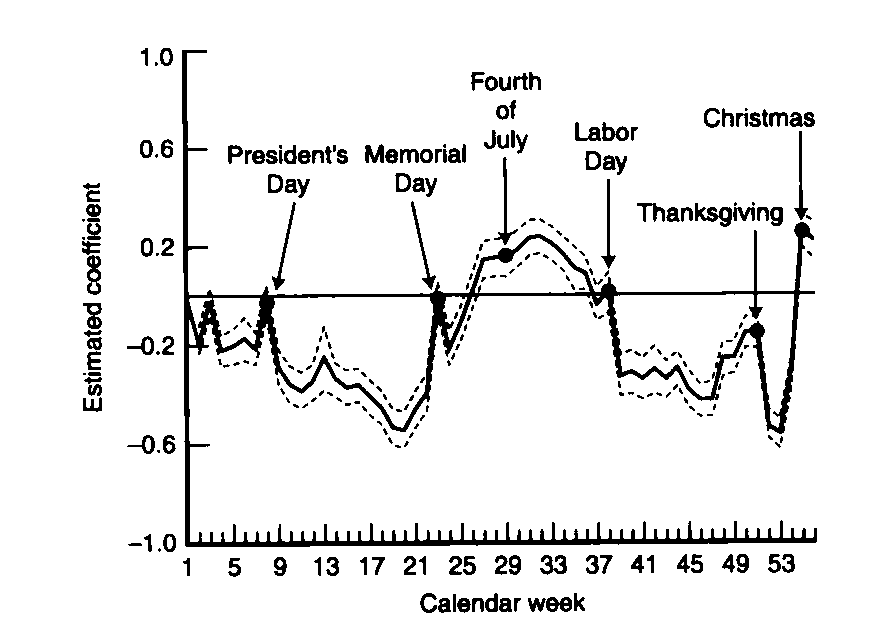
\includegraphics[width=\linewidth]{figures/ch07/einav_fig3_top.png}
\caption{With movie fixed effects}
\end{subfigure}\hfill
\begin{subfigure}[b]{0.49\textwidth}
\centering
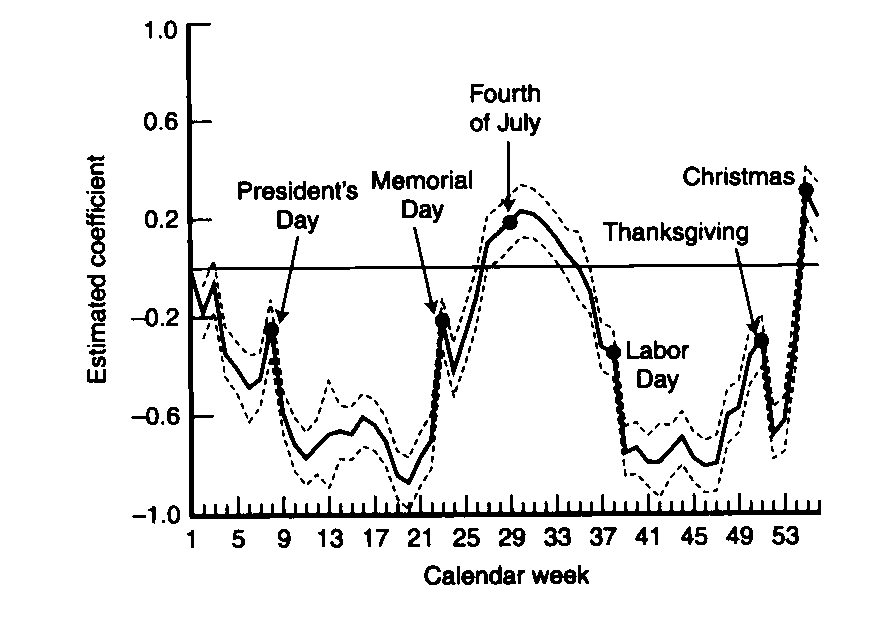
\includegraphics[width=\linewidth]{figures/ch07/einav_fig3_bottom.png}
\caption{Without movie fixed effects}
\end{subfigure}
\caption{Estimated week effects $\hat\tau_t$ by calendar week in the benchmark model of \citet{Einav2007}.
Panel (a) is the top panel and panel (b) the bottom panel of the original figure. Dashed lines mark two standard
errors. Source: \citet{Einav2007}, Figure 3.}
\label{fig:07-einav-seasonality}
\end{figure}

Underlying demand resembles revenue, high in summer and the holidays and low in spring and fall, but the
differences are informative (p.~138). Memorial Day, the Fourth of July and Thanksgiving, the big release weekends,
have high underlying demand, though less so relative to adjacent weeks than revenues suggest. Labor Day, when few
movies open, has much higher underlying demand than its revenue implies. Underlying demand is flat over the summer
and drops sharply after Labor Day, whereas revenues peak in early July and decline gradually, because the biggest
movies open early in the summer.

With $\lambda = 0.220$ and $\hat\sigma = 0.524$, Einav reports weekly revenue decay of 37 percent. For a movie too
small to move $D_t$, $\ln s_{jt}$ equals $\frac{\delta_{jt}}{1-\sigma}$ plus terms in $D_t$, so one more week
changes log share by $-\frac{0.220}{0.476} = -0.462$, and $1 - e^{-0.462} = 0.37$. Ten decay dummies give an almost
linear pattern. A linear time trend is not identified (footnote 19). If mean utility included $b\,t$, writing
$b\,t = b\,r_j + b(t - r_j)$ shows that it loads onto the movie effects, $\phi_j + b\,r_j$, and
onto the decay, $\lambda - b$. The movie effects, which show no trend, measure quality relative to an outside
good that may itself be changing.

\Cref{tab:07-einav-fe} projects the estimated movie effects on observables. Production cost, advertising and
Oscar recognition raise estimated quality, and restrictive ratings lower it. The adjusted $R^2$ is at most 0.387,
which Einav reads as the justification for fixed effects.

\begin{table}[htbp]
\centering
\caption{Projection of the estimated movie fixed effects on observables \citep[Table 3]{Einav2007}}
\label{tab:07-einav-fe}
\small
\begin{tabular}{lccc}
\toprule
Dependent variable: estimated movie effect $\hat\phi_j$ & (1) & (2) & (3) \\
\midrule
Log production cost & 0.215$^{**}$ (0.021) & 0.389$^{**}$ (0.021) & 0.384$^{**}$ (0.020) \\
Log advertising expenditure & 0.367$^{**}$ (0.019) & & \\
MPAA rating PG-13 & $-0.125^{**}$ (0.038) & $-0.135^{**}$ (0.043) & \\
MPAA rating R & $-0.154^{**}$ (0.039) & $-0.144^{**}$ (0.044) & \\
MPAA rating above R & $-0.442$ \phantom{$^{**}$}(0.365) & $-0.716^{*}$ \phantom{$^{*}$}(0.413) & \\
Genre comedy & $-0.052$ \phantom{$^{**}$}(0.035) & 0.029 \phantom{$^{**}$}(0.039) & \\
Genre drama & $-0.097^{**}$ (0.037) & $-0.021$ \phantom{$^{**}$}(0.040) & \\
Genre children & $-0.070$ \phantom{$^{**}$}(0.054) & $-0.037$ \phantom{$^{**}$}(0.060) & \\
Best picture nominee & 0.433$^{**}$ (0.081) & & \\
Best picture award & 0.467$^{**}$ (0.139) & & \\
Year fixed effects & yes & yes & no \\
$N$ & 1,542 & 1,603 & 1,603 \\
Adjusted $R^2$ & 0.387 & 0.208 & 0.193 \\
\bottomrule
\end{tabular}
\par\medskip
\parbox{\linewidth}{\footnotesize Notes: Standard errors in parentheses. $^{*}$ significant at the 10 percent
level, $^{**}$ at the 1 percent level. Omitted categories are rating PG and genre action. Blank cells are
variables not included. Samples are smaller than 1,956 because production cost and advertising are missing for
some movies. Source: \citet{Einav2007}, Table 3.}
\end{table}

\subsection{Robustness}\label{sec:07-einav-robust}

Predicted shares reproduce the observed seasonal pattern well, but the model underpredicts revenue in early summer
and the holidays and overpredicts it elsewhere (Figure 4, p.~139). Movies released in strong seasons decay more
slowly. Interacting decay with movie size, instrumented by production cost times decay, shows that better movies
decay more slowly and improves fit, but underlying seasonality barely moves. Letting decay vary by release season
gives $-0.194$ for holiday releases, $-0.206$, $-0.216$ and $-0.214$ for winter, spring and early summer, and
$-0.249$ and $-0.244$ for late summer and fall (pp.~139--140). Equality of the first four is not rejected, and
equality of the last two with the others is rejected. The summer week effects are unchanged.

Results are almost identical after dropping the first three weeks of each run, for movies with a full 10-week run
and for Friday releases (p.~140). Panel B of \cref{tab:07-einav-benchmark} shows faster decay in later
subperiods, consistent with wider openings, while underlying seasonality is stable. Alternative instruments, the
budget of competing movies, the number in the same genre, or the number released within a three-week or five-week
window, give similar results. The window counts address one source of endogeneity. Fewer movies may be shown in a week
when a strong movie is released. If distributors can move a release date by only a few weeks, counts over a window
around the week account for this response (footnote 20). Instruments
interacted with a measure of the movie's ex-ante size, such as production cost, are weaker. They give low estimates
of $\sigma$ and somewhat different results, but adding them to the main instruments leaves the reported results in
place (footnote 21). The nested logit ties expansion from more movies to expansion from better movies
through one parameter. \citet{AckerbergRysman2005} suggest adding the log number of products as a regressor, which
here is the instrument. Including it through functional form or with other instruments changes little
(pp.~140--141).

\subsection{Implications for release dates}\label{sec:07-einav-timing}

Set $\xi_{jt} = 0$ and write $Q_{kt} = \exp\big(\frac{\phi_k - \lambda(t-r_k)}{1-\sigma}\big)$ for the
decay-adjusted quality index and $C_t = \sum_{k \in \mathcal{J}_t} Q_{kt}$ for the \emph{competition effect}. Since
$D_t = \exp\big(\frac{\tau_t}{1-\sigma}\big)C_t$, dividing numerator and denominator of $s_{jt}$ by
$\exp\big(\frac{\tau_t}{1-\sigma}\big)$ gives
\begin{equation}\label{eq:07-einav-eq6}
s_{jt} = \frac{Q_{jt}}{C_t^{\sigma}}\,\Big[e^{-\tau_t} + C_t^{1-\sigma}\Big]^{-1}
\end{equation}
(Einav's equation (6)). The market-size term $e^{-\tau_t}$ is small when underlying demand is high. Competition
matters more as $\sigma$ rises, because movies then steal more from each other. With fixed prices and nearly zero
marginal cost, a price-taking distributor picks $r_j$ to maximize $\sum_{t=r_j}^{r_j+H}s_{jt}$ for a horizon $H$,
taking rivals' dates as given (pp.~141--142). Competition peaks at the start of the summer and at Christmas. Labor
Day combines high underlying demand with soft competition, and a small movie could double its revenue by opening
then instead of on Thanksgiving (p.~143). Large movies, Einav cautions, internalize their effect on competition.

If the industry could coordinate, with $n_w$ small divisible movies of quality index $e^{\frac{\bar\phi}{1-\sigma}}$
opening in week $w$, then $C_w^{1-\sigma} = n_w^{1-\sigma}e^{\bar\phi}$. Summing \eqref{eq:07-einav-eq6} over movies
gives the industry share $\frac{C_w^{1-\sigma}}{e^{-\tau_w} + C_w^{1-\sigma}}$, and the industry solves
\begin{equation}\label{eq:07-einav-eq7}
\max_{\{n_w\}}\ \sum_{w=1}^{W}\frac{n_w^{1-\sigma}e^{\bar\phi}}{e^{-\tau_w} + n_w^{1-\sigma}e^{\bar\phi}}
\quad\text{subject to}\quad \sum_{w=1}^{W} n_w = N,
\qquad
\frac{e^{-\tau_w}(1-\sigma)n_w^{-\sigma}e^{\bar\phi}}{\big(e^{-\tau_w} + n_w^{1-\sigma}e^{\bar\phi}\big)^2} = \mu
\end{equation}
(equations (7) and (8), with $\varepsilon$ in the paper for $\bar\phi$ and $\mu$ the Lagrange multiplier). The left side
of the first-order condition has a positive cross-partial in $\tau_w$ and $n_w$ at the estimates, so the optimum
puts more movies in high-demand weeks. The observed pattern yields a total industry share of 3.94 (observed:
3.92), and the optimum raises it only to 3.98, about 1 percent (p.~143). Quality is fixed in total, and with
$\sigma$ above 0.5 redistribution mostly moves revenue across movies.

\subsection{Interpretation and limitations}\label{sec:07-einav-assessment}

Einav attributes amplification to uniform ticket prices \citep{OrbachEinav2007}. The market can respond to high
demand only through the number and quality of movies (p.~144). He expects amplification in video rental, music
and books, and dampening where capacity constraints raise peak prices, as in tourism and airlines. The paper also
shows when a logit-type model suffices. There is no price coefficient, and the model is never asked for cross-price
substitution, the case anticipated by the remark in \cref{sec:07-iia}. The limitations follow from the identifying
assumptions. Decay must not depend on the release date, and the season-specific estimates show some dependence.
Underlying seasonality must be stable across years, the market is the population, and the mix of moviegoers is
constant over the year. A single $\sigma$ ties two kinds of expansion, and the release exercise treats
distributors as price takers. \citet{Einav2010} models the timing game as a sequential-move game with private
information. He finds release dates too clustered on holiday weekends, and that shifting some holiday releases by
a week or two would raise revenue.

\section{Case study: Hendel (1999), multiple discrete choice}\label{sec:07-hendel}

Every model so far has a consumer buy one unit of one product. \citet{Hendel1999} drops both restrictions for
business purchases of personal computers. We work mainly from the 1994 working paper \citep{Hendel1994}. Its pages
carry the prefix WP, and all equation and table numbers refer to it. Citations of the published article give its
own pages. The two versions may differ in specification and numbers.

\subsection{Question and motivating facts}\label{sec:07-hendel-question}

Hendel estimates PC demand by business establishments as an input to three questions (WP pp.~2--3). The first
is the ``computerization puzzle,'' the absence of measured productivity gains from computers in aggregate data.
The second is the gain from technical progress in components, and the third is quality adjustment in price
indices. \Cref{tab:07-hendel-freq}
reproduces Table I, the joint frequency of the number of PCs and the number of PC types held by 5,234
establishments that hold at least one PC. Only 1,369 hold a single PC and 2,367 a single type, while twelve hold
more than 2,000 units. Hendel concludes that multiple discreteness is the main feature of the data and that
aggregation misleads, since one firm buying 2,000 units differs from 2,000 firms buying one (WP p.~6).

\begin{table}[htbp]
\centering
\caption{Joint frequency of the number of PCs and the number of PC types held \citep[Table I]{Hendel1994}}
\label{tab:07-hendel-freq}
\small
\setlength{\tabcolsep}{4.5pt}
\begin{tabular}{lrrrrrrrrrr}
\toprule
 & \multicolumn{9}{c}{Number of PC types held} & \\
\cmidrule(lr){2-10}
Number of PCs & 1 & 2 & 3 & 4--6 & 7--9 & 10--19 & 20--49 & 50--99 & 100+ & Total \\
\midrule
1 & 1,369 & & & & & & & & & 1,369 \\
2 & 335 & 308 & & & & & & & & 643 \\
3--4 & 271 & 215 & 196 & & & & & & & 682 \\
5--6 & 123 & 99 & 129 & 29 & & & & & & 380 \\
7--10 & 104 & 111 & 152 & 52 & 7 & & & & & 426 \\
11--15 & 39 & 59 & 102 & 56 & 26 & & & & & 282 \\
16--35 & 68 & 84 & 154 & 99 & 65 & 8 & 2 & & & 480 \\
36--60 & 24 & 31 & 68 & 45 & 61 & 15 & 5 & & & 249 \\
61--100 & 12 & 12 & 51 & 39 & 47 & 16 & 8 & & & 185 \\
101--300 & 16 & 17 & 59 & 74 & 100 & 56 & 21 & 3 & & 346 \\
301--600 & 4 & 3 & 18 & 26 & 29 & 23 & 8 & 0 & 1 & 112 \\
601--1,000 & 2 & 0 & 3 & 8 & 8 & 11 & 6 & 1 & 0 & 39 \\
1,001--2,000 & 0 & 1 & 1 & 7 & 5 & 7 & 4 & 3 & 1 & 29 \\
2,000+ & 0 & 0 & 2 & 3 & 2 & 2 & 0 & 1 & 2 & 12 \\
\midrule
Total & 2,367 & 940 & 935 & 438 & 350 & 138 & 54 & 8 & 4 & 5,234 \\
\bottomrule
\end{tabular}
\par\medskip
\parbox{\linewidth}{\footnotesize Notes: Counts of establishments in the Comtec survey. Rows are bins of the total
number of PCs held and columns bins of the number of distinct PC types. Source: \citet{Hendel1994}, Table I.}
\end{table}

\subsection{The model}\label{sec:07-hendel-model}

We rename Hendel's symbols. The establishment is $i$ (his $f$), its tasks are $k = 1, \dots, K_i$ (his $j$ and
$J_f$), and PC types are $j = 1, \dots, J$ (his $i$). The curvature of task returns is $a$, where he writes $\alpha$,
which would clash with the price coefficient. The brand weight $W_{ijk}$ keeps his name and is unrelated to the weighting
matrix $W$.

Establishment $i$ with demographics $D_i$ has $K_i \sim \text{Poisson}(\lambda_i)$ potential tasks, with
$\lambda_i = g_0 + g_1\,emp_i + g_2\,soft_i$, where $emp_i$ is employment and $soft_i$ the number of software types
(WP equation (23)). Profit is additive across tasks (equation (4)), which rules out complementarities between
tasks. With $X_{ijk}$ units of type $j$ in task $k$ and rental prices $P_j$, the return on task $k$ is
\begin{equation}\label{eq:07-hendel-return}
\pi_{ik} = \Big(\sum_{j} W_{ijk}X_{ijk}\Big)^{a} S(D_i) - \sum_{j}P_jX_{ijk},
\qquad
W_{ijk} = \big(A_{ik}\cdot C_j\big)^{m(D_i)},
\qquad 0 < a < 1
\end{equation}
(equations (5) and (6)). The vector $C_j$ stacks a brand indicator and $j$'s observed attributes (MHz, memory, word
size). The random coefficients $A_{ik}$ hold perceptions of each brand's unobserved quality (reliability, service,
compatibility) and valuations of the attributes. Perceptions are normal with brand-specific means and a common
variance, and the MHz valuation is normal. The \emph{return shifter} is $S(D_i) = \varsigma_0 + (\varsigma_1 +
\varsigma_{1,rd}\,drd_i)emp_i$, where the paper writes $s_0$ and $s_1$ for our $\varsigma_0$ and $\varsigma_1$.
The taste for quality is $m(D_i) = m_0 + m_1 wh_i + m_{1,rd}\,drd_i$, with $wh_i$ the number of white-collar
workers and $drd_i$ an R\&D indicator (equations (24) and (25)). With no adjustment costs and a perfect resale market,
a PC costs its one-year rental price, the purchase price less next year's resale value. Lacking data on used prices,
Hendel computes the resale value from the 25 percent annual fall in quality-adjusted prices found by
\citet{BerndtGriliches1993}. An old machine costs a fraction $d_0$ of the new rental price (WP p.~24).

\casehead{One brand per task}
Brands enter a task through the index $E_{ik} = \sum_j W_{ijk}X_{ijk}$ of effective units, at linear cost. For any
$E_{ik}$,
\begin{equation*}
\sum_j P_jX_{ijk} = \sum_j \frac{P_j}{W_{ijk}}\,W_{ijk}X_{ijk} \ \ge\ \Big(\min_j\frac{P_j}{W_{ijk}}\Big)E_{ik},
\end{equation*}
with equality when only the type with the highest \emph{performance-to-price ratio} $\frac{W_{ijk}}{P_j}$ is used.
With continuous random coefficients ties have probability zero, so each task uses one brand (WP pp.~11 and 19).
Multiple brands per establishment come from multiple tasks.

\casehead{Units within a task}
Ignoring integer constraints, the first-order condition for type $j$ is $aW_{ijk}^{a}X^{a-1}S(D_i) = P_j$ (equation
(10)), so
\begin{equation}\label{eq:07-hendel-xstar}
X^*_{ijk} = \left(\frac{aW_{ijk}^{a}S(D_i)}{P_j}\right)^{\frac{1}{1-a}}
\end{equation}
(equation (11)). Using the first-order condition, cost equals $aW_{ijk}^{a}(X^*)^{a}S(D_i)$, so
\begin{equation*}
\pi^*_{ijk} = (1-a)\,W_{ijk}^{a}S(D_i)(X^*)^{a}
= (1-a)\,W_{ijk}^{a}S(D_i)\left(\frac{aW_{ijk}^{a}S(D_i)}{P_j}\right)^{\frac{a}{1-a}}
= (1-a)\,S(D_i)^{\frac{1}{1-a}}\left(\frac{aW_{ijk}}{P_j}\right)^{\frac{a}{1-a}}
\end{equation*}
(equation (12)), where $S$ has exponent $1 + \frac{a}{1-a} = \frac{1}{1-a}$ and $W$ has exponent $a + \frac{a^2}{1-a}
= \frac{a}{1-a}$. The maximized return rises with $\frac{W_{ijk}}{P_j}$. With integer units the best brand can
change, for example when its optimum is 3.5 units (WP p.~12). Returns are concave in $X$, so the integer optimum
is $\lfloor X^*\rfloor$ or $\lceil X^*\rceil$, and the algorithm compares these $2J$ candidates (WP p.~20). When
$X^* < 1$ the lower candidate is zero, meaning no PC for the task.

\casehead{Horizontal and vertical differentiation}
Brand perceptions that differ across establishments create horizontal differentiation. The exponent $m(D_i)$
creates vertical differentiation. If buyers agree on a quality index $q$ facing a convex price schedule $P(q)$,
equation (12) has them maximize $\frac{q^m}{P(q)}$, whose first-order condition is $m = \frac{P'(q^*)q^*}{P(q^*)}$
(WP Appendix 2). When the price elasticity of quality rises with $q$, as Hendel argues from convexity, buyers with
higher $m$ choose better machines.\footnote{The main text of the working paper writes this condition with $W$ in
place of the index (equation (13)). We follow its Appendix 2.} A multiplicative taste would not work, since scaling
all $W$ leaves the ranking of $\frac{W}{P}$ unchanged. In Bresnahan's single-unit vertical model it works because
buyers purchase one unit (WP endnote 4). By \eqref{eq:07-hendel-xstar}, $S(D_i)$ moves the number of units but,
entering every brand's return through the factor $S^{\frac{1}{1-a}}$, leaves the brand choice unchanged. The taste
$m(D_i)$ moves the brand choice. Hendel argues that these distinct roles identify the two functions (WP p.~13).

\subsection{Estimation}\label{sec:07-hendel-estimation}

Expected purchases average the task-level choices over tasks and random coefficients,
\begin{equation}\label{eq:07-hendel-expected}
X^e_i(D_i, \theta) = \sum_{K=0}^{\infty}\Pr(K_i = K \mid D_i)\sum_{k=1}^{K}\int X^*_{ik}(D_i, A, \theta)\,
\mu(\dd A \mid D_i, \theta)
\end{equation}
(WP equation (15)), where $X^*_{ik}$ is the $J$-vector of task purchases and $\mu$ the normal distribution of the
coefficients. The prediction error $e_i(\theta) = X^e_i(D_i, \theta) - X_i$ has mean zero given $D_i$ at the true
$\theta$, so $G(\theta) = \E[T(D_i)\otimes e_i(\theta)] = 0$ for any function $T$ of demographics (equations (16)
to (18)). Hendel minimizes a quadratic form in the sample analogue over the $F$ establishments, $G_F(\theta) =
\frac{1}{F}\sum_{i=1}^F T(D_i)
\otimes(X^e_i(\theta) - X_i)$ with the efficient weighting matrix \citep{Hansen1982}. Demographics are valid
instruments by construction, since predictions condition on them.

The integral is simulated \citep{McFadden1989,PakesPollard1989}. For each establishment and simulation round,
Hendel draws a number of tasks and the coefficients of each task, and solves each integer problem. The moments are
linear in simulated purchases, so the estimator is consistent as $F$ grows with the number of draws fixed (WP
pp.~18--19). A device keeps draws fixed while $\lambda_i$ changes in the search (WP Appendix 3). Let $E_1, E_2,
\dots$ be i.i.d.\ exponential with mean one and $Y_k = \sum_{l\le k}E_l$, which is gamma with shape $k$. Integrating
by parts $k-1$ times,
\begin{equation*}
\Pr(Y_k < \lambda) = 1 - \sum_{l=0}^{k-1}\frac{e^{-\lambda}\lambda^{l}}{l!} = \Pr(N \ge k),
\qquad N \sim \text{Poisson}(\lambda),
\end{equation*}
so the number of partial sums below $\lambda$ is Poisson with mean $\lambda$. Holding the exponential draws fixed
holds the randomness constant across trial parameters. The simulated objective is then a step function, a case
covered by \citet{PakesPollard1989}. Standard errors from numerical derivatives proved sensitive to the step, so
Hendel averages over three steps and also reports a bootstrap (WP endnote 12).

Hendel argues that the joint distribution of units and types in \cref{tab:07-hendel-freq} identifies the task
process (WP p.~20). We add an observation on the moments he uses, which are brand-level purchase totals interacted
with demographics (45 moments for 15 types). Tasks are i.i.d.\ given $D_i$ and independent of $K_i$, so Wald's
identity gives
\begin{equation*}
\E[X_i \mid D_i] = \lambda_i\,\E\big[X^*_{ik}(D_i, A_{ik}, \theta) \mid D_i\big].
\end{equation*}
These moments see the task process only through $\lambda_i$. It multiplies per-task purchases, which scale with
$S(D_i)^{\frac{1}{1-a}}$ apart from integer effects. Tasks and the return shifter are therefore separated through
the integer constraint and through variables that enter only one function, $soft_i$ in $\lambda_i$. Moments on the
number of types held would use \cref{tab:07-hendel-freq} more directly.

\subsection{Data and results}\label{sec:07-hendel-results}

Prices and attributes of microcomputers from 1976 to 1989 come from \citet{BerndtGriliches1993}, who collected them
from magazine advertisements (WP pp.~21--23). Holdings come from the Comtec survey of about 8,000 representative
non-farm establishments in 1984 and 1988, stratified by size and sector with extrapolation weights. Large
establishments are oversampled. Unweighted means are 241.55 employees and 35.05 PCs, and weighted means 15.49 and
1.96 (Tables II and III). Estimation uses 123 randomly chosen establishments out of 546 in banking (finance,
insurance and real estate), with more than 1,000 purchases. The choice set has 15 types (WP Appendix 4). They are four IBM models (8086, 8088, 286,
386), three Apple models, two each from Zenith and Compaq, three clones and the AT\&T 8086. The IBM 286 leads with a price of \$2,700 and a 37.3 percent share of 1986--1988 sales.

\begin{table}[htbp]
\centering
\caption{Parameter estimates for the banking sector \citep[Table V]{Hendel1994}}
\label{tab:07-hendel-params}
\small
\begin{tabular}{llccc}
\toprule
Parameter & Meaning & Estimate & Numerical s.d. & Bootstrap s.d. \\
\midrule
$\varsigma_0$ & Intercept of $S(D_i)$ & 0.61 & n.a. & 0.19 \\
$\varsigma_1$ & Slope of $S(D_i)$ in employment & 0.47 & 0.18 & 0.06 \\
$m_1$ & Slope of $m(D_i)$ in white-collar workers & $6\times 10^{-4}$ & $1.3\times 10^{-4}$ & $10^{-5}$ \\
$a$ & Task-return exponent & 0.29 & 0.03 & 0.04 \\
$\Var(A_j)$ & Variance of brand perceptions & 3.50 & 0.55 & 0.92 \\
$A_M$ & Mean valuation of MHz & 0.89 & 0.24 & 0.16 \\
$\Var(A_M)$ & Variance of MHz valuation & 1.48 & 0.78 & 0.23 \\
$A_R$ & Valuation of memory (RAM) & 0.53 & 0.11 & 0.06 \\
$A_{B16}$ & 16-bit dummy & 0.78 & 0.87$^{b}$ & n.a. \\
$A_{B32}$ & 32-bit dummy & 1.17 & 2.93$^{b}$ & n.a. \\
$g_1$ & Task mean, slope in employment & 2.42 & 1.34$^{a}$ & 0.32 \\
$g_2$ & Task mean, slope in software types & 0.78 & 0.18 & 0.10 \\
$d_0$ & Relative cost of keeping an old PC & 0.79 & 0.09 & 0.19 \\
\midrule
\multicolumn{5}{l}{Objective function $G_F(\theta) = 405$, with 45 moments and 25 parameters} \\
\bottomrule
\end{tabular}
\par\medskip
\parbox{\linewidth}{\footnotesize Notes: Simulated method of moments, 123 banking establishments. Numerical
standard deviations average numerical derivatives over three step sizes. Bootstrap standard deviations come from
50 bootstrap rounds. $^{a}$ significant at the 10 percent level, $^{b}$ not significant (the paper's markers).
The intercepts $g_0$ and $m_0$ are fixed at 0.1 and 1.0. The paper writes $\alpha_0$ (A$_0$ in the table) for
the exponent we call $a$. Brand-specific mean perceptions are in the paper's Table VII. Source:
\citet{Hendel1994}, Table V.}
\end{table}

\Cref{tab:07-hendel-params} reproduces Table V. The curvature $a = 0.29$ lies in $(0, 1)$, as interior solutions
require. Larger establishments buy more PCs ($\varsigma_1$), and establishments with more white-collar workers prefer
higher quality ($m_1$). The significant variance of brand perceptions, 3.50, means buyers perceive the same machine
differently, a horizontal dimension. MHz has a significant mean and variance, memory a significant coefficient,
and users trade 1.6K of expandable memory for one more MHz. Word size is insignificant. The task process rises
with size and software variety. Keeping an old PC costs $d_0 = 0.79$ of a new one, with a $t$-statistic of 2.29
for $1 - d_0$, and the implied 20 percent gap matches new and used prices (WP pp.~26--28). Mean perceptions
(Table VII) average 54.1 for IBM, 40.9 for Compaq, 28.5 for Apple, 20.1 for clones, 16.5 for Zenith and 2.9 for
AT\&T. The objective, 405, is treated as $\chi^2$ with 20 degrees of freedom. Hendel quotes a 5 percent cutoff of
30 (the exact value is 31.4), so the model is rejected (WP p.~26).

A separate estimation adds the R\&D and education sectors to banking and reports sector effects in Table VI (WP
p.~25). It omits the word-size dummies of Table V, so its estimates are not directly comparable with those of
\cref{tab:07-hendel-params}.
\Cref{tab:07-hendel-sectors} reproduces it. The extra employment slope of $S(D_i)$ for R\&D establishments,
$\varsigma_{1,rd} = 0.69$, is significant, so their purchases are more sensitive to size. Hendel expects this from
complementarity between labor and PCs in R\&D, and it fits their higher ratio of PCs to employees (WP Table IV). The
R\&D shift in the taste for quality, $m_{1,rd} = 0.70$ with a standard deviation of 7.00, is insignificant. There is
no vertical dimension tied to the sector, which fits the observation that R\&D establishments do not hold more
valuable PCs than banks. The education sector's extra employment slope is also insignificant. Its extra taste for
Apple machines, 4.20, is ``borderline significant'' in Hendel's words, with a ratio to its standard deviation of 1.39.
He equates it to about 4 MHz, so a school values an Apple like a non-Apple machine with 4 more MHz (WP pp.~26--28).
The working paper's text calls it Table VI on WP pp.~25--27 and Table VII on WP p.~28.

\begin{table}[htbp]
\centering
\caption{Sector effects when R\&D and education establishments are added \citep[Table VI]{Hendel1994}}
\label{tab:07-hendel-sectors}
\small
\begin{tabular}{llcc}
\toprule
Parameter & Meaning & Estimate & Std.\ dev. \\
\midrule
$\varsigma_{1,rd}$ & Extra employment slope of $S(D_i)$, R\&D sector & 0.69 & 0.11 \\
$\varsigma_{1,ed}$ & Extra employment slope of $S(D_i)$, education sector & 1.00 & 3.33 \\
$m_{1,rd}$ & R\&D dummy in $m(D_i)$, vertical by sector & 0.70 & 7.00 \\
$A_{\text{Apple}}$ & Extra valuation of Apple, education sector & 4.20 & 3.02 \\
\bottomrule
\end{tabular}
\par\medskip
\parbox{\linewidth}{\footnotesize Notes: Simulated method of moments on banking, R\&D and education
establishments, estimated separately from \cref{tab:07-hendel-params} and without the word-size dummies. The paper
writes $s_{1RD}$, $s_{1ED}$ and $M_{1RD}$ for our $\varsigma_{1,rd}$, $\varsigma_{1,ed}$ and $m_{1,rd}$.
Source: \citet{Hendel1994}, Table VI (WP p.~47).}
\end{table}

Elasticities come from numerically differentiating simulated demand (Table VIII). The text implies that the
table's rows index the product whose price changes and its columns the product whose demand responds. Only this
reading matches three statements of the text (WP p.~31), which calls the table Table VII. The IBM 286 and IBM 386 are
each other's closest substitutes, and the Zenith 8088 responds most to the IBM 8088 price. The Apple 68020 responds
strongly to the IBM 286 price, a machine in a similar price and attribute range, with a cross elasticity of 38.29.
Own elasticities are printed as negative numbers, from
$-0.13$ (Apple 68000) and $-0.93$ (IBM 8086) to $-7.9$ (Apple 68020). Two below one in absolute value sit uneasily
with Nash pricing.

\subsection{Welfare and implications}\label{sec:07-hendel-welfare}

Hendel values PCs with Hotelling's lemma. Let $\Pi_i(\boldsymbol P)$ be maximized profit from PCs at rental prices
$\boldsymbol P$, relative to the outside option of no PCs, so $\Pi_i(\infty) = 0$ and $\frac{\partial
\Pi_i}{\partial P_j} = -X_{ij}(\boldsymbol P)$. Integrating from the 1988 prices $\boldsymbol P^0$,
\begin{equation*}
\Pi_i(\boldsymbol P^0) - \Pi_i(\infty) = \int_{\boldsymbol P^0}^{\infty} X_i(\boldsymbol P)\cdot\dd\boldsymbol P,
\end{equation*}
the area under the input demand curve. In practice he evaluates the estimated profit function at predicted
behavior and extrapolates with survey weights (WP p.~29). Banking held 729,922 PCs in 1988 and earned about \$1.2
billion from them, about \$1,300 per PC per year against an average annual rental price of
\$1,443.\footnote{Dividing \$1.2 billion by 729,922 gives about \$1,640 per PC. The working paper does not explain
the difference.} The ratio, about 90 percent, is the reported return on investment, an upper bound because
training costs are omitted. Hendel puts the gain at 3.5 percent of the sector's 1988 profits of \$41.8
billion.\footnote{The ratio of the reported figures, $\frac{1.2}{41.8}$, is about 2.9 percent.} A simulated
standard deviation is about \$0.2 billion (WP endnote 14). Treating each type held as one task gives a lower
bound of \$956.25 million (WP p.~31). Bresnahan's estimate for mainframes in 1972 is a surplus of \$225 to \$417
million on \$68 million of spending, in 1989 dollars \citep{Bresnahan1986}. The profit function is cardinal, anchored in money by
PC prices, and the gain is relative to minicomputers, mainframes or no equipment (WP p.~30).

Assuming static Nash pricing, the IBM 386, an \$8,000 machine, has marginal revenue of \$6,350, an implied markup
of \$1,650 (WP pp.~31--32). Making all microprocessors 10 percent faster at unchanged prices raises end-user
surplus by 4 percent, ignoring supplier responses. A hedonic price elasticity with respect to MHz of 0.458
\citep{BerndtGriliches1993} gives 4.58 percent, so hedonic prices are close to marginal benefits here.

\subsection{Limitations, relation to logit, and contribution}\label{sec:07-hendel-assessment}

The model rules out complementarities across tasks, and one brand per task holds by construction, so two brands
in one job count as two tasks (WP p.~19). Tasks are unobserved, and mapping software types into tasks failed (WP
endnote 8). Durability enters only through a rental price. The intercepts $g_0$ and $m_0$ are fixed, the sample is
123 establishments in one sector, and the overidentification test rejects. Prices vary only across 15 types in one
cross section, and brand means absorb quality. The price response therefore rests largely on the structure of the
task problem, in which $a$ governs both scale and price response.

The working paper has normal random coefficients and no extreme value shock, so it is not a logit. The published
article has no extreme value shock either. Its random coefficients on all brand dummies and on MHz are normal, and
the number of potential tasks is Poisson \citep[p.~437]{Hendel1999}. A logit reading is still instructive. By WP equation (12), $\ln\pi^*_{ijk} = c_{ik} + \frac{a}{1-a}[m(D_i)\ln(A_{ik}\cdot C_j) - \ln
P_j]$, where $c_{ik}$ does not depend on the brand. Suppose the brand-specific part of $m(D_i)\ln(A_{ik}\cdot C_j)$ had an
additive i.i.d.\ type-I extreme value component. Ignoring integer constraints, each task's brand choice would then be
a logit in $\ln W - \ln P$ with coefficient $\frac{a}{1-a}$. With the random MHz coefficient it would
be a mixed logit, and establishment demand a Poisson mixture of such choices. This interpretation is ours. Hendel
notes that his framework allows any distributional assumption, not just extreme value
\citep[pp.~424--425]{Hendel1999}.

Hendel made multiple discreteness an estimable demand structure with microfoundations. Discrete-continuous models
allow one discrete choice and a continuous quantity \citep{DubinMcFadden1984,Hanemann1984}, and
\citet{ManskiSherman1980} allow up to two cars per household. Tasks allow any number of units of any brands while
each task stays a simple discrete choice. \citet{Dube2004} applies the idea to soft drinks, and
\citet{Gentzkow2007} allows goods to be complements in a multiple-choice model of newspapers (\cref{ch:newgoods}).

\section{The limits of logit and the road to random coefficients}\label{sec:07-limits}

The logit and nested logit are cheap, transparent and linear after inversion, and \citet{Einav2007} shows that they
serve when elasticities are not the object. When elasticities, markups or substitution are the object, their
restrictions bind. \citet{BerryLevinsohnPakes1995} estimate both a logit and a random-coefficients model on the
same automobile data, which makes the comparison clean.

\subsection{Own-price elasticities rise with price}\label{sec:07-limits-own}

The logit own elasticity is $\varepsilon_j = \alpha p_j(1 - s_j) \approx \alpha p_j$, since each car's share of
all households is very small. BLP's IV logit gives $\hat\alpha = 0.216$ (0.123), with prices in thousands of 1983
dollars (\cref{tab:07-blp-logit}). For 13 models of 1990, BLP's Table V reports the random-coefficients
elasticities, which \cref{tab:08-blp-attr} reproduces and \cref{fig:08-blp-ownelas} plots against the logit benchmark.
The IV logit implies elasticities from about 1.1 for the Mazda 323 (\$5,049) to about 8.1 for the BMW 735i
(\$37,490). The random-coefficients model reverses the ranking. Its elasticities lie between 6.0 and 6.6 for the four
cheapest models and fall to 3.5 for the BMW and 3.1 for the Lexus LS400. The most elastic demands are in the crowded
compact and subcompact segments, with the Buick Century (6.8) as an exception (p.~879).

The logit pattern follows from a common price coefficient. Buyers of expensive cars are assumed to be as sensitive
to a dollar as buyers of cheap ones, so the elasticity, price coefficient times price, is largest for expensive
cars. A referee suggested to BLP that $\ln p$ in place of $p$ would give more reasonable markups. It did, but
substitution patterns remained ``quite unreasonable'' (p.~874, footnote 26).

\subsection{Substitution goes to the outside good}\label{sec:07-limits-outside}

The diversion ratio to the outside good, $D_{j0} = -\frac{\partial s_0}{\partial p_j}\big(\frac{\partial
s_j}{\partial p_j}\big)^{-1}$, is the share of those leaving $j$ after a small price rise who buy nothing. In the
logit, $\frac{\partial s_0}{\partial p_j} = \alpha s_js_0$ and $\frac{\partial s_j}{\partial p_j} = -\alpha
s_j(1-s_j)$, so $D_{j0} = \frac{s_0}{1-s_j}$. Most households buy no new car in a year, so $s_0$ is near 0.9.
BLP's Table VII, reproduced in \cref{tab:08-blp-outside}, reports this diversion ratio for the same 13 models. The
logit column lies between 90.46 and 90.88 percent, and BLP state that it is $\frac{s_0}{1-s_j}$. The
random-coefficients column generally falls with price, from 27.1 percent for the Mazda 323 and 28.0 for the Ford Escort to 10.1
for the Lexus LS400 and the BMW 735i. Buyers of these luxury cars who react to a price rise mostly
switch to other luxury cars. BLP still find these numbers ``a bit large'' (p.~881).

A logit therefore overstates how much industry demand falls when prices rise, and it understates competition
between close substitutes, because diversion is proportional to shares whatever the similarity of products. BLP's
random-coefficients semi-elasticities make the Lexus the closest substitute to the BMW 735i, the Cadillac to the
Lincoln, and the Accord to the Taurus (p.~881). In a logit every car's closest substitute is the best seller. For
merger analysis, which turns on diversion between the merging products (\cref{ch:mergers}), this is the wrong
pattern.

\subsection{Markups are nearly equal}\label{sec:07-limits-markups}

With logit demand a firm sets the same dollar markup $\frac{1}{\alpha(1 - S_f)}$ on all its products
(\cref{prop:07-logit-multi}), never below $\frac{1}{\alpha}$. \Cref{sec:07-conduct} showed what this implies for
BLP's IV logit. Markups lie between \$4,630 (BMW) and \$4,805 (Chevy Cavalier), highest for GM, which makes the most
models, and ``quite counter-intuitively'' lowest for BMW (p.~874). The floor $\frac{1}{0.216} = 4.63$ thousand
dollars is BMW's markup. Percentage markups then fall steeply with price. By our computation the implied Lerner
indices are $\frac{4.805}{5.797} = 0.83$ for the Cavalier and $\frac{4.63}{37.49} = 0.12$ for the BMW, and 83 percent
is implausible for an economy car. The same rigidity affects conduct counterfactuals. With logit demand, joint
ownership of 25 cereal brands raises Nevo's median margin only to 41.9 percent, against 72.6 percent in his full
model (\cref{tab:07-nevo-margins,tab:08-nevo-margins}, \citealp{Nevo2001}). The logit spreads substitution evenly across brands and the
outside good.

\subsection{Too many characteristics}\label{sec:07-limits-epsilon}

Each new product brings its own $\epsilon_{ij}$ and a set of consumers who like it most, even if it is identical
or inferior to an existing product. The red and blue buses of \cref{sec:07-iia} are the standard example. Three biases follow. A
clone of product $j$ raises consumer surplus by $\frac{1}{\alpha}\ln(1 + s_j)$, and with $J$ identical products
expected maximum utility grows like $\ln J$ without bound (\cref{sec:07-welfare-apps}, \cref{fig:07-clones}).
Logit valuations of new goods are therefore biased upward (\cref{ch:newgoods}). Markups never vanish: with $J$ symmetric
single-product firms, each share $s = \frac{e^{\delta - \alpha p}}{1 + Je^{\delta - \alpha p}}$ goes to zero as $J
\to \infty$, so the markup $\frac{1}{\alpha(1-s)}$ converges to $\frac{1}{\alpha} > 0$ however crowded the market.
In the mirror image, every product has a positive predicted share, so products with zero sales cannot be used
(\cref{sec:07-market-size}, \citealp{GandhiLuShi2023}).

There are four responses. \citet{AckerbergRysman2005} make the role of the logit shock depend on the number of
products, which \citet{Einav2007} describes as adding the log number of products as a regressor. Nesting tempers
the problem within nests, since a clone in the same nest adds little as $\sigma \to 1$. The pure characteristics
model of \citet{BerryPakes2007} drops the shock, at the cost of shares that are not smooth in $\boldsymbol\delta$
and an inversion that is no longer a contraction. The hedonic approach of \citet{BajariBenkard2005} recovers each
consumer's tastes from the gradient of a hedonic price function and needs a dense product space.
\Cref{ch:discrete,ch:blp} develop these models.

\subsection{Heterogeneity is the cure}\label{sec:07-limits-cure}

By \cref{rem:07-berry-iid}, these restrictions come from the i.i.d. additive structure, so changing the distribution
of the shock does not remove them. Heterogeneity in tastes that is correlated across similar products does. With
$u_{ij} = x_j\beta_i - \alpha_ip_j + \xi_j + \epsilon_{ij}$, tastes distributed across consumers, and $s_{ij}$ the
logit probability of consumer $i$, shares are $s_j = \int s_{ij}\,\dd F(i)$ and
\begin{equation*}
\frac{\partial s_j}{\partial p_k} = \int \alpha_i s_{ij}s_{ik}\,\dd F(i) \quad (k \ne j),
\qquad
\frac{\partial s_j}{\partial p_j} = -\int \alpha_i s_{ij}(1 - s_{ij})\,\dd F(i).
\end{equation*}
Cross effects are large when the same consumers are likely to buy both products, that is, when the products are
similar in the dimensions over which tastes vary. The own elasticity can fall with price if buyers of expensive
products have low $\alpha_i$. Diversion to the outside good, $\int\alpha_i s_{ij}s_{i0}\,\dd F(i)$ divided by
$\int\alpha_i s_{ij}(1-s_{ij})\,\dd F(i)$, is small for products whose buyers rarely choose the outside good. The
nested logit is the special case with random coefficients on nest dummies (\cref{sec:07-berry-examples}).
\Cref{tab:07-model-comparison} summarizes, and \cref{ch:blp} develops the general model.

\begin{table}[htbp]
\centering
\caption{What logit, nested logit, and random-coefficients logit deliver}
\label{tab:07-model-comparison}
\small
\renewcommand{\arraystretch}{1.25}
\begin{tabularx}{\linewidth}{>{\raggedright\arraybackslash}p{0.2\linewidth}
  >{\raggedright\arraybackslash}X >{\raggedright\arraybackslash}X >{\raggedright\arraybackslash}X}
\toprule
 & Logit & Nested logit & Random-coefficients logit \\
\midrule
Shares & Closed form & Closed form & Integral, simulated \\
Inversion & $\ln s_j - \ln s_0$ & $\ln s_j - \sigma\ln s_{j\mid g} - \ln s_0$ & Numerical contraction \\
Estimation & Linear IV & Linear IV, two endogenous regressors & Nonlinear GMM with nested inversion \\
Substitution & Proportional to shares (IIA) & Proportional to shares within and across nests, more within the
  nest. IIA holds only within a nest &
  Toward products with similar characteristics \\
Own elasticity & $\alpha p_j(1-s_j)$, rises with price & Rises with price & Can fall with price \\
Diversion to outside good & $\frac{s_0}{1-s_j}$ & $\frac{(1-\sigma)s_0}{1 - \sigma s_{j\mid g} - (1-\sigma)s_j}$ &
  Depends on who buys $j$ \\
Multi-product markups & Equal within firm & Equal within firm and nest & Vary by product \\
Main inputs & Shares, prices, instruments & Plus nest assignment and instruments for $s_{j\mid g}$ &
  Plus instruments for the taste dispersion, ideally demographics or micro data \\
\bottomrule
\end{tabularx}
\par\medskip
\parbox{\linewidth}{\footnotesize Notes: Single-market formulas with the outside good normalized to zero mean
utility. Nested-logit entries are derived in \cref{sec:07-nested}, and random-coefficients entries in
\cref{ch:blp}.}
\end{table}

The logit and the one-nest nested logit remain useful first looks and robustness checks, and they are adequate
when the question does not turn on substitution patterns. Einav's seasonality decomposition is such a question.
Merger simulation, markup measurement and the valuation of new goods are not, and for those the
random-coefficients model of \cref{ch:blp} is the starting point.


\section{Bibliographic notes}\label{sec:07-bibnotes}

The logit has two origins. \citet{Luce1959} derived it from the axiom of independence of irrelevant alternatives,
and \citet{Debreu1960} objected with the example that became the red bus and the blue bus. \citet{McFadden1974}
derived the conditional logit from random utility maximization with type-I extreme value shocks and proved that
its likelihood is globally concave. \citet{McFadden1978} introduced the generalized extreme value family. His survey
\citep{McFadden1984} remains the most complete treatment of random utility models, specification tests and the
nested logit, and \citet{HausmanMcFadden1984} developed the test of independence of irrelevant alternatives.
\citet{Train2009} is the standard textbook on discrete choice and simulation. \citet{AndersonDePalmaThisse1992}
develop the representative-consumer and address interpretations of the logit and their implications for oligopoly
pricing.

The nested logit as a utility model rests on the distribution of \citet{Cardell1997}. \citet{Verboven1996}
applied a two-level version to oligopoly pricing in the European car market, and \citet{BorschSupan1990} studied
the admissible range of the nesting parameters. Other members of the generalized extreme value family include the
ordered model of \citet{Small1987} and the principles of differentiation model of
\citet{BresnahanSternTrajtenberg1997}. The generalized nested logit of \citet{WenKoppelman2001} is a third.
\citet{GrigolonVerboven2014} compare nesting with random coefficients.
The log-sum measure of consumer surplus is due to \citet{Williams1977}, \citet{SmallRosen1981} and
\citet{McFadden1981}.

\citet{Berry1994} made discrete choice demand estimable from market data with endogenous prices. His inversion,
and its extension to random coefficients by \citet{BerryLevinsohnPakes1995}, are the foundation of modern demand
estimation. \citet{Nevo2000a} gives a practical guide to both models, and \citet{ConlonGortmaker2020} discuss best
practices and software. \citet{BerryGandhiHaile2013} prove invertibility under connected substitutes, and
\citet{BerryHaile2014} study nonparametric identification with market-level data. On instruments,
\citet{Chamberlain1987} characterizes efficient instruments under conditional moment restrictions, and
\citet{ReynaertVerboven2014} approximate them in random coefficients demand models. \citet{Armstrong2016} shows
when characteristic-based instruments lose their power as the number of products grows, and \citet{GandhiHoude2019}
propose differentiation instruments.
\citet{HausmanLeonardZona1994} introduced prices in other markets as instruments, and \citet{Nevo2001} defended them
for cereal. On the supply side, \citet{CaplinNalebuff1991} establish uniqueness of equilibrium with single-product
firms. \citet{KonovalovSandor2010} and \citet{NockeSchutz2018} extend it to multi-product firms with logit demand.
\citet{WerdenFroeb1994} pioneered merger simulation with logit demand, alongside \citet{HausmanLeonardZona1994} and
\citet{Nevo2000b}. \citet{AskerNocke2021} survey merger simulation, upward pricing pressure and their ex-post
evaluations. \citet{BulowPfleiderer1983} and \citet{WeylFabinger2013} study pass-through, and \citet{Corts1999}
shows how conduct parameters can mismeasure market power.

The case studies show the range of the toolkit. \citet{Einav2007} uses a nested logit without prices to separate
seasonal demand from the seasonality of movie releases, and \citet{Einav2010} estimates the release-date timing
game behind it. \citet{Hendel1999} extends discrete choice to buyers of many units of several brands, a line
continued by \citet{Dube2004} and \citet{Gentzkow2007}. The limits of the logit collected in \cref{sec:07-limits}
motivate the random coefficients model of \cref{ch:blp}. They also motivate the pure characteristics model of
\citet{BerryPakes2007}, the hedonic approach of \citet{BajariBenkard2005} and the crowding correction of
\citet{AckerbergRysman2005}.

\section{Exercises}\label{sec:07-exercises}

\begin{enumerate}[label=\arabic*., leftmargin=*, itemsep=6pt]

\item \emph{Logit algebra and the category elasticity.}
\begin{enumerate}[label=(\alph*)]
  \item Derive \cref{prop:07-logit-derivs} from \eqref{eq:07-logit-share}. Show that every off-diagonal entry in
  column $k$ of the elasticity matrix, including the entry of the outside good, equals $\alpha p_k s_k$.
  \item Raise every inside price by the same amount $\Delta$. Show that the total inside share changes at the
  rate $-\alpha s_0(1 - s_0)$ per unit of $\Delta$, and derive \eqref{eq:07-category-semi}.
  \item In the market of \cref{ex:07-logit-numbers}, compute the percentage fall in total inside sales after a
  5 percent increase in every inside price, first with the linear approximation \eqref{eq:07-category-elast} and
  then exactly. Compare the answer with the own-price elasticities in \cref{tab:07-logit-elast}, and explain what
  it implies for a hypothetical monopolist test.
\end{enumerate}

\item \emph{Market size.} Consider two markets with one inside product each. In market 1 the price is low and the
true outside share is $s_{01} = 0.2$. In market 2 the price is high and $s_{02} = 0.6$.
\begin{enumerate}[label=(\alph*)]
  \item The researcher doubles the market size in both markets ($\kappa = 2$). Use \eqref{eq:07-market-size-shift}
  to compute the change in the dependent variable of \eqref{eq:07-logit-inversion} in each market.
  \item Without market fixed effects, sign the effect of this error on the estimated price coefficient in a
  regression across the two markets. Relate your answer to \cref{ex:07-market-size}.
  \item Explain why a regression with market fixed effects cannot estimate $\alpha$ from these two observations.
  \item Now let each market contain several inside products whose prices differ within the market, and let valid
  instruments for price also vary within markets. Explain why market fixed effects then remove the bias in
  $\hat\alpha$ caused by the wrong market size but leave the diversion ratios to the outside good misstated.
\end{enumerate}

\item \emph{The nested logit.}
\begin{enumerate}[label=(\alph*)]
  \item Without using the general formula in the proof of \cref{lem:07-nl-gev}, verify the sign conditions (G3)
  of \cref{def:07-gev} up to third order for the generating function \eqref{eq:07-nl-H}.
  \item Derive $\Corr(u_{ij}, u_{ik}) = \sigma(2 - \sigma)$ for two products in the same nest.
  \item Redo the red bus and blue bus example of \cref{sec:07-nl-substitution} when the car has mean utility $v_c$
  and each bus has mean utility $v_b$. Show that, as $\sigma \to 1$, the shares converge to those of a logit
  between the car and a single bus.
  \item Use Panels A and B of \cref{tab:07-mcfadden-housing}. Compute the Wald statistic for the restriction that
  the inclusive value coefficient equals one, and the likelihood ratio statistic from the two log-likelihoods.
  Compare them with McFadden's values, and explain which hypothesis the $t$-statistic of 1.64 tests. Then use
  \eqref{eq:07-nl-sequential} to state which coefficients the first step of the sequential estimator identifies in
  this example.
\end{enumerate}

\item \emph{Multi-product pricing with nested logit demand.}
\begin{enumerate}[label=(\alph*)]
  \item Derive \cref{prop:07-nl-multi}.
  \item Specialize the formula to a firm that owns one product in each of two nests. Write $\Phi_f$ and the two
  markups in terms of the product shares and within-nest shares.
  \item Hold all shares fixed and suppose each of the two products has at least one nest-mate. Show that the
  percentage increase in the markup of either product, relative to separate ownership, falls as $\sigma$ rises.
  Compare with \cref{tab:07-nl-markup-example}, and explain what this implies for merger simulation.
\end{enumerate}

\item \emph{The two-level nested logit.} Derive the estimating equation \eqref{eq:07-nl2-regression} from the
shares \eqref{eq:07-nl2-shares}, showing every step. Show that it collapses to \eqref{eq:07-nl-regression} when
$\sigma_1 = \sigma_2$. State which regressors are endogenous, how many excluded instruments are needed, and propose
instruments for each.

\item \emph{Equilibrium pass-through.} Consider $N$ symmetric single-product firms with logit demand, a common
marginal cost $c$ and common non-price utility.
\begin{enumerate}[label=(\alph*)]
  \item Show that a common change in all prices changes each share by $\dd s = -\alpha s s_0\,\dd p$.
  \item Differentiate the symmetric first-order condition $\alpha(p - c)(1 - s) = 1$ to show that the
  equilibrium pass-through of a cost shock common to all firms is
  \begin{equation*}
    \frac{\dd p}{\dd c} = \frac{(1 - s)^2}{(1 - s)^2 + s s_0} .
  \end{equation*}
  \item Show that this exceeds the pass-through $1 - s$ of \cref{prop:07-logit-passthrough} whenever $N \ge 2$,
  that it equals $1 - s$ when $N = 1$, and that it tends to one as $N \to \infty$. Explain the role of strategic
  complementarity.
\end{enumerate}

\item \emph{Einav's model of movie demand.}
\begin{enumerate}[label=(\alph*)]
  \item Derive the share formula and the estimating equation \eqref{eq:07-einav-est} of \cref{sec:07-einav-model}
  from \cref{prop:07-nl-shares,prop:07-nl-inversion}.
  \item Derive the decomposition \eqref{eq:07-einav-eq6}. Explain why competition matters more for a movie's
  share when $\sigma$ is large.
  \item Show that, for a movie too small to affect the inclusive sum, one more week since release lowers log
  share by $\frac{\lambda}{1 - \sigma}$. Explain why a linear time trend in mean utility is not identified
  separately from the movie effects and the decay.
\end{enumerate}

\item \emph{Computation.} Simulate $T$ markets with $J$ single-product firms each, logit demand with one observed
characteristic, a cost shifter and an unobserved characteristic that raises both utility and cost. Solve for
equilibrium prices with \eqref{eq:07-br-lambert}.
\begin{enumerate}[label=(\alph*)]
  \item Estimate \eqref{eq:07-logit-inversion} by OLS and by two-stage least squares, first with the cost shifter
  and then with the sum of rivals' characteristics as the excluded instrument. Report first-stage $F$
  statistics.
  \item Hold the total number of products $TJ$ fixed and repeat for $J = 2, 5, 10$ and 25. Explain why the
  characteristic-based instrument weakens as $J$ grows, and compare your results with \cref{tab:07-mc-weak}.
  \item Recover marginal costs from \eqref{eq:07-logit-supply} at the estimated $\hat\alpha$. Compare a
  bootstrap over markets with the naive standard errors of the cost regression.
\end{enumerate}

\end{enumerate}

\chapter{Random Coefficients Logit: The BLP Model}\label{ch:blp}

Suppose two car makers propose to merge. To predict the effect on prices we need to know how buyers of each
model would respond to a price increase, and where they would go. With a hundred models on the market, a demand
system in product space has ten thousand own- and cross-price elasticities (\cref{ch:aids}). The logit model of
\cref{ch:logit} needs only a handful of parameters, but it pays for its economy with substitution patterns that
depend on market shares alone. It predicts that buyers who leave a luxury sedan spread over all other models in
proportion to their sales, and that most of them stop buying cars altogether. Neither prediction is plausible,
and a merger analysis built on them would be wrong.

This chapter studies the model that resolves the tension, the \emph{random coefficients logit} of
\citet{BerryLevinsohnPakes1995}, often called BLP. Consumers differ in how much they value each characteristic
and how much they dislike paying. Each consumer makes a logit choice, and market shares average these choices
over the distribution of tastes. Consumers who like large cars rank all large cars highly, so a price increase
on one large car sends its buyers mostly to other large cars. Substitution follows the characteristics of the
products. The number of parameters grows with the number of characteristics, however many products the market
offers.

BLP solve three problems at once. The first is to obtain plausible substitution patterns among many products
from few parameters. The second is the endogeneity of prices when only market-level data on shares, prices and
characteristics are available. Firms see product quality that the econometrician does not, and they price
accordingly. The third is computation. The market shares of the model are integrals with no closed form, and the
unobserved quality enters them nonlinearly. BLP compute the integrals by simulation and recover unobserved
quality by inverting the share equations numerically. A generalized method of moments estimator then treats the
recovered quality as the error term of an instrumental variables problem.

The chapter builds directly on \cref{ch:logit}. There we derived the logit shares
$s_j = \frac{e^{\delta_j}}{1 + \sum_k e^{\delta_k}}$ and the inversion $\delta_j = \ln s_j - \ln s_0$ of
\citet{Berry1994}, which turns demand estimation into a linear instrumental variables regression. We also saw the
costs of the logit. Its own-price elasticity $\alpha p_j(1 - s_j)$ rises almost in proportion to price, and its
single-product markup $\frac{1}{\alpha(1 - s_j)}$ is nearly the same for every product. Its cross elasticities
satisfy the independence of irrelevant alternatives (IIA). The nested logit relaxes this property only within groups
of products that the researcher must specify in advance. Random coefficients instead generate correlation in the
composite error through the characteristics of the products, and the data determine how strong it is.

Mixtures of logits, known as \emph{mixed logit} or \emph{heterogeneous logit} models, were used in
transportation research well before BLP \citep{BoydMellman1980,CardellDunbar1980}. The innovation of
\citet{BerryLevinsohnPakes1995} is a computable estimator for aggregate data with endogenous prices, joined to a
model of oligopoly pricing. Their framework is now the standard tool for demand estimation in industrial
organization, with applications to mergers, trade policy, new goods and many other questions.

The chapter has a theoretical half and an empirical half. \Cref{sec:08-model,sec:08-substitution,sec:08-simulation}
specify the model, derive its substitution patterns and explain how to compute market shares by simulation.
\Cref{sec:08-inversion,sec:08-gmm,sec:08-instruments} develop the estimator. They prove that the share equations
can be inverted by a contraction, and they derive the nested fixed point GMM estimator and its asymptotic variance.
They then ask what instruments identify the model, including the nonparametric results of \citet{BerryHaile2014}.
\Cref{sec:08-supply,sec:08-micro,sec:08-practice} add the supply side, micro data and the practical and
conceptual limits of the model. \Cref{sec:08-worked} estimates the model step by step on a simulated market whose
true parameters we know. The empirical half consists of five case studies. \Cref{sec:08-blp95} studies the
automobile market of \citet{BerryLevinsohnPakes1995}, and \cref{sec:08-nevo00} the practitioner's guide of
\citet{Nevo2000a}. \Cref{sec:08-nevo01} turns to the cereal study of \citet{Nevo2001}. \Cref{sec:08-blp04,%
sec:08-goldberg} cover two studies that use consumer-level data, \citet{BerryLevinsohnPakes2004} and
\citet{Goldberg1995}.

We draw on several earlier chapters. Multiproduct Bertrand pricing, the ownership matrix and the distinction
between product space and characteristic space come from \cref{ch:diffprod}. Random utility, the outside good,
the vertical model and the pure characteristics model come from \cref{ch:discrete}. The generalized method of
moments, instrumental variables and simulation estimators are reviewed in
\cref{sec:A-gmm,sec:A-iv,sec:A-simulation}, and the contraction mapping and implicit function theorems in
\cref{sec:B-fixedpoint,sec:B-ift}. In turn, \cref{ch:airlines} uses a two-type
version of the model, \cref{ch:newgoods} uses it to value new products, and \cref{ch:mergers} uses it to simulate
mergers. \Cref{app:problems} poses the simulated market of \cref{sec:08-worked} as a worked problem.

Two conventions hold throughout the chapter. The symbol $\theta$ denotes a vector of demand and cost parameters,
split into linear parameters $\theta_1$ and nonlinear parameters $\theta_2$. It is unrelated to the conduct
parameter of \cref{ch:conduct}. The elasticity $\varepsilon_{jk} = \frac{\partial s_j}{\partial p_k}\frac{p_k}{s_j}$
is signed, so its diagonal element $\varepsilon_{jj}$ is negative. In the theory sections the own-price elasticity
$\varepsilon_j = -\varepsilon_{jj}$ is a positive number. Tables reproduced from papers keep the papers' signs, and
their notes say so.

\section{The random coefficients logit model}\label{sec:08-model}

The random coefficients logit model describes a population of consumers who differ in how much they value
each product characteristic and how much they dislike paying. Each consumer makes a logit choice given her
tastes. Market shares average these individual choice probabilities over the distribution of tastes in the
population. This section builds the model in steps. We start from the general random utility formulation of
\citet{BerryLevinsohnPakes1995} and specialize it to the linear form used in most applications
\citep{Nevo2000a,Nevo2001}. We then discuss income effects, normalizations and the maintained assumptions. The
section ends with the market share function, special cases, the role of the unobserved product characteristic,
and the data the model requires.

\subsection{Primitives}\label{sec:08-primitives}

We observe markets $t = 1, \dots, T$. A \emph{market} is a population of consumers who face the same set of
products at the same prices. Its definition depends on the data. \citet{BerryLevinsohnPakes1995} treat the
national new car market in each year from 1971 to 1990 as a market, so $T = 20$. \citet{Nevo2001} observes
ready-to-eat cereal sales in a panel of cities and defines a market as a city-quarter, which gives 1,124
markets \citep[p.~517]{Nevo2000a}. Other studies split one geographic market into income groups
\citep[p.~517]{Nevo2000a}.

Market $t$ offers the inside products $j \in \mathcal{J}_t = \{1, \dots, J_t\}$ and an outside good $j = 0$,
which stands for not buying any of the inside products. The market has $M_t$ potential consumers, its
\emph{market size}. If $q_{jt}$ units of product $j$ are sold, its market share is
$s_{jt} = \frac{q_{jt}}{M_t}$, and the outside share is $s_{0t} = 1 - \sum_{j \in \mathcal{J}_t} s_{jt}$.
Product $j$ has a row vector of $K$ observed characteristics $x_{jt}$, a price $p_{jt}$, and an
\emph{unobserved product characteristic} $\xi_{jt}$. Consumers and firms observe $\xi_{jt}$. The
econometrician does not.

Consumer $i$ is described by a vector of characteristics $\zeta_i$, which may include income, demographics,
and tastes that no data set records. In the general formulation of \citet[p.~845]{BerryLevinsohnPakes1995},
the utility of consumer $i$ from product $j$ is a scalar function
\begin{equation}\label{eq:08-general-utility}
  U(\zeta_i, p_{jt}, x_{jt}, \xi_{jt}; \theta),
\end{equation}
where $\theta$ is a vector of parameters. It includes the parameters of the utility surface and those of the
distribution of $\zeta_i$. Throughout this chapter $\theta$ denotes this vector of demand (and later cost)
parameters.

Consumer $i$ buys product $j$ if and only if $j$ gives her the highest utility. The set of consumer types who
choose $j$ is
\begin{equation}\label{eq:08-choice-set}
  A_{jt}(\theta) = \bigl\{\zeta : U(\zeta, p_{jt}, x_{jt}, \xi_{jt}; \theta) \ge
    U(\zeta, p_{rt}, x_{rt}, \xi_{rt}; \theta) \text{ for } r = 0, 1, \dots, J_t\bigr\}.
\end{equation}
Suppose ties occur with probability zero and let $P_0$ be the distribution of $\zeta$ in the population. The
market share of product $j$ is the mass of consumers in $A_{jt}$,
\begin{equation}\label{eq:08-share-general}
  s_{jt}(p_t, x_t, \xi_t; \theta) = \int_{\zeta \in A_{jt}(\theta)} P_0(\dd\zeta),
\end{equation}
which is equation (2.2) of \citet[p.~845]{BerryLevinsohnPakes1995}. Here $p_t$, $x_t$ and $\xi_t$ collect the
prices and characteristics of all products in market $t$. Demand for product $j$ is $q_{jt} = M_t
s_{jt}(p_t, x_t, \xi_t; \theta)$. Every product's demand depends on the prices and characteristics of all
products, because they shape the sets $A_{jt}$.

\citet[p.~521]{Nevo2000a} splits $\zeta_i$ into three parts: observed demographics $D_i$, unobserved
consumer characteristics $\nu_i$, and product-specific shocks $(\epsilon_{i0t}, \dots, \epsilon_{iJt})$. The
labels ``observed'' and ``unobserved'' refer to auxiliary data. We know something about the distribution of
$D_i$ (for example from a population survey), and nothing about the distribution of $\nu_i$ beyond a
parametric assumption. With this split, \eqref{eq:08-share-general} factors as
\begin{align}
  s_{jt} &= \int_{A_{jt}} \dd P^*(D, \nu, \epsilon) \notag\\
         &= \int_{A_{jt}} \dd P^*(\epsilon \mid D, \nu)\, \dd P^*(\nu \mid D)\, \dd P^*(D) \notag\\
         &= \int_{A_{jt}} \dd P^*_\epsilon(\epsilon)\, \dd P^*_\nu(\nu)\, \dd \hat P_D(D),
  \label{eq:08-share-bayes}
\end{align}
where $P^*$ denotes population distributions and $\hat P_D$ the distribution of demographics taken from
auxiliary data \citep[eq.~(4)]{Nevo2000a}. The second line is the factorization of a joint distribution into
conditional distributions. The third line uses the independence of $\epsilon$, $\nu$ and $D$, which we assume
below.

\subsection{The linear random coefficients specification}\label{sec:08-linear}

Most applications use a utility that is linear in characteristics and price. Let $u_{ijt}$ be the
\emph{conditional indirect utility} of consumer $i$ from product $j$ in market $t$, her indirect utility
conditional on choosing $j$. \citet[eq.~(1)]{Nevo2000a} specifies
\begin{equation}\label{eq:08-nevo-utility}
  u_{ijt} = \alpha_i (y_i - p_{jt}) + x_{jt}\beta_i + \xi_{jt} + \epsilon_{ijt},
\end{equation}
where $y_i$ is income and $\alpha_i$ is the marginal utility of income. The $K \times 1$ vector
$\beta_i$ holds her taste coefficients, and $\epsilon_{ijt}$ is a mean-zero idiosyncratic shock. The term
$\alpha_i(y_i - p_{jt})$ is the utility of the income left for other goods. It is linear in income, so the
specification comes from a quasilinear direct utility with no income effects.

The taste coefficients vary across consumers with observed and unobserved characteristics. We stack the
characteristics that may carry random coefficients into the row vector
$\tilde x_{jt} = (x_{jt}, p_{jt})$ of dimension $K + 1$, and the corresponding coefficients into the column
vector $b_i = (\beta_i^\T, -\alpha_i)^\T$. The model of taste heterogeneity is
\begin{equation}\label{eq:08-tastes}
  b_i = \begin{pmatrix} \beta_i \\ -\alpha_i \end{pmatrix}
      = \begin{pmatrix} \beta \\ -\alpha \end{pmatrix} + \Pi D_i + \Sigma \nu_i,
  \qquad \nu_i \sim F_\nu, \qquad D_i \sim F_{Dt}.
\end{equation}
Here $D_i$ is a $d \times 1$ vector of demographics with a market-specific distribution $F_{Dt}$. The
$(K+1) \times 1$ vector $\nu_i$ holds unobserved tastes with a known distribution $F_\nu$, usually the standard
normal $N(0, I_{K+1})$. The $(K+1) \times d$ matrix $\Pi$ measures how tastes vary with demographics, and the
$(K+1) \times (K+1)$ matrix $\Sigma$ scales the unobserved tastes \citep[eq.~(2)]{Nevo2000a}. With standard normal
$\nu_i$, the matrix $\Sigma\Sigma^\T$ is the covariance matrix of the unobserved part of tastes.
Applications usually take $\Sigma$ diagonal, so that $\sigma_k$ is the standard deviation of the
unobserved taste for characteristic $k$.\footnote{\citet[eq.~(2)]{Nevo2000a} and \citet[eq.~(3)]{Nevo2001}
order the coefficient vector as $(\alpha_i, \beta_i^\T)^\T$, with the price coefficient entering utility
as $-\alpha_i p_{jt}$. The two conventions differ only in the order of the rows and in the sign of the price
row of $\Pi$ and $\Sigma$.}

The last element of \eqref{eq:08-tastes} gives the price coefficient. Let $\iota_p$ be the $(K+1) \times 1$ vector
that selects the price element. Then
\begin{equation}\label{eq:08-alpha-i}
  \alpha_i = \alpha - \iota_p^\T(\Pi D_i + \Sigma \nu_i).
\end{equation}
Price therefore carries a random coefficient whenever the price row of $\Pi$ or of $\Sigma$ is nonzero. We
state this explicitly because the price coefficient is the most important random coefficient for the
elasticities and markups of later sections.

We now combine \eqref{eq:08-nevo-utility} and \eqref{eq:08-tastes}. First expand the income term and
collect price with the other characteristics:
\begin{align*}
  u_{ijt} &= \alpha_i y_i - \alpha_i p_{jt} + x_{jt}\beta_i + \xi_{jt} + \epsilon_{ijt} \\
          &= \alpha_i y_i + \tilde x_{jt} b_i + \xi_{jt} + \epsilon_{ijt}.
\end{align*}
Next substitute the taste model for $b_i$:
\begin{align*}
  u_{ijt} &= \alpha_i y_i + \tilde x_{jt}\bigl[(\beta^\T, -\alpha)^\T + \Pi D_i + \Sigma\nu_i\bigr]
             + \xi_{jt} + \epsilon_{ijt} \\
          &= \alpha_i y_i + \bigl[x_{jt}\beta - \alpha p_{jt} + \xi_{jt}\bigr]
             + \tilde x_{jt}(\Pi D_i + \Sigma\nu_i) + \epsilon_{ijt}.
\end{align*}
Finally name the two bracketed parts:
\begin{equation}\label{eq:08-decomposition}
  u_{ijt} = \alpha_i y_i + \delta_{jt} + \mu_{ijt} + \epsilon_{ijt}, \qquad
  \delta_{jt} = x_{jt}\beta - \alpha p_{jt} + \xi_{jt}, \qquad
  \mu_{ijt} = \tilde x_{jt}(\Pi D_i + \Sigma \nu_i).
\end{equation}
This is equation (3) of \citet{Nevo2000a} and equation (4) of \citet{Nevo2001}, in our notation. The term
$\alpha_i y_i$ is the same for every option, including the outside good, so it drops out of all choices. The
\emph{mean utility} $\delta_{jt}$ is common to all consumers in market $t$. The \emph{consumer-specific
deviation} $\mu_{ijt}$ interacts consumer and product characteristics. Since $\E[\nu_i] = 0$, it has mean zero
when $D_i$ is measured as a deviation from its mean, and then $\delta_{jt}$ is the population mean of the
non-idiosyncratic utility. In the notation of \citet[eq.~(6.1)]{BerryLevinsohnPakes1995},
$u_{ij} = \delta(x_j, p_j, \xi_j; \theta_1) + \mu(x_j, p_j, \nu_i; \theta_2) + \epsilon_{ij}$.

The decomposition splits the parameters into two groups. The \emph{linear parameters}
$\theta_1 = (\alpha, \beta)$ enter only the mean utility, and they enter it linearly. The \emph{nonlinear
parameters} $\theta_2 = (\Pi, \Sigma)$ enter only $\mu_{ijt}$, and shares depend on them nonlinearly. The
estimator of \cref{sec:08-gmm} exploits this split: given $\theta_2$, the mean utilities can be recovered from
shares, and $\theta_1$ then solves a linear instrumental variables problem.

The same structure appears in the micro-data model of \citet[eqs.~(1)--(4)]{BerryLevinsohnPakes2004}. Their
taste for characteristic $k$ is $\tilde\beta_{ik} = \bar\beta_k + \sum_r z_{ir}\beta^o_{kr} +
\beta^u_k\nu_{ik}$, where $z_i$ are observed household attributes. Substituting into utility gives
$u_{ij} = \delta_j + \sum_{k,r} x_{jk} z_{ir}\beta^o_{kr} + \sum_k x_{jk}\nu_{ik}\beta^u_k + \epsilon_{ij}$
with $\delta_j = \sum_k x_{jk}\bar\beta_k + \xi_j$. Their $\bar\beta$, $z_i$, $\beta^o$ and $\beta^u$ are our
$\beta$, $D_i$, $\Pi$ and a diagonal $\Sigma$, and price is one of their characteristics. They stress that the interaction terms
determine substitution: as the variance of tastes for a characteristic rises, products that are similar in
that characteristic become better substitutes \citep[p.~72]{BerryLevinsohnPakes2004}.

The linearity of \eqref{eq:08-decomposition} is a convenience. \citet[Example~1]{BerryHaile2014} consider
the more general linear random coefficients model
\begin{equation}\label{eq:08-bh-example}
  v_{ijt} = x_{jt}\beta_{it} - \alpha_{it} p_{jt} + \xi_{jt} + \epsilon_{ijt},
\end{equation}
where the vector $(\beta_{it}, \alpha_{it}, \epsilon_{i1t}, \dots, \epsilon_{iJt})$ is independent and
identically distributed across consumers and markets. Its joint distribution is arbitrary and may have
correlated components. They show that one characteristic with a degenerate (nonrandom) coefficient is enough
for the index restriction that drives their nonparametric identification results, which
\cref{sec:08-instruments} develops.

\subsection{Income effects}\label{sec:08-income}

The quasilinear form \eqref{eq:08-nevo-utility} rules out income effects. \citet[p.~518]{Nevo2000a} judges
this reasonable for ready-to-eat cereal and unreasonable for cars, where the price is a large fraction of
income. \citet[eq.~(2.6)]{BerryLevinsohnPakes1995} instead nest the random coefficients in a Cobb-Douglas
utility over expenditure on other goods and the characteristics of the car bought:
\begin{equation}\label{eq:08-cobb-douglas}
  U(\zeta_i, p_j, x_j, \xi_j; \theta) = (y_i - p_j)^\alpha\, G(x_j, \xi_j, \nu_i)\, e^{\epsilon_{ij}}.
\end{equation}
They take $G$ linear in logs with random coefficients. With $u_{ij} = \ln U_{ij}$, this gives
\citep[eqs.~(2.7a), (2.7b)]{BerryLevinsohnPakes1995}
\begin{align}
  u_{ij} &= \alpha \ln(y_i - p_j) + x_j\beta + \xi_j + \sum_k \sigma_k x_{jk}\nu_{ik} + \epsilon_{ij},
          \qquad j = 1, \dots, J, \label{eq:08-blp-inside}\\
  u_{i0} &= \alpha \ln y_i + \xi_0 + \sigma_0\nu_{i0} + \epsilon_{i0}. \label{eq:08-blp-outside}
\end{align}
The marginal disutility of price is
\begin{equation}\label{eq:08-blp-dudp}
  \frac{\partial u_{ij}}{\partial p_j} = -\frac{\alpha}{y_i - p_j},
\end{equation}
so price sensitivity falls with income. Only utility differences matter for choices, and the income terms
enter the difference between \eqref{eq:08-blp-inside} and \eqref{eq:08-blp-outside} as
\begin{equation*}
  \alpha\ln(y_i - p_j) - \alpha \ln y_i = \alpha \ln\Bigl(1 - \frac{p_j}{y_i}\Bigr)
  = -\alpha\frac{p_j}{y_i} - \frac{\alpha}{2}\Bigl(\frac{p_j}{y_i}\Bigr)^2 - \cdots .
\end{equation*}
For prices small relative to income, the effective price coefficient of consumer $i$ is approximately
$\frac{\alpha}{y_i}$. It is inversely proportional to income.

A general way to describe the role of income writes $u_{ij} = f(y_i, p_j) + \delta_j + \cdots$. Three sign
conditions are natural:
\begin{equation}\label{eq:08-f-signs}
  f_y > 0, \qquad f_p < 0, \qquad f_{py} \ge 0.
\end{equation}
More income left over raises utility, a higher price lowers it, and the marginal disutility of price falls
(weakly) with income. For the Cobb-Douglas case $f = \alpha\ln(y - p)$ we have $f_y = \frac{\alpha}{y - p} >
0$, $f_p = -\frac{\alpha}{y-p} < 0$ and $f_{py} = \frac{\alpha}{(y-p)^2} > 0$. The quasilinear case $f =
\alpha(y - p)$ has $f_{py} = 0$. \citet[p.~518]{Nevo2000a} notes that a flexible function $f(y_i - p_{jt})$
can also be used, citing the working paper version of \citet{Petrin2002}.

In estimation, \citet[eqs.~(6.14a), (6.14b)]{BerryLevinsohnPakes1995} make income lognormal, with a
year-specific mean $m_t$ and a standard deviation $\hat\sigma_y$ estimated from the March Current Population
Survey (CPS). Writing $y_{it} = e^{m_t + \hat\sigma_y\nu_{iy}}$, the final utilities are
\begin{align}
  u_{ijt} &= \alpha\ln\bigl(e^{m_t + \hat\sigma_y\nu_{iy}} - p_{jt}\bigr) + x_{jt}\beta + \xi_{jt}
            + \sum_k \sigma_k x_{jkt}\nu_{ik} + \epsilon_{ijt}, \label{eq:08-blp-final-inside}\\
  u_{i0t} &= \alpha\ln\bigl(e^{m_t + \hat\sigma_y\nu_{iy}}\bigr) + \xi_{0t} + \sigma_0\nu_{i0}
            + \epsilon_{i0t}, \label{eq:08-blp-final-outside}
\end{align}
where $(\nu_{iy}, \nu_{i0}, \dots, \nu_{iK})$ are independent standard normal draws. The authors hold this
vector of draws fixed over the years of their panel \citep[p.~868]{BerryLevinsohnPakes1995}. Two features of
this specification matter later. First, price does not enter the mean utility $\delta_{jt} = x_{jt}\beta +
\xi_{jt}$. It enters only through $\alpha\ln(y_{it} - p_{jt})$, so $\alpha$ is a nonlinear parameter, and the
numerical search runs over $(\alpha, \sigma)$ \citep[Section~6.5]{BerryLevinsohnPakes1995}. Second, the
logarithm requires $y_{it} > p_{jt}$. We read the specification as removing product $j$ from the choice set of
a consumer whose income does not exceed its price.

\subsection{The outside good and normalizations}\label{sec:08-normalization}

The outside good lets total inside demand respond to prices. Without it, every consumer buys one inside
product, so a uniform rise $\Delta$ in all inside prices, relative to other sectors, leaves total inside
quantity unchanged. When price enters utility linearly, as in \eqref{eq:08-nevo-utility}, the rise lowers
every inside utility of consumer $i$ by the same amount $\alpha_i\Delta$. Her choice probabilities, and hence
the quantity of every product, are then unchanged as well \citep[p.~520]{Nevo2000a}. This second implication
needs price to enter linearly. Under \eqref{eq:08-blp-inside} the utility change $\alpha\ln(y_i - p_j -
\Delta) - \alpha\ln(y_i - p_j)$ is larger in absolute value for more expensive products. Individual shares then
move toward cheaper products while their sum stays at one. \citet[p.~520]{Nevo2000a} writes the utility of the
outside option as
\begin{equation}\label{eq:08-outside-utility}
  u_{i0t} = \alpha_i y_i + \xi_{0t} + \pi_0 D_i + \sigma_0 \nu_{i0} + \epsilon_{i0t}.
\end{equation}
Three normalizations reduce it to $u_{i0t} = \alpha_i y_i + \epsilon_{i0t}$, and hence, after dropping the
common term $\alpha_i y_i$, to $u_{i0t} = \epsilon_{i0t}$.

The first normalization fixes the location of utility. Choices depend only on utility differences. Subtracting
\eqref{eq:08-outside-utility} from \eqref{eq:08-decomposition} gives
\begin{equation*}
  u_{ijt} - u_{i0t} = (\delta_{jt} - \xi_{0t}) + (\mu_{ijt} - \pi_0 D_i - \sigma_0\nu_{i0})
                     + (\epsilon_{ijt} - \epsilon_{i0t}).
\end{equation*}
The mean utility of the outside good enters only through the differences $\delta_{jt} - \xi_{0t}$, so it
cannot be separated from the inside mean utilities. We set $\xi_{0t} = 0$. If the value of the outside option
varies across markets, the normalization reinterprets each $\xi_{jt}$ as $\xi_{jt} - \xi_{0t}$
\citep[n.~12]{BerryHaile2014}.

The second normalization concerns heterogeneity in the value of the outside good. The terms $\pi_0 D_i$ and
$\sigma_0\nu_{i0}$ enter the utility of every inside good with the same coefficient, minus one. They act
exactly like random coefficients on a constant characteristic that every inside product has. They cannot be
separated from the constant's rows of $\Pi$ and $\Sigma$, and we set $\pi_0 = 0$ and $\sigma_0 = 0$
\citep[p.~520]{Nevo2000a}. \citet[p.~849, n.~6]{BerryLevinsohnPakes1995} keep $\sigma_0\nu_{i0}$ and note that it
is equivalent to a random coefficient on the constant for the inside goods. Their motivation is that the value
of not buying a new car varies in ways the data do not record, for example with access to public
transportation and with used car holdings.

The third normalization fixes the scale. Multiplying every utility by a positive constant leaves choices
unchanged. Assuming that $\epsilon_{ijt}$ has the standard type-I extreme value distribution, with variance
$\frac{\pi^2}{6}$, fixes the scale. All coefficients are measured relative to the standard deviation of the
idiosyncratic shock.

\subsection{Maintained assumptions and the two roles of characteristics}\label{sec:08-assumptions}

A characteristic plays two roles in the model \citep[p.~527]{Nevo2000a}. Through $\beta$ it shifts the mean
utility $\delta_{jt}$. Through the rows of $\Pi$ and $\Sigma$ it shapes $\mu_{ijt}$, and with it the
substitution patterns. \citeauthor{Nevo2000a} recommends keeping the two roles separate. Nothing requires the
same characteristics to appear in both places. The mean utility can contain many characteristics, and even a
full set of product dummies when markets are many relative to products. The deviation $\mu_{ijt}$ should
contain the few characteristics that drive substitution. The computational burden of estimation grows with
the number of nonlinear parameters, so parsimony matters most in $\theta_2$. A characteristic without a random
coefficient has zero rows in $\Pi$ and $\Sigma$.

Product dummies cannot replace characteristics in the second role. Letting the data determine every pair's
substitution freely would require $\frac{J(J-1)}{2}$ parameters, the same count as an unrestricted covariance
matrix for $\epsilon_{ijt}$ \citep[p.~528]{Nevo2000a}. Avoiding that count is the purpose of projecting
products onto characteristics.

\begin{assumption}[Random coefficients logit]\label{ass:08-rc}
\leavevmode
\begin{enumerate}[label=(A\arabic*)]
  \item The shocks $\epsilon_{ijt}$ are independent and identically distributed type-I extreme value across
    consumers, products and markets, and independent of $(x_t, p_t, \xi_t, D_i, \nu_i)$.
  \item The unobserved tastes $\nu_i$ have a known distribution $F_\nu$ and are independent of $D_i$. The
    demographics $D_i$ have a known distribution $F_{Dt}$ in each market. Both are independent of the product
    variables $(x_t, p_t, \xi_t)$.
  \item Each consumer buys one unit of the option that gives her the highest utility.
  \item All consumers in a market face the same choice set and the same prices.
  \item Each market has a continuum of consumers of known mass $M_t$, so that observed market shares equal
    the model's choice probabilities.
\end{enumerate}
\end{assumption}

Each assumption has a cost. Assumption (A3) rules out buying several products at once. \citet[n.~13]{Nevo2001}
observes that many households buy several brands of cereal on one shopping trip, but most people eat one
brand at a time. Defining the choice occasion as the consumption occasion makes single choice a reasonable
approximation. When it is not, the model can be read as an approximation, or the researcher can model multiple
discrete choices explicitly as in \citet{Hendel1999} (\cref{ch:logit}). Assumption (A4) is a simplification.
The methods extend to choice sets that differ across markets and across consumers \citep[n.~8]{Nevo2000a}. If
consumers pay different prices, a list or average price measures each consumer's price with error. This is
one more reason for prices to be correlated with the error term \citep[p.~518]{Nevo2000a}. Assumption (A5)
abstracts from sampling error in shares. \Cref{sec:08-gmm} returns to it, since the sampling variance of
shares enters the asymptotic variance of the estimator.

\subsection{Market shares}\label{sec:08-shares}

Under \cref{ass:08-rc} we integrate the extreme value shocks analytically, conditional on $(D_i, \nu_i)$. The
standard logit algebra of \cref{ch:discrete} gives the probability that consumer $i$ buys product $j$:
\begin{equation}\label{eq:08-individual-share}
  s_{ijt} = \frac{\exp(\delta_{jt} + \mu_{ijt})}{1 + \sum_{k \in \mathcal{J}_t}\exp(\delta_{kt} + \mu_{ikt})},
  \qquad
  s_{i0t} = \frac{1}{1 + \sum_{k \in \mathcal{J}_t}\exp(\delta_{kt} + \mu_{ikt})},
\end{equation}
which is equation (6.6) of \citet{BerryLevinsohnPakes1995}. The 1 in the denominator is the exponential of the
normalized outside utility. The market share averages these probabilities over the distribution of consumer
characteristics \citep[eq.~(6.7)]{BerryLevinsohnPakes1995}:
\begin{equation}\label{eq:08-share-integral}
  s_{jt}(\delta_t; \theta_2) = \int\!\!\int s_{ijt}\, \dd F_\nu(\nu)\, \dd F_{Dt}(D).
\end{equation}
We write the share as a function of the vector of mean utilities $\delta_t = (\delta_{1t}, \dots,
\delta_{J_t t})^\T$ and of $\theta_2$. Characteristics and prices enter through $\delta_t$ and through
$\mu_{ijt}$. We abbreviate the double integral as $\int \cdot \, \dd F$. The integral has no closed form, and
\cref{sec:08-simulation} explains how to compute it. The next result collects the properties of the share
function that the rest of the chapter uses.

\begin{proposition}[Properties of the share function]\label{prop:08-shares}
Fix $\theta_2$, the characteristics $\tilde x_t$ and the distribution $F = F_\nu \times F_{Dt}$. The map
$\delta_t \mapsto s_t(\delta_t; \theta_2)$ from $\R^{J_t}$ to $\R^{J_t}$ has the following properties.
\begin{enumerate}[label=(\roman*)]
  \item It maps into the interior of the unit simplex: $s_{jt} > 0$ for every $j$, and
    $s_{0t} = 1 - \sum_{j} s_{jt} = \int s_{i0t}\, \dd F > 0$.
  \item It is infinitely differentiable, with
    \begin{equation}\label{eq:08-dsddelta}
      \frac{\partial s_{jt}}{\partial \delta_{kt}} = \int s_{ijt}\bigl(\indic\{j = k\} - s_{ikt}\bigr)\, \dd F.
    \end{equation}
  \item Each share is strictly increasing in its own mean utility and strictly decreasing in the mean utility
    of every other inside product.
  \item The Jacobian $\frac{\partial s_t}{\partial \delta_t^\T}$ is strictly diagonally dominant, with
    $\sum_{k} \frac{\partial s_{jt}}{\partial \delta_{kt}} = \int s_{ijt}\, s_{i0t}\, \dd F > 0$ for each $j$.
    In particular, it is nonsingular.
\end{enumerate}
\end{proposition}

\begin{proof}
Drop the market index. For (i), fix $(D, \nu)$. Each $s_{ij}$ in \eqref{eq:08-individual-share} lies in
$(0, 1)$ and $\sum_j s_{ij} = 1 - s_{i0} < 1$. Integrating against the probability measure $F$ preserves strict
positivity and the adding-up identity.

For (ii), write $A_i = 1 + \sum_k e^{\delta_k + \mu_{ik}}$, so that $s_{ij} = \frac{e^{\delta_j +
\mu_{ij}}}{A_i}$. The quotient rule gives
\begin{equation*}
  \frac{\partial s_{ij}}{\partial \delta_j} = \frac{e^{\delta_j + \mu_{ij}}A_i - e^{\delta_j + \mu_{ij}}
  e^{\delta_j + \mu_{ij}}}{A_i^2} = s_{ij} - s_{ij}^2,
  \qquad
  \frac{\partial s_{ij}}{\partial \delta_k} = -\frac{e^{\delta_j + \mu_{ij}}e^{\delta_k + \mu_{ik}}}{A_i^2}
  = -s_{ij}s_{ik} \quad (k \ne j).
\end{equation*}
Both cases are $s_{ij}(\indic\{j = k\} - s_{ik})$. Differentiating again shows by induction that every partial
derivative of $s_{ij}$ of any order is a polynomial in $(s_{i1}, \dots, s_{iJ})$ with coefficients that do not
depend on $(D, \nu)$. Each such polynomial is bounded in absolute value by a constant, because every $s_{ik}$
lies in $[0, 1]$. A constant is integrable against a probability measure, so the dominated convergence theorem
allows us to differentiate under the integral sign to every order. Applied to the first derivatives, it gives
\eqref{eq:08-dsddelta}.

For (iii), the integrand of $\frac{\partial s_j}{\partial \delta_j}$ is $s_{ij}(1 - s_{ij}) > 0$ and that of
$\frac{\partial s_j}{\partial \delta_k}$, $k \ne j$, is $-s_{ij}s_{ik} < 0$, for every $(D, \nu)$.

For (iv), sum \eqref{eq:08-dsddelta} over $k$:
\begin{equation*}
  \sum_{k}\frac{\partial s_j}{\partial \delta_k} = \int s_{ij}\Bigl(1 - \sum_k s_{ik}\Bigr)\dd F
  = \int s_{ij}s_{i0}\, \dd F > 0.
\end{equation*}
By (iii) the diagonal entry is positive and the off-diagonal entries are negative, so the sum equals
$\bigl|\frac{\partial s_j}{\partial \delta_j}\bigr| - \sum_{k \ne j}\bigl|\frac{\partial s_j}{\partial
\delta_k}\bigr|$. It is positive, which is strict diagonal dominance of row $j$. A strictly diagonally
dominant matrix is nonsingular by the L\'evy-Desplanques theorem.
\end{proof}

Properties (iii) and (iv) are the ingredients of the inversion of the share map in \cref{sec:08-inversion}.
The row sums in (iv) also govern how fast that inversion converges. They are small when the consumers who buy
$j$ rarely choose the outside good.

\subsection{Special cases and relatives}\label{sec:08-special}

Several familiar models are special cases or limits of \eqref{eq:08-individual-share} and
\eqref{eq:08-share-integral}.

The logit model sets $\Pi = 0$ and $\Sigma = 0$. Then $\mu_{ijt} = 0$, every consumer has the same choice
probabilities, and \citep[eqs.~(6.3), (6.4)]{BerryLevinsohnPakes1995}
\begin{equation}\label{eq:08-logit-special}
  s_{jt} = \frac{e^{\delta_{jt}}}{1 + \sum_{k} e^{\delta_{kt}}}, \qquad
  \delta_{jt} = \ln s_{jt} - \ln s_{0t}.
\end{equation}
\Cref{ch:logit} studies this model and its inversion in detail.

\begin{remark}[Nested logit as a random coefficients model]\label{rem:08-nested}
Let $d_{jg} = 1$ if product $j$ belongs to nest $g$, and write
$u_{ijt} = \delta_{jt} + \sum_g d_{jg}\zeta_{ig} + (1 - \sigma)\epsilon_{ijt}$. Here $\zeta_{ig}$ is common to
all products in nest $g$ and has the distribution for which $\zeta_{ig} + (1 - \sigma)\epsilon_{ijt}$ is again
type-I extreme value \citep{Cardell1997}. This utility generates the nested logit shares of \cref{ch:logit}.
The nested logit is therefore a random coefficients model with random coefficients on the nest dummies and a
particular distribution for them \citep[p.~851]{BerryLevinsohnPakes1995}, \citep[p.~524]{Nevo2000a}. It
requires a priori information on the order and the content of the nests. A normal random coefficient on a
segment dummy is the random coefficients analog, and it can sit beside random coefficients on continuous
characteristics.
\end{remark}

When the unobserved tastes take finitely many values, the integral becomes a finite sum. If $\nu_i$ equals
$\nu_r$ with probability $\psi_r$, $r = 1, \dots, R$, and there are no demographics, then
\begin{equation}\label{eq:08-finite-types}
  s_{jt} = \sum_{r=1}^{R} \psi_r\,
  \frac{\exp(\delta_{jt} + \tilde x_{jt}\Sigma\nu_r)}{1 + \sum_{k}\exp(\delta_{kt} + \tilde x_{kt}\Sigma\nu_r)}.
\end{equation}
These \emph{latent class} models need no simulation. \citet{BerryCarnallSpiller2006} use two types of air
travelers within a nested logit, and \cref{ch:airlines} studies their model.

At the other extreme, dropping the idiosyncratic shock gives the \emph{pure characteristics model}
$u_{ijt} = \delta_{jt} + \mu_{ijt}$ of \citet{BerryPakes2007}. It is the limit of the utility
$\delta_{jt} + \mu_{ijt} + \tau\epsilon_{ijt}$ as the scale $\tau$ of the logit shock falls to zero.
\Cref{ch:discrete} introduces it, and \cref{sec:08-practice} explains why it is harder to estimate and when it
gives different answers.

Finally, mixtures of logits are very flexible. \citet{McFaddenTrain2000} show that, under mild regularity
conditions, the choice probabilities of any random utility model can be approximated as closely as one wishes
by a mixed logit model. \citet[pp.~316--317]{Nevo2001} cites the working paper version of this result. He
uses it to argue that the full model can approximate any choice model, including the multinomial probit of
\citet{HausmanWise1978}. The theorem concerns
approximation of choice probabilities. It does not say that a given parametric specification, such as normal
tastes on a few characteristics, is close to the truth.

\subsection{Why the model needs an unobserved product characteristic}\label{sec:08-xi}

The unobserved characteristic $\xi_{jt}$ has two jobs. The first is to let the model fit aggregate data at
all. Suppose $\xi_{jt} = 0$, as in much earlier work on discrete choice. Then the model predicts the share of
every product exactly, given $(x_t, p_t)$ and $\theta$, and only sampling error separates data from model.
With $M_t$ consumers making independent choices, the observed share has standard deviation
$\sqrt{\frac{s_{jt}(1 - s_{jt})}{M_t}}$ around the model share. \citet[p.~859]{BerryLevinsohnPakes1995} note
that the number of U.S. households is on the order of 100 million. For a car with share 0.01 this standard
deviation is
\begin{equation*}
  \sqrt{\frac{0.01 \times 0.99}{10^8}} \approx 9.9 \times 10^{-6},
\end{equation*}
which is 0.1 percent of the share. Any visible misfit is then thousands of standard errors away from zero, and
a chi-square test of the model's restrictions rejects with probability close to one. This is the
``over fitting'' problem of \citet[p.~850]{BerryLevinsohnPakes1995}.

The second job is economic. In homogeneous-goods markets, aggregate demand has a disturbance that captures
demand determinants common to the consumers of a market. The term $\xi_{jt}$ is its analog for differentiated
products \citep[p.~850]{BerryLevinsohnPakes1995}. In the car market it reflects ``style, prestige,
reputation, and past experience,'' and characteristics missing from the data
\citep[pp.~850--851]{BerryLevinsohnPakes1995}. In other markets it includes unobserved promotional activity,
brand equity and systematic demand shocks \citep[p.~517]{Nevo2000a}. Depending on the data, parts of
$\xi_{jt}$ can be captured by dummy variables, for example $\xi_{jt} = \xi_j + \xi_t + \tilde\xi_{jt}$ with
product and market effects. Producers know $\xi_{jt}$ when they set prices, so equilibrium prices depend on it.
This correlation between price and the structural error is the simultaneity problem of
\cref{sec:08-instruments} \citep[Section~2.2]{BerryLevinsohnPakes1995}.

The specification makes $\xi_{jt}$ a common valuation. It enters $\delta_{jt}$ and not $\mu_{ijt}$, so all
consumers value it equally. \citet[p.~518]{Nevo2000a} notes that this is consistent with vertical
differentiation, because the price coefficient varies across consumers. One could instead model the
distribution of the valuation of $\xi$.

The idiosyncratic shock $\epsilon_{ijt}$ also deserves an interpretation, because welfare calculations treat it
as part of utility. Four readings are common. It may capture psychological biases, which is a problem for
welfare analysis because the log-sum formula then counts mistakes as utility. It may reflect measurement
error. It may stand for consumer or product characteristics that we do not observe. Or it may be an
approximation error that lets a smooth model rationalize discrete choices. Each product brings its own
dimension of $\epsilon$, which has consequences for crowded markets and for the value of new products.
\Cref{sec:08-practice} and \cref{ch:newgoods} discuss this ``too many characteristics'' problem.

\subsection{Data requirements}\label{sec:08-data}

Estimation with market-level data requires market shares, prices and product characteristics in each market
\citep[Section~3.1]{Nevo2000a}. Information on the distribution of demographics in each market is useful, and
so are marketing variables such as advertising and promotions. Some parameters are identified from a single
market, but \citet[pp.~526--527]{Nevo2000a} recommends data on several markets with variation in relative
prices and in the products offered. \Cref{sec:08-instruments} explains why that variation identifies the
nonlinear parameters.

Market shares require a quantity variable and a market size. \citet{BerryLevinsohnPakes1995} count cars sold.
They set $M_t$ to the number of U.S. households in each year, taken from the \emph{Statistical Abstract of the
United States} \citep[p.~869]{BerryLevinsohnPakes1995}. \citet{Nevo2001} converts pounds of cereal into
servings and takes the potential market to be one serving per capita per day. \citet{BresnahanSternTrajtenberg1997}
take the potential market for computers to be the number of office-based employees
\citep[p.~527]{Nevo2000a}.

The choice of $M_t$ determines the outside share, which is rarely observed directly. \citet[p.~527]{Nevo2000a}
offers four rules. The market must be large enough for the outside good to have a positive share. With
historical data, eventual growth of the market reveals the potential market. Results should be checked for
sensitivity to the definition, and an alternative should be considered if they are sensitive. A market size
has two parts, the variable to which it is proportional and the proportionality factor. The factor can be
estimated, as in \citet{BerryCarnallSpiller2006}. In \citeauthor{Nevo2000a}'s experience the variable is the
harder and more important choice.

The logit case shows why $M_t$ matters. Scaling the market size by $\lambda > 1$ divides every inside share by
$\lambda$ and raises the outside share. The logit inversion $\delta_{jt} = \ln s_{jt} - \ln s_{0t}$ then moves
every mean utility by $-\ln\lambda - \ln s_{0t}(\lambda) + \ln s_{0t}(1)$, a common amount within the market.
The own elasticities $\alpha p_{jt}(1 - s_{jt})$ barely change when shares are small. The diversion to the outside good,
$\frac{s_{0t}}{1 - s_{jt}}$, rises toward one. Conclusions about competition between inside products and the
outside option therefore depend directly on the assumed market size.

Product characteristics come from manufacturers' descriptions, the trade press, or the researcher's prior
classification \citep[p.~527]{Nevo2000a}. Demographic distributions come from population surveys such as the
CPS \citep[p.~528]{Nevo2000a}. \Cref{sec:08-draws} describes how both studies draw demographics for
simulation.

\section{Substitution patterns and elasticities}\label{sec:08-substitution}

The reason to estimate random coefficients is to obtain plausible substitution patterns from few
parameters. This section derives the share derivatives, elasticities and diversion ratios of the model and
shows how they differ from those of the logit. We use the notation of \cref{sec:08-model} with the market index
suppressed when no confusion arises. Following our convention, the elasticity of the share of $j$ with respect to
the price of $k$ is $\varepsilon_{jk} = \frac{\partial s_j}{\partial p_k}\frac{p_k}{s_j}$, which is negative for
$k = j$. The own-price elasticity $\varepsilon_j = -\varepsilon_{jj} = -\frac{\partial s_j}{\partial
p_j}\frac{p_j}{s_j}$ is a positive number.

\subsection{The logit benchmark and its restrictions}\label{sec:08-logit-benchmark}

In the logit model, $s_j = \frac{e^{\delta_j}}{1 + \sum_k e^{\delta_k}}$ with $\delta_j = x_j\beta - \alpha p_j
+ \xi_j$. Its elasticities are \citep[p.~522]{Nevo2000a}
\begin{equation}\label{eq:08-logit-elasticities}
  \varepsilon_j = \alpha p_j(1 - s_j), \qquad \varepsilon_{jk} = \alpha p_k s_k \quad (k \ne j).
\end{equation}
\citeauthor{Nevo2000a} identifies two problems. The first concerns own elasticities. Market shares are usually
small, so the factor $\alpha(1 - s_j)$ is nearly constant and own elasticities are nearly proportional to own
prices. A cheap product then has a low elasticity. The single-product pricing rule $\frac{p_j - mc_j}{p_j} =
\frac{1}{\varepsilon_j}$ (\cref{ch:diffprod}) gives
\begin{equation}\label{eq:08-logit-markup}
  p_j - mc_j = \frac{p_j}{\alpha p_j(1 - s_j)} = \frac{1}{\alpha(1 - s_j)},
\end{equation}
which is almost the same dollar markup for every product. The percentage markup is therefore higher for cheap
products. This is possible only if a cheap product's marginal cost is lower as a fraction of its price than an
expensive product's \citep[p.~522]{Nevo2000a}. The pattern comes from the functional form. With $\ln p_j$ in
place of $p_j$ in utility, the own elasticity would be roughly constant instead.

The second problem concerns cross elasticities. In \eqref{eq:08-logit-elasticities}, $\varepsilon_{jk}$ depends
only on the share and price of product $k$. Every product gains the same percentage from a rise in $p_k$. Two
examples make the point. Suppose an inexpensive Yugo and an expensive Mercedes had the same share. A rise in the price
of a BMW would then raise the demand for both by the same amount \citep[p.~847]{BerryLevinsohnPakes1995}. Quaker
Cap'n Crunch is a children's cereal and Post Grape Nuts is a nutrition cereal. If they had similar shares, consumers
leaving General Mills Lucky Charms, another children's cereal, would move to each in the same proportion
\citep[p.~523]{Nevo2000a}. Intuition says that consumers who leave a large car move to other large cars, and
that consumers who leave a children's cereal move to other children's cereals.

\citet[p.~523]{Nevo2000a} explains the source through second choices. A consumer buys a product either because
its mean utility is high or because her idiosyncratic shock for it is high. When Lucky Charms becomes more
expensive, the consumers who leave it switch to their second choice. In the logit, rankings differ across
consumers only through independent shocks. The second choices of the leavers are therefore distributed like
those of the whole population, which is in proportion to market shares.

The restriction does not depend on the extreme value distribution. Suppose $u_{ij} = \delta_j + \epsilon_{ij}$
with $\epsilon_{ij}$ independent and identically distributed with any distribution function $P$. Then
\citep[eq.~(2.4)]{BerryLevinsohnPakes1995}
\begin{equation}\label{eq:08-iid-shares}
  s_j = \int \prod_{q \ne j} P(\delta_j - \delta_q + \epsilon)\, P(\dd\epsilon),
\end{equation}
which depends only on the vector $\delta$. The price derivatives $\frac{\partial s_j}{\partial p_k} =
-\alpha\frac{\partial s_j}{\partial \delta_k}$ are then functions of $\delta$ alone. Since there is a unique
$\delta$ for each vector of shares, all substitution effects depend only on market shares and not on the
characteristics of the products \citep[p.~847]{BerryLevinsohnPakes1995}. A probit with independent errors has
the same problem. Its source is the absence of heterogeneity in tastes for characteristics, and the logit
distribution plays no role. The same argument shows that two products with the same share have the same own-price derivative.
With single-product firms they must have the same markup, whatever their prices and their positions in the
product space \citep[p.~847]{BerryLevinsohnPakes1995}.

\subsection{Share derivatives in the random coefficients logit}\label{sec:08-derivatives}

We now derive the price derivatives of \eqref{eq:08-share-integral}. To cover both the linear specification and
the Cobb-Douglas specification of \citet{BerryLevinsohnPakes1995}, write $V_{ij} = \delta_j + \mu_{ij}$ for the
non-idiosyncratic utility and assume that $p_k$ enters only $V_{ik}$, with
\begin{equation}\label{eq:08-alpha-ik}
  \frac{\partial V_{ik}}{\partial p_k} = -\alpha_{ik}.
\end{equation}
In the linear specification, $\alpha_{ik} = \alpha_i$ from \eqref{eq:08-alpha-i} for every product. In the
Cobb-Douglas specification, $\alpha_{ik} = \frac{\alpha}{y_i - p_k}$ by \eqref{eq:08-blp-dudp}.

\begin{proposition}[Share derivatives and elasticities]\label{prop:08-derivs}
Suppose there is an integrable function $g(D, \nu)$ with $|\alpha_{ik}(p')|\, s_{ik}(p') \le g(D, \nu)$ for all
$k$ and all price vectors $p'$ in a neighborhood of $p$. Then, for $j, k \in \mathcal{J}$ with $k \ne j$,
\begin{align}
  \frac{\partial s_j}{\partial p_j} &= -\int \alpha_{ij}\, s_{ij}(1 - s_{ij})\, \dd F, \label{eq:08-own-deriv}\\
  \frac{\partial s_j}{\partial p_k} &= \int \alpha_{ik}\, s_{ij}\, s_{ik}\, \dd F, \label{eq:08-cross-deriv}\\
  \frac{\partial s_0}{\partial p_k} &= \int \alpha_{ik}\, s_{i0}\, s_{ik}\, \dd F. \label{eq:08-outside-deriv}
\end{align}
The elasticities are
\begin{equation}\label{eq:08-rc-elasticities}
  \varepsilon_j = \frac{p_j}{s_j}\int \alpha_{ij}\, s_{ij}(1 - s_{ij})\, \dd F, \qquad
  \varepsilon_{jk} = \frac{p_k}{s_j}\int \alpha_{ik}\, s_{ij}\, s_{ik}\, \dd F.
\end{equation}
In the linear specification with $\E|\alpha_i| < \infty$, the domination condition holds with $g = |\alpha_i|$.
\end{proposition}

\begin{proof}
Fix $(D, \nu)$. By the quotient rule computations in the proof of \cref{prop:08-shares},
$\frac{\partial s_{ij}}{\partial V_{ik}} = s_{ij}(\indic\{j = k\} - s_{ik})$ for inside goods, and
$\frac{\partial s_{i0}}{\partial V_{ik}} = -\frac{e^{V_{ik}}}{A_i^2} = -s_{i0}s_{ik}$. Since $p_k$ enters only
$V_{ik}$, the chain rule and \eqref{eq:08-alpha-ik} give
\begin{equation*}
  \frac{\partial s_{ij}}{\partial p_j} = -\alpha_{ij}s_{ij}(1 - s_{ij}), \qquad
  \frac{\partial s_{ij}}{\partial p_k} = \alpha_{ik}s_{ij}s_{ik}, \qquad
  \frac{\partial s_{i0}}{\partial p_k} = \alpha_{ik}s_{i0}s_{ik}.
\end{equation*}
Each of these is bounded in absolute value by $|\alpha_{ik}|s_{ik}$, because $s_{ij} \le 1$ and $1 - s_{ij} \le
1$. On a neighborhood of $p$ this bound is at most $g(D, \nu)$, which is integrable. The dominated convergence
theorem, in its form for differentiation under the integral sign, lets us integrate the derivatives against $F$.
This gives \eqref{eq:08-own-deriv} to \eqref{eq:08-outside-deriv}. The elasticities follow from the definitions.
In the linear specification, $|\alpha_{ik}|s_{ik} \le |\alpha_i|$ and $\alpha_i$ does not depend on $p$.
\end{proof}

With the linear specification, $\alpha_{ij} = \alpha_i$ and \eqref{eq:08-own-deriv} and \eqref{eq:08-cross-deriv}
replace the logit derivatives $-\alpha s_j(1 - s_j)$ and $\alpha s_j s_k$ by integrals of individual logit
derivatives. These are the elasticities of \citet[p.~525]{Nevo2000a}. With the Cobb-Douglas specification they
are equations (6.9a) and (6.9b) of \citet{BerryLevinsohnPakes1995}, with $\frac{\partial\mu_{ij}}{\partial p_j}
= -\frac{\alpha}{y_i - p_j}$.\footnote{In the specification \eqref{eq:08-blp-final-inside}, price enters only
$\mu_{ij}$, so \citet{BerryLevinsohnPakes1995} write the derivatives with $\frac{\partial \mu_{ij}}{\partial
p_j}$ in place of our $-\alpha_{ij}$.}

Bayes' rule turns \eqref{eq:08-rc-elasticities} into statements about buyers. The probability that a consumer of
type $(D, \nu)$ buys $j$ is $s_{ij}$, so the distribution of consumer types among the buyers of $j$ has density
$\frac{s_{ij}}{s_j}$ with respect to $F$. Hence
\begin{equation}\label{eq:08-elasticity-buyers}
  \varepsilon_j = p_j\, \E\bigl[\alpha_{ij}(1 - s_{ij}) \mid i \text{ buys } j\bigr], \qquad
  \varepsilon_{jk} = p_k\, \E\bigl[\alpha_{ik}\, s_{ik} \mid i \text{ buys } j\bigr].
\end{equation}
The own elasticity is the price times the average price sensitivity of the product's buyers, each weighted by
the probability $1 - s_{ij}$ that she has somewhere else to go. Expensive products are bought mostly by consumers
with low $\alpha_i$, so their elasticities need not be high. The cross elasticity $\varepsilon_{jk}$ is large
when the buyers of $j$ are likely to buy $k$, which happens when $j$ and $k$ are close in the characteristics
that carry random coefficients. In the logit, $\alpha_{ij} = \alpha$ and $s_{ij} = s_j$ for all consumers, and
\eqref{eq:08-elasticity-buyers} reduces to \eqref{eq:08-logit-elasticities}.

\citet[pp.~525--526]{Nevo2000a} illustrates the own-elasticity point. If the consumers of Kellogg's Corn Flakes
are very price sensitive, its own elasticity is high despite its low price and the linear price term. In the
random coefficients model, substitution patterns are driven by differences in price sensitivity across the
consumers of different products. Functional form alone no longer determines them. The normal distribution in
\eqref{eq:08-tastes} gives a small fraction of consumers a negative $\alpha_i$. These consumers like higher prices. A
lognormal price coefficient, as in \citet{BerryLevinsohnPakes2004}, rules this out.

\subsection{Diversion ratios}\label{sec:08-diversion}

The \emph{diversion ratio} from product $j$ to product $k$ is the fraction of the sales that $j$ loses after a
small rise in its price that goes to $k$,
\begin{equation}\label{eq:08-diversion-def}
  D_{jk} = \frac{\partial s_k}{\partial p_j}\Bigl(-\frac{\partial s_j}{\partial p_j}\Bigr)^{-1},
  \qquad k \in \{0\} \cup \mathcal{J}, \; k \ne j.
\end{equation}
The symbol $D_{jk}$ carries two product indices. It should not be confused with the demographic vector $D_i$.
Diversion ratios play a central part in merger analysis (\cref{ch:mergers}). In the logit,
$D_{jk} = \frac{\alpha s_j s_k}{\alpha s_j(1 - s_j)} = \frac{s_k}{1 - s_j}$, so diversion is proportional to
the share of the destination.

\begin{proposition}[Diversion as a weighted average of individual diversion]\label{prop:08-diversion}
Use the linear specification and suppose $\alpha_i \ge 0$ almost surely, with $\Pr(\alpha_i > 0) > 0$. Then
\begin{equation}\label{eq:08-diversion-average}
  D_{jk} = \int \varpi_{ij}\, \frac{s_{ik}}{1 - s_{ij}}\, \dd F, \qquad
  \varpi_{ij} = \frac{\alpha_i s_{ij}(1 - s_{ij})}{\int \alpha_{i'} s_{i'j}(1 - s_{i'j})\, \dd F(i')},
\end{equation}
for every $k \in \{0\} \cup \mathcal{J}$ with $k \ne j$. The weights $\varpi_{ij}$ are nonnegative and integrate
to one, and $\frac{s_{ik}}{1 - s_{ij}}$ is the logit diversion ratio of consumer $i$. In particular,
$\sum_{k \ne j} D_{jk} = 1$, where the sum includes the outside good.
\end{proposition}

\begin{proof}
For an inside good $k$, \cref{prop:08-derivs} gives the numerator $\frac{\partial s_k}{\partial p_j} = \int
\alpha_i s_{ik}s_{ij}\, \dd F$. Multiply and divide the integrand by $1 - s_{ij}$, which is positive:
\begin{equation*}
  \frac{\partial s_k}{\partial p_j} = \int \alpha_i s_{ij}(1 - s_{ij})\, \frac{s_{ik}}{1 - s_{ij}}\, \dd F.
\end{equation*}
The denominator of \eqref{eq:08-diversion-def} is $\int \alpha_i s_{ij}(1 - s_{ij})\, \dd F$, which is
positive under the assumptions. Dividing gives \eqref{eq:08-diversion-average}. The same steps apply to $k = 0$
with \eqref{eq:08-outside-deriv}. The weights are nonnegative because $\alpha_i \ge 0$, and they integrate to
one by construction. For each consumer, $\sum_{k \ne j} s_{ik} = 1 - s_{ij}$, so the individual diversion
ratios sum to one and so does their weighted average.
\end{proof}

The weights identify whose behavior determines diversion. A consumer receives weight $\alpha_i s_{ij}(1 -
s_{ij})$, the slope of her purchase probability with respect to $p_j$. Consumers who never consider $j$, or who
buy it whatever happens, receive little weight. The marginal, price-sensitive buyers of $j$ receive the most.
Diversion goes to the products that these marginal buyers like.

\begin{corollary}[Diversion to the outside good]\label{cor:08-outside-diversion}
Under the assumptions of \cref{prop:08-diversion},
\begin{equation}\label{eq:08-outside-diversion}
  D_{j0} = \int \varpi_{ij}\, \frac{s_{i0}}{1 - s_{ij}}\, \dd F,
\end{equation}
whereas the logit gives $D_{j0} = \frac{s_0}{1 - s_j}$ with $s_0 = \int s_{i0}\, \dd F$. The diversion to the
outside good lies below the logit value exactly when the $\varpi$-weighted average of $\frac{s_{i0}}{1 -
s_{ij}}$ lies below $\frac{s_0}{1 - s_j}$. This happens when the marginal buyers of $j$ rarely choose the outside
good.
\end{corollary}

The corollary explains one of the most striking results of \citet{BerryLevinsohnPakes1995}. Their Table VII
reports, for 13 cars of 1990, the percentage of consumers who leave a car after a price rise and choose the
outside good. The logit value $\frac{s_0}{1 - s_j}$ is about 90 percent for every car, from 90.458 (Honda Accord)
to 90.883 (BMW 735i). The random coefficients estimates range from 27.996 (Ford Escort) down to 10.090 (Lexus
LS400) and 10.101 (BMW 735i) \citep[Table~VII]{BerryLevinsohnPakes1995}. The marginal buyers of a luxury car are
consumers who almost always buy some car, and they switch to other luxury cars. \Cref{sec:08-blp95} reproduces
the table.

\subsection{Correlated utilities and the characteristics that matter}\label{sec:08-correlation}

The random coefficients act through the correlation they induce in the utilities of different products for the
same consumer. Define the composite deviation $e_{ij} = \mu_{ij} + \epsilon_{ij}$, so that $u_{ij} = \delta_j +
e_{ij}$ apart from the common income term. In the logit, $e_{ij} = \epsilon_{ij}$ is independent across
products.

\begin{proposition}[Covariance of the composite deviation]\label{prop:08-cov}
Suppose $\nu_i \sim N(0, I_{K+1})$ and $D_i$ has mean zero and covariance matrix $V_D$, independent of $\nu_i$.
Let $\mathcal{V} = \Pi V_D \Pi^\T + \Sigma\Sigma^\T$. Then, for inside products $j$ and $k$,
\begin{equation}\label{eq:08-cov}
  \Cov(e_{ij}, e_{ik}) = \tilde x_j\, \mathcal{V}\, \tilde x_k^\T + \frac{\pi^2}{6}\indic\{j = k\}.
\end{equation}
Without demographics, $\Cov(e_{ij}, e_{ik}) = \tilde x_j \Sigma\Sigma^\T \tilde x_k^\T$ for $j \ne k$.
\end{proposition}

\begin{proof}
The vector $w_i = \Pi D_i + \Sigma\nu_i$ has mean zero and covariance $\Pi V_D \Pi^\T + \Sigma I \Sigma^\T =
\mathcal{V}$, because $D_i$ and $\nu_i$ are independent. Since $\mu_{ij} = \tilde x_j w_i$ is linear in $w_i$,
$\Cov(\mu_{ij}, \mu_{ik}) = \tilde x_j\mathcal{V}\tilde x_k^\T$. The shocks $\epsilon_{ij}$ are independent of
$w_i$ and of each other, with variance $\frac{\pi^2}{6}$. Adding the covariances gives \eqref{eq:08-cov}.
\end{proof}

The proposition answers the question of which characteristics shape substitution. Only characteristics with
nonzero rows in $\Pi$ or $\Sigma$ enter $\mathcal{V}$. A characteristic that enters only the mean utility does not
affect the correlation structure. The variance of the utility difference between two products is
\begin{equation}\label{eq:08-utility-difference}
  \Var(e_{ij} - e_{ik}) = (\tilde x_j - \tilde x_k)\, \mathcal{V}\, (\tilde x_j - \tilde x_k)^\T + \frac{\pi^2}{3}.
\end{equation}
Products that are close in the metric defined by $\mathcal{V}$ have utilities that move together across
consumers. A consumer who ranks one of them highly ranks the other highly too. This is the mechanism behind the
large cross elasticities between similar products. The matrix $\mathcal{V}$ has $\frac{(K+1)(K+2)}{2}$ free
elements at most, against $\frac{J(J-1)}{2}$ for an unrestricted covariance matrix of $\epsilon$
\citep[p.~525]{Nevo2000a}.

\begin{remark}[Independence of irrelevant alternatives holds for each consumer]\label{rem:08-iia}
For a given $(D_i, \nu_i)$, the ratio of choice probabilities is $\frac{s_{ij}}{s_{ik}} = \exp(V_{ij} -
V_{ik})$, which does not depend on the other products. Each consumer's choices satisfy independence of
irrelevant alternatives. The property fails for market shares. The ratio $\frac{s_j}{s_k} = \frac{\int s_{ij}\,
\dd F}{\int s_{ik}\, \dd F}$ changes when a third product enters or changes price, because the third product
draws disproportionately from consumers with particular tastes. Aggregation over heterogeneous consumers
removes the restriction.
\end{remark}

\subsection{Own-price elasticities and markups need not rise with price}\label{sec:08-twotype}

A two-type example shows how heterogeneity in price sensitivity reverses the logit pattern of own elasticities.

\begin{example}[Two types of consumers]\label{ex:08-twotype}
Half the consumers are price sensitive, with $\alpha_H = 4$, and half are not, with $\alpha_L = 1$. There are two
inside goods. Good 1 is cheap, with $p_1 = 1$ and quality index $q_1 = 2$. Good 2 is expensive, with $p_2 = 2$ and
$q_2 = 3.5$. A consumer of type $r$ has non-idiosyncratic utilities $V_{rj} = q_j - \alpha_r p_j$ and logit
choice probabilities. This is a latent class model \eqref{eq:08-finite-types} with a random coefficient on price
only.

The utilities are $V_H = (2 - 4, 3.5 - 8) = (-2, -4.5)$ and $V_L = (2 - 1, 3.5 - 2) = (1, 1.5)$. The type-$H$
denominator is $1 + e^{-2} + e^{-4.5} = 1.1464$ and the type-$L$ denominator is $1 + e^{1} + e^{1.5} = 8.2000$.
\Cref{tab:08-twotype} reports the resulting choice probabilities. Aggregate shares average the two types:
\begin{equation*}
  s_1 = \frac{0.1180 + 0.3315}{2} = 0.2248, \qquad s_2 = \frac{0.0097 + 0.5465}{2} = 0.2781.
\end{equation*}
The buyers of the two goods differ sharply. Type $H$ accounts for
$\frac{0.5 \times 0.1180}{0.2248} = 26.3$ percent of the buyers of good 1 and only
$\frac{0.5 \times 0.0097}{0.2781} = 1.7$ percent of the buyers of good 2.

For the own elasticity of good 2, \eqref{eq:08-rc-elasticities} gives
\begin{align*}
  \varepsilon_2 &= \frac{p_2}{s_2}\Bigl[\tfrac{1}{2}\alpha_H s_{H2}(1 - s_{H2})
                      + \tfrac{1}{2}\alpha_L s_{L2}(1 - s_{L2})\Bigr] \\
                   &= \frac{2}{0.2781}\Bigl[\tfrac{1}{2}(4)(0.0097)(0.9903) + \tfrac{1}{2}(1)(0.5465)(0.4535)\Bigr]\\
                   &= \frac{2}{0.2781}(0.1431) = 1.029.
\end{align*}
The same computation for good 1 gives $\varepsilon_1 = \frac{1}{0.2248}(0.3190) = 1.419$. The expensive good
is less elastic than the cheap good although its price is twice as high. A logit with the same shares and the
mean price coefficient $\bar\alpha = 2.5$ gives the opposite ranking, $\varepsilon_1 = 2.5(1)(1 - 0.2248) =
1.938$ and $\varepsilon_2 = 2.5(2)(1 - 0.2781) = 3.609$.

The single-product markups $p_j - mc_j = \frac{p_j}{\varepsilon_j}$ follow. The two-type model gives 0.705
for good 1 and 1.943 for good 2. The logit gives almost equal markups, 0.516 and 0.554, as
\eqref{eq:08-logit-markup} predicts. Diversion to the outside good also differs. The two-type model gives
$D_{10} = 0.709$ and $D_{20} = 0.351$. The logit gives $\frac{s_0}{1 - s_1} = 0.641$ and $\frac{s_0}{1 - s_2} =
0.689$. The marginal buyers of the cheap good are price-sensitive consumers who often choose the outside good,
so random coefficients raise its outside diversion above the logit value. The marginal buyers of the expensive good
rarely choose the outside good, so its outside diversion falls.
\end{example}

\begin{table}[htbp]
\centering
\caption{The two-type example: choice probabilities and own elasticities}\label{tab:08-twotype}
\begin{tabular}{lccccc}
\toprule
 & $s_1$ & $s_2$ & $s_0$ & $\varepsilon_1$ & $\varepsilon_2$ \\
\midrule
Type $H$ ($\alpha_H = 4$) & 0.1180 & 0.0097 & 0.8723 & 3.528 & 7.922 \\
Type $L$ ($\alpha_L = 1$) & 0.3315 & 0.5465 & 0.1220 & 0.669 & 0.907 \\
\addlinespace
Market, two types & 0.2248 & 0.2781 & 0.4971 & 1.419 & 1.029 \\
Market, logit with $\bar\alpha = 2.5$ & 0.2248 & 0.2781 & 0.4971 & 1.938 & 3.609 \\
\bottomrule
\end{tabular}

\smallskip
\begin{minipage}{0.92\linewidth}
\footnotesize Notes: Goods have prices $p = (1, 2)$ and quality indices $q = (2, 3.5)$, and each type has
population share one half. Type rows report the type's logit probabilities and its own elasticities
$\alpha_r p_j(1 - s_{rj})$. The market rows use \eqref{eq:08-rc-elasticities} for the two-type model and
\eqref{eq:08-logit-elasticities} for the logit. Computed by \texttt{figures/ch08/src/twotype\_example.py}.
\end{minipage}
\end{table}

\subsection{A numerical illustration}\label{sec:08-illustration}

\Cref{fig:08-substitution} compares the two models in two small markets. Both models are calibrated to the same
shares and the same mean price coefficient. The logit uses the analytic inversion
\eqref{eq:08-logit-special}, and the random coefficients model uses the contraction of \cref{sec:08-inversion}.
Integrals are computed with Gauss-Hermite product rules (\cref{sec:08-quadrature}), so the figure contains no
simulation error.

Panel (a) follows the thought experiment of \citet[p.~529]{Nevo2000a}. Products A and B have similar
characteristics, and products B and C have the same share. A rise in the price of A raises the shares of B, C
and the outside good by the same 0.40 percent in the logit. With random coefficients, B gains 0.83 percent, C
gains 0.04 percent and the outside good gains 0.22 percent. Of the sales that A loses, the logit sends 12.5
percent to B, 12.5 percent to C and 75.0 percent to the outside good. The random coefficients model sends
37.4 percent to B, 2.0 percent to C and 60.7 percent to the outside good. \citeauthor{Nevo2000a} uses the same
experiment to explain identification. Observed relative changes in the shares of B and C discriminate between
the two models and pin down the dispersion of tastes.

Panels (b) and (c) show the full elasticity matrices for six products, three small cheap cars and three large
expensive cars, each with share 0.05. The logit matrix has constant columns, as \eqref{eq:08-logit-elasticities}
requires, and own elasticities that rise in proportion to price, from 1.90 to 4.56. The random coefficients
matrix has a block structure. Cross elasticities lie between 0.27 and 0.33 among small cars and between 0.49 and
0.67 among large cars, but only between 0.02 and 0.07 across the two groups. Own elasticities rise less steeply,
from 1.57 to 3.35. Diversion to the outside good is 73.7 percent for every product under the logit and between
57.3 and 62.1 percent under random coefficients.

\begin{figure}[htbp]
\centering
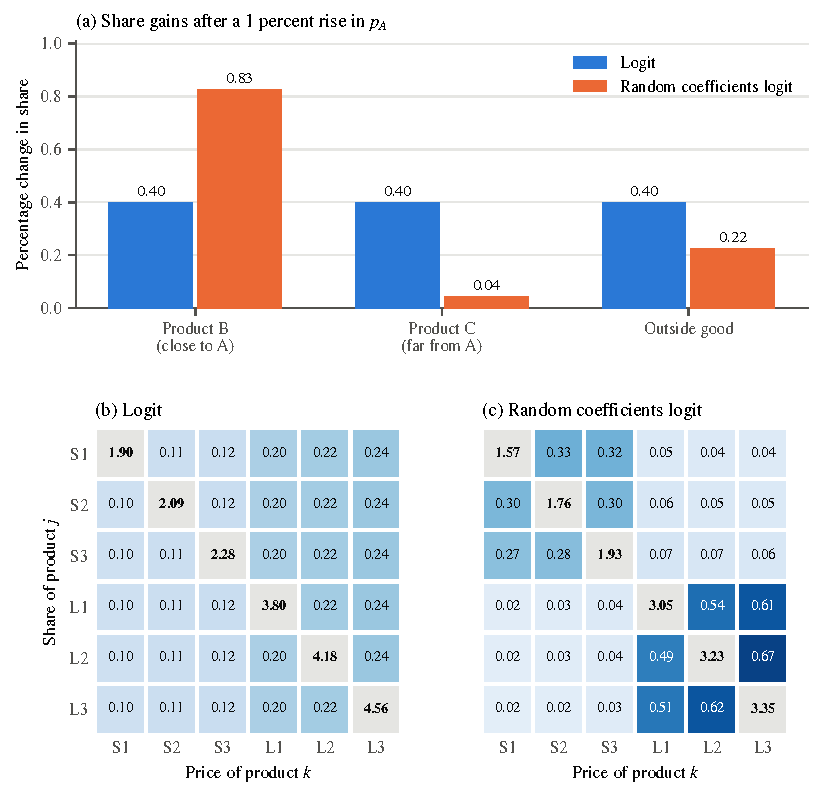
\includegraphics[width=\textwidth]{figures/ch08/fig_substitution.pdf}
\caption{Substitution in the logit and random coefficients logit models. Panel (a): three products with
characteristic $x = (1.0, 0.9, -1.0)$, prices $p = (1, 1, 1)$ and shares $s = (0.20, 0.10, 0.10)$, so A and B are
close and B and C have equal shares. Bars show the percentage change in the shares of B, C and the outside good
after a 1 percent rise in $p_A$. The random coefficients model has normal random coefficients on the constant
(standard deviation 1.0) and on $x$ (standard deviation 2.5), and $\alpha = 2$ in both models. Panels (b) and
(c): six products with shares 0.05, sizes $(-1.0, -0.9, -0.8, 0.8, 0.9, 1.0)$ and prices $(1.0, 1.1, 1.2, 2.0, 2.2,
2.4)$. Cell $(j, k)$ is the elasticity of the share of $j$ with respect to the price of $k$. Grey diagonal cells
report the positive own elasticity $\varepsilon_j = -\varepsilon_{jj}$. The random coefficients model has standard
deviations 1.0 (constant), 2.0 (size) and 0.5 (price), with $\alpha_i = 2 - 0.5\nu_{ip}$. Both models fit the same
shares. Computed by \texttt{figures/ch08/src/fig\_substitution.py}.}
\label{fig:08-substitution}
\end{figure}

\subsection{Further contrasts}\label{sec:08-contrasts}

The vertical model of \cref{ch:discrete} also has heterogeneous consumers, but only along one dimension. Cross
elasticities are then nonzero only between products adjacent in the price ranking.
\citet[p.~852]{BerryLevinsohnPakes1995} give an example. Suppose the ranking contains a \$24,998 family station
wagon, a \$24,999 sports car and a \$25,000 family station wagon, in that order. The vertical model guarantees
that the two wagons are not substitutes for each other, while the sports car is a substitute for both. Random
coefficients on several characteristics let products be differentiated in several dimensions at once.

\begin{remark}[Fitting a logit when tastes are heterogeneous]\label{rem:08-logit-misspec}
Suppose the data come from the random coefficients model and we estimate the logit regression $\ln s_{jt} -
\ln s_{0t} = x_{jt}\beta - \alpha p_{jt} + \text{error}$ by instrumental variables. Write $r_{jt} = \ln s_{jt} -
\ln s_{0t} - \delta_{jt}$ for the gap between the logit inversion and the true mean utility. The regression error is
$\xi_{jt} + r_{jt}$. The gap depends on prices, because less price-sensitive consumers sort into expensive
products. By \eqref{eq:08-elasticity-buyers}, the log share of an expensive product falls with its price at a rate
set by the low price sensitivity of its buyers, more slowly than $\alpha$. An instrument that moves prices, such
as a cost shifter, also moves $r_{jt}$. The instrument is then correlated with the regression error even if it is
independent of $\xi_{jt}$. When less price-sensitive consumers sort into expensive products in this way, the
logit price coefficient tends to be biased toward zero. The argument is heuristic, and \cref{sec:08-worked}
measures the correlation and the bias in a simulated market.
\end{remark}

\begin{remark}[Price changes and product deletions]\label{rem:08-deletion}
\citet[p.~94]{BerryLevinsohnPakes2004} distinguish two substitution patterns. After a price rise, only a selected
group of a product's buyers leave, the more price-sensitive ones. After the product is deleted, all of its buyers
must choose again. The model makes the difference explicit. If $j$ is removed, a consumer who would have bought $j$
chooses $k$ with probability $\frac{s_{ik}}{1 - s_{ij}}$ by \cref{rem:08-iia}. The fraction of $j$'s buyers who move
to $k$ is therefore
\begin{equation}\label{eq:08-deletion-diversion}
  D^{\text{del}}_{jk} = \int \frac{s_{ij}}{s_j}\, \frac{s_{ik}}{1 - s_{ij}}\, \dd F.
\end{equation}
It averages the same individual diversion ratios as \eqref{eq:08-diversion-average}, with weights
$\frac{s_{ij}}{s_j}$ instead of $\varpi_{ij}$. The two coincide in the logit, where both equal $\frac{s_k}{1 -
s_j}$. With heterogeneous tastes they differ, and the deletion pattern is the relevant one for questions such as the
closing of a brand (\cref{sec:08-blp04}).
\end{remark}

\section{Computing the share integral by simulation}\label{sec:08-simulation}

The share integral \eqref{eq:08-share-integral} has the dimension of $(D_i, \nu_i)$, the number of demographics
plus the number of random coefficients. It has no closed form once that dimension exceeds zero, and
\citet[p.~866]{BerryLevinsohnPakes1995} note that numerical integration becomes difficult once the dimension grows
beyond two or three. They replace the integral by a simulation estimator, a technique that
\citet{Pakes1986} introduced as aggregation by simulation \citep[p.~848]{BerryLevinsohnPakes1995}. This section
describes the standard simulator, its error, the importance sampler of \citet{BerryLevinsohnPakes1995}, the
treatment of demographics, deterministic alternatives, and safe numerical evaluation.

\subsection{The smooth simulator}\label{sec:08-smooth-simulator}

Draw $n_s$ consumers $(D_i, \nu_i)$, $i = 1, \dots, n_s$, from $F_{Dt} \times F_\nu$. The \emph{smooth
simulator} of the share of product $j$ is the average of the individual logit probabilities
\citep[eq.~(6.10)]{BerryLevinsohnPakes1995}:
\begin{equation}\label{eq:08-smooth-simulator}
  s^{n_s}_{jt}(\delta_t; \theta_2) = \frac{1}{n_s}\sum_{i=1}^{n_s} s_{ijt}.
\end{equation}
With diagonal $\Sigma$, each term is written out as
\begin{equation*}
  s_{ijt} = \frac{\exp\bigl(\delta_{jt} + \sum_{k} \tilde x_{jtk}(\sigma_k\nu_{ik} + \pi_{k1}D_{i1} + \cdots
            + \pi_{kd}D_{id})\bigr)}
         {1 + \sum_{m \in \mathcal{J}_t}\exp\bigl(\delta_{mt} + \sum_{k} \tilde x_{mtk}(\sigma_k\nu_{ik}
          + \pi_{k1}D_{i1} + \cdots + \pi_{kd}D_{id})\bigr)},
\end{equation*}
which gives equation (11) of \citet{Nevo2000a}. The sums over $k$ run over the characteristics that carry random
coefficients.

The simulator has four properties \citep[p.~865]{BerryLevinsohnPakes1995}. It is unbiased for $s_{jt}$. Its
values are positive. Together with the simulated outside share $\frac{1}{n_s}\sum_i s_{i0t}$ the shares sum to
one. It is a smooth function of $(\delta_t, \theta_2)$. Because the extreme value shocks are integrated
analytically, its variance comes only from the draws of $(D_i, \nu_i)$. The next lemma makes the last point precise
by comparing it with the \emph{frequency simulator}, which also draws the shocks $\epsilon_{ijt}$ and counts the
simulated consumers who choose $j$.

\begin{lemma}[Smooth versus frequency simulator]\label{lem:08-smooth}
Let $s^{\text{freq}}_j = \frac{1}{n_s}\sum_{i=1}^{n_s}\indic\{j = \argmax_{k} u_{ik}\}$, where each simulated
consumer has draws $(D_i, \nu_i, \epsilon_{i0}, \dots, \epsilon_{iJ})$. Both simulators are unbiased for $s_j$, and
\begin{equation}\label{eq:08-rao-blackwell}
  \Var\bigl(s^{\text{freq}}_j\bigr) = \frac{s_j(1 - s_j)}{n_s}
  = \Var\bigl(s^{n_s}_j\bigr) + \frac{1}{n_s}\E\bigl[s_{ij}(1 - s_{ij})\bigr],
  \qquad \Var\bigl(s^{n_s}_j\bigr) = \frac{\Var(s_{ij})}{n_s}.
\end{equation}
\end{lemma}

\begin{proof}
Let $I_{ij}$ be the indicator that simulated consumer $i$ chooses $j$. Conditional on $(D_i, \nu_i)$, it is a
Bernoulli variable with mean $s_{ij}$. By the law of iterated expectations, $\E[I_{ij}] = \E[s_{ij}] = s_j$, so
both simulators are unbiased. Unconditionally $I_{ij}$ is Bernoulli with mean $s_j$, so $\Var(I_{ij}) = s_j(1 -
s_j)$. The law of total variance gives
\begin{equation*}
  \Var(I_{ij}) = \E\bigl[\Var(I_{ij} \mid D_i, \nu_i)\bigr] + \Var\bigl(\E[I_{ij} \mid D_i, \nu_i]\bigr)
              = \E\bigl[s_{ij}(1 - s_{ij})\bigr] + \Var(s_{ij}).
\end{equation*}
The draws are independent across simulated consumers, so dividing by $n_s$ gives the variances of the two
averages.
\end{proof}

The smooth simulator is the conditional expectation of the frequency simulator given the draws of $(D_i,
\nu_i)$. Conditioning removes the variance $\frac{1}{n_s}\E[s_{ij}(1 - s_{ij})]$. The frequency simulator has two
further defects. It is a step function of $(\delta, \theta_2)$, with zero derivatives almost everywhere and jumps
in between, so gradient-based optimizers cannot use it. It also equals zero with positive probability for small
products, and then $\ln s^{\text{freq}}_j$ is undefined and the share equations cannot be inverted.

\subsection{Simulation error in log shares}\label{sec:08-simbias}

The estimator of \cref{sec:08-gmm} uses the simulated shares through their logarithms, in the inversion step. An
unbiased simulator of $s_j$ is a biased simulator of $\ln s_j$. Let $c_j = \frac{\sqrt{\Var(s_{ij})}}{s_j}$ be the
coefficient of variation of the individual purchase probabilities of product $j$.

\begin{proposition}[Bias of the simulated log share]\label{prop:08-simbias}
Let $s^{n_s}_j$ be the smooth simulator with independent draws, and suppose $\Var(s_{ij}) > 0$.
\begin{enumerate}[label=(\roman*)]
  \item $\E[s^{n_s}_j] = s_j$ and $\Var(s^{n_s}_j) = \frac{\Var(s_{ij})}{n_s}$.
  \item $\E[\ln s^{n_s}_j] < \ln s_j$.
  \item If $s_{ij} \ge \underline{s} > 0$ for all $(D_i, \nu_i)$, then
    \begin{equation}\label{eq:08-simbias}
      \E\bigl[\ln s^{n_s}_j\bigr] - \ln s_j = -\frac{\Var(s^{n_s}_j)}{2s_j^2} + O\bigl(n_s^{-\frac{3}{2}}\bigr)
      = -\frac{c_j^2}{2n_s} + O\bigl(n_s^{-\frac{3}{2}}\bigr).
    \end{equation}
\end{enumerate}
\end{proposition}

\begin{proof}
Part (i) restates \cref{lem:08-smooth}. For (ii), the logarithm is strictly concave and $s^{n_s}_j$ is not
degenerate because $\Var(s_{ij}) > 0$. Jensen's inequality gives $\E[\ln s^{n_s}_j] < \ln\E[s^{n_s}_j] = \ln s_j$.

For (iii), write $Y = s^{n_s}_j$ and expand $\ln Y$ around $s_j$ with the Lagrange form of the remainder:
\begin{equation*}
  \ln Y = \ln s_j + \frac{Y - s_j}{s_j} - \frac{(Y - s_j)^2}{2s_j^2} + \frac{(Y - s_j)^3}{3\bar Y^3},
\end{equation*}
where $\bar Y$ lies between $Y$ and $s_j$. Take expectations. The linear term has mean zero by (i). The quadratic
term has mean $-\frac{\Var(Y)}{2s_j^2}$. Both $Y$ and $s_j$ are at least $\underline{s}$, so $\bar Y \ge
\underline{s}$ and the remainder is bounded in absolute value by $\frac{\E|Y - s_j|^3}{3\underline{s}^3}$. For an
average of $n_s$ independent bounded variables, $\E|Y - s_j|^3 \le (\E(Y - s_j)^4)^{\frac{3}{4}}$, and the fourth
central moment of such an average is $O(n_s^{-2})$. The remainder is therefore $O(n_s^{-\frac{3}{2}})$.
Substituting $\Var(Y) = \frac{\Var(s_{ij})}{n_s}$ gives the second form.
\end{proof}

The lower bound in (iii) holds when the support of $(D_i, \nu_i)$ is bounded. With normal tastes it fails, but the
second-order term still describes the bias well in practice, as the evidence below shows. The bias is of order
$\frac{1}{n_s}$ and its size is governed by $c_j$. The coefficient of variation is large when the purchase
probability of $j$ is concentrated on a small group of consumers. Small niche products have the largest $c_j$ and
the largest bias.

The bias passes to the mean utilities. For given $\theta_2$, the inversion of \cref{sec:08-inversion} finds the
$\hat\delta_t$ that solves $s^{n_s}_t(\hat\delta_t; \theta_2) = s^{\text{obs}}_t$. A first-order expansion around
the true $\delta_t$, using the nonsingular Jacobian of \cref{prop:08-shares}, gives
\begin{equation}\label{eq:08-delta-error}
  \hat\delta_t - \delta_t \approx -\Bigl[\frac{\partial s_t}{\partial \delta_t^\T}\Bigr]^{-1}
  \bigl(s^{n_s}_t(\delta_t; \theta_2) - s_t(\delta_t; \theta_2)\bigr).
\end{equation}
The leading term has mean zero and variance of order $\frac{1}{n_s}$. This is the simulation component of the
asymptotic variance of the estimator in \cref{sec:08-gmm}, which \citet[p.~859]{BerryLevinsohnPakes1995} call
$V_3$. The second-order terms, like those in \eqref{eq:08-simbias}, add a bias of order $\frac{1}{n_s}$. At the
true $\delta_t$ the simulated log shares are too low on average, so the inversion tends to push $\hat\delta_t$
up, most for products with dispersed purchase probabilities.

The bias has a consequence for estimation that the variance does not have. Independent draws across markets make
the leading simulation errors independent across markets. They average out of the sample moments as the number of
markets grows. The bias of order $\frac{1}{n_s}$ is present in every market with the same sign, and it does not
average out. Consistency therefore requires $n_s$ to grow with the sample. \citet[p.~859]{BerryLevinsohnPakes1995} cite asymptotic
results of Berry and Pakes, then in progress, for their utility specification. These results require the number
of consumers and the number of simulation draws to grow at the rate $J^3$.
\citet{BerryLintonPakes2004} develop limit theorems of this kind for asymptotics in the number of products.
\citet[Section~4.4]{BerryPakes2007} report the rates that these theorems require. The number of draws must grow at
the slower rate $J^2$ in logit-style models and at rate $J$ in the vertical model (\cref{sec:08-pcm}). BLP's
rate refers to their own utility specification and to results that were still in progress.

\Cref{fig:08-simerror} and \cref{tab:08-simdelta} quantify these effects in one simulated market with five inside
products, shares $(0.10, 0.05, 0.03, 0.015, 0.005)$ and an outside share of 0.80. The market has normal random
coefficients on a constant, a characteristic and price. The coefficients of variation $c_j$ are 1.49, 0.97, 0.94,
1.51 and 2.99. The product with share 0.10 is expensive and bought mostly by consumers who like its
characteristics, so its $c_j$ exceeds those of the two middle products.

\begin{figure}[htbp]
\centering
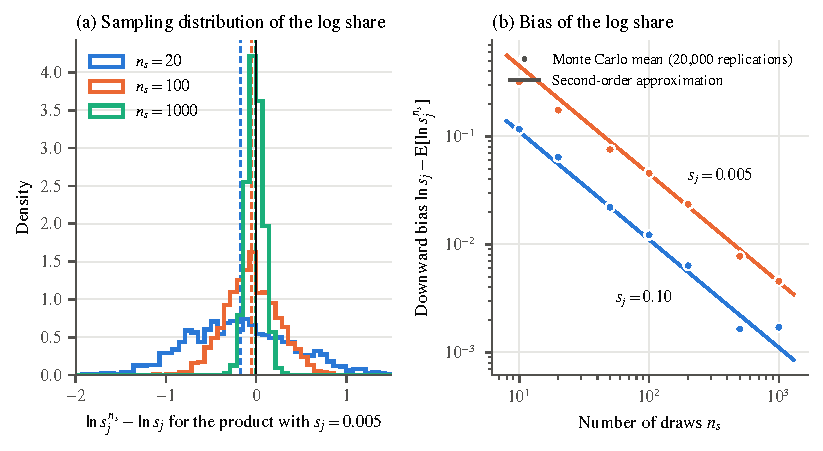
\includegraphics[width=\textwidth]{figures/ch08/fig_simulation.pdf}
\caption{Simulation error in simulated log shares, for one market with outside share 0.80 and inside shares
$(0.10, 0.05, 0.03, 0.015, 0.005)$. Tastes are normal with standard deviations 1.0 on the constant, 1.5 on a characteristic $x =
(1.0, 0.5, 0.0, -0.5, -1.0)$ and 0.5 on price, prices are $(2.0, 1.6, 1.2, 1.0, 0.8)$ and $\alpha = 2$. True shares
come from a 64,000-node Gauss-Hermite rule and agree with $10^6$ pseudo-random draws to within 0.002 in relative
terms. Panel (a): distribution of $\ln s^{n_s}_j - \ln s_j$ for the product with share 0.005 over 2,000 replications
with fresh pseudo-random draws. Dashed lines mark the means. Panel (b): downward bias of the simulated log share
(dots, 20,000 replications per $n_s$) and the second-order approximation $\frac{\Var(s_{ij})}{2n_s s_j^2}$ of
\cref{prop:08-simbias} (lines). Computed by \texttt{figures/ch08/src/fig\_simulation.py}.}
\label{fig:08-simerror}
\end{figure}

Panel (a) of \cref{fig:08-simerror} shows the sampling distribution of the simulated log share of the smallest
product. With 20 draws it is wide and skewed to the left, and its mean lies well below zero. With 1,000 draws it is
concentrated near zero. Panel (b) shows that the downward bias falls like $\frac{1}{n_s}$. The second-order
approximation is accurate from about 50 draws for the product with share 0.10 and from about 100 draws for the
product with share 0.005. For the product with share 0.005, the bias is 0.175
with 20 draws (approximation 0.224), 0.046 with 100 draws (approximation 0.045), and 0.005 with 1,000 draws
(approximation 0.004). With 10 or 20 draws the approximation overstates the bias of the smallest product, because
higher-order terms matter when the simulator is very noisy.

\begin{table}[htbp]
\centering
\caption{Error in the inverted mean utility caused by simulation}\label{tab:08-simdelta}
\begin{tabular}{lccccc}
\toprule
 & \multicolumn{5}{c}{Market share of the product} \\
\cmidrule(lr){2-6}
Draws $n_s$ & 0.10 & 0.05 & 0.03 & 0.015 & 0.005 \\
\midrule
20    & 0.037 & 0.010 & 0.021 & 0.063 & 0.198 \\
      & (0.547) & (0.362) & (0.273) & (0.368) & (0.627) \\
100   & $-0.008$ & $-0.009$ & $-0.008$ & $-0.006$ & 0.015 \\
      & (0.250) & (0.163) & (0.126) & (0.177) & (0.328) \\
1,000 & 0.003 & 0.001 & $-0.000$ & $-0.002$ & $-0.006$ \\
      & (0.077) & (0.051) & (0.040) & (0.056) & (0.104) \\
\bottomrule
\end{tabular}

\smallskip
\begin{minipage}{0.86\linewidth}
\footnotesize Notes: Each entry is the mean of $\hat\delta_j - \delta_j$ over 500 replications, with its standard
deviation in parentheses. In each replication we draw $n_s$ consumers and solve $s^{n_s}(\hat\delta; \theta_2) =
s$ by the contraction of \cref{sec:08-inversion}, at the true $\theta_2$ and the true shares. The market is the one
of \cref{fig:08-simerror}. The standard error of each mean is its standard deviation divided by
$\sqrt{500} \approx 22.4$. Computed by \texttt{figures/ch08/src/fig\_simulation.py}.
\end{minipage}
\end{table}

\Cref{tab:08-simdelta} turns to the mean utilities. With 20 draws, the inverted $\hat\delta_j$ of the product
with share 0.005 is too high by 0.198 on average, with a standard error of $\frac{0.627}{22.4} = 0.028$. The
product with share 0.015 is too high by 0.063 (standard error 0.016). These are the upward biases predicted
above. Their size is small relative to the standard deviations, which range from 0.27 to 0.63. The standard
deviations fall roughly like $\frac{1}{\sqrt{n_s}}$, from about 0.4 on average with 20 draws to about 0.07 with
1,000 draws. With 100 or more draws the mean errors are within two standard errors of zero.

\subsection{Draws in practice}\label{sec:08-draws}

Three rules govern the use of simulation draws in estimation.

The draws are taken once, before estimation, and held fixed while the optimizer varies the parameters. If new
draws were taken at each evaluation, the objective would be a different random function each time it is
evaluated. The search would chase the simulation noise and fail to converge. The asymptotic theory of simulation
estimators also requires draws that do not change with $\theta$ \citep[p.~867]{BerryLevinsohnPakes1995},
\citep{PakesPollard1989}.

Draws are usually independent across markets. Then simulation errors are independent across markets and their
leading terms average out of the moments, so a moderate number of draws per market can suffice when markets are
many. The bias term of \cref{prop:08-simbias} is the exception, as explained above. \citet{BerryLevinsohnPakes1995}
instead hold the same draws of $(\nu_{iy}, \nu_{i0}, \dots, \nu_{iK})$ fixed over all years of their panel, while the
income distribution shifts through $m_t$ \citep[p.~868]{BerryLevinsohnPakes1995}.

The number of draws trades accuracy against computing time. \citet[pp.~538, 540]{Nevo2000a} draws 20 consumers per market
in his illustrative application and notes that more draws or better simulation methods would improve efficiency.
The evidence above shows that 20 pseudo-random draws leave sizable errors in the shares of small products.

Demographics need their own draws. \citet[p.~868, n.~21]{BerryLevinsohnPakes1995} tried taking draws of income from the
CPS for each year. They found that this less restrictive procedure gave imprecise simulators, in particular for
changes in the upper tail of the income distribution. They therefore kept a lognormal income distribution with
year-specific means. They did not estimate a separate standard deviation for each year because those estimates were
imprecise. \citet[n.~25]{Nevo2001} samples 40 individuals from the CPS for each city and year, 200 for each city in
total. He reports that the results were robust to increasing the number of individuals where possible. Empirical
draws of $D_i$ are combined with independent draws of $\nu_i$ from $F_\nu$.

\subsection{Importance sampling}\label{sec:08-importance}

Pseudo-random draws from $F_\nu$ waste effort when few consumers buy any inside product. In the car market most
households do not buy a new car in a given year. Most draws then have purchase probabilities near zero and
contribute little to any share. \citet[Section~6.3]{BerryLevinsohnPakes1995} reduce the variance of the simulator by
importance sampling. To keep notation light, let $\nu$ collect all simulated consumer characteristics, with density
$p_0(\nu)$, and write $f_j(\nu, \theta)$ for the individual choice probability \eqref{eq:08-individual-share}.

Take any density $h(\nu, \theta)$ that is positive wherever $p_0$ is. The share can be rewritten as
\citep[eq.~(6.11)]{BerryLevinsohnPakes1995}
\begin{equation}\label{eq:08-importance-identity}
  s_j(\theta) = \int f_j(\nu, \theta)\, p_0(\nu)\, \dd\nu
  = \int \Bigl[\frac{f_j(\nu, \theta)\, p_0(\nu)}{h(\nu, \theta)}\Bigr] h(\nu, \theta)\, \dd\nu.
\end{equation}
Averaging the bracketed term over draws from $h$ gives an unbiased simulator. Its variance is the variance of the
bracketed term under $h$, divided by the number of draws. The variance is zero for the choice
\citep[eq.~(6.12)]{BerryLevinsohnPakes1995}
\begin{equation}\label{eq:08-optimal-importance}
  h^*_j(\nu, \theta) = \frac{f_j(\nu, \theta)\, p_0(\nu)}{s_j(\theta)},
\end{equation}
because the bracketed term then equals $s_j(\theta)$ for every draw. This density over-samples consumers whose
characteristics make them likely to buy product $j$.

The optimal density cannot be used directly, for three reasons \citep[pp.~866--867]{BerryLevinsohnPakes1995}. It
requires $s_j(\theta)$, the integral we want to compute. It depends on $\theta$, while the draws must stay fixed as
the optimizer varies $\theta$. It differs across products, so each simulated share would come from its own draws.
The inversion of \cref{sec:08-inversion} instead computes all shares from one distribution of consumers.

\citeauthor{BerryLevinsohnPakes1995} build a feasible version from a preliminary estimate $\theta'$, obtained with the
smooth simulator. They target the probability of buying some car, $\bar f(\nu, \theta') = \sum_{j=1}^{J} f_j(\nu,
\theta')$, whose integral is the total inside share $\bar s(\theta') = 1 - s_0(\theta')$. Draws come from $p_0$ by
acceptance and rejection: a draw $\nu$ is accepted with probability $\bar f(\nu, \theta')$. By Bayes' rule the
density of an accepted draw is
\begin{equation}\label{eq:08-accepted-density}
  h(\nu) = \frac{p_0(\nu)\, \Pr(\text{accept} \mid \nu)}{\Pr(\text{accept})}
         = \frac{p_0(\nu)\, \bar f(\nu, \theta')}{\int p_0(\nu')\, \bar f(\nu', \theta')\, \dd\nu'}
         = \frac{p_0(\nu)\, \bar f(\nu, \theta')}{\bar s(\theta')}.
\end{equation}
Substituting this $h$ into \eqref{eq:08-importance-identity} gives the bracketed term $\frac{\bar
s(\theta')}{\bar f(\nu, \theta')}f_j(\nu, \theta)$. With $n_s$ accepted draws $\nu_1, \dots, \nu_{n_s}$, the
simulator is \citep[eq.~(6.13)]{BerryLevinsohnPakes1995}\footnote{Equation (6.13) of
\citet{BerryLevinsohnPakes1995} is printed without the factor $\frac{1}{n_s}$. The average is needed for the
simulator to be unbiased.}
\begin{equation}\label{eq:08-blp-importance}
  s_j\bigl[\theta, P^*_h(\theta')_{n_s}\bigr] = \frac{1}{n_s}\sum_{i=1}^{n_s}
  \frac{\bar s(\theta')}{\bar f(\nu_i, \theta')}\, f_j(\nu_i, \theta).
\end{equation}
The draws are fixed once $\theta'$ is chosen, and every share uses the same draws. Since $\bar s(\theta')$ is computed
only once, it can be computed with many draws at little cost.

The construction removes one source of noise. At $\theta = \theta'$ the weighted integrand is $\bar s(\theta')$ times
$\frac{f_j(\nu, \theta')}{\bar f(\nu, \theta')}$, the probability of choosing $j$ given that the consumer buys some
car. That ratio lies between zero and one. Summed over $j$ it equals $\bar s(\theta')$ for every draw, so the
simulated total inside share has no simulation error at all. The variation that remains comes only from which car
a buyer chooses.

Common draws do not make the simulated shares add up to one, although \citet[p.~867]{BerryLevinsohnPakes1995} use
them for that purpose. Write $w_i = \frac{\bar s(\theta')}{\bar f(\nu_i, \theta')}$ for the weight of draw $i$ and
$\bar w = \frac{1}{n_s}\sum_{i} w_i$ for the mean weight. Applying \eqref{eq:08-blp-importance} to all $J + 1$
options and using $\sum_{j=0}^{J} f_j = 1$ gives $\sum_{j=0}^{J} s_j = \bar w$. Each weight has expectation one under
$h$, so $\bar w$ equals one only on average. The contraction uses only the inside shares, and this random total does
not break it. The simulated inside shares equal $\bar w$ times the shares computed under the probability weights
$\frac{w_i}{n_s\bar w}$. \Cref{thm:08-berry94}, applied to this distribution of draws, gives a unique solution
whenever the observed inside shares sum to less than $\bar w$. With a small inside share and many draws, $\bar w$ is
close to one and the condition is mild. Self-normalizing the weights would make the shares sum to one exactly, at
the cost of a finite-sample bias that vanishes as $n_s$ grows.

\Cref{tab:08-importance} compares the two simulators in the market of \cref{fig:08-simerror}, whose total inside share
is 0.20. With 100 draws, importance sampling cuts the relative root mean squared error of the largest product's share
from 15.3 to 4.8 percent. For the second product it falls from 10.0 to 2.8 percent. The gains are small for
the two smallest products, from 15.0 to 13.5 percent and from 29.4 to 25.5 percent. Their buyers are a small subset of
car buyers, so conditioning on buying some car leaves most of their simulation noise in place. A preliminary
estimate that understates every standard deviation by 20 percent loses little of the gain.

\begin{table}[htbp]
\centering
\caption{Smooth simulator and importance sampling: relative root mean squared error (percent)}\label{tab:08-importance}
\begin{tabular}{lccccc}
\toprule
 & \multicolumn{5}{c}{Market share of the product} \\
\cmidrule(lr){2-6}
Simulator & 0.10 & 0.05 & 0.03 & 0.015 & 0.005 \\
\midrule
Smooth simulator & 15.31 & 9.95 & 9.52 & 14.98 & 29.35 \\
Importance sampling, $\theta' = \theta$ & 4.83 & 2.84 & 6.79 & 13.51 & 25.46 \\
Importance sampling, $\sigma' = 0.8\sigma$ & 5.55 & 2.90 & 6.35 & 13.28 & 26.31 \\
\bottomrule
\end{tabular}

\smallskip
\begin{minipage}{0.9\linewidth}
\footnotesize Notes: Each entry is $100\sqrt{\E\bigl[(\frac{\hat s_j}{s_j} - 1)^2\bigr]}$ over 1,000 replications
with $n_s = 100$ draws (accepted draws for importance sampling). The importance sampler is
\eqref{eq:08-blp-importance}. In the last row the preliminary estimate $\theta'$ multiplies every standard deviation by
0.8 and uses the mean utilities that fit the shares at those values. The acceptance rate equals the total inside share,
0.20. Mean errors of the importance sampler are below 0.6 percent in absolute value. Computed by
\texttt{figures/ch08/src/fig\_simulation.py}.
\end{minipage}
\end{table}

\subsection{Quadrature and quasi-Monte Carlo}\label{sec:08-quadrature}

Pseudo-random draws are not the only way to approximate \eqref{eq:08-share-integral}. Any rule of the form $\sum_q w_q
s_{ij}(\nu_q)$ with nodes $\nu_q$ and weights $w_q$ can replace the simple average, and the share equations and
their inversion are unchanged.

A \emph{Gauss-Hermite product rule} uses, in each dimension, the $Q$ nodes and weights that integrate polynomials of
degree up to $2Q - 1$ exactly against the normal density. For a standard normal variable,
\begin{equation}\label{eq:08-gauss-hermite}
  \int g(\nu)\, \phi(\nu)\, \dd\nu \approx \sum_{q=1}^{Q} \frac{w_q}{\sqrt{\pi}}\, g\bigl(\sqrt{2}\, x_q\bigr),
\end{equation}
where $(x_q, w_q)$ are the Gauss-Hermite nodes and weights for the weight function $e^{-x^2}$. The product rule takes
all combinations of the one-dimensional nodes, so it needs $Q^{L}$ nodes for $L$ random coefficients. It is very
accurate for smooth integrands in low dimensions and becomes expensive quickly as $L$ grows. \emph{Sparse grids}
combine lower-order product rules so that the number of nodes grows polynomially in $L$ \citep{HeissWinschel2008}.
\emph{Quasi-Monte Carlo} methods, such as Halton sequences, replace pseudo-random draws by deterministic sequences that
fill the unit cube more evenly. The points are mapped to normal draws by the inverse distribution function
\citep[Section~9.3.3]{Train2009}.
A randomly scrambled Halton sequence keeps the even coverage and allows replications. The
\texttt{pyblp} software of \citet[Section~3]{ConlonGortmaker2020} implements all of these rules. By default it
scrambles each Halton sequence and discards its first 1,000 points.

\Cref{tab:08-integration} compares the three approaches in the market of \cref{fig:08-simerror}, which has three random
coefficients. At equal numbers of nodes, scrambled Halton draws reduce the error of pseudo-random draws by a factor of
about 2 to 20, and the gain grows with the number of nodes. The Gauss-Hermite product rule is accurate to a few hundredths of a percent with 125 nodes and to about
$10^{-5}$ percent with 1,000 nodes. The product rule's advantage shrinks with more random coefficients. It also shrinks when
demographic distributions are known only through empirical draws, which quadrature cannot use directly.

\begin{table}[htbp]
\centering
\caption{Accuracy of integration rules: relative error of simulated shares (percent)}\label{tab:08-integration}
\begin{tabular}{lccc}
\toprule
 & \multicolumn{3}{c}{Number of nodes} \\
\cmidrule(lr){2-4}
Rule & 125 & 1,000 & 8,000 \\
\midrule
\multicolumn{4}{l}{\textit{Product with $s_j = 0.10$}} \\
Pseudo-random draws & 12.45 & 4.84 & 1.56 \\
Scrambled Halton draws & 3.41 & 0.53 & 0.076 \\
Gauss-Hermite product rule & $2.9 \times 10^{-2}$ & $1.9 \times 10^{-5}$ & $3.0 \times 10^{-10}$ \\
\addlinespace
\multicolumn{4}{l}{\textit{Product with $s_j = 0.005$}} \\
Pseudo-random draws & 27.63 & 10.29 & 3.30 \\
Scrambled Halton draws & 13.38 & 2.45 & 0.46 \\
Gauss-Hermite product rule & $4.5 \times 10^{-2}$ & $2.5 \times 10^{-5}$ & $6.2 \times 10^{-10}$ \\
\bottomrule
\end{tabular}

\smallskip
\begin{minipage}{0.8\linewidth}
\footnotesize Notes: Market of \cref{fig:08-simerror}, with three normal random coefficients. Entries for random rules
are relative root mean squared errors over 200 replications. Entries for the Gauss-Hermite rule, which uses 5, 10 and
20 nodes per dimension, are absolute relative errors against a rule with 40 nodes per dimension. Computed by
\texttt{figures/ch08/src/fig\_simulation.py}.
\end{minipage}
\end{table}

\subsection{Safe numerical evaluation}\label{sec:08-overflow}

Evaluating \eqref{eq:08-individual-share} naively can overflow. Mean utilities and random coefficient terms can be
large during the search, and $e^{V}$ exceeds the largest double-precision number once $V$ exceeds about 709. The
logit formula is invariant to subtracting the same constant from every utility of a consumer, including the zero
utility of the outside good. Let $m_i = \max\{0, \max_k V_{ik}\}$. Then
\begin{equation}\label{eq:08-logsumexp}
  s_{ij} = \frac{e^{V_{ij} - m_i}}{e^{-m_i} + \sum_k e^{V_{ik} - m_i}}, \qquad
  \ln s_{ij} = V_{ij} - m_i - \ln\Bigl(e^{-m_i} + \sum_k e^{V_{ik} - m_i}\Bigr).
\end{equation}
Every exponent is now at most zero, and at least one term in the denominator equals one, so neither overflow nor
division by zero can occur. The second expression, the log-sum-exp form, also gives accurate log shares for very
small probabilities. All computations in this chapter use \eqref{eq:08-logsumexp}.

\section{Inverting the share equations: the BLP contraction}\label{sec:08-inversion}

The model of \cref{sec:08-model} maps mean utilities into market shares. Estimation needs the reverse
map. The reason is that the unobserved quality $\xi_{jt}$ enters the model only through the mean utility
$\delta_{jt} = x_{jt}\beta - \alpha p_{jt} + \xi_{jt}$, and it enters linearly. Suppose we can recover the vector
$\delta_t$ from the observed shares. Then $\xi_{jt}$ becomes a known function of the data and the
parameters, and instrumental variable methods apply as in a linear demand model. \citet[pp.~850--851]%
{BerryLevinsohnPakes1995} make the point directly. The orthogonality between $\xi$ and the instruments
cannot be used ``without first transforming the observed quantity, price, and characteristic data into a
linear function of $\xi$.'' This section shows that the transformation exists, that it is unique, and that a
simple iteration computes it.

\subsection{The inversion problem}\label{sec:08-inv-problem}

Fix the nonlinear parameters $\theta_2 = (\Pi, \Sigma)$ and a market $t$ with $J_t$ inside products. Recall
from \cref{sec:08-model} that the model share of product $j$ is
\begin{equation}\label{eq:08-p2-share}
  s_{jt}(\delta_t;\theta_2) = \int \frac{\exp(\delta_{jt} + \mu_{ijt})}{1 + \sum_{k \in \mathcal{J}_t}
  \exp(\delta_{kt} + \mu_{ikt})}\, \dd F(D_i, \nu_i),
  \qquad \mu_{ijt} = \tilde x_{jt}(\Pi D_i + \Sigma\nu_i),
\end{equation}
where $\tilde x_{jt} = (x_{jt}, p_{jt})$ collects the characteristics that carry random coefficients. We
write $s_{ijt}$ for the integrand, the choice probability of a consumer with attributes $(D_i, \nu_i)$, and
$s_{i0t} = 1 - \sum_{k} s_{ikt}$ for that consumer's probability of choosing the outside good. The
\emph{inversion problem} is to find, for each market, the vector $\delta_t \in \R^{J_t}$ that solves
\begin{equation}\label{eq:08-inv-system}
  s_{jt}(\delta_t;\theta_2) = s^{\text{obs}}_{jt}, \qquad j = 1, \dots, J_t,
\end{equation}
where $s^{\text{obs}}_{jt}$ is the observed share \citep[eq.~10]{Nevo2000a}. The system has $J_t$ equations in
$J_t$ unknowns. Markets separate, because $\delta_t$ affects only the shares of market $t$. We denote the
solution by $\delta_t(s^{\text{obs}}_t;\theta_2)$, or $\delta_t(\theta_2)$ when the data are understood.

In three familiar models the inverse has a closed form. In the logit model $\Pi = \Sigma = 0$, so
$s_{jt} = \frac{e^{\delta_{jt}}}{1 + \sum_k e^{\delta_{kt}}}$ and $s_{0t} = \frac{1}{1 + \sum_k
e^{\delta_{kt}}}$. Dividing,
\begin{equation*}
  \frac{s_{jt}}{s_{0t}} = e^{\delta_{jt}},
\end{equation*}
and taking logarithms gives
\begin{equation}\label{eq:08-logit-inv}
  \delta_{jt} = \ln s^{\text{obs}}_{jt} - \ln s^{\text{obs}}_{0t},
\end{equation}
which is equation (6.4) of \citet{BerryLevinsohnPakes1995}. In the nested logit model with nesting
parameter $\sigma$ the same algebra applied within and across nests gives $\delta_{jt} = \ln s_{jt} - \ln
s_{0t} - \sigma\ln s_{j|g,t}$, where $s_{j|g,t}$ is the share of $j$ within its nest $g$ \citep{Berry1994}.
\Cref{ch:logit} derives this formula. The principles of differentiation generalized extreme value (PD-GEV) model of
\citet{BresnahanSternTrajtenberg1997} also has an analytic inverse \citep[p.~532]{Nevo2000a}. In each case
the ratios of shares isolate $\delta_{jt}$ because the shares have a closed form. Random coefficients
destroy the closed form, since \eqref{eq:08-p2-share} is an integral. The inverse must then be computed
numerically, and this must be done again for every trial value of $\theta_2$.

Two features of \eqref{eq:08-inv-system} matter for what follows. First, the observed shares appear on the
right-hand side. The inversion therefore fits the observed shares exactly, and all discrepancies between
model and data are attributed to $\xi_{jt}$. Second, the logit inversion \eqref{eq:08-logit-inv} is the
exact solution when $\theta_2 = 0$. It is the natural starting value for the numerical methods below.

\subsection{Existence and uniqueness}\label{sec:08-inv-existence}

The first question is whether \eqref{eq:08-inv-system} has a solution and whether the solution is unique.
\citet[p.~249 and Appendix]{Berry1994} answered both questions for a general family of discrete choice
models. \citet[Appendix I]{BerryLevinsohnPakes1995} gave a second proof that also delivers an algorithm.
We state the result for the random coefficients logit model and prove it through the BLP route.

\begin{theorem}[Invertibility of the share system]\label{thm:08-berry94}
Fix $\theta_2$ and a market $t$. Suppose the distribution $F$ of $(D_i, \nu_i)$ satisfies
$\int e^{\mu_{ijt}}\, \dd F < \infty$ for every $j$. Then for every vector $s = (s_1, \dots, s_{J_t})$ with
$s_j > 0$ for all $j$ and $\sum_j s_j < 1$, there is exactly one $\delta \in \R^{J_t}$ such that
$s_t(\delta;\theta_2) = s$. Moreover, a truncated version of the iteration $\delta \mapsto \delta + \ln s -
\ln s_t(\delta;\theta_2)$ converges to this $\delta$ from any starting value.
\end{theorem}

The integrability condition holds in the usual specifications. With normal taste shocks and demographics
of bounded support, $\int e^{\mu_{ijt}}\, \dd F$ is a moment generating function evaluated at a finite point.
The proof rests on an abstract fixed point theorem, which we state and prove first.

\begin{theorem}[\citealp{BerryLevinsohnPakes1995}, Appendix I]\label{thm:08-contraction}
Consider $\R^{J}$ with the sup norm $\Vert y \Vert = \max_j |y_j|$. Let $f: \R^J \to \R^J$ satisfy the
following conditions.
\begin{enumerate}[label=(\arabic*)]
  \item $f$ is continuously differentiable. For all $j$ and $k$ and all $y$, $\frac{\partial f_j(y)}{\partial
  y_k} \geq 0$ and $\sum_{k=1}^{J}\frac{\partial f_j(y)}{\partial y_k} < 1$.
  \item $f$ is bounded below: $\min_j \inf_y f_j(y) \equiv \underline{y} > -\infty$.
  \item There is a value $\bar y$ with the following property. If $y_j \geq \bar y$ for some $j$, then
  $f_k(y) < y_k$ for some $k$ (not necessarily equal to $j$).
\end{enumerate}
Then $f$ has a unique fixed point $y^*$ in $\R^J$. Moreover, let $Y = [\underline y, \bar y]^J$ and define the
truncated map $\hat f: \R^J \to Y$ by $\hat f_j(y) = \min\{f_j(y), \bar y\}$. Then $\hat f$ is a contraction on
$Y$ with modulus strictly less than one, and the iterates $\hat f^{\,h}(y)$ converge to $y^*$ from any
$y \in \R^J$.
\end{theorem}

\begin{proof}
If condition (3) holds for $\bar y$, it holds for every larger value. We may therefore assume $\bar y >
\underline y$. The proof has four steps.

\emph{Step 1.} We show that $\hat f$ maps $\R^J$ into $Y$. For any $y$, $\hat f_j(y) \leq \bar y$ by construction. Also
$f_j(y) \geq \underline y$ by condition (2), so $\hat f_j(y) \geq \min\{\underline y, \bar y\} =
\underline y$.

\emph{Step 2.} We show that $\hat f$ is a contraction on $Y$. Take $y, y' \in Y$ and let $\lambda = \Vert y - y'\Vert$.
Write $\mathbf{1}$ for the vector of ones, so that $y + \lambda\mathbf{1} \geq y'$ element by element. Fix a
component $j$ and assume without loss of generality that $\hat f_j(y') \geq \hat f_j(y)$. If $f_j(y) \geq
\bar y$, then $\hat f_j(y) = \bar y \geq \hat f_j(y')$, so $\hat f_j(y') - \hat f_j(y) = 0$. Otherwise
$\hat f_j(y) = f_j(y)$. Condition (1) makes $f_j$ nondecreasing in every argument, and taking the minimum
with a constant preserves this. Hence
\begin{align*}
  0 \leq \hat f_j(y') - \hat f_j(y)
  &\leq \hat f_j(y + \lambda\mathbf{1}) - \hat f_j(y) \\
  &\leq f_j(y + \lambda\mathbf{1}) - f_j(y) \\
  &= \int_0^{\lambda}\sum_{k=1}^{J}\frac{\partial f_j(y + z\mathbf{1})}{\partial y_k}\, \dd z.
\end{align*}
The first inequality uses monotonicity and $y' \leq y + \lambda\mathbf{1}$. The second uses
$\hat f_j \leq f_j$ and $\hat f_j(y) = f_j(y)$. The equality is the fundamental theorem of calculus applied to
$z \mapsto f_j(y + z\mathbf{1})$, with the chain rule. Now define the compact set
\begin{equation*}
  \mathcal{W} = \{y + z\mathbf{1}: y \in Y,\ z \in [0, \bar y - \underline y]\}
\end{equation*}
and the number
\begin{equation*}
  \kappa = \max_j \max_{w \in \mathcal{W}} \sum_{k=1}^{J}\frac{\partial f_j(w)}{\partial y_k}.
\end{equation*}
The maximum exists because the row sum is continuous and $\mathcal{W}$ is compact. Each row sum is below
one at every point, so $\kappa < 1$. Since $y, y' \in Y$, we have $\lambda \leq \bar y - \underline y$, so
every point $y + z\mathbf{1}$ with $z \in [0, \lambda]$ lies in $\mathcal{W}$. The integrand is therefore at
most $\kappa$, and
\begin{equation*}
  |\hat f_j(y') - \hat f_j(y)| \leq \kappa\lambda = \kappa\Vert y' - y\Vert.
\end{equation*}
This holds for every $j$, so $\Vert \hat f(y') - \hat f(y)\Vert \leq \kappa \Vert y' - y\Vert$.

\emph{Step 3.} We show that the fixed point of $\hat f$ is a fixed point of $f$. The set $Y$ is closed, hence complete. By
the contraction mapping theorem (\cref{app:math}), $\hat f$ has a unique fixed point $y^*$ in $Y$. By Step 1
the iterates from any starting value enter $Y$ after one step, and they then converge to $y^*$. Suppose some
component satisfies $y^*_j = \bar y$. Condition (3) gives an index $k$ with $f_k(y^*) < y^*_k$. Then $\hat
f_k(y^*) \leq f_k(y^*) < y^*_k$, which contradicts $\hat f(y^*) = y^*$. Hence $y^*_j < \bar y$ for all $j$.
For each $j$, $\hat f_j(y^*) = y^*_j < \bar y$ forces $\hat f_j(y^*) = f_j(y^*)$. So $f(y^*) = y^*$.

\emph{Step 4.} We show that $f$ has no other fixed point. Let $f(y) = y$ for some $y \in \R^J$. Condition (2) gives $y_j
= f_j(y) \geq \underline y$ for all $j$. If $y_j \geq \bar y$ for some $j$, condition (3) gives $k$ with
$f_k(y) < y_k$, a contradiction. So $y \in Y$ and $y_j < \bar y$ for all $j$, which gives $\hat f(y) = f(y) =
y$. Uniqueness of the fixed point of $\hat f$ on $Y$ then yields $y = y^*$.
\end{proof}

\Citet[p.~887]{BerryLevinsohnPakes1995} note that the proof imposes the upper bound $\bar y$, ``although in
practice we never had to impose this bound.'' The truncation is a device of the proof. We now apply the
theorem to the map
\begin{equation}\label{eq:08-phi}
  \Phi_t(\delta_t) = \delta_t + \ln s^{\text{obs}}_t - \ln s_t(\delta_t;\theta_2),
\end{equation}
defined element by element. A vector $\delta_t$ is a fixed point of $\Phi_t$ exactly when it solves
\eqref{eq:08-inv-system}. The next result supplies condition (1).

\begin{corollary}[Derivatives of the BLP map]\label{cor:08-rowsum}
In the random coefficients logit model, for all $j$ and all $k \neq j$,
\begin{equation*}
  \frac{\partial \Phi_{jt}}{\partial \delta_{jt}} = \frac{1}{s_{jt}}\int s_{ijt}^2\, \dd F > 0, \qquad
  \frac{\partial \Phi_{jt}}{\partial \delta_{kt}} = \frac{1}{s_{jt}}\int s_{ijt}s_{ikt}\, \dd F > 0,
\end{equation*}
and the row sums satisfy
\begin{equation}\label{eq:08-rowsum}
  \sum_{k \in \mathcal{J}_t}\frac{\partial \Phi_{jt}}{\partial \delta_{kt}} = 1 -
  \frac{1}{s_{jt}}\int s_{ijt}s_{i0t}\, \dd F = 1 - \int s_{i0t}\,\frac{s_{ijt}}{s_{jt}}\, \dd F \in (0,1).
\end{equation}
\end{corollary}

\begin{proof}
Drop the market index. Write $V_{ij} = \delta_j + \mu_{ij}$, so that $s_{ij} = \frac{e^{V_{ij}}}{1 +
\sum_m e^{V_{im}}}$. The quotient rule gives the individual derivatives
\begin{equation*}
  \frac{\partial s_{ij}}{\partial \delta_j} = s_{ij}(1 - s_{ij}), \qquad
  \frac{\partial s_{ij}}{\partial \delta_k} = -s_{ij}s_{ik} \quad (k \neq j).
\end{equation*}
These derivatives are bounded by one in absolute value, so we may differentiate \eqref{eq:08-p2-share}
under the integral sign by dominated convergence (\cref{prop:08-shares}). This gives
$\frac{\partial s_j}{\partial \delta_j} = \int s_{ij}(1 - s_{ij})\, \dd F$ and $\frac{\partial s_j}{\partial
\delta_k} = -\int s_{ij}s_{ik}\, \dd F$. Differentiating \eqref{eq:08-phi},
\begin{equation*}
  \frac{\partial \Phi_j}{\partial \delta_j} = 1 - \frac{1}{s_j}\frac{\partial s_j}{\partial \delta_j}
  = 1 - \frac{1}{s_j}\int s_{ij}\, \dd F + \frac{1}{s_j}\int s_{ij}^2\, \dd F
  = \frac{1}{s_j}\int s_{ij}^2\, \dd F,
\end{equation*}
because $\int s_{ij}\, \dd F = s_j$. For $k \neq j$, $\frac{\partial \Phi_j}{\partial \delta_k} =
-\frac{1}{s_j}\frac{\partial s_j}{\partial \delta_k} = \frac{1}{s_j}\int s_{ij}s_{ik}\, \dd F$. Both are
positive since $s_{ij} \in (0,1)$. Summing over $k$,
\begin{equation*}
  \sum_k \frac{\partial \Phi_j}{\partial \delta_k} = \frac{1}{s_j}\int s_{ij}\Big(s_{ij} + \sum_{k \neq
  j}s_{ik}\Big)\, \dd F = \frac{1}{s_j}\int s_{ij}(1 - s_{i0})\, \dd F = 1 - \frac{1}{s_j}\int s_{ij}s_{i0}\,
  \dd F.
\end{equation*}
The last integral is positive and smaller than $s_j$, so the row sum lies in $(0,1)$.
\end{proof}

The identity $\sum_k \frac{\partial s_{ij}}{\partial \delta_k} = s_{ij}s_{i0}$, used implicitly in the
proof, has a simple reading. Raising every inside mean utility by the same amount is equivalent to lowering
the utility of the outside good. It moves consumers of type $i$ from the outside good to $j$ at the rate
$s_{ij}s_{i0}$.

\begin{proof}[Proof of \cref{thm:08-berry94}]
We verify the three conditions of \cref{thm:08-contraction} for $f = \Phi$ with $\ln s^{\text{obs}}$ replaced by
$\ln s$, dropping the market index.

\emph{Condition (1).} The share function is infinitely differentiable (\cref{prop:08-shares}), so $\Phi$ is
continuously differentiable. \Cref{cor:08-rowsum} gives nonnegative partial derivatives and row sums below
one.

\emph{Condition (2).} Write $s_j(\delta) = e^{\delta_j}B_j(\delta)$, with
\begin{equation*}
  B_j(\delta) = \int \frac{e^{\mu_{ij}}}{1 + \sum_k e^{\delta_k + \mu_{ik}}}\, \dd F.
\end{equation*}
Then $\Phi_j(\delta) = \delta_j + \ln s_j - \delta_j - \ln B_j(\delta) = \ln s_j - \ln B_j(\delta)$. The
function $B_j$ falls in every $\delta_k$ and is bounded above by $\int e^{\mu_{ij}}\, \dd F$, its limit
when all $\delta_k \to -\infty$. Hence
\begin{equation*}
  \Phi_j(\delta) \geq \underline\delta_j \equiv \ln s_j - \ln\int e^{\mu_{ij}}\, \dd F,
\end{equation*}
which is finite by the integrability assumption. Set $\underline y = \min_j \underline\delta_j$
\citep[p.~888]{BerryLevinsohnPakes1995}. The bound $\underline\delta_j$ is the mean utility that would
generate share $s_j$ if every consumer's denominator in \eqref{eq:08-p2-share} were equal to one.

\emph{Condition (3).} We follow \citet[p.~261]{Berry1994}. For each $j$, consider the market in which only
product $j$ is available, so that the outside share is $s_0^{(j)}(\delta_j) = \int \frac{1}{1 + e^{\delta_j
+ \mu_{ij}}}\, \dd F$. This function is continuous and strictly decreasing, with limits one and zero as
$\delta_j \to -\infty$ and $\delta_j \to +\infty$. Let $\bar\delta_j$ solve $s_0^{(j)}(\bar\delta_j) = s_0$,
where $s_0 = 1 - \sum_k s_k \in (0,1)$, and choose $\bar y > \max_j \bar\delta_j$. Suppose $\delta_j \geq
\bar y$ for some $j$. Every consumer's outside probability falls when we add products, so
\begin{equation*}
  s_0(\delta) = \int \frac{1}{1 + \sum_k e^{\delta_k + \mu_{ik}}}\, \dd F \leq s_0^{(j)}(\delta_j) <
  s_0^{(j)}(\bar\delta_j) = s_0.
\end{equation*}
The inside shares at $\delta$ therefore sum to more than $\sum_k s_k$. At least one product $k$ has
$s_k(\delta) > s_k$, and for that product $\Phi_k(\delta) = \delta_k + \ln s_k - \ln s_k(\delta) <
\delta_k$.

\Cref{thm:08-contraction} now delivers a unique fixed point of $\Phi$, which is the unique solution of
$s(\delta;\theta_2) = s$, and the convergence of the truncated iteration.
\end{proof}

\begin{remark}[Berry's argument and its generalization]\label{rem:08-berry-proof}
\citet[pp.~260--261]{Berry1994} proves existence with Brouwer's fixed point theorem applied to the
\emph{element-by-element inverse} $r_j(\delta_{-j}, s_j)$, the value of $\delta_j$ that matches $s_j$ given
the other mean utilities. For uniqueness he uses a diagonal dominance property that is worth recording. Let
$\delta_0$ be the mean utility of the outside good, normally fixed at zero. Adding a constant to all of
$(\delta_0, \delta_1, \dots, \delta_J)$ leaves every share unchanged, so $\sum_{k=0}^{J}\frac{\partial
s_j}{\partial \delta_k} = 0$. Since $\frac{\partial s_j}{\partial \delta_k} < 0$ for every $k \neq j$,
including $k = 0$,
\begin{equation*}
  \frac{\partial s_j}{\partial \delta_j} = \sum_{k \neq j,\, k \geq 1}\Big|\frac{\partial s_j}{\partial
  \delta_k}\Big| + \Big|\frac{\partial s_j}{\partial \delta_0}\Big| > \sum_{k \neq j,\, k \geq
  1}\Big|\frac{\partial s_j}{\partial \delta_k}\Big|.
\end{equation*}
The Jacobian $\frac{\partial s}{\partial \delta'}$ is therefore strictly diagonally dominant with a positive
diagonal, and in particular nonsingular. Berry's argument needs only that the share function be
differentiable with own derivatives positive, cross derivatives negative, and the obvious limits. A strictly
positive and continuous density of consumer unobservables suffices \citep[p.~260]{Berry1994}.
\citet{BerryGandhiHaile2013} weaken these requirements to the ``connected substitutes'' condition, which
\cref{sec:08-bh14} states.
\end{remark}

\subsection{Speed of convergence and the practice of the inner loop}\label{sec:08-inv-practice}

\Cref{cor:08-rowsum} tells us how fast the iteration converges. The local contraction modulus is the
largest row sum of the Jacobian of $\Phi_t$. By \eqref{eq:08-rowsum}, the row sum of product $j$ is one minus
the average outside-good probability among the consumers who buy $j$. The weights $\frac{s_{ijt}}
{s_{jt}}$ in \eqref{eq:08-rowsum} are the distribution of consumer types conditional on buying $j$. The
modulus is close to one when the buyers of some product rarely choose the outside good. This happens when the
aggregate outside share is small, and also when the outside option is chosen mainly by consumers who seldom
buy inside goods. \citet[Section~7]{DubeFoxSu2012} document the cost in Monte Carlo experiments. Their
Lipschitz constant is the largest row sum maximized over the demand shocks $\xi$. The values they report are a
lower bound on it, computed from the data and the model parameters (their p.~2233). As the outside share falls
from 0.91 to 0.35, this value rises from 0.891 to 0.997. The total number of contraction iterations needed for estimation rises from about 10,400 to 262,000 (their Tables~III
and~IV).

The standard contraction bound makes the cost explicit. Writing $\delta^*_t$ for the solution and
$\kappa_t$ for the modulus,
\begin{equation*}
  \Vert \delta^h_t - \delta^*_t\Vert \leq \kappa_t^h\, \Vert \delta^0_t - \delta^*_t\Vert.
\end{equation*}
Reducing the initial error by a factor $10^{-m}$ therefore takes
\begin{equation*}
  h \geq \frac{m\ln 10}{-\ln\kappa_t} \approx \frac{2.3\, m}{1 - \kappa_t}
\end{equation*}
iterations, where the approximation uses $-\ln\kappa \approx 1 - \kappa$ for $\kappa$ near one. The
required number of iterations grows like $\frac{1}{1 - \kappa_t}$.

\Cref{fig:08-contraction} illustrates with three simulated markets. Each has ten inside products and random
coefficients on the constant, on one characteristic and on price, and we use $n_s = 1{,}000$ draws. The
markets differ only in a common shift of the mean utilities, chosen so that the outside share is about 0.9,
0.5 and 0.1. The largest row sum at the solution is 0.357, 0.725 and 0.948 in the three markets. Starting from
the logit inversion \eqref{eq:08-logit-inv}, the plain iteration needs 25, 63 and 332 evaluations of the
share function to bring the sup-norm error below $10^{-13}$. The observed linear rates are 0.28, 0.63 and
0.92, a little below the worst-case row sums. In the third market the bound with $\kappa = 0.948$ predicts
about 550 iterations, and the observed rate predicts about 336, close to the realized 332.

\begin{figure}[htbp]
  \centering
  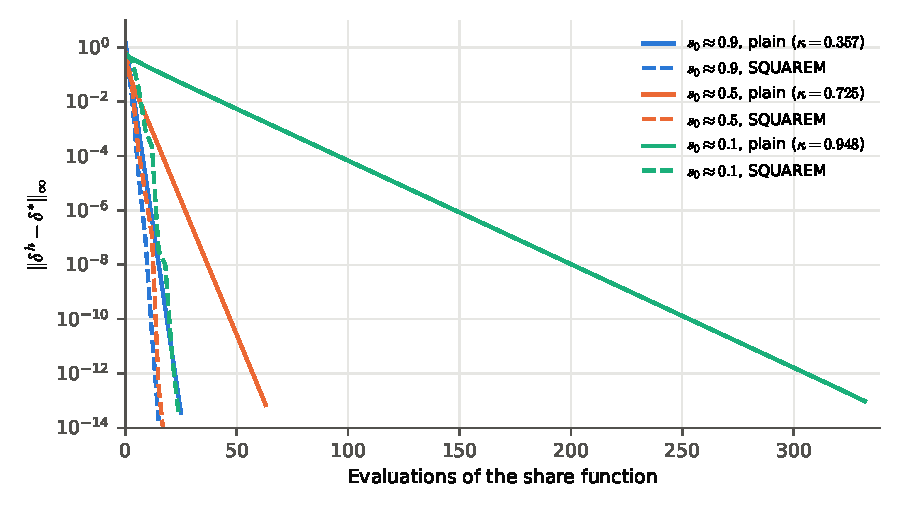
\includegraphics[width=0.92\textwidth]{figures/ch08/fig_contraction.pdf}
  \caption{Convergence of the share inversion in three simulated markets with outside shares near 0.9, 0.5
  and 0.1. Each market has $J = 10$ products, random coefficients with standard deviations
  $(1.0, 1.0, 0.5)$ on the constant, a characteristic and price, and $n_s = 1{,}000$ draws. Solid lines show
  the plain iteration $\delta^{h+1} = \Phi(\delta^h)$. Dashed lines show SQUAREM, the extrapolation method
  described below, on the same map. The
  horizontal axis counts evaluations of the share function. The legend reports the largest row sum $\kappa$
  of the Jacobian of $\Phi$ at the solution. Computed in \texttt{fig\_contraction.py}.}
  \label{fig:08-contraction}
\end{figure}

\subsubsection{Starting values and the multiplicative form}
The logit inversion is the natural first starting value, since it is exact at $\theta_2 = 0$. Inside an
estimation routine the outer optimizer changes $\theta_2$ by small amounts, and the solution at the previous
trial value is a better start. This warm start can cut the number of iterations considerably. Exponentiating
the update gives the equivalent form
\begin{equation*}
  e^{\delta^{h+1}_{jt}} = e^{\delta^h_{jt}}\,\frac{s^{\text{obs}}_{jt}}{s_{jt}(\delta^h_t;\theta_2)},
\end{equation*}
which works with $e^{\delta}$ directly and avoids a logarithm and an exponential per product and iteration.
Each iteration raises $\delta_{jt}$ when the model underpredicts the share of $j$ and lowers it when the model
overpredicts. The individual choice probabilities should be computed with the overflow-safe evaluation of
\cref{sec:08-simulation}.

\subsubsection{The stopping rule}
The iteration stops when successive iterates are close. The next result converts this observable criterion
into a bound on the distance to the solution.

\begin{proposition}[Inner-loop error]\label{prop:08-innererror}
Suppose $\Phi_t$ is a contraction with modulus $\kappa < 1$ on a set that contains the iterates and the
solution $\delta^*_t$. If the iteration stops at the first $H$ with $\Vert \delta^H_t - \delta^{H-1}_t\Vert
\leq \epsilon_{in}$, then
\begin{equation*}
  \Vert \delta^H_t - \delta^*_t \Vert \leq \frac{\kappa}{1 - \kappa}\,\epsilon_{in}.
\end{equation*}
\end{proposition}

\begin{proof}
Since $\delta^*_t = \Phi_t(\delta^*_t)$ and $\delta^H_t = \Phi_t(\delta^{H-1}_t)$,
\begin{align*}
  \Vert \delta^H_t - \delta^*_t\Vert &= \Vert \Phi_t(\delta^{H-1}_t) - \Phi_t(\delta^*_t)\Vert
  \leq \kappa\Vert \delta^{H-1}_t - \delta^*_t\Vert \\
  &\leq \kappa\big(\Vert \delta^{H-1}_t - \delta^{H}_t\Vert + \Vert \delta^H_t - \delta^*_t\Vert\big)
  \leq \kappa\epsilon_{in} + \kappa\Vert \delta^H_t - \delta^*_t\Vert.
\end{align*}
Collecting the terms in $\Vert \delta^H_t - \delta^*_t\Vert$ gives $(1 - \kappa)\Vert \delta^H_t -
\delta^*_t\Vert \leq \kappa\epsilon_{in}$.
\end{proof}

When $\kappa$ is near one, the error can exceed the tolerance by orders of magnitude. In the third market of
\cref{fig:08-contraction} ($\kappa = 0.948$), stopping at a step size of $10^{-4}$ leaves a true error of
$1.0 \times 10^{-3}$, against a bound of $1.7 \times 10^{-3}$. Stopping at $10^{-8}$ leaves $1.0 \times
10^{-7}$. The error is about ten times the tolerance.

The inner error then contaminates the outer problem. Let $e = \tilde\delta - \delta(\theta_2)$ be the
inversion error, stacked over markets. \Cref{sec:08-gmm} shows that the structural error is $\xi(\theta_2) =
\bm{M}\delta(\theta_2)$ for a matrix $\bm{M}$ that does not depend on $\theta_2$ given the weighting matrix.
The computed moments therefore carry the error $\frac{1}{N}\bm{Z}^\T \bm{M} e$. This error varies with
$\theta_2$ in an erratic way, because the number of inner iterations jumps from one trial value to the next.
A finite-difference derivative with step $\Delta$ inherits an error of order $\frac{\Vert e\Vert}{\Delta}$.
With $\Vert e\Vert$ near $10^{-6}$ and $\Delta$ near $10^{-6}$, the error in the computed gradient is of
order one. \citet[Sections~4.2 and~6]{DubeFoxSu2012} show that a loose inner tolerance can keep the outer
optimizer from converging. If the researcher then loosens the outer tolerance, the reported solution may not be a
local minimum. In their synthetic data, no run with inner tolerance $10^{-4}$ and outer tolerance $10^{-6}$
reports convergence (their Table~I). The practical rule is to set the inner
tolerance close to machine precision, for example $10^{-12}$ to $10^{-14}$ in the sup norm, and well below the
outer tolerance. With the warm start this costs little.

\subsubsection{Acceleration}
Two methods speed up the inner loop. The first is SQUAREM, a squared extrapolation method of
\citet{VaradhanRoland2008} designed for slowly converging fixed point iterations.
\citet[Section~2.3]{ReynaertsVaradhanNash2012} apply it to the BLP map. One cycle of the variant we use computes
two plain steps, extrapolates and ends with one more plain step \citep[Table~1]{VaradhanRoland2008}. The step
length $a$ is that of their scheme SqS3, set to $-1$ whenever it exceeds $-1$ (their eqs.~(9) and~(20) and
Section~6):
\begin{gather*}
  r = \Phi(\delta) - \delta, \qquad v = \Phi(\Phi(\delta)) - 2\Phi(\delta) + \delta, \qquad
  a = \min\Big\{-\frac{\Vert r\Vert_2}{\Vert v\Vert_2},\, -1\Big\}, \\
  \delta' = \delta - 2ar + a^2 v, \qquad \delta^{new} = \Phi(\delta').
\end{gather*}
With $a = -1$ the cycle reduces to three plain steps. A more negative $a$ extrapolates along the direction in
which the iterates have been moving. In \cref{fig:08-contraction} SQUAREM reaches an error of $10^{-13}$ after
15, 18 and 24 evaluations of the share function, against 25, 63 and 332 for the plain iteration. Its advantage
grows with the modulus. The second method applies Newton's method to the system $\ln s_t(\delta_t;\theta_2)
= \ln s^{\text{obs}}_t$:
\begin{equation*}
  \delta^{h+1}_t = \delta^h_t - \Big[\frac{\partial \ln s_t(\delta^h_t;\theta_2)}{\partial
  \delta_t^\T}\Big]^{-1}\big(\ln s_t(\delta^h_t;\theta_2) - \ln s^{\text{obs}}_t\big).
\end{equation*}
The Jacobian is available in closed form from the proof of \cref{cor:08-rowsum}, and it is nonsingular by
\cref{rem:08-berry-proof}. Newton's method converges quadratically near the solution but may overshoot far
from it. A common hybrid runs the contraction first and switches to Newton steps once the iterates are close.

\begin{remark}[Dampening in the random coefficients nested logit]\label{rem:08-rcnl}
When random coefficients are combined with a nested logit error with nesting parameter $\rho \in [0,1)$, the
undampened map need not be a contraction. We write the nesting parameter as $\rho$ in this remark, because
$\sigma$ here denotes the standard deviations of the random coefficients.
\citet[pp.~919 and 934--935]{GrigolonVerboven2014} show for the plain nested logit that dampening the step by the
factor $1 - \rho$ restores BLP's sufficient conditions for a contraction. They state that the argument extends to
random coefficients and use the same dampened map in the random coefficients nested logit. The
dampened iteration is $\delta^{h+1} = \delta^h + (1 - \rho)\big(\ln s^{\text{obs}} - \ln s(\delta^h)\big)$. Their
printed equation~(7) attaches the factor $1 - \rho$ to $\ln s(\delta^h)$ alone. \citet[eq.~15 and n.~20]{ConlonGortmaker2020}
point out this typesetting error. In the plain nested logit, $\delta_j
= (1 - \rho)\ln s_j + \rho\ln s_g - \ln s_0$, where $s_g$ is the share of $j$'s nest. Holding the nest and
outside shares fixed, a change in $\ln s_j$ therefore maps into a change of $1 - \rho$ times as much in
$\delta_j$, and the dampened step has this scale. \Cref{ch:mergers} uses this model for merger simulation.
\end{remark}

\section{The GMM estimator}\label{sec:08-gmm}

With the inversion in hand, estimation follows the logic of instrumental variables. This section derives the
estimator, the shortcut that concentrates out the linear parameters, the algorithm, its gradient, the
weighting matrix, and the asymptotic variance with simulation error. It ends with a reformulation as a
constrained optimization problem.

\subsection{Why the error must be the structural error}\label{sec:08-why-xi}

A direct approach would choose the parameters to make predicted shares close to observed shares,
\begin{equation*}
  \min_{\theta}\ \big\Vert s\big(x, p, \delta(x, p, \xi;\theta_1);\theta_2\big) - s^{\text{obs}}\big\Vert,
\end{equation*}
as in equation (7) of \citet{Nevo2000a}. \Citet[pp.~530--531]{Nevo2000a} gives two reasons against it. First,
all parameters enter nonlinearly, and with many brand and time dummies the nonlinear search becomes costly.
Second, and more fundamentally, the approach cannot handle the correlation between prices and $\xi$. The
residual $s^{\text{obs}} - s(\cdot)$ is a nonlinear function of $\xi$. The standard nonlinear simultaneous equations
model allows parameters and variables to enter nonlinearly, but it requires an additively separable error
\citep[p.~531]{Nevo2000a}. The share residual does not have this form. At the true parameters the
predicted share depends on the unknown vector $\xi$. Setting $\xi = 0$ in the prediction leaves a residual
that is a nonlinear function of $\xi$. An orthogonality condition between instruments and $\xi$ then implies no
such condition for the residual.

\citet{Berry1994} proposed to define the econometric error as the structural error $\xi_{jt}$ itself. The
link to economic theory is then direct, and we can reason about which variables are plausibly uncorrelated
with unobserved quality \citep[p.~531]{Nevo2000a}. The cost is the inversion of \cref{sec:08-inversion}.

\subsection{Moment conditions}\label{sec:08-moments}

The identifying assumption of \citet[eq.~4.1]{BerryLevinsohnPakes1995} is a conditional moment restriction.
Let $\mathcal{Z}_t$ denote the exogenous variables of market $t$: the observed characteristics of all products
and the cost shifters. BLP assume
\begin{equation}\label{eq:08-cond-moment}
  \E[\xi_{jt} \mid \mathcal{Z}_t] = 0 \quad\text{and}\quad \E[\omega_{jt} \mid \mathcal{Z}_t] = 0,
\end{equation}
where $\omega_{jt}$ is the cost unobservable of \cref{sec:08-supply}. Prices and quantities are left out of
the conditioning set because the model makes them functions of $\xi$ and $\omega$. The characteristics are
included because the model does not explain how they are chosen \citep[p.~854]{BerryLevinsohnPakes1995}.
\Cref{sec:08-instruments} discusses how plausible this is. In this section we treat demand alone.

A conditional moment restriction implies that $\xi_{jt}$ is uncorrelated with every function of
$\mathcal{Z}_t$. We choose $L$ such functions and collect them in the row vector $z_{jt} \in \R^{1\times L}$,
the \emph{instruments} for observation $(j,t)$. The unconditional moment conditions are
\begin{equation}\label{eq:08-moments}
  \E\big[z_{jt}^\T\,\xi_{jt}(\theta_0)\big] = 0,
\end{equation}
which is equation (8) of \citet{Nevo2000a}. The structural error as a function of the parameters is
\begin{equation}\label{eq:08-xi-theta}
  \xi_{jt}(\theta) = \delta_{jt}(s^{\text{obs}}_t;\theta_2) - x_{jt}\beta + \alpha p_{jt}
\end{equation}
\citep[eq.~13]{Nevo2000a}. The observed shares enter through the inversion. For a trial $\theta_2$, the
inversion finds the mean utilities that rationalize the data. The error is the gap between those mean
utilities and the ones predicted by the linear parameters $(\alpha, \beta)$. When the specification includes
brand and time dummies, they appear on the right-hand side of \eqref{eq:08-xi-theta} and the error becomes the
market-specific deviation $\tilde\xi_{jt}$ of \cref{sec:08-brand-fe}.

We stack the $N = \sum_t J_t$ observations. Let $\delta(\theta_2)$ be the $N$-vector of inverted mean
utilities, $\bm{X}$ the $N \times K_1$ matrix whose rows are $(x_{jt}, p_{jt})$ augmented with any dummies,
and $\theta_1 = (\beta^\T, -\alpha)^\T$ the corresponding coefficient vector. This is the vector of linear
parameters $(\alpha, \beta)$ of \cref{sec:08-linear}, ordered and signed to match the columns of $\bm{X}$. Then
\begin{equation*}
  \xi(\theta) = \delta(\theta_2) - \bm{X}\theta_1.
\end{equation*}
Let $\bm{Z}$ be the $N \times L$ matrix of instruments. The sample moments and the GMM objective are
\begin{equation}\label{eq:08-gmm-obj}
  g_N(\theta) = \frac{1}{N}\bm{Z}^\T\xi(\theta), \qquad
  Q_N(\theta) = g_N(\theta)^\T W g_N(\theta) = \frac{1}{N^2}\,\xi(\theta)^\T\bm{Z}W\bm{Z}^\T\xi(\theta),
\end{equation}
for a positive definite $L \times L$ weighting matrix $W$. This is equation (9) of \citet{Nevo2000a} and
equation (6) of \citet{Nevo2001}, who write $W$ as the inverse of an estimate of $\E[\bm Z^\T\xi\xi^\T\bm Z]$.
The GMM estimator is $\hat\theta = \argmin_\theta Q_N(\theta)$. The order condition
requires $L \geq K_1 + K_2$, where $K_2 = \dim\theta_2$. The rank condition requires that
$\E[z_{jt}^\T\frac{\partial \xi_{jt}(\theta_0)}{\partial \theta^\T}]$ have full column rank.
\Cref{app:econometrics} reviews the general theory.

\subsection{Concentrating out the linear parameters}\label{sec:08-concentrate}

The objective \eqref{eq:08-gmm-obj} is quadratic in $\theta_1$ for fixed $\theta_2$. The linear parameters
can therefore be solved in closed form \citep[p.~868]{BerryLevinsohnPakes1995}.

\begin{proposition}[Concentrating out $\theta_1$]\label{prop:08-concentrate}
Suppose $\bm{X}^\T\bm{Z}W\bm{Z}^\T\bm{X}$ is nonsingular. For each $\theta_2$, the value of $\theta_1$ that
minimizes $Q_N(\theta_1, \theta_2)$ is
\begin{equation}\label{eq:08-theta1hat}
  \hat\theta_1(\theta_2) = \big(\bm{X}^\T\bm{Z}W\bm{Z}^\T\bm{X}\big)^{-1}\bm{X}^\T\bm{Z}W\bm{Z}^\T\delta(\theta_2).
\end{equation}
The implied structural error is $\xi(\theta_2) = \bm{M}\delta(\theta_2)$ with $\bm{M} = I_N -
\bm{X}(\bm{X}^\T\bm{Z}W\bm{Z}^\T\bm{X})^{-1}\bm{X}^\T\bm{Z}W\bm{Z}^\T$. The GMM estimator of $\theta_2$
minimizes the profiled objective
\begin{equation}\label{eq:08-profiled}
  Q^c_N(\theta_2) = \frac{1}{N^2}\,\delta(\theta_2)^\T\bm{M}^\T\bm{Z}W\bm{Z}^\T\bm{M}\,\delta(\theta_2),
\end{equation}
and $\hat\theta_1 = \hat\theta_1(\hat\theta_2)$.
\end{proposition}

\begin{proof}
Fix $\theta_2$ and write $\delta = \delta(\theta_2)$. The objective is
\begin{equation*}
  Q_N = \frac{1}{N^2}(\delta - \bm{X}\theta_1)^\T\bm{Z}W\bm{Z}^\T(\delta - \bm{X}\theta_1).
\end{equation*}
Its gradient with respect to $\theta_1$ is
\begin{equation*}
  \frac{\partial Q_N}{\partial \theta_1} = -\frac{2}{N^2}\bm{X}^\T\bm{Z}W\bm{Z}^\T(\delta - \bm{X}\theta_1).
\end{equation*}
Setting it to zero gives the normal equations $\bm{X}^\T\bm{Z}W\bm{Z}^\T\bm{X}\,\theta_1 =
\bm{X}^\T\bm{Z}W\bm{Z}^\T\delta$, whose solution is \eqref{eq:08-theta1hat}. The Hessian
$\frac{2}{N^2}\bm{X}^\T\bm{Z}W\bm{Z}^\T\bm{X}$ is positive definite, so this is the unique minimum.
Substituting, $\delta - \bm{X}\hat\theta_1(\theta_2) = \bm{M}\delta$, and the objective at the minimum is
\eqref{eq:08-profiled}. Finally, $\min_{\theta_1,\theta_2}Q_N = \min_{\theta_2}\min_{\theta_1}Q_N =
\min_{\theta_2}Q^c_N(\theta_2)$.
\end{proof}

The matrix $\bm{M}$ depends on the data and on $W$ only. It can be computed once for each weighting matrix,
and each objective evaluation then requires one matrix-vector product. The nonlinear search runs over
$\theta_2$ alone, which typically has a handful of elements. The number of random coefficients therefore drives the
cost of estimation. The mean utility can include many characteristics, and even brand dummies, at little cost
(\cref{sec:08-model}).

\begin{corollary}[Logit and nested logit as 2SLS]\label{cor:08-2sls}
In the logit model $\theta_2$ is empty and $\delta_{jt} = \ln s^{\text{obs}}_{jt} - \ln s^{\text{obs}}_{0t}$. With $W =
(\frac{1}{N}\bm{Z}^\T\bm{Z})^{-1}$, the estimator \eqref{eq:08-theta1hat} is two-stage least squares of
$\ln s_{jt} - \ln s_{0t}$ on $\bm{X}$ with instruments $\bm{Z}$. In the nested logit model the same holds
after adding $\ln s_{j|g,t}$ to $\bm{X}$ as a second endogenous regressor with coefficient $\sigma$.
\end{corollary}

\begin{proof}
Write $P_Z = \bm{Z}(\bm{Z}^\T\bm{Z})^{-1}\bm{Z}^\T$. The scalar $\frac{1}{N}$ in $W$ cancels from
\eqref{eq:08-theta1hat}, which becomes $(\bm{X}^\T P_Z\bm{X})^{-1}\bm{X}^\T P_Z\delta$, the 2SLS formula. In
the nested logit model $\ln s_{jt} - \ln s_{0t} = x_{jt}\beta - \alpha p_{jt} + \sigma\ln s_{j|g,t} +
\xi_{jt}$, which is linear in $(\beta, \alpha, \sigma)$.
\end{proof}

\Citet[p.~533 and n.~22]{Nevo2000a} and \citet[p.~319]{Nevo2001} make the same point. The weighting matrix
$(\bm{Z}^\T\bm{Z})^{-1}$ is efficient when the errors are homoskedastic.

\subsection{The nested fixed point algorithm}\label{sec:08-nfxp}

The estimator nests the inversion (a fixed point problem) inside the minimization. We call the procedure the
\emph{nested fixed point} (NFXP) algorithm. \citet[p.~863]{BerryLevinsohnPakes1995} describe four steps for
each evaluation of the moments. They estimate the market shares by simulation and solve for the demand
unobservables. They then compute the cost unobservables as price minus the markup, and they interact both
unobservables with the instruments. In our notation the algorithm reads as follows.

\begin{enumerate}[label=\arabic*.,leftmargin=2em]
  \item Before the search, draw $(D_i, \nu_i)$, $i = 1, \dots, n_s$, for each market and hold the draws fixed
  for the whole estimation. Choose the first-step weighting matrix $W = (\frac{1}{N}\bm{Z}^\T\bm{Z})^{-1}$ and
  compute $\bm{M}$.
  \item The outer optimizer proposes a value $\theta_2^{(k)}$. Compute $\mu_{ijt} = \tilde x_{jt}(\Pi D_i +
  \Sigma\nu_i)$ for all draws, products and markets.
  \item In each market, iterate $\delta^{h+1}_t = \Phi_t(\delta^h_t)$ from the last solution until $\Vert
  \delta^{h+1}_t - \delta^h_t\Vert_\infty < \epsilon_{in}$, using the simulated share $s^{n_s}_t$ of
  \cref{sec:08-simulation}.
  \item Compute $\hat\theta_1(\theta_2^{(k)})$ by \eqref{eq:08-theta1hat} and $\xi(\theta_2^{(k)}) =
  \bm{M}\delta(\theta_2^{(k)})$. With a supply side, also compute the markups and the cost unobservable
  $\omega$ (\cref{sec:08-supply}).
  \item Evaluate $Q^c_N(\theta_2^{(k)})$ and its gradient (\cref{prop:08-gradient}). Return them to the
  optimizer, which either stops or returns to step 2.
  \item After convergence, compute the second-step weighting matrix from the first-step residuals
  (\cref{sec:08-weighting}) and repeat steps 2 to 5.
\end{enumerate}

\Cref{fig:08-nfxp} displays the algorithm. Two remarks concern the outer search. \citet[p.~868]%
{BerryLevinsohnPakes1995} use the Nelder-Mead simplex method, which needs no derivatives. \citet[p.~319]%
{Nevo2001} uses a quasi-Newton method with an analytic gradient and reports that it ``was found to work much
faster.'' Holding the draws fixed is essential for the outer search. Fresh draws at each evaluation would make
the objective a random function of $\theta_2$, and no optimizer would converge \citep{PakesPollard1989}.

\begin{figure}[htbp]
\centering
\begin{tikzpicture}[
  node distance=5mm,
  box/.style={draw, rounded corners=2pt, align=center, font=\small, text width=7.4cm, inner sep=4pt},
  dec/.style={draw, diamond, aspect=3.2, align=center, font=\small, inner sep=0.5pt},
  note/.style={draw, dashed, rounded corners=2pt, align=left, font=\footnotesize, text width=3.3cm,
    inner sep=3pt},
  arr/.style={-{Stealth[length=2.2mm]}, thick}]
\node[box] (draws) {Draw $(D_i, \nu_i)$, $i = 1, \dots, n_s$, in each market once and hold them fixed.
  Set $W = (\frac{1}{N}\bm{Z}^\T\bm{Z})^{-1}$};
\node[box, below=of draws] (outer) {Outer step: the optimizer proposes $\theta_2^{(k)}$};
\node[box, below=of outer] (mu) {Compute $\mu_{ijt} = \tilde x_{jt}(\Pi D_i + \Sigma\nu_i)$\\ for all $i$, $j$, $t$};
\node[box, below=of mu] (inner) {Inner step in each market:\\ $\delta^{h+1}_t = \delta^{h}_t + \ln s^{\text{obs}}_t
  - \ln s^{n_s}_t(\delta^h_t;\theta_2^{(k)})$};
\node[dec, below=of inner] (tol) {$\Vert\delta^{h+1}_t - \delta^{h}_t\Vert_\infty < \epsilon_{in}$?};
\node[box, below=of tol] (lin) {Concentrate out $\hat\theta_1(\theta_2^{(k)})$\\ and set
  $\xi(\theta_2^{(k)}) = \bm{M}\delta(\theta_2^{(k)})$.\\ With a supply side, also $\omega(\theta^{(k)})$};
\node[box, below=of lin] (obj) {Objective $Q^c_N(\theta_2^{(k)})$ and gradient $\nabla Q^c_N(\theta_2^{(k)})$};
\node[dec, below=of obj] (conv) {Outer stopping rule met?};
\node[box, below=of conv] (done) {Report $\hat\theta_2$ and $\hat\theta_1(\hat\theta_2)$.
  Update $W$ and repeat (second step)};
\draw[arr] (draws) -- (outer);
\draw[arr] (outer) -- (mu);
\draw[arr] (mu) -- (inner);
\draw[arr] (inner) -- (tol);
\draw[arr] (tol) -- node[right, font=\footnotesize] {yes} (lin);
\draw[arr] (tol.east) -| node[above, font=\footnotesize, pos=0.25] {no} ([xshift=6mm]inner.east)
  -- (inner.east);
\draw[arr] (lin) -- (obj);
\draw[arr] (obj) -- (conv);
\draw[arr] (conv) -- node[right, font=\footnotesize] {yes} (done);
\draw[arr] (conv.west) -| node[above, font=\footnotesize, pos=0.25] {no} ([xshift=-6mm]outer.west)
  -- (outer.west);
\node[note, right=1.4cm of inner] {Warm start from the last $\delta_t$. Tolerance near machine precision.
  SQUAREM or Newton steps speed it up};
\node[note, right=1.4cm of obj] {Gradient by \cref{prop:08-gradient}. Optimizer: Nelder-Mead or
  quasi-Newton};
\end{tikzpicture}
\caption{The nested fixed point algorithm. The outer loop searches over the nonlinear parameters
$\theta_2$. For each trial value the inner loop inverts the share equations market by market, the linear
parameters are concentrated out, and the profiled GMM objective is evaluated.}
\label{fig:08-nfxp}
\end{figure}

\subsection{The gradient}\label{sec:08-gradient}

Quasi-Newton methods need the gradient of $Q^c_N$. Because $\delta(\theta_2)$ is defined implicitly by the
share equations, its derivative comes from the implicit function theorem (\cref{app:math}).

\begin{proposition}[Gradient of the profiled objective]\label{prop:08-gradient}
For each market, $\delta_t(\theta_2)$ is continuously differentiable and
\begin{equation}\label{eq:08-ift}
  \frac{\partial \delta_t}{\partial \theta_2^\T} = -\Big[\frac{\partial s_t}{\partial
  \delta_t^\T}\Big]^{-1}\frac{\partial s_t}{\partial \theta_2^\T}.
\end{equation}
In the random coefficients logit model with diagonal $\Sigma = \diag(\sigma_1, \dots, \sigma_{K+1})$ and
demographic coefficients $\pi_{kd}$, the derivatives on the right are
\begin{align}
  \frac{\partial s_{jt}}{\partial \delta_{kt}} &= \int s_{ijt}\big(\indic\{j = k\} - s_{ikt}\big)\, \dd F,
  \notag\\
  \frac{\partial s_{jt}}{\partial \sigma_k} &= \int s_{ijt}\,\nu_{ik}\Big(\tilde x_{jtk} - \sum_{m \in
  \mathcal{J}_t}s_{imt}\tilde x_{mtk}\Big)\, \dd F, \label{eq:08-dsdsigma}\\
  \frac{\partial s_{jt}}{\partial \pi_{kd}} &= \int s_{ijt}\,D_{id}\Big(\tilde x_{jtk} - \sum_{m \in
  \mathcal{J}_t}s_{imt}\tilde x_{mtk}\Big)\, \dd F. \notag
\end{align}
The gradient of the profiled objective is
\begin{equation}\label{eq:08-grad}
  \nabla Q^c_N(\theta_2) = \frac{2}{N^2}\Big(\frac{\partial \delta}{\partial \theta_2^\T}\Big)^\T
  \bm{Z}W\bm{Z}^\T\xi(\theta_2).
\end{equation}
\end{proposition}

\begin{proof}
The inverted mean utilities satisfy the identity $s_t(\delta_t(\theta_2);\theta_2) = s^{\text{obs}}_t$ for all
$\theta_2$. Differentiating with respect to $\theta_2^\T$ gives
\begin{equation*}
  \frac{\partial s_t}{\partial \delta_t^\T}\,\frac{\partial \delta_t}{\partial \theta_2^\T} +
  \frac{\partial s_t}{\partial \theta_2^\T} = 0.
\end{equation*}
The Jacobian $\frac{\partial s_t}{\partial \delta_t^\T}$ is nonsingular by \cref{rem:08-berry-proof}, so the
implicit function theorem applies and yields \eqref{eq:08-ift}. The derivative with respect to $\delta$ was
computed in the proof of \cref{cor:08-rowsum}. For $\sigma_k$, note that $\mu_{ijt} = \sum_k \tilde
x_{jtk}(\sigma_k\nu_{ik} + \sum_d \pi_{kd}D_{id})$, so $\frac{\partial \mu_{ijt}}{\partial \sigma_k} = \tilde
x_{jtk}\nu_{ik}$. From $\ln s_{ijt} = \delta_{jt} + \mu_{ijt} - \ln(1 + \sum_m e^{\delta_{mt} + \mu_{imt}})$,
\begin{equation*}
  \frac{\partial \ln s_{ijt}}{\partial \sigma_k} = \tilde x_{jtk}\nu_{ik} - \sum_m s_{imt}\tilde
  x_{mtk}\nu_{ik},
\end{equation*}
and multiplying by $s_{ijt}$ and integrating gives \eqref{eq:08-dsdsigma}. The derivative with respect to
$\pi_{kd}$ replaces $\nu_{ik}$ by $D_{id}$. For the gradient, write $Q_N(\theta_1, \theta_2)$ as in
\eqref{eq:08-gmm-obj}, so $Q^c_N(\theta_2) = Q_N(\hat\theta_1(\theta_2), \theta_2)$. By the chain rule,
\begin{equation*}
  \nabla Q^c_N = \frac{\partial Q_N}{\partial \theta_2} + \Big(\frac{\partial \hat\theta_1}{\partial
  \theta_2^\T}\Big)^\T\frac{\partial Q_N}{\partial \theta_1}.
\end{equation*}
The second term vanishes because $\frac{\partial Q_N}{\partial \theta_1} = 0$ at $\hat\theta_1(\theta_2)$.
This is the envelope theorem. Holding $\theta_1$ fixed, $\frac{\partial \xi}{\partial \theta_2^\T} =
\frac{\partial \delta}{\partial \theta_2^\T}$, which gives \eqref{eq:08-grad}.
\end{proof}

With simulation, every integral in the proposition is replaced by the average over the $n_s$ fixed draws.
The gradient then costs about as much as one more share evaluation plus the solution of a $J_t \times J_t$
linear system in each market. The matrix $\frac{\partial \delta}{\partial \theta_2^\T}$ also reappears in the
asymptotic variance below and in the optimal instruments of \cref{sec:08-optiv}.

\subsection{Weighting, efficiency and clustering}\label{sec:08-weighting}

The efficient weighting matrix is the inverse of the variance of the moments. With independent observations
the second-step matrix is
\begin{equation*}
  W_2 = \Big[\frac{1}{N}\sum_t\sum_{j \in \mathcal{J}_t} z_{jt}^\T\,\hat\xi_{jt}^2\, z_{jt}\Big]^{-1},
\end{equation*}
where $\hat\xi_{jt}$ are the residuals at the first-step estimate. \citet[p.~319]{Nevo2001} follows this
two-step procedure. He also iterated further and found that ``the estimated parameters changed only slightly
beyond the second iteration.''

Errors are often correlated within groups of observations. \citet[pp.~862--863]{BerryLevinsohnPakes1995}
follow car models over the years they are sold, and the unobservables of one model are more alike across years
than across models. They sum the moments of each model over its years,
\begin{equation*}
  g_m(\theta) = \sum_t \big[f_{mt}(\mathcal{Z})^\T \otimes I_2\big]
  \begin{pmatrix}\xi_{mt}(\theta)\\ \omega_{mt}(\theta)\end{pmatrix},
\end{equation*}
where $f_{mt}(\mathcal{Z})$ is the vector of instrument functions for model $m$ in year $t$ and $\otimes$ is
the Kronecker product. They then minimize a quadratic form in the average of $g_m$ over models. The
resulting standard errors allow arbitrary correlation across years for a given model and arbitrary
heteroskedasticity across models. The corresponding efficient weighting matrix is the inverse of $\frac{1}{M}
\sum_m g_m(\hat\theta)g_m(\hat\theta)^\T$, with $M$ the number of models. The same construction applies with
cities, markets or brands as clusters (\cref{app:econometrics}).

With the efficient weighting matrix, $N\,Q_N(\hat\theta)$ is the \emph{Hansen J statistic}. Under correct
specification it converges in distribution to a $\chi^2$ with $L - K_1 - K_2$ degrees of freedom. A rejection
signals that some instruments are invalid or that the model is misspecified. With tens of thousands of
observations the test rejects almost any model, as \citet[p.~325, n.~23]{Nevo2001} notes.

\subsection{Asymptotic distribution and simulation error}\label{sec:08-asymptotics}

The estimator departs from textbook GMM in two ways. The moments are computed from sampled shares, and the
share integral is simulated. \citet[Section 5]{BerryLevinsohnPakes1995} account for both. Their setting is a
single cross section of $J$ products, with asymptotics as $J$ grows. Let $s^0$ be the population shares,
$s^n$ the shares observed in a sample of $n$ consumers, $P_0$ the distribution of consumer attributes, and
$P_{n_s}$ the empirical distribution of $n_s$ simulation draws. BLP standardize the two unobservables by a
$2 \times 2$ matrix $T(z_j)$ with $T(z_j)^\T T(z_j) = \Upsilon(z_j)^{-1}$, where $\Upsilon(z_j) =
\E[(\xi_j, \omega_j)^\T(\xi_j, \omega_j) \mid z_j]$ (their eqs.~5.1--5.2). BLP write $\Omega$ for this covariance matrix. We write $\Upsilon$ because $\Omega$ is the ownership matrix in this book. They interact the standardized
errors with an $L \times 2$ instrument matrix $H_j(\mathcal Z)$ and form
\begin{equation*}
  G_J(\theta; s, P) = \frac{1}{J}\sum_{j=1}^{J}H_j(\mathcal{Z})\,T(z_j)\begin{pmatrix}\xi_j(\theta, s,
  P)\\ \omega_j(\theta, s, P)\end{pmatrix}
\end{equation*}
(eq.~5.4). The estimator minimizes $\Vert G_J(\theta; s^n, P_{n_s})\Vert$ with $\Vert y\Vert = y^\T y$
(eq.~5.5).

The computed moments differ from the ideal ones $G_J(\theta_0; s^0, P_0)$ in two ways. Adding and subtracting
gives the decomposition
\begin{multline*}
  G_J(\theta_0; s^n, P_{n_s}) = \underbrace{G_J(\theta_0; s^0, P_0)}_{\text{product draws}}
  + \underbrace{\big[G_J(\theta_0; s^n, P_0) - G_J(\theta_0; s^0, P_0)\big]}_{\text{consumer sampling}}\\
  + \underbrace{\big[G_J(\theta_0; s^n, P_{n_s}) - G_J(\theta_0; s^n, P_0)\big]}_{\text{simulation}}.
\end{multline*}
The three terms come from three independent random processes: the draws of the product characteristics
$(x, w, \xi, \omega)$, the sampling of consumers, and the simulation draws. Their variances, scaled by $J$,
converge to
\begin{align*}
  V_1 &= \lim_{J\to\infty}\E_{\mathcal Z}\Big[H_j T(z_j)\begin{pmatrix}\xi_j\\ \omega_j\end{pmatrix}
  \begin{pmatrix}\xi_j\\ \omega_j\end{pmatrix}^\T T(z_j)^\T H_j^\T\Big],\\
  V_2 &= \lim_{J\to\infty}\frac{J}{n}\,\E\Big(n\big[G_J(\theta_0; s^0, P_0) - G_J(\theta_0; s^n,
  P_0)\big]\big[\cdot\big]^\T\Big),\\
  V_3 &= \lim_{J\to\infty}\frac{J}{n_s}\,\E\Big(n_s\big[G_J(\theta_0; s^n, P_{n_s}) - G_J(\theta_0; s^n,
  P_0)\big]\big[\cdot\big]^\T \,\Big|\, s^n\Big),
\end{align*}
where $[\cdot]$ repeats the preceding bracket. The usual GMM linearization then applies. The first-order
condition $\hat G^\T G_J(\hat\theta) = 0$, with $\hat G$ the Jacobian of the moments, and a mean value expansion
$G_J(\hat\theta) \approx G_J(\theta_0) + G(\hat\theta - \theta_0)$ give $\sqrt{J}(\hat\theta - \theta_0)
\approx -(G^\T G)^{-1}G^\T\sqrt{J}\,G_J(\theta_0)$. Hence the asymptotic variance is
\begin{equation}\label{eq:08-blp-avar}
  (G^\T G)^{-1}G^\T(V_1 + V_2 + V_3)\,G\,(G^\T G)^{-1}, \qquad G = \lim_{J\to\infty}\frac{\partial
  \E[G_J(\theta, s^0, P_0)]}{\partial \theta^\T}\Big|_{\theta = \theta_0},
\end{equation}
which is equation (5.6) of \citet{BerryLevinsohnPakes1995}, who write $\Gamma$ for $G$. With a general
weighting matrix the formula becomes $(G^\T WG)^{-1}G^\T W(V_1 + V_2 + V_3)WG(G^\T WG)^{-1}$.

The scale factors explain which terms matter. $V_2$ carries the factor $\frac{J}{n}$, and BLP note that $n$,
the number of U.S. households, ``is on the order of 100 million,'' so $V_2$ is negligible
\citep[p.~859]{BerryLevinsohnPakes1995}. $V_3$ carries the factor $\frac{J}{n_s}$, and with a feasible number
of draws it is not negligible. The limit theory requires $n$ and $n_s$ to grow ``on the order of $J^3$''
(p.~859). The ``in process'' paper that BLP cite for these results was published as
\citet{BerryLintonPakes2004}. Its theorems need the number of draws to grow only at rate $J^2$ in
logit-style models, a weaker condition than the rate BLP quote (\cref{sec:08-pcm}). BLP estimate $V_1$ by its sample analog at $\hat\theta$. They estimate $V_3$ by
drawing new sets of simulation draws, recomputing the moments at $\hat\theta$ for each set, and taking the
empirical variance. The correction ``increases our reported standard errors \dots by about 5--20\% (with the
exception of one parameter, whose reported standard error doubles)'' (p.~859).

The sampling scheme behind $V_1$ deserves a word. BLP do not assume that products are independent draws. They
assume that the vectors $y_j = (\xi_j, \omega_j, z_j)$ are \emph{exchangeable}: their joint density is
unchanged by any permutation of the product labels \citep[p.~856, n.~14]{BerryLevinsohnPakes1995}. This
allows characteristics chosen by firms to be related across products and allows common shocks to many
products.

In data with many markets and a fixed set of products, as in \citet{Nevo2001}, the asymptotics run over
markets instead. The moments are averages of independent market-level terms, and the usual cluster-robust
GMM formulas apply. \citet[p.~319]{Nevo2001} corrects for simulation error by accounting for the fact that
the draws are common to all observations in a market. One caveat carries over from \cref{sec:08-simulation}.
The log of a simulated share is biased (\cref{prop:08-simbias}), so the inverted $\delta$ carries a bias of
order $\frac{1}{n_s}$ that does not average out across markets. Consistency therefore requires $n_s$ to grow
with the sample, and in practice $n_s$ should be large enough that the bias is small relative to the standard
errors.

Two practical points complete the picture. First, the standard errors must be computed for the full
parameter vector $\theta = (\theta_1, \theta_2)$. The moment Jacobian is
\begin{equation*}
  G = \frac{1}{N}\bm{Z}^\T\Big[-\bm{X},\ \frac{\partial \delta}{\partial \theta_2^\T}\Big],
\end{equation*}
with the second block from \cref{prop:08-gradient}. Treating the second-stage regression
\eqref{eq:08-theta1hat} as ordinary 2SLS with $\delta$ as data ignores the estimation of $\theta_2$ and
understates the uncertainty in $\hat\theta_1$. Second, objects such as elasticities, markups and welfare are
nonlinear functions $\varphi(\theta)$. Their uncertainty can be computed by the delta method,
$\widehat{\Var}(\varphi(\hat\theta)) = \nabla\varphi^\T\widehat{\Var}(\hat\theta)\nabla\varphi$, or by a
parametric bootstrap. The bootstrap draws $\theta^{(r)}$ from the estimated asymptotic distribution of
$\hat\theta$, computes $\varphi(\theta^{(r)})$ for each draw, and reads off percentiles.
\citet[pp.~319, 333]{Nevo2001} uses the bootstrap, with 1,500 draws for the margins of his Table VIII
(\cref{sec:08-nevo01}).

\subsection{MPEC: estimation as constrained optimization}\label{sec:08-mpec}

\citet{SuJudd2012} propose to estimate structural models by \emph{mathematical programming with equilibrium
constraints} (MPEC), and \citet{DubeFoxSu2012} apply the idea to BLP. Instead of solving the share equations
for every trial value of $\theta_2$, MPEC treats the mean utilities as additional unknowns and imposes the
share equations as constraints:
\begin{equation}\label{eq:08-mpec}
  \min_{\theta_1, \theta_2, \delta, \eta}\ \eta^\T W\eta \quad\text{subject to}\quad
  s_t(\delta_t;\theta_2) = s^{\text{obs}}_t \ \ (t = 1, \dots, T), \qquad
  \eta = \frac{1}{N}\bm{Z}^\T(\delta - \bm{X}\theta_1).
\end{equation}
The auxiliary vector $\eta \in \R^L$ holds the sample moments.

\begin{proposition}[Equivalence of MPEC and NFXP]\label{prop:08-mpec}
Suppose the conditions of \cref{thm:08-berry94} hold for every $\theta_2$ in the parameter space. Then
$(\hat\theta_1, \hat\theta_2)$ minimizes the GMM objective \eqref{eq:08-gmm-obj} if and only if there exist
$\hat\delta$ and $\hat\eta$ such that $(\hat\theta_1, \hat\theta_2, \hat\delta, \hat\eta)$ solves
\eqref{eq:08-mpec}. In that case $\hat\delta = \delta(\hat\theta_2)$ and $\hat\eta = g_N(\hat\theta)$.
\end{proposition}

\begin{proof}
By \cref{thm:08-berry94}, for each $\theta_2$ the share constraints have exactly one solution,
$\delta(\theta_2)$. The second constraint then determines $\eta$. The feasible set of \eqref{eq:08-mpec} is
therefore
\begin{equation*}
  \Big\{\big(\theta_1, \theta_2, \delta(\theta_2), \frac{1}{N}\bm{Z}^\T(\delta(\theta_2) -
  \bm{X}\theta_1)\big): (\theta_1, \theta_2) \text{ in the parameter space}\Big\}.
\end{equation*}
On this set the objective equals $g_N(\theta)^\T Wg_N(\theta) = Q_N(\theta)$. Minimizing over the feasible set
is the same as minimizing $Q_N$ over $\theta$, and the minimizers correspond one to one. The map
$\theta_2 \mapsto \delta(\theta_2)$ is continuous by \cref{prop:08-gradient}, so local minimizers also
correspond.
\end{proof}

The two formulations have the same solutions and different computational properties. MPEC has no inner loop,
so there is no inner tolerance and no propagation of inversion error into the objective. The share
constraints need hold only at the solution, so the solver does not spend effort on precise inversions at trial
values far from the optimum. The constraint Jacobian is sparse, because $s_t$ depends only on $\delta_t$ and
$\theta_2$. Derivatives can be supplied by automatic differentiation. Against this, the problem has $K_1 +
K_2 + N + L$ unknowns, $N$ nonlinear share constraints and $L$ linear moment constraints. It requires a large-scale constrained solver and
careful scaling, and the solver may stop at an infeasible point. \citet[Section~7]{DubeFoxSu2012} find MPEC
faster than NFXP when the contraction is slow. By \cref{cor:08-rowsum}, this happens when outside shares are
small. With an outside share of 0.35 in their experiments, MPEC is about 24 times faster (their Table~III).
\citet[Sections~3 and~5]{ConlonGortmaker2020} instead use the nested fixed point. They prefer an inner tolerance
between $10^{-14}$ and $10^{-12}$. They find SQUAREM the fastest and most reliable way to accelerate the
contraction.
The choice between the two is a matter of implementation. The statistical properties of the estimator are the same.

Other estimators trade exactness for speed. \citet[Section~5]{LeeSeo2015} linearize the log share function around
the current mean utilities and invert this approximation analytically at each trial value. After each minimization
they update the point of approximation by one Newton step. The share equations therefore hold exactly only at the
optimum.
\citet[Sections~2 and~3]{SalanieWolak2019} expand the inverse share function to second order around zero random
coefficients. The resulting approximate model is linear in the mean coefficients and in the variances and
covariances of the random coefficients. Two-stage least squares therefore estimates it. These estimates can serve as
starting values for the exact estimator.
\Cref{prop:08-smallsigma} below derives the leading term of such an expansion.

\section{Instruments and identification}\label{sec:08-instruments}

The estimator of \cref{sec:08-gmm} is only as good as its instruments. This section first explains why prices
need instruments, how many instruments are needed and which roles they play. It then derives the efficient
instruments and reviews the instrument families used in practice. It closes with brand fixed effects and with
nonparametric identification.

\subsection{Price endogeneity}\label{sec:08-endogeneity}

Firms observe $\xi_{jt}$ when they set prices. In a Nash-Bertrand equilibrium the price is marginal cost
plus a markup (\cref{ch:diffprod}), and the markup depends on demand, hence on $\xi_t$. \citet[eq.~8]%
{Nevo2001} writes
\begin{equation*}
  p_{jt} = mc_{jt} + f(\xi_{jt}, \dots) = (mc_j + f_j) + \big(mc_{jt} - mc_j + f_{jt} - f_j\big),
\end{equation*}
where $mc_j$ and $f_j$ are brand means and the second bracket is the deviation of the market from them. With
brand dummies the brand means are absorbed, but the market-specific deviation of the markup still moves with
the market-specific deviation of $\xi$ \citep[p.~320]{Nevo2001}.

A single-product logit firm makes the sign transparent. Its first-order condition gives the markup $m_j =
p_j - mc_j = \frac{1}{\alpha(1 - s_j)}$ (\cref{ch:logit}). Hold rivals' prices fixed and define
\begin{equation*}
  G(m_j, \xi_j) = m_j - \frac{1}{\alpha\big(1 - s_j(m_j, \xi_j)\big)},
\end{equation*}
where $s_j$ is the logit share at price $mc_j + m_j$. The optimal markup solves $G(m_j, \xi_j) = 0$. The logit
derivatives are $\frac{\partial s_j}{\partial m_j} = -\alpha s_j(1 - s_j)$ and $\frac{\partial s_j}{\partial
\xi_j} = s_j(1 - s_j)$. By the chain rule,
\begin{align*}
  \frac{\partial}{\partial m_j}\,\frac{1}{\alpha(1 - s_j)} &= \frac{1}{\alpha(1 - s_j)^2}\,\frac{\partial
  s_j}{\partial m_j} = -\frac{s_j}{1 - s_j},\\
  \frac{\partial}{\partial \xi_j}\,\frac{1}{\alpha(1 - s_j)} &= \frac{1}{\alpha(1 - s_j)^2}\,\frac{\partial
  s_j}{\partial \xi_j} = \frac{s_j}{\alpha(1 - s_j)}.
\end{align*}
Hence
\begin{equation*}
  \frac{\partial G}{\partial m_j} = 1 + \frac{s_j}{1 - s_j} = \frac{1}{1 - s_j}, \qquad
  \frac{\partial G}{\partial \xi_j} = -\frac{s_j}{\alpha(1 - s_j)}.
\end{equation*}
The implicit function theorem then gives the response of the best-response markup to unobserved quality,
\begin{equation*}
  \frac{\partial m_j}{\partial \xi_j} = -\frac{\partial G}{\partial \xi_j}\Big(\frac{\partial G}{\partial
  m_j}\Big)^{-1} = \frac{s_j}{\alpha(1 - s_j)}\,(1 - s_j) = \frac{s_j}{\alpha} > 0.
\end{equation*}
A better unobserved product sells more and carries a higher markup, so $\Cov(p_{jt}, \xi_{jt}) > 0$.

Consider the logit estimating equation $\ln s_{jt} - \ln s_{0t} = x_{jt}\beta - \alpha p_{jt} + \xi_{jt}$
and let $\tilde p_{jt}$ be the residual from projecting $p_{jt}$ on $x_{jt}$. By the Frisch-Waugh theorem the
OLS coefficient on price satisfies
\begin{equation*}
  \plim\, \widehat{(-\alpha)}_{OLS} = -\alpha + \frac{\Cov(\tilde p_{jt}, \xi_{jt})}{\Var(\tilde p_{jt})}
  > -\alpha,
\end{equation*}
when $x_{jt}$ is uncorrelated with $\xi_{jt}$. The estimated price coefficient is biased toward zero, and
demand looks too inelastic. Random coefficients do not remove the problem, since $\xi_{jt}$ enters
$\delta_{jt}$ in the same way.

The evidence matches the theory. In the automobile data of \citet[Table III]{BerryLevinsohnPakes1995}, the
OLS logit price coefficient is $-0.089$ (0.004). It implies that 1,494 of the 2,217 models have inelastic
demand, which is inconsistent with profit maximization. With instruments the coefficient becomes $-0.216$
(0.123), and only 22 models have inelastic demand (pp.~873--874). In the cereal data of \citet[Table V]%
{Nevo2001}, the OLS logit coefficient with brand dummies is $-7.26$ (0.16). The same specification
instrumented with prices in other cities gives $-17.57$ (0.50) (columns ii and v). \Cref{sec:08-blp95,sec:08-nevo01} present these tables in
full.

\subsection{How many instruments, and what they must do}\label{sec:08-iv-roles}

The order condition of \cref{sec:08-moments} counts the instruments. The exogenous characteristics in
$x_{jt}$ serve as their own instruments. The remaining instruments must be at least as many as the
endogenous variables in the mean utility (usually price alone) plus the number of nonlinear parameters. A
model with one random coefficient per characteristic and on price needs $K + 2$ excluded instruments,
where $K$ is the number of characteristics: one for price and $K + 1$ for $\Sigma$.

The instruments play two distinct roles. Some must shift prices, as in any demand system. Others must shift
what \citet[Section 7]{BerryHaile2014} call ``quantities,'' the market shares that enter the inverse demand
function. \citet[p.~1136, n.~2]{BerryHaile2024} note that instruments for quantities are what the applied
literature informally calls instruments for the ``nonlinear parameters.'' The next result shows concretely why
the nonlinear parameters need their own source of variation.

\begin{proposition}[Small-$\sigma$ expansion of the inverse]\label{prop:08-smallsigma}
Suppose there is a single random coefficient, $\mu_{ijt} = \sigma\nu_i x_{jt}$, with $\nu_i$ symmetric
about zero, $\E[\nu_i^2] = 1$ and $\E[e^{c|\nu_i|}] < \infty$ for all $c > 0$, as for the standard normal. Normalize $x_{0t} = 0$ for the outside good and let
$\bar x_t = \sum_{m=0}^{J_t} s_{mt}x_{mt}$ be the share-weighted mean of the characteristic. Then the inverted
mean utility satisfies
\begin{equation*}
  \delta_{jt}(s_t;\sigma) = \ln\frac{s_{jt}}{s_{0t}} - \frac{\sigma^2}{2}\,x_{jt}\big(x_{jt} - 2\bar x_t\big)
  + O(\sigma^4).
\end{equation*}
\end{proposition}

\begin{proof}
Drop $t$. Let $K(\tau) = \ln\sum_{m=0}^{J}e^{\delta_m + \tau x_m}$ with $\delta_0 = 0$. For a consumer with
$\tau = \sigma\nu_i$, $\ln s_{ij} = \delta_j + \tau x_j - K(\tau)$. The function $K$ is the cumulant generating
function of $x$ under the logit probabilities $s^L_m(\delta) = e^{\delta_m - K(0)}$. Hence $K'(0) = \sum_m
s^L_m x_m \equiv \bar x^L$ and $K''(0) = \sum_m s^L_m x_m^2 - (\bar x^L)^2 \equiv V^L$. A second-order
expansion gives
\begin{equation*}
  \ln s_{ij} - \ln s^L_j = \tau(x_j - \bar x^L) - \frac{\tau^2}{2}V^L + O(\tau^3).
\end{equation*}
Exponentiating,
\begin{equation*}
  \frac{s_{ij}}{s^L_j} = 1 + \tau(x_j - \bar x^L) + \frac{\tau^2}{2}\big[(x_j - \bar x^L)^2 - V^L\big] +
  c_j\tau^3 + R_{ij},
\end{equation*}
for a constant $c_j$ and a remainder bounded by $C\tau^4e^{C|\tau|}$ for some constant $C$. Integrating over
$\nu_i$ removes the linear and cubic terms, because $\nu_i$ is symmetric, and $\E[\tau^2] = \sigma^2$. The
moment condition on $\nu_i$ makes the expected remainder of order $\sigma^4$. So
\begin{equation*}
  \ln s_j = \ln s^L_j + \frac{\sigma^2}{2}\big[(x_j - \bar x^L)^2 - V^L\big] + O(\sigma^4), \qquad
  j = 0, 1, \dots, J.
\end{equation*}
Subtract the equation for $j = 0$, where $x_0 = 0$, and use $\ln s^L_j - \ln s^L_0 = \delta_j$:
\begin{equation*}
  \ln\frac{s_j}{s_0} = \delta_j + \frac{\sigma^2}{2}\big[(x_j - \bar x^L)^2 - (\bar x^L)^2\big] + O(\sigma^4)
  = \delta_j + \frac{\sigma^2}{2}x_j(x_j - 2\bar x^L) + O(\sigma^4).
\end{equation*}
Finally, the logit shares differ from the true shares by $O(\sigma^2)$, so replacing $\bar x^L$ by $\bar x$
changes the right-hand side by $O(\sigma^4)$. Solving for $\delta_j$ gives the result.
\end{proof}

We checked the expansion numerically in a market with four products. Their shares are 0.20, 0.15, 0.10 and
0.05, and their characteristic values are 0.5, 1.0, 1.5 and 2.5. At $\sigma = 0.1$ the exact inverse differs from the logit
inversion by up to $1.8 \times 10^{-2}$. It differs from the approximation by at most $8.3 \times 10^{-5}$. The
ratio of this error to $\sigma^4$ stays near 0.8 as $\sigma$ falls from 0.4 to 0.05.

Substituting the expansion into \eqref{eq:08-xi-theta} gives, to second order,
\begin{equation*}
  \xi_{jt}(\theta) \approx \ln\frac{s_{jt}}{s_{0t}} - x_{jt}\beta + \alpha p_{jt} - \frac{\sigma^2}{2}\,
  x_{jt}\big(x_{jt} - 2\bar x_t\big).
\end{equation*}
The parameter $\sigma^2$ multiplies a constructed regressor that depends on the shares through $\bar x_t$.
Shares respond to $\xi$, so this regressor is endogenous, and estimating $\sigma$ requires an instrument that
predicts it, and predicts it separately from price. A cost shifter can do this in principle, because it moves
shares and hence $\bar x_t$. In practice its variation in the constructed regressor is often weak relative to its
variation in price, so identification of $\sigma$ through cost shifters alone tends to be fragile. Natural candidates
are functions of the characteristics of the other products in the market, which shift $\bar x_t$ directly. The regressor also involves the
squared distance of $x_{jt}$ from the market average. This is the logic behind the differentiation instruments
of \cref{sec:08-iv-families}.

\citet[pp.~529--530]{Nevo2000a} gives the economic intuition. Suppose products A and B have similar
characteristics, products B and C have equal shares, and the price of A rises. The logit predicts equal share
gains for B and C, while the random coefficients model allows B to gain more. The observed relative change in
the shares of B and C distinguishes the models, and its size identifies the parameters of the taste
distribution. Data from more markets help, especially when products enter, exit or change characteristics.
Choice-set variation of this kind helps identify the variance of the random tastes. \citet[p.~541]{Nevo2000a}
and \citet[p.~330, n.~27]{Nevo2001} point to its absence in their data to explain imprecise estimates of
$\Sigma$. Identifying the coefficients on demographics, $\Pi$, requires markets with different distributions
of demographics \citep[p.~529]{Nevo2000a}.

\citet[p.~877]{BerryLevinsohnPakes1995} explain why the mean and the variance of a taste are separately
identified. A high mean taste for horsepower and a high variance both raise the share of powerful cars.
The two explanations differ in substitution. With zero variance, consumers who leave a powerful car after a
price increase do not favor other powerful cars. With a large variance, the consumers who leave are those who
value horsepower most, and they move disproportionately to other powerful cars. BLP add that they ``had much
more difficulty estimating separate mean and variance terms from a single cross section'' than from the panel
(n.~30).

\subsection{Optimal instruments}\label{sec:08-optiv}

The conditional moment restriction \eqref{eq:08-cond-moment} makes every function of $\mathcal{Z}_t$ a valid
instrument. Some functions are more informative than others. \citet{Chamberlain1987} characterizes the best
choice.\footnote{\citet{BerryLevinsohnPakes1995} cite this paper as Chamberlain (1986), \emph{Journal of
Econometrics} 33. It appeared in volume 34 in 1987.} Consider a scalar residual with $\E[\xi(\theta_0)
\mid \mathcal{Z}] = 0$ and conditional variance $\varkappa^2(\mathcal{Z})$, and let
\begin{equation*}
  \mathcal{D}(\mathcal{Z}) = \E\Big[\frac{\partial \xi(\theta_0)}{\partial \theta} \,\Big|\, \mathcal{Z}\Big]
\end{equation*}
be the expected derivative of the residual, a column vector of dimension $\dim\theta$.

\begin{proposition}[Optimal instruments]\label{prop:08-optiv}
Consider GMM estimators based on exactly identifying moments $\E[h(\mathcal{Z})\xi(\theta)] = 0$, where
$h$ has dimension $\dim\theta$. Their asymptotic variance is
\begin{equation*}
  \big(\E[h\mathcal{D}^\T]\big)^{-1}\,\E[hh^\T\varkappa^2]\,\big(\E[\mathcal{D}h^\T]\big)^{-1}.
\end{equation*}
It is minimized by $h^*(\mathcal{Z}) = \frac{\mathcal{D}(\mathcal{Z})}{\varkappa^2(\mathcal{Z})}$, and the
minimal variance is $\big(\E[\mathcal{D}\mathcal{D}^\T\varkappa^{-2}]\big)^{-1}$.
\end{proposition}

\begin{proof}
Define $u = h\varkappa$ and $v = \frac{\mathcal{D}}{\varkappa}$. Then $\E[h\mathcal{D}^\T] = \E[uv^\T]$ and
$\E[hh^\T\varkappa^2] = \E[uu^\T]$. We must show
\begin{equation*}
  \E[uv^\T]^{-1}\E[uu^\T]\E[vu^\T]^{-1} - \E[vv^\T]^{-1} \succeq 0.
\end{equation*}
This is equivalent to $\E[vv^\T] - \E[vu^\T]\E[uu^\T]^{-1}\E[uv^\T] \succeq 0$, by taking inverses of both
sides of the inequality between positive definite matrices. Let $\Gamma = \E[vu^\T]\E[uu^\T]^{-1}$. The left
side equals $\E[(v - \Gamma u)(v - \Gamma u)^\T]$, the second moment of a projection residual, which is
positive semidefinite. Equality holds when $u$ is proportional to $v$, that is, when $h \propto
\frac{\mathcal{D}}{\varkappa^2}$.
\end{proof}

For BLP, \citet[eq.~5.7]{BerryLevinsohnPakes1995} write the optimal instruments for the standardized demand
and cost errors as
\begin{equation*}
  H_j(\mathcal{Z}) = \E\Big[\frac{\partial \xi_j(\theta_0, s^0, P_0)}{\partial \theta},\ \frac{\partial
  \omega_j(\theta_0, s^0, P_0)}{\partial \theta} \,\Big|\, \mathcal{Z}\Big]\,T(z_j) \equiv
  \mathcal{D}_j(\mathcal{Z})\,T(z_j),
\end{equation*}
with asymptotic variance $\{\E_{\mathcal Z}[\mathcal{D}_j(\mathcal{Z})\Upsilon(z_j)^{-1}
\mathcal{D}_j(\mathcal{Z})^\T]\}^{-1}$. The formula gives more weight to observations whose computed
unobservables are sensitive to $\theta$. For the demand error alone, $\frac{\partial \xi_{jt}}{\partial \beta}
= -x_{jt}$, $\frac{\partial \xi_{jt}}{\partial \alpha} = p_{jt}$ and $\frac{\partial \xi_{jt}}{\partial
\theta_2} = \frac{\partial \delta_{jt}}{\partial \theta_2}$ from \cref{prop:08-gradient}. The optimal
instrument for $\alpha$ is the expected equilibrium price given the exogenous variables. The optimal
instruments for $\theta_2$ are the expected derivatives of the inverted mean utilities.

These objects are hard to compute \citep[p.~860]{BerryLevinsohnPakes1995}. One would have to solve for the
equilibrium prices for many draws of $(\xi, \omega)$, differentiate at the equilibrium, and integrate. This
requires a rule for selecting among multiple equilibria and knowledge of the joint distribution of $(\xi,
\omega)$. \citet{Newey1990} shows that a nonparametric first-stage estimate of $\mathcal{D}_j$, for example a
polynomial series, attains the efficiency bound. Here the arguments of $\mathcal{D}_j$ include the
characteristics of all $J$ products. An unrestricted series of fixed order then has a number of terms that
grows polynomially in $J$, which is also the dimension along which the sample grows
\citep[p.~860]{BerryLevinsohnPakes1995}.

\citet[pp.~860--861]{BerryLevinsohnPakes1995} use exchangeability to break this curse of dimensionality,
following \citet{Pakes1994}. The demand and cost functions of product $j$ do not depend on the order in which
the other products are listed. A firm's pricing function does change if we swap one of its own products with a
rival's. A unique Nash equilibrium is still \emph{partially exchangeable}. The functions $\xi_j$ and $\omega_j$
are unchanged when we permute the order of the competing firms, the order of a given competitor's products, or
the order of the firm's own other products. Theorem 32 of \citet{Pakes1994} shows that the dimension of a
polynomial basis of given order with these symmetries does not depend on the number of products. For the
$k$-th characteristic of product $j$ of firm $f$, the first-order basis functions are
\begin{equation}\label{eq:08-blp-iv}
  z_{jk}, \qquad \sum_{r \neq j,\ r \in \mathcal{J}_f} z_{rk}, \qquad \sum_{r \notin \mathcal{J}_f} z_{rk},
\end{equation}
which is equation (5.8) of \citet{BerryLevinsohnPakes1995}. The first-order basis has $3K$ terms instead of
$JK$. Because one characteristic is the constant, the numbers of own-firm and rival products are among the
instruments.

\citet[p.~862]{BerryLevinsohnPakes1995} do not project $\mathcal{D}_j$ on the basis, as Newey's method would
suggest. They enter the basis functions directly as instruments in GMM with the efficient weighting matrix.
When $\mathcal{D}_j$ is linear in the basis and $T$ is constant, the two procedures have the same limiting
distribution, and the GMM version is easier to compute. Higher-order terms were nearly collinear with the
first-order terms, and even the first-order matrix was close to singular (p.~861).

\subsubsection{A feasible approximation}
\citet[Appendix, p.~429]{BerryLevinsohnPakes1999} propose an approximation to the optimal instruments. \citet[p.~258]{Berry1994}
already notes that such approximations were developed in the working-paper version of
\citet{BerryLevinsohnPakes1995}. \citet[Section~5.3.1, n.~17]{BerryPakes2007} tried the approximation of the
1999 paper in their Monte Carlo work and found that it had little effect on their results. The approximation
evaluates the derivatives at the expectation of the unobservables, $\xi = \omega = 0$.
\citet[Section~2.4]{ReynaertVerboven2014} and \citet[Section~4, Algorithm~2]{ConlonGortmaker2020} study and
implement this approach. The steps are as follows.
\begin{enumerate}[label=(\roman*)]
  \item Estimate $\hat\theta$ with simple instruments such as \eqref{eq:08-blp-iv}.
  \item Construct exogenous prices $\hat p_{jt}$. One option solves for the equilibrium prices implied by
  $\hat\theta$ with $\xi = \omega = 0$, which requires a supply model. Another option uses the fitted values of
  a regression of prices on exogenous variables.
  \item Set $\hat\delta_{jt} = x_{jt}\hat\beta - \hat\alpha\hat p_{jt}$, the mean utility with $\xi = 0$, and
  compute $\frac{\partial \delta_{jt}}{\partial \theta_2}$ by \cref{prop:08-gradient} at $(\hat\delta_t,
  \hat p_t)$.
  \item Use $\big(x_{jt}, \hat p_{jt}, \frac{\partial \hat\delta_{jt}}{\partial \theta_2^\T}\big)$ as the
  instrument vector, one instrument per parameter, and re-estimate.
\end{enumerate}
The approximation ignores the nonlinearity of the expectation in $\xi$, but it captures how the derivatives
depend on the configuration of products. In Monte Carlo experiments, \citet[Sections~4 and~5]{ReynaertVerboven2014}
find that such instruments reduce bias and greatly improve precision relative to sums of rival characteristics. They
also improve stability. In their baseline design about 15 percent of the estimates of $\sigma$ lie near zero with
standard instruments. This spike almost disappears with the approximate optimal instruments. In their
application to European car demand with three random coefficients, the standard errors of the estimated $\sigma$
fall by a factor of 5 to 7 (their Section~7).

\subsection{Instrument families}\label{sec:08-iv-families}

This subsection reviews the instruments used in practice. For each family we state what it assumes and what
can go wrong. No family is valid everywhere. \citet[p.~536]{Nevo2000a} concludes that validity ``is an
empirical issue'' to be resolved by comparing instrument sets, adding data, and using knowledge of the industry.

\subsubsection{Cost shifters}
Variables that shift marginal cost and are excluded from utility are the textbook instruments. Product-level
cost data are rarely available \citep[p.~534]{Nevo2000a}. In BLP, miles per gallon and a time trend enter cost
but not utility, and miles per dollar enters utility but not cost. The cost-only variables were nearly collinear
with the other instruments, so BLP left them out of the demand-side list and used 15 demand-side instruments.
On the cost side, the three terms of \eqref{eq:08-blp-iv} for each of the six cost characteristics plus miles per
dollar give 19 instruments. The total is 34 moments \citep[p.~862]{BerryLevinsohnPakes1995}.
\citet[p.~321]{Nevo2001} proxies city-level distribution costs by region dummies for transport costs, city
density for the cost of space, and supermarket-sector earnings from the CPS Monthly Earnings Files.

\subsubsection{Characteristics of other products}
The \emph{BLP instruments} are the sums \eqref{eq:08-blp-iv} over the firm's other products and over rival
products. Their logic is that a product with close substitutes has a low markup, and the characteristics of
own-firm and rival products affect markups differently \citep[p.~855]{BerryLevinsohnPakes1995}. They vary
across products, and they vary over time as products enter and exit \citep[p.~861]{BerryLevinsohnPakes1995}.
Their validity requires $\E[\xi_{jt} \mid x_t] = 0$. This is questionable whenever firms choose characteristics
knowing $\xi$. A firm that knows its product has an appealing unobserved feature may also give it more
horsepower, and rivals may position near successful products. Choosing characteristics before prices does not
help, since the firm already knows $\xi$ when it designs the product. The assumption also makes counterfactuals
short-run, because they hold characteristics fixed while firms would reposition in the long run. The
instruments are also inefficient. Any function of $x_t$ is valid under the assumption, and ad hoc sums do not
reproduce the optimal instruments of \cref{sec:08-optiv}.

Brand fixed effects remove most of the variation in these instruments. Suppose each brand's characteristics are
fixed and the choice set does not change across markets. Then the sum of rivals' characteristics for product
$j$ is the same in every market, and it is collinear with the brand dummy. \citet[p.~320]{Nevo2001} reports that the
instrument matrix is then ``essentially singular,'' except that one product was missing in some quarters. He
uses the brand dummies themselves as instruments in a specification without brand effects, ``a nonparametric
way to use all the information contained in the characteristics.'' The price coefficient is $-8.17$ (0.11), close
to the OLS value with brand dummies \citep[Table V, col.~iv]{Nevo2001}. In a panel with a fixed set of brands,
these moments require the brand mean of $\xi$ to be zero for every brand.

The strength of BLP instruments is also a concern. In a logit market with single-product firms the markup
$\frac{1}{\alpha(1 - s_j)}$ converges to $\frac{1}{\alpha}$ as the number of products grows and shares shrink.
Rival characteristics then have a vanishing effect on prices. Holding prices fixed, $\frac{\partial
s_j}{\partial x_{rk}} = -s_js_r\beta_k$, which is of order $\frac{1}{J^2}$, so the sum over $J$ rivals moves
$s_j$, and hence the markup, by order $\frac{1}{J}$. \citet[Section~3]{Armstrong2016} formalizes this point with
asymptotics in the number of products. If markups converge to a constant faster than the rate $\frac{1}{\sqrt{J}}$,
estimates based on BLP instruments are inconsistent. This happens in the logit and random coefficients logit models
with single-product firms and no random coefficient on price. Cost shifters move prices directly and keep their
power. Armstrong also finds cases in which BLP instruments remain informative, for example logit demand with a fixed
number of asymmetric multiproduct firms. First-stage diagnostics for weak instruments (\cref{app:econometrics})
should be reported.

\subsubsection{Prices in other markets}
\citet{HausmanLeonardZona1994} and \citet{Hausman1997} use the panel structure of scanner data, in the
multi-level demand systems of \cref{ch:aids,ch:newgoods}. Their model of the price of brand $j$ in city $n$ and
period $t$ is
\begin{equation*}
  \ln p_{jnt} = \lambda_j\ln c_{jt} + a_{jn} + e_{jnt},
\end{equation*}
\citep[p.~164, eq.~4]{HausmanLeonardZona1994}. Here $c_{jt}$ is a cost common to all cities, $a_{jn}$ is a
city-specific brand differential, and $e_{jnt}$ is a local shock such as a promotion. After brand and city effects
are removed, prices in different cities move together because of the common cost. If the local shocks are
independent across cities, the price in one city is a valid instrument for the price in another (p.~165).
To see the conditions, let $z_{jnt} = \frac{1}{C - 1}\sum_{n' \neq n}\ln p_{jn't}$ be the average log price in
the other $C - 1$ cities. Then
\begin{equation*}
  \Cov(z_{jnt}, \xi_{jnt}) = \lambda_j\Cov(\ln c_{jt}, \xi_{jnt}) + \frac{1}{C - 1}\sum_{n' \neq
  n}\Cov(e_{jn't}, \xi_{jnt}),
\end{equation*}
which is zero if costs are uncorrelated with local demand shocks and the local price shocks of other cities are
uncorrelated with the demand shock of city $n$. Relevance comes from the common cost, since
$\Cov(z_{jnt}, \ln p_{jnt})$ contains $\lambda_j^2\Var(\ln c_{jt})$. The \emph{Hausman instruments} of
\citet[pp.~320--321]{Nevo2001} are regional quarterly average prices of the brand, excluding the city being
instrumented, in all twenty quarters. He makes no claim that they are optimal (n.~18).

The identifying assumption fails under common demand shocks. A national discovery that fiber reduces the risk
of cancer would raise the valuation of fiber-rich cereals in all cities, and prices everywhere would respond
\citep[p.~321]{Nevo2001}. Advertising or promotions coordinated across city borders would correlate local shocks
within a region. \citet[p.~321]{Nevo2001} offers mitigations: well-established brands with less systematic
shocks, time dummies for aggregate shocks, the large size of the IRI cities and Census regions, and controls
for demographics and heterogeneity. He compares the estimates with those from his cost proxies and finds them
similar. Prices in other markets are proxies for costs, which is how \citet[p.~1761]{BerryHaile2014} classify
them.

\subsubsection{Market-level demographics}
When the distribution of consumer demographics differs across markets, equilibrium markups differ too. A
market with many high-income consumers supports higher markups on luxury goods. \citet[Section 5.3]%
{BerryHaile2024} call market-level observables that alter equilibrium markups \emph{Waldfogel instruments},
after \citet{Waldfogel2003}. They are excluded from demand when individual demographics enter utility directly, which
is most credible with consumer-level data (\cref{sec:08-micro}).

\subsubsection{Differentiation instruments}
\citet[Section~2.3]{GandhiHoude2019} propose instruments built from the differences $x_{rk} - x_{jk}$ between a
product and its rivals in characteristic space. Examples are the sum of squared differences $\sum_{r \neq
j}(x_{rk} - x_{jk})^2$ and the number of rivals within a threshold distance of $x_{jk}$, such as one standard
deviation of characteristic $k$. Suppose the demand shocks are exchangeable and the characteristics are exogenous. Their
Proposition~2 then writes the reduced form as a symmetric function of these differences plus a market-specific
constant. With endogenous prices, they extend this logic to differences in predicted prices through a heuristic
approximation. \Cref{prop:08-smallsigma} gives a simple version of this logic, since the
constructed regressor involves the squared distance of $x_{jt}$ from the market mean. Differentiation
instruments rely on the same exogeneity of characteristics as BLP instruments.

\subsection{Brand fixed effects and minimum distance}\label{sec:08-brand-fe}

With several markets one can include a dummy for each brand. \citet[pp.~536--538]{Nevo2000a} and
\citet[pp.~322--323]{Nevo2001} argue that brand effects should be used whenever possible. Suppose the
characteristics $x_j$ of brand $j$ are fixed across markets. Decompose the unobservable as
\begin{equation*}
  \xi_{jt} = \xi_j + \xi_t + \tilde\xi_{jt},
\end{equation*}
a brand mean, a market (or time) effect and a market-specific deviation. The mean utility becomes
\begin{equation*}
  \delta_{jt} = d_j + \xi_t - \alpha p_{jt} + \tilde\xi_{jt}, \qquad d_j = x_j\beta + \xi_j.
\end{equation*}
The brand effect $d_j$ absorbs both the mean valuation of the observed characteristics and the brand mean of
unobserved quality. The correlation between prices and $\xi_j$ ``is fully accounted for and does not require an
instrument'' \citep[p.~322]{Nevo2001}. Instruments are still needed for the correlation between prices and
$\tilde\xi_{jt}$, as \cref{sec:08-endogeneity} explained. The brand effects improve the fit of the mean
utility, while substitution patterns are still driven by the observed characteristics in $\mu_{ijt}$.

Two objections arise \citep[p.~537]{Nevo2000a}. The first is that brand dummies reintroduce the dimensionality
problem that discrete choice models were meant to solve. They do not, since the number of parameters grows with
$J$ and not with $J^2$, and the dummies are linear parameters that \cref{prop:08-concentrate} handles at almost
no cost. The second objection is that $\beta$ seems unidentified once the dummies absorb $x_j\beta$. Nevo
recovers $\beta$ by \emph{minimum distance} \citep{Chamberlain1982}. Stack the $J$ brand effects as $d = (d_1,
\dots, d_J)^\T$, the characteristics as the $J \times K$ matrix $\bm{X}_b$ with $K < J$, and the brand means
of unobserved quality as $\xi_b = (\xi_1, \dots, \xi_J)^\T$. Then
\begin{equation*}
  d = \bm{X}_b\beta + \xi_b.
\end{equation*}
Assume $\E[\xi_b \mid \bm{X}_b] = 0$ and let $\hat d$ be the estimated brand effects with estimated covariance
matrix $V_d$. The minimum distance estimator solves
\begin{equation*}
  \min_\beta\ (\hat d - \bm{X}_b\beta)^\T V_d^{-1}(\hat d - \bm{X}_b\beta).
\end{equation*}
The first-order condition $\bm{X}_b^\T V_d^{-1}(\hat d - \bm{X}_b\beta) = 0$ gives
\begin{equation}\label{eq:08-md}
  \hat\beta = (\bm{X}_b^\T V_d^{-1}\bm{X}_b)^{-1}\bm{X}_b^\T V_d^{-1}\hat d, \qquad \hat\xi_b = \hat d -
  \bm{X}_b\hat\beta,
\end{equation}
as in \citet[p.~537]{Nevo2000a} and \citet[p.~322]{Nevo2001}. This is a GLS regression with $J$
``observations,'' one per brand, weighted by the covariance of the estimated brand effects. Under the
restricted model with $\xi_b = 0$, the minimized value $(\hat d - \bm{X}_b\hat\beta)^\T V_d^{-1}(\hat d -
\bm{X}_b\hat\beta)$ is the chi-square statistic of \citet{Chamberlain1982} with $J - K$ degrees of freedom.

Three features of this step deserve emphasis. First, the assumption $\E[\xi_b \mid \bm{X}_b] = 0$ is the one
that justifies characteristics as instruments, but here it is used only to recover the taste parameters. It
does not affect the estimate of price sensitivity \citep[p.~322, n.~19]{Nevo2001}. Second, the chi-square test
of $\xi_b = 0$ asks whether the characteristics explain the brand effects completely. It is typically rejected,
which only confirms that unobserved quality matters. Third, when $\xi_b \neq 0$ the weight $V_d$ reflects only
the estimation error in $\hat d$ and ignores $\Var(\xi_b)$. The estimator of $\beta$ remains consistent as the
number of brands grows. Its precision is governed by the number of brands, whatever the number of markets,
and standard errors based on $V_d$ alone understate the uncertainty.

\subsection{Nonparametric identification with market data}\label{sec:08-bh14}

The previous subsections relied on parametric assumptions. \citet{BerryHaile2014} ask whether those
assumptions are essential for identification, or whether they play only their usual roles of approximation and
extrapolation. They show that the primary requirement is the availability of suitable instruments, and they
clarify which instruments are needed. Their analysis formalizes the informal argument of
\citet[p.~855, n.~13]{BerryLevinsohnPakes1995}, who note that they ``use identification in an informal sense.''

\subsubsection{The model}

Each consumer $i$ in market $t$ chooses one good from $\mathcal{J} = \{0, 1, \dots, J\}$. A market is described
by $\chi_t = (x_t, p_t, \xi_t)$: observed exogenous characteristics $x_{jt} \in \R^K$, a scalar unobservable
$\xi_{jt}$ for each product, and a scalar endogenous characteristic $p_{jt}$, called price. Consumer utilities
$(v_{i1t}, \dots, v_{iJt})$, normalized by $v_{i0t} = 0$, are drawn from a distribution $F_v(\cdot \mid
\chi_t)$, independently across consumers and markets. The demand function is
\begin{equation*}
  s_j(\chi_t) = \Pr\Big(\argmax_{k \in \mathcal{J}} v_{ikt} = j \,\Big|\, \chi_t\Big), \qquad j = 0, \dots,
  J,
\end{equation*}
as in equation (1) of \citet{BerryHaile2014}, with $s_j(\chi_t) > 0$ for all $j$. Nothing so far restricts how
$\chi_t$ affects utilities, apart from the restriction to one unobservable per product.

The key restriction is an index. Partition $x_{jt} = (x^{(1)}_{jt}, x^{(2)}_{jt})$ with $x^{(1)}_{jt} \in \R$
and define the linear indices
\begin{equation*}
  \delta_{jt} = x^{(1)}_{jt}\beta_j + \xi_{jt}, \qquad j = 1, \dots, J,
\end{equation*}
which is their equation (2). The index differs from the BLP mean utility, since it contains only the one
characteristic that is a perfect substitute for $\xi_{jt}$.

\begin{assumption}[Index, \citealp{BerryHaile2014}, Assumption 1]\label{ass:08-bh-index}
$F_v(\cdot \mid \chi_t) = F_v(\cdot \mid \delta_t, x^{(2)}_t, p_t)$.
\end{assumption}

The assumption says that $x^{(1)}_{jt}$ and $\xi_{jt}$ affect utilities only through $\delta_{jt}$. The
marginal rate of substitution between the two is constant. Prices and the other characteristics may enter in
any way. The linear random coefficients model $v_{ijt} = x_{jt}\beta_{it} - \alpha_{it}p_{jt} + \xi_{jt} +
\epsilon_{ijt}$ satisfies the assumption whenever one characteristic has a degenerate (nonrandom) coefficient,
as is common in applications (their Example 1). The model generalizes BLP by allowing any distribution of the
random coefficients, any correlation among them, and even utilities that depend on other products'
characteristics. Because $\xi_{jt}$ has no natural location or scale, we normalize $\beta_j = 1$, so that
$\delta_{jt} = x_{jt} + \xi_{jt}$ with $x_{jt}$ now denoting $x^{(1)}_{jt}$, and later $\E[\xi_{jt}] = 0$. We
hold $x^{(2)}_t$ fixed and suppress it, and write $s_j(\delta_t, p_t)$.

The second assumption ensures that demand can be inverted.

\begin{definition}[Connected substitutes, \citealp{BerryGandhiHaile2013}]\label{def:08-connected}
Let $\lambda_t$ denote either $-p_t$ or $\delta_t$. Goods $0, 1, \dots, J$ are \emph{connected substitutes} in
$\lambda_t$ if both of the following hold.
\begin{enumerate}[label=(\roman*)]
  \item For all $j > 0$ and $k \neq j$, $s_k(\delta_t, p_t)$ is nonincreasing in $\lambda_{jt}$.
  \item Take any $(\delta_t, p_t)$ in the support and any nonempty $\mathcal{K} \subseteq \{1, \dots, J\}$.
  There exist $k \in \mathcal{K}$ and $\ell \notin \mathcal{K}$ such that $s_\ell(\delta_t, p_t)$ is strictly
  decreasing in $\lambda_{kt}$.
\end{enumerate}
\end{definition}

\begin{assumption}[\citealp{BerryHaile2014}, Assumption 2]\label{ass:08-bh-cs}
Goods $0, 1, \dots, J$ are connected substitutes in $-p_t$ and in $\delta_t$.
\end{assumption}

Part (i) requires weak gross substitutes. Part (ii) requires enough strict substitution that no strict subset of
inside goods substitutes only within itself. It holds if each $v_{ijt}$ is strictly increasing in $\delta_{jt}$
and in $-p_{jt}$ and is unaffected by other products' indices and prices. The assumption allows an increase in
$\delta_{jt}$ to lower the utility of some consumers, so $x_{jt}$ and $\xi_{jt}$ need not be vertical
characteristics (their n.~17).

\begin{lemma}[\citealp{BerryHaile2014}, Lemma 1]\label{lem:08-bh-invert}
Consider any price vector $p$ and any share vector $s$ with $s_j > 0$ for all $j$ and $\sum_{j=1}^{J}s_j < 1$.
Under Assumptions~\ref{ass:08-bh-index} and~\ref{ass:08-bh-cs}, there is at most one vector $\delta$ such that $s_j(\delta, p) = s_j$
for all $j$.
\end{lemma}

The lemma, proved by \citet{BerryGandhiHaile2013}, generalizes \cref{thm:08-berry94} far beyond the logit
family. For any $(s_t, p_t)$ in the support we can write $\delta_{jt} = s_j^{-1}(s_t, p_t)$, or
\begin{equation}\label{eq:08-bh-inverse}
  x_{jt} + \xi_{jt} = s_j^{-1}(s_t, p_t), \qquad j = 1, \dots, J,
\end{equation}
which is their equation (6).

\subsubsection{Identification of demand}

Equation \eqref{eq:08-bh-inverse} resembles a nonparametric regression with endogenous regressors, but with a
twist. In the standard model of \citet{NeweyPowell2003} the dependent variable is endogenous and an unknown
function of other endogenous variables is subtracted. Here all endogenous variables $(s_t, p_t)$ sit inside the
unknown function $s_j^{-1}$, and the exogenous $x_{jt}$ enters with a known coefficient. Let $z_t$ denote
instruments excluded from demand, such as cost shifters or prices in other markets.

\begin{assumption}[Exclusion, \citealp{BerryHaile2014}, Assumption 3]\label{ass:08-bh-excl}
For all $j = 1, \dots, J$, $\E[\xi_{jt} \mid z_t, x_t] = 0$ almost surely.
\end{assumption}

\begin{assumption}[Completeness, \citealp{BerryHaile2014}, Assumption 4]\label{ass:08-bh-compl}
For all functions $B(s_t, p_t)$ with finite expectation, if $\E[B(s_t, p_t) \mid z_t, x_t] = 0$ almost surely,
then $B(s_t, p_t) = 0$ almost surely.
\end{assumption}

\emph{Completeness} is the nonparametric analog of the rank condition. It requires the instruments to move the
endogenous variables $(s_t, p_t)$ enough that any function of them can be distinguished from any other through
the exogenous variation. Both $z_t$ and $x_t$ are needed. The vector $x_t$ has only $J$ elements, while $(s_t,
p_t)$ has $2J$, and $z_t$ can affect shares only through prices \citep[p.~1762]{BerryHaile2014}.

\begin{theorem}[\citealp{BerryHaile2014}, Theorem 1]\label{thm:08-bh-demand}
Suppose Assumptions~\ref{ass:08-bh-index}, \ref{ass:08-bh-cs}, \ref{ass:08-bh-excl} and~\ref{ass:08-bh-compl}
hold. Then for all $j$, (i) $\xi_{jt}$ is identified with probability one for all $t$. (ii) The demand function
$s_j(\chi_t)$ is identified on the support of $\chi_t$.
\end{theorem}

\begin{proof}
Take expectations of \eqref{eq:08-bh-inverse} conditional on $(z_t, x_t)$:
\begin{equation*}
  \E[\xi_{jt} \mid z_t, x_t] = \E\big[s_j^{-1}(s_t, p_t) \mid z_t, x_t\big] - x_{jt}.
\end{equation*}
By Assumption~\ref{ass:08-bh-excl}, $\E[s_j^{-1}(s_t, p_t) \mid z_t, x_t] - x_{jt} = 0$ almost surely. Suppose another
function $\tilde s_j^{-1}$ satisfies the same equation. Let $B(s_t, p_t) = s_j^{-1}(s_t, p_t) - \tilde
s_j^{-1}(s_t, p_t)$. Subtracting the two equations gives $\E[B(s_t, p_t) \mid z_t, x_t] = 0$ almost surely.
Assumption~\ref{ass:08-bh-compl} then forces $B = 0$ almost surely, so $s_j^{-1}$ is identified. Repeating for each $j$,
\eqref{eq:08-bh-inverse} determines each $\xi_{jt}$, which proves (i). Since shares are observed and all
arguments of $s_j(\chi_t)$ are now known, (ii) follows.
\end{proof}

The argument of \citet{NeweyPowell2003} carries over once we note that $x_{jt}$ plays the role of a known
regressor. \citet[Appendix B]{BerryHaile2014} also replace the linear index by a nonseparable index
$\delta_{jt} = \delta_j(x_{jt}, \xi_{jt})$ that is strictly increasing in $\xi_{jt}$. This extension uses the
stronger instrumental variable conditions of \citet{ChernozhukovHansen2005}.

\subsubsection{Welfare}

In general, changes in individual welfare are not identified from market data. Aggregate consumer surplus
is identified under quasilinear preferences. In our notation, \citet[Assumption 5]{BerryHaile2014} require $v_{ijt} =
r_{ijt} - p_{jt}$, where the reservation prices $r_{it} = (r_{i1t}, \dots, r_{iJt})$ are independent of $p_t$
conditional on $(x_t, \xi_t)$. Prices may still be correlated with $(x_t, \xi_t)$ in any way. The change in
expected consumer surplus per consumer when prices move from $p^0$ to $p^1$ is the line integral
\begin{equation*}
  \Delta CS = -\int_a^b s\big(\delta_t, \gamma(\tau)\big)\cdot\gamma'(\tau)\, \dd\tau,
\end{equation*}
along any piecewise smooth path $\gamma$ from $\gamma(a) = p^0$ to $\gamma(b) = p^1$. Identification of demand
therefore identifies the welfare effect of any price change within a path-connected part of the support of
prices. Welfare effects of changes in characteristics require price variation large enough to integrate under
the whole left tail of demand.

The distribution of reservation prices satisfies $s_0(\delta_t, p_t) = F_r(p_t \mid \delta_t)$, because a
consumer chooses the outside good exactly when $r_{ijt} < p_{jt}$ for every $j$ (their eq.~7). With large
support of prices, this equation alone identifies $F_r$. With limited support, each demand function
contributes information about a region of reservation prices. With $J = 2$ and a density $f_r$,
differentiating $s_0 = F_r(p_1, p_2 \mid \delta_t)$ twice gives
\begin{equation*}
  f_r(p_1, p_2 \mid \delta_t) = \frac{\partial^2 s_0(\delta_t, p)}{\partial p_1\,\partial p_2}.
\end{equation*}
\Cref{fig:08-bhregions} shows the choice regions and how a price cut moves them.

\begin{figure}[htbp]
\centering
\begin{subfigure}[t]{0.48\textwidth}
\centering
\begin{tikzpicture}[scale=0.95]
  \fill[gray!35] (-0.6,1.4) -- (1.8,1.4) -- (3.4,3.0) -- (-0.6,3.0) -- cycle;
  \fill[gray!12] (1.8,-0.9) -- (1.8,1.4) -- (3.4,3.0) -- (3.4,-0.9) -- cycle;
  \draw[-{Stealth[length=2mm]}] (-0.8,0) -- (3.6,0) node[below] {$r_{i1}$};
  \draw[-{Stealth[length=2mm]}] (0,-0.9) -- (0,3.2) node[left] {$r_{i2}$};
  \draw[thick] (-0.6,1.4) -- (1.8,1.4);
  \draw[thick] (1.8,-0.9) -- (1.8,1.4);
  \draw[thick] (1.8,1.4) -- (3.4,3.0);
  \node[left, font=\small] at (-0.6,1.4) {$p_2$};
  \node[below, font=\small] at (1.8,-0.9) {$p_1$};
  \fill (1.8,1.4) circle (1.2pt);
  \node[font=\small] at (0.9,0.65) {$0$};
  \node[font=\small] at (2.7,0.6) {$1$};
  \node[font=\small] at (0.9,2.3) {$2$};
\end{tikzpicture}
\caption{Choice regions at prices $(p_1, p_2)$}
\end{subfigure}
\hfill
\begin{subfigure}[t]{0.48\textwidth}
\centering
\begin{tikzpicture}[scale=0.95]
  \fill[pattern=north east lines, pattern color=gray] (1.1,-0.9) rectangle (1.8,1.4);
  \fill[pattern=north west lines, pattern color=gray] (1.1,1.4) -- (1.8,1.4) -- (3.4,3.0) -- (2.7,3.0) -- cycle;
  \draw[-{Stealth[length=2mm]}] (-0.8,0) -- (3.6,0) node[below] {$r_{i1}$};
  \draw[-{Stealth[length=2mm]}] (0,-0.9) -- (0,3.2) node[left] {$r_{i2}$};
  \draw[dashed] (1.8,-0.9) -- (1.8,1.4) -- (3.4,3.0);
  \draw[thick] (-0.6,1.4) -- (1.1,1.4);
  \draw[thick] (1.1,-0.9) -- (1.1,1.4);
  \draw[thick] (1.1,1.4) -- (2.7,3.0);
  \node[left, font=\small] at (-0.6,1.4) {$p_2$};
  \node[below, font=\small] at (1.1,-0.9) {$p_1'$};
  \node[below, font=\small] at (1.8,-0.9) {$p_1$};
  \node[font=\small] at (0.5,0.65) {$0$};
  \node[font=\small] at (2.9,0.6) {$1$};
  \node[font=\small] at (0.5,2.3) {$2$};
\end{tikzpicture}
\caption{After the price of good 1 falls to $p_1'$}
\end{subfigure}
\caption{Choice regions in the space of reservation prices $(r_{i1}, r_{i2})$ with two inside goods and
quasilinear utility $v_{ij} = r_{ij} - p_j$. A consumer chooses good 1 when $r_{i1} - p_1$ exceeds both zero
and $r_{i2} - p_2$. In panel (b), solid lines are the new boundaries and dashed lines the old ones. Consumers
in the hatched vertical strip switch from the outside good to good 1. Consumers in the hatched diagonal band
switch from good 2 to good 1. Redrawn after \citet[Figure 1]{BerryHaile2014}.}
\label{fig:08-bhregions}
\end{figure}

\subsubsection{Marginal costs and cost functions}

Given demand, a supply model identifies marginal costs through the firms' first-order conditions. Let
$\mathcal{D}(\chi_t)$ denote the $J \times J$ matrix with $(j,k)$ element $\frac{\partial s_j(\chi_t)}{\partial
p_k}$. \citet[Assumption 6]{BerryHaile2014} require the demand functions to be continuously differentiable in
prices, with a strict version of part (ii) of connected substitutes in prices. Their high-level condition is as
follows.

\begin{assumption}[\citealp{BerryHaile2014}, Assumption 7a]\label{ass:08-bh-foc}
For each $j$ there is a known function $\psi_j$ such that $mc_{jt} = \psi_j\big(s_t, M_t, \mathcal{D}(\chi_t),
p_t\big)$ for all $(M_t, \chi_t, s_t)$ in the support.
\end{assumption}

The function $\psi_j$ is a generalized residual marginal revenue. Their Remark 1 shows that it exists under
marginal cost pricing, monopoly or joint profit maximization, Nash equilibrium in prices, and Nash equilibrium
in quantities, with single- or multi-product firms. For multi-product Bertrand pricing with ownership matrix
$\Omega$, the first-order conditions of \cref{ch:diffprod} give $\psi(s_t, \mathcal{D}, p_t) = p_t +
\big[(\Omega \odot \mathcal{D})^\T\big]^{-1}s_t$, where $\mathcal{D}_{jk} = \frac{\partial s_j}{\partial p_k}$
plays the role of $\Delta$ in our notation.

\begin{theorem}[\citealp{BerryHaile2014}, Theorem 2]\label{thm:08-bh-mc}
Under Assumptions 1 to 4, 6 and 7a of \citet{BerryHaile2014}, $mc_{jt}$ is identified for all $j$ and $t$.
\end{theorem}

The proof is immediate. \Cref{thm:08-bh-demand} identifies demand, hence $\mathcal{D}(\chi_t)$, and
Assumption~\ref{ass:08-bh-foc} maps it into marginal costs. Marginal costs and markups are thus identified with no new
exclusion restriction and no restriction on the cost function. To identify the marginal cost function, write
$mc_{jt} = c_j(Q_{jt}, w_{jt}) + \omega_{jt}$, where $Q_{jt}$ collects the quantities of the firm's products and
$w_{jt}$ are observed cost shifters (their eq.~11). Since $mc_{jt}$ is known, this is a standard nonparametric
regression with endogenous $Q_{jt}$. With instruments $y_{jt}$ excluded from cost, a mean independence
condition and a completeness condition (their Assumptions 8 and 9), Theorem 3 identifies $c_j$ by the
\citet{NeweyPowell2003} argument. Many instruments are available. Demand shifters of all products move every
quantity through the choice problem and the equilibrium, and market size moves quantities directly (pp.~1767--1768).

\citet[Section 4.4]{BerryHaile2014} also identify the cost shocks without specifying the supply model, under a
cost index restriction and exclusion of the demand shifters from marginal cost (their Theorem 4). They note that
suitable instruments exist in many applications. In BLP, miles per dollar enters demand but not cost, which
depends on miles per gallon. Other examples are interactions of product characteristics with market
characteristics, product-specific advertising, firm locations, and local offerings of complementary products
(p.~1771). Section 5 of their paper replaces the completeness conditions by a simultaneous equations argument
with more transparent support or density conditions.

\subsubsection{Discriminating between models of conduct}

\citet[Section 6]{BerryHaile2014} formalize the intuition of \citet{Bresnahan1982} that demand variation can
distinguish models of conduct (\cref{ch:conduct}). Suppose cost shocks are identified without a supply model.
Each candidate model of conduct implies its own function $\psi_j$. If two observations have the same cost
function arguments, they must have the same marginal cost. Let $\kappa_{jt}$ denote the cost index. Their
Theorem 8 states the testable restriction. Whenever $(Q_{jt}, \kappa_{jt}) = (Q_{j't'}, \kappa_{j't'})$ for
products with the same cost function,
\begin{equation*}
  \psi_j\big(s_t, \tilde{\mathcal{D}}(s_t, p_t), p_t\big) = \psi_{j'}\big(s_{t'}, \tilde{\mathcal{D}}(s_{t'},
  p_{t'}), p_{t'}\big),
\end{equation*}
where $\tilde{\mathcal{D}}(s_t, p_t)$ is the derivative matrix written as a function of shares and prices
through \cref{lem:08-bh-invert}. A false model generally violates this equality. In the simplest example a
monopolist faces a change in demand that rotates its marginal revenue curve around the observed quantity.
Under the true model of monopoly, the implied marginal cost is unchanged. Under the false model of marginal
cost pricing, the implied marginal cost changes, although neither the cost index nor the quantity changed. The
result requires no rotations of demand, allows product differentiation and heterogeneous firms, and does not
rely on conjectural variations. Without the cost index, their Theorem 9 gives a weaker restriction on conditional
expectations.

\subsubsection{Functional form versus instruments}

\citet[Section 7]{BerryHaile2014} draw the practical lessons. Inverting demand gives one equation per product,
\begin{equation}\label{eq:08-bh-29}
  \xi_{jt} = s_j^{-1}(s_t, p_t) - x_{jt}, \qquad j = 1, \dots, J,
\end{equation}
but each equation depends on the $2J$ endogenous variables $(s_t, p_t)$. The exogenous $x_t$ supplies $J$ of the
$2J$ instruments, because each $x_{jt}$ enters with a known coefficient. The remaining $J$ must come from
elsewhere, for example product-specific cost shifters. Parametric models need fewer instruments because their
inverse demand depends on $(s_t, p_t)$ in restricted ways. \Cref{tab:08-bh-instruments} compares the cases. Every
parametric case has the form $\xi_{jt} = s_j^{-1}(s_t, p_t;\theta) - x_{jt}$ (their eq.~34). The instruments
needed grow with the number of parameters that interact with the endogenous variables.

\begin{table}[htbp]
\centering
\caption{Inverse demand and the instruments it requires}
\label{tab:08-bh-instruments}
\begin{threeparttable}
\small
\begin{tabularx}{\textwidth}{@{}l>{\raggedright\arraybackslash}X>{\raggedright\arraybackslash}p{4.4cm}@{}}
\toprule
Model & Inverse demand & Instruments needed beyond $x_{jt}$ \\
\midrule
Logit & $\xi_{jt} = \ln\frac{s_{jt}}{s_{0t}} + \alpha p_{jt} - x_{jt}\beta$ & One excluded instrument for
  price: a cost shifter or rivals' characteristics $x_{-jt}$ \\[3pt]
Nested logit & $\xi_{jt} = \ln\frac{s_{jt}}{s_{0t}} - \sigma\ln s_{j|g,t} + \alpha p_{jt} - x_{jt}\beta$ &
  One more, for $\ln s_{j|g,t}$, which $x_{-jt}$ can supply \\[3pt]
BLP & $\xi_{jt} = \delta_j(s_t, p_t;\Sigma) + \alpha p_{jt} - x_{jt}\beta$ & One for price plus enough to
  identify $\Sigma$ (BLP instruments or others) \\[3pt]
Price only in index & $\xi_{jt} = s_j^{-1}(s_t) + \alpha p_{jt} - x_{jt}$ & A single instrument, for example a
  market-level cost shifter \\[3pt]
Nonparametric & $\xi_{jt} = s_j^{-1}(s_t, p_t) - x_{jt}$ & $J$ excluded instruments, such as product-specific
  cost shifters, together with all of $x_t$ \\[3pt]
Exogenous prices & $\xi_{jt} = s_j^{-1}(s_t) - x_{jt}$ & None beyond $x_t$, which supplies all $J$ needed \\
\bottomrule
\end{tabularx}
\begin{tablenotes}\footnotesize
\item Notes: Based on equations (29)--(34) and the discussion in Section 7 of \citet{BerryHaile2014}. The
coefficient on $x_{jt}$ is normalized to one in the nonparametric rows. In the BLP row, $\delta_j(\cdot)$ maps
shares into mean utilities given the random coefficient parameters $\Sigma$.
\end{tablenotes}
\end{threeparttable}
\end{table}

Two cases in the table carry lessons beyond the parametric examples. Suppose first that price enters only
through the index, $\delta_{jt} = x_{jt} - \alpha p_{jt} + \xi_{jt}$, as in many applications. Then the
unknown function depends on shares alone and a single instrument beyond $x_t$ suffices, for example a
market-level cost shifter \citep[p.~1785]{BerryHaile2014}. Suppose next that prices are exogenous. One might
think that no exclusion restriction is then needed. This is wrong, because each share still depends on the whole
vector $\xi_t$, so the inverse $s_j^{-1}(s_t)$ has $J$ endogenous arguments. Cost shifters do not help, since they
move shares only through prices. Identification is possible only because the index restriction makes $x_t$
available as instruments \citep[pp.~1785--1786]{BerryHaile2014}. This shows the necessity of the BLP
instruments and the role of the index restriction in making them valid. The characteristics of rival products
$x_{-jt}$ can be excluded from the inverse demand of product $j$ only because they enter utility through their
own indices.

The conclusion is reassuring for applied work. Strong functional forms are not necessary for identification.
They serve to smooth, to extrapolate, and to compensate for the gap between the exogenous variation needed to
distinguish all nonparametric models and the variation available in practice \citep[p.~1786]{BerryHaile2014}.
The qualification is that the instruments must exist. With consumer-level data the requirements fall further, as
\citet{BerryHaile2024} show and \cref{sec:08-micro} explains.

\subsection{Summary: what identifies what}\label{sec:08-iv-summary}

\Cref{tab:08-identification} collects the identification arguments of this chapter. For each object it lists
the variation that identifies it and the instruments that deliver that variation.

\begin{table}[htbp]
\centering
\caption{Sources of identification in random coefficients demand models}
\label{tab:08-identification}
\begin{threeparttable}
\small
\begin{tabularx}{\textwidth}{@{}>{\raggedright\arraybackslash}p{2.6cm}>{\raggedright\arraybackslash}X%
>{\raggedright\arraybackslash}X>{\raggedright\arraybackslash}p{2.3cm}@{}}
\toprule
Object & Identifying variation & Typical instruments or data & Discussion \\
\midrule
Mean tastes $\beta$ & Variation in characteristics across products, given $\E[\xi \mid x] = 0$ &
  Own characteristics. With brand effects, minimum distance on $\hat d$ & \Cref{sec:08-brand-fe} \\[3pt]
Mean price coefficient $\alpha$ & Price variation unrelated to $\xi$, across or within markets & Cost shifters,
  prices in other markets, market demographics, rivals' characteristics & \Cref{sec:08-endogeneity,%
  sec:08-iv-families} \\[3pt]
Taste dispersion $\Sigma$ & Changes in the set and characteristics of competing products that alter
  substitution, holding $\xi$ fixed & Sums of rivals' characteristics, differentiation instruments,
  choice-set variation, second-choice data & \Cref{sec:08-iv-roles,sec:08-micro} \\[3pt]
Demographic interactions $\Pi$ & Cross-market variation in the distribution of demographics. Within-market
  covariances in micro data & Market demographics interacted with characteristics, micro moments &
  \Cref{sec:08-micro} \\[3pt]
Marginal costs $mc_{jt}$ & None beyond demand, given a model of conduct & First-order conditions &
  \Cref{sec:08-bh14,sec:08-supply} \\[3pt]
Cost function $c_j$ & Quantity variation unrelated to cost shocks & Demand shifters of own and rival products,
  market size & \Cref{sec:08-bh14,sec:08-supply} \\[3pt]
Conduct & Variation that moves the implied marginal revenue but not marginal cost & Demand shifters excluded
  from cost & \Cref{sec:08-bh14}, \cref{ch:conduct} \\
\bottomrule
\end{tabularx}
\begin{tablenotes}\footnotesize
\item Notes: ``Rivals' characteristics'' are the BLP instruments of equation \eqref{eq:08-blp-iv}. Their
validity requires exogenous characteristics. Micro data change the requirements, as \cref{sec:08-micro}
explains.
\end{tablenotes}
\end{threeparttable}
\end{table}

\section{The supply side and joint estimation}\label{sec:08-supply}

The demand model of \cref{sec:08-model,sec:08-gmm,sec:08-instruments} can be estimated without any assumption
about how firms set prices. The instruments must be uncorrelated with the demand unobservable, and nothing more is
required of the supply side. A model of pricing nevertheless does three things for us. It turns the demand estimates
into marginal costs and markups without any cost data. It adds moment conditions that can sharpen the demand
estimates. And it lets us compute the prices that would prevail after a merger, a tax or the entry of a product.

The template is the pair of equations that recurs through the rest of the book. Demand is
$q = f(p, x, \xi; \theta_d)$, estimated with instruments. Supply is the multiproduct pricing condition
$p = mc + b(p, x, \xi; \theta_d)$, where $b$ is a vector of markups and marginal cost is $mc_j = w_j\gamma + \omega_j$
or its logarithm. Counterfactuals change the ownership structure or the product set and solve for new prices. This
section develops the supply side for the random coefficients logit, then shows how to estimate it jointly with demand
and how to compute counterfactual equilibria.

\subsection{Multiproduct Bertrand-Nash pricing}\label{sec:08-supply-foc}

We study one market and drop the index $t$. There are $F$ firms, and firm $f$ sells the products in
$\mathcal{J}_f$. The following assumption collects the standard supply side of \citet[Section~3]{BerryLevinsohnPakes1995}.

\begin{assumption}[Static multiproduct pricing]\label{ass:08-supply}
(i) Marginal cost $mc_j$ is constant in output. It depends on observed cost shifters $w_j$ and an unobserved cost
component $\omega_j$, either as $\ln mc_j = w_j\gamma + \omega_j$ or as $mc_j = w_j\gamma + \omega_j$. (ii) Firms
observe $(x, \xi, \omega)$ and the demand parameters. (iii) Each firm chooses the prices of its products to maximize
its total profit, taking rivals' prices as given. (iv) A Nash equilibrium in prices exists, and the equilibrium prices
are interior.
\end{assumption}

The profit of firm $f$ is
\begin{equation}\label{eq:08-profit}
  \Pi_f = \sum_{j \in \mathcal{J}_f} (p_j - mc_j)\, M s_j(p, x, \xi; \theta) - C_f ,
\end{equation}
where $M$ is market size, $s_j$ is the share function of \cref{sec:08-model} and $C_f$ is a fixed cost
\citep[eq.~3.2]{BerryLevinsohnPakes1995}. Differentiating with respect to $p_j$ for $j \in \mathcal{J}_f$ gives the
first-order condition
\begin{equation}\label{eq:08-foc}
  s_j(p, x, \xi; \theta) + \sum_{r \in \mathcal{J}_f} (p_r - mc_r)\frac{\partial s_r(p, x, \xi; \theta)}{\partial p_j} = 0
\end{equation}
\citep[eq.~3.3]{BerryLevinsohnPakes1995}. Market size multiplies every term and drops out. The first term is the
revenue gained on inframarginal units when $p_j$ rises. The sum is the profit lost on all of the firm's products whose
sales respond to $p_j$. It includes the products that $p_j$ diverts toward, so a multiproduct firm internalizes part of
the substitution among its own products.

We write the $J$ conditions in matrix form. Let $\Delta$ be the $J \times J$ matrix of share derivatives with
$(j,k)$ element $\frac{\partial s_j}{\partial p_k}$. Let $\Omega$ be the ownership matrix, with $\Omega_{jr} = 1$
when $j$ and $r$ have the same owner (\cref{ch:diffprod}). The derivative in \eqref{eq:08-foc} is
$\frac{\partial s_r}{\partial p_j} = \Delta_{rj} = (\Delta^\top)_{jr}$, and the sum runs over the products with
$\Omega_{jr} = 1$. Hence
\begin{align}
  s_j + \sum_{r=1}^{J} \Omega_{jr}(\Delta^\top)_{jr}(p_r - mc_r) &= 0, \qquad j = 1, \dots, J, \notag\\
  s + (\Omega \odot \Delta^\top)(p - mc) &= 0. \label{eq:08-foc-matrix}
\end{align}
Because $\Omega$ is symmetric, $\Omega \odot \Delta^\top = (\Omega \odot \Delta)^\top$. Solving for the price-cost
margins gives the markup vector
\begin{equation}\label{eq:08-markup}
  p - mc = b(p, x, \xi; \theta) \equiv -\big[(\Omega \odot \Delta)^\top\big]^{-1} s .
\end{equation}

\citet{BerryLevinsohnPakes1995} write the same object with a different matrix. Their $J \times J$ matrix has
$(j, r)$ element $-\frac{\partial s_r}{\partial p_j}$ when $r$ and $j$ have the same owner and zero otherwise (their
eq.~3.4). In our notation this matrix is $-(\Omega \odot \Delta)^\top$, so their markup formula
$b = [-(\Omega\odot\Delta)^\top]^{-1}s$ (their eq.~3.5) is \eqref{eq:08-markup}. We use \eqref{eq:08-markup} throughout
the book. Substituting the logarithmic cost function gives the pricing equation that
\citet[eq.~3.6]{BerryLevinsohnPakes1995} take to the data,
\begin{equation}\label{eq:08-pricing-log}
  \ln\big(p_j - b_j(p, x, \xi; \theta)\big) = w_j\gamma + \omega_j .
\end{equation}
With a linear cost function the pricing equation is
\begin{equation}\label{eq:08-pricing-lin}
  p_j = w_j\gamma + b_j(p, x, \xi; \theta) + \omega_j ,
\end{equation}
the form used by \citet[eqs.~16--17]{BerryLevinsohnPakes2004}.

Three features of \eqref{eq:08-markup} matter for estimation. First, the markups depend only on the demand parameters
and on equilibrium prices and shares. Marginal costs are then recovered as $mc = p - b$, with no cost data. Second, the
markup is endogenous in the pricing equation. Prices respond to $\omega$, so $b(p, x, \xi; \theta)$ is a function of
$\omega$, and the correlation between $\xi$ and $\omega$ adds a second channel
\citep[p.~854]{BerryLevinsohnPakes1995}. The pricing equation must therefore be estimated with instruments, just as
the demand equation is. Third, the markup formula requires the matrix $(\Omega \odot \Delta)^\top$ to be invertible.
The next lemma shows that the random coefficients logit always satisfies this condition when every consumer dislikes
higher prices.

\begin{lemma}[The markup is well defined]\label{lem:08-markup}
Let demand be random coefficients logit with individual price coefficients $-\alpha_i$, where $\alpha_i > 0$ with
probability one, and let the outside good have positive choice probability for every consumer. Then
$\Omega \odot \Delta$ is nonsingular for every ownership matrix $\Omega$, and \eqref{eq:08-markup} defines a unique
markup vector.
\end{lemma}

\begin{proof}
By \cref{prop:08-derivs}, $\Delta_{jk} = \int \alpha_i s_{ij}(s_{ik} - \indic\{j = k\})\,\dd F$. The diagonal
element is $\Delta_{jj} = -\int \alpha_i s_{ij}(1 - s_{ij})\,\dd F < 0$. The off-diagonal elements of row $j$ are
positive, and their sum is
\begin{align*}
  \sum_{k \neq j} \Delta_{jk} &= \int \alpha_i s_{ij} \sum_{k \neq j} s_{ik}\,\dd F \\
  &= \int \alpha_i s_{ij}(1 - s_{ij} - s_{i0})\,\dd F \\
  &< \int \alpha_i s_{ij}(1 - s_{ij})\,\dd F = |\Delta_{jj}| ,
\end{align*}
where the second line uses $\sum_{k=0}^{J} s_{ik} = 1$ and the strict inequality uses $\alpha_i s_{ij} s_{i0} > 0$.
Each row of $\Delta$ is therefore strictly diagonally dominant. After reordering the products by owner,
$\Omega\odot\Delta$ is block diagonal, and each block is a principal submatrix of $\Delta$. A principal submatrix of a
strictly diagonally dominant matrix is strictly diagonally dominant. A strictly diagonally dominant matrix is
nonsingular (the Levy-Desplanques theorem). The blocks are nonsingular, so $\Omega\odot\Delta$ and its transpose are
nonsingular.
\end{proof}

Two special cases connect \eqref{eq:08-markup} to earlier chapters. The first is the logit, which we use repeatedly in
the case studies.

\begin{proposition}[Logit markups of a multiproduct firm]\label{prop:08-logit-markup}
Suppose demand is logit with price coefficient $\alpha$, firm $f$ sells the set $\mathcal{J}_f$, and
$S_f = \sum_{r\in\mathcal{J}_f}s_r$ is its combined share. In any interior Bertrand-Nash equilibrium, every product of
firm $f$ carries the same dollar markup,
\begin{equation}\label{eq:08-logit-markup-firm}
  p_j - mc_j = \frac{1}{\alpha(1 - S_f)} \qquad \text{for all } j \in \mathcal{J}_f .
\end{equation}
The same formula holds for any set of products priced jointly, with $S_f$ replaced by the combined share of the set.
\end{proposition}

\begin{proof}
Write $m_r = p_r - mc_r$. The logit derivatives are $\Delta_{jj} = -\alpha s_j(1 - s_j)$ and $\Delta_{rj} = \alpha s_r
s_j$ for $r \neq j$. Substituting into \eqref{eq:08-foc} gives
\begin{equation*}
  s_j - m_j\,\alpha s_j(1 - s_j) + \sum_{r \in \mathcal{J}_f,\, r \neq j} m_r\,\alpha s_r s_j = 0 .
\end{equation*}
Dividing by $\alpha s_j$ and collecting the terms in $m_j s_j$ gives
\begin{equation*}
  m_j = \frac{1}{\alpha} + \sum_{r \in \mathcal{J}_f} m_r s_r .
\end{equation*}
The right side does not depend on $j$, so all products of the firm share one markup $m_f$. Substituting $m_r = m_f$
gives $m_f = \frac{1}{\alpha} + m_f S_f$, and solving yields \eqref{eq:08-logit-markup-firm}. The argument uses only
the set of jointly priced products, which proves the last claim.
\end{proof}

A single-product firm has $m_j = \frac{1}{\alpha(1 - s_j)}$, as in \eqref{eq:08-logit-markup} and \cref{ch:logit}. In
the logit, markups depend on the firm's total share and on nothing else. Two firms with equal shares have equal
markups, whatever their characteristics. \Cref{sec:08-blp95,sec:08-nevo01} show how this restriction distorts
estimated markups and tests of conduct.

With random coefficients the markup depends on the whole distribution of price sensitivities through
$\Delta_{jk} = \int \alpha_i s_{ij}(s_{ik} - \indic\{j=k\})\,\dd F$. A product bought mostly by consumers with low
$\alpha_i$ has a small own-price derivative relative to its share, and hence a high markup. The markup is therefore a
function of $(\alpha, \theta_2)$ and of the data, and the pricing equation carries information about the demand
parameters. This is the source of the efficiency gains from joint estimation.

\subsection{Joint estimation of demand and supply}\label{sec:08-supply-joint}

Joint estimation stacks the demand and pricing equations. For a trial parameter vector $\theta = (\beta, \alpha,
\theta_2, \gamma)$, which adds the cost parameters $\gamma$ to the demand parameters, we compute two unobservables
for every product and market. The demand unobservable comes from the
inversion of \cref{sec:08-inversion},
\begin{equation}\label{eq:08-xi-of-theta}
  \xi_{jt}(\theta) = \delta_{jt}(s^{\text{obs}}_t; \theta_2) - x_{jt}\beta + \alpha p_{jt} .
\end{equation}
The cost unobservable comes from the pricing equation,
\begin{equation}\label{eq:08-omega-of-theta}
  \omega_{jt}(\theta) = \ln\big(p_{jt} - b_{jt}(\alpha, \theta_2)\big) - w_{jt}\gamma
  \quad\text{or}\quad
  \omega_{jt}(\theta) = p_{jt} - b_{jt}(\alpha, \theta_2) - w_{jt}\gamma .
\end{equation}
The markup $b_{jt}$ is evaluated at the observed prices and shares. It depends on $\theta_2$ through $\delta_t$ and
$\mu_{ijt}$, and on the mean price coefficient $\alpha$ through $\alpha_i$. It does not depend on $\beta$, because the
inversion fixes $\delta_t$ at the value that reproduces the observed shares.

The identifying assumption of \citet[eq.~4.1]{BerryLevinsohnPakes1995} is that both unobservables are mean independent
of the exogenous variables,
\begin{equation}\label{eq:08-joint-cond}
  \E[\xi_{jt} \mid z_t] = \E[\omega_{jt} \mid z_t] = 0 .
\end{equation}
Here $z_t$ collects the characteristics and cost shifters of all products in the market. Price and quantity are
excluded from the conditioning set because the model determines them jointly with $\xi$ and $\omega$. With demand
instruments $z^d_{jt}$ and supply instruments $z^s_{jt}$, both functions of $z_t$, the sample moments are
\begin{equation}\label{eq:08-joint-moments}
  \bar g(\theta) = \frac{1}{N}\sum_{t=1}^{T}\sum_{j \in \mathcal{J}_t}
  \begin{pmatrix} z^{d\top}_{jt}\,\xi_{jt}(\theta) \\ z^{s\top}_{jt}\,\omega_{jt}(\theta) \end{pmatrix},
  \qquad
  \hat\theta = \argmin_\theta\ \bar g(\theta)^\top W \bar g(\theta) .
\end{equation}

The linear parameters $(\beta, \gamma)$ can be concentrated out exactly as in \cref{prop:08-concentrate}. Fix
$(\alpha, \theta_2)$ and define the two dependent variables $y^d_{jt} = \delta_{jt}(\theta_2) + \alpha p_{jt}$ and
$y^s_{jt} = \ln(p_{jt} - b_{jt}(\alpha, \theta_2))$. Stack them over products as
$\bar y = (y^{d\top}, y^{s\top})^\top$, and define
\begin{equation*}
  \bar{\bm{X}} = \begin{pmatrix} \bm{X}^d & 0 \\ 0 & \bm{X}^s \end{pmatrix}, \qquad
  \bar{\bm{Z}} = \begin{pmatrix} \bm{Z}^d & 0 \\ 0 & \bm{Z}^s \end{pmatrix}, \qquad
  \begin{pmatrix} \xi \\ \omega \end{pmatrix} = \bar y - \bar{\bm{X}} \begin{pmatrix} \beta \\ \gamma \end{pmatrix},
\end{equation*}
where $\bm{X}^d$ and $\bm{X}^s$ stack the rows $x_{jt}$ and $w_{jt}$, and $\bm{Z}^d$ and $\bm{Z}^s$ stack the rows
$z^d_{jt}$ and $z^s_{jt}$. The objective is quadratic in $(\beta, \gamma)$, and its first-order condition
$\bar{\bm{X}}^\top \bar{\bm{Z}} W \bar{\bm{Z}}^\top(\bar y - \bar{\bm{X}}(\beta^\top, \gamma^\top)^\top) = 0$ gives
\begin{equation}\label{eq:08-joint-conc}
  \begin{pmatrix} \hat\beta(\alpha, \theta_2) \\ \hat\gamma(\alpha, \theta_2) \end{pmatrix}
  = \big(\bar{\bm{X}}^\top \bar{\bm{Z}} W \bar{\bm{Z}}^\top \bar{\bm{X}}\big)^{-1}\bar{\bm{X}}^\top \bar{\bm{Z}} W
  \bar{\bm{Z}}^\top \bar y .
\end{equation}
With a block-diagonal $W$ this is two separate instrumental variables regressions. With the efficient weighting
matrix the blocks are linked whenever $\xi$ and $\omega$ are correlated. Either way the outer search runs over
$(\alpha, \theta_2)$ only. \citet[Section~6.5]{BerryLevinsohnPakes1995} concentrate out $\beta$ and $\gamma$ in this way
and search over the price coefficient and the standard deviations with the Nelder-Mead simplex method. Note that
$\alpha$ moves from the linear to the nonlinear block once the supply side is added, because it enters the markup
nonlinearly.

\citet[p.~851]{BerryLevinsohnPakes1995} state the case for joint estimation. Since the pricing rule depends in
equilibrium on the true demand parameters, ``joint estimation of the pricing and demand equations should increase
efficiency as long as the model is correctly specified.'' \citet[Section~5.1]{Nevo2000a} adds that the extra
programming effort is small for static supply models, and that the gain in efficiency comes at the cost of more
structure. The cost is real. If the assumed conduct or cost function is wrong, the supply moments are invalid, and
the error spreads to the demand parameters through the joint objective. \citet[p.~318]{Nevo2001} therefore identifies
demand ``without specifying a functional form for the supply side.'' His goal is to compare models of conduct, so the
demand estimates must not presume one of them (\cref{sec:08-nevo01}).

Joint estimation is most valuable, and sometimes necessary, in four situations.
\begin{enumerate}
  \item The demand moments identify the price coefficient or $\theta_2$ only weakly. In the single cross section of
  \citet[p.~93]{BerryLevinsohnPakes2004}, the demand-only instrumental variables estimate of the mean price coefficient
  had a standard error ten times the point estimate (25 against 2.5). Adding the pricing equation gave $-3.58$ with a
  standard error of $0.22$ (\cref{sec:08-blp04}).
  \item The unobservables $\xi$ and $\omega$ are correlated. The efficient weighting matrix then uses the supply
  moments to sharpen the demand parameters even when the instrument sets coincide.
  \item Conduct or the shape of the cost function is itself estimated, as with returns to scale below.
  \item We need correct standard errors for the cost parameters $\gamma$. These depend on the demand estimates
  through the markup, a dependence that a second-step regression ignores.
\end{enumerate}

The last point deserves a formula, because the two-step procedure is common in practice. In the first step we
estimate the demand parameters $\hat\theta_d$. In the second step we regress $y^s_{jt}(\hat\theta_d) =
\ln(p_{jt} - b_{jt}(\hat\theta_d))$ on $w_{jt}$. The dependent variable is a \emph{generated regressand}, a variable
built from estimated parameters. To see its effect, write the second-step moment as
$\bar g_s(\theta_d, \gamma) = \frac{1}{N}\sum_{j,t} w^\top_{jt}(y^s_{jt}(\theta_d) - w_{jt}\gamma)$ and expand it
around the true values:
\begin{align*}
  0 = \bar g_s(\hat\theta_d, \hat\gamma)
  &\approx \bar g_s(\theta_{d0}, \gamma_0) + G_{sd}(\hat\theta_d - \theta_{d0}) + G_{s\gamma}(\hat\gamma - \gamma_0), \\
  \hat\gamma - \gamma_0 &\approx -G_{s\gamma}^{-1}\big[\bar g_s(\theta_{d0}, \gamma_0) + G_{sd}(\hat\theta_d -
  \theta_{d0})\big],
\end{align*}
with $G_{s\gamma} = -\frac{1}{N}\sum w^\top_{jt}w_{jt}$ and $G_{sd} = \frac{1}{N}\sum w^\top_{jt}\frac{\partial
y^s_{jt}}{\partial\theta_d^\top}$. The variance of $\hat\gamma$ therefore has three parts: the variance of
$\bar g_s$, the term $G_{sd}\Var(\hat\theta_d)G_{sd}^\top$, and the covariances between the two. The naive
regression standard error keeps only the first. The full variance follows from stacking both steps into one GMM
problem, or from a bootstrap that resamples markets and re-estimates demand in every replication
(\cref{app:econometrics}). In the simulated market of \cref{sec:08-worked}, demand uncertainty moves all markups
together and loads almost entirely on the cost intercept.

The markup also needs instruments of its own in \eqref{eq:08-pricing-lin}. \citet[p.~92]{BerryLevinsohnPakes2004}
use predicted markups,
\begin{equation}\label{eq:08-markup-iv}
  \hat b_j = b_j\big(x, \hat p, \hat\delta;\ \hat\beta_p, \hat\Pi, \hat\Sigma\big),
\end{equation}
(their eq.~18). Here $\hat\delta$ and $\hat p$ are projections of the estimated mean utilities and the observed
prices on the exogenous characteristics. The coefficient $\hat\beta_p$ is a preliminary instrumental variables estimate
of the price coefficient. The predicted markup is a function of exogenous variables and parameter estimates only, so it is a
valid instrument. It is relevant because it tracks the equilibrium markup. The authors iterate: each new estimate of the
price coefficient produces a new $\hat b$ and a new estimate, until convergence (their fn.~17).

\subsection{Marginal costs, markups and returns to scale}\label{sec:08-supply-mc}

Once demand is estimated, \eqref{eq:08-markup} delivers the markup of every product, and $mc_{jt} = p_{jt} - b_{jt}$
delivers its marginal cost. Neither step uses cost data. Standard errors for markups and marginal costs follow from the
delta method or from simulating the estimated asymptotic distribution of the demand parameters
(\cref{sec:08-gmm}). Accounting data, when they exist, become a check on the model instead of an input
(\cref{sec:08-nevo01}).

The constant-marginal-cost assumption can be relaxed. \citet[p.~877]{BerryLevinsohnPakes1995} add the log of output
to the cost function,
\begin{equation}\label{eq:08-rts}
  \ln mc_j = w_j\gamma_w + \gamma_q\ln q_j + \omega_j .
\end{equation}
The first-order condition \eqref{eq:08-foc} is unchanged, because $mc_j$ is now the marginal cost at the equilibrium
output. Output is endogenous in \eqref{eq:08-rts}, and the authors use the same instruments as before. Their estimate
is $\hat\gamma_q = -0.387$ with a standard error of $0.029$ \citep[Table~IV]{BerryLevinsohnPakes1995}. The elasticity
of marginal cost with respect to output is $-0.387$. A 10 percent increase in output would multiply marginal cost by
$1.1^{-0.387} \approx 0.964$, a fall of about 3.6 percent (our calculation). The authors judge these implied returns to
scale ``implausibly high.'' Adding higher-order terms in $\ln q$ reduces the problem, but they hesitate to push further
because model-level production data are inaccurate for about a fifth of the sample (mostly foreign cars). The
motivation for the exercise was the negative coefficient on fuel efficiency in the constant-returns specification. The
best-selling cars had high fuel efficiency, and constant returns may force them to have low estimated marginal cost
(\citealp[pp.~876--877]{BerryLevinsohnPakes1995}, and \cref{sec:08-blp95}).

\subsection{Existence and uniqueness of equilibrium}\label{sec:08-supply-exist}

Estimation and counterfactuals need different equilibrium properties. The moment conditions use only the first-order
conditions at the observed prices, which hold at any interior equilibrium. \citet[fn.~12]{BerryLevinsohnPakes1995}
note that ``none of the properties of the estimates require uniqueness of equilibrium.'' Counterfactuals are another
matter. Without uniqueness, ``it is not clear how to use our estimates to examine the effects of policy and
environmental changes.''

General results are scarce. \citet{CaplinNalebuff1991} give conditions for existence of a price equilibrium with
single-product firms, based on log-concavity of the density of consumer types (\cref{ch:diffprod}). Their theorems do
not extend easily to multiproduct firms \citep[fn.~12]{BerryLevinsohnPakes1995}. In practice we check numerically.
We verify that the estimated demand and costs support an equilibrium at the observed prices, and we search for other
equilibria from many starting points when we compute a counterfactual. The simulated market of \cref{sec:08-worked}
illustrates the check.

\subsection{Computing counterfactual equilibria}\label{sec:08-supply-ms}

A counterfactual fixes demand, marginal costs and the unobservables $(\xi, \omega)$, changes one primitive, and
solves \eqref{eq:08-foc-matrix} for the new prices. In a merger simulation the primitive is the ownership matrix
(\cref{ch:mergers}). Three solution methods are common. A Newton or quasi-Newton method solves the $J$ equations
\eqref{eq:08-foc-matrix} directly. The \emph{markup iteration} updates $p \leftarrow mc + b(p)$ with $b$ from
\eqref{eq:08-markup}. The third method, due to \citet{MorrowSkerlos2011}, rewrites the first-order conditions by
splitting the share derivatives into two parts.

\begin{proposition}[Morrow-Skerlos decomposition]\label{prop:08-ms}
Let demand be random coefficients logit with $\alpha_i > 0$ with probability one. Define the diagonal matrix
$\Lambda(p)$ and the symmetric matrix $\Gamma(p)$ by
\begin{equation}\label{eq:08-ms-lambda}
  \Lambda_{jj}(p) = \int \alpha_i s_{ij}(p)\,\dd F, \qquad
  \Gamma_{jk}(p) = \int \alpha_i s_{ij}(p)\,s_{ik}(p)\,\dd F .
\end{equation}
Then $\Delta(p) = -\Lambda(p) + \Gamma(p)$, and a price vector $p$ satisfies the first-order conditions
\eqref{eq:08-foc-matrix} if and only if
\begin{equation}\label{eq:08-zeta}
  p - mc = \zeta(p) \equiv \Lambda(p)^{-1}\big[s(p) + (\Omega \odot \Gamma(p))(p - mc)\big].
\end{equation}
\end{proposition}

\begin{proof}
By \cref{prop:08-derivs}, $\Delta_{jk} = \int \alpha_i s_{ij}(s_{ik} - \indic\{j=k\})\,\dd F$. Splitting the
integrand gives
\begin{equation*}
  \Delta_{jk} = \int \alpha_i s_{ij}s_{ik}\,\dd F - \indic\{j = k\}\int \alpha_i s_{ij}\,\dd F
  = \Gamma_{jk} - \indic\{j = k\}\Lambda_{jj},
\end{equation*}
so $\Delta = -\Lambda + \Gamma$, and $\Gamma$ is symmetric by construction. Because $\Lambda$ is diagonal and
$\Omega$ has ones on its diagonal, $\Omega \odot \Lambda = \Lambda$. Hence
\begin{equation*}
  (\Omega \odot \Delta)^\top = (-\Lambda + \Omega \odot \Gamma)^\top = -\Lambda + \Omega \odot \Gamma,
\end{equation*}
where the last step uses the symmetry of $\Omega$ and $\Gamma$. Substituting into \eqref{eq:08-foc-matrix},
\begin{align*}
  s - \Lambda(p - mc) + (\Omega \odot \Gamma)(p - mc) &= 0 \\
  \Lambda(p - mc) &= s + (\Omega \odot \Gamma)(p - mc).
\end{align*}
Every diagonal element of $\Lambda$ is positive because $\alpha_i > 0$ and $s_{ij} > 0$, so $\Lambda$ is invertible.
Multiplying by $\Lambda^{-1}$ gives \eqref{eq:08-zeta}. Each step is reversible, which proves the equivalence.
\end{proof}

The decomposition has a clear economic reading. The ratio $\frac{\Lambda_{jj}}{s_j} = \int \alpha_i
\frac{s_{ij}}{s_j}\,\dd F$ is the average price sensitivity of product $j$'s buyers, each consumer weighted by her
probability of buying $j$. Write it as $\bar\alpha_j$. Because $\alpha_i > 0$, every entry satisfies $\Gamma_{jk}
\le (\sup_i s_{ik})\Lambda_{jj}$. For a product $j$ of firm $f$, summing over the firm's products gives
$\sum_{k\in\mathcal{J}_f}\Gamma_{jk} \le (\sup_i \sum_{k\in\mathcal{J}_f} s_{ik})\Lambda_{jj}$. When each consumer's
combined probability of buying the products of firm $f$ is uniformly small, the $\Gamma$ term is therefore small
relative to $\Lambda$, and \eqref{eq:08-zeta} gives
\begin{equation}\label{eq:08-ms-approx}
  p_j - mc_j \approx \frac{s_j}{\Lambda_{jj}} = \frac{1}{\bar\alpha_j}.
\end{equation}
The markup is the inverse of the buyers' average price sensitivity, the discrete choice version of the inverse
semi-elasticity rule. Small aggregate shares do not justify \eqref{eq:08-ms-approx}. Suppose a single-product firm
faces consumers with $\alpha_i = 1$, of whom 1\% buy $j$ with probability 0.99 and 99\% with probability $10^{-6}$.
Then $s_j \approx 0.0099$, yet $\Gamma_{jj} \approx 0.99\,\Lambda_{jj}$. The exact markup $\frac{s_j}{\Lambda_{jj} -
\Gamma_{jj}}$ is about 99, while $\frac{1}{\bar\alpha_j} = 1$. The $\Gamma$ term adds two corrections. Its off-diagonal own-firm entries capture cannibalization
among the firm's products. Its diagonal entry restores the factor $1 - s_{ij}$ in each consumer's own-price derivative
$-\alpha_i s_{ij}(1 - s_{ij})$, which matters only when individual choice probabilities are large. In the logit, $\alpha_i = \alpha$ gives $\Lambda_{jj} = \alpha s_j$ and $\Gamma_{jk} = \alpha s_j s_k$,
so \eqref{eq:08-zeta} becomes $m_j = \frac{1}{\alpha} + \sum_{k\in\mathcal{J}_f} s_k m_k$. This is the logit fixed
point solved in \cref{prop:08-logit-markup}. It shows that small probabilities for each product are not enough. A firm
with 20 products of share 0.02 has $m_j = \frac{1}{0.6\,\alpha}$, about $\frac{1.67}{\alpha}$, although every individual
choice probability is 0.02 and \eqref{eq:08-ms-approx} gives $\frac{1}{\alpha}$.

\Cref{prop:08-ms} suggests the iteration
\begin{equation}\label{eq:08-zeta-iter}
  p^{(n+1)} = mc + \zeta\big(p^{(n)}\big), \qquad n = 0, 1, 2, \dots,
\end{equation}
started at $p^{(0)} = mc$ or at observed prices, and stopped when $\|p^{(n+1)} - p^{(n)}\|_\infty$ falls below a tight
tolerance. At convergence we verify the first-order conditions directly. A residual measured in price units,
$\|\zeta(p) - (p - mc)\|_\infty$, is more informative than the residual of \eqref{eq:08-foc-matrix} in share units.
The reason is that every share, and with it every term of \eqref{eq:08-foc-matrix}, tends to zero as prices rise
without bound. A root finder applied to the share-unit conditions can therefore stall at very high prices, where the
residual is small although no equilibrium is near. The map $\zeta$ divides by $\Lambda$, which tends to zero at the
same rate as the shares, and it stays informative at high prices. \citet{MorrowSkerlos2011} call
\eqref{eq:08-zeta} the $\zeta$-markup equation and study the fixed-point iteration built on it.
\citet[n.~65]{ConlonGortmaker2020} instead terminate on the share-unit residual $\|\Lambda(p)(p - mc - \zeta(p))\|$,
which \citet[Section~2.3]{MorrowSkerlos2011} call the simultaneous stationarity condition.
The iteration \eqref{eq:08-zeta-iter} is not guaranteed to be a contraction, so convergence must be checked in each
application.

The simulated market of \cref{sec:08-worked} shows the three methods at work. The iteration
\eqref{eq:08-zeta-iter}, started at marginal cost, converges in 10 to 13 iterations in each of 100 markets. Started
from 20 random price vectors per market, drawn uniformly on $[0, 4]$, it converges to the same prices in all 2,000
runs. The markup iteration also converges in all 2,000 runs in this design, where the own-firm entries of $\Gamma$
are small relative to $\Lambda$. A Newton-type root finder applied to the share-unit conditions, started at the same
random points, reaches the equilibrium in only 13 of the 2,000 runs.

Merger simulation applies the same machinery with a new ownership matrix $\Omega^{post}$. We keep the estimated
demand parameters, the recovered marginal costs and the unobservables, and we solve \eqref{eq:08-zeta} with
$\Omega^{post}$ in place of $\Omega$. \Cref{ch:mergers} develops the method and its applications, including the
random coefficients nested logit, for which the inversion needs the dampened contraction of
\citet{GrigolonVerboven2014} (\cref{sec:08-inversion}).

\subsection{Conduct}\label{sec:08-supply-conduct}

Every formula above assumes multiproduct Nash pricing under the actual ownership structure. Other forms of conduct
change the matrix $\Omega$. Joint profit maximization by all firms sets every element of $\Omega$ to one. Pricing by
independent brand managers sets $\Omega$ to the identity matrix. For each candidate $\Omega^{(m)}$, \eqref{eq:08-markup}
gives a predicted margin $\frac{p_j - mc^{(m)}_j}{p_j}$, where $mc^{(m)} = p + [(\Omega^{(m)} \odot \Delta)^\top]^{-1}s$.
\citet{Nevo2001} compares these predictions with accounting margins in the cereal industry. Current multiproduct
ownership fits the data, and joint ownership of the brands in his sample predicts margins far above the observed ones
(\cref{sec:08-nevo01}). Formal identification of conduct from the demand system is studied by
\citet[Section~6]{BerryHaile2014}, who extend the logic of \citet{Bresnahan1982} without requiring demand rotations
(\cref{sec:08-instruments,ch:conduct}). \citet{BackusConlonSinkinson2021} use the demand elasticities to
discriminate between alternative models of firm conduct in the same cereal industry, including pricing under
common ownership. \citet[p.~1140]{BerryHaile2024} cite their work, with \citet{BerryHaile2014}, as an example of
this use of the demand system.

\section{Micro data and micro moments}\label{sec:08-micro}

So far the data have been market shares, prices and characteristics. Many studies also observe individual consumers:
the attributes of a household and the product it bought. \citet{Goldberg1995} matches households to their car
purchases (\cref{sec:08-goldberg}). \citet{Petrin2002} uses the average demographics of buyers of each type of
vehicle. \citet{BerryLevinsohnPakes2004} use a survey of new-car buyers that records their second choices. This section asks
what such data add. The short answer has three parts. Micro data identify the interactions between consumer
attributes and product characteristics from variation within a market. They reduce, but do not remove, the need for
instruments. And they leave the level of price elasticities to cross-market variation or outside information.

\subsection{What consumer-level data identify}\label{sec:08-micro-what}

We write the model with observed attributes $D_i$ and unobserved tastes $\nu_i$ as
\begin{equation}\label{eq:08-micro-utility}
  u_{ijt} = \delta_{jt} + \sum_{k} \tilde x_{jtk}\big(\pi_k^\top D_i + \sigma_k \nu_{ik}\big) + \epsilon_{ijt},
  \qquad \delta_{jt} = x_{jt}\beta - \alpha p_{jt} + \xi_{jt},
\end{equation}
where $\pi_k^\top$ is row $k$ of $\Pi$ and $\sigma_k$ is the $k$-th diagonal element of $\Sigma$. This is
\citet[eqs.~3--4]{BerryLevinsohnPakes2004} in our notation. Their observed-taste coefficients $\beta^o$ are our $\Pi$,
and their unobserved-taste coefficients $\beta^u$ are our $\Sigma$. Conditional on $(D_i, \nu_i)$ the choice
probability is logit,
\begin{equation}\label{eq:08-micro-prob}
  P_{ijt}(\delta_t, \Pi, \Sigma) = \frac{\exp\big(\delta_{jt} + \sum_k \tilde x_{jtk}(\pi_k^\top D_i + \sigma_k\nu_{ik})\big)}
  {1 + \sum_{q \in \mathcal{J}_t}\exp\big(\delta_{qt} + \sum_k \tilde x_{qtk}(\pi_k^\top D_i + \sigma_k\nu_{ik})\big)}
\end{equation}
\citep[eq.~6]{BerryLevinsohnPakes2004}. Integrating over $\nu_i$ gives the probability that a consumer with attributes
$D_i$ buys $j$.

Equation \eqref{eq:08-micro-utility} shows what can be learned from consumers within one market. The vector
$\delta_t$ is a set of product-market fixed effects. It absorbs $x_{jt}\beta$, $p_{jt}$ and $\xi_{jt}$, which are common
to all consumers in the market. The remaining parameters $(\Pi, \Sigma)$ govern how choices vary across consumers
facing the same products. Given parametric assumptions on $(\nu, \epsilon)$, the micro data identify
$(\delta_t, \Pi, \Sigma)$ without any assumption on the joint distribution of $(\xi, x)$
\citep[pp.~72--73]{BerryLevinsohnPakes2004}. The interaction $\pi_{k\ell}$ between characteristic $k$ and attribute
$\ell$ is identified by the covariance of the attribute with the characteristic of the chosen product. If large
families buy large cars more often than small families, the interaction of size with family size is positive. The
unobserved tastes $\Sigma$ need more. They are identified by the correlation between the characteristics of
successive choices by the same consumer, through second-choice data or panels, or by variation in choice sets.
Panels of repeated choices can also reveal persistent differences across consumers in the valuation of the
unobserved quality $\xi_{jt}$. Our specification rules these out, because every consumer values $\xi_{jt}$ equally.
\citet{DasOlleyPakes1994} allow a distribution of such valuations (\cref{sec:08-nevo00-spec}).

This answers the question of why micro data reduce the worry about price endogeneity. The endogeneity problem comes
from $\xi_{jt}$, and $\xi_{jt}$ is constant within a market. Within-market comparisons across consumers are free of it,
just as a within estimator is free of a fixed effect. The interactions of price with demographics, the elements of
$\Pi$ in the price row, are identified this way.

It also answers why the worry does not disappear. Own- and cross-price elasticities depend on the mean price
coefficient $\alpha$, and $\alpha$ enters only through $\delta_{jt}$. Recovering it requires the regression
\begin{equation}\label{eq:08-micro-second}
  \delta_{jt} = x_{jt}\beta - \alpha p_{jt} + \xi_{jt},
\end{equation}
which has one observation per product and market, and in which $p_{jt}$ is correlated with $\xi_{jt}$ for the reasons
of \cref{sec:08-instruments}. \citet[p.~73]{BerryLevinsohnPakes2004} make the point directly. The number of
observations available to estimate $\beta$ ``equals the number of products,'' so $\beta$ cannot be identified ``without
some assumption on the joint distribution of $(\xi, x)$.'' Instruments are still needed for the mean price
coefficient.

Two practical facts temper the appeal of product-level fixed effects. \citet[p.~852]{BerryLevinsohnPakes1995}
note that their automobile data contain on average more than 100 products per year, against about 500 new-car
purchases a year in the Consumer Expenditure Survey. With so few buyers per product, product dummies are estimated
imprecisely, and earlier micro studies of car demand aggregated the products into a few classes. \citet[Section~5.2]{Nevo2000a}
observes that most consumer-level studies ignore the correlation between prices and unobserved quality. He gives two
reasons why it can persist. Consumers take prices as given, but their optimal choices from a menu can still create
econometric endogeneity \citep{Kennan1989}. And unless the controls are rich enough, the common unobservable
$\xi_{jt}$ remains in the error and biases the estimates.

\subsection{Two-step estimation with product-market effects}\label{sec:08-micro-twostep}

When the micro sample is large in every market, a two-step estimator follows directly from the argument above
\citep[p.~544]{Nevo2000a}. In the first step we maximize the simulated log likelihood of the observed choices,
\begin{equation}\label{eq:08-micro-lik}
  \ell(\delta, \Pi, \Sigma) = \sum_{t=1}^{T}\sum_{i \in \mathcal{I}_t}\sum_{j=0}^{J_t}\indic\{y_i = j\}\,
  \ln\Big(\frac{1}{n_s}\sum_{r=1}^{n_s}P_{ijt}(\delta_t, \Pi, \Sigma; D_i, \nu_r)\Big).
\end{equation}
Here $\mathcal{I}_t$ is the set of sampled consumers in market $t$, and $y_i$ is the product chosen by consumer $i$.
The estimated mean utilities $\hat\delta_{jt}$ then play the role of the inverted mean utilities of the aggregate model. In
the second step we estimate \eqref{eq:08-micro-second} by instrumental variables with $\hat\delta_{jt}$ as the dependent
variable. The error of the second step is $\xi_{jt} + (\hat\delta_{jt} - \delta_{jt})$. The first-step estimation
error adds to its variance and must enter the standard errors. With 2SLS, regressors $\bm{X}$ and instruments
$\bm{Z}$, the variance of $\hat\theta_1$ is approximately
\begin{equation}\label{eq:08-micro-var}
  \Var(\hat\theta_1) \approx A\, \bm{Z}^\top\big(\Var(\xi) + V_{\hat\delta}\big)\bm{Z}\, A^\top, \qquad
  A = \big(\bm{X}^\top \bm{Z}(\bm{Z}^\top \bm{Z})^{-1}\bm{Z}^\top \bm{X}\big)^{-1}\bm{X}^\top \bm{Z}(\bm{Z}^\top \bm{Z})^{-1},
\end{equation}
where $\Var(\xi)$ is the covariance matrix of $\xi$ and $V_{\hat\delta}$ is the first-step covariance matrix of
$\hat\delta$. When aggregate shares are also available, a better first step uses them to pin down $\delta_t$ exactly,
as the next subsections show.

\subsection{Micro moments}\label{sec:08-micro-moments}

Often the micro information comes as summary statistics. \citet{Petrin2002} combines aggregate shares of
automobiles with survey estimates of purchase probabilities for groups of households (\cref{ch:newgoods}). An example
is the probability that a household in a given income group buys a new vehicle. \citet[Section~5.2]{Nevo2000a} describes the
idea as forcing the estimated purchase probabilities to predict the observed ones, much like observing the same
product in different markets. A typical \emph{micro moment} matches the model's prediction of the mean attribute of
the buyers of product $j$ to its survey counterpart.

The model's prediction follows from Bayes' rule. Let $F_D$ be the population distribution of attributes and $F_\nu$
the distribution of unobserved tastes, independent of $D$. Then
\begin{align}
  \E[D \mid y = j; \theta] &= \int D\, \dd F(D \mid y = j) = \int D\,\frac{\Pr(y = j \mid D; \theta)}{\Pr(y = j;
  \theta)}\,\dd F_D(D) \notag\\
  &= \frac{\iint D\, P_{ij}(\delta, \Pi, \Sigma; D, \nu)\,\dd F_D(D)\,\dd F_\nu(\nu)}{s_j(\delta, \theta_2)}
  \label{eq:08-bayes}
\end{align}
\citep[eq.~9]{BerryLevinsohnPakes2004}. The first equality defines the conditional mean. The second applies Bayes' rule
to the conditional density of $D$ given the choice. The third writes $\Pr(y = j \mid D) = \int P_{ij}\,\dd F_\nu$ and
$\Pr(y = j) = s_j$. When $\delta$ is chosen so that model shares match observed shares, the denominator equals the
observed share $s^{\text{obs}}_j$. The numerator is simulated with draws $(D_r, \nu_r)$, $r = 1, \dots, n_s$, with $D_r$ drawn
from a household survey such as the Current Population Survey:
\begin{equation}\label{eq:08-bayes-sim}
  \hat\E[D \mid y = j; \theta] = \frac{\frac{1}{n_s}\sum_{r=1}^{n_s} D_r\,P_{rj}(\delta, \Pi, \Sigma; D_r, \nu_r)}{s^{\text{obs}}_j}
\end{equation}
\citep[eq.~10]{BerryLevinsohnPakes2004}. The micro moment is the difference between the survey mean of $D$ among
buyers of $j$ and \eqref{eq:08-bayes-sim}. Its sampling variance is the variance of $D$ among buyers of $j$ divided by
the number of sampled buyers, plus the simulation variance of \eqref{eq:08-bayes-sim}. Group purchase probabilities
work the same way. The probability that a household in group $g$ buys some product in a set $\mathcal{A}$ is
$\frac{1}{\Pr(D \in g)}\iint \indic\{D \in g\}\sum_{j\in\mathcal{A}}P_{ij}\,\dd F_D\,\dd F_\nu$.

\subsection{The micro BLP estimator}\label{sec:08-micro-blp}

\citet{BerryLevinsohnPakes2004} combine three kinds of information in one method of moments estimator. The data
consist of aggregate shares $s^N_j$ for the population of $N$ households (over 100 million), and a choice-based sample
from new-vehicle registrations. In the sample, $n_j$ buyers of vehicle $j$ report their attributes $D_i$ and their
second choice $j^{(2)}_i$, the vehicle they would have bought had their first choice $j^{(1)}_i$ been unavailable.
The three sets of moments are as follows \citep[pp.~74--79]{BerryLevinsohnPakes2004}.
\begin{enumerate}
  \item The first set matches aggregate shares. The model must reproduce $s^N_j$, so for each value of $\theta_2 = (\Pi, \Sigma)$ the
  contraction mapping gives $\delta^{n_s,N}(\theta_2)$ solving
  \begin{equation}\label{eq:08-blp04-shares}
    s^N_j - \frac{1}{n_s}\sum_{r=1}^{n_s}\Pr\big(j^{(1)} = j \mid D_r, \nu_r, \theta_2, \delta^{n_s,N}(\theta_2)\big) = 0
  \end{equation}
  (their eq.~7). The sampling variance of $s^N$ is of order $\frac{1}{N}$ and negligible, so the efficient estimator
  sets model shares equal to observed shares. This step concentrates out the more than 200 elements of $\delta$, and
  the search runs over $\theta_2$ only.
  \item The second set consists of first-choice moments. Each interaction of a characteristic $k$ with an attribute gets one moment. It compares
  the sample average attribute of buyers of $j$ with \eqref{eq:08-bayes-sim}, weighted by $x_{kj}$ and by the sampling
  weights:
  \begin{equation}\label{eq:08-blp04-g1}
    G^1(\theta_2) \approx \sum_j \frac{n_j}{n}\,x_{kj}\Big\{\frac{1}{n_j}\sum_{i:\,j^{(1)}_i = j}D_i -
    \E\big[D \mid j^{(1)} = j, \theta_2\big]\Big\}
  \end{equation}
  (their eq.~8). These moments mainly identify $\Pi$. A separate moment for the mean attributes of buyers helps
  identify the utility of the outside good, because the sampling rates are roughly proportional to shares.
  \item The third set consists of second-choice moments. Among buyers whose first choice is $j$, the average characteristic $k$ of the reported
  second choices is compared with its model prediction, and the difference is interacted with $x_{kj}$ (their
  eqs.~11--12). These moments identify $\Sigma$.
\end{enumerate}

The model prediction for second choices rests on a property of the type-I extreme value distribution.

\begin{lemma}[Second choices in the logit]\label{lem:08-blp04-second}
Let $U_l = V_l + \epsilon_l$, $l \in \mathcal{C}$, with $\epsilon_l$ independent and identically distributed type-I
extreme value. For distinct $j, q \in \mathcal{C}$,
\begin{equation}\label{eq:08-second-choice}
  \Pr\Big(U_j > U_q > \max_{l \in \mathcal{C}\setminus\{j,q\}} U_l\Big)
  = \frac{e^{V_j}}{\sum_{l\in\mathcal{C}} e^{V_l}} \cdot \frac{e^{V_q}}{\sum_{l\in\mathcal{C}\setminus\{j\}} e^{V_l}} .
\end{equation}
Hence $\Pr(q \text{ second} \mid j \text{ first}) = \frac{e^{V_q}}{\sum_{l \in \mathcal{C}\setminus\{j\}} e^{V_l}}$.
Conditioning also on the second choice being an inside good removes the outside good from the denominator.
\end{lemma}

\begin{proof}
Let $R = \mathcal{C}\setminus\{j,q\}$ and $M = \max_{l\in R}U_l$. By the max-stability of the extreme value
distribution (\cref{ch:discrete}), $M$ is extreme value with location $V_R = \ln\sum_{l\in R}e^{V_l}$, and it is
independent of $U_j$ and $U_q$. For three independent extreme value variables, the logit formula gives the probability
that each is the largest. The event $\{U_j > U_q > M\}$ equals $\{U_q > M\}$ minus $\{U_q > \max(U_j, M)\}$, and the
second event is contained in the first. Therefore
\begin{align*}
  \Pr(U_j > U_q > M) &= \frac{e^{V_q}}{e^{V_q} + e^{V_R}} - \frac{e^{V_q}}{e^{V_j} + e^{V_q} + e^{V_R}}\\
  &= \frac{e^{V_q}\big[(e^{V_j} + e^{V_q} + e^{V_R}) - (e^{V_q} + e^{V_R})\big]}
  {(e^{V_q} + e^{V_R})(e^{V_j} + e^{V_q} + e^{V_R})}\\
  &= \frac{e^{V_j}}{e^{V_j} + e^{V_q} + e^{V_R}}\cdot\frac{e^{V_q}}{e^{V_q} + e^{V_R}} .
\end{align*}
Since $e^{V_R} = \sum_{l\in R}e^{V_l}$, this is \eqref{eq:08-second-choice}. Dividing by $\Pr(U_j \text{ largest})$
gives the conditional probability. Conditioning on $q \neq 0$ divides by $1 - \Pr(0 \text{ second} \mid j \text{
first})$, which removes $e^{V_0}$ from the denominator.
\end{proof}

Fix $(D, \nu)$ and write $V_{q} = \delta_q + \sum_k \tilde x_{qk}(\pi_k^\top D + \sigma_k\nu_k)$. A second choice is a
vehicle, so by \cref{lem:08-blp04-second} the second-choice probability is a logit over the inside goods other than
$j$. The denominator drops both the outside good and $j$. This is the logit form ``modified to take both vehicle $j$
and the outside alternative out of the choice set'' \citep[p.~79]{BerryLevinsohnPakes2004}. It is also the
``exploded'' or rank-ordered logit of \citet{BeggsCardellHausman1981}.

The aggregate prediction then weights consumer types by their probability of choosing $j$ first. By Bayes' rule,
\begin{equation}\label{eq:08-second-agg}
  \Pr\big(j^{(2)} = q \mid j^{(1)} = j\big) = \frac{1}{s_j}\iint P_{ij}(D, \nu)\,
  \frac{e^{V_q(D,\nu)}}{\sum_{m \notin\{0, j\}} e^{V_m(D,\nu)}}\,\dd F_D\,\dd F_\nu .
\end{equation}
Equation \eqref{eq:08-second-agg} shows why second choices identify $\Sigma$. Buyers of $j$ are disproportionately
consumers whose tastes $(D, \nu)$ favor $j$'s characteristics. Their second choices inherit those tastes and fall on
products with similar characteristics. With $\Sigma = 0$ the posterior tilt operates only through the observed
attributes. With no heterogeneity at all, \eqref{eq:08-second-agg} becomes
$\frac{e^{\delta_q}}{\sum_{m\notin\{0,j\}}e^{\delta_m}}$, which is proportional to the share of $q$. The plain logit
predicts that the most popular vehicle is everyone's most likely second choice, whatever the first choice was.

The estimator stacks the first- and second-choice moments and applies two-step GMM \citep{Hansen1982}. The draws are
held fixed, which brings the estimator under the limit theorems of \citet{PakesPollard1989}. The asymptotic theory lets
the sample size $n$ grow with $\frac{N}{n} \to \infty$ and $\frac{n_s}{n}$ tending to a positive constant, so the
variance includes simulation error. The covariance of the moments has two independent parts, sampling error in the
survey means and simulation error. The second is estimated by recomputing the moments with many independent sets of
draws, solving the contraction anew for each set \citep[Appendix and fn.~24]{BerryLevinsohnPakes2004}. The authors
report that somewhat less than half of the variance of their estimates is due to simulation (their fn.~15). The
derivative matrix of the moments must include the effect of $\theta_2$ on $\delta(\theta_2)$, as in
\cref{prop:08-gradient}.

Two findings of the application belong here, because they concern identification. The authors could not estimate the
full model from first-choice data alone. Very different parameter values gave essentially the same value of the
objective, and only the second-choice data allowed precise estimates
\citep[p.~90]{BerryLevinsohnPakes2004}. Their single cross section has no variation in choice sets. In other data,
they note, such variation might identify the random coefficients instead. And the micro data leave the mean price
coefficient to the product-level regression \eqref{eq:08-micro-second}. \Cref{sec:08-blp04} reports how they resolve
it with the pricing equation and with outside information.

\subsection{Nonparametric identification with micro data: Berry and Haile (2024)}\label{sec:08-bh24}

\casehead{Question}
\citet{BerryHaile2024} ask in what precise sense micro data help to identify demand. Their earlier work showed that with
market-level data, nonparametric identification requires instruments for all prices and all quantities
\citep{BerryHaile2014}. The characteristics of rival products serve as the instruments for quantities
(\cref{sec:08-instruments}). The question matters because instruments are the scarcest input of demand estimation.
Their main message is that ``micro data has a high marginal value over market-level data alone'' (p.~1136). With rich
enough micro data, the only essential instruments are those for prices. This ``cuts the number of required instruments
in half and avoids the necessary reliance on BLP instruments'' (p.~1136).

\casehead{Setting}
There are $J$ goods and an outside good, consumers $i$ and markets $t$. A market is defined by a price vector $P_t$,
other observables $X_t$, a vector of unobservables $\xi_t = (\xi_{1t}, \dots, \xi_{Jt})$, and a distribution of
consumer observables $D_{it} \in \R^J$. We write $D_{it}$ for what the authors call $Z_{it}$, to avoid a clash with our
instrument matrix. The \emph{choice environment} of consumer $i$ is $C_{it} = (D_{it}, P_t, X_t, \xi_t)$. With discrete
choice, behavior is summarized by the structural choice probabilities
\begin{equation}\label{eq:08-bh-demand}
  \mathbf{s}(C_{it}) = \E[Q_{it} \mid C_{it}],
\end{equation}
where $Q_{it} \in \{0, 1\}^J$ records the purchase (their eq.~1). The authors also define the \emph{conditional demand}
of market $t$, $\tilde{\mathbf{s}}(D, P; t) = \mathbf{s}(D, P, x_t, \xi_t)$, the demand function with $(X_t, \xi_t)$
held at their realized values. It answers ceteris paribus questions about prices. It determines all own- and
cross-price elasticities in market $t$, markups and marginal costs under a model of supply, diversion ratios, and
equilibrium responses to taxes or mergers. It cannot answer questions about changes in $X_t$.

\casehead{Model and assumptions}
Beyond the dimension requirement on $D_{it}$, the model rests on an index structure. We write the assumptions in our
notation.

\begin{assumption}[Berry-Haile index structure]\label{ass:08-bh}
(1) \emph{Index}. $\mathbf{s}(C_{it}) = \varrho(\psi(D_{it}, X_t, \xi_t), P_t, X_t)$, where
$\psi = (\psi_1, \dots, \psi_J)$ and $\psi_j(D_{it}, X_t, \xi_t) = \phi_j(D_{it}, X_t) + \xi_{jt}$. (2)
\emph{Invertible demand}. For all $(p, x)$, $\varrho(\cdot, p, x)$ is injective on the support of the index. (3)
\emph{Injective index}. For all $(x, \xi)$, $\psi(\cdot, x, \xi)$ is injective on the support $\mathcal{D}(x)$ of
$D_{it}$. (4) \emph{Support}. $\mathcal{D}(x)$ is open and connected. (5) \emph{Nondegeneracy}. For each $x$ there is a
price vector $p$ such that the support of $\xi_t$ given $(P_t, X_t) = (p, x)$ is open and connected. (6) Smoothness and
nonsingular Jacobians of the index with respect to $D$ and of $\varrho$ with respect to the index.
\end{assumption}

These are Assumptions 1 to 6 of \citet[pp.~1141--1143]{BerryHaile2024}. The index assumption is the key functional form
restriction. Prices are excluded from the index, and each demand shock $\xi_{jt}$ enters only the $j$-th component,
additively. A unit change in $\phi_j(D_{it}, X_t)$ thus has the same effect on demand as a unit change in $\xi_{jt}$.
Invertibility follows from \citet{Berry1994} under standard distributional assumptions, or from the connected-substitutes
conditions of \citet{BerryGandhiHaile2013}. Nondegeneracy rules out cases in which $(P_t, X_t)$ pins down $\xi_t$. It
holds in standard supply models, where cost shifters let the same prices arise under different demand shocks.

The authors absorb the conditional mean of $\xi_t$ into the index. Define
\begin{equation}\label{eq:08-bh-gh}
  g(D_{it}, X_t) = \phi(D_{it}, X_t) + \E[\xi_t \mid X_t], \qquad h(X_t, \xi_t) = \xi_t - \E[\xi_t \mid X_t],
\end{equation}
so that $\psi = g + h$ and $\E[h(X_t, \xi_t) \mid X_t] = 0$ by construction (their eqs.~2--4). Demand and conditional
demand become
\begin{equation}\label{eq:08-bh-rep}
  \mathbf{s}(C_{it}) = \varrho\big(g(D_{it}, X_t) + h(X_t, \xi_t), P_t, X_t\big), \qquad
  \tilde{\mathbf{s}}(D_{it}, P_t; t) = \varrho\big(g(D_{it}, x_t) + h(x_t, \xi_t), P_t, x_t\big).
\end{equation}
Two normalizations fix the representation. The location of $\xi$ is free, so $\E[\xi_t] = 0$. Any injective affine
transformation of the index can be undone by redefining $\varrho$, so the authors pick a point $d^0(x)$ in the support
and set $g(d^0(x), x) = 0$ and $\frac{\partial g(d, x)}{\partial d}\big|_{d = d^0(x)} = I$ (their eqs.~9--10).

The standard random coefficients model is a special case \citep[Section~3]{BerryHaile2024}. Take
\begin{equation*}
  u_{ijt} = x_{jt}\beta_{ijt} - \alpha_{it}p_{jt} + \xi_{jt} + \epsilon_{ijt}, \qquad u_{i0t} = \epsilon_{i0t},
\end{equation*}
with $\alpha_{it} = \exp(\alpha_0 + \alpha_y y_{it} + \alpha_\nu \nu^{(0)}_{it})$, where $y_{it}$ is income, and
$\beta^{(k)}_{ijt} = \beta^{(k)}_{0j} + \sum_{\ell=1}^{L}\beta^{(k,\ell)}_{zj}D_{i\ell t} + \beta^{(k)}_{\nu j}\nu^{(k)}_{it}$
(their eqs.~11--13). Collecting terms gives $u_{ijt} = g_j(D_{it}, x_t) + \xi_{jt} + \mu_{ijt}$, with
\begin{equation}\label{eq:08-bh24-example}
  g_j(D_{it}, x_t) =\sum_{k} x^{(k)}_{jt}\sum_{\ell=1}^{L}\beta^{(k,\ell)}_{zj}D_{i\ell t}
\end{equation}
and $\mu_{ijt}$ collecting the remaining terms (their eqs.~14--16). All effects of $D_{it}$ and $\xi_t$ run through the
indices $g_j + \xi_{jt}$, so the index assumption holds. The injective-index assumption requires the linear map $g$ to
be invertible in a $J$-dimensional subvector of $D_{it}$, hence $L \geq J$. The example has no consumer attribute that
shifts the utility of one good exclusively. Nor does it make the composite error $\xi_{jt} + \mu_{ijt}$ independent of
the observables. Both features are often required in earlier identification results for micro data.

\casehead{Identification argument}
The observables are $(Q_{it}, D_{it}, P_t, X_t)$ and instruments $z_t$. They reveal $s_t(d)$, the choice probabilities in
market $t$ conditional on $D_{it} = d$. The argument proceeds in three steps.

The first step uses within-market variation to identify $g$. By the two injectivity assumptions, for each choice
probability vector $s$ in market $t$ there is a unique consumer type $d^*_t(s)$ who chooses with probabilities $s$. This
type is observed even though $\xi_t$ is not. Inverting $\varrho$ gives
\begin{equation}\label{eq:08-bh-key}
  g\big(d^*_t(s), x\big) + h(x, \xi_t) = \varrho^{-1}(s; p, x)
\end{equation}
(their eq.~19). Take two markets $t$ and $t'$ with the same $(p, x)$ but different demand shocks. Suppose the
same probability vector $\hat s$ arises at $d = d^*_t(\hat s)$ in market $t$ and at $d' = d^*_{t'}(\hat s)$ in market
$t'$. Differentiating \eqref{eq:08-bh-key} with respect to $s$ in each market gives
\begin{equation*}
  \frac{\partial g(d, x)}{\partial d}\frac{\partial d^*_t(\hat s)}{\partial s}
  = \frac{\partial\varrho^{-1}(\hat s; p, x)}{\partial s}
  = \frac{\partial g(d', x)}{\partial d}\frac{\partial d^*_{t'}(\hat s)}{\partial s} ,
\end{equation*}
and therefore
\begin{equation*}
  \Big[\frac{\partial g(d', x)}{\partial d}\Big]^{-1}\frac{\partial g(d, x)}{\partial d}
  = \frac{\partial d^*_{t'}(\hat s)}{\partial s}\Big[\frac{\partial d^*_t(\hat s)}{\partial s}\Big]^{-1} .
\end{equation*}
The right side is observed, so the left side is identified (their Lemma~2). Nondegeneracy guarantees that such pairs
of markets exist for all nearby $d$ and $d'$ (their Lemma~1). Chaining overlapping neighborhoods from $d^0(x)$, using the
normalization of the Jacobian at $d^0(x)$ and integrating along paths, identifies $g(\cdot, x)$ everywhere on
$\mathcal{D}(x)$ (their Lemma~3). It follows that $\frac{\partial\varrho^{-1}}{\partial s}$ is identified, and so is the
difference $A(p, x, s^1, s^0) = \varrho^{-1}(s^1; p, x) - \varrho^{-1}(s^0; p, x)$ between any two probability vectors
that occur at $(p, x)$ (their Corollary~1, where the difference is called $\Omega$).

The second step uses instruments for prices to recover the demand shocks. The authors assume
\begin{equation}\label{eq:08-bh-iv}
  \text{(i)}\ \E[h_j(X_t, \xi_{jt}) \mid X_t, z_t] = 0 \ \text{for all } j, \qquad
  \text{(ii)}\ \E[\Psi(X_t, P_t) \mid X_t, z_t] = 0 \ \Rightarrow\ \Psi(X_t, P_t) = 0 \ \text{a.s.}
\end{equation}
for all functions $\Psi$ with finite expectation (their Assumption~7). Part (i) is the exclusion restriction, and part
(ii) is the completeness condition of nonparametric instrumental variables. Fix an arbitrary consumer type
$\tilde d_{it}$ in market $t$ and an arbitrary reference vector $s^0(p, x)$. Rearranging \eqref{eq:08-bh-key} gives, for
each good $j$,
\begin{equation}\label{eq:08-bh-reg}
  \tilde y_{jt} = f_j(x_t, p_t) - e_{jt},
\end{equation}
with
\begin{align*}
  \tilde y_{jt} &= g_j(\tilde d_{it}, x_t) - A_j\big(p_t, x_t, s_t(\tilde d_{it}), s^0(p_t, x_t)\big), \\
  f_j(x, p) &= \varrho_j^{-1}\big(s^0(p, x); p, x\big), \qquad e_{jt} = h_j(x_t, \xi_{jt})
\end{align*}
(their eqs.~26--27). The left side is known from the first step. Equation \eqref{eq:08-bh-reg} is a separable
nonparametric regression with endogenous regressors $(X_t, P_t)$, an unknown function $f_j$ and errors satisfying
$\E[e_{jt} \mid X_t, z_t] = 0$. By \citet[Proposition~2.1]{NeweyPowell2003}, completeness identifies $f_j$, and hence
every $e_{jt} = h_j(x_t, \xi_{jt})$ (their Lemma~4). Once $h(x_t, \xi_t)$ is known in every market, conditional demand
is a conditional expectation of observables:
\begin{equation*}
  \tilde{\mathbf{s}}(D_{it}, P_t; t) = \E\big[Q_{it} \mid D_{it}, P_t, x_t, h(x_t, \xi_t)\big].
\end{equation*}
This is their Theorem~1. Conditional demand is identified in every market without assuming that $X_t$ is exogenous.

The third step adds exogeneity of the other observables, $\E[\xi_t \mid X_t] = 0$ (their Assumption~8). Then
$h(X_t, \xi_t) = \xi_t$, the demand shocks themselves are identified, and so is the full demand function
$\mathbf{s}$ (their Theorem~2). The instruments required are excluded instruments for prices only. Quantities, the
choice probabilities, never appear as regressors in \eqref{eq:08-bh-reg}, because the adjustment terms $A_j$ remove
them. This is the source of the halving of instrument requirements. \Cref{tab:08-bh-compare} summarizes the contrast
with market-level data.

\begin{table}[htbp]
\centering
\caption{What nonparametric identification of demand requires with market-level data and with micro data.}
\label{tab:08-bh-compare}
\footnotesize
\begin{tabularx}{\linewidth}{>{\raggedright\arraybackslash}p{0.27\linewidth}>{\raggedright\arraybackslash}X>{\raggedright\arraybackslash}X}
\toprule
 & Market-level data \citep{BerryHaile2014} & Micro data \citep{BerryHaile2024} \\
\midrule
Index restriction & on product characteristics $x^{(1)}_{jt}$, one per good & on consumer observables $D_{it}$, of dimension $J$ \\ \addlinespace[3pt]
Excluded instruments & for all $J$ prices and all $J$ quantities & for the $J$ prices only \\ \addlinespace[3pt]
Role of rival characteristics & essential instruments for quantities & not needed (usable for prices only under extra restrictions) \\ \addlinespace[3pt]
Exogeneity of $X_t$ & required & not required for conditional demand (elasticities, markups) \\ \addlinespace[3pt]
Source of substitution patterns & cross-market variation with instruments & within-market variation across consumers \\ \addlinespace[3pt]
Cross-market variation & essential & still essential \\
\bottomrule
\end{tabularx}
\par\smallskip
\parbox{\linewidth}{\footnotesize Notes: Summary of \citet[Sections~1, 4 and 5]{BerryHaile2024}. Both columns also
require completeness conditions and continuous support for the instruments.}
\end{table}

\casehead{Lessons for applied work}
Section 5 of the paper draws four lessons. First, the marginal value of micro data is high. Within-market variation in
consumer observables identifies $g$, and with it the derivatives of demand with respect to the index, without any
instrument. This variation is free of confounding demand shocks because $\xi_t$ does not vary within a market. The
consumer observables are not assumed exogenous. The logic is that of within estimation in panel data with fixed
effects.

Second, cross-market variation remains essential. Lemma 2 needs markets with the same prices and different demand
shocks. More fundamentally, demand depends on $(X_t, P_t, \xi_t)$, which do not vary within a market. Data from one
market therefore reveal nothing about the effects of prices without additional restrictions. The authors give an
example (their fn.~31). With one market, set $\xi = 0$, assume $X$ has no effect, and posit a multinomial logit with
money-metric utilities $g_j(d) - p_j$. Choosing $g(d) = \varrho^{-1}_{MNL}(s(d)) + p$ fits the observed choice
probabilities perfectly. The implied price effects then reflect only the a priori assumptions.

Third, the focus shifts to instruments for prices. Candidates include cost shifters, the prices of the same product in
other markets (Hausman instruments, \cref{sec:08-instruments}), and exogenous shifters of market structure. Micro data
add the Waldfogel instruments of \cref{sec:08-iv-families}, market-level demographics that shift equilibrium
markups \citep{Waldfogel2003}. With micro
data, individual demographics enter demand directly, so the market average can plausibly be excluded. When $X_t$ is
endogenous, conditioning on it can make a valid instrument invalid, or the reverse. The authors' Appendix A uses causal
graphs to examine these cases. Rival characteristics, the BLP instruments, are not needed to shift quantities. To use
them for prices requires both their exogeneity and a restriction on how they enter demand.

Fourth, the results do not license ignoring functional forms. The authors describe their sufficient conditions as ``an
ideal,'' a ``point of reference'' for judging the available evidence (p.~1154). With large choice sets it is hard to find $J$ excluded instruments and
$J$-dimensional consumer observables. Their Supplemental Appendix studies trade-offs, including semiparametric models in
which a single binary consumer characteristic and a single excluded price instrument suffice.

\casehead{Interpretation and critiques}
The paper explains why empirical work with micro data, such as \citet{Petrin2002} and \citet{BerryLevinsohnPakes2004},
obtains much more precise estimates than work with market data alone. It also clarifies a division of labor that
\cref{sec:08-micro-what} derived in the parametric model. Within-market variation identifies substitution patterns,
while the level of price effects needs cross-market variation and price instruments. The limits are equally clear. The
requirement of $J$ continuous consumer observables is demanding when $J$ is large. The index restriction allows a random
coefficient on each index $\phi_j + \xi_{jt}$ but rules out random coefficients on $\xi_{jt}$ or on terms involving
$D_{it}$ (their fn.~19). Completeness conditions cannot be tested. The contribution is a nonparametric foundation for
the micro-data branch of the literature, and a precise statement of what micro data can and cannot replace.

\section{Estimation in practice and the limits of the model}\label{sec:08-practice}

The estimator of \cref{sec:08-gmm} is a nonlinear GMM problem with an inner fixed point, simulated integrals and
instruments of uncertain strength. Each of these features can produce estimates that reflect the algorithm more than the
data. This section collects the practical lessons of the literature, proves the sign normalization of the standard
deviations, and then turns to the limits of the model itself.

\subsection{A practical checklist}\label{sec:08-checklist}

The following list summarizes recommendations from \citet{Nevo2000a}, \citet{DubeFoxSu2012},
\citet{KnittelMetaxoglou2014} and \citet{ConlonGortmaker2020}, together with lessons from the simulated market of
\cref{sec:08-worked}.
\begin{enumerate}
  \item Search from many starting values and compare the minima. The GMM objective can have several local minima, and
  optimizers can stop at points that are not minima. \citet[p.~34]{KnittelMetaxoglou2014} show that estimates, and the
  merger predictions built on them, can change with the optimization algorithm and the starting values. Across their
  runs, price elasticities and the welfare effects of hypothetical mergers vary by a factor of 2 to 5.
  \item Set the inner tolerance much tighter than the outer one, for example $10^{-12}$ to $10^{-14}$ for the
  contraction. A loose inner tolerance makes the objective numerically non-smooth, and the optimizer may stop at a false
  minimum (\citealp{DubeFoxSu2012}, and \cref{prop:08-innererror}).
  \item Supply analytic gradients (\cref{prop:08-gradient}). At the reported minimum, check that the gradient is close to
  zero and that the Hessian is positive definite. Report the smallest eigenvalue of $G^\top W G$, which signals weak
  identification when it is close to zero.
  \item Scale the characteristics to comparable magnitudes. The standard deviations are then comparable, and the
  optimizer works on a better conditioned problem.
  \item Evaluate exponentials safely. Subtract $\max\{0, \max_k V_{ik}\}$ from all utilities of draw $i$, including the
  zero utility of the outside good, before exponentiating.
  \item Choose the number and type of draws with care and hold them fixed across evaluations of the objective. Use
  different draws in different markets, or quadrature and quasi-random rules (\cref{sec:08-simulation}). The number of
  draws must grow with the number of products \citep{BerryLintonPakes2004}.
  \item Report standard errors that include simulation error, estimated by recomputing the moments with new draws
  (\cref{sec:08-gmm}).
  \item Impose the sign normalization of \cref{prop:08-signsigma} below, and do not start the search at
  $\sigma_k = 0$.
  \item Check the economic output. All own-price elasticities should be negative and all markups and marginal costs
  positive. Diversion to the outside good should be plausible, and markups should be compared with accounting data when
  these exist. When the price coefficient has a random component, report the share of consumers with a positive price
  coefficient. \citet[p.~329]{Nevo2001} reports 0.7 percent for his main specification, against as much as 13 percent
  in specifications without demographic interactions.
  \item Check sensitivity to the definition of market size, which determines the outside share
  (\cref{sec:08-model}).
  \item Treat zero shares explicitly. The model predicts a positive share for every product, so an observed zero
  cannot be inverted, and dropping zeros selects the sample. \citet{GandhiLuShi2023} propose an estimator for data with
  zeros.
  \item Examine instrument strength. Near collinearity among rival sums of characteristics is common. Differentiation
  instruments \citep{GandhiHoude2019} and approximate optimal instruments \citep{ReynaertVerboven2014} often help
  (\cref{sec:08-instruments}).
  \item Use tested software where possible. The \texttt{pyblp} package of \citet[Sections~3 and~4]{ConlonGortmaker2020}
  implements many of these recommendations, including approximate optimal instruments, accelerated fixed-point
  iteration and quadrature rules.
\end{enumerate}

\subsection{The sign of the standard deviations}\label{sec:08-signsigma}

The standard deviations in $\Sigma$ are identified only up to sign. The reason is the symmetry of the taste
distribution.

\begin{proposition}[Sign normalization of $\Sigma$]\label{prop:08-signsigma}
Let $R_k$ be the diagonal matrix that flips the sign of the $k$-th component of a vector. Suppose that $\nu_i$ has the
same distribution as $R_k\nu_i$ and is independent of $D_i$. This holds, for example, for $\nu_i \sim N(0, I)$. Let $\Sigma'$ equal $\Sigma$ with its $k$-th column multiplied by $-1$. Then for every market
and every $\delta_t$,
\begin{equation}\label{eq:08-signsigma}
  s_t(\delta_t; \Pi, \Sigma') = s_t(\delta_t; \Pi, \Sigma).
\end{equation}
Consequently $\delta_t(s^{\text{obs}}_t; \Pi, \Sigma') = \delta_t(s^{\text{obs}}_t; \Pi, \Sigma)$, the GMM objective takes the same
value at $\Sigma$ and $\Sigma'$, and the sign of column $k$ of $\Sigma$ is not identified. If the objective is
differentiable, its derivative with respect to $\sigma_k$ is zero at $\sigma_k = 0$ when $\Sigma$ is diagonal.
\end{proposition}

\begin{proof}
Column $k$ of $\Sigma$ enters utility through $\tilde x_{jt}\Sigma\nu_i = \sum_m \tilde x_{jt}\Sigma_{\cdot m}\nu_{im}$.
Since $\Sigma' = \Sigma R_k$, we have $\tilde x_{jt}\Sigma'\nu_i = \tilde x_{jt}\Sigma(R_k\nu_i)$. Write
$\tilde\nu_i = R_k\nu_i$. The share of product $j$ under $\Sigma'$ is
\begin{align*}
  s_{jt}(\delta_t; \Pi, \Sigma') &= \iint \frac{\exp(\delta_{jt} + \tilde x_{jt}(\Pi D + \Sigma R_k\nu))}{1 + \sum_q
  \exp(\delta_{qt} + \tilde x_{qt}(\Pi D + \Sigma R_k\nu))}\,\dd F_\nu(\nu)\,\dd F_D(D) \\
  &= \iint \frac{\exp(\delta_{jt} + \tilde x_{jt}(\Pi D + \Sigma \tilde\nu))}{1 + \sum_q
  \exp(\delta_{qt} + \tilde x_{qt}(\Pi D + \Sigma \tilde\nu))}\,\dd F_\nu(\tilde\nu)\,\dd F_D(D)
  = s_{jt}(\delta_t; \Pi, \Sigma),
\end{align*}
where the second equality changes variables from $\nu$ to $\tilde\nu$, which has the same distribution and is
independent of $D$. This proves \eqref{eq:08-signsigma}. The inversion is unique (\cref{sec:08-inversion}), so equal
share functions give equal inverses, equal $\xi(\theta)$ and equal moments. With $\Sigma$ diagonal, flipping column $k$
is the same as replacing $\sigma_k$ by $-\sigma_k$. The objective is then an even function of $\sigma_k$, and the
derivative of a differentiable even function is zero at the origin.
\end{proof}

The proposition has three practical consequences. We restrict $\sigma_k \geq 0$, or estimate without restriction and
report $|\hat\sigma_k|$. We never start the search at $\sigma_k = 0$, because the gradient in that direction is zero
there and a gradient-based optimizer will not move. And tests of $\sigma_k = 0$ are nonstandard, because the
restricted value lies on the boundary of the parameter space. The usual $t$ test is not valid there. The same argument
would apply to a column of $\Pi$ only if the distribution of the corresponding demographic were symmetric about zero,
which is rare. Income, for example, is skewed. With a full
matrix $\Sigma$ in Cholesky form, the analogous normalization is a nonnegative diagonal.

\subsection{The too-many-characteristics problem}\label{sec:08-toomany}

The idiosyncratic shock $\epsilon_{ijt}$ is what makes the logit family tractable. It is also the source of the model's
main limitation. Every product brings its own dimension of taste, $\epsilon_{ij}$, and with it a set of consumers who
like that product for no observable reason. \citet[Section~2]{BerryPakes2007} describe models of this kind as having
``tastes for products,'' as opposed to tastes for characteristics. The dimension of the implied characteristic space
grows with the number of products, which leads to four problems.

The first is substitution between near-identical products. Suppose a commuter chooses between a car and a red bus with
equal mean utility $\delta$, and there is no outside good. Logit shares are $\frac{1}{2}$ each. Add a blue bus,
identical to the red bus. The logit share of each alternative becomes
\begin{equation*}
  \frac{e^{\delta}}{e^{\delta} + e^{\delta} + e^{\delta}} = \frac{1}{3},
\end{equation*}
because the ratio of the car's share to the red bus's share must stay at one. Common sense predicts $\frac{1}{2}$ for
the car and $\frac{1}{4}$ for each bus. Random coefficients help. Give the two buses a common random coefficient
$\sigma\nu_i$ on a bus dummy, with $\nu_i \sim N(0, 1)$. Conditional on $\nu_i$ the car's choice probability is
$\frac{1}{1 + 2e^{\sigma\nu_i}}$. As $\sigma \to \infty$ this tends to one for $\nu_i < 0$ and to zero for $\nu_i > 0$,
so the car's share tends to $\frac{1}{2}$ and each bus gets $\frac{1}{4}$. The two buses still differ in their
$\epsilon$ draws, however, and that difference drives the remaining problems.

The second problem concerns markups. With $J$ symmetric single-product firms, logit demand and an outside good, each
share is $s = \frac{e^{\delta}}{1 + Je^{\delta}}$, and \eqref{eq:08-logit-markup} gives the markup
\begin{equation*}
  p - mc = \frac{1}{\alpha(1 - s)} \ \longrightarrow\ \frac{1}{\alpha} \qquad\text{as } J \to \infty .
\end{equation*}
The markup never falls below $\frac{1}{\alpha}$, however crowded the market. Every product keeps consumers with high
$\epsilon_{ij}$ who would pay a premium for it. \citet[Section~2]{BerryPakes2007} make this point for any model with
an i.i.d.\ taste for each product, and they note that \citet{AndersonDePalmaThisse1992} make a similar point for the
logit. They draw two implications: there is always a further incentive to develop products, and outcomes do not approach
competition as products multiply. Random coefficients do not remove the floor, because each product keeps its own
$\epsilon$. In the pure characteristics model of \cref{sec:08-pcm}, by contrast, products become ever closer
substitutes as the product space fills up, and prices approach marginal cost \citep[Section~2]{BerryPakes2007}.

The third problem concerns welfare. Logit consumer surplus is $\frac{1}{\alpha}\ln(1 + \sum_k e^{\delta_k})$ up to a
constant (\cref{ch:logit}). Adding a clone of product $j$, with the same $\delta_j$, raises it by
\begin{equation*}
  \frac{1}{\alpha}\Big[\ln\Big(1 + \sum_k e^{\delta_k} + e^{\delta_j}\Big) - \ln\Big(1 + \sum_k e^{\delta_k}\Big)\Big]
  = \frac{1}{\alpha}\ln\Big(1 + \frac{e^{\delta_j}}{1 + \sum_k e^{\delta_k}}\Big) > 0 ,
\end{equation*}
although nothing new is offered. With $J$ identical products, surplus is $\frac{1}{\alpha}\ln(1 + Je^{\delta})$, which
grows like $\frac{1}{\alpha}(\ln J + \delta)$ without bound. In the bus example with $\sigma \to \infty$, the bus lovers
gain $\ln 2$ in expected maximum utility when the blue bus arrives, for the same reason. The model is therefore likely to
overstate the welfare gains from new products (\cref{ch:newgoods}). In a model with a finite set of characteristics,
by contrast, the gain from an additional product declines to zero as the product space fills up
\citep[Section~2]{BerryPakes2007}.

The fourth problem is the mirror image. The model predicts a positive share for every product at every parameter value,
so it cannot use the information in products with zero sales. The inversion $\ln s_j$ is undefined at $s_j = 0$.

\subsection{The pure characteristics model}\label{sec:08-pcm}

\citet{BerryPakes2007} propose to drop the idiosyncratic shock. Their \emph{pure characteristics model} has utility
\begin{equation}\label{eq:08-pcm}
  u_{ij} = x_j\beta_i - \alpha_i p_j + \xi_j, \qquad u_{i0} = 0,
\end{equation}
with $\beta_{ik} = \beta_k + \sigma_k\nu_{ik}$ and $\alpha_i > 0$ \citep[eqs.~10--11]{BerryPakes2007}. The model
assumes a single unobserved characteristic, and that it is \emph{vertical}: every consumer values more $\xi$. Utility is
normalized by subtracting the outside option's utility and dividing by the coefficient on $\xi$, and the mean of
$\alpha_i$ is set to one to fix units. The model is the random coefficients logit without $\epsilon$. It is also
related to the ideal-point models of the theory of product differentiation (\cref{ch:discrete}). In those models
consumers care about the distance between their own location and the product's location in characteristic space.

The obvious way to nest the two models fails. Scale the logit shock by $\lambda$ and divide utility by $\lambda$. The
choice probability becomes
\begin{equation*}
  \Pr(i \text{ chooses } j) = \int \frac{\exp\big(\varsigma[f_{ij} + \sum_k \nu_{ik}x_{jk}]\big)}{\sum_q
  \exp\big(\varsigma[f_{iq} + \sum_k \nu_{ik}x_{qk}]\big)}\,\dd F(\nu), \qquad \varsigma = \frac{1}{\lambda},
\end{equation*}
which tends to the pure characteristics probability as $\varsigma \to \infty$ \citep[eqs.~7--9]{BerryPakes2007}. The
authors give three reasons why this ``modified BLP'' model need not mimic the pure characteristics model. Standard
consistency proofs fail, because the limit lies at the boundary $\lambda = 0$ where the shares are undefined. Computers
cannot evaluate $\exp(\varsigma\, \cdot)$ when $\varsigma$ is large. And an estimator that knows $\lambda = 0$ should be
more precise.

Shares in the pure characteristics model are computed from the vertical model. Fix all random coefficients except
$\alpha_i$, so that $\delta_j(\nu) = x_j\beta_i + \xi_j$ is the quality of product $j$ for this consumer type. Order the
products by price, with the outside good first ($p_0 = 0$, $\delta_0 = 0$). A consumer prefers $j$ to a cheaper product
$k$ if and only if $\alpha_i(p_j - p_k) < \delta_j - \delta_k$, and to a more expensive product $k$ if and only if
$\alpha_i(p_k - p_j) > \delta_k - \delta_j$. She buys $j$ if and only if
\begin{equation}\label{eq:08-pcm-cutoffs}
  \underline{\Delta}_j(\nu) \equiv \max_{k > j}\frac{\delta_k - \delta_j}{p_k - p_j} < \alpha_i <
  \min_{k < j}\frac{\delta_j - \delta_k}{p_j - p_k} \equiv \bar\Delta_j(\nu)
\end{equation}
\citep[eq.~15]{BerryPakes2007}. With $F(\cdot \mid \nu)$ the distribution of $\alpha_i$, the share is the mixture over
$\nu$ of vertical-model shares,
\begin{equation}\label{eq:08-pcm-share}
  s_j = \int \big[F(\bar\Delta_j(\nu) \mid \nu) - F(\underline{\Delta}_j(\nu) \mid \nu)\big]\,
  \indic\{\bar\Delta_j(\nu) > \underline{\Delta}_j(\nu)\}\,\dd G(\nu)
\end{equation}
(their eq.~18), simulated with draws from $G$. If $F$ has a density, the simulated shares are continuous and
piecewise smooth in the parameters, with kinks where the binding neighbor in \eqref{eq:08-pcm-cutoffs} changes. A product whose quality is too low for its price has zero share for that consumer type, so the model can
generate zero and very small shares.

The inversion is harder. The authors prove that a unique $\delta$ reproduces any interior share vector under three
conditions (their Theorem~1). Shares must be monotone in own and rival $\delta$. They must not change when the same
constant is added to every $\delta$. And every product must be a strict substitute with some other good. The proof shows that the
\emph{element-by-element inverse}, which solves each share equation for its own $\delta_j$ holding the others fixed, is a
weak contraction with modulus at most one. The authors could not prove that the modulus is below one. They therefore
combine three methods. The first is the modified BLP contraction with a large $\varsigma$. The second is the
element-by-element inverse with occasional Newton steps. The third is a homotopy,
\begin{equation}\label{eq:08-homotopy}
  \delta(t) = (1 - t)\,\delta^0 + t\, r\big(s, \delta(t)\big), \qquad t \in [0, 1),
\end{equation}
where $r$ is the element-by-element inverse and $\delta^0$ a starting guess (their eqs.~32--34). For $t < 1$ the map in
\eqref{eq:08-homotopy} is a contraction with modulus at most $t$. As $t$ approaches one, the solution approaches the true
inverse and convergence slows.

Simulation error works in the other direction. In the logit, $\frac{\partial\delta_j}{\partial s_j} = \frac{1}{s_j} +
\frac{1}{s_0}$ with the other inside shares held fixed. This is close to $\frac{1}{s_j}$ for a small product, so
small shares make $\delta$ very sensitive to error in the shares. In the vertical model competition becomes local and
fierce as products multiply, and $\delta$ is much less sensitive. \citet[Section~4.4]{BerryPakes2007} report the
results of \citet{BerryLintonPakes2004}. The number of draws must grow at rate $J$ in the vertical model, against $J^2$
in logit-style models. In their Monte Carlo work, fifty draws suffice for the vertical model with up to two hundred
products, while the logit model with one hundred products needs over two thousand draws.

The Monte Carlo evidence of \citet[Section~5]{BerryPakes2007} shapes the practical advice. Their two sample designs
differ mainly in the number of products. The first has 20 markets, each with a number of products drawn with equal
probability from two to ten. The second has 100 products per market but only three markets. The homotopy is slow
in this design, so the authors experiment less with it. Both designs use 5,000 simulated consumers to construct
predicted shares (Section~5.3).
Consider first the design with few products per market. With the scale $\varsigma$ fixed at a large value, the modified BLP contraction
estimates the parameters about as well as the homotopy. When $\varsigma$ is estimated instead, the results are
noticeably worse, and large values of $\varsigma$ often cause numerical errors. The functional form used to compute
elasticities matters as well. Derivatives computed from the pure characteristics share equations reproduce the true
substitution patterns much better than those computed from the modified BLP formulas, even at the modified BLP parameter
estimates. With many products (about 100 per market, patterned on the personal computer market), the differences are
large. The modified BLP model drives the constant down to fit the tiny shares, and only the homotopy captures the level
of the elasticities. A hybrid works well. It keeps the modified BLP estimates of the taste distribution, recomputes
$\delta$ by the homotopy, and then computes elasticities.

\subsection{The hedonic approach}\label{sec:08-hedonic}

\citet{BajariBenkard2005} revive the two-step hedonic approach of \citet{Rosen1974} and allow for one unobserved
characteristic. We cite their 2004 working paper version. A product is a vector $(x_j, \xi_j)$ with scalar $\xi_j$, and
consumer $i$ chooses a product and a composite good $c$ to maximize $u_i(x_j, \xi_j, c)$ subject to $p_{jt} + c \leq
y_i$. There is no idiosyncratic shock.

The first result needs only consumer optimization. Suppose utility is strictly increasing in $c$ with a marginal
utility bounded away from zero, Lipschitz in $(x, \xi)$, and strictly increasing in $\xi$. Then, among products with
positive demand, equal characteristics imply equal prices and higher $\xi$ implies a higher price. Prices are also
Lipschitz in characteristics (their Theorem~1). Hence $p_{jt} = \mathbf{p}_t(x_j, \xi_j)$ for a market-specific \emph{hedonic price
function}. The function is an equilibrium object that holds for any supply model, and it changes whenever a primitive
changes.

The first stage recovers $\mathbf{p}_t$ and the $\xi_j$. The authors give four sets of sufficient conditions. In the
leading case $\xi$ is independent of $x$ and $\mathbf{p}_t(x, \cdot)$ is strictly increasing. Normalize $\xi$ to be
uniform on $[0, 1]$. Then
\begin{align*}
  F_{p_t \mid x = x_j}(p_{jt}) &= \Pr\big(\mathbf{p}_t(x, \xi) \leq p_{jt} \mid x = x_j\big)
  = \Pr\big(\xi \leq \mathbf{p}_t^{-1}(x_j, p_{jt})\big) \\
  &= \mathbf{p}_t^{-1}(x_j, p_{jt}) = \xi_j ,
\end{align*}
so $\xi_j$ is the conditional quantile rank of product $j$'s price among products with the same observed
characteristics, following \citet{Matzkin2003}. The other cases use models sold with options packages that share the
model's $\xi$, a market in which prices depend on $\xi$ alone, or nonparametric instruments.

The second stage recovers tastes from each consumer's choice. With a continuum of products, the chosen bundle
satisfies first-order conditions that equate marginal rates of substitution to the slopes of the price function. With
utility $u_{ij} = \sum_k \beta_{ik}\ln x_{jk} + \beta_{i\xi}\ln\xi_j + c$, the conditions
$\frac{\beta_{ik}}{x_{jk}} = \frac{\partial\mathbf{p}_t}{\partial x_{jk}}$ give
\begin{equation}\label{eq:08-hedonic-foc}
  \beta_{ik} = x_{jk}\frac{\partial\mathbf{p}_t(x_j, \xi_j)}{\partial x_{jk}}, \qquad
  \beta_{i\xi} = \xi_j\frac{\partial\mathbf{p}_t(x_j, \xi_j)}{\partial\xi_j}
\end{equation}
(their eqs.~6--10). One observed choice recovers the consumer's whole taste vector, and the distribution of tastes
follows nonparametrically. In general, one choice identifies at most as many random coefficients as there are
continuous characteristics (their Theorem~5). With a finite set of products, revealed preference only places each
consumer's taste vector in a set. The authors use these sets to bound the taste distribution, or to estimate it by
Gibbs sampling.

The motivation for the unobserved characteristic is striking. In their personal computer data, 357 of 695 products are
dominated: another product is better in every observed characteristic and cheaper (their Section~1). A hedonic model with
fully observed characteristics cannot rationalize positive demand for such products, while an unobserved $\xi$ can. In
the application the authors estimate a 20-dimensional taste distribution for desktop computers. They find tastes for
the characteristics highly positively correlated and rising quickly over time. The main cost of the approach is its
data requirement. The first stage needs many products, and the second stage needs a dense product space for the
first-order conditions to be informative. Compared with the random coefficients logit, the hedonic model imposes no
particular shape on demand curves, and the two models can differ most in predictions outside the range of the data.

\section{A simulated market: estimation step by step}\label{sec:08-worked}

This section estimates the random coefficients logit on data that we generate ourselves. Because we know the true
parameters, we can see what each step of the method recovers and what it does not. \Cref{app:problems} poses the same
market as a problem and solves its first five steps in full (\cref{sec:C-simulate,sec:C-logit-est,sec:C-rc-est}).
These steps run from the simulation of the data to instrumental variables with the taste dispersion $\Sigma$ known. The
appendix also adds the vertical model of \cref{ch:discrete}. Here we summarize what each of those five steps teaches and refer to the appendix for their
tables. Steps 6 and 7 go further. They estimate the taste dispersion itself and trace the consequences for substitution
patterns. Every number below comes from a single Python script with fixed random seeds, \texttt{worked\_example.py} in
the folder \texttt{figures/ch08/src}, so the reader can reproduce all of them.

\subsection{Design}\label{sec:08-worked-design}

Think of the market for yogurt in 100 metropolitan areas, which we treat as independent markets. Ten products exist in
total, and four firms own them. Each market offers between 4 and 9 of them, 6.54 on average, which gives 654
product-market observations. A product has three characteristics: a constant, its sugar content and an indicator for
organic production. Products 2, 4 and 9 are organic. Marginal cost also depends on a cost shifter $w_j$, the price of
milk used in production. The characteristics and the cost shifter are fixed by product across markets, and
\cref{tab:C-products} lists them. Across markets, only the set of products offered, the unobservables $(\xi_{jt},
\omega_{jt})$ and the market size vary.

Consumer $i$ in market $t$ has utility
\begin{equation}\label{eq:08-sim-utility}
  u_{ijt} = x_j\beta - \alpha p_{jt} + \xi_{jt} + \tilde x_{jt}\Sigma\nu_i + \epsilon_{ijt}, \qquad
  u_{i0t} = \epsilon_{i0t},
\end{equation}
where $x_j = (1, \text{sugar}_j, \text{organic}_j)$, $\tilde x_{jt} = (x_j, p_{jt})$, $\nu_i \sim N(0, I_4)$ and
$\epsilon_{ijt}$ is type-I extreme value. The true parameters are $\beta = (-1, 0.2, 0.15)$, $\alpha = 3$ and
$\Sigma = \diag(0.5, 0.2, 0.3, 0.5)$. Price carries a random coefficient, so consumer $i$'s price sensitivity is
$\alpha_i = 3 - 0.5\,\nu_{i4}$. It is negative only when $\nu_{i4} > 6$, an event of probability about $10^{-9}$.
Marginal cost is
\begin{equation}\label{eq:08-sim-cost}
  mc_{jt} = x_j\gamma_1 + \gamma_2 w_j + \omega_{jt}, \qquad \gamma_1 = (0.2, 0.25, 0.3),\quad \gamma_2 = 0.5 .
\end{equation}
The unobservables are drawn independently of each other and of the characteristics. Their sample standard deviations are
0.50 for $\xi$ and 0.050 for $\omega$, and their sample correlation is 0.004. Market sizes range from 9,756 to 10,223
consumers. The firms know all primitives. Each firm computes expected demand by averaging over 100 consumer types drawn
once for each market. The econometrician observes characteristics, the cost shifter, ownership, market sizes, prices
and realized shares.

\subsection{Step 1: equilibrium prices}\label{sec:08-worked-eq}

In each market the firms play the multiproduct pricing game of \cref{sec:08-supply-foc}. The iteration
\eqref{eq:08-zeta-iter}, started at marginal cost, converges in every market in 10 to 13 iterations. Restarts from 2,000
random price vectors find no second equilibrium (\cref{sec:08-supply-ms}). Markups range from 0.348 to 0.451, and the
mean Lerner index is 0.334. \Cref{tab:C-sim-checks,tab:C-mkt0} report the details. The step teaches why markups are
nearly equal across products. In market 0 the average price sensitivity of each product's buyers,
$\bar\alpha_j = \frac{\Lambda_{jj}}{s_j}$, lies between 2.69 and 2.81. It is below the population mean $\alpha = 3$,
because price-sensitive consumers buy less. Its inverse, between 0.356 and 0.372, approximates the markups within ten
percent, as \eqref{eq:08-ms-approx} predicts. The $\Gamma$ term of \eqref{eq:08-zeta} accounts for the difference.

\subsection{Step 2: realized shares}\label{sec:08-worked-shares}

At the equilibrium prices we simulate $M_t$ consumers in each market, 999,870 in all. Each consumer receives fresh draws
of $\nu_i$ and of the extreme value shocks and chooses the alternative with the highest utility. The resulting
\emph{realized shares}, the fractions of consumers who choose each product, play the role of the observed data. They
differ from the firms' expected shares for two reasons. The finite number of consumers adds sampling error, with
standard deviation close to $\sqrt{\frac{s_{jt}(1 - s_{jt})}{M_t}}$. The firms' 100 draws add simulation error of
similar size (\cref{tab:C-sim-checks}). Realized and expected shares have correlation 0.986. The outside share averages 0.879 and is
never below 0.788. Observed shares therefore contain sampling error even before any simulation by the econometrician.

\subsection{Step 3: logit demand}\label{sec:08-worked-logit}

We first estimate the misspecified logit model. The inversion of \cref{ch:logit} gives the linear equation
\begin{equation}\label{eq:08-sim-logit}
  \ln s_{jt} - \ln s_{0t} = x_j\beta - \alpha p_{jt} + \xi_{jt}.
\end{equation}
Price is correlated with $\xi_{jt}$ because firms see $\xi_{jt}$ when they set prices. We estimate \eqref{eq:08-sim-logit}
by OLS and by 2SLS with seven excluded instruments, and we cluster standard errors by market. The first instrument is
the price of milk. The other six are the \emph{competition instruments} of the BLP type. Four are the sums of sugar and
of the organic indicator over the firm's other products and over rival products. Two are the numbers of the firm's
other products and of rival products in the market.

OLS gives $\hat\alpha = 2.330$ and 2SLS gives $2.641$, against the true mean price coefficient of 3 (columns (1) and
(2) of \cref{tab:08-sim-demand}). The first stage is strong, with a cluster-robust $F$ statistic of 92.5, but the
strength comes almost entirely from the cost shifter. The six competition instruments have a joint $F$ statistic of
only 2.32. They vary only through the choice set, and each sum of sugar is nearly collinear with the corresponding count
of products (\cref{tab:C-firststage}). Hansen's test does not reject the overidentifying restrictions ($J = 8.82$,
$p = 0.18$). The 2SLS estimate stays below the truth because the logit is misspecified, as Step 5 shows.

\subsection{Step 4: the contraction with \texorpdfstring{$\Sigma$}{Sigma} known}\label{sec:08-worked-contraction}

Suppose for now that we know $\Sigma$. We draw $n_s = 1{,}000$ vectors $\nu_i$ for each market once, and keep them fixed
for the rest of the estimation. Started from the logit inversion $\delta^{(0)}_{jt} = \ln s_{jt} - \ln s_{0t}$, the
contraction of \cref{sec:08-inversion} reaches a tolerance of $10^{-12}$ in 13 to 21 iterations. \Cref{tab:C-delta0}
reports the recovered mean utilities of market 0, and two facts stand out. First, every recovered $\delta_j$ lies below
its logit start. A logit choice probability below one half is convex in own utility, and individual probabilities in
this design stay below one half. By a Jensen-type argument the random terms then tend to raise the average choice
probability for a given $\delta$, so matching the observed shares requires lower mean utilities. The argument is
heuristic. The random terms also shift the utilities of the other products, and the probability of $j$ is concave in
the utility of any product $k$ whose probability is below one half. Second, the recovered values are close to the truth. Simulation error from the 1,000 draws is between
0.005 and 0.037. The rest of the gap is sampling error in the shares, which is largest for products with few buyers.

\subsection{Step 5: instrumental variables on the recovered mean utilities}\label{sec:08-worked-iv}

With $\Sigma$ known, the recovered $\delta_{jt}$ satisfy the linear equation $\delta_{jt} = x_j\beta - \alpha p_{jt} +
\xi_{jt}$. With the instruments of Step 3, 2SLS gives $\hat\alpha = 2.926$ (0.413), within 0.2 standard errors of the
truth (column (3) of \cref{tab:08-sim-demand}, and \cref{tab:C-rc-demand}). Hansen's test does not reject ($J = 8.16$,
$p = 0.23$).

The comparison with Step 3 measures the bias that \cref{rem:08-logit-misspec} predicts. Define the gap between the two
dependent variables, $r_{jt} = \ln\frac{s_{jt}}{s_{0t}} - \delta_{jt}$. The 2SLS estimator is linear in the dependent
variable. The logit estimate of $\alpha$ therefore equals the random coefficients estimate minus the 2SLS coefficient on
price in a regression of $r_{jt}$ on the same regressors. That coefficient is 0.284, the difference between the unrounded
estimates 2.9255 and 2.6411.
The gap term has correlation 0.888 with price. The random coefficient on price lets less price-sensitive consumers sort
into expensive products. The logit can only absorb this sorting into $\xi_{jt}$, which is then larger for the more expensive
products of a market. In this simulation the estimated bias of 0.284 is toward zero even with valid instruments
(\cref{sec:08-substitution}). Its sign depends on the model, the design and the instruments (\cref{prop:C-gap-approx}).

\subsection{Step 6: estimating \texorpdfstring{$\Sigma$}{Sigma} by the nested fixed point}\label{sec:08-worked-nfxp}

We now drop the assumption that $\Sigma$ is known. We estimate all eight parameters, $(\beta, \alpha)$ and the four
standard deviations, by the GMM estimator of \cref{sec:08-gmm}. The implementation follows the checklist of
\cref{sec:08-checklist}.
\begin{enumerate}
  \item The simulation uses the 1,000 draws per market of Step 4, held fixed throughout.
  \item The inner loop is the contraction with tolerance $10^{-12}$, started at the solution of the previous outer
  evaluation. It takes between 15 and 25 iterations on average, depending on the instrument set.
  \item The linear parameters are concentrated out (\cref{prop:08-concentrate}).
  \item The outer search is a quasi-Newton method (L-BFGS-B) with the analytic gradient of
  \cref{prop:08-gradient}. Each $\sigma_k$ is restricted to $[0, 5]$, following \cref{prop:08-signsigma}. The search
  starts from $(0.5, 0.5, 0.5, 0.5)$ and from five vectors drawn uniformly on $[0.05, 1.5]^4$.
  \item The first step uses $W = (\frac{1}{N}\bm{Z}^\top \bm{Z})^{-1}$. The second step uses the inverse of the
  market-clustered covariance matrix of the moments at the first-step estimate, and restarts from the first-step
  estimate and three of the starting vectors.
  \item Standard errors use the sandwich formula with the Jacobian $G$ of the moments with respect to all eight
  parameters. The covariance of the moments adds a simulation term $V_3$ to the clustered sampling term. We estimate
  $V_3$ from 30 independent sets of 1,000 draws per market, re-solving the contraction for each set at the estimate.
\end{enumerate}

We compare three sets of instruments, each containing the constant, sugar, the organic indicator and the price of milk.
\begin{enumerate}[label=(\alph*)]
  \item The BLP instruments add the six competition instruments of Step 3, for ten instruments and two
  overidentifying restrictions.
  \item The differentiation instruments follow the idea of \citet{GandhiHoude2019}. For each product we add the sums, over
  the firm's other products and over rival products, of squared differences in sugar content. We add the numbers of the
  firm's other products and of rival products with the same organic status. And we add the sums, over own and rival
  products, of squared differences in an exogenous price prediction $\hat p_j$. This prediction is the fitted value of a
  regression of price on the characteristics and the price of milk, which has $R^2 = 0.922$. The set has ten instruments.
  \item The approximate optimal instruments follow \citet[Appendix]{BerryLevinsohnPakes1999}, with the
  regression-based price prediction of \citet[Section~2.4]{ReynaertVerboven2014}. We replace price by its prediction from a regression on all the exogenous variables in
  (b), set $\xi = 0$, and compute $\frac{\partial\delta_{jt}}{\partial\sigma_k}$ by \cref{prop:08-gradient} at a
  preliminary value $\sigma^0$. The instruments are the constant, sugar, organic, predicted price and these four
  derivatives. The set has eight instruments, so the model is just identified.
\end{enumerate}
The choice of $\sigma^0$ in (c) is not innocuous. The estimates under (b), reported below, put three of the four
standard deviations at zero. By \cref{prop:08-signsigma}, the population derivative
$\frac{\partial\delta_{jt}}{\partial\sigma_k}$ is zero at $\sigma_k = 0$, so an instrument evaluated there would be
pure simulation noise. We therefore evaluate the instruments at the round value $\sigma^0 = (1, 1, 1, 1)$, with the
linear parameters concentrated out at $\sigma^0$.

\begin{table}[htbp]
\centering
\caption{Demand estimates in the simulated market.}
\label{tab:08-sim-demand}
\footnotesize
\setlength{\tabcolsep}{4pt}
\begin{tabular}{lccccccc}
\toprule
 & \multicolumn{2}{c}{Logit} & \multicolumn{4}{c}{Random coefficients logit} & \\
\cmidrule(lr){2-3}\cmidrule(lr){4-7}
 & OLS & 2SLS & \makecell{2SLS,\\ $\Sigma$ known} & \makecell{GMM,\\ BLP IV} & \makecell{GMM,\\ diff.\ IV}
 & \makecell{GMM,\\ opt.\ IV} & True \\
 & (1) & (2) & (3) & (4) & (5) & (6) & (7) \\
\midrule
Constant & $-1.443$ & $-1.184$ & $-1.061$ & $-0.585$ & $-1.385$ & $-1.024$ & $-1.00$ \\
 & (0.226) & (0.329) & (0.330) & (0.849) & (0.973) & (0.492) & \\
Sugar & 0.119 & 0.190 & 0.168 & 0.267 & 0.098 & 0.177 & 0.20 \\
 & (0.122) & (0.158) & (0.158) & (0.161) & (0.161) & (0.156) & \\
Organic & 0.051 & 0.153 & 0.114 & $-3.427$ & 0.132 & 0.153 & 0.15 \\
 & (0.097) & (0.141) & (0.142) & (5.225) & (0.158) & (0.139) & \\
Price coefficient $\alpha$ & 2.330 & 2.641 & 2.926 & 3.483 & 2.515 & 2.898 & 3.00 \\
 & (0.252) & (0.412) & (0.413) & (1.319) & (0.477) & (0.621) & \\
\addlinespace
$\sigma$, constant & & & 0.5 & 0.000 & 0.678 & 0.313 & 0.50 \\
 & & & & (8.777) & (1.935) & (0.570) & \\
$\sigma$, sugar & & & 0.2 & 0.000 & 0.003 & 0.000 & 0.20 \\
 & & & & (3.382) & (8.382) & (1.034) & \\
$\sigma$, organic & & & 0.3 & 3.307 & 0.000 & 0.000 & 0.30 \\
 & & & & (2.874) & (17.830) & (2.585) & \\
$\sigma$, price & & & 0.5 & 0.736 & 0.000 & 0.488 & 0.50 \\
 & & & & (1.118) & (6.945) & (0.466) & \\
\midrule
Instruments & & 10 & 10 & 10 & 10 & 8 & \\
Hansen $J$ & & 8.82 & 8.16 & 3.39 & 7.06 & & \\
\quad ($p$-value) & & (0.18) & (0.23) & (0.18) & (0.03) & & \\
$Q(\Sigma_0) - Q(\hat\Sigma)$ & & & & 4.65 & 0.64 & 1.05 & \\
Min.\ eigenvalue of $G^\top W G$ & & & & $1.7\times10^{-5}$ & $4.3\times10^{-6}$ & $2.2\times10^{-4}$ & \\
Observations & 654 & 654 & 654 & 654 & 654 & 654 & \\
\bottomrule
\end{tabular}
\par\smallskip
\parbox{\linewidth}{\footnotesize Notes: Standard errors in parentheses, clustered by market (100 clusters). Columns
(1) to (3) regress $\ln\frac{s_{jt}}{s_{0t}}$ or the recovered $\delta_{jt}$ on the characteristics and price. In
column (3) the standard deviations are fixed at their true values. Columns (1) to (3) repeat the corresponding columns
of \cref{tab:C-logit-demand,tab:C-rc-demand}. Columns (4) to (6) are two-step GMM estimates of all
eight parameters with BLP instruments, differentiation instruments and approximate optimal instruments. Their standard
errors include simulation error. Standard errors of estimates at the boundary
$\sigma_k = 0$ are not meaningful. $Q(\Sigma_0) - Q(\hat\Sigma)$ is the increase in the second-step objective
$N\bar g^\top W\bar g$ when the four standard deviations are set to their true values and the linear parameters are
concentrated out. In column (6) the model is just identified, and the minimized objective is 1.83.}
\end{table}

\Cref{tab:08-sim-demand} reports the estimates in columns (4) to (6). The price coefficient and the coefficients on
sugar and organic stay in a plausible range in columns (5) and (6). The standard deviations are a different story. Their
standard errors are large multiples of the estimates, and several estimates sit at the boundary $\sigma_k = 0$. None of
the three instrument sets recovers $\Sigma$.

Each set fails in its own way. With the BLP instruments, the estimate of $\sigma$ on organic is 3.307 and the mean
organic coefficient is $-3.427$, against true values of 0.3 and 0.15. A large random coefficient on a dummy variable
acts like a nest (\cref{sec:08-toomany}). The model treats the three organic products as close substitutes for one
another, and the negative mean keeps their shares small. Hansen's test does not detect anything wrong ($p = 0.18$). The
search also shows a second local minimum. In the first step, one of the six starting values stops at a point with
objective 1.630, against 0.954 for the other five. With the differentiation instruments, only the constant has a
positive standard deviation (0.678), and Hansen's test rejects at the 5 percent level ($p = 0.03$). With the approximate
optimal instruments, the estimates of $\sigma$ on price (0.488) and of $\alpha$ (2.898) are close to the truth, but the
standard deviations on sugar and organic are zero. The minimized objective is positive although the model is just
identified. A just-identified nonlinear system need not have a root in the parameter space, which here restricts each
$\sigma_k$ to $[0, 5]$. The minimum lies on the boundary $\sigma_k = 0$ for sugar and organic. There the population
moments are flat in $\sigma_k$ (\cref{prop:08-signsigma}), and the Jacobian of the moments is close to singular.

The data cannot reject the true $\Sigma$ under any of the three sets. Setting the four standard deviations to their
true values raises the second-step objective by 4.65, 0.64 and 1.05. All three are below 9.49, the 0.95 quantile of the
$\chi^2$ distribution with four degrees of freedom. Under standard conditions this increase is a
distance-metric test of the four restrictions. Weak identification can distort that test, so we read it as a
description of the flatness of the objective. The smallest eigenvalues of $G^\top WG$, between $4.3\times10^{-6}$ and
$2.2\times10^{-4}$ against largest eigenvalues between 13 and 19, tell the same story.

\Cref{fig:08-profile} shows the flatness directly. It plots the second-step objective against $\sigma_p$, the standard
deviation of the price coefficient, with the other standard deviations held at their estimates and the linear
parameters concentrated out. For the BLP instruments it also plots the profile in which the other three standard
deviations are re-optimized at each value of $\sigma_p$. The two curves almost coincide. Each curve stays within 3.84
of its minimum, the 0.95 quantile of the $\chi^2_1$ distribution, over a wide range of $\sigma_p$. On the solid curves
the range runs from zero to about 1.37 for the BLP instruments, to 1.04 for the differentiation instruments, and to
1.02 for the approximate optimal instruments. The re-optimized curve for the BLP instruments crosses the 3.84 cutoff
between 1.3 and 1.4 on its coarser grid. Both the true value 0.5 and zero lie inside all of these ranges.

These ranges describe the flatness of the objective. They are not confidence intervals, for two reasons. First, a
curve that holds the other standard deviations $b$ at their estimates $\hat b$ lies weakly above the profile, because
$Q(\sigma_p, \hat b) \ge \min_b Q(\sigma_p, b)$. Its cutoff can exclude values that the profile retains, and we have
computed the profile only for the BLP instruments. Second, the $\chi^2_1$ calibration of a profile requires strong
identification and nuisance parameters in the interior of the parameter space. Neither condition holds here. The
Jacobian of the moments is nearly singular, and several standard deviations sit at zero. At $\sigma_p = 0$ the
population moments are flat in $\sigma_p$ (\cref{prop:08-signsigma}), so first-order identification fails at that
boundary value. The plotted curves still have nonzero slopes at zero, because the 1,000 simulation draws per market
are not exactly sign-symmetric. An interval for
$\sigma_p$ would need all nuisance parameters re-optimized at each value and a procedure that is robust to weak
identification and to the boundary. What the curves do show is that a wide range of values, zero included, fits the
moments about equally well.

\begin{figure}[htbp]
\centering
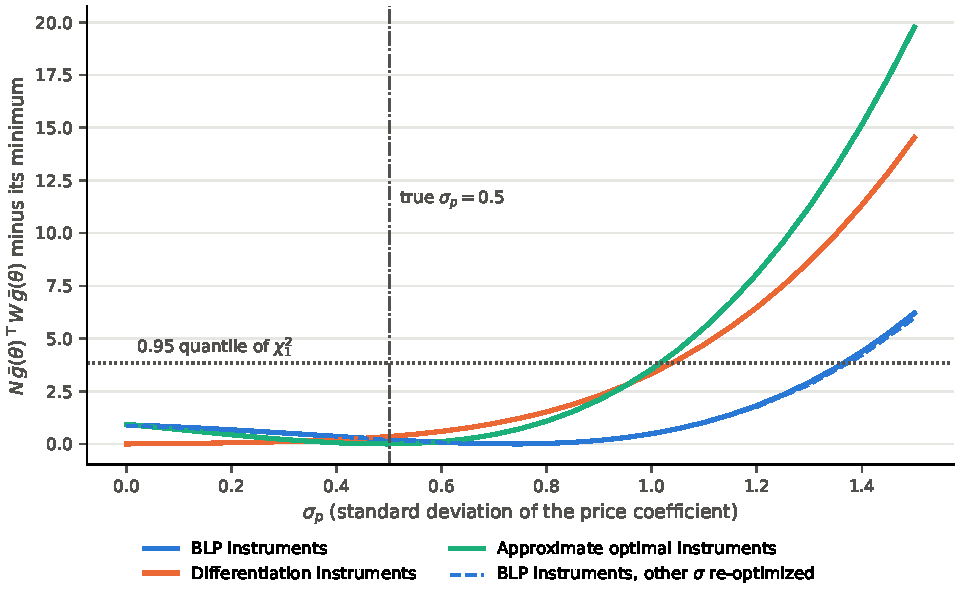
\includegraphics[width=0.92\linewidth]{figures/ch08/sim_profile.pdf}
\caption{The GMM objective as a function of the standard deviation of the price coefficient in the simulated market.
Each solid curve holds the other three standard deviations at the estimate of its instrument set, concentrates out the
linear parameters and uses the second-step weighting matrix. The dashed curve re-optimizes the other three standard
deviations for the BLP instruments. Curves are shifted so that their minimum is zero. The dotted line is the 0.95
quantile of the $\chi^2_1$ distribution, and the dash-dotted line marks the true value $\sigma_p = 0.5$.}
\label{fig:08-profile}
\end{figure}

Why is $\Sigma$ so hard to estimate here? Its identification needs variation that shifts substitution patterns
(\cref{sec:08-instruments}). In this design every product has the same characteristics and the same cost shifter in
every market. The only sources of cross-market variation are the choice set and the prices, and the price of a given
product varies little across markets. Its standard deviation across markets is between 0.045 and 0.061, against 0.189
for all prices together. The inside goods also take only 5 to 21 percent of each market, so most substitution is to
the outside good. Changes in the choice set then move the shares of the remaining products by small amounts, which the
demand shocks, with standard deviation 0.50, easily mask. The simulation correction is small by comparison. It raises
the standard errors by at most 6 percent with the BLP instruments and by less than 1 percent with the other two sets.

The lesson is general. The price coefficient is identified by the cost shifter in every specification, and its
instrumental variables estimates range from 2.5 to 3.5. The standard deviations depend on much weaker variation. A good fit and an
unrejected overidentification test do not certify them. Step 7 shows what is at stake for the substitution patterns.

\subsection{Step 7: elasticities and diversion}\label{sec:08-worked-elas}

We compute the price elasticities of market 0 under each model. Under the random coefficients models we use the
1,000 estimation draws and the recovered mean utilities of that market, and the derivatives of
\cref{prop:08-derivs}. The true elasticities use the true parameters and 200,000 draws, which approximates the
population integral. \Cref{tab:08-sim-elas} reports three objects: the own-price elasticities, the
responses of all shares to the price of product 4, and the diversion ratio to the outside good,
$-\frac{\partial s_0}{\partial p_k}\big(\frac{\partial s_k}{\partial p_k}\big)^{-1}$ (\cref{prop:08-diversion}). Own elasticities are
reported as positive numbers.

\begin{table}[htbp]
\centering
\caption{Elasticities and diversion in market 0.}
\label{tab:08-sim-elas}
\footnotesize
\begin{tabular}{lccccc}
\toprule
 & Logit & \multicolumn{3}{c}{Random coefficients logit} & True \\
\cmidrule(lr){3-5}
 & 2SLS & $\Sigma$ known & \makecell{GMM, approx.\\ optimal IV} & \makecell{GMM,\\ BLP IV} & \\
\midrule
\multicolumn{6}{l}{\emph{A. Own-price elasticity} $-\frac{\partial s_j}{\partial p_j}\frac{p_j}{s_j}$} \\
Product 2 & 3.47 & 3.45 & 3.45 & 3.78 & 3.58 \\
Product 3 & 2.62 & 2.68 & 2.67 & 3.02 & 2.76 \\
Product 4 & 3.70 & 3.63 & 3.64 & 3.42 & 3.77 \\
Product 6 & 2.59 & 2.65 & 2.64 & 2.99 & 2.74 \\
Product 8 & 2.80 & 2.79 & 2.81 & 3.12 & 2.89 \\
Product 9 & 3.81 & 3.74 & 3.74 & 4.01 & 3.87 \\
Product 10 & 2.44 & 2.51 & 2.51 & 2.85 & 2.59 \\
\addlinespace
\multicolumn{6}{l}{\emph{B. Cross-price elasticity with respect to $p_4$,} $\frac{\partial s_j}{\partial p_4}\frac{p_4}{s_j}$} \\
Product 2 & 0.047 & 0.078 & 0.063 & 0.988 & 0.069 \\
Product 3 & 0.047 & 0.067 & 0.059 & 0.038 & 0.060 \\
Product 6 & 0.047 & 0.066 & 0.059 & 0.038 & 0.059 \\
Product 8 & 0.047 & 0.069 & 0.060 & 0.039 & 0.062 \\
Product 9 & 0.047 & 0.079 & 0.064 & 0.978 & 0.070 \\
Product 10 & 0.047 & 0.066 & 0.058 & 0.038 & 0.059 \\
Outside good & 0.047 & 0.043 & 0.044 & 0.032 & 0.040 \\
\addlinespace
\multicolumn{6}{l}{\emph{C. Diversion to the outside good (percent)}} \\
Product 2 & 85.9 & 79.5 & 82.1 & 55.5 & 80.3 \\
Product 3 & 87.7 & 83.4 & 85.2 & 85.7 & 84.0 \\
Product 4 & 86.6 & 80.1 & 82.6 & 64.1 & 80.8 \\
Product 6 & 87.3 & 83.0 & 84.8 & 85.2 & 83.5 \\
Product 8 & 90.6 & 86.7 & 88.4 & 88.9 & 87.2 \\
Product 9 & 86.0 & 79.2 & 81.8 & 55.3 & 80.2 \\
Product 10 & 87.2 & 83.1 & 85.0 & 85.5 & 83.8 \\
\bottomrule
\end{tabular}
\par\smallskip
\parbox{\linewidth}{\footnotesize Notes: Market 0, at observed prices and realized shares. The columns use the
estimates of columns (2), (3), (6) and (4) of \cref{tab:08-sim-demand}. The true values use the true parameters, the
true mean utilities and 200,000 draws. Products 2, 4 and 9 are the organic products and the three most expensive.}
\end{table}

The own elasticities differ little across the logit, the random coefficients model with $\Sigma$ known and the model
estimated with approximate optimal instruments. All three are within 0.15 of the truth, and all are slightly too small
because the estimated price coefficients are below 3. The three most expensive products are the most elastic in every
column. With small shares the logit own elasticity is close to $\alpha p_j$, so this ordering is mechanical in the
logit. In the true model it also holds, because the standard deviation of the price coefficient is moderate.

The cross elasticities separate the models. In the logit, a rise in $p_4$ raises every share, including the outside
share, by the same 0.047 percent per percent. This is the IIA property of \cref{ch:logit}. In the true model the
organic products 2 and 9 gain most (0.069 and 0.070), the other products less (0.059 to 0.062), and the outside good
least (0.040). The model with $\Sigma$ known reproduces this pattern. The model estimated with approximate optimal
instruments shows it only weakly (0.063 and 0.064 against 0.058 to 0.060). Its estimate of $\sigma$ on organic is
zero, so only the random coefficient on price separates the expensive organic products. The model estimated with
BLP instruments gets the pattern badly wrong. Its large $\sigma$ on organic makes products 2 and 9 nearly perfect
substitutes for product 4, with cross elasticities of 0.988 and 0.978, about fourteen times the true values.

Diversion to the outside good tells the same story. The logit sends between 85.9 and 90.6 percent of a product's lost
buyers to the outside good, the value $\frac{s_0}{1 - s_k}$ of \cref{ch:logit}. The true model sends between 80.2 and
87.2 percent, and the models with $\Sigma$ known and with approximate optimal instruments come close. Under the BLP
instrument estimates, only 55 percent of the buyers lost by product 2 or 9 leave the market. Panel B suggests where
the others go: to the other organic products. A merger between the firms that sell products 2 and 9 would look far more harmful
under these estimates than under the true model (\cref{ch:mergers}). \Cref{fig:08-ownelas} summarizes the comparison.

\begin{figure}[htbp]
\centering
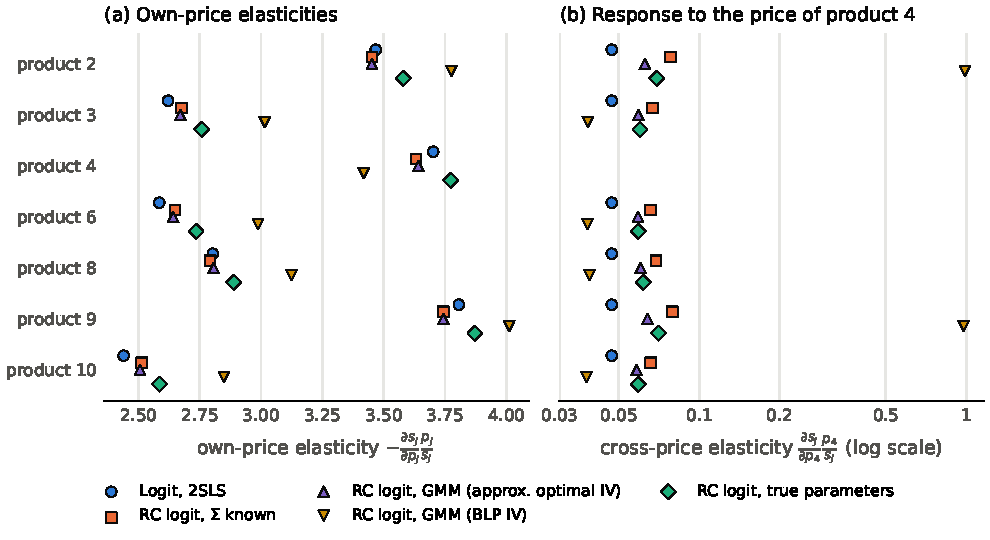
\includegraphics[width=\linewidth]{figures/ch08/sim_ownelas.pdf}
\caption{Elasticities in market 0 of the simulated market. Panel (a) shows own-price elasticities as positive numbers.
Panel (b) shows the cross-price elasticity of each product's share with respect to the price of product 4, on a log
scale. The random coefficients columns use the estimates of \cref{tab:08-sim-demand}, and the true values use 200,000
draws.}
\label{fig:08-ownelas}
\end{figure}

\subsection{What the simulated market teaches}\label{sec:08-worked-lessons}

Four lessons carry over to applications. First, the computational steps are fast and reliable when implemented
carefully. The Morrow-Skerlos iteration finds the equilibrium in 10 to 13 iterations, and the contraction recovers the
mean utilities to $10^{-12}$ in about 15 to 25 iterations. Second, a strong cost shifter identifies the mean price
coefficient well. The logit estimate is biased toward zero by the sorting of less price-sensitive consumers into
expensive products, and the random coefficients model removes most of the bias when $\Sigma$ is right.

Third, $\Sigma$ is the hard part. With market-level data its identification rests on variation in choice sets and in
the characteristics of competing products. When that variation is weak, the estimates of $\Sigma$ and the substitution
patterns they imply can be far from the truth, even when the overidentification test passes. The diagnostics that
reveal the problem are cheap: several starting values, the profile of the objective, the eigenvalues of $G^\top WG$,
and comparisons across instrument sets.

Fourth, the remedies are the subjects of the preceding sections. Richer cross-market variation helps, as do approximate
optimal instruments. Micro moments and second-choice data identify $\Sigma$ from within-market variation
(\cref{sec:08-micro}). A supply side adds moments that depend on $\Sigma$ through the markups (\cref{sec:08-supply}).
Where none of these is available, the appropriate report is the range of substitution patterns consistent with the
data.

\section{Case study: Berry, Levinsohn and Pakes (1995), U.S. automobiles}\label{sec:08-blp95}

\citet{BerryLevinsohnPakes1995}, henceforth BLP, turned the random coefficients logit into a working
tool for industrial organization. They estimate demand and marginal cost for essentially every car
model sold in the United States from 1971 to 1990. They use only product-level data on prices,
quantities and characteristics, together with the distribution of household income. The estimates
come from a model in which consumers choose one car or none and multi-product firms set prices in a
Nash equilibrium.

The general model, its computation and its identification occupy
\cref{sec:08-model,sec:08-substitution,sec:08-simulation,sec:08-inversion,sec:08-gmm,sec:08-instruments,sec:08-supply}.
This section applies that machinery to the paper itself. We follow the order used for every deep case
study in this book. We take up the question, the setting, the data, the model, and the estimator with
its identification. Then come the results, robustness, interpretation, critiques and contribution. We
reproduce the
paper's Tables III, IV, V, VII, VIII and IX in full, Table I in condensed form, and an excerpt of
Table VI. Several derived quantities in this section are our own calculations from the published
tables, and we say so each time.

\subsection{The question and why it matters}\label{sec:08-blp95-question}

The paper asks how to recover demand and cost parameters for a whole differentiated-products industry
when only market-level data are available. The answers must be consistent with an oligopoly
equilibrium. On the demand side BLP want own- and cross-price elasticities for every model, and
elasticities of demand with respect to attributes such as fuel efficiency. On the cost side they want
marginal cost as a function of product characteristics.

These objects are inputs to many policy questions. BLP list trade policy (import restrictions),
merger policy, environmental policy (gas-guzzler and carbon taxes, emission standards and fuel
economy standards) and the construction of price indices (Section 8.1 of the paper). The automobile
market was large, with sales above \$150 billion in 1989 (p.~843). It was also at the center of trade
and environmental debates.

The obvious alternative is a demand system written directly in product space. A constant-elasticity
system for 100 products has 10,000 own- and cross-price elasticities (p.~842). Researchers therefore
aggregate products into groups. BLP point out that a grouping that suits one question rarely suits
another. Aggregating all foreign and all domestic cars may serve a tariff study, but it is useless for
domestic competition or pollution taxes. Product-space systems also cannot predict demand for new
goods, and they make it hard to use information on the distribution of consumers.

BLP work in characteristics space, following \citet{Lancaster1971} and \citet{McFadden1974}. They
identify two problems with the discrete-choice models available at the time. The first is the
functional form of utility, which in logit-type models forces implausible substitution patterns. The
second is the correlation between price and product characteristics that consumers see and the
econometrician does not. BLP call this the differentiated-products analog of the classical
simultaneity problem. They solve the aggregation problem by simulation, as in \citet{Pakes1986}. They
solve the simultaneity problem by inverting the share equations, as in \citet{Berry1994}.

\subsection{Setting and earlier approaches}\label{sec:08-blp95-setting}

Early work treated cars as a homogeneous product and estimated aggregate demand \citep{Suits1958}.
\citet{Griliches1971} introduced hedonic price regressions for cars, which work at the level of the
individual model but do not model the production side. BLP call \citet{Bresnahan1987} perhaps the first
attempt to model and estimate demand and oligopoly pricing jointly (p.~844). He used a vertical differentiation model with a
uniform density of consumers along the quality line (\cref{ch:discrete}).
\citet{FeenstraLevinsohn1995} allowed several dimensions of differentiation but kept the uniform
density. \citet{Manski1983} studied demand and a perfectly competitive supply side for the Israeli car
market.

Micro-data studies of car demand had alternatives to BLP's solutions. They could interact consumer
and product characteristics, or use nested logit, which BLP note is a restricted random coefficients
model on group dummies (p.~851). Nested logit requires a priori knowledge of the order and content of
the nests. Product-specific constants, which would absorb unobserved quality, are hard to estimate with
micro data. There are on average more than 100 products per year in BLP's sample. The Consumer
Expenditure Survey records only about 500 new-car purchases per year (p.~852). Even with product
dummies, one still has to separate the effects of price, observed characteristics and unobserved
quality, which requires the kind of instrumental-variable assumptions BLP make.

The vertical model restricts substitution severely. A product has nonzero cross-price elasticities only
with its two neighbors on the price ladder. BLP give an example with a \$24,998 station wagon, a
\$24,999 sports car and a \$25,000 station wagon (p.~852). The vertical model makes the two wagons
non-substitutes and the sports car a substitute for both. The logit model fails in the opposite way.
If a cheap Yugo and an expensive Mercedes have the same share, a rise in the BMW's price must raise
both of their sales by the same amount (p.~847). Two products with equal shares must also have equal
own-price derivatives, and hence equal markups under single-product pricing
(\cref{sec:08-substitution}).

Finally, BLP stress the structural error $\xi_{jt}$. Without it, only sampling error separates the
model's predicted shares from the data. With aggregate samples of millions of households, a
chi-square test of the model's restrictions on the multinomial shares rejects with probability close
to one (p.~850). The unobserved characteristic plays the role of the demand disturbance in
homogeneous-goods markets. Because firms know it when they set prices, prices are correlated with it.

\subsection{Data}\label{sec:08-blp95-data}

The unit of observation is a car model in a year, and a market is the national market in a year.
Product characteristics come from annual issues of the \emph{Automotive News Market Data Book},
combined with a similar data set from Ernst Berndt (p.~868). The sample covers essentially all models
sold from 1971 to 1990. Only ``exotic'' models with tiny shares, such as Ferrari and Rolls Royce, are
excluded. The panel is unbalanced because models enter and exit. It has 2,217 model-years.

BLP need a rule that links model-years into models, because their standard errors allow correlation
within a model over time. Two observations in adjacent years are the same model if they have the same
name and their horsepower, width, length and wheelbase each change by at most ten percent. With this
rule the 2,217 model-years represent 997 distinct models (p.~869).

The variables are as follows.
\begin{itemize}
\item \emph{Price} is the list retail price of the base model, in thousands of 1983 dollars (deflated
  by the CPI). BLP would prefer transaction prices but could not find them.
\item \emph{Quantity} is U.S. sales by nameplate, in thousands. Fleet sales are not observed, so fleet
  buyers are treated as agents of households (footnote 23).
\item \emph{HPWT} is horsepower divided by weight, in horsepower per 10 pounds.
\item \emph{Air} equals one if air conditioning is standard equipment.
\item \emph{MP\$} (miles per dollar) is the EPA miles-per-gallon rating divided by the real price of
  unleaded gasoline. It measures the cost of driving and enters utility. The production cost of fuel
  efficiency is captured instead by \emph{MPG}, which enters the cost function.
\item \emph{Size} is length times width.
\item \emph{Reliability} is the Consumer Reports rating from 1 to 5, available for part of the sample
  and rescaled every year (footnote 24). It appears only in one robustness check.
\end{itemize}
The market size $M_t$ is the number of U.S. households in year $t$, from the \emph{Statistical
Abstract}. The parameters of the household income distribution come from the March Current Population
Survey (CPS) for each year. Divisions of one parent company form one firm, so Buick, Cadillac,
Chevrolet, Oldsmobile and Pontiac all belong to General Motors. There are 22 firms (footnote 29). Each
model is assigned the country of its producing firm.

\begin{table}[htbp]
\centering
\caption{Descriptive statistics of the BLP (1995) data, selected years (condensed from their Table I)}
\label{tab:08-blp-desc}
\footnotesize
\setlength{\tabcolsep}{3.6pt}
\begin{tabular}{@{}lrrrrrrrrrrr@{}}
\toprule
Year & Models & Quantity & Price & Domestic & Japan & Europe & HPWT & Size & Air & MPG & MP\$ \\
\midrule
1971 & 92  & 86.892  & 7.868  & 0.866 & 0.057 & 0.077 & 0.490 & 1.496 & 0.000 & 1.662 & 1.850 \\
1973 & 86  & 92.785  & 7.535  & 0.932 & 0.040 & 0.028 & 0.364 & 1.529 & 0.022 & 1.589 & 1.819 \\
1974 & 72  & 105.119 & 7.506  & 0.887 & 0.050 & 0.064 & 0.347 & 1.510 & 0.026 & 1.568 & 1.453 \\
1975 & 93  & 84.775  & 7.821  & 0.853 & 0.083 & 0.064 & 0.337 & 1.479 & 0.054 & 1.584 & 1.503 \\
1980 & 103 & 71.567  & 7.718  & 0.773 & 0.191 & 0.036 & 0.350 & 1.296 & 0.078 & 2.215 & 1.466 \\
1985 & 136 & 78.143  & 8.938  & 0.761 & 0.191 & 0.048 & 0.372 & 1.265 & 0.140 & 2.261 & 2.024 \\
1988 & 150 & 67.078  & 10.069 & 0.717 & 0.237 & 0.045 & 0.396 & 1.251 & 0.237 & 2.334 & 2.919 \\
1990 & 131 & 66.377  & 10.337 & 0.682 & 0.276 & 0.043 & 0.419 & 1.270 & 0.308 & 2.270 & 2.852 \\
\midrule
All  & 2217 & 78.804 & 8.604  & 0.790 & 0.161 & 0.049 & 0.372 & 1.357 & 0.116 & 2.099 & 2.086 \\
\bottomrule
\end{tabular}

\smallskip
\begin{minipage}{0.97\linewidth}
\footnotesize
Notes: Source: \citet{BerryLevinsohnPakes1995}, Table I (p.~870), which reports all 20 years.
``Models'' is the number of models and ``Quantity'' is mean sales per model. The remaining nine columns
are sales-weighted means. Quantity is in thousands of cars and price in thousands of 1983 dollars. HPWT
is in horsepower per 10 pounds, MPG in tens of miles per gallon and MP\$ in tens of miles per 1983 dollar
of gasoline. Domestic, Japan and Europe are
dummies for the location of the producing firm's headquarters.
\end{minipage}
\end{table}

\Cref{tab:08-blp-desc} shows the main trends. The number of models rose from a low of 72 in 1974 to a
high of 150 in 1988, while sales per model trended down. The sales-weighted list price stayed between
about \$7,500 and \$8,000 during the 1970s. It then rose from \$7,718 in 1980 to \$10,337 in 1990, about a
third.\footnote{The text of \citet[p.~870]{BerryLevinsohnPakes1995} says that the real sales-weighted list price
``has risen almost 50 percent during the 1980's.'' Their Table I, which is already in 1983 dollars, implies an
increase of $\frac{10.337}{7.718} - 1 = 34$ percent from 1980 to 1990. Measured from the 1979 value of 7.599, the
increase is 36 percent. We follow the table.} The characteristics changed at the same time, so the price of a fixed bundle need not have
risen. HPWT fell in the early 1970s and then trended up, mostly because cars became lighter. Fuel cost
efficiency improved, from 18.50 miles per 1983 dollar of gasoline in 1971 to 28.52 in 1990. Air
conditioning was standard on no car at the start and on 30.8 percent at the end. The domestic share
fell from a 1973 high of 93.2 percent to 68.2 percent in 1990, while the Japanese share rose from 4.0 to
27.6 percent.

BLP's Table II reports quartiles of the continuous variables and names the models at each quartile.
The cheapest car is the 1990 Yugo at \$3,393 (1983 dollars). The median price is \$8,728 and the 75th
percentile is \$13,074. The most expensive car is a 1989 Porsche 911 Cabriolet at \$68,597. Sales range
from 49 cars to 577,313 cars (the 1971 Chevrolet Impala), with a median of 47,345. MPG ranges from 9
(1974 Cadillac Eldorado) to 53 (1989 Geo Metro). We use the price quartiles below to interpret the
logit results.

The data also pin down the size of the outside good. Total 1990 sales are about
$131\times 66.377\approx 8{,}695$ thousand cars (\cref{tab:08-blp-desc}). BLP describe the logit column
of their Table VII as $\frac{s_0}{1-s_j}$, and its entries lie between 90.458 and 90.883 percent.
Because $\frac{s_0}{1-s_j}$ exceeds $s_0$, the smallest entry bounds the outside share, $s_0 < 0.9046$.
The entries do not rise with the shares as the formula requires (the best-selling Accord has the
smallest entry), so we read them only as $s_0 \approx 0.90$. With $s_0$ near 0.90,
$M_{1990}=\frac{8.695}{1-s_0}$ is roughly 90 million households (our calculation). Most households do not buy a new car in a given year, so the outside good is large.

\subsection{The model}\label{sec:08-blp95-model}

\casehead{Utility}
BLP nest random coefficients in the Cobb-Douglas utility \eqref{eq:08-cobb-douglas} over the car's
characteristics and spending on other goods (their eq.~2.6). Its logarithm gives the inside and outside
utilities \eqref{eq:08-blp-inside} and \eqref{eq:08-blp-outside} (their eqs.~2.7a and 2.7b), which
\cref{sec:08-income} derived. BLP write $\bar\beta$ for our $\beta$. The taste shocks $\nu_{ik}$ have mean
zero and unit variance, so characteristic $k$ has marginal utility $\beta_k+\sigma_k\nu_{ik}$, with mean
$\beta_k$ and variance $\sigma_k^2$. The term $\sigma_0\nu_{i0}$ lets the outside option have more
idiosyncratic variance than the inside goods. BLP motivate it by unobserved differences in access to
public transport and in used-car holdings (p.~849).

BLP prefer this form to the plain random coefficients model
$u_{ij}=x_j\beta-\alpha p_j+\xi_j+\sum_k\sigma_kx_{jk}\nu_{ik}+\epsilon_{ij}$ (their eq.~2.5) for two
reasons (p.~848). They have outside information on the income distribution, and they have a
theoretical rationale for the form of the interaction between income and price. The Cobb-Douglas form
uses both.

\casehead{The estimated form}
The empirical model adds a year index $t$ and makes income random. Household income is lognormal,
$y_{it}=e^{m_t+\sigma_y\nu_{iy}}$, with year-specific mean $m_t$ and a common standard deviation
$\sigma_y$, both estimated from the CPS. The utility functions are \eqref{eq:08-blp-final-inside} and
\eqref{eq:08-blp-final-outside} (their eqs.~6.14a and 6.14b). The vector
$(\nu_{iy},\nu_{i0},\nu_{i1},\dots,\nu_{iK})$ is standard multivariate normal, independent of everything
else. BLP hold each simulated consumer's draws fixed over the 20 years of the panel. The idiosyncratic
shocks $\epsilon_{ijt}$ are \iid\ type-I extreme value. BLP did not estimate a separate $\sigma_y$ for each
year because those estimates were imprecise. They also tried drawing incomes directly from the CPS, which
gave imprecise simulators, especially in the upper tail (footnote 21).

The characteristics in utility are $x_{jt}=(1,\mathit{HPWT}_{jt},\mathit{Air}_{jt},
\mathit{MP\$}_{jt},\mathit{Size}_{jt})$, so $K=5$. Each has a mean $\beta_k$ and a standard deviation
$\sigma_k$. Price carries no separate random coefficient. Heterogeneity in price sensitivity comes
entirely from income, as we now show.

\casehead{Mean utility and individual deviations}
Choice probabilities depend only on utility differences, so we subtract \eqref{eq:08-blp-final-outside} from
\eqref{eq:08-blp-final-inside} and normalize $\xi_{0t}=0$. The deterministic part of the difference is
\begin{align*}
u_{ijt}-u_{i0t}-(\epsilon_{ijt}-\epsilon_{i0t})
 &=\alpha\big[\ln(y_{it}-p_{jt})-\ln y_{it}\big]+x_{jt}\beta+\xi_{jt}
   +\sum_k\sigma_kx_{jkt}\nu_{ik}-\sigma_0\nu_{i0}\\
 &=\underbrace{x_{jt}\beta+\xi_{jt}}_{\delta_{jt}}
   +\underbrace{\alpha\ln\Big(1-\frac{p_{jt}}{y_{it}}\Big)+\sum_k\sigma_kx_{jkt}\nu_{ik}
   -\sigma_0\nu_{i0}}_{\mu_{ijt}} .
\end{align*}
Three features of this decomposition matter for estimation. First, the mean utility
\begin{equation}\label{eq:08-blp-delta}
\delta_{jt}=x_{jt}\beta+\xi_{jt}
\end{equation}
contains no price term. Price enters only through $\mu_{ijt}$, so $\alpha$ is a nonlinear parameter.
In the chapter's notation $\theta_1=\beta$ and $\theta_2=(\alpha,\sigma_1,\dots,\sigma_5)$. Second, the
constant is the first characteristic ($x_{j1t}=1$), so the terms $\sigma_1\nu_{i1}-\sigma_0\nu_{i0}$
combine into one normal random variable with variance $\sigma_1^2+\sigma_0^2$. A random coefficient on
the inside-good constant and an extra shock on the outside good are therefore observationally
equivalent, and only the combined variance is identified. This is why BLP's footnote 6 describes
$\sigma_0\nu_{i0}$ as a random coefficient on the constant. The reported standard deviation on the
constant measures this combined dispersion. Third,
$\mu_{ijt}$ is defined only when $y_{it}>p_{jt}$. A simulated household whose income draw is below a
car's price cannot buy that car, and an implementation must remove the car from that household's
choice set.

\casehead{Market shares}
Conditional on $\nu_i$, integrating the extreme value shocks gives the logit form
\eqref{eq:08-individual-share} (their eq.~6.6). The market share \eqref{eq:08-share-integral} integrates over the
standard normal vector $\nu_i$, with income determined by $\nu_{iy}$ (their eq.~6.7). The inner integral has a
closed form and the outer one does not. BLP evaluate it by simulation (\cref{sec:08-simulation}).

\casehead{Price derivatives and elasticities}
Differentiating $\mu_{ijt}$ gives the price sensitivity of household $i$ for car $j$:
\begin{equation*}
\frac{\partial\mu_{ijt}}{\partial p_{jt}}=-\frac{\alpha}{y_{it}-p_{jt}} .
\end{equation*}
This sensitivity falls with income. It also rises with the car's own price, because a dollar is
worth more when less is left for other goods. A first-order expansion of the log for small
$\frac{p_{jt}}{y_{it}}$ gives
\begin{equation*}
\alpha\ln\Big(1-\frac{p_{jt}}{y_{it}}\Big)\approx-\alpha\,\frac{p_{jt}}{y_{it}},
\end{equation*}
so household $i$ behaves approximately as if its price coefficient were $\frac{\alpha}{y_{it}}$.
Applying the general derivative formulas of \cref{prop:08-derivs} with this price sensitivity gives
\begin{align}
\frac{\partial s_{jt}}{\partial p_{jt}}&=-\int\frac{\alpha}{y_{it}-p_{jt}}\,
  s_{ijt}(1-s_{ijt})\,\dd F(\nu_i),\label{eq:08-blp-dsown}\\
\frac{\partial s_{jt}}{\partial p_{qt}}&=\int\frac{\alpha}{y_{it}-p_{qt}}\,s_{ijt}s_{iqt}\,
  \dd F(\nu_i),\qquad q\neq j\label{eq:08-blp-dscross}
\end{align}
(their eqs.~6.9a and 6.9b). The derivative of the outside share is
$\frac{\partial s_{0t}}{\partial p_{qt}}=\int\frac{\alpha}{y_{it}-p_{qt}}s_{i0t}s_{iqt}\,\dd F(\nu_i)$.

BLP report \emph{semi-elasticities}, which we denote
\begin{equation}\label{eq:08-blp-semi}
e_{jq}\equiv\frac{100}{s_j}\,\frac{\partial s_j}{\partial p_q},
\end{equation}
with prices in thousands of dollars. The entry $e_{jq}$ is the percentage change in the share of $j$
when the price of $q$ rises by \$1,000. The elasticity follows by multiplying by
$\frac{p_q}{100}$, so the own-price elasticity, written as a positive number, is
$\varepsilon_j=-\frac{p_j}{100}\,e_{jj}$. The logit benchmark has $e_{jj}=-100\,\alpha(1-s_j)$ and
$e_{jq}=100\,\alpha s_q$.

\casehead{Costs and pricing}
Firm $f$ produces the set $\mathcal{J}_f$ of models. Marginal cost is constant in output and log-linear
in observed cost characteristics $w_j$ and an unobserved cost shock $\omega_j$:
\begin{equation}\label{eq:08-blp-mc}
\ln mc_j=w_j\gamma+\omega_j
\end{equation}
(their eq.~3.1). The cost characteristics are a constant, $\ln\mathit{HPWT}$, $\mathit{Air}$,
$\ln\mathit{MPG}$, $\ln\mathit{Size}$ and a time trend. MPG replaces MP\$ because the production cost
of fuel efficiency does not depend on the retail price of gasoline, at least in the short run. The
trend captures technical change and regulation. Logs of the continuous attributes make the cost
coefficients elasticities of marginal cost. BLP allow $\omega_j$ to be correlated with $\xi_j$, since
cars with more unobserved quality may cost more to build.

Firm $f$'s profit is \eqref{eq:08-profit} (their eq.~3.2), and each firm chooses its prices given rivals'
prices. An interior Nash equilibrium satisfies the first-order conditions \eqref{eq:08-foc} (their eq.~3.3).
\Cref{sec:08-supply-foc} showed that BLP's markup formula (their eqs.~3.4 and 3.5) is our
\eqref{eq:08-markup}, and that substituting it into \eqref{eq:08-blp-mc} gives the pricing equation
\eqref{eq:08-pricing-log} (their eq.~3.6). The markup depends on $\omega$ through the equilibrium prices, and on
$\xi$ directly. It therefore cannot be treated as exogenous in the pricing equation.

BLP assume that a Nash equilibrium exists with prices in the interior of the positive orthant
(footnote 12). The existence results of \citet{CaplinNalebuff1991} cover single-product firms and do
not extend easily to multi-product firms. BLP instead check existence numerically at their estimates.
None of the properties of the estimator requires a unique equilibrium. Without uniqueness, however, it
is not clear how to use the estimates for policy counterfactuals.

\subsection{Estimation and identification}\label{sec:08-blp95-estimation}

\casehead{Moment conditions}
Let $z_j=(x_j,w_j)$ collect the demand and cost characteristics of product $j$, and let
$z=(z_1,\dots,z_J)$ collect them for all products in the market. BLP's identifying assumption is
\begin{equation}\label{eq:08-blp-moments}
\E[\xi_j\mid z]=\E[\omega_j\mid z]=0
\end{equation}
(their eq.~4.1). Prices and quantities are excluded from the conditioning set because the model
determines them partly through $\xi$ and $\omega$. Characteristics and cost shifters are treated as
predetermined because the model does not explain how they are chosen.

BLP acknowledge that \eqref{eq:08-blp-moments} holds only if the true process that chooses
characteristics has special properties (p.~854). They mention an alternative for panel data. The
pair $(\xi,\omega)$ of a model could follow a first-order Markov process whose innovations are
independent of the model's initial characteristics. This assumption would also identify the model, but
it would demand much more of the data, so BLP start from \eqref{eq:08-blp-moments}.

\casehead{Why characteristics of other products are instruments}
Under \eqref{eq:08-blp-moments}, any function of $z$ is a valid instrument. The question is which
functions carry information. BLP's answer comes from oligopoly pricing (p.~855). Products that face
close substitutes have low markups, so the characteristics of rival products shift a product's price.
Nash markups respond differently to products of the same firm and to products of rivals. The
instruments should therefore distinguish the two. The demand for $j$ depends on the characteristics of
all products, so no characteristic is excluded from the demand of $j$ in the usual sense. What
identifies demand is the restriction that the utility of $j$ depends only on the characteristics of
$j$. The number of utility parameters then grows with the number of characteristics, and not with the
number of products.

\casehead{The instrument vector}
The efficient instruments under conditional moment restrictions are infeasible here
(\cref{sec:08-optiv}). BLP instead use the first-order terms \eqref{eq:08-blp-iv} of a partially
exchangeable basis (their eq.~5.8). These are the own characteristic, its sum over the firm's other products
and its sum over rival products. \Cref{sec:08-optiv} derives this basis from the exchangeability of a
unique Nash equilibrium \citep{Pakes1994}. The two sums vary across products because they exclude different
own products, because firms offer different sets of products, and because the set of products changes over
time. The constant is one of the characteristics, so the numbers of own-firm and rival products are
instruments too.

Higher-order basis functions were nearly collinear with the first-order terms, and even the first-order
terms were nearly of reduced rank. For the demand error BLP use the three terms of
\eqref{eq:08-blp-iv} for each of the five demand characteristics, giving 15 instruments. MPG and the
trend enter cost and not demand, so they are excluded from demand. Adding them to the demand list caused
numerical problems through near collinearity, and BLP left them out. For the cost error BLP use the three terms for each of the six cost characteristics,
plus MP\$, giving 19 instruments. The estimator therefore uses $15+19=34$ moment conditions (p.~862).
There are 17 parameters: five means $\beta$, five standard deviations $\sigma$, the income coefficient
$\alpha$ and six cost parameters $\gamma$. Hence there are 17 overidentifying restrictions.

BLP enter the basis functions directly as GMM instruments, instead of first projecting the optimal
instruments on them as \citet{Newey1990} suggests (\cref{sec:08-optiv}).

\casehead{Clustering by model}
Disturbances of the same model in different years are likely to be more similar than those of
different models. BLP therefore treat the sum of a model's moments over the years it is sold as one
draw from an exchangeable population of models. Let $z^d_{mt}$ and $z^s_{mt}$ be the 15 demand and 19
cost instruments of model $m$ in year $t$, and let $\mathcal{T}_m$ be the years in which $m$ is sold.
The moment contribution of model $m$ is
\begin{equation}\label{eq:08-blp-gm}
g_m(\theta)=\sum_{t\in\mathcal{T}_m}\begin{pmatrix} z^{d\T}_{mt}\,\xi_{mt}(\theta)\\
z^{s\T}_{mt}\,\omega_{mt}(\theta)\end{pmatrix}\in\R^{34}.
\end{equation}
BLP write this as $\sum_t[f_{mt}(z)^{\T}\otimes I_2](\xi_{mt},\omega_{mt})^{\T}$, with the
instrument blocks restricted as described above. The estimator minimizes
\begin{equation}\label{eq:08-blp-obj}
Q(\theta)=\bar g(\theta)^{\T}\,W\,\bar g(\theta),\qquad
\bar g(\theta)=\frac{1}{997}\sum_{m=1}^{997}g_m(\theta),
\end{equation}
with $W$ a consistent estimate of the inverse covariance matrix of $g_m$. The resulting standard errors
allow arbitrary correlation across years within a model and arbitrary heteroskedasticity across
models. BLP note that this is probably not the most efficient way to use the panel.

\casehead{Computing the objective}
Each evaluation of the moments takes four steps for a given $\theta$ (p.~863).
\begin{enumerate}
\item Simulate the market shares $s_{jt}(\delta_t;\theta_2)$ implied by the model.
\item Solve for the mean utilities $\delta_t$ that equate simulated and observed shares, and set
  $\xi_{jt}=\delta_{jt}-x_{jt}\beta$.
\item Compute the markups $b_{jt}$ from the simulated share derivatives and set
  $\omega_{jt}=\ln(p_{jt}-b_{jt})-w_{jt}\gamma$.
\item Interact $\xi$ and $\omega$ with the instruments to form \eqref{eq:08-blp-gm}.
\end{enumerate}
The logit benchmark puts price in the mean utility, $\delta_{jt}=x_{jt}\beta-\alpha p_{jt}+\xi_{jt}$, and
sets $\mu_{ijt}=0$. Every step is then analytic. Shares are
$s_{jt}=\frac{e^{\delta_{jt}}}{1+\sum_qe^{\delta_{qt}}}$, the inversion is
$\delta_{jt}=\ln s_{jt}-\ln s_{0t}$, and the demand error is
$\xi_{jt}=\ln s_{jt}-\ln s_{0t}-x_{jt}\beta+\alpha p_{jt}$ (their eqs.~6.3 to 6.5). In the full model
step~2 uses the contraction
\begin{equation*}
\delta_{jt}^{h+1}=\delta_{jt}^{h}+\ln s^{\text{obs}}_{jt}-\ln s_{jt}\big(\delta_t^{h};\theta_2\big)
\end{equation*}
(their eq.~6.8), whose convergence BLP prove in their Appendix~I (\cref{thm:08-contraction}).

Step~1 uses the importance sampler \eqref{eq:08-blp-importance} of \cref{sec:08-importance} (their
eq.~6.13). BLP first obtain a preliminary estimate $\theta'$ with the plain smooth simulator. They then
accept population draws of $\nu$ with probability $\bar f(\nu;\theta')$, the probability that a household
with tastes $\nu$ buys some car, and reweight each accepted draw by $\frac{\bar s(\theta')}{\bar
f(\nu;\theta')}$. The sampler oversamples households likely to buy a car, which is where the integrand is
large. The same draws are used for every share, so the simulated shares sum to one, as the contraction
requires.

The first-order conditions of \eqref{eq:08-blp-obj} are linear in $\beta$ and $\gamma$ given
$(\alpha,\sigma)$. Both $\xi=\delta(\theta_2)-X\beta$ and $\omega=\ln(p-b(\theta_2))-W_c\gamma$ are linear
in the linear parameters, where $W_c$ stacks the $w_{jt}$. The markup depends only on $\theta_2$ because
it is computed from the inverted $\delta$ and the share derivatives. BLP concentrate out $\beta$ and
$\gamma$ as in \cref{prop:08-concentrate} and search over the six elements of $(\alpha,\sigma)$ with the
\citet{NelderMead1965} simplex method (p.~868).

\casehead{Standard errors}
The asymptotic variance is \eqref{eq:08-blp-avar}, the sandwich with the three variance pieces $V_1$
(product characteristics), $V_2$ (consumer sampling) and $V_3$ (simulation) derived in
\cref{sec:08-asymptotics}. With about 100 million U.S. households, $V_2$ is negligible and $V_3$ is not.
BLP estimate $V_3$ by redrawing the simulation draws. The correction raises the standard errors in their
Table IV by about 5 to 20 percent, except for one parameter whose standard error doubles (p.~859).

\casehead{What identifies the parameters}
Four sources of information identify the model. The cross-section of mean utilities, together with the
characteristics instruments, identifies $\beta$ and the overall level of price sensitivity. The CPS
income distribution fixes how price sensitivity varies across households, up to the single parameter
$\alpha$. The standard deviations $\sigma_k$ are identified by how shares respond to the configuration
of products in characteristics space. BLP explain the distinction between a mean and a variance with
HPWT (p.~877). Cars with high HPWT can be popular because the mean taste for HPWT is high, or because
the taste is dispersed and some consumers value HPWT a lot. Both raise the share of high-HPWT cars.
They have different implications for substitution. With dispersed tastes, consumers who leave a
high-HPWT car are those who value HPWT most, so they move disproportionately to other high-HPWT cars.

The panel helps here. BLP report that separating means from variances was much harder in a single
cross section than in the panel, which was one reason to use twenty years of data (footnote 30). The
supply side adds a fourth source. The markups in \eqref{eq:08-markup} depend on $\theta_2$, so the
cost moments carry information about demand (\cref{sec:08-supply}). BLP note that their use of
``identification'' is informal and that a formal argument would need further regularity conditions
(footnote 13). \Cref{sec:08-instruments} discusses what later work established.

\subsection{Results I: logit benchmarks}\label{sec:08-blp95-logit}

BLP first estimate two logit models and a marginal-cost pricing regression. The logit models give a
transparent reference point. They also isolate the effect of instrumenting for price, because the IV
logit keeps the logit's substitution patterns. \Cref{tab:08-blp-logit} reproduces their Table III.

\begin{table}[htbp]
\centering
\caption{Logit demand and marginal-cost pricing, 2,217 observations (BLP 1995, Table III)}
\label{tab:08-blp-logit}
\small
\begin{tabular}{@{}lccc@{}}
\toprule
 & OLS logit & IV logit & OLS $\ln(\text{price})$ \\
Variable & demand & demand & on $w$ \\
\midrule
Constant & $-10.068$ & $-9.273$ & 1.882 \\
         & (0.253) & (0.493) & (0.119) \\
HPWT$^{*}$ & $-0.121$ & 1.965 & 0.520 \\
         & (0.277) & (0.909) & (0.035) \\
Air      & $-0.035$ & 1.289 & 0.680 \\
         & (0.073) & (0.248) & (0.019) \\
MP\$     & 0.263 & 0.052 & \\
         & (0.043) & (0.086) & \\
MPG$^{*}$ & & & $-0.471$ \\
         & & & (0.049) \\
Size$^{*}$ & 2.341 & 2.355 & 0.125 \\
         & (0.125) & (0.247) & (0.063) \\
Trend    & & & 0.013 \\
         & & & (0.002) \\
Price    & $-0.089$ & $-0.216$ & \\
         & (0.004) & (0.123) & \\
\midrule
No.\ of inelastic demands & 1494 & 22 & n.a. \\
(at $\pm 2$ s.e.) & (1429--1617) & (7--101) & \\
$R^2$ & 0.387 & n.a. & 0.656 \\
\bottomrule
\end{tabular}

\smallskip
\begin{minipage}{0.86\linewidth}
\footnotesize
Notes: Source: \citet{BerryLevinsohnPakes1995}, Table III (p.~873). Standard errors in
parentheses. The dependent variable in the demand columns is $\ln s_{jt}-\ln s_{0t}$. Starred
continuous characteristics enter demand in levels and the price regression in logs. The IV logit uses
the instruments of \eqref{eq:08-blp-iv}. Column 3 assumes marginal-cost pricing.
\end{minipage}
\end{table}

\casehead{OLS logit}
The first column regresses $\ln s_{jt}-\ln s_{0t}$ on the characteristics and price by OLS. The
coefficients on HPWT and Air are negative but imprecise, which BLP call anomalies.\footnote{The text
on p.~872 names ``air conditioning and size'' as the variables with negative coefficients. In the
printed table the negative coefficients are on HPWT and Air, while Size has a positive coefficient of
2.341. We follow the table.} The price coefficient of $-0.089$ implies that 1,494 of the 2,217 models
have inelastic demand.

This count follows directly from the logit formula. The logit own elasticity is
$\varepsilon_j=\alpha p_j(1-s_j)$, and inside shares are tiny, so demand is inelastic when
\begin{equation*}
\alpha p_j(1-s_j)<1
\iff p_j<\frac{1}{\alpha(1-s_j)}\approx\frac{1}{\alpha}.
\end{equation*}
With $\alpha=0.089$ the cutoff is $\frac{1}{0.089}\approx 11.24$, or \$11,236. The median price in
BLP's Table II is \$8,728 and the 75th percentile is \$13,074. Between half and three quarters of all
model-years should therefore be inelastic, and the reported count is 1,494, or 67 percent. The same
calculation at $\alpha\pm2(0.004)$ gives cutoffs of \$10,309 and \$12,346, which bracket the reported
range of 1,429 to 1,617 inelastic demands (our calculation).

Inelastic demand is inconsistent with profit maximization. A single-product firm sets
$\frac{p_j-mc_j}{p_j}=\frac{1}{\varepsilon_j}$, which is below one only if $\varepsilon_j>1$.
\Cref{prop:08-blp-lerner} below shows that the same requirement holds for multi-product firms. The OLS
estimate is therefore implausible on economic grounds, and BLP show that its imprecision does not
explain the problem.

\casehead{IV logit}
The second column instruments price with the characteristics-based instruments. Every characteristic
now enters utility positively, and all but MP\$ are significant. The price coefficient more than
doubles in absolute value, from $-0.089$ to $-0.216$. This is what the simultaneity story predicts:
products with high unmeasured quality sell at high prices, so OLS attributes part of the quality to a
weak price response. Only 22 models now have inelastic demand. The cutoff falls to
$\frac{1}{0.216}\approx 4.63$, or \$4,630, and the cheapest car in the sample costs \$3,393, so few
models can lie below it.\footnote{The reported range of 7 to 101 inelastic demands at $\pm2$ standard
errors cannot come from the printed standard error of 0.123 in the simple way used for the OLS column.
That interval, $0.216\pm0.246$, includes zero and negative values. The paper does not explain the
calculation, and we report the table as printed.}

The fit of the logit regression shows that unobserved characteristics are large. The OLS logit has
$R^2=0.387$, so $1-0.387=61$ percent of the variance in mean utility levels is due to $\xi$ (p.~874).

\casehead{The logit's markups}
The logit cannot generate plausible markups. The IV logit implies that all 1990 models have markups
between \$4,630 for the BMW and \$4,805 for the Chevrolet Cavalier (p.~874). GM, which sells the most
models, has the highest markups, and BMW, which sells the fewest, has the lowest.
\Cref{prop:08-logit-markup} explains why. Under the logit every product of firm $f$ has the dollar markup
$\frac{1}{\alpha(1-S_f)}$, where $S_f$ is the firm's combined share.

With $\alpha=0.216$, a firm with a negligible combined share has markup $\frac{1}{0.216}\approx4.630$
thousand dollars. This is exactly BMW's reported \$4,630. GM's \$4,805 implies
$1-S_{GM}=\frac{1}{0.216\times4.805}$, so GM's combined market share was about $3.6$ percent of
households in 1990 (our calculation). The logit therefore ties markups to the size of a firm's portfolio and to nothing
else. A Yugo and a BMW sold by firms of equal size would have identical dollar markups. BLP report that
putting $\ln p$ in place of $p$ in the logit makes markups more reasonable, but substitution remains
unreasonable (footnote 26).

\casehead{Marginal-cost pricing}
The third column assumes $p=mc$ and regresses $\ln p_j$ on $w_j$, which is a hedonic price regression.
All characteristics except MPG have positive and significant coefficients. A 10 percent increase in
HPWT is associated with a 5.2 percent increase in price, and hence in marginal cost under this
assumption. The $R^2$ of 0.656 is much higher than that of the logit demand equation. Simple functions
of characteristics explain log prices far better than they explain mean utilities (p.~875).

\subsection{Results II: parameters of the full model}\label{sec:08-blp95-params}

\Cref{tab:08-blp-full} reproduces BLP's Table IV. The first pair of columns imposes constant returns to
scale (CRTS). The second adds $\ln q_j$ to the cost function. The standard errors are corrected for
simulation error and for correlation within models over time, but not for correlation across models
(p.~875).

\begin{table}[htbp]
\centering
\caption{Demand and pricing equations, BLP specification, 2,217 observations (BLP 1995, Table IV)}
\label{tab:08-blp-full}
\small
\begin{tabular}{@{}llcccc@{}}
\toprule
 & & \multicolumn{2}{c}{Constant returns} & \multicolumn{2}{c}{With $\ln q$ in cost} \\
\cmidrule(lr){3-4}\cmidrule(l){5-6}
Parameters & Variable & Estimate & S.e. & Estimate & S.e. \\
\midrule
Means ($\beta$) & Constant & $-7.061$ & 0.941 & $-7.304$ & 0.746 \\
 & HPWT & 2.883 & 2.019 & 2.185 & 0.896 \\
 & Air & 1.521 & 0.891 & 0.579 & 0.632 \\
 & MP\$ & $-0.122$ & 0.320 & $-0.049$ & 0.164 \\
 & Size & 3.460 & 0.610 & 2.604 & 0.285 \\
\addlinespace
Std.\ deviations ($\sigma$) & Constant & 3.612 & 1.485 & 2.009 & 1.017 \\
 & HPWT & 4.628 & 1.885 & 1.586 & 1.186 \\
 & Air & 1.818 & 1.695 & 1.215 & 1.149 \\
 & MP\$ & 1.050 & 0.272 & 0.670 & 0.168 \\
 & Size & 2.056 & 0.585 & 1.510 & 0.297 \\
\addlinespace
Term on price ($\alpha$) & $\ln(y-p)$ & 43.501 & 6.427 & 23.710 & 4.079 \\
\addlinespace
Cost side ($\gamma$) & Constant & 0.952 & 0.194 & 0.726 & 0.285 \\
 & $\ln$ HPWT & 0.477 & 0.056 & 0.313 & 0.071 \\
 & Air & 0.619 & 0.038 & 0.290 & 0.052 \\
 & $\ln$ MPG & $-0.415$ & 0.055 & 0.293 & 0.091 \\
 & $\ln$ Size & $-0.046$ & 0.081 & 1.499 & 0.139 \\
 & Trend & 0.019 & 0.002 & 0.026 & 0.004 \\
 & $\ln q$ & & & $-0.387$ & 0.029 \\
\bottomrule
\end{tabular}

\smallskip
\begin{minipage}{0.9\linewidth}
\footnotesize
Notes: Source: \citet{BerryLevinsohnPakes1995}, Table IV (p.~876). Joint GMM estimation of
demand and pricing equations with 34 moments. Standard errors are corrected for simulation error and
for arbitrary correlation within a model across years. The cost function is
$\ln mc_j=w_j\gamma+\omega_j$ in the first pair of columns and
$\ln mc_j=w_j\gamma_w+\gamma_q\ln q_j+\omega_j$ in the second (p.~877).
\end{minipage}
\end{table}

\casehead{Cost side}
In the CRTS columns, the coefficients on the constant, $\ln$ HPWT, Air and the trend are positive and
significant. The coefficient on $\ln$ Size is not significant, and the coefficient on $\ln$ MPG is
negative and significant, as in the hedonic regression.

BLP compare these cost coefficients with the hedonic coefficients of \cref{tab:08-blp-logit}. The
comparison has a simple logic. Write the pricing equation \eqref{eq:08-pricing-log} as
\begin{equation*}
\ln p_j+\ln\Big(1-\frac{b_j}{p_j}\Big)=w_j\gamma+\omega_j .
\end{equation*}
For a moderate percentage markup, $\ln(1-\frac{b_j}{p_j})\approx-\frac{b_j}{p_j}$, so
\begin{equation}\label{eq:08-blp-hedonic}
\ln p_j\approx w_j\gamma+\frac{b_j}{p_j}+\omega_j .
\end{equation}
A regression of $\ln p_j$ on $w_j$ that omits the percentage markup therefore estimates approximately
$\gamma+\lambda$, where $\lambda$ is the coefficient from projecting $\frac{b_j}{p_j}$ on $w_j$. This is
the omitted-variable formula. The differences between the two sets of coefficients estimate $\lambda$.
They are 0.93 for the constant (1.882 against 0.952) and 0.171 for $\ln$ Size (0.125 against $-0.046$).
The other differences are small: 0.043 for $\ln$ HPWT, 0.061 for Air, $-0.056$ for $\ln$ MPG and
$-0.006$ for the trend (our calculation). BLP conclude that the average percentage markup is positive
and rises with size (p.~876).

The negative MPG coefficient may be an artifact of constant returns. Best-selling cars tend to have
high MPG and are large, conditional on other attributes. If marginal cost falls with output, imposing
constant returns attributes the low cost of high-volume cars to their MPG and size, and drives those
coefficients down. Adding $\ln q_j$ tests this story. In the last two columns every cost shifter is
positive and significant, including $\ln$ MPG (0.293) and $\ln$ Size (1.499). The coefficient on $\ln q$
is $-0.387$ with a standard error of 0.029, which BLP regard as implying implausibly large returns to
scale. Higher-order terms in $\ln q$ reduce the problem. BLP hesitate to push this far because output is
inaccurate for about a fifth of the sample (p.~877). U.S. sales proxy well for the production of
domestic models but not for that of imported models.

The size of these returns to scale is easy to quantify. With $\ln mc=w\gamma_w+\gamma_q\ln q+\omega$,
marginal cost is $mc(q)=A\,q^{\gamma_q}$ with $A=e^{w\gamma_w+\omega}$. Total variable cost and average
variable cost are
\begin{align*}
TVC(q)&=\int_0^qA\,x^{\gamma_q}\,\dd x=\frac{A\,q^{1+\gamma_q}}{1+\gamma_q},\\
AVC(q)&=\frac{TVC(q)}{q}=\frac{mc(q)}{1+\gamma_q}.
\end{align*}
With $\gamma_q=-0.387$, average variable cost is $\frac{1}{0.613}\approx1.63$ times marginal cost. We
can combine this factor with the markups that BLP report for this specification (\cref{tab:08-blp-robust}
below). For the Mazda 323, $mc=5.049-1.616=3.433$ and $AVC\approx5.600$ thousand dollars, above its price
of \$5,049. The price falls short of average variable cost for 10 of the 13 cars in the table (our
calculation). This makes concrete BLP's remark that markups over average variable cost are implausibly
low in this specification (p.~883).\footnote{The text on p.~883 attributes the higher markups over
marginal cost to ``decreasing returns to scale.'' A negative $\gamma_q$ means that marginal cost falls
with output, which is increasing returns, as p.~877 states. Increasing returns put marginal cost below
average variable cost, which is why markups over marginal cost rise and markups over average variable
cost fall.}

The cost unobservable is modest. The estimated variance of $\omega$ is about 22 percent of the
variance of log marginal cost, so observed characteristics explain most cost differences. The
correlation between $\xi$ and $\omega$ is positive but only 0.17. Cars with more unmeasured quality
cost somewhat more to build, but most of the large variance of $\xi$ is unrelated to marginal cost
(p.~877).

\casehead{Demand side}
We discuss the CRTS estimates, which BLP use for all later tables. The means of the taste
distributions for Air and Size are positive, and BLP describe them as significant at traditional levels.
The mean for the constant is negative and precise. The means for HPWT and MP\$ are insignificant. The
standard deviations for HPWT and MP\$ are large and significant. Every characteristic therefore has a
significant positive mean or a significant standard deviation, and Size has both (p.~878).

A positive standard deviation on the constant means that the outside good has more idiosyncratic
variance than the extreme value shocks give the inside goods (footnote 28). The coefficient on
$\ln(y-p)$ is 43.501 with a standard error of 6.427, so the income effect is precisely estimated. BLP
also estimated the demand side alone, and a version with firm dummies on both sides, which adds 66
parameters for 22 firms. Neither changed the point estimates much, but both raised the standard errors
substantially (footnote 29).

The coefficients themselves are hard to read. Their economic content appears in the elasticities and
markups they imply, which we turn to next.

\subsection{Results III: elasticities and substitution}\label{sec:08-blp95-elas}

\casehead{Attribute and price elasticities}
\Cref{tab:08-blp-attr} reproduces BLP's Table V. For thirteen 1990 models it gives each attribute's
value and the elasticity of the model's share with respect to that attribute. The last column gives the
price and the own-price elasticity. The elasticity with respect to characteristic $k$ follows from
differentiating \eqref{eq:08-share-integral}:
\begin{equation}\label{eq:08-blp-attrelas}
\frac{\partial s_j}{\partial x_{jk}}\frac{x_{jk}}{s_j}
 =\frac{x_{jk}}{s_j}\int(\beta_k+\sigma_k\nu_{ik})\,s_{ij}(1-s_{ij})\,\dd F(\nu_i).
\end{equation}
Dividing the elasticity by $x_{jk}$ therefore gives approximately the average marginal utility of
characteristic $k$ among consumers on the margin of buying $j$, with weights proportional to
$s_{ij}(1-s_{ij})$. Unlike the logit, this average differs from car to car.

\begin{table}[htbp]
\centering
\caption{Attribute values and demand elasticities for 1990 models, CRTS estimates (BLP 1995, Table V)}
\label{tab:08-blp-attr}
\footnotesize
\setlength{\tabcolsep}{3.4pt}
\begin{tabular}{@{}lrrrrrrrrrr@{}}
\toprule
 & \multicolumn{2}{c}{HPWT} & \multicolumn{2}{c}{Air} & \multicolumn{2}{c}{MP\$}
 & \multicolumn{2}{c}{Size} & \multicolumn{2}{c}{Price} \\
\cmidrule(lr){2-3}\cmidrule(lr){4-5}\cmidrule(lr){6-7}\cmidrule(lr){8-9}\cmidrule(l){10-11}
Model & value & elas. & value & elas. & value & elas. & value & elas. & value & elas. \\
\midrule
Mazda 323    & 0.366 & 0.458 & 0 & 0.000 & 3.645 & 1.010    & 1.075 & 1.338 & 5.049  & 6.358 \\
Sentra       & 0.391 & 0.440 & 0 & 0.000 & 3.645 & 0.905    & 1.092 & 1.194 & 5.661  & 6.528 \\
Escort       & 0.401 & 0.449 & 0 & 0.000 & 4.022 & 1.132    & 1.116 & 1.176 & 5.663  & 6.031 \\
Cavalier     & 0.385 & 0.423 & 0 & 0.000 & 3.142 & 0.524    & 1.179 & 1.360 & 5.797  & 6.433 \\
Accord       & 0.457 & 0.282 & 0 & 0.000 & 3.016 & 0.126    & 1.255 & 0.873 & 9.292  & 4.798 \\
Taurus       & 0.304 & 0.180 & 0 & 0.000 & 2.262 & $-0.139$ & 1.334 & 1.304 & 9.671  & 4.220 \\
Century      & 0.387 & 0.326 & 1 & 0.701 & 2.890 & 0.077    & 1.312 & 1.123 & 10.138 & 6.755 \\
Maxima       & 0.518 & 0.322 & 1 & 0.396 & 2.513 & $-0.136$ & 1.300 & 0.932 & 13.695 & 4.845 \\
Legend       & 0.510 & 0.167 & 1 & 0.237 & 2.388 & $-0.070$ & 1.292 & 0.596 & 18.944 & 4.134 \\
Town Car     & 0.373 & 0.089 & 1 & 0.211 & 2.136 & $-0.122$ & 1.720 & 0.883 & 21.412 & 4.320 \\
Seville      & 0.517 & 0.092 & 1 & 0.116 & 2.011 & $-0.053$ & 1.374 & 0.416 & 24.353 & 3.973 \\
LS400        & 0.665 & 0.073 & 1 & 0.037 & 2.262 & $-0.007$ & 1.410 & 0.149 & 27.544 & 3.085 \\
BMW 735i     & 0.542 & 0.061 & 1 & 0.011 & 1.885 & $-0.016$ & 1.403 & 0.174 & 37.490 & 3.515 \\
\bottomrule
\end{tabular}

\smallskip
\begin{minipage}{0.97\linewidth}
\footnotesize
Notes: Source: \citet{BerryLevinsohnPakes1995}, Table V (p.~879), based on the CRTS estimates of
Table IV. ``Value'' is the attribute's level (price in thousands of 1983 dollars). ``Elas.'' is the
elasticity of the model's market share with respect to the attribute. The price elasticity is the
own-price elasticity written as a positive number.
\end{minipage}
\end{table}

The MP\$ column shows why the mean and the dispersion of tastes both matter. The MP\$ elasticity falls
almost monotonically with the car's MP\$ rating. A 10 percent rise in MP\$ raises the sales of the
Mazda 323, Sentra and Escort by about 10 percent. For cars with low MP\$ the elasticity is slightly
negative. BLP conclude that buyers of high-mileage cars care a lot about fuel economy, while buyers of
the BMW 735i or Lexus LS400 do not (p.~878). Applying \eqref{eq:08-blp-attrelas}, the weighted mean
marginal utility of MP\$ among marginal buyers is about $\frac{1.010}{3.645}\approx0.28$ for the Mazda
323 and $\frac{-0.016}{1.885}\approx-0.008$ for the BMW 735i (our calculation). With $\beta=-0.122$ and
$\sigma=1.050$, these values place the Mazda's marginal buyers about 0.38 standard deviations above the
mean taste and the BMW's about 0.11 above it.

The other attributes tell similar stories. The Size elasticity generally declines as cars get larger.
The HPWT elasticity is about 0.45 for the three smallest cars and about 0.1 or less for the four largest
cars (Town Car, Seville, LS400 and BMW). The relation with the HPWT value is not monotone among midsize
cars. The sporty Maxima has an HPWT elasticity of 0.322, while the similar-sized but more sedate Taurus
has 0.180.

\casehead{Own-price elasticities}
BLP's estimates imply that the demand for every one of the 2,217 model-years is elastic. The most
elastic demands are in the most crowded segments, the compact and subcompact cars. The Buick Century, at
6.755, is an exception among midsize cars. The elasticities run from 6.528 (Sentra) and 6.358 (Mazda
323) down to 3.515 for the \$37,490 BMW and 3.085 for the \$27,544 Lexus.\footnote{The text on p.~879
says that ``the Sentra and Mazda 323 face demand elasticities of 6.4 and 6.5 respectively.'' Table V
gives 6.528 for the Sentra and 6.358 for the Mazda, so the text reverses the order. The text also rounds
the Lexus's 3.085 to 3.0. We use the table values.}

\Cref{fig:08-blp-ownelas} plots these elasticities against price and adds the logit benchmarks. The
logit elasticity is $\alpha p_j(1-s_j)\approx\alpha p_j$, a ray through the origin. The OLS ray lies
below one for every car under \$11,236. The IV ray predicts elasticities of 1.1 for the Mazda and 8.1
for the BMW. BLP's elasticities fall with price instead. Expensive cars are bought by high-income
households, whose price sensitivity $\frac{\alpha}{y_i-p_j}$ is small. This is the pattern that
\cref{sec:08-substitution} predicted for random coefficients, here generated by income alone.

\begin{figure}[htbp]
\centering
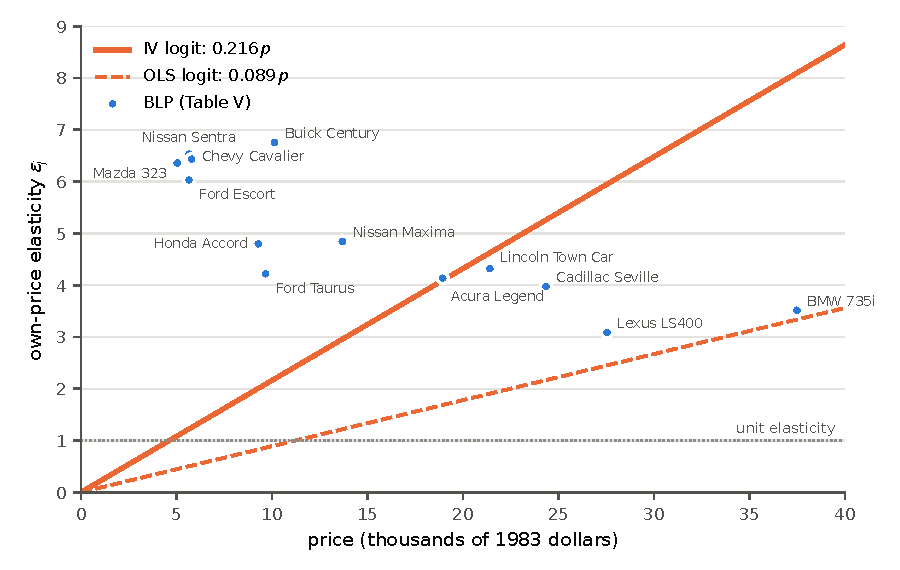
\includegraphics[width=0.86\textwidth]{figures/ch08/blp95_ownelas.pdf}
\caption{Own-price elasticities of thirteen 1990 models against price. Points are BLP's estimates
(their Table V). The rays are the logit elasticities $\alpha p$ implied by the IV and OLS logit price
coefficients of their Table III, ignoring the factor $1-s_j\approx1$. The dotted line marks unit
elasticity. Redrawn from \citet{BerryLevinsohnPakes1995}, Tables III and V.}
\label{fig:08-blp-ownelas}
\end{figure}

The price sensitivity of the marginal buyers can be read off the own semi-elasticities. Combining
\eqref{eq:08-blp-dsown} and \eqref{eq:08-blp-semi},
\begin{equation*}
-\frac{e_{jj}}{100}=\frac{1}{s_j}\int\frac{\alpha}{y_i-p_j}\,s_{ij}(1-s_{ij})\,\dd F(\nu_i)
\approx\E\Big[\frac{\alpha}{y_i-p_j}\,\Big|\,i\text{ buys }j\Big],
\end{equation*}
where the approximation uses $s_{ij}\ll1$. The semi-elasticities in \cref{tab:08-blp-semi} below give
$-\frac{e_{jj}}{100}=1.26$ for the Mazda 323, 0.52 for the Accord and 0.094 for the BMW 735i. Dividing
$\alpha=43.501$ by these numbers gives the harmonic mean of residual income $y_i-p_j$ among buyers. It is
about \$35,000 for the Mazda, \$84,000 for the Accord and \$464,000 for the BMW, in 1983 dollars (our
calculation). The specification can make luxury-car demand inelastic enough only by placing its buyers
far in the upper tail of the lognormal income distribution. This is one motivation for adding data on
buyers' incomes, as \citet{BerryLevinsohnPakes2004} and \citet{Petrin2002} later did
(\cref{sec:08-micro,sec:08-blp04}).

\casehead{Cross-price semi-elasticities}
BLP's Table VI reports own- and cross-price semi-elasticities for the same thirteen models.
\Cref{fig:08-blp-semielas} displays the full matrix, and \cref{tab:08-blp-semi} reproduces two diagonal
blocks. Entry $(i,j)$ is the percentage change in the share of row car $i$ when the price of column car
$j$ rises by \$1,000.

\begin{figure}[htbp]
\centering
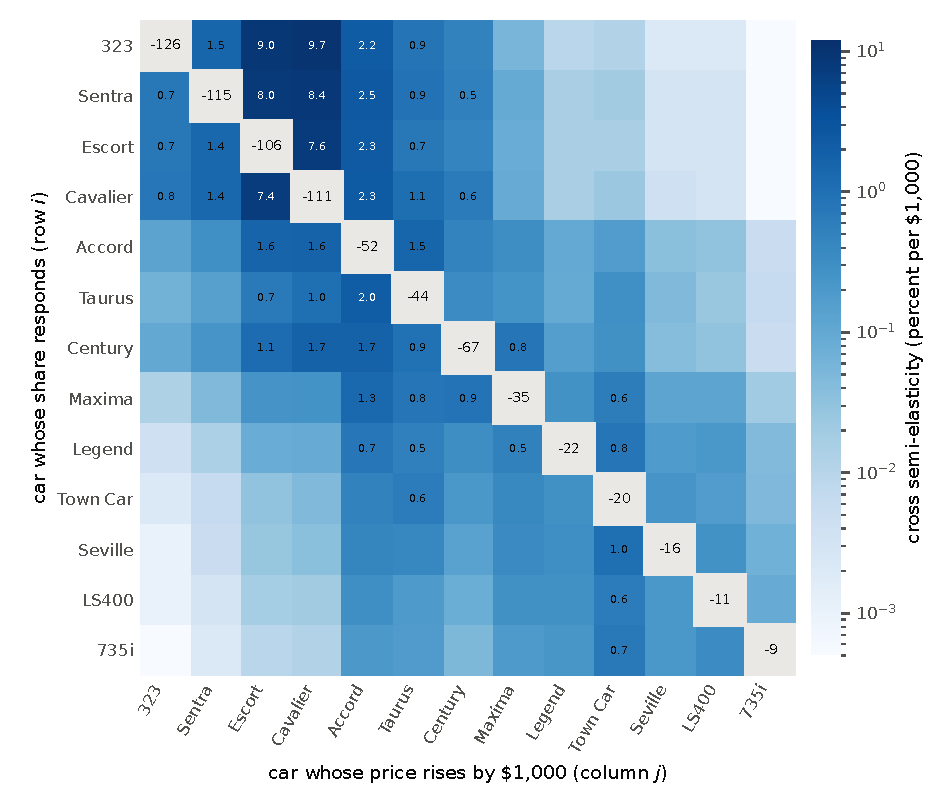
\includegraphics[width=0.9\textwidth]{figures/ch08/blp95_semielas.pdf}
\caption{Own- and cross-price semi-elasticities for thirteen 1990 models. Cell $(i,j)$ is the
percentage change in the share of row car $i$ for a \$1,000 increase in the price of column car $j$.
Off-diagonal cells are shaded on a log scale, and entries of at least 0.5 are printed. Diagonal cells
(gray) print the own semi-elasticity, which is negative. Entries printed as 0.000 in the source are
shaded at the bottom of the scale. Redrawn from \citet{BerryLevinsohnPakes1995}, Table VI.}
\label{fig:08-blp-semielas}
\end{figure}

\begin{table}[htbp]
\centering
\caption{Own- and cross-price semi-elasticities, two blocks of BLP (1995) Table VI}
\label{tab:08-blp-semi}
\small
\begin{tabular}{@{}lrrrr@{}}
\toprule
\multicolumn{5}{@{}l}{\emph{Panel A: small cars}}\\
Share of $\downarrow$ / price of $\rightarrow$ & Mazda 323 & Sentra & Escort & Cavalier \\
\midrule
Mazda 323 & $-125.933$ & 1.518 & 8.954 & 9.680 \\
Sentra    & 0.705 & $-115.319$ & 8.024 & 8.435 \\
Escort    & 0.713 & 1.375 & $-106.497$ & 7.570 \\
Cavalier  & 0.754 & 1.414 & 7.406 & $-110.972$ \\
\midrule
\multicolumn{5}{@{}l}{\emph{Panel B: luxury cars}}\\
Share of $\downarrow$ / price of $\rightarrow$ & Town Car & Seville & LS400 & BMW 735i \\
\midrule
Town Car  & $-20.175$ & 0.226 & 0.168 & 0.048 \\
Seville   & 1.011 & $-16.313$ & 0.263 & 0.068 \\
LS400     & 0.606 & 0.212 & $-11.199$ & 0.086 \\
BMW 735i  & 0.685 & 0.215 & 0.336 & $-9.376$ \\
\midrule
\multicolumn{5}{@{}l}{\emph{Panel C: small-car shares, luxury-car prices}}\\
Share of $\downarrow$ / price of $\rightarrow$ & Town Car & Seville & LS400 & BMW 735i \\
\midrule
Mazda 323 & 0.012 & 0.002 & 0.002 & 0.000 \\
Cavalier  & 0.023 & 0.004 & 0.003 & 0.000 \\
\bottomrule
\end{tabular}

\smallskip
\begin{minipage}{0.86\linewidth}
\footnotesize
Notes: Source: \citet{BerryLevinsohnPakes1995}, Table VI (p.~880), CRTS estimates. Entry
$(i,j)$ is $e_{ij}=\frac{100}{s_i}\frac{\partial s_i}{\partial p_j}$, the percentage change in the
share of row car $i$ for a \$1,000 increase in the price of column car $j$. The full $13\times13$ matrix
is shown in \cref{fig:08-blp-semielas}.
\end{minipage}
\end{table}

Three features stand out. First, own semi-elasticities fall sharply with price, from $-125.9$ for the
Mazda 323 to $-9.4$ for the BMW 735i. Multiplying each by $-\frac{p_j}{100}$ reproduces every own-price
elasticity in \cref{tab:08-blp-attr} to three decimals (our check). Under the IV logit every diagonal
entry would be about $-100\times0.216=-21.6$.

Second, cross effects are large among similar cars and close to zero across segments. A \$1,000 rise in
the Mazda 323's price raises the Sentra's share by 0.705 percent but leaves the Town Car, Seville, Lexus
and BMW almost unaffected. Under the logit the off-diagonal entries of a column would all equal
$100\,\alpha s_j$, whatever the row car. In BLP's matrix the largest cross entry in the Escort column is
about 1,000 times the smallest (8.954 against 0.009).

Third, the closest substitutes are intuitive. Measured down each column, the Lexus is the closest
substitute for the BMW 735i, the Cadillac Seville for the Lincoln Town Car, and the Accord for the Taurus
(p.~881). The effects of a \$1,000 increase are smaller for expensive cars because \$1,000 is a smaller
fraction of their price. Converting to elasticities removes this scale effect. For example, the
elasticity of the Seville's share with respect to the Town Car's price is
$1.011\times\frac{21.412}{100}\approx0.22$.

\casehead{Substitution to the outside good}
BLP measure how much of the demand a car loses goes to the outside good. The statistic is
\begin{equation*}
D_{j0}=100\times\frac{\frac{\partial s_0}{\partial p_j}}{\big|\frac{\partial s_j}{\partial p_j}\big|},
\end{equation*}
the number of consumers who switch from $j$ to no car, as a percentage of all who leave $j$ after a small
price rise. This is the diversion ratio to the outside good. Under the logit,
$\frac{\partial s_0}{\partial p_j}=\alpha s_0s_j$ and
$\big|\frac{\partial s_j}{\partial p_j}\big|=\alpha s_j(1-s_j)$, so
$D_{j0}=100\times\frac{s_0}{1-s_j}$. Under BLP, \cref{prop:08-diversion} gives
\begin{equation*}
\frac{D_{j0}}{100}=\int\varpi_{ij}\,\frac{s_{i0}}{1-s_{ij}}\,\dd F(\nu_i),\qquad
\varpi_{ij}=\frac{\frac{\alpha}{y_i-p_j}\,s_{ij}(1-s_{ij})}
{\int\frac{\alpha}{y_l-p_j}\,s_{lj}(1-s_{lj})\,\dd F(\nu_l)},
\end{equation*}
a weighted average of individual diversions with weights concentrated on the price-sensitive marginal
buyers of $j$.

\begin{table}[htbp]
\centering
\caption{Substitution to the outside good after a price increase (BLP 1995, Table VII)}
\label{tab:08-blp-outside}
\small
\begin{tabular}{@{}lrr@{}}
\toprule
Model & Logit & BLP \\
\midrule
Mazda 323 & 90.870 & 27.123 \\
Nissan Sentra & 90.843 & 26.133 \\
Ford Escort & 90.592 & 27.996 \\
Chevy Cavalier & 90.585 & 26.389 \\
Honda Accord & 90.458 & 21.839 \\
Ford Taurus & 90.566 & 25.214 \\
Buick Century & 90.777 & 25.402 \\
Nissan Maxima & 90.790 & 21.738 \\
Acura Legend & 90.838 & 20.786 \\
Lincoln Town Car & 90.739 & 20.309 \\
Cadillac Seville & 90.860 & 16.734 \\
Lexus LS400 & 90.851 & 10.090 \\
BMW 735i & 90.883 & 10.101 \\
\bottomrule
\end{tabular}

\smallskip
\begin{minipage}{0.62\linewidth}
\footnotesize
Notes: Source: \citet{BerryLevinsohnPakes1995}, Table VII (p.~881). Entries are
$D_{j0}=100\times\frac{\partial s_0}{\partial p_j}\Big(\Big|\frac{\partial s_j}{\partial p_j}\Big|\Big)^{-1}$,
the percentage of consumers who leave car $j$ after a small price increase and choose the outside good.
\end{minipage}
\end{table}

\begin{figure}[htbp]
\centering
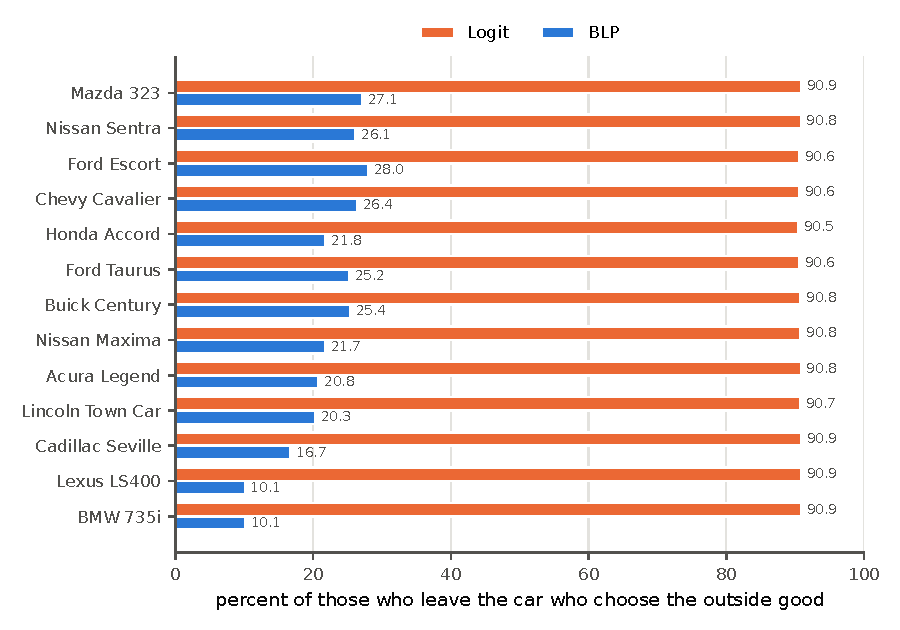
\includegraphics[width=0.82\textwidth]{figures/ch08/blp95_outside.pdf}
\caption{Diversion to the outside good after a small price increase, logit against BLP. Redrawn from
\citet{BerryLevinsohnPakes1995}, Table VII.}
\label{fig:08-blp-outside}
\end{figure}

\Cref{tab:08-blp-outside} and \cref{fig:08-blp-outside} report the results. Under the logit about 90
percent of those who leave any model choose no car, which is $\frac{s_0}{1-s_j}\approx s_0$. The logit
column ranges from 90.458 to 90.883. Since $\frac{s_0}{1-s_j} > s_0$, this puts $s_0$ just below 0.905.
The entries fall slightly with sales, which $\frac{s_0}{1-s_j}$ does not allow, so the printed values
match the formula only approximately. Under
BLP's estimates the diversion ranges from 28.0 percent (Escort) to 10.1 percent (Lexus and BMW). It is
lower for expensive cars. Buyers of luxury cars are rich and like cars, so for them $s_{i0}$ is small and
they move to other luxury cars. Buyers of cheap cars are closer to the margin of not buying. BLP still
find their numbers ``a bit large'' and see this as a sign that the treatment of the outside good needs
improvement (pp.~881--882). The outside good includes keeping an old car, and a dynamic model with a
used-car market would treat it more realistically (Section 8.2 of the paper).

\subsection{Results IV: markups and profits}\label{sec:08-blp95-markups}

Markups combine the demand and cost estimates. \Cref{tab:08-blp-markups} reproduces BLP's Table VIII
and adds four columns that we compute from it and from Table V.

\begin{table}[htbp]
\centering
\caption{Markups and variable profits for 1990 models, CRTS estimates (BLP 1995, Table VIII, with
derived columns)}
\label{tab:08-blp-markups}
\footnotesize
\setlength{\tabcolsep}{4pt}
\begin{tabular}{@{}llrrrrrrr@{}}
\toprule
 & & \multicolumn{3}{c}{BLP Table VIII} & \multicolumn{4}{c}{Derived (our calculation)} \\
\cmidrule(lr){3-5}\cmidrule(l){6-9}
Model & Firm & Price & $p-mc$ & $q(p-mc)$ & $\frac{p-mc}{p}$ & $\frac{1}{\varepsilon_j}$ & Gap
 & Sales \\
\midrule
Mazda 323        & Mazda  & 5,049  & 801    & 18,407  & 0.159 & 0.157 & 0.001 & 22,980 \\
Nissan Sentra    & Nissan & 5,661  & 880    & 43,554  & 0.155 & 0.153 & 0.002 & 49,493 \\
Ford Escort      & Ford   & 5,663  & 1,077  & 311,068 & 0.190 & 0.166 & 0.024 & 288,828 \\
Chevy Cavalier   & GM     & 5,797  & 1,302  & 384,263 & 0.225 & 0.155 & 0.069 & 295,133 \\
Honda Accord     & Honda  & 9,292  & 1,992  & 830,842 & 0.214 & 0.208 & 0.006 & 417,089 \\
Ford Taurus      & Ford   & 9,671  & 2,577  & 807,212 & 0.266 & 0.237 & 0.029 & 313,237 \\
Buick Century    & GM     & 10,138 & 2,420  & 271,446 & 0.239 & 0.148 & 0.091 & 112,168 \\
Nissan Maxima    & Nissan & 13,695 & 2,881  & 288,291 & 0.210 & 0.206 & 0.004 & 100,066 \\
Acura Legend     & Honda  & 18,944 & 4,671  & 250,695 & 0.247 & 0.242 & 0.005 & 53,671 \\
Lincoln Town Car & Ford   & 21,412 & 5,596  & 832,082 & 0.261 & 0.231 & 0.030 & 148,692 \\
Cadillac Seville & GM     & 24,353 & 7,500  & 249,195 & 0.308 & 0.252 & 0.056 & 33,226 \\
Lexus LS400      & Toyota & 27,544 & 9,030  & 371,123 & 0.328 & 0.324 & 0.004 & 41,099 \\
BMW 735i         & BMW    & 37,490 & 10,975 & 114,802 & 0.293 & 0.284 & 0.008 & 10,460 \\
\bottomrule
\end{tabular}

\smallskip
\begin{minipage}{0.97\linewidth}
\footnotesize
Notes: Columns 3 to 5 are from \citet{BerryLevinsohnPakes1995}, Table VIII (p.~882), whose
caption refers to ``Table 6 (CRTS)'' estimates, meaning those of Table IV. Price and markup are in 1983
dollars, and variable profits in thousands of 1983 dollars. ``Firm'' is the parent company. The last
four columns are our calculations: the Lerner index, the inverse own-price elasticity from Table V, the
gap between them, and implied unit sales $\frac{q(p-mc)}{p-mc}$.
\end{minipage}
\end{table}

\casehead{Levels and pattern}
In 1990 the average markup is \$3,753 and the average ratio of markup to price is 0.239 (p.~882). The
lowest markups are those of the Mazda 323 (\$801), Sentra (\$880) and Escort (\$1,077). The Lexus and
BMW have markups of \$9,030 and \$10,975. Markups rise almost monotonically with price, and the Lerner
index rises from about 0.16 to about 0.3. \Cref{fig:08-blp-markup} contrasts this pattern with the IV
logit, whose markups all lie in a band between \$4,630 and \$4,805. BLP note that the average level of
markups is similar in the two models even though the pattern differs (footnote 31).

\begin{figure}[htbp]
\centering
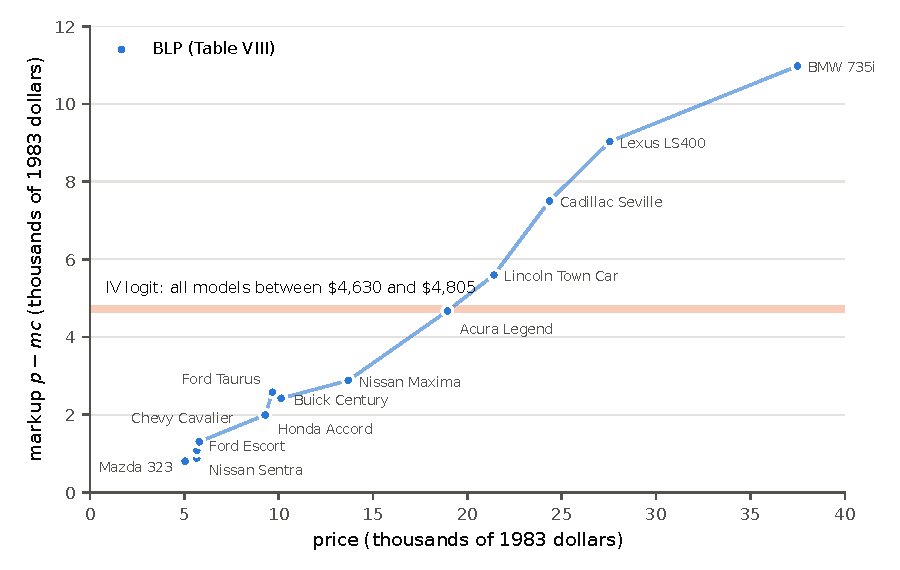
\includegraphics[width=0.86\textwidth]{figures/ch08/blp95_markup.pdf}
\caption{Price-cost markups of thirteen 1990 models against price. Points are BLP's estimates (their
Table VIII). The shaded band is the range of markups implied by the IV logit for all 1990 models
(\$4,630 to \$4,805, p.~874). Redrawn from \citet{BerryLevinsohnPakes1995}.}
\label{fig:08-blp-markup}
\end{figure}

\casehead{Profits}
Large markups need not mean large profits, because some high-markup cars sell few units. BLP single out
the Honda Accord and the Ford Taurus as the most profitable models in their table, by a factor of two
relative to most others. Both were regarded as essential to their firms' finances
(p.~882).\footnote{In the printed Table VIII the Lincoln Town Car's variable profit (\$832,082 thousand)
is as large as the Accord's (\$830,842 thousand) and the Taurus's (\$807,212 thousand). The text's
statement fits the other ten models.} Dividing variable profits by markups recovers unit sales, which
range from 10,460 BMW 735i's to 417,089 Accords.

\casehead{Multi-product pricing in the markups}
The derived columns of \cref{tab:08-blp-markups} reveal the role of multi-product ownership. The
following decomposition holds in any Bertrand-Nash equilibrium.

\begin{proposition}[Multi-product Lerner index]\label{prop:08-blp-lerner}
Let $D_{jr}=\frac{\partial s_r}{\partial p_j}\Big(\Big|\frac{\partial s_j}{\partial p_j}\Big|\Big)^{-1}$
be the diversion ratio from $j$ to $r$. At an interior Bertrand-Nash equilibrium, every product $j$ of firm $f$ satisfies
\begin{equation*}
\frac{p_j-mc_j}{p_j}=\frac{1}{\varepsilon_j}
 +\sum_{r\in\mathcal{J}_f,\,r\neq j}D_{jr}\,\frac{p_r-mc_r}{p_j}.
\end{equation*}
If the products are substitutes and markups are positive, the second term is nonnegative, so
$\varepsilon_j>1$ whenever the Lerner index is below one.
\end{proposition}

\begin{proof}
Move the own-product term of \eqref{eq:08-foc} to the left:
\begin{equation*}
(p_j-mc_j)\Big(-\frac{\partial s_j}{\partial p_j}\Big)=s_j
 +\sum_{r\in\mathcal{J}_f,\,r\neq j}(p_r-mc_r)\frac{\partial s_r}{\partial p_j}.
\end{equation*}
Divide both sides by $p_j\big|\frac{\partial s_j}{\partial p_j}\big|$. The first term on the right
becomes $\frac{s_j}{p_j}\Big(\Big|\frac{\partial s_j}{\partial p_j}\Big|\Big)^{-1}=\frac{1}{\varepsilon_j}$,
and each term of the
sum becomes $D_{jr}\frac{p_r-mc_r}{p_j}$. With substitutes $D_{jr}\geq0$ and positive markups, so the
sum is nonnegative. Then $\frac{1}{\varepsilon_j}\leq\frac{p_j-mc_j}{p_j}<1$ gives
$\varepsilon_j>1$.
\end{proof}

The gap between the Lerner index and $\frac{1}{\varepsilon_j}$ measures the margins a firm recaptures
on its other products. For the products of Mazda, Nissan, Honda, Toyota and BMW the gap is at most
0.008. Their 1990 portfolios contained few close substitutes for these models. For Ford's Escort, Taurus
and Town Car the gap is 0.024 to 0.030. For GM's Cavalier, Century and Seville it is 0.056 to 0.091.
GM's many divisions sell close substitutes for each of its models, so a price rise on the Century
diverts many buyers to other GM cars. This portfolio effect, invisible in the logit except through
$S_f$, is the mechanism that \citet{Nevo2001} later used to separate multi-product pricing from collusion
(\cref{sec:08-nevo01}).

\subsection{Robustness}\label{sec:08-blp95-robust}

The choice of characteristics in utility and cost is ad hoc, and computation limits the number of
random coefficients. BLP report how markups change across six alternative specifications. They choose
markups as the summary because markups combine demand and cost information and are easy to interpret.
\Cref{tab:08-blp-robust} reproduces their Table IX.

\begin{table}[htbp]
\centering
\caption{Markups under alternative specifications, 1990 models, dollars (BLP 1995, Table IX)}
\label{tab:08-blp-robust}
\footnotesize
\setlength{\tabcolsep}{4pt}
\begin{tabular}{@{}lrrrrrrr@{}}
\toprule
 & (1) & (2) & (3) & (4) & (5) & (6) & (7) \\
 & \makecell{Base\\(Table VIII)} & \makecell{$\ln q$\\in cost} & \makecell{AT\\for Air}
 & \makecell{Weight, HP\\for HPWT} & \makecell{Cost\\interactions} & \makecell{Regions,\\reliability}
 & \makecell{Weight,\\interactions} \\
\midrule
Mazda 323        & 801    & 1,616  & 1,012 & 1,073 & 828    & 1,125  & 1,389 \\
Nissan Sentra    & 880    & 1,769  & 1,153 & 1,271 & 912    & 1,308  & 1,487 \\
Ford Escort      & 1,077  & 2,043  & 1,326 & 1,470 & 1,111  & 2,094  & 1,690 \\
Chevy Cavalier   & 1,302  & 2,490  & 1,729 & 1,655 & 1,329  & 2,593  & 2,020 \\
Honda Accord     & 1,992  & 3,059  & 2,629 & 2,703 & 2,059  & 3,839  & 2,327 \\
Ford Taurus      & 2,577  & 3,721  & 2,528 & 3,344 & 2,585  & 4,094  & 2,898 \\
Buick Century    & 2,420  & 4,162  & 3,161 & 2,939 & 2,405  & 4,030  & 3,321 \\
Nissan Maxima    & 2,881  & 4,674  & 4,565 & 2,085 & 2,911  & 6,941  & 3,513 \\
Acura Legend     & 4,671  & 7,105  & 6,563 & 3,059 & 4,661  & 8,305  & 5,081 \\
Lincoln Town Car & 5,596  & 8,029  & 6,778 & 4,765 & 5,508  & 7,114  & 6,518 \\
Cadillac Seville & 7,500  & 10,733 & 8,635 & 4,863 & 7,439  & 9,182  & 8,015 \\
Lexus LS400      & 9,030  & 10,510 & 8,411 & 4,791 & 8,585  & 10,925 & 7,398 \\
BMW 735i         & 10,975 & 13,646 & 9,122 & 7,605 & 10,713 & 12,153 & 12,202 \\
\midrule
Demand variables significant & 5 of 5 & 4 of 5 & 4 of 5 & 6 of 6 & 4 of 5 & 8 of 8 & 4 of 6 \\
\bottomrule
\end{tabular}

\smallskip
\begin{minipage}{0.97\linewidth}
\footnotesize
Notes: Source: \citet{BerryLevinsohnPakes1995}, Table IX (p.~883). Price minus marginal cost in
1983 dollars. (2) adds $\ln q$ to the cost function (last columns of Table IV). (3) replaces Air with a
dummy for standard automatic transmission. (4) replaces HPWT with horsepower and weight entered
separately. (5) adds interactions of the continuous characteristics to the cost function. (6) replaces
the constant in utility with U.S., Japan and Europe dummies and adds the reliability rating. (7) adds
weight and cost-side interactions. The last row counts demand variables whose mean or standard
deviation is significant at the 95 percent level.
\end{minipage}
\end{table}

The pattern of markups survives every specification. In each column markups rise broadly with price, with a few
reversals, and the correlation of each column with the base column is between 0.945 and 0.9997 (our calculation). Levels
move more. Across the seven columns a car's highest markup is between 1.6 and 3.3 times its lowest.

The individual columns have specific explanations (pp.~883--885). Adding $\ln q$ in column (2) raises
every markup, and it gives the highest markups of all the alternatives, yet even these are not
extraordinarily high. As shown above, its markups over average variable cost are implausible. Using
automatic transmission as the luxury proxy in column (3) raises markups slightly for cheap cars and lowers
them slightly for expensive ones. Entering horsepower and weight separately in column (4) changes markups
the most. It gives implausibly low markups for expensive cars, possibly because cost is not linear in
horsepower and weight. Cost interactions in column (5) leave markups within a few percent of the base,
although most interaction terms are significant. Region dummies with reliability in column (6) raise
markups for several mid-priced models from different regions, for reasons BLP could not identify.
Reliability is included there because region dummies may be correlated with reliability, which would
otherwise sit in $\xi$ and invalidate the instruments. Column (7) adds weight, which has an
insignificant cost coefficient and a significant demand mean, and leaves markups close to the base.

\subsection{Interpretation}\label{sec:08-blp95-interp}

BLP read Tables IV to VIII as evidence that flexible utility gives a more realistic picture of
equilibrium in the industry. Three lessons stand out.

First, instrumenting for price matters even in the logit. It more than doubles the price coefficient
and removes almost all inelastic demands (\cref{tab:08-blp-logit}). Second, random coefficients and
income effects change the economics, beyond the econometrics. Own elasticities fall with price,
substitution runs between similar cars, and diversion to the outside good falls from about 90 percent to
10 to 28 percent. Each of these patterns is impossible in the logit. Third, the implied markups are
plausible in level and pattern. They are consistent with standard multi-product pricing, in which GM's
broad portfolio raises its margins above the inverse elasticity.

The results have clear implications for counterfactuals. A merger simulation built on the logit would
predict uniform markups and diversion mostly to the outside good. It would therefore understate the
price effects of merging close substitutes (\cref{ch:mergers}). A tariff analysis would mispredict which
domestic cars gain from higher import prices. A welfare calculation for a new model would depend on how
much demand it takes from similar cars.

\subsection{Limitations and critiques}\label{sec:08-blp95-critique}

\casehead{Data}
Prices are list prices of base models, so discounts and options are missing. Fleet sales are ignored.
Output is poorly measured for imported models, which limits the cost function. Market size is the number
of households, and every household is assumed to consider buying one new car each year.

\casehead{Exogenous characteristics}
The moment condition \eqref{eq:08-blp-moments} treats observed characteristics as mean independent of
$\xi$ and $\omega$. Firms choose characteristics, and they may choose them knowing $\xi$, so the
instruments may be invalid. BLP raise this concern themselves and sketch a Markov alternative
(\cref{sec:08-blp95-estimation}). They also identify obtaining consistent estimates when observed and
unobserved characteristics are correlated as the easier part of the dynamic problem. Endogenizing the
choice of characteristics is the harder part (Section 8.2 of the paper).

\casehead{Statics and the outside good}
Cars are durable. A household's outside option is often its current car, and its timing of purchases
responds to prices and expectations. A static model with an undifferentiated outside good cannot capture
these choices, which may explain why diversion to the outside good still looks large.

\casehead{Conditional counterfactuals}
Policy analysis with the model holds characteristics and the product set fixed. \citet{PakesBerryLevinsohn1993}
used the estimates to predict average MPG after the 1973 gasoline price shock. The model predicted 1974
and 1975 almost exactly, when characteristics changed little. From 1976 on, new small fuel-efficient
models appeared and the predictions became markedly worse (pp.~885--886).

\casehead{Functional form and the supply side}
All heterogeneity in price sensitivity comes from income through $\alpha\ln(y_i-p_j)$, with one income
dispersion parameter for all years. Our harmonic-mean calculation shows how far into the income tail the
model must place luxury-car buyers. The random coefficients are independent normals. Conduct is assumed
to be Bertrand-Nash and is not tested. The constant-returns cost function produces a negative MPG
coefficient, and the alternative with $\ln q$ implies implausible returns to scale.

\casehead{Aggregate data only}
BLP use no data that link households to the cars they buy. Their own conclusion points to consumer
surveys and to plant-level cost data from the Census Longitudinal Research Database (Section 8.2 of the paper).
\citet{BerryLevinsohnPakes2004} and \citet{Petrin2002} later added consumer-level moments for cars
(\cref{sec:08-micro,sec:08-blp04}), and \citet{Goldberg1995} estimated car demand from household data
(\cref{sec:08-goldberg}).

\casehead{Numerical and instrument sensitivity}
Later work re-examined the estimator. \citet[p.~35]{KnittelMetaxoglou2014} used BLP's automobile data and the
synthetic cereal data of \citet{Nevo2000a}. They found that BLP-type estimates and their implications can vary
with the optimization algorithm and starting values.
\citet{DubeFoxSu2012} showed that a loose tolerance in the contraction can produce false convergence
(\cref{sec:08-inversion,sec:08-practice}). \citet[Section~3]{Armstrong2016} showed that the characteristics-based
instruments can lose their power in markets with many products. Equilibrium markups then vary little.
\citet{ReynaertVerboven2014} and \citet[Section~5]{ConlonGortmaker2020} found in Monte Carlo experiments that
approximations to the optimal instruments improve precision.
These critiques concern implementation, and they leave the framework itself intact.

\subsection{Contribution}\label{sec:08-blp95-contrib}

BLP's contribution is a complete template for empirical work on differentiated products with market-level
data. It combines five elements. Utility is defined over characteristics, with random coefficients and
demographic information from outside the sample. Shares are aggregated by simulation. Mean utilities
are recovered by inverting the share equations with a contraction. A GMM estimator built on structural
errors handles price endogeneity, with instruments derived from oligopoly pricing and exchangeability.
A multi-product Nash pricing equation recovers marginal costs and markups without cost data.

The same template now underlies most empirical work on differentiated-products markets. Applications
include voluntary export restraints on Japanese cars \citep{BerryLevinsohnPakes1999}, mergers
\citep[\cref{ch:mergers}]{Nevo2000b}, the welfare gains from new goods
\citep[\cref{ch:newgoods}]{Petrin2002}, and airline hubs \citep[\cref{ch:airlines}]{BerryCarnallSpiller2006}.
\citet{Nevo2000a} wrote the guide that made the method accessible, and we turn to it next.

\section{Case study: Nevo (2000a), the practitioner's guide and its application}\label{sec:08-nevo00}

\citet{Nevo2000a} is a guide to the random coefficients logit for researchers who have not used it. It
explains the model, the algorithm and the instruments with the stated aim of lowering the barriers to
entry and increasing trust in the method among outsiders (p.~514). It ends with an application to a
synthetic data set, and Nevo posted the data and his Matlab code. The model and algorithm of
\cref{sec:08-model,sec:08-substitution,sec:08-simulation,sec:08-inversion,sec:08-gmm,sec:08-instruments}
follow the guide's equations closely. This section covers the rest: the guide's framing, its
specification choices and their implications, its practical advice, the application in full, and its
list of extensions.

\subsection{Purpose and framing}\label{sec:08-nevo00-purpose}

Nevo starts from two problems that make differentiated-products demand hard. The first is
dimensionality. A log-log demand system for 100 products has 100 equations, each with 100 prices, which
means at least 10,000 parameters (p.~514). Symmetry and adding up remove only part of these, and the
number remains too large to estimate. More flexible substitution patterns make the problem worse. The
second is heterogeneity. If all consumers were identical, markets would not show the variety of products
we observe. A representative consumer exists under Gorman-form preferences \citep{Gorman1959}, but those
assumptions are strong and often empirically false.

The logit model solves the dimensionality problem by projecting products onto a space of
characteristics. The number of parameters then depends on the number of characteristics and not on the
square of the number of products. The cost is the logit's treatment of heterogeneity, which makes
substitution depend on market shares and not on how similar products are. Random coefficients keep the
projection and model heterogeneity explicitly. Nevo lists three advantages of the BLP method over earlier
estimates of such models (p.~515). It needs only market-level price and quantity data, it deals with the
endogeneity of prices, and it produces more realistic elasticities.

\subsection{Specification choices and their implications}\label{sec:08-nevo00-spec}

\casehead{The guide's model}
The guide's model is the one of \cref{sec:08-linear}. Indirect utility is \eqref{eq:08-nevo-utility} (his
eq.~1), and tastes depend on demographics and unobserved characteristics as in \eqref{eq:08-tastes} (his
eq.~2). The unobserved tastes $\nu_i$ come from a parametric distribution, usually standard normal, and the
demographics $D_i$ from an empirical distribution such as CPS draws. The outside good is normalized as in \cref{sec:08-normalization}. Combining the
two equations gives the decomposition \eqref{eq:08-decomposition} (his eq.~3), and shares integrate over
$(D,\nu,\epsilon)$ with the factorization \eqref{eq:08-share-bayes} (his eq.~4).

\casehead{Assumptions and their implications}
Nevo spells out three assumptions implicit in \eqref{eq:08-nevo-utility} and then discusses how
\eqref{eq:08-tastes} models heterogeneity (pp.~517--520).
\begin{enumerate}
\item \emph{No wealth effects.} The form $\alpha_i(y_i-p_{jt})$ comes from quasilinear utility. This is
  reasonable for ready-to-eat cereal and unreasonable for cars. BLP's $\ln(y_i-p_j)$ is one alternative,
  and a flexible function $f(y_i-p_{jt})$ is another, as in \citet{Petrin2002}.
\item \emph{A common valuation of $\xi$.} Every consumer values the unobserved characteristic equally.
  Because the price coefficient varies, this is consistent with theories of vertical differentiation.
  \citet{DasOlleyPakes1994} model a distribution of valuations of $\xi$ instead.
\item \emph{Common prices and characteristics.} All consumers in a market face the same price. If they
  do not, a list or average price measures the relevant price with error. This is one more reason why
  price may be correlated with the error. The inversion method handles measurement error only if the
  mismeasured variable enters $\delta_{jt}$ alone (footnote 11, citing \citealp{Berry1994}).
\item \emph{Observed and unobserved heterogeneity.} Demographics bring outside information into the
  model and reduce reliance on parametric assumptions. Nevo's example of an unobserved characteristic is
  whether a household owns a dog, which matters for choosing a car but appears in no survey (p.~519). The
  linear form $\Pi D_i$ is restrictive, especially for the price coefficient.
\end{enumerate}

\casehead{Where correlation in utility comes from}
Nevo then explains why the logit fails and how to fix it (pp.~522--526), with the arguments and the cereal
examples that \cref{sec:08-logit-benchmark} reproduced. The cure is correlation in utility across brands, which
can enter through $\epsilon$ or through $\mu$.
Generalized extreme value models put it in $\epsilon$. The nested logit groups brands into exhaustive and
mutually exclusive nests fixed in advance. Within a nest, substitution is again proportional to shares,
and the model does nothing for own elasticities. \citet{Cardell1997} shows the distributional assumptions
under which a random coefficient on segment dummies reproduces the nested logit. With several layers of
segmentation the order of the nests matters. Grouping computers first by brand and then by technology
gives different substitution than the reverse order, even with the same groups (footnote 18). The
principles-of-differentiation GEV model of \citet{BresnahanSternTrajtenberg1997} avoids ordering the
nests. An unrestricted covariance matrix for $\epsilon$ reintroduces the dimensionality problem.

The random coefficients model puts the correlation in $\mu$. Products with similar characteristics are
correlated in utility, and consumers with similar demographics rank products similarly. The own-price
derivative averages individual price sensitivities with weights given by individual purchase
probabilities (\cref{prop:08-derivs}). If the buyers of Kellogg's Corn Flakes are price sensitive, its
own elasticity is high despite its low price (p.~526). Substitution is then driven by differences in
price sensitivity across the buyers of different products, and not by the functional form.

\subsection{Practical recommendations}\label{sec:08-nevo00-practice}

The guide's Section 3 turns from the model to practice. Most of its advice is now part of the chapter's
theory, and we list each item with the place where we develop it.

\casehead{Data and market size}
The data requirements and Nevo's four rules for choosing the market size are those of \cref{sec:08-data}
(p.~527). Nevo strongly recommends several markets with variation in relative prices or in the products
offered.

\casehead{Two roles of characteristics}
Characteristics explain mean utility $\delta$ and drive substitution through $\mu$, and Nevo recommends keeping
the two roles separate (pp.~527--528, \cref{sec:08-assumptions}). Substitution must come from characteristics,
which should therefore guide what the researcher collects.

\casehead{Identification}
Nevo's informal argument starts from an ideal experiment that randomizes prices across consumers
(pp.~528--530). Market data depart from it in two ways. Prices are set by firms that know $\xi$, which
instruments address. More subtly, a discrete choice model can be estimated from one market. Each market
is then an observation on the relative likelihood of buying $J$ bundles of attributes, one of which is
price. Identification improves with more markets that vary in product characteristics, choice sets and
demographic distributions. His three-product example (A and B similar, B and C with equal shares) appears in
\cref{sec:08-illustration,sec:08-iv-roles}.

\casehead{The estimator}
The guide argues against matching shares by nonlinear least squares (his eq.~7) and builds the GMM residual
from the inverted mean utilities (his eqs.~8 to 13). It notes that the logit and nested logit reduce to
two-stage least squares. \Cref{sec:08-gmm} develops all three points.

\casehead{Instruments}
Nevo reviews cost shifters, characteristics-based instruments and Hausman instruments with their caveats
(pp.~534--536), as in \cref{sec:08-iv-families}. His footnote 23 makes the characteristics-based instruments
concrete. Suppose there are two characteristics (horsepower and size) and two firms with three products each.
The instruments for a product are then its two characteristics, their sums over the firm's other two products,
and their sums over the rival's three products, six in all. Nevo stresses that validity must be argued case by
case.

\casehead{Brand dummies and minimum distance}
Nevo believes brand fixed effects should be used whenever possible (p.~536). \Cref{sec:08-brand-fe} develops his
argument, his answers to the two objections and the minimum-distance estimator \eqref{eq:08-md} of the taste
parameters (pp.~537--538). The assumption $\E[\xi_b\mid \bm{X}_b]=0$ is used only to recover $\beta$. A
researcher unwilling to make it can still recover price sensitivity from the other instruments (footnote 24).

\subsection{The application}\label{sec:08-nevo00-app}

\casehead{Data}
The data contain prices and quantities for 24 brands of a differentiated product in 47 cities over 2
quarters (p.~538). A market is a city-quarter, so there are 94 markets and $24\times94=2{,}256$
observations. Every brand is sold in every market, so choice sets do not vary. The data were generated
from the demand model of Section 2 and a multi-product Bertrand pricing model (footnote 25). The marginal
costs and parameters were motivated by the cereal estimates of \citet{Nevo2000b}. Nevo warns that the data
are not real and should not be used for analysis. Their purpose is to teach the method.

Products have two characteristics. \emph{Sugar} measures sugar content, and \emph{Mushy} equals one if
the cereal gets soggy in milk. Demographics are drawn from the CPS: the log of income (\emph{Income}), its
square (\emph{IncomeSq}), \emph{Age}, and \emph{Child}, a dummy for being under sixteen. The unobserved
$\nu_i$ are standard normal, and each market uses $n_s=20$ simulated individuals. All specifications
include brand and time dummies. Section~4 does not describe the instruments used in the application.

\casehead{Specification}
The pattern of entries in Nevo's Table I reveals the estimated specification. Write $b_i^p=-\alpha_i$
for the price coefficient, which is what the table reports. Then
\begin{align*}
b_i^{p}&=b^{p}+\pi_{p,1}\mathit{Income}_i+\pi_{p,2}\mathit{IncomeSq}_i+\pi_{p,3}\mathit{Child}_i
 +\sigma_p\nu_{ip},\\
\beta_i^{k}&=\beta^{k}+\pi_{k,1}\mathit{Income}_i+\pi_{k,2}\mathit{Age}_i+\sigma_k\nu_{ik},
 \qquad k\in\{\text{Constant},\text{Sugar},\text{Mushy}\}.
\end{align*}
The nonlinear parameters are four standard deviations and nine demographic interactions, so $\theta_2$
has 13 elements. The means of the constant, Sugar and Mushy are absorbed by the brand dummies and
recovered by the minimum-distance step \eqref{eq:08-md} with 24 brand effects.

\begin{table}[htbp]
\centering
\caption{Results from the full model, synthetic cereal data (Nevo 2000a, Table I)}
\label{tab:08-nevo00-results}
\small
\begin{tabular}{@{}lrrrrrr@{}}
\toprule
 & Means & Std.\ dev. & \multicolumn{4}{c}{Interactions with demographic variables} \\
\cmidrule(l){4-7}
Variable & $\beta$ & $\sigma$ & Income & IncomeSq & Age & Child \\
\midrule
Price    & $-32.433$ & 1.848 & 16.598 & $-0.659$ & & 11.625 \\
         & (7.743) & (1.075) & (172.334) & (8.955) & & (5.207) \\
Constant & $-1.841^{a}$ & 0.377 & 3.089 & & 1.186 & \\
         & (0.258) & (0.129) & (1.213) & & (1.016) & \\
Sugar    & $0.148^{a}$ & 0.004 & $-0.193$ & & 0.029 & \\
         & (0.258) & (0.012) & (0.005) & & (0.036) & \\
Mushy    & $0.788^{a}$ & 0.081 & 1.468 & & $-1.514$ & \\
         & (0.013) & (0.205) & (0.697) & & (1.103) & \\
\midrule
GMM objective & & & 14.9 & & & \\
(Degrees of freedom) & & & (7) & & & \\
\bottomrule
\end{tabular}

\smallskip
\begin{minipage}{0.9\linewidth}
\footnotesize
Notes: Source: \citet{Nevo2000a}, Table I (p.~539). Based on 2,256 observations. Except where
noted, parameters are GMM estimates. All regressions include brand and time dummy variables.
Asymptotically robust standard errors in parentheses. $^{a}$Estimates from the minimum-distance
procedure. Blank cells are interactions not included in the specification.
\end{minipage}
\end{table}

\casehead{Results}
\Cref{tab:08-nevo00-results} reproduces Nevo's Table I. The minimum-distance means say that the average
consumer gains utility from more sugar (0.148) and from sogginess (0.788). The standard deviations
capture unobserved heterogeneity. Nevo describes them as insignificant both economically and
statistically, and he expects them to stay statistically insignificant even with more efficient
estimation (footnote 26).\footnote{By the printed standard errors, the standard deviation on the
constant (0.377, with standard error 0.129) has a $t$ ratio near 2.9. The other three standard deviations
are insignificant.}

The demographic interactions have economically large point estimates, although most are imprecise. The
valuation of sogginess falls with age ($-1.514$). Nevo says it also falls with income, while the printed
income interaction is positive (1.468).\footnote{The text on p.~540 states that ``the marginal valuation
of sogginess decreases with age and income.'' The income interaction in Table I is $+1.468$ with standard
error 0.697. We report the table.} \Cref{fig:08-nevo00-dists}(a) shows the implied distribution of the
Mushy coefficient across consumers. Most consumers value sogginess positively, but about 31
percent prefer a crunchy cereal (p.~540). Sugar is valued less by richer consumers, and this interaction
is very precisely estimated ($-0.193$, standard error 0.005).

The mean price coefficient is $-32.433$. Children are less price sensitive. Their price coefficient is
higher by 11.625, which is 36 percent of the mean coefficient and 6.3 times the unobserved standard
deviation $\sigma_p=1.848$ (our calculation). Nevo also reports that above-average-income consumers are
less price sensitive. The income terms are very imprecise, with a standard error of 172.334 on the linear
term. \Cref{fig:08-nevo00-dists}(b) shows the distribution of individual price coefficients. It is not
normal, because it inherits the shape of the empirical distribution of demographics. Its mass lies
between about $-70$ and $-15$, so no consumer has a positive price coefficient, although a linear
specification allows one in principle (p.~540).

\begin{figure}[htbp]
\centering
\begin{subfigure}[t]{0.72\textwidth}
\centering
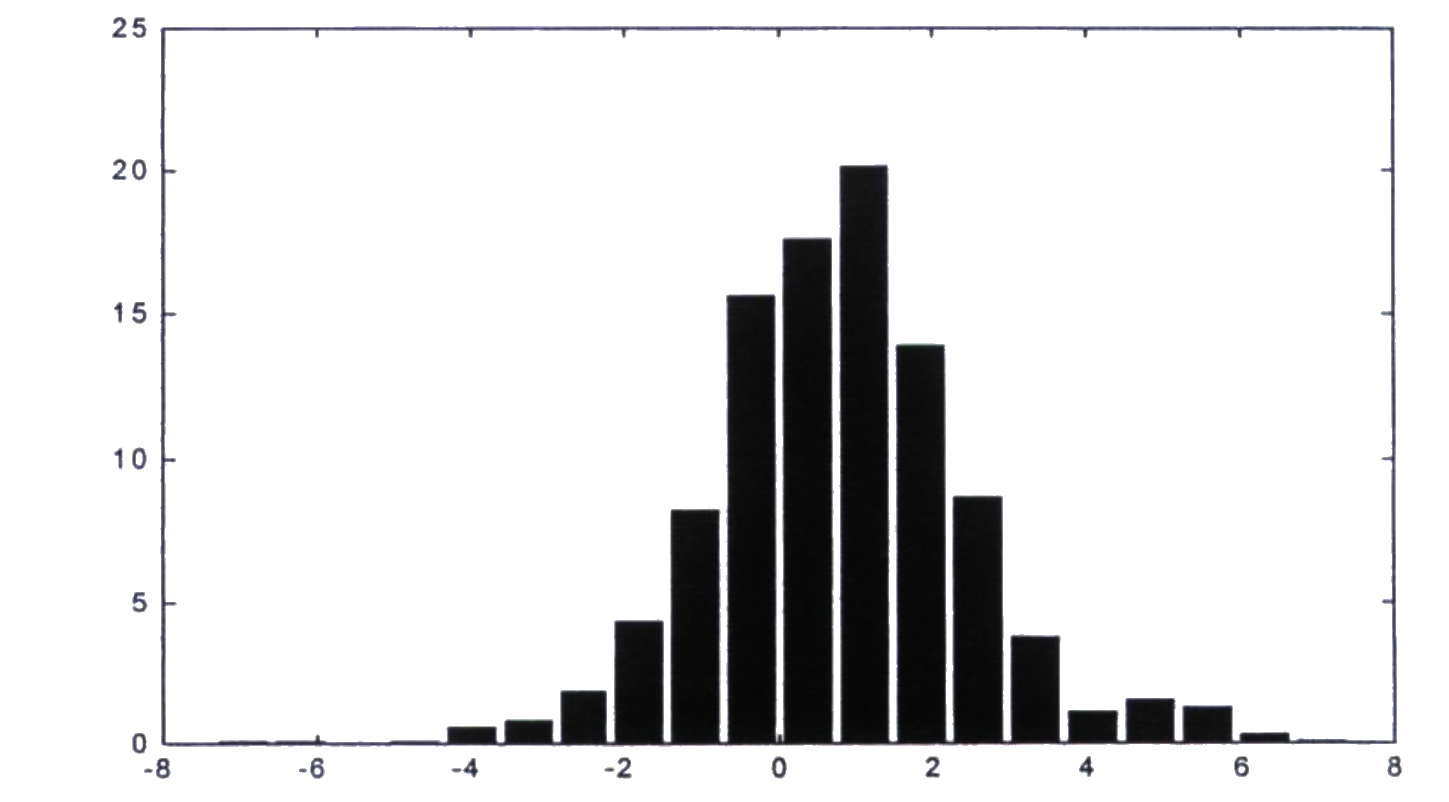
\includegraphics[width=\linewidth]{figures/ch08/nevo00_fig1_mushy.png}
\caption{Taste for sogginess (Mushy coefficient)}
\end{subfigure}

\medskip
\begin{subfigure}[t]{0.72\textwidth}
\centering
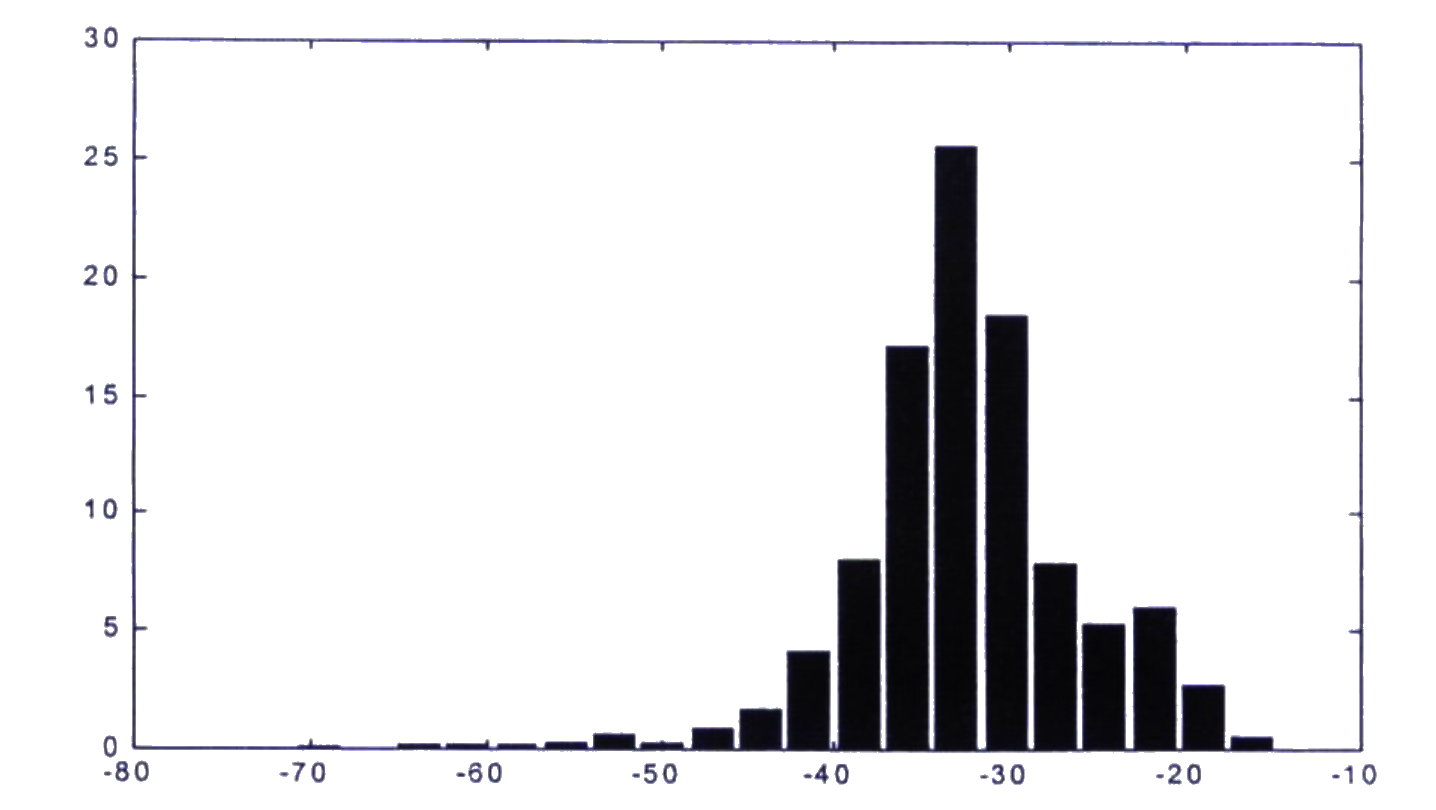
\includegraphics[width=\linewidth]{figures/ch08/nevo00_fig2_price.png}
\caption{Price coefficient}
\end{subfigure}
\caption{Frequency distributions (in percent) of two individual coefficients implied
by the estimates in \cref{tab:08-nevo00-results}. Panel (a) has mass below zero for consumers who prefer
crunchy cereal. Panel (b) is skewed because the empirical distribution of demographics drives it. Source:
\citet{Nevo2000a}, Figures 1 and 2.}
\label{fig:08-nevo00-dists}
\end{figure}

\casehead{Demographics against unobserved tastes}
The standard deviations are small relative to the demographic effects. Nevo computes the share of the
variance of each estimated coefficient explained by demographics, and all these shares exceed 90 percent
(p.~541). He reads this with care. It does not show that demographics explain all heterogeneity. It shows
that the data reject the assumed normal distribution of unobserved tastes. Other work had found that
purchase histories \citep{RossiMcCullochAllenby1996} and second-choice data \citep{BerryLevinsohnPakes2004}
explain heterogeneity beyond demographics (footnote 27). A second explanation is the absence of
choice-set variation across markets in these data, which BLP's data have. Such variation helps identify
the variance of the random shocks (\cref{sec:08-nevo00-practice}). Nevo notes that this explanation
accounts for imprecision, but not for the low point estimates or for the significance of the demographic
effects.

\casehead{Specification tests}
Nevo tests the logit against the full model by testing that all nonlinear parameters are jointly zero,
and the hypothesis is easily rejected (footnote 28). The GMM objective is 14.9 with 7 degrees of freedom.
If the objective is scaled as Hansen's $J$ statistic, this value exceeds the 95th percentile of the
$\chi^2(7)$ distribution, which is 14.07. The $p$-value is about 0.04 (our calculation), a marginal
rejection of the overidentifying restrictions. Nevo does not discuss this statistic.

\casehead{Elasticities}
\Cref{tab:08-nevo00-elas} reproduces Nevo's Table II. It reports the median over the 94 markets of each
own and cross elasticity for nine of the 24 brands, with each brand's characteristics. Entry $(i,j)$ is
the percentage change in the share of row brand $i$ for a one-percent change in the price of column
brand $j$.

\begin{table}[htbp]
\centering
\caption{Median own- and cross-price elasticities, synthetic cereal data (Nevo 2000a, Table II)}
\label{tab:08-nevo00-elas}
\footnotesize
\setlength{\tabcolsep}{3.3pt}
\begin{tabular}{@{}rrrrrrrrrrrr@{}}
\toprule
 & \multicolumn{2}{c}{Characteristics} & \multicolumn{9}{c}{Price of brand} \\
\cmidrule(lr){2-3}\cmidrule(l){4-12}
Brand & Sugar & Mushy & 1 & 2 & 3 & 4 & 5 & 14 & 15 & 19 & 24 \\
\midrule
1  & 2  & 1 & $-2.1689$ & 0.0562 & 0.2429 & 0.1161 & 0.0645 & 0.0596 & 0.0611 & 0.0759 & 0.2375 \\
2  & 18 & 1 & 0.1119 & $-3.4505$ & 0.1302 & 0.0924 & 0.1905 & 0.2305 & 0.2606 & 0.4380 & 0.1165 \\
3  & 4  & 1 & 0.2715 & 0.0674 & $-2.9208$ & 0.1083 & 0.0709 & 0.0627 & 0.0684 & 0.0944 & 0.2237 \\
4  & 3  & 0 & 0.1868 & 0.0736 & 0.1501 & $-3.2709$ & 0.1470 & 0.1557 & 0.1564 & 0.1037 & 0.2670 \\
5  & 12 & 0 & 0.0965 & 0.1540 & 0.0947 & 0.1326 & $-5.5116$ & 0.2852 & 0.3085 & 0.2988 & 0.1715 \\
\addlinespace
6  & 14 & 0 & 0.0699 & 0.1642 & 0.0698 & 0.1123 & 0.2518 & 0.3628 & 0.3971 & 0.3513 & 0.1369 \\
7  & 3  & 1 & 0.2828 & 0.0606 & 0.2390 & 0.1035 & 0.0648 & 0.0563 & 0.0598 & 0.0865 & 0.2225 \\
8  & 4  & 0 & 0.1743 & 0.0789 & 0.1476 & 0.1622 & 0.1524 & 0.1620 & 0.1656 & 0.1180 & 0.2555 \\
9  & 14 & 0 & 0.0735 & 0.1704 & 0.0717 & 0.1128 & 0.2596 & 0.3586 & 0.3966 & 0.3443 & 0.1333 \\
10 & 1  & 0 & 0.2109 & 0.0643 & 0.1682 & 0.1665 & 0.1224 & 0.1199 & 0.1298 & 0.0817 & 0.2809 \\
\addlinespace
11 & 11 & 0 & 0.0967 & 0.1556 & 0.0890 & 0.1377 & 0.2426 & 0.3322 & 0.3427 & 0.2899 & 0.1769 \\
12 & 4  & 1 & 0.2711 & 0.0691 & 0.2339 & 0.1121 & 0.0735 & 0.0662 & 0.0704 & 0.0985 & 0.2260 \\
13 & 3  & 1 & 0.2827 & 0.0597 & 0.2390 & 0.0983 & 0.0632 & 0.0554 & 0.0582 & 0.0866 & 0.2189 \\
14 & 13 & 0 & 0.0834 & 0.1825 & 0.0786 & 0.1247 & 0.2697 & $-3.8393$ & 0.3922 & 0.3380 & 0.1600 \\
15 & 13 & 0 & 0.0889 & 0.1763 & 0.0814 & 0.1256 & 0.2491 & 0.3542 & $-4.3982$ & 0.3383 & 0.1582 \\
\addlinespace
16 & 16 & 1 & 0.1430 & 0.2282 & 0.1523 & 0.0873 & 0.1447 & 0.1442 & 0.1702 & 0.3270 & 0.1264 \\
17 & 10 & 0 & 0.1138 & 0.1399 & 0.1005 & 0.1466 & 0.2172 & 0.2867 & 0.2912 & 0.2498 & 0.1875 \\
18 & 3  & 0 & 0.1900 & 0.0717 & 0.1542 & 0.1656 & 0.1362 & 0.1508 & 0.1578 & 0.1026 & 0.2660 \\
19 & 20 & 1 & 0.0944 & 0.2691 & 0.1130 & 0.0771 & 0.2163 & 0.2618 & 0.3107 & $-3.3335$ & 0.1013 \\
20 & 7  & 0 & 0.1420 & 0.0999 & 0.1270 & 0.1546 & 0.1791 & 0.2074 & 0.2080 & 0.1628 & 0.2251 \\
\addlinespace
21 & 14 & 0 & 0.0773 & 0.1706 & 0.0741 & 0.1160 & 0.2534 & 0.3573 & 0.3794 & 0.3530 & 0.1416 \\
22 & 6  & 0 & 0.1500 & 0.0950 & 0.1283 & 0.1602 & 0.1797 & 0.2096 & 0.2085 & 0.1530 & 0.2311 \\
23 & 12 & 0 & 0.0854 & 0.1561 & 0.0815 & 0.1307 & 0.2559 & 0.3484 & 0.3753 & 0.3154 & 0.1608 \\
24 & 0  & 0 & 0.2249 & 0.0548 & 0.1731 & 0.1619 & 0.1110 & 0.1044 & 0.1114 & 0.0733 & $-4.1215$ \\
\midrule
\multicolumn{3}{@{}l}{Outside good} & 0.0303 & 0.2433 & 0.0396 & 0.0552 & 0.2279 & 0.3349 & 0.3716
 & 0.3896 & 0.0399 \\
\bottomrule
\end{tabular}

\smallskip
\begin{minipage}{0.97\linewidth}
\footnotesize
Notes: Source: \citet{Nevo2000a}, Table II (p.~542). Entry $(i,j)$ is the percentage change in the
market share of row brand $i$ for a one-percent change in the price of column brand $j$. Each entry is the
median over the 94 markets. Only nine of the 24 columns are printed in the source.
\end{minipage}
\end{table}

\casehead{Reading Table II}
Own elasticities among the printed columns range from $-2.17$ (brand 1) to $-5.51$ (brand 5). Cross
elasticities within a column vary with characteristics, unlike the logit, which forces a constant column.
Nevo summarizes this by the ratio of the largest to the smallest cross elasticity in a column, which he
reports varies from 9 to 3 (p.~543).\footnote{Among the nine printed columns, the ratio ranges from 2.2
(brand 4) to 6.8 (brand 15) by our calculation. Nevo's range presumably covers all 24 columns, most of
which are not printed.} A column with a ratio near one shows that the characteristics are too weak to
break the logit pattern for that brand. Nevo suggests the diagnostic can guide which characteristics to
add.

Brands with the same characteristics have nearly identical rows. Nevo points to brands 14 and 15, which
both have Sugar 13 and Mushy 0. The table contains five more such groups: brands 3 and 12, 4 and 18, 5
and 23, 7 and 13, and 6, 9 and 21. The following result explains the pattern.

\begin{proposition}[Products with identical heterogeneous utility]\label{prop:08-nevo00-identical}
Suppose products $j$ and $j'$ have $\mu_{ij}=\mu_{ij'}$ for every consumer $i$. Then for every inside product
$k\notin\{j,j'\}$, the elasticities of $j$ and $j'$ with respect to $p_k$ are equal. Moreover, the diversion from $k$ to $j$ and to $j'$ is in proportion to their shares,
$\frac{D_{kj}}{D_{kj'}}=\frac{s_j}{s_{j'}}$.
\end{proposition}

\begin{proof}
From \eqref{eq:08-individual-share}, $\frac{s_{ij}}{s_{ij'}}=e^{\delta_j-\delta_{j'}}\equiv c$ for every $i$.
Integrating gives $s_j=c\,s_{j'}$, so $\frac{s_{ij}}{s_j}=\frac{s_{ij'}}{s_{j'}}$ for every $i$. The cross
elasticity with respect to $p_k$ is
\begin{equation*}
\varepsilon_{jk}=\frac{p_k}{s_j}\int\alpha_is_{ij}s_{ik}\,\dd F
 =p_k\int\alpha_i\frac{s_{ij}}{s_j}\,s_{ik}\,\dd F ,
\end{equation*}
and the last expression is the same for $j$ and $j'$. For the diversion ratios,
the common denominator $\big|\frac{\partial s_k}{\partial p_k}\big|$ cancels, so
\begin{equation*}
\frac{D_{kj}}{D_{kj'}}=\frac{\int\alpha_is_{ij}s_{ik}\,\dd F}{\int\alpha_is_{ij'}s_{ik}\,\dd F}
 =c=\frac{s_j}{s_{j'}} .
\end{equation*}
\end{proof}

In the application price carries a random coefficient, so $\mu_{ij}$ includes the price term. Two brands
with the same Sugar and Mushy but different prices have slightly different $\mu$. Their rows are
therefore close but not identical, as in brands 14 and 15 (0.0834 against 0.0889 in column 1, 0.2697
against 0.2491 in column 5). The second part of the proposition shows that the random coefficients model
keeps the IIA property among products that differ only in $\xi$. This is the clone problem of
\cref{sec:08-practice}.

The outside-good row varies a lot, from 0.0303 for brand 1 to 0.3896 for brand 19. It rises with the
brand's sugar content. Across the nine printed columns, its correlation with Sugar is 0.90 (our
calculation). Table I suggests why. Richer consumers value inside goods more (the Constant-Income
interaction is 3.089) and value sugar less (the Sugar-Income interaction is $-0.193$). Buyers of sugary
brands are therefore poorer on average, closer to the margin of buying nothing, and they move to the
outside good when prices rise.

\subsection{Lessons, extensions and assessment}\label{sec:08-nevo00-lessons}

\casehead{Lessons from the application}
Nevo stresses economic significance over statistical significance, because most coefficients are
imprecise. He attributes the imprecision to the simplifications made for teaching. More data, more
simulation draws than $n_s=20$, better simulation methods or a supply side would improve efficiency
(p.~540). The application shows four things a user of the method should expect. Demographic interactions
can carry most of the heterogeneity. Distributions of individual coefficients inherit the shape of the
demographic distribution. Elasticity matrices depart clearly from the logit pattern but only as far as
the characteristics allow. Without choice-set variation the standard deviations are hard to pin down.

\casehead{Extensions}
Nevo's Section 5 lists five directions.
\begin{itemize}
\item \emph{Supply side.} In the guide the supply side only motivates the instruments. Specifying it
  adds moment conditions with little extra programming for standard static models (\cref{sec:08-supply}).
  It raises efficiency at the cost of more structure.
\item \emph{Consumer-level data.} With individual choices, models are usually estimated by maximum
  likelihood or simulated moments, as in \citet{Goldberg1995}, \citet{RossiMcCullochAllenby1996} and
  \citet{McFaddenTrain2000}. The mean utilities can be estimated from the micro data and then treated like
  inverted mean utilities, with standard errors that account for their estimation. Endogeneity can
  persist with micro data, because optimal choice from a menu can create it \citep{Kennan1989} and common
  unobserved characteristics remain. Combining micro and aggregate data adds moments, as in
  \citet{Petrin2002} and \citet{BerryLevinsohnPakes2004} (\cref{sec:08-micro,sec:08-blp04,sec:08-goldberg}).
\item \emph{Alternative methods.} Multi-level demand systems use separability to model a category, its
  segments and the brands within each segment, each with a flexible form such as the almost ideal demand
  system \citep{DeatonMuellbauer1980a,HausmanLeonardZona1994}. They become impractical when segments
  contain more than a handful of brands (\cref{ch:aids}).
\item \emph{Dynamics.} The static demand model can feed dynamic models of firm behavior
  \citep{PakesMcGuire1994}, and dynamic models could endogenize characteristics and supply new
  identifying conditions. Demand-side dynamics are better studied with consumer-level data
  \citep{ErdemKeane1996}.
\item \emph{Instruments.} Nevo closes with a warning. Identification rests on adequate exogenous
  instruments, and researchers should not let the technical fireworks distract from this basic and
  difficult problem (p.~546).
\end{itemize}

\casehead{Limitations and critiques}
The application cannot answer any substantive question, because its data are synthetic. Its small number
of draws makes simulation error a real concern (\cref{sec:08-simulation}). The absence of choice-set
variation weakens identification of $\Sigma$, as Nevo notes. The guide's code and data became a standard
test case for later computational work. \citet[Section~6.2]{DubeFoxSu2012} used the cereal data to show how a
loose inner-loop tolerance distorts estimates. They also note that a loose outer-loop tolerance left the guide's
reported estimates short of a local optimum. \citet[p.~39]{KnittelMetaxoglou2014} adapted the
guide's code to study how estimates on these data vary with optimizers and starting values.
\citet[Section~6]{ConlonGortmaker2020} distribute the data with their software and replicate the guide's model on
them. They find that tight optimization tolerances remove this dispersion (\cref{sec:08-practice}).

\casehead{Contribution}
The guide made the method usable. It translated BLP's estimator into explicit steps, explained the role
of each assumption, and gave rules for market size, instruments and brand effects. The posted data and
code let a generation of researchers reproduce every number before applying the method to their own
markets. Its notation, with $\theta_1$, $\theta_2$, $\Pi$ and $\Sigma$, is the notation of this chapter.
Its most durable advice is that heterogeneity should be modeled with outside information wherever possible
and that instruments deserve more attention than computation. \Cref{sec:08-nevo01} turns to Nevo's own
application of the method to market power in ready-to-eat cereal.

\section{Case study: Nevo (2001), market power in ready-to-eat cereal}\label{sec:08-nevo01}

\citet{Nevo2001} applies the random coefficients logit model to a question the model was built to answer. Are
the high price-cost margins of the ready-to-eat cereal industry the result of collusion? The paper estimates
brand-level demand for 25 cereals from city-level scanner data. It then computes the margins that the estimated
demand implies under three models of conduct and compares them with accounting margins. The resulting
decomposition of margins into a differentiation effect, a portfolio effect and a collusion effect is the
paper's main methodological contribution. We follow the paper from its question to its contribution and
reproduce all of its main tables. \Cref{tab:08-nevo01-map} at the end of the section maps the study. Page
numbers refer to the journal article.\footnote{Nevo writes the
market-specific deviation of unobserved quality as $\Delta\xi_{jt}$ and the econometric error as
$\omega_{jt}$. We write $\tilde\xi_{jt}$ for both, because $\Delta$ is the matrix of share derivatives in this
book (\cref{sec:08-model}) and $\omega$ is the cost unobservable in \cref{sec:08-supply}. Nevo writes firm
profits as $\Pi_f$ and the GMM weighting matrix as $A^{-1}$. We write $\pi_f$ and $W$, because $\Pi$ is the
matrix of demographic interactions.}

\subsection{The question}\label{sec:08-nevo01-question}

Ready-to-eat (RTE) cereal combines high concentration, high price-cost margins, heavy advertising and frequent
introductions of new brands. These features made it a standard example of an oligopoly that avoids price
competition and channels rivalry into advertising and new products. Nevo (p.~307, n.~2) quotes the verdict of
\citet[p.~189]{Scherer1982}. In Scherer's words, ``the cereal industry's conduct fits well the model of price
competition-avoiding, non-price competition-prone oligopoly.'' The inference ran from high margins to soft price
competition. Nevo asks whether the inference survives once demand is measured with care.

The difficulty is that a high margin has three possible sources. The first is product differentiation. A brand
with loyal consumers faces inelastic demand and earns a margin even when its owner sets its price alone. The
second is the \emph{portfolio effect}. A firm that owns several brands internalizes the substitution among them
and prices each brand higher than separate owners would. The third is \emph{price collusion}, the joint setting
of prices across firms. Accounting data reveal at best the sum of the three. Nevo separates them by asking what
margin each conduct model implies, given the estimated demand, and which model reproduces the observed margin.
No cost data enter the computation of the predicted margins.

The answer is that multi-product Nash-Bertrand pricing at the current ownership structure matches the observed
margins. Joint profit maximization over the 25 brands predicts margins far above them. Nevo concludes that
prices are consistent with noncollusive conduct despite margins above 45\% (p.~308). The margins come from the
firms' portfolios of differentiated brands and from perceived quality built by advertising.

\subsection{The industry}\label{sec:08-nevo01-industry}

The industry began at the Battle Creek sanatorium of John Harvey Kellogg, who introduced ready-to-eat cereal as
a health food. Entrants soon followed. They included Charles William Post, a former patient of Kellogg, and
Quaker Oats, a company with origins in hot oatmeal. A Minneapolis milling company, later called General Mills,
and the National Biscuit Company, now Nabisco, also entered (pp.~309--310). By the late 1940s the industry was one of the most concentrated in the United States. In 1997
the U.S. market consumed about three billion pounds of cereal, roughly \$9 billion in sales (p.~310).

\Cref{tab:08-nevo-shares} reproduces the volume shares of the six main manufacturers from 1988 to 1992. The
top three firms (Kellogg, General Mills, Post) held between 71.5\% and 75.2\% of pounds sold, and the top six
held between 87.5\% and 95.3\%. Kellogg's share fell from 41.4\% to 33.7\% while General Mills rose from
22.0\% to 26.8\%. Private labels doubled their share, from 3.3\% to 7.6\%. The leaders have also been very
profitable. Nevo cites a ranking of Kellogg third among 1,285 U.S. nonfinancial corporations by profitability
(p.~310, n.~6). The leaders earned after-tax returns on cereal assets of 19.8\% over 1958--1970, and profits
averaged about 17\% of sales in the 1980s and early 1990s.

\begin{table}[htbp]
\centering
\caption{Volume market shares of RTE cereal manufacturers, 1988--1992 (percent)}
\label{tab:08-nevo-shares}
\footnotesize
\begin{tabular}{@{}lrrrrrr@{}}
\toprule
 & 88Q1 & 88Q4 & 89Q4 & 90Q4 & 91Q4 & 92Q4 \\
\midrule
Kellogg & 41.39 & 39.91 & 38.49 & 37.86 & 37.48 & 33.70 \\
General Mills & 22.04 & 22.30 & 23.60 & 23.82 & 25.33 & 26.83 \\
Post & 11.80 & 10.30 & 9.45 & 10.96 & 11.37 & 11.31 \\
Quaker Oats & 9.93 & 9.00 & 8.29 & 7.66 & 7.00 & 7.40 \\
Ralston & 4.86 & 6.37 & 7.65 & 6.60 & 5.45 & 5.18 \\
Nabisco & 5.32 & 6.01 & 4.46 & 3.75 & 2.95 & 3.11 \\
\addlinespace
C3 & 75.23 & 72.51 & 71.54 & 72.64 & 74.18 & 71.84 \\
C6 & 95.34 & 93.89 & 91.94 & 90.65 & 89.58 & 87.53 \\
Private label & 3.33 & 3.75 & 4.63 & 6.29 & 7.13 & 7.60 \\
\bottomrule
\end{tabular}

\smallskip
\begin{minipage}{0.80\linewidth}
\footnotesize Notes: Shares of pounds sold. C3 and C6 are the combined shares of the three and six largest
firms. Source: \citet{Nevo2001}, Table I, from the IRI Infoscan data base of the Food Marketing Policy Center,
University of Connecticut.
\end{minipage}
\end{table}

Two features of the industry shape the analysis. The first is the number of brands. There were more than 200
brands, with national shares ranging from 5\% (Kellogg's Corn Flakes, General Mills' Cheerios) to 1\% for the
25th brand and below 0.1\% for the 100th (p.~311). Only 80 new brands appeared between 1950 and 1972, while
the top six producers introduced 67 major brands in the 1980s alone. Brand proliferation was the core of the
Federal Trade Commission's ``shared monopoly'' complaint against Kellogg, General Mills and Post in the 1970s,
whose economic argument \citet{Schmalensee1978} laid out. The second feature is advertising. The
advertising-to-sales ratio was about 13\%, against 2--4\% in other food industries, and about 18\% for the
established brands that Nevo studies (p.~311).

Production is less simple than it looks. There are five basic methods (granulation, flaking, shredding,
puffing and extrusion), and extrusion in particular requires experience. A typical plant produces \$400
million of output a year, employs 800 workers and costs \$300 million to build (p.~311). Several brands are
produced in one plant to exploit economies of scale in packaging.

\Cref{tab:08-nevo-costs} reproduces Nevo's two cost tables. Panel A uses the Annual Survey of Manufactures.
The gross margin of price over average variable cost (materials, labor and energy) is 64.4\% of the value of
shipments for RTE cereal, against 26.5\% for all food industries. Panel B reports accounting estimates of
marginal cost per pound from a 1994 investment-bank report on Kellogg, as presented in testimony by
\citet{Cotterill1996}. The manufacturer's gross margin is 57.5\% of the manufacturer's price. It is about seven
points below the Census figure, which Nevo attributes to the difference between marginal and average cost
(p.~312). The last column expresses each item as a share of the retail price. The manufacturer's price is
80\% of the retail price, so the retail margin is 20\%, and the gross margin is
$0.575 \times 0.80 = 46.0\%$ of the retail price. This 46.0\% is the observed margin against which the
conduct models are tested in \cref{sec:08-nevo01-margins}.

\begin{table}[htbp]
\centering
\caption{Production costs and margins in RTE cereal}
\label{tab:08-nevo-costs}
\footnotesize
\begin{tabular}{@{}lrrrr@{}}
\toprule
\multicolumn{5}{@{}l}{\textit{Panel A. Aggregate estimates, Annual Survey of Manufactures, 1988--1992}} \\
\addlinespace
 & \multicolumn{2}{c}{RTE cereal (SIC 2043)} & \multicolumn{2}{c}{All food (SIC 20)} \\
\cmidrule(lr){2-3}\cmidrule(lr){4-5}
Item & M\$ & \% of value & M\$ & \% of value \\
\midrule
Value of shipments & 8,211 & 100.0 & 371,246 & 100.0 \\
Materials & 2,179 & 26.5 & 235,306 & 63.4 \\
Labor & 677 & 8.2 & 32,840 & 8.8 \\
Energy & 76 & 0.9 & 4,882 & 1.3 \\
Gross margin & & 64.4 & & 26.5 \\
\midrule
\multicolumn{5}{@{}l}{\textit{Panel B. Detailed estimates per pound}} \\
\addlinespace
Item & \$ per lb & \% of mfr.\ price & \% of retail price & \\
\midrule
Manufacturer price & 2.40 & 100.0 & 80.0 & \\
Manufacturing cost & 1.02 & 42.5 & 34.0 & \\
\quad Grain & 0.16 & 6.7 & 5.3 & \\
\quad Other ingredients & 0.20 & 8.3 & 6.7 & \\
\quad Packaging & 0.28 & 11.7 & 9.3 & \\
\quad Labor & 0.15 & 6.3 & 5.0 & \\
\quad Manufacturing costs (net of capital costs) & 0.23 & 9.6 & 7.6 & \\
Gross margin & & 57.5 & 46.0 & \\
Marketing expenses & 0.90 & 37.5 & 30.0 & \\
\quad Advertising & 0.31 & 13.0 & 10.3 & \\
\quad Consumer promotion (manufacturer coupons) & 0.35 & 14.5 & 11.7 & \\
\quad Trade promotion (retail in-store) & 0.24 & 10.0 & 8.0 & \\
Operating profits & 0.48 & 20.0 & 16.0 & \\
\bottomrule
\end{tabular}

\smallskip
\begin{minipage}{0.92\linewidth}
\footnotesize Notes: Panel A computes the gross margin as value of shipments minus materials, labor and energy,
a price-average variable cost margin relative to the manufacturer's price. In Panel B capital costs were
computed from Annual Survey of Manufactures data. The source is \citet{Cotterill1996}, who reports estimates
from a CS First Boston report on the Kellogg Company (October 1994). Source: \citet{Nevo2001}, Tables II and
III.
\end{minipage}
\end{table}

\subsection{Supply: three models of conduct}\label{sec:08-nevo01-supply}

The supply side is the multi-product Bertrand-Nash model of \cref{sec:08-supply}, applied market by market.
There are $F$ firms, and firm $f$ produces the subset $\mathcal{J}_f$ of the $J$ brands. Its profit in a market of
size $M$ is $\pi_f = \sum_{j \in \mathcal{J}_f} (p_j - mc_j)\, M s_j(p) - C_f$, with $C_f$ the fixed cost. Nevo
assumes that a pure-strategy Bertrand-Nash equilibrium exists with strictly positive prices. The first-order
conditions are \eqref{eq:08-foc} (p.~313), and stacking them as in \eqref{eq:08-foc-matrix} gives
\begin{equation}\label{eq:08-nevo-markup}
p - mc = -\big[(\Omega \odot \Delta)^{\T}\big]^{-1} s(p),
\end{equation}
where $\Omega$ is the ownership matrix and $\Delta$ the matrix of share derivatives. This is Nevo's equation
(1).\footnote{Nevo defines $S_{jr} = -\frac{\partial s_r}{\partial p_j}$ and the
matrix with elements $\Omega^*_{jr} S_{jr}$, which equals $-(\Omega\odot\Delta)^{\T}$. His equation (1), $p -
mc = \Omega^{-1}s(p)$ in his notation, is therefore identical to \cref{eq:08-nevo-markup}.} Given estimated
demand, the right side is known at the observed prices and shares. The equation therefore delivers the markup
of every brand, and with it the implied marginal cost $mc = p + [(\Omega\odot\Delta)^{\T}]^{-1}s$, without any
cost data.

The key step is to evaluate \cref{eq:08-nevo-markup} under ownership matrices other than the true one. Nevo
uses three.
\begin{enumerate}
\item \emph{Single-product firms}, $\Omega = I_J$. Each brand is priced by an agent who considers only its own
profit. The implied margins reflect product differentiation alone.
\item \emph{Current ownership}, $\Omega = \Omega^{\mathrm{co}}$, the actual ownership of the 25 brands by
Kellogg, General Mills, Post, Quaker and Nabisco. The implied margins add the portfolio effect.
\item \emph{Joint ownership}, $\Omega = \iota\iota^{\T}$ with $\iota$ a vector of ones. One agent prices all
25 brands, which corresponds to monopoly or perfect price collusion among them.
\end{enumerate}
The margin under single-product pricing measures differentiation. The difference between the current-ownership
and single-product margins measures the portfolio effect. The difference between the joint-ownership and
current-ownership margins bounds the increase that collusion could produce (p.~313). Each row answers a
counterfactual question about costs. If firms behaved according to conduct model $k$, what marginal costs would
rationalize the observed prices? Each set of implied costs yields implied margins
$L_j^{k} = \frac{p_j - mc_j^{k}}{p_j}$, and the test compares them with observed margins.

A rearrangement of the first-order condition shows what drives the differences between the three rows. Divide
\eqref{eq:08-foc} by $-\frac{\partial s_j}{\partial p_j} > 0$ and use the diversion ratio
$D_{jr} = -\big(\frac{\partial s_r}{\partial p_j}\big)\big(\frac{\partial s_j}{\partial p_j}\big)^{-1}$ of \cref{prop:08-diversion}:
\begin{equation}\label{eq:08-nevo-diversion}
p_j - mc_j = \frac{s_j}{-\frac{\partial s_j}{\partial p_j}} + \sum_{r \in \mathcal{J}_f,\, r \neq j}
D_{jr}\,(p_r - mc_r).
\end{equation}
Dividing by $p_j$ gives the multi-product Lerner decomposition of \cref{prop:08-blp-lerner}. The first term is the
single-product markup. The second adds the markups of co-owned products, weighted by the
fraction of $j$'s lost sales that each of them captures. Enlarging the set of jointly priced products adds
terms to the sum. The following proposition makes the ordering precise for any demand system with substitutes.

\begin{proposition}[Ownership and implied markups]\label{prop:08-nevo-ownership}
Fix prices and shares, and suppose that $\frac{\partial s_j}{\partial p_j} < 0$,
$\frac{\partial s_r}{\partial p_j} \geq 0$ for $r \neq j$, and $\sum_{r \neq j} D_{jr} < 1$ for every $j$,
where the sum runs over inside goods. For any ownership matrix $\Omega$, the first-order conditions have a
unique solution $m^{\Omega} = p - mc$. It satisfies $m^{\Omega}_j \geq s_j\big(-\frac{\partial s_j}{\partial
p_j}\big)^{-1} > 0$ for every $j$. If $\Omega' \geq \Omega$ element by element, then $m^{\Omega'} \geq m^{\Omega}$
element by element.
\end{proposition}

\begin{proof}
Let $b_j = s_j\big(-\frac{\partial s_j}{\partial p_j}\big)^{-1} > 0$ and let $\mathbf{D}$ be the $J\times J$ matrix with
zero diagonal and off-diagonal elements $D_{jr} \geq 0$. By \cref{eq:08-nevo-diversion}, the first-order
conditions are
\[
m = b + (\Omega \odot \mathbf{D})\, m .
\]
Each row sum of $\Omega \odot \mathbf{D}$ is at most $\sum_{r\neq j} D_{jr} < 1$. Hence the sup-norm of
$\Omega\odot\mathbf{D}$ is below one, its spectral radius is below one, and $I - \Omega\odot\mathbf{D}$ is
invertible with
\[
(I - \Omega\odot\mathbf{D})^{-1} = \sum_{n=0}^{\infty} (\Omega\odot\mathbf{D})^n .
\]
Every term of the series is a nonnegative matrix, so $m^{\Omega} = \sum_{n\geq 0} (\Omega\odot\mathbf{D})^n b
\geq b$, which proves the first two claims. If $\Omega' \geq \Omega$, then $\Omega'\odot\mathbf{D} \geq
\Omega\odot\mathbf{D} \geq 0$ element by element. Products of nonnegative matrices are monotone in their
factors, so $(\Omega'\odot\mathbf{D})^n \geq (\Omega\odot\mathbf{D})^n$ for every $n$, and summing gives
$m^{\Omega'} \geq m^{\Omega}$.
\end{proof}

The condition $\sum_{r\neq j} D_{jr} < 1$ says that some of $j$'s lost sales go to the outside good. It holds in
every logit-type model with an outside option. The proposition implies that the three rows of Nevo's table are
ordered for every brand. It also shows that the size of the portfolio and collusion effects depends on the
diversion ratios among the jointly priced brands. The logit model restricts those ratios severely. In the logit,
$D_{jr} = \frac{s_r}{1-s_j}$, and \cref{prop:08-logit-markup} shows that if the products in a set $\mathcal{G}$ are
priced jointly, every $j \in \mathcal{G}$ has the markup
\begin{equation}\label{eq:08-nevo-logit}
p_j - mc_j = \frac{1}{\alpha\,(1 - S_{\mathcal{G}})}, \qquad S_{\mathcal{G}} = \sum_{r \in \mathcal{G}} s_r .
\end{equation}

This formula explains why the logit cannot detect collusion in this market. Nevo defines the potential market
as one serving per person per day, so the outside good has a large share and the 25 brands have a small
combined share. By \eqref{eq:08-nevo-logit}, the ratio of the joint-ownership to the single-product markup of brand $j$ is
$\frac{1-s_j}{1-S_{\mathcal{G}}}$, which is close to one when $S_{\mathcal{G}}$ is small. The logit spreads the
sales that a brand loses over all brands in proportion to their shares, and most of them go to the outside
good. Nevo anticipates this point when he writes that, under the logit, substitution to the inside goods ``will
on average be downward biased'' because the outside share is large (p.~316).

\subsection{Demand}\label{sec:08-nevo01-demand}

A market $t$ is a city-quarter. Consumer $i$ in market $t$ obtains from brand $j$ the indirect utility (Nevo's
equation (2), p.~314)
\begin{equation}\label{eq:08-nevo01-utility}
u_{ijt} = x_j \beta_i - \alpha_i p_{jt} + \xi_j + \tilde\xi_{jt} + \epsilon_{ijt},
\qquad i = 1,\dots,I_t,\quad j = 1,\dots,J_t,\quad t = 1,\dots,T .
\end{equation}
Here $x_j$ is a $K$-dimensional row vector of observed characteristics, which do not vary across markets.
The term $\xi_j$ is the national mean valuation of unobserved characteristics, $\tilde\xi_{jt}$ is its city-quarter
deviation and $\epsilon_{ijt}$ is a type-I extreme value shock. The unobserved characteristics include a
vertical component (at equal prices every consumer weakly prefers a national brand to its generic copy) and
local merchandising other than national advertising. Firms and consumers observe all of them.

Tastes follow \eqref{eq:08-tastes} with $\nu_i \sim N(0, I_{K+1})$ (Nevo's equation (3)). The demographics $D_i$ are
drawn from the empirical distribution in the consumer's city, and $\Sigma$ is diagonal in the application. The
specification combines observed demographics with a parametric distribution for the rest of the heterogeneity,
and so relaxes the normality assumption on the distribution of tastes. The outside good gives
$u_{i0t} = \xi_0 + \pi_0 D_i + \sigma_0 \nu_{i0} + \epsilon_{i0t}$. Its mean $\xi_0$ is normalized to zero.
The terms $\pi_0$ and $\sigma_0$ cannot be separated from a demographic-varying intercept in
\eqref{eq:08-nevo01-utility}, so they are set to zero (p.~315), as in \cref{sec:08-normalization}.

Substituting the taste model into \eqref{eq:08-nevo01-utility} exactly as in \cref{sec:08-linear} gives
$u_{ijt} = \delta_{jt} + \mu_{ijt} + \epsilon_{ijt}$, with
\begin{equation}\label{eq:08-nevo-decomp}
\delta_{jt} = x_j\beta - \alpha p_{jt} + \xi_j + \tilde\xi_{jt},
\qquad \mu_{ijt} = \tilde x_{jt}(\Pi D_i + \Sigma\nu_i),
\end{equation}
Nevo's equation (4). Mean utility $\delta_{jt}$ collects the linear parameters $\theta_1 = (\alpha, \beta)$. The
deviation $\mu_{ijt}$ depends on the nonlinear parameters $\theta_2 = (\Pi, \Sigma)$. Consumers buy one unit of the
brand that gives the highest utility. Nevo defends the single-unit assumption by noting that most people eat one
brand at a time even when households buy several (p.~315, n.~13). The market share is the integral
\eqref{eq:08-share-integral} of the logit probabilities \eqref{eq:08-individual-share} over the distribution of
$(D_i, \nu_i)$ (Nevo's equation (5)). By \cref{prop:08-derivs}, the price elasticities, written with Nevo's sign
convention, are
\begin{equation}\label{eq:08-nevo-elas}
\eta_{jkt} = \frac{\partial s_{jt}}{\partial p_{kt}}\frac{p_{kt}}{s_{jt}} =
\begin{cases}
-\dfrac{p_{jt}}{s_{jt}} \displaystyle\int \alpha_i\, s_{ijt}(1 - s_{ijt})\,\dd P^*(D,\nu) & \text{if } j = k,\\[2ex]
\dfrac{p_{kt}}{s_{jt}} \displaystyle\int \alpha_i\, s_{ijt}\, s_{ikt}\,\dd P^*(D,\nu) & \text{otherwise},
\end{cases}
\end{equation}
where $s_{ijt}$ is the logit probability \eqref{eq:08-individual-share}.

Nevo explains why the logit is inadequate for his purpose (p.~316). Its cross elasticities depend only on
shares. Suppose that Quaker's Cap'n Crunch (a children's cereal) and Post's Grape Nuts (a simple-nutrition cereal)
have similar shares. A rise in the price of General Mills' Lucky Charms (a children's cereal) then diverts
equally to both. Intuition says it should divert more to the other children's cereal. Nested logit and the principles-of-differentiation GEV
model of \citet{BresnahanSternTrajtenberg1997} relax this, but only through an a priori segmentation. The random
coefficients model lets the composite error $\mu_{ijt} + \epsilon_{ijt}$ correlate with characteristics, so
substitution follows characteristics. It also lets own elasticities reflect the price sensitivity of each
brand's buyers. \citet{McFaddenTrain2000} show that such mixed logit models can approximate any random utility
model arbitrarily well.

\subsection{Data}\label{sec:08-nevo01-data}

Quantities and prices come from the IRI Infoscan data base held by the Food Marketing Policy Center at the
University of Connecticut. IRI collects weekly scanner data from a random sample of supermarkets with annual
sales above \$2 million, which account for 82\% of U.S. grocery sales (p.~337). The data are aggregated to the
brand, city and quarter. They cover up to 65 cities, with the number rising over time, from 1988Q1 to 1992Q4.
The sample consists of the 25 brands with the highest national shares in 1992Q4. Every brand except Post Honey
Bunches of Oats appears in all 1,124 city-quarters. Honey Bunches of Oats enters in 1989Q1 (p.~317). The
estimation sample has 27,862 brand-city-quarter observations. The 25 brands account for 43\% to 62\% of cereal
volume in each city-quarter and for 55\% to 60\% nationally.

The variables are constructed as follows (Appendix A, pp.~337--338). Volume is converted to servings using the
manufacturer's serving weight. The \emph{potential market} is one serving per person per day. The share of
brand $j$ is servings sold divided by potential servings, and the outside share is one minus the sum of the
inside shares. Price is dollar sales divided by servings, deflated by a regional urban consumer price index. It
is therefore an average real transaction price per serving at the register, which does not net out
manufacturers' coupons. Advertising is total national expenditure by brand and quarter across ten media, from
the Leading National Advertisers data base. Characteristics were collected from cereal boxes. They are
calories from fat, sugar, fiber, a dummy for cereal that gets soggy in milk (\emph{mushy}), and segment dummies
for all-family, kids, adults (taste-enhanced wholesome) and simple-health brands. Demographics are 40 draws per
city and year from the March Current Population Survey (CPS). Income is household income divided by household
size, and \emph{Child} indicates age below 16.

\Cref{tab:08-nevo-sumstats} reproduces the summary statistics. The mean price is 19.4 cents per serving. Brand
dummies account for 88.4\% of the variance of prices and city dummies for a further 5.3\%. Nevo concludes that,
after controlling for brands, most price variation is across cities (p.~317). This cross-city variation, part
exogenous and part correlated with demand shocks, is what identifies the price coefficient.

\begin{table}[htbp]
\centering
\caption{Summary statistics for Nevo's cereal data}
\label{tab:08-nevo-sumstats}
\footnotesize
\begin{tabular}{@{}lrrrrrrrr@{}}
\toprule
\multicolumn{9}{@{}l}{\textit{Panel A. Prices and market shares of the 25 brands}} \\
\addlinespace
 & & & & & & \multicolumn{3}{c}{Share of variance due to} \\
\cmidrule(lr){7-9}
Variable & Mean & Median & Std & Min & Max & Brand & City & Quarter \\
\midrule
Price (cents per serving) & 19.4 & 18.9 & 4.8 & 7.6 & 40.9 & 88.4\% & 5.3\% & 1.6\% \\
Advertising (M\$ per quarter) & 3.56 & 3.04 & 2.03 & 0 & 9.95 & 66.2\% & n.a. & 1.8\% \\
Share within cereal market (\%) & 2.2 & 1.6 & 1.6 & 0.1 & 11.6 & 82.3\% & 0.5\% & 0\% \\
\midrule
\multicolumn{9}{@{}l}{\textit{Panel B. Characteristics and demographics}} \\
\addlinespace
Variable & Mean & Median & Std & Min & Max & & & \\
\midrule
Calories & 137.6 & 120 & 36.32 & 110 & 220 & & & \\
Fat calories ($\div 100$) & 0.124 & 0.100 & 0.139 & 0 & 0.60 & & & \\
Sodium (\% RDA $\div 100$) & 0.087 & 0.090 & 0.042 & 0 & 0.150 & & & \\
Fiber (\% RDA $\div 100$) & 0.095 & 0.050 & 0.094 & 0 & 0.310 & & & \\
Sugar (g $\div 100$) & 0.084 & 0.070 & 0.060 & 0 & 0.200 & & & \\
Mushy (1 if soggy in milk) & 0.35 & n.a. & n.a. & 0 & 1 & & & \\
Serving weight (g) & 35.1 & 30 & 9.81 & 25 & 58 & & & \\
Income (\$, per person) & 13,083 & 10,475 & 11,182 & 14 & 275,372 & & & \\
Age (years) & 29.99 & 28 & 23.14 & 1 & 90 & & & \\
Child (1 if age $<16$) & 0.23 & n.a. & n.a. & 0 & 1 & & & \\
\bottomrule
\end{tabular}

\smallskip
\begin{minipage}{0.97\linewidth}
\footnotesize Notes: Panel A covers 27,862 brand-city-quarter observations. The last three columns give the
share of the variance explained by brand, city and quarter dummies. Advertising does not vary across cities,
and the paper prints a dash for its city share. Panel B: characteristics from cereal boxes, demographics from
CPS draws. Sources: \citet{Nevo2001}, Table IV (Panel A) and Table A(II) (Panel B).
\end{minipage}
\end{table}

\subsection{Estimation}\label{sec:08-nevo01-estimation}

Nevo follows the BLP algorithm of \cref{sec:08-gmm} with three differences (p.~318). The instruments differ,
and so does the identifying assumption behind them. Demand is identified without a functional form for supply,
whereas BLP's identification uses their supply equation. Brand fixed effects control for unobserved product
quality.

The estimator is the GMM estimator \eqref{eq:08-gmm-obj} based on the population moment
$\E[Z^{\T}\tilde\xi(\theta^*)] = 0$, where $Z$ stacks the instruments and $\theta^*$ is the true parameter (Nevo's
equation (6)). The structural error is computed in two steps. First, for given $\theta_2$, the share system
\eqref{eq:08-inv-system} is inverted in each market (Nevo's equation (7)), with $S_{\cdot t}$ denoting the observed
shares. The logit solution is $\delta_{jt} = \ln S_{jt} - \ln S_{0t}$. The random coefficients solution is computed by
the contraction of \cref{sec:08-inversion}. Second, the recovered mean utilities are regressed on the linear part of
the model. With brand and quarter dummies, the estimating equation is
\begin{equation}\label{eq:08-nevo-esteq}
\delta_{jt}(S_{\cdot t}; \theta_2) = d_j + \tau_{q(t)} + \gamma\, a_{jt} - \alpha\, p_{jt} + \tilde\xi_{jt},
\end{equation}
where $d_j = x_j\beta + \xi_j$ is the brand effect, $\tau_{q(t)}$ is a quarter effect and $a_{jt}$ is
advertising. The error is the city-quarter deviation $\tilde\xi_{jt}$, because the brand effect absorbs both
$x_j\beta$ and $\xi_j$. In the logit, \cref{eq:08-nevo-esteq} with $\delta_{jt} = \ln S_{jt}-\ln S_{0t}$ is a
linear regression. With $W = (Z^{\T}Z)^{-1}$, the GMM estimator is two-stage least squares (p.~319, n.~15).

The weighting matrix is computed in two steps (p.~319). The first step sets $W = (Z^{\T}Z)^{-1}$ and yields
$\theta^{(1)}$. The second step uses the heteroskedasticity-robust matrix $W_2$ of \cref{sec:08-weighting},
evaluated at the residuals $\tilde\xi_{jt}(\theta^{(1)})$. Further iterations changed the estimates only slightly. The nonlinear
search is simplified in two ways. The first-order conditions are linear in $\theta_1$, so $\theta_1$ is
concentrated out as in \cref{prop:08-concentrate}, and the search runs over $\theta_2$ alone. The search uses a
quasi-Newton method with an analytic gradient, which Nevo found much faster than the Nelder-Mead simplex used
by BLP. Shares are simulated with the 40 CPS draws per city and year (200 per city over the five years) and
independent normal draws of $\nu_i$ (p.~326, n.~25).

Standard errors use the usual GMM formulas \citep{Hansen1982} with a correction for simulation error. The
correction exploits the fact that the same simulation draws are used for all brands in a market (p.~319).
Confidence intervals for nonlinear functions of the parameters, such as elasticities and margins, come from a
parametric bootstrap. Nevo draws repeatedly from the estimated asymptotic distribution of the parameters and
recomputes the function at each draw. Table VIII uses 1,500 draws.

\subsection{Instruments and identification}\label{sec:08-nevo01-instruments}

\Cref{eq:08-nevo-markup} shows why prices are endogenous. Prices equal marginal cost plus a markup, and the markup depends
on the demand shocks. Nevo decomposes the price into a brand mean and a city-quarter deviation (his equation
(8), p.~320):
\begin{equation}\label{eq:08-nevo-price}
p_{jt} = mc_{jt} + f(\tilde\xi_{jt}, \dots)
= \big(\overline{mc}_j + \bar f_j\big) + \big(\widetilde{mc}_{jt} + \tilde f_{jt}\big).
\end{equation}
Brand dummies absorb the first bracket. The error in \cref{eq:08-nevo-esteq} is $\tilde\xi_{jt}$, and firms
observe it when they set prices, so the markup deviation $\tilde f_{jt}$ is correlated with it. Unless the cost
deviation $\widetilde{mc}_{jt}$ exactly cancels this correlation, prices are correlated with $\tilde\xi_{jt}$ and
least squares, linear or nonlinear, is inconsistent. If the cost deviation $\widetilde{mc}_{jt}$ does not offset the markup
response, prices covary positively with $\tilde\xi_{jt}$ and the estimate of $\alpha$ is biased toward zero
(\cref{sec:08-endogeneity}). The results confirm this direction.

\casehead{Why characteristic-based instruments fail here} The usual instruments of \cref{sec:08-instruments}
are functions of the characteristics of rival products. They assume that product locations are exogenous or
predetermined, and they work because a brand's markup depends on the distance to its neighbors. Nevo points to
a more basic problem in his data (p.~320). Each brand's characteristics are constant across cities and
quarters, and the choice set is the same everywhere. Functions of characteristics therefore vary only with the
choice set, which barely varies. With brand dummies in the regression the instrument matrix is nearly
singular. It is not exactly singular only because Honey Bunches of Oats is missing from some quarters (n.~17).
The brand dummies themselves can serve as instruments when they are left out of the regression. This is a
nonparametric way of using all the information in fixed characteristics, and column (iv) of
\cref{tab:08-nevo-logit} reports it.

\casehead{Prices in other cities} The main instruments follow \citet{Hausman1997}. Write a market as
$t = (c, q)$, city $c$ in quarter $q$, and let $R(c)$ be the census region of city $c$. The instrument for
brand $j$ in city $c$ averages the price of $j$ over the other cities of the region,
\[
z^{H}_{j c q'} = \frac{1}{|R(c)| - 1}\sum_{c' \in R(c),\, c' \neq c} p_{j c' q'} ,
\]
and Nevo uses it for all 20 quarters $q'$ (p.~321).\footnote{Nevo notes that the results
are essentially the same if only the regional average for the same quarter is used (p.~325, n.~21). He makes
no claim that the instruments are optimal (n.~18).} Two assumptions justify the instrument. The first is the
identifying assumption itself. After brand effects, time effects and demographics, the city-specific
valuations $\tilde\xi_{jcq}$ are independent across cities, though they may be correlated within a city. The
second is a cost structure with a common regional component. Suppose that
\[
mc_{jcq} = \bar c_j + \lambda_{j R(c) q} + e_{jcq},
\]
with cost shocks independent of the demand shocks. By \cref{eq:08-nevo-price}, the price of $j$ in another
city $c'$ is $p_{jc'q'} = mc_{jc'q'} + f_{jc'q'}$. Its markup depends on the demand shocks of city $c'$, which
are independent of $\tilde\xi_{jcq}$ by the first assumption. Its cost is independent of $\tilde\xi_{jcq}$ by
the second. Hence $\Cov(z^{H}_{jcq'}, \tilde\xi_{jcq}) = 0$, which is the exclusion restriction. For $q' = q$,
the prices $p_{jcq}$ and $p_{jc'q}$ share the regional cost shock $\lambda_{jR(c)q}$, so the instrument is
relevant. Distribution costs (transportation, shelf space and labor) are the plausible source of such common
regional cost variation.

The independence assumption can fail in two ways (p.~321). A national or regional demand shock correlates
valuations across cities. Nevo's example is the discovery that fiber reduces the risk of cancer, which would
raise the valuation of every fiber-rich brand everywhere. He replies that the sample consists of established
brands, which are less exposed to systematic shocks, and that time dummies absorb aggregate shocks to cereal.
The second failure is local advertising or promotion coordinated across cities within a region. Nevo replies
that IRI cities are mostly larger than metropolitan areas and census regions are large. Firms also plan their
strategies on IRI's city-level geography.

\casehead{Cost proxies} Because the plausibility of these assumptions is an empirical matter, Nevo also uses
direct proxies for city-level marginal cost (pp.~321--322). Production and packaging costs vary little and are
captured by the brand dummies. Distribution costs are proxied by region dummies (transportation), city density
(the cost of space) and average earnings in the supermarket sector from the CPS Monthly Earnings Files
(labor). A persistent regional taste difference beyond demographics, such as a western preference for natural
cereals, would invalidate the region dummies. If both instrument sets give similar estimates, neither failure
is likely to be large.

\casehead{Identification of the nonlinear parameters} The price instruments identify $\alpha$. The parameters
in $\Pi$ are identified mainly by cross-city variation in the distribution of demographics. Cities with more
children or higher incomes should show different shares and different responses to price, in the directions
that $\Pi$ predicts. The standard deviations in $\Sigma$ would be identified by changes in the choice set, but
Nevo's choice set is almost fixed. He notes that this can explain their large standard errors, though not their
small point estimates (p.~330, n.~27). \Cref{sec:08-instruments} discusses this identification argument in
general.

\subsection{Brand fixed effects and the minimum-distance step}\label{sec:08-nevo01-md}

Brand dummies are Nevo's main departure from earlier work (pp.~322--323). They improve the fit of mean utility,
while substitution patterns are still driven by characteristics through $\mu_{ijt}$. They also remove the
correlation between price and the national unobserved quality $\xi_j$, the main motivation of
\citet{Berry1994}, without any instrument. Two objections arise. Brand dummies add parameters, but their number
grows with $J$ and not $J^2$, so the discrete-choice reduction of dimensionality survives. They are linear
parameters, so they add no computational burden.

The price of brand dummies is that $\beta$ is no longer estimated directly. Nevo recovers it by the
minimum-distance procedure of \citet{Chamberlain1982}, the generalized least squares regression \eqref{eq:08-md} of
the estimated brand effects on the fixed characteristics derived in \cref{sec:08-brand-fe}. Here the
``observations'' are the 25 brands. The restricted model, which sets $\xi_b = 0$, is tested by Chamberlain's
statistic with $J - K$ degrees of freedom. The assumption $\E[\xi_b\mid \bm{X}_b] = 0$ is the one that justifies
characteristic-based instruments. Here it serves only to recover the taste means and does not affect the price
coefficient (p.~322, n.~19).

\subsection{Results from the logit model}\label{sec:08-nevo01-logit}

The logit is inadequate for measuring market power, but it is cheap and shows how much instruments matter.
\Cref{tab:08-nevo-logit} reproduces Nevo's Table V. Every column regresses $\ln S_{jt} - \ln S_{0t}$ on price,
advertising and quarter dummies.

\begin{table}[htbp]
\centering
\caption{Logit demand for RTE cereal}
\label{tab:08-nevo-logit}
\scriptsize
\setlength{\tabcolsep}{2.4pt}
\begin{tabular}{@{}lrrrrrrrrrr@{}}
\toprule
 & \multicolumn{3}{c}{OLS} & \multicolumn{7}{c}{IV (2SLS)} \\
\cmidrule(lr){2-4}\cmidrule(l){5-11}
Variable & (i) & (ii) & (iii) & (iv) & (v) & (vi) & (vii) & (viii) & (ix) & (x) \\
\midrule
Price & $-$4.96 & $-$7.26 & $-$7.97 & $-$8.17 & $-$17.57 & $-$17.12 & $-$22.56 & $-$23.77 & $-$23.37 & $-$23.07 \\
 & (0.10) & (0.16) & (0.15) & (0.11) & (0.50) & (0.49) & (0.51) & (0.53) & (0.47) & (1.17) \\
Advertising & 0.158 & 0.026 & 0.026 & 0.157 & 0.020 & 0.020 & 0.018 & 0.017 & 0.018 & 0.013 \\
 & (0.002) & (0.002) & (0.002) & (0.002) & (0.002) & (0.002) & (0.002) & (0.002) & (0.002) & (0.002) \\
Log median income & & & 0.89 & & & & 1.06 & 1.13 & 1.12 & \\
 & & & (0.02) & & & & (0.02) & (0.02) & (0.02) & \\
Log median age & & & $-$0.423 & & & & $-$0.063 & 0.003 & $-$0.007 & \\
 & & & (0.052) & & & & (0.059) & (0.062) & (0.061) & \\
Median HH size & & & $-$0.126 & & & & $-$0.053 & $-$0.036 & $-$0.038 & \\
 & & & (0.027) & & & & (0.029) & (0.031) & (0.031) & \\
\addlinespace
Fit / overid.\ test & 0.54 & 0.72 & 0.74 & 436.9 & 168.5 & 181.2 & 83.96 & 82.95 & 85.87 & 15.06 \\
 & & & & (26.30) & (30.14) & (16.92) & (30.14) & (16.92) & (42.56) & (42.56) \\
First-stage $R^2$ & & & & 0.889 & 0.908 & 0.908 & 0.910 & 0.909 & 0.913 & 0.952 \\
First-stage $F$ & & & & 5119 & 124 & 288 & 129 & 291 & 144 & 180 \\
Instruments & & & & brand & prices & cost & prices & cost & prices, & prices, \\
 & & & & dummies & & & & & cost & cost \\
\addlinespace
Brand dummies & no & yes & yes & no & yes & yes & yes & yes & yes & yes \\
City dummies & no & no & no & no & no & no & no & no & no & yes \\
\bottomrule
\end{tabular}

\smallskip
\begin{minipage}{0.97\linewidth}
\footnotesize Notes: Dependent variable $\ln S_{jt} - \ln S_{0t}$, 27,862 observations. All regressions include
quarter dummies. Columns (i) and (iv) include the product characteristics (calories from fat, sugar, fiber,
mushy and segment dummies). Asymptotically robust standard errors in parentheses. The fit row reports the
adjusted $R^2$ for OLS and an overidentification test statistic for IV, with the 5\% rejection threshold in
parentheses. The thresholds are the 0.95 quantiles of $\chi^2$ with 16, 19, 9 and 29 degrees of freedom. ``Prices'' are average regional prices of the brand in other cities, and ``cost'' are the cost
proxies. Source: \citet{Nevo2001}, Table V.
\end{minipage}
\end{table}

\casehead{OLS} Column (i) includes characteristics but no brand dummies, so its error contains $\xi_j$. The
price coefficient is $-4.96$. Adding brand dummies in columns (ii) and (iii) raises it to $-7.26$ and $-7.97$,
a large and significant change. The direction of the change indicates that, in these data, brands with high
unobserved quality are both popular and expensive, which biases the column (i) coefficient toward zero. Even column (iii) implies a mean own elasticity of only $-1.53$ (median
$-1.50$, standard deviation 0.39). Its implied demand is inelastic for 5.5\% of observations (p.~323), which no
profit-maximizing firm would choose. The coefficients on characteristics in column (i) are not reported in the
table.\footnote{With standard errors in parentheses, they are constant $-4.44$ (0.04), fat calories 0.17
(0.04), sugar 2.7 (0.09), mushy $-0.12$ (0.011) and fiber 0.04 (0.06). The segment dummies are 0.53 (0.02)
for all-family, 0.47 (0.02) for kids and 0.53 (0.02) for health (p.~323, n.~20).}

\casehead{Instrumental variables} Column (iv) uses brand dummies as instruments without brand dummies in the
regression, which mimics characteristic-based identification. Its price coefficient, $-8.17$, nearly doubles
that of column (i) but almost equals the OLS coefficient with brand dummies. Column (v) instruments with
regional prices. The coefficient rises to $-17.57$, and every brand-city-quarter demand becomes elastic. The
mean own elasticity is $-3.38$ (median $-3.30$, standard deviation 0.85, p.~325). Column (vi) uses the cost
proxies instead and gives a similar $-17.12$. The two instrument sets rest on different assumptions and still
agree.

Adding city-level demographics raises the price coefficient to between $-22.56$ and $-23.77$ in columns (vii)
to (ix). Nevo reads this through the threat discussed above. If city valuations depend on demographics that are
correlated within regions, omitting demographics makes both instrument sets invalid. Adding them removes that
omitted-variable bias and improves the overidentification statistic, from 168.5 to 83.96 for the price
instruments. The value of cereal rises with income, while age and household size are insignificant. Column (x)
adds city fixed effects and leaves the price coefficient at $-23.07$. With city effects, identification comes
from variation over time within cities, so the results are not driven by cross-sectional differences alone
(n.~22).

The overidentification test rejects in every IV column except (x). Nevo notes that with 27,862 observations a
$\chi^2$ test rejects almost any model (pp.~325--326). He also notes that the coefficients do not change
from (ix) to (x), where city effects make the test pass. He concludes that the instruments are valid once demographics are
controlled for in a rich enough way, which the full model does. The first-stage $R^2$ exceeds 0.88 and the
first-stage $F$ statistics range from 124 to 5,119, so the instruments are not weak in the usual sense.

Nevo's Table B(I) reports the first stages behind columns (v) to (x) (p.~339). Each includes the exogenous
regressors of its column and region dummies. Both cost proxies enter with the expected positive sign and are
precisely estimated. City density has coefficients of 0.152 (standard error 0.017) in column (vi), 0.146 (0.018)
in (viii), 0.305 (0.019) in (ix) and 0.209 (0.010) in (x). Supermarket wages have coefficients of 0.172 (0.023),
0.196 (0.023), 0.182 (0.023) and 0.046 (0.018) in the same columns. The regional prices enter with one coefficient
for each of the 20 quarters. These coefficients take both signs, from $-0.477$ to $0.536$, and most are several
standard errors from zero. With 20 such instruments, the $F$ statistics measure their joint strength better than
any single coefficient does.

Advertising is significant. Its coefficient falls from 0.158 to about 0.02 once brand dummies are included,
because popular brands with high $\xi_j$ also advertise more. The implied mean advertising elasticity is about
0.06. Nevo calls this low, an order of magnitude below what a Dorfman-Steiner condition requires (p.~326).

The Dorfman-Steiner condition is the advertising analogue of the Lerner rule \citep{DorfmanSteiner1954}. Consider a single-product firm with
demand $q(p, A)$, where $A$ is advertising expenditure, constant marginal cost $c$ and profit $(p - c)\,q(p, A) -
A$. The first-order condition for advertising is $(p - c)\frac{\partial q}{\partial A} = 1$. Multiplying both
sides by $\frac{A}{pq}$ gives
\begin{equation*}
  \frac{A}{pq} = \frac{p - c}{p}\,\varepsilon_A, \qquad \varepsilon_A = \frac{\partial q}{\partial A}\,\frac{A}{q}.
\end{equation*}
The advertising-to-sales ratio equals the Lerner index times the advertising elasticity $\varepsilon_A$. Nevo
does not report the inputs behind his comparison. Take advertising-to-sales ratios of 13\% to 18\% (p.~311), which we read as
shares of manufacturer sales. On the same basis the margin bounds of \cref{sec:08-nevo01-margins} are about
39\% (the 31\% retail-price gap divided by 0.80) and 64.4\%. The condition then requires $\varepsilon_A$
between about 0.20 and 0.46, three to eight times the estimate (our calculation). The
benchmark is static and treats each brand alone. Advertising that also raises demand in later quarters or for
the firm's other brands changes the identity.

Nevo attributes the gap to measurement error in the advertising data (p.~326). He does not instrument for
advertising. It varies by brand
and quarter but not by city, and its coefficient does not move when price is instrumented, which suggests
little feedback onto the price coefficient (n.~24).

\subsection{Results from the random coefficients model}\label{sec:08-nevo01-full}

\Cref{tab:08-nevo-full} reproduces Table VI, the preferred specification. The instruments are the regional
prices for all quarters together with the cost proxies. Characteristics interact with four demographics:
income, income squared, age and the child dummy. Income is household income per person
(\cref{tab:08-nevo-sumstats}). The paper does not report how income and its square are transformed, scaled or
centered in estimation, so the interaction coefficients cannot be converted into dollar terms. Brand and
quarter dummies enter mean utility. The taste means
for characteristics come from the minimum-distance step \eqref{eq:08-md}, while the price and advertising
coefficients and all of $\theta_2$ are GMM estimates. The model has 19 nonlinear parameters, nine standard
deviations and ten demographic interactions.

\begin{table}[htbp]
\centering
\caption{The random coefficients model of cereal demand}
\label{tab:08-nevo-full}
\footnotesize
\begin{tabular}{@{}lrrrrrr@{}}
\toprule
 & Means & Std.\ deviations & \multicolumn{4}{c}{Interactions with demographic variables} \\
\cmidrule(l){4-7}
Variable & ($\beta$'s) & ($\sigma$'s) & Income & Income sq. & Age & Child \\
\midrule
Price & $-$27.198 & 2.453 & 315.894 & $-$18.200 & & 7.634 \\
 & (5.248) & (2.978) & (110.385) & (5.914) & & (2.238) \\
Advertising & 0.020 & & & & & \\
 & (0.005) & & & & & \\
Constant & $-$3.592$^{b}$ & 0.330 & 5.482 & & 0.204 & \\
 & (0.138) & (0.609) & (1.504) & & (0.341) & \\
Calories from fat & 1.146$^{b}$ & 1.624 & & & & \\
 & (0.128) & (2.809) & & & & \\
Sugar & 5.742$^{b}$ & 1.661 & $-$24.931 & & 5.105 & \\
 & (0.581) & (5.866) & (9.167) & & (3.418) & \\
Mushy & $-$0.565$^{b}$ & 0.244 & 1.265 & & 0.809 & \\
 & (0.052) & (0.623) & (0.737) & & (0.385) & \\
Fiber & 1.627$^{b}$ & 0.195 & & & & $-$0.110 \\
 & (0.263) & (3.541) & & & & (0.0513) \\
All-family & 0.781$^{b}$ & 0.1330 & & & & \\
 & (0.075) & (1.365) & & & & \\
Kids & 1.021$^{b}$ & 2.031 & & & & \\
 & (0.168) & (0.448) & & & & \\
Adults & 1.972$^{b}$ & 0.247 & & & & \\
 & (0.186) & (1.636) & & & & \\
\midrule
GMM objective (degrees of freedom) & \multicolumn{6}{l}{5.05 (8)} \\
Minimum-distance $\chi^2$ & \multicolumn{6}{l}{3472.3} \\
Percent of price coefficients $> 0$ & \multicolumn{6}{l}{0.7} \\
\bottomrule
\end{tabular}

\smallskip
\begin{minipage}{0.92\linewidth}
\footnotesize Notes: 27,862 observations. Parameters are GMM estimates except where marked $^{b}$, which are
minimum-distance estimates from \eqref{eq:08-md}. All specifications include brand and quarter dummies.
Asymptotically robust standard errors in parentheses. The price row gives coefficients on price in utility.
Consumer $i$'s price coefficient is $-27.198 + 2.453\,\nu_{ip} + 315.894\,\mathrm{Inc}_i - 18.200\,
\mathrm{IncSq}_i + 7.634\,\mathrm{Child}_i$, where $\mathrm{Inc}_i$ and $\mathrm{IncSq}_i$ are the income and
income-squared variables as entered in estimation. The paper reports neither their units nor whether they are
logged or centered, or whether $\mathrm{IncSq}_i$ squares a centered variable. Inserting the mean income of
\$13,083 per person from \cref{tab:08-nevo-sumstats} would give a coefficient of about $-3.1$ billion, so the
formula holds only in these unreported units. The label ``Means'' on the first column suggests demographics
with mean zero, which the paper does not state. The simulated cereal data of \citet{Nevo2000a} use the log of
income and its square. Source: \citet{Nevo2001}, Table VI.
\end{minipage}
\end{table}

\casehead{Taste means} All minimum-distance estimates are significant and have the expected signs (p.~327).
The minimum-distance statistic of 3472.3 rejects the restricted model in which characteristics explain the
brand effects exactly. This is unsurprising, since the brand dummies are estimated very precisely from 27,862
observations.

\casehead{Heterogeneity} The standard deviations are insignificant except for the kids segment (2.031, standard
error 0.448), while most demographic interactions are significant (p.~328).\footnote{Later in the text (p.~330),
Nevo writes that ``all the estimates of the standard deviations are statistically insignificant.'' Table VI and
his own statement on p.~328 make an exception for the kids segment. We follow the table.} Sogginess is valued more by older and by
richer consumers, whose Mushy interactions are 0.809 for age and 1.265 for income. \Cref{fig:08-nevo-mushy}
shows the implied distribution of the Mushy coefficient. Most consumers dislike sogginess, but about 15\% prefer
a mushy cereal (p.~328). The interactions with price are significant. Nevo reads the income terms as making
above-average-income consumers less price sensitive.\footnote{The text (p.~329) also says that older consumers
are less price sensitive. Table VI has no interaction between price and age. The age-related price term is the
interaction with Child, $+7.634$, which makes the price coefficient of children less negative. We follow the
table.} The standard deviation of the price coefficient, 2.453, is insignificant.

\Cref{fig:08-nevo-price} shows the distribution of individual price coefficients. It is far from normal,
because it inherits the shape of the empirical distribution of demographics. Its tail could in principle cross
zero, which would mean that utility rises with price. Only 0.7\% of the simulated coefficients are positive.
Specifications without the demographic interactions, reported in Nevo's dissertation, produce as many as 13\%
positive coefficients (p.~329). The flexible demographic terms are what keep the distribution on the right side
of zero.

\begin{figure}[htbp]
\centering
\begin{subfigure}[t]{0.48\linewidth}
\centering
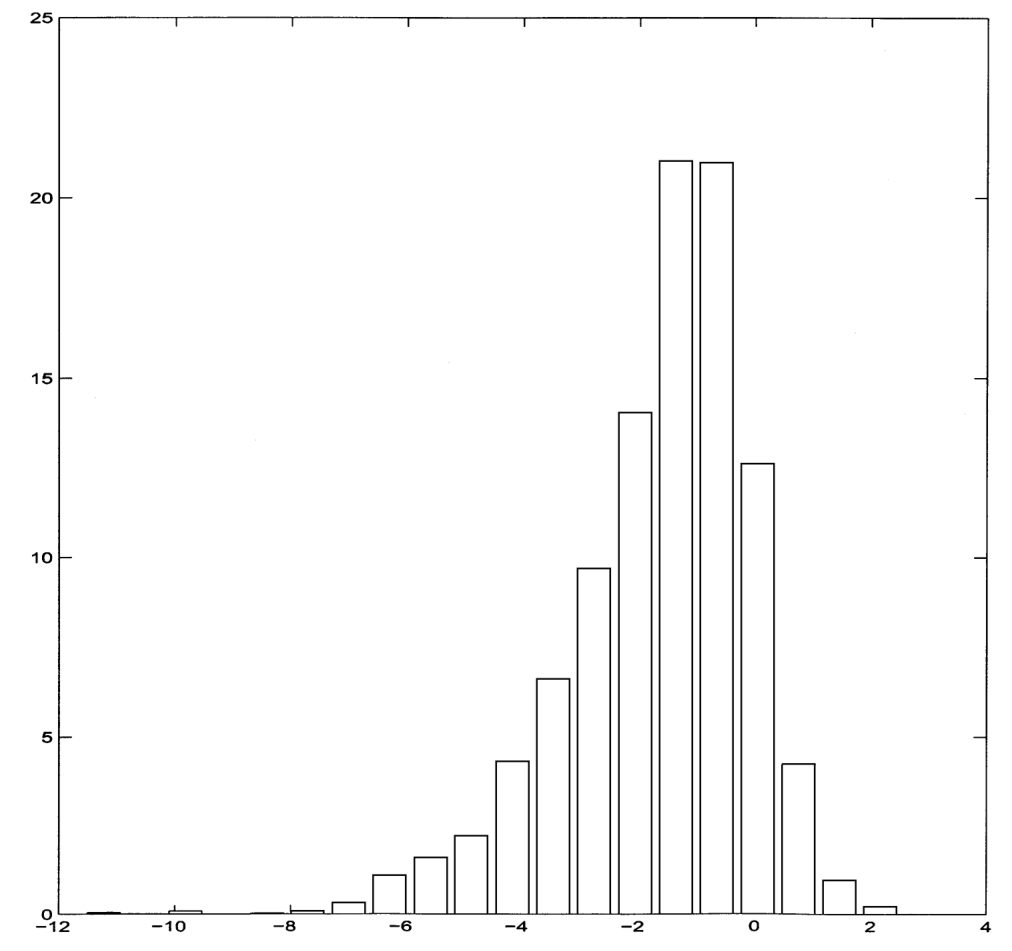
\includegraphics[width=\linewidth]{figures/ch08/nevo01_fig1_mushy.png}
\caption{Taste for sogginess (Mushy coefficient)}\label{fig:08-nevo-mushy}
\end{subfigure}\hfill
\begin{subfigure}[t]{0.48\linewidth}
\centering
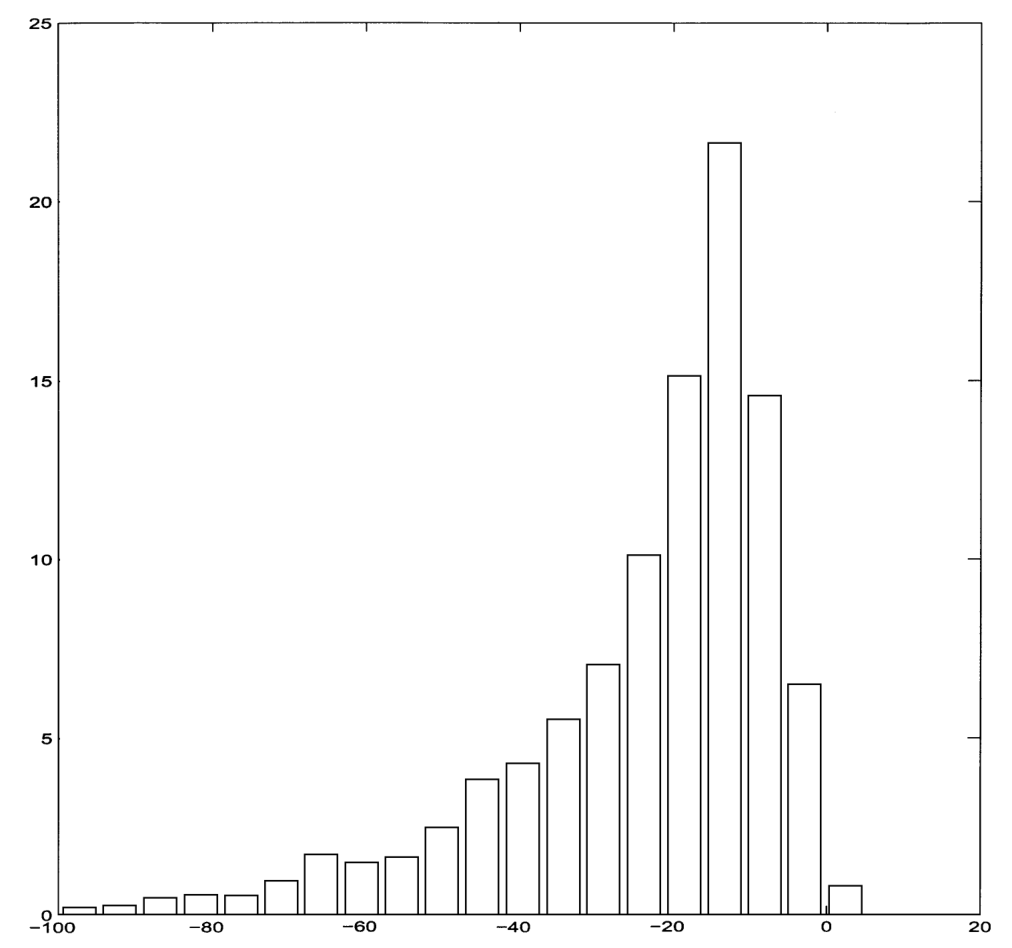
\includegraphics[width=\linewidth]{figures/ch08/nevo01_fig2_price.png}
\caption{Price coefficient}\label{fig:08-nevo-price}
\end{subfigure}
\caption{Frequency distributions of two individual coefficients implied by the estimates in
\cref{tab:08-nevo-full}. The horizontal axes give the value of the coefficient. The vertical axes, unlabeled
in the original, give frequencies. The bars sum to about 100, so the heights are percentages of simulated
consumers. Panel (a) puts about 15\% of consumers at a positive taste for sogginess. Panel (b) is skewed to the
left because it inherits the empirical distribution of demographics, and only 0.7\% of its mass lies above
zero.
Source: \citet{Nevo2001}, Figures 1 and 2.}
\label{fig:08-nevo-dists}
\end{figure}

The insignificance of the standard deviations says that the included demographics explain most of the
heterogeneity. The share of the variance of each coefficient explained by demographics exceeds 90\% (p.~330).
Appendix B of the paper re-estimates the model with the random shocks $\nu_i$ set to zero for the
characteristics that have demographic interactions. The estimates and margins barely change
(\cref{tab:08-nevo-robust}, column (i)). Nevo cautions against a stronger reading (p.~330, n.~26). The result
says that the data reject the assumed normal distribution for the unobserved part of tastes. It does not say
that information beyond demographics is useless. Purchase histories \citep{RossiMcCullochAllenby1996} and
second-choice data (the working-paper version of \citealp{BerryLevinsohnPakes2004}, \cref{sec:08-blp04}) do
reveal heterogeneity beyond demographics.

\casehead{Elasticities} \Cref{tab:08-nevo-elas} reproduces Table VII. Because elasticities vary across markets,
each entry is the median over the 1,124 markets of the elasticity of the row brand's share with respect to the
column brand's price. The own elasticities on the diagonal run from $-2.277$ (Cap'n Crunch) to $-4.252$
(Shredded Wheat). They are not ordered by price as the logit would require.

\begin{table}[htbp]
\centering
\caption{Median own- and cross-price elasticities of cereal demand}
\label{tab:08-nevo-elas}
\scriptsize
\setlength{\tabcolsep}{2.6pt}
\begin{tabular}{@{}rlrrrrrrrrrr@{}}
\toprule
 & & Corn & Frosted & Rice & Froot & & & Lucky & P Raisin & CapN & Shredded \\
\# & Brand & Flakes & Flakes & Krispies & Loops & Cheerios & Total & Charms & Bran & Crunch & Wheat \\
\midrule
1 & K Corn Flakes & $-$3.379 & 0.212 & 0.197 & 0.014 & 0.202 & 0.097 & 0.012 & 0.013 & 0.038 & 0.028 \\
2 & K Raisin Bran & 0.036 & 0.046 & 0.079 & 0.043 & 0.145 & 0.043 & 0.037 & 0.057 & 0.050 & 0.040 \\
3 & K Frosted Flakes & 0.151 & $-$3.137 & 0.105 & 0.069 & 0.129 & 0.079 & 0.061 & 0.013 & 0.138 & 0.023 \\
4 & K Rice Krispies & 0.195 & 0.144 & $-$3.231 & 0.031 & 0.241 & 0.087 & 0.026 & 0.031 & 0.055 & 0.046 \\
5 & K Frosted Mini Wheats & 0.014 & 0.024 & 0.052 & 0.043 & 0.105 & 0.028 & 0.038 & 0.054 & 0.045 & 0.033 \\
6 & K Froot Loops & 0.019 & 0.131 & 0.042 & $-$2.340 & 0.072 & 0.025 & 0.107 & 0.027 & 0.149 & 0.020 \\
7 & K Special K & 0.114 & 0.124 & 0.105 & 0.021 & 0.153 & 0.151 & 0.019 & 0.021 & 0.035 & 0.035 \\
8 & K Crispix & 0.077 & 0.086 & 0.114 & 0.034 & 0.181 & 0.085 & 0.030 & 0.037 & 0.048 & 0.043 \\
9 & K Corn Pops & 0.013 & 0.109 & 0.034 & 0.113 & 0.058 & 0.025 & 0.098 & 0.024 & 0.127 & 0.016 \\
10 & GM Cheerios & 0.127 & 0.111 & 0.152 & 0.034 & $-$3.663 & 0.085 & 0.030 & 0.037 & 0.056 & 0.050 \\
11 & GM Honey Nut Cheerios & 0.033 & 0.192 & 0.058 & 0.123 & 0.094 & 0.034 & 0.107 & 0.026 & 0.162 & 0.024 \\
12 & GM Wheaties & 0.242 & 0.169 & 0.175 & 0.025 & 0.240 & 0.113 & 0.021 & 0.026 & 0.050 & 0.043 \\
13 & GM Total & 0.096 & 0.108 & 0.087 & 0.018 & 0.131 & $-$2.889 & 0.017 & 0.017 & 0.029 & 0.029 \\
14 & GM Lucky Charms & 0.019 & 0.131 & 0.041 & 0.124 & 0.073 & 0.026 & $-$2.536 & 0.027 & 0.147 & 0.020 \\
15 & GM Trix & 0.012 & 0.103 & 0.031 & 0.109 & 0.056 & 0.026 & 0.096 & 0.024 & 0.123 & 0.016 \\
16 & GM Raisin Nut & 0.013 & 0.025 & 0.042 & 0.035 & 0.089 & 0.040 & 0.031 & 0.046 & 0.036 & 0.027 \\
17 & GM Cinnamon Toast Crunch & 0.026 & 0.164 & 0.049 & 0.119 & 0.089 & 0.035 & 0.102 & 0.026 & 0.151 & 0.022 \\
18 & GM Kix & 0.050 & 0.279 & 0.070 & 0.101 & 0.106 & 0.056 & 0.088 & 0.030 & 0.149 & 0.025 \\
19 & P Raisin Bran & 0.027 & 0.037 & 0.068 & 0.044 & 0.127 & 0.035 & 0.038 & $-$2.496 & 0.049 & 0.036 \\
20 & P Grape Nuts & 0.037 & 0.049 & 0.088 & 0.042 & 0.165 & 0.050 & 0.037 & 0.051 & 0.052 & 0.047 \\
21 & P Honey Bunches of Oats & 0.100 & 0.098 & 0.104 & 0.022 & 0.172 & 0.109 & 0.020 & 0.024 & 0.038 & 0.033 \\
22 & Q 100\% Natural & 0.013 & 0.021 & 0.046 & 0.042 & 0.103 & 0.029 & 0.036 & 0.052 & 0.046 & 0.029 \\
23 & Q Life & 0.077 & 0.328 & 0.091 & 0.114 & 0.137 & 0.046 & 0.096 & 0.023 & 0.182 & 0.029 \\
24 & Q CapN Crunch & 0.043 & 0.218 & 0.064 & 0.124 & 0.101 & 0.034 & 0.106 & 0.026 & $-$2.277 & 0.024 \\
25 & N Shredded Wheat & 0.076 & 0.082 & 0.124 & 0.037 & 0.210 & 0.076 & 0.034 & 0.044 & 0.054 & $-$4.252 \\
26 & Outside good & 0.141 & 0.078 & 0.084 & 0.022 & 0.104 & 0.041 & 0.018 & 0.021 & 0.033 & 0.021 \\
\bottomrule
\end{tabular}

\smallskip
\begin{minipage}{0.97\linewidth}
\footnotesize Notes: Entry $(i, j)$ is the percent change in the share of row brand $i$ for a one percent
change in the price of column brand $j$, as in \cref{eq:08-nevo-elas}. Each entry is the median over the 1,124
city-quarter markets. Own elasticities are negative numbers here, as in the paper. K, GM, P, Q and N denote
Kellogg, General Mills, Post, Quaker and Nabisco. Source: \citet{Nevo2001}, Table VII.
\end{minipage}
\end{table}

The substitution patterns follow characteristics. Lucky Charms, a children's cereal, is most sensitive to the
prices of other children's cereals (p.~330). It is least sensitive to the prices of Corn Flakes, Total and Wheaties, which
serve different segments.\footnote{Nevo names Corn Pops and Froot Loops as the brands to whose prices Lucky
Charms is most sensitive. Corn Pops and Wheaties are not among the ten columns printed in Table VII, so these
statements refer to the full matrix. Among the printed columns, row 14 is largest for Cap'n Crunch (0.147),
Frosted Flakes (0.131) and Froot Loops (0.124), and smallest for Corn Flakes (0.019).} The logit forces every
cross elasticity in a column to be equal. A summary of how far the estimates depart from that restriction is
the ratio of the largest to the smallest cross elasticity in a column, which equals one in the logit. The ratio
ranges from 21 for Corn Flakes to 3.5 for Shredded Wheat, with 95\% confidence intervals of 11 to 260 and 3
to 52 (p.~330). A low ratio also flags brands whose observed characteristics do not differentiate them well. A
formal test that all nonlinear parameters are zero, which is a specification test of the logit, is easily
rejected (p.~332, n.~28).

The last row gives the elasticity of the outside good's share with respect to each price. It is larger for
Corn Flakes (0.141) than for Froot Loops (0.022), in absolute terms and relative to the average cross elasticity
in each column (p.~332). Generic versions of Corn Flakes have larger shares than generic versions of Froot
Loops, and all generics belong to the outside good. A rise in the price of Corn Flakes therefore sends more
consumers to the outside option. Comparisons across columns should use semi-elasticities, because a one
percent price change differs in cents across brands (n.~29).

\subsection{Price-cost margins and the test of conduct}\label{sec:08-nevo01-margins}

\casehead{Predicted margins} \Cref{tab:08-nevo-margins} reproduces Table VIII and \cref{fig:08-nevo-margins}
plots it. Each entry is the median over the 27,862 observations of the margin implied by
\cref{eq:08-nevo-markup} under one ownership matrix. Medians are used to limit the influence of outliers, and
means with the 5\% tails trimmed are essentially identical (p.~332, n.~30). For the logit the computation is
analytical, using \eqref{eq:08-nevo-logit}. For the full model the confidence intervals come from 1,500
parametric bootstrap draws.

\begin{table}[htbp]
\centering
\caption{Median predicted price-cost margins under alternative conduct}
\label{tab:08-nevo-margins}
\footnotesize
\begin{tabular}{@{}lcc@{}}
\toprule
 & Logit & Full model \\
 & (\cref{tab:08-nevo-logit}, col.\ ix) & (\cref{tab:08-nevo-full}) \\
\midrule
Single-product firms & 33.6\% & 35.8\% \\
 & (31.8\%, 35.6\%) & (24.4\%, 46.4\%) \\
Current ownership of 25 brands & 35.8\% & 42.2\% \\
 & (33.9\%, 38.0\%) & (29.1\%, 55.8\%) \\
Joint ownership of 25 brands & 41.9\% & 72.6\% \\
 & (39.7\%, 44.4\%) & (62.2\%, 97.2\%) \\
Current ownership of all brands & 37.2\% & n.a. \\
 & (35.2\%, 39.4\%) & \\
Monopoly or perfect price collusion & 54.0\% & n.a. \\
 & (51.1\%, 57.3\%) & \\
\bottomrule
\end{tabular}

\smallskip
\begin{minipage}{0.84\linewidth}
\footnotesize Notes: Margins are $\frac{p - mc}{p}$, medians of the distribution over 27,862
brand-city-quarter observations. 95\% confidence intervals for the medians in parentheses, based on the
asymptotic distribution of the demand estimates. They are analytical for the logit and use 1,500 draws for the
full model. The last two rows require the shares of brands outside the sample, which suffice only for the
logit. Source: \citet{Nevo2001}, Table VIII.
\end{minipage}
\end{table}

\begin{figure}[htbp]
\centering
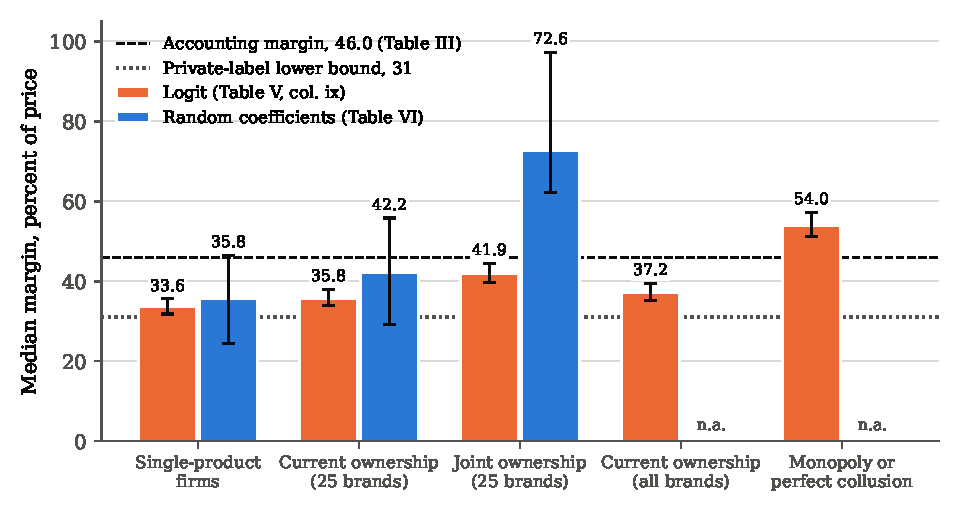
\includegraphics[width=0.97\linewidth]{figures/ch08/nevo01_margins.pdf}
\caption{Median predicted margins under five conduct models, with 95\% confidence intervals for the medians.
The dashed line is the accounting gross margin of 46.0\% of the retail price
(\cref{tab:08-nevo-costs}). The dotted line is the lower bound of about 31\% from the gap between national-brand
and private-label prices (p.~333). The random coefficients model predicts a joint-ownership margin far above
both lines, while its current-ownership interval covers them. The logit margins barely respond to ownership.
Redrawn from \citet{Nevo2001}, Table VIII.}
\label{fig:08-nevo-margins}
\end{figure}

The logit price coefficient, $-23.37$, is close to the full model's price coefficient in the Means column,
$-27.198$, yet their margins diverge as ownership widens. Under single-product pricing the medians are 33.6\% and 35.8\%. The portfolio effect adds 2.2
points in the logit and 6.4 points in the full model. Joint ownership of the 25 brands adds a further 6.1
points in the logit and 30.4 points in the full model. By \cref{prop:08-nevo-ownership}, these increments are
governed by the diversion ratios among co-owned brands. The full model concentrates diversion among similar
cereals, so joint pricing internalizes much more substitution.

The logit increments match \eqref{eq:08-nevo-logit} closely. In the logit the ratio of the joint-ownership
markup to the single-product markup of brand $j$ is $\frac{1-s_j}{1-S_{\mathcal{G}}}$. A rough calculation with
ratios of medians gives $\frac{41.9}{33.6} \approx 1.25$, which implies that the 25 brands hold about one fifth
of the potential market. Similarly $\frac{54.0}{33.6} \approx 1.61$ implies that all brands together hold
about 38\%. The ratio of the two, about one half, is consistent with the 43\% to 62\% of cereal volume that the
25 brands account for.\footnote{These are our calculations. A ratio of medians is not the median of the ratios,
and $s_j$ is treated as negligible, so the implied shares are approximations.}

\casehead{Observed margins} Testing requires a comparison with actual margins, which Nevo does not observe
directly. He treats the retail margin as an additional cost to manufacturers, which is consistent with many
models of manufacturer-retailer interaction (p.~333). The relevant observed margin is then the gross margin
relative to the retail price, 46.0\% from \cref{tab:08-nevo-costs}. This figure excludes promotional costs,
some of which, such as coupon rebates, are arguably marginal. Excluding them makes the observed margin a
generous one and the test conservative. Census data support the accounting figure. They are based on average
variable cost and give an upper bound.\footnote{The Census margin of 64.4\% is relative to the manufacturer's
price. On the retail-price basis of \cref{tab:08-nevo-costs}, Panel B, it corresponds to
$0.80 \times 64.4 \approx 51.5\%$. This conversion is ours.} A lower bound comes from the gap between the
prices of national brands and the corresponding private labels, about 31\% according to
\citet{Wongtrakool1994}. Private labels may carry a markup of their own and may have higher costs, so their
price exceeds the national brands' marginal cost and the gap understates the margin (pp.~333--334). Nevo
cautions that accounting margins are crude \citep{FisherMcGowan1983} and uses them only to discriminate
between models.

\casehead{The test} The predicted margins differ enough that even crude observed margins separate the models
(p.~334). The joint-ownership interval for the full model, 62.2\% to 97.2\%, lies above both the typical margin
of 46.0\% and the lower bound of 31\%. Joint profit maximization over the 25 brands is therefore rejected. The
current-ownership interval, 29.1\% to 55.8\%, contains both figures, so multi-product Nash-Bertrand pricing is
not rejected. The decomposition implied by the full model's medians attributes about 85\% of the
current-ownership margin to differentiation ($\frac{35.8}{42.2}$) and the remaining 6.4 points to the
portfolio effect.

Two further arguments strengthen the conclusion. The first concerns the restriction to 25 brands (p.~334). The
price coefficient should not be biased by the selection, and estimates on other samples confirm this. Brands
outside the sample are probably more elastic, which would lower the single-product margins. Weighting by
market shares, which is the likely effect of including small brands, offsets this. The share-weighted means
are roughly 2 to 3 points above the medians in Table VIII. For the current-ownership and collusive models a second force operates. Moving products from the
outside good into the inside set raises the predicted margins, and the effect grows with the number of jointly
priced products. Adding brands would therefore move the Nash-Bertrand prediction closer to the observed margins
and the collusive prediction further away. In this sense Table VIII is conservative.

The second argument concerns the logit. Applied to the logit column, the same test would not reject full
collusion over all products (p.~335). The logit's collusive margins, 41.9\% for the 25 brands and 54.0\% for
all brands, lie close to the observed margin of 46.0\%. Nevo stresses that this result is driven entirely by the logit's restrictive
substitution patterns and says nothing about conduct. It is the clearest demonstration in the paper of why
flexible substitution patterns matter for questions of market power.

\casehead{Why not a formal test} Nevo explains why he does not use two alternatives (pp.~334--335). One is to
estimate a conduct parameter, as in homogeneous-goods industries \citep{Bresnahan1989}. Its interpretation is
problematic \citep{Corts1999}, and its identification requirements are unlikely to be met with differentiated
products \citep{Nevo1998}. The other is a non-nested test of fully specified models
\citep{Bresnahan1987,GasmiLaffontVuong1992}. That requires the likelihood of each model, hence distributional
assumptions on the errors and a complete supply equation, and there is no natural set of such assumptions.
\Cref{ch:conduct} and \cref{sec:08-supply} discuss conduct testing more generally.

\subsection{Robustness*}\label{sec:08-nevo01-robust}

Appendix B of the paper reports four alternative specifications of the full model, reproduced in condensed form
in \cref{tab:08-nevo-robust}. Column (i) drops the random shocks $\nu_i$ for the characteristics that interact
with demographics. Its price coefficient ($-25.595$) and margins (36.1\%, 41.9\% and 67.4\%) are close to the
preferred ones, which supports the claim that demographics drive the heterogeneity. Columns (ii) and (iii) are
nonlinear least squares without instruments, without and with brand dummies. Their price coefficients are
$-4.291$ and $-7.407$. The implied margins are absurd. They range from 67.6\% to 84.5\% under Nash-Bertrand
pricing, and above 100\% under collusion. Column (iv) uses brand dummies as instruments, the analogue of
characteristic-based identification. Its estimates are imprecise and 22.4\% of its price coefficients are
positive. Nevo notes that it lacks the variance-reduction methods of BLP (p.~339).

\begin{table}[htbp]
\centering
\caption{Alternative specifications of the full model}
\label{tab:08-nevo-robust}
\footnotesize
\begin{tabular}{@{}lrrrr@{}}
\toprule
 & (i) & (ii) & (iii) & (iv) \\
 & No $\nu_i$ on & NLLS, no & NLLS, brand & GMM, brand \\
 & interacted chars. & brand dummies & dummies & dummies as IVs \\
\midrule
Mean price coefficient & $-$25.595 & $-$4.291 & $-$7.407 & $-$9.856 \\
 & (2.673) & (0.143) & (0.164) & (3.039) \\
Price $\times$ income & 311.101 & 34.565 & 8.552 & 21.575 \\
 & (61.797) & (1.455) & (0.974) & (96.912) \\
Percent of price coefficients $>0$ & 0 & 16.1 & 0 & 22.4 \\
\addlinespace
Single-product margin & 36.1\% & 67.6\% & 75.7\% & 48.2\% \\
Multi-product margin & 41.9\% & 75.6\% & 84.5\% & 54.0\% \\
Collusive margin & 67.4\% & 103.9\% & 117.6\% & 88.9\% \\
\bottomrule
\end{tabular}

\smallskip
\begin{minipage}{0.88\linewidth}
\footnotesize Notes: Standard errors in parentheses. 27,862 observations. NLLS is nonlinear least squares,
which does not instrument for price. Column (i) is the preferred specification without $\nu_i$ for the
characteristics that have demographic interactions. The paper also reports all taste parameters, omitted here.
The preferred specification gives 35.8\%, 42.2\% and 72.6\% (\cref{tab:08-nevo-margins}). Source:
\citet{Nevo2001}, Table B(II).
\end{minipage}
\end{table}

Other checks point the same way (pp.~327, 335--336). A specification with city fixed effects, the analogue of
column (x) of \cref{tab:08-nevo-logit}, gives point estimates close to the preferred ones but very large
standard errors. This is expected, since demographics barely change within a city over five years. A
multi-stage budgeting demand system in the style of \citet{HausmanLeonardZona1994} and \citet{Hausman1997},
covered in \cref{ch:aids}, shows interesting differences in cross-price substitution but the same conclusions
about conduct. Studies based on household data, a random coefficients model by \citet{Kiser1996} and a nested
logit by \citet{Shum1999}, use different data and different identifying assumptions. They produce very similar
own- and cross-price elasticities.

\subsection{Interpretation, limitations and contribution}\label{sec:08-nevo01-assess}

\casehead{Interpretation} If Nash-Bertrand pricing is the benchmark of noncollusive behavior, prices in RTE
cereal are not collusive, even with margins above 45\% (p.~336). High margins reflect consumers' willingness
to pay for their favorite brands and firms' internalization of substitution within their portfolios. To the
extent that the industry has market power, it lies in the ability to maintain a portfolio of differentiated
brands and to shape perceived quality through advertising. Nevo relates this to the FTC case. The standard
account of the complaint mentions cooperative pricing, but its core was brand proliferation as a barrier to
entry \citep{Schmalensee1978}. In this sense the FTC focused on the dimensions of competition that Nevo finds
important. His model, however, takes brands and advertising as given and cannot evaluate their competitive
effects (p.~336).

\casehead{Limitations} The test rules out only the extreme form of cooperation, joint maximization of profits
over all 25 brands. Cooperation within a subset of products or firms, such as two raisin brans or two smaller
producers, is not tested and would require more detailed cost data (p.~336). The observed margin is a single
accounting figure for a typical Kellogg brand, compared with medians over brands, cities and quarters. The
Hausman instruments rest on independence of demand shocks across cities, which overidentification tests reject
in the logit unless city effects are added. Advertising is treated as exogenous, and its implied elasticity is
implausibly low. The model is static and uses quarterly averages of prices that include temporary promotions.
The standard deviations of the random coefficients are imprecise because the choice set barely varies. The
full model's margins have wide confidence intervals. The single-product interval runs from 24.4\% to 46.4\%.
Finally, the definition of the potential market as one serving per person per day fixes the outside share,
and with it the level of the implied markups (\cref{sec:08-model}).

\casehead{Contribution} The paper made four contributions that became standard. It combined brand fixed effects
with the BLP estimator and recovered taste means by minimum distance, so that price endogeneity due to $\xi_j$
needs no instrument. It used prices in other markets as instruments in a random coefficients model and checked
them against cost proxies. It modeled heterogeneity with the empirical distribution of demographics. Above all,
it turned the supply side into a tool for measuring conduct. Comparing margins implied by alternative ownership
matrices with observed margins gives a transparent decomposition of market power. The same model and data
underlie the merger simulations of \citet{Nevo2000b}, discussed in \cref{ch:mergers}. Hausman's valuation of a
new cereal brand, discussed in \cref{ch:newgoods}, depends on the same kind of assumption about price
competition that Nevo tests. Later work uses the demand elasticities to discriminate between models of conduct
in the same industry, including common-ownership pricing \citep{BackusConlonSinkinson2021}.

\begin{table}[htbp]
\centering
\caption{Identification and counterfactual map of Nevo (2001)}
\label{tab:08-nevo01-map}
\footnotesize
\renewcommand{\arraystretch}{1.1}
\begin{tabularx}{\textwidth}{@{}>{\raggedright\arraybackslash}p{2.6cm}>{\raggedright\arraybackslash}X@{}}
\toprule
Observed data & IRI scanner prices and servings of 25 cereal brands in up to 65 cities, quarterly from 1988 to
  1992 (27,862 brand-city-quarters). Brand characteristics, national advertising, CPS demographic draws, and
  accounting margins for a typical brand. \\
\addlinespace
Latent objects & City-quarter quality deviations $\tilde\xi_{jt}$, consumer tastes $\nu_i$, marginal costs
  and markups. \\
\addlinespace
Estimated parameters & The price and advertising coefficients, brand and quarter effects, demographic
  interactions $\Pi$ and standard deviations $\Sigma$. Taste means come from a minimum-distance step. \\
\addlinespace
Identifying variation & Prices of the same brand in other cities of the region, checked against cost
  proxies. Brand effects absorb national quality, and cross-city differences in demographics identify $\Pi$. \\
\addlinespace
Maintained assumptions & City demand shocks are independent across cities after brand, time and demographic
  controls, and costs share a regional component. Static pricing, exogenous advertising, and a potential
  market of one serving per person per day. \\
\addlinespace
Counterfactual and what it holds fixed & Margins implied by \eqref{eq:08-nevo-markup} under single-product,
  current and joint ownership, at observed prices and shares. Demand is held at its estimates, and only the
  ownership matrix changes. \\
\addlinespace
Conclusion & Current ownership predicts a median margin of 42.2 percent, whose interval contains the
  observed margins. Joint ownership of the 25 brands predicts 72.6 percent and is rejected. Margins come
  from differentiation and portfolios, given the Hausman instruments. \\
\addlinespace
One limitation & Only joint profit maximization over all 25 brands is tested. Collusion within a subset of
  brands or firms is not. \\
\addlinespace
Source and our additions & The tables are Nevo's. \Cref{prop:08-nevo-ownership}, the advertising
  benchmark and the logit share calculations behind the margin ratios are ours. \\
\addlinespace
Tools in the appendices & \Cref{sec:A-iv,sec:A-gmm,sec:A-delta-boot}. \\
\bottomrule
\end{tabularx}
\end{table}

\section{Case study: Berry, Levinsohn and Pakes (2004), micro and macro data}\label{sec:08-blp04}

\citet{BerryLevinsohnPakes2004}, henceforth BLP (2004), return to the automobile market with a new kind of
data. A proprietary survey by General Motors covers a large sample of 1993 new-vehicle buyers. It records
each buyer's demographics, the vehicle bought and the vehicle the buyer would have bought had the first choice
been unavailable. The paper asks what such consumer-level data, and second choices in particular, add to the
identification of substitution patterns. The answer has three parts. Second choices pin down the parameters
that govern substitution. Unobserved heterogeneity in tastes is needed to match them, even with rich
demographics. A single cross section still cannot determine the level of price elasticities. The general
estimator was introduced in \cref{sec:08-micro}. Here we follow the paper in detail, and
\cref{tab:08-blp04-map} at the end of the section maps it. Page numbers refer to the
journal article.\footnote{BLP (2004) write observed household attributes as $z_{ir}$, the coefficients on
their interactions with characteristics as $\beta^{o}_{kr}$ (``observed'') and the standard deviations of
unobserved tastes as $\beta^{u}_k$ (``unobserved''). We write $D_{ir}$, $\pi_{kr}$ and $\sigma_k$, so that
$\beta^{o}$ and $\beta^{u}$ correspond to the matrices $\Pi$ and $\Sigma$ of \cref{sec:08-model}.}

\subsection{The question}\label{sec:08-blp04-question}

We abbreviate \citet{BerryLevinsohnPakes1995}, the subject of \cref{sec:08-blp95}, as BLP (1995). In that
paper, substitution patterns are identified from changes across markets and years in the choice set and in the
distribution of consumer attributes. The distribution of tastes,
conditional on observed incomes, is assumed to be stable over time (pp.~69--70). Earlier discrete choice work,
and \citet{Goldberg1995} and \citet{Petrin2002} in industrial organization, matched consumer attributes to
choices. Such data identify substitution to the extent that observed attributes explain it.
\Cref{sec:08-goldberg} discusses Goldberg's study.

Second-choice data offer a different source of identification (p.~70). They give a direct, data-based measure
of substitution, so one can ask which models reproduce it. By requiring the parameters to match observed
second choices, the econometrician gains identifying power that does not rely on exogenous changes in choice
sets. The paper also stresses a limit. Second choices in a single cross section, with one price per vehicle,
reveal the pattern of substitution but not the level of price elasticities. Outside information must fix the
level. The paper closes with two out-of-sample predictions, the introduction of luxury sport utility vehicles
and the closure of the Oldsmobile division of General Motors.

\subsection{Data}\label{sec:08-blp04-data}

\casehead{The CAMIP survey} The consumer data come from a proprietary survey conducted for General Motors,
here called CAMIP (pp.~79--80). It samples from the registrations of 1993 model-year vehicles of all
manufacturers, not only GM. For each vehicle a given number of buyers is sampled, so the design is a random
sample conditional on the vehicle purchased. A sample of this kind is called \emph{choice-based}. The subsample
used has 37,500 observations. The questionnaire asks about income, age of the household head, family size and
place of residence, and each question is matched to a question in the CPS.

\Cref{tab:08-blp04-samples} compares CAMIP households with CPS households. CAMIP over-represents high incomes.
Only 6.52\% of CPS households earn \$85,000 or more, against 25.13\% of CAMIP households, and mean income is
\$72,270 in CAMIP against \$34,170 in the CPS. New-vehicle buyers are richer than the population. More
surprisingly, CAMIP households are less urban (35\% against 46\%) and more rural (35\% against 25\%).
Rural households buy a disproportionate number of vehicles, which helps explain the high share of trucks
(p.~80).

\begin{table}[htbp]
\centering
\caption{CPS and CAMIP household samples}
\label{tab:08-blp04-samples}
\footnotesize
\begin{tabular}{@{}lrrrr@{}}
\toprule
Income range (\$) & Percent in CPS & Percent in CAMIP & CPS group mean & CAMIP group mean \\
\midrule
0--36,500 & 64.17 & 25.00 & 16.90 & 25.96 \\
36,500--55,000 & 16.97 & 23.16 & 44.89 & 45.43 \\
55,000--85,000 & 12.34 & 26.71 & 66.93 & 67.46 \\
85,000 and above & 6.52 & 25.13 & 114.25 & 148.19 \\
All & 100.00 & 100.00 & 34.17 & 72.27 \\
\midrule
Other demographics & & & CPS mean & CAMIP mean \\
\midrule
Family size & & & 2.36 & 2.65 \\
Age of household head & & & 46.80 & 46.18 \\
Number of kids & & & 0.66 & 0.58 \\
Urban & & & 0.46 & 0.35 \\
Rural & & & 0.25 & 0.35 \\
Suburban & & & 0.29 & 0.30 \\
\bottomrule
\end{tabular}

\smallskip
\begin{minipage}{0.86\linewidth}
\footnotesize Notes: Group means of income in thousands of dollars. Source:
\citet{BerryLevinsohnPakes2004}, Table 1.
\end{minipage}
\end{table}

\casehead{The choice set and product data} The vehicle list follows GM's sampling cells and has 203 vehicles:
147 cars, 25 sport utility vehicles (SUVs), 17 vans and 14 pickup trucks (p.~81). Early runs used 218
vehicles. The final runs aggregate 15 very expensive vehicles, with an average price of \$74,000 and a combined
share of 0.3\% of vehicles sold, into one ``super-luxury'' model (n.~9). The survey records transaction prices.
Characteristics are those of the modal vehicle in each cell, the most commonly purchased combination of
options, and price is the average price of that modal vehicle. About 10.6 million vehicles were sold in 1993
at an average price of \$18,500, for total sales of about \$196 billion. The continuous characteristics are horsepower
per weight (HP), number of passengers (Pass, a measure of size), city miles per gallon (MPG) and number of power
accessories (Acc). They also include safety features (Safe, antilock brakes plus airbags) and the payload of
light trucks. The
dummies mark minivans, SUVs, pickups, full-size vans, sports cars and four- or all-wheel drive (Allw). The interactions
PUPayl and SUVPayl multiply payload by the pickup and SUV dummies (Table 2).

\casehead{Demographic patterns} Means of vehicle characteristics by demographic group reveal clear interactions
(p.~81). Examples are kids with minivans, income with price, rural residence with pickups and four-wheel drive,
and age with nearly everything. The authors used such tables to choose the interactions in utility.
\Cref{tab:08-blp04-groups} condenses their Table 4. The mean price of the vehicle chosen rises from \$16,600 in
the lowest income group to \$26,300 in the highest. Households with two or more children choose a minivan 18\% of
the time, against 3\% for households without children. The mean of PUPayl, the pickup dummy times payload in
thousands of pounds, is 0.31 among rural households, against 0.14 among urban and 0.10 among suburban households. Buyers over 50 choose vehicles that are more
expensive and larger, with more accessories, and they rarely choose sports cars or SUVs (0.07 and 0.04).

\begin{table}[htbp]
\centering
\caption{Mean characteristics of the vehicles chosen by demographic group in the CAMIP data (condensed)}
\label{tab:08-blp04-groups}
\footnotesize
\setlength{\tabcolsep}{4.5pt}
\begin{tabular}{@{}lrrrrrrrrrr@{}}
\toprule
Group & Price & HP & Pass & Acc & Sport & MPG & Allw & Miniv & SUV & PUPayl \\
\midrule
\multicolumn{11}{@{}l}{\textit{Age of household head}} \\
\quad 30 or less & 16.6 & 4.7 & 4.5 & 2.6 & 0.20 & 22.0 & 0.13 & 0.03 & 0.15 & 0.24 \\
\quad 30--50 & 20.1 & 4.8 & 4.9 & 3.1 & 0.15 & 20.4 & 0.13 & 0.08 & 0.13 & 0.18 \\
\quad Over 50 & 22.4 & 4.9 & 5.1 & 3.4 & 0.07 & 19.8 & 0.06 & 0.04 & 0.04 & 0.19 \\
\multicolumn{11}{@{}l}{\textit{Number of children}} \\
\quad 0 & 20.9 & 4.9 & 4.8 & 3.2 & 0.14 & 20.4 & 0.10 & 0.03 & 0.09 & 0.20 \\
\quad 1 & 19.2 & 4.7 & 4.8 & 3.0 & 0.13 & 21.0 & 0.12 & 0.06 & 0.11 & 0.20 \\
\quad 2 or more & 20.1 & 4.6 & 5.3 & 3.1 & 0.08 & 19.9 & 0.12 & 0.18 & 0.13 & 0.16 \\
\multicolumn{11}{@{}l}{\textit{Residence}} \\
\quad Urban & 20.6 & 4.8 & 4.9 & 3.2 & 0.13 & 20.7 & 0.10 & 0.05 & 0.10 & 0.14 \\
\quad Suburban & 21.7 & 5.0 & 4.9 & 3.4 & 0.15 & 20.3 & 0.10 & 0.06 & 0.10 & 0.10 \\
\quad Rural & 19.2 & 4.7 & 4.9 & 3.0 & 0.11 & 20.2 & 0.12 & 0.06 & 0.11 & 0.31 \\
\multicolumn{11}{@{}l}{\textit{Household income (\$)}} \\
\quad 37,000 or less & 16.6 & 4.6 & 4.8 & 2.6 & 0.12 & 21.9 & 0.08 & 0.04 & 0.07 & 0.25 \\
\quad 37,000--55,000 & 18.5 & 4.7 & 4.9 & 3.0 & 0.12 & 20.7 & 0.10 & 0.07 & 0.10 & 0.24 \\
\quad 55,000--85,000 & 20.3 & 4.8 & 4.9 & 3.2 & 0.14 & 20.0 & 0.13 & 0.07 & 0.13 & 0.19 \\
\quad Over 85,000 & 26.3 & 5.2 & 4.9 & 3.7 & 0.14 & 19.1 & 0.11 & 0.05 & 0.12 & 0.08 \\
\bottomrule
\end{tabular}

\smallskip
\begin{minipage}{0.95\linewidth}
\footnotesize Notes: Price in thousands of dollars. Sport, Allw, Miniv and SUV are shares of vehicles with the
attribute. PUPayl is the pickup dummy times payload in thousands of pounds. The original table also reports
safety features, the van dummy, SUV payload and rows by family size. Source: \citet{BerryLevinsohnPakes2004},
Table 4 (p.~84).
\end{minipage}
\end{table}

\casehead{Second choices}
\Cref{tab:08-blp04-second} reproduces the second-choice information for 17 representative vehicles. The 166
sampled buyers of the Ford Escort named the Ford Tempo most often (16 buyers), followed by the Ford Taurus.
Together these two account for 18\% of Escort buyers, who named 53 different second choices in all (p.~86).
Second choices are more concentrated for light trucks and expensive cars. They are often made by the same
company as the first choice, which supports pricing that maximizes the joint profits of each firm's products.

\begin{table}[htbp]
\centering
\caption{Examples of second choices in the CAMIP data}
\label{tab:08-blp04-second}
\footnotesize
\setlength{\tabcolsep}{4pt}
\begin{tabular}{@{}lrlrlrr@{}}
\toprule
 & & Modal second & Number & Next second & (Modal $+$ & Different \\
First choice & $n_j$ & choice & choosing & choice & next)$\,\div\, n_j$ & choices \\
\midrule
Metro & 188 & Escort & 22 & Geo Storm & .22 & 49 \\
Cavalier & 238 & Escort & 16 & LeBaron & .12 & 59 \\
Escort & 166 & Tempo & 16 & Taurus & .18 & 53 \\
Corolla & 250 & Civic & 42 & Camry & .33 & 55 \\
Sentra & 203 & Corolla & 34 & Civic & .31 & 60 \\
Accord & 223 & Camry & 58 & Taurus & .35 & 61 \\
Taurus & 147 & Camry & 18 & Sable & .22 & 45 \\
Legend & 119 & Lexus ES300 & 19 & Lexus SC300 & .24 & 40 \\
Seville & 243 & DeVille & 38 & Lincoln MK8 & .26 & 49 \\
Lexus LS400 & 148 & DeVille & 33 & Infiniti Q45 & .39 & 27 \\
Caravan & 166 & Voyager & 31 & Aerostar & .32 & 36 \\
Quest & 232 & Caravan & 50 & Villager & .43 & 31 \\
Grand Cherokee & 137 & Explorer & 75 & Blazer & .59 & 34 \\
Trooper & 137 & Explorer & 43 & Rodeo & .41 & 27 \\
GMC full-size pickup & 469 & Chevy full-size pickup & 222 & Ford full-size pickup & .55 & 29 \\
Toyota pickup & 113 & Ford Ranger & 29 & Nissan pickup & .43 & 25 \\
Econovan & 90 & Chevy full-size van & 20 & Suburban & .44 & 23 \\
\bottomrule
\end{tabular}

\smallskip
\begin{minipage}{0.92\linewidth}
\footnotesize Notes: $n_j$ is the number of CAMIP buyers of the first-choice vehicle. The sixth column is the
fraction of them whose second choice is either the modal or the next most common second choice. Source:
\citet{BerryLevinsohnPakes2004}, Table 5.
\end{minipage}
\end{table}

Second choices resemble first choices. Across households, the correlations between the characteristics of the
first and the second choice are all positive and highly significant (p.~86). They are about 0.7 for price and
the minivan dummy, about 0.6 for MPG, size and the other type dummies, and between 0.3 and 0.5 for the rest.
The survey does not ask whether the household would have bought a vehicle at all. The data therefore say
nothing directly about substitution to the outside good.

\subsection{The model}\label{sec:08-blp04-model}

Households $i$ choose among vehicles $j = 1,\dots,J$ and the outside option $j = 0$. Let $k$ index observed
characteristics, including price, and $r$ index observed household attributes. Utility is linear in
characteristics (BLP 2004, equations (1) and (2)):
\begin{equation}\label{eq:08-blp04-utility}
u_{ij} = \sum_k x_{jk}\beta_{ik} + \xi_j + \epsilon_{ij},
\qquad
\beta_{ik} = \bar\beta_k + \sum_r D_{ir}\pi_{kr} + \sigma_k\nu_{ik} .
\end{equation}
The idiosyncratic shocks $\epsilon_{ij}$ are i.i.d.\ type-I extreme value, and the $\nu_{ik}$ are independent
standard normals. Substituting the taste equation into utility gives (equations (3) and (4))
\begin{equation}\label{eq:08-blp04-delta}
u_{ij} = \delta_j + \sum_{k,r} x_{jk}D_{ir}\pi_{kr} + \sum_k x_{jk}\nu_{ik}\sigma_k + \epsilon_{ij},
\qquad
\delta_j = \sum_k x_{jk}\bar\beta_k + \xi_j .
\end{equation}
The model has one unobserved product characteristic, valued equally by all households. The authors note that
this simplifies computation but is not essential to their arguments (p.~71, n.~3).

\casehead{Price and income} Price receives special treatment (p.~87). The household-specific part of the
price coefficient is $-e^{-W_i}$, where $W_i$ is ``effective wealth,''
\begin{equation}\label{eq:08-blp04-wealth}
W_i = \sum_r D_{ir}\pi_{wr} + \sigma_w\nu_{iw} .
\end{equation}
The common part of the price coefficient, $\bar\beta_p$, sits in $\delta_j$ by \cref{eq:08-blp04-delta}.
Write $\bar\alpha = -\bar\beta_p$. Household $i$'s price sensitivity is then
\begin{equation}\label{eq:08-blp04-alpha}
\alpha_i = \bar\alpha + e^{-W_i}.
\end{equation}
Because $e^{-W_i} > 0$, no household with $\bar\alpha \geq 0$ prefers higher prices, which is the reason for the
exponential form. The factor $e^{-W_i}$ is lognormal given demographics. The attributes in $W_i$ are a constant,
family size and a spline in income. Preliminary runs allowed the slope of the spline to change at each quartile
of the CAMIP income distribution, but only a change at the 75th percentile was needed. Higher income raises
$W_i$ and lowers price sensitivity.

\casehead{The outside good} Little is known a priori about the value of not buying. Early runs let it depend
linearly on all household attributes plus a normal disturbance. Only income, family size and sometimes the
number of adults mattered (p.~87). The normal disturbance on the outside good plays the role of a random
coefficient on the inside-good constant (\cref{sec:08-model}).

\casehead{What micro data identify} Equation \eqref{eq:08-blp04-delta} is a random coefficients discrete
choice model with a separate constant $\delta_j$ for each product. Given parametric assumptions on
$(\nu,\epsilon)$, the micro data identify $(\delta, \Pi, \Sigma)$ without any assumption on the joint
distribution of $(\xi, x)$ (pp.~72--73). Some questions, such as ideal price indices, need only these
parameters. Elasticities, however, also require the effect of price on $\delta_j$, that is, $\bar\beta_p$. The
equation $\delta_j = \sum_k x_{jk}\bar\beta_k + \xi_j$ has only $J$ observations, and price is correlated with
$\xi_j$. Identifying $\bar\beta$ therefore requires an assumption on $(\xi, x)$, the same identification
problem as in BLP (1995). Micro data solve one part of the problem, the substitution parameters, and leave the
other part untouched. \citet{BerryHaile2024}, discussed in \cref{sec:08-micro}, generalize this division of
labor nonparametrically.

Aggregate demand integrates over the distribution $P_w$ of household attributes $w_i = (D_i, \nu_i,
\epsilon_i)$ (equation (5)):
\[
s_j(\delta, \Pi, \Sigma; x, P_w) = \int_{A_j(\delta, \Pi, \Sigma; x)} P_w(\dd w),
\qquad A_j = \Big\{w : \max_{r = 0,\dots,J} u_{ir}(w) = u_{ij}\Big\}.
\]
Conditional on $(D_i, \nu_i)$, the logit form gives the choice probability (equation (6))
\begin{equation}\label{eq:08-blp04-prob}
\Pr(j^{(1)}_i = j \mid D_i, \nu_i, \theta) =
\frac{\exp\big(\delta_j + \sum_{k,r}x_{jk}D_{ir}\pi_{kr} + \sum_k x_{jk}\nu_{ik}\sigma_k\big)}
{1 + \sum_q \exp\big(\delta_q + \sum_{k,r}x_{qk}D_{ir}\pi_{kr} + \sum_k x_{qk}\nu_{ik}\sigma_k\big)},
\end{equation}
where $\theta = (\delta, \Pi, \Sigma)$ and $j^{(1)}_i$ denotes household $i$'s first choice.

\subsection{The estimator}\label{sec:08-blp04-estimator}

Maximum likelihood is efficient but was too burdensome, so the authors use a method of moments estimator
(p.~74). It matches three sets of moments (p.~75).
\begin{enumerate}
\item \emph{First-choice moments.} Covariances between the characteristics of the vehicle bought and the
attributes of the household, for example family size and vehicle size. They identify $\Pi$. The means of
household attributes among buyers identify the parameters of the outside good, because CAMIP samples vehicles
roughly in proportion to their shares.
\item \emph{Second-choice moments.} Covariances between the characteristics of the first and the second
choice, one for each characteristic with a random coefficient. They identify $\Sigma$. If $\Sigma = 0$, the
observed attributes alone determine both choices and hence their correlation. A predicted correlation far below
the observed one signals that unobserved tastes matter.
\item \emph{Market shares} of the $J$ products, which identify $\delta$.
\end{enumerate}
A footnote makes the role of interactions precise (p.~75, n.~5). If $\Pi = 0$ and only first choices were
used, aggregate shares would be sufficient statistics for the first-choice data. Matching individuals to their
vehicles would then add no information.

\casehead{Concentrating out the product constants} With over 200 vehicles, $\delta$ has over 200 elements and
the full parameter vector about 250 (p.~77). The authors exploit the precision of the aggregate shares. The
observed share vector $s^N$, computed from $N$ households (over 100 million), is multinomial around the true
$s(\delta_0, \beta_0)$ with variance of order $N^{-1}$. An efficient estimator therefore sets predicted shares
equal to observed shares. Let $\theta_2 = (\Pi, \Sigma)$, which BLP (2004) call $\beta$. For each trial value of
$\theta_2$, the contraction of \cref{sec:08-inversion} finds the $\delta^{n_s,N}(\theta_2)$ that solves the simulated
share equations \eqref{eq:08-blp04-shares} (their equation (7)). The pairs $(D_r, \nu_r)$ combine a CPS draw of
demographics with a draw of $\nu$. They are drawn once and held fixed, as \citet{PakesPollard1989} require. Importance
sampling as in BLP (1995) reduces simulation variance (p.~77, n.~6). The micro moments are then evaluated at
$(\theta_2, \delta^{n_s,N}(\theta_2))$, and the search runs over $\theta_2$ alone.

\casehead{First-choice moments and Bayes' rule} Because the sample is choice-based, the model's prediction to
be matched is the expected attribute of a household that chose a given vehicle. Let $n_j$ be the number of
sampled buyers of $j$ and $n = \sum_j n_j$. The first-choice moments \eqref{eq:08-blp04-g1} (their equation (8))
compare the sample mean attribute of $j$'s buyers with its model counterpart, one moment for each interaction in
utility. The model counterpart is the Bayes formula \eqref{eq:08-bayes} (their equation (9)). By construction of
$\delta^{n_s,N}(\theta_2)$, its denominator equals $s^N_j$, and its numerator is simulated with the same draws as the
shares, as in \eqref{eq:08-bayes-sim} (their equation (10)). The approach follows the literature on choice-based
sampling \citep{ManskiLerman1977,ImbensLancaster1994}. The same structure underlies the micro moments of
\citet{Petrin2002} in \cref{ch:newgoods}.

\casehead{Second-choice probabilities} The second-choice moments require the probability that a household
whose first choice is $j$ names $q$ as its second choice. The survey asks for a second vehicle, so both $j$
and the outside good leave the choice set. By \cref{lem:08-blp04-second}, conditional on $(D_i, \nu_i)$ the
probability is again a logit with $j$ and the outside good removed from the denominator (p.~79). It equals
$\Pr(j^{(2)}_i = q \mid j^{(1)}_i = j, D_i, \nu_i, \theta_2) = \frac{\exp(V_{iq})}{\sum_{l \neq 0, j}\exp(V_{il})}$,
where $V_{il}$ is the deterministic utility in \eqref{eq:08-blp04-prob}. The individual second choice satisfies IIA, but
the aggregate one does not, because the integral over $(D,\nu)$ weights each household by its probability of having
chosen $j$ first, as in \eqref{eq:08-second-agg}. Buyers of $j$ have tastes favorable to $j$'s characteristics and pick
second choices with similar characteristics. The second-choice moment for characteristic $k$ starts from the average
$x_k$ of the second choices named by $j$'s buyers. It subtracts the model's prediction, interacts the difference with
$x_{kj}$ and averages over $j$ with weights $\frac{n_j}{n}$ (their equations (11) and (12)). The prediction is
\[
\E\Big[\sum_{q\neq j} x_{qk}\,\indic\{j^{(2)} = q\} \Bigm| j^{(1)} = j, \theta_2\Big]
= \frac{\int\!\int \sum_{q \neq j} x_{qk}\Pr(q \mid j, D, \nu, \theta_2)\,\Pr(j \mid D,\nu,\theta_2)\,P(\dd D,\dd\nu)}
{s_j^N},
\]
where the posterior weighting mirrors \eqref{eq:08-bayes}. It is simulated with the same draws.

\casehead{GMM and inference} The moments $G^1$ and $G^2$ are stacked, and $\theta_2$ is estimated by two-step GMM
\citep{Hansen1982}. The estimator is consistent if $n_s \to \infty$ and $N \to \infty$ as $n \to \infty$
(p.~79). Since $N$ is much larger than $n$ and $n_s$, the authors use the limit distribution with
$\frac{N}{n} \to \infty$ and $\frac{n_s}{n}$ converging to a positive constant. The asymptotic variance then
includes simulation error. The variance of the moments is the sum of a sampling part (from the CAMIP means) and
a simulation part (from the draws), since the two errors are independent (Appendix, p.~103). The simulation
part is estimated by recomputing the moments, including a new solution of \eqref{eq:08-blp04-shares}, for many
independent sets of draws. The derivative of the moments has two terms, a direct effect of $\theta_2$ and an
effect through $\delta(\theta_2)$. Typically somewhat less than half of the variance of the estimates comes from
simulation (p.~90, n.~15).

\subsection{Estimates of the interaction parameters}\label{sec:08-blp04-estimates}

\Cref{tab:08-blp04-pi} reproduces Table 6, the estimates of $\Pi$, and \cref{tab:08-blp04-sigma} reproduces
Table 7, the estimates of $\Sigma$. Each table compares the full model with restricted models. Two are logits
with $\Sigma = 0$ but with product constants and observed interactions, estimated from first choices only and
from first and second choices. The third sets $\Pi = 0$, like BLP (1995), and appears only in Table 7
(p.~87).

\begin{table}[htbp]
\centering
\caption{Estimates of the interactions with observed household attributes ($\Pi$)}
\label{tab:08-blp04-pi}
\footnotesize
\begin{tabular}{@{}llrrr@{}}
\toprule
 & & & \multicolumn{2}{c}{Logit ($\Sigma = 0$)} \\
\cmidrule(l){4-5}
Characteristic & Household attribute & Full model & First choice & First and second \\
\midrule
Price ($W_i$) & Constant & $-$2.18 (.142) & .092 (.0001) & .139 (.0003) \\
 & Income, below 75th percentile & .714 (.044) & .299 (.002) & .344 (.001) \\
 & Income, above 75th percentile & 1.17 (.083) & .466 (.091) & .603 (.007) \\
 & Family size & $-$.565 (.010) & $-$.144 (.001) & $-$.143 (.006) \\
Minivan & Kids (age $\leq 16$) & 1.973 (.242) & .765 (.098) & .771 (.323) \\
Pass & Adults (age $>16$) & .203 (.095) & .018 (.0004) & $-$.067 (.009) \\
 & Family size & .536 (.052) & $-$.055 (.003) & $-$.006 (.0002) \\
 & Age of head & .019 (.003) & .002 (.00001) & .005 (.00001) \\
HP & Age & $-$.002 (.001) & $-$.010 (.0004) & $-$.012 (.0001) \\
Acc & Age & .0004 (.001) & .001 (.00001) & $-$.002 (.0001) \\
 & Age$^2$ & .0001 (.00001) & .000 (.00001) & .000 (.00001) \\
PUPayl & Age & .0174 (.002) & $-$.003 (.0001) & .000 (.00001) \\
 & Rural & 1.075 (.179) & .512 (.005) & .376 (.008) \\
Safe & Age & .013 (.0006) & .015 (.001) & .016 (.0004) \\
SUV & Age & $-$.219 (.010) & $-$.043 (.003) & $-$.043 (.004) \\
 & Rural & .332 (.156) & .403 (.007) & $-$.016 (.002) \\
Allw & Rural & .278 (.247) & .142 (.005) & .734 (.246) \\
Outside good & Total income & 5.151 (.228) & $-$.228 (.096) & $-$.305 (.063) \\
 & Family size & $-$.007 (.002) & .532 (.057) & $-$.346 (.004) \\
 & Adults & $-$.428 (.766) & .851 (.112) & 1.953 (.148) \\
\bottomrule
\end{tabular}

\smallskip
\begin{minipage}{0.92\linewidth}
\footnotesize Notes: Standard errors in parentheses. The price rows are the coefficients of effective wealth
$W_i$ in \cref{eq:08-blp04-wealth}, so a positive coefficient lowers price sensitivity. The income rows give the
slope of the income spline below and above the 75th percentile of CAMIP income. Source:
\citet{BerryLevinsohnPakes2004}, Table 6.
\end{minipage}
\end{table}

\begin{table}[htbp]
\centering
\caption{Estimates of the standard deviations of unobserved tastes ($\Sigma$)}
\label{tab:08-blp04-sigma}
\footnotesize
\begin{tabular}{@{}lrr@{\hspace{2.2em}}lrr@{}}
\toprule
Parameter & Full model & $\Pi = 0$ & Parameter & Full model & $\Pi = 0$ \\
\midrule
Price ($\sigma_w$) & .449 (.026) & .055 (.004) & SUVPayl & .356 (.072) & .015 (.013) \\
HP & .030 (.016) & .183 (.020) & Chrysler & 1.689 (.058) & 1.383 (.051) \\
Pass & 2.74 (.147) & 1.444 (.055) & Ford & .915 (.072) & 1.410 (.051) \\
Sport & .002 (.0004) & 2.763 (.068) & GM & 1.885 (.057) & 1.844 (.105) \\
Acc & .554 (.078) & .515 (.055) & Honda & .329 (.128) & .086 (.043) \\
Safe & .260 (.130) & .376 (.093) & Nissan & .506 (.142) & 1.588 (.071) \\
MPG & .488 (.018) & .430 (.017) & Toyota & .169 (.134) & .576 (.094) \\
Allw & .740 (.179) & .431 (.049) & Small Asian & 1.467 (.068) & 2.155 (.022) \\
Minivan & 4.787 (.353) & 6.641 (.113) & European & .454 (.084) & 1.883 (.034) \\
SUV & 3.076 (.292) & 3.231 (.114) & Outside good & 27.858 (1.004) & 10.256 (.506) \\
Van & 1.713 (.289) & 6.888 (.266) & & & \\
PUPayl & 2.160 (.092) & 4.301 (.210) & & & \\
\bottomrule
\end{tabular}

\smallskip
\begin{minipage}{0.92\linewidth}
\footnotesize Notes: Standard errors in parentheses. Each entry is the standard deviation of the unobserved
taste for the characteristic or firm dummy. The price entry is the standard deviation of $\nu_{iw}$ in
\cref{eq:08-blp04-wealth}. The coefficients on the dummies for the European firms are constrained to be equal,
and so are those for the smaller Asian producers. Source: \citet{BerryLevinsohnPakes2004}, Table 7.
\end{minipage}
\end{table}

\casehead{Observed interactions} All three price interactions are sharply estimated and have the expected
signs (p.~90). Income raises effective wealth, with a steeper slope above the 75th percentile (0.714 and 1.17),
and larger families have lower effective wealth ($-0.565$). Almost all other interactions also have the
expected sign and are precise in all three specifications. Examples are minivans with kids (1.973), passengers
with adults and with age, safety with age, and pickup payload with rural residence. The full model has one
apparent anomaly, a positive interaction between age and pickup payload. The first-choice logit has a negative
interaction between passengers and family size. The logit with second choices adds a negative interaction
between rural residence and SUVs. The outside-good coefficients of the full model imply that richer and smaller
households value the outside option more, and the logits imply roughly the opposite. These coefficients are
reduced-form and hard to interpret. The full model still predicts that richer households are more likely to buy,
because the income-price interactions outweigh the outside-good effect (p.~90, n.~16). On these estimates
alone, the logits look fine, and the cost of the full model is not obviously justified (p.~91).

\casehead{Unobserved heterogeneity} \Cref{tab:08-blp04-sigma} changes the verdict. The estimated standard
deviations are large and precise. Nineteen of 22 are highly significant, 11 with $t$-values above 10, and two
are marginally significant (p.~91). However many observed interactions the authors allowed, they needed
unobserved interactions to fit the data. The CAMIP data contain most of the attributes available in large
consumer surveys, so richer observables are unlikely to remove the need. Tastes for vehicles of U.S. firms are
more dispersed than tastes for Japanese firms. The standard deviations are 1.689, 0.915 and 1.885 for
Chrysler, Ford and GM, against 0.329, 0.506 and 0.169 for Honda, Nissan and Toyota. The model with $\Pi = 0$ estimates its
standard deviations even more precisely, several with $t$-values above 50, because it has fewer parameters.

\casehead{Fit} The comparison of fits is the paper's central evidence (p.~91). The full model fits the
first-choice moments \eqref{eq:08-blp04-g1} about as well as the two logits, while the $\Pi = 0$ model cannot
fit them at all. The $\Pi = 0$ model fits the first-second covariances about as well as the full model, while
the logits' percentage errors on those moments are typically five to ten times larger. Logits therefore predict
who buys what but not how consumers substitute. Only the full model fits both dimensions.

\casehead{Second choices and convergence} The authors also tried the full model with first-choice data only.
After substantial experimentation it would not converge, and very different parameter values produced
essentially the same value of the objective (p.~90). The second-choice data are what let the estimator settle
on precise values. With a single cross section there is no variation in the choice set. In other data sets,
choice-set variation across markets or over time might identify the random coefficients instead, as in BLP
(1995).

\subsection{The level of price elasticities}\label{sec:08-blp04-level}

The remaining demand parameters are the effects of characteristics on the product constants (equation (15)):
\begin{equation}\label{eq:08-blp04-eq15}
\delta_j = p_j\bar\beta_p + \sum_{k\neq p} x_{jk}\bar\beta_k + \xi_j .
\end{equation}
This is a regression with $J = 203$ observations and an endogenous regressor. In BLP (1995), with 20 annual
cross sections, demand-side estimates alone were too imprecise to be useful. The same problem appears here for
$\bar\beta$ (p.~92). Using \cref{eq:08-blp04-eq15} alone with instruments, the estimate of $\bar\beta_p$ has a
standard error ten times the point estimate, 25 against 2.5 (p.~93).

\casehead{Adding the supply side} The first remedy mimics BLP (1995). Marginal cost is linear in
characteristics, $mc_j = \sum_k x_{jk}\gamma_k + \omega_j$, with $\omega_j$ mean independent of $x$. Nash pricing
by multi-product firms then gives the pricing equation (equations (16) and (17))
\begin{equation}\label{eq:08-blp04-pricing}
p_j = \sum_k x_{jk}\gamma_k + b_j(x, p, \delta, \bar\beta_p, \Pi, \Sigma) + \omega_j ,
\end{equation}
where $b_j$ is the multi-product markup of \cref{sec:08-supply}.\footnote{The paper writes the markup's
price-coefficient argument as $\bar\beta_1$. We write $\bar\beta_p$.} The markup depends on $\xi$, $\omega$ and
$p$, so it must be instrumented. Besides $x_j$, the instruments are the predicted markups \eqref{eq:08-markup-iv}
of \cref{sec:08-supply-joint} (their equation (18)). There $\hat\delta$ and $\hat p$ are projections of the estimated
constants and observed prices on $x$, and the price coefficient comes from an initial instrumental variables estimate
of \eqref{eq:08-blp04-eq15}. The predicted markup is then a function of $x$ and consistent estimates only. The
authors iterate, recomputing $\hat b$ with each new estimate of $\bar\beta_p$ until convergence (n.~17). The two-equation estimate is
$\bar\beta_p = -3.58$ with a standard error of 0.22 (p.~93). This identification relies on the pricing
assumption and heavily on functional form, because each vehicle has only one price.

\casehead{One restriction suffices} The authors observe that all price effects depend on $(\delta, \Pi,
\Sigma)$ and on the single number $\bar\beta_p$ (p.~93). The following proposition makes the point precise.

\begin{proposition}[Price effects are affine in $\bar\beta_p$]\label{prop:08-blp04-affine}
Fix $(\delta, \Pi, \Sigma)$ and the distribution of $(D_i, \nu_i)$. Every share derivative
$\frac{\dd s_j}{\dd p_k}$, every price elasticity and every semi-elasticity is an affine function of
$\bar\beta_p$. In particular,
\[
\frac{\dd s_j}{\dd p_k} = -\int \big(\bar\alpha + e^{-W_i}\big)\, s_{ij}\,\big(\indic\{j=k\} - s_{ik}\big)\,
\dd P(D_i, \nu_i), \qquad \bar\alpha = -\bar\beta_p ,
\]
where $s_{ij}$ is the conditional choice probability \cref{eq:08-blp04-prob}.
\end{proposition}

\begin{proof}
Price enters utility in two places, through $\delta_k$ with coefficient $\bar\beta_p$ and through the
household term $-e^{-W_i}p_k$. By the chain rule,
\[
\frac{\dd s_j}{\dd p_k} = \frac{\partial s_j}{\partial \delta_k}\,\bar\beta_p
+ \frac{\partial s_j}{\partial p_k}\Big|_{\delta}.
\]
The logit derivative of $s_{ij}$ with respect to household $i$'s utility of $k$ is
$s_{ij}(\indic\{j=k\} - s_{ik})$. Hence
$\frac{\partial s_j}{\partial \delta_k} = \int s_{ij}(\indic\{j=k\}-s_{ik})\,\dd P$ and
$\frac{\partial s_j}{\partial p_k}\big|_{\delta} = -\int e^{-W_i}s_{ij}(\indic\{j=k\}-s_{ik})\,\dd P$. Both
integrals depend only on $(\delta, \Pi, \Sigma)$, so the derivative is affine in $\bar\beta_p$. Substituting
$\bar\beta_p = -\bar\alpha$ and combining the two integrals gives the displayed formula. Elasticities and
semi-elasticities divide these derivatives by quantities that do not depend on $\bar\beta_p$, since shares and
prices are held at their observed values.
\end{proof}

The proposition has two consequences. Any single outside fact that pins down one elasticity identifies
$\bar\beta_p$, and with it every own and cross effect. GM's staff believed that the aggregate price elasticity
of new-vehicle demand was near one. Setting the 1993 market elasticity to $-1$ gives $\bar\beta_p = -11$
(p.~93). The proposition also makes Table 8 easy to read. \Cref{tab:08-blp04-betap} reports, for
$\bar\beta_p \in \{0, -3.58, -11\}$, the implied average semi-elasticity and the total market elasticity. The
value 0 corresponds to studies that ignore the correlation between price and the product constants. Panel A is
affine in $\bar\beta_p$, as the proposition predicts. The slope implied by the first two columns is
$\frac{3.94 - 0.75}{3.58} \approx 0.89$, and extrapolating to $\bar\beta_p = -11$ gives
$0.75 + 11 \times 0.89 \approx 10.6$, the reported 10.56. The slope is an average of
$\frac{1}{s_j}\int s_{ij}(1-s_{ij})\,\dd P$, a number between zero and one.\footnote{The check is ours. The
market elasticities are rounded to one decimal in the paper, so they cannot be checked the same way.}

\begin{table}[htbp]
\centering
\caption{Implications of alternative values of $\bar\beta_p$}
\label{tab:08-blp04-betap}
\footnotesize
\begin{tabular}{@{}lrrr@{}}
\toprule
 & \multicolumn{3}{c}{Value of $\bar\beta_p$} \\
\cmidrule(l){2-4}
 & 0 & $-$3.58 & $-$11 \\
\midrule
\multicolumn{4}{@{}l}{\textit{Panel A. Implied averages across vehicles}} \\
Mean semi-elasticity & $-$.75 & $-$3.94 & $-$10.56 \\
Total market elasticity & $-$.2 & $-$.4 & $-$1 \\
\midrule
\multicolumn{4}{@{}l}{\textit{Panel B. Coefficients from projecting semi-elasticities on characteristics}} \\
Price & $-$.016 (.003) & $-$.031 (.006) & $-$.063 (.014) \\
HP & .023 (.025) & $-$.025 (.044) & $-$.122 (.102) \\
Pass & .023 (.029) & .057 (.052) & .127 (.121) \\
Sport & $-$.235 (.069) & $-$.230 (.117) & $-$.219 (.273) \\
Acc & $-$.086 (.023) & $-$.066 (.040) & $-$.023 (.093) \\
Safe & $-$.177 (.038) & $-$.137 (.067) & $-$.052 (.126) \\
MPG & .010 (.007) & $-$.034 (.013) & $-$.126 (.029) \\
Allw & .084 (.103) & .275 (.182) & .671 (.425) \\
Minivan & $-$.174 (.099) & $-$.730 (.174) & $-$1.882 (.406) \\
SUV & $-$.480 (.179) & $-$.923 (.316) & $-$1.841 (.735) \\
Van & $-$.339 (.154) & $-$1.112 (.272) & $-$2.714 (.633) \\
PUPayl & $-$.173 (.050) & $-$.625 (.088) & $-$1.562 (.204) \\
SUVPayl & $-$.107 (.101) & $-$.058 (.144) & $-$.400 (.416) \\
\bottomrule
\end{tabular}

\smallskip
\begin{minipage}{0.86\linewidth}
\footnotesize Notes: $\bar\beta_p = 0$ ignores the correlation of price with the product constants, $-3.58$ is
the estimate from demand and pricing equations, and $-11$ calibrates the 1993 market elasticity to $-1$. Firm
dummies are included in Panel B but not reported. Standard errors in parentheses. The paper's text reads
negative Panel B coefficients as smaller elasticities, so the projected variable is evidently the magnitude of
the semi-elasticity. Source: \citet{BerryLevinsohnPakes2004}, Table 8.
\end{minipage}
\end{table}

The level of the elasticities rises with $|\bar\beta_p|$, but their pattern is robust (p.~93). Semi-elasticities
fall in magnitude with price. Given price, minivans, full-size vans, pickups, SUVs and to a lesser extent
sports cars have noticeably smaller elasticities than other vehicles. This pattern accords with industry reports
of high markups on these vehicles around 1993. The first feature is consistent with the income
effects in the price coefficient, since expensive vehicles are bought by less price-sensitive households
(\cref{sec:08-substitution}).

\subsection{Substitution patterns}\label{sec:08-blp04-substitution}

The paper distinguishes two kinds of substitution (p.~94). A small price increase moves only the marginal
buyers of a vehicle, who are its most price-sensitive buyers. Removing the vehicle from the choice set moves all
of its buyers. The two patterns differ, and \cref{prop:08-diversion} shows why. Price-induced diversion weights
households by $\alpha_i s_{ij}(1 - s_{ij})$, while deletion weights them by $s_{ij}$. Both patterns are
virtually independent of $\bar\beta_p$, so the authors report them at $\bar\beta_p = -3.58$.

\Cref{tab:08-blp04-price} condenses Table 9, the price substitutes predicted by the full model. Both best
substitutes are almost always of the same type as the vehicle whose price rises, and they have similar prices
and size. The fraction of switchers who leave the new-vehicle market ranges from 3.97\% for the Taurus to
17.96\% for the Metro, the cheapest vehicle in the list.

\begin{table}[htbp]
\centering
\caption{Price substitutes predicted by the full model ($\bar\beta_p = -3.58$)}
\label{tab:08-blp04-price}
\scriptsize
\setlength{\tabcolsep}{3pt}
\begin{tabular}{@{}lrrlrlrr@{}}
\toprule
 & & Semi- & & Movers & & Movers & To outside \\
Vehicle & Price & elasticity & Best substitute & (\%) & Second best & (\%) & (\%) \\
\midrule
Metro & 7.84 & $-$1.77 & Tercel & 14.96 & Festiva & 10.57 & 17.96 \\
Cavalier & 11.46 & $-$4.08 & Escort & 8.62 & Tempo & 6.80 & 6.81 \\
Escort & 11.49 & $-$4.02 & Tempo & 8.21 & Cavalier & 7.29 & 6.56 \\
Corolla & 14.51 & $-$3.92 & Civic & 8.08 & Escort & 7.91 & 5.00 \\
Sentra & 11.78 & $-$3.79 & Civic & 13.36 & Escort & 4.70 & 6.55 \\
Accord & 17.25 & $-$3.92 & Camry & 8.60 & Civic & 4.47 & 5.06 \\
Taurus & 17.65 & $-$3.73 & Accord & 6.25 & Mercury Sable & 6.09 & 3.97 \\
Legend & 32.42 & $-$3.73 & Accord & 3.96 & Camry & 3.87 & 4.38 \\
Seville & 43.83 & $-$3.16 & DeVille & 10.12 & El Dorado & 8.04 & 5.57 \\
Lexus LS400 & 51.29 & $-$3.43 & Mercedes 300 & 7.97 & Town Car & 6.29 & 5.87 \\
Caravan & 17.56 & $-$3.32 & Voyager & 35.11 & Aerostar & 10.19 & 5.20 \\
Quest & 20.55 & $-$3.98 & Aerostar & 12.50 & Caravan & 10.38 & 5.48 \\
Grand Cherokee & 25.84 & $-$3.06 & Explorer & 17.60 & Cherokee & 9.51 & 6.38 \\
Trooper & 22.78 & $-$3.96 & Explorer & 17.53 & Grand Cherokee & 8.50 & 5.42 \\
GMC FSP & 16.76 & $-$3.78 & Chevy FSP & 43.74 & Ford FSP & 13.56 & 6.03 \\
Toyota pickup & 13.77 & $-$3.34 & Ranger & 20.53 & Nissan pickup & 11.93 & 9.35 \\
Econovan & 24.54 & $-$2.86 & Chevy van & 12.90 & Dodge van & 9.73 & 5.38 \\
\bottomrule
\end{tabular}

\smallskip
\begin{minipage}{0.97\linewidth}
\footnotesize Notes: Prices in thousands of dollars. ``Movers'' is the percentage of those who substitute away
from the vehicle after a small price increase who choose the named vehicle. ``To outside'' is the percentage who
leave the new-vehicle market. FSP denotes full-size pickup. The paper also reports the prices of the
substitutes, omitted here. Source:
\citet{BerryLevinsohnPakes2004}, Table 9.
\end{minipage}
\end{table}

The restricted models fail this test (p.~96). The first-choice logit predicts the Dodge Caravan, a minivan, as
the best price substitute for nine of the ten cars and for both pickups, both SUVs and the full-size van. The
logit with first and second choices predicts the Ford full-size pickup for all ten cars. Observed household
attributes do not capture enough of the variation in tastes, even with product constants. The $\Pi = 0$ model
gives the same best substitute as the full model in 12 of 17 cases. For substitution patterns, interactions
between unobserved tastes and characteristics matter far more than interactions with the observed attributes.

Second choices allow a direct comparison with the data (pp.~96--98). \Cref{tab:08-blp04-fit} reproduces
Table 11. For each first choice it reports the most popular second choice predicted by each model and the rank
of that vehicle among the second choices named by CAMIP buyers. The full model predicts the data's top
second choice 9 times out of 17 and one of the top three 15 times.\footnote{The text on p.~98 says 15. In the
printed Table 11 (\cref{tab:08-blp04-fit}) the full model's prediction ranks third or better for 14 of the 17
vehicles. Corolla (6), Quest (7) and Legend (10) are the exceptions.} It never predicts a vehicle that the data
rank below tenth among more than 200 models. The $\Pi = 0$ model predicts the top second choice 12 times but
picks two vehicles ranked below tenth. The logits predict the Ford full-size pickup as the second choice of
every car. The best price substitutes and the best second choices differ for about half the cars and one of
the light trucks, which illustrates the marginal-versus-average distinction above.

\begin{table}[htbp]
\centering
\caption{Most popular predicted second choices compared with the data}
\label{tab:08-blp04-fit}
\footnotesize
\setlength{\tabcolsep}{3.5pt}
\begin{tabular}{@{}llrlrlrlr@{}}
\toprule
 & \multicolumn{2}{c}{Full model} & \multicolumn{2}{c}{Logit, first} & \multicolumn{2}{c}{Logit, first and
second} & \multicolumn{2}{c}{$\Pi = 0$} \\
\cmidrule(lr){2-3}\cmidrule(lr){4-5}\cmidrule(lr){6-7}\cmidrule(l){8-9}
First choice & Prediction & Rank & Prediction & Rank & Prediction & Rank & Prediction & Rank \\
\midrule
Metro & Geo Storm & 2 & Ford FSP & $\geq$25 & Ford FSP & $\geq$25 & Tercel & 12 \\
Cavalier & Sun Bird & 3 & Ford FSP & $\geq$25 & Ford FSP & $\geq$25 & Ford Escort & 1 \\
Escort & Tempo & 1 & Ford FSP & $\geq$25 & Ford FSP & $\geq$25 & Tempo & 1 \\
Corolla & Escort & 6 & Ford FSP & $\geq$25 & Ford FSP & $\geq$25 & Civic & 1 \\
Sentra & Civic & 2 & Ford FSP & $\geq$25 & Ford FSP & $\geq$25 & Civic & 2 \\
Accord & Camry & 1 & Ford FSP & $\geq$25 & Ford FSP & $\geq$25 & Camry & 1 \\
Taurus & Mercury Sable & 2 & Ford FSP & $\geq$25 & Ford FSP & $\geq$25 & Accord & 4 \\
Legend & Civic & 10 & Ford FSP & $\geq$25 & Ford FSP & $\geq$25 & Town Car & $\geq$25 \\
Seville & DeVille & 1 & Ford FSP & $\geq$25 & Ford FSP & $\geq$25 & DeVille & 1 \\
Lexus LS400 & MB 300 & 3 & Ford FSP & $\geq$25 & Ford FSP & $\geq$25 & DeVille & 1 \\
Caravan & Voyager & 1 & Ford FSP & $\geq$25 & Voyager & 1 & Voyager & 1 \\
Quest & Aerostar & 7 & Ford FSP & $\geq$25 & Caravan & 1 & Caravan & 1 \\
Grand Cherokee & Explorer & 1 & Chevy FSP & $\geq$25 & Chevy FSP & $\geq$25 & Explorer & 1 \\
Trooper & Explorer & 1 & Chevy FSP & 22 & Chevy FSP & 22 & Rodeo & 2 \\
GMC FSP & Chevy FSP & 1 & Chevy FSP & 1 & Ford FSP & 2 & Chevy FSP & 1 \\
Toyota pickup & Ranger & 1 & Chevy FSP & 4 & Chevy FSP & 4 & Ranger & 1 \\
Econovan & Chevy van & 1 & Ford FSP & 6 & Ford FSP & 6 & Chevy van & 1 \\
\bottomrule
\end{tabular}

\smallskip
\begin{minipage}{0.97\linewidth}
\footnotesize Notes: FSP denotes full-size pickup, MB Mercedes-Benz. ``Rank'' is the rank of the predicted
vehicle among the second choices named by CAMIP buyers of the first-choice vehicle. Source:
\citet{BerryLevinsohnPakes2004}, Table 11.
\end{minipage}
\end{table}

\subsection{Prediction exercises}\label{sec:08-blp04-predictions}

The paper ends with two out-of-sample predictions (pp.~98--102). Both hold the prices of other vehicles fixed
and allow no further entry. In similar earlier exercises, the authors found induced price responses
to be second-order for the response to gasoline prices (p.~100, n.~21). They were central for the voluntary
export restraints studied by \citet{BerryLevinsohnPakes1999}. The paper does not state the units of the
shares in its Tables 12 and 13. They behave as percentages of households, since dividing by the total of
9.711 reproduces the shares of vehicles quoted in the text.

\casehead{Luxury SUVs} The new Mercedes and Toyota SUVs are given all the observed characteristics of the Ford
Explorer, the best-selling SUV of 1993 (p.~100). The unobserved quality $\xi$ of the Toyota is the mean $\xi$
of Toyota's 1993 vehicles. Its price, \$30,240, comes from a hedonic regression of price on characteristics and
company dummies, which avoids explicit cost and pricing assumptions. The Mercedes is treated the same way using
the low end of Mercedes' 1993 range, priced at \$33,659. Both prices lie above that of every SUV sold in 1993.
The Mercedes SUV captures a share of 0.0762, about a third of the Explorer's 0.2518 (Table 12). Its sales come
mainly from other SUVs. The Explorer falls by 0.0144, the Grand Cherokee by 0.010 and the Blazer by 0.0036.
Luxury cars priced above \$30,000 lose much less, 0.0045 in total. Total vehicle sales are
unchanged at 9.711. The Toyota does less well at its predicted price, with a share of 0.05, and would need a
price cut of \$1,000 to match the Mercedes. The later success of the Mercedes M-Class is consistent with the
prediction, though a precise comparison is impossible (p.~101).

\casehead{Closing Oldsmobile} In 1993 Oldsmobile had about 2.44\% of vehicles purchased and GM 32.2\%
(p.~102). Removing the six Oldsmobile models (Table 13) benefits most the family-sized GM cars, the Chevy Lumina
(+0.0194), Buick LeSabre (+0.0120) and Pontiac GrandAm (+0.0119). High-selling family cars of other firms also
gain, notably the Honda Accord (+0.0084), Ford Taurus (+0.0075) and Toyota Camry (+0.0072). Overall 43\% of
Oldsmobile car buyers switch to a non-GM vehicle, and GM's share falls to 31.1\%. Total purchases fall only from
9.711 to 9.695. The profit consequences depend on the costs saved and on the markups of the GM cars that gain,
which the model does not supply.

\subsection{Lessons and critiques}\label{sec:08-blp04-lessons}

The paper's lessons are three. First, unobserved heterogeneity in tastes for characteristics is needed to
describe the tight substitution patterns in the data, even with the demographics available in large consumer
surveys. This confirms, from a different angle, the emphasis on $\Sigma$ in BLP (1995). It qualifies
the finding of \citet{Nevo2001} that demographics explain most of the heterogeneity in cereal. Nevo himself notes that
his result concerns the normal distribution of the residual tastes, not the value of second-choice data
(\cref{sec:08-nevo01-full}). Second, second-choice data identify the substitution parameters precisely without
any variation in the choice set. Third, a single cross section cannot fix the level of price elasticities.
Variation in choice sets across markets, a supply side, or outside information must do so (p.~103). The
nonparametric analysis of \citet{BerryHaile2024} formalizes the same division. Within-market micro variation
identifies the interaction terms, and cross-market variation or instruments are needed for the effect of price
on the product constants (\cref{sec:08-micro}).

Several limitations deserve mention. The CAMIP data are proprietary, so the results cannot be replicated. The
survey omits the option of not buying as a second choice, so diversion to the outside good rests on functional
form and on the outside-good parameters. The level of elasticities rests either on a pricing assumption with
one price per vehicle or on a calibration to a market elasticity reported by GM's staff. The authors chose
interactions after preliminary runs, which makes the standard errors suspect in the usual way (p.~87, n.~13).
They also mention a referee's warning that random coefficients models have been unstable in related
cross-sectional settings (p.~90, n.~14). The prediction exercises hold rivals' prices fixed and use 1993 data
for events of the late 1990s. Despite these caveats, the paper set the template for combining micro and macro
moments. Micro moments of the kind in \eqref{eq:08-bayes-sim} are now a standard part of demand estimation
(\cref{sec:08-micro}).

\begin{table}[htbp]
\centering
\caption{Identification and counterfactual map of Berry, Levinsohn and Pakes (2004)}
\label{tab:08-blp04-map}
\footnotesize
\renewcommand{\arraystretch}{1.1}
\begin{tabularx}{\textwidth}{@{}>{\raggedright\arraybackslash}p{2.6cm}>{\raggedright\arraybackslash}X@{}}
\toprule
Observed data & The CAMIP survey of 37,500 buyers of 1993 model-year vehicles, with their demographics, the
  vehicle bought and their second choice. Prices, characteristics and aggregate shares of 203 vehicles, and
  CPS demographics. \\
\addlinespace
Latent objects & Product constants $\delta_j$ and the unobserved characteristic $\xi_j$. Household tastes
  $\nu_i$ and effective wealth $W_i$. \\
\addlinespace
Estimated parameters & Interactions $\Pi$ of household attributes with characteristics, standard deviations
  $\Sigma$, outside-good parameters and the 203 product constants. The common price coefficient
  $\bar\beta_p$ comes from a separate step. \\
\addlinespace
Identifying variation & First-choice moments identify $\Pi$, second-choice moments identify $\Sigma$, and
  aggregate shares fix $\delta$. The level $\bar\beta_p$ needs the pricing equation with predicted-markup
  instruments, or an outside estimate of one elasticity. \\
\addlinespace
Maintained assumptions & Normal tastes and type-I extreme value errors. A choice-based sample handled
  through Bayes' rule. Multiproduct Nash pricing with marginal cost linear in characteristics, for the
  level of elasticities. \\
\addlinespace
Counterfactual and what it holds fixed & Out-of-sample predictions for the launch of luxury sport utility
  vehicles and the closure of Oldsmobile. They hold the prices of other vehicles fixed and allow no further
  entry. \\
\addlinespace
Conclusion & Unobserved taste dispersion is needed to match second choices, even with rich demographics.
  Second choices fix the pattern of substitution. A single cross section cannot fix the level of price
  elasticities. \\
\addlinespace
One limitation & The survey omits not buying as a second choice, so diversion to the outside good rests on
  functional form. \\
\addlinespace
Source and our additions & The tables are the paper's. \Cref{prop:08-blp04-affine} and the reading of the
  units of the paper's Tables 12 and 13 are ours. \\
\addlinespace
Tools in the appendices & \Cref{sec:A-gmm,sec:A-simulation,sec:B-fixedpoint}. \\
\bottomrule
\end{tabularx}
\end{table}

\section{Case study: Goldberg (1995), micro data, nested choice and trade policy}\label{sec:08-goldberg}

\citet{Goldberg1995} appeared in the same issue of \emph{Econometrica} as BLP (1995) and studies the same
industry with a different strategy. Demand is a nested logit estimated on household data from the Consumer
Expenditure Survey. Aggregate demand is the population-weighted sum of household choice probabilities. Supply is
multi-product Bertrand-Nash pricing with a quota constraint for Japanese firms. The estimated model is used to
evaluate the voluntary export restraint on Japanese cars and the weak response of import prices to exchange
rates. \citet[p.~70]{BerryLevinsohnPakes2004} cite it, with \citet{Petrin2002}, as recent work in industrial
organization that uses data matching consumer attributes to their choices. It is also a structural application of
differentiated-products oligopoly to trade policy, and \citet[p.~1749, n.~2]{BerryHaile2014} list it among
such applications. \Cref{tab:08-goldberg-map} at the end of the section maps the study. Page numbers
refer to the journal article.\footnote{Goldberg indexes households by $h$ and vehicle models by $m$, and writes the stage
coefficient vectors as $\alpha, \beta, \gamma, \delta, \zeta$. She writes the dissimilarity parameters as
$\lambda$, the Lagrange multipliers as $\lambda_{ft}$ and marginal cost as $c$. We write $i$, $j$, $\theta_B, \theta_N,
\theta_C, \theta_O, \theta_M$, $\lambda$, $\psi_{ft}$ and $mc$. In the notation of \cref{ch:logit}, the nesting
parameter of a nest with dissimilarity $\lambda$ is $\sigma = 1 - \lambda$.}

\subsection{Question and setting}\label{sec:08-goldberg-question}

Trade theory with imperfect competition implies that government intervention can shift rents toward domestic
firms, and that optimal policy depends on market structure and conduct (pp.~891--892). Applied work was scarce
and largely calibrated. The automobile industry is a natural test case. It is an oligopoly of a few firms with
highly differentiated products, American and Japanese producers were rivals throughout the 1980s, and the
industry was a major target of trade policy. Imported cars faced a tariff of 2.9\% and compact trucks a tariff
of 25\%. From April 1981, Japanese sales were limited by a ``voluntary export restraint'' (VER).\footnote{The
paper gives two figures for the original limit. Footnote 5 (p.~892) says 1.68 million cars a year, while
Section 6.1 (p.~926) says 1,832,500 cars a year for April 1981 to March 1984. The limit was raised to
2,016,000 in April 1984, and from 1985 the Japanese government limited sales to 2.5 million a year.}

Goldberg identifies two shortcomings of earlier automobile studies (pp.~892--893). Studies based on household
data, mostly logit models, allowed rich differentiation and avoided price endogeneity by treating prices as
exogenous to a single household. They neglected supply and equilibrium, and so could not be used to predict
policy outcomes in which prices respond. Studies based on aggregate data had to handle price endogeneity, and
tractable reduced forms imposed implausible substitution patterns. Most studies also lacked an outside good, so
a general price increase could not reduce total demand. The paper combines a disaggregate model of demand that
includes the outside good with an aggregate oligopoly model. It then asks two questions. What were the effects
of the VER on sales, prices and the quality mix over 1983--1987? Why did import prices respond so little to
exchange rates?

\subsection{Data}\label{sec:08-goldberg-data}

Demand is estimated from the Consumer Expenditure Survey (CES) of the Bureau of Labor Statistics (pp.~906--907).
About 4,500 households are interviewed each quarter. Three quarters of them are re-interviewed the next
quarter, and the rest are replaced. Since 1984 the survey records the make, model and purchase price of each
car the household owns, the financing of new purchases, the disposal of old vehicles and many vehicle
characteristics. Between 1983 and 1987 about 32,000 distinct households were interviewed. The sample is
representative of the U.S. population in socioeconomic terms (Table A1), and its annual import shares correspond
roughly to those reported by the industry press (Table A2).

Two features of the CES matter. Only about 9\% of sample households buy a new vehicle in a year, against about
15\% implied by total sales. Goldberg attributes the gap to fleet sales, which the household survey omits
(p.~907, n.~29). Households in the sample buy about 400 new cars a year, while about 200 models are on the
market. Infrequently bought models therefore appear rarely or never, which rules out model fixed effects. The CES
is supplemented by product data on about 200 models a year for 1983--1987 from the \emph{Automotive News Market
Data Book}, provided by James Levinsohn. They include sales, list prices, size, performance, fuel efficiency and
standard options. Models are assigned to nine market segments (subcompact, compact, intermediate, standard,
luxury, sports, pickup trucks, vans and miscellaneous) and, within segments, to domestic and foreign origin.
This gives 17 classes, since no foreign car is in the standard segment.

Consumers respond to transaction prices, which include transport costs, taxes and dealer discounts
(p.~902). Transaction prices of alternatives not bought are unobserved, and a household's own price reflects its
bargaining power. Goldberg therefore uses averages of the options-corrected transaction prices paid by CES
households, by year and, where possible, region. Firms set wholesale prices. Goldberg approximates them with a
rough rule of \citet{Bresnahan1981}, based on average dealer markups reported by \emph{Consumer Reports}
(p.~902 and n.~23).\footnote{Goldberg's text and reference list date this paper 1986. It appeared in the
\emph{Journal of Econometrics}, volume 17, in 1981.} Wholesale prices are 75\% of retail for
intermediate, standard and luxury cars, 83\% for subcompacts and 79\% for others. Dealer markups are thus treated as exogenous.

\subsection{Demand: a five-level nested logit}\label{sec:08-goldberg-demand}

The horizon is one year, because most households buy no car in a given year and those that buy usually buy one
(p.~894). Vehicles are indexed by the decision to buy ($b$), newness ($n$), market segment or class ($c$),
origin ($o$) and model ($j$). Utility is additively separable into components that vary only with each level of
this classification:
\begin{equation}\label{eq:08-gold-utility}
U_{i,bncoj} = \theta_B^{\T}B_{i,b} + \theta_N^{\T}N_{i,bn} + \theta_C^{\T}C_{i,bnc} + \theta_O^{\T}O_{i,bnco}
+ \theta_M^{\T}M_{i,bncoj} + \epsilon_{i,bncoj} .
\end{equation}
The vectors $B, N, C, O, M$ contain household characteristics, vehicle attributes and their interactions
relevant at each level. The errors follow a generalized extreme value distribution that generates the nesting of
\cref{fig:08-gold-tree}. A household decides whether to buy a car, then whether to buy a new or only a used car,
then which of the nine classes, then foreign or domestic, then which model. The tree describes correlation in
unobserved tastes, not a sequential decision process (p.~897, n.~12).

\begin{figure}[htbp]
\centering
\begin{tikzpicture}[
  node distance=0.9cm and 1.0cm,
  box/.style={draw, rounded corners=2pt, font=\footnotesize, inner sep=3pt, align=center,
    text height=1.6ex, text depth=0.4ex},
  edge/.style={-, thin}]
\node[box] (hh) {Household};
\node[box, below left=0.7cm and 0.6cm of hh] (buy) {Buy at least one car};
\node[box, below right=0.7cm and 0.6cm of hh] (nobuy) {Do not buy};
\node[box, below left=0.7cm and 0.2cm of buy] (new) {Buy at least one new car};
\node[box, below right=0.7cm and 0.2cm of buy] (used) {Buy only a used car};
\node[box, below=0.7cm of new] (c2) {Class 2};
\node[box, left=0.5cm of c2] (c1) {Class 1};
\node[font=\footnotesize, right=0.3cm of c2] (cdots) {$\cdots$};
\node[box, right=0.3cm of cdots] (c9) {Class 9};
\node[box, below left=0.7cm and -0.2cm of c1] (for) {Foreign};
\node[box, below right=0.7cm and -0.2cm of c1] (dom) {Domestic};
\node[box, below=0.6cm of for] (m1) {Models};
\node[box, below=0.6cm of dom] (m2) {Models};
\draw[edge] (hh) -- (buy); \draw[edge] (hh) -- (nobuy);
\draw[edge] (buy) -- (new); \draw[edge] (buy) -- (used);
\draw[edge] (new) -- (c1); \draw[edge] (new) -- (c2); \draw[edge] (new) -- (c9);
\draw[edge] (c1) -- (for); \draw[edge] (c1) -- (dom);
\draw[edge] (for) -- (m1); \draw[edge] (dom) -- (m2);
\end{tikzpicture}
\caption{The nesting structure of Goldberg's automobile choice model. Each class has a foreign and a domestic
branch, except the standard class, which has no foreign models. The final choice set at the bottom of the tree
typically contains 10 to 30 models. Redrawn from \citet{Goldberg1995}, Figure 1.}
\label{fig:08-gold-tree}
\end{figure}

By the results of \citet{McFadden1978,McFadden1981}, the conditional choice probability at each node is a
multinomial logit (p.~896). \citet[pp.~1421--1425]{McFadden1984} gives a self-contained statement of these
results. We derive them first for a tree with two levels of nests, in the GEV framework of \cref{sec:07-gev}, and
then write Goldberg's version.

\casehead{Multilevel nesting as a GEV model} Partition the alternatives into nests $C$, and partition each nest into
subnests $D$. Alternative $j$ has deterministic utility $V_j$, and we write $y_j = e^{V_j}$. Take positive weights
$a_C$ and $b_{DC}$ and parameters $0 < \lambda_{DC} \leq 1$ and $0 < \lambda_C \leq 1$. The generating function of
\citet[eq.~3.33]{McFadden1984} is
\begin{equation}\label{eq:08-gold-H}
H(y) = \sum_C a_C\Big(\sum_{D \subseteq C} b_{DC}\Big[\sum_{j \in D} y_j^{\frac{1}{\lambda_{DC}\lambda_C}}
\Big]^{\lambda_{DC}}\Big)^{\lambda_C} .
\end{equation}
\citet[p.~1421]{McFadden1984} states that $H$ is a GEV generating function (\cref{def:07-gev}) on this parameter
range. We take this as given. \Cref{lem:07-nl-gev} proves the case with one level of nests.

\begin{proposition}[Conditional logits in a two-level tree]\label{prop:08-gold-gev}
Let $\epsilon$ have the distribution generated by \eqref{eq:08-gold-H}. For $j \in D \subseteq C$, the choice
probability factors as $P_j = Q_C\,Q_{D \mid C}\,Q_{j \mid D}$, where
\begin{align*}
Q_{j \mid D} &= \frac{\exp\big(\frac{V_j}{\lambda_{DC}\lambda_C}\big)}{\sum_{k \in D}\exp\big(\frac{V_k}{\lambda_{DC}
\lambda_C}\big)}, &
J_D &= \ln\sum_{k \in D}\exp\Big(\frac{V_k}{\lambda_{DC}\lambda_C}\Big), \\
Q_{D \mid C} &= \frac{b_{DC}\exp(\lambda_{DC}J_D)}{\sum_{D' \subseteq C} b_{D'C}\exp(\lambda_{D'C}J_{D'})}, &
I_C &= \ln\sum_{D' \subseteq C} b_{D'C}\exp(\lambda_{D'C}J_{D'}), \\
Q_C &= \frac{a_C\exp(\lambda_C I_C)}{\sum_{C'} a_{C'}\exp(\lambda_{C'}I_{C'})} .
\end{align*}
\end{proposition}

\begin{proof}
By \cref{prop:07-gev}(ii), $P_j = \frac{\partial \ln H}{\partial V_j}$. Write $S_D = e^{J_D}$ and $T_C = e^{I_C}$.
Then $S_D = \sum_{k \in D} y_k^{\frac{1}{\lambda_{DC}\lambda_C}}$, the bracket in \eqref{eq:08-gold-H} is
$S_D^{\lambda_{DC}}$, the term in parentheses is $T_C$, and $H = \sum_C a_C T_C^{\lambda_C}$. Apply the chain rule from
the inside out. The innermost derivative is
\[
\frac{\partial S_D}{\partial V_j} = \frac{1}{\lambda_{DC}\lambda_C}\exp\Big(\frac{V_j}{\lambda_{DC}\lambda_C}\Big).
\]
The next two are
\[
\frac{\partial T_C}{\partial V_j} = b_{DC}\,\lambda_{DC}\,S_D^{\lambda_{DC} - 1}\,\frac{\partial S_D}{\partial V_j},
\qquad
\frac{\partial H}{\partial V_j} = a_C\,\lambda_C\,T_C^{\lambda_C - 1}\,\frac{\partial T_C}{\partial V_j} .
\]
Substitute and note that the factors $\lambda_C$, $\lambda_{DC}$ and $\frac{1}{\lambda_{DC}\lambda_C}$ cancel:
\[
\frac{\partial H}{\partial V_j} = a_C T_C^{\lambda_C}\cdot\frac{b_{DC}S_D^{\lambda_{DC}}}{T_C}\cdot
\frac{\exp\big(\frac{V_j}{\lambda_{DC}\lambda_C}\big)}{S_D} .
\]
Divide by $H$. The first factor becomes $\frac{a_C T_C^{\lambda_C}}{H} = Q_C$. The second is $Q_{D \mid C}$, because
$S_D^{\lambda_{DC}} = \exp(\lambda_{DC}J_D)$ and $T_C$ is the denominator of $Q_{D \mid C}$. The third is
$Q_{j \mid D}$.
\end{proof}

Following \citet[p.~1422]{McFadden1984}, we call the log-sums $J_D$ and $I_C$ the \emph{inclusive values} of subnest
$D$ and nest $C$. The proof shows that they are the logarithms of the denominators of $Q_{j \mid D}$ and
$Q_{D \mid C}$.\footnote{The printed equation (3.38) of \citet[p.~1422]{McFadden1984} has $\lambda_C$ in place of
$\lambda_{D'C}$ in the exponent. With that exponent, $Q_C$ would not equal the first factor in the proof. We follow
the derivation.} \Cref{sec:07-nl-model} scales the inclusive value by the nest parameter, as in
$I_g = (1-\sigma)\ln D_g$. With one level of nests, $\lambda_C = 1$ and $\lambda_{DC} = 1 - \sigma$, so the term
$\lambda_{DC}J_D$ equals that scaled inclusive value. Each stage is a logit whose index adds the inclusive value of
the stage below, weighted by the parameter of that nest.
\citet[p.~1422]{McFadden1984} reads $\lambda_{DC}$ and $\lambda_C$ as measures of the independence of the shocks
within $D$ and within $C$. Two limits make the reading precise. If every parameter equals one, then
$H(y) = \sum_C\sum_{D \subseteq C}\sum_{j \in D} a_C b_{DC}\,y_j$, which is a multinomial logit with utilities
$V_j + \ln a_C + \ln b_{DC}$. If instead $\lambda_{DC} \to 0$, write $t = \lambda_{DC}\lambda_C$ and
$\bar V_D = \max_{k \in D} V_k$. The log-sum is squeezed between two bounds:
\[
\bar V_D \;\leq\; t\ln\sum_{k \in D}\exp\Big(\frac{V_k}{t}\Big) \;\leq\; \bar V_D + t\ln|D| .
\]
Since $\lambda_{DC}J_D = \frac{1}{\lambda_C}\,t\ln\sum_{k \in D}\exp(\frac{V_k}{t})$, it follows that
\[
\lambda_{DC}J_D \;\longrightarrow\; \frac{\bar V_D}{\lambda_C} \qquad\text{as } \lambda_{DC} \to 0 .
\]
The subnest $D$ then enters $Q_{D \mid C}$ and $I_C$ as a single alternative whose utility is the best one in $D$.
McFadden describes this limit in the same way (p.~1422). The shocks of the alternatives in $D$ become perfectly
correlated, so the alternatives differ only in $V_k$. The housing model of \citet[eqs.~3.40--3.48]{McFadden1984}
applies the same two-level recursion (own or rent, then head or non-head, then dwelling unit). It drops the
weights $a_C$ and $b_{DC}$ and puts the attributes common to a cluster into utility. There the coefficient of a
dwelling attribute is scaled by $\kappa_{rh}\lambda_r$ and that of a subcluster attribute by $\lambda_r$
(eq.~3.47). The stage logits (eqs.~3.41--3.43) then have unscaled coefficients, and the
inclusive values enter them with coefficients $\kappa_{rh}$ and $\lambda_r$.

\casehead{Goldberg's tree} Goldberg's tree has four levels of nests below the root, for the buy, newness, class
and origin decisions (\cref{fig:08-gold-tree}). Each level repeats the step of \cref{prop:08-gold-gev}. Let $a$ be
an alternative at stage $s$ inside the nest $a^-$ chosen at stage $s-1$, with choice set $\mathcal{C}_{a^-}$.
Then
\begin{equation}\label{eq:08-gold-prob}
P_{i, a \mid a^-} = \frac{\exp\big(\frac{X_{ia}\theta_s}{\lambda_{a^-}} + \frac{\lambda_a}{\lambda_{a^-}}
I_{ia}\big)}{\sum_{a' \in \mathcal{C}_{a^-}}\exp\big(\frac{X_{ia'}\theta_s}{\lambda_{a^-}} +
\frac{\lambda_{a'}}{\lambda_{a^-}} I_{ia'}\big)},
\qquad
I_{ia} = \ln\Big[\sum_{a'' \in \mathcal{C}_a}\exp\Big(\frac{X_{ia''}\theta_{s+1}}{\lambda_a} + \dots\Big)\Big],
\end{equation}
where the dots stand for the inclusive values of the next level down. The inclusive value $I_{ia}$
measures the expected maximal utility within nest $a$. The coefficient $\frac{\lambda_a}{\lambda_{a^-}}$
measures the dissimilarity of the alternatives in nest $a$. Goldberg's $\lambda_a$ is the product of McFadden's
parameters along the path from the root to nest $a$. For a subnest $D$ of a nest $C$, it is $\lambda_D =
\lambda_{DC}\lambda_C$, and the ratio $\frac{\lambda_D}{\lambda_C}$ equals $\lambda_{DC}$. The index of $Q_{D \mid C}$ in
\cref{prop:08-gold-gev} then takes the form \eqref{eq:08-gold-prob}, with $b_{DC} = \exp(\frac{X_{iD}\theta_s}
{\lambda_C})$. The model is consistent with random utility maximization for all values of the regressors when these
coefficients lie in the interval $(0, 1]$ \citep[pp.~1421, 1425]{McFadden1984}. As they approach one, the model
collapses to a multinomial logit. As they approach zero, the alternatives in the nest become perfect substitutes
in unobservables. The unconditional probability of a model is the product of the conditional probabilities
along its branch:
\begin{equation}\label{eq:08-gold-chain}
P_{i,bncoj} = P_{i,b}\cdot P_{i,n\mid b}\cdot P_{i,c\mid n,b}\cdot P_{i,o\mid c,n,b}\cdot P_{i,j\mid o,c,n,b}.
\end{equation}

\casehead{Price and income} Price enters at the bottom of the tree. The model component is written as
$\theta_M^{\T}M_{i,bncoj} = \theta_{M1}^{\T}M1_{i,bncoj} + \zeta\,(\mathit{INC}_i - p_{bncoj})$, where
$\mathit{INC}_i$ is household income (p.~899). With a common $\zeta$, income would cancel from all choice
probabilities. Goldberg therefore lets the price coefficient vary with the household's income class (below or
above \$75,000) and with whether the household has bought the model before. She also estimates it separately
for small, large and luxury cars. Prices affect choices at higher nodes only through the inclusive values. These
also provide consumer-specific price indices for classes of cars, which matter for policies that affect all
foreign prices together. Vehicle attributes interact with household attributes, for instance car size with
family size. Substitution within a nest therefore depends on the distribution of household attributes, so
aggregate elasticities escape the logit restrictions even within a nest (pp.~898--899). Goldberg notes that the
model resembles the random coefficients model of BLP, except that it has no unobserved dispersion in tastes for
characteristics (p.~899, n.~17).

The nested structure determines the own-price response of a household's choice probability. The following
lemma expresses it in terms of the coefficients estimated at each stage.

\begin{lemma}[Own-price response in a multilevel nested logit]\label{lem:08-gold-deriv}
Let $\kappa_i < 0$ be the coefficient on price in the bottom-stage logit for household $i$. Let $b_o, b_c,
b_n, b_b$ be the inclusive-value coefficients $\frac{\lambda_a}{\lambda_{a^-}}$ of the nests on the branch of
model $j$ (origin, class, new, buy). Then
\begin{align*}
\frac{\partial \ln P_{i,j}}{\partial p_j} = \kappa_i \Big[ &(1 - P_{i,j\mid o})
+ b_o (1 - P_{i,o\mid c}) P_{i,j\mid o}
+ b_o b_c (1 - P_{i,c\mid n}) P_{i,oj\mid c} \\
&+ b_o b_c b_n (1 - P_{i,n\mid b}) P_{i,coj\mid n}
+ b_o b_c b_n b_b (1 - P_{i,b}) P_{i,ncoj\mid b} \Big],
\end{align*}
where $P_{i,oj\mid c} = P_{i,o\mid c}P_{i,j\mid o}$ is the probability of model $j$ given class $c$, and
similarly for the other compound probabilities.
\end{lemma}

\begin{proof}
Write $\ln P_{i,j}$ as the sum of the logarithms of the five conditional probabilities in
\cref{eq:08-gold-chain}. At the bottom, $P_{i,j\mid o}$ is a logit with price coefficient $\kappa_i$, so
$\frac{\partial \ln P_{i,j\mid o}}{\partial p_j} = \kappa_i(1 - P_{i,j\mid o})$. Its inclusive value is the
log-sum of the bottom-stage indices, so $\frac{\partial I_{i,o}}{\partial p_j} = \kappa_i P_{i,j\mid o}$. At
the origin stage the inclusive value enters with coefficient $b_o$, so
\[
\frac{\partial \ln P_{i,o\mid c}}{\partial p_j} = b_o (1 - P_{i,o\mid c})\frac{\partial I_{i,o}}{\partial p_j}
= \kappa_i b_o (1 - P_{i,o\mid c}) P_{i,j\mid o}.
\]
The inclusive value of class $c$ is the log-sum of the origin-stage indices, so
$\frac{\partial I_{i,c}}{\partial p_j} = P_{i,o\mid c}\, b_o \frac{\partial I_{i,o}}{\partial p_j} =
\kappa_i b_o P_{i,oj\mid c}$. Repeating the step at the class, newness and buy stages gives the remaining
terms. Summing the five derivatives proves the formula.
\end{proof}

In the notation of \cref{eq:08-gold-prob}, $\kappa_i = -\frac{\zeta_i}{\lambda_o}$ and each product $\kappa_i
b_o \cdots$ equals $-\frac{\zeta_i}{\lambda_{a^-}}$ for the parent nest of the relevant stage. For a single
level of nests the lemma reduces to the nested logit derivative of \cref{ch:logit}. Aggregate demand derivatives
are population-weighted sums of household derivatives, as described next. The lemma shows the role of the
inclusive-value coefficients. A coefficient near zero at some stage shuts off substitution across the branches
of that stage.

\subsection{Aggregation and supply}\label{sec:08-goldberg-supply}

\casehead{Aggregate demand} The CES provides a weight $w_i$ for each household that reflects its
representativeness. The weights sum to the number of U.S. households (p.~901). Aggregate and expected demand for
model $j$ are
\begin{equation}\label{eq:08-gold-agg}
D_j = \sum_i P_{i,j}\,w_i + \sum_i \eta_{ij}\,w_i,
\qquad
\E D_j = \sum_i P_{i,j}\,w_i ,
\end{equation}
where $\eta_{ij}$ is the difference between household $i$'s purchase indicator and its probability, unobserved
by both the econometrician and the firm. Aggregation needs no assumption about the shape of the aggregate
demand curve. It preserves the household-level relations, so changes in demographics or policies that affect
groups unevenly change the slope of aggregate demand. Price derivatives of expected demand are the weighted sums
of the household derivatives in \cref{lem:08-gold-deriv}.

\casehead{Costs} Firms play a one-shot pricing game with Nash conjectures and constant marginal costs (p.~903).
Marginal cost is observed by firms but not by the econometrician, who models it as
\begin{equation}\label{eq:08-gold-cost}
mc_{jt} = c_0 + a\, Z_{jt} + u_{jt},
\end{equation}
with $Z_{jt}$ product characteristics and $u_{jt}$ an i.i.d.\ cost shock. Profits are expected profits because
demand is random through $\eta$.

\casehead{First-order conditions} Let $p^w_{jt}$ be the dollar wholesale price and $e_t$ the exchange rate in
foreign currency per dollar. Foreign marginal costs are in the producer's currency, and foreign cars are invoiced
in dollars. Firm $f$ produces $n_{ft}$ models. The first-order conditions are, for $j = 1,\dots,n_{ft}$
(equations (1) to (3), p.~905):
\begin{align}
&\text{domestic firm:} &&
\E_t D_{jt} + \sum_{k=1}^{n_{ft}}(p^w_{kt} - mc_{kt})\frac{\partial \E_t D_{kt}}{\partial p^w_{jt}} = 0,
\label{eq:08-gold-foc-dom}\\
&\text{foreign firm:} &&
e_t \E_t D_{jt} + \sum_{k=1}^{n_{ft}}(e_t p^w_{kt} - mc_{kt})\frac{\partial \E_t D_{kt}}{\partial p^w_{jt}} = 0,
\label{eq:08-gold-foc-for}\\
&\text{quota-constrained firm:} &&
e_t \E_t D_{jt} + \sum_{k=1}^{n_{ft}}(e_t p^w_{kt} - mc_{kt})\frac{\partial \E_t D_{kt}}{\partial p^w_{jt}}
- \psi_{ft}\sum_{k \in V_f}\frac{\partial \E_t D_{kt}}{\partial p^w_{jt}} = 0, \label{eq:08-gold-foc-quota}
\end{align}
with $\sum_{k\in V_f}\E_t D_{kt} \leq Q_{ft}$, $\psi_{ft}\geq 0$ and complementary slackness. Here $V_f$ is the
set of the firm's models subject to the quota $Q_{ft}$ (passenger cars) and $\psi_{ft}$ is its Lagrange
multiplier. Collecting terms in \cref{eq:08-gold-foc-quota} gives
\[
e_t \E_t D_{jt} + \sum_{k=1}^{n_{ft}}\big(e_t p^w_{kt} - mc_{kt} - \psi_{ft}\indic\{k\in V_f\}\big)
\frac{\partial \E_t D_{kt}}{\partial p^w_{jt}} = 0 .
\]
A binding quota therefore acts exactly like an increase of $\psi_{ft}$ in the marginal cost of every
quota-constrained model. This equivalence drives both estimation and identification of the quota's shadow
price.

Solving for equilibrium under a quota requires a rationing rule, which describes off-equilibrium behavior and
cannot be estimated (p.~904). Goldberg assumes ``no spillovers,'' meaning that excess demand for a Japanese car
does not spill over to domestic demand. Without it a pure-strategy equilibrium need not exist \citep{Krishna1989}. Even
with it, existence is assumed rather than proved, since the results of \citet{CaplinNalebuff1991} cover only
single-product firms.

\casehead{Estimating costs} With $N$ models in a year, \cref{eq:08-gold-foc-dom,eq:08-gold-foc-for} form $N$
linear equations in marginal costs, given demand estimates and observed wholesale prices (p.~906). Solving them
gives the implied marginal cost of each model. Regressing implied costs on characteristics and year dummies
estimates \cref{eq:08-gold-cost}. Costs are converted to producers' currencies at current exchange rates, and
separate regressions are run for American, Japanese and other (mainly German) cars. By the equivalence above,
the quota multipliers appear as year dummies for Japanese passenger cars (QUOT1 to QUOT5). They are identified
because Japanese firms also sell trucks, vans and utility vehicles that are not subject to the VER. Honda sold
only cars, so firm-specific multipliers are not identified. Goldberg imposes a common multiplier
$\psi_{ft} = \psi_t$, which corresponds to a government allocation of quotas that equalizes their shadow price
across firms (pp.~905--906).

\subsection{Estimation and identification}\label{sec:08-goldberg-identification}

\casehead{Sequential maximum likelihood} The model has over 200 parameters, so full maximum likelihood was
infeasible (p.~897). Goldberg estimates the tree from the bottom up in five stages, each a logit. Each stage uses
the inclusive values computed from the estimates of the stage below. Sequential estimation is consistent but not
efficient, and the naive standard errors are wrong. They are corrected with the recursive formulas of
\citet{McFadden1981}. \citet[p.~1426]{McFadden1984} describes the same procedure. Each stage is a concave logit
likelihood, and beyond the first stage the standard errors must account for the estimated coefficients inside the
inclusive values. Data from 1983 to 1987 are pooled with year dummies.

\casehead{Identification of the price coefficient} The main identifying assumption is that the regressors are
uncorrelated with the household error (pp.~907--910). Two sets of regressors are suspect. Variables describing
the existing stock of cars act like lagged dependent variables and are consistent only without serial
correlation in the errors, which Goldberg assumes. Prices are the second set, and two arguments support treating
them as exogenous.

The first argument rests on micro data. A household-level error contains an aggregate component only through
macroeconomic shocks or through unobserved product characteristics valued alike by all consumers, the $\xi_j$ of
\citet{Berry1994}. Household income, employment and assets control for macroeconomic shocks. Unobserved product
characteristics could in principle be absorbed by model fixed effects, but many models appear only once in the
sample. Goldberg therefore decomposes
\begin{equation}\label{eq:08-gold-xi}
\xi_j = \xi_c + \xi_o + \xi_{br},
\end{equation}
into segment, origin and brand components, all estimated as fixed effects. Only model-specific quality beyond
the brand remains in the error. Goldberg argues that reputation and reliability attach to brands and origins,
not to individual models. Any remaining simultaneity would show up as large gaps between predicted and actual
model shares, which she does not find (pp.~909, 918).

The second argument rests on expected profit maximization (pp.~909--910). Firms set prices knowing their own
costs but before the demand errors $\eta$ are realized. From the econometrician's perspective, a firm's
objective contains the cost shock $u_{jt}$ and the expectation of demand. If $u_{jt}$ is independent of the
demand errors, the demand errors drop out of the pricing condition, and prices are uncorrelated with them by
construction. Goldberg notes that independence fails if the same unobserved characteristics enter costs and
demand (n.~35).

\casehead{Assessment of the identification strategy} The two arguments differ in force. The second concerns the
household error and the sampling error $\eta$, which firms indeed cannot observe. It does not address a
product-level $\xi_j$ known to firms when they set prices, which is the endogeneity problem of
\cref{sec:08-instruments}. The fixed effects in \cref{eq:08-gold-xi} address $\xi_j$ to the extent that it is
common within segments, origins and brands. Within those cells, the price coefficient is identified from price
differences across models. Model-level quality that is positively correlated with price would bias it toward zero. BLP (2004)
make a general point here. Micro data identify the interactions between household attributes and
characteristics without assumptions on $\xi$, but not the effect of price on the product constants
(\cref{sec:08-blp04-model}). In Goldberg's model the income and repeat-purchase variation in the price
coefficient is of the first kind. Its level relies on the fixed-effect decomposition.

\subsection{Results: demand, elasticities and markups}\label{sec:08-goldberg-results}

\casehead{Choice model} The bottom stage is estimated separately for small cars (subcompacts and compacts),
luxury and sports cars, and the remaining models. A likelihood ratio test rejects equal coefficients across the
three equations. Imposing equality lowers the log-likelihood from $-1267.2$ to $-1489.0$ with 36 restrictions
(p.~911), an LR statistic of $2 \times 221.8 = 443.6$. The final specification includes price interacted with
income class and previous purchase, horsepower interacted with age, and size interacted with family size. It
also includes fuel cost (gallons per mile times the regional gasoline price), options and many brand
dummies.
\Cref{tab:08-gold-price} reports the price coefficients and the inclusive-value coefficients.

\begin{table}[htbp]
\centering
\caption{Price and inclusive-value coefficients in Goldberg's choice model}
\label{tab:08-gold-price}
\footnotesize
\begin{tabular}{@{}lrrr@{}}
\toprule
\multicolumn{4}{@{}l}{\textit{Panel A. Price coefficients in the model-choice logits}} \\
\addlinespace
 & Small cars & Big cars & Luxury and sports \\
\midrule
First-time buyer, income $<$ \$75,000 & $-$4.747 (0.862) & $-$4.445 (0.602) & \multirow{2}{*}{$-$1.223 (0.174)} \\
First-time buyer, income $>$ \$75,000 & $-$4.501 (0.356) & $-$3.745 (0.332) & \\
Repeat buyer, income $<$ \$75,000 & $-$2.927 (0.328) & $-$3.076 (0.649) & \multirow{2}{*}{$-$0.517 (0.220)} \\
Repeat buyer, income $>$ \$75,000 & $-$2.755 (1.277) & $-$2.171 (0.396) & \\
Observations & 707 & 980 & 185 \\
Log-likelihood & $-$517.9 & $-$414.5 & $-$334.7 \\
\midrule
\multicolumn{4}{@{}l}{\textit{Panel B. Inclusive-value coefficients at higher nodes}} \\
\addlinespace
Node (observations) & & Coefficient & \\
\midrule
Foreign vs.\ domestic (1,867), small cars & & 0.891 (0.024) & \\
Foreign vs.\ domestic, large cars & & 0.988 (0.023) & \\
Foreign vs.\ domestic, luxury and sports cars & & 0.199 (0.100) & \\
Class choice (1,992) & & 0.944 (0.024) & \\
New vs.\ used (6,172) & & 0.011 (0.006) & \\
Buy vs.\ not buy (20,571) & & set to 0 & \\
\bottomrule
\end{tabular}

\smallskip
\begin{minipage}{0.92\linewidth}
\footnotesize Notes: Standard errors in parentheses, corrected for sequential estimation. ``Repeat buyer''
means the household has bought the model before. The luxury and sports equation has a single price coefficient
for all incomes. Each Panel A equation also includes options, performance, fuel cost and 10 to 16 brand
dummies. In Panel B the three foreign-versus-domestic coefficients are, in order, those of the inclusive values
INCL1 to INCL3, which correspond to the small, large and luxury-and-sports equations of the bottom stage. The
buy-versus-not-buy coefficient was estimated at $-0.01$ ($t = 0.87$) and then set to zero. Sources:
\citet{Goldberg1995}, Tables B1 to B7 and p.~913.
\end{minipage}
\end{table}

Price sensitivity is highest for small cars and lowest for luxury and sports cars (p.~911). Within the first two
equations it falls with income. The coefficients for first-time buyers are almost twice those for repeat
buyers, and likelihood ratio tests reject their equality. Goldberg cautions that this pattern may reflect brand
loyalty, switching costs or persistent unobserved heterogeneity, which cross-sectional data cannot separate
(p.~912). In either case, current elasticities depend on past purchases.

The inclusive-value coefficients lie in the unit interval, so the nesting is consistent with random utility
maximization (p.~912). They are high for small and large cars and lower for luxury and sports cars. Choice
dummies account for much of the correlation in unobservables within classes (n.~38). At the new-versus-used node
the coefficient is 0.011, and at the buy node the estimate was $-0.01$ and was set to zero (p.~913). By
\cref{lem:08-gold-deriv}, these values nearly shut off two margins of substitution. A rise in new-car prices
barely shifts households from new to used cars, and it does not change the decision to buy a car at all.
Goldberg reads the first estimate as saying that new and used cars are poor substitutes. The model predicts 80\%
of all household choices correctly, 60\% for households that bought a new car, and about 85\% at each node
conditional on the previous one (p.~914, n.~41).

\casehead{Elasticities} Own-price elasticities of aggregate demand for individual models range from $-1.00$ to
$-10.13$, with an unweighted average of $-3.28$ (p.~921). All demands are elastic. \Cref{tab:08-gold-elas}
reproduces the class averages. Intermediate and standard cars are the most elastic, with averages of $-4.6$ and
$-4.71$ in the text, while luxury and sports cars are the least elastic ($-2.02$ and $-1.35$). First-time buyers
average $-4.1$ against $-2.1$ for repeat buyers. These are elasticities with respect to transaction prices, which
include dealer behavior (n.~50).

\begin{table}[htbp]
\centering
\caption{Average own-price elasticities by class and origin}
\label{tab:08-gold-elas}
\footnotesize
\begin{tabular}{@{}llrrr@{}}
\toprule
Class & Origin & All buyers & First-time buyers & Repeat buyers \\
\midrule
Subcompacts & Domestic & $-$3.2857 & $-$3.6245 & $-$2.9816 \\
 & Foreign & $-$3.6797 & $-$5.2531 & $-$2.9488 \\
Compacts & Domestic & $-$3.419 & $-$4.8722 & $-$3.1546 \\
 & Foreign & $-$4.0319 & $-$5.7229 & $-$3.3733 \\
Intermediate & Domestic & $-$4.1799 & $-$5.3153 & $-$2.8420 \\
 & Foreign & $-$5.1524 & $-$6.2232 & $-$4.9274 \\
Standard & Domestic & $-$4.7121 & $-$5.932 & $-$4.3730 \\
Luxury & Domestic & $-$1.9121 & $-$2.5981 & $-$1.1137 \\
 & Foreign & $-$2.7448 & $-$3.1272 & $-$1.9959 \\
Sports & Domestic & $-$1.0654 & $-$2.3468 & $-$1.3959 \\
 & Foreign & $-$1.5254 & 3.0211 & $-$1.1429 \\
Pick-ups & Domestic & $-$3.5259 & $-$5.1391 & $-$3.1647 \\
 & Foreign & $-$2.6883 & $-$3.9822 & $-$2.1483 \\
Vans & Domestic & $-$4.3633 & $-$5.4977 & $-$3.9790 \\
 & Foreign & $-$4.6548 & $-$4.8837 & $-$2.4376 \\
Other & Domestic & $-$4.0884 & $-$4.3185 & $-$3.5694 \\
 & Foreign & $-$3.0271 & $-$3.3185 & $-$2.3345 \\
\bottomrule
\end{tabular}

\smallskip
\begin{minipage}{0.86\linewidth}
\footnotesize Notes: Averages of model-level own-price elasticities of expected aggregate demand with respect
to transaction prices. The positive entry for first-time buyers of foreign sports cars is printed as such in the
paper and is presumably a sign misprint. Source: \citet{Goldberg1995}, Table II.
\end{minipage}
\end{table}

Cross-price effects are positive and are larger between models of the same class and origin (pp.~921--923).
Goldberg reports them as semi-elasticities to avoid the illusion that expensive cars have large substitution
effects. One pattern runs against the imposed tree. Cross effects between domestic and foreign models in the
same segment are often smaller than those between foreign models in different segments. For example, the cross
effect between the Honda Civic and the Chevrolet Chevette is smaller than that between the Civic and the Honda
Accord or the Mazda 626. When foreign cars become more expensive, consumers tend to switch class rather than
origin. Goldberg suggests that household characteristics such as income, education, age and region drive the
choice of origin more than prices do.

\Cref{tab:08-gold-cross} reproduces the corner of her Table III that contains these models. Her note describes
entry $(r, c)$ as the percent change in the demand for the column model $c$ when the price of the row model $r$
changes by one dollar (p.~922). We reproduce the entries as printed. The paper gives no separate computational
formula with which to verify this normalization, since footnote 51 gives a formula only for elasticities.

The comparisons do not depend on a common scaling factor. Along the Civic row, the entry for the Chevette is $7.6 \times
10^{-7}$, against $14.9 \times 10^{-7}$ for the Accord and $21.8 \times 10^{-7}$ for the Mazda 626. Down the Civic
column, the entry for the Chevette's price is $49.1 \times 10^{-7}$, against $66.2 \times 10^{-7}$ for the Accord
and $50.1 \times 10^{-7}$ for the Mazda 626. Both readings rank the Chevette, the domestic model in the Civic's own
segment, last among the three.

\begin{table}[htbp]
\centering
\caption{Cross-price semi-elasticities for six models in Goldberg's model (excerpt)}
\label{tab:08-gold-cross}
\footnotesize
\begin{tabular}{@{}lrrrrrr@{}}
\toprule
Price change of $\downarrow$ & \multicolumn{6}{c}{Demand for} \\
\cmidrule(l){2-7}
 & Chevette & Civic & Tercel & Escort & Accord & Mazda 626 \\
\midrule
Chevette & $-$3.2 & 49.1 & 16.4 & 0.9 & 9.0 & 18.0 \\
Civic & 7.6 & $-$3.4 & 35.5 & 0.8 & 14.9 & 21.8 \\
Tercel & 7.7 & 109.8 & $-$3.4 & 0.8 & 11.6 & 20.7 \\
Escort & 6.3 & 34.6 & 11.3 & $-$3.4 & 12.5 & 32.4 \\
Accord & 6.1 & 66.2 & 16.2 & 1.3 & $-$3.4 & 140.9 \\
Mazda 626 & 6.4 & 50.1 & 15.3 & 1.7 & 72.2 & $-$3.4 \\
\bottomrule
\end{tabular}

\smallskip
\begin{minipage}{0.86\linewidth}
\footnotesize Notes: Off-diagonal entries are cross-price semi-elasticities. Goldberg's note calls entry $(i, j)$ the
percent change in the demand for column model $j$ when the price of row model $i$ changes by \$1. We reproduce the
entries as printed. They are in units of $10^{-7}$, and the paper prints, for example,
7.6E$-$07. Diagonal entries are own-price elasticities, which Goldberg reports in the same table (p.~921). The full
table covers 15 models. Source: \citet{Goldberg1995}, Table III (p.~922).
\end{minipage}
\end{table}

\casehead{Markups} Solving the first-order conditions for marginal costs gives markups
$\frac{p^w - mc}{p^w}$ that average 38\%, against about 15\% in earlier studies (p.~923). Costs are positive,
rise with vehicle size and are stable over time in producers' currencies, which Goldberg reads as support for the
specification. \Cref{tab:08-gold-markup} reproduces her 1986 estimates. Among the ten models shown, markups range
from 10\% for the Accord and 14\% for the Civic to 56\% for the Porsche 944 and 61\% for the Ferrari. Across the 17
class and origin cells they range from 15\% for domestic models in the residual class to 69\% for domestic sports
cars. Foreign compacts (19\%) and foreign vans (17\%) also have low markups. Among the models, dollar markups range
from \$567 for the Accord to \$12,018 for the Ferrari.

\begin{table}[htbp]
\centering
\caption{Marginal costs and markups in Goldberg's model, 1986}
\label{tab:08-gold-markup}
\footnotesize
\begin{tabular}{@{}llrrrr@{}}
\toprule
Class & Origin & Cost (\$) & Price (\$) & Markup & Price $-$ cost (\$) \\
\midrule
\multicolumn{6}{@{}l}{\textit{Panel A. Classes}} \\
1 (subcompact) & Domestic & 3906 & 6628 & 0.36 & 2722 \\
 & Foreign & 5688 & 7840 & 0.27 & 2152 \\
2 (compact) & Domestic & 3213 & 6391 & 0.43 & 3178 \\
 & Foreign & 5430 & 6610 & 0.19 & 1180 \\
3 (intermediate) & Domestic & 4773 & 7134 & 0.33 & 2361 \\
 & Foreign & 9300 & 12781 & 0.30 & 3421 \\
4 (standard) & Domestic & 4866 & 8632 & 0.40 & 3766 \\
5 (luxury) & Domestic & 7247 & 13458 & 0.46 & 6301 \\
 & Foreign & 10379 & 18499 & 0.43 & 8129 \\
6 (sports) & Domestic & 3715 & 10105 & 0.69 & 6390 \\
 & Foreign & 5822 & 12823 & 0.56 & 7001 \\
7 (pick-ups) & Domestic & 5101 & 8229 & 0.37 & 3128 \\
 & Foreign & 2758 & 5611 & 0.41 & 2583 \\
8 (vans) & Domestic & 6937 & 9634 & 0.30 & 2697 \\
 & Foreign & 12691 & 15291 & 0.17 & 2600 \\
9 (other) & Domestic & 8333 & 10121 & 0.15 & 1788 \\
 & Foreign & 2750 & 5174 & 0.44 & 2424 \\
\midrule
\multicolumn{6}{@{}l}{\textit{Panel B. Selected models}} \\
Civic & & 4884 & 5680 & 0.14 & 796 \\
Escort & & 3068 & 4565 & 0.33 & 1497 \\
Lynx & & 3069 & 4325 & 0.29 & 1256 \\
Accord & & 5286 & 5854 & 0.10 & 567 \\
Audi 5000 & & 7353 & 14165 & 0.48 & 6812 \\
Oldsmobile 98 & & 5372 & 11295 & 0.52 & 5923 \\
Jaguar & & 10768 & 19091 & 0.44 & 8323 \\
Mercedes 300 & & 13188 & 22662 & 0.42 & 9474 \\
Porsche 944 & & 5714 & 13136 & 0.56 & 7422 \\
Ferrari & & 7679 & 19698 & 0.61 & 12018 \\
\bottomrule
\end{tabular}

\smallskip
\begin{minipage}{0.92\linewidth}
\footnotesize Notes: The markup is $\frac{p^w - mc}{p^w}$, with $p^w$ the wholesale price (p.~923). In Panel B
it equals the last column divided by price, up to rounding. In Panel A it does not, presumably because the
markup column averages model-level ratios. In four Panel A rows (foreign intermediate, both luxury rows and
foreign pick-ups) the last column also differs from price minus cost, by between 9 and 270 dollars. We reproduce
the printed values. Class names follow the numbering of Goldberg's Table A4. Source: \citet{Goldberg1995},
Table IV (p.~924).
\end{minipage}
\end{table}

Goldberg defends the level of the markups on three grounds (pp.~924--925).
Data from the Annual Survey of Manufactures put labor and materials at about 85\% of the value of shipments,
consistent with the 15\% figure. Part of payroll is fixed, however, and short-run marginal cost can be well
below average cost when capacity is underused, as it was in the 1980s. Finally, \citet{BresnahanReiss1985}
estimate a ratio of dealer to manufacturer markups of 0.71 and cannot reject 0.5. With dealer markups of 15\%
to 25\% according to \emph{Consumer Reports}, manufacturer margins between 22\% and 50\% follow.

Cost regressions find positive and significant effects of cylinders, horsepower and air conditioning (p.~925).
The coefficients on QUOT1 to QUOT5, the average Lagrange multipliers, indicate that the quota bound throughout
1983--1987, with the strongest effects in the first three years. Firm-specific multipliers, where identified,
suggest that Toyota and Nissan were less constrained than average and Mazda more constrained in 1984 to 1986
(p.~926).

\subsection{Specification tests*}\label{sec:08-goldberg-tests}

Goldberg tests the tree against three alternatives that let domestic and foreign models compete at lower levels
or reverse the order of the class and origin nodes (pp.~915--916). The first alternative omits the origin node.
Its bottom-stage choice sets are broader, and it is tested by the Hausman-McFadden test of IIA
\citep{HausmanMcFadden1984}. The model is estimated on the full choice set and on a random subset, and the
statistic is
\begin{equation}\label{eq:08-gold-hm}
T = (\hat\beta_r - \hat\beta_u)^{\T}(\hat V_r - \hat V_u)^{-1}(\hat\beta_r - \hat\beta_u),
\end{equation}
where $u$ and $r$ denote the unrestricted and restricted choice sets. Under IIA both estimators are consistent
and the unrestricted one is efficient, so $T$ is asymptotically $\chi^2$. Without the origin node, IIA is
rejected at the bottom for all three car groups (Table C1). The statistics are $\chi^2 = 49.82$ with 25 degrees
of freedom for small cars, 66.75 with 26 for large cars and 126.74 with 20 for luxury cars. With the origin node, IIA is not rejected for small cars ($\chi^2 =
35.64$ with 25 degrees of freedom, $p = 0.077$) or luxury cars (8.63 with 20, $p = 0.986$) (Table C2). It is
rejected at the 5\% level for large cars, with $\chi^2 = 41.45$ (26 degrees of freedom, $p = 0.027$). That
statistic is well below the value of 66.75 obtained without the origin node. Goldberg concludes that the origin
node improves the specification, and that a finer classification might reduce the remaining violations (p.~916).
This also rejects the second alternative,
which omits the class node and has even broader choice sets. The third alternative reverses the class and origin
nodes. Its inclusive-value coefficients above the bottom exceed one, for example 2.78 (standard error 0.086) at
the origin node, so it is not globally consistent with utility maximization. \citet[pp.~1425--1426]{McFadden1984}
notes that such estimates violate the ranking of cross elasticities implied by the tree and may signal a
misspecified hierarchy. Goldberg's summary says that only the original tree is consistent with random utility
maximization and free of IIA violations at each node (p.~916). Her Table C2 qualifies the second part. The
original tree performs best among the trees considered, and its inclusive-value coefficients lie in the unit
interval. IIA survives the test for small and luxury cars. For large cars it is still rejected at the 5\% level.

The fit is mixed (pp.~916--920). \Cref{tab:08-gold-shares} compares the population-weighted predictions with
industry aggregates from the \emph{Automotive News Market Data Book}. The model underpredicts total car sales in
every year, for example 8,932,734 against 11,470,939 in 1986. It overpredicts the import share of cars, by as much
as 35.1\% against 23.4\% in 1984 and 34.7\% against 28.3\% in 1986. Class shares are closer. In 1986 the
predicted share of class 1 is 27.7\% against 28.1\%, and that of class 2 is 27.2\% against 25.3\%. Goldberg
attributes the shortfall in sales to fleet sales, which the household survey omits (p.~917). From 1983 to 1987
about 7 million passenger cars were in fleets of ten or more vehicles. With a three-year turnover, this implies
about 2.5 million fleet sales a year. Added to the predicted sales, this figure comes close to the actual totals
(n.~45). Fleet sales consist mostly of domestic cars, which is consistent with the overprediction of import
shares.

\begin{table}[htbp]
\centering
\caption{Predicted and actual aggregate sales and shares in Goldberg's model}
\label{tab:08-gold-shares}
\footnotesize
\begin{tabular}{@{}lrrrrrr@{}}
\toprule
 & \multicolumn{3}{c}{Predicted} & \multicolumn{3}{c}{Actual} \\
\cmidrule(lr){2-4}\cmidrule(l){5-7}
Year & Sales & Imports & \% import & Sales & Imports & \% import \\
\midrule
\multicolumn{7}{@{}l}{\textit{Panel A. Passenger cars}} \\
1983 & 8,219,423 & 2,383,633 & 29.0 & 9,181,530 & 2,386,064 & 25.9 \\
1984 & 7,936,201 & 2,785,601 & 35.1 & 10,393,532 & 2,441,713 & 23.4 \\
1985 & 9,298,155 & 2,436,117 & 26.2 & 11,046,243 & 2,839,226 & 25.7 \\
1986 & 8,932,734 & 3,099,659 & 34.7 & 11,470,939 & 3,248,430 & 28.3 \\
1987 & 9,938,719 & 3,627,632 & 36.5 & 10,225,304 & 3,144,042 & 31.0 \\
\midrule
\multicolumn{7}{@{}l}{\textit{Panel B. Trucks}} \\
1983 & 2,004,378 & 348,762 & 17.4 & 3,129,000 & 471,000 & 15.0 \\
1984 & 2,985,525 & 623,975 & 20.9 & 3,931,274 & 650,026 & 16.5 \\
1985 & 3,672,620 & 569,256 & 15.5 & 4,517,668 & 805,822 & 17.8 \\
1986 & 3,003,741 & 633,789 & 21.1 & 4,714,337 & 936,584 & 19.8 \\
1987 & 3,633,452 & 832,060 & 22.9 & 4,962,938 & 870,041 & 17.5 \\
\midrule
\multicolumn{7}{@{}l}{\textit{Panel C. Car classes, 1986}} \\
Class & \multicolumn{2}{r}{Class share (\%)} & \% import & \multicolumn{2}{r}{Class share (\%)} & \% import \\
\midrule
1 (subcompact) & \multicolumn{2}{r}{27.7} & 58.0 & \multicolumn{2}{r}{28.1} & 49.3 \\
2 (compact) & \multicolumn{2}{r}{27.2} & 40.3 & \multicolumn{2}{r}{25.3} & 41.1 \\
3 (intermediate) & \multicolumn{2}{r}{23.4} & 3.4 & \multicolumn{2}{r}{26.9} & 2.4 \\
4 (standard) & \multicolumn{2}{r}{9.3} & 0.0 & \multicolumn{2}{r}{8.7} & 0.0 \\
5 (luxury) & \multicolumn{2}{r}{9.0} & 28.3 & \multicolumn{2}{r}{10.8} & 30.9 \\
\bottomrule
\end{tabular}

\smallskip
\begin{minipage}{0.92\linewidth}
\footnotesize Notes: Predicted values aggregate household choice probabilities with the CES population weights.
Actual values are from the \emph{Automotive News Market Data Book}. Goldberg reports class shares for 1986 only
and says the other years are similar. Class names follow the numbering of her Table A4. Source:
\citet{Goldberg1995}, Table I (p.~917).
\end{minipage}
\end{table}

These gaps do not measure the fit of the estimation procedure. The model includes choice-specific dummies and
time effects, so it predicts the unweighted CES sample shares at the higher nodes of the tree exactly (p.~918).
Without the population weights, the predicted columns of \cref{tab:08-gold-shares} would coincide with the CES
shares. The gaps therefore reflect the sampling of the CES and its omission of fleet buyers. For the same
reason, Goldberg reads the close match of the class shares as evidence in favor of the sample itself (p.~917).
She measures fit by the gap between predicted and CES shares instead. At the bottom stage the model has brand dummies but no model dummies, so this gap is not zero
by construction. Predicted shares of individual models deviate little
from the CES shares, which she reads as evidence against serious simultaneity bias. Disaggregated $\chi^2$ tests
\citep{Andrews1988} mostly reject the model unconditionally, but conditional tests at lower nodes do not.
Out-of-sample predictions for 1989 and 1990 match segment and origin shares well and total new-car purchases
poorly. Goldberg concludes that the weakness lies in the static treatment of the timing of purchases, while the
composition of purchases, which matters for trade policy, is well predicted.

\subsection{The voluntary export restraint}\label{sec:08-goldberg-ver}

The policy experiments compare equilibria computed under alternative regimes, holding everything else fixed
(pp.~926--927). Uniqueness of equilibrium is assumed, at least locally. The simulations concern only the
new-car market and the price-setting stage, so they abstract from used-car prices, direct investment and
product choices.

\casehead{Whether the quota bound} The model is solved with and without the quota, and the multipliers
$\psi_t$ are computed as part of the equilibrium (p.~927). \Cref{tab:08-gold-ver}, Panel A, shows that the
quota had a large effect in 1983 and 1984, lowering the Japanese import share from 0.314 to 0.271 and from 0.363
to 0.340. The effect was small in 1985, when Japan volunteered to extend the restraint, and again present in
1986 and 1987. Goldberg finds the 1987 result puzzling. She attributes it to treating models produced partly in
the United States, such as the Accord and the Camry, as Japanese (p.~928, n.~60).

\begin{table}[htbp]
\centering
\caption{Effects of the voluntary export restraint}
\label{tab:08-gold-ver}
\footnotesize
\begin{tabular}{@{}lrrr@{}}
\toprule
\multicolumn{4}{@{}l}{\textit{Panel A. Import shares and Lagrange multipliers}} \\
\addlinespace
Year & Import share, no quota & Import share, quota & Lagrange multiplier \\
\midrule
1983 & 0.314 & 0.271 & 2155 \\
1984 & 0.363 & 0.340 & 2018 \\
1985 & 0.249 & 0.243 & 67 \\
1986 & 0.339 & 0.328 & 402 \\
1987 & 0.390 & 0.378 & 1961 \\
\midrule
\multicolumn{4}{@{}l}{\textit{Panel B. Equivalent tariffs}} \\
\addlinespace
Year & Tariff on Japanese cars & General tariff on imports & \\
\midrule
1983 & 64\% & 65\% & \\
1984 & 62\% & 62\% & \\
1987 & 55\% & 57\% & \\
\bottomrule
\end{tabular}

\medskip
\begin{tabular}{@{}lrrrrr@{}}
\multicolumn{6}{@{}l}{\textit{Panel C. Effects of the VER on sales (units, percent change in parentheses)}} \\
\toprule
Year & Total & Passenger cars & American & Japanese & Other \\
\midrule
1983 & $-$33,478 (0.3\%) & $-$90,899 (1.1\%) & $+$209,990 (2.0\%) & $-$340,321 (15.0\%) & $+$39,432 (7.0\%) \\
1984 & $-$37,808 (0.3\%) & $-$124,990 (1.6\%) & $+$140,807 (1.5\%) & $-$298,477 (9.4\%) & $+$32,680 (6.4\%) \\
1987 & $-$29,991 (0.02\%) & $-$106,632 (1.0\%) & $+$57,510 (0.5\%) & $-$185,843 (4.5\%) & $+$21,702 (2.8\%) \\
\bottomrule
\end{tabular}

\smallskip
\begin{minipage}{0.97\linewidth}
\footnotesize Notes: Panel A compares the Japanese import share in equilibria computed with and without the
quota. Panel B gives the ad valorem tariffs that would limit Japanese passenger-car sales to the VER level.
Panel C reports changes relative to free trade, with the percentage changes in absolute value as printed.
Sources: \citet{Goldberg1995}, Tables V, VIII and VI.
\end{minipage}
\end{table}

\casehead{Sales and prices} Goldberg analyzes 1983, 1984 and 1987, the years with the strongest effects
(pp.~928--929). The quota cut Japanese passenger-car sales by about 300,000 units a year in 1983 and 1984
(\cref{tab:08-gold-ver}, Panel C). American producers captured on average only 54\% of the lost Japanese
sales. The figure matches the mean of the 1983 and 1984 ratios in Panel C, $\frac{209{,}990}{340{,}321} = 61.7\%$ and
$\frac{140{,}807}{298{,}477} = 47.2\%$. The corresponding ratio for 1987 is 30.9\%. Other imports, mainly European, rose by 18\% on average, and total sales fell slightly\footnote{The
18\% figure is Goldberg's statement on p.~929, and the paper does not say how it is computed. Panel C of
\cref{tab:08-gold-ver} shows other imports rising by 7.0, 6.4 and 2.8 percent in the three years.} as some consumers
switched to used cars. The households that switched to used cars were mostly in the lower income class and
younger than 30. The small fall in total sales reflects the small inclusive-value coefficient at the
new-versus-used node (p.~929, n.~62). Prices of Japanese passenger cars rose by about 14\% a year in 1983 and
1984, while prices of domestic cars and other imports rose by 0.5\% to 0.9\%. The quota rents went to Japanese
producers in the model, because dealer markups on Japanese cars are held fixed (n.~63).

\casehead{Quality upgrading} Goldberg defines quality upgrading as a shift toward segments with more expensive
cars (pp.~929--930). \Cref{tab:08-gold-segments} reproduces her estimates for 1983. The quota lowered foreign
subcompact sales by 18.0\% and foreign compact sales by 15.3\%, while foreign sales rose in the intermediate
(7.5\%), luxury (4.4\%) and sports (7.6\%) segments. Because Japanese firms dominate both small-car
segments (p.~929), the larger fall in subcompacts raised the share of compacts in Japanese imports (p.~930).
Foreign trucks, which the quota did not cover, rose most, by 10.1\%. Domestic sales rose in every segment, by between 0.3\% (vans) and 5.0\% (trucks).

\begin{table}[htbp]
\centering
\caption{Percent change in segment sales caused by the VER, 1983}
\label{tab:08-gold-segments}
\footnotesize
\begin{tabular}{@{}lrr@{}}
\toprule
Segment & Domestic & Foreign \\
\midrule
Subcompact & 1.9 & $-$18.0 \\
Compact & 2.5 & $-$15.3 \\
Intermediate & 4.2 & 7.5 \\
Standard & 3.3 & n.a. \\
Luxury & 3.0 & 4.4 \\
Sports & 4.2 & 7.6 \\
Trucks & 5.0 & 10.1 \\
Vans & 0.3 & 0.8 \\
Other & 3.1 & 4.0 \\
\bottomrule
\end{tabular}

\smallskip
\begin{minipage}{0.62\linewidth}
\footnotesize Notes: Changes relative to the free-trade equilibrium. There are no foreign standard cars. Source:
\citet{Goldberg1995}, Table VII (p.~930).
\end{minipage}
\end{table}

The share of higher-priced intermediate, standard and luxury cars rose for both American and foreign producers.
The shift comes from demand. The households that leave the market
are low-income buyers of small cars, and the quota changes relative prices across segments within each income
group. Feenstra's hedonic studies, such as \citet{Feenstra1988}, found quality upgrading of Japanese imports by
a different method.

\casehead{Equivalent tariffs} The tariff that would limit Japanese sales to the VER level is between 55\% and
65\% (\cref{tab:08-gold-ver}, Panel B). It is so high because pass-through of a tariff on Japanese cars is low.
A 64\% tariff raises Japanese import prices by only 22\% (p.~931). A general tariff on all imports must be even
higher. German pass-through is almost complete, so a general tariff raises German prices by 52\% to 65\% and
removes the substitutes of buyers who prefer foreign cars. Under the 1983 general tariff imports would account
for only 24\% of sales, three points less than under the quota. Goldberg concludes that the VER had limited
effects on domestic production and employment and large effects on prices, which probably benefited producers
more than consumers (p.~932). As in competitive trade models, tariffs dominate quotas.

\subsection{Exchange-rate pass-through}\label{sec:08-goldberg-passthrough}

The 1980s saw large swings of the dollar that barely showed up in the dollar prices of imported cars (p.~933).
Goldberg first isolates the static oligopoly mechanism. She holds characteristics at their 1983 values and
simulates a 20\% appreciation and depreciation of the dollar, with and without the quota. \Cref{tab:08-gold-pass}
reproduces the results.

\begin{table}[htbp]
\centering
\caption{Percent change in dollar import prices after a 20\% change in the value of the dollar}
\label{tab:08-gold-pass}
\footnotesize
\begin{tabular}{@{}lrrrr@{}}
\toprule
 & \multicolumn{2}{c}{Without quota} & \multicolumn{2}{c}{With quota} \\
\cmidrule(lr){2-3}\cmidrule(l){4-5}
 & Dollar $+20\%$ & Dollar $-20\%$ & Dollar $+20\%$ & Dollar $-20\%$ \\
\midrule
Japanese subcompact & $-$3.1 & 5.0 & $-$0.3 & 0.2 \\
Japanese compact & $-$3.6 & 6.0 & $-$0.2 & 0.4 \\
Japanese trucks & $-$3.9 & 4.9 & $-$4.7 & 5.1 \\
German intermediate & $-$14.0 & 24.2 & $-$12.0 & 24.0 \\
German luxury & $-$15.1 & 20.3 & $-$11.2 & 22.2 \\
German sports & $-$12.1 & 16.1 & $-$12.0 & 21.3 \\
\bottomrule
\end{tabular}

\smallskip
\begin{minipage}{0.86\linewidth}
\footnotesize Notes: Simulated changes in dollar prices, holding vehicle characteristics at 1983 values. A
dollar appreciation ($+20\%$) lowers dollar import prices. Source: \citet{Goldberg1995}, Table IX.
\end{minipage}
\end{table}

Three features stand out (p.~933). Pass-through is asymmetric, larger when the dollar depreciates and import
prices rise. Pass-through for Japanese cars is small, between 15\% and 30\%, while German pass-through is about
65\% for an appreciation and between 95\% and 102\% for a depreciation.\footnote{These coefficients are
Goldberg's statements in the text (p.~933). The paper does not give the formula behind them, and they cannot
all be recovered from \cref{tab:08-gold-pass}. Dividing the German entries for a dollar depreciation without
the quota by 20, for example, gives 81 to 121 percent.} With the quota, Japanese car prices
barely respond to exchange rates, while Japanese trucks, which the quota does not cover, still do. Firms in the
model maximize profits myopically and have the same strategic behavior. The differences therefore come from
the demand elasticities of the segments in which they sell (p.~934). The model implies that the elasticity of
demand for Japanese imports rises with price at a decreasing rate, which dampens pass-through. For German cars
the elasticity has an inverse U-shape around the equilibrium. It falls when prices fall, and it is fairly
constant, or in some cases falling, when prices rise (p.~934). German producers sell mainly luxury cars, while
Japanese producers dominate small cars. Small German cars such as the Volkswagen show the same
pass-through as Japanese cars in the same segment.

Goldberg then lets quotas, exchange rates and quality upgrading interact over 1983--1987 (pp.~934--937). The
model tracks the prices of domestic and Japanese cars, and of German cars in the first two years when the dollar
was strong. After 1985 it predicts a large rise in German prices following the dollar's depreciation, while
actual German prices stayed roughly constant. She concludes that pass-through cannot be studied without
accounting for trade restrictions and quality change, and that the static model fails when the dollar
depreciates. A likely reason is demand dynamics. Past purchases affect current choices, so producers facing a
temporary depreciation have reasons not to raise prices fully.

\subsection{Assessment}\label{sec:08-goldberg-assess}

Goldberg's paper and BLP (1995) represent two solutions to the same problem. Both aggregate a discrete choice
model to market demand, impose multi-product Bertrand-Nash pricing and recover marginal costs from first-order
conditions. They differ in the source of identification. Goldberg uses household data, a nested logit with
interactions between household and vehicle attributes, and fixed effects for segment, origin and brand. She
treats prices as exogenous at the household level. BLP use aggregate data, random coefficients and
instruments for price that are justified by an explicit product-level unobservable. The nested logit's
correlation structure is imposed a priori, and the tests of IIA and of the inclusive-value bounds are used to
choose among trees. In the random coefficients model, the correlation comes from estimated taste dispersion
over characteristics.

Later work clarified the trade-off. BLP (2004) show that household attributes alone do not reproduce the tight
substitution patterns revealed by second choices, and that unobserved dispersion in tastes is needed
(\cref{sec:08-blp04-estimates}). That is the element Goldberg's model lacks by her own description (p.~899,
n.~17). The micro data identify interactions without assumptions on $\xi$, but the level of the price
coefficient still requires an assumption about product-level unobservables (\cref{sec:08-blp04-model}). The
inclusive-value estimates near zero at the top of the tree make total new-car demand almost unresponsive to
prices, so the outside good does little work in Goldberg's simulations. Her own tests point to the static
treatment of purchase timing as the model's main weakness.

The paper's contribution is to show that a structural oligopoly model estimated from micro data can answer
quantitative trade-policy questions. Its findings on the VER remain reference points. They are the limited gains for
domestic producers, large price increases, quality upgrading and the superiority of tariffs. Its explanation of
pass-through by the demand elasticities of each segment is a reference point as well. \citet{BerryLevinsohnPakes1999} revisit the VER with the
random coefficients model, and \citet{GoldbergVerboven2001} apply a related nested logit framework to price
dispersion in the European car market. \citet[p.~544]{Nevo2000a} cites the paper as an example of
consumer-level estimation by maximum likelihood, and \citet[p.~524, n.~17]{Nevo2000a} as an example of multiple
levels of nesting.

\begin{table}[htbp]
\centering
\caption{Identification and counterfactual map of Goldberg (1995)}
\label{tab:08-goldberg-map}
\footnotesize
\renewcommand{\arraystretch}{1.1}
\begin{tabularx}{\textwidth}{@{}>{\raggedright\arraybackslash}p{2.6cm}>{\raggedright\arraybackslash}X@{}}
\toprule
Observed data & Consumer Expenditure Survey households, 1983--1987, with their vehicle purchases,
  demographics and transaction prices. About 200 models a year with list prices, sales and characteristics.
  Exchange rates and the quota levels. \\
\addlinespace
Latent objects & Household taste shocks, model quality beyond the segment, origin and brand effects,
  marginal costs, and the shadow price $\psi_t$ of the quota. \\
\addlinespace
Estimated parameters & Coefficients and dissimilarity parameters of a five-level nested logit (buying,
  newness, segment, origin and model). Marginal-cost coefficients and yearly quota multipliers. \\
\addlinespace
Identifying variation & Household-level differences in prices and attributes, within segment, origin and
  brand fixed effects. The quota multipliers are identified because Japanese firms also sell trucks and vans
  outside the quota. \\
\addlinespace
Maintained assumptions & Prices are uncorrelated with household errors. Static multiproduct Bertrand-Nash
  pricing with constant marginal cost, a common quota multiplier across Japanese firms, no spillovers of
  rationed demand, and a unique equilibrium. \\
\addlinespace
Counterfactual and what it holds fixed & Equilibria with and without the VER, equivalent tariffs, and a
  20 percent rise or fall of the dollar. They hold characteristics, the product set and used-car prices
  fixed, and the pass-through runs at 1983 characteristics. \\
\addlinespace
Conclusion & The VER lowered the Japanese import share in 1983 and 1984 and raised prices, with limited
  gains for domestic production. Tariffs dominate the quota. Low Japanese pass-through reflects the demand
  elasticities of the segments where Japanese firms sell. \\
\addlinespace
One limitation & Price exogeneity rests on the fixed effects. Model-level quality correlated with price
  would bias the price coefficient toward zero. \\
\addlinespace
Source and our additions & The tables are Goldberg's. \Cref{prop:08-gold-gev,lem:08-gold-deriv} are derived
  in this book. \\
\addlinespace
Tools in the appendices & \Cref{sec:A-mle,sec:B-ev}. \\
\bottomrule
\end{tabularx}
\end{table}


\section{Bibliographic notes}\label{sec:08-notes}

Random coefficients discrete choice models have roots in transportation economics. \citet{BoydMellman1980} and
\citet{CardellDunbar1980} estimated mixed logit models of automobile demand. \citet{HausmanWise1978} proposed the
multinomial probit with correlated errors as a way around the independence of irrelevant alternatives.
\citet{McFadden1974,McFadden1978,McFadden1981} developed the conditional logit and the generalized extreme value
family. \citet{McFadden1984} surveys these models, including the multilevel nested logit and its sequential
estimation, which \citet{Goldberg1995} applies to automobile demand. \citet{Cardell1997} showed how the nested logit arises from random coefficients on group dummies.
\citet{McFaddenTrain2000} proved that mixed logits can approximate any random utility model. \citet{Train2009}
gives a textbook treatment of mixed logit and of simulation methods.

The methods that made the model estimable with market data came in a few steps. \citet{Pakes1986} introduced
aggregation by simulation, and \citet{PakesPollard1989} supplied the asymptotic theory of simulation estimators.
\citet{Berry1994} showed how to invert market shares and treat unobserved quality as a structural error.
\citet{BerryLevinsohnPakes1995} combined these ideas with a contraction mapping, characteristic-based instruments
and a supply side, and \citet{BerryLintonPakes2004} derived limit theorems as the number of products grows.
\citet{Nevo2000a} wrote the standard exposition, and \citet{Nevo2001} showed how to use brand fixed effects,
prices in other markets as instruments, and the empirical distribution of demographics.
\citet{BerryLevinsohnPakes2004} and \citet{Petrin2002} showed how micro data and micro moments sharpen the
estimates.

A large literature studies computation. \citet{DubeFoxSu2012} examined the inner-loop tolerance and proposed the
MPEC formulation of \citet{SuJudd2012}. \citet{KnittelMetaxoglou2014} documented the sensitivity of estimates to
optimizers and starting values. \citet{SkrainkaJudd2011} and \citet{HeissWinschel2008} studied quadrature rules,
and \citet{ReynaertsVaradhanNash2012} studied accelerated fixed point methods. \citet{ReynaertVerboven2014}
showed the gains from approximate optimal instruments, and \citet{ConlonGortmaker2020} collected best practices in
the \texttt{pyblp} software. \citet{LeeSeo2015} and \citet{SalanieWolak2019} proposed approximate estimators.

The identification of the model is now well understood. \citet{BerryGandhiHaile2013} gave general conditions for
the invertibility of demand. \citet{BerryHaile2014} showed that market-level data identify demand and marginal
costs nonparametrically given suitable instruments, and \citet{BerryHaile2024} showed that micro data halve the
instrument requirements. \citet{BerryHaile2021} survey this work. \citet{Armstrong2016} showed that
characteristic-based instruments can lose power in large markets, and \citet{GandhiHoude2019} proposed
differentiation instruments.

The model has been extended in many directions. \citet{BerryPakes2007} drop the idiosyncratic shock in the pure
characteristics model, and \citet{BajariBenkard2005} develop a hedonic alternative. \citet{GrigolonVerboven2014}
combine random coefficients with nested logit errors. Applications include mergers \citep{Nevo2000b}, trade policy
\citep{Goldberg1995,BerryLevinsohnPakes1999}, airline hubs \citep{BerryCarnallSpiller2006}, new goods
\citep{Petrin2002}, tests of conduct \citep{BackusConlonSinkinson2021} and the long-run evolution of markups in the
automobile industry \citep{GriecoMurryYurukoglu2024}. \Cref{ch:airlines,ch:newgoods,ch:mergers} take up several of
these applications.

\section{Exercises}\label{sec:08-exercises}

\begin{enumerate}[label=\arabic*., leftmargin=*, itemsep=6pt]

\item Use the linear random coefficients model of \cref{sec:08-linear}.
\begin{enumerate}[label=(\alph*)]
  \item \Cref{prop:08-derivs} covers the specification \eqref{eq:08-blp-final-inside} of
  \citet{BerryLevinsohnPakes1995} through $\alpha_{ij} = \frac{\alpha}{y_i - p_j}$. Write
  $\frac{\partial s_j}{\partial p_j}$ for this specification as an integral over income and the taste draws.
  Explain why an expensive car can have a lower own elasticity than a cheap car although every consumer has the
  same $\alpha$.
  \item Show that the formulas reduce to the logit derivatives when $\Pi = 0$ and $\Sigma = 0$.
  \item Prove that the diversion ratios $D_{jk}$, $k \neq j$, sum to one when the outside good is included.
  \item In the two-type market of \cref{ex:08-twotype}, compute the diversion ratios $D_{10}$ and $D_{20}$ from
  the type-level probabilities in \cref{tab:08-twotype}. Explain in words why random coefficients raise the
  outside diversion of the cheap good and lower that of the expensive good.
\end{enumerate}

\item Consider two consumer types with equal population shares, price coefficients $\alpha_H > \alpha_L > 0$, two
inside goods with prices $p_1 < p_2$, quality indices $q_1 < q_2$, and utilities $V_{rj} = q_j - \alpha_r p_j$.
\begin{enumerate}[label=(\alph*)]
  \item Write the aggregate shares and the own-price elasticities $\varepsilon_1$ and $\varepsilon_2$ in closed
  form.
  \item Keep $\alpha_H = 4$ and the goods of \cref{ex:08-twotype}, and let $\alpha_L$ rise from 1 toward 4. Compute
  $\varepsilon_1$ and $\varepsilon_2$ on a grid of values of $\alpha_L$. At what value does the ranking of
  the two own elasticities reverse?
  \item Compute the single-product markups $\frac{p_j}{\varepsilon_j}$ along the same grid. Explain why the
  markup of the expensive good falls as the two types become more alike.
\end{enumerate}

\item This exercise concerns the contraction of \cref{sec:08-inversion}.
\begin{enumerate}[label=(\alph*)]
  \item Prove the row-sum formula \eqref{eq:08-rowsum} starting from the identity
  $\sum_k \frac{\partial s_{ij}}{\partial \delta_k} = s_{ij}s_{i0}$.
  \item Consider one inside good and two consumer types with equal weights and random utility terms $\mu_{i}
  \in \{-c, c\}$. Write the derivative of the map $\Phi$ at the solution as a function of $\delta$ and $c$.
  Show that it tends to one as $\delta \to \infty$, that is, as the outside share tends to zero.
  \item Use the bound $h \geq \frac{m\ln 10}{-\ln\kappa}$ of \cref{sec:08-inv-practice}, with $\kappa$ a uniform
  modulus on the path of the iterates, to compute how many iterations are needed to reduce the initial error by a
  factor of $10^{-12}$ when $\kappa = 0.5$, $0.9$ and $0.99$. Explain why the derivative from part (b) gives this
  count only near the solution.
  \item Explain how a warm start from the previous outer iteration and the SQUAREM extrapolation change these
  counts in practice.
\end{enumerate}

\item Let $\delta(\theta_2)$ be the inverted mean utilities, $\bm{X}$ the matrix of linear regressors, $\bm{Z}$ the
instruments and $W$ a positive definite weighting matrix.
\begin{enumerate}[label=(\alph*)]
  \item Show that the matrix $\bm{M}$ of \cref{prop:08-concentrate} satisfies $\bm{M}\bm{X} = 0$ and
  $\bm{M}^2 = \bm{M}$. Show also that $\bm{X}^\T\bm{Z}W\bm{Z}^\T\bm{M} = 0$, and interpret this identity as the
  first-order condition for $\theta_1$.
  \item Show that in the logit model with $W = (\frac{1}{N}\bm{Z}^\T\bm{Z})^{-1}$ the estimator is two-stage least
  squares. Extend the argument to the nested logit.
  \item Derive $\frac{\partial \delta_t}{\partial \sigma_k}$ by the implicit function theorem for a model with a
  single random coefficient on one characteristic. Explain why the derivative is zero at $\sigma_k = 0$ when
  $\nu_i$ is symmetric (\cref{prop:08-signsigma}).
  \item Explain why the gradient of the profiled objective does not involve
  $\frac{\partial \hat\theta_1}{\partial \theta_2}$.
\end{enumerate}

\item Suppose the individual purchase probability of a product equals 0.001 for 90 percent of consumers and 0.091
for the other 10 percent.
\begin{enumerate}[label=(\alph*)]
  \item Compute the market share $s_j$, the variance of $s_{ij}$ and the coefficient of variation $c_j$ of
  \cref{prop:08-simbias}.
  \item Use the second-order approximation to compute the bias of the simulated log share with $n_s = 20$, 100 and
  1,000 draws.
  \item Prove that $\E[\ln s^{n_s}_j] < \ln s_j$ for any nondegenerate distribution of $s_{ij}$.
  \item Explain the direction of the resulting error in the inverted mean utility, and why it does not average
  out as the number of markets grows.
\end{enumerate}

\item A researcher has panel data on $J$ brands in $T$ markets with fixed characteristics and the same choice set
in every market. Utility has $K$ characteristics, a random coefficient on $L$ of them and on price, and brand
fixed effects.
\begin{enumerate}[label=(\alph*)]
  \item Count the minimum number of excluded instruments that the estimator needs.
  \item Show that the BLP instruments \eqref{eq:08-blp-iv} are collinear with the brand dummies in this design.
  \item Use \cref{prop:08-smallsigma} to explain which functions of the other products' characteristics shift the
  constructed regressor that multiplies $\sigma^2$. Propose a differentiation instrument and state the assumption
  under which it is valid.
  \item Explain why prices of the same brand in other markets can serve as instruments here, and give one economic
  shock that would invalidate them.
\end{enumerate}

\item Three products have logit demand with $\alpha = 2$ and shares $s = (0.10, 0.10, 0.20)$. Firm A owns products 1
and 2 and firm B owns product 3.
\begin{enumerate}[label=(\alph*)]
  \item Hold the shares at these values, as \citet{Nevo2001} does when he computes implied margins. Use
  \cref{prop:08-logit-markup} to compute the dollar markups of all three products under single-product pricing,
  current ownership and joint ownership of all three products.
  \item Verify that the markups are ordered as \cref{prop:08-nevo-ownership} predicts.
  \item Show that, in the logit, the ratio of the joint-ownership markup to the single-product markup of product
  $j$ is $\frac{1 - s_j}{1 - S}$, where $S$ is the combined share of the three products. Explain why this ratio is
  close to one when the outside good is large.
  \item Use the answer to explain why the logit cannot detect collusion in the cereal data of \citet{Nevo2001}
  (\cref{tab:08-nevo-margins}), while the random coefficients model can.
\end{enumerate}

\item This exercise interprets the substitution results of \citet{BerryLevinsohnPakes1995} and
\citet{BerryLevinsohnPakes2004}.
\begin{enumerate}[label=(\alph*)]
  \item Show that the logit diversion to the outside good is $\frac{s_0}{1 - s_j}$. Use the logit column of
  \cref{tab:08-blp-outside} to bound the outside share in 1990.
  \item Use \cref{cor:08-outside-diversion} to explain why random coefficients lower the outside diversion most for
  luxury cars.
  \item In the two-type market of \cref{ex:08-twotype}, apply \cref{lem:08-blp04-second} type by type. Compute
  the probability that a buyer of good 1 names good 2 as her second choice, using the probabilities in
  \cref{tab:08-twotype}. Compare it with the logit value $\frac{s_2}{1 - s_1}$ and explain the difference.
  \item Explain which parameters the first-choice moments, the second-choice moments and the market shares
  identify. Why does none of them pin down the level of the price elasticities in a single cross section?
  \item In the nested logit of \citet{Goldberg1995}, the inclusive-value coefficient at the buy node is set to
  zero. Use \cref{prop:08-gold-gev} and \cref{lem:08-gold-deriv} to show that a uniform rise in all new-car prices
  then changes the probability of buying a new car only through the new-versus-used inclusive value. Explain why the coefficient of 0.011 at that node (\cref{tab:08-gold-price})
  makes total new-car sales almost insensitive to such a rise. Contrast this with the diversion to the outside good
  in the random coefficients model.
\end{enumerate}

\end{enumerate}

\chapter{Airlines: Hubs, Entry, and Market Power}\label{ch:airlines}

\section{Introduction}\label{sec:09-intro}

In 1985 an executive vice-president of USAir wrote an internal memo to the carrier's president and chief
executive about its strategy in the northeastern United States. He argued that the carrier should control a
major portion of the traffic at each city in the region. Such control, he wrote, ``enables us to keep
control of prices within our niche territory.'' The memo became an exhibit in the merger case of USAir and
Piedmont in 1987, and \citet[p.~344]{Borenstein1989} opens his study of airline pricing with it.

The memo states the question of this chapter in the words of a practitioner. Do hubs, and the dominance of
airports that comes with them, raise fares? If they do, is the fare premium market power? It might instead
reflect lower costs, better service, or the scarcity of airport capacity. The answer matters for the
evaluation of airline mergers and for the allocation of gates and slots. It also tests our understanding of
how market structure shapes prices.

Airlines are a laboratory for industrial organization for four reasons. First, the deregulation of 1978
changed the rules of an entire industry at once. The years that followed show entry, exit and network design
responding to new incentives. Second, a sharp theory was available. The theory of contestable markets
predicted that the threat of entry would discipline fares even on routes served by a single carrier. Third,
the data are unusually rich. The Department of Transportation compiles a 10\% random sample of tickets, with
fares, itineraries and carriers. Fourth, costs have a network structure. The cost of carrying a passenger
depends on the traffic on each flight leg, which links markets across the network.

This chapter studies three papers that examine the same industry with the same public data source but with
different methods. \citet{Borenstein1989} regresses fares on measures of route and airport dominance, a
reduced-form approach. \citet{WhinstonCollins1992} measure how the stock market values of incumbent carriers
respond when a low-fare carrier announces entry into their routes, an event study.
\citet{BerryCarnallSpiller2006} estimate a structural model with two types of travelers, network costs and
Nash pricing.\footnote{Their chapter was published in 2006. The text available to us is the earlier working
paper \citep{BerryCarnallSpiller1996}, NBER Working Paper 5561, dated May 1996 with the running header
``March 1996.'' Throughout the chapter, page, table, figure and footnote numbers for this study refer to the
working paper. The published chapter may number them differently and may differ in detail.} Comparing the
three is the payoff of the chapter, because each identifies something that the others cannot. The pricing
regressions measure how fares move with dominance across thousands of routes. The event study bounds
route-specific rents without a model of demand or costs. The structural model separates markups from costs
and shows who pays the hub premium.

The chapter proceeds as follows. \Cref{sec:09-industry} describes the industry after deregulation, the
data, and the devices that favor a carrier at an airport it dominates. \Cref{sec:09-contest} develops the
theory of contestable markets, shows when its equilibrium fails to exist and why it is fragile, and states
its testable predictions. It also shows what an incumbent's loss of value
at an entry announcement reveals. \Cref{sec:09-pricing} builds the pricing theory that the case studies
use, from a conduct model that interprets fare regressions to a finite-mixture nested logit with network
costs. \Cref{sec:09-borenstein,sec:09-wc,sec:09-bcs} study the three papers in depth, each in the same
order: question, setting, data, model and estimating equations, identification, results, interpretation,
critiques and contribution. \Cref{sec:09-synthesis} compares the three designs, assembles the evidence on
the sources of hub premia and applies it to merger policy.

The chapter draws on much of the book. The structure-conduct-performance regressions and the efficiency
critique of \citet{Demsetz1973} come from \cref{ch:intro} (\cref{sec:01-demsetz}). Cournot theory and free
entry come from \cref{ch:theory}, and conduct parameters from \cref{ch:conduct}. The demand models extend
those of \cref{ch:logit,ch:blp}. The event-study and difference-in-differences methods are reviewed in
\cref{app:econometrics}. The policy questions lead forward to the analysis of mergers in \cref{ch:mergers}.

\section{The U.S. airline industry after deregulation}\label{sec:09-industry}

The three studies at the center of this chapter use data on the U.S. airline industry between 1984 and 1987.
That period followed the end of federal economic regulation of the industry. This section describes the
institutions that a reader needs in order to interpret their regressions. We first explain how regulation
worked and why economists argued for its removal. We then describe the changes that followed deregulation,
the way the data define markets and products, and the devices that give a carrier an advantage at airports
where it is large.

\subsection{Regulation and the case for deregulation}\label{sec:09-regulation}

Until 1978 a federal agency, the \emph{Civil Aeronautics Board} (CAB), regulated interstate passenger air
travel in the United States. The agency decided which carriers could serve which routes, whether a carrier
could leave a route, and which fares it could charge. \citet[p.~1, n.~1]{BerryCarnallSpiller2006} summarize
the change in one sentence. Deregulation ``removed
restrictions on entry and exit and gave carriers the freedom to set fares.'' A carrier that wished to
serve a new interstate route needed the agency's approval.

When the price is fixed above cost and entry is closed, rivalry moves to the dimensions that the regulator
does not control. Flight frequency is the most important of them. A traveler values a schedule with many
departures because it shortens the wait between the time she wants to leave and the next flight. Economists
call this waiting cost \emph{frequency delay}, a concept that \citet{DouglasMiller1974} defined and
investigated \citep[p.~350]{Borenstein1989}. Suppose every carrier on a route must charge the regulated fare
$\bar p$, and a flight with $S$ seats costs $c_F$ to operate. At load factor $\mathit{LF}$, the share of
seats filled, the cost per passenger is
\begin{equation}\label{eq:09-cost-per-pax}
  \frac{c_F}{\mathit{LF}\cdot S}.
\end{equation}
An extra flight attracts some new travelers and takes others from rival carriers. The carrier that adds the
flight counts all the passengers it gains at the fare $\bar p$ and ignores the rivals' losses. Each carrier
therefore adds flights beyond the number that maximizes the carriers' joint profit, and load factors fall.
The margin between $\bar p$ and \eqref{eq:09-cost-per-pax} shrinks as flights are added. Travelers recover
part of it as shorter frequency delay, and the rest is spent on flying partly empty planes. The same
business-stealing logic produces excess entry in the model of \citet{MankiwWhinston1986}
(\cref{sec:02-entry}).

Two empirical studies made the case that regulation raised fares. \citet{Levine1965} compared fares on
intrastate routes in California, which the CAB did not regulate, with fares on regulated interstate routes.
The unregulated intrastate fares were much lower. \citet{Keeler1972} estimated the costs of efficient
carriers and found regulated fares far above them. Both studies shaped the policy debate, and
\cref{sec:01-early-studies} places them in the history of empirical industrial organization.

Economists also argued that deregulated airline markets would discipline themselves even when only one or two
carriers served a route. An aircraft can fly a different route tomorrow at little cost, so most of an
airline's capital is mobile across city pairs. Aircraft are often called ``capital on wings'' for this
reason. If a carrier can enter a route, undercut the incumbent and leave without loss, the threat of entry
alone keeps fares close to cost. This is the theory of contestable markets of \citet{BaumolPanzarWillig1982},
which \cref{sec:09-contest} develops. Congress passed the Airline Deregulation Act in 1978
\citep[p.~445]{WhinstonCollins1992}.

\subsection{Deregulation, entry, and the rise of hubs}\label{sec:09-hubs}

\citet[p.~445]{WhinstonCollins1992} summarize the first decade of deregulation. The Act, they write, ``led to
the entry of a large number of new carriers'' and to ``a dramatic change in existing carriers' route and fare
structures.'' It also brought ``a notable increase in the use of air transportation services.'' Three
developments matter for this chapter.
They are low-fare entry, the reorganization of networks around hubs, and a wave of mergers.

The emblematic new entrant was \emph{People Express}, a low-fare carrier that operated mainly out of Newark
airport in the New York area. Industry observers saw it as the embodiment of the innovations that
deregulation made possible \citep[pp.~446--447]{WhinstonCollins1992}. On the demand side, it introduced
``low-frill'' air travel. On the cost side, it used new operating procedures and paid lower labor costs than
the formerly regulated carriers (their n.~3). \citeauthor{WhinstonCollins1992} add two caveats. Incumbents
could perhaps have copied the procedures, and part of the labor-cost gap may reflect the quality or experience
of the work force. In 1984 and 1985 People Express entered 24 new domestic nonstop markets in which takeoff
and landing rights were not rationed, and 22 of them involved Newark (pp.~446, 450). \Cref{sec:09-wc} uses
these entry events to test the theory of \cref{sec:09-contest}.

The largest change in the established carriers' operations was the move from point-to-point networks to
hub-and-spoke networks. \citet[p.~1]{BerryCarnallSpiller2006} call it ``the almost complete shift in network
organization.'' In a \emph{point-to-point} network a carrier flies passengers nonstop between the cities they
wish to travel between. In a \emph{hub-and-spoke} network a carrier routes most passengers through one or a
few \emph{hub} airports, where they change planes. A \emph{segment}, or \emph{leg}, is a nonstop flight
between two airports, and a \emph{spoke} is a segment between a hub and another city. A passenger whose trip
starts and ends at the two endpoints of a segment is a \emph{local}, or \emph{origin and destination} (O\&D),
passenger of that city pair. A passenger who changes planes at the hub is a \emph{connecting} passenger there.
A \emph{through} passenger stays on board while the plane stops at an intermediate airport. Only local
passengers count as passengers of the city-pair market defined by a segment's endpoints
\citep[p.~349, n.~21]{Borenstein1989}.

A short count shows why hubs economize on segments. Consider $n$ outer cities and one hub city, $n+1$ cities
in all. The number of city pairs is
\begin{equation}\label{eq:09-citypairs}
  \binom{n+1}{2} = \frac{(n+1)n}{2}.
\end{equation}
Nonstop service in every pair needs one segment per pair, so it needs $\frac{(n+1)n}{2}$ segments. A
hub-and-spoke network needs only the $n$ spokes. It serves the $n$ hub markets nonstop and the remaining
\begin{equation*}
  \frac{(n+1)n}{2} - n = \frac{n(n-1)}{2}
\end{equation*}
city pairs with one change of plane at the hub. Each spoke carries its own hub market plus the $n-1$
connecting markets that start or end at its outer city. Traffic from $n$ city pairs therefore shares every
spoke. \Cref{fig:09-network} draws the case $n=4$. With $n=30$ outer cities, 30 spokes serve 465 city pairs.
This concentration of traffic on few segments lowers costs when the cost per passenger falls with the traffic
on a segment (\cref{ex:09-hubcost}). The price of the concentration is a longer trip with a connection for
most passengers.

\begin{figure}[htbp]
\centering
\begin{tikzpicture}[
  city/.style={circle, draw, thick, fill=white, minimum size=7mm, inner sep=0pt, font=\small},
  hub/.style={circle, draw, very thick, fill=gray!20, minimum size=8mm, inner sep=0pt, font=\small},
  leg/.style={thick, gray!60!black}]
  \begin{scope}
    \node[city] (H) at (90:1.6)  {$H$};
    \node[city] (A) at (162:1.6) {$A$};
    \node[city] (D) at (234:1.6) {$D$};
    \node[city] (C) at (306:1.6) {$C$};
    \node[city] (B) at (18:1.6)  {$B$};
    \foreach \u/\v in {H/A,H/B,H/C,H/D,A/B,A/C,A/D,B/C,B/D,C/D} \draw[leg] (\u) -- (\v);
    \node[font=\small, align=center] at (0,-2.45) {Point to point\\10 segments, 10 city pairs};
  \end{scope}
  \begin{scope}[xshift=6.6cm]
    \node[hub]  (H) at (0,0)        {$H$};
    \node[city] (A) at (-1.8,1.15)  {$A$};
    \node[city] (B) at (1.8,1.15)   {$B$};
    \node[city] (C) at (1.8,-1.15)  {$C$};
    \node[city] (D) at (-1.8,-1.15) {$D$};
    \draw[leg] (H) -- node[below, font=\footnotesize, pos=0.55] {$\ell_A$} (A);
    \draw[leg] (H) -- node[below, font=\footnotesize, pos=0.55] {$\ell_B$} (B);
    \draw[leg] (H) -- node[above, font=\footnotesize, pos=0.55] {$\ell_C$} (C);
    \draw[leg] (H) -- node[above, font=\footnotesize, pos=0.55] {$\ell_D$} (D);
    \draw[very thick, blue!60!black, shorten <=2pt]
      (A.east) to[bend left=14] (H.north west);
    \draw[-{Stealth[length=2.6mm]}, very thick, blue!60!black, shorten >=2pt]
      (H.north east) to[bend left=14] (B.west);
    \node[font=\footnotesize, blue!60!black, align=center] at (0,1.55) {itinerary $A \to H \to B$};
    \node[font=\small, align=center] at (0,-2.45) {Hub and spoke\\4 spokes, 10 city pairs};
  \end{scope}
\end{tikzpicture}
\caption{Point-to-point and hub-and-spoke networks on the same five cities. Nonstop service in every city
pair needs a segment for each of the $\binom{5}{2}=10$ pairs. A hub $H$ serves all $\frac{(n+1)n}{2} = 10$
pairs with $n=4$ spokes $\ell_A,\dots,\ell_D$. The four hub markets are served nonstop and the six other pairs
with one connection, such as the itinerary $A \to H \to B$, which uses spokes $\ell_A$ and $\ell_B$. Each spoke
carries the traffic of $n = 4$ city pairs.}
\label{fig:09-network}
\end{figure}

Observers disagree about what hubs do. One view holds that hub-and-spoke networks raise entry barriers and
drive up fares for passengers whose trips begin at a hub \citep{Borenstein1989,Borenstein1991}. Critics also
point to the extra connections and to congestion at hubs, where planes land and depart in
bunches \citep[p.~1, n.~2]{BerryCarnallSpiller2006}. A second view, held also by some airline executives, is
that hubs reduce costs \citep{CavesChristensenTretheway1984,BruecknerDyerSpiller1992,BruecknerSpiller1994}.
The success of carriers without hubs challenges the cost view. \citet[p.~1, n.~4]{BerryCarnallSpiller2006}
note that Southwest Airlines, which flies point to point, had been the only consistently profitable carrier
since deregulation. The two views are not mutually exclusive, as \citet{Berry1990} stressed. Hubs may raise
markups over marginal cost and lower marginal cost at the same time. Separating the two effects is the aim of
\citet{BerryCarnallSpiller2006}, whom we study in \cref{sec:09-bcs}.

Deregulation moved concentration in opposite directions at two levels of aggregation. Concentration within
city-pair markets fell, and concentration at airports rose
\citep[pp.~3, 27]{BerryCarnallSpiller2006}, who cite \citet{BruecknerSpiller1994} for the airport facts.
\citeauthor{BerryCarnallSpiller2006} suggest, without testing it, that hubs may explain both trends. Hubs
give price and cost advantages that ease a carrier's entry into new city pairs out of the hub. A dominant hub
carrier also draws business travelers away from its rivals at the hub, which leads them to cut service there
(p.~27). A carrier can therefore face more rivals on its average route while it controls most of the
departures at its hubs. \Cref{sec:09-dominance-sources} explains why dominance of an airport may raise fares
even where route concentration does not.

In 1986 and 1987 a wave of mergers consolidated the industry. Carriers with modest national market shares
proposed mergers that ``led to substantial regional and route-specific increases in concentration''
\citep[p.~446]{WhinstonCollins1992}. The Department of Transportation reviewed the mergers of
Texas Air and Eastern (1986), TWA and Ozark (1986), and USAir and Piedmont (1987)
\citep[p.~347, n.~14]{Borenstein1989}. The debates in these cases raised the questions of this chapter. Does
the structure of a single route matter when each carrier operates a national network? Can the threat of entry
discipline a carrier that dominates a route? \citet[p.~450]{WhinstonCollins1992} chose to study 1984 and 1985
partly because those years precede the merger wave.

\subsection{Markets, products, and data}\label{sec:09-data}

Empirical work on airlines defines a market as a directional trip from an origin to a destination. We index
such markets by $t$, as elsewhere in the book, and call the origin and the destination the two
\emph{endpoints} $e \in \{1,2\}$ of the market. \citet[p.~362]{Borenstein1989} and \citet{WhinstonCollins1992}
take the endpoints to be airports, so a market is an \emph{airport pair}. \citet[p.~7]{BerryCarnallSpiller2006}
take them to be cities, so that New York's three airports (Newark, La Guardia and Kennedy) form one origin.
In both cases direction matters. New York to Los Angeles is a different market from Los Angeles to New York.
Directional markets let characteristics of the origin, such as whether it is the carrier's hub, shift demand.
The choice between airport pairs and city pairs is substantive. It depends on whether flights from different
airports in one city compete, a question we return to in \cref{sec:09-dominance-sources}.

Within a market, carriers sell many products. \citet[p.~7]{BerryCarnallSpiller2006} define a \emph{product}
$j$ as a unique combination of carrier, itinerary and fare. Three products in the New York to Los Angeles
market might be a direct United flight at \$399, a direct United flight at \$299, and a United flight through
Chicago at \$299. Products with the same carrier and itinerary coexist at different fares because the tickets
carry different restrictions. Typical restrictions are advance-purchase requirements, Saturday-night stay
requirements and limits on the number of seats sold at a fare. The ticket data do not record them. This is one
reason the demand models of \cref{sec:09-pricing} include an unobserved product characteristic $\xi_{jt}$. We
write $\mathcal{J}_t$ for the set of products in market $t$, $f$ for carriers, and $q_{jt}$ for the number of
passengers who buy product $j$ in market $t$.

Itineraries differ in how they reach the destination. A \emph{nonstop} itinerary uses one segment with no
intermediate stop. A \emph{direct} itinerary uses one plane but may stop on the way. A \emph{connecting}
itinerary requires a change of plane. Let $\ell$ index carrier segments, that is, nonstop flights between two
airports operated by one carrier, and let $\mathcal{L}(j)$ be the set of segments in the itinerary of product
$j$. The \emph{density} of segment $\ell$ is the number of passengers on all itineraries that use it:
\begin{equation}\label{eq:09-density}
  Q_\ell = \sum_{t} \; \sum_{j \in \mathcal{J}_t :\, \ell \in \mathcal{L}(j)} q_{jt}.
\end{equation}
The outer sum runs over all markets. United's New York to Chicago spoke, for example, carries passengers to
many destinations beyond Chicago \citep[p.~8]{BerryCarnallSpiller2006}. Density links markets. A change in
the demand for one product changes the density, and possibly the cost, of every segment the product uses.

The data report several operating measures. An \emph{enplanement} is one passenger boarding a plane at an
airport, so enplanements count connecting passengers at every airport where they board. An
\emph{origination} is a passenger who begins a trip at the airport. A \emph{seat-mile} is one seat flown one
mile. A carrier's \emph{available seat-miles} on a segment, $\mathit{ASM}_\ell$, are the seats it offers times
the segment's distance, summed over flights. Its \emph{revenue passenger-miles}, $\mathit{RPM}_\ell$, are the
passengers it carries times the distance. The \emph{load factor} of the segment is the share of seats filled,
\begin{equation}\label{eq:09-loadfactor}
  \mathit{LF}_\ell = \frac{\mathit{RPM}_\ell}{\mathit{ASM}_\ell}.
\end{equation}
Let $d_t$ be the nonstop distance between the endpoints of market $t$. The \emph{yield} of product $j$ is its
fare per mile, $\frac{p_{jt}}{d_t}$. The \emph{circuity} of an itinerary is its total routing mileage divided
by $d_t$, so a nonstop trip has circuity one. \emph{Frequency} is the number of flights per period on a
segment. A \emph{slot} is the right to take off or land at an airport during a given time period. A
\emph{gate} is a physical facility, the building space and jetway through which passengers board
\citep[p.~347]{Borenstein1989}.

The empirical papers combine five sources.
\begin{itemize}
  \item The \emph{Origin and Destination Survey Databank 1A} (DB1A) of the U.S. Department of Transportation
  (DOT) is a random 10\% sample of tickets, compiled quarterly. Each record gives the carrier, the itinerary
  and its direction, the dollar fare and the distance \citep[p.~362]{Borenstein1989}. It also gives the number
  of sampled passengers who paid that fare in the quarter \citep[p.~19]{BerryCarnallSpiller2006}. It is
  the source of fares and of passenger counts by market.
  \item The \emph{Service Segment Data} are a census of the flights operated by the largest carriers of the
  regulated era. They count the passengers on board each flight, so they measure segment traffic more
  accurately than the 10\% ticket sample \citep[p.~363]{Borenstein1989}. \citet[p.~19]{BerryCarnallSpiller2006}
  use the Service Segment Databank DB27R, which reports each carrier's total monthly traffic on every nonstop
  segment it serves. These data give densities, load factors, aircraft sizes and frequencies.
  \item The \emph{Nonstop Market Data} are a similar census that covers all carriers.
  \citet[p.~363]{Borenstein1989} takes each carrier's enplanements at each airport from them.
  \item The \emph{Official Airline Guide}, published every two weeks, lists every scheduled flight between two
  airports with its carrier and aircraft type. \citet[p.~450]{WhinstonCollins1992} convert its flight counts
  into the seats each incumbent offered when an entry announcement was made.
  \item Daily stock returns from the \emph{Center for Research in Security Prices} (CRSP) supply the
  financial data for the event study of \cref{sec:09-wc} \citep[p.~451]{WhinstonCollins1992}.
\end{itemize}

Turning ticket records into market data requires conventions. \citet[p.~362]{Borenstein1989} splits each
round-trip ticket into two directional trips and assigns each trip half of the round-trip fare. A one-way
ticket is a single directional trip. The data vendor had already removed \emph{open-jaw trips}, whose return
starts or ends at a different city from the outbound trip, and \emph{circle trips}, which visit several cities
before returning. It had also removed tickets with more than one change of plane in either direction. Borenstein further drops tickets with a
first-class segment and tickets that use more than one carrier on a directional trip, called
\emph{interline} tickets. He also drops tickets that touch an airport outside the 200 largest U.S. airports,
and fares below \$10, which he presumes to be keypunch errors or frequent-flyer award trips.
\citet[p.~19]{BerryCarnallSpiller2006} keep only round-trip itineraries. They drop itineraries chosen by a
single sampled passenger and very low and very high fares, all as likely coding errors.

Fares vary widely within a market, even for one carrier and one itinerary. In about half of the markets with
more than one product, \citet[p.~19]{BerryCarnallSpiller2006} find that fares lie within 20\% of the market's
mean fare. In 10\% of these markets fares vary by more than 50\% from the mean. Because of this dispersion,
\citet{Borenstein1989} studies three points of each carrier's fare distribution on a route: the 20th, 50th
and 80th percentiles of the passenger-weighted distribution. He prefers the median to the mean because it is
less sensitive to reporting errors (p.~348, n.~19). In his sample the mean 80th-percentile fare is \$187,
against \$100 for the 20th percentile (his Table 4).

\citet[pp.~10--11, n.~10]{BerryCarnallSpiller2006} report a fat upper tail in the distribution of fares per
mile across tickets. Such a tail is inconsistent with a normal distribution. They suggest that the
distribution may be a bimodal mixture and fit a mixture of two normal distributions to it. The fitted
mixture puts weight 0.5987 on a component with mean 0.2375 and weight 0.4013 on a component with mean 0.5946.
The means are in dollars per mile, the unit of the fare-per-mile row of their Table~6. The footnote writes the
fit as $0.5987\,N(0.2375, 0.0781) + (1-0.5987)\,N(0.5946, 0.2752)$. It does not say whether the second argument of
$N$ is a standard deviation or a variance. Read as standard deviations, the fitted density has a shallow second
mode near 0.59. Read as variances, it has a single mode. The mixture's adjusted $R^2$ is 0.999, against 0.972
for a single normal distribution. A population with two groups of
travelers, one sensitive to price and one much less so, would generate this pattern. \Cref{sec:09-pricing}
builds the idea into a demand model with two consumer types.

\subsection{Sources of airport dominance}\label{sec:09-dominance-sources}

A carrier that handles most of the passengers at an airport may enjoy an advantage on every route that touches
the airport. Airline managers have said so openly, and they value dominance for the insulation from
competition it may give \citep[p.~345]{Borenstein1989}. The advantage can work in two ways. It can deter entry
into the dominant carrier's routes, and it can weaken the rivals that do enter. A device that does the second
also tends to do the first. \citet[p.~345]{Borenstein1989} separates advantages that arise naturally from
those that airline institutions create. The main natural advantage is reputation. A carrier that offers most
of the flights from a city becomes the carrier that local travelers know best. The institutional advantages
are frequent-flyer programs, bonus programs for travel agents, computer reservation systems, and control of
airport facilities. For each device we describe the mechanism and explain why it favors the carrier with the
most flights at an airport.

A \emph{frequent-flyer program} (FFP) gives a traveler a gift, usually free travel, after she has flown a given
amount on the carrier. Carriers first offered such programs in 1980 \citep[p.~346]{Borenstein1989}. Two
features make FFPs effective tools of loyalty. The reward schedule is nonlinear, since the marginal bonus rises
with the miles already accumulated. And the traveler often does not pay for her ticket, since her employer does.
The first feature ties a traveler to a single program.

\begin{lemma}[Nonlinear rewards concentrate purchases]\label{lem:09-ffp}
Let $R:[0,\infty) \to \R$ be convex with $R(0) = 0$. Then $R(x) + R(y) \le R(x+y)$ for all $x, y \ge 0$. A
traveler who flies $M$ miles and divides them between two programs with the same reward schedule $R$ therefore
earns the largest total reward by putting all $M$ miles in one program.
\end{lemma}

\begin{proof}
If $x + y = 0$ there is nothing to prove. Otherwise let $w = \frac{x}{x+y} \in [0,1]$. Convexity and
$R(0) = 0$ give
\begin{equation*}
  R(x) = R\big(w\,(x+y) + (1-w)\cdot 0\big) \le w\,R(x+y) + (1-w)\,R(0) = w\,R(x+y).
\end{equation*}
In the same way, $R(y) \le (1-w)\,R(x+y)$. Adding the two inequalities gives $R(x) + R(y) \le R(x+y)$. For
the second claim, take any split $x = m$ and $y = M - m$ with $m \in [0, M]$.
\end{proof}

Which program does the traveler choose? She picks the carrier she expects to fly most in the future
\citep[p.~346]{Borenstein1989}. That carrier has the most service on her routes and the most routes from her
home airport. The award also matters. The most common bonus is a free trip to a destination
of the traveler's choice, which is worth more when the carrier serves more destinations with more direct
service from her home. Both forces favor the carrier with the largest presence at the traveler's home airport.
Small carriers can form affiliated programs, but the costs of transacting, bargaining and coordinating such
arrangements are substantial. In their 1987 merger case, USAir and Piedmont argued that their small networks
made their programs less attractive than those of larger carriers (p.~346).

The second feature turns FFPs into what observers call kickbacks to business travelers
\citep[p.~346]{Borenstein1989}. The employee chooses the carrier and collects the bonus, while the employer pays
the fare. Write the employee's payoff from flying carrier $f$ as $v_f + b_f - \varsigma\, p_f$. Here $v_f$ is the
value of the flight, $b_f$ is the value of the bonus it earns, and $\varsigma \in [0,1]$ is the share of the fare
she bears herself. A business traveler has $\varsigma$ near zero. Her choice then responds weakly to fares and
strongly to bonuses, which raises the effectiveness of the program. The bonus is also untaxed compensation.
Borenstein notes that one can imagine an allocation of costs and benefits in which the only net loser is the
government (p.~346 and n.~9). Large buyers of travel, such as IBM and General Motors, had not objected strongly
to the programs. Low price sensitivity among business travelers is the ingredient that the two-type demand
model of \cref{sec:09-pricing} formalizes.

A \emph{travel agent commission override program} (TACO) pays a travel agent a bonus once the agent generates a
given volume of revenue for the carrier \citep[pp.~346--347]{Borenstein1989}. The bonus usually rises more
than proportionally with revenue, so \cref{lem:09-ffp} applies to the agent. Bonuses take the form of higher
commissions or of free travel that the agent can sell. A TACO works because the traveler cannot fully monitor
the agent or judge the quality of the agent's advice. In a 1988 survey of travel agents, 24\% said that such
programs ``usually'' influence their choice of airline for a customer, and 27\% said ``sometimes'' (p.~347).
Another 13\% answered ``rarely'' and 35\% ``never.'' As with FFPs, the carrier with the most flights from a
city offers the most chances to earn bonuses and the most valued bonuses.

\emph{Computer reservation systems} (CRSs) are the databases through which nearly all travel agents obtain
schedules and fares. Several carriers owned one. Despite federal rules on displays, many observers thought that
the owners biased the displays toward their own flights \citep[p.~347]{Borenstein1989}. Local dominance
reinforces the bias. In a city dominated by a carrier that owns a CRS, more agents choose that carrier's
system. They do so because it carries more timely information about the dominant carrier's flights, and
because their customers prefer that carrier for FFP and TACO reasons. The display bias then operates even for
travelers who do not prefer the dominant carrier. A DOT study found a strong correlation between a system's
share in a city and its owner's share of local traffic (p.~347, n.~13).

Serving an airport requires gates, and at some airports slots. A carrier that controls most of the gates can
refuse to sell or lease them to entrants. It may also influence the airport operator, usually a local
government, when the operator decides whether to expand the airport to accommodate entrants
\citep[p.~347]{Borenstein1989}. Where slots can be traded, a carrier that holds a dominant share of them can
also inhibit profitable entry (p.~348). In the period we study, four airports allocated slots under federal
rules (p.~351, n.~28, and \citealp[p.~450, n.~9]{WhinstonCollins1992}). They were Chicago O'Hare, New York's
Kennedy and La Guardia, and Washington National. Other congested airports operated under ``flow control,''
which Borenstein describes as essentially allocation by queuing.

Scarce airport capacity creates a measurement problem. When gates or runways are scarce, fares at an airport
can be high even if every carrier prices competitively. Such a premium is a \emph{scarcity rent}, the
competitive return to a scarce input. Borenstein insists that it must not be confused with market power
(p.~348), and he proposes a way to tell the two apart. If the scarce input is allocated competitively, its
shadow value is the same whichever carrier uses it. A carrier that uses a slot gives up the price at which it
could sell or lease it. The scarcity rent therefore raises every carrier's fares at the airport by the same
amount. Market power from dominance instead varies with each carrier's share of the airport's traffic. A
pricing equation of the form
\begin{equation}\label{eq:09-scarcity}
  \ln p_{ft} = \ln mc_{ft} + \varrho_k + \phi_1\, o_{fk} + (\text{other terms})
\end{equation}
separates the two. Here $p_{ft}$ is carrier $f$'s fare in market $t$ and $k$ is an endpoint airport of $t$.
The term $\varrho_k$ is a premium common to all carriers at $k$, and $o_{fk}$ is carrier $f$'s share of the
passengers who originate at $k$. The airport effect $\varrho_k$ is identified from the level of fares at $k$ relative to
other airports. The coefficient $\phi_1$ is identified from differences in shares among carriers that serve the
same airport. Borenstein adds a subtle point (p.~351, n.~27). Even the rents earned on inframarginal uses of a
scarce input raise prices by the same amount in every use, if all uses are competitive. Rents then differ
across uses only because production costs differ. \Cref{sec:09-borenstein} implements this idea with airport
terms restricted to be equal across carriers.

The last question concerns the boundaries of markets. Do flights from Kennedy airport to Detroit discipline
fares on flights from La Guardia to Detroit? Antitrust analyses usually answer with cross-elasticities of
demand. \citet[p.~348]{Borenstein1989} argues that this ignores demand segmentation. Travelers with low values
of time may switch readily between the two airports, while travelers with high values of time may not. If a
carrier can sort the two groups, competition for the first group need not discipline the fares charged to the
second. Restricted discount fares sort travelers by their time values. Competing airports in a city should
therefore restrain discount fares more than the fares paid by business travelers. Borenstein treats flights
from different airports as separate markets. \Cref{sec:09-wc} tests whether incumbents at other airports in
the same city lose value when a low-fare carrier enters.

These mechanisms share a prediction. A carrier's presence at an endpoint airport, measured by its share of the
passengers who begin their trips there, should raise its fares on routes from that airport. The effect should
be strongest for fares paid by business travelers, who respond to FFPs and are least sensitive to price. The
empirical work cannot separate the individual devices \citep[p.~362]{Borenstein1989}. \citet{Borenstein1989}
measures dominance by route and airport shares (\cref{sec:09-borenstein}).
\citet{BerryCarnallSpiller2006} measure it by the size of the carrier's hub network at the origin
(\cref{sec:09-bcs}). \citet{CilibertoWilliams2010} later measure the role of gate control directly
(\cref{sec:09-synthesis}).

\section{Contestability, entry, and incumbent profits}\label{sec:09-contest}

The theory of contestable markets gave the strongest argument that deregulated airline markets would perform
well even when few carriers served them. It is also the benchmark that all three studies in this chapter
reject. This section states the theory, proves its main results and shows that an equilibrium may fail to
exist. It then explains why airlines seemed a natural application, why the theory is fragile, and what
testable predictions it makes. The last subsection
derives what an incumbent's loss of value at an entry announcement reveals, which is the logic of the event
study in \cref{sec:09-wc}.

\subsection{Contestable markets}\label{sec:09-contestable}

The theory is due to \citet{BaumolPanzarWillig1982} and \citet{Baumol1982}. We follow the single-product
exposition of \citet[sec.~8.1.2]{Tirole1988}, which states the first three definitions below in the same form.
Tirole defines a perfectly contestable market as one in which any equilibrium configuration must be
sustainable. This requirement is the last sentence of \cref{def:09-contestable}. Conditions (i) to (iii) of
that definition spell out the assumptions behind it. Tirole places (i) and (ii) in his setup and (iii) in his
account of hit-and-run entry. The definitions extend to several products by treating outputs and prices as vectors. Market demand $Q(p)$ is
continuous and strictly decreasing wherever it is positive. Every firm, active or potential, has the same cost
function $C(q)$, with $C(0) = 0$. The condition $C(0) = 0$ means that a firm that produces nothing
pays nothing, so no cost is sunk. A fixed cost is allowed, as in $C(q) = F + cq$ for $q > 0$, but it must be
avoidable by shutting down.

\begin{definition}[Industry configuration]\label{def:09-configuration}
An \emph{industry configuration} $(m; q_1, \dots, q_m; p)$ is a number of active firms $m \ge 1$, their outputs
$q_1, \dots, q_m > 0$, and a common price $p$. The other firms are \emph{potential entrants} and produce nothing.
\end{definition}

\begin{definition}[Feasible configuration]\label{def:09-feasible}
A configuration is \emph{feasible} if supply equals demand and no active firm loses money:
\begin{equation*}
  \sum_{i=1}^m q_i = Q(p) \qquad\text{and}\qquad p\,q_i - C(q_i) \ge 0 \quad\text{for } i = 1, \dots, m.
\end{equation*}
\end{definition}

\begin{definition}[Sustainable configuration]\label{def:09-sustainable}
A feasible configuration is \emph{sustainable} if no entry plan earns a positive profit at the incumbents'
price. That is, there is no pair $(p^e, q^e)$ with
\begin{equation*}
  p^e \le p, \qquad 0 < q^e \le Q(p^e), \qquad\text{and}\qquad p^e q^e - C(q^e) > 0.
\end{equation*}
\end{definition}

The entry plan reflects the timing the theory assumes. An entrant that matches or undercuts the incumbents'
price can sell any quantity up to the market demand at its own price. It evaluates its profit while
incumbents keep their price unchanged.

\begin{definition}[Perfectly contestable market]\label{def:09-contestable}
A market is \emph{perfectly contestable} if three conditions hold. (i) Entrants have the same cost function
$C$ as incumbents and face the same market demand. (ii) There are no sunk costs, so a firm that exits recovers
every cost it incurred on entry. (iii) Consumers switch at once to a lower price, while incumbents change
their prices only with a lag. An equilibrium of a perfectly contestable market is a sustainable configuration.
\end{definition}

Conditions (ii) and (iii) together make \emph{hit-and-run entry} possible. An entrant can come in, undercut
the incumbents, earn profits until they respond, and leave without loss. Sustainability is the requirement
that no such plan pays. Two results follow.

\begin{proposition}[Zero profit]\label{prop:09-contest-zero}
In a sustainable configuration, every active firm earns zero economic profit.
\end{proposition}

\begin{proof}
Feasibility gives $\pi_i \equiv p\,q_i - C(q_i) \ge 0$ for every active firm. Suppose that $\pi_i > 0$ for
some firm $i$. Consider the entry plan $(p^e, q^e) = (p - \epsilon, q_i)$ with $0 < \epsilon < \frac{\pi_i}{q_i}$.
It satisfies $p^e \le p$. Because demand is decreasing, $Q(p - \epsilon) \ge Q(p) \ge q_i$, so the plan
satisfies $q^e \le Q(p^e)$. Its profit is
\begin{equation*}
  (p - \epsilon)\,q_i - C(q_i) = \pi_i - \epsilon\, q_i > 0.
\end{equation*}
This contradicts sustainability. Hence $\pi_i = 0$.
\end{proof}

\begin{proposition}[Marginal-cost pricing with two or more firms]\label{prop:09-contest-mc}
Suppose $C$ is differentiable at each active firm's output. In a sustainable configuration with $m \ge 2$
active firms, $p = C'(q_i)$ for every active firm $i$.
\end{proposition}

\begin{proof}
By \cref{prop:09-contest-zero}, $p\,q_i = C(q_i)$ for every active firm.

Suppose first that $p > C'(q_i)$ for some $i$. Because another firm is active, $Q(p) = \sum_k q_k > q_i$.
Hence $q_i + h \le Q(p)$ for every small $h > 0$, and the plan $(p, q_i + h)$ is admissible. Its profit is
\begin{align*}
  p\,(q_i + h) - C(q_i + h)
  &= \big[p\,q_i - C(q_i)\big] + p\,h - \big[C(q_i + h) - C(q_i)\big] \\
  &= 0 + p\,h - C'(q_i)\,h + o(h) \\
  &= h\,\big(p - C'(q_i)\big) + o(h),
\end{align*}
which is positive for $h$ small enough. This contradicts sustainability.

Suppose next that $p < C'(q_i)$. For small $h \in (0, q_i)$ the plan $(p, q_i - h)$ is admissible, since
$q_i - h < Q(p)$. Its profit is
\begin{align*}
  p\,(q_i - h) - C(q_i - h)
  &= \big[p\,q_i - C(q_i)\big] - p\,h + \big[C(q_i) - C(q_i - h)\big] \\
  &= 0 - p\,h + C'(q_i)\,h + o(h) \\
  &= h\,\big(C'(q_i) - p\big) + o(h),
\end{align*}
which is again positive for $h$ small enough. Hence $p = C'(q_i)$.
\end{proof}

The second step of the proof does not use $m \ge 2$, so even a single active firm must price at or above
marginal cost. The first step does use it. A lone incumbent sells the whole market demand at its price, so an
entrant cannot sell more at the same price.

\begin{corollary}[Efficient scale]\label{cor:09-contest-scale}
In a sustainable configuration with $m \ge 2$ firms, each active firm produces where average cost
$AC(q) = \frac{C(q)}{q}$ equals marginal cost. If $AC$ is U-shaped and its derivative vanishes only at its
minimum, each firm therefore produces at the bottom of its average cost curve and $p = \min_q AC(q)$.
\end{corollary}

\begin{proof}
\Cref{prop:09-contest-zero} gives $p = \frac{C(q_i)}{q_i} = AC(q_i)$, and \cref{prop:09-contest-mc} gives
$p = C'(q_i)$. Hence $AC(q_i) = C'(q_i)$. Differentiating average cost,
\begin{equation*}
  AC'(q) = \frac{C'(q)\,q - C(q)}{q^2} = \frac{C'(q) - AC(q)}{q},
\end{equation*}
so $AC'(q_i) = 0$. Under the stated shape, the only such point is the minimum of $AC$.
\end{proof}

With a single firm the zero-profit condition becomes $p\,Q(p) = C(Q(p))$, so price equals average cost at the
quantity demanded. The next proposition treats the natural monopoly case.

\begin{proposition}[Sustainable natural monopoly]\label{prop:09-contest-monopoly}
Suppose $AC(q)$ is strictly decreasing for $q > 0$. Let $P(q)$ be inverse demand, and suppose $P$ and $AC$ cross
exactly twice, at $q_L < q_H$, with $P(q) > AC(q)$ for $q \in (q_L, q_H)$ and $P(q) < AC(q)$ for
$q \notin [q_L, q_H]$. Let $p^c = P(q_H)$. Then the monopoly configuration $(1; q_H; p^c)$ is sustainable, and it
is the only sustainable configuration. Among prices at which a firm serving the whole market breaks even,
$p^c$ is the lowest, so it maximizes consumer and total surplus.
\end{proposition}

\begin{proof}
We first show that the configuration is sustainable. It is feasible because $p^c q_H = AC(q_H)\,q_H = C(q_H)$. Take any
entry plan with $p^e \le p^c$ and $0 < q^e \le Q(p^e)$. Because $p^e \le p^c$, $Q(p^e) \ge q_H$. Because $AC$ is
decreasing and $q^e \le Q(p^e)$, $AC(q^e) \ge AC(Q(p^e))$. The plan's profit is therefore
\begin{equation*}
  q^e\big(p^e - AC(q^e)\big) \le q^e\big(p^e - AC(Q(p^e))\big)
  = q^e\big(P(Q(p^e)) - AC(Q(p^e))\big) \le 0,
\end{equation*}
where the last inequality holds because demand lies on or below average cost at quantities of at least $q_H$.

We next show uniqueness. Consider any sustainable configuration, and suppose it has $m \ge 2$ firms. By
\cref{prop:09-contest-zero}, $p = AC(q_i)$ for each firm, and $q_i < Q(p)$. Because $AC$ is strictly decreasing,
$AC(Q(p)) < AC(q_i) = p$. The plan $(p, Q(p))$ then earns $Q(p)\big(p - AC(Q(p))\big) > 0$, a contradiction.
So $m = 1$ and $p = AC(Q(p))$, which means $p \in \{P(q_L), P(q_H)\}$. If $p = P(q_L)$, an entrant can choose
any $q^e \in (q_L, q_H)$ at the price $P(q^e) < P(q_L)$ and earn $q^e\big(P(q^e) - AC(q^e)\big) > 0$. Hence
$p = P(q_H) = p^c$.

Finally, a single firm serving the market breaks even exactly at the prices $P(q_L)$ and $P(q_H)$. Its
profit is zero at both, so total surplus equals consumer surplus, which is decreasing in price. The lower
price $p^c$ therefore gives the larger surplus.
\end{proof}

The price $p^c$ is the \emph{second-best} price. A planner who cannot subsidize the firm, and who must
therefore let it cover its costs, would choose it. Marginal-cost pricing would give more surplus. At the
quantity $q$ sold at that price, however, the firm would lose $C(q)-C'(q)\,q>0$, because marginal cost lies
below a falling average cost. The loss equals the fixed cost $F$ when $C(q)=F+cq$.

\begin{example}[A contestable natural monopoly]\label{ex:09-contest}
Let $C(q) = F + cq$ for $q > 0$ with $C(0) = 0$, so the fixed cost $F$ is avoidable. Then
$AC(q) = c + \frac{F}{q}$ falls with $q$ and marginal cost is $c$. Let demand be $Q(p) = 12 - p$, with $c = 2$
and $F = 8$. Setting $P(q) = AC(q)$ gives $12 - q = 2 + \frac{8}{q}$, or $q^2 - 10q + 8 = 0$. The roots are
$q_L = 5 - \sqrt{17} \approx 0.88$ and $q_H = 5 + \sqrt{17} \approx 9.12$. The sustainable price is
$p^c = 12 - q_H = 7 - \sqrt{17} \approx 2.88$. An unthreatened monopolist would set marginal revenue
$12 - 2q$ equal to $c = 2$. It would sell 5 units at $p^m = 7$ and earn $5 \times 5 - 8 = 17$. Under perfect
contestability, the same single firm charges $2.88$ and earns zero. \Cref{fig:09-contest} draws the example.

The same price solves the zero-profit condition in price form, $(p^c - c)\,Q(p^c) = F$
\citep[sec.~8.1.2]{Tirole1988}. Substituting the example's values,
\begin{align*}
  (p - 2)(12 - p) &= 8, \\
  p^2 - 14p + 32 &= 0, \\
  p &= 7 \pm \sqrt{17}.
\end{align*}
The larger root, $7 + \sqrt{17} \approx 11.12$, is the price $P(q_L)$ at the left crossing. The smaller root is
$p^c$. For any cost function $C(q) = F + cq$ with a viable monopoly, \citeauthor{Tirole1988} draws three
conclusions. (1) A single firm operates, so the fixed cost is not duplicated. (2) This firm earns zero profit.
(3) Price equals average cost, and the allocation is \emph{constrained efficient}. It is the best allocation
that a planner can reach without subsidizing the firm. The first-best price $c$ would make the firm lose $F$.
\end{example}

\begin{figure}[htbp]
\centering
\begin{tikzpicture}
\begin{axis}[
  width=0.78\textwidth, height=0.45\textwidth,
  axis lines=left,
  xmin=0, xmax=13, ymin=0, ymax=12.5,
  xlabel={Output $q$}, ylabel={Price and cost},
  xtick={5, 9.123}, xticklabels={$Q(p^m)$, $Q(p^c)$},
  ytick={2, 2.877, 7}, yticklabels={$c$, $p^c$, $p^m$},
  every axis x label/.style={at={(current axis.right of origin)}, anchor=north east, yshift=-14pt},
  every axis y label/.style={at={(current axis.above origin)}, anchor=south, yshift=2pt},
  tick label style={font=\footnotesize},
  clip=false]
  \addplot[name path=dem, thick, blue!70!black, domain=0:12, samples=2] {12-x};
  \addplot[name path=ac, thick, black, domain=0.8:12.6, samples=150] {2+8/x};
  \addplot[thick, red!70!black, domain=0:12.6, samples=2] {2};
  \addplot[thick, dashed, blue!70!black, domain=2.5:6, samples=2] {12-2*x};
  \addplot[gray!25] fill between[of=dem and ac, soft clip={domain=0.877:9.123}];
  \draw[dotted] (axis cs:5,0) -- (axis cs:5,7) -- (axis cs:0,7);
  \draw[dotted] (axis cs:9.123,0) -- (axis cs:9.123,2.877) -- (axis cs:0,2.877);
  \fill (axis cs:5,7) circle (2pt) node[above right] {$M$};
  \fill (axis cs:9.123,2.877) circle (2pt) node[above right] {$S$};
  \node[anchor=west, font=\small] (aclab) at (axis cs:6.6,10.9) {$AC(q) = c + \frac{F}{q}$};
  \draw[-{Stealth[length=2mm]}, thin] (aclab.west) -- (axis cs:1.32,8.06);
  \node[anchor=west, font=\small, blue!70!black] at (axis cs:11.2,1.3) {$P(q)$};
  \node[anchor=west, font=\small, blue!70!black] at (axis cs:5.95,0.9) {$MR(q)$};
  \node[anchor=west, font=\small, red!70!black] at (axis cs:12.6,2) {$MC = c$};
  \node[font=\footnotesize] at (axis cs:6.3,4.25) {$\pi > 0$};
\end{axis}
\end{tikzpicture}
\caption{A contestable natural monopoly. Average cost $AC(q) = c + \frac{F}{q}$ lies above marginal cost $c$
everywhere. An unthreatened monopolist would produce where marginal revenue $MR(q)$ equals $c$ and charge
$p^m$ (point $M$). In the shaded region inverse demand $P(q)$ lies above average cost, so any price in it
earns a positive profit $\pi = p\,Q(p) - C(Q(p))$ and invites hit-and-run entry. The only sustainable configuration is a single firm at
$S$, where demand cuts average cost from above and $p^c = AC(Q(p^c))$. The curves use $c = 2$, $F = 8$ and
$P(q) = 12 - q$, which give $p^m = 7$ and $p^c = 7 - \sqrt{17} \approx 2.88$.}
\label{fig:09-contest}
\end{figure}

Three features of the theory explain its appeal for policy, and a fourth limits it.

\begin{remark}[Structure does not determine performance]\label{rem:09-structure}
In a perfectly contestable market, the price is pinned down by cost and demand alone. A monopoly and an
industry of many firms can both price at average cost. Concentration therefore carries no information about
market power, and the structure-conduct-performance regressions of \cref{ch:intro} have no basis.
\end{remark}

\begin{remark}[Potential competition]\label{rem:09-potential}
Potential entrants discipline incumbents as well as actual rivals do. The incumbents need not face any active
rival. They price at average cost because a price above it would invite entry.
\end{remark}

\begin{remark}[Efficiency]\label{rem:09-efficiency}
Sustainable configurations are efficient in the second-best sense. With two or more firms, price equals
marginal cost and each firm produces at minimum average cost (\cref{cor:09-contest-scale}). With one firm,
price equals average cost at the lowest break-even price (\cref{prop:09-contest-monopoly}).
\end{remark}

\begin{remark}[Existence]\label{rem:09-existence}
A sustainable configuration need not exist. \citet[sec.~8.1.2]{Tirole1988} reports that
\citet{BaumolPanzarWillig1982} show that natural monopolies may fail to be sustainable for some demand and
cost functions. There may be no price and outputs at which firms break even, the market clears, and no entry
plan at a lower or equal price earns a profit. A constrained efficient market structure can then be upset by
entry. The next proposition works out the case of Tirole's Exercise 8.1.
\end{remark}

\begin{proposition}[No sustainable configuration]\label{prop:09-nonexist}
Let $AC$ be U-shaped. It falls strictly below an \emph{efficient scale} $q^*$ and rises strictly above it, with minimum $a^* = AC(q^*)$. Suppose that demand at the minimum
average cost exceeds the efficient scale but is not an integer multiple of it:
\begin{equation*}
  Q(a^*) > q^* \qquad\text{and}\qquad \frac{Q(a^*)}{q^*} \notin \{2, 3, \dots\}.
\end{equation*}
Then no configuration is sustainable. This covers the case in which demand cuts average cost slightly to
the right of the efficient scale, so that $q^* < Q(a^*) < 2q^*$.
\end{proposition}

\begin{proof}
Suppose a sustainable configuration $(m; q_1, \dots, q_m; p)$ exists, and let $P$ be inverse demand. The
argument covers every $m \ge 1$ and uses no derivative.

First, the price equals the minimum average cost. Feasibility gives $p \ge AC(q_i) \ge a^*$ for every active
firm. Because demand is decreasing and $Q(a^*) > q^*$, we also have $P(q^*) > a^*$. Suppose that $p > a^*$,
and consider the entry plan
\begin{equation*}
  p^e = \min\{p,\, P(q^*)\}, \qquad q^e = q^*.
\end{equation*}
It satisfies $p^e \le p$. Because $p^e \le P(q^*)$, demand at $p^e$ is at least $q^*$, so $q^e \le Q(p^e)$. Its
profit is
\begin{equation*}
  p^e q^* - C(q^*) = q^*\,(p^e - a^*) > 0,
\end{equation*}
since both $p$ and $P(q^*)$ exceed $a^*$. This contradicts sustainability. Hence $p = a^*$.

Second, every active firm produces at the efficient scale. With $p = a^*$, feasibility gives
$AC(q_i) \le a^*$. Since $a^*$ is the minimum of $AC$, $AC(q_i) = a^*$. The U shape makes $q^*$ the unique
minimizer, so $q_i = q^*$ for every $i$. Market clearing then gives $Q(a^*) = m\,q^*$.

Third, this equation contradicts the assumptions on demand. If $m = 1$, it reads $Q(a^*) = q^*$, which
contradicts $Q(a^*) > q^*$. If $m \ge 2$, it gives $\frac{Q(a^*)}{q^*} = m \in \{2, 3, \dots\}$, which
contradicts the integer condition. Hence no configuration is sustainable.
\end{proof}

The entrant in the proof matches or undercuts the incumbents' price but produces only at its efficient scale. It
leaves part of the demand unserved, which the definition of sustainability allows. A numerical case shows the
logic. Let $C(q) = 1 + q^2$ for $q > 0$, so $AC(q) = \frac{1}{q} + q$, with $q^* = 1$ and $a^* = 2$. Let
$Q(p) = 3.5 - p$, so $Q(a^*) = 1.5$. Two firms at the efficient scale would supply 2 units at the price 2,
more than the 1.5 units demanded. A single firm breaks even where $3.5 - q = \frac{1}{q} + q$, that is,
\begin{equation*}
  4q^2 - 7q + 2 = 0, \qquad q = \frac{7 \pm \sqrt{17}}{8}.
\end{equation*}
At the right crossing, $q \approx 1.39$ and the price is $\frac{21 - \sqrt{17}}{8} \approx 2.11$. An entrant that
charges the same price and produces one unit earns $\frac{5 - \sqrt{17}}{8} \approx 0.11 > 0$. \citet{BrockScheinkman1983} study a weaker test, \emph{quantity sustainability}, in which the entrant expects
the incumbent's output to stay fixed after entry \citep[sec.~8.1.2, n.~12]{Tirole1988}. The price then adjusts
to clear the market for the combined output. Brock and Scheinkman show that, under some assumptions, the
crossing allocation of a single-product industry passes this test. In the example, an entrant that produces
$q^e$ faces the price $2.11 - q^e$ and earns $q^e\,(2.11 - q^e) - 1 - (q^e)^2$. This profit is largest at
$q^e \approx 0.53$ and equals about $-0.44$ there. Every such plan therefore loses money.

\begin{remark}[Contestability as Bertrand competition]\label{rem:09-bertrand}
A two-stage game yields the contestable outcome \citep[sec.~8.1.2]{Tirole1988}. All firms first set prices
simultaneously. They then choose outputs, and a positive output means entry. This timing reverses that of
the capacity-then-price game of \citet{KrepsScheinkman1983} (\cref{rem:09-ks}). Take the setting of
\cref{prop:09-contest-monopoly}. Let every firm set $p^c$, let one firm supply $Q(p^c)$, and let the others
produce nothing. Every firm earns zero. A firm that sets $p < p^c$ and produces $q \in (0, Q(p)]$ earns
\begin{equation*}
  q\,\big(p - AC(q)\big) \le q\,\big(p - AC(Q(p))\big) < 0 .
\end{equation*}
The first inequality holds because $AC$ is decreasing and $q \le Q(p)$. The second holds because
$Q(p) > q_H$, where demand lies below average cost. A firm that sets a price above $p^c$ sells nothing, since
another firm supplies the whole demand at $p^c$. No deviation pays, so the profile is an equilibrium. Tirole
sketches why it is the only one (n.~9). As \citeauthor{BaumolPanzarWillig1982} note, perfect contestability
thus extends Bertrand competition to markets with increasing returns to scale. With constant marginal cost
and no fixed cost, the same game gives the Bertrand price $c$. The game also makes the theory's timing
explicit. Prices are fixed while firms choose quantities and entry. \Cref{sec:09-contest-fail} questions
this assumption.
\end{remark}

\subsection{Why airlines, and why the theory may fail}\label{sec:09-contest-fail}

Airlines looked like the textbook case of a contestable industry. Aircraft, the largest capital asset, can be
moved from one city pair to another at low cost. Entry into a new route between two airports a carrier already
serves needs little capital that is specific to the route. The ideal of hit-and-run entry thus seemed close to
reality. If it held, deregulated routes would be priced near average cost even when only one carrier served
them, and concentration on a route would not be a concern for policy. \citet{BaileyPanzar1981} made this
argument for city-pair markets, as \citet[sec.~8.1.2, n.~11]{Tirole1988} reports. Airline service has returns
to scale, but its fixed costs are not sunk. Aircraft can be redeployed at little cost, and municipalities bear
the sunk costs of runways, towers and ground facilities. Bailey and Panzar offered evidence that single-carrier
routes, almost 70\% of all routes, were priced roughly competitively on long hauls just after deregulation.
\citet{BaileyGrahamKaplan1985} and others found instead that fares rise with concentration. Tirole describes
that relation as statistically strong but not economically large.

The theory is fragile, however, in a way that matters for airlines. Its conclusions require exactly zero sunk
costs together with a lag before incumbents respond. Two observations of \citet[secs.~8.1.1--8.1.2]{Tirole1988}
frame the problem. First, fixed and sunk costs differ only in degree. A fixed cost does not vary
with output and is committed for a short time, which defines the length of a period. A sunk cost yields
benefits over a long horizon and can never be recovered. A machine rented by the month is a fixed cost, and a
machine that cannot be resold is sunk. What matters is how long a commitment lasts compared with the time it
takes to change prices. Second, the hit-and-run story assumes that prices adjust more slowly than entry
decisions. Critics argue the reverse. In railroads, entry requires buying parcels of land, often with powers
of eminent domain, and then engineering and building the line. Fares can change much sooner. Tirole adds
that price adjustment ``may be even faster in the airline industry, where opening a new route is a relatively
fast process.'' Suppose the incumbent cuts its price soon after entry, measured against the time the entrant
needs to invest. Hit-and-run entry then does not pay, because a natural monopoly leaves no room for two firms
that compete in prices.

A simple model makes the point precise. Suppose that entry requires a sunk investment
$K > 0$ and that incumbents can change fares within $T$ periods of entry. In this subsection only, $T$ denotes
this response lag, and $\delta \in (0,1)$ is a per-period discount factor. An entrant that undercuts a
monopolist earns a profit $\pi^e$ per period until the incumbent responds. After the response the entrant earns
$\pi^d \ge 0$ per period, for example $\pi^d = 0$ if the two firms then compete in prices with identical
costs. Entry pays if and only if
\begin{equation}\label{eq:09-hitrun}
  \sum_{\tau=0}^{T-1} \delta^{\tau}\,\pi^e + \sum_{\tau=T}^{\infty} \delta^{\tau}\,\pi^d \ge K .
\end{equation}
Summing the two geometric series gives the equivalent condition
\begin{equation}\label{eq:09-hitrun-closed}
  \pi^e\,\frac{1 - \delta^{T}}{1 - \delta} + \delta^{T}\,\frac{\pi^d}{1 - \delta} \ge K .
\end{equation}
The first term is the value of the hit-and-run window. It is at most $T\pi^e$, and $\pi^e$ cannot exceed the
monopoly profit per period. Because profit accrues per unit of time, the window's value shrinks to zero as the
response becomes faster.

\begin{proposition}[The fragility of contestability]\label{prop:09-fragility}
Suppose that after incumbents respond the entrant earns $\pi^d = 0$, and let $\pi^m$ be the monopoly profit per
period. (a) If $K = 0$, hit-and-run entry against an incumbent that earns a positive profit pays for every
response lag $T \ge 1$. (b) If $K > 0$, entry against the monopoly price is unprofitable whenever
$\pi^m\,\frac{1-\delta^T}{1-\delta} < K$. In particular, it is unprofitable whenever $T\pi^m < K$, so a fast
enough response protects the monopoly price for any $K > 0$.
\end{proposition}

\begin{proof}
With $\pi^d = 0$, condition \eqref{eq:09-hitrun-closed} reads $\pi^e\,\frac{1-\delta^T}{1-\delta} \ge K$.
(a) An incumbent profit $\pi_i > 0$ leaves room for an undercutting plan with $\pi^e > 0$, as in the proof
of \cref{prop:09-contest-zero}. With $K = 0$ and $T \ge 1$, the left side is at least $\pi^e > 0 = K$. (b) Any
entrant earns $\pi^e \le \pi^m$ per period, so the left side is at most $\pi^m\,\frac{1-\delta^T}{1-\delta}$.
Since $\delta^\tau \le 1$ for every $\tau$, this bound is itself at most $T\pi^m$.
\end{proof}

The proposition shows a discontinuity. At $K = 0$ the price equals average cost for every positive response
lag. With any positive sunk cost and a fast response, the incumbent can charge the monopoly price. Entry then
depends on the second term of \eqref{eq:09-hitrun-closed}, the profit an entrant expects to earn after
incumbents respond. The incumbent's current price no longer matters for the entry decision. \Cref{fig:09-hitrun}
illustrates the threshold.

\begin{figure}[htbp]
\centering
\begin{tikzpicture}
\begin{axis}[
  width=0.74\textwidth, height=0.46\textwidth,
  axis lines=left,
  xmin=0, xmax=13, ymin=0, ymax=12,
  xtick={1,2,...,12}, ytick={0,2,...,12},
  xlabel={Response lag $T$ (months)},
  ylabel={$\pi^e\,\frac{1-\delta^{T}}{1-\delta}$},
  tick label style={font=\footnotesize}, label style={font=\small},
  clip=false]
  \addplot[ycomb, thick, blue!70!black, mark=*, mark size=1.6pt, domain=1:12, samples=12]
    {(1-0.99^x)/(1-0.99)};
  \addplot[thick, dashed, red!70!black, domain=0:12.6, samples=2] {4};
  \addplot[thick, dashed, red!70!black, domain=0:12.6, samples=2] {8};
  \node[anchor=west, font=\small, red!70!black] at (axis cs:12.6,4) {$K = 4$};
  \node[anchor=west, font=\small, red!70!black] at (axis cs:12.6,8) {$K = 8$};
\end{axis}
\end{tikzpicture}
\caption{The value of hit-and-run entry when the entrant earns nothing after incumbents respond. Bars show the
discounted profit earned during a response lag of $T$ months, with $\pi^e = 1$ per month and a monthly discount
factor $\delta = 0.99$. Entry pays only if the bar reaches the sunk cost. With $K = 4$ it requires a lag of at
least 5 months, and with $K = 8$ at least 9 months. With $K = 0$ any lag makes entry profitable.}
\label{fig:09-hitrun}
\end{figure}

Airline markets have several sources of sunk costs. An entrant must set up gates, counters and other airport
facilities at a new station, and it must advertise to make itself known to local travelers. In his conclusion,
\citet[p.~362]{Borenstein1989} names advertising and the setup of airport facilities as sunk costs of entry
that may matter alongside FFPs and TACOs. Building a base of FFP members and of travel agents who book the
carrier also takes time and money that cannot be recovered on exit. The response lag is short. An incumbent
can change its fares much faster than the time that normally elapses between a rival's announcement of entry
and its first flight \citep[p.~352]{Borenstein1989}. A USAir executive testified that his carrier feared entry
but set its prices according to the competition it faced (p.~352, n.~31). In terms of
\eqref{eq:09-hitrun-closed}, incumbents can respond before the entrant's first flight, so the hit-and-run window
is empty.

\begin{remark}[Two other models of natural monopoly]\label{rem:09-other-nm}
Two models let prices adjust faster than capacity, the timing that the critique favors
\citep[secs.~8.1.2--8.1.3 and 8.6.1]{Tirole1988}. In the first, firms commit to capacity only for short periods
and set prices instantly given current capacities. There is an equilibrium in which only the incumbent
produces. It keeps renewing a capacity close to $Q(p^c)$ and earns almost no profit. With a lower capacity, an
entrant could come in, bear duopoly losses briefly, and take over once the incumbent's commitment lapses.
Tirole develops this model in his Supplementary Section 8.6.1.1.

The second is a \emph{war of attrition}. Two firms with cost $F + cq$ per unit of time are both active at
date zero, and exit is costless. While both stay, Bertrand competition sets the price at $c$, and each loses
$F$ per unit of time. A firm left alone charges $p^m$ and earns $\tilde\pi^m - F > 0$ per unit of time forever,
where $\tilde\pi^m$ is the monopoly flow profit gross of the fixed cost. In this remark only, $r$ denotes the
interest rate. In a symmetric equilibrium each firm quits at a constant hazard rate $x$, so that it is
indifferent between quitting and staying. Staying for a short time $\dd\tau$ costs $F\,\dd\tau$. With
probability $x\,\dd\tau$ the rival quits in that time, and the firm gains a monopoly worth
$\frac{\tilde\pi^m - F}{r}$. Otherwise it is again indifferent and can quit at zero value. Indifference requires
\begin{equation*}
  0 = -F\,\dd\tau + x\,\dd\tau\,\frac{\tilde\pi^m - F}{r},
  \qquad\text{so}\qquad
  x = \frac{rF}{\tilde\pi^m - F}.
\end{equation*}
In \cref{ex:09-contest}, $\tilde\pi^m = 25$ and $F = 8$, so $x = \frac{8r}{17}$. Both firms produce for a random
time, which duplicates the fixed cost, and then one exits. The price is first competitive and then equal to
the monopoly price. Firms earn no rents in expectation, and welfare is lower than under contestability.
\end{remark}

Perfect contestability makes four predictions that the empirical literature can test. Each corresponds to one
of the studies in this chapter.
\begin{enumerate}[label=(C\arabic*)]
  \item \emph{Structure does not affect fares.} Conditional on cost and demand, a route's fare does not depend
  on its concentration or on a carrier's share of the route or of its endpoint airports
  (\cref{rem:09-structure}). Earlier studies had found instead that fares on a route rise with its
  concentration \citep[p.~344]{Borenstein1989}. Borenstein cites four of these studies
  \citep{GrahamKaplanSibley1983,BaileyGrahamKaplan1985,CallKeeler1985,MorrisonWinston1987}. He regards it as
  well established that airline pricing ``does not closely reflect the perfect contestability ideal.'' \citet{BaileyGrahamKaplan1985} also found that a
  carrier's own route share raises its fares when route concentration is held fixed (p.~348, n.~18).
  \Cref{sec:09-borenstein} adds the carrier's share of its endpoint airports.
  \item \emph{Entry announcements do not hurt incumbents.} Under perfect contestability incumbents earn zero
  profit and have sunk nothing, so they have nothing to lose when an entrant appears. An announcement of entry
  should leave the incumbents' stock market values unchanged (\cref{prop:09-valueloss} below).
  \citet{WhinstonCollins1992} test this prediction (\cref{sec:09-wc}).
  \item \emph{Potential competition disciplines as much as actual competition.} The number of active rivals on
  a route should not matter once potential entrants are present (\cref{rem:09-potential}).
  \citet{Borenstein1989} includes a measure of potential competitors' presence at both endpoints of a route.
  His instrument for route share also requires that current fares respond to actual rather than potential
  rivals (p.~352). \citet{GoolsbeeSyverson2008} later study how incumbents respond to the threat of entry
  (\cref{sec:09-synthesis}).
  \item \emph{Markups only cover costs.} With two or more carriers on a route, price equals marginal cost
  (\cref{prop:09-contest-mc}). With one carrier, price equals average cost
  (\cref{prop:09-contest-monopoly}). Markups over marginal cost are positive only to the extent needed to cover
  costs that do not vary with traffic. \citet{BerryCarnallSpiller2006} estimate markups over marginal cost and
  find them higher on business travelers out of large hubs (\cref{sec:09-bcs}). Positive markups do not by
  themselves refute contestability, since average cost exceeds marginal cost when costs fall with segment
  density (\cref{rem:09-markups-profits}). Markups that differ systematically across carriers serving the same
  market are harder to reconcile with the theory.
\end{enumerate}

\subsection{Entry with sunk costs: what an incumbent's value loss reveals}\label{sec:09-entry-sunk}

Prediction (C2) can be tested without estimating demand or cost, by observing how incumbents' values change
when entry is announced. Consider an incumbent carrier on route $t$. Let $\Pi^0$ be the expected present value
of its future operating profits on the route just before an unanticipated entry announcement. Operating profit
is revenue minus all avoidable costs, including the opportunity cost of aircraft and other assets that could be
redeployed elsewhere. Let $\Pi^1$ be the same present value just after the announcement. Let $K \ge 0$ be the
incumbent's investment specific to the route that is already sunk, such as local advertising or airport
facilities. The incumbent's \emph{route value}, its economic profit on the route, counts this investment as a
cost:
\begin{equation}\label{eq:09-routevalue}
  V^0 = \Pi^0 - K, \qquad V^1 = \Pi^1 - K.
\end{equation}
The incumbent can always exit and avoid every remaining cost, so optimal behavior after the announcement gives
$\Pi^1 \ge 0$. Equivalently, $V^1 \ge -K$. The change in the firm's market value at the announcement is the
loss
\begin{equation}\label{eq:09-loss}
  L = \Pi^0 - \Pi^1 = V^0 - V^1,
\end{equation}
since the sunk investment is the same before and after.

\begin{proposition}[What a value loss reveals]\label{prop:09-valueloss}
The loss satisfies $L \le V^0 + K$. Hence $L > 0$ implies $V^0 + K > 0$: before entry the incumbent earned
positive economic profits on the route, or it had sunk costs there, or both. Under perfect contestability
$V^0 = 0$ and $K = 0$, so $L \le 0$.
\end{proposition}

\begin{proof}
From \eqref{eq:09-loss} and $V^1 \ge -K$,
\begin{equation*}
  L = V^0 - V^1 \le V^0 - (-K) = V^0 + K.
\end{equation*}
If $L > 0$, then $V^0 + K \ge L > 0$. Under perfect contestability no cost is sunk, so $K = 0$, and
\cref{prop:09-contest-zero} gives $V^0 = 0$. Hence $L \le 0$.
\end{proof}

The sum $V^0 + K = \Pi^0$ is the incumbent's pre-entry \emph{quasi-rent}, the value of operating the route over and
above all avoidable costs. A measured loss is a lower bound on it. \citet[p.~447]{WhinstonCollins1992} state the
argument in words. Suppose incumbents lose value when entry is announced. Then either ``the incumbents could
have been earning positive profits prior to entry,'' or ``they must have had sunk costs that kept them in the
market despite taking these losses.'' They estimate that the average incumbent on a route entered by People Express lost
between \$3.7 million and \$6.5 million at the announcement (p.~452), as \cref{sec:09-wc} explains.

\begin{remark}[A low-cost entrant]\label{rem:09-lowcost}
The bound holds whatever the entrant's costs. An entrant with lower costs than the incumbents violates
condition (i) of \cref{def:09-contestable} by itself. A positive loss says more. By revealing profits or sunk
costs that existed before entry, it shows that the market would not have been contestable even without the
entrant's innovation \citep[p.~447]{WhinstonCollins1992}. For the same reason the argument does not require the
entrant's low prices to be justified by its costs (p.~454, n.~23).
\end{remark}

\begin{remark}[Localization]\label{rem:09-localization}
Suppose the loss falls only on carriers that serve the entered route, while other carriers lose nothing. Then
the rents or sunk costs are tied to operations on that route. This reveals more than the sensitivity of a
route's fares to its structure. It also shows that sunk costs or other barriers to mobility prevent profits from
being equalized across routes \citep[pp.~447--448]{WhinstonCollins1992}. If airports in the same city compete
closely, carriers that serve the same city pair from other airports should lose as well.
\end{remark}

\begin{remark}[Measured losses understate the true loss]\label{rem:09-anticipation}
Suppose investors assigned probability $\varphi_0 \in [0,1)$ to entry before the announcement. The pre-announcement
value of the route was then $\varphi_0\,\Pi^1 + (1-\varphi_0)\,\Pi^0$, and after the announcement it is $\Pi^1$. The
measured change is
\begin{equation*}
  \varphi_0\,\Pi^1 + (1-\varphi_0)\,\Pi^0 - \Pi^1 = (1-\varphi_0)\,(\Pi^0 - \Pi^1) = (1-\varphi_0)\,L,
\end{equation*}
which is smaller than $L$. Misdating an event and sharing rents with workers or debtholders also bias the
measured loss toward zero \citep[p.~453]{WhinstonCollins1992}. Other forces can bias it upward, such as news
about the entrant's future expansion that affects every carrier. \Cref{sec:09-wc} shows how
\citeauthor{WhinstonCollins1992} separate such general effects from the effect of incumbency.
\end{remark}

A positive loss reveals rents but not how they arise or how incumbents respond. Static oligopoly theory
predicts the responses. Consider $N$ symmetric Cournot incumbents with inverse demand $P(Q) = a - bQ$, where
$a > c$ and $b > 0$, and constant marginal cost $c$. Firm $i$ chooses $q_i$ to maximize
\begin{equation*}
  \pi_i = \big(a - bQ - c\big)\,q_i, \qquad Q = \sum_{k=1}^N q_k .
\end{equation*}
The first-order condition is
\begin{equation*}
  a - bQ - c - b\,q_i = 0 .
\end{equation*}
Summing over the $N$ firms gives
\begin{equation*}
  N(a - c) - bNQ - bQ = 0, \qquad\text{so}\qquad Q = \frac{N(a-c)}{b(N+1)} .
\end{equation*}
By symmetry each firm produces $\frac{Q}{N}$. Substituting into the price and the profit gives the equilibrium
\begin{equation}\label{eq:09-cournot-entry}
  q^* = \frac{a-c}{b(N+1)}, \qquad
  P^* = a - \frac{N(a-c)}{N+1} = \frac{a + Nc}{N+1}, \qquad
  \pi^* = (P^* - c)\,q^* = \frac{(a-c)^2}{b(N+1)^2}.
\end{equation}
The middle expression uses $P^* - c = \frac{a-c}{N+1}$. When one firm enters, $N$ becomes $N+1$ and
\begin{equation*}
  \frac{q^*(N+1)}{q^*(N)} = \frac{N+1}{N+2}, \qquad
  P^*(N) - P^*(N+1) = \frac{a-c}{(N+1)(N+2)}, \qquad
  \frac{\pi^*(N+1)}{\pi^*(N)} = \left(\frac{N+1}{N+2}\right)^2 .
\end{equation*}
Each incumbent's output falls, the price falls, and each incumbent's profit falls. Total output rises from
$\frac{N(a-c)}{b(N+1)}$ to $\frac{(N+1)(a-c)}{b(N+2)}$. \Cref{sec:02-cournot} proves these comparative statics
for general demand.

An entrant like People Express brings lower costs. The next result shows that a cost advantage makes the
incumbents' losses larger.

\begin{proposition}[Entry by a low-cost firm]\label{prop:09-cournot-entrant}
In the linear Cournot model, let one entrant with marginal cost $c_e \le c$ join the $N$ incumbents, and
suppose all firms produce positive output after entry. Then each incumbent produces
$\frac{a - 2c + c_e}{b(N+2)}$ and earns $\frac{(a - 2c + c_e)^2}{b(N+2)^2}$. Its output, the price and its
profit are lower than before entry, and they fall further as $c_e$ falls.
\end{proposition}

\begin{proof}
The incumbents' first-order conditions are $a - bQ - c - b\,q = 0$, and the entrant's is
$a - bQ - c_e - b\,q_e = 0$. Summing the $N+1$ conditions gives
\begin{equation*}
  N(a-c) + (a - c_e) - b(N+1)Q - bQ = 0, \qquad\text{so}\qquad
  Q = \frac{N(a-c) + (a - c_e)}{b(N+2)} .
\end{equation*}
The price is
\begin{equation*}
  P = a - bQ = \frac{(N+2)a - N(a-c) - (a - c_e)}{N+2} = \frac{a + Nc + c_e}{N+2}.
\end{equation*}
An incumbent's first-order condition gives $b\,q = P - c$, so
\begin{equation*}
  q = \frac{a + Nc + c_e - (N+2)c}{b(N+2)} = \frac{a - 2c + c_e}{b(N+2)}, \qquad
  \pi = (P - c)\,q = b\,q^2 = \frac{(a - 2c + c_e)^2}{b(N+2)^2}.
\end{equation*}
Before entry, $q^* = \frac{a-c}{b(N+1)}$. Because $c_e \le c$, $a - 2c + c_e \le a - c$, and
$\frac{1}{N+2} < \frac{1}{N+1}$. Hence $q < q^*$, and $\pi = bq^2 < b(q^*)^2 = \pi^*$. The price
$\frac{a + Nc + c_e}{N+2}$ is below $\frac{a + Nc}{N+1}$ because $c_e \le c < a$. All three expressions increase
in $c_e$.
\end{proof}

The source of entry matters for what an incumbent's loss reveals. \citet[p.~447, n.~4]{WhinstonCollins1992}
illustrate the point with a simple model of entry with sunk costs, such as that of \citet{MankiwWhinston1986}.
In such a model, entry triggered by an innovation of the entrant lowers incumbents' values. Entry triggered by a shock to demand or to costs
common to all firms can raise or lower them. The linear model makes the point precise.

\begin{proposition}[Innovation versus demand shocks]\label{prop:09-entry-source}
In the linear Cournot model, let $N$ firms be active under free entry with sunk entry cost $K$. Free entry means
$\pi^*(N) \ge K > \pi^*(N+1)$, where $\pi^*(N) = \frac{(a-c)^2}{b(N+1)^2}$. (a) If entry occurs because one
potential entrant's marginal cost falls to $c_e < c$, each incumbent's profit flow falls. (b) If entry occurs
because demand rises from $a$ to $a' > a$, with $\frac{(a'-c)^2}{b(N+2)^2} \ge K$, each incumbent's profit flow
changes from $\frac{(a-c)^2}{b(N+1)^2}$ to $\frac{(a'-c)^2}{b(N+2)^2}$. It rises if and only if
$\frac{a'-c}{a-c} > \frac{N+2}{N+1}$. If $a'$ is the smallest demand level at which the $(N+1)$th firm enters, it
does not rise.
\end{proposition}

\begin{proof}
Part (a) is \cref{prop:09-cournot-entrant}. For part (b), the incumbent's new profit flow follows from
\eqref{eq:09-cournot-entry} with $N+1$ firms and intercept $a'$. Comparing the square roots of the two profit
flows gives the stated condition. If $a'$ is the smallest intercept at which the $(N+1)$th firm enters, then
$\frac{(a'-c)^2}{b(N+2)^2} = K \le \pi^*(N)$.
\end{proof}

The proposition explains why entry by a single innovative carrier is a clean experiment. When entry follows
an entrant-specific innovation, the market's reaction measures the loss from entry itself. When it follows
news about demand on the route, the same reaction mixes the loss with the good news. People Express was widely
seen as a carrier with new products and lower costs, so its announcements fit case (a). The fit is imperfect.
\citet[p.~459]{WhinstonCollins1992} acknowledge that changes in demand or costs on a route could themselves have
prompted entry.

\begin{remark}[Capacities and the Kreps-Scheinkman result]\label{rem:09-ks}
Airlines commit to schedules, and hence to seat capacity, before they set fares. \citet{KrepsScheinkman1983}
show that capacity choice followed by price competition yields the Cournot outcome, under concave demand and
efficient rationing (\cref{prop:02-ks}). The comparative statics of \eqref{eq:09-cournot-entry} and
\cref{prop:09-cournot-entrant} then apply to capacities. Entry should lead incumbents to cut capacity and sales
along with price. \citet[p.~460]{WhinstonCollins1992} make this point and find the opposite. Incumbents on routes
entered by People Express appear to have raised their seats offered and their sales after entry
(\cref{sec:09-wc}).
\end{remark}

When can entry raise an incumbent's output in a static model? Consider Cournot competition with general inverse
demand $P(Q)$ and cost $C(q_i)$. Write $Q_{-i}$ for the rivals' total output. Firm $i$'s first-order condition is
\begin{equation*}
  P(q_i + Q_{-i}) + q_i\,P'(q_i + Q_{-i}) - C'(q_i) = 0 .
\end{equation*}
Differentiating with respect to $Q_{-i}$ and writing $q_i' = \frac{\dd q_i}{\dd Q_{-i}}$ gives
\begin{equation*}
  P'\,(q_i' + 1) + P'\,q_i' + q_i\,P''\,(q_i' + 1) - C''\,q_i' = 0 .
\end{equation*}
Collecting the terms in $q_i'$,
\begin{equation}\label{eq:09-br-slope}
  q_i' = -\,\frac{P' + q_i P''}{2P' + q_i P'' - C''} .
\end{equation}
The second-order condition makes the denominator negative. The best response therefore slopes up exactly when
$P' + q_i P'' > 0$. In the language of \citet{BulowGeanakoplosKlemperer1985}, quantities are then
\emph{strategic complements}. This requires demand convex enough that $P'' > -\frac{P'}{q_i} > 0$. With linear
demand, $P'' = 0$ and quantities are strategic substitutes. An incumbent that answers entry with more output
and capacity thus contradicts the standard static models unless demand is unusually convex.
\citet[p.~460]{WhinstonCollins1992} suggest a dynamic interpretation instead. Incumbents may have responded
aggressively in the hope of inducing the entrant to exit, or at least of discouraging its further expansion.

Contestability theory tells us when market power cannot exist. It is silent on how market power shows up
in fares when the theory fails. Answering that question requires a model of pricing on a route, with
several carriers, differentiated products, heterogeneous travelers and network costs. The next section
builds this model. It supplies the structural reading of the fare regressions of \cref{sec:09-borenstein}
and the model that \cref{sec:09-bcs} estimates.

\section{Market power in airline markets: pricing theory}\label{sec:09-pricing}

The three empirical studies in this chapter rest on one body of pricing theory, which this section
develops in four steps. First, we derive a route-level pricing equation from a homogeneous-goods model
with a conduct parameter. This equation gives a structural reading of the fare regressions of
\cref{sec:09-borenstein}. Second, we show that airport dominance can raise a carrier's markup through
product differentiation alone, with no softening of rivals' behavior. Third, we build the finite-mixture
nested logit with $R$ consumer types that \citet{BerryCarnallSpiller2006} estimate. We derive its
shares, substitution patterns, markups and inversion. Fourth, we model costs on a network, where the
marginal cost of a passenger depends on traffic density on each flight leg, and we derive the pricing
condition of a network carrier.

Markets, carriers and products are those of \cref{sec:09-data}. A market $t$ is a directional
origin-destination pair, carriers are firms $f=1,\dots,F$, and $\mathcal{J}_t$ is the set of inside
products in market $t$. We add one piece of notation: $\mathcal{J}_f(t)\subseteq\mathcal{J}_t$ collects
the products that carrier $f$ sells in market $t$.

\subsection{From conduct to a route-level pricing equation}\label{sec:09-pricing-conduct}

We start from the simplest model that links fares to market structure. It treats travel on a route as a
homogeneous good and summarizes each carrier's behavior by a conduct parameter, as in \cref{ch:theory}
and \cref{ch:conduct}.

\begin{assumption}[Homogeneous route market]\label{ass:09-homog}
On route $t$, carriers $f=1,\dots,F$ sell a homogeneous product with outputs $q_{ft}$ and total output
$Q_t=\sum_f q_{ft}$. Inverse demand $P(Q_t)$ is differentiable and strictly decreasing, and the market
elasticity is $\varepsilon_t=-\frac{P(Q_t)}{Q_tP'(Q_t)}>0$. Carrier $f$ has constant marginal cost
$mc_{ft}$ and share $s_{ft}=\frac{q_{ft}}{Q_t}$.
\end{assumption}

\begin{definition}[Firm-level conduct]\label{def:09-conduct}
The \emph{conduct parameter} $\theta_{ft}$ of carrier $f$ on route $t$ is the number that satisfies
\begin{equation}\label{eq:09-conduct-foc}
P(Q_t)\left(1-\frac{\theta_{ft}}{\varepsilon_t}\right)=mc_{ft},
\qquad\text{equivalently}\qquad
L_{ft}\equiv\frac{P(Q_t)-mc_{ft}}{P(Q_t)}=\frac{\theta_{ft}}{\varepsilon_t}.
\end{equation}
\end{definition}

The benchmarks follow from a conjectural-variations first-order condition. Suppose carrier $f$ chooses
$q_{ft}$ and conjectures that rivals' total output $Q_{-f,t}=Q_t-q_{ft}$ responds as
$\frac{\dd Q_{-f,t}}{\dd q_{ft}}=v_{ft}$. Its first-order condition is
\begin{equation*}
P(Q_t)+q_{ft}P'(Q_t)\,(1+v_{ft})-mc_{ft}=0 .
\end{equation*}
Dividing by $P(Q_t)$ and using the definitions of $s_{ft}$ and $\varepsilon_t$,
\begin{equation*}
\frac{P-mc_{ft}}{P}
=-\frac{q_{ft}P'(Q_t)}{P}\,(1+v_{ft})
=\frac{q_{ft}}{Q_t}\left(-\frac{Q_tP'(Q_t)}{P}\right)(1+v_{ft})
=\frac{s_{ft}(1+v_{ft})}{\varepsilon_t}.
\end{equation*}
Hence $\theta_{ft}=s_{ft}(1+v_{ft})$. Cournot conjectures ($v_{ft}=0$) give $\theta_{ft}=s_{ft}$, which
equals $\frac{1}{N}$ with $N$ symmetric firms. Price taking gives $\theta_{ft}=0$. When all carriers have
the same cost, joint profit maximization sets $\frac{P-mc}{P}=\frac{1}{\varepsilon_t}$, so
$\theta_{ft}=1$.

We parametrize conduct between Cournot and joint profit maximization as
\begin{equation}\label{eq:09-theta-param}
\theta_{ft}=s_{ft}+\eta_t\,(1-s_{ft}),\qquad \eta_t\in[0,1].
\end{equation}
Matching $\theta_{ft}=s_{ft}(1+v_{ft})$ gives $v_{ft}=\eta_t\frac{1-s_{ft}}{s_{ft}}=\eta_t\frac{Q_{-f,t}}{q_{ft}}$,
which rearranges to $\frac{\dd Q_{-f,t}}{Q_{-f,t}}=\eta_t\frac{\dd q_{ft}}{q_{ft}}$. Carrier $f$ therefore
expects rivals to change their output by $\eta_t$ percent when it changes its own by one percent. We call
$\eta_t$ the \emph{collusiveness} of route $t$. With $\eta_t=0$ carriers play Cournot, and with
$\eta_t=1$ every carrier prices as a joint monopolist would.

\casehead{The pricing equation}
Write $p_t=P(Q_t)$ for the route price and take logs of \eqref{eq:09-conduct-foc}:
\begin{equation*}
\ln p_t=\ln mc_{ft}-\ln\left(1-\frac{\theta_{ft}}{\varepsilon_t}\right).
\end{equation*}
The expansion $-\ln(1-x)=x+\frac{x^2}{2}+\frac{x^3}{3}+\cdots$ gives $-\ln(1-x)\approx x$ when
$x=\frac{\theta_{ft}}{\varepsilon_t}$ is small, so
\begin{equation*}
\ln p_t\approx\ln mc_{ft}+\frac{\theta_{ft}}{\varepsilon_t}.
\end{equation*}
Substituting \eqref{eq:09-theta-param},
\begin{align}
\ln p_t&\approx\ln mc_{ft}+\frac{s_{ft}+\eta_t(1-s_{ft})}{\varepsilon_t}\notag\\
&=\ln mc_{ft}+\frac{\eta_t}{\varepsilon_t}+\frac{1-\eta_t}{\varepsilon_t}\,s_{ft}.
\label{eq:09-pricing-approx}
\end{align}
The approximation is accurate for moderate Lerner indices. At $\frac{\theta_{ft}}{\varepsilon_t}=0.2$ the
exact term is $-\ln 0.8=0.223$, against $0.2$ for the linear term, so the linear form slightly understates
large markups.

Equation \eqref{eq:09-pricing-approx} splits the log price into three parts. The first is marginal cost.
The second, $\frac{\eta_t}{\varepsilon_t}$, is a route-level markup shared by every carrier. The third is
an own-share term with slope $\frac{1-\eta_t}{\varepsilon_t}$. Under Cournot conduct the slope is
$\frac{1}{\varepsilon_t}$ and the route-level term vanishes. Under joint profit maximization the slope is
zero, and every carrier's markup reflects only $\frac{1}{\varepsilon_t}$. The share coefficient therefore
falls as conduct becomes more collusive.

\casehead{The umbrella hypothesis}
The \emph{umbrella hypothesis} holds that a dominant carrier's high fares shelter its smaller rivals,
which can then price above their competitive level. A natural way to formalize it is to let concentration
raise collusiveness,
\begin{equation}\label{eq:09-umbrella-eta}
\eta_t=\eta_0+\eta_1\HHI_t,\qquad \eta_1>0,
\end{equation}
where $\HHI_t=\sum_f s_{ft}^2$ is the route Herfindahl index. Substituting \eqref{eq:09-umbrella-eta}
into \eqref{eq:09-pricing-approx} and collecting terms,
\begin{align}
\ln p_t&\approx\ln mc_{ft}+\frac{\eta_0+\eta_1\HHI_t}{\varepsilon_t}
+\frac{1-\eta_0-\eta_1\HHI_t}{\varepsilon_t}\,s_{ft}\notag\\
&=\ln mc_{ft}+\frac{\eta_0}{\varepsilon_t}+\frac{1-\eta_0}{\varepsilon_t}\,s_{ft}
+\frac{\eta_1}{\varepsilon_t}\,\HHI_t-\frac{\eta_1}{\varepsilon_t}\,\HHI_t\,s_{ft}.
\label{eq:09-umbrella}
\end{align}
The effect of concentration on a carrier's price is
$\frac{\partial\ln p_t}{\partial\HHI_t}=\frac{\eta_1(1-s_{ft})}{\varepsilon_t}$. It is largest for the
carriers with the smallest shares, which is exactly what an umbrella means.

Equation \eqref{eq:09-umbrella} maps into the market-power block of Borenstein's pricing equation
\eqref{eq:09-bor-price}, which omits the interaction $\HHI_t\,s_{ft}$. Let $\bar H$ and $\bar s$ be the
sample means of $\HHI_t$ and $s_{ft}$. Linearizing the interaction around them gives
$\HHI_ts_{ft}\approx\bar H s_{ft}+\bar s\HHI_t-\bar s\bar H$. Holding the elasticity fixed, the
route-share coefficient (RUTSHARE) is then $\phi_3\approx\frac{1-\eta_0-\eta_1\bar H}{\varepsilon}$. The
route-Herfindahl coefficient (RUTHERF) is $\phi_4\approx\frac{\eta_1(1-\bar s)}{\varepsilon}$. The
umbrella hypothesis still predicts $\phi_4>0$, and $\eta_1=0$ still gives $\phi_4=0$. In Borenstein's
sample $\bar H=0.50$ and $\bar s=0.54$ \citep[Table~4]{Borenstein1989}, so $\phi_4$ is less than half of
$\frac{\eta_1}{\varepsilon}$. Variation in $\varepsilon_t$ across routes makes all three coefficients
averages as well, which is one reason to control for the tourist share of a route's travelers.

\casehead{Share-weighted margins}
Multiplying the Lerner index $L_{ft}=\frac{\theta_{ft}}{\varepsilon_t}$ by $s_{ft}$ and summing over
carriers gives the route's share-weighted margin:
\begin{align}
\sum_f s_{ft}L_{ft}
&=\frac{1}{\varepsilon_t}\sum_f s_{ft}\big[s_{ft}+\eta_t(1-s_{ft})\big]
=\frac{1}{\varepsilon_t}\Big[\sum_f s_{ft}^2+\eta_t\Big(\sum_f s_{ft}-\sum_f s_{ft}^2\Big)\Big]\notag\\
&=\frac{(1-\eta_t)\HHI_t+\eta_t}{\varepsilon_t}.\label{eq:09-cowling}
\end{align}
With $\eta_t=0$ this is the result $\frac{\HHI_t}{\varepsilon_t}$ of \citet{CowlingWaterson1976}
(\cref{prop:02-cowling-waterson}). Under Cournot conduct, share-weighted margins rise with concentration even when
conduct is identical on every route. A cross-route regression of margins on $\HHI_t$ in the
structure-conduct-performance tradition (\cref{ch:intro}) therefore finds a positive slope without any
umbrella effect. Under joint profit maximization ($\eta_t=1$) the share-weighted margin is
$\frac{1}{\varepsilon_t}$ whatever the concentration.

\casehead{Functional form}
Equation \eqref{eq:09-pricing-approx} explains the functional form that the airline pricing literature
adopted. Profit maximization makes price proportional to marginal cost times an inverse-elasticity term,
so the cost part enters in logs \citep[p.~354]{Borenstein1989}. Borenstein parametrizes $\ln mc_{ft}$
by a carrier effect, the log of nonstop distance and logs of cost and quality variables such as load
factor, aircraft size, frequency and circuity. Shares and Herfindahl indices enter linearly. Borenstein
motivates the linear share with an example \citep[p.~354]{Borenstein1989}. A rise in share from 1\% to 2\%
should not have the same effect as a rise from 30\% to 60\%. Our derivation adds a theoretical reason: to
first order, the log price is linear in the share. \citet{BaileyGrahamKaplan1985} had already included the observed carrier's route share and found a
positive effect after controlling for route concentration \citep[p.~348, n.~18]{Borenstein1989}.
Borenstein describes his equation as a supply relation in the framework of \citet{Bresnahan1989}. The cost function is never estimated separately. It is
inferred from cross-sectional variation in prices and product attributes \citep[p.~348, n.~18]{Borenstein1989},
as in \cref{ch:conduct}.

\begin{remark}[What the share coefficient can and cannot reveal]\label{rem:09-share-coef}
Borenstein's \emph{two-stage least squares} (2SLS) estimates of $\phi_3$ range from $0.029$ for the median fare to
$0.224$ for the 80th percentile fare \citep[Table~2]{Borenstein1989}. Equation
\eqref{eq:09-umbrella} reads these numbers as $\frac{1-\bar\eta}{\varepsilon}$, where
$\bar\eta=\eta_0+\eta_1\bar H$ is the collusiveness at the mean Herfindahl index. A Cournot reading
with $\bar\eta=0$ requires market elasticities $\varepsilon=\frac{1}{\phi_3}$ between about $4.5$ and
$35$. A market elasticity of $1.5$ instead requires $\bar\eta=1-1.5\,\phi_3$, between $0.66$ and $0.96$,
which is close to joint profit maximization. Small share coefficients are thus consistent either with
elastic route demand or with nearly collusive conduct. Without an independent estimate of $\varepsilon$
the regression cannot tell the two apart. This is the identification problem of \cref{ch:conduct} in a
new setting.
\end{remark}

Two features of airline markets strain the homogeneous-goods model and motivate the rest of this section.
First, the model predicts a single price on each route. Carriers on the same route charge different
fares, and each sells many fares. Borenstein's relative-price equation \eqref{eq:09-bor-rel} compares two
carriers' fares on the same route, and in the homogeneous model its left side is identically zero. With
a common price, \eqref{eq:09-pricing-approx} also forces carriers with larger shares to have lower
marginal costs. Second, a large share may reflect a better product or a lower cost rather than market
power. \citet{Demsetz1973} made this argument for concentration across industries (\cref{ch:intro}).
In the homogeneous model the share is a sufficient statistic for cost efficiency. When costs are measured
with error, the share coefficient absorbs the unmeasured part of cost. In a differentiated market, a
carrier with a more attractive product has both a larger share and a higher price, so the share
coefficient also absorbs quality. Instruments for the share, such as Borenstein's GENPSH
(\cref{sec:09-borenstein}), address the simultaneity of share and price. They cannot separate market
power from quality when the two are the same thing, as the next model shows.

\subsection{Dominance as product differentiation: markups without an umbrella}\label{sec:09-pricing-diff}

Many of the sources of airport dominance described in \cref{sec:09-dominance-sources} work through
demand.
A frequent-flyer program is worth more when the carrier flies to more places from the traveler's home
airport. Frequency, convenient gates and a local reputation make a carrier's flights more attractive.
\citet{Berry1990} treats airport presence as a source of product differentiation in this sense. We now model
dominance as higher non-price quality and ask what it implies for prices.

\begin{assumption}[Logit route market]\label{ass:09-logit}
Route $t$ (subscript dropped) has single-product carriers $j=1,\dots,J$ and an outside good $j=0$.
Consumer $i$ has utility $u_{ij}=\delta_j-\alpha p_j+\epsilon_{ij}$ for $j\ge1$ and $u_{i0}=\epsilon_{i0}$,
with $\epsilon_{ij}$ i.i.d.\ type-I extreme value and $\alpha>0$. Carrier $j$ has constant marginal cost
$c_j$ and chooses $p_j$ to maximize $(p_j-c_j)Ms_j(p)$, taking rivals' prices as given.
\end{assumption}

In this subsection only, $\delta_j$ denotes the non-price part of mean utility ($x_j\beta+\xi_j$ in the
notation of \cref{ch:logit}), so that mean utility including price is $\delta_j-\alpha p_j$. Shares and
own-price derivatives are (\cref{ch:logit})
\begin{equation*}
s_j=\frac{e^{\delta_j-\alpha p_j}}{1+\sum_{k=1}^J e^{\delta_k-\alpha p_k}},
\qquad
\frac{\partial s_j}{\partial p_j}=-\alpha s_j(1-s_j).
\end{equation*}
The first-order condition $s_j+(p_j-c_j)\frac{\partial s_j}{\partial p_j}=0$ becomes
$s_j-\alpha(p_j-c_j)s_j(1-s_j)=0$. Dividing by $\alpha s_j(1-s_j)$,
\begin{equation}\label{eq:09-logit-markup}
p_j-c_j=\frac{1}{\alpha(1-s_j)} .
\end{equation}

\begin{proposition}[Dominance without an umbrella]\label{prop:09-dominance}
Under \cref{ass:09-logit} the Bertrand-Nash equilibrium exists and is unique. In equilibrium:
\begin{enumerate}[label=(\roman*)]
\item Each carrier's markup $p_j-c_j=\frac{1}{\alpha(1-s_j)}$ is strictly increasing in its own share, so
carriers with larger shares charge larger markups.
\item An increase in $\delta_1$ raises $p_1$ and $s_1$, lowers the outside share $s_0$, and lowers $p_k$
and $s_k$ for every rival $k\neq1$.
\end{enumerate}
\end{proposition}

\begin{proof}
Part (i) is immediate from \eqref{eq:09-logit-markup}. For part (ii) and for existence and uniqueness we
reduce the equilibrium to a single equation in $s_0$.

\emph{Step 1 (one equation per carrier).} Let $m_j=p_j-c_j$ and $a_j=e^{\delta_j-\alpha c_j}$. The
first-order condition \eqref{eq:09-logit-markup} is $s_j=1-\frac{1}{\alpha m_j}$, which requires
$m_j>\frac{1}{\alpha}$. The logit formula gives
$\frac{s_j}{s_0}=e^{\delta_j-\alpha p_j}=a_je^{-\alpha m_j}$. Substituting the first-order condition
into the logit ratio,
\begin{equation*}
1-\frac{1}{\alpha m_j}=s_0\,a_je^{-\alpha m_j},
\qquad\text{so}\qquad
h(m_j)\equiv\Big(1-\frac{1}{\alpha m_j}\Big)e^{\alpha m_j}=s_0\,a_j .
\end{equation*}

\emph{Step 2 ($h$ is invertible).} On $\big(\frac{1}{\alpha},\infty\big)$, $h$ is continuous, $h$ tends
to $0$ as $m\downarrow\frac{1}{\alpha}$, and $h(m)\to\infty$ as $m\to\infty$. Its derivative is
\begin{equation*}
h'(m)=e^{\alpha m}\Big[\frac{1}{\alpha m^2}+\alpha-\frac{1}{m}\Big]
=e^{\alpha m}\,\frac{(\alpha m)^2-\alpha m+1}{\alpha m^2}>0,
\end{equation*}
because $x^2-x+1=\big(x-\frac{1}{2}\big)^2+\frac{3}{4}>0$. Hence $m_j=h^{-1}(s_0a_j)$ is strictly
increasing in $s_0a_j$. The share is $s_j=S(s_0a_j)$ with
$S(y)\equiv1-\frac{1}{\alpha h^{-1}(y)}$, which is continuous and strictly increasing, with $S(y)\to0$ as
$y\to0$ and $S(y)\to1$ as $y\to\infty$.

\emph{Step 3 (existence and uniqueness).} Shares add up to one:
\begin{equation*}
G(s_0;a)\equiv s_0+\sum_{j=1}^J S(s_0a_j)=1 .
\end{equation*}
$G$ is continuous and strictly increasing in $s_0$, with $G(0;a)=0$ and $G(1;a)>1$. A unique
$s_0^*\in(0,1)$ solves the equation, and Step 2 then gives unique markups and shares. Any equilibrium
satisfies the first-order conditions, so there is at most one equilibrium. The first-order conditions
are also sufficient. Given rivals' prices, the left side of $p_j-c_j=\frac{1}{\alpha(1-s_j(p))}$ rises in
$p_j$ while the right side falls, because $s_j$ falls in $p_j$. Profit therefore rises below the unique
crossing and falls above it, so the crossing is the best response.

\emph{Step 4 (comparative statics).} A higher $\delta_1$ raises $a_1$. Since $S$ is increasing,
$G(s_0;a)$ rises at every $s_0$, so the solution $s_0^*$ falls. For each $k\neq1$, the product
$s_0^*a_k$ falls, so $m_k$ and $s_k$ fall, and $p_k=c_k+m_k$ falls. Finally
$s_1=1-s_0^*-\sum_{k\neq1}s_k$ rises because $s_0^*$ and every $s_k$ fall. Then
$m_1=\frac{1}{\alpha(1-s_1)}$ rises and so does $p_1=c_1+m_1$.
\end{proof}

The existence and uniqueness result agrees with the general results for logit-type demand in
\cref{ch:diffprod} \citep{CaplinNalebuff1991}. The single-equation reduction is useful in its own right,
since it computes the equilibrium by solving one monotone equation. \Cref{fig:09-dominance} uses it.

\begin{figure}[htbp]
\centering
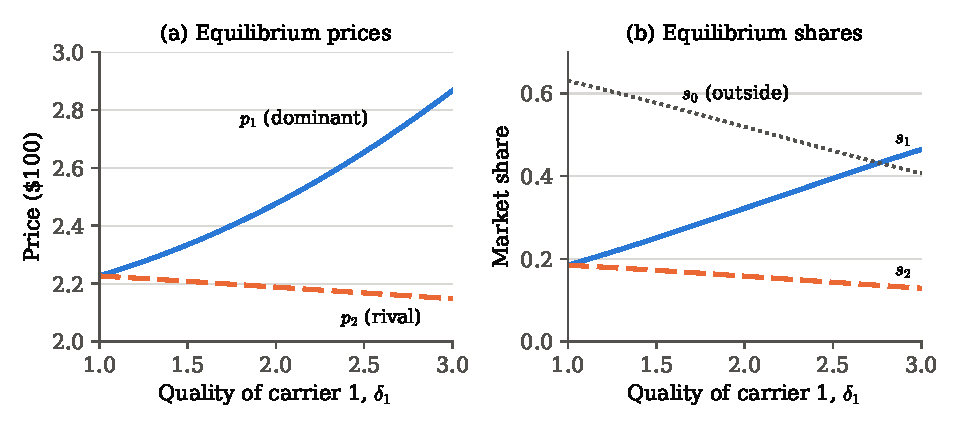
\includegraphics[width=\textwidth]{figures/ch09/logit_dominance.pdf}
\caption{Logit Bertrand equilibrium on a route with two carriers and an outside good, as carrier 1's
non-price quality $\delta_1$ rises. Parameters are $\alpha=1$ (prices in \$100), $c_1=c_2=1$ and
$\delta_2=1$. At $\delta_1=1$ both carriers charge $2.227$. At $\delta_1=3$, $p_1=2.867$, $p_2=2.148$,
$s_1=0.464$ and $s_2=0.129$. The dominant carrier's price rises while its rival's falls.}
\label{fig:09-dominance}
\end{figure}

\Cref{fig:09-dominance} traces the equilibrium of a two-carrier route as carrier 1's quality rises from
$\delta_1=1$ to $\delta_1=3$. Carrier 1's share rises from $0.185$ to $0.464$ and its price from $2.227$
to $2.867$. The rival's share falls from $0.185$ to $0.129$ and its price from $2.227$ to $2.148$.
The Herfindahl index of inside shares rises from $0.500$ to $0.660$. Concentration rises and the rival's
price falls, the opposite of an umbrella. Logit prices are strategic complements, so carrier 1's higher
price alone would push $p_2$ up. The loss of customers to the better product outweighs this effect, and
the rival's markup $\frac{1}{\alpha(1-s_2)}$ falls with its share.

\begin{corollary}[Relative prices]\label{cor:09-relprice}
Under \cref{ass:09-logit}, an increase in $\delta_1$ raises $\ln p_1-\ln p_k$ for every $k\neq1$. Along
any path of shares, $\frac{\dd\ln p_j}{\dd s_j}=\frac{L_j}{1-s_j}$, where $L_j=\frac{p_j-c_j}{p_j}$ is
the Lerner index. With equal costs, $\ln p_1-\ln p_k\approx\frac{L}{1-s}\,(s_1-s_k)$ for shares near a
common value $s$ with Lerner index $L$.
\end{corollary}

\begin{proof}
The first claim follows from \cref{prop:09-dominance}(ii), since $p_1$ rises and $p_k$ falls. For the
slope, differentiate \eqref{eq:09-logit-markup}:
$\frac{\dd m_j}{\dd s_j}=\frac{1}{\alpha(1-s_j)^2}=\frac{m_j}{1-s_j}$. Then
$\frac{\dd\ln p_j}{\dd s_j}=\frac{1}{p_j}\frac{\dd m_j}{\dd s_j}=\frac{m_j}{p_j}\frac{1}{1-s_j}=\frac{L_j}{1-s_j}$.
A first-order expansion around the common share gives the approximation.
\end{proof}

The corollary is the structural counterpart of Borenstein's relative-price equation
\eqref{eq:09-bor-rel}. There, the coefficient on the difference in route shares between two carriers on
the same route plays the role of $\frac{L(1-s_0)}{1-s}$. Route shares are shares of fliers,
$\frac{s_j}{1-s_0}$, so the gap in route shares between carriers 1 and $k$ is $\frac{s_1-s_k}{1-s_0}$.
A positive coefficient is what product differentiation
predicts, with no change in conduct. In the example of \cref{fig:09-dominance}, $\ln p_1-\ln p_2$ rises
from $0$ to $0.289$ as $\delta_1$ goes from 1 to 3.

\begin{remark}[Quality or cost?]\label{rem:09-quality-cost}
The equilibrium depends on $(\delta_j,c_j)$ only through $a_j=e^{\delta_j-\alpha c_j}$. A cost advantage
therefore has the same effect on shares and markups as a quality advantage of $\alpha$ times the cost
gap. In the example of \cref{fig:09-dominance}, $(\delta_1,c_1)=(1.5,1)$ and $(\delta_1,c_1)=(1,0.5)$
give identical shares ($s_1=0.251$, $s_2=0.172$) and the same markup $m_1=1.334$. Only carrier 1's price
differs, $2.334$ against $1.834$. A relation between shares and markups cannot reveal whether dominance
comes from quality or from cost. Separating them requires a model of costs, which is what
\cref{sec:09-pricing-network} and \cref{sec:09-bcs} provide.
\end{remark}

\casehead{Multi-product carriers}
A carrier usually sells several products on a route: direct and connecting itineraries, and several fare
classes. With logit demand, the first-order condition for $j\in\mathcal{J}_f$ is
$s_j-\alpha s_jm_j+\alpha s_j\sum_{k\in\mathcal{J}_f}s_km_k=0$. Dividing by $\alpha s_j$ gives
$m_j=\frac{1}{\alpha}+\sum_{k\in\mathcal{J}_f}s_km_k$. The right side does not depend on $j$, so all of
the carrier's products carry a common markup $m_f$. Substituting back,
$m_f=\frac{1}{\alpha}+S_fm_f$, so
\begin{equation*}
m_f=\frac{1}{\alpha(1-S_f)},\qquad S_f=\sum_{k\in\mathcal{J}_f}s_k
\end{equation*}
(\cref{ch:logit}). Summing the logit ratios over the carrier's products gives
$\frac{S_f}{s_0}=A_fe^{-\alpha m_f}$ with $A_f=\sum_{k\in\mathcal{J}_f}a_k$. The proof of
\cref{prop:09-dominance} then applies with carriers in place of products and $A_f$ in place of $a_j$.
A carrier with a large total share on the route earns a large markup on every product it sells there.

The logit model also has a limitation that matters for airlines. Every product of a carrier carries the
same dollar markup, whether it is a restricted discount ticket or an unrestricted fare. Characteristics
affect the markup only through shares. The model cannot express the idea that a hub lets its carrier
raise fares mainly to business travelers. That requires heterogeneity in price sensitivity, to which we
now turn.

\subsection{Consumer heterogeneity: a finite-mixture nested logit}\label{sec:09-pricing-types}

Air travelers differ in ways that matter for pricing. Business travelers are less sensitive to price
\citep[p.~10, n.~9]{BerryCarnallSpiller2006}. Their trips are urgent, travel is a deductible business
expense, and the traveler may not bear the full cost of the ticket. They may also value frequency, nonstop service and
frequent-flyer benefits more, so tastes are correlated across characteristics. A model in which the
price coefficient and the tastes vary across consumers lets markups differ across the products of one
carrier. It also lets a hub's demand advantage fall on particular travelers.
Earlier discrete choice models of air travel, such as that of \citet{MorrisonWinston1986}, used a
logit with common coefficients \citep[p.~8]{BerryCarnallSpiller2006}. \citet{BerryCarnallSpiller2006}
adopt the simplest distribution with heterogeneous tastes, a two-point distribution of types. We develop the model with $R$ types and specialize to $R=2$ in \cref{sec:09-bcs}.

\begin{assumption}[Finite-mixture nested logit]\label{ass:09-fm}
Market $t$ has $M_t$ potential travelers. Each belongs to one of $R$ types, and type $r$ has population
share $\psi_r>0$ with $\sum_r\psi_r=1$. A traveler $i$ of type $r$ has utility
\begin{equation*}
u_{ijt}=x_{jt}\beta_r-\alpha_rp_{jt}+\xi_{jt}+\zeta_{igt}+(1-\sigma)\epsilon_{ijt}
\quad (j\in\mathcal{J}_t),\qquad u_{i0t}=\epsilon_{i0t}.
\end{equation*}
The shocks $\epsilon_{ijt}$ are i.i.d.\ type-I extreme value. All inside goods form one nest $g$ and the
outside good forms its own nest. The term $\zeta_{igt}$ is common to all inside goods for traveler $i$
and has the distribution of \citet{Cardell1997}, which makes $\zeta_{igt}+(1-\sigma)\epsilon_{ijt}$
type-I extreme value, with $\sigma\in[0,1)$. The unobserved quality $\xi_{jt}$ is common to all types.
\end{assumption}

The nesting parameter $\sigma$ measures the correlation of a traveler's utilities across flights. With
$\sigma=0$ the model is a mixture of logits, and as $\sigma\to1$ flights become perfect substitutes for
one another relative to the outside good (\cref{ch:logit}, \cref{ch:discrete}). Berry, Carnall and
Spiller write the idiosyncratic term as $\lambda\epsilon_{ij}$, so their $\lambda$ equals $1-\sigma$.
In applications $M_t$ is unobserved. They set $M_t=\kappa\,\mathit{MPOP}_t$, with $\mathit{MPOP}_t$ the
geometric mean of the endpoint populations and $\kappa$ a parameter to be estimated
\citep[p.~9]{BerryCarnallSpiller2006}.

\begin{remark}[Discrete random coefficients]\label{rem:09-discrete-rc}
The type structure is a random coefficients logit (\cref{ch:blp}) whose mixing distribution has $R$
support points $(\alpha_r,\beta_r)$ with probabilities $\psi_r$. Normal random coefficients are the usual
alternative. Suppose $K$ coefficients, price included, vary across consumers. Two types then require
$2K+1$ parameters, two values per coefficient plus $\psi_1$, against $2K$ for independent normals with a
mean and a standard deviation each \citep[p.~11]{BerryCarnallSpiller2006}. In exchange the shares have a
closed form and no simulation is needed. A two-point distribution is bimodal and makes tastes correlated
across characteristics by construction. The price is that it has no taste variation within a type.
Mixtures of normals or more types would relax this but require numerical integration or many more
parameters.
\end{remark}

\casehead{Shares}
Fix a market and write $\delta^r_{jt}$ for the mean utility of type $r$, which includes price as in
\cref{ch:logit}. Conditional on type, the model is a nested logit, so
\begin{subequations}\label{eq:09-fm-shares}
\begin{align}
\delta^r_{jt}&=x_{jt}\beta_r-\alpha_rp_{jt}+\xi_{jt},\\
D_{rt}&=\sum_{k\in\mathcal{J}_t}\exp\Big(\frac{\delta^r_{kt}}{1-\sigma}\Big),\\
s^r_{j|g,t}&=\frac{1}{D_{rt}}\exp\Big(\frac{\delta^r_{jt}}{1-\sigma}\Big),\\
\bar s_{rt}&=\frac{D_{rt}^{1-\sigma}}{1+D_{rt}^{1-\sigma}},\\
s^r_{jt}&=s^r_{j|g,t}\,\bar s_{rt},\\
s_{jt}&=\sum_{r=1}^R\psi_r\,s^r_{jt}.
\end{align}
\end{subequations}
Here $s^r_{j|g,t}$ is the probability that a type-$r$ traveler chooses $j$ given that she flies, and
$\bar s_{rt}$ is the probability that she flies at all. The last line averages over types by the law of
total probability. The outside share is $s_{0t}=\sum_r\frac{\psi_r}{1+D_{rt}^{1-\sigma}}$. The
\emph{inclusive sum} $D_{rt}$ is the denominator of type $r$'s within-nest shares. It carries a type
subscript and should not be confused with the diversion ratio $D_{jk}$ below, which carries two product
subscripts. In the rest of this subsection we drop the market subscript.

\casehead{Derivatives}
We differentiate the type-specific shares with respect to type-specific mean utilities and then convert
to prices. From \eqref{eq:09-fm-shares},
\begin{equation*}
\ln s^r_j=\frac{\delta^r_j}{1-\sigma}-\ln D_r+(1-\sigma)\ln D_r-\ln\big(1+D_r^{1-\sigma}\big)
=\frac{\delta^r_j}{1-\sigma}-\sigma\ln D_r-\ln\big(1+D_r^{1-\sigma}\big).
\end{equation*}
The two building blocks are
\begin{equation*}
\frac{\partial\ln D_r}{\partial\delta^r_k}=\frac{1}{1-\sigma}\,\frac{1}{D_r}\exp\Big(\frac{\delta^r_k}{1-\sigma}\Big)
=\frac{s^r_{k|g}}{1-\sigma},
\qquad
\frac{\partial\ln\big(1+D_r^{1-\sigma}\big)}{\partial\delta^r_k}
=\bar s_r\,(1-\sigma)\,\frac{\partial\ln D_r}{\partial\delta^r_k}=\bar s_r\,s^r_{k|g}=s^r_k .
\end{equation*}
Therefore
\begin{equation*}
\frac{\partial\ln s^r_j}{\partial\delta^r_k}
=\frac{\indic\{j=k\}}{1-\sigma}-\frac{\sigma}{1-\sigma}\,s^r_{k|g}-s^r_k .
\end{equation*}
Multiplying by $s^r_j$ and using $s^r_j\,s^r_{k|g}=s^r_k\,s^r_{j|g}$ gives the own and cross derivatives.
Since $\frac{\partial\delta^r_k}{\partial p_k}=-\alpha_r$, the price derivatives of aggregate shares
follow:
\begin{subequations}\label{eq:09-fm-derivs}
\begin{align}
\frac{\partial s^r_j}{\partial\delta^r_j}&=s^r_j\Big[\frac{1}{1-\sigma}-\frac{\sigma}{1-\sigma}\,s^r_{j|g}-s^r_j\Big],\\
\frac{\partial s^r_j}{\partial\delta^r_k}&=-s^r_k\Big[\frac{\sigma}{1-\sigma}\,s^r_{j|g}+s^r_j\Big],\qquad k\neq j,\\
\frac{\partial s_j}{\partial p_k}&=-\sum_{r=1}^R\psi_r\,\alpha_r\,\frac{\partial s^r_j}{\partial\delta^r_k}.
\end{align}
\end{subequations}
The matrix of type-specific derivatives is symmetric, so $\frac{\partial s_j}{\partial p_k}=\frac{\partial
s_k}{\partial p_j}$ in this model. Own-price derivatives are negative and cross-price derivatives are
positive.

\casehead{Buyer composition}
Bayes' rule gives the composition of each product's buyers:
\begin{equation}\label{eq:09-composition}
\Pr(r\mid j)=\frac{\psi_r\,s^r_{jt}}{s_{jt}} .
\end{equation}
The numerator is the probability of being type $r$ and buying $j$, and the denominator is the
probability of buying $j$. Berry, Carnall and Spiller use these weights to compute average fares,
costs and markups by type (\cref{sec:09-bcs}). With them, the own-price elasticity and the diversion
ratio take a transparent form. Dividing \eqref{eq:09-fm-derivs} by $s_j$,
\begin{align*}
\varepsilon_{jj}&=-\frac{\partial s_j}{\partial p_j}\,\frac{p_j}{s_j}
=p_j\sum_r\Pr(r\mid j)\,\alpha_r\Big[\frac{1}{1-\sigma}-\frac{\sigma}{1-\sigma}\,s^r_{j|g}-s^r_j\Big],\\
D_{jk}&=-\frac{\frac{\partial s_k}{\partial p_j}}{\frac{\partial s_j}{\partial p_j}}
=\frac{\sum_r\Pr(r\mid j)\,\alpha_r\Big[\frac{\sigma}{1-\sigma}\,s^r_{k|g}+s^r_k\Big]}
{\sum_r\Pr(r\mid j)\,\alpha_r\Big[\frac{1}{1-\sigma}-\frac{\sigma}{1-\sigma}\,s^r_{j|g}-s^r_j\Big]} .
\end{align*}
A product bought mostly by price-insensitive types has a low elasticity even at a high price. This breaks
the logit's implication that elasticities rise in proportion to price (\cref{ch:logit}). Diversion from
$j$ to $k$ is high when the types who buy $j$ are the types for whom $k$ has a large share. Two cheap
tickets bought by the same price-sensitive travelers are therefore close substitutes, whatever their
aggregate shares.

\begin{proposition}[Who pays the premium]\label{prop:09-composition-markup}
Under \cref{ass:09-fm} with $\sigma=0$, suppose carrier $f$ sells the single product $j$ in market $t$
and sets its price as in Nash-Bertrand equilibrium.
\begin{enumerate}[label=(\alph*)]
\item The markup is
\begin{equation*}
p_j-mc_j=\frac{s_j}{\sum_r\psi_r\alpha_rs^r_j(1-s^r_j)}=\frac{1}{\sum_r\Pr(r\mid j)\,\alpha_r(1-s^r_j)} .
\end{equation*}
\item Let $R=2$. Holding all prices fixed, a marginal increase in a characteristic $x^h_j$ of product $j$
raises the share of type-2 buyers $\Pr(2\mid j)$ if and only if
$\beta^h_2(1-s^2_j)>\beta^h_1(1-s^1_j)$.
\end{enumerate}
\end{proposition}

\begin{proof}
(a) The first-order condition is $s_j+(p_j-mc_j)\frac{\partial s_j}{\partial p_j}=0$. With $\sigma=0$,
\eqref{eq:09-fm-derivs} gives $\frac{\partial s_j}{\partial p_j}=-\sum_r\psi_r\alpha_rs^r_j(1-s^r_j)$.
Solving for the markup gives the first expression. Dividing numerator and denominator by $s_j$ and using
\eqref{eq:09-composition} gives the second.

(b) Write $\Pr(2\mid j)=\Big[1+\frac{\psi_1s^1_j}{\psi_2s^2_j}\Big]^{-1}$, which is increasing in
$\ln s^2_j-\ln s^1_j$. With $\sigma=0$, $\frac{\partial\ln s^r_j}{\partial\delta^r_j}=1-s^r_j$ and
$\frac{\partial\delta^r_j}{\partial x^h_j}=\beta^h_r$. Hence
$\frac{\partial(\ln s^2_j-\ln s^1_j)}{\partial x^h_j}=\beta^h_2(1-s^2_j)-\beta^h_1(1-s^1_j)$.
\end{proof}

Part (a) says that the markup is the inverse of a buyer-weighted average price sensitivity. When
type-specific shares are small, the markup is close to $\frac{1}{\bar\alpha_j}$, where
$\bar\alpha_j=\sum_r\Pr(r\mid j)\alpha_r$ is the mean price coefficient among $j$'s buyers. Part (b) says
which characteristics move the buyer mix. Combine the two with $\alpha_2<\alpha_1$. A characteristic that
type 2 values more, such as hub presence valued by business travelers, tilts $j$'s buyers toward type 2.
This lowers $\bar\alpha_j$ and raises the markup on $j$. Products bought mainly by tourists keep low
markups even when the hub carrier sells them. The hub premium thus falls on the travelers who value the
hub, which is the mechanism behind the results of \cref{sec:09-bcs}. In the logit model, by contrast,
the markup $\frac{1}{\alpha(1-s_j)}$ depends on characteristics only through the share.

\begin{remark}[Nesting and multi-product carriers]\label{rem:09-fm-extensions}
With $\sigma>0$ the same steps give
$p_j-mc_j=\Big(\sum_r\Pr(r\mid j)\,\alpha_r\Big[\frac{1}{1-\sigma}-\frac{\sigma}{1-\sigma}s^r_{j|g}-s^r_j\Big]\Big)^{-1}$.
If within-nest shares are small, the bracket is close to $\frac{1}{1-\sigma}$ and the markup is close to
$\frac{1-\sigma}{\bar\alpha_j}$. Closer substitution among flights (larger $\sigma$) lowers markups. A
product with a large within-nest share among its own buyers earns a higher markup. With multi-product
carriers the markups solve the system \eqref{eq:09-fm-markup} below. They differ across a carrier's
products according to buyer composition, unlike the common logit markup $\frac{1}{\alpha(1-S_f)}$.
\end{remark}

\casehead{Inversion}
Estimation requires the vector $\xi_t$ that rationalizes observed shares. For given demand parameters
$\theta_d=(\sigma,\{\alpha_r,\beta_r,\psi_r\}_{r=1}^R)$ and market size, \eqref{eq:09-fm-shares}
defines shares $s_t(\xi_t;\theta_d)$, and we must solve $s_t(\xi_t;\theta_d)=s^{obs}_t$ for $\xi_t$.
\citet{Berry1994} shows that this inverse exists and is unique (\cref{ch:logit}, \cref{ch:blp}).
Berry, Carnall and Spiller compute it with ``a slight variation'' of the contraction of
\citet{BerryLevinsohnPakes1995} \citep[p.~17]{BerryCarnallSpiller2006}. One natural variation dampens
the step by $1-\sigma$:
\begin{equation}\label{eq:09-fm-contraction}
\xi^{n+1}=\Phi(\xi^n),\qquad \Phi(\xi)\equiv\xi+(1-\sigma)\big[\ln s^{obs}-\ln s(\xi;\theta_d)\big].
\end{equation}
A fixed point of $\Phi$ satisfies $\ln s(\xi;\theta_d)=\ln s^{obs}$. The next lemma shows why the
dampening works.

\begin{lemma}[Contraction for the finite-mixture nested logit]\label{lem:09-fm-contraction}
At every $\xi$, all elements of the Jacobian of $\Phi$ are positive, and each row sums to
$\sum_r\Pr(r\mid j)\big[\sigma+(1-\sigma)\bar s_r\big]\le\sigma+(1-\sigma)\max_r\bar s_r<1$. Hence
$\Phi$ is a contraction in the sup norm, with modulus at most $\sigma+(1-\sigma)\bar S$, on any convex
set of $\xi$ on which every inside share satisfies $\bar s_r\le\bar S<1$.
\end{lemma}

\begin{proof}
Each $\delta^r_k$ moves one for one with $\xi_k$, so by \eqref{eq:09-fm-shares} and
\eqref{eq:09-composition}
\begin{equation*}
\frac{\partial\ln s_j}{\partial\xi_k}=\frac{1}{s_j}\sum_r\psi_rs^r_j\frac{\partial\ln s^r_j}{\partial\delta^r_k}
=\sum_r\Pr(r\mid j)\Big[\frac{\indic\{j=k\}}{1-\sigma}-\frac{\sigma}{1-\sigma}\,s^r_{k|g}-s^r_k\Big].
\end{equation*}
Multiplying by $1-\sigma$ and using $\sum_r\Pr(r\mid j)=1$,
\begin{equation*}
(1-\sigma)\frac{\partial\ln s_j}{\partial\xi_k}
=\indic\{j=k\}-\sum_r\Pr(r\mid j)\big[\sigma s^r_{k|g}+(1-\sigma)s^r_k\big].
\end{equation*}
The Jacobian of $\Phi$ is therefore
$\frac{\partial\Phi_j}{\partial\xi_k}=\sum_r\Pr(r\mid j)\big[\sigma s^r_{k|g}+(1-\sigma)s^r_k\big]>0$.
Summing over $k$ and using $\sum_ks^r_{k|g}=1$ and $\sum_ks^r_k=\bar s_r$ gives the row sum. With
positive elements, the sup norm of the Jacobian equals its largest row sum. The mean value theorem then
bounds $\|\Phi(\xi)-\Phi(\xi')\|_\infty$ by the modulus times $\|\xi-\xi'\|_\infty$ on a convex set.
\end{proof}

The set on which inside shares are bounded by $\bar S$ is convex, because $D_r$ is a convex function of
$\xi$. Applying the contraction mapping theorem (\cref{app:math}) also requires a set that $\Phi$ maps
into itself. The bounding argument of \citet{BerryLevinsohnPakes1995} supplies one (\cref{ch:blp}).
In airline city pairs, actual trips are a small fraction of potential trips. Inside shares are then
small and the modulus is close to $\sigma$, so the iteration converges quickly.

\casehead{Markups}
Within a single market, carrier $f$ chooses the prices of its products $\mathcal{J}_f(t)$ to maximize
$\sum_{j\in\mathcal{J}_f(t)}(p_j-mc_j)M_ts_j(p)$. The first-order condition for $j\in\mathcal{J}_f(t)$ is
\begin{equation*}
s_j+\sum_{k\in\mathcal{J}_f(t)}(p_k-mc_k)\frac{\partial s_k}{\partial p_j}=0 .
\end{equation*}
Let $\Omega$ be the ownership matrix and $\Delta$ the matrix with $(j,k)$ element
$\frac{\partial s_j}{\partial p_k}$ (\cref{ch:diffprod}). The $(j,k)$ element of
$(\Omega\odot\Delta)^\top$ is $\Omega_{kj}\frac{\partial s_k}{\partial p_j}$, so stacking the conditions
gives
\begin{equation}\label{eq:09-fm-markup}
s+(\Omega\odot\Delta)^\top(p-mc)=0
\quad\Longrightarrow\quad
p-mc=-\big[(\Omega\odot\Delta)^\top\big]^{-1}s,
\qquad
\Delta=-\sum_{r=1}^R\psi_r\,\alpha_r\,\frac{\partial s^r}{\partial\delta^r},
\end{equation}
where $\frac{\partial s^r}{\partial\delta^r}$ is the matrix with $(j,k)$ element
$\frac{\partial s^r_j}{\partial\delta^r_k}$ from \eqref{eq:09-fm-derivs}.\footnote{Berry, Carnall and
Spiller define $\Delta$ with $(j,k)$ element $\frac{\partial s_k}{\partial p_j}$ for products of the same
carrier and write $p=\Delta^{-1}s+mc$ \citep[pp.~15--16]{BerryCarnallSpiller2006}. The equation holds when
$\Delta$ contains the negatives of the price derivatives. Their formula
$\Delta=\gamma\alpha_1\Delta_1+(1-\gamma)\alpha_2\Delta_2$, with $\Delta_r$ the derivatives with respect to
mean utility and $\gamma$ the type-1 probability, delivers exactly these negatives, since
$\frac{\partial s^r}{\partial p}=-\alpha_r\frac{\partial s^r}{\partial\delta^r}$.} In this model $\Omega$
and $\Delta$ are both symmetric, so the transpose is immaterial. It matters for general demand systems.
The markups depend only on the demand parameters and on observed prices and shares. Given demand
estimates, marginal cost follows as $mc=p+\big[(\Omega\odot\Delta)^\top\big]^{-1}s$, without any cost
data.

\casehead{How aggregate data identify types}
Berry, Carnall and Spiller explain how market-level data can distinguish two consumer types from one
\citep[pp.~18--19]{BerryCarnallSpiller2006}. The key is variation across markets in the number of similar
products. The following example makes their argument quantitative.

\begin{example}[Two types from aggregate shares]\label{ex:09-twotypes}
Consider two city pairs, A and B, identical in every respect except their sets of products. Products are
identical except for price. Market A has a product $H$ at \$200 and a product $L$ at \$100. Market B has
$H$ at \$200 and two products $L_1$ and $L_2$ at \$100. In market A we observe $s_H=s_L$.

\emph{One type.} In a nested logit with a single type, within-nest shares are proportional to
$\exp\big(\frac{\delta_j}{1-\sigma}\big)$. Equal shares in market A therefore imply $\delta_H=\delta_L$. In market B
the three products then have equal mean utilities and equal shares, for any $\alpha$ and $\sigma$. The
same conclusion holds in any model whose error is additive and i.i.d.\ across products
\citep[p.~18]{BerryCarnallSpiller2006}.

\emph{Two types.} Let $\alpha_1=3$ and $\alpha_2=0.1$ per \$100, $\psi_1=0.9$, $\sigma=0.4$ and
$\delta^r_j=\xi_j-\alpha_rp_j$ with $\xi_L=0$. Setting $\xi_H=0.903$ equates the two shares in market A
at $0.0567$. In market A, $97\%$ of type 1's flights are on $L$, while $79\%$ of type 2's flights are on
$H$. Adding $L_2$ in market B splits type 1's demand for cheap flights and barely touches type 2's demand
for $H$. Market B shares become $0.0483$ for $H$ and $0.0438$ for each cheap product, so $H$'s share is
$10\%$ above each of the others (\cref{tab:09-twotypes}, \cref{fig:09-twotypes}). Under one type every
product loses $17.5\%$ of its share when $L_2$ enters. Under two types $H$ loses $14.7\%$ and $L$ loses
$22.7\%$.

The substitution patterns explain the difference. In market B, $28\%$ of each cheap product's buyers are
type 2, against $98\%$ of $H$'s buyers. A rise in the price of $L_1$ diverts $0.277$ of its lost sales to
$L_2$ and only $0.017$ to $H$. A one-type model would divert equal fractions to $L_2$ and $H$. The farther
apart $\alpha_1$ and $\alpha_2$, the larger the gap between the shares of $H$ and $L$ in market B. Data
with many such comparisons across markets therefore pin down the dispersion of price coefficients.

\emph{Which type values hubs?} Now add a hub characteristic $x^h_j$ with type-specific coefficients
$\beta^h_r$. Differentiating \eqref{eq:09-fm-shares} as in \cref{lem:09-fm-contraction},
\begin{equation*}
\frac{\partial\ln s_j}{\partial x^h_j}=\sum_r\Pr(r\mid j)\,\beta^h_r\,\frac{\partial\ln s^r_j}{\partial\delta^r_j},
\end{equation*}
a buyer-weighted average of type-specific responses. In market A, with $(\beta^h_1,\beta^h_2)=(0.2,1.0)$
the semi-elasticities are $0.579$ for $H$ and $0.499$ for $L$. With $(\beta^h_1,\beta^h_2)=(1.0,0.2)$ they
are $0.151$ for $H$ and $0.794$ for $L$. How the shares of cheap and expensive products respond to hub
presence thus reveals which type has the large hub coefficient \citep[p.~19]{BerryCarnallSpiller2006}.
\end{example}

\begin{table}[htbp]
\centering
\caption{Two-type identification example: market shares and buyer composition}
\label{tab:09-twotypes}
\begin{tabular}{lcccccc}
\toprule
 & & Market A & \multicolumn{2}{c}{Market B} & \multicolumn{2}{c}{$\Pr(r=2\mid j)$}\\
\cmidrule(lr){4-5}\cmidrule(lr){6-7}
Product & Price (\$) & both models & one type & two types & A & B\\
\midrule
$H$ & 200 & 0.0567 & 0.0467 & 0.0483 & 0.977 & 0.980\\
$L$ in A, $L_1$ in B & 100 & 0.0567 & 0.0467 & 0.0438 & 0.256 & 0.284\\
$L_2$ & 100 & & 0.0467 & 0.0438 & & 0.284\\
Outside good & & 0.8867 & 0.8598 & 0.8641 & & \\
\bottomrule
\end{tabular}

\smallskip
\begin{minipage}{0.92\textwidth}
\footnotesize Notes: Both models are calibrated to reproduce market A exactly. The two-type model has
$\alpha_1=3$, $\alpha_2=0.1$ (per \$100), $\psi_1=0.9$, $\sigma=0.4$, $\xi_L=0$ and $\xi_H=0.903$. The
one-type model is a nested logit with the same $\sigma$. Our computations.
\end{minipage}
\end{table}

\begin{figure}[htbp]
\centering
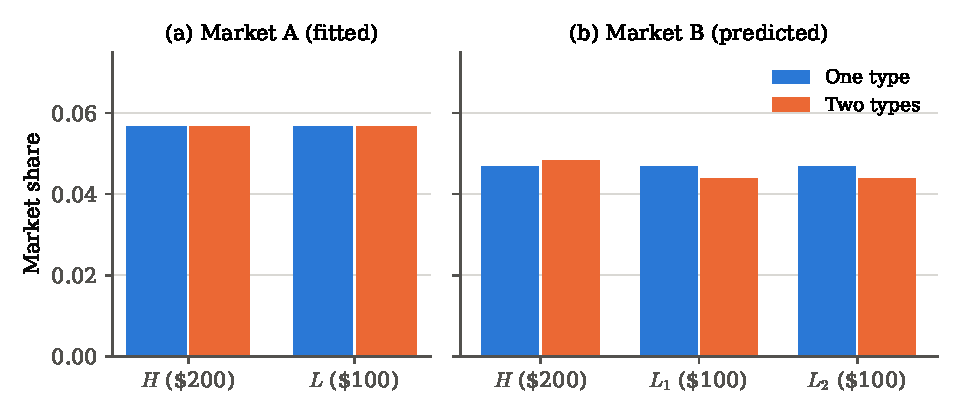
\includegraphics[width=\textwidth]{figures/ch09/twotypes_example.pdf}
\caption{Identifying two types from aggregate shares. Both models fit market A, where the \$200 and
\$100 products have equal shares. In market B, which adds a second \$100 product, the one-type model
predicts three equal shares. The two-type model predicts that the expensive product keeps more of its
share, because the two cheap products compete for the same price-sensitive travelers. Parameters as in
\cref{tab:09-twotypes}.}
\label{fig:09-twotypes}
\end{figure}

\begin{remark}[The role of nesting in the example]\label{rem:09-twotypes-sigma}
The direction of the departure from the one-type prediction depends on the whole specification. With
$\sigma=0$ and the same $\alpha_r$ and $\psi_r$, recalibrating $\xi_H$ to fit market A gives market B
shares of $0.0530$ for $H$ and $0.0576$ for each cheap product. Without nesting, flights compete mainly
with the outside good. Type 2 values every flight highly because $\alpha_2$ is small, so it gives the new
cheap product a larger share than type 1 does, and $H$ loses more. The nesting parameter makes flights
compete with one another within each type. What identifies the types is the existence of departures from
the one-type prediction, and the data determine their direction.
\end{remark}

Random coefficients also change how markups respond to entry. Berry, Carnall and Spiller stress that with
random coefficients, introducing similar products drives markups down \citep[p.~18]{BerryCarnallSpiller2006}.
In \cref{ex:09-twotypes}, the inverse semi-elasticity of $L$'s demand,
$-s_L\big(\frac{\partial s_L}{\partial p_L}\big)^{-1}$, is the markup a single-product seller of $L$ would choose. It falls from $0.453$ (\$45) in market A
to $0.352$ (\$35) in market B, because $L_2$ competes for exactly the travelers who buy $L$. A one-type
nested logit with the same $\sigma$ predicts a fall of only 9\%, which comes from the decline in $L$'s
shares alone.

\subsection{Network costs and economies of density}\label{sec:09-pricing-network}

The cost side of hubbing rests on an engineering argument. Larger aircraft are cheaper to fly per seat
mile, at least on longer routes \citep[pp.~3--4]{BerryCarnallSpiller2006}. For a given flight frequency, a
densely traveled spoke can use larger aircraft. A hub combines passengers bound for many destinations
on one large aircraft to the hub, where they change planes. We first define the relevant cost concepts,
then work through a stylized network, and finally derive the pricing condition of a network carrier.

\begin{definition}[Returns to density and to scale]\label{def:09-rtd}
Let $C(Q,P,w)$ be a carrier's total cost, with traffic $Q$ (for example passenger miles), number of
points served $P$ and input prices $w$. Write $\varepsilon_{CQ}=\frac{\partial\ln C}{\partial\ln Q}$ and
$\varepsilon_{CP}=\frac{\partial\ln C}{\partial\ln P}$. \emph{Returns to density} and \emph{returns to
scale} are
\begin{equation}\label{eq:09-rtd}
RTD=\frac{1}{\varepsilon_{CQ}},\qquad RTS=\frac{1}{\varepsilon_{CQ}+\varepsilon_{CP}} .
\end{equation}
\end{definition}

Returns to density measure the cost of adding traffic to a fixed network, and returns to scale the cost
of expanding traffic and the network together. Since $\varepsilon_{CQ}=\frac{Q}{C}\frac{\partial C}{\partial Q}$, the density elasticity also equals the ratio of marginal to average cost of traffic.
\citet{CavesChristensenTretheway1984} estimate an airline cost function \citep[p.~4]{BerryCarnallSpiller2006}.
Holding the route structure fixed, total cost rises only 80\% as fast as traffic. This means $\varepsilon_{CQ}\approx0.8$ and
$RTD\approx\frac{1}{0.8}=1.25$. Berry, Carnall and Spiller point out two limits of this approach. An
aggregate cost function ignores details of route structure that determine densities. Holding the number
of endpoints fixed, for instance, densities fall as a carrier operates more hubs
\citep[p.~4, n.~7]{BerryCarnallSpiller2006}. And route-level cost data do not exist, since route-level
total or average cost is not even well defined. \citet{BruecknerSpiller1994} instead model the marginal
cost of a passenger on each leg as a function of that leg's density and sum over the legs of an
itinerary. They find that funneling passengers through hub airports raised traffic densities and let
carriers reduce costs \citep[pp.~4--5]{BerryCarnallSpiller2006}. \citet{BruecknerDyerSpiller1992} make
the related point that itineraries through a hub may have lower costs because they raise spoke density
\citep[p.~2]{BerryCarnallSpiller2006}. Berry, Carnall and Spiller adopt the leg-level approach.

\begin{example}[Hub-and-spoke versus point-to-point costs]\label{ex:09-hubcost}
A carrier serves $n$ outer cities and one hub city. Every pair of the $n+1$ cities has $A$ round-trip
passengers. Each leg has cost $C(Q)=aQ^\gamma$ with $0<\gamma\le1$, so legs have \emph{economies of
density}, marginal and average cost falling with traffic, when $\gamma<1$. All legs have equal length and we ignore circuity.

\emph{Point to point.} Every city pair gets a nonstop leg. There are $\frac{n(n+1)}{2}$ legs, each
carrying density $A$, so
\begin{equation*}
C^{PP}=\frac{n(n+1)}{2}\,aA^\gamma .
\end{equation*}

\emph{Hub and spoke.} There are $n$ spokes. The spoke from outer city $e$ carries the $A$ passengers
between $e$ and the hub and the $A$ passengers between $e$ and each of the other $n-1$ outer cities. Its
density is $A+(n-1)A=nA$, so
\begin{equation*}
C^{HS}=n\,a(nA)^\gamma=aA^\gamma\,n^{1+\gamma} .
\end{equation*}

\emph{Comparison.} Dividing,
\begin{equation*}
\frac{C^{HS}}{C^{PP}}=\frac{aA^\gamma n^{1+\gamma}}{\frac{n(n+1)}{2}aA^\gamma}=\frac{2n^\gamma}{n+1} .
\end{equation*}
Hubbing is cheaper if and only if $2n^\gamma<n+1$. With $\gamma=1$ this requires $n<1$, so hubbing is
never cheaper: connecting passengers fly two legs instead of one. With $n=10$ and $\gamma=0.7$ the ratio
is $\frac{2\times10^{0.7}}{11}=\frac{10.02}{11}=0.91$. For $\gamma=0.7$ hubbing lowers total cost once
$n\ge7$, and for $\gamma=0.8$ once $n\ge27$.

\emph{Marginal costs.} Leg marginal cost is $c(Q)=a\gamma Q^{\gamma-1}$. A nonstop passenger in the
point-to-point network costs $a\gamma A^{\gamma-1}$. A connecting passenger in the hub network flies two
spokes of density $nA$ and costs $2a\gamma(nA)^{\gamma-1}$, a ratio of $2n^{\gamma-1}$. A passenger
to or from the hub flies one spoke, a ratio of $n^{\gamma-1}<1$. With $n=10$ and $\gamma=0.7$ the
connecting ratio is $1.00$ and the hub-endpoint ratio is $0.50$.
\end{example}

\begin{figure}[htbp]
\centering
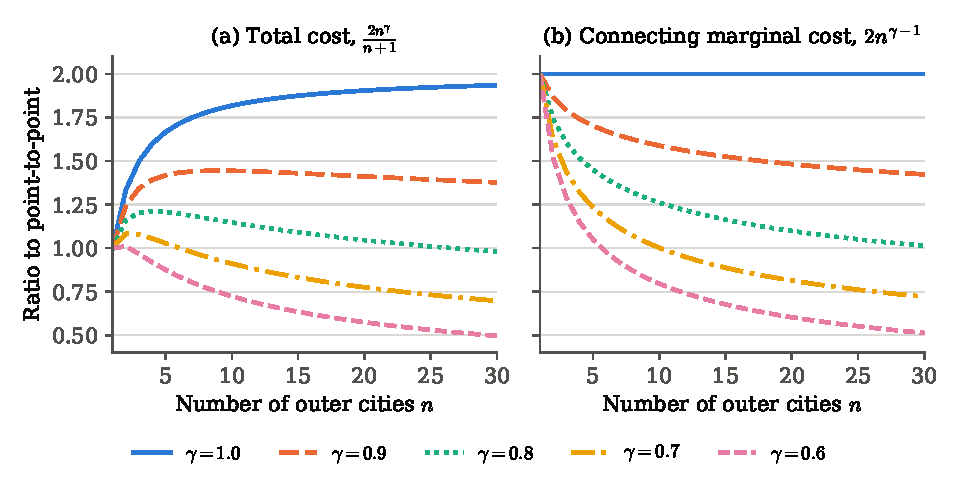
\includegraphics[width=\textwidth]{figures/ch09/hubcost_ratio.pdf}
\caption{Hub-and-spoke relative to point-to-point costs in \cref{ex:09-hubcost}, as functions of the
number of outer cities $n$ for several leg cost elasticities $\gamma$. Panel (a) shows total network cost,
panel (b) the marginal cost of a connecting passenger. Values below the dashed line favor the hub.}
\label{fig:09-hubcost}
\end{figure}

\Cref{fig:09-hubcost} plots both ratios. Three lessons emerge. Economies of density are necessary for a
hub to save cost in this setting, because connecting passengers use two legs. The savings grow with the
size of the network, since each spoke pools more city pairs. And passengers who start or end at the hub
have the lowest marginal cost, because they use one dense spoke. This last point anticipates the finding
of \cref{sec:09-bcs} that carriers with large hubs have lower marginal costs on flights out of their hubs.
The firm-level elasticity of 0.8 is not the same object as the leg-level $\gamma$. If the two were equal,
hubbing would lower total cost in this stylized network only with at least 27 outer cities. The example
ignores the extra distance of connecting trips, the value of frequency, congestion at the hub and the
fact that many thin city pairs would get no nonstop service at all.

\casehead{Itinerary marginal cost}
Let $\mathcal{L}_f$ be the set of legs (spokes) that carrier $f$ flies. As in \cref{sec:09-data},
$\mathcal{L}(j)$ is the set of legs in the itinerary of product $j$. The density $Q_\ell$ of leg $\ell$
counts the passengers on all itineraries that use it, in every market \eqref{eq:09-density}. Legs are
carrier specific, so only carrier $f$'s products contribute to the density of a leg in $\mathcal{L}_f$.
Leg $\ell$ has total cost $C_\ell(Q_\ell,w_\ell)$ and marginal cost
$c_\ell(Q_\ell,w_\ell)=\frac{\partial C_\ell}{\partial Q_\ell}$, where $w_\ell$ collects exogenous leg
characteristics such as distance and airport congestion. Following \citet{BruecknerSpiller1994}, the
marginal cost of product $j$ is the sum of its legs' marginal costs plus a product-specific shock
$\omega_j$:
\begin{equation}\label{eq:09-itin-mc}
mc_j=\sum_{\ell\in\mathcal{L}(j)}c_\ell(Q_\ell,w_\ell)+\omega_j .
\end{equation}
The carrier's total cost is
\begin{equation}\label{eq:09-firm-cost}
C_f=\sum_{\ell\in\mathcal{L}_f}C_\ell(Q_\ell,w_\ell)+\sum_t\ \sum_{j\in\mathcal{J}_f(t)}\omega_jq_j+FC_f ,
\end{equation}
where $FC_f$ is fixed cost. The term $\omega_jq_j$ exists only to give marginal cost an additive error
\citep[p.~13]{BerryCarnallSpiller2006}. Legs are shared by many products, so a product's total cost is
undefined while its marginal cost is well defined. Shared legs create economies of scope across itineraries.
The itinerary New York-Chicago-San Diego shares a spoke with New York-Chicago-Seattle. More demand for New
York-San Diego raises traffic on the New York-Chicago leg \citep[p.~2, n.~5]{BerryCarnallSpiller2006}. With
economies of density, the extra traffic lowers the marginal cost of serving New York-Seattle.

\casehead{The pricing condition of a network carrier}
Assume that demand in market $t$ depends only on the prices of products in market $t$. Using
\eqref{eq:09-firm-cost}, carrier $f$'s profit is
\begin{equation*}
\pi_f=\sum_t\ \sum_{j\in\mathcal{J}_f(t)}(p_j-\omega_j)\,q_j(p)-\sum_{\ell\in\mathcal{L}_f}C_\ell(Q_\ell,w_\ell)-FC_f .
\end{equation*}
Differentiate with respect to the price of a product $j\in\mathcal{J}_f(t)$. Products in other markets do
not respond to $p_j$, so the revenue terms give
$q_j+\sum_{k\in\mathcal{J}_f(t)}(p_k-\omega_k)\frac{\partial q_k}{\partial p_j}$. The cost terms give
$-\sum_{\ell\in\mathcal{L}_f}c_\ell(Q_\ell,w_\ell)\frac{\partial Q_\ell}{\partial p_j}$, with
\begin{equation*}
\frac{\partial Q_\ell}{\partial p_j}=\sum_{k\in\mathcal{J}_f(t):\,\ell\in\mathcal{L}(k)}\frac{\partial q_k}{\partial p_j}.
\end{equation*}
Exchanging the order of summation over legs and products,
\begin{equation*}
\sum_{\ell\in\mathcal{L}_f}c_\ell\sum_{k\in\mathcal{J}_f(t):\,\ell\in\mathcal{L}(k)}\frac{\partial q_k}{\partial p_j}
=\sum_{k\in\mathcal{J}_f(t)}\frac{\partial q_k}{\partial p_j}\sum_{\ell\in\mathcal{L}(k)}c_\ell .
\end{equation*}
Collecting terms and using \eqref{eq:09-itin-mc},
\begin{equation}\label{eq:09-network-foc}
\frac{\partial\pi_f}{\partial p_j}
=q_j+\sum_{k\in\mathcal{J}_f(t)}\Big[p_k-\omega_k-\sum_{\ell\in\mathcal{L}(k)}c_\ell(Q_\ell,w_\ell)\Big]\frac{\partial q_k}{\partial p_j}
=q_j+\sum_{k\in\mathcal{J}_f(t)}(p_k-mc_k)\frac{\partial q_k}{\partial p_j}=0 .
\end{equation}
This is the condition of \citet[p.~15]{BerryCarnallSpiller2006}.

Equation \eqref{eq:09-network-foc} has the same form as the single-market condition behind
\eqref{eq:09-fm-markup}. The network enters only through the level of each $mc_k$, evaluated at
network-wide equilibrium densities. A lower price in market $t$ raises density on the legs its products
share with other markets. With economies of density this lowers the marginal cost of the carrier's
products elsewhere, and those products are repriced in turn. Equilibrium prices are therefore linked
across all markets that share legs, even though each first-order condition involves one market only. For
estimation, \eqref{eq:09-fm-markup} and \eqref{eq:09-itin-mc} combine into
$p_j-\text{markup}_j(\theta_d)=\sum_{\ell\in\mathcal{L}(j)}c_\ell(Q_\ell,w_\ell)+\omega_j$, a regression of
price net of markup on leg cost terms.

Densities are endogenous in that regression. A product with high unobserved demand $\xi$ raises the
density of its legs, which lowers marginal cost when there are economies of density. Demand shocks thus
move density and price together, and shocks to $\omega$ may be correlated across products that share
legs. Estimation must instrument for density with variables that shift traffic on a leg but not product
costs. Berry, Carnall and Spiller use population and network characteristics of the endpoint cities
(\cref{sec:09-bcs}).

\begin{remark}[Markups are not profits]\label{rem:09-markups-profits}
Let a leg have cost $C_\ell(Q)=F_\ell+aQ^\gamma$ with $F_\ell\ge0$ and $\gamma<1$. Average cost is
$\frac{F_\ell}{Q}+aQ^{\gamma-1}$ and marginal cost is $\gamma aQ^{\gamma-1}$, so
\begin{equation*}
AC-MC=\frac{F_\ell}{Q}+(1-\gamma)aQ^{\gamma-1}>0 .
\end{equation*}
Pricing at marginal cost loses $Q(AC-MC)=F_\ell+(1-\gamma)aQ^\gamma$. At the break-even price $p=AC$, the
Lerner index is $1-\frac{MC}{AC}$. With $F_\ell=0$ this equals $1-\gamma$. More generally, at $p=AC$ the
Lerner index is $1-\varepsilon_{CQ}=1-\frac{1}{RTD}$, so a density elasticity of 0.8 implies a
break-even markup of 20\% of price. Positive markups over marginal cost are thus consistent with zero
economic profit. Berry, Carnall and Spiller warn that airlines may be unprofitable even with large
markups \citep[p.~16]{BerryCarnallSpiller2006}. Fixed costs may be large, and marginal cost may decline
over a wide range of output. The contestability prediction (C4) of \cref{sec:09-contest}
must be read with this in mind. Markups signal market power only when they exceed what is needed to cover
the gap between average and marginal cost.
\end{remark}

The theory of this section organizes the evidence that follows. The conduct model of
\cref{sec:09-pricing-conduct} and its umbrella term frame Borenstein's regressions in
\cref{sec:09-borenstein}. \Cref{prop:09-dominance} predicts the asymmetry he finds between dominant
carriers and their rivals. The finite-mixture model, its markup formula \eqref{eq:09-fm-markup} and the
network cost structure \eqref{eq:09-itin-mc} are the model that Berry, Carnall and Spiller take to data in
\cref{sec:09-bcs}.

\section{Hubs and high fares: Borenstein (1989)}\label{sec:09-borenstein}

\citet{Borenstein1989} asks whether the dominance of a route or of an airport lets a carrier raise its fares,
and whether its rivals benefit when it does. The paper is a reduced-form study. It regresses fares on measures
of market structure, cost and service quality across a large cross-section of routes. It reads the
coefficients through pricing theory of the kind developed in \cref{sec:09-pricing}. We follow the paper from
its question to its contribution, derive its estimating equations and instruments, and reproduce its four
tables. \Cref{tab:09-bor-map} at the end of the section maps the study. As in the rest of the chapter, $f$ indexes carriers and $t$ indexes routes, which here are directional
airport pairs.\footnote{Borenstein indexes airlines by $i$ and routes by $j$. He writes the coefficients of his
equation (1) as $\alpha_i$, $\beta_1$, $\gamma_1,\dots,\gamma_6$, $\delta_1,\dots,\delta_6$ and
$\rho_1,\dots,\rho_{24}$. We write $a_f$, $b_D$, $\gamma_1,\dots,\gamma_6$, $\phi_1,\dots,\phi_6$ and
$\varrho_1,\dots,\varrho_{24}$, because $\alpha$, $\beta$, $\delta$ and $\rho$ have other meanings in this
book. Page numbers in this section refer to the journal pages of the article.}

\subsection{The question}\label{sec:09-bor-question}

By the late 1980s it was well established that airline fares do not behave as the contestability benchmark
predicts. Fares on a route rise with the route's concentration
\citep{GrahamKaplanSibley1983,BaileyGrahamKaplan1985,CallKeeler1985,MorrisonWinston1987}. This finding
contradicts prediction (C1) of \cref{sec:09-contest-fail}, but it leaves open the source of the market power.
The traditional reading is that concentration makes tacit or explicit collusion easier. Borenstein proposes a
second source, the size of a carrier's operations at the endpoints of a route \citep[pp.~344--345]{Borenstein1989}.

The question has two parts. The first concerns a carrier's own fares. Holding costs and service quality fixed,
does a carrier charge more when it carries a larger share of a route's passengers? Does it charge more when it
carries a larger share of the passengers who begin their trips at the route's endpoint airports? The second part concerns its rivals. Do the
high fares of a dominant carrier create an \emph{umbrella effect}, a shelter under which the smaller carriers
on the same route can also price high? Collusion theories predict an umbrella, since every firm in a
concentrated market shares in the collusive price. Theories in which dominance is an advantage specific to one
carrier predict none.

The answer matters for policy. If concentration facilitates collusion, the relevant market structure is the
route, and policy should keep routes unconcentrated. If dominance of an airport is the source, the relevant
structure is the hub. A merger that raises a carrier's share of an airport can then raise fares on every route
from that airport. The mergers of 1986 and 1987 raised exactly this issue (\cref{sec:09-hubs}), and Borenstein
draws much of his anecdotal evidence from their regulatory dockets.

The answer, stated in the abstract (p.~344), has two parts. A carrier's share of the passengers on a route and
its share of the passengers at the endpoint airports both raise its markup over cost significantly. The high
markups of a dominant carrier, however, create little umbrella for carriers with smaller operations in the same
markets. The paper offers several explanations for this asymmetry, all of which work through advantages
specific to the dominant carrier.

\subsection{Setting}\label{sec:09-bor-setting}

\Cref{sec:09-dominance-sources} described the mechanisms through which airport dominance may confer market
power. They are reputation, frequent-flyer programs, travel agent commission overrides, biased reservation
systems, and control of gates and slots. All of them favor the carrier with the most flights at an airport, and
all of them act on every route that touches the airport. They therefore predict an effect of a carrier's
airport share on its fares that is distinct from the effect of its route share. They also predict that the
airport effect is strongest for the fares paid by business travelers, who belong to frequent-flyer programs and
are least sensitive to price.

Testimony in the merger cases illustrates the mechanisms. In the USAir-Piedmont case, Piedmont's
vice-president for planning stated that Piedmont would never consider entering the route from Pittsburgh to
Washington National (p.~345, n.~2). The reason was USAir's dominant position at Pittsburgh. He added that Piedmont
might compete with USAir from its own hub at Baltimore to Pittsburgh, because ``that is strength against
strength.'' The testimony suggests that presence at the endpoints of a route governs who serves it. Borenstein
exploits this link to construct his instrument for route share (\cref{sec:09-bor-ident}).

Two further features of the setting shape the design. First, airport capacity was scarce at several large
airports. Part of a high fare at such an airport may be a competitive scarcity rent common to all carriers
there. The design must separate it from carrier-specific market power (\cref{eq:09-scarcity}). Second,
several cities have more than one airport. Borenstein treats flights from different airports as separate
markets and leaves their substitutability for future work (p.~348).

\Cref{sec:09-pricing} provides two models that frame the empirical work. In the conduct model behind
\cref{eq:09-pricing-approx}, a carrier's log price rises linearly in its route share, and a degree of
collusiveness that rises with concentration produces an umbrella. In the logit model of
\cref{prop:09-dominance}, an increase in one carrier's attractiveness raises its own price and share and lowers
the prices of its rivals. Borenstein's two estimating equations are built to discriminate between these
predictions.

\subsection{Data}\label{sec:09-bor-data}

\casehead{Sources and sample} The data cover the third quarter of 1987. Fares and passenger counts come from
the DB1A ticket sample, flight operations from the Service Segment Data, and enplanements from the Nonstop
Market Data (\cref{sec:09-data}). Costs per available seat-mile come from the DOT's \emph{Air Carrier Traffic
Statistics} and \emph{Air Carrier Financial Statistics}. Populations come from the \emph{Statistical Abstract of
the United States} and the tourism index from the \emph{Census of Service Industries} (pp.~363--364). The ticket
conventions are those of \cref{sec:09-data}. Round trips count as two directional trips at half fare each, and
first-class, interline, international and sub-\$10 tickets are dropped. Tickets that use a segment missing from
the Service Segment Data, fewer than 1\% of passengers, are also dropped (p.~362).

The sample covers the nine largest domestic carriers, namely American, USAir, Continental, Delta, Eastern,
Northwest, Piedmont, TWA and United (p.~349, n.~20). Continental and Eastern belonged to one holding company,
Texas Air. They operated as separate companies with different costs, reputations and regions, and Borenstein
treats them as separate firms. Only local passengers count toward a route. A local passenger's ticket begins
at one endpoint and ends at the other, with at most one change of plane in each direction (p.~349, n.~21).
Through and connecting passengers, for whom an endpoint is neither origin nor destination, do not count.

The nine carriers served 5,428 routes. On 3,591 of them, at least one of the nine carriers held at least 10\%
of the route's passengers and carried at least 10 passengers per day. These routes form the sample for the
pricing equation. On 1,508 routes at least two carriers met both criteria, and these routes form the sample
for the relative-price equation (p.~355). The unit of observation is a carrier-route pair. When several
carriers qualify on a route, Borenstein keeps one of them, drawn at random, because the errors of different
carriers on the same route are unlikely to be independent (p.~354). The pricing sample therefore has one
observation per route.

\casehead{Dependent variables} For each carrier-route pair, sort the fares paid by the carrier's passengers
from lowest to highest, counting each fare once per passenger. FR20, FR50 and FR80 are the 20th, 50th and 80th
percentiles of this passenger-weighted distribution (p.~348, n.~19). The three percentiles serve two purposes.
The median is less sensitive than the mean to reporting errors. The three points also let every coefficient
differ between deeply discounted fares and the high fares that business travelers tend to pay. Each regression
uses the log of one percentile as its dependent variable.

\Cref{tab:09-bor-desc} reports summary statistics for the pricing sample. The mean 80th-percentile fare, \$187,
is 1.86 times the mean 20th-percentile fare, which shows how much fares vary within a carrier-route pair. The
observed carrier's mean route share is 0.54. It is high because a carrier enters the sample only if it holds at
least 10\% of the route. The mean airport origination share is 0.24 and the mean route Herfindahl index is
0.50. A typical observation involves 0.67 changes of plane per passenger and routings 7.5\% longer than the
nonstop distance. Delta supplies the most observations (18\%) and TWA the fewest (5\%).

\begin{table}[htbp]
\centering
\caption{Summary statistics of the pricing-equation sample}
\label{tab:09-bor-desc}
\footnotesize
\begin{tabular}{@{}llrrrr@{}}
\toprule
Variable & Unit & Mean & Std.\ dev. & Minimum & Maximum \\
\midrule
FR20 & dollars & 100.39 & 35.03 & 22.00 & 329.00 \\
FR50 & dollars & 129.44 & 42.80 & 27.00 & 359.00 \\
FR80 & dollars & 187.20 & 64.51 & 38.00 & 537.00 \\
DISTANCE & miles & 1,084.31 & 735.56 & 104.00 & 5,083.00 \\
LOADFAC & fraction of seats & 0.6055 & 0.0973 & 0.1225 & 0.9098 \\
EQUIP & seats per plane & 112.75 & 27.89 & 60.00 & 271.90 \\
FREQ & flights per quarter & 625.91 & 296.73 & 10.00 & 2,892.00 \\
CIRC & ratio & 1.0754 & 0.1169 & 1.0000 & 1.9004 \\
STOP & stops per passenger & 0.0765 & 0.1403 & 0.0000 & 1.3700 \\
PLANECHG & changes per passenger & 0.6708 & 0.4174 & 0.0000 & 1.0000 \\
ORGSHARE & fraction & 0.2422 & 0.1305 & 0.0212 & 0.8647 \\
ORGHERF & index & 0.2541 & 0.0961 & 0.1158 & 0.8622 \\
RUTSHARE & fraction & 0.5419 & 0.2656 & 0.1003 & 1.0000 \\
RUTHERF & index & 0.4954 & 0.2237 & 0.1266 & 1.0000 \\
COMPCOST & dollars per seat-mile & 0.0813 & 0.0061 & 0.0476 & 0.1037 \\
TOURIST & ratio & 0.0141 & 0.0144 & 0.0028 & 0.0700 \\
POTCOMP & fraction & 0.1590 & 0.1592 & 0.0000 & 0.8259 \\
GENPSH & fraction & 0.3752 & 0.2344 & 0.0238 & 1.0000 \\
TOTMILE & miles & 1,145.45 & 750.94 & 105.00 & 5,176.00 \\
\bottomrule
\end{tabular}

\smallskip
\begin{minipage}{0.92\linewidth}
\footnotesize Notes: 3,591 carrier-route observations, third quarter of 1987. Values are rounded from the
paper, which prints more digits. The paper labels the instrument GENPSH as GEOENPSH in this table. TOTMILE is
the average total routing mileage, so $\mathit{CIRC} = \frac{\mathit{TOTMILE}}{\mathit{DISTANCE}}$. Shares of
observations by carrier: American 0.140, USAir 0.101, Continental 0.141, Delta 0.180, Eastern 0.072, Northwest
0.094, Piedmont 0.110, TWA 0.051, United 0.111. The table also reports the means of the 24 airport scarcity
variables, which are omitted here. Source: \citet{Borenstein1989}, Table 4.
\end{minipage}
\end{table}

\casehead{Descriptive evidence} Before any regression, \citet[Table 1]{Borenstein1989} compares yields, that
is, fares per mile, at six airports dominated by one carrier. \Cref{tab:09-bor-yields} reproduces the table and
\cref{fig:09-bor-yields} plots it. For each airport the table gives three yields. The first is the dominant
carrier's yield on routes to or from the airport. The second is the same carrier's yield on the rest of its
system, and the third is the yield of other carriers on routes to or from the airport. Yields are reported by
band of nonstop distance and over all distances.

\begin{table}[htbp]
\centering
\caption{Yields at six dominated airports, third quarter of 1987 (cents per mile)}
\label{tab:09-bor-yields}
\footnotesize
\setlength{\tabcolsep}{4.2pt}
\begin{tabular}{@{}lrrrrrrr@{}}
\toprule
& \multicolumn{6}{c}{Nonstop route distance (miles)} & \\
\cmidrule(lr){2-7}
& $<200$ & 200--500 & 500--1000 & 1000--1500 & 1500--2000 & $>2000$ & All \\
\midrule
All domestic flights & 37.96 & 25.82 & 17.46 & 11.42 & 9.12 & 7.16 & 12.91 \\
\addlinespace
\multicolumn{8}{@{}l}{\textit{TWA at St.\ Louis (STL): 82\% of enplanements, 60\% of originations}} \\
\quad TWA not to or from STL & 34.37 & 28.63 & 18.50 & 12.63 & 9.32 & 8.37 & 10.86 \\
\quad TWA to or from STL & 62.08 & 33.71 & 19.27 & 14.70 & 11.68 & 7.79 & 18.50 \\
\quad Others to or from STL & n.a. & 25.37 & 17.98 & 11.00 & 8.61 & 7.61 & 14.41 \\
\addlinespace
\multicolumn{8}{@{}l}{\textit{Northwest at Minneapolis (MSP): 77\% of enplanements, 65\% of originations}} \\
\quad Northwest not to or from MSP & 58.57 & 32.76 & 20.47 & 12.59 & 9.36 & 7.85 & 14.41 \\
\quad Northwest to or from MSP & 60.67 & 38.89 & 22.13 & 13.91 & 10.82 & 8.90 & 17.55 \\
\quad Others to or from MSP & 45.59 & 33.15 & 18.70 & 11.10 & 8.38 & 7.88 & 14.89 \\
\addlinespace
\multicolumn{8}{@{}l}{\textit{USAir at Pittsburgh (PIT): 84\% of enplanements, 63\% of originations}} \\
\quad USAir not to or from PIT & 45.54 & 28.39 & 17.31 & 11.59 & 9.48 & 7.98 & 17.42 \\
\quad USAir to or from PIT & 53.49 & 31.69 & 15.22 & 13.26 & 9.60 & 8.72 & 20.32 \\
\quad Others to or from PIT & 55.84 & 29.04 & 18.19 & 12.70 & 7.84 & 6.87 & 12.61 \\
\addlinespace
\multicolumn{8}{@{}l}{\textit{American at Dallas/Fort Worth (DFW): 60\% of enplanements, 47\% of originations}} \\
\quad American not to or from DFW & 48.62 & 25.26 & 20.56 & 12.00 & 9.89 & 8.51 & 12.15 \\
\quad American to or from DFW & 30.28 & 20.08 & 20.77 & 15.49 & 15.55 & 9.11 & 17.24 \\
\quad Others to or from DFW & 29.50 & 21.73 & 18.43 & 11.86 & 11.32 & 6.41 & 14.51 \\
\addlinespace
\multicolumn{8}{@{}l}{\textit{United at Chicago O'Hare (ORD): 50\% of enplanements, 43\% of originations}} \\
\quad United not to or from ORD & 45.88 & 24.36 & 16.87 & 12.15 & 9.88 & 7.50 & 10.08 \\
\quad United to or from ORD & 64.94 & 33.10 & 20.06 & 9.32 & 8.78 & 6.05 & 14.19 \\
\quad Others to or from ORD & 68.88 & 33.30 & 21.37 & 10.35 & 8.15 & 7.14 & 14.99 \\
\addlinespace
\multicolumn{8}{@{}l}{\textit{Delta at Atlanta (ATL): 55\% of enplanements, 61\% of originations}} \\
\quad Delta not to or from ATL & 36.73 & 28.84 & 18.62 & 11.97 & 10.10 & 6.17 & 12.68 \\
\quad Delta to or from ATL & 60.06 & 36.75 & 21.92 & 13.88 & 10.46 & 8.23 & 19.79 \\
\quad Others to or from ATL & 50.34 & 31.20 & 19.17 & 12.92 & 8.99 & 8.38 & 17.44 \\
\bottomrule
\end{tabular}

\smallskip
\begin{minipage}{0.97\linewidth}
\footnotesize Notes: Yield is the fare divided by the nonstop origin-to-destination mileage, in cents per mile,
from the DB1A ticket sample for domestic flights. The shares in each heading are the dominant carrier's shares
of enplanements and of originations at the airport. The paper prints a dash for other carriers on St.\ Louis
routes under 200 miles (n.a.). Source: \citet{Borenstein1989}, Table 1.
\end{minipage}
\end{table}

\begin{figure}[htbp]
\centering
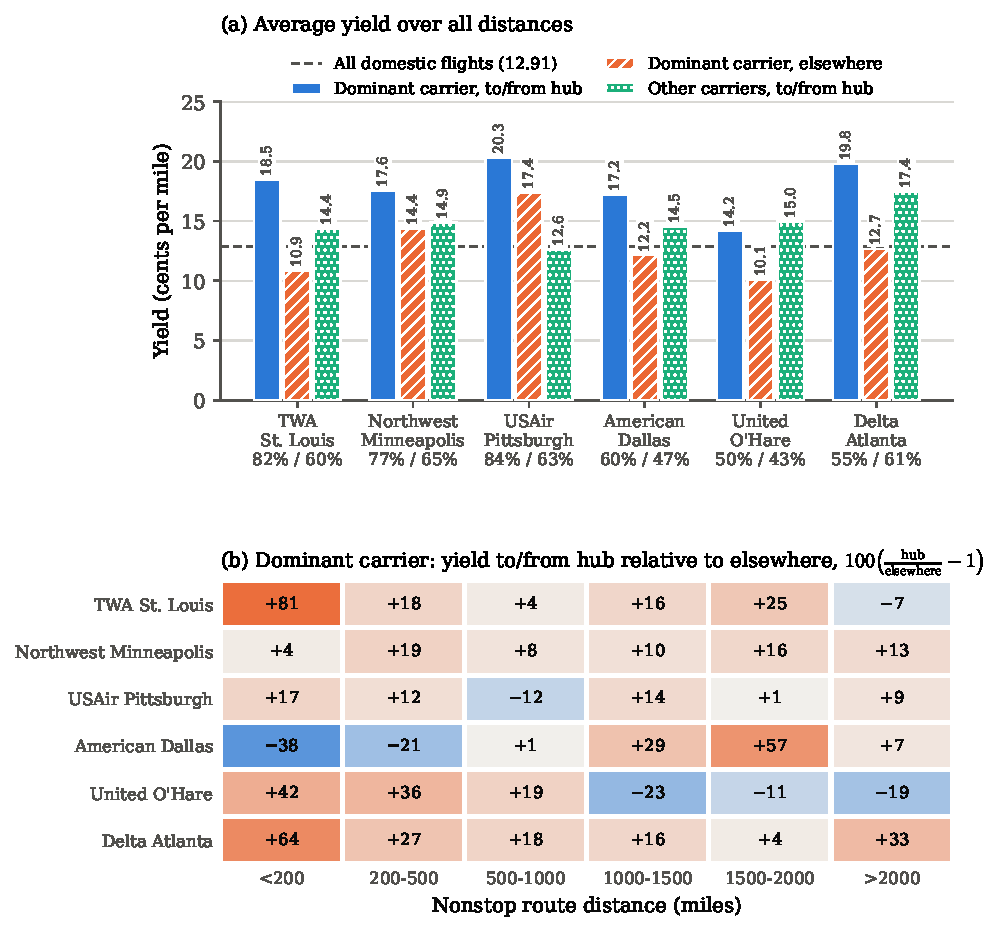
\includegraphics[width=0.97\linewidth]{figures/ch09/borenstein_yields.pdf}
\caption{Yields at six airports dominated by one carrier, third quarter of 1987. Panel (a) shows three yields
over all distances. They are the dominant carrier's yield on routes to or from its hub, its yield elsewhere in
its system, and the yield of other carriers on routes to or from the hub. The two percentages under each airport are the
dominant carrier's shares of enplanements and of originations there. Panel (b) shows, for each distance band,
the percentage by which the dominant carrier's yield to or from its hub exceeds its yield elsewhere. Yields fall
with distance, so panel (a) mixes fare levels with the distance composition of each group, while panel (b)
holds distance roughly fixed. Redrawn from \citet{Borenstein1989}, Table 1.}
\label{fig:09-bor-yields}
\end{figure}

Over all distances, the dominant carrier's yield at its hub exceeds its yield elsewhere at all six airports.
The gap ranges from 17\% for USAir at Pittsburgh ($\frac{20.32}{17.42} = 1.17$) to 70\% for TWA at St.\ Louis
($\frac{18.50}{10.86} = 1.70$). At five of the six airports, the dominant carrier's yield also exceeds that of
other carriers at the same airport. The exception is O'Hare, the least dominated airport in the table. There
United's yield of 14.19 cents falls short of the other carriers' 14.99 cents.

The comparison over all distances has a weakness. Yields fall steeply with distance, from 37.96 cents per mile
on routes under 200 miles to 7.16 cents on routes over 2,000 miles. A group that flies shorter routes therefore
shows a higher average yield even if it charges the same fare as others at each distance. Panel (b) of
\cref{fig:09-bor-yields} compares the dominant carrier with itself within distance bands. Its hub yield exceeds
its yield elsewhere in 29 of the 36 cells. The exceptions are Dallas on short routes ($-38\%$ and $-21\%$)
and O'Hare on routes over 1,000 miles ($-23\%$, $-11\%$ and $-19\%$). The others are Pittsburgh at 500 to
1,000 miles ($-12\%$) and St.\ Louis over 2,000 miles ($-7\%$). Against other carriers at the same airport, the dominant carrier has the
higher yield in 26 of the 35 cells with data. United at O'Hare is lower in five of six bands. USAir's 61\%
advantage over other carriers at Pittsburgh over all distances shrinks to between $-16\%$ and $+27\%$ within
bands, so most of it reflects the distance mix.\footnote{The within-band counts and percentages are our
calculations from Table 1 of the paper.}%

Borenstein argues that costs do not explain the hub premium (p.~356). Carriers have somewhat higher load
factors on flights to and from their hubs, which lowers cost per passenger. Passengers to or from a hub also
fly routes about as long as, or longer than, the carrier's other passengers. The higher cost per mile of short
flights therefore does not explain the gap either. The table cannot separate airport dominance from route
dominance, because a carrier that dominates an airport usually dominates the routes from it. The regressions
attempt this separation.

\subsection{The estimating equations}\label{sec:09-bor-equations}

\casehead{The pricing equation} Borenstein's first equation explains the log of a fare percentile by cost,
quality and market-structure variables. Let $P_{ft}$ denote one of FR20, FR50 or FR80 for carrier $f$ on route
$t$. Each percentile has its own regression with its own coefficients. In our notation, his equation (1), with
an error term $u_{ft}$ added, is
\begin{equation}\label{eq:09-bor-price}
\begin{aligned}
\ln P_{ft} = {} & a_f + b_D \ln \mathit{DISTANCE}_t + \gamma_1 \ln \mathit{LOADFAC}_{ft}
  + \gamma_2 \ln \mathit{EQUIP}_{ft} \\
& + \gamma_3 \ln \mathit{FREQ}_{ft} + \gamma_4 \ln \mathit{CIRC}_{ft} + \gamma_5\, \mathit{STOP}_{ft}
  + \gamma_6\, \mathit{PLANECHG}_{ft} \\
& + \phi_1\, \mathit{ORGSHARE}_{ft} + \phi_2\, \mathit{ORGHERF}_t + \phi_3\, \mathit{RUTSHARE}_{ft}
  + \phi_4\, \mathit{RUTHERF}_t \\
& + \phi_5 \ln \mathit{COMPCOST}_{ft} + \phi_6 \ln \mathit{TOURIST}_t
  + \sum_{k=1}^{24} \varrho_k\, \mathit{APT}_{kt} + u_{ft} .
\end{aligned}
\end{equation}
The coefficient letters group the variables by their hypothesized role (p.~349). The carrier effects $a_f$
capture carrier-wide differences in cost and reputation. Distance, with coefficient $b_D$, primarily affects
production cost. The six $\gamma$ variables affect both cost and service quality, so their signs are ambiguous
in advance. The six $\phi$ variables primarily indicate market power. The 24 coefficients $\varrho_k$ measure
scarcity rents at airports that may be congested. \Cref{tab:09-bor-vars} defines each variable and gives the
sign that Borenstein expects.

\begin{table}[htbp]
\centering
\caption{Variables of the pricing equation}
\label{tab:09-bor-vars}
\footnotesize
\renewcommand{\arraystretch}{1.12}
\begin{tabularx}{\linewidth}{@{}l >{\raggedright\arraybackslash}X l c@{}}
\toprule
Variable & Definition and construction & Group & Sign \\
\midrule
FR20, FR50, FR80 & Percentiles of the passenger-weighted distribution of the fares paid to the carrier on the
route. A round trip counts as two trips at half fare. & dependent & \\
DISTANCE & Nonstop mileage between the endpoints ($d_t$ in \cref{sec:09-data}). & cost & $+$ \\
LOADFAC & Load factor of the segments used by the carrier's passengers on the route, averaged over the
segments of an itinerary by distance and over itineraries by passengers. & cost, quality & ? \\
EQUIP & Seats per plane, averaged in the same way. & cost, quality & ? \\
FREQ & Minimum number of flights in the quarter on any segment of an itinerary, averaged over itineraries by
passengers. & cost, quality & ? \\
CIRC & Average total routing mileage of the carrier's passengers (TOTMILE) divided by DISTANCE. & cost, quality
& ? \\
STOP & Average number of on-plane stops per passenger. & cost, quality & ? \\
PLANECHG & Average number of changes of plane per passenger. & cost, quality & ? \\
ORGSHARE & Carrier's share of passenger originations at the two endpoints, averaged with weights equal to the
shares of the route's travelers whose tickets originate at each endpoint. & market power & $+$ \\
ORGHERF & Herfindahl index of originations at the two endpoints, averaged with the same weights. & market power
& ? \\
RUTSHARE & Carrier's share of the route's local passengers. & market power & $+$ \\
RUTHERF & Herfindahl index of the route's local passengers. & market power & ? \\
COMPCOST & Average standardized cost per available seat-mile of the other carriers on the route, weighted by
their route shares. & market power & $+$ \\
TOURIST & Tourism index (hotel income from group and tourist customers over personal income) of each endpoint,
weighted by the share of travelers who originate at the other endpoint. & market power & $-$ \\
APT$_k$ & Indicator that airport $k$ is an endpoint, divided by DISTANCE in thousands of miles. & scarcity &
$+$ \\
\bottomrule
\end{tabularx}

\smallskip
\begin{minipage}{\linewidth}
\footnotesize Notes: ``Group'' is the role that Borenstein assigns to each variable and ``Sign'' the sign he
expects, with ? for an ambiguous sign. Load factor, equipment, frequency and stops come from the Service
Segment Data, fares, shares and circuity from the DB1A sample, and enplanements from the Nonstop Market Data.
Source: \citet{Borenstein1989}, pp.~349--351 and Appendix.
\end{minipage}
\end{table}

\casehead{Constructed variables} Several variables are averages over the two endpoints $e \in \{1,2\}$ of the
route. Let $\varpi_{te}$ be the share of the route's travelers whose tickets originate at endpoint $e$. Let
$o_{fe}$ be carrier $f$'s share of all passenger originations at airport $e$, and let $\mathit{TRIX}_e$ be the
tourism index of the metropolitan area of $e$. Then
\begin{equation}\label{eq:09-bor-org}
\begin{gathered}
\mathit{ORGSHARE}_{ft} = \sum_{e=1}^{2} \varpi_{te}\, o_{fe}, \qquad
\mathit{ORGHERF}_t = \sum_{e=1}^{2} \varpi_{te} \sum_{k} o_{ke}^2, \\
\mathit{TOURIST}_t = \varpi_{t1}\, \mathit{TRIX}_2 + \varpi_{t2}\, \mathit{TRIX}_1 .
\end{gathered}
\end{equation}
The tourism measure weights each endpoint by the share of travelers who start at the other end, so it measures
the tourist appeal of the route's destinations. Origination shares exclude connecting passengers. Borenstein
reports that measures based on enplanements, which include them, give very similar results (p.~349).

The cost of rivals enters through
\begin{equation}\label{eq:09-bor-compcost}
\mathit{COMPCOST}_{ft} = \sum_{k \neq f} \frac{s_{kt}}{1 - s_{ft}}\, \mathit{COST}_k ,
\end{equation}
where $s_{kt}$ is carrier $k$'s route share, so that $s_{ft} = \mathit{RUTSHARE}_{ft}$. $\mathit{COST}_k$ is a
standardized cost per available seat-mile. To construct it, Borenstein regresses cost per available seat-mile on
a constant and average length of haul across the 17 carriers with data. He then adds each carrier's residual to
0.08, roughly the average cost of a carrier with the mean length of haul (p.~363). Small carriers without data
receive 0.08. COMPCOST proxies for the competitiveness of rivals, whose prices are endogenous and whose service
data are incomplete (p.~351).

Finally, the scarcity variables are
\begin{equation}\label{eq:09-bor-apt}
\mathit{APT}_{kt} = \frac{1000 \cdot \indic\{k \text{ is an endpoint of } t\}}{\mathit{DISTANCE}_t} ,
\end{equation}
for 24 airports (p.~351). They are the 22 airports that the Federal Aviation Administration monitored for
congestion and the airports of Orange County and Long Beach, which faced strict local limits on takeoffs and
landings. Four of the monitored airports allocated slots: O'Hare, Kennedy, La Guardia and Washington National.

\casehead{Expected signs} The $\gamma$ variables move cost and quality in directions that push price opposite
ways (pp.~349--350). A higher load factor lowers cost per passenger, which lowers fares. Full flights also tend
to operate at peak times, when the opportunity cost of aircraft is high, which raises fares. Crowded planes,
finally, lower service quality and reservation prices. Larger aircraft have a lower cost per seat-mile on
flights over 500 miles. They are also more comfortable and thought to be safer, which raises demand. Frequent
service lowers cost per flight, because aircraft on dense routes fly more hours per day. It also lowers the
frequency delay of \cref{sec:09-regulation}, the gap between a traveler's preferred departure time and the
nearest flight \citep{DouglasMiller1974}. Frequency delay matters most to travelers with high time values, who pay the high
fares. Circuity, stops and changes of plane raise cost, by lengthening routings or shortening average hauls,
and they lower quality.

Among the $\phi$ variables, Borenstein expects ORGSHARE, RUTSHARE and COMPCOST to raise fares and TOURIST to
lower them (pp.~350--351). The concentration measures have ambiguous signs, and their interpretation drives the
paper. Holding the carrier's own route share fixed, a higher RUTHERF means that the traffic the carrier does not
carry is more concentrated. If a dominant carrier's high price creates an umbrella, this raises the observed
carrier's price, so $\phi_4 > 0$. If a dominant carrier instead has a competitive advantage through marketing
devices, it may lower the profit-maximizing price of its rivals, so $\phi_4 < 0$. Endpoint concentration is
ambiguous for a related reason. A carrier may prefer many small rivals at its airports to one large rival,
while coordination, such as an agreement not to enter one another's routes, is easier among few firms.

\casehead{Functional form} A firm with market power sets price equal to marginal cost times a markup that
depends on the elasticity of the demand it faces. Logs turn this product into a sum, and earlier studies used
the same multiplicative form \citep{GrahamKaplanSibley1983,BaileyGrahamKaplan1985}. Most variables therefore
enter in logs, with constant elasticities. \Cref{sec:09-pricing-conduct} derives this specification from a
model of conduct. Let collusiveness rise with concentration as $\eta_t = \eta_0 + \eta_1 \HHI_t$, and let the
elasticity be a common $\varepsilon$. Because the equation omits the interaction $\HHI_t s_{ft}$ of
\cref{eq:09-umbrella}, the route-share coefficient is then $\phi_3 \approx \frac{1 - \eta_0 - \eta_1 \bar H}{\varepsilon}$
and the route-Herfindahl coefficient is $\phi_4 \approx \frac{\eta_1 (1 - \bar s)}{\varepsilon}$. Here $\bar H$
and $\bar s$ are the sample means of RUTHERF and RUTSHARE. The cost and quality variables parametrize
$\ln mc_{ft}$, and the constant terms are absorbed by the carrier effects.

The theory thus implies that shares enter linearly, and Borenstein gives a direct argument for the same choice
(p.~354). A log specification would give a rise in share from 1\% to 2\% the same effect as a rise from 30\% to
60\%, which is implausible. ORGSHARE enters linearly for the same reason, and
the two Herfindahl indices enter linearly for ease of comparison. The signs and approximate significance of
the estimates are robust to logs for each of these variables. STOP and PLANECHG also enter linearly, so each
stop or change of plane has the same proportional effect on price.

\Cref{rem:09-share-coef} shows that a Cournot reading of the 2SLS share coefficients ($\bar\eta = 0$, so
$\varepsilon = \frac{1}{\phi_3}$) would require route elasticities of $\frac{1}{0.1120} = 8.9$,
$\frac{1}{0.0288} = 34.7$ and $\frac{1}{0.2238} = 4.5$ for the three percentiles. The variation across
percentiles adds a further difficulty. A homogeneous-goods model has one price per route, and hence one
elasticity for all fares, while the share coefficients differ nearly eightfold across percentiles. Each
percentile behaves as if it faced its own demand. A model with differentiated products and heterogeneous
travelers delivers this pattern (\cref{sec:09-pricing-types}).

The scarcity terms need a different treatment (p.~354). A scarcity rent should add the same dollar amount to
every fare from an airport, whatever the route. Suppose the fare is $P_{ft} = P^0_{ft} + R_k$, where $P^0_{ft}$
is the fare without the rent and $R_k$ is the rent at endpoint $k$. Taking logs and using
$\ln(1 + x) \approx x$ for small $x$,
\begin{align*}
\ln P_{ft} &= \ln P^0_{ft} + \ln\left(1 + \frac{R_k}{P^0_{ft}}\right) \\
&\approx \ln P^0_{ft} + \frac{R_k}{P^0_{ft}} .
\end{align*}
If the rent-free fare is proportional to distance, $P^0_{ft} = c\, \mathit{DISTANCE}_t$, the last term becomes
\begin{equation*}
\frac{R_k}{c\, \mathit{DISTANCE}_t} = \frac{R_k}{1000\, c} \cdot \frac{1000}{\mathit{DISTANCE}_t}
= \varrho_k\, \mathit{APT}_{kt}, \qquad \text{with } \varrho_k = \frac{R_k}{1000\, c} .
\end{equation*}
The coefficient $\varrho_k$ is thus the rent as a fraction of the fare on a 1,000-mile route. A plain indicator
would instead make the rent proportional to the fare and assign larger rents to longer routes. Estimating the
additive form directly would require iterative nonlinear methods, which would have been difficult with his
number of observations and variables. Borenstein therefore calls the distance scaling a partial solution. Fares
rise less than proportionally with distance ($b_D$ lies between 0.33 and 0.41 in \cref{tab:09-bor-main}), so
dividing by distance overcorrects somewhat.

\casehead{The relative-price equation} The second equation compares two carriers on the same route. Add to
\cref{eq:09-bor-price} a route effect $\Upsilon_t$ that collects every determinant of fares common to all carriers
on route $t$, observed or not. Collect the variables that vary across carriers on a route in the row vector
\begin{equation*}
z_{ft} = \big(\ln \mathit{LOADFAC}_{ft}, \ln \mathit{EQUIP}_{ft}, \ln \mathit{FREQ}_{ft}, \ln \mathit{CIRC}_{ft},
\mathit{STOP}_{ft}, \mathit{PLANECHG}_{ft}\big),
\end{equation*}
with coefficients $\gamma = (\gamma_1, \dots, \gamma_6)^\top$. The pricing equation becomes
\begin{equation*}
\ln P_{ft} = a_f + \Upsilon_t + z_{ft}\gamma + \phi_1\, \mathit{ORGSHARE}_{ft} + \phi_3\, \mathit{RUTSHARE}_{ft}
+ \phi_5 \ln \mathit{COMPCOST}_{ft} + u_{ft} .
\end{equation*}
Here $\Upsilon_t$ absorbs distance, the two Herfindahl indices, the tourism index, the scarcity terms and any
unobserved demand or cost shifter at the route level. Write this equation for carriers $a$ and $b$ on route $t$
and subtract. The route effect cancels because $\Upsilon_t - \Upsilon_t = 0$. Borenstein also omits the difference in
COMPCOST (p.~355, n.~35). Its role in the pricing equation was to proxy for the other carriers on the route. In
the relative-price equation one rival enters directly and the remaining rivals are common to both carriers. The
result is his equation (4):
\begin{equation}\label{eq:09-bor-rel}
\begin{aligned}
\ln P_{at} - \ln P_{bt} = {} & a_a - a_b + \gamma_1 (\ln \mathit{LOADFAC}_{at} - \ln \mathit{LOADFAC}_{bt}) \\
& + \gamma_2 (\ln \mathit{EQUIP}_{at} - \ln \mathit{EQUIP}_{bt})
  + \gamma_3 (\ln \mathit{FREQ}_{at} - \ln \mathit{FREQ}_{bt}) \\
& + \gamma_4 (\ln \mathit{CIRC}_{at} - \ln \mathit{CIRC}_{bt})
  + \gamma_5 (\mathit{STOP}_{at} - \mathit{STOP}_{bt}) \\
& + \gamma_6 (\mathit{PLANECHG}_{at} - \mathit{PLANECHG}_{bt})
  + \phi_1 (\mathit{ORGSHARE}_{at} - \mathit{ORGSHARE}_{bt}) \\
& + \phi_3 (\mathit{RUTSHARE}_{at} - \mathit{RUTSHARE}_{bt}) + u_{at} - u_{bt} .
\end{aligned}
\end{equation}
The coefficients are those of \cref{eq:09-bor-price}. The two carriers are drawn at random among those that meet
the sample criteria (p.~355). The carrier effects enter as the difference $a_a - a_b$, which a regression
implements with indicators equal to $+1$ for carrier $a$ and $-1$ for carrier $b$.

Differencing has a benefit and a cost. The benefit is that every unobserved route-level shifter of demand or
cost drops out. The estimates of $\phi_1$ and $\phi_3$ then no longer rely on the route controls of
\cref{eq:09-bor-price}. The cost is that the coefficients on route-level market structure, $\phi_2$ and
$\phi_4$, are no longer identified. The equation answers a narrower question, which is the one the asymmetry
hypothesis poses. Does the carrier with the larger share of a route, or of its endpoints, charge more than its
rival on the same route? Under a complete umbrella with a homogeneous product, $\eta_t = 1$ and every carrier on
the route has conduct $\theta_{ft} = 1$. The share term in \cref{eq:09-pricing-approx} then vanishes, and all
carriers charge the same markup, so $\phi_3 = 0$ in \cref{eq:09-bor-rel}. Under the differentiated-products
model of \cref{prop:09-dominance}, the relative price instead rises with the share gap. Let $s$ be a common
share of all potential travelers, $L$ the Lerner index there and $s_0$ the outside share. \Cref{cor:09-relprice}
gives a slope of $\frac{L}{1-s}$ in these shares, or $\frac{L(1-s_0)}{1-s}$ in route shares. The latter is
the structural counterpart of $\phi_3$ in \cref{eq:09-bor-rel}.

\subsection{Estimation and identification}\label{sec:09-bor-ident}

\casehead{Why least squares fails} A carrier's route share depends on its own price. To see the consequence,
add a share equation to the pricing equation and solve the two jointly. Suppress the other regressors, which
we take as exogenous, and write
\begin{align*}
\ln P_{ft} &= \phi_3\, s_{ft} + u_{ft}, \\
s_{ft} &= \Psi_{ft} - b_s \ln P_{ft} + v_{ft} .
\end{align*}
Here $s_{ft} = \mathit{RUTSHARE}_{ft}$, $\Psi_{ft}$ collects exogenous shifters of the share, $b_s > 0$
measures how fast the share falls with the carrier's own price, and $v_{ft}$ is an unobserved demand shifter.
Substitute the first equation into the second:
\begin{equation*}
s_{ft} = \Psi_{ft} - b_s \phi_3\, s_{ft} - b_s u_{ft} + v_{ft} .
\end{equation*}
Collect the terms in $s_{ft}$ and solve, assuming $1 + b_s \phi_3 > 0$:
\begin{equation*}
s_{ft} = \frac{\Psi_{ft} - b_s u_{ft} + v_{ft}}{1 + b_s \phi_3} .
\end{equation*}
Let $\Var(u_{ft}) = \sigma_u^2$ and $\Cov(u_{ft}, v_{ft}) = \sigma_{uv}$, and let $\Psi_{ft}$ be uncorrelated
with both errors. The ordinary least squares (OLS) estimator then has probability limit
\begin{equation}\label{eq:09-bor-olsbias}
\plim \hat\phi_3^{\mathrm{OLS}} = \phi_3 + \frac{\Cov(s_{ft}, u_{ft})}{\Var(s_{ft})}
= \phi_3 + \frac{\sigma_{uv} - b_s \sigma_u^2}{(1 + b_s\phi_3) \Var(s_{ft})} .
\end{equation}
With other regressors present, $\Var(s_{ft})$ is the variance of the share after projection on them. Two forces
compete. The simultaneity term $-b_s\sigma_u^2$ biases the estimate down. A carrier hit by a positive cost
or pricing shock charges more and loses passengers, so high prices go with low shares. The term $\sigma_{uv}$
biases the estimate up if unobserved quality raises both the share and the price, which is the efficiency
argument of \citet{Demsetz1973} in airline form. A Hausman test (described below) rejects the exogeneity of
RUTSHARE and RUTHERF (p.~352), so the preferred estimates use instruments.

\casehead{The instrument for route share} An instrument must shift a carrier's route share without entering its
pricing equation. Measures of rivals' presence at the endpoint airports come to mind. The airport dominance
effects of \cref{sec:09-dominance-sources}, however, make such measures candidates for the pricing equation
itself (p.~352). Borenstein resolves the problem with an asymmetry. The marketing advantages of airport
dominance do not require large operations at both ends of a route. Entry onto a route, in contrast, benefits
from presence at both ends. The excluded instrument is the carrier's share of the geometric means of endpoint
enplanements,
\begin{equation}\label{eq:09-genpsh}
\mathit{GENPSH}_{ft} = \frac{\sqrt{\mathit{ENP}_{f1}\, \mathit{ENP}_{f2}}}
{\sum_{k} \sqrt{\mathit{ENP}_{k1}\, \mathit{ENP}_{k2}}} ,
\end{equation}
which is his equation (2). Here $\mathit{ENP}_{k1}$ and $\mathit{ENP}_{k2}$ are carrier $k$'s average daily
enplanements at the two endpoints of route $t$ during the quarter, and the sum runs over all carriers
(p.~352).

The geometric mean gives the instrument its content. It is zero when a carrier has no enplanements at one of
the endpoints. For a given total $\mathit{ENP}_{f1} + \mathit{ENP}_{f2}$, it is largest when the two are equal.
GENPSH therefore rewards balanced presence at both ends. ORGSHARE, which appears in the pricing equation,
averages the carrier's endpoint shares linearly. A carrier with a large share at one end and a small share at
the other can have a high ORGSHARE but a low GENPSH. Conditional on ORGSHARE, GENPSH thus varies with the
balance of the carrier's presence across the endpoints. It also varies with connecting operations, since
enplanements count connecting passengers and originations do not. Borenstein chooses enplanements because they
better measure a carrier's investment in physical capital and long-term labor contracts at an airport
(p.~352, n.~30).

Two pieces of evidence support relevance. The first comes from \citet{Berry1992}, which Borenstein cites as a
1989 working paper (p.~352, n.~29). Berry starts from the 1,225 possible city pairs among the 50 largest U.S.
cities \citep[p.~903]{Berry1992}. He drops 6 pairs that have no listings in the Origin and Destination Survey,
which leaves 1,219 markets \citep[p.~903, n.~9, and p.~904]{Berry1992}. He measures entry between the first and the third quarter of 1980
\citep[p.~904]{Berry1992}. Of the 3,590
potential entrants that already served both cities of a pair, 6.46\% entered it. Of those that served one city,
0.36\% entered, a rate about 18 times lower. Only 4 of the 47,600 potential entrants that served neither city entered,
a rate of 0.01\% \citep[Table~III]{Berry1992}. The second piece of evidence is Borenstein's own. In the first
stage of the estimation, both ORGSHARE and GENPSH are highly significant (p.~352). The paper does not report the first-stage coefficients or $F$ statistics.

The exclusion restriction requires that GENPSH affect fares only through route share. Borenstein states the
condition plainly. It is valid if a carrier's current prices respond to actual competition but not to threats
of entry (p.~352). He defends it on timing grounds. An incumbent can change its fares much faster than a rival
can move from announcing entry to flying. It therefore need not price against potential entrants in advance. The USAir testimony quoted in \cref{sec:09-contest-fail} supports this view.

If the restriction fails, the bias has a predictable sign. Potential entrants with large operations at both
endpoints raise the denominator of \cref{eq:09-genpsh}, so a carrier's GENPSH is low exactly when such entrants
are present. Suppose a carrier that faces well-placed potential entrants holds its fares down to deter entry, a
practice called \emph{limit pricing}. Its fares then rise with GENPSH at a given route share, and the true
equation contains a term $\phi_G\, \mathit{GENPSH}_{ft}$ with $\phi_G > 0$. Ignore RUTHERF for the moment, write $g_{ft} = \mathit{GENPSH}_{ft}$, and let a tilde denote the
residual after projection on the included exogenous regressors. The IV estimator has probability limit
\begin{align}
\plim \hat\phi_3^{\mathrm{IV}} &= \frac{\Cov(\tilde g_{ft}, \ln P_{ft})}{\Cov(\tilde g_{ft}, \tilde s_{ft})}
\notag \\
&= \frac{\phi_3 \Cov(\tilde g_{ft}, \tilde s_{ft}) + \phi_G \Var(\tilde g_{ft})}{\Cov(\tilde g_{ft}, \tilde s_{ft})}
\notag \\
&= \phi_3 + \frac{\phi_G}{\pi_1} . \label{eq:09-bor-ivbias}
\end{align}
The second line substitutes the true equation and uses $\Cov(\tilde g_{ft}, u_{ft}) = 0$. In the third line,
$\pi_1 = \frac{\Cov(\tilde g_{ft}, \tilde s_{ft})}{\Var(\tilde g_{ft})}$ is the first-stage coefficient on
GENPSH. Since $\pi_1 > 0$ and $\phi_G > 0$, limit pricing against potential entrants biases the estimated
share effect upward. A violation of this kind would make Borenstein's estimates of $\phi_3$ too large. The
POTCOMP specification below offers a check. Controlling for potential competitors should absorb part of this
bias and lower the route-share coefficients. Instead they rise slightly (Panel B of \cref{tab:09-bor-main}),
which suggests that the bias is small.

\casehead{Potential competition} Borenstein addresses the exclusion restriction in a second way, by measuring
potential competition directly (pp.~352--353). The variable
\begin{equation}\label{eq:09-bor-potcomp}
\mathit{POTCOMP}_{ft} = \frac{\sum_{k \in \mathcal{P}_t} \sqrt{\mathit{ENP}_{k1}\, \mathit{ENP}_{k2}}}
{\sum_{k} \sqrt{\mathit{ENP}_{k1}\, \mathit{ENP}_{k2}}}
\end{equation}
has the construction of GENPSH, but its numerator sums over the set $\mathcal{P}_t$ of carriers with less than
1\% of the route's traffic (p.~364). These carriers are present at the endpoints but not yet significant on the
route. In an alternative specification POTCOMP enters \cref{eq:09-bor-price} directly, while GENPSH still
instruments route share. POTCOMP may itself be endogenous. High fares on a route attract entry, which turns
potential competitors into actual ones and lowers POTCOMP. A positive shock $u_{ft}$ therefore goes with a low
POTCOMP, which biases its coefficient toward a negative value (p.~359, n.~44).

\casehead{The instrument for route concentration} The route Herfindahl index contains the square of the
carrier's own share, so it is endogenous whenever RUTSHARE is. Borenstein constructs an instrument by
decomposing the index (p.~353). Write $s_{ft}$ for the carrier's share and $\HHI_t = \mathit{RUTHERF}_t$. Split
the sum of squared shares into the carrier's own term and its rivals' terms:
\begin{align*}
\HHI_t &= s_{ft}^2 + \sum_{k \neq f} s_{kt}^2 \\
&= s_{ft}^2 + (1 - s_{ft})^2 \sum_{k \neq f} \left(\frac{s_{kt}}{1 - s_{ft}}\right)^2 \\
&= s_{ft}^2 + (1 - s_{ft})^2 H_{-f,t} .
\end{align*}
Here $H_{-f,t}$ is the Herfindahl index of the traffic that carrier $f$ does not carry, computed from each
rival's share of that traffic. Solving the last line for $H_{-f,t}$ expresses it in observed variables:
\begin{equation*}
H_{-f,t} = \frac{\mathit{RUTHERF}_t - \mathit{RUTSHARE}_{ft}^2}{(1 - \mathit{RUTSHARE}_{ft})^2} .
\end{equation*}

The instrument rests on two assumptions. (a) GENPSH is a valid instrument for RUTSHARE. (b) The division among
rivals of the traffic that carrier $f$ does not carry is exogenous to $f$'s price. In Borenstein's example,
TWA's price on the Boston to Los Angeles route does not affect how the passengers it does not get divide between
American and United. Under (b), $H_{-f,t}$ is exogenous. Replace the own share by its fitted value
$\widehat{\mathit{RUTSHARE}}_{ft}$ from the first-stage regression on all exogenous variables:
\begin{equation}\label{eq:09-irutherf}
\mathit{IRUTHERF}_{ft} = \widehat{\mathit{RUTSHARE}}_{ft}^{\,2}
+ \frac{\mathit{RUTHERF}_t - \mathit{RUTSHARE}_{ft}^2}{(1 - \mathit{RUTSHARE}_{ft})^2}
\big(1 - \widehat{\mathit{RUTSHARE}}_{ft}\big)^2 .
\end{equation}
This is Borenstein's equation (3). In the constructed index, each rival's share becomes
$s_{kt} \frac{1 - \widehat{\mathit{RUTSHARE}}_{ft}}{1 - s_{ft}}$. The rescaling leaves the Herfindahl index of the
traffic not carried by $f$ equal to $H_{-f,t}$, as Borenstein notes. IRUTHERF then serves as the excluded
instrument for RUTHERF. The same assumption (b) is needed for COMPCOST, whose weights in
\cref{eq:09-bor-compcost} are the rivals' shares of the traffic that $f$ does not carry (p.~353).

\begin{remark}[When is assumption (b) plausible?]\label{rem:09-bor-iia}
Assumption (b) holds exactly in a logit model of route demand, holding rivals' prices fixed. Route shares are
shares of the route's passengers, so the outside good drops out and
$s_{kt} = \frac{e^{\delta_{kt}}}{\sum_{j} e^{\delta_{jt}}}$, with the sum over the carriers on the route. Then
\begin{equation*}
\frac{s_{kt}}{1 - s_{ft}} = \frac{e^{\delta_{kt}}}{\sum_{j \neq f} e^{\delta_{jt}}} ,
\end{equation*}
which involves neither $\delta_{ft}$ nor $p_{ft}$. This is the independence of irrelevant alternatives of
\cref{ch:logit}. The assumption fails when some rivals are closer substitutes for $f$ than others, for example
when one rival shares $f$'s hub airport. It can also fail in equilibrium, since rivals adjust their prices when
$f$ changes its own.
\end{remark}

\begin{remark}[A constructed instrument]\label{rem:09-bor-generated}
IRUTHERF is a nonlinear function of first-stage fitted values. Substituting such a function for RUTHERF in the
second stage would not in general give consistent estimates, because the first-stage residual does not drop out
of a nonlinear function. Borenstein instead uses IRUTHERF as an excluded instrument in the first-stage regression
for RUTHERF. Any function of exogenous variables is a valid instrument, so this use is consistent under (a) and
(b). The nonlinearity affects only how strongly IRUTHERF predicts RUTHERF.
\end{remark}

\casehead{Load factor and the Hausman test} Load factor may also be endogenous, since a low fare fills planes.
Borenstein instruments it with LOADPOP, the passenger-weighted average over itineraries of the summed
populations of all cities where the traveler is on the ground, including stops and connections (pp.~353, 363).
The idea is that populous cities along an itinerary add traffic to its segments and so raise load factors. A
Hausman test does not reject exogeneity of LOADFAC at any reasonable significance level, so the reported
estimates treat it as exogenous (pp.~356--357).

The Hausman test compares two estimators \citep{Hausman1978}. Under the null hypothesis that the suspect
regressors are exogenous, OLS is consistent and efficient, while 2SLS is consistent but less precise. Under the
alternative only 2SLS is consistent. Let $\hat\vartheta_S$ collect the estimated coefficients on the suspect
regressors and $\hat V$ their estimated variance matrix. The statistic
\begin{equation}\label{eq:09-bor-hausman}
\mathcal{H} = \big(\hat\vartheta_S^{\mathrm{2SLS}} - \hat\vartheta_S^{\mathrm{OLS}}\big)^\top
\big[\hat V^{\mathrm{2SLS}} - \hat V^{\mathrm{OLS}}\big]^{-1}
\big(\hat\vartheta_S^{\mathrm{2SLS}} - \hat\vartheta_S^{\mathrm{OLS}}\big)
\end{equation}
is asymptotically $\chi^2$ under the null, with degrees of freedom equal to the number of suspect regressors
(\cref{sec:A-spectests}). A large value rejects exogeneity. For RUTSHARE and RUTHERF the test rejects, and
for LOADFAC it does not.

Treating LOADFAC as endogenous anyway raises the estimated ORGSHARE effects somewhat and raises all standard
errors (p.~357, n.~38). The LOADFAC coefficient itself becomes much more negative and much less precise
(p.~358, n.~40). Simultaneity predicts the opposite movement. Low fares raise load factors, which pushes the
least-squares coefficient down, so a correction should make it less negative.

\casehead{Variables without instruments} A carrier's choices of nonstop versus connecting service, aircraft
size, frequency, stops, changes of plane and circuity are part of its network design. They may respond to the
same shocks as its fares (p.~353). Even LOADPOP is open to doubt, since the populations are exogenous but their
summation by itinerary depends on routing choices. For lack of instruments, Borenstein treats these variables as
exogenous and interprets their coefficients with possible biases in mind.

\casehead{Pooling and the error structure} A test rejects a common constant across carriers, so the equation
includes carrier fixed effects $a_f$ (pp.~353--354). A further test of common slopes across carriers does not
reject pooling at conventional levels, so all other coefficients are common to the nine carriers. The
scarcity coefficients $\varrho_k$ are common by construction, since a scarcity rent is the same for every
carrier at an airport. The same tests applied to \cref{eq:09-bor-rel} again do not reject pooling (p.~355).
Keeping one carrier per route gives up information to secure independent errors. A modern study would keep
every qualifying carrier and cluster the standard errors by route (\cref{sec:A-cluster}).

\casehead{The estimator} The preferred estimates are 2SLS with asymptotic standard errors. The procedure has
three steps. First, regress RUTSHARE on GENPSH and all included exogenous regressors, and keep the fitted
values. Second, construct IRUTHERF from \cref{eq:09-irutherf}. Third, estimate \cref{eq:09-bor-price} by 2SLS,
treating RUTSHARE and RUTHERF as endogenous, with GENPSH and IRUTHERF as excluded instruments. With two
endogenous regressors and two excluded instruments, the equation is exactly identified. Let $X_{ft}$ be the row
of regressors, let $Z_{ft}$ be the same row with GENPSH and IRUTHERF in place of RUTSHARE and RUTHERF, and let
$\vartheta$ be the coefficient vector. The estimator solves the sample analogue of
$\E[Z_{ft}^\top u_{ft}] = 0$,
\begin{equation*}
\hat\vartheta = \Big(\sum_{t} Z_{ft}^\top X_{ft}\Big)^{-1} \sum_{t} Z_{ft}^\top \ln P_{ft} ,
\end{equation*}
where each route $t$ contributes the one carrier $f$ selected for it. The paper treats the endogeneity in
\cref{eq:09-bor-rel} in the same way, without detailing the instrument for the share difference. OLS estimates
are reported for comparison.

\subsection{Results}\label{sec:09-bor-results}

\casehead{The pricing equation} \Cref{tab:09-bor-main} reproduces Table 2 of the paper. Panel A gives the 2SLS
estimates of \cref{eq:09-bor-price} for the three fare percentiles. Panel B gives the market-power coefficients
from two alternative specifications, one with POTCOMP added and one estimated by OLS. The paper summarizes the
carrier effects and the scarcity coefficients in the text without reporting them. \Cref{fig:09-bor-coefs} plots
the main market-power coefficients with 95\% confidence intervals.

\begin{table}[htbp]
\centering
\caption{The pricing equation: estimates of \cref{eq:09-bor-price}}
\label{tab:09-bor-main}
\footnotesize
\begin{tabular}{@{}lccc@{}}
\toprule
\multicolumn{4}{@{}l}{\textit{Panel A. 2SLS}} \\
\addlinespace
Dependent variable & $\ln$ FR20 & $\ln$ FR50 & $\ln$ FR80 \\
\midrule
$\ln$ DISTANCE & 0.4138$^{*}$ & 0.3348$^{*}$ & 0.3559$^{*}$ \\
 & (0.0103) & (0.0124) & (0.0133) \\
$\ln$ LOADFAC & $-0.0754^{*}$ & $-0.0425$ & $-0.0240$ \\
 & (0.0264) & (0.0318) & (0.0341) \\
$\ln$ EQUIP & $-0.0160$ & $-0.0050$ & $-0.0691^{*}$ \\
 & (0.0187) & (0.0225) & (0.0242) \\
$\ln$ FREQ & 0.0140$^{\#}$ & 0.0236$^{*}$ & 0.0428$^{*}$ \\
 & (0.0078) & (0.0094) & (0.0101) \\
$\ln$ CIRC & 0.1458$^{*}$ & 0.1272$^{*}$ & 0.2062$^{*}$ \\
 & (0.0412) & (0.0497) & (0.0533) \\
STOP & $-0.0470$ & $-0.0340$ & $-0.1327^{*}$ \\
 & (0.0292) & (0.0352) & (0.0377) \\
PLANECHG & $-0.0293^{*}$ & $-0.0776^{*}$ & $-0.0616^{*}$ \\
 & (0.0111) & (0.0134) & (0.0144) \\
ORGSHARE & 0.0345 & 0.1254$^{\#}$ & 0.1191$^{\#}$ \\
 & (0.0549) & (0.0661) & (0.0710) \\
ORGHERF & $-0.0699$ & $-0.0893$ & 0.0766 \\
 & (0.0623) & (0.0751) & (0.0806) \\
RUTSHARE & 0.1120$^{\#}$ & 0.0288 & 0.2238$^{*}$ \\
 & (0.0606) & (0.0731) & (0.0784) \\
RUTHERF & 0.1559$^{\dagger}$ & 0.1822$^{\dagger}$ & $-0.1787^{\dagger}$ \\
 & (0.0696) & (0.0839) & (0.0901) \\
$\ln$ COMPCOST & 0.5042$^{*}$ & 0.7010$^{*}$ & 0.8374$^{*}$ \\
 & (0.0453) & (0.0546) & (0.0586) \\
$\ln$ TOURIST & $-0.0187^{*}$ & $-0.0558^{*}$ & $-0.0991^{*}$ \\
 & (0.0058) & (0.0070) & (0.0076) \\
\addlinespace
$R^2$ & 0.683 & 0.494 & 0.508 \\
Observations & 3,591 & 3,591 & 3,591 \\
\bottomrule
\end{tabular}

\bigskip
\begin{tabular}{@{}lcccccc@{}}
\toprule
\multicolumn{7}{@{}l}{\textit{Panel B. Market-power coefficients in alternative specifications}} \\
\addlinespace
& \multicolumn{3}{c}{2SLS with POTCOMP} & \multicolumn{3}{c}{OLS} \\
\cmidrule(lr){2-4} \cmidrule(l){5-7}
Dependent variable & $\ln$ FR20 & $\ln$ FR50 & $\ln$ FR80 & $\ln$ FR20 & $\ln$ FR50 & $\ln$ FR80 \\
\midrule
ORGSHARE & 0.0365 & 0.1227$^{\#}$ & 0.1205$^{\#}$ & 0.0819$^{\#}$ & 0.1229$^{*}$ & 0.1228$^{\dagger}$ \\
 & (0.0536) & (0.0647) & (0.0696) & (0.0426) & (0.0514) & (0.0551) \\
ORGHERF & $-0.0684$ & $-0.0750$ & 0.0934 & $-0.0264$ & $-0.0660$ & $-0.0033$ \\
 & (0.0633) & (0.0764) & (0.0822) & (0.0543) & (0.0656) & (0.0702) \\
RUTSHARE & 0.1196$^{\dagger}$ & 0.0564 & 0.2470$^{*}$ & 0.0899$^{*}$ & 0.0596$^{\#}$ & 0.1259$^{*}$ \\
 & (0.0577) & (0.0697) & (0.0749) & (0.0270) & (0.0326) & (0.0349) \\
RUTHERF & 0.1262$^{\#}$ & 0.1286 & $-0.2302^{*}$ & 0.1128$^{*}$ & 0.1323$^{*}$ & $-0.0120$ \\
 & (0.0659) & (0.0795) & (0.0855) & (0.0329) & (0.0397) & (0.0425) \\
POTCOMP & $-0.0589^{\dagger}$ & $-0.0449$ & $-0.0380$ & & & \\
 & (0.0289) & (0.0348) & (0.0375) & & & \\
\addlinespace
$R^2$ & 0.683 & 0.493 & 0.507 & 0.683 & 0.494 & 0.511 \\
Observations & 3,591 & 3,591 & 3,591 & 3,591 & 3,591 & 3,591 \\
\bottomrule
\end{tabular}

\smallskip
\begin{minipage}{0.95\linewidth}
\footnotesize Notes: Standard errors in parentheses, asymptotic except for OLS. Significance marks as printed in
the paper: $^{\#}$ 10\%, $^{\dagger}$ 5\%, $^{*}$ 1\%. All specifications include carrier fixed effects and the 24
airport scarcity variables, whose coefficients the paper does not report. The two specifications in Panel B
include all the regressors of Panel A, and their other coefficients are close to those of Panel A. Source:
\citet{Borenstein1989}, Table 2.
\end{minipage}
\end{table}

\begin{figure}[htbp]
\centering
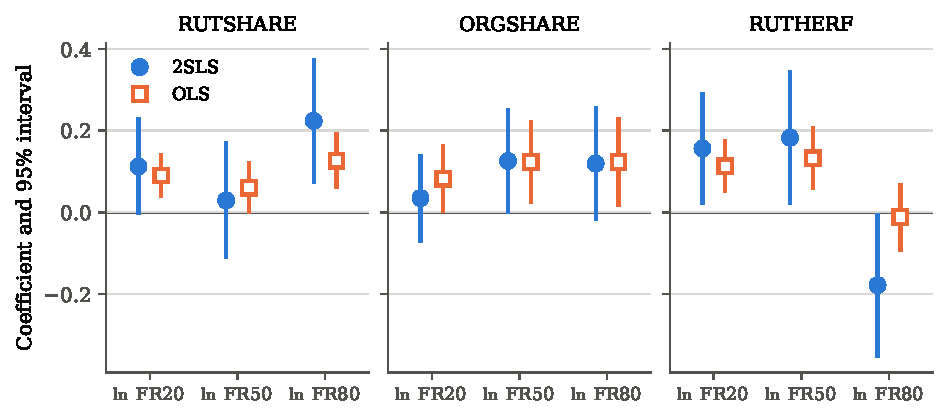
\includegraphics[width=0.97\linewidth]{figures/ch09/borenstein_coefs.pdf}
\caption{Market-power coefficients of the pricing equation by fare percentile, with 95\% confidence intervals
(estimate plus or minus 1.96 standard errors). Filled circles are 2SLS estimates and hollow squares OLS
estimates. The route-share and airport-share effects are positive at every percentile. The route-Herfindahl
effect, which holds the carrier's own share fixed, changes sign at the 80th percentile. Redrawn from
\citet{Borenstein1989}, Table 2.}
\label{fig:09-bor-coefs}
\end{figure}

Route share raises fares. Holding route concentration fixed, a one percentage point increase in a carrier's
route share raises its fares by between 0.03\% (FR50) and 0.22\% (FR80) (p.~357). Consider a dominant carrier
with 70\% of a route and rivals with 10\% each. All of them face the same route Herfindahl index, so the
comparison holds RUTHERF fixed automatically. The fare gap in log points is
\begin{equation*}
0.60 \times 0.1120 = 0.067, \qquad 0.60 \times 0.0288 = 0.017, \qquad 0.60 \times 0.2238 = 0.134
\end{equation*}
for FR20, FR50 and FR80. Borenstein summarizes this as a premium ``from 2\% to 12\%.''\footnote{The
arithmetic gives 1.7\% to 13.4\% in log points, or 1.7\% to 14.4\% as exact percentage changes
$e^{0.60\,\hat\phi_3} - 1$. The author's rounded range understates the upper end.} The effect is larger on the
20th and 80th percentiles than on the median, which Borenstein finds surprising. Yet a \emph{Chow test}, here a
test of whether a coefficient is equal across the three percentile regressions, does not reject equality
(p.~358). Only the FR80 coefficient is significant at 1\%. The FR20
coefficient is significant at 10\%, and the FR50 coefficient is not significant.

Airport share also raises fares, and more so at the high end of the fare distribution. The FR80 coefficient on
ORGSHARE, 0.1191, is about three times the FR20 coefficient, 0.0345, and Borenstein reports that the difference
is significant at 10\% (p.~358). Travelers who pay full coach fares are much more likely to be active members
of frequent-flyer programs than travelers on deep discounts. A stronger effect on high fares therefore fits the
FFP mechanism. A one standard deviation increase in ORGSHARE, 0.1305, raises the three log fares directly by
\begin{equation*}
0.1305 \times 0.0345 = 0.0045, \qquad 0.1305 \times 0.1254 = 0.0164, \qquad 0.1305 \times 0.1191 = 0.0155,
\end{equation*}
which the paper rounds to 0.5\%, 1.6\% and 1.6\%. Consider a carrier with half the originations at both
endpoints. It charges median and high-end fares about $0.5 \times 0.12 = 0.06$, or 6\%, above those of a
carrier with a very small presence at the two airports (p.~358).

These figures ignore an indirect channel. Airport dominance also raises a carrier's share of every route from
the airport. Borenstein estimates the size of this channel in a companion discussion paper, ``The Competitive
Advantage of a Dominant Airline'' (p.~358).\footnote{University of Michigan, Institute of Public Policy Studies,
Discussion Paper 280, 1989, as listed in the article's references. We cite it in the text only, so that its year
does not collide with the article's in the bibliography.} A one point increase in a carrier's share of originations at an airport raises its share of a route by up to 0.33
points, depending on its initial share. At the FR80 coefficient on route share, the indirect channel adds at most
$0.33 \times 0.2238 = 0.074$ to the direct ORGSHARE coefficient of 0.1191. When RUTSHARE and RUTHERF are dropped
from the equation, a one point increase in ORGSHARE raises the three percentiles by 0.24\%, 0.26\% and 0.24\%,
each significant at 1\% (p.~360, n.~46). These reduced-form effects exceed the sums of the direct and maximal
indirect effects implied by \cref{tab:09-bor-main}, which are 0.07, 0.13 and 0.19 per unit of
ORGSHARE.\footnote{The sums are $0.0345 + 0.33 \times 0.1120$, $0.1254 + 0.33 \times 0.0288$ and
$0.1191 + 0.33 \times 0.2238$. This comparison is our calculation.} By the omitted-variable formula, the
reduced-form coefficient picks up the full sample association of airport share with route share and route
concentration, which can exceed the causal channel.

Route concentration, holding the carrier's own share fixed, has mixed effects. It raises low-end and median fares
and lowers high-end fares, and all three coefficients are significant at 5\%. Borenstein illustrates with a
merger. Let firm 1 carry half of a route's passengers and two rivals a quarter each. A merger of the two rivals
changes the route Herfindahl index from
\begin{equation*}
0.5^2 + 2 \times 0.25^2 = 0.375 \qquad \text{to} \qquad 0.5^2 + 0.5^2 = 0.5,
\end{equation*}
an increase of 0.125, slightly more than half a standard deviation ($\frac{0.125}{0.2237} = 0.56$). Holding
firm 1's share fixed, its log fares change by
\begin{equation*}
0.125 \times 0.1559 = 0.019, \qquad 0.125 \times 0.1822 = 0.023, \qquad 0.125 \times (-0.1787) = -0.022
\end{equation*}
at the three percentiles. The paper reports the first and last, a 1.9\% rise in the low-end fare and a 2.2\%
fall in the high-end fare (p.~358). Endpoint concentration may lower low-end fares and raise high-end fares,
but none of the ORGHERF coefficients differs significantly from zero.

The cost and quality coefficients mostly have the expected signs when they are significant (pp.~358--359). The
elasticities of fares with respect to distance (0.33 to 0.41) and rivals' costs (0.50 to 0.84) are positive and
below one. Load factor has a negative coefficient, significant only for FR20, where a 10\% higher load factor
lowers the fare by about 0.75\%. Frequency has positive elasticities of 0.014, 0.024 and 0.043, larger for high
fares, and a Chow test rejects their equality across percentiles (p.~358, n.~41). Business travelers value
frequent service most.

Borenstein adds a caution about the frequency premium (p.~358, n.~42). In a competitive market, higher quality
would raise price only if it raised cost. After controlling for load factor, frequent flights may even be
cheaper, because they allow more intensive use of ground labor. The frequency premium may therefore reflect
market power more than a payment for quality.

Each on-plane stop lowers fares by 3\% to 13\% and each change of plane by 3\% to 8\%, so lower-quality products
sell for less. Circuity, holding stops and changes fixed, raises fares significantly but modestly. At the mean
circuity of 1.0754, the effect is $0.1458 \ln 1.0754 = 0.011$ at FR20 and $0.2062 \ln 1.0754 = 0.015$ at FR80,
which brackets the author's ``about 1.4\%'' (p.~359). A trip with one change of plane has a lower
80th-percentile fare than a nonstop trip if
\begin{equation*}
-0.0616 + 0.2062 \ln \mathit{CIRC} < 0
\qquad \Longleftrightarrow \qquad
\ln \mathit{CIRC} < \frac{0.0616}{0.2062} = 0.299 .
\end{equation*}
With the approximation $\ln \mathit{CIRC} \approx \mathit{CIRC} - 1$, the extra mileage may not exceed about 30\%
of the nonstop distance, the figure in the paper. The exact bound is $e^{0.299} - 1 = 0.35$, or 35\%.

Tourism lowers fares, with elasticities of $-0.019$, $-0.056$ and $-0.099$, so the effect grows toward the high
end of the distribution. Borenstein's reading is that on leisure routes carriers do not cut their deepest
discounts much. Instead they make more seats available at moderate discounts and at unrestricted discount fares
(p.~359).

\casehead{Carrier effects and scarcity rents} All carrier constants differ significantly from zero (p.~359). The
gap between the highest and the lowest carrier is 30\% for FR20 and 20\% for FR80. Holding all regressors
fixed, Continental, Eastern and Piedmont charge the lowest fares and United and Delta the highest. The scarcity
estimates are positive and significant at the two largest airports, O'Hare (3\% to 5\%) and Atlanta (1\% to
3\%), and at Denver (2\% to 4\%) and Cleveland (0\% to 3\%). Ten airports show consistently negative and
significant effects, mostly between 1\% and 7\% (p.~359, n.~43). They are Dallas/Fort Worth, Los Angeles,
Newark, La Guardia, Kennedy, Miami, Houston Intercontinental, Las Vegas, Kansas City and Fort Lauderdale. The
paper does not state the route distance at which these percentages apply. Under the scaling of
\cref{eq:09-bor-apt}, a coefficient $\varrho_k$ is the effect on a 1,000-mile route.

The negative estimates are puzzling for a measure of scarcity rents, which cannot be negative. They are
especially puzzling at La Guardia and Kennedy, which were slot-controlled. Three features of the design may
explain them. The airport terms absorb any airport-specific cost or demand factor, such as local fuel prices or
wages (p.~351, n.~26), in addition to rents. Several of the negative airports serve leisure destinations, such
as Las Vegas, Miami and Fort Lauderdale, whose travel mix the tourism index may capture imperfectly. Newark, La
Guardia and Kennedy also compete for New York travelers, while the model treats each airport as a separate
market. Dropping the distance scaling changes the results for some airports noticeably (p.~354, n.~34), so the
airport estimates are sensitive to functional form as well.

\casehead{Potential competition} Adding POTCOMP leaves the other estimates nearly unchanged (Panel B of
\cref{tab:09-bor-main}). The RUTSHARE coefficients rise slightly, to 0.1196, 0.0564 and 0.2470, and the FR80
coefficient on RUTHERF becomes more negative. POTCOMP itself has negative coefficients, significant at 5\% for
FR20 only. The effect is small. A one standard deviation increase in POTCOMP, 0.159, lowers the log fare by
$0.159 \times 0.0589 = 0.009$ at FR20 and by less at the other percentiles (p.~359). Any endogeneity bias in
POTCOMP points in the negative direction, so the true effect may be smaller still.

\casehead{Least squares} The OLS estimates in Panel B tell the same qualitative story with smaller standard
errors. The OLS route-share coefficients, 0.0899, 0.0596 and 0.1259, lie below the 2SLS estimates at FR20 and
FR80 and above them at FR50. By \cref{eq:09-bor-olsbias}, OLS understates the share effect when the simultaneity
term $b_s\sigma_u^2$ outweighs the quality term $\sigma_{uv}$, which fits the two tails. The OLS
route-Herfindahl coefficients are positive and significant for FR20 and FR50 and near zero for FR80.

\casehead{The relative-price equation} \Cref{tab:09-bor-rel} reproduces Table 3 of the paper. The first three
columns estimate \cref{eq:09-bor-rel}, and the last three drop the difference in route shares. In the full
equation, the route-share and airport-share coefficients have the signs found in \cref{tab:09-bor-main}, but
none is individually significant. Their standard errors are two to three times those in
\cref{tab:09-bor-main}.

\begin{table}[htbp]
\centering
\caption{The relative-price equation: estimates of \cref{eq:09-bor-rel}}
\label{tab:09-bor-rel}
\footnotesize
\begin{tabular}{@{}lcccccc@{}}
\toprule
& \multicolumn{3}{c}{Equation (4)} & \multicolumn{3}{c}{RUTSHARE excluded} \\
\cmidrule(lr){2-4} \cmidrule(l){5-7}
Dependent variable & $\ln$ FR20 & $\ln$ FR50 & $\ln$ FR80 & $\ln$ FR20 & $\ln$ FR50 & $\ln$ FR80 \\
\midrule
$\ln$ LOADFAC & 0.0277 & 0.0713$^{\dagger}$ & 0.0727$^{\dagger}$ & 0.0307 & 0.0790$^{*}$ & 0.0793$^{*}$ \\
 & (0.0254) & (0.0348) & (0.0350) & (0.0246) & (0.0325) & (0.0329) \\
$\ln$ EQUIP & $-0.0239$ & $-0.0293$ & $-0.0161$ & $-0.0148$ & $-0.0065$ & 0.0036 \\
 & (0.0224) & (0.0307) & (0.0309) & (0.0168) & (0.0222) & (0.0225) \\
$\ln$ FREQ & 0.0116 & 0.0038 & 0.0115 & 0.0183$^{*}$ & 0.0209$^{\dagger}$ & 0.0263$^{*}$ \\
 & (0.0131) & (0.0179) & (0.0180) & (0.0071) & (0.0094) & (0.0095) \\
$\ln$ CIRC & 0.0955 & 0.2309$^{\dagger}$ & $-0.0793$ & 0.0509 & 0.1181$^{\dagger}$ & $-0.1768^{*}$ \\
 & (0.0845) & (0.1156) & (0.1163) & (0.0434) & (0.0574) & (0.0581) \\
STOP & $-0.0688^{*}$ & $-0.0983^{*}$ & $-0.0589$ & $-0.0599^{*}$ & $-0.0759^{\dagger}$ & $-0.0396$ \\
 & (0.0290) & (0.0396) & (0.0399) & (0.0248) & (0.0328) & (0.0332) \\
PLANECHG & $-0.0690$ & $-0.0722$ & $-0.0765$ & $-0.0946^{*}$ & $-0.1370^{*}$ & $-0.1325^{*}$ \\
 & (0.0437) & (0.0598) & (0.0601) & (0.0137) & (0.0181) & (0.0183) \\
ORGSHARE & 0.0013 & 0.0275 & 0.1393 & 0.0742$^{\dagger}$ & 0.2117$^{*}$ & 0.2986$^{*}$ \\
 & (0.1234) & (0.1688) & (0.1698) & (0.0360) & (0.0476) & (0.0482) \\
RUTSHARE & 0.0929 & 0.2346 & 0.2029 & & & \\
 & (0.1501) & (0.2053) & (0.2065) & & & \\
\addlinespace
$R^2$ & 0.269 & 0.193 & 0.196 & 0.310 & 0.268 & 0.262 \\
Observations & 1,508 & 1,508 & 1,508 & 1,508 & 1,508 & 1,508 \\
\bottomrule
\end{tabular}

\smallskip
\begin{minipage}{0.95\linewidth}
\footnotesize Notes: Each variable enters as the difference between the two carriers on a route. Standard
errors in parentheses, asymptotic for equation (4). Significance marks as printed in the paper: $^{\#}$ 10\%,
$^{\dagger}$ 5\%, $^{*}$ 1\%. Carrier effects are included but not reported. Source: \citet{Borenstein1989},
Table 3.
\end{minipage}
\end{table}

Borenstein traces the imprecision to two sources (p.~359). First, the instrument for the difference in route
shares is less effective than GENPSH is in the pricing equation, though still significant. The fitted share
difference is therefore closer to a linear combination of the other regressors. Second, the differences in
RUTSHARE and ORGSHARE between two carriers on the same route are much more highly correlated than the levels in
the pricing equation. A test of the joint significance of the two share differences rejects zero at 1\% for all
three fare percentiles.\footnote{Several coefficients that the paper marks as significant at 1\% have $t$
statistics between 2.33 and 2.58. Examples are $\ln$ FREQ in the 2SLS FR50 column of Table 2 ($t = 2.51$) and STOP
in the FR20 column of Table 3 ($t = 2.37$). These marks match one-sided rather than two-sided cutoffs. We
reproduce the marks as printed.}

Dropping the route-share difference confirms the diagnosis of collinearity. The ORGSHARE coefficients rise to
0.0742, 0.2117 and 0.2986, and their standard errors fall to under a third of their previous size. Dropping the
ORGSHARE difference instead raises the RUTSHARE coefficients and lowers their standard errors (p.~360, n.~45).
Without the route-share term, the ORGSHARE coefficients measure the direct effect of airport share plus its
indirect effect through route share. A carrier with 50\%
of the traffic at each endpoint charges high-end fares $0.40 \times 0.2986 = 0.119$ log points, about 12\%,
above a rival with 10\% at each endpoint (p.~360). The corresponding gaps at FR20 and FR50 are 0.030 and 0.085
log points.

The other coefficients agree with those of the pricing equation when significant, with one exception. Load
factor now has positive coefficients, significant for FR50 and FR80. Across routes, denser routes with higher
load factors may have lower fares. Within a route, the carrier with the higher load factor may carry more
connecting traffic, which raises the opportunity cost of its seats and hence its fares (p.~360).

\casehead{Robustness} The paper reports several further checks, mostly in footnotes.
\begin{itemize}
\item Airport shares based on enplanements instead of originations change the results very little (p.~349).
\item Treating Continental and Eastern as one firm in the share calculations changes the results slightly. The
changes reinforce the finding that large airport and route shares yield market power (p.~349, n.~20).
\item The signs and approximate significance are robust to logs instead of levels of the shares and Herfindahl
indices in \cref{eq:09-bor-price} (p.~354), and of the shares in \cref{eq:09-bor-rel} (p.~355).
\item The aircraft-size coefficient does not differ between routes with average flight lengths above and below
500 miles, and the two estimates are very similar (p.~350, n.~22).
\item Scarcity variables without the distance scaling yield similar route-share and airport-share effects,
though some airport estimates change noticeably (p.~354, n.~34).
\item In \cref{eq:09-bor-rel}, a proportional fare difference that varied with distance would make the errors
heteroskedastic. Regressions of the squared residuals on DISTANCE give $t$ statistics below one for all three
percentiles (p.~355, n.~36).
\item Treating LOADFAC as endogenous leaves the market-power conclusions intact (p.~357, n.~38).
\end{itemize}

\subsection{From descriptive results to economic inferences}\label{sec:09-bor-inference}

Regression coefficients describe conditional correlations. They become economic conclusions only through a
chain of reasoning that rules out alternatives. We reconstruct Borenstein's chain one conclusion at a time,
with the evidence and the test behind each step. \Cref{tab:09-bor-hyp} lists the competing hypotheses, their
predictions for the two equations, and the verdict of the evidence.

\begin{table}[htbp]
\centering
\caption{Hypotheses, predictions and evidence in Borenstein (1989)}
\label{tab:09-bor-hyp}
\footnotesize
\renewcommand{\arraystretch}{1.15}
\begin{tabularx}{\linewidth}{@{}>{\raggedright\arraybackslash}p{0.2\linewidth}
  >{\raggedright\arraybackslash}X >{\raggedright\arraybackslash}X@{}}
\toprule
Hypothesis & Prediction & Evidence \\
\midrule
Perfect contestability & $\phi_1 = \phi_2 = \phi_3 = \phi_4 = 0$ in \cref{eq:09-bor-price}. & Rejected. RUTSHARE
and ORGSHARE raise fares (\cref{tab:09-bor-main}). The share differences are jointly significant at 1\%
(\cref{tab:09-bor-rel}). \\
Collusive umbrella & $\phi_4 > 0$ at every percentile. Under a complete umbrella, $\phi_3 = 0$ in
\cref{eq:09-bor-rel}. & Not supported. $\phi_4 > 0$ for FR20 and FR50 but $\phi_4 < 0$ for FR80. The carrier
with the larger shares charges more than its rival on the same route. \\
Carrier-specific dominance (\cref{prop:09-dominance}) & $\phi_1, \phi_3 > 0$ in both equations. $\phi_4$ may be
negative. & Supported by the own-share effects in both equations and by the absence of a consistent umbrella. \\
Frequent-flyer mechanism & ORGSHARE effect larger for high fares than for low fares. & Supported. The FR80
coefficient is about three times the FR20 coefficient, and the difference is significant at 10\%. \\
Scarcity rents & $\varrho_k > 0$ and equal for all carriers at airport $k$. & Mixed. Positive at O'Hare,
Atlanta, Denver and Cleveland, negative at ten airports. \\
Quality premia & Positive frequency effect, larger for high fares. & Found, but the premium may reflect market
power (p.~358, n.~42). \\
\bottomrule
\end{tabularx}

\smallskip
\begin{minipage}{\linewidth}
\footnotesize Notes: The hypotheses are stated in terms of the coefficients of \cref{eq:09-bor-price} and
\cref{eq:09-bor-rel}. The first row corresponds to prediction (C1) of \cref{sec:09-contest-fail}.
\end{minipage}
\end{table}

The first conclusion is that dominance raises a carrier's own fares. The evidence is the positive RUTSHARE and
ORGSHARE coefficients in \cref{tab:09-bor-main}. The Hausman test shows that route share is endogenous, and the
estimates that support the conclusion instrument it with GENPSH. The relative-price equation then removes every
route-level unobservable. The joint test of the share differences in \cref{tab:09-bor-rel} still rejects zero
at 1\%.

The second conclusion is that the dominant carrier's market power does not spill over to its rivals. Two
results support it. Holding the carrier's own share fixed, route concentration raises low-end fares but lowers
high-end fares. An umbrella would raise all of them. Within a route, the carrier with the larger shares charges
more, while a complete umbrella would equalize fares. In the paper's words, ``the market power of a dominant
airline does not spill over substantially to other airlines serving the same airport or routes'' (p.~362).

The third conclusion concerns mechanisms. The airport-share effect is concentrated in high fares, which are paid
mostly by business travelers who belong to frequent-flyer programs. This pattern fits FFPs and TACOs. The
evidence cannot separate the individual devices, however, or rule out other sunk costs of entry, such as
advertising and the setup of airport facilities (p.~362). The fourth conclusion is that scarcity rents are a separate
phenomenon. Because the airport terms are common to all carriers at an airport, they cannot absorb the
carrier-specific effect of airport share.

Borenstein considers several alternative explanations. Scarcity rents are handled by the airport terms. Quality
differences are handled by the service variables, with the caution that their coefficients need not be quality
premia. The cash value of frequent-flyer bonuses could explain the airport-share effect only in part. Realistic
calculations put that value at one or two percentage points of fares at most \citep{Borenstein1988}, and deeply
discounted travelers rarely redeem mileage (p.~358, n.~39). The loyalty-inducing effect of the bonuses can still
be large if their kickback aspect matters. Potential competition is handled by POTCOMP and the endogeneity of
load factor by the Hausman test.

The asymmetry between a dominant carrier's fares and its rivals' fares maps directly into the theory of
\cref{sec:09-pricing}. In the conduct model with collusiveness rising in concentration, every carrier's markup
rises with the route Herfindahl index, so concentration lifts the fares of small carriers too. In the
differentiated-products model of \cref{prop:09-dominance}, an increase in one carrier's attractiveness, from
FFP value or reputation, raises its price and share and lowers its rivals' prices. By \cref{cor:09-relprice},
the dominant carrier's price relative to its rivals' then rises with the share gap, which is the pattern of
\cref{tab:09-bor-rel}. Borenstein's evidence fits the second model.

The policy conclusion is measured. ``It would be futile and probably unwise for the government to try to deter
airlines from forming hubs'' (p.~360). Borenstein cites substantial evidence that hub-and-spoke systems use
aircraft and other inputs more efficiently than the point-to-point systems of the regulated era. Hub operations
may bring cost savings that raise total surplus even if carriers keep them as profit. They may also bring more
frequent flights, easier connections and more nonstop service. These benefits must be weighed against the higher
fares that airport dominance brings (p.~362). \citet{CarltonLandesPosner1980} propose one way to analyze such
benefits (p.~362, n.~47).

The quality coefficients should not be read as hedonic prices for this welfare calculation (p.~362, n.~48).
Quality also affects cost, which confounds the coefficients. Even without that problem, \citet{Spence1975}
showed that a firm with market power chooses quality to suit the marginal consumer. If inframarginal travelers
value quality more than marginal ones, as is likely in air travel, the coefficients reflect the marginal
traveler's valuation. They then underestimate the average traveler's valuation of hub service.

\subsection{Limitations and critiques}\label{sec:09-bor-critiques}

The first critique is the one \citet{Demsetz1973} raised against structure-conduct-performance regressions
(\cref{ch:intro}). A large route or airport share may reflect a better product or a lower cost instead of
market power. \citet[pp.~5--6]{BerryCarnallSpiller2006} press this point. Reduced-form price regressions do not
show how prices relate to costs or what determines markups over cost. Ticket restrictions, which explain much
of the variation of fares within a route, are absent from the data, and earlier studies could not control for
them. Their response is to model demand, with an explicit unobserved product characteristic, together with
costs and equilibrium pricing (\cref{sec:09-bcs}).

A related limitation is that the paper has no explicit cost function. Following \citet{Bresnahan1989},
Borenstein infers costs from cross-sectional variation in prices and product attributes (p.~348, n.~18). The
coefficients of the cost and quality variables therefore mix cost and demand effects. Markups and marginal costs
are not separately identified, which is the gap that a structural model fills.

\citet[p.~446]{WhinstonCollins1992} raise two critiques that apply to all pricing regressions of the period.
These studies treat their samples as sets of unrelated routes, although the routes form an interrelated network.
The effective cost of serving a route depends on where the plane can fly next (p.~446, n.~2). The studies
also need controls for demand and cost conditions, and market-structure variables are likely to be correlated
with what the controls miss. Their event study is designed to avoid both problems (\cref{sec:09-wc}).

The exclusion restriction for GENPSH is open to doubt, as Borenstein acknowledges. Later evidence sharpens the
doubt. \citet{GoolsbeeSyverson2008} identify routes on which Southwest becomes a credible entrant because it
begins operating at the second endpoint. Incumbents cut fares significantly in response, before Southwest starts
flying the route. In the working-paper version of their study, operating at both endpoints goes with a
probability of entering the route about 70 times higher than on other routes. This finding supports the
relevance of a both-endpoints instrument and contradicts its exclusion. By \cref{eq:09-bor-ivbias}, fare cuts
against potential entrants bias the 2SLS share effect upward, so the route-share coefficients in
\cref{tab:09-bor-main} may overstate the effect of route dominance.

Several regressors that the paper treats as exogenous are equilibrium outcomes. Borenstein acknowledges this for
the service variables. The same concern applies to ORGSHARE, since a carrier's fares affect how many travelers
begin their trips with it at an airport. The paper instruments route share but not airport share. If high
unobserved quality raises both airport share and fares, the ORGSHARE coefficients overstate the effect of
dominance.

The pricing equation imposes a common share coefficient on routes with different elasticities and conduct. By
\cref{eq:09-pricing-approx}, $\phi_3$ then estimates an average of $\frac{1 - \eta_t}{\varepsilon_t}$ across
routes, weighted by the identifying variation, and the same holds for $\phi_4$. The conduct-parameter literature
raises the same concern about reading an estimated conduct parameter as a structural constant
(\citealp{Corts1999}, \cref{ch:conduct}). Even a precise $\phi_3$ cannot separate elastic demand from nearly
collusive conduct without outside information on $\varepsilon$ (\cref{rem:09-share-coef}).

The design uses a single cross-section and one carrier per route. Without time variation, only the
relative-price equation controls for unobserved route characteristics, and that equation is imprecise because of
collinearity and a weaker instrument. Fare percentiles mix fare classes whose restrictions are unobserved, so a
high FR80 may reflect a carrier's mix of restricted and unrestricted tickets as well as its markup. Finally,
airports in the same city are treated as separate markets. \Cref{sec:09-wc} studies entry by a low-fare carrier
on routes from Newark. The entry reduced the value of incumbents on the entered airport pairs much more than the
value of carriers serving the same city pairs from other New York airports. That evidence supports treating airports in a
city as differentiated products, a weaker assumption than treating them as separate markets.

\subsection{Contribution}\label{sec:09-bor-contribution}

The paper made four contributions. First, it provided the first systematic evidence that a carrier's dominance
of its endpoint airports predicts its fares, beyond the concentration of the route. This moved the policy debate
from route concentration to airport concentration. Second, it documented an asymmetry. Dominant carriers charge
more, and their rivals do not share in the premium. The finding shifted the interpretation of the
concentration-price correlation from collusion toward carrier-specific advantages, such as those created by
FFPs, TACOs and reservation systems.

Third, the paper introduced two identification devices that later work adopted. Scarcity rents are separated
from market power by restricting airport effects to be common across carriers, and presence at both endpoints of
a route serves as a shifter of route share. Fourth, by estimating separate equations for three fare
percentiles, the paper showed that market power and quality premia differ across fare types. This heterogeneity
anticipated the two-type demand model of \citet{BerryCarnallSpiller2006}.

The paper also set the agenda for the other two studies of this chapter. \citet{WhinstonCollins1992} measure
route-specific rents without the cost and demand controls that a pricing regression needs.
\citet{BerryCarnallSpiller2006} separate markups from costs and explain the absence of an umbrella through the
sorting of business travelers. \citet{Borenstein1991} pursued the question with directional city-pair effects
\citep[p.~5]{BerryCarnallSpiller2006}. Comparing routes into and out of a hub city, he found higher fares on
flights out of the hub.

\begin{table}[htbp]
\centering
\caption{Identification and counterfactual map of Borenstein (1989)}
\label{tab:09-bor-map}
\footnotesize
\renewcommand{\arraystretch}{1.1}
\begin{tabularx}{\textwidth}{@{}>{\raggedright\arraybackslash}p{2.6cm}>{\raggedright\arraybackslash}X@{}}
\toprule
Observed data & The DOT ticket sample for the third quarter of 1987, with service segment and nonstop market
  data. Fare percentiles, route and endpoint shares and Herfindahls, and cost and quality variables for one
  carrier on each of 3,591 airport-pair routes. \\
\addlinespace
Latent objects & Carrier-route markups and marginal costs, unobserved service quality, and route-level
  demand and cost shocks. \\
\addlinespace
Estimated parameters & The coefficients of \eqref{eq:09-bor-price} on market structure ($\phi_1$ to
  $\phi_6$) and on cost and quality ($\gamma_1$ to $\gamma_6$), carrier effects and 24 airport effects, for
  three fare percentiles. \\
\addlinespace
Identifying variation & Cross-route differences in dominance, with route share instrumented by GENPSH
  \eqref{eq:09-genpsh}, the carrier's share of geometric-mean endpoint enplanements. A relative-price
  equation differences out route-level unobservables. \\
\addlinespace
Maintained assumptions & GENPSH is excluded from the pricing equation. Shares do not proxy for unobserved
  quality or cost, airport share is exogenous, and the share coefficients are common across routes. \\
\addlinespace
Counterfactual and what it holds fixed & No equilibrium is simulated. The coefficients compare fares at
  different levels of dominance, holding the measured cost and quality variables fixed. \\
\addlinespace
Conclusion & A carrier with 70 percent of a route charges 2 to 12 percent more than rivals with 10 percent,
  and endpoint dominance raises high fares most. Rivals share little of the premium. The reading rests on
  the exclusion of the instruments. \\
\addlinespace
One limitation & Without a model of cost or demand, a high fare that reflects market power cannot be told
  apart from a high fare for a better product. \\
\addlinespace
Source and our additions & The four tables are Borenstein's. The bias formulas \eqref{eq:09-bor-olsbias}
  and \eqref{eq:09-bor-ivbias}, \cref{prop:09-dominance} and \cref{tab:09-bor-hyp} are our
  reconstructions. \\
\addlinespace
Tools in the appendices & \Cref{sec:A-iv,sec:A-ols}. \\
\bottomrule
\end{tabularx}
\end{table}

\section{Entry and incumbent value: Whinston and Collins (1992)}\label{sec:09-wc}

The pricing regressions of \cref{sec:09-borenstein} infer market power from the cross-section of
fares. They need controls for demand and cost on every route, and they treat routes as unrelated
although each route is part of a network. \citet{WhinstonCollins1992} approach the same questions
from the stock market.\footnote{Page and footnote numbers in this section refer to the journal pages of
the article, and table numbers to its tables.} They ask how investors revalued incumbent airlines on the days People Express
announced entry into their markets. A fall in an incumbent's value reveals rents on the route before
entry, or sunk costs that keep the incumbent there after entry. Perfect contestability rules out both
(\cref{sec:09-contest}).

This section first develops the event-study method in general form (\cref{sec:09-wc-method}). It then
follows the paper in the order used for every case study in this book. We take up the question and its
logic, the setting and data, and the estimating equations. Then come the results on value, the price
and capacity responses to entry, and finally interpretation, limitations and contribution.

\subsection{Event-study methodology}\label{sec:09-wc-method}

An \emph{event study} measures the effect of a discrete piece of news on the market value of a firm.
The method goes back to \citet{FamaEtAl1969}, and \citet{BrownWarner1985} and \citet{MacKinlay1997} are
standard references. In industrial organization it was
used early to measure the effects of regulation \citep{Schwert1981,Rose1985}. We present the method
with general notation and then specialize it to the abnormal-dollar form that Whinston and Collins
use.

The premise is \emph{market efficiency}. The equity value of a firm equals the expected present value
of the cash flows to its shareholders, given all public information. News that changes expected
future profits therefore changes the share price as soon as it becomes public. The change in value in
a short window around the news, net of the return the stock would have earned anyway, measures the
change in expected discounted profits.

\casehead{Normal returns and the market model}
Index trading days by $\tau$ and firms by $f$. Let $R_{f\tau}$ be the return on firm $f$'s stock on
day $\tau$, including dividends. Let $R^0_\tau$ be the risk-free rate and $R^m_\tau$ the return on the
market portfolio. We work with \emph{excess returns} $r_{f\tau}\equiv R_{f\tau}-R^0_\tau$ and
$r^m_\tau\equiv R^m_\tau-R^0_\tau$. The \emph{normal return} is the return expected in the absence of
the event, and a model of it is the first ingredient of every event study.

\begin{assumption}[Market model]\label{ass:09-wc-mm}
For each firm $f$ and day $\tau$,
\begin{equation}\label{eq:09-wc-mm}
r_{f\tau} = a_f + b_f\, r^m_\tau + u_{f\tau},
\end{equation}
with $\E[u_{f\tau}\mid r^m]=0$, $\Var(u_{f\tau}\mid r^m)=\sigma_f^2$, and
$\Cov(u_{f\tau},u_{f\tau'}\mid r^m)=0$ for $\tau\neq\tau'$, where $r^m$ is the vector of market
excess returns on all days.
\end{assumption}

The coefficient $b_f$ is the firm's \emph{beta}, its exposure to market-wide news. The capital asset
pricing model (CAPM) implies $a_f=0$ and $b_f=\frac{\Cov(r_{f\tau},r^m_\tau)}{\Var(r^m_\tau)}$. The
market model leaves $a_f$ free, which guards against small errors in the pricing model. In this section
$a_f$ denotes this intercept. It does not denote the carrier effects of Borenstein's pricing equation. The errors may
be correlated across firms on the same day. This possibility matters when several firms are affected by
the same news, and we return to it below.

\casehead{Estimation and event windows}
An event $k$ affects firm $f$ and becomes public on trading day $\tau_k$, the \emph{announcement
day}. The \emph{event window} is a short set of days around $\tau_k$,
$\mathcal{W}_k=\{\tau_k-w^-,\dots,\tau_k+w^+\}$, with $w=w^-+w^++1$ days. Days before
$\tau_k$ allow for leakage of the news, and days after it allow for slow absorption. The
\emph{estimation window} $\mathcal{T}_0$ is a set of $L_0$ days that contains no event, usually a
long period before $\mathcal{W}_k$. On $\mathcal{T}_0$ we estimate \eqref{eq:09-wc-mm} by ordinary
least squares (OLS):
\begin{align*}
\hat b_f &= \frac{\sum_{\tau\in\mathcal{T}_0}(r^m_\tau-\bar r^m)(r_{f\tau}-\bar r_f)}
                 {\sum_{\tau\in\mathcal{T}_0}(r^m_\tau-\bar r^m)^2},\\
\hat a_f &= \bar r_f-\hat b_f\,\bar r^m,
\end{align*}
where $\bar r_f$ and $\bar r^m$ are means over $\mathcal{T}_0$. The residual variance estimate is
$\hat\sigma_f^2=\frac{1}{L_0-2}\sum_{\tau\in\mathcal{T}_0}(r_{f\tau}-\hat a_f-\hat b_f r^m_\tau)^2$.

\begin{definition}[Abnormal and cumulative abnormal returns]\label{def:09-wc-ar}
The \emph{abnormal return} of firm $f$ on a day $\tau\in\mathcal{W}_k$ is the prediction error
\begin{equation*}
\widehat{AR}_{f\tau} = r_{f\tau}-\hat a_f-\hat b_f\, r^m_\tau .
\end{equation*}
The \emph{cumulative abnormal return} over the window is
$\widehat{CAR}_{fk}=\sum_{\tau\in\mathcal{W}_k}\widehat{AR}_{f\tau}$.
\end{definition}

Under the null hypothesis that the event has no effect, \eqref{eq:09-wc-mm} also holds on the window
days. Substituting it into the definition gives the decomposition
\begin{equation*}
\widehat{AR}_{f\tau} = u_{f\tau}-(\hat a_f-a_f)-(\hat b_f-b_f)\,r^m_\tau .
\end{equation*}
The first term is the true error on day $\tau$. The other two terms are estimation error from
$\mathcal{T}_0$. We compute the variance conditional on market returns in four steps. First, write the
fitted normal return as $\hat a_f+\hat b_f r^m_\tau=\bar r_f+\hat b_f(r^m_\tau-\bar r^m)$. Second,
use the OLS results $\Var(\bar r_f)=\frac{\sigma_f^2}{L_0}$, $\Var(\hat b_f)=\frac{\sigma_f^2}{S_m}$
with $S_m=\sum_{s\in\mathcal{T}_0}(r^m_s-\bar r^m)^2$, and $\Cov(\bar r_f,\hat b_f)=0$. Third, note that
$u_{f\tau}$ for $\tau\in\mathcal{W}_k$ is uncorrelated with the estimation-window errors. Fourth, add
the pieces:
\begin{equation}\label{eq:09-wc-arvar}
\Var\big(\widehat{AR}_{f\tau}\mid r^m\big)
 = \sigma_f^2\left[1+\frac{1}{L_0}+\frac{(r^m_\tau-\bar r^m)^2}{S_m}\right].
\end{equation}
The bracket exceeds one only through estimation error, which vanishes as $L_0$ grows. For long
estimation windows we use $\Var(\widehat{AR}_{f\tau})\approx\sigma_f^2$ and
$\Var(\widehat{CAR}_{fk})\approx w\,\sigma_f^2$. The test statistic for one event is then
\begin{equation*}
z_{fk}=\frac{\widehat{CAR}_{fk}}{\hat\sigma_f\sqrt{w}},
\end{equation*}
which is approximately standard normal under the null when the daily errors are normal and $L_0$ is
large. With normal errors and a moderate $L_0$, it is approximately a $t$ variable with $L_0-2$ degrees of
freedom.

\casehead{Many events and clustered calendar dates}
With $K$ events the natural statistic is the average
$\overline{CAR}=\frac{1}{K}\sum_{k=1}^{K}\widehat{CAR}_k$. Its variance is
\begin{equation*}
\Var\big(\overline{CAR}\big)=\frac{1}{K^2}\left[\sum_{k}\Var\big(\widehat{CAR}_k\big)
 +\sum_{k\neq k'}\Cov\big(\widehat{CAR}_k,\widehat{CAR}_{k'}\big)\right].
\end{equation*}
Suppose the events fall on different calendar dates and the errors of different firms on different days
are uncorrelated. The covariances then vanish up to estimation-error terms of order
$\frac{\sigma_f^2}{L_0}$. The usual test then divides $\overline{CAR}$ by
$\frac{1}{K}\sqrt{\sum_{k}\Var\big(\widehat{CAR}_k\big)}$, which is the standard deviation of the average
when the covariances are zero.
When events cluster on the same dates, the covariances are not zero. Firms in one industry share
industry news that the market return does not absorb. Suppose $K$ firms are hit on the same days, each
with $\Var(\widehat{CAR}_k)=w\sigma^2$, and every pair of errors has correlation $\rho$. In this
paragraph only, $\rho$ denotes this correlation rather than a pass-through rate. Then
\begin{align*}
\Var\big(\overline{CAR}\big) &= \frac{1}{K^2}\big[K w\sigma^2+K(K-1)\rho\, w\sigma^2\big]\\
 &= \frac{w\sigma^2}{K}\big[1+(K-1)\rho\big].
\end{align*}
With $K=10$ and $\rho=0.3$ the variance is $3.7$ times the value that assumes independence. Ignoring
the correlation would overstate the precision of the estimate. Whinston and Collins face exactly this
problem, because each entry announcement hits several airlines on the same day.

\casehead{The dummy-variable form}
The two-step procedure has an equivalent one-step form. We estimate a single regression on
$\mathcal{T}_0\cup\mathcal{W}_k$ and add an indicator for each window day:
\begin{equation}\label{eq:09-wc-dummy}
r_{f\tau}=a_f+b_f\,r^m_\tau+\sum_{s\in\mathcal{W}_k}\gamma_{fs}\,\indic\{\tau=s\}+u_{f\tau}.
\end{equation}

\begin{proposition}[Equivalence of the two forms]\label{prop:09-wc-dummy}
OLS on \eqref{eq:09-wc-dummy} gives the estimation-window estimates $(\hat a_f,\hat b_f)$, and
$\hat\gamma_{fs}=\widehat{AR}_{fs}$ for every $s\in\mathcal{W}_k$. Under the null of no event effect,
the variance of $\hat\gamma_{fs}$ equals \eqref{eq:09-wc-arvar}.
\end{proposition}

\begin{proof}
The OLS objective splits into window days and estimation days:
\begin{equation*}
\sum_{s\in\mathcal{W}_k}\big(r_{fs}-a-b\,r^m_s-\gamma_{s}\big)^2
+\sum_{\tau\in\mathcal{T}_0}\big(r_{f\tau}-a-b\,r^m_\tau\big)^2 .
\end{equation*}
Each $\gamma_s$ appears in one squared term only. For any $(a,b)$, the choice
$\gamma_s=r_{fs}-a-b\,r^m_s$ sets that term to zero, which is its minimum. The remaining objective is
the sum over $\mathcal{T}_0$, which is minimized by the estimation-window OLS estimates. Hence
$\hat\gamma_{fs}=r_{fs}-\hat a_f-\hat b_f r^m_s=\widehat{AR}_{fs}$. Under the null, $\hat\gamma_{fs}$
equals the decomposition of $\widehat{AR}_{fs}$ given above, so its variance is
\eqref{eq:09-wc-arvar}.
\end{proof}

Summing the coefficients gives the cumulative abnormal return, $\sum_s\hat\gamma_{fs}=\widehat{CAR}_{fk}$,
and the regression delivers its standard error directly. A restricted version uses a single
indicator equal to one on all $w$ window days. Its coefficient is then close to the average daily
abnormal return, and $w$ times the coefficient estimates the cumulative effect. The match is not
exact, because the window days now also enter the estimate of $b_f$. The difference vanishes when
$L_0$ is large relative to $w$. The regression form has two further advantages. It allows the event
effect to depend on firm characteristics, and it allows many firms and events to be estimated jointly.
Whinston and Collins use both features.

\casehead{Systems of firms and seemingly unrelated regressions}
Stack the equations of $N_c$ firms for day $\tau$ as $y_\tau=X_\tau\theta+u_\tau$. Here $y_\tau$ is
the $N_c\times1$ vector of excess returns and $\theta$ stacks all parameters. The matrix $X_\tau$
collects each firm's regressors, with zeros in the positions of other firms' parameters. A system of
\emph{seemingly unrelated regressions} (SUR) assumes
\begin{equation*}
\E[u_\tau u_\tau^\top]=\Sigma,\qquad \E[u_\tau u_{\tau'}^\top]=0\quad\text{for }\tau\neq\tau',
\end{equation*}
so errors are correlated across firms on the same day but not across days \citep{Zellner1962}. The
generalized least squares (GLS) estimator and its variance are
\begin{align*}
\hat\theta_{GLS} &= \Big(\sum_\tau X_\tau^\top\Sigma^{-1}X_\tau\Big)^{-1}
                    \sum_\tau X_\tau^\top\Sigma^{-1}y_\tau,\\
\Var\big(\hat\theta_{GLS}\big) &= \Big(\sum_\tau X_\tau^\top\Sigma^{-1}X_\tau\Big)^{-1}.
\end{align*}
Feasible GLS replaces $\Sigma$ by $\hat\Sigma=\frac{1}{N_d}\sum_\tau\hat u_\tau\hat u_\tau^\top$,
built from equation-by-equation OLS residuals over the $N_d$ trading days. \Cref{sec:A-systems} reviews the
estimator.

\begin{remark}[When SUR matters]\label{rem:09-wc-sur}
If every equation has the same regressors and no parameter is shared across equations, GLS reduces to
OLS equation by equation \citep{Zellner1962}. Neither condition holds in the application below. The
regressors differ across firms, because they are scaled by each firm's own equity value and exposure.
The key parameters are common to all firms, which is a cross-equation restriction. SUR then gains
efficiency, it weights volatile stocks less, and its standard errors account for the correlation of
same-day errors across firms hit by the same event.
\end{remark}

\casehead{Choice of window}
A longer window captures more of the event's effect, including news that leaks before the
announcement. It also adds the noise of unrelated news on each extra day. With a window that ends on
the announcement day, $w^+=0$ and $\mathcal{W}_k=\{\tau_k-w+1,\dots,\tau_k\}$. Whinston and Collins
use one-, two- and three-day windows of this form (p.~450). In early work they also tried a
three-day window centered on the announcement day and found no information arriving after it
(n.~19). \Cref{fig:09-wc-timeline} shows the windows.

\begin{figure}[htbp]
\centering
\begin{tikzpicture}[x=1cm,y=1cm,
  win/.style={line width=3.2pt, blue!55!black, line cap=round},
  cwin/.style={line width=1.2pt, orange!80!black, dashed},
  lab/.style={font=\footnotesize, anchor=east},
  tick/.style={font=\scriptsize}]
\draw[-{Stealth[length=2.4mm]}, thick] (0,0) -- (14.6,0);
\node[font=\footnotesize, below] at (13.95,-0.14) {trading day $\tau$};
\fill[gray!25] (0.15,-0.12) rectangle (6.6,0.12);
\fill[gray!25] (13.35,-0.12) rectangle (13.95,0.12);
\draw[decorate, decoration={brace, mirror, amplitude=5pt}] (0.15,-0.25) -- (6.6,-0.25)
  node[midway, below=6pt, font=\footnotesize, align=center]
  {estimation period: trading days outside every window\\(the market model is fit here)};
\node at (7.05,0.32) {$\cdots$};
\node at (12.9,0.32) {$\cdots$};
\foreach \x/\tl in {8/{\tau_k-3}, 9/{\tau_k-2}, 10/{\tau_k-1}, 11/{\tau_k}, 12/{\tau_k+1}} {
  \draw (\x,0.1) -- (\x,-0.1);
  \node[tick, below] at (\x,-0.12) {$\tl$};
}
\draw[densely dotted, gray!60!black] (11,0.1) -- (11,2.25);
\node[font=\footnotesize, align=center] at (11,2.6) {announcement day $\tau_k$\\(earliest published report)};
\draw[win] (10.65,0.55) -- (11.35,0.55);
\node[lab] at (10.45,0.55) {one-day window};
\draw[win] (9.65,0.95) -- (11.35,0.95);
\node[lab] at (9.45,0.95) {two-day window};
\draw[win] (8.65,1.35) -- (11.35,1.35);
\node[lab] at (8.45,1.35) {three-day window};
\draw[cwin] (9.65,1.75) -- (12.35,1.75);
\node[lab] at (9.45,1.75) {centered window (check only)};
\end{tikzpicture}
\caption{Event windows for an announcement on trading day $\tau_k$. Solid bars are the one-, two- and
three-day windows that end on the announcement day. The dashed bar is the centered three-day window
used only to check for information arriving after the announcement. The market-model parameters are
estimated from the days outside all windows.}
\label{fig:09-wc-timeline}
\end{figure}

\casehead{Abnormal dollar values}
The standard event study measures the effect of an event as a return. Whinston and Collins argue that
the effect of their events is better measured in dollars (p.~449). The dollar loss from being an
incumbent in one entered market should depend on that market's profits, and not on the overall size
of the carrier. A loss of \$5 million is a return of $-2$ percent for a firm worth \$250 million and
$-0.2$ percent for a firm worth \$2.5 billion. A model with a common abnormal return would force the
larger carrier's dollar loss to be ten times larger. We now derive the return equation implied by a
dollar effect. \citet{WhinstonCollins1990} give a formal derivation from the CAPM, and we give the
simple version.

Let $V_{f\tau}$ be the market value of firm $f$'s equity at the end of day $\tau$ and $D_{f\tau}$ the
dividends it pays on day $\tau$. With a constant number of shares, the return is
\begin{equation*}
R_{f\tau}=\frac{V_{f\tau}+D_{f\tau}-V_{f,\tau-1}}{V_{f,\tau-1}},
\end{equation*}
so the dollar gain to shareholders on day $\tau$ is $G_{f\tau}\equiv V_{f\tau}+D_{f\tau}-V_{f,\tau-1}=
V_{f,\tau-1}R_{f\tau}$. We build $G_{f\tau}$ in three steps.

\emph{Step 1 (normal gain).} On a day without events, the CAPM gives
$R_{f\tau}=R^0_\tau+b_f(R^m_\tau-R^0_\tau)+u_{f\tau}$. Multiplying by $V_{f,\tau-1}$,
\begin{equation*}
G_{f\tau}=V_{f,\tau-1}\big[R^0_\tau+b_f(R^m_\tau-R^0_\tau)\big]+V_{f,\tau-1}u_{f\tau}.
\end{equation*}
The normal dollar gain and its noise both scale with the value of the firm.

\emph{Step 2 (event gain).} Let $\indic_\tau$ equal one if some event occurs on day $\tau$. Let
$\Delta_f(Z_\tau)$ be the expected dollar change in firm $f$'s value from the events of day $\tau$,
whose characteristics are collected in $Z_\tau$. Allow also a constant daily abnormal dollar gain
$a_f$, which absorbs small errors in the pricing model. Then
\begin{equation*}
G_{f\tau}=V_{f,\tau-1}\big[R^0_\tau+b_f(R^m_\tau-R^0_\tau)\big]+a_f+\indic_\tau\,\Delta_f(Z_\tau)
+V_{f,\tau-1}u_{f\tau}.
\end{equation*}
The event adds a fixed dollar amount that does not scale with $V_{f,\tau-1}$.

\emph{Step 3 (divide by value).} Dividing by $V_{f,\tau-1}$ and subtracting $R^0_\tau$ from both sides
gives
\begin{equation}\label{eq:09-wc-dollar}
R_{f\tau}-R^0_\tau=a_f\,\frac{1}{V_{f,\tau-1}}+b_f\big(R^m_\tau-R^0_\tau\big)
+\indic_\tau\,\frac{\Delta_f(Z_\tau)}{V_{f,\tau-1}}+u_{f\tau}.
\end{equation}
This is equation~(1) of \citet{WhinstonCollins1992}, where the error $u_{f\tau}$ is serially
uncorrelated. In return units the event effect is $\frac{\Delta_f(Z_\tau)}{V_{f,\tau-1}}$, so a fixed
dollar loss is a larger return for a smaller firm. The intercept also enters in dollars. As a check,
the authors re-estimated every specification with an added firm-specific constant in return units,
and the estimated value changes were nearly identical (n.~8). They also allowed the dollar
effect to differ across firms, and equality was not rejected (nn.~6 and~32). Both checks support
the dollar formulation.

\casehead{Identifying assumptions}
The event-study estimate measures the change in expected discounted profits only under the following
conditions.
\begin{enumerate}[label=(E\arabic*)]
\item \emph{Efficiency.} Prices incorporate public news within the window.
\item \emph{Correct dating and surprise.} The news first reaches the market inside the window, and it
was not anticipated before the window.
\item \emph{No confounding news.} No other news inside the window moves the same firms in a way
correlated with their exposure to the event.
\item \emph{Normal-return model.} Equation \eqref{eq:09-wc-mm} (or its dollar form) describes returns
outside the events, with stable $b_f$ and serially uncorrelated errors. Contemporaneous correlation
across firms is allowed.
\item \emph{Equity captures the change.} The change in firm value accrues to shareholders, rather than
being shared with debtholders or workers.
\end{enumerate}
Failures of (E2) and (E5) bias the estimates toward zero. \Cref{rem:09-anticipation} makes this
precise for anticipation. If investors had assigned probability $\varphi_0$ to entry before the
announcement, the measured change in value is only $(1-\varphi_0)L$, a fraction of the true loss $L$.
\Cref{sec:A-eventstudy} treats the general method and its pitfalls.

\subsection{Question, logic, and setting}\label{sec:09-wc-question}

Whinston and Collins pose two questions. The first is whether airline routes carry route-specific
profits or sunk costs, which is a test of the contestable-market model of
\citet{BaumolPanzarWillig1982}. The second is how localized airline competition is. Competition might
operate at the level of the airport pair, the city pair, or the whole network. Both questions matter
for the merger policy debates of 1986--1987 described in \cref{sec:09-hubs}.

Earlier evidence came from pricing studies \citep{GrahamKaplanSibley1983,CallKeeler1985,
BaileyGrahamKaplan1985,MorrisonWinston1987,Borenstein1989}. These studies regress route fares on
demand and cost proxies and on measures of market structure. Whinston and Collins name two weaknesses.
The studies treat routes as unrelated although each belongs to a network, and they need convincing
controls for demand and cost. Without good instruments, market structure is likely correlated with
unobserved demand and cost conditions (p.~446). Stock-market reactions to entry avoid both
problems, at the price of the assumptions (E1) to (E5).

\casehead{The logic}
The test rests on \cref{prop:09-valueloss}. An incumbent that loses value $L$ at an unanticipated entry
announcement must have had $V^0+K\ge L$. It earned positive economic profits on the route before entry,
or it had sunk costs that keep it there despite the loss, or both. A perfectly contestable market has $V^0=0$ and $K=0$, so it
implies $L\le0$. A significant value loss for incumbents therefore rejects contestability. In the
authors' words, the losses ``provide a lower bound on the level of profits or sunk costs existing in
these markets prior to entry'' (p.~447). The remarks that follow \cref{prop:09-valueloss} add three
refinements. The bound holds even though People Express had lower costs than the incumbents
(\cref{rem:09-lowcost}). Losses confined to incumbents of the entered route show that rents are tied to
that route (\cref{rem:09-localization}). Anticipation makes the measured loss a lower bound
(\cref{rem:09-anticipation}).

\casehead{Why People Express}
The authors chose entry by a single carrier for two reasons (pp.~446--447). First, industry observers saw
People Express as the embodiment of postderegulation innovations in product and cost (\cref{sec:09-hubs}).
If all events share this common driving force, they should have similar effects on airline values. Second,
the predictions are clear. By \cref{prop:09-entry-source}, entry triggered by an entrant's own innovation
lowers incumbents' values, while entry triggered by a common demand or cost shock can raise or lower them
(n.~4). An announcement driven by People Express's own innovation carries mostly bad news for incumbents,
which makes the sign of the effect interpretable.

\casehead{The setting}
People Express was a low-frill carrier based at Newark airport. Its 24 entry events of 1984 and 1985 all
involved airports without slot controls, and 22 of them involved Newark (\cref{sec:09-hubs}). Its stock
traded over the counter, so its own value can be tracked through the events (n.~15). The authors exclude airport pairs at the four slot-constrained airports listed in
\cref{sec:09-dominance-sources} and international routes, where regulation limits access (n.~9).

The choice of 1984 and 1985 has three advantages (p.~450). Six years had passed since the
Airline Deregulation Act of 1978. Nearly all flight restrictions imposed after the 1981 strike of air
traffic controllers (PATCO) had been lifted. Only Denver and Los Angeles were still constrained in
1984, and no event involves them while constrained (n.~10). Finally, the period precedes the
merger wave.

\subsection{Data}\label{sec:09-wc-data}

The study needs four kinds of information: the dates of the events, the incumbents in each entered
market, daily stock returns for a panel of airlines, and the airlines' operations.

\casehead{Events}
The authors searched \emph{Aviation Daily}, \emph{The Wall Street Journal} and \emph{The New York
Times} for every report of People Express entry. They read every 1984 and 1985 issue of
\emph{Aviation Daily}, which reached New York on the morning of its publication date (n.~11).
The event date is the publication date of the earliest report making clear that People Express would
enter the route. Usually this is the first report of People Express's own announcement. In three
cases it is an \emph{Aviation Daily} ``Intelligence Column'' report. \Cref{tab:09-wc-events} lists the
24 events. By our count they fall on 17 distinct dates, with up to three events on one date, so the
model must allow several events per day.

\begin{table}[htbp]
\centering
\caption{The 24 People Express entry events, 1984--1985}
\label{tab:09-wc-events}
\footnotesize
\begin{tabular}{@{}llll@{\hspace{1.4em}}lll@{}}
\toprule
Date & Airport pair & Source & & Date & Airport pair & Source\\
\midrule
1984-05-10 & EWR-Minneapolis    & AD           & & 1985-04-11 & EWR-Birmingham        & AD$^{b}$\\
1984-08-17 & EWR-Miami          & AD, NYT, WSJ & & 1985-04-17 & EWR-Raleigh/Durham    & AD$^{c}$\\
1984-08-17 & EWR-Detroit        & AD, NYT, WSJ & & 1985-04-17 & EWR-Charlotte         & AD$^{c}$\\
1984-09-10 & EWR-San Francisco  & WSJ$^{a}$    & & 1985-04-17 & EWR-Dayton            & AD$^{c}$\\
1984-09-10 & EWR-Denver         & WSJ$^{a}$    & & 1985-06-18 & EWR-Nashville         & AD, NYT\\
1984-10-03 & EWR-Cleveland      & AD, NYT, WSJ & & 1985-06-27 & EWR-Dallas/Ft.\ Worth & AD$^{b}$\\
1984-10-26 & EWR-Orlando        & AD$^{d}$     & & 1985-07-10 & EWR-Atlanta           & AD$^{b}$\\
1984-11-14 & Minneapolis-Tampa  & WSJ          & & 1985-07-17 & EWR-Albany            & AD, NYT\\
1984-11-28 & EWR-Greensboro     & AD, NYT, WSJ & & 1985-07-17 & EWR-Providence        & AD, NYT\\
1985-01-11 & EWR-Rochester      & AD           & & 1985-08-28 & Denver-San Diego      & AD, NYT, WSJ\\
1985-02-08 & EWR-Cincinnati     & AD           & & 1985-08-28 & EWR-New Orleans       & AD, NYT, WSJ\\
1985-04-10 & EWR-Ft.\ Lauderdale & AD          & & 1985-08-28 & EWR-St.\ Louis        & AD, NYT, WSJ\\
\bottomrule
\end{tabular}

\smallskip
\parbox{0.97\linewidth}{\footnotesize Notes: EWR is Newark. AD is \emph{Aviation Daily}, NYT
\emph{The New York Times}, WSJ \emph{The Wall Street Journal}. Dates are year-month-day.
(a) The report adds ``Probably also Cleveland and New Orleans.'' (b) \emph{Aviation Daily}
``Intelligence Column'' report that People Express would begin service. (c) Article saying People
Express was finalizing plans to serve these three markets. (d) ``Intelligence Column'' report that
People Express had secured a gate. Source: \citet{WhinstonCollins1992}, Appendix.}
\end{table}

\casehead{Market information}
For each event the authors read the \emph{Official Airline Guide} issue published just before the
event date. It lists every flight between two airports, by carrier and aircraft type. They recorded
each carrier's nonstop flights per week on the entered airport pair, and on all other airport pairs
in the same city pair. Only jet flights were counted. The only consequence is that Delta would have
been an incumbent in the Newark-Albany and Newark-Providence events had nonjet flights counted
(n.~13). Aircraft capacities convert flights into seats (n.~14). A \emph{seat-mile} is one
seat flown one mile, and a carrier's seat-miles on a route are its seats times the route distance.

\Cref{tab:09-wc-desc} collects the descriptive statistics that the paper reports. Five of the 24
events had no incumbent. The 19 events with incumbents averaged 1.68 incumbents, and the average over
all 24 events is $1.68\times\frac{19}{24}=1.33$, the figure the paper reports for the entered pair. The
average incumbent offered 7,100 seats per week on a route of average length 892 miles.

\begin{table}[htbp]
\centering
\caption{Descriptive statistics for the People Express events}
\label{tab:09-wc-desc}
\small
\begin{tabular}{@{}lrl@{}}
\toprule
Statistic & Value & Location\\
\midrule
Entry events (involving Newark) & 24 (22) & p.~450\\
Events with no incumbent on the entered pair & 5 & p.~451\\
Incumbents per event, events with incumbents (s.d.) & 1.68 (0.78) & p.~451\\
Seats per week, average incumbent (s.d.) & 7,100 (3,283) & p.~451\\
Distance of entered routes, miles (s.d.) & 892 (549) & p.~451\\
\addlinespace
Seat-miles per week, entered airport pair & 8,718,000 & p.~455\\
Seat-miles per week, other airports in the city pair & 21,860,000 & p.~455\\
Incumbents per event, entered pair & 1.33 & p.~455\\
Incumbents per event, other airports & 2.71 & p.~455\\
$\Pr(\mathit{OSM}>0\mid \mathit{SM}>0)$, all events & 0.719 & p.~455\\
$\Pr(\mathit{OSM}>0\mid \mathit{SM}>0)$, New York-area events & 0.793 & p.~455\\
\addlinespace
Share of departures at newly entered airport, carriers with $\mathit{SM}>0$ & 44.3\% & p.~456\\
Same, carriers with $\mathit{SM}>0$ or $\mathit{OSM}>0$ & 59.1\% & p.~456\\
Annual departures at newly entered airport, average carrier & 3,444 & fn.~26\\
Annual departures at newly entered airport, entered-pair incumbent & 29,616 & fn.~26\\
\addlinespace
Annual revenue per seat-mile, incumbents (weighted, \$) & 0.081 & p.~452\\
Firms in the stock panel, all exchanges & 20 & p.~451\\
\quad of which traded on NYSE or AMEX every day & 16 & p.~451\\
\quad of which traded over the counter & 4 & p.~451\\
\bottomrule
\end{tabular}

\smallskip
\parbox{0.97\linewidth}{\footnotesize Notes: $\mathit{SM}$ and $\mathit{OSM}$ are a carrier's seat-miles
on the entered airport pair and on other airport pairs of the same city pair. The departure shares
exclude the Minneapolis-Tampa event and condition on events with some incumbent. Revenue per seat-mile
weights each airline by its share of the seat-miles People Express entered against. Locations are
journal pages. Source: \citet{WhinstonCollins1992}.}
\end{table}

\casehead{Stock data}
Daily returns come from the CRSP tape for all airline stocks on the New York and American Stock
Exchanges. Sixteen carriers traded every day of the sample. The authors added four carriers traded
over the counter (OTC). The NYSE firms are American, Alaska Air, Delta, Eastern, Northwest Orient,
Pacific Southwest, Pan Am, Piedmont, Republic, Trans World, United, USAir and Western. The AMEX firms
are Continental, Ozark and Texas Air. The OTC firms are Air California, America West, Midway and
People Express (n.~15). Texas Air held the stock of Continental and New York Air. Its event variables are
combinations of those two airlines' variables, weighted by its ownership shares. Nearly all of each
firm's operations were in air transport. The exception is United, whose airline operations still
accounted for over five-eighths of its assets (n.~16).

\casehead{Unit of observation}
An observation is a firm on a trading day of 1984--1985. The dependent variable is the excess return
$R_{f\tau}-R^0_\tau$. There are $N_c=19$ carriers besides People Express, plus People Express itself.

\subsection{Estimating equations and specifications}\label{sec:09-wc-spec}

Each event $k$ has a set of measurable characteristics $Z^k_f$ for each carrier $f$, such as the
carrier's seats on the entered route. The dollar change in carrier $f$'s value from event $k$ is
modeled as a known function $g(Z^k_f;\Lambda)$ of these characteristics and a parameter vector
$\Lambda$. Whinston and Collins write this function as $f(Z^k_i,\Lambda)$, and we use $g$ because $f$
indexes firms. Let $E_\tau$ be the set of events whose window contains day $\tau$. The total dollar
change on day $\tau$ is
\begin{equation}\label{eq:09-wc-delta}
\Delta_f(Z_\tau)=\sum_{k\in E_\tau}g(Z^k_f;\Lambda).
\end{equation}
Substituting \eqref{eq:09-wc-delta} into \eqref{eq:09-wc-dollar}, and using $\indic_\tau=1$ exactly
when $E_\tau$ is nonempty, gives the basic estimating equation for carrier $f$:
\begin{equation}\label{eq:09-wc-main}
R_{f\tau}-R^0_\tau=a_f\,\frac{1}{V_{f,\tau-1}}+b_f\big(R^m_\tau-R^0_\tau\big)
+\sum_{k\in E_\tau}\frac{g(Z^k_f;\Lambda)}{V_{f,\tau-1}}+u_{f\tau}.
\end{equation}
The empty sum is zero on days without events, so the indicator is no longer needed. People Express
has its own equation, in which $g$ is replaced by a function $h(X^k;\lambda_{PE})$ of event
characteristics $X^k$. In every specification below, $h=\lambda_{PE}$, a constant dollar change per
event. The $N_c=19$ carrier equations and the People Express equation form a system with
contemporaneously correlated errors, estimated jointly as in \cref{rem:09-wc-sur}.

With a $w$-day window, event $k$ belongs to $E_\tau$ on each of the days $\tau_k-w+1,\dots,\tau_k$.
The coefficients then measure the average daily dollar change, and the paper reports $w$ times this
average as the total value change over the window (p.~452). All estimates below are totals in
this sense.

\casehead{Specification 1: incumbency on the entered pair}
The simplest specification makes each carrier's loss proportional to its seat-miles on the entered
route:
\begin{equation}\label{eq:09-wc-sm}
g(Z^k_f;\Lambda)=\lambda_{SM}\,\mathit{SM}^k_f .
\end{equation}
Here $\mathit{SM}^k_f$ is carrier $f$'s annualized seat-miles on the airport pair entered in event
$k$, equal to its weekly seat-miles just before the announcement times 52. The parameter
$\lambda_{SM}$ is the dollar change in value per annualized seat-mile. The paper calls it $\gamma$.

Two considerations motivate seat-miles (pp.~451--452). Within an event, it is natural that
each incumbent's loss is proportional to its share of the seats on the route. Across events, the total
loss of incumbents should grow with market size, measured by seats. Customer values and costs both
rise with distance, so a seat on a 2,000-mile route should carry a larger dollar effect than a seat on
a 200-mile route. Seat-miles combine the two. This choice matches industry practice of reporting
operating profit per available seat-mile (n.~17). The data allow no seasonal adjustment
(n.~18).

The authors note reasons why other forms might fit better. Longer routes may face more competition from
connecting service, so losses could fall with distance. If People Express entered at a scale
independent of market size, the total loss would not depend on seats. Effects could also be firm
specific. Footnote~32, reported with the results below, tests these alternatives.

\casehead{Specification 2: general effects}
An announcement could lower the values of carriers that are not incumbents on the entered route
(p.~454). Three channels are possible. Entry could set off competitive adjustments throughout
the network, including in regulated segments where rents are likely, such as slot-constrained airports
and international routes. Carriers own aircraft, and entry announcements may coincide with changes in
aircraft values. The announcement may also reveal information about the likely scale of People
Express's future expansion. To absorb such effects the authors add a firm fixed effect per event:
\begin{equation}\label{eq:09-wc-fe}
g(Z^k_f;\Lambda)=\lambda_f+\lambda_{SM}\,\mathit{SM}^k_f .
\end{equation}
The paper writes the fixed effect as $\alpha_i$, the same symbol as the intercept in
\eqref{eq:09-wc-dollar}. We write $\lambda_f$ to keep the two apart. If the general effect works
through slot values, $\lambda_f$ is related to the number of slots carrier $f$ holds. If it works
through information about future expansion, $\lambda_f$ is related to the probability that carrier $f$
is an incumbent in a later People Express event.

\casehead{Specification 3: other airports in the city pair}
Twenty-two events involve Newark, which competes to some extent with La Guardia and Kennedy for New
York traffic. Both of these airports are slot constrained, so carriers there may hold regulatory rents
that entry at Newark could erode. If Newark incumbents also tend to serve the same city from La Guardia
or Kennedy, the seat-mile variable could pick up losses that belong to those airports. The authors add
$\mathit{OSM}^k_f$, carrier $f$'s annualized seat-miles between the two cities of event $k$ at airport
combinations other than the entered pair:
\begin{equation}\label{eq:09-wc-osm}
g(Z^k_f;\Lambda)=\lambda_f+\lambda_{SM}\,\mathit{SM}^k_f+\lambda_{OSM}\,\mathit{OSM}^k_f .
\end{equation}
In all but 2 of the 24 events, the other seat-miles are slot-constrained departures from La Guardia or
Kennedy to the airport that People Express entered from Newark (p.~455). The paper's symbol
for $\lambda_{OSM}$ is $\phi$.

The other airports offered about two and a half times as many seat-miles as the entered pair
(\cref{tab:09-wc-desc}), mostly because they had more incumbents. Carriers often served both: the
probability that $\mathit{OSM}^k_f>0$ given $\mathit{SM}^k_f>0$ is 0.719 overall and 0.793 for New
York-area events. The contrast between $\lambda_{SM}$ and $\lambda_{OSM}$ is therefore identified
mainly by comparing carriers that serve both the entered pair and other airports with carriers that
serve only other airports. Without demand or cost differences between airports in the same city, the
two effects per seat-mile should be similar. Their difference measures differentiation between
airports.

\casehead{Specification 4: separate New York fixed effects}
Suppose slots at a constrained airport could be shifted freely across the markets served from it.
Then entry would lower the profit of every departure at that airport equally. Each carrier would bear
the same loss per slot, regardless of which city it serves, and $\mathit{OSM}$ would pick up little
of it (p.~455). The firm effects already absorb most of such a loss, since 22 events involve
Newark. To be safe, the authors allow separate firm effects for the two non-New York events:
\begin{equation}\label{eq:09-wc-nny}
g(Z^k_f;\Lambda)=\lambda_f+\lambda^{NNY}_f I^{NNY}_k+\lambda_{SM}\,\mathit{SM}^k_f
+\lambda_{OSM}\,\mathit{OSM}^k_f ,
\end{equation}
where $I^{NNY}_k=1$ if event $k$ is not in the New York area. The general effect is $\lambda_f$ in New
York events and $\lambda_f+\lambda^{NNY}_f$ elsewhere. Separate effects also absorb informational
losses that depend on whether People Express was expected to keep expanding from Newark.

\casehead{Specification 5: the newly entered airport}
In every event except Minneapolis-Tampa, People Express entered an airport for the first time. It
thereby also entered connecting city pairs between the new city and the rest of its network. Carriers
on those connecting routes could lose value too. Entered-pair incumbents held large shares at the newly
entered airport: 44.3 percent of its departures on average, and 59.1 percent including carriers with
$\mathit{OSM}>0$ (\cref{tab:09-wc-desc}). To separate route incumbency from airport presence, the
authors add $\mathit{EPORT}^k_f$, carrier $f$'s departures at the airport entered in event $k$, in the
year of the event. It is zero for all carriers in the Minneapolis-Tampa event (n.~27). The most
elaborate specification is
\begin{equation}\label{eq:09-wc-full}
g(Z^k_f;\Lambda)=\lambda_f+\lambda^{NNY}_f I^{NNY}_k+\lambda_{SM}\,\mathit{SM}^k_f
+\lambda_{OSM}\,\mathit{OSM}^k_f+\lambda_{EP}\,\mathit{EPORT}^k_f .
\end{equation}
The paper's symbol for $\lambda_{EP}$ is $\eta$.

\casehead{The estimating equation in full}
Substituting \eqref{eq:09-wc-full} into \eqref{eq:09-wc-main} shows that every specification is
linear in its parameters. Let $n_{\tau}=|E_\tau|$ be the number of events whose window contains day
$\tau$, and $n^{NNY}_{\tau}$ the number of those outside New York. Then
\begin{multline*}
R_{f\tau}-R^0_\tau=a_f\,\frac{1}{V_{f,\tau-1}}+b_f\big(R^m_\tau-R^0_\tau\big)
+\lambda_f\,\frac{n_\tau}{V_{f,\tau-1}}+\lambda^{NNY}_f\,\frac{n^{NNY}_\tau}{V_{f,\tau-1}}\\
+\lambda_{SM}\,\frac{\sum_{k\in E_\tau}\mathit{SM}^k_f}{V_{f,\tau-1}}
+\lambda_{OSM}\,\frac{\sum_{k\in E_\tau}\mathit{OSM}^k_f}{V_{f,\tau-1}}
+\lambda_{EP}\,\frac{\sum_{k\in E_\tau}\mathit{EPORT}^k_f}{V_{f,\tau-1}}+u_{f\tau}.
\end{multline*}
Each regressor is a predetermined exposure divided by the previous day's equity value. Linear SUR
applies directly.

\casehead{Identification}
The parameters are identified from two sources of variation. Event timing separates event days from
ordinary days, and the market model absorbs market-wide news on all days. Within event days, carriers
differ in their exposure to each event. A carrier that is not an incumbent anywhere in an event
reveals the general effect $\lambda_f$ through its returns on event days. Comparing incumbents with
non-incumbents on the same days, relative to each carrier's own general effect, identifies
$\lambda_{SM}$. The $\mathit{OSM}$ and $\mathit{EPORT}$ effects are identified because these exposures
are imperfectly correlated with $\mathit{SM}$. The price of this flexibility is precision. Each
$\lambda_f$ is estimated from about 17 event dates, and each $\lambda^{NNY}_f$ from two events.

\subsection{Results on value}\label{sec:09-wc-value}

\casehead{The simplest specification}
\Cref{tab:09-wc-t1} reproduces Table~1 of the paper, specification \eqref{eq:09-wc-sm} for the three
windows. Incumbents on the entered route lost between \$0.0109 and \$0.0191 of value per annualized
seat-mile. The effect is precise in every window. Dividing the rounded estimates by their standard
errors gives $t$ statistics of $-3.11$, $-3.00$ and $-3.13$. The paper reports a range of $-2.98$ to
$-3.15$, computed from unrounded estimates (p.~452).

\begin{table}[htbp]
\centering
\caption{Total value response to People Express entry, simplest specification}
\label{tab:09-wc-t1}
\small
\begin{tabular}{@{}lccc@{}}
\toprule
 & \multicolumn{3}{c}{Event window}\\
\cmidrule(l){2-4}
Variable & One-day & Two-day & Three-day\\
\midrule
Incumbent effect per annualized seat-mile, $\lambda_{SM}$ (\$) & $-0.0109$ & $-0.0147$ & $-0.0191$\\
 & (0.0035) & (0.0049) & (0.0061)\\
People Express effect, $\lambda_{PE}$ (\$1,000s) & $-354$ & $440$ & $-1{,}293$\\
 & (1,103) & (1,548) & (1,914)\\
\midrule
$t$ statistic for $\lambda_{SM}$ (computed from rounded entries) & $-3.11$ & $-3.00$ & $-3.13$\\
\bottomrule
\end{tabular}

\smallskip
\parbox{0.97\linewidth}{\footnotesize Notes: Specification \eqref{eq:09-wc-sm}, estimated by SUR on
the daily returns of 19 carriers and People Express, 1984--1985. Windows end on the announcement day.
Entries are total value changes over the window. Standard errors in parentheses. The last row is
computed by us. Source: \citet{WhinstonCollins1992}, Table~1.}
\end{table}

\casehead{Magnitudes}
The estimates translate into dollars as follows. The paper reports a loss per incumbent of \$3.7
million to \$6.5 million (p.~452). Dividing by the coefficients recovers the annualized
seat-miles of the average incumbent:
\begin{equation*}
\frac{\$3.7\text{ million}}{0.0109}\approx 339\text{ million},\qquad
\frac{\$6.5\text{ million}}{0.0191}\approx 340\text{ million seat-miles per year}.
\end{equation*}
The product of the mean seats and the mean distance gives a slightly smaller figure,
$7{,}100\times892\times52\approx329$ million, because the paper averages the product of seats and
distance over incumbents. Events with incumbents had 1.68 incumbents on average, so the loss per event
for all incumbents combined is
\begin{equation*}
1.68\times\$3.7\text{ million}\approx\$6.2\text{ million}\quad\text{to}\quad
1.68\times\$6.5\text{ million}\approx\$10.9\text{ million}.
\end{equation*}
These are after-tax losses to shareholders. At the 46 percent corporate tax rate of the period, the
pretax loss per incumbent is
\begin{equation*}
\frac{\$3.7\text{ million}}{1-0.46}\approx\$6.8\text{ million}\quad\text{to}\quad
\frac{\$6.5\text{ million}}{1-0.46}\approx\$12.0\text{ million}.
\end{equation*}

A second comparison scales the loss by revenue. The incumbents' weighted average annual revenue per
seat-mile was \$0.081 (n.~20). The pretax loss per seat-mile as a fraction of a year's revenue is
\begin{equation*}
\frac{0.0109}{0.54\times0.081}=\frac{0.0109}{0.0437}\approx0.25\quad\text{to}\quad
\frac{0.0191}{0.54\times0.081}=\frac{0.0191}{0.0437}\approx0.44 .
\end{equation*}
Here $0.54=1-0.46$ converts the after-tax loss per seat-mile into a pretax loss.
The paper reports 25 to 43 percent. An incumbent that flew its planes on the entered route completely
empty would lose its revenue while bearing the same costs. A loss of 0.25 to 0.44 years of revenue is
therefore comparable to flying the route empty for $0.25\times12=3$ to $0.44\times12\approx5$ months.
The authors conclude that route profits or sunk costs before entry were substantial.\footnote{The
paper's introduction rounds these figures to a loss of ``\$3 million to \$6 million'' per incumbent and
a pretax loss of ``\$6 million and \$12 million'' (p.~447). We use the figures of Section~4 of
the paper.}

\casehead{Biases}
The estimates could understate the true loss for three reasons (p.~453). Events may be
misdated, the market may have anticipated part of the news, and some of the loss may fall on
debtholders or on workers who share rents. A fourth reason concerns connecting traffic. A seat on the
entered route also serves connecting passengers, so the loss per seat averages the losses on the two
kinds of traffic. People Express entered mainly the city-pair market. To the extent that entry hurt
city-pair traffic more than connecting traffic, the loss per seat understates the loss in the
city-pair market. Entry can still hurt connecting traffic, through lost economies of density, reduced frequency,
or arbitrage between fares (n.~21). Reasons the estimates might overstate the loss motivate the
richer specifications below.

\casehead{People Express's own value}
The estimated changes in People Express's value are small, at most \$1.3 million in absolute value.
They are also imprecise, each within one standard error of zero, and of inconsistent
sign.\footnote{The paper describes them as below \$1 million in absolute value (p.~453). This holds for
the one- and two-day windows. The three-day estimate in its Table~1 is $-\$1.293$ million.} The authors
offer two readings (pp.~453--454). The scale of
expansion may have been fully anticipated, with only its location unknown. Then People Express's value
would not move while its targets lost value. This reading predicts zero expected loss for the set of
all possible incumbents, which the general effects below contradict. The panel lacks only one notable
possible incumbent, Frontier Airlines, so it comes close to that set (n.~22). Alternatively, the scale was
unanticipated, and each extra entry yielded People Express little return while lowering incumbents'
profits. Some observers thought that the move into major markets was a mistake. The test does not
require optimal entry choices. A low-price entrant reveals incumbents' sunk costs whether or not its
prices cover its own costs (n.~23).

\casehead{The richer specifications}
\Cref{tab:09-wc-t2} reproduces Table~2 of the paper, which adds the controls of specifications
\eqref{eq:09-wc-fe} to \eqref{eq:09-wc-full} for the one-day window. The results for two- and
three-day windows are similar and appear in \citet{WhinstonCollins1990}.

\begin{table}[htbp]
\centering
\caption{Total value response to entry, one-day window, five specifications}
\label{tab:09-wc-t2}
\small
\begin{tabular}{@{}lccccc@{}}
\toprule
Variable & (1) & (2) & (3) & (4) & (5)\\
\midrule
Airport-pair incumbent effect, $\lambda_{SM}$ & $-0.0109$ & $-0.0127$ & $-0.0158$ & $-0.0144$ & $-0.0126$\\
 & (0.0035) & (0.0040) & (0.0053) & (0.0054) & (0.0058)\\
Other airports incumbent effect, $\lambda_{OSM}$ & & & $0.0025$ & $0.0020$ & $0.0026$\\
 & & & (0.0028) & (0.0028) & (0.0029)\\
Entered airport effect, $\lambda_{EP}$ & & & & & $-33.8$\\
 & & & & & (38.2)\\
People Express effect, $\lambda_{PE}$ (\$1,000s) & $-354$ & $-256$ & $-262$ & $-268$ & $-262$\\
 & (1,103) & (1,144) & (1,144) & (1,144) & (1,144)\\
\addlinespace
Firm fixed effects $\lambda_f$ & No & Yes & Yes & Yes & Yes\\
Separate New York fixed effects $\lambda^{NNY}_f$ & No & No & No & Yes & Yes\\
\addlinespace
Sum of estimated fixed effects (\$1,000s) & & $-30{,}841$ & & & $-36{,}238$\\
 & & (17,621) & & & (19,136)\\
\bottomrule
\end{tabular}

\smallskip
\parbox{0.97\linewidth}{\footnotesize Notes: Column (1) is specification \eqref{eq:09-wc-sm} and
repeats the one-day column of \cref{tab:09-wc-t1}. Columns (2) to (5) are specifications
\eqref{eq:09-wc-fe}, \eqref{eq:09-wc-osm}, \eqref{eq:09-wc-nny} and \eqref{eq:09-wc-full}.
$\lambda_{SM}$ and $\lambda_{OSM}$ are dollars per annualized seat-mile. $\lambda_{EP}$ is dollars per
annual departure at the newly entered airport. Standard errors in parentheses. The fixed-effect sums
are reported only for columns (2) and (5). Source: \citet{WhinstonCollins1992}, Table~2.}
\end{table}

The incumbency effect survives every control. Its estimate rises slightly in absolute value, from
$-0.0109$ in column~(1) to $-0.0126$ in column~(5). Its precision falls, and the column~(5) $t$
statistic is $-2.18$ (our ratio of the rounded entries gives $-2.17$). The two- and three-day estimates
of specification \eqref{eq:09-wc-full} are $-0.0154$ (0.0082) and $-0.0142$ (0.0101). Their average
across the three windows,
\begin{equation*}
\frac{-0.0126-0.0154-0.0142}{3}=-0.0141,
\end{equation*}
is close to the average of the three columns of \cref{tab:09-wc-t1} (n.~28),
\begin{equation*}
\frac{-0.0109-0.0147-0.0191}{3}=-0.0149 .
\end{equation*}
The losses are tied to incumbency on the entered route.

\casehead{General effects}
The sum of the 19 estimated fixed effects in column~(5) is $-\$36.2$ million per event. Divided equally
among the 19 carriers, it is a general loss of $\frac{36{,}238}{19}\approx\$1.9$ million per carrier
and event. The column~(5) incumbency effect for the average incumbent is
$0.0126\times339\text{ million}\approx\$4.3$ million. An incumbent therefore loses about
$4.3+1.9=\$6.2$ million, more than three times the \$1.9 million loss of a non-incumbent (journal
p.~456). The general part is $\frac{1.9}{6.2}\approx30$ percent of an incumbent's loss.

The picture reverses for the industry. Per event, the incumbency loss of all incumbents together is
about $0.0126\times52\times8{,}718{,}000\approx\$5.7$ million. The general losses total
\$36.2 million. General effects are therefore $\frac{36.2}{36.2+5.7}\approx86$ percent of the industry
loss, ``over 80\%'' in the paper's words. Weighting the fixed effects by each carrier's extent of
incumbency gives a general loss of \$3.75 million for the average incumbent. On that basis an
incumbent loses $\frac{4.3+3.75}{3.75}\approx2.1$ times as much as a non-incumbent (n.~29). The
general effects fall more heavily on carriers that were more likely to be incumbents. Their source
remains unclear. Competitive spillovers through the network, aircraft values and information about
People Express's future scale are all consistent with them.

The non-New York fixed effects are not reported. They rest on two events only and are noisy. A
\emph{quasi-likelihood ratio test}, a likelihood-ratio-type test computed from the SUR objective, does not
reject equality of the New York and non-New York fixed effects at conventional levels (p.~457).

\casehead{Other airports in the city}
The $\mathit{OSM}$ effect is small, positive and insignificant in all three columns. It is an order of
magnitude smaller than the $\mathit{SM}$ effect.\footnote{The paper's text reads ``an order of
magnitude smaller than the OSM effect'' (p.~457). The intended comparison is with the SM
effect.} The two- and three-day estimates are $0.0028$ (0.0039) and $-0.0017$ (0.0048), so even the
sign is unstable (n.~30). The authors reject equality of the $\mathit{SM}$ and $\mathit{OSM}$
effects at the 2.5 percent level. For intuition, if the two column~(5) estimates were uncorrelated,
the difference $-0.0152$ would have standard error $\sqrt{0.0058^2+0.0029^2}\approx0.0065$ and a
$z$ statistic of $-2.34$. Airports in the same city are differentiated, on the demand side, the cost
side, or both. This finding agrees with the high value carriers placed on La Guardia and Kennedy
slots despite the existence of Newark.

The authors warn against reading the result as the absence of substitution between airports
(p.~457). Entry need not harm sellers of substitutes. People Express served mainly travelers
with a low willingness to pay. Its entry might lead the Newark incumbent to cut frequency or crowd its
coach cabin, or might make Newark less attractive in general. La Guardia carriers would then gain
business travelers, and the gain could exceed their loss of discount passengers (n.~31).

\casehead{The newly entered airport}
The $\mathit{EPORT}$ coefficient is negative, small and insignificant, $-33.8$ (38.2) dollars per annual
departure. For the average carrier, with 3,444 annual departures at the newly entered airport, it
implies a loss of $33.8\times3{,}444\approx\$0.12$ million. For entered-pair incumbents, with 29,616
departures, it implies $33.8\times29{,}616\approx\$1.0$ million. This is small next to their \$4.3
million loss from incumbency on the entered pair (p.~458).

\casehead{Robustness}
Footnote~32 reports two further checks for the one-day window. The first replaces $\mathit{SM}^k_f$ by
\begin{equation*}
\big[\lambda_0+\lambda_1\mathit{SEATS}_k+\lambda_2\mathit{DIST}_k+\lambda_{SM}\,\mathit{DIST}_k\,
\mathit{SEATS}_k\big]\,\mathit{SH}^k_f ,
\end{equation*}
where $\mathit{SEATS}_k$ and $\mathit{DIST}_k$ are the route's total seats and distance and
$\mathit{SH}^k_f$ is carrier $f$'s seat share on the entered pair. The same construction replaces
$\mathit{OSM}^k_f$. Specification \eqref{eq:09-wc-full} is the case $\lambda_0=\lambda_1=\lambda_2=0$. A test of
the six added parameters comes nowhere close to rejecting it. The most important added term is
distance. With it alone, the losses per seat-mile at the sample means are $-0.0118$ (0.0059) on the
entered pair and $-0.0009$ (0.0047) at other airports. The second check gives each firm its own
seat-mile coefficient in specification \eqref{eq:09-wc-sm}. Equality is not rejected, and the average
coefficient is $-0.0105$. A firm-specific constant in return units also leaves the estimates nearly
unchanged (n.~8).

\subsection{Price, quantity, and capacity responses}\label{sec:09-wc-did}

The stock market reveals expected losses. Section~5 of the paper asks what incumbents did after entry,
using prices, ticket sales and schedules. The evidence corroborates the value results and adds a
surprise about quantities.

\casehead{Data}
Prices and quantities come from the Department of Transportation's Origin and Destination Survey, a 10
percent sample of tickets, for the first quarters of 1984, 1985 and 1986 (n.~33). The outcomes are
year-to-year percentage changes in the mean coach price, in the standard deviation of coach prices,
and in coach tickets sold. Only New York-area events are used. Two events of the first quarter of 1985
are dropped, since their year of entry is ambiguous. By the dates in \cref{tab:09-wc-events}, these
are Rochester and Cincinnati. Nashville is dropped because it had no Newark incumbent in the first
quarter of 1984. San Francisco is dropped because People Express switched to another airport pair in
that city pair within a year. The data cover all direct flights between Newark and the new city,
including multistop flights without a change of plane. The final samples have 7 markets entered in
1984 and 8 entered in 1985.

\casehead{Design}
The design is a \emph{difference in differences} (\cref{sec:A-did}). Each cohort serves as the control for the other in
one period. Let $\ln P_{ty}$ be the log mean incumbent price in market $t$ in the first quarter of
year $y$. Let $D_{ty}=1$ if People Express announced entry into $t$ before that quarter. Consider the
model
\begin{equation}\label{eq:09-wc-did-model}
\ln P_{ty}=\mu_t+\nu_y+\varphi_E\,D_{ty}+e_{ty},
\end{equation}
with market effects $\mu_t$, year effects $\nu_y$ and a constant entry effect $\varphi_E$. For the 1984
cohort, $D$ is $(0,1,1)$ in 1984, 1985 and 1986. For the 1985 cohort it is $(0,0,1)$. First
differences remove the market effects:
\begin{equation*}
\ln P_{t,y+1}-\ln P_{ty}=(\nu_{y+1}-\nu_y)+\varphi_E\,(D_{t,y+1}-D_{ty})+(e_{t,y+1}-e_{ty}).
\end{equation*}
Comparing cohorts within a period removes the year effects. Write $\bar\Delta^{c}_{p}$ for the mean
change of cohort $c$ in period $p$. If the error changes have the same mean in both cohorts,
\begin{align*}
\E\big[\bar\Delta^{84}_{84\text{--}85}-\bar\Delta^{85}_{84\text{--}85}\big] &= \varphi_E\,(1-0)=\varphi_E,\\
\E\big[\bar\Delta^{85}_{85\text{--}86}-\bar\Delta^{84}_{85\text{--}86}\big] &= \varphi_E\,(1-0)=\varphi_E .
\end{align*}
Each period yields one estimate of $\varphi_E$. The paper reports percentage changes, which approximate
log changes when changes are small.

The identifying assumptions are three. The timing of entry is unrelated to market-specific changes in
demand and cost, which is the parallel-trends condition. The effect is a one-time level shift, so the
1984 cohort shows no further effect in its second year. Entry into one market does not change outcomes
in the control markets.

The data offer no separate check of the first two assumptions. Only one year, 1984, precedes the entry
of both cohorts, so no period shows how the two cohorts' prices change when neither is entered. The
1985 cohort's change in 1984--1985 is the control change. Under parallel trends it measures the year
effect $\nu_{85}-\nu_{84}$. The change the 1984 cohort would have had without entry in that period is
never observed, so the control change cannot test parallel trends. The 1984 cohort's change in
1985--1986 adds the year effect $\nu_{86}-\nu_{85}$ to any change in that cohort's entry effect. The
1985 cohort is entered in that period, so it cannot separate the two terms. Under the three assumptions,
the four mean changes depend on three parameters, the two year effects and $\varphi_E$. The assumptions
therefore imply one testable restriction, that the two contrasts are equal. A separate test for differential
trends would require an earlier year, such as 1983, so that one change precedes the entry of both
cohorts. A check of how the effect evolves would require markets that People Express had not entered by
the first quarter of 1986, such as markets it never entered.

The paper tests each contrast with a two-sample $t$ statistic. With cohort means $\bar y_1,\bar y_2$,
standard deviations $s_1,s_2$ and sizes $n_1=7$, $n_2=8$,
\begin{equation*}
t=\frac{\bar y_1-\bar y_2}{s_p\sqrt{\frac{1}{n_1}+\frac{1}{n_2}}},\qquad
s_p^2=\frac{(n_1-1)s_1^2+(n_2-1)s_2^2}{n_1+n_2-2},
\end{equation*}
which has $n_1+n_2-2=13$ degrees of freedom under normality. The two-sided 5 percent cutoff is
2.16.\footnote{Recomputing the statistics from the rounded entries of \cref{tab:09-wc-t34} reproduces
the printed values for price and price dispersion to within about 0.2. The match is closest when the
reported standard deviations are read as computed with divisor $n$. For the two quantity columns of
Table~3 the same formulas give about 1.7 to 1.9, where the paper prints 0.6. Either value lies below
the 5 percent cutoff, so the conclusion that the quantity contrasts are imprecise is unaffected.}%

\Cref{tab:09-wc-t34} reproduces Tables~3 and~4 of the paper. The last row of each panel adds the
difference-in-differences contrast of the treated cohort minus the control cohort in each period.
\Cref{fig:09-wc-did} plots the price columns.

\begin{table}[htbp]
\centering
\caption{Year-to-year percentage changes for incumbents, by entry cohort}
\label{tab:09-wc-t34}
\footnotesize
\begin{tabular}{@{}lcccccc@{}}
\toprule
 & \multicolumn{2}{c}{Mean price} & \multicolumn{2}{c}{Sales quantity}
 & \multicolumn{2}{c}{S.d.\ of price}\\
\cmidrule(lr){2-3}\cmidrule(lr){4-5}\cmidrule(l){6-7}
Markets entered in & 1984--85 & 1985--86 & 1984--85 & 1985--86 & 1984--85 & 1985--86\\
\midrule
\multicolumn{7}{@{}l}{\emph{Panel A. Newark incumbents (Table 3)}}\\
1984 ($n=7$) & $-33$ & $0$ & $+108$ & $+12$ & $-28$ & $+21$\\
 & (26) & (15) & (101) & (22) & (21) & (29)\\
1985 ($n=8$) & $+2$ & $-35$ & $+36$ & $+86$ & $+27$ & $+1$\\
 & (24) & (21) & (40) & (107) & (48) & (44)\\
$t$ statistic, 1984 versus 1985 (13 d.f.) & 2.5 & 3.5 & 0.6 & 0.6 & 2.6 & 1.0\\
Treated minus control (computed) & $-35$ & $-35$ & $+72$ & $+74$ & $-55$ & $-20$\\
\addlinespace
\multicolumn{7}{@{}l}{\emph{Panel B. Other airport-pair incumbents (Table 4)}}\\
1984 ($n=7$) & $-14$ & $+1$ & $+12$ & $+1$ & $+2$ & $+6$\\
 & (22) & (13) & (34) & (27) & (28) & (16)\\
1985 ($n=8$) & $+9$ & $-15$ & $-5$ & $+2$ & $+52$ & $-12$\\
 & (18) & (12) & (16) & (21) & (42) & (11)\\
$t$ statistic, 1984 versus 1985 (13 d.f.) & 2.1 & 2.3 & 1.2 & 0.1 & 2.5 & 2.6\\
Treated minus control (computed) & $-23$ & $-16$ & $+17$ & $+1$ & $-50$ & $-18$\\
\bottomrule
\end{tabular}

\smallskip
\parbox{0.97\linewidth}{\footnotesize Notes: Each cell is the mean across markets of the percentage
change in the outcome between first quarters, with the cross-market standard deviation in parentheses.
Panel A covers incumbents on the entered Newark airport pair. Panel B covers incumbents on other
airport pairs of the same city pair, typically Kennedy or La Guardia to the newly entered airport.
The treated cohort is the one entered during the period (1984 cohort in 1984--85, 1985 cohort in
1985--86). The last row of each panel is computed by us. Source: \citet{WhinstonCollins1992}, Tables~3
and~4.}
\end{table}

\begin{figure}[htbp]
\centering
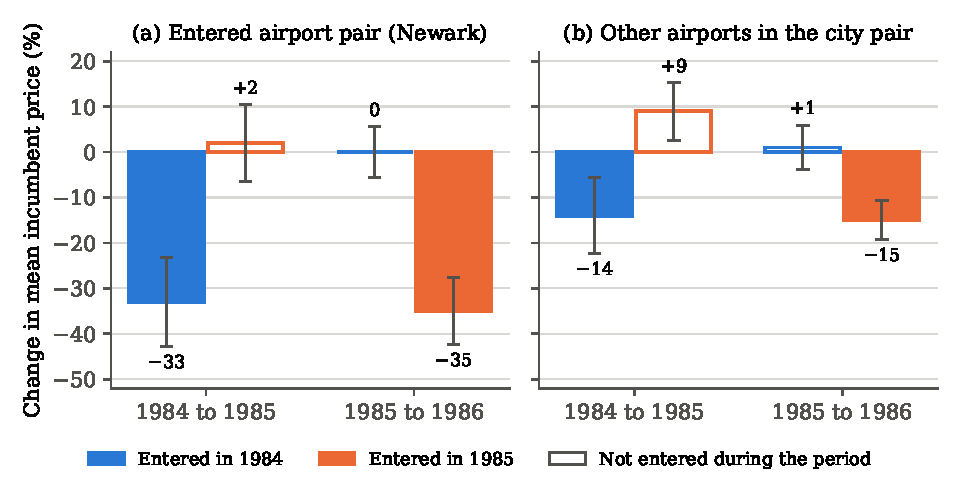
\includegraphics[width=\linewidth]{figures/ch09/wc_did.pdf}
\caption{Percentage change in the mean incumbent price by entry cohort and period. Filled bars are the
cohort entered during the period, and open bars the cohort not entered during it. Whiskers show plus
or minus one standard error of the cohort mean, computed as the reported cross-market standard
deviation divided by $\sqrt{n}$ ($n=7$ and $8$). Redrawn from \citet{WhinstonCollins1992}, Tables~3
and~4.}
\label{fig:09-wc-did}
\end{figure}

\casehead{Prices}
The pattern is similar in the two periods (p.~459). In markets entered during a
year, the mean incumbent price fell by about 35 percent. In markets not entered that year it barely
moved. The two contrasts are $-35$ points each, with $t$ statistics of 2.5 and 3.5. Their equality is
consistent with the three assumptions. So are the 2 percent rise in the 1985 cohort's prices before
its entry and the flat prices of the 1984 cohort in the year after its entry. None of these patterns
confirms the assumptions, because offsetting departures from them reproduce all four changes. Suppose the true
effect is $-25$ points and fades by 10 points in its second year. Suppose also that, without entry,
prices in the 1984 cohort would have fallen 10 points more than in the 1985 cohort in 1984--1985. Let
prices in the 1985 cohort rise 2 points in 1984--1985, as observed. Let all prices fall 10 points in 1985--1986 for reasons unrelated to entry. These values give exactly the
changes $-33$, $+2$, $0$ and $-35$ of Panel~A. Even after the cuts, People Express's average fare in the first
quarter after entry was 19 percent below the incumbents' mean fare.

Price dispersion fell, or rose less, in entered markets. The contrast is larger in 1984--1985 ($-55$
points, $t=2.6$) than in 1985--1986 ($-20$ points, $t=1.0$). The authors speculate that airlines grew
more skilled at \emph{yield management}, the dynamic allocation of seats across fare classes, over the
period. By 1985--1986 an incumbent could target its price
cuts where they mattered most, without lowering all fares.

\casehead{Quantities and revenue}
Incumbents sold more tickets after entry, if anything. The contrasts are $+72$ and $+74$ points, but
the variation across markets is large and neither is significant. Revenue fell much less than the price
cuts alone would imply (n.~34). In 1984--1985, revenue in entered markets rose 21 percent (s.d.\
22) against 33 percent (s.d.\ 28) in markets not entered. In 1985--1986 the figures are 3 percent
(s.d.\ 29) and 10 percent (s.d.\ 16). Revenue understates the incumbents' loss, because carrying more
passengers raises costs and, as we see next, incumbents also added capacity.

\casehead{Capacity}
The authors compared incumbents' nonstop seats on the entered route one year after the announcement
with seats at the announcement, using the \emph{Official Airline Guide}. Seats rose 25 percent on
average (s.d.\ 42). Domestic seats at Newark offered by carriers other than People Express rose 11
percent a year over 1984--1986. That benchmark includes the entered markets, so the comparison
understates the gap (n.~35). Nearly all of the increase came from flight frequency. Seats per
flight rose only 6 percent (s.d.\ 20), against 3 percent at Newark. The capacity increases were larger
for the 1984 cohort, 48 percent (s.d.\ 52), than for the 1985 cohort, 5 percent (s.d.\ 14)
(n.~36).

\casehead{Other airports in the city pair}
Panel~B shows the same pattern on a smaller scale (pp.~460--461). Prices fell 14 and 15 percent
in the treated cohorts, the ``15\%'' the paper quotes, while the control cohorts' prices rose 9 and 1
percent. The contrasts are $-23$ points ($t=2.1$) and $-16$ points ($t=2.3$). Quantity changes are
small and insignificant. Incumbent capacity on these routes rose 1 percent (s.d.\ 30) in the year
after entry, against a 1 percent decline at Kennedy and La Guardia. Seats per flight fell 4 percent
(s.d.\ 9), against a 2 percent decline at those airports, so frequency again rose. Price dispersion
again fell relative to controls, more in 1984 than in 1985. The smaller price response matches the
small $\mathit{OSM}$ value effect. Airports in a city are substitutes, but imperfect ones.

\casehead{Interpretation}
The quantity and capacity responses discriminate among models of competition (p.~460). Under
price taking, each incumbent sells where price equals its marginal cost. Entry lowers the market price
and moves each incumbent down its supply curve, so its output falls. Price cuts together with rising
sales and capacity are hard to square with any simple price-taking model. The rents revealed by the
value losses are therefore not the efficiency rents of a competitive market.

Static oligopoly models predict the same direction as price taking. In symmetric Cournot competition
each firm's output falls when the number of firms rises \eqref{eq:09-cournot-entry}, and by
\cref{rem:09-ks} the same holds for capacities. By \eqref{eq:09-br-slope}, the observed responses fit
static models only if quantities are strategic complements, which requires unusually convex demand.
They are consistent with a dynamic strategy. Industry observers
claimed that incumbents responded aggressively to induce exit, or at least to discourage further
expansion. The larger capacity increases in 1984 fit this interpretation. The responses also show that
the value losses did not reflect a temporary adjustment toward a smaller scale of operations.

The authors add a caution (pp.~458--459). Demand or cost conditions may have changed in the
entered markets, and such changes might even have caused entry. The size of the effects and the view
that the events reflected People Express's own strategy make it plausible that most of the change is
a response to entry.

\subsection{Conclusions, limitations, and contribution}\label{sec:09-wc-concl}

\casehead{What the paper concludes, and where}
\Cref{tab:09-wc-claims} lists each conclusion of the paper with the evidence and the test behind it.
The value results come from the $\mathit{SM}$ rows of \cref{tab:09-wc-t1,tab:09-wc-t2}. The contrast
between airports comes from the $\mathit{OSM}$ rows and the test of equal effects. The general effects
come from the fixed-effect sums. The incumbent responses come from \cref{tab:09-wc-t34} and the
schedule comparisons.

\begin{table}[htbp]
\centering
\caption{Conclusions of Whinston and Collins (1992) and the supporting evidence}
\label{tab:09-wc-claims}
\footnotesize
\begin{tabularx}{\linewidth}{@{}>{\raggedright\arraybackslash}p{0.27\linewidth}
  >{\raggedright\arraybackslash}X >{\raggedright\arraybackslash}p{0.25\linewidth}@{}}
\toprule
Conclusion & Evidence & Test\\
\midrule
Route-specific profits or sunk costs exist, so airline routes are not contestable &
$\lambda_{SM}<0$ in all windows (Table 1) and all specifications (Table 2, SM row). Loss of \$3.7 to
\$6.5 million per incumbent & $t$ tests of $\lambda_{SM}=0$: $-2.98$ to $-3.15$ (Table 1), $-2.18$
(Table 2, column 5)\\
\addlinespace
Local market structure matters, and profits are not equalized across routes &
Incumbency loss survives firm fixed effects. An incumbent loses \$6.2 million versus \$1.9 million
for a non-incumbent (Table 2, column 5) & $t$ test of $\lambda_{SM}$ with fixed effects, fixed-effect
sum\\
\addlinespace
Airports in the same city are differentiated &
$\lambda_{OSM}$ small, positive, insignificant (Table 2, columns 3 to 5) & Test of
$\lambda_{SM}=\lambda_{OSM}$, rejected at 2.5 percent\\
\addlinespace
Large industry-wide effects of unclear origin & Sum of fixed effects $-\$36.2$ million, over 80
percent of industry loss (Table 2, column 5) & Standard error of the sum, quasi-likelihood ratio test
of New York versus other fixed effects\\
\addlinespace
Incumbents cut prices sharply but raised capacity and sales &
Price contrasts of $-35$ points on the entered pair and $-23$ and $-16$ at other airports. Seats $+25$
percent (Tables 3 and 4, schedule data) & Two-sample $t$ tests with 13 degrees of freedom\\
\bottomrule
\end{tabularx}

\smallskip
\parbox{0.97\linewidth}{\footnotesize Notes: Table numbers refer to \citet{WhinstonCollins1992}, reproduced
here as \cref{tab:09-wc-t1,tab:09-wc-t2,tab:09-wc-t34}.}
\end{table}

\casehead{From descriptive results to economic inferences}
The chain of reasoning has three links. The first is statistical. Incumbents' abnormal dollar
changes on announcement days are negative and proportional to their seat-miles on the entered route.
The second is the efficient-markets link. Under (E1) to (E5) the abnormal change equals the change in
expected discounted profits caused by the news. The third is theoretical. By \cref{prop:09-valueloss},
a loss of expected profits from entry implies pre-entry rents or sunk costs, which contestability
excludes. Each richer specification in \cref{tab:09-wc-t2} rules out an alternative reading of the
first link. Slot rents at nearby airports, general industry effects and connecting markets cannot
account for the incumbency loss.

\casehead{Advantages over pricing regressions}
The event study needs no model of the network, and no controls for each route's demand and cost.
The variation comes from the timing of announcements and from incumbents' exposure, which People
Express's strategy determined. The method also measures the level of rents in dollars, as a lower
bound, where a pricing regression delivers a correlation between fares and structure.

\casehead{Limitations}
The design has several limitations, some noted by the authors and some raised by the logic of the
method.
\begin{itemize}
\item The sample is small. There are 24 events on 17 dates, and 22 involve Newark. The general effects
use 19 parameters, and the non-New York effects rest on two events.
\item Dating and anticipation bias the estimates toward zero. People Express's expansion was public
and ongoing, so markets probably expected some entry. Later work on Southwest finds that incumbents cut
fares once entry becomes likely, before the entrant starts flying \citep{GoolsbeeSyverson2008}. News
about entry can therefore arrive well before any announcement.
\item The general effects remain unexplained. Information about People Express's future scale,
competitive spillovers and aircraft values cannot be separated. If informational effects are
correlated with incumbency, part of the $\mathit{SM}$ effect could be informational. The separate New
York effects address this only partly.
\item Entry into a carrier's markets might signal that People Express intended to ``go after'' that
carrier. This informational effect would also load on incumbency. The authors see no way to control for
it without strong assumptions about its form, and they find little evidence of such a pattern (n.~25).
\item Seat-miles measure capacity. They do not count passengers. Connecting traffic is not controlled for, and the
loss per seat is assumed common across routes up to the robustness checks of footnote~32.
\item The bound $L\le V^0+K$ cannot separate pre-entry profits from sunk costs. The value change also
embeds the expected post-entry game, including the incumbents' own aggressive responses.
\item External validity is limited. People Express was a special entrant, with a new low-frill product
and low labor costs, in a transitional period after deregulation.
\item The price and capacity evidence uses 7 and 8 markets, with no formal control for changes in
demand. Only one year precedes the entry of both cohorts. The design therefore cannot separate
differential trends from effects that change after entry, and offsetting departures pass its one
testable restriction. If incumbents moved aircraft from control markets into entered markets, the control group is
affected by entry and the quantity contrasts are overstated.
\end{itemize}

\casehead{Contribution}
\citet{WhinstonCollins1992} gave a market-based test of contestability that does not depend on
controls for route demand and cost. Their incumbency loss confirms the conclusion of the pricing
studies that local structure matters, and it adds a dollar measure of rents. They gave market-based
evidence that airports serving the same city are differentiated, and they documented large
industry-wide effects of entry announcements. Their price and capacity evidence showed incumbents
responding to a low-fare entrant with deep price cuts and more capacity. The abnormal-dollar
formulation, with exposure measures that vary across firms, carries over to event studies of mergers
(\cref{ch:mergers}). \Cref{sec:09-synthesis} compares what this design identifies with the pricing
regressions of \cref{sec:09-borenstein} and the structural model of \cref{sec:09-bcs}.

\section{Hubs, costs, and markups: Berry, Carnall and Spiller (2006)}\label{sec:09-bcs}

\citet{BerryCarnallSpiller2006} bring the question of \cref{sec:09-borenstein} into the framework of
\cref{sec:09-pricing}. On ticket data of the same kind, they estimate a differentiated-products demand
system with two consumer types, a network model of marginal cost and a static Nash pricing equilibrium.
The model separates the two channels through which a hub can change the hub carrier's fares: higher markups
and lower costs. This section follows their analysis from the question to the conclusions, and
\cref{tab:09-bcs-map} at its end maps the study. As throughout the chapter, page, table, figure and footnote numbers refer to the 1996 working paper
\citep{BerryCarnallSpiller1996}.

\subsection{The question}\label{sec:09-bcs-question}

\Cref{sec:09-hubs} described the two views of hubs that coexisted by the mid-1980s. Critics held that hubs
raise entry barriers and fares for passengers who start their trips at a hub. Carriers and some economists
held that hubs reduce costs. The two effects are not mutually exclusive \citep{Berry1990}. A hub can raise
the markup over marginal cost for some travelers and lower marginal cost at the same time. On the demand
side, Berry, Carnall and
Spiller think of a hub as shifting out the demand for the hubbing carrier's flights out of its hub city.
Those flights may appeal especially to price-inelastic consumers, so the shift can also make demand less
elastic (p.~1). On the cost side, densely traveled spokes may have lower marginal costs. Economies of spoke
density then create economies of scope across itineraries that share a spoke (p.~2).

A fare regression cannot separate the two effects. Write the fare of product $j$ as $p_j=mc_j+m_j$, with
$m_j$ the markup. If hub presence raises $m_j$ and lowers $mc_j$, the change in the fare is
\begin{equation*}
\Delta p_j=\Delta m_j+\Delta mc_j,\qquad \Delta m_j>0,\quad \Delta mc_j<0 .
\end{equation*}
A regression of fares on hub presence estimates the sum. Without a model of markups or of costs it cannot
recover the two terms. As the authors note, \citet{Borenstein1989} has no model of costs or demand. In
their words, he ``attempts to control for market-level unobservables by, for example, introducing
city-pair level fixed effects'' (p.~5). His relative-price equation \eqref{eq:09-bor-rel} has the same
effect, since it differences out everything common to the carriers on an airport-pair route.
\citet{BruecknerSpiller1994} take the
opposite route. They estimate density economies from itineraries that pass through hubs without
originating there, to avoid hub markups (p.~4). That choice discards the markets where hub effects should
be largest. In the authors' words, reduced form regressions ``do not allow us to make statements about how
prices relate to costs, or what are the determinants of markups over cost'' (p.~6).

The strategy of the paper is to treat hub presence as one characteristic in a differentiated-products
model of demand. Combined with a cost model and an equilibrium assumption, the demand model yields a
markup for every product. Marginal cost is then ``observed'' as price minus the model's markup (p.~5), and
its relation to spoke density reveals economies of density. The model is the finite-mixture nested logit
of \cref{sec:09-pricing-types} with $R=2$ types, combined with the network costs of
\cref{sec:09-pricing-network}. The authors summarize their findings in five claims (abstract and
pp.~2--3), which we examine against their tables below.
\begin{enumerate}[label=(\roman*)]
  \item Travelers come in two distinct types. One has the attributes of a tourist: high price sensitivity
  and low willingness to pay for frequent-flyer features, frequency and nonstop service. The other has
  those of a business traveler.
  \item Hubs give the hub carrier two advantages: lower costs and higher markups on hub-originating
  passengers.
  \item The hub carrier's ability to raise prices is focused on business travelers. They shift toward the
  hub carrier even though they pay a premium of about 20\% over non-hub carriers.
  \item The hub carrier does not provide a ``monopoly umbrella'' to its rivals. Non-hub carriers lose
  business travelers and market share at the same time, which the authors call a ``competitive scissor.''
  \item There are economies of density on longer routes and none on routes shorter than about 500 miles,
  which the authors call the ``Southwest effect.''
\end{enumerate}

\subsection{Data}\label{sec:09-bcs-data}

The data come from the DOT ticket sample (DB1A) and the Service Segment Databank (DB27R) described in
\cref{sec:09-data}, for the fourth quarter of 1985 (p.~19). The quarter follows \citet{BruecknerDyerSpiller1992}
and \citet{BruecknerSpiller1994}. Those studies used only four-segment round trips that did not originate at
hub cities, to avoid demand-side hub effects. Berry, Carnall and Spiller model hub markups explicitly, so
they keep hub origins and itineraries with any number of segments up to two per direction. The ticket
conventions are those of \cref{sec:09-data}: round trips only, without itineraries chosen by a single
sampled passenger and without extreme fares. Southwest is absent, because it reported all its sales as one-way
tickets and so did not fit the product definition (p.~14, n.~11). The quarter precedes the merger wave of
1986--1987 and Borenstein's sample from 1987.

The unit of observation is a \emph{product} $j$, a unique combination of carrier, itinerary and fare in a
directional city-pair market $t$ (\cref{sec:09-data}). The sample has 122,871 products in 14,122 markets.
The products use 4,963 distinct carrier legs, flown by 32 carriers out of 262 origins, and represent
1,107,894 sampled passengers (p.~19). About 30\% of the markets have a single product and another 30\% have
no more than five. About 1\% have more than one hundred products, with a maximum of 874 in the New York to
Miami market. The quantity $q_{jt}$ is the number of sampled passengers (NPASS) and the price $p_{jt}$ is
the round-trip fare (FARE). Market size is built from $\mathit{MPOP}_t$, the geometric mean of the two
endpoint populations, $\sqrt{\text{origin population}\times\text{destination population}}$ (Appendix). A
\emph{leg} $\ell$ is a nonstop segment flown by one carrier. Its density $Q_\ell$ comes from DB27R and
adds the two directions, because the trips are round trips (Appendix, n.~4).

A structural model has more than one dependent variable. Each product contributes two endogenous outcomes,
its market share and its fare, and leg densities are endogenous as well. The inversion of demand turns the
share into the demand error $\xi_{jt}$. The pricing condition turns the fare into the cost error
$\omega_{jt}$. The regressors are the product and market characteristics in \cref{tab:09-bcs-vars} and the
leg cost terms. The instruments are discussed in \cref{sec:09-bcs-estimation}.

\begin{table}[htbp]
\centering
\begin{threeparttable}
\caption{Variables in the model of Berry, Carnall and Spiller}
\label{tab:09-bcs-vars}
\footnotesize
\begin{tabularx}{\textwidth}{@{}>{\raggedright\arraybackslash}p{2.2cm}>{\raggedright\arraybackslash}X
  >{\raggedright\arraybackslash}p{2.6cm}@{}}
\toprule
Variable & Definition (units) & Role \\
\midrule
\multicolumn{3}{@{}l}{\textit{Demand side (product $j$ of carrier $f$ in market $t$)}}\\
FARE & Round-trip fare (\$100) & Type-specific ($\alpha_r$) \\
DIRECT & 1 if the itinerary has one segment, 0 if it has two & Type-specific \\
HUBSIZE & If the origin is a hub of carrier $f$: the sum of the population potentials of all city pairs
  that $f$ connects through that hub. Zero otherwise & Type-specific \\
TEMPDIFF & Difference between the mean January temperatures of origin and destination (10\textdegree F) &
  Type-specific, market level \\
TRIPS-D & Minimum over the itinerary's legs of $f$'s departures on the leg (1,000 per quarter) &
  Type-specific \\
CONSTANT & 1 & Common \\
CONGEST-D & Number of endpoints (0, 1 or 2) that are slot controlled & Common, market level \\
MDIST, MDIST$^2$ & Great-circle distance between the endpoints (1,000 miles), and its square & Common, market
  level \\
\addlinespace
\multicolumn{3}{@{}l}{\textit{Cost side (summed over the legs $\ell\in\mathcal{L}(j)$ of the itinerary)}}\\
NSEGS & Number of legs (1 or 2) & Leg constant \\
CONGEST-S & Takeoffs and landings at the four slot-controlled airports (0 to 4) & Leg cost shifter \\
CONGEST-C & Takeoffs and landings at the 24 airports under FAA flow control (0 to 4) & Leg cost shifter \\
DIST, DENS & Leg distance $d_\ell$ (1,000 miles) and leg density $Q_\ell$ (100,000 passengers per quarter,
  both directions), with powers and interactions & Cubic polynomial \\
TRIPS-C & Leg departures $F_\ell$ (1,000 per quarter) & Column IV only \\
\bottomrule
\end{tabularx}
\begin{tablenotes}\footnotesize
\item Notes: The population potential of a city pair is the geometric mean of the two populations. The
slot-controlled airports are Chicago O'Hare, New York Kennedy and La Guardia, and Washington National
(p.~20, n.~13). The flow-control list includes Orange County and Long Beach (p.~21, n.~14). The text calls
the slot-control count CONGEST-C and the flow-control count DOT-CONGEST, while Tables 3 and 5 label the
cost-side congestion variables CONGEST-S and CONGEST-C. We match the labels by their sample means in
Table~3 (0.315 and 1.766), which equal the appendix means of the slot-control count (0.3149) and of the
flow-control count (1.7656). Source: \citet{BerryCarnallSpiller1996}, pp.~20--21 and Appendix.
\end{tablenotes}
\end{threeparttable}
\end{table}

\Cref{tab:09-bcs-desc} reproduces the descriptive statistics. The mean round-trip fare is \$276 with a
standard deviation of \$149. The number of sampled passengers per product has mean 9.0, standard deviation
31.3 and maximum 2,798, so most products are bought by very few sampled passengers. This fact matters for
the sampling error discussed in \cref{sec:09-bcs-estimation}. Slightly fewer than half of the products
(46.6\%) have a single segment. HUBSIZE is zero for most products, with mean 0.017 and standard deviation
0.045. Second-leg distances and densities are set to zero for one-segment products (p.~21), which explains
their low means. In the appendix statistics the means of DIRECT and NSEGS are 0.4666602 and 1.5333398,
which sum to exactly two, and their standard deviations are identical. In this sample DIRECT therefore
equals $2-\mathit{NSEGS}$, so ``direct'' means a single segment.

\begin{table}[htbp]
\centering
\begin{threeparttable}
\caption{Descriptive statistics, 122,871 origin-destination-fare-carrier products}
\label{tab:09-bcs-desc}
\small
\begin{tabular}{@{}lrrrr@{}}
\toprule
Variable & Mean & Std.\ dev. & Min & Max \\
\midrule
FARE (\$100) & 2.764 & 1.488 & 0.110 & 18.33 \\
NPASS (passengers) & 9.017 & 31.299 & 1.000 & 2798.0 \\
DIRECT (fraction) & 0.466 & 0.498 & 0.000 & 1.000 \\
HUBSIZE & 0.017 & 0.045 & 0.000 & 0.210 \\
TEMPDIFF (10\textdegree F) & 0.286 & 2.077 & $-6.520$ & 6.520 \\
TRIPS-D (minimum, 1,000 per quarter) & 0.293 & 0.179 & 0.001 & 1.595 \\
CONGEST-D (number of airports) & 0.202 & 0.413 & 0.000 & 2.000 \\
MDIST (1,000 miles) & 1.009 & 0.608 & 0.030 & 2.776 \\
\addlinespace
DIST, first outbound leg (1,000 miles) & 0.710 & 0.503 & 0.021 & 2.704 \\
DIST, second outbound leg (1,000 miles) & 0.351 & 0.479 & 0.000 & 2.611 \\
DENS, first outbound leg (100,000 per quarter) & 0.593 & 0.475 & 0.00003 & 4.553 \\
DENS, second outbound leg (100,000 per quarter) & 0.361 & 0.493 & 0.000 & 4.553 \\
TRIPS-C, first leg (1,000 departures per quarter) & 0.349 & 0.214 & 0.001 & 1.595 \\
TRIPS-C, second leg (1,000 departures per quarter) & 0.212 & 0.249 & 0.000 & 1.594 \\
\bottomrule
\end{tabular}
\begin{tablenotes}\footnotesize
\item Notes: Statistics across products. Second-leg values are zero for one-segment products.
Source: \citet{BerryCarnallSpiller1996}, Table~1.
\end{tablenotes}
\end{threeparttable}
\end{table}

The raw correlations among the endogenous variables point the wrong way for a naive test of density
economies (Table~2). Price is positively correlated with the densities of the first and second outbound legs
(0.084 and 0.122). Price and the number of passengers are negatively correlated ($-0.063$). The number of
passengers is correlated with the first-leg density at 0.068 and with the second-leg density at $-0.120$,
and the two densities are correlated at 0.164. The authors read the positive price-density correlations as
evidence that one must control for markups and distance before economies of density can appear (p.~21). One
reason is that dense legs connect large cities and hubs, where demand and markups may be high. In a
subsample of small four-segment markets, the sampling frame of Brueckner and Spiller, the raw correlation
between price and density is negative (p.~21, n.~15).

\subsection{Demand}\label{sec:09-bcs-demand}

\casehead{Market size}
The model needs an outside good, and hence a number of potential trips in each market. Berry, Carnall and
Spiller assume that this number is proportional to the geometric mean of the endpoint populations,
$M_t=\kappa\,\mathit{MPOP}_t$, with $\kappa$ a parameter to be estimated (p.~9). Each potential trip is
treated as a separate consumer, with no correlation of tastes across trips by the same person. The
observed shares are therefore functions of $\kappa$:
\begin{equation}\label{eq:09-bcs-sobs}
s^{obs}_{jt}(\kappa)=\frac{q_{jt}}{\kappa\,\mathit{MPOP}_t},\qquad
s^{obs}_{0t}(\kappa)=1-\sum_{j\in\mathcal{J}_t}s^{obs}_{jt}(\kappa).
\end{equation}
Because $q_{jt}$ counts passengers in a 10\% sample, $\kappa$ also absorbs the sampling rate.

\casehead{Unobserved product characteristics}
The term $\xi_{jt}$ captures ticket restrictions, such as advance-purchase and Saturday-stay requirements,
together with unmeasured quality such as food and service (p.~9). Firms and consumers observe it. Tickets
with different restrictions have systematically different prices, so $\xi_{jt}$ is correlated with price
by construction and price is endogenous. The authors assume instead that $\xi_{jt}$ is mean independent of
the other observed characteristics, such as distance and DIRECT. They defend this assumption with an
extreme case. Suppose every carrier offers the same menu of restrictions on every itinerary, for example
an unrestricted fare, an advance-purchase fare with a Saturday stay, and an advance-purchase fare without
one. Then the restrictiveness of a ticket is unrelated to $x_{jt}$. The authors concede that ``it is not
hard to think of stories which would violate'' the assumption (p.~9). A hub carrier that sells relatively
more unrestricted fares out of its hub would be one such story, since $\xi_{jt}$ would then rise with
HUBSIZE.

\casehead{Utility}
A potential traveler $i$ in market $t$ is of type $r\in\{1,2\}$, with $\Pr(r=1)=\psi$ and $\Pr(r=2)=1-\psi$.
In the notation of \cref{ass:09-fm}, a type-$r$ traveler has utility
\begin{equation}\label{eq:09-bcs-utility}
u_{ijt}=\delta^r_{jt}+\zeta_{igt}+(1-\sigma)\epsilon_{ijt}\quad(j\in\mathcal{J}_t),\qquad
u_{i0t}=\epsilon_{i0t},
\end{equation}
with type-specific mean utility
\begin{equation}\label{eq:09-bcs-delta-r}
\begin{aligned}
\delta^r_{jt}={}&\beta_0+\beta^{M}\mathit{MDIST}_t+\beta^{MM}\mathit{MDIST}_t^2+\beta^{C}\mathit{CONGEST\text{-}D}_t\\
&+\beta^{D}_r\mathit{DIRECT}_j+\beta^{h}_r\mathit{HUBSIZE}_{jt}+\beta^{T}_r\mathit{TEMPDIFF}_t
+\beta^{F}_r\mathit{TRIPS\text{-}D}_j-\alpha_rp_{jt}+\xi_{jt}.
\end{aligned}
\end{equation}
All inside goods form one nest and the outside good forms the other. Berry, Carnall and Spiller write the
idiosyncratic term as $\nu_i(\lambda)+\lambda\epsilon_{ij}$ (p.~11). In our notation $\lambda=1-\sigma$,
their $\nu_i(\lambda)$ is $\zeta_{igt}$, their type-1 probability $\gamma$ is $\psi$, and their market-size
factor $\mu$ is $\kappa$. As $\sigma\to0$ the choices within a market become uncorrelated and the model
reduces to a mixture of two logits. As $\sigma\to1$ the correlation of choices within the market goes to
one (p.~12).

\casehead{Shares}
Specializing \eqref{eq:09-fm-shares} to two types, the shares of a type-1 traveler are (p.~12)
\begin{equation}\label{eq:09-bcs-shares}
s^1_{j|g,t}=\frac{e^{\frac{\delta^1_{jt}}{1-\sigma}}}{D_{1t}},\qquad
D_{1t}=\sum_{k\in\mathcal{J}_t}e^{\frac{\delta^1_{kt}}{1-\sigma}},\qquad
\bar s_{1t}=\frac{D_{1t}^{1-\sigma}}{1+D_{1t}^{1-\sigma}},\qquad
s^1_{jt}=s^1_{j|g,t}\,\bar s_{1t},
\end{equation}
and the type-2 shares have the same form with $\delta^2_{jt}$. The predicted share of product $j$ is the
type-weighted average
\begin{equation}\label{eq:09-bcs-sj}
s_{jt}=\psi\,s^1_{jt}(p_t,x_t,\xi_t)+(1-\psi)\,s^2_{jt}(p_t,x_t,\xi_t).
\end{equation}

\casehead{Why two types}
\Cref{sec:09-pricing-types} gave the reasons why business travelers are less sensitive to price than
leisure travelers and why tastes are correlated across characteristics (p.~10, n.~9). A two-point
distribution is the simplest
bimodal distribution with correlated tastes (p.~10). The fat upper tail of fares per mile discussed in
\cref{sec:09-data} supports it. A mixture of two normal distributions fits that distribution far better than a
single normal. The authors compare the two components of that mixture with the estimated
model (p.~11, n.~10). The components are $N(0.2375, 0.0781)$ and $N(0.5946, 0.2752)$, so the second is
also far more dispersed. The model's mean fare per mile for type 1, 0.237, equals the mean of the first
component (0.2375). For type 2 the model gives 0.414, against 0.589 from the mixture.\footnote{The fitted
formula in footnote~10 gives the second component a mean of 0.5946, while the comparison in the same
footnote quotes 0.589. Likewise, the weight on the first component is 0.5987 in the formula and 0.598 in
the comparison. We report all four numbers as printed.} Type 1 accounts for 73\% of tickets in the model,
against a weight of 0.598 in the mixture. Five coefficients vary by type: those on FARE, DIRECT, HUBSIZE,
TEMPDIFF and TRIPS-D. By \cref{rem:09-discrete-rc}, two types need 11 parameters for these five
coefficients, against 10 for independent normal random coefficients, and they deliver closed-form shares.
The authors mention extensions they do not pursue (p.~11). Tastes could be drawn from two normal
distributions instead of two points, there could be more than two types, and nests could group airports
within a city or carriers within a market.

\casehead{The role of each characteristic}
The constant, MDIST, MDIST$^2$, CONGEST-D and TEMPDIFF are the same for every product in a market. They
shift the demand for air travel relative to the outside good (p.~20). They also cancel from each type's
within-nest shares $s^r_{j|g,t}$ in \eqref{eq:09-bcs-shares}. At given prices they therefore leave the
choice among flights of a traveler of either type unchanged. The paper concludes that TEMPDIFF ``has no
power to explain the choice between products'' (p.~20). This holds within a type. Aggregate shares can
still move, because these variables change the mix of types among the travelers who fly. By
\eqref{eq:09-bcs-sj}, the share of product $j$ among the inside goods is
\begin{equation*}
\frac{s_{jt}}{\sum_{k\in\mathcal{J}_t}s_{kt}}=\sum_{r=1}^{2}w_{rt}\,s^r_{j|g,t},\qquad
w_{1t}=\frac{\psi\,\bar s_{1t}}{\psi\,\bar s_{1t}+(1-\psi)\,\bar s_{2t}},\qquad w_{2t}=1-w_{1t},
\end{equation*}
where $w_{rt}$ is the share of type $r$ among the travelers who fly. A change in a market-level variable
leaves each $s^r_{j|g,t}$ fixed and moves the weights. If it raises every type-$r$ mean utility by $c_r$,
then $\frac{\partial\ln\bar s_{rt}}{\partial c_r}=1-\bar s_{rt}$. The weights therefore change when the
coefficient differs across types, as for TEMPDIFF. They also change under a common coefficient whenever
the two types' inside shares differ. The aggregate choice among flights then shifts toward the flights
that the type gaining weight prefers. DIRECT, HUBSIZE and TRIPS-D vary across carriers and itineraries within a market,
so they also govern substitution among flights within each type. HUBSIZE weights each city pair the carrier connects through its hub by
the pair's population potential. The authors prefer it to a hub dummy or to the number of points served,
neither of which accounts for the relative importance of the city pairs (p.~20). TEMPDIFF measures appeal to
tourists. Because its coefficient varies by type, it shifts the type mix and can help separate the types
(p.~20).

The model lets hub presence affect markups through the composition of buyers. By \eqref{eq:09-composition},
product $j$'s buyers are of type 2 with probability $\Pr(2\mid j)=\frac{(1-\psi)s^2_{jt}}{s_{jt}}$. By
\cref{prop:09-composition-markup} and \cref{rem:09-fm-extensions}, a single-product markup is close to
$\frac{1-\sigma}{\bar\alpha_j}$ when within-nest shares are small, where
$\bar\alpha_j=\Pr(1\mid j)\alpha_1+\Pr(2\mid j)\alpha_2$. If $\beta^h_2>\beta^h_1$ and $\alpha_2<\alpha_1$,
a larger HUBSIZE tilts the buyers of the hub carrier's products toward type 2, lowers $\bar\alpha_j$ and
raises the markup. Because $\Pr(2\mid j)$ is a logistic function of $\ln s^2_{jt}-\ln s^1_{jt}$, its shift
is proportional to $\Pr(2\mid j)\big(1-\Pr(2\mid j)\big)$ and is largest near an even mix. The markup
$\frac{1-\sigma}{\bar\alpha_j}$ is convex in $\Pr(2\mid j)$, however. With the column III price coefficients,
the markup response is largest for products whose buyers are already about 90\% type 2.

\subsection{Costs and pricing}\label{sec:09-bcs-supply}

\casehead{Leg costs and product marginal cost}
The cost side follows \citet{BruecknerSpiller1994}, as in \cref{sec:09-pricing-network}. Leg $\ell$ of carrier
$f$ has total cost $C_\ell(Q_\ell,w_\ell)$ and marginal cost $c_\ell(Q_\ell,w_\ell)$, where $w_\ell$
includes the leg's distance and the characteristics of its endpoint airports (p.~13). The carrier's cost is
\eqref{eq:09-firm-cost}, and the marginal cost of product $j$ is \eqref{eq:09-itin-mc}, the sum of its legs'
marginal costs plus a product-specific term $\omega_{jt}$. The authors give the product-specific cost the
form $\omega_{jt}q_{jt}$ only so that marginal cost has an additive error (p.~13). Fixed costs may also fall
with hubbing, but the model uses only marginal costs and cannot capture that effect.

\casehead{Prior beliefs about distance, density and frequency}
The authors expect a complicated relation among distance, density and flight frequency (pp.~13--14). On short
routes air travel competes with cars and, in a few places, trains. Carriers may then spend density savings
on more frequent flights, which let travelers choose departure times precisely. The East and West Coast
shuttles and Southwest are examples. On short routes large aircraft may also not pay, because takeoffs and
landings are a large share of cost. That cost does not vary with distance and is not offset by savings in
the air. The data have no model of frequency but do report quarterly trips on each leg. Frequency enters
some specifications as an exogenous cost shifter. These considerations call for a flexible functional form.

\casehead{The leg marginal cost function}
Segment marginal cost is a cubic polynomial in leg distance $d_\ell$ (1,000 miles) and leg density $Q_\ell$
(100,000 passengers per quarter), with congestion shifters. Write $\chi_{mn}$ for the coefficient on
$d_\ell^mQ_\ell^n$, and $n^S_\ell$ and $n^C_\ell$ for the leg's takeoffs and landings at slot-controlled and
at flow-control airports. In columns I to III of Table~5, leg marginal cost in \$100 is
\begin{equation}\label{eq:09-bcs-mc}
\begin{aligned}
c_\ell={}&\chi_{00}+\chi_{10}d_\ell+\chi_{20}d_\ell^2+\chi_{30}d_\ell^3
+\chi_{01}Q_\ell+\chi_{02}Q_\ell^2+\chi_{03}Q_\ell^3\\
&+\chi_{11}d_\ell Q_\ell+\chi_{21}d_\ell^2Q_\ell+\chi_{12}d_\ell Q_\ell^2
+\chi_S n^S_\ell+\chi_C n^C_\ell .
\end{aligned}
\end{equation}
Column IV adds nine terms in leg departures $F_\ell$ (1,000 per quarter):
\begin{equation}\label{eq:09-bcs-mc-trips}
\sum_{k=1}^{9}\chi^F_k\,h_k(F_\ell,d_\ell,Q_\ell),\qquad
(h_1,\dots,h_9)=(F,\,F^2,\,F^3,\,Fd,\,Fd^2,\,F^2d,\,FQ,\,F^2Q,\,FQ^2),
\end{equation}
with the leg subscripts dropped inside the list. Summing \eqref{eq:09-bcs-mc} over the legs of product $j$,
\begin{equation}\label{eq:09-bcs-mc-product}
mc_{jt}=\chi_{00}\,\mathit{NSEGS}_j+\chi_{10}\sum_{\ell\in\mathcal{L}(j)}d_\ell
+\dots+\chi_{12}\sum_{\ell\in\mathcal{L}(j)}d_\ell Q_\ell^2
+\chi_S\,\mathit{CONGEST\text{-}S}_j+\chi_C\,\mathit{CONGEST\text{-}C}_j+\omega_{jt}.
\end{equation}
The leg constant summed over legs becomes the coefficient on the number of segments. The mean of
$\omega_{jt}$, written $\bar\omega$, enters as a separate constant in product marginal cost (p.~21). Table~5
does not report it. Because NSEGS takes the values 1 and 2, $\bar\omega$ and $\chi_{00}$ are separately
identified.

Economies of density on leg $\ell$ mean that the leg's marginal cost falls as its density rises. From
\eqref{eq:09-bcs-mc},
\begin{equation}\label{eq:09-bcs-dcdq}
\frac{\partial c_\ell}{\partial Q_\ell}=\chi_{01}+2\chi_{02}Q_\ell+3\chi_{03}Q_\ell^2
+\chi_{11}d_\ell+\chi_{21}d_\ell^2+2\chi_{12}d_\ell Q_\ell ,
\end{equation}
and the leg has economies of density at $(d_\ell,Q_\ell)$ when this derivative is negative. In
\cref{ex:09-hubcost} the leg cost $aQ^\gamma$ has economies of density everywhere when $\gamma<1$. The
polynomial lets the sign vary with distance and density.

\casehead{What the cost model leaves out}
Prices, shares and densities are endogenous. Flight frequency is treated as exogenous. The data aggregate
traffic to the carrier, route and fare over a quarter, so they cannot show which flights are full or how
uncertainty about demand resolves before departure. The model therefore has no capacity constraints and no
demand uncertainty. The authors warn that ``some of what we label as a markup in fact represents a shadow
price of capacity'' (p.~14). Marginal cost may also vary with factors such as time-of-day capacity, which
the data do not record (p.~5).

\casehead{Pricing}
Following \citet{Berry1990}, prices form a static Nash equilibrium in which each carrier sets the prices of
all its products in all markets (pp.~6 and 14). The authors recognize that this is a simplification. Yield
management allocates seats across fare classes dynamically, and tacit collusion would add another layer,
but both are left for future work (p.~15). In the notation of \cref{sec:09-pricing-network}, carrier $f$'s
profit is (p.~15)
\begin{equation}\label{eq:09-bcs-profit}
\pi_f=\sum_t\ \sum_{j\in\mathcal{J}_f(t)}p_{jt}\,q_{jt}(p)-\sum_{\ell\in\mathcal{L}_f}C_\ell(Q_\ell,w_\ell)
-\sum_t\ \sum_{j\in\mathcal{J}_f(t)}\omega_{jt}\,q_{jt}(p)-FC_f .
\end{equation}
Differentiating with respect to $p_{jt}$ and exchanging the sums over legs and products, as in the
derivation of \eqref{eq:09-network-foc}, gives
\begin{equation}\label{eq:09-bcs-foc}
q_{jt}+\sum_{k\in\mathcal{J}_f(t)}\frac{\partial q_{kt}}{\partial p_{jt}}
\Big[p_{kt}-\omega_{kt}-\sum_{\ell\in\mathcal{L}(k)}c_\ell(Q_\ell,w_\ell)\Big]
=q_{jt}+\sum_{k\in\mathcal{J}_f(t)}\frac{\partial q_{kt}}{\partial p_{jt}}\,(p_{kt}-mc_{kt})=0 .
\end{equation}
Dividing by $M_t=\kappa\,\mathit{MPOP}_t$ turns quantities into shares. Stacking the conditions of market $t$
gives \eqref{eq:09-fm-markup}:
\begin{equation}\label{eq:09-bcs-markup}
p_t-mc_t=-\big[(\Omega_t\odot\Delta_t)^\top\big]^{-1}s_t,\qquad
\Delta_t=-\psi\,\alpha_1\frac{\partial s^1_t}{\partial\delta^1_t}-(1-\psi)\,\alpha_2\frac{\partial s^2_t}{\partial\delta^2_t},
\end{equation}
where the $(j,k)$ element of $\frac{\partial s^r_t}{\partial\delta^r_t}$ is given by
\eqref{eq:09-fm-derivs}.\footnote{The paper writes $p=\Delta^{-1}s+mc$ with $\Delta$ the matrix of
derivatives $\frac{\partial s_k}{\partial p_j}$ for products of the same firm (p.~15). That equation holds
when $\Delta$ contains the negatives of these derivatives. The paper's second expression,
$\Delta=\gamma\alpha_1\Delta_1+(1-\gamma)\alpha_2\Delta_2$ with $\Delta_r$ the derivatives with respect to
mean utility (p.~16), has the right sign. It equals $-(\Omega_t\odot\Delta_t)^\top$ in our notation. See
the footnote to \eqref{eq:09-fm-markup}.} Here $\Delta_t$ has $(j,k)$ element
$\frac{\partial s_{jt}}{\partial p_{kt}}$, as in \cref{ch:diffprod}.

Three features of \eqref{eq:09-bcs-markup} drive the empirical work. First, the markup depends only on the
demand parameters and on prices and shares (p.~16). It involves no cost parameter. Second, markups are not
profits. Airlines may be unprofitable even with large markups, because fixed costs may be large and marginal
cost may fall over a wide range of output (p.~16, \cref{rem:09-markups-profits}). Third, the network enters
the pricing condition only through the level of each $mc_{kt}$, evaluated at equilibrium densities.

\subsection{Estimation and identification}\label{sec:09-bcs-estimation}

\casehead{The estimator}
The parameters split into demand and cost parameters:
\begin{equation*}
\theta_d=(\sigma,\kappa,\psi,\alpha_1,\alpha_2,\beta_1,\beta_2),\qquad
\theta_c=(\bar\omega,\chi),\qquad \theta=(\theta_d,\theta_c).
\end{equation*}
Here $\beta_r$ collects type $r$'s taste coefficients, including the common
ones. The estimator follows \citet{Berry1994} and \citet{BerryLevinsohnPakes1995} (pp.~16--17). For a trial
value of $\theta$ it computes the two structural errors in five steps.
\begin{enumerate}[label=\arabic*.]
  \item Compute observed shares $s^{obs}_t(\kappa)$ from \eqref{eq:09-bcs-sobs}.
  \item Solve $s_t(\xi_t;\theta_d)=s^{obs}_t(\kappa)$ for $\xi_t(\theta_d)$ in each market, with the
  contraction \eqref{eq:09-fm-contraction}. \citet{Berry1994} guarantees a unique solution. The shares
  \eqref{eq:09-bcs-shares} and \eqref{eq:09-bcs-sj} are analytic, so no simulation is needed. With
  122,871 products the authors call this ``fortunate'' (p.~17).
  \item Evaluate $\Delta_t$ at $(p_t,\xi_t(\theta_d))$ and compute the markups
  $b_t(\theta_d)=-\big[(\Omega_t\odot\Delta_t)^\top\big]^{-1}s_t$ from \eqref{eq:09-bcs-markup}.
  \item Compute the cost error from \eqref{eq:09-bcs-mc-product}, with the observed densities as data:
  \begin{equation}\label{eq:09-bcs-omega}
  \tilde\omega_{jt}(\theta)=p_{jt}-b_{jt}(\theta_d)-\bar\omega-\sum_{\ell\in\mathcal{L}(j)}c_\ell(d_\ell,Q_\ell,n^S_\ell,n^C_\ell;\chi).
  \end{equation}
  \item Form the moments below and evaluate the objective.
\end{enumerate}
The identifying assumption is that both errors are mean independent of a vector of instruments $z_{jt}$:
\begin{equation}\label{eq:09-bcs-moments}
\E\left[\xi_{jt}(\theta_{d0})\given z_{jt}\right]=0,\qquad \E\left[\tilde\omega_{jt}(\theta_0)\given z_{jt}\right]=0 .
\end{equation}
With $N=122{,}871$ products and instrument matrices $Z^d_{jt}$ and $Z^c_{jt}$ built from $z_{jt}$, the
sample moments and the GMM estimator are
\begin{equation}\label{eq:09-bcs-gmm}
g_N(\theta)=\frac{1}{N}\sum_t\sum_{j\in\mathcal{J}_t}
\begin{pmatrix}Z^{d\top}_{jt}\,\xi_{jt}(\theta_d)\\ Z^{c\top}_{jt}\,\tilde\omega_{jt}(\theta)\end{pmatrix},
\qquad
\hat\theta=\argmin_\theta\ g_N(\theta)^\top W g_N(\theta),
\end{equation}
as in \cref{ch:blp}. Given $\theta_d$, the cost error is linear in $(\bar\omega,\chi)$. These parameters can
therefore be concentrated out by linear instrumental variables, like the linear parameters in
\cref{ch:blp}. The paper does not say how the search was organized.

\casehead{Instruments}
Price, shares and densities are endogenous. All other product and market characteristics are treated as
exogenous shifters of cost or demand, including the network structure of each carrier (pp.~17--18). The
instruments for leg densities include population and network characteristics at the endpoint cities. The
instruments for prices and markups add characteristics of the other products in the market (p.~18). The
authors chose the instrument vector by experimenting with simple versions of the model on a 10\% sample of
the data and then held it fixed for the full estimation (p.~18). The full list is not reported.

Each group of instruments rests on an economic argument. A product's own characteristics shift its demand
and, through the share, its markup. Rival products' characteristics shift the markup through the intensity
of competition, as in \citet{BerryLevinsohnPakes1995}. Population and network characteristics at the
endpoints shift a leg's density through traffic to and from other markets. Conditional on the included
characteristics, they are excluded from the product's own demand and cost errors. That exclusion requires
the network to be exogenous. If carriers built hubs where unobserved demand is high, network instruments
would be correlated with $\xi$. The paper does not model entry or network choice and refers to
\citet{Berry1990} and \citet{ReissSpiller1989} for that problem (p.~16, n.~12).

\casehead{Standard errors}
The errors are assumed independent across markets (p.~17). Within a market, demand and cost errors have a
factor structure, with market-specific components that are correlated across the demand and cost
equations. One parametrization consistent with this description is
\begin{equation}\label{eq:09-bcs-factor}
\xi_{jt}=a_t+e_{jt},\qquad \tilde\omega_{jt}=b_t+u_{jt},\qquad \Cov(a_t,b_t)\ne0,
\end{equation}
with $e_{jt}$ and $u_{jt}$ idiosyncratic. The structure enters the variance of the moments,
$V=\Var\big(\sum_{j\in\mathcal{J}_t}g_{jt}\big)$ summed over independent markets, where $g_{jt}$ is the
summand of \eqref{eq:09-bcs-gmm}. The asymptotic variance of $\hat\theta$ is then the usual sandwich
$(G^\top WG)^{-1}G^\top WVWG(G^\top WG)^{-1}$, with $G$ the derivative of the moments
(\cref{sec:A-gmm}). Treating each market as a cluster would be the nonparametric alternative.

\casehead{Sampling error in shares}
The inversion assumes that the econometrician observes expected shares \citep{Berry1994}. In
\citet{BerryLevinsohnPakes1995} shares were fractions of roughly 100 million households, so sampling error
was negligible. Here more than one million sampled passengers are spread over more than 120,000 products,
so the average product has fewer than 10 sampled passengers (p.~17). A rough calculation shows the
magnitude. If a product's sampled count $\hat n_j$ has mean $n_j$ and approximately Poisson variation, the
delta method gives $\Var(\ln\hat n_j)\approx\frac{1}{n_j}$. The standard deviation of the log share is then
about 0.33 at $n_j=9$ and 0.71 at $n_j=2$. By the derivative in the proof of
\cref{lem:09-fm-contraction}, $\frac{\partial\ln s_j}{\partial\xi_j}$ lies between $1-\max_r\bar s_r$ and
$\frac{1}{1-\sigma}$. It is close to one for the only product in a market, the case of about 30\% of markets
(p.~19). It is close to $\frac{1}{1-\sigma}$ when within-nest shares are small. An error in
$\ln s^{obs}_j$ therefore moves $\xi_j$ by between $1-\sigma$ and about one times the error. To first
order, random sampling noise has mean zero and is independent of the instruments. Three problems remain.
Standard errors that ignore the noise are too small. Because the logarithm is concave, $\ln\hat n_j$ has a
second-order bias of about $-\frac{1}{2n_j}$, which varies with expected sales and hence with the
instruments. The authors also drop itineraries chosen by a single sampled passenger (p.~19). This screen
applies to itineraries. It does not remove carrier-itinerary-fare products bought by one sampled passenger,
and Table~1 reports a minimum NPASS of 1.000 and a mean of 9.017. Their log shares carry the
largest sampling error, with a standard deviation near one by the Poisson approximation above. The itinerary
screen still selects the sample on sales, and sales vary with the instruments. The authors
leave the correction for future research (p.~17). \Cref{ch:blp} discusses the general problem.

\casehead{Identification of the types}
Some readers of early versions asked how market-level data can identify two unobserved types (p.~18). The
authors give two arguments, and the structure of the model supplies more.

The first argument concerns the price coefficients. \Cref{ex:09-twotypes} works it out with numbers. In a
model with one type and i.i.d.\ additive errors, two products with equal shares in one market must also have
equal shares when a third, similar product is added. With two types and flights that are close substitutes
within each type ($\sigma>0$), the cheap products compete for the same price-sensitive travelers. Adding a
cheap product then lowers the share of the cheap incumbent more than that of the expensive one. The farther apart the two price coefficients, the stronger this effect. Fares and
characteristics vary widely within and across markets (Table~1), so departures from the one-type model are
easy to detect (p.~18). The same mechanism makes the markup response depend on how similar the entrant
is. In a one-type model an entrant lowers markups only through the incumbent's own shares. Its effect then
depends on its mean utility. It does not depend on how close its price is to the incumbent's. In \cref{ex:09-twotypes},
$L$'s markup falls by 22\% under two types and by 9\% under one type.\footnote{The authors write that without
random coefficients ``markups and prices will not respond to the number of similar products in the market''
(p.~18). In a one-type model markups do fall with entry, through the incumbent's shares. The size of the
fall does not depend on the entrant's similarity.}

The second argument assigns the hub taste to the right type (pp.~18--19). HUBSIZE shifts the mean utility of
all products of carrier $f$ out of the origin. Summing the derivatives in \eqref{eq:09-fm-derivs} over
$k\in\mathcal{J}_f(t)$, for $j\in\mathcal{J}_f(t)$,
\begin{equation}\label{eq:09-bcs-hubid}
\frac{\partial\ln s_{jt}}{\partial\mathit{HUBSIZE}_{ft}}
=\sum_{r=1}^2\Pr(r\mid j)\,\beta^h_r\Big[\frac{1}{1-\sigma}-\frac{\sigma}{1-\sigma}S^r_{f|g,t}-S^r_{ft}\Big],
\end{equation}
where $S^r_{f|g,t}=\sum_{k\in\mathcal{J}_f(t)}s^r_{k|g,t}$ and $S^r_{ft}=\sum_{k\in\mathcal{J}_f(t)}s^r_{kt}$
are carrier $f$'s within-nest and total shares among type-$r$ travelers. For a given type the bracket is the
same for all of the carrier's products. Differences between the hub responses of a carrier's cheap and
expensive products therefore come only through the buyer weights $\Pr(r\mid j)$. The price coefficients pin
down these weights. If the price-sensitive type likes hubs more, the shares of cheap products respond more
to hub size, and conversely. Comparing the relative shares of cheap and expensive products of the same
carrier at hub and non-hub origins thus identifies $\beta^h_1$ and $\beta^h_2$ separately.

Three further sources of identification come from the structure. TEMPDIFF moves the inside share of each type
at a rate that depends on $\beta^T_r$ and so changes the type mix of a market's travelers. The demand
coefficient on DIRECT and the cost coefficient on NSEGS are separately identified even though
$\mathit{DIRECT}=2-\mathit{NSEGS}$. The first is pinned down by shares through $\xi$ and the second by prices
net of markups through $\omega$. Finally, the market-size factor $\kappa$ is identified mainly by functional
form, through how inside shares vary across markets of different size. Its large standard errors in
Table~5 reflect this.

\subsection{Results}\label{sec:09-bcs-results}

\subsubsection{A descriptive price regression}

Before estimating the model, Berry, Carnall and Spiller regress the fare on cost variables, and then on cost
and demand variables, by ordinary least squares (\cref{tab:09-bcs-ols}). The distance coefficient is 1.004,
about \$100 per 1,000 miles. Density has the expected sign but a small magnitude. An increase of 100,000
passengers per quarter in spoke density lowers the fare by about \$9 (p.~21). Adding demand variables makes
the density coefficient slightly more negative, from $-0.088$ to $-0.094$.\footnote{The text says instead that
the magnitude of the density coefficient ``decreases further'' when demand variables are added (p.~22). We
follow Table~3.} The $R^2$ is 0.173 without and 0.177 with the
demand variables, so observed costs and characteristics explain little of the variation in fares. The
HUBSIZE coefficient is 2.097 (0.094), which the authors describe as consistent with the ``Borenstein''
effect of hubs on markups (p.~22). By our arithmetic, a one standard deviation increase in HUBSIZE (0.045)
raises the fare by $2.097\times0.045=0.094$, or \$9.\footnote{The text also says that the coefficient on
DIRECT is ``fairly large, about \$75'' (p.~22), but Table~3 has no DIRECT row. Since DIRECT equals
$2-\mathit{NSEGS}$ in this sample, a regression that included NSEGS, DIRECT and a constant would be
perfectly collinear. We do not report the \$75 figure as an estimate.}

The authors stress that these regressions are ``for descriptive purposes only, as the estimated coefficients
bear little necessary relationship to the parameters of the model'' (p.~21). The reasons follow from
\cref{sec:09-bcs-supply}. The fare equals marginal cost plus a markup that depends on demand. Density is
endogenous. HUBSIZE can lower costs and raise markups at once. The OLS coefficient on HUBSIZE is the net
of the two, exactly the sum $\Delta m_j+\Delta mc_j$ of \cref{sec:09-bcs-question}.

\begin{table}[htbp]
\centering
\begin{threeparttable}
\caption{Ordinary least squares regressions of fare on cost and demand variables}
\label{tab:09-bcs-ols}
\small
\begin{tabular}{@{}lccc@{}}
\toprule
 & Cost only & Cost and demand & Mean \\
\midrule
CONSTANT & 1.704 (0.013) & 1.545 (0.022) & 1.000 \\
NSEGS & $-0.113$ (0.013) & $-0.011$ (0.017) & 1.533 \\
CONGEST-S & 0.084 (0.007) & 0.082 (0.008) & 0.315 \\
CONGEST-C & 0.012 (0.005) & 0.012 (0.005) & 1.766 \\
DIST & 1.004 (0.008) & 1.004 (0.008) & 1.062 \\
DENS & $-0.088$ (0.012) & $-0.094$ (0.012) & 0.954 \\
TRIPS-C & 0.362 (0.029) & 0.310 (0.037) & 0.561 \\
CONGEST-D & & 0.009 (0.013) & 0.202 \\
HUBSIZE & & 2.097 (0.094) & 0.017 \\
TEMPDIFF & & $-0.011$ (0.002) & 0.286 \\
TRIPS-D & & 0.019 (0.040) & 0.294 \\
\addlinespace
$R^2$ & 0.173 & 0.177 & \\
\bottomrule
\end{tabular}
\begin{tablenotes}\footnotesize
\item Notes: Dependent variable FARE in \$100. Standard errors in parentheses. Cost variables are sums over
the legs of the itinerary. The number of observations is not printed in the table. The sample is the
122,871 products of \cref{tab:09-bcs-desc}. Source: \citet{BerryCarnallSpiller1996}, Table~3.
\end{tablenotes}
\end{threeparttable}
\end{table}

\subsubsection{Demand estimates}

\Cref{tab:09-bcs-demand} reproduces the demand panel of Table~5 with the implied composition of travelers
from Table~4. Column I has a single type. Column II lets only the price coefficient differ across types.
Column III lets the coefficients on FARE, DIRECT, HUBSIZE, TEMPDIFF and TRIPS-D differ. Column IV keeps the
demand specification of column III and adds leg departures to marginal cost. The coefficient reported for
FARE multiplies minus the fare in \$100, so a positive value means that travelers dislike higher fares.

\begin{table}[htbp]
\centering
\begin{threeparttable}
\caption{Demand estimates and implied composition of travelers}
\label{tab:09-bcs-demand}
\footnotesize
\setlength{\tabcolsep}{4pt}
\begin{tabular}{@{}lcccc@{}}
\toprule
 & I & II & III & IV \\
 & One type & Types differ in price & Types differ & Column III with \\
 & & coefficient only & in five coefficients & trips in cost \\
\midrule
LAMBDA ($\lambda$) & 0.605 (0.020) & 0.638 (0.020) & 0.599 (0.027) & 0.617 (0.026) \\
$\sigma=1-\lambda$ & 0.395 (0.020) & 0.362 (0.020) & 0.401 (0.027) & 0.383 (0.026) \\
MU ($\kappa$) & 4.766 (0.464) & 8.652 (2.079) & 8.651 (2.471) & 9.532 (1.625) \\
PROB TYPE 1 ($\psi$) & 1.000 (fixed) & 0.924 (0.018) & 0.975 (0.013) & 0.952 (0.019) \\
\addlinespace
FARE 1 ($\alpha_1$) & 0.455 (0.039) & 0.696 (0.054) & 0.829 (0.075) & 0.986 (0.084) \\
FARE 2 ($\alpha_2$) & & 0.068 (0.014) & 0.077 (0.017) & 0.111 (0.024) \\
DIRECT 1 & 0.656 (0.023) & 0.542 (0.022) & 0.414 (0.060) & 0.293 (0.063) \\
DIRECT 2 & & & 1.014 (0.070) & 0.876 (0.070) \\
HUBSIZE 1 & 0.437 (0.026) & 0.213 (0.013) & 0.285 (0.047) & 0.615 (0.075) \\
HUBSIZE 2 & & & 0.761 (0.423) & 0.368 (0.127) \\
TEMPDIFF 1 & 0.050 (0.003) & 0.049 (0.003) & 0.052 (0.005) & 0.049 (0.007) \\
TEMPDIFF 2 & & & 0.049 (0.017) & 0.050 (0.016) \\
TRIPS-D 1 & 0.551 (0.058) & 0.393 (0.041) & 0.329 (0.055) & 0.388 (0.061) \\
TRIPS-D 2 & & & 0.954 (0.395) & 0.493 (0.231) \\
CONSTANT & $-10.305$ (0.034) & $-10.621$ (0.033) & $-10.207$ (0.034) & $-10.172$ (0.034) \\
CONGEST-D & $-0.158$ (0.030) & $-0.215$ (0.030) & $-0.186$ (0.031) & $-0.203$ (0.030) \\
MDIST & 0.528 (0.070) & 0.562 (0.069) & 0.772 (0.071) & 0.752 (0.070) \\
MDIST$^2$ & $-0.126$ (0.029) & $-0.176$ (0.028) & $-0.206$ (0.029) & $-0.209$ (0.029) \\
\midrule
\multicolumn{5}{@{}l}{\textit{Implied composition of travelers (Table 4)}}\\
Share of passengers, type 1 (\%) & 100 & 70.99 & 73.19 & 60.13 \\
Share of passengers, type 2 (\%) & & 29.01 & 26.81 & 39.87 \\
Share of population, type 1 (\%) & 100 & 92.35 & 97.48 & 95.21 \\
Share of population, type 2 (\%) & & 7.65 & 2.52 & 4.79 \\
Average fare, type 1 (\$) & & 205 & 204 & 191 \\
Average fare, type 2 (\$) & & 338 & 351 & 323 \\
Average $\xi$, type 1 & & 0.97 & 0.86 & 0.87 \\
Average $\xi$, type 2 & & 1.19 & 1.30 & 1.22 \\
Average trips, type 1 & & 0.39 & 0.37 & 0.39 \\
Average trips, type 2 & & 0.36 & 0.39 & 0.36 \\
\bottomrule
\end{tabular}
\begin{tablenotes}\footnotesize
\item Notes: GMM estimates, standard errors in parentheses. FARE coefficients multiply minus the fare in
\$100. In column II the type-2 coefficients other than FARE equal the type-1 coefficients. The row
$\sigma=1-\lambda$ converts the paper's nesting parameter to the book's convention and has the same
standard error. Table~4 prints 0.616 for the type-1 HUBSIZE coefficient in column IV. The averages in the
bottom panel weight products by predicted passengers of each type. Source:
\citet{BerryCarnallSpiller1996}, Table~5 (demand panel) and Table~4 (bottom panel).
\end{tablenotes}
\end{threeparttable}
\end{table}

\casehead{One type}
In column I the nesting parameter is $\sigma=0.395$ with a standard error of 0.020, so the pure logit
($\sigma=0$) is rejected with a $t$ statistic near 20 (p.~22). Choices among flights in a market are
correlated relative to the outside good. The other coefficients have the expected signs. Travelers prefer
direct flights, flights from uncongested airports and flights on the hubbing airline. The distance terms
have an inverse U shape. As distance rises, air travel becomes more attractive relative to driving, but the
total demand for travel may fall (p.~22). The inside utility peaks at
$\mathit{MDIST}=\frac{\beta^M}{2|\beta^{MM}|}$, which is $\frac{0.528}{2\times0.126}=2.10$ (2,095 miles) in
column I and $\frac{0.772}{2\times0.206}=1.87$ (1,874 miles) in column III.

\casehead{Two price coefficients}
In column II the type-1 price coefficient is $\frac{0.696}{0.068}=10.2$ times the type-2 coefficient, which
the authors describe as ``nearly ten times'' (p.~23). Price-sensitive travelers make up 92.4\% of potential
travelers but only 71\% of passengers. They are much less likely to buy a ticket at all.

\casehead{Five type-specific coefficients}
In column III the type-2 share of potential travelers falls from almost 8\% to 2.5\% (p.~23). Type 2 is a
small minority of the population but more than a quarter of passengers (26.8\%). Relative to type 1, type 2
cares more about direct flights (1.014 against 0.414), about hub size at the origin (0.761 against 0.285)
and about frequency (0.954 against 0.329). Its valuation of TEMPDIFF is a little lower (0.049 against 0.052)
and less precisely estimated. The authors conclude that ``the data and the model together can identify two
types of consumers that can sensibly be labeled `tourist' and `business'\,'' (p.~23). Two type-2
coefficients are imprecise. HUBSIZE 2 has a $t$ statistic of $\frac{0.761}{0.423}=1.8$ and TRIPS-D 2 one of
$\frac{0.954}{0.395}=2.4$.

\casehead{The column IV puzzle and willingness to pay}
In column IV the type-1 HUBSIZE coefficient (0.615) exceeds the type-2 coefficient (0.368). The authors call
this the only puzzling result and resolve it with marginal willingness to pay (p.~23). Utility is linear in
characteristics and price, so an indifference curve in the space of characteristic $k$ and fare satisfies
$\beta^k_r\,\dd x^k-\alpha_r\,\dd p=0$. Its slope is the marginal willingness to pay of type $r$, in dollars
when the fare is measured in \$100:
\begin{equation}\label{eq:09-bcs-wtp}
\mathit{WTP}^k_r=\frac{\dd p}{\dd x^k}\bigg|_{u_r\ \text{constant}}=\frac{\beta^k_r}{\alpha_r}\times\$100 .
\end{equation}
The nesting parameter scales both coefficients equally and does not enter. For HUBSIZE in column III,
\begin{equation*}
\mathit{WTP}^h_1=\frac{0.285}{0.829}\times\$100=\$34,\qquad
\mathit{WTP}^h_2=\frac{0.761}{0.077}\times\$100=\$988
\end{equation*}
per unit of HUBSIZE. In column IV the values are $\frac{0.615}{0.986}\times\$100=\$62$ and
$\frac{0.368}{0.111}\times\$100=\$332$. Type 2's willingness to pay for hub size is higher in both columns,
which removes the puzzle. HUBSIZE has no natural unit, so \cref{tab:09-bcs-wtp} also scales it by its
standard deviation, 0.045. A one standard deviation increase in HUBSIZE is worth \$1.55 to a tourist and
\$44.47 to a business traveler in column III.

\begin{table}[htbp]
\centering
\begin{threeparttable}
\caption{Marginal willingness to pay and price sensitivity implied by the demand estimates}
\label{tab:09-bcs-wtp}
\small
\begin{tabular}{@{}lcccc@{}}
\toprule
 & \multicolumn{2}{c}{Column III} & \multicolumn{2}{c}{Column IV} \\
\cmidrule(lr){2-3}\cmidrule(lr){4-5}
 & Type 1 & Type 2 & Type 1 & Type 2 \\
\midrule
DIRECT (\$ for a one-segment itinerary) & 50 & 1,317 & 30 & 789 \\
HUBSIZE (\$ per unit) & 34 & 988 & 62 & 332 \\
HUBSIZE (\$ per standard deviation, 0.045) & 1.55 & 44.47 & 2.81 & 14.92 \\
TRIPS-D (\$ per 1,000 departures per quarter) & 40 & 1,239 & 39 & 444 \\
TRIPS-D (\$ per standard deviation, 0.179) & 7.1 & 221.8 & 7.0 & 79.5 \\
TEMPDIFF (\$ per 10\textdegree F) & 6.3 & 63.6 & 5.0 & 45.0 \\
\addlinespace
$\frac{\alpha_r}{1-\sigma}$ (fall in a product's share per \$100, in logs) & 1.384 & 0.129 & 1.598 & 0.180 \\
\bottomrule
\end{tabular}
\begin{tablenotes}\footnotesize
\item Notes: Our computations from the Table~5 estimates. Willingness to pay is
$\frac{\beta^k_r}{\alpha_r}\times\$100$, from \eqref{eq:09-bcs-wtp}. Standard deviations of HUBSIZE and
TRIPS-D are from Table~1. The last row is the upper bound on the semi-elasticity of a type-$r$ traveler's
demand for a product, attained when the product's shares are small.
\end{tablenotes}
\end{threeparttable}
\end{table}

The dollar values for type 2 are large because its price coefficient is small. A business traveler is
almost indifferent to fares over the relevant range, so any characteristic it values has a large price
equivalent. The ratio of two estimates is also imprecise when the denominator is small. The type-2 price
coefficient in column III has a standard error of 0.017 on a value of 0.077. The ranking is the robust
finding: type 2 values hub size, directness and frequency far more than type 1 in every specification.

\casehead{Price sensitivity}
The last row of \cref{tab:09-bcs-wtp} translates the price coefficients into semi-elasticities. From
\eqref{eq:09-fm-derivs}, a type-$r$ traveler's demand for product $j$ falls by
$\alpha_r\big[\frac{1}{1-\sigma}-\frac{\sigma}{1-\sigma}s^r_{j|g}-s^r_j\big]$ log points per \$100, which is
at most $\frac{\alpha_r}{1-\sigma}$. In column III a \$10 fare increase therefore lowers a tourist's demand
for a product by at most 0.138 log points, about 13\%. It lowers a business traveler's demand by at most
0.013 log points, about 1.3\%. The elasticity of
aggregate demand for a product is the buyer-weighted average of the type elasticities
(\cref{sec:09-pricing-types}).

\casehead{Who travels}
Type 2 is 2.52\% of potential travelers and 26.81\% of passengers in column III. A type-2 potential traveler
is therefore $\frac{26.81}{2.52}\times\frac{97.48}{73.19}=14.2$ times as likely to fly as a type-1
potential traveler. The authors note that these proportions match a 1993
survey in which 8\% of air travelers accounted for 44\% of all trips (p.~24, n.~16). The mean fare paid by
type 1 is \$204, and type 2 pays almost \$150 more (\$351). Business travelers get something for the extra
dollars. Across all products $\xi$ has mean zero, but passengers favor high-quality tickets, so its mean
across tickets sold is about 0.98. It is about 30\% higher for type 2 and 12\% lower for type 1 (p.~24). The
Table~4 averages give $\frac{1.30}{0.98}=1.33$ and $\frac{0.86}{0.98}=0.88$. Business travelers buy tickets
with fewer restrictions and higher unmeasured quality.

\casehead{Stability across specifications}
The type structure is stable. Across columns II to IV, type 2 is 2.5\% to 7.7\% of potential travelers and
27\% to 40\% of passengers. The ratio of price coefficients is 10.2, 10.8 and 8.9. The type-2 willingness to
pay for hub size falls from \$988 in column III to \$332 in column IV, so its magnitude depends on the cost
specification. Tables 6 and 7 use column III only, and the paper reports no standard errors for them.

\subsubsection{Cost estimates}

\Cref{tab:09-bcs-cost} reproduces the cost panel of Table~5. The polynomial makes individual coefficients
hard to interpret (p.~23), so the authors summarize them through the derivative \eqref{eq:09-bcs-dcdq}
below. Several patterns are still visible. In columns I to III congestion raises leg marginal cost. In
column III each takeoff or landing at a slot-controlled airport adds \$6.0 and each at a flow-control airport
\$7.1. In column IV the slot-control coefficient turns negative ($-0.033$). The negative NSEGS coefficient
implies a negative intercept in leg marginal cost, which the authors read as a sign of problems with the
specification near zero distance and density (p.~23). The linear distance term is positive. The linear
density term is also positive, which by itself does not support economies of density. The interaction terms
nevertheless imply economies of density over a wide range (p.~24). Adding trips in column IV changes the
distance and density terms substantially. For example, the linear distance coefficient falls from 3.181 to
0.155, and the NSEGS coefficient becomes positive.

\begin{table}[htbp]
\centering
\begin{threeparttable}
\caption{Leg marginal cost estimates}
\label{tab:09-bcs-cost}
\footnotesize
\begin{tabular}{@{}llcccc@{}}
\toprule
Variable & Coefficient & I & II & III & IV \\
\midrule
NSEGS & $\chi_{00}$ & $-1.453$ (0.157) & $-0.922$ (0.088) & $-0.656$ (0.095) & 0.081 (0.234) \\
CONGEST-S & $\chi_S$ & 0.125 (0.030) & 0.046 (0.017) & 0.060 (0.019) & $-0.033$ (0.015) \\
CONGEST-C & $\chi_C$ & 0.041 (0.012) & 0.073 (0.007) & 0.071 (0.008) & 0.072 (0.010) \\
DIST & $\chi_{10}$ & 4.510 (0.395) & 2.965 (0.223) & 3.181 (0.241) & 0.155 (0.631) \\
DIST$^2$ & $\chi_{20}$ & $-2.117$ (0.241) & $-1.297$ (0.136) & $-1.420$ (0.147) & 1.117 (0.446) \\
DIST$^3$ & $\chi_{30}$ & 0.402 (0.044) & 0.168 (0.247) & 0.178 (0.027) & $-0.410$ (0.096) \\
DIST$\times$DENS & $\chi_{11}$ & $-5.229$ (0.794) & $-3.540$ (0.448) & $-3.891$ (0.486) & $-6.651$ (1.287) \\
DIST$^2\times$DENS & $\chi_{21}$ & 1.419 (0.254) & 1.045 (0.143) & 1.270 (0.155) & 2.986 (0.454) \\
DENSITY & $\chi_{01}$ & 2.060 (0.506) & 1.818 (0.282) & 1.584 (0.307) & 4.827 (1.259) \\
DENSITY$^2$ & $\chi_{02}$ & 0.376 (0.384) & $-0.252$ (0.213) & 0.164 (0.232) & 1.537 (0.522) \\
DENSITY$^3$ & $\chi_{03}$ & $-0.379$ (0.081) & $-0.102$ (0.046) & $-0.238$ (0.050) & $-1.012$ (0.341) \\
DENS$^2\times$DIST & $\chi_{12}$ & 1.140 (0.277) & 0.564 (0.156) & 0.524 (0.169) & 0.392 (0.361) \\
\addlinespace
TRIPS & $\chi^F_1$ & & & & $-4.544$ (2.536) \\
TRIPS$^2$ & $\chi^F_2$ & & & & 13.540 (4.826) \\
TRIPS$^3$ & $\chi^F_3$ & & & & $-13.612$ (2.524) \\
TRIPS$\times$DIST & $\chi^F_4$ & & & & 6.989 (3.868) \\
TRIPS$\times$DIST$^2$ & $\chi^F_5$ & & & & $-5.075$ (1.374) \\
TRIPS$^2\times$DIST & $\chi^F_6$ & & & & 4.913 (2.360) \\
TRIPS$\times$DENS & $\chi^F_7$ & & & & $-14.381$ (3.247) \\
TRIPS$^2\times$DENS & $\chi^F_8$ & & & & 9.237 (2.114) \\
TRIPS$\times$DENS$^2$ & $\chi^F_9$ & & & & 2.008 (1.605) \\
\bottomrule
\end{tabular}
\begin{tablenotes}\footnotesize
\item Notes: GMM estimates, standard errors in parentheses. Leg marginal cost in \$100, distance in 1,000
miles, density in 100,000 passengers per quarter, trips in 1,000 departures per quarter. The coefficient
names refer to \eqref{eq:09-bcs-mc} and \eqref{eq:09-bcs-mc-trips}. The standard error of DIST$^3$ in
column II is printed as 0.247. Source: \citet{BerryCarnallSpiller1996}, Table~5 (cost panel).
\end{tablenotes}
\end{threeparttable}
\end{table}

\subsubsection{Hubs, markups, and the sorting of travelers}

Table~6 turns the column III estimates into a comparison of hub and non-hub carriers. Its construction uses
the buyer composition \eqref{eq:09-composition}. For each product the model predicts the number of passengers
of each type, $\hat n_{jrt}=\hat\kappa\,\mathit{MPOP}_t\,\hat\psi_r\,\hat s^r_{jt}$, where $\hat\psi_1=\hat\psi$
and $\hat\psi_2=1-\hat\psi$. Because the model fits observed shares exactly, $\hat n_{jrt}=q_{jt}\Pr(r\mid j)$.

Markets are classified by the largest HUBSIZE among the carriers that serve them. HUBSIZE is zero for 93.5\%
of origin-carrier combinations. A \emph{non-hub market} has HUBSIZE equal to zero for every carrier. A
\emph{small-hub market} has a largest HUBSIZE strictly between 0 and 0.01. A \emph{large-hub market} has at
least one carrier with HUBSIZE of 0.01 or more, about the largest third of hubs. Within hub markets, a
\emph{hub carrier} has positive HUBSIZE at the origin and the others are non-hub carriers. The 778 markets
served only by hub carriers, with 5.2\% of passengers, are excluded.

For market category $m$, carrier group $h$ and type $r$, a characteristic $x$ such as the fare or marginal
cost is averaged in two steps. First, within each market $t$ it is averaged over the group's products with
weights equal to predicted type-$r$ passengers. Second, the market averages are averaged across the markets
in category $m$ with weights equal to total passengers $q_t$:
\begin{equation}\label{eq:09-bcs-avg}
\bar x_{t,h,r}=\frac{\sum_{j\in\mathcal{J}^h_t}\hat n_{jrt}\,x_{jt}}{\sum_{j\in\mathcal{J}^h_t}\hat n_{jrt}},
\qquad
\bar x_{m,h,r}=\frac{\sum_{t\in m}q_t\,\bar x_{t,h,r}}{\sum_{t\in m}q_t}.
\end{equation}
Averaging within markets first controls for differences across markets in distance, population and other
market characteristics. Levels remain hard to compare across market categories, so the authors focus on hub
and non-hub differences within a category (p.~25). In this subsection only, $F$ and $M$ denote the average
fare and marginal cost. They do not denote the number of carriers or market size here. Subscripts $H$ and $N$ mark hub and
non-hub carriers. The average markup is $\frac{F-M}{F}$,
and the three hub premia are
\begin{equation}\label{eq:09-bcs-premia}
\text{fare}=\frac{F_H-F_N}{F_N},\qquad
\text{marginal cost}=\frac{M_N-M_H}{M_N},\qquad
\text{markup}=\frac{(F_H-M_H)-(F_N-M_N)}{F_N-M_N}.
\end{equation}
The marginal-cost premium is positive when the hub carrier's cost is lower.\footnote{The table notes print
the markup premium without the inner brackets.}

\Cref{tab:09-bcs-hub} reproduces Table~6 with markets and carriers in rows. Panel B adds our recomputation of
the premia from the rounded averages. The printed premia use unrounded averages, so the two differ slightly.

\begin{table}[htbp]
\centering
\begin{threeparttable}
\caption{Fares, marginal costs and markups of hub and non-hub carriers (column III estimates)}
\label{tab:09-bcs-hub}
\footnotesize
\setlength{\tabcolsep}{2.8pt}
\begin{tabular}{@{}llcccccccccc@{}}
\toprule
\multicolumn{12}{@{}l}{\textit{Panel A. Averages by market type, customer type and carrier type}}\\
\midrule
Type & Carrier & Pct of & Pct of & Pct of & Fare & MC & Markup & Fare per & Avg & Avg & Avg \\
 & & market & car.\ tot. & type & (\$) & (\$) & (\%) & mile (\$) & $\xi$ & direct & trips \\
\midrule
\multicolumn{12}{@{}l}{Non-hub markets: 31\% of passengers, 82\% of markets, 800 miles}\\
1 & Non-hub & 75.8 & 100 & 100 & 224 & 93 & 58.6 & 0.387 & 0.601 & 0.522 & 336 \\
2 & Non-hub & 24.2 & 100 & 100 & 296 & 111 & 62.4 & 0.488 & 1.005 & 0.542 & 340 \\
\addlinespace
\multicolumn{12}{@{}l}{Small-hub markets: 32\% of passengers, 9\% of markets, 954 miles, population 3.8
million}\\
1 & Hub & \multirow{2}{*}{73.2} & 73.6 & 40.0 & 206 & 96 & 53.4 & 0.301 & 0.650 & 0.792 & 399 \\
1 & Non-hub & & 73.0 & 60.0 & 206 & 95 & 53.8 & 0.302 & 0.771 & 0.778 & 404 \\
2 & Hub & \multirow{2}{*}{26.8} & 26.4 & 39.3 & 306 & 111 & 63.7 & 0.398 & 0.942 & 0.809 & 410 \\
2 & Non-hub & & 27.0 & 60.7 & 295 & 106 & 63.9 & 0.398 & 1.074 & 0.819 & 430 \\
\addlinespace
\multicolumn{12}{@{}l}{Large-hub markets: 37\% of passengers, 9\% of markets, 842 miles, population 3.0
million}\\
1 & Hub & \multirow{2}{*}{70.4} & 67.0 & 62.3 & 215 & 91 & 57.8 & 0.336 & 0.875 & 0.922 & 469 \\
1 & Non-hub & & 76.8 & 37.7 & 205 & 109 & 46.7 & 0.313 & 0.566 & 0.622 & 362 \\
2 & Hub & \multirow{2}{*}{29.6} & 33.0 & 72.9 & 319 & 98 & 69.2 & 0.474 & 1.321 & 0.927 & 484 \\
2 & Non-hub & & 23.2 & 27.1 & 268 & 133 & 50.4 & 0.403 & 0.836 & 0.665 & 371 \\
\midrule
\multicolumn{12}{@{}l}{\textit{Panel B. Hub premia (\%), as printed and recomputed from the rounded averages of Panel A}}\\
\midrule
 & & \multicolumn{3}{c}{Printed} & \multicolumn{3}{c}{Recomputed} & & & & \\
\cmidrule(lr){3-5}\cmidrule(lr){6-8}
Market & Type & Fare & MC & Markup & Fare & MC & Markup & & & & \\
\midrule
Small hub & 1 & 0.1 & $-1.1$ & $-0.8$ & 0.0 & $-1.1$ & $-0.9$ & & & & \\
Small hub & 2 & 3.7 & $-4.5$ & 3.3 & 3.7 & $-4.7$ & 3.2 & & & & \\
Large hub & 1 & 5.0 & 16.8 & 29.9 & 4.9 & 16.5 & 29.2 & & & & \\
Large hub & 2 & 19.0 & 26.1 & 63.4 & 19.0 & 26.3 & 63.7 & & & & \\
\bottomrule
\end{tabular}
\begin{tablenotes}\footnotesize
\item Notes: Group headings give each market category's share of passengers and of markets, its average
market distance and, for hub markets, its average population. ``Pct of market'' is the share of the type
among the market category's passengers. ``Pct of
car.\ tot.'' is the share of the type among the carrier group's passengers. ``Pct of type'' is the share of
the type's passengers who fly the carrier group. Averages are computed as in \eqref{eq:09-bcs-avg}, markups
as $\frac{F-M}{F}$ and premia as in \eqref{eq:09-bcs-premia}. Average trips are departures per quarter. The
778 markets served only by hub carriers (5.2\% of passengers) are excluded. In non-hub markets the paper
prints 100 in the ``Pct of car.\ tot.'' column for both types. By the definition above, the type shares among
non-hub carriers there are 75.8\% and 24.2\%, as in the ``Pct of market'' column. The entries of 100 in the
``Pct of type'' column are correct, since every carrier in these markets is a non-hub carrier. Source:
\citet{BerryCarnallSpiller1996}, Table~6. Panel B recomputation: our computations.
\end{tablenotes}
\end{threeparttable}
\end{table}

\casehead{Market composition}
Non-hub markets are 82\% of markets but carry only 31\% of passengers (p.~25). The remaining passengers are
split almost evenly between small-hub and large-hub markets. Non-hub markets have the highest share of
tourists (75.8\%) and large-hub markets the highest share of business travelers (29.6\%).

\casehead{Small hubs}
In small-hub markets the two carrier groups look alike. Hub carriers carry 40.0\% of type-1 and 39.3\% of
type-2 passengers, so non-hub carriers carry 60\% of the market. The two groups have nearly identical
passenger mixes (26.4\% and 27.0\% type 2). Type 1 pays \$206 on both. Type 2 pays 3.7\% more on hub carriers,
whose marginal cost for type 2 is 4.5\% higher.\footnote{The text says that hub carriers in small-hub markets
have ``4\% lower marginal costs'' for type-2 travelers (p.~26). Table~6 shows a marginal cost of \$111 for
hub carriers against \$106 for non-hub carriers. Its marginal-cost premium of $-4.5\%$ means, by the table's
definition, a higher cost for hub carriers. We follow the table.} Non-hub carriers' products have
14\% to 18\% higher $\xi$ and more trips (p.~26).

\casehead{Large hubs}
In large-hub markets the hub premium appears. By our arithmetic on Table~6, hub carriers carry about 65\% of all
passengers: $0.704\times0.623+0.296\times0.729=0.654$. The product is exact if each ``Pct of type'' entry is an
aggregate share of the category's type-$r$ passengers. If the entries instead average market-level shares as in
\eqref{eq:09-bcs-avg}, the product omits cross-market covariances and is only an approximation. Hub carriers carry 72.9\% of business travelers and 62.3\% of
tourists, so their passengers are 33.0\% type 2 against 23.2\% for non-hub carriers (p.~25). Business
travelers pay \$319 on the hub carrier against \$268 on non-hub carriers, a premium of 19.0\%. The hub
carrier's marginal cost for these tickets is \$98 against \$133, an advantage of 26.1\%. Its markup per
ticket is therefore \$221 against \$135, which is 63.4\% higher (63.7\% from the rounded averages). Tourists
pay 5.0\% more on the hub carrier, which has a 16.8\% cost advantage and a 29.9\% higher markup. The
business-ticket Lerner index is 69.2\% for hub carriers and 50.4\% for non-hub carriers.

The fare premium can be decomposed into a markup gain and a cost advantage, both measured relative to the
non-hub fare. Subtracting and adding the two marginal costs,
\begin{equation}\label{eq:09-bcs-decomp}
\frac{F_H-F_N}{F_N}=\frac{(F_H-M_H)-(F_N-M_N)}{F_N}-\frac{M_N-M_H}{F_N}.
\end{equation}
For business travelers in large hubs this gives
\begin{equation*}
\frac{319-268}{268}=\frac{221-135}{268}-\frac{133-98}{268},\qquad\text{that is,}\qquad
19.0\%=32.1\%-13.1\% .
\end{equation*}
The hub carrier's markup gain exceeds its fare premium, because lower cost finances part of the markup. The
authors make the same point with different numbers, a 29\% markup premium net of a 10\% cost
advantage.\footnote{The text quotes the large-hub type-2 comparison as fares of ``\$305 vs.\ \$255'' and
average costs of ``\$94 vs.\ \$118,'' a cost advantage of 20\%. It gives markups of ``\$211 vs.\ \$137,'' or
53\% higher (p.~26). Table~6 gives fares of \$319 and \$268, marginal costs of \$98 and \$133 and premia of 19.0\%,
26.1\% and 63.4\%. Recomputing from the rounded Table~6 averages gives 19.0\%, 26.3\% and 63.7\%. The 29\%
and 10\% decomposition in the text follows from the text's numbers. We use the table throughout.}

Hub carriers in large hubs also sell different products. Their products are more often direct (0.922 and
0.927 against 0.622 and 0.665), have more departures (469 and 484 against 362 and 371) and have higher
$\xi$. Non-hub carriers' products have values of $\xi$ about 35\% smaller than those of hub carriers (p.~26).
Part of the hub premium is therefore a payment for directness, frequency and unmeasured quality, which
business travelers value most.

\begin{figure}[htbp]
\centering
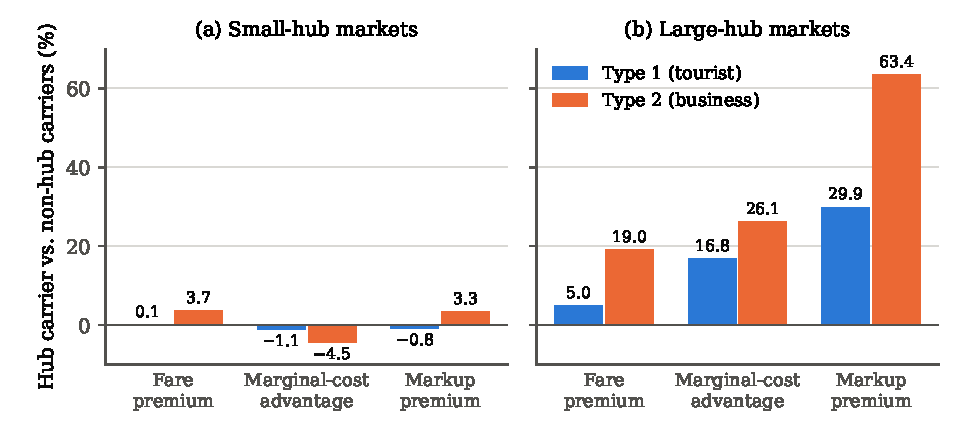
\includegraphics[width=\textwidth]{figures/ch09/bcs_hubpremia.pdf}
\caption{Hub premia by market and traveler type. The fare premium is the percentage by which the hub
carrier's average fare exceeds that of non-hub carriers. The marginal-cost advantage and the markup premium
are defined in \eqref{eq:09-bcs-premia}. Redrawn from the bottom panel of Table~6 of
\citet{BerryCarnallSpiller1996}, based on the column III estimates.}
\label{fig:09-bcs-premia}
\end{figure}

\Cref{fig:09-bcs-premia} plots the premia.\footnote{The text describes a Figure~4 that presents these
results (p.~26, n.~17), but the posted working paper does not contain it. Our figure plots the numbers of
Table~6 and does not reproduce Figure~4.} The pattern supports claims (ii) and (iii). In small hubs the
premia are close to zero for both types. In large hubs the hub carrier earns a substantial premium from
business travelers and a small one from tourists, while enjoying lower marginal cost for both. Business
travelers ``are not just willing to pay the 20\% premia that hub airlines charge,'' they also fly the hub
carrier more often than its rivals (p.~26).

\casehead{No umbrella: the competitive scissor}
The hub carrier's high fares do not protect its rivals. Non-hub carriers in large-hub markets charge less
than non-hub carriers in non-hub markets (\$205 against \$224 for tourists, \$268 against \$296 for business
travelers). They also lose the business travelers, so their passenger mix is more price sensitive (p.~27). Both
blades of the scissor lower their average yield and the profitability of serving the hub airport. This is
claim (iv), and it matches Borenstein's finding of little umbrella effect (\cref{sec:09-borenstein}). The
fare comparison runs across market categories, which the authors warn against elsewhere (p.~25). The
within-market evidence is cleaner: non-hub carriers' business fares are 16\% below the hub carrier's
($\frac{268}{319}=0.84$).

\casehead{A dynamic interpretation}
The authors suggest an explanation, untested in the paper, of two trends after deregulation (p.~27). Once a
carrier builds a major hub at an airport, its rivals see business customers move away and their yields fall.
Marginal carriers then find it profitable to cut service to that city, and airport concentration rises
without any entry barrier. \citet{BruecknerSpiller1994} document this rise. Hubs also give their carriers
price and cost advantages that ease entry out of the hub into new city pairs. That could explain the fall in
concentration at the level of city-pair markets. For empirical models of airline entry they refer to
\citet{ReissSpiller1989} and \citet{Berry1992}.\footnote{The text cites ``Berry (1991)'' here, while the
reference list contains \citet{Berry1992}, the published entry model.}

\subsubsection{Economies of density}

\Cref{tab:09-bcs-dmc} reproduces Table~7, the derivative of leg marginal cost with respect to density
\eqref{eq:09-bcs-dcdq} at column III estimates, for five distances and six densities. With the column III
coefficients the derivative is
\begin{equation}\label{eq:09-bcs-dcdq-III}
\frac{\partial c_\ell}{\partial Q_\ell}=1.584+2(0.164)Q_\ell+3(-0.238)Q_\ell^2-3.891d_\ell+1.270d_\ell^2
+2(0.524)d_\ell Q_\ell .
\end{equation}
Panel B of the table evaluates this formula. It reproduces 29 of the 30 printed cells to within 0.006, which
is rounding. The exception is the cell for 250 miles and density 1.50.\footnote{Table~7 prints $-0.27$ for
250 miles and 150,000 passengers per quarter. Formula \eqref{eq:09-bcs-dcdq-III} gives $-0.031$, which also
fits the neighboring cells (0.568 at density 1.00 and $-0.980$ at 2.00). We treat the printed value as a
typographical error.}

\begin{table}[htbp]
\centering
\begin{threeparttable}
\caption{Derivative of leg marginal cost with respect to density (column III)}
\label{tab:09-bcs-dmc}
\small
\begin{tabular}{@{}lrrrrrr@{}}
\toprule
 & \multicolumn{6}{c}{Leg density (100,000 passengers per quarter)} \\
\cmidrule(l){2-7}
Leg distance & 0.25 & 0.50 & 0.75 & 1.00 & 1.50 & 2.00 \\
\midrule
\multicolumn{7}{@{}l}{\textit{Panel A. As printed in Table 7}}\\
250 miles & 0.794 & 0.808 & 0.733 & 0.568 & $-0.27$ & $-0.980$ \\
500 miles & 0.125 & 0.204 & 0.194 & 0.096 & $-0.369$ & $-1.190$ \\
1,000 miles & $-0.737$ & $-0.527$ & $-0.406$ & $-0.373$ & $-0.576$ & $-1.135$ \\
1,500 miles & $-0.964$ & $-0.623$ & $-0.371$ & $-0.207$ & $-0.148$ & $-0.446$ \\
2,000 miles & $-0.556$ & $-0.084$ & 0.299 & 0.593 & 0.914 & 0.879 \\
\addlinespace
\multicolumn{7}{@{}l}{\textit{Panel B. Computed from the Table 5 column III coefficients}}\\
250 miles & 0.793 & 0.807 & 0.732 & 0.567 & $-0.031$ & $-0.985$ \\
500 miles & 0.124 & 0.203 & 0.193 & 0.094 & $-0.373$ & $-1.196$ \\
1,000 miles & $-0.738$ & $-0.527$ & $-0.407$ & $-0.375$ & $-0.579$ & $-1.141$ \\
1,500 miles & $-0.965$ & $-0.623$ & $-0.372$ & $-0.209$ & $-0.151$ & $-0.451$ \\
2,000 miles & $-0.557$ & $-0.084$ & 0.298 & 0.592 & 0.912 & 0.874 \\
\bottomrule
\end{tabular}
\begin{tablenotes}\footnotesize
\item Notes: \$100 per 100,000 passengers per quarter. A negative entry means economies of density. Panel B
evaluates \eqref{eq:09-bcs-dcdq-III} (our computations). Source:
\citet{BerryCarnallSpiller1996}, Table~7.
\end{tablenotes}
\end{threeparttable}
\end{table}

\begin{figure}[htbp]
\centering
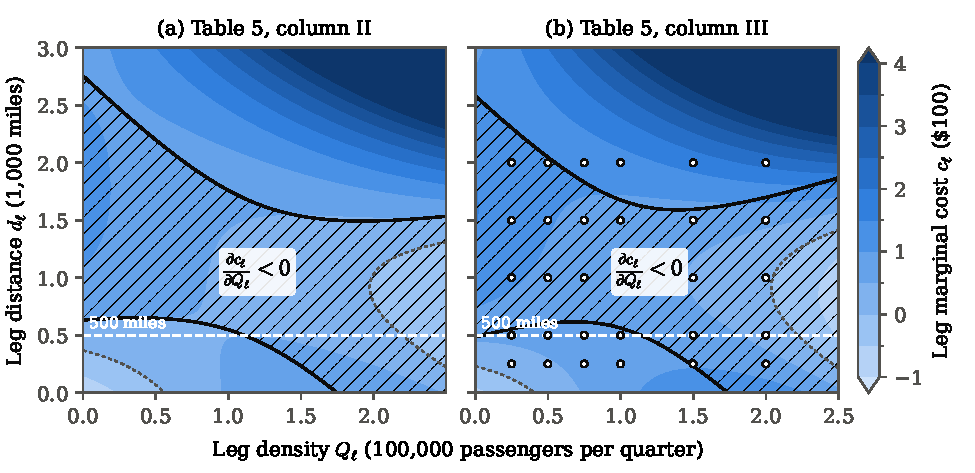
\includegraphics[width=\textwidth]{figures/ch09/bcs_mc_surface.pdf}
\caption{Leg marginal cost over leg density and distance. Shading gives the level of $c_\ell$ in \$100 from
\eqref{eq:09-bcs-mc}, with congestion terms and the product-level constant set to zero. The hatched region,
bounded by the solid curve, has $\frac{\partial c_\ell}{\partial Q_\ell}<0$ (economies of density). Dotted
curves mark $c_\ell=0$, where the polynomial turns negative. The dashed line marks 500 miles, and the dots in
panel (b) are the grid points of \cref{tab:09-bcs-dmc}. Leg densities above 250,000 passengers per
quarter, up to the observed maximum of 455,300, are not shown. Constructed from
\citet{BerryCarnallSpiller1996}, Table~5, columns II and III.}
\label{fig:09-bcs-mc}
\end{figure}

\Cref{fig:09-bcs-mc} redraws the cost surface for columns II and III. The working paper shows the same
surfaces as three-dimensional plots in Figures 1 to 3.\footnote{Figures 1 to 3 are titled ``Col II Table 4''
and ``Col III Table 4,'' while the text says that they correspond to columns II and III. The cost parameters
are in Table~5, so the titles should read Table~5.} The two columns give the same basic shape (p.~27), with
three distance ranges.
\begin{itemize}
  \item Below about 500 miles, marginal cost rises with density up to about 150,000 passengers per quarter
  and then falls (p.~27). In column III the derivative turns negative above a density of 1.48 at 250
  miles and above 1.14 at 500 miles. The introduction's summary of no economies of density below about 500 miles (p.~3)
  therefore holds only up to these densities. The authors explain that over short distances the cruising efficiency of larger aircraft may not make up for
  their higher takeoff and landing costs. Higher density must then be met with more flights.
  \item Between 500 and 1,500 miles there are economies of density at all densities (p.~28). In column III
  the derivative is negative for legs between 617 and 1,589 miles at every observed density, up to
  455,300 passengers per quarter.
  \item Above 1,500 miles, the authors find that marginal cost rises with density except at very low
  densities (p.~28). At 2,000 miles the column III derivative is negative below 55,000 passengers per
  quarter and positive from there to about 284,000. Above that density the negative cubic term in density
  turns it negative again. At 2,000 miles this second sign change lies outside \cref{tab:09-bcs-dmc} and
  \cref{fig:09-bcs-mc}. It lies inside the observed range, whose maximum in \cref{tab:09-bcs-desc} is
  455,300. Such densities are far in the upper tail, since first outbound legs have a mean density of 59,300
  and a standard deviation of 47,500. The derivative also turns negative at high densities inside the
  observed range at every distance from 1,590 miles to the longest observed leg of 2,704 miles. Below
  about 1,870 miles this happens inside the plotted range, where the upper edge of the hatched region in
  panel~(b) of \cref{fig:09-bcs-mc} rises with density. At 1,700 miles, for example, the derivative is
  negative below 95,100 passengers per quarter and again above 200,400. The authors offer two
  explanations for the rising cost (p.~28). Polynomials tend to curl up or down at the corners of the
  data, and the same caution applies to these high-density sign changes. Alternatively, the largest aircraft are
  already in use on long legs, so more density can only be met with more flights.
\end{itemize}
Most leg-carrier combinations in the data lie either under 500 miles or inside the region with economies of
density, as the authors' Figure~3 shows (p.~28). Few legs fall in the long-distance, high-density corner
where marginal cost rises steeply.

The derivatives are large. At 1,000 miles and 100,000 passengers per quarter, the leg's marginal cost
falls at a rate of about \$37 per additional 100,000 passengers, or about \$3.70 per additional 10,000.
Because the derivative steepens with density, doubling density to 200,000 lowers it by about \$64. Average
product marginal costs in Table~6 range from \$91 to
\$133. The authors suspect that the polynomial makes the cost surface ``too curvy,'' so they stop short of
the detailed cost analysis they perform for demand (p.~28). They still read the results as consistent with
economies of density over a wide range. The average market distance in large-hub markets, 842 miles, lies
inside the band where column III implies economies of density at all densities. The cost advantage of large
hub carriers in Table~6 is consistent with this.

The absence of density economies on short legs below about 150,000 passengers per quarter is the
``Southwest effect'' (p.~28). A non-hubbing carrier that offers frequent service on such legs loses little
by not hubbing, because a hub would not lower its costs there. The authors infer that Southwest's success may reflect a cost niche as well as lower
labor costs. They add that Southwest's move toward national service takes it into the distance range where
density economies, and hence hubs, may be more efficient (p.~3, n.~6). In terms of \cref{ex:09-hubcost},
short legs below that density behave like $\gamma\ge1$, where hubbing never saves cost, and legs of 600 to 1,600 miles behave
like $\gamma<1$.

\subsection{Conclusions, limitations, and contribution}\label{sec:09-bcs-conclusions}

\casehead{The authors' conclusions}
The conclusions (pp.~28--29) restate the claims of \cref{sec:09-bcs-question} with their evidence. The data
and model identify two types of travelers with sensible business and tourist tastes (Tables 4 and 5).
Economies of density imply that hubs save costs (Tables 5 and 7). Hubs let carriers charge a premium, but the
ability to raise prices is much greater for business travelers. Out of large hubs these travelers pay about
20\% more, while the premium for tourists is about 5\% or less (Table~6). The authors argue that the welfare
consequences of the premium ``need not be negative'' (p.~29). Business travelers receive a higher-quality product in observed and
unobserved characteristics. They are a larger share of hub carriers' passengers, and their demand is
inelastic. Aside from the issues the model leaves out, ``the negative welfare consequences of hubs appear to
be rather small'' (p.~29).

\casehead{From tables to economic inferences}
The chain of inference has five links. Table~3 shows that reduced-form coefficients mix markups and costs,
which motivates the structural model. Table~5 rejects the logit and finds two price coefficients an order of
magnitude apart. The other type-specific coefficients and the Table~4 composition give the second type
business tastes. The pricing condition converts demand estimates into markups and hence into marginal costs.
Table~6 then compares hub and non-hub carriers within markets, and Table~7 shows where costs fall with
density. Every inference after the first depends on the demand model and on static Nash pricing. No formal
test accompanies the Table~6 premia or the Table~7 derivatives.

\casehead{Alternative interpretations the authors consider}
The authors flag several alternatives themselves. Part of a measured markup may be a shadow price of capacity
(p.~14). Hubs may lower fixed costs, which the model cannot detect (pp.~5 and 14). Pricing may be dynamic,
through yield management, or collusive (pp.~15 and 28). The curvature of the cost surface may be an artifact of the
polynomial (p.~28). Network structure may affect entry and exit, and frequent-flyer programs and travel-agent
commissions may exploit agency problems between the traveler and the payer, which the model does not
represent (p.~28).

\casehead{Limitations}
Several further limitations follow from the design.
\begin{itemize}
  \item The welfare claim is informal. A formal calculation would compute each type's expected surplus from
  the nested logit inclusive value (\cref{ch:logit}). It would then solve for counterfactual prices and
  densities without hubs and compare the two (\cref{ch:newgoods}). Because densities and costs are linked across the
  network, the counterfactual would require re-solving the equilibrium in all markets at once.
  \item The marginal costs are residuals of the pricing condition. If hub carriers do not price as static
  Nash competitors, the conduct error is absorbed into marginal cost. The measured cost advantage of hub
  carriers then mixes cost with conduct, the problem studied in \cref{ch:conduct}.
  \item Ticket restrictions enter only through $\xi$, which is assumed mean independent of the observed
  characteristics and of the network. If hub carriers systematically offer less restricted tickets out of
  their hubs, part of the measured hub taste is a taste for restrictions.
  \item The type distribution has two points and no heterogeneity within a type. The nest groups all flights
  together, so flights of the same carrier or from the same airport are no closer substitutes than others.
  \item Shares are measured with large sampling error, which is not corrected.
  \item Southwest, the carrier behind the ``Southwest effect,'' is absent from the data. The short-haul cost
  estimates come from the other carriers.
  \item The definition of a hub is not documented in the available file beyond a list referred to in the
  Table~6 notes, and HUBSIZE has no natural unit.
  \item The analysis uses one quarter of data, so it cannot study how hubs form, a limitation the authors
  acknowledge when they leave the dynamic interpretation untested.
\end{itemize}

\casehead{Contribution}
The paper is the first to separate the cost advantages of hubs from hub markups within one structural model.
It shows that market-level data can identify discrete consumer types, here with closed-form shares and
without simulation. It also estimates network marginal costs from spoke densities without accounting cost
data, through the pricing condition. Its substantive findings explain why the hub premium falls on business
travelers and why it creates no umbrella for rivals.

\begin{table}[htbp]
\centering
\caption{Identification and counterfactual map of Berry, Carnall and Spiller (2006)}
\label{tab:09-bcs-map}
\footnotesize
\renewcommand{\arraystretch}{1.1}
\begin{tabularx}{\textwidth}{@{}>{\raggedright\arraybackslash}p{2.6cm}>{\raggedright\arraybackslash}X@{}}
\toprule
Observed data & DOT round-trip tickets for the fourth quarter of 1985, with segment traffic from DB27R.
  Fares, shares and characteristics of 122,871 carrier-itinerary-fare products in 14,122 directional
  city-pair markets. \\
\addlinespace
Latent objects & Two traveler types and their population shares, product quality $\xi_{jt}$, cost shocks,
  leg marginal costs and markups. \\
\addlinespace
Estimated parameters & The type-1 probability $\psi$ and type-specific price and taste coefficients,
  including the hub tastes $\beta^h_r$. The nesting parameter $\sigma$, the market-size factor $\kappa$, and
  the coefficients $\chi$ of leg costs in distance and density. \\
\addlinespace
Identifying variation & The moments \eqref{eq:09-bcs-moments}, with own and rival product characteristics
  and endpoint population and network variables as instruments. Within-carrier differences between cheap
  and expensive products at hub and non-hub origins separate the types' hub tastes \eqref{eq:09-bcs-hubid}. \\
\addlinespace
Maintained assumptions & A two-type nested logit, exogenous characteristics and networks, static
  multiproduct Nash pricing, and a polynomial leg cost in distance and density. \\
\addlinespace
Counterfactual and what it holds fixed & No new equilibrium is computed. Markups and marginal costs are
  evaluated at observed fares, and hub premia compare hub and non-hub carriers within markets. \\
\addlinespace
Conclusion & Out of large hubs business travelers pay about 20 percent more and tourists about 5 percent or
  less. Hub carriers also have lower marginal costs, with density economies on longer routes. The
  decomposition rests on static Nash pricing. \\
\addlinespace
One limitation & Marginal costs are residuals of the pricing condition, so any departure from Nash pricing
  is absorbed into measured cost. \\
\addlinespace
Source and our additions & The tables come from the 1996 working paper. \Cref{ex:09-twotypes},
  \cref{prop:09-composition-markup,lem:09-fm-contraction}, the factor structure \eqref{eq:09-bcs-factor}
  and the sampling-error calculation are ours. \\
\addlinespace
Tools in the appendices & \Cref{sec:A-gmm,sec:B-fixedpoint}. \\
\bottomrule
\end{tabularx}
\end{table}

\section{Synthesis: what three methods teach about hub premia}\label{sec:09-synthesis}

The three papers of this chapter study the same industry, use the same public data source and ask related
questions. Their methods differ: pricing regressions, an event study of stock returns, and a structural model
of demand, cost and pricing. This section compares what each method identifies, asks what each paper adds
given the other two, assembles the evidence on the sources of hub premia, and applies it to merger policy.

\subsection{Three designs side by side}\label{sec:09-synthesis-designs}

\Cref{tab:09-compare} summarizes the three designs. For each paper the rows give the observation, the
dependent variable, the key regressors, the source of identification and the headline result.

\begin{table}[htbp]
\centering
\begin{threeparttable}
\caption{Three designs for one question}
\label{tab:09-compare}
\footnotesize
\begin{tabularx}{\textwidth}{@{}>{\raggedright\arraybackslash}p{1.9cm}>{\raggedright\arraybackslash}X
  >{\raggedright\arraybackslash}X>{\raggedright\arraybackslash}X@{}}
\toprule
 & \citet{Borenstein1989} & \citet{WhinstonCollins1992} & \citet{BerryCarnallSpiller2006} \\
\midrule
Method & Reduced-form pricing regressions & Event study of stock returns & Structural demand, cost and
  pricing model \\
\addlinespace
Data and period & DOT ticket sample (DB1A), 1987Q3, with Service Segment and Nonstop Market data & 24 People
  Express entry announcements in 1984--1985, daily returns of 20 carriers, airline schedules, DB1A first
  quarters of 1984--1986 & DB1A round trips, 1985Q4, with segment traffic from DB27R \\
\addlinespace
Observation & One randomly chosen qualifying carrier per airport-pair route (3,591 routes, and 1,508 for the
  relative-price equation) & Carrier and trading day & Carrier-itinerary-fare product in a directional
  city-pair market (122,871 products in 14,122 markets) \\
\addlinespace
Dependent variable & Logs of the 20th, 50th and 80th percentile fares, and log fare ratios of two carriers &
  Daily excess return & Shares and fares, through the inversion ($\xi$) and the pricing condition
  ($\omega$) \\
\addlinespace
Key regressors & Route share, endpoint share, route and endpoint Herfindahls, cost and quality controls,
  airport effects & Annualized seat-miles on the entered pair (SM) and at other airports (OSM), departures
  at the entered airport (EPORT), firm effects & Fare, DIRECT, HUBSIZE, TEMPDIFF, TRIPS-D (type-specific),
  distance, congestion, leg distance-density polynomial \\
\addlinespace
Identification & 2SLS with constructed instruments (GENPSH, IRUTHERF), carrier effects, differencing
  within routes & Timing of announcements and differences in carriers' exposure, estimated by SUR & GMM with
  exogenous characteristics, network and rival-product instruments, and Nash pricing \\
\addlinespace
Headline & A carrier with 70\% of a route charges 2\% to 12\% more than rivals with 10\%. Endpoint dominance
  raises fares, more at the high end. Little umbrella effect & Incumbents lose \$3.7 to \$6.5 million per
  incumbent and event. Incumbent fares fall about 35\% after entry, relative to markets not entered.
  Contestability rejected & Large-hub
  premium of 19\% for business travelers and 5\% for tourists, with lower marginal cost. Density economies
  at medium distances. No umbrella \\
\addlinespace
Main maintained assumptions & Exclusion of the instruments. Shares not proxies for unobserved quality &
  Efficient markets, correct dating, no confounding news, unanticipated events & Two-type nested logit,
  exogenous characteristics and network, static Nash pricing, polynomial costs \\
\bottomrule
\end{tabularx}
\begin{tablenotes}\footnotesize
\item Notes: Sources are \citet[Tables 2--4]{Borenstein1989}, \citet[Tables 1 and 3]{WhinstonCollins1992}
and \citet[Tables 1 and 5--7]{BerryCarnallSpiller1996}. The People Express events and the 20 carriers are
described in \cref{sec:09-wc}.
\end{tablenotes}
\end{threeparttable}
\end{table}

All three papers reject perfect contestability, through different predictions of \cref{sec:09-contest-fail}.
Borenstein finds that fares depend on route and airport dominance holding costs fixed, against prediction
(C1). Whinston and Collins find that entry announcements reduce incumbents' values, against (C2). By
\cref{prop:09-valueloss}, this reveals route-specific profits or sunk costs. Borenstein's route-share and
route-concentration effects survive when POTCOMP controls for potential competitors (Panel B of
\cref{tab:09-bor-main}), against (C3). The small POTCOMP coefficient alone does not test (C3), because under
perfect contestability fares equal average cost whatever the number of potential entrants. Berry, Carnall and Spiller find large markups where the hub carrier
also has lower costs, against (C4), with the caveat of \cref{rem:09-markups-profits} that markups are not
profits. The rejections come from three different kinds of evidence, which makes the verdict robust.

\subsection{What each method identifies}\label{sec:09-synthesis-identify}

Borenstein's regressions identify a conditional correlation between dominance and fares. Under the exclusion
restrictions on his instruments, the route-share coefficient measures how a carrier's fare responds to its
share. By \eqref{eq:09-pricing-approx}, this response is a markup effect only if the share does not proxy for
lower cost or higher quality. The regressions cannot tell a high price that reflects market power from one
that reflects a better product, because they contain no model of either. Their strength is breadth and
transparency: thousands of routes and a specification any reader can check.

Whinston and Collins identify a bound. By \cref{prop:09-valueloss}, the market value an incumbent loses at an
entry announcement is at most the sum of its pre-entry route profits and its sunk costs. A positive loss
proves that one of the two is positive. The design needs no model of demand or costs and no controls for
route characteristics, because the stock market prices the route's prospects. It identifies the existence and
a lower bound of route-specific rents, and how localized they are. It cannot say whether the rents come from
pricing, costs or quality, and it cannot separate profits from sunk costs.

Berry, Carnall and Spiller identify primitives: type-specific demand, product markups and leg marginal costs.
With these they can separate the fare premium into a markup and a cost component, and in principle simulate
counterfactuals. The price is a set of functional forms and behavioral assumptions. The two-type nested logit,
the exogeneity of characteristics and network, static Nash pricing and the cost polynomial all shape the
answer.

\subsection{The contribution of each paper given the other two}\label{sec:09-synthesis-contrib}

Given the other two papers, Whinston and Collins add evidence that does not depend on controls or on an
equilibrium model. Their value losses show that route-level rents exist, which both other papers presume. The
difference between the entered airport pair and other airports in the same city pair shows that airports
within a city are differentiated. Under the assumptions of \eqref{eq:09-wc-did-model}, the 35\% fall in
incumbent fares after entry measures how much of the fare level depends on the absence of a low-fare
competitor.

Given the other two, Berry, Carnall and Spiller add the decomposition and the mechanism. They explain
Borenstein's asymmetry, a dominant carrier with high fares and rivals without, through the sorting of business
travelers. This is the logic of \cref{prop:09-dominance} and \cref{prop:09-composition-markup}. The hub
carrier attracts the inelastic travelers and leaves its rivals with the elastic ones, so rivals cannot raise
their fares. Borenstein's finding that endpoint dominance raises high-end fares about three times as much as
low-end fares anticipates the business travelers' taste for hubs. The density economies show that part of the
hub carrier's markup is financed by lower cost. In large hubs the business fare premium is 19\% of the
non-hub fare, while the markup gain is 32\%.

Given the other two, Borenstein adds the broad pattern. His regressions cover thousands of routes and nine
carriers. They show that carrier-specific dominance of routes and airports predicts fares. Route concentration as
such does not. His airport effects separate scarcity rents, common to all carriers at an airport, from
carrier-specific dominance. His results set the agenda that the other two papers pursue.

Together the papers are more than the sum of their parts, because each covers another's weakness. The
structural model answers the quality confound in Borenstein's regressions. The event study supplies
market-based evidence that does not depend on the structural model's equilibrium assumption. Borenstein's
breadth offsets the narrow sample of 24 events, 22 of them at Newark. The fit is imperfect. The papers use
different periods (1984--1985, 1985Q4, 1987Q3) and different market definitions (airport pairs and city
pairs), and none of them studies the formation of hubs.

\subsection{Sources of hub premia}\label{sec:09-synthesis-sources}

\Cref{tab:09-sources} collects the evidence on five candidate sources of the hub premium. The table shows
which source each method can address. It also shows that no single paper speaks to all five.

\begin{table}[htbp]
\centering
\begin{threeparttable}
\caption{Sources of hub premia: what each paper shows}
\label{tab:09-sources}
\footnotesize
\begin{tabularx}{\textwidth}{@{}>{\raggedright\arraybackslash}p{1.9cm}>{\raggedright\arraybackslash}X
  >{\raggedright\arraybackslash}X>{\raggedright\arraybackslash}X>{\raggedright\arraybackslash}X@{}}
\toprule
Source & \citet{Borenstein1989} & \citet{WhinstonCollins1992} & \citet{BerryCarnallSpiller2006} & Later work \\
\midrule
Lower cost (density economies) & Not identified. Cost controls only & Not measured & Density economies for
  legs of roughly 600 to 1,600 miles, and below about 500 only above about 110,000 to 150,000 passengers. Hub carriers' marginal cost 26\% lower for
  business tickets in large hubs & \citet{BruecknerSpiller1994} on density economies from spoke data \\
\addlinespace
Quality and demand (frequency, nonstop service, network breadth) & Frequency raises fares, more at the high
  end. Cannot be separated from market power & Not separable from rents & Business travelers value
  directness, hub size and frequency far more. Hub carriers' products have higher $\xi$ & \citet{Berry1990}
  on airport presence as differentiation \\
\addlinespace
Market power from dominance & Route and endpoint shares raise own fares. Little umbrella & Route-specific
  rents revealed by value losses & Business markups 63\% higher on hub carriers in large hubs. No umbrella &
  \citet{CilibertoTamer2009}: competitive effects rise with airport presence \\
\addlinespace
Sunk costs, entry barriers and potential competition & Potential competition has a small effect & Losses
  reveal profits or sunk costs. Contestability rejected & Entry and network taken as given &
  \citet{GoolsbeeSyverson2008}: incumbents cut fares when Southwest threatens entry \\
\addlinespace
Scarcity rents (slots, gates) & Airport effects: O'Hare $+3\%$ to $5\%$, Atlanta $+1\%$ to $3\%$, Denver $+2\%$
  to $4\%$. Common to all carriers & Firm effects may include slot values & Congestion raises cost and lowers
  demand. Rents not separated & \citet{CilibertoWilliams2010}: gate control raises fares where gates are
  scarce \\
\bottomrule
\end{tabularx}
\begin{tablenotes}\footnotesize
\item Notes: Borenstein's airport effects are from p.~359 of his article. Details of each paper are in
\cref{sec:09-borenstein}, \cref{sec:09-wc} and \cref{sec:09-bcs}, and of the later work in
\cref{sec:09-synthesis-later}.
\end{tablenotes}
\end{threeparttable}
\end{table}

The table suggests a division of the hub premium. A substantial part of the fare gap between hub and non-hub
carriers reflects quality that business travelers value and lower costs on medium-haul legs. Market power
from dominance is real, but it is concentrated on business travelers and does not spill over to rivals.
Route-specific rents and sunk costs keep potential entry from eliminating it. Scarcity of airport facilities
adds a premium that is common to all carriers at an airport, and control of gates turns it into a source of
carrier-specific advantage.

\subsection{Merger policy: two hypothetical mergers}\label{sec:09-synthesis-mergers}

Consider an antitrust agency reviewing two hypothetical mergers. Merger A combines two network carriers with
large hubs, of the kind represented by Delta and United. Merger B combines two low-cost carriers that fly
mostly point to point, of the kind represented by JetBlue and Southwest. The three papers leave both cases
open. They tell the agency where to look. The formal tools, upward pricing pressure, merger simulation and
retrospective studies, are developed in \cref{ch:mergers}.

\casehead{Merger A: two hub carriers}
Borenstein's results predict higher fares on routes where the merging carriers' combined route share rises,
and at airports where their combined endpoint share rises. The largest effects arise on hub-to-hub routes,
where each carrier competes from its own stronghold. The absence of an umbrella shows that a carrier's dominance
does little to raise its rivals' fares. It does not predict how rivals would respond to a change in ownership. Both that
response and the discipline that rivals impose on the merging carriers depend on diversion and on equilibrium pricing.
Berry, Carnall and Spiller predict that the price effect falls mainly on business travelers. A merger enlarges
the network connected through each hub and so raises each hub's HUBSIZE. By
\cref{prop:09-composition-markup}, that tilts the buyers of the merged carrier's hub products further toward
business travelers and raises markups on the tickets they buy. Tourists would see smaller changes. The same
paper also points to efficiencies. Combining traffic on overlapping spokes raises density, and on legs of
roughly 600 to 1,600 miles that lowers marginal cost. An efficiency defense is therefore plausible for
overlapping medium-haul spokes and weak for short ones. Whinston and Collins show that route-level rents
survive potential competition, so the loss of an actual competitor on overlap routes matters. They also show
how much entry by a low-fare carrier can cut fares. The incumbents' aggressive responses that they document,
however, suggest that such entry is costly and uncertain.

The agency would want the overlapping routes and the airports where both carriers have large shares. It
would want diversion ratios by fare class and the density and distance of the spokes that would be combined.
It would also want a merger simulation with heterogeneous travelers. Remedies that open gates and slots at the hubs speak to the
facility-based advantages that \citet{CilibertoWilliams2010} measure. The papers that matter most for merger A
are Berry, Carnall and Spiller, for the decomposition of the premium into markups and costs, and Borenstein,
for the link between dominance and fares.

\casehead{Merger B: two low-cost carriers}
For merger B the most relevant evidence concerns entry. Under the assumptions of \eqref{eq:09-wc-did-model},
Whinston and Collins find that entry by a low-fare carrier cut incumbents' mean fares by about 35\%. Their
event study finds that it cost each incumbent \$3.7 to \$6.5 million in value per event. A low-cost carrier is a source of discipline, so merging two of them removes an independent low-fare
competitor on overlap routes. \citet{GoolsbeeSyverson2008} show that incumbents cut fares when Southwest
becomes a likely entrant, before it starts flying. The merger would also remove each carrier as a potential
entrant on the other's routes. On the cost side, Berry, Carnall and Spiller find economies of density below
about 500 miles only on dense legs, above about 110,000 to 150,000 passengers per quarter. Combining
short-haul point-to-point networks therefore saves cost through density only where the combined legs are that
dense.
Their cost estimates exclude Southwest, so this inference rests on other carriers' short legs. Borenstein's
dominance results matter less here, unless the merger creates a dominant position at airports where both
carriers concentrate. The agency would want the overlapping routes and the routes where each carrier is a
likely entrant. It would also want estimated entry probabilities and the fare changes on routes where one
carrier entered against the other. The papers that matter most for merger B are Whinston and Collins and, among later work, Goolsbee and
Syverson.

\subsection{Later evidence*}\label{sec:09-synthesis-later}

\casehead{Price dispersion}
\citet{BorensteinRose1994} study the dispersion of fares that one carrier charges different passengers on the
same route. In the working-paper version, the expected absolute difference between the fares of two of a
carrier's passengers on a route averages 36\% of the carrier's mean fare. Dispersion is higher on more
competitive routes, which they interpret as price discrimination in monopolistically competitive markets,
against travelers who are less willing to switch flights or carriers. \citet{GerardiShapiro2009} revisit
the question with a panel from the first quarter of 1993 to the third quarter of 2006. Competition reduces
dispersion, as the textbook theory of price discrimination predicts. The effect is pronounced on routes with a
heterogeneous mix of business and leisure travelers. They attribute the contrast with Borenstein and Rose to
omitted-variable bias in cross-sectional estimates. Both papers rest on the heterogeneity of travelers that
Berry, Carnall and Spiller model as two types.

\casehead{The threat of entry}
\citet{GoolsbeeSyverson2008} use the expansion of Southwest's network to identify routes where the probability
of entry rises abruptly. We cite their NBER Working Paper 11072 (January 2005, revised August 2008), whose
table numbers may differ from those of the published article. A route is threatened when Southwest begins to
serve its second endpoint without yet flying the route. A descriptive probit of Southwest's entry into a route
in a given quarter shows the size of the jump (Table~I). Presence at one endpoint raises the entry probability
only slightly above a baseline near zero. Presence at both raises it by a further factor of about 70, to
18.5\% per quarter (p.~5).

Let $\tau_0$ be the quarter in which Southwest first serves both endpoints of route $t$, and let $\tau_e$ be
the quarter in which it starts flying the route. In this discussion $\tau$ indexes quarters. For incumbent
carrier $f$, the authors estimate the event-study regression
\begin{equation}\label{eq:09-gs}
  y_{ft\tau} = \gamma_{ft} + \gamma_{f\tau} + \sum_{k} \beta_k\,D^{0}_{t\tau k}
  + \sum_{k} \lambda_k\,D^{e}_{t\tau k} + e_{ft\tau}
\end{equation}
(pp.~6--7). The outcome $y_{ft\tau}$ is the passenger-weighted mean log fare, and $\gamma_{ft}$ and
$\gamma_{f\tau}$ are carrier-route and carrier-quarter fixed effects. The threat dummy $D^{0}_{t\tau k}$
equals one when $\tau = \tau_0 + k$ and Southwest does not yet fly the route. It runs from $k = -8$ to
$k = 2$, and one more dummy pools the quarters from $\tau_0 + 3$ on. The entry dummies $D^{e}_{t\tau k}$
mark the quarter $\tau_e$, the two quarters after it, and the quarters from $\tau_e + 3$ on. The omitted
period is the 9th through 12th quarters before $\tau_0$, so each coefficient measures log fares relative to
that baseline. Observations are weighted by passengers, and standard errors are clustered by route-carrier
pair (p.~7).

Column~(1) of their Table~II gives $\hat\beta_0 = -0.186$ (0.073). Since $e^{-0.186} = 0.830$, fares are
about 17\% lower by the quarter $\tau_0$ (p.~8). They begin to fall about three quarters before $\tau_0$.
Southwest announces its arrival at an airport months in advance, and insiders may learn of it earlier
(p.~9). Once Southwest flies the route, fares are 21\% below the baseline, since $e^{-0.237} = 0.789$. By
the end of the window they are over 29\% lower, since $e^{-0.344} = 0.709$ (p.~9). Over half of Southwest's
total effect on incumbents' fares thus occurs before entry. The cuts occur only on threatened routes and not
on routes from nearby airports. This answers the question that Borenstein's potential
competition variable and Whinston and Collins's announcements could only approach. Potential competition does
discipline incumbents when the entrant is credible and the threat is specific to a route.

\casehead{Gates and the hub premium}
\citet{CilibertoWilliams2010} measure the role of airport facilities directly, with data from the competition
plans that major airports must file with the DOT. Our numbers come from the February 2009 author manuscript
(MPRA Paper 38636), then forthcoming in the \emph{Journal of Law and Economics}. The hub premium rises with
the fare. It is below 10\% at the 10th percentile of the fare distribution and almost 25\% at the 90th
(p.~3). Their Table~7 adds the measures of barriers to entry to the fare regression. The premium on tickets
out of a hub then falls from about 12\% to about 6\%, and the premium on tickets into a hub from 12.7\% to
9.3\% (pp.~21--22). In the authors' summary, the premium falls by almost half (p.~22). Control of gates leased on an exclusive basis is
a key determinant. The coefficient on the carrier's share of gates at the origin airport, OwnGatesOrigin, is
0.163. A rise in that share from 10\% to 30\% therefore raises fares by about $0.20 \times 0.163 \approx 3\%$.
Gate control explains high fares only where gates are scarce relative to departures (pp.~23--24). These
results support Borenstein's facility mechanism and fit the
finding of Berry, Carnall and Spiller that the premium falls on high-fare, business tickets.

\casehead{Entry games}
\citet{CilibertoTamer2009} estimate entry games in airline markets without assuming a unique equilibrium,
in the tradition of \citet{Berry1992}. They find heterogeneous competitive effects. The effects of large
carriers differ from those of low-cost carriers and Southwest, and a carrier's competitive effect increases
with its airport presence. Airport presence thus shapes market structure as well as fares, as Berry, Carnall
and Spiller conjecture in their dynamic interpretation.

\casehead{Merger retrospectives}
The airline mergers of the mid-1980s, which motivated much of this literature, have been studied after the
fact, and \cref{sec:11-retro} places these retrospectives among the general methods of merger evaluation.


\section{Bibliographic notes}\label{sec:09-bibnotes}

\citet{Borenstein1989} built on earlier studies of airline pricing. They regressed route fares on route
concentration and cost controls \citep{GrahamKaplanSibley1983,BaileyGrahamKaplan1985,CallKeeler1985,MorrisonWinston1987}. These studies established that fares rise with concentration, against the
contestability benchmark of \citet{BaumolPanzarWillig1982} and \citet{Baumol1982}. \Cref{sec:09-contest}
follows the textbook account of \citet[sec.~8.1]{Tirole1988}. Tirole also presents the critique that prices
adjust faster than entry. He treats the war of attrition as an alternative model of natural monopoly
(sec.~8.1.3). \citet{Levine1987}, who
had regulated, managed and studied airlines, summarizes the view that airport dominance insulates a carrier
from competition \citep[p.~345, n.~3]{Borenstein1989}. \citet{Borenstein1991}
followed his 1989 study with directional city-pair comparisons, which show higher fares on flights out of a
hub than into it. Price dispersion within routes became a separate topic. \citet{BorensteinRose1994} found
more dispersion on more competitive routes in a cross-section, and \citet{GerardiShapiro2009} found the
opposite in a panel.

The cost side of hubbing has its own lineage. \citet{CavesChristensenTretheway1984} estimated economies of
density from an aggregate airline cost function. \citet{BruecknerDyerSpiller1992} and
\citet{BruecknerSpiller1994} moved to marginal costs at the level of flight legs, the approach that
\citet{BerryCarnallSpiller2006} adopt. \citet{BruecknerSpiller1991} study competition and mergers in
hub-and-spoke networks. There, economies of density on a shared spoke link costs across markets
\citep[p.~2, n.~5]{BerryCarnallSpiller1996}. On the demand side,
\citet{MorrisonWinston1986} estimated an early logit model of air travel choices, and \citet{Berry1990}
treated airport presence as a source of product differentiation. The structural approach of
\citet{BerryCarnallSpiller2006} builds on the inversion of \citet{Berry1994} and the estimator of
\citet{BerryLevinsohnPakes1995} (\cref{ch:logit,ch:blp}).

Entry into airline markets is a large literature of its own. \citet{ReissSpiller1989} and \citet{Berry1992}
directly investigate the determinants of entry into city-pair markets \citep[p.~446, n.~1]{WhinstonCollins1992}.
Berry's model treats the number of carriers on a route as an equilibrium outcome.
\citet{CilibertoTamer2009} estimated airline entry games that allow multiple equilibria and heterogeneous
competitive effects. \citet{CilibertoMurryTamer2021} estimate a game in which carriers choose entry and prices
simultaneously, with correlated shocks to demand and cost. Ignoring endogenous entry biases their estimates of
demand elasticities. In a simulated merger of American and US Airways, the outcomes after the merger depend on
how the merged firm's characteristics are modeled. Their framework addresses a limitation of all three papers
of this chapter, none of which models how carriers choose the routes they serve (\cref{sec:09-synthesis}). \citet{GoolsbeeSyverson2008} studied how incumbents respond to the threat of entry by
Southwest, and \citet{CilibertoWilliams2010} measured how control of gates sustains the hub premium. The
event-study method that \citet{WhinstonCollins1992} adapt goes back to \citet{FamaEtAl1969}. Early uses in
regulation include \citet{Schwert1981} and \citet{Rose1985}, and \citet{MacKinlay1997} gives a survey. Event
studies of mergers are treated in \cref{sec:11-retro-event}.

The airline mergers of the mid-1980s were studied after the fact by \citet{Borenstein1990},
\citet{KimSingal1993} and \citet{Peters2006}. \Cref{ch:mergers} places these retrospectives among the
general methods of merger evaluation. On the collusion side, \citet{Miller2010} asks whether the settlement
of the airline tariff publishing case reduced coordination among carriers (\cref{sec:13-atpco}). Dynamic
models of entry, network formation and competition among airlines go beyond the scope of this edition.

\section{Exercises}\label{sec:09-exercises}

\begin{enumerate}[label=\arabic*., leftmargin=*, itemsep=6pt]

\item \emph{A contestable natural monopoly.} Let $C(q)=F+cq$ for $q>0$ and $C(0)=0$, and let market demand
be $Q(p)=A-p$, with $A>c$ and $(A-c)^2>4F$.
\begin{enumerate}[label=(\alph*)]
\item Derive the sustainable price $p^c$ of \cref{prop:09-contest-monopoly} as a function of $(A,c,F)$.
Verify that it equals average cost at the quantity demanded and that it gives $7-\sqrt{17}$ when $A=12$,
$c=2$ and $F=8$.
\item Show that $p^c$ falls toward $c$ as $F\to0$. Compute the deadweight loss at $p^c$ and at the monopoly
price, and explain why the first is the smallest loss compatible with zero profit.
\item Now set $F=0$ and let entry require a sunk investment $K$. The incumbent charges the monopoly price,
and demand and profits are monthly flows. An entrant that slightly undercuts the incumbent earns the monopoly
profit per month until the incumbent responds, and nothing afterward. With $A=12$, $c=2$, $K=100$ and a
monthly discount factor of $0.99$, find the shortest response lag $T$, in months, at which entry pays.
Relate your answer to \cref{prop:09-fragility}.
\item Let instead $C(q)=1+q^2$ for $q>0$, with $C(0)=0$, and $Q(p)=A-p$. Find the efficient scale and the
minimum average cost. For which values of $A$ does \cref{prop:09-nonexist} imply that no configuration is
sustainable? At $A=3.8$, find the single firm's break-even price at the right crossing and the profit of
the entry plan used in the proof of the proposition.
\end{enumerate}

\item \emph{Dominance without an umbrella.} Consider the logit route market of \cref{ass:09-logit} with two
carriers and an outside good, $\alpha=1$ (prices in \$100), $c_1=c_2=1$ and $\delta_2=1$.
\begin{enumerate}[label=(\alph*)]
\item Using the single-equation reduction in the proof of \cref{prop:09-dominance}, compute the Bertrand
equilibrium for $\delta_1\in\{1,2,3\}$. Check your answers against $p_1=p_2=2.227$ at $\delta_1=1$ and
$p_1=2.867$, $p_2=2.148$ at $\delta_1=3$.
\item Verify each claim of \cref{prop:09-dominance} at these points, and compute the route Herfindahl index of
inside shares at each.
\item Regress $\ln p_1-\ln p_2$ on $s_1-s_2$ across the three points. Compare the slope with the
approximation of \cref{cor:09-relprice}, and explain what it implies for the sign of the route-share
coefficient in Borenstein's relative-price equation \eqref{eq:09-bor-rel}.
\end{enumerate}

\item \emph{Reading Borenstein's estimates.}
\begin{enumerate}[label=(\alph*)]
\item Use the 2SLS estimates with POTCOMP in Panel B of \cref{tab:09-bor-main}. For each fare percentile,
compute the fare gap between a carrier with 70\% of a route and rivals with 10\% each. Compare your numbers
with those of the main specification.
\item On a route, carrier 1 has 40\% of the passengers and three rivals have 30\%, 20\% and 10\%. The two
smallest rivals merge. Compute the change in the route Herfindahl index and the implied changes in carrier
1's three fares, holding its share fixed. Explain why the calculation holds the share fixed and why this
matters for reading $\phi_4$ as an umbrella effect.
\item Derive \eqref{eq:09-irutherf} and show that the rescaled rival shares leave the Herfindahl index of
the traffic not carried by $f$ unchanged.
\item Following \cref{rem:09-share-coef}, compute the value of $\bar\eta=\eta_0+\eta_1\bar H$ implied by
each 2SLS route-share coefficient if the route elasticity is $\varepsilon=2$. What outside information would discriminate between
this reading and a Cournot reading?
\end{enumerate}

\item \emph{Event-study algebra.}
\begin{enumerate}[label=(\alph*)]
\item Two carriers have equity values of \$250 million and \$2.5 billion. Compute the dollar loss each would
suffer under a common abnormal return of $-1\%$. Explain why Whinston and Collins prefer the dollar
formulation \eqref{eq:09-wc-dollar}.
\item Using $\lambda_{SM}=-0.0109$, the average incumbent's 7,100 weekly seats and the average distance of
892 miles, compute the implied loss per incumbent. Compare it with the \$3.7 million reported in the paper.
Show that the gap can arise because the mean of a product differs from the product of the means, and state
the sign of the covariance it requires.
\item Three incumbents are hit by the same announcement, and their abnormal returns have pairwise
correlation $0.5$. By what factor does the variance of their average abnormal return exceed the variance
computed under independence?
\item If investors had assigned probability $0.4$ to entry before the announcement, what true loss per
incumbent corresponds to a measured loss of \$3.7 million (\cref{rem:09-anticipation})?
\end{enumerate}

\item \emph{People Express as a difference in differences.} Use Panel A of \cref{tab:09-wc-t34}.
\begin{enumerate}[label=(\alph*)]
\item Compute the two difference-in-differences estimates of the effect of entry on the mean incumbent price
and their average.
\item Compute the pooled two-sample $t$ statistic for the 1984--85 contrast, reading the reported standard
deviations first with divisor $n-1$ and then with divisor $n$. Compare both with the printed value of 2.5.
\item State the identifying assumptions of \eqref{eq:09-wc-did-model}. Use the 1985 cohort's change in
1984--85 and the 1984 cohort's change in 1985--86 to assess them.
\item Explain why the quantity and capacity columns are hard to reconcile with Cournot competition, using
\eqref{eq:09-br-slope}.
\end{enumerate}

\item \emph{Who pays the hub premium?} Use the column III estimates of \cref{tab:09-bcs-demand}.
\begin{enumerate}[label=(\alph*)]
\item Compute an approximate standard error for type 2's willingness to pay for HUBSIZE by the delta method,
ignoring the covariance between the two estimates. Is the ranking of the two types' willingness to pay
robust to this imprecision?
\item By \cref{rem:09-fm-extensions}, a single-product markup is close to $\frac{1-\sigma}{\bar\alpha_j}$
when within-nest shares are small. Compute this approximation for a product whose buyers have the
composition of hub carriers' passengers in large-hub markets (33.0\% type 2) and of non-hub carriers'
passengers there (23.2\% type 2).
\item Compare your answers with the average markups $F-M$ implied by \cref{tab:09-bcs-hub}. Explain why
the approximation at the average buyer composition understates the average markup. (Note that $\frac{1}{\bar\alpha}$
is convex in $\Pr(2\mid j)$.)
\end{enumerate}

\item \emph{Economies of density.} Use the column III cost estimates of \cref{tab:09-bcs-cost}.
\begin{enumerate}[label=(\alph*)]
\item Write the leg marginal cost polynomial and derive $\frac{\partial c_\ell}{\partial Q_\ell}$.
\item Reproduce three cells of \cref{tab:09-bcs-dmc} and identify the printed cell that the formula does not
reproduce.
\item At 250 miles, find the density at which the derivative changes sign. At 2,000 miles, find the density
above which marginal cost rises with density.
\item Discuss what the sign pattern implies for hubbing on short and on medium-haul routes, and connect it to
the cost ratio $\frac{2n^\gamma}{n+1}$ of \cref{ex:09-hubcost}.
\end{enumerate}

\item \emph{An acquisition at a hub.} A network carrier that dominates a hub airport proposes to acquire a
low-cost carrier. The low-cost carrier flies point to point, and a third of its departures use the
acquirer's hub. Drawing on the three papers of this chapter and on \cref{sec:09-synthesis}, write a short
memo to an antitrust agency. Identify the travelers and routes most likely to face higher fares. State the
efficiencies the merging parties could claim and how credible they are. Explain what the agency should
infer from the absence of an umbrella effect. Name the additional evidence you would request, and say which
paper's method would best analyze it.

\end{enumerate}

\chapter{Valuing New Goods}\label{ch:newgoods}

\section{Introduction}\label{sec:10-intro}

Markets add products all the time. \citet[p.~237]{Bresnahan1997} cites a count of more than 22,000 new-product
introductions in 1994. In ready-to-eat cereal alone, about 190 new brands entered between 1980 and 1992
\citep[pp.~213--215]{Hausman1997}. Some new products are small variations on existing ones, and some transform an
industry. Either way, a new good changes what consumers can buy, and so it changes their welfare. Official price
indexes compare the prices of goods sold in two periods. They therefore miss the gain from a good that did not
exist in the first period. The size of that gain matters for the measurement of inflation and real income, for
the returns to research, and for competition policy.

This chapter asks three questions. What is the welfare value of a new good, and why does a conventional price
index miss it? How can an estimated demand system measure that value, in product space and in characteristics
space? And how do market power and the responses of rival firms change the answer?

The questions are hard for a simple reason. The value of a new good is the area under its compensated demand
curve between the price at which it sells and the price at which demand would vanish. Prices that high are
almost never observed \citep[Section~1]{BerryPakes2007}.\footnote{Throughout this chapter, page, section and table
numbers for \citet{BerryPakes2007} refer to the authors' manuscript dated July 2, 2007 (41 pages). Its Section~5.4
starts on p.~31, and Tables~5 to~7 are on pp.~33--36. We did not check the published article, whose numbering may
differ.} Every estimate therefore extrapolates demand beyond the
data. The answer depends on the functional form, on the instruments that identify the slope of demand, and on
the model of competition. The chapter makes each of these dependences explicit.

\Cref{sec:10-virtual,sec:10-functional,sec:10-imperfect} develop the theory. \Cref{sec:10-virtual} defines the
value of a new good through its virtual price and relates it to the exact cost-of-living index. It also derives
index-number bounds and the variety correction for preferences with a constant elasticity of substitution (CES).
\Cref{sec:10-functional} asks how much of the value the data can identify. It compares canonical functional forms
and derives a lower bound that needs only convexity. \Cref{sec:10-imperfect} adds imperfect competition. It splits
the welfare gain into a variety effect and a price effect, separates private from social returns, and studies how
the introducing firm and its rivals reprice. The first case study, in \cref{sec:10-hausman,sec:10-bresnahan}, is
Hausman's valuation of Apple-Cinnamon Cheerios and Bresnahan's critique of its instruments and of its treatment of
competition.

\Cref{sec:10-charspace} turns to characteristics space. It derives consumer surplus in random utility models and
shows how the idiosyncratic taste shocks of logit-type models build a value of variety into the functional form.
The remaining case studies apply these ideas. \Cref{sec:10-trajtenberg} studies Trajtenberg's measurement of
innovation in computed tomography scanners. \Cref{sec:10-petrin} studies Petrin's valuation of the minivan with
micro moments, and \cref{sec:10-gentzkow} studies Gentzkow's bundle model of print and online newspapers, in which
a new good may complement old ones. \Cref{sec:10-synthesis} compares the four studies and draws out five
determinants of a measured value.

The chapter draws on much of the book. The duality results, the almost ideal demand system, multistage budgeting
and the virtual prices of withdrawn products come from \cref{ch:aids}. Multiproduct Bertrand pricing comes from
\cref{ch:diffprod}, and free entry from \cref{ch:theory}. The discrete-choice models are those of
\cref{ch:discrete,ch:logit,ch:blp}. The counterfactual equilibria of this chapter use the same machinery as the
merger simulations of \cref{ch:mergers}. \Cref{sec:B-duality,sec:B-ev} collect the duality results and the extreme
value algebra, and \cref{sec:A-iv,sec:A-gmm,sec:A-simulation} the methods of instrumental variables, the
generalized method of moments and simulation.

A few conventions hold throughout. We write $y$ for income, as Hausman and Petrin do, where \cref{ch:aids} writes
$I$. The virtual price of good $n$ is $p_n^V$. Market shares are $s_j$, and budget or revenue shares are $w_j$. The
CES elasticity of substitution is $\eta$, because $\sigma$ denotes the nesting parameter of the nested logit. In
\cref{sec:10-imperfect,sec:10-hausman} the elasticities $\varepsilon_{kj}$ are signed, so own-price elasticities
are negative. Elsewhere a scalar $\varepsilon$ is an own-price elasticity written as a positive number, as in the
rest of the book. When a paper uses a symbol that the book reserves for another object, we rename it at first use.

\definecolor{c10p1blue}{HTML}{2A78D6}
\definecolor{c10p1orange}{HTML}{EB6834}
\definecolor{c10p1aqua}{HTML}{1BAF7A}
\definecolor{c10p1gray}{HTML}{52514E}

\section{The welfare value of a new good: virtual prices and exact measures}\label{sec:10-virtual}

A new good raises welfare because consumers can buy something they could not buy before. This section turns
that statement into a number. Following \citet{Hicks1940}, we treat the period before the introduction as a
period in which the good is rationed at zero. The value of the good is then the compensating variation of
raising its price from the observed level to its \emph{virtual price}. At that price the consumer would
choose not to buy the good. We derive this result, relate it to the exact cost-of-living index of
\citet{Konus1939}, and show why price indexes that link new goods in after their introduction miss it. We
then derive index-number bounds, state what separability buys, and derive the variety correction of
\citet{Feenstra1994}. The duality tools come from \cref{sec:05-duality}, and \cref{sec:05-welfare-virtual}
treats virtual prices for the almost ideal demand system.

\subsection{Setting and notation}\label{sec:10-setting}

A consumer chooses quantities $q = (q_1,\dots,q_n)^\top \ge 0$ of $n$ goods at prices
$p = (p_1,\dots,p_n)^\top$, all positive, with income $y$. We write $q_j(p,y)$ for Marshallian demand,
$v(p,y)$ for indirect utility, $e(p,u)$ for the expenditure function and $h_j(p,u)$ for Hicksian demand.
Good $n$ is the new good. It is unavailable in period 0 and sold at price $p_n$ in period 1. We write
$p_{-n}$ for the prices of the other goods and $(p_{-n},p_n)$ for the full price vector. Following
\citet{Hausman1997} and \citet{Petrin2002} we write income as $y$. \Cref{ch:aids} writes $I$ for the same
object.

\begin{assumption}[Preferences]\label{ass:10-prefs}
The utility function $U$ is continuous, strictly increasing and strictly quasi-concave on $\R^n_+$.
\end{assumption}

Under Assumption~\ref{ass:10-prefs} demands are single valued and continuous, and the duality identities of
\cref{lem:05-duality} hold:
\begin{equation}\label{eq:10-duality}
  e\bigl(p,v(p,y)\bigr) = y, \qquad h_j(p,u) = q_j\bigl(p,e(p,u)\bigr), \qquad
  \frac{\partial e(p,u)}{\partial p_j} = h_j(p,u).
\end{equation}
The last identity is Shephard's lemma (\cref{prop:05-shephard}). The expenditure function is nondecreasing
and concave in $p$, so each Hicksian demand is nonincreasing in its own price (\cref{prop:05-e-properties}).

\subsection{A new good as a rationed good}\label{sec:10-rationing}

\citet{Hicks1940} treated rationing and new goods with the same tool. As \citet[p.~211]{Hausman1997} puts it,
new products are a special case of rationing in which demand for the good is zero. Before the introduction, the consumer solves the usual problems with the extra
constraint $q_n = 0$. We call the resulting value functions the \emph{rationed} indirect utility and
expenditure functions:
\begin{align}
  v^R(p_{-n},y) &= \max\Bigl\{U(q) : \sum_{j\neq n}p_jq_j \le y,\ q_n = 0\Bigr\}, \label{eq:10-vR}\\
  e^R(p_{-n},u) &= \min\Bigl\{\sum_{j\neq n}p_jq_j : U(q) \ge u,\ q_n = 0\Bigr\}. \label{eq:10-eR}
\end{align}
Neither function depends on $p_n$, because a bundle with $q_n = 0$ costs the same at every price of good $n$.
\Cref{sec:05-welfare-virtual} writes $e_{-i}$ for $e^R$.

\begin{definition}[Virtual prices]\label{def:10-virtual}
The \emph{Hicksian virtual price} $p_n^V(p_{-n},u)$ of good $n$ is the virtual price of \cref{def:05-virtual},
the lowest price at which Hicksian demand $h_n$ is zero. The \emph{Marshallian virtual price} (or choke price) is
the same object for Marshallian demand, $p_n^M(p_{-n},y) = \inf\{p_n > 0 : q_n(p_{-n},p_n,y) = 0\}$. Either
price is $+\infty$ if the corresponding demand is positive at every price.
\end{definition}

In both cases demand stays at zero at every price above the virtual price. For Hicksian demand this follows
because $h_n$ is nonincreasing in $p_n$. For Marshallian demand, suppose the optimal bundle at $p_n$ has
$q_n = 0$. Raising $p_n$ leaves its cost unchanged and shrinks the budget set, so the same bundle stays
optimal. \citet[p.~212, n.~5]{Hausman1997} uses the Hicksian version, because the exact welfare measure keeps
utility constant. The two versions coincide when demand for good $n$ has no income effect. For a normal good
the Hicksian virtual price at the period-1 utility is at least the Marshallian one (\cref{lem:05-choke-order}).

The next lemma is the formal content of the virtual-price idea. \citet{Rothbarth1941} introduced it, and
\citet{NearyRoberts1980} give a modern treatment of rationing along these lines. \citet[Section~4.3,
pp.~109--113]{DeatonMuellbauer1980b} give the textbook treatment through the restricted cost function, which
\cref{lem:10-restricted} below develops.

\begin{lemma}[Rationing as a price, \citealp{Rothbarth1941,NearyRoberts1980}]\label{lem:10-rothbarth}
Let Assumption~\ref{ass:10-prefs} hold and fix $p_{-n}$, $y$ and $u$.
\begin{enumerate}[label=(\alph*)]
  \item For every $p_n > 0$, $v(p_{-n},p_n,y) \ge v^R(p_{-n},y)$ and $e(p_{-n},p_n,u) \le e^R(p_{-n},u)$.
  \item If $p_n^M(p_{-n},y)$ is finite, then $v^R(p_{-n},y) = v\bigl(p_{-n},p_n^M(p_{-n},y),y\bigr)$.
  \item If $p_n^V(p_{-n},u)$ is finite, then $e^R(p_{-n},u) = e\bigl(p_{-n},p_n^V(p_{-n},u),u\bigr)$.
\end{enumerate}
\end{lemma}

\begin{proof}
(a) Any bundle that is feasible in the rationed problem has $q_n = 0$. Its cost is therefore the same at
every $p_n$, and it is feasible in the unrationed problem at every $p_n$. Maximizing over a larger set gives
a weakly larger maximum, and minimizing over a larger set gives a weakly smaller minimum.

(b) Write $p_n^M$ for $p_n^M(p_{-n},y)$ and let $q^* = q(p_{-n},p_n^M,y)$. Marshallian demand is continuous
in prices, so $q_n^* = 0$ at the infimum in \cref{def:10-virtual}. Hence
$\sum_{j\neq n}p_jq_j^* = p^\top q^* \le y$, and $q^*$ is feasible in the rationed problem. This gives
$v^R(p_{-n},y) \ge U(q^*) = v(p_{-n},p_n^M,y)$. Part (a) at $p_n = p_n^M$ gives the reverse inequality.

(c) The argument is the same with $h(p_{-n},p_n^V,u)$ in place of $q^*$. Its $n$th component is zero, so it
is feasible in the rationed cost minimization, and $e^R(p_{-n},u) \le e(p_{-n},p_n^V,u)$. Part (a) gives the
reverse inequality.
\end{proof}

\begin{remark}[The virtual price as a shadow price]\label{rem:10-shadow}
Suppose $U$ is differentiable, the good would be bought at the actual price, and the rationed optimum $q^R$
has $q_j^R > 0$ for every $j \neq n$. Write the ration as $q_n \le 0$, with multiplier $\mu \ge 0$, and the
budget with multiplier $\lambda > 0$. The Kuhn-Tucker conditions are
\begin{align*}
  \frac{\partial U(q^R)}{\partial q_j} &= \lambda p_j, \qquad j \neq n, \\
  \frac{\partial U(q^R)}{\partial q_n} &= \lambda p_n + \mu = \lambda\Bigl(p_n + \frac{\mu}{\lambda}\Bigr).
\end{align*}
Define $\tilde p_n = p_n + \frac{\mu}{\lambda}$. The two lines are then the first-order conditions of the
unrationed problem at prices $(p_{-n},\tilde p_n)$. The budget is unchanged, because the ration contributes
$(\tilde p_n - p_n)\cdot 0 = 0$ to spending. Since the conditions are sufficient under strict
quasi-concavity, $q^R$ is the unrationed demand at $(p_{-n},\tilde p_n,y)$. The price $\tilde p_n$ equals the
marginal rate of substitution between good $n$ and money at $q^R$. It is the price at which the consumer is
just unwilling to buy the first unit, the Marshallian virtual price. The multiplier
$\mu = \lambda(p_n^M - p_n)$ is the utility value of relaxing the ration by one unit, and $\frac{\mu}{\lambda}$
is its money value. Rothbarth called such prices the ``virtual price system''
\citep[p.~211]{Hausman1997}.
\end{remark}

The remark finds the shadow price at the rationed optimum, holding income fixed. The welfare measures below hold
utility fixed, and for them it helps to treat the ration $q_n = z$ as a variable. The cost function with a fixed
quantity of one good is the consumer's analogue of a short-run cost function. The unrestricted cost function is its
long-run envelope \citep[p.~110]{DeatonMuellbauer1980b}.

\begin{lemma}[Restricted expenditure function, \citealp{DeatonMuellbauer1980b}]\label{lem:10-restricted}
Let Assumption~\ref{ass:10-prefs} hold and let $U$ be differentiable. For a ration $z \ge 0$ of good $n$, define
the \emph{restricted expenditure function}
\begin{equation}\label{eq:10-restricted}
  \tilde e(p,u,z) = \min\Bigl\{p^\top q : U(q) \ge u,\ q_n = z\Bigr\}
  = p_nz + \min_{q_{-n}}\Bigl\{\sum_{j\neq n}p_jq_j : U(q_{-n},z) \ge u\Bigr\}.
\end{equation}
\begin{enumerate}[label=(\alph*)]
  \item $e^R(p_{-n},u) = \tilde e(p,u,0)$, and $e(p,u) = \min_{z\ge 0}\tilde e(p,u,z)$, with the minimum at
  $z = h_n(p,u)$.
  \item Suppose the minimizing $q_{-n}$ in \eqref{eq:10-restricted} has $q_j > 0$ for every $j \neq n$, and let
  $\kappa > 0$ be the multiplier on the utility constraint. Define the \emph{shadow price} of the ration as
  $\tilde p_n(p_{-n},u,z) = \kappa\frac{\partial U}{\partial q_n}$. Then
  \begin{equation}\label{eq:10-restricted-deriv}
    \frac{\partial\tilde e(p,u,z)}{\partial z} = p_n - \tilde p_n(p_{-n},u,z),
  \end{equation}
  and $h_n\bigl(p_{-n},\tilde p_n(p_{-n},u,z),u\bigr) = z$.
\end{enumerate}
\end{lemma}

\begin{proof}
(a) With $z = 0$ the term $p_nz$ vanishes, and the problem in \eqref{eq:10-restricted} is the rationed problem
\eqref{eq:10-eR}. For the second claim, minimize $p^\top q$ subject to $U(q) \ge u$ in two steps. The first step
fixes $q_n = z$ and minimizes over $q_{-n}$, which gives $\tilde e(p,u,z)$. The second step minimizes over $z$. The
minimizing $z$ is the $n$th component of the cost-minimizing bundle, $h_n(p,u)$.

(b) Write $g(z)$ for the inner minimum in \eqref{eq:10-restricted}. Its Lagrangian is
\begin{equation*}
  \mathcal{L} = \sum_{j\neq n}p_jq_j - \kappa\bigl[U(q_{-n},z) - u\bigr].
\end{equation*}
At an interior optimum the first-order conditions are $p_j = \kappa\frac{\partial U}{\partial q_j}$ for $j \neq n$.
The envelope theorem gives
\begin{equation*}
  g'(z) = \frac{\partial\mathcal{L}}{\partial z} = -\kappa\frac{\partial U}{\partial q_n} = -\tilde p_n(p_{-n},u,z).
\end{equation*}
Adding the derivative of $p_nz$ gives \eqref{eq:10-restricted-deriv}. Now consider the unrestricted cost
minimization at prices $(p_{-n},\tilde p_n)$ and the bundle $(q_{-n},z)$. The conditions
$p_j = \kappa\frac{\partial U}{\partial q_j}$ hold for $j \neq n$ by construction. The condition for good $n$,
$\tilde p_n = \kappa\frac{\partial U}{\partial q_n}$, holds by the definition of $\tilde p_n$. Under
Assumption~\ref{ass:10-prefs} these conditions are sufficient. The bundle is therefore the Hicksian demand at
$(p_{-n},\tilde p_n,u)$, and its $n$th component is $z$.
\end{proof}

The shadow price is the money value of one more unit of the ration. It equals the fall in the cost of staying on
the indifference curve when that unit is supplied free \citep[p.~113]{DeatonMuellbauer1980b}. By part (b), the
function $z \mapsto \tilde p_n(p_{-n},u,z)$ is the inverse of the compensated demand curve for good $n$. At $z = 0$ it
is the price at which the consumer just chooses not to buy, the Hicksian counterpart of the shadow price in
\cref{rem:10-shadow}. The derivative \eqref{eq:10-restricted-deriv} vanishes at $z = h_n(p,u)$, which is the envelope
property of part (a). Deaton and Muellbauer state the three results as their equations (3.1), (3.2) and (3.7)
(pp.~110--112).

\subsection{The compensating variation of a new good}\label{sec:10-cv}

Hold income $y$ and the other prices $p_{-n}$ fixed across the two periods for now. Period-0 utility is
$u^0 = v^R(p_{-n},y)$ and period-1 utility is $u^1 = v(p_{-n},p_n,y)$. By \cref{lem:10-rothbarth}(a),
$u^1 \ge u^0$.

\begin{definition}[Value of a new good]\label{def:10-cv}
The \emph{compensating variation} of the new good is
\begin{equation}\label{eq:10-cv-def}
  CV = e^R(p_{-n},u^1) - y,
\end{equation}
the extra income a consumer without access to the good would need to reach the period-1 utility. The
\emph{equivalent variation} is $EV = y - e(p_{-n},p_n,u^0)$, the income that could be taken from the
consumer in period 1 while leaving her at the period-0 utility.
\end{definition}

The definition takes the period-1 standard of living as the reference, as \citet[eqs.~3--4]{Hausman1997} and
\citet[p.~720]{Petrin2002} do. Read from period 1 back to period 0, $CV$ is the compensating variation of
withdrawing the good. Read forward, it is the equivalent variation of the introduction. We follow both papers
and call it the compensating variation of the new good. The convention matches the treatment of product
withdrawals in \eqref{eq:05-cv-removal}.

\begin{proposition}[Value of an introduction]\label{prop:10-cv-newgood}
Let Assumption~\ref{ass:10-prefs} hold, and write $p_n^V = p_n^V(p_{-n},u^1)$. Then
\begin{align}
  CV &= e\bigl(p_{-n},p_n^V,u^1\bigr) - e\bigl(p_{-n},p_n,u^1\bigr) \label{eq:10-cv-e}\\
     &= \int_{p_n}^{p_n^V} h_n\bigl(p_{-n},t,u^1\bigr)\,\dd t
      = \int_{p_n}^{\infty} h_n\bigl(p_{-n},t,u^1\bigr)\,\dd t. \label{eq:10-cv-area}
\end{align}
The same formulas give $EV$ with $u^0$ in place of $u^1$. If the virtual price is infinite,
$e^R(p_{-n},u) = \lim_{t\to\infty}e(p_{-n},t,u)$, and the last integral in \eqref{eq:10-cv-area} still equals
$CV$, whether finite or infinite. If good $n$ is normal, then $EV \le CV$.
\end{proposition}

\begin{proof}
We prove the finite case first, in four steps.

First, the duality identity \eqref{eq:10-duality} gives $e(p_{-n},p_n,u^1) = e(p,v(p,y)) = y$.

Second, \cref{lem:10-rothbarth}(c) gives $e^R(p_{-n},u^1) = e(p_{-n},p_n^V,u^1)$. Substituting both results
into \eqref{eq:10-cv-def} gives \eqref{eq:10-cv-e}.

Third, Shephard's lemma gives $\frac{\partial e(p_{-n},t,u^1)}{\partial t} = h_n(p_{-n},t,u^1)$. The function
$t \mapsto e(p_{-n},t,u^1)$ is concave, hence absolutely continuous on compact intervals, so the fundamental
theorem of calculus gives
\begin{equation*}
  e\bigl(p_{-n},p_n^V,u^1\bigr) - e\bigl(p_{-n},p_n,u^1\bigr) = \int_{p_n}^{p_n^V}h_n\bigl(p_{-n},t,u^1\bigr)\,\dd t.
\end{equation*}

Fourth, $h_n(p_{-n},t,u^1) = 0$ for every $t \ge p_n^V$, so the integral can run to infinity.

For $EV$, the rationed duality identity gives $e^R(p_{-n},v^R(p_{-n},y)) = y$, that is,
$y = e^R(p_{-n},u^0)$. Hence $EV = e^R(p_{-n},u^0) - e(p_{-n},p_n,u^0)$, and the same four steps apply at
$u^0$.

Now let the virtual price be infinite. The function $t \mapsto e(p_{-n},t,u)$ is nondecreasing and bounded
above by $e^R(p_{-n},u)$ by \cref{lem:10-rothbarth}(a), so it has a limit $L \le e^R(p_{-n},u)$. Suppose
$L < e^R(p_{-n},u)$. The bundle $h(p_{-n},t,u)$ costs at most $L$, so $t\,h_n(p_{-n},t,u) \le L$ and
$h_n \to 0$ as $t \to \infty$. Its other components are bounded because their prices are positive. Along a
convergent subsequence the limit bundle $\bar q$ has $\bar q_n = 0$, satisfies $U(\bar q) \ge u$ by
continuity, and costs at most $L$. This contradicts the definition of $e^R(p_{-n},u)$. Hence
$L = e^R(p_{-n},u)$, and the fundamental theorem of calculus on $[p_n,t]$ with $t \to \infty$ gives the
improper integral.

Finally, if good $n$ is normal, $h_n(p_{-n},t,u)$ is nondecreasing in $u$ (the proof of
\cref{prop:05-cv-ordering}). Since $u^1 \ge u^0$, the integrand at $u^1$ is at least the integrand at $u^0$
for every $t$, and $EV \le CV$.
\end{proof}

The restricted expenditure function of \cref{lem:10-restricted} gives the same value as an integral over quantities.

\begin{corollary}[The value of a new good along the quantity axis]\label{cor:10-cv-quantity}
Let $q_n^1 = h_n(p,u^1)$, and suppose the conditions of \cref{lem:10-restricted}(b) hold at $u = u^1$ for every
$z \in [0,q_n^1]$. Then
\begin{equation}\label{eq:10-cv-quantity}
  CV = \int_0^{q_n^1}\Bigl[\tilde p_n(p_{-n},u^1,z) - p_n\Bigr]\dd z .
\end{equation}
\end{corollary}

\begin{proof}
By \cref{lem:10-restricted}(a) and the duality identity \eqref{eq:10-duality},
\begin{equation*}
  e^R(p_{-n},u^1) = \tilde e(p,u^1,0), \qquad y = e(p,u^1) = \tilde e(p,u^1,q_n^1).
\end{equation*}
Substituting both into \eqref{eq:10-cv-def} gives
\begin{equation*}
  CV = \tilde e(p,u^1,0) - \tilde e(p,u^1,q_n^1) = -\int_0^{q_n^1}\frac{\partial\tilde e(p,u^1,z)}{\partial z}\,\dd z .
\end{equation*}
Inserting \eqref{eq:10-restricted-deriv} gives \eqref{eq:10-cv-quantity}.
\end{proof}

The integrand is the height of the compensated inverse demand curve above the price. Each unit before the last
is worth more to the consumer than she pays for it, and the corollary adds up these surpluses.
\Cref{prop:10-cv-newgood} adds up the same area along the price axis.

The value of a new good is therefore the area to the left of its compensated demand curve, between the price
at which it sells and its virtual price. \Cref{fig:10-cv-area} shows this area together with a rectangle that
reappears in \cref{prop:10-index-bounds}. The formula needs the compensated demand curve over a range of
prices at which the good has never sold. \Cref{sec:10-functional} studies what this means for estimation.

\begin{figure}[htbp]
\centering
\begin{tikzpicture}
\begin{axis}[
  width=0.74\textwidth, height=0.52\textwidth,
  axis lines=left, xmin=0, xmax=1.95, ymin=0, ymax=3.2,
  xlabel={quantity of the new good, $q_n$}, ylabel={price of the new good, $p_n$},
  xtick={1}, xticklabels={$q_n^1$},
  ytick={1,2.71828}, yticklabels={$p_n$,$p_n^V$},
  every axis plot/.append style={line width=1pt},
  clip=false]
\addplot[draw=none, fill=c10p1blue!28, domain=1:2.71828, samples=80, variable=\t]
  ({(1-ln(\t))/\t},{\t}) -- (axis cs:0,2.71828) -- (axis cs:0,1) -- cycle;
\draw[dashed, c10p1orange, line width=1pt] (axis cs:0,1) rectangle (axis cs:1,2.71828);
\addplot[c10p1gray, domain=0.74:2.71828, samples=120, variable=\t] ({(1-ln(\t))/\t},{\t});
\draw[densely dotted, c10p1gray] (axis cs:1,1) -- (axis cs:1,0);
\fill (axis cs:1,1) circle (1.7pt);
\node[font=\footnotesize] at (axis cs:0.30,1.55) {$CV$};
\node[anchor=west, font=\footnotesize, text=c10p1orange] at (axis cs:1.04,2.45)
  {rectangle $(p_n^V - p_n)\,q_n^1$};
\node[anchor=west, font=\footnotesize, text=c10p1gray] at (axis cs:1.22,0.50)
  {$h_n(p_{-n},p_n,u^1)$};
\end{axis}
\end{tikzpicture}
\caption{The value of a new good. The curve is a compensated demand curve at the period-1 utility $u^1$. The
good sells at $p_n$, where the consumer buys $q_n^1$, and demand reaches zero at the virtual price $p_n^V$.
The shaded area is the compensating variation of \cref{prop:10-cv-newgood}. The dashed rectangle is the
Paasche bound of \cref{prop:10-index-bounds}. The curve drawn is $h_n = \frac{1 - \ln p_n}{p_n}$, so that
$p_n = q_n^1 = 1$ and $p_n^V = e$. The shaded area is $0.50$ and the rectangle is $1.72$.}
\label{fig:10-cv-area}
\end{figure}

\begin{remark}[Other prices, Marshallian surplus and Willig's approximation]\label{rem:10-willig}
If the prices of the other goods also change, from $p_{-n}^0$ to $p_{-n}^1$, the definition gives
$CV = e^R(p_{-n}^0,u^1) - e(p^1,u^1) = e\bigl(p_{-n}^0,p_n^V(p_{-n}^0,u^1),u^1\bigr) - y$. This is equation
(4) of \citet{Hausman1997} with all prices allowed to move, and \cref{sec:10-accounting} decomposes it. The
\emph{Marshallian surplus} of the new good is $CS = \int_{p_n}^{p_n^M}q_n(p_{-n},t,y)\,\dd t$. The argument
of \cref{prop:05-cv-ordering} applied on $[p_n,\infty)$ gives $EV \le CS \le CV$ for a normal good.
\citet{Willig1976} shows that the proportional gap $\frac{CV - CS}{CS}$ is approximately
$\frac{\bar\varepsilon_y\, CS}{2y}$ when the surplus is a small fraction of income, where $\bar\varepsilon_y$ is
the income elasticity of demand. His bounds replace $\bar\varepsilon_y$ by its smallest and largest values over the
price path. For a new good this path ends where the quantity reaches zero. If $\frac{\partial q_n}{\partial y}$
stays positive along the way, the income elasticity $\frac{\partial q_n}{\partial y}\frac{y}{q_n}$ grows without
bound, and the upper bound loses its force. \Cref{ex:10-linear-income} shows that the exact calculation is
easy in any case.

\citet[Section~7.4, pp.~184--188]{DeatonMuellbauer1980b} give a textbook account of these welfare measures. They
define both variations as differences of cost functions (their eqs.~4.1--4.2, p.~186). Our $CV$ is their
compensating variation for the move from $p^1$ back to $p^0$, the withdrawal of the good. They also explain why a
Marshallian area is not exact in general. It treats the marginal utility of income as constant, and that cannot
hold for all price changes (p.~185). For one good, the Hicksian and Marshallian demands coincide when utility is
quasi-linear in another good (Exercise~7.21, p.~189).
\end{remark}

\subsection{The cost-of-living index and the new-goods bias}\label{sec:10-col}

A cost-of-living index asks how much more, or less, income a consumer needs in period 1 to be as well off as
in period 0 \citep[p.~209]{Hausman1997}. \citet{Pollak1989} develops the theory.

\begin{definition}[Konüs cost-of-living index]\label{def:10-konus}
The \emph{cost-of-living index} between price vectors $p^0$ and $p^1$ at reference utility $u$ is
\begin{equation}\label{eq:10-konus}
  P(p^0,p^1,u) = \frac{e(p^1,u)}{e(p^0,u)}.
\end{equation}
\end{definition}

The index depends on the reference utility unless preferences are homothetic.
\citet[Section~7.1, pp.~170--173]{DeatonMuellbauer1980b} develop the index from the cost function. They show that
homotheticity is both necessary and sufficient for the index to be the same at every reference utility (p.~173).
With a new good the period-0
cost of reaching $u$ is $e^R(p_{-n}^0,u)$, which by \cref{lem:10-rothbarth}(c) equals
$e(p_{-n}^0,p_n^V,u)$. The period-0 price vector is therefore completed by the virtual price,
$p^0 = (p_{-n}^0,p_n^V(p_{-n}^0,u))$. With the period-1 reference and unchanged other prices,
\begin{equation}\label{eq:10-konus-newgood}
  P(p^0,p^1,u^1) = \frac{e(p_{-n},p_n,u^1)}{e(p_{-n},p_n^V,u^1)} = \frac{y}{y + CV} < 1 .
\end{equation}
The cost of living falls when a good is introduced. In the notation of \cref{lem:10-restricted}, the index is
$\frac{e(p,u^1)}{\tilde e(p,u^1,0)}$. Its reciprocal is the ratio of restricted to unrestricted cost, which
\citet[Exercise~7.16, p.~184]{DeatonMuellbauer1980b} propose as a measure of the cost of a ration.
\citet[p.~212]{Hausman1997} writes $y^*$ for
$e(p_{-n},p_n^V,u^1)$ and reports the reciprocal $\frac{y^*}{y}$, the cost of the period-1 standard of
living without the good relative to its cost with the good.

Statistical agencies compute \emph{matched-model} indexes. They compare the prices of goods sold in both
periods and add a new good to the sample only after it has been introduced. \citet[p.~210, n.~1]{Hausman1997}
notes that this procedure misses the gain at introduction, the welfare difference relative to a base period
in which the good was not sold. When the other prices do not change, every matched-model index equals one
between periods 0 and 1, whatever its formula. Comparing with \eqref{eq:10-konus-newgood},
\begin{equation}\label{eq:10-newgoods-bias}
  \frac{P^{MM}}{P(p^0,p^1,u^1)} - 1 = \frac{CV}{y},
\end{equation}
where $P^{MM} = 1$ is the matched-model index. The proportional overstatement of the price index equals the
value of the new good as a share of income. \citet[pp.~237--238]{Bresnahan1997} puts the point in terms of
timing. Official indexes link a new good in only after it has been sold for a while. They treat it as
irrelevant in its early stages, and the later the link, the larger the understatement of its value.

\subsection{Index-number bounds}\label{sec:10-bounds}

Index numbers built from observed prices and quantities bound the exact index. Let $q^0$ and $q^1$ be the
bundles bought in periods 0 and 1, with $q_n^0 = 0$ and $q_n^1 > 0$. Complete the period-0 prices with the
Hicksian virtual price at the period-1 utility, $p_n^0 = p_n^V(p_{-n},u^1)$. The \emph{Laspeyres} and
\emph{Paasche} indexes are
\begin{equation}\label{eq:10-LP}
  P_L = \frac{(p^1)^\top q^0}{(p^0)^\top q^0}, \qquad P_P = \frac{(p^1)^\top q^1}{(p^0)^\top q^1}.
\end{equation}
The Laspeyres index does not need $p_n^0$, because $q_n^0 = 0$. We write $w_n = \frac{p_nq_n^1}{y}$ for the
period-1 budget share of the new good.

\begin{proposition}[Index-number bounds for a new good]\label{prop:10-index-bounds}
Let Assumption~\ref{ass:10-prefs} hold, hold $p_{-n}$ and $y$ fixed, and suppose $p_n^V = p_n^V(p_{-n},u^1)$ is finite.
\begin{enumerate}[label=(\alph*)]
  \item The Laspeyres index records no change: $P_L = 1$.
  \item The Paasche index is $P_P = \frac{y}{y + (p_n^V - p_n)q_n^1}$.
  \item The exact index lies between them, $P_P \le P(p^0,p^1,u^1) \le P_L$. Equivalently,
  \begin{equation}\label{eq:10-cv-bounds}
    0 \le CV \le (p_n^V - p_n)\,q_n^1 .
  \end{equation}
  \item In share form, $\frac{CV}{y} \le w_n\Bigl(\frac{p_n^V}{p_n} - 1\Bigr)$.
\end{enumerate}
\end{proposition}

\begin{proof}
(a) Since $q_n^0 = 0$ and the other prices are unchanged,
$(p^1)^\top q^0 = \sum_{j\neq n}p_jq_j^0 = (p^0)^\top q^0$.

(b) The numerator is period-1 spending, $(p^1)^\top q^1 = y$. The denominator is
\begin{equation*}
  (p^0)^\top q^1 = \sum_{j\neq n}p_jq_j^1 + p_n^Vq_n^1 = y - p_nq_n^1 + p_n^Vq_n^1 = y + (p_n^V - p_n)q_n^1 .
\end{equation*}

(c) By \cref{prop:10-cv-newgood}, $CV = \int_{p_n}^{p_n^V}h_n(p_{-n},t,u^1)\,\dd t$. Hicksian demand is
nonnegative and nonincreasing in its own price, and $h_n(p_{-n},p_n,u^1) = q_n^1$ by \eqref{eq:10-duality}.
Hence, for every $t \in [p_n,p_n^V]$,
\begin{equation*}
  0 \le h_n(p_{-n},t,u^1) \le q_n^1 .
\end{equation*}
Integrating over $[p_n,p_n^V]$ gives \eqref{eq:10-cv-bounds}. Substituting the bounds into
\eqref{eq:10-konus-newgood} gives $P_P \le P \le 1 = P_L$.

(d) Divide \eqref{eq:10-cv-bounds} by $y$ and write $(p_n^V - p_n)q_n^1 = p_nq_n^1\bigl(\frac{p_n^V}{p_n} - 1\bigr)$.
\end{proof}

The Laspeyres bound is the matched-model index of \cref{sec:10-col}, and it says nothing. The Paasche bound is
the rectangle in \cref{fig:10-cv-area}. \citet[p.~212]{Hausman1997} describes the index-number approach of
Hicks and Rothbarth as measuring the change in real income by the ratio $\frac{p_n^Vq_n}{p_nq_n}$. The ratio
compares the value of the new good's purchases at the virtual price with their value at the actual price. Its
numerator minus its denominator is the rectangle. Hausman calls the approach approximately correct but notes
that it ignores the income compensation needed to stay on the indifference curve. \Cref{prop:10-index-bounds}
adds that the rectangle is an upper bound. Part (d) is the logic behind the rule of thumb that
\cref{sec:10-hausman} examines: the new good's share times the proportional gap between its virtual and
actual prices.

\begin{corollary}[Linear, convex and concave demand]\label{cor:10-half}
Under the conditions of \cref{prop:10-index-bounds}, if $h_n(p_{-n},t,u^1)$ is linear in $t$ on
$[p_n,p_n^V]$, then $CV = \frac{1}{2}(p_n^V - p_n)q_n^1$. If it is convex on that interval,
$CV \le \frac{1}{2}(p_n^V - p_n)q_n^1$. If it is concave, $CV \ge \frac{1}{2}(p_n^V - p_n)q_n^1$.
\end{corollary}

\begin{proof}
The chord joining $(p_n,q_n^1)$ and $(p_n^V,0)$ is $\ell(t) = q_n^1\frac{p_n^V - t}{p_n^V - p_n}$, and its
integral over $[p_n,p_n^V]$ is the triangle $\frac{1}{2}(p_n^V - p_n)q_n^1$. A linear function equals its
chord. A convex function lies below its chord between the two endpoints, and a concave function lies above
it. Integrating gives the three claims.
\end{proof}

\begin{remark}[The Konüs inequalities and a second-order view]\label{rem:10-konus}
Part (c) of \cref{prop:10-index-bounds} is a case of two inequalities due to \citet{Konus1939}.
\citet[Section~7.1, eqs.~1.3--1.4, p.~172]{DeatonMuellbauer1980b} give the standard proof. The bundle $q^1$ is one
way to reach $u^1$ at prices $p^0$, so it costs at least the minimum, $(p^0)^\top q^1 \ge e(p^0,u^1)$. Since
$(p^1)^\top q^1 = e(p^1,u^1)$,
\begin{equation*}
  P_P = \frac{(p^1)^\top q^1}{(p^0)^\top q^1} \le \frac{e(p^1,u^1)}{e(p^0,u^1)} = P(p^0,p^1,u^1).
\end{equation*}
The same argument with $q^0$ at prices $p^1$ gives $P_L \ge P(p^0,p^1,u^0)$. In general the two bounds apply at
different reference utilities, so the true index need not lie between them (p.~172). With a new good the
Laspeyres index equals one. \Cref{lem:10-rothbarth}(a) puts the true index below one at every reference utility.
This is why part (c) can bracket the index at the single reference $u^1$.

Deaton and Muellbauer also show that the Laspeyres index is a first-order approximation to the true index
(eqs.~1.6--1.7, p.~174). For a new good the first-order term is zero. Expand $t \mapsto e(p_{-n},t,u^1)$ to second
order around $p_n^V$. By Shephard's lemma its first derivative there is $h_n(p_{-n},p_n^V,u^1) = 0$, so
\begin{equation*}
  CV = e\bigl(p_{-n},p_n^V,u^1\bigr) - e\bigl(p_{-n},p_n,u^1\bigr)
  \approx -\frac{1}{2}\,\frac{\partial h_n}{\partial p_n}\,\bigl(p_n^V - p_n\bigr)^2 .
\end{equation*}
The value of a new good is thus a pure substitution effect, which an index with fixed base weights cannot capture.
If $h_n$ is linear on $[p_n,p_n^V]$, the expansion is exact. Substituting
$-\frac{\partial h_n}{\partial p_n} = \frac{q_n^1}{p_n^V - p_n}$ then gives $CV = \frac{1}{2}(p_n^V - p_n)q_n^1$, as
in \cref{cor:10-half}. Their first-order approximation to a compensating variation, the reference quantities times
the price changes (eq.~4.3, p.~187), is here the Paasche rectangle $(p_n^V - p_n)q_n^1$.
\end{remark}

\subsection{Separability: which demand curves are needed}\label{sec:10-separability}

Applying \cref{prop:10-cv-newgood} seems to require the whole expenditure function. \citet[p.~213,
n.~7]{Hausman1997} argues that under the usual separability assumptions only the demand curve for the new
good must be estimated. The next result makes the claim precise for homothetic separability, the first case
of Gorman's two-stage budgeting theorem (\cref{prop:05-first-stage}).

\begin{assumption}[Homothetic separability]\label{ass:10-hsep}
The goods are split into a group $N$ that contains good $n$ and the remaining goods. Utility is
$U(q) = F(q_{-N},\phi(q_N))$, where $F$ is strictly increasing in its last argument and the subutility $\phi$
is continuous, increasing, quasi-concave and homogeneous of degree one.
\end{assumption}

Let $P_N(p_N) = \min\{p_N^\top q_N : \phi(q_N) \ge 1\}$ be the unit cost of the subutility. It is the exact
price index of the group. Let $w_{n|N}(p_N) = \frac{\partial\ln P_N}{\partial\ln p_n}$ be the within-group
budget share of good $n$, which depends only on the prices of the group.

\begin{proposition}[New goods in a separable group]\label{prop:10-separable}
Under Assumptions~\ref{ass:10-prefs} and~\ref{ass:10-hsep}, the following hold.
\begin{enumerate}[label=(\alph*)]
  \item The expenditure function has the form $e(p,u) = E(p_{-N},P_N(p_N),u)$, where $E$ is the expenditure
  function for the goods outside $N$ and a composite good $Q_N = \phi(q_N)$ with price $P_N$.
  \item Fix $p_{-n}$ and $u$. Suppose the Hicksian demand for the composite is positive at every $p_n$ below the
  smallest $p_n$ at which $\frac{\partial P_N}{\partial p_n} = 0$. Then the Hicksian virtual price of good $n$ is
  that smallest $p_n$, and it depends only on the other prices of group $N$.
  \item Let $P_N^R = P_N(p_{N\setminus n},p_n^V)$ be the group index without the new good. Then
  \begin{equation}\label{eq:10-sep-index}
    \ln\frac{P_N^R}{P_N} = \int_{p_n}^{p_n^V}\frac{w_{n|N}(p_{N\setminus n},t)}{t}\,\dd t,
  \end{equation}
  \begin{equation}\label{eq:10-sep-cv}
    CV = E(p_{-N},P_N^R,u^1) - E(p_{-N},P_N,u^1) = \int_{P_N}^{P_N^R}H_N(p_{-N},\tau,u^1)\,\dd\tau,
  \end{equation}
  where $H_N = \frac{\partial E}{\partial P_N}$ is the Hicksian demand for the composite good.
\end{enumerate}
\end{proposition}

\begin{proof}
(a) Fix $u$ and minimize cost in two steps. Given a level $Q_N$ of the composite, the cheapest bundle with
$\phi(q_N) \ge Q_N$ costs $P_N(p_N)\,Q_N$, because $\phi$ is homogeneous of degree one. The consumer then
chooses $q_{-N}$ and $Q_N$ to minimize $p_{-N}^\top q_{-N} + P_NQ_N$ subject to $F(q_{-N},Q_N) \ge u$. The
value of this problem is $E(p_{-N},P_N,u)$.

(b) By Shephard's lemma and the chain rule,
\begin{equation*}
  h_n(p,u) = \frac{\partial E}{\partial P_N}\cdot\frac{\partial P_N}{\partial p_n} = H_N(p_{-N},P_N,u)\,\frac{\partial P_N}{\partial p_n}.
\end{equation*}
By hypothesis $H_N > 0$ below the first zero of $\frac{\partial P_N}{\partial p_n}$, so $h_n > 0$ there. At that
zero $h_n = 0$. The virtual price is therefore the first zero of $\frac{\partial P_N}{\partial p_n}$, a condition on
$p_N$ alone.

(c) Shephard's lemma applied to the unit cost gives $\frac{\partial\ln P_N}{\partial p_n} = \frac{w_{n|N}}{p_n}$.
Integrating in $p_n$ from $p_n$ to $p_n^V$ with the other group prices fixed gives \eqref{eq:10-sep-index}. For
\eqref{eq:10-sep-cv}, \eqref{eq:10-cv-e} and part (a) give
$CV = E(p_{-N},P_N^R,u^1) - E(p_{-N},P_N,u^1)$. Shephard's lemma for $E$ and the fundamental theorem of
calculus give the integral.
\end{proof}

The proposition splits the calculation into two stages. The change in the group index needs only the new good's
within-group share as a function of its own price, at the observed prices of the other goods in the group. In
that sense Hausman's claim holds. Part (b) needs its positivity condition. If the whole group can leave consumption,
$H_N$ can reach zero before $\frac{\partial P_N}{\partial p_n}$ does. The Hicksian virtual price is then the lower
price at which $H_N$ vanishes, and it can depend on $u$ and on prices outside the group. Part (c) still holds if we
evaluate $P_N^R$ at the first zero of $\frac{\partial P_N}{\partial p_n}$, because $E$ does not change with $P_N$
once $H_N = 0$. Converting the group index change into money needs the demand for the group
as a whole. If compensated group spending $X_N$ stays roughly constant over the relevant range, then
$CV \approx X_N\ln\frac{P_N^R}{P_N}$. The index used at the upper stage must be the exact group index with the
virtual price inserted for the period before the introduction. A Stone or matched-model index of the old
goods records no change. \citet[p.~221]{Hausman1997} rejects homotheticity of brand choice in his cereal
data. For groups that are not homothetic, two-stage budgeting holds only approximately or under the
generalized Gorman polar form of \cref{def:05-ggpf}. \citet{Gorman1959} gives the conditions.

\citet[Section~5.2, pp.~128--133]{DeatonMuellbauer1980b} give a textbook account of these conditions. The upper
stage allocates income across groups $G$ through group cost functions $c_G(u_G,p_G)$, subject to
$\sum_Gc_G(u_G,p_G) = y$ (their eqs.~2.11--2.14, p.~130). Gorman's first case has group cost functions of the form
$\theta_G(u_G)\,b_G(p_G)$, which is Assumption~\ref{ass:10-hsep} (eq.~2.15, p.~130). His second case is the generalized
polar form with utility additive across groups (eqs.~2.16--2.17, pp.~130--131). Weak separability also restricts substitution
across groups. For good $n$ in group $N$ and good $j$ in another group $H$, the compensated cross-price effect is
\begin{equation*}
  \frac{\partial h_n}{\partial p_j} = m_{NH}\,\frac{\partial q_n}{\partial y}\,\frac{\partial q_j}{\partial y},
\end{equation*}
where the scalar $m_{NH}$ depends only on the two groups (eq.~2.8, p.~128). A new good therefore reaches the
demand for a good in another group only through the expenditure allocated to that group.

\subsection{The CES variety-adjusted price index}\label{sec:10-feenstra}

Constant elasticity of substitution (CES) preferences give the best known correction of a price index for new
varieties \citep{Feenstra1994}. Let $\mathcal{I}_t$ be the set of varieties available in period $t$, with
taste parameters $a_j > 0$. The CES unit expenditure function is
\begin{equation}\label{eq:10-ces-unit}
  c(p;\mathcal{I}) = \Bigl(\sum_{j\in\mathcal{I}}a_jp_j^{1-\eta}\Bigr)^{\frac{1}{1-\eta}}, \qquad \eta > 1,
\end{equation}
and preferences are homothetic, so $e(p,u) = c(p;\mathcal{I})\,u$. Here $\eta$ is the elasticity of
substitution. \citet{Hausman1997} writes the CES utility function with a parameter $\rho$, and
$\eta = \frac{1}{1-\rho}$. \Cref{ch:aids} writes $\sigma$ for $\eta$, a symbol this chapter keeps for the
nesting parameter.

Shephard's lemma gives the expenditure shares. Differentiating \eqref{eq:10-ces-unit},
\begin{equation*}
  \frac{\partial c}{\partial p_j} = \frac{1}{1-\eta}\Bigl(\sum_k a_kp_k^{1-\eta}\Bigr)^{\frac{1}{1-\eta}-1}(1-\eta)a_jp_j^{-\eta}
  = c^{\eta}a_jp_j^{-\eta}.
\end{equation*}
The share of variety $j$ is therefore
\begin{equation}\label{eq:10-ces-share}
  w_j = \frac{p_j}{c}\frac{\partial c}{\partial p_j} = a_j\Bigl(\frac{p_j}{c}\Bigr)^{1-\eta}
  = \frac{a_jp_j^{1-\eta}}{\sum_{k\in\mathcal{I}}a_kp_k^{1-\eta}} .
\end{equation}

The first step handles a fixed set of varieties. For two positive numbers let
$\mathcal{L}(a,b) = \frac{a - b}{\ln a - \ln b}$ if $a \neq b$ and $\mathcal{L}(a,a) = a$. This is the
\emph{logarithmic mean}.

\begin{lemma}[Sato-Vartia index, \citealp{Sato1976,Vartia1976}]\label{lem:10-sato-vartia}
Let $\mathcal{I}$ be a set of varieties available in periods $t-1$ and $t$, with the same $a_j$ in both
periods. Let $\tilde w_{jt}$ be the share of variety $j$ in period-$t$ spending on $\mathcal{I}$. Then
\begin{equation}\label{eq:10-sv}
  \frac{c(p_t;\mathcal{I})}{c(p_{t-1};\mathcal{I})} = P^{SV}_{\mathcal{I}}
  \equiv \prod_{j\in\mathcal{I}}\Bigl(\frac{p_{jt}}{p_{j,t-1}}\Bigr)^{\omega_j}, \qquad
  \omega_j = \frac{\mathcal{L}(\tilde w_{jt},\tilde w_{j,t-1})}{\sum_{k\in\mathcal{I}}\mathcal{L}(\tilde w_{kt},\tilde w_{k,t-1})}.
\end{equation}
\end{lemma}

\begin{proof}
Write $c_t = c(p_t;\mathcal{I})$. Taking logs of \eqref{eq:10-ces-share} for the set $\mathcal{I}$ gives
$\ln\tilde w_{jt} = \ln a_j + (1-\eta)(\ln p_{jt} - \ln c_t)$. Differencing over time removes $\ln a_j$:
\begin{equation*}
  \Delta\ln\tilde w_j = (1-\eta)\bigl(\Delta\ln p_j - \Delta\ln c\bigr), \qquad j \in \mathcal{I}.
\end{equation*}
Solving for the change in the unit cost gives, for every $j$,
\begin{equation*}
  \Delta\ln c = \Delta\ln p_j - \frac{1}{1-\eta}\Delta\ln\tilde w_j .
\end{equation*}
Multiply by $\omega_j$ and sum over $j$. The weights sum to one, so
\begin{equation*}
  \Delta\ln c = \sum_{j\in\mathcal{I}}\omega_j\Delta\ln p_j - \frac{1}{1-\eta}\sum_{j\in\mathcal{I}}\omega_j\Delta\ln\tilde w_j .
\end{equation*}
By the definition of the logarithmic mean, $\mathcal{L}(\tilde w_{jt},\tilde w_{j,t-1})\Delta\ln\tilde w_j =
\tilde w_{jt} - \tilde w_{j,t-1}$. The shares sum to one in each period, so
$\sum_j\omega_j\Delta\ln\tilde w_j$ is proportional to $\sum_j(\tilde w_{jt} - \tilde w_{j,t-1}) = 0$. The
second term vanishes, and exponentiating gives \eqref{eq:10-sv}.
\end{proof}

The Sato-Vartia index uses only observed prices and quantities, and it is exact for CES preferences without
knowledge of $\eta$. New varieties enter through a second factor. Let $\mathcal{I} \subseteq
\mathcal{I}_{t-1}\cap\mathcal{I}_t$ be a nonempty set of varieties sold in both periods, with unchanged $a_j$.
Let $\lambda_t$ be the share of period-$t$ spending that goes to $\mathcal{I}$, and $\lambda_{t-1}$ the
corresponding share in period $t-1$:
\begin{equation*}
  \lambda_t = \frac{\sum_{j\in\mathcal{I}}p_{jt}q_{jt}}{\sum_{j\in\mathcal{I}_t}p_{jt}q_{jt}}, \qquad
  \lambda_{t-1} = \frac{\sum_{j\in\mathcal{I}}p_{j,t-1}q_{j,t-1}}{\sum_{j\in\mathcal{I}_{t-1}}p_{j,t-1}q_{j,t-1}}.
\end{equation*}

\begin{proposition}[CES index with changing varieties, \citealp{Feenstra1994}]\label{prop:10-feenstra}
Under CES preferences \eqref{eq:10-ces-unit},
\begin{equation}\label{eq:10-feenstra}
  \frac{c(p_t;\mathcal{I}_t)}{c(p_{t-1};\mathcal{I}_{t-1})}
  = P^{SV}_{\mathcal{I}}\,\Bigl(\frac{\lambda_t}{\lambda_{t-1}}\Bigr)^{\frac{1}{\eta-1}} .
\end{equation}
\end{proposition}

\begin{proof}
By \eqref{eq:10-ces-unit}, $\sum_{j\in\mathcal{I}}a_jp_{jt}^{1-\eta} = c(p_t;\mathcal{I})^{1-\eta}$ and
$\sum_{j\in\mathcal{I}_t}a_jp_{jt}^{1-\eta} = c(p_t;\mathcal{I}_t)^{1-\eta}$. Summing \eqref{eq:10-ces-share}
over $j \in \mathcal{I}$ gives the share of the common varieties,
\begin{equation*}
  \lambda_t = \frac{c(p_t;\mathcal{I})^{1-\eta}}{c(p_t;\mathcal{I}_t)^{1-\eta}} .
\end{equation*}
Solving for the full unit cost,
\begin{equation*}
  c(p_t;\mathcal{I}_t) = c(p_t;\mathcal{I})\,\lambda_t^{-\frac{1}{1-\eta}} = c(p_t;\mathcal{I})\,\lambda_t^{\frac{1}{\eta-1}} .
\end{equation*}
The same steps hold in period $t-1$. Taking the ratio of the two periods,
\begin{equation*}
  \frac{c(p_t;\mathcal{I}_t)}{c(p_{t-1};\mathcal{I}_{t-1})}
  = \frac{c(p_t;\mathcal{I})}{c(p_{t-1};\mathcal{I})}\Bigl(\frac{\lambda_t}{\lambda_{t-1}}\Bigr)^{\frac{1}{\eta-1}} .
\end{equation*}
\Cref{lem:10-sato-vartia} replaces the first ratio by $P^{SV}_{\mathcal{I}}$.
\end{proof}

A matched-model index computed on the common varieties is $P^{SV}_{\mathcal{I}}$. The second factor is the
correction for changing variety. When new varieties take a larger share of spending than the varieties that
disappear, $\lambda_t < \lambda_{t-1}$, and the correction lowers the index. The correction needs one
parameter, $\eta$. A low elasticity of substitution means a large correction, because the new varieties are
then poor substitutes for the old ones.

\begin{corollary}[One new variety]\label{cor:10-ces-newgood}
Suppose $\mathcal{I}_t = \mathcal{I}_{t-1}\cup\{n\}$, the other prices do not change, and the new variety
takes the share $w_n$ of period-$t$ spending. Then
\begin{equation}\label{eq:10-ces-newgood}
  \frac{c(p_t;\mathcal{I}_t)}{c(p_{t-1};\mathcal{I}_{t-1})} = (1 - w_n)^{\frac{1}{\eta-1}}, \qquad
  \frac{CV}{y} = (1 - w_n)^{-\frac{1}{\eta-1}} - 1, \qquad
  \frac{EV}{y} = 1 - (1 - w_n)^{\frac{1}{\eta-1}} .
\end{equation}
For small $w_n$ both measures are close to $\frac{w_n}{\eta - 1}$.
\end{corollary}

\begin{proof}
Take $\mathcal{I} = \mathcal{I}_{t-1}$. Unchanged prices give $P^{SV}_{\mathcal{I}} = 1$, and
$\lambda_{t-1} = 1$ and $\lambda_t = 1 - w_n$. \Cref{eq:10-feenstra} gives the first formula. Write
$c_0 = c(p_{t-1};\mathcal{I}_{t-1})$ and $c_1 = c(p_t;\mathcal{I}_t)$. Period-$t$ income is $y = c_1u^1$, and
the consumer would need $c_0u^1$ to reach $u^1$ without the new variety. Hence
$\frac{CV}{y} = \frac{c_0u^1 - c_1u^1}{c_1u^1} = \frac{c_0}{c_1} - 1$. Similarly, $y = c_0u^0$ and
$\frac{EV}{y} = \frac{c_0u^0 - c_1u^0}{c_0u^0} = 1 - \frac{c_1}{c_0}$. The approximation is the first-order
expansion of $(1 - w_n)^{\pm\frac{1}{\eta-1}}$ around $w_n = 0$.
\end{proof}

The formula for $CV$ is the removal formula of \cref{prop:05-variety}(a) read in reverse. Two features stand
out. First, CES demand is positive at every price, so the virtual price of the new variety is infinite. The
gain is nonetheless finite, because the CES demand curve approaches the price axis fast enough. Second, the
gain depends only on the new variety's share and on $\eta$. Nothing in the formula measures how close the new
variety is to particular old ones. \citet[p.~230]{Hausman1997} draws the conclusion that the CES, like the
logit, ``will tend to overvalue variety'' because it treats all goods symmetrically.

\begin{remark}[CES and logit]\label{rem:10-ces-logit}
The parallel with the logit model is exact. \Cref{sec:10-charspace} shows that adding a product with
post-introduction share $s_n$ to a logit market raises expected consumer surplus by
$-\frac{1}{\alpha}\ln(1 - s_n)$ per consumer. This is again a function of one share and one parameter
\citep{SmallRosen1981,McFadden1981}. \citet{AndersonDePalmaThisse1992} explain why, and
\citet[n.~29]{Hausman1997} cites them. Suppose each consumer buys one variety and spends all income on it,
with conditional indirect utility $\ln y - \ln p_j + \theta_j + \mu\epsilon_{ij}$ and type-I extreme value
$\epsilon_{ij}$. The logit choice probability is
$\Pr_j = \frac{e^{\frac{\theta_j}{\mu}}p_j^{-\frac{1}{\mu}}}{\sum_ke^{\frac{\theta_k}{\mu}}p_k^{-\frac{1}{\mu}}}$.
Each buyer of $j$ purchases $\frac{y}{p_j}$ units, so expected demand per consumer is
\begin{equation*}
  \frac{y\Pr_j}{p_j} = \frac{y\,e^{\frac{\theta_j}{\mu}}p_j^{-\frac{1}{\mu}-1}}{\sum_ke^{\frac{\theta_k}{\mu}}p_k^{-\frac{1}{\mu}}} .
\end{equation*}
This is the CES demand $\frac{y\,a_jp_j^{-\eta}}{\sum_ka_kp_k^{1-\eta}}$ implied by \eqref{eq:10-ces-share}, with
$\eta = 1 + \frac{1}{\mu}$ and $a_j = e^{\frac{\theta_j}{\mu}}$. Expected maximum utility is
$\ln y + \mu\ln\sum_ka_kp_k^{-\frac{1}{\mu}}$ plus a constant. Since $\mu(1-\eta) = -1$, this equals
$\ln y - \ln c(p;\mathcal{I})$ plus a constant, the CES indirect utility in logs. In both models each variety
carries its own taste shock, and the value of variety is built into the functional form.
\end{remark}

As an illustration, take two numbers from \citet{Hausman1997}. His reported CES elasticity is $\eta = 2.13$
(p.~231). His printed $\hat\rho = 0.580$ would imply 2.38, an inconsistency that \cref{sec:10-hausman-ces}
discusses. In addition, Apple-Cinnamon Cheerios had a 6.19 percent share of the family segment of ready-to-eat cereal in 1992
(Table 5.2). Treat the segment as a CES group. \Cref{cor:10-ces-newgood} then gives our computation
$(1 - 0.0619)^{\frac{1}{1.13}} = 0.945$.
The introduction lowers the segment's cost of living by 5.5 percent, and the compensating variation is 5.8
percent of segment spending. Hausman reports that his own CES specification gives a consumer surplus about
three times as large as his preferred estimate (p.~231). \Cref{sec:10-hausman} returns to the comparison.

\section{Functional form, extrapolation and bounds}\label{sec:10-functional}

The exact measures of \cref{sec:10-virtual} integrate the compensated demand curve from the observed price to
the virtual price. This section asks how much of that integral the data can deliver. We show that the answer
depends on the shape assumed beyond the data, and we compare three standard shapes. We then explain how to
recover the exact measure from an estimated Marshallian demand curve and derive a lower bound that needs only
convexity.

\subsection{The extrapolation problem}\label{sec:10-extrapolation}

Prices in a sample vary within a band around the observed price. In Hausman's cereal data the variation is on
the order of 50 percent, and prices as high as the estimated virtual price are never observed
\citep[p.~228]{Hausman1997}. His virtual price is about twice the actual price. The part of the area in
\cref{fig:10-cv-area} that lies above the highest observed price is then pinned down by the functional form
alone.

\citet[Section 1]{BerryPakes2007} make the general point. We rarely see demand for a new product at prices high
enough to estimate the reservation prices of many consumers without parametric assumptions. A demand system in
product space obtains the gains of inframarginal buyers by extending the curve estimated at low prices into a
higher price range. That extension can be very sensitive to the model. A demand system in characteristics
space also uses the price variation of products with similar characteristics. It therefore uses more
information, but similar problems arise. \Cref{sec:10-charspace} develops the characteristics approach.

The problem can be stated as a question of identification. Suppose the data reveal $h_n(p_{-n},t,u^1)$ for
$t \in [p_n,\bar p]$, with $\bar p$ the highest observed price and $h_n(p_{-n},\bar p,u^1) > 0$. Split the
compensating variation at $\bar p$:
\begin{equation}\label{eq:10-cv-split}
  CV = \underbrace{\int_{p_n}^{\bar p}h_n(p_{-n},t,u^1)\,\dd t}_{\text{supported by data}}
  + \underbrace{\int_{\bar p}^{p_n^V}h_n(p_{-n},t,u^1)\,\dd t}_{\text{extrapolated}} .
\end{equation}
Any nonincreasing extension of the demand curve beyond $\bar p$ agrees with the data. A curve that stays flat
at $h_n(p_{-n},\bar p,u^1)$ over a long interval before dropping to zero makes the second term as large as we
like. Without restrictions on shape, the data identify only the lower bound given by the first term. Bounds
that are more useful need restrictions, and point estimates need a functional form.

\subsection{Three canonical shapes}\label{sec:10-shapes}

Fix an observed point $(p,q)$ on the demand curve for good $n$. Let $\varepsilon = -\frac{p\,q'(p)}{q} > 0$
be the elasticity of demand at that point, written as a positive number as in the rest of the book. We compare
three demand curves that share the point and the slope. To keep the formulas transparent we integrate the
demand curve as drawn, and write $CS$ for the area.

\casehead{Linear demand}
Let $q(t) = a - bt$. Matching the slope gives $b = \frac{\varepsilon q}{p}$, and matching the point gives
$a = q + bp$. Demand reaches zero at
\begin{equation*}
  p^V = \frac{a}{b} = p + \frac{q}{b} = p\Bigl(1 + \frac{1}{\varepsilon}\Bigr).
\end{equation*}
The area is a triangle with height $p^V - p = \frac{q}{b}$ and base $q$:
\begin{equation*}
  CS = \int_p^{\frac{a}{b}}(a - bt)\,\dd t = \frac{(a - bp)^2}{2b} = \frac{q^2}{2b} = \frac{pq}{2\varepsilon}.
\end{equation*}

\casehead{AIDS demand with $\beta_n = 0$}
In the almost ideal demand system the budget share of good $n$ is linear in log prices. With $\beta_n = 0$ and
the other prices fixed, $w(t) = w + \gamma\ln\frac{t}{p}$, where $w$ is the observed share and $\gamma =
\gamma_{nn}$ (\cref{sec:05-aids}). Quantity is $q(t) = \frac{y\,w(t)}{t}$. The budget share does not depend on income, but quantity
has income elasticity one. Since $\ln q = \ln y + \ln w(t) -
\ln t$, the elasticity at $p$ is $\varepsilon = 1 - \frac{\gamma}{w}$. Hence $\gamma = -w(\varepsilon - 1)$,
which is negative when $\varepsilon > 1$. The share reaches zero where $\ln\frac{p^V}{p} = \frac{w}{-\gamma}$,
so
\begin{equation*}
  p^V = p\,\exp\Bigl(\frac{1}{\varepsilon - 1}\Bigr).
\end{equation*}
Substituting $x = \ln\frac{t}{p}$ and writing $x^V = \ln\frac{p^V}{p} = \frac{w}{-\gamma}$, the area is
\begin{equation*}
  CS = \int_p^{p^V}\frac{y\,w(t)}{t}\,\dd t = y\int_0^{x^V}(w + \gamma x)\,\dd x
  = y\Bigl(w\,x^V + \frac{\gamma\,(x^V)^2}{2}\Bigr) = \frac{y\,w^2}{2(-\gamma)} = \frac{pq}{2(\varepsilon - 1)}.
\end{equation*}
The last step uses $yw = pq$ and $-\gamma = w(\varepsilon - 1)$. With $\beta_n = 0$ the area also gives the
exact measure through $\ln(1 + \frac{CV}{y}) = \frac{CS}{y}$, which is \cref{prop:05-variety}(c).

\casehead{Constant-elasticity demand}
Let $q(t) = At^{-\varepsilon}$ with $A = qp^{\varepsilon}$. Demand is positive at every price, so $p^V = \infty$.
For $\varepsilon > 1$,
\begin{equation*}
  CS = \int_p^{\infty}At^{-\varepsilon}\,\dd t = \frac{Ap^{1-\varepsilon}}{\varepsilon - 1} = \frac{pq}{\varepsilon - 1}.
\end{equation*}
For $\varepsilon \le 1$ the integral diverges.

\Cref{tab:10-shapes} and \cref{fig:10-extrapolation} collect the three cases. Three lessons follow. First,
curves that agree on the level and slope of demand at the observed price give very different values. At
$\varepsilon = 2$ the constant-elasticity value is four times the linear one. Second, an infinite virtual price
does not imply an infinite gain. Third, both the AIDS and the constant-elasticity values explode as
$\varepsilon$ approaches one, while the linear value stays finite. The ratio of the constant-elasticity value
to the AIDS value is two at every elasticity. \citet[p.~231]{Hausman1997} finds a ratio of about three
between his CES and AIDS estimates.

\begin{table}[htbp]
\centering
\caption{Three demand curves through the same point}\label{tab:10-shapes}
\begin{threeparttable}
\begin{tabular}{@{}lcccc@{}}
\toprule
 & \multicolumn{2}{c}{General point $(p,q)$, elasticity $\varepsilon$} & \multicolumn{2}{c}{$p = q = 1$, $\varepsilon = 2$} \\
\cmidrule(lr){2-3}\cmidrule(lr){4-5}
Demand curve & Virtual price & Area $CS$ & Virtual price & Area $CS$ \\
\midrule
Linear & $p\bigl(1 + \frac{1}{\varepsilon}\bigr)$ & $\frac{pq}{2\varepsilon}$ & 1.50 & 0.25 \\[4pt]
AIDS with $\beta_n = 0$ & $p\exp\bigl(\frac{1}{\varepsilon - 1}\bigr)$ & $\frac{pq}{2(\varepsilon - 1)}$ & 2.72 & 0.50 \\[4pt]
Constant elasticity & $\infty$ & $\frac{pq}{\varepsilon - 1}$ & $\infty$ & 1.00 \\
\bottomrule
\end{tabular}
\begin{tablenotes}[flushleft]\footnotesize
\item Notes: Each curve passes through the observed point $(p,q)$ with own-price elasticity $\varepsilon > 1$,
written as a positive number. The area is the integral of the demand curve from $p$ to the virtual price. The
AIDS and constant-elasticity formulas require $\varepsilon > 1$. Derivations are in \cref{sec:10-shapes}, and
the numbers come from \texttt{figures/ch10/src/part1\_checks.py}.
\end{tablenotes}
\end{threeparttable}
\end{table}

\begin{figure}[htbp]
\centering
\begin{tikzpicture}
\begin{axis}[
  width=0.78\textwidth, height=0.56\textwidth,
  axis lines=left, xmin=0, xmax=2.15, ymin=0, ymax=3.75,
  xlabel={quantity, $q_n$}, ylabel={price, $p_n$},
  xtick={1}, xticklabels={$q$},
  ytick={1,1.5,2.71828}, yticklabels={$p$,$p^L$,$p^V$},
  every axis plot/.append style={line width=1pt},
  clip=false]
\addplot[draw=none, fill=c10p1blue!22, domain=1:2.71828, samples=80, variable=\t]
  ({(1-ln(\t))/\t},{\t}) -- (axis cs:0,2.71828) -- (axis cs:0,1) -- cycle;
\addplot[c10p1aqua, domain=0.72:3.6, samples=120, variable=\t] ({1/(\t*\t)},{\t});
\addplot[c10p1blue, domain=0.72:2.71828, samples=120, variable=\t] ({(1-ln(\t))/\t},{\t});
\addplot[c10p1orange, dashed, domain=0.72:1.5, samples=2, variable=\t] ({3-2*\t},{\t});
\draw[densely dotted, c10p1gray] (axis cs:0,1) -- (axis cs:1,1) -- (axis cs:1,0);
\fill (axis cs:1,1) circle (1.7pt);
\node[anchor=west, font=\footnotesize, text=c10p1aqua] at (axis cs:0.17,3.45) {constant elasticity};
\node[anchor=west, font=\footnotesize, text=c10p1blue] at (axis cs:0.30,2.40) {AIDS, $\beta_n = 0$};
\node[anchor=west, font=\footnotesize, text=c10p1orange] at (axis cs:0.62,1.42) {linear (tangent)};
\node[font=\footnotesize] at (axis cs:0.20,1.16) {$CS$};
\end{axis}
\end{tikzpicture}
\caption{Extrapolating demand beyond the data. All three curves pass through the observed point $(p,q) = (1,1)$
with own-price elasticity 2. The linear curve is the tangent at the observed point and reaches zero at
$p^L = 1.5$. The AIDS curve with $\beta_n = 0$ is convex and reaches zero at $p^V = e \approx 2.72$. The
constant-elasticity curve never reaches the price axis. The areas from $p$ upward are 0.25, 0.50 (shaded) and
1.00. Because the AIDS curve is convex, the tangent reaches zero below its virtual price, the bound of
\cref{prop:10-tangent}.}
\label{fig:10-extrapolation}
\end{figure}

With $\beta_n \neq 0$ the budget share of good $n$ varies with income, and the virtual price no longer has the closed form above.
The translog price index is quadratic in $\ln p_n$, so the zero-share condition is a quadratic equation in the
log virtual price \eqref{eq:05-virtual-quadratic}. The Hicksian condition \eqref{eq:05-virtual-hicks} needs a
one-dimensional root finder, and the compensating variation then follows from the closed form
\eqref{eq:05-cv-aids}. The AIDS represents preferences only where all shares are nonnegative, so the formulas
apply up to the virtual price and no further (\cref{sec:05-welfare-virtual}).

\subsection{Exact surplus from Marshallian demand*}\label{sec:10-exact}

Estimated demand systems are usually written in Marshallian form, with income as a regressor.
\citet{Hausman1981} shows how to recover the expenditure function from them. Along an indifference curve,
Shephard's lemma and the duality identity \eqref{eq:10-duality} give
\begin{equation}\label{eq:10-hausman-ode}
  \frac{\partial e(p,u)}{\partial p_n} = h_n(p,u) = q_n\bigl(p,e(p,u)\bigr).
\end{equation}
With the other prices fixed, this is an ordinary differential equation in $p_n$ for the function
$p_n \mapsto e(p,u)$. The constant of integration indexes utility, and the boundary condition
$e(p^1,u^1) = y$ selects the period-1 indifference curve. \citet[p.~212 and n.~6]{Hausman1997} describes this
step as solving the differential equation that arises from Roy's identity.

\begin{example}[Linear demand with income effects]\label{ex:10-linear-income}
Let $q_n = a + bp_n + cy$ with $b < 0$ and $c \neq 0$, and suppress the other prices. Then
\eqref{eq:10-hausman-ode} becomes
\begin{equation*}
  \frac{\dd e}{\dd p} - c\,e = a + bp .
\end{equation*}
Multiplying by the integrating factor $e^{-cp}$ turns the left side into an exact derivative:
\begin{equation*}
  \frac{\dd}{\dd p}\bigl(e^{-cp}e\bigr) = (a + bp)e^{-cp}.
\end{equation*}
An antiderivative of the right side is $-\frac{a + bp}{c}e^{-cp} - \frac{b}{c^2}e^{-cp}$. Differentiating it
gives $-\frac{b}{c}e^{-cp} + (a + bp)e^{-cp} + \frac{b}{c}e^{-cp} = (a + bp)e^{-cp}$, as required.
Integrating, with the constant of integration $u$ as the utility index,
\begin{equation}\label{eq:10-linear-e}
  e(p,u) = u\,e^{cp} - \frac{1}{c}\Bigl(bp + \frac{b}{c} + a\Bigr).
\end{equation}
We verify \eqref{eq:10-linear-e} directly. Its derivative is $\frac{\partial e}{\partial p} = cu\,e^{cp} -
\frac{b}{c}$. Substituting \eqref{eq:10-linear-e} into demand gives
\begin{equation*}
  a + bp + c\,e(p,u) = a + bp + cu\,e^{cp} - bp - \frac{b}{c} - a = cu\,e^{cp} - \frac{b}{c},
\end{equation*}
which equals the derivative. Setting $e(p,u) = y$ and solving gives the indirect utility function
$v(p,y) = e^{-cp}\bigl[y + \frac{1}{c}(bp + \frac{b}{c} + a)\bigr]$. Roy's identity returns $a + bp + cy$.

The Hicksian demand is $h(p,u) = cu\,e^{cp} - \frac{b}{c}$. Its slope is
$c^2u\,e^{cp} = c\bigl(h + \frac{b}{c}\bigr) = b + ch$, the Slutsky term $b + cq$ evaluated at $q = h$. We
assume it negative, so in this normalization the utility index $u$ is negative. At the observed point $(p^1,q^1)$ the identity
$h(p^1,u^1) = q^1$ gives $cu^1e^{cp^1} = q^1 + \frac{b}{c}$. The Hicksian virtual price solves
$cu^1e^{cp^V} = \frac{b}{c}$. Dividing the second condition by the first,
\begin{equation*}
  e^{c(p^V - p^1)} = \frac{b}{b + cq^1}, \qquad\text{so}\qquad p^V - p^1 = -\frac{1}{c}\ln\Bigl(1 + \frac{cq^1}{b}\Bigr).
\end{equation*}
At the virtual price demand is zero, so $a + bp^V + c\,e(p^V,u^1) = 0$ and $e(p^V,u^1) = -\frac{a + bp^V}{c}$.
The compensating variation is therefore
\begin{equation}\label{eq:10-linear-cv}
  CV = e(p^V,u^1) - y = -\frac{a + bp^V + cy}{c} = -\frac{q^1 + b(p^V - p^1)}{c}.
\end{equation}
The Marshallian choke price is $p^M = -\frac{a + cy}{b}$, so $p^M - p^1 = \frac{q^1}{-b}$, and the Marshallian
surplus is the triangle $CS = \frac{(q^1)^2}{2(-b)}$. Expanding the logarithm for small $c$ gives
$CV = \frac{(q^1)^2}{2(-b)} + \frac{c\,(q^1)^3}{3b^2}$ plus terms of order $c^2$. The second term is the
income-effect correction, positive for a normal good.

For numbers, take $p^1 = 1$, $y = 100$, $q^1 = 2$, $b = -2$ and $c = 0.02$, so $a = 2$ and the Slutsky term is
$-1.96$. The Marshallian choke price is 2.000 and $CS = 1.000$. The Hicksian virtual price is 2.010, and
\eqref{eq:10-linear-cv} gives $CV = 1.0135$. The equivalent variation, computed in the same way at the
period-0 utility, is $0.9934$. The income elasticity at the observed point is $\frac{cy}{q^1} = 1$, so
Willig's approximation of \cref{rem:10-willig} would suggest a gap of 0.5 percent between $CV$ and $CS$. The
exact gap is 1.35 percent, because the income elasticity rises without bound as the quantity falls to zero.
\end{example}

The same logic works without a parametric form. \citet{HausmanNewey1995} estimate demand nonparametrically and
solve \eqref{eq:10-hausman-ode} numerically, and they derive standard errors for the resulting exact surplus.
\citet[n.~24]{Hausman1997} uses their method for his estimates of exact consumer surplus and its asymptotic
standard error.

\subsection{A lower bound from convexity}\label{sec:10-tangent}

\citet[p.~228]{Hausman1997} proposes a bound that does not depend on the shape of demand near the price axis.
Draw the tangent to the demand curve at the observed price and see where it meets the price axis. If demand is
convex, the tangent lies below the curve, so it meets the axis below the virtual price.

\begin{proposition}[Tangent bound]\label{prop:10-tangent}
Let $q(t)$ be a demand curve for good $n$ (Marshallian at fixed income or Hicksian at fixed utility), with
$q(p) = q > 0$, differentiable at $p$ with $q'(p) < 0$, and convex on $[p,\infty)$. Let
$\varepsilon = -\frac{p\,q'(p)}{q}$ and
\begin{equation}\label{eq:10-pL}
  p^L = p + \frac{q}{-q'(p)} = p\Bigl(1 + \frac{1}{\varepsilon}\Bigr).
\end{equation}
Then (a) $p^L \le p^V$, and (b) the area $CS = \int_p^{p^V}q(t)\,\dd t$ satisfies
\begin{equation}\label{eq:10-tangent-cs}
  CS \ge \frac{1}{2}q\,(p^L - p) = \frac{pq}{2\varepsilon}.
\end{equation}
If in addition $p^V$ is finite, \cref{cor:10-half} gives $CS \le \frac{1}{2}q\,(p^V - p)$.
\end{proposition}

\begin{proof}
A convex function lies above its tangent lines. For every $t \ge p$,
\begin{equation*}
  q(t) \ge \ell(t) \equiv q + q'(p)(t - p),
\end{equation*}
and $\ell(p^L) = 0$ by \eqref{eq:10-pL}.

(a) Suppose $p^V < p^L$. Then $\ell(p^V) > 0 = q(p^V)$, which contradicts $q(t) \ge \ell(t)$. Hence
$p^L \le p^V$.

(b) Demand is nonnegative, so $q(t) \ge \max\{\ell(t),0\}$ for every $t \ge p$. Integrating over $[p,p^L]$
and using $p^L \le p^V$,
\begin{equation*}
  CS \ge \int_p^{p^L}q(t)\,\dd t \ge \int_p^{p^L}\ell(t)\,\dd t = \frac{1}{2}q\,(p^L - p)
  = \frac{1}{2}q\,\frac{q}{-q'(p)} = \frac{pq}{2\varepsilon}.
\end{equation*}
\end{proof}

The bound uses only the observed price, quantity and slope, and one shape restriction. The restriction is
weaker than a functional form, but it is still a restriction. Many common demand curves satisfy it. A linear
curve equals its tangent, so the bound is exact. A constant-elasticity curve has
$q''(t) = \varepsilon(\varepsilon + 1)At^{-\varepsilon-2} > 0$. For the AIDS with $\beta_n = 0$, differentiating
$q(t) = \frac{y\,w(t)}{t}$ twice gives
\begin{equation*}
  q'(t) = \frac{y\,(\gamma - w(t))}{t^2}, \qquad q''(t) = \frac{y\,(2w(t) - 3\gamma)}{t^3},
\end{equation*}
which is positive wherever $w(t) \ge 0$ and $\gamma < 0$. The demand curves that Hausman plots for his new
brand from his estimated AIDS are convex as well (his Figures 5.1 and 5.2). If demand were concave beyond the
data, the tangent would lie above the curve and would overstate the virtual price.

No convex curve through the observed point with the observed slope gives a smaller area, because every such
curve lies above the tangent line. In \cref{tab:10-shapes} the bound is the linear row, half the
AIDS value at $\varepsilon = 2$. Combined with \cref{cor:10-half}, convexity brackets the area between two
triangles. The lower one uses the tangent choke price $p^L$, and the upper one uses the true virtual price.
\citet[p.~228]{Hausman1997} applies the tangent construction to Apple-Cinnamon Cheerios and obtains lower-bound
virtual prices between about \$5.55 and \$5.94, about 65 percent above the average price of \$3.48.
\Cref{sec:10-hausman} examines these numbers.

\section{New goods under imperfect competition}\label{sec:10-imperfect}

The classical theory of \cref{sec:10-virtual} assumes perfect competition. The prices of the other goods stay
at marginal cost when the new good arrives \citep[p.~213]{Hausman1997}. In differentiated-product markets
this assumption fails in two ways. A firm that already sells close substitutes may reprice them once it owns
the new product. Rival firms face a new competitor and reprice their own products. Hausman notes the first
effect and quantifies it. \citet{Bresnahan1997} argues that the second effect is generally the more important
one. This section builds the welfare accounting that covers both, then studies each price response in turn.

\subsection{Welfare accounting with equilibrium prices}\label{sec:10-accounting}

Let $\mathcal{J}^1 = \mathcal{J}^0\cup\{n\}$ be the set of products in period 1. Firm $f$ owns the products in
$\mathcal{J}_f$, and firm $f^*$ introduces product $n$. Marginal costs $mc_j$ are constant, and the
introduction requires a fixed cost $F_n$. Market shares $s_j(p)$ come from a demand model with market size
$M$, and firms set prices in a Bertrand-Nash equilibrium. Let $\Delta(p)$ be the Jacobian of shares, the
matrix with $(j,r)$ element $\frac{\partial s_j(p)}{\partial p_r}$, and let $\Omega$ be the ownership matrix.
The first-order conditions are
\begin{equation}\label{eq:10-foc}
  s_j(p) + \sum_{r\in\mathcal{J}_f}(p_r - mc_r)\frac{\partial s_r(p)}{\partial p_j} = 0, \quad j\in\mathcal{J}_f,
  \qquad\text{or}\qquad s(p) + (\Omega\odot\Delta(p))^\top(p - mc) = 0 .
\end{equation}
This is the markup system of \cref{ch:diffprod}, solved as $p - mc = -[(\Omega\odot\Delta)^\top]^{-1}s$ as in
\eqref{eq:08-markup}.

Evaluating the welfare effect of an introduction that has already happened requires a counterfactual, because
the data show the market only with the new good. \citet[eqs.~1--3]{Petrin2002} uses the following steps.
\begin{enumerate}[label=(\roman*)]
  \item Estimate demand on data from the market with the new product, at observed prices $p^1$.
  \item Recover marginal costs from \eqref{eq:10-foc} at $p^1$: $mc = p^1 + [(\Omega\odot\Delta(p^1))^\top]^{-1}s(p^1)$.
  \item Solve \eqref{eq:10-foc} for the choice set $\mathcal{J}^0$, without product $n$, to obtain the
  counterfactual prices $p^0$ of the remaining products.
  \item Compute the compensating variation and the change in each firm's variable profit.
\end{enumerate}
In logit-type models, removing product $n$ is the same as raising its price to infinity, its virtual price. In
product-space systems, removal sets $p_n$ at its virtual price, which itself moves with the other prices.
The elasticities of the remaining products then follow \eqref{eq:05-rationed-elast}.

The compensating variation now has two parts. With $u^1$ the period-1 utility, add and subtract
$e^R(p_{-n}^1,u^1)$:
\begin{align}
  CV &= e^R(p_{-n}^0,u^1) - e(p^1,u^1) \nonumber\\
     &= \underbrace{e^R(p_{-n}^0,u^1) - e^R(p_{-n}^1,u^1)}_{\text{price effect}}
      + \underbrace{e^R(p_{-n}^1,u^1) - e(p^1,u^1)}_{\text{variety effect}} . \label{eq:10-cv-decomp}
\end{align}
The variety effect is the area of \cref{prop:10-cv-newgood}, evaluated at the period-1 prices of the other
goods:
\begin{equation*}
  e^R(p_{-n}^1,u^1) - e(p^1,u^1) = \int_{p_n^1}^{p_n^V(p_{-n}^1,u^1)}h_n(p_{-n}^1,t,u^1)\,\dd t .
\end{equation*}
The price effect values the change in the other prices for a consumer who cannot buy good $n$. The rationed
expenditure function is an ordinary expenditure function over the remaining goods, so Shephard's lemma
applies to it with the rationed Hicksian demands $h_k^R$. To first order,
\begin{equation}\label{eq:10-price-effect}
  e^R(p_{-n}^0,u^1) - e^R(p_{-n}^1,u^1) \approx \sum_{k\neq n}h_k^R(p_{-n}^1,u^1)\,(p_k^0 - p_k^1).
\end{equation}
The price effect is positive when the introduction lowers the other prices ($p_k^0 > p_k^1$), and negative when
it raises them. The decomposition is sequential, so its terms depend on the order in which the two changes
are made. \Cref{eq:05-cv-decomp} gives the analogous three-way decomposition of
\citet{ChaudhuriGoldbergJia2006} for product withdrawals.

The change in total welfare adds the change in profits and subtracts the fixed cost:
\begin{equation}\label{eq:10-dW}
  \Delta W = CV + \sum_f\bigl(\Pi_f^1 - \Pi_f^0\bigr) - F_n, \qquad
  \Pi_f^t = M\sum_{j\in\mathcal{J}_f}(p_j^t - mc_j)\,s_j(p^t).
\end{equation}
With heterogeneous consumers, $CV$ is the sum of the individual compensating variations. With quasi-linear
utility it equals the change in consumer surplus, and $\Delta W$ is the change in total surplus.

Both of the empirical studies of imperfect competition in this chapter fit this framework.
\citet[p.~234]{Hausman1997} starts from a variety effect of about \$32,000 per city and week. He then
subtracts \$4,605, a first-order price effect from the price increases of two existing Cheerios brands.
\citet[p.~720]{Petrin2002} computes the counterfactual equilibrium without minivans. In 1984, gains to buyers
of other vehicles from increased price competition account for almost 43 percent of total consumer benefits.
These gains are part of the price effect in \eqref{eq:10-cv-decomp}. \Cref{sec:10-hausman,sec:10-petrin}
develop both studies.

\subsection{Private and social returns}\label{sec:10-private-social}

A firm introduces a product when the introduction raises its own profit. The social value of the
introduction is $\Delta W$ in \eqref{eq:10-dW}. The two differ, and the gap governs whether markets supply too
many or too few products.

\begin{definition}[Private and social returns]\label{def:10-returns}
The \emph{private return} of the introduction is the change in the introducer's profit net of the fixed cost,
$G = \Pi_{f^*}^1 - \Pi_{f^*}^0 - F_n$. The \emph{social return} is $\Delta W$.
\end{definition}

Subtracting the definitions gives the general wedge,
\begin{equation}\label{eq:10-wedge-general}
  \Delta W - G = CV + \sum_{f\neq f^*}\bigl(\Pi_f^1 - \Pi_f^0\bigr).
\end{equation}
The introducer ignores the gain of consumers and the change in its rivals' profits. The next proposition
isolates the two terms when prices do not respond.

\begin{proposition}[The wedge at fixed prices]\label{prop:10-wedge}
Suppose utility is quasi-linear in income and the prices of all existing products are the same with and
without product $n$. Hicksian demand then does not depend on utility, and we write the variety effect as
$V_n = \int_{p_n}^{p_n^V}h_n(p_{-n},t)\,\dd t$, where $h_n$ is market Hicksian demand, the sum of the $M$
consumers' demands. Then
\begin{align}
  G &= M(p_n - mc_n)s_n^1 - M\sum_{k\in\mathcal{J}_{f^*}\setminus\{n\}}(p_k - mc_k)(s_k^0 - s_k^1) - F_n,
  \label{eq:10-private}\\
  \Delta W - G &= V_n - M\sum_{k\notin\mathcal{J}_{f^*}}(p_k - mc_k)(s_k^0 - s_k^1). \label{eq:10-wedge}
\end{align}
\end{proposition}

\begin{proof}
With prices fixed, each firm's profit changes only through its shares:
$\Pi_f^1 - \Pi_f^0 = M\sum_{k\in\mathcal{J}_f}(p_k - mc_k)(s_k^1 - s_k^0)$, with $s_n^0 = 0$. For the
introducer, split off product $n$ and subtract $F_n$ to obtain \eqref{eq:10-private}. The price effect in
\eqref{eq:10-cv-decomp} is zero, so $CV = V_n$. Substituting $CV = V_n$ and the rivals' profit changes into
\eqref{eq:10-wedge-general} gives \eqref{eq:10-wedge}.
\end{proof}

The wedge has two terms of opposite sign. The variety effect $V_n$ is surplus the introducer cannot
appropriate without perfect price discrimination, and it pushes toward too few products. The second term is
\emph{business stealing}: margins that rivals lose when their customers switch to the new product. It pushes
toward too many products. Cannibalization of the introducer's own products enters both the private and the
social return, so it is not part of the wedge at fixed prices. \citet{Spence1976} analyzes the two forces in
models of monopolistic competition. \citet{MankiwWhinston1986} show that business stealing alone produces
excessive entry under free entry in a homogeneous-good market, apart from the integer constraint. They also
show that product diversity can reverse the result (\cref{ch:theory}). \citet[p.~237, n.~1]{Bresnahan1997} quotes
\citet{EatonLipsey1989}, who conclude that ``we do not even know the nature of the bias'' between equilibrium
and optimal product diversity. The answer is empirical, and it needs estimates of both $V_n$ and the
diversion of customers from rivals.

\begin{remark}[Steep demand means large surplus and large rents]\label{rem:10-steep}
\citet[p.~243]{Bresnahan1997} observes that the condition for a large consumer gain, a steep demand curve for
the new product, is also the condition for a profitable single-product monopoly. A linear example makes this
exact. Let demand for the new product be $q = k(p^V - p)$, and let its seller have constant marginal cost
$mc_n < p^V$. The profit-maximizing price is $p^* = \frac{p^V + mc_n}{2}$, and the quantity is
$q^* = \frac{k(p^V - mc_n)}{2}$. Profit and consumer surplus at the optimum are
\begin{equation*}
  \pi^* = (p^* - mc_n)q^* = \frac{k(p^V - mc_n)^2}{4}, \qquad
  CS^* = \frac{1}{2}(p^V - p^*)q^* = \frac{k(p^V - mc_n)^2}{8} = \frac{\pi^*}{2}.
\end{equation*}
At the seller's optimum, consumer surplus and profit move in proportion. A demand estimate that implies a large
consumer gain also implies a large private return.
\end{remark}

\citet[pp.~245--246]{Bresnahan1997} organizes the effects of a new product under imperfect competition in a
two-by-two classification, reproduced in \cref{tab:10-bresnahan-2x2}. Columns give the channel, through the
introducer's other products or through competitors' products. Rows give the welfare criterion, the social
return or the inventor's private return. Bresnahan shades the price-discrimination cell, where Hausman's
analysis lies. He argues that the competition cell is generally far more important for the social return.

\begin{table}[htbp]
\centering
\caption{Imperfect competition and new goods}\label{tab:10-bresnahan-2x2}
\begin{threeparttable}
\begin{tabularx}{\textwidth}{@{}>{\raggedright\arraybackslash}p{2.3cm}>{\raggedright\arraybackslash}X>{\raggedright\arraybackslash}X@{}}
\toprule
 & Effect through the introducer's other products & Effect through competitors' products \\
\midrule
Social return & \textit{Price discrimination.} The introducer reprices its existing products now that it also
owns the new one. Consumers of those products gain or lose. This is the cell Hausman quantifies. &
\textit{Competition.} Rivals' residual demands become more elastic, and their prices typically fall.
Consumers of rival products gain. \\
\addlinespace
Inventor's private return & \textit{Cannibalization.} Part of the new product's sales comes from the
introducer's own products. The private return falls short of the new product's profit. &
\textit{Creative destruction.} Part of the new product's profit is taken from rivals' rents. It is a private
gain without a matching social gain. \\
\bottomrule
\end{tabularx}
\begin{tablenotes}[flushleft]\footnotesize
\item Notes: The cell labels are those of \citet[Figure 5C.2]{Bresnahan1997}, who shades the price-discrimination
cell. The descriptions are our reading of the labels, consistent with his text. The competition and
creative-destruction cells correspond to the price effect on rival products in \eqref{eq:10-cv-decomp} and to
the business-stealing term in \eqref{eq:10-wedge}.
\end{tablenotes}
\end{threeparttable}
\end{table}

\subsection{Multiproduct pricing in elasticity form}\label{sec:10-multiproduct}

Product-space demand systems deliver elasticities, so \citet{Hausman1997} writes the first-order conditions in
elasticity form. In this subsection $\varepsilon_{kj} = \frac{\partial q_k}{\partial p_j}\frac{p_j}{q_k}$ is
the signed elasticity of $q_k$ with respect to $p_j$. Own elasticities $\varepsilon_{jj}$ are negative, unlike
the positive scalar $\varepsilon$ of \cref{sec:10-functional}. Let $E$ be the matrix with $(k,j)$ element
$\varepsilon_{kj}$.

A firm sells products $1,\dots,K$ at constant marginal costs and maximizes
$\pi = \sum_{k=1}^K(p_k - mc_k)q_k(p)$. The derivative with respect to $p_j$ is
\begin{equation*}
  \frac{\partial\pi}{\partial p_j} = q_j + \sum_{k=1}^K(p_k - mc_k)\frac{\partial q_k}{\partial p_j}.
\end{equation*}
Let $R = \sum_kp_kq_k$ be the firm's revenue, $w_k = \frac{p_kq_k}{R}$ the revenue share of product $k$, and
$L_k = \frac{p_k - mc_k}{p_k}$ its Lerner index. Multiply the derivative by $\frac{p_j}{R}$. The first term
becomes $w_j$. Each term of the sum becomes
\begin{equation*}
  (p_k - mc_k)\frac{\partial q_k}{\partial p_j}\frac{p_j}{R}
  = \frac{p_k - mc_k}{p_k}\cdot\frac{p_kq_k}{R}\cdot\frac{\partial q_k}{\partial p_j}\frac{p_j}{q_k}
  = L_k\,w_k\,\varepsilon_{kj}.
\end{equation*}
Setting the derivative to zero gives equation (13) of \citet{Hausman1997}:
\begin{equation}\label{eq:10-foc-elast}
  \frac{p_j}{R}\frac{\partial\pi}{\partial p_j} = w_j + \sum_{k=1}^KL_k\,w_k\,\varepsilon_{kj} = 0, \qquad j = 1,\dots,K.
\end{equation}
For a single-product firm the condition reduces to $L_1 = -\frac{1}{\varepsilon_{11}}$, his equation (12).
Let $m_k = L_kw_k$ be the share-weighted margin and stack the conditions. In matrix form,
\begin{equation}\label{eq:10-foc-matrix}
  w + E^\top m = 0, \qquad m = -\bigl(E^\top\bigr)^{-1}w,
\end{equation}
which are his equations (14) and (15) with his $s$ renamed $w$ and his $w$ renamed $m$. The system is
\eqref{eq:05-foc-multi} in the notation of \cref{ch:aids}.

The elasticity form is the single-firm block of \eqref{eq:10-foc}. With one owner, $\Omega_{jr} = 1$ for all
products of the firm. Multiplying row $j$ of \eqref{eq:10-foc} by $\frac{Mp_j}{R}$ and using
$\frac{\partial s_r}{\partial p_j} = \varepsilon_{rj}\frac{s_r}{p_j}$ gives
$\frac{p_jq_j}{R} + \sum_r\frac{p_r - mc_r}{p_r}\frac{p_rq_r}{R}\varepsilon_{rj} = 0$, which is
\eqref{eq:10-foc-elast}.

Once margins are known with and without a product, constant marginal cost converts them into prices. From
$L_k = \frac{p_k - mc_k}{p_k}$ we get $p_k = \frac{mc_k}{1 - L_k}$, and therefore
\begin{equation}\label{eq:10-price-ratio}
  \frac{p_k^{\text{with}}}{p_k^{\text{without}}} = \frac{1 - L_k^{\text{without}}}{1 - L_k^{\text{with}}}.
\end{equation}
\Cref{sec:10-hausman} applies this formula to Hausman's Table 5.7. \citet[p.~241, n.~7]{Bresnahan1997} notes
that pricing equations of this kind imply an upward-sloping supply relation, which matters for the validity of
Hausman's instruments (\cref{sec:10-bresnahan}).

\subsection{The introducer's other prices}\label{sec:10-own-prices}

\citet[p.~231]{Hausman1997} gives the intuition for a price increase. Once the firm sells the new brand, part of
the demand it would lose by raising the price of an existing brand goes to the new brand instead of to rivals.
\citet[pp.~244--245]{Bresnahan1997} replies that \eqref{eq:10-foc-elast} changes in three ways when product
$K+1$ is added. First, a new positive term enters the sum,
\begin{equation*}
  \frac{p_{K+1} - mc_{K+1}}{p_{K+1}}\,w_{K+1}\,\varepsilon_{K+1,j} > 0,
\end{equation*}
which raises the marginal return to increasing $p_j$. Second, $w_j$ falls because the new product cannibalizes
product $j$. Third, $w_k$ falls for the firm's other existing products, which shrinks each positive cross term
$L_kw_k\varepsilon_{kj}$ with $k\neq j$. At fixed elasticities, the first effect pushes $p_j$ up. Bresnahan
treats the second and third, the falls in the shares, as the offsetting effects. At fixed margins and
elasticities only the third works this way. The terms in $w_j$ combine to $w_j(1 + L_j\varepsilon_{jj})$, which
is negative at the optimum when the firm's products are substitutes, so a smaller $w_j$ also pushes $p_j$ up.
The net effect on $p_j$ is ambiguous. Bresnahan adds that with linear demand and a two-product firm the effects offset exactly. The next
proposition proves this and extends it to any number of products.

\begin{proposition}[Linear demand: no repricing, \citealp{Bresnahan1997}]\label{prop:10-linear-offset}
A firm sells the products in $\mathcal{O} = \{1,\dots,K\}$ and can add product $n$. Demand for the $K+1$
products is $q = a - Bp$, with $B$ symmetric and positive definite, and marginal costs $mc$ are constant. The
prices of other firms are held fixed and absorbed into $a$. Before the introduction, demand for the products
in $\mathcal{O}$ is the rationed demand obtained by setting $p_n$ at its virtual price
$p_n^V(p_{\mathcal{O}}) = \frac{a_n - B_{n\mathcal{O}}p_{\mathcal{O}}}{b_{nn}}$. Then the profit-maximizing
prices of the products in $\mathcal{O}$ are the same with and without product $n$. In the two-product case
with $B = \bigl(\begin{smallmatrix} b & -d\\ -d & b\end{smallmatrix}\bigr)$, $b > d > 0$, the price of product
1 is in both cases
\begin{equation}\label{eq:10-linear-p1}
  p_1 = \frac{1}{2}\Bigl[\frac{ba_1 + da_2}{b^2 - d^2} + mc_1\Bigr].
\end{equation}
\end{proposition}

\begin{proof}
We compute the optimal prices before and after the introduction and compare them.

Before the introduction, substitute the virtual price into the demand for $\mathcal{O}$:
\begin{equation*}
  q_{\mathcal{O}} = a_{\mathcal{O}} - B_{\mathcal{O}\mathcal{O}}p_{\mathcal{O}} - B_{\mathcal{O}n}\,\frac{a_n - B_{n\mathcal{O}}p_{\mathcal{O}}}{b_{nn}}
  = \tilde a - \tilde Bp_{\mathcal{O}},
\end{equation*}
with
\begin{equation*}
  \tilde a = a_{\mathcal{O}} - \frac{B_{\mathcal{O}n}a_n}{b_{nn}}, \qquad
  \tilde B = B_{\mathcal{O}\mathcal{O}} - \frac{B_{\mathcal{O}n}B_{n\mathcal{O}}}{b_{nn}} .
\end{equation*}
The matrix $\tilde B$ is the Schur complement of $b_{nn}$ in $B$, so it is symmetric and positive definite.
Profit is $(p_{\mathcal{O}} - mc_{\mathcal{O}})^\top(\tilde a - \tilde Bp_{\mathcal{O}})$, a strictly concave
quadratic. Its gradient is
$\tilde a - \tilde Bp_{\mathcal{O}} - \tilde B^\top(p_{\mathcal{O}} - mc_{\mathcal{O}})$. Setting it to zero and
using symmetry gives $2\tilde Bp_{\mathcal{O}} = \tilde a + \tilde Bmc_{\mathcal{O}}$, so
\begin{equation*}
  p_{\mathcal{O}}^{\text{without}} = \frac{1}{2}\bigl(\tilde B^{-1}\tilde a + mc_{\mathcal{O}}\bigr).
\end{equation*}

After the introduction, the same steps with $a$ and $B$ give $p^{\text{with}} = \frac{1}{2}(B^{-1}a + mc)$.

The partitioned-inverse formula for a symmetric matrix gives the blocks of $B^{-1}$ in the rows of
$\mathcal{O}$:
\begin{equation*}
  (B^{-1})_{\mathcal{O}\mathcal{O}} = \tilde B^{-1}, \qquad (B^{-1})_{\mathcal{O}n} = -\frac{\tilde B^{-1}B_{\mathcal{O}n}}{b_{nn}} .
\end{equation*}
Hence
\begin{equation*}
  (B^{-1}a)_{\mathcal{O}} = \tilde B^{-1}a_{\mathcal{O}} - \frac{\tilde B^{-1}B_{\mathcal{O}n}a_n}{b_{nn}} = \tilde B^{-1}\tilde a,
\end{equation*}
and $p_{\mathcal{O}}^{\text{with}} = p_{\mathcal{O}}^{\text{without}}$.

In the two-product case, $B^{-1} = \frac{1}{b^2 - d^2}\bigl(\begin{smallmatrix} b & d\\ d & b\end{smallmatrix}\bigr)$,
so the first row of $\frac{1}{2}(B^{-1}a + mc)$ is \eqref{eq:10-linear-p1}. Directly, the virtual price is
$p_2^V = \frac{a_2 + dp_1}{b}$, and residual demand for product 1 is
$q_1 = \frac{ba_1 + da_2}{b} - \frac{b^2 - d^2}{b}p_1$. The monopoly price for this demand is half the sum of
its choke price $\frac{ba_1 + da_2}{b^2 - d^2}$ and $mc_1$, which is again \eqref{eq:10-linear-p1}.
\end{proof}

The result does not depend on the new product's intercept or marginal cost, which affect only whether it is
worth selling. The introduction is relevant when $q_n > 0$ at the optimal prices. With linear demand the
recapture effect is exactly offset by the cannibalization effects. The firm leaves its existing prices
unchanged, and the consumer gain from the introduction is the pure variety effect. Since rivals' prices are
held fixed in the proposition, the conclusion also applies to Hausman's own experiment. In a correctly computed
counterfactual, his price increases for existing Cheerios brands would have to come from the curvature of his
demand system. \Cref{sec:10-hausman-imperfect} shows that his calculation instead keeps the post-launch shares,
so it captures only the first of the three effects. Bresnahan
puts it this way: any tendency of one effect to dominate comes from ``higher-order derivatives,'' and the
paper contains no evidence on them \citep[p.~245]{Bresnahan1997}.

\begin{remark}[Logit demand: the existing prices rise]\label{rem:10-logit-multiproduct}
Curvature can push either way, and in the logit model it pushes prices up. Let firm $f$ sell the products in
$\mathcal{J}_f$ with logit demand and common price coefficient $\alpha$. With
$\frac{\partial s_j}{\partial p_j} = -\alpha s_j(1 - s_j)$ and $\frac{\partial s_k}{\partial p_j} = \alpha
s_ks_j$, the first-order condition \eqref{eq:10-foc} for $p_j$ becomes
\begin{equation*}
  s_j\Bigl[1 - \alpha(p_j - mc_j) + \alpha\sum_{k\in\mathcal{J}_f}(p_k - mc_k)s_k\Bigr] = 0 .
\end{equation*}
The bracket depends on $j$ only through $p_j - mc_j$. All the firm's products therefore carry the same markup
$\bar m$, and $\bar m = \frac{1}{\alpha(1 - S_f)}$ with $S_f$ the firm's total share. Write
$A_f = \sum_{k\in\mathcal{J}_f}e^{x_k\beta + \xi_k - \alpha mc_k}$ and let $R$ be the sum of $e^{\delta_k}$
over rival products, held fixed. Then
$1 - S_f = \frac{1 + R}{1 + R + A_fe^{-\alpha\bar m}}$, and the markup solves
\begin{equation*}
  \alpha\bar m\,(1 + R) = 1 + R + A_fe^{-\alpha\bar m}.
\end{equation*}
The left side rises with $\bar m$ and the right side falls, so the solution is unique. Adding a product raises
$A_f$, which raises the right side and hence the solution. Holding rivals' prices fixed, a logit firm raises the
prices of its existing products when it adds a product. For example, with $\alpha = 1$ and a single product
with $e^{x\beta + \xi - \alpha mc} = e^2$, a monopolist's markup is 2.00. Adding a second product with
$e^{1.5}$ raises the markup on both products to 2.25 (our computation).
Hausman's direction holds here, the linear case gives zero, and no general theorem signs the effect.
\end{remark}

\subsection{Rivals' prices}\label{sec:10-rival-prices}

Analyses of entry often hold rivals' prices fixed, and \citet[p.~244]{Bresnahan1997} argues that this is an
error (\cref{sec:10-bresnahan-competition}). The Bertrand concept has firms maximize profits taking one another's post-entry prices as
given. The analyst who evaluates entry must instead compute the new equilibrium, and in it rivals' prices
typically fall. Hausman's claim that his calculation gives a lower bound on the price changes, absent new entry
by competitors \citep[p.~233]{Hausman1997}, fails for this reason. The next proposition makes the competition
effect precise for single-product firms with logit demand.

\begin{proposition}[Entry lowers rivals' prices under logit]\label{prop:10-logit-rivals}
Consider single-product firms with logit demand
$s_j(p) = \frac{e^{v_j - \alpha p_j}}{1 + \sum_ke^{v_k - \alpha p_k}}$, with $v_j = x_j\beta + \xi_j$, constant
marginal costs $mc_j$ and $\alpha > 0$.
\begin{enumerate}[label=(\alph*)]
  \item Each firm's best response is unique, satisfies $(p_j - mc_j)\,\alpha\,(1 - s_j) = 1$, and is increasing
  in every rival's price.
  \item Let $p^0$ be an equilibrium without product $n$. Then the market with product $n$ has an equilibrium
  in which every incumbent's price is strictly below its value in $p^0$. If the equilibrium with product $n$ is
  unique, all incumbents' prices fall.
  \item In the symmetric case $v_j = v$ and $mc_j = mc$ for all $J$ products, the symmetric equilibrium markup
  is $p - mc = \frac{1}{\alpha(1 - s)}$, where $s$ is each product's share. The markup and the share both fall
  as $J$ rises, and the markup converges to $\frac{1}{\alpha}$ as $J \to \infty$.
\end{enumerate}
\end{proposition}

\begin{proof}
(a) Fix the rivals' prices and let $A_{-j} = 1 + \sum_{k\neq j}e^{v_k - \alpha p_k}$. Write the markup as
$m_j = p_j - mc_j$ and let $z_j = \frac{e^{v_j - \alpha mc_j}e^{-\alpha m_j}}{A_{-j}}$, so that
$s_j = \frac{z_j}{1 + z_j}$ and $1 - s_j = \frac{1}{1 + z_j}$. Profit is $Mm_js_j$, and the logit derivative
$\frac{\partial s_j}{\partial p_j} = -\alpha s_j(1 - s_j)$ gives
\begin{equation*}
  \frac{\partial(Mm_js_j)}{\partial p_j} = Ms_j\bigl[1 - \alpha m_j(1 - s_j)\bigr] = Ms_j\Bigl[1 - \frac{\alpha m_j}{1 + z_j}\Bigr].
\end{equation*}
The ratio $\frac{\alpha m_j}{1 + z_j}$ is zero at $m_j = 0$ and strictly increasing in $m_j$, because $z_j$
falls with $m_j$. The bracket therefore changes sign once, from positive to negative, and profit has a unique
maximum where
\begin{equation*}
  \alpha m_j = 1 + z_j = 1 + \frac{e^{v_j - \alpha mc_j}e^{-\alpha m_j}}{A_{-j}},
\end{equation*}
which is $(p_j - mc_j)\alpha(1 - s_j) = 1$. The left side increases in $m_j$ and the right side decreases. A
higher $A_{-j}$ lowers the right side and therefore lowers the solution. Since $A_{-j}$ falls when any rival
raises its price, the best response rises with every rival's price. The solution also satisfies
$m_j > \frac{1}{\alpha}$.

(b) Adding product $n$ adds the positive term $e^{v_n - \alpha p_n}$ to every incumbent's $A_{-j}$. Let
$\Phi$ be the best-response map of the market with product $n$, and start from $x^0 = (p^0,\Phi_n(p^0))$, the
old prices together with the entrant's best response to them. At $x^0$, each incumbent's $A_{-j}$ exceeds its
value at $p^0$ in the old market. By part (a), $\Phi_j(x^0) < p_j^0$ for every incumbent. Define
$x^{t+1} = \Phi(x^t)$. In the first step the incumbents' prices fall, while the entrant's price is unchanged
because $x_n^1 = \Phi_n(p^0) = x_n^0$. Hence $x^1 \le x^0$ componentwise. Because $\Phi$ is increasing,
$x^t \le x^{t-1}$ implies
$x^{t+1} = \Phi(x^t) \le \Phi(x^{t-1}) = x^t$. The sequence is therefore decreasing, and it is bounded below
by $mc + \frac{1}{\alpha}$. It converges to a limit $x^*$, which is a fixed point of $\Phi$ by continuity, so
$x^*$ is an equilibrium. For every incumbent, $x_j^* \le x_j^1 < p_j^0$. If the equilibrium is unique, it is
$x^*$.

(c) With symmetric products and a common markup $m$, let $x = e^{v - \alpha mc - \alpha m}$. Then
$s = \frac{x}{1 + Jx}$, and part (a) gives $m = \frac{1}{\alpha(1 - s)}$. Define
$g(m,J) = \alpha m(1 - s(m,J)) - 1$. Differentiating $s$,
\begin{equation*}
  \frac{\partial s}{\partial m} = -\frac{\alpha x}{(1 + Jx)^2} < 0, \qquad
  \frac{\partial s}{\partial J} = -\frac{x^2}{(1 + Jx)^2} < 0 .
\end{equation*}
Hence $\frac{\partial g}{\partial m} = \alpha(1 - s) - \alpha m\frac{\partial s}{\partial m} > 0$ and
$\frac{\partial g}{\partial J} = -\alpha m\frac{\partial s}{\partial J} > 0$. Since $g(0,J) = -1$ and
$g \to \infty$ as $m \to \infty$, the equation $g = 0$ has a unique root $m(J)$. The implicit function
theorem gives $\frac{\dd m}{\dd J} = -\bigl(\frac{\partial g}{\partial m}\bigr)^{-1}\frac{\partial g}{\partial J} < 0$. The markup
$\frac{1}{\alpha(1-s)}$ increases in $s$, so the equilibrium share falls as well. Finally $Js < 1$, so $s \to
0$ and $m(J) \to \frac{1}{\alpha}$ as $J \to \infty$.
\end{proof}

\Cref{tab:10-logit-entry} illustrates part (c) with $\alpha = 1$ and $v - \alpha mc = 2$. A single product
carries a markup of 2.00. With ten products the markup is 1.11, and it approaches the floor $\frac{1}{\alpha}
= 1$ slowly. The floor reflects the idiosyncratic logit taste shocks, which give every product a set of loyal
buyers, a feature \cref{sec:10-charspace} examines. Part (b) does not need symmetry. In an example with three
incumbents, $v = (2.0,1.5,1.0)$ and $mc = (1.0,0.8,0.5)$, the equilibrium prices are $(2.344,2.060,1.715)$.
Adding a fourth product with $v_n = 1.2$ and $mc_n = 0.7$ lowers them to $(2.287,2.016,1.678)$ (our
computation).

\begin{table}[htbp]
\centering
\caption{Symmetric logit equilibrium as the number of products grows}\label{tab:10-logit-entry}
\begin{threeparttable}
\begin{tabular}{@{}lccccccc@{}}
\toprule
Number of products $J$ & 1 & 2 & 3 & 5 & 10 & 20 & 50 \\
\midrule
Share of each product $s$ & 0.500 & 0.375 & 0.282 & 0.183 & 0.096 & 0.049 & 0.020 \\
Total inside share $Js$ & 0.500 & 0.749 & 0.846 & 0.916 & 0.961 & 0.981 & 0.993 \\
Markup $p - mc$ & 2.000 & 1.599 & 1.393 & 1.224 & 1.106 & 1.052 & 1.020 \\
\bottomrule
\end{tabular}
\begin{tablenotes}[flushleft]\footnotesize
\item Notes: Single-product firms with logit demand, $\alpha = 1$ and $v - \alpha mc = 2$ for every product. The
markup solves $p - mc = \frac{1}{\alpha(1 - s)}$ (\cref{prop:10-logit-rivals}). Our computation,
\texttt{figures/ch10/src/part1\_checks.py}.
\end{tablenotes}
\end{threeparttable}
\end{table}

The proof of part (b) also shows how the effect builds up. The first step of the iteration is the direct
response of each incumbent to the entrant. Later steps add the responses to the other incumbents' price cuts,
which push prices down further. \citet[p.~244, n.~13]{Bresnahan1997} makes this point: under Bertrand
competition the indirect effects of an introduction reinforce the direct effects. The monotone argument is an
instance of the theory of games with strategic complementarities \citep{MilgromRoberts1990}. Uniqueness of the
single-product logit equilibrium follows from the conditions of \citet{CaplinNalebuff1991}, discussed in
\cref{ch:diffprod}.

The logit model makes the competition effect unambiguous. Its own-price elasticity $-\alpha p_j(1 - s_j)$ rises
in magnitude whenever entry lowers $s_j$. Other demand systems allow exceptions. \citet[p.~243,
n.~12]{Bresnahan1997} notes that peculiar elasticities can reverse the result, for example when the new good
makes the demand curve for an old good steeper. One mechanism is a shift in the mix of buyers. If the entrant
draws away an incumbent's most price-sensitive customers, the remaining customers are less elastic, and the
incumbent's price can rise. \citet[p.~231, n.~32]{Hausman1997} concedes the counteracting effect. He writes
that the new brand can lower other firms' prices by raising the own-price elasticity of existing brands, and
that these interactions were beyond the reach of existing theory. Random-coefficient models permit both
outcomes. In \citet[p.~720]{Petrin2002}, station wagons have the largest percentage price decreases after the
minivan enters, and large family sedans the largest dollar decreases, of \$100 to \$150
(\cref{sec:10-petrin}).

The value of a new good under imperfect competition is therefore the variety effect at the new prices plus
the price effects on all other products. The effect through the introducer's own products has no general
sign. It is zero with linear demand, positive with logit demand, and determined in any application by the
curvature of the estimated demand system. The effect through rivals' products usually benefits consumers, and
it can be large. The case studies that follow measure these effects with actual data. The first,
\citeauthor{Hausman1997}'s valuation of a new breakfast cereal, applies every tool of
\cref{sec:10-virtual,sec:10-functional} and the multiproduct pricing of this section. The critique of
\citet{Bresnahan1997} then turns on the competition effect and on the instruments behind the demand estimates.

\section{Case study: Apple-Cinnamon Cheerios (Hausman 1997)}\label{sec:10-hausman}

\citet{Hausman1997} is an early study that values a single new brand with an estimated
demand system for differentiated products. It applies the virtual-price theory of \cref{sec:10-virtual} to the ready-to-eat
(RTE) cereal industry. It then adds the multiproduct pricing adjustment that \cref{sec:10-imperfect}
analyzes in general form. We take the paper in the order question, setting, data, model, identification,
results, robustness, interpretation and critique.\footnote{The NBER page of the volume is dated January
1996, so the paper is sometimes cited as Hausman (1996). Page numbers below are those of the published
volume, pp.~209--237.} \Cref{sec:10-bresnahan} then examines the comment by \citet{Bresnahan1997}, published
with the paper, which disputes both the instruments and the treatment of competition.

The paper uses several symbols that this book reserves for other objects, so we rename them. Hausman's
revenue share $s$ becomes $w$, and his margin-weighted share $w$ becomes $m$. His cost coefficient $\delta_j$
becomes $\kappa_j$, and his segment price coefficients $\delta_k$ become $b_{mg}$. His segment price indexes
$\pi_{knt}$ become $P_{gnt}$, his virtual price $p_n^*$ becomes $p_n^V$, and his elasticity $e_{kj}$ becomes
$\varepsilon_{kj}$. As in \cref{sec:10-imperfect}, elasticities in this section are signed, so own-price
elasticities are negative.

\subsection{The question}\label{sec:10-hausman-question}

Hausman asks three questions (pp.~209--210). How much consumer surplus does one incremental brand create?
By how much does the consumer price index (CPI) overstate cereal inflation because it ignores new brands?
How does multiproduct pricing by the introducing firm change the answer?

The second question motivates the first. The Bureau of Labor Statistics includes a new good in the CPI only
after it has been on sale for some time (fn.~1). The index then tracks the good's later price changes but
never records the gain from its arrival. In the terms of \cref{sec:10-virtual}, the exact index values the
new good in the base period at its virtual price, while the CPI drops the good from the base-period
comparison. Hausman quotes the agency's own warning that a systematic measurement error of this kind would
bias the measured rate of price change \citep[p.~210, quoting][]{Fixler1993}.

The question also matters for the economics of product differentiation. Hausman notes that differentiation is
one of the two basic business strategies (p.~209). He calls RTE cereal ``perhaps the foremost industry in the
introduction of new goods'' (p.~213). Some economists read cereal brand
proliferation as wasteful or as a device to deter entry \citep{Schmalensee1978}. If new brands create
little surplus, the advertising spent to launch them is mostly a private transfer. If they create large
surplus, official price indexes miss a real gain. Hausman chooses a demanding test case. Apple-Cinnamon
Cheerios (ACC), introduced by General Mills in 1989, sits next to two established brands of the same firm,
Cheerios and Honey-Nut Cheerios. Whether consumers value a product that may already be ``spanned by existing
brands'' is an empirical question (p.~216).

\subsection{The setting: brand proliferation in ready-to-eat cereal}\label{sec:10-hausman-setting}

The industry introduces many brands (pp.~213--215). From 1980 to 1992 about 190 new brands
entered a pool of about 160 existing ones. More than 95 of the new brands were discontinued. Of the 27
brands introduced in 1989, 14 had been withdrawn by 1993. Only 2 of the 190 reached a pound share above
1 percent. Even so, about 25 percent of RTE consumption came from brands introduced within the previous ten
years. Hausman notes that about 80 percent of new consumer products fail in general (fn.~9).

The industry is concentrated at the firm level and fragmented at the brand level. Six firms together
accounted for 94 percent or more of dollar sales over 1982--92 (p.~214). Kellogg's share ranged from 37.3 to
41.5 percent, General Mills' from 23.0 to 29.0 percent and General Foods' (Post) from 10.4 to 15.8 percent.
Quaker, Ralston and Nabisco each held about 3.0 to 8.9 percent, and Malt-O-Meal was the only other firm
above 1 percent. Individual brands are small. In 1993 the largest General Mills brand, Cheerios, had 5.3
percent, and the largest Kellogg brands, Frosted Flakes and Corn Flakes, had 5.0 and 4.99 percent (p.~214).

No significant manufacturer had entered successfully in fifty years. Entrants of the 1970s, such as
Pillsbury, Pet and Colgate, did not last, although real revenue grew by 6.7 percent a year over 1982--92
(p.~215). Launching a brand cost \$20--40 million in advertising and promotion in the first year, and the
spending typically continued for one or two more years. A 1 percent share counts as ``a great success''
(p.~215). The only outside competition of note came from private labels, which doubled their share from
about 4 to 8 percent over five to ten years. Ralston manufactured most of them.

Hausman rejects the view that proliferation deters entry. The Federal Trade Commission had argued this
``shared monopoly'' theory against the leading firms and lost (fn.~10). \citet{Judd1985} showed that
proliferation is a credible preemption device only if exit costs are high, and withdrawing a brand is cheap.
Hausman instead sees sunk advertising as the main barrier to entry, in the spirit of \citet{Sutton1991}. The
success of private labels, which advertise little and copy existing brands, supports this reading
(pp.~215--216). The welfare question remains open under either view. Many economists doubt the social value
of brands that mostly fail, and ACC is a natural test.

\subsection{Data}\label{sec:10-hausman-data}

The data are Nielsen Scantrak scanner data (p.~220). The time series has 137 weekly observations from
January 1990 to August 1992. The cross section has seven metropolitan areas: Boston, Chicago, Detroit,
Los Angeles, New York, Philadelphia and San Francisco. In each area Nielsen samples supermarkets by
stratified random sampling, and the sample covers most cereal sold. Sales are recorded for each stock-keeping
unit (each package size of each brand) at a weekly average price. Hausman aggregates packages to weekly
pounds of each brand and an average price per pound. The panel thus has $7 \times 137 = 959$ city-week
observations for each brand. Prices vary by about 50 percent over the sample, mostly through promotions and
coupons (pp.~216 and 228).

Brands are grouped into three segments used by industry marketing analysts (Table 5.1). The adult segment
contains Shredded Wheat Squares, Special K, Fruit Wheats, Shredded Wheat, Shredded Wheat and Bran,
Spoon-Size Shredded Wheat and Grape Nuts. The child segment contains Trix, Kix, Frosted Flakes and Froot
Loops. The family segment contains the nine brands of \cref{tab:10-hausman-desc}, ACC among them. The family
segment accounts for about 26.4 percent of RTE sales (p.~220). Hausman reports that his specification tests
do not reject the segmentation (fn.~22).

\begin{table}[htbp]
\centering
\caption{The family segment of ready-to-eat cereal, 1992}\label{tab:10-hausman-desc}
\begin{threeparttable}
\begin{tabular}{@{}llcc@{}}
\toprule
Brand & Company & \makecell{Average price\\(\$ per pound)} & \makecell{Segment share\\(percent)} \\
\midrule
Cheerios                & General Mills & 2.644 & 21.62 \\
Honey-Nut Cheerios      & General Mills & 3.605 & 15.03 \\
Apple-Cinnamon Cheerios & General Mills & 3.480 & \phantom{0}6.19 \\
Corn Flakes             & Kellogg       & 1.866 & 14.24 \\
Raisin Bran             & Kellogg       & 3.214 & 13.11 \\
Rice Krispies           & Kellogg       & 2.475 & 13.54 \\
Frosted Mini-Wheats     & Kellogg       & 3.420 & \phantom{0}9.07 \\
Frosted Wheat Squares   & Nabisco       & 3.262 & \phantom{0}1.48 \\
Raisin Bran             & Post          & 3.046 & \phantom{0}5.72 \\
\bottomrule
\end{tabular}
\begin{tablenotes}[flushleft]\footnotesize
\item Notes: Reproduced in full from \citet[Table 5.2]{Hausman1997}. Shares are shares of family-segment
sales. The three Cheerios brands together hold 42.84 percent of the segment.
\end{tablenotes}
\end{threeparttable}
\end{table}

The three Cheerios brands hold 42.84 percent of the family segment, or about 11.3 percent of all cereal
sales (p.~221). ACC holds 6.19 percent of the segment, about 1.6 percent of all cereal. By the standards of
\cref{sec:10-hausman-setting} the brand is a large success, since almost no new brand reaches 1 percent.

\subsection{A three-level demand system}\label{sec:10-hausman-model}

Hausman estimates demand with the multistage budgeting structure of \cref{sec:05-separability}, drawn in
\cref{fig:05-budget-tree}(a). The top level is total cereal demand. The middle level allocates cereal
spending across segments. The bottom level allocates segment spending across brands. Estimation proceeds
from the bottom up, and the price indexes of each level feed the level above (pp.~216--218). We index
segments by $m$ and $g$, brands by $i$ and $j$, cities by $n = 1,\dots,N$ and weeks by $t = 1,\dots,T$. In
this section $N = 7$ counts cities, not firms, and $M$ counts segments, not consumers. The subscript $n$ on
$p_n^V$ and $w_n$ still denotes the new good.

\casehead{Bottom level}
For brand $i$ in segment $m$, the share equation is an almost ideal demand system (AIDS) in segment
expenditure \citep{DeatonMuellbauer1980a},
\begin{equation}\label{eq:10-h-bottom}
  w_{int} = \alpha_{in} + \beta_i\ln\frac{Y_{mnt}}{P_{mnt}} + \sum_{j\in m}\gamma_{ij}\ln p_{jnt} + \xi_{int}
\end{equation}
(Hausman's eq.~5). Here $w_{int}$ is the revenue share of brand $i$ in segment spending $Y_{mnt}$, and
$P_{mnt}$ is the segment price index. The price per pound of brand $j$ is $p_{jnt}$, and $\xi_{int}$ is the
demand error. The intercept $\alpha_{in}$ is a brand-city effect. Table 5.3 shows that the equations also
include a quadratic time trend and a display variable $\ln(DISP + 1)$. Adding up across the brands of the
segment requires $\sum_i\alpha_{in} = 1$, $\sum_i\beta_i = 0$ and $\sum_i\gamma_{ij} = 0$. Homogeneity requires
$\sum_j\gamma_{ij} = 0$, and Slutsky symmetry requires $\gamma_{ij} = \gamma_{ji}$.

Three features of \eqref{eq:10-h-bottom} carry the analysis. First, the $\gamma_{ij}$ are unrestricted apart
from symmetry and homogeneity. With nine brands that leaves $\frac{9\times 8}{2} = 36$ free price coefficients,
and no equal-cross-elasticity assumption constrains substitution within the segment. Second, a test of
$\beta_i = 0$ for all $i$ is a test of \emph{segment homotheticity}, the hypothesis that brand shares do not
depend on segment spending. Third, the expenditure variable is segment spending. Using total spending ``is
inconsistent with the economic theory of multistage budgeting'' and gives worse results (p.~217).

The \emph{conditional elasticities} hold segment spending fixed. With the translog index of the AIDS,
Shephard's lemma gives $\frac{\partial\ln P_{m}}{\partial\ln p_j} = w_{j|m} - \beta_j\ln\frac{Y_m}{P_m}$, where
$w_{j|m}$ is brand $j$'s share of the segment. Since $q_i = \frac{w_{i|m}Y_m}{p_i}$, we have
$\ln q_i = \ln w_{i|m} + \ln Y_m - \ln p_i$. Differentiating with respect to $\ln p_j$ at fixed $Y_m$,
\begin{align}
  \varepsilon^c_{ij} &= -\indic\{i = j\} + \frac{1}{w_{i|m}}\frac{\partial w_{i|m}}{\partial\ln p_j}\notag\\
  &= -\indic\{i = j\} + \frac{\gamma_{ij} - \beta_i\bigl(w_{j|m} - \beta_j\ln\frac{Y_m}{P_m}\bigr)}{w_{i|m}}.
  \label{eq:10-h-cond-elast}
\end{align}
Differentiating instead with respect to $\ln Y_m$ gives the conditional expenditure elasticity
$\phi_{i|m} = 1 + \frac{\beta_i}{w_{i|m}}$. These are the AIDS formulas of \cref{sec:05-aids-elasticities},
written with within-segment shares.

\casehead{Middle level}
Segment quantities follow a log-log system,
\begin{equation}\label{eq:10-h-middle}
  \ln q_{mnt} = \alpha_{mn} + \phi_m\ln Y_{nt} + \sum_{g=1}^{M}b_{mg}\ln P_{gnt} + \xi_{mnt}, \qquad m = 1,\dots,M
\end{equation}
(Hausman's eq.~6). Here $q_{mnt}$ is the pound volume of segment $m$, $Y_{nt}$ is total cereal spending in
the city-week, and $P_{gnt}$ is the price index of segment $g$. Because cereal spending is held fixed,
$\phi_m$ is the segment's expenditure elasticity and $b_{mg}$ are price elasticities conditional on cereal
spending. Hausman uses Stone indexes at this level (p.~221) and states that the choice between exact and
Stone indexes typically matters little (p.~218). Exact two-stage budgeting requires additive separability at the level above, and the
AIDS is a generalized Gorman polar form, so Gorman's theorem applies \citep[fn.~17]{Hausman1997}. A less
restrictive middle level, not consistent with exact two-stage budgeting, gives similar results (fn.~17).
The log-log system is second-order flexible, and Slutsky restrictions are not imposed on it (fn.~18).

\casehead{Top level}
Total cereal consumption $Q_t$ satisfies
\begin{equation}\label{eq:10-h-top}
  \ln Q_t = a_0 + a_1\ln y_t + \varepsilon_U\ln\Pi_t + Z_t\psi + \xi_t
\end{equation}
(Hausman's eq.~7), where $y_t$ is real disposable income, $\Pi_t$ is the real cereal price index and $Z_t$
holds demographic and monthly seasonal variables. A longer period than store data provide helps to estimate
this elasticity, so Hausman fits \eqref{eq:10-h-top} to sixteen years of national monthly data from the Bureau
of Labor Statistics. He uses
instrumental variables, with cost shifters for ingredients, packaging and labor as instruments (p.~218). The
coefficient $\varepsilon_U$ is the price elasticity of total cereal demand.

\casehead{Combining the levels}
Pricing and welfare calculations need \emph{unconditional} elasticities, which let segment and cereal
spending respond to prices. The next result writes them in terms of the three levels. It is the formula of
\eqref{eq:05-hlz-uncond} for beer, restated in this section's notation with Stone indexes. We restate it
because its rank-one structure matters for reading Hausman's tables.

\begin{proposition}[Unconditional elasticities in a three-level system]\label{prop:10-elasticity-aggregation}
Let brand $i$ belong to segment $m$ and brand $j$ to segment $g$. Assume the following.
\begin{enumerate}[label=(\roman*)]
\item The demand $q_i$ depends on prices only through the prices of segment $m$ and on spending only through
$Y_m$, with elasticities $\varepsilon^c_{ij}$ and $\phi_{i|m}$.
\item Segment spending is $Y_m = P_mq_m$, with a Stone index satisfying
$\frac{\partial\ln P_g}{\partial\ln p_j} = w_{j|g}$.
\item Segment quantities follow \eqref{eq:10-h-middle}.
\item Cereal spending is $Y = \Pi Q$, with $\ln\Pi = \sum_g w_g\ln P_g$ and $w_g$ segment $g$'s share of cereal
spending. Cereal volume $Q$ follows \eqref{eq:10-h-top} at fixed income.
\end{enumerate}
Then
\begin{equation}\label{eq:10-elasticity-aggregation}
  \varepsilon_{ij} = \indic\{m = g\}\,\varepsilon^c_{ij}
  + \phi_{i|m}\,w_{j|g}\bigl[\indic\{m = g\} + b_{mg} + \phi_m(1 + \varepsilon_U)w_g\bigr].
\end{equation}
\end{proposition}

\begin{proof}
Write $q_i = q_i^c(p_m, Y_m)$. The price $p_j$ moves $q_i$ directly if $j$ is in segment $m$, and indirectly
through $Y_m$. By the chain rule,
\begin{equation*}
  \varepsilon_{ij} = \indic\{m = g\}\,\varepsilon^c_{ij} + \phi_{i|m}\frac{\dd\ln Y_m}{\dd\ln p_j}.
\end{equation*}
By (ii), $\ln Y_m = \ln P_m + \ln q_m$. The index $P_m$ responds to $p_j$ only if $m = g$, so
\begin{equation*}
  \frac{\dd\ln Y_m}{\dd\ln p_j} = \indic\{m = g\}\,w_{j|g} + \frac{\dd\ln q_m}{\dd\ln p_j}.
\end{equation*}
By (iii), $q_m$ responds to $p_j$ through the index $P_g$ and through cereal spending $Y$:
\begin{equation*}
  \frac{\dd\ln q_m}{\dd\ln p_j} = b_{mg}\,w_{j|g} + \phi_m\frac{\dd\ln Y}{\dd\ln p_j}.
\end{equation*}
By (iv), $\ln Y = \ln\Pi + \ln Q$ and $\frac{\partial\ln\Pi}{\partial\ln p_j} = w_g\,w_{j|g}$. With income fixed,
$\frac{\dd\ln Q}{\dd\ln p_j} = \varepsilon_U\,w_g\,w_{j|g}$, so
\begin{equation*}
  \frac{\dd\ln Y}{\dd\ln p_j} = (1 + \varepsilon_U)\,w_g\,w_{j|g}.
\end{equation*}
Substituting the last display into the one before it, and that into the second display,
\begin{equation*}
  \frac{\dd\ln Y_m}{\dd\ln p_j} = w_{j|g}\bigl[\indic\{m = g\} + b_{mg} + \phi_m(1 + \varepsilon_U)w_g\bigr].
\end{equation*}
Inserting this into the first display gives \eqref{eq:10-elasticity-aggregation}.
\end{proof}

Two implications follow. Within a segment ($m = g$), the gap between unconditional and conditional
elasticities is $\phi_{i|m}\,w_{j|m}\,B_m$, with a common factor
$B_m = 1 + b_{mm} + \phi_m(1 + \varepsilon_U)w_m$. The matrix of gaps is therefore the outer product of the
vector of expenditure elasticities and the vector of shares, a matrix of rank one. Across segments only the
expenditure channel remains, so all brand-specific substitution between segments is ruled out. For the
family segment, Table 5.4 gives $b_{FF} = -1.829$ and $\phi_F = 0.999$. With $\varepsilon_U = -0.90$ and
$w_F = 0.264$ the factor is $B_F = 1 - 1.829 + 0.999 \times 0.10 \times 0.264 = -0.80$. A higher price of any
family brand raises the segment index, and because segment demand is elastic, family spending falls.

\subsection{Identification and estimation}\label{sec:10-hausman-identification}

Prices in \eqref{eq:10-h-bottom} are endogenous if retailers or manufacturers set them knowing local demand.
The usual remedy, input prices excluded from demand, fails here. There may be too few input prices, and they
are rarely observed weekly (p.~219). Hausman exploits the panel structure instead. He models the price of
brand $j$ in city $n$ and week $t$ as
\begin{equation}\label{eq:10-h-price}
  \ln p_{jnt} = \kappa_j\ln c_{jt} + \mu_{jn} + \omega_{jnt}
\end{equation}
(Hausman's eq.~8). The cost $c_{jt}$ has no city-specific time variation, consistent with national shipping
and national advertising. The effect $\mu_{jn}$ captures city-specific transport costs and wages. The shock
$\omega_{jnt}$ has mean zero and captures local promotions. \Cref{sec:05-hlz-identification} writes the same
model as \eqref{eq:05-hlz-price} for the beer study of \citet{HausmanLeonardZona1994}.

\begin{assumption}[Independence across cities]\label{ass:10-hausman-iv}
After brand-city effects are removed, the following hold.
\begin{enumerate}[label=(\roman*)]
\item The shocks $\omega_{jnt}$ are independent across cities. They may be correlated across brands within a
city \citep[fn.~19]{Hausman1997}.
\item The demand errors $\xi_{int}$ are uncorrelated with the cost component $c_{jt}$ and with the price
shocks $\omega_{j\ell t}$ of every other city $\ell\neq n$.
\end{enumerate}
\end{assumption}

Let a tilde denote the deviation from the brand-city mean. Under \cref{ass:10-hausman-iv} the prices of every
segment brand in other cities are valid instruments,
\begin{equation}\label{eq:10-h-moment}
  \E\bigl[\widetilde{\ln p}_{j\ell t}\,\tilde\xi_{int}\bigr] = 0, \qquad i, j\in m,\ \ell\neq n.
\end{equation}
Relevance comes from the common cost. By \eqref{eq:10-h-price},
$\Cov(\widetilde{\ln p}_{j\ell t},\widetilde{\ln p}_{jnt}) = \kappa_j^2\Var(\widetilde{\ln c}_{jt})$, which is
positive whenever national costs vary over time. In Hausman's words, prices in one city, ``after elimination
of city- and brand-specific effects'', are driven by underlying costs (p.~219). This is the logic of
\citet{HausmanTaylor1981} and \citet{BreuschMizonSchmidt1989}: after unit effects are removed, variation
shared with other units serves as an instrument. With more than two cities the model is overidentified, and
the restrictions can be tested (fn.~20). Instruments of this kind are now called \emph{Hausman instruments}.
\Cref{sec:05-hlz-identification} discusses them in general, and \cref{ch:blp} uses them in random-coefficient
models.

Hausman offers a second interpretation (p.~219). Suppose supermarkets set weekly prices under constant
short-run marginal cost and do not adjust them to clear the market. Then prices are predetermined with
respect to the demand errors, and instruments are unnecessary for prices. Segment spending $Y_{mnt}$ may still
need instruments, because it responds to the same demand shocks. The choice between the two views can be
tested with the specification test of \citet{Hausman1978}.

\casehead{Estimator}
Stack the share equations of the segment, dropping one by adding up (Post Raisin Bran in Table 5.3). For
city $n$ and week $t$ let $\xi_{nt}(\theta)$ be the vector of residuals of the remaining eight equations and
$Z_{nt}$ the vector of instruments: the exogenous regressors and the other-city prices. The estimator
combines seemingly unrelated regression with instruments (p.~221). In generalized method of moments form it
solves
\begin{equation}\label{eq:10-h-gmm}
  \hat\theta = \argmin_{\theta}\;
  \Bigl[\sum_{n,t}\xi_{nt}(\theta)\otimes Z_{nt}\Bigr]^\top
  \Bigl[\hat\Sigma\otimes\sum_{n,t}Z_{nt}Z_{nt}^\top\Bigr]^{-1}
  \Bigl[\sum_{n,t}\xi_{nt}(\theta)\otimes Z_{nt}\Bigr]
\end{equation}
subject to symmetry, with $\hat\Sigma$ a first-step estimate of the covariance matrix of the eight errors.
This is a form of three-stage least squares, and \cref{app:econometrics} develops the general theory. Hausman tests
and imposes symmetry, which is not rejected, and tests homotheticity, which is rejected (p.~221). The
paper does not report the instrument list in full, the first-stage fit, or the outcome of the
overidentification and Hausman tests.

The source of identifying variation deserves emphasis. After brand-city effects are removed, the slope of
each brand's demand curve is identified by the weekly co-movement of that brand's price across the seven
cities. Hausman attributes this co-movement to national costs. Any national demand shock that also moves
prices in all cities in the same week contaminates it. \Cref{sec:10-bresnahan} works out the consequences.

\subsection{Estimates}\label{sec:10-hausman-estimates}

\Cref{tab:10-hausman-aids} reproduces the price, expenditure and display coefficients of the bottom level.
Own-price coefficients are large and precise. Most cross-price coefficients are positive, as substitution
suggests. The three Cheerios brands are substitutes for each other: $\gamma_{12} = 0.02087$,
$\gamma_{13} = 0.00842$ and $\gamma_{23} = 0.01849$, each more than two standard errors from zero. A few cross
coefficients are negative, such as $\gamma_{56} = -0.00791$ between Kellogg's Raisin Bran and Rice Krispies.
The expenditure coefficients show that homotheticity fails. ACC's $\beta_3 = -0.00854$ implies an
expenditure elasticity within the segment of $1 + \frac{-0.00854}{0.06193} = 0.86$. Corn Flakes and Rice
Krispies, with positive $\beta_i$, have elasticities above one. Display coefficients are positive for all brands
and significant for all but Rice Krispies.

\begin{table}[htbp]
\centering
\caption{Bottom-level AIDS estimates for the family segment (selected coefficients)}\label{tab:10-hausman-aids}
\begin{threeparttable}
\footnotesize
\setlength{\tabcolsep}{3.2pt}
\begin{tabular}{@{}lcccccccc@{}}
\toprule
 & (1) & (2) & (3) & (4) & (5) & (6) & (7) & (8) \\
 & Cheerios & HN Ch. & AC Ch. & Corn Fl. & K Rais. B. & Rice Kr. & Fr. Mini-W. & Fr. Wh. Sq. \\
\midrule
$\ln p_1$ & $-0.18855$ & $0.02087$ & $0.00842$ & $0.04805$ & $0.02071$ & $0.02916$ & $0.03010$ & $0.00372$ \\
 & $(0.00736)$ & $(0.00477)$ & $(0.00345)$ & $(0.00551)$ & $(0.00542)$ & $(0.00487)$ & $(0.00465)$ & $(0.00131)$ \\
$\ln p_2$ & $0.02087$ & $-0.13165$ & $0.01849$ & $0.00268$ & $0.02285$ & $0.03561$ & $0.00239$ & $0.00587$ \\
 & $(0.00477)$ & $(0.00756)$ & $(0.00371)$ & $(0.00522)$ & $(0.00534)$ & $(0.00416)$ & $(0.00569)$ & $(0.00178)$ \\
$\ln p_3$ & $0.00842$ & $0.01849$ & $-0.07070$ & $0.00772$ & $0.01208$ & $0.01431$ & $-0.00142$ & $-0.00172$ \\
 & $(0.00345)$ & $(0.00371)$ & $(0.00446)$ & $(0.00389)$ & $(0.00385)$ & $(0.00301)$ & $(0.00391)$ & $(0.00121)$ \\
Own price &  &  &  & $-0.14438$ & $-0.12861$ & $-0.14195$ & $-0.13658$ & $-0.03206$ \\
 &  &  &  & $(0.00825)$ & $(0.00873)$ & $(0.00708)$ & $(0.00950)$ & $(0.00202)$ \\
$\ln\frac{Y}{P}$ & $-0.03853$ & $-0.01552$ & $-0.00854$ & $0.02003$ & $-0.01391$ & $0.02685$ & $-0.01258$ & $-0.00246$ \\
 & $(0.00630)$ & $(0.00485)$ & $(0.00346)$ & $(0.00585)$ & $(0.00575)$ & $(0.00726)$ & $(0.00435)$ & $(0.00120)$ \\
$\ln(DISP + 1)$ & $0.00313$ & $0.00231$ & $0.00297$ & $0.00579$ & $0.00425$ & $0.00051$ & $0.00261$ & $0.00088$ \\
 & $(0.00052)$ & $(0.00040)$ & $(0.00039)$ & $(0.00059)$ & $(0.00049)$ & $(0.00058)$ & $(0.00043)$ & $(0.00025)$ \\
\bottomrule
\end{tabular}
\begin{tablenotes}[flushleft]\footnotesize
\item Notes: From \citet[Table 5.3]{Hausman1997}. Columns are share equations, rows are regressors.
Asymptotic standard errors in parentheses. Brands 1 to 3 are Cheerios, Honey-Nut and Apple-Cinnamon
Cheerios. The row ``Own price'' gives $\gamma_{ii}$ for equations 4 to 8 (for equations 1 to 3 it appears in
the rows above). Symmetry $\gamma_{ij} = \gamma_{ji}$ is imposed, so row $\ln p_k$ of column $i$ equals
$\gamma_{ik}$. Estimation is seemingly unrelated regression with other-city price instruments on 959
city-week observations. All equations also include a constant, a quadratic trend and city effects. The
Post Raisin Bran equation is dropped by adding up. Cross coefficients among brands 4 to 8 are in the paper.
\end{tablenotes}
\end{threeparttable}
\end{table}

\Cref{tab:10-hausman-segment} reproduces the middle level. Expenditure elasticities are below one for adult
cereals (0.73), above one for child cereals (1.19) and indistinguishable from one for family cereals (1.00).
Own-price elasticities are large, about $-2.0$, and cross elasticities are large and significant (p.~221).
For example, a 1 percent rise in the family price index raises child-segment volume by 1.04 percent. The top
level gives a price elasticity of total cereal demand of $\varepsilon_U = -0.90$, with an asymptotic standard
error of 0.10 (p.~224). Cereal as a whole is inelastic, while each segment and each brand is elastic.

\begin{table}[htbp]
\centering
\caption{Middle-level segment demand}\label{tab:10-hausman-segment}
\begin{threeparttable}
\begin{tabular}{@{}lccc@{}}
\toprule
 & Child & Adult & Family \\
\midrule
$\ln Y$ (cereal spending) & $1.19080$ & $0.72567$ & $0.99868$ \\
 & $(0.03562)$ & $(0.02874)$ & $(0.01700)$ \\
$\ln P_{\text{child}}$ & $-2.08314$ & $-0.09422$ & $0.38217$ \\
 & $(0.06571)$ & $(0.05058)$ & $(0.02967)$ \\
$\ln P_{\text{adult}}$ & $0.96607$ & $-2.02602$ & $0.20740$ \\
 & $(0.12117)$ & $(0.11479)$ & $(0.05797)$ \\
$\ln P_{\text{family}}$ & $1.03553$ & $0.33294$ & $-1.82906$ \\
 & $(0.07465)$ & $(0.06014)$ & $(0.03688)$ \\
$\ln(DISP + 1)$ & $0.01054$ & $0.04398$ & $-0.00983$ \\
 & $(0.00365)$ & $(0.00401)$ & $(0.00221)$ \\
\bottomrule
\end{tabular}
\begin{tablenotes}[flushleft]\footnotesize
\item Notes: From \citet[Table 5.4]{Hausman1997}. The dependent variable is segment sales in pounds, and
columns are segment equations. Asymptotic standard errors in parentheses. Each equation also includes a
constant, a quadratic trend and six city dummies. Price indexes are Stone indexes.
\end{tablenotes}
\end{threeparttable}
\end{table}

\Cref{tab:10-hausman-elast} reports the elasticities that matter for ACC. Conditional own elasticities in the
family segment range from $-1.74$ (Cheerios) to $-3.16$ (Frosted Wheat Squares), with ACC at $-2.12$. The
Cheerios brands compete with each other, ``consistent with the `cannibalization' fears of brand managers''
(p.~221). A 1 percent rise in the Honey-Nut price raises ACC's volume by 0.35 percent at fixed segment
spending, and a rise in the Cheerios price raises it by 0.24 percent. The responses of the larger brands to
ACC's price are smaller (0.14 for Honey-Nut, 0.07 for Cheerios). Slutsky symmetry predicts this asymmetry.
With small income effects, $\frac{\varepsilon_{ij}}{\varepsilon_{ji}}$ is close to $\frac{w_j}{w_i}$, and indeed
$\frac{0.349}{0.142} = 2.5$ while $\frac{0.150}{0.062} = 2.4$. The overall elasticities add the segment and cereal spending responses of
\cref{prop:10-elasticity-aggregation}. ACC's overall own elasticity is $-2.17$.

\begin{table}[htbp]
\centering
\caption{Elasticities of the Cheerios brands: rows are quantities, columns are prices}\label{tab:10-hausman-elast}
\begin{threeparttable}
\small
\setlength{\tabcolsep}{4pt}
\begin{tabular}{@{}lcccccc@{}}
\toprule
 & \multicolumn{6}{c}{Price of} \\
\cmidrule(l){2-7}
Quantity of & Cheerios & HN Cheerios & AC Cheerios & Corn Flakes & K Raisin Bran & Rice Krispies \\
\midrule
\multicolumn{7}{@{}l}{\textit{Conditional on segment spending (Table 5.5)}} \\
Cheerios & $-1.73851$ & $0.16166$ & $0.07110$ & $0.19818$ & $0.15355$ & $0.09268$ \\
 & $(0.04635)$ & $(0.02520)$ & $(0.01759)$ & $(0.02776)$ & $(0.02789)$ & $(0.03008)$ \\
HN Cheerios & $0.21637$ & $-1.83838$ & $0.14169$ & $0.00390$ & $0.18550$ & $0.21253$ \\
 & $(0.03686)$ & $(0.05397)$ & $(0.02562)$ & $(0.03613)$ & $(0.03750)$ & $(0.03263)$ \\
AC Cheerios & $0.23945$ & $0.34899$ & $-2.11677$ & $0.10597$ & $0.23973$ & $0.19848$ \\
 & $(0.06477)$ & $(0.06330)$ & $(0.07406)$ & $(0.06451)$ & $(0.06614)$ & $(0.05520)$ \\[3pt]
\multicolumn{7}{@{}l}{\textit{Overall (Table 5.6, rearranged so that rows are quantities)}} \\
Cheerios & $-1.92572$ & $0.03154$ & $0.01747$ & $0.07484$ & $0.03995$ & $-0.02457$ \\
 & $(0.05499)$ & $(0.03080)$ & $(0.01919)$ & $(0.03008)$ & $(0.03184)$ & $(0.03109)$ \\
HN Cheerios & $0.01210$ & $-1.98037$ & $0.08317$ & $-0.13069$ & $0.06155$ & $0.08459$ \\
 & $(0.04639)$ & $(0.05808)$ & $(0.02690)$ & $(0.03850)$ & $(0.04109)$ & $(0.03368)$ \\
AC Cheerios & $0.04306$ & $0.21247$ & $-2.17304$ & $-0.02343$ & $0.12056$ & $0.07548$ \\
 & $(0.07505)$ & $(0.06808)$ & $(0.07525)$ & $(0.06503)$ & $(0.07011)$ & $(0.05384)$ \\
\bottomrule
\end{tabular}
\begin{tablenotes}[flushleft]\footnotesize
\item Notes: From \citet[Tables 5.5 and 5.6]{Hausman1997}, asymptotic standard errors in parentheses.
Entry $(i, j)$ is the signed elasticity of the quantity of brand $i$ with respect to the price of brand $j$.
The conditional panel copies rows 1 to 3 of Table 5.5. The overall panel takes entry $(i, j)$ from row $j$,
column $i$ of Table 5.6, because Table 5.6 is printed with rows indexing prices
(\cref{rem:10-orientation}). The other three family brands are omitted.
\end{tablenotes}
\end{threeparttable}
\end{table}

\begin{remark}[Reading Tables 5.5 and 5.6]\label{rem:10-orientation}
Hausman does not say whether rows of his elasticity tables index quantities or prices. The estimates
themselves settle the question. Our computations below use only numbers printed in the paper.
\begin{enumerate}[label=(\alph*)]
\item Table 5.5 can be rebuilt from Table 5.3 with \eqref{eq:10-h-cond-elast}. The shares are the mean shares
printed under Table 5.5, and the Post Raisin Bran coefficients follow from adding up and homogeneity. One
constant is not reported, the mean of $\ln\frac{Y_m}{P_m}$. Fitting it by least squares gives 13.87, and
then all 81 entries match the printed table to within 0.0006. Only the reading ``row $i$ is the quantity''
fits, because the denominator $w_{i|m}$ belongs to the quantity.\footnote{These are our computations. The Stone-index
version of \eqref{eq:10-h-cond-elast} misses by up to 0.48. The value $e^{13.87}$ is about \$1.05 million,
close to the family-segment spending per city-week implied by Hausman's pound volumes and prices (about
\$1.14 million), if the price index is normalized near one.}
\item By \cref{prop:10-elasticity-aggregation}, overall minus conditional elasticities should form a rank-one
matrix with typical entry $\phi_{i|m}w_{j|m}B_F$. Table 5.6 minus Table 5.5 is far from rank one. Table 5.6
transposed minus Table 5.5 is rank one up to rounding. Each of its 81 entries divided by
$\phi_{i|m}w_{j|m}$ equals $-1.054$, with a standard deviation of 0.0001. Hence Table 5.6 prints in row $r$
and column $c$ the elasticity of brand $c$'s quantity with respect to brand $r$'s price. The standard errors
agree. Frosted Wheat Squares, the smallest and least precisely estimated brand, has large standard errors in
its row of Table 5.5 and in its column of Table 5.6.
\item The common factor in Hausman's table, $-1.054$, differs from the value $B_F = -0.80$ that
\eqref{eq:10-elasticity-aggregation} gives with his estimates. The printed factor equals
$1 + b_{FF} + \phi_F\varepsilon_Uw_F$ with $w_F = 0.250$. That is the formula with $\varepsilon_U$ in place of
$1 + \varepsilon_U$, which would be right if the top-level elasticity referred to cereal spending rather than
cereal volume. The paper does not state its formula, so we cannot tell which reading is intended. The
difference matters little for own elasticities ($-2.173$ against $-2.160$ for ACC). It matters more for cross
elasticities between brands with small conditional cross effects.
\end{enumerate}
\end{remark}

The rearranged overall elasticities explain the negative cross elasticities in Table 5.6. Take the response
of Post Raisin Bran's volume to the Cheerios price, printed as $-0.51$ in the Cheerios row. Its conditional
value is $-0.105$, small and imprecise (standard error 0.124). Post Raisin Bran's expenditure elasticity is
$1 + \frac{0.04466}{0.05722} = 1.78$, the largest in the segment, with $\beta_9 = 0.04466$ implied by adding
up. The segment-spending term is
$1.78 \times 0.216 \times (-1.054) = -0.41$, and the sum is $-0.51$. A higher Cheerios price shrinks family
spending, and the brand most sensitive to segment spending loses the most. Unconditionally, brands of the same
segment can be gross complements. The negative values are thus a mechanical consequence of an elastic segment
and imprecise conditional cross effects. They are not evidence that consumers eat these cereals together.

\subsection{The virtual price and consumer surplus}\label{sec:10-hausman-welfare}

The virtual price of ACC is the price at which its predicted share falls to zero. By the separability
argument of \cref{sec:10-virtual}, only the conditional demand curve of the new brand is needed (fn.~7).
Hausman computes it from the bottom level in two ways (fn.~23). Method 1 evaluates the demand system at the
average of the right-hand-side variables over the 959 observations and solves for the price that sets ACC's
share to zero. Method 2 solves for the virtual price in each of the 959 city-weeks and averages the
solutions. The methods differ because the system is nonlinear. \Cref{fig:10-hausman-aids-curves} shows the
resulting demand curves, in the plane of segment share and price per pound. Both are convex and meet the
price axis at a finite price, about \$6.30 for method 1 and about \$7.20 for method 2.

\begin{figure}[htbp]
\centering
\begin{subfigure}[t]{0.49\textwidth}
\centering
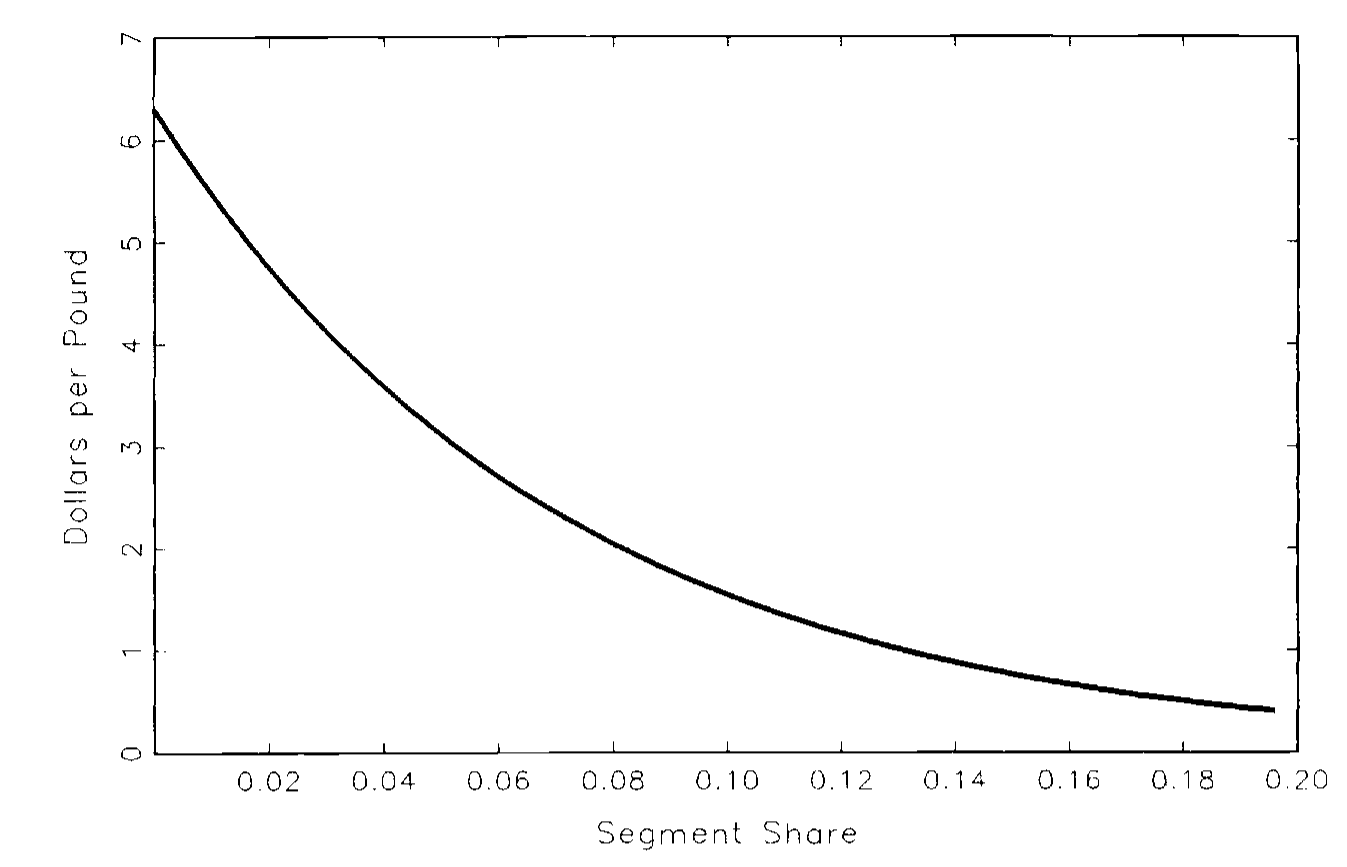
\includegraphics[width=\textwidth]{figures/ch10/hausman_fig5_1.png}
\caption{Method 1: demand at average regressors}
\end{subfigure}\hfill
\begin{subfigure}[t]{0.49\textwidth}
\centering
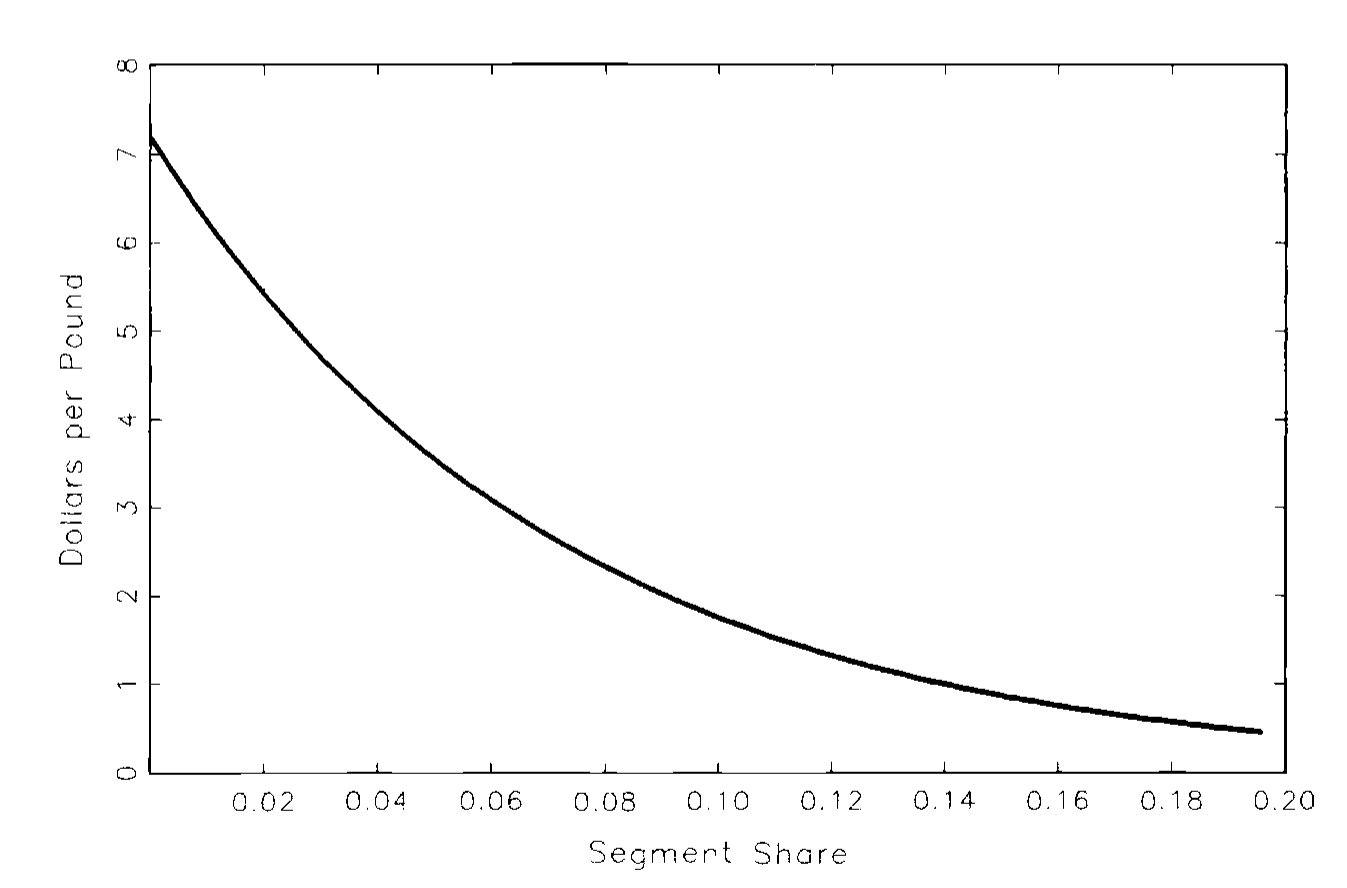
\includegraphics[width=\textwidth]{figures/ch10/hausman_fig5_2.png}
\caption{Method 2: average of 959 city-week curves}
\end{subfigure}
\caption{Estimated AIDS demand curves for Apple-Cinnamon Cheerios. The horizontal axis is ACC's share of
family-segment spending and the vertical axis is the price in dollars per pound. The intercept on the price
axis is the virtual price. Source: Hausman (1997), Figures 5.1 and 5.2.}
\label{fig:10-hausman-aids-curves}
\end{figure}

\casehead{Virtual price}
City virtual prices range from about \$6.00 to about \$7.50. Hausman's best estimate of the aggregate
virtual price is \$7.14, with an asymptotic standard error of \$1.33 (p.~227). The lower end of an
approximate 95 percent confidence interval is \$4.75. Hausman describes it as 35 percent above ACC's average
price of \$3.48 (36.5 percent by our computation).\footnote{A symmetric normal interval would give
$7.14 - 1.96\times 1.33 = \$4.53$ (our computation). Hausman does not say how he computes \$4.75.} The virtual price is about twice the actual price. Hausman finds this reasonable given an own
elasticity of about $-2.2$ (p.~228).

\casehead{Exact consumer surplus}
The exact compensating variation is computed from the expenditure function, by the method of
\citet{HausmanNewey1995} (fn.~24). It is close to the area under the demand curve above \$3.48. The estimate
is \$32,268 per city per week, with an asymptotic standard error of \$3,384 (p.~228). For the United States
it amounts to about \$78.1 million per year, or about \$0.3136 per person per year. Hausman anticipates the
objection that his method yields small elasticities. The same technique gives own-price elasticities for
beer brands between about $-4.0$ and $-6.2$ in \citet{HausmanLeonardZona1994} (fn.~25).

\casehead{A bound robust to extrapolation}
Observed prices never come near the virtual price, so \$7.14 rests on the shape of the estimated curve far
outside the data. Hausman addresses this with a supporting line. If demand is convex, the tangent at the
observed point lies below the curve and meets the price axis below the true intercept. This is the logic of
\cref{prop:10-tangent}. Drawing the tangent to the curves of \cref{fig:10-hausman-aids-curves} at \$3.48
gives lower bounds between \$5.55 and \$5.94, with a standard error of about \$0.15 (p.~228). The bounds lie
about 65 percent above the average price.\footnote{The tangents are drawn in the share-price plane of the
figures. In the quantity-price plane, \cref{prop:10-tangent} with ACC's overall elasticity of $-2.173$ gives
$3.48\bigl(1 + \frac{1}{2.173}\bigr) = \$5.08$ (our computation). Convexity in one plane does not imply
convexity in the other, since the share is proportional to price times quantity.}

\casehead{Two consistency checks}
Two checks of our own relate these numbers to the theory of \cref{sec:10-virtual}. Hausman's pound volumes
and prices imply family-segment spending of about \$1.14 million per city-week, so ACC sells about 20,300
pounds a week in a typical city.\footnote{We compute these figures from Table 5.2 and p.~234. Cheerios sells 93,738
pounds at \$2.644 with a segment share of 0.216, and Honey-Nut sells 47,215 pounds at \$3.605 with a share of
0.150. The two imply segment spending of \$1.147 and \$1.133 million. ACC's volume is
$\frac{0.0619 \times 1.14\text{ million}}{3.48}$.} First, the Paasche rectangle of
\cref{prop:10-index-bounds} is $(7.14 - 3.48)\times 20{,}300 \approx \$74{,}200$. The exact surplus,
\$32,268, is 43 percent of it. A linear Hicksian curve would give exactly half, and a convex curve lies below
the chord, so the share below one half is what convexity predicts. Second, the rectangle is about 1.7 percent
of cereal spending, which matches the index effect Hausman reports below.

\begin{table}[htbp]
\centering
\caption{Welfare effects of Apple-Cinnamon Cheerios}\label{tab:10-hausman-welfare}
\begin{threeparttable}
\begin{tabular}{@{}lll@{}}
\toprule
Quantity & Estimate & Page \\
\midrule
\multicolumn{3}{@{}l}{\textit{Perfect competition (AIDS)}} \\
Virtual price, aggregate & \$7.14 (1.33) & 227 \\
Virtual price, range across cities & \$6.00 to \$7.50 & 227 \\
Lower end of approximate 95\% interval & \$4.75 & 227 \\
Tangent lower bound on virtual price & \$5.55 to \$5.94 (about 0.15) & 228 \\
Consumer surplus per city per week & \$32,268 (3,384) & 228 \\
Consumer surplus, United States, per year & \$78.1 million & 228 \\
Consumer surplus per person per year & \$0.3136 & 228 \\[2pt]
\multicolumn{3}{@{}l}{\textit{Alternative specification}} \\
CES virtual price & infinite & 231 \\
CES consumer surplus & about $3 \times$ AIDS & 231 \\[2pt]
\multicolumn{3}{@{}l}{\textit{Imperfect competition (rivals' prices fixed)}} \\
Loss from higher Cheerios prices, city-week & \$890 + \$3,715 = \$4,605 & 234 \\
Net gain per city-week & \$27,395 (85.6\% of \$32,000) & 234 \\
Net gain, United States, per year & \$66.8 million, \$0.268 per person & 234 \\[2pt]
\multicolumn{3}{@{}l}{\textit{Cereal price index}} \\
Overstatement, perfect competition & about 25\% & 229 \\
Overstatement, imperfect competition & about 20\% & 234 \\
\bottomrule
\end{tabular}
\begin{tablenotes}[flushleft]\footnotesize
\item Notes: Compiled from the text of \citet{Hausman1997}, pp.~227--234. Asymptotic standard errors in
parentheses. The net gain uses a rounded perfect-competition surplus of \$32,000. The index overstatements
refer to the cumulative effect of brands introduced over ten years.
\end{tablenotes}
\end{threeparttable}
\end{table}

\Cref{tab:10-hausman-welfare} collects the welfare results of the paper.

\subsection{Implications for the cereal price index}\label{sec:10-hausman-index}

Hausman translates the surplus into a price-index correction (pp.~228--229). Treating ACC as part of
Honey-Nut Cheerios would show almost no effect, beyond ACC's slightly lower price. Suppose instead, contrary
to fact, that all of ACC's share came from Honey-Nut. With ACC valued at its virtual price before
the introduction, the price index of the two brands falls from about \$4.60 to about \$3.57, or 22 percent. The
family-segment index falls from \$3.10 to \$2.88, or 7.1 percent. The overall cereal index falls by about
0.017, or \$0.052, about 1.7 percent. These figures are share-weighted average prices with ACC valued at
\$7.14 in the base period.\footnote{We approximately reproduce these figures from Table 5.2. The Honey-Nut and
ACC composite is $\frac{15.03 \times 3.605 + 6.19 \times 7.14}{21.22} = \$4.64$ before and
$\frac{15.03 \times 3.605 + 6.19 \times 3.48}{21.22} = \$3.57$ after, a fall of 23 percent. The family index is
\$2.88 with ACC at \$3.48 and \$3.11 with ACC at \$7.14. The small gaps from Hausman's \$4.60, 22 percent and
\$3.10 presumably reflect rounding.}

Hausman then states a rule of thumb. The change in the overall index is approximately ACC's share of cereal
spending, 1.6 percent, times the gap between the virtual and the actual price relative to the actual price.
If the virtual price is twice the actual price, the index change roughly equals the new brand's share. About
25 percent of cereal demand comes from brands introduced in the previous ten years. Suppose these brands sell
at about the same prices as old ones and have virtual prices twice their actual prices. Then the cereal index
that ignores them is too high by about their share, 25 percent (p.~229). Exits reduce the gain, but brands
are withdrawn only when their shares are tiny, so the correction is small and could not be estimated
(fn.~26).

The rule of thumb is the Paasche rectangle of \cref{prop:10-index-bounds}, expressed as a share of spending:
$w_n\bigl(\frac{p_n^V}{p_n} - 1\bigr)$. The proposition shows that this rectangle exceeds the exact gain for
any downward-sloping Hicksian curve. Hausman's own surplus estimate is 43 percent of the rectangle, about
0.75 percent of cereal spending against the 1.7 percent of the rule. Applying the same ratio to his
extrapolation would cut the 25 percent figure to about 11 percent, and the imperfect-competition figure of
20 percent to about 9 percent.\footnote{We compute $0.435 \times 25 = 10.9$ and
$0.435 \times 0.856 \times 25 = 9.3$. The extrapolation also assumes that every new brand of the decade
resembles ACC, a strong assumption that Hausman calls ``perhaps unrealistic'' (p.~229).} The correction
remains large by the standards of price measurement. The main conclusion survives, but the rectangle
overstates the exact effect by a factor of about two.

\subsection{Alternative specifications: attributes, logit and CES}\label{sec:10-hausman-ces}

Section 5.5 of the paper explains why Hausman prefers a flexible product-space system. Attribute models in
the Hotelling, Gorman and Lancaster tradition describe a product by its characteristics and predict demand
for new products from them (\citealp[fn.~27]{Hausman1997}, citing \citealp{PakesBerryLevinsohn1993}).
Hausman argues that ACC cannot be described by attributes, ``perhaps the volume of apples and cinnamon''
(p.~229). He adds that no metric measures how close attributes are and no aggregator combines them. The
right measure of closeness, in his view, is the cross-price elasticity. His experience with probit models of
French champagne makes the point: ``the bubble content could never be made to come in significant'' (fn.~28,
on the models of \citealp{HausmanWise1978}). The logit model has the independence of irrelevant alternatives
(IIA) property, which ``typically leads to a vast overestimate'' of the surplus from a new good (p.~230). The
nested logit still has IIA within each nest. \Cref{sec:10-charspace} takes up the case for characteristics
models.

\casehead{CES demand}
Hausman compares his estimates with the constant elasticity of substitution (CES) model of
\citet{DixitStiglitz1977}, which treats all goods symmetrically. Utility is
\begin{equation}\label{eq:10-h-ces-u}
  U(x_1,\dots,x_n) = \Bigl(\sum_{i=1}^{n}x_i^{\rho}\Bigr)^{\frac{1}{\rho}}, \qquad 0 < \rho < 1
\end{equation}
(Hausman's eq.~9). Write $\eta = \frac{1}{1-\rho}$ for the elasticity of substitution, so that
$1 - \eta = -\frac{\rho}{1-\rho}$. Maximizing \eqref{eq:10-h-ces-u} subject to $\sum_i p_ix_i = y$ gives the
Marshallian demand implied by \eqref{eq:10-ces-share} with equal taste parameters,
\begin{equation}\label{eq:10-h-ces-demand}
  x_k = \frac{y\,p_k^{-\eta}}{\sum_{i=1}^{n}p_i^{1-\eta}}.
\end{equation}
Hausman's eq.~10 writes the compensated version. The unit expenditure function is
$c(p) = \bigl(\sum_ip_i^{1-\eta}\bigr)^{\frac{1}{1-\eta}}$, and Hicksian demand is
$x_k = U\bigl(\frac{p_k}{c(p)}\bigr)^{-\eta} = U\,p_k^{-\eta}\bigl(\sum_ip_i^{1-\eta}\bigr)^{-\frac{\eta}{\eta-1}}$.
Since $\frac{\eta}{\eta-1} = \frac{1}{\rho}$, this equals
$\bigl[\frac{\sum_ix_i^{\rho}}{\sum_ip_i^{-\frac{\rho}{1-\rho}}}\bigr]^{\frac{1}{\rho}}p_k^{-\frac{1}{1-\rho}}$, which
is eq.~10 without its error term. Taking logs of \eqref{eq:10-h-ces-demand},
$\ln x_k = \ln y - \eta\ln p_k - \ln\sum_ip_i^{1-\eta}$. Differentiating with respect to $\ln p_j$ and writing
$w_j = \frac{p_j^{1-\eta}}{\sum_ip_i^{1-\eta}}$ for the spending share,
\begin{equation}\label{eq:10-h-ces-elast}
  \varepsilon_{kj} = -\eta\,\indic\{k = j\} + (\eta - 1)w_j.
\end{equation}
Every product has the same cross elasticity with respect to $p_j$, which is Hausman's eq.~11. Own elasticities
depend only on the share and on $\eta$, ``a property without any empirical foundation'' (p.~231). Demand
\eqref{eq:10-h-ces-demand} is positive at every finite price, so the CES virtual price is infinite.

\casehead{Estimates}
Hausman estimates the CES model by nonlinear two-stage least squares (p.~231). He reports
$\hat\rho = 0.580$ with an asymptotic standard error of 0.00001 and an elasticity of substitution of 2.13.
The two printed numbers are inconsistent, since $\frac{1}{1 - 0.580} = 2.38$, while 2.13 corresponds to
$\rho = 0.53$. We cannot tell which is the typographical error. \Cref{fig:10-hausman-ces} shows the
estimated CES curve. It rises steeply as the share approaches zero and never meets the price axis. The
consumer surplus, the area under this curve above the price, is ``about three times as high'' as the AIDS
estimate of \$78.1 million a year (p.~231).

\begin{figure}[htbp]
\centering
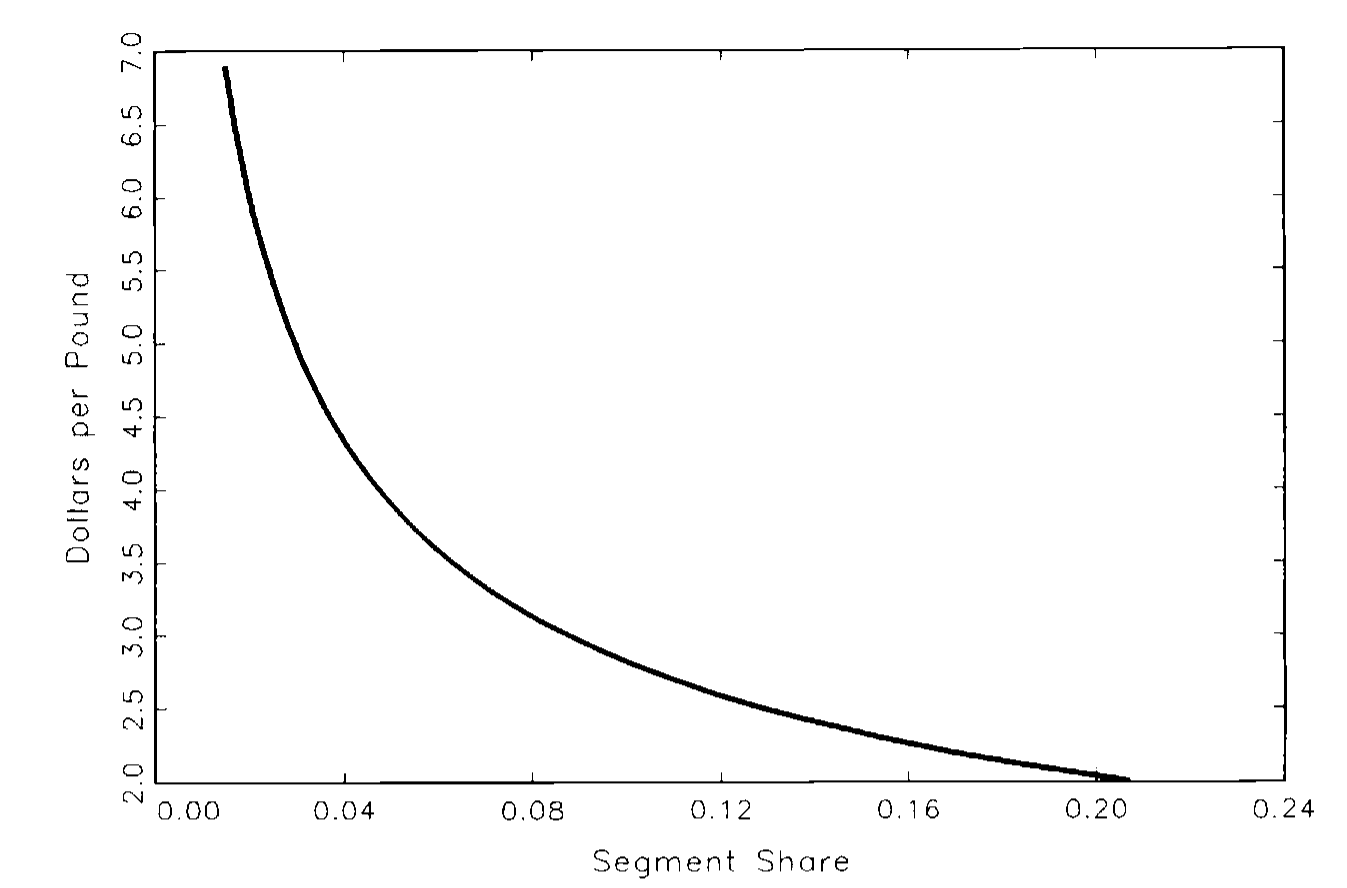
\includegraphics[width=0.75\textwidth]{figures/ch10/hausman_fig5_3.png}
\caption{Estimated CES demand curve for family-segment brands. The horizontal axis is the segment share and
the vertical axis the price in dollars per pound. The curve never meets the price axis, so the virtual price
is infinite. Source: Hausman (1997), Figure 5.3.}
\label{fig:10-hausman-ces}
\end{figure}

The comparison teaches a lesson about functional form. At ACC's segment share of 0.0619,
\eqref{eq:10-h-ces-elast} gives an own elasticity of $-2.13 + 1.13 \times 0.0619 = -2.06$ with $\eta = 2.13$.
This is close to the AIDS value of $-2.12$. The two systems thus give similar own elasticities at the data and diverge
mainly in the extrapolation to zero quantity. The share-only CES formula of \cref{cor:10-ces-newgood} implies,
as computed in \cref{sec:10-feenstra}, that ACC lowers the cost of living of the family segment by 5.5 percent.
The equivalent variation is then 5.5 percent of family-segment spending, about \$63,000 per city-week, and the
compensating variation is 5.8 percent. Both are about twice the AIDS surplus. With $\eta = 2.38$ the fall in the
cost of living is 4.5 percent.\footnote{These are our computations,
using segment spending of \$1.14 million per city-week. Hausman's ``three times'' integrates his estimated
CES curve, so the two comparisons are not identical. Both put the CES valuation at a multiple of the AIDS
valuation.} In the CES and the logit, the value of variety is built into the functional form. The AIDS
lets the data choose a finite virtual price, at the cost of relying on the curvature of the estimated curve.

\subsection{Imperfect competition}\label{sec:10-hausman-imperfect}

The classical analysis assumes that other prices stay at marginal cost when the new good arrives. Hausman
notes that most new brands come from multiproduct firms (p.~231). When General Mills raises the price of
Cheerios, some of the lost buyers now switch to ACC instead of a rival brand. The firm keeps that demand, so
the introduction lets it raise the prices of its existing brands. This effect lowers the consumer gain.

\casehead{Pricing equations}
\Cref{sec:10-multiproduct} derives Hausman's pricing equations in the notation of this chapter. A single-product
firm under Nash-Bertrand pricing sets $\frac{p_1 - mc_1}{p_1} = -\frac{1}{\varepsilon_{11}}$ (Hausman's eq.~12). A
firm selling brands $k = 1,\dots,K$ satisfies the elasticity form \eqref{eq:10-foc-elast} of its first-order
conditions (his eq.~13), with $w_k$ the revenue share of brand $k$ in the firm's sales. In matrix form these are
\eqref{eq:10-foc-matrix}, $w + E^\top m = 0$ and $m = -(E^\top)^{-1}w$ (his eqs.~14 and 15), where
$m_k = \frac{p_k - mc_k}{p_k}w_k$. Dividing each $m_k$ by $w_k$ gives the Lerner index of brand $k$.

\casehead{The calculation}
Hausman solves \eqref{eq:10-foc-matrix} for the General Mills family brands with ACC and without it. He
holds marginal costs constant and assumes that ``other firms, such as Kellogg, will not change their prices
in response to the introduction'' (p.~234). He claims that the resulting price changes are ``a lower bound
on expected price changes, absent new entry by competitors'' (p.~233). \Cref{tab:10-hausman-margins}
reproduces the results.

\begin{table}[htbp]
\centering
\caption{Nash-Bertrand price-cost margins of the General Mills family brands}\label{tab:10-hausman-margins}
\begin{threeparttable}
\begin{tabular}{@{}lcc@{}}
\toprule
 & Cheerios & Honey-Nut Cheerios \\
\midrule
Price-cost margin & 0.5268 & 0.5203 \\
Price-cost margin without Apple-Cinnamon Cheerios & 0.5251 & 0.5096 \\
Price-cost margin if brand were independent & 0.5193 & 0.5050 \\
\bottomrule
\end{tabular}
\begin{tablenotes}[flushleft]\footnotesize
\item Notes: Reproduced in full from \citet[Table 5.7]{Hausman1997}. Margins are Lerner indexes
$\frac{p - mc}{p}$ from \eqref{eq:10-foc-matrix}. The last row is $-\frac{1}{\varepsilon_{jj}}$ with the overall
own elasticities of Table 5.6: $\frac{1}{1.92572} = 0.5193$ and $\frac{1}{1.98037} = 0.5050$. Rivals' prices
and marginal costs are held fixed.
\end{tablenotes}
\end{threeparttable}
\end{table}

The margins rise when ACC joins the line, and they exceed the single-product margins of the last row. With
constant marginal cost, \eqref{eq:10-price-ratio} converts the margins into the ratio
$r_k = \frac{p_k^{\text{with}}}{p_k^{\text{without}}}$ of the prices with and without ACC. The 1992 prices of
Table 5.2 are observed with ACC on the market. The price without ACC is therefore $\frac{p_k^{\text{with}}}{r_k}$,
and the price increase is $p_k^{\text{with}} - \frac{p_k^{\text{with}}}{r_k} = p_k^{\text{with}}\bigl(1 - \frac{1}{r_k}\bigr)$.
For Cheerios, the ratio is $\frac{1 - 0.5251}{1 - 0.5268} = \frac{0.4749}{0.4732} = 1.0036$. At the 1992 price of \$2.644
the increase is $2.644 \times \bigl(1 - \frac{0.4732}{0.4749}\bigr) = \$0.0095$. For Honey-Nut, the ratio is
$\frac{0.4904}{0.4797} = 1.0223$, and at \$3.605 the increase is
$3.605 \times \bigl(1 - \frac{0.4797}{0.4904}\bigr) = \$0.0787$. Both are the figures Hausman
reports.\footnote{This is our computation. The implied prices without ACC are \$2.635 and \$3.526. The paper
also reports markup increases of 0.32 and 3.0 percent. The first is the ratio of the Cheerios
margins, $\frac{0.5268}{0.5251} = 1.0032$. The same ratio for Honey-Nut is 1.021.} The larger effect on
Honey-Nut is expected, since ACC is a closer substitute for Honey-Nut than for Cheerios.

\casehead{Welfare}
Average weekly sales per city are 93,738 pounds of Cheerios and 47,215 pounds of Honey-Nut (p.~234). To first
order, the price increases cost consumers $0.0095 \times 93{,}738 = \$890$ and $0.0787 \times 47{,}215 =
\$3{,}715$ per city-week, a total of \$4,605. Hausman compares this loss with ``the \$32,000--44,000 consumer's
surplus estimates''. The net gain is $\$32{,}000 - \$4{,}605 = \$27{,}395$, which is 85.6 percent of the
Hicksian gain (p.~234). Per year the gain is \$66.8 million, or \$0.268 per person. The overstatement of the
cereal CPI falls from about 25 percent to about 20 percent. Hausman notes that his data begin after ACC's
launch, so he cannot compare prices before and after it directly. He leaves such a study for future research
(p.~234).

\casehead{What the calculation holds fixed}
Reproducing Table 5.7 shows exactly what the counterfactual changes. The ``without'' row deletes ACC's row and
column from the elasticity matrix and ACC's entry from the share vector. It keeps the shares and elasticities
of Cheerios and Honey-Nut at their values with ACC present.\footnote{This is our computation. We solve
\eqref{eq:10-foc-matrix} with the mean revenue shares of Table 5.5 and the Cheerios block of Table 5.6. The
solution reproduces the four margins in the first two rows of Table 5.7 to four decimals.} In the language of
\cref{sec:10-imperfect}, the calculation captures only the new term that ACC adds to the first-order
conditions. Before the launch, Cheerios and Honey-Nut had larger shares. The fall in their shares is the
source of the two offsetting effects that \citet{Bresnahan1997} stresses, and the calculation omits it.
Rivals' prices are held fixed as well. \Cref{sec:10-bresnahan-competition}
returns to both points.

\begin{remark}[The orientation of the elasticity matrix in Table 5.7]\label{rem:10-margins-orientation}
Table 5.7 is reproduced exactly when Table 5.6 is read with rows as quantities, the layout that
\eqref{eq:10-foc-matrix} requires. \Cref{rem:10-orientation} shows that Table 5.6 is printed with rows as
prices. The two facts together imply that the margins were computed with $\varepsilon_{jk}$ where
\eqref{eq:10-foc-elast} requires $\varepsilon_{kj}$. Recomputing with the layout implied by
\cref{rem:10-orientation}, and changing nothing else, gives margins with ACC of 0.5250 (Cheerios), 0.5402
(Honey-Nut) and 0.5251 (ACC), and without ACC of 0.5215 and 0.5169. Relative to the prices without ACC,
the implied increases are 0.7 percent for Cheerios and 5.1 percent for Honey-Nut. In dollars,
$p_k^{\text{with}}\bigl(1 - \frac{1}{r_k}\bigr)$ gives \$0.0192 and \$0.1739 per pound. The first-order loss becomes
\$10,004 per city-week, and the net gain 68.7 percent of \$32,000.\footnote{We computed these values with
\texttt{figures/ch10/src/hausman\_reproduction.py}. With the printed layout, the same program gives ACC's own
margin as 0.6201, a value the paper does not report.} The direction is intuitive. In Honey-Nut's first-order
condition the relevant cross effect is the response of ACC's volume to Honey-Nut's price, which is 0.21. The
printed layout uses instead the response of Honey-Nut's volume to ACC's price, which is 0.08. We offer this
as a reproduction exercise, since the paper itself does not confirm our reading of Table 5.6. It shows that
the imperfect-competition adjustment is sensitive to a detail that papers rarely state, the layout of the
elasticity matrix.
\end{remark}

\subsection{Robustness}\label{sec:10-hausman-robustness}

The paper reports several robustness checks, mostly in footnotes. Monthly data give elasticities similar to
the weekly estimates, with less precision (fn.~21). The segmentation is not rejected by specification tests
(fn.~22). A middle level that does not impose exact two-stage budgeting gives similar results (fn.~17). The
choice between exact and Stone segment indexes ``does not typically have much influence'' (p.~218). The two
aggregation methods for the virtual price give intercepts of about \$6.30 and \$7.20. The tangent bound
limits the role of extrapolation, and the CES comparison shows the direction of functional-form bias.

Other checks are missing. The paper reports no estimates with alternative instruments, no first-stage
statistics and no outcome of the overidentification tests that fn.~20 mentions. It reports no test of the
independence of demand shocks across cities, the assumption on which identification rests. Table 5.7 has no
standard errors, and the imperfect-competition calculation fixes rivals' prices without a sensitivity
analysis. \Cref{sec:10-bresnahan} shows why the first omission matters most.

\subsection{Interpretation, critiques and contribution}\label{sec:10-hausman-assessment}

Taken at face value, the estimates say that consumers value even a close variant of existing brands
highly. ACC's demand curve is steep relative to its volume. The virtual price is twice the actual price, and
the surplus is about 46 percent of ACC's revenue.\footnote{By our computation, the surplus of \$32,268 compares with revenue of
about \$70,600 per city-week.} If incremental brands are typical, official price indexes for branded
consumer goods understate real income growth.

Four lines of critique follow from the theory of this chapter. First, the estimates rest on instruments that
fail if national demand shocks move prices in all cities at once (\cref{sec:10-bresnahan-iv}). Second, the
virtual price is an extrapolation, and the surplus depends on the curvature of the AIDS curve beyond the data
(\cref{sec:10-functional}). The tangent bound helps, but it requires convexity. Third, the
imperfect-competition adjustment holds rivals' prices fixed and keeps post-launch shares in the
counterfactual (\cref{sec:10-bresnahan-competition}). Fourth, the price-index extrapolation uses the Paasche
rectangle, which exceeds the exact gain, and assumes that all new brands resemble ACC
(\cref{sec:10-hausman-index}).

The paper made several contributions. It showed how to compute the exact value of a new brand from scanner
data. It combined the virtual price of \citet{Hicks1940} and \citet{Rothbarth1941} with the exact surplus
methods of \citet{Hausman1981} and \citet{HausmanNewey1995}. Together with \citet{HausmanLeonardZona1994}, it
made multistage budgeting with an unrestricted bottom level a practical tool. The two papers also introduced
prices in other markets as instruments, now a standard device in demand estimation \citep{Nevo2001}. Finally, it raised the question of how market power changes the value of
a new good. The answer it gave was incomplete, as the next section explains, but the question has shaped the
literature since, including the work of \citet{Petrin2002} in \cref{sec:10-petrin}.

\section{Bresnahan's Comment: instruments and competition}\label{sec:10-bresnahan}

\citet{Bresnahan1997} accepts the importance of the question and much of the specification. He disputes
the instruments and the treatment of competition. His comment opens with a statistic: \emph{Brandweek}
counted over 22,000 new-product introductions in 1994 (p.~237). Theory cannot say whether markets supply too
many or too few varieties (fn.~1, quoting \citealp{EatonLipsey1989}, as discussed in \cref{sec:10-private-social}).
So the value of incremental variety is an empirical question, and Hausman's paper is an important attempt to
answer it. This section develops Bresnahan's four points in turn, with the formal
analysis that he sketches in his appendix.

\subsection{Why a steep single-product demand curve means large value}\label{sec:10-bresnahan-dd}

Bresnahan frames the issue with \cref{fig:10-dd-DD}. The steep curve $DD$ is market demand. The flatter
curve $dd$ is the demand for one product when the prices of its substitutes are held fixed. The flat line
$dd(-\infty)$ is the demand for a product that is a perfect substitute for others. Introducing a product at
price $P_1$ creates the shaded triangle between $dd$, the price axis and the line at $P_1$. Before the
introduction the product was in effect priced at $P_0$, where $dd$ meets the price axis. This is the virtual
price of \cref{sec:10-virtual}.

\begin{figure}[htbp]
\centering
\begin{tikzpicture}[scale=1.0, >=Stealth]
  \draw[->] (0,0) -- (7.4,0) node[below] {$Q$};
  \draw[->] (0,0) -- (0,5.4) node[left] {$P$};
  \fill[black!70] (0,4) -- (0,2.9) -- (2.383,2.9) -- cycle;
  \draw[thick] (1.6,5.0) -- (5.3,0.17) node[right] {$DD$};
  \node at (1.95,5.15) {$DD$};
  \draw[thick] (0,4) -- (6.8,0.862) node[right] {$dd$};
  \node at (0.95,3.8) {$dd$};
  \draw[thick] (0,2.311) -- (7.0,2.311) node[right] {$dd(-\infty)$};
  \draw[dashed] (2.383,2.9) -- (2.383,0);
  \node[left] at (0,4) {$P_0$};
  \node[left] at (0,2.9) {$P_1$};
  \node[below] at (2.383,0) {$q_1$};
  \fill (3.659,2.311) circle (1.5pt);
\end{tikzpicture}
\caption{Consumers' gain from a new product. $DD$ is market demand, $dd$ the demand for a single product at
fixed prices of its substitutes, and $dd(-\infty)$ the demand for a perfect substitute. Selling the product
at $P_1$ instead of its choke price $P_0$ yields the shaded surplus. The steeper is $dd$, the larger the
triangle for a given volume $q_1$. Source: redrawn after Bresnahan (1997), Figure 5C.1.}
\label{fig:10-dd-DD}
\end{figure}

The area of the triangle makes the point precise. Let $dd$ be linear with slope $-s$ in the $(Q, P)$ plane,
where $s > 0$ measures its steepness. A product sold at $P_1$ in volume $q_1$ then has choke price
$P_0 = P_1 + s\,q_1$. Its surplus is
\begin{equation}\label{eq:10-b-triangle}
  CS = \frac{1}{2}(P_0 - P_1)\,q_1 = \frac{s}{2}\,q_1^2.
\end{equation}
For a given volume the surplus is proportional to the steepness $s$, and it vanishes as $dd$ flattens to
$dd(-\infty)$. Treating new goods as perfect substitutes, as hedonic quality adjustment implicitly does,
therefore sets their value to zero. Linking a new good into a price index late treats it as irrelevant in
its early life, and the later the link, the larger the error (p.~238). Both practices understate the value
of new goods. Bresnahan notes a converse in fn.~2. If a new good is a perfect substitute, the law of one price
holds, and late linking does no harm.

Hausman's finding is a steep $dd$ for ACC. \citet{Trajtenberg1989}, whose work \cref{sec:10-trajtenberg}
studies, conjectured that the distance of a new good from existing products in characteristics space governs
the slope of $dd$ (fn.~3). The same steepness has a second implication, developed in
\cref{sec:10-bresnahan-competition}. A product with a steep $dd$ that is sold by one firm carries market
power. Consumer surplus and imperfect competition are therefore linked from the start.

\subsection{Is the large surplus an artifact of the specification?}\label{sec:10-bresnahan-spec}

Bresnahan concludes that it is not (pp.~239--240). A skeptic might suspect that existing Cheerios products
already satisfy ``pretty much any palate''. Hausman's large surplus must then come from finding poor
substitutability between ACC and the other family brands. Within the segment, the AIDS imposes almost no
structure on own and cross elasticities, so the finding comes from the data. The more restrictive CES gives
an even larger surplus (fn.~4).

The segment structure is an assumption, which Bresnahan does not find worrying. It is not interesting to
ask whether two children's cereals substitute more closely than a children's cereal and Special K. The
segments come from marketing research based on richer data, including consumer microdata. Bresnahan adds a
caution for other industries (fn.~5). In automobiles, brand names and country reputations compete with size
classes as principles of grouping, and in many consumer goods private labels form a further group. The
simple structure of cereal is the exception.

\subsection{Instruments and national demand shocks}\label{sec:10-bresnahan-iv}

The treatment of price endogeneity is the other place where the conclusion might have been ``accidentally
assumed'' (p.~240). Hausman's identifying assumption is that the shocks $\omega_{jnt}$ in
\eqref{eq:10-h-price} are independent across cities. This rules out every national shock to the demand for
one brand relative to another. In Bresnahan's words, ``there can be no successful nationwide advertising
campaigns which shift the demand for individual brands or products'' (p.~241). There can be no national
fads and no slow national acceptance of new brands. Including advertising in the demand system does not
solve the problem, because the econometrician does not observe which campaigns succeed (fn.~6).

Hausman's fallback is that prices are predetermined. Economically, this requires that national demand shocks
cannot be foreseen when prices are set. Bresnahan finds this unlikely for shocks such as advertising
campaigns, which manufacturers plan and communicate to retailers in advance. If national shocks exist and
are reflected in prices, and if supply slopes up, prices in other cities are correlated with the demand
error. Supply slopes up in the one-week run because inventories cannot adjust or because of market power
(fn.~7). Hausman's own pricing equations imply an upward-sloping supply relation.

\casehead{The model}
We formalize the argument with one product, following Bresnahan's simple case: linear demand, single-product
Bertrand pricing and constant marginal cost (p.~241). In city $n$ and week $t$,
\begin{equation}\label{eq:10-b-demand}
  q_{nt} = d_n - b\,p_{nt} + \xi_{nt}, \qquad b > 0,
\end{equation}
where $d_n$ is a city effect. Marginal cost is $c_{nt} = c_n + k_t + v_{nt}$. The national cost component
$k_t$ has variance $\sigma_k^2$, and the local component $v_{nt}$ has variance $\sigma_v^2$. The demand error
has a national and a local part, $\xi_{nt} = \chi_t + e_{nt}$. Each part splits into a component that is
anticipated when prices are set and one that is not: $\chi_t = \chi^a_t + \chi^u_t$ and
$e_{nt} = e^a_{nt} + e^u_{nt}$, with variances $\sigma_{\chi a}^2$, $\sigma_{\chi u}^2$, $\sigma_{ea}^2$ and
$\sigma_{eu}^2$. All components have mean zero and are mutually independent. Local components are
independent across cities. City effects are removed by the within transformation, so we treat $d_n$ and
$c_n$ as known.

\casehead{Pricing}
The firm sets $p_{nt}$ to maximize expected profit $\E[(p - c_{nt})(d_n - bp + \xi_{nt})\mid\mathcal{I}_{nt}]$,
where the information set $\mathcal{I}_{nt}$ contains costs and the anticipated shocks. The first-order
condition is
\begin{equation*}
  d_n - 2b\,p_{nt} + \E[\xi_{nt}\mid\mathcal{I}_{nt}] + b\,c_{nt} = 0.
\end{equation*}
Solving for the price,
\begin{equation}\label{eq:10-b-price}
  p_{nt} = \frac{1}{2}\Bigl(c_{nt} + \frac{d_n + \chi^a_t + e^a_{nt}}{b}\Bigr).
\end{equation}
Equivalently $p_{nt} = c_{nt} + \frac{\E[q_{nt}\mid\mathcal{I}_{nt}]}{b}$, the expected-quantity version of
Bresnahan's supply relation $P = Q(-\gamma_{jj})^{-1} + c$. With fully anticipated shocks this is his model,
and with no anticipated shocks prices are predetermined in Hausman's sense.

\casehead{Estimators}
The Hausman estimator of $-b$ is the instrumental-variables (IV) estimator that uses $p_{\ell t}$, the
price in another city $\ell\neq n$, as the instrument for $p_{nt}$. Averaging over several other cities, as
our simulation does, has the same probability limit. Ordinary least squares (OLS) regresses $q_{nt}$ on
$p_{nt}$. Both use within-city deviations.

\begin{proposition}[Hausman instruments with national demand shocks]\label{prop:10-hausman-iv-bias}
In the model given by \eqref{eq:10-b-demand} and \eqref{eq:10-b-price}, define
\begin{equation*}
  \lambda = \frac{\sigma_{\chi a}^2}{b^2\sigma_k^2 + \sigma_{\chi a}^2}, \qquad
  \lambda_{OLS} = \frac{\sigma_{\chi a}^2 + \sigma_{ea}^2}{b^2(\sigma_k^2 + \sigma_v^2) + \sigma_{\chi a}^2 + \sigma_{ea}^2}.
\end{equation*}
Then, as the number of weeks grows,
\begin{equation}\label{eq:10-b-plim}
  \plim\hat b_{IV} = b(1 - 2\lambda), \qquad \plim\hat b_{OLS} = b(1 - 2\lambda_{OLS}).
\end{equation}
Consequently, the following hold.
\begin{enumerate}[label=(\alph*)]
\item The IV estimator is consistent if and only if there are no anticipated national demand shocks,
$\sigma_{\chi a}^2 = 0$. Local shocks, anticipated or not, cause no bias.
\item If $\sigma_{\chi a}^2 > 0$, the estimated demand curve is too steep. If $\sigma_{\chi a}^2 > b^2\sigma_k^2$,
the estimated slope has the wrong sign.
\item Let $\lambda < \frac{1}{2}$, and take linear demand through the observed point $(p, q)$. The implied consumer surplus
$\frac{q^2}{2\hat b}$ and the implied gap $\frac{q}{\hat b}$ between the virtual and the actual price are
both overstated by the factor $\frac{1}{1 - 2\lambda}$.
\item The IV estimator is less biased than OLS if and only if $\lambda < \lambda_{OLS}$.
\end{enumerate}
\end{proposition}

\begin{proof}
Work with within-city deviations, so that $d_n$ and $c_n$ drop out. From \eqref{eq:10-b-price}, the deviation
of the price is
\begin{equation*}
  \tilde p_{nt} = \frac{1}{2}\Bigl(k_t + v_{nt} + \frac{\chi^a_t + e^a_{nt}}{b}\Bigr).
\end{equation*}
Substituting into \eqref{eq:10-b-demand}, the IV and OLS estimators of the coefficient $-b$ converge to
\begin{equation*}
  -b + \frac{\Cov(\tilde p_{\ell t},\xi_{nt})}{\Cov(\tilde p_{\ell t},\tilde p_{nt})}
  \qquad\text{and}\qquad
  -b + \frac{\Cov(\tilde p_{nt},\xi_{nt})}{\Var(\tilde p_{nt})}.
\end{equation*}
For the IV estimator take $\ell\neq n$. The price in city $\ell$ shares only the national components $k_t$ and
$\chi^a_t$ with city $n$. Of these, only $\chi^a_t$ is correlated with $\xi_{nt}$. Hence
\begin{equation*}
  \Cov(\tilde p_{\ell t},\xi_{nt}) = \frac{1}{2b}\Cov(\chi^a_t,\chi_t) = \frac{\sigma_{\chi a}^2}{2b},
\end{equation*}
\begin{equation*}
  \Cov(\tilde p_{\ell t},\tilde p_{nt}) = \frac{1}{4}\Bigl(\sigma_k^2 + \frac{\sigma_{\chi a}^2}{b^2}\Bigr)
  = \frac{b^2\sigma_k^2 + \sigma_{\chi a}^2}{4b^2}.
\end{equation*}
The ratio of the two is
\begin{equation*}
  \frac{\sigma_{\chi a}^2}{2b}\cdot\frac{4b^2}{b^2\sigma_k^2 + \sigma_{\chi a}^2} = 2b\lambda.
\end{equation*}
So the IV estimate of $-b$ converges to $-b + 2b\lambda$, and $\plim\hat b_{IV} = b - 2b\lambda = b(1 - 2\lambda)$.
For OLS the same steps apply with all anticipated components:
\begin{equation*}
  \Cov(\tilde p_{nt},\xi_{nt}) = \frac{\sigma_{\chi a}^2 + \sigma_{ea}^2}{2b}, \qquad
  \Var(\tilde p_{nt}) = \frac{b^2(\sigma_k^2 + \sigma_v^2) + \sigma_{\chi a}^2 + \sigma_{ea}^2}{4b^2},
\end{equation*}
and the ratio is $2b\lambda_{OLS}$, which gives $\plim\hat b_{OLS} = b(1 - 2\lambda_{OLS})$.

Part (a) follows because $\lambda = 0$ if and only if $\sigma_{\chi a}^2 = 0$, and $\lambda$ does not depend
on $\sigma_{ea}^2$ or $\sigma_{eu}^2$. For part (b), $\lambda > 0$ gives $\plim\hat b_{IV} < b$, and
$1 - 2\lambda < 0$ if and only if $\lambda > \frac{1}{2}$, which is equivalent to
$\sigma_{\chi a}^2 > b^2\sigma_k^2$. For part (c), linear demand through $(p, q)$ with slope $-\hat b$ meets
the price axis at $p + \frac{q}{\hat b}$, and the triangle above $p$ has area $\frac{q^2}{2\hat b}$. Both are
proportional to $\frac{1}{\hat b}$, so their ratios to the true values converge to
$\frac{b}{\plim\hat b_{IV}} = \frac{1}{1 - 2\lambda}$. Part (d) compares the two biases $2b\lambda$ and
$2b\lambda_{OLS}$.
\end{proof}

The weight $\lambda$ has a direct interpretation. The common price component shared by all cities is
$\frac{1}{2}(k_t + \frac{\chi^a_t}{b})$. Its variance is $\frac{1}{4}(\sigma_k^2 + \frac{\sigma_{\chi a}^2}{b^2})$,
and $\lambda$ is the share of that variance due to national demand shocks. The proposition thus says that
the Hausman estimator is a weighted average of the demand slope and the supply slope. With weight
$1 - \lambda$ the common price variation traces out demand, as Hausman assumes. With weight $\lambda$ it
traces out the supply relation $q = b(p - c)$, whose slope is $+b$. This is Bresnahan's remark that with
national demand shocks the estimator ``is like doing ordinary least squares on a supply and demand system''
(p.~242). \Cref{sec:05-bresnahan-critique} derives the same weight in \eqref{eq:05-iv-bias-scalar}. Our version adds the
distinction between anticipated and unanticipated shocks, the OLS comparison and the welfare consequences.

The welfare consequence is large even for modest violations. Suppose anticipated national demand shocks
account for one quarter of the common price variation, so $\lambda = 0.25$. Then the estimated slope is half
the true slope and the surplus is overstated by a factor of two. A share of 10 percent overstates the surplus
by 25 percent. Part (c) is stated for linear demand. For the convex AIDS curves of
\cref{fig:10-hausman-aids-curves} the mapping is only approximate. A curve that is too steep at the data still
implies too large a surplus.

Part (a) also clarifies the debate about predetermined prices. If no national shock is anticipated, both
estimators are consistent when local shocks are unanticipated as well. IV then adds nothing, as Hausman's
second interpretation says. Bresnahan's objection is that the national shocks most likely to matter, such as
advertising campaigns and promotions, are planned in advance. Planned shocks are precisely the anticipated
component that enters $\lambda$. Neither the data nor the paper distinguish the two cases.

\casehead{Many products}
Bresnahan's appendix treats $J$ products. Write demand as $q_{nt} = d + A\,p_{nt} + \xi_{nt}$, with
$a_{jk} = \frac{\partial q_j}{\partial p_k}$ (his $\gamma$), and single-product Bertrand pricing as
$p_{nt} = c_{nt} + D^{-1}q_{nt}$ with $D = \diag(-a_{11},\dots,-a_{JJ})$. Multiplying the pricing equation by
$D$ and substituting demand gives $Dp_{nt} = Dc_{nt} + d + Ap_{nt} + \xi_{nt}$, so the prices solve
$p_{nt} = (D - A)^{-1}(d + Dc_{nt} + \xi_{nt})$. Bresnahan states that the sign and size of the bias are
governed by $\Sigma^{\mathrm{nat}}[\diag(-\gamma) - \gamma]^{-1}$, where $\Sigma^{\mathrm{nat}}$ is the
covariance matrix of the national demand shocks. This is the covariance between other-city prices and demand
errors. For two products whose national shocks have correlation $\varrho$, his appendix reports that the
on-diagonal bias has the sign of $-2\gamma_{22} + \varrho\gamma_{12}$ and the off-diagonal bias the sign of
$\gamma_{12} - 2\varrho\gamma_{11}$ (p.~247). At $\varrho = 0$ both signs are positive when the goods are
substitutes ($\gamma_{12} > 0$). Bresnahan reads them as a bias of own-price coefficients toward zero and of
cross-price coefficients away from zero. These are signs of the covariance between instruments and demand
errors. With several endogenous prices the bias also involves the inverse of the instrument-price
covariance, so the signs need not carry over. Bresnahan notes that the cross-price claim depends on the
correlation of national shocks across products (fn.~9). \Cref{prop:05-iv-bias} gives the exact probability
limit, $\plim\hat A = (I - \Lambda)A + \Lambda D$ with
$\Lambda = \Sigma^{\mathrm{nat}}(D\Sigma_cD + \Sigma^{\mathrm{nat}})^{-1}$ and $\Sigma_c$ the covariance matrix of
national cost shocks. \Cref{sec:05-bresnahan-critique} also documents typographical slips in the printed
appendix.

The estimate mixes demand slopes with supply slopes. Suppose national demand and cost shocks are uncorrelated
across products, and write $\sigma_{\chi j}^2$ and $\sigma_{cj}^2$ for the diagonal elements of
$\Sigma^{\mathrm{nat}}$ and $\Sigma_c$. Then $\Lambda$ is diagonal with
$\lambda_j = \frac{\sigma_{\chi j}^2}{a_{jj}^2\sigma_{cj}^2 + \sigma_{\chi j}^2}$, so
$\plim\hat a_{jj} = (1 - 2\lambda_j)a_{jj}$ and $\plim\hat a_{jk} = (1 - \lambda_j)a_{jk}$. Own slopes move
toward zero and possibly beyond it, and cross slopes are attenuated. Bresnahan's cross-price reading therefore
fails even at $\varrho = 0$. With correlated national shocks, $\Lambda$ is no longer diagonal. Row $j$ of the
estimate then mixes in the demand and supply slopes of the other products. Cross slopes can be inflated, and
even an own slope can be biased away from zero. For example, the matrices
$A = \bigl(\begin{smallmatrix}-2 & 0.5\\ 0.5 & -1.5\end{smallmatrix}\bigr)$, $\Sigma_c = \diag(5, 0.01)$ and
$\Sigma^{\mathrm{nat}} = 0.4\bigl(\begin{smallmatrix}1 & 0.95\\ 0.95 & 1\end{smallmatrix}\bigr)$ give
$\plim\hat a_{11} = -2.44$, farther from zero than the true $-2$. The own-slope bias is the diagonal element
$2\Lambda_{jj}|a_{jj}| - \sum_{k\neq j}\Lambda_{jk}a_{kj}$ of $\Lambda(D - A)$. The own-price bias toward zero
that drives the surplus therefore holds when $2\Lambda_{jj}|a_{jj}| > \sum_{k\neq j}\Lambda_{jk}a_{kj}$, for
example when national shocks are uncorrelated across products.

\casehead{A Monte Carlo experiment}
\Cref{fig:10-hausman-iv-mc} illustrates \cref{prop:10-hausman-iv-bias} in a panel shaped like Hausman's,
with 7 cities and 137 weeks. All shocks are anticipated. The true slope is $b = 2$, demand shocks have
total variance $\sigma_\chi^2 + \sigma_e^2 = 1$, and cost shocks have $\sigma_k = \sigma_v = 0.5$. The
horizontal axis moves the national share of demand variance from 0 to 0.5 while holding the total fixed. The
instrument is the average price of the product in the other six cities. Each point averages 500
replications. Without national shocks the IV estimator is centered on the truth, while OLS recovers only one
third of the slope. As the national share rises, the IV estimate falls toward the OLS estimate. At a share
of 0.2 it recovers two thirds of the slope and overstates the surplus by half. At a share of 0.5 it is no
better than OLS, and the surplus is overstated threefold.

\begin{figure}[htbp]
\centering
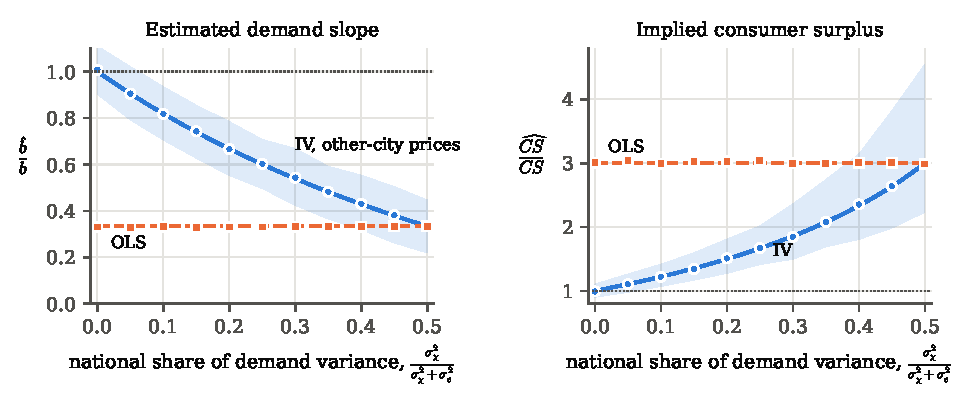
\includegraphics[width=\textwidth]{figures/ch10/hausman_iv_bias.pdf}
\caption{Hausman instruments with national demand shocks, a Monte Carlo experiment. The left panel shows the
estimated demand slope relative to the truth. The right panel shows the implied consumer surplus with linear
demand relative to the truth. Markers are Monte Carlo means (slope) or medians (surplus) over 500
replications. Lines are the probability limits of \cref{prop:10-hausman-iv-bias}, solid for IV and dashed for
OLS. The band shows the 10th to 90th percentiles of the IV estimates. The design has 7 cities, 137 weeks,
$b = 2$, $\sigma_\chi^2 + \sigma_e^2 = 1$ and $\sigma_k = \sigma_v = 0.5$. All shocks are anticipated, and city
fixed effects are removed. The script is \texttt{figures/ch10/src/hausman\_iv\_bias.py}.}
\label{fig:10-hausman-iv-mc}
\end{figure}

Two features of the experiment deserve comment. First, the instrument is strong throughout: the correlation
between a city's price and the other-city average is about 0.5 to 0.65. A strong first stage is no
protection against an invalid instrument. Second, week fixed effects cannot remove the problem for a single
product. They would absorb the national cost shocks as well, and with them all identifying variation. In a
system with many brands, week effects common to all brands absorb only aggregate shocks. Brand-specific
national shocks, the kind Bresnahan describes, remain.

\casehead{Evidence from later work}
\citet{Nevo2001} uses Hausman instruments for cereal in a random-coefficients model (\cref{ch:blp}). His
instruments are regional quarterly average prices of the same brand, excluding the city being instrumented
(p.~321). He discusses exactly Bresnahan's concern. A national demand shock, such as the discovery that fiber
reduces the risk of cancer, would raise the valuation of fiber-rich brands in all cities and violate the
assumption. He argues that the concern is weaker for well-established brands and that time dummies absorb
aggregate shocks. He then compares the price coefficient across instrument sets in his logit regressions
(Table V). With other-city prices it is $-17.57$ (0.50), and with proxies for local marginal cost it is
$-17.12$ (0.49), against $-7.26$ (0.16) by OLS with brand dummies. The two instrument sets agree. Nevo notes,
however, that regional demand shocks would invalidate both, and overidentification tests reject in all
columns except the one with city fixed effects. The comparison is informative, but it cannot rule out
brand-specific national shocks.

\subsection{Imperfect competition is ``off point''}\label{sec:10-bresnahan-competition}

Bresnahan's second criticism concerns economic interpretation (pp.~243--246). Imperfect competition links
new goods and market power in three ways. A new good can create market power for its inventor. It can
destroy market power of competing products. And the transitory market power that results is a reward that
motivates invention.

\casehead{Private returns}
The steep $dd$ that implies a large consumer surplus also implies a large monopoly rent if one firm owns the
product (p.~243). \Cref{rem:10-steep} makes this exact for linear demand, where consumer surplus at the
monopoly price is half the profit. Demand studies of new goods therefore speak to private returns to
innovation as well as social returns. With multiproduct firms and competitive responses, the calculation
needs the whole demand system and a supply model (p.~243).

\casehead{Rivals' prices}
Under imperfect competition among single-product firms, a new product lowers the market power of existing
products and so lowers prices (p.~243). This is one of the classical benefits of competition.
\Cref{sec:10-rival-prices} develops the argument. It proves the result for logit demand
(\cref{prop:10-logit-rivals}) and discusses Bresnahan's two qualifications, that unusual elasticities can
reverse it (fn.~12) and that Bertrand competition reinforces the direct effects (fn.~13).

Hausman holds the prices of Kellogg and Post fixed. Bresnahan calls this ``a common error among those who
are new to models of imperfect competition, but an important one'' (p.~244). The Bertrand solution concept
has firms maximize post-entry profits taking each other's post-entry prices as given. The analyst who
computes the effect of entry cannot take those prices as given, because entry changes the game. Typically
the rivals' prices fall. By holding them fixed, Hausman solves the price-discrimination problem of General
Mills as if it were a monopolist. His claim of a lower bound is therefore wrong, as Hausman's own fn.~32
partly concedes.

\casehead{The multiproduct firm's own prices}
Even for General Mills alone, the direction of the price change is ambiguous. Adding a brand changes the
first-order condition \eqref{eq:10-foc-elast} for an existing brand $j$ in the three ways of
\cref{sec:10-own-prices} (pp.~244--245). The new brand's term favors a higher $p_j$, which is the effect
Hausman stresses. Bresnahan counts the falls in the revenue shares of the existing brands, $w_j$ among them,
as the offsetting effects. At fixed margins and elasticities, only the cannibalization of the firm's other
brands pushes the other way, because it shrinks the positive cross terms. Bresnahan states that with linear demand and a two-product firm the effects exactly offset, and
\cref{prop:10-linear-offset} proves this for any number of products. Any dominance of one effect therefore
comes ``from higher-order derivatives'', and the paper offers no evidence on them (p.~245). The reproduction of Table 5.7 in
\cref{sec:10-hausman-imperfect} makes the point concrete. Hausman's ``without'' margins keep the post-launch
shares of Cheerios and Honey-Nut, so they include the first effect and omit the second and third.

\casehead{Where the action is}
Bresnahan summarizes the possibilities in the two-by-two classification of \cref{tab:10-bresnahan-2x2}.
Hausman's analysis sits in the price-discrimination cell. Bresnahan argues that if the social return is the object of interest, Hausman ``has
quantified the generally far less important effect'' (p.~246). The competition cell, the effect of a new
good on the pricing incentives of rival firms, must in general be much more important.

\casehead{Conclusion}
Bresnahan was left ``unconvinced by key econometric assumptions'' and found the imperfect-competition
analysis ``off point''. To doubt the large single-product surplus may simply be to believe in nationwide
brand-name demand shocks. ``The puzzle of the value of this incremental product introduction remains
unsolved'' (p.~246).

\subsection{Assessment}\label{sec:10-bresnahan-assessment}

Each side of the exchange got something right. Hausman showed that the exact value of a new brand can be
computed from estimated demand, and that a flexible system can deliver a finite virtual price. He also showed
that the answer depends on market structure. Bresnahan showed that the identifying assumption is strong
exactly where the conclusion is sensitive. Own-price slopes biased toward zero produce steep $dd$ curves and
large surplus. He also showed that holding rivals' prices fixed answers a monopoly question, and that the
multiproduct effect itself is ambiguous.

Several kinds of evidence could settle the dispute. Price and quantity data spanning the launch would allow
a direct before-and-after comparison, which Hausman lacked. \citet{HausmanLeonard2002} later made such a
comparison for Kleenex Bath Tissue (KBT), which Kimberly-Clark rolled out across U.S. cities in waves.\footnote{We
checked the numbers in this paragraph against the authors' revised manuscript dated September 1999 (pp.~10--15 and
33--36, and Tables~2, 6 and~7), which thanks the journal's referees and editor. We did not check the published article, whose
page and table numbers may differ.}
They use weekly Nielsen scanner data on the seven largest brands in 30 cities from January 1992 to September 1995.
KBT was already sold in 17 cities when the data begin. It entered three more in July 1993 and the last ten in May
1994. For each incumbent brand they estimate by ordinary least squares
\begin{equation}\label{eq:10-hl-direct}
  \ln p_{ct} = \lambda_c + \omega_t + \beta_1 I_{ct} + \beta_2 M_{ct} + e_{ct},
\end{equation}
where $c$ indexes cities and $t$ weeks, and $\lambda_c$ and $\omega_t$ are city and week fixed effects. The
indicator $I_{ct}$ equals one once KBT is sold in city $c$, and $M_{ct}$ marks the third-wave cities in the weeks
between the second and third waves. The staggered entry separates $\beta_1$ from the common shocks absorbed by
$\omega_t$. All six estimated price effects are negative (Table~2). Cottonelle fell 8.2 percent (standard error
1.3), Charmin and Angel Soft 3.5 percent, private label 3.8 percent and Northern 2.3 percent. The economy brand
ScotTissue fell only 0.6 percent (0.5). Kimberly-Clark had almost no prior share, so this is the competition cell
of Bresnahan's classification, and the prices of rivals fell as he predicts. The authors also predict these
changes from the post-entry demand system under Nash-Bertrand pricing. The predictions are close for four brands
but well short for Cottonelle ($-3.6$ percent) and private label ($-0.7$ percent), where $t$-tests reject equality
(Table~6). Because the comparison gives mixed support, they describe their evidence for Nash-Bertrand pricing as
cautious. The authors put the total consumer
gain at \$69.2 million a year, 7.3 percent of bath tissue spending in the 30 cities (Table~7). About half of it
comes from the lower prices of existing brands (p.~36).
Residuals of the same brand in different cities and the same week can be tested for correlation, the most
direct symptom of national shocks. Overidentification tests across cities, which fn.~20 of Hausman's paper
proposes, could be reported. Instruments from observed local costs offer a comparison, as in
\citet{Nevo2001}. Each check addresses a specific threat. None is a general proof of validity.

The broader literature moved in two directions. One kept product-space demand and looked for better
instruments and data. The other moved to characteristics space \citep{Berry1994,BerryLevinsohnPakes1995}.
There the value of a new product depends on its location relative to existing products, and instruments come
from the characteristics of rivals. That approach has its own extrapolation problem, the idiosyncratic
taste shock that gives every product a positive value, which \cref{sec:10-charspace} analyzes. It also has its
own instrument problem, the assumption that characteristics are exogenous (\cref{ch:discrete}).
\citet{Petrin2002}, studied in \cref{sec:10-petrin}, combines characteristics-space demand with micro data and
recomputes the full Bertrand equilibrium without the new product. His results quantify the competition cell of
Bresnahan's classification, together with the price-discrimination cell.

\section{Valuing new goods in characteristics space}\label{sec:10-charspace}

The methods of \cref{sec:10-virtual,sec:10-functional} value a new good in product space. They estimate the
demand curve of the good itself and integrate under it up to the virtual price. This section treats a product
as a bundle of characteristics instead, in the tradition of \citet{Lancaster1966,Lancaster1971} and
\citet{McFadden1981}. The change of viewpoint has three consequences for welfare measurement. First, a
characteristics model can predict the demand for a product that has never been sold. Second, discrete-choice
models deliver consumer surplus in closed form, so the value of a change in the choice set is a simple function
of estimated parameters. Third, the functional forms that make these models tractable carry strong implicit
assumptions about the value of variety. Most of the section makes those assumptions explicit and compares the
models that impose them with models that do not.

Throughout the section a market has inside products $j = 1,\dots,J$ and an outside good $j = 0$. Consumer $i$
has income $y_i$, and we use the notation of \cref{ch:logit,ch:blp} for mean utilities $\delta_j$, deviations
$\mu_{ij}$ and idiosyncratic shocks $\epsilon_{ij}$. Where we discuss \citet{Trajtenberg1989}, we write
$\mathcal{W}(S)$ for his surplus function over a choice set $S$. We also write $z_j$ for the vector of
characteristics of product $j$ and $\tilde p_j$ for its residual price relative to a hedonic price function.

\subsection{Predicting demand for products that have never been sold}\label{sec:10-cs-predict}

A new product is a new point in characteristics space. Suppose a demand model has been estimated on existing
products, and the new product combines characteristics that lie within the range spanned by them. The estimated
tastes for characteristics then predict the new product's market share at any price, and the equilibrium pricing
conditions of \cref{ch:diffprod} predict its price. A product-space system cannot do this, because its
parameters are indexed by products and the new product has none \citep[pp.~1--2]{BerryPakes2007}. Berry and
Pakes add a second advantage. The number of parameters of a characteristics model does not grow with the number
of products. A log-linear product-space system for $J$ products needs a number of parameters of the order of $J^2$. \Citet{BerryLevinsohnPakes2004} use this property to simulate the demand for products before launch.

The same property disciplines the retrospective valuation of products that already exist. We never observe
demand at prices high enough to reveal the reservation prices of most buyers. Every estimate of the surplus
from a product therefore extrapolates beyond the data \citep[p.~2]{BerryPakes2007}. A product-space system extrapolates the
product's own demand curve to high prices, as in \cref{sec:10-functional}. A characteristics model uses slightly
more information. It borrows the price variation of other products with similar characteristics, although the
functional form still governs the extrapolation.

The approach has three limits. The first is an \emph{entirely new characteristic}, one that no existing product
possesses. Tastes for it cannot be learned from existing products. An electric car, for example, has a range, a
charging time and no fuel cost, so its demand cannot be inferred from the demand for gasoline cars alone. The
second limit is attributes that resist measurement, such as the plot of a book or the style of a film. When the
relevant attributes cannot be coded as a short vector $x_j$, the approach loses its dimension reduction. The third
limit is the \emph{radical innovation}, a product that opens a new product class. \Citet[pp.~10--11]{Trajtenberg1985}\footnote{We cite
\citet{Trajtenberg1989} through its working-paper version \citep{Trajtenberg1985}, the text available to us. Page,
table and equation numbers for this study refer to the working paper, as explained in \cref{sec:10-trajtenberg}.}
argues that a welfare comparison requires a choice set and a surplus function defined before the innovation, and
a radical innovation offers neither. He quotes \citet[p.~28]{Kuznets1962} on the point. For Kuznets, a rough
estimate of the value of a new product ``seems to be possible only if the new product can be treated as a substitute
for the old one.''
Trajtenberg's response is to measure the improvements that follow the first commercial product, and to infer the
value of the first product indirectly from the diffusion of the innovation (\cref{sec:10-ct-diffusion}).

\Citet[p.~229]{Hausman1997} pushes the first two limits further, as \cref{sec:10-hausman-ces} reports. He
describes each cereal brand by its own indicator variable and doubts that a brand such as Apple-Cinnamon Cheerios
can be described by its attributes. For him the natural measure of distance between products is the cross-price
elasticity. \Citet[p.~238, n.~3]{Bresnahan1997} reads the characteristics approach more favorably. Trajtenberg used
an address model of differentiation. This led him to conjecture that a new good's distance from existing products
governs the slope of its demand curve $dd$, and hence its surplus (\cref{fig:10-dd-DD}). The propositions below
make this conjecture precise for the logit, the nested logit and the vertical model.

Finally, the characteristics models used in this section assume that each consumer buys one unit of one product.
Products can then only be substitutes. Complementarity between a new good and old goods requires a model of
bundles, which we study in \cref{sec:10-gentzkow}.

\subsection{Consumer surplus in random utility models}\label{sec:10-cs-welfare}

We begin with the welfare theory that all characteristics-based valuations share. The key assumption is that
income enters utility linearly, so that utility differences convert into money at a constant rate.

\begin{assumption}[Quasi-linear random utility]\label{ass:10-quasilinear}
Consumer $i$'s utility from product $j\in\{1,\dots,J\}$ and from the outside good are
\begin{equation}\label{eq:10-quasilinear}
u_{ij} = \alpha(y_i - p_j) + x_j\beta + \xi_j + \mu_{ij} + \epsilon_{ij},
\qquad
u_{i0} = \alpha y_i + \epsilon_{i0},
\end{equation}
with $\alpha > 0$. Write $\delta_j = x_j\beta - \alpha p_j + \xi_j$ and set $\delta_0 = \mu_{i0} = 0$. The shocks
$(\epsilon_{i0},\dots,\epsilon_{iJ})$ are independent of $(x,\xi,\mu_i)$, have a joint density and a finite mean.
In the logit case they are \iid\ type-I extreme value.
\end{assumption}

The term $\alpha y_i$ is common to all alternatives, so it does not affect choices. For a consumer with deviations
$\mu_i$, define the \emph{expected maximum utility} over a choice set $\mathcal{J}$ that contains the outside good,
\begin{equation}\label{eq:10-emax}
G_i(\mathcal{J}) = \E\left[\max_{j\in\mathcal{J}}\left(\delta_j + \mu_{ij} + \epsilon_{ij}\right)\right],
\end{equation}
where the expectation is over $\epsilon_i$.

\begin{lemma}[Compensating variation under quasi-linearity]\label{lem:10-cv-quasilinear}
Under \cref{ass:10-quasilinear}, let the choice set and prices change from $(\mathcal{J}^0,p^0)$ to
$(\mathcal{J}^1,p^1)$. Let $CV_i$ be the extra income that consumer $i$ would need, facing $(\mathcal{J}^0,p^0)$, to
reach the utility she attains at $(\mathcal{J}^1,p^1)$, as in \cref{def:10-cv}. For every realization of $\epsilon_i$,
\begin{equation}\label{eq:10-cv-draw}
CV_i = \frac{1}{\alpha}\left[\max_{j\in\mathcal{J}^1}\left(\delta^1_j + \mu_{ij} + \epsilon_{ij}\right)
- \max_{j\in\mathcal{J}^0}\left(\delta^0_j + \mu_{ij} + \epsilon_{ij}\right)\right],
\end{equation}
and the expected compensating variation is $\E[CV_i] = \frac{1}{\alpha}\left[G^1_i(\mathcal{J}^1) -
G^0_i(\mathcal{J}^0)\right]$, where $G^t_i$ uses the mean utilities $\delta^t$.
\end{lemma}

\begin{proof}
Adding $c$ to income before the change raises the utility of every alternative by $\alpha c$. The maximal utility
before the change, with the extra income, is therefore
\begin{equation*}
\alpha(y_i + c) + \max_{j\in\mathcal{J}^0}\left(\delta^0_j + \mu_{ij} + \epsilon_{ij}\right).
\end{equation*}
After the change, maximal utility is $\alpha y_i + \max_{j\in\mathcal{J}^1}(\delta^1_j + \mu_{ij} + \epsilon_{ij})$.
Setting the two equal and solving for $c$ gives \eqref{eq:10-cv-draw}. Taking expectations over $\epsilon_i$ gives
the second statement.
\end{proof}

Because income effects are absent, the compensating and equivalent variations coincide here. Under quasi-linearity
we therefore call $\frac{1}{\alpha}G_i(\mathcal{J})$, up to a constant, the \emph{expected consumer surplus}
$CS_i(\mathcal{J})$. This is the measure of \citet{SmallRosen1981} and \citet{McFadden1981}. The next lemma shows
that it is the integral under the demand curves, so it is the discrete-choice counterpart of the Hicksian area in
\cref{prop:10-cv-newgood}.

\begin{lemma}[Williams-Daly-Zachary, \citealp{McFadden1981}]\label{lem:10-wdz}
Let $\epsilon = (\epsilon_0,\dots,\epsilon_J)$ have a joint density and a finite mean, and let
$G(\delta) = \E[\max_k(\delta_k + \epsilon_k)]$. Then $G$ is differentiable and
$\frac{\partial G}{\partial \delta_j} = \Pr\left(j = \argmax_k(\delta_k + \epsilon_k)\right)$ for every $j$.
\end{lemma}

The lemma restates part (ii) of \cref{thm:06-wdz} with $V = \delta$. The proof there bounds the difference
quotient of the maximum by one and applies dominated convergence.

Two consequences follow. Since $\delta_j$ contains $-\alpha p_j$, the chain rule gives
\begin{equation}\label{eq:10-roy}
\frac{\partial CS_i}{\partial p_j} = \frac{1}{\alpha}\,\frac{\partial G_i}{\partial \delta_j}\,(-\alpha) = -s_{ij},
\end{equation}
where $s_{ij}$ is consumer $i$'s choice probability. This is Roy's identity for discrete choice, and
\citet[p.~19, n.~18]{Trajtenberg1985} uses it to verify his surplus function. Consumer surplus is thus the area under
the probabilistic demand curves, and the change in $CS_i$ from raising $p_n$ to infinity is the area under
product $n$'s demand curve. The second consequence is a closed form in the logit case.

\begin{lemma}[Log-sum formula]\label{lem:10-logsum}
If $\epsilon_0,\dots,\epsilon_J$ are \iid\ type-I extreme value, then $\max_k(\delta_k + \epsilon_k)$ is
type-I extreme value with location $\ln\sum_{k=0}^{J} e^{\delta_k}$, and
\begin{equation}\label{eq:10-logsum}
\E\left[\max_k(\delta_k + \epsilon_k)\right] = \ln\sum_{k=0}^{J} e^{\delta_k} + \gamma_E,
\end{equation}
where $\gamma_E \approx 0.5772$ is Euler's constant.
\end{lemma}

The first statement is the max-stability of the Gumbel distribution (\cref{lem:06-maxstable}). The second is
\cref{prop:06-logsum} with $V_{ik} = \delta_k$ and $\sigma_\epsilon = 1$.

With $\delta_0 = 0$, the logit consumer surplus is therefore
\begin{equation}\label{eq:10-logit-cs}
CS = \frac{1}{\alpha}\ln\left(1 + \sum_{k=1}^{J}e^{\delta_k}\right) + C,
\end{equation}
where $C$ collects income and $\gamma_E$ and does not depend on the choice set. \Cref{sec:06-tiev} derives the
extreme value algebra and the logit shares. Trajtenberg's surplus function is the
same object, $\mathcal{W}(S) = \frac{1}{\alpha}\ln\sum_{j\in S}e^{V_j}$, written for a choice set $S$ of scanners
without an outside good. We now use \eqref{eq:10-logit-cs} to value an introduction.

\begin{proposition}[Value of a new product in the logit model]\label{prop:10-logit-newgood}
In the logit model, add product $n$ with mean utility $\delta_n$ to a market with products $1,\dots,J$, holding
the other mean utilities fixed. Per consumer, consumer surplus rises by
\begin{equation}\label{eq:10-logit-newgood}
\Delta CS = \frac{1}{\alpha}\ln\left(1 + \frac{e^{\delta_n}}{1 + \sum_{k=1}^{J}e^{\delta_k}}\right)
= -\frac{1}{\alpha}\ln(1 - s_n),
\end{equation}
where $s_n$ is the market share of product $n$ after the introduction.
\end{proposition}

\begin{proof}
The introduction reverses the removal of $n$ from the post-introduction market. By \eqref{eq:07-removal-logit} in
\cref{cor:07-removal}, that removal changes surplus by $\frac{1}{\alpha}\ln(1 - s_n)$, with $s_n$ the share before
the removal, which is the share after the introduction. The introduction therefore raises surplus by
$-\frac{1}{\alpha}\ln(1 - s_n)$. For the first expression, let $A_0 = 1 + \sum_{k=1}^{J}e^{\delta_k}$ and
$A_1 = A_0 + e^{\delta_n}$. Then $s_n = \frac{e^{\delta_n}}{A_1}$, so $1 - s_n = \frac{A_0}{A_1}$ and
$-\ln(1 - s_n) = \ln\frac{A_1}{A_0} = \ln\big(1 + \frac{e^{\delta_n}}{A_0}\big)$.
\end{proof}

The proposition has a strong implication. The value of a new product depends only on its share and on the
price coefficient. Two products with the same share are worth the same, whether one is a novel design and the
other a near copy of an existing product. The characteristics of the new product matter only through the share
they produce. The CES variety index of \cref{cor:10-ces-newgood} has the same property, since it depends only on
the new good's expenditure share and the elasticity of substitution. \Cref{rem:10-ces-logit} explains why the
two results are close relatives: the CES demand system is the aggregate demand of logit consumers
\citep{AndersonDePalmaThisse1992}.

The proposition also bounds the gain of the average buyer of the new product. For $s \in (0,1)$ we have
$s \le -\ln(1 - s) \le \frac{s}{1-s}$, by the series $-\ln(1-s) = \sum_{m\ge1}\frac{s^m}{m}$. Dividing
\eqref{eq:10-logit-newgood} by $s_n$ therefore gives
\begin{equation}\label{eq:10-logit-perbuyer}
\frac{1}{\alpha} \le \frac{\Delta CS}{s_n} \le \frac{1}{\alpha(1 - s_n)} .
\end{equation}
The upper bound is the markup of a single-product logit firm (\cref{prop:10-clones} below). So in the logit
model the average buyer of a new product gains at least $\frac{1}{\alpha}$ dollars, however close the product is
to existing ones. She gains roughly as much as the firm earns per unit sold. For a small share, $\Delta CS \approx
\frac{s_n}{\alpha}$. The market-level gain is $M\,\Delta CS$ for a market of size $M$. If the introduction also
changes rivals' prices, as in \cref{prop:10-logit-rivals}, the formula measures the variety effect at the new
prices, and the price effect must be added.

Nesting relaxes the result in the direction that \citet{Bresnahan1997} and Trajtenberg anticipate. Partition the
inside products into nests $g = 1,\dots,G$ and place the outside good in its own nest. In the nested logit of
\cref{ch:logit}, with nesting parameter $\sigma\in[0,1)$, define the inclusive value sums
$D_g = \sum_{j\in g}e^{\frac{\delta_j}{1-\sigma}}$. Shares and consumer surplus are
\begin{equation}\label{eq:10-nl-shares}
s_{j|g} = \frac{e^{\frac{\delta_j}{1-\sigma}}}{D_g},
\qquad
s_g = \frac{D_g^{1-\sigma}}{1 + \sum_{h=1}^{G}D_h^{1-\sigma}},
\qquad
CS = \frac{1}{\alpha}\ln\left(1 + \sum_{h=1}^{G}D_h^{1-\sigma}\right) + C .
\end{equation}

\begin{proposition}[Value of a new product in the nested logit model]\label{prop:10-nested-newgood}
In the nested logit model \eqref{eq:10-nl-shares}, add product $n$ to nest $g$, holding the other mean utilities
fixed. Per consumer, consumer surplus rises by
\begin{equation}\label{eq:10-nested-newgood}
\Delta CS = -\frac{1}{\alpha}\ln\left[1 - s_g + s_g\left(1 - s_{n|g}\right)^{1-\sigma}\right],
\end{equation}
where $s_g$ is the share of nest $g$ and $s_{n|g}$ the within-nest share of product $n$, both after the
introduction. For fixed post-introduction shares, $\Delta CS$ equals the logit value $-\frac{1}{\alpha}\ln(1-s_n)$
at $\sigma = 0$, falls strictly as $\sigma$ rises, and tends to zero as $\sigma\to 1$.
\end{proposition}

\begin{proof}
Let primes denote post-introduction values. Only nest $g$ changes:
$D_g' = D_g + e^{\frac{\delta_n}{1-\sigma}}$. Since $s_{n|g} = \frac{e^{\frac{\delta_n}{1-\sigma}}}{D_g'}$, we have
\begin{equation*}
D_g = D_g' - e^{\frac{\delta_n}{1-\sigma}} = D_g'\left(1 - s_{n|g}\right).
\end{equation*}
Write $A' = 1 + \sum_h D_h'^{1-\sigma}$ and $A = 1 + \sum_h D_h^{1-\sigma}$. Then
\begin{equation*}
A = A' - D_g'^{1-\sigma} + D_g^{1-\sigma} = A' - D_g'^{1-\sigma} + D_g'^{1-\sigma}\left(1 - s_{n|g}\right)^{1-\sigma}.
\end{equation*}
Dividing by $A'$ and using $s_g = \frac{D_g'^{1-\sigma}}{A'}$ gives
\begin{equation*}
\frac{A}{A'} = 1 - s_g + s_g\left(1 - s_{n|g}\right)^{1-\sigma}.
\end{equation*}
Since $\Delta CS = \frac{1}{\alpha}\ln\frac{A'}{A} = -\frac{1}{\alpha}\ln\frac{A}{A'}$, \eqref{eq:10-nested-newgood}
follows. At $\sigma = 0$ the bracket is $1 - s_g s_{n|g} = 1 - s_n$. Because $0 < 1 - s_{n|g} < 1$, the term
$(1 - s_{n|g})^{1-\sigma}$ rises strictly with $\sigma$ and tends to 1. The bracket therefore rises toward 1, and
$\Delta CS$ falls toward zero.
\end{proof}

The nesting parameter measures how close the new product is to the other members of its nest. At $\sigma = 0$
every product is an equally distant substitute and the logit value applies. As $\sigma \to 1$ the products within
a nest become perfect substitutes, and a new member of a crowded nest adds nothing. This is Bresnahan's point about
the slope of $dd$ in discrete-choice form. A new product that steals its share from close substitutes has a flat
demand curve and little surplus. With $s_g = 0.3$ and $s_{n|g} = 0.1$, for example, the gain in units of
$\frac{1}{\alpha}$ is 0.0305 at $\sigma = 0$, 0.0155 at $\sigma = 0.5$ and 0.0032 at $\sigma = 0.9$.

Trajtenberg writes the nested logit in a different but equivalent way, which matters for reading his estimates.
His within-nest index is $V_j = \frac{\delta_j}{1-\sigma}$, so the within-nest shares are $s_{j|g} =
\frac{e^{V_j}}{\sum_{k\in g}e^{V_k}}$. His nest-level parameter is $\lambda = 1 - \sigma$, and the inclusive value
of nest $g$ is $W_g = \ln\sum_{k\in g}e^{V_k}$. The nest shares are $s_g = \frac{e^{a_g + \lambda
W_g}}{\sum_h e^{a_h + \lambda W_h}}$, where we have added nest constants $a_g$ that his specification sets to
zero. In a sequential estimator, the coefficients inside $V_j$ are estimated in a first stage and then held fixed.
Let $\alpha_V = \frac{\alpha}{\lambda}$ denote the price coefficient inside $V_j$. Differentiating $\ln s_j =
V_j - W_g + a_g + \lambda W_g - \ln\sum_h e^{a_h+\lambda W_h}$ gives, for $j\in g$,
\begin{equation}\label{eq:10-nl-semi}
\frac{\partial\ln s_j}{\partial V_k} =
\begin{cases}
-s_{k|g}\left[1 - \lambda(1 - s_g)\right], & k\in g,\ k\ne j,\\[2pt]
-\lambda\, s_k, & k\in h \ne g .
\end{cases}
\end{equation}
Holding the $V$'s fixed, $\lambda\to0$ drives the cross-nest effects to zero while the within-nest effects stay
bounded away from zero. In this parameterization a small $\lambda$ therefore means that the nests are separate
markets, which is the reading \citet[p.~43, n.~42]{Trajtenberg1985} gives it. With $\delta_j$ held fixed instead,
$\sigma\to1$ makes products within a nest perfect substitutes. The two readings differ only in what is held
fixed. The money value of a change in the inclusive values has a simple limit.

\begin{corollary}[Separate markets]\label{cor:10-separate-markets}
In the parameterization above, consumer surplus is $CS = \frac{1}{\lambda\alpha_V}\ln\sum_h e^{a_h + \lambda W_h}
+ C$. Let the inclusive values change from $W^0_h$ to $W^1_h$, and let $s^0_h = \frac{e^{a_h}}{\sum_m e^{a_m}}$.
Holding $\alpha_V$, the $a_h$ and the $W$'s fixed, as $\lambda\to 0$
\begin{equation}\label{eq:10-separate-markets}
\Delta CS \;\to\; \sum_h s^0_h\,\frac{W^1_h - W^0_h}{\alpha_V}.
\end{equation}
\end{corollary}

\begin{proof}
In the units of $\delta$, the marginal utility of income is $\alpha = \lambda\alpha_V$, and nest-level consumer
surplus is $\frac{1}{\alpha}\ln\sum_h e^{a_h + \lambda W_h}$ by the nested version of \cref{lem:10-logsum}. Define
$f(\lambda) = \ln\sum_h e^{a_h + \lambda W^1_h} - \ln\sum_h e^{a_h + \lambda W^0_h}$, so that $\Delta CS =
\frac{f(\lambda)}{\lambda\alpha_V}$. Then $f(0) = 0$ and
\begin{equation*}
f'(0) = \sum_h \frac{e^{a_h}}{\sum_m e^{a_m}}\,W^1_h - \sum_h \frac{e^{a_h}}{\sum_m e^{a_m}}\,W^0_h
= \sum_h s^0_h\left(W^1_h - W^0_h\right).
\end{equation*}
By l'H\^opital's rule, $\frac{f(\lambda)}{\lambda}\to f'(0)$, which gives \eqref{eq:10-separate-markets}.
\end{proof}

When the nests are separate markets, the nest shares no longer respond to the products, and the value of a change
is the share-weighted average of the within-nest log-sum changes. This is exactly how Trajtenberg aggregates the
gains in head and body scanners (\cref{sec:10-ct-welfare}).

\casehead{Random coefficients and income effects} With random coefficients the logit formula holds consumer by
consumer. Conditional on $(D_i,\nu_i)$, the logit form gives $CS_i = \frac{1}{\alpha_i}\ln(1 + \sum_k
e^{\delta_k + \mu_{ik}})$, and the market measure integrates this over the distribution of $(D_i,\nu_i)$, as in
\cref{ch:blp}. Income effects break the log-sum formula. \Citet{Petrin2002} uses $\alpha_i\ln(y_i - p_j)$ in place
of $\alpha(y_i - p_j)$, so the marginal utility of income varies with $y_i - p_j$. Let the introduction change the
choice set from $\mathcal{J}^0$ at prices $p^0$ to $\mathcal{J}^1$ at prices $p^1$. With the standard of living
after the introduction as the reference, as in \cref{def:10-cv}, the compensating variation of consumer $i$ solves
\begin{equation}\label{eq:10-cv-income}
\max_{j\in\mathcal{J}^0}u_{ij}\left(y_i + CV_i,\, p^0\right) = \max_{j\in\mathcal{J}^1}u_{ij}\left(y_i,\, p^1\right).
\end{equation}
It depends on the realized tastes, and its average over consumers is computed by simulation.
\begin{enumerate}
\item Draw $R$ simulated consumers. For each draw $r$, draw demographics $D_r$ from their empirical distribution,
taste shocks $\nu_r$, and an extreme value shock $\epsilon_{rj}$ for every product in $\mathcal{J}^0\cup
\mathcal{J}^1$. Use the same $\epsilon_{rj}$ for a product in both choice sets.
\item Compute the new maximal utility $\bar u_r = \max_{j\in\mathcal{J}^1}u_{rj}(y_r, p^1)$.
\item Find $CV_r$ by bisection on $c\mapsto\max_{j\in\mathcal{J}^0}u_{rj}(y_r + c, p^0) - \bar u_r$. This
function is continuous and strictly increasing in $c$, because utility rises with income for every product.
\item Average: $\widehat{\E[CV]} = \frac{1}{R}\sum_r CV_r$. Multiply by the market size for the total.
\end{enumerate}
For Petrin's logarithmic specification, step 3 even has a closed form, derived in \cref{sec:10-petrin-cv}. Other
income specifications need the root finder.
The average of the individual $CV_r$ differs in general from the income change that equates expected maximal
utilities. The two coincide under quasi-linearity, where $CV_r$ is linear in the utility difference.
\Cref{sec:10-petrin} applies this algorithm to the minivan and splits the result into a part due to observed
characteristics and a part due to the $\epsilon$'s.

\subsection{The idiosyncratic-taste problem}\label{sec:10-cs-epsilon}

Characteristics-based demand models fall into two families, and the difference between them drives the valuation
of new goods. Let $f(y_i,p_j)$ be a function with $f_y > 0$, $f_p < 0$ and $f_{py}\ge 0$, so that utility rises
with income, falls with price, and richer consumers are weakly less sensitive to price. The first family contains
the \emph{pure characteristics models},
\begin{equation}\label{eq:10-pure-classes}
U_{ij} = f(y_i,p_j) + \delta_j + \sum_k\beta_k x_{jk}\nu_{ik}
\qquad\text{or}\qquad
U_{ij} = f(y_i,p_j) + \delta_j - \sum_k\tau_k\left(x_{jk} - \nu_{ik}\right)^2 ,
\end{equation}
with $\tau_k > 0$. The first form is the pure hedonic model of \citet{BerryPakes2007}, in which $\nu_{ik}$ is a
taste for characteristic $k$. The second is the ideal-type model of \citet{AndersonDePalmaThisse1992}, in which
$\nu_{ik}$ is consumer $i$'s ideal level of characteristic $k$. The second family adds an idiosyncratic shock,
\begin{equation}\label{eq:10-blp-class}
U_{ij} = f(y_i,p_j) + \delta_j + \sum_k\beta_k x_{jk}\nu_{ik} + \epsilon_{ij},
\end{equation}
as in \citet{BerryLevinsohnPakes1995}. The shocks $\epsilon_{ij}$ are drawn independently for every product and
consumer. \Citet{BerryPakes2007} call the second family models with \emph{tastes for products}, because the
$\epsilon_{ij}$ act like a separate characteristic for each product. Following \citet{CaplinNalebuff1991}, one
can think of them as interactions between product-specific dummy variables and \iid\ tastes for each dummy.

The $\epsilon_{ij}$ mean that the product space can never be exhausted. Each new product arrives with a fresh set
of draws, so some consumers like it more than anything else on the market, whatever its observed characteristics.
The following proposition collects the implications for the logit.

\begin{proposition}[Clones in the logit model]\label{prop:10-clones}
In the logit model with $\delta_0 = 0$:
\begin{enumerate}[label=(\alph*)]
\item A \emph{clone} of product $j$, a new product with $\delta_n = \delta_j$, has a positive share and raises
consumer surplus by
\begin{equation}\label{eq:10-clone-gain}
\Delta CS = \frac{1}{\alpha}\ln\frac{1 + \sum_{k=1}^{J}e^{\delta_k} + e^{\delta_j}}{1 + \sum_{k=1}^{J}e^{\delta_k}}
= \frac{1}{\alpha}\ln\left(1 + s^0_j\right) > 0,
\end{equation}
where $s^0_j$ is product $j$'s share before the clone enters.
\item With $J$ identical products of mean utility $\delta$, $CS(J) = \frac{1}{\alpha}\ln(1 + Je^{\delta}) + C$,
and $CS(J) - \frac{1}{\alpha}\ln J \to \frac{\delta}{\alpha} + C$. Consumer surplus grows like
$\frac{1}{\alpha}\ln J$ without bound.
\item The equilibrium markup of a single-product firm satisfies $p_j - mc_j = \frac{1}{\alpha(1 - s_j)} \ge
\frac{1}{\alpha}$, however many products crowd the market.
\item Every product with finite $\delta_j$ has a positive share, so the model cannot rationalize a product with a
zero share.
\end{enumerate}
\end{proposition}

\begin{proof}
(a) Apply \eqref{eq:10-logit-cs} with $A_0 = 1 + \sum_k e^{\delta_k}$ and $A_1 = A_0 + e^{\delta_j}$. Then
$\frac{A_1}{A_0} = 1 + \frac{e^{\delta_j}}{A_0} = 1 + s^0_j$, which exceeds 1.
(b) With $J$ identical products, $\sum_k e^{\delta_k} = Je^{\delta}$. Then
\begin{equation*}
\frac{1}{\alpha}\ln(1 + Je^{\delta}) - \frac{1}{\alpha}\ln J = \frac{1}{\alpha}\ln\left(\frac{1}{J} + e^{\delta}\right)
\to \frac{\delta}{\alpha}.
\end{equation*}
(c) Firm $j$ maximizes $(p_j - mc_j)Ms_j$. The logit share derivative is $\frac{\partial s_j}{\partial p_j} =
-\alpha s_j(1 - s_j)$. The first-order condition is
\begin{equation*}
s_j - (p_j - mc_j)\,\alpha s_j(1 - s_j) = 0 ,
\end{equation*}
so $p_j - mc_j = \frac{1}{\alpha(1-s_j)}$. Since $0 < s_j < 1$, the markup exceeds $\frac{1}{\alpha}$.
(d) $s_j = \frac{e^{\delta_j}}{1 + \sum_k e^{\delta_k}} > 0$ for finite $\delta_j$.
\end{proof}

Each part is unrealistic in some markets. Part (a) is the red bus and blue bus problem of \cref{ch:logit} viewed
from the welfare side. Adding a blue bus identical to a red bus creates surplus in the logit, although nothing new
is offered. Part (b) says that proliferating near-identical brands raises welfare without bound. Part (c) says that
markups do not fall toward marginal cost as the product space fills. In a pure characteristics model, by contrast,
a clone is a perfect substitute for the original. At given prices it adds no variety value. If a rival sells it,
Bertrand competition drives both prices to cost, and consumers gain only through this price effect. If the
original's owner sells it, nothing changes. Part (d) is the mirror image of the others. The model must assign every
product a positive share, so it cannot use the information in products that sell nothing, and the inversion $\ln
s_j - \ln s_0 = \delta_j$ breaks down at zero shares. The same mechanism biases estimated markups and the
estimated welfare gains from new goods upward.

\citet[p.~18]{Trajtenberg1985} noticed the welfare side of this problem in 1985. He decomposed his surplus function
into a part due to observed utility and a part due to dispersion.

\begin{proposition}[Entropy decomposition]\label{prop:10-entropy}
Let $s_j = \frac{e^{V_j}}{\sum_k e^{V_k}}$ be logit choice probabilities over a finite choice set. Then
\begin{enumerate}[label=(\alph*)]
\item $\ln\sum_j e^{V_j} = \sum_j s_jV_j + \mathcal{H}(s)$, where $\mathcal{H}(s) = -\sum_j s_j\ln s_j$ is the
\emph{entropy} of the choice probabilities.
\item Conditional on choosing $j$, the maximal utility $V_j + \epsilon_j$ is type-I extreme value with location
$\ln\sum_k e^{V_k}$, for every $j$. Hence
\begin{equation*}
\E[\epsilon_j\mid j\text{ chosen}] = \gamma_E - \ln s_j
\qquad\text{and}\qquad
\mathcal{H}(s) = \sum_j s_j\left(\E[\epsilon_j\mid j\text{ chosen}] - \gamma_E\right).
\end{equation*}
\end{enumerate}
\end{proposition}

\begin{proof}
(a) For every $j$, $\ln s_j = V_j - \ln\sum_k e^{V_k}$, so $\ln\sum_k e^{V_k} = V_j - \ln s_j$. Multiply by $s_j$
and sum over $j$. Since $\sum_j s_j = 1$,
\begin{equation*}
\ln\sum_k e^{V_k} = \sum_j s_jV_j - \sum_j s_j\ln s_j .
\end{equation*}
(b) Let $f$ and $F$ be the type-I extreme value density and CDF, and let $A = \sum_k e^{V_k - V_j} =
\frac{1}{s_j}$. The event that $j$ is chosen and its utility is at most $m$ has probability
\begin{equation*}
\int_{-\infty}^{m - V_j} f(e)\prod_{k\ne j}F(V_j + e - V_k)\,de
= \int_{-\infty}^{m - V_j} e^{-e}\exp\left(-e^{-e}A\right)de .
\end{equation*}
Substitute $t = e^{-e}$, so $dt = -e^{-e}de$. The integral becomes
\begin{equation*}
\int_{e^{-(m - V_j)}}^{\infty}e^{-tA}\,dt = \frac{1}{A}\exp\left(-Ae^{-(m-V_j)}\right)
= s_j\exp\left(-e^{-\left(m - \ln\sum_k e^{V_k}\right)}\right).
\end{equation*}
Dividing by $\Pr(j\text{ chosen}) = s_j$ gives the conditional CDF, which does not depend on $j$. Its mean is
$\ln\sum_k e^{V_k} + \gamma_E$, so $\E[\epsilon_j\mid j] = \ln\sum_k e^{V_k} - V_j + \gamma_E = \gamma_E - \ln s_j$.
Multiplying by $s_j$ and summing gives the last identity.
\end{proof}

Part (a) is Trajtenberg's equation (11), and part (b) explains what the entropy term measures. The surplus
function equals the share-weighted observed utility $\sum_j s_jV_j$ plus the average idiosyncratic taste that
consumers realize on the products they choose. With $J$ identical products and no outside good,
$\sum_j s_jV_j = V$ and $\mathcal{H} = \ln J$, so the entire gain from proliferation is entropy. Trajtenberg
traces this taste for ``horizontal variety'' to the independence of irrelevant alternatives. He notes that it
rewards ``the proliferation of seemingly identical brands that may differ only in their unobserved (and thus
presumably less important) attributes'' \citep[p.~19]{Trajtenberg1985}. For some purposes he suggests netting
out the change in entropy and using $\Delta\mathcal{W} - \frac{1}{\alpha}\Delta\mathcal{H}$. The net measure is not
a clean fix. The entropy term also contains the real value of matching heterogeneous buyers to different
products, which a model with random coefficients would attribute to observed characteristics.

Whether the $\epsilon$'s should count at all depends on what they represent. Four interpretations are common. They
may be tastes for unobserved product attributes, measurement error, approximation error in the utility function,
or optimization mistakes. Only the first supports counting them as welfare. If consumers choose with errors, the
log-sum formula counts the errors as utility.

\casehead{How the value of variety grows} \Cref{fig:10-variety-value} compares the growth of consumer surplus as
identical or evenly spaced products are added, in four models. The two logit-based curves use
\cref{prop:10-clones,prop:10-nested-newgood}. In the nested logit, $J$ identical products in one nest give
$D^{1-\sigma} = J^{1-\sigma}e^{\delta}$, so $CS(J) = \frac{1}{\alpha}\ln(1 + J^{1-\sigma}e^{\delta})$. Surplus still
grows without bound, at the slower rate $\frac{1-\sigma}{\alpha}\ln J$.

The pure characteristics benchmark is a Hotelling line. Consumers are uniform on $[0,1]$ and each buys one unit
at a common price $p$ from the nearest of $J$ products. The products sit at $\ell_k = \frac{2k-1}{2J}$, and a
consumer at distance $d$ from her product loses $td^2$. Each product serves an interval of length $\frac{1}{J}$,
and within it the distance $d$ is uniform on $\left[0,\frac{1}{2J}\right]$. The average loss is therefore
\begin{equation*}
t\,\E[d^2] = t\cdot\frac{1}{3}\left(\frac{1}{2J}\right)^2 = \frac{t}{12J^2},
\end{equation*}
and with gross value $v$,
\begin{equation}\label{eq:10-hotelling-cs}
CS(J) = v - p - \frac{t}{12J^2},
\qquad
CS(J) - CS(1) = \frac{t}{12}\left(1 - \frac{1}{J^2}\right) \le \frac{t}{12}.
\end{equation}
The gain is bounded, and the increment from one more product, $\frac{t}{12}\left(\frac{1}{J^2} -
\frac{1}{(J+1)^2}\right)$, falls to zero like $\frac{t}{6J^3}$. Adding logit errors with scale $\mu$ to the same
line gives $CS(x) = \mu\ln\sum_k e^{-\frac{t(x - \ell_k)^2}{\mu}}$ for a consumer at $x$, up to a constant. The
sum divided by $J$ is a Riemann sum, so for large $J$ the sum is close to
$J\,I(x)$ with $I(x) = \int_0^1 e^{-\frac{t(x - \ell)^2}{\mu}}\,d\ell > 0$. Hence $CS(x) \approx \mu\ln J + \mu\ln I(x)$,
and the gain grows like $\mu\ln J$. The integral $I(x)$ is close to the whole-line value $\sqrt{\frac{\pi\mu}{t}}$
only when both $x$ and $1 - x$ are large relative to $\sqrt{\frac{\mu}{t}}$.

\begin{figure}[htbp]
\centering
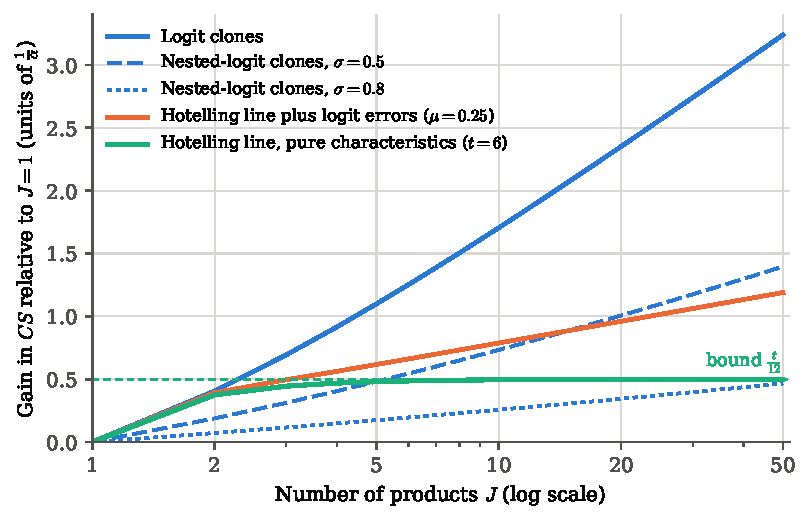
\includegraphics[width=0.88\textwidth]{figures/ch10/variety_value.pdf}
\caption{Gain in consumer surplus from adding products, relative to a market with one product, in units of
$\frac{1}{\alpha}$. The logit and nested-logit curves add identical products with $\delta = 0$ in the presence of
an outside good. The Hotelling curves place $J$ products evenly on a line with uniform consumers, quadratic
transport cost $t = 6$ and fixed equal prices. The orange curve adds logit errors with scale $\mu = 0.25$ to the
Hotelling model. At $J = 50$ the gains are 3.24 (logit), 1.40 and 0.47 (nested logit with $\sigma = 0.5$ and
$0.8$), 1.19 (Hotelling with errors) and 0.50 (pure Hotelling). Only the models with idiosyncratic errors grow
without bound. For the Hotelling curves we set $\alpha = 1$, so all curves are in the same units. Our
computations.}
\label{fig:10-variety-value}
\end{figure}

\Citet{AckerbergRysman2005} propose a correction within the logit family. It lets the contribution of the
idiosyncratic term depend on how crowded the product space is, so that additional products add less.

\subsection{Pure characteristics and vertical models}\label{sec:10-cs-pure}

\Citet{BerryPakes2007} develop the pure characteristics model for empirical work. Their utility is
\begin{equation}\label{eq:10-bp-utility}
u_{ij} = x_j\beta_i - \alpha_ip_j + \xi_j,
\qquad u_{i0} = 0,
\end{equation}
with random coefficients $\beta_{ik} = \beta_k + \sigma_k\nu_{ik}$ and $\alpha_i > 0$, after normalizing the
coefficient on the single unobserved characteristic $\xi_j$ to one. The model has no $\epsilon_{ij}$. They show
that the two families of models differ in two respects (pp.~2--3 and 6--7 of their text). With tastes for products,
substitution between products is limited and markups stay bounded away from zero as similar products are added.
Each consumer's utility also grows without bound as products are added, whatever their characteristics. In the
pure characteristics model, the gain from a new product is limited by a smooth function of its distance from
existing products. As the space fills, products become close substitutes, prices approach marginal cost, and the
increment in welfare from each new product declines to zero.

The $\epsilon$'s have practical advantages, which explain their popularity. They make choice probabilities
integrals with simple limits, and they keep every probability positive with smooth derivatives. They also allow the
share inversion that turns $\xi_j$ into a linear function of data and parameters
\citep{Berry1994,BerryLevinsohnPakes1995}.
Without them the share function has kinks and the inversion is no longer a contraction. Berry and Pakes therefore
propose to use the vertical model of \cref{ch:discrete} for the price coefficient, conditional on the other
coefficients, and a homotopy method to compute the mean utilities. A \emph{homotopy method} solves a hard system
of equations by deforming an easy system into it and following the solution path. They also study a ``modified BLP'' model in
which the logit term is scaled by $\frac{1}{\mu_\epsilon}$. The pure characteristics model is the limit as
$\mu_\epsilon\to\infty$.

\casehead{Welfare in a Monte Carlo experiment} The last experiment in \citet[Section 5.4]{BerryPakes2007} speaks to
new goods. The data come from a pure characteristics model with three markets, structured as successive years of
a market with improving characteristics. The number of products rises from 75 to 100 and then to 125. The
characteristics are patterned on the megahertz of personal computers in 1995--97 \citep{Pakes2003}, and prices for
given characteristics fall by roughly 30 percent a year. The welfare measure is the average gain per person, in
dollars, from moving from the year-one choice set to the year-three choice set. \Cref{tab:10-bp-welfare} reports
it.

\begin{table}[htbp]
\centering
\caption{Welfare gain from the year-one to the year-three choice set in the Berry-Pakes Monte Carlo}
\label{tab:10-bp-welfare}
\small
\begin{tabular}{@{}lr@{}}
\toprule
Method & Gain \\
\midrule
True (pure characteristics data-generating process) & 266.1 \\
Homotopy estimator of the pure characteristics model & 265.3 \\
Modified BLP, scale fixed at $\mu_\epsilon = 10$ & 270.0 \\
Modified BLP, scale $\mu_\epsilon$ estimated & 259.0 \\
Modified BLP, $\mu_\epsilon$ estimated, final homotopy contraction & 272.1 \\
\bottomrule
\end{tabular}

\smallskip
\begin{minipage}{0.86\linewidth}
\footnotesize Notes: Average per-person gain in dollars. One simulated data set with an average of 100 products per
market. The estimated scale in the fourth row is 0.934 with standard error 6.680, and the estimated constant in
mean utility is $-6.455$ against a true value of 2. Source: \citet{BerryPakes2007}, Tables 5 and 7.
\end{minipage}
\end{table}

All methods come within 3 percent of the truth. The modified BLP estimator with estimated scale does badly on
parameters and elasticities. For the lowest-priced product its own-price elasticity is $-1.8$ against a true
$-11.0$ \citep[Table 6]{BerryPakes2007}. Yet its welfare gain is close to the truth. Berry and Pakes explain why.
Because the contraction fits the shares exactly, the extra gain from the logit errors is offset by lower mean
utilities $\delta$, and the two roughly cancel. The estimated constant in $\delta$ falls below $-6$ to match the
small shares with a large logit error. The lesson is double-edged. Fitting shares exactly protects welfare
measures against part of the $\epsilon$ problem in this design, but it does so by distorting the parameters that
govern substitution.

\casehead{The hedonic approach} \Citet{BajariBenkard2005} take a different route to demand without
$\epsilon_{ij}$. Their method has two stages in the spirit of \citet{Rosen1974}. The first estimates a hedonic
price function $p_j = \mathbf{p}(x_j,\xi_j)$ that allows one unobserved characteristic and a non-additive form, and
recovers the $\xi_j$. They show that a hedonic price surface exists even with imperfect competition and finitely
many products. The second stage recovers tastes from each consumer's first-order conditions. At the chosen
product, the marginal utility of each continuous characteristic equals the marginal utility of money times the
slope of the price surface,
\begin{equation}\label{eq:10-bb-foc}
\frac{\partial u_i}{\partial x_{jk}} = \alpha_i\,\frac{\partial\mathbf{p}}{\partial x_{jk}} .
\end{equation}
With a continuum of products this inverts to each consumer's taste vector. With finitely many products the
revealed-preference conditions place each consumer's tastes in a set, which shrinks as the number of products
grows. The unobserved characteristic is essential. In their data on personal computers, 357 of 695 products are
dominated by another product that is better in every observed dimension and cheaper
\citep[p.~2]{BenkardBajari2004}.
They also note that the $\epsilon_{ij}$ amount to assuming an infinite-dimensional characteristics space, and that
logit-type demand curves typically are hyperbolic, approaching both axes. The hedonic model imposes no shape
beyond a downward slope, so the two families can predict quite different demand at prices outside the observed
range. That range is exactly where new-good valuations live.

\casehead{A vertical example} The vertical model of \cref{ch:discrete} makes the role of distance transparent.
Utility is $U_{ij} = \delta_j - \nu_ip_j$, with $\nu_i > 0$ distributed with continuous density $f$ on
$(0,\infty)$. A consumer's marginal utility of money is $\nu_i$, so a utility gain $\Delta U$ is worth
$\frac{\Delta U}{\nu_i}$ dollars to her. Products that sell are ordered by price and quality, and consumer $i$ buys
$j$ when $\nu_i$ lies between the cutoffs $c_{j,j+1} = \frac{\delta_{j+1}-\delta_j}{p_{j+1}-p_j}$ and $c_{j-1,j}$.

\begin{proposition}[Value of a new product in the vertical model]\label{prop:10-vertical-gain}
Let $j$ and $j+1$ be adjacent products with positive shares, $p_j < p_{j+1}$, and $c^* = c_{j,j+1} > 0$. Insert
product $n$ with $p_j < p_n < p_{j+1}$ and quality
\begin{equation}\label{eq:10-vertical-d}
\delta_n = \delta_j + c^*(p_n - p_j) + d ,
\end{equation}
so that $d$ is the vertical distance of the point $(p_n,\delta_n)$ above the chord joining $(p_j,\delta_j)$ and
$(p_{j+1},\delta_{j+1})$. Hold all other prices fixed, and take $d$ small enough that the new cutoffs stay inside
$(c_{j+1,j+2},\,c_{j-1,j})$.
\begin{enumerate}[label=(\alph*)]
\item If $d\le 0$, product $n$ sells nothing and creates no surplus.
\item If $d > 0$, exactly the consumers with $\nu\in(\nu_L,\nu_H)$ switch to $n$, where
\begin{equation*}
\nu_L = c^* - \frac{d}{p_{j+1} - p_n},
\qquad
\nu_H = c^* + \frac{d}{p_n - p_j}.
\end{equation*}
\item The money-metric gain of consumer $\nu$ is $g(\nu) = \frac{1}{\nu}\left[U_n(\nu) - \max\{U_j(\nu),
U_{j+1}(\nu)\}\right]^+$. It is positive on $(\nu_L,\nu_H)$ and equals $\frac{d}{c^*}$ at $\nu = c^*$.
\item The total gain $\mathcal{G} = \int g(\nu)f(\nu)\,d\nu$ satisfies the first expansion below. If in addition
$f(c^*) > 0$, the share $s_n$ is first order in $d$ and the gain per buyer satisfies the second,
\begin{equation}\label{eq:10-vertical-gain}
\mathcal{G} = \frac{f(c^*)}{2c^*}\,\frac{p_{j+1} - p_j}{(p_n - p_j)(p_{j+1} - p_n)}\,d^2 + o(d^2),
\qquad
\frac{\mathcal{G}}{s_n} = \frac{d}{2c^*} + o(d).
\end{equation}
\end{enumerate}
\end{proposition}

\begin{proof}
At $\nu = c^*$ the old products give equal utility, $U_j(c^*) = U_{j+1}(c^*)$. Using \eqref{eq:10-vertical-d},
\begin{equation*}
U_n(c^*) - U_j(c^*) = \delta_n - \delta_j - c^*(p_n - p_j) = d .
\end{equation*}
For $\nu > c^*$ the relevant rival is $j$, and $U_n(\nu) - U_j(\nu) = d - (\nu - c^*)(p_n - p_j)$. This difference
vanishes at $\nu_H$. For $\nu < c^*$ the rival is $j+1$, and $U_n(\nu) - U_{j+1}(\nu) = d + (c^* - \nu)(p_n -
p_{j+1})$, which vanishes at $\nu_L$. Both differences are linear in $\nu$ with peak $d$ at $c^*$.

(a) If $d \le 0$, $U_n(\nu) \le \max\{U_j(\nu),U_{j+1}(\nu)\}$ for every $\nu$, by the two linear expressions. No
consumer strictly prefers $n$.

(b) and (c) For $d > 0$, $n$ beats the better of $j$ and $j+1$ exactly on $(\nu_L,\nu_H)$. The bound on $d$
ensures that products other than $j$ and $j+1$ remain worse for these consumers. Dividing the utility gain by
$\nu$ gives $g(\nu)$, which equals $\frac{d}{c^*}$ at $c^*$.

(d) Let $h(\nu) = \nu g(\nu)$ denote the utility gain. It is a triangle with height $d$ and base $\nu_H - \nu_L$,
where
\begin{equation*}
\nu_H - \nu_L = d\left(\frac{1}{p_n - p_j} + \frac{1}{p_{j+1} - p_n}\right)
= d\,\frac{p_{j+1} - p_j}{(p_n - p_j)(p_{j+1} - p_n)} .
\end{equation*}
Its area is $\frac{1}{2}d(\nu_H - \nu_L)$. Since $\frac{f(\nu)}{\nu}$ is continuous at $c^* > 0$ and the interval
shrinks to $c^*$, $\frac{f(\nu)}{\nu} = \frac{f(c^*)}{c^*} + o(1)$ uniformly on it. Therefore
\begin{equation*}
\mathcal{G} = \int_{\nu_L}^{\nu_H}h(\nu)\frac{f(\nu)}{\nu}\,d\nu
= \left(\frac{f(c^*)}{c^*} + o(1)\right)\frac{d}{2}(\nu_H - \nu_L),
\end{equation*}
which is the first part of \eqref{eq:10-vertical-gain}. This step holds also when $f(c^*) = 0$, and the
coefficient on $d^2$ is then zero. The share is $s_n = F(\nu_H) - F(\nu_L) = (f(c^*) + o(1))(\nu_H - \nu_L)$.
When $f(c^*) > 0$, the factor $f(c^*) + o(1)$ is bounded away from zero for small $d$. Dividing the two
expressions then gives $\frac{\mathcal{G}}{s_n} = \frac{d}{2c^*} + o(d)$.
\end{proof}

The condition $f(c^*) > 0$ matters for the per-buyer formula. Take the density $f(\nu) = (\nu - 1)^2e^{-\nu}$,
old products $(p,\delta) = (1,2)$ and $(3,4)$, an outside utility of zero and the new product $(2,3+d)$. Then
$c^* = 1$ and $f(c^*) = 0$. Our computation gives $s_n = \frac{2e^{-1}d^3}{3} + o(d^3)$ and
$\mathcal{G} = \frac{e^{-1}d^4}{6} + o(d^4)$, so that $\frac{\mathcal{G}}{s_n} = \frac{d}{4} + o(d)$. This is half
the value $\frac{d}{2c^*} = \frac{d}{2}$ of \eqref{eq:10-vertical-gain}.

\Cref{fig:10-vertical-gain} draws the construction. When $f(c^*) > 0$, the gain is second order in the
distance $d$. The share of the new product is then first order in $d$, and the gain per buyer, $\frac{d}{2c^*}$,
vanishes as the new product approaches the chord. The quantity $\frac{d}{c^*}$ is the dollar value of the new product's quality premium at the margin
between its neighbors, and the average switcher gets half of it, as in any triangle. Compare
\eqref{eq:10-logit-perbuyer}. In the logit the gain per buyer is at least $\frac{1}{\alpha}$ for any product,
including a product on or below the chord. A numerical check with $f(\nu) = e^{-\nu}$ and the prices of
\cref{fig:10-vertical-gain} confirms \eqref{eq:10-vertical-gain}. The exact gain differs from the approximation by
1.7 percent at $d = 0.2$ and by 0.1 percent at $d = 0.05$.

\begin{figure}[htbp]
\centering
\begin{tikzpicture}
\begin{axis}[
  width=0.82\textwidth, height=6.6cm,
  xmin=0, xmax=2.25, ymin=-0.5, ymax=4.3,
  axis lines=left, clip=true,
  xlabel={Price sensitivity $\nu$}, ylabel={Utility $U$},
  xtick={0.5,1,1.5,2}, xticklabels={$\nu_L$,$c^*$,$\nu_H$,$c_{j-1,j}$},
  ytick={0}, yticklabels={$0$},
  every axis x label/.style={at={(axis description cs:0.5,-0.12)},anchor=north},
  every axis y label/.style={at={(axis description cs:-0.06,0.5)},rotate=90,anchor=south},
  tick label style={font=\small}, label style={font=\small},
  legend style={at={(0.98,0.98)}, anchor=north east, draw=none, fill=white, font=\small},
  legend cell align=left]
  \fill[orange!30] (axis cs:0.5,2.5) -- (axis cs:1,1) -- (axis cs:1.5,0.5) -- cycle;
  \addplot[blue!70!black, thick, domain=0:2.25, samples=2] {4 - 3*x};
  \addlegendentry{$U_{j+1} = \delta_{j+1} - \nu p_{j+1}$}
  \addplot[orange!85!black, very thick, domain=0:2.25, samples=2] {3.5 - 2*x};
  \addlegendentry{$U_n = \delta_n - \nu p_n$ (new product)}
  \addplot[blue!40, thick, domain=0:2.25, samples=2] {2 - x};
  \addlegendentry{$U_j = \delta_j - \nu p_j$}
  \addplot[black!60, densely dashed, line width=1.6pt] coordinates {(0,4) (1,1) (2,0) (2.25,0)};
  \addlegendentry{old upper envelope}
  \draw[black!50, dotted] (axis cs:0.5,-0.5) -- (axis cs:0.5,2.5);
  \draw[black!50, dotted] (axis cs:1,-0.5) -- (axis cs:1,1.5);
  \draw[black!50, dotted] (axis cs:1.5,-0.5) -- (axis cs:1.5,0.5);
  \draw[black!40] (axis cs:0,0) -- (axis cs:2.25,0);
  \draw[decorate, decoration={brace, amplitude=3pt}, thick] (axis cs:0.97,1.0) -- (axis cs:0.97,1.5)
     node[midway, left=3pt, font=\small] {$d$};
  \node[font=\small, orange!85!black, anchor=west] at (axis cs:1.2,2.05) {gain triangle};
  \draw[->, orange!85!black] (axis cs:1.25,1.9) -- (axis cs:1.05,1.35);
\end{axis}
\end{tikzpicture}
\caption{The vertical model with a product inserted between two neighbors. Each line is the utility $\delta - \nu p$
of one product as a function of price sensitivity $\nu$. The dashed line is the upper envelope before the
introduction, and the outside good gives utility zero. Product $n$ lies a distance $d$ above the chord joining its
neighbors and wins the consumers with $\nu\in(\nu_L,\nu_H)$. The shaded triangle is their utility gain, so the
welfare gain is of order $d^2$. The parameters are $(p_j,p_n,p_{j+1}) = (1,2,3)$ and $(\delta_j,\delta_n,\delta_{j+1}) =
(2,3.5,4)$, so $c^* = 1$ and $d = 0.5$.}
\label{fig:10-vertical-gain}
\end{figure}

\subsection{Hedonic methods, quality change and changing tastes}\label{sec:10-cs-hedonic}

Statistical agencies often handle new varieties with hedonic methods, and the vertical example shows what these
methods assume. A \emph{hedonic price function} $\mathbf{p}(z)$ relates the prices of products to their
characteristics $z$ \citep{Griliches1971,Rosen1974}. We write
\begin{equation}\label{eq:10-hedonic}
p_j = \mathbf{p}(z_j) + \tilde p_j ,
\end{equation}
where $\tilde p_j$ is the \emph{residual price}, the deviation of product $j$'s price from the surface. In Rosen's
model with a continuum of products, the hedonic function is an equilibrium locus. A consumer with utility
$\alpha[y - \mathbf{p}(z)] + \phi(z)$ chooses $z$ to satisfy $\mathbf{p}'(z) = \frac{\phi'(z)}{\alpha}$. A new
variety priced on the surface offers nothing that consumers could not already buy, so it adds no surplus. Hedonic
quality adjustment therefore treats a new variety as a perfect substitute for a combination of existing ones.
This is the flat curve $dd(-\infty)$ of \cref{fig:10-dd-DD}, which \citet[p.~238]{Bresnahan1997} identifies as an
understatement of the value of new goods. In the vertical model the chord between neighbors plays the role of the
hedonic surface. A product priced on it has $d = 0$ and adds nothing, while a product above it adds a gain of
order $d^2$. When the product space is sparse, the surface has wide gaps and the understatement can be large.

\casehead{Quality as repackaging} \citet[Section~10.3, pp.~262--266]{DeatonMuellbauer1980b} derive the most common
hedonic regression from a model in which quality repackages quantity. The varieties $j$ of a good are perfect
substitutes once each is weighted by a quality index $\zeta_j > 0$. Utility is
$v\bigl(h(\sum_j\zeta_jq_j),q_{\mathrm{other}}\bigr)$, where $q_{\mathrm{other}}$ collects the other goods (their
eq.~3.7). A consumer then buys only the varieties with the lowest price per unit of quality,
$\frac{p_{jt}}{\zeta_j}$. Suppose all consumers share the weights and every variety sells. The prices per unit of
quality must then be equal, $p_{jt} = \zeta_jP_t$, where $P_t$ is the price of a unit of quality in period $t$. With
$\ln\zeta_j = f(z_j)$, taking logs gives
\begin{equation}\label{eq:10-dm-hedonic}
  \ln p_{jt} = \ln P_t + f(z_j)
\end{equation}
(their eq.~3.8). A disturbance and a log-linear $f$ give the \emph{time-dummy hedonic regression}. It pools all periods
and adds a zero-one dummy for each period except a reference period (p.~263). The coefficients on the
period dummies estimate $\ln P_t$, a quality-corrected price index. A new variety priced on this surface sells
quality at the going price $P_t$, so it adds no surplus. Their Table~10.1 (p.~264) fits such a regression to 150
British used-car models, aged one to three years, from nine manufacturers in the late 1950s and the 1960s. A 1
percent increase in brake horsepower raises the price by 0.370 percent (standard error 0.023). The implied
quality-corrected price of cars was about 8 percent lower in 1969 than in 1958 (p.~263). The coefficients on miles
per gallon, $-0.064$ (0.041), and interior size, $-0.146$ (0.094), are negative and imprecise. Deaton and Muellbauer
suggest that, with length and width held fixed, a large interior may signal restricted luggage space (p.~264).
An $F$-test rejects a common price function across manufacturers. The statistic is 9, and 1.2 suffices to reject at
the 5 percent level (p.~265). Deaton and Muellbauer read this as evidence of \emph{market segmentation}, in which
products made for different types of consumers carry different shadow prices of characteristics (p.~259). A single
price surface ignores it. When consumers' weights differ, the surface is instead an envelope of their
\emph{bid functions}. A consumer's bid function gives the most she would pay for one unit of a variety with
characteristics $z$, at her utility level (pp.~265--266). The marginal condition
$\frac{\partial\ln\mathbf{p}(z)}{\partial z_k} = \frac{\partial\ln\zeta(z)}{\partial z_k}$ then holds for each
consumer at her chosen variety, as in \citet{Rosen1974} (eq.~3.10, pp.~265--266).

\casehead{Changing tastes: ex ante and ex post measures} Applications over long periods face a further problem.
If the estimated taste parameters change from year to year, the value of moving from choice set $S_t$ to $S_{t+1}$
depends on which year's tastes are used. Write $\mathcal{W}^t$ for the surplus function evaluated with the
parameters estimated for year $t$. \citet[pp.~56--58]{Trajtenberg1985} defines
\begin{equation}\label{eq:10-exante-expost}
\Delta\mathcal{W}^a = \mathcal{W}^t(S_{t+1}) - \mathcal{W}^t(S_t),
\qquad
\Delta\mathcal{W}^p = \mathcal{W}^{t+1}(S_{t+1}) - \mathcal{W}^{t+1}(S_t).
\end{equation}
The \emph{ex ante} measure $\Delta\mathcal{W}^a$ asks what a consumer with today's tastes would pay to face next
year's choice set. The \emph{ex post} measure $\Delta\mathcal{W}^p$ asks how much income could be taken from a
consumer with next year's tastes, leaving her indifferent between next year's and this year's sets. The
distinction resembles the one between compensating and equivalent variation, but it has a different source.
Compensating and equivalent variation hold tastes fixed and differ in the reference utility level, and they
coincide without income effects. Here utility is quasi-linear, and the ambiguity comes from the change in the taste
parameters themselves. The hybrid $\mathcal{W}^{t+1}(S_{t+1}) - \mathcal{W}^t(S_t)$ compares utilities under two
different preference structures, which is an interpersonal comparison and has no welfare meaning.

Trajtenberg expects the ex ante measure to exceed the ex post one. His argument is a \emph{dual inducement}
mechanism. Strong tastes for an attribute induce firms to improve that attribute, and the improvement then lowers
its marginal valuation next year. Judged by the original tastes, an improvement is therefore worth more. He also
considers a Divisia-like alternative that estimates adjacent years jointly. It yields a unique measure, but only by
suppressing the taste differences that create the problem.

\section{Case study: CT scanners (Trajtenberg 1989)}\label{sec:10-trajtenberg}

\citet{Trajtenberg1989} was the first study to measure a product innovation by the welfare it creates, using an
estimated discrete-choice demand system in characteristics space. The application is computed tomography (CT)
scanners in the United States from their introduction in 1973 to 1982. The paper is also an early study of how
innovation, diffusion and returns to research interact. The PDF available to us is the working-paper version
\citep{Trajtenberg1985}. All numbers below come from it, and page numbers refer to its typed pages. The
published version may number its tables differently, and some of its numbers may differ.
Trajtenberg indexes products by $i$ and characteristics by $j$. We index scanners by $j$ and characteristics by
$k$, consistent with the rest of the book.

\subsection{The question}\label{sec:10-ct-question}

The output of innovative activity does not come in countable units. Patent counts vary enormously in
significance, and sales of new products confound innovation with market size. Trajtenberg therefore argues that a
quantitative measure of innovation can only be defined in value terms
\citep[pp.~2--3]{Trajtenberg1985}. How much product innovation occurred in a field over a period is the
additional social surplus that the innovations generated. Other measures can at best serve as proxies.

A product is a pair $(z_j,p_j)$, with $z_j = (z_{j1},\dots,z_{jK})$ its characteristics and $p_j$ its price.
Trajtenberg writes $s_j$ for this pair, a symbol we keep for market shares.
The choice set in year $t$ is $S_t$, and product innovation is the change $S_t - S_{t-1}$. It includes improvements
in existing products, the addition of new ones and the exit of old ones. The magnitude of innovation is
\begin{equation}\label{eq:10-traj-dW}
\Delta\mathcal{W}_t = \mathcal{W}(S_t) - \mathcal{W}(S_{t-1}),
\end{equation}
for a surplus function $\mathcal{W}$ (equation 1 of the paper, p.~7). The measure includes the effect of price
changes. Trajtenberg defends this broad definition on practical grounds. With nonlinear surplus functions the
effects of characteristics and prices cannot be separated, and new products have no earlier price to compare with
(pp.~8--9).

What counts as a product innovation needs a definition, and Trajtenberg provides one through the nature of
characteristics (pp.~4--6).

\begin{definition}[Concatenable characteristics]\label{def:10-concatenable}
Let $x_j$ be the quantity of product $j$ that a consumer buys. Characteristic $k$ is \emph{concatenable} if the
amount of it available to the consumer is $z_{jk} = f^k(x_j)$ with $\frac{\partial z_{jk}}{\partial x_j} \ne 0$.
Examples are the protein in a food or the carrying capacity of vehicles. It is \emph{non-concatenable} if
$z_{jk} = g^k(\theta_j)$ for the product's natural unit $\theta_j$, with $\frac{\partial z_{jk}}{\partial x_j} = 0$
for $x_j > \theta_j$. Examples are the speed of a vehicle or the aperture of a camera.
\end{definition}

Product innovation requires at least one non-concatenable characteristic. Suppose all characteristics were
concatenable and linear in quantity. Then a change from $(z_j,p_j)$ to $(\kappa z_j,\kappa p_j)$ with
$\kappa > 1$ would leave the indirect utility unchanged, $V(z_j,p_j,y) = V(\kappa z_j,\kappa p_j,y)$. Buying $\kappa$ units of the old
product delivers the same bundle at the same cost. Such a change could not count as an innovation. A product
innovation therefore presupposes a quality dimension that can be changed only by switching products. CT scanners
satisfy this. Speed and image resolution are properties of the machine. Buying more machines does not change
them.

\casehead{Scope} The surplus function is in principle total surplus. Trajtenberg argues that profits pose no
special measurement problem beyond accounting, so the difficulty lies in consumer surplus. He measures the gains
that are not appropriated by the innovating firms and passed on to buyers (pp.~9--10). He states two limitations.
Radical innovations, which open new product classes, cannot be measured directly (\cref{sec:10-cs-predict}). The
measure also ignores spillovers to other product classes, so it is a lower bound on the social gain (pp.~11--12).
Trajtenberg proposes an indirect estimate of the gain from the first scanner, based on diffusion
(\cref{sec:10-ct-diffusion}).

The question matters for three reasons. Product innovation is a large part of technical change, and official
price and productivity statistics do not capture it (p.~1). Social returns to research cannot be computed without
a measure of benefits. And the interaction between innovation and diffusion cannot be studied without a measure of
innovation.

\subsection{Setting}\label{sec:10-ct-setting}

Research on computed tomography began in 1967 at the British electronics company EMI. The first operational
prototype was installed in a London hospital in 1971, and the first commercial system, the EMI Scanner, was
installed in the United States in June 1973 (p.~25). In 1974--77 nearly 20 firms entered. They ranged from
electronics companies (General Electric, Siemens, Hitachi, Philips) to pharmaceutical companies (Pfizer, Searle,
Syntex) and specialized firms (AS\&E, Elscint), and they competed mainly through product performance (p.~26).
Diffusion among U.S. hospitals was fast, the fifth fastest among twenty innovations for which diffusion studies
existed (p.~26, n.~23). Mounting concern about health-care costs led to Certificate of Need regulation, which
required approval for large hospital investments. Its full impact in 1978--79 produced a sharp downturn and the
exit of many firms, including EMI. The market then recovered and settled at 10--15 percent annual growth, with
General Electric holding about 50 percent of the U.S. market and some ten firms sharing the rest (p.~26). The two
pioneers of CT received the Nobel Prize in Medicine in 1979.

\casehead{Characteristics} A CT scanner takes cross-sectional images of the body. Trajtenberg measures three
performance characteristics (pp.~27--30). SPEED is the minimum scan time in seconds. The first scanner took five
minutes per scan, which restricted it to the brain, a motion-free organ. Scan times of twenty seconds and less
opened other organs, and the fastest systems of the early 1980s scanned in about one second. RESOL is spatial
resolution in millimeters, the size of the smallest object visible in high-contrast regions. Trajtenberg had
constructed a fuller image-quality index from experimental data, but it was unavailable for most of the roughly
50 systems marketed. RTIME is reconstruction time in seconds, the time the computer takes to produce the image. A
fourth attribute, gantry tilt, proved insignificant and was dropped. All three characteristics are defined so that
less is better. Scanners come in two types. \emph{Head scanners} can image only the brain, while \emph{body
scanners} can image almost any organ.

\subsection{Data}\label{sec:10-ct-data}

Trajtenberg assembled his own data bank, covering the period from the announcement of the innovation in 1972 to
1981, with some series extending to 1983 (pp.~30--32). It has four parts. The first gives the technical
characteristics and prices of all CT scanners marketed up to 1982, by year, which is the sequence of choice sets
$S_t$. The second records every installation in the United States, with the identity of the hospital or clinic,
the dates of order and installation, and the model bought. It has more than 2,000 observations, including
upgrades, and Trajtenberg estimates that it covers about 98 percent of U.S. installations up to July 1981. The
third describes the hospitals and the fourth the manufacturers, including their research and development spending
on CT. The main source is a questionnaire to all manufacturers, with follow-up contacts. Others are the radiology
and medical-physics literature, trade journals and consulting reports. Public sources include the Food and Drug
Administration, the Office of Technology Assessment, the Patent Office and the American Hospital Association, and
Trajtenberg also ran a telephone survey of hospitals.
All but two firms active in 1981 answered the questionnaire. The two were CGR and Philips, and Philips was excluded
for lack of reliable information. Little is lost, since it had sold fewer than twenty scanners in the United States by
1981.

A year in the data runs from November 1 of the previous year to October 31. Most new scanners are introduced at
the annual meeting of the Radiological Society of North America in November, so this \emph{radiological year}
matches the timing of choice sets. Data for 1981 cover only the first half of that year (p.~33, n.~28).
\Cref{tab:10-ct-data} reproduces Tables 1 and 2 of the paper.

\begin{table}[htbp]
\centering
\caption{CT scanners in the United States, 1973--1982}
\label{tab:10-ct-data}
\footnotesize
\setlength{\tabcolsep}{4.5pt}
\begin{tabular}{@{}lrrrrrrrr@{}}
\toprule
\multicolumn{9}{@{}l}{\textit{Panel A. Prices and average characteristics}} \\
& \multicolumn{2}{c}{Price (\$K)} & \multicolumn{2}{c}{SPEED (s)} & \multicolumn{2}{c}{RESOL (mm)} &
  \multicolumn{2}{c}{RTIME (s)} \\
\cmidrule(lr){2-3}\cmidrule(lr){4-5}\cmidrule(lr){6-7}\cmidrule(lr){8-9}
Year & Head & Body & Head & Body & Head & Body & Head & Body \\
\midrule
1973 & 310 & -- & 300 & -- & 3.1 & -- & 300 & -- \\
1974 & 370 & -- & 300 & -- & 1.7 & -- & 30 & -- \\
1975 & 379 & 365 & 285 & 195.0 & 1.8 & 1.6 & 20 & 8 \\
1976 & 374 & 471 & 105 & 63.0 & 1.7 & 1.5 & 60 & 83 \\
1977 & 354 & 573 & 95 & 19.0 & 1.7 & 1.3 & 54 & 38 \\
1978 & 167 & 620 & 96 & 7.1 & 1.6 & 1.2 & 29 & 30 \\
1979 & 154 & 667 & 150 & 6.6 & 1.5 & 1.1 & 19 & 29 \\
1980 & 154 & 739 & 115 & 5.5 & 1.5 & 1.0 & 27 & 31 \\
1981 & 150 & 827 & 115 & 4.9 & 1.5 & 0.8 & 27 & 32 \\
1982 & 150 & 850 & 115 & 2.6 & 1.5 & 0.7 & 27 & 27 \\
\midrule
\multicolumn{9}{@{}l}{\textit{Panel B. Market indicators}} \\
& Units & Sales & Body & New & Firms & Models & HHI & \\
Year & sold & (\$M) & (\% sales) & adopters (\%) & & & & \\
\midrule
1973 & 16 & 5 & 0 & 100.0 & 1 & 1 & 1.00 & \\
1974 & 74 & 27 & 0 & 98.7 & 1 & 1 & 1.00 & \\
1975 & 221 & 82 & 44.8 & 97.7 & 4 & 5 & 0.43 & \\
1976 & 374 & 167 & 76.2 & 84.8 & 9 & 14 & 0.38 & \\
1977 & 385 & 208 & 84.9 & 84.1 & 12 & 23 & 0.23 & \\
1978 & 248 & 122 & 72.4 & 84.4 & 10 & 23 & 0.28 & \\
1979 & 273 & 141 & 70.2 & 76.0 & 9 & 22 & 0.26 & \\
1980 & 270 & 169 & 80.4 & 65.3 & 8 & 17 & 0.32 & \\
1981 & 392 & 302 & 91.6 & 50.0 & 8 & 14 & 0.31 & \\
1982 & 428 & 344 & 93.5 & n.a. & 8 & 16 & 0.30 & \\
\bottomrule
\end{tabular}

\smallskip
\begin{minipage}{0.94\linewidth}
\footnotesize Notes: Radiological years (November to October), U.S. market. Price is the sales-weighted average
price of all scanners of each type. The characteristics are simple averages, and smaller values are better.
``Body'' is the share of body scanners in unit sales and ``New adopters'' the share of sales to first-time
buyers. HHI is the Herfindahl index. Source: \citet{Trajtenberg1985}, Tables 1 and 2.
\end{minipage}
\end{table}

The two types followed opposite paths (pp.~32--33). Head scanners became simpler and cheaper, and their price
fell from \$379K in 1975 to \$150K by 1981. Body scanners improved quickly, with average scan time
falling from 195 seconds in 1975 to 2.6 seconds in 1982, and their price rose from \$365K to \$850K. By most
indicators competition peaked in 1977. Fourteen new scanners were introduced that year, the number of firms
reached 12, and the Herfindahl index reached its low of 0.23. Sales to new adopters fell from 97.7 percent of
sales in 1975 to 50.0 percent in 1981 as diffusion leveled off and replacement purchases grew.

\subsection{The model}\label{sec:10-ct-model}

\casehead{Demand and the surplus function} A buyer chooses one scanner from $S$. She spends the rest of income
$y$ on a composite outside good $m$ with unit price (pp.~15--17),
\begin{equation}\label{eq:10-traj-rum}
\max_{j,m}\; U(z_j,m;D) + \epsilon_j
\qquad\text{subject to}\qquad p_j + m = y,\quad j\in S,
\end{equation}
where $D$ is a vector of buyer attributes. Substituting $m = y - p_j$ gives the conditional indirect utility
$V(z_j,y - p_j;D) + \epsilon_j$. With \iid\ type-I extreme value shocks and quasi-linear utility $\alpha(y - p_j) +
\phi(z_j;D) + \epsilon_j$, income cancels and the choice probabilities are
\begin{equation}\label{eq:10-traj-mnl}
s_j = \frac{e^{-\alpha p_j + \phi(z_j;D)}}{\sum_{k\in S}e^{-\alpha p_k + \phi(z_k;D)}},
\qquad j\in S .
\end{equation}
There is no outside good. The model describes the choice among scanners by buyers who buy one, and the decision
to adopt is modeled separately (\cref{sec:10-ct-diffusion}). By \cref{lem:10-logsum,lem:10-cv-quasilinear} the
surplus function is
\begin{equation}\label{eq:10-traj-W}
\mathcal{W}(S;D) = \frac{1}{\alpha}\ln\sum_{j\in S}e^{-\alpha p_j + \phi(z_j;D)},
\end{equation}
which is equation (10) of the paper (p.~18), and its entropy decomposition is \cref{prop:10-entropy}. Trajtenberg
notes that the surplus function treats the buyer as if she bought a fraction $s_j$ of every product. Every change in
the set therefore registers, whichever product a buyer ends up with. He rejected the probit because his choice sets
had up to twenty alternatives, and the computers of the time could handle a probit with only four or five.

\casehead{Hedonic prices and the collinearity problem} In markets for differentiated products, prices are closely
related to characteristics through the hedonic function \eqref{eq:10-hedonic}. Entering both $p_j$ and $z_j$ in
\eqref{eq:10-traj-mnl} creates severe collinearity, and their separate coefficients cannot be estimated with
precision (pp.~19--20). Trajtenberg argues that the problem is conceptual. In Rosen's continuous model the
consumer cannot choose $z$ and $p$ independently, because choosing $z$ determines $p$. With
\begin{equation}\label{eq:10-traj-rosen}
\max_{z}\; \alpha[y - \mathbf{p}(z)] + \phi(z)
\qquad\Longrightarrow\qquad
\mathbf{p}'(z) = \frac{\phi'(z)}{\alpha},
\end{equation}
only the characteristics enter the demand analysis (p.~21). In the discrete case the hedonic function is a
stochastic budget constraint. Substituting \eqref{eq:10-hedonic} into utility gives
\begin{equation}\label{eq:10-traj-netutility}
V_j = \phi(z_j) - \alpha\,\mathbf{p}(z_j) - \alpha\tilde p_j = V^n(z_j) - \alpha\tilde p_j,
\qquad
V^n(z) \equiv \phi(z) - \alpha\,\mathbf{p}(z).
\end{equation}
The term $V^n(z)$ is the \emph{net utility} of characteristics, net of their expected cost. The residual price
$\tilde p_j$ is a random extra charge or discount relative to the market's valuation of the characteristics.
Choices depend on $z_j$ and $\tilde p_j$, the part of price orthogonal to the characteristics. The next proposition
supplies the functional form for $V^n$ (p.~22).

\begin{proposition}[Quadratic approximation of net utility]\label{prop:10-quadratic}
Let $V^n$ be twice continuously differentiable with an interior point $z^*$ at which
\begin{equation*}
\frac{\partial V^n(z^*)}{\partial z_k} = \frac{\partial\phi(z^*)}{\partial z_k} - \alpha\frac{\partial\mathbf{p}(z^*)}{\partial z_k}
= 0,\qquad k = 1,\dots,K,
\end{equation*}
and let the Hessian $H = \nabla^2 V^n(z^*)$ be negative definite. Then
\begin{equation}\label{eq:10-quadratic}
V^n(z) = c_0 + z^\top\beta + z^\top Gz + o\left(\|z - z^*\|^2\right),
\qquad G = \frac{1}{2}H,\quad \beta = -Hz^*,
\end{equation}
where $c_0 = V^n(z^*) + \frac{1}{2}z^{*\top}Hz^*$ does not depend on $z$. If $\phi$ is concave and $\mathbf{p}$ is
convex near $z^*$, and $\nabla^2\phi(z^*)$ or $\nabla^2\mathbf{p}(z^*)$ is definite, then $H$ is negative definite.
\end{proposition}

\begin{proof}
A second-order Taylor expansion about $z^*$ gives
\begin{equation*}
V^n(z) = V^n(z^*) + \nabla V^n(z^*)^\top(z - z^*) + \frac{1}{2}(z - z^*)^\top H(z - z^*) + o\left(\|z - z^*\|^2\right).
\end{equation*}
The gradient term vanishes by assumption. Expanding the quadratic form with $H$ symmetric,
\begin{equation*}
\frac{1}{2}(z - z^*)^\top H(z - z^*) = \frac{1}{2}z^\top Hz - z^\top Hz^* + \frac{1}{2}z^{*\top}Hz^* .
\end{equation*}
Collecting terms gives \eqref{eq:10-quadratic}. Finally $H = \nabla^2\phi(z^*) - \alpha\nabla^2\mathbf{p}(z^*)$ is
the sum of two negative semidefinite matrices, one of which is negative definite, so $H$ is negative definite.
\end{proof}

The constant $c_0$ drops out of the logit probabilities. In a discrete market tangency is not required, and $z^*$ is
the expected optimum. Actual choices scatter around it. Products near $z^*$ are more likely to be chosen than products far
from it (p.~23). \Cref{fig:10-hedonic-net-utility} redraws the paper's Figure 1. Trajtenberg adds that $\mathbf{p}$
may be concave and the conditions still hold, provided it is less concave than $\phi$ (p.~22, n.~21). Otherwise the
expected optimum is a corner, the approximation is poor, and estimated coefficients may take the wrong signs.

\begin{figure}[htbp]
\centering
\begin{tikzpicture}
\begin{axis}[name=top,
  width=0.62\textwidth, height=5.0cm,
  xmin=0.2, xmax=3.3, ymin=0.8, ymax=4.6,
  axis lines=left, xtick={1.4057}, xticklabels={$z^*$}, ytick=\empty,
  ylabel={$\phi(z)$, $\alpha\,\mathbf{p}(z)$},
  tick label style={font=\small}, label style={font=\small}]
  \addplot[blue!70!black, thick, domain=0.25:3.2, samples=80] {2*sqrt(x) + 0.5};
  \addplot[orange!85!black, thick, domain=0.25:3.2, samples=80] {0.3*x^2 + 1.2};
  \addplot[blue!70!black, densely dotted, domain=0.85:1.95, samples=2] {2.8713 + 0.8433*(x - 1.4057)};
  \addplot[orange!85!black, densely dotted, domain=0.85:1.95, samples=2] {1.7928 + 0.8433*(x - 1.4057)};
  \draw[black!50, dashed] (axis cs:1.4057,0.8) -- (axis cs:1.4057,2.8713);
  \node[font=\small, blue!70!black, anchor=west] at (axis cs:0.75,3.05) {$\phi(z)$};
  \node[font=\small, orange!85!black, anchor=west] at (axis cs:2.3,2.3) {$\alpha\,\mathbf{p}(z)$};
  \node[font=\small, black!70, anchor=west, align=left] at (axis cs:1.7,1.35) {equal slopes at $z^*$};
\end{axis}
\begin{axis}[at={(top.south west)}, anchor=north west, yshift=-0.9cm,
  width=0.62\textwidth, height=4.4cm,
  xmin=0.2, xmax=3.3, ymin=-0.6, ymax=1.35,
  axis lines=left, xtick={1.4057}, xticklabels={$z^*$}, ytick={0}, yticklabels={$0$},
  xlabel={Characteristic $z$}, ylabel={$V^n(z)$},
  tick label style={font=\small}, label style={font=\small}]
  \addplot[black, thick, domain=0.25:3.2, samples=80] {2*sqrt(x) + 0.5 - 0.3*x^2 - 1.2};
  \addplot[black!60, densely dashed, domain=0.25:3.2, samples=80] {1.0784 - 0.45*(x - 1.4057)^2};
  \draw[black!50, dashed] (axis cs:1.4057,0) -- (axis cs:1.4057,1.0784);
  \draw[black!40] (axis cs:0.2,0) -- (axis cs:3.3,0);
  \node[font=\small, anchor=west] at (axis cs:0.25,-0.2) {solid: $V^n(z) = \phi(z) - \alpha\,\mathbf{p}(z)$};
  \node[font=\small, black!60, anchor=west] at (axis cs:0.25,-0.45) {dashed: quadratic approximation};
\end{axis}
\end{tikzpicture}
\caption{Net utility and its quadratic approximation. The top panel shows a concave utility of characteristics
$\phi(z)$ and a convex hedonic cost $\alpha\,\mathbf{p}(z)$, with equal slopes at the expected optimum $z^*$. The
bottom panel shows that net utility $V^n(z) = \phi(z) - \alpha\,\mathbf{p}(z)$ has an interior maximum at $z^*$. Its
dashed curve is the second-order expansion of \cref{prop:10-quadratic}. Illustrative functions $\phi(z) = 2\sqrt{z} + 0.5$ and
$\alpha\,\mathbf{p}(z) = 0.3z^2 + 1.2$. Redrawn after \citet{Trajtenberg1985}, Figure 1.}
\label{fig:10-hedonic-net-utility}
\end{figure}

\casehead{The separable specification} Trajtenberg simplifies further (p.~38). Suppose utility is additively
separable in characteristics, $\phi(z) = \sum_k f^k(z_k)$ with each $f^k$ quasi-concave, and the hedonic function
is linear in logs, $\mathbf{p}(z) = h_0 + \sum_k h_k\ln z_k$. Then net utility is separable too,
\begin{equation}\label{eq:10-traj-separable}
V^n(z) = \sum_k\left[f^k(z_k) - \alpha h_k\ln z_k\right] - \alpha h_0
\approx \sum_k\left(\beta_kz_k + \gamma_kz_k^2\right) + \text{const},
\end{equation}
because the Hessian of a separable function is diagonal and the cross terms of \eqref{eq:10-quadratic} vanish. The
saving of $\frac{K(K-1)}{2}$ parameters matters here. A multinomial logit (MNL) with characteristics that vary only
across products, and not across buyers, can include at most $|S| - 1$ such variables. Here $|S|$ is the number of
alternatives in the choice set $S$ (p.~38, n.~36). The separability of the hedonic function in $\ln z_k$ is what licenses the simplification. A double-log or
semi-log hedonic function would reintroduce cross terms (p.~39, n.~36).

\casehead{The estimating equation} Combining \eqref{eq:10-traj-netutility} and \eqref{eq:10-traj-separable}, the
model estimated for each year is
\begin{equation}\label{eq:10-traj-estimating}
s_j = \frac{e^{V_j}}{\sum_{k\in S_t}e^{V_k}},
\qquad
V_j = \sum_{k=1}^{K}\left(\beta_kz_{jk} + \gamma_kz_{jk}^2\right) + \vartheta\,\tilde p_j,
\qquad
\tilde p_j = p_j - \hat{\mathbf{p}}(z_j),
\end{equation}
with $K = 3$ characteristics. If the residual price measured only the price, $\vartheta$ would equal $-\alpha$.
\Cref{sec:10-ct-signal} explains why Trajtenberg allows otherwise. The procedure has two steps. The first estimates
the hedonic function and computes the residual prices. The second estimates the MNL by maximum likelihood with
$\tilde p_j$ as a regressor (p.~23). Trajtenberg abstracts from simultaneity. His working assumption is that each
choice set and its hedonic function are fixed before the year begins and do not change during it, which matches
the annual introduction cycle (p.~24). He also warns that the residual price may be correlated with omitted
attributes that affect choice, which would bias its coefficient (p.~24).

\subsection{Estimation and specification tests}\label{sec:10-ct-estimation}

\casehead{Step 1: hedonic regressions} Trajtenberg compares three forms (pp.~35--37). They are the double-log $\ln
p_j = h_0 + \sum_kh_k\ln z_{jk} + e_j$, the semi-log $\ln p_j = h_0 + \sum_kh_kz_{jk} + e_j$, and the linear-log
\begin{equation}\label{eq:10-traj-linearlog}
p_j = h_0 + \sum_k h_k\ln z_{jk} + e_j .
\end{equation}
As far as Trajtenberg knew, the linear-log form had not been used for hedonic prices before. When more of a characteristic is better, $h_k > 0$
and the form is concave, which is implausible. Here less is better, so $h_k < 0$, and $\frac{\partial^2}{\partial
z_k^2}h_k\ln z_k = -\frac{h_k}{z_k^2} > 0$ makes the function convex. The forms were estimated for 1976--81 on two
samples, all scanners with a head dummy and body scanners alone, which gives twelve cases. The \emph{Box-Cox
transformation} $\frac{p^\lambda - 1}{\lambda}$ gives the linear form at $\lambda = 1$ and the log form as
$\lambda\to 0$, so its likelihood puts the forms on a common scale. Box-Cox comparisons of fit ranked the linear-log first in half the cases, second in a third, and last in a sixth. The double-log ranked
first in a quarter, second in seven twelfths and third in a sixth (p.~37, n.~33). The linear-log has two further
advantages. Its residuals are in price units and enter the MNL directly, and it justifies the separable form
\eqref{eq:10-traj-separable}. \Cref{tab:10-ct-hedonic} reproduces the body-scanner regressions. The $R^2$ hovers
around 0.85 and most coefficients are significant, so the characteristics explain most of the variation in price.
Including price and characteristics together in the MNL would have produced the collinearity Trajtenberg feared.

\begin{table}[htbp]
\centering
\caption{Hedonic price regressions for body scanners, linear-log form}
\label{tab:10-ct-hedonic}
\small
\begin{tabular}{@{}lrrrrrr@{}}
\toprule
& 1976 & 1977 & 1978 & 1979 & 1980 & 1981 \\
\midrule
Intercept & 790.08 & 808.37 & 833.96 & 914.17 & 873.76 & 1,070.9 \\
          & (20.7) & (20.6) & (13.8) & (19.9) & (8.5) & (6.2) \\
$\ln$ SPEED & $-75.22$ & $-62.19$ & $-56.84$ & $-82.14$ & $-109.94$ & $-190.87$ \\
          & ($-11.0$) & ($-5.7$) & ($-3.2$) & ($-4.8$) & ($-3.5$) & ($-2.8$) \\
$\ln$ RESOL & $-12.58$ & $-161.79$ & $-150.02$ & $-198.65$ & $-382.30$ & $-337.77$ \\
          & ($-0.4$) & ($-2.7$) & ($-1.8$) & ($-3.4$) & ($-4.2$) & ($-2.2$) \\
$\ln$ RTIME & $-14.62$ & $-19.93$ & $-32.25$ & $-43.04$ & $-22.70$ & $-25.44$ \\
          & ($-2.5$) & ($-1.9$) & ($-2.0$) & ($-3.6$) & ($-0.8$) & ($-0.6$) \\
\addlinespace
$R^2$ & 0.981 & 0.878 & 0.656 & 0.847 & 0.811 & 0.783 \\
Degrees of freedom & 4 & 11 & 12 & 12 & 11 & 7 \\
\bottomrule
\end{tabular}

\smallskip
\begin{minipage}{0.9\linewidth}
\footnotesize Notes: Dependent variable is price in thousands of dollars. $t$-statistics in parentheses. For the
pooled sample of head and body scanners with a head dummy, the $R^2$ are 0.653, 0.895, 0.855, 0.937, 0.912 and 0.916
for 1976--81. Source: \citet{Trajtenberg1985}, Table 3, panels (b) and (a).
\end{minipage}
\end{table}

\casehead{Step 2: multinomial logit by year} The MNL is estimated separately for each year from 1975 to 1981, by
type of scanner, without buyer attributes except in 1975 (pp.~33--34). With about 300 purchases a year, computing
the surplus for every buyer and integrating over attributes would have multiplied the burden by an order of
magnitude. The estimates therefore describe a representative buyer, hospital or private clinic. Trajtenberg also
leaves out firm variables such as reputation or advertising, which improve the fit but have no clear welfare
interpretation (p.~34, n.~30). Choice sets changed within years. The software allowed buyers to face expanding
sets, so entries during the year were handled exactly, but exits were not (pp.~38--40). Fit is summarized by
$\rho^2 = 1 - \frac{L(\hat\beta)}{L(0)}$, with $L(0)$ the log likelihood when all alternatives are equally likely,
and by the correlation between predicted and actual shares.

Head scanners offered few models, so their MNL could be estimated only for 1976--79, in linear form with the
actual price, and without RTIME in 1979 (p.~45). Body scanners use the quadratic form \eqref{eq:10-traj-estimating}
with the residual price. \Cref{tab:10-ct-mnl} reproduces both tables. The coefficients on the characteristics
change substantially from year to year. Trajtenberg attributes this to the dual inducement mechanism of
\cref{sec:10-cs-hedonic}. Since the quadratic form makes individual coefficients hard to read, he measures relative
preferences by average derivatives of the choice probabilities (p.~45, n.~46). The price coefficients of head
scanners are negative and fairly stable, between $-0.71$ and $-0.89$. The residual-price coefficients of body
scanners are positive in every year except 1981.

\begin{table}[htbp]
\centering
\caption{Multinomial logit estimates for head and body scanners}
\label{tab:10-ct-mnl}
\small
\setlength{\tabcolsep}{5pt}
\begin{tabular}{@{}lrrrrrr@{}}
\toprule
\multicolumn{7}{@{}l}{\textit{Panel A. Head scanners, linear form}} \\
& 1976 & 1977 & 1978 & 1979 & & \\
\midrule
PRICE & $-0.748$ & $-0.709$ & $-0.893$ & $-0.818$ & & \\
      & ($-1.5$) & ($-1.9$) & ($-5.5$) & ($-2.4$) & & \\
SPEED & 0.018 & $-0.238$ & 0.303 & $-0.318$ & & \\
      & (0.2) & ($-1.4$) & (1.9) & ($-0.9$) & & \\
RESOL & $-4.706$ & $-5.565$ & $-7.756$ & $-10.307$ & & \\
      & ($-3.6$) & ($-2.9$) & ($-4.8$) & ($-4.7$) & & \\
RTIME & $-0.619$ & $-0.366$ & 1.119 & & & \\
      & ($-2.2$) & ($-1.2$) & (2.7) & & & \\
$\rho^2$ & 0.131 & 0.116 & 0.42 & 0.455 & & \\
Scanners, purchases & 6, 89 & 6, 56 & 8, 69 & 4, 80 & & \\
\midrule
\multicolumn{7}{@{}l}{\textit{Panel B. Body scanners, quadratic form with residual price}} \\
& 1976 & 1977 & 1978 & 1979 & 1980 & 1981 \\
\midrule
RPRICE & 11.252 & 0.993 & 1.020 & 0.485 & 0.695 & $-0.277$ \\
       & (6.4) & (4.8) & (4.8) & (1.8) & (2.4) & ($-2.5$) \\
SPEED & $-2.292$ & 2.138 & 4.624 & $-8.669$ & 11.347 & $-7.504$ \\
      & ($-7.3$) & (2.8) & (1.0) & ($-1.5$) & (2.0) & ($-0.5$) \\
SPEED$^2$ & 0.236 & $-1.264$ & $-8.283$ & 31.292 & $-34.838$ & 74.161 \\
      & (4.0) & ($-3.4$) & ($-0.6$) & (1.9) & ($-1.6$) & (1.4) \\
RESOL & 69.107 & 9.113 & $-34.126$ & $-15.283$ & $-18.129$ & 32.877 \\
      & (7.3) & (2.4) & ($-6.3$) & ($-5.0$) & ($-3.6$) & (3.9) \\
RESOL$^2$ & $-23.360$ & $-2.533$ & 15.096 & 6.291 & 7.738 & $-24.028$ \\
      & ($-7.6$) & ($-1.5$) & (5.8) & (3.8) & (2.7) & ($-4.2$) \\
RTIME & $-3.931$ & 5.082 & 2.385 & 3.288 & 3.161 & $-2.591$ \\
      & ($-5.3$) & (7.0) & (2.0) & (3.3) & (2.8) & ($-2.8$) \\
RTIME$^2$ & 1.054 & $-2.370$ & $-1.511$ & $-1.401$ & $-2.093$ & 5.560 \\
      & (4.5) & ($-6.7$) & ($-2.0$) & ($-2.1$) & ($-2.2$) & (3.9) \\
$\rho^2$ & 0.29 & 0.12 & 0.16 & 0.16 & 0.20 & 0.14 \\
Scanners, purchases & 8, 285 & 15, 324 & 16, 164 & 16, 177 & 15, 193 & 11, 153 \\
\bottomrule
\end{tabular}

\smallskip
\begin{minipage}{0.94\linewidth}
\footnotesize Notes: Asymptotic $t$-statistics in parentheses. Prices are in hundreds of thousands of dollars.
RPRICE is the residual price from the year's hedonic regression. The correlations between predicted and actual
shares are 0.999, 0.910, 0.993 and 0.998 for head scanners and 0.999, 0.877, 0.900, 0.870, 0.722 and 0.547 for body
scanners. The 1981 data cover the first half of the year. Source: \citet{Trajtenberg1985}, Tables 4 and 5.
\end{minipage}
\end{table}

\casehead{Testing independence of irrelevant alternatives} Should head and body scanners form one choice set? Under
IIA the cross-price elasticities of all products with respect to the price of product $k$ are equal. A body scanner
and a head scanner would then be equally good substitutes for any third scanner (p.~41). Trajtenberg applies the
test of \citet{HausmanMcFadden1984}. Let $\hat\beta_f$ be the MNL estimate on the full set of head and body scanners.
Let $\hat\beta_r$ be the estimate on the restricted set of body scanners, using the buyers who chose from it. Under the
null hypothesis that IIA holds on the full set, both estimators are consistent and $\hat\beta_f$ is efficient. The
statistic is
\begin{equation}\label{eq:10-hm-test}
S = \left(\hat\beta_r - \hat\beta_f\right)^\top\left(\widehat V_r - \widehat V_f\right)^{-1}\left(\hat\beta_r -
\hat\beta_f\right) \;\xrightarrow{d}\; \chi^2_m,
\end{equation}
with $m$ the rank of $\widehat V_r - \widehat V_f$ (p.~42). The variance of the difference is the difference of the
variances by the argument of \citet{Hausman1978}. An efficient estimator must be uncorrelated with its difference
from any other consistent estimator. Otherwise a linear combination of the two would be consistent with smaller
variance. \Cref{app:econometrics} gives the general Hausman test.

Trajtenberg computes the test for 1977 and 1981. He chose years far apart, with similar ratios of head to body
models, so that the results would not depend on the relative number of alternatives dropped (p.~42, n.~40). The
statistics are $S(1977) = 21.83$ and $S(1981) = 27.77$, against a 1 percent cutoff of 18.5. IIA is rejected for the
full set. This cutoff is the 0.99 quantile of a $\chi^2$ with seven degrees of freedom, consistent with the seven coefficients
of the body-scanner specification. He notes that the test is an omnibus test, with power only against large departures
from the MNL. Its advantage is that it needs no model beyond the MNL.

\casehead{The nested logit} Trajtenberg next estimates a nested logit with a head branch $H$ and a body branch $B$
(pp.~43--47), in the parameterization of \eqref{eq:10-nl-semi} with no nest constants:
\begin{equation}\label{eq:10-traj-nested}
s_{j} = s_{j|g}\,s_g,
\qquad
s_{j|g} = \frac{e^{V_j}}{\sum_{k\in g}e^{V_k}},
\qquad
s_g = \frac{e^{\lambda W_g}}{e^{\lambda W_H} + e^{\lambda W_B}},
\qquad
W_g = \ln\sum_{k\in g}e^{V_k} .
\end{equation}
At $\lambda = 1$ the model collapses to the MNL on the full set. At $\lambda = 0$ the cross elasticities between
branches are zero, the branch shares no longer depend on the products, and each branch is a separate market. With
branch constants chosen to reproduce the observed branch shares, the surplus function is then
$\mathcal{W} = \sum_g s_gW_g$ in utility units, which is \cref{cor:10-separate-markets}
(equation 23 of the paper, p.~44). Estimation is sequential. The first stage is the branch MNLs of
\cref{tab:10-ct-mnl}. The inclusive values are computed from them, and the second stage estimates $\lambda$ in the
branch-choice model. The second-stage standard errors are not corrected for the first stage, so Trajtenberg does not
test $\lambda = 0$ formally (p.~47, n.~47).

\Cref{tab:10-ct-nested} reports the second stage. Except in 1978, $\hat\lambda$ is between 0.02 and 0.08.
Trajtenberg concludes that the cross elasticities between head and body scanners are nil, so the two types form
separate markets. He reads the negative estimate for 1978 as a local failure of the conditions for a generalized
extreme value model, since $\lambda$ must lie in the unit interval. A negative $\lambda$ would even suggest
complementarity. The conclusion agrees with the divergent technological paths of the two types. Trajtenberg stresses a
broader lesson. Estimating $\lambda$ offers a way to draw market boundaries in empirical studies (p.~47).

\begin{table}[htbp]
\centering
\caption{Nested logit, second stage, and a reinterpretation}
\label{tab:10-ct-nested}
\small
\begin{tabular}{@{}lrrrrrrr@{}}
\toprule
& \multicolumn{2}{c}{Inclusive values} & \multicolumn{3}{c}{Second stage} & \multicolumn{2}{c}{Reinterpretation} \\
\cmidrule(lr){2-3}\cmidrule(lr){4-6}\cmidrule(lr){7-8}
Year & $W_B$ & $W_H$ & $\hat\lambda$ & (s.e.) & $\rho^2$ & Body share & Implied $\lambda$ \\
\midrule
1976 & 47.704 & $-9.102$ & 0.0205 & (0.00214) & 0.21 & 0.762 & 0.0205 \\
1977 & 11.989 & $-10.410$ & 0.0784 & (0.00646) & 0.40 & 0.849 & 0.0771 \\
1978 & $-14.428$ & $-10.340$ & $-0.2120$ & (0.03510) & 0.12 & 0.724 & $-0.2359$ \\
1979 & $-4.728$ & $-15.806$ & 0.0706 & (0.01211) & 0.10 & 0.702 & 0.0773 \\
\bottomrule
\end{tabular}

\smallskip
\begin{minipage}{0.94\linewidth}
\footnotesize Notes: $W_g = \ln\sum_{k\in g}e^{V_k}$ from the first-stage MNLs. The body share is the share of body
scanners in unit sales (\cref{tab:10-ct-data}, Panel B). The implied $\lambda$ is $\frac{1}{W_B - W_H}\ln\frac{s_B}{1
- s_B}$, the value at which the branch model reproduces the observed body share. Hausman-McFadden statistics for the
full versus body-only choice set are 21.83 (1977) and 27.77 (1981), against a 1 percent cutoff of 18.5. Source:
\citet{Trajtenberg1985}, Table 6 and pp.~41--42. The implied $\lambda$ is our computation.
\end{minipage}
\end{table}

The last two columns of \cref{tab:10-ct-nested} suggest a more cautious reading, which is ours and not the paper's.
In the second stage each buyer chooses a branch, and the only regressor is $W_B - W_H$. If all buyers in a year face
the same choice set, this regressor is the same for every buyer. The score of the binary logit likelihood is then
\begin{equation*}
\sum_i\left[\indic\{i\text{ buys body}\} - \Lambda\left(\lambda(W_B - W_H)\right)\right](W_B - W_H) = 0,
\end{equation*}
with $\Lambda$ the logistic CDF. The estimate sets the predicted body share equal to the observed one, so
\begin{equation}\label{eq:10-traj-lambda-implied}
\hat\lambda = \frac{1}{W_B - W_H}\ln\frac{s_B}{1 - s_B}.
\end{equation}
Within-year entry makes choice sets differ slightly across buyers, so the formula holds only approximately. It
reproduces the 1976 estimate exactly and the others closely. The magnitude of $\hat\lambda$ is therefore the log
odds of the body share divided by the gap between the inclusive values. That gap has an arbitrary location. Each
branch MNL is invariant to adding a constant to all its $V$'s, and the two branches use different functional forms
with no intercepts. A branch constant would fit the shares exactly for any $\lambda$. The 1978 sign, for instance,
arises because $W_B < W_H$ that year while body scanners outsold head scanners. On this reading the second stage
carries little information about substitution between the branches. Trajtenberg's conclusion that the two types
were separate markets may still be right, given the evidence from technology, prices and use. It does not, however,
rest on the estimated $\lambda$.

\casehead{The first year with a choice} In 1973 and 1974 only the EMI head scanner was sold, so there was nothing to
estimate (p.~33, n.~28). In 1975 the first two body scanners and a second head scanner entered. At that stage the
two types were still similar in characteristics and price, and the effective choice set had four alternatives
(pp.~47--48). With room for only three variables that vary across products alone, Trajtenberg estimated a hybrid
specification on hospitals only. He interacted resolution with a hospital attribute, which makes it vary across buyers
and bypasses the limit. In his Table 7 the residual-price coefficient is 10.183 ($t = 4.3$) and the interaction
of a head dummy with price is $-2.875$ ($t = -6.0$). The coefficients are $-0.165$ for SPEED ($t = -0.8$) and
$-6.338$ for RESOL times RAD ($t = -4.8$), with $\rho^2 = 0.24$ from 181 purchases. RAD is the average of three dummy variables
for the availability of x-ray, cobalt and radium therapy at the hospital. It lets resolution matter more to hospitals
with a wider range of radiation therapy, and the RESOL coefficient at the mean of RAD is $-4.183$.

\subsection{Positive price coefficients and signaling}\label{sec:10-ct-signal}

A positive residual-price coefficient cannot be read as a negative marginal utility of income, and the surplus
function needs $\alpha$ to convert utility into money. Nor is it clear whether $\vartheta\tilde p_j$ belongs in
the utility used for welfare (pp.~48--49). Trajtenberg addresses both questions with a model of price, quality and
quantity interdependence in the tradition of Spence. Demand $q$ depends on price and on perceived quality $\psi$,
which may in turn depend on price and quantity,
\begin{equation}\label{eq:10-spence}
q = q(p,\psi),
\qquad
\psi = \Psi(p,q) .
\end{equation}
The observed demand curve is $q = q(p,\Psi(p,q))$. Totally differentiating the two equations gives
\begin{align*}
dq &= q_p\,dp + q_\psi\,d\psi, \\
d\psi &= \Psi_p\,dp + \Psi_q\,dq .
\end{align*}
Substituting the second into the first,
\begin{equation*}
dq\left(1 - q_\psi\Psi_q\right) = \left(q_p + q_\psi\Psi_p\right)dp,
\end{equation*}
so
\begin{equation}\label{eq:10-spence-slope}
\frac{dq}{dp} = \frac{q_p + q_\psi\Psi_p}{1 - q_\psi\Psi_q}
\end{equation}
(equation 28, p.~50). With $\Psi_q = 0$ and $\Psi_p > 0$, perceived quality rises with price, and the observed
demand curve slopes up whenever $q_\psi\Psi_p > -q_p$. In econometric terms this is the bias from omitting a quality
variable correlated with price (p.~51).

Trajtenberg argues that the observed characteristics are only partly informative about a scanner's performance,
for buyers as well as for the econometrician. Prices can then signal quality. He postulates that expected quality
depends on the part of price not explained by the observed characteristics, $\psi^e = \Psi(p - \mathbf{p}(z)) =
\Psi(\tilde p)$ (equation 30, p.~52). He then asks whether a signaling equilibrium, in which expected and realized
quality agree on average, is plausible. A firm could price above its true quality and exit once the bluff is
called. Trajtenberg argues that this ``quick kill'' was unlikely in CT. Reputation mattered in medical equipment,
most firms operated in many related markets, and research and marketing costs were persistently high (pp.~52--53).

In a signaling equilibrium the expected quality is a real quality dimension and belongs in utility (p.~53):
\begin{equation*}
V_j = V^1(z_j) + V^2(\psi^e_j) - \alpha p_j .
\end{equation*}
Take $V^2(\psi^e) = b_\psi\psi^e$ and $\psi^e_j = a_\psi\tilde p_j$, and write $\beta_0 = a_\psi b_\psi$ for the
marginal utility of a dollar of residual price through the signal. Substituting $p_j = \mathbf{p}(z_j) + \tilde p_j$,
\begin{equation}\label{eq:10-signal-V}
V_j = \left[V^1(z_j) - \alpha\,\mathbf{p}(z_j)\right] + (\beta_0 - \alpha)\tilde p_j,
\qquad
\vartheta = \beta_0 - \alpha
\end{equation}
(equations 32 and 33). The estimated coefficient is positive when the signaling effect exceeds the price effect,
$\beta_0 > \alpha$. Two implications follow (p.~54). The estimated $\vartheta\tilde p_j$ should stay in $V_j$ when
computing $\mathcal{W}(S_t)$, because the signaled quality is real. But the conversion to money requires $\alpha$
itself. Dividing by $\vartheta$ in the surplus function would be meaningless.

To identify $\alpha$ Trajtenberg uses the contrast between the two types (pp.~54--55). Signaling should matter more
for products that are complex, new to users and changing fast, and it should fade as a product matures. Head scanners
were introduced first, kept the same application, and after early improvements became simpler and cheaper. Body
scanners grew steadily more sophisticated, with large jumps in the first years. Trajtenberg therefore treats the
head-scanner price coefficients for 1976--79 as unbiased estimates of $\alpha$. The head scanner had been on the
market for three years by 1976, which he takes as long enough for signaling to vanish (p.~55, n.~53). He uses the
1976 coefficient for earlier years and the 1979 coefficient for later ones (p.~56). The difference between the body
and head coefficients then measures the signaling effect.

The signaling interpretation deserves scrutiny. The more natural reading of a positive price coefficient is
omitted quality correlated with price, the endogeneity problem later handled with instruments by \citet{Berry1994}
and \citet{BerryLevinsohnPakes1995}. \Citet[p.~708]{Petrin2002} cites Trajtenberg as an example of a price
coefficient biased toward zero by omitted characteristics. In these data the two readings are observationally
equivalent. Both imply that the residual price proxies real quality, so both support keeping $\vartheta\tilde p_j$
in $V_j$. They differ on whether a clean $\alpha$ is available. Importing $\alpha$ from head scanners assumes that
buyers of the two types have the same marginal utility of income, an assumption the data cannot test. The head coefficients are also imprecise, with $t$-statistics of $-1.5$ and $-1.9$ in 1976 and
1977. Finally, the 1981 body coefficient is $-0.277$. If signaling had vanished by then, this coefficient should be
near the head value of about $-0.8$. Its smaller magnitude suggests that a positive bias remained.

\subsection{Welfare computations}\label{sec:10-ct-welfare}

Trajtenberg computes both measures of \eqref{eq:10-exante-expost} (pp.~58--60). The residual prices must come from
the hedonic function of the reference year, since $\mathbf{p}(z)$ is added back to the quadratic approximation to
recover utility. For the ex ante measure the year-$t$ hedonic function generates the residuals of both years, and
for the ex post measure the year-$(t+1)$ function does. Because the IIA test rejected a common tree from 1976 on,
the gains are computed separately for head and body scanners for 1976--82. For 1973--76 they are computed for the
joint set with the 1975 parameters. The 1973 and 1974 sets contain one head scanner each.

The computation for body scanners has three steps (p.~59). The first computes the change in the log-sum,
\begin{equation}\label{eq:10-traj-dWtilde}
\Delta\widetilde{\mathcal{W}}_{t,t+1} = \ln\sum_{j\in S_{t+1}}e^{V_j} - \ln\sum_{j\in S_t}e^{V_j}.
\end{equation}
The second divides by the absolute value of $\alpha$ and multiplies by 100, because prices were measured in
hundreds of thousands of dollars. The result is the gain in thousands of dollars per buyer. The third deflates by the
producer price index for capital equipment (1982 = 1.00). \Cref{tab:10-ct-body} reproduces Table 8. The arithmetic of
the table reveals a detail the text does not state. The ex ante column divides by the year-$t$ coefficient, the
value printed in column (2), while the ex post column divides by the year-$(t+1)$ coefficient. For 1977--78, for
example, $\frac{-0.419}{0.893}\times100 = -46.9$, which uses the 1978 coefficient.

\begin{table}[htbp]
\centering
\caption{Welfare gains from innovation in body scanners, 1976--1982}
\label{tab:10-ct-body}
\small
\setlength{\tabcolsep}{5pt}
\begin{tabular}{@{}lrrrrrrrr@{}}
\toprule
& \multicolumn{2}{c}{(1) $\Delta\widetilde{\mathcal{W}}_B$} & (2) & \multicolumn{2}{c}{(3) Gain (\$K)} & (4) &
  \multicolumn{2}{c}{(5) Real gain (\$K)} \\
\cmidrule(lr){2-3}\cmidrule(lr){5-6}\cmidrule(lr){8-9}
Period & Ex ante & Ex post & $|\alpha|$ & Ex ante & Ex post & PPI & Ex ante & Ex post \\
\midrule
1975--76 & 14.715$^a$ & 2.930 & 0.748 & 1,967.2 & 391.7 & 0.620 & 3,173.0 & 631.8 \\
1976--77 & 5.416 & 0.764 & 0.748 & 724.1 & 107.8 & 0.660 & 1,097.1 & 163.3 \\
1977--78 & 0.110 & $-0.419$ & 0.709 & 15.5 & $-46.9$ & 0.712 & 21.8 & $-65.9$ \\
1978--79 & 1.413 & 0.349 & 0.893 & 158.2 & 42.7 & 0.774 & 204.4 & 55.1 \\
1979--80 & 0.681 & 0.377 & 0.818 & 83.3 & 46.1 & 0.858 & 97.0 & 53.7 \\
1980--81 & 1.551 & $-0.073$ & 0.818 & 189.6 & $-8.9$ & 0.945 & 200.6 & $-9.4$ \\
1981--82 & 1.709 & -- & 0.818 & 208.9 & -- & 1.00 & 208.9 & -- \\
\bottomrule
\end{tabular}

\smallskip
\begin{minipage}{0.94\linewidth}
\footnotesize Notes: Column (1) is the change in the log-sum \eqref{eq:10-traj-dWtilde}. Column (2) is the head-scanner
price coefficient used for the ex ante measure. The ex post measure uses the coefficient of the following year. Column (3) is $\frac{(1)}{(2)}\times100$, and column (5) is
$\frac{(3)}{(4)}$, where (4) is the producer price index for capital equipment with 1982 = 1.00. $^a$Imputed value. In real terms it equals the joint 1975--76 ex ante gain of
\cref{tab:10-ct-gains} times the body scanners' share of the 1975--76 ex post gains,
$\frac{0.6318}{0.3191 + 0.6318}\times4.7758 = 3.173$ (our reading). The
last digit of the ex post entry for 1975--76 in column (5) is faint in the source and equals $\frac{391.7}{0.620}$.
Source: \citet{Trajtenberg1985}, Table 8.
\end{minipage}
\end{table}

Table 9 of the paper, reproduced as \cref{tab:10-ct-gains}, brings the two types together. The overall gain in each
period is the share-weighted average
\begin{equation}\label{eq:10-traj-overall}
\Delta\mathcal{W} = s_H\,\Delta\mathcal{W}_H + s_B\,\Delta\mathcal{W}_B,
\end{equation}
where $s_g$ is the fraction of buyers who bought type $g$. This is \eqref{eq:10-separate-markets} applied to
separate markets, with branch constants that reproduce the observed shares. The 1975--76 ex ante gain, computed for the joint set with the 1975 parameters, is entered for both
types. Ex ante and ex post pairs overlap for four periods, 1975--76 to 1978--79. In those periods the ex ante gain
exceeds the ex post gain by a fairly constant factor, as the dual inducement argument predicts. The mean ratio is
7.24 with standard deviation 1.34 (p.~60). Trajtenberg uses this ratio to impute the ex ante gains of 1973--74 and
1974--75 and the ex post gains of 1979--82. The incremental gains are the $\Delta\mathcal{W}_t$, and their running
sums are the cumulative gains.

\begin{table}[htbp]
\centering
\caption{Welfare gains by scanner type, incremental and cumulative overall gains (\$M per buyer)}
\label{tab:10-ct-gains}
\footnotesize
\setlength{\tabcolsep}{3.6pt}
\begin{tabular}{@{}lrrrrrrrrrr@{}}
\toprule
& \multicolumn{3}{c}{Head scanners} & \multicolumn{3}{c}{Body scanners} & \multicolumn{2}{c}{Incremental} &
  \multicolumn{2}{c}{Cumulative} \\
\cmidrule(lr){2-4}\cmidrule(lr){5-7}\cmidrule(lr){8-9}\cmidrule(lr){10-11}
Period & $\Delta\mathcal{W}^a_H$ & $\Delta\mathcal{W}^p_H$ & $s_H$ & $\Delta\mathcal{W}^a_B$ &
  $\Delta\mathcal{W}^p_B$ & $s_B$ & Ex ante & Ex post & Ex ante & Ex post \\
\midrule
1973--74 & -- & 1.2038 & 1.00 & -- & 1.2038 & 0 & 8.7126$^*$ & 1.2038 & 8.7126 & 1.2038 \\
1974--75 & -- & 0.2085 & 0.552 & -- & 0.2085 & 0.448 & 1.5090$^*$ & 0.2085 & 10.2216 & 1.4123 \\
1975--76 & 4.7758 & 0.3191 & 0.238 & 4.7758 & 0.6318 & 0.762 & 4.7758 & 0.5574 & 14.9974 & 1.9697 \\
1976--77 & 0.0559 & 0.0169 & 0.151 & 1.0971 & 0.1633 & 0.849 & 0.9399 & 0.1412 & 15.9373 & 2.1109 \\
1977--78 & 0.3609 & 0.2248 & 0.276 & 0.0218 & $-0.0659$ & 0.724 & 0.1154 & 0.0143 & 16.0527 & 2.1252 \\
1978--79 & $-0.0127$ & $-0.0469$ & 0.298 & 0.2044 & 0.0551 & 0.702 & 0.1397 & 0.0247 & 16.1924 & 2.1499 \\
1979--80 & $-0.0187$ & -- & 0.196 & 0.0970 & 0.0537 & 0.804 & 0.0743 & 0.0103$^*$ & 16.2667 & 2.1602 \\
1980--81 & 0.0072 & -- & 0.084 & 0.2006 & $-0.0094$ & 0.916 & 0.1844 & 0.0255$^*$ & 16.4511 & 2.1857 \\
1981--82 & $-0.0028$ & -- & 0.065 & 0.2089 & -- & 0.935 & 0.1951 & 0.0270$^*$ & 16.6462 & 2.2127 \\
\bottomrule
\end{tabular}

\smallskip
\begin{minipage}{0.96\linewidth}
\footnotesize Notes: Millions of 1982 dollars per representative buyer. $s_g$ is the share of buyers choosing type
$g$. $^*$Computed with the mean ratio of ex ante to ex post gains for 1976--79. For 1973--74 and 1974--75 the paper
enters the joint ex post gain in both type columns. Every overall entry satisfies \eqref{eq:10-traj-overall}
to four decimals, and the cumulative columns are running sums. Source: \citet{Trajtenberg1985}, Table 9.
\end{minipage}
\end{table}

\casehead{Interpretation} The cumulative ex ante gain to 1982 is \$16.6 million per buyer, and the ex post gain
\$2.2 million. Most of it accrues before 1977. The largest single increment, \$8.71 million ex ante in 1973--74, comes
from the second EMI model, discussed in \cref{sec:10-ct-diffusion}. It is imputed from the ex post gain with the mean
ratio. These per-buyer gains are large. In 1975--76 the
ex ante gain of \$4.78 million is several times the price of a body scanner in \cref{tab:10-ct-data}, even allowing
for the deflation to 1982 dollars. Large gains are possible for a revolutionary technology, since buyers can value an
early improvement far above its price. But two features of the estimates suggest that the functional form also plays
a role. The ex ante measure exceeds the ex post measure by a factor of seven. And the logit adds an entropy term for
every new model (\cref{prop:10-entropy}), while the quadratic utility extrapolates the value of large changes in
characteristics.

\subsection{Who is the consumer?}\label{sec:10-ct-consumer}

The buyers of CT scanners are hospitals and clinics, which buy them as capital inputs and sell diagnostic services to
patients (pp.~60--63). This does not by itself invalidate the welfare measure. Under perfect competition, the surplus
from the derived demand for an input equals the surplus from the final demand for the output. The firm is then a
redundant intermediary (p.~61, n.~56). Regulation affects the surplus that is realized, but the measure still captures
it.

Trajtenberg locates the difficulty in the behavior of hospitals. He compares two ideal types and the patient. Let
$q(z)$ be the price of a procedure performed with a scanner of quality $z$. The operating cost per procedure is
$C[z,\mathbf{p}(z)]$, which rises with quality and with the scanner's price. A profit-maximizing, price-taking hospital solves
\begin{equation*}
\max_z\; q(z) - C[z,\mathbf{p}(z)]
\qquad\Longrightarrow\qquad
q_z = C_z .
\end{equation*}
A hospital that maximizes a utility $v^h(z)$ of the quality of its diagnostic services instead sets $v^h_z = C_z$. A
patient with utility $v^c(z) + y^c - q(z)$ chooses $v^c_z = q_z$. Under perfect competition
\begin{equation}\label{eq:10-traj-agency}
v^c_z = q_z = C_z = v^h_z ,
\end{equation}
and the hospitals' demand for scanners, which is what the MNL estimates, reflects the patients' valuation. Trajtenberg
doubts that $v^h_z = v^c_z$. Physicians may value diagnostic technology above patients do, because of rivalry between
hospitals, long-range scientific goals, status and prestige. If so, the measured gains overstate the social gains
(p.~62). A deeper problem is that $v^c_z$ is hardly defined. Patients cannot evaluate the medical value of diagnostic
procedures, so the size of the principal-agent problem cannot be gauged (p.~63). Trajtenberg proceeds on the
assumption that extraneous motives are not the main driver of hospitals' choices. Insurance adds a further wedge
that the paper does not model. Insured patients do not face the full price of a procedure, so neither their demand nor
the hospital's derived demand measures willingness to pay at the margin.

\subsection{Diffusion, total gains and social returns}\label{sec:10-ct-diffusion}

The $\Delta\mathcal{W}_t$ are gains per representative buyer. Total gains require the number of buyers who benefit
from each year's innovations, and this depends on the dynamics of adoption (pp.~63--67). Trajtenberg contrasts two
polar views of diffusion. In the first, diffusion traces the distribution of reservation prices among potential
adopters. Each innovation lowers the quality-adjusted price, triggers adoption by the buyers just at the margin, and
benefits only those who buy in the year it appears. Total gains are then
\begin{equation}\label{eq:10-traj-TW-reservation}
TW_t = \Delta\mathcal{W}_t\,n_t ,
\end{equation}
where $n_t$ is the number of buyers in year $t$. In the second view diffusion is driven entirely by demonstration
effects, such as learning, emulation and rivalry. Today's innovations then benefit all future adopters too. With $N$
potential adopters, adoption-time density $f$, CDF $F$ and discount rate $r$,
\begin{equation}\label{eq:10-traj-TW-demo}
TW_t = \Delta\mathcal{W}_t\,N\int_t^{\infty}f(\tau)e^{-r(\tau - t)}\,d\tau .
\end{equation}
Ignoring discounting, $TW_t = \Delta\mathcal{W}_tN[1 - F(t)] = \Delta\mathcal{W}_t(n_t + n^f_t)$, with
$n^f_t = N[1 - F(t+1)]$ the number of future adopters. The demonstration view gives larger totals.

\casehead{The diffusion equation} To find out which view fits, Trajtenberg estimates a logistic diffusion curve whose
ceiling rises with the cumulative gains from innovation, $CW_t = \sum_{\tau\le t}\Delta\mathcal{W}_\tau$ (pp.~67--68):
\begin{equation}\label{eq:10-traj-diffusion}
F(t) = \frac{K_0 + k\,CW_t}{1 + \exp(a_0 - a_1t)} .
\end{equation}
Time captures demonstration effects, and the cumulative gains act as a quality-adjusted price index that shifts the
distribution of reservation prices. A linear ceiling corresponds to uniformly distributed reservation prices.
Trajtenberg also tried a concave ceiling, corresponding to exponentially distributed ones, with very similar results.
The equation cannot be linearized by taking log odds, so it is estimated by nonlinear least squares. Time is measured in
months from November 1972 to July 1981, and $F(t)$ is the fraction of the $N = 3{,}457$ potential adopters that have
bought a first scanner. The population consists of the 3,078 community hospitals with more than 100 beds and the 379
private clinics that had bought a scanner by July 1981 (p.~68, n.~65). The series $CW_t$ is the ex ante cumulative
gain of \cref{tab:10-ct-gains}.

Table 10 of the paper reports two specifications, with asymptotic standard errors in parentheses. The traditional
logistic with a free ceiling gives $K_0 = 0.459$ (0.004), $a_0 = 4.053$ (0.076), $a_1 = 0.071$ (0.002) and a residual
sum of squares of 0.013. With the innovation term, $K_0 = 0.074$ (0.003), $k = 0.025$ (0.002), $a_0 = 3.443$ (0.07)
and $a_1 = 0.06$ (0.001), and the residual sum of squares falls to 0.006. Both time and innovation matter, and the
traditional model that ignores innovation fits much worse (p.~68). The estimate $k = 0.025$ means that each million
dollars of improvement per buyer raises the eventual adoption rate by 2.5 percentage points. Had technical change
stopped after the first scanner, only 7.4 percent of potential adopters would have adopted. With $CW_{82} = 16.65$,
the ceiling reached $0.074 + 0.025\times16.65 = 0.49$ by 1982 (p.~69, n.~66). Trajtenberg also allowed the incremental
gains $\Delta\mathcal{W}_t$ to shift the speed of diffusion, and found that effect significant but very small (p.~68,
n.~64).

\casehead{The value of the first scanner} The diffusion equation yields an indirect estimate of the gain from the
first scanner, the radical innovation that the surplus function cannot value. If the behavior behind the equation is
stable, the first scanner must have been worth enough to generate the initial ceiling $K_0$. Its gain therefore
satisfies $k\,\Delta\mathcal{W}_{73} = K_0$, so
\begin{equation*}
\Delta\mathcal{W}_{73} = \frac{K_0}{k} = \frac{0.074}{0.025} = 2.99
\end{equation*}
million dollars per buyer (p.~69). With the rounded estimates the ratio is 2.96, so the paper's 2.99 presumably uses
more digits. Trajtenberg cautions that this figure is computed in a very different and probably less precise way than
the others.

\casehead{Total gains} Trajtenberg combines the two views (p.~70). Current buyers receive the incremental gain, and so do
the future adopters attracted by the higher ceiling, discounted at 5 percent a year (0.0041 a month):
\begin{equation}\label{eq:10-traj-TW}
TW_t = \Delta\mathcal{W}_t\left[n_t + N\left(K_0 + k\,CW_t\right)\int_{t+1}^{\infty}f(\tau)e^{-r(\tau - t - 1)}\,d\tau\right].
\end{equation}
The integral has no closed form and is computed numerically. Repeat purchases, which include second scanners and
replacements, are credited only with the incremental gain of their year. This is a lower bound, since the upper bound
would credit all gains since the buyer's previous purchase (p.~70, n.~67). Upgrades of installed scanners are ignored,
although nearly a quarter of the scanners installed by mid-1981 had been upgraded. The only source of upward bias is
the implicit assumption that adopters are just at the margin when they adopt, so that they receive the incremental gain
in full. Buyers who delay adoption in anticipation of further improvements would offset this bias (pp.~70--71).
\Cref{tab:10-ct-total} reproduces the computation. Total gains are \$6.9 billion in 1974 and \$6.0 billion in 1976, and
they fall below \$100 million a year from 1978 on.

\begin{table}[htbp]
\centering
\caption{Computation of total ex ante gains (\$M)}
\label{tab:10-ct-total}
\small
\begin{tabular}{@{}lrrrrrrrrr@{}}
\toprule
& (1) & (2) & (3) & (4) & (5) & (6) & (7) & (8) & (9) \\
Year & $\Delta\mathcal{W}_t$ & $K(CW_t)$ & $1 - F(t)$ & Discounted & $n^f_t$ & $\tilde n^f_t$ & $n_t$ &
  $n_t + \tilde n^f_t$ & $TW_t$ \\
\midrule
1973 & 2.9900 & 0.0740 & 0.9383 & 0.7720 & 240 & 197 & 16 & 213 & 638.3 \\
1974 & 8.7126 & 0.2898 & 0.8776 & 0.7506 & 879 & 752 & 43 & 795 & 6,926.3 \\
1975 & 1.5090 & 0.3271 & 0.7769 & 0.6853 & 879 & 775 & 221 & 996 & 1,502.9 \\
1976 & 4.7758 & 0.4453 & 0.6285 & 0.5676 & 967 & 874 & 374 & 1,248 & 5,959.1 \\
1977 & 0.9399 & 0.4686 & 0.4512 & 0.4141 & 731 & 671 & 390 & 1,061 & 997.1 \\
1978 & 0.1154 & 0.4714 & 0.2854 & 0.2646 & 465 & 431 & 250 & 681 & 78.6 \\
1979 & 0.1397 & 0.4749 & 0.1625 & 0.1515 & 267 & 249 & 275 & 524 & 73.2 \\
1980 & 0.0743 & 0.4767 & 0.0862 & 0.0806 & 142 & 133 & 271 & 404 & 30.0 \\
1981 & 0.1844 & 0.4813 & 0.0245 & 0.0230 & 41 & 38 & 392 & 430 & 79.3 \\
1982 & 0.1951 & 0.4861 & 0.0121 & 0.0113 & 20 & 19 & 428 & 447 & 87.2 \\
\bottomrule
\end{tabular}

\smallskip
\begin{minipage}{0.94\linewidth}
\footnotesize Notes: (1) Incremental ex ante gain per buyer, with the 1973 entry equal to $\frac{K_0}{k}$. (2)
$K(CW_t) = 0.074 + 0.025\,CW_t$. (3) Share of the logistic adoption distribution after year $t$, and (4) the same
share discounted to year $t+1$ at 5 percent a year. (5) $n^f_t = (2)\times(3)\times N$ and (6) $\tilde n^f_t =
(2)\times(4)\times N$, with $N = 3{,}457$. (7) Scanners sold in year $t$. (9) $TW_t = (1)\times(8)$. Source:
\citet{Trajtenberg1985}, Table 11 and its notes.
\end{minipage}
\end{table}

\casehead{Research and development and the social rate of return} Trajtenberg collected research and development
spending on CT for almost all firms active in the field (pp.~71--72). \Cref{tab:10-ct-rd} reproduces the annual totals.
He does not show the breakdown by firm, which was confidential. Since the benefits are measured for U.S. buyers while
the innovations came from U.S. and foreign firms, he computes returns both to U.S. research and to total research. He
reads them as upper and lower bounds on the true rate.

\begin{table}[htbp]
\centering
\caption{Research and development spending on CT scanners (constant 1982 \$M)}
\label{tab:10-ct-rd}
\small
\begin{tabular}{@{}lrrrr@{}}
\toprule
Year & U.S. firms & Total & Firms & Per firm \\
\midrule
1968--71 & -- & 6.22 & 1 & 1.55 \\
1972 & 0.22 & 5.42 & 2 & 2.71 \\
1973 & 0.82 & 9.00 & 3 & 3.00 \\
1974 & 7.79 & 22.62 & 8 & 2.83 \\
1975 & 28.63 & 59.68 & 12 & 4.97 \\
1976 & 58.18 & 96.08 & 13 & 7.39 \\
1977 & 46.64 & 79.68 & 14 & 5.69 \\
1978 & 37.03 & 64.33 & 11 & 5.85 \\
1979 & 33.70 & 56.05 & 9 & 6.23 \\
1980 & 29.58 & 46.40 & 8 & 5.80 \\
1981 & 22.58 & 37.94 & 8 & 4.74 \\
\midrule
Total & 265.17 & 483.42 & & \\
Mean, 1974--81 & 33.02 & 57.85 & 10 & 5.44 \\
\bottomrule
\end{tabular}

\smallskip
\begin{minipage}{0.8\linewidth}
\footnotesize Notes: Deflated with a research and development price deflator. CGR, Hitachi and Philips
are not included in the total. The 1968--71 per-firm figure is an average for the period. Source:
\citet{Trajtenberg1985}, Table 12.
\end{minipage}
\end{table}

The return is computed as a capitalized benefit-cost ratio \citep{Griliches1958}. With $r = 0.05$ and all values
discounted to 1973,
\begin{equation}\label{eq:10-traj-ror}
\mathcal{R} = r\,\frac{\sum_{\tau=1973}^{1982}TW_\tau(1+r)^{-(\tau - 1973)}}{\sum_{\tau=1968}^{1981}RD_\tau(1+r)^{-(\tau-1973)}},
\end{equation}
where $RD_\tau$ is research and development spending. The numerator is a present value $B$. A perpetuity with present
value $B$ pays $rB$ a year, so $\mathcal{R}$ is the annual return in perpetuity per dollar of research. Trajtenberg finds
(p.~73)
\begin{equation*}
\mathcal{R}_{\text{U.S.}} = 0.05\times\frac{14{,}813}{214} = 3.46,
\qquad
\mathcal{R}_{\text{total}} = 0.05\times\frac{14{,}813}{397} = 1.87 .
\end{equation*}
A dollar of CT research thus returned \$3.5 a year in perpetuity counting only U.S. research, and \$1.9 counting foreign
research as well. Taking the average, Trajtenberg concludes that the social rate of return was about 270 percent. The
inputs reproduce from the tables. Discounting the total gains of \cref{tab:10-ct-total} at 5 percent gives 14,813.
Discounting the series of \cref{tab:10-ct-rd} gives 214 and 397, with the 1968--71 total spread evenly over its four
years. Profits are omitted from the benefits. Even profits of 50 percent of revenue over the whole period would barely
change the result, because total gains exceed revenues by orders of magnitude (p.~73).

Few studies exist for comparison (pp.~74--75). \Citet{Griliches1958} estimated a social return of about 700 percent
for hybrid corn, a process innovation. Most of the difference is methodological. In Griliches's study the benefits of
hybrid corn continue forever at the diffusion ceiling, whereas Trajtenberg's benefits end when diffusion ends, because
later purchases confer no further gain. Recomputing the hybrid-corn return without benefits after 1955, from
Griliches's Table 2, Trajtenberg obtains $0.05\times\frac{4{,}405}{63} = 3.5$, close to his own upper bound of 3.46.
\Citet{MansfieldEtAl1977} found a median social rate of return of 56 percent across 17 innovations, with a maximum of
307 percent. Their internal rates of return are not directly comparable with benefit-cost ratios (p.~74, n.~73).

\casehead{The time profile} \Cref{fig:10-ct-profile} plots the incremental gains, total gains and research spending by
year. Trajtenberg draws three conclusions (pp.~75--81). First, the gains of the first half of the period dwarf those of
the second. The years 1973--77 account for about 98 percent of the total gains of 1973--82. The stylized profile starts
high, rises further, then declines quickly and leaves a long, low tail. Trajtenberg explains it by increasing returns
followed by sharply diminishing returns in three dimensions at once. In research, early improvements are easy and later
ones costly. In utility, a threshold effect makes early improvements valuable, and diminishing marginal utility then sets
in. Cutting scan time from 60 to 10 seconds was worth far more than cutting it from 12 to 2. In market size, the number of future beneficiaries eventually shrinks. With $K_0 = 0$
in \eqref{eq:10-traj-TW}, $n^f_t = NkCW_t[1 - F(t)]$, so that
\begin{equation}\label{eq:10-traj-nf}
\frac{d\ln n^f_t}{dt} = \frac{d\ln CW_t}{dt} - h(t),
\qquad
h(t) = \frac{f(t)}{1 - F(t)} ,
\end{equation}
where $F$ is now the logistic adoption distribution and $h$ its hazard rate. For the logistic, $h(t) = a_1F(t)$ rises
over time. With cumulative gains growing at a non-increasing rate, $n^f_t$ eventually falls, so total gains decline even
if innovation proceeds at a constant pace.

\begin{figure}[htbp]
\centering
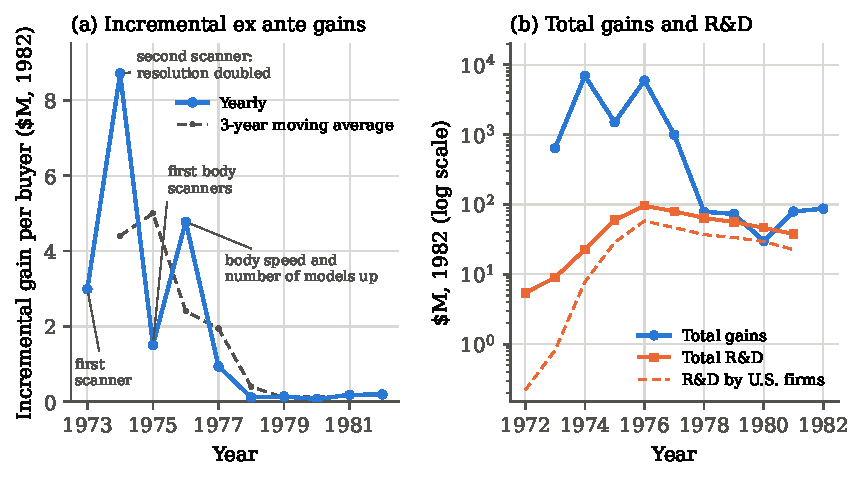
\includegraphics[width=\textwidth]{figures/ch10/trajtenberg_profile.pdf}
\caption{The time profile of the gains from innovation in CT scanners. Panel (a) shows the incremental ex ante gain per
buyer, with the 1973 value equal to the indirect estimate $\frac{K_0}{k}$, and its centered three-year moving average,
which is our computation. Panel (b) shows total gains $TW_t$ and research and development spending on a logarithmic
scale. The 1968--71 research total is a four-year aggregate and is omitted. Source: Trajtenberg (1985), Tables 9, 11
and 12.}
\label{fig:10-ct-profile}
\end{figure}

Second, the single largest gain came from the second scanner model, the EMI CT 1000 of 1974. Its design was almost
identical to the first EMI scanner, except that its resolution was almost doubled. The improvement transformed CT from a
demonstration of feasibility into a widely useful diagnostic tool (p.~78). Trajtenberg calls the early appearance of
such a big winner the ``Ford-T effect,'' after the Model T. Third, research spending tracked the level of activity in
the field with a one-year lead, but it was not closely related to the gains. The ratio of gains to research was about 80
to 1 for 1968--77, with research taken up to 1976. It was 1.4 for 1978--82, and in 1980 research spending exceeded the
benefits (p.~80).\footnote{The first ratio reproduces from Tables~11 and 12. Total gains of \$16,023.7 million in
1973--77 against total research of \$199.02 million in 1968--76 give 80.5. With the same one-year research lead and
no discounting, the two tables give $\frac{348.3}{284.40} = 1.22$ for 1978--82. The paper does not state the
definition behind its figure of 1.4 (our computation).}
Average returns are therefore a poor guide to policy. The question is less whether public support for research is
warranted than until when it should last. In CT, support was socially valuable in the early stages but not after 1976.
Trajtenberg notes that the British Department of Health supported the construction of the first prototype at EMI in
1970--72. An American neurologist, W.~H.~Oldendorf, had independently developed a similar device but could not pursue
it for lack of support (p.~80, n.~80). He presents the profile as evidence, from one case, that innovation can follow a
wave-like pattern.

\subsection{Robustness}\label{sec:10-ct-robustness}

Trajtenberg checks several of his choices, mostly in footnotes. The checks are scattered through the preceding
subsections, and we gather them here. The hedonic function was estimated in three forms, and Box-Cox comparisons
ranked the linear-log form first in half of the twelve cases (p.~37, n.~33). In the diffusion equation, a concave
ceiling gave very similar results to the linear one (pp.~67--68). The concave ceiling corresponds to exponentially
distributed reservation prices. Letting the incremental gains shift the speed of diffusion gave an effect that was
significant but very small (p.~68, n.~64). Repeat purchases are credited only with the incremental gain of their
year, so total gains are a lower bound in this respect (p.~70, n.~67). Adding profits of up to half of revenue to
the benefits would barely change the rate of return (p.~73). Returns to U.S. research and to total research serve
as upper and lower bounds on the true rate (pp.~71--72). Finally, the ex ante and ex post welfare measures are both
reported, and they differ by a factor of about seven (\cref{sec:10-ct-welfare}).

\subsection{Interpretation, critiques and contribution}\label{sec:10-ct-assessment}

Trajtenberg's study established that the magnitude of a product innovation can be measured by the consumer surplus it
creates, computed from an estimated discrete-choice model in characteristics space. Each step of the later literature
appears here in early form. Welfare comes from a log-sum surplus function. The nested logit is used to draw market
boundaries. Prices are related to characteristics through a hedonic function, and the per-buyer gains are linked to
diffusion and to research spending. \Citet{Petrin2002} builds on the template. \Citet[p.~238]{Bresnahan1997} writes
that Hausman takes on the question of the slope of $dd$ ``following Trajtenberg (1989).''

The limitations are of three kinds. The first concerns identification of price sensitivity. There are no instruments,
the residual-price coefficients have the wrong sign, and $\alpha$ is imported from another segment
(\cref{sec:10-ct-signal}). Because the money value of every gain divides by $\alpha$, the welfare numbers inherit this
uncertainty in full. The second concerns functional form. The MNL imposes IIA within branches, buyer heterogeneity is
absent after 1975, and the logit adds an entropy term for every new model (\cref{prop:10-clones,prop:10-entropy}). The
quadratic net utility extrapolates the value of large changes in characteristics. The estimated tastes change from year
to year, and the choice between ex ante and ex post measures changes the answer by a factor of seven. The second-stage
estimate of $\lambda$ carries little information about substitution between branches, as \eqref{eq:10-traj-lambda-implied} shows.
The third concerns interpretation. The buyers are hospitals, whose valuations may diverge from those of patients
(\cref{sec:10-ct-consumer}). The total gains rest on a reduced-form diffusion equation, and the value of the first scanner
is an indirect extrapolation from it.

These limitations do not overturn the qualitative conclusions. Early innovations in CT created large value relative
to their cost, gains concentrated in a few improvements, and returns to research fell sharply as the technology matured.
The precise numbers are less secure. The next case study, \citeauthor{Petrin2002}'s minivan, addresses several of the
weaknesses at once. It uses instruments for price, random coefficients disciplined by micro data, and a supply side
that lets rivals' prices respond. It also decomposes the welfare gain into the parts due to observed characteristics
and to the logit errors.

\section{Case study: the minivan (Petrin 2002)}\label{sec:10-petrin}

\citet{Petrin2002} measures the welfare created by the minivan, a vehicle that Chrysler introduced in 1984 and that
its rivals imitated within two years. The paper answers two questions. The first is substantive. How large were the
gains to consumers and to each producer, and how were they shared? The second is methodological. How can a
researcher who has only market-level data discipline the random coefficients that govern substitution, and therefore
welfare? Petrin's answer to the second question, the use of \emph{micro moments}, is now a standard part of demand
estimation (\cref{sec:08-micro-moments}). \Cref{tab:10-petrin-map} at the end of the section maps the study.
We follow the paper from its question to its contribution, as in
\cref{sec:10-hausman}.\footnote{Petrin writes $\gamma_k$ for the scale of the random coefficient on characteristic $k$,
$\gamma_{mi}$, $\gamma_{sw}$, $\gamma_{su}$ and $\gamma_{pv}$ for the family-vehicle interactions, and $\tau$ for the
cost parameters. In his text the income-group price coefficients are $\alpha_0$, $\alpha_1$ and $\alpha_2$, while his
Table 4 labels them $\alpha_1$, $\alpha_2$ and $\alpha_3$. We write $\sigma_k$, $\pi_{\mathrm{mv}}$, $\pi_{\mathrm{sw}}$,
$\pi_{\mathrm{su}}$, $\pi_{\mathrm{pv}}$ and $\gamma$, and we follow the table for the price coefficients. Page and
table numbers in this section refer to the journal article.}

\subsection{The question}\label{sec:10-petrin-question}

New products improve the standard of living, and firms introduce them to earn the temporary market power of a first
mover (p.~705). Petrin estimates three objects for the minivan. The first is the compensating variation of consumers,
including the gains of households that bought other vehicles whose prices fell when the minivan arrived. The second
is the change in producer surplus. It combines Chrysler's first-mover profits, the cannibalization of its own station
wagons, and the losses imposed on Ford and General Motors (GM). The third is the profit that the imitators dissipated
when they entered.

The question matters for the theory of \cref{sec:10-imperfect}. There we saw that a new good changes welfare through
the surplus of its own buyers and through the prices of existing goods. \Cref{tab:10-bresnahan-2x2} called the second
channel ``Competition,'' and \cref{sec:10-bresnahan} criticized \citet{Hausman1997} for holding rivals' prices fixed.
Petrin re-solves the pricing equilibrium of the whole automobile market with and without minivans. His estimates
therefore measure the Competition cell, together with Chrysler's repricing of its own wagons, in one equilibrium
calculation.

The method matters as much as the answer. Random coefficients are imprecisely estimated from market shares alone
(\cref{sec:08-instruments}). Welfare numbers inherit that imprecision, and they inherit the dependence on the
idiosyncratic logit shock described in \cref{sec:10-charspace}. Petrin's abstract states the main finding in these
terms. Models estimated without micro data yield much larger welfare numbers, ``primarily because the micro data
appear to free the model from a heavy dependence on the idiosyncratic logit `taste' error'' (p.~705).

\subsection{The minivan innovation}\label{sec:10-petrin-setting}

Ford proposed a vehicle called the ``Mini/Max'' in the early 1970s (p.~707). It was a boxlike vehicle that obtained
interior space from its height, with front-wheel drive that lowered the passenger floor. Ford's management gave the
idea little support because it feared cannibalizing the firm's strong station wagon sales. This is the private
incentive problem of \cref{sec:10-imperfect} in its purest form. A firm that owns close substitutes values a new
product only net of the profits it diverts from them.

The financially troubled Chrysler Corporation introduced the Dodge Caravan in 1984. It sold 170,000 units in its first
year. GM introduced the Astro and Safari in 1985, and Ford introduced the Aerostar in 1986. Both rivals were unprepared
for the Caravan's success. They built their minivans on truck platforms with rear-wheel drive, so these vehicles
handled more like downsized full-size vans than like passenger cars. Chrysler kept its lead by adding a larger engine
and a second sliding door. Fourteen years after the introduction, six firms sold 13 minivans, and Chrysler held 44
percent of a market of 1.16 million vehicles. Station wagon sales peaked at 950,000 in 1984 and fell to 300,000 over
the next seven years (p.~707).

Table~3 of the paper shows the substitution in shares of total vehicle sales. Minivans rose from 1.58 percent in 1984 to
9.93 percent in 1993. Station wagons held about 10 percent in 1981--83 (10.51, 10.27 and 10.32 percent), fell to 8.90
percent in 1984, and reached 3.02 percent in 1993. The combined share of minivans and wagons stayed between 9.65 and
12.95 percent over 1981--93. Petrin reads this negative comovement as evidence of a positive covariance in the tastes
for the two vehicle types (p.~718). The demand model is built to capture that covariance.

\subsection{Data}\label{sec:10-petrin-data}

The paper combines two data sets (pp.~712--713). The market data cover all 2,407 nameplates sold in the United States
from 1981 to 1993 with annual sales above 1,000 vehicles. They come from the \textit{Automotive News Market Data
Book} and \textit{Ward's Automotive Yearbook}. The characteristics are acceleration (horsepower per unit of curb
weight), size (length times width times height), drive type, fuel efficiency (miles per dollar), and a luxury proxy
(air conditioning standard). Quantity and list price refer to the base model. Nameplates in adjacent years whose
horsepower, wheelbase, width and length change by less than 10 percent are treated as the same model. This rule leaves
916 independent observations, and the standard errors allow arbitrary correlation of the errors of the same model over
time (p.~716, n.~11).

The consumer data come from the Consumer Expenditure Survey (CEX) for 1987--92. Almost 30,000 household records
approximate the joint distribution of demographics in the United States. The CEX automobile supplement links the
demographics of 2,660 new-vehicle buyers to the vehicles they bought. Among them are 120 minivan buyers, 63 station
wagon buyers, 131 sport-utility buyers and 23 full-size van buyers. These samples are too small for a consumer-level
choice model, since about 200 kinds of vehicles are sold each year but only about 400 purchases are recorded annually
(p.~713, n.~8). They are large enough to estimate a few averages precisely. Other annual inputs are the number of
households $M$, gasoline prices and the growth of gross national product. The random coefficients model without micro
data also uses a lognormal income distribution estimated from the March Current Population Survey (p.~713, n.~9).

\Cref{tab:10-petrin-cex} reproduces the demographic averages of Table~2 of the paper. They are the targets of the micro
moments. New-vehicle buyers had a mean income of \$36,113, about \$13,000 above the U.S. mean of \$23,728 (incomes
in 1982--84 dollars). Minivan buyers had the largest families of all buyer groups, 3.86 members against 2.58 in the
population. They also had the highest share of household heads aged 30 to 60, 78 percent against 55 percent. Table~1 of
the paper adds that minivans were larger than the average vehicle (size 0.87 against 0.71). Of them, 78 percent had air
conditioning as standard (27 percent of all vehicles), and their mean list price was \$10,060 against \$9,867 for all
vehicles. Chrysler accounted almost entirely for the 63 percent of minivan sales with front-wheel drive (p.~716).

\begin{table}[htbp]
\centering
\caption{Demographics of the U.S. population and of new-vehicle buyers, 1987--92}\label{tab:10-petrin-cex}
\small
\setlength{\tabcolsep}{5pt}
\begin{tabular}{@{}lccccccc@{}}
\toprule
 & \multicolumn{2}{c}{United States} & \multicolumn{5}{c}{Buyers of} \\
\cmidrule(lr){2-3}\cmidrule(l){4-8}
 & Mean & Std.\ dev. & New vehicles & Minivans & Wagons & Sport-utilities & Full-size vans \\
\midrule
Income (\$)  & 23,728 & 21,255 & 36,113 & 39,476 & 40,196 & 41,569 & 31,164 \\
Family size  & 2.58   & 1.53   & 2.87   & 3.86   & 3.17   & 2.97   & 3.47   \\
Midage       & 0.55   & 0.49   & 0.64   & 0.78   & 0.73   & 0.74   & 0.65   \\
\bottomrule
\end{tabular}

\smallskip
\begin{minipage}{0.95\textwidth}
\footnotesize Source: \citet[Table~2]{Petrin2002}, from the Consumer Expenditure Survey. Income is in 1982--84
CPI-adjusted dollars. Family size is the number of household members. Midage is an indicator for a household head
aged between 30 and 60 inclusive.
\end{minipage}
\end{table}

\subsection{The demand model}\label{sec:10-petrin-model}

Consumers are households $i$ with income $y_i$, family size $fs_i$, an indicator $\mathit{mid}_i$ for a head aged 30 to
60, and unobserved tastes. Each household buys one new vehicle $j \in \{1, \dots, J\}$ in a year or buys none ($j = 0$).
Petrin specifies the conditional indirect utility (p.~710)
\begin{equation}\label{eq:10-petrin-utility}
  u_{ij} = \alpha_i \ln(y_i - p_j) + x_j\beta + \sum_{k} \sigma_k \nu_{ik} x_{jk}
           + \ln(fs_i)\,\nu_{i,\mathrm{fv}} \sum_{g \in \mathcal{G}} \pi_g d_{jg} + \xi_j + \epsilon_{ij},
  \qquad j = 1, \dots, J .
\end{equation}
The first term is the utility of the composite good bought with the income left after the vehicle. The row vector
$x_j$ holds a constant, the five characteristics, four vehicle-type dummies, the percentage change in gross national
product and a quadratic time trend (Table~4, note). The set $\mathcal{G} = \{\mathrm{mv}, \mathrm{sw}, \mathrm{su},
\mathrm{pv}\}$ collects the four \emph{family vehicle} types: minivans, station wagons, sport-utility vehicles and
full-size passenger vans. The dummy $d_{jg}$ equals one when vehicle $j$ is of type $g$. The unobserved product quality
is $\xi_j$, and $\epsilon_{ij}$ is type-I extreme value.

Three features of \eqref{eq:10-petrin-utility} carry the economics.

\casehead{Income effects} The marginal utility of income varies across the three income terciles,
\begin{equation*}
  \alpha_i = \begin{cases}
    \alpha_1 & \text{if } y_i < \bar y_1, \\
    \alpha_2 & \text{if } \bar y_1 \le y_i < \bar y_2, \\
    \alpha_3 & \text{if } y_i \ge \bar y_2,
  \end{cases}
\end{equation*}
where $\bar y_1$ and $\bar y_2$ split the population into three equal groups. The utility cost of a higher price is
\begin{equation}\label{eq:10-petrin-dudp}
  \frac{\partial u_{ij}}{\partial p_j} = -\frac{\alpha_i}{y_i - p_j} ,
\end{equation}
so price sensitivity falls with income within a group, and the three $\alpha_g$ let the curvature differ across groups.
This is the Cobb-Douglas income specification of \citet{BerryLevinsohnPakes1995} studied in \cref{sec:08-income}, with
group-specific coefficients. Conditional on all tastes, the logit formulas give the individual share derivatives
\begin{equation*}
  \frac{\partial s_{ij}}{\partial p_j} = -\frac{\alpha_i}{y_i - p_j}\,s_{ij}(1 - s_{ij}), \qquad
  \frac{\partial s_{ij}}{\partial p_k} = \frac{\alpha_i}{y_i - p_k}\,s_{ij}s_{ik} \quad (k \ne j).
\end{equation*}
Market derivatives integrate these over households.

\casehead{Random tastes for characteristics} Household $i$ draws a taste $\nu_{ik}$ for each characteristic $k$,
scaled by $\sigma_k$. Petrin draws the $\nu_{ik}$ independently from a $\chi^2(3)$ distribution truncated at its 95th
percentile (p.~711). He gives two reasons. The distribution is bounded above and below, and it skews heterogeneity in
the direction of positive taste. Taken as written, the draws lie between 0 and 7.81, with mean about 2.63 and standard
deviation about 1.83 (our computation). The paper does not say whether the draws are \emph{centered}, that is, whether
their mean is subtracted before they enter utility. The random coefficient on the constant makes the value of buying any new vehicle,
relative to the outside option, heterogeneous across households.

\casehead{Demographic tastes for family vehicles} The taste of household $i$ for a family vehicle of type $g$ is
$\pi_g \ln(fs_i)\,\nu_{i,\mathrm{fv}}$. The draw $\nu_{i,\mathrm{fv}}$ is common to all four types, and family size
scales it. Conditional on family size, the covariance between the tastes for minivans and for station wagons is
\begin{equation}\label{eq:10-petrin-cov}
  \Cov\bigl(\pi_{\mathrm{mv}}\ln(fs_i)\nu_{i,\mathrm{fv}},\; \pi_{\mathrm{sw}}\ln(fs_i)\nu_{i,\mathrm{fv}} \bigm| fs_i\bigr)
  = \pi_{\mathrm{mv}}\pi_{\mathrm{sw}}\,\bigl(\ln fs_i\bigr)^2\,\Var(\nu_{i,\mathrm{fv}}) .
\end{equation}
It rises with $\pi_{\mathrm{mv}}$ and $\pi_{\mathrm{sw}}$ and with family size. Substitution between minivans and
wagons can therefore arise for two reasons (p.~710). Large families prefer both types, or the two types share other
observed characteristics such as size.

The outside option is to buy no new vehicle. We write its utility as $u_{i0} = \alpha_i\ln y_i + \epsilon_{i0}$, the
normalization of \cref{sec:08-income}. Conditional on the household's demographics $D_i = (y_i, fs_i, \mathit{mid}_i)$
and tastes $\nu_i$, the probability of buying $j$ is the logit formula (p.~711)
\begin{equation}\label{eq:10-petrin-sij}
  s_{ij} = \frac{\exp V_{ij}}{\exp\bigl(\alpha_i \ln y_i\bigr) + \sum_{l=1}^{J} \exp V_{il}} ,\qquad
  V_{ij} = \alpha_i\ln(y_i - p_j) + \delta_j + \mu_{ij},
\end{equation}
with base utility $\delta_j = x_j\beta + \xi_j$ and household-specific term
\begin{equation*}
  \mu_{ij} = \sum_k\sigma_k\nu_{ik}x_{jk} + \ln(fs_i)\,\nu_{i,\mathrm{fv}}\sum_g \pi_g d_{jg} .
\end{equation*}
Price is not part of $\delta_j$. It enters only through the income
term, so the $\alpha_g$ are nonlinear parameters, as in \cref{sec:08-income}. The market share is $s_j = \int s_{ij}\,
\dd P(D_i, \nu_i)$, where $D_i$ follows the empirical distribution of the CEX and $\nu_i$ the truncated $\chi^2(3)$
distribution. Petrin calls the elements of $\beta$ \emph{base coefficients} (Table~4). If the draws are centered,
$\mu_{ij}$ has mean zero and $\delta_j$ is the mean utility of product $j$, net of the income term. Otherwise
$\delta_j$ is that utility for a household whose draws are all zero, and the mean taste for characteristic $k$ is
$\beta_k + 2.63\,\sigma_k$.

The demand side has 24 parameters: three price coefficients, eleven base coefficients, six random-coefficient scales
and four family-vehicle interactions. Eleven of them describe family vehicles and income effects: the three
$\alpha_g$, the four type dummies and the four $\pi_g$. The micro moments speak most directly to these eleven.

\subsection{Supply and the counterfactual equilibrium}\label{sec:10-petrin-supply}

The supply side follows \citet{BerryLevinsohnPakes1995} (pp.~711--712). Multiproduct firms $f = 1, \dots, F$ set prices
in a static Bertrand-Nash equilibrium. Marginal cost is log-linear in observed cost characteristics $W_j$ and an
unobserved component $\omega_j$,
\begin{equation}\label{eq:10-petrin-mc}
  \ln mc_j = W_j\gamma + \omega_j .
\end{equation}
Firm $f$ earns $\Pi_f = M\sum_{j\in\mathcal{J}_f}(p_j - mc_j)\,s_j(p, x; \theta)$, and the first-order conditions are
\begin{equation}\label{eq:10-petrin-foc}
  s_j(p, x; \theta) + \sum_{r \in \mathcal{J}_f}(p_r - mc_r)\frac{\partial s_r(p, x; \theta)}{\partial p_j} = 0,
  \qquad j \in \mathcal{J}_f .
\end{equation}
In matrix form these are \eqref{eq:08-foc-matrix}, and inverting them gives the markup formula \eqref{eq:08-markup},
$p - mc = -[(\Omega\odot\Delta)^\top]^{-1}s$. Given demand estimates and observed prices, this formula recovers each
$mc_j$ \citep[eq.~3]{Petrin2002}.

A rearrangement of \eqref{eq:10-petrin-foc} is useful for reading the counterfactual. Separate the own-product term
and divide by $-\frac{\partial s_j}{\partial p_j} > 0$:
\begin{align}
  0 &= s_j + (p_j - mc_j)\frac{\partial s_j}{\partial p_j}
       + \sum_{r\in\mathcal{J}_f,\, r\ne j}(p_r - mc_r)\frac{\partial s_r}{\partial p_j}, \notag\\
  p_j - mc_j &= \frac{s_j}{-\frac{\partial s_j}{\partial p_j}}
       + \sum_{r\in\mathcal{J}_f,\, r\ne j}(p_r - mc_r)\,D_{jr},
  \qquad D_{jr} = \frac{\frac{\partial s_r}{\partial p_j}}{-\frac{\partial s_j}{\partial p_j}} . \label{eq:10-petrin-diversion}
\end{align}
Here $D_{jr}$ is the diversion ratio from $j$ to $r$ (\cref{ch:diffprod}). The markup on $j$ is a single-product
markup plus the margins the firm earns on the sales that a higher $p_j$ diverts to its other products. When Chrysler
adds a minivan $m$ that is a substitute for its station wagons, a new positive term $(p_m - mc_m)D_{jm}$ appears in the
markup of each Chrysler wagon $j$. Other things equal, Chrysler raises the prices of its wagons. Rival firms gain no
term for the minivan. Their markups change through the first term, which falls when entry makes their demand more
elastic, and through changes in diversion among their own products.

The counterfactual removes all minivans from the choice set and solves \eqref{eq:10-petrin-foc} for the remaining
products, holding marginal costs, characteristics and $\xi_j$ fixed (p.~712). Call the solution $p^{cf}$ and the
observed prices $p^0$. The change in the variable profit of firm $f$ due to the minivan is $\Pi_f(p^0, mc) -
\Pi_f(p^{cf}, mc)$, and summing over firms gives the change in producer surplus. A second counterfactual removes only
the Ford and GM minivans, which measures how much of Chrysler's profit the imitators dissipated. The profit function
ignores the 25 percent tariff on Japanese minivans, which made up a small part of minivan sales (p.~712, n.~6).

\subsection{Compensating variation with income effects}\label{sec:10-petrin-cv}

Petrin measures consumer welfare by a compensating variation whose benchmark is the standard of living attained with
minivans (p.~720). The counterfactual environment has no minivans, and the other vehicles sell at $p^{cf}$. For a
household with all tastes $(D_i, \nu_i, \epsilon_i)$ held fixed, let $\mathcal{J}^1$ be the choice set with minivans
and $\mathcal{J}^0$ the set without them. The household's compensation $CV_i$ solves
\begin{equation}\label{eq:10-petrin-cvdef}
  \max_{j \in \mathcal{J}^0 \cup \{0\}} u_{ij}\bigl(y_i + CV_i,\, p^{cf}\bigr)
  = \max_{j \in \mathcal{J}^1 \cup \{0\}} u_{ij}\bigl(y_i,\, p^{0}\bigr) \equiv U_i^1 .
\end{equation}
This is the compensating variation of removing the minivans, which equals the equivalent variation of introducing
them. It is the measure \eqref{eq:10-cv-income} of \cref{sec:10-cs-welfare}, and the discrete-choice analog of
\cref{prop:10-cv-newgood}, whose reference utility is also the one attained with the new good.

With the utility \eqref{eq:10-petrin-utility} the compensation has a closed form. Write $v_{ij} = \delta_j + \mu_{ij}
+ \epsilon_{ij}$ for the part of utility that does not involve money, with $p_0 = 0$ and $v_{i0} = \epsilon_{i0}$.
For each alternative $j \in \mathcal{J}^0\cup\{0\}$, define the compensation that would make $j$ alone reach $U_i^1$:
\begin{align*}
  \alpha_i\ln\bigl(y_i + c_{ij} - p^{cf}_j\bigr) + v_{ij} &= U_i^1, \\
  y_i + c_{ij} - p^{cf}_j &= \exp\Bigl(\frac{U_i^1 - v_{ij}}{\alpha_i}\Bigr), \\
  c_{ij} &= p^{cf}_j - y_i + \exp\Bigl(\frac{U_i^1 - v_{ij}}{\alpha_i}\Bigr).
\end{align*}
The left side of \eqref{eq:10-petrin-cvdef} increases in $CV_i$, and it first reaches $U_i^1$ when the cheapest of
these compensations is paid. Hence
\begin{equation}\label{eq:10-petrin-cvi}
  CV_i = \min_{j \in \mathcal{J}^0 \cup \{0\}} \Bigl\{ p^{cf}_j - y_i + \exp\Bigl(\frac{U_i^1 - v_{ij}}{\alpha_i}\Bigr) \Bigr\}.
\end{equation}
The formula has a useful implication for households that did not buy a minivan. If household $i$ chose $j \in
\mathcal{J}^0$ at $p^0$, then $U_i^1 = \alpha_i\ln(y_i - p^0_j) + v_{ij}$, and the term for $j$ in
\eqref{eq:10-petrin-cvi} equals
\begin{equation*}
  p^{cf}_j - y_i + \exp\Bigl(\frac{\alpha_i\ln(y_i - p^0_j)}{\alpha_i}\Bigr) = p^{cf}_j - y_i + (y_i - p^0_j)
  = p^{cf}_j - p^0_j .
\end{equation*}
A non-buyer's compensation is therefore at most the price change of the vehicle she chose. It equals that change if
and only if her vehicle remains a best choice at prices $p^{cf}$ and the compensated income $y_i + p^{cf}_j - p^0_j$.
At that income vehicle $j$ yields exactly $U_i^1$, so the condition says that no alternative reaches $U_i^1$ with
less compensation. Remaining best at the original income $y_i$ does not suffice, because income enters utility
through $\ln(y_i - p_k)$. Extra income then raises the utility of expensive vehicles more than that of cheap ones.
For these households, as Petrin notes (p.~720), compensation is
determined entirely by the price changes that the minivan caused. Averaging $CV_i$ over simulated households and
multiplying by $M$ gives the aggregate measure.

Petrin also splits the compensation of minivan buyers into two parts (Table~8). Suppose utility were quasi-linear,
$u_{ij} = \delta_j - \alpha p_j + \mu_{ij} + \epsilon_{ij}$. Let $j$ be the buyer's minivan and $k$ her best
alternative in $\mathcal{J}^0$ at $p^{cf}$. Then
\begin{equation}\label{eq:10-petrin-decomp}
  CV_i = \underbrace{\frac{(\delta_j - \alpha p^0_j + \mu_{ij}) - (\delta_k - \alpha p^{cf}_k + \mu_{ik})}{\alpha}}_{
  \text{observed characteristics}}
  + \underbrace{\frac{\epsilon_{ij} - \epsilon_{ik}}{\alpha}}_{\text{logit error}} .
\end{equation}
The first part is the value of the minivan's observed characteristics and price relative to the second choice. The
second part is the value of the idiosyncratic logit draws. With income effects the split is approximate (p.~722,
n.~13).

The logit benchmark explains why the second part can dominate. The next result, which we derive, extends
\cref{prop:10-logit-newgood} from the aggregate gain to the gain of the buyers of the new good.

\begin{proposition}[Who gains in a logit model]\label{prop:10-logit-buyer-cv}
Let $u_{ij} = V_j + \epsilon_{ij}$ with $V_j = \delta_j - \alpha p_j$ and $\epsilon_{ij}$ independent type-I extreme
value. Remove a set $\mathcal{N}$ of products whose total share is $s_{\mathcal{N}}$, holding all other prices fixed.
Then
\begin{enumerate}[label=(\alph*)]
  \item A consumer whose chosen product is not in $\mathcal{N}$ has $CV_i = 0$.
  \item The mean compensation of consumers who chose a product in $\mathcal{N}$ is
        $\frac{1}{\alpha}\,\frac{-\ln(1 - s_{\mathcal{N}})}{s_{\mathcal{N}}} \ge \frac{1}{\alpha}$.
\end{enumerate}
\end{proposition}

\begin{proof}
(a) The consumer's chosen product remains available at the same price, and her utilities are unchanged. Her maximum
utility is the same in both choice sets, so $CV_i = 0$.

(b) By \cref{lem:10-cv-quasilinear}, $CV_i = \frac{1}{\alpha}\bigl(\max_{j}u_{ij} - \max_{j\notin\mathcal{N}}u_{ij}\bigr)$.
By \cref{lem:10-logsum}, the expected maximum of $V_j + \epsilon_{ij}$ over a set $S$ is $\ln\sum_{j\in S}e^{V_j} +
\gamma_E$. Therefore, as in the proof of \cref{prop:10-logit-newgood},
\begin{align*}
  \E[CV_i] &= \frac{1}{\alpha}\Bigl(\ln\sum_{j}e^{V_j} - \ln\sum_{j\notin\mathcal{N}}e^{V_j}\Bigr)
            = -\frac{1}{\alpha}\ln\frac{\sum_{j\notin\mathcal{N}}e^{V_j}}{\sum_{j}e^{V_j}}
            = -\frac{1}{\alpha}\ln(1 - s_{\mathcal{N}}) .
\end{align*}
By part (a), $\E[CV_i] = s_{\mathcal{N}}\,\E[CV_i \mid \text{chose in } \mathcal{N}]$. Dividing by $s_{\mathcal{N}}$ gives
the formula. The inequality follows from $-\ln(1-s) \ge s$ for $s \in [0,1)$, as in \eqref{eq:10-logit-perbuyer}.
\end{proof}

Part (b) says that in a logit model the buyers of a product with a small share gain on average about $\frac{1}{\alpha}$
dollars, whatever the product is. Part (b) of \cref{prop:10-entropy} says why. For every product $n$,
\begin{equation*}
  \E[\epsilon_{in} \mid i \text{ chooses } n] = \gamma_E - \ln s_n ,
\end{equation*}
so a product with a small share is bought by consumers with large draws of $\epsilon_{in}$, and the model credits the
purchase to those draws. Its mean utility $V_n$ is low, so the observed component in \eqref{eq:10-petrin-decomp} tends
to be negative while the logit component is large. The markup has the same scale. \Cref{rem:10-logit-multiproduct}
showed that a multiproduct logit firm charges a common markup on all its products, $m_f = \frac{1}{\alpha(1 - S_f)}$,
where $S_f = \sum_{r\in\mathcal{J}_f}s_r$ is the firm's total share. Since each firm's share of all households is small,
every logit markup is close to $\frac{1}{\alpha}$. We return to both implications when we read Petrin's Tables 8 and 9.

\subsection{Estimation: market moments plus micro moments}\label{sec:10-petrin-estimation}

The estimator is the generalized method of moments (GMM) estimator of \citet{BerryLevinsohnPakes1995}, augmented by
moments from the CEX (pp.~713--716). The idea comes from \citet{ImbensLancaster1994}, who show that aggregate
information on the averages of micro variables can sharpen the estimates of a micro model.

\casehead{Micro moments} Petrin uses three sets of moments (p.~714). Let $P_{ig}(\theta) = \int\sum_{j\in g}s_{ij}(\theta)
\,\dd P(\nu_i)$ be the probability that a household with demographics $D_i$ buys a vehicle of type $g$, and let
$P_{i}(\theta) = \int \sum_{j\ge1}s_{ij}(\theta)\,\dd P(\nu_i)$ be its probability of buying any new vehicle. The first
set matches the purchase probability in each income group $h \in \{1,2,3\}$:
\begin{equation}\label{eq:10-petrin-mm1}
  \E\bigl[\indic\{i \text{ buys a new vehicle}\} \bigm| y_i \in h\bigr]
  = \frac{\int \indic\{y_i\in h\}\,P_i(\theta)\,\dd P(D_i)}{\int\indic\{y_i\in h\}\,\dd P(D_i)} .
\end{equation}
The second set matches the mean family size of the buyers of each family vehicle type $g \in \mathcal{G}$:
\begin{equation}\label{eq:10-petrin-mm2}
  \E\bigl[fs_i \bigm| i \text{ buys type } g\bigr] = \frac{\int fs_i\,P_{ig}(\theta)\,\dd P(D_i)}{\int P_{ig}(\theta)\,\dd P(D_i)} .
\end{equation}
The third set matches $\E[\mathit{mid}_i \mid i \text{ buys type } g]$, the probability that the household head is aged
30 to 60, in the same way. The left sides are CEX sample averages and the right sides are model predictions. There
are $3 + 4 + 4 = 11$ micro moments. \Cref{eq:10-petrin-mm2} is Bayes' rule applied to the purchase
probability, as in \eqref{eq:08-bayes}.

A simple identity shows what the family-size moments identify.

\begin{lemma}[What a conditional-mean moment measures]\label{lem:10-micro-moment}
For any demographic $D$ and purchase probability $P_{ig}$ with $\E[P_{ig}] > 0$,
\begin{equation*}
  \E\bigl[D_i \bigm| i \text{ buys type } g\bigr] = \E[D_i] + \frac{\Cov(D_i, P_{ig})}{\E[P_{ig}]} .
\end{equation*}
\end{lemma}

\begin{proof}
By \eqref{eq:10-petrin-mm2} the conditional mean is $\frac{\E[D_iP_{ig}]}{\E[P_{ig}]}$. Write $\E[D_iP_{ig}] =
\E[D_i]\E[P_{ig}] + \Cov(D_i, P_{ig})$ and divide by $\E[P_{ig}]$.
\end{proof}

The CEX gives $\E[fs_i] = 2.58$ and $\E[fs_i \mid \text{minivan}] = 3.86$, so the model must produce
$\frac{\Cov(fs_i, P_{i,\mathrm{mv}})}{\E[P_{i,\mathrm{mv}}]} = 1.28$.
In \eqref{eq:10-petrin-utility} family size enters the minivan's utility only through $\pi_{\mathrm{mv}}\ln(fs_i)
\nu_{i,\mathrm{fv}}$, apart from its correlation with income. The moment therefore pins down $\pi_{\mathrm{mv}}$, and the
other three moments pin down the other $\pi_g$. Likewise, the purchase probabilities by income group pin down how
the $\alpha_g$ shift purchases across the income distribution. Market shares alone identify these parameters only
through variation in choice sets and in demographics over time, which is weak in thirteen years of national data.

\casehead{Market moments} The first set of market moments matches predicted and observed shares, $s_j(\delta, \theta) =
s_j$ for every $j$. As in \cref{sec:08-inversion}, this is equivalent to solving for the vector $\delta(\theta)$ that
equates them \citep{Berry1994}. The second set states that the demand and cost unobservables are mean independent of
the observed characteristics of all vehicles in the year (p.~715):
\begin{equation}\label{eq:10-petrin-blpmom}
  \E\bigl[\xi_j(\theta_0) \bigm| X, W\bigr] = \E\bigl[\omega_j(\theta_0) \bigm| X, W\bigr] = 0 .
\end{equation}
The instruments approximate the optimal ones in the manner of \citet{BerryLevinsohnPakes1995}. A product's own
characteristics instrument for themselves. Cost variables excluded from demand instrument for price. So do the sums
of each characteristic over the firm's other products, $\sum_{j\ne l,\, j\in\mathcal{J}_f}x_{jk}$, and over rivals'
products, $\sum_{j\notin\mathcal{J}_f}x_{jk}$. These sums measure how crowded a product's neighborhood is, which shifts
its markup through \eqref{eq:10-petrin-diversion} \citep{BresnahanSternTrajtenberg1997}.

\casehead{The objective and its variance} Stack the market moments $G_1(\theta)$ and the micro moments $G_2(\theta)$ in
$G(\theta) = (G_1(\theta)^\top, G_2(\theta)^\top)^\top$, with $\E[G(\theta_0)] = 0$. Let $\hat G(\theta)$ be the sample
analog and $a(\tilde\theta)$ a consistent estimate of the ``square root'' of the inverse of the moments' asymptotic
variance, computed at a preliminary estimate $\tilde\theta$. Following \citet{Hansen1982}, the two-step estimator is
(p.~715)
\begin{equation}\label{eq:10-petrin-gmm}
  \hat\theta = \argmin_{\theta\in\Theta}\; \tilde G(\theta)^\top\tilde G(\theta), \qquad
  \tilde G(\theta) = a(\tilde\theta)\,\hat G(\theta) .
\end{equation}
The two sets of moments come from independent samples, the vehicle market and the CEX. Let $n$ be the size of the
market sample, and suppose the CEX sample size $n_2$ satisfies $\frac{n_2}{n} \to \lambda \in (0,\infty)$. Write
$V_G$ for the asymptotic variance of $\sqrt{n}\,\hat G(\theta_0)$. Independence makes $V_G$ block diagonal. Since
$\sqrt{n}\,\hat G_2 = \sqrt{\frac{n}{n_2}}\,\sqrt{n_2}\,\hat G_2$, the micro block is $\frac{1}{\lambda}$ times the
asymptotic variance of $\sqrt{n_2}\,\hat G_2(\theta_0)$. Let $a$ and $\Gamma$ be the probability limits of $a(\tilde\theta)$ and
$\frac{\partial\tilde G(\theta_0)}{\partial\theta}$. The scaled moments $\sqrt{n}\,\tilde G(\theta_0)$ then have
asymptotic variance $V = aV_Ga^\top$, and the asymptotic variance of $\sqrt{n}(\hat\theta - \theta_0)$ is
\begin{equation}\label{eq:10-petrin-avar}
  (\Gamma^\top\Gamma)^{-1}\,\Gamma^\top V\Gamma\,(\Gamma^\top\Gamma)^{-1} .
\end{equation}
This is the usual sandwich for a GMM estimator with identity weight on the normalized moments
(\cref{app:econometrics}). Petrin writes $V = \E[\tilde G(\theta_0)\tilde G(\theta_0)^\top]$ (p.~715). Read literally,
that is the variance of a sample average, which is of order $\frac{1}{n}$, so the sandwich needs the factor $n$ of
our definition. If $a = V_G^{-\frac{1}{2}}$, then $V = I$ and \eqref{eq:10-petrin-avar} reduces to the efficient
GMM variance $(\Gamma^\top\Gamma)^{-1}$. The micro block of $V_G$ reflects CEX sampling error, which is large when a
buyer group is small or the CEX sample is small relative to the market sample.

\casehead{Computation} One evaluation of the objective proceeds as follows.
\begin{enumerate}[label=(\roman*)]
  \item Draw households from the CEX records and taste vectors $\nu_i$ from the truncated $\chi^2(3)$ distribution.
        Hold the draws fixed across evaluations.
  \item For trial nonlinear parameters $(\alpha_g, \sigma_k, \pi_g)$, invert the shares to obtain $\delta(\theta)$ by
        the contraction of \cref{sec:08-inversion}.
  \item Recover $\xi_j = \delta_j - x_j\beta$, compute markups from \eqref{eq:08-markup}, and recover $\omega_j = \ln(p_j -
        b_j) - W_j\gamma$, where $b_j$ is the markup. The linear parameters $(\beta,\gamma)$ can be concentrated out.
  \item Compute the model's micro predictions, such as \eqref{eq:10-petrin-mm1} and \eqref{eq:10-petrin-mm2}, from
        the same draws.
  \item Form \eqref{eq:10-petrin-gmm} and search over the nonlinear parameters.
\end{enumerate}
Because the micro moments only add terms to the objective, the method adds little computational burden to the BLP
estimator (p.~706).

\casehead{Identification} Petrin's footnote~5 (p.~709) explains how market data identify heterogeneity. Suppose
three cars differ only in interior space, two of them spacious, and each has a third of the market. In a second
market one spacious car is missing. If the remaining spacious car takes two-thirds of the market, its buyers
substitute on space, which reveals a strong and heterogeneous taste for space. If the two remaining cars split the
market, there is no evidence of heterogeneity. Identification of this kind requires large changes in choice sets. The
micro moments supply a second source, the covariance between demographics and choices in
\cref{lem:10-micro-moment}.

\citet{BerryLevinsohnPakes2004} develop a third source, consumers' reported second choices, which measure substitution
directly. They note that consumer attribute data, together with a changing choice set, are useful for explaining
substitution and welfare for minivans. They find other automotive choices less closely tied to commonly observed
attributes \citep[p.~70, n.~1]{BerryLevinsohnPakes2004}. They also stress that second-choice data from one cross
section cannot identify the level of price elasticities. \citet{BerryHaile2024} give the formal nonparametric
identification argument for micro data (\cref{sec:08-bh24}).

\subsection{Results}\label{sec:10-petrin-results}

\casehead{Demand parameters} \Cref{tab:10-petrin-demand,tab:10-petrin-rc} reproduce Tables~4 and 5 of the paper.
Moving from the OLS logit to the instrumental variables (IV) logit almost doubles the price coefficient, from 0.07 to
0.13. Berry, Levinsohn and Pakes found the same pattern, and it shows that instrumenting matters (p.~719). Many random
coefficients differ significantly from zero, so Wald tests reject both logit models in favor of the random
coefficient models.

The random coefficients model estimated from market data alone (column~3 of \cref{tab:10-petrin-demand} and
column~1 of \cref{tab:10-petrin-rc}) is imprecise. The paper reports that only six of the 24 demand parameters have
$z$-statistics above one, and that none of the eight family-vehicle coefficients does. Adding the micro moments
changes the picture. Twenty-one of the 24 parameters then have $z$-statistics above one. The paper reports that all
eleven coefficients related to family vehicles and income effects have $z$-statistics above three (p.~719).\footnote{Counting from the printed estimates and standard errors, we find seven ratios above one in the model
without micro data. The extra one is the front-wheel-drive coefficient, $-5.24$ (3.09), which Table~4 prints without
a star. In the model with micro data, ten of the eleven family-vehicle and income ratios exceed three. The full-size
van interaction, 0.42 (0.21), has a ratio of about two.}
The parameters closest to the added information gain the most precision. The standard error of $\pi_{\mathrm{mv}}$,
for example, falls from 2.62 to 0.10.

The estimates with micro data have an intuitive structure. The base coefficients on the four family-vehicle dummies
are negative, while the four $\pi_g$ are positive and precise. Relative to a car with the same observed
characteristics, household $i$ values a vehicle of type $g$ at $\beta_g + \pi_g\ln(fs_i)\,\nu_{i,\mathrm{fv}}$. A
one-person household has $\ln fs_i = 0$, so it values type $g$ at $\beta_g < 0$ whether or not the draws are centered.
For a household with a positive draw, the taste rises with family size. The draw is independent of demographics
(p.~710), so the average taste is $\beta_g + \pi_g\E[\ln fs_i]\,\E[\nu_{i,\mathrm{fv}}]$. With centered draws it equals
$\beta_g$. With uncentered draws $\E[\nu_{i,\mathrm{fv}}] \approx 2.63$, and Jensen's inequality gives $\E[\ln fs_i]
\le \ln\E[fs_i] = \ln 2.58$, where 2.58 is the CEX mean family size for 1987--92 (Table~2, p.~717). The largest resulting bound,
for station wagons, is $-1.31 + 0.28 \times 2.63 \times \ln 2.58 \approx -0.61$, and it stays negative for any mean
family size below 5.9. Under either normalization the
average household therefore values each family-vehicle type below a comparable car (our computation).

The scale of the random coefficient on miles per dollar is precisely estimated, at 2.58 (0.14). Since the draws of
\cref{sec:10-petrin-model} have a standard deviation of about 1.83, the implied standard deviation of the taste for
miles per dollar is about 4.7 (our computation). Tastes for fuel economy are therefore heterogeneous.

\begin{table}[htbp]
\centering
\caption{Petrin's demand estimates: price and base coefficients}\label{tab:10-petrin-demand}
\small
\setlength{\tabcolsep}{3.4pt}
\begin{tabular}{@{}lcccc@{}}
\toprule
 & OLS logit & IV logit & Random coefficients & Random coefficients \\
 &  &  &  & and micro data \\
 & (1) & (2) & (3) & (4) \\
\midrule
\multicolumn{5}{@{}l}{\textit{A. Price coefficients}} \\
$\alpha_1$ (low income)    & 0.07 (0.01)$^{**}$ & 0.13 (0.01)$^{**}$ & 4.92 (9.78)           & 7.52 (1.24)$^{**}$ \\
$\alpha_2$ (middle income) &                    &                    & 11.89 (21.41)         & 31.13 (4.07)$^{**}$ \\
$\alpha_3$ (high income)   &                    &                    & 37.92 (18.64)$^{**}$  & 34.49 (2.56)$^{**}$ \\
\midrule
\multicolumn{5}{@{}l}{\textit{B. Base coefficients}} \\
Constant                  & $-10.03$ (0.32)$^{**}$ & $-10.04$ (0.34)$^{**}$ & $-12.74$ (5.65)$^{**}$ & $-15.67$ (4.39)$^{**}$ \\
Horsepower per weight     & 1.48 (0.34)$^{**}$     & 3.78 (0.44)$^{**}$     & 3.40 (39.79)           & $-2.83$ (8.16) \\
Size                      & 3.17 (0.26)$^{**}$     & 3.25 (0.27)$^{**}$     & 4.60 (24.64)           & 4.80 (3.57)$^{*}$ \\
Air conditioning standard & $-0.20$ (0.06)$^{**}$  & 0.21 (0.08)$^{**}$     & $-1.97$ (2.23)         & 3.88 (2.21)$^{*}$ \\
Miles per dollar          & 0.18 (0.06)$^{**}$     & 0.05 (0.07)            & $-0.54$ (3.40)         & $-15.79$ (0.87)$^{**}$ \\
Front-wheel drive         & 0.32 (0.05)$^{**}$     & 0.15 (0.06)$^{**}$     & $-5.24$ (3.09)         & $-12.32$ (2.36)$^{**}$ \\
Minivan                   & 0.09 (0.14)            & $-0.10$ (0.15)         & $-4.34$ (13.16)        & $-5.65$ (0.68)$^{**}$ \\
Station wagon             & $-1.12$ (0.06)$^{**}$  & $-1.12$ (0.07)$^{**}$  & $-20.52$ (36.17)       & $-1.31$ (0.36)$^{**}$ \\
Sport-utility             & $-0.41$ (0.09)$^{**}$  & $-0.61$ (0.10)$^{**}$  & $-3.10$ (10.76)        & $-4.38$ (0.41)$^{**}$ \\
Full-size van             & $-1.73$ (0.16)$^{**}$  & $-1.89$ (0.17)$^{**}$  & $-28.54$ (235.51)      & $-5.26$ (1.30)$^{**}$ \\
Percent change in GNP     & 0.03 (0.01)$^{**}$     & 0.03 (0.01)$^{**}$     & 0.08 (0.02)$^{**}$     & 0.24 (0.02)$^{**}$ \\
\bottomrule
\end{tabular}

\smallskip
\begin{minipage}{0.97\textwidth}
\footnotesize Source: \citet[Table~4]{Petrin2002}. Standard errors in parentheses. $^{*}$ $z$-statistic above one.
$^{**}$ $z$-statistic above two (stars as printed). A quadratic time trend is included in all specifications. The
logit models (columns 1--2) have one price coefficient and no income effects. In columns 3--4 the $\alpha_g$ multiply
$\ln(y_i - p_j)$. In columns 1--2 the base coefficients are mean tastes. In columns 3--4 the coefficient on the change in GNP,
which has no random term, is also a mean taste. The other base coefficients are mean tastes only if the taste draws
are centered, which the paper does not state (\cref{sec:10-petrin-model}). Estimation uses 2,407
nameplate-years (916 independent models), 1981--93.
\end{minipage}
\end{table}

\begin{table}[htbp]
\centering
\caption{Petrin's random coefficient estimates}\label{tab:10-petrin-rc}
\small
\begin{tabular}{@{}lcc@{}}
\toprule
 & No micro data & CEX micro data \\
 & (1) & (2) \\
\midrule
\multicolumn{3}{@{}l}{\textit{Scales $\sigma_k$ of the random coefficients}} \\
Constant                  & 1.46 (0.87)$^{*}$     & 3.23 (0.72)$^{**}$ \\
Horsepower per weight     & 0.10 (14.15)          & 4.43 (1.60)$^{**}$ \\
Size                      & 0.14 (8.60)           & 0.46 (1.07) \\
Air conditioning standard & 0.95 (0.55)$^{*}$     & 0.01 (0.78) \\
Miles per dollar          & 0.04 (1.22)           & 2.58 (0.14)$^{**}$ \\
Front-wheel drive         & 1.61 (0.78)$^{**}$    & 4.42 (0.79)$^{**}$ \\
\midrule
\multicolumn{3}{@{}l}{\textit{Family-size interactions $\pi_g$}} \\
Minivan, $\pi_{\mathrm{mv}}$          & 0.97 (2.62)   & 0.57 (0.10)$^{**}$ \\
Station wagon, $\pi_{\mathrm{sw}}$    & 3.43 (5.39)   & 0.28 (0.09)$^{**}$ \\
Sport-utility, $\pi_{\mathrm{su}}$    & 0.59 (2.84)   & 0.31 (0.09)$^{**}$ \\
Full-size van, $\pi_{\mathrm{pv}}$    & 4.24 (32.23)  & 0.42 (0.21)$^{**}$ \\
\bottomrule
\end{tabular}

\smallskip
\begin{minipage}{0.75\textwidth}
\footnotesize Source: \citet[Table~5]{Petrin2002}, where the parameters are called $\gamma_k$, $\gamma_{mi}$,
$\gamma_{sw}$, $\gamma_{su}$ and $\gamma_{pv}$. Standard errors in parentheses. Stars as in \cref{tab:10-petrin-demand}.
The logit models of \cref{tab:10-petrin-demand} set all these parameters to zero.
\end{minipage}
\end{table}

\casehead{Costs} \Cref{tab:10-petrin-cost} reproduces Table~6 of the paper. It regresses the log of estimated
marginal cost on cost characteristics, which gives the parameters $\gamma$ of \eqref{eq:10-petrin-mc}. Petrin
reports that the car characteristics enter with the expected sign and significant coefficients (p.~720). The
front-wheel-drive coefficient, 0.01 (0.01), is an exception. The elasticities of marginal cost
are 0.84 (0.03) with respect to horsepower per weight, 1.28 (0.04) with respect to weight and 0.23 (0.04) with
respect to miles per gallon. Standard air conditioning raises log cost by 0.24 (0.01). Japanese and European
production carry cost premia of 0.12 (0.01) and 0.47 (0.03) in logs. The coefficient on $\ln q$ is $-0.05$ (0.01),
which indicates mild economies of scale.

\begin{table}[htbp]
\centering
\caption{Petrin's cost-side estimates}\label{tab:10-petrin-cost}
\small
\begin{tabular}{@{}lc@{\qquad}lc@{}}
\toprule
Variable & Estimate & Variable & Estimate \\
\midrule
Constant                         & 1.50 (0.08) & Trend                  & $-0.01$ (0.01) \\
$\ln$(horsepower per weight)     & 0.84 (0.03) & Japan                  & 0.12 (0.01) \\
$\ln$(weight)                    & 1.28 (0.04) & Japan $\times$ trend   & $-0.01$ (0.01) \\
$\ln$(miles per gallon)          & 0.23 (0.04) & Europe                 & 0.47 (0.03) \\
Air conditioning standard        & 0.24 (0.01) & Europe $\times$ trend  & $-0.01$ (0.01) \\
Front-wheel drive                & 0.01 (0.01) & $\ln q$                & $-0.05$ (0.01) \\
\bottomrule
\end{tabular}

\smallskip
\begin{minipage}{0.86\textwidth}
\footnotesize Source: \citet[Table~6]{Petrin2002}, where the parameters are called $\tau$. The dependent variable is
the log of estimated marginal cost. Standard errors in parentheses. Estimation uses the 2,407 nameplate-years of
\cref{tab:10-petrin-demand}.
\end{minipage}
\end{table}

\casehead{Prices on entry} Panel~A of \cref{tab:10-petrin-prices} shows the vehicles whose prices fell most when the
minivan entered in 1984. The Caravan's closest substitutes were top-selling large sedans and station wagons. Wagons
had the largest percentage decreases, and large family sedans the largest dollar decreases (\$100 to \$150). Panel~B
shows that some prices rose. Two of the four largest increases are Chrysler's own wagons, the LeBaron (\$297) and the
Dodge Aries K (\$170). This is the diversion term of \eqref{eq:10-petrin-diversion}: once Chrysler sells minivans, a
lost wagon sale is partly recaptured as a minivan sale. The other two increases are rival wagons. Random coefficients
can produce such increases because entry removes the buyers most willing to switch, leaving a less elastic residual
demand. The paper's note states that Bertrand-Nash pricing with random coefficients does not determine the signs of
the price changes a priori. Compare \cref{prop:10-logit-rivals}, where symmetric logit demand forces all rivals'
prices down.

\begin{table}[htbp]
\centering
\caption{Equilibrium prices with and without the minivan, 1984 (selected vehicles)}\label{tab:10-petrin-prices}
\small
\setlength{\tabcolsep}{5pt}
\begin{tabular}{@{}lrrrr@{}}
\toprule
 & \multicolumn{2}{c}{Price (\$)} & & \\
\cmidrule(lr){2-3}
Vehicle (segment) & With minivan & Without minivan & $\Delta$ price (\$) & $\Delta$ price (\%) \\
\midrule
\multicolumn{5}{@{}l}{\textit{A. Largest decreases on entry}} \\
GM Oldsmobile Toronado (large sedan)  & 15,502 & 15,643 & $-141$ & $-0.90$ \\
GM Buick Riviera (large sedan)        & 15,379 & 15,519 & $-139$ & $-0.89$ \\
GM Buick Electra (large sedan)        & 12,843 & 12,978 & $-135$ & $-1.04$ \\
GM Chevrolet Celebrity (wagon)        & 8,304  & 8,431  & $-127$ & $-1.51$ \\
GM Pontiac 6000 (wagon)               & 9,273  & 9,397  & $-123$ & $-1.31$ \\
GM Oldsmobile Ciera (wagon)           & 9,591  & 9,714  & $-123$ & $-1.27$ \\
GM Buick Century (wagon)              & 8,935  & 9,056  & $-121$ & $-1.34$ \\
GM Oldsmobile Firenza (wagon)         & 7,595  & 7,699  & $-104$ & $-1.35$ \\
\midrule
\multicolumn{5}{@{}l}{\textit{B. Largest increases on entry}} \\
Chrysler LeBaron (wagon)              & 9,869  & 9,572  & 297 & 3.10 \\
Volkswagen Quattro (wagon)            & 13,263 & 13,079 & 184 & 1.41 \\
Chrysler (Dodge) Aries K (wagon)      & 7,829  & 7,659  & 170 & 2.22 \\
AMC Eagle (wagon)                     & 10,178 & 10,069 & 109 & 1.08 \\
\bottomrule
\end{tabular}

\smallskip
\begin{minipage}{0.92\textwidth}
\footnotesize Source: \citet[Table~7]{Petrin2002}, model with micro data, 1982--84 CPI-adjusted dollars. The signs
in the percentage column of Panel~A are ours. The original prints magnitudes only. Panel~A of the original also
lists two Cadillac large sedans ($-126$ and $-125$ dollars), omitted here.
\end{minipage}
\end{table}

\casehead{Consumer welfare in 1984} Gains from lower prices are large. In 1984 the households that did not buy a
minivan received \$157 million of the \$367 million of consumer gains, almost 43 percent (pp.~720 and 727).
\Cref{tab:10-petrin-cv} reproduces Table~8, which summarizes the compensation of minivan buyers under the four demand
models.

\begin{table}[htbp]
\centering
\caption{Compensating variation of 1984 minivan buyers under four demand models}\label{tab:10-petrin-cv}
\small
\begin{tabular}{@{}lrrrr@{}}
\toprule
 & OLS logit & IV logit & Random & Random coefficients \\
 &  &  & coefficients & and micro data \\
\midrule
\multicolumn{5}{@{}l}{\textit{Compensating variation (\$)}} \\
\quad Median & 9,573  & 5,130  & 1,217 & 783 \\
\quad Mean   & 13,652 & 7,414  & 3,171 & 1,247 \\
\multicolumn{5}{@{}l}{\textit{Welfare change from difference in (\$)}} \\
\quad Observed characteristics ($\delta_j + \mu_{ij}$) & $-81{,}469$ & $-44{,}249$ & $-820$ & 851 \\
\quad Logit error ($\epsilon_{ij}$)                     & 95,121    & 51,663    & 3,991  & 396 \\
\multicolumn{5}{@{}l}{\textit{Income of minivan buyers (\$)}} \\
\quad Estimate from model          & 23,728    & 23,728    & 99,018 & 36,091 \\
\quad Difference from actual (CEX) & $-15{,}748$ & $-15{,}748$ & 59,542 & $-3{,}385$ \\
\bottomrule
\end{tabular}

\smallskip
\begin{minipage}{0.92\textwidth}
\footnotesize Source: \citet[Table~8]{Petrin2002}, 1982--84 CPI-adjusted dollars. Compensating variation is
evaluated at equilibrium prices without minivans. The decomposition is the average difference in the value of observed
and unobserved characteristics between first and second choices, as in \eqref{eq:10-petrin-decomp}. In the logit
models the purchase decision is independent of income, so the mean income of buyers is the mean U.S. household income.
The two decomposition rows sum to the mean in every column, and the last row equals the model estimate minus the CEX
mean of \$39,476.
\end{minipage}
\end{table}

The logit models imply mean compensations of \$13,652 (OLS) and \$7,414 (IV). Adding the price of the vehicle, the
implied mean willingness to pay is \$22,374 and \$16,136 (p.~720). Petrin finds these values inconsistent with
Chrysler's profit maximization and implausible given the many cheaper vehicles available. The decomposition shows the
source. Minivan buyers would need \$95,121 (OLS) or \$51,663 (IV) for the loss of their idiosyncratic minivan taste,
while they ``strongly dislike'' the minivan's observed characteristics relative to their second choice.

\Cref{prop:10-logit-buyer-cv} predicts this pattern. By part (b), minivan buyers should gain on average about
$\frac{1}{\alpha}$, since minivans were a small fraction of all households' choices in 1984. The paper does not state
the units of price in the logit models. We infer that they are thousands of 1982--84 dollars, from two pieces of
evidence. First, Petrin notes that the ratio of the two mean logit markups, \$13,904 to \$7,551, almost equals the
ratio of the price coefficients (p.~723, n.~14). Second, the logit markup $\frac{1}{\alpha(1 - S_f)}$ is close to
$\frac{1}{\alpha}$ when firms' shares are small. With $\alpha = 0.07$ per thousand dollars, $\frac{1}{\alpha}$ is about
\$14,300, and Table~9 places the OLS logit markups between \$13,647 and \$14,297 (10th and 90th percentiles). The IV
logit gives $\frac{1}{0.13}$, about \$7,700, against markups between \$7,413 and \$7,765. Figure~1 reports compensating
variation in thousands of the same dollars (p.~724), which fits this reading.
The reported means lie slightly below these values, which the proposition gives as lower bounds at fixed prices.
Rounding of $\alpha$ in Table~4 explains almost all of the gap, since coefficients printed as 0.07 and 0.13 may be as
large as 0.0749 and 0.1349.
By \cref{prop:10-entropy}(b), the minivan's small share means that its
buyers have large logit draws, so the observed component is negative.

The random coefficients model without micro data lowers the mean compensation to \$3,171 and the logit component to
\$3,991. The observed component is still negative ($-\$820$). This model also implies that only the wealthiest, least
price-sensitive households buy new vehicles. The mean income of its minivan buyers is \$99,018, almost \$60,000 above
the CEX value. With micro moments, the mean compensation falls to \$1,247. The observed component becomes positive
(\$851) and the logit component falls to \$396. The implied mean income of minivan buyers, \$36,091, is about \$3,000
below the CEX value of \$39,476 (pp.~722--723).

\begin{figure}[htbp]
\centering
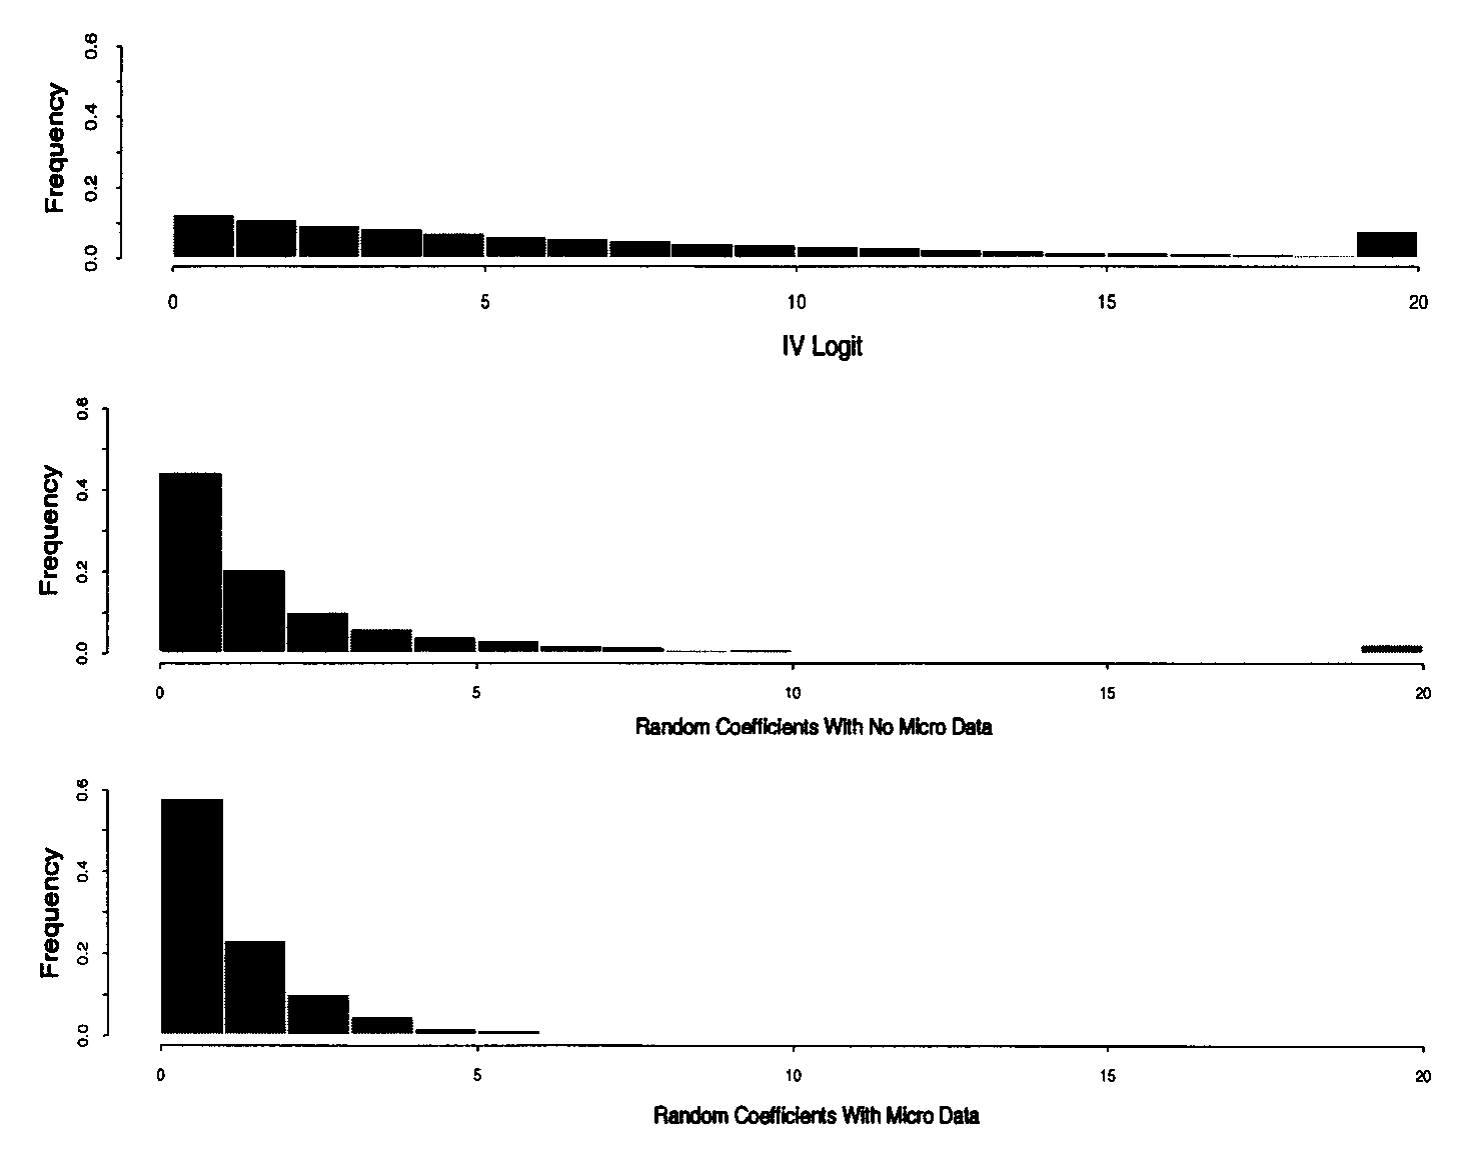
\includegraphics[width=\textwidth]{figures/ch10/petrin_fig1.png}
\caption{Distribution of compensating variation for 1984 minivan buyers, in thousands of 1982--84 dollars. The top
panel is the IV logit model, the middle panel the random coefficients model without micro data, and the bottom panel
the random coefficients model with micro data. The bar at 20 appears to collect the upper tail. Source: Petrin (2002), Figure~1.}
\label{fig:10-petrin-cv-hist}
\end{figure}

\Cref{fig:10-petrin-cv-hist} shows the whole distribution of compensation. Under the IV logit, 10 percent of
minivan buyers would need at least \$20,000 (p.~723). With random coefficients, the tail is much thinner, but many
buyers would still need thousands of dollars. Adding the micro moments removes most of the ``extreme-tastes'' tail.
Petrin prefers the full model on the cumulative weight of this evidence.

\casehead{Markups} \Cref{tab:10-petrin-markups} reproduces Table~9. The two logit models imply mean markups of \$13,904
and \$7,551. Their ratio is almost exactly the ratio of the price coefficients, as the logit markup formula
$\frac{1}{\alpha(1 - S_f)}$ implies (p.~723, n.~14). The same formula explains the tiny dispersion. The standard
deviation is 1.85 percent of the mean in both logit columns, because firms' shares are small and identical across the
two columns.
A Yugo and a Cadillac then carry nearly the same dollar markup. Marginal cost, which is price minus this markup, is
negative for 73.7 percent (OLS) and 22.6 percent (IV) of vehicles. Petrin notes that many logit own-price elasticities
are below one, which is inconsistent with static profit maximization (p.~723, n.~15). The example shows how a bias in
demand passes into the supply side. The random coefficient models imply only positive marginal costs. Their mean
percentage markups are 40.7 percent without micro data and 16.7 percent with them. Both lie within the range of earlier
estimates, 15 to 40 percent in \citet{BerryLevinsohnPakes1995} and an average of 38 percent in \citet{Goldberg1995}
(p.~725, n.~16).

\begin{table}[htbp]
\centering
\caption{Implied markups under Bertrand-Nash pricing, 1981--93 (2,407 models)}\label{tab:10-petrin-markups}
\small
\begin{tabular}{@{}lrrrrrr@{}}
\toprule
 & OLS logit & IV logit & \multicolumn{2}{c}{Random coefficients} & \multicolumn{2}{c}{RC and micro data} \\
\cmidrule(lr){4-5}\cmidrule(l){6-7}
Statistic & (\$) & (\$) & (\$) & (\%) & (\$) & (\%) \\
\midrule
Median              & 13,834 & 7,513 & 2,593 & 36.7 & 1,439 & 15.0 \\
Mean                & 13,904 & 7,551 & 4,017 & 40.7 & 1,753 & 16.7 \\
10th percentile     & 13,647 & 7,413 & 1,628 & 27.8 & 819   & 11.2 \\
90th percentile     & 14,297 & 7,765 & 8,357 & 62.6 & 2,856 & 24.8 \\
Standard deviation  & 257    & 140   & 4,089 & 14.0 & 1,229 & 6.2 \\
Negative marginal costs (\%) & 73.7 & 22.6 & \multicolumn{2}{c}{0} & \multicolumn{2}{c}{0} \\
\bottomrule
\end{tabular}

\smallskip
\begin{minipage}{0.92\textwidth}
\footnotesize Source: \citet[Table~9]{Petrin2002}, 1982--84 CPI-adjusted dollars. Percentage markups are markups
divided by observed prices. They are not reported for the logit models because estimated marginal costs are negative
for many vehicles.
\end{minipage}
\end{table}

Table~10 of the paper follows sales-weighted percentage markups by segment for 1983--87, using the model with micro
data. Minivans earned the highest markups in every year they were sold (19.19 percent in 1984, 19.43 in 1985, 17.33
in 1986 and 16.31 in 1987). Station wagons earned less than minivans in every year. In four of the five years their
markups also fell below those of the column for all other vehicles. The pairs are 18.27 against 18.85 percent in 1983,
16.81 against 17.12 in 1985, 15.82 against 16.43 in 1986 and 13.86 against 14.79 in 1987. In 1984 wagons were slightly
above that column, at 17.83 against 17.72 percent. Petrin's text says that wagon markups ``consistently fell below the
market average'' (p.~725), which his table does not bear out for 1984.
Petrin attributes the minivan premium partly to its location in a less crowded region of product space. Overall,
markups fell as the number of vehicle choices grew from 157 in 1983 to 198 in 1987 (p.~725).

\casehead{Producer surplus and dissipation} \Cref{tab:10-petrin-profits} combines Tables~11 and 12. Chrysler's variable
profits rose by \$202.5 million, or 14.38 percent, in 1984 relative to a world without minivans. The gain grew to
\$504.1 million (32.50 percent) by 1988. Petrin states that by the end of 1987 Chrysler's minivans had generated almost
\$1.5 billion in profits, against a reported development cost of \$700 million (p.~726).\footnote{The Chrysler column
of Table~11 sums to \$1,008.8 million over 1984--87 and to \$1,512.9 million over 1984--88. The paper does not show how
its \$1.5 billion figure is computed. The development cost was reported in \textit{Time} on March 21, 1983. A
\$400 million retooling cost reported in \textit{Fortune} is a lower bound on development costs (p.~726, n.~17).}
Ford and GM were both hurt. The paper summarizes their losses as 1 to 2 percent of variable profits a year, which for
high-volume GM amounted to more than \$100 million in every year of Table~11. Ford's profit rose in 1986, the year its
Aerostar arrived. The industry as a whole lost
in 1984 and 1985, so ex post the industry would have been willing to pay Chrysler not to introduce the minivan
(p.~727). Once Ford and GM sold minivans, they dissipated \$126 million of Chrysler's profits over 1985--88, the
profit on about 76,000 minivans. Chrysler's minivan was differentiated enough to keep much of its market power.

\begin{table}[htbp]
\centering
\caption{Changes in variable profits due to the minivan, and Chrysler's losses to imitators}\label{tab:10-petrin-profits}
\small
\begin{tabular}{@{}lrrrrrrrrr@{}}
\toprule
 & Industry & \multicolumn{2}{c}{Chrysler} & \multicolumn{2}{c}{Ford} & \multicolumn{2}{c}{GM} &
 \multicolumn{2}{c}{Chrysler, dissipation} \\
\cmidrule(lr){3-4}\cmidrule(lr){5-6}\cmidrule(lr){7-8}\cmidrule(l){9-10}
Year & (\%) & (\$m) & (\%) & (\$m) & (\%) & (\$m) & (\%) & (\$m) & (\%) \\
\midrule
1984 & $-0.21$ & 202.5 & 14.38 & $-31.8$ & $-1.16$ & $-155.8$ & $-1.50$ &          &         \\
1985 & $-0.13$ & 259.1 & 13.99 & $-37.4$ & $-1.29$ & $-171.0$ & $-1.63$ & $-6.06$  & $-0.16$ \\
1986 & 0.14    & 201.1 & 12.42 & 54.7    & 1.84    & $-119.9$ & $-1.09$ & $-22.72$ & $-1.99$ \\
1987 & 0.17    & 346.1 & 23.27 & $-22.8$ & $-0.66$ & $-174.5$ & $-2.14$ & $-42.35$ & $-2.25$ \\
1988 & 0.65    & 504.1 & 32.50 & $-24.7$ & $-0.70$ & $-235.4$ & $-2.90$ & $-55.68$ & $-2.63$ \\
\bottomrule
\end{tabular}

\smallskip
\begin{minipage}{0.95\textwidth}
\footnotesize Source: \citet[Tables~11 and 12]{Petrin2002}, model with micro data, millions of 1982--84 dollars. The
first eight columns compare profits with minivans to profits with all minivans removed. The last two compare
Chrysler's profits with all minivans to its profits with the Ford and GM minivans removed.
\end{minipage}
\end{table}

\casehead{Total welfare} \Cref{tab:10-petrin-welfare} reproduces Table~13. Over 1984--88 the compensating variation
sums to \$2,804.55 million and producer profits rise by \$105.54 million, for a welfare gain of \$2,910.09 million.
Producer profits fell in 1984 and 1985 and rose afterward. In every row the welfare change equals the compensating
variation plus the change in producer profits. The gains to society far exceed both the cost of developing the vehicle
and the innovator's private return (p.~727).

\begin{table}[htbp]
\centering
\caption{Change in U.S. welfare from the minivan, 1984--88 (millions of 1982--84 dollars)}\label{tab:10-petrin-welfare}
\small
\begin{tabular}{@{}lrrr@{}}
\toprule
Year & Compensating variation & Change in producer profits & Welfare change \\
\midrule
1984  & 367.29   & $-36.68$ & 330.61 \\
1985  & 625.04   & $-25.07$ & 599.97 \\
1986  & 439.93   & 27.30    & 467.23 \\
1987  & 596.59   & 29.75    & 626.34 \\
1988  & 775.70   & 110.24   & 885.94 \\
\midrule
Total & 2,804.55 & 105.54   & 2,910.09 \\
\bottomrule
\end{tabular}

\smallskip
\begin{minipage}{0.8\textwidth}
\footnotesize Source: \citet[Table~13]{Petrin2002}, model with micro data. Producer profits are the variable profits of
all firms, from the equilibrium with and without minivans.
\end{minipage}
\end{table}

The 1984 numbers can be cross-checked against Table~8. Minivans took 1.58 percent of 10.66 million vehicle sales in
1984, or about 168,000 vehicles (Table~3). Minivan buyers received \$367.29 million less the \$157 million that went to
other households. That leaves about \$1,250 per minivan buyer, close to the mean of \$1,247 in Table~8.

\subsection{Robustness*}\label{sec:10-petrin-robustness}

The paper's main robustness check is the comparison across its four demand models, and we gather its results here.
Instrumenting almost doubles the logit price coefficient (p.~719). Wald tests reject both logit models in favor of
the random coefficients models (p.~719). Without micro data only 6 of the 24 demand parameters have $z$-statistics
above one, and with them 21 of the 24 do (p.~719). Across the four models the mean compensation of 1984 minivan
buyers falls from \$13,652 to \$7,414, \$3,171 and \$1,247 (\cref{tab:10-petrin-cv}). Two further checks discriminate
among the models. The logit models imply negative marginal costs for many vehicles (\cref{tab:10-petrin-markups}).
The random coefficients model without micro data predicts a mean income of minivan buyers far above the CEX value,
while the full model comes close (\cref{tab:10-petrin-cv}). The paper reports no estimates under other taste
distributions. The tail of compensation in \cref{fig:10-petrin-cv-hist} therefore rests on the truncated
$\chi^2(3)$ assumption, which \cref{sec:10-petrin-critique} discusses.

\subsection{Interpretation, limitations and critiques}\label{sec:10-petrin-critique}

The paper's central lesson concerns the logit error. Its share in the welfare of minivan buyers is a diagnostic of how
much the answer rests on the functional form. That share falls from about 700 percent of the mean (the observed part
being negative) under the OLS logit to 32 percent with micro data (\$396 of \$1,247). Even the preferred model credits a
third of the buyers' gain to the $\epsilon_{ij}$ draws. A pure characteristics model would remove that component
entirely \citep{BerryPakes2007}, and \cref{sec:10-charspace} showed that such models value close substitutes much less.
\citet{AckerbergRysman2005} propose a related correction that lets the variance of the logit error shrink as the
product space fills.

Several assumptions shape the level of the estimates. The income term $\alpha_i\ln(y_i - p_j)$ fixes how compensation
scales with income, and the truncated $\chi^2(3)$ distribution fixes the tails of taste heterogeneity. Since compensation
is a nonlinear function of tastes, \cref{fig:10-petrin-cv-hist} depends on these tails. The market size is the number of
U.S. households, so the outside option absorbs all households that buy no new vehicle. The counterfactual holds the
characteristics and the $\xi_j$ of the other vehicles fixed. Ford and GM might have repositioned their wagons or
introduced their own minivans earlier in a world in which Chrysler did not. The model is static, so welfare covers
only 1984--88 and is not discounted. Prices are list prices of base models, without rebates or options.

The counterfactual also defines the object being valued. It removes all minivans, including the Ford and GM models,
so the \$2.9 billion values the minivan as a class of vehicle. The value of any single firm's minivan is a narrower
question. The dissipation counterfactual of Table~12 answers it for the imitators.

Finally, the minivan dummy carries much of the new good's value. A minivan is a new combination of height, size and
front-wheel drive. Its mean taste and the dispersion of that taste ($\pi_{\mathrm{mv}}$) are identified from minivan
sales and from the CEX buyer averages. They are not predicted from tastes for existing characteristics. The
analysis is therefore an ex post valuation, which differs from the ex ante prediction that characteristics models
promise in \cref{sec:10-charspace}.

\subsection{Contribution}\label{sec:10-petrin-contribution}

The paper made two contributions. The first is the micro-moment technique. It brings aggregate information
about buyers into the BLP estimator at almost no computational cost, and it showed that such moments sharpen exactly
the parameters that matter for welfare. Micro moments are now routine in demand estimation (\cref{sec:08-micro}). The
second is the welfare accounting of a new good under oligopoly. Petrin measured how much of the consumer gain came
through competition (43 percent in 1984), how much the innovator earned, and how much the imitators dissipated. He
concludes that large improvements in consumers' standard of living arise from competition among firms that seek
temporary market power through new goods (p.~728).

\begin{table}[htbp]
\centering
\caption{Identification and counterfactual map of Petrin (2002)}
\label{tab:10-petrin-map}
\footnotesize
\renewcommand{\arraystretch}{1.1}
\begin{tabularx}{\textwidth}{@{}>{\raggedright\arraybackslash}p{2.6cm}>{\raggedright\arraybackslash}X@{}}
\toprule
Observed data & Prices, sales and characteristics of 2,407 U.S. nameplate-years, 1981--1993. CEX
  averages of the demographics of new-vehicle buyers, 1987--1992, and the CPS income distribution. \\
\addlinespace
Latent objects & Product quality $\xi_j$, cost shocks $\omega_j$, household tastes and incomes, and
  marginal costs. \\
\addlinespace
Estimated parameters & Price coefficients for three income groups, random-coefficient scales $\sigma_k$,
  family-vehicle interactions $\pi$, mean tastes and the cost coefficients $\gamma$. \\
\addlinespace
Identifying variation & Characteristics-based instruments for prices, as in BLP, plus micro moments that
  match purchase probabilities by income group and the family size and age of the buyers of each vehicle
  type. \\
\addlinespace
Maintained assumptions & Static multiproduct Bertrand-Nash pricing, log-linear marginal cost, the income
  term $\alpha_i\ln(y_i-p_j)$, exogenous characteristics, and a market size equal to the number of
  households. \\
\addlinespace
Counterfactual and what it holds fixed & Removal of all minivans, with the prices of the other vehicles
  re-solved. Marginal costs, characteristics and $\xi_j$ are held fixed. A second counterfactual removes
  only the Ford and GM minivans. \\
\addlinespace
Conclusion & The compensating variation is \$2,804.55 million over 1984--1988, and about 43 percent of the
  consumer gain in 1984 came through lower prices of other vehicles. Micro moments shrink the share of the
  logit errors in buyers' gains. \\
\addlinespace
One limitation & Rivals cannot reposition their products in the counterfactual, although they might have
  done so in a world without Chrysler's minivan. \\
\addlinespace
Source and our additions & The tables are Petrin's. \Cref{prop:10-logit-buyer-cv,lem:10-micro-moment} and the
  diversion form \eqref{eq:10-petrin-diversion} are ours. \\
\addlinespace
Tools in the appendices & \Cref{sec:A-gmm,sec:A-simulation,sec:B-fixedpoint}. \\
\bottomrule
\end{tabularx}
\end{table}

\section{Case study: complementarity and online news (Gentzkow 2007)}\label{sec:10-gentzkow}

Every discrete choice model of this chapter so far assumes that a consumer chooses one product. In those models the
new good can only draw consumers away from existing goods. The continuous demand systems of the chapter, such as the
AIDS system of \cref{sec:10-hausman}, are different, since they let spending spread over many brands.
\citet{Gentzkow2007} builds a discrete choice model in which consumers may choose
several goods at once, and in which the data decide whether goods are substitutes or complements. He applies it to the
\textit{Washington Post}, its online edition (the post.com) and the competing daily \textit{Washington Times}. We follow
the paper from its question to its contribution, and \cref{tab:10-gentzkow-map} at the end of the section maps
it.\footnote{Gentzkow writes $\sigma$ for the correlation of the
unobservables in his two-good model and $\Gamma$ for the interaction term. He writes $\gamma$ for the probability of a
news-day shock, $\lambda$ for the number of readers per copy, $\kappa$ for the transaction cost of online payment and
$\Psi$ for the fixed cost. We write $\rho$, $\Gamma_{AB}$ (or $\Gamma_r$ for bundle $r$), $\varpi$, $\kappa$, $\chi$ and
$F^{\mathrm{fix}}$. Page and table numbers in this section refer to the journal article.}

\subsection{The question}\label{sec:10-gentzkow-question}

Do new goods crowd out existing goods or complement them? Gentzkow opens with examples in which the answer surprised
the industry (p.~713). Record companies in the 1920s believed that radio broadcasts crowded out record sales, until
radio airplay turned out to raise them. A widely cited forecast predicted that computers would create a ``paperless
office,'' yet information technology sharply increased paper consumption. Newspaper executives in the early 2000s
debated whether free online editions siphon readers from print (p.~714, n.~4).

The answer matters for three reasons (pp.~713--714). It drives firms' decisions on entry, positioning and pricing.
It determines the welfare value of the new good and hence the bias of price indexes. It informs policy, such as rules
on cross-media mergers. Standard discrete choice models cannot answer the question. They assume that each consumer
chooses exactly one product, so all goods are perfect substitutes at the individual level (p.~714). The single-unit
assumption is reasonable for cars, and it is the main limitation of characteristics models for goods consumed together.
Gentzkow's model removes it.

A second difficulty is empirical. Frequent online readers are also frequent print readers. The pattern could mean that
the goods are complements. It could also mean that some consumers simply have a stronger taste for news. Separating
true complementarity from correlated tastes is the central identification problem of the paper (p.~714).

\subsection{A two-good model of bundles}\label{sec:10-gentzkow-model}

Consider two goods, $A$ and $B$. Each consumer buys at most one unit of each, so she chooses one of four
\emph{bundles}: nothing ($0$), $A$ only, $B$ only, or both ($AB$). Income not spent on the goods buys a composite good
whose utility is $\alpha$ per dollar. Let $u_r$ be the utility of bundle $r$ relative to the empty bundle. Gentzkow
specifies (p.~717, eq.~1)
\begin{equation}\label{eq:10-gentzkow-twogood}
  u_0 = 0, \qquad u_A = \delta_A - \alpha p_A + \nu_A, \qquad u_B = \delta_B - \alpha p_B + \nu_B, \qquad
  u_{AB} = u_A + u_B + \Gamma_{AB} .
\end{equation}
Here $\delta_A$ and $\delta_B$ are mean utilities, and $(\nu_A, \nu_B)$ are unobserved tastes. The parameters
$\delta_A$, $\delta_B$ and $\Gamma_{AB}$ are common to all consumers. The term $-\alpha p_j$ is the utility of the
composite good forgone, $\alpha(y - p_j) - \alpha y$. The \emph{interaction term}
\begin{equation*}
  \Gamma_{AB} = (u_{AB} - u_B) - (u_A - u_0)
\end{equation*}
is the discrete analog of a cross-partial derivative of utility. It measures how much the added utility of $A$ rises
when $B$ is consumed as well. Gentzkow assumes that $(\nu_A, \nu_B)$ is bivariate normal with unit variances and
correlation $\rho$. One unit variance is a normalization of scale. The other only simplifies exposition.

Demand per consumer is $Q_A = P_A + P_{AB}$ for good $A$ and $Q_B = P_B + P_{AB}$ for good $B$, where $P_r$ is the
probability of choosing bundle $r$. Because utility is quasi-linear, income effects are absent, and compensated and
uncompensated cross-price derivatives coincide. The standard definition of complements \citep{Samuelson1974} then reads
as follows (p.~717, Definition~1).

\begin{definition}[Substitutes and complements]\label{def:10-gentzkow-complements}
Goods $A$ and $B$ are \emph{substitutes} if $\frac{\partial Q_A}{\partial p_B} > 0$, \emph{independent} if
$\frac{\partial Q_A}{\partial p_B} = 0$, and \emph{complements} if $\frac{\partial Q_A}{\partial p_B} < 0$.
\end{definition}

\casehead{Choice regions} The consumer picks the bundle with the highest utility. Comparing the four utilities pairwise
gives the regions of the $(u_A, u_B)$ plane shown in \cref{fig:10-gentzkow-regions}. Bundle $AB$ beats $A$ when $u_B +
\Gamma_{AB} \ge 0$, beats $B$ when $u_A + \Gamma_{AB} \ge 0$, and beats $0$ when $u_A + u_B + \Gamma_{AB} \ge 0$.
Bundle $A$ beats $0$ when $u_A \ge 0$ and beats $B$ when $u_A \ge u_B$. Three cases follow.

If $\Gamma_{AB} = 0$, the comparisons separate. The consumer buys $A$ if and only if $u_A \ge 0$, and $B$ if and only if
$u_B \ge 0$. The boundaries are the two axes.

If $\Gamma_{AB} > 0$, the consumer buys $AB$ when $u_A \ge -\Gamma_{AB}$, $u_B \ge -\Gamma_{AB}$ and $u_A + u_B \ge
-\Gamma_{AB}$. She buys $A$ alone when $u_A \ge 0$ and $u_B \le -\Gamma_{AB}$, and $B$ alone in the mirror case. She buys
nothing when $u_A \le 0$, $u_B \le 0$ and $u_A + u_B \le -\Gamma_{AB}$. The boundary between $AB$ and $0$ is the
segment of the anti-diagonal line $u_A + u_B = -\Gamma_{AB}$ with both coordinates in $[-\Gamma_{AB}, 0]$. Consumers on
that segment are indifferent between buying both goods and buying neither.

If $\Gamma_{AB} < 0$, the consumer buys $AB$ when $u_A \ge -\Gamma_{AB}$ and $u_B \ge -\Gamma_{AB}$. She buys $A$ alone
when $u_A \ge 0$, $u_A \ge u_B$ and $u_B \le -\Gamma_{AB}$, and $B$ alone in the mirror case. She buys nothing when both
utilities are negative. The boundary between $A$ alone and $B$ alone is the segment of the diagonal $u_A = u_B$ with
both coordinates in $[0, -\Gamma_{AB}]$. Consumers on it are indifferent between the two goods.

\begin{figure}[htbp]
\centering
\begin{subfigure}[b]{0.32\textwidth}
\centering
\begin{tikzpicture}[scale=0.72, font=\footnotesize]
  \draw[gray!40] (-2.6,-2.6) rectangle (2.6,2.6);
  \draw[->, gray] (-2.6,0) -- (2.85,0) node[right, black] {$u_A$};
  \draw[->, gray] (0,-2.6) -- (0,2.9) node[above, black] {$u_B$};
  \draw[very thick] (-2.6,0) -- (2.6,0);
  \draw[very thick] (0,-2.6) -- (0,2.6);
  \node at (1.3,1.3) {$AB$};
  \node at (1.3,-1.3) {$A$ only};
  \node at (-1.3,1.3) {$B$ only};
  \node at (-1.3,-1.3) {neither};
\end{tikzpicture}
\caption{$\Gamma_{AB} = 0$}
\end{subfigure}\hfill
\begin{subfigure}[b]{0.32\textwidth}
\centering
\begin{tikzpicture}[scale=0.72, font=\footnotesize]
  \draw[gray!40] (-2.6,-2.6) rectangle (2.6,2.6);
  \draw[->, gray] (-2.6,0) -- (2.85,0) node[right, black] {$u_A$};
  \draw[->, gray] (0,-2.6) -- (0,2.9) node[above, black] {$u_B$};
  \draw[very thick] (-2.6,0) -- (-1,0) -- (-1,2.6);
  \draw[very thick] (-1,0) -- (0,-1);
  \draw[very thick] (0,-2.6) -- (0,-1) -- (2.6,-1);
  \fill (-1,0) circle (1.4pt);
  \fill (0,-1) circle (1.4pt);
  \node[anchor=south east, inner sep=1.5pt] at (-1,0) {\scriptsize $-\Gamma_{AB}$};
  \node[anchor=north west, inner sep=1.5pt] at (0,-1) {\scriptsize $-\Gamma_{AB}$};
  \node at (1.2,1.2) {$AB$};
  \node at (1.45,-1.95) {$A$ only};
  \node at (-1.85,1.45) {$B$ only};
  \node at (-1.6,-1.6) {neither};
\end{tikzpicture}
\caption{$\Gamma_{AB} > 0$ (complements)}
\end{subfigure}\hfill
\begin{subfigure}[b]{0.32\textwidth}
\centering
\begin{tikzpicture}[scale=0.72, font=\footnotesize]
  \draw[gray!40] (-2.6,-2.6) rectangle (2.6,2.6);
  \draw[->, gray] (-2.6,0) -- (2.85,0) node[right, black] {$u_A$};
  \draw[->, gray] (0,-2.6) -- (0,2.9) node[above, black] {$u_B$};
  \draw[very thick] (-2.6,0) -- (0,0) -- (0,-2.6);
  \draw[very thick] (0,0) -- (1,1);
  \draw[very thick] (1,2.6) -- (1,1) -- (2.6,1);
  \fill (1,1) circle (1.4pt);
  \draw[gray, dashed] (1,1) -- (1,0);
  \draw[gray, dashed] (1,1) -- (0,1);
  \node[anchor=north, inner sep=2pt] at (1,0) {\scriptsize $-\Gamma_{AB}$};
  \node[anchor=east, inner sep=2pt] at (0,1) {\scriptsize $-\Gamma_{AB}$};
  \node at (1.8,1.8) {$AB$};
  \node at (1.5,-1.4) {$A$ only};
  \node at (-1.4,1.85) {$B$ only};
  \node at (-1.4,-1.4) {neither};
\end{tikzpicture}
\caption{$\Gamma_{AB} < 0$ (substitutes)}
\end{subfigure}
\caption{Choice regions of the two-good bundle model in the plane of $(u_A, u_B)$, the utilities of $A$ and $B$ relative
to buying nothing. Thick lines are indifference boundaries. In panel (b) the anti-diagonal segment $u_A + u_B =
-\Gamma_{AB}$ separates buying both goods from buying neither. In panel (c) the diagonal segment $u_A = u_B$ separates
buying $A$ alone from buying $B$ alone. A rise in $p_B$ shifts probability mass downward. Only consumers on the
diagonal segments change their consumption of $A$. Drawn from the boundaries derived in the text. Compare
\citet[Figure~1]{Gentzkow2007}.}
\label{fig:10-gentzkow-regions}
\end{figure}

\casehead{Why the interaction term decides} A rise in $p_B$ lowers $u_B$ for every consumer and moves probability
mass down in \cref{fig:10-gentzkow-regions}. In panel (a), consumers who move from $AB$ to $A$ alone and from $B$
alone to nothing leave the demand for $A$ unchanged. In panel (b), some consumers on the anti-diagonal segment move
from $AB$ to nothing, so they stop buying $A$. In panel (c), consumers on the diagonal segment move from $B$ alone to
$A$ alone, so they start buying $A$ (pp.~718--719). The following result makes the argument exact.

\begin{proposition}[The interaction term signs the cross-price effect]\label{prop:10-gentzkow-subst}
In the model of \eqref{eq:10-gentzkow-twogood}, let $\alpha > 0$ and let $(\nu_A,\nu_B)$ have a continuous joint density that
is positive on $\R^2$. Write $f_u$ for the implied density of $(u_A, u_B)$. Then
\begin{equation}\label{eq:10-gentzkow-crossderiv}
  \frac{\partial Q_A}{\partial p_B} =
  \begin{cases}
    \alpha\displaystyle\int_0^{-\Gamma_{AB}} f_u(t,t)\,\dd t > 0 & \text{if } \Gamma_{AB} < 0,\\[2ex]
    0 & \text{if } \Gamma_{AB} = 0,\\[1ex]
    -\alpha\displaystyle\int_{-\Gamma_{AB}}^{0} f_u(-\Gamma_{AB} - t,\, t)\,\dd t < 0 & \text{if } \Gamma_{AB} > 0 .
  \end{cases}
\end{equation}
Hence $A$ and $B$ are substitutes if $\Gamma_{AB} < 0$, independent if $\Gamma_{AB} = 0$ and complements if
$\Gamma_{AB} > 0$ \citep[Proposition~1]{Gentzkow2007}.
\end{proposition}

\begin{proof}
\textit{Step 1: the condition for consuming $A$.} Ties have probability zero. The consumer consumes $A$ when her best
bundle containing $A$ beats her best bundle without it:
\begin{align*}
  \max\{u_A,\; u_A + u_B + \Gamma_{AB}\} &\ge \max\{0,\; u_B\}, \\
  u_A + \max\{0,\; u_B + \Gamma_{AB}\} &\ge \max\{0,\; u_B\}, \\
  u_A &\ge g(u_B), \qquad g(b) \equiv \max\{0, b\} - \max\{0, b + \Gamma_{AB}\} .
\end{align*}

\textit{Step 2: the shape of $g$.} If $\Gamma_{AB} = 0$, then $g \equiv 0$. If $\Gamma_{AB} > 0$, then $g(b) = 0$ for $b
\le -\Gamma_{AB}$, $g(b) = -\Gamma_{AB} - b$ for $-\Gamma_{AB} < b < 0$, and $g(b) = -\Gamma_{AB}$ for $b \ge 0$. So $g$ is
nonincreasing with slope $-1$ on $(-\Gamma_{AB}, 0)$. If $\Gamma_{AB} < 0$, then $g(b) = 0$ for $b \le 0$, $g(b) = b$ for
$0 < b < -\Gamma_{AB}$, and $g(b) = -\Gamma_{AB}$ for $b \ge -\Gamma_{AB}$. So $g$ is nondecreasing with slope $+1$ on
$(0, -\Gamma_{AB})$. Outside these intervals $g' = 0$.

\textit{Step 3: differentiate demand.} Write $c_A = \delta_A - \alpha p_A$ and $c_B = \delta_B - \alpha p_B$, so that
$u_A = c_A + \nu_A$ and $u_B = c_B + \nu_B$. Let $f$ be the density of $(\nu_A, \nu_B)$. Then
\begin{equation*}
  Q_A = \Pr\bigl(\nu_A \ge g(c_B + \nu_B) - c_A\bigr)
      = \int_{-\infty}^{\infty}\int_{g(c_B + \nu_B) - c_A}^{\infty} f(\nu_A, \nu_B)\,\dd\nu_A\,\dd\nu_B .
\end{equation*}
The function $g$ is piecewise linear, so we may differentiate under the outer integral:
\begin{align*}
  \frac{\partial Q_A}{\partial c_B} &= -\int_{-\infty}^{\infty} f\bigl(g(c_B + \nu_B) - c_A,\, \nu_B\bigr)\,
         g'(c_B + \nu_B)\,\dd\nu_B
      = -\int_{-\infty}^{\infty} f_u\bigl(g(t),\, t\bigr)\, g'(t)\,\dd t ,
\end{align*}
where the second equality substitutes $t = c_B + \nu_B$ and uses $f_u(a,b) = f(a - c_A, b - c_B)$. Since $\frac{\partial
c_B}{\partial p_B} = -\alpha$,
\begin{equation*}
  \frac{\partial Q_A}{\partial p_B} = \alpha\int_{-\infty}^{\infty} f_u\bigl(g(t),\, t\bigr)\, g'(t)\,\dd t .
\end{equation*}

\textit{Step 4: evaluate.} If $\Gamma_{AB} = 0$, then $g' \equiv 0$ and the derivative is zero. If $\Gamma_{AB} < 0$, then
$g(t) = t$ and $g'(t) = 1$ on $(0, -\Gamma_{AB})$, which gives the first line of \eqref{eq:10-gentzkow-crossderiv}. If
$\Gamma_{AB} > 0$, then $g(t) = -\Gamma_{AB} - t$ and $g'(t) = -1$ on $(-\Gamma_{AB}, 0)$, which gives the third line.
The density is positive, so both integrals are strictly positive.
\end{proof}

The two integrals run along the diagonal segments of \cref{fig:10-gentzkow-regions}. Gentzkow's equation~(3) writes
them as line integrals with indicator functions (p.~719). The magnitude of the cross effect depends on the length
$|\Gamma_{AB}|$ of the segment and on the density of consumers along it. The proposition also covers nonprice shifters.
Suppose a variable $z$ raises $u_B$ by $\zeta z$ and leaves $u_A$ unchanged. Then $\frac{\partial Q_A}{\partial z} =
\zeta\frac{\partial Q_A}{\partial c_B} = -\frac{\zeta}{\alpha}\frac{\partial Q_A}{\partial p_B}$. Improving the
connection speed of an online paper works like cutting its price, and its effect on print demand has the sign of
$\Gamma_{AB}$ (p.~719). This is how Gentzkow's excluded variables reveal substitution without any price variation.

\subsection{What the data can and cannot identify}\label{sec:10-gentzkow-ident}

\casehead{A counting problem} Choice data in the two-good model give three probabilities, $P_A$, $P_B$ and $P_{AB}$.
The model has five parameters: $\delta_A$, $\delta_B$, $\Gamma_{AB}$, $\rho$ and $\alpha$ (p.~720). The price
coefficient is identified from choices only if prices vary, because the probabilities depend on $(\delta_A, \delta_B,
\alpha)$ only through $\delta_A - \alpha p_A$ and $\delta_B - \alpha p_B$. Without price variation, $\alpha$ needs
another moment. Gentzkow takes it from a firm's pricing condition (\cref{sec:10-gentzkow-supply}).

The harder problem is to separate $\Gamma_{AB}$ from $\rho$. The marginal probabilities $Q_A$ and $Q_B$ identify the two
mean utilities. One moment remains, how often the goods are consumed together. A high $P_{AB}$ relative to $P_A$ and
$P_B$ can come from a large $\Gamma_{AB}$ or from a large $\rho$, and nothing else in the data separates them
(p.~720). By \cref{prop:10-gentzkow-subst}, the same data could be fit by near-perfect substitutes with highly
correlated tastes, or by near-perfect complements with weakly correlated tastes. A model that fixes one of the two
parameters by assumption fixes the answer to the substitution question.

\casehead{Exclusion restrictions} Suppose a variable $x$ enters the utility of $A$ only. Observing choices at a second
value of $x$ adds three moments, $P_A$, $P_B$ and $P_{AB}$ at the new value, and one parameter, the new mean utility of
$A$ (p.~721). The model becomes formally identified. The intuition is direct. If joint consumption reflects a high
$\Gamma_{AB}$, then shifting up the utility of $A$ raises the probability of consuming $B$. If it reflects correlated
tastes, the probability of consuming $B$ stays unchanged. \citet{Keane1992} gives Monte Carlo evidence that exclusion
restrictions sharpen the covariance estimates of multinomial probit models, which nest the model of \eqref{eq:10-gentzkow-twogood}
when defined over bundles (p.~721, n.~11).

\casehead{Panel data} Split each taste into a consumer random effect, constant over time, and a shock that is \iid\
across goods and days. With choices observed at two dates there are $4^2 = 16$ joint outcomes, hence 15 moments
instead of 3 (p.~721, n.~12). The argument is the usual one for random effects. Correlated random effects make some
consumers likely to consume both goods and others likely to consume neither. Conditional on a consumer's average
propensities, her day-to-day variation is then uncorrelated across goods. A high $\Gamma_{AB}$ instead makes the
day-to-day variation strongly correlated. The consumer reads both papers on some days and neither on others, and
rarely reads only one.

Gentzkow's data are a limited panel. Respondents report what they read in the last 24 hours and in the last five
weekdays. For consumers who read nothing in the last 24 hours, the five-day report shows which papers they read on
the other four weekdays. Whether they
were less likely to read then identifies the variance of the random effects. Consumers who read one paper in the last
24 hours identify the correlation. If the random effects are positively correlated, a consumer who read only $A$
yesterday is more likely to have read $B$ earlier in the week (p.~722).

\casehead{Unobserved goods} The outside option has a different meaning when bundles are allowed. Every choice in the
model includes an implicit maximization over goods the econometrician does not see, such as cable news (p.~719).
Suppose watching CNN destroys the value of the post.com and raises the value of the print \textit{Post}. Then the
\textit{Post} and the post.com are never read together, and the model estimates them as strong substitutes. Gentzkow
argues that this answer is correct for the market as it is. Raising the price of the \textit{Post} would reduce CNN
viewing as well and raise post.com reading (p.~720). The estimates are conditional on the set and the prices of the
unobserved goods, a limitation all discrete choice models share \citep{Samuelson1974}.

\casehead{Relation to earlier models} The model of \eqref{eq:10-gentzkow-twogood} nests the earlier approaches as restrictions
(pp.~722--723). The multiple-discrete choice model of \citet{Hendel1999} aggregates many ``tasks,'' such as the
computing needs of each employee of a firm. Hendel's model lets a buyer choose several units of several brands, and he
estimates it by the method of simulated moments on micro data for personal computer purchases by firms. Each task uses
one good, so the task-level model fixes $\Gamma_{AB} = -\infty$, and the goods are restricted to be substitutes
(\cref{ch:logit}). A multivariate probit, with one equation per good and correlated errors, sets $\Gamma_{AB} = 0$
and forces independence. A logit or nested logit over bundles \citep{ManskiSherman1980,TrainMcFaddenBenAkiva1987} can
estimate $\Gamma_{AB}$ freely. Its unobservables, however, are uncorrelated or follow the nest structure, so it would
read correlated tastes as complementarity. Gentzkow's model frees both terms and relies on exclusions and panel
information to separate them.

\subsection{Setting and data}\label{sec:10-gentzkow-data}

The data come from a Scarborough Research survey of 16,179 adults in the Washington, DC, Designated Market Area (DMA),
conducted between March 2000 and February 2003 (p.~723). The survey lists the local print newspapers each respondent
read in the last 24 hours and in the last five weekdays. It records the readership of the major local online newspapers
over the same windows, and many household characteristics. The \textit{Post} dominated the market, with an average daily readership
of 1.8 million against 256,000 for the \textit{Times}. The post.com had 406,000 area readers per day. The
\textit{Times}'s own website had only 373 readers in the sample and is omitted (p.~723, n.~16). The goods are the daily
editions of the \textit{Post}, the \textit{Times} and the post.com. The outside option includes all other news
sources and not reading news at all.

The survey is about a 0.4 percent sample and broadly representative. It overrepresents older, more educated and
wealthier residents and underrepresents minorities (p.~724). Estimation uses the unweighted data, and the policy
simulations use the sampling weights. About 6 percent of records were filled in by Scarborough from matched
respondents. Gentzkow drops them in estimation and keeps them in the simulations (p.~724, n.~17).

The aggregate time series are suggestive but inconclusive (p.~724). Post.com readership grew rapidly after its
introduction in 1996 while \textit{Post} readership fell. A regression of \textit{Post} readership since 1984 on
post.com readership and a trend implies that four post.com readers displace one \textit{Post} reader. Yet the decline
began in 1994, two years before the post.com, and did not accelerate afterward. Readership was falling nationally, and
the \textit{Post} raised its subscription price several times. Time series alone cannot separate these forces.

The micro data show that reading several papers is common (p.~725). Forty-eight percent of respondents read at least
one of the three papers in the last 24 hours. Of these, 18 percent read two and 1 percent read all three. Over five
days, 65 percent read at least one, and of these 27 percent read two and 3 percent all three. Panel~A of
\cref{tab:10-gentzkow-data} cross-tabulates \textit{Post} and post.com readership. Among post.com readers the share who
also read the \textit{Post} is higher than among non-readers. Panel~B reports raw and partial correlations. The partial
correlations control for age, sex, education, occupation, employment status, income, political party, survey date,
location and the number of missing answers. Controls cut the \textit{Post}-post.com correlation by about two-thirds,
but it stays significantly positive. The \textit{Post}-\textit{Times} correlation is positive in the raw data and
vanishes or turns negative with controls.

\begin{table}[htbp]
\centering
\caption{Joint readership of the \textit{Post}, the post.com and the \textit{Times}}\label{tab:10-gentzkow-data}
\small
\begin{tabular}{@{}lrrrr@{}}
\toprule
\multicolumn{5}{@{}l}{\textit{A. Cross-tabulation of Post and post.com readership (number of respondents)}} \\
 & \multicolumn{2}{c}{Last 24 hours} & \multicolumn{2}{c}{Last 5 weekdays} \\
\cmidrule(lr){2-3}\cmidrule(l){4-5}
 & No post.com & Read post.com & No post.com & Read post.com \\
\midrule
Did not read \textit{Post} & 8,771 & 622 & 6,012 & 680 \\
Read \textit{Post}         & 5,829 & 877 & 7,203 & 2,204 \\
\midrule
\multicolumn{5}{@{}l}{\textit{B. Correlation coefficients of readership indicators}} \\
 & \multicolumn{2}{c}{Last 24 hours} & \multicolumn{2}{c}{Last 5 weekdays} \\
\cmidrule(lr){2-3}\cmidrule(l){4-5}
 & Raw & Partial & Raw & Partial \\
\midrule
\textit{Post} and post.com        & 0.0989$^{**}$ & 0.0364$^{**}$ & 0.1579$^{**}$ & 0.0673$^{**}$ \\
\textit{Post} and \textit{Times}  & 0.0632$^{**}$ & 0.0035        & 0.0450$^{**}$ & $-0.0623^{**}$ \\
\textit{Times} and post.com       & 0.0146        & 0.0090        & 0.0184        & 0.0066 \\
\bottomrule
\end{tabular}

\smallskip
\begin{minipage}{0.92\textwidth}
\footnotesize Source: \citet[Tables~2 and 3]{Gentzkow2007}, Scarborough survey, Washington, DC, DMA, 2000--03.
Partial correlations are correlations of the residuals from regressions of each readership indicator on the controls
listed in the text. Panel~B drops respondents for whom print or online papers are not in the choice set.
$^{**}$ significant at 1 percent.
\end{minipage}
\end{table}

\subsection{Reduced-form evidence}\label{sec:10-gentzkow-reduced}

To separate complementarity from correlated tastes, Gentzkow uses four variables that shift the utility of reading
online but not, directly, the utility of reading print (pp.~725--726). They are indicators for Internet access at work,
use of the Internet for work-related tasks, use of the Internet for education-related tasks, and a high-speed
connection at home. Access at work lowers the time cost of reading online. The two use variables indicate familiarity
with the Internet and time spent at a computer. A fast connection raises the utility of online reading. Collect them
in a vector $z_i$. No variable shifts the \textit{Post} without shifting the \textit{Times}, so print-print
substitution is less well identified than print-online substitution (p.~726).

A linear probability model shows the exclusion restrictions at work. Let $R^p_i$ indicate that respondent $i$ read the
\textit{Post} in the last five weekdays and $R^w_i$ that she read the post.com. Gentzkow estimates
\begin{equation}\label{eq:10-gentzkow-lpm}
  R^p_i = b\,R^w_i + x_i\varphi + e_i ,
\end{equation}
first by OLS and then by two-stage least squares (2SLS) with $z_i$ as instruments for $R^w_i$. The controls $x_i$ are
those of the partial correlations, plus \textit{Times} readership. The 2SLS coefficient has a simple interpretation in
terms of \cref{prop:10-gentzkow-subst}. Each instrument moves only the utility of the post.com, so it acts like a change
in the post.com's price. The 2SLS coefficient is the ratio of the instrument's effect on \textit{Post} reading to its
effect on post.com reading. In the language of \cref{ch:diffprod}, it estimates minus the diversion ratio from the
post.com to the \textit{Post}, averaged over the respondents whom the instruments move.

\Cref{tab:10-gentzkow-lpm} reproduces Table~4. OLS gives a positive coefficient, 0.0464 (0.0090), which mirrors the
raw correlation. 2SLS gives $-0.4132$ (0.107). Taken literally, a respondent assigned to read the online paper at zero
time cost would be about 41 percentage points less likely to read the print paper. Gentzkow describes this as
``40 percent less likely'' (p.~726). The coefficient on a binary regressor in a linear probability model is a change
in the probability itself. A relative decline would require dividing by a baseline probability of reading the
print paper. Gentzkow warns that the linear
probability model limits how far this magnitude can be trusted. The first-stage $F$-statistic on the instruments is
33.05, so weak instruments are not a concern. The overidentification statistic is $\chi^2 = 3.65$ with a $p$-value of
0.302, so the test does not reject the validity of the instruments.

\begin{table}[htbp]
\centering
\caption{Linear probability model of \textit{Post} readership in the last five weekdays}\label{tab:10-gentzkow-lpm}
\small
\begin{tabular}{@{}lcccc@{}}
\toprule
 & OLS & \multicolumn{3}{c}{2SLS} \\
\cmidrule(l){3-5}
 &  & (1) & (2) & (3) \\
\midrule
Read post.com last 5 days & 0.0464$^{**}$ & $-0.4132^{**}$ & $-0.4579^{**}$ & $-0.4381^{**}$ \\
                          & (0.0090)      & (0.107)        & (0.119)        & (0.141) \\
Other Internet news       &               &                &                & 0.0244 \\
                          &               &                &                & (0.0195) \\
Industry and occupation controls &        &                & Yes            &  \\
Overidentification $p$-value &            & 0.302          & 0.431          & 0.219 \\
$R^2$                     & 0.333         & 0.214          & 0.207          & 0.202 \\
$N$                       & 14,313        & 14,313         & 14,313         & 14,313 \\
\bottomrule
\end{tabular}

\smallskip
\begin{minipage}{0.92\textwidth}
\footnotesize Source: \citet[Table~4]{Gentzkow2007}. Robust standard errors in parentheses. The instruments are
indicators for Internet access at work, a fast Internet connection, and use of the Internet for research or education
and for work. The overidentification test is a Sargan test. Industry controls are 12 categories and occupation
controls 11. All regressions include the controls listed in the text and omit respondents without print papers in the
choice set. $^{**}$ significant at 1 percent.
\end{minipage}
\end{table}

The main threat is that the instruments correlate with unmeasured tastes for print (pp.~727--728). People who like
reading may select into jobs with Internet access, and news enthusiasts may buy fast connections. Gentzkow offers three
checks. Adding 12 industry and 11 occupation categories, which should absorb part of any omitted job characteristic,
strengthens the 2SLS coefficient slightly to $-0.4579$ \citep{AltonjiElderTaber2005}. Restricting the sample to
residents of more than ten years, whose job choices largely predate online news, leaves the estimates nearly unchanged
(p.~727, n.~19). Controlling for other Internet news use raises the coefficient's magnitude slightly ($-0.4381$), so the
instruments do not appear to work through other online news sources. The structural robustness checks below also drop
the broadband exclusion.

\subsection{The empirical model}\label{sec:10-gentzkow-structural}

Index days by $t$, consumers by $i$, goods by $j \in \{1, \dots, J\}$ with $J = 3$, and bundles by $r \in \{0, 1, \dots,
2^J - 1\}$, where $r = 0$ is the empty bundle (p.~728). The utility of consumer $i$ from good $j$ alone on day $t$ is
\begin{equation}\label{eq:10-gentzkow-base}
  \tilde u_{ijt} = \delta_j - \alpha p_j + x_i\beta_j + \nu_{ij} + \tau_{it} .
\end{equation}
The vector $x_i$ holds age, sex, education, occupation, employment status, political party, location within the DMA,
the number of missing survey answers, six-month time dummies and log income. For the post.com it also holds the four
excluded variables $z_i$, which are absent from the print utilities. The time dummies absorb changes in the quality of
the goods and their substitutes. Log income proxies for unobservables correlated with income, since the budget effect
of income differences out (p.~729).

The two unobservables play different roles. The vector $\nu_i = (\nu_{i1}, \dots, \nu_{iJ})$ is constant over the
survey week. It captures a general taste for news, loyalty to a paper and subscription status. It is multivariate
normal with a free covariance matrix, whose scale is pinned down by the logit errors below (p.~729, n.~21). The day
shock $\tau_{it}$ raises the utility of all papers equally. It equals $\hat\tau > 0$ with probability $\varpi$ and zero
otherwise, a stylized description of major news days and of day-to-day variation in the cost of time. Price does not
vary enough to estimate $\alpha$ from demand, so the first two terms are combined into $\bar\delta_j = \delta_j - \alpha
p_j$.

The utility of bundle $r$ adds the base utilities of its goods, an interaction term and a bundle-specific shock
(p.~729, eq.~4):
\begin{equation}\label{eq:10-gentzkow-bundle}
  u_{irt} = \begin{cases}
    \epsilon_{irt} & \text{if } r = 0, \\
    \sum_{j \in r}\tilde u_{ijt} + \Gamma_r + \epsilon_{irt} & \text{if } r > 0.
  \end{cases}
\end{equation}
Here $\Gamma_r = 0$ for single-good bundles, and $\epsilon_{irt}$ is \iid\ type-I extreme value. With three goods there
are three pairwise interactions and one triple interaction, which is estimated but not reported (Table~6, note). On a
major news day the bundle $r$ gains $|r|\hat\tau$, where $|r|$ is its number of goods. The interaction terms and the
price coefficient are common to all consumers. Gentzkow reports that letting $\Gamma_r$ vary with observables did not
change the results substantially (p.~729).

\Cref{prop:10-gentzkow-subst} does not apply unchanged to this model. Label the goods $A$, $B$ and $C$. With three
goods, a change in $p_B$ also moves consumers into and out of the bundles that contain $C$. The triple interaction
and the bundle-specific logit errors then enter the cross-price effect, and a negative $\Gamma_{AB}$ no longer
signs it. Our computation gives an example with $\nu_i$ and $\tau_{it}$ set to zero. Let every
$\bar\delta_j + x_i\beta_j$ be zero, $\alpha = 1$, $\Gamma_{AB} = -1$, $\Gamma_{AC} = \Gamma_{BC} = 0$, and
$\Gamma_r = 10$ for the bundle $r$ of all three goods. With $r_i$ the bundle that consumer $i$ chooses, the logit form
gives $\frac{\partial Q_A}{\partial p_B} = -\alpha\Cov\bigl(\indic\{A\in r_i\},\indic\{B\in r_i\}\bigr) \approx -0.00009$.
So $A$ and $B$ are complements although $\Gamma_{AB} < 0$, because almost every consumer buys all three goods. A
small positive variance of $\nu_i$ preserves the sign. In the empirical model the two-good result is therefore an
intuition, and the substitution patterns must be read from the cross-price derivatives of the full model.

Two dummies define choice sets. About 10 percent of respondents say they look at no newspaper sections, and print
papers are removed from their choice set. Respondents who did not use the Internet in the last 30 days have no online
paper. Each dummy also enters, as a control, the utility of the goods it does not exclude (p.~729). Choice-set
variation therefore does not identify substitution, which seems prudent because it is unlikely to be exogenous
(n.~25).

\casehead{Choice probabilities and the likelihood} Integrating over the $\epsilon_{irt}$ gives the logit probability of
bundle $r$ on a day with shock $\tau$:
\begin{equation}\label{eq:10-gentzkow-Q}
  Q_r(x_i, \nu_i, \tau; \theta) = \frac{\exp\Bigl[\sum_{j\in r}(\bar\delta_j + x_i\beta_j + \nu_{ij} + \tau) + \Gamma_r\Bigr]}
  {1 + \sum_{r'=1}^{2^J - 1}\exp\Bigl[\sum_{j\in r'}(\bar\delta_j + x_i\beta_j + \nu_{ij} + \tau) + \Gamma_{r'}\Bigr]} .
\end{equation}
The data report, for each good, whether it was read in the last 24 hours and whether it was read in the last five
weekdays. Let $\tilde q \in \{0, \dots, 2^J - 1\}^5$ list the bundles chosen on the five weekdays. Let $q$ be a reported
outcome and $\Omega(q)$ the set of daily sequences consistent with it. Since $\tau_{it}$ and $\epsilon_{irt}$ are
independent across days, the probability of report $q$ given $\nu_i$ is (p.~730)
\begin{equation}\label{eq:10-gentzkow-Pq}
  P_q(x_i, \nu_i; \theta) = \sum_{\tilde q \in \Omega(q)}\prod_{t=1}^{5}\Bigl[\varpi\,Q_{\tilde q_t}(x_i, \nu_i, \hat\tau;
  \theta) + (1 - \varpi)\,Q_{\tilde q_t}(x_i, \nu_i, 0; \theta)\Bigr] .
\end{equation}
The log-likelihood integrates over the random effects:
\begin{equation}\label{eq:10-gentzkow-loglik}
  L(X, q, \theta) = \sum_i \ln\int P_{q_i}(x_i, \nu; \theta)\,\dd F(\nu; \theta),
\end{equation}
where $F(\nu; \theta)$ is the multivariate normal distribution of $\nu$ (p.~732, eq.~6).

\casehead{Identification in the empirical model} The two-good intuition carries over (p.~730). The combination of
24-hour and 5-day reports pins down the covariance matrix of $\nu_i$. Choices on earlier days are more correlated with
the choice in the last 24 hours, conditional on observables, the larger the variance of the random effects. The
exclusion restrictions then pin down the distribution of the common day shock $\tau_{it}$ and the interaction terms. If
same-day joint reading of print and online papers is driven by $\tau_{it}$, Internet access at work should not change
the probability of reading print. If it is driven by complementarity, those with access should read print more.
Gentzkow stresses three limitations. The partial panel identifies the random effects less well than a true panel.
The excluded variables shift only the online paper. And without price variation, functional forms carry more weight
than in richer data sets.

\subsection{Simulated maximum likelihood}\label{sec:10-gentzkow-sml}

The integral in \eqref{eq:10-gentzkow-loglik} has no closed form. Gentzkow replaces it with a simulator and maximizes
the simulated likelihood (p.~732, eq.~7):
\begin{equation}\label{eq:10-gentzkow-sml}
  \hat\theta^{SML} = \argmax_\theta \sum_i \ln\Bigl[\frac{1}{S}\sum_{s=1}^{S}P_{q_i}(x_i, \nu_{is}; \theta)\Bigr],
\end{equation}
with $S = 300$ draws per consumer. The leading alternative is the method of simulated moments (MSM) of
\citet{McFadden1989} and \citet{PakesPollard1989}. MSM is consistent for a fixed number of draws. Simulated maximum
likelihood (SML), introduced by \citet{LermanManski1981}, needs the number of draws to grow with the sample
\citep{GourierouxMonfort1996}. But efficient MSM requires optimal instruments, which perform poorly when the
preliminary estimate is inaccurate, and it requires the probabilities of all possible reports. With many reported
outcomes this is expensive. In preliminary tests the two estimators gave similar parameters, and MSM took 10 to 20 times
longer, so Gentzkow uses SML (p.~732).

\casehead{Importance sampling} Draws from the unconditional distribution of $\nu$ waste effort on values that make the
observed report unlikely. Gentzkow instead draws from the distribution of $\nu$ conditional on the observed report,
computed at a preliminary estimate $\tilde\theta$ (p.~732, n.~31). The logic is clearest when the draws are standardized
shocks $\eta \sim N(0, I)$ with density $\phi$, and $\nu = C(\theta)\eta$. (In this subsection $\eta$ and $\phi$
denote these shocks and their density, not the CES elasticity of \cref{sec:10-feenstra}.) Write $P_i(\eta; \theta) \equiv
P_{q_i}(x_i, C(\theta)\eta; \theta)$ for the probability of $i$'s report given the shocks. Let $\bar P_i(\tilde\theta) = \int
P_i(\eta; \tilde\theta)\phi(\eta)\,\dd\eta$, computed once with many draws. The importance density is
\begin{equation*}
  h_i(\eta) = \frac{P_i(\eta; \tilde\theta)\,\phi(\eta)}{\bar P_i(\tilde\theta)} ,
\end{equation*}
which is the posterior density of $\eta$ given the report. The weighted simulator
\begin{equation*}
  \tilde P_i(\theta) = \frac{1}{S}\sum_{s=1}^{S}P_i(\eta_s; \theta)\,W_{is}, \qquad
  W_{is} = \frac{\bar P_i(\tilde\theta)}{P_i(\eta_s; \tilde\theta)}, \qquad \eta_s \sim h_i,
\end{equation*}
is unbiased for every $\theta$:
\begin{equation*}
  \E_h\bigl[P_i(\eta; \theta)\,W_i\bigr]
  = \int P_i(\eta; \theta)\,\frac{\bar P_i(\tilde\theta)}{P_i(\eta; \tilde\theta)}\,
    \frac{P_i(\eta; \tilde\theta)\,\phi(\eta)}{\bar P_i(\tilde\theta)}\,\dd\eta
  = \int P_i(\eta; \theta)\,\phi(\eta)\,\dd\eta .
\end{equation*}
Draws from $h_i$ are taken by acceptance and rejection, since $h_i$ is the distribution of the shocks conditional on the
observed report. \emph{Acceptance and rejection} draws $\eta$ from $\phi$ and keeps each draw with probability
proportional to $P_i(\eta;\tilde\theta)$, so the kept draws follow $h_i$. Gentzkow writes the same simulator in terms of $\nu$ (his eqs.~13--14). The general treatment of
importance sampling is in \cref{sec:08-importance}.

\casehead{Bias correction} SML is biased in finite samples because the logarithm is concave (p.~732, n.~32). Let
$\tilde f$ be an unbiased simulator of a choice probability $f$, so $\E\tilde f = f$. A second-order expansion of $\ln
\tilde f$ around $f$ gives
\begin{align*}
  \ln\tilde f &= \ln f + \frac{\tilde f - f}{f} - \frac{(\tilde f - f)^2}{2f^2} + O\bigl(|\tilde f - f|^3\bigr), \\
  \E\ln\tilde f &\approx \ln f - \frac{1}{2}\,\frac{\E(\tilde f - f)^2}{f^2} = \ln f - \frac{1}{2}\,\frac{\Var(\tilde f)}{f^2} .
\end{align*}
The expected simulated log-likelihood is too low by about half the squared coefficient of variation of the simulator.
If $\tilde f = \frac{1}{S}\sum_s P_{is}$ averages $S$ independent draws, then $\Var(\tilde f) = \frac{1}{S}\Var(P_{is})$,
which can be estimated by $\frac{1}{S^2}\sum_s(P_{is} - \tilde f)^2$. The corrected objective adds this estimate back:
\begin{equation}\label{eq:10-gentzkow-biascorr}
  \hat\theta = \argmax_\theta\sum_i\Biggl\{\ln\tilde f_i + \frac{1}{2}\,
  \frac{\frac{1}{S^2}\sum_{s}\bigl(P_{is} - \tilde f_i\bigr)^2}{\tilde f_i^2}\Biggr\} .
\end{equation}
The correction removes the bias of order $\frac{1}{S}$ \citep[p.~45]{GourierouxMonfort1996}.\footnote{The version of
\eqref{eq:10-gentzkow-biascorr} printed in Gentzkow's footnote 32 does not show the factor $\frac{1}{S^2}$ in the
correction term. We state the expression that follows from the expansion.} The robust standard errors follow
\citet{McFaddenTrain2000}. For welfare and other derived statistics, Gentzkow draws 100 parameter vectors from the
estimated asymptotic distribution, recomputes the statistic at each, and reports the standard deviation (p.~733). This
avoids the delta method, which linearizes highly nonlinear functions.

\subsection{The price coefficient from the supply side}\label{sec:10-gentzkow-supply}

Demand data identify only $\bar\delta_j = \delta_j - \alpha p_j$. To express utility in dollars, Gentzkow backs out
$\alpha$ from the condition that the \textit{Post} sets its print price optimally (pp.~730--731 and 735--736). The idea
is that the less price-sensitive consumers are, the higher the price a profit-maximizing firm would set (p.~715).

\casehead{Profit} The \textit{Post} sells copies at price $p$, and each copy is read by $\kappa$ adults. The firm
earns advertising revenue $a_p$ per print reader and $a_w$ per online reader, pays marginal cost $c_p$ per printed copy,
and bears a fixed cost. With $N_p$ print readers and $N_w$ online readers, the profit of the Washington Post Company is
(p.~731, eq.~5)
\begin{equation}\label{eq:10-gentzkow-profit}
  \Pi = \Bigl[a_p + \frac{p - c_p}{\kappa}\Bigr]N_p + a_w N_w - F^{\mathrm{fix}} .
\end{equation}
The marginal cost of an extra online reader is taken to be zero, and advertising revenue per reader is constant. The
second assumption treats both advertising markets as competitive at a fixed price per reader. It abstracts from the
different values of different readers and from any market power of the \textit{Post} (p.~735). Since $\kappa$ readers
share each copy, Gentzkow assumes that each reader pays $\frac{p}{\kappa}$ and that this reader price enters the
utility \eqref{eq:10-gentzkow-base} (p.~731).

\casehead{Inputs} Every input comes from industry data (pp.~735--736).
\begin{itemize}
  \item Print advertising revenue was \$574.3 million in 2001 and \$555.7 million in 2002. The daily edition's share
        gives \$1.5 and \$1.4 million per day, and with daily circulation of 771,614 and 768,600 the average is $a_p =
        \$1.91$.
  \item Online division revenue was \$30.4 million in 2001 and \$35.9 million in 2002. The post.com had 450,457 daily
        readers in the DMA, about 75 percent of its total. Dividing 75 percent of revenue by DMA readership gives
        $a_w = \$0.15$. A second estimate from the advertising revenue and readership of nytimes.com gives \$0.16,
        which Gentzkow uses.
  \item Newsprint consumption of 226,796 metric tons at \$541 per ton implies \$0.37 per copy. With ink and distribution,
        $c_p = \$0.40$.
  \item The cover price rose from \$0.25 to \$0.35 over the period, and the subscription price per daily copy was
        \$0.22 to \$0.25. Gentzkow uses $p = \$0.30$.
  \item Comparing survey readership with audited circulation gives $\kappa = 2.4$ readers per copy (2.3 for the
        \textit{Times}). Whether $\kappa$ reflects shared copies or overreporting does not change the welfare results
        (p.~731, n.~28).
\end{itemize}
The profit from one more print reader is \$0.75, and from one more online reader \$0.16 (p.~736).\footnote{With the
reported inputs, $\frac{a_p + p - c_p}{\kappa} = \frac{1.91 + 0.30 - 0.40}{2.4} = 0.754$, which reproduces the \$0.75
in the paper. The bracket of \eqref{eq:10-gentzkow-profit} as printed, $a_p + \frac{p - c_p}{\kappa}$, would give about
\$1.87. The reported figure is therefore consistent with $a_p$ measured per copy, which is how it is computed from
circulation.}

\casehead{The first-order condition} Write the expected numbers of print and online readers as functions $N_p(\bar
\delta; \hat\theta)$ and $N_w(\bar\delta; \hat\theta)$ of the vector of constants $\bar\delta$ and the other estimated
parameters $\hat\theta$. These and their derivatives are computed by simulation. Let $m_p$ denote the profit per print
reader. Using $\frac{\partial\bar\delta_j}{\partial p_j} = -\alpha$ as Gentzkow does, the derivative of \eqref{eq:10-gentzkow-profit}
with respect to the print price is (p.~736)
\begin{equation}\label{eq:10-gentzkow-foc}
  \frac{\partial\Pi}{\partial p} = -\alpha\Bigl[m_p\frac{\partial N_p}{\partial\bar\delta_{\mathrm{post}}}
  + a_w\frac{\partial N_w}{\partial\bar\delta_{\mathrm{post}}}\Bigr] + \frac{1}{\kappa}N_p = 0 .
\end{equation}
Everything except $\alpha$ is known. Solving,
\begin{equation}\label{eq:10-gentzkow-alpha}
  \hat\alpha = \frac{N_p}{\kappa\Bigl[m_p\frac{\partial N_p}{\partial\bar\delta_{\mathrm{post}}}
  + a_w\frac{\partial N_w}{\partial\bar\delta_{\mathrm{post}}}\Bigr]} ,
\end{equation}
which is unique whenever the bracket is nonzero. Gentzkow obtains $\hat\alpha = 9.72$ (p.~736). As in Gentzkow's
equation, $\alpha$ here is the coefficient on the copy price $p$. If utility depends instead on the reader price
$\frac{p}{\kappa}$, the coefficient on that price is $\kappa\alpha$. Utils then convert into dollars at that rate
\citep[n.~28]{Gentzkow2007}. The elasticity \eqref{eq:10-gentzkow-lerner} below is the same under either
convention.

The condition has a transparent economic reading. A higher $\bar\delta_{\mathrm{post}}$ raises print readership,
$\frac{\partial N_p}{\partial\bar\delta_{\mathrm{post}}} > 0$, and lowers online readership when the goods are
substitutes. Define the diversion ratio $D = -\frac{\partial N_w}{\partial\bar\delta_{\mathrm{post}}}
\bigl(\frac{\partial N_p}{\partial\bar\delta_{\mathrm{post}}}\bigr)^{-1}$ and the price elasticity of print readership $\varepsilon_p = -\frac{\partial
N_p}{\partial p}\frac{p}{N_p}$. Rearranging \eqref{eq:10-gentzkow-foc} gives
\begin{equation}\label{eq:10-gentzkow-lerner}
  \varepsilon_p = \frac{\frac{p}{\kappa}}{m_p - a_w D} .
\end{equation}
The price paid per reader, $\frac{p}{\kappa} = \$0.125$, is far below the profit per reader, \$0.75, because each reader
brings advertising revenue. The \textit{Post} therefore prices where its demand is inelastic. By the chain rule,
$\varepsilon_p = \alpha\,p\,\frac{\partial N_p}{\partial\bar\delta_{\mathrm{post}}}\frac{1}{N_p}$, and the estimated
demand parameters fix the readership response $\frac{\partial N_p}{\partial\bar\delta_{\mathrm{post}}}$ and $N_p$. With
these and $p$ held fixed, the elasticity is proportional to $\alpha$, so a low elasticity requires a small $\alpha$.
A price change then moves utility little relative to the spread of the taste shocks. The paper reports an implied own-price elasticity of
0.37 and finds that it tracks the \textit{Post}'s readership response to its price increases over 1994--2003 (p.~738,
n.~38).\footnote{Inserting the reported inputs into \eqref{eq:10-gentzkow-lerner} gives an elasticity between 0.17 (at
$D = 0$) and 0.21 (at $D = 1$). The paper does not show how its elasticity of 0.37 is computed, so we cannot locate the
source of the gap.}
The strategy rests on strong assumptions. The print price must be optimal given the zero online price, the advertising
model must be right, and the cost data must be accurate. Gentzkow shows in \cref{tab:10-gentzkow-robust} that the
qualitative results survive reasonable changes in $p$, $c_p$ and $a_w$.

\subsection{Results: demand parameters and substitution}\label{sec:10-gentzkow-results}

\casehead{Observables} \Cref{tab:10-gentzkow-obs} reproduces Table~5, the coefficients on consumer characteristics in
the mean utility of each good (p.~733). Most coefficients for the \textit{Post} and the post.com are significant, as
are about half of those for the \textit{Times}. Gentzkow reads them through marginal effects on the probability of
reading each paper, for a consumer at the mean of the data. The \textit{Post} fits its reputation as a high-brow,
liberal paper. Attending college, attending graduate school and doubling household income raise the probability of
reading the \textit{Post} by 31, 34 and 9 percentage points. Being a registered Democrat raises it by 3 points, and being a registered Republican
lowers it by 2. Ten more years of age add 8 points, while full-time employment lowers the probability by 14 points.
The post.com's coefficients mostly share the \textit{Post}'s signs, with smaller marginal effects because its predicted
probability is lower (16 percent against 53). Age and employment are exceptions. Ten more years of age lower the
probability of reading the post.com by 1 point, and full-time work, white-collar work and computer work raise it by 2,
1 and 3 points. The online edition is often read at work and draws younger readers (p.~734). Registered
Republicans are 3 points more likely to read the \textit{Times}, whose mean predicted probability is 9 percent (p.~734).

\begin{table}[htbp]
\centering
\caption{Gentzkow's estimates of the effects of consumer characteristics on utility}\label{tab:10-gentzkow-obs}
\small
\begin{tabular}{@{}lccc@{}}
\toprule
 & \textit{Post} & post.com & \textit{Times} \\
\midrule
Age (ten years)   & 0.661$^{**}$ (0.0407)   & $-0.545^{**}$ (0.0628)  & 0.688$^{**}$ (0.122) \\
Female            & $-0.473^{**}$ (0.0921)  & $-0.423^{**}$ (0.148)   & $-3.20^{**}$ (0.344) \\
High school       & 1.95$^{**}$ (0.214)     & 2.87$^{**}$ (0.633)     & 1.29 (0.856) \\
College           & 2.54$^{**}$ (0.237)     & 4.03$^{**}$ (0.654)     & 1.49 (0.928) \\
Graduate school   & 2.76$^{**}$ (0.252)     & 4.16$^{**}$ (0.670)     & 1.19 (0.964) \\
Computer job      & $-0.567^{*}$ (0.223)    & 1.22$^{**}$ (0.323)     & 0.322 (0.682) \\
White-collar job  & $-0.447^{**}$ (0.118)   & 0.431$^{*}$ (0.195)     & $-0.591$ (0.423) \\
Full-time         & $-1.13^{**}$ (0.141)    & 0.935$^{**}$ (0.227)    & $-0.044$ (0.450) \\
Log income        & 0.709$^{**}$ (0.0729)   & 0.217 (0.118)           & 0.934$^{**}$ (0.260) \\
Democrat          & 0.217$^{**}$ (0.099)    & 0.326$^{*}$ (0.163)     & $-0.027$ (0.346) \\
Republican        & $-0.193$ (0.119)        & $-0.0538$ (0.193)       & 2.902$^{**}$ (0.408) \\
Constant          & 6.97$^{**}$ (0.852)     & $-1.54$ (1.18)          & $-8.85^{**}$ (1.91) \\
\midrule
$N$               & 16,179                  & 16,179                  & 16,179 \\
\bottomrule
\end{tabular}

\smallskip
\begin{minipage}{0.92\textwidth}
\footnotesize Source: \citet[Table~5]{Gentzkow2007}, full model. Standard errors in parentheses. $^{*}$ significant at
5 percent, $^{**}$ at 1 percent. The education categories are mutually exclusive, and so are the two occupation
dummies. Democrat and Republican mark registered party members. The model also includes dummies for missing
observations, the location of the respondent's residence, six-month time periods and having the print and online
papers in the choice set, not reported.
\end{minipage}
\end{table}

\casehead{Interactions and shocks} \Cref{tab:10-gentzkow-params} reproduces Table~6. Both print-online interactions are
significantly negative: $-1.285$ (0.2307) for the \textit{Post} and the post.com and $-1.231$ (0.4832) for the post.com
and the \textit{Times}. The \textit{Post}-\textit{Times} interaction is small, positive and insignificant. Gentzkow
reads these signs as making the post.com a substitute for both print papers (p.~734). In the two-good model this
reading would follow from \cref{prop:10-gentzkow-subst}. In the three-good model the signs only suggest it, as
\cref{sec:10-gentzkow-structural} explains. The support comes from the full model's cross-price derivatives below. A
\$0.10 rise in the price of the \textit{Post} adds 8,358 post.com readers (p.~737), and the same rise for the
\textit{Times} adds 2,781 (p.~738). The first agrees with the 2SLS regressions. The day shock is large and rare. On 4.5 percent of days the utility of every paper rises by about seven units, which
suggests major news stories that raise the demand for news overall (p.~734). The four excluded variables all raise the
utility of the post.com, and two of them significantly.

\begin{table}[htbp]
\centering
\caption{Gentzkow's estimates of interactions, news-day shocks and excluded variables}\label{tab:10-gentzkow-params}
\small
\begin{tabular}{@{}lclc@{}}
\toprule
\multicolumn{2}{@{}l}{\textit{Interaction terms $\Gamma_r$}} & \multicolumn{2}{l}{\textit{Excluded variables (post.com utility)}} \\
\midrule
\textit{Post} and post.com        & $-1.285^{**}$ (0.2307) & Internet at work         & 1.357$^{**}$ (0.180) \\
\textit{Post} and \textit{Times}  & 0.0809 (0.2479)        & Fast connection          & 0.146 (0.193) \\
post.com and \textit{Times}       & $-1.231^{**}$ (0.4832) & Use for education        & 0.361 (0.212) \\
\multicolumn{2}{@{}l}{\textit{News-day shock}}             & Use for work             & 0.582$^{**}$ (0.222) \\
Size $\hat\tau$                   & 6.846$^{**}$ (0.5027)  &                          & \\
Probability $\varpi$              & 0.0454$^{**}$ (0.0179) &                          & \\
\bottomrule
\end{tabular}

\smallskip
\begin{minipage}{0.92\textwidth}
\footnotesize Source: \citet[Table~6]{Gentzkow2007}, where the shock parameters are called $\tau$ and $\gamma$.
Standard errors in parentheses. $^{**}$ significant at 1 percent. The model also includes a third-order interaction for
the bundle of all three papers, not reported. Fast connection means DSL, cable modem or T1 at home. N = 16,179.
\end{minipage}
\end{table}

\casehead{Variance shares} \Cref{tab:10-gentzkow-var} reproduces Table~7, which compares the variances of the utility
components. Three facts stand out (p.~735). The random effects $\nu_i$ have large variances relative to the
observables, so unobserved heterogeneity matters. The day shocks contribute a variance of 2.03, consistent with a
two-point distribution, $\hat\tau^2\varpi(1 - \varpi) = 6.846^2 \times 0.0454 \times 0.9546 \approx 2.03$.
The logit errors have variance 1.64, the type-I extreme value variance $\frac{\pi^2}{6} \approx 1.645$ that fixes the
scale of utility. Against random-effect variances of 11.0, 23.5 and 86.1, the logit errors play a small role. The
concern of \cref{sec:10-charspace} and of Petrin's Table~8 is therefore limited here, as Gentzkow notes with reference
to \citet{Petrin2002} (p.~729, n.~22). The unobserved correlation between the \textit{Post} and the \textit{Times} is
negative. Tastes for political coverage, on which Washington readers are divided, may explain it, or the lack of
excluded variables separating the two print papers may bias it (p.~735).

\begin{table}[htbp]
\centering
\caption{Variances and covariances of the components of utility}\label{tab:10-gentzkow-var}
\small
\begin{tabular}{@{}lccc@{\hskip 2.2em}lccc@{}}
\toprule
\multicolumn{4}{@{}l}{\textit{Observable utility $x_i\beta_j$}} & \multicolumn{4}{l}{\textit{Random effects $\nu_i$}} \\
 & \textit{Post} & post.com & \textit{Times} & & \textit{Post} & post.com & \textit{Times} \\
\midrule
\textit{Post}   & 14.0 &      &      & \textit{Post}   & 11.0    &      &      \\
post.com        & 7.95 & 8.43 &      & post.com        & 4.14    & 23.5 &      \\
\textit{Times}  & 7.66 & 4.85 & 10.2 & \textit{Times}  & $-1.17$ & 5.19 & 86.1 \\
\midrule
\multicolumn{8}{@{}l}{Variance of the day shock $\tau_{it}$: 2.03. \quad Variance of the logit error $\epsilon_{irt}$: 1.64.} \\
\bottomrule
\end{tabular}

\smallskip
\begin{minipage}{0.92\textwidth}
\footnotesize Source: \citet[Table~7]{Gentzkow2007}. Covariances of the components of utility at the estimated
parameters. The left block is the sample covariance of the fitted observable utilities.
\end{minipage}
\end{table}

The model fits well (p.~735). Simulated aggregate shares match the data with a mean squared error of 0.0016. On average,
consumers who made a given choice have a predicted probability of that choice 2.1 times as high as consumers who did
not.

\casehead{Substitution patterns} \Cref{tab:10-gentzkow-subst} reproduces Table~8, the paper's key table. It reports
three measures of the relation between the \textit{Post} and the post.com. The first is the change in post.com
readership when the \textit{Post}'s price rises by \$0.10. The second is the change in \textit{Post} readership when the
post.com is added to the choice set, and the third is the corresponding change in print profits.

\begin{table}[htbp]
\centering
\caption{Impact of the online edition on demand for the print \textit{Post}}\label{tab:10-gentzkow-subst}
\small
\begin{tabular}{@{}lrrr@{}}
\toprule
 & Full model & Observables only & No heterogeneity \\
 & (case 1) & (case 2) & (case 3) \\
\midrule
Cross-price derivative (readers)        & 8,358        & $-8{,}421$      & $-16{,}143$ \\
                                        & (1,436)      & (752)         & (702) \\
Change in print readership (readers)    & $-26{,}822$    & 25,655        & 51,897 \\
                                        & (4,483)      & (2,270)       & (2,254) \\
Change in print profits (\$ per year)   & $-5{,}466{,}846$ & 5,229,009     & 10,577,720 \\
                                        & (913,699)    & (462,771)     & (459,464) \\
\bottomrule
\end{tabular}

\smallskip
\begin{minipage}{0.92\textwidth}
\footnotesize Source: \citet[Table~8]{Gentzkow2007}. Standard errors in parentheses. The cross-price derivative is the
change in post.com readership when the \textit{Post}'s price rises by \$0.10. The changes in print readership and
print profits are the total changes for the \textit{Post} when the post.com is added to the choice set. Case~2 has
observable consumer characteristics but no unobservables other than the logit errors. Case~3 has no observable or
unobservable heterogeneity except the logit errors.
\end{minipage}
\end{table}

Two conclusions follow (p.~737). First, the print and online papers are significant substitutes. A \$0.10 rise in the
\textit{Post}'s price, about 33 percent, raises post.com readership by 8,358, about 2 percent. The post.com reduces
\textit{Post} readership by about 27,000 a day, about 1.5 percent, and print profits by about \$5.5 million a year
(p.~715). The effects are precise but moderate. They are far from one-for-one crowding out. Removing the post.com
returns about 27,000 readers to the \textit{Post}, roughly 7 percent of the 406,000 daily post.com readers.
The linear probability model's magnitude, which refers to five-day readership, was far larger, a reminder of
Gentzkow's caution about that model.

Second, accounting for heterogeneity reverses the answer. A model with observables but no correlated unobservables
finds complements, with a cross-price derivative of the same size and opposite sign, and a \$5.2 million gain in print
profits. A model with no heterogeneity finds stronger complementarity, a \$10.6 million gain. Correlated tastes for
news masquerade as complementarity unless the model allows for them. The relationships with the \textit{Times} are
weaker (p.~738). The post.com and the \textit{Times} are significant substitutes, and a \$0.10 rise in the
\textit{Times}'s price would add 2,781 post.com readers. The \textit{Post}-\textit{Times} cross derivative is negative,
close to zero and insignificant, so the two print papers are essentially independent.

\subsection{Results: welfare and online pricing}\label{sec:10-gentzkow-welfare}

\casehead{Consumer surplus} Let $\hat u_{ir}(\nu, \tau)$ be the utility of bundle $r$ excluding $\epsilon_{irt}$, $\mathcal{R}$
the set of all bundles and $\mathcal{R}^{-j}$ the bundles without good $j$. The expected gain of consumer $i$ from
adding good $j$ is (p.~738, eq.~8)
\begin{equation}\label{eq:10-gentzkow-gain}
  \Delta_i^j = \E_{\nu,\tau,\epsilon}\Bigl[\max_{r\in\mathcal{R}}\hat u_{ir}(\nu, \tau) + \epsilon_{irt}\Bigr]
             - \E_{\nu,\tau,\epsilon}\Bigl[\max_{r\in\mathcal{R}^{-j}}\hat u_{ir}(\nu, \tau) + \epsilon_{irt}\Bigr] .
\end{equation}
The expectation takes the econometrician's view given the data. The random effect $\nu$ is constant over time, so the
observed choice is informative about it, and the expectation over $\nu$ conditions on that choice. The shocks $\tau$ and
$\epsilon$ are \iid\ over days, so their expectations are unconditional. The log-sum formula of
\cref{lem:10-logsum} gives
\begin{equation}\label{eq:10-gentzkow-logsum}
  \E_{\nu,\tau,\epsilon}\Bigl[\max_{r\in\mathcal{R}}\hat u_{ir} + \epsilon_{irt}\Bigr]
  = \E_{\nu,\tau}\Bigl[\ln\sum_{r\in\mathcal{R}}e^{\hat u_{ir}(\nu,\tau)}\Bigr] + \gamma_E ,
\end{equation}
where the constant cancels in \eqref{eq:10-gentzkow-gain}. Gentzkow simulates the remaining expectation with
unconditional draws $\nu_s$ reweighted by their posterior probability given the observed choice $r_i$ (pp.~738--739,
eqs.~10--11):
\begin{equation}\label{eq:10-gentzkow-sim}
\begin{aligned}
  \E_{\nu,\tau}\Bigl[\ln\sum_{r\in\mathcal{R}}e^{\hat u_{ir}}\Bigr] &\approx \sum_{s=1}^{S}\Bigl[\varpi\ln
  \sum_{r\in\mathcal{R}}e^{\hat u_{ir}(\nu_s,\hat\tau)} + (1 - \varpi)\ln\sum_{r\in\mathcal{R}}e^{\hat u_{ir}(\nu_s, 0)}\Bigr]
  R(\nu_s \mid r_i), \\
  R(\nu_s\mid r_i) &= \frac{Q_{ir_i}(\nu_s)}{\sum_{s'=1}^{S}Q_{ir_i}(\nu_{s'})} .
\end{aligned}
\end{equation}
We normalize the weights to sum to one. Gentzkow writes the posterior as the ratio of $Q_{ir_i}(p, \nu_s)f(\nu_s)$ to a
simulated unconditional probability. Dividing by the price coefficient converts utils into dollars, and summing over
consumers gives the change in consumer surplus (eq.~12):
\begin{equation}\label{eq:10-gentzkow-cs}
  \Delta CS(j) = \sum_i\frac{1}{\alpha}\Delta_i^j .
\end{equation}
This is the log-sum measure of \cref{sec:10-charspace}, extended from products to bundles.

Gentzkow lists the caveats himself (p.~739). Prices do not vary over a wide range, so the dollar values rest on
quasi-linearity, which converts utils into dollars at a constant rate. The scale of utility is fixed by the logit
error, and other error distributions could give different answers. The analysis ignores post.com readers outside the
DMA. The model also holds the prices and characteristics of other products fixed. If competing papers improved their
quality in response to the post.com, consumer gains are understated.

\Cref{tab:10-gentzkow-welfare} combines Tables~9 and 11. The average post.com reader values the paper at \$0.30 a day,
70.4 percent of the average print reader's surplus from the \textit{Post}. The total consumer gain is \$123,413 per day,
or \$45.0 million per year (standard error \$6.6 million), which is 16.0 percent of the total surplus from the print
\textit{Post}. The ratios to print surplus do not depend on $\alpha$, which makes them more robust than the dollar
values.

\begin{table}[htbp]
\centering
\caption{Consumer and producer surplus from the post.com}\label{tab:10-gentzkow-welfare}
\small
\begin{tabular}{@{}lr@{}}
\toprule
\multicolumn{2}{@{}l}{\textit{A. Consumer surplus (Table 9)}} \\
\midrule
Per post.com reader, as \% of per-reader print surplus & 70.4\% \\
Per post.com reader, \$ per day                        & 0.30 \\
Total, as \% of total print surplus                    & 16.0\% \\
Total, \$ per day                                      & 123,413 \\
Total, \$ per year                                     & 45,045,862 \\
\quad Standard error                                   & (6,606,939) \\
\midrule
\multicolumn{2}{@{}l}{\textit{B. Producer surplus before post.com operating costs, \$ per year (Table 11)}} \\
\midrule
$\Delta$ \textit{Post} profit                          & $-5{,}466{,}846$ \\
$\Delta$ \textit{Times} profit                         & $-2{,}687{,}348$ \\
Total post.com revenue                                 & 33,150,000 \\
$\Delta$ Producer surplus                              & 24,995,806 \\
\quad Standard error                                   & (1,876,785) \\
\bottomrule
\end{tabular}

\smallskip
\begin{minipage}{0.82\textwidth}
\footnotesize Source: \citet[Tables~9 and 11]{Gentzkow2007}. Panel~A is the loss of consumer surplus if the post.com
were removed. ``Per reader'' divides the total daily loss by the number of post.com readers. Panel~B reports changes
in firm profits from adding the post.com, and the advertising revenue of the post.com from readers inside and outside
DC. In Panel~B the producer surplus row equals the sum of the three rows above it.
\end{minipage}
\end{table}

\casehead{Switching} Table~10 of the paper shows where post.com readers would go if it disappeared (p.~739). Of those who
read both the post.com and the \textit{Post}, 79.2 percent would read the \textit{Post} alone, 17.2 percent would switch
to the outside good, and 3.5 percent to other bundles. Of those who read only the post.com, 69.1 percent would switch
to the outside good and 27.1 percent would start reading the \textit{Post}. Some joint readers stop reading entirely
because the logit errors make the interaction heterogeneous. For some consumers the goods are complements even though
they are substitutes in aggregate (p.~739, n.~39).

\casehead{Producer surplus} The post.com costs the \textit{Post} about \$5.5 million a year in lost print profits and the
\textit{Times} about \$2.7 million, against \$33.2 million of post.com revenue (p.~740). Producer surplus therefore
rises by \$25.0 million before the operating costs of the post.com. The Post does not report those costs. Costs of New
York Times Digital were \$63.5 million in 2001 and \$67.7 million in 2002, which suggests an upper bound of \$60 million.
The Post's report of losses in its online division suggests a lower bound of \$30 million. At the midpoint of \$45
million, the post.com reduced producer surplus by about \$20 million a year, which makes its introduction puzzling.
Online revenues almost doubled between 2002 and 2004, however. With 2004 advertising revenue per reader, the gain to the
Washington Post Company is about \$56.5 million a year, or \$11.5 million net of operating costs. Producer surplus then
rises by about \$9 million. The early losses may have been an investment in a growing advertising market.

\casehead{Online pricing} The model can evaluate a price that was never charged (pp.~740--741). The estimate of $\alpha$
assumed only that the print price was optimal given the zero online price. Holding the print price and characteristics
fixed, Gentzkow varies the online price and recomputes demand and profits. The profit-maximizing online price is \$0.20
a day, about \$6 a month. The loss from charging zero is about \$9 million a year, more than a quarter of post.com
advertising revenue. The computation accounts for the direct revenue, the lost advertising revenue and the readers who
return to print. The \$6 estimate is close to the online prices charged by the few papers that charged in 2003, \$6.95
for the \textit{Wall Street Journal} and \$3.75 for the \textit{Tulsa World}.

A second approach asks what transaction cost would make the zero price optimal. Suppose the post.com's constant is
\begin{equation*}
  \bar\delta_{\mathrm{post.com}} = \delta_{\mathrm{post.com}} - \alpha p_{\mathrm{post.com}}
  - \alpha\chi\,\indic\{p_{\mathrm{post.com}} > 0\},
\end{equation*}
where $\chi$ is the dollar value of a real or perceived cost of paying online. Examples are the hassle of entering a
card number and a sense that charging is unfair. With $\hat\alpha$ fixed, a zero price maximizes total profits whenever
$\chi \ge \$0.13$ per day (p.~741).\footnote{Gentzkow's equation subtracts the cost from utility without the factor
$\alpha$, while his thresholds are in dollars. We include the factor so that $\chi$ is in dollars throughout. The
dollar reading is the consistent one. A price of $\$0.20 - \chi$ leaves every reader's utility as at a price of
\$0.20 without the cost. Its profit is therefore the profit at \$0.20 without the cost, less $\chi$ a day per post.com
reader. The post.com has fewer readers at \$0.20 than at a zero price. So a zero price can be optimal only if $\chi$ is
at least the daily loss from a zero price divided by the readership at a zero price. Gentzkow scales the 406,000 area
readers up to total readership, using an estimate that about 25 percent of readers are outside the area (p.~731,
n.~30). This gives about $\frac{406{,}000}{0.75} \approx 541{,}000$ readers and a bound of
$\frac{9{,}000{,}000}{365 \times 541{,}000} = \$0.046$ a day (our computation). A
utility penalty of 0.13 is worth only $\frac{0.13}{9.72} = \$0.013$.} With the 2004 advertising market the optimal price falls to \$0.09, the loss from a zero price to \$1.7
million, and the threshold to \$0.02. The zero price may have been part of a rational forward-looking strategy.

\subsection{Robustness*}\label{sec:10-gentzkow-robust}

\Cref{tab:10-gentzkow-robust} reproduces Table~12 (pp.~741--742). The first two experiments recompute $\alpha$ from
print prices of \$0.25 and \$0.35, the prices before and after the 2002 increase. The next two vary the marginal cost of
a copy between \$0.30 and \$0.50, which moves the optimal online price by \$0.04 and consumer surplus by about \$5
million. A lower post.com revenue of \$25 million, which allows for the other ventures of the online division, cuts the
Post Company surplus by about a third but leaves consumer surplus unchanged. Dropping the broadband exclusion changes
little. Treating the \textit{Times} as part of the outside good leaves the \textit{Post}-post.com interaction unchanged,
as the outside-option argument of \cref{sec:10-gentzkow-ident} predicts.

\begin{table}[htbp]
\centering
\caption{Robustness of Gentzkow's main estimates}\label{tab:10-gentzkow-robust}
\small
\begin{tabular}{@{}lrrrr@{}}
\toprule
 & Post Company & Cross-price & Optimal price & Consumer surplus \\
 & surplus (\$m) & derivative & of post.com (\$) & per year (\$m) \\
\midrule
Actual estimates            & 27.68 & 8,358 & 0.20 & 45.05 \\
Price = \$0.25              & 27.83 & 8,598 & 0.19 & 43.79 \\
Price = \$0.35              & 27.53 & 8,131 & 0.21 & 46.31 \\
Marginal cost = \$0.30      & 27.38 & 7,916 & 0.22 & 47.56 \\
Marginal cost = \$0.50      & 27.99 & 8,853 & 0.18 & 42.53 \\
Online revenue = \$25m      & 19.53 & 8,342 & 0.24 & 45.13 \\
Omit broadband variable     & 27.19 & 9,277 & 0.21 & 45.12 \\
Only \textit{Post} and post.com & 31.52 & 8,683 & 0.22 & 47.15 \\
\bottomrule
\end{tabular}

\smallskip
\begin{minipage}{0.88\textwidth}
\footnotesize Source: \citet[Table~12]{Gentzkow2007}. ``Post Company surplus'' is post.com revenue less the lost
\textit{Post} print profits (\$33.15 million less \$5.47 million in the actual estimates). The last row includes the
\textit{Times} in the outside good.
\end{minipage}
\end{table}

\subsection{Interpretation, limitations and contribution}\label{sec:10-gentzkow-assess}

The paper's contribution is a tractable bundle model in which the data choose between substitutes and complements. Its
analysis of identification shows why the choice is hard. Joint consumption is equally consistent with complementarity
and with correlated tastes, and only excluded shifters or repeated choices separate them. The application shows the
stakes. Raw correlations, OLS and models without unobserved heterogeneity all point to complementarity worth up to
\$10.6 million a year to the print \textit{Post}. The full model finds substitution that costs it \$5.5 million.

The limitations follow from the data. There is no usable price variation, so the price coefficient comes from a
stylized supply side, and dollar values scale with $\frac{1}{\hat\alpha}$. The excluded variables shift only the online
paper, so print-print substitution is weakly identified. The welfare measures are local. They hold the prices and
characteristics of other news sources fixed and ignore advertisers and readers outside Washington. The model is
static, although the zero online price may be part of a dynamic strategy, as Gentzkow's 2004 calculation suggests. The
advertising market is reduced to a fixed price per reader.

The paper also completes an argument of this chapter. Characteristics models with single-unit choice can value goods
that are new combinations of known characteristics, but they cannot represent complementarity (\cref{sec:10-charspace}).
Whether a single-unit model is acceptable depends on the market. It suits durables bought one at a time, such as
cars. It fails for goods that households consume together, such as newspapers, music or groceries. In those markets a
model like Gentzkow's is needed before any welfare number can be trusted.

\begin{table}[htbp]
\centering
\caption{Identification and counterfactual map of Gentzkow (2007)}
\label{tab:10-gentzkow-map}
\footnotesize
\renewcommand{\arraystretch}{1.1}
\begin{tabularx}{\textwidth}{@{}>{\raggedright\arraybackslash}p{2.6cm}>{\raggedright\arraybackslash}X@{}}
\toprule
Observed data & A survey of 16,179 adults in the Washington area, 2000--2003, with 24-hour and five-day
  readership of the \textit{Post}, the \textit{Times} and the post.com, and their demographics. \\
\addlinespace
Latent objects & Consumer random effects $\nu_i$ that are constant over the survey week, news-day shocks
  $\tau_{it}$, and bundle-specific shocks. \\
\addlinespace
Estimated parameters & Mean utilities, bundle interaction terms $\Gamma_r$, the covariance of the random
  effects, the news-day shock, coefficients on demographics and on four excluded variables, and the price
  coefficient $\alpha$. \\
\addlinespace
Identifying variation & Variables that shift only the online paper and repeated choices within the survey
  week separate complementarity from correlated tastes. The \textit{Post}'s print pricing condition gives
  $\alpha$. \\
\addlinespace
Maintained assumptions & Quasi-linear utility, the exclusion of the four variables from print utilities,
  and an optimal print price with a fixed advertising price per reader. \\
\addlinespace
Counterfactual and what it holds fixed & Removal of the post.com, and positive online prices. The prices and
  characteristics of other news sources, and the print price, are held fixed. \\
\addlinespace
Conclusion & The post.com adds about \$45.0 million a year to consumer surplus. It substitutes for the
  print \textit{Post} and costs it about \$5.5 million a year in print profits. Models without unobserved
  heterogeneity find complementarity instead. \\
\addlinespace
One limitation & Prices do not vary, so every dollar value scales with $\frac{1}{\hat\alpha}$ from a
  stylized supply side. \\
\addlinespace
Source and our additions & The tables are Gentzkow's. The exact statement and proof of
  \cref{prop:10-gentzkow-subst} are ours. \\
\addlinespace
Tools in the appendices & \Cref{sec:A-simulation,sec:A-mle,sec:B-ev}. \\
\bottomrule
\end{tabularx}
\end{table}

\section{Synthesis: what determines a measured value}\label{sec:10-synthesis}

The four studies of this chapter value very different goods with very different data. Their answers nevertheless depend
on the same few modeling choices. A common formula makes the dependence explicit. In a random utility model with
quasi-linear income, the gain from moving from choice set $\mathcal{R}^0$ at prices $p^0$ to choice set $\mathcal{R}^1$
at prices $p^1$ is
\begin{equation}\label{eq:10-synth-cs}
  \Delta CS = \frac{1}{\alpha}\int\Bigl\{\E_\epsilon\Bigl[\max_{r\in\mathcal{R}^1}u_{ir}(p^1)\Bigr]
  - \E_\epsilon\Bigl[\max_{r\in\mathcal{R}^0}u_{ir}(p^0)\Bigr]\Bigr\}\dd P(i) .
\end{equation}
Here $\mathcal{R}$ is a set of products, or of bundles in Gentzkow's model. Adding and subtracting the expected maximum
over $\mathcal{R}^0$ at the new prices $p^1$ splits \eqref{eq:10-synth-cs} into two parts:
\begin{align}
  \Delta CS &= \underbrace{\frac{1}{\alpha}\int\Bigl\{\E\Bigl[\max_{\mathcal{R}^1}u_{ir}(p^1)\Bigr]
              - \E\Bigl[\max_{\mathcal{R}^0}u_{ir}(p^1)\Bigr]\Bigr\}\dd P(i)}_{\text{variety effect at new prices}} \notag\\
            &\quad + \underbrace{\frac{1}{\alpha}\int\Bigl\{\E\Bigl[\max_{\mathcal{R}^0}u_{ir}(p^1)\Bigr]
              - \E\Bigl[\max_{\mathcal{R}^0}u_{ir}(p^0)\Bigr]\Bigr\}\dd P(i)}_{\text{price effect on existing goods}} .
  \label{eq:10-synth-split}
\end{align}
This is the decomposition \eqref{eq:10-cv-decomp} in random utility form. Hausman's product-space measure is the
Hicksian area of \cref{prop:10-cv-newgood}, which plays the role of the first term. Each determinant of the measured
value enters \eqref{eq:10-synth-split} at a definite place. The scale is $\frac{1}{\alpha}$. The expected maximum must be
extrapolated beyond the observed prices, and it contains the logit errors. The price changes form the second term. The
structure of the choice set $\mathcal{R}$ decides whether goods can complement one another.

\subsection{Four studies side by side}\label{sec:10-synthesis-table}

\Cref{tab:10-synthesis} compares the four studies along these dimensions. The headline numbers are not comparable
across rows of the table. They measure different goods, periods and objects, and we report each as its author states it.

\begin{table}[htbp]
\centering
\caption{Four valuations of new goods compared}\label{tab:10-synthesis}
\footnotesize
\renewcommand{\arraystretch}{1.15}
\begin{tabularx}{\textwidth}{@{}>{\raggedright\arraybackslash}p{2.05cm}
  >{\raggedright\arraybackslash}X >{\raggedright\arraybackslash}X
  >{\raggedright\arraybackslash}X >{\raggedright\arraybackslash}X@{}}
\toprule
 & \citet{Hausman1997} & \citet{Trajtenberg1989} & \citet{Petrin2002} & \citet{Gentzkow2007} \\
\midrule
New good & Apple-Cinnamon Cheerios, U.S., 1990--92 & CT scanners, U.S., 1973--82 & Minivan, U.S., 1981--93
  (welfare 1984--88) & Online \textit{Washington Post}, DC, 2000--03 \\
Data & City-week scanner prices and quantities (959 observations) & All scanner models, prices and characteristics,
  with over 2,000 installations & 2,407 nameplate-years plus CEX averages for buyers & Survey of 16,179 adults,
  24-hour and 5-day readership \\
Demand model & Three-level budgeting in product space: AIDS for brands within segments, log-log demand for segments
  and for total cereal & Multinomial and nested logit with hedonic residual price & Random
  coefficients logit with income effects and demographics & Logit over bundles with correlated normal random effects \\
Source of price sensitivity & Prices of the same brand in other cities (Hausman instruments) & Head-scanner price
  coefficients, to net out quality signalling & Characteristics-based instruments plus micro moments & The
  \textit{Post}'s print pricing condition \\
What governs the extrapolation & AIDS curvature up to the virtual price & Logit form, including the entropy term &
  Random coefficients plus logit error & Interaction terms $\Gamma_r$ and quasi-linearity \\
Competition & Multiproduct firm re-prices. Rivals' prices fixed & Not modeled (consumer surplus only) & Full
  Bertrand-Nash re-solution & Firm profits at fixed prices. Online-price counterfactual \\
Headline number & Consumer surplus about \$78.1 million a year, \$66.8 million net of price effects. Cereal CPI too
  high by about 25 percent & Social rate of return to CT research and development about 270 percent & Compensating
  variation \$2,804.55 million and welfare \$2,910.09 million over 1984--88 & Consumer surplus \$45.0 million a year.
  Producer surplus \$25.0 million before operating costs \\
Main critique & Validity of the instruments. Rivals' responses ignored & No price instruments. Positive price
  coefficients. Representative buyer & Share of the logit error. Functional forms. Static, with fixed characteristics &
  No price variation. Supply-side $\alpha$. Weak print-print identification \\
\bottomrule
\end{tabularx}

\smallskip
\begin{minipage}{0.97\textwidth}
\footnotesize Sources: \cref{sec:10-hausman,sec:10-bresnahan,sec:10-trajtenberg,sec:10-petrin,sec:10-gentzkow}.
Hausman's numbers are from pp.~228 and 234 of his chapter. Trajtenberg's rate of return is from the working-paper
version \citep[p.~73]{Trajtenberg1985}. Petrin's are from his Table~13 and Gentzkow's from his Tables~9 and 11.
\end{minipage}
\end{table}

\subsection{Five determinants of the measured value}\label{sec:10-synthesis-lessons}

\casehead{Value lives beyond the observed prices} The value of a new good is an area under the demand curve between the
observed price and the virtual price, a range in which no data exist. Functional form therefore matters. A linear
demand and a constant-elasticity demand through the same point give different surplus, and only convexity yields the
robust lower bound of \cref{prop:10-tangent}. Hausman's AIDS estimate and his CES estimate differ by a factor of about
three (\cref{sec:10-hausman}). The CES and logit forms make the gain depend only on the new good's share and one
parameter (\cref{prop:10-feenstra,prop:10-logit-newgood}). In those forms the value of variety is built into the
functional form. Gentzkow's dollar values rest on quasi-linearity, which converts utils into dollars at a constant rate
well beyond the observed prices.

\casehead{Idiosyncratic tastes create value mechanically} Models with an \iid\ logit error give every product, even a
clone, a positive value (\cref{prop:10-clones}). \Cref{prop:10-logit-buyer-cv} sharpens the point. In a logit model
the buyers of a small-share product gain about $\frac{1}{\alpha}$ each, and the gain is attributed to large logit
draws. Petrin's Table~8 shows the size of the effect. The logit component of a minivan buyer's compensation falls from
\$95,121 under the OLS logit to \$396 once random coefficients and micro moments carry the heterogeneity. Trajtenberg's
entropy term is the same object in a representative-consumer form (\cref{prop:10-entropy}). Gentzkow's variance
decomposition is the matching diagnostic. A small logit share of the variance of utility, as in his Table~7, signals
that this mechanism is not driving the answer.

\casehead{Price sensitivity scales everything} Every term of \eqref{eq:10-synth-split} is divided by $\alpha$. An
estimate of $\alpha$ that is too small, so that demand looks too steep, inflates the value one for one. Bresnahan's
critique of Hausman's instruments is an argument of this kind (\cref{prop:10-hausman-iv-bias}). In Petrin's data,
instrumenting almost doubles the logit price coefficient and almost halves the mean compensation of minivan buyers.
Trajtenberg's positive price coefficients for body scanners and Gentzkow's supply-side $\alpha$ show that each study
had to bring in outside information to fix this scale.

\casehead{Competition can deliver a large share of the gain} The second term of \eqref{eq:10-synth-split} is the gain
to buyers of existing goods whose prices fall. Petrin finds that it delivered about 43 percent of consumer gains in
1984. The term combines the Competition cell of \cref{tab:10-bresnahan-2x2} with the price-discrimination cell.
\Cref{prop:10-logit-rivals} signs the competition part in a symmetric logit market. With random coefficients, however, some prices rise on entry (\cref{tab:10-petrin-prices}),
and the innovator raises the prices of its own substitutes through the diversion term of
\eqref{eq:10-petrin-diversion}. Hausman's analysis lets the innovator re-price its own brands but holds rivals' prices
fixed. Gentzkow's welfare calculation holds all other prices fixed. Both therefore omit most of this term.

\casehead{New goods may complement old ones} Single-unit models force every new good to substitute for existing goods.
Gentzkow's bundle model lets the data decide. With two goods the interaction term alone signs the cross-price
effect (\cref{prop:10-gentzkow-subst}). With more goods the full model's cross-price derivatives must be computed.
The model also shows that correlated tastes can masquerade as complementarity. The sign of the post.com's effect on print profits reverses once unobserved
heterogeneity is allowed (\cref{tab:10-gentzkow-subst}). Any valuation of a good that is consumed alongside existing
goods must decide this question before it can measure the variety effect.

\subsection{Implications for price indexes and policy}\label{sec:10-synthesis-policy}

These lessons bear on price measurement. A matched-model price index links a new good in only after its introduction,
so it records none of the variety effect (\cref{sec:10-virtual}). The report of the commission chaired by Michael Boskin
argued that the slow incorporation of new goods was one source of upward bias in the U.S. consumer price index
\citep{BoskinEtAl1996}. Corrections based on the CES index of \citet{Feenstra1994} are attractive because they need only
expenditure shares and one elasticity. The first two lessons show what that convenience costs. The correction inherits
the CES functional form, in which the value of variety is fixed by the share of the new good. Estimated demand systems
can relax these restrictions, but then the answer depends on the instruments and on the treatment of heterogeneity and
competition.

The same machinery serves competition policy. Petrin's counterfactual solves the Bertrand-Nash equilibrium without a set
of products. A merger simulation solves it with a different ownership matrix (\cref{ch:mergers}). Both require a demand
system whose substitution patterns are credible, and both usually hold product characteristics fixed. Firms
reposition products after entry and after mergers, and the welfare effects of new goods depend on such responses as
much as on prices. The next generation of studies, in this chapter's tradition, endogenizes those choices.


\section{Bibliographic notes}\label{sec:10-bibnotes}

The welfare analysis of new goods starts with \citet{Hicks1940}, who valued a good not yet available at the price
that would just choke off its demand. \citet{Rothbarth1941} introduced the closely related virtual prices. \citet{NearyRoberts1980}
develop the theory of rationing on which \cref{sec:10-virtual} builds. \citet{DeatonMuellbauer1980b} give the
textbook treatment of the restricted cost function, the cost-of-living index, exact consumer surplus, two-stage
budgeting and hedonic quality measurement that this chapter uses. The cost-of-living index is due to
\citet{Konus1939}, and \citet{Pollak1989} collects its theory. \citet{Diewert1976} relates exact and superlative
index numbers to flexible functional forms. \citet{Willig1976} bounds the gap between Marshallian surplus and the
exact measures. \citet{Hausman1981} and \citet{HausmanNewey1995} recover the exact measures from estimated demand,
the first parametrically and the second nonparametrically. \citet{Feenstra1994} derived the CES variety correction
from the index of \citet{Sato1976} and \citet{Vartia1976}, and \citet{BrodaWeinstein2006} used it to measure the
gains from imported varieties.

The volume edited by \citet{BresnahanGordon1997} collects studies of new goods and price measurement, among them
\citet{Hausman1997} and the comment of \citet{Bresnahan1997}. \citet{Hausman1999} applies the same approach to
cellular telephones and the consumer price index. \citet{HausmanLeonard2002} study the competitive effects of a new
product introduction with data that span the launch, the kind of evidence Bresnahan asked for. The report of
\citet{BoskinEtAl1996} placed the new-goods bias at the center of the debate on the consumer price index.
\citet{Nevo2003} shows how to compute price indexes, including the effects of new products and quality change, from
an estimated demand system in characteristics space. \citet{Pakes2003} reconsiders hedonic price indexes and their
relation to compensating variation, with an application to personal computers.

Valuation in characteristics space rests on the models of \citet{Lancaster1966,Lancaster1971} and
\citet{McFadden1981} and on the welfare measure of \citet{SmallRosen1981}. \citet{Trajtenberg1989} first applied
it to product innovation. \citet{PakesBerryLevinsohn1993} discuss price indexes in the random coefficients
framework, and \citet{BerryLevinsohnPakes2004} add micro and second-choice data. \citet{Petrin2002} and
\citet{GoolsbeePetrin2004} measure the gains from new products together with their effects on the prices of
existing ones. Concern about the idiosyncratic logit taste led to the pure characteristics model of
\citet{BerryPakes2007}, which \citet{Song2007} applies to computer processors. It also led to the crowding
correction of \citet{AckerbergRysman2005} and to the hedonic approach of \citet{BajariBenkard2005}.

Complementarity between new and old goods enters through the bundle model of \citet{Gentzkow2007}. Earlier models
of multiple purchases include the bundle logit of \citet{ManskiSherman1980} and \citet{TrainMcFaddenBenAkiva1987}
and the multiple-discrete choice model of \citet{Hendel1999}. Whether markets supply too many or too few products
is an old question of \citet{Spence1976} and \citet{MankiwWhinston1986}. The survey of \citet{EatonLipsey1989}
concludes that theory cannot sign the bias, which is why the measurement methods of this chapter matter.

\section{Exercises}\label{sec:10-exercises}

\begin{enumerate}[label=\arabic*., leftmargin=*, itemsep=6pt]

\item Let the Marshallian demand for a new good be $q = a + bp + cy$, with $b < 0$ and $c > 0$, and let the other
prices be fixed.
\begin{enumerate}[label=(\alph*)]
  \item Derive the expenditure function as in \cref{ex:10-linear-income}. Show that the Hicksian virtual price at
  the period-1 utility satisfies $p^V - p^1 = -\frac{1}{c}\ln\bigl(1 + \frac{cq^1}{b}\bigr)$.
  \item Take $p^1 = 2$, $y = 50$, $q^1 = 3$, $b = -1.5$ and $c = 0.03$. Compute $a$, the Slutsky term, the
  Marshallian choke price, the Hicksian virtual price, the Marshallian surplus and the compensating variation.
  \item Compare the proportional gap between the compensating variation and the Marshallian surplus with the
  approximation of \citet{Willig1976} in \cref{rem:10-willig}, evaluated at the observed income elasticity.
  Explain the difference.
  \item Invert the compensated demand curve at the period-1 utility to obtain the shadow price
  $\tilde p_n(p_{-n},u^1,z)$ of \cref{lem:10-restricted}. Compute the compensating variation from
  \cref{cor:10-cv-quantity} and confirm that it equals your answer in (b).
\end{enumerate}

\item Apple-Cinnamon Cheerios had about 1.6 percent of cereal spending, a price of \$3.48 per pound and an
estimated virtual price of \$7.14 (\cref{sec:10-hausman}). Treat cereal as the whole budget and hold the other
prices fixed.
\begin{enumerate}[label=(\alph*)]
  \item Compute the Laspeyres and Paasche indexes of \cref{prop:10-index-bounds}. Compute the exact index implied by
  a linear compensated demand curve between the observed point and the virtual price.
  \item Hausman's exact surplus is about 43 percent of the Paasche rectangle (\cref{sec:10-hausman-welfare}). What
  does \cref{cor:10-half} then imply about the shape of the compensated demand curve over the extrapolated range?
  \item Apply the tangent bound of \cref{prop:10-tangent} with the conditional own elasticity of $-2.117$ in
  \cref{tab:10-hausman-elast}. Compare the result with Hausman's bounds of \$5.55 to \$5.94 and give two reasons for
  the gap.
  \item Hausman concludes that the cereal price index is about 25 percent too high, extrapolating from this brand to
  all brands introduced over ten years. Which of your measures in (a) does his rule of thumb correspond to? How
  would the conclusion change under the other measures?
\end{enumerate}

\item This exercise connects the CES and logit valuations.
\begin{enumerate}[label=(\alph*)]
  \item Prove \cref{cor:10-ces-newgood} directly from the CES unit expenditure function \eqref{eq:10-ces-unit},
  without using \cref{prop:10-feenstra}.
  \item Compute $\frac{CV}{y}$ and $\frac{EV}{y}$ for a new variety with a 6.19 percent share of group spending, for
  $\eta = 2.13$ and $\eta = 2.38$. Which feature of the formula makes the answer independent of how close the new
  variety is to particular old ones?
  \item In the representative-consumer model of \cref{rem:10-ces-logit}, each consumer spends all income on one
  variety. Use the expected maximum utility to derive the equivalent variation of adding variety $n$. Show that it
  equals the CES formula of \cref{cor:10-ces-newgood} with $w_n$ equal to the choice probability $s_n$.
  \item A logit market without an outside good has two products with $V_1 = 1$ and $V_2 = 0$. A clone of product 1
  enters. Compute the gain in the log-sum, and split it into the change in $\sum_js_jV_j$ and the change in entropy
  using \cref{prop:10-entropy}. Explain why the first term changes even though the clone offers nothing new.
\end{enumerate}

\item Consider the nested logit of \cref{prop:10-nested-newgood}.
\begin{enumerate}[label=(\alph*)]
  \item Derive \eqref{eq:10-nested-newgood} from the inclusive values, step by step.
  \item Let the post-introduction shares be $s_g = 0.4$ and $s_{n|g} = 0.2$. Compute the gain in units of
  $\frac{1}{\alpha}$ for $\sigma \in \{0, 0.5, 0.9\}$, and compare each value with the logit formula
  $-\frac{1}{\alpha}\ln(1 - s_n)$ at the same $s_n$.
  \item Find the value of $\sigma$ at which the nested-logit gain is half the logit gain.
  \item Relate your answers to the slope of the single-product demand curve $dd$ in \cref{fig:10-dd-DD}.
\end{enumerate}

\item Return to the model of \cref{prop:10-hausman-iv-bias}.
\begin{enumerate}[label=(\alph*)]
  \item Reproduce the probability limits \eqref{eq:10-b-plim}.
  \item Linear demand through the observed point $(p,q)$ with estimated slope $-\hat b$ implies the virtual price
  $p + \frac{q}{\hat b}$. Derive its probability limit when the Hausman instrument is used. For which values of
  $\lambda$ is it below the observed price, and what does that mean?
  \item Suppose the instrument is the average price in $L \ge 1$ other cities. Show that the probability limit does
  not depend on $L$. Explain why adding cities does not help.
  \item Show that week fixed effects remove all identifying variation when the system has one product. Explain why
  week effects common to all brands do not remove brand-specific national demand shocks in a system with many
  brands.
  \item State Hausman's ``predetermined prices'' defense as an assumption on the information set of the price
  setter. Propose one test of it with weekly scanner data.
\end{enumerate}

\item This exercise compares the repricing of an introducer's existing product under linear and logit demand.
\begin{enumerate}[label=(\alph*)]
  \item Let $q = a - Bp$ with $B = \bigl(\begin{smallmatrix} 2 & -1\\ -1 & 2\end{smallmatrix}\bigr)$,
  $a = (10, 8)^\top$ and $mc = (1, 1)^\top$. Compute the monopoly price of product 1 when product 2 is absent,
  using its virtual price, and when the firm sells both. Confirm \cref{prop:10-linear-offset} and check that
  product 2 sells a positive quantity.
  \item A logit monopolist faces only the outside good, with $\alpha = 0.5$ and $e^{x_1\beta + \xi_1 - \alpha mc_1}
  = e$. Use \cref{rem:10-logit-multiproduct} to compute its markup. Then add a second product with
  $e^{x_2\beta + \xi_2 - \alpha mc_2} = e^{0.5}$ and compute the new common markup.
  \item Explain which property of logit demand makes the existing price rise, and why the linear model rules it
  out.
\end{enumerate}

\item Consider the two-good bundle model \eqref{eq:10-gentzkow-twogood} without price variation.
\begin{enumerate}[label=(\alph*)]
  \item Show that the marginal probabilities $Q_A$ and $Q_B$ determine $\delta_A$ and $\delta_B$ for given
  $(\Gamma_{AB},\rho)$. Argue that $P_{AB}$ rises with both $\Gamma_{AB}$ and $\rho$ when the marginals are held
  fixed. Conclude that one moment cannot pin down two parameters.
  \item Add a variable $x$ that shifts $u_A$ only and takes two values. Count the moments and the parameters.
  Using \cref{prop:10-gentzkow-subst}, explain how the response of $Q_B$ to $x$ reveals the sign of $\Gamma_{AB}$.
  \item A researcher estimates a logit over the four bundles with independent errors. Explain why a positive
  correlation of tastes would appear as a positive interaction term. Relate this to the reversal in
  \cref{tab:10-gentzkow-subst}.
\end{enumerate}

\item Answer in words, citing the results of this chapter.
\begin{enumerate}[label=(\alph*)]
  \item What identifies the slope of the demand curve for Apple-Cinnamon Cheerios? Is the independence of city-level
  demand shocks credible for a heavily advertised national brand, and in which direction would a violation bias the
  surplus?
  \item How much does the virtual price of \$7.14 rely on extrapolation, and what does the tangent bound add?
  \item Why do the CES and logit models give larger valuations than the almost ideal demand system?
  \item Is holding Kellogg's and Post's prices fixed a lower bound on the price effects of the introduction? What
  would a full Bertrand-Nash re-solution do, and what does Petrin's study suggest about its size?
  \item Several overall cross elasticities in Hausman's Table 5.6 are negative. Explain how
  \cref{prop:10-elasticity-aggregation} produces them and whether they indicate complementarity.
\end{enumerate}

\end{enumerate}


\part{Competition Policy}
\chapter{Horizontal Mergers}\label{ch:mergers}

In June 2008 the second and third largest brewers in the United States combined their American operations in a
joint venture. The Department of Justice let the deal go ahead, in part because it expected the new firm to produce
and distribute beer at lower cost. Soon afterward the prices of Miller Lite and Coors Light rose. So did the price of Bud Light, the
flagship of their largest rival, while the prices of the leading imports kept falling. Was this the predictable
effect of having one competitor fewer? Did the remaining brewers start to compete less hard? Or were the cost
savings simply smaller than hoped? Answering such questions is the business of merger analysis, and
\cref{sec:11-millercoors} returns to this case.

This chapter asks three questions. What motivates firms in an industry to merge? How can we evaluate the effects
of a merger, before it takes place or after? And what stance should regulators take toward mergers? A
\emph{horizontal merger} combines firms that sell substitutes in the same market. A \emph{vertical merger} combines
firms at different stages of a supply chain, such as a manufacturer and a retailer. A \emph{conglomerate merger}
combines firms in unrelated markets. We study horizontal mergers, which raise the most direct competitive concerns.
Vertical relations enter only where they shape a horizontal case, as in the gasoline market of \cref{sec:11-houde}.

A horizontal merger moves prices through three channels. \emph{Unilateral effects} arise because the merged firm
internalizes the competition between the products it now owns. It then has a reason to raise their prices even if
every other firm keeps competing as before. \emph{Coordinated effects} arise when the merger also changes conduct,
so that the remaining firms find it easier to compete less aggressively with one another
(\cref{ch:collusion-theory}). \emph{Efficiencies} are the cost reductions and product improvements that the merger
makes possible, such as economies of scale, the rationalization of production across plants and the transfer of
know-how. The first two channels push prices up, and efficiencies push them down.

Merger analysis comes in two forms. A \emph{prospective} (ex ante) evaluation predicts the effects of a proposed
merger from pre-merger data, as a competition agency must do before the merger closes. A \emph{retrospective} (ex
post) evaluation measures what a consummated merger did, by comparing outcomes before and after it with those of a
control group. The chapter develops both and shows how each disciplines the other. Retrospective estimates grade
prospective models. Models in turn explain what a retrospective design can and cannot identify.

The chapter draws on most of the book. Concentration measures and the Cowling-Waterson formula come from
\cref{ch:intro}, and Cournot competition and pass-through from \cref{ch:theory}. The multi-product pricing model and
the diversion ratios of \cref{ch:diffprod} are the core of unilateral effects with differentiated products. Merger
simulation uses the demand systems of \cref{ch:aids,ch:logit,ch:blp}. The internalization parameter of
\cref{sec:11-millercoors} is a conduct parameter in the sense of \cref{ch:conduct}. The econometrics of event studies,
differences in differences and instrumental variables is reviewed in \cref{sec:A-eventstudy,sec:A-did,sec:A-iv}. The airline industry of
\cref{ch:airlines} and the collusion chapters that follow (\cref{ch:collusion-theory,ch:collusion-evidence}) are
natural companions.\footnote{Several readings are cited from the working-paper versions available to us. Page,
table, equation and proposition numbers then follow those versions, and the text says so at first use. For
\citet{FarrellShapiro1990} we use \citet{FarrellShapiro1988}. For \citet{FarrellShapiro2010} we use the version of
25 November 2008, and for \citet{Nevo2000b} the version of November 1997. Pinpoint references to
\citet{AshenfelterHosken2010}, \citet{AshenfelterHoskenWeinberg2013} and \citet{Dafny2009} go to
\citet{AshenfelterHosken2008}, \citet{AshenfelterHoskenWeinberg2011} and \citet{Dafny2005}. The same caveat applies
to \citet{Pesendorfer2003}, \citet{Sweeting2010} and \citet{NockeWhinston2013}.}

The chapter proceeds as follows. \Cref{sec:11-motives} documents merger activity, the motives for merging and the
US review process, with the evidence on how notification rules select mergers and on efficiencies.
\Cref{sec:11-marketdef} develops the screens that agencies apply first: the hypothetical monopolist test, critical
loss and concentration thresholds. \Cref{sec:11-cournot} studies mergers with homogeneous goods. It moves from the
Williamson trade-off and the merger paradox to the equilibrium analysis of \citet{FarrellShapiro1990}, and it ends
with mergers under free entry. \Cref{sec:11-upp} turns to differentiated products and derives diversion ratios, the
upward pricing pressure test of \citet{FarrellShapiro2010} and the role of pass-through. \Cref{sec:11-simulation}
develops merger simulation, works a logit example and studies \citet{Nevo2000b} in depth. \Cref{sec:11-retro}
develops the econometrics of retrospective evaluation. It applies it to five consumer-product mergers, an appliance
merger and hospital mergers, and then surveys what the wider retrospective literature finds. \Cref{sec:11-bv} uses a
retrospective to test a merger simulation in the Swedish market for painkillers. \Cref{sec:11-millercoors} sets out
the theory of coordinated effects and measures them in the MillerCoors joint venture. \Cref{sec:11-beyond} looks
beyond short-run prices, at spatial competition, product repositioning and capacity investment. \Cref{sec:11-policy}
asks how policy should respond when firms choose which merger to propose and when mergers arrive over time.
\Cref{sec:11-discussion} weighs the approaches, studies remedies and lists open issues.

\section{Why firms merge and how mergers are reviewed}\label{sec:11-motives}

A horizontal merger removes the competition between the merging firms and may let them produce more cheaply.
Whether consumers gain or lose depends on which force dominates, and on how rivals respond. This section
describes how often firms merge, why they do so, and how a proposed merger is reviewed in the United States. \Cref{sec:11-marketdef} turns to the screens that
the agencies apply first, and \cref{sec:11-cournot} develops the theory of mergers in homogeneous-goods markets.

\subsection{Merger activity and merger waves}\label{sec:11-waves}

Mergers are frequent, and their total value is large. \Cref{fig:11-waves} shows the number and value of
mergers and acquisitions worldwide since 1985. The number of deals trends upward fairly smoothly. Their value
moves in \emph{waves}, periods in which deal values rise quickly and then collapse. Values peak around 1999 and
2000, in 2007, in 2015 and in 2021, and they reach troughs around 2002, 2009 and 2023. The highlighted year,
1997, saw 26,227 transactions worth \$1,824 billion. The last two entries are not full-year data. One covers
January to March 2026, and the other is a projection for the whole of 2026.

\begin{figure}[htbp]
\centering
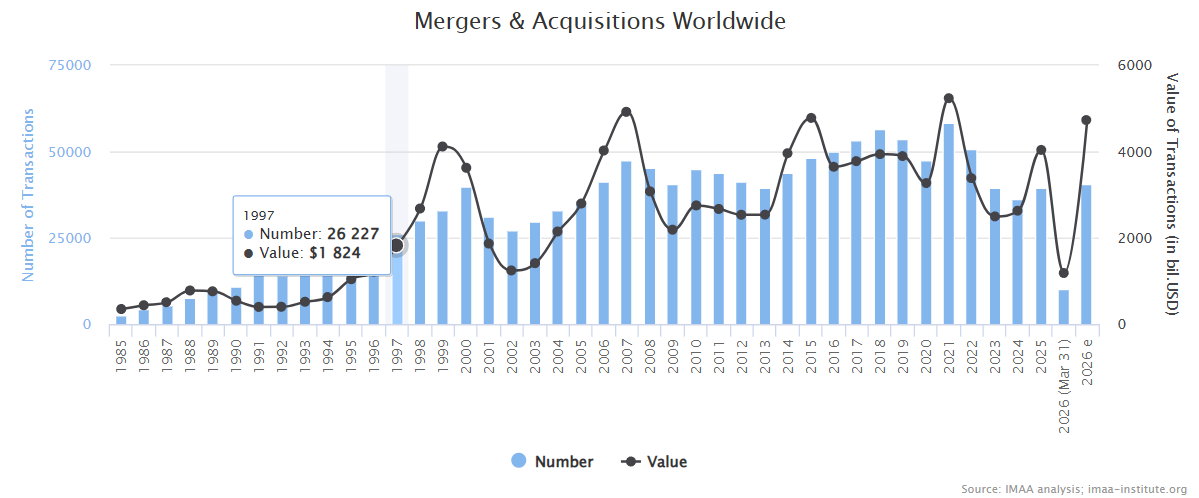
\includegraphics[width=\textwidth]{figures/ch11/mna_waves.png}
\caption{Number of transactions (bars, left axis) and value of transactions in billions of US dollars (line,
right axis) of mergers and acquisitions worldwide, 1985--2026. The 2026 entries are the first quarter and a
full-year estimate. Source: Institute for Mergers, Acquisitions and Alliances (IMAA), imaa-institute.org.}
\label{fig:11-waves}
\end{figure}

Within an industry, mergers often come in sequences that reshape the market over two or three decades.
\Cref{tab:11-consolidation} summarizes three such histories. US telecommunications went from the 1984 breakup of
AT\&T into seven regional ``Baby Bells'' to a handful of national carriers. The major US airlines consolidated
through mergers and failures after deregulation (\cref{ch:airlines}). World brewing was transformed by a chain of
very large deals between 2000 and 2012, and \cref{sec:11-millercoors} studies one of them, the MillerCoors joint
venture, in detail. \Cref{fig:11-beer} reproduces the brewing timeline.

\begin{table}[htbp]
\centering
\caption{Three consolidation histories}
\label{tab:11-consolidation}
\footnotesize
\begin{tabularx}{\textwidth}{@{}p{2.0cm}X@{}}
\toprule
Industry & Main combinations and outcome \\
\midrule
US telecom &
In 1984 AT\&T's local operations were split into seven regional companies: Ameritech, Bell Atlantic,
BellSouth, NYNEX, Pacific Telesis, Southwestern Bell and U\,S West. Southwestern Bell, renamed SBC, absorbed
Pacific Telesis (1997) and Ameritech (1999), then acquired AT\&T Corp.\ (2005) and took the name AT\&T Inc.,
and then acquired BellSouth (2006). Bell Atlantic, NYNEX and GTE formed Verizon (2000), which later absorbed MCI,
while Verizon Wireless absorbed Alltel. Qwest absorbed U\,S West and was in turn absorbed by CenturyLink.
Subscribers at the end of 2010 were: AT\&T 24 million landline and 96 million wireless, Verizon 26 million
landline and Verizon Wireless 94 million. Sprint had 50 million, T-Mobile USA 34 million and CenturyLink 15 million
landline. AT\&T's proposed \$39 billion purchase of T-Mobile USA (2011) was abandoned the same year
(\cref{tab:11-recent}). \\[3pt]
US airlines &
After deregulation in 1978, Trans World Airlines (which had absorbed Ozark) was acquired by American (2001).
Republic Airlines, itself formed from North Central, Southern and Hughes Airwest, merged into Northwest, and
Northwest merged into Delta (2008), which had absorbed Western (1987). Continental, which had absorbed People
Express among others, merged with United (2010). US Airways merged with America West (2005) and later with
American (2013). Southwest absorbed AirTran (2011). Braniff (1982), Eastern (1991) and Pan Am (1991) failed. \\[3pt]
World beer &
Interbrew and AmBev (\$11.5 billion) formed InBev (2004), which bought Anheuser-Busch for \$52 billion (2008)
to form AB InBev and later bought the rest of Grupo Modelo for \$20.1 billion. SAB bought Miller (\$5.6 billion,
2002) and later Bavaria, Grolsch and Foster's. Coors and Molson merged (2005). Heineken and Carlsberg divided the
assets of Scottish \& Newcastle (\$15.3 billion, 2008). In the United States, SABMiller and Molson Coors combined
their operations in the MillerCoors joint venture (2008). \\
\bottomrule
\end{tabularx}

\vspace{3pt}
\begin{minipage}{\textwidth}
\footnotesize Notes: Subscriber counts and the T-Mobile deal value are from a 2011 \emph{Wall Street
Journal} graphic (``A Tangled Family Tree''). Airline combinations follow the Aviation Week Intelligence
Network's Fleet Database as reproduced in the source chart, and beer deal values follow the timeline of
\cref{fig:11-beer}. Years are completion years, except the year of the proposed T-Mobile purchase. The telecom
and beer years, Western (1987) and the three airline failures are read off the time axes of these charts. The airline mergers of 2001 to 2011 are dated by
\citet[p.~11]{GAO2013}, and the 2013 merger of American and US Airways by \citet[p.~263]{AskerNocke2021}. MillerCoors
is dated by its consummation in June 2008 \citep[p.~1768]{MillerWeinberg2017}.
\end{minipage}
\end{table}

\begin{figure}[htbp]
\centering
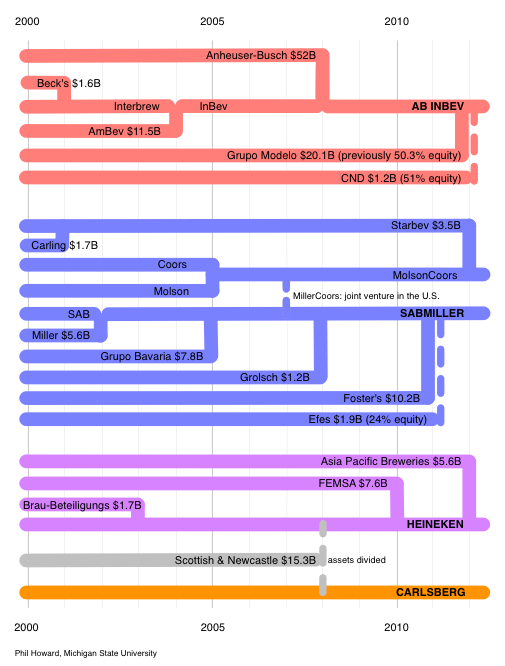
\includegraphics[width=0.5\textwidth]{figures/ch11/beer_timeline.png}
\caption{Consolidation of the world beer industry, 2000--2012. Each band is a brewer, and a band that ends in
a vertical connector is acquired by the band it joins. Labels give deal values in billions of US dollars.
Source: Phil Howard, Michigan State University, as printed on the figure.}
\label{fig:11-beer}
\end{figure}

\casehead{Two views of why firms merge}
Industrial organization economists stress three motives. The first is market power. A merger internalizes the
competition between the merging firms, which gives them a reason to raise prices even if all other firms keep
competing as before. These are the unilateral effects defined in the introduction to this chapter. A merger may
also make it easier for the remaining firms to coordinate, tacitly or explicitly, which gives rise to coordinated
effects (\cref{ch:collusion-theory}). The second motive is efficiencies. They include economies of scale and scope,
the rationalization of production and distribution across plants, and the transfer of know-how from the better-run
firm to the other. The third motive is strategic. A merger can deter entry or allow the firms to reposition their
products.

Corporate finance asks different questions. One is why mergers come in waves and why they cluster within
industries. \citet{MitchellMulherin1996} and \citet{AndradeMitchellStafford2001} attribute the clustering to
industry shocks, such as deregulation, new technologies and changes in input prices, which make a new industry
structure efficient. A second question is why the stock returns of acquirers are weak around acquisitions while
targets gain. Several theories blame agency problems or mispricing. \citet{Jensen1986} argues that managers of
firms with free cash flow overinvest in acquisitions to build empires. \citet{Roll1986} argues that overconfident
managers overpay. \citet{ShleiferVishny2003} argue that overvalued acquirers use their stock to buy undervalued
targets, so that waves follow stock-market valuations. These explanations are complements to the industrial
organization view and say little about prices. We therefore leave them aside.

The theory developed in this chapter delivers three results that will guide the empirical work. In a Cournot
market, a merger without cost savings raises the price, and it is often unprofitable for the merging firms
(\cref{sec:11-cournot}). In a symmetric market with differentiated products and price competition, every merger
is profitable (\cref{sec:11-upp}). When firms must invest in costly capacity, a merger can be profitable even
without cost savings (\cref{sec:11-beyond}).

\subsection{The legal framework and the US review process}\label{sec:11-review}

Section 7 of the Clayton Act of 1914, as amended in 1950, prohibits acquisitions whose effect ``may be
substantially to lessen competition, or to tend to create a monopoly'' \citep[p.~2]{FarrellShapiro2010}. The
word ``may'' matters. The government does not have to prove that a merger will harm competition, only that it is
likely to. Section 7 applies to every acquisition, including those that are too small to be reported and those
already consummated.

\casehead{Notification and the waiting period}
The Hart-Scott-Rodino Antitrust Improvements Act of 1976 (HSR) added Section 7A to the Clayton Act. It requires
the parties to a sufficiently large transaction to notify the Federal Trade Commission (FTC) and the Antitrust
Division of the Department of Justice (DOJ) before they close. Its motivation was the cost of undoing completed
mergers. The leading example, \emph{United States v.\ El Paso Natural Gas}, took seven years to litigate and ten
more years to carry out the divestiture the Supreme Court had ordered \citep[p.~5]{AshenfelterHosken2008}. Until
2001 every merger involving more than \$15 million in assets had to be reported. In February 2001 the threshold
rose to transactions above \$50 million and was indexed to the growth of national income, which explains much of
the fall in filings after 2001 \citep[p.~6, n.~7]{AshenfelterHosken2008}. The indexed threshold was \$63 million
in 2008 \citep[p.~2, n.~3]{FarrellShapiro2010} and \$133.9 million in 2026 \citep[p.~2134]{FTC2026}. The 2001
change also altered which mergers took place, as the end of this subsection shows.

After both parties file, a waiting period of 30 days begins (15 days for cash tender offers and bankruptcy
sales). During this period the two agencies decide which one will review the deal, a step called
\emph{clearance}. That agency then conducts a preliminary review of market shares, concentration, company
documents and complaints from customers or rivals. The agency may end the wait early through \emph{early
termination}. If the deal looks problematic, the agency issues a \emph{Second Request}, a detailed subpoena for
documents and data on competition, entry, substitution and claimed efficiencies. The waiting period then extends
until 30 days after the parties have substantially complied \citep[p.~6]{AshenfelterHosken2008}. Compliance
typically takes two or three months and sometimes six months or more. The whole investigation, with depositions
and interviews of customers and competitors, often lasts about a year.

\casehead{Outcomes}
An investigation ends in one of four ways. The agency may close it and let the merger proceed. It may negotiate
a \emph{consent decree}, usually requiring the parties to divest overlapping assets. For DOJ decrees, the Tunney
Act requires a federal court to find that the decree is in the public interest. The agency may sue to block the
merger, which in practice means seeking a preliminary injunction in federal court. Finally, the parties may
abandon the deal. The last three outcomes are counted as \emph{enforcement actions}. Much of the bargaining takes
place in the shadow of litigation. In fiscal year 2006, for example, 1,768 transactions were reported, the
agencies issued 45 Second Requests and challenged 32 transactions. The challenges led to 17 settlements, 6
restructured transactions and 9 abandoned deals \citep[p.~2, n.~5]{FarrellShapiro2010}. Some industries follow
their own rules. Rail mergers, for instance, fall under the exclusive jurisdiction of the Surface Transportation
Board. \Cref{fig:11-hsrflow} summarizes the process.

\begin{figure}[htbp]
\centering
\begin{tikzpicture}[
  box/.style={draw, rounded corners=2pt, align=center, font=\footnotesize, text width=2.2cm,
              minimum height=1.05cm, inner sep=3pt, execute at begin node={\hyphenpenalty=10000\exhyphenpenalty=10000}},
  proc/.style={box, fill=gray!8},
  dec/.style={box, fill=yellow!14},
  pass/.style={box, fill=green!9},
  stopb/.style={box, fill=red!9},
  arr/.style={-{Stealth[length=2mm]}, thin},
  lab/.style={font=\scriptsize, inner sep=1.5pt}]
\node[proc] (agree) at (0,0) {Firms agree to merge};
\node[dec]  (rep)   at (3.05,0) {Reportable under HSR? (deal above threshold)};
\node[proc] (file)  at (6.1,0) {Both parties file, FTC or DOJ takes the case};
\node[proc] (rev)   at (9.15,0) {30-day review: shares, HHI, documents, complaints};
\node[dec]  (sr)    at (12.2,0) {Second Request?};
\node[pass, text width=2.6cm] (notrep) at (3.05,-2.45) {Not reportable: close at will, still subject to
  Clayton Act Section 7};
\node[pass, text width=3.0cm] (wait) at (8.2,-2.45) {Waiting period ends, or early termination,
  then close};
\node[proc, text width=3.4cm] (deep) at (12.2,-2.45) {In-depth investigation: data, documents,
  diversion, UPP, simulation (often about one year)};
\node[pass, text width=2.3cm]  (o1) at (5.4,-5.0)  {Close investigation};
\node[proc, text width=2.3cm]  (o2) at (8.0,-5.0)  {Consent decree: divest overlaps};
\node[stopb, text width=2.3cm] (o3) at (10.6,-5.0) {Sue to block (injunction in federal court)};
\node[stopb, text width=2.3cm] (o4) at (13.2,-5.0) {Parties abandon};
\draw[arr] (agree) -- (rep);
\draw[arr] (rep) -- node[lab, above] {yes} (file);
\draw[arr] (rep) -- node[lab, right] {no} (notrep);
\draw[arr] (file) -- (rev);
\draw[arr] (rev) -- (sr);
\draw[arr] (sr.south west) -- (wait.north east);
\node[lab, anchor=north east] at (9.95,-1.15) {no (about 98\%)};
\draw[arr] (sr) -- node[lab, right] {yes (about 2\%)} (deep);
\foreach \o in {o1,o2,o3,o4} {\draw[arr] (deep.south) -- (\o.north);}
\draw[decorate, decoration={brace, mirror, amplitude=5pt}] ([yshift=-3pt]o2.south west) --
  node[below=6pt, font=\footnotesize] {enforcement actions} ([yshift=-3pt]o4.south east);
\end{tikzpicture}
\caption{From the decision to merge to closing in the United States. In fiscal year 2025 there were 2,006 HSR
filings, 41 Second Requests and 18 enforcement actions, equal to 2.0 and 0.9 percent of filings. Two of the 18
actions concerned transactions not reported under HSR.}
\label{fig:11-hsrflow}
\end{figure}

\Cref{tab:11-hsr} reports the number of filings, Second Requests and enforcement actions in each fiscal year
from 2003 to 2025, and \cref{fig:11-hsrplot} extends the series back to 1991. Three patterns stand out. Filings
fell from 4,926 in fiscal year 2000 to 1,187 in 2002 after the threshold increase, and to 716 in fiscal year 2009
during the financial crisis. They spiked in 2021 and 2022. Over 2003--2025 the agencies issued 2.6 Second Requests
and brought 2.0 enforcement actions for every 100 filings. These are annual activity ratios. An action can concern a
transaction filed in an earlier year, or one that was never reportable. The ratio is therefore not the share of a
year's filings that led to enforcement. Actions relative to filings have drifted down, from about 3 percent in
2010--2013 to about 2 percent in 2014--2020 and between 0.9 and 1.6 percent since 2021. Most mergers are never
examined closely.

\begin{table}[htbp]
\centering
\caption{Hart-Scott-Rodino filings, Second Requests and enforcement actions, fiscal years 2003--2025}
\label{tab:11-hsr}
\footnotesize
\begin{tabular}{@{}lrrrrr@{}}
\toprule
 & & & & \multicolumn{2}{c}{Ratio to filings (percent)} \\
\cmidrule(l){5-6}
Fiscal year & Filings & Second Requests & Enforcement actions & Second Requests & Enforcement actions \\
\midrule
2003 & 1,014 & 33 & 36 & 3.3 & 3.6 \\
2004 & 1,454 & 35 & 24 & 2.4 & 1.7 \\
2005 & 1,675 & 50 & 18 & 3.0 & 1.1 \\
2006 & 1,768 & 45 & 32 & 2.5 & 1.8 \\
2007 & 2,201 & 63 & 34 & 2.9 & 1.5 \\
2008 & 1,726 & 41 & 37 & 2.4 & 2.1 \\
2009 & 716 & 31 & 31 & 4.3 & 4.3 \\
2010 & 1,166 & 42 & 41 & 3.6 & 3.5 \\
2011 & 1,450 & 55 & 37 & 3.8 & 2.6 \\
2012 & 1,429 & 49 & 44 & 3.4 & 3.1 \\
2013 & 1,326 & 47 & 38 & 3.5 & 2.9 \\
2014 & 1,663 & 51 & 33 & 3.1 & 2.0 \\
2015 & 1,801 & 47 & 42 & 2.6 & 2.3 \\
2016 & 1,832 & 54 & 47 & 2.9 & 2.6 \\
2017 & 2,052 & 51 & 39 & 2.5 & 1.9 \\
2018 & 2,111 & 45 & 39 & 2.1 & 1.8 \\
2019 & 2,089 & 61 & 38 & 2.9 & 1.8 \\
2020 & 1,637 & 48 & 43 & 2.9 & 2.6 \\
2021 & 3,520 & 65 & 32 & 1.8 & 0.9 \\
2022 & 3,152 & 47 & 49 & 1.5 & 1.6 \\
2023 & 1,805 & 37 & 28 & 2.0 & 1.6 \\
2024 & 2,031 & 59 & 32 & 2.9 & 1.6 \\
2025 & 2,006 & 41 & 18 & 2.0 & 0.9 \\
\midrule
Total & 41,624 & 1,097 & 812 & 2.6 & 2.0 \\
\bottomrule
\end{tabular}

\vspace{3pt}
\begin{minipage}{0.97\textwidth}
\footnotesize Notes: Compiled from the annual HSR reports of the FTC and DOJ. Enforcement actions combine the
merger challenges of both agencies as printed in each year's joint report, using the corrected report for 2022. The
FTC later raised its 2017 count from 21 to 23, which would give 41 for that year. A report counts an action in the
year of the agency's first public action. The action can concern a transaction filed in an earlier year or one not
reportable under HSR, as did two of the 18 actions in 2025. The ratios are counts divided by filings in the same
year, so they measure annual activity. The compiled table we draw on reports Second Request rates 0.1 point higher for 2017--2020
(2.6, 2.2, 3.0 and 3.0). It probably divides by the transactions for which a Second Request could be issued. The 2003 and 2004 rows coincide with \citet[Table 1]{AshenfelterHosken2008}, and the 2006 row with
\citet[n.~5]{FarrellShapiro2010}.
\end{minipage}
\end{table}

\begin{figure}[htbp]
\centering
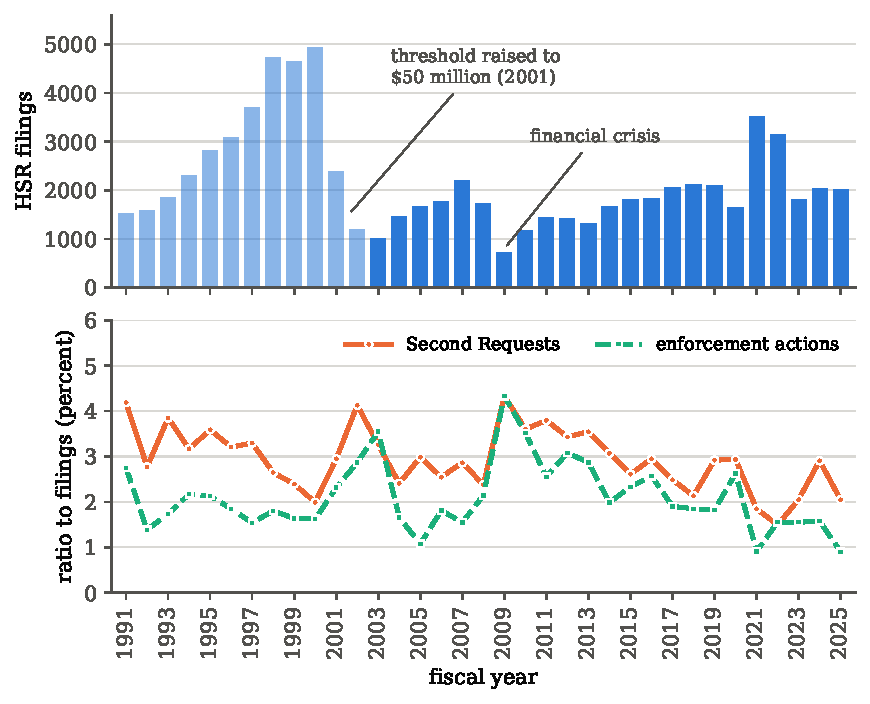
\includegraphics[width=0.86\textwidth]{figures/ch11/hsr_stats.pdf}
\caption{HSR filings (top) and the ratios of Second Requests and enforcement actions to filings in the same year, in
percent (bottom), fiscal years 1991--2025. The lighter bars for 1991--2002 come from \citet[Table 1]{AshenfelterHosken2008}, the
rest from \cref{tab:11-hsr}. Both ratios use all filings as the denominator.}
\label{fig:11-hsrplot}
\end{figure}

\casehead{Enforcement and selection}
Enforcement shapes which mergers we observe. \citet[p.~5]{AshenfelterHosken2008} report that 37,201 mergers were
filed from 1991 through 2004. About 97 percent were allowed to proceed without a full investigation. Of the 3
percent investigated in depth, roughly 65 percent were modified, abandoned or blocked.
\citet[p.~4, n.~5]{AshenfelterHoskenWeinberg2011} summarize the first figure as 97 percent of proposed mergers
going through without modification. Because the agencies try to stop the mergers most likely to raise prices,
the consummated mergers that a researcher can study are a selected sample. The average price effect of approved
mergers is a lower bound on the average effect that mergers would have in a world without enforcement
\citep{Carlton2009}. The informative object for policy is the effect of the \emph{marginal} merger, one that was
nearly blocked. \Cref{sec:11-retro} returns to this problem.

\casehead{Notification thresholds as a screen}
Reporting thresholds do more than save the agencies work. They also shape which mergers firms propose.
\citet{BesankoSpulber1993} model a review in which the merging parties know their merger-specific efficiencies and
the authority does not. Proposing a merger costs a fixed amount that cannot be recovered. Holding fixed the
probability of approval, only mergers whose efficiencies exceed a threshold are then worth proposing. A positive
proposal cost can therefore benefit consumers, because it improves the pool of proposed mergers
\citep[p.~223]{AskerNocke2021}. The same model suggests one reason why authorities apply a consumer surplus
standard rather than a total surplus standard. An authority that puts less weight on profit than society does is
tougher. It approves fewer mergers, and the proposals it receives are better as a result \citep[p.~223,
n.~120]{AskerNocke2021}.

\citet{Wollmann2019} tests this selection effect with the 2001 amendment, which raised the size-of-transaction
threshold. The agencies almost never investigated the newly exempt deals afterward, in line with the long-standing
observation that they rarely examine mergers that need not be reported. Wollmann compares newly exempt horizontal
mergers with newly exempt non-horizontal ones, which seldom raise concerns. This is a \emph{difference-in-differences}
design, which compares the change in a treated group with the change in a control group (\cref{sec:11-retro-problem}
develops it). A \emph{triple difference} also subtracts the same comparison among \emph{never-exempt} mergers, those
above the new threshold of \$50 million, which had to be reported both before and after the amendment. Newly exempt
mergers lie between the old \$15 million threshold and the new one. After
2001, never-exempt horizontal and non-horizontal mergers moved together. Newly exempt horizontal mergers rose
relative to newly exempt non-horizontal ones. The triple-difference estimate is a 50 percent increase: 324
additional newly exempt horizontal mergers per year on a pre-amendment base of 634 \citep[pp.~224--226]{AskerNocke2021}.
Through the lens of the Besanko-Spulber model, the amendment removed both the proposal cost and the risk of a
challenge for these deals. Mergers without large synergies became worth doing, so the pool of mergers grew and
worsened at the same time.

Firms also size their deals around the threshold. \citet{CunninghamEdererMa2021} study pharmaceutical acquisitions.
Acquisitions of targets whose drug projects overlap with the acquirer's bunch just below the HSR threshold, while
acquisitions without such overlap do not \citep[pp.~226--227 and Figure 9]{AskerNocke2021}. \Cref{sec:11-open}
returns to these acquisitions.

\subsection{What the agencies analyze}\label{sec:11-agencies}

The agencies' Horizontal Merger Guidelines describe five tasks \citep{USDOJFTC1992,USDOJFTC2010}, which
\citet[p.~7]{AshenfelterHosken2008} summarize. The first two
define the market. The \emph{relevant product market} is a set of close substitutes for the merging firms'
products, found with the hypothetical monopolist test of \cref{sec:11-hmt}. The \emph{relevant geographic market}
is the narrowest area in which anticompetitive effects could occur. For nationally distributed branded goods it is
typically the whole country \citep[p.~7]{AshenfelterHosken2008}. The third task is to assess competitive effects,
both unilateral and coordinated. The fourth is to evaluate efficiency claims. Efficiencies count only if they
are \emph{merger-specific}, meaning that no other arrangement that harms competition less could achieve them, and
\emph{verifiable} by the authority at the time of review \citep[p.~221]{AskerNocke2021}. They must also be large
enough to reverse the merger's potential to harm customers, for instance by preventing price increases
\citep[Section~10]{USDOJFTC2010}. The fifth is to ask whether entry would be timely, likely and sufficient to deter
or counteract the competitive effects of concern (Section~9). \Cref{sec:11-freeentry} shows what free entry implies
for the effects of a merger and how slowly entry can come in practice.
Economists at the agencies work mostly on market definition and competitive effects. The rest of this chapter
follows the same order. \Cref{sec:11-marketdef} covers market definition and concentration, and the remaining
sections cover competitive effects and efficiencies.

\casehead{Evidence on efficiencies}
The efficiency defense rests on a thin empirical base. \citet[pp.~219--221]{AskerNocke2021} single out two studies
that document merger-specific efficiencies. The first, \citet{AshenfelterHoskenWeinberg2015}, measures the
shipping savings of the MillerCoors joint venture, which \cref{sec:11-mc-assessment} discusses. The second,
\citet{BraguinskyEtAl2015}, studies 73 acquisitions in the Japanese cotton-spinning industry between 1896 and 1920.
More profitable firms bought less profitable ones, although the two groups had similar physical productivity. The
acquired mills then improved their inventory management, accounts receivable and capacity utilization, and market
power explains little of their higher profitability. The two cases illustrate the two conditions above. The beer
savings came from shorter shipping distances, which are easy to verify. The brewers might, however, have obtained
them by brewing each other's beer under contract while pricing independently, which questions their merger
specificity. The managerial gains in cotton spinning are specific to the merger but hard to verify before they
occur.

Evidence on how often mergers create efficiencies, and how large they are, is scarcer still.
\citet{GeurtsVanBiesebroeck2019} find that about 80 percent of the mergers in Belgium between 2005 and 2012 raised
employment, which may reflect higher output. \citet{GriecoPinkseSlade2018} estimate returns to scale in the
Molson-Coors merger and translate them into marginal-cost reductions \citep[pp.~221--222]{AskerNocke2021}. In the
words of \citet[p.~261]{AskerNocke2021}, not much is known about the typical magnitudes of merger efficiencies or
about how they relate to market structure.

\section{Market definition and concentration screens}\label{sec:11-marketdef}

Market shares and concentration indices are defined only relative to a market (\cref{sec:01-market-definition}).
The agencies therefore begin by defining the relevant market, and they then compute shares and the
Herfindahl-Hirschman index within it. This section derives the logic of the hypothetical monopolist test, the
algebra of critical loss, the theory behind concentration thresholds, and the reasons the whole approach struggles
with differentiated products.

\subsection{The hypothetical monopolist test}\label{sec:11-hmt}

\begin{definition}[Hypothetical monopolist test]\label{def:11-hmt}
Consider a hypothetical profit-maximizing firm that owns all products in a candidate set and faces no
regulation of its prices. Hold the terms of sale of all other products fixed. The set is a \emph{relevant product
market} if this firm would impose at least a \emph{small but significant and non-transitory increase in price}
(SSNIP) on some product of the merging firms.
\end{definition}

The SSNIP is usually 5 percent of the price and sometimes 10 percent. The test is applied iteratively. We start
from the products of the merging firms. If a hypothetical monopolist of this set would not raise price by the
SSNIP, because too many buyers would switch to products outside the set, the set is too narrow. We then add the
next-closest substitute and repeat. The relevant market is the smallest set that passes. The relevant geographic
market is defined the same way, with locations in place of products. The test turns market definition into a
statement about demand, so it can draw on the demand models of \cref{ch:aids,ch:logit,ch:blp}.

The test must be applied at the right prices. In \emph{United States v.\ E.\ I.\ du Pont de Nemours \& Co.}
(1956) the Supreme Court held that cellophane competed with other flexible wrapping materials, partly because
many buyers switched between them. Du Pont, however, already set the price of cellophane as a near monopolist. A
monopolist prices where its demand is elastic, since its Lerner condition $\frac{p - c}{p} = \frac{1}{\varepsilon}$
requires $\varepsilon > 1$. At monopoly prices, almost any product looks like it has close substitutes. Applying
the test at prices that already reflect market power therefore yields markets that are too broad. This error is
called the \emph{cellophane fallacy}. In merger review the problem is milder, because the question is whether the
merger would raise prices above their current level.

\subsection{Critical loss analysis}\label{sec:11-critloss}

\emph{Critical loss analysis} turns the hypothetical monopolist test into a comparison of two numbers. Consider a
hypothetical monopolist of the candidate set that sells quantity $q$ at price $p$, with constant marginal cost
$c$ and percentage margin $L = \frac{p - c}{p}$. Suppose it raises the price by a fraction $X$ to $p(1 + X)$, and
let $\mathit{AL}$ be the resulting \emph{actual loss}, the fraction of unit sales lost. Profit before the increase is
\begin{equation*}
(p - c)\,q = L\,pq.
\end{equation*}
Profit after the increase is
\begin{align*}
\big(p(1 + X) - c\big)\,q\,(1 - \mathit{AL})
&= \big(pX + (p - c)\big)\,q\,(1 - \mathit{AL}) \\
&= (X + L)(1 - \mathit{AL})\,pq.
\end{align*}
Profit per dollar of pre-merger revenue therefore moves from $L$ to $(X + L)(1 - \mathit{AL})$. The increase is
profitable if and only if
\begin{align}
(X + L)(1 - \mathit{AL}) &\ge L \notag \\
\iff X + L - (X + L)\,\mathit{AL} &\ge L \notag \\
\iff \mathit{AL} &\le \frac{X}{X + L} \equiv \mathit{CL}. \label{eq:11-cl}
\end{align}
The number $\mathit{CL}$ is the \emph{critical loss}, the largest loss of sales that leaves the price increase
profitable. With $X = 0.05$ and $L = 0.4$, the critical loss is $\frac{0.05}{0.45} = 11.1$ percent.

\casehead{From critical loss to a threshold elasticity}
The actual loss depends on the shape of demand. With linear demand $q(p) = d_0 - d_1 p$, the quantity
falls by $d_1 pX$, so
\begin{equation*}
\mathit{AL} = \frac{d_1 pX}{q} = \varepsilon X,
\end{equation*}
where $\varepsilon = \frac{d_1 p}{q}$ is the elasticity of the candidate market's demand at the initial
price. Substituting into \eqref{eq:11-cl}, the SSNIP breaks even if and only if
\begin{equation}\label{eq:11-ce-lin}
\varepsilon \le \frac{1}{X + L}.
\end{equation}
We call the right side the breakeven \emph{threshold elasticity}. The test in \eqref{eq:11-cl} asks whether a price increase of $X$ is \emph{profitable}. The Guidelines ask whether
the monopolist \emph{would impose} it, which is the stronger requirement that the profit-maximizing increase be
at least $X$. With linear demand, profit after an increase $x$ is
\begin{equation*}
\pi(x) = (x + L)(1 - \varepsilon x)\,pq,
\end{equation*}
which is concave in $x$. Its derivative is
\begin{equation*}
\pi'(x) = \big[(1 - \varepsilon x) - \varepsilon (x + L)\big]\,pq = (1 - 2\varepsilon x - \varepsilon L)\,pq.
\end{equation*}
By concavity, the optimal increase is at least $X$ if and only if $\pi'(X) \ge 0$, that is,
\begin{equation}\label{eq:11-ce-lin-pm}
\varepsilon \le \frac{1}{2X + L}.
\end{equation}
This bound is tighter than \eqref{eq:11-ce-lin}. With constant-elasticity demand $q(p) = A p^{-\varepsilon}$ the
loss is $\mathit{AL} = 1 - (1 + X)^{-\varepsilon}$. The breakeven condition becomes
$(X + L)(1 + X)^{-\varepsilon} \ge L$, or
\begin{equation*}
\varepsilon \le \frac{\ln\!\big(\frac{X + L}{L}\big)}{\ln(1 + X)}.
\end{equation*}
For the profit-maximizing version, the monopoly price with constant elasticity $\varepsilon > 1$ is
$\frac{\varepsilon}{\varepsilon - 1}c$, and $c = (1 - L)p$. The optimal increase is at least $X$ if and only if
$\frac{\varepsilon}{\varepsilon - 1}(1 - L) \ge 1 + X$, which rearranges to
$\varepsilon \le \frac{1 + X}{X + L}$.

\Cref{tab:11-critloss} reports these thresholds. Two lessons emerge. First, the critical loss falls steeply as the
margin rises. Second, the threshold elasticity depends on the curvature of demand. With $X = 0.05$ and $L = 0.4$, a
market elasticity of 2.2 passes the breakeven test under both demand curves. It fails the profit-maximizing test
under linear demand and passes it under constant elasticity. Market definition thus depends on curvature, and
hence on pass-through (\cref{sec:02-passthrough}), a point we return to in \cref{sec:11-diffmarkets}.

\begin{table}[htbp]
\centering
\caption{Critical loss and the threshold elasticity of market demand}
\label{tab:11-critloss}
\footnotesize
\begin{tabular}{@{}cccccccc@{}}
\toprule
 & & & \multicolumn{2}{c}{Linear demand} & & \multicolumn{2}{c}{Constant elasticity} \\
\cmidrule{4-5} \cmidrule{7-8}
\makecell{SSNIP\\$X$} & \makecell{Margin\\$L$} & \makecell{Critical loss\\$\mathit{CL}$ (\%)} & Breakeven &
\makecell{Profit-\\maximizing} & & Breakeven & \makecell{Profit-\\maximizing} \\
\midrule
0.05 & 0.2 & 20.0 & 4.00 & 3.33 & & 4.57 & 4.20 \\
0.05 & 0.4 & 11.1 & 2.22 & 2.00 & & 2.41 & 2.33 \\
0.05 & 0.6 & \phantom{0}7.7 & 1.54 & 1.43 & & 1.64 & 1.62 \\
0.10 & 0.2 & 33.3 & 3.33 & 2.50 & & 4.25 & 3.67 \\
0.10 & 0.4 & 20.0 & 2.00 & 1.67 & & 2.34 & 2.20 \\
0.10 & 0.6 & 14.3 & 1.43 & 1.25 & & 1.62 & 1.57 \\
\bottomrule
\end{tabular}

\vspace{3pt}
\begin{minipage}{0.97\textwidth}
\footnotesize Notes: The SSNIP passes if the elasticity of the candidate market's demand is at most the entry
shown. Linear demand: $\frac{1}{X + L}$ (breakeven) and $\frac{1}{2X + L}$ (profit-maximizing). Constant
elasticity: $\frac{\ln\left(\frac{X + L}{L}\right)}{\ln(1 + X)}$ (breakeven) and $\frac{1 + X}{X + L}$
(profit-maximizing).
\end{minipage}
\end{table}

\casehead{The critical loss paradox and aggregate diversion}
High margins make the critical loss small. Merging parties have used this to argue for broad markets. With a
40 percent margin, they say, losing just 11 percent of sales makes a 5 percent increase unprofitable, and surely
more buyers than that would switch. \citet{KatzShapiro2003} and \citet{OBrienWickelgren2003} point out the flaw. High
margins are not exogenous. Before the merger, each firm in the candidate market sets its own price, so its own
demand elasticity equals the inverse of its margin. A high margin therefore signals that each firm faces less elastic
demand and loses fewer sales when it raises its price alone. What matters for the hypothetical monopolist is where
those sales go. Sales diverted to other products in the candidate market are recaptured by the monopolist.

To make this precise, we use the diversion ratio $D_{jk}$ of \cref{def:04-diversion}, the fraction of the sales that
$j$ loses when its price rises that go to $k$. The aggregate diversion ratio of $j$ to a set of products sums its
diversion ratios to the members of the set (\cref{def:11-aggdiv}).

\begin{proposition}[Critical loss and aggregate diversion, \citealp{KatzShapiro2003}]\label{prop:11-aggdiv}
Consider a candidate market of $n$ symmetric products, each sold by a single-product firm at price $p$ with
marginal cost $c$ and margin $L = \frac{p - c}{p}$. Assume pre-merger prices satisfy each firm's first-order
condition, and demand is linear over the relevant range. Let $\bar D$ be each product's aggregate diversion
ratio to the other $n - 1$ products. A uniform price increase $X$ on all $n$ products causes the actual loss
\begin{equation}\label{eq:11-al-div}
\mathit{AL} = \frac{X(1 - \bar D)}{L},
\end{equation}
and the increase is profitable for a hypothetical monopolist if and only if
\begin{equation}\label{eq:11-aggdiv}
\bar D \ge \frac{X}{X + L} = \mathit{CL}.
\end{equation}
\end{proposition}

\begin{proof}
Write $\varepsilon_{jj} = -\frac{\partial q_j}{\partial p_j}\frac{p}{q_j}$ for the own elasticity of product $j$.
Its firm's first-order condition gives the Lerner condition $L = \frac{1}{\varepsilon_{jj}}$. When all prices rise
by $pX$, linearity gives the change in $q_j$ as
\begin{equation*}
\Delta q_j = \frac{\partial q_j}{\partial p_j}\,pX + \sum_{k \ne j}\frac{\partial q_j}{\partial p_k}\,pX.
\end{equation*}
By symmetry of the products, $\frac{\partial q_j}{\partial p_k} = \frac{\partial q_k}{\partial p_j}$, and the
definition of diversion gives
\begin{equation*}
\sum_{k \ne j}\frac{\partial q_j}{\partial p_k} = \sum_{k \ne j}\frac{\partial q_k}{\partial p_j}
= -\bar D\,\frac{\partial q_j}{\partial p_j}.
\end{equation*}
Substituting,
\begin{equation*}
\Delta q_j = \frac{\partial q_j}{\partial p_j}\,pX\,(1 - \bar D),
\qquad
\mathit{AL} = -\frac{\Delta q_j}{q_j} = \varepsilon_{jj}X(1 - \bar D) = \frac{X(1 - \bar D)}{L}.
\end{equation*}
This is \eqref{eq:11-al-div}. By \eqref{eq:11-cl} the increase is profitable if and only if
$\frac{X(1 - \bar D)}{L} \le \frac{X}{X + L}$. Multiplying by $\frac{L(X + L)}{X} > 0$ gives
$(1 - \bar D)(X + L) \le L$, which rearranges to $X \le \bar D(X + L)$, that is, $\bar D \ge \frac{X}{X + L}$.
\end{proof}

\Cref{prop:11-aggdiv} reverses the paradox. A single firm that raised its price alone would lose
$\frac{X}{L}$ of its sales, which always exceeds $\mathit{CL} = \frac{X}{X + L}$. The hypothetical monopolist loses only
the part that leaves the candidate market. With $L = 0.4$ and $X = 0.05$, it suffices that 11.1 percent of the
sales lost by each product are recaptured by the others. High margins thus make narrow markets more likely,
because the hurdle $\mathit{CL}$ falls while diversion is unchanged. Analyses that estimate the hypothetical
monopolist's actual loss from single-firm elasticities ignore recapture. Some such analyses have concluded that a
hypothetical monopolist would want to cut price below pre-merger levels, which contradicts the premise that
pre-merger prices maximize each firm's profit \citep[p.~25, n.~74]{FarrellShapiro2010}. The uniform price
increase in \cref{prop:11-aggdiv} is a simplification, since the test only requires an increase on one product of
the merging firms.

\citet[Appendix]{FarrellShapiro2010} use the same logic to link market definition to diversion between the
merging products. In a candidate market that exactly meets the breakeven test, the aggregate diversion ratio of
each product equals $\frac{X}{L + X}$. If diversion within the market is proportional to market shares $s_k$, the
diversion from product 1 to product 2 is
\begin{equation}\label{eq:11-fs-proxy}
D_{12} = \frac{s_2}{1 - s_1}\cdot\frac{X}{L + X}.
\end{equation}
\Cref{sec:11-upp} uses diversion ratios of this kind directly, without defining a market.

\subsection{Concentration measures and the Guidelines}\label{sec:11-hhi}

Once a market is defined, the agencies compute the Herfindahl-Hirschman index $\HHI = \sum_i s_i^2$ of
\cref{def:01-concentration}, reported in HHI points ($10{,}000 \times \HHI$, or shares in percent squared). If
firms $A$ and $B$ merge and the merged firm keeps their combined share, the index changes by
\begin{align}
\Delta\HHI &= (s_A + s_B)^2 - s_A^2 - s_B^2 \notag \\
&= s_A^2 + 2 s_A s_B + s_B^2 - s_A^2 - s_B^2 \notag \\
&= 2 s_A s_B. \label{eq:11-dhhi}
\end{align}
The Guidelines classify mergers by the post-merger index and by this change. \Cref{tab:11-guidelines} compares
the thresholds of the 1992 and 2010 Horizontal Merger Guidelines and the 2023 Merger Guidelines.

\begin{table}[htbp]
\centering
\caption{Concentration thresholds in the US merger guidelines}
\label{tab:11-guidelines}
\footnotesize
\begin{tabularx}{\textwidth}{@{}>{\raggedright\arraybackslash}p{2.3cm}*{3}{>{\raggedright\arraybackslash}X}@{}}
\toprule
 & 1992 Horizontal Merger Guidelines & 2010 Horizontal Merger Guidelines & 2023 Merger Guidelines \\
\midrule
Market categories (post-merger HHI) &
Unconcentrated below 1,000, moderately concentrated from 1,000 to 1,800, highly concentrated above 1,800 &
Unconcentrated below 1,500, moderately concentrated from 1,500 to 2,500, highly concentrated above 2,500 &
Highly concentrated above 1,800 \\[3pt]
Safe harbors &
Unconcentrated markets, and $\Delta\HHI < 100$ (moderately concentrated) or $\Delta\HHI < 50$ (highly
concentrated) &
Unconcentrated markets, and $\Delta\HHI < 100$ in any market &
No explicit safe harbor \\[3pt]
Potential concern &
$\Delta\HHI > 100$ in moderately concentrated markets, and $\Delta\HHI$ from 50 to 100 in highly
concentrated markets &
$\Delta\HHI > 100$ in moderately concentrated markets, and $\Delta\HHI$ from 100 to 200 in highly concentrated
markets &
\\[3pt]
Presumption of harm &
Post-merger HHI above 1,800 and $\Delta\HHI > 100$ &
Post-merger HHI above 2,500 and $\Delta\HHI > 200$ &
Post-merger HHI above 1,800 and $\Delta\HHI > 100$, or a merged firm with a share above 30 percent and
$\Delta\HHI > 100$ \\
\bottomrule
\end{tabularx}

\vspace{3pt}
\begin{minipage}{\textwidth}
\footnotesize Notes: HHI points (shares in percent). The 1992 presumption is quoted from Section 1.51 in
\citet[p.~11, n.~25]{AshenfelterHosken2008} and \citet[p.~26]{FarrellShapiro2010}. The other 1992 entries are the
boundaries of 1,000 and 1,800 and the thresholds of 100 and 50 points. They coincide with the screen of the 1982 and
1984 Guidelines as \citet[pp.~5--6]{Nevo2000b} describes it. Sources: \citet[Section~1.51]{USDOJFTC1992},
\citet[Section~5.3]{USDOJFTC2010} and \citet[Section~2.1]{USDOJFTC2023}. The 2023 Guidelines contain no safe harbor.
\end{minipage}
\end{table}

\casehead{Why concentration}
The theoretical case for concentration screens comes from Cournot competition. With homogeneous goods and
constant marginal costs, firm $i$'s first-order condition $P + q_i P'(Q) = c_i$ implies
$\frac{P - c_i}{P} = \frac{s_i}{\varepsilon}$. Weighting by shares and summing gives the share-weighted Lerner
index $\frac{\HHI}{\varepsilon}$ \citep{CowlingWaterson1976}, as \cref{prop:01-cowling-waterson} shows. A higher
share lowers a firm's marginal revenue, and concentration summarizes this force for the industry
\citep[p.~3]{FarrellShapiro2010}. The formula $\Delta\HHI = 2 s_A s_B$, however, assumes that the merged firm keeps
the combined share. \citet[p.~2]{FarrellShapiro1988} note that this assumption is self-defeating. If all firms
kept their outputs, the merger would affect neither consumers nor rivals. Once outputs respond, the formula is
wrong.

\begin{example}[Naive and equilibrium changes in concentration]\label{ex:11-naivehhi}
Consider $N$ symmetric Cournot firms with constant marginal cost, and suppose two of them merge without cost
savings. The merged firm is then just another symmetric firm, so the post-merger equilibrium has $N - 1$
symmetric firms. The equilibrium change and the naive change in the index are
\begin{equation*}
\Delta\HHI = \frac{1}{N - 1} - \frac{1}{N} = \frac{1}{N(N - 1)},
\qquad
2 s_A s_B = \frac{2}{N^2}.
\end{equation*}
The ratio of the naive change to the equilibrium change is $\frac{2(N - 1)}{N}$, which exceeds one whenever
$N > 2$. The naive formula overstates the change
in concentration because the merged firm contracts and the outsiders expand. For a symmetric seven-to-six merger,
the naive calculation raises the index from 1,429 to 1,837, an increase of 408 points
\citep[p.~26]{FarrellShapiro2010}. Six symmetric firms, however, have an index of 1,667, so the equilibrium
increase is 238 points. The naive numbers trigger the presumption of the 1992 and 2023 Guidelines. The
equilibrium numbers trigger neither. Moreover, \cref{sec:11-ssr} shows that this merger would be unprofitable in
Cournot without cost savings, so it would not be proposed in the first place. \Cref{app:problems} works through
the same calculations in a Cournot exercise.
\end{example}

\casehead{Newer foundations for the screens}
Recent theory gives the naive change $2s_As_B$ a firmer foundation than the Cowling-Waterson formula does.
\citet{NockeSchutz2019} study multiproduct firms that compete in prices under logit, nested logit or CES demand.
Without merger-specific efficiencies, the losses of consumer surplus and of aggregate surplus caused by a merger are
both approximately proportional to the naive $\Delta\HHI$. The approximation is taken around small market shares
\citep[p.~226]{AskerNocke2021}. \citet{NockeWhinston2020} ask how large the efficiencies must be for a merger not to
harm consumers. They also ask how the answer depends on the change and on the level of the index. They answer in theory for
Cournot competition with homogeneous goods and for price competition with logit and CES demand. They also answer
empirically for hypothetical mergers in the US beer industry, using the demand and cost estimates of
\citet{MillerWeinberg2017}. The required efficiencies
rise with the naive $\Delta\HHI$ and, holding it fixed, do not depend on the level of the index
\citep[p.~227]{AskerNocke2021}. The results favor screens based on the change in concentration over screens based
on its level. Nocke and Whinston also argue that the presumptions of the 2010 Guidelines are likely too lax unless
the typical merger is credited with large synergies (n.~124). The level regains a role if the agency tolerates a
small loss of consumer surplus. The efficiency needed to keep the loss below a given small fraction rises with the
level of the index, holding its change fixed (n.~125). \Cref{sec:11-fs} derives the Cournot version of the required
efficiency, and \cref{sec:11-policy} gives a further reason to screen on naive concentration.

\casehead{A worked example}
\citet[Table 2]{AshenfelterHosken2008} report the pre-merger shares, the post-merger index and its change for five
consumer-product mergers. \Cref{tab:11-ahhhi} recomputes the change from the rounded shares. The recomputed values
are within 20 points of the reported ones. The gaps come from rounding. For General Mills and Ralcorp, for
instance, shares in $[27.5, 28.5)$ and $[3.5, 4.5)$ give $2 s_A s_B$ anywhere in $[192.5, 256.5)$, an interval
that contains the reported 238. The same check works for the other four mergers. The authors treat the combined
private-label share as one participant \citep[p.~11, n.~24]{AshenfelterHosken2008}.

\begin{table}[htbp]
\centering
\caption{Recomputing the change in concentration for five consumer-product mergers}
\label{tab:11-ahhhi}
\footnotesize
\begin{tabular}{@{}lllrrrr@{}}
\toprule
Industry & Firm $A$ & Firm $B$ & $s_A$ (\%) & $s_B$ (\%) & $2 s_A s_B$ & \makecell{Reported\\$\Delta\HHI$} \\
\midrule
Cereal & General Mills & Ralcorp (Chex) & 28 & 4 & 224 & 238 \\
Liquor & Guinness & Grand Metropolitan & 21 & 22 & 924 & 935 \\
Motor oil & Pennzoil & Quaker State & 29 & 9 & 522 & 517 \\
Feminine protection & Procter \& Gamble & Tambrands & 25 & 19 & 950 & 959 \\
Pancake syrup & Aurora Foods & Log Cabin & 15 & 19 & 570 & 589 \\
\bottomrule
\end{tabular}

\vspace{3pt}
\begin{minipage}{0.97\textwidth}
\footnotesize Notes: Shares are pre-merger revenue shares from scanner data of Information Resources Inc.\ (IRI). Post-merger HHIs reported in
the source are 2,357, 2,026, 2,189, 2,815 and 1,990. Aurora Foods (Mrs.\ Butterworth's) bought the Log Cabin
business from Philip Morris (Kraft). Guinness and Grand Metropolitan combined their spirits businesses. In the other
three mergers firm $A$ bought firm $B$'s brands. Source: \citet[Table 2]{AshenfelterHosken2008}.
\end{minipage}
\end{table}

\subsection{Why market definition struggles with differentiated products}\label{sec:11-diffmarkets}

The structural presumption has deep roots in US law. In \emph{United States v.\ Philadelphia National Bank}
(1963), the Supreme Court considered a merger that creates a firm with ``an undue percentage share of the
relevant market'' and raises concentration significantly. It held that such a merger is ``so inherently
likely to lessen competition substantially that it must be enjoined'' unless the parties show otherwise
\citep[p.~4]{FarrellShapiro2010}. The
presumption fits a homogeneous-goods market with clear boundaries. It fits poorly when products are
differentiated.

With differentiated products, any boundary is a line drawn through a chain of substitutes, and products are
either in or out. \citet[p.~5]{FarrellShapiro2010} ask whether the relevant market for the Miller and Coors
combination was domestic beer, all beer, all alcoholic beverages, or all beverages. Courts tend to define
markets broadly, including all products ``reasonably interchangeable by consumers for the same purposes''. The
hypothetical monopolist test with high margins often implies narrow markets instead. The binary choice also fits
badly with what matters for unilateral effects, which is how close the merging products are to each other.

The proposed merger of Whole Foods and Wild Oats in 2007 illustrates the problem. The two chains specialized in
natural and organic groceries. Whole Foods planned to close Wild Oats stores near its own. Its internal projections
suggested that most customers of a closed Wild Oats store would switch to Whole Foods rather than to conventional
supermarkets. Its chief executive told his board that buying Wild Oats would ``avoid nasty price wars'', and he stated
that ``one of the motivations is to eliminate a competitor'' \citep[pp.~5--6]{FarrellShapiro2010}. To invoke the structural presumption, the FTC had to define a market. It
proposed ``premium natural and organic supermarkets''. The District Court rejected this market because shoppers
also bought organic food at conventional supermarkets. The FTC appealed and won a remand. The litigation forced a
choice between two answers, a near monopoly or two small players among all supermarkets, when the economics
pointed to substantial but incomplete differentiation. In the Oracle and PeopleSoft case, the DOJ showed that the
two firms competed head to head in high-function human resources and financial management software. There the
merger would have reduced the number of major suppliers from three to two. The court found that the DOJ had not
established its market, and the merger went ahead \citep[p.~6, n.~19]{FarrellShapiro2010}.

Market definition also has a hidden dependence on demand curvature. The hypothetical monopolist test is close to
simulating a merger of all products in the candidate market. Its outcome therefore depends on pass-through in the
same way as a merger simulation \citep[p.~25]{FarrellShapiro2010}. \Cref{tab:11-critloss} showed the same dependence
in the simplest case. These problems motivate the approach of \cref{sec:11-upp}, which measures the pricing
pressure created by a merger directly from margins and diversion ratios.

\section{Unilateral effects with homogeneous goods}\label{sec:11-cournot}

This section studies mergers in markets for a homogeneous good. We begin with the trade-off between market power
and cost savings. We then show that mergers without cost savings are often unprofitable in Cournot markets. Next
comes the equilibrium analysis of \citet{FarrellShapiro1990}, which links private profitability, prices and
welfare. We end by asking what free entry changes.

\subsection{The Williamson trade-off}\label{sec:11-williamson}

\citet{Williamson1968} framed the basic question of merger policy as a trade-off. Suppose an industry is
competitive before the merger, so that the price equals unit cost, $p_0 = c_0$, and output is $q_0 = Q(p_0)$.
The merger creates market power, so the price rises to $p_1 > p_0$ and output falls to $q_1 = Q(p_1)$. It also
lowers unit cost to $c_1 < c_0$. \Cref{fig:11-williamson} shows the two effects.

\begin{figure}[htbp]
\centering
\begin{tikzpicture}[x=1.3cm, y=1.0cm, font=\small]
  \fill[gray!14] (0,2) rectangle (2.1,2.9);
  \fill[pattern=north east lines, pattern color=black!55] (0,1.4) rectangle (2.1,2);
  \fill[gray!45] (2.1,2.9) -- (2.1,2) -- (3,2) -- cycle;
  \draw[->] (0,0) -- (5.6,0) node[below] {$Q$};
  \draw[->] (0,0) -- (0,5.5) node[left] {$p$};
  \draw[thick] (0,5) -- (5,0) node[pos=0.93, above right] {$Q(p)$};
  \draw (0,2) -- (5.2,2) node[right] {$c_0$};
  \draw[dashed] (0,1.4) -- (5.2,1.4) node[right] {$c_1$};
  \draw[dashed] (0,2.9) -- (2.1,2.9);
  \draw[dotted] (2.1,2.9) -- (2.1,0) node[below] {$q_1$};
  \draw[dotted] (3,2) -- (3,0) node[below] {$q_0$};
  \node[left] at (0,2.9) {$p_1$};
  \node[left] at (0,2) {$p_0$};
  \node at (1.05,2.45) {\footnotesize transfer};
  \node[fill=white, inner sep=1pt] at (1.05,1.7) {$A_2$};
  \node at (2.38,2.27) {$A_1$};
\end{tikzpicture}
\caption{The Williamson trade-off. The merger raises the price from $p_0 = c_0$ to $p_1$ and lowers unit cost
from $c_0$ to $c_1$. The dark triangle $A_1$ is the deadweight loss. The hatched rectangle $A_2$ is the cost
saving on the remaining output $q_1$. The light rectangle is a transfer from consumers to the merged firm.}
\label{fig:11-williamson}
\end{figure}

Total surplus is consumer surplus plus profit. Approximate demand by a straight line between the two points. The
change in consumer surplus is
\begin{equation*}
\Delta CS = -\int_{p_0}^{p_1} Q(p)\,\dd p = -(p_1 - p_0)\,q_1 - \frac{1}{2}(p_1 - p_0)(q_0 - q_1).
\end{equation*}
Profit is zero before the merger. After it, profit is
\begin{align*}
\Delta\pi = (p_1 - c_1)\,q_1
&= \big[(p_1 - p_0) + (p_0 - c_1)\big]\,q_1 \\
&= (p_1 - p_0)\,q_1 + (c_0 - c_1)\,q_1,
\end{align*}
where the second line uses $p_0 = c_0$. The rectangle $(p_1 - p_0)q_1$ appears in both changes with opposite
signs. Adding them,
\begin{equation}\label{eq:11-williamson}
\Delta W = \underbrace{(c_0 - c_1)\,q_1}_{A_2} - \underbrace{\frac{1}{2}(p_1 - p_0)(q_0 - q_1)}_{A_1}.
\end{equation}

\casehead{How large must the cost saving be}
Set $\Delta W = 0$ and divide \eqref{eq:11-williamson} by $c_0 q_1 = p_0 q_1$:
\begin{equation*}
\frac{c_0 - c_1}{c_0} = \frac{1}{2}\cdot\frac{p_1 - p_0}{p_0}\cdot\frac{q_0 - q_1}{q_1}.
\end{equation*}
With a linear demand curve of elasticity $\varepsilon$ at $p_0$, the output loss is
$q_0 - q_1 = \varepsilon\,\frac{\Delta p}{p_0}\,q_0$, where $\Delta p = p_1 - p_0$. Substituting, and using
$q_1 = q_0\big(1 - \varepsilon\frac{\Delta p}{p_0}\big)$,
\begin{equation}\label{eq:11-williamson-saving}
\frac{c_0 - c_1}{c_0} = \frac{\varepsilon\big(\frac{\Delta p}{p_0}\big)^2}{2\big(1 - \varepsilon\frac{\Delta p}{p_0}\big)}
\approx \frac{1}{2}\,\varepsilon\Big(\frac{\Delta p}{p_0}\Big)^2.
\end{equation}
The approximation drops a term of third order in $\frac{\Delta p}{p_0}$. The breakeven cost saving is second order
in the price increase, because the deadweight loss is a triangle while the cost saving is a rectangle. With unit
elasticity, a 10 percent price increase is offset by a cost saving of about 0.5 percent (0.56 percent with the
exact formula). A 5 percent increase needs about 0.13 percent. With an elasticity of 2 and a 10 percent price
increase, the saving must be about 1 percent (1.25 percent exactly). Williamson concluded that modest cost savings
can offset sizable price increases under a total surplus standard.

\casehead{Welfare standards}
The conclusion depends on counting the transfer $(p_1 - p_0)q_1$ as neutral. Under a \emph{total surplus
standard}, the agency approves a merger that raises the sum of consumer and producer surplus. Under a
\emph{consumer surplus standard}, it approves only mergers that do not harm consumers, which in this setting
means the price must not rise. Antitrust authorities by and large apply the second standard
\citep[p.~223, n.~120]{AskerNocke2021}. Under the 2010 Guidelines, efficiencies save a merger only if they would
reverse its potential to harm customers, for instance by preventing price increases \citep[Section~10]{USDOJFTC2010}.
A consumer surplus standard can serve a total surplus objective, because a tougher authority induces a better pool
of proposed mergers (\cref{sec:11-review}).
Under a consumer surplus standard the trade-off disappears, and the required cost saving is much larger. Suppose demand is $P(Q) = a - bQ$ and the merged firm becomes a monopolist with cost $c_1$.
It charges $\frac{a + c_1}{2}$, which does not exceed $p_0 = c_0$ if and only if
$c_1 \le 2c_0 - a = c_0 - (a - c_0)$. Marginal cost must therefore fall by at least $a - c_0 > 0$, the gap between
the demand intercept and the initial price.

\casehead{Pre-existing market power}
If the industry already had market power, so that $p_0 > c_0$, the lost output was worth more than its cost. The
same steps, now with $\Delta\pi = (p_1 - c_1)q_1 - (p_0 - c_0)q_0$, give
\begin{equation}\label{eq:11-williamson-mp}
\Delta W = (c_0 - c_1)\,q_1 - \frac{1}{2}(p_1 - p_0)(q_0 - q_1) - (p_0 - c_0)(q_0 - q_1).
\end{equation}
The extra rectangle $(p_0 - c_0)(q_0 - q_1)$ is first order in the price increase, so in an industry that is
already concentrated, a given price increase requires a much larger cost saving.

The Williamson calculation treats the cost saving and the price increase as separate primitives. It does not ask
how the nature of the merger links the two \citep[p.~1, n.~1]{FarrellShapiro1988}. In an oligopoly, the price
effect itself depends on the cost saving and on how rivals respond. The rest of this section builds that link.

\subsection{The merger paradox}\label{sec:11-ssr}

\citet{SalantSwitzerReynolds1983} studied mergers in the simplest Cournot model and found that most of them
reduce the merging firms' profits. Let inverse demand be $P(Q) = a - Q$ and let $N$ firms have the same constant
marginal cost $c < a$. With $n$ active symmetric firms, the Cournot equilibrium (\cref{ch:theory}) has
\begin{equation*}
q = \frac{a - c}{n + 1}, \qquad P = \frac{a + nc}{n + 1}, \qquad \pi = \frac{(a - c)^2}{(n + 1)^2}.
\end{equation*}
A merger of $M$ firms, $2 \le M \le N$, without cost savings leaves $N - M + 1$ symmetric firms, because the
merged firm has the same cost as every other firm. Here $M$ counts the merging firms. Market size plays no role in
this section.

\begin{proposition}[The merger paradox, \citealp{SalantSwitzerReynolds1983}]\label{prop:11-ssr}
In the linear Cournot model with $N$ symmetric firms and constant marginal cost, a merger of $M$ firms without
cost savings raises the price and the profit of every outsider. It is profitable for the merging firms if and only
if
\begin{equation}\label{eq:11-ssr}
\frac{1}{(N - M + 2)^2} \ge \frac{M}{(N + 1)^2}.
\end{equation}
A merger of two firms is profitable only if $N = 2$. A merger to monopoly ($M = N$) is always profitable.
\end{proposition}

\begin{proof}
After the merger there are $n = N - M + 1$ firms, so $n + 1 = N - M + 2$. The price rises from
$\frac{a + Nc}{N + 1}$ to $\frac{a + (N - M + 1)c}{N - M + 2}$, since $P = c + \frac{a - c}{n + 1}$ decreases in $n$.
Each outsider's profit rises from $\frac{(a - c)^2}{(N + 1)^2}$ to $\frac{(a - c)^2}{(N - M + 2)^2}$. The merged
firm earns $\frac{(a - c)^2}{(N - M + 2)^2}$, and the $M$ insiders earned $\frac{M(a - c)^2}{(N + 1)^2}$ together
before the merger. Comparing the two gives \eqref{eq:11-ssr}. For $M = 2$ the condition reads $(N + 1)^2 \ge 2N^2$,
or $N + 1 \ge \sqrt{2}\,N$, that is,
\begin{equation*}
N \le \frac{1}{\sqrt 2 - 1} = 1 + \sqrt 2 \approx 2.41.
\end{equation*}
Only $N = 2$ satisfies it. For $M = N$ the condition reads $(N + 1)^2 \ge 4N$, or $(N - 1)^2 \ge 0$, which always
holds.
\end{proof}

How large must a merger be to pay? For $N = 5$ the smallest profitable merger has $M = 4$, which exactly breaks
even. For $N = 10$ it has $M = 9$, and for $N = 20$ it has $M = 17$. Among all $N$ up to 1,000, the smallest
profitable merger never includes fewer than 80 percent of the firms. The fraction is not monotone in $N$. It
is 0.8 at $N = 5$, 0.9 at $N = 10$ and 0.82 at $N = 11$. It approaches one as $N$ grows, because for large $N$
condition \eqref{eq:11-ssr} is approximately
$\frac{M}{N}\big(1 - \frac{M}{N}\big)^2 \le \frac{1}{N}$.
\Cref{fig:11-ssr} plots the percentage change in the insiders' joint profit against the fraction of firms that
merge.

\begin{figure}[htbp]
\centering
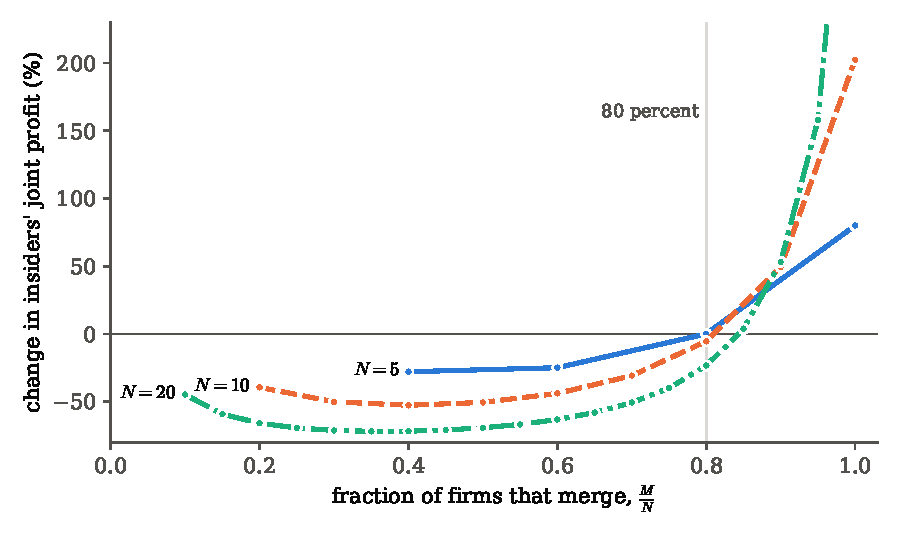
\includegraphics[width=0.8\textwidth]{figures/ch11/ssr_paradox.pdf}
\caption{The merger paradox. Percentage change in the joint profit of $M$ merging firms in a linear Cournot
market with $N$ symmetric firms and no cost savings, $100\big[\frac{(N + 1)^2}{M(N - M + 2)^2} - 1\big]$, against
$\frac{M}{N}$. Points above zero are profitable mergers. Curves are clipped at 230 percent.}
\label{fig:11-ssr}
\end{figure}

The reason is the response of the outsiders. In Cournot competition, quantities are strategic substitutes. When
the merged firm cuts its output, the outsiders expand theirs and capture much of the benefit of the higher price.
Moreover, a merger in this model is equivalent to $M - 1$ firms shutting down. The merged firm is no larger and no
more efficient than any other firm, so it ends up with a share of only $\frac{1}{N - M + 1}$
\citep[p.~4]{FarrellShapiro1988}. The paradox is that we observe many horizontal mergers.

Three features of the model drive the result, and relaxing any of them can overturn it. First, the merging firms
bring no assets. \citet{PerryPorter1985} let each firm own capital that lowers its marginal cost, so the merged
firm has the combined capital and is larger than its rivals. Mergers can then be profitable, and
\cref{sec:11-fs} develops this idea in general. Second, the model has no investment. \citet[Remark
3]{Pesendorfer2003} considers firms that hold capacity, with linear demand $P = a - bQ$, constant marginal cost
$c$, a linear cost $r$ per unit of new capacity, and initial capacities at Cournot levels. He also normalizes the
discount and depreciation factors. He shows that a merger
without cost savings is profitable whenever $n + 1 > \frac{a - c}{r}$. Building capacity is costly while scrapping
it is not, and this asymmetry favors the merged firm. The Salant-Switzer-Reynolds result is the limit as $r \to 0$
\citep[p.~7, n.~6]{Pesendorfer2003}. \Cref{sec:11-beyond} returns to this model. Third, quantities are strategic
substitutes. With price competition and differentiated products, rivals raise their prices after a merger, and
the merger is profitable (\cref{sec:11-upp}).

\subsection{Farrell and Shapiro (1990): mergers as transfers of capital}\label{sec:11-fs}

\casehead{The question}
\citet{FarrellShapiro1990} ask when a horizontal merger raises the price, when it raises welfare, and what a
regulator can infer from the fact that the merging firms want to merge. Their answer rests on three ideas. A merger
is a transfer of industry-specific capital from one firm to another. The welfare effect of a merger can be split
into the change in the merging firms' profits, which they internalize, and an \emph{external effect} on consumers
and rivals. The external effect depends only on observable market data, while the private effect may include
synergies that only the firms know. A regulator should therefore approve any merger that is proposed and has a
positive external effect, because private profitability then guarantees a welfare gain. We follow the 1988
working-paper version \citep{FarrellShapiro1988}, whose numbering of equations and propositions differs from the
published article. The result on the cost savings needed to lower the price belongs to the published article
\citep{FarrellShapiro1990} and is not in the working paper. We state it as \citet[pp.~216--217 and
229]{AskerNocke2021} report it, and we prove it in full.

\subsubsection{The model}

There are $N$ firms producing a homogeneous good, and their number is fixed by barriers to entry. A competitive
fringe can be absorbed into the demand curve, which is then a residual demand. We write $q_i$ for firm $i$'s
output, $Q = \sum_i q_i$ for industry output, $P(Q)$ for inverse demand and $s_i = \frac{q_i}{Q}$ for market
shares (Farrell and Shapiro write $x_i$, $X$ and $p(X)$).

\begin{assumption}[Cournot oligopoly with capital]\label{ass:11-fs}
\leavevmode
\begin{enumerate}[label=(\roman*)]
  \item Inverse demand $P(Q)$ is twice differentiable with $P'(Q) < 0$.
  \item Firm $i$ owns capital $k_i$ and has a twice differentiable cost function $C^i(q_i, k_i)$. More capital
  lowers marginal cost, $C^i_{qk} < 0$, where subscripts denote partial derivatives.
  \item Given the capital vector $k = (k_1, \dots, k_N)$, firms choose outputs simultaneously (Cournot). The
  equilibrium is unique and interior.
  \item Reaction functions slope down and the equilibrium is stable. Formally, at the equilibrium,
  $P' + q_i P'' < 0$ and $C^i_{qq} - P' > 0$ for every firm.
\end{enumerate}
\end{assumption}

Firms may have different technologies, and $C^i$ may then embody firm-specific assets that cannot be transferred.
Capital is industry specific and fixed in the short run, while outputs adjust quickly. Firm $i$ maximizes
$\pi_i = P(Q)\,q_i - C^i(q_i, k_i)$, with first-order condition
\begin{equation}\label{eq:11-fs-foc}
P(Q) + q_i P'(Q) - C^i_q(q_i, k_i) = 0, \qquad i = 1, \dots, N.
\end{equation}
The condition implies $P - C^i_q = -q_i P'$, so each firm's margin over marginal cost is proportional to its
output. Comparing two firms, $q_i > q_j$ if and only if $C^i_q < C^j_q$. In a Cournot equilibrium, \emph{larger
firms have lower marginal costs}. Whenever firms produce different quantities, marginal costs differ, so total
cost is not minimized for the industry's output. Shifting output toward large firms would lower it.

Welfare is consumers' gross benefit minus production costs,
\begin{equation*}
W = \int_0^Q P(z)\,\dd z - \sum_{i=1}^{N} C^i(q_i, k_i).
\end{equation*}

\subsubsection{Profit and welfare effects of a change in capital}

Consider a small change $\dd k = (\dd k_1, \dots, \dd k_N)$ in the allocation of capital, and the induced changes
$\dd q_i$ in outputs. Differentiating $\pi_i$,
\begin{equation}\label{eq:11-fs-dpi}
\dd\pi_i = (P - C^i_q)\,\dd q_i + q_i P'\,\dd Q - C^i_k\,\dd k_i .
\end{equation}
A firm gains from extra output in proportion to its margin, gains from a price increase in proportion to its
output, and saves costs through its own capital. Differentiating $W$ and using $\frac{\dd}{\dd Q}\int_0^Q P = P$,
\begin{equation}\label{eq:11-fs-dw}
\dd W = \sum_{i=1}^{N} (P - C^i_q)\,\dd q_i - \sum_{i=1}^{N} C^i_k\,\dd k_i .
\end{equation}
The first sum values each change in output at the gap between price and marginal cost. The second is the direct
effect of capital on costs at given outputs. Equations \eqref{eq:11-fs-dpi} and \eqref{eq:11-fs-dw} hold for any
theory of oligopoly. Under Cournot competition, $P - C^i_q = -q_i P'$, and \eqref{eq:11-fs-dw} becomes
\begin{equation}\label{eq:11-fs-dw-cournot}
\dd W = -P'\sum_{i=1}^{N} q_i\,\dd q_i - \sum_{i=1}^{N} C^i_k\,\dd k_i .
\end{equation}

\begin{lemma}[Welfare and the Herfindahl index]\label{lem:11-fs-hhi}
Under \cref{ass:11-fs},
\begin{equation}\label{eq:11-fs-dw-hhi}
\dd W = -P'\Big(\HHI\,Q\,\dd Q + \frac{1}{2}Q^2\,\dd\HHI\Big) - \sum_{i=1}^{N} C^i_k\,\dd k_i .
\end{equation}
\end{lemma}

\begin{proof}
Since $\HHI = \sum_i \big(\frac{q_i}{Q}\big)^2$, we have $Q^2\HHI = \sum_i q_i^2$. Differentiating both sides,
\begin{equation*}
2\sum_i q_i\,\dd q_i = \dd\big(Q^2\HHI\big) = 2\HHI\,Q\,\dd Q + Q^2\,\dd\HHI .
\end{equation*}
Dividing by two and substituting into \eqref{eq:11-fs-dw-cournot} gives \eqref{eq:11-fs-dw-hhi}.
\end{proof}

\Cref{lem:11-fs-hhi} splits a welfare change into three parts: a change in industry output, a change in its
distribution, and the direct effect on costs. More output raises welfare because price exceeds marginal cost.
More surprisingly, for a given change in output, a larger increase in the Herfindahl index raises welfare more,
since $-P' > 0$. Large firms have the lowest marginal costs, so shifting output toward them saves resources. Any
analysis that treats increases in concentration as bad per se is therefore misleading under Cournot competition
\citep[p.~8]{FarrellShapiro1988}.

\subsubsection{Comparative statics}

\begin{lemma}[Output responses]\label{lem:11-fs-statics}
Under \cref{ass:11-fs}, define for each firm
\begin{equation}\label{eq:11-fs-lambda}
\lambda_i = \frac{-P' - q_i P''}{C^i_{qq} - P'} > 0,
\qquad
\chi_i = \frac{-C^i_{qk}}{C^i_{qq} - P'} > 0,
\qquad
\Lambda = \sum_{i=1}^{N}\lambda_i .
\end{equation}
A small change $\dd k$ changes outputs by
\begin{equation}\label{eq:11-fs-dq}
\dd q_i = -\lambda_i\,\dd Q + \chi_i\,\dd k_i,
\qquad
\dd Q = \frac{1}{1 + \Lambda}\sum_{i=1}^{N}\chi_i\,\dd k_i .
\end{equation}
\end{lemma}

\begin{proof}
Totally differentiate the first-order condition \eqref{eq:11-fs-foc}, holding the equilibrium:
\begin{equation*}
\big(P' + q_i P''\big)\,\dd Q + P'\,\dd q_i - C^i_{qq}\,\dd q_i - C^i_{qk}\,\dd k_i = 0 .
\end{equation*}
Collect the terms in $\dd q_i$:
\begin{equation*}
\big(C^i_{qq} - P'\big)\,\dd q_i = \big(P' + q_i P''\big)\,\dd Q - C^i_{qk}\,\dd k_i .
\end{equation*}
Dividing by $C^i_{qq} - P' > 0$ gives the first part of \eqref{eq:11-fs-dq}. Signs follow from part (iv) of
\cref{ass:11-fs} and from $C^i_{qk} < 0$. Summing over $i$,
\begin{equation*}
\dd Q = -\Lambda\,\dd Q + \sum_i \chi_i\,\dd k_i ,
\end{equation*}
and solving for $\dd Q$ gives the second part.
\end{proof}

The coefficient $\chi_i$ is the \emph{direct effect} of firm $i$'s capital on its output at a given industry
output (Farrell and Shapiro call it $\delta_i$). The coefficient $\lambda_i$ measures how firm $i$ responds to a
change in industry output, and hence to the price. A firm whose capital does not change adjusts its output by
$\dd q_i = -\lambda_i\,\dd Q$. Its response to the combined output of the others, $Q_{-i}$, follows from
$\dd Q = \dd q_i + \dd Q_{-i}$ and is $\frac{\dd q_i}{\dd Q_{-i}} = -\frac{\lambda_i}{1 + \lambda_i}$. Two special
cases recur. With constant marginal cost, $C^i_{qq} = 0$ and
\begin{equation}\label{eq:11-fs-lambda-const}
\lambda_i = \frac{-P' - q_i P''}{-P'} = 1 + \frac{q_i P''}{P'} = 1 - s_i\,\mathcal{E},
\qquad
\mathcal{E} = -\frac{Q P''(Q)}{P'(Q)},
\end{equation}
where $\mathcal{E}$ is the elasticity of the slope of inverse demand (Farrell and Shapiro write $E$). With linear
demand $P = a - Q$ and the cost function $C(q, k) = \frac{q^2}{2k}$, we have $C_{qq} = \frac{1}{k}$ and
$P' = -1$, so $\lambda_i = \frac{1}{1 + \frac{1}{k_i}} = \frac{k_i}{1 + k_i}$.

\begin{example}[Two technologies]\label{ex:11-fs-tech}
\emph{Physical capital.} Let $P(Q) = a - Q$ and $C(q, k) = \frac{q^2}{2k}$ for all firms. This technology has
constant returns to scale and corresponds to the production function $q = \sqrt{kv}$ with a variable input $v$.
Firm $i$'s first-order condition is $a - Q - q_i - \frac{q_i}{k_i} = 0$. Define the \emph{adjusted capital}
$\tilde k_i = \frac{k_i}{1 + k_i}$. The condition becomes
\begin{equation*}
q_i\Big(1 + \frac{1}{k_i}\Big) = a - Q
\quad\Longrightarrow\quad
q_i = (a - Q)\,\tilde k_i = P\,\tilde k_i .
\end{equation*}
Summing over firms, $Q = (a - Q)\tilde K$ with $\tilde K = \sum_i \tilde k_i$, so
\begin{equation*}
Q = \frac{a\tilde K}{1 + \tilde K}, \qquad P = \frac{a}{1 + \tilde K}, \qquad
C^i_q = \frac{q_i}{k_i} = \frac{P}{1 + k_i} .
\end{equation*}
Firms with more capital produce more and have lower marginal costs. Here $\lambda_i = \tilde k_i = \frac{q_i}{P}$,
and the direct effect is
\begin{equation*}
\chi_i = \frac{\frac{q_i}{k_i^2}}{\frac{1}{k_i} + 1} = \frac{q_i}{k_i(1 + k_i)} = \frac{P}{(1 + k_i)^2} .
\end{equation*}
\emph{Know-how.} Let unit cost depend on capital but not on output, $C(q, k) = q\,\phi(k)$ with $\phi' < 0$. This
fits patents, know-how and managerial talent, which can be applied to any scale of output. The first-order
conditions are $P + q_i P' = \phi(k_i)$, and summing them gives
\begin{equation}\label{eq:11-fs-knowhow}
N P(Q) + Q P'(Q) = \sum_{i=1}^{N}\phi(k_i),
\end{equation}
so industry output depends on capital only through the sum of marginal costs.
\end{example}

\subsubsection{Investment by one firm}

Before turning to mergers, consider investment, $\dd k = (\dd k_1, 0, \dots, 0)$. By \cref{lem:11-fs-statics},
\begin{equation*}
\frac{\dd Q}{\dd k_1} = \frac{\chi_1}{1 + \Lambda}, \qquad
\frac{\dd q_i}{\dd k_1} = -\frac{\lambda_i\chi_1}{1 + \Lambda}\ (i \ne 1), \qquad
\frac{\dd q_1}{\dd k_1} = \chi_1\Big(1 - \frac{\lambda_1}{1 + \Lambda}\Big).
\end{equation*}
The investing firm expands, its rivals contract, and industry output rises. Subtracting \eqref{eq:11-fs-dw} from
\eqref{eq:11-fs-dpi} for $i = 1$, the private and social returns differ by
\begin{equation}\label{eq:11-fs-invest-wedge0}
\dd\pi_1 - \dd W = q_1 P'\,\dd Q - \sum_{i \ne 1}(P - C^i_q)\,\dd q_i .
\end{equation}
The first term is a private loss that is a transfer to consumers: the investor's price falls on its own sales. The
second is a social cost the investor ignores: rivals, whose price exceeds marginal cost, cut their output. Using
$P - C^i_q = -q_i P'$ and $\dd q_i = -\lambda_i\,\dd Q$ for $i \ne 1$,
\begin{equation}\label{eq:11-fs-invest-wedge}
\frac{\dd\pi_1}{\dd k_1} - \frac{\dd W}{\dd k_1}
= -P'\,\frac{\dd Q}{\dd k_1}\Big(\sum_{i \ne 1}\lambda_i q_i - q_1\Big).
\end{equation}

\begin{proposition}[Investment incentives]\label{prop:11-fs-invest}
Under \cref{ass:11-fs}, firm 1 has an excessive incentive to invest, $\frac{\dd\pi_1}{\dd k_1} >
\frac{\dd W}{\dd k_1}$, if and only if
\begin{equation}\label{eq:11-fs-invest}
s_1 < \sum_{i \ne 1}\lambda_i s_i .
\end{equation}
With linear demand and the costs $\frac{q^2}{2k}$, the condition is $s_1 < \frac{1}{\varepsilon}\sum_{i \ne 1}s_i^2$,
where $\varepsilon = -\frac{P}{QP'}$. With constant marginal costs, it is
$s_1 < \frac{1}{2} - \frac{\mathcal{E}}{2}\sum_{i \ne 1}s_i^2$.
\end{proposition}

\begin{proof}
In \eqref{eq:11-fs-invest-wedge}, $-P' > 0$ and $\frac{\dd Q}{\dd k_1} > 0$, so the wedge is positive if and only
if $\sum_{i \ne 1}\lambda_i q_i > q_1$. Dividing by $Q$ gives \eqref{eq:11-fs-invest}. In the quadratic case,
$\lambda_i = \frac{q_i}{P}$, so $\sum_{i \ne 1}\lambda_i s_i = \frac{Q}{P}\sum_{i \ne 1}s_i^2$, and
$\frac{Q}{P} = \frac{1}{\varepsilon}$ because $P' = -1$. With constant marginal costs,
$\sum_{i \ne 1}(1 - s_i\mathcal{E})s_i = 1 - s_1 - \mathcal{E}\sum_{i \ne 1}s_i^2$, and the inequality
$s_1 < 1 - s_1 - \mathcal{E}\sum_{i \ne 1}s_i^2$ rearranges to the stated form.
\end{proof}

Small firms invest too much. Their investment lowers the price and helps consumers, but it steals valuable
business from larger rivals with high margins, and the second effect dominates \citep[pp.~10--11]{FarrellShapiro1988}.
If $\lambda_i$ rises with firm size, as in the quadratic case, large efficient firms invest too little.

\subsubsection{Small capital transfers and the price}

A merger moves capital from one firm to another. Consider a small transfer from firm 2 to firm 1,
$\dd k_1 = \dd k = -\dd k_2 > 0$, with $k_1 > k_2$, so that the transfer increases the concentration of capital.
A complete merger of the two firms is the accumulation of such transfers, from $(k_1, k_2)$ to $(k_1 + k_2, 0)$.
Divestitures are the reverse.

\begin{proposition}[Price effect of a transfer]\label{prop:11-fs-price}
Under \cref{ass:11-fs}, a small transfer of capital from firm 2 to firm 1 changes industry output by
\begin{equation}\label{eq:11-fs-dqdk}
\frac{\dd Q}{\dd k} = \frac{\chi_1 - \chi_2}{1 + \Lambda}.
\end{equation}
It reduces output and raises the price if and only if $\chi_1 < \chi_2$, that is, if and only if the direct
output effect of capital is smaller at the acquiring firm.
\end{proposition}

\begin{proof}
Substitute $\dd k_1 = \dd k$, $\dd k_2 = -\dd k$ and $\dd k_i = 0$ for $i \ge 3$ into \eqref{eq:11-fs-dq}. Since
$1 + \Lambda > 0$, the sign of $\dd Q$ is the sign of $\chi_1 - \chi_2$.
\end{proof}

In the physical-capital example, $\chi_i = \frac{P}{(1 + k_i)^2}$ falls with $k_i$, so every
concentration-increasing transfer raises the price. The same follows from the closed form $P = \frac{a}{1 + \tilde
K}$. Adjusted capital $\tilde k(k) = \frac{k}{1 + k}$ is strictly concave with $\tilde k(0) = 0$, so moving capital
from the smaller to the larger firm lowers $\tilde k_1 + \tilde k_2$, and a complete merger gives
$\tilde k(k_1 + k_2) < \tilde k(k_1) + \tilde k(k_2)$. In the know-how example, \eqref{eq:11-fs-knowhow} shows
that output falls if and only if the transfer raises $\sum_i\phi(k_i)$, and the transfer changes this sum by
$\big(\phi'(k_1) - \phi'(k_2)\big)\dd k$. With $k_1 > k_2$, the price rises if and only if $\phi'' > 0$. A merger of
know-how raises the price when units of know-how are substitutes, which lower unit cost at a diminishing rate. It
lowers the price when they are complements.

\Cref{prop:11-fs-price} needs the $\chi_i$, which are hard to measure. A condition on the technology alone is more
useful.

\begin{proposition}[A sufficient condition, \citealp{FarrellShapiro1988}]\label{prop:11-fs-convex}
Suppose that, in addition to \cref{ass:11-fs}, all firms share the cost function $C(q, k)$ and the marginal cost
$C_q$ is jointly convex in $(q, k)$. Then every concentration-increasing transfer, small or large, weakly reduces
output and weakly raises the price, as long as the selling firm remains active. The effects are strict when the Hessian
of $C_q$ is positive definite.
\end{proposition}

\begin{proof}
Fix industry output $Q$, and let $\tilde q(Q, k)$ be the output of a firm with capital $k$ that satisfies the
first-order condition, $P(Q) + \tilde q P'(Q) = C_q(\tilde q, k)$. Because the technology is common, firm $i$'s output in
equilibrium is $\tilde q(Q, k_i)$ and its direct effect is $\chi_i = \tilde q_k(Q, k_i)$. To see this, differentiate the
condition in $k$ at fixed $Q$:
\begin{equation*}
P'\,\tilde q_k = C_{qq}\,\tilde q_k + C_{qk}
\quad\Longrightarrow\quad
\tilde q_k = \frac{-C_{qk}}{C_{qq} - P'} = \chi .
\end{equation*}
Differentiating once more in $k$,
\begin{equation*}
P'\,\tilde q_{kk} = C_{qqq}\,\tilde q_k^2 + 2C_{qqk}\,\tilde q_k + C_{qkk} + C_{qq}\,\tilde q_{kk},
\end{equation*}
so
\begin{equation*}
\tilde q_{kk} = -\frac{C_{qqq}\,\tilde q_k^2 + 2C_{qqk}\,\tilde q_k + C_{qkk}}{C_{qq} - P'} .
\end{equation*}
The numerator is $\gamma^\top H\gamma$ with $\gamma = (\tilde q_k, 1)^\top$ and $H$ the Hessian of $C_q$. Joint
convexity makes it nonnegative, so $\tilde q_{kk} \le 0$ and $\chi = \tilde q_k$ is nonincreasing in $k$ across firms.
Hence $k_1 > k_2$ implies $\chi_1 \le \chi_2$, and \cref{prop:11-fs-price} applies. A positive definite Hessian
makes the numerator positive, because $\gamma \ne 0$, and then $\chi_1 < \chi_2$. A large transfer is a sequence of small transfers, each from the smaller to the larger firm,
so output falls along the whole path.
\end{proof}

Farrell and Shapiro add that the condition is sufficient but not necessary. The physical-capital technology
violates it, since its marginal cost $\frac{q}{k}$ is not jointly convex, yet every merger raises the price there.
The know-how technology satisfies it exactly when $\phi'' \ge 0$, since $C_q = \phi(k)$. Its Hessian is
singular, yet the numerator in the proof equals $\phi''(k)$, so the price rises strictly when $\phi'' > 0$. Under the conditions of
\cref{prop:11-fs-price,prop:11-fs-convex}, a merger harms consumers. Because rivals' profits rise exactly when the
price rises, the same conditions tell us when rivals gain \citep[p.~15]{FarrellShapiro1988}.

\subsubsection{Discrete mergers and the synergies needed to lower the price}

A merger can also reorganize production or create synergies that a reallocation of existing capital cannot
capture. To study such mergers, we replace capital by constant marginal costs. Firm $i$ has marginal cost $c_i$.
Firms 1 and 2 merge, and the merged firm has marginal cost $c_M$, which summarizes its post-merger technology. A
merger with no synergies can at best produce everything at the lower of the two costs, $c_M = \min\{c_1, c_2\}$.
We write $P^0 = P(Q^0)$ for the pre-merger price.

\begin{proposition}[Synergies needed to lower the price, \citealp{FarrellShapiro1990}]\label{prop:11-synergy}
Suppose firms have constant marginal costs, $P'(Q) + qP''(Q) < 0$ for all $0 \le q \le Q$, and all firms are active
before and after the merger. The merger of firms 1 and 2 lowers the equilibrium price if and only if
\begin{equation}\label{eq:11-synergy}
c_M < \hat c \equiv c_1 + c_2 - P^0,
\quad\text{equivalently}\quad
P^0 - c_M > (P^0 - c_1) + (P^0 - c_2).
\end{equation}
It leaves the price unchanged if $c_M = \hat c$ and raises it if $c_M > \hat c$.
\end{proposition}

\begin{proof}
Summing the first-order conditions $P + q_i P' = c_i$ over the $n$ active firms gives the aggregate condition
\begin{equation*}
\Gamma_n(Q) \equiv nP(Q) + QP'(Q) = \sum_{i \text{ active}} c_i .
\end{equation*}
Its slope is $\Gamma_n'(Q) = P' + \sum_{i}\big(P' + q_i P''\big) < 0$, so $\Gamma_n$ is strictly decreasing and
the equilibrium output is the unique solution. Only the number of firms and the sum of their marginal costs
matter for $Q$. Before the merger,
\begin{equation*}
N P^0 + Q^0 P'(Q^0) = c_1 + c_2 + \sum_{i \ge 3} c_i .
\end{equation*}
After the merger there are $N - 1$ firms, and the post-merger output $Q^1$ solves
$\Gamma_{N-1}(Q^1) = c_M + \sum_{i \ge 3}c_i$. Evaluate $\Gamma_{N-1}$ at the pre-merger output and use the
pre-merger condition:
\begin{equation*}
\Gamma_{N-1}(Q^0) = N P^0 + Q^0 P'(Q^0) - P^0 = c_1 + c_2 - P^0 + \sum_{i \ge 3}c_i .
\end{equation*}
Since $\Gamma_{N-1}$ is decreasing, $Q^1 > Q^0$ if and only if
$\Gamma_{N-1}(Q^1) < \Gamma_{N-1}(Q^0)$, that is, if and only if
\begin{equation*}
c_M + \sum_{i \ge 3}c_i < c_1 + c_2 - P^0 + \sum_{i \ge 3}c_i
\quad\Longleftrightarrow\quad
c_M < c_1 + c_2 - P^0 .
\end{equation*}
A higher output means a lower price. The cases of equality and of the reverse inequality follow the same way.
\end{proof}

\begin{corollary}[No synergies, higher price]\label{prop:11-nosynergy}
Under the conditions of \cref{prop:11-synergy}, the price-neutral cost satisfies $\hat c < \min\{c_1, c_2\}$.
Any merger with $c_M \ge \min\{c_1, c_2\}$, including every merger that only rationalizes production, raises the
price.
\end{corollary}

\begin{proof}
Firm 2 is active before the merger, so $P^0 - c_2 = -q_2 P'(Q^0) > 0$. Hence
$\hat c = c_1 - (P^0 - c_2) < c_1$. By the same argument with the roles reversed, $\hat c < c_2$. If
$c_M \ge \min\{c_1, c_2\}$, then $c_M > \hat c$, and \cref{prop:11-synergy} applies.
\end{proof}

The required synergy is large. Let firm 1 be the more efficient partner. The merged firm's cost must fall below
$c_1$ by firm 2's entire margin, $c_1 - \hat c = P^0 - c_2$. As a fraction of the price, the reduction equals firm
2's Lerner index, $\frac{c_1 - \hat c}{P^0} = \frac{s_2}{\varepsilon}$. As a fraction of firm 1's cost it is
$\frac{L_2}{1 - L_1}$, where $L_i = \frac{P^0 - c_i}{P^0}$. Two firms with 20 percent shares each, facing a market
elasticity of one, have $L_1 = L_2 = 0.2$. For their merger not to raise the price, marginal cost must fall by
$\frac{0.2}{0.8} = 25$ percent.

The required reduction can also be written with the naive change in concentration. Let $s_I = s_1 + s_2$ and let
$\bar c = \frac{s_1 c_1 + s_2 c_2}{s_I}$ be the partners' share-weighted marginal cost. The first-order conditions
give $P^0 - c_i = \frac{s_i P^0}{\varepsilon}$, so
\begin{align*}
P^0 - \bar c &= \frac{s_1(P^0 - c_1) + s_2(P^0 - c_2)}{s_I} = \frac{s_1^2 + s_2^2}{s_I}\cdot\frac{P^0}{\varepsilon},\\
P^0 - \hat c &= (P^0 - c_1) + (P^0 - c_2) = s_I\,\frac{P^0}{\varepsilon}.
\end{align*}
Subtracting the first line from the second,
\begin{equation}\label{eq:11-required-dhhi}
\frac{\bar c - \hat c}{P^0} = \frac{1}{\varepsilon}\Big(s_I - \frac{s_1^2 + s_2^2}{s_I}\Big)
= \frac{(s_1 + s_2)^2 - s_1^2 - s_2^2}{\varepsilon\, s_I} = \frac{2 s_1 s_2}{\varepsilon\, s_I} .
\end{equation}
The numerator is the naive $\Delta\HHI$ of \eqref{eq:11-dhhi}. The outsiders' shares do not enter, so for given
shares of the merging firms the required efficiency does not depend on the level of the index. This parallels the
finding of \citet{NockeWhinston2020}, reported in \cref{sec:11-hhi}, that required efficiencies track the change in
concentration and not its level. In the example above,
$\frac{2 \times 0.2 \times 0.2}{0.4} = 0.2$ of the price, which is 25 percent of $\bar c = 0.8 P^0$.

\Cref{prop:11-synergy} is the condition that \citet[Lemma 1 and eq.~(5)]{NockeWhinston2013} use to define a
\emph{CS-neutral merger}, one that leaves consumer surplus unchanged. In their notation, with acquirer 0 and
target $k$, the condition is $\bar c_k = c_k - \big[P(Q^0) - c_0\big]$, the same as \eqref{eq:11-synergy}. They also
note that such a merger is profitable. The argument is short.

\begin{corollary}[A price-neutral merger is profitable]\label{cor:11-neutral-profit}
Under the conditions of \cref{prop:11-synergy}, let $c_M = \hat c$. The merger leaves the price and every
outsider's output unchanged and gives the merged firm the output $q_1 + q_2$. It raises the joint profit of the
merging firms by $(P^0 - c_1)q_2 + (P^0 - c_2)q_1 > 0$.
\end{corollary}

\begin{proof}
With $c_M = \hat c$, \cref{prop:11-synergy} gives $Q^1 = Q^0$, so the price and its slope are unchanged. Each
outsider's first-order condition $P + q_i P' = c_i$ then gives the same $q_i$. The merged firm produces the rest,
$Q^0 - \sum_{i \ge 3}q_i = q_1 + q_2$. Its profit is
\begin{align*}
(P^0 - \hat c)(q_1 + q_2)
&= \big[(P^0 - c_1) + (P^0 - c_2)\big](q_1 + q_2) \\
&= \underbrace{(P^0 - c_1)q_1 + (P^0 - c_2)q_2}_{\pi_1 + \pi_2} + (P^0 - c_1)q_2 + (P^0 - c_2)q_1 .
\end{align*}
Both extra terms are positive because both firms were active.
\end{proof}

\Cref{fig:11-synergy} illustrates these results. Demand is $P = 10 - Q$ and three firms have costs
$(c_1, c_2, c_3) = (2, 3, 3)$, so $P^0 = 4.5$ and outputs are $(2.5, 1.5, 1.5)$. If firms 1 and 2 merge, the
post-merger price is $\frac{13 + c_M}{3}$. The price-neutral cost is $\hat c = 2 + 3 - 4.5 = 0.5$, well below
$c_1 = 2$. Rationalization alone, $c_M = 2$, raises the price to 5. This merger is still profitable, because the
merged firm earns 9 against the 8.5 the two firms earned before. It lowers total surplus by 0.375, as consumers
lose 2.625 while the outsider gains 1.75. Every cost between 0.5 and about 2.13 makes the merger both profitable
and price-increasing. Total surplus rises only for costs below about 1.91.

\begin{figure}[htbp]
\centering
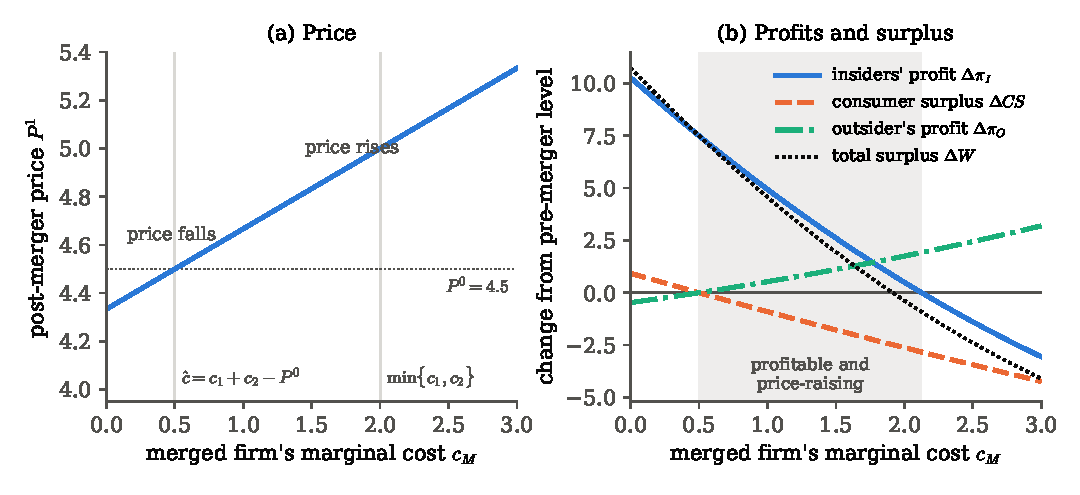
\includegraphics[width=\textwidth]{figures/ch11/cournot_synergy.pdf}
\caption{A Cournot merger with constant marginal costs. Demand $P = 10 - Q$, costs $(c_1, c_2, c_3) = (2, 3, 3)$,
and firms 1 and 2 merge with marginal cost $c_M$. Panel (a) shows the post-merger price, with the price-neutral cost
$\hat c = 0.5$ and the rationalization cost $\min\{c_1, c_2\} = 2$. Panel (b) shows the changes in the insiders'
joint profit, consumer surplus, the outsider's profit and total surplus. The shaded band, $0.5 < c_M < 2.13$, contains
the mergers that are profitable and raise the price. Total surplus falls for $c_M > 1.91$.}
\label{fig:11-synergy}
\end{figure}

\subsubsection{General costs, many partners and aggregate surplus}

\Cref{prop:11-synergy} assumes constant marginal costs and two partners. \citet[p.~229, eq.~(6)]{AskerNocke2021}
state the condition of \citet{FarrellShapiro1990} for any cost functions and any number of partners. We hold capital
fixed and write $C_i(q_i)$ for firm $i$'s cost function. A set $\mathcal{M}$ of at least two firms merges into a firm
with cost function $C_{\mathcal{M}}(q)$, and $q_{\mathcal{M}}^0 = \sum_{i \in \mathcal{M}} q_i^0$ is the partners'
combined pre-merger output.

\begin{proposition}[The synergy condition with general costs, \citealp{FarrellShapiro1990}]\label{prop:11-synergy-gen}
Let \cref{ass:11-fs} hold with capital fixed, let $C''_{\mathcal{M}} - P' > 0$, and let all firms be active before
and after the merger. The merger weakly raises industry output, and so does not lower consumer surplus, if and only
if
\begin{equation}\label{eq:11-an6}
P(Q^0) - C'_{\mathcal{M}}\big(q_{\mathcal{M}}^0\big) \;\ge\; \sum_{i \in \mathcal{M}}\big[P(Q^0) - C'_i(q_i^0)\big].
\end{equation}
It weakly lowers industry output if and only if the reverse weak inequality holds.
\end{proposition}

\begin{proof}
For a firm with cost function $C$, define its \emph{fitting-in output} $r(Q)$ as the solution in $q$ of $P(Q) +
qP'(Q) = C'(q)$. It is the output at which the firm's first-order condition holds when industry output is $Q$. The
left side minus the right side falls in $q$ at rate $P' - C'' < 0$, so $r(Q)$ is unique. Differentiating the
condition in $Q$,
\begin{equation*}
P' + r'P' + rP'' = C''r'
\quad\Longrightarrow\quad
r'(Q) = \frac{P' + rP''}{C'' - P'} = -\lambda ,
\end{equation*}
with $\lambda > 0$ the response coefficient of \cref{lem:11-fs-statics}. An equilibrium is an industry output at
which the fitting-in outputs add up to $Q$. After the merger, let
\begin{equation*}
\Phi(Q) = \sum_{i \notin \mathcal{M}} r_i(Q) + r_{\mathcal{M}}(Q) - Q .
\end{equation*}
It is strictly decreasing, with slope $-\sum_{i \notin \mathcal{M}}\lambda_i - \lambda_{\mathcal{M}} - 1 < 0$, so
the post-merger output $Q^1$ is its unique zero, and $Q^1 \ge Q^0$ if and only if $\Phi(Q^0) \ge 0$. At $Q^0$ each
outsider's fitting-in output is its pre-merger output, $r_i(Q^0) = q_i^0$. Hence
\begin{equation*}
\Phi(Q^0) = \sum_{i \notin \mathcal{M}} q_i^0 + r_{\mathcal{M}}(Q^0) - Q^0 = r_{\mathcal{M}}(Q^0) - q_{\mathcal{M}}^0 .
\end{equation*}
The merged firm's marginal profit at fixed $Q^0$, $P(Q^0) + qP'(Q^0) - C'_{\mathcal{M}}(q)$, falls in $q$ and is
zero at $r_{\mathcal{M}}(Q^0)$. So $r_{\mathcal{M}}(Q^0) \ge q_{\mathcal{M}}^0$ if and only if the marginal profit
is nonnegative at $q_{\mathcal{M}}^0$:
\begin{equation*}
P(Q^0) + q_{\mathcal{M}}^0P'(Q^0) - C'_{\mathcal{M}}\big(q_{\mathcal{M}}^0\big) \ge 0 .
\end{equation*}
The partners' pre-merger first-order conditions give $q_i^0P'(Q^0) = -\big[P(Q^0) - C'_i(q_i^0)\big]$. Summing over
$i \in \mathcal{M}$,
\begin{equation*}
q_{\mathcal{M}}^0P'(Q^0) = -\sum_{i \in \mathcal{M}}\big[P(Q^0) - C'_i(q_i^0)\big] .
\end{equation*}
Substituting into the marginal profit gives \eqref{eq:11-an6}. The reverse case follows from the same steps with
the inequalities reversed.
\end{proof}

With constant marginal costs and two partners, \eqref{eq:11-an6} is \eqref{eq:11-synergy}. Every term on the right of
\eqref{eq:11-an6} is positive, because each partner was active. The right side therefore exceeds each single term
$P(Q^0) - C'_j(q_j^0)$. The condition thus requires the merged firm's marginal cost at the combined output to lie
below the pre-merger marginal cost of every partner, $C'_{\mathcal{M}}(q_{\mathcal{M}}^0) < \min_{i \in
\mathcal{M}}C'_i(q_i^0)$ \citep[p.~229]{AskerNocke2021}.

A merger can raise productive efficiency even without synergies, in the sense of \citet{FarrellShapiro1990}. Say
the merger creates \emph{no synergies} when the merged firm can do no better than allocate output among the
partners' existing technologies,
\begin{equation}\label{eq:11-nosynergy-cost}
C_{\mathcal{M}}(q) = \min\Big\{\sum_{i \in \mathcal{M}}C_i(q_i) : \sum_{i \in \mathcal{M}}q_i = q,\ q_i \ge 0\Big\}.
\end{equation}
By the pre-merger first-order conditions, $P - C'_i(q_i^0) = -q_i^0P'$, so the smaller partner has the higher
marginal cost. Shifting output from it to the larger partner lowers the cost of producing $q_{\mathcal{M}}^0$. The
next result shows that such output shifting is not enough.

\begin{corollary}[Rationalization is not enough]\label{cor:11-rationalize}
Under the conditions of \cref{prop:11-synergy-gen}, suppose every $C_i$ is convex and the merger creates no
synergies, as in \eqref{eq:11-nosynergy-cost}. Then the merger strictly lowers industry output and consumer surplus.
\end{corollary}

\begin{proof}
Let $(q_i^*)_{i \in \mathcal{M}}$ solve the problem in \eqref{eq:11-nosynergy-cost} at $q = q_{\mathcal{M}}^0$. By
the envelope theorem, $C'_{\mathcal{M}}(q_{\mathcal{M}}^0)$ equals the multiplier on the output constraint, which
equals $C'_i(q_i^*)$ for every partner with $q_i^* > 0$. The $q_i^*$ add up to $\sum_{i \in \mathcal{M}}q_i^0$, so
some partner $j$ has $q_j^* \ge q_j^0 > 0$. Convexity of $C_j$ gives
\begin{equation*}
C'_{\mathcal{M}}\big(q_{\mathcal{M}}^0\big) = C'_j(q_j^*) \ge C'_j(q_j^0) \ge \min_{i \in \mathcal{M}}C'_i(q_i^0) .
\end{equation*}
This violates the necessary condition stated after \cref{prop:11-synergy-gen}, so \eqref{eq:11-an6} fails, the
reverse strict inequality holds, and $Q^1 < Q^0$.
\end{proof}

The result extends to multiproduct firms that compete in prices under logit, nested logit or CES demand.
\citet{NockeSchutz2018,NockeSchutz2019} show that each firm can then be summarized by a single number, its
\emph{type}, which measures its contribution to consumer surplus if it priced at cost. Without synergies the merged
firm's type is the sum of the partners' types. A merger does not lower consumer surplus if and only if the merged
firm's type exceeds a cutoff above that sum, so it again requires synergies \citep[p.~229]{AskerNocke2021}.

\begin{figure}[htbp]
\centering
\begin{tikzpicture}[x=1.5cm, y=1.25cm, font=\small]
  \fill[gray!22] (0,4.25) -- (0,4.5) -- (5.5,4.5) -- (5.75,4.25) -- cycle;
  \fill[gray!60] (5.5,3.5) rectangle (5.75,4.25);
  \fill[pattern=north east lines, pattern color=black!65] (3.25,1) rectangle (3.5,2.5);
  \fill[pattern=north east lines, pattern color=black!65] (5.0,2.5) rectangle (5.5,3.5);
  \draw (3.25,1) rectangle (3.5,2.5);
  \draw (5.0,2.5) rectangle (5.5,3.5);
  \draw[->] (0,0) -- (7.4,0) node[below] {$Q$};
  \draw[->] (0,0) -- (0,5.6) node[left] {$p$};
  \draw[thick] (4.5,5.5) -- (7.2,2.8) node[right] {$P(Q)$};
  \draw (0,1) -- (6.9,1) node[right] {$c_1$};
  \draw (0,2.5) -- (6.9,2.5) node[right] {$c_2$};
  \draw (0,3.5) -- (6.9,3.5) node[right] {$c_3$};
  \draw[dashed] (0,4.25) -- (5.75,4.25);
  \draw[dashed] (0,4.5) -- (5.5,4.5);
  \node[left, font=\scriptsize] at (0,4.18) {$P^0$};
  \node[left, font=\scriptsize] at (0,4.6) {$P^1$};
  \foreach \x in {3.25,3.5,5.0,5.5,5.75} {\draw[dotted] (\x,0) -- (\x,4.5);}
  \node[below, font=\scriptsize] at (3.25,0) {$q_1^0$};
  \node[below, font=\scriptsize] at (3.5,-0.38) {$q_1^1$};
  \node[below, font=\scriptsize] at (5.0,0) {$q_1^0 + q_2^0$};
  \node[below, font=\scriptsize] at (5.5,-0.38) {$Q^1$};
  \node[below, font=\scriptsize] at (5.8,0) {$Q^0$};
\end{tikzpicture}
\caption{A Cournot merger without synergies, redrawn after \citet[Figure 6]{AskerNocke2021}. Demand is $P = 10 - Q$
and marginal costs are $c_1 = 1$, $c_2 = 2.5$ and $c_3 = 3.5$. Firms 2 and 3 merge and produce at $c_2$. The price
rises from $P^0 = 4.25$ to $P^1 = 4.5$, and output falls from $Q^0 = 5.75$ to $Q^1 = 5.5$. The light trapezoid is the
loss of consumer surplus (1.41). The dark rectangle is the margin lost on units that are no longer produced (0.19).
The hatched rectangles are cost savings, from output that moves to firm 1 (0.375) and from former firm-3 output now
produced at $c_2$ (0.5). Our computation.}
\label{fig:11-an-fig6}
\end{figure}

\Cref{fig:11-an-fig6} redraws the diagram that \citet[pp.~216--217]{AskerNocke2021} use to introduce merger analysis.
Firms 2 and 3 merge without synergies, so the merged firm produces at $c_2$. By \cref{prop:11-nosynergy} the price
rises. Firm 1 expands from $q_1^0 = 3.25$ to $q_1^1 = 3.5$, and the merged firm produces 2, less than the 2.5 that
firms 2 and 3 produced before. The welfare accounting has four pieces. Consumers lose the light trapezoid,
$(P^1 - P^0)Q^1 + \frac{1}{2}(P^1 - P^0)(Q^0 - Q^1) = 1.375 + 0.031$. The rectangle $(P^1 - P^0)Q^1$ is a transfer to
the firms, so only the triangle is a deadweight loss. The units between $Q^1$ and $Q^0$ were produced by firm 3 at
cost $c_3$, and their lost margin $(P^0 - c_3)(Q^0 - Q^1) = 0.1875$ is the dark rectangle. Production costs fall on
the remaining output, by $(c_2 - c_1)(q_1^1 - q_1^0) = 0.375$ and $(c_3 - c_2)\big(Q^1 - q_1^0 - q_2^0\big) = 0.5$.
Aggregate surplus therefore changes by
\begin{equation*}
\Delta W = -0.031 - 0.1875 + 0.375 + 0.5 = 0.656 > 0 .
\end{equation*}
Asker and Nocke leave the sign open for the case they draw, and they suggest that the reallocation gain may fall short
of the losses there (p.~216). With our numbers the reallocation gain dominates. The merger harms consumers, by 1.41, but raises aggregate surplus, because it moves production away from the least
efficient firm. It is also profitable, since the insiders gain 0.375. The price-neutral cost is $\hat c = c_2 + c_3 -
P^0 = 1.75$, so a merged firm with firm 1's cost of 1 would lower the price.

Two further results link consumer surplus, profit and aggregate surplus \citep[p.~230]{AskerNocke2021}. With
constant marginal costs, a merger that does not lower consumer surplus is profitable \citep{NockeWhinston2010}.
\Cref{cor:11-neutral-profit} shows this for the price-neutral merger, and a lower merged cost only raises the merged
firm's profit (\cref{lem:11-nw2}). A price-neutral merger leaves every outsider's output and profit unchanged, so it
raises aggregate surplus. The converse direction is less tidy. Aggregate surplus is not monotone in a firm's marginal
cost, so a given merger need not have a cutoff cost below which it raises aggregate surplus and above which it lowers
it. In the example of \cref{fig:11-synergy}, a cutoff does exist, near $c_M = 1.91$. Total surplus is still not
monotone. With the outsider's cost at 3, the derivative of total surplus in $c_M$ is
\begin{equation*}
\frac{\dd W}{\dd c_M} = (P - c_M)\frac{\dd q_M}{\dd c_M} + (P - 3)\frac{\dd q_3}{\dd c_M} - q_M
= -\frac{2}{3}q_M + \frac{1}{3}q_3 - q_M = \frac{q_3 - 5q_M}{3} .
\end{equation*}
It turns positive once the merged firm produces less than a fifth of the outsider's output, which happens for $c_M >
\frac{61}{11} \approx 5.55$. Total surplus then rises as the inefficient merged firm shrinks, although the merger
still lowers it. With logit or CES demand and price competition, by contrast, a unique cutoff type exists
\citep[n.~129]{AskerNocke2021}.

\subsubsection{The external effect of a merger}

We return to capital transfers and ask when a merger that the firms want also raises welfare. Write $I = \{1, 2\}$
for the insiders and $O = \{3, \dots, N\}$ for the outsiders, with combined insider share $s_I = s_1 + s_2$, and
$\pi_I = \pi_1 + \pi_2$. The \emph{external effect} of a transfer is its effect on everyone other than the
insiders, consumers and outsiders together. It equals $\dd W - \dd\pi_I$.

\begin{proposition}[The external effect]\label{prop:11-externality}
Under \cref{ass:11-fs}, a small transfer of capital from firm 2 to firm 1 has the external effect
\begin{equation}\label{eq:11-fs-ext}
\frac{\dd W}{\dd k} - \frac{\dd\pi_I}{\dd k} = \frac{\dd P}{\dd k}\,\varpi,
\qquad
\varpi \equiv \sum_{i \in O}\lambda_i q_i - \sum_{i \in I} q_i .
\end{equation}
If the transfer raises the price, the external effect is positive if and only if
\begin{equation}\label{eq:11-fs-ext-share}
s_I < \sum_{i \in O}\lambda_i s_i .
\end{equation}
\end{proposition}

\begin{proof}
Add up the gains of consumers and outsiders. Consumers lose $Q\,\dd P$. An outsider's capital does not change,
so by \eqref{eq:11-fs-dpi} its profit changes by $(P - C^i_q)\,\dd q_i + q_i\,\dd P$. Under Cournot,
$P - C^i_q = -q_i P'$, and by \cref{lem:11-fs-statics}, $\dd q_i = -\lambda_i\,\dd Q$. Hence
\begin{equation*}
(P - C^i_q)\,\dd q_i = (-q_i P')(-\lambda_i\,\dd Q) = \lambda_i q_i\,P'\,\dd Q = \lambda_i q_i\,\dd P .
\end{equation*}
The external effect is therefore
\begin{align*}
-Q\,\dd P + \sum_{i \in O}\big(\lambda_i q_i + q_i\big)\,\dd P
&= \Big(-\sum_{i \in I}q_i - \sum_{i \in O}q_i + \sum_{i \in O}q_i + \sum_{i \in O}\lambda_i q_i\Big)\dd P \\
&= \Big(\sum_{i \in O}\lambda_i q_i - \sum_{i \in I}q_i\Big)\dd P = \varpi\,\dd P .
\end{align*}
Dividing by $\dd k$ gives \eqref{eq:11-fs-ext}. If $\frac{\dd P}{\dd k} > 0$, the sign is that of $\varpi$, and
dividing $\varpi > 0$ by $Q$ gives \eqref{eq:11-fs-ext-share}.
\end{proof}

The proof shows where the external effect comes from. The price increase on outsiders' units is a transfer from
consumers to outsiders and cancels. Two terms remain. Consumers lose the price increase on the insiders' units,
$q_I\,\dd P$. The outsiders expand by $\lambda_i\,\dd Q$ and earn their margin $-q_i P'$ on the extra units, a gain
of $\lambda_i q_i\,\dd P$. The anticompetitive effect grows with the insiders' size, while the offsetting benefit
grows with the outsiders' responsiveness and margins. This \emph{induced output effect} is the welfare gain from
moving output toward large, low-cost outsiders. Farrell and Shapiro write \eqref{eq:11-fs-ext} as
$-\frac{\dd p}{\dd k}\big(x_1 + x_2 - \sum_{i \ge 3}\lambda_i x_i\big)$ (their eq.~(16)), and
they state the result as excessive incentives to merge when $s_1 + s_2 > \sum_{i \ge 3}\lambda_i s_i$ (their
Proposition 4).

The direct effects of capital on the insiders' costs appear in both $\dd W$ and $\dd\pi_I$, so they cancel from
the external effect. Synergies, fixed-cost savings and other benefits that only the merging firms observe do not
enter \eqref{eq:11-fs-ext}. The external effect depends on shares and on the responses $\lambda_i$, which an agency
can hope to estimate. This is the basis of a policy rule \citep[p.~18]{FarrellShapiro1988}. Since a proposed merger
must be privately profitable, $\dd\pi_I > 0$, a merger with a positive external effect raises welfare and should be
approved, whatever its unobserved synergies. A merger with a negative external effect should be allowed only if
it is sufficiently profitable, which shifts the burden of proof to the parties.

\begin{corollary}[Special cases]\label{cor:11-ext-cases}
Suppose the transfer raises the price.
\begin{enumerate}[label=(\roman*)]
  \item With constant marginal costs, $\lambda_i = 1 - s_i\mathcal{E}$, and the external effect has the sign of
  $1 - 2s_I - \mathcal{E}\sum_{i \in O}s_i^2$. With linear demand, $\mathcal{E} = 0$, the external effect is
  positive if and only if $s_I < \frac{1}{2}$.
  \item With linear demand and costs $\frac{q^2}{2k}$, $\lambda_i = \frac{q_i}{P}$, and the external effect is
  positive if and only if
  \begin{equation}\label{eq:11-fs-prop7}
  s_I < \frac{1}{\varepsilon}\sum_{i \in O}s_i^2 .
  \end{equation}
\end{enumerate}
\end{corollary}

\begin{proof}
For (i), $\sum_{i \in O}(1 - s_i\mathcal{E})s_i - s_I = (1 - s_I) - \mathcal{E}\sum_{i \in O}s_i^2 - s_I$. For (ii),
$\sum_{i \in O}\frac{q_i}{P}s_i = \frac{Q}{P}\sum_{i \in O}s_i^2 = \frac{1}{\varepsilon}\sum_{i \in O}s_i^2$, as in
the proof of \cref{prop:11-fs-invest}.
\end{proof}

The two cases point in opposite directions on one question. With quadratic costs, the external effect is more
likely to be positive when the outsiders are concentrated, because large outsiders respond strongly and earn high
margins \citep[Proposition 7]{FarrellShapiro1988}. With constant marginal costs and convex demand,
$\mathcal{E} > 0$, concentration among the outsiders makes a positive external effect less likely, because large
firms respond less to the price. Inelastic demand raises margins and so strengthens the induced output effect.
As an illustration of case (ii), suppose $\varepsilon = 1$ and two firms with 5 percent each merge, while two
outsiders hold 45 percent each. The right side of \eqref{eq:11-fs-prop7} is $2 \times 0.45^2 = 0.405$, far above
$s_I = 0.10$, so the external effect is positive. If instead two firms with 20 percent each merge and two outsiders
hold 30 percent each, the right side is $0.18 < 0.40$, and the external effect is negative.
\citet[p.~230]{AskerNocke2021} summarize Farrell and Shapiro as showing that a positive external effect is more
likely when the outsiders' combined share is larger and more concentrated. The first part holds in both cases of
\cref{cor:11-ext-cases}. The second holds in the quadratic case and fails with constant marginal costs and convex
demand.

The welfare effect also contains a direct cost term, $-C^1_k + C^2_k$ per unit transferred. One might expect it
to favor the merger, since capital lowers costs more at the larger firm. Farrell and Shapiro show the opposite
under constant returns to scale. In the cross-section of firms, the marginal saving from capital, $-C_k$, is
smaller at larger firms, so moving capital to them raises total cost at given outputs. In the physical-capital
example, $-C_k = \frac{1}{2}\big(\frac{q}{k}\big)^2 = \frac{1}{2}\big(\frac{P}{1 + k}\big)^2$, which indeed falls
with $k$. Any welfare gain from such a merger must come from the reallocation of output, the
$\frac{1}{2}Q^2\,\dd\HHI$ term in \cref{lem:11-fs-hhi}.

\subsubsection{The insiders' gain and two closed forms}

The external effect is the welfare change minus the insiders' gain, and Farrell and Shapiro also give the two pieces
separately \citep[pp.~18--22]{FarrellShapiro1988}. For an insider, \eqref{eq:11-fs-dpi} and the Cournot condition
$P - C^i_q = -q_iP'$ give
\begin{equation*}
\dd\pi_i = -P'q_i\,(\dd q_i - \dd Q) - C^i_k\,\dd k_i .
\end{equation*}
By \cref{lem:11-fs-statics}, $\dd q_i - \dd Q = -(1 + \lambda_i)\,\dd Q + \chi_i\,\dd k_i$. Substitute $\dd k_1 =
\dd k$, $\dd k_2 = -\dd k$ and $\dd Q$ from \eqref{eq:11-fs-dqdk}, and add the two insiders:
\begin{equation}\label{eq:11-fs-dpiI}
\frac{\dd\pi_I}{\dd k} = -P'\Big[\chi_1q_1 - \chi_2q_2 - \frac{\chi_1 - \chi_2}{1 + \Lambda}\big((1 + \lambda_1)q_1 +
(1 + \lambda_2)q_2\big)\Big] - C^1_k + C^2_k .
\end{equation}
This is their eq.~(15). The terms $\chi_iq_i$ are the direct output effects of the changed capital stocks. The term
in $\chi_1 - \chi_2$ is the induced output effect once all firms adjust, and the last two terms are the direct cost
effects. Suppose the firms also have fixed costs $F_i(k_i)$ that the agency cannot observe. Then
$-F_1'(k_1) + F_2'(k_2)$ enters both \eqref{eq:11-fs-dpiI} and $\frac{\dd W}{\dd k}$, so it cancels from the
external effect (p.~18).

\casehead{Quadratic costs}
With $P = a - Q$ and $C(q, k) = \frac{q^2}{2k}$, \cref{ex:11-fs-tech} gives $q_i = P\tilde k_i$, $\lambda_i = \tilde
k_i$, $\chi_i = \frac{P}{(1 + k_i)^2}$ and $\Lambda = \tilde K$. Three pieces of \eqref{eq:11-fs-dw-cournot}
simplify. Because $\HHI = \frac{\sum_iq_i^2}{Q^2} = \frac{\sum_i\tilde k_i^2}{\Lambda^2}$,
\begin{equation*}
\sum_i\lambda_iq_i = P\sum_i\tilde k_i^2 = P\,\HHI\,\Lambda^2,
\qquad
q_i\chi_i = \frac{P^2k_i}{(1 + k_i)^3},
\qquad
-C^i_k = \frac{q_i^2}{2k_i^2} = \frac{P^2}{2(1 + k_i)^2} .
\end{equation*}
With $P' = -1$, \eqref{eq:11-fs-dw-cournot} reads $\dd W = \sum_iq_i\,\dd q_i - \sum_iC^i_k\,\dd k_i$. Using
$\dd q_i = -\lambda_i\,\dd Q + \chi_i\,\dd k_i$,
\begin{equation*}
\frac{\dd W}{\dd k} = -\frac{\dd Q}{\dd k}\sum_i\lambda_iq_i + q_1\chi_1 - q_2\chi_2 - C^1_k + C^2_k,
\qquad
\frac{\dd Q}{\dd k} = \frac{P}{1 + \Lambda}\Big(\frac{1}{(1 + k_1)^2} - \frac{1}{(1 + k_2)^2}\Big).
\end{equation*}
Substituting the three pieces and dividing by $P^2$ gives their eq.~(18),
\begin{equation}\label{eq:11-fs-eq18}
\frac{1}{P^2}\frac{\dd W}{\dd k} = \Big(\frac{1}{(1 + k_2)^2} - \frac{1}{(1 + k_1)^2}\Big)
\Big(\frac{\HHI\,\Lambda^2}{1 + \Lambda} - \frac{1}{2}\Big) + \frac{k_1}{(1 + k_1)^3} - \frac{k_2}{(1 + k_2)^3} .
\end{equation}
With $k_1 > k_2$ the first factor is positive. Given the partners' capital, the welfare effect therefore rises with
$\frac{\HHI\Lambda^2}{1 + \Lambda}$, that is, with the industry's Herfindahl index and with its adjusted capital
$\Lambda$. This is their Proposition 5, the basis of lesson (ii) below. A concentrated industry has large outsiders,
and their expansion is worth the most. Farrell and Shapiro cite simulations by \citet{McAfeeWilliams1992}, a paper
they cite as a 1988 Department of Justice manuscript. In these simulations welfare rises when the participants'
shares are small (p.~20).\footnote{The same steps applied to
\eqref{eq:11-fs-dpiI} give $\frac{1}{P^2}\frac{\dd\pi_I}{\dd k} = \big(\frac{1}{(1 + k_2)^2} - \frac{1}{(1 +
k_1)^2}\big)\big(\frac{\tilde k_1 + \tilde k_2 + \tilde k_1^2 + \tilde k_2^2}{1 + \Lambda} - \frac{1}{2}\big) +
\frac{k_1}{(1 + k_1)^3} - \frac{k_2}{(1 + k_2)^3}$. The working paper prints the numerator of the first fraction as
$\tilde k_1^2 + \tilde k_2^2$ (p.~20). A numerical derivative confirms the version derived here
(figures/ch11/src/fs\_eq15\_18\_check.py).}

\casehead{Know-how}
With $C(q, k) = q\,\phi(k)$, marginal cost is $\phi(k_i)$, so $\lambda_i = 1 - s_i\mathcal{E}$, $\Lambda = N -
\mathcal{E}$ and $\chi_i = \frac{\phi'(k_i)}{P'} > 0$. The direct cost effect is $C^i_k = q_i\phi'(k_i)$, and
$\sum_i\lambda_iq_i = Q(1 - \mathcal{E}\,\HHI)$. In \eqref{eq:11-fs-dw-cournot}, the terms $-P'q_i\chi_i =
-q_i\phi'(k_i)$ add to the direct cost effects, and
\begin{align*}
\frac{\dd W}{\dd k}
&= -2q_1\phi'(k_1) + 2q_2\phi'(k_2) + \frac{Q(1 - \mathcal{E}\,\HHI)}{1 + N - \mathcal{E}}\big(\phi'(k_1) -
\phi'(k_2)\big) \\
&= 2Q\Big[\big(-\phi'(k_1)\big)(s_1 - \bar s) - \big(-\phi'(k_2)\big)(s_2 - \bar s)\Big],
\qquad
\bar s = \frac{1 - \mathcal{E}\,\HHI}{2(1 + N - \mathcal{E})} .
\end{align*}
A small transfer of know-how raises welfare if and only if $\big(-\phi'(k_1)\big)(s_1 - \bar s) >
\big(-\phi'(k_2)\big)(s_2 - \bar s)$ (p.~22, where $\bar s$ is written $\sigma$). With $\mathcal{E} > 0$, the
bound $\HHI \ge \frac{1}{N}$ gives $\bar s < \frac{1}{2N}$, so $s_1 > \bar s$ in the cases of interest. If
$\phi'' < 0$, units of know-how are complements, $-\phi'(k_1) > -\phi'(k_2)$, and every concentration-increasing
transfer raises welfare. If $\phi'' > 0$, the transfer raises welfare when firm 1 is much larger than firm 2 or when
its unit cost falls nearly as much as firm 2's rises.

\subsubsection{Large mergers}

A complete merger moves all of firm 2's capital to firm 1. Its external effect is the integral of
\eqref{eq:11-fs-ext} along the path from $(k_1, k_2)$ to $(k_1 + k_2, 0)$, as long as firm 2 stays active until its
last unit of capital is transferred. A sufficient condition is $C_q(0, k) = 0$ for all $k > 0$, which the
physical-capital technology satisfies. The question is what pre-merger data reveal about this integral.

\begin{proposition}[A one-way test, \citealp{FarrellShapiro1988}]\label{prop:11-fs-oneway}
Suppose every step of the transfer raises the price, firm 2 stays active until the end, and
$\frac{\dd(\lambda_i q_i)}{\dd k} \ge 0$ for every outsider along the path. If $\varpi \ge 0$ at the pre-merger
equilibrium, then every privately profitable merger between firms 1 and 2 raises welfare.
\end{proposition}

\begin{proof}
Along the path,
\begin{equation*}
\frac{\dd\varpi}{\dd k} = \sum_{i \in O}\frac{\dd(\lambda_i q_i)}{\dd k} - \frac{\dd(q_1 + q_2)}{\dd k} .
\end{equation*}
Industry output falls, $\frac{\dd Q}{\dd k} < 0$, and each outsider expands, since
$\dd q_i = -\lambda_i\,\dd Q > 0$. The insiders' joint output therefore falls by more than industry output,
$\frac{\dd(q_1 + q_2)}{\dd k} = \frac{\dd Q}{\dd k} - \sum_{i \in O}\frac{\dd q_i}{\dd k} < 0$. Both terms make
$\frac{\dd\varpi}{\dd k}$ positive, so $\varpi$ rises along the path and stays nonnegative. By
\cref{prop:11-externality}, the external effect of each step is $\frac{\dd P}{\dd k}\varpi \ge 0$, and so is its
integral. Welfare changes by the insiders' profit gain plus this external effect, and both are nonnegative, with
the first strictly positive.
\end{proof}

In the physical-capital example, an outsider's $\lambda_i = \frac{k_i}{1 + k_i}$ does not change during the merger,
and its output rises, so the condition of \cref{prop:11-fs-oneway} holds. Any profitable merger for which
\eqref{eq:11-fs-prop7} holds, or holds with equality, at the pre-merger equilibrium should therefore be approved
\citep[p.~24]{FarrellShapiro1988}. Farrell and Shapiro state the test through the reverse inequality, their
eq.~(19), which signals a negative external effect. In their wording, a merger that violates (19) should be approved.
Since $\varpi$ only rises during the merger, the test runs one way. If \eqref{eq:11-fs-prop7} fails strictly even at
the post-merger equilibrium, so that $s_I$ exceeds the right side, $\varpi$ was negative throughout and the external
effect is negative. If $\varpi$ is negative but small at the start, the complete merger may still have a positive
external effect. Farrell and Shapiro obtain the same one-way test with constant marginal costs and a constant
$\mathcal{E}$ between 1 and 2. If firm 2 would close down before all its capital is transferred, the remaining
transfer is investment by firm 1, which lowers the price, and \cref{prop:11-fs-invest} becomes relevant.

\subsubsection{Lessons for merger policy}

Farrell and Shapiro draw several lessons \citep[pp.~15, 20--21 and 25--26]{FarrellShapiro1988}.
\begin{enumerate}[label=(\roman*)]
  \item \emph{Rivals' complaints are a signal.} An outsider's profit changes by $(1 + \lambda_i)q_i\,\dd P$, which
  is positive exactly when the price rises. Rivals gain when consumers lose. A rival that opposes a merger by
  predicting higher prices may believe the opposite, and rivals should not have standing to block mergers.
  \item \emph{Rising concentration can raise welfare.} By \cref{lem:11-fs-hhi}, for a given change in output,
  welfare rises more when the Herfindahl index rises more. A high level of the index may be bad, but an increase
  can reflect output moving to efficient firms. With quadratic costs and linear demand, and given the merging
  firms' capital, a transfer raises welfare more readily when the industry's adjusted capital and Herfindahl index
  are larger (their Proposition 5).
  \item \emph{Small firms and large firms face opposite biases.} By \cref{prop:11-fs-invest,prop:11-externality},
  small firms tend to invest too much and to merge too little, while large firms tend to invest too little and
  to merge too much. Large firms should be free to invest, and their mergers should be scrutinized. Small firms
  should be free to merge, and their investments should be scrutinized.
  \item \emph{Mergers can come in waves.} With quadratic costs and linear demand, a merger by one pair raises the
  profitability of a merger by any other pair (their Proposition 6). Outside firms affect a pair's incentive only
  through the price and $\Lambda$, and another merger raises the price and lowers $\Lambda$. This is one
  mechanism behind the merger waves of \cref{sec:11-waves}.
  \item \emph{Rivals' responses are what matter.} The favorable induced output effect requires outsiders to
  expand. If outsiders instead cut output along with the merging firms, as under collusion or with differentiated
  products and price competition, the external effect is negative.
\end{enumerate}

\casehead{Assessment}
The analysis has clear limits. It assumes Cournot competition and rules out entry, product repositioning and
coordinated effects, and \cref{sec:11-freeentry} below allows entry. A merger that made collusion easier would
reverse its welfare conclusions, as the authors note. The responses $\lambda_i$ depend on the curvature of demand and of marginal cost, which are hard to estimate,
and the two special cases give opposite answers on the role of outsiders' concentration. The required-synergies
result is sobering for the merging parties. With realistic shares and elasticities, a Cournot merger lowers the
price only if marginal cost falls well below that of the more efficient partner.

The paper's contribution is lasting. It replaced the mechanical formula $2 s_A s_B$ with an equilibrium analysis
of concentration. It showed how private profitability can serve as a revealed signal of unobservable synergies, so
that policy can focus on the observable external effect. Its synergy condition is the starting point of the
analysis of merger policy with endogenous merger proposals by \citet{NockeWhinston2013}, which
\cref{sec:11-policy} develops. Its warning that the results hinge on rivals' responses leads to \cref{sec:11-upp}.
\citet{DeneckereDavidson1985} show that with differentiated products and price competition, rivals raise their
prices after a merger, so every merger is profitable and the induced output effect works against consumers.
Before turning to price competition, we relax the assumption that the set of firms is fixed.

\subsection{Mergers under free entry}\label{sec:11-freeentry}

Entry can undo part of the harm from a merger, and the agencies ask whether entry would be timely, likely and
sufficient (\cref{sec:11-agencies}). This subsection asks what free entry implies in the Cournot model and how fast
entry comes in practice. We follow \citet[pp.~222--223 and 231--232]{AskerNocke2021}.

\casehead{The free-entry condition}
There is a large number of identical potential entrants. Each has constant marginal cost $c$ and must sink an entry
cost $F$ (Asker and Nocke write $\kappa$, which this chapter reserves for the internalization weight of
\cref{sec:11-millercoors}). As in the proof of \cref{prop:11-synergy-gen}, a firm with marginal cost $c$ produces its
fitting-in output
\begin{equation*}
r(Q; c) = -\frac{P(Q) - c}{P'(Q)}
\end{equation*}
when industry output is $Q$. Ignoring that the number of firms must be an integer, entry continues until an
additional entrant would just break even:
\begin{equation}\label{eq:11-freeentry}
\big[P(Q) - c\big]\,r(Q; c) - F = 0 .
\end{equation}

\begin{lemma}[Free entry pins down industry output]\label{lem:11-freeentry}
Suppose $P'(Q) + qP''(Q) < 0$ for $0 \le q \le Q$. Then a firm's variable profit $V(Q; c) = [P(Q) - c]\,r(Q; c)$
strictly decreases in $Q$ wherever $P(Q) > c$ and $r(Q; c) \le Q$. These $Q$ form an interval, so
\eqref{eq:11-freeentry} has at most one solution $Q^e$ with $r(Q^e; c) \le Q^e$.
\end{lemma}

\begin{proof}
Since $r = \frac{P - c}{-P'}$, we have $V = \frac{(P - c)^2}{-P'}$. Differentiating,
\begin{equation*}
\frac{\partial V}{\partial Q} = \frac{2(P - c)P'(-P') + (P - c)^2P''}{(P')^2}
= \frac{(P - c)\big[-2(P')^2 + (P - c)P''\big]}{(P')^2} .
\end{equation*}
Substitute $P - c = -P'r$ inside the bracket:
\begin{equation*}
-2(P')^2 + (P - c)P'' = -2(P')^2 - P'rP'' = -P'\big(2P' + rP''\big) = -P'\big[P' + (P' + rP'')\big] .
\end{equation*}
The condition $r \le Q$ says that industry output can include the output of one firm with cost $c$. With $P > c$ it
gives $0 \le r \le Q$, and the assumption at $q = 0$ and at $q = r$ makes both $P'$ and $P' + rP''$ negative. Since $-P' > 0$, the
bracket is negative. With $P - c > 0$, the derivative is negative.

It remains to show that these $Q$ form an interval. Differentiating $r$ in the same way gives
\begin{equation*}
r' = \frac{-(P')^2 + (P - c)P''}{(P')^2} = -\frac{P' + rP''}{P'} .
\end{equation*}
Wherever $r = Q$, the assumption at $q = Q$ makes $r'$ negative. So $r - Q$ can cross zero only from above, and the
set where $r \le Q$ is an interval. Since $P$ falls, the set where $P > c$ is also an interval, and so is the
intersection.
\end{proof}

\begin{proposition}[Mergers under free entry, \citealp{DavidsonMukherjee2007}]\label{prop:11-freeentry}
Compare long-run free-entry equilibria before and after a merger of two firms with marginal cost $c$, ignoring integer
constraints, and suppose that firms with cost $c$ remain active after the merger. The merger leaves industry output, the price and consumer
surplus unchanged. It raises aggregate surplus if and only if it is profitable, and it is profitable only if it
creates synergies.
\end{proposition}

\begin{proof}
In both equilibria, every active firm with cost $c$ produces $r(Q; c) \le Q$ and satisfies \eqref{eq:11-freeentry}.
By \cref{lem:11-freeentry},
industry output equals $Q^e$ in both, so the price and consumer surplus do not change. Firms with cost $c$ earn zero
net of entry costs in both equilibria. Before the merger the two partners earned variable profits of $F$ each, or
$2F$ together. Aggregate surplus therefore changes by the merged firm's variable profit minus $2F$, which is the
merger's profit. Without synergies the merged firm has cost $c$ and earns $V(Q^e; c) = F < 2F$, so the merger is
unprofitable.
\end{proof}

A merger with synergies produces $r(Q^e; c_M) > r(Q^e; c)$, and fewer entrants fit in the market. Entry displaces
the merged firm's extra output one for one. The same neutrality holds with price competition and logit or CES
demand, where the free-entry condition pins down the price index and hence consumer surplus
\citep{AndersonErkalPiccinin2020}.

\casehead{Integer constraints}
With an integer number of firms, incumbents earn positive profits and entry need not respond to a merger at all. A
merger may then raise or lower industry output. \citet{Spector2003} shows that a profitable merger without synergies
still harms consumers, whatever entry it triggers \citep[p.~232]{AskerNocke2021}. The argument is short in our
setting.

\begin{proposition}[Profitable mergers without synergies, after \citealp{Spector2003}]\label{prop:11-spector}
Let firms have constant marginal costs and sunk entry costs, and let firms 1 and 2 merge without synergies, so that
$c_M = \min\{c_1, c_2\} = c_1$. Let any entry the merger triggers take place. If the merger is profitable, it lowers
industry output and consumer surplus.
\end{proposition}

\begin{proof}
Suppose instead that post-merger output, with whatever entry occurs, satisfies $Q^1 \ge Q^0$. The merged firm
produces $r(Q^1; c_1)$ and earns the variable profit $V(Q^1; c_1)$. Since firm 1 and the merged firm are active,
$r(Q^0; c_1) \le Q^0$ and $r(Q^1; c_1) \le Q^1$. By \cref{lem:11-freeentry}, $V$ falls in $Q$ on the interval that
contains both, so
\begin{equation*}
V(Q^1; c_1) \le V(Q^0; c_1) = \pi_1^0 < \pi_1^0 + \pi_2^0 ,
\end{equation*}
where $\pi_i^0$ are pre-merger variable profits and the equality uses $q_1^0 = r(Q^0; c_1)$. The merger is then
unprofitable, a contradiction. Hence a profitable merger has $Q^1 < Q^0$.
\end{proof}

Entry cannot rescue consumers from a profitable merger without synergies. If entry would restore output, the merger
would not pay, so the mergers that firms propose are those that entry does not discipline. For a merger to be both
profitable and harmless to consumers, it must create synergies. \citet{CaradonnaMillerSheu2021} show the same
result under price competition with logit or CES demand, and \citet{Cabral2003} studies mergers with free entry in a
spatial model \citep[n.~140]{AskerNocke2021}.

\casehead{How fast is entry}
Free-entry equilibrium is a long-run benchmark, and entry takes time. Entrants are also likely to be less efficient
than incumbents \citep[p.~232]{AskerNocke2021}. \citet{CollardWexler2014} measures the speed of entry in the US
ready-mix concrete industry. After a merger from duopoly to monopoly, an entrant takes nine to ten years to respond
\citep[p.~222]{AskerNocke2021}. The industry has many firms, a simple technology and hundreds of independent local
markets, which makes this delay especially striking. For the agencies' test, entry that takes a decade is not
timely, whatever its long-run sufficiency.

The prospect of a merger can also raise entry. A merger that looks harmful in a static sense may be the payoff that
makes a firm enter in the first place, a pattern called \emph{entry for buyout} \citep{Rasmusen1988}. Blocking such
mergers then removes the reason for entry. \citet{MermelsteinEtAl2020} study optimal merger policy in a dynamic model
with this feature, which \cref{sec:11-dynamics} discusses.

\section{Unilateral effects with differentiated products: diversion, pricing pressure and pass-through}\label{sec:11-upp}

The homogeneous-goods analysis of \cref{sec:11-cournot} ties the price effect of a merger to market shares and to
the cost savings the merger creates. When products are differentiated, shares are a poor guide. Two firms with
small shares can be each other's closest substitutes. Two large firms can sell products that few consumers regard
as alternatives. The economics of a differentiated-products merger runs through a single object: the fraction of
the sales that one merging product loses after a price increase that the other merging product captures.

This section develops that idea in four steps. We first show that a merger of Bertrand competitors raises all
prices and is profitable in a standard linear model, in contrast with the Cournot merger paradox. We then define
diversion ratios and derive them for the logit, nested logit and random coefficients models. Next we derive the
upward pricing pressure test of \citet{FarrellShapiro2010} with its refinements. Finally we show that turning
pricing pressure into a predicted price change requires the pass-through rate, which depends on the curvature of
demand. \Cref{sec:11-simulation} then computes full post-merger equilibria.

We keep the global notation and add a few symbols. The merging products are 1 and 2. When we follow
\citet{FarrellShapiro2010} we also call their owners firms A and B. Quantities are $q_j(p)$ and marginal costs
$c_j$, which we take to be constant. This $c_j$ is the $mc_j$ of \cref{ch:diffprod}. We return to $mc_j$ in the
matrix formulas of \cref{sec:11-simulation,sec:11-millercoors}, which follow \cref{ch:diffprod}. The \emph{Lerner margin} of product $j$ is $L_j = \frac{p_j - c_j}{p_j}$.
Farrell and Shapiro write $M$ for it, but $M_t$ denotes market size in this book. The \emph{markup over cost} is
$\bar m_j = \frac{p_j - c_j}{c_j}$, and the two are linked by $\frac{1 - L_j}{L_j} = \frac{c_j}{p_j - c_j} =
\frac{1}{\bar m_j}$. A merger may lower marginal cost by the fraction $E_j$ of $c_j$. Pass-through is
$\rho = \frac{dp}{dc}$, which Farrell and Shapiro write as $R$. The curvature of a demand curve is measured by
$\psi = \frac{p\,q''(p)}{q'(p)}$. Ownership matrices before and after a merger are $\Omega^{pre}$ and
$\Omega^{post}$, and $\Delta$ is the matrix of share derivatives with $(j,k)$ element
$\frac{\partial s_j}{\partial p_k}$.

\subsection{Mergers of Bertrand competitors}\label{sec:11-dd}

\citet{DeneckereDavidson1985} showed that price competition overturns the merger paradox of
\cref{sec:11-cournot}. Under Cournot competition, quantities are strategic substitutes. Outsiders expand output when
the merged firm contracts, and a merger without synergies is often unprofitable. Under Bertrand competition with
differentiated products, prices are \emph{strategic complements}: a firm's best price rises with its rivals'
prices. Outsiders respond to the merged firm's higher prices by raising their own prices, and this response makes
the merger more profitable. We work out a linear example in closed form because later sections reuse it.

\begin{assumption}[Symmetric linear Bertrand oligopoly]\label{ass:11-linear}
There are $N \ge 3$ single-product firms with constant marginal cost $c$. Demand for product $j$ is
\begin{equation}\label{eq:11-lin-demand}
  q_j = a - b\,p_j + d \sum_{k \ne j} p_k , \qquad b > (N-1)d > 0 ,
\end{equation}
with $a > [b - (N-1)d]\,c$. Firms 1 and 2 merge without efficiencies. Firms set prices simultaneously before and
after the merger, and the merged firm maximizes the sum of the two products' profits.
\end{assumption}

The condition $b > (N-1)d$ says that a uniform increase in all prices lowers each firm's sales. It is convenient to
work with markups $m_j = p_j - c$. Substituting $p_k = c + m_k$ into \eqref{eq:11-lin-demand} gives
\begin{equation*}
  q_j = A - b\,m_j + d \sum_{k \ne j} m_k , \qquad A \equiv a - [b - (N-1)d]\,c > 0 .
\end{equation*}

Before the merger, firm $j$ maximizes $m_j q_j$. The first-order condition is $q_j - b\,m_j = 0$. In the symmetric
equilibrium all markups equal $m^0$, so
\begin{equation*}
  A - b\,m^0 + (N-1)d\,m^0 - b\,m^0 = 0
  \quad\Longrightarrow\quad
  m^0 = \frac{A}{2b - (N-1)d} .
\end{equation*}
Each firm sells $q^0 = b\,m^0$ and earns $\pi^0 = b\,(m^0)^2$.

After the merger, the merged firm maximizes $m_1 q_1 + m_2 q_2$. The derivative with respect to $m_1$ is
$q_1 - b\,m_1 + d\,m_2$, because a higher $m_1$ raises $q_2$ at the rate $d$. Outsiders keep the condition
$q_j - b\,m_j = 0$. We look for an equilibrium in which the two merging products share the markup $m_I$ and the
$N - 2$ outsiders share the markup $m_O$. Substituting the demand functions, the insiders' condition becomes
\begin{equation}\label{eq:11-dd-brI}
  A - 2(b - d)\,m_I + (N-2)d\,m_O = 0
  \quad\Longleftrightarrow\quad
  2(b-d)\,m_I = A + (N-2)d\,m_O ,
\end{equation}
and the outsiders' condition becomes
\begin{equation}\label{eq:11-dd-brO}
  A + 2d\,m_I + (N-3)d\,m_O - 2b\,m_O = 0
  \quad\Longleftrightarrow\quad
  \beta\, m_O = A + 2d\,m_I , \qquad \beta \equiv 2b - (N-3)d .
\end{equation}
Both are upward-sloping best-response relations, the signature of strategic complements. The pre-merger markup
also satisfies \eqref{eq:11-dd-brO} with $m_I = m_O = m^0$, since $\beta m^0 - 2d\,m^0 = [2b - (N-1)d]\,m^0 = A$.
Subtracting this identity from \eqref{eq:11-dd-brO} gives
\begin{equation}\label{eq:11-dd-ratio}
  m_O - m^0 = \frac{2d}{2b - (N-3)d}\,\big(m_I - m^0\big) .
\end{equation}

To solve for $m_I$, substitute $m_O$ from \eqref{eq:11-dd-brO} into \eqref{eq:11-dd-brI} and multiply by $\beta$:
\begin{equation*}
  \big[2(b-d)\beta - 2(N-2)d^2\big]\, m_I = A\beta + (N-2)d\,A = A\,(2b + d) .
\end{equation*}
Expanding the bracket gives $2\Gamma$ with $\Gamma \equiv 2b^2 - (N-1)bd - d^2$, so
\begin{equation*}
  m_I = \frac{A\,(2b + d)}{2\Gamma} .
\end{equation*}
The constant $\Gamma$, unrelated to the function $\Gamma_n$ in the proof of \cref{prop:11-synergy}, is positive: $b > (N-1)d$ implies $2b - (N-1)d > b$, so $b[2b - (N-1)d] > b^2 > d^2$.
Subtracting $m^0$ and simplifying the numerator, $(2b+d)[2b - (N-1)d] - 2\Gamma = d\beta$, so
\begin{equation}\label{eq:11-dd-increase}
  m_I - m^0 = \frac{A\,d\,\beta}{2\Gamma\,[2b - (N-1)d]} > 0 ,
  \qquad
  m_O - m^0 = \frac{A\,d^2}{\Gamma\,[2b - (N-1)d]} > 0 .
\end{equation}
With three firms, $\beta = 2b$ and the formulas reduce to $m_I = \frac{A(2b+d)}{2(2b^2 - 2bd - d^2)}$ and
$m_O = \frac{A\,b}{2b^2 - 2bd - d^2}$.

\begin{proposition}[Bertrand mergers]\label{prop:11-dd}
Under \cref{ass:11-linear}:
\begin{enumerate}[label=(\roman*)]
  \item the merger raises the prices of all products, and the merging firms' prices rise the most,
  \item each outsider's price rises by the fraction $\frac{2d}{2b - (N-3)d} \in (0,1)$ of the merging firms'
        price increase,
  \item the merger is profitable for the merging firms,
  \item every outsider's profit rises. With $N = 3$, the outsider gains more than each merging firm.
\end{enumerate}
\end{proposition}

\begin{proof}
Parts (i) and (ii) follow from \eqref{eq:11-dd-ratio} and \eqref{eq:11-dd-increase}. The fraction in (ii) is below
one because $2b - (N-3)d > 2(N-1)d - (N-3)d = (N+1)d > 2d$. For (iii), the merged firm could keep both markups at
$m^0$. Since outsiders now charge $m_O > m^0$ and $d > 0$, each merging product would then sell more than $q^0$ at the
markup $m^0$, so joint profit would exceed $2\pi^0$. The merged firm's optimal markups earn at least this much. For
(iv), the outsider's first-order condition gives $q_O = b\,m_O$, so its profit is $b\,m_O^2 > b\,(m^0)^2 = \pi^0$.
With $N = 3$, the insiders' condition gives $q_I = (b - d)m_I$, so each insider earns $(b - d)m_I^2$. Using the
three-firm formulas,
\begin{equation*}
  \frac{b\,m_O^2}{(b-d)\,m_I^2} = \frac{4b^3}{(b-d)(2b+d)^2} = \frac{4b^3}{4b^3 - 3bd^2 - d^3} > 1 .
\end{equation*}
\end{proof}

The profitability argument in (iii) does not depend on linearity. It uses only two facts: each merging product's
demand rises with outsiders' prices, and outsiders raise their prices after the merger. Both hold whenever goods are
substitutes and prices are strategic complements. A merger of price-setting firms therefore benefits the merging
parties even without synergies, and it benefits outsiders as well. Consumers bear the cost.

For a numerical illustration take $N = 3$, $A = 1$, $b = 1$ and $d = 0.25$. The
pre-merger markup is $m^0 = 0.6667$. After the merger the insiders' markup is $0.7826$, a rise of 17.4 percent, and
the outsider's markup is $0.6957$, a rise of 4.3 percent. The outsider's markup rises by $\frac{d}{b} = 0.25$ times
the insiders' increase, as \eqref{eq:11-dd-ratio} predicts. Profit per firm is $0.4444$ before the merger. It rises
to $0.4594$ for each insider (3.4 percent) and to $0.4839$ for the outsider (8.9 percent). The outsider free-rides on
the merged firm's restraint. \Cref{fig:11-ddbr} shows the equilibrium in the space of the two markups.

\begin{figure}[htbp]
\centering
\begin{tikzpicture}
\begin{axis}[
  width=0.72\textwidth, height=0.5\textwidth,
  xmin=0.60, xmax=0.84, ymin=0.60, ymax=0.75,
  xlabel={markup of each merging firm, $m_I$},
  ylabel={markup of the outsider, $m_O$},
  xtick={0.60,0.65,0.70,0.75,0.80},
  ytick={0.60,0.65,0.70,0.75},
  tick label style={font=\footnotesize},
  label style={font=\small},
  axis lines=left,
  clip=true,
]
\addplot[domain=0.60:0.84, samples=2, thick, color={rgb,255:red,235;green,104;blue,52}]
  {0.5 + 0.25*x} node[pos=0.93, above, font=\footnotesize, black] {outsider};
\addplot[domain=0.6571:0.6786, samples=2, thick, dashed, color={rgb,255:red,42;green,120;blue,214}]
  {7*x - 4};
\addplot[domain=0.7667:0.7917, samples=2, thick, color={rgb,255:red,42;green,120;blue,214}]
  {6*x - 4};
\node[font=\footnotesize, anchor=east] at (axis cs:0.673,0.738) {insiders, before};
\node[font=\footnotesize, anchor=east] at (axis cs:0.786,0.738) {insiders, after};
\addplot[only marks, mark=*, mark size=1.8pt] coordinates {(0.6667,0.6667) (0.7826,0.6957)};
\node[font=\footnotesize, anchor=north west] at (axis cs:0.6667,0.6667) {$(m^0, m^0)$};
\node[font=\footnotesize, anchor=north west] at (axis cs:0.7826,0.6957) {$(m_I, m_O)$};
\draw[-{Stealth[length=2mm]}, thin] (axis cs:0.684,0.62) -- (axis cs:0.762,0.62);
\node[font=\footnotesize, anchor=south] at (axis cs:0.723,0.62) {merger};
\end{axis}
\end{tikzpicture}
\caption{Best responses in the linear Bertrand example with $N = 3$, $A = 1$, $b = 1$ and $d = 0.25$. The
insiders' symmetric best response is $m_I = \frac{1 + 0.25\,m_O}{1.75}$ before the merger and
$m_I = \frac{1 + 0.25\,m_O}{1.5}$ after it. The outsider's best response is $m_O = \frac{1 + 0.5\,m_I}{2}$. The merger
shifts the insiders' curve to the right, and the outsider moves up along its own upward-sloping curve.}
\label{fig:11-ddbr}
\end{figure}

Part (ii) matters for retrospective studies. A rival's price is a tempting control for the merging firms' price, but
the rival's price also rises after the merger. \Cref{sec:11-retro} uses \eqref{eq:11-dd-ratio} to sign the resulting
bias of difference-in-differences estimates.

\subsection{Diversion ratios}\label{sec:11-diversion}

The price effect of a differentiated-products merger depends on how closely the merging products compete. The
diversion ratio, which \cref{sec:11-critloss} used to resolve the critical loss paradox, measures this closeness
directly. Recall from \cref{def:04-diversion} that the diversion ratio from product $j$ to product $k \ne j$ is
\begin{equation*}
  D_{jk} = -\dfrac{\frac{\partial q_k(p)}{\partial p_j}}{\frac{\partial q_j(p)}{\partial p_j}} ,
\end{equation*}
the fraction of $j$'s lost sales that $k$ captures when $p_j$ rises. \Cref{sec:04-diversion}
derived its basic properties. With an outside good, the diversion ratios from $j$ to all other options sum to one
(\cref{prop:04-diversion-adding}). In elasticity form, $D_{jk} = \frac{\varepsilon_{kj}\,q_k}{\varepsilon_j\,q_j}$ by
\eqref{eq:04-diversion-elast}. Diversion is directional. In general $D_{jk} \ne D_{kj}$, and the two enter the merger
analysis separately. Merger analysis also needs the diversion from one product to a group of products.

\begin{definition}[Aggregate diversion to a set]\label{def:11-aggdiv}
The \emph{aggregate diversion ratio} of product $j$ to a set of products $\mathcal{K}$ with $j \notin \mathcal{K}$ is
$\bar D_j(\mathcal{K}) = \sum_{k \in \mathcal{K}} D_{jk}$. We drop the argument when the set is clear from the context.
\end{definition}

The set $\mathcal{K}$ can be a candidate market, as in \cref{prop:11-aggdiv}. It can also be the products of the
merger partner, as in \eqref{eq:11-upp-multi}, or a group of equally close substitutes, as in
\eqref{eq:11-share-proxy}. When $\mathcal{K}$ contains every inside good other than $j$, \cref{prop:04-diversion-adding}
gives $\bar D_j(\mathcal{K}) = 1 - D_{j0}$, where $D_{j0}$ is the diversion to the outside good. The rest of this
subsection recalls the diversion ratios of the main demand models from \cref{sec:04-diversion-systems} and adds what
matters for mergers.

\casehead{Logit} With logit demand (\cref{ch:logit}), the share derivatives are
$\frac{\partial s_j}{\partial p_j} = -\alpha s_j (1 - s_j)$ and $\frac{\partial s_k}{\partial p_j} = \alpha s_j s_k$
for $k \ne j$. Their ratio gives \eqref{eq:04-diversion-logit},
\begin{equation}\label{eq:11-logit-diversion}
  D_{jk} = \frac{\alpha s_j s_k}{\alpha s_j (1 - s_j)} = \frac{s_k}{1 - s_j} .
\end{equation}
Diversion is proportional to the share of the receiving product. This is the independence of irrelevant
alternatives at work: product $j$'s lost customers spread over the other goods, including the outside good, in
proportion to their shares. The logit therefore assumes that all products are equally close substitutes for $j$.
This assumption is the formal justification for share-based merger analysis \citep{Willig1991}. Directionality is
visible in \eqref{eq:11-logit-diversion}. With $s_1 = 0.4$ and $s_2 = 0.1$, $D_{12} = \frac{0.1}{0.6} = 0.17$ while
$D_{21} = \frac{0.4}{0.9} = 0.44$.

\casehead{Nested logit} Partition the inside goods into nests $g$ with nesting parameter $\sigma \in [0,1)$
(\cref{ch:logit}). Let $H_g = \sum_{k \in g} e^{\frac{\delta_k}{1 - \sigma}}$. The within-nest share, the nest share
and the market share are
\begin{equation*}
  s_{j|g} = \frac{e^{\frac{\delta_j}{1-\sigma}}}{H_g} , \qquad
  s_g = \frac{H_g^{1-\sigma}}{1 + \sum_h H_h^{1-\sigma}} , \qquad
  s_j = s_{j|g}\, s_g .
\end{equation*}
Taking logs, $\ln s_j = \frac{\delta_j}{1-\sigma} - \sigma \ln H_g - \ln\big(1 + \sum_h H_h^{1-\sigma}\big)$. Since
$\frac{\partial \ln H_g}{\partial \delta_j} = \frac{s_{j|g}}{1 - \sigma}$ for $j \in g$ and
$\frac{\partial}{\partial \delta_j}\ln\big(1 + \sum_h H_h^{1-\sigma}\big) = s_j$, we get
\begin{equation*}
  \frac{\partial \ln s_j}{\partial \delta_j} = \frac{1 - \sigma s_{j|g}}{1-\sigma} - s_j , \qquad
  \frac{\partial \ln s_k}{\partial \delta_j} =
  \begin{cases}
    -\frac{\sigma s_{j|g}}{1-\sigma} - s_j & \text{if } k \in g, \\[2pt]
    -s_j & \text{if } k \notin g .
  \end{cases}
\end{equation*}
Multiplying by $-\alpha s_k$ gives the price derivatives. Dividing and using $s_k s_{j|g} = s_j s_{k|g}$ for products
in the same nest,
\begin{equation}\label{eq:11-nl-diversion}
  D_{jk} =
  \begin{cases}
    \dfrac{\sigma s_{k|g} + (1-\sigma) s_k}{1 - \sigma s_{j|g} - (1-\sigma) s_j} & \text{if } k \text{ is in } j\text{'s nest } g, \\[12pt]
    \dfrac{(1-\sigma) s_k}{1 - \sigma s_{j|g} - (1-\sigma) s_j} & \text{otherwise.}
  \end{cases}
\end{equation}
This is \eqref{eq:04-diversion-nl}. We derive it here because \cref{sec:11-bv} reuses the intermediate steps. At
$\sigma = 0$ both cases reduce to the logit formula. As $\sigma \to 1$, diversion to the other nests vanishes and
diversion within the nest approaches $\frac{s_{k|g}}{1 - s_{j|g}}$. The nested logit thus lets the analyst declare in
advance which products are close. The declaration is a modeling choice, and the estimated $\sigma$ disciplines only
its strength.

\casehead{Random coefficients} With random coefficients (\cref{ch:blp}), consumer $i$ has price coefficient
$\alpha_i$ and logit choice probabilities $s_{ij}$, and $s_j = \int s_{ij}\,dP(i)$. Differentiating under the integral
gives \eqref{eq:04-diversion-marginal}. The market-level ratio $D_{jk}$ is a weighted average of the individual logit
ratios $\frac{s_{ik}}{1 - s_{ij}}$, with weights proportional to $\alpha_i s_{ij}(1 - s_{ij})$. The weights are each
consumer's contribution to $j$'s lost sales, so they favor price-sensitive consumers who are likely to buy $j$. Those consumers'
second choices resemble $j$ in characteristics, which is how the model generates diversion toward similar products.
There is no closed form, and diversion is computed from the estimated Jacobian.

\casehead{Shares as a proxy} \citet[Section 2.G]{FarrellShapiro2010} note that diversion can be approximated from
shares when the products in some group are about equally close substitutes for product 1. If the aggregate
diversion from product 1 to the group is $\bar D_1$ and $s_k$ denotes shares within the group, then
\begin{equation}\label{eq:11-share-proxy}
  D_{12} \approx \bar D_1 \frac{s_2}{1 - s_1} .
\end{equation}
The group need not be an antitrust market, and product 1 need not belong to it. The conditions for this proxy, equal
closeness and a known aggregate diversion, differ from the criteria used to define markets. In a candidate market
that just passes a breakeven SSNIP of size $X$ with uniform margins, aggregate diversion equals $\frac{X}{X + L}$
(\cref{sec:11-marketdef}). Farrell and Shapiro's appendix combines this with \eqref{eq:11-share-proxy}, and the
resulting proxy for upward pricing pressure does not line up with concentration thresholds. The distribution of
sales among non-merging firms changes the HHI but not the proxy.

\casehead{Measurement} Diversion ratios can be estimated econometrically from a demand system. Firms also track
them in the ordinary course of business, to learn whom they lose customers to and whom they can win them from.
Consumer surveys and switching data are other sources. In bidding markets the diversion ratio from A to B is the
probability that B is the buyer's second choice when A wins, which win-loss records can reveal
\citep[Section 2.G]{FarrellShapiro2010}. In the Oracle and PeopleSoft merger, bid data showed that the two firms
were often the two leading bidders for large customers. These sources need not measure the same object. The
pricing conditions below use \emph{marginal} diversion, the response to a small change in $p_1$ near pre-merger
prices. Second-choice surveys, win-loss records and product removals such as stock-outs describe where buyers go
when product 1 is unavailable, which is a large change. With heterogeneous buyers the two ratios differ, because
they weight consumer types differently (\eqref{eq:04-diversion-marginal} and \eqref{eq:04-diversion-secondchoice}
in \cref{sec:04-diversion}). Take two equally common logit types with price coefficients 1 and 2. Over product 1,
product 2 and the outside good, their choice probabilities are $(0.8, 0.1, 0.1)$ and $(0.2, 0.7, 0.1)$. Marginal
diversion from 1 to 2 is then 0.75, while removing product 1 diverts only 0.575 of its buyers to product 2. Turning
such data into marginal diversion therefore requires a demand model or extra restrictions, such as a single logit
type. Diversion after a moderate price change, or after a change in $p_2$ instead of $p_1$, can differ again.

\subsection{Upward pricing pressure: Farrell and Shapiro (2010)}\label{sec:11-uppfs}

\casehead{The question} \citet{FarrellShapiro2010} ask how an antitrust agency can establish a simple, rebuttable
presumption that a merger of sellers of differentiated products will raise prices. The established presumption
defines a relevant market and computes the change in concentration. With differentiated products, market boundaries
are often arbitrary, and the closeness of the merging products matters more than their shares. Farrell and Shapiro
propose instead to ask whether the merger creates net upward pricing pressure (UPP). The test weighs the loss of
direct competition between the merging firms against the marginal-cost savings of the merger. It uses only
pre-merger margins and diversion ratios, and it does not require predicting the size of the price change. The idea
builds on \citet{Werden1996} and \citet{OBrienSalop2000}. It shaped the treatment of the ``value of diverted
sales'' in the 2010 Horizontal Merger Guidelines \citep{USDOJFTC2010}. We follow the version of 25 November 2008, and
equation and proposition numbers refer to it.

\casehead{The general idea} Think of the merged firm as running two divisions, A and B, that used to be separate
firms. Let $s$ be any variable that division A chooses to boost its sales, such as a price cut or advertising, and let
$x_1(s)$ be the sales of A's product, with $x_1'(s) > 0$. Before the merger, A maximizes $\pi_A(s)$. After the
merger, headquarters maximizes $\pi_A(s) + \pi_B(s)$. Compare this with a separate firm A that pays a per-unit tax $t$
on its product. Its objective $\pi_A(s) - t\,x_1(s)$ has first-order condition $\pi_A'(s) - t\,x_1'(s) = 0$. The
merged firm's condition is $\pi_A'(s) + \pi_B'(s) = 0$. The two coincide at a given $s$ when
\begin{equation}\label{eq:11-tax-general}
  t = -\frac{\pi_B'(s)}{x_1'(s)} .
\end{equation}
If A's actions hurt B, then $\pi_B'(s) < 0$ and the tax is positive. The merger acts on A's incentives like a tax on
its sales, and the tax involves only first derivatives. The change in $s$ itself would require second derivatives. If
A acquires a small share $\theta$ of B, the implicit function theorem applied to $\pi_A'(s) + \theta\pi_B'(s) = 0$
gives $\frac{ds}{d\theta} = -\frac{\pi_B'(s)}{\pi_A''(s)}$ at $\theta = 0$ \citep[fn.~22]{FarrellShapiro2010}. The
denominator depends on the curvature of A's residual demand and, in an oligopoly, on rivals' responses. Farrell and
Shapiro therefore build their test on the tax, which is easier to estimate.

\casehead{Bertrand pricing} Specialize to single-product Bertrand competitors. Firm A sells product 1 and firm B
sells product 2. Before the merger, A sets $p_1$ to maximize $(p_1 - c_1)q_1(p)$, which gives
\begin{equation}\label{eq:11-foc-pre}
  q_1 + (p_1 - c_1)\frac{\partial q_1}{\partial p_1} = 0 .
\end{equation}
After the merger, headquarters sets $p_1$ to maximize $(p_1 - c_1)q_1 + (p_2 - c_2)q_2$. The derivative of joint
profit with respect to $p_1$, evaluated at the pre-merger prices, is
\begin{equation*}
  \frac{\partial(\pi_A + \pi_B)}{\partial p_1}
  = \underbrace{q_1 + (p_1 - c_1)\frac{\partial q_1}{\partial p_1}}_{=\,0 \text{ by } \eqref{eq:11-foc-pre}}
    + (p_2 - c_2)\frac{\partial q_2}{\partial p_1}
  = (p_2 - c_2)\frac{\partial q_2}{\partial p_1} > 0 .
\end{equation*}
At pre-merger prices the merged firm wants to raise $p_1$. Dividing by $-\frac{\partial q_1}{\partial p_1} > 0$
converts the derivative into a per-unit amount,
\begin{equation}\label{eq:11-upp}
  \mathit{UPP}_1 = D_{12}\,(p_2 - c_2) .
\end{equation}
\Cref{sec:04-diversion-merger} previewed this calculation as the cannibalization term of \eqref{eq:04-upp}.

The same expression follows from \eqref{eq:11-tax-general}. A price cut that sells one more unit of product 1 takes
$D_{12}$ units from product 2, and each lost unit of product 2 costs B its margin $p_2 - c_2$. Hence
$-\frac{d\pi_B}{dq_1} = \frac{d\pi_B}{dq_2}\left|\frac{dq_2}{dq_1}\right| = (p_2 - c_2)D_{12}$. Farrell and Shapiro
call this the \emph{first-round tax} $t_1 = D_{12}(p_2 - c_2)$, and likewise $t_2 = D_{21}(p_1 - c_1)$. Dividing the
post-merger first-order condition for $p_1$ by $-\frac{\partial q_1}{\partial p_1}$ shows the tax interpretation at
any prices:
\begin{equation}\label{eq:11-effective-cost}
  q_1 + \big[p_1 - c_1 - D_{12}(p)\,(p_2 - c_2)\big]\frac{\partial q_1}{\partial p_1} = 0 .
\end{equation}
This is the single-product condition \eqref{eq:11-foc-pre} with marginal cost $c_1$ replaced by the effective
marginal cost $c_1 + D_{12}(p)(p_2 - c_2)$ of \cref{sec:04-diversion-foc}. The merger raises the opportunity cost of selling product 1, because
every unit sold partly cannibalizes product 2.

Farrell and Shapiro describe how the full effect could be computed from this starting point. Impose the taxes $t_1$
and $t_2$ on the two divisions. Let the oligopoly re-equilibrate. Recompute the taxes at the new prices and outputs,
and repeat until convergence. With unchanged reaction functions for the other firms, the limit is the post-merger
equilibrium. Since prices are strategic complements, each round raises prices when diversion ratios are constant,
and the taxes then rise at each round (their fn.~24, which cites \citealp{Echenique2002}). When diversion falls as
prices rise, the taxes can fall instead, as the example in \cref{sec:11-logitex} shows. In a very broad class of oligopoly models, a rise in some firms' marginal costs with no
change in others' raises equilibrium prices. The first-round tax therefore signals upward pricing pressure.

\casehead{Efficiencies and net pricing pressure} A merger can also lower marginal costs. Mergers combine assets that
are hard to bring together across firm boundaries, but merger-specific efficiencies are hard to predict. Farrell and
Shapiro propose to credit each overlap product with a default proportional reduction $E$ in marginal cost. Following
\citet{WarrenBoulton1985}, they call it a \emph{standard deduction}, which the parties need not prove. They use
$E = 10$ percent for illustration and note that the credit could differ by product. The next proposition restates
\eqref{eq:04-upp} and proves it.

\begin{proposition}[Net upward pricing pressure]\label{prop:11-netupp}
Suppose the merger lowers the marginal cost of product 1 to $(1 - E_1)c_1$. At pre-merger prices, the derivative of
the merged firm's profit with respect to $p_1$, divided by $-\frac{\partial q_1}{\partial p_1}$, equals
\begin{equation}\label{eq:11-netupp}
  \mathit{UPP}_1^{net} = D_{12}\,(p_2 - c_2) - E_1 c_1 .
\end{equation}
The merger creates net upward pricing pressure on product 1, holding other prices fixed, if and only if
\begin{equation}\label{eq:11-fs1}
  D_{12}\,(p_2 - c_2) > E_1 c_1 ,
\end{equation}
which is inequality (1) of \citet{FarrellShapiro2010}.
\end{proposition}

\begin{proof}
With the lower cost, the derivative of joint profit with respect to $p_1$ at pre-merger prices is
\begin{align*}
  & q_1 + \big[p_1 - (1 - E_1)c_1\big]\frac{\partial q_1}{\partial p_1} + (p_2 - c_2)\frac{\partial q_2}{\partial p_1} \\
  &\quad = \Big[q_1 + (p_1 - c_1)\frac{\partial q_1}{\partial p_1}\Big] + E_1 c_1 \frac{\partial q_1}{\partial p_1}
           + (p_2 - c_2)\frac{\partial q_2}{\partial p_1} \\
  &\quad = E_1 c_1 \frac{\partial q_1}{\partial p_1} + (p_2 - c_2)\frac{\partial q_2}{\partial p_1} ,
\end{align*}
where the last step uses \eqref{eq:11-foc-pre}. Dividing by $-\frac{\partial q_1}{\partial p_1} > 0$ gives
\eqref{eq:11-netupp}. The derivative is positive if and only if \eqref{eq:11-netupp} is positive.
\end{proof}

The test uses the pre-merger margin of product 2. If the merger also lowers $c_2$, the relevant margin is larger and
the test errs toward clearing the merger. We return to this point below. In the symmetric case, $p_1 = p_2 = p$,
$c_1 = c_2 = c$, $D_{12} = D_{21} = D$ and $E_1 = E_2 = E$. Then \eqref{eq:11-fs1} reads $D(p - c) > Ec$. Dividing by
$c$ gives $D\bar m > E$. Dividing by $p - c$ and using $\frac{c}{p - c} = \frac{1 - L}{L}$ gives Farrell and Shapiro's
inequality (2),
\begin{equation}\label{eq:11-fs2}
  D > \frac{E\,(1 - L)}{L} .
\end{equation}
High margins and high diversion both push toward a flag. The required diversion falls quickly as margins rise. With
$E = 0.10$, a margin of one third requires $D > 0.20$, a margin of 0.4 requires $D > 0.15$, and a margin of one half
requires $D > 0.10$ \citep[fn.~43 and p.~17]{FarrellShapiro2010}. The second column of \cref{tab:11-thresholds} lists
these thresholds, and \cref{fig:11-uppregion} plots them.

The flag is sensitive to the measured margin. Farrell and Shapiro's fn.~43 illustrates this with a price of \$100. A
marginal cost of \$60 gives $L = 0.4$ and the threshold $D > 0.15$, while a marginal cost of \$50 gives $L = 0.5$ and
$D > 0.10$. Because the logic is explicit, sensitivity analysis is easy. If documents put the margin between one third
and one half, any diversion clearly above 20 percent triggers the presumption without a precise estimate.

\casehead{GUPPI} Scaling UPP by the price of product 1 gives the gross upward pricing pressure index of
\eqref{eq:04-guppi},
\begin{equation}\label{eq:11-guppi}
  \mathit{GUPPI}_1 = \frac{D_{12}\,(p_2 - c_2)}{p_1} = D_{12}\, L_2\, \frac{p_2}{p_1} ,
\end{equation}
proposed by \citet{SalopMoresi2009}. It is the ``value of diverted sales'' measured in proportion to the revenue lost on
product 1, as in \citet[n.~11]{USDOJFTC2010}. The 2010 Guidelines state that significant unilateral price effects are
unlikely when this value is proportionately small \citep[Section~6.1]{USDOJFTC2010}.
Since $\frac{E_1 c_1}{p_1} = E_1(1 - L_1)$, the net UPP test
\eqref{eq:11-fs1} is equivalent to $\mathit{GUPPI}_1 > E_1(1 - L_1)$. With $L_1 = 0.4$ and $E_1 = 0.10$, the merger is
flagged when GUPPI exceeds 6 percent (last column of \cref{tab:11-thresholds}).

\casehead{Feedback} Inequality \eqref{eq:11-fs1} ignores three forces that strengthen the incentive to raise
$p_1$ \citep[Section 2.E]{FarrellShapiro2010}. If $p_2$ rises, the margin on product 2 rises and so does the tax on
product 1. If the merger lowers $c_2$, the margin on product 2 rises for the same reason. The two products' taxes
reinforce each other. \citet{Werden1996} accounts for these forces by computing the marginal cost reductions that
would exactly leave both prices unchanged.

\begin{proposition}[Compensating marginal cost reductions]\label{prop:11-cmcr}
Let single-product Bertrand firms 1 and 2 merge, and evaluate all prices, quantities and diversion ratios at the
pre-merger equilibrium. The pre-merger prices remain an equilibrium after the merger if and only if the merger lowers
the two marginal costs by
\begin{equation}\label{eq:11-cmcr}
  \Delta c_1 = \frac{D_{12}(p_2 - c_2) + D_{12}D_{21}(p_1 - c_1)}{1 - D_{12}D_{21}} , \qquad
  \Delta c_2 = \frac{D_{21}(p_1 - c_1) + D_{12}D_{21}(p_2 - c_2)}{1 - D_{12}D_{21}} .
\end{equation}
As a fraction of the pre-merger cost,
\begin{equation}\label{eq:11-cmcr-frac}
  \frac{\Delta c_1}{c_1} = \frac{D_{12} L_2 \frac{p_2}{p_1} + D_{12}D_{21}L_1}{(1 - L_1)(1 - D_{12}D_{21})} .
\end{equation}
\end{proposition}

\begin{proof}
Non-merging firms face unchanged prices and costs, so their first-order conditions still hold. Write the post-merger
costs as $c_1 - \Delta c_1$ and $c_2 - \Delta c_2$. The merged firm's condition for $p_1$ at the pre-merger prices is
\begin{equation*}
  q_1 + (p_1 - c_1 + \Delta c_1)\frac{\partial q_1}{\partial p_1} + (p_2 - c_2 + \Delta c_2)\frac{\partial q_2}{\partial p_1} = 0 .
\end{equation*}
Dividing by $-\frac{\partial q_1}{\partial p_1}$ gives
\begin{equation*}
  \Big[\frac{q_1}{-\frac{\partial q_1}{\partial p_1}} - (p_1 - c_1)\Big] - \Delta c_1 + D_{12}(p_2 - c_2 + \Delta c_2) = 0 .
\end{equation*}
The bracket is zero by \eqref{eq:11-foc-pre}, so $\Delta c_1 = D_{12}(p_2 - c_2 + \Delta c_2)$. By the same steps for
$p_2$, $\Delta c_2 = D_{21}(p_1 - c_1 + \Delta c_1)$. Substituting the second equation into the first,
\begin{equation*}
  \Delta c_1 = D_{12}(p_2 - c_2) + D_{12}D_{21}(p_1 - c_1) + D_{12}D_{21}\Delta c_1 ,
\end{equation*}
and solving for $\Delta c_1$ gives \eqref{eq:11-cmcr}. Dividing by $c_1 = (1 - L_1)p_1$ and using
$p_2 - c_2 = L_2 p_2$ and $p_1 - c_1 = L_1 p_1$ gives \eqref{eq:11-cmcr-frac}.
\end{proof}

Comparing the default credit $E c_1$ with \eqref{eq:11-cmcr} gives Farrell and Shapiro's inequality (3). Both prices
rise when the default efficiencies fall short of the compensating reductions, that is when
\begin{equation}\label{eq:11-fs3}
  D_{12}(p_2 - c_2) + D_{12}D_{21}(p_1 - c_1) > E c_1 (1 - D_{12}D_{21}) ,
\end{equation}
and likewise for product 2. In the symmetric case the left side is $D(p-c)(1 + D)$ and the right side is
$Ec(1 - D)(1 + D)$. Cancelling $1 + D$ and dividing by $(p - c)(1 - D)$ gives inequality (4),
\begin{equation}\label{eq:11-fs4}
  \frac{D}{1 - D} > \frac{E\,(1 - L)}{L} .
\end{equation}
This test flags more mergers than \eqref{eq:11-fs2}. With $L = \frac{1}{3}$ and $E = 0.10$, the threshold falls from
$D > 0.20$ to $D > \frac{1}{6} \approx 0.167$ (their fn.~35). Ignoring feedback misleads most when diversion is high.
If the merging products are each other's only close substitutes, pre-merger margins can be low, and $D$ times the
margin then understates the pressure badly. Farrell and Shapiro nevertheless favor the simpler \eqref{eq:11-fs1} for
litigation, where transparency for a generalist judge matters. They suggest that \eqref{eq:11-fs3} suits the
agencies' internal screening.

\begin{assumption}[Monotone equilibrium prices]\label{ass:11-monotone}
For every vector of marginal costs, the post-merger game has a unique equilibrium. The equilibrium price of each
product is nondecreasing in every product's marginal cost and strictly increasing in its own marginal cost.
\end{assumption}

\begin{proposition}[\citealp{FarrellShapiro2010}, Proposition 1]\label{prop:11-fs1}
Under \cref{ass:11-monotone}, if there is net upward pricing pressure on both products, then a merger that generates no
more than the default efficiencies raises both prices.
\end{proposition}

\begin{proof}
Net UPP on product 1 means $E c_1 < D_{12}(p_2 - c_2)$. When diversion ratios and margins are positive,
\eqref{eq:11-cmcr} gives
\begin{equation*}
  \Delta c_1 = \frac{D_{12}(p_2 - c_2) + D_{12}D_{21}(p_1 - c_1)}{1 - D_{12}D_{21}} > D_{12}(p_2 - c_2) > E c_1 ,
\end{equation*}
because the numerator adds a positive term and the denominator lies in $(0,1)$. The same holds for product 2. At the
compensating costs $c_j - \Delta c_j$, the post-merger equilibrium is the pre-merger price vector, by
\cref{prop:11-cmcr} and uniqueness. A merger with at most the default efficiencies leaves costs of at least
$(1 - E)c_j > c_j - \Delta c_j$ for both products. Moving from the compensating costs to these higher costs raises both
own costs strictly. By \cref{ass:11-monotone}, both equilibrium prices then rise strictly above their pre-merger
levels.
\end{proof}

\Cref{prop:11-fs1} plays for UPP the role that the Cournot formula $\sum_i s_i L_i = \frac{\HHI}{\varepsilon}$ plays
for concentration screens (\cref{prop:01-cowling-waterson}). It gives a formal justification for the sign test. The monotonicity
assumption holds in standard Bertrand models with strategic complements. Farrell and Shapiro stress that strategic
complements are not necessary, since in Cournot equilibrium a rise in some firms' costs with no fall in others' also
raises price.

\casehead{Decentralizing the merged firm} The first-round taxes are computed at pre-merger prices. The next result
shows that taxes computed at post-merger prices reproduce the merged firm's pricing conditions exactly.

\begin{proposition}[\citealp{FarrellShapiro2010}, Proposition 2]\label{prop:11-fs2}
Let $p^*$ be the post-merger equilibrium price vector, with $p_1^*$ and $p_2^*$ the prices of the merging products.
Suppose each merging product is sold by a division that maximizes its own profit net of the per-unit tax
\begin{equation}\label{eq:11-fs-tstar}
  t_1^* = D_{12}(p^*)\,(p_2^* - c_2) , \qquad t_2^* = D_{21}(p^*)\,(p_1^* - c_1) .
\end{equation}
Then each division's first-order condition at $p^*$ coincides with the merged firm's condition for that price. If,
in addition, each division's taxed profit is concave in its own price, then $p^*$ is an equilibrium of the
game in which the two divisions and the rivals set prices independently. Headquarters then decentralizes $p^*$.
\end{proposition}

\begin{proof}
Division A maximizes $(p_1 - c_1 - t_1^*)q_1$. Its first-order condition at $p^*$ is
\begin{equation*}
  q_1 + (p_1^* - c_1)\frac{\partial q_1}{\partial p_1} - t_1^* \frac{\partial q_1}{\partial p_1} = 0 .
\end{equation*}
By the definition of diversion, $-t_1^* \frac{\partial q_1}{\partial p_1} = (p_2^* - c_2)\frac{\partial q_2}{\partial
p_1}$. The divisional condition is therefore identical to the merged firm's condition for $p_1$ at $p^*$. The same
holds for division B, and rivals' conditions are unchanged. Under concavity, a price that satisfies its
first-order condition maximizes the division's taxed profit given the other prices. No division and no rival then
gains from a unilateral deviation, so $p^*$ is an equilibrium.
\end{proof}

The concavity condition is needed. Quasi-concavity alone would not suffice, because a profit that rises with the
division's price can have a point of zero slope where the first-order condition holds. The second-order conditions of the division and of the merged firm differ.
For $p_1$ the merged firm's condition contains $(p_2^* - c_2)\frac{\partial^2 q_2}{\partial p_1^2}$, and the
division's contains $-t_1^*\frac{\partial^2 q_1}{\partial p_1^2}$ in its place. With enough demand curvature, the
division's second derivative can be positive while the merged firm's is negative. The division's first-order
condition then holds at a local minimum of its taxed profit, even though $p^*$ maximizes joint profit, and the
division would deviate from $p^*$. \citet{FarrellShapiro2010} prove the result from the first-order conditions
alone, so their statement needs the same qualification.

\Cref{prop:11-fs2} is not a computational method, since the taxes depend on the unknown post-merger prices. It shows
something more useful. Suppose the condition holds and the taxed game has a unique equilibrium. With default
efficiencies, the price effects of the merger then equal those of cost increases $t_1^* - E c_1$ and $t_2^* - E c_2$
applied to the merging products alone, with no change in industry structure.
Predicting the size of the price effect is therefore a question about the pass-through of idiosyncratic cost shocks.
\Cref{sec:11-passthrough} takes up that question.

\begin{table}[htbp]
\centering
\caption{Diversion ratios above which a symmetric merger is flagged, by Lerner margin}
\label{tab:11-thresholds}
\small
\begin{tabular}{@{}lccccc@{}}
\toprule
 & Net UPP & Net UPP & With feedback & NUPPI & GUPPI \\
 & $E = 0.05$ & $E = 0.10$ & $E = 0.10$ & $E = 0.10$ & at flag \\
Margin $L$ & eq.~\eqref{eq:11-fs2} & eq.~\eqref{eq:11-fs2} & eq.~\eqref{eq:11-fs4} & eq.~\eqref{eq:11-nuppi-sym} & $E = 0.10$ \\
\midrule
0.20          & 0.200 & 0.400 & 0.286 & 0.900 & 0.080 \\
0.25          & 0.150 & 0.300 & 0.231 & 0.700 & 0.075 \\
$\frac{1}{3}$ & 0.100 & 0.200 & 0.167 & 0.500 & 0.067 \\
0.40          & 0.075 & 0.150 & 0.130 & 0.400 & 0.060 \\
0.50          & 0.050 & 0.100 & 0.091 & 0.300 & 0.050 \\
0.60          & 0.033 & 0.067 & 0.063 & 0.233 & 0.040 \\
\bottomrule
\end{tabular}

\smallskip
\begin{minipage}{0.92\linewidth}
\footnotesize
Notes: Symmetric merger of two single-product Bertrand firms. Each entry is the diversion ratio above which the test
flags the merger, except the last column, which gives the GUPPI at the net UPP threshold with $E = 0.10$, equal to
$E(1 - L)$. The NUPPI column uses $G = 0.05$ and $\rho = \frac{1}{2}$. The values for $L = \frac{1}{3}$, 0.4 and 0.5
with $E = 0.10$, the feedback value 0.167 and the NUPPI values 0.40 and 0.30 appear in \citet{FarrellShapiro2010}.
They are in fn.~35, fn.~43 and pp.~17 and 21. The other entries are our calculations.
\end{minipage}
\end{table}

\begin{figure}[htbp]
\centering
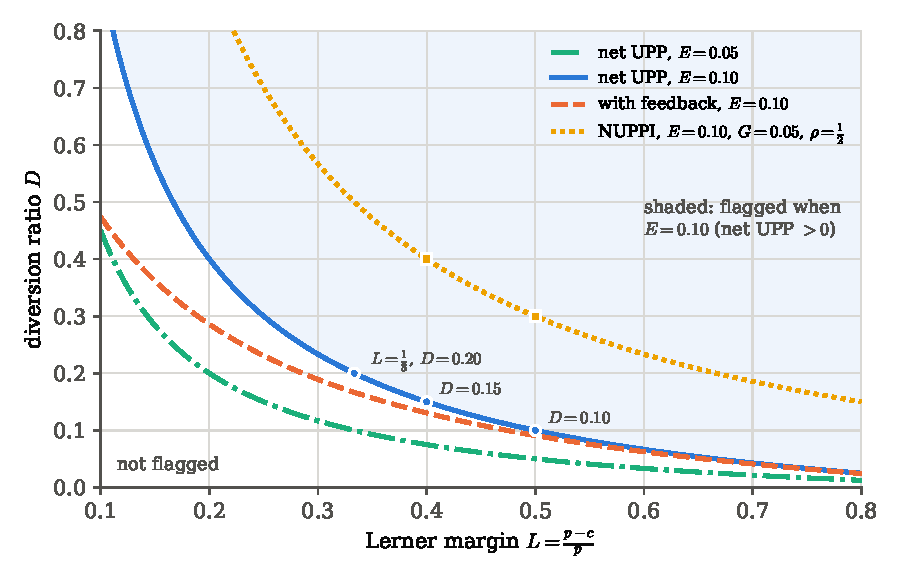
\includegraphics[width=0.86\textwidth]{figures/ch11/upp_thresholds.pdf}
\caption{UPP screening thresholds for a symmetric merger. Each curve gives the diversion ratio above which a test flags
the merger. The tests are net UPP with default efficiencies of 5 and 10 percent \eqref{eq:11-fs2}, the feedback test
\eqref{eq:11-fs4}, and the NUPPI test \eqref{eq:11-nuppi-sym} with $G = 0.05$ and $\rho = \frac{1}{2}$. The shaded
region is flagged by net UPP with $E = 0.10$. Circles mark the three cases in Farrell and Shapiro's fn.~43 and p.~17,
and squares mark their two NUPPI cases on p.~21.}
\label{fig:11-uppregion}
\end{figure}

\casehead{Extensions} The cannibalization logic extends in several directions
\citep[Sections 2.F and 7]{FarrellShapiro2010}. If firm A sells only product 1 while firm B sells products
$2, \dots, n$, the same derivation gives the tax
\begin{equation}\label{eq:11-upp-multi}
  t_1 = \sum_{j=2}^{n} D_{1j}\,(p_j - c_j) .
\end{equation}
When B's products have similar absolute margins, only the aggregate diversion from product 1 to B's group is needed.
If B sells a complement to product 1, say product 3, then $D_{13} < 0$. The merged firm then wants to lower $p_1$ to
spur sales of product 3, and the term $D_{13}(p_3 - c_3)$ offsets the pressure from substitutes. Follow-on revenues
enter through the margin. With spare parts, network effects, learning by doing or switching costs, a sale of product
2 today brings profits later, and the effective margin on product 2 exceeds $p_2 - c_2$. Accounting records sometimes
value these gains, and they usually make UPP for product 1 more likely.

Farrell and Shapiro derived \eqref{eq:11-upp} under static Bertrand pricing. If firms accommodate each other's price
changes before the merger, there is less competition for the merger to eliminate, and the compensating efficiency is
smaller. They still recommend the simple test, leaving non-Bertrand conduct to the rebuttal stage. Otherwise a merger
could permanently remove competition that the parties have only temporarily softened. Under Cournot competition, the
formula holds with a diversion ratio of one (their fn.~36). To see why, let A choose $q_1$ in a homogeneous-goods
market with inverse demand $P(Q)$. After the merger, A internalizes $\frac{d\pi_B}{dq_1} = q_2 P'(Q)$, because B's
quantity is fixed and only the price falls. The per-unit tax is $-q_2 P'(Q)$. B's Cournot condition
$P - c_2 + q_2 P'(Q) = 0$ gives $-q_2P'(Q) = P - c_2$, so $t_1 = 1 \cdot (P - c_2)$.

\casehead{Rebuttal} Farrell and Shapiro intend the test as a presumption that the merging parties can rebut
(their Section 4). The parties can dispute the inputs, for example by showing that marginal costs are closer to prices
or that efficiencies exceed the standard deduction. They can argue that pass-through is low, so that pressure moves
prices little. This argument is irrelevant to the pure sign test. When the test flags only one product, they can argue
that neither price will rise. They can also argue that the consumer gain from a price cut on the other product
outweighs the harm from the increase.
Finally, a full analysis can consider repositioning, entry and verified efficiencies.

\casehead{Interpretation} UPP reframes the loss of competition as an increase in the merged firm's opportunity cost.
That cost is directly comparable with marginal-cost savings. The test answers a narrow question: does the merger
change pricing incentives upward on balance at pre-merger prices? It does not predict magnitudes. In return it needs
only margins and diversion, both of which antitrust agencies often observe from documents and data, and it avoids
drawing market boundaries. Margins are hard to measure in cross-industry academic work, but firms track their own
costs closely, and agencies can obtain those records.

\casehead{Critiques} Without efficiencies, every merger of substitutes creates positive UPP. The policy content of the
test therefore lies in the standard deduction $E$, or in the threshold $G$ of the NUPPI variant below. These
parameters are not derived from evidence on merger efficiencies. Because the test is a sign test, it cannot rank
mergers by harm. Two mergers with equal UPP can have very different price effects when pass-through differs, a point
that motivates the first-order approach of \citet{JaffeWeyl2013}. The Bertrand assumption, the measurement of
marginal cost and the use of diversion at pre-merger prices are further sources of error. The test also ignores
repositioning and entry. \citet{MillerEtAl2017} compare UPP-based predictions with full merger simulations in
simulated industries.

\casehead{Contribution} Farrell and Shapiro made explicit the economic core of unilateral effects. A merger raises
the merged firm's effective marginal cost by the diversion-weighted margin of the partner product. They showed that the sign of the price effect is much easier to establish than its size. Their
framework, together with GUPPI, moved the analysis of unilateral effects away from market shares and toward diversion
and margins.

\subsection{From pricing pressure to price changes: pass-through}\label{sec:11-passthrough}

Under the conditions of \cref{prop:11-fs2}, the price effect of a merger equals the price response to a cost
increase on the merging products. That response is a \emph{pass-through rate}. It is the pass-through of a cost shock to some
products only, and it is an equilibrium rate, including rivals' responses. We first derive single-product pass-through
and then the multi-product approximation of \citet{JaffeWeyl2013}. \Cref{ch:theory} treats pass-through in general.

\begin{lemma}[Single-product pass-through]\label{lem:11-passthrough}
Let a firm face demand $q(p)$, holding rivals' prices fixed, with constant marginal cost $c$. Suppose the profit
maximizing price satisfies the first-order condition $q + (p - c)q' = 0$ and the second-order condition
$2q' + (p - c)q'' < 0$. Then
\begin{equation}\label{eq:11-passthrough}
  \rho = \frac{dp}{dc} = \frac{1}{2 + L\psi} , \qquad \psi = \frac{p\,q''(p)}{q'(p)} ,
\end{equation}
where $L = \frac{p - c}{p}$. Equivalently, with $\varepsilon(p) = -\frac{p\,q'(p)}{q(p)}$,
$\rho = \frac{\varepsilon}{\varepsilon - 1 + \frac{p}{\varepsilon}\frac{d\varepsilon}{dp}}$ \citep{BulowPfleiderer1983}.
\end{lemma}

\begin{proof}
Differentiate the first-order condition totally with respect to $p$ and $c$:
\begin{equation*}
  q'\,dp + q'\,(dp - dc) + (p - c)\,q''\,dp = 0 .
\end{equation*}
Collecting terms, $[2q' + (p-c)q'']\,dp = q'\,dc$, so $\rho = \frac{q'}{2q' + (p-c)q''}$. Dividing numerator and
denominator by $q'$, and writing $\frac{(p - c)q''}{q'} = \frac{p - c}{p}\cdot\frac{p\,q''}{q'} = L\psi$, gives
\eqref{eq:11-passthrough}. For the elasticity form, write the first-order condition as
$p\big[1 - \frac{1}{\varepsilon(p)}\big] = c$ and differentiate:
$\big[1 - \frac{1}{\varepsilon} + \frac{p}{\varepsilon^2}\frac{d\varepsilon}{dp}\big]dp = dc$. Solving for
$\frac{dp}{dc}$ and multiplying numerator and denominator by $\varepsilon$ gives the stated expression.
\end{proof}

Pass-through falls as demand becomes more elastic at higher prices. Three cases recur.

\begin{enumerate}[label=(\alph*)]
\item \emph{Linear demand.} Here $q'' = 0$, so $\psi = 0$ and $\rho = \frac{1}{2}$.
\item \emph{Constant elasticity.} With $q = k p^{-\varepsilon}$, $q' = -\varepsilon k p^{-\varepsilon - 1}$ and
      $q'' = \varepsilon(\varepsilon + 1)k p^{-\varepsilon - 2}$, so $\psi = -(\varepsilon + 1)$. The Lerner condition
      gives $L = \frac{1}{\varepsilon}$. Hence $\rho = \frac{1}{2 - \frac{\varepsilon + 1}{\varepsilon}} =
      \frac{\varepsilon}{\varepsilon - 1} = \frac{1}{1 - L} = \frac{p}{c} > 1$.
\item \emph{Logit, holding rivals' prices fixed.} The logit Lerner condition is $p - c = \frac{1}{\alpha(1 - s)}$.
      Differentiating, $dp - dc = \frac{1}{\alpha(1 - s)^2}\,ds$. Substituting $ds = -\alpha s(1 - s)\,dp$,
      \begin{equation*}
        dp - dc = -\frac{s}{1 - s}\,dp
        \quad\Longrightarrow\quad
        \frac{dp}{1 - s} = dc
        \quad\Longrightarrow\quad
        \rho = 1 - s .
      \end{equation*}
\end{enumerate}
Convex demand ($q'' > 0$, so $\psi < 0$) gives pass-through above one half, and concave demand gives less. Most
functional forms used in practice are convex.

Pass-through in oligopoly also depends on rivals' responses. In a Cournot market with linear inverse demand
$P = a - Q$ and $N$ active firms, firm $i$'s condition is $a - Q - q_i - c_i = 0$. Summing over firms gives
$Na - (N+1)Q = \sum_i c_i$, so $P = \frac{a + \sum_i c_i}{N + 1}$ and the pass-through of a firm-specific cost shock is
$\frac{1}{N+1}$ \citep{BergstromVarian1985}. With differentiated products the intuition that competitive industries
pass through little can fail. A firm facing very elastic residual demand prices close to cost before and after a cost
shock, so its pass-through is near one. Under constant elasticity it exceeds one \citep[Section 3.D]{FarrellShapiro2010}.

\casehead{The first-order approach} \citet{JaffeWeyl2013} turn \cref{prop:11-fs2} into an approximation. Divide each
first-order condition by $-\frac{\partial q_j}{\partial p_j}$ and write the pricing conditions in per-unit form,
\begin{equation}\label{eq:11-foa-f}
  f_j(p;\Omega) = p_j - c_j - \frac{q_j(p)}{-\frac{\partial q_j(p)}{\partial p_j}}
  - \sum_{k \ne j} \Omega_{jk}\, D_{jk}(p)\,(p_k - c_k) = 0 .
\end{equation}
For single-product firms before the merger the sum is empty. After the merger, the condition for product 1 gains the
term $D_{12}(p)(p_2 - c_2)$. Hence $f^{post}(p) = f^{pre}(p) - g(p)$, where $g(p)$ is the vector of generalized pricing
pressures. At the pre-merger prices $f^{pre}(p^0) = 0$, so $f^{post}(p^0) = -g(p^0)$, whose entries are $-\mathit{UPP}_j$
for the merging products and zero for others. A first-order expansion of $f^{post}(p^1) = 0$ around $p^0$ gives
\begin{equation*}
  0 = f^{post}(p^1) \approx f^{post}(p^0) + J^{post}\,(p^1 - p^0) , \qquad J^{post} = \frac{\partial f^{post}}{\partial p}(p^0) ,
\end{equation*}
and therefore
\begin{equation}\label{eq:11-foa}
  p^1 - p^0 \approx \big[J^{post}\big]^{-1} \mathit{UPP} \equiv \rho^{post}\, \mathit{UPP} .
\end{equation}
The matrix $\rho^{post}$ is a pass-through matrix. If each product's effective marginal cost rises by a per-unit amount
$\tau_j$, the conditions become $f^{post}(p) - \tau = 0$, and the implicit function theorem gives
$\frac{dp}{d\tau} = [J^{post}]^{-1}$. The merger price effect is approximately merger pass-through times UPP. Here $\tau$
shifts each normalized first-order condition directly. A rise in a physical marginal cost $c_k$ also changes the partner
term $D_{jk}(p_k - c_k)$. With $B_{jk} = \Omega_{jk}D_{jk}$ for $k \ne j$ and $B_{jj} = 0$,
\eqref{eq:11-foa-f} gives $f(p; c + \tau) = f(p; c) - (I - B)\tau$, so physical-cost pass-through is
$\frac{dp}{dc} = [J^{post}]^{-1}(I - B)$. The two coincide for single-product firms, where $B = 0$. The
pre-merger cost pass-through matrix $[J^{pre}]^{-1}$ can sometimes be estimated from past cost shocks. Jaffe and Weyl
propose using it in place of $\rho^{post}$ when demand curvature cannot be estimated directly. In the logit example of
\cref{sec:11-logitex}, the approximation \eqref{eq:11-foa} predicts a merging-firm price of 1.0648 with post-merger
pass-through and 1.0635 with pre-merger pass-through. The exact post-merger price is 1.0637.

\casehead{Curvature drives predictions} Because pass-through depends on second derivatives of demand, predicted merger
effects depend on curvature, which data rarely pin down. In practice curvature is set by the choice of functional
form. \citet{FroebTschantzWerden2005} simulated the proposed MCI and Sprint merger and found that constant-elasticity
demand predicted price effects over seven times larger than linear demand \citep[p.~19]{FarrellShapiro2010}. They also
noted that demand systems with higher pass-through of efficiencies predict larger price effects without efficiencies.
\Cref{prop:11-fs2} explains this pattern: both quantities are pass-through rates. \citet{CrookeEtAl1999} document the
same sensitivity across standard functional forms.

\Cref{fig:11-curvature} isolates the role of curvature. Two symmetric firms merge, and each demand system is calibrated
to the same price, marginal cost, own-price elasticity and diversion ratio at the pre-merger equilibrium. The
\emph{constant-expenditure logit} applies the logit formula, with log price in utility, to expenditure shares
(\cref{sec:11-bv}). Under linear, logit and constant-expenditure logit demand the merged firm's joint profit is
bounded. A grid search over both prices puts its global maximum at the symmetric solution of the first-order
conditions. The constant-expenditure logit, whose elasticities change little with price, predicts 2.4 to 3.3 times
the linear effect over the plotted range. Logit lies between linear and the constant-expenditure logit.

Constant-elasticity demand needs care. Hold $p_1 > c$ fixed and raise $p_2$. Then $q_1$ grows without bound, while
product 2 earns a nonnegative profit, so joint profit has no maximum for any $D > 0$. The figure therefore shows the
merged firm's optimum when it must charge one common price for both products. That price also solves the symmetric
first-order conditions that a merger simulation would solve. The implied price increase is 3.3 to 5.2 times the
linear effect. Without the restriction the symmetric solution is a strict local maximum of joint profit only for $D$
below about 0.25 and a saddle point above. Constant-elasticity demand is thus a local approximation, and its merger
predictions rely on that approximation far from observed prices.

The figure also plots the prediction obtained by freezing shares and slopes at their
pre-merger values, which we show in \cref{sec:11-simframework} equals the compensating cost reduction. Linear demand
predicts exactly half of it, because the symmetric linear pass-through of a cost shock to both products is one half.
\Cref{sec:11-bv} shows that the same issue separated the predictions of unit-demand and constant-expenditure
specifications in a merger of analgesics producers.

\begin{figure}[htbp]
\centering
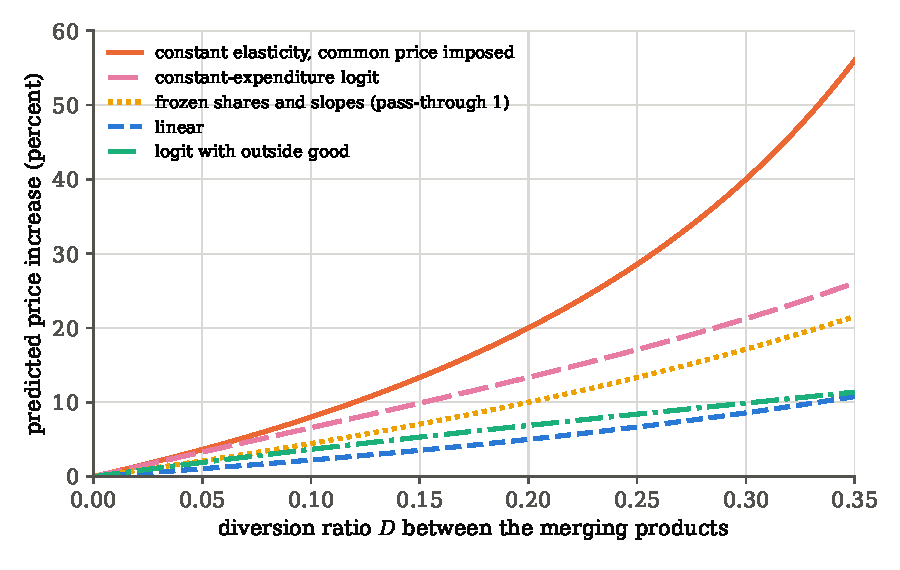
\includegraphics[width=0.86\textwidth]{figures/ch11/curvature_sim.pdf}
\caption{Predicted price increase from a merger of two symmetric single-product firms under four demand systems with
identical first derivatives at the pre-merger point. Calibration: $p = 1$, $c = 0.6$ ($L = 0.4$), own-price elasticity
$2.5$, diversion $D$ between the merging products on the horizontal axis, no efficiencies. Linear:
$q_j = a - b p_j + d p_k$ with $b = 2.5$ and $d = 2.5D$. Logit: one outside good, inside shares $\frac{D}{1+D}$.
Constant-expenditure logit: one outside good, value shares $w_j$ proportional to $p_j^{-\alpha}$ with
$\alpha = 1.5 + 2.5D$, and $q_j = \frac{B w_j}{p_j}$. Constant elasticity: $q_j = k p_j^{-2.5} p_k^{2.5 D}$, with the
merged firm restricted to one common price because its unrestricted joint profit is unbounded. The dotted line
freezes shares and slopes at pre-merger values, which gives $\frac{D L}{1 - D}$. Source: our calculations.}
\label{fig:11-curvature}
\end{figure}

\casehead{A significance threshold: NUPPI} Merger practice often asks first whether a merger without efficiencies would
cause a ``significant'' price increase, say a fraction $G$ of the price \citep[Section 3.C]{FarrellShapiro2010}. Let
$\rho_1$ be the equilibrium pass-through of a cost shock to product 1 alone. Internalizing the first-round tax raises
$p_1$ significantly if $\rho_1 t_1 > G p_1$. Dividing by $\rho_1 p_1$ gives inequality (5),
\begin{equation}\label{eq:11-fs5}
  D_{12}\,\frac{p_2 - c_2}{p_2}\,\frac{p_2}{p_1} > \frac{G}{\rho_1} ,
\end{equation}
which is $\mathit{GUPPI}_1 > \frac{G}{\rho_1}$. Adding the efficiency credit, $\rho_1[D_{12}(p_2 - c_2) - E c_1] > G p_1$,
which after dividing by $\rho_1 p_1$ becomes inequality (6),
\begin{equation}\label{eq:11-fs6}
  D_{12} L_2 \frac{p_2}{p_1} - E_1 (1 - L_1) > \frac{G}{\rho_1} .
\end{equation}
Farrell and Shapiro call the left side the \emph{net upward pricing pressure index} (NUPPI). In the symmetric case,
with $\rho$ the pass-through of a cost increase on both products,
\begin{equation}\label{eq:11-nuppi-sym}
  D L - E(1 - L) > \frac{G}{\rho} .
\end{equation}
Since $\rho$ is hard to estimate, a screen needs a default. They suggest $\rho = \frac{1}{2}$, the single-firm rate with
linear demand, which rivals' accommodation would raise (their fn.~59). With $G = 0.05$ and $\rho = \frac{1}{2}$, the
merger is presumed harmful when NUPPI is at least 10 percent. With $E = 0.10$, NUPPI equals $(D + 0.1)L - 0.1$, so the
condition is $(D + 0.1)L > 0.2$. A margin of 0.4 requires $D > 0.40$, and a margin of 0.5 requires $D > 0.30$
(p.~21). The NUPPI test is far more permissive than \eqref{eq:11-fs1}, especially with low assumed pass-through. It also
describes the roundabout way efficiencies enter merger review. Agencies first ask whether the merger without
efficiencies raises price significantly, which is \eqref{eq:11-fs6} with $E_1 = 0$ and needs a view on $\rho_1$. They
then ask whether efficiencies offset the gross pressure, which is \eqref{eq:11-fs6} with $G = 0$.

\casehead{UPP, simulation and market definition} Farrell and Shapiro compare their test with the two alternatives
(their Sections 5 and 6). Merger simulation must estimate the pass-through of the asymmetric cost shock in
\cref{prop:11-fs2}, explicitly or implicitly. Its predictions therefore depend heavily on the assumed demand system,
which invites a battle of experts. Simulation also tries to explain price levels, so it risks misspecification from
omitted features of conduct. UPP looks at the change in marginal incentives, which nets out features present before
and after the merger. Market definition is less different from simulation than it appears. The hypothetical monopolist
test simulates a merger of all products in a candidate market, and so it also hinges on pass-through. Only the sign
test avoids pass-through. Farrell and Shapiro suggest that a court could keep a broad market definition for context
while the government establishes its presumption through UPP within that market.

\section{Merger simulation}\label{sec:11-simulation}

Merger simulation predicts the post-merger equilibrium from an estimated model of demand and an assumed model of
conduct. \citet{BakerBresnahan1985}, \citet{HausmanLeonardZona1994} and \citet{WerdenFroeb1994} developed the approach
with residual demand, multi-level demand and logit demand. \citet{Nevo2000b} combined it with random coefficients
demand and computed full equilibria and welfare. This section sets out the general framework, works a logit example
in detail and then studies Nevo's application to ready-to-eat cereal.

\subsection{The framework}\label{sec:11-simframework}

Consider one market with $J$ products and market size $M$. Firm $f$ owns the products $\mathcal{J}_f$ and earns
\begin{equation*}
  \Pi_f = \sum_{j \in \mathcal{J}_f} (p_j - mc_j)\, M s_j(p) - C_f .
\end{equation*}
Under static multi-product Bertrand pricing (\cref{ch:diffprod,ch:blp}), the first-order condition for $j \in
\mathcal{J}_f$ is
\begin{equation}\label{eq:11-foc-multi}
  s_j(p) + \sum_{k \in \mathcal{J}_f} (p_k - mc_k)\frac{\partial s_k(p)}{\partial p_j} = 0 .
\end{equation}
Let $\Omega$ be the ownership matrix, with $\Omega_{jk} = 1$ when $j$ and $k$ have the same owner. Since the $(j,k)$
element of $\Delta^\top$ is $\frac{\partial s_k}{\partial p_j}$, stacking \eqref{eq:11-foc-multi} gives
\begin{equation}\label{eq:11-foc-matrix}
  s(p) + \big(\Omega \odot \Delta(p)^\top\big)(p - mc) = 0
  \quad\Longleftrightarrow\quad
  p = mc - \big(\Omega \odot \Delta(p)^\top\big)^{-1} s(p) .
\end{equation}
Because ownership is symmetric, $\Omega \odot \Delta^\top = (\Omega \odot \Delta)^\top$. \citet{Nevo2000b} writes the
same system with a matrix whose $(j,k)$ element is $-\frac{\partial s_j}{\partial p_k}$ for jointly owned products. That
is the transpose of ours. The difference is immaterial when the Jacobian is symmetric, as in logit, nested logit and
random coefficients logit with utility linear in price. It matters when price enters utility as $-\alpha \ln p_j$,
because then $\frac{\partial s_k}{\partial p_j} = \frac{\alpha s_j s_k}{p_j}$ is not symmetric.

\begin{assumption}[Merger simulation]\label{ass:11-sim}
(i) Demand is stable across the merger: the same function $s(p)$ applies before and after. (ii) Before the merger,
prices form a Bertrand-Nash equilibrium under $\Omega^{pre}$. (iii) After the merger, prices form a Bertrand-Nash
equilibrium under $\Omega^{post}$, which sets $\Omega_{jk} = 1$ for every pair of the merging firms' products.
(iv) Marginal costs are constant and unchanged by the merger unless efficiencies are imposed. (v) The set of products
and all non-price choices are fixed.
\end{assumption}

The algorithm has five steps.
\begin{enumerate}[label=(\arabic*)]
  \item Estimate demand on pre-merger data. This delivers $s(\cdot)$ and $\Delta(\cdot)$.
  \item Recover marginal costs from the pre-merger conditions,
        \begin{equation}\label{eq:11-mc-recover}
          \widehat{mc} = p^{pre} + \big(\Omega^{pre} \odot \Delta(p^{pre})^\top\big)^{-1} s(p^{pre}) .
        \end{equation}
  \item Replace $\Omega^{pre}$ by $\Omega^{post}$. Optionally lower the merging firms' costs to represent efficiencies.
  \item Solve \eqref{eq:11-foc-matrix} for the post-merger prices $p^*$ under $\Omega^{post}$ and the new costs.
  \item Compute the changes in prices, consumer surplus, profits and total welfare.
\end{enumerate}
Step 2 needs no cost data, but it relies on the pre-merger conduct assumption. \Cref{ch:blp} shows how cost shifters
can be added to estimate a supply side jointly with demand. \citet[eq.~(9)]{Nevo2000b} notes that
conduct parameters could multiply the entries of $\Omega$ and be estimated, but that this is hard in practice.

\casehead{The first iteration} Before Nevo's work, practitioners often reported an approximation instead of the
equilibrium \citep{HausmanLeonardZona1994,Werden1997}. It replaces the post-merger shares and derivatives by their
pre-merger values:
\begin{equation}\label{eq:11-approx}
  p^{approx} = \widehat{mc} - \big(\Omega^{post} \odot \Delta(p^{pre})^\top\big)^{-1} s(p^{pre})
\end{equation}
\citep[eq.~(11)]{Nevo2000b}. It is the first step of the fixed-point iteration on \eqref{eq:11-foc-matrix} started at
$p^{pre}$, so it captures the merged firm's direct incentive to raise price. The next result relates it to UPP.

\begin{proposition}[First iteration and compensating cost reductions]\label{prop:11-approx}
Let single-product firms 1 and 2 merge. The approximation \eqref{eq:11-approx} leaves every non-merging price unchanged.
For the merging products, $p_1^{approx} - p_1^{pre}$ and $p_2^{approx} - p_2^{pre}$ equal the compensating marginal
cost reductions $\Delta c_1$ and $\Delta c_2$ of \cref{prop:11-cmcr}.
\end{proposition}

\begin{proof}
Write $m = p^{pre} - \widehat{mc}$ for the pre-merger margins and $m' = p^{approx} - \widehat{mc}$. By step 2 and
\eqref{eq:11-approx}, both satisfy linear systems with the same right side:
\begin{equation*}
  \big(\Omega^{post} \odot \Delta^\top\big) m' = -s = \big(\Omega^{pre} \odot \Delta^\top\big) m ,
\end{equation*}
with $s$ and $\Delta$ at $p^{pre}$. Both matrices are block diagonal by owner. The blocks of non-merging firms coincide,
so their margins are unchanged. The merging block has rows
\begin{equation*}
  \frac{\partial s_1}{\partial p_1} m_1' + \frac{\partial s_2}{\partial p_1} m_2' = \frac{\partial s_1}{\partial p_1} m_1 , \qquad
  \frac{\partial s_1}{\partial p_2} m_1' + \frac{\partial s_2}{\partial p_2} m_2' = \frac{\partial s_2}{\partial p_2} m_2 .
\end{equation*}
Dividing the first row by $-\frac{\partial s_1}{\partial p_1}$ gives $-m_1' + D_{12} m_2' = -m_1$, so
$m_1' - m_1 = D_{12}\big(m_2 + (m_2' - m_2)\big)$. The second row gives $m_2' - m_2 = D_{21}\big(m_1 + (m_1' - m_1)\big)$.
These are the equations for $\Delta c_1$ and $\Delta c_2$ in the proof of \cref{prop:11-cmcr}, with margins
$p_j - c_j = m_j$. Their unique solution is \eqref{eq:11-cmcr}.
\end{proof}

The first iteration is therefore UPP with feedback between the merging products and with a pass-through of exactly
one. The compensating cost reduction is the cost cut that would offset the merger. The first iteration is the price
increase that the merger would cause if every unit of pricing pressure passed into price. The approximation overstates
the equilibrium effect when pass-through is below one, as with logit demand and small shares. It understates the effect
when pass-through exceeds one, as with the constant-expenditure logit of \cref{fig:11-curvature}.

\casehead{Computation} Solving \eqref{eq:11-foc-matrix} means solving $J$ nonlinear equations. The usual choice is a
Newton or quasi-Newton method applied to the first-order conditions, started from the pre-merger prices.
\citet[fn.~13]{Nevo2000b} used a standard nonlinear equation solver, and each city took several seconds on a 1997
personal computer. The naive iteration $p \leftarrow mc - (\Omega \odot \Delta(p)^\top)^{-1}s(p)$ need not converge.
\citet{MorrowSkerlos2011} propose a better-behaved fixed point for logit-type demand in which price enters utility as
$-\alpha_i p_j$. Decompose the Jacobian as $\Delta = \Lambda - \Gamma$, where the diagonal matrix $\Lambda$ has entries
$\Lambda_{jj} = -\int \alpha_i s_{ij}\,dP(i)$ and $\Gamma_{jk} = -\int \alpha_i s_{ij}s_{ik}\,dP(i)$. These two matrices
follow the notation of Morrow and Skerlos and are unrelated to the scalars $\Lambda$ of \cref{sec:11-fs} and $\Gamma$
of \cref{sec:11-dd}. Substituting into \eqref{eq:11-foc-matrix} and using $\Omega \odot \Lambda = \Lambda$,
\begin{equation}\label{eq:11-zeta}
  p = mc + \zeta(p) , \qquad \zeta(p) = \Lambda(p)^{-1}\big[\big(\Omega \odot \Gamma(p)^\top\big)(p - mc) - s(p)\big] .
\end{equation}
They report that iterating on this map is fast and reliable in large problems, and \texttt{pyblp} uses it
(\cref{ch:blp}). Existence and uniqueness of the post-merger equilibrium are not automatic. The log-concavity
conditions of \citet{CaplinNalebuff1991} give existence for broad classes of discrete choice demand when each firm
sells one product (\cref{thm:04-cn-existence}). Their uniqueness results cover only restricted cases, such as the
logit and duopoly (\cref{sec:04-uniqueness}). A merger creates a multiproduct firm, which their theorems do not cover.
With logit demand, uniqueness holds for every ownership structure (\cref{thm:04-logit-unique}). Random coefficients
demand with multiproduct firms has no such theorem. In practice one checks that the solver reaches the same prices
from several starting points.

\casehead{Calibration} The simulated pre-merger prices must equal observed prices, so that the simulation compares the
merger with the status quo. In a logit model one can add a residual to predicted shares. \citet[p.~31]{Nevo2000b}
points out that with heterogeneous consumers this can make individual purchase probabilities negative. He adds the
estimated residual $\xi$ to utility instead, so that the model reproduces observed shares exactly.

\casehead{Welfare} With utility linear in price and type I extreme value errors, the expected consumer surplus of
consumer $i$, up to a constant, is
\begin{equation}\label{eq:11-cs}
  \mathit{CS}_i = \frac{1}{\alpha_i}\ln\Big(1 + \sum_{j=1}^{J} e^{V_{ij}}\Big) .
\end{equation}
Here $V_{ij}$ is the deterministic part of utility from product $j$. The outside good has $V_{i0} = 0$
\citep{SmallRosen1981,Trajtenberg1989}. The log-sum is the expected maximum utility. Dividing by $\alpha_i$, the
marginal utility of income, converts it into money (\cref{ch:logit}). The change in consumer surplus is
\begin{equation}\label{eq:11-dcs}
  \Delta \mathit{CS} = M\,\frac{1}{n_s}\sum_{i=1}^{n_s} \frac{1}{\alpha_i}
  \Big[\ln\Big(1 + \sum_j e^{V_{ij}^{post}}\Big) - \ln\Big(1 + \sum_j e^{V_{ij}^{pre}}\Big)\Big] ,
\end{equation}
averaging over $n_s$ simulated consumers. With plain logit, $\alpha_i = \alpha$ and the average has one term. The change
in producer surplus is $\sum_j (p_j^{post} - mc_j^{post}) M s_j^{post} - \sum_j (p_j^{pre} - mc_j^{pre}) M s_j^{pre}$,
since fixed costs are unchanged. Total welfare changes by the sum.

\casehead{Partial internalization} The framework accommodates objectives that place weight on other firms' profits.
Suppose firm $f$ maximizes $\Pi_f + \sum_{g \ne f} \kappa_{fg}\Pi_g$. The first-order condition keeps the form
\eqref{eq:11-foc-matrix} with $\Omega_{jk}(\kappa) = \kappa_{fg}$ for $j \in \mathcal{J}_f$ and $k \in \mathcal{J}_g$.
With partial ownership, \citet{OBrienSalop2000} derive the weights from financial interests and control rights.
\citet{MillerWeinberg2017} use a common weight $\kappa$ to measure coordination between two firms after a joint venture
(\cref{sec:11-millercoors}). When $\kappa_{fg} \ne \kappa_{gf}$, $\Omega$ is not symmetric, and the form
$\Omega \odot \Delta^\top$ in \eqref{eq:11-foc-matrix} must be used.

\casehead{Caveats} A simulation is only as good as the demand model. Functional form fixes curvature and hence
pass-through (\cref{sec:11-passthrough}). Simulation also relies on assumptions about post-merger conduct: joint profit
maximization, unchanged behavior of rivals, a stable demand system and predictable efficiencies. Nevo stresses that
$\Omega^{pre}$ and $\Omega^{post}$ use the same demand estimates. This is inconsistent with firms changing other choices
that affect demand. If advertising changes after the merger and affects $\frac{\partial s}{\partial p}$, the predicted
prices are wrong. Product repositioning, entry and new products are absent from the static model
\citep[pp.~23--25]{Nevo2000b}. Finally, the exercise is data-intensive and time-consuming, which matters under the
statutory deadlines of merger review.

\subsection{A worked example with logit demand}\label{sec:11-logitex}

The following example traces every concept of this section and \cref{sec:11-upp} through one calibrated market. The
calibration is the one \citet[p.~1780]{MillerWeinberg2017} use to illustrate their internalization parameter. All
numbers are our computations.

\begin{example}[Logit merger simulation]\label{ex:11-logit}
Three symmetric single-product firms sell at $p = 1$ with marginal cost $c = 0.7$. Each has share $s = 0.2$, and the
outside good has $s_0 = 0.4$. Market size is one. Demand is logit, and pre-merger prices are a Bertrand-Nash
equilibrium. Firms 1 and 2 merge.

\emph{Calibration.} The logit Lerner condition $p - c = \frac{1}{\alpha(1 - s)}$ gives
$\alpha = \frac{1}{0.3 \times 0.8} = 4.1667$. Mean utilities satisfy $e^{\delta_j} = \frac{s_j}{s_0} = 0.5$.

\emph{Screening statistics.} Diversion is $D_{12} = \frac{0.2}{1 - 0.2} = 0.25$, and diversion to the outside good is
$\frac{0.4}{0.8} = 0.5$. Upward pricing pressure is $\mathit{UPP}_1 = 0.25 \times 0.3 = 0.075$, so
$\mathit{GUPPI}_1 = 7.5$ percent. With $L = 0.3$ and $E = 0.10$, the simple test requires
$D > \frac{0.1 \times 0.7}{0.3} = 0.233$, which holds narrowly. Net UPP is $0.075 - 0.07 = 0.005$. The feedback test
compares $\frac{D}{1 - D} = 0.333$ with $0.233$ and flags the merger clearly. By \eqref{eq:11-cmcr}, the compensating
cost reduction is
\begin{equation*}
  \Delta c = \frac{0.25 \times 0.3 + 0.0625 \times 0.3}{1 - 0.0625} = 0.100 ,
\end{equation*}
which is 14.3 percent of marginal cost. A 10 percent standard deduction falls short.

\emph{Approximations.} Holding the rival's price fixed, single-product logit pass-through is $1 - s = 0.8$, so
$\rho\,\mathit{UPP} = 0.06$. The first iteration \eqref{eq:11-approx} gives $p_1 = p_2 = 1.100$ and $p_3 = 1$, the
compensating reduction of \cref{prop:11-approx}. The first-order approach \eqref{eq:11-foa} gives 1.0648 with
post-merger pass-through and 1.0635 with pre-merger pass-through. Farrell and Shapiro's iterative tax procedure
converges within three rounds. The first round imposes taxes of 0.075 and yields prices of 1.0641. The second round
lowers the taxes to 0.0745 and the prices slightly, to 1.0637. The third round changes neither at four decimals. The
limiting tax of
\cref{prop:11-fs2} is $t^* = 0.2049 \times 0.3637 = 0.0745$. It is slightly below the first-round tax: the margin rises,
but diversion falls from 0.25 to 0.2049 as the merging products' shares fall.

\emph{Full simulation.} The post-merger equilibrium prices are $(1.0637, 1.0637, 1.0062)$. The merging firms raise
prices by 6.4 percent and the rival by 0.6 percent. The merged firm's markup of 0.3637 equals the multi-product logit
common markup $\frac{1}{\alpha(1 - S_f)}$ with combined share $S_f = 0.3402$ (\cref{ch:diffprod,app:problems}). Consumer
surplus falls by 0.0249, against pre-merger revenue of 0.6. The merged firm's profit rises by 0.0037, and the rival's by
0.0062. Total welfare falls by 0.0149.

\emph{Efficiencies.} If the merger lowers the merging firms' cost to $0.7 - 0.1 = 0.6$, the post-merger equilibrium is
the pre-merger price vector. Consumers are unaffected, and total welfare rises by the cost saving of 0.04.

\emph{Partial internalization.} Suppose the merged firm and firm 3 each place weight $\kappa = 0.5$ on the other's
profit. Then prices rise to $(1.1040, 1.1040, 1.0731)$, and consumer surplus falls by 0.0515, about twice the loss
under unilateral effects alone. With the merging firms' cost cut to 0.5, prices are $(0.9834, 0.9834, 1.1028)$. The
efficiency lowers the merging firms' prices but raises firm 3's. The merging products' margins grow, and firm 3
internalizes half of them. Consumer surplus is unchanged only if the merging firms' cost falls to 0.4532, a 35.3
percent reduction, against 14.3 percent without coordination.
\end{example}

\begin{table}[htbp]
\centering
\caption{Logit merger example: prices, outside share and welfare changes}
\label{tab:11-logitex}
\small
\begin{tabular}{@{}lccccccc@{}}
\toprule
Scenario & $p_1 = p_2$ & $p_3$ & $s_0$ & $\Delta\mathit{CS}$ & $\Delta\pi_{1+2}$ & $\Delta\pi_3$ & $\Delta W$ \\
\midrule
Pre-merger                                   & 1.0000 & 1.0000 & 0.4000 & 0       & 0       & 0       & 0       \\
First iteration \eqref{eq:11-approx}         & 1.1000 & 1.0000 &        &         &         &         &         \\
First-order approach \eqref{eq:11-foa}       & 1.0648 & 1.0065 &        &         &         &         &         \\
Merger, $\kappa = 0$                         & 1.0637 & 1.0062 & 0.4436 & $-0.0249$ & 0.0037 & 0.0062 & $-0.0149$ \\
Merger, $\kappa = 0$, $c_{1,2} = 0.6$         & 1.0000 & 1.0000 & 0.4000 & 0.0000  & 0.0400  & 0.0000  & 0.0400  \\
Merger, $\kappa = 0.5$                       & 1.1040 & 1.0731 & 0.4958 & $-0.0515$ & 0.0099 & 0.0082 & $-0.0335$ \\
Merger, $\kappa = 0.5$, $c_{1,2} = 0.68$      & 1.0907 & 1.0755 & 0.4877 & $-0.0476$ & 0.0173 & 0.0069 & $-0.0235$ \\
Merger, $\kappa = 0.5$, $c_{1,2} = 0.5$       & 0.9834 & 1.1028 & 0.4171 & $-0.0101$ & 0.0961 & $-0.0053$ & 0.0807 \\
Merger, $\kappa = 1$                         & 1.1405 & 1.1405 & 0.5449 & $-0.0742$ & 0.0137 & 0.0068 & $-0.0537$ \\
\bottomrule
\end{tabular}

\smallskip
\begin{minipage}{0.95\linewidth}
\footnotesize
Notes: Three symmetric firms with $p = 1$, $c = 0.7$, $s = 0.2$, $s_0 = 0.4$ and $\alpha = 4.1667$ before the merger.
Firms 1 and 2 merge. $\kappa$ is the weight that the merged firm and firm 3 place on each other's profit. $c_{1,2}$ is
the merging firms' post-merger marginal cost (0.7 unless stated). Welfare changes are per unit of market size and in
units of price, with consumer surplus from \eqref{eq:11-dcs}. The first-order approach row uses post-merger
pass-through. Source: our calculations.
\end{minipage}
\end{table}

\begin{figure}[htbp]
\centering
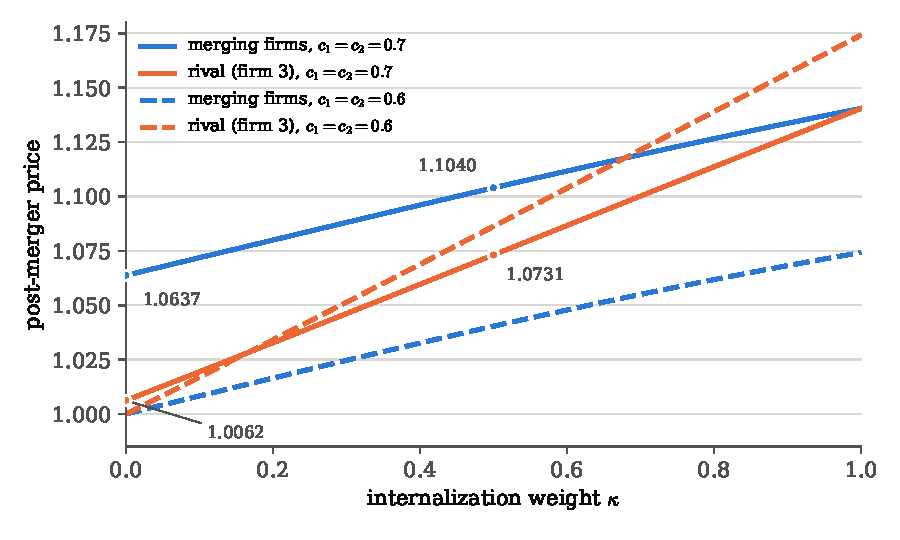
\includegraphics[width=0.86\textwidth]{figures/ch11/logit_kappa.pdf}
\caption{Post-merger prices in the logit example as a function of the internalization weight $\kappa$ between the
merged firm and firm 3. Solid lines keep the merging firms' marginal cost at 0.7, and dashed lines lower it to 0.6, the
compensating cost reduction. Dots mark $\kappa = 0$ and $\kappa = 0.5$. Source: our calculations.}
\label{fig:11-kappa}
\end{figure}

\Cref{fig:11-kappa} shows how $\kappa$ separates unilateral from coordinated effects. At $\kappa = 0$ the rival's price
barely moves, since its response comes only through strategic complementarity. As $\kappa$ rises, the rival's price
rises nearly linearly, and at $\kappa = 1$ the industry behaves as a monopoly. With the compensating cost reduction
(dashed lines), merging prices stay at one when $\kappa = 0$, but coordination still raises all prices. Efficiencies
can offset unilateral effects, but they do not offset coordinated effects. The rival's price is the observable that
distinguishes the two. \citet{MillerWeinberg2017} build their identification argument for $\kappa$ on this contrast
(\cref{sec:11-millercoors}).

\begin{remark}[The third case in Miller and Weinberg's illustration]\label{rem:11-mw-typo}
\citet[p.~1780]{MillerWeinberg2017} report post-merger prices of about 1.06, 1.06 and 1.01 at $\kappa = 0$ and about
1.10, 1.10 and 1.07 at $\kappa = 0.5$, which match our calculations.
For $\kappa = 0.5$ with the merging firms' marginal cost lowered to 0.50, the text reports prices of 1.09, 1.09 and 1.08.
We obtain $(0.9834, 0.9834, 1.1028)$ for that case. The reported values correspond to a merging-firm cost of about
0.68. We obtain a merging price of 1.09 at a cost of 0.679, with the rival at 1.0756. \Cref{sec:11-mc-theory}
inverts both reported prices jointly for $\kappa$ and the merging firms' cost.
\end{remark}

\subsection{Nevo (2000): mergers in ready-to-eat cereal}\label{sec:11-nevo}

\casehead{The question} \citet{Nevo2000b} asks whether a flexible demand model, estimated with standard scanner data,
can discipline merger analysis in a concentrated industry with many differentiated products. He also asks how much the
answer depends on two choices: the demand model and the decision to compute the full post-merger equilibrium instead of
an approximation. Nevo frames merger simulation as the analogue of market definition. The ``front end'' estimates
demand, and the ``back end'' simulates the merger. He argues that the debate should focus on the front end, because
the demand estimates largely determine the outcome. The working paper (November 1997) was published in the RAND
Journal of Economics in 2000. Our equation and table numbers follow the working paper.

\casehead{The critique of traditional analysis} Nevo describes the screen of the 1982 and 1984 Guidelines (printed
pp.~5--6). A merger was not challenged if the post-merger HHI was below 1,000. Between 1,000 and 1,800, increases below 100 points
were usually not challenged. Above 1,800, an increase of 50 points was the threshold for a challenge. He argues that
concentration indices measure competitive effects well only if products are equally spaced in characteristics. Under
logit demand, substitution depends only on shares, and share-based policy is then sensible \citep{Willig1991}. For
cereal, logit is inadequate. Consumer heterogeneity also makes it easy to argue that hot cereal or bagels belong in
the market, which yields broad markets and small shares. The 1992 Guidelines introduced unilateral effects, and
\citet{Shapiro1996} described their implementation through diversion ratios and margins. Practice then moved to
computing price increases from estimated elasticities, usually with an approximation.

\casehead{Demand options} With $J$ products, an unrestricted demand system has on the order of $J^2$ price
parameters. With 200 cereal brands and constant elasticities, that is 40,000 elasticities. Nevo discusses three
solutions (his Section 3.1).
\begin{enumerate}[label=(\alph*)]
  \item \emph{Symmetric representative-consumer models.} The CES utility of \citet{DixitStiglitz1977} imposes equal
        cross-price elasticities. The representative-consumer form of logit has utility
        $\sum_i a_i q_i - \sum_i q_i \ln q_i$ \citep{AndersonDePalmaThisse1992}. Its entropy term treats all products
        symmetrically, so substitution depends only on shares.
  \item \emph{Multi-stage budgeting} \citep{HausmanLeonardZona1994}. The bottom level is an AIDS model for brand $j$ in
        segment $g$, city $c$ and quarter $t$ (\cref{ch:aids}),
        \begin{equation}\label{eq:11-nevo-aids}
          s_{jct} = \alpha_{jc} + \beta_j \ln\Big(\frac{y_{gct}}{P_{gct}}\Big) + \sum_{k=1}^{J} \gamma_{jk}\ln p_{kct} + \varepsilon_{jct} .
        \end{equation}
        Here $s_{jct}$ is the dollar share of segment expenditure $y_{gct}$ (his eq.~(1)). The price index is the Stone
        index $\ln P_{gct} = \sum_{k \in g} s_{kct}\ln p_{kct}$ (eq.~(2)) or the exact AIDS index (eq.~(3)). A middle
        level allocates expenditure across segments, for example with the log-log form
        $\ln q_{gct} = \beta_g \ln y_{Rct} + \sum_{k} \gamma_k \ln \pi_{kct} + \alpha_{gc} + \varepsilon_{gct}$. A top
        level gives total cereal demand. Nevo notes that the middle levels used in practice do not satisfy the
        conditions for exact two-stage budgeting.
  \item \emph{Discrete choice} \citep{Berry1994,BerryLevinsohnPakes1995}. Products are projected onto a space of
        characteristics, so the number of parameters grows with the number of characteristics.
\end{enumerate}
He rules out the symmetric models for merger work unless time is binding. Multi-level models need an a priori
segmentation into small groups and assume that every consumer buys every variety. They are closer to classical demand
theory and faster to compute. Discrete choice models need product characteristics and distributional assumptions, and
they are computationally heavier.

\casehead{The industry} Ready-to-eat cereal has high concentration, high price-cost margins, high advertising to
sales ratios and frequent product introductions. Concentration is high at the firm level and lower at the brand level.
The leading brands have about 5 percent of the market and the smaller brands in the sample about 1 percent.
\Cref{tab:11-nevo-shares} reports firm shares. Kellogg's volume share fell from 41.4 percent in the first quarter of
1988 to 33.7 percent in the last quarter of 1992, while General Mills rose from 22.0 to 26.8 percent. The three-firm
concentration ratio stayed above 70 percent throughout. Private labels grew from 3.3 to 7.6 percent of volume.

\begin{table}[htbp]
\centering
\caption{Firm shares in ready-to-eat cereal, 1988--1992, in percent (Nevo 1997 working paper, Tables 1A and 1B)}
\label{tab:11-nevo-shares}
\small
\begin{tabular}{@{}lcccccc@{}}
\toprule
 & \multicolumn{3}{c}{Volume shares} & \multicolumn{3}{c}{Sales shares} \\
\cmidrule(lr){2-4}\cmidrule(lr){5-7}
 & 88Q1 & 90Q4 & 92Q4 & 88Q1 & 90Q4 & 92Q4 \\
\midrule
Kellogg        & 41.39 & 37.86 & 33.70 & 41.23 & 37.26 & 32.57 \\
General Mills  & 22.04 & 23.82 & 26.83 & 24.73 & 27.70 & 31.39 \\
Post           & 11.80 & 10.96 & 11.31 & 11.15 & 10.56 & 10.97 \\
Quaker Oats    &  9.93 &  7.66 &  7.40 &  9.46 &  7.30 &  6.94 \\
Ralston        &  4.86 &  6.60 &  5.18 &  5.12 &  7.03 &  5.45 \\
Nabisco        &  5.32 &  3.75 &  3.11 &  5.00 &  3.58 &  3.33 \\
\midrule
C3             & 75.23 & 72.64 & 71.84 & 77.11 & 75.52 & 74.93 \\
C6             & 95.34 & 90.65 & 87.53 & 96.69 & 93.43 & 90.65 \\
Private label  &  3.33 &  6.29 &  7.60 &  2.12 &  3.74 &  4.55 \\
\bottomrule
\end{tabular}

\smallskip
\begin{minipage}{0.86\linewidth}
\footnotesize
Notes: C3 and C6 are the combined shares of the three and six largest firms. The paper also reports 88Q4, 89Q4 and
91Q4. Source: \citet{Nevo2000b}, working paper Tables 1A and 1B, from IRI Infoscan data.
\end{minipage}
\end{table}

\casehead{Data} Shares and prices come from the IRI Infoscan database, collected by scanners in a national random sample
of supermarkets. The sample represents supermarkets with annual sales above \$2 million, which account for 82 percent of
US grocery sales. Data are aggregated to the brand, city and quarter. The sample has 24 brands, listed by segment in his
Table 2: all-family or basic, taste-enhanced wholesome, simple health nutrition, and kids. The estimation sample
covers 45 cities and 20 quarters from 1988 to 1992, so it has $24 \times 45 \times 20 = 21{,}600$ observations in 900
city-quarter markets. Quantity
is converted into servings. Market size is one serving per capita per day, and the outside share is the remainder. Price
is dollar sales divided by servings, deflated by a regional urban CPI. It is the average transaction price at the
register, before any coupons redeemed after purchase.

Advertising comes from the Leading National Advertisers database, summed over ten media. Nevo collected
characteristics from cereal boxes: calories from fat, sugar, fiber, segment dummies and a ``mushy'' dummy for cereals
that turn soggy in milk. Demographics are drawn from the March Current Population Survey (CPS): income per person
(household income divided by household size), age and a child dummy. Instruments use supermarket-sector wages by city
from CPS earnings files, city density, and regional price indices from the Bureau of Labor Statistics.

\casehead{The model} The indirect utility of consumer $i$ from brand $j$ in market $t$ is (his eq.~(4), in our sign
convention)
\begin{equation}\label{eq:11-nevo-u}
  u_{ijt} = x_{jt}\beta_i - \alpha_i p_{jt} + \xi_j + \Delta\xi_{jt} + \epsilon_{ijt} .
\end{equation}
Here $\xi_j$ is the national mean of unobserved quality and $\Delta\xi_{jt}$ the market-specific deviation. Tastes
depend on demographics $D_i$ and unobserved draws $\nu_i$ (eq.~(5)),
\begin{equation}\label{eq:11-nevo-rc}
  \begin{pmatrix} \alpha_i \\ \beta_i \end{pmatrix}
  = \begin{pmatrix} \alpha \\ \beta \end{pmatrix} + \Pi D_i + \Sigma \nu_i , \qquad \nu_i \sim N(0, I_{K+1}) .
\end{equation}
The outside good gives $u_{i0t} = \xi_0 + \pi_0 D_i + \sigma_0 \nu_{i0} + \epsilon_{i0t}$, with $\xi_0$ normalized to zero.
Setting $\Pi = 0$ and $\Sigma = 0$ gives the logit model (eq.~(6)), $u_{ijt} = x_{jt}\beta - \alpha p_{jt} + \xi_j +
\Delta\xi_{jt} + \epsilon_{ijt}$. Nevo stresses two logit restrictions. Cross-price elasticities follow shares. Own-price
elasticities are nearly proportional to price when shares are small, so cheaper brands get higher percentage markups.
With random coefficients, the own elasticity averages heterogeneous price sensitivities with purchase probabilities as
weights, and substitution follows characteristics. The supply side is multi-product Bertrand pricing as in
\eqref{eq:11-foc-matrix}.

\casehead{Estimation} The logit model is estimated from the Berry inversion,
\begin{equation}\label{eq:11-nevo-logit}
  \ln S_{jt} - \ln S_{0t} = d_j + x_{jt}\beta - \alpha p_{jt} + \tau_t + \Delta\xi_{jt} ,
\end{equation}
where $d_j$ are brand dummies, $\tau_t$ quarter dummies and $x_{jt}$ includes advertising and, in some columns, city
demographics. The full model is estimated by GMM following \citet{Berry1994} and \citet{BerryLevinsohnPakes1995}. For
given nonlinear parameters $\theta_2 = (\Pi, \Sigma)$, invert the share equations $s_{\cdot t}(\delta_{\cdot t};\theta_2)
= S_{\cdot t}$ market by market to recover mean utilities $\delta_{jt}(S_{\cdot t};\theta_2)$. The structural error is
(his eq.~(17))
\begin{equation*}
  \Delta\xi_{jt}(\theta) = \delta_{jt}(S_{\cdot t};\theta_2) - \big(d_j + x_{jt}\beta - \alpha p_{jt}\big) .
\end{equation*}
With instruments $Z$ satisfying $\E[Z^\top \Delta\xi(\theta^*)] = 0$ (eq.~(15)), the estimator is
\begin{equation*}
  \hat\theta = \argmin_\theta\ \Delta\xi(\theta)^\top Z \hat A^{-1} Z^\top \Delta\xi(\theta) ,
\end{equation*}
with $\hat A$ a consistent estimate of $\E[Z^\top \Delta\xi\Delta\xi^\top Z]$ (eq.~(16)). For logit, with $\hat A = Z^\top Z$, this is two-stage
least squares. \Cref{ch:blp} develops the algorithm.

Brand dummies absorb both $x_j\beta$ and $\xi_j$, so the error is the city-quarter deviation $\Delta\xi_{jt}$. The mean
tastes for fixed characteristics are recovered by minimum distance \citep{Chamberlain1982}. Let $\hat d$ be the
estimated brand dummies with covariance matrix $V_d$, and let $X$ be the $J \times K$ characteristics matrix. Since
$d = X\beta + \xi$,
\begin{equation*}
  \hat\beta = \big(X^\top V_d^{-1} X\big)^{-1} X^\top V_d^{-1} \hat d , \qquad \hat\xi = \hat d - X\hat\beta .
\end{equation*}
A $\chi^2$ statistic tests the restriction that $\xi = 0$.

\casehead{Instruments and identification} Prices respond to the unobserved demand shock. Nevo decomposes price into
marginal cost and markup, each with a national brand component and a city-quarter deviation (his eq.~(18)). Brand
dummies absorb the national components. The remaining deviation $\Delta\xi_{jt}$ is observed by firms and raises the
local markup, which biases the price coefficient toward zero. The main instruments exploit the panel. The identifying
assumption is that, conditional on brand means and demographics, city-specific valuations are independent across
cities, though possibly correlated over time within a city. Prices of the same brand in other cities then share the
marginal cost component but not the demand shock. Nevo uses regional quarterly average prices, excluding the city being
instrumented. This is the same idea as the instruments of \citet{Hausman1997} and \citet{Nevo2001} (\cref{ch:blp}). The
assumption fails if demand shocks are correlated across cities, for example through national advertising campaigns.
Nevo therefore also uses direct cost proxies. Production and packaging costs vary little across cities, so the proxies
target distribution costs: region dummies for transport costs, city density for the cost of space, and supermarket wages.

\casehead{Logit results} \Cref{tab:11-nevo-logit} reproduces his Table 3. The OLS price coefficient is $-8.57$, and
the implied mean own elasticity is $-1.71$, with 4.4 percent of brand-city-quarter demands inelastic. Such demands are
inconsistent with profit maximization. Instrumenting raises the price coefficient in absolute value to $-12.60$ with
regional prices and $-12.65$ with cost proxies. The two sets of instruments give nearly identical estimates. Adding
city demographics raises it further, to $-16.61$ and $-16.97$ with each instrument set alone and to $-18.21$ when
both sets are used. No demand is
inelastic once prices are instrumented. The overidentification tests reject in every IV column, however, and Nevo notes
reasons to doubt the instruments' validity. He reads the similarity across instrument sets as encouraging, without
claiming that it proves validity.

\begin{table}[htbp]
\centering
\caption{Logit demand estimates, 21,600 observations (Nevo 1997 working paper, Table 3)}
\label{tab:11-nevo-logit}
\small
\setlength{\tabcolsep}{4.5pt}
\begin{tabular}{@{}lcccccc@{}}
\toprule
 & OLS & \multicolumn{5}{c}{IV} \\
\cmidrule(lr){3-7}
 & (i) & (ii) & (iii) & (iv) & (v) & (vi) \\
\midrule
Price                  & $-8.57$ & $-12.60$ & $-12.65$ & $-16.61$ & $-16.97$ & $-18.21$ \\
                       & (0.179) & (0.436)  & (0.467)  & (0.443)  & (0.483)  & (0.439)  \\
Advertising            & 0.034   & 0.032    & 0.032    & 0.030    & 0.030    & 0.030    \\
                       & (0.002) & (0.002)  & (0.002)  & (0.002)  & (0.002)  & (0.002)  \\
Log median income      &         &          &          & 0.99     & 1.00     & 1.01     \\
                       &         &          &          & (0.021)  & (0.022)  & (0.022)  \\
Log median age         &         &          &          & $-0.02$  & 0.01     & 0.04     \\
                       &         &          &          & (0.06)   & (0.06)   & (0.06)   \\
Median household size  &         &          &          & $-0.03$  & $-0.02$  & $-0.02$  \\
                       &         &          &          & (0.03)   & (0.03)   & (0.03)   \\
\midrule
Fit or overidentification & 0.76 & 99.1     & 98.7     & 59.0     & 51.3     & 54.8     \\
                       &         & (30.1)   & (16.9)   & (30.1)   & (16.9)   & (42.6)   \\
First-stage $R^2$      &         & 94.5     & 94.4     & 94.5     & 94.5     & 94.7     \\
First-stage $F$        &         & 5179     & 6740     & 5046     & 6483     & 4959     \\
Regional prices as IV  &         & yes      &          & yes      &          & yes      \\
Cost proxies as IV     &         &          & yes      &          & yes      & yes      \\
\midrule
Own elasticity: mean   & $-1.71$ & $-2.51$  & $-2.51$  & $-3.31$  & $-3.38$  & $-3.62$  \\
Own elasticity: s.d.   & 0.51    & 0.75     & 0.75     & 0.99     & 1.01     & 1.09     \\
Own elasticity: median & $-1.60$ & $-2.36$  & $-2.36$  & $-3.11$  & $-3.18$  & $-3.41$  \\
Inelastic demands (\%) & 4.4     & 0        & 0        & 0        & 0        & 0        \\
\bottomrule
\end{tabular}

\smallskip
\begin{minipage}{0.95\linewidth}
\footnotesize
Notes: Dependent variable $\ln S_{jt} - \ln S_{0t}$. All regressions include brand and time dummies. Robust standard
errors in parentheses. The fit row reports the adjusted $R^2$ for OLS and the overidentification statistic of
\citet{Hausman1983} for the IV columns, with the 95 percent cutoff of its $\chi^2$ distribution in parentheses. The share of
inelastic demands under OLS has a $\pm 2$ standard error band of 4.1 to 4.9 percent. Coefficients are on price as it
enters utility, so $-\alpha$ in our notation. Source: \citet{Nevo2000b}, working paper Table 3.
\end{minipage}
\end{table}

Logit elasticities show both restrictions that Nevo emphasizes (his Table 4). Own elasticities are almost exactly
linear in price. Dividing each own elasticity by the brand's median price per serving gives roughly 16 per dollar for
every brand. The ratio is 16.4 for Kellogg's Corn Flakes, 16.2 for Cracklin' Oat Bran and 15.7 for Raisin Nut (our
calculation from his Tables 4 and 7). This is $\alpha(1 - s_j)$ with small shares, close to the IV estimates of $\alpha$ in columns (iv)
and (v). Cross elasticities with respect to a given brand's price are identical for all other brands. A one percent
rise in the price of Cheerios raises every other brand's share by 0.051 percent, whether that brand is Honey Nut
Cheerios or Grape Nuts.

\casehead{Random coefficients results} \Cref{tab:11-nevo-rc} reproduces his Table 5. The price coefficient has mean
$-23.202$ and interacts strongly with demographics. Price sensitivity falls with income at a decreasing rate (318.774
on income and $-18.243$ on income squared), and the presence of children raises it ($-10.664$). The standard deviation
of the unobserved price taste is small and insignificant, so demographics explain most of the heterogeneity in price
sensitivity. All mean tastes from the minimum distance step are significant except the all-family segment dummy. The
average consumer values sugar and dislikes mushiness and fiber. The marginal utility of sugar falls with income, and the
distaste for sogginess also falls with income. Standard deviations are insignificant except for the kids segment dummy.
The GMM objective is 1.74 with 8 degrees of freedom.

\begin{table}[htbp]
\centering
\caption{Random coefficients estimates, 21,600 observations (Nevo 1997 working paper, Table 5)}
\label{tab:11-nevo-rc}
\small
\setlength{\tabcolsep}{4.5pt}
\begin{tabular}{@{}lcccccc@{}}
\toprule
 & Means & Std.\ dev. & \multicolumn{4}{c}{Interactions with demographics} \\
\cmidrule(lr){4-7}
Variable & ($\beta$) & ($\sigma$) & Income & Income sq. & Age & Child \\
\midrule
Price          & $-23.202$  & 0.593   & 318.774   & $-18.243$ &           & $-10.664$ \\
               & (8.172)    & (2.896) & (150.411) & (8.033)   &           & (2.238)   \\
Advertising    & 0.025      &         &           &           &           &           \\
               & (0.008)    &         &           &           &           &           \\
Constant       & $-2.334^{a}$ & 0.007 & 3.367     &           & $-0.153$  &           \\
               & (0.157)    & (0.752) & (2.057)   &           & (0.737)   &           \\
Cal.\ from fat & $0.0135^{a}$ & 0.041 &           &           &           &           \\
               & (0.005)    & (0.034) &           &           &           &           \\
Sugar          & $0.199^{a}$ & 0.023  & $-0.361$  &           & 0.071     &           \\
               & (0.011)    & (0.054) & (0.142)   &           & (0.054)   &           \\
Mushy          & $-1.220^{a}$ & 0.357 & 7.763     &           & $-0.396$  &           \\
               & (0.311)    & (0.926) & (2.656)   &           & (0.649)   &           \\
Fiber          & $-0.059^{a}$ & 0.044 &           &           &           & 0.189     \\
               & (0.009)    & (0.056) &           &           &           & (0.078)   \\
All-family     & $0.080^{a}$ & 0.260  &           &           &           &           \\
               & (0.196)    & (1.715) &           &           &           &           \\
Kids           & $-2.161^{a}$ & 2.755 &           &           &           &           \\
               & (0.347)    & (0.632) &           &           &           &           \\
Adults         & $1.646^{a}$ & 1.598  &           &           &           &           \\
               & (0.503)    & (1.078) &           &           &           &           \\
\bottomrule
\end{tabular}

\smallskip
\begin{minipage}{0.95\linewidth}
\footnotesize
Notes: Parameters are GMM estimates except those marked $a$, which come from the minimum distance projection of the
brand dummies on characteristics. The GMM objective is 1.74 with 8 degrees of freedom. The minimum distance $\chi^2$
statistic is 586, and its $R^2$ is 0.11 unweighted and 0.71 weighted. No individual price coefficient is positive. All regressions include brand and time dummies. Robust standard errors in parentheses.
Income enters in logs, age is log age and child is a dummy for age under 18. Coefficients are on price as it enters
utility. Source: \citet{Nevo2000b}, working paper Table 5.
\end{minipage}
\end{table}

\Cref{tab:11-nevo-elast} shows median elasticities for a subset of brands (his Table 6). The two logit restrictions
disappear. Own elasticities are not proportional to price: Lucky Charms has the smallest own elasticity in absolute
value ($-1.348$) and Kellogg's Frosted Flakes one of the largest ($-3.116$). Cross elasticities follow characteristics.
A rise in the price of Corn Flakes moves shares toward Frosted Flakes (0.318) far more than toward Grape Nuts (0.002).
Grape Nuts and Shredded Wheat, the two products at the center of the Post and Nabisco case, are close substitutes.
The share of Shredded Wheat responds to the price of Grape Nuts with elasticity 0.119, against 0.021 under logit. Outside the
displayed subset, Post Raisin Bran's share responds to Kellogg's Raisin Bran price with elasticity 0.324, and Wheaties'
share to Corn Flakes' price with 0.816.

\begin{table}[htbp]
\centering
\caption{Median own- and cross-price elasticities from the random coefficients model, selected brands (Nevo 1997
working paper, Table 6)}
\label{tab:11-nevo-elast}
\small
\setlength{\tabcolsep}{4.2pt}
\begin{tabular}{@{}lccccccc@{}}
\toprule
 & K Corn & K Frosted & GM & P Grape & Q Life & Chex & N Shredded \\
Share of $\downarrow$, price of $\rightarrow$ & Flakes & Flakes & Cheerios & Nuts & & & Wheat \\
\midrule
K Corn Flakes      & $-3.002$ & 0.434    & 0.055    & 0.001    & 0.004    & 0.003    & 0.002    \\
K Frosted Flakes   & 0.318    & $-3.116$ & 0.067    & 0.003    & 0.049    & 0.006    & 0.004    \\
GM Cheerios        & 0.037    & 0.064    & $-2.420$ & 0.036    & 0.019    & 0.017    & 0.031    \\
P Grape Nuts       & 0.002    & 0.008    & 0.086    & $-2.307$ & 0.010    & 0.010    & 0.070    \\
Q Life             & 0.011    & 0.198    & 0.080    & 0.018    & $-1.931$ & 0.009    & 0.013    \\
Chex               & 0.010    & 0.029    & 0.084    & 0.019    & 0.011    & $-1.684$ & 0.013    \\
N Shredded Wheat   & 0.005    & 0.018    & 0.130    & 0.119    & 0.012    & 0.010    & $-3.036$ \\
Outside good       & 0.101    & 0.079    & 0.072    & 0.020    & 0.010    & 0.010    & 0.015    \\
\bottomrule
\end{tabular}

\smallskip
\begin{minipage}{0.95\linewidth}
\footnotesize
Notes: Entry $(i,j)$ is the percent change in the share of the row brand $i$ after a one percent rise in the price of
the column brand $j$. Entries are medians over 900 city-quarters. K, GM, P, Q and N denote Kellogg, General Mills, Post, Quaker
Oats and Nabisco. The paper reports 25 rows and 10 columns. Source: \citet{Nevo2000b}, working paper Table 6.
\end{minipage}
\end{table}

\casehead{Robustness} Nevo reports, without tables, that the estimates are robust to the definition of the outside
share, to the functional form of the demographic interactions and to distributional assumptions. He also compares the
multi-level model of \citet{HausmanLeonardZona1994} on the same data (in his dissertation). It yields negative
cross-price elasticities for some products that are evidently close substitutes, such as Post and Kellogg's Raisin Bran.
Adding-up restrictions then make other cross elasticities very large. Used in a simulation, these estimates would imply
that a merger of Post and Kellogg lowers both Raisin Bran prices. Nevo notes that the problem also appears in
the cereal estimates of \citet{Hausman1997}.

\casehead{Marginal costs and margins} Marginal costs are recovered from \eqref{eq:11-foc-matrix} under pre-merger
Bertrand-Nash pricing, with demand calibrated through utility. \Cref{tab:11-nevo-mc} reproduces selected rows of his
Table 7. The logit model implies the same dollar markup for every brand of a firm, about 6.6 cents per serving for
Kellogg's brands and 6.3 to 6.4 cents for General Mills'. This is the common multi-product markup
$\frac{1}{\alpha(1 - S_f)}$ of \cref{ch:diffprod}. A common dollar markup implies that percentage margins fall with
price, from 68.5 percent for Corn Flakes to 18.0 percent for Cracklin' Oat Bran. Nevo calls this a direct result of the
logit restrictions with nothing to do with reality. The random coefficients margins range from 20.2 percent for Wheaties
to 86.2 percent for Lucky Charms. Kids' cereals carry the highest margins, consistent with the large estimated
dispersion of tastes for the kids segment.

\begin{table}[htbp]
\centering
\caption{Recovered marginal costs and margins, selected brands (Nevo 1997 working paper, Table 7)}
\label{tab:11-nevo-mc}
\small
\begin{tabular}{@{}lccccc@{}}
\toprule
 & Median price & \multicolumn{2}{c}{Median marginal cost} & \multicolumn{2}{c}{Median margin $\frac{p - mc}{p}$} \\
\cmidrule(lr){3-4}\cmidrule(lr){5-6}
Brand & (cents per serving) & Logit & Full model & Logit & Full model \\
\midrule
K Corn Flakes        &  9.8 &  3.1 &  5.5 & 68.5 & 43.4 \\
K Froot Loops        & 18.3 & 11.7 &  2.9 & 36.4 & 84.1 \\
K Cracklin Oat Bran  & 37.0 & 30.3 & 22.5 & 18.0 & 39.2 \\
GM Cheerios          & 18.8 & 12.5 & 10.1 & 34.0 & 46.4 \\
GM Wheaties          & 15.6 &  9.3 & 12.5 & 40.9 & 20.2 \\
GM Lucky Charms      & 20.2 & 13.8 &  2.8 & 31.8 & 86.2 \\
P Grape Nuts         & 23.6 & 17.5 & 14.0 & 25.8 & 40.8 \\
Q Life               & 15.6 &  9.5 &  6.4 & 39.2 & 58.8 \\
Q Cap'n Crunch       & 14.9 &  8.7 &  3.4 & 41.2 & 77.4 \\
Chex                 & 19.7 & 13.6 &  8.0 & 30.7 & 59.4 \\
N Shredded Wheat     & 27.5 & 21.5 & 18.8 & 21.9 & 31.8 \\
\bottomrule
\end{tabular}

\smallskip
\begin{minipage}{0.9\linewidth}
\footnotesize
Notes: Margins in percent. Medians over cities and quarters. The paper reports all 24 brands. Source:
\citet{Nevo2000b}, working paper Table 7.
\end{minipage}
\end{table}

\casehead{The simulations} Nevo simulates four mergers. Each is restricted to the brands in the sample, so a merger of
Post and Nabisco combines Post Raisin Bran, Grape Nuts and Shredded Wheat. He compares four predictions. Two are first iterations \eqref{eq:11-approx}, from the logit and from the
random coefficients model. The third is the random coefficients equilibrium, and the fourth adds a 5 percent cost
reduction for all the merging firms' brands. He solves for each of the 45 cities
with data from the last quarter of 1992 and reports medians across cities. \Cref{tab:11-nevo-sim} reproduces selected
rows of his Tables 8 to 11.

\begin{enumerate}[label=(\alph*)]
\item \emph{Post and Nabisco.} In 1992 Kraft General Foods, owner of Post, acquired Nabisco's cereal line. The State of
      New York challenged the merger, arguing that substitution between Grape Nuts and Shredded Wheat would raise their
      prices, and the court approved it. Both methods predict small increases: 2.8 percent for Shredded Wheat and 1.4
      percent for Grape Nuts in equilibrium. A 5 percent cost reduction turns all three into price decreases. Nevo
      notes that Nabisco's small scale makes such a reduction plausible.
\item \emph{General Mills and Chex.} General Mills bought the Chex line. Nevo dates the deal to August 1996, names
      Ralston as the seller and reports that the merger was not challenged. \citet{AshenfelterHosken2008} date it to
      January 1997, name Ralcorp and report that the FTC modified it (\cref{sec:11-ah}). The equilibrium price increase for Chex is 11.6 percent, nearly twice the first-iteration 6.3 percent.
      The logit predicts only 1.8 percent. Even with a 5 percent cost reduction, Chex rises 8.9 percent.
\item \emph{Kellogg and Quaker Oats} (hypothetical). Quaker's brands rise by 10.6 to 18.9 percent in equilibrium, and
      Froot Loops by 13.6 percent. The logit predicts at most 4.0 percent for any brand.
\item \emph{General Mills and Quaker Oats} (hypothetical). This merger joins the kids' cereals of the two firms. Cap'n
      Crunch rises 35.1 percent and Life 22.7 percent in equilibrium, with large increases for Honey Nut Cheerios,
      Lucky Charms and Trix. The logit predicts at most 2.4 percent.
\end{enumerate}

\begin{table}[htbp]
\centering
\caption{Predicted percent price increases, medians over 45 cities, last quarter of 1992 (Nevo 1997 working paper,
Tables 8 to 11, selected rows)}
\label{tab:11-nevo-sim}
\small
\begin{tabular}{@{}lccccc@{}}
\toprule
 & Pre-merger & Logit & \multicolumn{3}{c}{Random coefficients} \\
\cmidrule(lr){4-6}
 & price & first & first & & 5\% \\
Brand & (cents) & iteration & iteration & equilibrium & cost cut \\
\midrule
\multicolumn{6}{@{}l}{\emph{A. Post and Nabisco (Table 8)}} \\
P Raisin Bran        & 17.8 & 0.1 & 0.6  & 0.6  & $-3.0$ \\
P Grape Nuts         & 23.6 & 0.1 & 1.2  & 1.4  & $-1.8$ \\
N Shredded Wheat     & 27.5 & 0.2 & 2.2  & 2.8  & $-1.3$ \\
\multicolumn{6}{@{}l}{\emph{B. General Mills and Chex (Table 9)}} \\
GM Cheerios          & 18.8 & 0.1 & 0.6  & 0.7  & $-2.4$ \\
GM Wheaties          & 15.6 & 0.2 & 0.1  & 0.0  & $-3.5$ \\
GM Lucky Charms      & 20.2 & 0.1 & 0.5  & 0.5  & $-0.4$ \\
R Chex               & 19.7 & 1.8 & 6.3  & 11.6 & 8.9 \\
\multicolumn{6}{@{}l}{\emph{C. Kellogg and Quaker Oats (Table 10)}} \\
K Corn Flakes        &  9.8 & 1.3 & 1.1  & 0.0  & $-0.7$ \\
K Froot Loops        & 18.3 & 0.7 & 11.3 & 13.6 & 12.1 \\
K Rice Krispies      & 13.1 & 1.0 & 3.2  & 4.0  & 4.0 \\
Q 100\% Natural      & 26.1 & 2.3 & 8.8  & 10.6 & 7.9 \\
Q Life               & 15.6 & 3.9 & 16.5 & 15.7 & 14.9 \\
Q Cap'n Crunch       & 14.9 & 4.0 & 16.4 & 18.9 & 19.1 \\
GM Honey Nut Cheerios (rival) & 17.4 &  &  & 1.0 & 0.9 \\
\multicolumn{6}{@{}l}{\emph{D. General Mills and Quaker Oats (Table 11)}} \\
GM Cheerios          & 18.8 & 0.6 & 3.3  & 2.7  & $-0.4$ \\
GM Honey Nut Cheerios & 17.4 & 0.7 & 15.3 & 15.0 & 15.2 \\
GM Lucky Charms      & 20.2 & 0.6 & 12.5 & 12.7 & 12.2 \\
GM Trix              & 23.0 & 0.5 & 11.9 & 13.2 & 11.2 \\
Q 100\% Natural      & 26.1 & 1.5 & 9.1  & 11.7 & 8.2 \\
Q Life               & 15.6 & 2.4 & 24.7 & 22.7 & 20.9 \\
Q Cap'n Crunch       & 14.9 & 2.4 & 27.2 & 35.1 & 34.6 \\
K Frosted Flakes (rival) & 14.8 &  &  & 0.7 & 0.2 \\
\bottomrule
\end{tabular}

\smallskip
\begin{minipage}{0.95\linewidth}
\footnotesize
Notes: The first-iteration columns use \eqref{eq:11-approx}, which leaves non-merging prices unchanged. The cost-cut
column lowers marginal cost by 5 percent for all brands of the merging firms. K, GM, P, Q, N and R denote Kellogg,
General Mills, Post, Quaker Oats, Nabisco and Ralston. The paper reports all 24 brands for each
merger. Source: \citet{Nevo2000b}, working paper Tables 8 to 11.
\end{minipage}
\end{table}

\casehead{Welfare} Nevo computes consumer surplus from \eqref{eq:11-cs}, aggregated over a sample of individuals from
the CPS, together with profits. \Cref{tab:11-nevo-welfare} reproduces the aggregate rows of his Table 12. Without
efficiencies, consumers lose in all four mergers and their losses exceed the gains in profit, so total welfare falls.
The losses are small for Post and Nabisco and large for the two hypothetical mergers. With a 5 percent cost reduction,
the two mergers that took place raise both consumer surplus and total welfare, while the hypothetical ones still harm
consumers. The General Mills and Chex result shows how this can happen: the cost cut lowers the prices of most General
Mills brands while Chex still rises. The ranking by consumer loss differs from the ranking by the largest brand-level increase. The Kellogg and Quaker
merger raises Quaker's brands by less than the General Mills and Quaker merger, yet it costs consumers more. Welfare
aggregates the price changes of all brands, weighted by the quantities sold.

\begin{table}[htbp]
\centering
\caption{Changes in consumer surplus, profits and total welfare (Nevo 1997 working paper, Table 12)}
\label{tab:11-nevo-welfare}
\small
\begin{tabular}{@{}lcccc@{}}
\toprule
 & Post and & General Mills & General Mills & Kellogg and \\
 & Nabisco & and Chex & and Quaker Oats & Quaker Oats \\
\midrule
\multicolumn{5}{@{}l}{\emph{No efficiencies}} \\
Consumer surplus  & $-10.86$ & $-35.82$ & $-222.25$ & $-416.70$ \\
Profits (total)   & 5.04     & 8.40     & 90.30     & 158.48 \\
Total welfare     & $-5.82$  & $-27.42$ & $-131.95$ & $-258.22$ \\
\multicolumn{5}{@{}l}{\emph{With a 5 percent reduction in the merging firms' marginal cost}} \\
Consumer surplus  & 8.64     & 20.54    & $-176.68$ & $-357.52$ \\
Profits (total)   & 20.55    & 57.69    & 150.46    & 209.55 \\
Total welfare     & 29.24    & 78.23    & $-26.22$  & $-147.97$ \\
\bottomrule
\end{tabular}

\smallskip
\begin{minipage}{0.92\linewidth}
\footnotesize
Notes: The working paper does not state the units. Entries are as printed. Total welfare equals consumer surplus
plus profits in every column of both panels except the first column of the lower panel. There
$8.64 + 20.55 = 29.19$, against a printed 29.24. Rounding each entry to two decimals allows a gap of at most 0.015,
so the source contains an error. The paper also reports profit changes by firm, which sum to 20.56 in that column and
so support the profit entry. The paper does not reveal whether the consumer surplus entry or the total is wrong.
The firm rows are not internally consistent in other respects. Rivals' profit changes are identical with and without
the cost reduction. In the two Quaker columns, the cost reduction changes the row of the non-merging firm. We therefore omit
them. Source: \citet{Nevo2000b}, working paper Table 12.
\end{minipage}
\end{table}

\casehead{Interpretation} The results support Nevo's two methodological conclusions. First, the front-end model
matters. The logit predictions are far below the random coefficients ones, and the gap is largest for the Quaker mergers. Under
logit, a simulation essentially counts how many products each firm has. It has no notion of distance between products.
The random coefficients estimates say that the portfolios of Kellogg and General Mills are much closer to Quaker's
kids' cereals than logit implies. Second, the approximation can differ substantially from the equilibrium. For Chex the
equilibrium increase is nearly twice the first iteration. By \cref{prop:11-approx}, the first iteration assumes a
pass-through of one, so an equilibrium increase above it reflects pass-through above one in the random coefficients
model. This last inference is ours. For Post and Nabisco the two agree. Figuring out in advance how well the
approximation does is harder than computing the equilibrium. Finally, modest efficiencies can reverse the consumer
harm of small mergers but not of large ones. Whether a 2 or 12 percent increase justifies intervention depends on the
decision maker's objective, which Nevo leaves open.

\casehead{Limitations and critiques} The simulations cover only the 24 brands in the sample, so synergies with the
merging firms' other brands are ignored. Private labels are outside the model. This matters for General Mills and Chex:
Ralston sold Chex to concentrate on private-label cereals, the main competitive check on branded prices. The model is
static, with no response of advertising, product introductions or entry, and Nevo flags the need for dynamic models of
brand introduction. The overidentification tests reject in all five IV logit columns of \cref{tab:11-nevo-logit}.
The random coefficients model reports a GMM objective of 1.74 with 8 degrees of freedom. Read as an
overidentification statistic, it lies far below 15.51, the 5 percent critical value of a $\chi^2(8)$ distribution,
so that test does not reject. Nonrejection does not establish validity, and the concern about demand shocks
correlated across cities remains. The conduct assumption, Bertrand-Nash before and
after the merger, is maintained, although \citet{Nevo2001} tests it on the same data (\cref{ch:blp}). Prices are retail
transaction prices, while the model treats manufacturers as setting them, so retail margins and pass-through from
wholesale to retail are absorbed into the estimated markups.

\casehead{Contribution} Nevo showed that a flexible random coefficients demand model, estimated with aggregate scanner
data and instruments, can be used to compute the full post-merger equilibrium and its welfare consequences. He
demonstrated that the choice of demand model and the use of the equilibrium instead of an approximation change the
answer by large factors. The workflow he laid out, from estimating demand to backing out costs, solving the post-merger
game and computing welfare, remains the standard for prospective merger simulation. \Cref{sec:11-bv} examines how well
such simulations predict the outcome of a merger that took place.

\section{Retrospective merger evaluation}\label{sec:11-retro}

The tools of \cref{sec:11-upp,sec:11-simulation} predict the effects of a merger before it takes place. A
retrospective merger study, introduced at the start of the chapter, measures what a consummated merger did to
prices, output and product variety. Retrospectives serve three purposes. They tell us whether merger enforcement has been too
lenient or too strict. They test the prospective tools, because the same merger can be simulated with
pre-merger data and evaluated with post-merger data. They also reveal how firms behave after a change in market
structure, which a static simulation takes as given.

The obstacle is that we never observe the price path a merged market would have followed without the merger.
Mergers are not randomly assigned. Firms choose to merge, the agencies choose which proposals to block, and the
timing of a merger often coincides with other changes in the industry. This section first develops the
econometric framework for these problems in general form (\cref{sec:11-retro-problem} to
\cref{sec:11-retro-event}). It then studies three applications. \Cref{sec:11-ah} covers five consumer-product
mergers \citep{AshenfelterHosken2010}, \cref{sec:11-maytag} the Whirlpool-Maytag merger
\citep{AshenfelterHoskenWeinberg2013}, and \cref{sec:11-dafny} hospital mergers studied with an instrument
\citep{Dafny2009}. \Cref{sec:11-retro-lit} summarizes what the wider retrospective literature finds. \Cref{sec:11-bv}
then uses a retrospective to grade a merger simulation.

\subsection{Potential outcomes and the difference-in-differences regression}\label{sec:11-retro-problem}

Index products by $j$, regions by $r$ and months by $t$. A merger is consummated at the end of month $t_0$, and
$\mathit{Post}_t=\indic\{t>t_0\}$ marks the months after it. Let $y_{jrt}=\ln p_{jrt}$ be the log price. For
each observation we define two \emph{potential outcomes}. The log price in a world where the merger takes place is
$y_{jrt}(1)$, and the log price in a world without it is $y_{jrt}(0)$. We observe $y_{jrt}(1)$ after the
merger and $y_{jrt}(0)$ before it. The set $\mathcal{M}$ collects the products owned by the merging parties, and
a \emph{control group} $\mathcal{C}$ collects products used to measure what would have happened anyway.

\begin{definition}[Average effect of the merger on the merging products]\label{def:11-att}
The parameter of interest is the average effect on the merging products in the post-merger months,
\begin{equation}\label{eq:11-att}
\tau=\E\big[y_{jrt}(1)-y_{jrt}(0)\mid j\in\mathcal{M},\ \mathit{Post}_t=1\big].
\end{equation}
\end{definition}

The simplest estimator compares the average log price of the merging products after the merger with its average
before, $\hat\tau^{BA}=\bar y_{\mathcal{M},1}-\bar y_{\mathcal{M},0}$, where the second subscript marks the
period. If there is no anticipation, so that pre-merger prices are draws of $y(0)$, its expectation is
\begin{equation*}
\E\big[\hat\tau^{BA}\big]=\tau+\Big(\E\big[y(0)\mid\mathcal{M},1\big]-\E\big[y(0)\mid\mathcal{M},0\big]\Big).
\end{equation*}
The term in parentheses is the change that the merging products' prices would have experienced without the
merger. It contains changes in input costs, demand shocks and seasonal patterns. A rise in the price of steel
in the month of an appliance merger, for example, biases the before-after comparison upward.

A \emph{difference-in-differences} (DiD) estimator subtracts the change in the control group:
\begin{equation}\label{eq:11-did}
\hat\tau^{DD}=\big(\bar y_{\mathcal{M},1}-\bar y_{\mathcal{M},0}\big)-\big(\bar y_{\mathcal{C},1}-\bar y_{\mathcal{C},0}\big).
\end{equation}

\begin{assumption}[Identifying assumptions for DiD]\label{ass:11-did}
\leavevmode
\begin{enumerate}[label=(\roman*)]
\item \emph{No anticipation.} Before the merger, $y_{jrt}=y_{jrt}(0)$ for all products.
\item \emph{Parallel trends.} Without the merger, the two groups' average log prices would have changed by the
same amount: $\E[y(0)\mid\mathcal{M},1]-\E[y(0)\mid\mathcal{M},0]=\E[y(0)\mid\mathcal{C},1]-\E[y(0)\mid\mathcal{C},0]$.
\item \emph{No interference.} The merger does not change the prices of control products: $y_{jrt}(1)=y_{jrt}(0)$
for $j\in\mathcal{C}$.
\end{enumerate}
\end{assumption}

\Cref{ass:11-did} restates \cref{ass:A-did} for merging and control products.

\begin{proposition}[Identification by DiD]\label{prop:11-did}
Under \cref{ass:11-did}, $\E[\hat\tau^{DD}]=\tau$.
\end{proposition}

This is \cref{prop:A-did} with the merging products as the treated group, given unbiased group means. Its proof
carries over line by line. By (i) and the definition of $\tau$, the merging products' expected change equals $\tau$
plus their untreated change. By (iii) and (i), the control products' expected change is their own untreated change.
By (ii) the two untreated changes are equal, so the difference \eqref{eq:11-did} has expectation $\tau$.

Each assumption fails in recognizable ways in merger studies. Anticipation fails if the parties change prices
between the announcement and the closing. Parallel trends fails if the control products face different demand or
cost shocks. No interference fails if the control products are substitutes for the merging products, because
rivals then respond to the merger. The rest of this section takes up these problems one at a time.

\casehead{The regression form} In practice DiD is estimated by regression on a panel. \citet{AshenfelterHosken2010}
estimate, separately for each merging product and its control group,
\begin{equation}\label{eq:11-ah-price}
y_{jrt}=\alpha_{jr}+\sum_{m=1}^{11}\gamma_m M_{mt}+\beta_1\,\mathit{Post}_t+\beta_2\,\mathit{Post}_t\times\mathit{Merging}_j+e_{jrt},
\end{equation}
where $\alpha_{jr}$ is a product-region fixed effect, $M_{mt}$ indicates calendar month $m$, and
$\mathit{Merging}_j=\indic\{j\in\mathcal{M}\}$.\footnote{The paper indexes products by $i$ and cities by $j$. We
keep the book's convention that $j$ indexes products.} The fixed effects absorb permanent price differences
across products (Cheerios versus Wheaties) and across regions (Chicago versus Knoxville). The month dummies
absorb seasonality. The coefficient $\beta_1$ is the common post-merger change, identified from the control group,
and $\beta_2$ is the approximate proportional price change of the merging product relative to the control group.

To see that $\beta_2$ is the DiD estimator, drop the month dummies and suppose the panel is balanced. Average
\eqref{eq:11-ah-price} over the observations of each group-period cell. The model then has four parameters for
four cell means: the group averages of $\alpha_{jr}$, $\beta_1$ and $\beta_2$. The fit is exact, so
\begin{align*}
\hat\beta_1&=\bar y_{\mathcal{C},1}-\bar y_{\mathcal{C},0},\\
\hat\beta_1+\hat\beta_2&=\bar y_{\mathcal{M},1}-\bar y_{\mathcal{M},0},\\
\hat\beta_2&=\big(\bar y_{\mathcal{M},1}-\bar y_{\mathcal{M},0}\big)-\big(\bar y_{\mathcal{C},1}-\bar y_{\mathcal{C},0}\big)=\hat\tau^{DD}.
\end{align*}

Two companion equations complete the design. The first checks that output moved in the direction the price
change predicts. For each merging product, the revenue or quantity share $s_{jrt}$ is regressed on region fixed
effects, month dummies and $\mathit{Post}_t$, weighting each observation by market output:
\begin{equation}\label{eq:11-ah-share}
s_{jrt}=\alpha_{jr}+\sum_{m=1}^{11}\gamma_m M_{mt}+\beta^{s}\,\mathit{Post}_t+e_{jrt}.
\end{equation}
The second aggregates the product-level effects $\hat\beta_{2j}$ of a merger into one number, using pre-merger
revenue shares $w_j$ with $\sum_{j=1}^{P}w_j=1$:
\begin{equation}\label{eq:11-ah-agg}
\hat B=\sum_{j=1}^{P}w_j\,\hat\beta_{2j},\qquad
\widehat{\mathrm{se}}\big(\hat B\big)=\Big(\sum_{j=1}^{P}w_j^2\,\widehat{\mathrm{se}}(\hat\beta_{2j})^2\Big)^{\frac{1}{2}}.
\end{equation}
The standard error assumes that the component estimators are uncorrelated. The exact variance is
\begin{equation*}
\Var\big(\hat B\big)=\sum_{j}w_j^2\Var\big(\hat\beta_{2j}\big)+\sum_{j\neq k}w_jw_k\Cov\big(\hat\beta_{2j},\hat\beta_{2k}\big).
\end{equation*}
The product-level regressions of one merger share control observations and calendar months. Their estimates are
therefore likely to be positively correlated, and then the formula in \eqref{eq:11-ah-agg} understates the
standard error.

\subsection{The choice of control group}\label{sec:11-retro-control}

Two kinds of control group are available in a differentiated industry. \emph{Distant substitutes}, such as
private-label (store-brand) products, use many of the same inputs as the branded products. If they are supplied
elastically, their prices track costs, and the merger leaves them alone. They may, however, face different demand
shocks. A rise in income can shift demand toward branded goods and away from store brands. \emph{Close
substitutes}, such as rival brands, share these demand shocks. Their weakness is that they respond to the
merger. Prices of differentiated products are strategic complements in Bertrand competition, so rivals raise
their prices when the merging firms raise theirs. This violates the no-interference assumption. The next
proposition signs and sizes the resulting bias in the linear Bertrand model of \cref{ass:11-linear}, which
\cref{sec:11-dd} solved in closed form. As there, firms 1 and 2 merge (the insiders, set $I$) and the other $N-2$
firms (the outsiders, set $O$) keep pricing alone.

\begin{proposition}[DiD with a rival as control understates the price effect]\label{prop:11-didbias}
Under \cref{ass:11-linear}:
\begin{enumerate}[label=(\roman*)]
\item The pre-merger price is $p^0=\frac{a+bc}{2b-(N-1)d}$, and $p^0>c$.
\item After the merger the insiders raise their prices by $\Delta p_I>0$ and the outsiders raise theirs by
\begin{equation}\label{eq:11-lambda}
\Delta p_O=\lambda\,\Delta p_I,\qquad \lambda=\frac{2d}{2b-(N-3)d}\in(0,1),
\end{equation}
with
\begin{equation}\label{eq:11-dpI}
\Delta p_I=\frac{d\,(p^0-c)}{2(b-d)-(N-2)d\lambda}.
\end{equation}
\item A DiD estimator that uses an outsider as the control recovers $\Delta p_I-\Delta p_O=(1-\lambda)\Delta p_I$,
which has the correct sign and is smaller than the true effect $\Delta p_I$.
\item With $N=3$, $\lambda=\frac{d}{b}$, which equals the diversion ratio $D_{12}$ from insider 1 to insider 2.
\end{enumerate}
\end{proposition}

\begin{proof}
The ratio $\lambda$ in \eqref{eq:11-lambda} is unrelated to the response coefficients $\lambda_i$ of
\cref{sec:11-fs}. Every price is marginal cost plus a markup, $p_j=c+m_j$, so price changes equal markup changes. We use the markup
equilibrium of \cref{sec:11-dd}, with $A=a-[b-(N-1)d]\,c>0$, $\beta=2b-(N-3)d$ and
$\Gamma=2b^2-(N-1)bd-d^2>0$.

(i) The pre-merger markup is $m^0=\frac{A}{2b-(N-1)d}>0$. Adding $c$,
\begin{equation*}
p^0=c+\frac{a-bc+(N-1)dc}{2b-(N-1)d}=\frac{a+bc}{2b-(N-1)d}.
\end{equation*}

(ii) Equation \eqref{eq:11-dd-ratio} states $m_O-m^0=\lambda\,(m_I-m^0)$ with $\lambda=\frac{2d}{\beta}$, which is
\eqref{eq:11-lambda}, and part (ii) of \cref{prop:11-dd} gives $0<\lambda<1$. By \eqref{eq:11-dd-increase},
\begin{equation*}
\Delta p_I=m_I-m^0=\frac{d\,\beta\,m^0}{2\Gamma}.
\end{equation*}
The derivation of $m_I$ in \cref{sec:11-dd} showed $2\Gamma=2(b-d)\beta-2(N-2)d^2$. Dividing by $\beta$ and using
$\lambda=\frac{2d}{\beta}$,
\begin{equation*}
\frac{2\Gamma}{\beta}=2(b-d)-(N-2)d\,\lambda,
\qquad\text{so}\qquad
\Delta p_I=\frac{d\,m^0}{2(b-d)-(N-2)d\lambda}=\frac{d\,(p^0-c)}{2(b-d)-(N-2)d\lambda}>0,
\end{equation*}
which is \eqref{eq:11-dpI}. Then $\Delta p_O=\lambda\Delta p_I>0$.

(iii) The control product's price change is $\Delta p_O$, so the DiD estimand is
$\Delta p_I-\Delta p_O=(1-\lambda)\Delta p_I$, which lies in $(0,\Delta p_I)$.

(iv) With $N=3$, $\lambda=\frac{2d}{2b}=\frac{d}{b}$. The diversion ratio is
$D_{12}=-\dfrac{\frac{\partial q_2}{\partial p_1}}{\frac{\partial q_1}{\partial p_1}}=\frac{d}{b}$.
\end{proof}

\begin{example}[Size of the bias]\label{ex:11-didbias}
Take $N=3$, $a=10$, $b=3$, $d=1$ and $c=2$. Then $p^0=\frac{16}{4}=4$, the pre-merger Lerner index is
$\frac{1}{2}$, and $D_{12}=\frac{1}{3}$. After the merger the insiders charge $4.545$ ($+13.6\%$) and the outsider
charges $4.182$ ($+4.5\%$). In logs the changes are $0.128$ and $0.045$. A DiD with the outsider as control
estimates $0.083$, two thirds of the true effect on the insiders.
\end{example}

\begin{figure}[htbp]
\centering
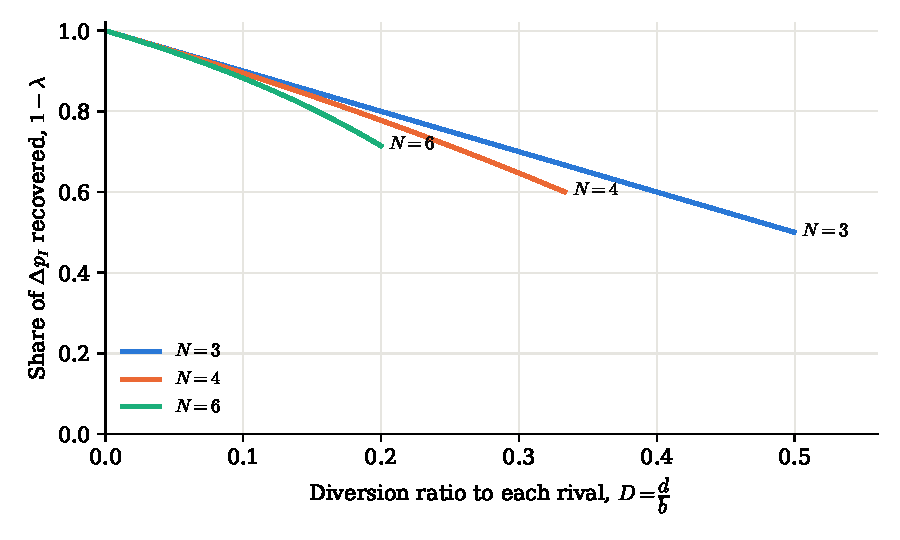
\includegraphics[width=0.78\textwidth]{figures/ch11/did_bias.pdf}
\caption{Share of the insiders' price increase recovered by a DiD estimator that uses an outsider as the control,
$1-\lambda$ from \eqref{eq:11-lambda}, against the diversion ratio to each rival $D=\frac{d}{b}$. Each curve
ends where $b=(N-1)d$. The bias is largest when the products are close substitutes, which is when the merger
matters most.}
\label{fig:11-didbias}
\end{figure}

\Cref{fig:11-didbias} shows the bias for several market sizes. Four lessons follow. First, a DiD that uses rival
brands as controls estimates a lower bound with the correct sign, which is how
\citet{AshenfelterHosken2010} and \citet{AshenfelterHoskenWeinberg2013} use it. Second, the bias grows with
diversion, so it is largest exactly when the merger has the largest effect. Third, a private-label control escapes
the bias only to the extent that store brands are distant substitutes supplied elastically. If store-brand prices
also rise, the bias has the same sign. Fourth, the rivals' price increase is itself an effect of the merger. Total
consumer harm includes it, and \cref{sec:11-dafny} shows how a study can be built on it.

\begin{remark}[General demand]\label{rem:11-didbias-general}
The linear form is not needed for the sign. Let $N=3$ and let $r(p_1,p_2)$ be the outsider's best response, with
partial derivatives $r_1,r_2>0$ (strategic complements) and $r_1+r_2<1$ (the usual stability condition). If the
symmetric insiders raise both prices by $\Delta p_I$, the mean value theorem gives
$\Delta p_O=(r_1+r_2)\big|_{\tilde p}\,\Delta p_I$ at some intermediate price vector $\tilde p$. Then
$0<\Delta p_O<\Delta p_I$. \citet{DeneckereDavidson1985} show for a broad class of demand systems that merging
firms raise prices by more than outsiders. How much outsiders respond depends on how fast elasticities change
with price \citep{CrookeEtAl1999}.
\end{remark}

\subsection{Event windows and transitory selection}\label{sec:11-retro-windows}

The \emph{event window} is the set of months used before and after the merger. It should be long enough to
capture the price change and short enough to avoid contamination by other events. \citet{AshenfelterHosken2010}
prefer a window that drops the three months before and after consummation and uses equal spans of data on the
two sides. Dropping the months near the merger avoids the question of exactly when the parties start pricing
jointly. The law prohibits joint pricing before closing, yet \citet{KimSingal1993} find that many airlines raised
fares before their mergers were consummated \citep[footnote~47]{AshenfelterHosken2008}. The symmetric design protects against a subtler
problem, which we now formalize following \citet{HeckmanRobb1985} and \citet{AshenfelterCard1985}.

Suppose that without the merger log prices follow $y_{jt}(0)=\alpha_j+\tau_t+u_{jt}$. Here $\tau_t$ is common to
all products and $u_{jt}$ is a transitory deviation. Mergers may be triggered by transitory events. A price war,
for example, depresses $u_{j t_0}$ and may push firms to merge. The General Mills purchase of the Chex brands was
announced just after a widely reported price war in ready-to-eat cereal in April 1996 \citep[p.~15]{AshenfelterHosken2008}.

\begin{definition}[Time reversibility]\label{def:11-reversible}
A stationary process $\{u_t\}$ is \emph{time reversible} if, for every $s\ge1$, the pairs $(u_{t_0+s},u_{t_0})$ and
$(u_{t_0-s},u_{t_0})$ have the same joint distribution.
\end{definition}

Every stationary Gaussian process is time reversible. Its joint distributions depend only on the autocovariance
function, and the autocovariance at lag $s$ equals the autocovariance at lag $-s$.

\begin{proposition}[Symmetric windows remove transitory selection]\label{prop:11-window}
Suppose $\{u_{jt}\}_t$ is stationary, time reversible and independent of $\alpha_j$. Suppose the event $A_j$ that
product $j$'s owner merges at $t_0$ depends only on $\alpha_j$, on $u_{jt_0}$ and on variables independent of the
process $\{u_{jt}\}$. Then for every $s\ge1$,
\begin{equation*}
\E\big[u_{j,t_0+s}-u_{j,t_0-s}\mid A_j\big]=0.
\end{equation*}
\end{proposition}

\begin{proof}
Condition first on $(\alpha_j,u_{jt_0})$ and use the law of iterated expectations:
\begin{equation*}
\E\big[u_{j,t_0+s}\mid A_j\big]=\E\Big[\E\big[u_{j,t_0+s}\mid \alpha_j,u_{jt_0}\big]\mid A_j\Big]
=\E\Big[\E\big[u_{j,t_0+s}\mid u_{jt_0}\big]\mid A_j\Big].
\end{equation*}
The second equality uses the independence of the process from $\alpha_j$ and from the other variables in $A_j$. By
time reversibility $\E[u_{j,t_0+s}\mid u_{jt_0}]=\E[u_{j,t_0-s}\mid u_{jt_0}]$. Applying the same two steps
in reverse gives $\E[u_{j,t_0-s}\mid A_j]$.
\end{proof}

The proposition implies that a comparison of month $t_0+s$ with month $t_0-s$ has no transitory selection bias.
So does any average of such comparisons over $s=k,\dots,K$. An asymmetric window does not have this property. Let
$u_{jt}$ be a Gaussian AR(1) process with coefficient $0.8$, and suppose mergers follow price wars, so that
$\E[u_{jt_0}\mid A_j]=-\mu<0$. Then $\E[u_{j,t_0\pm s}\mid A_j]=-(0.8)^{s}\mu$. Compare months 4 to 15 after
the merger with months 4 to 6 before it. The average post-merger deviation is $-0.159\mu$ and the average
pre-merger deviation is $-0.333\mu$. The estimate is biased upward by $0.174\mu$, because the recovery from the
price war is attributed to the merger. The symmetric window guards against this, at the cost of discarding data.
\citet{AshenfelterHosken2010} also report a symmetric window that keeps the months near the merger and an
asymmetric window that uses all available data. The window mattered little except for the cereal merger
\citep[p.~26]{AshenfelterHosken2008}.

Windows also determine which effects we measure. A short window captures the short-run price response. Cost
savings may take longer to reach prices. \citet{FocarelliPanetta2003} find that the price effects of the bank
mergers they study were reversed by efficiency gains after about three years. Long windows, on the other hand, mix the merger
with entry, new products and repositioning, which grow more important as time passes \citep[footnote~49]{AshenfelterHosken2008}.

\subsection{Measuring prices and drawing inferences}\label{sec:11-retro-measure}

\casehead{Unit values versus price indices} A brand is sold in several package sizes $k=1,\dots,K$ with prices per
unit $p_{kt}$ and unit sales $q_{kt}$. The \emph{unit value} or average revenue of the brand is
\begin{equation*}
P^{AR}_t=\frac{\sum_k p_{kt}q_{kt}}{\sum_k q_{kt}}=\sum_k\omega_{kt}\,p_{kt},\qquad \omega_{kt}=\frac{q_{kt}}{\sum_l q_{lt}}.
\end{equation*}
Its change between two periods decomposes as
\begin{equation*}
P^{AR}_1-P^{AR}_0=\sum_k\omega_{k0}\,(p_{k1}-p_{k0})+\sum_k(\omega_{k1}-\omega_{k0})\,p_{k1}.
\end{equation*}
The first term is a price change at fixed quantity weights. The second is a composition effect. If buyers shift
toward large packages, which are cheaper per unit, the unit value falls even when every package price rises. A
\emph{Stone price index} with fixed revenue weights $\bar w_k$ removes the composition term:
\begin{equation*}
\ln P^{S}_t=\sum_k\bar w_k\ln p_{kt},\qquad \ln P^{S}_1-\ln P^{S}_0=\sum_k\bar w_k\,(\ln p_{k1}-\ln p_{k0}).
\end{equation*}
\citet{AshenfelterHosken2010} construct five price measures for cereal, syrup and feminine hygiene products. They
are the unit value, two revenue-weighted average prices with first-year or last-year weights, and two Stone indices
with the same weights. They aggregate weekly data to months to dampen the effect of household stockpiling during sales
\citep{HendelNevo2006}. Scanner data also record retail prices. A merger of manufacturers changes wholesale
prices, and retail prices change by the retailers' pass-through of the wholesale change.

\casehead{Clustered errors} In \eqref{eq:11-ah-price} the regressor $\mathit{Post}_t$ takes the same value for
every product and region in a month. Common monthly shocks then make the errors of a month correlated, and
conventional standard errors are too small \citep{Moulton1987}.

\begin{lemma}[Moulton factor]\label{lem:11-moulton}
Let $y_{it}=\beta_0+\beta x_t+e_{it}$ for $i=1,\dots,m$ observations in each of $T$ months, with
$e_{it}=v_t+w_{it}$, where $v_t$ and $w_{it}$ are independent with mean zero and variances $\sigma_v^2$ and
$\sigma_w^2$. Let $\rho_e=\frac{\sigma_v^2}{\sigma_v^2+\sigma_w^2}$. Then the variance of the OLS estimator
$\hat\beta$ is $1+(m-1)\rho_e$ times the conventional formula that treats the errors as independent.
\end{lemma}

\Cref{lem:11-moulton} is the special case of \cref{prop:A-moulton} with months as clusters of size $m$. The error
components make the errors homoskedastic with variance $\sigma_v^2+\sigma_w^2$, independent across months and
equicorrelated within a month with correlation $\rho_e$. The regressor is constant within a month, so its
intra-cluster correlation is $\rho_x=1$. Then \eqref{eq:A-moulton} gives the factor $1+(m-1)\rho_e$.

With 64 regions and an intra-month correlation of only $0.1$, the factor is $7.3$, and the correct standard error
is $2.7$ times the conventional one. \citet{AshenfelterHosken2010} cluster by month. Clustering by month also
requires enough months, and serial correlation across months is a further concern in DiD designs
\citep{BertrandDufloMullainathan2004}.

\subsection{Which mergers can we study? Selection by the agencies}\label{sec:11-retro-select}

The agencies screen proposed mergers and block or modify those they expect to raise prices. As
\cref{sec:11-review} showed, about 97\% of the mergers filed from 1991 to 2004 went ahead without a full
investigation, and most of the rest were modified, abandoned or blocked. Retrospective samples therefore contain
only cleared mergers. A simple model shows what such samples can reveal.

\begin{assumption}[Screening on a noisy signal]\label{ass:11-screen}
Merger $m$ has a true price effect $\Delta_m$. The agency observes a signal $S_m=\Delta_m+\eta_m$ and clears the
merger if $S_m\le\bar s$. The pair $(\Delta_m,\eta_m)$ is jointly normal and independent across mergers, with
$\Delta_m$ of mean $\mu_\Delta$ and variance $V_\Delta>0$, and $\eta_m$ of mean zero and variance $V_\eta$,
independent of $\Delta_m$.
\end{assumption}

\begin{proposition}[What cleared mergers reveal]\label{prop:11-select}
Under \cref{ass:11-screen},
\begin{equation*}
\E[\Delta_m\mid S_m\le\bar s]\ \le\ \E[\Delta_m\mid S_m=\bar s]\ \le\ \E[\Delta_m\mid S_m>\bar s],
\end{equation*}
and $\E[\Delta_m\mid S_m\le\bar s]\le\mu_\Delta$, the average effect without enforcement.
\end{proposition}

\begin{proof}
Joint normality gives the linear conditional expectation
\begin{equation*}
\E[\Delta_m\mid S_m=s]=\mu_\Delta+k\,(s-\mu_\Delta),\qquad k=\frac{V_\Delta}{V_\Delta+V_\eta}\in(0,1],
\end{equation*}
which is increasing in $s$. Averaging an increasing function over $s\le\bar s$ gives at most its value at $\bar
s$, and averaging over $s>\bar s$ gives at least that value. Finally, $\mu_\Delta$ is a weighted average of the
cleared and blocked means, so it lies between them.
\end{proof}

A random sample of cleared mergers therefore gives a lower bound on the price effect of a typical merger in a
world without enforcement \citep{Carlton2009}. That bound says little about policy, because most proposed
mergers raise no competitive concern. The informative object is the effect of the \emph{marginal merger},
$\E[\Delta_m\mid S_m=\bar s]$. If it is positive, enforcement under a consumer-welfare standard is too lenient at
the margin. If it is negative, enforcement is too strict \citep{AshenfelterHoskenWeinberg2013}. Both studies below
target the margin. \citet{AshenfelterHosken2010} pick cleared mergers that look most problematic from public
information. Their estimates therefore bound from above the effects of other cleared mergers and from below the
effects of blocked ones. \citet{AshenfelterHoskenWeinberg2013} study a merger that was nearly challenged. Two caveats
apply. Researchers see public concentration measures, which are a noisy proxy for the agency's signal. And
samples are also selected by data availability, which favors consumer products and formerly regulated
industries such as airlines, banking and hospitals.

\subsection{Stock-market event studies}\label{sec:11-retro-event}

Before scanner data, retrospectives used stock prices. The method of abnormal returns is developed in
\cref{sec:A-eventstudy}, and \cref{sec:09-wc-method} applies it to airline entry. Its application to mergers, due to \citet{Eckbo1983} and \citet{Stillman1983}, looks at
the merging firms' \emph{rivals}. A merger that raises market power, through unilateral or coordinated effects,
raises rivals' profits. A merger that makes the merged firm a more efficient and tougher competitor lowers them.
News that raises the chance of the merger (the announcement) and news that lowers it (an antitrust complaint)
therefore move rivals' values in opposite directions under each hypothesis. \Cref{tab:11-eventpred} lists the
predictions.

\begin{table}[htbp]
\centering
\caption{Predicted abnormal returns of rival firms}
\label{tab:11-eventpred}
\footnotesize
\begin{tabular}{@{}lcc@{}}
\toprule
Hypothesis & Merger announcement & Antitrust complaint \\
\midrule
Market power (higher post-merger prices) & $+$ & $-$ \\
Efficiency (merged firm a tougher rival) & $-$ & $+$ \\
Information (merger reveals industry-wide gains) & $+$ & $0$ \\
\bottomrule
\end{tabular}

\smallskip
\begin{minipage}{0.85\linewidth}
\footnotesize Notes: Signs of rivals' cumulative abnormal returns. Under the information hypothesis the
announcement reveals profitable opportunities, such as scale economies or the value of rivals as future targets,
that a complaint against one merger does not withdraw.
\end{minipage}
\end{table}

\citet[p.~269]{Eckbo1983} studies the rivals of 65 challenged horizontal mergers. On average they earned an
abnormal return of 2.45 percent over the 31 days around the merger proposal, more than three standard deviations
from zero. Over the 31 days around the antitrust complaint their average return was 1.78 percent, about one standard
deviation from zero, so they did not lose. Eckbo concludes that the data generally reject the collusion hypothesis
(p.~242). He reads the rivals' gains at the proposal as news of cost savings that they can also achieve. He calls
this the productive efficiency hypothesis, which corresponds to the information row of \cref{tab:11-eventpred}.
\citet[p.~240]{Stillman1983} studies the rivals of 11
challenged horizontal mergers attempted between 1964 and 1972. Only in the merger of Sterling Drug and Lehn and Fink
did their returns broadly follow the market-power pattern. In nine of the 11 mergers the rivals showed no abnormal
returns of any kind.
These designs have known limits. Rival returns mix the three hypotheses. News may be anticipated, so the window
captures only part of it. Rivals are often diversified firms, and the affected market can be a small part of
their value. Many relevant rivals are not publicly traded. \citet{Woolley1989} applies the method to 29
merger-related events in hospital chains between 1969 and 1985. \citet{VitaSchumann1991} criticize his choice of
events and rivals and note that listed chains own a small share of hospitals (\citealp[p.~11]{Dafny2005}).
\citet{McAfeeWilliams1988} study the 1979 acquisition of Kalvar by Xidex, two producers of duplicate microfilm. The FTC
challenged the merger in September 1980 (p.~201). McAfee and Williams cite \citet{BartonSherman1984}, who find that
the ratio of vesicular to diazo prices paid by the federal government rose about 25 percent after the merger
\citep[p.~200]{McAfeeWilliams1988}.
An event study of the rivals' returns nevertheless shows no evidence of harm (pp.~202--203).
\citet[p.~231, n.~137]{AskerNocke2021} reach a similar verdict on the literature that runs from \citet{Eckbo1983}
and \citet{Stillman1983} to \citet{DusoNevenRoller2007}. Most authors in it are cautious about what an event study
reveals about the competitive effects of a particular merger. In the words of \citet{KaplowShapiro2007}, an event
study ``measures the expectations of investors about merger effects, not the actual effects of mergers.'' The method
has worked best for patterns across large samples of mergers, as in \citet{DusoNevenRoller2007}. For these reasons
modern retrospectives measure prices directly.

\subsection{Five consumer-product mergers: Ashenfelter and Hosken (2010)}\label{sec:11-ah}

\casehead{Question and design} \citet{AshenfelterHosken2010} ask whether the mergers that the agencies let through
raised consumer prices.\footnote{We use the NBER working-paper version \citep{AshenfelterHosken2008}. Table
numbers and page references follow it.} Their design follows \cref{prop:11-select}. They search the Merger
Yearbook for consummated mergers in consumer-product industries between 1997 and 1999 whose parties sold
substitutes in concentrated markets. The period is fixed by the data, because the vendor sold scanner data only
for the previous five years. Three of the five selected mergers went through without government action:
Procter and Gamble's purchase of Tambrands, Aurora Foods' purchase of Kraft's Log Cabin syrup, and Pennzoil's
purchase of Quaker State. Two were modified by the FTC: General Mills' purchase of Ralcorp's branded cereals and
the merger of Guinness and Grand Metropolitan into Diageo. All five produced highly concentrated markets (HHI above
1,800) with HHI increases above 100 points, the 1992 Guidelines' presumption of harm.

The authors argue that these mergers sit near the enforcement margin. In the FTC's investigations of fiscal years
1996--2003, 46\% of markets had post-merger HHI below 3,000 and 51\% had increases below 800 points. All five
mergers have post-merger HHIs below 3,000 and HHI changes between 200 and 1,000 points, so they sit near the median
of the investigated markets (p.~12). The FTC acted in 25\% of investigated markets with post-merger HHI below 2,500
(four of the five mergers) and in 44\% of markets with increases below 800 (pp.~11--12).

\casehead{The five mergers} Procter and Gamble bought Tambrands for \$1.85 billion in July 1997, adding the leading
tampon (Tampax) to the leading sanitary pad (Always). The Justice Department reviewed the deal and took no
action. Guinness and Grand Metropolitan combined their spirits portfolios in a transaction valued at about \$36
billion. The FTC found harm in premium scotch and premium gin and required the sale of the Bombay gins and Dewar's
scotch to Bacardi for \$1.9 billion. Pennzoil bought Quaker State for \$1 billion in December 1998, combining two
of the five premium motor-oil brands. General Mills bought the Chex cereals for \$570 million in January 1997.
Ralcorp kept its private-label business, the largest in the country, and the FTC's modifications let Ralcorp make
private-label Chex at once. Aurora, owner of Mrs.\ Butterworth's, bought Log Cabin for \$222 million in July 1997,
joining two of the three major syrup brands (pp.~12--16). \Cref{tab:11-ah} reports shares and concentration,
and \cref{tab:11-ahhhi} in \cref{sec:11-hhi} checked the reported changes in concentration against $2s_As_B$.

\begin{table}[htbp]
\centering
\caption{Five consumer-product mergers: concentration and aggregate price effects}
\label{tab:11-ah}
\footnotesize
\begin{tabular}{@{}lcccccc@{}}
\toprule
& & & & & \multicolumn{2}{c}{Aggregate price effect} \\
\cmidrule(l){6-7}
Transaction (industry) & Shares (\%) & HHI & $\Delta$HHI & & Private label & Branded \\
\midrule
General Mills / Ralcorp (cereal) & 28, 4 & 2,357 & 238 & & 0.032 & 0.057 \\
 & & & & & (0.005) & (0.005) \\
Pennzoil / Quaker State (motor oil) & 29, 9 & 2,189 & 517 & & 0.052 & 0.014 \\
 & & & & & (0.013) & (0.011) \\
P\&G / Tambrands (feminine protection) & 25, 19 & 2,815 & 959 & & 0.070 & 0.023 \\
 & & & & & (0.008) & (0.007) \\
Aurora / Log Cabin (pancake syrup) & 15, 19 & 1,990 & 589 & & 0.004 & 0.012 \\
 & & & & & (0.011) & (0.005) \\
Guinness / Grand Met (liquor), overall & 21, 22 & 2,026 & 935 & & 0.027 & $-0.010$ \\
 & & & & & (0.003) & (0.003) \\
\quad gin & & & & & 0.022 & $-0.021$ \\
 & & & & & (0.005) & (0.003) \\
\quad scotch & & & & & 0.071 & 0.031 \\
 & & & & & (0.006) & (0.002) \\
\quad vodka & & & & & 0.011 & $-0.021$ \\
 & & & & & (0.003) & (0.005) \\
\bottomrule
\end{tabular}

\smallskip
\begin{minipage}{0.97\linewidth}
\footnotesize Notes: Shares are pre-merger revenue shares of the acquirer and the target, in that order (for syrup,
Aurora then Philip Morris's Log Cabin). HHI is the post-merger HHI and $\Delta$HHI its change, from pre-merger
revenue data, with private labels treated as one participant. Price effects are the revenue-weighted averages
\eqref{eq:11-ah-agg} of the product-level estimates of $\beta_2$ in \eqref{eq:11-ah-price}, using the private-label
or the branded control group. Standard errors in parentheses assume zero covariances among the components. The data come from IRI's food channel (64 regions) for
cereal, feminine protection and syrup, its mass-merchandiser channel (10 regions) for motor oil, and its drug-store
channel (5 regions) for liquor. Source: \citet{AshenfelterHosken2008}, Tables 2 and 13.
\end{minipage}
\end{table}

\casehead{Data} The data are weekly revenue and unit sales by Universal Product Code (UPC), purchased from
Information Resources Inc.\ (IRI) and aggregated to months. IRI projects sales for each channel and metropolitan
area from a sample of stores. The authors choose for each merger the channel that best represents consumer
purchases. Food products use the food channel in 64 InfoScan markets. Motor oil uses the mass-merchandiser channel
in 10 markets, because consumers who change their own oil buy it there. Liquor uses the only available source, a
drug-store sample with complete data for five markets in three states. The markets are San Francisco, San Diego,
Los Angeles, Chicago and Phoenix, which limits external validity (pp.~16--18). Motor oil is priced as revenue per quart for
each brand and weight. Spirits are priced separately for the 750 ml and 1.75 litre bottles. The other categories
use the five price measures of \cref{sec:11-retro-measure}.

\casehead{Estimation} The price equation \eqref{eq:11-ah-price} is fitted by OLS separately for each merging
product, with standard errors clustered by month. The preferred specification uses the unit value, the symmetric
window that drops three months on each side, and one of two control groups. The \emph{private-label control} uses
the store brands closest to each merging product. These are private-label motor oil, feminine hygiene products and
maple-flavored syrup, private-label gin, scotch and vodka for the spirits, and private-label cereals in the same
IRI segments for cereal. The \emph{branded control} uses close branded substitutes, such as the three other premium motor oils
(Havoline, Valvoline and Castrol). The authors treat the branded estimates mainly as a specification check, for the
reason given in \cref{prop:11-didbias} (pp.~23--24). They also report regressions with no control group.

\casehead{Results} \Cref{tab:11-ah} gives the aggregate effects (Table 13). With the private-label control, four of
the five mergers raised prices by roughly 3\% to 7\%. The estimates are 3.2 log points for General Mills and Chex,
5.2 for Pennzoil and Quaker State, 7.0 for Procter and Gamble and Tambrands, and 2.7 for Diageo. The syrup merger had no
detectable effect (0.4). The branded control gives larger effects for cereal and syrup and smaller ones for the
other three. The spirits merger illustrates the role of the control group. Scotch prices rose under both controls
(7.1 and 3.1 log points), while gin and vodka rose relative to private labels and fell relative to branded
rivals.

The product-level estimates show that the merged firms did not raise all prices together. \Cref{tab:11-ah-pqs}
reproduces Table 3 for motor oil. Relative to private labels, Quaker State rose 8.1 log points and Quaker State
Deluxe 6.1, while the much larger Pennzoil brand rose 3.9. In Table 3, Quaker State's increase ranks first among
the 12 products compared, its own and the 11 branded controls. The text instead describes it as larger than all but
one control brand (p.~28). Market shares moved accordingly. Quaker State lost 1.31 points of revenue share, 13.6\%
of its pre-merger share, while Pennzoil gained 4.22 points. Because Pennzoil's gain exceeded Quaker State's loss,
it grew at the expense of rivals as well. The authors read this as a strategy of raising the price to customers
loyal to Quaker State while holding the price of the larger brand (p.~29).

\begin{table}[htbp]
\centering
\caption{Pennzoil and Quaker State: product-level price and share effects}
\label{tab:11-ah-pqs}
\footnotesize
\begin{tabular}{@{}lcccccc@{}}
\toprule
& \multicolumn{2}{c}{Price effect $\hat\beta_2$} & \multicolumn{2}{c}{Rank in control group} &
\multicolumn{2}{c}{Change in revenue share} \\
\cmidrule(lr){2-3}\cmidrule(lr){4-5}\cmidrule(l){6-7}
Product & Branded & Private label & Branded & Private label & Points & Percent \\
\midrule
Pennzoil & 0.004 & 0.039 & 8/12 & 1/2 & 4.22 & 18.47 \\
 & (0.015) & (0.019) & & & (0.83) & \\
Quaker State & 0.035 & 0.081 & 1/12 & 1/2 & $-1.31$ & $-13.58$ \\
 & (0.016) & (0.015) & & & (0.47) & \\
Quaker State Deluxe & 0.021 & 0.061 & 4/12 & 1/2 & $-0.16$ & $-5.95$ \\
 & (0.021) & (0.022) & & & (0.13) & \\
\bottomrule
\end{tabular}

\smallskip
\begin{minipage}{0.95\linewidth}
\footnotesize Notes: Standard errors in parentheses. The rank orders the product's estimated price change among
the control products in descending order: 8/12 means that seven control products had larger increases. Quantity
shares move similarly ($+4.46$, $-1.32$ and $-0.13$ points). Monthly data from 10 regions of IRI's
mass-merchandiser channel, January 1997 to December 2000, excluding October 1998 to March 1999. An observation is
a product, city and month. The regressions have about 9,000 (branded control) and 2,000 (private-label control)
observations. Source: \citet{AshenfelterHosken2008}, Table 3.
\end{minipage}
\end{table}

The other mergers show the same selectivity (Tables 5, 7, 9 and 11). After buying Tambrands, Procter and Gamble
raised the prices of Always liners and pads by 8.0 and 7.8 log points relative to store brands, and Tampax by
5.8.
Relative to branded products the liner and pad increases were 6.1 and 4.5, and Tampax fell by 0.9. A later study
of the same merger, \citet{Weinberg2011}, reports increases of 8 percent for Always pads and 5 percent for Tampax
relative to private label \citep[p.~262]{AskerNocke2021}. General
Mills left the Chex prices almost unchanged (at most 0.8 log points under either control) and raised the prices
of its own Cheerios and Wheaties brands. Cheerios rose 4.4 log points relative to store brands and 4.6 relative
to branded cereals. Every scotch product rose relative to its private-label control, by 5.5 to 9.8 log points.
For syrup, Log Cabin's 2.8 log point rise relative to branded syrups was not robust, and Mrs.\ Butterworth's prices
did not change.

\casehead{Robustness} For each merger, a summary table pools the estimates across windows, price measures and
control groups (Tables 4, 6, 8, 10 and 12). For motor oil, all 18 estimates are positive. All nine private-label
estimates have $t$-statistics above two, against three of the nine branded estimates. For feminine protection,
92\% of the private-label estimates and 78\% of the branded ones are positive. About 90\% of the cereal estimates
are positive, and none of the negative ones is below $-1\%$. For syrup, about two thirds fall between $-1\%$ and
$+1\%$. The choice of window mattered little except for cereal. The price measure left the signs unchanged and
changed the magnitudes. With weekly data the cereal estimates depended heavily on the price measure, which points to
stockpiling and package substitution (pp.~26--32). Regressions with no control group also show price increases
after virtually every merger (Appendix Tables 3--7). For example, the no-control estimates for Quaker State and
Always pads are 0.061 (0.016) and 0.053 (0.003).

\casehead{Comparison with a merger simulation} The General Mills and Chex merger had been simulated by
\citet{Nevo2000b} with a random-coefficients demand model (\cref{sec:11-simulation}). As cited by Ashenfelter and
Hosken, the published simulation predicts increases before efficiencies of 12.2\% for Chex, 1.1\% for Cheerios,
0.8\% for Honey Nut Cheerios and 0.1\% for Wheaties (p.~32). The retrospective finds the opposite pattern: little
change for Chex and increases for the General Mills brands. Possible reasons include the different data
(quarterly data for 1988--1992 in the simulation), new product introductions, and the demand specification. The
consent decree's provision for private-label Chex may also have restrained Chex pricing, an entry threat that a
simulation with a fixed set of products cannot represent (footnote 60).

\casehead{Interpretation and limitations} The best estimate of the price effect of mergers near the enforcement
margin is positive and modest. This finding cuts against both camps in the enforcement debate. Advocates of less
intervention expect the marginal merger to lower prices through efficiencies, and advocates of more intervention
expect large increases (p.~35). The authors list three limitations themselves (p.~36). Consumer-product mergers are a
small part of all mergers: 20 percent of the 8,013 filings in 1997 and 1998 shared the studied firms' two-digit
industry codes. The design cannot capture longer-run efficiency effects or new products. Finally, the study examines
only one kind of enforcement error, the failure to block harmful mergers, and leaves aside the blocking or
deterrence of benign ones. Several further points deserve attention. The selection rests on public concentration measures, which
may misjudge which mergers the agencies found marginal. The private-label control may itself be a substitute,
especially in cereal, where Ralcorp kept a large store-brand business. The aggregate standard errors ignore
covariances, as shown after \eqref{eq:11-ah-agg}. Retail scanner prices measure the merger's effect after
retailers' pass-through. Finally, the results vary across products within a merger, so several products and
specifications are tested for each merger, and some significant estimates will arise by chance.

\casehead{Contribution} The paper turned merger retrospectives into a program-evaluation exercise with explicit
attention to control groups, windows, price measurement and the selection of mergers. It shows that a cleared
merger's effect can be concentrated on a few products, and it supplied the retrospective benchmarks later used to
grade merger simulations.

\subsection{A nearly blocked merger of appliance makers: Ashenfelter, Hosken and Weinberg (2013)}\label{sec:11-maytag}

\casehead{Question} \citet{AshenfelterHoskenWeinberg2013} estimate the price effects of Whirlpool's acquisition of
Maytag.\footnote{We use the NBER working-paper version \citep{AshenfelterHoskenWeinberg2011}. Table numbers
follow it and may differ from the published article.} The merger is a natural candidate for the marginal merger
of \cref{prop:11-select}. Commentators argued that the Justice Department would have challenged it a decade
earlier, and the decision not to act came to symbolize lenient enforcement \citep{BakerShapiro2008}.

\casehead{Background} In mid-2005 a group of private investors agreed to buy Maytag for \$1.13 billion. The Haier
Group, a Chinese appliance maker with little presence in the United States, then offered \$1.3 billion. Whirlpool,
the largest United States manufacturer, offered \$1.4 billion on July 17, and Haier withdrew three days later.
Whirlpool bought Maytag for \$1.79 billion on March 30, 2006, after a long Justice Department investigation. The
merger reduced the major appliance manufacturers from four (Whirlpool, Maytag, GE and Electrolux) to three. The
Justice Department's closing statement of March 29, 2006, focused on washers and dryers and gave three reasons for
not acting. GE and Electrolux had excess capacity, and the recent entrants LG and Samsung could expand imports.
Large retailers had alternatives to resist price increases. The parties had substantiated large cost savings
(printed pp.~4--6 and 21).

\casehead{Market structure} \Cref{tab:11-maytag} reproduces the pre-merger revenue shares. Whirlpool was the
largest firm in dishwashers, dryers, refrigerators and washers, with 39\% to 49\% of revenue, and Maytag held 9\%
to 17\%. The increase in the HHI matches $2s_Ws_M$ in every category up to rounding of the
shares, within three points. In dryers, for example, $2\times48.8\times16.6=1{,}620$. The parties overlapped less in
cooktops, freezers, ovens and ranges. Neither had more than 1 percent of freezer revenue, Maytag held 5 to 10 percent
of the other three, and the implied HHI changes were 256 to 416 points.
These four categories serve as comparison groups, restricted to brands not made by Whirlpool or Maytag.

\begin{table}[htbp]
\centering
\caption{Whirlpool and Maytag: pre-merger revenue shares and concentration}
\label{tab:11-maytag}
\footnotesize
\begin{tabular}{@{}lccccc@{}}
\toprule
Category & Whirlpool & Maytag & Largest rivals & HHI & $\Delta$HHI \\
\midrule
\multicolumn{6}{@{}l}{\textit{Treated categories}} \\
Dishwashers & 38.6 & 11.4 & Electrolux 25.1, GE 12.5 & 2,453 & 880 \\
Clothes dryers & 48.8 & 16.6 & GE 12.2, LG 9.6, Electrolux 8.9 & 2,983 & 1,620 \\
Refrigerators & 41.8 & 9.2 & Electrolux 24.1, GE 10.9 & 2,595 & 770 \\
Clothes washers & 44.0 & 16.8 & Electrolux 13.8, GE 10.5, LG 10.2 & 2,632 & 1,478 \\
\addlinespace
\multicolumn{6}{@{}l}{\textit{Comparison categories}} \\
Cooktops & 22.0 & 9.5 & GE 20.8, Electrolux 19.1 & 1,571 & 416 \\
Freezers & $<1$ & $<1$ & Electrolux 81.3, Haier 12.8 & 6,789 & 0 \\
Ovens & 32.5 & 6.3 & GE 23.1, Electrolux 10.5 & 1,929 & 412 \\
Ranges & 24.7 & 5.2 & Electrolux 37.6, GE 25.3 & 2,703 & 256 \\
\bottomrule
\end{tabular}

\smallskip
\begin{minipage}{0.95\linewidth}
\footnotesize Notes: Revenue shares in percent from NPD data before the merger. HHI is the pre-merger HHI as
labelled in the source. Neither party had more than 1\% of freezer revenue before the merger. Kenmore, sold by
Sears and partly made by Whirlpool, is not in the data. Source: \citet{AshenfelterHoskenWeinberg2011}, Tables 1
and 2.
\end{minipage}
\end{table}

\casehead{Data} The NPD Group supplied national monthly unit sales and revenue for each appliance model, identified
by its stock-keeping unit (SKU), from January 2005 to September 2008. More than 14,000 SKUs enter during the
period, and observed characteristics explain 85\% to 95\% of the variation in prices. Two features of the industry
shape the design. First, most appliances have a life cycle of about a year. The authors estimate age profiles
separately for each category,
\begin{align}
\ln p_{jt}&=\alpha_j+\sum_{k=2}^{25}\theta_k\,\mathit{Age}_{kjt}+\sum_{l=2}^{43}\delta_l\,\mathit{Month}_{lt}+e_{jt},\label{eq:11-ahw-age}\\
\ln q_{jt}&=\psi_j+\sum_{k=3}^{25}\lambda_k\,\mathit{Age}_{kjt}+\sum_{l=3}^{43}\gamma_l\,\mathit{Month}_{lt}+u_{jt},\nonumber
\end{align}
where $\mathit{Age}_{kjt}$ indicates that model $j$ is $k$ months old.\footnote{In this subsection $\theta_k$,
$\delta_l$, $\psi_j$, $\lambda_k$ and $\gamma_l$ are regression coefficients with no relation to their meanings
elsewhere in the book.} Prices of washers, dryers, dishwashers, refrigerators, freezers and ranges typically fall by more
than 10\% after a year, and monthly sales fall by about half. Ovens and cooktops show no such decline. The analysis
therefore uses each model's first year only and controls for age by category. Second, many SKUs sell very few
units. The sample keeps models with at least 1,000 units in their first 13 months (100 for freezers, ovens and
cooktops). The retained models account for 90\% to 99\% of sales in the large categories (printed pp.~6--9).

\casehead{Estimating equations} The baseline specification, fitted by OLS separately for each treated and
comparison pair of categories, is
\begin{multline}\label{eq:11-ahw-fe}
\ln p_{jt}=\beta_1\,\mathit{Maytag}_j\,\mathit{Post}_t+\beta_2\,\mathit{Whirlpool}_j\,\mathit{Post}_t\\
+\sum_{k=3}^{13}\theta_k^{T}\mathit{Age}^{T}_{kjt}+\sum_{k=3}^{13}\theta_k^{C}\mathit{Age}^{C}_{kjt}+\sum_{l=2}^{43}\delta_l\,\mathit{Month}_{lt}+\alpha_j+e_{jt}.
\end{multline}
It has separate age profiles for the treated ($T$) and comparison ($C$) categories, month effects and SKU fixed
effects $\alpha_j$. The SKU fixed effects have a cost. The interactions are collinear with $\alpha_j$ for any model
sold only before or only after the merger. Equation \eqref{eq:11-ahw-fe} therefore identifies the effects only from
models sold on both sides of the merger date. With one-year life cycles, these are old models, and the merged firm may have
treated them differently from new ones. The authors therefore replace the fixed effects with observed
characteristics and brand dummies, such as a stainless-steel indicator, size, capacity and cycles:
\begin{multline}\label{eq:11-ahw-char}
\ln p_{jt}=x^{T}_{j}\beta^{T}+x^{C}_{j}\beta^{C}+\sum_{l=2}^{43}\delta^{C}_l\,\mathit{Month}_{lt}+\beta_1\,\mathit{Maytag}_j\,\mathit{Post}_t+\beta_2\,\mathit{Whirlpool}_j\,\mathit{Post}_t\\
+\sum_{k=3}^{13}\theta_k^{T}\mathit{Age}^{T}_{kjt}+\sum_{k=3}^{13}\theta_k^{C}\mathit{Age}^{C}_{kjt}+e_{jt}.
\end{multline}
Here $x^T_j$ is non-zero only for the parties' models and $x^C_j$ only for comparison models. Standard errors
are clustered by SKU. The check on this substitution is direct. On models sold both before and after the merger,
the two specifications give estimates within 0.2 percentage points of each other against cooktops and ranges.
Against cooktops, for instance, the Whirlpool dishwasher effect is 0.0432 with fixed effects and 0.0415 with
characteristics (Appendix Table 1). The gaps reach 0.7 points against ovens and 1 to 2 points against freezers, well
within one standard error (Appendix Tables 2--4).

The main specification splits each interaction by whether the model was introduced before (Old) or after (New)
the merger, which adds 35\% to 57\% to the sample. A within-category variant compares the parties' models with
rivals' models in the same category,
\begin{multline}\label{eq:11-ahw-rival}
\ln p_{jt}=x_j\beta+\sum_{k}\theta_k\,\mathit{Age}_{kjt}+\sum_{l}\delta_l\,\mathit{Month}_{lt}
+\beta_1\,\mathit{Maytag}_j\mathit{Post}_t\mathit{Old}_j+\beta_2\,\mathit{Whirlpool}_j\mathit{Post}_t\mathit{Old}_j\\
+\beta_3\,\mathit{Maytag}_j\mathit{Post}_t\mathit{New}_j+\beta_4\,\mathit{Whirlpool}_j\mathit{Post}_t\mathit{New}_j+e_{jt}.
\end{multline}
By \cref{prop:11-didbias}, the rival comparison is biased toward zero if rivals' models are substitutes.
Finally, product variety is measured by the number of SKUs selling at least 100 units a month,
\begin{equation}\label{eq:11-ahw-sku}
\ln\mathit{SKU}_{ft}=a+b\,\mathit{WM}_f+g\,\mathit{Post}_t+\delta^{V}\,\mathit{WM}_f\,\mathit{Post}_t+e_{ft},
\end{equation}
where $f$ is either the merged firm ($\mathit{WM}_f=1$) or all rivals together. The coefficient $\delta^V$ is the
proportional change in the merged firm's product count relative to rivals.

\casehead{Identification} The comparison categories identify the counterfactual price path. The design assumes that
cooktops, freezers, ovens and ranges made by other firms would have followed the same age- and
characteristic-adjusted price trend as the treated categories. All are durable goods bought with new homes and
remodeling, so they share much of the demand shock from the housing market. The data are national, so there is no
geographic variation. Identification rests entirely on comparisons across categories and, in
\eqref{eq:11-ahw-rival}, across firms within a category.

\begin{figure}[htbp]
\centering
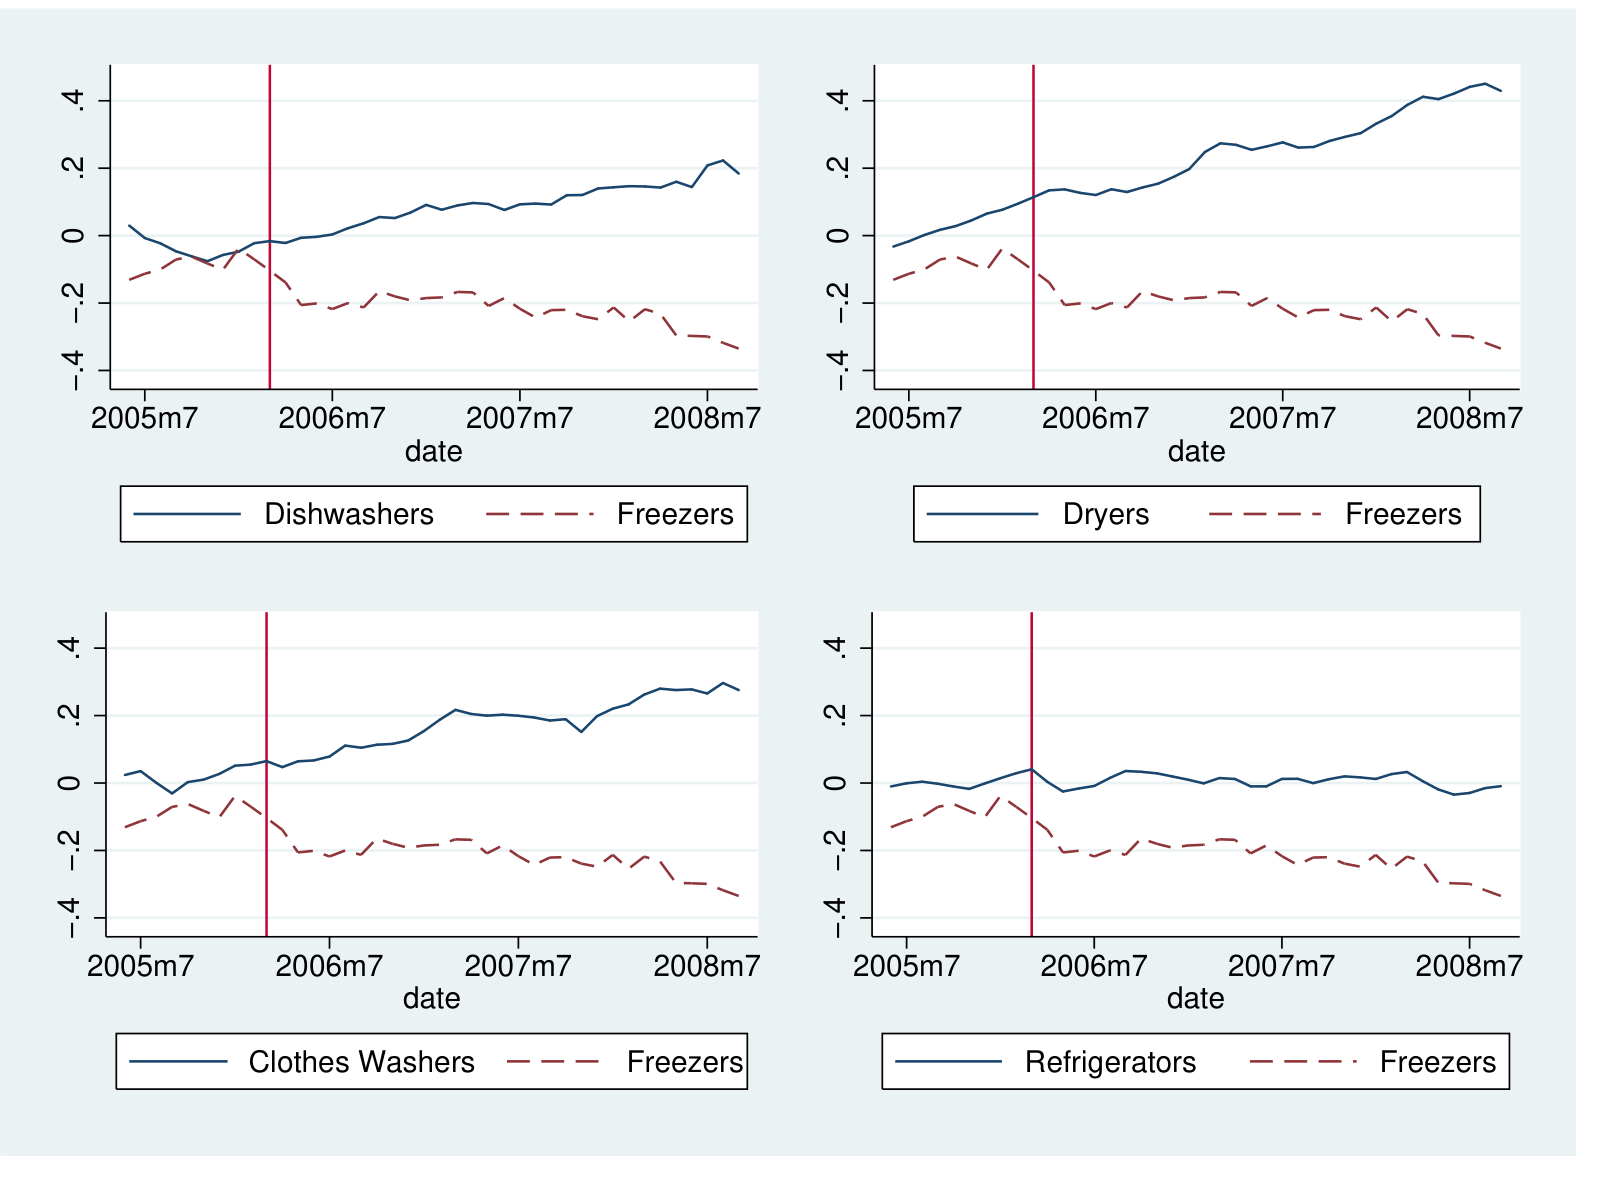
\includegraphics[width=0.86\textwidth]{figures/ch11/ahw_fig5.png}
\caption{Average log prices of Whirlpool and Maytag appliances (solid) and of freezers (dashed), adjusted for
product characteristics and age, May 2005 to September 2008. The vertical line marks consummation (March 30,
2006). Dishwasher, dryer and washer prices rise relative to freezers after the merger. Refrigerator prices do not.
The averages pool old and new models. The vintage-split regressions of \cref{tab:11-maytag-res} find no increase for
new washers. Source: \citet{AshenfelterHoskenWeinberg2011}, Figure 5.}
\label{fig:11-maytag}
\end{figure}

\casehead{Results} \Cref{fig:11-maytag} plots adjusted prices against freezers. \Cref{tab:11-maytag-res} reproduces
the regression estimates for the four treated categories against each comparison category (Tables 3 to 6) and
against rivals in the same category (Table 7). The clearest effects are for models introduced after the merger.
New Whirlpool dryers rose by 13.3 to 17.1 log points relative to the comparison categories, all significant. New
Maytag dishwashers rose by 4.8 to 7.4 log points, all significant at 5\%. New Whirlpool refrigerators rose by 1.9 to
3.9 log points, significant except against freezers. The authors give this result little weight. They describe ``a
small price increase, 2-4\%, for Whirlpool refrigerators'' that is ``imprecisely estimated and not as robust as the
findings for clothes dryers or dishwashers'' (printed pp.~15--16). The within-category estimate is only 0.008
(0.009), and their abstract concludes that there were ``no price effects for refrigerators or clothes washers''
(PDF p.~1). \citet[p.~262]{AskerNocke2021} quote the same sentence from the published abstract. Washers show no
increase. New Whirlpool washers in fact fell
by 1.5 to 4.1 log points. Estimates for models introduced before the merger depend on the comparison category.
They tend to be positive against cooktops and freezers and smaller or negative against ovens and ranges. The
within-category comparison tells the same story: new Maytag dishwashers rose 8.2 log points and new Whirlpool
dryers 7.3 log points relative to rivals' new models.

\begin{table}[htbp]
\centering
\caption{Whirlpool and Maytag: price effects by category, model vintage and comparison group}
\label{tab:11-maytag-res}
\footnotesize
\begin{tabular}{@{}lccccc@{}}
\toprule
& \multicolumn{4}{c}{Comparison category, \eqref{eq:11-ahw-char} split by vintage} & Rivals, \eqref{eq:11-ahw-rival} \\
\cmidrule(lr){2-5}\cmidrule(l){6-6}
Post-merger $\times$ & Cooktops & Freezers & Ovens & Ranges & Same category \\
\midrule
\multicolumn{6}{@{}l}{\textit{Clothes dryers}} \\
Old $\times$ Whirlpool & $-0.0172$ & 0.0291 & $-0.0654$ & $-0.0602$ & $-0.055$ \\
 & (0.0198) & (0.0347) & (0.0218) & (0.0176) & (0.018) \\
Old $\times$ Maytag & 0.0437 & 0.0903 & $-0.0102$ & 0.000473 & 0.008 \\
 & (0.0132) & (0.0310) & (0.0153) & (0.00671) & (0.008) \\
New $\times$ Whirlpool & 0.133 & 0.140 & 0.171 & 0.144 & 0.073 \\
 & (0.0653) & (0.0479) & (0.0471) & (0.0542) & (0.030) \\
New $\times$ Maytag & 0.00486 & 0.0113 & 0.0574 & 0.0318 & $-0.002$ \\
 & (0.0864) & (0.0622) & (0.0623) & (0.0757) & (0.040) \\
Observations & 2,657 & 2,206 & 2,563 & 4,429 & 3,088 \\
\addlinespace
\multicolumn{6}{@{}l}{\textit{Dishwashers}} \\
Old $\times$ Whirlpool & 0.0325 & 0.0855 & $-0.00769$ & 0.0124 & 0.024 \\
 & (0.0135) & (0.0307) & (0.0168) & (0.00739) & (0.008) \\
Old $\times$ Maytag & 0.0275 & 0.0826 & $-0.00919$ & 0.0100 & 0.030 \\
 & (0.0161) & (0.0310) & (0.0188) & (0.0107) & (0.011) \\
New $\times$ Whirlpool & $-0.00127$ & $-0.0160$ & 0.00463 & 0.00115 & 0.014 \\
 & (0.0157) & (0.0161) & (0.0151) & (0.00684) & (0.007) \\
New $\times$ Maytag & 0.0662 & 0.0480 & 0.0711 & 0.0743 & 0.082 \\
 & (0.0206) & (0.0200) & (0.0200) & (0.0163) & (0.015) \\
Observations & 2,296 & 1,845 & 2,202 & 4,068 & 2,895 \\
\addlinespace
\multicolumn{6}{@{}l}{\textit{Refrigerators}} \\
Old $\times$ Whirlpool & $-0.0213$ & 0.0455 & $-0.0465$ & $-0.0221$ & $-0.044$ \\
 & (0.0227) & (0.0341) & (0.0240) & (0.0202) & (0.021) \\
Old $\times$ Maytag & $-0.0266$ & 0.0370 & $-0.0506$ & $-0.0254$ & $-0.045$ \\
 & (0.0267) & (0.0363) & (0.0286) & (0.0251) & (0.025) \\
New $\times$ Whirlpool & 0.0388 & 0.0194 & 0.0389 & 0.0210 & 0.008 \\
 & (0.0159) & (0.0164) & (0.0145) & (0.00951) & (0.009) \\
New $\times$ Maytag & 0.00602 & $-0.00641$ & 0.0157 & 0.00960 & $-0.026$ \\
 & (0.0212) & (0.0229) & (0.0200) & (0.0164) & (0.017) \\
Observations & 3,534 & 3,083 & 3,440 & 5,306 & 5,902 \\
\addlinespace
\multicolumn{6}{@{}l}{\textit{Clothes washers}} \\
Old $\times$ Whirlpool & $-0.00856$ & 0.0341 & $-0.0556$ & $-0.0431$ & $-0.040$ \\
 & (0.0256) & (0.0373) & (0.0273) & (0.0231) & (0.027) \\
Old $\times$ Maytag & 0.0383 & 0.0848 & $-0.0117$ & 0.00310 & 0.006 \\
 & (0.0177) & (0.0318) & (0.0195) & (0.0127) & (0.017) \\
New $\times$ Whirlpool & $-0.0175$ & $-0.0409$ & $-0.0150$ & $-0.0202$ & $-0.047$ \\
 & (0.0171) & (0.0175) & (0.0176) & (0.0106) & (0.013) \\
New $\times$ Maytag & 0.0157 & $-0.00743$ & 0.0223 & 0.0171 & $-0.014$ \\
 & (0.0179) & (0.0179) & (0.0180) & (0.0111) & (0.014) \\
Observations & 2,264 & 1,813 & 2,170 & 4,036 & 2,456 \\
\bottomrule
\end{tabular}

\smallskip
\begin{minipage}{0.97\linewidth}
\footnotesize Notes: OLS estimates of the post-merger change in log price of the parties' models, standard errors
in parentheses, clustered by SKU. Each row label is interacted with the post-merger indicator. Old (New) marks
models introduced before (after) the merger. Product characteristics, age dummies and month dummies are included
throughout. Coefficients are as printed in the source. Monthly NPD data, April 2005 to September 2008. Source:
\citet{AshenfelterHoskenWeinberg2011}, Tables 3 to 7.
\end{minipage}
\end{table}

\casehead{Market shares and variety} \Cref{tab:11-maytag-var} reproduces Table 8. The merged firm's revenue share
fell significantly in every treated category, by 4.6 points in dishwashers, 9.5 in dryers, 8.6 in refrigerators
and 7.3 in washers. The fall is consistent with the price increases in dryers and dishwashers. It also occurred in
refrigerators and washers, where prices did not rise, so it cannot be due to price alone. The merged firm cut its
product line. The number of high-volume Whirlpool and Maytag SKUs fell by about 10 a month in dryers and washers
and by about 12 in refrigerators. Relative to rivals, who expanded their lines, the merged firm's count fell by 22
to 53 log points.

\begin{table}[htbp]
\centering
\caption{Whirlpool and Maytag: market shares and product offerings after the merger}
\label{tab:11-maytag-var}
\footnotesize
\begin{tabular}{@{}lcccc@{}}
\toprule
& \multicolumn{2}{c}{Change in share} & Absolute change & Relative change \\
\cmidrule(lr){2-3}
Category & Revenue & Volume & in SKUs offered & in SKUs offered, $\delta^V$ \\
\midrule
Dishwashers & $-0.046$ (0.010) & $-0.043$ (0.011) & $-1.067$ (1.862) & $-0.219$ (0.044) \\
Clothes dryers & $-0.095$ (0.009) & $-0.068$ (0.008) & $-9.767$ (2.690) & $-0.527$ (0.046) \\
Refrigerators & $-0.086$ (0.011) & $-0.110$ (0.013) & $-12.500$ (5.392) & $-0.266$ (0.050) \\
Clothes washers & $-0.073$ (0.008) & $-0.053$ (0.007) & $-10.367$ (2.613) & $-0.527$ (0.050) \\
Observations & 45 & 45 & 45 & 90 \\
\bottomrule
\end{tabular}

\smallskip
\begin{minipage}{0.92\linewidth}
\footnotesize Notes: Standard errors in parentheses. Share columns: regression of the merged firm's monthly share
on a post-merger indicator. Absolute change: regression of the number of the merged firm's SKUs with more than 100
monthly unit sales on the indicator. Relative change: equation \eqref{eq:11-ahw-sku}. Source:
\citet{AshenfelterHoskenWeinberg2011}, Table 8.
\end{minipage}
\end{table}

\casehead{Interpretation} The merged firm raised the prices of new Whirlpool dryers by about 14\% and new Maytag
dishwashers by about 7\% (printed p.~22). By the authors' own reading, it did not raise refrigerator or washer
prices. The washer result is the puzzle, because Whirlpool and Maytag had
similar positions in washers and dryers. The authors point to a technological shift in washers. Buyers were moving
from top-loading machines, where the parties were strong, to front-loading machines, where LG and Samsung competed
strongly. The Justice Department's entry argument may thus have held for washers. For dryers and dishwashers the
factors it cited did not keep prices at pre-merger levels. The fall in variety may be a further consumer cost that
price studies miss \citep{BerryWaldfogel2001,Sweeting2010}.

\casehead{Limitations} The comparison categories are a judgment call. Freezers and ranges may respond differently
to the 2006--2008 housing downturn than dryers and dishwashers, and the estimates for old models vary with the
comparison category. The comparison categories are made by GE and Electrolux, which compete with the merged firm in
the treated categories, so multimarket responses could reach them. Clustering by SKU allows serial correlation
within a model. It does not allow for common monthly shocks across models in a category. Because the post-merger indicator varies
only by month, such shocks would make the reported standard errors too small (\cref{lem:11-moulton}). The data
omit Kenmore, which Whirlpool partly supplied to Sears. Finally, the split by vintage is informative only if
introductions after the merger are comparable to earlier ones in unobserved quality. The fixed-effect comparison can
check this condition only for models sold on both sides of the merger date.

\casehead{Contribution} The study supplies a retrospective of a merger chosen for being at the margin of
enforcement. It shows that effects can be concentrated in new products, which a design based on SKU fixed effects
would miss. It also documents a cut in variety alongside the price effects.

\subsection{Hospital mergers and rival analysis with an instrument: Dafny (2009)}\label{sec:11-dafny}

\casehead{Question} Comparisons of merging and non-merging firms suffer from selection, because firms that merge
differ from those that do not. Suppose financially distressed hospitals are more likely to merge and would have
cut costs and prices anyway. A comparison of merging and non-merging hospitals then attributes those cuts to the
merger. \citet{Eckbo1983} proposed \emph{rival analysis}, which drops the merging firms and compares the outcomes of
firms with merging rivals to those of firms without. With strategic complements, rivals raise prices when merging
firms do. Rival analysis still suffers from selection, because markets with mergers differ from markets without
them. \citet{Dafny2009} combines rival analysis with an instrument for exposure to a rival's
merger.\footnote{We use the NBER working-paper version of 2005, revised October 2007 \citep{Dafny2005}. Page
references are to its printed pages.} Hospitals are a natural setting, because a wave of hospital mergers in the
1990s met agencies that lost every court challenge.

\casehead{Theory} The instrument rests on a spatial model, Salop's circular city \citep{Salop1979}. A unit mass of
consumers is spread uniformly on a circle of circumference one. Each buys one unit, values it at $v$, and incurs a
transport cost $t$ per unit of distance. Marginal costs are zero. Two markets have three hospitals each: the
hospital of interest $H$ and two rivals $R_1$ and $R_2$. In market 1 the rivals are \emph{co-located}, at the same
point opposite $H$. In market 2 the three hospitals are evenly spaced (\cref{fig:11-dafny}).

\begin{figure}[htbp]
\centering
\begin{tikzpicture}[scale=1.0]
  \begin{scope}
    \draw[thick] (0,0) circle (1.2);
    \foreach \a/\lab/\pos in {90/{$R_1,R_2$}/above, 270/{$H$}/below}{
      \draw[thick] (\a:1.2) -- (\a:1.42);
      \node[\pos] at (\a:1.42) {\lab};
    }
    \node at (-1.75,0) {$\frac{1}{2}$};
    \node at (1.75,0) {$\frac{1}{2}$};
    \node at (0,-2.3) {Market 1: co-located rivals};
  \end{scope}
  \begin{scope}[xshift=6cm]
    \draw[thick] (0,0) circle (1.2);
    \foreach \a/\lab/\pos in {150/{$R_1$}/above left, 30/{$R_2$}/above right, 270/{$H$}/below}{
      \draw[thick] (\a:1.2) -- (\a:1.42);
      \node[\pos] at (\a:1.42) {\lab};
    }
    \node at (90:1.6) {$\frac{1}{3}$};
    \node at (210:1.65) {$\frac{1}{3}$};
    \node at (330:1.65) {$\frac{1}{3}$};
    \node at (0,-2.3) {Market 2: evenly spaced};
  \end{scope}
\end{tikzpicture}
\caption{The two hypothetical markets of the theory. Each circle has circumference one, and the fractions give the
arc lengths between neighboring hospitals. In market 1 the rivals $R_1$ and $R_2$ are co-located opposite $H$. In
market 2 the three hospitals are evenly spaced. Redrawn from \citet{Dafny2005}, Figure 1.}
\label{fig:11-dafny}
\end{figure}

Consider market 1 before the rivals merge. Co-located rivals are undifferentiated Bertrand competitors, so they
price at cost, $p_{R}=0$. A consumer at distance $x$ from $H$ is at distance $\frac{1}{2}-x$ from the rivals. She
buys from $H$ if $p_H+tx\le t(\frac{1}{2}-x)$, that is if $x\le\frac{1}{4}-\frac{p_H}{2t}$. Counting both sides of
$H$, its profit is
\begin{equation*}
\pi_H=p_H\cdot2\Big(\frac{1}{4}-\frac{p_H}{2t}\Big).
\end{equation*}
The first-order condition $\frac{1}{2}-\frac{2p_H}{t}=0$ gives $p_H^*=\frac{t}{4}$. Now let the rivals merge into
one firm $R$ with price $p_R$. The indifferent consumer moves to $x=\frac{1}{4}-\frac{p_H-p_R}{2t}$, and
\begin{equation*}
\pi_H=p_H\cdot2\Big(\frac{1}{4}-\frac{p_H}{2t}+\frac{p_R}{2t}\Big).
\end{equation*}
The first-order condition is $\frac{1}{2}-\frac{2p_H}{t}+\frac{p_R}{t}=0$. By symmetry $p_H=p_R$, so
$p_H^*=\frac{t}{2}$. The merger of co-located rivals doubles $H$'s price. Before the merger the rivals priced at
cost. After it they price like a differentiated firm, and $H$ responds to their higher price.

In market 2 the three hospitals are $\frac{1}{3}$ apart. Before the merger the standard symmetric Salop
equilibrium gives $p_H^*=\frac{t}{3}$. Suppose that after the merger one rival facility closes and the other stays
put, so $H$ and $R$ are $\frac{1}{3}$ apart on one side and $\frac{2}{3}$ on the other. $H$'s demand is
$\frac{1}{6}+\frac{p_R-p_H}{2t}$ on the short arc plus $\frac{1}{3}+\frac{p_R-p_H}{2t}$ on the long arc. Profit
$p_H(\frac{1}{2}+\frac{p_R-p_H}{t})$ gives the condition $\frac{1}{2}+\frac{p_R}{t}-\frac{2p_H}{t}=0$, so
$p_H^*=\frac{t}{2}$ at the symmetric equilibrium. The increase is from $\frac{t}{3}$ to $\frac{t}{2}$, or 50\%,
against 100\% in market 1. Mergers of co-located rivals raise prices more because the merger removes a fiercer
pre-merger rivalry.

These formulas hold when $t$ is small relative to $v$, so that every consumer buys and the hospitals compete for
the marginal consumer. Market 1 requires $t<\frac{4v}{3}$ after the merger and market 2 requires
$t<\frac{6v}{5}$. For larger $t$ the marginal consumer's reservation value binds, and demand has a kink. Dafny's
Appendix 1 gives the full solutions:
\begin{align*}
\text{Market 1:}\quad
p_H^{*,pre}&=\begin{cases}\frac{t}{4}, & t<\frac{8v}{3},\\[2pt] 2v-\frac{t}{2}, & \frac{8v}{3}<t<3v,\\[2pt] \frac{v}{2}, & t>3v,\end{cases}
&
p_H^{*,post}&=\begin{cases}\frac{t}{2}, & t<\frac{4v}{3},\\[2pt] v-\frac{t}{4}, & \frac{4v}{3}<t<2v,\\[2pt] \frac{v}{2}, & t>2v,\end{cases}\\[4pt]
\text{Market 2:}\quad
p_H^{*,pre}&=\begin{cases}\frac{t}{3}, & t<2v,\\[2pt] v-\frac{t}{6}, & 2v<t<3v,\\[2pt] \frac{v}{2}, & t>3v,\end{cases}
&
p_H^{*,post}&=\begin{cases}\frac{t}{2}, & t<\frac{6v}{5},\\[2pt] v-\frac{t}{3}, & \frac{6v}{5}<t<\frac{3v}{2}.\end{cases}
\end{align*}
In the middle ranges the hospitals price so that the consumer midway between them gets zero surplus. Take market 1
before the merger. Consumers within $\frac{v}{t}$ of the rivals buy from them at price zero. $H$ can sell to
everyone else only if the consumer at distance $\frac{1}{2}-\frac{v}{t}$ from $H$ gets zero surplus from $H$. That
condition gives $p_H=v-t(\frac{1}{2}-\frac{v}{t})=2v-\frac{t}{2}$.\footnote{For market 2 after the merger, the
appendix gives $\frac{v}{2}$ for all $t>\frac{3v}{2}$. Our derivation differs on part of this range. For
$\frac{3v}{2}<t<3v$ the two remaining hospitals are local monopolists on the long arc but still compete on the
short arc. Their symmetric equilibrium price is $\frac{2v}{5}+\frac{t}{15}$ for $\frac{3v}{2}<t<\frac{18v}{7}$ and
$v-\frac{t}{6}$ for $\frac{18v}{7}<t<3v$, and it is $\frac{v}{2}$ only for $t>3v$. We checked numerically that these
prices are equilibria and that $\frac{v}{2}$ is not. The difference lies outside
the range used for the comparison in the text.} \Cref{fig:11-dafny-prices} plots the solutions with $v=1$.

\begin{figure}[htbp]
\centering
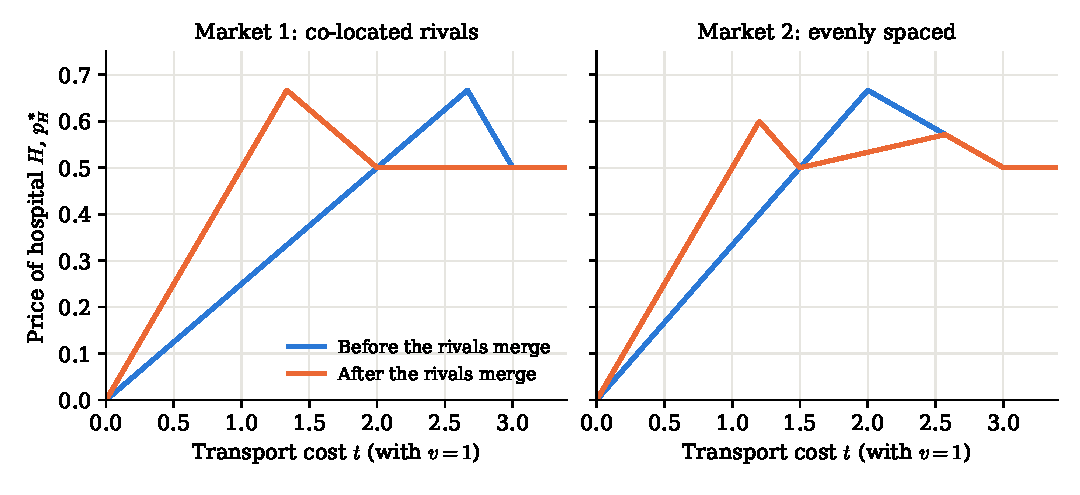
\includegraphics[width=0.95\textwidth]{figures/ch11/dafny_salop_prices.pdf}
\caption{Equilibrium price of hospital $H$ before and after its two rivals merge, as a function of the transport
cost $t$, with $v=1$. Left: co-located rivals. Right: evenly spaced hospitals, one of whose rival facilities closes
after the merger. Solutions from \citet{Dafny2005}, Appendix 1, with the market-2 post-merger curve for
$t>\frac{3}{2}$ derived in the footnote.}
\label{fig:11-dafny-prices}
\end{figure}

Dafny reports that with $v=1$ the average price increase is 66.7\% in market 1 and 40\% in market 2 (footnote 37).
We can reproduce these numbers as percentage gaps between average post-merger and average pre-merger prices. The
averages are taken over the range of $t$ in which the post-merger hospitals still compete, $t<2v$ in market 1 and
$t<\frac{3v}{2}$ in market 2. In
market 1 the average pre-merger price over $(0,2)$ is $0.250$ and the average post-merger price is $0.417$. In market
2 the averages over $(0,\frac{3}{2})$ are $0.250$ and $0.350$. Two predictions follow. Co-located hospitals are more
likely to merge, because they gain more market power and can cut duplicate departments. And a merger of
co-located rivals raises the prices of nearby hospitals by more. The number of co-located rival pairs near a
hospital is therefore a candidate instrument for exposure to rival mergers.

\casehead{Setting} Until 1984 hospitals were paid largely on a cost-plus basis. Medicare's Prospective Payment
System of 1984 paid a fixed amount per admission in each diagnosis-related group, and by 1989 most hospitals lost
money on Medicare patients. Managed care rose from under 30\% of private insurance in 1988 to nearly 95\% by 1999,
replacing fee-for-service payment with negotiated prices. There were 190 hospital mergers between 1989 and 1996,
against 74 between 1983 and 1988. Since 1991 the agencies had tried to block seven hospital mergers and lost every
time, often because courts accepted that non-profit hospitals would not exploit market power (printed pp.~8--9).

\casehead{Data} Merger data come from \citet{DranoveLindrooth2003}, who identify 97 independent hospital mergers
between 1989 and 1996. An independent merger combines two hospitals outside any system into a single entity that
reports one set of accounts and surrenders a license. The sample starts from general, non-federal hospitals in the
1988 American Hospital Association survey, located in metropolitan areas or counties with more than 100,000
residents. Price comes from Medicare cost reports. It is non-Medicare inpatient revenue per case-mix-adjusted
non-Medicare discharge, with charges deflated by each hospital's contractual discounts and Medicare's case-mix
index as a proxy for the non-Medicare one. The tails at the 5th and 95th percentiles are censored. Co-location is
measured from geocoded addresses. Two hospitals are co-located if they are within 0.3 miles as the crow flies and
no more than five blocks apart. Of 213 hospitals within 0.3 miles of another, 191 (3.6\% of 5,373) pass the map
check (printed pp.~12--15).

\Cref{tab:11-dafny-data} summarizes the two samples. In the All Hospitals sample of 4,487 hospitals, 178 (4.0\%)
merged and 163 (3.6\%) were co-located. Eighteen of the 163 merged, a rate of 11\% against 3.7\% for other hospitals.
The Rivals Sample contains the 877 non-merging hospitals with at least two rivals within 7 miles and complete price
data. Of these, 118 had a merging rival (NMW, for non-merging with merging rivals) and 759 did not (NMWO). The two
groups differ. NMW hospitals have nearly twice as many rivals, more Medicaid patients and slightly higher penetration of health maintenance organizations (HMOs).
Their prices grew by $-2.9\%$ between 1985 and 1988, against $4.2\%$ for NMWO hospitals. Treating rival mergers as
exogenous would therefore understate their effect.

\begin{table}[htbp]
\centering
\caption{Hospital mergers: sample means}
\label{tab:11-dafny-data}
\footnotesize
\begin{tabular}{@{}lcccc@{}}
\toprule
& All hospitals & \multicolumn{3}{c}{Rivals Sample} \\
\cmidrule(l){3-5}
& & All & NMW & NMWO \\
\midrule
1988 price (\$ of 2000) & 3,404 & 4,057 & 3,737 & 4,107 \\
1997 price (\$ of 2000) & 3,851 & 4,091 & 3,823 & 4,133 \\
$\ln p_{1988}-\ln p_{1985}$ & 0.064 & 0.032 & $-0.029$ & 0.042 \\
$\ln p_{1997}-\ln p_{1988}$ & 0.132 & 0.010 & 0.020 & 0.009 \\
$\ln p_{2000}-\ln p_{1997}$ & 0.013 & 0.001 & 0.039 & $-0.005$ \\
Merged, 1989--1996 (\%) & 4.0 & & & \\
Co-located (\%) & 3.6 & & & \\
Number of rival mergers, $R_i$ & & 0.156 & 1.161 & 0 \\
Number of co-located rival pairs, $Z_i$ & & 0.332 & 0.712 & 0.273 \\
Number of rivals within 7 miles & 3.16 & 7.37 & 12.03 & 6.64 \\
Medicaid share of discharges (\%) & 11.4 & 11.2 & 15.1 & 10.6 \\
County HMO penetration (\%) & 14.5 & 21.3 & 23.7 & 20.9 \\
Hospitals & 4,487 & 877 & 118 & 759 \\
\bottomrule
\end{tabular}

\smallskip
\begin{minipage}{0.9\linewidth}
\footnotesize Notes: NMW (NMWO) are non-merging hospitals with (without) a rival within 7 miles that merged in
1989--1996. Price change variables are censored at the 5th and 95th percentiles. Characteristics are for 1988,
HMO penetration for 1994. Selected rows. Source: \citet{Dafny2005}, Table 1.
\end{minipage}
\end{table}

\casehead{Estimating equations} For hospital $i$ in the Rivals Sample, let $R_i$ be the number of rival mergers
within 7 miles between 1989 and 1996. Let $Z_i$ be the number of co-located rival pairs within 7 miles in 1988,
excluding any pair to which $i$ belongs. Let $X_i$ be a vector of 1988 hospital and market characteristics. The outcome is
the change in log price between 1988 and 1997, $\Delta\ln p_i$, which spans the year before the first merger to the
year after the last. Because the instrument predicts whether but not when a rival merges, the design uses one
long difference. The equations are
\begin{align}
\text{first stage:}\qquad & R_i=\pi Z_i+X_i^{\top}\omega_F+u_i,\label{eq:11-dafny-fs}\\
\text{reduced form:}\qquad & \Delta\ln p_i=\phi Z_i+X_i^{\top}\omega_R+\varepsilon^{R}_i,\label{eq:11-dafny-rf}\\
\text{structural equation:}\qquad & \Delta\ln p_i=\beta R_i+X_i^{\top}\omega+v_i.\label{eq:11-dafny-iv}
\end{align}
Here $\varepsilon^R_i$ is an error term.\footnote{Here $\varepsilon^R_i$ denotes a regression error, not an
elasticity.} The coefficient $\beta$ is the effect of one rival merger on a hospital's price growth. OLS on
\eqref{eq:11-dafny-iv} is biased if $\Cov(R_i,v_i)\neq0$. The NMW and NMWO comparison above suggests that markets
with mergers had weaker price growth for other reasons, which biases OLS downward.

\casehead{The IV estimator} With one endogenous regressor and one instrument, the model is exactly identified. Let
$\tilde Z_i$ be the residual from regressing $Z_i$ on $X_i$. By the Frisch-Waugh-Lovell theorem, the OLS
coefficients on $Z_i$ in \eqref{eq:11-dafny-fs} and \eqref{eq:11-dafny-rf} are
$\hat\pi=\frac{\sum_i\tilde Z_iR_i}{\sum_i\tilde Z_i^2}$ and
$\hat\phi=\frac{\sum_i\tilde Z_i\Delta\ln p_i}{\sum_i\tilde Z_i^2}$. The IV estimator of $\beta$ is
\begin{equation}\label{eq:11-wald}
\hat\beta_{IV}=\frac{\sum_i\tilde Z_i\,\Delta\ln p_i}{\sum_i\tilde Z_i\,R_i}=\frac{\hat\phi}{\hat\pi},
\end{equation}
the ratio of the reduced-form coefficient to the first-stage coefficient. Substituting \eqref{eq:11-dafny-iv} shows
$\hat\beta_{IV}=\beta+\frac{\sum_i\tilde Z_iv_i}{\sum_i\tilde Z_iR_i}$, which converges to $\beta$ under two
conditions (\cref{app:econometrics}). \emph{Relevance} requires $\pi\neq0$. \emph{Exclusion} requires
$\E[\tilde Z_iv_i]=0$. Co-location of rivals must affect price growth only through the mergers it induces. Suppose the
effect of a rival merger differs across hospitals and co-location never makes a merger less likely. IV then
estimates a weighted average of the effects of the mergers that co-location induces \citep{ImbensAngrist1994}.

Dafny defends exclusion on three grounds. Location is nearly fixed. There has been very little hospital entry since
the Hill-Burton Act of 1946, so co-location in 1988 cannot reflect entry in anticipation of price growth during
1988--1996. Fewer than 1\% of sample hospitals had a rival that exited, and controlling for exits leaves the results
unchanged (footnote 27). The theory is then used to sign the most likely omitted factor, the growth of managed
care. Managed care lowered buyers' willingness to pay, which acts like a fall in $v$. In the solutions above, $v$
matters only in the kinked ranges, where the pre-merger price falls two for one with $v$ in market 1 and one for one
in market 2. Dafny argues that over the relevant range of $t$, prices are at least as sensitive to $v$ where rivals
are co-located. The spread of managed care should then, if anything, slow price growth in those markets and bias
the estimate toward zero (printed p.~22). Finally, the exclusion restriction has testable implications, discussed
next.

\casehead{Results} \Cref{tab:11-dafny} collects the main estimates. Co-location raises a hospital's own probability
of merging by 6.6 percentage points (6.2 with state fixed effects). In the Rivals Sample one more co-located rival
pair raises the number of rival mergers by 0.119 (0.112 with state fixed effects), against a mean of 0.16. The
implied first-stage $F$ statistic is about $(\frac{0.119}{0.018})^2\approx44$, so the instrument is strong. The
reduced form for 1988--1997 is 0.045, against mean price growth of 0.010. The IV estimate is the ratio
\eqref{eq:11-wald}:
\begin{equation*}
\hat\beta_{IV}=\frac{\hat\phi}{\hat\pi}=\frac{0.045}{0.119}\approx0.376,\qquad e^{0.376}-1\approx46\%.
\end{equation*}
The ratio of the rounded coefficients is 0.378. The paper reports 0.376, which equals the ratio of the unrounded
coefficients (footnote 29). With state fixed effects the estimate is 0.301, or about 35\%. A rival merger thus raised
nearby hospitals' prices by about 40\%, enough to move a hospital from the 25th to the 65th percentile of price
growth. OLS gives 0.016 and $-0.003$, both insignificant, and a Hausman test rejects their equality with the IV
estimates.

\begin{table}[htbp]
\centering
\caption{Hospital mergers: first stage, reduced forms and the effect of rival mergers}
\label{tab:11-dafny}
\footnotesize
\begin{tabular}{@{}llccc@{}}
\toprule
Equation & Dependent variable & Without state FE & With state FE & $N$ \\
\midrule
\multicolumn{5}{@{}l}{\textit{A. First stage: coefficient on co-location}} \\
Own merger on own co-location & Merged, 1989--1996 & 0.066 (0.016) & 0.062 (0.016) & 4,487 \\
Rival mergers on $Z_i$, \eqref{eq:11-dafny-fs} & $R_i$ & 0.119 (0.018) & 0.112 (0.019) & 877 \\
\addlinespace
\multicolumn{5}{@{}l}{\textit{B. Reduced form: coefficient on $Z_i$, \eqref{eq:11-dafny-rf}}} \\
Placebo, before the wave & $\ln p_{1988}-\ln p_{1985}$ & $-0.016$ (0.010) & $-0.013$ (0.011) & 877 \\
Treatment period & $\ln p_{1997}-\ln p_{1988}$ & 0.045 (0.014) & 0.034 (0.015) & 877 \\
Placebo, after the wave & $\ln p_{2000}-\ln p_{1997}$ & $-0.008$ (0.013) & $-0.001$ (0.014) & 703 \\
\addlinespace
\multicolumn{5}{@{}l}{\textit{C. Effect of rival mergers on $\ln p_{1997}-\ln p_{1988}$, \eqref{eq:11-dafny-iv}}} \\
IV, instrument $Z_i$ & & 0.376 (0.132) & 0.301 (0.147) & 877 \\
OLS & & 0.016 (0.026) & $-0.003$ (0.027) & 877 \\
\bottomrule
\end{tabular}

\smallskip
\begin{minipage}{0.97\linewidth}
\footnotesize Notes: Standard errors in parentheses. All specifications include the hospital characteristics
(ownership, teaching status, Medicaid share, debt-to-asset ratio, occupancy, bed-size categories) and market
characteristics (metropolitan-area population categories, HMO penetration, log per-capita income). Panel A, first row: All
Hospitals sample, linear probability model. Other rows: Rivals Sample. Source: \citet{Dafny2005}, Tables 2, 3 and
4.
\end{minipage}
\end{table}

\casehead{Tests of the exclusion restriction} The reduced forms in Panel B are falsification tests. Co-located rival
pairs predict price growth only during the merger wave. Before it (1985--1988) the coefficient is small and
negative, and after it (1997--2000) it is close to zero. The mergers thus appear to have caused a one-time increase
in price levels, with no lasting change in trend. The pre-period test matters because NMW hospitals had lower
pre-period growth in the raw data. An overidentification test uses two instruments, the numbers of rival pairs less
than 0.2 miles apart and 0.2 to 0.3 miles apart. The statistic $N R^2$ from regressing the 2SLS residuals on all
exogenous variables is 0.36, with a $p$-value of 0.55 under a $\chi^2(1)$ distribution \citep{Hausman1983}. Such a
test has power only against violations that differ between the two distance bands.

\casehead{Robustness} \Cref{tab:11-dafny-rob} reports the main sensitivity checks. Across co-location definitions
the 7-mile estimates range from 0.326 to 0.511. The market radius matters more. With a 5-mile radius the estimates
more than double, and with 10 miles they are small and insignificant. Effects concentrated on the closest rivals are
what the spatial model predicts, and they suggest that hospital markets are smaller than the 15 to 20 miles often
assumed. Dropping all controls barely changes the estimate (0.352 against 0.380 in the baseline of the appendix
table). By the logic of \citet{AltonjiElderTaber2005}, this stability suggests that unobserved characteristics,
if they relate to the instrument as the observed ones do, do not drive the result. Controlling for the number of
rivals, dropping co-located hospitals, using a negative binomial first stage, or using price levels gives estimates
of the same sign and similar size.

\begin{table}[htbp]
\centering
\caption{Hospital mergers: sensitivity of the IV estimate}
\label{tab:11-dafny-rob}
\footnotesize
\begin{tabular}{@{}lcccc@{}}
\toprule
\multicolumn{5}{@{}l}{\textit{A. Market radius and co-location definition}} \\
& 0.2 miles & 0.3 miles & 0.3 miles and $\le5$ blocks & 0.4 miles \\
\midrule
5 miles ($N=722$) & 0.992 (0.687) & 0.851 (0.340) & 0.962 (0.377) & 1.116 (0.603) \\
7 miles ($N=877$) & 0.511 (0.298) & 0.326 (0.125) & 0.376 (0.132) & 0.431 (0.221) \\
10 miles ($N=1{,}041$) & 0.046 (0.082) & 0.038 (0.050) & 0.051 (0.054) & 0.021 (0.072) \\
\bottomrule
\end{tabular}

\bigskip
\begin{tabular}{@{}lcc@{}}
\toprule
\multicolumn{3}{@{}l}{\textit{B. Specification checks (7 miles, 0.3 miles and $\le5$ blocks)}} \\
Specification & Estimate & $N$ \\
\midrule
(1) Baseline & 0.380 (0.132) & 877 \\
(2) No hospital or market controls & 0.352 (0.132) & 877 \\
(3) Dependent variable not censored & 0.402 (0.143) & 877 \\
(4) Dummies for the number of rivals & 0.408 (0.198) & 877 \\
(5) Co-located hospitals dropped & 0.326 (0.122) & 816 \\
(6) Negative binomial first stage & 0.222 (0.099) & 877 \\
(7) Change in price level (\$ of 2000) & 1,566 (563) & 877 \\
\bottomrule
\end{tabular}

\smallskip
\begin{minipage}{0.9\linewidth}
\footnotesize Notes: 2SLS estimates of $\beta$ in \eqref{eq:11-dafny-iv} without state fixed effects, standard
errors in parentheses. Panel A, column 3, row 2 is the main specification of \cref{tab:11-dafny}. Panel B, row 1
is printed as 0.380 in the appendix table and as 0.376 in the main table. Source: \citet{Dafny2005}, Table 5 and
Appendix Table 1.
\end{minipage}
\end{table}

\casehead{Interpretation} The estimates imply large price increases by the rivals of merging hospitals, about 40\%
per rival merger. Prior longitudinal studies, which compared merging and non-merging hospitals or treated rival
mergers as exogenous, found no effect or a negative one \citep{ConnorFeldman1998}. The OLS estimates here reproduce
that null, and the IV estimates show it to be a selection artifact. The magnitudes are close to those of
structural models of hospital choice, which predict increases of 10\% to 58\% for hypothetical mergers in markets
with few competitors \citep{CappsDranoveSatterthwaite2003,GaynorVogt2003}. Those predictions ignore rivals'
responses and may be too low for that reason (footnote 35). The retrospective thus supports prospective structural
analysis of hospital mergers. Combined with the 14\% cost reductions that \citet{DranoveLindrooth2003} find for the
same type of merger, the results imply large profit gains for merging hospitals.

\casehead{Limitations} The estimate is local. It measures the effect of the rival mergers that co-location induces,
which are mergers of undifferentiated hospitals with unusually large gains in market power. It measures rivals'
responses and says nothing direct about the merging hospitals' own prices, which may rise more or less. The
specification is linear in the number of rival mergers and ignores distance within the 7-mile circle. The price
measure relies on list charges, a contractual discount factor and the Medicare case-mix index. Prices are
negotiated with insurers, so the outcome reflects bargaining between hospitals and managed-care plans, which the
Salop model abstracts from \citep{GalOr1999,CappsDranoveSatterthwaite2003,Ho2009}. \citet{GowrisankaranNevoTown2015}
build this bargaining into a merger simulation for hospitals. They combine the simulation method of
\cref{sec:11-simulation} with the Nash-in-Nash bargaining framework of \citet{CrawfordYurukoglu2012}. They find
that insurers' bargaining power can substantially counteract the market power that hospital mergers create
\citep[p.~238]{AskerNocke2021}. The exclusion restriction can
fail if co-located hospitals sit in old urban cores whose demand evolved differently during the 1990s. The placebo
regressions address this concern only for the years around the wave. Finally, the long difference uses only
cross-sectional variation, so the timing of mergers is not exploited.

\casehead{Contribution} The paper shows how to combine rival analysis with an instrument, so that a retrospective
can address the selection of mergers. It produced the first observational evidence of large price effects of
hospital mergers and showed that relevant hospital markets are small. It also lent support to the structural models
used to evaluate proposed hospital mergers. The idea transfers to other industries in which distance in physical or
product space shifts the propensity to merge.

\subsection{What the retrospective literature finds}\label{sec:11-retro-lit}

The three studies above are part of a growing literature. \citet[Section 3.7 and Appendix A]{AskerNocke2021} survey
the retrospectives published between 2000 and 2020 in the leading general-interest journals and the main industrial
organization journals. For each study they record the date of the transaction, the country and the industry, and
they quote the sentence that best states the authors' conclusion. They chose quotes over a standardized measure of
the price effect, because studies differ too much in units, outcomes and focus (p.~256, n.~201).

Three selection issues limit what the collection can teach \citep[pp.~255--256]{AskerNocke2021}. First, the studied
mergers were cleared by the authorities, so blocked and deterred mergers are absent (\cref{sec:11-retro-select}).
Second, the studies come from industries where data are available, which tilts the sample toward consumer-facing
markets and regulated industries with administrative data. Few retrospectives study intermediate goods. Third, the
studied mergers tend to be large or to offer a chance to study some phenomenon of interest. The collection is not a
random sample of cleared mergers.

Five themes emerge \citep[p.~257]{AskerNocke2021}.
\begin{enumerate}[label=(\roman*)]
\item The price effects vary widely. Some prices rise, at times by a lot, others do not move, and some fall. Asker
and Nocke find this range the most striking feature of the literature.
\item Few studies estimate the change in consumer welfare. Many treat price changes as a sufficient statistic.
\item The outcome variables differ. Most studies measure the prices of the merging firms' products. Some also measure
rivals' prices, and others measure quantities or market shares.
\item Few studies examine longer-run dynamics. \citet{FocarelliPanetta2003} compare short-run and long-run price
effects, and \citet{IgamiUetake2019} study innovation.
\item Few retrospectives study product quality, variety, entry and exit, or investment.
\end{enumerate}
\Cref{tab:11-retro-lit} reproduces a selection of the entries, chosen to cover the range of industries and findings.
Read together, the studies show that consummated mergers can harm consumers, which supports the value of merger
review. The range of outcomes also argues for evaluating each merger in the context of its industry
\citep[p.~257]{AskerNocke2021}.

\begin{table}[htbp]
\centering
\caption{A selection of merger retrospectives}
\label{tab:11-retro-lit}
\footnotesize
\setlength{\tabcolsep}{3pt}
\begin{tabularx}{\textwidth}{@{}>{\raggedright\arraybackslash}p{1.45cm}>{\raggedright\arraybackslash}p{1.16cm}%
>{\raggedright\arraybackslash}p{1.91cm}>{\raggedright\arraybackslash}X>{\raggedright\arraybackslash}p{2.15cm}@{}}
\toprule
Date & Country & Industry & Main finding & Study \\
\midrule
\multicolumn{5}{@{}l}{\textit{Single transactions}} \\
1987 & USA & Airlines & Prices rose 5.0 to 6.0 percent on routes that one carrier served and the other could enter,
more than half the rise on routes where the two had competed &
\citet{KwokaShumilkina2010} \\
1997 & USA & Tampons, pads & Always pads up 8 percent and Tampax up 5 percent relative to private label &
\citet{Weinberg2011} \\
1999 & France & Supermarkets & Rivals' affected stores up about 2 percent (1.8 to 2.4), and the merging firms' prices up
4 to 5 percent & \citet{AllainEtAl2017} \\
1999 & USA & Gasoline & No evidence of higher prices & \citet{SimpsonTaylor2008} \\
2001 & Sweden & Beer & Merging firms' prices roughly constant around the merger, other main brewers' prices up
somewhat, divested beers down relative to both & \citet{FribergRomahn2015} \\
2006 & USA & Appliances & Increases for dishwashers and larger ones for dryers, none for refrigerators or washers.
The merged firm's share and product count fell & \citet{AshenfelterHoskenWeinberg2013} \\
2008 & USA & Airlines & Small fare effects where Delta and Northwest competed: insignificant in nonstop markets, 2.3
percent in connecting markets & \citet{Luo2014} \\
\addlinespace
\multicolumn{5}{@{}l}{\textit{Multiple transactions}} \\
1989--1996 & USA & Hospitals & Prices up roughly 40 percent after nearby rivals merge & \citet{Dafny2009} \\
1990--1998 & Italy & Retail banking & Adverse price changes are temporary, and in the long run efficiency gains dominate
& \citet{FocarelliPanetta2003} \\
1993--2000 & Canada & Mortgages & Significant average rise in interest rates, some borrowers unaffected, and lower price
dispersion & \citet{AllenClarkHoude2014} \\
1996--2006 & USA & Radio & Ad quantity down 11 percent and ad prices up 6 percent. Listener welfare up 0.2 percent,
advertiser welfare down 21 percent & \citet{Jeziorski2014} \\
1996--2015 & Global & Hard disk drives & The rule that blocks mergers when three or fewer firms exist is reasonably
close to maximizing discounted welfare & \citet{IgamiUetake2019} \\
1997--2010 & USA & Dialysis & In more than 1,200 acquisitions, acquired facilities raised doses of highly reimbursed
drugs, replaced skilled nurses with technicians and waitlisted fewer patients. Hospitalizations and mortality rose &
\citet{EliasonEtAl2020} \\
1997--2012 & USA & Hospitals & Of 28 mergers, 9 raised prices and 6 lowered them significantly relative to
controls. Mean change 8.9 percent, median 9.6 percent & \citet{Garmon2017} \\
1998--2000 & USA & Consumer goods & Four of five mergers raised some prices, typically by 3 to 7 percent &
\citet{AshenfelterHosken2010} \\
1998--2006 & USA & Health insurance & Premiums about 7 percentage points higher by 2007 from rising local
concentration, and monopsony power over physicians & \citet{DafnyDugganRamanarayanan2012} \\
2007--2011 & USA & Hospitals & Of 366 mergers, prices up more than 6 percent when the hospitals were within about 5
miles, no effect beyond about 25 miles & \citet{CooperEtAl2019} \\
2007--2008 & USA & Grocery & Five mergers raised prices by more than 2 percent (four in highly concentrated
markets), five lowered them by more than 2 percent, four had little effect & \citet{HoskenOlsonSmith2018} \\
\bottomrule
\end{tabularx}

\vspace{3pt}
\begin{minipage}{\textwidth}
\footnotesize Notes: Paraphrased from the quotations collected by \citet[Appendix A, pp.~262--265]{AskerNocke2021},
whose table lists the date of the transaction, the country, the industry and a quotation from each paper. The
radio entry was also checked against the author's manuscript of \citet{Jeziorski2014}. The appliance, hospital
(1989--1996) and consumer-goods entries are studied in \cref{sec:11-ah,sec:11-maytag,sec:11-dafny}.
\end{minipage}
\end{table}

\section{Does merger simulation work? The Swedish analgesics merger}\label{sec:11-bv}

A merger simulation (\cref{sec:11-simulation}) makes a prediction that can be checked. If a simulated merger is
later consummated, a retrospective of the kind developed in \cref{sec:11-retro} measures its actual effects, and the
two can be compared. Such validation studies are rare, because they need a merger that was simulated or could be
simulated with pre-merger data, and post-merger data on the same market. \citet{BjornerstedtVerboven2016} carry out
one for a merger of painkiller producers in Sweden. They built the simulation for the Swedish Competition Authority
during its review, before the outcome was known. A few years later they compared its predictions with what
happened.\footnote{We use pp.~134, 137 and 147 of the published article, which contain its Figures 1 and 2 and its
Table 6, and its abstract. The institutional facts, the data, the estimating equations, the instruments and the
robustness checks come from the January 2013 working paper \citep{BjornerstedtVerboven2013}. The published version
adds random coefficients models and re-estimates the nested logit, so the working-paper numbers differ from those of
its Table 6.}

\subsection{Question and setting}\label{sec:11-bv-setting}

\casehead{Question} Do the merger simulations used by competition authorities predict the price effects of actual
mergers? And which modeling choices matter for the answer?

\casehead{Setting} The market is over-the-counter analgesics in Sweden. Products differ by active substance
(paracetamol, ibuprofen and acetylsalicylic acid, ASA, sold as aspirin), by administrative form (ordinary tablets
and effervescent, or fizzy, tablets), and by brand, pack size and dose. In 2008 paracetamol held 42.1 percent of
sales value, ibuprofen 29.0 percent and ASA 28.9 percent \citep[Table 1]{BjornerstedtVerboven2013}. Paracetamol and
ibuprofen are sold mainly as tablets, and ASA mainly as fizzy tablets.

GlaxoSmithKline (GSK) notified its acquisition of AstraZeneca Tika (AZT) on December 22, 2008. The Swedish
Competition Authority cleared it on April 3, 2009 \citep[p.~6]{BjornerstedtVerboven2013}. The two firms were the
only sellers of paracetamol \citep[p.~137]{BjornerstedtVerboven2016}. AZT sold Alvedon, with 29.3 percent of 2008
sales value, and Reliv, with 2.2 percent. GSK sold Panodil, with 10.6 percent. McNeil led the other two segments,
with Ipren in ibuprofen (19.1 percent) and Treo and Magnecyl in ASA (25.6 percent together). Nycomed, Meda and Bayer
held the remaining 13.2 percent \citep[Table 2]{BjornerstedtVerboven2013}.

Until 2009 all sales went through the state pharmacy monopoly, Apoteket AB. It added a fixed percentage markup to
the producers' wholesale prices and charged the same price in every pharmacy, so producers set retail prices
indirectly \citep[pp.~6 and~9]{BjornerstedtVerboven2013}. The authority cleared the merger on two grounds. It
judged that consumers choose brands more than substances. It also expected the deregulation of pharmacies, decided
for 2009, to bring entry and stronger buyers. Its decision cited the authors' simulation as showing no significant
price increase. The authors note that their simulations predicted an insignificant increase only in a scenario with
large efficiencies (pp.~6--8). Entry after the deregulation was surprisingly slow
\citep[p.~134]{BjornerstedtVerboven2016}. Ibuprofen and ASA are therefore the substitutes that discipline the
paracetamol price.

\casehead{Data} During its review the authority obtained monthly sales data for 1995 to 2008 from Apoteket. A
product is a brand, form, pack size and dose, such as Alvedon tablets in packs of 30 pieces of 500 mg. An
observation of product $j$ in month $t$ records the price $p_{jt}$, the volume $q_{jt}$ and the revenue
$r_{jt}=p_{jt}q_{jt}$. Prices include value-added tax and are the prices every consumer paid. The data are merged
with monthly marketing expenditures by brand and with monthly counts of sick men and sick women from Statistics
Sweden. The full sample has 11,185 product-months. The estimation sample keeps the three main substances and the
two main forms. It has 7,240 product-months, about 43 products per month, and covers about 90 percent of sales value
\citep[Section 2.3]{BjornerstedtVerboven2013}. Painkillers have no natural unit of consumption. The authors measure
volume in tablets, in defined daily doses and in normal single doses, and they report results for tablets.
\Cref{tab:11-bv-sum} reproduces the main summary statistics. For the retrospective the authors later obtained the
same data for 2008 to May 2011. The 2008 figures matched those of the original data (p.~10).

\begin{table}[htbp]
\centering
\caption{Swedish analgesics: summary statistics of the estimation sample, 1995--2008}
\label{tab:11-bv-sum}
\footnotesize
\begin{tabular}{@{}lcccc@{}}
\toprule
Variable & Mean & Std.\ dev. & Min. & Max. \\
\midrule
Revenue $r_{jt}$ (million SEK) & 1.24 & 2.56 & 0.00 & 22.95 \\
Price per tablet $p_{jt}$ (SEK) & 1.06 & 0.46 & 0.27 & 2.55 \\
Tablets sold $q_{jt}$ (million) & 1.11 & 2.19 & 0.00 & 16.61 \\
Marketing expenditures & 564.1 & 1{,}445.7 & 0 & 13{,}536 \\
Sick women & 822.9 & 197.0 & 391 & 1{,}204 \\
Sick men & 524.5 & 108.0 & 254 & 763 \\
Nominal GDP (billion SEK) & 621.6 & 107.4 & 443.2 & 859.7 \\
\bottomrule
\end{tabular}

\smallskip
\begin{minipage}{0.8\linewidth}
\footnotesize Notes: 7,240 product-months. Selected rows. The paper does not state the units of marketing
expenditures and of the sickness counts. In December 2008 one euro was 10.8 SEK and one US dollar 8.0 SEK. Source:
\citet{BjornerstedtVerboven2013}, Table 3.
\end{minipage}
\end{table}

\subsection{The retrospective evidence}\label{sec:11-bv-retro}

\Cref{fig:11-bvprice,fig:11-bvshare} show what happened. Paracetamol prices drifted up from about 1.39 kronor in
April 2007 to about 1.50 at the end of 2008. Within two months of the merger they jumped to about 1.99 and stayed
near that level. Ibuprofen prices, at about 1.67, did not move at the merger. ASA prices rose modestly, from about
1.41 to about 1.55 kronor. These readings are taken from the figure.
In logs the plotted paracetamol jump is about $\ln\frac{1.99}{1.50}\approx0.28$, and the ASA increase is about
$\ln\frac{1.55}{1.41}\approx0.10$. The paracetamol share of the analgesics market fell from a peak of about
49\% just before the merger to about 41\%, then recovered to 43\% to 45\%. The ibuprofen share jumped from about
27\% to about 32\%, and the ASA share stayed near 24\% to 26\%. Consumers substituted mainly toward ibuprofen.

\begin{figure}[htbp]
\centering
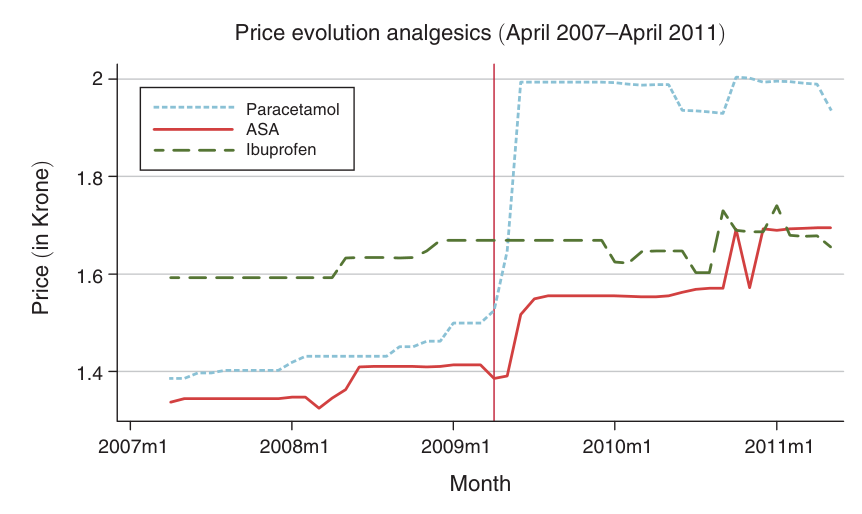
\includegraphics[width=0.72\textwidth]{figures/ch11/bv_fig1_price.png}
\caption{Average prices of paracetamol, ASA and ibuprofen analgesics in Sweden, April 2007 to April 2011, in kronor.
The vertical line marks the merger (April 2009). Source: \citet{BjornerstedtVerboven2016}, Figure 1.}
\label{fig:11-bvprice}
\end{figure}

\begin{figure}[htbp]
\centering
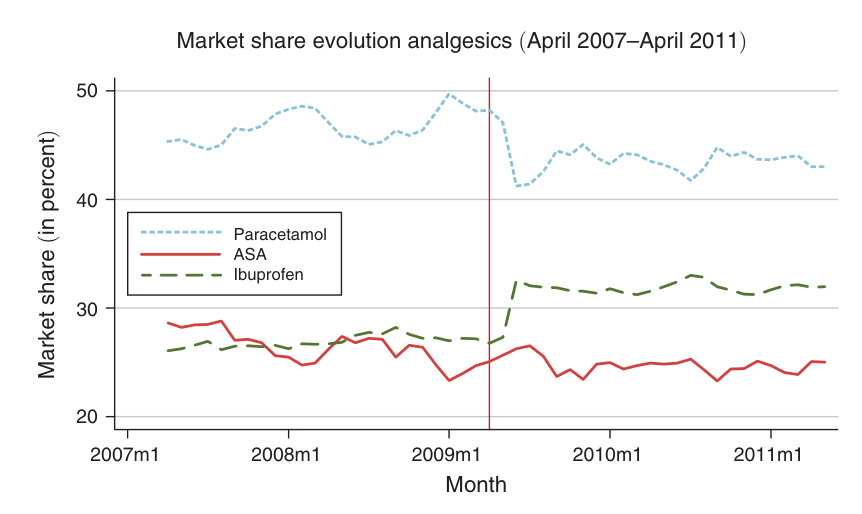
\includegraphics[width=0.72\textwidth]{figures/ch11/bv_fig2_share.png}
\caption{Market shares of paracetamol, ASA and ibuprofen analgesics in Sweden, April 2007 to April 2011, in percent.
The vertical line marks the merger (April 2009). Source: \citet{BjornerstedtVerboven2016}, Figure 2.}
\label{fig:11-bvshare}
\end{figure}

The stability of ibuprofen prices suggests that the paracetamol increase was not caused by a general cost or demand
shock \citep[p.~134]{BjornerstedtVerboven2016}. A regression in the spirit of \citet{AshenfelterHosken2010} makes
the comparison precise:
\begin{equation}\label{eq:11-bv-retro}
\ln p_{gt}=\alpha_g+\beta_g\,\mathit{PostMerger}_t+e_{gt}.
\end{equation}
Here $p_{gt}$ is the average price of product group $g$ in month $t$. The indicator $\mathit{PostMerger}_t$ equals
one after the merger. The published version defines groups by substance and by substance and firm (p.~134). Each group has its
own post-merger change $\beta_g$, which is more general than a common change for all control groups. The difference
between the merging firms' $\beta_g$ and a rival group's $\beta_g$ is a DiD estimate of the merger effect. By
\cref{prop:11-didbias}, a rival control yields a lower bound when rivals raise prices in response.

The published version compares one year before and one year after the merger. The short window keeps out later
effects of the deregulation \citep[p.~134 and eq.~(1)]{BjornerstedtVerboven2016}. The article reports that the
merging firms raised prices by 40 percent and that some outsiders raised prices by more than 10 percent
\citep[abstract]{BjornerstedtVerboven2016}. Its Table~4 gives price changes of 39.7 percent for paracetamol, 0.1
percent for ibuprofen and 13.3 percent for ASA (p.~135). \Cref{tab:11-bv-expost} reports the working paper's
estimates, in log points. They compare two years on each side of the
merger, April 2007 to April 2009 against May 2009 to May 2011, and define groups by substance and by firm
\citep[Table 7]{BjornerstedtVerboven2013}.

The paracetamol price rose by 0.351 log points, or 42 percent. Ibuprofen prices did not move (0.001), and ASA prices
rose by 0.100 log points, or 11 percent. With ibuprofen as the control the DiD estimate is 0.350. With ASA as the
control it is 0.251, or 29 percent. Pooling the two rival substances into one control gives 0.30, or 35 percent
\citep[fn.~17]{BjornerstedtVerboven2013}. The ASA increase is consistent with a rival response, so the ASA-based
estimate understates the effect on paracetamol prices. Both merging firms raised prices by similar amounts, 0.356 log
points for AZT and 0.379 for GSK. Among the outsiders, Bayer raised prices by 0.105 and McNeil by 0.084 log points.
The regressions compare average log prices of product groups over the two windows, so they need not match the jump
in the plotted average price.

The same design applied to volume shares shows where demand went. The paracetamol share fell by 3.3 percentage
points, with a 95 percent confidence interval of 2.7 to 3.9 points. The ibuprofen share rose by 5.0 points, and the
ASA share fell by 1.6 points. AZT lost 5.6 points, while GSK's loss of 0.3 points is insignificant. McNeil lost 2.7
points, and the other outsiders gained a little \citep[pp.~31--32]{BjornerstedtVerboven2013}.

\subsection{The prospective models}\label{sec:11-bv-model}

The simulation has the structure of \cref{sec:11-simulation}: estimate demand on pre-merger data, recover marginal
costs from the pre-merger first-order conditions, change the ownership matrix, and solve for the new equilibrium.
Two demand families are used, each in two versions.

\casehead{Nested logit} Consumer $i$ chooses among products $j\in\mathcal{J}$ and an outside good $j=0$. Products are
grouped into nests $g$, and each nest into subnests $h$. In the authors' maintained specification the nests are the
two administrative forms, and the subnests are the substances within each form
\citep[p.~20]{BjornerstedtVerboven2013}. We first present the one-level version, with nests $g$ only. Its utility is
\begin{equation*}
u_{ij}=\delta_j+\zeta_{ig}+(1-\sigma)\epsilon_{ij},
\end{equation*}
where $\delta_j$ is mean utility, $\epsilon_{ij}$ is type-I extreme value, and $\zeta_{ig}$ has the distribution
that makes $\zeta_{ig}+(1-\sigma)\epsilon_{ij}$ extreme value \citep{Cardell1997}. The nesting parameter
$\sigma\in[0,1)$ measures the correlation of tastes within a nest (\cref{ch:logit}). As in \cref{sec:11-diversion},
let $H_g=\sum_{k\in g}e^{\frac{\delta_k}{1-\sigma}}$. Market shares are
\begin{equation}\label{eq:11-nl-shares}
s_j=s_{j|g}\,s_g,\qquad s_{j|g}=\frac{e^{\frac{\delta_j}{1-\sigma}}}{H_g},\qquad s_g=\frac{H_g^{1-\sigma}}{1+\sum_{g'}H_{g'}^{1-\sigma}},
\end{equation}
and the outside share is $s_0=\frac{1}{1+\sum_{g'}H_{g'}^{1-\sigma}}$.

\begin{lemma}[Nested logit share derivatives]\label{lem:11-nl-deriv}
For products $j\neq k$,
\begin{align*}
\frac{\partial s_j}{\partial\delta_j}&=s_j\Big[\frac{1}{1-\sigma}-\frac{\sigma}{1-\sigma}s_{j|g}-s_j\Big],\\
\frac{\partial s_j}{\partial\delta_k}&=-s_j\Big[\frac{\sigma}{1-\sigma}s_{k|g}+s_k\Big]\quad\text{if $k$ is in $j$'s nest,}\\
\frac{\partial s_j}{\partial\delta_k}&=-s_js_k\quad\text{if $k$ is in another nest.}
\end{align*}
\end{lemma}

\begin{proof}
Taking logs of \eqref{eq:11-nl-shares} gives
$\ln s_j=\frac{\delta_j}{1-\sigma}-\sigma\ln H_g-\ln\big(1+\sum_{g'}H_{g'}^{1-\sigma}\big)$. \Cref{sec:11-diversion}
computed the derivatives of the last two terms on the way to \eqref{eq:11-nl-diversion}. The derivative of $\ln H_g$
with respect to $\delta_k$ is $\frac{s_{k|g}}{1-\sigma}$ for $k\in g$ and zero otherwise. The derivative of the log
of the denominator is $s_k$ for every inside product $k$. Hence $\frac{\partial\ln s_j}{\partial\delta_k}$ equals
$\frac{1}{1-\sigma}-\frac{\sigma}{1-\sigma}s_{j|g}-s_j$ for $k=j$, $-\frac{\sigma}{1-\sigma}s_{k|g}-s_k$ for $k\neq j$
in the same nest, and $-s_k$ for $k$ in another nest. Multiplying each by $s_j$ gives the lemma.
\end{proof}

Inverting \eqref{eq:11-nl-shares} gives the linear estimating equation
$\ln s_j-\ln s_0=\delta_j+\sigma\ln s_{j|g}$ (\cref{ch:logit}). The two-level version adds the subnests $h$ within
each nest $g$, with parameters $0\le\sigma_2\le\sigma_1<1$. Here $\sigma_1$ measures the correlation of tastes
within a subnest and $\sigma_2$ within a nest. With unit demand its estimating equation is
\begin{equation}\label{eq:11-nl2}
\ln s_j-\ln s_0=x_j\beta-\alpha\,p_j+\sigma_1\ln s_{j|hg}+\sigma_2\ln s_{h|g}+\xi_j,
\end{equation}
where $s_{j|hg}$ is $j$'s share of its subnest and $s_{h|g}$ the subnest's share of the nest
\citep[eq.~(9)]{Verboven1996,BjornerstedtVerboven2013}.\footnote{We verified \eqref{eq:11-nl2} and the derivatives
below numerically against the two-level share formulas.} The authors also estimated the reverse order, with
substances as nests and forms as subnests. It gave $\sigma_1<\sigma_2$, which is inconsistent with random utility
maximization, so they kept forms as the nests (p.~20). Let $\vartheta_1=\frac{1}{1-\sigma_1}-\frac{1}{1-\sigma_2}\ge0$,
$\vartheta_2=\frac{\sigma_2}{1-\sigma_2}$ and $s_{j|g}=s_{j|hg}s_{h|g}$. The share derivatives are
\begin{align*}
\frac{\partial s_j}{\partial\delta_j}&=s_j\Big[\frac{1}{1-\sigma_1}-\vartheta_1\,s_{j|hg}-\vartheta_2\,s_{j|g}-s_j\Big],\\
\frac{\partial s_j}{\partial\delta_k}&=-s_j\big[\vartheta_1\,s_{k|hg}+\vartheta_2\,s_{k|g}+s_k\big]\quad\text{(same subnest)},\\
\frac{\partial s_j}{\partial\delta_k}&=-s_j\big[\vartheta_2\,s_{k|g}+s_k\big]\quad\text{(same nest, other subnest)},\\
\frac{\partial s_j}{\partial\delta_k}&=-s_js_k\quad\text{(other nest)}.
\end{align*}
Cross-elasticities are largest within a subnest, smaller between subnests of the same nest, and smallest across
nests. Under the maintained order, the closest substitutes share both form and substance, and the most distant
differ in form. The estimates in \cref{tab:11-bv-demand} below show this ordering.

\casehead{Unit demand and constant expenditures} The two versions differ in how price enters utility and what a
market share measures \citep[Section 3.1]{BjornerstedtVerboven2013}. Consumer $i$, with income $y_i$, gets utility
$u_{ij}=x_j\beta+\xi_j+\alpha f(y_i,p_j)+\epsilon_{ij}$ from product $j$. Conditional on choosing $j$, she buys
$d_{ij}$ units, given by Roy's identity:
\begin{equation*}
d_{ij}=-\dfrac{\frac{\partial f(y_i,p_j)}{\partial p_j}}{\frac{\partial f(y_i,p_j)}{\partial y_i}} .
\end{equation*}
Unit demand sets $f(y_i,p_j)=y_i-p_j$. Both derivatives have absolute value one, so $d_{ij}=1$. Constant
expenditures sets $f(y_i,p_j)=\frac{1}{\gamma}\ln y_i-\ln p_j$ for a constant $\gamma\in(0,1)$. Then
\begin{equation*}
d_{ij}=-\dfrac{-\frac{1}{p_j}}{\frac{1}{\gamma y_i}}=\frac{\gamma y_i}{p_j},
\end{equation*}
so the consumer spends the fraction $\gamma$ of her income on the chosen product. In both versions the income term
is common to all products of consumer $i$, so it drops out of the choice probabilities. These remain the nested logit
formulas, now evaluated at the mean utilities given below. Summing $d_{ij}$ times the choice probability over
consumers gives aggregate demand. With unit demand $q_j=s_jM$, where $M$ is the number of consumers. With constant
expenditures $q_j=\frac{s_jB}{p_j}$, where $B=\gamma\sum_iy_i$ is the potential budget for the category.

In the \emph{unit demand} version each consumer buys at most one unit. Mean utility is linear in price,
$\delta_j=x_j\beta-\alpha p_j+\xi_j$, and shares are volume shares, $s_j=\frac{q_j}{M}$ for a potential number of
units $M$. Since $\frac{\partial\delta_k}{\partial p_k}=-\alpha$, the elasticities in the one-level model are
\begin{align}
\varepsilon_{jj}&=-\alpha\,p_j\Big[\frac{1}{1-\sigma}-\frac{\sigma}{1-\sigma}s_{j|g}-s_j\Big],\label{eq:11-unit-own}\\
\varepsilon_{jk}&=\alpha\,p_k\Big[\frac{\sigma}{1-\sigma}s_{k|g}+s_k\Big]\ \text{(same nest)},\qquad
\varepsilon_{jk}=\alpha\,p_ks_k\ \text{(other nest)},\nonumber
\end{align}
where $\varepsilon_{jj}<0$ is the own-price elasticity in signed form. Elasticities are proportional to price.
Expensive products have more elastic demand, and the own elasticity of a product rises as its price rises.

In the \emph{constant expenditures} version each consumer spends a fixed budget on the category. Mean utility is
linear in log price, $\delta_j=x_j\beta-\alpha\ln p_j+\xi_j$, and shares are value shares,
$w_j=\frac{p_jq_j}{B}$ for a potential budget $B$. The formulas \eqref{eq:11-nl-shares} now give $w_j$. Quantity is
$q_j=\frac{Bw_j}{p_j}$, so $\ln q_j=\ln B+\ln w_j-\ln p_j$, and $\frac{\partial\delta_k}{\partial\ln
p_k}=-\alpha$. The quantity elasticities are
\begin{align}
\varepsilon_{jj}&=-\alpha\Big[\frac{1}{1-\sigma}-\frac{\sigma}{1-\sigma}w_{j|g}-w_j\Big]-1,\label{eq:11-ce-own}\\
\varepsilon_{jk}&=\alpha\Big[\frac{\sigma}{1-\sigma}w_{k|g}+w_k\Big]\ \text{(same nest)},\qquad
\varepsilon_{jk}=\alpha\,w_k\ \text{(other nest)}.\nonumber
\end{align}
These depend on prices only through value shares, so they are roughly constant along the demand curve. The extra
$-1$ in the own elasticity reflects the fixed budget. A higher price lowers the quantity bought even at an unchanged
value share, and that lost quantity is diverted to no other product.

Substituting value shares into the inverted two-level system gives the constant-expenditure estimating equation
\begin{equation}\label{eq:11-ce-est}
\ln w_j-\ln w_0=x_j\beta-\alpha\ln p_j+\sigma_1\ln w_{j|hg}+\sigma_2\ln w_{h|g}+\xi_j,
\end{equation}
where $w_0=1-\sum_kw_k$ is the outside value share. Here $w_{j|hg}$ and $w_{h|g}$ are the value shares within the
subnest and the nest \citep[eq.~(10)]{BjornerstedtVerboven2013}. The equation differs from \eqref{eq:11-nl2} in three ways.
Price enters in logs, shares are measured in value, and the potential market is a budget $B$ rather than a number of
consumers. The authors note that this version had not been used in empirical work, although it is as easy to
estimate as the unit-demand version (pp.~2--3).

The difference matters for mergers through pass-through (\cref{sec:11-passthrough}). Under unit demand, demand becomes
more elastic as price rises, which restrains post-merger price increases. Under constant expenditures, the merged
firm faces roughly constant elasticities and can push prices further. The contrast is the one between linear or
logit demand and the constant-expenditure logit in \cref{fig:11-curvature}.

\casehead{Random coefficients} The nested logit restricts substitution to the hierarchy of nests and subnests. It
also rules out correlated preferences along continuously measured characteristics
\citep[p.~137]{BjornerstedtVerboven2016}. The published version therefore adds the random coefficients logit of
\citet{BerryLevinsohnPakes1995} (\cref{ch:blp}), again in unit-demand and constant-expenditure versions. Tastes for
product characteristics vary across consumers, which yields more flexible substitution patterns. The model has four
random coefficients, on the dummies for fizzy tablets, paracetamol and the branded products (Alvedon, Ipren and
Treo), and on the constant \citep[p.~143]{BjornerstedtVerboven2016}. The price coefficient is common to all
consumers (Table~5). The model needs no prior hierarchy of nests, and the branded-product coefficient allows the
substitution among brands that the competition authority considered relevant.

\casehead{Estimation and identification} Both nested logit equations, \eqref{eq:11-nl2} and \eqref{eq:11-ce-est},
are linear in parameters. The authors estimate them by linear instrumental variables on the panel of product-months
\citep[Section 4.1]{BjornerstedtVerboven2013}. The regressors are price or log price, the two within-group shares,
marketing expenditures and the numbers of sick women and sick men. The equations also include a time trend,
month-of-year dummies and a fixed effect for each of the 56 products. The product effects absorb pack size, dose and other fixed characteristics. The
potential market is twice the average amount bought over the period, in units for unit demand and in value for
constant expenditures.

Price and the two within-group shares are endogenous, because they depend on $\xi_j$. The base instruments are
counts of other products, overall and within the same firm, nest and subnest. The exclusion restriction is the usual
one of \citet{BerryLevinsohnPakes1995}: the set of products on offer is uncorrelated with the demand shocks. With
product effects in the equation, the counts vary only through the entry and exit of products over time. More rivals
in a subnest lower a product's within-subnest share and its markup at fixed own quality, and these shifts identify
$\alpha$, $\sigma_1$ and $\sigma_2$. Marketing is treated as exogenous, on the argument that the product effects
absorb its main correlation with $\xi_j$ (pp.~20--21). The published version estimates the random coefficients
models as in \cref{ch:blp}. The contraction mapping recovers mean utilities from shares, and the parameters are
estimated by GMM as in BLP \citep[p.~158]{BjornerstedtVerboven2016}. A first stage uses the instruments of
\citet{BerryLevinsohnPakes1995}, sums of the characteristics with random coefficients over the firm's other products
and over rivals' products. A second stage uses optimal instruments (\cref{sec:A-optimal-iv}). The share integral is
approximated by a nested quadrature rule (pp.~143--144 and n.~7).

\casehead{Supply and simulation} Firms set prices in a multi-product Bertrand-Nash equilibrium. With $\Omega$ the
ownership matrix and $\Delta$ the matrix of quantity derivatives with elements $\frac{\partial q_j}{\partial p_k}$,
the first-order conditions are $q+(\Omega\odot\Delta)^{\top}(p-mc)=0$. Marginal costs are recovered from these
conditions at pre-merger prices. For a single-product firm under constant expenditures, profit is
$(p_j-c_j)\frac{Bw_j}{p_j}=\big(1-\frac{c_j}{p_j}\big)Bw_j$. Let $\eta_j=\frac{\partial\ln w_j}{\partial\ln
p_j}<0$. Setting the derivative of profit to zero gives
\begin{equation*}
\frac{c_j}{p_j^2}\,w_j+\Big(1-\frac{c_j}{p_j}\Big)\frac{\partial w_j}{\partial p_j}=0
\quad\Longrightarrow\quad
\frac{c_j}{p_j}+\Big(1-\frac{c_j}{p_j}\Big)\eta_j=0
\quad\Longrightarrow\quad
L_j=\frac{p_j-c_j}{p_j}=\frac{1}{1-\eta_j}=\frac{1}{|\varepsilon_{jj}|},
\end{equation*}
the inverse elasticity rule. The merger is simulated by joining AZT and GSK in $\Omega$, with no efficiencies, and
solving the post-merger conditions for prices. The authors solve them by fixed-point iteration, dampened when it
fails to converge, and Newton's method gives the same results \citep[p.~18]{BjornerstedtVerboven2013}.

The working paper also allows \emph{partial coordination}, in which each firm puts a weight $\phi\in(0,1)$ on its
rivals' profits before and after the merger. The zeros of $\Omega$ then become $\phi$. This $\phi$ is unrelated to
the coefficient $\phi$ of \eqref{eq:11-dafny-rf}. The authors set $\phi=0.75$, because it makes the implied
pre-merger marginal costs consistent with cost information available to the authority (pp.~18 and~23).

\subsection{Predictions and outcomes}\label{sec:11-bv-results}

\casehead{Demand estimates} \Cref{tab:11-bv-demand} reproduces the working paper's nested logit estimates. Both
versions satisfy $1\ge\sigma_1\ge\sigma_2\ge0$, with strict inequalities. Products of the same form and substance are
the closest substitutes, products of the same form and another substance come next, and products of another form are
the most distant \citep[p.~21]{BjornerstedtVerboven2013}. Marketing raises demand in both versions, and demand peaks
in December and March. The unit-demand version gives a negative coefficient on sick women, which the authors suspect
picks up other effects. The implied elasticities differ sharply. The average own elasticity is $-2.68$ under
constant expenditures and $-12.4$ under unit demand. The unit-demand range, from $-24.1$ to $-3.9$, is roughly
proportional to the range of prices. The constant-expenditure range is narrow, from $-2.84$ to $-1.91$.

\begin{table}[htbp]
\centering
\caption{Swedish analgesics: nested logit demand estimates in the working paper}
\label{tab:11-bv-demand}
\footnotesize
\begin{tabular}{@{}lcccc@{}}
\toprule
& \multicolumn{2}{c}{Constant expenditures} & \multicolumn{2}{c}{Unit demand} \\
\cmidrule(lr){2-3}\cmidrule(l){4-5}
& Estimate & Std.\ error & Estimate & Std.\ error \\
\midrule
Price coefficient $\alpha$ & 0.304 & 0.101 & 2.042 & 0.157 \\
Subnest parameter $\sigma_1$ (substance) & 0.835 & 0.021 & 0.928 & 0.013 \\
Nest parameter $\sigma_2$ (form) & 0.667 & 0.025 & 0.792 & 0.012 \\
Marketing expenditures & 15.50 & 2.90 & 8.85 & 1.82 \\
Sick women & 0.357 & 0.129 & $-0.699$ & 0.079 \\
Sick men & 1.145 & 0.244 & 0.809 & 0.157 \\
Time trend & 0.0013 & 0.0005 & 0.0007 & 0.0002 \\
$R^2$ & \multicolumn{2}{c}{0.983} & \multicolumn{2}{c}{0.972} \\
\addlinespace
\multicolumn{5}{@{}l}{\textit{Implied elasticities in December 2008: average and standard error}} \\
Own price & $-2.68$ & 0.63 & $-12.4$ & 2.6 \\
Cross, same subnest & 0.164 & 0.068 & 1.45 & 0.38 \\
Cross, other subnest of the same nest & 0.039 & 0.012 & 0.245 & 0.022 \\
Cross, other nest & 0.006 & 0.002 & 0.016 & 0.001 \\
\addlinespace
\multicolumn{5}{@{}l}{\textit{Implied elasticities in December 2008: minimum and maximum}} \\
Own price & $-2.84$ & $-1.91$ & $-24.1$ & $-3.9$ \\
Cross, same subnest & 0.00 & 0.93 & 0.00 & 8.3 \\
Cross, other subnest of the same nest & 0.00 & 0.29 & 0.00 & 1.76 \\
Cross, other nest & 0.00 & 0.06 & 0.00 & 0.16 \\
\bottomrule
\end{tabular}

\smallskip
\begin{minipage}{0.92\linewidth}
\footnotesize Notes: Linear IV estimates of \eqref{eq:11-ce-est} and \eqref{eq:11-nl2} on 7,240 product-months,
1995--2008. Nests are forms and subnests are substances within a form. The paper reports the price coefficient as
$-\alpha$. Price enters in logs under constant expenditures and in SEK per tablet under unit demand. Both regressions
include 56 product fixed effects and month dummies. Robust standard errors. Standard errors of the elasticities use
the delta method for an average product. Source: \citet{BjornerstedtVerboven2013}, Table 4.
\end{minipage}
\end{table}

\casehead{Predictions during the review} The authority received predictions for four scenarios in each version
\citep[Table 5]{BjornerstedtVerboven2013}. Under constant expenditures and Bertrand conduct, the paracetamol price was
predicted to rise by 34.0 percent, or by 4.7 percent with a 25 percent cut in marginal cost. Under partial
coordination the predictions were 28.4 and $-0.1$ percent. Under Bertrand conduct, unit demand predicted 12.9 percent
without the cost cut and 1.6 percent with it. Under partial coordination it predicted 16.1 and 9.0 percent. The implied pre-merger markups were 0.49 and 0.76 under
constant expenditures, and 0.16 and 0.54 under unit demand. The authors preferred constant expenditures for two
reasons. Its elasticities neither rise mechanically with price nor depend on the unit of consumption. Its markups were
also broadly in line with the variable costs reported by the parties, while the unit-demand markups were well below
them (pp.~24--25).

\casehead{The published estimates} \Cref{tab:11-bv} reproduces Table 6 of the published version, which re-estimates
the nested logit and adds the random coefficients models. The four specifications imply very different demand. The
average own-price elasticity is $-2.43$ in the constant-expenditure nested logit and $-8.84$ in the unit-demand
nested logit. The random coefficients logit gives $-2.05$ and $-3.61$. Unit demand also produces a much wider range
of own elasticities across products, from $-5.16$ to $-15.45$ in the nested logit, because elasticities are
proportional to prices. Cross-elasticities are larger within a substance than across substances in every
specification.

\begin{table}[htbp]
\centering
\caption{Swedish analgesics: price elasticities, markups and predicted price effects}
\label{tab:11-bv}
\footnotesize
\begin{tabular}{@{}lcccc@{}}
\toprule
& \multicolumn{2}{c}{Nested logit} & \multicolumn{2}{c}{Random coefficients logit} \\
\cmidrule(lr){2-3}\cmidrule(l){4-5}
& Constant expenditures & Unit demand & Constant expenditures & Unit demand \\
\midrule
\multicolumn{5}{@{}l}{\textit{Brand-level price elasticities}} \\
Own & $-2.43$ & $-8.84$ & $-2.05$ & $-3.61$ \\
Own (range) & ($-3.05$, $-2.00$) & ($-15.45$, $-5.16$) & ($-2.61$, $-1.51$) & ($-6.52$, $-1.99$) \\
Cross, same substance & 0.30 & 2.12 & 0.12 & 0.36 \\
Cross, different substance & 0.05 & 0.28 & 0.05 & 0.19 \\
\addlinespace
\multicolumn{5}{@{}l}{\textit{Markups (percent)}} \\
Paracetamol & 48.5 & 17.3 & 59.0 & 44.7 \\
Ibuprofen & 45.0 & 11.8 & 55.7 & 32.3 \\
ASA & 59.1 & 22.9 & 66.5 & 44.5 \\
\addlinespace
\multicolumn{5}{@{}l}{\textit{Basic predicted price effects (percent)}} \\
Paracetamol & 41.1 & 15.9 & 21.29 & 9.34 \\
Ibuprofen & 1.2 & 0.5 & 0.75 & 0.76 \\
ASA & 1.5 & 0.6 & 0.81 & 0.45 \\
\bottomrule
\end{tabular}

\smallskip
\begin{minipage}{0.95\linewidth}
\footnotesize Notes: All numbers are averages across products for December 2008, except the ranges in
parentheses. Markups are Lerner indices $\frac{p-c}{p}$ implied by the pre-merger Bertrand-Nash conditions. The
predicted price effects merge the two paracetamol sellers, with no efficiencies. Source:
\citet{BjornerstedtVerboven2016}, Table 6.
\end{minipage}
\end{table}

The markups follow from the elasticities. The inverse of the average own elasticity is 41\% in the
constant-expenditure nested logit, 11\% in the unit-demand nested logit, 49\% and 28\% in the two random
coefficients models. The reported markups are higher, for two reasons. Multi-product firms internalize
cannibalization among their own products, which raises markups above the single-product rule. And the average of
$\frac{1}{|\varepsilon_{jj}|}$ across products exceeds the inverse of the average elasticity, because the function
$\frac{1}{x}$ is convex. The second effect is large under unit demand, where the inverse elasticities range from
6.5\% to 19.4\% in the nested logit.

\casehead{Comparison with the outcome} The merging firms raised prices by about 40 percent (\cref{sec:11-bv-retro}).
The prediction made during
the review, 34 percent under constant expenditures and Bertrand conduct, came close. The re-estimated
constant-expenditure nested logit of \cref{tab:11-bv} predicts 41.1 percent, almost exactly the outcome. The
constant-expenditure random coefficients model predicts 21.3 percent, about half of it. The unit-demand models
predict 15.9 and 9.3 percent, far too little, and so did the unit-demand prediction of 12.9 percent made during the
review. The unit-demand nested logit also implies markups of 11.8\% to 22.9\%. Information available to the
competition authority suggested that actual paracetamol margins were higher, which casts further doubt on the
unit-demand specification \citep[p.~147]{BjornerstedtVerboven2016}.

The average price effect is only one prediction. \Cref{tab:11-bv-expost} sets the working paper's preferred model
against the outcomes for each substance and firm. Two predictions fail. First, the model predicted that GSK, the
smaller paracetamol seller, would raise prices far more than AZT, by 59.8 against 21.3 percent. In the logit model a
merger equalizes the markups of a firm's products, and the smaller firm starts with lower markups
\citep[p.~26]{BjornerstedtVerboven2013}. In fact the two firms raised prices by similar amounts. Second, the model
predicted rival price increases of at most 1.7 percent under Bertrand conduct. ASA prices rose by 11 percent, and
Bayer and McNeil raised prices by about 9 to 11 percent. Every model in \cref{tab:11-bv} predicts rival increases
between 0.45 and 1.5 percent. Partial coordination raises the predicted rival increases to 2.5 to 4.1 percent, still
below the outcomes. The shares tell the same story. The ASA share fell instead of rising, consistent with its price
increase, and the paracetamol share fell by 3.3 points instead of the predicted 7.1.

\begin{table}[htbp]
\centering
\caption{Swedish analgesics: predicted and actual effects of the merger}
\label{tab:11-bv-expost}
\footnotesize
\begin{tabular}{@{}lcccccc@{}}
\toprule
& \multicolumn{3}{c}{Price} & \multicolumn{3}{c}{Volume share (points)} \\
\cmidrule(lr){2-4}\cmidrule(l){5-7}
& \multicolumn{2}{c}{Predicted (\%)} & Actual & \multicolumn{2}{c}{Predicted} & Actual \\
\cmidrule(lr){2-3}\cmidrule(lr){5-6}
& Bertrand & Partial & (log points) & Bertrand & Partial & \\
\midrule
\multicolumn{7}{@{}l}{\textit{Substances}} \\
Paracetamol & 34.1 & 28.0 & 0.351 (0.007) & $-7.1$ & $-5.4$ & $-3.3$ (0.3) \\
Ibuprofen & 0.7 & 4.1 & 0.001 (0.005) & 3.7 & 2.7 & 5.0 (0.1) \\
ASA & 0.8 & 3.0 & 0.100 (0.004) & 3.3 & 2.7 & $-1.6$ (0.3) \\
\addlinespace
\multicolumn{7}{@{}l}{\textit{Firms}} \\
AZT (merging) & 21.3 & 19.5 & 0.356 (0.006) & $-3.4$ & $-2.7$ & $-5.6$ (0.5) \\
GSK (merging) & 59.8 & 45.1 & 0.379 (0.009) & $-3.7$ & $-2.7$ & $-0.3$ (0.2) \\
Nycomed & 0.6 & 4.0 & 0.012 (0.003) & 1.3 & 0.9 & 0.1 (0.5) \\
Meda & 0.1 & 2.7 & 0.029 (0.044) & 0.6 & 0.5 & 1.1 (0.6) \\
McNeil & 1.7 & 4.1 & 0.084 (0.005) & 5.1 & 3.9 & $-2.7$ (0.5) \\
Bayer & 0.1 & 2.5 & 0.105 (0.008) & 0.1 & 0.1 & 0.5 (0.1) \\
\bottomrule
\end{tabular}

\smallskip
\begin{minipage}{0.95\linewidth}
\footnotesize Notes: Predictions of the working paper's preferred model, the constant-expenditure nested logit
estimated during the review, with no efficiencies. ``Partial'' is partial coordination with $\phi=0.75$. Actual
effects are the post-merger coefficients $\beta_g$ of \eqref{eq:11-bv-retro} and of the same regression for volume
shares, comparing April 2007 to April 2009 with May 2009 to May 2011. Robust standard errors in parentheses. A change
of 0.351 log points is a 42 percent increase. Source: \citet{BjornerstedtVerboven2013}, Tables 6 and 7.
\end{minipage}
\end{table}

\casehead{Why the specifications differ} Two forces separate the unit-demand and constant-expenditure predictions.
The estimated elasticities differ, which changes margins and diversion. And the functional forms imply different
curvature, which changes pass-through even at the same elasticities. A stylized calibration isolates the second
force. Consider four products with prices normalized to one: two paracetamol products owned by different firms, one
ibuprofen product and one ASA product, each substance a nest of a one-level nested logit. Inside shares are 12\%,
12\%, 13.5\% and 12.5\% of the potential market, with the rest going to the outside good. For a given own elasticity
of $-3$ and a given diversion ratio $D_{AB}$ between the paracetamol products, we choose $(\alpha,\sigma)$
separately in the two versions so that both match these targets. By construction both versions then imply the same
pre-merger margins, the same upward pricing pressure and the same GUPPI. We then merge the paracetamol sellers.

\begin{table}[htbp]
\centering
\caption{A stylized calibration: same elasticity and diversion, different curvature}
\label{tab:11-bvcurv}
\footnotesize
\begin{tabular}{@{}lcccccccc@{}}
\toprule
& & & & & & \multicolumn{3}{c}{Predicted price rise (\%)} \\
\cmidrule(l){7-9}
$D_{AB}$ & Version & $\sigma$ & $\alpha$ & Lerner index & GUPPI & Paracetamol & Ibuprofen & ASA \\
\midrule
0.30 & Unit demand & 0.291 & 2.763 & 0.333 & 0.100 & 11.3 & 0.40 & 0.36 \\
0.30 & Constant expenditures & 0.501 & 1.447 & 0.333 & 0.100 & 23.5 & 0.44 & 0.40 \\
0.45 & Unit demand & 0.501 & 2.171 & 0.333 & 0.150 & 21.8 & 0.73 & 0.67 \\
0.45 & Constant expenditures & 0.745 & 0.855 & 0.333 & 0.150 & 61.0 & 0.75 & 0.69 \\
\bottomrule
\end{tabular}

\smallskip
\begin{minipage}{0.97\linewidth}
\footnotesize Notes: Our illustration, not a replication. One-level nested logit with substance nests, prices
normalized to one, inside shares 12\%, 12\%, 13.5\% and 12.5\%, own elasticity of each paracetamol product $-3$.
The GUPPI is $D_{AB}\,L$. No efficiencies. Our computation.
\end{minipage}
\end{table}

\begin{figure}[htbp]
\centering
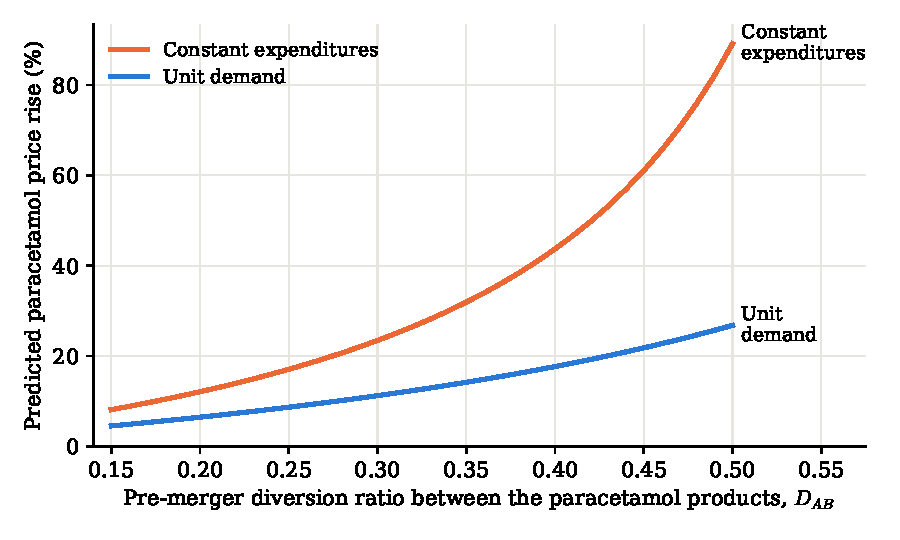
\includegraphics[width=0.78\textwidth]{figures/ch11/bv_curvature.pdf}
\caption{Predicted paracetamol price increase in the stylized calibration of \cref{tab:11-bvcurv}, against the
pre-merger diversion ratio between the two paracetamol products. Both versions match the same own elasticity
($-3$), diversion ratio and margins. The constant-expenditure version predicts 1.8 to 3.3 times the increase of
the unit-demand version.}
\label{fig:11-bvcurv}
\end{figure}

\Cref{tab:11-bvcurv} and \cref{fig:11-bvcurv} show the result. With identical first-order information the
constant-expenditure version predicts about twice the unit-demand increase at $D_{AB}=0.30$ and almost three times at
$D_{AB}=0.45$. Over the range shown the ratio lies between 1.8 and 3.3. Upward pricing pressure cannot distinguish
the two models, because it uses only first-order information. The simulation can, but only through an assumption
about curvature that pre-merger data barely constrain. The calibration also reproduces the second pattern of
Table 6. Rival price effects are below 1\% in both versions, because nested logit with substance nests diverts little
demand from paracetamol to each rival substance.

\casehead{Robustness} The working paper reports sensitivity checks run during and after the review
\citep[Sections 4.1 and 4.2]{BjornerstedtVerboven2013}. A potential market of 1.5, 4 or 6 times average sales, in
place of 2, gave similar results. A coarser product definition, with about 20 brand-form products per month instead
of 43, gave comparable findings. The full sample of 11,185 product-months gave the same conclusions as the
estimation sample. Adding sums of the pack sizes and doses of other products to the instruments left the unit-demand
results unchanged. Under constant expenditures it raised the elasticities and lowered the predicted price effects
somewhat, without changing the qualitative conclusions. Treating marketing as endogenous gave closely comparable
results. The reverse nesting order was rejected, as noted above.

\casehead{Interpretation} The study delivers three lessons. First, the constant-expenditure nested logit got the size
of the merging firms' price increase about right. It did so in the prediction made during the review, before the
outcome was known, and again in the published re-estimation. Second, the choice between specifications that fit the pre-merger data comparably
matters as much as the estimation itself. The unit-demand specifications implied implausibly elastic demand and low
margins, and they under-predicted the price increase by half or more. Third, the models missed how the effects were
distributed. They predicted very different increases for the two merging firms and small rival responses. The data
show similar increases for the two merging firms and increases of about 10 percent for some rivals.

Several explanations are possible. After the merger the merged firm cut its pack sizes from 30 to 20 tablets, as the
Swedish Medical Products Agency required. It lowered pack prices only slightly, for example from 41.5 to 38.5 kronor
for one of its best-selling products. The firms attributed the higher price per tablet to the cost of smaller packs. The authors
find this implausible, because ASA producers faced the same requirement without increases of similar size. The same
requirement may explain part of the ASA increase \citep[p.~29]{BjornerstedtVerboven2013}. The published version
considers a plausible post-merger cost increase and partial collusion as supply-side explanations
\citep[abstract]{BjornerstedtVerboven2016}. Rivals may have coordinated on higher prices after the merger, a
coordinated effect that a Bertrand model rules out (\cref{sec:11-millercoors}). The deregulation of pharmacies also
changed retail conditions in the same period. Finally, GSK was the acquirer and may have favored its own brands
after the merger. That would fit the small loss in its share (p.~32).

\casehead{Critiques and related validation studies} A single merger is a small sample for grading a method. The
retrospective benchmark rests on before-after comparisons of product-group prices, with rival controls whose prices
themselves moved. The change in pack sizes at the time of the merger further complicates the comparison of prices per
tablet. The predictions condition on the demand model's nest structure, which fixes how much substitution toward
rival substances is possible. Simulations that impose small cross-substance diversion will under-predict rivals'
responses whatever the curvature. \citet[p.~231]{AskerNocke2021} list four studies that grade merger simulations
with ex post evaluations: \citet{Peters2006}, \citet{Weinberg2011}, \citet{WeinbergHosken2013} and the present paper.
They reach mixed conclusions. \citet[pp.~627--628]{Peters2006} simulates five airline mergers completed between
August 1986 and November 1987. Standard simulations do not generally forecast the observed fare changes accurately.
Unobserved supply-side changes account for most of the gap in almost every case (p.~645). Peters concludes that
departures from the assumed model of conduct play an important role. \citet[p.~1584]{WeinbergHosken2013} simulate
two of the mergers of \cref{sec:11-ah}, Pennzoil and Quaker State in motor oil and Aurora and Log Cabin in syrup. For
motor oil the simulated increases are typically below 5 percent, against direct estimates of 4 to 8 percent. For
syrup the simulations typically predict 5 to 20 percent, while the merger had little effect on consumer prices.
\citet{AshenfelterHosken2010} find that the cereal simulation of \citet{Nevo2000b} predicted the wrong products to
rise in price (\cref{sec:11-ah}). \citet{Houde2012} compares a spatial simulation with a DiD estimate of the same
gasoline transaction (\cref{sec:11-beyond}).

\casehead{Contribution} The paper is one of the few direct tests of merger simulation as used by competition
authorities. It shows that simulations can predict the main effect of a merger when demand curvature is allowed to
be realistic. It also introduced the constant-expenditure nested logit, a tractable alternative to unit demand for
frequently purchased goods. Unit demand, the common default in discrete-choice models, can lead to large under-predictions even
when the model fits the pre-merger data. Retrospectives such as those in \cref{sec:11-retro} are therefore part of
the toolkit for choosing among prospective models.

\section{Coordinated effects: the MillerCoors joint venture}\label{sec:11-millercoors}

The merger analysis of \cref{sec:11-upp,sec:11-simulation} holds the mode of competition fixed. The merged firm
internalizes the competition among its own products, and every firm continues to set prices as a static
Bertrand-Nash player. Antitrust agencies worry about a second channel as well. The introduction to this chapter
distinguished the two channels informally, and we now state the distinction precisely.

\begin{definition}[Unilateral and coordinated effects]\label{def:11-coordinated}
A merger has \emph{unilateral effects} when it changes prices because the merged firm internalizes the competition
among the products it now owns. All firms keep playing the same static Nash equilibrium. A merger has
\emph{coordinated effects} when it also changes conduct, so that the merged firm and its remaining rivals compete
less aggressively with one another than static Nash pricing implies.
\end{definition}

\citet[p.~238]{AskerNocke2021} make the definition operational. A merger has coordinated effects when it leads to
prices that differ from those of a static Nash equilibrium. Any model of such effects therefore needs a continuation
value, which usually takes the defect-and-punish form of the collusion models of \cref{ch:collusion-theory}. The
idea is old. In the words of \citet{Stigler1964}, ``[c]ollusion of firms can take many forms, of which the most
comprehensive is outright merger''.
Section 7.2 of the 2010 Horizontal Merger
Guidelines discusses the market conditions that facilitate collusion \citep{USDOJFTC2010}, as \citet[p.~203,
n.~67]{AskerNocke2021} note. Merger challenges invoke coordinated effects often. Richard Gilbert and Hillary Greene
counted the merger complaints filed by the DOJ and the FTC between 1990 and 2014. In their count, as cited by
\citet{MillerWeinberg2017}, 60 percent alleged coordinated effects of some form \citep[p.~238,
n.~154]{AskerNocke2021}. Economists, by contrast, have concentrated on unilateral effects since the
1980s. Asker and Nocke attribute the focus to the analytical clarity of unilateral effects and to the lack of clear
empirical examples that link mergers to more coordination (pp.~238--239). \Cref{sec:11-ce-theory} sets out what the
theory says, and the rest of the section studies one of the few empirical examples.

\citet{MillerWeinberg2017} provide one of the first structural estimates of the coordinated effects of a consummated
merger.
They study the 2008 joint venture that combined the US brewing operations of SABMiller and Molson Coors into a new
firm, MillerCoors. Their method nests static Bertrand-Nash pricing inside a model in which the merged firm and its
largest rival put a weight $\kappa$ on each other's profits. It then estimates $\kappa$ from the post-merger prices.
This section follows the paper from its question to its contribution. It derives every estimating equation, proves
the properties of the estimator that the paper relies on, and reproduces Tables IV, V, VI and X.\footnote{Page
numbers in this section refer to the journal article. We change three pieces of the paper's notation to keep the
book consistent. The paper's nesting parameter $\rho$ is our $\sigma$ (in this book $\rho$ is pass-through). Its
product, period and region effects $\sigma_j$, $\tau_t$ and $\mu_r$ are our $\varphi_j$, $\tau_t$ and $\upsilon_r$.
The paper writes utility as $+\alpha p$ with $\alpha < 0$, while we write $-\alpha p$ with $\alpha > 0$. The tables
keep the paper's signs.}

\subsection{The theory of coordinated effects}\label{sec:11-ce-theory}

The theory of coordinated effects comes from the repeated games of \cref{ch:collusion-theory}. The question is
whether a change in market structure makes collusion easier to sustain, in the sense that it lowers the critical
discount factor above which collusion is an equilibrium. We follow \citet[pp.~239--240]{AskerNocke2021}, first in
the symmetric benchmark and then with capacities.

\casehead{Symmetric Bertrand competition}
Let $N$ symmetric firms sell a homogeneous good at constant marginal cost and set prices in every period of an
infinitely repeated game with discount factor $\delta$. Suppose all firms charge the monopoly price $p^m$ and share
the monopoly profit $\pi^m$ equally, and any deviation triggers static Bertrand pricing at marginal cost forever. A
firm that undercuts slightly takes the whole market for one period and earns close to $\pi^m$, and zero thereafter.
Collusion is an equilibrium if and only if
\begin{equation*}
\frac{1}{1 - \delta}\cdot\frac{\pi^m}{N} \ge \pi^m
\quad\Longleftrightarrow\quad
1 \ge N(1 - \delta)
\quad\Longleftrightarrow\quad
\delta \ge \underline\delta_N = 1 - \frac{1}{N} .
\end{equation*}
A merger from $N$ to $N - 1$ firms lowers the critical discount factor from $1 - \frac{1}{N}$ to $1 - \frac{1}{N -
1}$, so collusion becomes sustainable for more discount factors. Under imperfect monitoring, the time the industry
spends in the collusive state also falls with $N$. On this account, mergers facilitate collusion.

The model is special, because neither the deviation profit ($\pi^m$) nor the punishment profit (zero) depends on
$N$. In richer models both can fall with the number of firms. A merger then raises both the gain from cooperating
and the gain from deviating, and its effect on the critical discount factor is ambiguous. Firms also differ, and a
merger does more than remove a competitor, since the merged firm obtains the partners' tangible and intangible
assets.

\casehead{Capacity constraints}
\citet{CompteJennyRey2002} show how asymmetries change the answer. Demand is one unit at any price up to the monopoly
price of one, and zero above it. Firm $i$ has zero marginal cost up to its capacity $k_i$, with $k_1 \le k_2 \le
\dots \le k_N$. Write $\hat k_i = \min\{k_i, 1\}$ for firm $i$'s \emph{effective capacity}, $\hat K = \sum_i\hat k_i$
for the sum of effective capacities, and $K_{-N} = \sum_{i < N}k_i$ for the capacity of all firms but the largest.
Monitoring is perfect, and attention is restricted to equilibria in which each firm keeps the same market share
$\omega_i$ along every continuation path.
A merger of firms $l$ and $m$ combines their capacities into $k_l + k_m$
and creates no efficiencies.

\begin{proposition}[Capacities and collusion, \citealp{CompteJennyRey2002}]\label{prop:11-cjr}
\leavevmode
\begin{enumerate}[label=(\alph*)]
\item If $K_{-N} \ge 1$, perfect collusion at price one is sustainable if and only if
$\delta \ge \underline\delta = \frac{\hat K - 1}{\hat K}$, and the best shares are $\omega_i = \frac{\hat
k_i}{\hat K}$. If $K_{-N} \ge 1$ holds before and after a merger of $l$ and $m$, the merger weakly lowers
$\underline\delta$, and strictly if and only if $k_l + k_m > 1$.
\item If $K_{-N} < 1$, the largest firm's incentive constraint binds under the best allocation of shares, and
$\underline\delta = \frac{\hat k_N}{\hat K}$. A merger involving the largest firm raises $\underline\delta$. A
merger that does not involve the largest firm and does not create a new largest firm leaves it unchanged.
\end{enumerate}
\end{proposition}

\begin{proof}[Proof of part (a)]
Every firm's rivals together have capacity at least $K_{-N} \ge 1$, so they can serve the whole market. In the
static game the price is therefore zero and every firm earns zero, which is the harshest possible punishment. Under
collusion firm $i$ earns $\omega_i$ per period. Its best deviation prices just below one and sells $\hat k_i$, and it
earns zero afterward. It does not deviate if and only if
\begin{equation*}
\frac{\omega_i}{1 - \delta} \ge \hat k_i
\quad\Longleftrightarrow\quad
\delta \ge 1 - \frac{\omega_i}{\hat k_i} .
\end{equation*}
Collusion is sustainable if and only if $\delta \ge \max_i\big(1 - \frac{\omega_i}{\hat k_i}\big)$, so the best
shares maximize $\min_i\frac{\omega_i}{\hat k_i}$ subject to $\sum_i\omega_i = 1$. Because $\sum_i\hat
k_i\cdot\frac{\omega_i}{\hat k_i} = 1$, a weighted average of the ratios $\frac{\omega_i}{\hat k_i}$ with weights
$\frac{\hat k_i}{\hat K}$ equals $\frac{1}{\hat K}$. Their minimum is therefore at most $\frac{1}{\hat K}$, with
equality when every ratio equals $\frac{1}{\hat K}$. Hence $\underline\delta = 1 - \frac{1}{\hat K}$. A merger
replaces $\hat k_l + \hat k_m$ by $\min\{k_l + k_m, 1\}$, which is never larger and is strictly smaller if and only if
$k_l + k_m > 1$. A smaller $\hat K$ lowers $1 - \frac{1}{\hat K}$.
\end{proof}

Part (b) requires optimal punishments with two phases, a low price in the first period of the punishment and a high
price afterward. Static Nash pricing no longer holds the firms to their minmax payoffs
\citep[p.~240, n.~156]{AskerNocke2021}. We state part (b) without proof. The two parts reverse the symmetric intuition in
different ways. In part (a) a merger helps collusion only by destroying effective capacity. In part (b) a merger
that makes the largest firm larger makes the industry more asymmetric and hurts collusion. With capacities $(0.2,
0.3, 0.4, 1.0)$, for example, $K_{-N} = 0.9$ and $\underline\delta = \frac{1}{1.9} \approx 0.53$. A merger of the
largest firm with the smallest gives $(0.3, 0.4, 1.2)$ and $\underline\delta = \frac{1}{1.7} \approx 0.59$. A merger
of the two smallest gives $(0.4, 0.5, 1.0)$ and leaves $\underline\delta$ at 0.53.

\casehead{What the theory can and cannot say}
In a model with heterogeneous firms, a merger may thus help or hinder collusion, depending on the market and the
merger. Outside very special models the conditions are not well understood, and the theory gives no robust mapping
from a critical discount factor to the probability that collusion occurs \citep[p.~240]{AskerNocke2021}.
\citet{KaplowShapiro2007} put the problem sharply. Supergame theory with patient players predicts collusion for
almost any market structure, so it ``proves too much'' (n.~159). It is not surprising that courts in the last twenty
years have been reluctant to block mergers on coordinated-effects grounds, unless the industry had been cartelized
before. Conversely, a merger in an industry that is already cartelized may do little harm, and its efficiencies may
benefit society. \citet{RollerSteen2006} study a cartel in the Norwegian cement industry between 1955 and 1968. It
allocated market shares by capacity, which led to overinvestment in capacity. The 1968 merger of the industry's two
firms solved the coordination problem and removed the incentive to overinvest. Relative to wasteful collusion, this
merger to monopoly raised welfare, although competition would have raised it more (n.~160). Recent research gives
the concern a firmer empirical basis, and \citet{MillerWeinberg2017} is its leading example (p.~240).

\subsection{The question}\label{sec:11-mc-question}

The economic question is why the prices of the largest domestic beers rose after the joint venture, and whether the
rise reflects a change in how the remaining brewers compete. The joint venture combined the second and third largest
US brewers. A standard merger simulation predicts that the merged firm raises its prices, that rivals raise theirs a
little through strategic complementarity, and that efficiencies push in the other direction. The data show something
the standard model struggles to produce. The price of Bud Light, the flagship of the largest rival, rose by about as
much as the prices of Miller Lite and Coors Light. The prices of the leading imports did not rise.

The question matters for three reasons. First, it tests the maintained assumption of every merger simulation in
\cref{sec:11-simulation}, namely that post-merger conduct is static Nash. Second, it separates three forces that
act on post-merger prices at the same time: unilateral effects, coordinated effects and cost efficiencies. Third,
the US Department of Justice (DOJ) cleared the joint venture on the strength of its expected efficiencies. The
paper can ask whether that decision was right under different welfare standards.

The answer has three parts \citep[pp.~1781 and 1788]{MillerWeinberg2017}. The estimated internalization parameter is
between 0.25 and 0.37 and is significantly different from zero, so post-merger Nash-Bertrand pricing is rejected.
The joint venture produced large marginal-cost savings for MillerCoors, which roughly offset its unilateral effects.
Coordination raised the prices of all three domestic brewers well above their no-merger levels, so consumers lost
while total surplus rose slightly.

\subsection{The industry and the event}\label{sec:11-mc-industry}

The US beer market has many brands but few large brewers. Around the time of the joint venture, five firms
controlled about 80 percent of US retail revenue. Anheuser-Busch InBev (ABI), the owner of Budweiser and Bud Light, was the largest, with
about 35 percent. SABMiller (Miller) and Molson Coors (Coors) were the next two. Grupo Modelo (Corona) and Heineken
together held about 15 percent. Real beer prices fell between 2000 and 2008. \Cref{tab:11-mw-brands} lists the 13
brands in the paper's sample by owner.

\begin{table}[htbp]
\centering
\caption{Brewers and brands in the Miller and Weinberg sample}
\label{tab:11-mw-brands}
\footnotesize
\begin{tabular}{@{}lll@{}}
\toprule
Brewer (after June 2008) & Brands (row number in \cref{tab:11-mw-elast}) & Origin \\
\midrule
ABI & Bud Light (1), Budweiser (2), Michelob (9), Michelob Light (10) & Domestic \\
MillerCoors: Coors brands & Coors (3), Coors Light (4) & Domestic \\
MillerCoors: Miller brands & Miller Genuine Draft (11), Miller High Life (12), Miller Lite (13) & Domestic \\
Modelo & Corona Extra (5), Corona Light (6) & Imported \\
Heineken & Heineken (7), Heineken Light (8) & Imported \\
\bottomrule
\end{tabular}

\smallskip
\begin{minipage}{0.95\linewidth}
\footnotesize Notes: Each brand is sold in 6, 12 and 24 packs, and a product is a brand and package size. Before June
2008 the Miller and Coors brands belonged to separate firms. The brand list is the row list of
\citet[Table V]{MillerWeinberg2017}. Ownership is as described in the text.
\end{minipage}
\end{table}

The joint venture was announced on October 9, 2007 \citep[p.~9]{AshenfelterHoskenWeinberg2015} and consummated in June 2008
\citep[p.~1768]{MillerWeinberg2017}.
It combined the US operations of SABMiller and Molson Coors, with a combined share of about 30 percent. The DOJ
reviewed it as a merger and approved it on June 5, 2008. It found that efficiencies from combining the brewing
operations would outweigh any adverse competitive effect \citep[p.~241, n.~161]{AskerNocke2021}. The savings were in
shipping and distribution. Coors brewed in two locations and Miller in six. Moving Coors production into Miller
plants let the venture brew beer closer to many of its 48 regional markets \citep[pp.~219--220]{AskerNocke2021}. The
same investigation also surfaced documents that pointed to leader-follower pricing in the industry (p.~241).
\citet[p.~1788]{MillerWeinberg2017} consider a scenario with unilateral effects and efficiencies but no
coordination. They describe it as the one ``deemed most likely by the DOJ in its decision to clear the merger.''

Three institutional features matter for what follows. First, US beer is sold through a \emph{three-tier system}:
brewers sell to independent distributors, who sell to retailers. The model of the paper lets brewers sell directly
to consumers and treats the retail sector in a supplemental appendix \citep[p.~1779]{MillerWeinberg2017}. Second,
InBev acquired Anheuser-Busch in November 2008, five months after the joint venture \citep[p.~1784]{MillerWeinberg2017}.
Third, Anheuser-Busch held a large equity stake in Grupo Modelo during the sample period. \Cref{fig:11-beer} records it
as 50.3 percent before ABI bought the rest of Modelo in a \$20.1 billion deal. That acquisition came in 2013, after the
sample period \citep[p.~1767]{MillerWeinberg2017}. The second and third facts reappear in the assessment in
\cref{sec:11-mc-assessment}.

\subsection{Facts and hypotheses}\label{sec:11-mc-facts}

\Cref{fig:11-mwfacts} reproduces the paper's Figure 1. It plots the average log real price of a 12 pack of five
flagship brands from 2001 to 2011, in 2010 dollars. Before the joint venture, Miller Lite, Coors Light and Bud Light
move almost in lockstep and drift down. After June 2008 all three jump by roughly 6 log points and stay at the higher
level through 2011.\footnote{The 6 log point jump is our reading of the figure, from about 2.25--2.27 before June
2008 to about 2.29--2.33 afterwards. \citet[p.~242]{AskerNocke2021}, who reproduce the figure, describe the jump as
an 8 percent increase in the prices of all three brands. The paper itself states an increase of about 8 percent
\citep[p.~1768]{MillerWeinberg2017}, so we report both. The paper notes the brief dip in Miller Lite prices just
after the merger in its footnote 5.} Corona Extra and Heineken keep falling. In the paper's words, the imports ``do not exhibit any
persistent increase and instead continue along a downward trend'' \citep[p.~1769]{MillerWeinberg2017}. The price
gap between domestic beers and imports therefore shrinks.

\begin{figure}[htbp]
\centering
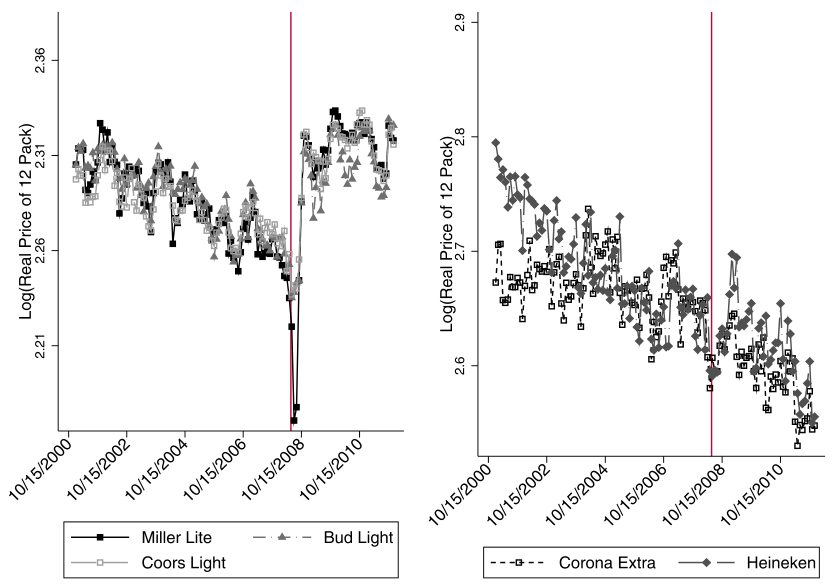
\includegraphics[width=0.92\textwidth]{figures/ch11/mw_fig1_prices.png}
\caption{Average retail prices of flagship 12 packs, 2001--2011. The left panel shows Miller Lite, Bud Light and Coors
Light, and the right panel shows Corona Extra and Heineken. The vertical axis is the natural log of the price in real
2010 dollars, and the vertical line marks the consummation of the joint venture in June 2008. Source: Miller and
Weinberg (2017), Figure 1.}
\label{fig:11-mwfacts}
\end{figure}

\citet[p.~1769]{MillerWeinberg2017} single out two features of the figure. The price of Bud Light rises by roughly
the same amount as the prices of Miller Lite and Coors Light. The prices of the Modelo and Heineken brands do not
rise, at least not persistently. They list four explanations that are consistent with these facts.
\begin{enumerate}[label=(H\arabic*)]
\item ABI and MillerCoors \emph{coordinate} after the merger and compete less aggressively with each other.
\item \emph{Unilateral effects} alone explain the data. Demand could make domestic beer prices strong strategic
complements of one another and weak strategic complements of import prices. Then ABI would follow MillerCoors up even
under Nash pricing, while importers would not.
\item \emph{Institutional practices} explain the data. Retailers might price Bud Light, Miller Lite and Coors Light
equally whatever happens to costs and demand, out of habit or under pressure from brewers.
\item The \emph{Great Recession} explains the data. The recession began at about the time of the merger. Lower incomes
could make domestic beer demand less elastic, for example through down-market substitution from imports.
\end{enumerate}
The paper weighs (H4) with a fact. Sales of the domestic brands fell in both absolute and relative terms during the
recession, which is hard to square with consumers trading down to them \citep[n.~5]{MillerWeinberg2017}.

The test the paper builds follows from (H1) and (H2). If unilateral effects alone explain the data, an estimated
demand system plus Nash pricing should reproduce the post-merger price of Bud Light. If they cannot, a model with
partial internalization of the ABI-MillerCoors pricing externality should fit better. The test therefore requires a
demand system rich enough to give (H2) a fair chance, and a supply model in which Nash pricing is a special case. The
logic is the same as in the conduct-parameter literature of \cref{ch:conduct}. The new element is a change in conduct
at a known date, caused by a known change in market structure.

\subsection{Theory: partial internalization of pricing externalities}\label{sec:11-mc-theory}

We first develop the supply model in general form. Consider one market and drop the region and period indices. There
are $J$ products and $F$ firms, and firm $f$ sells the products in $\mathcal{J}_f$. Market size is $M$, the share of
product $j$ is $s_j(p)$, marginal cost $mc_j$ is constant, and firm $f$'s variable profit is
\begin{equation}\label{eq:11-mc-profit}
  \pi_f(p) = M\sum_{k \in \mathcal{J}_f}(p_k - mc_k)\, s_k(p).
\end{equation}

\begin{assumption}[Partial internalization]\label{ass:11-mc-kappa}
(i) Firm $f$ chooses the prices of its products to maximize
\begin{equation}\label{eq:11-mc-objective}
  V_f(p) = \pi_f(p) + \sum_{g \neq f}\kappa_{fg}\,\pi_g(p),
\end{equation}
taking the prices of other firms as given, with weights $\kappa_{fg} \in [0,1]$ and $\kappa_{fg} = \kappa_{gf}$.
(ii) A Nash equilibrium of the game with payoffs $V_f$ exists and is interior.
\end{assumption}

\Cref{sec:11-simframework} stated the resulting first-order conditions without proof, and the worked example of
\cref{sec:11-logitex} used them. The weight $\kappa_{fg}$ is the fraction of rival $g$'s profit that firm $f$ counts
as its own. With all weights
equal to zero, the model is the multiproduct Bertrand-Nash model of \cref{ch:diffprod}. With $\kappa_{fg} = 1$, firms
$f$ and $g$ maximize their joint profit, exactly as if they had merged. Intermediate weights have two readings. The
first is literal: if firm $f$ owns a share of firm $g$'s equity, its owners gain from $g$'s profit
\citep{OBrienSalop2000}. The second is a reduced form for tacit coordination, which is the reading
\citet[p.~1779]{MillerWeinberg2017} adopt. They call $\kappa$ the ``post-merger internalization of coalition pricing
externalities.''

\begin{proposition}[First-order conditions with partial internalization]\label{prop:11-mc-foc}
Let $\Delta$ be the $J \times J$ matrix with $(j,k)$ element $\frac{\partial s_j}{\partial p_k}$, and let $\Omega(\kappa)$
be the matrix with $(j,k)$ element $\kappa_{f(j)f(k)}$, where $f(j)$ is the owner of product $j$ and $\kappa_{ff} = 1$.
Under \cref{ass:11-mc-kappa} equilibrium prices satisfy
\begin{equation}\label{eq:11-mc-foc}
  s(p) + \big(\Omega(\kappa) \odot \Delta(p)^\top\big)(p - mc) = 0 ,
\end{equation}
and, when the matrix is invertible, the markup vector is
\begin{equation}\label{eq:11-mc-markup}
  p - mc = b(p;\kappa) \equiv -\big[(\Omega(\kappa) \odot \Delta(p))^\top\big]^{-1} s(p).
\end{equation}
\end{proposition}

\begin{proof}
Take $j \in \mathcal{J}_f$. Differentiating \eqref{eq:11-mc-objective} with \eqref{eq:11-mc-profit} gives
\begin{align*}
  \frac{\partial V_f}{\partial p_j}
  &= M\Big[s_j + \sum_{k \in \mathcal{J}_f}(p_k - mc_k)\frac{\partial s_k}{\partial p_j}\Big]
     + \sum_{g \neq f}\kappa_{fg}\, M\sum_{k \in \mathcal{J}_g}(p_k - mc_k)\frac{\partial s_k}{\partial p_j} \\
  &= M\Big[s_j + \sum_{k=1}^{J}\kappa_{f(j)f(k)}\,(p_k - mc_k)\,\Delta_{kj}\Big].
\end{align*}
The second line uses $\kappa_{ff} = 1$ and collects all products into one sum. Setting the derivative to zero and
dividing by $M > 0$ gives $s_j + \sum_k \Omega_{jk}(\Delta^\top)_{jk}(p_k - mc_k) = 0$ for every $j$. Stacking the $J$
equations gives \eqref{eq:11-mc-foc}. Symmetry of the weights makes $\Omega(\kappa)$ symmetric, so
$\Omega \odot \Delta^\top = (\Omega \odot \Delta)^\top$, and solving for $p - mc$ gives \eqref{eq:11-mc-markup}.
\end{proof}

Equation \eqref{eq:11-mc-markup} is the markup formula of \cref{ch:blp} (\cref{eq:08-markup}) with the ownership
matrix replaced by $\Omega(\kappa)$. \citet[eq.~(9)]{MillerWeinberg2017} write it as
$p_t = mc_t - [\Omega_t(\kappa) \circ (\frac{\partial s_t}{\partial p_t})^\top]^{-1}s_t$, which is the same object.
In their application the weight is nonzero only for pairs of ABI and MillerCoors products after the merger. Let
$\mathcal{J}_A$, $\mathcal{J}_M$, $\mathcal{J}_O$ and $\mathcal{J}_H$ be the products of ABI, MillerCoors, Modelo and
Heineken, and write $\mathbf{1}$ for a matrix of ones of the conformable size. Ordering products by firm, the
post-merger matrix is
\begin{equation}\label{eq:11-mc-omega13}
  \Omega^{post}(\kappa) =
  \begin{bmatrix}
    \mathbf{1}_{AA} & \kappa\mathbf{1}_{AM} & 0 & 0 \\
    \kappa\mathbf{1}_{MA} & \mathbf{1}_{MM} & 0 & 0 \\
    0 & 0 & \mathbf{1}_{OO} & 0 \\
    0 & 0 & 0 & \mathbf{1}_{HH}
  \end{bmatrix}.
\end{equation}
Before the merger the Miller and Coors blocks are separate, so $\Omega^{pre}$ is block diagonal with five blocks.
The paper illustrates with a hypothetical region in which ABI, Miller, Coors and Modelo each sell one product
\citep[eq.~(10)]{MillerWeinberg2017}:
\begin{equation}\label{eq:11-mc-omega4}
  \Omega_{t_1^*} =
  \begin{bmatrix} 1 & 0 & 0 & 0 \\ 0 & 1 & 0 & 0 \\ 0 & 0 & 1 & 0 \\ 0 & 0 & 0 & 1 \end{bmatrix},
  \qquad
  \Omega_{t_2^*} =
  \begin{bmatrix} 1 & \kappa & \kappa & 0 \\ \kappa & 1 & 1 & 0 \\ \kappa & 1 & 1 & 0 \\ 0 & 0 & 0 & 1 \end{bmatrix},
\end{equation}
where $t_1^*$ is a pre-merger period and $t_2^*$ a post-merger period. Miller and Coors fully internalize each other
after the merger, ABI and MillerCoors internalize each other with weight $\kappa$, and Modelo prices as a Nash
player. The last feature is a restriction. The paper imposes it for Modelo and Heineken on the basis of qualitative
evidence \citep[p.~1779]{MillerWeinberg2017}.

\begin{remark}[$\kappa$ and the conduct parameter]\label{rem:11-mc-theta}
In a homogeneous-good market with $N$ symmetric firms, constant marginal cost $c$ and inverse demand $P(Q)$, let each
firm maximize $\pi_i + \kappa\sum_{j \neq i}\pi_j$ over its output. The first-order condition is
\begin{equation*}
  P(Q) + q_i P'(Q) - c + \kappa P'(Q)\sum_{j \neq i}q_j = 0 .
\end{equation*}
At a symmetric equilibrium $q_i = \frac{Q}{N}$ and $\sum_{j\neq i}q_j = \frac{(N-1)Q}{N}$, so
\begin{equation*}
  P(Q) - c + \theta\, Q P'(Q) = 0, \qquad \theta = \frac{1}{N} + \kappa\,\frac{N-1}{N}.
\end{equation*}
This is the conduct-parameter form of \cref{ch:conduct}. The weight $\kappa = 0$ gives Cournot ($\theta = \frac{1}{N}$)
and $\kappa = 1$ gives monopoly ($\theta = 1$). The internalization weight is thus a conduct parameter, and the
critique of \citet{Corts1999} applies to it. \Cref{sec:11-mc-assessment} returns to this point.
\end{remark}

The next result says how $\kappa$ changes pricing incentives at pre-merger prices. It extends the upward pricing
pressure (UPP) of \cref{sec:11-upp} to partial internalization. Write $D_{jk} = -\frac{\Delta_{kj}}{\Delta_{jj}}$
for the diversion ratio from $j$ to $k$ and $m_k = p_k - mc_k$ for the margin.

\begin{proposition}[Pricing pressure with partial internalization]\label{prop:11-mc-upp}
Suppose pre-merger prices satisfy \eqref{eq:11-mc-foc} with $\Omega^{pre}$, and evaluate the post-merger objectives at
pre-merger prices and costs. Then the post-merger pricing pressure on each product is:
\begin{align}
  \text{ABI product } j \in \mathcal{J}_A: &\quad UPP_j = \kappa\sum_{k \in \mathcal{J}_M} m_k D_{jk}, \label{eq:11-mc-upp-abi}\\
  \text{Miller product } j: &\quad UPP_j = \sum_{k \in \text{Coors}} m_k D_{jk} + \kappa\sum_{k \in \mathcal{J}_A} m_k D_{jk},
  \label{eq:11-mc-upp-mc}\\
  \text{import } j \in \mathcal{J}_O \cup \mathcal{J}_H: &\quad UPP_j = 0. \notag
\end{align}
The expression for a Coors product exchanges the roles of Miller and Coors in \eqref{eq:11-mc-upp-mc}.
\end{proposition}

\begin{proof}
Take $j \in \mathcal{J}_A$. At pre-merger prices the pre-merger condition holds:
$s_j + \sum_{k \in \mathcal{J}_A} m_k \Delta_{kj} = 0$. The post-merger derivative of $\frac{V_A}{M}$ with respect to
$p_j$ is the same expression plus $\kappa\sum_{k \in \mathcal{J}_M} m_k \Delta_{kj}$. At pre-merger prices it therefore
equals $\kappa\sum_{k\in\mathcal{J}_M} m_k\Delta_{kj}$. Dividing by $-\Delta_{jj} > 0$ converts it into dollars per
unit, as in \cref{sec:11-upp}:
\begin{equation*}
  \frac{\kappa\sum_{k\in\mathcal{J}_M} m_k\Delta_{kj}}{-\Delta_{jj}} = \kappa\sum_{k\in\mathcal{J}_M} m_k D_{jk}.
\end{equation*}
For a Miller product the post-merger objective adds the Coors products with weight one and the ABI products with
weight $\kappa$, and the same steps give \eqref{eq:11-mc-upp-mc}. Import objectives do not change.
\end{proof}

Under Nash pricing ($\kappa = 0$) ABI faces no direct pressure. Its prices rise only through strategic
complementarity, because MillerCoors's higher prices raise the demand for ABI's products. With $\kappa > 0$, ABI
faces pressure equal to $\kappa$ times the pressure it would face if it had merged with MillerCoors. This is the
sense in which coordination makes the largest rival behave like a partial merger partner. Efficiencies enter the
MillerCoors expressions as a credit $E_j mc_j$, exactly as in \cref{prop:11-netupp}.

Coordination also changes how rivals respond to the merged firm's efficiencies. In the Nash model a cost reduction at
MillerCoors lowers MillerCoors's prices, and strategic complementarity then lowers ABI's prices. With $\kappa > 0$
there is a countervailing force. A larger MillerCoors margin raises the value to ABI of the sales it diverts to
MillerCoors, so ABI wants to raise its price. \Cref{fig:11-mwident} shows the result in the logit illustration of
\cref{ex:11-logit}, which is also the example of \citet[p.~1780]{MillerWeinberg2017}. Three symmetric single-product
firms face logit demand with price 1.00, marginal cost 0.70, inside shares of 0.20 and an outside share of 0.40, and
firms 1 and 2 merge. At $\kappa = 0$ the rival price $p_3$ rises with the merged firm's cost $c_M$, with slope 0.061 at
$c_M = 0.6$. At $\kappa = 0.5$ the slope is $-0.148$.\footnote{These slopes and the contours in
\cref{fig:11-mwident} are our computations.} The figure also
previews the identification argument of \cref{sec:11-mc-supply}. The merging-firm price $p_M$ and the rival price
$p_3$ trace two families of curves that cross. An observed pair $(p_M, p_3)$ therefore pins down both the
internalization weight and the efficiency. For example, the pair $(1.09, 1.08)$ reported in the paper's third case
corresponds to $\kappa = 0.53$ and $c_M = 0.68$ in our computation (\cref{rem:11-mw-typo} discusses this case).

\begin{figure}[htbp]
\centering
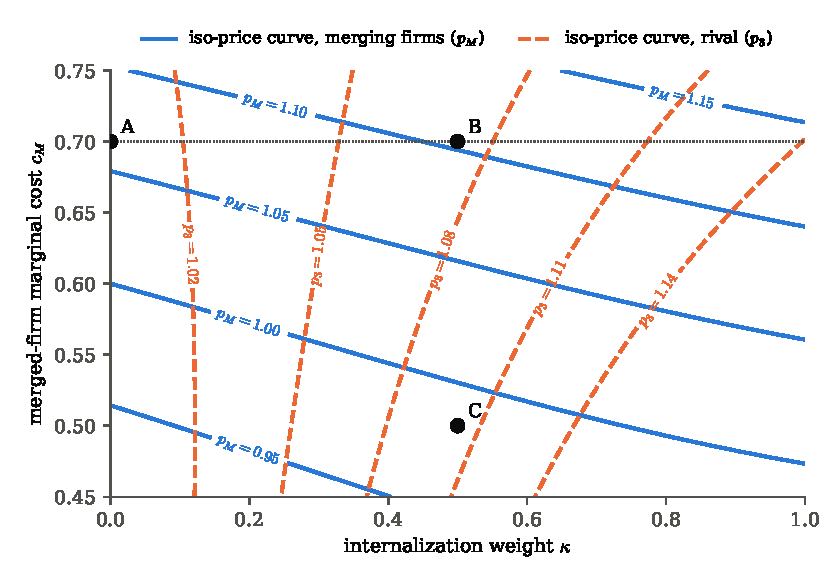
\includegraphics[width=0.82\textwidth]{figures/ch11/mw_identification.pdf}
\caption{Identification of the internalization weight and the efficiency in the logit illustration. Three symmetric
firms with logit demand start at price 1.00, marginal cost 0.70 and shares 0.20 (outside share 0.40). Firms 1 and 2
merge and both get marginal cost $c_M$, and the merged firm and firm 3 put weight $\kappa$ on each other's profits.
Solid curves are combinations of $(\kappa, c_M)$ that give the same merging-firm price $p_M$. Dashed curves give the
same rival price $p_3$. Point A is post-merger Nash pricing without efficiencies, $p = (1.064, 1.064, 1.006)$. Point B
has $\kappa = 0.5$, $p = (1.104, 1.104, 1.073)$. Point C has $\kappa = 0.5$ and $c_M = 0.5$, $p = (0.983, 0.983,
1.103)$. Our computations.}
\label{fig:11-mwident}
\end{figure}

\subsection{Data}\label{sec:11-mc-data}

The underlying data are weekly retail scanner data from supermarkets, collected by IRI
\citep[p.~241, n.~162]{AskerNocke2021}. The estimation samples aggregate them to months and quarters. A product $j$ is a brand and package size, with 13 brands sold in 6, 12 and 24 packs. A market is one of 39
geographic regions $r$ in one period $t$. The descriptive evidence spans 2001 to 2011. The estimation samples start in
2005, the first year of the household data described below \citep[p.~1768]{MillerWeinberg2017}. The baseline sample
has 94,656 brand-size-region-month observations, and a quarterly version has 31,784 brand-size-region-quarter
observations (Table IV notes). Both samples exclude the twelve months from June 2008 to May 2009, so the estimates compare settled pre-merger and
post-merger periods. Prices are in real 2010 dollars. Markups are reported on an ``equivalent-unit basis''
\citep[p.~1781]{MillerWeinberg2017}. The average markup of \$3.60 equals 34 percent of the retail price, which
implies an average price near \$10.60 per equivalent unit, close to the 12-pack prices in Table X.

Three further ingredients complete the data \citep[p.~1774]{MillerWeinberg2017}. Household incomes $D_i$ come from 500
draws per region and year from the American Community Survey (ACS), available for 2005 to 2011 (p.~1768). Market size $M_{rt}$ is set 50 percent above the maximum
unit sales observed in the region. The outside good collects brands outside the sample (such as craft beers), beer
sold outside supermarkets, and other beverages such as wine. Placing these products in the outside good makes their
prices non-strategic in the model. Period fixed effects absorb the trend toward craft beer. The cost side uses the
distance between each brand's brewery and each region, multiplied by an index of diesel prices
\citep[p.~1779]{MillerWeinberg2017}.

\subsection{Demand: the random coefficients nested logit}\label{sec:11-mc-demand}

\casehead{Utility}
Household $i$ in region $r$ and period $t$ chooses one of the inside products $j = 1, \dots, J_{rt}$ or the outside
good $j = 0$. There are two groups $g \in \{0, 1\}$: group 1 contains the inside goods and group 0 the outside good.
In book notation the indirect utility of an inside good is
\begin{align}
  u_{ijrt} &= \delta_{jrt} + \mu_{ijrt} + \zeta_{igrt} + (1-\sigma)\epsilon_{ijrt}, \label{eq:11-mc-utility}\\
  \delta_{jrt} &= x_j\beta - \alpha p_{jrt} + \varphi^D_j + \tau^D_t + \xi_{jrt}, \label{eq:11-mc-delta}\\
  \mu_{ijrt} &= \Pi_1 D_i\, p_{jrt} + D_i\, x_j\pi, \label{eq:11-mc-mu}
\end{align}
and $u_{i0rt} = \epsilon_{i0rt}$ \citep[eqs.~(4)--(5)]{MillerWeinberg2017}. The mean utility $\delta_{jrt}$ contains
product fixed effects $\varphi^D_j$, period fixed effects $\tau^D_t$ and the unobserved demand shock $\xi_{jrt}$.
Because the characteristics $x_j$ do not vary over time, $\varphi_j^D$ absorbs $x_j\beta$. The deviation $\mu_{ijrt}$
interacts income with price and with the characteristics $x_j = (1, \text{calories}_j, \text{import}_j,
\text{package size}_j)$, whose coefficients are $\pi = (\Pi_2, \Pi_3, \Pi_4, \Pi_5)^\top$. Household $i$'s price
coefficient is therefore
\begin{equation}\label{eq:11-mc-alphai}
  \alpha_i = \alpha - \Pi_1 D_i ,
\end{equation}
so a positive $\Pi_1$ means richer households are less price sensitive. The shock $\epsilon_{ijrt}$ is \iid\ type-I
extreme value. The group shock $\zeta_{igrt}$ has the distribution of \citet{Cardell1997}, which makes
$\zeta_{igrt} + (1-\sigma)\epsilon_{ijrt}$ extreme value. The \emph{nesting parameter} $\sigma \in [0,1)$ measures the
correlation of a household's tastes for inside goods. A larger $\sigma$ means less substitution between the inside
goods and the outside good.

The specification has two departures from the models of \cref{ch:logit,ch:blp}. Heterogeneity enters only through
observed income, with no unobserved random coefficients. This is the random coefficients nested logit (RCNL) of
\citet{BrenkersVerboven2006} and \citet{GrigolonVerboven2014}. The nest is a single inside-good group, with no
subnests for light beers, domestic beers or package sizes.

\casehead{The nested logit special case}
With $\Pi = 0$ the model is a one-level nested logit. We derive its shares and inversion, since the RCNL applies the
same algebra household by household. Drop the market subscripts, set $\delta_0 = 0$, and define the
\emph{inclusive value} of the inside group,
\begin{equation}\label{eq:11-mc-iv}
  I_1 = (1-\sigma)\ln\sum_{k=1}^{J}\exp\Big(\frac{\delta_k}{1-\sigma}\Big).
\end{equation}
The nested logit choice probabilities (\cref{ch:logit}) are
\begin{equation}\label{eq:11-mc-nlshares}
  s_{j|g} = \exp\Big(\frac{\delta_j - I_1}{1-\sigma}\Big), \qquad
  s_g = \frac{e^{I_1}}{1 + e^{I_1}}, \qquad
  s_0 = \frac{1}{1 + e^{I_1}}, \qquad
  s_j = s_{j|g}\, s_g ,
\end{equation}
where $s_{j|g}$ is the share of $j$ among inside goods and $s_g$ is the inside share.

\begin{proposition}[Nested logit inversion]\label{prop:11-mc-nlinv}
In the nested logit model,
\begin{equation}\label{eq:11-mc-nlinv}
  \ln s_j - \ln s_0 = \delta_j + \sigma\ln s_{j|g}.
\end{equation}
With \eqref{eq:11-mc-delta}, the estimating equation is
\begin{equation}\label{eq:11-mc-nlreg}
  \ln s_{jrt} - \ln s_{0rt} = -\alpha p_{jrt} + \sigma\ln s_{jrt|g} + \varphi^D_j + \tau^D_t + \xi_{jrt},
\end{equation}
which is the paper's equation (7) in book notation.
\end{proposition}

\begin{proof}
Take logs of $s_j = s_{j|g}s_g$ and use \eqref{eq:11-mc-nlshares}:
\begin{equation*}
  \ln s_j = \frac{\delta_j - I_1}{1-\sigma} + I_1 - \ln(1 + e^{I_1}), \qquad \ln s_0 = -\ln(1 + e^{I_1}).
\end{equation*}
Subtract the second equation from the first:
\begin{equation*}
  \ln s_j - \ln s_0 = \frac{\delta_j}{1-\sigma} - \frac{\sigma}{1-\sigma}I_1 .
\end{equation*}
The unobserved inclusive value can be eliminated with the within-group share. From \eqref{eq:11-mc-nlshares},
$\ln s_{j|g} = \frac{\delta_j - I_1}{1-\sigma}$, so $I_1 = \delta_j - (1-\sigma)\ln s_{j|g}$. Substituting,
\begin{equation*}
  \ln s_j - \ln s_0 = \frac{\delta_j}{1-\sigma} - \frac{\sigma\delta_j}{1-\sigma} + \sigma\ln s_{j|g}
  = \delta_j + \sigma\ln s_{j|g}.
\end{equation*}
Substituting \eqref{eq:11-mc-delta}, with $x_j\beta$ absorbed by $\varphi_j^D$, gives \eqref{eq:11-mc-nlreg}.
\end{proof}

Equation \eqref{eq:11-mc-nlreg} is linear in $(\alpha, \sigma)$ and the fixed effects. Both the price and the
within-group share are endogenous, since a high $\xi_{jrt}$ raises the product's share among inside goods and, through
the pricing equation, its price. Estimation therefore needs at least two excluded instruments. Column (i) of Table IV
estimates \eqref{eq:11-mc-nlreg} by two-stage least squares (\cref{cor:08-2sls}).

The nested logit derivatives follow from the same expressions, and they agree with \cref{lem:11-nl-deriv} for a
single inside nest. Using $\frac{\partial I_1}{\partial \delta_k} = s_{k|g}$ and $s_g s_{k|g} = s_k$,
\begin{equation*}
  \frac{\partial \ln s_j}{\partial \delta_k} = \frac{\indic\{j=k\} - s_{k|g}}{1-\sigma} + s_{k|g} - s_g s_{k|g}
  = \frac{\indic\{j=k\}}{1-\sigma} - \frac{\sigma}{1-\sigma}s_{k|g} - s_k .
\end{equation*}
Since $\frac{\partial\delta_k}{\partial p_k} = -\alpha$, the share derivatives are
\begin{equation}\label{eq:11-mc-nlderiv}
  \frac{\partial s_j}{\partial p_k} = -\alpha s_j\Big[\frac{\indic\{j=k\}}{1-\sigma} - \frac{\sigma}{1-\sigma}s_{k|g}
  - s_k\Big], \qquad \frac{\partial s_0}{\partial p_k} = \alpha s_0 s_k .
\end{equation}
The elasticities are
\begin{equation}\label{eq:11-mc-nlelast}
  \varepsilon_{jj} = -\alpha p_j\Big[\frac{1}{1-\sigma} - \frac{\sigma}{1-\sigma}s_{j|g} - s_j\Big], \qquad
  \varepsilon_{jk} = \alpha p_k\Big[\frac{\sigma}{1-\sigma}s_{k|g} + s_k\Big] \quad (k \neq j).
\end{equation}
The cross elasticity $\varepsilon_{jk}$ does not depend on $j$, so within the inside group substitution is
proportional to shares. This is the independence of irrelevant alternatives inside the nest. Dividing the cross
derivatives by the own derivative gives the diversion ratios
\begin{equation}\label{eq:11-mc-nldiv}
  D_{jk} = \frac{s_{k|g}\,[\sigma + (1-\sigma)s_g]}{1 - \sigma s_{j|g} - (1-\sigma)s_j}, \qquad
  D_{j0} = \frac{(1-\sigma)s_0}{1 - \sigma s_{j|g} - (1-\sigma)s_j}.
\end{equation}
The first expression is \eqref{eq:11-nl-diversion} with one inside nest, since $s_k = s_{k|g}s_g$. For small
products the outside diversion is close to $(1-\sigma)s_0$. A nesting parameter near one therefore sends
almost all of a product's lost sales to other beers.

\begin{remark}[Market elasticity, own elasticity and outside diversion]\label{rem:11-mc-identity}
When price enters utility linearly with a coefficient common to all products for each household, the matrix $\Delta$
is symmetric. This holds for the nested logit, by \eqref{eq:11-mc-nlderiv}, and for the RCNL below. Let all inside
prices rise by the same amount $\dd p$. Then
\begin{equation*}
  \dd s_j = \Big(\Delta_{jj} + \sum_{k\neq j}\Delta_{jk}\Big)\dd p = \Big(\Delta_{jj} + \sum_{k\neq j}\Delta_{kj}\Big)\dd p
  = \Delta_{jj}\Big(1 - \sum_{k\neq j}D_{jk}\Big)\dd p = \Delta_{jj}\, D_{j0}\, \dd p .
\end{equation*}
A uniform rise of $\dd p$ therefore changes the sales of product $j$ by $\varepsilon_{jj}D_{j0}\frac{\dd p}{p_j}$
percent. When prices are similar, the market elasticity is close to a share-weighted average of $\varepsilon_{jj}
D_{j0}$. Table IV satisfies this relation closely at the medians. For column (i), $-3.81 \times 0.298 = -1.14$ against a reported $-1.10$. For column
(ii), $-4.74 \times 0.1296 = -0.61$ against $-0.60$. Columns (iii) to (v) give $-0.74$, $-0.62$ and $-0.72$ against
$-0.72$, $-0.60$ and $-0.69$.
\end{remark}

\casehead{Market shares with random coefficients}
With $\Pi \neq 0$ the nested logit holds for each household. Let $V_{ijrt} = \delta_{jrt} + \mu_{ijrt}$ and define the
household's inclusive values
\begin{equation}\label{eq:11-mc-ivi}
  I_{i0rt} = 0, \qquad I_{i1rt} = (1-\sigma)\ln\sum_{k=1}^{J_{rt}}\exp\Big(\frac{V_{ikrt}}{1-\sigma}\Big), \qquad
  I_{irt} = \ln\big(1 + e^{I_{i1rt}}\big).
\end{equation}
Applying \eqref{eq:11-mc-nlshares} to household $i$ and averaging over the $N_{rt} = 500$ simulated households gives
\begin{equation}\label{eq:11-mc-rcnlshare}
  s_{jrt} = \frac{1}{N_{rt}}\sum_{i=1}^{N_{rt}}
  \underbrace{\frac{\exp\big(\frac{V_{ijrt}}{1-\sigma}\big)}{\exp\big(\frac{I_{i1rt}}{1-\sigma}\big)}}_{s_{ij|g}}\;
  \underbrace{\frac{\exp(I_{i1rt})}{\exp(I_{irt})}}_{s_{ig}},
\end{equation}
which is the paper's equation (6). The first fraction is the household's probability of choosing $j$ among inside
goods, because $\exp(\frac{I_{i1rt}}{1-\sigma}) = \sum_k \exp(\frac{V_{ikrt}}{1-\sigma})$. The second is its
probability of buying beer. These inclusive values are those of \citet{McFadden1978}. The household-level derivatives
follow from \eqref{eq:11-mc-nlderiv} with $\alpha_i$ in place of $\alpha$:
\begin{equation}\label{eq:11-mc-rcnlderiv}
  \Delta_{jk} = \frac{\partial s_j}{\partial p_k} = -\frac{1}{N}\sum_{i=1}^{N}\alpha_i\, s_{ij}
  \Big[\frac{\indic\{j=k\}}{1-\sigma} - \frac{\sigma}{1-\sigma}s_{ik|g} - s_{ik}\Big].
\end{equation}
Households differ in $\alpha_i$ and in their choice probabilities, so the aggregate cross elasticities depend on
which households buy which products. This breaks the proportional substitution of \eqref{eq:11-mc-nlelast}. Income
also shifts the attractiveness of beer and of particular characteristics, which lets the recession move demand.

\casehead{Inversion and the dampened contraction}
For trial values of the nonlinear parameters $\theta_2 = (\sigma, \Pi)$, the mean utilities $\delta_{rt}$ in each
market solve $s^{obs}_{rt} = s_{rt}(\delta_{rt};\theta_2)$. The BLP contraction of \cref{ch:blp} need not converge
in this model. The paper follows \citet{GrigolonVerboven2014}, who iterate
\begin{equation}\label{eq:11-mc-contraction}
  \delta^{h+1} = \Phi(\delta^h), \qquad \Phi(\delta) = \delta + (1-\sigma)\big[\ln s^{obs} - \ln s(\delta;\theta_2)\big].
\end{equation}
The factor $1-\sigma$ dampens each step (\cref{rem:08-rcnl}). The next result shows why it is needed and why it works.

\begin{proposition}[Dampened contraction in the RCNL]\label{prop:11-mc-contraction}
For every $\delta$, the Jacobian of $\Phi$ in \eqref{eq:11-mc-contraction} has strictly positive elements
\begin{equation}\label{eq:11-mc-phijac}
  \frac{\partial \Phi_j}{\partial \delta_k} = \frac{1}{s_j}\,\frac{1}{N}\sum_{i=1}^{N}s_{ij}\big[\sigma s_{ik|g} +
  (1-\sigma)s_{ik}\big],
\end{equation}
and its row sums equal
\begin{equation}\label{eq:11-mc-rowsum}
  \sum_{k}\frac{\partial \Phi_j}{\partial \delta_k} = 1 - (1-\sigma)\,\frac{1}{s_j}\,\frac{1}{N}\sum_{i=1}^{N}s_{ij}\,s_{i0} < 1 .
\end{equation}
Without dampening, the diagonal element of the Jacobian of $\delta + \ln s^{obs} - \ln s(\delta)$ is
$-\frac{\sigma}{1-\sigma}$ plus terms that vanish as the shares go to zero.
\end{proposition}

\begin{proof}
Differentiate \eqref{eq:11-mc-rcnlshare}. Household $i$'s nested logit gives
$\frac{\partial s_{ij}}{\partial \delta_k} = s_{ij}[\frac{\indic\{j=k\}}{1-\sigma} - \frac{\sigma}{1-\sigma}s_{ik|g}
- s_{ik}]$, as in the derivation of \eqref{eq:11-mc-nlderiv}. Hence
\begin{align*}
  (1-\sigma)\frac{\partial \ln s_j}{\partial \delta_k}
  &= \frac{1}{s_j}\frac{1}{N}\sum_i s_{ij}\big[\indic\{j=k\} - \sigma s_{ik|g} - (1-\sigma)s_{ik}\big] \\
  &= \indic\{j=k\} - \frac{1}{s_j}\frac{1}{N}\sum_i s_{ij}\big[\sigma s_{ik|g} + (1-\sigma)s_{ik}\big],
\end{align*}
where the second step uses $\frac{1}{N}\sum_i s_{ij} = s_j$. Since $\frac{\partial\Phi_j}{\partial\delta_k} =
\indic\{j=k\} - (1-\sigma)\frac{\partial\ln s_j}{\partial\delta_k}$, this gives \eqref{eq:11-mc-phijac}. Every term
is positive because all choice probabilities are positive. For the row sum, use $\sum_k s_{ik|g} = 1$ and $\sum_k
s_{ik} = 1 - s_{i0}$:
\begin{equation*}
  \sum_k\big[\sigma s_{ik|g} + (1-\sigma)s_{ik}\big] = \sigma + (1-\sigma)(1 - s_{i0}) = 1 - (1-\sigma)s_{i0}.
\end{equation*}
Averaging with weights $\frac{s_{ij}}{N s_j}$ gives \eqref{eq:11-mc-rowsum}. Without dampening the diagonal element is
$1 - \frac{\partial\ln s_j}{\partial\delta_j}$. The leading part of $\frac{\partial \ln s_j}{\partial\delta_j}$ is
$\frac{1}{1-\sigma}$, so the diagonal element is $1 - \frac{1}{1-\sigma} = -\frac{\sigma}{1-\sigma}$ plus terms
proportional to the shares.
\end{proof}

The sup norm of a matrix with nonnegative elements is its largest row sum, so \eqref{eq:11-mc-rowsum} makes $\Phi$ a
local contraction everywhere. The global argument then proceeds as for the BLP contraction in \cref{thm:08-contraction}.
Without dampening the map expands. At the paper's estimate $\sigma \approx 0.83$, the diagonal element is near
$-\frac{0.83}{0.17} \approx -4.9$, so plain iteration overshoots and diverges. The proposition also gives the speed of
convergence. The modulus is close to $1 - (1-\sigma)s_0$, so convergence slows as $\sigma$ approaches one. In the
plain nested logit the Jacobian elements are $\sigma s_{k|g} + (1-\sigma)s_k$, which are small when there are many
products.

\casehead{The GMM estimator}
The demand parameters are $\theta^D = (\alpha, \sigma, \Pi, \varphi^D, \tau^D)$. Given $\theta_2$, the inversion
delivers $\delta_{jrt}(\theta_2)$ and \eqref{eq:11-mc-delta} gives the structural error
\begin{equation}\label{eq:11-mc-xi}
  \xi_{jrt}(\theta^D) = \delta_{jrt}(\theta_2) + \alpha p_{jrt} - \varphi^D_j - \tau^D_t .
\end{equation}
With a vector of instruments $z_{jrt}$, the moment condition is $\E[z_{jrt}\,\xi_{jrt}(\theta^D_0)] = 0$, and the
estimator minimizes
\begin{equation}\label{eq:11-mc-gmm}
  \hat\theta^D = \argmin_{\theta^D}\; \xi(\theta^D)^\top Z\, W Z^\top \xi(\theta^D),
\end{equation}
where $Z$ stacks the instruments and $W$ is a weighting matrix. The parameters that enter linearly, $\alpha$ and the
fixed effects, are concentrated out by linear instrumental variables for each $\theta_2$ (\cref{prop:08-concentrate}),
so the nonlinear search runs over $(\sigma, \Pi)$ only. The paper uses two-stage least squares for the nested logit
and GMM for the four RCNL specifications. Standard errors are clustered by region (Table IV notes).

\casehead{Instruments and identification}
The paper uses five sets of excluded instruments. Each is excluded from \eqref{eq:11-mc-delta} and is meant to
move a particular endogenous object.
\begin{enumerate}[label=(\roman*)]
\item The distance between the brewery and the region, in miles times a diesel price index, shifts marginal cost
and hence price. Product fixed effects absorb a brand's average distance. Identification therefore comes from changes
in diesel prices and in shipping routes over time, including the post-merger reallocation of production.
\item A post-merger indicator interacted with $\indic\{j \in \mathcal{J}_A \cup \mathcal{J}_M\}$ shifts the markups
of ABI and MillerCoors through the change in ownership and conduct. The exclusion restriction requires that the merger
did not shift the unobserved demand for these brands relative to imports.
\item The number of products in the market, interacted with the same indicator, captures variation in the choice
set. It moves within-group shares and competitors' prices, and it identifies $\sigma$.
\item The sum of the distances of the products in the market, also interacted, collects rivals' cost shifters.
These move rivals' prices and hence $s_{j|g}$.
\item Mean regional income interacted with characteristics such as calories and import status varies across regions
and over time. This variation identifies $\Pi$.
\end{enumerate}
The logic matches \cref{sec:08-instruments}. Price needs a cost shifter or a markup shifter. The nesting parameter
needs variation in the within-group share that is unrelated to $\xi$, which choice-set variation provides. The
income interactions need variation in the distribution of $D_i$ across markets.

\casehead{Results}
\Cref{tab:11-mw-demand} reproduces Table IV. All five specifications include product and period fixed effects.
Column (i) is the nested logit, and columns (ii) to (v) are RCNL specifications on monthly or quarterly data that
differ in which income interactions they include.

\begin{table}[htbp]
\centering
\caption{Baseline demand estimates (Miller and Weinberg 2017, Table IV)}
\label{tab:11-mw-demand}
\footnotesize
\begin{tabular}{@{}llccccc@{}}
\toprule
Demand model & & NL-1 & RCNL-1 & RCNL-2 & RCNL-3 & RCNL-4 \\
Data frequency & & Monthly & Monthly & Quarterly & Monthly & Quarterly \\
Variable & Parameter & (i) & (ii) & (iii) & (iv) & (v) \\
\midrule
Price & $\alpha$ & $-0.1312$ & $-0.0887$ & $-0.1087$ & $-0.0798$ & $-0.0944$ \\
 & & (0.0884) & (0.0141) & (0.0163) & (0.0147) & (0.0146) \\
Nesting parameter & $\sigma$ & 0.6299 & 0.8299 & 0.7779 & 0.8079 & 0.8344 \\
 & & (0.0941) & (0.0402) & (0.0479) & (0.0602) & (0.0519) \\
\addlinespace
\multicolumn{7}{@{}l}{\textit{Demographic interactions}} \\
Income $\times$ price & $\Pi_1$ & & 0.0007 & 0.0009 & & \\
 & & & (0.0002) & (0.0003) & & \\
Income $\times$ constant & $\Pi_2$ & & 0.0143 & 0.0125 & 0.0228 & 0.0241 \\
 & & & (0.0051) & (0.0055) & (0.0042) & (0.0042) \\
Income $\times$ calories & $\Pi_3$ & & 0.0043 & 0.0045 & 0.0038 & 0.0031 \\
 & & & (0.0016) & (0.0017) & (0.0018) & (0.0015) \\
Income $\times$ import & $\Pi_4$ & & & & 0.0039 & 0.0031 \\
 & & & & & (0.0019) & (0.0016) \\
Income $\times$ package size & $\Pi_5$ & & & & $-0.0013$ & $-0.0017$ \\
 & & & & & (0.0007) & (0.006) \\
\addlinespace
\multicolumn{7}{@{}l}{\textit{Other statistics}} \\
Median own-price elasticity & & $-3.81$ & $-4.74$ & $-4.33$ & $-4.45$ & $-6.10$ \\
Median market price elasticity & & $-1.10$ & $-0.60$ & $-0.72$ & $-0.60$ & $-0.69$ \\
Median outside diversion & & 29.80\% & 12.96\% & 16.98\% & 13.91\% & 11.82\% \\
$J$-statistic & & & 13.94 & 13.75 & 13.91 & 14.15 \\
\bottomrule
\end{tabular}

\smallskip
\begin{minipage}{0.97\linewidth}
\footnotesize Notes: Standard errors clustered by region in parentheses. The paper writes utility as $+\alpha p$, so
its price coefficient is negative. In our notation \eqref{eq:11-mc-delta} the coefficient on $-p$ is $0.1312$,
$0.0887$, and so on. The nesting parameter is $\rho$ in the paper. Column (i) is estimated by 2SLS and columns (ii) to
(v) by GMM. Columns (i), (ii) and (iv) use 94,656 brand-size-region-month observations, and columns (iii) and (v)
use 31,784 brand-size-region-quarter observations. The samples exclude June 2008 to May 2009. All regressions include
product (brand $\times$ size) and period fixed effects. Elasticities and diversion are medians over all
observations. The standard error $(0.006)$ on $\Pi_5$ in column (v) is as printed. It is probably a misprint for
0.0006, since the same coefficient has standard error 0.0007 in column (iv) and every other interaction is reported
to four decimals. The nested logit price coefficient in column (i) has a $t$-ratio of
$\frac{0.1312}{0.0884} \approx 1.5$, as printed. Source: \citet[Table IV, p.~1777]{MillerWeinberg2017}.
\end{minipage}
\end{table}

Five features of the table matter for the merger analysis. First, the income-price interaction $\Pi_1$ is positive
in both specifications that include it. By \eqref{eq:11-mc-alphai}, richer households are less price sensitive. The
other interactions say that richer households are more likely to buy one of the sample beers ($\Pi_2 > 0$), prefer
higher-calorie beers ($\Pi_3 > 0$) and imports ($\Pi_4 > 0$), and prefer smaller packages ($\Pi_5 < 0$).

Second, the nesting parameter is large. It is 0.63 in the nested logit and between 0.78 and 0.83 in the RCNL
specifications. By \eqref{eq:11-mc-nldiv}, the outside diversion is roughly proportional to $1-\sigma$. The ratio
$\frac{1 - 0.8299}{1 - 0.6299} = 0.46$ is close to the ratio of the median outside diversions in columns (ii) and
(i), $\frac{12.96}{29.80} = 0.43$. In the RCNL only 12 to 17 percent of the sales a product loses go to the outside
good, so most lost sales stay with other sample beers.

Third, demand for individual products is elastic, with median own elasticities between $-3.8$ and $-6.1$. A rough
check uses \eqref{eq:11-mc-nlelast} with small shares, where $\varepsilon_{jj} \approx -\frac{\alpha p_j}{1-\sigma}$.
With a price near \$10 per equivalent unit, column (i) gives $-\frac{0.1312 \times 10}{0.3701} \approx -3.5$, close
to the reported median of $-3.81$. Fourth, the market as a whole is inelastic, with median market elasticities
between $-0.60$ and $-1.10$. Brewers acting jointly would therefore gain from higher prices, which is the incentive
that coordination exploits.

Fifth, the price coefficient of the nested logit is imprecise (standard error 0.0884), while the RCNL coefficients
are precise. The $J$-statistics of Hansen's overidentification test \citep{Hansen1982} are between 13.75 and 14.15 in the four GMM
specifications. The table does not report the degrees of freedom, but the text gives eight for columns (ii) and (iii)
and seven for columns (iv) and (v) (p.~1776). The implied $p$-values are 0.083, 0.089, 0.053 and 0.049 (our
computation), so the test narrowly rejects column (v) at the 5 percent level.

\Cref{tab:11-mw-elast} reproduces Table V, the mean elasticities for 12 packs under RCNL-1. The cell in row $i$ and
column $k$ is the percentage change in the quantity of product $i$ when the price of product $k$ rises by one
percent. The lower panel aggregates over categories. For a category $B$ that excludes the column product $k$, the
entry is
\begin{equation}\label{eq:11-mc-catelast}
  \Big(\sum_{j\in B, j\neq k}\frac{\partial s_j(p)}{\partial p_k}\Big)\frac{p_k}{\sum_{j\in B,j\neq k}s_j(p)} .
\end{equation}

\begin{table}[htbp]
\centering
\caption{Mean elasticities for 12-pack products under RCNL-1 (Miller and Weinberg 2017, Table V)}
\label{tab:11-mw-elast}
\scriptsize
\setlength{\tabcolsep}{2.1pt}
\begin{tabular}{@{}lrrrrrrrrrrrrr@{}}
\toprule
 & (1) & (2) & (3) & (4) & (5) & (6) & (7) & (8) & (9) & (10) & (11) & (12) & (13) \\
\midrule
\multicolumn{14}{@{}l}{\textit{Product-specific own and cross elasticities}} \\
(1) Bud Light & $\mathbf{-4.389}$ & 0.160 & 0.019 & 0.182 & 0.235 & 0.101 & 0.146 & 0.047 & 0.040 & 0.130 & 0.046 & 0.072 & 0.196 \\
(2) Budweiser & 0.323 & $\mathbf{-4.272}$ & 0.019 & 0.166 & 0.258 & 0.103 & 0.166 & 0.047 & 0.039 & 0.121 & 0.043 & 0.068 & 0.183 \\
(3) Coors & 0.316 & 0.154 & $\mathbf{-4.371}$ & 0.163 & 0.259 & 0.102 & 0.167 & 0.046 & 0.038 & 0.119 & 0.042 & 0.066 & 0.180 \\
(4) Coors Light & 0.351 & 0.160 & 0.019 & $\mathbf{-4.628}$ & 0.230 & 0.100 & 0.142 & 0.047 & 0.041 & 0.132 & 0.047 & 0.073 & 0.199 \\
(5) Corona Extra & 0.279 & 0.147 & 0.018 & 0.137 & $\mathbf{-5.178}$ & 0.108 & 0.203 & 0.047 & 0.035 & 0.104 & 0.035 & 0.061 & 0.158 \\
(6) Corona Light & 0.302 & 0.151 & 0.018 & 0.153 & 0.279 & $\mathbf{-5.795}$ & 0.183 & 0.048 & 0.037 & 0.113 & 0.039 & 0.065 & 0.171 \\
(7) Heineken & 0.269 & 0.145 & 0.018 & 0.131 & 0.311 & 0.108 & $\mathbf{-5.147}$ & 0.047 & 0.035 & 0.101 & 0.034 & 0.059 & 0.153 \\
(8) Heineken Light & 0.240 & 0.112 & 0.014 & 0.124 & 0.210 & 0.086 & 0.138 & $\mathbf{-5.900}$ & 0.026 & 0.089 & 0.028 & 0.051 & 0.135 \\
(9) Michelob & 0.301 & 0.140 & 0.015 & 0.146 & 0.208 & 0.089 & 0.135 & 0.042 & $\mathbf{-4.970}$ & 0.116 & 0.036 & 0.061 & 0.175 \\
(10) Michelob Light & 0.345 & 0.159 & 0.019 & 0.181 & 0.235 & 0.101 & 0.146 & 0.047 & 0.041 & $\mathbf{-5.071}$ & 0.046 & 0.072 & 0.196 \\
(11) Miller G.\ Draft & 0.346 & 0.159 & 0.019 & 0.182 & 0.235 & 0.101 & 0.146 & 0.047 & 0.040 & 0.130 & $\mathbf{-4.696}$ & 0.072 & 0.196 \\
(12) Miller High Life & 0.338 & 0.159 & 0.019 & 0.177 & 0.242 & 0.102 & 0.153 & 0.047 & 0.040 & 0.127 & 0.045 & $\mathbf{-3.495}$ & 0.191 \\
(13) Miller Lite & 0.344 & 0.159 & 0.019 & 0.180 & 0.237 & 0.101 & 0.148 & 0.047 & 0.040 & 0.129 & 0.046 & 0.071 & $\mathbf{-4.517}$ \\
(14) Outside good & 0.016 & 0.007 & 0.001 & 0.009 & 0.011 & 0.005 & 0.006 & 0.002 & 0.002 & 0.006 & 0.002 & 0.003 & 0.009 \\
\addlinespace
\multicolumn{14}{@{}l}{\textit{Cross elasticities by category}} \\
6 packs & 0.307 & 0.152 & 0.018 & 0.155 & 0.275 & 0.104 & 0.180 & 0.047 & 0.038 & 0.115 & 0.039 & 0.065 & 0.174 \\
12 packs & 0.320 & 0.154 & 0.019 & 0.163 & 0.250 & 0.102 & 0.161 & 0.047 & 0.039 & 0.121 & 0.042 & 0.068 & 0.183 \\
24 packs & 0.356 & 0.160 & 0.019 & 0.189 & 0.222 & 0.099 & 0.136 & 0.047 & 0.041 & 0.134 & 0.048 & 0.073 & 0.201 \\
Domestic & 0.349 & 0.160 & 0.019 & 0.184 & 0.229 & 0.100 & 0.142 & 0.047 & 0.040 & 0.131 & 0.047 & 0.072 & 0.197 \\
Imported & 0.279 & 0.147 & 0.018 & 0.138 & 0.301 & 0.108 & 0.200 & 0.047 & 0.035 & 0.104 & 0.035 & 0.061 & 0.158 \\
\bottomrule
\end{tabular}

\smallskip
\begin{minipage}{0.97\linewidth}
\footnotesize Notes: The cell in row $i$ and column $k$ is the percentage change in the quantity of product $i$ with
respect to the price of product $k$. Column numbers refer to the products in the rows. Own elasticities are in bold.
Means are taken across year-month-region combinations. Category entries are computed by \eqref{eq:11-mc-catelast}
and exclude the column product. For example, a 1 percent rise in the price of a Bud Light 12 pack raises the sales
of other 12 packs by 0.320 percent. Source: \citet[Table V, p.~1778]{MillerWeinberg2017}.
\end{minipage}
\end{table}

The paper reads the table as evidence that RCNL-1 relaxes the logit restriction substantially
\citep[p.~1777]{MillerWeinberg2017}. Own elasticities tend to be larger for more expensive products, a pattern the
income-price interaction allows but does not impose. Consumers of Bud Light substitute disproportionately toward
Budweiser, Coors Light and Miller Lite and toward larger packs (0.356 for 24 packs against 0.307 for 6 packs).
Consumers of Corona Extra substitute disproportionately toward Heineken (0.311) and smaller packs (0.275 for 6 packs
against 0.222 for 24 packs).

A skeptical reading is also possible, and it matters for the estimate of $\kappa$. The variation within a column is
modest. Column (3) lies between 0.014 and 0.019 and column (8) between 0.042 and 0.048, so substitution remains close
to proportional to shares. Bud Light is about as close a substitute for Michelob Light (0.345 in row 10) as for
Miller Lite (0.344 in row 13). Yet only Miller Lite belongs to the other domestic firm. The outside-good row is
tiny because the large $\hat\sigma$ keeps lost sales among inside goods. The model has no light-beer or domestic
nest that could make Bud Light, Miller Lite and Coors Light especially close substitutes. These patterns determine
how much of ABI's post-merger price rise unilateral effects can explain, and therefore how much is left for $\kappa$.

\subsection{Supply and the estimation of the internalization weight}\label{sec:11-mc-supply}

\casehead{Marginal cost}
The supply model is \cref{prop:11-mc-foc} with $\Omega_t(\kappa)$ as in \eqref{eq:11-mc-omega13} in post-merger periods
and $\Omega^{pre}$ before. Marginal cost is
\begin{equation}\label{eq:11-mc-mc}
  mc_{jrt} = w_{jrt}\gamma + \varphi^S_j + \tau^S_t + \upsilon^S_r + \eta_{jrt}
\end{equation}
\citep[eq.~(11)]{MillerWeinberg2017}. The vector $w_{jrt}$ contains two variables. The first is an indicator for
MillerCoors products in post-merger periods, with coefficient $\gamma_1$. The second is the distance from the brewery
to the region times the diesel index, with coefficient $\gamma_2$. The two channels let the merger lower costs
through shorter shipping distances and through ``residual cost synergies unrelated to distance''
\citep[p.~1779]{MillerWeinberg2017}. The terms $\varphi^S_j$, $\tau^S_t$ and $\upsilon^S_r$ are product, period and
region fixed effects, and $\eta_{jrt}$ is an unobserved cost shock. Marginal cost does not depend on output. The paper
notes that an upward-sloping marginal cost for ABI would bias $\hat\kappa$ upward. ABI's price would then rise with
the demand that MillerCoors diverts to it. The paper reports little evidence of capacity constraints at ABI
\citep[n.~13]{MillerWeinberg2017}.

\casehead{The implied cost shock and the moment condition}
The supply parameters are $\theta^S = (\kappa, \gamma)$ together with the cost fixed effects. Demand is estimated
first, and supply takes $\hat\theta^D$ as given. Substituting \eqref{eq:11-mc-markup} into \eqref{eq:11-mc-mc} gives
the cost shock implied by trial parameters,
\begin{equation}\label{eq:11-mc-eta}
  \eta^*_{jrt}(\theta^S;\hat\theta^D) = p_{jrt} - b_{jrt}(p_{rt};\kappa,\hat\theta^D) - w_{jrt}\gamma - \varphi^S_j -
  \tau^S_t - \upsilon^S_r ,
\end{equation}
where $b_{rt}(p_{rt};\kappa,\hat\theta^D) = -[(\Omega_t(\kappa)\odot\Delta_{rt})^\top]^{-1}s_{rt}$ is evaluated at
observed prices and shares and the estimated demand.\footnote{This is the paper's equation (12). As printed there, the
bracketed markup term carries a minus sign. The paper's equation (9) implies $mc = p + [\Omega\circ(\frac{\partial
s}{\partial p})^\top]^{-1}s$, so the term should enter with a plus sign, which is what \eqref{eq:11-mc-eta} does with
$b$ defined as a positive markup.} The markup is endogenous in \eqref{eq:11-mc-eta}, because a high cost shock
raises price and changes the shares and derivatives that enter $b$. The excluded instrument is
\begin{equation}\label{eq:11-mc-zsupply}
  z_{jrt} = \indic\{j \in \mathcal{J}_A \cup \mathcal{J}_M\} \times \text{Post}_t ,
\end{equation}
an indicator for ABI and MillerCoors products in post-merger periods. Identification rests on the moment condition
$\E[z_{jrt}\,\eta^*_{jrt}(\theta^S_0)] = 0$, and the method-of-moments estimator is
\begin{equation}\label{eq:11-mc-supplygmm}
  \hat\theta^S = \argmin_{\theta}\; \eta^*(\theta;\hat\theta^D)^\top z z^\top \eta^*(\theta;\hat\theta^D)
\end{equation}
\citep[eq.~(13)]{MillerWeinberg2017}. The fixed effects and $\gamma$ enter linearly. For each trial $\kappa$ they
are estimated by ordinary least squares, so the nonlinear search is over $\kappa$ alone. Standard errors are clustered
by region and adjusted for the first-stage demand estimates \citep{Wooldridge2010}.

\casehead{What identifies $\kappa$}
The paper explains the identifying variation in words \citep[p.~1780]{MillerWeinberg2017}. The estimate of $\kappa$
is positive if ABI's post-merger prices exceed what the unilateral effects of the merger can explain. A positive
$\kappa$ also raises MillerCoors's prices, so $\gamma_1$ is negative if MillerCoors's post-merger prices are lower
than unilateral effects and $\kappa$ imply. The instrument is valid if changes in ABI's unobserved costs, before
versus after the merger, do not differ systematically from those of Modelo and Heineken. The next proposition makes
this argument exact in a simplified version of the model. It shows that the estimator is a difference in differences
applied to implied marginal costs.

\begin{proposition}[$\hat\kappa$ as a difference in differences of implied costs]\label{prop:11-mc-did}
Suppose the products fall into three groups, ABI ($A$), MillerCoors ($M$) and imports ($I$), observed in every period
of a pre-merger and a post-merger window. Let the cost function contain product effects, period effects and the
MillerCoors post-merger indicator, with no distance variable and one region. Write $c_{jt}(\kappa) = p_{jt} -
b_{jt}(\kappa)$ for implied marginal cost, and for any variable $y$ and group $G$ define
\begin{equation*}
  \bar\Delta_G\, y = \frac{1}{N_G}\sum_{j\in G}\Big(\frac{1}{T_1}\sum_{t\,\in\,\text{post}} y_{jt} -
  \frac{1}{T_0}\sum_{t\,\in\,\text{pre}} y_{jt}\Big).
\end{equation*}
Here $N_G$ is the number of products in $G$, and $T_0$ and $T_1$ are the numbers of pre-merger and post-merger
periods. Then the moment condition in \eqref{eq:11-mc-supplygmm} holds at $\hat\kappa$ if and only if
\begin{equation}\label{eq:11-mc-did}
  \bar\Delta_A\, c(\hat\kappa) = \bar\Delta_I\, c(\hat\kappa), \quad\text{equivalently}\quad
  \bar\Delta_A\, p - \bar\Delta_I\, p = \bar\Delta_A\, b(\hat\kappa) - \bar\Delta_I\, b .
\end{equation}
The cost parameter is then $\hat\gamma_1 = \bar\Delta_M\, c(\hat\kappa) - \bar\Delta_I\, c(\hat\kappa)$.
\end{proposition}

\begin{proof}
Let $W$ be the matrix of included regressors (product dummies, period dummies and $M \times \text{Post}$) and $Q_W$ the
matrix that takes residuals from a least squares regression on $W$. Concentrating out the linear parameters gives
$\eta^*(\kappa) = Q_W\,c(\kappa)$. The sample moment is therefore $z^\top Q_W c(\kappa) = (Q_W z)^\top c(\kappa)$, by
symmetry and idempotency of $Q_W$. Since $z = A\times\text{Post} + M\times\text{Post}$ and $M\times\text{Post}$ is a
column of $W$, we have $Q_W z = Q_W(A\times\text{Post})$.

Define the contrast vector $d$. Its elements are $\frac{1}{N_A T_1}$ for $A$ products in post-merger periods and
$-\frac{1}{N_A T_0}$ for $A$ products in pre-merger periods. They are $-\frac{1}{N_I T_1}$ and $\frac{1}{N_I T_0}$ for
$I$ products in post-merger and pre-merger periods, and zero for $M$ products. Two facts finish the proof. First, $d$ is
orthogonal to every column of $W$. Its elements sum to zero over the periods of each product, over the products of each
period, and over the $M$ observations. Hence $Q_W d = d$. Second, $A\times\text{Post} - \lambda d$ lies in the column
space of $W$ for some scalar $\lambda > 0$, unrelated to earlier uses of the symbol. To see this, look for product effects $a_G$ (common within a group), period
effects $e_0$ and $e_1$, and a coefficient $\ell$ on $M\times\text{Post}$ that reproduce $A\times\text{Post} -
\lambda d$ cell by cell. The $A$ and $I$ cells require
\begin{equation*}
  e_1 - e_0 = 1 - \lambda\Big(\frac{1}{T_1} + \frac{1}{T_0}\Big)\frac{1}{N_A}, \qquad
  e_1 - e_0 = \lambda\Big(\frac{1}{T_1} + \frac{1}{T_0}\Big)\frac{1}{N_I},
\end{equation*}
which hold with $\lambda = [(\frac{1}{T_1} + \frac{1}{T_0})(\frac{1}{N_A} + \frac{1}{N_I})]^{-1} > 0$. The levels
$a_A$ and $a_I$ then follow, and the $M$ cells are matched by $a_M$ and $\ell$. Together the two facts give $Q_W
(A\times\text{Post}) = \lambda Q_W d = \lambda d$. The moment is therefore $\lambda\, d^\top c(\kappa) = \lambda
[\bar\Delta_A c(\kappa) - \bar\Delta_I c(\kappa)]$, which is zero if and only if \eqref{eq:11-mc-did} holds. The
second form follows from $c = p - b$, and the import markups $b_I$ do not depend on $\kappa$ because the import rows
of $\Omega(\kappa)$ contain no $\kappa$. Finally, the least squares coefficient on $M\times\text{Post}$ equals the
post-pre change of $M$'s implied cost minus the change estimated for the period effects from the $A$ and $I$
products. At $\hat\kappa$ the $A$ and $I$ changes are equal, which gives the formula for $\hat\gamma_1$.
\end{proof}

The proposition turns the paper's verbal argument into a formula. The left side of the second form of
\eqref{eq:11-mc-did} is the observed rise in ABI's prices relative to imports. The right side is the rise in ABI's
markup relative to imports implied by the model. At $\kappa = 0$ the right side is the unilateral effect on ABI,
which comes only from MillerCoors's higher prices and the induced shift in ABI's shares. If ABI's relative price rose
by more, the Nash model attributes the gap to a rise in ABI's marginal cost. The estimator rejects that explanation by
assumption, because the identifying restriction is parallel trends in unobserved marginal costs between ABI and the
importers. It raises $\kappa$ until the implied markup absorbs the gap. The importers play the role of the control
group, and ABI the role of the treated group. MillerCoors drops out of the estimating moment for $\kappa$ because its
own post-merger indicator absorbs its cost change. In the full model, distance and region effects turn the comparison
into a regression-adjusted difference in differences, but the logic is the same. \Cref{fig:11-mwident} shows the same
identification in the logit illustration, where the rival's price locates $\kappa$ and the merging firms' price then
locates the efficiency.

\casehead{Results}
\Cref{tab:11-mw-supply} reproduces Table VI. Each column uses the demand estimates of the corresponding column of
\cref{tab:11-mw-demand}.

\begin{table}[htbp]
\centering
\caption{Baseline supply estimates (Miller and Weinberg 2017, Table VI)}
\label{tab:11-mw-supply}
\footnotesize
\begin{tabular}{@{}llccccc@{}}
\toprule
Demand model & & NL-1 & RCNL-1 & RCNL-2 & RCNL-3 & RCNL-4 \\
Data frequency & & Monthly & Monthly & Quarterly & Monthly & Quarterly \\
Variable & Parameter & (i) & (ii) & (iii) & (iv) & (v) \\
\midrule
Post-merger internalization of & $\kappa$ & 0.374 & 0.264 & 0.249 & 0.286 & 0.342 \\
\quad coalition pricing externalities & & (0.034) & (0.073) & (0.087) & (0.042) & (0.054) \\
\addlinespace
\multicolumn{7}{@{}l}{\textit{Marginal cost parameters}} \\
MillerCoors $\times$ post-merger & $\gamma_1$ & $-0.608$ & $-0.654$ & $-0.649$ & $-0.722$ & $-0.526$ \\
 & & (0.039) & (0.050) & (0.060) & (0.042) & (0.040) \\
Distance & $\gamma_2$ & 0.142 & 0.168 & 0.163 & 0.169 & 0.148 \\
 & & (0.046) & (0.059) & (0.059) & (0.060) & (0.049) \\
\bottomrule
\end{tabular}

\smallskip
\begin{minipage}{0.97\linewidth}
\footnotesize Notes: Method of moments with the instrument $\indic\{j \in \text{ABI} \cup \text{MillerCoors}\}\times
\text{Post}_t$. Standard errors clustered by region in parentheses. Samples as in \cref{tab:11-mw-demand}: 94,656
monthly observations in columns (i), (ii) and (iv) and 31,784 quarterly observations in columns (iii) and (v),
excluding June 2008 to May 2009. All regressions include product (brand $\times$ size), period and region fixed
effects. Source: \citet[Table VI, p.~1781]{MillerWeinberg2017}.
\end{minipage}
\end{table}

The estimates of $\kappa$ are positive and significant in all five columns, so ``the null of Nash-Bertrand competition
in the post-merger periods is easily rejected'' \citep[p.~1781]{MillerWeinberg2017}. With RCNL demand the estimates
range from 0.249 to 0.342. Read literally, ABI and MillerCoors internalize between roughly a quarter and a third of
their price effects on each other's profits. Full joint profit maximization is also rejected. In column (ii) the
$t$-statistic for $\kappa = 0$ is $\frac{0.264}{0.073} = 3.6$ and the one for $\kappa = 1$ is $\frac{1 - 0.264}{0.073}
= 10.1$ (our calculations). The nested logit gives the largest estimate, 0.374. A plausible reason is its smaller $\sigma$, which implies
weaker substitution among inside goods. Unilateral effects on ABI are then smaller, and more of the price rise is left
for $\kappa$.

The markups implied by RCNL-1 are large \citep[p.~1781]{MillerWeinberg2017}. Across all observations the average
brewer markup is \$3.60 per equivalent unit, 34 percent of the retail price. After the merger the markups on ABI 12
packs are about \$0.70 higher, those on Miller 12 packs about \$1.40 higher and those on Coors products about \$1.80
higher. The MillerCoors increases combine higher prices and lower costs. Import markups change little.

The cost estimates are economically plausible. The distance coefficients of 0.148 to 0.169 in the RCNL columns imply
that costs that scale with shipping distance account for 2 to 3 percent of the retail price on average. The paper
compares this with an estimate by \citet[p.~162]{TremblayTremblay2005} that taxes and shipping made up 17 percent of
the retail price in 1996. The fixed effects absorb part of that share. The MillerCoors post-merger indicator measures a
cost reduction common to all regions, which the paper attributes to distributional savings beyond the distance
measure. Table VI reports this coefficient as $-0.526$ to $-0.722$ across the RCNL columns. The text summarizes the
RCNL estimates as a reduction of \$0.66 to \$0.70 \citep[p.~1781]{MillerWeinberg2017}.
Finally, the level of marginal cost is sensitive to retail market power, which acts like a per-unit tax paid by
brewers, while brewer markups are largely unaffected \citep[n.~14]{MillerWeinberg2017}.

\subsection{Counterfactuals and welfare}\label{sec:11-mc-counterfactuals}

\casehead{Scenarios}
The paper decomposes the effects of the merger with the RCNL-1 estimates \citep[p.~1786]{MillerWeinberg2017}. It
recomputes equilibrium under four counterfactual scenarios and compares them with the data. Each scenario switches
three channels on or off. Unilateral effects are the move from $\Omega^{pre}$ to $\Omega^{post}(0)$. Coordinated
effects are the move from $\kappa = 0$ to $\hat\kappa$. Efficiencies are the merger-related reductions in
MillerCoors's marginal cost. They come from shorter shipping distances and from a downward shift common to all regions
\citep[p.~1781]{MillerWeinberg2017}. Removing them raises the cost of Coors Light by \$0.60 to \$1.30, depending on the
region (p.~1782). The counterfactual without efficiencies therefore also restores the pre-merger shipping distances.
\begin{enumerate}[label=(\roman*)]
\item The observed outcome: coordinated effects, unilateral effects and efficiencies. Prices are data, and markups
and costs come from the estimates.
\item The merger with coordinated and unilateral effects, without efficiencies.
\item The merger with unilateral effects and efficiencies, without coordination.
\item The merger with unilateral effects only.
\item No merger.
\end{enumerate}
For each scenario $s$ and each market in the post-merger period, the counterfactual prices solve
\begin{equation}\label{eq:11-mc-cf}
  p^{s} = mc^{s} + b(p^{s};\Omega^{s}).
\end{equation}
Here $\Omega^{s}$ is $\Omega^{post}(\hat\kappa)$, $\Omega^{post}(0)$ or $\Omega^{pre}$. The cost vector $mc^{s}$ is
either the estimated post-merger cost or the cost with the efficiency terms removed. Scenario (i) needs no
computation. The estimated costs are defined as $p - b(p;\Omega^{post}(\hat\kappa))$, so the model reproduces the
data exactly. The welfare statistics are computed for 2011 on all products (Table X notes).

\casehead{Welfare measures}
Producer surplus is the brewers' variable profit, $PS = M\sum_j (p_j - mc_j)s_j$. Consumer surplus uses the inclusive
value. For household $i$ the nested logit generating function is $G(y) = y_0 + (\sum_{k=1}^{J}
y_k^{\frac{1}{1-\sigma}})^{1-\sigma}$. The expected maximum utility of a generalized extreme value model is $\ln
G(e^{V_{i0}}, \dots, e^{V_{iJ}})$ plus Euler's constant \citep{McFadden1978}. With $V_{i0} = 0$,
\begin{equation*}
  \E\Big[\max_j u_{ij}\Big] = \ln\Big(1 + \Big(\sum_{k=1}^{J}\exp\Big(\frac{V_{ik}}{1-\sigma}\Big)\Big)^{1-\sigma}\Big)
  + \text{const} = I_i + \text{const},
\end{equation*}
because $(\sum_k \exp(\frac{V_{ik}}{1-\sigma}))^{1-\sigma} = e^{I_{i1}}$. Dividing utility by the marginal utility of
income $\alpha_i$ converts it into dollars. The change in consumer surplus between scenarios $s$ and $s'$ in a market
is therefore
\begin{equation}\label{eq:11-mc-cs}
  \Delta CS = M\,\frac{1}{N}\sum_{i=1}^{N}\frac{I_i^{s} - I_i^{s'}}{\alpha_i}.
\end{equation}
This is the log-sum formula of \cref{ch:logit}, applied household by household. It requires $\alpha_i > 0$ for every
simulated household and no income effects.\footnote{The paper's tables report welfare changes in percent and do not
state the formula. Equation \eqref{eq:11-mc-cs} is the standard one for this model. By \eqref{eq:11-mc-alphai},
$\alpha_i > 0$ requires $D_i < \frac{\alpha}{\Pi_1}$, which equals $\frac{0.0887}{0.0007} \approx 127$ income units
under RCNL-1. Income is household income per member in 2010 dollars, with a mean of \$38{,}000, and $D_i$ is its
deviation from the mean \citep[pp.~1768 and 1773]{MillerWeinberg2017}. The paper does not state the scale of $D_i$ in
estimation. If $D_i$ is measured in thousands of dollars, the bound is a per-member income of about \$165{,}000.}
Total surplus is $TS = CS + PS$.

\casehead{Results}
\Cref{fig:11-mwcf} reproduces the paper's Figure 4, the price of Miller Lite 12 packs under each scenario, and
\cref{tab:11-mw-cf} reproduces Table X. \Cref{fig:11-mwdecomp} redraws the table as percent changes relative to no
merger.

\begin{figure}[htbp]
\centering
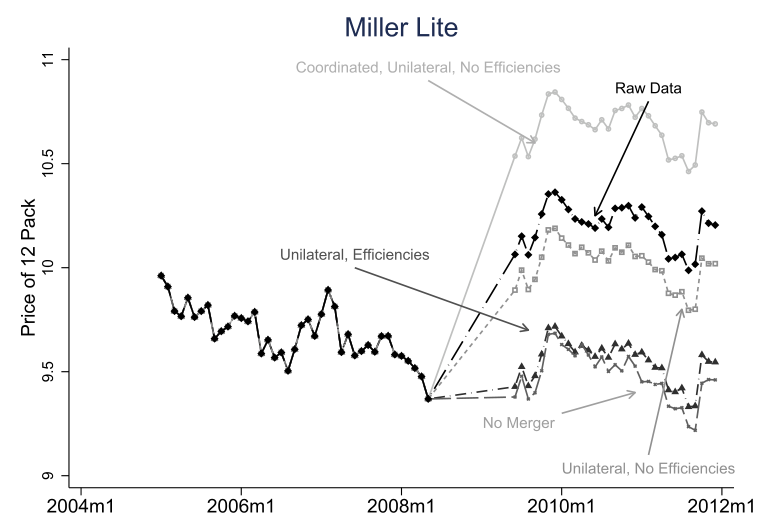
\includegraphics[width=0.82\textwidth]{figures/ch11/mw_fig4_counterfactual.png}
\caption{Counterfactual prices for Miller Lite 12 packs. The series before mid-2008 is the raw data. After the
excluded transition year, the figure shows the raw data and four counterfactual scenarios. They are no merger,
unilateral effects with efficiencies, unilateral effects without efficiencies, and coordinated and unilateral effects
without efficiencies. Each point is the average price across the 39 regions. Source: Miller and Weinberg (2017), Figure 4.}
\label{fig:11-mwcf}
\end{figure}

\begin{table}[htbp]
\centering
\caption{Results from the counterfactual analysis, 2011 (Miller and Weinberg 2017, Table X)}
\label{tab:11-mw-cf}
\footnotesize
\begin{tabular}{@{}lccccc@{}}
\toprule
Coordinated effects & yes & yes & no & no & no \\
Unilateral effects & yes & yes & yes & yes & no \\
Efficiencies & yes & no & yes & no & no \\
 & (i) & (ii) & (iii) & (iv) & (v) \\
\midrule
\multicolumn{6}{@{}l}{\textit{Retail prices (dollars)}} \\
ABI & 10.03 & 10.14 & 9.38 & 9.55 & 9.43 \\
Miller & 8.94 & 9.37 & 8.28 & 8.72 & 8.19 \\
Coors & 10.18 & 10.85 & 9.56 & 10.22 & 9.26 \\
\addlinespace
\multicolumn{6}{@{}l}{\textit{Brewer markups (dollars)}} \\
ABI & 4.45 & 4.56 & 3.81 & 3.97 & 3.84 \\
Miller & 4.52 & 4.32 & 3.83 & 3.63 & 3.05 \\
Coors & 4.25 & 4.06 & 3.61 & 3.41 & 2.68 \\
\addlinespace
\multicolumn{6}{@{}l}{\textit{Welfare statistics (percent change relative to column (v))}} \\
Producer surplus & 22.1 & 19.1 & 10.3 & 8.2 & base \\
\quad ABI & 10.3 & 19.8 & $-0.08$ & 9.3 & base \\
\quad Miller & 37.8 & 20.2 & 24.6 & 9.1 & base \\
\quad Coors & 47.8 & 12.9 & 34.7 & 3.5 & base \\
Consumer surplus & $-3.7$ & $-5.3$ & $-0.2$ & $-2.1$ & base \\
Total surplus & 1.3 & $-0.6$ & 1.8 & $-0.1$ & base \\
\bottomrule
\end{tabular}

\smallskip
\begin{minipage}{0.92\linewidth}
\footnotesize Notes: Prices and markups are volume-weighted means for the 12-pack flagship brands of ABI, Miller and
Coors. Welfare statistics are percent changes relative to the no-merger scenario (v), marked ``base'' (the paper prints a
dash), computed on all products.
Column (i) uses the raw data and the supply estimates, and columns (ii) to (v) are counterfactuals computed with
RCNL-1. All statistics are for 2011. Source: \citet[Table X, p.~1788]{MillerWeinberg2017}.
\end{minipage}
\end{table}

\begin{figure}[htbp]
\centering
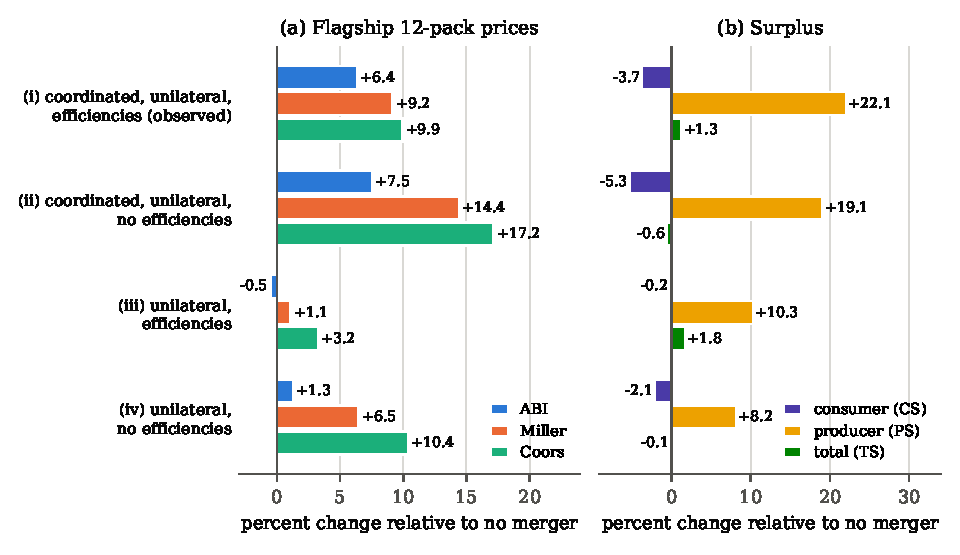
\includegraphics[width=\textwidth]{figures/ch11/mw_counterfactuals.pdf}
\caption{The counterfactual analysis of \cref{tab:11-mw-cf} relative to no merger. Panel (a) shows the percent change
in the volume-weighted price of each brewer's flagship 12 packs, computed from the table's prices. Panel (b) shows the
percent changes in consumer (CS), producer (PS) and total (TS) surplus reported in the table. Our computations from
Miller and Weinberg (2017), Table X.}
\label{fig:11-mwdecomp}
\end{figure}

Prices under no merger lie well below the raw data and roughly continue the pre-merger trend
(\cref{fig:11-mwcf}). The comparisons between columns isolate each channel. All differences below are our
calculations from \cref{tab:11-mw-cf}.

Unilateral effects are large. Moving from column (v) to column (iv) raises the Coors flagship price by \$0.96
(10.4 percent) and the Miller price by \$0.53 (6.5 percent). ABI's price rises by only \$0.12 (1.3 percent), through
strategic complementarity. Consumer surplus falls by 2.1 percent.

Efficiencies are also large, and they roughly offset the unilateral effects. Moving from column (iv) to column
(iii) lowers the Coors price by \$0.66 and the Miller price by \$0.44. ABI's price falls by \$0.17, to slightly below
its no-merger level. With unilateral effects and efficiencies, consumer surplus is only 0.2 percent below the
no-merger level and total surplus is 1.8 percent above it. This is the outcome the DOJ expected when it cleared the
joint venture. The prices of \cref{tab:11-mw-cf} also reveal the size of the efficiency. Price minus markup is ABI's
implied marginal cost, which stays at \$5.57 to \$5.59 in every column. Miller's implied cost is \$5.05 to \$5.14
without efficiencies and \$4.42 to \$4.45 with them. Comparing scenarios that differ only in efficiencies, (ii) with
(i) and (iv) with (iii), Miller's implied cost falls by \$0.63 and \$0.64. Both are close to $\hat\gamma_1 = -0.654$ in
RCNL-1.

Coordination adds a roughly uniform increment to the prices of all three brewers. Comparing column (i) with column (iii), and
column (ii) with column (iv), coordination raises the flagship price by \$0.59 to \$0.66 for each brewer, with and
without efficiencies. Relative to no merger, the observed prices are 6.4 percent higher for ABI, 9.2 percent for
Miller and 9.9 percent for Coors. Consumer surplus is 3.7 percent lower, so coordination accounts for about 3.5
percentage points of the consumer loss. Without efficiencies the loss would have been 5.3 percent.

Coordination is what makes the merger profitable for ABI. With unilateral effects and efficiencies alone, ABI's
producer surplus falls by 0.08 percent, because a more efficient MillerCoors takes sales from it. With coordination
it rises by 10.3 percent. The merging parties gain in every scenario, by 24.6 to 47.8 percent with efficiencies.

The welfare verdict depends on the standard. With coordination, total surplus is still 1.3 percent above the
no-merger level, so ``the antitrust clearance of the merger could be justified under a total welfare standard''
\citep[p.~1788]{MillerWeinberg2017}. Under a consumer surplus standard the merger harmed buyers. The four columns
also reveal the size of consumer surplus relative to total surplus. Solving $TS\% = w\,CS\% + (1-w)\,PS\%$ for the
weight $w$ gives 0.81 in every column, so consumer surplus is about 81 percent of total surplus in the no-merger
benchmark. A 1 percent loss to consumers therefore weighs about four times as much as a 1 percent gain to brewers.

\subsection{Robustness}\label{sec:11-mc-robust}

The paper's main robustness evidence is the spread across the five demand specifications. The estimate of $\kappa$
stays between 0.249 and 0.374 across nested logit and RCNL demand, monthly and quarterly data, and different sets of
income interactions (\cref{tab:11-mw-supply}). The cost coefficients are similarly stable. Four further checks bear on
the main threats.
\begin{enumerate}[label=(\alph*)]
\item A supplemental appendix adds a retail sector. Retail market power changes the
level of brewers' marginal costs but leaves brewer markups largely unaffected \citep[n.~14]{MillerWeinberg2017}.
\item An increasing marginal cost at ABI would bias $\hat\kappa$ upward. The paper
finds little evidence that ABI faced capacity constraints over the sample period \citep[n.~13]{MillerWeinberg2017}.
\item Two specifications ask whether the Great Recession, rather than the merger, triggered softer competition
\citep[Section~5.4]{MillerWeinberg2017}. With a separate $\kappa$ for each post-merger month, the estimates rise over
time as the economy recovers (their Figure~3). The second specification lets $\kappa$ vary with demeaned regional mean
income $\bar D_{rt}$ (unrelated to the aggregate diversion $\bar D$ of \cref{def:11-aggdiv}),
\begin{equation*}
  \kappa_{rt} = \frac{\exp(a_P\,\text{Post}_t + a_D\,\bar D_{rt})}{1 + \exp(a_P\,\text{Post}_t + a_D\,\bar D_{rt})} .
\end{equation*}
Here $a_P$ and $a_D$ are scalar parameters (the paper's $a$ and $b$). Under RCNL-3, $\hat a_P = 0.456$ (0.088) and
$\hat a_D = 0.033$ (0.039), which does not support countercyclical coordination. Under RCNL-1 the estimates are
noisier, $\hat a_P = 0.475$ (0.641) and $\hat a_D = -0.198$ (1.024) (pp.~1785--1786). The authors conclude: ``Given the totality of the evidence, we view the merger as the most likely
catalyst of softer price competition'' (p.~1786).
\item The paper's conclusion states that the price increases of MillerCoors and ABI,
``in both absolute terms and relative to their competitors,'' are ``visually evident and confirmed with econometric
analysis'' \citep[p.~1788]{MillerWeinberg2017}. The econometric analysis regresses the log real retail price on
post-merger indicators for MillerCoors products, for ABI products and for all products \citep[eq.~(1)]{MillerWeinberg2017}.
The regression includes product-by-region fixed effects and a linear time trend. The fullest specification adds
product-specific trends and regional employment and earnings and drops the year after the merger (Table II, column (iv)).
Its MillerCoors and ABI coefficients, which measure price changes relative to the imports, are 0.069 and 0.062, each
with a standard error of 0.007. The descriptive regressions also support the power of the supply instrument
(p.~1780).
\end{enumerate}

\subsection{Assessment}\label{sec:11-mc-assessment}

The paper's central finding is robust within its framework. Given the estimated demand system and the assumption of
parallel cost trends, ABI's post-merger prices are too high for Nash pricing. Whether the finding means that the
merger caused tacit coordination depends on several assumptions, which the literature and the paper itself discuss.

\casehead{What $\kappa$ measures}
By \cref{rem:11-mc-theta}, $\kappa$ is a conduct parameter, and the critique of \citet{Corts1999} applies. Suppose firms
play a repeated game in which the degree of cooperation varies over time. A single estimated weight then summarizes
average behavior, and it need not measure the true degree of collusion (\cref{ch:conduct}). The paper acknowledges the
point and notes that a nonzero $\kappa$ still rejects post-merger Nash pricing \citep[n.~12]{MillerWeinberg2017}. The
same footnote cites \citet{Bresnahan1989} and \citet{Porter1983} on identification with regime shifts. A related
concern is that $\kappa$ is not a structural primitive. Repeated-game theory (\cref{ch:collusion-theory}) predicts
that the sustainable degree of cooperation depends on costs, asymmetries and the number of firms. Scenario (ii)
removes the efficiencies but holds $\kappa$ at $\hat\kappa$. The efficiencies changed MillerCoors's costs and
margins, and with them the gains from cooperation and from deviation. The data do not reveal the value of $\kappa$
without efficiencies, so scenario (ii) is best read as a partial counterfactual.

\casehead{Price leadership}
The internalization weight summarizes outcomes. It leaves open the mechanism that produces them. Documents from the
DOJ's review pointed to leader-follower pricing, and the paper discusses qualitative evidence of price leadership that
surfaced in other beer litigation \citep[pp.~241--242]{AskerNocke2021}. In follow-on work, \citet{MillerSheuWeinberg2021}
investigate this price-leadership mechanism \citep[p.~242, n.~166]{AskerNocke2021}. In their model the leader, ABI, announces supermarkups over
Bertrand prices, and a coalition of ABI, Miller and Coors (later MillerCoors) adopts them
\citep[pp.~3124 and 3140]{MillerSheuWeinberg2021}. Their model gives a mechanism for the coordinated effects that the conduct parameter detects. It also connects this
case to the evidence on price leadership and tacit coordination in \cref{ch:collusion-evidence}.

\casehead{Confounds at the time of the merger}
The identifying assumption is parallel trends in unobserved marginal costs between ABI and the importers
(\cref{prop:11-mc-did}). Several events in the excluded window could violate it. InBev took control of Anheuser-Busch
in November 2008 \citep[p.~1784]{MillerWeinberg2017}, which could have changed ABI's costs or its pricing policy
independently of the joint venture. A change in ABI's objectives that raised its prices would load onto $\hat\kappa$.
The paper notes that the price increases of its Figure 1 predate the close of that deal (n.~16). Exchange rates moved
sharply in late 2008. The monthly average rate rose from 10.1 pesos per dollar in August 2008 to 13.4 in December
\citep{FederalReserve2026}. Corona is shipped from Mexico \citep[n.~4]{MillerWeinberg2017}, so import costs measured
in dollars need not have followed ABI's domestic costs. If import
costs fell relative to ABI's, the model reads ABI's relative price rise as a markup and $\hat\kappa$ is biased upward.
The recession is a further confound. The income interactions and the period effects absorb part of it, and the
domestic sales decline argues against pure down-market substitution. A recession that changed the relative demand for
domestic and imported beer in ways the income interactions miss would still bias the estimate.

\casehead{Retailers and the three-tier system}
The model treats brewers as setting retail prices. In practice brewers set prices to distributors, who set prices to
retailers. Hypothesis (H3), equal retail prices for the three flagship light beers, is a retail convention. The
structural model can only attribute such a pattern to brewer conduct. The retail appendix shows that brewer markups
are robust to retail market power, which addresses the level of costs but not retail pricing conventions.

\casehead{The Nash restriction on imports}
The supply model forces Modelo and Heineken to price as Nash players. The paper motivates this with qualitative
evidence \citep[pp.~1773 and 1779]{MillerWeinberg2017}. The DOJ's complaint against ABI's acquisition of Modelo
alleges that Modelo declined to match many of the price increases led by ABI.
Modelo instead followed a ``Momentum Plan'' designed to grow its share by shrinking its price gaps with domestic premium brands. The complaint does not address Heineken's pricing, and the
paper notes that Heineken's retail prices are similar to Corona's (p.~1773). Anheuser-Busch's equity stake in Modelo, mentioned in \cref{sec:11-mc-industry}, would by itself justify a positive
weight between ABI and Modelo in the sense of \citet{OBrienSalop2000}. Since the importers are the control group in
\cref{prop:11-mc-did}, any softening of their own conduct after the merger would change the comparison.

\casehead{Dependence on substitution patterns}
The estimate of $\kappa$ is the part of ABI's price rise that unilateral effects cannot explain, so it inherits every
restriction of the demand model. \Cref{tab:11-mw-elast} shows substitution close to proportional to shares, with no
special closeness among the domestic light beers. If Bud Light, Miller Lite and Coors Light were closer substitutes
than the RCNL implies, the Nash model would predict a larger response of ABI to MillerCoors's price increase. Less of
the rise would then be left for $\kappa$. A model with a light-beer or domestic nest, or with unobserved random
coefficients, would test this. The nested logit column is consistent with this direction. Its weaker
substitution among inside goods comes with the largest estimate, $\hat\kappa = 0.374$.

\casehead{Measuring efficiencies}
The MillerCoors post-merger indicator absorbs any change in MillerCoors's implied costs relative to the importers.
It therefore measures efficiencies as a residual, and anything else that lowered MillerCoors's implied costs would
be counted as an efficiency. Independent evidence comes from \citet{AshenfelterHoskenWeinberg2015}. They correlate
post-merger price changes across regions with the predicted change in concentration and the predicted reduction in
shipping distances. Larger increases in concentration went with larger price increases, and larger reductions in
shipping distance went with smaller ones \citep[p.~220]{AskerNocke2021}. The timing also differed. Market-power
effects arrived faster than the efficiencies, and cost reductions were ``not fully incorporated into pricing until
about two years after the merger's approval'' (p.~220). A residual measured soon after the merger may therefore
understate the long-run efficiency. The study gives direct evidence that the efficiencies were real. Whether they
were specific to the merger is less clear, as \cref{sec:11-agencies} discusses.

\casehead{Contribution}
\citet{MillerWeinberg2017} changed the empirical analysis of mergers in three ways. First, they showed how to test the
conduct assumption that every merger simulation maintains. They nested Nash pricing in a model with a post-merger
internalization weight and identified the weight from a consummated merger, with non-merging rivals as controls. Second, they
decomposed observed post-merger prices into unilateral effects, coordinated effects and efficiencies, and showed
that the decomposition reverses the welfare verdict between total and consumer surplus standards. Third, they provided
structural evidence for the agencies' concern that a merger can soften competition between the merged firm and its
rivals. The authors call this evidence ``somewhat novel in the empirical literature.'' That literature ``has focused
much more on understanding how mergers affect the unilateral pricing incentives of firms, holding the equilibrium
concept fixed'' \citep[p.~1788]{MillerWeinberg2017}. The case complements the validation exercise of \cref{sec:11-bv}. There a
unilateral-effects simulation underpredicted the observed price increase of the merging firms' rivals, and here a
structural model attributes a similar rival response to coordination.

\section{Beyond short-run prices: spatial markets, repositioning and investment}\label{sec:11-beyond}

The merger simulations of \cref{sec:11-simulation} hold three things fixed. They fix the set of products and
their characteristics. They fix each firm's capacity. They also summarize substitution with a demand system in
which location plays no explicit role. This section studies three papers that relax one of these restrictions
each. \citet{Houde2012} builds the geography of a retail market into demand and checks a merger simulation against
a difference-in-differences estimate of the same merger. \citet{Sweeting2010} documents how merging radio stations
change their programming, a dimension that a price-only analysis ignores. \citet{Pesendorfer2003} models capacity
investment and uses investment choices to infer the cost savings that mergers produced.

\subsection{Spatial competition and the Ultramar-Sunoco transaction: Houde (2012)}\label{sec:11-houde}

\casehead{Question}
How much does a merger of retail outlets raise prices when consumers are mobile? \citet{Houde2012} argues that the
relevant location of a gasoline buyer is the whole route she drives between home and work, not her home address.
Two stations far apart can then be close substitutes if many commuters pass both. Substitution depends on the road
network and on the direction of traffic. The paper asks two questions. Does a demand model built on commuting paths
fit the data better than the usual home-address model? Does a merger simulation based on it predict the price
effects of an observed merger, as measured by a retrospective difference-in-differences study?

The second question matters for the methodological debate of \cref{sec:11-retro,sec:11-bv}. A retrospective
estimate is transparent but tied to one sample and one control group. A simulation can evaluate any counterfactual
but rests on a demand model. Comparing the two on the same merger is a validation exercise in the spirit of
\citet{LaLonde1986}, who compared nonexperimental estimators with an experimental benchmark. Here the demand model is
estimated without the supply restrictions that the merger imposes, so the comparison is a true out-of-sample test.

\casehead{Setting}
The market is the Quebec City census metropolitan area between 1991 and 2001. Five major brands were present:
Shell, Esso, Petro-Canada, Irving and Ultramar. Ultramar was the leading chain and the only firm with a refinery
near the city. The 1990s brought a large reorganization of North American gasoline retailing. Technology raised the
efficient size of stations, the value of small repair garages fell, and new environmental rules forced owners to
replace underground storage tanks. The number of stations in Quebec City fell by 30 percent, from 382 in 1991 to
283 in December 2001, mostly through exit by stations of the major chains \citep[p.~2152]{Houde2012}.

Two further facts shape the analysis. Prices are tightly clustered. Over most of the period the interquartile range
of prices was below one cent per litre (cpl), about 1.5 percent of the average price. Retail margins over the rack
price, the wholesale price posted at the terminal, ranged between 8 and 15 percent of the price for most of the
period. There were also two price wars. The first, in the summer of 1996, followed excess capacity and a low-price
guarantee campaign by Ultramar. In 2000 average margins fell to zero after several stations priced at a regulated
price floor, introduced by a provincial law of December 1996 \citep[pp.~2152--2153]{Houde2012}.

\casehead{Data}
The station data come from Kent Marketing, a survey firm that visits every station at the end of each survey period
and reads the volume sold off the pump meters. The panel has 46 bimonthly periods between 1991 and 2001, with only the
fourth period observed in the first four years. It contains 14,263 station-period observations on 429 station sites.
Observed characteristics include the size of the convenience store, a repair-shop indicator, the numbers of
service islands and pumps, opening hours, brand, type of service and a car wash. The price is the posted unleaded
price on the survey day, deflated by the regional consumer price index. Average volume was 4,934 litres per day
(standard deviation 3,289), and the average real price was 63.83 cpl (Table~1). About 8 percent of the sample
stations refused the survey in some or all periods. Their characteristics and prices are observed, and Houde imputes
their volumes by linear regression on neighborhood shares, predicted traffic, population density, location, prices,
characteristics and lagged sales \citep[p.~2151, n.~12]{Houde2012}.

Table~1 also shows how much the stations changed over the decade. From fall 1991 to fall 2001 average volume rose from
3,949 to 6,271 litres per day, and the number of pumps from 7.77 to 11.37. The share of full-service stations fell
from 0.54 to 0.28. The average absolute deviation of a station's price from the period mean fell from 0.90 to 0.13 cpl,
as most stations came to post the modal price \citep[p.~2152]{Houde2012}.

The geography comes from three sources. A road network with more than 30,000 street segments gives travel times,
and a shortest-path algorithm gives each commuter's route. Origin-destination surveys from 1991, 1996 and 2001 give
the number of commuters between traffic zones, by purpose and mode. Census and labor-force data give the population
and the income distribution of each residential area. Commuters who cross the city on highways are proxied by
occupied hotel rooms. Before estimating any model, \citet[Figure 2]{Houde2012} compares station sales with two
crude predictions. If consumers buy at random from stations within half a minute of their commuting path, predicted
and observed shares have a correlation near 0.3 in every period. If they buy at random near home, the correlation is
near zero or negative.

\casehead{Model}
Consumer $i$ commutes from home location $s_i$ to work location $d_i$ along the fastest route $r(s_i, d_i)$. The
route takes time $t(s_i,d_i)$ and covers $m(s_i,d_i)$ kilometers. Station $j$ sits at location $l_j$. The consumer
buys from one of the $J$ stations or takes the outside option $j = 0$, which is to commute without a car. Her
indirect utility is \citep[eq.~(1)]{Houde2012}
\begin{equation}\label{eq:11-houde-u}
u_{ij} =
\begin{cases}
x_j\beta + (\bar\alpha + \alpha_y y_i)\,p_j + \lambda_1\,\mathcal{D}\big(r(s_i,d_i), l_j\big) + \xi_j + \epsilon_{ij},
& j = 1,\dots,J,\\[2pt]
-\lambda_0\,\mathit{Long}(s_i,d_i) + \epsilon_{i0}, & j = 0.
\end{cases}
\end{equation}
Here $x_j$ collects station characteristics, brand and period dummies, $\xi_j$ is unobserved station quality,
$y_i$ is the log hourly wage, and $\epsilon_{ij}$ is type-I extreme value. The indicator $\mathit{Long}(s,d)$
equals one when home and work lie in different traffic zones. Houde writes $C(s,d)$ for it, and we rename it to avoid
confusion with cost functions. Long commuters are more likely to drive, so we expect
$\lambda_0 > 0$. The paper writes the price term as $+(\bar\alpha + \alpha_y y_i)\,p_j$ (eq.~(1) and p.~2157), and
the estimated $\bar\alpha$ is negative (Table~3). In the sign convention of this book the consumer's price
coefficient is therefore $\alpha_i = -(\bar\alpha + \alpha_y y_i)$. The symbols $\lambda_0$ and $\lambda_1$ are local
to this subsection.

The novel object is the \emph{detour} $\mathcal{D}$. It measures the extra driving time needed to stop at $l$ on the
way from $s$ to $d$:
\begin{equation}\label{eq:11-houde-detour}
\mathcal{D}\big(r(s,d), l\big) = t(s,l) + t(l,d) - t(s,d).
\end{equation}
A station on the route costs no extra time. The standard single-address model is nested as the special case in which
the consumer starts and ends at home, $\mathcal{D}^h(s,l) = 2\,t(s,l)$. Transport costs make utility fall with the
detour, so we expect $\lambda_1 < 0$. \Cref{fig:11-detour} illustrates the difference between the two metrics.

\begin{figure}[htbp]
\centering
\begin{tikzpicture}[every node/.style={font=\small}]
  \draw[line width=1.6pt, gray!60] (0,0) -- (9,0);
  \node[below] at (4.5,-0.12) {route $r(s,d)$};
  \fill (0,0) circle (2.5pt) node[below left] {home $s$};
  \fill (9,0) circle (2.5pt) node[below right] {work $d$};
  \fill[blue!60!black] (7.1,0.02) rectangle +(0.22,0.22);
  \node[above, blue!60!black] at (7.2,0.27) {station $A$};
  \fill[orange!80!black] (1.3,1.7) rectangle +(0.22,0.22);
  \node[above, orange!80!black] at (1.4,1.95) {station $B$};
  \draw[dashed, orange!80!black, ->] (0.06,0.1) -- (1.25,1.68);
  \draw[dashed, orange!80!black, ->] (1.58,1.72) -- (8.9,0.1);
  \node[anchor=west] at (-0.6,-1.15) {commuting metric: $\mathcal{D}_A = 0$ and $\mathcal{D}_B = t(s,B) + t(B,d) - t(s,d) > 0$};
  \node[anchor=west] at (-0.6,-1.75) {home metric: $\mathcal{D}^h_A = 2\,t(s,A)$ is large and $\mathcal{D}^h_B = 2\,t(s,B)$ is small};
\end{tikzpicture}
\caption{Two distance metrics in the demand model of \citet{Houde2012}. Station $A$ lies on the commuter's route
near her workplace, so it requires no detour although it is far from home. Station $B$ is close to home but off the
route. The commuting metric ranks $A$ closer, and the home metric ranks $B$ closer.}
\label{fig:11-detour}
\end{figure}

Gasoline demand is inelastic at the individual level. A consumer of type $(s,d)$ who buys at all buys
$\bar q(s,d) = \bar q_0 + \bar q_1 m(s,d)$ litres, where $\bar q_1$ is fixed at the average fuel use of a city car and
$\bar q_0$ is estimated. Houde writes $c_0$ and $c_1$ for these parameters. The text fixes $\bar q_1$ at 0.10 litres
per kilometer (p.~2156), while Tables~3 and 4 list the fixed value as 0.2. The paper does not reconcile the two
numbers. With $T_{s,d}$ commuters between $s$ and
$d$, market size is $M = \sum_s\sum_d \bar q(s,d)\,T_{s,d}$ (eq.~(2)). Write the inside utility net of the
logit shock as $V_{ij} = \delta_j + (\bar\alpha + \alpha_y y_i)p_j + \lambda_0\mathit{Long}(s_i,d_i) +
\lambda_1\mathcal{D}(r(s_i,d_i),l_j)$, where $\delta_j = x_j\beta + \xi_j$. Adding $\lambda_0\mathit{Long}$ to every
inside option normalizes the outside utility to zero. The choice probability and station demand are (eqs.~(3)--(4))
\begin{equation}\label{eq:11-houde-demand}
P_{ij} = \frac{\exp(V_{ij})}{1 + \sum_{k=1}^{J}\exp(V_{ik})},
\qquad
Q_j(p) = \sum_s\sum_d \bar q(s,d)\, T_{s,d}\int P_{j}\big(r(s,d), y\big)\, dF(y \mid s),
\end{equation}
where $F(y \mid s)$ is the wage distribution in home area $s$. The integral is computed by simulation.

Houde also estimates a discrete-continuous alternative, in which each consumer's quantity responds to price through
Roy's identity. The demand results are unchanged. The supply results, however, imply that firms behave as strategic
substitutes after a simulated merger, so that competitors cut their prices. Houde attributes this to conditional
demand that is inelastic for most consumers and treats the functional form as inaccurate \citep[p.~2157,
n.~24]{Houde2012}.

The commuting structure determines substitution through the following algebra. Write $a_i = \bar\alpha + \alpha_y
y_i < 0$ and let $\sum_i h_i(\cdot)$ denote the sum over consumer types, with weights $h_i = \bar q(s_i,d_i)
T_{s_i,d_i}\,\dd F(y_i \mid s_i)$. The logit derivatives are $\frac{\partial P_{ij}}{\partial p_j} = a_i P_{ij}(1 -
P_{ij})$ and $\frac{\partial P_{ik}}{\partial p_j} = -a_i P_{ij}P_{ik}$. Summing over types gives the diversion
ratio from $j$ to $k$ of \cref{def:04-diversion}:
\begin{align}
D_{jk}
= -\dfrac{\frac{\partial Q_k}{\partial p_j}}{\frac{\partial Q_j}{\partial p_j}}
&=\frac{\sum_i h_i (-a_i) P_{ij} P_{ik}}{\sum_i h_i (-a_i) P_{ij}(1 - P_{ij})} \notag\\
&= \sum_i \underbrace{\frac{h_i (-a_i) P_{ij}(1 - P_{ij})}{\sum_{i'} h_{i'} (-a_{i'}) P_{i'j}(1 -
P_{i'j})}}_{\text{weight of type } i}\; \frac{P_{ik}}{1 - P_{ij}} . \label{eq:11-houde-diversion}
\end{align}
For each type the diversion is the logit ratio $\frac{P_{ik}}{1 - P_{ij}}$ of \cref{ch:logit}, proportional to $k$'s
share. Aggregate diversion averages these ratios with weights that are large for the types who buy at $j$ and are
price sensitive. Station $k$ therefore captures much of $j$'s lost volume when the commuters who patronize $j$ also
pass close to $k$. This is how the road network enters the substitution matrix, and why stations far apart can be
close substitutes. A home-address model weights types by where they live and misses this channel.

\casehead{Estimation}
The parameters $(\bar q_0, \lambda_0, \lambda_1, \alpha_y, \bar\alpha, \beta)$ are estimated by the nested fixed point
GMM method of \citet{Berry1994} and \citet{BerryLevinsohnPakes1995} (\cref{ch:blp}). Two sets of moments are combined.
The first follows \citet{Nevo2001} and uses station-location fixed effects. Write $\xi_{jt} = \bar\xi_j +
\tilde\xi_{jt}$, where $\bar\xi_j$ is the permanent quality of the site (ease of access, side of the street) and
$\tilde\xi_{jt}$ a transitory shock. With $\tilde w_{jt}$ the within-station deviation of a variable, the moments are
(eq.~(5))
\begin{equation}\label{eq:11-houde-m1}
\bar g^1_n(\theta) = \frac{1}{n}\sum_{j,t}\tilde\xi_{jt}(\theta)\,\tilde W^1_{jt},
\end{equation}
where $\tilde W^1_{jt}$ contains the within-transformed station characteristics, the excluded instruments $z_{jt}$
and period dummies.

The second set is a micro moment that disciplines the outside option. The 2001 origin-destination survey reports
the share of commuters between each pair of zones who drive. The model predicts the same share as one minus the
probability of the outside option, $U_{sd}(\theta)$. With $\hat U_{sd}$ the observed share, the moments are
(eq.~(6))
\begin{equation}\label{eq:11-houde-m2}
\bar g^2_{n_2}(\theta) = \frac{1}{n_2}\sum_{s,d}\big(U_{sd}(\theta) - \hat U_{sd}\big)W^2_{sd},
\end{equation}
with $W^2_{sd}$ a constant, the long-commute indicator and simulated income. These moments force the model to
reproduce a reduced-form regression estimated on 3,000 simulated survey respondents (eq.~(7)):
\begin{equation}\label{eq:11-houde-carreg}
\hat U_i = \underset{(0.033)}{0.247} + \underset{(0.0141)}{0.0495}\; y_i + \underset{(0.0163)}{0.315}\;
\mathit{Long}_i, \qquad R^2 = 0.47 .
\end{equation}
The intercept pins down $\bar q_0$ and hence market size, the income slope pins down $\alpha_y$, and the
long-commute slope pins down $\lambda_0$. The weighting matrix allows for serial and spatial correlation in
$\tilde\xi_{jt}$. With 46 periods and more than 300 stations, the inner loop is costly. Houde inverts demand with a
derivative-free quasi-Newton algorithm, which is faster than the contraction mapping of
\citet{BerryLevinsohnPakes1995}. The inner-loop tolerance is $10^{-12}$, tightened to $10^{-14}$ for the standard
errors \citep[p.~2160, n.~27]{Houde2012}.

\casehead{Instruments and identification}
Two parameters need excluded variation: the price coefficient $\bar\alpha$ and the transport cost $\lambda_1$. Prices
are endogenous because firms see $\xi_{jt}$ and because frequent price changes make the survey-day price a noisy
measure of the price that generated the period's volume. The transport cost enters nonlinearly, and it is identified
by how a station's sales respond to changes in its neighbors.

The identifying assumption is that the transitory quality shock $\tilde\xi_{jt}$ evolves independently of the
characteristics of nearby stations, conditional on location fixed effects. The industry reorganization supplies the
variation. Stations closed, opened and were rebuilt for reasons of technology and regulation that were unrelated to
local demand shocks. Entry, exit and remodeling involve large sunk costs, so they plausibly respond to $\bar\xi_j$
but not to $\tilde\xi_{jt}$. Cross-sectional versions of this argument, which assume that location quality is
independent of neighbors' characteristics, would bias the transport cost toward zero if stations locate at
high-traffic, high-quality sites \citep[p.~2160]{Houde2012}.

Competitors' characteristics are weak instruments for price, because cross-sectional price dispersion is small. Rack
prices vary mostly over time and are absorbed by period effects. Houde therefore exploits small differences in the
posted rack prices of two suppliers. Sunoco supplied the Quebec City terminal until 1997, and the independent
wholesaler Olco took over afterward. The instruments interact the Sunoco and Olco rack prices with indicators for a
Sunoco or Olco station in the neighborhood of station $j$. Table~2 of the paper defines four instrument sets.
Specification (1) uses the count and average size of competitors on the same street and the average competitor size
within 0.1, 0.33 and 1 kilometer (5 instruments). Specification (2) uses the rack-price interactions (4
instruments). Specification (3) combines the two, and specification (4) adds the fractions of competitors with
various amenities (25 instruments in that set). Two stations share a street if they have a street in common and
are within five minutes of each other. The first-stage F-statistics exceed 10 for specifications (2) and (3).

\casehead{Demand results}
\Cref{tab:11-houde-demand} reproduces the estimates of the multi-address (commuting) model and of the single-address
(home) model. The two models differ most in the transport cost. In the commuting model $\lambda_1$ is negative, large
and precise, except in specification (2), which uses only the cost instruments. In the home model it is positive in
every specification, so consumers would prefer stations farther from home. The correlations in Figure~2 of the paper
explain the sign. Large stations sit at the intersections of major commuting routes, often far from where people live,
so the home model can rationalize their sales only with a small or positive transport cost.

\begin{table}[htbp]
\centering
\caption{Demand estimates for Quebec City gasoline stations}
\label{tab:11-houde-demand}
\begin{threeparttable}
\small
\begin{tabular}{@{}lcccc@{}}
\toprule
 & (1) & (2) & (3) & (4) \\
\midrule
\multicolumn{5}{@{}l}{\emph{Panel A. Multi-address (commuting) model, Table 3}} \\
Minimum consumption $\bar q_0$ & 4.5746 & 4.5290 & 4.5582 & 4.5035 \\
 & (0.0334) & (0.0442) & (0.0299) & (0.0242) \\
Income $\alpha_y$ & 0.0396 & 0.1082 & 0.0474 & 0.1677 \\
 & (0.0307) & (0.0809) & (0.0327) & (0.0482) \\
Long commuters $\lambda_0$ & 1.4972 & 1.4356 & 1.4768 & 1.3891 \\
 & (0.0326) & (0.0683) & (0.0299) & (0.0432) \\
Transportation cost $\lambda_1$ & $-1.2777$ & $-0.5642$ & $-1.0004$ & $-0.3961$ \\
 & (0.537) & (0.29) & (0.291) & (0.0909) \\
Price $\bar\alpha$ & $-0.2181$ & $-0.1687$ & $-0.1974$ & $-0.1490$ \\
 & (0.0767) & (0.033) & (0.0378) & (0.0233) \\
Median travel cost (cpl per minute) & 5.886 & 3.398 & 5.098 & 2.733 \\
$J$-statistic (degrees of freedom) & 3.07 (3) & 1.22 (2) & 6.06 (7) & 40.5 (27) \\
\addlinespace
\multicolumn{5}{@{}l}{\emph{Panel B. Single-address (home) model, Table 4}} \\
Minimum consumption $\bar q_0$ & 5.0992 & 5.0399 & 5.1246 & 4.9940 \\
 & (0.158) & (0.0965) & (0.0691) & (0.0706) \\
Income $\alpha_y$ & $-0.8433$ & $-0.6463$ & $-0.9318$ & $-0.4574$ \\
 & (0.87) & (0.409) & (0.36) & (0.226) \\
Long commuters $\lambda_0$ & 3.6236 & 2.9233 & 3.9919 & 2.4657 \\
 & (2.53) & (1.07) & (1.06) & (0.534) \\
Transportation cost $\lambda_1$ & 0.5556 & 0.4235 & 0.6152 & 0.3181 \\
 & (0.519) & (0.235) & (0.211) & (0.126) \\
Price $\bar\alpha$ & $-0.1498$ & $-0.0918$ & $-0.1054$ & $-0.0630$ \\
 & (0.0543) & (0.0252) & (0.0275) & (0.0176) \\
Median travel cost (cpl per minute) & $-3.258$ & $-3.933$ & $-4.793$ & $-4.284$ \\
$J$-statistic (degrees of freedom) & 10.2 (3) & 3.83 (2) & 14.2 (7) & 60.6 (27) \\
\addlinespace
5 percent $\chi^2$ threshold & 7.82 & 5.99 & 14.1 & 40.1 \\
\bottomrule
\end{tabular}
\begin{tablenotes}[flushleft]
\footnotesize
\item Notes: Reproduced from \citet[Tables 3 and 4]{Houde2012}, with the paper's signs (a negative $\bar\alpha$ means
that utility falls with price, a negative $\lambda_1$ that it falls with the detour). Standard errors robust to serial
and spatial correlation in parentheses. The commuting-distance coefficient $\bar q_1$ is fixed. Both tables list it as
0.2, although the text fixes it at 0.10 litres per kilometer (p.~2156). The income row is the coefficient on the log hourly wage, scaled as in the paper. Columns use the instrument sets (1) to (4)
described in the text. All specifications include location, time and brand fixed effects and time-varying station
characteristics. The travel cost is the ratio of $\lambda_1$ to the price coefficient at the median wage. There are
14,263 observations on 429 stations in every column.
\end{tablenotes}
\end{threeparttable}
\end{table}

The price coefficient implies station-level own-price elasticities between $-10$ and $-15$, which fits a market of
nearly homogeneous products. The ratio of $\lambda_1$ to the price coefficient prices a minute of detour. Its median
is about 5 cpl per minute in specification (3). For a 20-litre purchase, Houde converts this into about \$0.9 per
minute of shopping, or \$54 per hour, four times the average hourly wage \citep[p.~2163]{Houde2012}. He reads the
number as an upper bound on the value of time, because the detour measure ignores congestion and the cost of
re-planning a route. A large transport cost does not mean that consumers face few options. The average consumer
passes 10 stations within one minute of her route, and long commuters pass more.

The $J$-statistics favor the commuting model. Its statistics are below the 5 percent $\chi^2$ thresholds in
specifications (1) to (3) and slightly above it in (4). The single-address model's statistics are roughly twice as
large and exceed the thresholds in all specifications except (2). Specification (3) of the commuting model is
the preferred specification and the basis of the merger analysis.

Tables 5 and 6 of the paper describe the implied substitution matrix on a 10 percent random sample of station pairs.
Cross-price elasticities are very skewed. Their mean is 0.025 and their median 0.0013, while the 99th percentile is
0.397 and the maximum 5.26. Each station has two or three close competitors, located within about 1.25 minutes and
sharing more than 70 percent of traffic. Table~6, column 3, regresses normalized cross elasticities on pair
characteristics. The coefficient on the share of common traffic is 0.449 (0.0178), on driving time $-0.00105$
(0.0000716), and on sharing a street 0.0611 (0.00812), with $R^2 = 0.453$. Commuting patterns and driving times alone
explain about half of the variation in substitution.

\casehead{The transaction}
In March 1996 Ultramar and Sunoco announced a swap of retail networks. Ultramar acquired 127 Sunoco stations in
Quebec, and Sunoco acquired 88 Ultramar sites in Ontario. Sunoco had no refinery in Quebec, while Ultramar wanted to
sell more of its Saint-Romuald refinery's output locally. The Competition Bureau had studied the proposal in December
1995 and deemed it unlikely to lessen competition substantially. Sunoco stopped supplying its Quebec City terminal on
January 1, 1997, and Olco began selling unbranded gasoline from it. The first Sunoco station was rebranded in the
second quarter of 1997, and the paper dates the merger to January 1997 \citep[p.~2167]{Houde2012}.

The transaction is \emph{vertical} in form and horizontal in effect. From January 1997 Ultramar supplied the former
Sunoco stations, and through its contracts it controlled their retail prices. In Quebec City, Sunoco had 12 stations
in December 1996. Ultramar went from 50 to 62 stores and from 16 to 20 percent of the market. Table~7 of the paper
tracks the rebranding. Sunoco-branded stations numbered 12 in January 1997 and 6, 3 and 0 in January 1998, 1999 and
2000. Over the same dates, 0, 5, 8 and 10 stations carried the Ultramar brand after rebranding. Of the 313 stations
active in January 1997, 5.3 percent lay within half a minute of a Sunoco station, 6.3 percent within one minute and
10.1 percent within 1.5 minutes. The common-street neighborhood, made of stations that share a street with a Sunoco
station, contained 31.4 percent. These neighborhoods overlap, so the fractions do not add up.

\casehead{Supply and marginal costs}
Majors sell through company-owned stations, commission agents and lessee dealers. In the first two the supplier sets
the retail price. In 2001 between 52 and 72 percent of branded stations were company-owned \citep[p.~2168]{Houde2012}. Ultramar used commission contracts throughout and so acted as a vertically integrated chain. The
other majors set station-specific wholesale prices weekly and gave lessees a price-support clause that guaranteed a
minimum margin. Houde therefore assumes \emph{resale price maintenance} (RPM): each brand supplier $f$ chooses the
retail prices of all its stations $\mathcal{J}_f$ (eq.~(8)),
\begin{equation*}
\max_{\{p_j\}_{j \in \mathcal{J}_f}} \sum_{j \in \mathcal{J}_f}(p_j - c_j)\,Q_j(p_f, p_{-f}).
\end{equation*}
Let $\Delta^Q$ be the Jacobian of station volumes, with $(j,k)$ element $\frac{\partial Q_j}{\partial p_k}$, and let
$\Omega$ be the brand ownership matrix. In the stacked form of \cref{sec:11-simulation}, the first-order conditions and
the implied marginal costs are
\begin{equation}\label{eq:11-houde-foc}
Q(p) + \big(\Omega \odot \Delta^Q\big)^{\top}(p - c) = 0
\quad\Longrightarrow\quad
c = p + \big[(\Omega \odot \Delta^Q)^{\top}\big]^{-1} Q(p).
\end{equation}
Houde writes the same condition as $Q + (\Omega * \Delta)(p - c) = 0$ with $\Delta_{ij} = \frac{\partial Q_j}{\partial
p_i}$, which is our transposed Jacobian (eqs.~(9)--(10)).

Table~8 of the paper compares sales-weighted Lerner indices $\frac{p - c}{p}$ under four conduct assumptions. With
the commuting model they are 0.0970 when every station prices independently, 0.101 when station owners price jointly,
0.1036 under RPM and 0.2684 under joint profit maximization. The observed margin over the average rack price, net of
consumption taxes, is 0.0898. The RPM markups are close to this benchmark and imply a station marginal cost about one
percentage point below the rack price. The home model gives 0.1414, 0.1504, 0.1576 and 0.858 under the same four
assumptions, so its RPM markups are about 50 percent higher than those of the commuting model. The comparison
excludes 2000, 2001 and the summer of 1996.

Houde then decomposes marginal cost into a supplier-period wholesale component and station characteristics,
\begin{equation}\label{eq:11-houde-cost}
c_{jt} = Z_{jt}\zeta + w_{f(j),t} + \eta_{jt}.
\end{equation}
The equation is estimated by OLS with supplier-by-period fixed effects on the sample before 2000, excluding the 1996
price war (eqs.~(10)--(11)). Each regular pump lowers marginal cost by 0.0231 cpl (0.0061), and full service raises it by 0.171
(0.08). A car wash lowers it by 0.152 (0.062), and a repair shop raises it by 0.236 (0.082). The coefficient on the absence of a
convenience store is printed as 117 (0.062). Given the standard error and the text, which says that stations with a
convenience store have lower costs, it must be 0.117.
Lessee dealers are not significantly different from company-owned stations, 0.088 (0.072), and $R^2 = 0.92$. The
fixed effects $\hat w_{f,t}$ track the posted rack price closely after 1993 (Figure~3 of the paper). Independents
face wholesale costs a little more than one cent above Ultramar's. The decomposition lets the simulation give former
Sunoco stations Ultramar's upstream cost, which measures the efficiency side of the transaction.

\casehead{Merger simulation}
The simulation uses only pre-merger data. For each survey period, Houde solves the RPM
equilibrium with the former Sunoco stations added to Ultramar's ownership set, holding marginal costs fixed. He then
measures the simulated price change in four treatment neighborhoods around Sunoco stations: within half a minute,
one minute, 1.5 minutes, and on a common street. The control group is all other stations. The difference between the
average changes in the two groups is the simulated analogue of a difference-in-differences coefficient. The paper
describes the simulated periods in two ways. The text covers every period from 1995 to 1997 except June and July 1996
(p.~2171). The notes to Tables 9 and 10 cover January to December 1996, excluding June. Both versions leave out the
price war of summer 1996, and the numbers below are those of the tables.

Table~9 of the paper reports average simulated price changes of 0.406, 0.343, 0.219 and 0.101 cpl in the four
treatment groups. The matching control groups change by 0.019, 0.019, 0.019 and 0.011 cpl. The simulated
difference-in-differences effects are therefore 0.388, 0.325, 0.200 and 0.090 cpl, decreasing quickly with distance.
\Cref{tab:11-houde-sim} decomposes the half-minute effect. The \emph{direct effect} is the price change at stations
supplied by Ultramar after the merger, which internalize the diversion between Ultramar and former Sunoco outlets.
The \emph{indirect effect} is the response of competitors to those price increases.

\begin{table}[htbp]
\centering
\caption{Simulated effects of the Ultramar-Sunoco merger on prices (cpl), half-minute neighborhood}
\label{tab:11-houde-sim}
\begin{threeparttable}
\small
\begin{tabular}{@{}llccccc@{}}
\toprule
 & & \multicolumn{2}{c}{Chain (RPM)} & Owner & \multicolumn{2}{c}{Restricted choice set} \\
\cmidrule(lr){3-4}\cmidrule(lr){6-7}
 & & Status quo & Cost adjusted & Status quo & Chain & Owner \\
\midrule
Sunoco price changes & & 0.526 & 0.486 & 0.607 & 0.452 & 0.516 \\
 & & (0.173) & (0.351) & (0.202) & (0.219) & (0.234) \\
\addlinespace
Direct effect & In & 0.460 & 0.429 & 0.523 & 0.409 & 0.459 \\
 & & (0.200) & (0.331) & (0.243) & (0.212) & (0.237) \\
 & Out & 0.102 & 0.103 & 0.101 & 0.087 & 0.086 \\
 & & (0.105) & (0.107) & (0.104) & (0.132) & (0.131) \\
 & Difference & 0.357 & 0.326 & 0.422 & 0.323 & 0.373 \\
\addlinespace
Indirect effect & In & 0.026 & 0.025 & 0.026 & 0.064 & 0.066 \\
 & & (0.105) & (0.107) & (0.104) & (0.132) & (0.131) \\
 & Out & 0.002 & 0.002 & 0.000 & 0.002 & 0.001 \\
 & & (0.003) & (0.003) & (0.009) & (0.004) & (0.008) \\
 & Difference & 0.023 & 0.022 & 0.025 & 0.062 & 0.066 \\
\bottomrule
\end{tabular}
\begin{tablenotes}[flushleft]
\footnotesize
\item Notes: Reproduced from \citet[Table 10]{Houde2012}. Average simulated price changes between January and
December 1996, in cents per litre. Numbers in parentheses are standard deviations of the simulated changes across
stations, which measure heterogeneity, not sampling error. ``In'' and ``Out'' refer to stations within and beyond half
a minute of a Sunoco station. Direct effects are computed at Ultramar, Sunoco and Sergaz stations, and indirect effects
at all other stations. Chain: resale price maintenance by brand suppliers. Owner: station owners set prices. Cost
adjusted: former Sunoco stations get Ultramar's upstream cost. Restricted choice set: consumers choose among the 10
stations closest to their route.
\end{tablenotes}
\end{threeparttable}
\end{table}

Four features of the simulation stand out. Former Sunoco stations raise prices by 0.526 cpl on average, with a range
from about 0.2 to nearly 1 cpl across stations. Giving them Ultramar's lower upstream cost reduces this by only about
0.05 cpl, because Sunoco was estimated to be almost as efficient. Ultramar stations outside the half-minute
neighborhood raise prices by 0.102 cpl, so a retrospective study that used them as controls would understate the
direct effect (0.460 against a difference of 0.357). This is the control-group bias of \cref{prop:11-didbias}. Finally,
competitors respond very little, raising prices by 0.026 cpl. Houde attributes this to the logit shock, which spreads
substitution over all stations and the outside good. When consumers can choose only among the 10 stations nearest to
their route, the competitors' response more than doubles, to 0.064 cpl, while the direct effect barely changes.

\begin{figure}[htbp]
\centering
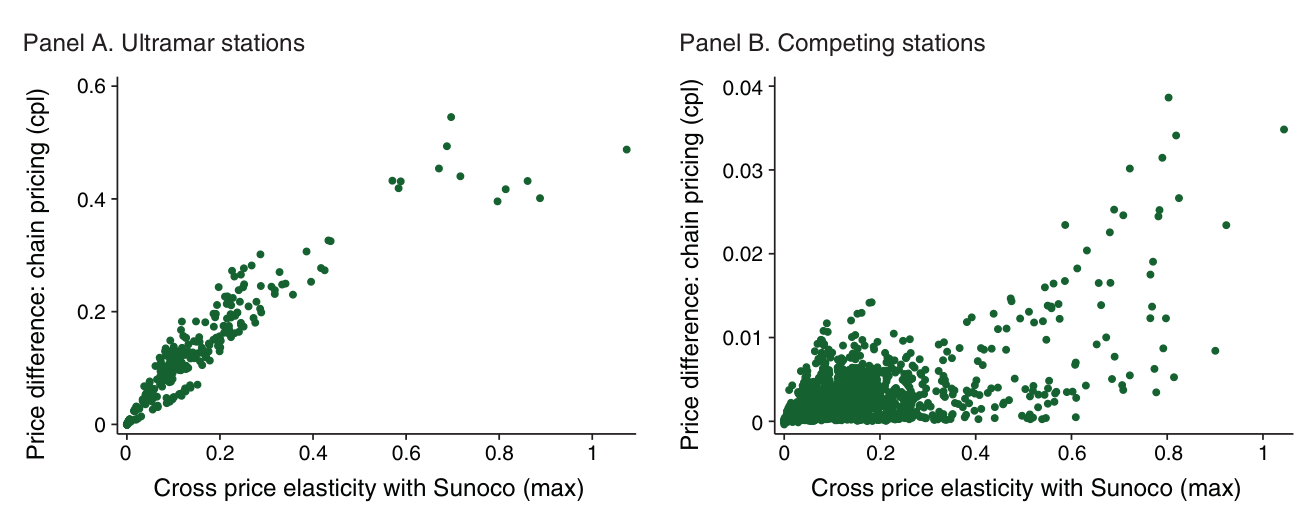
\includegraphics[width=0.92\textwidth]{figures/ch11/houde_fig4.png}
\caption{Simulated post-merger price changes (chain pricing, cpl) at Ultramar stations (panel A) and at competing
stations (panel B), plotted against each station's maximum cross-price elasticity with a Sunoco station. Note the
different vertical scales. Source: \citet{Houde2012}, Figure 4.}
\label{fig:11-houde}
\end{figure}

\Cref{fig:11-houde} shows where the price effects come from. Ultramar stations that compete closely with a Sunoco
station raise prices most, and the relation with the maximum cross elasticity is almost linear. The competitors'
responses follow the same pattern on a scale about fifteen times smaller and with more noise. Single-station owners
react more strongly to a close competitor's price increase than multi-station chains do.

\casehead{Retrospective analysis}
The difference-in-differences design follows \citet{Hastings2004}. Let $N^d_j$ indicate that station $j$ lies in
neighborhood $d$ of a Sunoco station, and let $T_t$ indicate periods from 1997 on. The indicator $S_{jt}$ marks stations
supplied by Ultramar after the merger (Ultramar, former Sunoco and Sergaz stations). The two regressions are (eqs.~(12)--(13))
\begin{align}
p_{jt} &= \gamma\, N^d_j T_t + Z_{jt}\omega + \mu_j + \tau_t + u_{jt}, \label{eq:11-houde-did}\\
p_{jt} &= \gamma_0\, N^d_j T_t S_{jt} + \gamma_1\, N^d_j T_t (1 - S_{jt}) + Z_{jt}\omega + \mu_j + \tau_t + u_{jt},
\label{eq:11-houde-did2}
\end{align}
with station fixed effects $\mu_j$, period effects $\tau_t$ and time-varying characteristics and sales volume in
$Z_{jt}$. The coefficient $\gamma$ is the average merger effect in the neighborhood, $\gamma_0$ the direct effect and
$\gamma_1$ the competitive effect. Identification requires that, absent the merger, prices in treated and control
neighborhoods would have moved in parallel. A national swap negotiated for other reasons is plausibly unrelated to
local demand shocks. The price-floor regulation introduced in 1997 must also have affected treated and control
stations alike. Standard errors are clustered by location.

\begin{table}[htbp]
\centering
\caption{Retrospective estimates of the Ultramar-Sunoco merger effect on prices (cpl)}
\label{tab:11-houde}
\begin{threeparttable}
\small
\begin{tabular}{@{}lcccccc@{}}
\toprule
\multicolumn{7}{@{}l}{\emph{Panel A. Direct and competitive effects, half-minute neighborhood (Table 11)}} \\
 & (1) & (2) & (3) & (4) & (5) & (6) \\
Sample & 95/97 & 95/97 & 95/97 & 95/97 & 95/98 & 95/98 \\
1996 price war included & Yes & Yes & No & No & No & No \\
\midrule
Merger $\times$ direct & & 0.501 & & 0.202 & & 0.211 \\
 & & (0.121) & & (0.077) & & (0.079) \\
Merger $\times$ competitive & & 0.0384 & & $-0.106$ & & 0.325 \\
 & & (0.178) & & (0.164) & & (0.169) \\
Merger (aggregate) & 0.433 & & 0.156 & & 0.229 & \\
 & (0.119) & & (0.079) & & (0.074) & \\
Observations & 5,778 & 5,778 & 5,457 & 5,457 & 7,287 & 7,287 \\
$R^2$ & 0.785 & 0.785 & 0.840 & 0.840 & 0.917 & 0.917 \\
\midrule
\multicolumn{7}{@{}l}{\emph{Panel B. Aggregate effect by neighborhood definition (Table 12)}} \\
 & \multicolumn{3}{c}{95/97, price war included} & \multicolumn{3}{c}{95/98, price war excluded} \\
\cmidrule(lr){2-4}\cmidrule(lr){5-7}
Within half a minute & \multicolumn{3}{c}{0.433 (0.119)} & \multicolumn{3}{c}{0.229 (0.074)} \\
Within one minute & \multicolumn{3}{c}{0.419 (0.110)} & \multicolumn{3}{c}{0.216 (0.064)} \\
Within 1.5 minutes & \multicolumn{3}{c}{0.290 (0.108)} & \multicolumn{3}{c}{0.223 (0.059)} \\
Common street & \multicolumn{3}{c}{0.266 (0.084)} & \multicolumn{3}{c}{0.175 (0.067)} \\
\bottomrule
\end{tabular}
\begin{tablenotes}[flushleft]
\footnotesize
\item Notes: Reproduced from \citet[Tables 11 and 12]{Houde2012}. Dependent variable: station price. The merger variable
is a Sunoco station in the neighborhood times years from 1997. The direct effect applies to post-merger Ultramar brands
(Sunoco, Sergaz and Ultramar), the competitive effect to all other stations in the neighborhood. All regressions
include location and time fixed effects and time-varying controls. Standard errors clustered by location in
parentheses. Panel B has 5,778 observations in the first column group and 7,287 in the second. The note to the paper's
Table 11 says that columns 2 to 6 exclude the 1996 price war. The text (p.~2176) and the sample sizes show that only
columns 3 to 6 do, and we follow the text.
\end{tablenotes}
\end{threeparttable}
\end{table}

\Cref{tab:11-houde} reports the estimates. Every specification finds a price increase in the treated neighborhoods,
so the market-power effect dominated any efficiency gain. The aggregate half-minute effect ranges from 0.156 to 0.433
cpl depending on the sample. Average retail margins were about 4 cpl at the time, so the merger raised margins by at
most 11 percent and prices by about 0.7 percent. In US units the increase is at most 1.75 cents per gallon. It is
smaller than the 5 cents of \citet{Hastings2004} and larger than the 1 cent of \citet{TaylorKreisleZimmerman2010}
\citep[p.~2176]{Houde2012}. The effect comes mostly from stations supplied by Ultramar, with direct
effects between 0.2 and 0.5 cpl. The competitive effect is imprecise and sometimes negative. It becomes significant
only in the sample that extends to 1998, when more stations had been rebranded. In the 1995--1997 sample with the price war, the effect declines with the size of
the neighborhood. In the 1995--1998 sample, which drops the price war and adds the rebranding period, it declines
much less (Panel B). Houde attributes the flatter profile to the rebranding periods in that sample (p.~2177).

\casehead{Comparing simulation and retrospective estimates}
The two methods agree on the main magnitude. The simulation predicts 0.38 cpl in the half-minute neighborhood, and
the aggregate retrospective estimates in \cref{tab:11-houde} range from 0.16 to 0.43 cpl. Both attribute most of the effect to the merging chain's
internalization of diversion between its old and new stations. Both find larger effects where Ultramar and Sunoco
stations competed for the same commuters.

They disagree in two ways that point to the model's weak spot. The retrospective competitive effect is larger in
one sample, and the observed effect falls more slowly with distance. The simulated effect falls from 0.388 to 0.090
cpl across the four neighborhoods, while the estimated effect falls from 0.433 to 0.266 cpl in the sample with the
price war. The logit shock makes simulated competitor responses too small, a limitation common to most differentiated
products models with idiosyncratic shocks (\cref{ch:blp}). Without the price war, the retrospective estimate (about
0.2 cpl) is below the simulated one (about 0.38 cpl, given as 0.37 in the paper's discussion). The gap may indicate
efficiencies larger than those estimated.

The retrospective design has its own weaknesses, which the simulation helps diagnose. The estimates are sensitive to
the sample, and the version with the price war may capture the end of the war in neighborhoods where Ultramar was
active, a second treatment. Controls are contaminated because distant Ultramar stations also raise prices. The
simulation also explains why two studies of the same California merger reached different answers.
\citet{Hastings2004} found price increases of about 5 cents per gallon after ARCO acquired the Thrifty chain, and
\citet{TaylorKreisleZimmerman2010} found about 1 cent with different price data. Simulated effects are very
heterogeneous across stations. Samples that omit the acquired stations or over-represent the acquirer's stations
among controls can understate the effect. Dropping Sunoco stations from the averages in \cref{tab:11-houde-sim}
would cut the direct effect by more than half \citep[pp.~2178--2179]{Houde2012}.

\casehead{Limitations and critiques}
Several assumptions deserve scrutiny. Total gasoline consumption is inelastic, so the model captures station choice
and car use but not driving more when gasoline is cheap. The price used for estimation is a single survey-day
snapshot in a market where prices change weekly, and the analysis assumes the cross-sectional price distribution is
stable within periods. Routes are deterministic shortest paths without congestion, and income is assumed independent
of workplace. The RPM assumption makes suppliers the price setters at lessee stations. The merger is small, with 12
acquired stations, which limits the power of the retrospective test. The logit shock, as Houde emphasizes, understates
the substitution between close competitors despite a large transport cost.

\casehead{Contribution}
The paper makes three contributions. It shows how to put a realistic geography into a BLP-style demand model by
treating commuting paths as consumer locations. It shows that this changes the estimates of transport costs and
markups substantially, and that the resulting markups match an external benchmark, the rack margin. It offers one of
the cleanest validations of merger simulation against a retrospective estimate of the same merger, complementing
\citet{Peters2006}, \citet{WeinbergHosken2013} and the analgesics study of \cref{sec:11-bv}. The same market reappears
in \cref{ch:collusion-evidence}, where \citet{ClarkHoude2013} study a gasoline cartel in Quebec.

\subsection{Mergers and product repositioning in music radio: Sweeting (2010)}\label{sec:11-sweeting}

\casehead{Question}
Merger analysis usually treats the set of products as fixed. In many industries a merged firm can change its products
quickly, and \citet{Sweeting2010} asks what it does with them. The question has policy weight. If merging firms
reposition their products, models with fixed products will mispredict price and welfare effects. Rivals may also lose
from a merger without synergies, which contradicts the standard Bertrand prediction that rivals gain
(\cref{sec:11-upp}).

\casehead{What theory predicts}
One-dimensional location models give stark and opposite answers. With price competition and quadratic transport
costs, two independent firms locate at the ends of the line to soften price competition
\citep{DAspremontGabszewiczThisse1979}. A merger then reduces differentiation, because the joint owner no longer needs
to soften competition between its own products. Without price competition and with a fixed audience, independent
firms cluster at the center, the minimal differentiation of \citet{Hotelling1929}. A joint owner gains nothing from
duplication and spreads its products to avoid cannibalization, a point that goes back to \citet{Steiner1952}. Reality
lies between these extremes. \citet{GandhiEtAl2008} compute equilibria of a location-then-price game and show that a
merged firm may move its products apart and toward rivals, which mitigates the price increase.

\casehead{Setting}
The 1996 Telecommunications Act relaxed local ownership caps for radio stations, and the industry consolidated
rapidly. Radio is a two-sided market. Listeners pay an implicit price by hearing commercials, and advertisers pay for
listeners. The Department of Justice reviewed radio mergers solely for their effect on advertising prices. It
required divestitures in some deals but did not consider effects on listeners or programming variety
\citep[p.~8]{Sweeting2010}. Programming changes are cheap within a format. Music licenses are blanket licenses whose
fees are a fixed share of revenue, so playlist overlap does not affect costs.

\casehead{Data}
Station characteristics, ownership histories and Arbitron audience shares come from the BIAfn MediaAccess Pro
database. Playlists come from Mediabase airplay logs for the first week (Monday to Friday) of each month from April
1998 to December 2001, for 1,094 music stations. The data contain 133,994 station-day logs. The stations belong to
seven formats (Adult Contemporary, Album Oriented Rock/Classic Rock, Contemporary Hit Radio/Top 40, Country, Oldies,
Rock, Urban) and 148 markets. In 2001 they had revenues of \$6.5 billion and an average audience of 13 million. A
station plays on average 1,367 songs by 177 artists in a five-day week, and 10,542 artists appear at least once.

The estimation sample has 740 stations in market-formats with at least two sample stations. These form 688 pairs in
the same market-format, which experience 46 changes in common ownership. Of these, 31 are mergers, that is, switches
from separate to common ownership. By type of transaction, 24 come from deals confined to one market-format and 8 from
transactions spanning more than 7 market-formats. Another 14 come from divestitures that the Department of Justice
required. Market shares convert Arbitron's average quarter-hour
shares into shares of total listening time.

\casehead{Measuring product positions}
Each station's playlist in week $w$ is a vector $a_i \in \R^{\mathcal{M}}_+$, where $\mathcal{M}$ is the set of artists
and $a_{im}$ is the share of station $i$'s songs by artist $m$. Two measures of the distance between stations $i$ and
$j$ are used. The \emph{unique-artist measure} is the average share of each station's songs by artists the other
station does not play:
\begin{equation}\label{eq:11-sw-ua}
d^{UA}_{ij} = \frac{1}{2}\Big[\sum_{m : a_{jm} = 0} a_{im} + \sum_{m : a_{im} = 0} a_{jm}\Big] \in [0, 1].
\end{equation}
The \emph{angle measure} treats each artist as a dimension and measures the angle between the two playlist vectors,
normalized by its maximum for nonnegative vectors:
\begin{equation}\label{eq:11-sw-angle}
d^{A}_{ij} = \frac{2}{\pi}\arccos\Big(\frac{a_i^{\top}a_j}{\lVert a_i\rVert\,\lVert a_j\rVert}\Big) \in [0, 1].
\end{equation}
The angle measure distinguishes stations that play the same artists in different proportions, which matters in
formats where almost every station plays the current hits. The two measures have a within-pair correlation of 0.65.
The distance between a pair $(i,j)$ and a third station $k$ in the same market-format is $\min\{d_{ik}, d_{jk}\}$.

\begin{example}[Computing the distance measures]\label{ex:11-sweeting}
Suppose there are three artists $X$, $Y$ and $Z$. Station $i$ plays them 10, 0 and 5 times, so $a_i = \big(\frac{2}{3},
0, \frac{1}{3}\big)$. Station $j$ plays $Y$ and $Z$ equally, so $a_j = \big(0, \frac{1}{2}, \frac{1}{2}\big)$. Artist
$X$ is unique to $i$ and artist $Y$ is unique to $j$, so
\begin{equation*}
d^{UA}_{ij} = \frac{1}{2}\Big[\frac{2}{3} + \frac{1}{2}\Big] = \frac{7}{12} \approx 0.583 .
\end{equation*}
For the angle, $a_i^{\top}a_j = \frac{1}{6}$, $\lVert a_i\rVert = \frac{\sqrt{5}}{3}$ and $\lVert a_j\rVert =
\frac{1}{\sqrt 2}$, so the cosine is $\frac{1}{\sqrt{10}} \approx 0.316$. The angle is 1.249 radians and
$d^{A}_{ij} = \frac{2}{\pi}\times 1.249 \approx 0.795$.
\end{example}

The cross-section already suggests the main pattern. Commonly owned pairs have an average unique-artist measure of
0.66, against 0.55 for separately owned pairs. A commonly owned station thus devotes about 20 percent more of its
playlist to artists absent from its sister station. Separately owned stations are not minimally differentiated
either. Pairs of format duopolists in the same market are more differentiated than pairs of format monopolists in
different markets of the same Census division. In Adult Contemporary, for example, the angle measures are 0.721 and
0.619 (Table 3(a)). This rules out the model without price competition, in which duopolists would cluster. The
finding that common owners differentiate more is in turn at odds with the standard two-product model with price
competition, in which a merger brings products closer together.

\casehead{Estimating equation}
The main specification is a fixed effects regression on station pairs in the same market-format
\citep[eq.~(1)]{Sweeting2010}:
\begin{equation}\label{eq:11-sw-reg}
d_{ijw} = \mathit{CO}_{ijw}\,\beta_1 + N_{ijw}\beta_2 + T_{ijw}\beta_3 + \mu_{ij} + \varepsilon_{ijw}.
\end{equation}
Here $d_{ijw}$ is the distance between stations $i$ and $j$ in week $w$, and $\mathit{CO}_{ijw}$ indicates a common
owner. The controls $N_{ijw}$ are dummies for the numbers of stations and of sample stations in the market-format,
$T_{ijw}$ are week-by-format dummies, and $\mu_{ij}$ is a pair fixed effect. The coefficient $\beta_1$ is identified by within-pair
changes in ownership, while pairs without changes help identify the time and market-structure effects. Standard
errors are clustered by market-format, which allows for correlation across pairs that share a station.

The same template is applied to other outcomes. For positioning relative to rivals, the dependent variable is the
distance between a pair and a third station. The treatment is then common ownership of the pair by a firm that does not
own the third station, with a fixed effect for each pair-third-station triplet. For variety, the dependent
variable is the log number of artists played in a market-format. For audiences, it is the pair's combined market share
with quarter-by-format effects. For prices, it is the commercial load of a station in an hour.

\casehead{Identification}
No instrument for ownership changes is available. The causal reading rests on three arguments. First, timing.
\Cref{fig:11-sweeting} shows no trend in differentiation or audiences before mergers and clear changes within six to
twelve months after them. Second, similar effects appear for small and large transactions. A deal covering dozens of
markets is unlikely to be driven by conditions in one market-format. Third, mergers and demergers produce changes of
opposite sign, although they presumably occur for different reasons.

\casehead{Main results}
\Cref{tab:11-sweeting} collects the key estimates. Common owners differentiate their stations. The angle measure
rises by 0.055 and the unique-artist share by 7.2 percentage points, 13 percent of the separately owned mean. The
effect is at least as large in market-formats with three or more observed stations, where rivals might constrain
repositioning. Common owners also move their stations closer to competitors. The distance from the pair to a third
station falls by 0.055 on the angle measure and by 6.1 percentage points on the unique-artist measure. Only the first
estimate is significant, at the 10 percent level. Variety does not rise. The number of artists in a market-format rises
by 6.9 percent only when one firm owns all observed stations, and the number of owners has no significant effect.

\begin{table}[htbp]
\centering
\caption{Ownership changes and positioning, audiences and commercial loads in radio}
\label{tab:11-sweeting}
\begin{threeparttable}
\footnotesize
\setlength{\tabcolsep}{4pt}
\begin{tabular}{@{}lcccccc@{}}
\toprule
\multicolumn{7}{@{}l}{\emph{Panel A. Differentiation between commonly owned stations (Table 4)}} \\
 & \multicolumn{2}{c}{All pairs} & \multicolumn{2}{c}{3 or more stations} & \multicolumn{2}{c}{2 stations} \\
\cmidrule(lr){2-3}\cmidrule(lr){4-5}\cmidrule(lr){6-7}
Angle measure & \multicolumn{2}{c}{0.055 (0.014)} & \multicolumn{2}{c}{0.068 (0.022)} & \multicolumn{2}{c}{0.043 (0.018)} \\
Unique-artist measure & \multicolumn{2}{c}{0.072 (0.019)} & \multicolumn{2}{c}{0.080 (0.024)} & \multicolumn{2}{c}{0.069 (0.033)} \\
Observations & \multicolumn{2}{c}{15,792} & \multicolumn{2}{c}{10,216} & \multicolumn{2}{c}{5,576} \\
\midrule
\multicolumn{7}{@{}l}{\emph{Panel B. Positioning relative to competitors and variety (Table 5)}} \\
 & \multicolumn{2}{c}{Angle distance} & \multicolumn{2}{c}{Unique-artist distance} & \multicolumn{2}{c}{Log number of artists} \\
\cmidrule(lr){2-3}\cmidrule(lr){4-5}\cmidrule(lr){6-7}
Pair has same owner & \multicolumn{2}{c}{$-0.055$ (0.033)} & \multicolumn{2}{c}{$-0.061$ (0.040)} & \multicolumn{2}{c}{} \\
All stations same owner & \multicolumn{2}{c}{} & \multicolumn{2}{c}{} & \multicolumn{2}{c}{0.069 (0.030)} \\
Number of owners & \multicolumn{2}{c}{} & \multicolumn{2}{c}{} & \multicolumn{2}{c}{0.009 (0.025)} \\
Observations & \multicolumn{2}{c}{14,475} & \multicolumn{2}{c}{14,475} & \multicolumn{2}{c}{8,942} \\
\midrule
\multicolumn{7}{@{}l}{\emph{Panel C. Market shares and competitor exit (Table 6)}} \\
 & (1) & (2) & (3) & (4) & (5) & (6) \\
Dependent variable & Log pair & Pair & Pair & Others' & Number & Sample \\
 & share & share & share & share & of rivals & rivals \\
Sample or model & All & Rivals & No rivals & Rivals & Poisson & Poisson \\
Pair has same owner & 0.031 & 0.0011 & 0.0003 & $-0.0012$ & $-0.140$ & $-0.252$ \\
 & (0.018) & (0.0003) & (0.0007) & (0.0005) & (0.076) & (0.081) \\
Observations & 3,015 & 2,911 & 2,835 & 2,911 & 2,939 & 2,939 \\
\midrule
\multicolumn{7}{@{}l}{\emph{Panel D. Commercial loads (Table 7)}} \\
 & \multicolumn{3}{c}{Commercial blocks per hour} & \multicolumn{3}{c}{Commercial minutes per hour} \\
\cmidrule(lr){2-4}\cmidrule(lr){5-7}
Owns other stations in format & \multicolumn{3}{c}{0.044 (0.044)} & \multicolumn{3}{c}{0.178 (0.193)} \\
Commonly owned competitors & \multicolumn{3}{c}{0.008 (0.062)} & \multicolumn{3}{c}{$-0.056$ (0.370)} \\
Observations & \multicolumn{3}{c}{960,634} & \multicolumn{3}{c}{960,634} \\
\bottomrule
\end{tabular}
\begin{tablenotes}[flushleft]
\footnotesize
\item Notes: Reproduced from \citet[Tables 4 to 7]{Sweeting2010}. Standard errors clustered by market-format in
parentheses, except in Panel C columns (5) and (6), where they come from a bootstrap that resamples markets. Panel A:
pair fixed effects, week-by-format and number-of-station dummies. Panel B: pair-third-station fixed effects in the first
two columns, market-format fixed effects in the third. Panel C: station-pair fixed effects and quarter-by-format dummies.
Columns (2) and (4) exclude pairs that change ownership as format duopolists. Column (3) excludes pairs that change
ownership with three or more stations in the format. Columns (2) to (4) drop the two quarters after an ownership
change. Shares are fractions of total listening. Panel D: station-format-hour fixed effects and year, month and
day-of-week interactions with format.
\end{tablenotes}
\end{threeparttable}
\end{table}

Listeners follow the playlists. Common ownership raises the pair's combined share by 3.1 percent, significant at the 10
percent level. \Cref{fig:11-sweeting}(c) shows a rise of almost 10 percent within a year, lagging the playlist changes
by a few months. The gain occurs only for pairs that face competitors. Their combined share rises by 0.0011, about 8
percent of the average pair's share, while the combined share of the other stations in the format falls by 0.0012. The
merging stations' gain is the rivals' loss. Rivals also leave the format. Common ownership reduces the number of
competing sample stations by 0.26 relative to a mean of 1.1, and the number of all competing stations by 0.36 relative
to a mean of 2.6.

Prices do not move. The average commercial load is 11.95 minutes per hour. Common owners slightly increase their loads
and stations facing common owners slightly reduce them, but neither effect is significant. These changes go the wrong
way to explain the shift in audiences, so repositioning, not price, is the channel.

\begin{figure}[htbp]
\centering
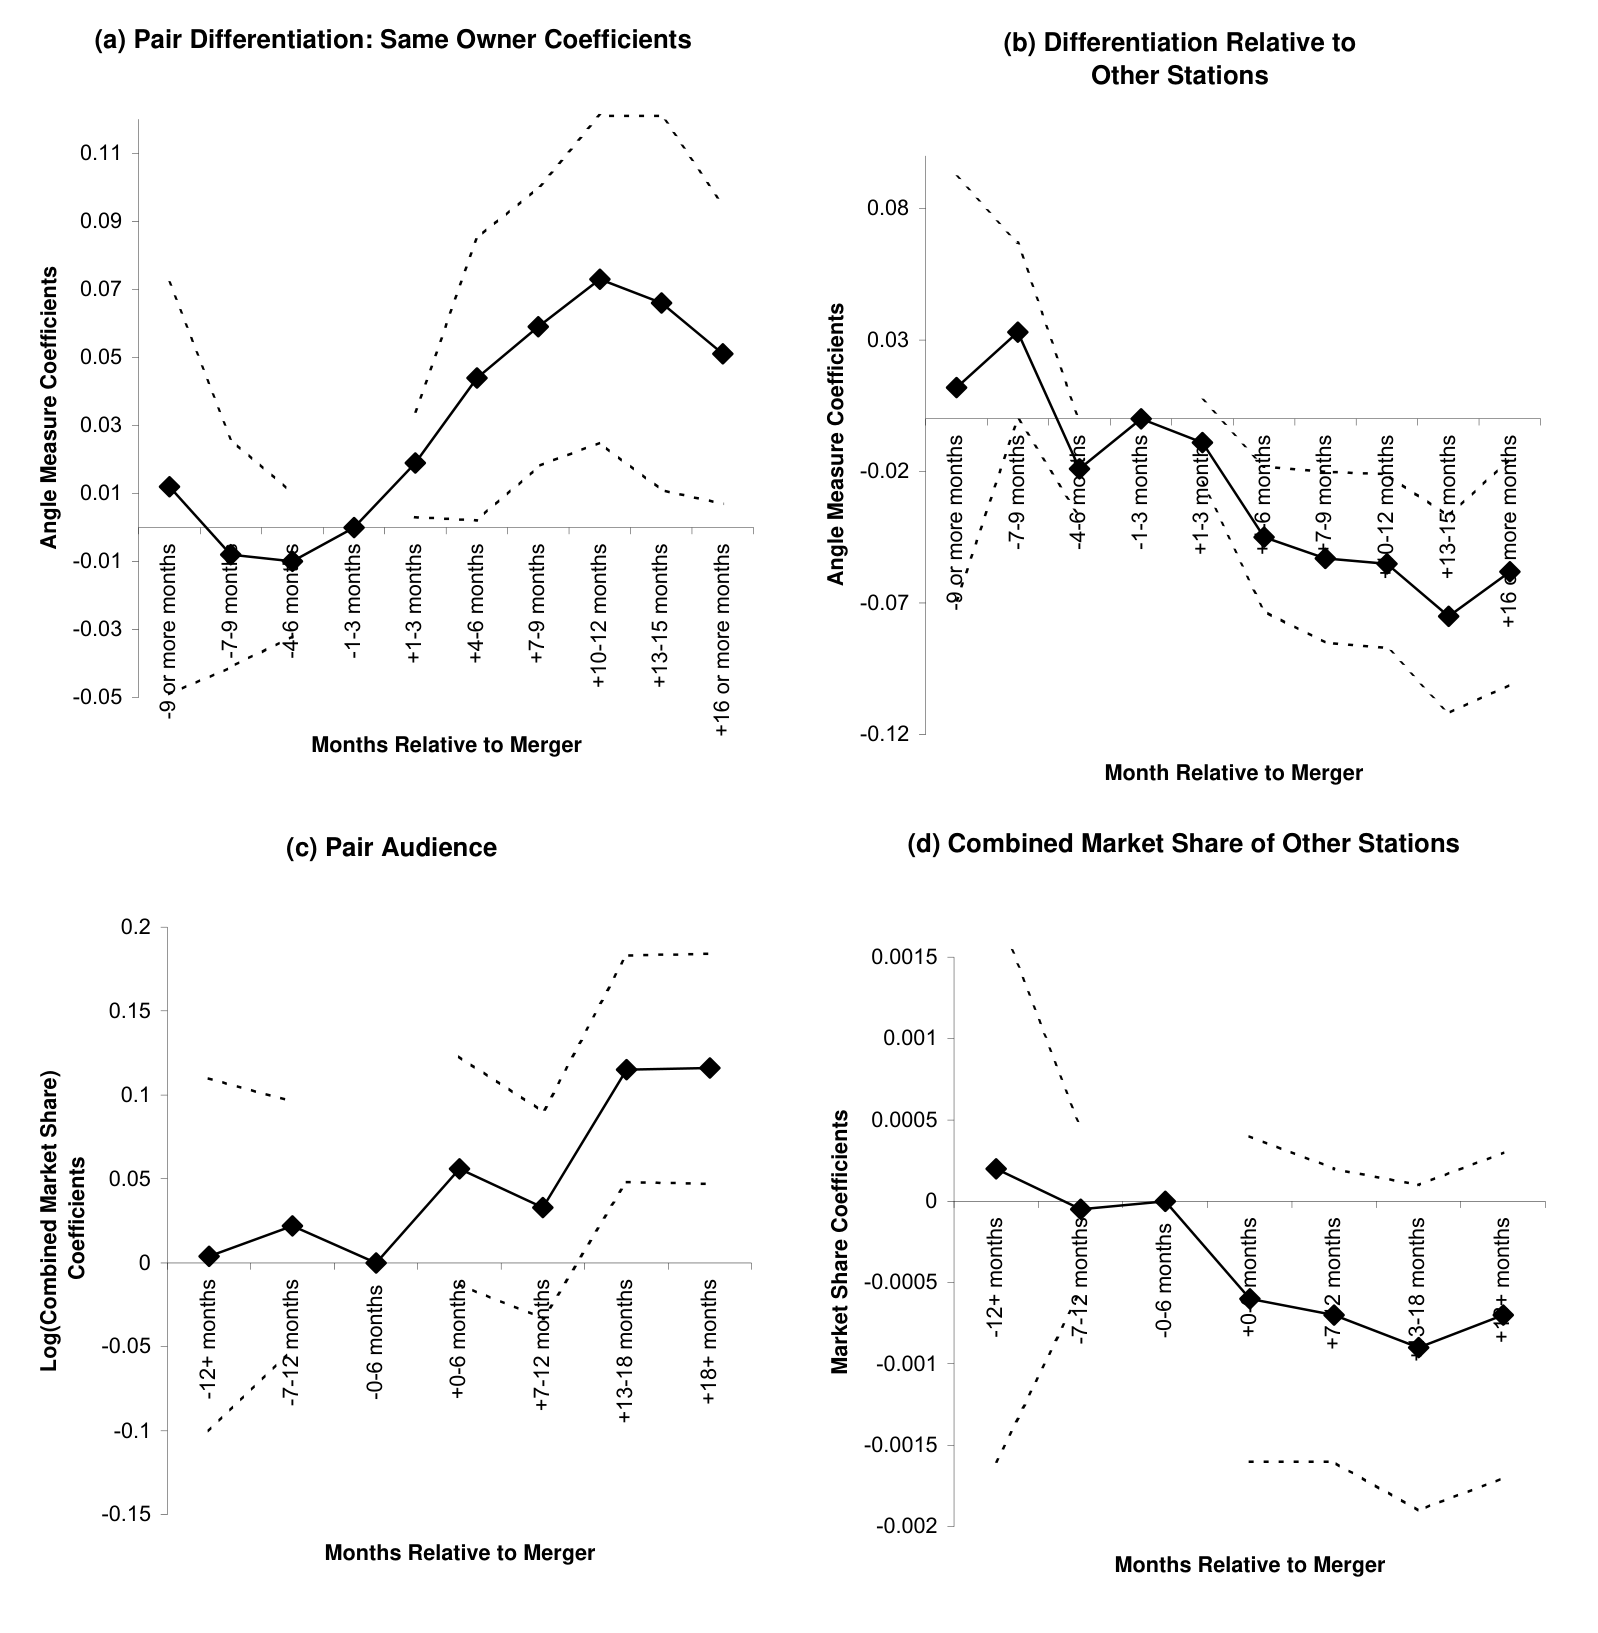
\includegraphics[width=0.84\textwidth]{figures/ch11/sweeting_fig1.png}
\caption{Timing of changes around mergers in music radio. Coefficients on dummies for time relative to the merger, with
95 percent confidence intervals (dashed). Panels (a) and (b) use the angle measure, for differentiation within the
merging pair and between the pair and other stations. Panels (c) and (d) show the log combined share of the pair and
the combined share of other stations. Pairs that ever switch from common to separate ownership are excluded. Source:
\citet{Sweeting2010}, Figure 1.}
\label{fig:11-sweeting}
\end{figure}

\casehead{Robustness}
Section~4 of the paper rules out several alternative explanations. National ownership might raise quality through
economies of scope. In a station-share regression, however, the log number of same-format stations owned nationally has
a coefficient of $-0.0003$ (0.0070), while local common ownership keeps a coefficient of 0.0554 (0.0230) (Table 8).
Changes in signal power or transmitter height do not drive the audience gains. Excluding pairs with technical changes
raises the share coefficient to 0.038 (0.022), and to 0.098 (0.017) when the two quarters after a change are dropped.
Results by format agree in sign in 19 of 21 cases (Table 9). Pairs that merge resemble other pairs before the merger on
three of four outcomes (Table 10). Results are similar for large and small transactions and for mergers and demergers
(Table 11). In data covering all formats and 281 rated markets, owning another station in the same market-format
raises a station's share by 4.6 percent (0.022). The number of owners has no effect on total format listening (Table
12).

\casehead{Interpretation}
The merged firm separates its own stations to reduce cannibalization, as a Hotelling owner without price competition
would. It also moves them toward rivals and takes their listeners. It does not use the new positions to serve
unserved tastes or to soften competition. Three implications follow for merger analysis. Models that hold products fixed will misstate the effects
of mergers, and repositioning may help explain why such models often predict post-merger prices poorly
\citep{Peters2006}. Rivals can be harmed by a merger without synergies, so their complaints do not by themselves
signal that the merger is pro-competitive. This contrasts with the logic of \cref{sec:11-cournot}. Aggregate variety
can stay constant even when the merging firms differentiate, so studies of format counts such as
\citet{BerryWaldfogel2001} see only part of the adjustment. The welfare effect of the repositioning remains open,
since moving closer to rivals transfers listeners without creating variety (\cref{ch:newgoods}).

\casehead{Limitations and contribution}
The study is descriptive and lacks an instrument for ownership. It measures positions with playlists only, ignoring
talk and personality programming. It covers relatively successful music stations in larger markets. The industry is
unusual in ways that \citet[pp.~25--26]{Sweeting2010} lists: horizontal differentiation dominates, listening is
inelastic, price competition through commercials is weak, and playlist changes do not affect costs. The paper's
contribution is a set of stylized facts that structural models of endogenous product choice should match.

Structural merger simulations with repositioning have since followed, each adapted to its industry
\citep[pp.~236--237]{AskerNocke2021}. \citet{LiEtAl2019} study airline mergers. A first-stage entry model, in which a
carrier chooses between nonstop and connecting service on a route, is attached to a nested logit demand model.
\citet{Wollmann2018} also uses a first-stage entry model, to study how a merger changes the product mix in the US
market for commercial vehicles. \citet{Fan2013} lets merging newspapers adjust their prices and three dimensions of
quality. Because the characteristics are continuous, repositioning adds first-order conditions for them to the
pricing conditions of \cref{sec:11-simframework}. \citet{MazzeoSeimVarela2018} add a product-selection stage to a
standard simulation and explore its effects in a range of simulations. \citet{DraganskaMazzeoSeim2009} study
assortment choice more broadly.

These studies agree with Sweeting that a merger can change the incentives to offer particular products, and that
allowing for repositioning changes the estimated effect on consumer welfare. They disagree on the direction of the
bias from ignoring it. Repositioning or entry by a rival adds competitive pressure, while the merged firm's exit from
a product space removes it and adds to the harm. Which force dominates depends on the industry
\citep[p.~237]{AskerNocke2021}.

\subsection{Mergers and capacity investment in the paper industry: Pesendorfer (2003)}\label{sec:11-pesendorfer}

\casehead{Question}
In industries where capacity is the main strategic variable, a merger changes the allocation of capital and the
incentives to invest. A study of short-run prices or outputs can then mismeasure the merger's effects.
\citet{Pesendorfer2003} studies the wave of 31 horizontal mergers in the US paper and paperboard industry between
August 1984 and July 1987. He models capacity investment, uses firms' investment choices before and after the wave to
infer the cost changes that mergers produced, and computes the implied welfare effects. The wave followed the 1984
revision of the Merger Guidelines, which signaled a friendlier stance toward mergers.

\casehead{The investment model}
There are $n$ firms producing a homogeneous good. Firm $i$ starts with capacity $K_i$ and chooses investment $x_i$,
which may be negative (scrapping). Capacity depreciates by the factor $\vartheta \in (0,1)$, so the post-investment
capacity is $\vartheta K_i + x_i$. Adding capacity costs $r(x_i)$, while scrapping is free. Production cost is
$C_i(\cdot)$ with marginal cost $c_i(\cdot)$. Plants run at full capacity, an assumption that fits an industry whose
utilization averaged 93 percent, so industry output is $Q = \sum_j(\vartheta K_j + x_j)$. Firms discount the future by
$\delta \in (0,1)$. Pesendorfer writes $\beta$ for the discount factor and $\delta$ for depreciation, and we rename
both to follow \cref{ch:collusion-theory}. Firm $i$'s payoff is the discounted stream of future profits from the new
capacity, minus investment cost (eq.~(1)):
\begin{equation}\label{eq:11-pes-payoff}
\Pi_i(x) = \frac{\delta}{1 - \delta}\Big[(\vartheta K_i + x_i)\,P\Big(\sum_j(\vartheta K_j + x_j)\Big) - C_i(\vartheta K_i
+ x_i)\Big] - r(x_i)\,\indic\{x_i > 0\}.
\end{equation}
The model is a one-shot investment game. Without depreciation ($\vartheta = 1$) and with linear investment cost, its
equilibrium coincides with that of a dynamic game in which all investment occurs at once.

\begin{proposition}[Equilibrium investment, after \citealp{Pesendorfer2003}, Proposition 1]\label{prop:11-pes-kt}
Let $\mathit{MR}_i = P(Q) + (\vartheta K_i + x_i)P'(Q)$ be firm $i$'s marginal revenue from capacity. Assume that an
equilibrium exists, marginal revenue decreases in own capacity, $c_i$ is nondecreasing, and $r$ is increasing and
convex. In an equilibrium, each firm's investment satisfies
\begin{equation}\label{eq:11-pes-kt}
\begin{aligned}
x_i > 0 &: \quad \frac{\delta}{1 - \delta}\big[\mathit{MR}_i - c_i\big] = r'(x_i),\\
x_i < 0 &: \quad \mathit{MR}_i - c_i = 0,\\
x_i = 0 &: \quad 0 \le \frac{\delta}{1 - \delta}\big[\mathit{MR}_i - c_i\big] \le r'(0),
\end{aligned}
\end{equation}
where $c_i$ is evaluated at $\vartheta K_i + x_i$.
\end{proposition}

\begin{proof}
Holding rivals' choices fixed, $\Pi_i$ is concave in $x_i$ on each side of zero under the stated assumptions. For
$x_i \neq 0$ its derivative is $\frac{\delta}{1-\delta}[\mathit{MR}_i - c_i] - r'(x_i)\indic\{x_i > 0\}$, and an
interior optimum sets it to zero, which gives the first two lines. At $x_i = 0$ the payoff has a kink. The left
derivative is $\frac{\delta}{1-\delta}[\mathit{MR}_i - c_i]$ and the right derivative subtracts $r'(0)$. Zero is
optimal when the left derivative is nonnegative, so scrapping does not pay, and the right derivative is nonpositive, so
investing does not pay. This gives the third line. Pesendorfer writes the three cases compactly as
$x_i\{[\mathit{MR}_i - c_i]\frac{\delta}{1-\delta} - r'(x_i)\indic\{x_i > 0\}\} = 0$ (eq.~(2)).
\end{proof}

Inverting \eqref{eq:11-pes-kt} gives marginal cost as a function of observables (Corollary 2, eq.~(3)):
\begin{equation}\label{eq:11-pes-cost}
c_i = \mathit{MR}_i - \frac{1 - \delta}{\delta}\, r'(x_i)\,\indic\{x_i > 0\} \quad (x_i \neq 0),
\qquad
c_i \in \Big[\mathit{MR}_i - \frac{1 - \delta}{\delta}\, r'(0),\; \mathit{MR}_i\Big] \quad (x_i = 0).
\end{equation}
The right-hand side depends on industry capacity and investment, the firm's own capacity and investment, demand and
the investment cost function. Marginal revenue falls with own capacity. So for a given capacity, a firm that invests
more must have a lower marginal cost. This is the inference the empirical work exploits: changes in investment after a
merger reveal changes in the merged firm's costs. Investment is measured as $x_i = K_i' - \vartheta K_i$, where $K_i'$
is next period's capacity. With $\vartheta < 1$ a firm that keeps capacity constant invests a positive amount, so the
interval case rarely arises.

\casehead{Merger analysis in a linear example}
To see what the model implies, Pesendorfer specializes it. We follow \cref{sec:11-ssr} and write the demand intercept
as $a$.

\begin{assumption}[Linear investment model]\label{ass:11-pes}
(i) Demand is $P(Q) = a - bQ$. (ii) $\frac{\delta}{1 - \delta} = \vartheta = 1$. (iii) Unmerged firms have constant
marginal cost $c$, and the merged firm has constant marginal cost $c_m$. (iv) Investment cost is linear, $r(x) = rx$.
(v) Initial capacities are at Cournot levels, $K_i = K^c \equiv \frac{a - c}{b(n + 1)}$.
\end{assumption}

Under (ii) the payoff is one period's profit minus investment cost. Before the merger, all firms hold $K^c$, the price
is $P^0 = c + \frac{a - c}{n + 1}$, each firm earns $\frac{(a - c)^2}{b(n + 1)^2}$, and no firm wants to invest or scrap.
Two firms then merge, and the merged firm $m$ holds $2K^c$.

\begin{proposition}[A profitable merger without synergies]\label{prop:11-pes-profit}
Let \cref{ass:11-pes} hold with $c_m = c$, and suppose $\frac{a - c}{2(n + 1)} \le r$. Then the post-merger game has an
equilibrium in which the merged firm scraps $\frac{K^c}{2}$ and no outsider invests. The price rises to $c +
\frac{3}{2}\,\frac{a - c}{n + 1}$, and the merging firms' joint profit rises by $\frac{1}{4b}\big(\frac{a - c}{n +
1}\big)^2 > 0$.
\end{proposition}

\begin{proof}
Use $b(n + 1)K^c = a - c$ throughout. Suppose outsiders choose $x_i = 0$ and the merged firm chooses $x_m$. Industry
output is $nK^c + x_m$. An outsider's marginal revenue minus cost is
\begin{equation*}
\mathit{MR}_i - c = a - c - b(nK^c + x_m) - bK^c = (a - c) - b(n + 1)K^c - b\,x_m = -b\,x_m .
\end{equation*}
The merged firm's is
\begin{equation*}
\mathit{MR}_m - c = a - c - b(nK^c + x_m) - b(2K^c + x_m) = -\frac{a - c}{n + 1} - 2b\,x_m .
\end{equation*}
This is negative at $x_m = 0$, so the merged firm scraps until $\mathit{MR}_m = c$:
\begin{equation*}
x_m = -\frac{a - c}{2b(n + 1)} = -\frac{K^c}{2}.
\end{equation*}
Its payoff is concave, and investing is never optimal because $\mathit{MR}_m - c - r < 0$ for $x_m \ge 0$. Given
$x_m$, each outsider has $\mathit{MR}_i - c = \frac{a - c}{2(n + 1)} \ge 0$, so scrapping does not pay. Investing
does not pay if this gain is at most $r$, which is the stated condition. So $x_i = 0$ is a best response.

Industry output is $\big(n - \frac{1}{2}\big)K^c$, and the margin is
\begin{equation*}
P - c = (a - c) - \Big(n - \frac{1}{2}\Big)\frac{a - c}{n + 1} = \frac{3}{2}\,\frac{a - c}{n + 1}.
\end{equation*}
The merged firm sells $\frac{3}{2}K^c$, so its profit is $\frac{3}{2}\frac{a - c}{n + 1}\times\frac{3}{2}\frac{a - c}{b(n
+ 1)} = \frac{9}{4b}\big(\frac{a - c}{n + 1}\big)^2$. Before the merger the two firms earned $\frac{2}{b}\big(\frac{a -
c}{n + 1}\big)^2$. The difference is $\frac{1}{4b}\big(\frac{a - c}{n + 1}\big)^2$.
\end{proof}

\citet[Remark 3]{Pesendorfer2003} states the result under the condition $n + 1 > \frac{a - c}{r}$, which implies the
weaker condition used above. The mechanism is the asymmetry between expanding and contracting capacity. The merged firm
can withdraw capacity at no cost, while outsiders would have to pay $r$ per unit to fill the gap. If $r = 0$, outsiders
expand freely, every firm sets $\mathit{MR} = c$, and the post-merger outcome is Cournot with $n - 1$ firms. A
two-firm merger is then unprofitable for $n \ge 3$ (\cref{prop:11-ssr}). For any $r > 0$, however, a profitable merger
exists once $n$ is large enough \citep[p.~7, n.~6]{Pesendorfer2003}.

\begin{example}[Investment makes the merger profitable]\label{ex:11-pes}
Let $a = 10$, $b = 1$, $c = 2$, $n = 4$ and $r = 1$. Cournot capacities are $K^c = 1.6$, the price is $P^0 = 3.6$ and
each firm earns 2.56. After a merger of two firms, the merged firm scraps 0.8 units, outsiders' marginal gain from
investing is $0.8 < r$, and the price rises to 4.4. The merged firm earns $2.4 \times 2.4 = 5.76$, a gain of 0.64 over
the combined 5.12. Pesendorfer's sufficient condition would require $r > 1.6$, so the example lies in the region
covered only by the weaker condition. With costless expansion the outcome would be Cournot with three firms, a price of
4.0 and a merged profit of 4.0, a loss of 1.12. Costly expansion makes the merger profitable precisely because rivals
do not replace the withdrawn capacity, so consumers face a higher price than in the Cournot benchmark.
\end{example}

The example shows a general feature. The post-merger margin is $\frac{3}{2}\frac{a - c}{n + 1}$, while the Cournot
margin with $n - 1$ firms is $\frac{a - c}{n}$. The first is larger whenever $n > 2$. Pesendorfer's three remaining
remarks describe what investment reveals about costs and welfare.

\begin{proposition}[Investment and merger cost savings, Remarks 4 to 6]\label{prop:11-pes-remarks}
Let \cref{ass:11-pes} hold.
\begin{enumerate}[label=(\alph*)]
  \item If the merged firm does not change its capacity after the merger ($x_m = 0$), then no outsider does either, and
  $2c - P^0 - r \le c_m \le 2c - P^0$. In particular $c_m < c$.
  \item If $c_m = c$, industry capacity falls and the merger reduces total welfare.
  \item If $x_m = 0$, consumer surplus is unchanged and total welfare rises.
\end{enumerate}
\end{proposition}

\begin{proof}
(a) With $x_m = 0$ and symmetric outsiders, an outsider's marginal gain is $-b(n - 1)x_i$. A positive $x_i$ would
require this to equal $r > 0$, and a negative $x_i$ would require it to equal zero, so $x_i = 0$. The merged firm's
marginal revenue at $x_m = 0$ is $a - b(n + 2)K^c = P^0 - 2(P^0 - c) = 2c - P^0$. Zero investment requires $0 \le
\mathit{MR}_m - c_m \le r$, which is the stated band. Since $P^0 > c$, $c_m \le 2c - P^0 < c$.

(b) Suppose instead that total investment $X = \sum_j x_j$ is positive. An outsider's marginal gain is $-b(X + x_i)$,
which cannot equal $r > 0$ when $x_i > 0$ and $X > 0$, so $x_i \le 0$. The merged firm's is $-\frac{a - c}{n + 1} -
b(X + x_m)$, which is negative when $x_m > 0$ and $X > 0$, so $x_m \le 0$. Then $X \le 0$, a contradiction. If $X = 0$,
the merged firm's marginal gain at any $x_m \ge 0$ is negative, so it scraps. Outsiders would then have to invest, but
an outsider with $x_i > 0$ has marginal gain $-b\,x_i < 0 < r$. Hence $X < 0$. Output falls below the pre-merger level, at which price exceeds the common marginal cost,
so total surplus falls.

(c) By part (a), output is unchanged, so price and consumer surplus are unchanged. Producer surplus rises because the
merged firm produces the same capacity at $c_m < c$.
\end{proof}

Part (a) connects the investment model to \cref{prop:11-synergy}. If nobody adjusts capacity, output and price are
unchanged, so the merger must be at least price-neutral. The merged firm's cost must then lie at or below the
price-neutral level $2c - P^0$ of the Cournot analysis. In \cref{ex:11-pes}, $2c - P^0 = 0.4$, an 80 percent cost
reduction. Unchanged investment after a merger thus reveals large savings. Consumer surplus and producer surplus
are defined as usual (eqs.~(4)--(5)):
\begin{equation}\label{eq:11-pes-welfare}
\mathit{CS} = \int_0^Q P(z)\,\dd z - Q\,P(Q), \qquad
\mathit{PS} = \sum_i\big[K_iP(Q) - C_i(K_i) - r(x_i)\indic\{x_i > 0\}\big].
\end{equation}

\casehead{Data}
Plant-level annual capacities by product for 1978--1992 come from Lockwood's Directory of the Paper and Allied Trades,
supplemented by Census price data. Products fall into nine categories: newsprint, packaging papers, groundwood printing,
coated papers, uncoated papers, other papers, tissue, linerboard and boxboard. Products within a category are largely
homogeneous, and about 80 percent of capacity is in plants producing a single category, so each category is treated as
a separate market. Newsprint is dropped because about half of US newsprint capacity is imported from Canada. The
geographic market is the United States, with exports of about 15 percent of production and imports of about 12 percent
in 1991.

Table~1 of the paper summarizes the industry. The average number of firms per category fell from 70.6 in 1978 to 60.4
in 1992. The five largest firms held on average 56.1 percent of capacity in 1992, from 41 percent in newsprint to 75
percent in tissue. Capacity grew by about 20 percent over the period, at about 0.7 percent a year before 1987 and 2.4
percent after. About 40 percent of capacity expansions at existing firms came through horizontal acquisitions, and about
40 percent of the 819 plants were involved in at least one merger. The 1984--1987 wave included Champion
International's acquisition of St.~Regis (\$1.8 billion), Jefferson Smurfit's of Container Corporation (\$1.2 billion)
and International Paper's of Hammermill (\$1.1 billion). The Federal Trade Commission blocked James River's acquisition
of Barlow Rand in February 1988. Every category had at least one merger in the wave.

\casehead{Descriptive evidence}
Merged firms' outcomes vary widely. Table~3 regresses the merged firm's share, relative to its share at the merger, on
time since the merger and its square. In the pooled data the coefficients are $-3.66$ ($t = 5.9$) and $0.35$ ($t =
3.0$), with $R^2 = 0.04$ and 1,112 observations. The share falls to about 90 percent of its initial level after about five
years and then recovers. About two-thirds of acquirers lose share and one-third gain. Probit models of annual investment
decisions on 9,352 firm-years show that a merger raises the probability of changing capacity. The coefficient on the
relative size of the acquired firm is 0.7589 ($t = 3.5$), and the coefficient on an acquisition two to five years
earlier is 0.6004 ($t = 2.4$). The effect works mostly through scrapping, with coefficients of 0.8017 ($t = 2.9$) and 0.7027 ($t = 2.2$), while
the effects on investing are positive but insignificant (Table 4). About 24 percent of firms change capacity in a given
year, three-quarters of them upward.

\casehead{Estimation}
Costs are estimated in two steps for three-year windows before and after the wave, since new capacity takes two to
three years to become usable. The wave is assumed to have been unanticipated when the earlier investments were made.
The first step estimates constant-elasticity inverse demand for each category,
\begin{equation}\label{eq:11-pes-demand}
\ln P_t = \alpha_x x_t + \gamma \ln Q_t + u_t, \qquad u_t = \varrho\, u_{t-1} + v_t, \quad |\varrho| < 1,
\end{equation}
with gross domestic product as the demand shifter $x_t$ and wages of paper workers as the instrument for output. The
second step computes each firm's marginal revenue $\widehat{\mathit{MR}}_i = \hat P(Q) + \hat P'(Q)K_i$ and recovers its
marginal cost from \eqref{eq:11-pes-cost}. The discount factor is 0.95 per year. The investment cost has a linear and
a quadratic term calibrated to reported costs of investment projects in the trade press. The base specification sets
the depreciation factor to 0.999 with linear coefficient 26.50 and quadratic coefficient 0.005, and four alternatives
vary these values.

\casehead{Cost results}
Acquiring firms have lower estimated marginal costs than unmerged firms before the wave, and the gap widens after it.
In groundwood printing, for instance, the median difference between acquiring and unmerged firms grows from \$4.39 to
\$8.01 per ton, and the mean difference from \$6.97 to \$12.87 (Table 5A). The median gap widens in all eight categories
and the mean gap in seven, the exception being boxboard. To separate merger effects from industry-wide cost changes,
Pesendorfer assigns each cost estimate its percentile in the distribution of unmerged firms' costs, before and after
the wave. \Cref{fig:11-pesendorfer} shows the result. About 90 percent of acquiring firms move to lower percentiles,
and about 10 percent do not. The Champion-St.~Regis merger is an example of expected synergies that did not
materialize.

\begin{figure}[htbp]
\centering
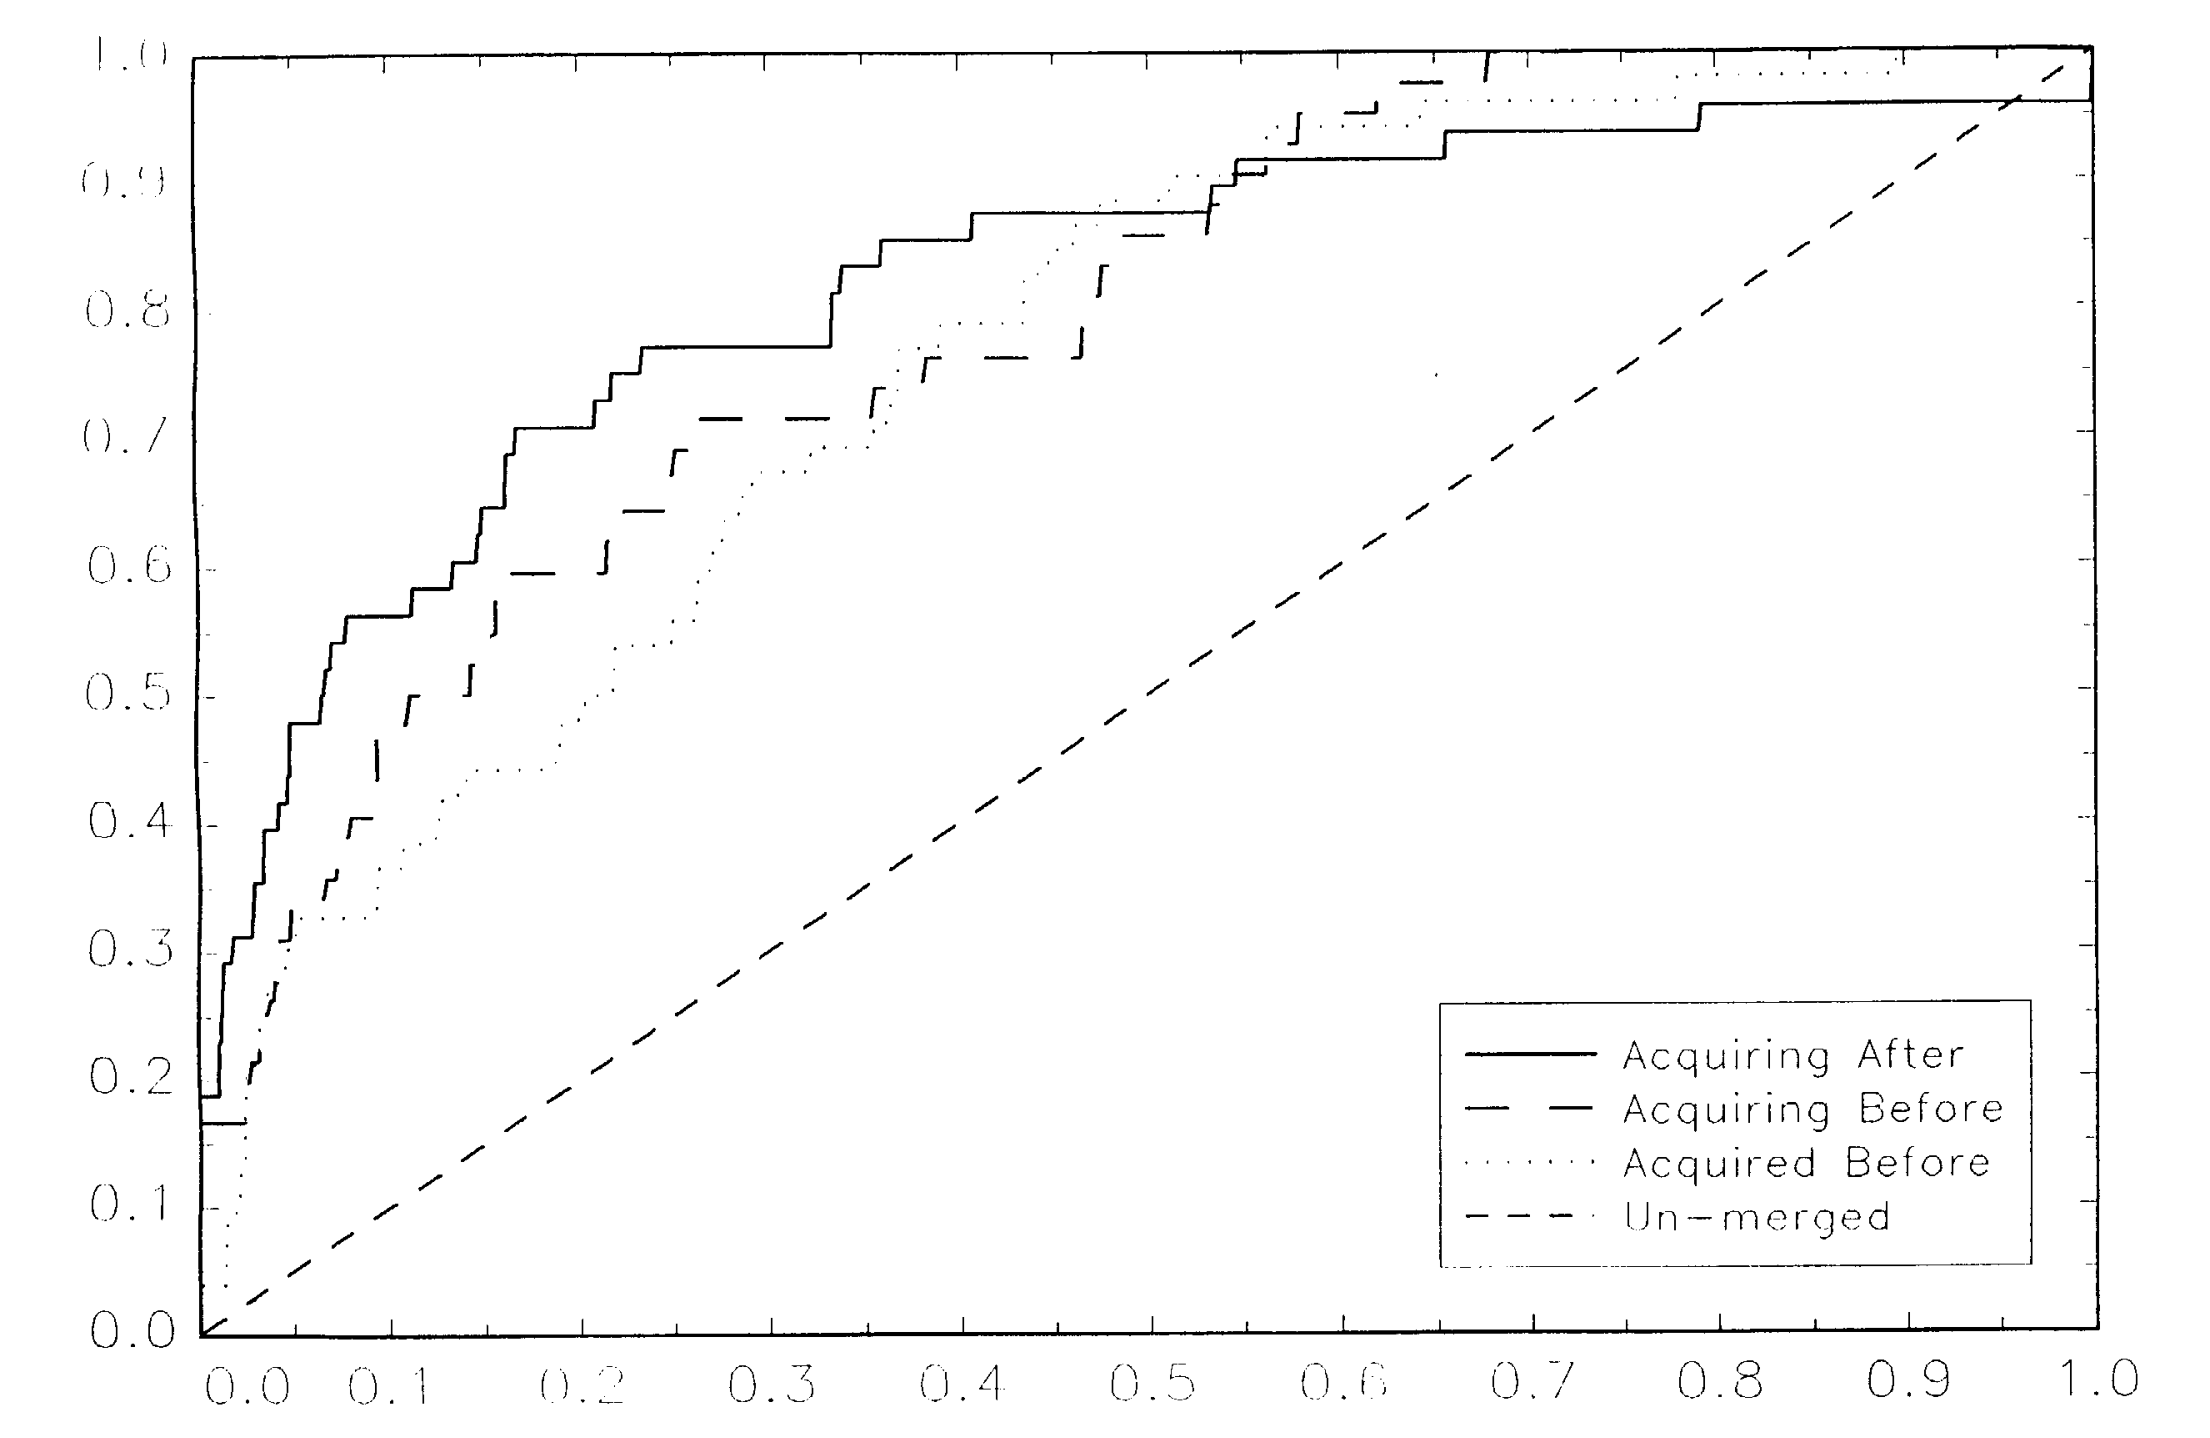
\includegraphics[width=0.72\textwidth]{figures/ch11/pesendorfer_fig2.png}
\caption{Distribution of estimated marginal costs, pooled across paper categories. Each firm's cost is expressed as
its percentile in the cost distribution of unmerged firms (horizontal axis). The curves are cumulative distribution
functions (vertical axis) for acquiring firms after and before the merger wave and for acquired firms before it. The dashed diagonal
is the distribution of unmerged firms. Curves farther above the diagonal indicate lower relative costs. The image is
rotated from the working-paper version. Source: \citet{Pesendorfer2003}, Figure 2.}
\label{fig:11-pesendorfer}
\end{figure}

\casehead{Welfare}
For the counterfactual without mergers, each merging firm's cost is projected to its post-wave level using its
percentile in the unmerged distribution. The merged firm is replaced by its components with these costs, the
investment equilibrium of \eqref{eq:11-pes-kt} is recomputed, and the changes in consumer and producer surplus follow
from \eqref{eq:11-pes-welfare}. Standard errors come from repeated draws of the projection error. \Cref{tab:11-pesendorfer}
reproduces the base specification.

\begin{table}[htbp]
\centering
\caption{Welfare effects of the 1984--1987 paper merger wave (thousands of 1986 dollars)}
\label{tab:11-pesendorfer}
\begin{threeparttable}
\small
\begin{tabular}{@{}lrrrrr@{}}
\toprule
Category & \makecell[r]{Total\\ welfare} & \makecell[r]{Consumer\\ surplus} & \makecell[r]{Producer\\ surplus} &
\makecell[r]{Merged\\ firms} & \makecell[r]{Unmerged\\ firms} \\
\midrule
Packaging papers & 61,440 & 9,499 & 51,940 & 57,090 & $-5{,}149$ \\
 & (14,635) & (6,174) & (9,145) & (12,135) & (3,494) \\
Groundwood printing & 1,736 & 3,132 & $-1{,}395$ & 419 & $-1{,}815$ \\
 & (12,187) & (6,380) & (6,393) & (9,207) & (3,213) \\
Coated papers & 9,617 & 10,604 & $-987$ & 5,708 & $-6{,}695$ \\
 & (11,036) & (11,241) & (3,950) & (7,321) & (7,118) \\
Uncoated papers & 16,826 & 21,277 & $-4{,}451$ & 9,747 & $-14{,}198$ \\
 & (21,463) & (10,197) & (13,863) & (18,991) & (7,234) \\
Other papers & 31,166 & 4,888 & 26,278 & 28,832 & $-2{,}554$ \\
 & (4,094) & (1,713) & (2,479) & (3,439) & (1,036) \\
Tissue & 298,692 & 96,089 & 202,604 & 242,905 & $-40{,}301$ \\
 & (14,676) & (7,950) & (6,815) & (11,952) & (5,240) \\
Boxboard & 412 & $-22{,}098$ & 22,510 & 11,832 & 10,679 \\
 & (16,381) & (8,594) & (8,412) & (12,233) & (4,235) \\
Linerboard & 163,587 & 90,203 & 73,384 & 112,771 & $-39{,}386$ \\
 & (82,962) & (64,079) & (52,942) & (60,261) & (28,788) \\
\midrule
Sum over categories & 583,476 & 213,594 & 369,883 & 469,304 & $-99{,}419$ \\
Range over five specifications & 454,483 to & $-58{,}555$ to & 244,271 to & & \\
 & 583,476 & 213,594 & 527,289 & & \\
\bottomrule
\end{tabular}
\begin{tablenotes}[flushleft]
\footnotesize
\item Notes: Reproduced from \citet[Table 6, specification (1): depreciation factor 0.999, linear investment-cost
coefficient 26.50, quadratic 0.005]{Pesendorfer2003}, working-paper version. Standard deviations from the projection
error in parentheses. The table reports categories only. The sums and ranges are our calculations from all five
columns of the table. The other specifications use (0.950, 26.50, 0.005), (0.999, 36.50, 0.007), (0.999, 53.00, 0)
and (0.999, 0, 0.010).
\end{tablenotes}
\end{threeparttable}
\end{table}

Summing over categories, the wave raised total welfare by \$583.5 million in the base specification, with \$213.6
million going to consumers and \$369.9 million to producers. The sums across the five specifications range from \$454
million to \$583 million for total welfare and from \$244 million to \$527 million for producer surplus. The text of the
paper gives a consumer range of \$58 million to \$210 million, while the table's columns sum to between $-\$58.6$ million
and \$213.6 million.
Merged firms gained \$469.3 million and unmerged firms lost \$99.4 million.
The text reports the merged firms' gain as \$468.3 million in two places and \$469.3 million in a third. The table
sums to the latter. The paper describes the packaging-paper figure as an increase in annual total welfare
\citep[p.~19]{Pesendorfer2003}, so the totals are best read as annual flows. Gains to merged firms are positive in every
category in the base specification. Pesendorfer states that these gains are positive in six of eight categories, with
insignificant losses in some specifications for groundwood printing and boxboard \citep[p.~21]{Pesendorfer2003}. His
Table 6 also shows insignificant losses in one specification each for uncoated papers ($-703$ thousand) and
linerboard ($-26{,}638$ thousand). Only packaging, coated, other papers and tissue show gains in every specification.
Pesendorfer reads the positive gains as support for the model, since profitability was not imposed in estimation.

\casehead{Interpretation and critiques}
The welfare gains rest on estimated cost reductions, and their distribution deserves attention. Tissue alone accounts
for 51 percent of the total welfare gain and 52 percent of the merged firms' gain. The tissue category had a single
acquiring firm (Table 2), whose estimated cost advantage over the median unmerged firm grew from \$5.71 to \$143.04 per
ton (Table 5A). The headline number thus depends heavily on one firm's inferred cost decline. More generally, marginal
costs are residuals of a first-order condition, so any misspecification of demand, of the investment cost function or
of conduct is loaded into the cost estimates. The model is static and assumes the wave was unanticipated. It treats
each category as a national homogeneous-good market with full utilization. The percentile projection assumes that, absent
mergers, each firm would have kept its relative position. Mergers are taken as given, so firms that merged may differ
from others in ways that also explain later cost changes.

\casehead{Contribution}
The paper shows that the investment channel can reverse two conclusions of static Cournot theory. Mergers without
synergies can be profitable, and the price effect of a merger depends on rivals' ability to add capacity. It also
shows how revealed investment behavior can identify merger efficiencies, an idea that complements the retrospective
price studies of \cref{sec:11-retro}. Dynamic models of mergers with investment, such as \citet{BerryPakes1993} and
\citet{Gowrisankaran1999}, develop the same concerns with richer state spaces.

\section{Merger policy with merger choice}\label{sec:11-policy}

The standard approach to merger review evaluates each proposed merger on its own. An authority with a consumer surplus
standard approves a merger if and only if it does not lower consumer surplus. This rule ignores that firms choose which
merger to propose, while the authority sees only the proposal. \citet{NockeWhinston2013} show that the choice changes
the optimal policy. If firms prefer larger mergers for reasons unrelated to consumers, the authority should hold larger
mergers to a stricter standard. \citet{Lyons2003} first identified the problem. \citet{ArmstrongVickers2010} analyze
delegated choice among projects that are ex ante identical. \citet{NockeWhinston2010} show that a myopic consumer
surplus standard is optimal in a dynamic setting when possible mergers are disjoint, that is, involve different firms.
We follow the working-paper version of \citet{NockeWhinston2013}, whose numbering may differ from the published
article.

\subsection{The model}\label{sec:11-nw-model}

Firms $i \in \mathcal{N} = \{0, 1, \dots, N\}$ produce a homogeneous good with constant marginal costs $c_i$ and
compete in quantities. Inverse demand $P(Q)$ satisfies, for all $Q$ with $P(Q) > 0$,
\begin{equation}\label{eq:11-nw-ass}
P'(Q) < 0, \qquad P'(Q) + QP''(Q) < 0, \qquad \lim_{Q \to \infty}P(Q) = 0 .
\end{equation}
These conditions imply a unique Cournot equilibrium that is stable: each best response $b_i(Q_{-i})$ has slope in
$(-1, 0)$, so if some firms want to produce less, industry output falls. All firms are active, and the pre-merger
outputs satisfy $P(Q^0) + P'(Q^0)q_i^0 = c_i$. Write $P^0 = P(Q^0)$, $s_i^0 = \frac{q_i^0}{Q^0}$ and $\pi_i^0 = (P^0 -
c_i)q_i^0$.

Firm 0, the acquirer, can merge with one target $k \in \mathcal{K} = \{1, \dots, K\}$. Targets are ordered by decreasing
cost, $c_1 > c_2 > \dots > c_K$, so a higher $k$ means a larger pre-merger share. We call merger $k$ \emph{larger}
than merger $j$ if $k > j$. The change in the naively computed Herfindahl index, which keeps all shares fixed and adds
the merging shares, is
\begin{equation}\label{eq:11-nw-hhi}
\Delta\HHI^{naive}(M_k) = (s_0^0 + s_k^0)^2 - (s_0^0)^2 - (s_k^0)^2 = 2 s_0^0 s_k^0 ,
\end{equation}
the formula of \eqref{eq:11-dhhi}. A larger merger thus has a larger naive increase in concentration.

Merger $k$ is feasible with probability $\phi_k \in (0, 1]$, independently across targets. If feasible, it yields a
post-merger marginal cost $\bar c_k$ drawn from a distribution $G_k$ with support $[c^L, c_k^H]$ and no mass points. A
feasible merger is $M_k = (k, \bar c_k)$. After merger $M_k$ the outputs solve $P(Q(M_k)) + P'(Q(M_k))q_i(M_k) = c_i$
for nonmerging firms and the same condition with $\bar c_k$ for the merged firm. All firms remain active. The changes in
consumer surplus and in the merging parties' joint (bilateral) profit are
\begin{equation}\label{eq:11-nw-changes}
\Delta \mathit{CS}(M_k) = \int_0^{Q(M_k)}P(z)\,\dd z - P(Q(M_k))Q(M_k) - \mathit{CS}^0,
\qquad
\Delta\Pi(M_k) = \pi_k(M_k) - (\pi_0^0 + \pi_k^0).
\end{equation}
A merger is \emph{CS-neutral} if $\Delta\mathit{CS} = 0$, CS-increasing if it is positive, CS-decreasing if it is
negative, and CS-nondecreasing if it is not CS-decreasing. The status quo $M_0$ gives zero changes. Let $\mathcal{F}$
be the realized set of feasible mergers, including $M_0$.

The timing has four stages. The authority commits to an approval set $\mathcal{A} = \{M_k : \bar c_k \in
\mathcal{A}_k\} \cup \{M_0\}$, where each $\mathcal{A}_k \subseteq [c^L, c_k^H]$ is a union of closed intervals. Nature
draws $\mathcal{F}$. Firms bargain over which merger to propose. The authority approves the proposal if it lies in
$\mathcal{A}$, and firms compete. The authority observes every characteristic of the proposed merger but nothing about
mergers that are not proposed, and only one merger can be proposed.

Bargaining follows the offer game of \citet{Segal1999}. Firm 0 makes a take-it-or-leave-it offer of a price $t_k$ to one
target. Setting $t_k$ to make the target indifferent, firm 0 captures the whole bilateral gain $\Delta\Pi(M_k)$. The
proposed merger is therefore
\begin{equation}\label{eq:11-nw-proposal}
M^*(\mathcal{F}, \mathcal{A}) =
\begin{cases}
\argmax_{M_k \in \mathcal{F} \cap \mathcal{A}} \Delta\Pi(M_k) & \text{if } \max_{M_k \in \mathcal{F} \cap \mathcal{A}}
\Delta\Pi(M_k) > 0,\\
M_0 & \text{otherwise.}
\end{cases}
\end{equation}
The authority chooses $\mathcal{A}$ to maximize $\E_{\mathcal{F}}\big[\Delta\mathit{CS}(M^*(\mathcal{F}, \mathcal{A}))
\big]$. One assumption avoids trivial cases. Each merger's cost support contains CS-increasing and CS-nonincreasing
outcomes, $\Delta\mathit{CS}(k, c_k^H) \le 0 < \Delta\mathit{CS}(k, c^L)$.

\subsection{Three lemmas on the shape of merger outcomes}\label{sec:11-nw-lemmas}

Because the good is homogeneous, a merger raises consumer surplus if and only if it raises industry output. The first
lemma characterizes CS-neutral mergers. It restates \cref{prop:11-synergy,cor:11-neutral-profit} in the notation of
this section.

\begin{lemma}[CS-neutral mergers]\label{lem:11-nw1}
Suppose merger $M_k$ is CS-neutral. Then (i) no nonmerging firm changes its output, and the merged firm produces
$q_0^0 + q_k^0$. (ii) The merged firm's margin equals the sum of the partners' margins,
\begin{equation}\label{eq:11-nw-neutral}
P^0 - \bar c_k = (P^0 - c_0) + (P^0 - c_k), \quad\text{so}\quad \bar c_k = \hat c_k \equiv c_k - (P^0 - c_0) <
\min\{c_0, c_k\}.
\end{equation}
(iii) The merger is profitable, $\Delta\Pi(M_k) > 0$. (iv) It raises aggregate profit.
\end{lemma}

\begin{proof}
A CS-neutral merger leaves $Q$, and hence $P$ and $P'$, unchanged. Each nonmerging firm's first-order condition then
gives the same output, and the merged firm produces the rest, $q_0^0 + q_k^0$. Its first-order condition is $P^0 +
P'(Q^0)(q_0^0 + q_k^0) = \bar c_k$. Adding the partners' pre-merger conditions gives $2P^0 + P'(Q^0)(q_0^0 + q_k^0) =
c_0 + c_k$. Subtracting the first equation from the second gives $P^0 = c_0 + c_k - \bar c_k$, which is
\eqref{eq:11-nw-neutral}. Part (iii) is \cref{cor:11-neutral-profit}: the merged profit exceeds $\pi_0^0 + \pi_k^0$ by
$(P^0 - c_0)q_k^0 + (P^0 - c_k)q_0^0 > 0$. For (iv), nonmerging firms' profits are unchanged because their prices and
outputs are unchanged.
\end{proof}

\begin{lemma}[Lower post-merger cost]\label{lem:11-nw2}
Conditional on merger $M_k$, a lower $\bar c_k$ raises industry output, consumer surplus and the merged firm's profit.
\end{lemma}

\begin{proof}
Summing the $N$ post-merger first-order conditions gives $NP(Q) + QP'(Q) = \bar c_k + \sum_{i \neq 0, k}c_i$. The
left side decreases in $Q$, because its derivative is $(N + 1)P' + QP'' < 0$ by \eqref{eq:11-nw-ass}. A lower
$\bar c_k$ lowers the right side, so $Q$ rises, and so does consumer surplus. For the profit, define the
\emph{cumulative best reply} $\tilde q(Q; c) = -\frac{P(Q) - c}{P'(Q)}$, the output at which a firm with cost $c$
satisfies its first-order condition when industry output is $Q$. Its derivative in $Q$ is
\begin{equation*}
\frac{\partial\tilde q}{\partial Q} = -1 + \frac{(P - c)P''}{(P')^2} = -1 - \frac{\tilde q\,P''}{P'} =
-\frac{P' + \tilde q P''}{P'} < 0,
\end{equation*}
using $P - c = -P'\tilde q$ and $P' + qP'' < 0$ for $q \le Q$. Nonmerging outputs $\tilde q(Q; c_i)$ therefore fall
when $\bar c_k$ falls. The merged firm's profit is $\max_q[P(Q_{-m} + q) - \bar c_k]q$, where $Q_{-m}$ is rivals'
output. By the envelope theorem its derivative in $\bar c_k$ is $-q_m + q_m P'(Q)\frac{dQ_{-m}}{d\bar c_k}$. Both terms
are negative, since $P' < 0$ and rivals' output rises with $\bar c_k$.
\end{proof}

Lemma~\ref{lem:11-nw2} implies that merger $M_k$ is CS-increasing if $\bar c_k < \hat c_k$ and CS-decreasing if
$\bar c_k > \hat c_k$. The third lemma is the key to the paper. It shows that firms' proposal incentives are biased
toward larger mergers.

\begin{lemma}[Firms prefer larger mergers]\label{lem:11-nw3}
Suppose mergers $M_j$ and $M_k$, with $k > j \ge 1$, induce the same nonnegative change in consumer surplus. Then the
larger merger induces a larger gain in bilateral profit: $\Delta\Pi(M_k) > \Delta\Pi(M_j) > 0$.
\end{lemma}

\begin{proof}
Each firm's first-order condition gives $P - c_i = -P' q_i$, so its profit is
\begin{equation}\label{eq:11-nw-profit}
\pi_i = (P - c_i)q_i = -P'(Q)\,\big[\tilde q(Q; c_i)\big]^2 .
\end{equation}
Equal consumer surplus means equal industry output $\bar Q$. Industry output depends only on the sum of active
firms' costs, by the summed first-order condition in the proof of Lemma~\ref{lem:11-nw2}. So both mergers reduce the
partners' combined cost by the same amount, $\gamma \equiv c_k - \bar c_k = c_j - \bar c_j$. Since $\frac{\partial\tilde
q}{\partial c} = \frac{1}{P'}$, the difference in the merged firms' profits is
\begin{align}
\pi_k(M_k) - \pi_j(M_j)
&= -P'(\bar Q)\Big\{\big[\tilde q(\bar Q; c_k - \gamma)\big]^2 - \big[\tilde q(\bar Q; c_j - \gamma)\big]^2\Big\}
\notag\\
&= -P'(\bar Q)\int_{c_j}^{c_k} 2\,\tilde q(\bar Q; c - \gamma)\,\frac{1}{P'(\bar Q)}\,\dd c
= 2\int_{c_k}^{c_j}\tilde q(\bar Q; c - \gamma)\,\dd c . \label{eq:11-nw-diff1}
\end{align}
The same steps applied to pre-merger profits give
\begin{equation}\label{eq:11-nw-diff0}
\pi_k^0 - \pi_j^0 = 2\int_{c_k}^{c_j}\tilde q(Q^0; c)\,\dd c .
\end{equation}
Now consider, for any $c \in [c_k, c_j]$, a merger of firm 0 with a firm of cost $c$ that yields cost $c - \gamma$.
It raises output from $Q^0$ to $\bar Q$, so it weakly lowers each nonmerging firm's output and weakly raises the merging
firms' joint output. Hence
\begin{equation*}
\tilde q(\bar Q; c - \gamma) \ge \tilde q(Q^0; c_0) + \tilde q(Q^0; c) > \tilde q(Q^0; c).
\end{equation*}
The integrand of \eqref{eq:11-nw-diff1} exceeds that of \eqref{eq:11-nw-diff0} at every $c$, so
$\pi_k(M_k) - \pi_j(M_j) > \pi_k^0 - \pi_j^0$. Subtracting $\pi_0^0$ from both merged profits and rearranging gives
$\Delta\Pi(M_k) > \Delta\Pi(M_j)$. Finally, $\Delta\Pi(M_j) > 0$ because a CS-nondecreasing merger has $\bar c_j \le
\hat c_j$, and Lemmas~\ref{lem:11-nw1} and~\ref{lem:11-nw2} imply that it is at least as profitable as the CS-neutral
merger.
\end{proof}

The intuition comes from \eqref{eq:11-nw-profit}. Profit is quadratic in output, so a given cost saving is worth more
to a firm that produces more. To leave consumers equally well off, both mergers need the same absolute cost saving,
and the larger merger applies it to a larger output base. Firms therefore value larger mergers more than consumers do.

Lemmas~\ref{lem:11-nw1} to~\ref{lem:11-nw3} fix the geometry of the problem. Plot each possible outcome of merger $k$
as a point $(\Delta\Pi, \Delta\mathit{CS})$. As $\bar c_k$ varies, the points trace a \emph{merger curve}. Each curve
slopes upward (Lemma~\ref{lem:11-nw2}) and crosses the horizontal axis at a positive profit (Lemma~\ref{lem:11-nw1}).
On and above the axis, the curve of a larger merger lies to the right of the curve of a smaller one
(Lemma~\ref{lem:11-nw3}). An immediate consequence is the following.

\begin{corollary}[\citealp{NockeWhinston2013}, Corollary 1]\label{cor:11-nw}
If two CS-nondecreasing mergers $M_j$ and $M_k$ with $k > j \ge 1$ satisfy $\Delta\Pi(M_k) \le \Delta\Pi(M_j)$, then
$\Delta\mathit{CS}(M_k) < \Delta\mathit{CS}(M_j)$.
\end{corollary}

\begin{proof}
Suppose $\Delta\mathit{CS}(M_k) \ge \Delta\mathit{CS}(M_j)$. By Lemma~\ref{lem:11-nw2} there is a cost $\bar c_k' \ge
\bar c_k$ with $\Delta\mathit{CS}(k, \bar c_k') = \Delta\mathit{CS}(M_j)$. Lemma~\ref{lem:11-nw2} and then
Lemma~\ref{lem:11-nw3} give $\Delta\Pi(M_k) \ge \Delta\Pi(k, \bar c_k') > \Delta\Pi(M_j)$, a contradiction.
\end{proof}

\Cref{fig:11-nw} draws the merger curves for the linear example studied below. The curves are close to parallel in
this example, and the larger merger's curve lies to the right at every nonnegative $\Delta\mathit{CS}$.

\begin{figure}[htbp]
\centering
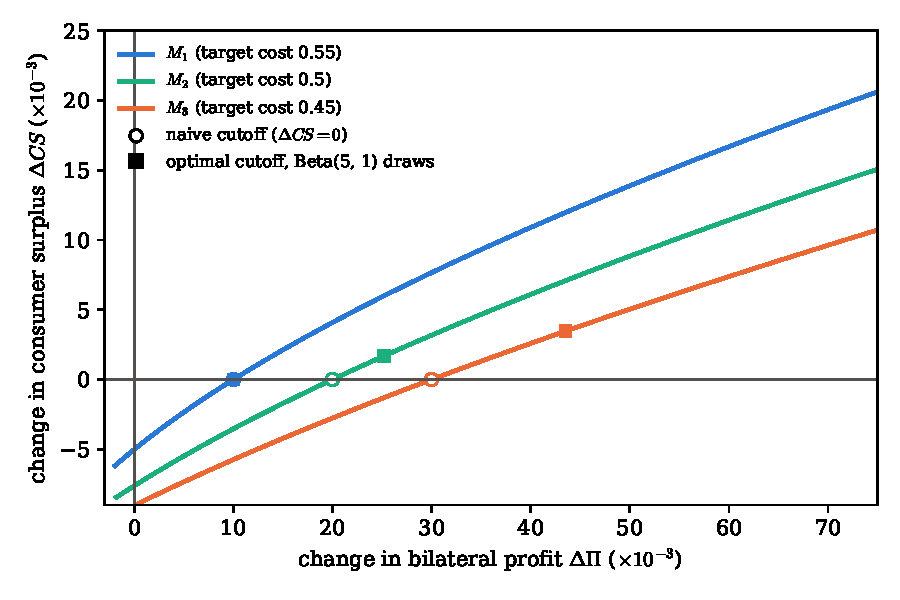
\includegraphics[width=0.78\textwidth]{figures/ch11/nw_curves.pdf}
\caption{Merger curves in $(\Delta\Pi, \Delta\mathit{CS})$ space for Example 2 of \citet{NockeWhinston2013}: inverse
demand $P = 1 - Q$, acquirer cost $c_0 = 0.5$ and targets with costs 0.55, 0.5 and 0.45. Each curve traces the outcomes
of one merger as the post-merger cost $\bar c_k$ varies from 0.2 to slightly above $c_k$. Open circles mark the naive
cutoffs, at which $\Delta\mathit{CS} = 0$. Squares mark the optimal cutoffs when post-merger costs follow the Beta(5, 1)
distribution described in the text. Our computation.}
\label{fig:11-nw}
\end{figure}

\subsection{The optimal approval policy}\label{sec:11-nw-optimal}

For a policy $\mathcal{A}$, let $\bar a_k = \max\mathcal{A}_k$ be the highest approved cost for target $k$. The merger
$(k, \bar a_k)$ is the \emph{marginal merger}, and $\underline{\Delta\mathit{CS}}_k = \Delta\mathit{CS}(k, \bar a_k)$ and
$\underline{\Delta\Pi}_k = \Delta\Pi(k, \bar a_k)$ are the lowest consumer surplus and profit changes among approved
mergers with target $k$.

The natural benchmark is the \emph{naive policy}, which approves every CS-nondecreasing merger, $\mathcal{A}_k = [c^L,
\hat c_k]$. It is not optimal. Suppose the authority tightens the standard for the largest merger $K$ only, approving it
only if $\Delta\mathit{CS} \ge \varepsilon$ for a small $\varepsilon > 0$. The two policies differ only when the naive
policy would lead to merger $K$ with $\Delta\mathit{CS} \in [0, \varepsilon)$. In that event, the naive policy delivers
at most $\varepsilon$. The tighter policy leads firms to propose the next most profitable acceptable merger, which
involves a smaller target. Its expected consumer surplus gain stays bounded away from zero as $\varepsilon \to 0$,
because some smaller merger is CS-increasing with positive probability. For small $\varepsilon$ the tighter policy
therefore does better. The main result characterizes the optimal policy.

\begin{proposition}[Optimal merger policy, \citealp{NockeWhinston2013}, Proposition 1]\label{prop:11-nw}
Any optimal approval policy has three properties. (i) It approves the smallest merger $M_1$ if and only if it is
CS-nondecreasing. (ii) It approves
with positive probability only mergers with targets in a set $\mathcal{K}^+ = \{1, \dots, \hat K\}$, where $\hat K$ may
equal $K$. (iii) It satisfies
\begin{equation}\label{eq:11-nw-prop1}
0 = \underline{\Delta\mathit{CS}}_1 < \underline{\Delta\mathit{CS}}_2 < \dots < \underline{\Delta\mathit{CS}}_{\hat K}.
\end{equation}
The minimum acceptable gain in consumer surplus is zero for the smallest merger, strictly positive for every larger
merger and increasing in the size of the merger. The largest mergers may never be approved.
\end{proposition}

\begin{proof}[Proof sketch]
The argument has six steps, each of which improves on a policy that violates a property.

Step 1. An optimal policy approves no CS-decreasing merger. Removing such mergers from $\mathcal{A}$ matters only when
one of them would have been proposed. Firms then propose another acceptable merger, which is CS-nondecreasing or the
status quo, so expected consumer surplus rises.

Step 2. Every CS-nondecreasing smallest merger is approved. Adding such mergers matters only when one of them becomes
the most profitable acceptable merger. Otherwise firms would propose the next most profitable acceptable merger, which
by Corollary~\ref{cor:11-nw} raises consumer surplus by less.

Step 3. The marginal merger satisfies an indifference condition. Let $E^{\mathcal{A}}_k(\bar a_k)$ be the expected
consumer surplus change from the merger firms would propose if $(k, \bar a_k)$ were rejected, conditional on $(k, \bar
a_k)$ being feasible and the most profitable acceptable merger. Then
\begin{equation}\label{eq:11-nw-indiff}
\underline{\Delta\mathit{CS}}_k = E^{\mathcal{A}}_k(\bar a_k).
\end{equation}
If the left side were smaller, rejecting mergers with costs just below $\bar a_k$ would raise expected consumer surplus.
If it were larger, approving mergers with costs just above $\bar a_k$ would raise it.

Step 4. Marginal profits increase with size: $\underline{\Delta\Pi}_j \le \underline{\Delta\Pi}_k$ for $j < k$ in
$\mathcal{K}^+$. If the order were reversed, some unapproved merger with target $j$ would give more consumer surplus
than the approved marginal merger with target $k$. Rejecting either leads to the same expected outcome, so approving the
first would help.

Step 5. Marginal consumer surplus increases strictly with size. Suppose $\underline{\Delta\mathit{CS}}_j \ge
\underline{\Delta\mathit{CS}}_k$ for $j < k$. By Step 3, $\underline{\Delta\mathit{CS}}_k$ equals the expected surplus of
the next most profitable acceptable merger. If that merger has profit between $\underline{\Delta\Pi}_j$ and
$\underline{\Delta\Pi}_k$, then by Step 4 it involves a smaller target and gives more than
$\underline{\Delta\mathit{CS}}_j$. If its profit is below $\underline{\Delta\Pi}_j$, then by Step 3 for target $j$ its
expected surplus is exactly $\underline{\Delta\mathit{CS}}_j$. The weighted average then exceeds
$\underline{\Delta\mathit{CS}}_j$, a contradiction.

Step 6. If target $j$ is never approved, no larger target is. The most efficient merger with $j$ gives more consumer
surplus than the most efficient merger with $j + 1$. Merging with the higher-cost target $j$ leaves a lower sum of
costs in the industry, hence more output. A nonmonotonicity argument
like that of Step 5 then applies. The appendix of the paper gives the formal proof.
\end{proof}

Proposition~\ref{prop:11-nw} gives the authority a reason to discriminate among mergers by a statistic it can observe
before any analysis. In the baseline model, a larger merger is one with a larger naive change in concentration,
$2s_0^0s_k^0$, and the optimal policy demands more from it. This rationale differs from the usual one for concentration
screens (\cref{sec:11-marketdef}). Higher concentration predicts larger harm in Cournot models, but here the screen
corrects for the bias in firms' choice of which merger to propose. The policy is a delegation rule. It accepts some
CS-increasing mergers with large targets less often than a merger-by-merger review would, in exchange for steering firms
toward the smaller mergers that consumers prefer.

\subsection{Cutoff policies, a numerical example and comparative statics}\label{sec:11-nw-cutoffs}

The indifference condition \eqref{eq:11-nw-indiff} links the policies for different targets, so it does not by itself
deliver the optimal policy. The problem simplifies if the optimal policy is a \emph{cutoff policy}, which approves merger
$k$ if and only if $\bar c_k \le \bar a_k$. Then the cutoffs follow by recursion. Set $\bar a_1 = \hat c_1$. For $k = 2,
\dots, K$, consider the best acceptable merger among targets $1, \dots, k - 1$, conditional on its profit being at most
$\Delta\Pi(k, \bar a_k)$. Set $\bar a_k$ at the largest cost at which $\Delta\mathit{CS}(k, \bar a_k)$ equals the
expected consumer surplus from that merger. If no such cost exists, merger $k$ and all larger mergers are never approved.

The optimal policy need not have this form. In Example 1 of the paper, the smaller merger is always feasible and gives
$(\Delta\Pi, \Delta\mathit{CS}) = (5, 5)$ with probability 0.9 and $(1, 1)$ with probability 0.1, so its expected
consumer surplus gain is $0.9 \times 5 + 0.1 \times 1 = 4.6$.\footnote{The text of the paper attaches probability 0.9
to the outcome $(1, 1)$. Its Figure 8 and its value of 4.6 require probability 0.9 on $(5, 5)$.} The larger merger's curve passes through $\Delta\mathit{CS} = 4.6$ before it reaches
$\Delta\Pi = 5$. For costs between these two points the larger merger would always be proposed, yet it would give less
than 4.6. The authority rejects it there and approves it at both higher and lower costs, so the approval set is not an
interval. Proposition~2 of the paper gives a sufficient condition, checkable in applications, under which the recursive
cutoff policy is optimal.

\begin{example}[Nocke and Whinston's Example 2]\label{ex:11-nw}
Let $P(Q) = 1 - Q$ and four firms have costs $c_0 = c_2 = 0.5$, $c_1 = 0.55$ and $c_3 = 0.45$. With four Cournot firms,
$Q^0 = \frac{4 - 2}{5} = 0.4$ and $P^0 = 0.6$. Outputs are $P^0 - c_i$, so pre-merger shares are $\frac{1}{4}$,
$\frac{1}{8}$, $\frac{1}{4}$ and $\frac{3}{8}$. The naive cutoffs are $\hat c_k = c_k - (P^0 - c_0) = c_k - 0.1$, that is,
0.45, 0.40 and 0.35. Each merger is feasible with probability $\phi_k = 0.75$. Conditional on feasibility, $\bar c_k =
0.2 + (\hat c_k - 0.2)X$, where $X$ follows a Beta distribution with density proportional to $x^{\alpha_B - 1}$ on $[0,
1]$. A larger shape parameter $\alpha_B$ makes small efficiency gains more likely. The lower bound 0.2 keeps every firm
active.
\end{example}

\Cref{tab:11-nwex} reports the paper's results with our replication. We compute the recursive cutoffs by simulating 2
million draws of the feasible set and solving the indifference condition with a root finder. For $\alpha_B = 5$, the
optimal cutoffs are $\bar a_2 = 0.383$ and $\bar a_3 = 0.316$, well below the naive 0.40 and 0.35. The optimal policy
requires the medium merger to raise consumer surplus by 0.00170 and the large merger by 0.00346. It achieves 90.3 percent
of the first-best gain, which a fully informed authority choosing the best feasible merger would obtain, while the naive
policy achieves 79.8 percent. As $\alpha_B$ falls, large efficiencies become more likely, the first-best gain rises and
the advantage of the optimal policy over the naive one shrinks.

\begin{table}[htbp]
\centering
\caption{Optimal and naive merger policies in the linear example}
\label{tab:11-nwex}
\begin{threeparttable}
\small
\setlength{\tabcolsep}{4.5pt}
\begin{tabular}{@{}llccccccc@{}}
\toprule
$\alpha_B$ & Source & $\bar a_2$ & $\bar a_3$ & $\underline{\Delta\mathit{CS}}_2$ & $\underline{\Delta\mathit{CS}}_3$ &
\makecell{First-best gain\\ (\% of $\mathit{CS}^0$)} & \makecell{Naive\\ (\% of first best)} &
\makecell{Optimal\\ (\% of first best)} \\
\midrule
5 & Paper & 0.383 & 0.316 & 0.00170 & 0.00346 & 6.44 & 79.83 & 90.30 \\
 & Replication & 0.383 & 0.316 & 0.00170 & 0.00346 & 6.44 & 79.83 & 90.27 \\
3 & Paper & & & 0.00170 & 0.00457 & 9.55 & 87.34 & 92.13 \\
 & Replication & 0.383 & 0.305 & 0.00170 & 0.00457 & 9.55 & 87.35 & 92.15 \\
1 & Paper & & & 0.00099 & 0.00571 & 18.15 & 93.67 & 94.10 \\
 & Replication & 0.390 & 0.294 & 0.00098 & 0.00573 & 18.14 & 93.67 & 94.12 \\
\bottomrule
\end{tabular}
\begin{tablenotes}[flushleft]
\footnotesize
\item Notes: Paper rows from \citet[Example 2 and Table 1]{NockeWhinston2013}, which report cutoffs only for $\alpha_B = 5$
and write $\alpha$ for the shape parameter. The smallest merger's cutoff is the naive one, $\bar a_1 = 0.45$, with
$\underline{\Delta\mathit{CS}}_1 = 0$. Replication rows are our Monte Carlo computation with 2 million simulated feasible
sets. Differences in the last digit reflect simulation error.
\end{tablenotes}
\end{threeparttable}
\end{table}

When the optimal policy has a cutoff form, two comparative statics follow (Propositions 3 and 4 of the paper). First, if
merger $k$ becomes less likely to be feasible, the standards for mergers up to $k$ do not change, and the standards for
larger approved mergers fall. A less likely alternative makes rejection less valuable, so the authority can be more
lenient. As all feasibility probabilities go to zero, the optimal policy approaches the naive one. Second, if the
acquirer becomes more efficient, all cost cutoffs fall. The authority then demands lower post-merger costs from every
merger.

\subsection{Extensions}\label{sec:11-nw-ext}

Section~5 of the paper shows that the main result survives five changes to the model.

\emph{Other bargaining processes.} The offer game gives firm 0 the whole bilateral gain. The same proposals arise if
firm 0 obtains a fixed share of the gain from every target, as in alternating-offer bargaining with a common discount
factor. With efficient bargaining among all firms, the proposed merger maximizes aggregate profit instead. Part (iv) of
\cref{lem:11-nw1} still holds, and a version of \cref{lem:11-nw3} holds for aggregate profit. \Cref{lem:11-nw2} needs
an extra assumption, that a lower
post-merger cost raises aggregate profit for CS-nondecreasing mergers. The same conclusions hold if only a subset of
firms that includes all merger candidates bargains efficiently.

\emph{General sets of mergers.} Suppose mergers may involve any set of firms, with $m_k \ge 2$ partners, and bargaining is
efficient. Summing first-order conditions shows that aggregate profit is proportional to the post-merger Herfindahl
index,
\begin{equation}\label{eq:11-nw-aggprofit}
\sum_i \pi_i(M_k) = \sum_i -P'(Q)\,q_i^2 = \big|Q^2P'(Q)\big|\, \HHI(M_k),
\end{equation}
where we used $\pi_i = -P'q_i^2$ from \eqref{eq:11-nw-profit}. For a CS-neutral merger, outputs of nonmerging firms are
unchanged, so the actual post-merger index equals the naive one, $\HHI(M_k) = \HHI^{naive}(M_k)$. Among CS-neutral mergers,
the one with the higher naive post-merger Herfindahl index therefore raises aggregate profit more. Under conditions that
make merger curves upward sloping and non-crossing, the authority should discriminate by the naive post-merger index.
This is the statistic that concentration screens in merger guidelines use (\cref{tab:11-guidelines}).

\emph{Differentiated products.} With CES or logit demand and price competition, profits can be written as functions of
a firm's own strategic variable and an aggregator $\Psi = \sum_j\psi_j$. Its terms are unrelated to the curvature
$\psi$ of \cref{sec:11-passthrough}, and consumer surplus increases with $\Psi$.
For logit demand $\psi_j = \exp\big(\alpha(\bar v - p_j)\big)$ and consumer surplus is $\frac{1}{\alpha}\ln\Psi$ plus a
constant, as in \cref{ch:logit}. For CES demand with elasticity of substitution $\varsigma > 1$, $\psi_j = p_j^{1 - \varsigma}$.
These aggregative games share the properties of the Cournot model that \cref{lem:11-nw1,lem:11-nw2,lem:11-nw3} use,
so \cref{prop:11-nw} carries over. \citet{NockeSchutz2018} develop the aggregative-games approach for multiproduct
firms, which \cref{sec:11-fs} used to extend the synergy condition beyond Cournot.

\emph{Other welfare standards.} If the authority maximizes $W = \mathit{CS} + \omega\,\Pi$ with $\omega \in [0, 1]$,
where $\omega = 1$ is the total surplus standard, the analogue of \cref{prop:11-nw} holds under efficient bargaining. The
minimum acceptable welfare gain is zero for the smallest merger and rises with size. For the offer game, the result holds
when $\omega$ is small.

\emph{Fixed-cost synergies.} If mergers also save fixed costs, merger curves become bands. The main result holds when the
idiosyncratic fixed-cost savings are small enough that bands of different mergers do not overlap. Common fixed-cost
savings shift all bands equally and leave the optimal policy unchanged.

\subsection{Lessons and limits}\label{sec:11-nw-lessons}

Two lessons stand out. First, a merger-by-merger consumer surplus test is not the best policy when firms choose among
mutually exclusive mergers. The authority should ask what the alternative merger would have been, not only what the
proposed merger does. Second, naive concentration statistics carry information about firms' proposal incentives, which
gives screens based on $2s_0s_k$ and the naive post-merger index a rationale beyond their role as predictors of price
effects.

Later work gives the naive change a second rationale, which \cref{sec:11-hhi} reports. With price competition under
logit, nested logit or CES demand, the consumer surplus lost in a merger without synergies is approximately
proportional to the naive $\Delta\HHI$ \citep{NockeSchutz2019}. The efficiencies needed to leave consumers unharmed
rise with the naive change and, holding it fixed, do not depend on the level of the index \citep{NockeWhinston2020}.
The Cournot version of this result is \eqref{eq:11-required-dhhi}. Both rationales point to naively computed
concentration statistics, and the second singles out the change. \citet{NockeWhinston2020} also conclude that the
presumptions of the 2010 Guidelines are likely too lax \citep[p.~227, n.~124]{AskerNocke2021}.

The model's limits are also clear. The authority commits to a policy and observes everything about the proposed merger,
including post-merger costs, which in practice must be predicted. Only one merger can be proposed, and the setting is
static. In a dynamic world, mergers rejected today may be replaced by others tomorrow, and approved mergers change the
pool of future mergers. \citet{NockeWhinston2010} show that when possible mergers are disjoint, a myopic consumer surplus
standard is optimal, so the force identified here comes from overlap among possible mergers. The next subsection
explains why.

\subsection{Merger review over time, investment and innovation}\label{sec:11-dynamics}

Mergers are not one-time events. When merger opportunities arise over time, approving a merger today changes the
profitability and the welfare effects of the mergers that rivals may propose later \citep[p.~232]{AskerNocke2021}. A
policy that looks only at current market conditions may then be wrong. This subsection shows when it is not, and what
changes once firms invest and innovate.

\casehead{A complementarity between disjoint mergers}
Two mergers are \emph{disjoint} if no firm takes part in both. In the Cournot model of \cref{sec:11-nw-model}, the
consumer surplus effects of disjoint mergers have a simple structure.

\begin{proposition}[Sign-preserving complementarity, \citealp{NockeWhinston2010}]\label{prop:11-signpreserve}
Let inverse demand satisfy \eqref{eq:11-nw-ass}, let marginal costs be constant, and let all firms be active in every
market structure considered. Let $\mathcal{M}_A$ and $\mathcal{M}_B$ be disjoint mergers with post-merger costs
$c_A$ and $c_B$.
\begin{enumerate}[label=(\roman*)]
\item If each merger is CS-nondecreasing at the current market structure, each remains CS-nondecreasing once the other
has taken place.
\item If each merger is CS-decreasing at the current market structure, each remains CS-decreasing once the other has
taken place.
\end{enumerate}
\end{proposition}

\begin{proof}
With constant marginal costs, \cref{prop:11-synergy-gen} says that a merger $\mathcal{M}$ with post-merger cost
$c_{\mathcal{M}}$ is CS-nondecreasing at a market structure with price $P$ if and only if
\begin{equation*}
P - c_{\mathcal{M}} \ge \sum_{i \in \mathcal{M}}(P - c_i) = |\mathcal{M}|\,P - \sum_{i \in \mathcal{M}}c_i .
\end{equation*}
Rearranging,
\begin{equation}\label{eq:11-cs-cutoff-P}
c_{\mathcal{M}} \le \sum_{i \in \mathcal{M}}c_i - \big(|\mathcal{M}| - 1\big)P .
\end{equation}
The right side falls in $P$, because $|\mathcal{M}| \ge 2$. Let $P^0$ be the current price and $P^B$ the price after
$\mathcal{M}_B$. The good is homogeneous, so $P^B \le P^0$ if $\mathcal{M}_B$ is CS-nondecreasing and $P^B > P^0$ if it is
CS-decreasing. The partners of $\mathcal{M}_A$ are not in $\mathcal{M}_B$, so their costs and $c_A$ do not change.
Only the price in \eqref{eq:11-cs-cutoff-P} moves. In case (i), \eqref{eq:11-cs-cutoff-P} holds for $\mathcal{M}_A$ at
$P^0$, and its right side weakly rises when the price falls to $P^B$. So it still holds. In case (ii),
\eqref{eq:11-cs-cutoff-P} fails for $\mathcal{M}_A$ at $P^0$, and its right side falls when the price rises to $P^B$. So
it still fails. Exchanging the roles of the two mergers completes the proof.
\end{proof}

The intuition is that a merger is more likely to help consumers the more intense competition is, because intense
competition weakens its market-power effect. A CS-increasing merger intensifies competition. It can even turn a second,
CS-decreasing merger into a CS-increasing one, and the first merger then stays CS-increasing once the second has taken
place \citep[p.~233]{AskerNocke2021}.

\casehead{Myopic review can be optimal}
\Cref{prop:11-signpreserve} underlies the dynamic result of \citet{NockeWhinston2010}. Suppose merger opportunities
arrive over time, a merger that is not proposed or is blocked today can be proposed again later, and possible mergers
are disjoint. An authority that maximizes discounted consumer surplus can then adopt a completely myopic policy. In each
period it approves the subset of proposed mergers that maximizes current consumer surplus and ignores future mergers.
It never regrets approving a merger that is CS-nondecreasing when approved, by part (i). It never regrets blocking a
CS-decreasing merger, because the opportunity remains and the merger can be approved once its effect turns positive.
Firms' incentives to propose are aligned with the authority's goal, because a CS-nondecreasing merger is profitable
(\cref{cor:11-neutral-profit}) and stays profitable when it induces other mergers. The myopic policy is optimal in a
strong sense. The authority could not do better even with perfect foresight of future merger opportunities and the
power to undo past approvals \citep[p.~233]{AskerNocke2021}. The result extends to price competition with logit or CES
demand \citep{NockeSchutz2019}.

Both assumptions matter. When firms choose among alternative partners, as in \cref{sec:11-nw-model}, possible mergers
overlap and are not disjoint. That is why approving every CS-nondecreasing merger is optimal in
\citet{NockeWhinston2010} but not in \citet{NockeWhinston2013} \citep[p.~234, n.~141]{AskerNocke2021}.

\casehead{Investment, entry and buyouts}
\citet{MermelsteinEtAl2020} compute optimal merger policy in a dynamic model with scale economies. Firms lower their
unit costs by accumulating capital, and mergers lower them by combining capital stocks. Firms choose investment and
whether to propose a merger, and the authority decides whether to block it. After an approved merger, a potential
entrant without capital appears and decides how much to invest. Three findings stand out \citep[pp.~235--236]{AskerNocke2021}.
First, the optimal dynamic policy differs markedly from the static policy that evaluates each merger at the current
state. Second, commitment matters. If society values discounted aggregate surplus but the authority cannot commit to
its future policy, giving it a tougher consumer surplus standard can be better. Third, in their baseline a permissive
policy raises firms' incentives to invest in almost every state, yet it lowers investment on average. Once mergers are
allowed, the industry spends more time in concentrated states, where incentives to invest are weak. A permissive policy
also induces entry for buyout, in which entrants overinvest in capital only to be bought by an incumbent
\citep{Rasmusen1988}.

A static model gives a sharper result for process innovation. \citet{MottaTarantino2019} let each firm choose its price
and an investment that lowers its marginal cost, with demand that has the independence of irrelevant alternatives
property. Suppose the merger's synergies affect production costs and not the cost of investment. If the merging
partners want to raise their prices at the pre-merger investments, they also want to invest less, because the return to
a lower marginal cost grows with output. A merger that leaves consumers unharmed therefore requires the same production
cost synergies as when investment is ignored \citep[pp.~234--235]{AskerNocke2021}.

\casehead{Innovation}
Acquisitions of innovative rivals raise a different question. \citet{Cabral2018} studies a dominant firm and a fringe
firm that invest in innovation over time. An acquisition transfers the leader's technology to the laggard. In
equilibrium the dominant firm acquires the fringe firm's innovations, and allowing such acquisitions raises the rate of
incremental innovation, an \emph{innovation for buyout} effect. When firms can also invest in radical innovation, which
would make the fringe firm dominant, acquisitions lower the radical innovation rate \citep[p.~236]{AskerNocke2021}.
\citet{IgamiUetake2019} provide rare empirical evidence. They estimate a dynamic model of the hard disk drive
industry with endogenous innovation, entry and exit. In their model, the rule of thumb that blocks mergers when three
or fewer firms exist comes reasonably close to maximizing the discounted value of social welfare
\citep[p.~264]{AskerNocke2021}. \Cref{sec:11-open} returns to acquisitions that end innovation projects.

\section{Assessment and open issues}\label{sec:11-discussion}

\subsection{What the approaches deliver}\label{sec:11-approaches}

This chapter has studied three families of tools. Retrospective studies compare prices before and after consummated
mergers with a control group, using difference-in-differences or stock-market event studies (\cref{sec:11-retro}).
Simple theory, through upward pricing pressure and its relatives, turns diversion ratios and margins into a screen
(\cref{sec:11-upp}). Prospective econometric models estimate demand, recover costs from first-order conditions and
solve for the post-merger equilibrium (\cref{sec:11-simulation}). \Cref{tab:11-approaches} summarizes what each requires
and where the evidence of this chapter shows its weaknesses.

\begin{table}[htbp]
\centering
\caption{Approaches to evaluating horizontal mergers}
\label{tab:11-approaches}
\begin{threeparttable}
\footnotesize
\begin{tabularx}{\textwidth}{@{}>{\raggedright\arraybackslash}p{2.3cm}>{\raggedright\arraybackslash}X%
>{\raggedright\arraybackslash}X>{\raggedright\arraybackslash}X@{}}
\toprule
Approach & What it needs & What it delivers & Weaknesses seen in this chapter \\
\midrule
Retrospective difference-in-differences & Prices of merging firms and a control group before and after a
consummated merger & Transparent estimate of the realized price effect & Controls react strategically (Houde,
Analgesics). Samples and price measures matter (Hastings versus Taylor et al.). Only cleared mergers are observed \\
\addlinespace
Stock-market event studies & Abnormal returns of merging firms and rivals & Market expectations of profits &
Profits, not consumer effects. Confounding news \\
\addlinespace
Upward pricing pressure and GUPPI & Diversion ratios, margins, an efficiency credit & Sign of the price pressure
without market definition & Magnitudes require pass-through and hence demand curvature \\
\addlinespace
Merger simulation & Estimated demand, a conduct assumption and equilibrium computation & Price, quantity and welfare
predictions for any counterfactual & Functional form drives pass-through (Analgesics). Logit shocks dampen rival
responses (Houde). Conduct may change (MillerCoors). Products and capacity held fixed \\
\addlinespace
Models of repositioning, investment and merger choice & Product or capacity choices before and after mergers & Effects
beyond short-run prices & Mostly descriptive (Sweeting). Costs inferred as residuals (Pesendorfer). Policy models
assume commitment and observability (Nocke and Whinston) \\
\bottomrule
\end{tabularx}
\begin{tablenotes}[flushleft]
\footnotesize
\item Notes: Our summary. Analgesics refers to \citet{BjornerstedtVerboven2016}, MillerCoors to
\citet{MillerWeinberg2017}, and Taylor et al.\ to \citet{TaylorKreisleZimmerman2010}.
\end{tablenotes}
\end{threeparttable}
\end{table}

The approaches are complements. Retrospective estimates validate or reject the assumptions of structural models, as in
\citet{Houde2012} and \citet{BjornerstedtVerboven2016}. Structural models explain what retrospective designs can and
cannot identify, such as the bias from contaminated controls. Simple screens are cheap and robust in sign but say little
about magnitudes. The validation record is mixed. Houde's simulation matches the retrospective magnitude, while
analgesics simulations with unit demand under-predict the price increase, and simulations of airline mergers show large
prediction errors \citep{Peters2006}.
The MillerCoors evidence suggests that post-merger conduct may change in ways a unilateral-effects simulation misses.

\subsection{Limitations of current practice}\label{sec:11-limits}

Three limitations recur. The first is the focus on price. Mergers also change quality, branding and variety. Merging
radio stations repositioned their playlists without changing their commercial loads (\cref{sec:11-sweeting}). After
Maytag-Whirlpool the merged firm cut the number of models it offered (\cref{sec:11-maytag}). Price-only evaluations miss
these margins, and their welfare effects are hard to sign (\cref{ch:newgoods}).

The second is the static framing. Standard analysis holds fixed entry, capacity and the pool of future mergers.
Pesendorfer's model shows that investment responses can make mergers without synergies profitable and raise their price
effects. Nocke and Whinston show that the optimal standard depends on the alternatives firms could have chosen. Dynamic
models of mergers with entry and investment \citep{BerryPakes1993,Gowrisankaran1999,MermelsteinEtAl2020} and dynamic
merger review \citep{NockeWhinston2010} address these issues, at the cost of heavy computation and many assumptions
(\cref{sec:11-dynamics}). Free entry, the static benchmark for these concerns, is slow in practice
(\cref{sec:11-freeentry}).

The third is the choice of industries. Most of the evidence comes from markets with good scanner or survey data and
fairly simple products: cereal, beer, analgesics, gasoline and appliances. Many contested mergers involve hospitals,
platforms, technology, networks or inputs sold through negotiation. In these markets prices are bargained, products are
complex, or one side of the market pays nothing. Bargaining changes the analysis. \citet{GowrisankaranNevoTown2015}
show that insurers' bargaining power can substantially counteract the market power of merging hospitals
(\cref{sec:11-dafny}). \citet{LoertscherMarx2019} study bidding markets in which a powerful buyer runs a procurement
auction. As in \citet{FarrellShapiro1990}, a merger of suppliers without cost synergies harms the buyer, although buyer
power mitigates the harm. Strong synergies can remove the harm, but they can also make an otherwise profitable merger
unprofitable \citep[p.~238]{AskerNocke2021}.

\subsection{Remedies}\label{sec:11-remedies}

Authorities approve mergers subject to remedies far more often than they block them. From 1990 to 2014 the European
Commission approved about 15 times as many mergers with remedies as it prohibited. In the United States, 60 percent of
the mergers that the agencies challenged between 2003 and 2012 were later approved with remedial commitments
\citep[p.~253]{AskerNocke2021}. A \emph{behavioral remedy} constrains the merged firm's conduct, for example through a
licensing agreement. A \emph{structural remedy}, or \emph{divestiture}, transfers physical assets or intellectual property
to another firm. Given how common remedies are, surprisingly little is known about them. Whether a divestiture
eliminates the harm of a merger depends on how the transferred assets change the costs of the buyer and of the merged
firm. It also depends on how the divestiture interacts with any synergies.

\casehead{When divestitures help}
\citet{Verge2010} studies a Cournot model in which every firm has the same cost function $C(q, k)$, homogeneous of
degree one in output and capital. A merger without synergies pools the partners' capital and is CS-decreasing. A
divestiture moves some of the merged firm's capital to outsiders. Vergé shows that divestitures mitigate the harm to
consumers if and only if the reallocation makes the industry more symmetric. He also shows when no divestiture can
restore pre-merger consumer surplus, which depends on the number of outsiders and on the pre-merger asymmetries in
capital \citep[pp.~253--254]{AskerNocke2021}.
The physical-capital technology of \cref{ex:11-fs-tech}, $C(q, k) =
\frac{q^2}{2k}$, is homogeneous of degree one and shows the mechanism. Industry output is $Q = \frac{a\tilde K}{1 +
\tilde K}$, which rises with
\begin{equation*}
\tilde K = \sum_i g(k_i), \qquad g(k) = \frac{k}{1 + k} .
\end{equation*}
The function $g$ is strictly concave with $g(0) = 0$, so consumer surplus is a concave function of the distribution of
capital. Without a divestiture, the merger of firms 1 and 2 changes $\tilde K$ by $g(k_1 + k_2) - g(k_1) - g(k_2) < 0$,
since a strictly concave function with $g(0) = 0$ is strictly subadditive. Now let the merged firm, with capital $k_M =
k_1 + k_2$, transfer an amount $d$ to an outsider $o$. The change in $\tilde K$ relative to the merger without divestiture is
\begin{equation*}
\Gamma(d) = g(k_M - d) + g(k_o + d) - g(k_M) - g(k_o),
\qquad
\Gamma'(0) = g'(k_o) - g'(k_M) .
\end{equation*}
Because $g'$ is decreasing, $\Gamma'(0) > 0$ if and only if $k_o < k_M$. A small divestiture therefore raises
consumer surplus if and only if it goes to a firm smaller than the merged firm. In other words, it must make the two
firms more alike. Since $\Gamma$ is concave, the best divestiture to a single smaller outsider equalizes the two capital stocks.
With three firms of capital 1, for instance, $\tilde K = 1.5$ before the merger. The merged firm has capital 2, and
the best divestiture of $\frac{1}{2}$ leaves two firms with capital 1.5 each and $\tilde K = 2 \times 0.6 = 1.2$. This is
above the 1.17 of the merger without remedy, $g(2) + g(1) = \frac{2}{3} + \frac{1}{2}$, and below the pre-merger 1.5. The
divestiture mitigates the harm without removing it. These results concern unilateral effects. With coordinated effects they may reverse,
since asymmetries hinder collusion (\cref{prop:11-cjr}).

\citet{NockeRhodes2019} study remedies for mergers that span many markets. In each market the partners hold assets
that can be divested to outsiders, including firms not yet active. The set of divestitures is the outcome of efficient
bargaining between an authority that cares about consumer surplus and the profit-maximizing partners. It is subject to
a consumer surplus constraint in each market and to the partners' participation constraint. More competitive markets
need fewer divestitures. The key concept is the \emph{remedies exchange rate}, the profit the merged firm must give up
for an extra dollar of consumer surplus. Under conditions on the curvature of demand, the rate improves in a market as
more assets are divested there. The efficient bargain is then bang-bang: maximum divestitures in some markets and only
the minimum needed to meet the constraint in the others. Perhaps surprisingly, the efficient bargain places the
maximum divestitures in the markets where the partners face more efficient rivals. The reason is that the average
remedies exchange rate tends to be worse in those markets \citep[p.~254]{AskerNocke2021}.

\casehead{Evidence}
\citet{FribergRomahn2015} study the 2001 merger of Carlsberg and Pripps in the Swedish beer market. The authority
approved it on condition that the partners divest 18 beer varieties to a small rival, Galatea. A
difference-in-differences comparison with the non-merging brewers as controls shows that the merger with remedies
lowered the prices both of the partners' retained varieties and of the divested ones. The first result suggests
synergies large enough to outweigh market power. The second fits a buyer with less market power than the partners had
before the merger. A random-coefficients logit simulation on pre-merger data predicts that, without cost changes, the
divestitures would have reduced the price increases of the retained products without eliminating them. Post-merger
prices imply marginal cost savings of 5 percent for Carlsberg and 10 percent for Pripps \citep[p.~255]{AskerNocke2021}.
Two caveats apply. The non-merging brewers may be invalid controls, and the merger was anticipated long before it was
consummated, so there is no sharp break between the periods (n.~197). \citet{Lagos2018} studies station divestitures
after a 2013 merger in Chilean retail gasoline. Where the merger raised concentration, retail margins rose by between
0 and 4 percent depending on the specification. Stations within 1 kilometer of a divested station saw margins fall by
about 2 percent, but only in municipalities with few affected stations \citep[p.~263]{AskerNocke2021}. In their
conclusion, \citet[p.~261]{AskerNocke2021} single out the effects of divestitures and their optimal design as an area
where little is known.

\subsection{Recent controversial mergers}\label{sec:11-recent}

\Cref{tab:11-recent} lists proposed mergers that drew public controversy in the decade and a half before this edition.
They span health care, telecommunications and media, retail, airlines, technology, finance and rail. Several raise
issues that the tools of this chapter address only partly.

\begin{table}[htbp]
\centering
\caption{Selected controversial proposed mergers in the United States}
\label{tab:11-recent}
\begin{threeparttable}
\small
\begin{tabularx}{\textwidth}{@{}>{\raggedright\arraybackslash}p{2.9cm}>{\raggedright\arraybackslash}p{5.4cm}%
>{\raggedright\arraybackslash}X@{}}
\toprule
Sector & Proposed merger & Outcome \\
\midrule
Health care & Aetna and Humana & Blocked, 2017 \\
 & Anthem and Cigna & Blocked, 2017 \\
 & UnitedHealth and Amedisys & Allowed with divestitures, 2025 \\
 & Edwards Lifesciences and JenaValve & Blocked by preliminary injunction, 2026 \\
\addlinespace
Telecom and media & AT\&T and T-Mobile & Abandoned, 2011 \\
 & Comcast and Time Warner Cable & Abandoned, 2015 \\
 & T-Mobile and Sprint & Allowed, 2020 \\
 & Paramount and Warner Bros.\ Discovery & Cleared by the DOJ, then challenged by 12 states and settled by consent
decree, 2026 \\
\addlinespace
Retail and airlines & Kroger and Albertsons & Blocked, 2024 \\
 & Tapestry and Capri & Blocked, 2024 \\
 & JetBlue and Spirit & Blocked, 2024 \\
\addlinespace
Technology and finance & Microsoft and Activision Blizzard & FTC challenge failed, 2023 \\
 & Capital One and Discover & Allowed, 2025 \\
 & Hewlett Packard Enterprise and Juniper & DOJ settlement, entered by the court in 2026 after a contested Tunney Act
review \\
\addlinespace
Rail & Union Pacific and Norfolk Southern & Under Surface Transportation Board review, final briefs due May 2027 \\
\bottomrule
\end{tabularx}
\begin{tablenotes}[flushleft]
\footnotesize
\item Notes: Status as of autumn 2026. The Tunney Act (Antitrust Procedures and Penalties Act) requires a court to find
that a consent decree negotiated by the Department of Justice is in the public interest. The Surface Transportation Board
has exclusive jurisdiction over railroad mergers. Outcomes from 2025 on follow the agencies' orders and settlements and
the courts' opinions and orders.
\end{tablenotes}
\end{threeparttable}
\end{table}

\subsection{Open issues}\label{sec:11-open}

The cases in \cref{tab:11-recent} point to several issues that a complete merger analysis must handle.

\emph{Two-sided platforms and media.} Media and payment networks serve two groups whose participation affects each
other. A merger can raise the price to one side and lower it to the other, and the relevant welfare measure combines
both. Radio is an example, where \citet{Sweeting2010} studied listeners while the Department of Justice examined
advertising prices. Structural analyzes of media mergers with two-sided demand include \citet{ChandraCollardWexler2009}
and \citet{Jeziorski2014}. Platform economics lies outside the scope of this edition.

\emph{Labor-market power.} Mergers of employers can lower wages where workers have few alternative employers, as in
hospitals or grocery chains. \citet{PragerSchmitt2021} find slower wage growth for skilled hospital workers after
mergers that substantially raised employer concentration. The tools of this chapter carry over with labor supply in place
of product demand, and the 2023 Merger Guidelines discuss labor markets explicitly \citep{USDOJFTC2023}.

\emph{Innovation and nascent competition.} In technology and pharmaceuticals, a target may be a small firm whose future
products could challenge the acquirer. \citet{CunninghamEdererMa2021} show that incumbent drug firms acquire projects that
overlap with their own and then discontinue them more often than other projects. Current prices say little about such
losses, and predicting the counterfactual development path is hard.

\emph{Failing firms, capacity and networks.} Airline mergers combine networks and capacity, and their effects depend on
route-level overlap, hub dominance and entry (\cref{ch:airlines}). Arguments that a target would exit without the merger,
raised for example in airline cases, require a counterfactual in which the target's assets leave the market.

\emph{Vertical and complementary effects.} Several cases combine horizontal overlaps with vertical relations, such as
content and distribution in media or devices and network equipment. Foreclosure and the elimination of double
marginalization then enter alongside unilateral effects. \citet{Houde2012} illustrates how vertical control of retail
prices can turn a supply agreement into a horizontal merger in effect.

\emph{Remedies.} Divestitures and behavioral commitments aim to preserve competition while allowing efficiencies.
\Cref{sec:11-remedies} shows that their theory is young and their evidence thin. The Tunney Act review of Department
of Justice settlements makes the design of remedies a legal issue as well.

\emph{Rising markups and common ownership.} Two aggregate literatures form a backdrop to merger policy
\citep[pp.~257--261]{AskerNocke2021}. \citet{DeLoeckerEeckhoutUnger2020} estimate the markups of US publicly listed
firms from 1955 to 2016, following the production approach of \citet{DeLoeckerWarzynski2012}. The revenue-weighted
average rises, but most firms see no increase and the median is flat. The rise comes from the upper tail. Between
1980 and 2016 the 90th-percentile markup rose from 1.5 to 2.5. The second literature measures \emph{common ownership},
the holding of equity in competing firms by the same institutional investors. \citet{BackusConlonSinkinson2021a}
compute the weight that each S\&P 500 firm would place on every other firm's profit if managers served their common
owners. The mean weight across pairs rose from about 0.2 in 1980 to almost 0.7 in 2017. These weights are the
off-diagonal $\kappa_{fg}$ of the objective \eqref{eq:11-mc-objective} and the matrix $\Omega(\kappa)$ of
\cref{prop:11-mc-foc}, read literally as ownership shares in the sense of \citet{OBrienSalop2000}. A rise in common
ownership thus acts like a partial merger among the firms' owners, without a filing or a review. Whether it changes
conduct in product markets is still debated.

\emph{Regulated industries and political economy.} Rail mergers are reviewed by the Surface Transportation Board under a
public-interest standard, outside the Clayton Act framework of \cref{sec:11-review}. State attorneys general can sue to block
mergers that federal agencies cleared. These institutions change which mergers are proposed and how they are judged. In
the spirit of \cref{sec:11-policy}, they also change firms' incentives over which merger to propose.


\section{Bibliographic notes}\label{sec:11-bibnotes}

\citet[ch.~3]{Whinston2006} gives a graduate treatment of horizontal mergers that covers most of the theory of
\cref{sec:11-cournot,sec:11-upp}. \citet{AskerNocke2021} survey mergers and collusion for the most recent Handbook of
Industrial Organization. Their survey is the source of much of the newer material here, from the evidence on
efficiencies and screens to coordinated effects, remedies and the table of retrospectives. The merger paradox goes back to \citet{SalantSwitzerReynolds1983}. Its two
classic responses are the capital model of \citet{PerryPorter1985} and the Bertrand analysis of
\citet{DeneckereDavidson1985}. \citet{FarrellShapiro1990} replaced these examples with a general analysis of
Cournot mergers in equilibrium, and \citet{NockeWhinston2013} built their analysis of policy on its synergy condition. The
agencies' own statements of method are the Horizontal Merger Guidelines of 1992 and 2010 and the Merger Guidelines
of 2023 \citep{USDOJFTC1992,USDOJFTC2010,USDOJFTC2023}.

Recent theory refines these classic results. \citet{NockeSchutz2018,NockeSchutz2019} carry the synergy condition and
the link between consumer surplus and the naive change in concentration over to multiproduct price competition.
\citet{NockeWhinston2020} derive concentration screens from the efficiencies a merger needs. \citet{Spector2003} and
\citet{DavidsonMukherjee2007} analyze mergers under free entry, and \citet{CollardWexler2014} measures how slowly entry
comes. \citet{CompteJennyRey2002} show that capacity asymmetries can make a merger hinder collusion. \citet{Verge2010}
and \citet{NockeRhodes2019} study divestiture remedies, and \citet{FribergRomahn2015} evaluate one.
\citet{BesankoSpulber1993} and \citet{Wollmann2019} show how notification rules shape which mergers are proposed.

The economics of unilateral effects with differentiated products developed alongside merger practice.
\citet{Werden1996} derived compensating marginal cost reductions, and \citet{OBrienSalop2000} extended the
ownership matrix to partial ownership. \citet{FarrellShapiro2010} reframed the analysis as upward pricing pressure,
and \citet{JaffeWeyl2013} connected pressure to predicted price changes through pass-through. \citet{WerdenFroeb2008}
review unilateral effects and merger simulation as practiced at the agencies. \citet{MillerEtAl2017} ask how well
pricing-pressure measures predict the price effects of full simulations. The simulation approach itself rests on
the demand models of \citet{HausmanLeonardZona1994}, \citet{WerdenFroeb1994} and \citet{Nevo2000b}.
\citet{CrookeEtAl1999} showed early how much its predictions depend on functional form.

Retrospective evaluation has grown into a literature of its own. \citet{AshenfelterHoskenWeinberg2014} and
\citet{Kwoka2015} collect the evidence from consummated mergers and draw lessons for enforcement. Validation studies
that set simulations against retrospective estimates include \citet{Peters2006} for airlines,
\citet{WeinbergHosken2013} for consumer products, \citet{Houde2012} for gasoline and
\citet{BjornerstedtVerboven2016} for painkillers. The beer industry has become a laboratory for both approaches.
\citet{AshenfelterHoskenWeinberg2015} estimate the efficiency and concentration effects of the MillerCoors joint
venture from regional variation, and \citet{MillerSheuWeinberg2021} model price leadership in the same industry.

Static merger analysis holds fixed the set of products, the capacities of firms and the pool of future mergers.
\citet{Sweeting2010} and \citet{Pesendorfer2003} show empirically that the first two respond to mergers. Dynamic
models of mergers with entry and investment begin with \citet{BerryPakes1993} and \citet{Gowrisankaran1999}.
\citet{NockeWhinston2010} study merger review when mergers arrive over time, and \citet{MermelsteinEtAl2020} compute
optimal merger policy in a dynamic model with investment and entry. The links between mergers and
collusion, which \cref{sec:11-millercoors} measures, are developed in \cref{ch:collusion-theory,ch:collusion-evidence}.

\section{Exercises}\label{sec:11-exercises}

\begin{enumerate}[label=\arabic*., leftmargin=*, itemsep=6pt]

\item \emph{Critical loss and aggregate diversion.} A hypothetical monopolist of a candidate market sets price $p$
and has constant marginal cost $c$, so its margin is $L = \frac{p - c}{p}$. It considers a price increase of a
fraction $X$.
\begin{enumerate}[label=(\alph*)]
\item Derive the critical loss $\mathit{CL} = \frac{X}{X + L}$. For linear demand, derive the breakeven threshold
elasticity $\frac{1}{X + L}$ and the profit-maximizing threshold elasticity $\frac{1}{2X + L}$. Evaluate all three with
$X = 0.05$ and $L = 0.4$.
\item The candidate market contains four symmetric single-product firms. Each product's aggregate diversion ratio to
the other three is 0.15. Use \cref{prop:11-aggdiv} to decide whether the candidate market passes the breakeven test.
\item A consultant measures the actual loss as $\frac{X}{L}$, the loss of one firm that raises its price alone. Show
that this loss always exceeds $\mathit{CL}$, and explain what the calculation leaves out.
\end{enumerate}

\item \emph{The Williamson trade-off.} Normalize the pre-merger price and quantity to $p_0 = 1$ and $q_0 = 1$. Demand
is linear with elasticity one at $p_0$.
\begin{enumerate}[label=(\alph*)]
\item The industry is competitive before the merger, so $c_0 = p_0$. Use \eqref{eq:11-williamson-saving} to compute
the cost saving, in percent of $c_0$, that leaves total surplus unchanged after price increases of 5 and 10 percent.
Compare the exact values with the approximation $\frac{1}{2}\varepsilon\big(\frac{\Delta p}{p_0}\big)^2$.
\item Now let $c_0 = 0.8$ before the merger. Use \eqref{eq:11-williamson-mp} to compute the saving needed to offset a
10 percent price increase. Explain why it is several times larger than in part (a).
\item Explain why a consumer surplus standard requires a model of how the cost saving affects the price. Suppose a
monopolist facing $P(Q) = a - bQ$ replaces a competitive industry with cost $c_0 < a$. Find the largest post-merger
cost $c_1$ that does not raise the price.
\end{enumerate}

\item \emph{The merger paradox and the synergies it requires.} Use the linear Cournot model of \cref{sec:11-ssr}.
\begin{enumerate}[label=(\alph*)]
\item Derive the profitability condition \eqref{eq:11-ssr}. Find the smallest profitable merger for $N = 10$ and
for $N = 20$.
\item Let demand be $P = 10 - Q$ with three firms of cost 4, and let firms 1 and 2 merge with marginal cost $c_M$.
Show that the price-neutral cost of \cref{prop:11-synergy} is $c_M = 2.5$.
\item Find the range of $c_M$ for which the merger is profitable. Show that every $c_M$ between 2.5 and about 3.82
gives a merger that is profitable and raises the price. Explain why the agency cannot rely on profitability to
screen out such mergers.
\item Now let entry be free. Every incumbent and potential entrant has marginal cost 1 and must sink an entry cost
$F = 4$, and demand is $P = 10 - Q$. Find the number of firms in a free-entry equilibrium when the number of firms
must be an integer. Two incumbents merge without synergies. Show that the merger triggers entry and is unprofitable,
and relate the result to \cref{prop:11-spector}.
\end{enumerate}

\item \emph{The external effect of a Cournot merger.} Three Cournot firms have market shares $(0.6, 0.25, 0.15)$.
Consider a small transfer of capital between two of them that raises the price.
\begin{enumerate}[label=(\alph*)]
\item With constant marginal costs and linear demand, use \cref{cor:11-ext-cases} to find the pairs for which the
external effect is positive.
\item With linear demand and costs $\frac{q^2}{2k}$, show first that every firm's share is below the market
elasticity $\varepsilon$. With $\varepsilon = 0.8$, use \eqref{eq:11-fs-prop7} to sign the external effect for the
pair $(2,3)$ and for the pair $(1,3)$.
\item Explain, using the decomposition in the proof of \cref{prop:11-externality}, why mergers of small firms tend to
have positive external effects. What does this imply for a policy that treats every increase in the Herfindahl
index as harmful?
\end{enumerate}

\item \emph{Pricing pressure and simulation in a logit duopoly.} Two single-product firms face logit demand with an
outside good. Before their merger, both charge $p = 1$, both have marginal cost $c = 0.6$, each has share 0.25 and
the outside share is 0.5.
\begin{enumerate}[label=(\alph*)]
\item Calibrate the price coefficient from the logit Lerner condition and show that $\alpha = \frac{10}{3}$. Compute
the diversion ratio, UPP, GUPPI and the compensating marginal cost reduction of \cref{prop:11-cmcr}. Show that the
reduction equals one third of marginal cost.
\item By \cref{prop:11-approx}, the first iteration of the merger simulation predicts a price of 1.2 for both
products. Solve the post-merger Bertrand-Nash equilibrium numerically, and compare the two predictions.
\item Explain the gap between them with the pass-through results of \cref{sec:11-passthrough}. Compute the change in
consumer surplus from \eqref{eq:11-dcs}.
\end{enumerate}

\item \emph{Pass-through and the shape of demand.}
\begin{enumerate}[label=(\alph*)]
\item Derive the single-product pass-through rate of \cref{lem:11-passthrough} for linear demand, constant-elasticity
demand and logit demand with rivals' prices fixed.
\item Using \eqref{eq:11-unit-own} and \eqref{eq:11-ce-own}, explain why own elasticities rise with price under unit
demand and stay roughly constant under constant expenditures.
\item Use parts (a) and (b) to explain why the constant-expenditure models of \cref{tab:11-bv} predict larger price
increases than the unit-demand models. Then explain why the calibration of \cref{tab:11-bvcurv}, which matches
elasticities, diversion and margins, still produces different predictions.
\end{enumerate}

\item \emph{Retrospective designs.}
\begin{enumerate}[label=(\alph*)]
\item In the linear Bertrand model of \cref{ass:11-linear} with $N = 4$, $b = 1$ and $d = 0.2$, compute $\lambda$ in
\eqref{eq:11-lambda}. What share of the insiders' price increase does a DiD estimator with an outsider as control
recover? Explain why the bias is largest when the merger matters most.
\item Using the estimates with state fixed effects in \cref{tab:11-dafny}, compute the Wald ratio \eqref{eq:11-wald}
and compare it with the reported IV estimate. Interpret the result as a percentage effect of one rival merger.
\item State the exclusion restriction behind Dafny's instrument. Propose one falsification test beyond those in the
paper, and say which violation it would detect.
\end{enumerate}

\item \emph{Coordinated effects in beer.}
\begin{enumerate}[label=(\alph*)]
\item Three single-product firms face demand $s(p)$. Firms 1 and 2 merge, and the merged firm and firm 3 put weight
$\kappa$ on each other's profits. Write the three first-order conditions in the form \eqref{eq:11-mc-foc}, and verify
that $\kappa = 0$ and $\kappa = 1$ give the unilateral-effects and the monopoly benchmarks.
\item Using \cref{prop:11-mc-did}, explain what variation in the data identifies $\kappa$ and which assumption makes
the importers a valid control group.
\item Suppose domestic light beers are closer substitutes for one another than \cref{tab:11-mw-elast} implies. In which
direction would $\hat\kappa$ move? Use \cref{prop:11-mc-upp} to explain your answer.
\item Use \cref{tab:11-mw-cf} to compute the change in each brewer's flagship price caused by coordination, with and
without efficiencies. Explain why the merger can be defended under a total surplus standard but not under a consumer
surplus standard.
\item In the capacity model of \cref{prop:11-cjr}, four firms have capacities $(0.6, 0.6, 0.6, 0.6)$. Compute the
critical discount factor before and after a merger of two of them. Repeat with capacities $(0.2, 0.3, 0.4, 1.0)$,
first for a merger of the two largest firms and then for a merger of the two smallest. Explain why the symmetric
supergame of \cref{sec:11-ce-theory} misses the second set of answers.
\end{enumerate}

\end{enumerate}

\chapter{Collusion: Theory}\label{ch:collusion-theory}

Firms that compete in the same market every period can do better than the static equilibrium of
\cref{ch:theory}. If each firm expects that a price cut today will provoke a price war tomorrow, high prices can
persist without any enforceable contract. This possibility matters for understanding how imperfectly competitive
markets work, and it is a central concern of antitrust policy. Four questions organize the economics of collusion.
How often do firms collude? Can we detect collusion in data? How does collusion occur, that is, how do firms reach
an agreement, monitor it and respond to cheating? And which practices and institutions make it easier? This chapter
answers the last two questions with theory. \Cref{ch:collusion-evidence} takes the first two to data.

One comparison runs through the whole chapter. A firm that undercuts its rivals gains profit in the current
period. It loses the profit that collusion would have earned during the punishment that follows. Collusion is
sustainable when the discounted loss exceeds the gain. Every model in the chapter is a variation on this incentive
constraint. The models differ in what firms observe, in how demand moves over time, in what information is
private, and in what institutions a cartel can build. These differences lead to different predictions about when
collusive prices are high or low and whether price wars occur on the equilibrium path. The differences in
predictions are what make the evidence of \cref{ch:collusion-evidence} informative.

The chapter proceeds from the simplest environment to the richest. \Cref{sec:12-facts} defines collusion and its
forms, explains with the examples of \citet{MarshallMarx2012} when tacit collusion fails, sketches its legal
treatment and summarizes facts from enforcement. \Cref{sec:12-repeated} develops the theory of repeated games, with
full proofs of the one-shot deviation principle, of a folk theorem and of the unraveling of collusion when the
horizon is finite. \Cref{sec:12-perfect} studies collusion when firms observe one another's actions: the Bertrand
and Cournot supergames, capacity constraints, optimal punishments, asymmetries, differentiated products and
coordinated effects of mergers. \Cref{sec:12-demand} lets demand fluctuate and works through
\citet{RotembergSaloner1986}, \citet{HaltiwangerHarrington1991} and \citet{BagwellStaiger1997}.
\Cref{sec:12-public} turns to imperfect public monitoring and to the price wars of \citet{GreenPorter1984}. It
includes an $N$-firm model, due to \citet{AskerNocke2021}, that measures the value of transparency.
\Cref{sec:12-private-costs} studies private information about costs and the case for rigid prices made by
\citet{AtheyBagwellSanchirico2004}. \Cref{sec:12-cartels} asks how explicit cartels organize themselves. It treats
participation, price agreements, monitoring and plus factors, facilitating practices, multimarket contact and entry,
and the quota, report and transfer schemes explained by \citet{HarringtonSkrzypacz2011}. \Cref{sec:12-enforcement} adds
antitrust enforcement, with the model of leniency of \citet{ChenRey2013} and the critique of the agreement
requirement by \citet{Kaplow2013}. \Cref{sec:12-success} reviews the evidence on what makes cartels succeed
\citep{LevensteinSuslow2006}. \Cref{sec:12-synthesis} collects the predictions of all the models in one table and
draws lessons for empirical work.

The chapter draws on and feeds into much of the book. \Cref{ch:theory} develops the static Bertrand and Cournot
models that serve as stage games, treats \citet{Stigler1964} in full and states the supergame thresholds that this
chapter proves. The conduct parameter of \cref{ch:conduct} reappears here as a summary of the equilibrium of a dynamic
game, and the critique of \citet{Corts1999} becomes a statement about time-varying collusion. Full collusion among
sellers of differentiated products corresponds to an ownership matrix of ones in the pricing model of
\cref{ch:diffprod}. The 1955 automobile price war of \cref{ch:discrete} is a piece of evidence for
\citet{RotembergSaloner1986}. The coordinated effects of mergers in \cref{ch:mergers} rest on the theory of
\cref{sec:12-perfect}. The analysis of private costs in \cref{sec:12-private-costs} is a mechanism design problem
that shares its tools with the procurement auctions of \cref{ch:auction-theory}. \Cref{app:math} collects the
envelope theorem, log-concavity and the fixed-point arguments used here, and \cref{app:problems} works through
collusion in a Cournot industry with free entry.

\casehead{Notation and sources}
Throughout the chapter $\delta$ is the discount factor. It has nothing to do with the mean utility $\delta_{jt}$ of
the demand chapters. There are $N$ firms, $p^m$ and $\pi^m$ are the monopoly price and profit, and
$\underline\delta$ or $\delta^*$ denotes a threshold discount factor. When we quote a paper we translate its
equations into this notation and say so at first use. Several papers are available to us only in working-paper
versions, whose page, equation and theorem numbers can differ from the published articles. We say so whenever we
cite such a number. Numbers that are our own computations, and not the authors', are labeled as such. The scripts
that produce them are named in the text and kept with the figures of the chapter.

\section{Collusion: Forms, Law, and Facts}\label{sec:12-facts}

Firms that sell substitutes can earn more by acting together than by competing. When they succeed, prices rise
above the competitive level and buyers pay the difference. This section fixes the vocabulary and explains how
economists model collusion. It then asks when tacit collusion fails, describes how the law treats collusion, and
summarizes what the records of enforcement agencies show. \Cref{sec:12-repeated} then
develops the theory of repeated games. \Cref{sec:12-perfect} applies it to the simplest environment, in which every
firm observes what its rivals did.

\subsection{Forms of collusion}\label{sec:12-forms}

\begin{definition}[Collusion]\label{def:12-collusion}
\emph{Collusion} is coordination among competing firms that raises prices, restricts output, or divides markets
relative to the non-cooperative outcome of their market game. A \emph{cartel} is an organized group of firms that
colludes.
\end{definition}

The non-cooperative outcome in the definition is the static Nash equilibrium of the game that the firms play in a
single period. It is an equilibrium in prices when firms set prices, in quantities when they set quantities, and in
bids when they compete in an auction. Collusion is always measured against this benchmark. In the homogeneous
Bertrand model of \cref{sec:02-bertrand} the benchmark price is marginal cost, so any price above marginal cost is
collusive.

Collusion takes several forms. \emph{Price fixing} is an agreement on prices, on price increases, or on minimum
prices. \emph{Bid rigging} is collusion in auctions and procurement, where the colluders decide in advance who will
win and at what bid. \emph{Market division} allocates customers, territories, or sales quotas among the firms, so
that each firm faces less competition for its share. The forms are often combined. Most documented cartels agree on
prices and also allocate sales among their members, as \cref{sec:12-cartels} shows.

Economists distinguish two ways of reaching a collusive outcome. \emph{Explicit collusion} uses direct
communication and agreement among the firms, such as meetings to set prices, exchanges of sales data, and payments
between cartel members. \citet[p.~ix]{MarshallMarx2012} define it as an agreement among competitors that relies on
interfirm communication or transfers to suppress rivalry. \emph{Tacit collusion} sustains prices above the static
Nash level as a non-cooperative equilibrium of a repeated game, without any explicit agreement. In the words of
\citet[p.~9]{MarshallMarx2012}, tacit collusive equilibria are those that need no direct interaction between the
firms, such as communication or transfers. The distinction concerns the means of coordination.
The logic of enforcement is the same in both cases: a firm refrains from undercutting because undercutting would
provoke a costly response from its rivals. \Cref{sec:12-perfect} shows that this logic needs no communication at all
when firms observe each other's prices. Communication becomes valuable when firms hold private information about
costs, demand, or their own sales (\cref{sec:12-private-costs,sec:12-cartels}).

Collusion can also occur on the buying side of a market. A \emph{buyer cartel} colludes to depress the prices its
members pay for an input, which is collusion among buyers with monopsony power. A \emph{no-poach agreement} is a
pledge among employers not to hire each other's workers, which is collusion in a labor market. The theory of this
chapter applies to both, with the direction of the price distortion reversed.

\subsection{How economists model collusion}\label{sec:12-modelling}

The modern theory of collusion starts from non-cooperative behavior. It takes the static Nash equilibrium as the
outcome that firms would reach if they met only once. It then takes seriously that the same firms meet again and
again. A firm that cuts its price today gains sales today, but it may provoke a price war that lowers its profit for
many periods. If the future matters enough, the threat of such a war can sustain high margins today, even though
every firm could gain in the short run by cutting its price \citep{Friedman1971}.

The workhorse model is an infinitely repeated game. A fixed set of firms plays the same stage game in every period
and discounts future profits. The model abstracts from entry and exit, from investment, and from the evolution of
demand and technology. Later sections relax some of these simplifications. Demand fluctuates in
\cref{sec:12-demand}, and firms observe their rivals imperfectly in
\cref{sec:12-public,sec:12-private-costs,sec:12-cartels}.

Two consequences of this approach shape the whole chapter. First, collusion is a property of an equilibrium, so it
requires neither a contract nor even a conversation. Second, repeated games have many equilibria. The theory tells
us which outcomes can be sustained, but it does not tell us which outcome firms will reach. This multiplicity is a
central difficulty for empirical work on collusion, to which \cref{ch:collusion-evidence} returns.

Game theory draws a line that is easy to misread in legal debates. \emph{Cooperative games} allow binding
agreements, whose enforcement lies outside the analysis. \emph{Noncooperative games} allow none
\citep[p.~177]{Kaplow2013}. Competition law makes every price-fixing agreement unenforceable in court, so the
oligopoly problem belongs to noncooperative theory. That theory covers express cartels with detailed negotiated
agreements, the pure interdependence of two gas stations that watch each other's signs, and everything in between
(p.~178). Economists also call the outcomes of a noncooperative game cooperative or noncooperative, and the double use
invites confusion. \citet[p.~20]{Friedman1986}, quoted by \citet[p.~179]{Kaplow2013}, keeps the two apart: ``The
presence or absence of binding agreements is the definitive element for cooperative versus noncooperative games.''
A collusive outcome of a repeated game is therefore cooperative in its payoffs and noncooperative in its structure.
When an economist says that a cartel in a repeated game has no agreement, the word means a binding contract. The
legal notion of agreement is broader and covers at least classic cartels (pp.~180--181). \Cref{sec:12-kaplow} asks
whether game theory offers any narrower notion that could separate legal from illegal coordination.

\subsection{When tacit collusion fails}\label{sec:12-tacit-fails}

If repeated interaction can sustain the monopoly price without a conversation, why do firms ever take the legal
risk of explicit collusion? \citet[pp.~9--17]{MarshallMarx2012} answer with a sequence of examples in which they
remove or restore communication and transfers. \Cref{tab:12-mm-scenarios} summarizes them and names the model of this
chapter that formalizes each one.

The first two examples concern two gas stations on opposite corners of a small town. The nearest rival vendor is at least
150 miles away. Each station buys gasoline at \$2 per gallon, and a common price of \$3 maximizes joint profit. Prices are
posted at 6 AM and cannot change until the next morning (p.~10). In a static setting each station undercuts any
common price above cost by one cent, and the only equilibrium price is \$2.01. When the future matters, each station
expects that an undercut will lead its rival to give up on high prices, and both post \$3 (p.~11). The outcome is the
one that private communication could achieve, but it is reached without any. This is the Bertrand supergame of
\cref{sec:12-bertrand}.

The remaining examples replace the stations by two plants that sell corrugated boxes through procurements
(pp.~12--16). A plant learns only whether it won a procurement, never the rival's bid. With many small buyers, each
plant expects 500 solicitations per quarter and wins about 250 of them at the joint-profit price. A short run of lost
bids then carries little information and does little harm, so the fear of a slide in prices sustains collusion
tacitly (p.~13). Three changes break this outcome. With few large buyers, each plant receives about one solicitation
per quarter, and there are only four awards a year. A plant that loses two awards in a row has gone six months
without a contract, and a run of five lost awards would be a financial disaster. Bids therefore drift toward marginal
cost (p.~14). With many buyers whose demand moves with a common shock that the plants cannot observe, a plant that
wins 125 of 500 solicitations cannot tell a slump from undercutting (pp.~14--15). With strategic buyers, a buyer can
tell each plant that its rival bid lower, or promise the whole award in exchange for a cut of 10 percent. The buyer
thus manufactures the appearance of cheating (pp.~15--16).

\begin{table}[htbp]
\centering
\caption{When tacit collusion fails: the scenarios of Marshall and Marx}
\label{tab:12-mm-scenarios}
\small
\begin{threeparttable}
\begin{tabularx}{\textwidth}{@{}>{\raggedright\arraybackslash}p{2.7cm}
  >{\raggedright\arraybackslash}X >{\raggedright\arraybackslash}X >{\raggedright\arraybackslash}p{3.0cm}@{}}
\toprule
Scenario & Outcome without communication or transfers & What explicit collusion adds & Model in this book \\
\midrule
1. Gas stations, one period & Price \$2.01, one cent above cost & Nothing self-enforcing in a single period &
Static Bertrand
(\cref{sec:02-bertrand}) \\
\addlinespace
2. Gas stations, repeated play & Price \$3, the joint-profit price, reached tacitly & Nothing & Bertrand supergame
(\cref{prop:12-bertrand}) \\
\addlinespace
3. Box plants, many small buyers & Bids near the joint-profit price, tacitly & Nothing & Stigler's many small buyers
(\cref{sec:12-stigler-recap}) \\
\addlinespace
4. Box plants, few large buyers & Bids drift toward cost & Agreed bids, subcontracts, cash transfers & Lumpy orders
and detection lags (\cref{prop:12-bertrand-ext,sec:12-gp-bertrand}) \\
\addlinespace
5. Many buyers, unobserved common demand shock & Bids drift toward cost & Mutual monitoring of production & Green
and Porter (\cref{sec:12-public}) \\
\addlinespace
6. Strategic buyers & Tacit coordination harder, more so with three or more plants & Monitoring of bids, sales and
production, and transfers & Private monitoring with reports (\cref{sec:12-hs}) \\
\bottomrule
\end{tabularx}
\begin{tablenotes}\footnotesize
\item Notes: Scenarios and outcomes from \citet[pp.~9--17]{MarshallMarx2012}. The entry for scenario 1 in the third
column and the whole last column are our reading.
\end{tablenotes}
\end{threeparttable}
\end{table}

In the last three scenarios repeated play cannot discipline the rivals, and joint profits fall short of the
monopoly level (p.~16). Explicit collusion adds two tools, communication and interfirm transfers. With lumpy
awards, the plants can agree on the bids each submits and share the work through subcontracts. A temporary
imbalance in profits can be settled with cash or an equivalent transaction, arranged before the procurement if
needed. With uncertain demand, the plants can monitor each other's production and learn that a shortfall came from
demand. With strategic buyers, they can monitor bids, sales and production, and transfers can correct an unequal
division of the gain (pp.~16--17). Marshall and Marx note that the exposition of the Green-Porter model by
\citet{Tirole1988} formalizes the difficulties of infrequent purchases and uncertain demand (p.~16, note~27). We
develop that model in \cref{sec:12-gp-bertrand}.

The vitamin cartels of the 1990s fit this account. Even duopolies, in methylglucamine, vitamin A500 USP and
beta-carotene, needed explicit collusion to raise prices and profits substantially \citep[p.~3]{MarshallMarx2012}.
After the cartels ended, prices fell at different speeds. Marshall and Marx report a study of thirty vitamin
products by Kovacic and coauthors (p.~18). On average, prices before the plea period were about 25 to 30 percent below
their plea-period maximum. Where the cartel had three or four members, prices typically fell back to pre-cartel
levels within two years after the plea period. Where only two firms produced, prices stayed close to their maximum
collusive levels for several years. Without communication and transfers, high prices were hard to sustain except
among two producers. This is the comparative static of \cref{prop:12-bertrand}, in which the threshold
$1 - \frac{1}{N}$ is lowest for $N = 2$.

\subsection{Legal treatment}\label{sec:12-law}

Competition law in the United States and the European Union treats explicit collusion as one of its most serious
offenses. In the United States, Section 1 of the Sherman Act of 1890 prohibits contracts, combinations and
conspiracies in restraint of trade. Courts treat price fixing, bid rigging and market division among competitors as
illegal \emph{per se}, a point of blackletter law \citep[p.~61]{Kaplow2013}. A per se offense is established by
proof of the agreement itself, without an inquiry into its effects on competition. No defense based on the
reasonableness of the price is allowed. Since the \textit{Trenton Potteries} decision of 1927 and the
\textit{Socony-Vacuum} decision of 1940, it is illegal to fix any price, even a competitive one
\citep[p.~197, note~46]{Kaplow2013}. Policy toward such hard-core collusion invites criminal sanctions in many
jurisdictions \citep[p.~180]{AskerNocke2021}. The Department of Justice prosecutes these cartels as crimes, and
persons convicted of cartel conduct are incarcerated every year (\citealp[pp.~182--183, Figure~1]{AskerNocke2021}).
In the European Union, Article 101 of the Treaty on the Functioning of the European Union prohibits agreements and
concerted practices that restrict competition. The European Commission enforces it with administrative fines on
firms. Both jurisdictions also run \emph{leniency programs}, which reduce or waive the fine of a cartel member that
reports the cartel and supplies evidence. \Cref{sec:12-legal} describes the sanctions and the leniency programs in
detail, and \cref{sec:12-fines,sec:12-chenrey} study how they change the incentive to collude.

Legal liability turns on proof of an agreement. On the conventional view, prices that move in parallel do not
establish an agreement by themselves, and firms that reach high prices through pure interdependence, without
communicating, escape liability \citep[pp.~4 and 110]{Kaplow2013}. \citet{Kaplow2013} argues that this focus on
agreements is misplaced. The harm from collusion depends on the extent and duration of supracompetitive prices, not
on the means by which firms reach them \citep[pp.~9--10]{Kaplow2013}.

\citet[pp.~22--26]{Kaplow2013} shows with one example how hard it is to say what an agreement is. Two competitors
have charged the competitive price of \$3.00 for months. In a meeting, the Initiator announces that until further
notice it will charge all customers \$3.25 and that there will never be secret price cuts. The Responder answers
that it will charge \$3.35, the Initiator moves to \$3.40, and the Responder matches. Most readers would call this an
agreement, although no binding contract, promise or magic word was used (pp.~22--24). Now let the same moves be
posted prices at two gas stations on adjacent corners of an isolated area, with no words spoken. It is almost
universally accepted that this second story depicts no agreement (p.~25). Kaplow then observes that the second story
is only a retelling of the first. Each price sign proclaims a price, and the rival sees every change at once, so a
secret cut is impossible. One scenario is thus both a classic agreement and a clear case of no agreement. Any rule
that claims to separate the two stories must therefore be mistaken (p.~26).

The legal vocabulary is unsettled as well, and Kaplow examines it term by term (pp.~29--42). Section~1 of the
Sherman Act never uses the word \emph{agreement}. The word summarizes the statute's language of contract,
combination and conspiracy, while Article~101 uses it explicitly (pp.~30--31). Article~101 also prohibits
\emph{concerted practices}, a term that in its relevant sense means what is mutually contrived or agreed on (p.~33).
Economists use \emph{collusion} to describe the economic nature of coordinated behavior. Its ordinary meaning is an
agreement, often a secret one (pp.~33--34). A \emph{meeting of the minds} is a metaphor for the parties' subjective
states. It covers oligopolists who coordinate prices by understanding each other's thought processes, and
economists use it to explain equilibrium (p.~34). An agreement is \emph{express} if it is directly and explicitly
stated, and \emph{tacit} if it is not express. The two words alone say little about where the boundary lies
(pp.~34--36). The basic distinction is between \emph{independent} behavior, which does not depend on how others
react, and \emph{interdependent} behavior, which involves coordination with others (pp.~37--38). Gas stations that
all raise prices after the wholesale price rises act independently. Stations that hold \$3.40 because each expects
the other to match any cut act interdependently (pp.~30 and 39--40). \citet{Turner1962} opposed liability for mere
interdependence as a matter of policy. Even he wrote that ``there are far better grounds for saying that though
there may be `agreement' it is not unlawful agreement'' (\citealp[p.~671]{Turner1962}, quoted by
\citealp[p.~32]{Kaplow2013}).

\Cref{sec:12-kaplow} returns to this debate. The theory of \cref{sec:12-perfect} bears on one part of it: with
perfect monitoring, tacit and explicit collusion are the same equilibrium.

\subsection{Facts from enforcement}\label{sec:12-eu-facts}

Cartel enforcement produces a steady flow of documented cases. \Cref{tab:12-eu-fines} lists the ten largest fines
per case that the European Commission has imposed since 1969. The largest is the trucks cartel of 2016 and 2017, at
3.8 billion euros. The list spans vehicles and their parts (trucks, car glass, bearings, emissions technology),
financial markets (foreign exchange, interest rate derivatives), electronics, elevators, vitamins and air freight.

\begin{table}[htbp]
\centering
\caption{Ten highest cartel fines per case imposed by the European Commission since 1969}
\label{tab:12-eu-fines}
\begin{tabular}{llr}
\toprule
Year(s) & Case & Fine (euros) \\
\midrule
2016/2017      & Trucks                                   & \num{3807022000} \\
2012           & TV and computer monitor tubes            & \num{1409588000} \\
2019/2021      & Forex                                    & \num{1358900000} \\
2013/2016/2021 & Euro interest rate derivatives           & \num{1303518000} \\
2008           & Carglass                                 & \num{1185500000} \\
2014           & Automotive bearings                      & \num{953306000} \\
2021           & Car emissions                            & \num{875189000} \\
2007           & Elevators and escalators                 & \num{832422250} \\
2001           & Vitamins                                 & \num{790515000} \\
2010/2017      & Airfreight (including re-adoption)       & \num{723631224} \\
\bottomrule
\end{tabular}

\smallskip
\begin{minipage}{0.86\textwidth}\footnotesize
Notes: Amounts are adjusted for judgments of the EU courts (General Court and Court of Justice) and for amendment
decisions. Statistics as of their last change on 26 February 2026. Rows are ordered by amount. The source lists
Forex above TV and computer monitor tubes. Source: \citet[Table~5]{EuropeanCommission2026}.
\end{minipage}
\end{table}

Many other markets appear in the Commission's decisions. Examples include LIBOR, steel abrasives, paper envelopes,
smart cards, canned mushrooms, power cables, mattresses, North Sea shrimp, wire harnesses, computer monitor tubes,
window mountings, refrigeration compressors, washing powder and bananas. Three decisions of 2025 show the reach of
the law. Car recycling (458 million euros) included a buyer cartel. Sixteen carmakers and their trade association
agreed not to pay car dismantlers for processing end-of-life vehicles. They also agreed not to promote how much of a
car can be recycled or how much recycled material new cars use \citep{EuropeanCommission2025a}. Delivery Hero and
Glovo (329 million euros) agreed not to poach each other's employees, exchanged sensitive information and divided
national markets. It was the first decision in which the Commission found a cartel in the labor market
\citep{EuropeanCommission2025b}. The third decision, on starter batteries, imposed 72 million euros
\citep{EuropeanCommission2025c}.

Annual totals are volatile. Cartel fines imposed by the Commission, before adjustment for court judgments, were
1.75 billion euros in 2021, 49 million euros in 2024 and 859 million euros in 2025 \citep[Table~1]{EuropeanCommission2026}.
Totals this volatile mostly reflect when large cases happen to close. Annual fines are therefore a poor measure of
how much collusion takes place.

The record in the United States shows the same difficulty. Criminal cartel cases filed by the Antitrust Division of
the Department of Justice peaked in the early 1980s at over 90 a year \citep[p.~182]{AskerNocke2021}. In 1982, 92
cases were filed and fines totaled 36.8 million dollars, about 400,000 dollars per case. In 2017, 21 cases were
filed and fines totaled 2.79 billion dollars, over 100 million dollars per case (p.~182). Fewer cases need not mean
less collusion. The economy has grown, enforcement resources and policies have changed, and the cost of being caught
has risen. \citet{Miller2009} uses the time series of cases from 1985 to 2005 to separate detection from deterrence.
In his model industries move between competition and collusion through rates of formation, detection and
dissolution. He finds that the 1993 revision of the U.S. leniency program raised cartel discoveries by 60 percent,
which indicates better detection. The later path of discoveries also implies greater deterrence
\citep[pp.~186--187]{AskerNocke2021}.

More direct evidence suggests that collusion is common. \citet{KawaiNakabayashi2020} study construction projects
procured by the Japanese national government between April 2003 and December 2006. When an auction goes to a second
round, the lowest first-round bidder almost always wins again, while the second and third bidders often switch
places. The pattern indicates that the winner was chosen before the auction. About 970 firms appear to collude.
Scaling up by public construction spending, the authors estimate that collusion among construction firms affects
about 0.85 percent of Japan's GDP \citep[pp.~184--185]{AskerNocke2021}. \citet{ConleyDecarolis2016} conclude that
more than 30 percent of the construction projects procured by Italian regional governments from 2005 to 2010 were
affected by coordination among bidders. \citet{HyytinenSteenToivanen2018} study Finnish cartels from 1951 to 1990,
when cartels were legal and many had to register. They document 900 registered cartels, 364 of them in manufacturing
and 534 in other industries. They conclude that by the end of the 1980s almost all Finnish manufacturing was
cartelized (\citealp[p.~186]{AskerNocke2021}).
Enforcers thus catch only a subset of the cartels that exist.

Prosecuted cartels also reveal how explicit collusion is organized. In the early 1990s the main producers of lysine,
an additive in animal feed, and of citric acid formed global cartels that lasted until mid-1995. Both agreed on
prices and allocated sales quotas. Members reported their sales to the cartel, and a firm that sold more than its
quota had to buy output from firms below quota \citep[pp.~2425--2426]{HarringtonSkrzypacz2011}. The International
Steel Agreement of 1926 used the same design, with payments into and out of a common fund. Sales quotas,
self-reported sales and transfers between members recur across many cartels. \Cref{sec:12-hs} documents these cases
and explains why the design works.

The cases above share further features. Many involve intermediate goods sold to industrial buyers, and many involve
firms from several countries. The duration and success of cartels vary widely, as the evidence collected by
\citet{LevensteinSuslow2006} shows (\cref{sec:12-success}). Every such sample is selected, because we observe only
cartels that were legal or that were caught. \Cref{sec:12-enforcement,ch:collusion-evidence} discuss what this
selection implies for inference.

\section{Repeated Games}\label{sec:12-repeated}

This section collects the tools from the theory of repeated games that the rest of the chapter uses. Throughout the
chapter $\delta$ denotes the discount factor. It is unrelated to the mean utility $\delta_{jt}$ of the demand
chapters. We follow the standard treatments of \citet{FudenbergTirole1991} and \citet{MailathSamuelson2006}, and
\citet[ch.~6]{Tirole1988} covers the applications to oligopoly. We prove the results that the chapter relies on.

\subsection{The stage game and the repeated game}\label{sec:12-setup}

\begin{definition}[Stage game and repeated game]\label{def:12-repeated}
A \emph{stage game} is $G = (\mathcal N, (A_i)_{i \in \mathcal N}, (u_i)_{i \in \mathcal N})$. Here
$\mathcal N = \{1, \dots, N\}$ is the set of players, $A_i$ is player $i$'s set of actions, and
$u_i: A \to \R$ is player $i$'s stage payoff, defined on the set of action profiles
$A = A_1 \times \dots \times A_N$. In the \emph{infinitely repeated game} $G^\infty(\delta)$, the players play $G$ in
periods $t = 0, 1, 2, \dots$ and observe the action profile $a^t \in A$ at the end of each period.
\begin{enumerate}[label=(\roman*)]
\item A \emph{history} of length $t$ is $h^t = (a^0, \dots, a^{t-1}) \in H^t = A^t$, with $H^0 = \{\varnothing\}$.
  The set of all histories is $\mathcal H = \bigcup_{t \ge 0} H^t$.
\item A (pure) \emph{strategy} of player $i$ is a function $s_i: \mathcal H \to A_i$. A profile
  $s = (s_1, \dots, s_N)$ generates the \emph{outcome path} $a^0(s) = s(\varnothing)$ and
  $a^t(s) = s\bigl(a^0(s), \dots, a^{t-1}(s)\bigr)$ for $t \ge 1$.
\item Player $i$'s payoff is the normalized discounted sum
  \begin{equation}\label{eq:12-payoff}
  U_i(s) = (1 - \delta)\sum_{t=0}^{\infty}\delta^t u_i\bigl(a^t(s)\bigr), \qquad \delta \in (0, 1).
  \end{equation}
\end{enumerate}
\end{definition}

Several features of the definition deserve comment. Observing $a^t$ at the end of each period is called
\emph{perfect monitoring}: every player sees every action. Later sections relax it. A strategy specifies an action
after every history, including histories that do not occur when everyone follows the strategy. These off-path
prescriptions describe how players would respond to deviations, and the whole theory of collusion rests on them. The
factor $1 - \delta$ in \eqref{eq:12-payoff} expresses payoffs in per-period units. A player who receives $u$ in every
period has $U_i = u$, by the first of the three geometric sums
\begin{equation}\label{eq:12-geometric}
\sum_{t=0}^{\infty}\delta^t = \frac{1}{1 - \delta}, \qquad
\sum_{t=1}^{\infty}\delta^t = \frac{\delta}{1 - \delta}, \qquad
\sum_{t=0}^{T-1}\delta^t = \frac{1 - \delta^T}{1 - \delta}.
\end{equation}
In applications we often work with the unnormalized sum $\sum_t\delta^t u_i(a^t)$, which equals
\eqref{eq:12-payoff} divided by $1 - \delta$. Comparisons between strategies are unaffected, and we always say which
form we use.

The discount factor has two interpretations that can be combined. If firms discount profits at the interest rate
$r$ per period, a profit received one period ahead is worth $\frac{1}{1 + r}$ of a profit received today. Suppose in
addition that the market survives into the next period only with probability $\beta \in (0, 1]$, because demand may
vanish or the product may become obsolete. The expected present value of next period's profit $\pi$ is then
\begin{equation*}
\frac{\beta\pi + (1 - \beta)\cdot 0}{1 + r} = \frac{\beta}{1 + r}\,\pi ,
\end{equation*}
so the relevant discount factor is $\delta = \frac{\beta}{1 + r}$. With continuous discounting at rate $r$ per unit of
time and periods of length $\Delta$ (a length of time here, unrelated to the matrix of share derivatives), the
discount factor is $\delta = e^{-r\Delta}$. Shorter periods, which mean more
frequent interaction, raise $\delta$ toward one.

\subsection{Subgame perfection}\label{sec:12-spe}

After any history $h^t$, the remaining game is again an infinitely repeated game, which we call the
\emph{continuation game} after $h^t$. A profile $s$ induces a \emph{continuation profile} $s|_{h^t}$ in it, defined
by $s|_{h^t}(h) = s(h^t, h)$ for every history $h$, where $(h^t, h)$ is the history $h^t$ followed by $h$. The stage
game and the discount factor are the same in every period, so every continuation game has the same structure as the
original game. Player $i$'s continuation payoff after $h^t$ is $U_i(s|_{h^t})$. \Cref{def:02-spe} defines subgame
perfection for general extensive-form games. In a repeated game with observed actions every history starts a
subgame, so the general definition takes the following form.

\begin{definition}[Subgame perfect equilibrium]\label{def:12-spe}
A profile $s$ is a \emph{Nash equilibrium} of $G^\infty(\delta)$ if $U_i(s) \ge U_i(s_i', s_{-i})$ for every player
$i$ and every strategy $s_i'$. It is a \emph{subgame perfect equilibrium} (SPE) if, for every history
$h^t \in \mathcal H$, the continuation profile $s|_{h^t}$ is a Nash equilibrium of the continuation game after $h^t$.
\end{definition}

Subgame perfection requires optimal behavior after every history, on and off the equilibrium path. This is what
makes threats credible. Suppose a strategy threatens a price war after any price cut, but fighting the war would not
be optimal once the cut has occurred. A Nash equilibrium can rest on such a threat, because the threat is never
tested on the equilibrium path. In an SPE the war must itself be an equilibrium of the continuation game. A firm
that contemplates a deviation can therefore expect its rivals to carry out the punishment.

\subsection{The one-shot deviation principle}\label{sec:12-osdp}

Checking subgame perfection directly requires ruling out every alternative strategy after every history. The
one-shot deviation principle reduces this infinite-dimensional problem to a family of one-period problems.

\begin{definition}[One-shot deviation]\label{def:12-one-shot}
A \emph{one-shot deviation} of player $i$ from $s_i$ at history $h^t$ is a strategy $\hat s_i$ with
$\hat s_i(h^t) \ne s_i(h^t)$ and $\hat s_i(h) = s_i(h)$ for every other history $h$. It is \emph{profitable} if
$U_i(\hat s_i|_{h^t}, s_{-i}|_{h^t}) > U_i(s|_{h^t})$.
\end{definition}

A one-shot deviation takes a different action today and returns to the strategy from tomorrow on, while everyone
else follows $s$. Its value can be written with continuation payoffs. If player $i$ plays $a_i$ at $h^t$ while the
others play $s_{-i}(h^t)$, the realized profile is $(a_i, s_{-i}(h^t))$. The next history is
$\bigl(h^t, (a_i, s_{-i}(h^t))\bigr)$, and the deviation is worth
$(1 - \delta)u_i(a_i, s_{-i}(h^t)) + \delta U_i\bigl(s|_{(h^t, (a_i, s_{-i}(h^t)))}\bigr)$.

\begin{proposition}[One-shot deviation principle]\label{prop:12-osdp}
Suppose stage payoffs are bounded, with $|u_i(a)| \le M$ for all $i$ and all $a \in A$. A profile $s$ is a subgame
perfect equilibrium of $G^\infty(\delta)$ if and only if no player has a profitable one-shot deviation at any history.
Equivalently, for every player $i$, every history $h^t$ and every action $a_i \in A_i$,
\begin{equation}\label{eq:12-osdp}
(1 - \delta)\,u_i\bigl(s(h^t)\bigr) + \delta\,U_i\bigl(s|_{(h^t, s(h^t))}\bigr)
\;\ge\;
(1 - \delta)\,u_i\bigl(a_i, s_{-i}(h^t)\bigr) + \delta\,U_i\bigl(s|_{(h^t, (a_i, s_{-i}(h^t)))}\bigr).
\end{equation}
\end{proposition}

\begin{proof}
Necessity is immediate. A one-shot deviation at $h^t$ is a strategy in the continuation game after $h^t$. If it were
profitable, $s|_{h^t}$ would not be a Nash equilibrium of that continuation game.

For sufficiency, suppose that no one-shot deviation is profitable but that $s$ is not an SPE. Then there are a player
$i$, a history $h^t$ and a strategy $\hat s_i$ such that
\begin{equation*}
U_i(\hat s_i|_{h^t}, s_{-i}|_{h^t}) - U_i(s|_{h^t}) = \zeta > 0 .
\end{equation*}
We first show that a profitable deviation can be chosen to differ from $s_i$ in finitely many periods only. Pick an
integer $T \ge 1$ with $2M\delta^T < \zeta$. Let $\tilde s_i$ agree with $\hat s_i$ at histories of length less than
$t + T$ and with $s_i$ at all longer histories. Starting from $h^t$, the profiles $(\tilde s_i, s_{-i})$ and
$(\hat s_i, s_{-i})$ generate the same actions in periods $t, \dots, t + T - 1$. Their continuation payoffs therefore
differ only through later periods, and by at most
\begin{equation*}
(1 - \delta)\sum_{\tau = T}^{\infty}\delta^{\tau}\,2M = 2M\delta^T < \zeta .
\end{equation*}
Hence $U_i(\tilde s_i|_{h^t}, s_{-i}|_{h^t}) > U_i(s|_{h^t})$. The deviation $\tilde s_i$ is profitable, and it
departs from $s_i$ only in periods $t, \dots, t + T - 1$.

We next remove the deviating periods one at a time, starting with the last. Let $h^{t+T-1}$ be the history of length
$t + T - 1$ that is reached from $h^t$ when player $i$ follows $\tilde s_i$ and the others follow $s_{-i}$. At
$h^{t+T-1}$, the strategy $\tilde s_i$ prescribes some action and follows $s_i$ afterwards. This is either no
deviation at all or a one-shot deviation from $s_i$ at $h^{t+T-1}$. By hypothesis it is not profitable:
\begin{equation*}
U_i\bigl(s|_{h^{t+T-1}}\bigr) \ge U_i\bigl(\tilde s_i|_{h^{t+T-1}}, s_{-i}|_{h^{t+T-1}}\bigr) .
\end{equation*}
Let $s_i'$ agree with $\tilde s_i$ except at histories of length $t + T - 1$, where it follows $s_i$. Starting from
$h^t$, the profiles $(s_i', s_{-i})$ and $(\tilde s_i, s_{-i})$ generate the same actions up to period $t + T - 2$,
and both reach $h^{t+T-1}$. From there the first earns the left side of the last inequality and the second earns the
right side. So $s_i'$ is at least as profitable as $\tilde s_i$, and it departs from $s_i$ only in periods
$t, \dots, t + T - 2$. Applying the same step to periods $t + T - 2, \dots, t + 1$ in turn yields a profitable
deviation that departs from $s_i$ only at the history $h^t$. That is a profitable one-shot deviation, which
contradicts the hypothesis.
\end{proof}

The principle needs bounded payoffs, or more generally \emph{continuity at infinity}: payoffs far in the future must
matter little. Discounting with bounded stage payoffs provides it. A deviation that pays off only in the distant
future is then worth little today, so every profitable deviation can be approximated by a finite one. In applications
we use \eqref{eq:12-osdp} in a simple form. At every history we compare following the strategy with deviating once
and then following the strategy. When strategies depend on the history only through a few states, such as a
collusive phase and a punishment phase, a handful of inequalities suffices.

\subsection{Nash reversion, minmax payoffs and individual rationality}\label{sec:12-minmax}

\begin{proposition}[Repeated static Nash play]\label{prop:12-static-repeat}
Let $a^N$ be a Nash equilibrium of the stage game $G$. The profile in which every player $i$ plays $a_i^N$ after every
history is a subgame perfect equilibrium of $G^\infty(\delta)$ for every $\delta \in (0, 1)$.
\end{proposition}

\begin{proof}
We apply \cref{prop:12-osdp}. Fix a history $h^t$ and a player $i$. Under the profile, continuation play is $a^N$
forever whatever happens at $h^t$, so both continuation payoffs in \eqref{eq:12-osdp} equal $u_i(a^N)$. The condition
reduces to $u_i(a^N) \ge u_i(a_i, a_{-i}^N)$ for every $a_i$, which is the definition of a stage Nash equilibrium.
\end{proof}

The same argument shows that any sequence of stage Nash equilibria that depends only on calendar time is an SPE.
Repeated static Nash play is the natural punishment in collusive strategies. A \emph{grim-trigger strategy}, also
called \emph{Nash reversion}, prescribes a collusive action as long as nobody has deviated and a stage Nash
equilibrium forever after any deviation \citep{Friedman1971}. \Cref{prop:12-static-repeat} guarantees that the
punishment phase is subgame perfect. Whether Nash reversion is the harshest available punishment depends on how it
compares with the following benchmark.

\begin{definition}[Minmax payoff]\label{def:12-minmax}
Player $i$'s \emph{minmax payoff} is
\begin{equation}\label{eq:12-minmax}
\underline v_i = \min_{a_{-i} \in A_{-i}}\; \max_{a_i \in A_i}\; u_i(a_i, a_{-i}) .
\end{equation}
A payoff vector $v$ is \emph{individually rational} if $v_i \ge \underline v_i$ for every $i$, and \emph{strictly}
individually rational if all these inequalities are strict.
\end{definition}

The minmax payoff is the lowest stage payoff to which the other players can hold player $i$ when $i$ best responds.
We assume that the minimum and the maximum exist, as they do in all our applications.

\begin{lemma}[Individual rationality]\label{lem:12-ir}
In every Nash equilibrium of $G^\infty(\delta)$, each player's payoff is at least $\underline v_i$. Hence, after
every history of a subgame perfect equilibrium, each player's continuation payoff is at least $\underline v_i$.
\end{lemma}

\begin{proof}
Let $s$ be a Nash equilibrium. Consider the strategy $s_i'$ that, after every history $h$, plays a best response to
the actions $s_{-i}(h)$ that the opponents' strategies prescribe at $h$. In every period player $i$ then earns
$\max_{a_i}u_i(a_i, s_{-i}(h)) \ge \underline v_i$, so $U_i(s_i', s_{-i}) \ge \underline v_i$. Since $s$ is a Nash
equilibrium, $U_i(s) \ge U_i(s_i', s_{-i}) \ge \underline v_i$. The second statement applies the first to each
continuation game.
\end{proof}

In the homogeneous Bertrand game with constant marginal cost $c$, both the static Nash payoff and the minmax payoff
are zero. Rivals who price at $c$ leave firm $i$ at most zero profit, and firm $i$ can always guarantee zero by
pricing above its rivals. Nash reversion therefore delivers the harshest punishment that any equilibrium can impose.
In the Cournot game the minmax payoff is also zero, because rivals can flood the market, but the static Nash profit is
positive. Nash reversion is then a mild punishment, and \cref{sec:12-optimal-punishment} constructs harsher ones.

\subsection{Folk theorems}\label{sec:12-folk}

The payoff vectors that can be generated in a single period are the vectors $u(a)$ with $a \in A$. By alternating
action profiles over time, players can approximate convex combinations of them. It is simpler to let them randomize
publicly. A \emph{public randomization device} is a sequence of random variables $\omega_t$, independent and
uniformly distributed on $[0, 1]$, with $\omega_t$ observed by all players at the start of period $t$. Strategies may
condition on current and past realizations. The set of \emph{feasible payoffs} is the convex hull
$V = \operatorname{co}\{u(a) : a \in A\}$.

\begin{theorem}[Nash-threat folk theorem]\label{thm:12-folk-nash}
Let $a^N$ be a stage Nash equilibrium with payoffs $u^N = u(a^N)$, and let $M_i = \max_a u_i(a)$ and
$m_i = \min_a u_i(a)$ be finite.
\begin{enumerate}[label=(\roman*)]
\item Let $a^*$ be an action profile with $u_i(a^*) > u_i^N$ for every $i$, and let
  $d_i = \max_{a_i}u_i(a_i, a_{-i}^*)$ be player $i$'s best deviation payoff against it. Grim-trigger strategies
  that play $a^*$ until someone deviates and $a^N$ forever after form an SPE if and only if
  \begin{equation}\label{eq:12-folk-threshold}
  \delta \ge \delta_i^* \equiv \frac{d_i - u_i(a^*)}{d_i - u_i^N}
  \qquad \text{for every } i \text{ with } d_i > u_i(a^*) .
  \end{equation}
\item With a public randomization device, for every feasible $v \in V$ with $v_i > u_i^N$ for every $i$ there is
  $\underline\delta < 1$ such that, for every $\delta \in [\underline\delta, 1)$, some SPE has payoffs $v$.
\end{enumerate}
\end{theorem}

\begin{proof}
(i) After a deviation, play is $a^N$ forever, which is subgame perfect by \cref{prop:12-static-repeat}. On the
collusive path, conforming yields $u_i(a^*)$ in every period, and the best one-shot deviation yields $d_i$ today and
$u_i^N$ in every later period. In normalized payoffs, \cref{prop:12-osdp} requires
\begin{equation*}
u_i(a^*) \ge (1 - \delta)\,d_i + \delta\,u_i^N
\quad\Longleftrightarrow\quad
\delta\,(d_i - u_i^N) \ge d_i - u_i(a^*) .
\end{equation*}
If $d_i \le u_i(a^*)$, the condition holds for every $\delta$. Otherwise $d_i > u_i(a^*) > u_i^N$, and dividing by
$d_i - u_i^N > 0$ gives \eqref{eq:12-folk-threshold}. Each $\delta_i^*$ is below one because $u_i(a^*) > u_i^N$.

(ii) Write $v = \sum_{k=1}^{K}\lambda_k u(a^k)$ with weights $\lambda_k \ge 0$ that sum to one. Partition $[0, 1]$
into intervals $I_1, \dots, I_K$ of lengths $\lambda_1, \dots, \lambda_K$. On the collusive path, the players play
$a^k$ in every period with $\omega_t \in I_k$. After any deviation, they play $a^N$ forever. The expected payoff of
each period on the path is $v_i$, so player $i$'s continuation value at the start of every period on the path is
$v_i$. Suppose $\omega_t \in I_k$. Conforming yields $(1 - \delta)u_i(a^k) + \delta v_i \ge (1 - \delta)m_i +
\delta v_i$, and any deviation yields at most $(1 - \delta)M_i + \delta u_i^N$. Conforming is therefore optimal
whenever
\begin{equation*}
\delta\,(v_i - u_i^N) \ge (1 - \delta)(M_i - m_i)
\quad\Longleftrightarrow\quad
\delta \ge \frac{M_i - m_i}{M_i - m_i + v_i - u_i^N} .
\end{equation*}
The right side is below one because $v_i > u_i^N$. Let $\underline\delta$ be the largest of these $N$ bounds.
\end{proof}

The threshold in part (i) has a structure that recurs throughout the chapter. Its numerator is the one-period gain
from deviating. Its denominator is the gain from deviating measured against the punishment payoff. A larger
temptation $d_i - u_i(a^*)$ or a milder punishment (a higher $u_i^N$) raises the threshold. Part (ii) shows that
patient players can sustain any feasible payoff that beats static Nash play. The next theorem replaces the static
Nash payoff by the minmax payoff.

\begin{theorem}[Folk theorem with minmax punishments]\label{thm:12-folk-fm}
Suppose that $N = 2$, or that $N \ge 3$ and the feasible set $V$ has dimension $N$. With a public randomization
device, for every feasible $v \in V$ with $v_i > \underline v_i$ for every $i$ there is $\underline\delta < 1$ such
that, for every $\delta \in [\underline\delta, 1)$, some SPE of $G^\infty(\delta)$ has payoffs $v$.
\end{theorem}

We state this result of \citet{FudenbergMaskin1986} without proof. The construction punishes a deviator by holding it
to its minmax payoff for a fixed number of periods. Minmaxing may be costly for the punishers, so they must be
rewarded afterwards for carrying out the punishment. With three or more players, full dimensionality makes it
possible to reward the punishers without also rewarding the deviator. Versions of the theorem hold with
mixed-strategy minmax payoffs and without public randomization.

\Cref{fig:12-folk} illustrates both theorems in the homogeneous Bertrand duopoly. Industry profit at a common price
$p$ is $\pi(p) = (p - c)D(p)$, which is at most the monopoly profit $\pi^m$. The feasible and individually rational
payoffs therefore form the triangle with vertices $(0, 0)$, $(\pi^m, 0)$ and $(0, \pi^m)$. The origin is both the
static Nash payoff and the minmax payoff, so the two theorems coincide here. Consider \emph{stationary market
sharing}: both firms charge $p$ in every period, firm $i$ serves a fraction $\alpha_i$ of the customers, and
$\alpha_1 + \alpha_2 = 1$. Bertrand reversion follows any deviation. Firm $i$'s normalized payoff is
$\alpha_i\pi(p)$, and its best deviation serves the whole market for one period. The incentive constraint is
\begin{equation*}
\alpha_i\,\pi(p) \ge (1 - \delta)\,\pi(p) + \delta \cdot 0
\quad\Longleftrightarrow\quad
\alpha_i \ge 1 - \delta .
\end{equation*}
For $\delta = \frac{1}{2}$ only equal sharing works. As $\delta$ rises, the set of sustainable divisions widens and
approaches the whole triangle.

\begin{figure}[htbp]
\centering
\begin{tikzpicture}[scale=0.95, >=Stealth, font=\small]
  \fill[gray!15] (0,0) -- (5,0) -- (0,5) -- cycle;
  \fill[gray!45] (0,0) -- (3.75,1.25) -- (1.25,3.75) -- cycle;
  \draw[->] (-0.2,0) -- (5.8,0) node[below] {$u_1$};
  \draw[->] (0,-0.2) -- (0,5.8) node[left] {$u_2$};
  \draw[thick] (5,0) -- (0,5);
  \draw[dashed] (0,0) -- (3.75,1.25);
  \draw[dashed] (0,0) -- (1.25,3.75);
  \draw[line width=1.6pt] (0,0) -- (2.5,2.5);
  \fill (0,0) circle (2.2pt);
  \fill (2.5,2.5) circle (2.2pt);
  \node[below] at (5,0) {$\pi^m$};
  \node[left] at (0,5) {$\pi^m$};
  \node[below left] at (0,0) {$0$};
  \node[above right, xshift=1pt] at (2.5,2.5) {$\left(\frac{\pi^m}{2}, \frac{\pi^m}{2}\right)$};
  \node[rotate=-45, above, font=\footnotesize] at (3.9,1.1) {$u_1 + u_2 = \pi^m$};
  \node[rotate=18.43, below, font=\footnotesize] at (2.3,0.767) {$u_2 = \frac{1}{3}u_1$};
  \node[rotate=71.57, above, font=\footnotesize] at (0.767,2.3) {$u_2 = 3u_1$};
  \begin{scope}[shift={(6.6,4.6)}]
    \fill[gray!15] (0,0) rectangle (0.45,0.3);
    \node[right, align=left] at (0.55,0.15) {feasible and individually rational};
    \fill[gray!45] (0,-0.7) rectangle (0.45,-0.4);
    \node[right, align=left] at (0.55,-0.55) {sustainable for $\delta = \frac{3}{4}$};
    \draw[line width=1.6pt] (0,-1.1) -- (0.45,-1.1);
    \node[right, align=left] at (0.55,-1.1) {sustainable for $\delta = \frac{1}{2}$};
    \fill (0.225,-1.65) circle (2.2pt);
    \node[right, align=left] at (0.55,-1.65) {static Nash payoff = minmax payoff};
  \end{scope}
\end{tikzpicture}
\caption{Normalized payoffs in the homogeneous Bertrand duopoly. Under stationary market sharing with Bertrand
reversion, firm $i$ needs a share $\alpha_i \ge 1 - \delta$. For $\delta = \frac{1}{2}$ only the diagonal is
sustainable. For $\delta = \frac{3}{4}$ the dark region between the rays $u_2 = \frac{1}{3}u_1$ and $u_2 = 3u_1$ is
sustainable. As $\delta \to 1$ the sustainable set approaches the whole triangle.}
\label{fig:12-folk}
\end{figure}

The folk theorems tell us what repeated interaction makes possible. They do not predict which equilibrium firms will
play. When firms are patient, collusion at the monopoly price, competition at marginal cost and everything in between
are all equilibrium outcomes. Like most of the literature, the rest of this chapter studies the \emph{most collusive
equilibrium}, the SPE that maximizes the firms' joint payoff, usually within the class of symmetric equilibria.
\citet{RotembergSaloner1986}, \citet{BagwellStaiger1997} and \citet{AtheyBagwellSanchirico2004} all follow this
convention. It is a natural benchmark for a cartel that can coordinate on its preferred equilibrium, and it yields
sharp predictions about how collusive prices respond to the environment. Its weakness is that it assumes away the
coordination problem on which explicit cartels spend much effort (\cref{sec:12-cartels}). An equilibrium is a shared
understanding of what each firm will do and how rivals will respond. \citet[pp.~196--199]{Kaplow2013} argues that
this is the economic counterpart of the legal notion of a meeting of the minds, a point that \cref{sec:12-kaplow}
develops.

\subsection{Finite horizons, reputation and bootstrap strategies}\label{sec:12-finite}

The folk theorems need an infinite horizon. When the last period is known and the stage game has a single
equilibrium, collusion unravels from the end \citep[section~6.3.1]{Tirole1988}.

\begin{proposition}[Unraveling with a known finite horizon]\label{prop:12-finite}
Suppose that the stage game $G$ has a unique Nash equilibrium $a^N$, and that the players play $G$ in periods
$t = 0, 1, \dots, T$, with $T$ finite and known. Then every subgame perfect equilibrium prescribes $a^N$ in every
period after every history.
\end{proposition}

\begin{proof}
We argue by backward induction on the period. After any history of length $T$, the continuation game is a single
play of $G$. Its only Nash equilibrium is $a^N$, so subgame perfection requires $a^N$ in period $T$. Now suppose
that $a^N$ is played in periods $t + 1, \dots, T$ after every history. Then play from period $t + 1$ on does not
depend on the actions of period $t$. Each player's continuation payoff is the same whatever happens in period $t$,
so the profile played in period $t$ must be a Nash equilibrium of $G$. It is therefore $a^N$. Induction on $t$ from
$T$ down to $0$ completes the proof.
\end{proof}

In the Bertrand duopoly of \cref{sec:12-bertrand}, the unique pure-strategy equilibrium of the stage game has both
firms pricing at marginal cost. A known last period therefore destroys collusion however long the horizon is. The
result is fragile in three ways, and each one corresponds to a model used in practice.

The horizon may be uncertain. The survival interpretation of \cref{sec:12-setup} turns a market that ends at a
random date into an infinitely repeated game with discount factor $\delta = \frac{\beta}{1 + r}$.
\citet[section~6.3.4.2]{Tirole1988} stresses that this argument assumes a survival probability that is constant
over time. Little is known about equilibria when the survival probability falls sharply at some date, and collusion
is then likely to be hard to sustain.

The stage game may have several equilibria. The threat to play a bad equilibrium later can then discipline play
earlier. Let $a^G$ and $a^B$ be stage equilibria with $u_i(a^G) > u_i(a^B)$ for every $i$. Let $a^*$ be any action
profile, with best deviation payoffs $d_i = \max_{a_i}u_i(a_i, a^*_{-i})$. In a game of two periods, consider the
profile that plays $a^*$ in period 0, then $a^G$ if nobody deviated and $a^B$ otherwise. Play in period 1 is a stage
equilibrium after every history. The one-shot deviation condition in period 0 is therefore the only one to check,
and it reads
\begin{equation}\label{eq:12-finite-multiple}
u_i(a^*) + \delta\,u_i(a^G) \;\ge\; d_i + \delta\,u_i(a^B) \qquad \text{for every } i .
\end{equation}
A large enough gap between the two continuation equilibria sustains profiles that are not stage equilibria. In the
three-period example of \citet[section~6.7.3.2]{Tirole1988}, played without discounting, a first-period profile
that pays zero to both players is sustained: conforming yields $0 + 5 + 5$, while deviating yields $5 + 1 + 1$.
\citet{BenoitKrishna1985} show that, under some conditions, the equilibrium set of such a finitely repeated game
converges to the feasible and individually rational payoffs as the horizon grows.

Finally, firms may be unsure of their rivals' payoffs. \citet{KrepsEtAl1982} show that a small doubt of this kind
can sustain cooperation for most of a long finite game. \citet[section~6.5.1]{Tirole1988} illustrates the logic with
a repeated prisoner's dilemma without discounting. Mutual cooperation pays 3 to each player and mutual finking pays
0. A player who finks against a cooperator gets 4, and the cooperator gets $-1$. With probability $\varepsilon$
player 2 is ``crazy'': it cooperates until the first fink and finks forever after. A sane player 1 who finks at date
0 earns at most 4 over the whole game, because play from date 1 on is mutual finking. Suppose instead that
player 1 cooperates until player 2 finks and finks forever after. It earns $3(T + 1)$ against the crazy type and at
least $-1$ against the sane type. Finking at date 0 is therefore worse whenever
\begin{equation*}
3\varepsilon(T + 1) - (1 - \varepsilon) > 4
\quad\Longleftrightarrow\quad
T + 1 > \frac{5 - \varepsilon}{3\varepsilon} .
\end{equation*}
However small $\varepsilon$ is, a long enough horizon makes even a sane player cooperate at the start. Sane players
cooperate to preserve a reputation for being cooperative, and they start to exploit it only near the end.

These results also clarify what holds supergame collusion together. In the stage games of this chapter, past prices
do not affect current or future profits. A firm conditions its price on past prices only because its rivals do the
same. \citet[section~6.3.4.1]{Tirole1988} calls such strategies \emph{bootstrap strategies}. Collusion rests on a
self-fulfilling expectation. If we allowed only strategies that condition on payoff-relevant variables, only
repeated static play (\cref{prop:12-static-repeat}) would remain. Models in which past prices do affect current
profits give retaliation a tangible motive. The alternating-move model of \citet{MaskinTirole1988}, discussed in
\cref{sec:12-abs-question}, is the leading example.

\subsection{Recursive structure and self-generation}\label{sec:12-aps}

Simple strategies such as grim trigger are easy to analyze, but the most collusive equilibrium may require more
complex behavior. \citet{AbreuPearceStacchetti1990} provide a recursive characterization of the whole set of
equilibrium payoffs. Every equilibrium payoff splits into a current payoff and a continuation payoff that is itself an
equilibrium payoff. Formally, a payoff vector $v$ is \emph{enforceable} on a set $W \subseteq \R^N$ if there are an
action profile $a$ and a continuation function $w: A \to W$ such that, for every $i$ and every $a_i' \in A_i$,
\begin{equation}\label{eq:12-aps}
v_i = (1 - \delta)\,u_i(a) + \delta\,w_i(a) \;\ge\; (1 - \delta)\,u_i(a_i', a_{-i}) + \delta\,w_i(a_i', a_{-i}) .
\end{equation}
Let $B(W)$ be the set of payoffs enforceable on $W$. A set $W$ is \emph{self-generating} if $W \subseteq B(W)$. The
main results are that every bounded self-generating set consists of SPE payoffs, and that the set of SPE payoffs is
the largest bounded fixed point of the operator $B$. The equality in \eqref{eq:12-aps} is a promise-keeping
condition, and the inequality is the one-shot deviation condition of \cref{prop:12-osdp}. The authors develop the
method for games with imperfect public monitoring, which include perfect monitoring as a special case. It turns the
search for optimal strategies into a search over current actions and continuation values. Abreu's optimal
punishments (\cref{sec:12-optimal-punishment}) and the analysis of collusion with private costs
(\cref{sec:12-private-costs}) rest on this logic.

\section{Collusion under Perfect Monitoring}\label{sec:12-perfect}

We now apply the tools to oligopoly. Firms observe all past prices or quantities, so any deviation is detected at once
and can be punished. This is the most favorable environment for collusion. It isolates the basic trade-off between
the short-run gain from cheating and the long-run loss from punishment. \Cref{sec:02-repeated} stated the Bertrand and
Cournot thresholds without proof. Here we prove them, extend them, and study the structure of punishments.

\subsection{The Bertrand supergame}\label{sec:12-bertrand}

\begin{assumption}[Bertrand supergame]\label{asm:12-bertrand}
\begin{enumerate}[label=(\roman*)]
\item There are $N \ge 2$ identical firms. They produce a homogeneous good at constant marginal cost $c$, with no
  capacity limits.
\item Market demand $D(p)$ is continuous and nonincreasing. Industry profit $\pi(p) = (p - c)D(p)$ is strictly
  increasing on $[c, p^m]$ and has a unique maximum at the \emph{monopoly price} $p^m > c$. The \emph{monopoly
  profit} is $\pi^m = \pi(p^m) > 0$.
\item In each period $t = 0, 1, 2, \dots$ the firms choose prices simultaneously from a compact interval
  $[0, \bar p]$ that contains $p^m$. All prices are observed at the end of the period.
\item The firm with the lowest price serves the whole market. If $k$ firms tie at the lowest price, each sells
  $\frac{1}{k}D(p)$.
\item Firms maximize the discounted sum of profits with a common discount factor $\delta \in (0, 1)$.
\end{enumerate}
\end{assumption}

Firm $i$'s stage profit is $(p_i - c)\,q_i(p)$, where $p = (p_1, \dots, p_N)$ and its sales are
\begin{equation}\label{eq:12-bertrand-sales}
q_i(p) =
\begin{cases}
D(p_i) & \text{if } p_i < p_j \text{ for every } j \ne i, \\[2pt]
\frac{1}{k}\,D(p_i) & \text{if } p_i = \min_j p_j \text{ and } k \text{ firms charge this price}, \\[2pt]
0 & \text{if } p_i > \min_j p_j .
\end{cases}
\end{equation}
Stage payoffs are bounded because prices lie in a compact set. We use unnormalized discounted sums in this section.

\begin{example}[Bertrand reversion is an equilibrium]\label{ex:12-bertrand-nash}
The profile in which every firm charges $p_{it}(h^t) = c$ after every history is an SPE. Fix a history and a firm $i$,
and let all rivals price at $c$. Conforming earns zero today. A deviation to $p > c$ sells nothing and earns zero. A
deviation to $p < c$ serves the whole market at a loss, $(p - c)D(p) \le 0$. The strategies do not depend on the
history, so continuation payoffs are zero after every choice. No one-shot deviation is profitable, and
\cref{prop:12-osdp} gives the result. The same conclusion follows from \cref{prop:12-static-repeat}, because $p = c$
for all firms is a stage Nash equilibrium (\cref{prop:02-bertrand}). Each firm earns zero, which is its minmax payoff.
\end{example}

The collusive profile uses grim-trigger strategies. Every firm charges
\begin{equation}\label{eq:12-grim}
p_{it}(h^t) =
\begin{cases}
p^m & \text{if } t = 0, \text{ or every firm charged } p^m \text{ in every period before } t, \\[2pt]
c & \text{otherwise.}
\end{cases}
\end{equation}

\begin{proposition}[Collusion in the Bertrand supergame]\label{prop:12-bertrand}
Under \cref{asm:12-bertrand}, the grim-trigger profile \eqref{eq:12-grim} is an SPE if and only if
\begin{equation}\label{eq:12-bertrand-delta}
\delta \ge \underline\delta(N) \equiv 1 - \frac{1}{N} .
\end{equation}
\end{proposition}

\begin{proof}
There are two kinds of histories. After a history with a past deviation, the profile prescribes $p = c$ forever,
whatever happens next. This continuation is an SPE by \cref{ex:12-bertrand-nash}. After a history without past
deviations, firm $i$ compares conforming with a one-shot deviation. Conforming yields $\frac{\pi^m}{N}$ in every period:
\begin{equation*}
\frac{\pi^m}{N} + \delta\,\frac{\pi^m}{N} + \delta^2\,\frac{\pi^m}{N} + \cdots = \frac{\pi^m}{N(1 - \delta)} .
\end{equation*}
A deviation to a price above $p^m$ sells nothing today and triggers reversion, so it earns zero. A deviation to a
price $p < p^m$ serves the whole market today and earns $\pi(p)$, followed by zero forever. Since $\pi$ is continuous
and $\pi^m$ is its maximum,
\begin{equation*}
\sup_{p < p^m}\pi(p) = \pi^m .
\end{equation*}
The supremum is approached by small price cuts but not attained. No deviation is profitable if and only if
\begin{align*}
\frac{\pi^m}{N(1 - \delta)} &\ge \pi^m , \\
\frac{1}{1 - \delta} &\ge N , \\
1 - \delta &\le \frac{1}{N} , \\
\delta &\ge 1 - \frac{1}{N} .
\end{align*}
If $\delta < 1 - \frac{1}{N}$, the first inequality fails strictly. Some price cut close enough to $p^m$ is then a
profitable deviation.
\end{proof}

The threshold has a transparent meaning. A firm that conforms earns the share $\frac{1}{N}$ of monopoly profit
forever. A firm that deviates earns the whole monopoly profit once and then nothing. The firm conforms if its share
of the infinite stream is worth more than one period of the whole profit. With more firms each share shrinks while the
deviation gain does not, so collusion requires more patience. The threshold depends neither on demand nor on cost.

\begin{corollary}[Multiplicity and the bang-bang property]\label{cor:12-bertrand-any-price}
Under \cref{asm:12-bertrand}:
\begin{enumerate}[label=(\roman*)]
\item If $\delta \ge 1 - \frac{1}{N}$, then for every $\hat p \in [c, p^m]$ the grim-trigger profile with collusive
  price $\hat p$ in place of $p^m$ is an SPE.
\item If $\delta < 1 - \frac{1}{N}$, every SPE gives every firm a payoff of zero.
\end{enumerate}
\end{corollary}

\begin{proof}
(i) Replace $p^m$ by $\hat p$ in the proof of \cref{prop:12-bertrand}. Conforming yields
$\frac{\pi(\hat p)}{N(1 - \delta)}$. A deviation above $\hat p$ sells nothing. Because $\pi$ is increasing on
$[c, \hat p]$ and negative below $c$, the supremum of the profits from deviations below $\hat p$ is $\pi(\hat p)$. The
condition $\frac{\pi(\hat p)}{N(1 - \delta)} \ge \pi(\hat p)$ is again $\delta \ge 1 - \frac{1}{N}$, whatever the
value of $\hat p$. For $\hat p = c$ it holds trivially.

(ii) Let $\bar\Pi$ be the supremum, over all SPE and all histories, of the sum of the firms' continuation values.
Industry profit never exceeds $\pi^m$, and each firm's continuation value is nonnegative by \cref{lem:12-ir}, so
$0 \le \bar\Pi \le \frac{\pi^m}{1 - \delta}$. Take any SPE and any history. Let $p_t$ be the lowest price that the
equilibrium prescribes in the current period and $\pi_t = \pi(p_t)$ the industry profit it generates. Let $V_i$ be
firm $i$'s continuation value and $V_i'$ its value from the next period on, so that
\begin{equation*}
\sum_{i=1}^{N} V_i = \pi_t + \delta\sum_{i=1}^{N} V_i' .
\end{equation*}
Suppose $\pi_t > 0$, so that $p_t > c$. Any firm can undercut $p_t$ slightly, earn almost $\pi_t$ today, and receive
at least zero afterwards. Equilibrium therefore requires $V_i \ge \pi_t$ for every $i$. Summing over the $N$ firms,
\begin{equation*}
N\pi_t \le \sum_{i=1}^{N} V_i = \pi_t + \delta\sum_{i=1}^{N} V_i' \le \pi_t + \delta\bar\Pi ,
\end{equation*}
so $\pi_t \le \frac{\delta\bar\Pi}{N - 1}$. This bound also holds when $\pi_t \le 0$. Substituting it back,
\begin{equation*}
\sum_{i=1}^{N} V_i \le \frac{\delta\bar\Pi}{N - 1} + \delta\bar\Pi = \frac{N\delta}{N - 1}\,\bar\Pi .
\end{equation*}
Taking the supremum of the left side over all SPE and histories gives $\bar\Pi \le \frac{N\delta}{N - 1}\,\bar\Pi$. When
$\delta < 1 - \frac{1}{N}$ the factor $\frac{N\delta}{N - 1}$ is below one, so $\bar\Pi = 0$. Each firm's value is
nonnegative, so each is zero.
\end{proof}

The corollary carries two lessons. First, the theory does not pin down the collusive price. Once collusion at the
monopoly price is possible, so is collusion at any lower price above cost, and so is competition. Empirical work
cannot infer conduct from the primitives alone, which is one reason \cref{ch:conduct} estimates conduct from data.
Second, collusion in this model is all or nothing in the discount factor. Below the threshold, no strategy sustains
positive profits. Above it, even the monopoly price can be sustained. Models with smoother payoffs, such as the
Cournot supergame of \cref{sec:12-cournot}, allow partial collusion.

\subsection{Comparative statics: firms, detection, growth and capacity}\label{sec:12-bertrand-cs}

The threshold \eqref{eq:12-bertrand-delta} rises with the number of firms. It equals $\frac{1}{2}$, $\frac{2}{3}$
and $\frac{9}{10}$ for $N = 2$, 3 and 10, so collusion is easier in concentrated markets. The comparative statics in
the discount factor are richer than they first appear, because several features of a market act like changes in
$\delta$. We take up detection lags, demand growth and capacity constraints.

\begin{proposition}[Detection lags and demand growth]\label{prop:12-bertrand-ext}
Modify \cref{asm:12-bertrand} in two ways. First, a deviation in period $t$ is observed by the rivals only at the end
of period $t + k - 1$, for an integer $k \ge 1$, so the punishment starts in period $t + k$. Second, demand in period
$t$ is $(1 + g)^tD(p)$ for a growth rate $g$ with $\delta(1 + g) < 1$. Then grim trigger at $p^m$ is an SPE if and
only if
\begin{equation}\label{eq:12-bertrand-ext}
\bigl[\delta(1 + g)\bigr]^k \ge 1 - \frac{1}{N} .
\end{equation}
In particular, the condition is $\delta^k \ge 1 - \frac{1}{N}$ when demand is constant, and
$\delta(1 + g) \ge 1 - \frac{1}{N}$ when detection is immediate.
\end{proposition}

\begin{proof}
Demand growth scales profits in period $\tau$ by $(1 + g)^{\tau}$ without changing their shape, so the monopoly price
is still $p^m$ and monopoly profit in period $\tau$ is $(1 + g)^{\tau}\pi^m$. Write
$\tilde\delta = \delta(1 + g) < 1$. Conforming from period $t$ on yields
\begin{equation*}
\sum_{\tau = t}^{\infty}\delta^{\tau - t}(1 + g)^{\tau}\frac{\pi^m}{N}
= (1 + g)^t\,\frac{\pi^m}{N}\sum_{n = 0}^{\infty}\tilde\delta^{\,n}
= \frac{(1 + g)^t\,\pi^m}{N(1 - \tilde\delta)} .
\end{equation*}
A firm that undercuts in period $t$ will be punished from period $t + k$ on, whatever it does in between. Its best
plan is therefore to undercut in each of the $k$ periods before detection, earning almost the whole monopoly profit
in each of them. Its payoff approaches
\begin{equation*}
\sum_{\tau = t}^{t + k - 1}\delta^{\tau - t}(1 + g)^{\tau}\pi^m
= (1 + g)^t\,\pi^m\sum_{n = 0}^{k - 1}\tilde\delta^{\,n}
= (1 + g)^t\,\pi^m\,\frac{1 - \tilde\delta^{\,k}}{1 - \tilde\delta} ,
\end{equation*}
followed by zero. Conforming is optimal if and only if
\begin{align*}
\frac{(1 + g)^t\,\pi^m}{N(1 - \tilde\delta)} &\ge (1 + g)^t\,\pi^m\,\frac{1 - \tilde\delta^{\,k}}{1 - \tilde\delta} , \\
\frac{1}{N} &\ge 1 - \tilde\delta^{\,k} , \\
\tilde\delta^{\,k} &\ge 1 - \frac{1}{N} .
\end{align*}
The punishment phase is an SPE as before.
\end{proof}

A detection lag of $k$ periods acts like replacing $\delta$ by $\delta^k$, so slow detection makes collusion harder.
This is the formal content of Stigler's view that the main threat to a cartel is the secret price cut
(\cref{sec:02-stigler}). Demand growth acts like a higher discount factor, because the future markets that a
deviator puts at risk are larger than today's. The proposition also clarifies the role of frequent interaction.
Suppose prices are set every $\Delta$ units of time and $\delta = e^{-r\Delta}$. If a deviation is detected at the end
of the period in which it occurs, more frequent price setting raises $\delta$ and helps collusion. If detection
instead takes a fixed length of real time $L = k\Delta$, then $\delta^k = e^{-rL}$ does not depend on $\Delta$. What
matters is the real time it takes to detect and punish a deviation. \Cref{ex:02-detection-lag,prop:13-transparency}
treat detection that occurs with a probability in each period. In \cref{sec:12-demand} we write growth in gross
terms, as \citet{BagwellStaiger1997} do. Their stationary-growth condition is \eqref{eq:12-bertrand-ext} with $k = 1$
and $1 + g$ replaced by their gross growth factor.

\begin{example}[Capacity constraints]\label{ex:12-capacity}
Suppose each of the $N$ firms can produce at most $K$ units per period, with $K < D(p^m) \le NK$. The cartel can then
serve the monopoly output, but no single firm can. Demand is rationed efficiently (\cref{def:02-rationing}):
consumers with the highest valuations buy from the cheapest firm first. Two things change.

The gain from cheating falls. A firm that undercuts $p^m$ sells at most $K$ units, and $D(p) > K$ for every
$p < p^m$. Its best deviation profit approaches $(p^m - c)K$, and its gain over its collusive share is
\begin{equation*}
(p^m - c)K - \frac{\pi^m}{N} = (p^m - c)\left[K - \frac{D(p^m)}{N}\right] < \frac{N - 1}{N}\,\pi^m .
\end{equation*}

The punishment weakens. Suppose the rivals' joint capacity is below demand at marginal cost, $(N - 1)K < D(c)$.
Rivals who price at $c$ then cannot serve the whole market, and firm $i$ can sell to the residual demand. Each rival
sells at most $K$ whatever its price, so no rival pricing can leave firm $i$ less than
\begin{equation}\label{eq:12-capacity-minmax}
\underline v(K) = \max_{p}\;(p - c)\min\bigl\{K,\; D(p) - (N - 1)K\bigr\} > 0 .
\end{equation}
This is firm $i$'s minmax payoff. In particular, all firms pricing at $c$ is no longer a stage equilibrium, and by
\cref{lem:12-ir} no punishment can hold a firm below $\underline v(K)$ per period. Even with the harshest conceivable
punishment, collusion at $p^m$ requires
\begin{equation*}
\frac{\pi^m}{N(1 - \delta)} \ge (p^m - c)K + \frac{\delta\,\underline v(K)}{1 - \delta} .
\end{equation*}
Multiplying by $1 - \delta$ and collecting the terms in $\delta$ gives, whenever $(p^m - c)K > \underline v(K)$,
\begin{equation*}
\delta \ge \frac{(p^m - c)K - \frac{\pi^m}{N}}{(p^m - c)K - \underline v(K)} .
\end{equation*}
Smaller capacities lower the numerator, because cheating pays less. They also raise $\underline v(K)$ and so lower the
denominator, because punishment bites less. The net effect on the threshold is ambiguous. The bound is attained if
some subgame perfect punishment holds the deviator to $\underline v(K)$.
\end{example}

\citet{BrockScheinkman1985} analyze a price-setting supergame in which every firm has the same exogenous capacity.
For the equilibrium they select, the collusive price is not necessarily a monotonic function of industry capacity
\citep[ch.~6, note~10]{Tirole1988}. Each firm's capacity is fixed, so industry capacity grows with the number of
firms. Adding firms therefore need not lower the highest collusive price.

\citet{CompteJennyRey2002} study asymmetric capacities in a stark version of the example. We follow the summary of
\citet[pp.~239--240]{AskerNocke2021}. Demand is one unit at any price up to the monopoly price of one, and zero
above it. Firm $i$ produces at zero cost up to its capacity $k_i$, and firms are ordered so that
$k_1 \le \dots \le k_N$. Firm $i$'s \emph{effective capacity} is $\hat k_i = \min\{k_i, 1\}$, the most it can sell.
Write $\hat K = \sum_i \hat k_i$ for the sum of effective capacities and $K_{-N} = \sum_{i < N}k_i$ for the capacity
of all firms but the largest. The authors study equilibria in which each firm keeps the same market share $\alpha_i$
along every continuation path.

Suppose first that $K_{-N} \ge 1$. Any $N - 1$ firms can then serve the whole market, so all firms pricing at zero is
a stage equilibrium with zero profits, the harshest punishment. Firm $i$ earns $\alpha_i$ per period on the collusive
path. A deviator prices just below one and sells its effective capacity, so its best deviation earns almost
$\hat k_i$. With Nash reversion, its incentive constraint is
\begin{equation*}
\frac{\alpha_i}{1 - \delta} \ge \hat k_i
\quad\Longleftrightarrow\quad
\alpha_i \ge (1 - \delta)\,\hat k_i .
\end{equation*}
Summing over firms and using $\sum_i \alpha_i = 1$ gives $1 \ge (1 - \delta)\hat K$, that is,
\begin{equation}\label{eq:12-cjr}
\delta \;\ge\; \underline\delta = \frac{\hat K - 1}{\hat K} .
\end{equation}
At this threshold the shares $\alpha_i = \frac{\hat k_i}{\hat K}$ satisfy every constraint with equality, so shares
proportional to effective capacities attain it. A merger of firms $l$ and $m$ pools their capacities and has no
other effect. It cannot raise $\hat K$, and it lowers $\hat K$ when $k_l + k_m > 1$. In this case mergers can only
make collusion easier.

Suppose instead that $K_{-N} < 1$. The smaller firms can no longer serve the market. The static Nash equilibrium
then fails to hold firms to their minmax payoffs. The harshest subgame perfect punishment has two phases, with a low
price in its first period and a higher price afterward. Compte, Jenny and Rey show that, with the optimal
shares, the largest firm's constraint is the one that binds. The threshold becomes
\begin{equation}\label{eq:12-cjr-large}
\underline\delta = \frac{\hat k_N}{\hat K} .
\end{equation}
A merger that involves the largest firm raises the threshold and hurts collusion. A merger that neither involves
the largest firm nor creates a new largest firm leaves the threshold unchanged \citep[p.~240]{AskerNocke2021}. The
largest firm gains most from undercutting and is the hardest to punish, so asymmetric capacities make collusion
harder. \Cref{sec:12-coordinated} returns to these results in the context of mergers.

\subsection{The Cournot supergame}\label{sec:12-cournot}

Now let the $N$ identical firms choose quantities. Each has constant marginal cost $c$, inverse demand is $P(Q)$, and
outputs lie in a compact interval $[0, \bar q]$. Let $\pi(q)$ be each firm's profit when all firms produce $q$, and
let
\begin{equation}\label{eq:12-cournot-dev}
\pi^d(q) = \max_{q_i \in [0, \bar q]}\;\bigl[P\bigl(q_i + (N - 1)q\bigr) - c\bigr]q_i
\end{equation}
be the best one-shot deviation profit when the rivals produce $q$ each. Write $q^m = \frac{Q^m}{N}$ for the
collusive output, with $Q^m$ the monopoly output, and let $\pi^c = \pi(q^m) = \frac{\pi^m}{N}$, $\pi^d = \pi^d(q^m)$,
and $\pi^N$ for the Cournot profit. Grim trigger prescribes $q^m$ until someone deviates and the Cournot output
forever after. The collusive phase satisfies \cref{prop:12-osdp} if and only if, in unnormalized payoffs,
\begin{align}
\frac{\pi^c}{1 - \delta} &\ge \pi^d + \frac{\delta\,\pi^N}{1 - \delta} , \notag\\
\pi^c &\ge (1 - \delta)\,\pi^d + \delta\,\pi^N , \notag\\
\delta\,(\pi^d - \pi^N) &\ge \pi^d - \pi^c , \notag\\
\delta &\ge \frac{\pi^d - \pi^c}{\pi^d - \pi^N} . \label{eq:12-cournot-ic}
\end{align}
The last step uses $\pi^d > \pi^c > \pi^N$. The first inequality holds because collusion is not a static equilibrium
(\cref{prop:02-cheat}), and the second because monopoly sharing yields more than Cournot competition. The threshold
\eqref{eq:12-cournot-ic} has the structure of \eqref{eq:12-folk-threshold}.

\begin{proposition}[Collusion in the linear Cournot supergame]\label{prop:12-cournot}
Let inverse demand be $P(Q) = a - bQ$ with $a > c \ge 0$ and $b > 0$, and write $k = \frac{(a - c)^2}{b}$. Then
\begin{equation}\label{eq:12-cournot-profits}
\pi^c = \frac{k}{4N}, \qquad \pi^N = \frac{k}{(N + 1)^2}, \qquad
q^d = \frac{(N + 1)(a - c)}{4bN}, \qquad \pi^d = \frac{k(N + 1)^2}{16N^2},
\end{equation}
where $q^d$ is the best deviation output. Grim trigger with Cournot reversion sustains the collusive output if and
only if
\begin{equation}\label{eq:12-cournot-delta}
\delta \ge \delta^*(N) \equiv \frac{(N + 1)^2}{N^2 + 6N + 1} .
\end{equation}
The threshold rises with $N$ and tends to one as $N \to \infty$.
\end{proposition}

\begin{proof}
Joint profit $(a - bQ - c)Q$ is maximized at $Q^m = \frac{a - c}{2b}$, with price $P^m = \frac{a + c}{2}$. Each firm
earns
\begin{equation*}
\pi^c = (P^m - c)\,\frac{Q^m}{N} = \frac{a - c}{2}\cdot\frac{a - c}{2bN} = \frac{k}{4N} .
\end{equation*}
The Cournot equilibrium has $q^N = \frac{a - c}{b(N + 1)}$ and $P^N - c = \frac{a - c}{N + 1}$
(\cref{ex:02-linear-cournot}), so $\pi^N = \frac{k}{(N + 1)^2}$. A deviator faces rivals producing
$(N - 1)q^m = \frac{(N - 1)(a - c)}{2bN}$ in total. Its first-order condition is
$a - c - b(N - 1)q^m - 2bq = 0$, so
\begin{equation*}
q^d = \frac{a - c - b(N - 1)q^m}{2b} = \frac{a - c}{2b}\left[1 - \frac{N - 1}{2N}\right] = \frac{(N + 1)(a - c)}{4bN} .
\end{equation*}
The first-order condition also gives $P - c = bq^d$ at the deviation, so $\pi^d = b(q^d)^2 = \frac{k(N + 1)^2}{16N^2}$.
The two differences in \eqref{eq:12-cournot-ic} are
\begin{align*}
\pi^d - \pi^c &= \frac{k}{16N^2}\bigl[(N + 1)^2 - 4N\bigr] = \frac{k(N - 1)^2}{16N^2} , \\
\pi^d - \pi^N &= \frac{k\bigl[(N + 1)^4 - 16N^2\bigr]}{16N^2(N + 1)^2}
= \frac{k(N - 1)^2(N^2 + 6N + 1)}{16N^2(N + 1)^2} .
\end{align*}
The last step uses the factorization
\begin{equation*}
(N + 1)^4 - 16N^2 = \bigl[(N + 1)^2 - 4N\bigr]\bigl[(N + 1)^2 + 4N\bigr] = (N - 1)^2\,(N^2 + 6N + 1) .
\end{equation*}
The ratio of the two differences is \eqref{eq:12-cournot-delta}. Differentiating,
\begin{equation*}
\frac{d\delta^*}{dN} = \frac{2(N + 1)(N^2 + 6N + 1) - (N + 1)^2(2N + 6)}{(N^2 + 6N + 1)^2}
= \frac{4(N - 1)(N + 1)}{(N^2 + 6N + 1)^2} > 0
\end{equation*}
for $N \ge 2$. Numerator and denominator of $\delta^*(N)$ are both quadratics in $N$ with leading coefficient one, so
$\delta^*(N) \to 1$.
\end{proof}

The threshold is $\delta^*(2) = \frac{9}{17} \approx 0.529$, and it rises to $\frac{4}{7} \approx 0.571$,
$\frac{9}{14} \approx 0.643$ and $\frac{121}{161} \approx 0.752$ for $N = 3$, 5 and 10. \Cref{fig:12-critical-delta}
compares it with the Bertrand threshold. Cournot collusion needs more patience than Bertrand collusion for $N = 2$,
since $\frac{9}{17} > \frac{1}{2}$. It needs less for $N \ge 3$, for example $\frac{4}{7} < \frac{2}{3}$ at $N = 3$.
Setting $\frac{(N + 1)^2}{N^2 + 6N + 1} = \frac{N - 1}{N}$ and simplifying gives $3N^2 - 6N - 1 = 0$, so the two
curves cross at $N = 1 + \frac{2}{\sqrt 3} \approx 2.15$. Two forces work in opposite directions. Cournot reversion
is a milder punishment than Bertrand reversion, because Cournot profits are positive. But the temptation is also
weaker, because a Cournot deviator takes rivals' outputs as given and cannot capture the whole market. With three or
more firms the second force dominates.

\begin{figure}[htbp]
\centering
\begin{tikzpicture}
\begin{axis}[
  width=0.82\textwidth, height=6.6cm,
  xmin=1.6, xmax=10.4, ymin=0.2, ymax=1.0,
  xtick={2,3,4,5,6,7,8,9,10},
  xlabel={Number of firms $N$}, ylabel={Threshold discount factor},
  tick label style={font=\footnotesize}, label style={font=\small},
  legend style={at={(0.98,0.04)}, anchor=south east, font=\footnotesize, draw=none, fill=white},
  legend cell align=left]
\addplot[thick, mark=*, samples at={2,3,4,5,6,7,8,9,10}] {1 - 1/x};
\addlegendentry{Bertrand, Nash reversion: $1 - \frac{1}{N}$}
\addplot[thick, dashed, mark=square*, mark options={solid}, samples at={2,3,4,5,6,7,8,9,10}]
  {(x+1)^2/(x^2+6*x+1)};
\addlegendentry{Cournot, Nash reversion: $\frac{(N+1)^2}{N^2+6N+1}$}
\addplot[only marks, mark=triangle*, mark size=3.5pt] coordinates {(2,0.28125)};
\addlegendentry{Cournot duopoly, optimal two-phase punishment: $\frac{9}{32}$}
\end{axis}
\end{tikzpicture}
\caption{Minimum discount factors for collusion at the monopoly outcome. The Bertrand threshold is from
\cref{prop:12-bertrand} and the Cournot threshold, for linear demand, from \cref{prop:12-cournot}. The triangle is the
threshold for the linear Cournot duopoly with the optimal stick-and-carrot punishment of \cref{ex:12-abreu-linear}.}
\label{fig:12-critical-delta}
\end{figure}

Unlike the Bertrand supergame, the Cournot supergame allows partial collusion. When firms are too impatient to
sustain the monopoly output, they can still sustain outputs between the monopoly and Cournot levels.

\begin{proposition}[Partial collusion in linear Cournot]\label{prop:12-partial-cournot}
In the setting of \cref{prop:12-cournot}, let $\delta < \delta^*(N)$ and consider grim trigger with a symmetric
collusive output $q$ between $q^m$ and the Cournot output $q^N$. The profile is an SPE if and only if
$q \ge q(\delta)$, where
\begin{equation}\label{eq:12-partial-q}
q(\delta) = \frac{a - c}{b(N + 1)}\cdot\frac{(N + 1)^2(1 - \delta) + 4\delta}{(N + 1)^2(1 - \delta) + 4N\delta} .
\end{equation}
The output $q(\delta)$ falls continuously from $q^N$ at $\delta = 0$ to $q^m$ at $\delta = \delta^*(N)$. The most
profitable sustainable symmetric output is $q(\delta)$, and the corresponding profit rises continuously from $\pi^N$
to $\pi^c$ as $\delta$ rises from $0$ to $\delta^*(N)$.
\end{proposition}

\begin{proof}
Outputs scale with $\frac{a - c}{b}$ and profits with $k$, while the incentive constraint is homogeneous in profits.
We may therefore set $a - c = 1$ and $b = 1$ and restore the scale at the end. Then
\begin{equation*}
\pi(q) = q(1 - Nq), \qquad \pi^d(q) = \frac{\bigl[1 - (N - 1)q\bigr]^2}{4}, \qquad \pi^N = \frac{1}{(N + 1)^2} ,
\end{equation*}
where $\pi^d(q)$ follows from the best response $\frac{1 - (N - 1)q}{2}$, as in the proof of \cref{prop:12-cournot}.
The incentive constraint is $\pi^d(q) - \pi(q) \le \frac{\delta}{1 - \delta}\bigl[\pi(q) - \pi^N\bigr]$. Its left side
is
\begin{align*}
\pi^d(q) - \pi(q)
&= \frac{1 - 2(N - 1)q + (N - 1)^2q^2 - 4q + 4Nq^2}{4} \\
&= \frac{1 - 2(N + 1)q + (N + 1)^2q^2}{4}
= \frac{\bigl[1 - (N + 1)q\bigr]^2}{4} .
\end{align*}
The profit difference on the right side factors as
\begin{equation*}
\pi(q) - \pi^N = q - Nq^2 - \frac{1}{(N + 1)^2} = N\left(\frac{1}{N + 1} - q\right)\left(q - \frac{1}{N(N + 1)}\right) ,
\end{equation*}
as expanding the product confirms. Now substitute $u = 1 - (N + 1)q$, which runs from $0$ at $q = q^N$ to
$u^m = \frac{N - 1}{2N}$ at $q = q^m = \frac{1}{2N}$. Then $\frac{1}{N + 1} - q = \frac{u}{N + 1}$ and
$q - \frac{1}{N(N + 1)} = \frac{N - 1 - Nu}{N(N + 1)}$, so
\begin{equation*}
\pi(q) - \pi^N = \frac{u\,(N - 1 - Nu)}{(N + 1)^2} .
\end{equation*}
The incentive constraint becomes
\begin{equation*}
\frac{u^2}{4} \le \frac{\delta}{1 - \delta}\cdot\frac{u\,(N - 1 - Nu)}{(N + 1)^2} .
\end{equation*}
At $u = 0$ both sides vanish. For $u > 0$, multiply both sides by $\frac{4(1 - \delta)(N + 1)^2}{u} > 0$:
\begin{align*}
(1 - \delta)(N + 1)^2\,u &\le 4\delta\,(N - 1 - Nu) , \\
u\,\bigl[(1 - \delta)(N + 1)^2 + 4N\delta\bigr] &\le 4\delta(N - 1) , \\
u &\le \bar u(\delta) \equiv \frac{4\delta(N - 1)}{(1 - \delta)(N + 1)^2 + 4N\delta} .
\end{align*}
The constraint is linear in $u$, so the sustainable outputs form the interval $u \in [0, \bar u(\delta)]$, that is,
$q \ge \frac{1 - \bar u(\delta)}{N + 1}$. Since
\begin{equation*}
1 - \bar u(\delta) = \frac{(1 - \delta)(N + 1)^2 + 4N\delta - 4\delta(N - 1)}{(1 - \delta)(N + 1)^2 + 4N\delta}
= \frac{(1 - \delta)(N + 1)^2 + 4\delta}{(1 - \delta)(N + 1)^2 + 4N\delta} ,
\end{equation*}
restoring the scale gives \eqref{eq:12-partial-q}. Writing
$\bar u(\delta) = \frac{4(N - 1)}{(N + 1)^2\frac{1 - \delta}{\delta} + 4N}$ shows that $\bar u$ is continuous and
increasing, with $\bar u(0) = 0$. It reaches $u^m$ where $8N\delta = (1 - \delta)(N + 1)^2 + 4N\delta$, that is, at
$\delta = \frac{(N + 1)^2}{(N + 1)^2 + 4N} = \delta^*(N)$. Finally, $\pi(q)$ decreases in $q$ on $[q^m, q^N]$, so the
most profitable sustainable output is the smallest one, $q(\delta)$.
\end{proof}

A numerical example shows how much collusion impatient firms can sustain. Take $N = 2$ and $\delta = 0.4$, below the
threshold $\frac{9}{17}$, in units with $a - c = 1$ and $b = 1$. Then $\bar u = \frac{1.6}{5.4 + 3.2} = \frac{8}{43}$,
and the most collusive output is $q(0.4) = \frac{1 - \frac{8}{43}}{3} = \frac{35}{129} \approx 0.271$ per firm. This
lies between the monopoly-sharing output 0.25 and the Cournot output 0.333. The margin is
$P - c = 1 - \frac{70}{129} = \frac{59}{129} \approx 0.457$, and each firm earns $\frac{35}{129}\cdot\frac{59}{129}
\approx 0.1241$. Monopoly sharing would give $0.125$ and Cournot $0.1111$, so the firms sustain about 93 percent of
the gain from collusion over Cournot competition. The script \texttt{partial\_cournot.py} confirms these values by
brute force.

\begin{remark}[Repeated play and the conduct parameter]\label{rem:12-conduct}
The menu of conduct in \cref{tab:02-conduct-menu} sets $\theta = 0$ for competition, $\theta = \frac{1}{N}$ for
Cournot and $\theta = 1$ for monopoly. In the linear model the supply relation reads $P - c = \theta\,bQ$. Along the
partial-collusion frontier of \cref{prop:12-partial-cournot}, with $u = \bar u(\delta)$,
\begin{equation*}
\theta(\delta) = \frac{P - c}{bQ} = \frac{1 + N\bar u(\delta)}{N\bigl[1 - \bar u(\delta)\bigr]} ,
\end{equation*}
which rises continuously from $\frac{1}{N}$ at $\delta = 0$ to $1$ at $\delta = \delta^*(N)$. In the example above,
$\theta(0.4) = \frac{59}{70} \approx 0.84$. A conduct parameter estimated from data is thus a summary of the
equilibrium of a dynamic game. If demand or costs change over time, the most collusive equilibrium changes too, and a
constant $\theta$ averages over conduct that varies. This is the critique of \citet{Corts1999} discussed in
\cref{sec:03-corts}. With differentiated products, full collusion is joint profit maximization over all products. It
corresponds to an ownership matrix of ones, $\Omega = \mathbf{1}\mathbf{1}^\top$, in the markup equation
\eqref{eq:04-markup}. The partial internalization weights of \cref{rem:11-mc-theta} are a reduced form for
intermediate conduct.
\end{remark}

\subsection{Optimal punishments}\label{sec:12-optimal-punishment}

Nash reversion is a natural punishment, but in the Cournot game it is far from the harshest credible one. Cournot
profits are positive, while the minmax payoff is zero. \citet{Abreu1986,Abreu1988} showed how to construct the
harshest credible punishments, and that they can be described simply.

\citet{Abreu1988} proves that every SPE outcome path can be supported by a \emph{simple strategy profile}. Such a
profile consists of the desired path and one punishment path for each player. Any unilateral deviation by player
$i$, from any path, starts player $i$'s punishment path from its beginning. Simultaneous deviations by several
players are ignored. The \emph{optimal penal code} uses, for each player, a punishment path that gives that player its
lowest SPE payoff. An outcome path is then an SPE path if and only if no player gains from a one-shot deviation from
it followed by that player's lowest SPE payoff. Harsher credible punishments thus enlarge the set of sustainable
paths, and the worst punishments sustain the most.

For symmetric Cournot supergames, \citet{Abreu1986} shows that, under regularity conditions, the optimal symmetric
punishment has a two-phase \emph{stick-and-carrot} form. In the first phase all firms produce a high output $x$ for one
period, which is the stick. They then return to the most collusive symmetric path, which is the carrot.

\begin{proposition}[Two-phase punishments]\label{prop:12-abreu-two-phase}
Consider $N$ identical Cournot firms, with $\pi(q)$ and $\pi^d(q)$ defined as in \eqref{eq:12-cournot-dev}. Fix a
collusive output $q^c$ and a stick output $x$, and define a profile with two states. In state C every firm produces
$q^c$, and in state P every firm produces $x$. Play starts in state C. After any period in which some firm deviated
from the prescribed output, the next state is P. After any period without a deviation, the next state is C. The
profile is an SPE if and only if
\begin{align}
\pi^d(q^c) - \pi(q^c) &\le \delta\,\bigl[\pi(q^c) - \pi(x)\bigr] , \label{eq:12-carrot}\\
\pi^d(x) - \pi(x) &\le \delta\,\bigl[\pi(q^c) - \pi(x)\bigr] . \label{eq:12-stick}
\end{align}
\end{proposition}

\begin{proof}
We use unnormalized values. The value of state C is $V_C = \frac{\pi(q^c)}{1 - \delta}$, since without deviations the
game stays in C. The value of state P is one period of the stick followed by the carrot, $V_P = \pi(x) + \delta V_C$.
By \cref{prop:12-osdp} we only need to rule out one-shot deviations in each state, and every deviation leads to P.

In state C, the best one-shot deviation earns $\pi^d(q^c)$ and moves the game to P. It is unprofitable if and only if
$\pi^d(q^c) + \delta V_P \le V_C$. Using the expressions for $V_C$ and $V_P$,
\begin{equation*}
V_C - \delta V_P = \frac{\pi(q^c)}{1 - \delta} - \delta\pi(x) - \frac{\delta^2\pi(q^c)}{1 - \delta}
= (1 + \delta)\,\pi(q^c) - \delta\,\pi(x) .
\end{equation*}
The condition $\pi^d(q^c) \le (1 + \delta)\pi(q^c) - \delta\pi(x)$ is \eqref{eq:12-carrot}.

In state P, the best one-shot deviation earns $\pi^d(x)$ and restarts the stick, so the game is again in P. It is
unprofitable if and only if $\pi^d(x) + \delta V_P \le V_P$, that is,
\begin{equation*}
\pi^d(x) \le (1 - \delta)V_P = (1 - \delta)\,\pi(x) + \delta\,\pi(q^c) .
\end{equation*}
Subtracting $\pi(x)$ from both sides gives \eqref{eq:12-stick}.
\end{proof}

The two constraints have clear meanings. The \emph{carrot constraint} \eqref{eq:12-carrot} says that the one-period
gain from cheating on the collusive output must not exceed the loss from spending one period in the stick instead of
the carrot. The \emph{stick constraint} \eqref{eq:12-stick} says that firms must be willing to carry out the
punishment. During the stick each firm would like to cut its output and enjoy the higher price. It refrains because a
deviation would restart the stick and delay the return to collusion. The normalized value of the punishment is
$(1 - \delta)\pi(x) + \delta\pi(q^c)$. The stick can impose a stage profit below the minmax payoff, even a loss. By
\eqref{eq:12-stick}, however, the value of the whole punishment is at least $\pi^d(x)$, which is at least the minmax
payoff.

\begin{example}[Stick and carrot in the linear Cournot duopoly]\label{ex:12-abreu-linear}
Two firms with constant marginal cost $c \ge 0$ face the inverse demand $P(Q) = a - Q$ for every $Q \ge 0$, with
$a > c$. Outputs scale with $a - c$ and profits with $(a - c)^2$, and the thresholds on $\delta$ do not depend on the
scale, so we set $a - c = 1$. The collusive output is $q^c = q^m = \frac{1}{4}$, with
\begin{equation*}
\pi(q^m) = \frac{1}{4}\cdot\frac{1}{2} = \frac{1}{8}, \qquad
\pi^d(q^m) = \left(\frac{1 - \frac{1}{4}}{2}\right)^2 = \frac{9}{64}, \qquad
\pi^d(q^m) - \pi(q^m) = \frac{1}{64} .
\end{equation*}
For a stick output $x \le 1$, the stage profit is $\pi(x) = x(1 - 2x)$ and the best response to $x$ is
$\frac{1 - x}{2}$, so $\pi^d(x) = \frac{(1 - x)^2}{4}$. The gain from deviating during the stick and the loss from the
stick are
\begin{align*}
\pi^d(x) - \pi(x) &= \frac{1 - 2x + x^2 - 4x + 8x^2}{4} = \frac{(3x - 1)^2}{4} , \\
\pi(q^m) - \pi(x) &= \frac{1 - 8x + 16x^2}{8} = \frac{(4x - 1)^2}{8} .
\end{align*}
For $x \ne \frac{1}{4}$, constraints \eqref{eq:12-carrot} and \eqref{eq:12-stick} become $\delta \ge \delta_C(x)$ and
$\delta \ge \delta_S(x)$, with
\begin{equation*}
\delta_C(x) = \frac{\frac{1}{64}}{\frac{(4x - 1)^2}{8}} = \frac{1}{8(4x - 1)^2} , \qquad
\delta_S(x) = \frac{\frac{(3x - 1)^2}{4}}{\frac{(4x - 1)^2}{8}} = \frac{2(3x - 1)^2}{(4x - 1)^2} .
\end{equation*}
For $x < \frac{1}{4}$ the stick raises the price. Then
$\delta_S(x) = 2\left(\frac{1 - 3x}{1 - 4x}\right)^2 \ge 2$, because $1 - 3x \ge 1 - 4x > 0$, so no such stick
works. We therefore take $x > \frac{1}{4}$. A harsher stick lowers $\delta_C$. Beyond the Cournot output $x = \frac{1}{3}$, it raises $\delta_S$, because the
ratio $\frac{3x - 1}{4x - 1}$ has derivative $\frac{1}{(4x - 1)^2} > 0$. On $(\frac{1}{4}, \frac{1}{3}]$ no stick
works, since $\delta_C(x) \ge \delta_C(\frac{1}{3}) = \frac{9}{8} > 1$. For $x \ge 1$ the best response is zero, and
$\delta_S(x) = \frac{2x^2 - x}{2x^2 - x + \frac{1}{8}} \ge \frac{8}{9}$. The lowest discount factor that some stick
can support is therefore attained where the two curves cross on $(\frac{1}{3}, 1)$:
\begin{align*}
\frac{(3x - 1)^2}{4} &= \frac{1}{64} , \\
(3x - 1)^2 &= \frac{1}{16} , \\
48x^2 - 32x + 5 &= 0 .
\end{align*}
The roots are $x = \frac{1}{4}$, which is the collusive output itself, and $x = \frac{5}{12}$. At $x = \frac{5}{12}$,
\begin{equation*}
\pi(x) = \frac{5}{12}\cdot\frac{1}{6} = \frac{5}{72}, \qquad
\pi(q^m) - \pi(x) = \frac{9}{72} - \frac{5}{72} = \frac{1}{18}, \qquad
\underline\delta = \frac{\frac{1}{64}}{\frac{1}{18}} = \frac{18}{64} = \frac{9}{32} .
\end{equation*}
In general units the stick output is $x = \frac{5(a - c)}{12}$ per firm. The stick price is
$\frac{a + 5c}{6}$, still above marginal cost, and each firm earns $\frac{5(a - c)^2}{72}$, below the Cournot profit
$\frac{8(a - c)^2}{72}$. The optimal two-phase punishment sustains monopoly for $\delta \ge \frac{9}{32} \approx
0.281$, against $\frac{9}{17} \approx 0.529$ with Nash reversion. A grid search in \texttt{abreu\_check.py} over
stick outputs confirms the threshold and the stick output for several values of $c$.
\end{example}

\begin{figure}[htbp]
\centering
\begin{tikzpicture}
\begin{axis}[
  width=0.8\textwidth, height=6.4cm,
  xmin=0.30, xmax=0.75, ymin=0, ymax=1.0,
  xtick={0.33333,0.41667,0.5,0.6,0.7},
  xticklabels={$\frac{1}{3}$,$\frac{5}{12}$,$0.5$,$0.6$,$0.7$},
  ytick={0,0.28125,0.5294,1},
  yticklabels={$0$,$\frac{9}{32}$,$\frac{9}{17}$,$1$},
  xlabel={Stick output $x$ (units of $a - c$)}, ylabel={Minimum discount factor},
  tick label style={font=\footnotesize}, label style={font=\small},
  legend style={at={(0.5,-0.24)}, anchor=north, font=\footnotesize, draw=none, fill=white},
  legend cell align=left]
\addplot[thick, domain=0.3384:0.75, samples=200] {1/(8*(4*x-1)^2)};
\addlegendentry{carrot constraint $\delta_C(x) = \frac{1}{8(4x - 1)^2}$}
\addplot[thick, dashed, domain=0.33334:0.75, samples=200] {2*(3*x-1)^2/(4*x-1)^2};
\addlegendentry{stick constraint $\delta_S(x) = \frac{2(3x - 1)^2}{(4x - 1)^2}$}
\addplot[densely dotted, domain=0.30:0.75] {9/17};
\addlegendentry{Nash reversion, $\frac{9}{17}$}
\addplot[only marks, mark=*, mark size=2.2pt] coordinates {(0.41667,0.28125)};
\end{axis}
\end{tikzpicture}
\caption{The two constraints of the stick-and-carrot punishment in the linear Cournot duopoly with inverse demand
$a - Q$, from \cref{ex:12-abreu-linear}. A stick output $x$ supports monopoly sharing for every $\delta$ above both
curves. The best stick, $x = \frac{5(a - c)}{12}$, equates the two constraints at $\delta = \frac{9}{32}$.}
\label{fig:12-abreu}
\end{figure}

\Cref{fig:12-abreu} draws the two constraints. A harsher stick makes cheating on the cartel less attractive, but it
also makes the punishment harder to enforce. The best stick balances the two.

\begin{remark}[The price floor and the limit of punishment]\label{rem:12-abreu-floor}
\Cref{ex:12-abreu-linear} treats inverse demand as linear for all outputs, so that very large outputs would drive the
price below zero. The optimal stick keeps the price above marginal cost, but the assumption still matters, because it
determines which sticks are available. Suppose instead that the price cannot fall below zero,
$P(Q) = \max\{a - Q, 0\}$. With $c = 0$, each firm producing at least $a$ drives the price to zero at no cost.
Deviating during such a stick cannot raise the price, so the stick constraint is slack. The carrot constraint
becomes $\frac{1}{64} \le \frac{\delta}{8}$, that is, $\delta \ge \frac{1}{8}$. With $c > 0$, a stick that floods the
market costs $cx$ per period. Our computations with \texttt{abreu\_check.py} show that flooding sticks beat
$\frac{9}{32}$ only when $c < 0.051(a - c)$. Suppose $0 < c \le \frac{a - c}{64}$. A flooding stick in which each
firm produces $\frac{(a - c)^2}{64c}$, earning $-\frac{(a - c)^2}{64}$ per period, then reaches $\delta = \frac{1}{9}$,
provided outputs this large are feasible. At $c = 0$ a stick cannot impose a loss, and the best two-phase code
reaches only $\frac{1}{8}$. No equilibrium can do better than $\frac{1}{9}$. By \cref{lem:12-ir} a deviator's continuation value is at least
the minmax payoff zero, so sustaining monopoly sharing requires $\frac{\pi(q^m)}{1 - \delta} \ge \pi^d(q^m)$, that is,
$\delta \ge 1 - \frac{8}{9} = \frac{1}{9}$. The general lesson is that the harshness of credible punishments depends on
how much damage firms can inflict on one another in a period, and at what cost to themselves.
\end{remark}

In the Bertrand supergame optimal punishments add nothing. Bertrand reversion already holds every firm to its minmax
payoff of zero, which no equilibrium can undercut. Two broader lessons follow from Abreu's analysis. First, the
sustainability of collusion depends on the severity of credible punishments as well as on patience. Second, the most
effective punishment is a short, sharp price war followed by a return to collusion. Wars of this kind reappear in the
models of imperfect monitoring (\cref{sec:12-public}) and in the model of imperfect cartels of \citet{BernheimMadsen2017}
(\cref{sec:13-imperfect}). Stick-and-carrot schemes have one weakness. Once a deviation has occurred, all firms would
gain by skipping the stick and returning to collusion at once. Punishments that are immune to such renegotiation are
milder, which limits how much collusion they can sustain \citep{FarrellMaskin1989}.

\subsection{Asymmetric firms}\label{sec:12-asymmetries}

Symmetric models hide a problem that real cartels face: firms differ, and the collusive agreement must satisfy every
firm's incentive constraint. Consider two Bertrand firms with marginal costs $c_1 < c_2$, and write
$\pi_i(p) = (p - c_i)D(p)$ and $p^m(c_i)$ for firm $i$'s monopoly price. Suppose $c_2 < p^m(c_1)$, so that the cost
advantage is not drastic. The static Bertrand equilibrium then has firm 1 serving the market at a price equal to
$c_2$. Firm 1 earns $\pi_1(c_2) = (c_2 - c_1)D(c_2) > 0$ and firm 2 earns nothing. Let the firms collude on a common
price $p \in (c_2, p^m(c_1)]$ and divide the customers in shares $\alpha_1$ and $\alpha_2 = 1 - \alpha_1$. Undercutting
gives either firm the whole market for one period. With Nash reversion, the normalized incentive constraints are
\begin{equation}\label{eq:12-asym-cost}
\alpha_1\,\pi_1(p) \ge (1 - \delta)\,\pi_1(p) + \delta\,\pi_1(c_2) ,
\qquad
\alpha_2\,\pi_2(p) \ge (1 - \delta)\,\pi_2(p) .
\end{equation}
The efficient firm fears punishment less than its rival, because it keeps a positive profit in the price war. Its
constraint requires $\alpha_1 \ge 1 - \delta + \delta\psi_1$, where $\psi_1 = \frac{\pi_1(c_2)}{\pi_1(p)} \in (0, 1)$,
while firm 2 needs $\alpha_2 \ge 1 - \delta$. Adding the two requirements and using $\alpha_1 + \alpha_2 = 1$ gives
\begin{equation*}
1 \ge 2(1 - \delta) + \delta\psi_1
\quad\Longleftrightarrow\quad
\delta \ge \frac{1}{2 - \psi_1} .
\end{equation*}
The threshold exceeds the symmetric value $\frac{1}{2}$ and rises with the cost gap, which raises $\psi_1$. The cartel
must also give the efficient firm a larger share of the market. In addition, the firms disagree about the price,
since the low-cost firm prefers a lower monopoly price than the high-cost firm.

Without side payments, the firms can still trade price against market share. \citet[section~6.3.2.4,
Exercises~6.1 and~6.5]{Tirole1988} characterizes the efficient trade. Fix a profit target $\bar\pi_2 > 0$ for firm 2.
Both firms charge the price $p$, and firm $i$ produces $s_iD(p)$, with $s_1 + s_2 = 1$. A \emph{constrained-efficient
market-sharing allocation} maximizes firm 1's profit given firm 2's target:
\begin{equation}\label{eq:12-asym-frontier}
\max_{p,\, s_1,\, s_2}\; (p - c_1)\,s_1D(p)
\quad\text{subject to}\quad (p - c_2)\,s_2D(p) \ge \bar\pi_2 , \qquad s_1 + s_2 = 1 .
\end{equation}
Varying $\bar\pi_2$ traces the frontier of profit pairs that the firms can reach without transfers.

\begin{proposition}[Market sharing without side payments]\label{prop:12-asym-sharing}
Let $D$ be positive and decreasing, and let $(p - c)D(p)$ be strictly concave in $p$ for every $c$. Suppose that the
solution of \eqref{eq:12-asym-frontier} has $p > c_2$. Then:
\begin{enumerate}[label=(\roman*)]
\item The price lies between the two monopoly prices, $p^m(c_1) \le p \le p^m(c_2)$.
\item The price solves
\begin{equation}\label{eq:12-asym-foc}
\bigl[(p - c_1)D'(p) + D(p)\bigr] + \frac{(c_2 - c_1)\,\bar\pi_2}{(p - c_2)^2} = 0 .
\end{equation}
\item The price $p$ and firm 2's share $s_2$ both rise with the target $\bar\pi_2$.
\end{enumerate}
\end{proposition}

\begin{proof}
The constraint binds at the optimum, because otherwise moving share to firm 1 raises firm 1's profit. Hence
$s_2 = \frac{\bar\pi_2}{(p - c_2)D(p)}$, and firm 1's profit as a function of $p$ alone is
\begin{equation*}
\Pi_1(p) = (p - c_1)D(p)\,\Bigl[1 - \frac{\bar\pi_2}{(p - c_2)D(p)}\Bigr]
= (p - c_1)D(p) - \frac{(p - c_1)\,\bar\pi_2}{p - c_2} .
\end{equation*}
(i) Strict concavity implies $p^m(c_1) < p^m(c_2)$. For $p < p^m(c_1)$, both $(p - c_1)D(p)$ and $(p - c_2)D(p)$ rise
with $p$. Both factors in the first expression for $\Pi_1$ are then positive and rising, so $\Pi_1$ rises. For
$p > p^m(c_2)$, both factors fall, so $\Pi_1$ falls. The optimum therefore lies in $[p^m(c_1), p^m(c_2)]$.

(ii) The derivative of the last term uses
\begin{equation*}
\frac{\dd}{\dd p}\,\frac{p - c_1}{p - c_2} = \frac{(p - c_2) - (p - c_1)}{(p - c_2)^2} = -\frac{c_2 - c_1}{(p - c_2)^2} .
\end{equation*}
Setting $\Pi_1'(p) = 0$ gives \eqref{eq:12-asym-foc}.

(iii) Let $\Phi(p, \bar\pi_2)$ be the left side of \eqref{eq:12-asym-foc}. The bracket falls with $p$ by strict
concavity, and the second term falls with $p$ for $p > c_2$, so $\frac{\partial\Phi}{\partial p} < 0$. Also
$\frac{\partial\Phi}{\partial\bar\pi_2} = \frac{c_2 - c_1}{(p - c_2)^2} > 0$. By the implicit function theorem,
\begin{equation*}
\frac{\dd p}{\dd\bar\pi_2} = -\frac{\partial\Phi}{\partial\bar\pi_2}\left(\frac{\partial\Phi}{\partial p}\right)^{-1} > 0 .
\end{equation*}
For the share, solve \eqref{eq:12-asym-foc} for $\bar\pi_2$ and substitute it into $s_2$:
\begin{equation*}
s_2 = \frac{-\bigl[(p - c_1)D'(p) + D(p)\bigr]\,(p - c_2)}{(c_2 - c_1)\,D(p)} .
\end{equation*}
On $[p^m(c_1), p^m(c_2)]$ the factor $-[(p - c_1)D'(p) + D(p)]$ is nonnegative and rising, $p - c_2$ is positive and
rising, and $\frac{1}{D(p)}$ is positive and rising. Their product rises with $p$, and hence with $\bar\pi_2$.
\end{proof}

The proposition shows how a cartel without transfers compensates the high-cost firm. To give firm 2 more profit, it
raises the price toward firm 2's preferred level and also gives firm 2 more of the market. Both moves sacrifice
industry profit, because the efficient allocation would let firm 1 serve the market at $p^m(c_1)$. The comparison with
\eqref{eq:12-asym-cost}, where the price was fixed at or below $p^m(c_1)$, shows that efficient sharing uses higher
prices.

Which points of this frontier can grim trigger sustain? Let $\pi_i^*$ be firm $i$'s collusive profit at an
allocation. Firm 1's best deviation charges its own monopoly price $p^m(c_1) \le p$, takes the whole market and earns
$\pi_1(p^m(c_1))$. Bertrand reversion then leaves it $\pi_1(c_2)$ per period. Firm 2's best deviation undercuts $p$
slightly and earns almost $(p - c_2)D(p)$, and reversion leaves it zero. The two constraints are
\begin{equation}\label{eq:12-asym-ic}
\pi_1\bigl(p^m(c_1)\bigr) - \pi_1^* \;\le\; \frac{\delta}{1 - \delta}\bigl[\pi_1^* - \pi_1(c_2)\bigr],
\qquad
(p - c_2)D(p) - \pi_2^* \;\le\; \frac{\delta}{1 - \delta}\,\pi_2^* .
\end{equation}
The first holds only if firm 1's collusive profit is high enough, and the second only if firm 2's is. For a given
$\delta$ only a middle segment of the frontier is sustainable. This is the counterpart, with a variable price, of
\eqref{eq:12-asym-cost}. Tirole adds that the choice among these allocations is itself a coordination problem, which
no symmetry argument can settle when costs differ (section~6.3.2.4).

Capacity asymmetries work through both sides of the constraint. A firm with spare capacity gains much from undercutting
and is hard to punish, because its small rivals cannot flood the market (\cref{ex:12-capacity} and
\citealp{CompteJennyRey2002}). A firm whose incentive constraint is the hardest to satisfy, because of low costs, spare
capacity, or a small share of the collusive profits, constrains what the whole group can sustain. Merger guidelines
call a firm that plays this disruptive role a \emph{maverick} \citep{USDOJFTC2010}. Product differentiation is a
further source of asymmetry, and the next subsection studies its symmetric version.

\subsection{Differentiated products}\label{sec:12-diffprod}

With differentiated products, a firm that undercuts its rivals gains some of their customers but not all, and the
static Nash equilibrium yields positive profits. Both the temptation and the punishment become milder. We work out a
linear duopoly in which the two effects can be compared in closed form.

\begin{proposition}[Collusion with differentiated products]\label{prop:12-diffprod}
Two firms with zero marginal cost face demands $q_i = 1 - p_i + s\,p_j$ for $i \ne j$, with
$0 \le s \le \sqrt 3 - 1 \approx 0.73$. Here $s$ measures substitutability and is not a market share. With grim
trigger and Bertrand-Nash reversion, the joint-profit price is sustainable if and only if
\begin{equation}\label{eq:12-diffprod-delta}
\delta \ge \underline\delta(s) \equiv \frac{(2 - s)^2}{s^2 - 8s + 8} .
\end{equation}
The threshold increases in $s$, from $\frac{1}{2}$ at $s = 0$ to $\frac{3}{5}$ at $s = \sqrt 3 - 1$.
\end{proposition}

\begin{proof}
The model is \cref{ex:04-linear-duopoly} with $a = b = 1$, $d = s$ and $c = 0$. We compute the three profits.

We start with the static Nash equilibrium. Firm $i$ maximizes $p_i(1 - p_i + sp_j)$. The first-order condition
$1 - 2p_i + sp_j = 0$ gives the symmetric equilibrium price $p^N = \frac{1}{2 - s}$. Each firm sells
$1 - (1 - s)p^N = \frac{1}{2 - s}$, so $\pi^N = \frac{1}{(2 - s)^2}$.

Under collusion the firms choose a common price $p$ to maximize $2p\bigl[1 - (1 - s)p\bigr]$. The first-order
condition $1 - 2(1 - s)p = 0$ gives $p^c = \frac{1}{2(1 - s)}$. Each firm sells $\frac{1}{2}$, so
$\pi^c = \frac{1}{4(1 - s)}$.

A firm $i$ that deviates against $p^c$ maximizes $p_i(1 - p_i + sp^c)$, so
\begin{equation*}
p^d = \frac{1 + sp^c}{2} = \frac{1}{2}\left[1 + \frac{s}{2(1 - s)}\right] = \frac{2 - s}{4(1 - s)} .
\end{equation*}
Its sales equal its price, $1 - p^d + sp^c = p^d$, so $\pi^d = (p^d)^2 = \frac{(2 - s)^2}{16(1 - s)^2}$. At this
price the rival sells
\begin{equation*}
1 - p^c + s\,p^d = \frac{4(1 - s) - 2 + s(2 - s)}{4(1 - s)} = \frac{2 - 2s - s^2}{4(1 - s)} ,
\end{equation*}
which is nonnegative if and only if $s \le \sqrt 3 - 1$. For larger $s$ the linear system would assign the rival
negative sales, and the deviation must be computed with the rival's demand truncated at zero.

The threshold \eqref{eq:12-cournot-ic} applies with these profits. The two differences are
\begin{align*}
\pi^d - \pi^c &= \frac{(2 - s)^2 - 4(1 - s)}{16(1 - s)^2} = \frac{s^2}{16(1 - s)^2} , \\
\pi^d - \pi^N &= \frac{(2 - s)^4 - 16(1 - s)^2}{16(1 - s)^2(2 - s)^2}
= \frac{s^2\,(s^2 - 8s + 8)}{16(1 - s)^2(2 - s)^2} ,
\end{align*}
where the second line uses the factorization
\begin{equation*}
(2 - s)^4 - 16(1 - s)^2 = \bigl[(2 - s)^2 - 4(1 - s)\bigr]\bigl[(2 - s)^2 + 4(1 - s)\bigr] = s^2\,(s^2 - 8s + 8) .
\end{equation*}
Their ratio is \eqref{eq:12-diffprod-delta}. The quadratic $s^2 - 8s + 8$ has roots $4 \pm 2\sqrt 2$, both outside $[0, 1]$, so it is
positive on $[0, 1]$. Differentiating,
\begin{equation*}
\frac{d\underline\delta}{ds}
= \frac{-2(2 - s)(s^2 - 8s + 8) - (2 - s)^2(2s - 8)}{(s^2 - 8s + 8)^2}
= \frac{4s(2 - s)}{(s^2 - 8s + 8)^2} > 0
\end{equation*}
for $s \in (0, 1)$. At $s = 0$ the threshold is $\frac{4}{8} = \frac{1}{2}$. At $s = \sqrt 3 - 1$ we have
$(2 - s)^2 = 12 - 6\sqrt 3$ and $s^2 - 8s + 8 = 20 - 10\sqrt 3$, so the threshold is
$\frac{6(2 - \sqrt 3)}{10(2 - \sqrt 3)} = \frac{3}{5}$.
\end{proof}

\begin{figure}[htbp]
\centering
\begin{tikzpicture}
\begin{axis}[
  width=0.78\textwidth, height=6.2cm,
  xmin=0, xmax=0.75, ymin=0.4, ymax=0.7,
  xlabel={Substitutability $s$}, ylabel={Threshold discount factor},
  tick label style={font=\footnotesize}, label style={font=\small},
  legend style={at={(0.03,0.97)}, anchor=north west, font=\footnotesize, draw=none, fill=white},
  legend cell align=left]
\addplot[thick, domain=0:0.732, samples=150] {(2-x)^2/(x^2-8*x+8)};
\addlegendentry{$\underline\delta(s) = \frac{(2 - s)^2}{s^2 - 8s + 8}$}
\addplot[dashed, domain=0:0.75] {0.5};
\addlegendentry{homogeneous Bertrand duopoly, $\frac{1}{2}$}
\end{axis}
\end{tikzpicture}
\caption{Minimum discount factor for collusion at the joint-profit price in the linear differentiated duopoly
$q_i = 1 - p_i + s\,p_j$ with zero cost and Bertrand-Nash reversion (\cref{prop:12-diffprod}).}
\label{fig:12-diffprod-delta}
\end{figure}

\Cref{fig:12-diffprod-delta} plots the threshold. In this specification collusion is easier when products are more
differentiated. Both the gain from deviating and the loss from punishment vanish as $s \to 0$, since
\begin{equation*}
\pi^d - \pi^c = \frac{s^2}{16(1 - s)^2}, \qquad \pi^c - \pi^N = \frac{s^2}{4(1 - s)(2 - s)^2} .
\end{equation*}
The threshold depends on their ratio $R(s) = \frac{(2 - s)^2}{4(1 - s)}$, because
$\underline\delta = \frac{\pi^d - \pi^c}{(\pi^d - \pi^c) + (\pi^c - \pi^N)} = \frac{R}{1 + R}$. The ratio equals one at
$s = 0$ and rises with $s$, so closer substitutes raise the temptation faster than they raise the punishment.
\citet[eq.~(21)]{Deneckere1983} and \citet[eq.~(8)]{Ross1992} derive the same threshold. They state it as the highest
interest rate at which collusion survives, $\frac{1 - \underline\delta}{\underline\delta} = \frac{1}{R(s)} =
\frac{4(1 - s)}{(2 - s)^2}$. Deneckere measures substitutability by the cross-to-own ratio in inverse demand, which
equals $-s$ in our model. Substituting $-s$ for his parameter turns his eq.~(21) into this expression.

Two cautions apply. First, the closed form holds only for $s \le \sqrt 3 - 1$. Beyond that point the deviator's best
price would drive the rival's linear demand below zero. The deviator can take at most the rival's whole market, so
its best deviation then leaves the rival with exactly zero sales. \citet[pp.~40--42]{Deneckere1983} and
\citet[p.~7]{Ross1992} show that with this cap the threshold stops rising. \citet[p.~7]{Ross1992} puts the turning
point near $s = 0.77$. His eq.~(9) gives a highest interest rate of $0.64$ there, so the threshold is
$\frac{1}{1.64} \approx 0.61$. The threshold then falls back toward the homogeneous Bertrand value $\frac{1}{2}$
as $s \to 1$, so the relation is non-monotone over the full range. Second, the answer depends on the model of differentiation. Within the linear
model the threshold depends only on the ratio of the cross-price to the own-price effect, which is $s$ here. The
scale of demand does not matter \citep[p.~7]{Ross1992}. In a spatial model with linear transport costs, where the best
deviation steals only marginal customers, the threshold falls as transport costs rise. A cartel of differentiated
products can then be more stable than one of identical products \citep[pp.~8--11]{Ross1992}.
The general point survives. Differentiation weakens both the temptation to cheat and the punishment, and which effect
dominates depends on the specific model of differentiation \citep[p.~5]{Ross1992}.

\subsection{Coordinated effects of mergers}\label{sec:12-coordinated}

The theory of this section supplies the economics behind the \emph{coordinated effects} of mergers
(\cref{def:11-coordinated}). A merger can make collusion easier through three channels. It removes a firm, which
lowers the threshold. In the Bertrand supergame a merger from $N$ to $N - 1$ firms lowers it from $1 - \frac{1}{N}$
to $1 - \frac{1}{N - 1}$, for example from 0.75 to 0.67 when four firms become three. In the linear Cournot
supergame a merger from three firms to two lowers $\delta^*$ from $\frac{4}{7} \approx 0.571$ to
$\frac{9}{17} \approx 0.529$. In the Bertrand supergame the deviation profit, which is the monopoly profit, and the
punishment profit, which is zero, do not depend on the number of firms. In richer models both fall as firms are
added. A merger then raises both sides of the incentive constraint, and its effect on the threshold is ambiguous in
general \citep[p.~239]{AskerNocke2021}. In the linear Cournot case the net effect lowers the threshold, as the
numbers above show. A merger also changes
asymmetries, and the model of \citet{CompteJennyRey2002} shows how. When the firms other than the largest can serve
the market, the threshold \eqref{eq:12-cjr} is $\frac{\hat K - 1}{\hat K}$, and a merger can only lower it. When
they cannot, the threshold \eqref{eq:12-cjr-large} is $\frac{\hat k_N}{\hat K}$. A merger involving the largest firm
then raises it, while a merger among smaller firms that leaves the largest firm unchanged has no effect. A merger that
creates a large firm with spare capacity, or that gives the merged firm a cost advantage, can thus create a maverick
and make collusion harder. Finally, a merger can eliminate a maverick, which is the case that merger guidelines
emphasize \citep{USDOJFTC2010}. Because the theory has many equilibria, it identifies the conditions under which
coordination is feasible after a merger. It cannot tell us whether coordination will occur. \Cref{sec:11-millercoors}
studies the evidence from the MillerCoors joint venture, where post-merger prices are consistent with coordination
\citep{MillerWeinberg2017}.

Entry interacts with collusion as well. Under perfect collusion with free entry, firms enter until the collusive
profit per firm equals the fixed cost. In the linear Cournot model with a fixed cost $\Phi$ per firm and period,
collusion supports $N^m = \frac{(a - c)^2}{4b\Phi}$ firms, at least as many as Cournot competition with free entry.
Entry then dissipates the whole monopoly rent (\cref{sec:C-cournot}). Consumers gain nothing, because the price stays at the monopoly level. The larger number
of firms also raises the discount factor that collusion requires, since $\delta^*(N^m) > \delta^*(N)$ for any smaller
$N$. Under full collusion the Lerner index is $\frac{a - c}{a + c}$ whatever the number of firms,
so concentration and margins are unrelated under collusion. Cross-industry regressions of margins on concentration
therefore mix industries whose margins respond to concentration (Cournot) with industries whose margins do not
(collusion), as \cref{sec:02-LH,sec:C-cournot} show.

\section{Collusion When Demand Fluctuates}\label{sec:12-demand}

The supergames of \cref{sec:12-perfect} hold demand fixed. Real markets move with the seasons, the business cycle
and shifts in tastes. This section asks how such movements change what a cartel can sustain. The answer rests on
one comparison. In each period a firm weighs the gain from undercutting today against the collusive profit it loses
in the punishment that follows. The gain depends on current demand. The loss depends on expected future demand.
When demand fluctuates, both sides of the incentive constraint move, and they need not move together.

The models of this section differ in how today's demand predicts future demand. If demand shocks are independent
over time and observed by the firms, the future loss is the same in every state, while the gain is largest when
demand is high. Collusion is then hardest in booms, and collusive margins are countercyclical
\citep{RotembergSaloner1986}. If demand follows a predictable cycle, the future loss is small when demand is about
to fall \citep{HaltiwangerHarrington1991}. If booms and recessions are persistent phases of growth, the future loss
is larger in the phase that predicts higher future demand \citep{BagwellStaiger1997}. In all three models firms
observe demand, so the most collusive equilibrium has no price war on its equilibrium path. Price wars on the path
appear when demand is unobserved, the case of \citet{GreenPorter1984} in \cref{sec:12-public}.

Throughout this section $\delta$ is the discount factor. The state of demand in period $t$ is $\omega_t$. The
papers write $\epsilon_t$ for it, a symbol the book reserves for taste shocks. Market demand in state $\omega$ is
$D(p,\omega)$, and industry profit at a common price $p$ is $\pi(p,\omega) = (p-c)D(p,\omega)$. The monopoly price is
$p^m(\omega)$ and monopoly profit is $\pi^m(\omega) = \pi(p^m(\omega),\omega)$. When we quote a paper's equations we
translate them into this notation.

\subsection{A two-state model}\label{sec:12-rs-two-state}

We begin with two demand states. This version shows the logic of \citet{RotembergSaloner1986} in a few lines and
produces four regimes of optimal collusion.

\begin{assumption}[Two independent demand states]\label{asm:12-two-state}
\leavevmode
\begin{enumerate}[label=(\roman*)]
\item $N \ge 2$ firms sell a homogeneous good at constant marginal cost $c$. In each period $t = 0, 1, 2, \dots$ they
set prices simultaneously. The firm with the lowest price serves the market, and firms tied at the lowest price
share it equally.
\item Market demand is $D_H(p)$ in the high state and $D_L(p)$ in the low state. Each state occurs with probability
$\frac{1}{2}$, independently across periods, and $D_H(p) > D_L(p)$ at every price.
\item All firms observe the state before they set prices, and all past prices are observed.
\item Industry profit $\pi_s(p) = (p-c)D_s(p)$ has a unique maximizer $p_s^M$ and is strictly increasing on
$[c, p_s^M]$. We write $\pi_s^M = \pi_s(p_s^M)$ for $s \in \{H, L\}$.
\item Firms maximize expected discounted profit with discount factor $\delta \in (0,1)$.
\end{enumerate}
\end{assumption}

Since $D_H > D_L$, we have $\pi_H(p) > \pi_L(p)$ at every $p > c$. Hence $\pi_H^M \ge \pi_H(p_L^M) > \pi_L^M$. In
this subsection $H$ and $L$ name states. They are not the Herfindahl index or a number of periods.

The firms consider the strategy profile
\begin{equation}\label{eq:12-two-state-strategy}
p_{it}(h^t) =
\begin{cases}
p_H & \text{if no firm has deviated before } t \text{ and the state is } H,\\
p_L & \text{if no firm has deviated before } t \text{ and the state is } L,\\
c & \text{if some firm has deviated before } t,
\end{cases}
\end{equation}
where $h^t$ records past prices and states. The third line is Bertrand reversion. It gives every firm zero profit,
which is the minmax payoff of the stage game (\cref{lem:12-ir}), so no credible punishment is harsher. We
restrict attention to prices $p_s \in [c, p_s^M]$. A price above $p_s^M$ is never useful. A deviator could then
charge $p_s^M$ and earn $\pi_s^M$. Replacing $p_s$ by the price below $p_s^M$ with the same profit leaves the future
unchanged and lowers the deviation payoff.

\casehead{The incentive constraints}
Let
\begin{equation}\label{eq:12-two-state-V}
V \equiv \frac{1}{2}\pi_H(p_H) + \frac{1}{2}\pi_L(p_L)
\end{equation}
be expected industry profit per period on the collusive path. Consider a period in state $s$ with no earlier
deviation. A firm that conforms earns $\frac{1}{N}\pi_s(p_s)$ today. From tomorrow on it earns $\frac{V}{N}$ per period in
expectation. Because states are independent over time, this expectation does not depend on today's state. The
discounted value of the future is
\begin{equation*}
\sum_{\tau = 1}^{\infty} \delta^{\tau}\frac{V}{N} = \frac{\delta}{1-\delta}\,\frac{V}{N}.
\end{equation*}
The best deviation undercuts to $p_s - \varepsilon'$ for a small $\varepsilon' > 0$. (We write $\varepsilon'$ for the price
cut because $\varepsilon$ is an elasticity.) The deviator serves the whole market and earns $\pi_s(p_s - \varepsilon')$,
which tends to $\pi_s(p_s)$ as $\varepsilon' \to 0$. Afterwards every firm prices at $c$, and the deviator earns zero.
Conforming is optimal if
\begin{equation*}
\pi_s(p_s) \le \frac{1}{N}\pi_s(p_s) + \frac{\delta}{1-\delta}\,\frac{V}{N}.
\end{equation*}
Subtracting $\frac{1}{N}\pi_s(p_s)$ from both sides gives
\begin{equation}\label{eq:12-two-state-ic}
\frac{N-1}{N}\,\pi_s(p_s) \le \frac{\delta}{1-\delta}\,\frac{1}{N}\left[\frac{1}{2}\pi_H(p_H) + \frac{1}{2}\pi_L(p_L)\right],
\qquad s \in \{H, L\}.
\end{equation}

\begin{proposition}[Incentive constraints with two demand states]\label{prop:12-rs-two-state-ic}
Under \cref{asm:12-two-state}, with $p_s \in [c, p_s^M]$ for $s = H, L$, the profile \eqref{eq:12-two-state-strategy}
is a subgame perfect equilibrium if and only if \eqref{eq:12-two-state-ic} holds in both states.
\end{proposition}

\begin{proof}
After a deviation the profile prescribes the static Nash equilibrium in every period, whatever happens. This is
subgame perfect by \cref{prop:12-static-repeat}. On the collusive path, the one-shot deviation principle
(\cref{prop:12-osdp}) lets us check single deviations. A price above $p_s$ sells nothing today and leads to zero
profit forever, so it is never better than conforming. A price $p' < p_s$ earns $\pi_s(p') < \pi_s(p_s)$ today, because
$\pi_s$ is strictly increasing on $[c, p_s^M]$, and zero afterwards. If \eqref{eq:12-two-state-ic} holds, every such
deviation pays strictly less than conforming. If \eqref{eq:12-two-state-ic} fails in state $s$, then
$\pi_s(p_s)$ exceeds the conforming payoff. By continuity, $\pi_s(p')$ also exceeds it for $p'$ close enough to
$p_s$, and that deviation is profitable.
\end{proof}

The left side of \eqref{eq:12-two-state-ic} is the current gain from cheating. It is larger in the high state,
because a deviator steals a larger market. The right side is the future loss from the price war. It is the same in
both states, because independent shocks make tomorrow's expected demand the same whatever happens today. The
temptation is therefore strongest in the high state.

\casehead{Optimal collusion}
Define the \emph{slack factor}
\begin{equation}\label{eq:12-kappa}
\kappa \equiv \frac{\delta}{(1-\delta)(N-1)}.
\end{equation}
It rises with $\delta$, falls with $N$, and equals one exactly when $\delta = \frac{N-1}{N}$, the patience threshold of
\cref{prop:12-bertrand}. Multiplying \eqref{eq:12-two-state-ic} by $\frac{N}{N-1}$ gives
\begin{equation}\label{eq:12-two-state-kappa}
\pi_s(p_s) \le \kappa V, \qquad s = H, L.
\end{equation}
\emph{Optimal collusion} selects the most collusive equilibrium in the sense of \cref{sec:12-folk}: the subgame
perfect equilibrium that maximizes the firms' expected profit $V$. It is
convenient to choose profit levels $v_s = \pi_s(p_s) \in [0, \pi_s^M]$ instead of prices. Because $\pi_s$ is strictly
increasing on $[c, p_s^M]$, each $v_s$ determines $p_s$ uniquely. Substituting $V = \frac{1}{2}(v_H + v_L)$ into
\eqref{eq:12-two-state-kappa} and collecting terms gives
\begin{equation*}
\left(1 - \frac{\kappa}{2}\right) v_H \le \frac{\kappa}{2}\, v_L, \qquad \left(1 - \frac{\kappa}{2}\right) v_L \le \frac{\kappa}{2}\, v_H .
\end{equation*}
If $\kappa \ge 2$ both constraints hold for all profit levels. If $\kappa < 2$ they read $v_H \le r v_L$ and
$v_L \le r v_H$ with $r \equiv \frac{\kappa}{2 - \kappa}$. Problems of this form recur in this section, so we solve them once.

\begin{lemma}[Greatest point of a pair of linked constraints]\label{lem:12-two-constraint}
Let $X_1, X_2 > 0$ and $a_1, a_2 \in (0, +\infty]$, where $a_i = +\infty$ means that the corresponding constraint is
absent. Let
\begin{equation*}
S = \left\{ (x_1, x_2) \in [0, X_1] \times [0, X_2] : x_1 \le a_1 x_2,\ x_2 \le a_2 x_1 \right\}.
\end{equation*}
\begin{enumerate}[label=(\roman*)]
\item If $a_1 a_2 < 1$, then $S = \{(0,0)\}$.
\item If $a_1 a_2 \ge 1$, then $x^* = \left(\min\{X_1, a_1 X_2\},\ \min\{X_2, a_2 X_1\}\right)$ belongs to $S$ and
$x^* \ge x$ componentwise for every $x \in S$. At most one coordinate of $x^*$ lies below its cap $X_i$.
\end{enumerate}
\end{lemma}

\begin{proof}
(i) If $a_1 a_2 < 1$, both $a_i$ are finite. For $x \in S$, $x_1 \le a_1 x_2 \le a_1 a_2 x_1$, so
$(1 - a_1a_2)x_1 \le 0$ and $x_1 = 0$. Then $x_2 \le a_2 x_1 = 0$.

(ii) Every $x \in S$ satisfies $x_1 \le \min\{X_1, a_1 x_2\} \le \min\{X_1, a_1 X_2\} = x_1^*$, and likewise
$x_2 \le x_2^*$. It remains to show $x^* \in S$. Suppose first that both coordinates are capped, $x^* = (X_1, X_2)$.
Then $X_1 \le a_1 X_2$ and $X_2 \le a_2 X_1$, so $x^* \in S$. Suppose next that $a_2 X_1 < X_2$, so
$x^* = (\min\{X_1, a_1X_2\}, a_2 X_1)$. Since $a_1 X_2 > a_1 a_2 X_1 \ge X_1$, the first coordinate equals $X_1$. The
constraints read $X_1 \le a_1 a_2 X_1$, which holds, and $a_2 X_1 \le a_2 X_1$. The case $a_1 X_2 < X_1$ is symmetric.
Both coordinates cannot fall below their caps, because $a_1 X_2 < X_1$ and $a_2 X_1 < X_2$ together imply
$a_1 a_2 < 1$.
\end{proof}

The greatest point maximizes every coordinate at once. It therefore maximizes any objective that increases in both
coordinates, such as the cartel's expected profit.

\begin{proposition}[Four regimes of optimal collusion]\label{prop:12-rs-regimes}
Let \cref{asm:12-two-state} hold and define
\begin{equation}\label{eq:12-kappa-bar}
\bar\kappa \equiv \frac{2\pi_H^M}{\pi_H^M + \pi_L^M} \in (1, 2), \qquad
\bar\delta \equiv \frac{\bar\kappa (N-1)}{1 + \bar\kappa(N-1)}.
\end{equation}
The most collusive equilibrium of the form \eqref{eq:12-two-state-strategy} is as follows.
\begin{enumerate}[label=(\roman*)]
\item \emph{Regime 1} ($\kappa \ge \bar\kappa$, equivalently $\delta \ge \bar\delta$). Firms charge the monopoly price
in both states.
\item \emph{Regime 2} ($1 < \kappa < \bar\kappa$). Firms charge $p_L = p_L^M$. The boom price $p_H < p_H^M$ is the
price on the increasing branch of $\pi_H$ that solves
\begin{equation}\label{eq:12-two-state-regime2}
\pi_H(p_H) = \frac{\kappa\,\pi_L^M}{2 - \kappa}.
\end{equation}
\item \emph{Regime 3} ($\kappa = 1$, equivalently $\delta = \frac{N-1}{N}$). Both constraints bind,
$\pi_H(p_H) = \pi_L(p_L) = \pi_L^M$, so $p_L = p_L^M$ and $p_H < p_L$.
\item \emph{Regime 4} ($\kappa < 1$). Only the competitive outcome $p_H = p_L = c$ is sustainable.
\end{enumerate}
\end{proposition}

\begin{proof}
Apply \cref{lem:12-two-constraint} with $x_1 = v_H$, $x_2 = v_L$, $X_1 = \pi_H^M$ and $X_2 = \pi_L^M$. If
$\kappa \ge 2$, set $a_1 = a_2 = +\infty$, and the greatest point is monopoly in both states. Since $\bar\kappa < 2$,
this case belongs to regime 1. If $\kappa < 2$, set $a_1 = a_2 = r = \frac{\kappa}{2-\kappa}$. Then $r < 1$ exactly
when $\kappa < 1$, and part (i) of the lemma gives regime 4. If $1 \le \kappa < 2$, then $r \ge 1$ and part (ii) gives
\begin{equation*}
v_L^* = \min\{\pi_L^M, r\pi_H^M\} = \pi_L^M, \qquad v_H^* = \min\{\pi_H^M, r\pi_L^M\},
\end{equation*}
where the first equality uses $r\pi_H^M \ge \pi_H^M > \pi_L^M$. The boom profit is capped below $\pi_H^M$ exactly
when $r\pi_L^M < \pi_H^M$. Substituting $r$ and rearranging,
\begin{equation*}
\kappa\,\pi_L^M < (2-\kappa)\,\pi_H^M \iff \kappa\left(\pi_H^M + \pi_L^M\right) < 2\pi_H^M \iff \kappa < \bar\kappa .
\end{equation*}
This yields regimes 1 and 2, with $v_H^* = r\pi_L^M$ in regime 2, which is \eqref{eq:12-two-state-regime2}. At
$\kappa = 1$ we have $r = 1$ and $v_H^* = v_L^* = \pi_L^M$. Then $\pi_H(p_H) = \pi_L(p_L^M) < \pi_H(p_L^M)$. If
$p_L^M \le p_H^M$, monotonicity of $\pi_H$ on $[c, p_H^M]$ gives $p_H < p_L^M$. If $p_L^M > p_H^M$, then
$p_H \le p_H^M < p_L^M$. Either way $p_H < p_L$. Finally, $\kappa \ge \bar\kappa$ means
$\frac{\delta}{1-\delta} \ge \bar\kappa(N-1)$, which rearranges to $\delta \ge \bar\delta$. The greatest point maximizes
$V$, so it is the most collusive equilibrium.
\end{proof}

Two checks are useful. Without fluctuations, $\pi_H^M = \pi_L^M$, so $\bar\kappa = 1$ and $\bar\delta = \frac{N-1}{N}$,
the threshold of the constant-demand Bertrand supergame. With fluctuations, $\bar\kappa - 1 =
\frac{\pi_H^M - \pi_L^M}{\pi_H^M + \pi_L^M}$. The range of discount factors with state-dependent pricing widens with the
dispersion of monopoly profits. The next result says when the boom price lies below the recession price.

\begin{corollary}[Countercyclical prices in regime 2]\label{cor:12-rs-countercyclical}
Suppose $p_L^M \le p_H^M$, so the monopoly price is weakly higher in the high state. In regime 2, $p_H < p_L$ if and
only if $\frac{\kappa}{2-\kappa} < \frac{\pi_H(p_L^M)}{\pi_L^M}$. The right side exceeds one, so the boom price is below the
recession price for all $\kappa$ in an interval above one. If instead $p_L^M > p_H^M$, then $p_H < p_L$ throughout
regimes 2 and 3.
\end{corollary}

\begin{proof}
In regime 2, $p_L = p_L^M$, and both $p_H$ and $p_L^M$ lie in $[c, p_H^M]$, where $\pi_H$ is strictly increasing. So
$p_H < p_L^M$ if and only if $\pi_H(p_H) < \pi_H(p_L^M)$. By \eqref{eq:12-two-state-regime2} this is
$\frac{\kappa}{2-\kappa}\pi_L^M < \pi_H(p_L^M)$. If $p_L^M > p_H^M$, then $p_H \le p_H^M < p_L^M = p_L$.
\end{proof}

\begin{example}[Multiplicative demand shocks]\label{ex:12-rs-multiplicative}
Let $D_s(p) = A_s(1-p)$ with $A_H > A_L > 0$ and $c = 0$. Then $\pi_s(p) = A_s p(1-p)$, so $p_H^M = p_L^M = \frac{1}{2}$ and
$\pi_s^M = \frac{A_s}{4}$. The threshold for full monopoly is $\bar\kappa = \frac{2A_H}{A_H + A_L}$. In regime 2,
\eqref{eq:12-two-state-regime2} becomes
\begin{equation*}
A_H\, p_H(1 - p_H) = \frac{\kappa A_L}{4(2-\kappa)} .
\end{equation*}
The lower root of this quadratic is
\begin{equation}\label{eq:12-two-state-example}
p_H = \frac{1}{2}\left[1 - \sqrt{1 - \frac{\kappa A_L}{(2-\kappa)A_H}}\right] < \frac{1}{2} = p_L .
\end{equation}
The recession price is the monopoly price, and the boom price is strictly lower throughout regime 2. Since $c = 0$,
the price is also the margin $p - c$, so margins are countercyclical. With $N = 2$, $A_H = 1.5$ and $A_L = 1$ we get
$\bar\kappa = 1.2$ and $\bar\delta = \frac{6}{11} \approx 0.545$. At $\kappa = 1$ the boom price is
$\frac{1}{2}\left(1 - \sqrt{1 - \frac{A_L}{A_H}}\right) \approx 0.211$. At $\delta = 0.52$, where $\kappa \approx 1.083$, it is
$p_H \approx 0.270$. \Cref{fig:12-rs-two-state} plots both prices against $\delta$.
\end{example}

\begin{figure}[htbp]
\centering
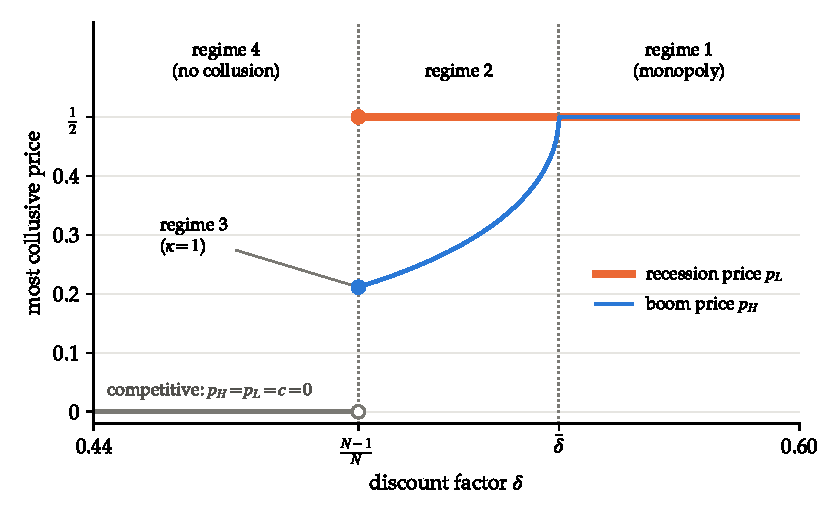
\includegraphics[width=0.78\textwidth]{figures/ch12/rs_two_state.pdf}
\caption{Most collusive prices in the two-state model of \cref{ex:12-rs-multiplicative}: $N = 2$, $c = 0$,
$D_s(p) = A_s(1-p)$ with $A_H = 1.5$ and $A_L = 1$, each state with probability $\frac{1}{2}$. Below
$\delta = \frac{N-1}{N} = \frac{1}{2}$ only competitive pricing is sustainable (regime 4). At $\delta = \frac{1}{2}$ both
constraints bind (regime 3). Between $\frac{1}{2}$ and $\bar\delta = \frac{6}{11}$ the recession price is the monopoly price
$\frac{1}{2}$ and the boom price is lower (regime 2). Above $\bar\delta$ both prices equal $\frac{1}{2}$ (regime 1). Script
\texttt{rs\_two\_state.py}.}
\label{fig:12-rs-two-state}
\end{figure}

\casehead{What the regimes mean}
In regime 2 the cartel concedes in the boom. It lowers the boom price until the gain from undercutting no longer
exceeds the future loss. It keeps the recession price at the monopoly level, because a higher recession profit
raises $V$ and relaxes the boom constraint as well. The result is a pricing pattern that \citet{RotembergSaloner1986}
call a \emph{price war during a boom}: a period of low prices and margins when demand is high. Nobody cheats. The low
boom price is part of the collusive agreement, chosen so that nobody wants to cheat.

Three caveats follow from the proposition. The prediction of countercyclical margins needs optimal collusion. The
competitive outcome is also an equilibrium for every $\delta$, and so is constant pricing at any price that satisfies
both constraints. The prediction also needs intermediate patience. In the example, cyclical pricing occurs only for
$\delta \in [0.5, 0.545)$. Finally, it relies on independent shocks. With persistent demand the future loss depends on
today's state, and the conclusion can reverse, as \cref{sec:12-hh,sec:12-bs} show. Regime 3 is a knife-edge case
with two states. With a continuum of states, profits are capped at a common level in all high states, and this
pattern holds for an interval of discount factors. We turn to that model now.

\subsection{Rotemberg and Saloner (1986): price wars during booms}\label{sec:12-rs}

\subsubsection{The question}

\citet{RotembergSaloner1986} ask how implicitly colluding oligopolists behave when demand fluctuates. Their paper has
two objectives (p.~1). The first is to describe oligopoly pricing over the business cycle. The second is to ask
whether this pricing itself causes business cycles and sticky prices. Their basic point is that collusion is harder
when demand is high. In a boom, ``chiseling away from the collusive level of output becomes more profitable for each
individual firm'' (p.~1), so the oligopoly can sustain only a less collusive outcome. An oligopoly that becomes more
competitive in booms expands output. If its output is an input to other
sectors, their output can rise too. This produces the comovement of outputs that characterizes business cycles.

The question matters for industrial organization because it overturns a piece of folklore. \citet{Scherer1980}
wrote that price cutting ``runs most rampant among oligopolists with high fixed costs'' precisely when business
conditions turn sour (his p.~208, quoted on p.~24). Rotemberg and Saloner concede that one can build models in which recessions
cause price wars. ``Our basis for rejecting this folklore is not theoretical,'' they write. ``Instead our rejection is
based on facts'' (p.~4). We work from the 1984 working paper \citep{RotembergSaloner1984}, which contains the model,
the macroeconomic application and the evidence. Page and table numbers in this subsection refer to it.

\needspace{8\baselineskip}
\subsubsection{The model}

\begin{assumption}[Observable independent demand shocks]\label{asm:12-rs}
\leavevmode
\begin{enumerate}[label=(\roman*)]
\item $N \ge 2$ symmetric firms sell a homogeneous good at constant marginal cost $c$ and set prices simultaneously in
each period. The lowest price serves the market, and ties split it equally.
\item Demand in period $t$ is $D(p, \omega_t)$. The state $\omega_t$ is independent and identically distributed over
time, with CDF $F_\omega$ whose support is $[\underline\omega, \bar\omega]$.
\item All firms learn $\omega_t$ before they set prices, and all past prices are observed.
\item For each $\omega$, $\pi(p,\omega)$ is continuous, strictly increasing in $p$ on $[c, p^m(\omega)]$, and uniquely
maximized at $p^m(\omega)$, with $\pi^m(\omega) > 0$.
\item For each $p > c$, $\pi(p,\omega)$ is strictly increasing in $\omega$. The function $\pi^m$ is continuous and
$\E[\pi^m(\omega)] < \infty$.
\item Firms discount the future with factor $\delta \in (0,1)$.
\end{enumerate}
\end{assumption}

Part (v) says that a higher state shifts demand out. It implies that monopoly profit rises with the state, since for
$\omega' > \omega$ we have $\pi^m(\omega') \ge \pi(p^m(\omega), \omega') > \pi^m(\omega)$. The timing in (iii) is the
model's defining feature. Punishments depend on future states, so their expected size depends on the distribution of
$\omega$. The reward from cheating depends on the current state, which firms see. The authors show that ``for a wide
variety of interesting cases the reward for cheating from the joint profit-maximizing level is monotonically
increasing in $\epsilon_t$'' (pp.~6--7). Here $\epsilon_t$ is the paper's symbol for $\omega_t$.

A \emph{collusive scheme} is a price schedule $p(\cdot)$ that assigns a price to each state. On the collusive path,
every firm charges $p(\omega_t)$. After any deviation, all firms charge $c$ forever. This Nash reversion holds every
firm to its minmax payoff of zero, so it is the harshest credible punishment. Any outcome that some subgame perfect
equilibrium sustains can therefore be sustained with Nash reversion. The authors make the same point about infinite
reversion. ``This length is optimal since it is the biggest credible threat and since, along the equilibrium path,
firms never find themselves punishing each other'' (p.~2). They also note that infinite punishments are less compelling if
industry membership changes, and they use low discount factors in their numerical examples for that reason (p.~8).

As in \cref{sec:12-rs-two-state}, we may restrict attention to $p(\omega) \in [c, p^m(\omega)]$. Write
$v(\omega) = \pi(p(\omega), \omega)$ for industry profit in state $\omega$ on the collusive path, and
$\bar E = \E[v(\omega)]$ for its expectation. The argument that led to \eqref{eq:12-two-state-ic} applies state by
state. A firm that conforms in state $\omega$ earns $\frac{1}{N}v(\omega) + \frac{\delta}{1-\delta}\frac{\bar E}{N}$, and the best
deviation earns $v(\omega)$. The incentive constraint is
\begin{equation*}
\frac{N-1}{N}\, v(\omega) \le \frac{\delta}{1-\delta}\,\frac{\bar E}{N} \qquad \text{for all } \omega.
\end{equation*}
With the slack factor $\kappa$ of \eqref{eq:12-kappa} it reads
\begin{equation}\label{eq:12-rs-ic}
v(\omega) \le \kappa\, \bar E \qquad \text{for all } \omega \in [\underline\omega, \bar\omega].
\end{equation}
The cap $\kappa \bar E$ is the same in every state, because the future does not depend on the present. The cap is
also endogenous. A scheme that earns more on average can afford higher profit in each state.

The paper writes the same condition in terms of the \emph{punishment}
$K = \frac{\delta}{1-\delta}\E[\text{per-firm profit}]$, the expected discounted profit a deviator forfeits (eq.~(1), p.~8).
This $K$ is the paper's symbol and has nothing to do with the capacity of \cref{ex:12-capacity}. A
firm deviates from joint profit maximization in state $\epsilon_t$ if $(N-1)\Pi^m > K$, where $\Pi^m$ is per-firm
monopoly profit (p.~7). The sustainable per-firm profit in high states is $\frac{K}{N-1}$ (eq.~(2), p.~9). In our
notation $K = \frac{\delta \bar E}{(1-\delta)N}$, so the per-firm cap $\frac{K}{N-1}$ equals $\frac{\kappa\bar E}{N}$, which is
\eqref{eq:12-rs-ic} divided by $N$.

\subsubsection{The most collusive scheme as a fixed point}

Every sustainable scheme satisfies $v(\omega) \le \min\{\pi^m(\omega), \kappa\bar E\}$. This suggests the map
\begin{equation}\label{eq:12-rs-h}
h(E) \equiv \E_\omega\left[\min\left\{\pi^m(\omega),\ \kappa E\right\}\right], \qquad E \ge 0,
\end{equation}
which gives the expected profit of the scheme that charges monopoly prices wherever the cap $\kappa E$ allows it.
The map $h$ is continuous and nondecreasing, $h(0) = 0$, and $h(E) \le \E[\pi^m] < \infty$. It is also concave, as
the expectation of a minimum of two functions that are linear in $E$.

\begin{lemma}[Sustainable profit levels]\label{lem:12-rs-fixed}
Under \cref{asm:12-rs}:
\begin{enumerate}[label=(\alph*)]
\item A number $E \ge 0$ is the expected profit of some sustainable scheme if and only if $E \le h(E)$.
\item Let $E^*$ be the largest $E$ with $E \le h(E)$. Then $E^* = h(E^*)$, so $E^*$ is the largest fixed point of $h$.
\item The scheme $v^*(\omega) = \min\{\pi^m(\omega), \kappa E^*\}$ is sustainable. Every sustainable scheme satisfies
$v(\omega) \le v^*(\omega)$ in every state.
\end{enumerate}
\end{lemma}

\begin{proof}
(a) If $v$ is sustainable with mean $E$, then $v(\omega) \le \min\{\pi^m(\omega), \kappa E\}$ for all $\omega$. Taking
expectations, $E \le h(E)$. Conversely, $E = 0$ is the mean of the competitive scheme. If $0 < E \le h(E)$, define
\begin{equation*}
v(\omega) = \frac{E}{h(E)}\min\left\{\pi^m(\omega), \kappa E\right\}.
\end{equation*}
Its mean is $E$. Since $\frac{E}{h(E)} \le 1$, it satisfies $v(\omega) \le \pi^m(\omega)$ and $v(\omega) \le \kappa E$ in every
state. The second inequality is \eqref{eq:12-rs-ic} at mean $E$, so $v$ is sustainable.

(b) The set $\{E \ge 0 : E \le h(E)\}$ is closed, by continuity, and bounded by $\E[\pi^m]$. So it has a largest element
$E^*$. Suppose $E^* < h(E^*)$. Let $E' = h(E^*)$. Since $h$ is nondecreasing, $h(E') \ge h(E^*) = E'$, so $E'$ belongs
to the set and exceeds $E^*$, a contradiction.

(c) Sustainability of $v^*$ follows from (a) and $E^* = h(E^*)$. If $v$ is sustainable with mean $\bar E$, then
$\bar E \le E^*$ by (a) and (b), so $v(\omega) \le \min\{\pi^m(\omega), \kappa\bar E\} \le v^*(\omega)$.
\end{proof}

Part (c) says that the most collusive scheme is the best for the firms in every state at once. There is no tradeoff
between states, so ``most collusive'' is well defined. The paper describes the same construction as a mapping from
punishments to cutoffs and back to punishments, and selects the greatest fixed point (pp.~9--10).

\begin{proposition}[Collusion with observable independent shocks]\label{prop:12-rs-threshold}
Let \cref{asm:12-rs} hold and let $E^*$ be the largest fixed point of $h$.
\begin{enumerate}[label=(\roman*)]
\item If $\kappa < 1$, equivalently $\delta < \frac{N-1}{N}$, then $E^* = 0$. Only competitive pricing is sustainable.
\item If $\kappa = 1$, then $E^* = \pi^m(\underline\omega)$. Industry profit is the same in every state, equal to the
monopoly profit of the lowest state.
\item If $\kappa > 1$, then $E^* > 0$ and $\kappa E^* > \pi^m(\underline\omega)$. Firms charge monopoly prices in every
state if and only if $\kappa\,\E[\pi^m(\omega)] \ge \pi^m(\bar\omega)$. Otherwise there is a cutoff
$\omega^* \in (\underline\omega, \bar\omega)$ with $\pi^m(\omega^*) = \kappa E^*$, and
\begin{equation}\label{eq:12-rs-schedule}
v^*(\omega) =
\begin{cases}
\pi^m(\omega) & \text{if } \omega \le \omega^*,\\
\kappa E^* = \pi^m(\omega^*) & \text{if } \omega > \omega^* .
\end{cases}
\end{equation}
The cutoff solves
\begin{equation}\label{eq:12-rs-cutoff}
\pi^m(\omega^*)\left[1 - \kappa\left(1 - F_\omega(\omega^*)\right)\right] = \kappa \int_{\underline\omega}^{\omega^*} \pi^m(\omega)\, \dd F_\omega(\omega).
\end{equation}
\item The values $E^*$ and $\kappa E^*$ and the cutoff $\omega^*$ are nondecreasing in $\kappa$. They are therefore
nondecreasing in $\delta$ and nonincreasing in $N$.
\end{enumerate}
\end{proposition}

\begin{proof}
(i) If $\kappa < 1$ and $E > 0$, then $h(E) \le \kappa E < E$. So the only fixed point is $E^* = 0$.

(ii) If $\kappa = 1$, then $h(E) = \E[\min\{\pi^m(\omega), E\}] \le E$, with equality if and only if $\pi^m(\omega) \ge E$
with probability one. Because $\underline\omega$ is in the support and $\pi^m$ is continuous and increasing, this
holds if and only if $E \le \pi^m(\underline\omega)$. The fixed points form the interval $[0, \pi^m(\underline\omega)]$,
and the largest is $\pi^m(\underline\omega)$. Then $v^*(\omega) = \min\{\pi^m(\omega), \pi^m(\underline\omega)\} =
\pi^m(\underline\omega)$ in every state.

(iii) Let $\phi(E) = h(E) - E$. For $0 < E \le \frac{\pi^m(\underline\omega)}{\kappa}$, the cap $\kappa E$ lies below
$\pi^m(\omega)$ in every state, so $h(E) = \kappa E$ and $\phi(E) = (\kappa - 1)E > 0$. As $E \to \infty$,
$\phi(E) \le \E[\pi^m] - E \to -\infty$. By continuity $\phi$ has a root above $\frac{\pi^m(\underline\omega)}{\kappa}$,
so $E^* > \frac{\pi^m(\underline\omega)}{\kappa} > 0$.

If $\kappa\E[\pi^m] \ge \pi^m(\bar\omega)$, then $h(\E[\pi^m]) = \E[\pi^m]$, because the cap never binds. No
fixed point exceeds $\E[\pi^m]$, so $E^* = \E[\pi^m]$ and $v^* = \pi^m$. Conversely, if $v^* = \pi^m$ almost surely,
then $E^* = \E[\pi^m]$ and $\pi^m(\omega) \le \kappa\E[\pi^m]$ for almost every $\omega$, hence at $\bar\omega$ by
continuity.

Otherwise $\pi^m(\underline\omega) < \kappa E^* < \pi^m(\bar\omega)$. Since $\pi^m$ is continuous and strictly
increasing, there is a unique $\omega^*$ with $\pi^m(\omega^*) = \kappa E^*$, and $v^*$ takes the form
\eqref{eq:12-rs-schedule}. The fixed-point condition $E^* = h(E^*)$ reads
\begin{equation*}
E^* = \int_{\underline\omega}^{\omega^*} \pi^m(\omega)\, \dd F_\omega(\omega) + \left(1 - F_\omega(\omega^*)\right)\kappa E^* .
\end{equation*}
Substitute $E^* = \frac{\pi^m(\omega^*)}{\kappa}$ and multiply by $\kappa$:
\begin{equation*}
\pi^m(\omega^*) = \kappa\int_{\underline\omega}^{\omega^*} \pi^m(\omega)\, \dd F_\omega(\omega) + \kappa\left(1 - F_\omega(\omega^*)\right)\pi^m(\omega^*).
\end{equation*}
Collecting the terms in $\pi^m(\omega^*)$ gives \eqref{eq:12-rs-cutoff}.

(iv) Write $h_\kappa$ to show the dependence on $\kappa$. For $\kappa' > \kappa$, $h_{\kappa'}(E) \ge h_\kappa(E)$ for all $E$.
So $E^*_\kappa = h_\kappa(E^*_\kappa) \le h_{\kappa'}(E^*_\kappa)$. By \cref{lem:12-rs-fixed}(a) and (b), $E^*_{\kappa'} \ge E^*_\kappa$.
Then $\kappa' E^*_{\kappa'} \ge \kappa E^*_\kappa$, and the cutoff $\omega^* = (\pi^m)^{-1}(\kappa E^*)$ rises weakly. Finally,
$\kappa$ increases in $\delta$ and decreases in $N$.
\end{proof}

Part (i) says that demand fluctuations do not change the patience needed for any collusion at all. Some collusion is
possible exactly when $\delta \ge \frac{N-1}{N}$, as with constant demand. Fluctuations change the form of collusion
above that threshold. Part (iv) restates two claims of the paper (p.~11). The set of states with monopoly pricing
shrinks as $N$ grows, ``as in Stigler's model'' \citep{Stigler1964}. It also shrinks as the future becomes less
important.

\begin{remark}[The existence conditions in the working paper]\label{rem:12-rs-wp}
The working paper states two sufficient conditions for an interior cutoff (pp.~9--10). Its condition (ii) says that
monopoly profit in the highest state exceeds $\kappa$ times its mean, which is the failure of full monopoly in
\cref{prop:12-rs-threshold}(iii). Its condition (i), which should ensure that some collusion is possible, is stated in
a form that appears to come from typographical sign errors in its equations (3) and (5). We have derived the
conditions directly. Collusion is possible if and only if $\kappa \ge 1$, and an interior cutoff exists if and only if
in addition $\kappa\,\E[\pi^m] < \pi^m(\bar\omega)$.
\end{remark}

\subsubsection{The price schedule}

The profit schedule \eqref{eq:12-rs-schedule} translates into prices. Below the cutoff the cartel charges the monopoly
price. Above it, profit must stay at the cap $\kappa E^*$ while demand keeps rising.

\begin{proposition}[Collusive prices fall in booms]\label{prop:12-rs-prices}
Let \cref{asm:12-rs} hold with $\kappa > 1$ and an interior cutoff $\omega^*$. Suppose $\pi$ is continuously
differentiable, $\pi_p > 0$ on $(c, p^m(\omega))$, and $\pi_\omega > 0$ for $p > c$. Let $p^*(\omega)$ be the most
collusive price schedule.
\begin{enumerate}[label=(\roman*)]
\item For $\omega \le \omega^*$, $p^*(\omega) = p^m(\omega)$.
\item For $\omega > \omega^*$, $p^*(\omega)$ is the unique $p \in (c, p^m(\omega))$ with $\pi(p, \omega) = \kappa E^*$, and
\begin{equation}\label{eq:12-rs-dpdw}
\frac{\dd p^*}{\dd \omega} = -\frac{\pi_\omega(p^*, \omega)}{\pi_p(p^*, \omega)} < 0 .
\end{equation}
\item For $\omega > \omega^*$, industry output $D(p^*(\omega), \omega)$ increases in $\omega$.
\item If $p^m$ is nondecreasing, then $p^*$ attains its maximum at $\omega^*$, and the ratio $\frac{p^*(\omega)}{p^m(\omega)}$
decreases strictly on $(\omega^*, \bar\omega]$.
\end{enumerate}
\end{proposition}

\begin{proof}
(i) is \eqref{eq:12-rs-schedule}. For (ii), fix $\omega > \omega^*$. Then $\pi(c, \omega) = 0 < \kappa E^* <
\pi^m(\omega)$. Since $\pi(\cdot, \omega)$ is continuous and strictly increasing on $[c, p^m(\omega)]$, there is exactly
one $p \in (c, p^m(\omega))$ with $\pi(p, \omega) = \kappa E^*$. Differentiate the identity $\pi(p^*(\omega), \omega) =
\kappa E^*$ with respect to $\omega$:
\begin{equation*}
\pi_p(p^*, \omega)\,\frac{\dd p^*}{\dd \omega} + \pi_\omega(p^*, \omega) = 0 .
\end{equation*}
Solving gives \eqref{eq:12-rs-dpdw}. The sign follows from $\pi_\omega > 0$ and $\pi_p > 0$ below the monopoly price. The
implicit function theorem justifies the differentiation because $\pi_p \neq 0$ at $p^*$. For (iii), write
$D(p^*, \omega) = \frac{\kappa E^*}{p^* - c}$. The numerator is constant and the denominator falls. For (iv), $p^*$ rises
weakly up to $\omega^*$ and falls after it. On $(\omega^*, \bar\omega]$ the numerator of $\frac{p^*}{p^m}$ falls while
the denominator does not.
\end{proof}

The intuition is in the paper (pp.~10--11). Above the cutoff, profit is held at the sustainable level. ``If $P$ is
held constant at a level above $c$, the profits from deviating increase. Therefore $P$ must fall. Beyond
$\epsilon_t^*$, prices fall monotonically as $\epsilon_t$ increases.'' Output rises in booms for two reasons:
demand shifts out and the price falls. With multiplicative shocks the monopoly price does not depend on the state, so
the collusive price is constant up to $\omega^*$ and decreasing after it. Prices are then countercyclical over the
whole range of states. With additive shocks the monopoly price rises with demand. The collusive price then rises up
to $\omega^*$ and falls after it.

\casehead{A numerical illustration}
\Cref{fig:12-rs-continuum} computes the most collusive schedule for $N = 2$, $c = 0$ and $\omega \sim U[1,2]$. The script
finds $E^*$ by iterating $E \leftarrow h(E)$ from $E = \E[\pi^m]$. The iterates decrease and converge to the largest
fixed point. In panel (a), demand is $D(p,\omega) = \omega(1-p)$, so $p^m = \frac{1}{2}$ and $\pi^m(\omega) = \frac{\omega}{4}$. Then
$\E[\pi^m] = 0.375$. Full monopoly requires $\kappa \cdot 0.375 \ge \pi^m(2) = \frac{1}{2}$, that is $\kappa \ge \frac{4}{3}$, or
$\delta \ge \frac{4}{7} \approx 0.571$. With the uniform distribution, \eqref{eq:12-rs-cutoff} becomes
\begin{equation*}
\frac{\omega^*}{4}\left[1 - \kappa(2 - \omega^*)\right] = \kappa\int_1^{\omega^*}\frac{\omega}{4}\,\dd\omega = \frac{\kappa\left((\omega^*)^2 - 1\right)}{8}.
\end{equation*}
Multiplying by $\frac{8}{\kappa}$ and collecting terms gives the quadratic
\begin{equation*}
(\omega^*)^2 - \left(4 - \frac{2}{\kappa}\right)\omega^* + 1 = 0,
\end{equation*}
whose larger root is the cutoff. At $\delta = 0.52$, $\kappa \approx 1.083$, $E^* \approx 0.341$, the cap is
$\kappa E^* \approx 0.369$ and $\omega^* \approx 1.477$. The price falls from $\frac{1}{2}$ at the cutoff to about $0.244$
in the highest state. At $\delta = 0.56$ the cutoff moves up to $\omega^* \approx 1.903$, and the price in the highest
state is about $0.390$. In panel (b), demand is $D(p,\omega) = \omega - p$, so $p^m(\omega) = \frac{\omega}{2}$ and
$\pi^m(\omega) = \frac{\omega^2}{4}$. Full monopoly requires $\delta \ge \frac{12}{19} \approx 0.632$. At $\delta = 0.54$ the
cutoff is $\omega^* \approx 1.50$. The price rises to $0.75$ there and then falls to about $0.339$ in the highest state,
where the monopoly price is $1$. At $\delta = 0.60$ the cutoff is $\omega^* \approx 1.855$ and the price peaks at about
$0.927$.

\begin{figure}[htbp]
\centering
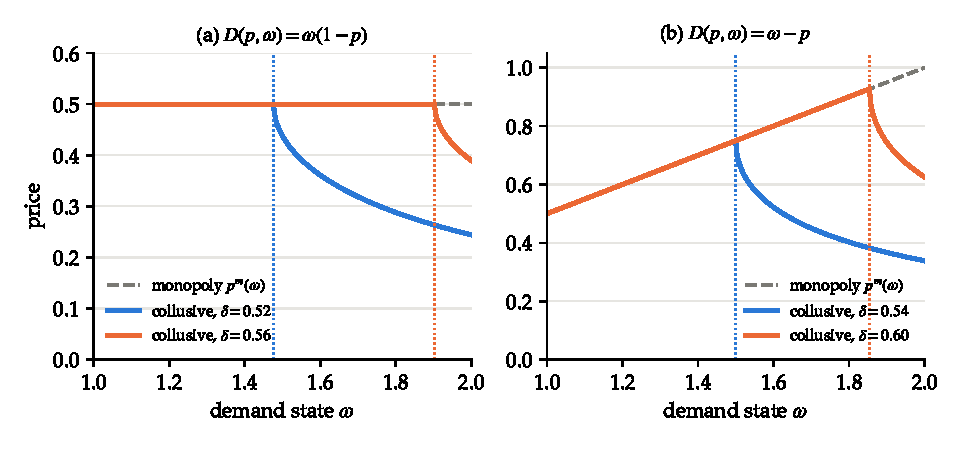
\includegraphics[width=\textwidth]{figures/ch12/rs_continuum.pdf}
\caption{Most collusive price schedules with observable independent demand shocks: $N = 2$, $c = 0$,
$\omega \sim U[1,2]$. Panel (a): multiplicative shocks, $D(p,\omega) = \omega(1-p)$. Panel (b): additive shocks,
$D(p,\omega) = \omega - p$. Dashed: monopoly price $p^m(\omega)$. Solid: collusive price $p^*(\omega)$ for two discount
factors. Dotted vertical lines mark the cutoffs $\omega^*$ of \cref{prop:12-rs-threshold}. Below the cutoff the
collusive price equals the monopoly price. Above it, profit is capped at $\kappa E^*$ and the price falls as demand
rises. Script \texttt{rs\_continuum.py}.}
\label{fig:12-rs-continuum}
\end{figure}

\subsubsection{Collude or compete}

In the optimal scheme no price war is ever observed. The cartel lowers its price smoothly in booms. The paper
also studies a simpler set of strategies in which the cartel can only choose between the monopoly price and the
competitive price (p.~12). Such strategies are ``much simpler and less delicate.'' With this restriction ``the firms
know that when demand is high the monopoly outcome cannot be maintained. They therefore assume that the competitive
outcome will emerge, which is sufficient to fulfill their prophecy.''

Formally, a \emph{collude-or-compete scheme} charges $p^m(\omega)$ in a set $C$ of states and $c$ outside it. In states
outside $C$ all firms charge $c$, a static Nash equilibrium, so nobody wants to deviate there. In a state
$\omega \in C$ the incentive constraint is $\pi^m(\omega) \le \kappa E_R$, where $E_R = \E[\pi^m(\omega)\indic\{\omega \in C\}]$.
Including a low state in $C$ raises $E_R$ without raising the largest profit to be protected. So the best set is an
interval $[\underline\omega, x]$, and the scheme is sustainable if and only if
\begin{equation}\label{eq:12-rs-restricted}
\pi^m(x) \le \kappa\int_{\underline\omega}^{x}\pi^m(\omega)\, \dd F_\omega(\omega).
\end{equation}
A sustainable collude-or-compete scheme is also sustainable in the unrestricted problem. So $E_R \le E^*$, and when
$x$ is interior, $\pi^m(x) \le \kappa E_R \le \kappa E^* = \pi^m(\omega^*)$, so $x \le \omega^*$. The cartel colludes in
fewer states than under the optimal scheme, as the paper states. Above $x$ the price drops from $p^m(x)$ to $c$: an
outright price war, triggered by high demand. This version is the one that connects with empirical studies that
classify periods as collusive or competitive, such as \citet{Bresnahan1987} and \citet{Porter1983}.

\begin{remark}[When do collude-or-compete schemes produce wars?]\label{rem:12-rs-restricted}
Condition \eqref{eq:12-rs-restricted} can fail for every interior $x$ even when the optimal scheme sustains a lot of
collusion. In the two-state model, colluding only in the low state requires $\pi_L^M \le \kappa\cdot\frac{1}{2}\pi_L^M$,
that is $\kappa \ge 2$. But $\bar\kappa < 2$, so for $\kappa \ge 2$ the cartel can already charge monopoly prices in
both states. The restricted scheme is all or nothing. The same happens in both examples of \cref{fig:12-rs-continuum}.
Our computation gives $E_R = 0$ at all four discount factors shown, although the optimal scheme earns between 82 and
almost 100 percent of expected monopoly profit there. The right side of \eqref{eq:12-rs-restricted} is small for $x$ near
$\underline\omega$. A war region at the top therefore requires a distribution in which very high states are rare. Then
the low states accumulate enough profit to protect collusion up to some $x$, and the thin upper tail adds too little
to protect collusion beyond it.
\end{remark}

The shares in the remark are $\frac{0.341}{0.375} \approx 0.91$ and $\frac{0.374}{0.375} \approx 0.997$ in panel (a), and
$\frac{0.479}{0.583} \approx 0.82$ and $\frac{0.573}{0.583} \approx 0.98$ in panel (b).

\subsubsection{Increasing marginal cost}

The model so far assumes constant marginal cost. Increasing marginal cost complicates the model in three ways
(p.~12). First, a price cutter may not want to supply all demand at its price, since it never produces where marginal
cost exceeds price. Second, the profit that the cartel can sustain differs across states, unlike in the constant-cost
case. Third, cheating can take the form of raising price, since rivals that are unwilling to supply all demand at
their price leave some customers for a firm that charges more.

When deviators do not meet all demand, the paper uses the envelope theorem (p.~13). Suppose first that the cartel
charges the monopoly price, which rises with demand. A deviator produces its output $q^d$ where marginal cost equals
the collusive price. By the envelope theorem its profit rises with the state at rate
$q^d\frac{\partial P}{\partial \omega}$, where $P$ is inverse demand. A conforming firm's profit rises at the smaller
rate $q^m\frac{\partial P}{\partial \omega}$, because $q^m < q^d$. Deviation therefore becomes more tempting as demand
rises. Suppose instead that the cartel holds its price fixed as demand rises. The deviation profit then stays fixed.
The conforming profit rises, because the collusive price exceeds marginal cost, and the temptation falls.

When deviators meet all demand, the paper works with the linear example
\begin{equation}\label{eq:12-rs-linear}
P = a + \omega - bQ, \qquad C(q_i) = c\,q_i + \frac{d}{2}q_i^2,
\end{equation}
where $Q$ is industry output and $C$ is each firm's cost (eqs.~(6) and (7)). A cartel that splits output equally
maximizes $(a + \omega - bQ)Q - cQ - \frac{d}{2N}Q^2$. The first-order condition $a + \omega - 2bQ - c - \frac{d}{N}Q = 0$
gives monopoly output and price (eqs.~(8) and (9)):
\begin{equation*}
Q^m = \frac{a + \omega - c}{2b + \frac{d}{N}}, \qquad
P^m = a + \omega - bQ^m = \frac{(a+\omega)(bN + d) + bNc}{2bN + d}.
\end{equation*}
A deviator charging just below $P^m$ would like to produce where $c + dq = P^m$, that is
\begin{equation*}
\bar q = \frac{P^m - c}{d} = \frac{(a + \omega - c)\left(b + \frac{d}{N}\right)}{d\left(2b + \frac{d}{N}\right)}
\end{equation*}
(eq.~(10)). Dividing, $\frac{\bar q}{Q^m} = \frac{b + \frac{d}{N}}{d}$. The deviator meets all demand if and only if
$\bar q \ge Q^m$, that is $b \ge \frac{(N-1)d}{N}$. Marginal cost must not rise too steeply and $N$ must not be too large.
When the deviator meets demand, it sells $Q^m$ at $P^m$ alone, so
\begin{equation*}
\Pi^d = P^mQ^m - cQ^m - \frac{d}{2}(Q^m)^2 .
\end{equation*}
Per-firm collusive profit is $\Pi^m = \frac{1}{N}(P^mQ^m - cQ^m) - \frac{d}{2}\left(\frac{Q^m}{N}\right)^2$. Hence
\begin{equation*}
\Pi^d - N\Pi^m = -\frac{d}{2}(Q^m)^2 + \frac{d}{2N}(Q^m)^2 = \frac{Nd(1-N)}{2}(q^m)^2, \qquad q^m = \frac{Q^m}{N},
\end{equation*}
which is eq.~(11). By the envelope theorem, $\frac{\dd\Pi^m}{\dd\omega} = q^m$. Since $\Pi^d - \Pi^m = (N-1)\Pi^m +
\frac{Nd(1-N)}{2}(q^m)^2$ and $\frac{\dd q^m}{\dd\omega} = \frac{1}{2bN + d}$,
\begin{equation}\label{eq:12-rs-incmc}
\frac{\dd(\Pi^d - \Pi^m)}{\dd\omega} = (N-1)q^m - Nd(N-1)\frac{q^m}{2bN + d} = \frac{(N-1)q^m\left(2bN - d(N-1)\right)}{2bN + d},
\end{equation}
which is eq.~(12). It is positive whenever the deviator meets demand, because then $2bN \ge 2d(N-1) > d(N-1)$. Cheating
becomes more attractive as demand rises.

The paper computes the optimal schedule numerically. For a given punishment, the sustainable price in each state
solves a quadratic equation. The punishment is then updated, starting from a large value and iterating to the first
fixed point (p.~14). Its Figure 1 uses $a = 60$, $b = 1$, $c = 0$, $d = \frac{1}{3}$, $\delta = 0.7$, $N = 5$ and a state
uniform on $\{0, 1, \dots, 80\}$. By eq.~(9) the monopoly price rises linearly from about $30.97$ in state $0$ to about
$72.26$ in state $80$ (our computation). The collusive price equals the monopoly price only in the lowest states. It
then falls, reaches a minimum in the middle of the range of states, and rises slowly at high states. The rise at the
top has a simple cause (p.~15). In high states the collusive price is so low that a deviator would expand only until
price equals its marginal cost. It would no longer serve the whole market. From there, higher demand at a constant
price reduces the temptation, ``thus the oligopoly can afford to increase its prices somewhat.''

\subsubsection{Quantity competition}

With quantities as strategic variables two things change (p.~15). A deviator takes rivals' outputs as given, so its
residual demand is market demand shifted left by their combined output. And the punishment is the Cournot
equilibrium, which yields positive profit. The results are weaker than with prices. Higher demand need not raise the
temptation to cheat. The paper gives a counterexample (p.~16 and its Figure 2). Suppose demand has constant elasticity
and a shock shifts it horizontally. Then the collusive price is the same in both states, and a deviator faces the same
residual demand curve in both, up to a horizontal translation. The extra sales from cheating are the same in both
states, but the revenue lost on the units it would have sold anyway is smaller in the low state. So the incentive to
deviate is strictly larger in the low state. The authors draw a related conclusion: if the cartel keeps its price
constant when demand shifts horizontally, the incentive to cheat falls.

A short calculation makes the counterexample precise. Let marginal cost be a constant $c$, and let $\bar p$ be the
collusive price in both states. In the high state $\omega''$ demand exceeds demand in the low state $\omega'$ by a
constant $k > 0$ at every price. Each firm's collusive output is $q^s(\omega) = \frac{1}{N}D(\bar p,\omega)$, so
$q^s(\omega'') > q^s(\omega')$. Rivals keep producing $(N-1)q^s(\omega)$. A deviator that charges $p < \bar p$
therefore sells $D(p,\omega) - (N-1)q^s(\omega) = q^s(\omega) + y(p)$. The extra sales
$y(p) = D(p,\omega) - D(\bar p,\omega)$ are the same in both states, because the shift $k$ cancels. The deviator's
gain over its conforming profit $\Pi^s(\omega) = (\bar p - c)\,q^s(\omega)$ is
\begin{equation*}
\begin{aligned}
\Pi^d(p,\omega) - \Pi^s(\omega)
&= (p - c)\bigl[q^s(\omega) + y(p)\bigr] - (\bar p - c)\,q^s(\omega) \\
&= (p - c)\,y(p) - (\bar p - p)\,q^s(\omega) .
\end{aligned}
\end{equation*}
The first term is the profit on the extra sales, the equal segments AB and CD of the paper's Figure 2 (p.~16). The
second term is the loss on the units the firm would have sold anyway, and it rises with $q^s(\omega)$. Hence every
deviation price $p < \bar p$ gains strictly more in the low state. If some deviation pays in the high state, the best
deviation pays strictly more in the low state.

With linear demand and cost \eqref{eq:12-rs-linear}, higher demand always raises the temptation. Suppose each firm is
asked to produce $q^s$. A deviator maximizes (eq.~(13))
\begin{equation*}
\Pi^d = q_i\left[a + \omega - c - b\left((N-1)q^s + q_i\right)\right] - \frac{d}{2}q_i^2 ,
\end{equation*}
and the first-order condition gives (eq.~(14))
\begin{equation*}
q^d = \frac{a + \omega - c - b(N-1)q^s}{2b + d} .
\end{equation*}
Let $X = a + \omega - c$ and evaluate at the monopoly output $q^s = q^m = \frac{X}{2bN + d}$. The term in brackets of the
deviator's problem is $A \equiv X - b(N-1)q^m = \frac{X(bN + b + d)}{2bN + d}$, and the deviator earns
$\Pi^d = \frac{A^2}{2(2b + d)}$. A conforming firm earns $\Pi^m = q^m(X - bNq^m) - \frac{d}{2}(q^m)^2 = \frac{X^2}{2(2bN + d)}$.
Subtracting, and using $(bN + b + d)^2 - (2b+d)(2bN + d) = b^2(N-1)^2$,
\begin{equation*}
\Pi^d - \Pi^m = \frac{b^2(N-1)^2 X^2}{2(2b+d)(2bN+d)^2}, \qquad
\frac{\dd(\Pi^d - \Pi^m)}{\dd\omega} = \frac{\left[b(N-1)\right]^2(a + \omega - c)}{(d + 2bN)^2(2b + d)} > 0 .
\end{equation*}
The derivative is the expression on p.~17 of the paper. If the cartel can only collude or compete, high states produce
price wars. If it can choose output freely, it raises output in high states just enough to deter deviation. The
paper's Figure 3 uses $a = 60$, $b = 1$, $c = 0$, $d = \frac{1}{3}$, $\delta = 0.7$ and $N = 5$, the parameters of its
Figure 1. It plots the ratio of the collusive to the monopoly price. The ratio equals one in states up to about 61 and
then falls almost linearly to about $0.92$ in state $80$ (values read from the figure).
The figure's axis is labeled ``Monopoly Price/Oligopoly Price,'' but the text and the plotted values below one
show that it is the oligopoly price relative to the monopoly price. These quantity results hold within Nash-reversion
punishments. In the Cournot supergame harsher credible punishments exist (\cref{sec:12-perfect}), and with them the
cap would be higher.

\subsubsection{From oligopoly pricing to business cycles}

The paper's Section III embeds the oligopoly in a two-sector general equilibrium model (pp.~19--23). Sector 1 is
competitive and sector 2 is the oligopoly. Workers supply any amount of labor at a wage equal to the price of good 1,
and both are normalized to one. Good 1 is produced from labor $L_{1t}$ and an input $Q_{21t}$ of good 2 (p.~19),
\begin{equation}\label{eq:12-rs-ge-prod}
Q_{1t} = A_1Q_{21t} - \frac{B_1}{2}Q_{21t}^2 + G_1L_{1t} - \frac{H_1}{2}L_{1t}^2 .
\end{equation}
Competitive firms equate the price of each input with its marginal revenue product. For good 2 this gives the input
demand
\begin{equation*}
P_{2t} = A_1 - B_1Q_{21t}
\quad\Longleftrightarrow\quad
Q_{21t} = \frac{A_1 - P_{2t}}{B_1} .
\end{equation*}
For labor it gives $G_1 - H_1L_{1t} = 1$, so employment in sector 1 is constant. Consumers' inverse demand for good 2
is $P_{2t} = A_c - B_cQ_{2ct} + e_t$, where $e_t$ is an \iid\ taste shock. Add the two demands,
$Q_{2t} = Q_{21t} + Q_{2ct}$, and solve for $P_{2t}$:
\begin{equation*}
P_{2t} = a + \omega_t - bQ_{2t},
\qquad
a = \frac{A_cB_1 + B_cA_1}{B_c + B_1},
\quad
b = \frac{B_cB_1}{B_c + B_1},
\quad
\omega_t = \frac{B_1}{B_c + B_1}\,e_t .
\end{equation*}
This is the linear demand of \eqref{eq:12-rs-linear}. Producing $Q_{2t}$ requires $cQ_{2t} + \frac{d}{2}Q_{2t}^2$ units of
labor, so marginal cost is $c + dQ_{2t}$ as in the partial-equilibrium model (p.~20).\footnote{Rotemberg and Saloner
write $\alpha$, $\beta$, $\gamma$, $\xi$, $n$, $m$ and $\varepsilon_t$ for our $A_1$, $B_1$, $G_1$, $H_1$, $A_c$, $B_c$ and
$\omega_t$. Their equations (14) and (16) on pp.~19--20 print the labor demand as $\frac{1 + \gamma}{\xi}$ and the
intercept as $\frac{n\beta + m\gamma}{m + \beta}$. The first-order conditions give $\frac{\gamma - 1}{\xi}$ and
$\frac{n\beta + m\alpha}{m + \beta}$. Neither difference affects the argument. The working paper's numbers (13) and
(14) for these equations repeat numbers already used on p.~17, so we cite the section by page.}

The two outputs are linked through the price of good 2. Differentiate \eqref{eq:12-rs-ge-prod} along the input demand:
\begin{equation*}
\frac{\partial Q_{1t}}{\partial P_{2t}}
= \bigl(A_1 - B_1Q_{21t}\bigr)\frac{\partial Q_{21t}}{\partial P_{2t}}
= P_{2t}\cdot\Bigl(-\frac{1}{B_1}\Bigr) < 0 .
\end{equation*}
Output of good 2 is $Q_{2t} = \frac{a + \omega_t - P_{2t}}{b}$, which rises with $\omega_t$ and falls with $P_{2t}$.
Suppose first that sector 2 is competitive, or always acts as a monopolist. Both the competitive and the monopoly
price rise with $\omega_t$, so a taste shift toward good 2 lowers the output of good 1 (p.~20). The two outputs move
in opposite directions, and the economy moves along a production possibility frontier. Suppose instead that the
oligopoly plays the optimal supergame with prices as the strategic variable. A higher $\omega_t$ can then lower
$P_{2t}$ (\cref{sec:12-rs}). Sector 1 buys more of the input and expands, and sector 2 sells more as well. Both
outputs rise together, as all outputs do in a boom (p.~21). Profits can still be procyclical, because revenue minus
total cost can rise with output when there are fixed costs, even as margins fall (p.~22). The authors argue that
this mechanism makes sticky prices and a multiplier natural. They also argue that stabilization
policy could be harmful if booms reflect shifts toward oligopolistic goods. ``If demand for the goods produced by
oligopolies were stable they might collude always, leaving the economy in a permanent recession'' (p.~37).

\subsubsection{The evidence}

Section IV of the paper confronts the folklore with four kinds of evidence (pp.~24--36). None of them is a structural
test. Each asks whether prices or margins in concentrated industries fall when demand is high.

\casehead{The folklore}
\citet{Scherer1980} cites three industries in support of the folklore: rayon, cement and steel. The rayon evidence
shows mainly that the nominal price of rayon fell in the Great Depression, when broad price indices also fell. That
is ``hardly proof of a price war'' (p.~24). For steel, Scherer himself grants that the industry avoided ``widespread
price deterioration, even when operating at less than 65\% capacity between 1958 and 1962'' (p.~24). That leaves
cement.

\casehead{Cement: data and estimating equation}
The data are yearly from 1947 to 1981. The cement price $p^c_t$ is the average price of portland cement from the
Bureau of Mines' \textit{Minerals Yearbook}. It is deflated either by the producer price index $\mathit{PPI}_t$ or by the
price index of construction materials $p^{\mathit{con}}_t$, both from the Bureau of Labor Statistics. The regression
relates the yearly growth rate of the real cement price to the contemporaneous growth rate of GNP. In log-difference
notation,
\begin{equation}\label{eq:12-rs-cement}
\Delta \ln\left(\frac{p^c_t}{P_t}\right) = \beta_0 + \beta_1\, \Delta\ln \mathit{GNP}_t + u_t, \qquad u_t = \phi\, u_{t-1} + e_t,
\qquad P_t \in \left\{\mathit{PPI}_t,\ p^{\mathit{con}}_t\right\}.
\end{equation}
The paper describes the variables as yearly growth rates and does not say whether they are log differences or
percentage changes. Columns (1) and (3) of its Table 1 are ordinary least squares with $\phi = 0$. The Durbin-Watson
statistics of these regressions are low, so columns (2) and (4) re-estimate the equation with first-order
autoregressive errors, ``quasi-differenced'' in the paper's words (p.~25). The paper does not say which feasible
generalized least squares procedure it uses.

The identifying assumption is that GNP growth shifts the demand for cement and is unrelated to the cost and capacity
shocks of the cement industry. The theory predicts $\beta_1 < 0$: when demand grows faster, the collusive price falls
relative to other prices. A competitive industry with rising marginal cost, or a monopoly with procyclical monopoly
prices, would instead show $\beta_1 \ge 0$.

\begin{table}[htbp]
\centering
\caption{The cyclical behavior of real cement prices, yearly data 1947--1981}\label{tab:12-rs-cement}
\small
\begin{tabular}{@{}lcccc@{}}
\toprule
 & (1) & (2) & (3) & (4)\\
Dependent variable: growth of & $\frac{p^c}{\mathit{PPI}}$ & $\frac{p^c}{\mathit{PPI}}$ & $\frac{p^c}{p^{\mathit{con}}}$ & $\frac{p^c}{p^{\mathit{con}}}$\\
\midrule
Constant & 0.025 & 0.025 & 0.038 & 0.037\\
 & (0.010) & (0.012) & (0.007) & (0.008)\\[2pt]
GNP growth, $\beta_1$ & $-0.438$ & $-0.456$ & $-0.875$ & $-0.876$\\
 & (0.236) & (0.197) & (0.161) & (0.149)\\[2pt]
AR(1) coefficient, $\phi$ & & 0.464 & & 0.315\\
 & & (0.173) & & (0.183)\\[2pt]
$R^2$ & 0.10 & 0.15 & 0.48 & 0.52\\
Durbin-Watson & 1.03 & 1.73 & 1.28 & 1.92\\
\bottomrule
\end{tabular}

\smallskip
\begin{minipage}{0.86\textwidth}
\footnotesize
Notes: Estimates of \eqref{eq:12-rs-cement}. $p^c$ is the price of cement, $\mathit{PPI}$ the producer price index and
$p^{\mathit{con}}$ the price index of construction materials. Columns (1) and (3) are ordinary least squares. Columns (2)
and (4) allow first-order autocorrelated errors and are estimated on quasi-differenced data. Standard errors in
parentheses. The paper reports no sample size. Yearly data for 1947--1981 give at most 35 growth rates. Source:
\citet{RotembergSaloner1984}, Table 1.
\end{minipage}
\end{table}

\casehead{Cement: results}
\Cref{tab:12-rs-cement} shows a negative coefficient on GNP growth in all four columns. ``A 1\% increase in the rate of
growth of GNP leads to a 0.5--1.0\% fall in the price of cement'' (p.~25). After the correction for autocorrelation the
coefficients are significant at the 5 percent level. The $t$-ratios are $\frac{-0.456}{0.197} \approx -2.3$ in column (2)
and $\frac{-0.876}{0.149} \approx -5.9$ in column (4). The ordinary least squares standard errors in columns (1) and (3)
are not reliable given the low Durbin-Watson statistics. The anecdotes agree. The real price of cement rose in the
recession years 1954 and 1958 and fell in the boom years 1955 and 1959 (p.~25).

\casehead{Cement: caveats}
The authors raise two objections themselves (pp.~25--26). First, the demand for cement might be only weakly related
to GNP. Cement output growth has a correlation of $0.69$ with GNP growth and $0.77$ with the growth of construction,
which is procyclical. These correlations do not show that cement is more cyclical than the typical sector in GNP.
Without a structural model the question cannot be settled. Second, the regression omits variables a reduced form
should contain, such as the capacity of cement plants. The authors reply that capacity is endogenous and that
adjustment costs make it unresponsive to GNP in the short run. Three further concerns are worth stating. Input costs,
such as energy prices in the 1970s, may move against GNP and enter the cement price directly. If the
construction-materials index in columns (3) and (4) is procyclical, the deflated price is mechanically more
countercyclical, which may explain why those coefficients are larger. And a negative
$\beta_1$ is consistent with any model in which margins fall in booms, including models with capacity constraints or
countercyclical demand elasticities. The regression supports the prediction without isolating the mechanism.

\casehead{Railroads in the 1880s}
\citet{Porter1983} estimated when the railroad cartel on the route from Chicago to New York, the Joint Executive
Committee, was colluding and when it was in a price war. Green and Porter's theory predicts wars after unexpectedly low demand.
Rotemberg and Saloner say that Porter ``finds no support for this theory from the residuals of his estimated
equations'' and argue that his results support their theory instead (p.~26). \Cref{tab:12-rs-railroads} reproduces
their evidence. The first three columns come from Porter's paper. The first is Porter's estimated index of cartel
nonadherence, which parallels closely the contemporary reports in the \textit{Railway Review} and the
\textit{Chicago Tribune}. The second gives rail shipments of wheat from Chicago to New York. The third gives the share
of wheat shipped from Chicago by rail rather than by lake. The last two columns are from the Chicago Board of Trade
annual reports. National grain production adds wheat, corn, rye, oats and barley in tons. The last column counts the
days between April 1 and December 31 on which the Straits of Mackinac were closed to navigation, which prevented
shipment by lake.

\begin{table}[htbp]
\centering
\caption{The railroad cartel, 1880--1886}\label{tab:12-rs-railroads}
\small
\setlength{\tabcolsep}{3pt}
\begin{tabular}{@{}lccccc@{}}
\toprule
 & Estimated & Rail shipments & Fraction shipped & Total grain production & Days lakes closed\\
Year & nonadherence & (million bushels) & by rail (\%) & (billion tons) & (April 1 to Dec.\ 31)\\
\midrule
1880 & 0.00 & 4.73 & 22.1 & 2.70 & 35\\
1881 & 0.44 & 7.68 & 50.0 & 2.05 & 69\\
1882 & 0.21 & 2.39 & 13.8 & 2.69 & 35\\
1883 & 0.00 & 2.59 & 26.8 & 2.62 & 58\\
1884 & 0.40 & 5.90 & 34.0 & 2.98 & 58\\
1885 & 0.67 & 5.12 & 48.5 & 3.00 & 61\\
1886 & 0.06 & 2.21 & 17.4 & 2.83 & 50\\
\bottomrule
\end{tabular}

\smallskip
\begin{minipage}{0.92\textwidth}
\footnotesize
Notes: Columns 1 to 3 are from \citet{Porter1983}, columns 4 and 5 from the Chicago Board of Trade annual reports,
as compiled by Rotemberg and Saloner. Units as printed in the source. The lakes were always closed from January 1 to
March 31. Source: \citet{RotembergSaloner1984}, Table 2.
\end{minipage}
\end{table}

The most severe price wars occurred in 1881, 1884 and 1885. These are the years with the largest rail shipments, in
absolute terms and relative to lake shipments (p.~27). This alone does not show high demand, since shipments may be
high because railroads compete. The authors therefore look at two determinants of demand for rail transport. The
lakes stayed closed longest in 1881 and 1885, the years with the highest nonadherence. In 1883 and 1884 the lakes
were closed only slightly less than in 1885, yet there was a war only in 1884. Grain production explains 1883. It was
the second lowest of the period and 12 percent below 1884 (p.~28). In the authors' words, this ``must have depressed
demand so much that, in spite of the lake closings, total demand for rail transport was low enough to warrant
cooperation.''

The authors anticipate two objections (pp.~28--29). Porter used weekly data, while their table is annual. They reply
that the wars followed a seasonal pattern. The first began around January 1881 and lasted the whole year. The second
began around January 1884 and ended at the end of 1885. Agents could predict the opening of the lakes in midwinter by
studying the thickness of the ice. A railroad that expected a war in the future had two reasons to cut its price at
once. The penalty for deviating was smaller, since the future would be competitive anyway. And shippers who could store
grain would postpone shipments ahead of an expected war, which lowered even the monopoly price. The second objection is
that national grain production is a poor proxy for production in the Chicago region. They reply that national
movements mostly reflect the grain belt, which includes Illinois. The weekly analysis belongs to Porter's own paper and
to \citet{Ellison1994}, who tests Green-Porter against Rotemberg-Saloner with the same data. \Cref{sec:13-jec}
treats both.

\casehead{Automobiles in 1955}
\citet{Bresnahan1987} studies the American automobile industry in the model years 1954 to 1956 (\cref{sec:06-bresnahan}).
Production in 1955 was 44 percent above its 1954 level, and it fell by about 27 percent in 1956
(\cref{tab:06-bres-facts}). The working paper of \citet{RotembergSaloner1984} reports a 45 percent rise and a 44
percent fall (p.~26). The second figure does not match Bresnahan's Table I. Bresnahan finds that a model of
competitive pricing fits the 1955 data, while a collusive model fits 1954 and 1956. Rotemberg and Saloner add that GNP
fell 1 percent in 1954, rose 7 percent in 1955 and rose 2 percent in 1956 (p.~26). In their words, ``Insofar as
cartels can only sustain either competitive or collusive outcomes, this is what our theory predicts'' (p.~26). The
competitive year was the boom year.

\casehead{Price-cost margins}
A direct test would compare prices with marginal costs in booms and recessions. Marginal cost data are scarce, so
industrial organization economists use the \emph{price-cost margin}, sales minus payroll and material costs, divided by
sales. \citet{Scherer1980} summarizes the studies of its cyclical behavior (his p.~357, quoted on p.~29). Concentrated
industries reduce prices, and above all price-cost margins, ``by less in response to a demand slump and increase them
by less in the boom phase.'' The folklore predicts the opposite. Rotemberg and Saloner argue that the fact
favors their theory (p.~30). If part of payroll is a fixed cost, measured margins rise in booms even when price and
marginal cost do not change. Measured margins in concentrated industries rise by less. Either fixed costs matter less
in concentrated industries, which they find unlikely, or concentrated industries cut prices relative to marginal cost
in booms.

\casehead{Product wages and concentration}
The last piece of evidence uses correlations between employment and the \emph{real product wage}. This is the average
hourly wage divided by the industry's value-added deflator. \citet{Burda1984} computed the correlations from detrended
yearly data for 1947--1978. To see why it measures margins, let marginal cost be $mc = \frac{w}{MPL}$, where $w$ is the wage and $MPL$
the marginal product of labor. Then
\begin{equation*}
\frac{w}{p} = MPL \cdot \frac{mc}{p} = MPL\,(1 - L),
\end{equation*}
with $L$ the Lerner index. With constant marginal product, a product wage that rises with employment means a Lerner
index that falls in booms. With diminishing returns, $MPL$ falls in booms, which strengthens the inference (p.~31). The
measure remains valid when part of payroll is fixed. Its weakness is that materials must be proportional to output and
passed through as in a competitive industry (p.~30). The concentration ratio of each two-digit industry is a 1967
sales-weighted average of four-digit four-firm ratios.

\begin{table}[htbp]
\centering
\caption{Concentration and the correlation between real product wages and employment}\label{tab:12-rs-wages}
\small
\setlength{\tabcolsep}{5pt}
\begin{tabular}{@{}llcccc@{}}
\toprule
\multicolumn{6}{@{}l}{\textit{Panel A: two-digit manufacturing industries}}\\
SIC & Industry & Correlation & CR4 & Group & Sign\\
\midrule
\multicolumn{6}{@{}l}{Durables}\\
24 & Lumber and wood products & $-0.33$ & 17.6 & U & $-$\\
25 & Furniture and fixtures & $-0.18$ & 21.6 & U & $-$\\
32 & Stone, clay and glass & 0.39 & 37.4 & C & $+$\\
33 & Primary metals & 0.32 & 42.9 & C & $+$\\
34 & Fabricated metal industries & 0.23 & 29.1 & U & $+$\\
35 & Machinery except electrical & 0.12 & 36.3 & C & $+$\\
36 & Electrical and electronic equipment & 0.34 & 45.0 & C & $+$\\
371 & Motor vehicles and equipment & 0.19 & 80.8 & C & $+$\\
372--9 & Other transportation equipment & 0.02 & 50.1 & C & $+$\\
38 & Instruments and related products & $-0.36$ & 47.8 & C & $-$\\[2pt]
\multicolumn{6}{@{}l}{Nondurables}\\
20 & Food and kindred products & $-0.30$ & 34.5 & U & $-$\\
21 & Tobacco manufactures & $-0.64$ & 73.6 & C & $-$\\
22 & Textile mill products & 0.04 & 34.1 & U & $+$\\
23 & Apparel and related products & $-0.53$ & 19.7 & U & $-$\\
26 & Paper and allied products & $-0.42$ & 31.2 & U & $-$\\
27 & Printing and publishing & 0.40 & 18.9 & U & $+$\\
28 & Chemical and allied products & $-0.03$ & 49.9 & C & $-$\\
29 & Petroleum and coal products & $-0.48$ & 32.9 & U & $-$\\
30 & Rubber & 0.16 & 69.1 & C & $+$\\
31 & Leather and leather products & $-0.44$ & 24.5 & U & $-$\\
\midrule
\multicolumn{6}{@{}l}{\textit{Panel B: contingency table}}\\
 & & Unconcentrated (U) & Concentrated (C) & Total & \\
\midrule
\multicolumn{2}{@{}l}{Negatively correlated} & 7 & 3 & 10 & \\
\multicolumn{2}{@{}l}{Positively correlated} & 3 & 7 & 10 & \\
\multicolumn{2}{@{}l}{Total} & 10 & 10 & 20 & \\
\bottomrule
\end{tabular}

\smallskip
\begin{minipage}{0.9\textwidth}
\footnotesize
Notes: ``Correlation'' is the correlation between the real product wage and employment, detrended yearly data
1947--1978, from \citet{Burda1984}. CR4 is the 1967 four-firm concentration ratio, a sales-weighted average over
four-digit industries (excluding those ending in 99). The groups split the sample at the median concentration of 35.4.
The Group and Sign columns are our classification, and they reproduce Panel B. Source: \citet{RotembergSaloner1984},
Tables 3 and 4.
\end{minipage}
\end{table}

Panel A of \cref{tab:12-rs-wages} shows that concentrated industries such as motor vehicles and electrical equipment
tend to have positive correlations. Unconcentrated ones such as leather, food and wood products tend to have negative
correlations (p.~32). The theory does not say that a slightly more concentrated industry cuts prices more in
booms. A pure monopoly charges the monopoly price, which usually rises with demand. So the authors split the sample at
the median concentration ratio of 35.4, which lies between food and nonelectrical machinery. Panel B gives the
resulting $2 \times 2$ table. Dropping the three industries whose correlations are close to zero (SIC 22, 28 and
372--9) turns the counts 7:3:3:7 into 7:2:2:6. A $\chi^2$ test rejects independence with 92 percent confidence for
Panel B and 97 percent for the reduced table. Fisher's exact test against the alternative that concentrated industries
have more positive correlations rejects with 91 and 96 percent confidence (pp.~33--34). We recomputed these numbers.
The Pearson statistic without continuity correction is $3.20$ ($p = 0.074$) for Panel B and $4.74$ ($p = 0.030$) for the
reduced table. The one-sided Fisher $p$-values are $0.089$ and $0.045$.

\casehead{Alternative explanations}
The authors discuss two (p.~34). Positive correlations could come from monopoly pricing with short-run increasing
returns to labor. They find this unlikely, because firms cut production by closing their least efficient plants
first. Positive correlations could also come from technology shocks that raise labor demand in a sector with upward
sloping labor supply. But the sectors with positive correlations, such as stone, clay and glass, printing and
publishing, and rubber, ``appear to be sectors with fairly stagnant technologies'' (p.~35).

\subsubsection{Critiques and limitations}

The theory and the evidence have limits that later work addressed.
\begin{enumerate}[label=(\arabic*)]
\item \emph{Selection and patience.} Countercyclical pricing describes the most collusive equilibrium for intermediate
discount factors. The competitive equilibrium and many constant-price equilibria exist as well. The theory restricts
what can be sustained, and the prediction rests on the selection.
\item \emph{Independent shocks.} Business cycles are persistent. A boom today predicts high demand tomorrow, which
raises the future loss from a price war exactly when the current gain is large. \Cref{sec:12-hh,sec:12-bs} show
that persistence can reverse the prediction. \citet{Kandori1991} shows that countercyclical pricing survives a family
of correlated shocks when the discount factor is close to a specific value determined by $N$, as summarized by
\citet[p.~2]{BagwellStaiger1995}.
\item \emph{No wars on the path.} With observable demand the optimal scheme lowers prices smoothly. Actual breakdowns
need restricted strategies, and \cref{rem:12-rs-restricted} shows that even then wars at the top require special
distributions. Wars that follow unobserved shocks belong to the theory of \cref{sec:12-public}.
\item \emph{Other forces.} \citet{StaigerWolak1992} add capacity constraints to the model. As Bagwell and Staiger
summarize it, low prices may then be required during downturns, a conclusion analogous to Green and Porter's
\citep[fn.~1]{BagwellStaiger1995}. Storage and intertemporal substitution by buyers, which the authors invoke for the
railroads, also change the incentive constraints.
\item \emph{Reduced-form evidence.} Each piece of evidence shows that margins or prices fall in booms in concentrated
industries. None identifies the mechanism. Capacity, input costs, demand elasticities and fixed costs can produce the
same correlations. The classification by concentration is crude, as the authors note for printing. Its concentration
ratio is low, but its main components, newspapers, books and magazines, are highly concentrated once location and
type are taken into account (p.~32).
\end{enumerate}

\subsubsection{The link to conduct estimation}

Rotemberg-Saloner collusion makes conduct vary with demand. This matters for the conduct-parameter method of
\cref{ch:conduct}. Write the supply relation as
\begin{equation*}
p_t - c_t = \theta_t m_t, \qquad m_t = \frac{Q_t}{\left|\frac{\partial Q_t}{\partial p_t}\right|},
\end{equation*}
where $m_t$ is the markup term. Suppose conduct falls linearly with demand, $\theta_t = \vartheta_0 - \vartheta_1 m_t$
with constants $\vartheta_0$ and $\vartheta_1 > 0$, as in a cartel that concedes in booms. A researcher who estimates
a constant conduct parameter by instrumental variables with a demand shifter recovers a weighted average of the local
slope of the supply relation (\cref{prop:03-corts}). The markup is
$\theta_t m_t = \vartheta_0 m_t - \vartheta_1 m_t^2$, whose slope is $\vartheta_0 - 2\vartheta_1 m_t$. For small
demand movements around $\bar m$ the estimate is close to $\vartheta_0 - 2\vartheta_1\bar m$, while average conduct is
$\vartheta_0 - \vartheta_1\bar m$. The estimate understates market power and can be
negative \citep{Corts1999}. \Cref{sec:03-corts} develops the general result.

\subsubsection{Contribution}

The paper made three lasting contributions. It gave a general logic for collusion under fluctuating demand: compare
the current temptation with the expected future loss, and adjust the collusive price state by state to balance them.
It derived a testable prediction about markups over the cycle, the opposite of the folklore. And it reinterpreted
observed price wars, such as those of 1955 and the 1880s, as consequences of high demand. The papers in the rest of
this section keep the logic and change the demand process.

\subsection{Predictable cycles: Haltiwanger and Harrington (1991)}\label{sec:12-hh}

\citet{HaltiwangerHarrington1991} replace independent shocks with a deterministic demand cycle that firms know in
advance. The original paper is not available to us. We describe its results as \citet[pp.~1--3]{BagwellStaiger1995}
summarize them and develop the logic in our own example. In their framework both the temptation to cheat and the
expected cost of a price war change as the cycle is traversed. They define a boom as a sequence of periods in which
demand rises and a recession as a sequence in which it falls.

\casehead{The incentive constraint}
Let demand in period $t$ be $D_t(p) = A_t d(p)$, where the path $\{A_t\}$ is known to all firms. Let $\pi_t(p) =
(p-c)D_t(p)$ and let $p_t$ be the collusive price at date $t$, with Bertrand reversion forever after a deviation. A
firm that conforms at date $t$ earns $\frac{1}{N}\pi_t(p_t) + \frac{1}{N}\sum_{\tau > t}\delta^{\tau - t}\pi_\tau(p_\tau)$. The best
deviation earns $\pi_t(p_t)$ and then zero. The incentive constraint is
\begin{equation}\label{eq:12-hh-ic}
\frac{N-1}{N}\,\pi_t(p_t) \le \frac{1}{N}\sum_{\tau > t}\delta^{\tau - t}\pi_\tau(p_\tau).
\end{equation}
The right side now depends on the date. Two dates with the same current demand can have very different futures. On
the rising side of the cycle the near future brings higher demand. On the falling side it brings lower demand. The
most collusive path is the greatest solution of $v_t = \min\left\{\pi^m_t, \frac{1}{N-1}\sum_{s \ge 1}\delta^s v_{t+s}\right\}$,
where $v_t = \pi_t(p_t)$ and $\pi^m_t$ is monopoly profit at date $t$. \Cref{lem:13-gas-greatest} in
\cref{ch:collusion-evidence} proves that this greatest solution exists, for punishments of any length.

\begin{example}[A four-period cycle]\label{ex:12-hh-cycle}
Let $D_t(p) = A_t(1-p)$ with $c = 0$, and let $A_t$ cycle through $(4, 8, 12, 8)$. Call the four dates $L$ (low), $M^+$
(middle, rising), $H$ (high) and $M^-$ (middle, falling). Monopoly profits are $\pi^m_t = \frac{A_t}{4}$, so they cycle
through $(\pi_L, \pi_M, \pi_H, \pi_M) = (1, 2, 3, 2)$. Suppose all future dates earn monopoly profits. From $M^+$ the next
four dates bring $(\pi_H, \pi_M, \pi_L, \pi_M)$, and from $M^-$ they bring $(\pi_L, \pi_M, \pi_H, \pi_M)$. The cycle repeats every
four periods, so the future values are
\begin{equation*}
R_{M^+} = \frac{\delta\pi_H + \delta^2\pi_M + \delta^3\pi_L + \delta^4\pi_M}{1 - \delta^4}, \qquad
R_{M^-} = \frac{\delta\pi_L + \delta^2\pi_M + \delta^3\pi_H + \delta^4\pi_M}{1 - \delta^4}.
\end{equation*}
Subtracting,
\begin{equation*}
R_{M^+} - R_{M^-} = \frac{(\delta - \delta^3)(\pi_H - \pi_L)}{1 - \delta^4} = \frac{\delta(\pi_H - \pi_L)}{1 + \delta^2} > 0 .
\end{equation*}
At the same current demand, the future loss from a war is smaller on the falling side. With $N = 2$, monopoly pricing
at each date, holding the others at monopoly, requires $\delta$ of at least $0.313$ at $L$, $0.449$ at $M^+$, $0.621$ at $H$
and $0.548$ at $M^-$ (our computation). At $\delta = 0.58$ only the peak price is cut, to about $0.284$. At $\delta = 0.52$
the most collusive prices at $(L, M^+, H, M^-)$ are about $(0.500, 0.216, 0.124, 0.194)$. At the middle demand level the
price is higher on the rising side, $0.216$, than on the falling side, $0.194$. The script \texttt{hh\_cycle.py} computes
these numbers.
\end{example}

The example shows both forces at work. The peak has the lowest price, which is the Rotemberg-Saloner effect of current
demand. Among dates with equal demand, the price is lower where demand is about to fall, which is the effect that
Haltiwanger and Harrington emphasize. \Cref{sec:13-gas-theory} computes a longer smooth cycle with finite
punishments and reaches the same conclusion.

\casehead{Results}
According to Bagwell and Staiger's summary, Haltiwanger and Harrington show that collusion is most difficult in
recessions, when the cost of a future price war is smallest. They demonstrate that collusive prices are higher in
booms, holding all else equal. The relation between the collusive price and the level of current demand is less clear,
and they cannot give complete analytic results on it. Their simulations show that collusive prices are often
procyclical. As the discount factor drops relative to the number of firms, collusive prices become increasingly
countercyclical, much as Rotemberg and Saloner predicted \citep[p.~2]{BagwellStaiger1995}.

Deterministic cycles suit seasonal demand better than business cycles, whose turning points are hard to predict.
Bagwell and Staiger note this and point to evidence for the Haltiwanger-Harrington model in retail gasoline, where
demand fluctuations are mainly seasonal \citep[fn.~5]{BagwellStaiger1995}. That evidence, \citet{BorensteinShepard1996},
is a deep dive in \cref{sec:13-bs}.

\subsection{Bagwell and Staiger (1997): collusion over the business cycle}\label{sec:12-bs}

\subsubsection{The question}

\citet{BagwellStaiger1997} ask whether collusive prices are procyclical or countercyclical when booms and recessions
are persistent but unpredictable phases. They follow \citet{Hamilton1989} and model the business cycle as a Markov
process that switches between a fast-growth state and a slow-growth state. A \emph{boom} is a period of fast growth in
the level of demand, and a \emph{recession} a period of slow growth. Recessions may, but need not, have negative growth.
Prices are \emph{procyclical} if they are higher in booms and \emph{countercyclical} if they are higher in recessions.
The paper has two main results (WP abstract). Collusive prices may be procyclical (countercyclical) when growth rates
are positively (negatively) correlated over time. And the amplitude of the collusive price cycle is larger when booms
are expected to be shorter and recessions longer. We work from the 1995 working paper
\citep{BagwellStaiger1995} and cite its theorem and equation numbers. We change its notation: $n$ becomes $N$, the
growth rates $b$ and $r$ become $g_b$ and $g_r$, and its value functions $\Omega$, $\omega$, $\tilde\omega_b$, $\tilde\omega_r$
become $\Gamma$, $w$, $W_b$, $W_r$.

\subsubsection{Assumptions and the stationary-growth benchmark}

\begin{assumption}[Bertrand supergame with a growing market]\label{asm:12-bs}
\leavevmode
\begin{enumerate}[label=(\roman*)]
\item $N \ge 2$ firms sell a nondurable homogeneous good in periods $t = 1, 2, \dots$ and set prices
simultaneously. Consumers divide evenly among the lowest-priced firms.
\item The number of consumers in period $t$ is $G_t > 0$, the \emph{level of market demand}. Each consumer has demand
$D(p)$. A lowest-priced firm earns $\pi(p) = (p - c)D(p)$ per consumer it serves. The function $\pi$ has a unique
maximizer $p^m$ and is strictly increasing on $[c, p^m]$. Prices are chosen from $[0, p^m]$.
\item Firms observe all past prices and the current and past levels of demand.
\item Firms use symmetric strategies. The \emph{most collusive prices} are the highest prices supported by a symmetric
subgame perfect equilibrium. Following \citet{Abreu1986}, a deviation is punished by competitive pricing, $p = c$, in
every later period.
\end{enumerate}
\end{assumption}

Here $G_t$ is a level, not a distribution function. The monopoly price is acyclic because it does not depend on the
number of consumers. Any cyclical movement in collusive prices therefore comes from the incentive constraints. Two
per-consumer quantities organize the analysis. A firm that undercuts a common price $p$ captures the whole market, so
its \emph{per-consumer gain from cheating} is
\begin{equation}\label{eq:12-bs-gamma}
\Gamma(p) = \pi(p) - \frac{\pi(p)}{N} = \frac{N-1}{N}\,\pi(p).
\end{equation}
In a war each firm earns $\frac{\pi(c)}{N} = 0$ instead of $\frac{\pi(p)}{N}$. So the \emph{per-consumer, per-period cost of a war} is
\begin{equation}\label{eq:12-bs-w}
w(p) = \frac{\pi(p)}{N} - \frac{\pi(c)}{N} = \frac{\pi(p)}{N}.
\end{equation}

In the \emph{stationary-growth game}, $G_{t+1} = g\,G_t$ with $0 < \delta g < 1$. Demand expands if $g > 1$ and contracts if
$g < 1$. The condition $\delta g < 1$ keeps discounted demand finite. The tradeoff is the same at every date, so a single
most collusive price $p^*$ is charged in every period.

\begin{proposition}[Stationary growth]\label{prop:12-bs-stationary}
In the stationary-growth game, the most collusive price is $p^* = p^m$ if $\delta g \ge \frac{N-1}{N}$ and $p^* = c$
otherwise.
\end{proposition}

\begin{proof}
At date $t$, cheating on a common price $p$ gains $G_t\Gamma(p)$. It costs $G_\tau w(p)$ at every later date $\tau$, and
$G_\tau = g^{\tau - t}G_t$. The incentive constraint is
\begin{equation*}
G_t\,\Gamma(p) \le \sum_{\tau = t+1}^{\infty}\delta^{\tau - t}G_\tau\, w(p) = G_t\sum_{\tau = t+1}^{\infty}(\delta g)^{\tau - t}w(p)
= G_t\,\frac{\delta g}{1 - \delta g}\,w(p).
\end{equation*}
Cancel $G_t$ and substitute \eqref{eq:12-bs-gamma} and \eqref{eq:12-bs-w}:
\begin{equation*}
\frac{N-1}{N}\,\pi(p) \le \frac{\delta g}{1 - \delta g}\,\frac{\pi(p)}{N}.
\end{equation*}
For $p > c$ we may divide by $\frac{\pi(p)}{N} > 0$, which gives $(N-1)(1 - \delta g) \le \delta g$, or $N - 1 \le N\delta g$. This is
$\delta g \ge \frac{N-1}{N}$, and it does not depend on $p$. If it holds, every $p \in (c, p^m]$ is sustainable and the most
collusive price is $p^m$. If it fails, no $p > c$ is sustainable.
\end{proof}

Collusion is easier with more patient firms, fewer firms and faster growth. The ability to collude jumps at
$\delta g = \frac{N-1}{N}$ (WP p.~9). The result matches \cref{prop:12-bertrand-ext}. There demand grows at the net rate
$g$, so the effective discount factor is $\delta(1+g)$. Here $g$ is the gross growth factor, so it is $\delta g$.

\subsubsection{The Markov-growth game}

Demand grows at one of two rates. Period $t$ is a \emph{boom period} if $G_t = g_b G_{t-1}$ and a \emph{recession period}
if $G_t = g_r G_{t-1}$, where $1 > \delta g_b > \delta g_r > 0$. The growth rate $g_t \in \{g_b, g_r\}$ follows a Markov chain with
\begin{equation}\label{eq:12-bs-markov}
\rho \equiv \Pr(g_t = g_r \mid g_{t-1} = g_b), \qquad \lambda \equiv \Pr(g_t = g_b \mid g_{t-1} = g_r).
\end{equation}
So $\rho$ is the probability that a boom turns into a recession and $\lambda$ the probability that a recession turns into a
boom. In this subsection $\rho$ is a transition probability, not pass-through. These parameters fix the expected
durations of the phases. A boom phase that starts in period $t$ lasts exactly $z$ periods with probability
$\rho(1-\rho)^{z-1}$, since it continues $z-1$ times and then ends. Using $\sum_{z \ge 1} z x^{z-1} = \frac{1}{(1-x)^2}$ with
$x = 1 - \rho$, the expected duration is
\begin{equation*}
\sum_{z=1}^{\infty} z\,\rho(1-\rho)^{z-1} = \frac{\rho}{\rho^2} = \frac{1}{\rho}.
\end{equation*}
By the same argument a recession lasts $\frac{1}{\lambda}$ periods on average. The stationary-growth game is the special case
in which booms never end.

\subsubsection{The incentive constraints}

The Markov structure makes the incentives the same in every boom period, whatever the date, and the same in every
recession period. The most collusive prices are therefore a pair, $p_b$ in booms and $p_r$ in recessions. Suppose the
pair $(p_b, p_r)$ is charged forever. Let $W_b$ be a firm's expected discounted profit from period $t+1$ on, per
consumer of period $t+1$, when period $t+1$ is a boom. Define $W_r$ in the same way for a recession. Since
profits fall to zero in a war, $W_b$ and $W_r$ also measure the cost of a war.

Suppose period $t$ is a boom. Next period demand is $g_r G_t$ with probability $\rho$ and $g_b G_t$ with probability $1-\rho$.
The boom incentive constraint is
\begin{equation*}
G_t\,\Gamma(p_b) \le \delta\left[\rho\,(g_r G_t)\,W_r + (1-\rho)\,(g_b G_t)\,W_b\right].
\end{equation*}
The level $G_t$ cancels. Future demand is always proportional to current demand, so the current level is a scaling
factor that does not affect the incentive to collude. The full system is (WP (1)--(4))
\begin{align}
\Gamma(p_b) &\le \delta\left[\rho\, g_r W_r + (1-\rho)\, g_b W_b\right], \label{eq:12-bs-ic-b}\\
\Gamma(p_r) &\le \delta\left[\lambda\, g_b W_b + (1-\lambda)\, g_r W_r\right], \label{eq:12-bs-ic-r}\\
W_b &= w(p_b) + \delta\left[\rho\, g_r W_r + (1-\rho)\, g_b W_b\right], \label{eq:12-bs-W-b}\\
W_r &= w(p_r) + \delta\left[\lambda\, g_b W_b + (1-\lambda)\, g_r W_r\right]. \label{eq:12-bs-W-r}
\end{align}
The first two lines compare today's temptation with the discounted future profit that cheating destroys. The last two
are recursions for that future profit. Write them as a linear system:
\begin{equation*}
\left[1 - (1-\rho)\delta g_b\right] W_b - \rho\,\delta g_r W_r = w(p_b), \qquad
-\lambda\,\delta g_b W_b + \left[1 - (1-\lambda)\delta g_r\right] W_r = w(p_r).
\end{equation*}
Its determinant is $\left[1 - (1-\lambda)\delta g_r\right]\left[1 - (1-\rho)\delta g_b\right] - \delta^2\lambda g_b\rho g_r$. Define
\begin{equation}\label{eq:12-bs-Delta}
\Delta \equiv \frac{\delta}{\left[1 - (1-\lambda)\delta g_r\right]\left[1 - (1-\rho)\delta g_b\right] - \delta^2\lambda g_b \rho g_r}.
\end{equation}
In this subsection $\Delta$ is a scalar, unrelated to the matrix of share derivatives or to the difference operator
of \eqref{eq:12-rs-cement}. The paper shows that $\Delta > 0$ and that $\Delta$ increases in $\delta$ on $(0, \frac{1}{g_b})$ (WP
fn.~7). Cramer's rule gives (WP (5) and (6))
\begin{equation}\label{eq:12-bs-W-solved}
\begin{aligned}
W_b &= \left\{\frac{w(p_b)\left[1 - (1-\lambda)\delta g_r\right]}{\delta} + w(p_r)\rho g_r\right\}\Delta, \\
W_r &= \left\{\frac{w(p_r)\left[1 - (1-\rho)\delta g_b\right]}{\delta} + w(p_b)\lambda g_b\right\}\Delta .
\end{aligned}
\end{equation}

Substitute into the right side of \eqref{eq:12-bs-ic-b}, which is $\delta\rho g_r W_r + \delta(1-\rho)g_b W_b$. The coefficient on
$w(p_r)$ is
\begin{equation*}
\rho g_r\Delta\left[1 - (1-\rho)\delta g_b\right] + (1-\rho)g_b\Delta\,\delta\rho g_r = \rho g_r \Delta .
\end{equation*}
The coefficient on $w(p_b)$ is
\begin{equation*}
g_b\Delta\left[\delta\rho g_r\lambda + (1-\rho)\left(1 - (1-\lambda)\delta g_r\right)\right]
= g_b\Delta\left[1 - \rho - \delta g_r(1 - \lambda - \rho)\right],
\end{equation*}
where the equality uses $(1-\rho)(1-\lambda) - \rho\lambda = 1 - \lambda - \rho$. The recession constraint works the same way. The
two constraints become (WP (8) and (9))
\begin{align}
\Gamma(p_b) &\le \left\{w(p_r)\rho g_r + w(p_b)g_b\left[1 - \rho - \delta g_r(1 - \lambda - \rho)\right]\right\}\Delta, \label{eq:12-bs-8}\\
\Gamma(p_r) &\le \left\{w(p_b)\lambda g_b + w(p_r)g_r\left[1 - \lambda - \delta g_b(1 - \lambda - \rho)\right]\right\}\Delta. \label{eq:12-bs-9}
\end{align}
The future loss is a weighted average of the profit lost in future booms and recessions, with weights that reflect
the expected time spent in each. Substitute $\Gamma = \frac{N-1}{N}\pi$ and $w = \frac{\pi}{N}$, multiply by $N$, and move the own-state
term to the left. The constraints take the form (WP (10)--(13))
\begin{equation}\label{eq:12-bs-10-11}
\pi(p_b)\,\mathcal{B} \le \pi(p_r)\,\rho g_r\Delta, \qquad \pi(p_r)\,\mathcal{R} \le \pi(p_b)\,\lambda g_b\Delta,
\end{equation}
with
\begin{equation}\label{eq:12-bs-B-R}
\mathcal{B} = N - 1 - g_b\Delta\left[1 - \rho - \delta g_r(1 - \lambda - \rho)\right], \qquad
\mathcal{R} = N - 1 - g_r\Delta\left[1 - \lambda - \delta g_b(1 - \lambda - \rho)\right].
\end{equation}
The coefficient $\mathcal B$ is the net temptation in a boom: the gain from cheating minus the part of the future loss
that comes from future boom profits.

\subsubsection{Correlation of growth rates}

In the stationary game the growth rate decides everything. In the Markov game the relevant object is expected future
growth, which may depend on the current phase. One period ahead,
\begin{align*}
\E[G_{t+1} \mid g_t = g_b] - \E[G_{t+1} \mid g_t = g_r]
&= \left[(1-\rho)g_b + \rho g_r - \lambda g_b - (1-\lambda)g_r\right]G_t \\
&= (1 - \lambda - \rho)(g_b - g_r)\,G_t .
\end{align*}
Expected demand next period is higher after a boom if and only if $1 - \lambda - \rho > 0$. What matters for collusion is
discounted demand over the whole future. Normalize $G_t = 1$ and let $\tilde G_b$ be expected discounted demand from period
$t$ on when $t$ is a boom, and $\tilde G_r$ the same for a recession. They satisfy
$\tilde G_b = 1 + \delta\left[\rho g_r\tilde G_r + (1-\rho)g_b\tilde G_b\right]$ and
$\tilde G_r = 1 + \delta\left[\lambda g_b\tilde G_b + (1-\lambda)g_r\tilde G_r\right]$. Solving (WP (14)),
\begin{equation}\label{eq:12-bs-14}
\tilde G_b - \tilde G_r = \Delta\,(g_b - g_r)(1 - \lambda - \rho).
\end{equation}
Growth rates are \emph{positively correlated} if $1 - \lambda - \rho > 0$, \emph{negatively correlated} if $1 - \lambda - \rho < 0$,
and \emph{uncorrelated} if $1 - \lambda - \rho = 0$. Under positive correlation a boom predicts more future demand, so a war
started in a boom costs more. Collusion should then be easier in booms. Under negative correlation the reverse holds.

\subsubsection{The most collusive prices}

The analysis has four parameters besides $(\rho, \lambda)$: $N$, $\delta$, $g_b$ and $g_r$. The first result disposes of the
extreme cases.

\begin{proposition}[Extreme cases]\label{prop:12-bs-extreme}
In the Markov-growth game:
\begin{enumerate}[label=(\roman*)]
\item If $\delta g_r \ge \frac{N-1}{N}$, then $p_b^* = p_r^* = p^m$.
\item If $\delta g_b < \frac{N-1}{N}$, then $p_b^* = p_r^* = c$.
\end{enumerate}
\end{proposition}

\begin{proof}
On every path, growth in each period is at least $g_r$ and at most $g_b$. So discounted demand from any state satisfies
$\frac{1}{1 - \delta g_r} \le \tilde G_s \le \frac{1}{1 - \delta g_b}$.

(i) At $p_b = p_r = p^m$, the recursions \eqref{eq:12-bs-W-b}--\eqref{eq:12-bs-W-r} are those of $\tilde G$ multiplied by $w(p^m)$,
so $W_s = w(p^m)\tilde G_s$. The right side of each incentive constraint equals $W_s - w(p^m) = w(p^m)(\tilde G_s - 1)$ for
the current state $s$. The constraint $\Gamma(p^m) = (N-1)w(p^m) \le w(p^m)(\tilde G_s - 1)$ holds if $\tilde G_s - 1 \ge N - 1$.
This follows from $\tilde G_s - 1 \ge \frac{\delta g_r}{1 - \delta g_r} \ge N - 1$, where the last step is equivalent to
$\delta g_r \ge \frac{N-1}{N}$.

(ii) Take any pair $(p_b, p_r)$ and let $\bar w = \max\{w(p_b), w(p_r)\}$, attained in state $s$. Profit per consumer never
exceeds $\bar w$, so $W_s \le \bar w\,\tilde G_s$ and the right side of the constraint in state $s$ is at most
$\bar w(\tilde G_s - 1) \le \bar w\frac{\delta g_b}{1 - \delta g_b}$. If $\delta g_b < \frac{N-1}{N}$, this is below $(N-1)\bar w =
\Gamma(p_s)$ whenever $\bar w > 0$. So the constraint fails unless $\bar w = 0$, which means $p_b = p_r = c$.
\end{proof}

This is Theorem 1 of the working paper, with a direct proof. If collusion is perfect even under permanent slow
growth, it is perfect in the Markov game. If it fails even under permanent fast growth, it fails in the Markov game.
The interesting case is the maintained assumption (WP (15))
\begin{equation}\label{eq:12-bs-15}
\delta g_b > \frac{N-1}{N} > \delta g_r .
\end{equation}
Under \eqref{eq:12-bs-15} define
\begin{equation}\label{eq:12-bs-rho-star}
\rho^* = \frac{\delta g_b - \frac{N-1}{N}}{\delta(g_b - g_r)}, \qquad \lambda^* = 1 - \rho^* = \frac{\frac{N-1}{N} - \delta g_r}{\delta(g_b - g_r)},
\end{equation}
both in $(0,1)$, and the three linear boundaries (WP (19)--(21))
\begin{equation}\label{eq:12-bs-boundaries}
\hat\lambda(\rho) = \frac{1 - (1-\rho)\delta g_b}{\frac{1}{\lambda^*} - \delta g_b}, \qquad
\hat\rho(\lambda) = \frac{g_b - g_r}{g_b}\rho^* + \frac{\rho^* g_r}{g_b\lambda^*}\lambda, \qquad
\tilde\rho(\lambda) = \frac{1 - (1-\lambda)\delta g_r}{\frac{1}{\rho^*} - \delta g_r}.
\end{equation}
They have simple meanings. On $\lambda = \hat\lambda(\rho)$ the recession constraint holds with equality at monopoly prices,
$\lambda g_b\Delta = \mathcal R$. On $\rho = \tilde\rho(\lambda)$ the boom constraint does, $\rho g_r\Delta = \mathcal B$. On
$\rho = \hat\rho(\lambda)$ the two constraints in \eqref{eq:12-bs-10-11} coincide, $\mathcal{R}\mathcal{B} = (\lambda g_b\Delta)(\rho g_r\Delta)$.
All three lines pass through $(\rho^*, \lambda^*)$.

\begin{proposition}[Collusion over the business cycle]\label{prop:12-bs-cycle}
Under \cref{asm:12-bs} and \eqref{eq:12-bs-15}:
\begin{enumerate}[label=(\roman*)]
\item \emph{Zero correlation} ($\lambda + \rho = 1$). Firms charge $p^m$ in both phases if $\rho \le \rho^*$, and $c$ in both
phases if $\rho > \rho^*$.
\item \emph{Positive correlation} ($\lambda + \rho < 1$). Pricing is monopoly in both phases if $\lambda \ge \hat\lambda(\rho)$. It is
procyclical, $p_b^* = p^m > p_r^* > c$, if $\lambda < \hat\lambda(\rho)$ and $\rho \le \hat\rho(\lambda)$. It is competitive in both
phases if $\rho > \hat\rho(\lambda)$. It is never countercyclical.
\item \emph{Negative correlation} ($\lambda + \rho > 1$). Pricing is monopoly in both phases if $\rho \le \tilde\rho(\lambda)$. It is
countercyclical, $p_r^* = p^m > p_b^* > c$, if $\tilde\rho(\lambda) < \rho \le \hat\rho(\lambda)$. It is competitive if
$\rho > \hat\rho(\lambda)$. It is never procyclical.
\item \emph{Cyclical prices.} In the procyclical region the recession price solves
$\pi(p_r^*) = \frac{\lambda g_b\Delta}{\mathcal R}\pi(p^m)$ on $[c, p^m]$. In the countercyclical region the boom price solves
$\pi(p_b^*) = \frac{\rho g_r\Delta}{\mathcal B}\pi(p^m)$ on $[c, p^m]$. The depressed price is continuous, increasing in $\lambda$
and decreasing in $\rho$. So the amplitude $|p_b^* - p_r^*|$ increases with the expected duration of recessions and
decreases with the expected duration of booms.
\end{enumerate}
\end{proposition}

\begin{proof}
Work with profit levels $x_b = \pi(p_b)$ and $x_r = \pi(p_r)$ in $[0, \pi(p^m)]$. Because $\pi$ is strictly increasing on
$[c, p^m]$, they determine the prices. If $\mathcal B > 0$, the boom constraint in \eqref{eq:12-bs-10-11} reads
$x_b \le a_b x_r$ with $a_b = \frac{\rho g_r\Delta}{\mathcal B}$. If $\mathcal B \le 0$, it holds for all prices, and we set
$a_b = +\infty$. Define $a_r = \frac{\lambda g_b\Delta}{\mathcal R}$ in the same way. The most collusive pair is the greatest
point of the set in \cref{lem:12-two-constraint} with $X_1 = X_2 = \pi(p^m)$. By the lemma there are three outcomes.
If $a_ba_r < 1$, pricing is competitive. If $a_ba_r \ge 1$ and $\min\{a_b, a_r\} \ge 1$, pricing is monopoly. If
$a_ba_r \ge 1$ and one coefficient is below one, the corresponding phase has profit $a\,\pi(p^m) < \pi(p^m)$ and the other
phase charges $p^m$. This gives the formulas in (iv).

It remains to see which phase is weak. Substituting the definitions of $\mathcal B$ and $\mathcal R$, a direct computation
(WP (A1)) gives
\begin{equation*}
\left(\rho g_r\Delta - \mathcal B\right) - \left(\lambda g_b\Delta - \mathcal R\right) = \Delta(g_b - g_r)(1 - \lambda - \rho).
\end{equation*}
The coefficient $a_r$ is below one exactly when $\lambda g_b\Delta - \mathcal R < 0$, and similarly for $a_b$. Under positive correlation the
recession slack is the smaller of the two. If the boom slack is negative, so is the recession slack, both coefficients
are below one, and pricing is competitive. So the boom is never the only weak phase, and pricing is never
countercyclical. Negative correlation reverses the roles.

For (i), zero correlation means $\lambda = 1 - \rho$. Then the right sides of \eqref{eq:12-bs-ic-b} and \eqref{eq:12-bs-ic-r}
coincide, because from either phase the next period is a boom with probability $1-\rho$. If a pair $(p_b, p_r)$ is
sustainable, so is the pair that charges the higher price in both phases, since the common right side increases in
both prices. So the most collusive prices are equal, $p_b = p_r = p$. Then \eqref{eq:12-bs-W-b}--\eqref{eq:12-bs-W-r} give
$W_b = W_r = \frac{w(p)}{1 - \delta\bar g}$ with $\bar g = \rho g_r + (1-\rho)g_b$, and both constraints reduce to
$\Gamma(p) \le \frac{\delta\bar g}{1 - \delta\bar g}w(p)$. This is the stationary game with growth $\bar g$. By
\cref{prop:12-bs-stationary}, monopoly pricing holds if and only if $\delta\left[\rho g_r + (1-\rho)g_b\right] \ge \frac{N-1}{N}$,
which is $\rho \le \rho^*$.

The region boundaries in (ii) and (iii) restate these conditions. Under positive correlation, $a_r \ge 1$ if and only
if $\lambda \ge \hat\lambda(\rho)$. Under negative correlation, $a_b \ge 1$ if and only if $\rho \le \tilde\rho(\lambda)$. In both cases
$a_ba_r \ge 1$ if and only if $\rho \le \hat\rho(\lambda)$.

To see that the boundaries are straight lines, let $D \equiv \frac{\delta}{\Delta} > 0$ be the determinant in
\eqref{eq:12-bs-Delta}. Expanding it with $(1-\rho)(1-\lambda) - \rho\lambda = 1 - \lambda - \rho$ gives
\begin{equation*}
D = 1 - (1-\rho)\delta g_b - (1-\lambda)\delta g_r + \delta^2 g_b g_r(1 - \lambda - \rho),
\end{equation*}
which is affine in $(\rho, \lambda)$. The condition $a_r \ge 1$ is $\lambda g_b\Delta \ge \mathcal R$. Substituting
$\mathcal R$ from \eqref{eq:12-bs-B-R} and multiplying by $D$ gives
\begin{equation*}
\delta\left[\lambda g_b + (1-\lambda)g_r - \delta g_b g_r(1-\lambda-\rho)\right] \ge (N-1)D .
\end{equation*}
Both sides are affine in $(\rho, \lambda)$. Solving the equality for $\lambda$ and substituting $\lambda^*$ from
\eqref{eq:12-bs-rho-star} gives $\hat\lambda(\rho)$. The same steps applied to $\rho g_r\Delta \ge \mathcal B$ give
$\tilde\rho(\lambda)$. For the third boundary we multiply $\mathcal R\mathcal B = (\lambda g_b\Delta)(\rho g_r\Delta)$
by $D^2$. Each side becomes quadratic in $(\rho, \lambda)$, and their difference factors as
\begin{multline*}
\left(\mathcal R\mathcal B - \lambda\rho g_b g_r\Delta^2\right)D^2\\
= D\left\{(N-1)^2 - N(N-1)\delta\left[(1-\rho)g_b + (1-\lambda)g_r\right] + N^2\delta^2 g_b g_r(1 - \lambda - \rho)\right\}.
\end{multline*}
Since $D > 0$, the boundary is the line on which the braces vanish. Solving for $\rho$ and substituting $\rho^*$ and
$\lambda^*$ gives $\hat\rho(\lambda)$. At $(\rho^*, \lambda^*)$ the last term in the braces is zero and
$\delta\left[(1-\rho^*)g_b + \rho^* g_r\right] = \frac{N-1}{N}$, so the braces vanish there, as they must. We checked
each step symbolically with sympy. The monotonicity in (iv) follows from the paper's appendix (Lemmas 3 to 6). It uses
$\frac{\partial\Delta}{\partial\rho} = -\Delta^2 g_b(1 - \delta g_r) < 0$ and
$\frac{\partial\Delta}{\partial\lambda} = -\Delta^2 g_r(1 - \delta g_b) < 0$ (WP (A10) and (A11)).
\end{proof}

The proposition collects Theorems 2 to 4 of the working paper. Its proof in profit space mirrors the two-state model
of \cref{sec:12-rs-two-state}. There, too, the most collusive scheme keeps the strong state at monopoly and depresses
the weak one. The difference lies in which state is weak. With independent shocks, the weak state is the one with high
current demand. With persistent growth, it is the phase that predicts lower future demand.

The results have a clear intuition (WP pp.~18--23). Under positive correlation a recession predicts more recession, so
there is little to lose from a war started in a recession. To keep firms from cheating, the cartel lowers the recession
price. If recessions are expected to last longer ($\lambda$ smaller), the future loss shrinks further and the recession price
must fall more, so the amplitude of the price cycle grows. If booms are too short relative to recessions
($\rho > \hat\rho(\lambda)$), even imperfect collusion is impossible. At that boundary the recession price jumps from a positive
level to $c$. Under negative correlation the boom predicts a recession, the boom is the weak phase, and prices are
countercyclical. Whatever the correlation, collusion is perfect when booms are long and recessions short, and it fails
when booms are short and recessions long. In between, one phase is weak, and the sign of the correlation decides which.
The relation between $\delta$ and $N$, central in the earlier literature, plays no role in the direction of the cycle. It
enters only through $\rho^*$ and $\lambda^*$, which move the regions. As $\delta g_r \to \frac{N-1}{N}$, $\lambda^* \to 0$ and the
monopoly region fills the square. As $\delta g_b \to \frac{N-1}{N}$, $\rho^* \to 0$ and the competitive region does (WP p.~23).

\Cref{fig:12-bs-regions} draws the regions for $N = 2$, $\delta = 0.9$, $g_b = 1.05$ and $g_r = 0.30$, with $\pi(p) = p(1-p)$ and
$c = 0$. These values satisfy \eqref{eq:12-bs-15}, since $0.945 > 0.5 > 0.27$. Then $\rho^* \approx 0.659$ and
$\lambda^* \approx 0.341$. The recession growth factor is extreme. It is chosen so that all four regions are clearly visible,
because \eqref{eq:12-bs-15} with $N = 2$ requires $\delta g_r < \frac{1}{2}$. The monopoly region covers about 58 percent of
the square, the competitive region about 25 percent, and the procyclical and countercyclical regions about 9 and 7
percent. We computed the most collusive pair at each grid point in two ways, from \cref{prop:12-bs-cycle} and by
iterating the best-response map on prices from $(p^m, p^m)$. The classifications differ at 0.014 percent of the grid
points, all on region boundaries.

\begin{figure}[htbp]
\centering
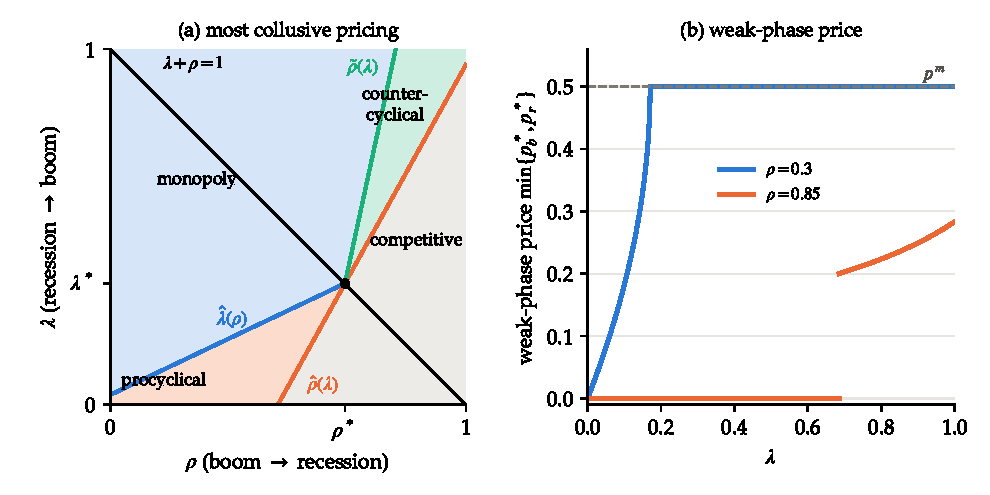
\includegraphics[width=\textwidth]{figures/ch12/bs_regions.pdf}
\caption{Most collusive pricing in the Markov-growth game for $N = 2$, $\delta = 0.9$, $g_b = 1.05$, $g_r = 0.30$,
$\pi(p) = p(1-p)$, $c = 0$. Panel (a): regions in the space of transition probabilities $(\rho, \lambda)$. Below the
anti-diagonal growth rates are positively correlated, above it negatively. The boundaries $\hat\lambda(\rho)$,
$\hat\rho(\lambda)$ and $\tilde\rho(\lambda)$ are \eqref{eq:12-bs-boundaries}, and they meet at $(\rho^*, \lambda^*) \approx (0.659, 0.341)$.
Panel (b): the price in the weak phase as a function of $\lambda$. For $\rho = 0.3$ pricing is procyclical for $\lambda < 0.17$, and
the recession price rises toward $p^m$ as recessions become shorter. For $\rho = 0.85$ pricing is competitive for
$\lambda < 0.686$, then countercyclical with a jump at the boundary. This redraws, with computed regions, Figure 1 of
\citet{BagwellStaiger1995}. Script \texttt{bs\_regions.py}.}
\label{fig:12-bs-regions}
\end{figure}

\subsubsection{Shocks within phases}

The basic model has deterministic demand within a phase. Section V of the paper adds random shocks within phases and
brackets the possibilities with two extremes (WP pp.~24--33). Firms observe the current shock before setting prices.

\casehead{Permanent shocks}
Let $G_t = g_t G_{t-1}\eta_t$, where $\eta_t$ is a multiplicative shock with mean one that becomes part of the base for
all future growth. (Bagwell and Staiger write $\epsilon_t$.) The most
collusive prices depend on the phase but not on the shock. The future is proportional to $G_t$, which already
includes $\eta_t$, so the shock cancels from the incentive constraints, as $G_t$ did before. Formally, the constraints
(WP (22)--(25)) reduce to \eqref{eq:12-bs-ic-b}--\eqref{eq:12-bs-W-r} once $G_t$ is cancelled and $\E[\eta_{t+1}] = 1$ is imposed.
Pricing is exactly as in the basic model (WP Theorem 5).

\casehead{Transitory shocks}
Let $G_t = g_t\frac{G_{t-1}}{\eta_{t-1}}\eta_t$, with $\eta_t$ independent over time, mean one and support $[\underline\eta, \bar\eta]$
containing one. The base level grows without the shock, and the shock affects only the current period. This combines
the Markov phases with Rotemberg-Saloner shocks. Let $p_b(\eta)$ and $p_r(\eta)$ be the prices in each phase when
the current shock is $\eta$. The base level cancels again, but the current shock does not. The boom constraint becomes
(WP (26))
\begin{equation*}
\eta\,\Gamma(p_b(\eta)) \le \delta\left[\rho g_r W_r + (1-\rho)g_b W_b\right],
\end{equation*}
with $W_b$ and $W_r$ defined as before but with $\E[w(p(\eta))\eta]$ in place of $w(p)$ (WP (28)--(29)). The paper solves
the system in two steps, following Rotemberg and Saloner. First it holds the right sides fixed at values
$\tilde W_b$ and $\tilde W_r$. Each constraint then reads $\pi(p_s(\eta)) \le \frac{N}{N-1}\frac{\tilde W_s}{\eta}$ (WP (34)--(35)), and the most
collusive price is
\begin{equation}\label{eq:12-bs-transitory-price}
p_s(\eta) = P^*\!\left(\frac{\tilde W_s}{\eta}\right) \equiv
\begin{cases}
p^m & \text{if } \pi(p^m) \le \frac{N}{N-1}\frac{\tilde W_s}{\eta},\\
\min\left\{p : \pi(p) = \frac{N}{N-1}\frac{\tilde W_s}{\eta}\right\} & \text{otherwise}
\end{cases}
\end{equation}
(WP (36)--(39)). Second, it requires the values $\tilde W_b$ and $\tilde W_r$ to be consistent with the prices they generate
(WP (40)--(43)). It then picks the largest fixed point of the resulting pair of equations. The competitive outcome
$\tilde W_b = \tilde W_r = 0$ is always a fixed point. To leave room for perfect collusion the paper assumes (WP (44))
\begin{equation*}
\delta g_b > \frac{\bar\eta(N-1)}{1 + \bar\eta(N-1)},
\end{equation*}
which says that even the largest shock would not disrupt perfect collusion if growth stayed at the boom rate forever.
To check this, apply the argument of \cref{prop:12-bs-stationary} with current demand scaled by $\bar\eta$:
$\bar\eta(N-1) \le \frac{\delta g_b}{1 - \delta g_b}$ rearranges to the displayed condition.

The results are Theorem 6 of the working paper. Both phases use the same pricing function $P^*$ in
\eqref{eq:12-bs-transitory-price}, and $P^*$ is nondecreasing in $\frac{\tilde W}{\eta}$. So a higher transitory shock lowers the
most collusive price weakly, in booms and in recessions alike. This is the Rotemberg-Saloner effect, now inside each
phase. The comparison between phases still follows the correlation of growth rates. Under positive correlation the
boom value exceeds the recession value at the most collusive fixed point, so $p_b(\eta) \ge p_r(\eta)$ at every shock,
with strict inequality for large shocks. Negative correlation reverses the ranking. The paper's Figures 6a and 6b show
both price schedules flat at $p^m$ for small shocks and falling for large ones. The boom schedule lies above the
recession schedule under positive correlation and below it under negative correlation. Transitory shocks also enlarge
the parameter region with cyclical pricing, because perfect collusion in both phases and at every shock now requires
more. The paper concludes that its second point ``provides an interpretation of the Rotemberg-Saloner (1986) theory in
terms of the transitory demand shocks that occur within broader business-cycle phases'' (WP p.~33).

\subsubsection{Empirical content and limits}

The theory makes the cyclicality of collusive prices an empirical question about the demand process of each industry.
The direction of the cycle depends on the correlation of growth rates, and its amplitude on the expected durations of
booms and recessions. Bagwell and Staiger suggest estimating these parameters industry by industry with Hamilton's
methods and comparing the predictions with industry prices (WP p.~34). No such study existed when they wrote. For
the aggregate economy, \citet{Hamilton1989} finds that quarterly growth rates of U.S. real GNP are positively correlated
and that booms last longer in expectation than recessions. If an industry's demand cycle shares these features, the
prediction of procyclical collusive prices ``appears most salient'' (WP p.~34). Existing evidence points both ways,
and the paper calls it mixed and inconclusive (WP p.~2 and fn.~4). It cites cross-industry studies of margins
\citep{DomowitzHubbardPetersen1986,RotembergWoodford1992}. It cites industry studies, among them
\citet{BorensteinShepard1996}, \citet{Ellison1994}, \citet{Porter1983} and \citet{RotembergSaloner1986}. It also cites
evidence that cartels are most likely to break down during recessions \citep{Suslow1988}.

The authors list three limits (WP pp.~34--35). Marginal costs are acyclic in the model, while the evidence on their
cyclicality is mixed \citep{Bils1987,MironZeldes1988}. Firms are assumed to tell transitory shocks from turning points.
If they observe only demand, they must infer the phase, and the sharp distinction between the responses to the two
kinds of movement will soften. Finally, the analysis is partial equilibrium. With entry and exit the difference between
phases may matter less, and with endogenous interest rates discounting may be more severe in booms.

\subsection{Comparing the models}\label{sec:12-demand-compare}

\Cref{tab:12-cycle-theories} compares the theories of this section with the imperfect-monitoring theory of the next.
The models agree on the logic of the incentive constraint. They disagree on what current demand reveals about the
future and on what firms observe. These two features decide when collusive prices are lowest and whether price wars
appear on the equilibrium path. The table also suggests what data would tell the theories apart. One needs the timing
of low prices relative to the level, growth and predictability of demand. One also needs to know whether low prices
follow observed or unobserved shocks. \Cref{ch:collusion-evidence} takes these predictions to the data.

\begin{table}[htbp]
\centering
\caption{Demand fluctuations and collusive pricing: four theories compared}\label{tab:12-cycle-theories}
\footnotesize
\begin{tabularx}{\textwidth}{@{}>{\raggedright\arraybackslash}p{2.35cm}>{\raggedright\arraybackslash}X>{\raggedright\arraybackslash}X>{\raggedright\arraybackslash}p{2.2cm}>{\raggedright\arraybackslash}X@{}}
\toprule
Model & What drives the future loss & When collusive prices are lowest & Price wars on the path? & Testable implication\\
\midrule
\citet{RotembergSaloner1986}: observed independent shocks & Expected demand, the same in every state & In high-demand states, above a cutoff & No (yes only with collude-or-compete strategies) & Margins fall when current demand is high\\[3pt]
\citet{HaltiwangerHarrington1991}: deterministic cycle & Demand along the known future path & When demand is about to fall, and at the peak for impatient firms & No & At equal demand, prices higher when demand rises than when it falls\\[3pt]
\citet{BagwellStaiger1997}: Markov growth phases & Expected future growth, which depends on the phase & In recessions under positive correlation, in booms under negative correlation & No & Direction and amplitude of the price cycle depend on correlation and phase durations\\[3pt]
\citet{GreenPorter1984}: unobserved shocks (\cref{sec:12-public}) & Probability that a low price triggers a war & After unexpectedly low demand & Yes, finite reversions & Wars follow negative demand shocks and are not caused by cheating\\
\bottomrule
\end{tabularx}
\end{table}

\section{Imperfect Public Monitoring: Green and Porter}\label{sec:12-public}

In the models of \cref{sec:12-perfect,sec:12-demand}, every firm sees every rival's price. A deviation is detected
at once, the threat of punishment deters it, and punishments are never carried out. Prices on the equilibrium path
may move with demand, but no price war is ever triggered by a suspicion of cheating. This section removes perfect
observability. Firms now see only a signal that depends both on their rivals' actions and on demand shocks that
nobody observes. When all firms see the same signal, we speak of \emph{imperfect public monitoring}. The signal is
an imperfect indicator of conduct, so a cartel cannot condition punishments on deviations. It must condition them on
outcomes, and outcomes are sometimes bad even when nobody cheats.

The consequence is the central result of this section. Price wars occur on the equilibrium path, and they are
necessary to sustain collusion. We first recall the policing problem of \citet{Stigler1964}, which motivated the
theory. We then study a Bertrand version that conveys the logic in a few lines, and the original Cournot model of
\citet{GreenPorter1984}. The section ends with the stochastic process of prices that the model generates, which is
the basis for the empirical tests of \cref{sec:13-jec}.

\subsection{Secret price cuts: Stigler's policing problem}\label{sec:12-stigler-recap}

\citet{Stigler1964} accepted that oligopolists wish to maximize joint profits and asked why they so often fail.
His answer is that a collusive agreement must be policed, and that policing is a problem of information. Any member
who can cut its price secretly earns more than by conforming. Enforcement therefore consists of detecting
significant deviations. Once a cut is detected, rivals match it, so it stops paying. The difficulty is detection
itself. Transaction prices are private, buyers have an interest in reporting fictitious offers, and a price cut can
be disguised in non-price terms of the sale. Stigler concluded that the basic evidence of a price cut is that the
cutter wins business it would otherwise not obtain \citep[Section II]{Stigler1964}. His definition of perfect
collusion is accordingly that no buyer changes sellers voluntarily.

This view yields testable implications, which \cref{sec:02-stigler} develops with Stigler's statistical model and
evidence. Suppose each cut offered to a single buyer reaches a rival with probability $h$. A cut offered to $n$
buyers is then detected with probability $1 - (1 - h)^n$, which approaches one quickly as $n$ grows. Secret cuts
are therefore offered to large buyers, and collusion holds best against many small ones. Public sealed-bid
purchases reveal prices and make collusion easier. Collusion is harder when the identity of buyers changes often,
because a seller's loss of customers is then a noisy signal. The incentive to cut prices secretly grows roughly in
proportion to the number of rivals, so collusion is harder with more sellers. The variance of firms' sales to new
customers depends on the Herfindahl index, which makes it the natural measure of concentration for this problem.

Stigler's account has a gap that the rest of this section fills. It takes for granted that detected cuts are
punished, and it offers no equilibrium theory of punishment when detection is noisy. In his account a price war is
the sign that a cartel has broken down. \citet{GreenPorter1984} read Stigler differently. They treat the cartel as
the solution of a design problem: an institution whose members behave noncooperatively and whose incentives must be
self-enforcing. With noisy signals, the best such institution must sometimes punish members who did not cheat.

\subsection{A Bertrand version with zero-demand shocks}\label{sec:12-gp-bertrand}

The logic of on-path price wars is clearest in a price-setting model with a very simple form of noise. This version
is the textbook simplification of \citet[section~6.7.1.1]{Tirole1988} of the Cournot model of
\citet{GreenPorter1984}, which we study in \cref{sec:12-gp-original}. Tirole replaces quantity competition by price
competition so that firms infer rivals' prices from their own demand, as \citet{Stigler1964} assumed. He writes
$\alpha$ for the probability of zero demand, which we call $\gamma$. His section~6.7.1 on secret price cuts, which
also treats quantity competition, spans pp.~262--265 of the print edition \citep[p.~16, note~27]{MarshallMarx2012}.

\needspace{6\baselineskip}
\begin{assumption}[Bertrand duopoly with unobserved demand shocks]\label{asm:12-gp-bertrand}
\leavevmode
\begin{enumerate}[label=(\roman*)]
\item Two firms sell a homogeneous good at constant marginal cost $c$. They set prices simultaneously in each period
$t = 0, 1, 2, \dots$ and discount the future with the factor $\delta \in (0,1)$.
\item In each period demand is $D(p)$ with probability $1 - \gamma$ and zero with probability $\gamma \in (0,1)$,
independently over time. The state is drawn after prices are set, and no firm ever observes it.
\item Industry profit $\pi(p) = (p - c)D(p)$ is continuous and has a unique maximizer $p^m$, with
$\pi^m \equiv \pi(p^m) > 0$.
\item Each firm observes its own price and its own sales. It never observes the rival's price or the state.
\end{enumerate}
\end{assumption}

The lowest price serves the market and ties are split equally. Firm $i$'s sales when the rival charges $p_j$ are
therefore
\begin{equation}\label{eq:12-gp-sales}
q_i =
\begin{cases}
D(p_i) & \text{if } p_i < p_j \text{ and demand is } D(\cdot),\\[2pt]
\frac{1}{2}D(p_i) & \text{if } p_i = p_j \text{ and demand is } D(\cdot),\\[2pt]
0 & \text{if } p_i > p_j \text{ or demand is zero.}
\end{cases}
\end{equation}
The model builds Stigler's inference problem into the payoffs. A firm that charged $p^m$ and sold nothing cannot tell
whether demand was zero or its rival undercut it. Its only signal is its own sales, and zero sales are consistent
with both events.

\begin{definition}[Trigger strategy with punishment length $T$]\label{def:12-gp-trigger}
Fix an integer $T \ge 1$. Each period is either collusive or a punishment period, and period $0$ is collusive. In a
collusive period the firm charges $p^m$. Suppose that in a collusive period the firm's own sales are zero, or the
firm itself charged a price different from $p^m$. Then the next $T$ periods are punishment periods, in which the firm
charges $c$. The period after the last punishment period is collusive. In every other case a collusive period is followed by
a collusive period.
\end{definition}

When both firms follow this strategy, both charge $p^m$ in collusive periods. Both then sell nothing exactly when
demand is zero, so their phases always coincide. Every zero-demand period in a collusive phase starts a \emph{price
war} of $T$ periods at marginal cost, although nobody has cheated. We say that such a war is on the
\emph{equilibrium path}.

\begin{proposition}[Collusion with a finite price war]\label{prop:12-gp-bertrand}
Under \cref{asm:12-gp-bertrand}, the value of a firm at the start of a collusive period when both firms follow the
trigger strategy of \cref{def:12-gp-trigger} is
\begin{equation}\label{eq:12-gp-V}
V = \frac{(1 - \gamma)\frac{\pi^m}{2}}{1 - (1 - \gamma)\delta - \gamma\delta^{T + 1}} .
\end{equation}
The trigger profile is a Nash equilibrium if and only if
\begin{equation}\label{eq:12-gp-ic}
\Lambda(T) \equiv 2(1 - \gamma)\delta + (2\gamma - 1)\delta^{T + 1} \;\ge\; 1 .
\end{equation}
\end{proposition}

\begin{proof}
\emph{Value of collusion.} Consider a collusive period. With probability $1 - \gamma$ demand is positive, each firm
sells $\frac{1}{2}D(p^m)$ and earns $\frac{\pi^m}{2}$, and the next period is collusive. With probability $\gamma$
demand is zero, each firm earns zero, and a war fills periods $t + 1$ to $t + T$. Profits in the war are zero, and
collusion resumes in period $t + T + 1$, whose value seen from period $t$ is $\delta^{T + 1}V$. Hence
\begin{equation*}
V = (1 - \gamma)\Bigl(\frac{\pi^m}{2} + \delta V\Bigr) + \gamma\,\delta^{T + 1}V .
\end{equation*}
Collect the terms in $V$:
\begin{equation*}
V\bigl[1 - (1 - \gamma)\delta - \gamma\delta^{T + 1}\bigr] = (1 - \gamma)\frac{\pi^m}{2} .
\end{equation*}
The bracket is positive because $(1 - \gamma)\delta + \gamma\delta^{T + 1} < 1$. Dividing gives \eqref{eq:12-gp-V}.

\emph{Deviations in a war.} In a punishment period the rival charges $c$. Any price earns at most zero, so charging
$c$ is a best response, and the firm's price cannot change the length of the war. Only deviations in collusive
periods need to be checked.

\emph{Deviations in a collusive period.} A price above $p^m$ earns zero today. It leaves the rival's next phase
exactly as under conformity: the rival sells something when demand is positive and nothing otherwise. It is
therefore dominated by charging $p^m$. A price $p < p^m$ wins the whole market when demand is positive and earns
$(1 - \gamma)(p - c)D(p) \le (1 - \gamma)\pi^m$ in expectation. The rival then sells nothing whatever the state, so
a war starts for sure. The supremum of the current gain, $(1 - \gamma)\pi^m$, is approached as $p \uparrow p^m$.

\emph{Best responses.} Give firm $i$ the extra information of the rival's current phase, which can only raise its
best payoff. Let $W$ be the supremum of $i$'s payoff at the start of a rival's collusive phase. In a war the firm
earns at most zero per period, and the rival returns to collusion after $T$ periods whatever $i$ does. Dynamic
programming then gives
\begin{equation*}
W = \max\Bigl\{(1 - \gamma)\frac{\pi^m}{2} + \bigl[(1 - \gamma)\delta + \gamma\delta^{T + 1}\bigr]W,\;\;
(1 - \gamma)\pi^m + \delta^{T + 1}W\Bigr\}.
\end{equation*}
The right side is a contraction in $W$, so $W$ is its unique bounded fixed point. Define the value of the best
one-shot undercut as
\begin{equation*}
V^d \equiv (1 - \gamma)\pi^m + \delta^{T + 1}V .
\end{equation*}
If $V \ge V^d$, then $V$ solves the fixed-point equation, because the first branch equals $V$ by the recursion
above. Hence $W = V$, and conformity is a best response. If $V < V^d$, an undercut close to $p^m$ followed by the
trigger strategy is a profitable deviation. The profile is therefore an equilibrium if and only if $V \ge V^d$.

\emph{The condition.} Replace $V$ on the left of $V \ge V^d$ by its recursion:
\begin{equation*}
(1 - \gamma)\frac{\pi^m}{2} + \bigl[(1 - \gamma)\delta + \gamma\delta^{T + 1}\bigr]V \;\ge\; (1 - \gamma)\pi^m + \delta^{T + 1}V .
\end{equation*}
Move the terms in $V$ to the left and the others to the right:
\begin{equation*}
\bigl[(1 - \gamma)\delta - (1 - \gamma)\delta^{T + 1}\bigr]V \;\ge\; (1 - \gamma)\frac{\pi^m}{2} .
\end{equation*}
Divide by $1 - \gamma$:
\begin{equation}\label{eq:12-gp-ic-V}
\bigl(\delta - \delta^{T + 1}\bigr)V \;\ge\; \frac{\pi^m}{2} .
\end{equation}
Substitute \eqref{eq:12-gp-V} and cancel $\frac{\pi^m}{2}$:
\begin{equation*}
(1 - \gamma)\bigl(\delta - \delta^{T + 1}\bigr) \;\ge\; 1 - (1 - \gamma)\delta - \gamma\delta^{T + 1} .
\end{equation*}
Collect terms:
\begin{equation*}
2(1 - \gamma)\delta - (1 - \gamma)\delta^{T + 1} + \gamma\delta^{T + 1} \;\ge\; 1 ,
\end{equation*}
which is \eqref{eq:12-gp-ic}.
\end{proof}

The proposition reproduces Tirole's equations (6.10) to (6.16) in our notation. His (6.10) and (6.11) are the
recursions for the values of the collusive and punishment phases, with $V^- = \delta^TV^+$. His (6.14) is
\eqref{eq:12-gp-V}, his incentive constraint (6.13), $\delta(V^+ - V^-) \ge \frac{\pi^m}{2}$, is
\eqref{eq:12-gp-ic-V}, and his (6.16) is \eqref{eq:12-gp-ic} exactly.

Condition \eqref{eq:12-gp-ic-V} has a simple reading. An undercut raises current profit by $\frac{\pi^m}{2}$ when
demand is positive. Its cost is that a war then starts for sure rather than with probability $\gamma$. The extra
probability of a war is $1 - \gamma$, and a war destroys the $T$ collusive periods that would have followed, worth
$(\delta - \delta^{T + 1})V$. Both the gain and the extra probability carry the factor $1 - \gamma$, which cancels.
Two special cases connect the result to earlier sections. With an infinite war ($T = \infty$), $\delta^{T + 1} = 0$
and the condition becomes $\delta(1 - \gamma) \ge \frac{1}{2}$. Without noise ($\gamma = 0$) the condition becomes
$2\delta - \delta^{T + 1} \ge 1$, which is equivalent to $\delta + \delta^2 + \dots + \delta^T \ge 1$. A long enough
punishment works if and only if $\delta > \frac{1}{2}$, and permanent reversion works if and only if
$\delta \ge \frac{1}{2}$. This is the duopoly threshold $1 - \frac{1}{N}$ of \cref{prop:12-bertrand}.

\begin{corollary}[The optimal length of a price war]\label{cor:12-gp-optimal-T}
Under \cref{asm:12-gp-bertrand}:
\begin{enumerate}[label=(\roman*)]
\item $V$ is strictly decreasing in $T$ and in $\gamma$.
\item If $\gamma \ge \frac{1}{2}$, no $T$ satisfies \eqref{eq:12-gp-ic}. If $\gamma < \frac{1}{2}$, the function
$\Lambda(T)$ is strictly increasing in $T$, with $\Lambda(0) = \delta$ and $\lim_{T \to \infty} \Lambda(T) = 2(1 - \gamma)\delta$.
Some finite $T$ satisfies \eqref{eq:12-gp-ic} if and only if $2(1 - \gamma)\delta > 1$.
\item The most profitable trigger equilibrium uses the shortest war that satisfies \eqref{eq:12-gp-ic},
\begin{equation}\label{eq:12-gp-Tstar}
T^* = \min\Bigl\{T \ge 1 : \delta^{T + 1} \le x\Bigr\},
\qquad
x \equiv \frac{2(1 - \gamma)\delta - 1}{1 - 2\gamma} .
\end{equation}
\item The threshold $\frac{1}{2(1 - \gamma)}$ that $\delta$ must exceed rises with $\gamma$, and $T^*$ is weakly
increasing in $\gamma$.
\item A war of one period never suffices: $\Lambda(1) < 1$ for every $\gamma \in [0, 1)$ and $\delta \in (0, 1)$, so
$T^* \ge 2$ whenever collusion is sustainable.
\end{enumerate}
\end{corollary}

\begin{proof}
(i) Write the denominator of \eqref{eq:12-gp-V} as $1 - \delta + \gamma(\delta - \delta^{T + 1})$. It rises with
$T$ because $\delta^{T + 1}$ falls, and it rises with $\gamma$. The numerator falls with $\gamma$. (ii) If
$\gamma \ge \frac{1}{2}$, then $2\gamma - 1 \ge 0$ and $\delta^{T + 1} \le \delta$, so
$\Lambda(T) \le 2(1 - \gamma)\delta + (2\gamma - 1)\delta = \delta < 1$. If $\gamma < \frac{1}{2}$, the coefficient
$2\gamma - 1$ is negative and $\delta^{T + 1}$ falls with $T$, so $\Lambda$ rises toward its limit. (iii) By (i) the
cartel prefers the shortest admissible war. With $\gamma < \frac{1}{2}$, condition \eqref{eq:12-gp-ic} is
equivalent to $(1 - 2\gamma)\delta^{T + 1} \le 2(1 - \gamma)\delta - 1$, that is, to $\delta^{T + 1} \le x$.
(iv) The derivative of $x$ with respect to $\gamma$ is
\begin{equation*}
\frac{\partial x}{\partial \gamma} = \frac{-2\delta(1 - 2\gamma) + 2\bigl[2(1 - \gamma)\delta - 1\bigr]}{(1 - 2\gamma)^2}
= \frac{2(\delta - 1)}{(1 - 2\gamma)^2} < 0 .
\end{equation*}
A smaller $x$ requires a larger $T + 1$, so $T^*$ cannot fall when $\gamma$ rises. (v) Evaluate $\Lambda$ at $T = 1$
and subtract one:
\begin{align*}
\Lambda(1) - 1 &= 2(1 - \gamma)\delta + (2\gamma - 1)\delta^2 - 1 \\
&= -\bigl(1 - 2\delta + \delta^2\bigr) - 2\gamma\delta(1 - \delta) \\
&= -(1 - \delta)\bigl[(1 - \delta) + 2\gamma\delta\bigr] \;<\; 0 .
\end{align*}
Since $\Lambda(0) = \delta < 1$ as well, no war shorter than two periods satisfies \eqref{eq:12-gp-ic}.
\end{proof}

Part (v) is the second half of Tirole's Exercise~6.8, which sets $\gamma = \frac{1}{4}$. Collusion then needs
$\delta > \frac{1}{2(1 - \frac{1}{4})} = \frac{2}{3}$, and at least two punishment periods are required. The result
holds for every $\gamma$. It explains why neither \cref{ex:12-gp-numbers} below nor Exercise~5 of
\cref{sec:12-exercises} can have $T^* = 1$. With their parameters a war of two periods already satisfies
\eqref{eq:12-gp-ic}, so $T^* = 2$ in both. The reason is visible in the case $\gamma = 0$. A one-period war costs the deviator its share
$\frac{\pi^m}{2}$ one period later, worth $\delta\frac{\pi^m}{2}$, while undercutting gains $\frac{\pi^m}{2}$ today. The
loss falls short of the gain for every $\delta < 1$, and noise only widens the gap.

The trade-off behind \cref{cor:12-gp-optimal-T} is specific to imperfect monitoring. Under perfect monitoring a
harsher punishment is free, because it is never used. Here every war is fought on the path, so a longer war lowers
the value of collusion directly. The war must be long enough to deter undercutting and no longer. A war of length
zero or one never works, by part (v). Noise of one half or more makes collusion impossible with these strategies.
A firm that conforms then triggers a war more often than not, and a deviation raises the probability of war too
little to deter it.

The long-run frequency of wars follows from a Markov chain with states ``collusive'' and ``war, $k$ periods
elapsed'' for $k = 1, \dots, T$. Let $\psi_0$ be the stationary probability of a collusive period. A collusive period
leads to a war with probability $\gamma$, and every war lasts $T$ periods, so each war state has stationary
probability $\gamma\psi_0$. The probabilities sum to one, $\psi_0(1 + \gamma T) = 1$, and the long-run share of
periods spent in wars is
\begin{equation}\label{eq:12-gp-war-share}
1 - \psi_0 = \frac{\gamma T}{1 + \gamma T} .
\end{equation}
Collusive spells last $\frac{1}{\gamma}$ periods on average, counting the period that triggers the war.

\begin{example}[Numbers]\label{ex:12-gp-numbers}
Let $\delta = 0.9$ and $\gamma = 0.1$. The limit of $\Lambda(T)$ is $2(0.9)(0.9) = 1.62 > 1$, so collusion is
sustainable. Condition \eqref{eq:12-gp-ic} reads $1.62 - 0.8(0.9)^{T + 1} \ge 1$, that is,
$0.9^{T + 1} \le \frac{0.62}{0.8} = 0.775$. Since $\frac{\ln 0.775}{\ln 0.9} = 2.42$, we need $T + 1 \ge 3$. A war of
one period fails ($0.9^2 = 0.81$), and a war of two periods works ($0.9^3 = 0.729$), so $T^* = 2$. By
\eqref{eq:12-gp-V}, $V = \frac{0.45}{1 - 0.81 - 0.0729}\pi^m = 3.84\,\pi^m$. The same strategies with an infinite war
give $V = \frac{0.45}{0.19}\pi^m = 2.37\,\pi^m$, and perfect monitoring gives $\frac{0.5}{0.1}\pi^m = 5\,\pi^m$. By
\eqref{eq:12-gp-war-share}, the firms spend $\frac{0.2}{1.2} = \frac{1}{6}$ of all periods in wars. All numbers are
computed by \texttt{figures/ch12/src/gp\_path.py}.
\end{example}

\begin{figure}[htbp]
\centering
\begin{tikzpicture}
\begin{axis}[
  width=0.82\textwidth, height=6.2cm,
  xlabel={length of the price war $T$}, ylabel={$\Lambda(T)$},
  xmin=-0.5, xmax=15.5, ymin=0.86, ymax=1.62,
  xtick={0,2,4,6,8,10,12,14}, ytick={0.9,1.0,1.1,1.2,1.3,1.4,1.5,1.6},
  legend pos=north west, legend cell align=left,
  tick label style={font=\small}, label style={font=\small}, legend style={font=\small}]
\addplot[blue!70!black, mark=*, mark size=1.6pt, domain=0:15, samples=16]
  {2*(1-0.05)*0.9 + (2*0.05-1)*0.9^(x+1)};
\addlegendentry{$\gamma = 0.05$}
\addplot[orange!85!black, mark=square*, mark size=1.5pt, domain=0:15, samples=16]
  {2*(1-0.1)*0.9 + (2*0.1-1)*0.9^(x+1)};
\addlegendentry{$\gamma = 0.1$}
\addplot[gray!80!black, mark=triangle*, mark size=1.9pt, domain=0:15, samples=16]
  {2*(1-0.3)*0.9 + (2*0.3-1)*0.9^(x+1)};
\addlegendentry{$\gamma = 0.3$}
\addplot[black, dashed, domain=-0.5:15.5, samples=2, forget plot] {1};
\node[font=\small, anchor=south west] at (axis cs:9.2,1.0) {threshold $\Lambda(T) = 1$};
\end{axis}
\end{tikzpicture}
\caption{The left side of the incentive constraint \eqref{eq:12-gp-ic} as a function of the length of the price war,
for $\delta = 0.9$. Collusion is sustainable with punishment length $T$ when $\Lambda(T) \ge 1$. The shortest admissible war
is $T^* = 2$ for $\gamma = 0.05$ and $\gamma = 0.1$, and $T^* = 4$ for $\gamma = 0.3$. The curves approach
$2(1 - \gamma)\delta$ as $T$ grows.}\label{fig:12-gp-ic}
\end{figure}

\begin{figure}[htbp]
\centering
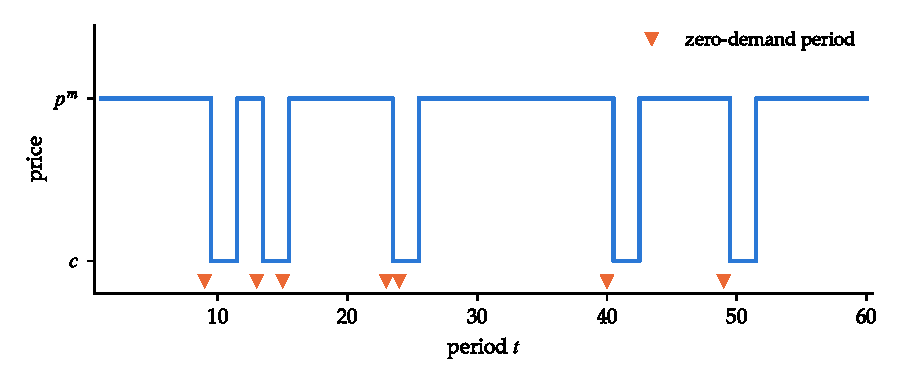
\includegraphics[width=0.92\textwidth]{figures/ch12/gp_path.pdf}
\caption{A simulated equilibrium price path in the Bertrand version of Green and Porter, with $\gamma = 0.1$ and the
optimal war length $T = 2$ for $\delta = 0.9$. Triangles mark periods of zero demand. A zero-demand period in a
collusive phase starts a two-period war at marginal cost. Zero-demand periods inside a war (periods 15 and 24) have
no effect. Wars occupy 10 of the 60 periods, the long-run share $\frac{1}{6}$. Nobody ever cheats. Source: our
simulation, \texttt{figures/ch12/src/gp\_path.py}.}\label{fig:12-gp-path}
\end{figure}

\Cref{fig:12-gp-ic,fig:12-gp-path} summarize four lessons. First, price wars occur on the equilibrium path even
though no firm ever cuts its price. They are necessary: if firms forgave zero sales, undercutting would go
unpunished and collusion would unravel. Second, optimal collusion uses a finite war, as short as the incentive
constraint allows. Third, more noise makes collusion harder. The patience required rises with $\gamma$, and both the
expected collusive profit and the value of collusion fall. Fourth, wars follow unexpectedly low demand. This timing
is the opposite of \cref{sec:12-rs}, where demand is observed and collusive prices are lowest in booms.
\Cref{tab:12-cycle-theories} compares the predictions, and \cref{sec:13-jec} confronts them with data.

The equilibrium has an uncomfortable feature. When a war starts, both firms know that nobody cheated, since each
knows the other's strategy. Both would gain by skipping the war, yet the war is needed to keep conformity optimal in
collusive periods. Equilibria of this kind are not robust to renegotiation after bad outcomes. Cartels that can talk
and audit each other's sales can avoid some of these wars, which is one reason why explicit cartels organize
monitoring (\cref{sec:12-cartels}).

\casehead{N firms, random punishments and the value of transparency}
\Citet[pp.~203--205]{AskerNocke2021} use a variant of this model with $N$ firms and a noisy public signal. It yields
closed forms for the threshold and for the value of collusion, and it shows why transparency matters even far above
the threshold. We state it in our notation. Asker and Nocke write $n$ for $N$, $\beta$ for our $\gamma$, $\alpha$ for
our $\lambda$ and $\rho$ for our $\phi$, and their $\pi^m$ is our expected profit $\bar\pi$.

\begin{assumption}[Bertrand oligopoly with a noisy public signal]\label{asm:12-an}
\leavevmode
\begin{enumerate}[label=(\roman*)]
\item $N$ identical firms sell a homogeneous good at marginal cost $c$. Demand in period $t$ is $\theta_tD(p)$, where
$\theta_t = 0$ with probability $\gamma$ and $\theta_t = 1$ otherwise, independently over time. Write
$\bar\pi = (1 - \gamma)\pi^m$ for the expected monopoly profit.
\item Firms observe neither $\theta_t$ nor rivals' prices. At the start of period $t$ they observe a public signal
$s_t \in \{0, 1\}$. It equals one if some firm priced below $p^m$ in period $t - 1$. If all firms charged at least
$p^m$, it equals one with probability $\lambda$ when $\theta_{t-1} = 0$ and zero otherwise.
\item A public random variable $r_t$, uniform on $[0, 1]$, is drawn at the start of each period. The signal is noisy,
$\gamma\lambda > 0$, and satisfies $\gamma\lambda < \frac{1}{N}$.
\end{enumerate}
\end{assumption}

Under the strategy profile $\sigma(\phi)$, every firm charges $p^m$ until the first period in which $s_t = 1$ and
$r_t \le \phi$. From then on every firm prices at $c$ forever. A bad signal thus triggers Nash reversion with
probability $\phi \in [0, 1]$, and the cartel chooses $\phi$. The profile conditions only on public information. It is
a \emph{perfect public equilibrium} if it is optimal for every firm after every public history.
\Cref{sec:12-abs-repeated} gives the formal definition.

\begin{proposition}[Threshold and value with a noisy signal]\label{prop:12-an}
Under \cref{asm:12-an}, $\sigma(\phi)$ is a perfect public equilibrium if and only if
\begin{equation}\label{eq:12-an-phi}
\phi \;\ge\; \phi^* \equiv \frac{1 - \delta}{\delta}\cdot\frac{N - 1}{1 - N\gamma\lambda} .
\end{equation}
Collusion at $p^m$ is therefore sustainable in this class if and only if
\begin{equation}\label{eq:12-an-delta}
\delta \;\ge\; \underline\delta = \frac{N - 1}{N(1 - \gamma\lambda)} .
\end{equation}
The best such equilibrium uses $\phi^*$, and each firm's per-period value is
\begin{equation}\label{eq:12-an-value}
v^* = (1 - \delta)V(\phi^*) = \frac{1 - N\gamma\lambda}{1 - \gamma\lambda}\cdot\frac{\bar\pi}{N} .
\end{equation}
\end{proposition}

\begin{proof}
On the path, each firm earns $\frac{\bar\pi}{N}$ in expectation. Reversion is triggered next period with probability
$\gamma\lambda\phi$, after which every firm earns zero. The value before reversion therefore solves
\begin{equation*}
V(\phi) = \frac{\bar\pi}{N} + \delta(1 - \gamma\lambda\phi)V(\phi)
\quad\Longrightarrow\quad
V(\phi) = \frac{\bar\pi}{N\bigl[1 - \delta(1 - \gamma\lambda\phi)\bigr]} .
\end{equation*}
A firm that undercuts slightly earns almost $\bar\pi$ in expectation, and the signal then equals one for sure.
Reversion follows with probability $\phi$, so the best one-shot deviation is worth
$V^{\mathrm{dev}}(\phi) = \bar\pi + \delta(1 - \phi)V(\phi)$. Reversion is a stage equilibrium after every history,
so by the one-shot deviation principle the profile is an equilibrium if and only if $V(\phi) \ge V^{\mathrm{dev}}(\phi)$.
Rearrange this as $V(\phi)\bigl[1 - \delta(1 - \phi)\bigr] \ge \bar\pi$ and substitute $V(\phi)$:
\begin{equation*}
\frac{1 - \delta + \delta\phi}{N\bigl[1 - \delta + \delta\gamma\lambda\phi\bigr]} \ge 1
\quad\Longleftrightarrow\quad
1 - \delta + \delta\phi \ge N(1 - \delta) + N\delta\gamma\lambda\phi .
\end{equation*}
Collect the terms in $\phi$:
\begin{equation*}
\delta\phi\,(1 - N\gamma\lambda) \;\ge\; (N - 1)(1 - \delta) .
\end{equation*}
Since $N\gamma\lambda < 1$, dividing gives \eqref{eq:12-an-phi}. A probability $\phi \le 1$ satisfies it if and only
if $\phi^* \le 1$, that is, $\delta(1 - N\gamma\lambda) \ge (N - 1)(1 - \delta)$. Collecting the terms in $\delta$ gives
$\delta(N - N\gamma\lambda) \ge N - 1$, which is \eqref{eq:12-an-delta}. The value $V(\phi)$ falls with $\phi$, so the
best equilibrium in the class uses $\phi^*$. At $\phi^*$,
\begin{equation*}
\delta\gamma\lambda\phi^* = \frac{(1 - \delta)(N - 1)\gamma\lambda}{1 - N\gamma\lambda},
\qquad
1 - \delta + \delta\gamma\lambda\phi^* = (1 - \delta)\,\frac{1 - \gamma\lambda}{1 - N\gamma\lambda} .
\end{equation*}
Substituting into $(1 - \delta)V(\phi^*)$ gives \eqref{eq:12-an-value}.
\end{proof}

These are equations (3) to (5) of Asker and Nocke. Two special cases connect them with the rest of the chapter. With
perfect monitoring, $\lambda = 0$, the threshold is $\frac{N - 1}{N}$ of \cref{prop:12-bertrand} and $v^* =
\frac{\bar\pi}{N}$. With $N = 2$ and $\lambda = 1$, zero demand always triggers the signal, as zero sales do in
\cref{asm:12-gp-bertrand}. The threshold \eqref{eq:12-an-delta} is then $\frac{1}{2(1 - \gamma)}$, the threshold of
\cref{cor:12-gp-optimal-T} for an infinite war.

The result changes how we should read comparative statics. Under perfect monitoring the per-period value jumps from
zero to $\frac{\bar\pi}{N}$ at the threshold and is flat above it. A small change in the number of firms then has no
effect on collusion unless $\delta$ is close to the threshold. With noise, $v^*$ falls continuously with $N$ and with
$\gamma\lambda$ however patient the firms are \citep[p.~205]{AskerNocke2021}. Better observability of deviations, a
lower $\lambda$, lowers the threshold and also raises $v^*$, because the cartel can punish less often on the path.
Take $N = 3$ and $\gamma = 0.2$, our own illustration. With $\lambda = 0.5$ the threshold is
$\frac{2}{3(0.9)} \approx 0.741$ and $v^*$ is $\frac{0.7}{0.9} \approx 0.78$ of the perfect-monitoring value. With
$\lambda = 0.25$ these become $\frac{2}{3(0.95)} \approx 0.702$ and $\frac{0.85}{0.95} \approx 0.89$. This is the
formal content of the view that transparent prices facilitate collusion. \citet{SugayaWolitzky2018} point out a
limit. Some information lets a firm tailor its deviation to current conditions. A cartel member that learns in advance
that its cost of serving a rival's territory is low can deviate exactly then, which makes collusion harder
\citep[p.~205, note~69]{AskerNocke2021}.

\subsection{The original model: Green and Porter (1984)}\label{sec:12-gp-original}

\casehead{Question and context}
\citet{GreenPorter1984} ask how a cartel can enforce collusion when firms cannot observe each other's outputs and
demand is uncertain. Two rigorous formulations of noncooperative collusion existed. In the reaction-function
equilibrium of \citet{Osborne1976}, firms respond to output changes so as to keep their shares. In the supergame of
\citet{Friedman1971}, firms revert to Cournot behavior forever after a price drop. In both, incentives are so perfect
that deterrence is never observed. Time-series data then cannot tell a collusive equilibrium from a competitive one
\citep{Bresnahan1982}. Green and Porter show that this perfection is an artifact of certainty. With imperfect
information, optimal incentive schemes involve recurrent episodes of the conduct previously called price wars or
punishments (pp.~87--88).

\casehead{Which industries the model describes}
The authors list four structural features of a suitable industry (p.~90). First, the industry is stable over time,
which makes rational expectations credible and justifies stationary dynamic programming. Second, output is the only
decision variable. Firms cannot differentiate products or divide the market, so a suspected cheater cannot be
isolated and punished alone. Third, all information except each firm's own output is public. Firms know each other's
cost functions, and all observe a common variable that tells them whether the industry is in a collusive or a
reversionary state. Fourth, this monitoring variable is imperfectly correlated with conduct. Otherwise reversions
would never occur. The fourth feature excludes markets with few, publicly announced transactions, such as contracts
awarded by sealed bids. The authors propose the American rail freight industry of the 1880s as an example
(p.~94), the cartel analyzed by \citet{Porter1983} in \cref{sec:13-jec}.

\begin{assumption}[The Green-Porter environment]\label{asm:12-gp}
\leavevmode
\begin{enumerate}[label=(\roman*)]
\item There are $N$ firms producing a homogeneous good. Firm $i$'s net return from producing $x_i$ units and selling
at price $p$ is $\pi_i(x_i, p)$. Firms are risk neutral and maximize $\E\bigl[\sum_{t \ge 0}\delta^t\pi_i(x_{it}, p_t)\bigr]$.
\item The observed price is
\begin{equation}\label{eq:12-gp-price}
p_t = \eta_t\,P\Bigl(\sum_{i=1}^N x_{it}\Bigr),
\end{equation}
where $P$ is a decreasing inverse demand function and the shocks $\eta_t$ are \iid\ with cdf $F_\eta$, continuous
density $f_\eta$, and $\E[\eta_t] = 1$. No firm observes $\eta_t$.
\item Each firm observes the history of prices and its own outputs. It never observes its rivals' outputs.
\end{enumerate}
\end{assumption}

We change the paper's notation. Its discount factor $\beta$ is our $\delta$, and its inverse demand $p(\cdot)$ is our
$P(\cdot)$. Its demand shock $\theta_t$ is our $\eta_t$, since $\theta$ is the conduct parameter in this book. A
\emph{contingent strategy} for firm $i$ is a sequence $s_i = (s_{i0}, s_{i1}, \dots)$, where $s_{i0}$ is an initial
output and $s_{i,t+1}(p_0, \dots, p_t)$ gives the output at $t + 1$ as a function of past prices. Write $\E_{s}$ for
the expectation under the price process generated by a profile $s$. A \emph{Nash equilibrium} is a profile
$s^* = (s_1^*, \dots, s_N^*)$ such that, for every firm $i$ and every feasible $s_i$ (GP (1), p.~91),
\begin{equation}\label{eq:12-gp-nash}
\E_{s_1^*, \dots, s_i, \dots, s_N^*}\Biggl[\sum_{t = 0}^{\infty}\delta^t\pi_i\bigl(s_{it}(p_0, \dots, p_{t-1}), p_t\bigr)\Biggr]
\;\le\;
\E_{s^*}\Biggl[\sum_{t = 0}^{\infty}\delta^t\pi_i\bigl(s_{it}^*(p_0, \dots, p_{t-1}), p_t\bigr)\Biggr].
\end{equation}

\casehead{Trigger-price strategies}
Let $y = (y_1, \dots, y_N)$ be a profile of \emph{restricted outputs} and $z = (z_1, \dots, z_N)$ the Cournot output
profile of the stage game, in which each firm maximizes its expected one-period return. Fix a \emph{trigger price}
$\bar p$ and an integer $T \ge 2$. Period $t$ is \emph{normal} if (a) $t = 0$, or (b) $t - 1$ was normal and
$p_{t-1} \ge \bar p$, or (c) $t - T$ was normal and $p_{t - T} < \bar p$. Every other period is
\emph{reversionary}. Firm $i$ produces $y_i$ in normal periods and $z_i$ in reversionary periods (pp.~91--92). If a
normal period $t$ ends with $p_t < \bar p$, periods $t + 1, \dots, t + T - 1$ are reversionary and period $t + T$ is
normal again. A reversionary episode therefore lasts $T - 1$ periods, and prices observed during it are ignored. The
length $T$ of the Bertrand version corresponds to $T - 1$ here. The strategies are simple enough to coordinate on,
and Green and Porter suggest that they would arise from an explicit agreement (p.~89, footnote 5).

Each firm faces a stationary dynamic programming problem with $T$ states: normal, and $k$ periods into a reversion
for $k = 1, \dots, T - 1$. In a reversionary period the firm's output does not affect future states, so it maximizes
its expected current return against rivals' Cournot outputs and produces $z_i$. A reversion is thus a temporary
switch to the static Nash equilibrium. In normal periods the problem is the same every time, so the firm's best
policy is a constant output $r$. The question is when $r = y_i$ is optimal.

Let $w_i = \sum_{j \ne i}y_j$ be the rivals' restricted output. Define firm $i$'s expected return in a normal period
when it produces $r$, and its expected Cournot return, as
\begin{equation}\label{eq:12-gp-returns}
\bar\pi_i(r) = \E_\eta\bigl[\pi_i\bigl(r, \eta P(r + w_i)\bigr)\bigr],
\qquad
\pi_i^N = \E_\eta\Bigl[\pi_i\Bigl(z_i, \eta P\Bigl(\sum_j z_j\Bigr)\Bigr)\Bigr]
\end{equation}
(the paper writes $\gamma_i(r)$ and $\delta_i$). Collusion is profitable: $\bar\pi_i(y_i) > \pi_i^N$ for every $i$.
A reversion starts after a normal period in which $\eta P(r + w_i) < \bar p$, an event with probability
\begin{equation}\label{eq:12-gp-Fr}
F_i(r) \equiv \Pr\bigl(\eta P(r + w_i) < \bar p\bigr) = F_\eta\Bigl(\frac{\bar p}{P(r + w_i)}\Bigr).
\end{equation}
This probability rises with $r$, since more output lowers $P(r + w_i)$. Overproduction is detected only
statistically, through a higher chance of a low price.

\begin{proposition}[The value of a trigger-price strategy]\label{prop:12-gp-value}
Under \cref{asm:12-gp}, suppose rivals follow the trigger-price strategies, and firm $i$ produces $r$ in all normal
periods and $z_i$ in all reversionary periods. Let $V_i(r)$ be its expected discounted value in a normal period. Then
(GP (2), p.~92)
\begin{equation}\label{eq:12-gp-bellman}
V_i(r) = \bar\pi_i(r) + \delta\bigl[1 - F_i(r)\bigr]V_i(r) + F_i(r)\Biggl[\sum_{t=1}^{T-1}\delta^t\pi_i^N + \delta^T V_i(r)\Biggr],
\end{equation}
and its solution is (GP (3), p.~92)
\begin{equation}\label{eq:12-gp-value}
V_i(r) = \frac{\pi_i^N}{1 - \delta} + \frac{\bar\pi_i(r) - \pi_i^N}{1 - \delta + (\delta - \delta^T)F_i(r)} .
\end{equation}
\end{proposition}

\begin{proof}
In a normal period the firm earns $\bar\pi_i(r)$ in expectation. With probability $1 - F_i(r)$ the price stays above
$\bar p$, and the next period is normal with value $\delta V_i(r)$. With probability $F_i(r)$ a reversion follows. The
firm earns $\pi_i^N$ in each of the $T - 1$ reversionary periods and returns to a normal period after $T$ periods.
This gives \eqref{eq:12-gp-bellman}. To solve it, use the geometric sum
\begin{equation*}
\sum_{t=1}^{T-1}\delta^t = \frac{\delta - \delta^T}{1 - \delta}
\end{equation*}
and collect the terms in $V_i(r)$:
\begin{equation*}
V_i(r)\bigl[1 - \delta + \delta F_i(r) - \delta^T F_i(r)\bigr] = \bar\pi_i(r) + F_i(r)\,\frac{\delta - \delta^T}{1 - \delta}\,\pi_i^N .
\end{equation*}
Let $\Delta_i(r) \equiv 1 - \delta + (\delta - \delta^T)F_i(r)$ denote the bracket. Then
\begin{equation*}
V_i(r) = \frac{\bar\pi_i(r) + F_i(r)\frac{\delta - \delta^T}{1 - \delta}\pi_i^N}{\Delta_i(r)} .
\end{equation*}
Subtract $\frac{\pi_i^N}{1 - \delta} = \frac{\Delta_i(r)\,\pi_i^N}{(1 - \delta)\Delta_i(r)}$ from both sides. The
numerator on the right becomes
\begin{equation*}
\bar\pi_i(r) + F_i(r)\frac{\delta - \delta^T}{1 - \delta}\pi_i^N - \frac{1 - \delta + (\delta - \delta^T)F_i(r)}{1 - \delta}\pi_i^N
= \bar\pi_i(r) - \pi_i^N ,
\end{equation*}
which gives \eqref{eq:12-gp-value}.
\end{proof}

Equation \eqref{eq:12-gp-value} says that the firm's value equals its value in a permanently Cournot industry plus
the one-period gain from colluding, capitalized at the rate $\Delta_i(r)$. That rate exceeds $1 - \delta$ because
the collusive gain is interrupted by reversions. A larger trigger probability $F_i(r)$ or a longer reversion raises
$\Delta_i(r)$ and lowers the value of collusion.

\casehead{Equilibrium conditions}
The trigger-price profile is a Nash equilibrium if and only if no firm gains by changing its normal-period output
(GP (4), p.~93):
\begin{equation}\label{eq:12-gp-eqm}
V_i(r) \le V_i(y_i) \quad\text{for all } r \text{ and all } i .
\end{equation}
The first-order condition is $V_i'(y_i) = 0$ (GP (5)). The next result writes it out.

\begin{proposition}[The first-order condition]\label{prop:12-gp-foc}
Let $Y = \sum_j y_j$ and $k = \frac{\bar p}{P(Y)}$. At an interior equilibrium, for every $i$ (GP (6), p.~93),
\begin{equation}\label{eq:12-gp-foc}
\bigl[1 - \delta + (\delta - \delta^T)F_\eta(k)\bigr]\,\bar\pi_i'(y_i)
+ (\delta - \delta^T)\,f_\eta(k)\,\frac{\bar p\,P'(Y)}{P(Y)^2}\,\bigl[\bar\pi_i(y_i) - \pi_i^N\bigr] = 0 .
\end{equation}
Equivalently,
\begin{equation}\label{eq:12-gp-foc2}
\underbrace{\bar\pi_i'(y_i)}_{\text{marginal gain}}\;\Delta_i(y_i)
= \underbrace{(\delta - \delta^T)\,f_\eta(k)\,k\,\frac{-P'(Y)}{P(Y)}}_{\text{marginal rise in the risk of reversion}}
\;\underbrace{\bigl[\bar\pi_i(y_i) - \pi_i^N\bigr]}_{\text{loss per period of reversion}} .
\end{equation}
\end{proposition}

\begin{proof}
By \eqref{eq:12-gp-value}, $V_i(r) = \frac{\pi_i^N}{1 - \delta} + \frac{n(r)}{\Delta_i(r)}$ with
$n(r) = \bar\pi_i(r) - \pi_i^N$. Its derivative is zero if and only if $n'(r)\Delta_i(r) - n(r)\Delta_i'(r) = 0$. Here
$n'(r) = \bar\pi_i'(r)$ and, by the chain rule,
\begin{equation*}
\Delta_i'(r) = (\delta - \delta^T)\,f_\eta\Bigl(\frac{\bar p}{P(r + w_i)}\Bigr)\cdot\Bigl(-\frac{\bar p\,P'(r + w_i)}{P(r + w_i)^2}\Bigr).
\end{equation*}
Substituting and evaluating at $r = y_i$, so that $r + w_i = Y$, gives \eqref{eq:12-gp-foc}. Since
$\frac{\bar p}{P(Y)^2} = \frac{k}{P(Y)}$, moving the second term to the right gives \eqref{eq:12-gp-foc2}.
\end{proof}

Equation \eqref{eq:12-gp-foc2} balances two margins (p.~93). The marginal return from producing more in normal
periods is exactly offset by the marginal rise in the risk of a reversion, valued at the loss it causes. Both sides
are positive, since $P' < 0$. Hence $\bar\pi_i'(y_i) > 0$: each firm produces less than its static best
response to its rivals' restricted outputs. The threat of reversion sustains that gap. The $N$ conditions
\eqref{eq:12-gp-foc} restrict the vector $y$, so a given output profile, such as the one that maximizes joint profits,
need not be supportable. A cartel that chooses $(y, \bar p, T)$ to maximize its members' values subject to
\eqref{eq:12-gp-eqm} faces a trade-off. A lower trigger price or a shorter reversion destroys less surplus on the
path but deters less. Green and Porter report that \citet{Porter1983b} solves this problem for symmetric firms. The
optimal normal-period output differs from the monopoly output: firms give up some normal-period profit to reduce the
frequency and duration of reversions (p.~93, footnote 9). The next example illustrates the trade-off.

\begin{example}[A linear duopoly with lognormal shocks]\label{ex:12-gp-linear}
Let $N = 2$, $P(Q) = 1 - Q$, zero marginal cost and $\pi_i(x_i, p) = px_i$. Let
$\ln\eta \sim \mathcal{N}(-\frac{\sigma^2}{2}, \sigma^2)$, so that $\E[\eta] = 1$, with $\sigma = 0.1$ and
$\delta = 0.95$. Each firm's Cournot output is $\frac{1}{3}$ with $\pi_i^N = \frac{1}{9} = 0.1111$, and splitting the
monopoly output gives $y_i = \frac{1}{4}$ with $\bar\pi_i = \frac{1}{8} = 0.125$. With symmetric restricted output
$y$, $\bar\pi_i(r) = r(1 - r - y)$, so $\bar\pi_i'(y) = 1 - 3y$ and $\frac{-P'(Y)}{P(Y)} = \frac{1}{1 - 2y}$. Writing
$u = \frac{1}{\sigma}\bigl(\ln k + \frac{\sigma^2}{2}\bigr)$ in standard units, $F_\eta(k) = \Phi(u)$ and $f_\eta(k)k = \frac{\phi(u)}{\sigma}$,
where $\Phi$ and $\phi$ are the standard normal cdf and density. Condition \eqref{eq:12-gp-foc2} becomes
\begin{equation*}
(1 - 3y)\bigl[1 - \delta + (\delta - \delta^T)\Phi(u)\bigr]
= (\delta - \delta^T)\,\frac{\phi(u)}{\sigma}\;\frac{y(1 - 2y) - \frac{1}{9}}{1 - 2y} .
\end{equation*}
For each $(y, T)$ we solve for the trigger with the smallest reversion probability, check the global condition
\eqref{eq:12-gp-eqm} on a grid of outputs, and compute the normalized value $(1 - \delta)V_i(y)$.
\Cref{tab:12-gp-example} reports the best $y$ for several $T$. Three features stand out. The monopoly split
$y = \frac{1}{4}$ can be supported only with long reversions, $T \ge 14$. For every $T$ the best restricted output
exceeds $\frac{1}{4}$, as in \citet{Porter1983b}: producing more lowers the gain from overproduction and the trigger
probability needed to deter it. Finally, the cartel captures about two thirds of the gain from monopoly over
Cournot, since $\frac{0.1206 - 0.1111}{0.125 - 0.1111} = 0.68$.
\end{example}

\begin{table}[htbp]
\centering
\caption{Best symmetric trigger-price equilibria in the linear duopoly of \cref{ex:12-gp-linear}}\label{tab:12-gp-example}
\begin{tabular}{@{}rccccc@{}}
\toprule
$T$ & Best $y$ & Trigger $\bar p$ & $\Pr(\text{reversion})$ & Long-run share in reversion & $(1 - \delta)V_i$ \\
\midrule
4      & 0.2925 & 0.380 & 0.205 & 0.380 & 0.1177 \\
8      & 0.2800 & 0.380 & 0.079 & 0.357 & 0.1194 \\
16     & 0.2750 & 0.376 & 0.040 & 0.374 & 0.1201 \\
50     & 0.2725 & 0.369 & 0.021 & 0.507 & 0.1205 \\
$\infty$ & 0.2700 & 0.373 & 0.020 & 1     & 0.1206 \\
\midrule
14 ($y = \frac{1}{4}$) & 0.2500 & 0.447 & 0.144 & 0.653 & 0.1171 \\
\bottomrule
\end{tabular}

\smallskip
\begin{minipage}{0.95\textwidth}
\footnotesize Notes: $P(Q) = 1 - Q$, zero cost, $\ln\eta \sim \mathcal{N}(-\frac{\sigma^2}{2}, \sigma^2)$ with
$\sigma = 0.1$, $\delta = 0.95$. Outputs are searched on a grid of step 0.0025 in $[0.20, 0.33]$. Reversions last
$T - 1$ periods. $\Pr(\text{reversion}) = F_\eta(\frac{\bar p}{P(2y)})$ is the probability that a normal period
triggers a reversion. The long-run share of reversionary periods is $\frac{(T-1)G}{1 + (T-1)G}$ with
$G = \Pr(\text{reversion})$ (\cref{prop:12-gp-stationary}). With $T = \infty$ the first reversion is permanent. The
last row is the shortest reversion that supports the monopoly split. With $T = 2$ no output in the grid is an
equilibrium. Benchmarks: Cournot $0.1111$, monopoly split $0.125$. Source: our computation,
\texttt{figures/ch12/src/gp\_design.py}.
\end{minipage}
\end{table}

The example also shows that, in a discounted model, the cartel may prefer an infinite reversion although it ends
collusion for good in the long run. With $\delta = 0.95$, the expected wait of fifty periods before the first
reversion makes its distant cost small. This is a property of the restricted class of trigger strategies with
Cournot reversion. Richer punishments do better, as we discuss below.

\casehead{Properties of the equilibrium}
Two observations complete the formal model (pp.~93--94). First, no firm ever defects. Every firm can compute what
every other firm will produce, so a low price reveals information about demand only. In equilibrium the frequency
of reversions from normal periods is $F_\eta\bigl(\frac{\bar p}{P(\sum_j y_j)}\bigr)$. Second, firms take part in
reversions although they know that low prices reflect demand. A reversion is a temporary switch to a static Nash
equilibrium, so no firm gains by deviating from it unilaterally. If firms ignored low prices and kept colluding, the
first-order condition \eqref{eq:12-gp-foc} would fail in normal periods, and restricted output would no longer be
individually optimal. Green and Porter add that the equilibrium is perfect, citing \citet{Green1980} for a formal
statement (p.~93, footnote 10).

\casehead{A reversal of the traditional interpretation}
The model reverses the traditional reading of a common price pattern (p.~94). Consider an episode in which price
drops sharply, stays low, and then recovers without any cost or demand shock. Such an episode was read as predation
against an entrant, or as the breakdown and re-establishment of a cartel. Either way it signaled fragile collusion. Some
argued that intervention was redundant in markets with such episodes, since the market was already resisting
collusion. In the Green-Porter equilibrium the same episodes are an essential part of a stable collusive scheme. An
industry with the four structural features will show price instability as a stationary feature of collusion. The
policy conclusion is the opposite of the traditional one.

\subsection{The price process and its estimation}\label{sec:12-gp-process}

Because both collusive and reversionary behavior are observed over time, the collusive equilibrium can be
identified statistically. The appendix of \citet{GreenPorter1984} characterizes the price process and shows that its
parameters can be estimated consistently.

\casehead{The switching process}
A \emph{switching process} has four parts (p.~96). The first is a state process $\{W_t\}$ with values in a set $S$
and normal states $S_0 \subset S$. The others are an observed process $\{X_t\}$ and two latent processes $\{Y_t\}$
and $\{Z_t\}$. The
latent variables are independent, the $Y_t$ have a common cdf $G$, the $Z_t$ have a common cdf $H$, and $\{W_t\}$ is
Markov with stationary transition probabilities. The observed variable is $X_t = Y_t$ when $W_t \in S_0$ and
$X_t = Z_t$ otherwise. (In this subsection $G$ and $H$ are local symbols for price distributions.) The usual case has
$S = \{0, 1\}$ and a Bernoulli state process independent of prices.

For the collusive price process, $Y_t$ is the price that would prevail in a normal period and $Z_t$ the price in a
reversionary one. Under \eqref{eq:12-gp-price},
\begin{equation*}
G(p) = F_\eta\Bigl(\frac{p}{P(\sum_j y_j)}\Bigr),
\qquad
H(p) = F_\eta\Bigl(\frac{p}{P(\sum_j z_j)}\Bigr).
\end{equation*}
The states are $S = \{0, 1, \dots, T - 1\}$ with $S_0 = \{0\}$, where state $k \ge 1$ means $k$ periods into a
reversion. The transitions are (GP (A7) to (A10), p.~96)
\begin{equation}\label{eq:12-gp-transitions}
W_{t+1} =
\begin{cases}
0 & \text{if } W_t = 0 \text{ and } Y_t \ge \bar p,\\
1 & \text{if } W_t = 0 \text{ and } Y_t < \bar p,\\
k + 1 & \text{if } W_t = k \text{ with } 1 \le k < T - 1,\\
0 & \text{if } W_t = T - 1 .
\end{cases}
\end{equation}
Since the $Y_t$ are \iid, $\{W_t\}$ is a Markov chain with stationary transition probabilities. Its transition
graph is panel (a) of \cref{fig:12-gp-chain}. Unlike the usual switching model, the state depends on past prices.

\begin{figure}[htbp]
\centering
\begin{subfigure}[b]{0.48\textwidth}
\centering
\begin{tikzpicture}[>=Stealth, st/.style={circle, draw, minimum size=9.5mm, inner sep=0.5pt, font=\small},
  lab/.style={font=\scriptsize}]
\node[st] (s0) at (0,0) {$0$};
\node[st] (s1) at (1.9,-1.4) {$1$};
\node[st] (s2) at (1.9,-3.1) {$2$};
\node[st] (sT2) at (-1.9,-3.1) {$T\!-\!2$};
\node[st] (sT1) at (-1.9,-1.4) {$T\!-\!1$};
\draw[->] (s0) to[loop above] node[lab, above] {$1 - G(\bar p)$} (s0);
\draw[->] (s0) to node[lab, above right] {$G(\bar p)$} (s1);
\draw[->] (s1) to node[lab, right] {$1$} (s2);
\draw[->, dashed] (s2) to[bend left=35] (sT2);
\draw[->] (sT2) to node[lab, left] {$1$} (sT1);
\draw[->] (sT1) to node[lab, above left] {$1$} (s0);
\end{tikzpicture}
\caption{Price process}
\end{subfigure}\hfill
\begin{subfigure}[b]{0.48\textwidth}
\centering
\begin{tikzpicture}[>=Stealth, st/.style={circle, draw, minimum size=9.5mm, inner sep=0.5pt, font=\small},
  lab/.style={font=\scriptsize}]
\node[st] (s0) at (0,0) {$0$};
\node[st] (s1) at (1.9,-1.4) {$1$};
\node[st] (s2) at (1.9,-3.1) {$2$};
\node[st] (sT2) at (-1.9,-3.1) {$T\!-\!2$};
\node[st] (sT1) at (-1.9,-1.4) {$T\!-\!1$};
\draw[->] (s0) to[loop above] node[lab, above] {$1 - G(\bar p)$} (s0);
\draw[->] (s0) to node[lab, above right] {$G(\bar p)$} (s1);
\draw[->] (s1) to node[lab, right] {$1$} (s2);
\draw[->, dashed] (s2) to[bend left=35] (sT2);
\draw[->] (sT2) to node[lab, left] {$1$} (sT1);
\draw[->] (sT1) to node[lab, above left] {$1 - G(\bar p)$} (s0);
\draw[->] (sT1) to node[lab, below] {$G(\bar p)$} (s1);
\end{tikzpicture}
\caption{Approximating process}
\end{subfigure}
\caption{Transition graphs of the state $W_t$. State $0$ is normal, and state $k \ge 1$ is the $k$-th period of a
reversion. In the price process (a), a normal period with a price below $\bar p$ starts a reversion. The
approximating process (b) deletes these triggering periods, so the state leaves $T - 1$ for state $1$ directly when
the next normal price would trigger a reversion. Redrawn from Green and Porter (1984), Figures 1 and 2.}\label{fig:12-gp-chain}
\end{figure}

\casehead{Stationarity and ergodicity}
Green and Porter show that the initial state can be chosen so that $\{X_t\}$ is a stationary ergodic process
(pp.~95--96). Since $X_t$ is a function of $(W_t, Y_t, Z_t)$, it suffices that the joint process is a stationary
Markov process with a unique invariant distribution. A stationary process is \emph{ergodic} if every event that is
unchanged when the time index is shifted has probability zero or one. The \emph{ergodic theorem} then extends the strong law of
large numbers to the process, so sample averages converge to population moments. This is the foundation for the
asymptotic theory of estimators, and it implies that consistent estimators of $\bar p$ and $T$ exist (p.~95).

\begin{proposition}[Stationary distribution of the regimes]\label{prop:12-gp-stationary}
Let $\psi_k$ be the stationary probability of state $k$ under \eqref{eq:12-gp-transitions}. Then
\begin{equation}\label{eq:12-gp-stationary}
\psi_0 = \bigl[1 + (T - 1)G(\bar p)\bigr]^{-1},
\qquad
\psi_k = G(\bar p)\,\psi_0 \quad (k = 1, \dots, T - 1).
\end{equation}
The long-run share of reversionary periods is $\frac{(T - 1)G(\bar p)}{1 + (T - 1)G(\bar p)}$.
\end{proposition}

\begin{proof}
Under the stationary distribution, $\Pr(W_1 = j) = \Pr(W_0 = j) = \psi_j$ for every $j$. For $1 \le k < T - 1$, the
only way to reach state $k + 1$ is from state $k$, with probability one. Hence (GP (A21))
$\psi_{k+1} = \psi_k$. The only way to reach state $1$ is from state $0$ with $Y_0 < \bar p$. Since $Y_0$ is
independent of $W_0$, this gives (GP (A22)) $\psi_1 = \psi_0 G(\bar p)$. So $\psi_k = G(\bar p)\psi_0$ for
$k = 1, \dots, T - 1$. The probabilities sum to one:
\begin{equation*}
\psi_0 + (T - 1)G(\bar p)\psi_0 = 1 ,
\end{equation*}
which gives (GP (A23)) the first formula. The share of reversionary periods is $1 - \psi_0$.
\end{proof}

The share formula matches \eqref{eq:12-gp-war-share} with $\gamma$ replaced by $G(\bar p)$ and $T$ by $T - 1$. In
equilibrium $G(\bar p) = F_\eta(\frac{\bar p}{P(\sum_j y_j)})$, the frequency of reversions noted above.

\casehead{The approximating process and contamination}
Maximum likelihood estimation of the price process is awkward, because the regime depends on past prices.
\Citet{Porter1983} instead estimates a related process that keeps the dependence of the regime on its own past but
makes the regime independent of prices (p.~97). This \emph{approximating process} has three properties. Normal
prices are drawn from the distribution of $Y$ conditional on $Y \ge \bar p$ (GP (A11)),
\begin{equation*}
J(p) = \max\Bigl[\frac{G(p) - G(\bar p)}{1 - G(\bar p)},\, 0\Bigr].
\end{equation*}
The regime, normal prices and reversionary prices are mutually independent (GP (A12)). The regime is a stationary
Markov chain with the transitions in panel (b) of \cref{fig:12-gp-chain} (GP (A13)). The advantage is that existing
work on the maximum likelihood estimation of switching processes applies. The estimator is cheap to compute, and
results on its consistency and asymptotic normality are available (p.~97).

The approximating process is obtained from the price process by deleting the triggering observations, the normal
periods in which $Y_t < \bar p$ (pp.~97--98). A \emph{stopping time} is a random date whose occurrence is determined
by the history up to that date. Formally, define stopping times by $\tau_0 = 1$ if $W_0 = 0$ and $Y_0 < \bar p$,
$\tau_0 = 0$ otherwise, and
\begin{equation*}
\tau_{t+1} =
\begin{cases}
\tau_t + 2 & \text{if } W_{\tau_t + 1} = 0 \text{ and } Y_{\tau_t + 1} < \bar p,\\
\tau_t + 1 & \text{otherwise.}
\end{cases}
\end{equation*}
We set $X_t' = X_{\tau_t}$ and re-index the state and latent variables in the same way (GP (A14) to (A17)). Because
the chain restarts afresh at each such date (the \emph{strong Markov property}), the censored state process is a
stationary Markov chain, now independent of prices.
Conversely, the observed price series is a \emph{contaminated} sample path of the approximating process. The
contaminating observations are the triggering prices, which the approximating process does not contain.

\begin{proposition}[The contamination ratio]\label{prop:12-gp-contamination}
With probability one (GP (A24), p.~99),
\begin{equation}\label{eq:12-gp-contamination}
\lim_{t \to \infty}\frac{\tau_t - t}{\tau_t} = \frac{G(\bar p)}{1 + (T - 1)G(\bar p)} .
\end{equation}
\end{proposition}

\begin{proof}
Let $a(W, Y) = 1$ if $W = 0$ and $Y < \bar p$, and $a(W, Y) = 0$ otherwise. Each deleted observation is a period
with $a = 1$, so $\tau_t = t + \sum_{u=0}^{\tau_t}a(W_u, Y_u)$ and (GP (A18))
\begin{equation*}
\frac{\tau_t - t}{\tau_t} = \frac{1}{\tau_t}\sum_{u=0}^{\tau_t}a(W_u, Y_u) .
\end{equation*}
By the ergodic theorem the average converges almost surely to $\Pr(W_0 = 0, Y_0 < \bar p)$ (GP (A19)). The state
$W_0$ depends only on draws before period 0, and the $Y_t$ are \iid. Hence $W_0$ and $Y_0$ are independent, and the
limit is $\psi_0 G(\bar p)$ (GP (A20)). Substituting $\psi_0$ from
\cref{prop:12-gp-stationary} gives \eqref{eq:12-gp-contamination}.
\end{proof}

\begin{table}[htbp]
\centering
\caption{Green and Porter's illustration of the contamination of the approximating process}\label{tab:12-gp-contamination}
\begin{tabular}{@{}lll@{}}
\toprule
Quantity & Formula & Value \\
\midrule
Probability that a normal week triggers a reversion & $G(\bar p)$ & 0.025 \\
Length of a reversion (weeks) & $T - 1$ & 10 \\
Expected length of a normal episode (weeks) & $\frac{1}{G(\bar p)}$ & 40 \\
Long-run share of normal weeks & $\psi_0 = [1 + (T - 1)G(\bar p)]^{-1}$ & $\frac{1}{1.25} = 0.8$ \\
Contamination ratio & $\psi_0 G(\bar p)$ & $\frac{0.025}{1.25} = 0.02$ \\
\midrule
\multicolumn{3}{@{}l}{Contamination of each subsample used by the estimator} \\
\quad Triggering prices split proportionally & & 2 percent \\
\quad All triggering prices in the normal subsample & $\frac{0.02}{0.8}$ & 2.5 percent \\
\quad All triggering prices in the reversionary subsample & $\frac{0.02}{0.2}$ & 10 percent \\
\bottomrule
\end{tabular}

\smallskip
\begin{minipage}{0.95\textwidth}
\footnotesize Notes: A period is one week, as when a trade association circulates weekly prices. The parameter values
$G(\bar p) = 0.025$ and $T = 11$ and the contamination levels are those of the example in \citet[p.~99]{GreenPorter1984}.
The intermediate quantities are computed from \cref{prop:12-gp-stationary,prop:12-gp-contamination}.
\end{minipage}
\end{table}

\Cref{tab:12-gp-contamination} reproduces the authors' numerical illustration (p.~99). With weekly data,
$G(\bar p) = 0.025$ and $T = 11$, a normal episode lasts forty weeks on average and a reversion ten weeks. A
reversion therefore occurs about once a year, and about one price observation a year is a triggering price that the
approximating process would not contain. The contamination ratio is one in fifty. The estimator splits the sample
into a subsample attributed to $G$ and one attributed to $H$, and estimates each distribution separately. If the
contaminating observations were spread in proportion, each subsample would be 2 percent contaminated. If all of them
were assigned to the normal subsample, its contamination would be 2.5 percent, which still seems negligible. If all
of them were assigned to the reversionary subsample, which is only one fifth of the data, its contamination would be
10 percent. In this worst case the low draws from $G$ could bias the estimate of $H$ seriously. Green and Porter
note that these parameter values are approximately those that \citet{Porter1983} reports for the rail freight
cartel. They conclude that the bias is plausibly slight under optimistic assumptions, while acknowledging an element
of judgment (p.~99). \Cref{sec:13-implications,sec:13-jec} develop the estimator and Porter's results.

\subsection{Testable implications, extensions and critiques}\label{sec:12-gp-assessment}

\casehead{Testable implications}
The model makes several predictions that distinguish it from collusion under perfect monitoring. Conduct switches
between discrete regimes, so the supply relation shifts between a collusive and a Cournot (or Bertrand) regime.
Reversions start after unexpectedly low prices, which reflect unobserved negative demand shocks rather than
observable booms. Reversions have a fixed and finite length in the simplest version. In normal periods output
exceeds the joint-profit level when the cartel designs its scheme optimally. \Cref{ch:collusion-evidence} tests these
predictions with the data of the Joint Executive Committee and compares them with those of
\cref{sec:12-demand} (\cref{sec:13-jec,sec:13-implications}). The regime switches also imply that a single conduct
parameter estimated over the whole sample averages two conducts, the problem discussed in \cref{ch:conduct}.

\casehead{Extensions}
Green and Porter study only the simplest trigger-price strategies. Firms might, for example, condition the length of
a reversion on how far the price falls below $\bar p$ (p.~92, footnote 8). \Citet{Porter1983b} chooses the trigger
price, the reversion length and the restricted output optimally. \Citet{AbreuPearceStacchetti1986} characterize
optimal symmetric equilibria of a Green-Porter industry without restricting strategies. We follow the account of
\citet[section~6.7.1.2]{Tirole1988}. Two assumptions give sharp results. First, the firms' payoff functions are
concave. Second, the distribution of the market price given aggregate output satisfies the \emph{monotone likelihood
ratio property} (MLRP). Informally, a low price is more likely to come from a high output than from a low one. Under these
assumptions, attention can be restricted to two phases with values $V^+$ and $V^-$, the best and the worst payoffs in
the set of symmetric perfect equilibria. In the collusive phase each firm produces $q^+$, and a punishment starts if
the price falls below a threshold $p^+$. This \emph{tail test} is the trigger of \citet{GreenPorter1984}. The
punishment phase has no fixed length. Each firm produces a high output $q^-$. Play stays in the punishment phase as
long as the price exceeds a second threshold $p^-$, and it returns to the collusive phase when the price falls below
$p^-$. This \emph{inverse tail test} looks odd at first. A harsh punishment requires an output higher than each firm
would choose privately. A high price signals low output, so it is a high price that prolongs the punishment. The
two phases follow a Markov process, and punishments can be harsher than Cournot reversion. \Citet{AbreuPearceStacchetti1990} develop the recursive method behind this result (\cref{sec:12-aps}).
\Citet{FudenbergLevineMaskin1994} give conditions on how the distribution of the public signal responds to each
player's actions under which a folk theorem holds with imperfect public monitoring. When signals are private to each
firm, as with secret sales, the problem is harder, and \cref{sec:12-hs} studies how cartels solve it with reports and
transfers.

\casehead{Critiques}
Several limitations qualify the model. First, the restriction to trigger strategies with Cournot reversion is not
innocuous: as noted above, richer punishments do better. Second, wars are costly to the cartel, and firms that know
nobody cheated have a reason to renegotiate them away. Third, the source of the inference problem matters.
\Cref{sec:12-private-costs} shows that when firms have private information about costs and prices are public, optimal
collusion typically needs no wars at all. Fourth, real cartels communicate, exchange sales data and make transfers,
which changes the monitoring problem (\cref{sec:12-cartels}). Fifth, \citet{LevensteinSuslow2006} find that many price
wars in documented cartels arise from bargaining over shares rather than from noise (\cref{sec:12-success}). Sixth, the
shocks are \iid. Green and Porter note that a martingale specification would suit durable goods better and accept
that the \iid\ assumption is restrictive (p.~91, footnote 7). Finally, the four structural conditions are demanding,
and the authors concede that the direct applicability of the model is severely limited (p.~94).

\casehead{Contribution}
\citet{GreenPorter1984} provided the first equilibrium theory of price wars as part of a working cartel. They turned
Stigler's policing problem into a repeated game with imperfect public monitoring, reversed the received reading of
price instability, and showed that the resulting price process can be estimated. The paper set the template for the
theory of repeated games with imperfect monitoring and, through \citet{Porter1983}, for the empirical study of
cartel regimes in \cref{ch:collusion-evidence}.

\section{Private Information about Costs: Collusion and Price Rigidity}\label{sec:12-private-costs}

The models so far share one feature: firms are identical in every period. In practice each firm's costs move with
input prices, breakdowns and the quality of its own operations, and rivals do not observe them. A cartel that wants
the lowest-cost firm to serve the market must then learn who has low costs, and firms have an incentive to lie. This
section studies \citet{AtheyBagwellSanchirico2004}, abbreviated ABS, who analyze collusion when prices are public and
costs are private. We work from the November 1998 working-paper version. Page and result numbers refer to it and may
differ from the published article.

\subsection{Question and motivation}\label{sec:12-abs-question}

ABS place their model as the third canonical extension of the standard collusion model (pp.~1--2). In
\citet{RotembergSaloner1986}, demand shocks are public and collusive prices vary with them, without wars on the
path (\cref{sec:12-rs}). In \citet{GreenPorter1984}, actions are hidden and wars follow bad shocks. This is a model of
repeated \emph{moral hazard}, or hidden action. ABS study repeated \emph{adverse selection}, or hidden information:
each firm privately observes its cost, while prices are observed by all.

The application is the relation between collusion and price rigidity. Empirical studies going back to the 1920s,
including \citet{Carlton1986,Carlton1989}, find that prices are more rigid in concentrated industries (p.~2).
\citet{Scherer1980} summarizes studies in which collusion is implemented by rules of thumb, such as a fixed
percentage above a common wholesale price. The price then ignores members' private cost positions. The best-known
theory of rigidity is the kinked demand curve \citep{Sweezy1939,HallHitch1939}, which assumes that rivals match price
cuts but not increases. As ABS note, it rests on an ad hoc behavioral postulate, compresses a dynamic story into a
static model, and does not determine the price. Economists therefore fell back on an informal view.
\citet[pp.~914--915]{Carlton1989} states it as follows: ``Anytime a price change occurs in an oligopoly, there is a risk
that a price war could break out. Hence, firms are reluctant to change price.'' ABS give this view a rigorous form.

\citet[section~6.2.1]{Tirole1988} spells out the static story and its weakness. Each of two firms with cost $c$
conjectures that its rival will match any cut below a \emph{focal price} $p^f$ and will ignore any increase. A firm's
perceived demand is then $\frac{D(p)}{2}$ below $p^f$ and zero above it. If $(p - c)D(p)$ is quasi-concave, the best
price under this conjecture is $p^f$ when $p^f \le p^m$. Every focal price between $c$ and $p^m$ is therefore
consistent with the conjectures. The story explains too much, and it says nothing about how the focal price responds
to a change in cost. \citet{MaskinTirole1988} give the kinked demand curve an equilibrium foundation. Firms set prices
in alternate periods and keep each price for two periods, so a firm's current price affects its rival's profit. In a
\emph{Markov perfect equilibrium}, each firm's price depends only on the rival's current price. One such equilibrium
has a focal price at the monopoly level. A firm that raises its price is not followed, and a firm that undercuts
provokes a price war, after which the firms eventually return to the focal price \citep[section~6.4.1]{Tirole1988}. Tirole
reports two further results (section~6.4.2). Industry profit in every Markov perfect equilibrium is bounded away from
zero. For discount factors close to one, the average profit in a symmetric equilibrium is at least half the monopoly
profit. Other Markov equilibria never settle and produce cycles of price wars and relenting, the Edgeworth
cycles of \cref{sec:13-noel}. Retaliation in this model has a tangible motive, unlike the bootstrap strategies of
\cref{sec:12-finite}. ABS reach rigidity by a different route. In their model a rigid price is the cheapest way to
collude when costs are private, whereas in Maskin and Tirole it follows from short-run commitment to prices.

\subsection{The static game}\label{sec:12-abs-static}

\begin{assumption}[The ABS stage game]\label{asm:12-abs}
\leavevmode
\begin{enumerate}[label=(\roman*)]
\item $N \ge 2$ firms compete in prices in a homogeneous-good market (ABS write $n$).
\item Firm $i$'s unit cost $c_i$ is its private information. Costs are \iid\ across firms with cdf $F$ on
$[\underline c, \bar c]$ and a density $f$ that is positive everywhere (ABS write $\theta$ for the cost).
\item A unit mass of identical consumers has demand $D(p)$. Demand is either \emph{inelastic}, with $D(p) = 1$ for
$p \le \bar v$ and zero above, where the reservation value satisfies $\bar v \ge \bar c$ (ABS write $r$), or
\emph{downward sloping}: positive, twice continuously differentiable and decreasing.
\item The profit of a firm that serves the whole market, $\pi(p, c) = (p - c)D(p)$, is strictly quasi-concave in $p$
with a unique maximizer $p^m(c)$.
\item The lowest price wins, and ties are split equally.
\end{enumerate}
\end{assumption}

Under inelastic demand $p^m(c) = \bar v$ for every $c$, and the game is a first-price procurement auction. With
downward-sloping demand $p^m(c)$ increases with $c$. A \emph{pricing schedule} $p_i(c)$ maps costs into prices, and
is continuously differentiable except at finitely many points, so that jumps are allowed. Let
$\mathbf{p} = (p_1, \dots, p_N)$ be a vector of realized prices. Firm $i$'s market share $m_i(\mathbf p)$ equals one
if $p_i$ is strictly lowest, $\frac{1}{k}$ if $p_i$ ties with $k - 1$ rivals for the lowest price, and zero otherwise.
Its \emph{interim profit}, the expected profit given its cost $c_i$ and price $p_i$ when rivals use schedules
$p_{-i}(\cdot)$, is
\begin{equation}\label{eq:12-abs-interim}
\Pi_i\bigl(p_i, p_{-i}, c_i\bigr) = \pi(p_i, c_i)\;\E\bigl[m_i\bigl(p_i, p_{-i}(c_{-i})\bigr)\bigr],
\end{equation}
where the expectation is over the rivals' costs. The product form shows the trade-off. A lower price reduces the
profit if the firm wins but raises the probability of winning.

Firms of different types weigh this trade-off differently. The cross-partial derivatives satisfy
\begin{equation}\label{eq:12-abs-sc}
\pi_c(p, c) = -D(p) < 0,
\qquad
\pi_{pc}(p, c) = -D'(p) \ge 0 ,
\end{equation}
with strict inequality under downward-sloping demand. A lower-cost firm earns more if it wins, so it values the
extra chance of winning more. A price cut also reduces its profit-if-win by less, because its extra units cost less.
This is a \emph{single-crossing property}: lower types find a price cut more attractive than higher types. As in
mechanism design, it implies that equilibrium schedules are non-decreasing in cost.

\begin{proposition}[The static equilibrium, \citealp{Spulber1995}]\label{prop:12-abs-static}
Under \cref{asm:12-abs}, the static game has a unique Nash equilibrium (ABS Proposition 1, p.~10). It is symmetric,
$p_i = p^e$ for all $i$. The schedule $p^e$ is continuously differentiable and strictly increasing on
$(\underline c, \bar c)$ and lies below the monopoly price, $p^e(c) < p^m(c)$ for $c < \bar c$. Every type except
$\bar c$ earns a positive interim profit, and $p^e(\bar c) = \bar c$.
\end{proposition}

Under inelastic demand the equilibrium is the low-bid equilibrium of \cref{prop:14-proc-bid}. A firm with cost $c$
wins when all $N - 1$ rivals have higher costs, an event with probability $[1 - F(c)]^{N-1}$, and
\begin{equation}\label{eq:12-abs-pe}
p^e(c) = c + \frac{\int_c^{\bar c}[1 - F(t)]^{N-1}\,dt}{[1 - F(c)]^{N-1}} .
\end{equation}

\begin{example}[Uniform costs]\label{ex:12-abs-static-uniform}
Let costs be uniform on $[0, 1]$ and $\bar v = 1$. Then $[1 - F(t)]^{N-1} = (1 - t)^{N-1}$ and
$\int_c^1(1 - t)^{N-1}dt = \frac{(1 - c)^N}{N}$, so
\begin{equation*}
p^e(c) = c + \frac{1 - c}{N} .
\end{equation*}
Type $c$ earns the interim profit $(p^e(c) - c)(1 - c)^{N-1} = \frac{(1 - c)^N}{N}$, and the ex ante profit per firm
is
\begin{equation*}
\int_0^1\frac{(1 - c)^N}{N}\,dc = \frac{1}{N(N + 1)} .
\end{equation*}
With two firms, $p^e(c) = \frac{1 + c}{2}$, interim profit is $\frac{(1 - c)^2}{2}$, and ex ante profit is
$\frac{1}{6}$. If instead both firms always charged $\bar v = 1$ and split the market, each would earn
$\frac{1 - \E c}{2} = \frac{1}{4}$ per period. This rigid price gives up efficiency but raises profit by half.
\end{example}

The static equilibrium has no flat segments and no jumps (p.~10). If the schedule jumped up at $\hat c$, a firm of
type $\hat c$ would raise its price into the gap without losing any sales. If the schedule were flat on an interval,
a firm on it would shade its price slightly and turn ties into wins. These arguments rely on the winner-take-all
nature of the one-shot game, and they fail in the repeated game.

\subsection{The repeated game and its recursive formulation}\label{sec:12-abs-repeated}

\casehead{Information and strategies}
Firms play the stage game in every period. Costs are drawn independently across firms and periods. At the start of
a period a firm knows its own past costs and schedules and the realized prices of all firms, but not its rivals' costs
or schedules (pp.~10--11). A \emph{public strategy} conditions only on the history of realized prices. A
\emph{sequential equilibrium} specifies strategies and beliefs about rivals' private information. Each player's
strategy must be optimal after every history given its beliefs, and beliefs must follow Bayes' rule wherever possible.
A perfect public equilibrium (PPE) is a profile of public strategies that is a sequential equilibrium. It is
immune to deviations that condition on private histories \citep{FudenbergLevineMaskin1994}. Because costs are \iid,
the continuation of a PPE after any public history is itself a PPE (ABS Lemma 2, p.~11).

\begin{definition}[Symmetric perfect public equilibrium]\label{def:12-sppe}
A PPE is a \emph{symmetric perfect public equilibrium} (SPPE) if after every public history all firms use the same
pricing schedule.
\end{definition}

Symmetry means that firms share punishments and rewards. A firm that keeps charging implausibly low prices risks an
industry-wide breakdown, which is the ``fear of breakdown'' of the informal literature (p.~12). Symmetric schemes are
also the only option when firms see the prices offered without knowing who offered them. Procurement auctions with
more than two bidders that announce the winning bid, but not the name of the winner, are an example (p.~7).

\casehead{Two kinds of deviations}
A collusive scheme must deter two kinds of deviations (p.~11). An \emph{off-schedule} deviation is a price that no
type is supposed to charge. It reveals a deviation for sure, so a punishment can follow, and if the punishment
deters it the punishment never occurs. An \emph{on-schedule} deviation is a price assigned to another type, typically
a lower price assigned to a lower cost. Rivals cannot tell it from truthful behavior. Deterring it with a punishment
after low prices is costly, because the punishment then occurs on the path whenever costs are truly low.

The repeated game also allows schedules that the static game rules out (p.~12). A flat schedule can be supported if
undercutting it triggers a war. Lowering one's price now changes three things: the chance of winning, the
profit-if-win, and the continuation value. The mix of the two incentive problems is chosen by the firms. A fully flat
schedule has an acute off-schedule problem and no on-schedule problem. A schedule that spans all relevant prices has
no off-schedule problem but possibly an acute on-schedule problem. By choosing the schedule, firms choose the support
of the public signal.

\casehead{The Factored Program}
Let $\Pi(p)$ be a firm's ex ante profit when all firms use schedule $p$, and $\Pi(p', p)$ its profit when it uses
$p'$ and its rivals use $p$. Let $\mathcal V$ be the set of SPPE continuation values, with supremum $\bar{\mathcal V}$.
A symmetric public profile can be factored into a first-period schedule $p$ and a continuation function
$v: \R_+^N \to \R$ that gives the common continuation value after each vector of first-period prices. Each firm's
payoff is $\Pi(p) + \delta\E v(\mathbf p)$, where $\mathbf p$ is the random price vector generated by $p$. ABS
consider the following problem (p.~13):
\begin{equation}\label{eq:12-abs-factored}
\begin{aligned}
\max_{p,\,v}\quad & \Pi(p) + \delta\E v(\mathbf p)\\
\text{s.t.}\quad & v(\mathbf p) \in \mathcal V \quad\text{for all } \mathbf p \in \R_+^N,\\
& \Pi(p) + \delta\E v(\mathbf p) \ge \Pi(p', p) + \delta\E v(p', p) \quad\text{for all } p' .
\end{aligned}
\end{equation}

\begin{lemma}[Factorization]\label{lem:12-abs-factor}
If a symmetric public profile factors into $(p^*, v^*)$ and $(p^*, v^*)$ solves \eqref{eq:12-abs-factored}, the
profile is an optimal SPPE (ABS Lemma 3, p.~13).
\end{lemma}

The lemma follows because $(p, v)$ is the factorization of some SPPE if and only if it satisfies the two constraints.
Every SPPE has continuation values in $\mathcal V$ by the recursion property, and it must be immune to deviations in
the first period. Conversely, appending to $p$ the SPPE continuations that deliver $v(\mathbf p)$ yields a profile
that is an SPPE by the one-shot deviation principle. This is the self-generation logic of
\citet{AbreuPearceStacchetti1990} described in \cref{sec:12-aps}.

\casehead{The Interim Program}
Splitting the incentive constraint by type and by kind of deviation gives an equivalent problem (p.~14). Let
$\E_{-i}$ denote the expectation over rivals' costs when rivals use $p$, and write $v(p_i, \mathbf p_{-i})$ for the
continuation value after firm $i$ charges $p_i$ and rivals charge $\mathbf p_{-i}$. The firms choose $p$ and $v$ to
maximize $\E_c\bigl[\Pi(p(c), p, c) + \delta\E_{-i}v(p(c), \mathbf p_{-i})\bigr]$ subject to two sets of
constraints. The \emph{off-schedule constraints} must hold for every price $p' \notin p([\underline c, \bar c])$:
\begin{align}
& v(p', \mathbf p_{-i}) \in \mathcal V \ \text{ for all } \mathbf p_{-i}, \tag{IC-off1}\label{eq:12-ic-off1}\\
& \Pi(p(c), p, c) + \delta\E_{-i}v(p(c), \mathbf p_{-i}) \ge \Pi(p', p, c) + \delta\E_{-i}v(p', \mathbf p_{-i})
\ \text{ for all } c. \tag{IC-off2}\label{eq:12-ic-off2}
\end{align}
The \emph{on-schedule constraints} must hold for every announced type $\hat c$:
\begin{align}
& v(p(\hat c), \mathbf p_{-i}) \in \mathcal V \ \text{ for all } \mathbf p_{-i}, \tag{IC-on1}\label{eq:12-ic-on1}\\
& \Pi(p(c), p, c) + \delta\E_{-i}v(p(c), \mathbf p_{-i}) \ge \Pi(p(\hat c), p, c) + \delta\E_{-i}v(p(\hat c), \mathbf p_{-i})
\ \text{ for all } c . \tag{IC-on2}\label{eq:12-ic-on2}
\end{align}
The on-schedule constraint \eqref{eq:12-ic-on2} is written in direct form. A firm of type $c$ must prefer the price of
its own type to the price of any other type $\hat c$, as in a truth-telling constraint.

\casehead{The Mechanism Design Program}
Define a firm's interim profit when its true cost is $c$ and it charges the price of type $\hat c$:
\begin{equation}\label{eq:12-abs-U}
U(\hat c, c; p) \equiv \Pi\bigl(p(\hat c), p, c\bigr) = \pi\bigl(p(\hat c), c\bigr)\,M(\hat c; p),
\qquad
M(\hat c; p) \equiv \E_{-i}\bigl[m_i\bigl(p(\hat c), \mathbf p_{-i}\bigr)\bigr].
\end{equation}
Here $M(\hat c; p)$ is the expected market share of a firm that charges $p(\hat c)$, and ABS write $H$ for $U$. Define
the expected \emph{war} that follows the price of type $c$,
\begin{equation}\label{eq:12-abs-T}
\mathcal T(c) \equiv \delta\bigl[\bar{\mathcal V} - \E_{-i}v\bigl(p(c), \mathbf p_{-i}\bigr)\bigr] \ge 0 ,
\end{equation}
the discounted shortfall of the continuation value below its supremum (ABS write $T$). The \emph{Mechanism Design
Program} (p.~15) is
\begin{equation}\label{eq:12-abs-mdp}
\max_{p,\,\mathcal T}\;\E\bigl[U(c, c; p) - \mathcal T(c)\bigr]
\quad\text{s.t.}\quad
\mathcal T(c) \ge 0 \text{ for all } c,
\end{equation}
\begin{equation*}\tag{IC-onM}\label{eq:12-ic-onM}
U(c, c; p) - \mathcal T(c) \ge U(\hat c, c; p) - \mathcal T(\hat c) \quad\text{for all } c, \hat c .
\end{equation*}
Since $\E[U - \mathcal T] = \E[\Pi(p(c), p, c) + \delta\E_{-i}v] - \delta\bar{\mathcal V}$, the objective is that of
the Interim Program up to a constant. Any $(p, v)$ that satisfies the Interim Program's constraints maps through
\eqref{eq:12-abs-T} into a pair $(p, \mathcal T)$ that satisfies \eqref{eq:12-ic-onM}, with $\mathcal T \ge 0$
because $v \le \bar{\mathcal V}$. The Mechanism Design Program is therefore a relaxation. It drops the off-schedule
constraints, which patient firms can satisfy, and the requirement that the wars be implementable by continuation
values in $\mathcal V$.

\Cref{tab:12-abs-analogy} records the analogy with static mechanism design (pp.~3--4, 42). The analogy has a twist.
In a standard principal-agent problem a principal extracts rents from the agent, and incentive compatibility puts a
lower bound on the agent's profit. Here the agents design their own scheme to maximize their joint profit, and
incentive compatibility puts an upper bound on what each type can be given (p.~17).

\begin{table}[htbp]
\centering
\caption{Collusion with private costs as a mechanism design problem}\label{tab:12-abs-analogy}
\begin{tabularx}{\textwidth}{@{}>{\raggedright\arraybackslash}X>{\raggedright\arraybackslash}X>{\raggedright\arraybackslash}X@{}}
\toprule
Repeated game & Static mechanism design & Difference \\
\midrule
On-schedule constraint (no type mimics another) & Incentive compatibility (truth-telling) & None \\
Off-schedule constraint (no type undercuts the schedule) & Participation constraint & The outside option depends on the type, the schedule and the future value of collusion \\
Continuation values after each price vector & Transfers & Restricted: a war is borne by all firms, is wasteful, and cannot be negative (no subsidies, $\mathcal T \ge 0$) \\
Pricing schedule $p(c)$ & Allocation rule & The allocation $M(c; p)$ is induced by prices and the tie rule \\
\bottomrule
\end{tabularx}

\smallskip
\begin{minipage}{0.95\textwidth}
\footnotesize Notes: Based on \citet{AtheyBagwellSanchirico2004}, working-paper version, pp.~3--4, 14--15 and 41--43.
Asymmetric equilibria (\cref{sec:12-abs-asymmetric}) also allow transfers from one firm to another.
\end{minipage}
\end{table}

\begin{proposition}[Staticizing]\label{prop:12-abs-staticizing}
Suppose the Mechanism Design Program is solved by $(p^*, \mathcal T^*)$ with $\mathcal T^* \equiv 0$. Then there is
$\delta_0 \in (0,1)$ such that, for $\delta \ge \delta_0$ (ABS Proposition 4, p.~16):
\begin{enumerate}[label=(\roman*)]
\item The schedule $p^*$ maximizes $\E U(c, c; p)$ subject to $U(c, c; p) \ge U(\hat c, c; p)$ for all $c, \hat c$.
\item In an optimal SPPE, firms use $p^*$ after all equilibrium-path histories.
\item The best SPPE value is $\bar{\mathcal V} = \frac{\E U(c, c; p^*)}{1 - \delta}$, and it belongs to $\mathcal V$.
\end{enumerate}
\end{proposition}

The argument is as follows (pp.~15--16). Replace the requirement $v \in \mathcal V$ by $v \in \mathcal V \cup
\{\bar{\mathcal V}\}$ in the Interim Program. Setting $v \equiv \bar{\mathcal V}$ after all on-schedule prices solves
the relaxed problem, so $\E U(c, c; p^*) + \delta\bar{\mathcal V} \ge \bar{\mathcal V}$, that is,
$\frac{\E U(c, c; p^*)}{1 - \delta} \ge \bar{\mathcal V}$. Since $\mathcal T^* \equiv 0$, the schedule $p^*$
satisfies the on-schedule constraints with any continuation that does not vary across types. Repeating $p^*$ forever,
with reversion to the static Nash equilibrium after off-schedule prices, is then an SPPE for patient firms, as long as
$p^*$ beats static Nash profits. Its value $\frac{\E U(c, c; p^*)}{1 - \delta}$ lies in $\mathcal V$ and therefore
equals $\bar{\mathcal V}$. The problem of finding an optimal SPPE thus reduces to a static mechanism design problem.
The rest of the analysis asks when the solution has no wars.

\subsection{Incentive compatibility and efficiency rents}\label{sec:12-abs-ic}

Write $Q(c; p) \equiv D(p(c))M(c; p)$ for the expected quantity sold by type $c$. Since $U(\hat c, c; p) = (p(\hat c) -
c)D(p(\hat c))M(\hat c; p)$ is affine in the true cost $c$, its derivative with respect to $c$ is
\begin{equation}\label{eq:12-abs-Uc}
U_c(\hat c, c; p) = -D\bigl(p(\hat c)\bigr)M(\hat c; p) = -Q(\hat c; p).
\end{equation}

\begin{lemma}[Constraint reduction]\label{lem:12-abs-envelope}
A pair $(p, \mathcal T)$ satisfies \eqref{eq:12-ic-onM} if and only if (i) the expected quantity $Q(c; p)$ is
non-increasing in $c$, and (ii) for every $c$,
\begin{equation}\label{eq:12-abs-envelope}
U(c, c; p) - \mathcal T(c) = U(\bar c, \bar c; p) - \mathcal T(\bar c) + \int_c^{\bar c}D\bigl(p(t)\bigr)M(t; p)\,dt .
\end{equation}
\end{lemma}

\begin{proof}
Let $R(c) \equiv U(c, c; p) - \mathcal T(c)$ be the payoff of truthful type $c$, net of wars.

\emph{Necessity of (i).} Take $c < c'$. Constraint \eqref{eq:12-ic-onM} for type $c$ against $c'$, and for type $c'$
against $c$, reads
\begin{equation*}
R(c) \ge U(c', c; p) - \mathcal T(c'),
\qquad
R(c') \ge U(c, c'; p) - \mathcal T(c).
\end{equation*}
Adding the two and cancelling the wars gives $U(c, c) - U(c, c') \ge U(c', c) - U(c', c')$. Since $U(\hat c, \cdot)$ is
affine with slope $-Q(\hat c)$, the left side equals $(c' - c)Q(c)$ and the right side equals $(c' - c)Q(c')$. Hence
$Q(c) \ge Q(c')$.

\emph{Necessity of (ii).} Under \eqref{eq:12-ic-onM}, $R(c) = \max_{\hat c}[U(\hat c, c; p) - \mathcal T(\hat c)]$. This
is a maximum of affine functions of $c$, so $R$ is convex and absolutely continuous. By the envelope theorem
(\cref{app:math}), $R'(c) = U_c(c, c; p) = -Q(c; p)$ wherever $R$ is differentiable. Integrating from $c$ to $\bar c$
gives $R(c) = R(\bar c) + \int_c^{\bar c}Q(t; p)\,dt$, which is \eqref{eq:12-abs-envelope}.

\emph{Sufficiency.} Suppose (i) and (ii) hold, and take any $c$ and $\hat c$. By (ii),
$R(c) - R(\hat c) = \int_c^{\hat c}Q(t)\,dt$, with the usual sign convention when $\hat c < c$. By the affine form
of $U$, $U(\hat c, c) - U(\hat c, \hat c) = (\hat c - c)Q(\hat c)$. Therefore
\begin{equation*}
R(c) - \bigl[U(\hat c, c) - \mathcal T(\hat c)\bigr]
= \bigl[R(c) - R(\hat c)\bigr] - \bigl[U(\hat c, c) - U(\hat c, \hat c)\bigr]
= \int_c^{\hat c}\bigl[Q(t) - Q(\hat c)\bigr]dt .
\end{equation*}
If $\hat c > c$, the integrand is non-negative because $Q$ is non-increasing. If $\hat c < c$, the integral runs
backward over an interval where $Q(t) \le Q(\hat c)$, so it is again non-negative. Hence \eqref{eq:12-ic-onM} holds.
\end{proof}

ABS state condition (i) as ``$p(c)$ is weakly increasing'' (ABS Lemma 5, p.~16). The two statements agree up to
reorderings that do not affect payoffs, because a lower price weakly raises both demand and the chance of winning. The
result is standard in mechanism design \citep{FudenbergTirole1991}. Equation \eqref{eq:12-abs-envelope} is ABS's
equation (1) combined with Lemma 5 (pp.~16--18).

The formula has a clear interpretation (p.~17). The payoff of type $c$, net of wars, is the \emph{profit at the top},
earned by the highest-cost type $\bar c$, plus the \emph{efficiency rents} $\int_c^{\bar c}Q(t)dt$ accumulated over
all higher types. Raising the profit at the top makes type $\bar c$ less tempted to mimic lower types. The type just
below can then be given more profit without inducing mimicry, and the effect cascades down the cost range. Efficiency
rents are larger when demand is larger, that is, when prices are lower. Lower types are more attracted to low prices
and high demand, so they are most profitably kept truthful when demand is high.

Wars and the slope of the schedule are two instruments for sorting types. A useful result separates them. Let
$c_K$ be the lowest type that charges the price of the highest type. ABS restrict attention to schemes with
$U(c_K, c_K; p) - \mathcal T(c_K) \ge 0$, which loses no generality (p.~18).

\begin{lemma}[Wars do not expand sorting]\label{lem:12-abs-nowar-equiv}
Let $(p, \mathcal T)$ be incentive compatible, with allocation $M(c; p)$. Then there is an incentive-compatible scheme
$(\tilde p, \tilde{\mathcal T} \equiv 0)$ with the same allocation, $M(c; \tilde p) = M(c; p)$, and the same profit at
the top, $U(\bar c, \bar c; \tilde p) = U(\bar c, \bar c; p) - \mathcal T(\bar c)$ (ABS Lemma 6, p.~18).
\end{lemma}

\begin{proof}
ABS prove the lemma for step schedules and note that strictly increasing schedules are analogous (p.~49). We give the
step case. Let the schedule have $K$ steps. Step $k$ covers the types $[c_k, c_{k+1})$, with
$\underline c = c_1 < c_2 < \dots < c_{K+1} = \bar c$, and charges the price $p_k$, with $p_1 < \dots < p_K$. A war
depends on a type only through its price, so all types on step $k$ share the war $\mathcal T_k$ and the expected
market share $M_k$. A firm on a lower step beats every rival on a higher step, so $M_1 > M_2 > \dots > M_K$. We treat
the case in which the restriction $U(c_K, c_K; p) - \mathcal T(c_K) \ge 0$ holds strictly, which avoids ties in the
construction.

\emph{The top step.} We look for a price $\tilde p_K$ that gives type $\bar c$ the same payoff without a war:
\begin{equation*}
\pi(\tilde p_K, \bar c)M_K = \pi(p_K, \bar c)M_K - \mathcal T_K .
\end{equation*}
At the price $p_K$ the left side is at least the right side. The restriction gives $\pi(p_K, c_K)M_K > \mathcal T_K$,
so $p_K > c_K$ and
\begin{equation*}
\pi(p_K, \bar c)M_K - \mathcal T_K > \pi(p_K, \bar c)M_K - \pi(p_K, c_K)M_K = -(\bar c - c_K)D(p_K)M_K
\ge -(\bar c - c_K)D(c_K)M_K ,
\end{equation*}
where the last step uses $D(p_K) \le D(c_K)$. The final expression is the left side at the price $c_K$. By the
intermediate value theorem there is a solution $\tilde p_K \in (c_K, p_K]$.

\emph{Lower steps.} Suppose that $\tilde p_{k+1} > c_{k+1}$ has been chosen. We look for a price $\tilde p_k$ that
keeps the break type $c_{k+1}$ indifferent between the two steps without wars:
\begin{equation*}
\pi(\tilde p_k, c_{k+1})M_k = \pi(\tilde p_{k+1}, c_{k+1})M_{k+1} .
\end{equation*}
The right side is positive. At the price $c_{k+1}$ the left side is zero. At the price $\tilde p_{k+1}$ it exceeds the
right side, because $M_k > M_{k+1}$. So there is a solution $\tilde p_k \in (c_{k+1}, \tilde p_{k+1})$. Since
$\tilde p_k > c_{k+1} > c_k$, the construction continues down to step 1.

\emph{Incentive compatibility.} The new prices increase strictly across the same steps, so the allocation is
unchanged, $M(c; \tilde p) = M(c; p)$. The expected quantity $\tilde Q_k = D(\tilde p_k)M_k$ falls from each step to the
next, since both factors fall. This is condition (i) of \cref{lem:12-abs-envelope}. On step $k$ the payoff
$\tilde R(c) = \pi(\tilde p_k, c)M_k$ is affine in $c$ with slope $-\tilde Q_k$, and it is continuous at each break
point by construction. Integrating the slope from $c$ to $\bar c$ gives
$\tilde R(c) = \tilde R(\bar c) + \int_c^{\bar c}\tilde Q(t)\,dt$, which is condition (ii). By
\cref{lem:12-abs-envelope}, the scheme $(\tilde p, 0)$ satisfies \eqref{eq:12-ic-onM}. By the choice of $\tilde p_K$,
its profit at the top is $\pi(\tilde p_K, \bar c)M_K = U(\bar c, \bar c; p) - \mathcal T(\bar c)$.
\end{proof}

The lemma lets firms choose the degree of sorting first and decide afterward whether to implement it with
wars. It does not say which types prefer the no-war version. That depends on demand.

\subsection{Inelastic demand: full sorting, no wars, and rigid prices}\label{sec:12-abs-inelastic}

With inelastic demand $D \equiv 1$ on the relevant prices, so $Q(c; p) = M(c; p)$ and \eqref{eq:12-abs-envelope}
becomes (ABS (2), p.~19)
\begin{equation}\label{eq:12-abs-env-inelastic}
U(c, c; p) - \mathcal T(c) = U(\bar c, \bar c; p) - \mathcal T(\bar c) + \int_c^{\bar c}M(t; p)\,dt .
\end{equation}
Prices and wars enter the payoff of every type in the same way. On a step where all types share the market share
$M$, raising the price by $\Delta$ and the war by $M\Delta$ leaves every type's payoff and incentives unchanged. A
higher price trades against a higher war at the fixed rate $\frac{1}{M}$ (p.~20). This is the source of the next
result, well known from auction theory.

\begin{lemma}[Revenue equivalence]\label{lem:12-abs-revenue}
Let demand be inelastic. Suppose $(p, \mathcal T)$ and $(\tilde p, \tilde{\mathcal T})$ satisfy
\eqref{eq:12-ic-onM}, induce the same allocation, $M(\cdot; p) = M(\cdot; \tilde p)$, and give the same profit at the
top. Then they give every type the same payoff net of wars (ABS Lemma 7, p.~19).
\end{lemma}

\begin{proof}
Both payoffs are given by \eqref{eq:12-abs-env-inelastic}, whose right side depends only on the profit at the top and
on $M$.
\end{proof}

The revenue equivalence theorem fails when $\pi_{pc} > 0$, as with downward-sloping demand (p.~20). We return to that
case in \cref{sec:12-abs-downward}.

\casehead{Full sorting cannot beat Nash}
A scheme is \emph{fully sorting} if $p(c)$ is strictly increasing. The lowest-cost firm then always serves the market,
which is the efficiency benefit of sorting. Monopoly-like prices with full sorting are possible only if wars follow
low prices.

\begin{proposition}[Full sorting]\label{prop:12-abs-fullsort}
Let demand be inelastic. Among fully sorting schemes, for any $F$ and any $\delta$, an optimal SPPE repeats the static
Nash equilibrium after all histories (ABS Proposition 8, p.~21).
\end{proposition}

\begin{proof}
Under full sorting a firm wins exactly when all rivals have higher costs, so $M(c; p) = [1 - F(c)]^{N-1}$ for every
fully sorting schedule. The highest type never wins, so its profit at the top is $-\mathcal T(\bar c)$. By
\eqref{eq:12-abs-env-inelastic} (ABS (3), p.~20),
\begin{equation*}
U(c, c; p) - \mathcal T(c) = -\mathcal T(\bar c) + \int_c^{\bar c}[1 - F(t)]^{N-1}\,dt .
\end{equation*}
The best fully sorting scheme therefore sets $\mathcal T(\bar c) = 0$, and every type then earns
$\int_c^{\bar c}[1 - F(t)]^{N-1}dt$. The static Nash schedule $p^e$ is strictly increasing, satisfies
\eqref{eq:12-ic-onM} with $\mathcal T \equiv 0$ because it is an equilibrium of the stage game, and gives the highest
type zero profit. By \cref{lem:12-abs-revenue} it attains the same payoff for every type. Repeating it is an SPPE for
any $\delta$, since it involves no off-schedule temptation beyond the stage game.
\end{proof}

In the uniform example, $\int_c^1(1 - t)\,dt = \frac{(1 - c)^2}{2}$, the Nash interim profit of
\cref{ex:12-abs-static-uniform}. Any attempt to raise prices above Nash while keeping full sorting must be backed by
wars after low prices, and by \cref{lem:12-abs-revenue} the wars exactly offset the higher prices. It is better to have
low prices and no wars than high prices and wars (p.~5).

\casehead{No wars on the equilibrium path}
The same exchange of wars for lower prices works for any allocation.

\begin{proposition}[No wars]\label{prop:12-abs-nowars}
Let demand be inelastic, and let $F$ be arbitrary. Suppose an optimal SPPE uses wars, with $\mathcal T(c) > 0$ for
some $c$. Then, for $\delta$ large enough, there is another optimal SPPE in which firms use a schedule
$\tilde p \le p$ after all histories. It has $\tilde{\mathcal T} \equiv 0$ and
$\bar{\mathcal V} = \frac{\E U(c, c; \tilde p)}{1 - \delta}$ (ABS Proposition 9, p.~21).
\end{proposition}

By \cref{lem:12-abs-nowar-equiv} there is a no-war scheme with the same allocation and profit at the top, and by
\cref{lem:12-abs-revenue} it gives every type the same payoff. It replaces each war by a lower price. The staticizing
argument of \cref{prop:12-abs-staticizing} then applies. Wars have no value with inelastic demand.

\casehead{Rigid prices are optimal}
The central result of the paper identifies the optimal scheme.

\begin{proposition}[Price rigidity]\label{prop:12-abs-rigid}
Let demand be inelastic and $F$ log-concave, so that $\frac{F}{f}$ is non-decreasing. Suppose $\delta$ is large enough
that the off-schedule constraints hold. Then the equilibrium path of the optimal SPPE has two properties (ABS
Proposition 10, p.~22).
\begin{enumerate}[label=(\roman*)]
\item The price is rigid: $p^*(c) = \bar v$ for every $c$.
\item There are no wars: $\mathcal T^*(c) = 0$ for every $c$.
\end{enumerate}
Each firm earns $\frac{\bar v - \E c}{N}$ per period.
\end{proposition}

\begin{proof}
Take any scheme that satisfies \eqref{eq:12-ic-onM}. By \eqref{eq:12-abs-envelope}, the expected payoff net of wars is
\begin{equation*}
\E\bigl[U(c, c; p) - \mathcal T(c)\bigr] = R(\bar c) + \int_{\underline c}^{\bar c}f(c)\int_c^{\bar c}Q(t)\,dt\,dc ,
\end{equation*}
with $R(\bar c) = \pi(p(\bar c), \bar c)M(\bar c; p) - \mathcal T(\bar c)$. Exchange the order of integration (a
standard step in optimal auction theory, \citealp{Myerson1981}):
\begin{equation*}
\int_{\underline c}^{\bar c}f(c)\int_c^{\bar c}Q(t)\,dt\,dc = \int_{\underline c}^{\bar c}Q(t)\Bigl[\int_{\underline c}^{t}f(c)\,dc\Bigr]dt
= \int_{\underline c}^{\bar c}Q(t)F(t)\,dt = \E\Bigl[\frac{F(c)}{f(c)}Q(c)\Bigr].
\end{equation*}
Hence (ABS (4), p.~23)
\begin{equation}\label{eq:12-abs-objective}
\E\bigl[U(c, c; p) - \mathcal T(c)\bigr]
= \pi\bigl(p(\bar c), \bar c\bigr)M(\bar c; p) - \mathcal T(\bar c) + \E\Bigl[\frac{F(c)}{f(c)}\,D\bigl(p(c)\bigr)M(c; p)\Bigr].
\end{equation}
With inelastic demand $D = 1$ and $p(\bar c) \le \bar v$. Every unit of demand is served, so by symmetry each firm's
expected share is $\E[M(c; p)] = \frac{1}{N}$. By \cref{lem:12-abs-envelope}, $M(\cdot; p)$ is non-increasing. We bound
the two terms of \eqref{eq:12-abs-objective}.

The first term is at most $(\bar v - \bar c)M(\bar c; p)$. A non-increasing function with mean $\frac{1}{N}$ has its
minimum at most $\frac{1}{N}$, so $M(\bar c; p) \le \frac{1}{N}$. For the second term, $\frac{F}{f}$ is non-decreasing
and $M$ is non-increasing, so their covariance is non-positive:
\begin{equation*}
\E\Bigl[\frac{F}{f}M\Bigr] \le \E\Bigl[\frac{F}{f}\Bigr]\E[M] = \frac{1}{N}\E\Bigl[\frac{F}{f}\Bigr]
= \frac{1}{N}\int_{\underline c}^{\bar c}F(c)\,dc = \frac{\bar c - \E c}{N},
\end{equation*}
where the last step integrates by parts. Adding the bounds,
\begin{equation*}
\E\bigl[U(c, c; p) - \mathcal T(c)\bigr] \le \frac{\bar v - \bar c}{N} + \frac{\bar c - \E c}{N} = \frac{\bar v - \E c}{N}.
\end{equation*}
The rigid scheme $p \equiv \bar v$ with no wars gives every firm the share $\frac{1}{N}$ and the payoff
$\frac{\bar v - \E c}{N}$, so it attains the bound. It satisfies \eqref{eq:12-ic-onM}, since every type charges the
same price. Any war at the top would lower the first term strictly. By \cref{prop:12-abs-staticizing}, patient firms
repeat this scheme forever.
\end{proof}

The intuition runs through the two terms of \eqref{eq:12-abs-objective} (p.~22). Since incentive compatibility forbids
decreasing schedules, the profit at the top is highest when everyone charges the same price, so that the highest type
is never undercut. The ratio $\frac{F(c)}{f(c)}$ measures how much an increase in type $c$'s profit contributes to
expected profit. Such an increase relaxes the incentive constraints of all lower types, whose mass is $F(c)$, while
type $c$ itself has density $f(c)$. Log-concavity makes this measure increasing, so it pays to move market share toward higher types,
up to the point where all types share equally. Many common distributions are log-concave, including the uniform,
normal, logistic and exponential (p.~23, footnote 22). In procurement theory the same condition makes optimal
contracts fully sorting, because a principal minimizes the agent's ``virtual cost'' $c + \frac{F(c)}{f(c)}$. Here
the firms maximize their own information rents, so the condition favors pooling instead (p.~23, footnote 22).

Rigidity has an evident cost. A low-cost firm and a high-cost firm split the market, so the industry does not produce
at least cost. The proposition says that the informational benefit of rigidity outweighs this loss when $F$ is
log-concave. Since \eqref{eq:12-abs-objective} is a pointwise objective, the argument extends to any $F$. The optimal
rule sorts on intervals where $\frac{F}{f}$ decreases and pools elsewhere. Because $f(\underline c) > 0$, the ratio
$\frac{F}{f}$ rises near $\underline c$, so pooling at the bottom is always optimal. Patient firms can therefore earn
more than static Nash profits for any distribution (p.~23). In \cref{ex:12-abs-static-uniform} with two firms, the
rigid scheme earns $\frac{1}{4}$ per period against $\frac{1}{6}$ at Nash.

\citet{McAfeeMcMillan1992} obtained a closely related result for ``weak'' bidding rings, which cannot make side
payments. Such a ring does best in a first-price auction when all members bid the same price (p.~24). ABS derive the
static mechanism from a repeated game, and they show that rigidity remains optimal when sorting can be sustained by
wasteful transfers, that is, by wars. The result offers a theory of identical bidding in procurement rings
(\cref{sec:13-asker,sec:13-detection}). Bid rotation corresponds to the asymmetric take-turns scheme of
\cref{sec:12-abs-asymmetric}, which needs more patience.

\casehead{Why there are no wars here}
The contrast with \cref{sec:12-gp-original} is stark (p.~24). One can view a firm's schedule $p(c)$ as its hidden action
and the realized price as a public signal. In Green and Porter the support of the public signal does not depend on
firms' actions. Every outcome can arise on the path, so punishments must follow some outcomes that are consistent
with compliance. In ABS the firms choose the support of the signal. Under a rigid schedule only one price is ever
observed, so every deviation is off-schedule and wars stay off the path. ABS call this \emph{endogenous imperfect
monitoring}.

\subsection{Downward-sloping demand}\label{sec:12-abs-downward}

With downward-sloping demand, $\pi_{pc} > 0$ and two new issues arise (p.~24). Revenue equivalence fails, so wars may
have value. The monopoly price $p^m(c)$ also rises with cost, which adds a cost to rigidity: a rigid price is too
high for low types and too low for high types. The envelope formula keeps the factor $D(p(t))$ (ABS (5), p.~25):
\begin{equation}\label{eq:12-abs-env-elastic}
U(c, c; p) - \mathcal T(c) = U(\bar c, \bar c; p) - \mathcal T(\bar c) + \int_c^{\bar c}D\bigl(p(t)\bigr)M(t; p)\,dt .
\end{equation}

\begin{proposition}[Collusion with downward-sloping demand]\label{prop:12-abs-downward}
Let demand be downward sloping, let $F$ be arbitrary, and let $(p, \mathcal T)$ solve the Mechanism Design Program.
\begin{enumerate}[label=(\roman*)]
\item Among fully sorting schemes, for any $\delta$, the optimal SPPE repeats the static Nash equilibrium, and every
other fully sorting scheme is strictly worse (ABS Proposition 11, p.~25).
\item There are no wars at the extremes, $\mathcal T(\underline c) = \mathcal T(\bar c) = 0$. If $p$ is constant on
$[\underline c, c']$ and increases strictly at $c'$, then $p(c') < p^m(c')$. If $p$ is constant on $[c'', \bar c]$ and
increases strictly at $c''$, then $p^m(c'') \le p(c'')$ (ABS Proposition 12, p.~27).
\item Wars on a set of positive measure have stringent necessary conditions. The schedule $p$ must have at least two
points of strict increase and a flat bottom step, priced at or above the lowest type's monopoly price. There are no
wars if every no-war, incentive-compatible scheme with at least three prices and a bottom step prices that step below
$p^m(\underline c)$. This holds when demand is inelastic enough (ABS Proposition 13, p.~28).
\item Some rigidity is always optimal: there is an interval $[\underline c, c')$ with a rigid price and no wars. For any
$F$, no wars are used on a fully sorting interval where the schedule has non-negligible slope. On any fully sorting
interval where $F$ is log-concave and $f$ is non-decreasing, no wars are used. If demand is
sufficiently inelastic and $F$ is log-concave, a single rigid price is used for all types and there are no wars (ABS
Proposition 14, p.~32).
\end{enumerate}
\end{proposition}

Part (i) strengthens \cref{prop:12-abs-fullsort}. Any fully sorting scheme with prices above Nash lowers demand and
hence the efficiency rents in \eqref{eq:12-abs-env-elastic}, so it is strictly worse (p.~25). The result contains a
discontinuity (p.~26). If costs were observed, patient firms would collude on monopoly prices with full efficiency.
With private costs, monopoly pricing needs wars and is dominated by Nash pricing. This holds for any $F$, even one
that puts probability $1 - \varepsilon$ on $\E c$, so the monopoly scheme is best only when costs are perfectly
observed.

Parts (ii) and (iii) limit the scope for wars. Consider a schedule with three steps. With inelastic demand a war on
any step can be removed by lowering that step's price until its highest type is indifferent. Every type on the step
has the same market share, so all are indifferent, and incentives are preserved. With downward-sloping demand the
same change makes lower types on the step strictly better off. On the bottom or top step this is harmless, so wars
there are never optimal (pp.~26--27). On an intermediate step, the lowest type on the step now gains, so types on the
step below would mimic it unless their own payoff rises. Raising the bottom step's price toward the monopoly price of
its highest type can do this, but it may lower average profit on that step. A war on the middle step can then be the
cheaper way to keep lower types truthful (pp.~27--28). Incentive constraints can thus bind in both directions, and
ABS obtain both ``no distortion at the top'' and ``no distortion at the bottom'' for wars (p.~28). The no-subsidy
constraint $\mathcal T \ge 0$ is the reason. If firms could give a ``negative war'' to the bottom step, the
intermediate war could be removed without changing the bottom price (p.~29).

Part (iv) says that rigidity survives. The optimality conditions show a force toward pooling when $\frac{F}{f}$ rises,
and a force toward sorting from the extra demand that low prices bring to low types (pp.~30--32). When the monopoly
price varies little over most of the cost range and sharply over a small part, a two-step schedule that tracks it can
beat a single rigid price (p.~32). A rigid price at the bottom always pays, so patient firms always beat Nash.

\begin{figure}[htbp]
\centering
\begin{subfigure}[b]{0.48\textwidth}
\centering
\begin{tikzpicture}
\begin{axis}[width=0.93\linewidth, height=5.6cm, xmin=0, xmax=1, ymin=0.1, ymax=1.12,
  xlabel={cost $c$}, ylabel={price}, xtick={0,0.2,1}, xticklabels={$0$,$c_2$,$1$},
  ytick={0.5,1}, yticklabels={$\frac{1}{2}$,$\bar v = 1$},
  legend style={font=\scriptsize, at={(0.98,0.03)}, anchor=south east}, legend cell align=left,
  tick label style={font=\small}, label style={font=\small}]
\addplot[blue!70!black, thick, domain=0:1, samples=2] {(1+x)/2};
\addlegendentry{static Nash $p^e(c)$}
\addplot[black, very thick, domain=0:1, samples=2] {1};
\addlegendentry{rigid scheme at $\bar v$}
\addplot[orange!85!black, very thick, dashed] coordinates {(0,0.5556) (0.2,0.5556)};
\addlegendentry{escape-clause low step}
\addplot[gray, densely dotted, forget plot] coordinates {(0.2,0.1) (0.2,1)};
\end{axis}
\end{tikzpicture}
\caption{Inelastic demand}
\end{subfigure}\hfill
\begin{subfigure}[b]{0.48\textwidth}
\centering
\begin{tikzpicture}
\begin{axis}[width=0.93\linewidth, height=5.6cm, xmin=0, xmax=1, ymin=0.4, ymax=1.05,
  xlabel={cost $c$}, ylabel={price}, xtick={0,0.3,0.7,1}, xticklabels={$\underline c$,$c'$,$c''$,$\bar c$},
  ytick=\empty,
  legend style={font=\scriptsize, at={(0.02,0.97)}, anchor=north west}, legend cell align=left,
  tick label style={font=\small}, label style={font=\small}]
\addplot[blue!70!black, thick, domain=0:1, samples=2] {(1+x)/2};
\addlegendentry{monopoly price $p^m(c)$}
\addplot[black, very thick] coordinates {(0,0.6) (0.3,0.6)};
\addlegendentry{three-step schedule}
\addplot[black, very thick, forget plot] coordinates {(0.3,0.75) (0.7,0.75)};
\addplot[black, very thick, forget plot] coordinates {(0.7,0.9) (1,0.9)};
\addplot[gray, densely dotted, forget plot] coordinates {(0.3,0.4) (0.3,0.75)};
\addplot[gray, densely dotted, forget plot] coordinates {(0.7,0.4) (0.7,0.9)};
\end{axis}
\end{tikzpicture}
\caption{Downward-sloping demand (schematic)}
\end{subfigure}
\caption{Collusive pricing schedules with private costs. Panel (a): two firms, costs uniform on $[0,1]$, reservation
value $\bar v = 1$. The static Nash schedule is $p^e(c) = \frac{1 + c}{2}$. The rigid scheme charges $\bar v$, which
is also the monopoly price, for every cost. A two-step escape-clause scheme charges $\bar v$ above the break point
$c_2$ and a low price on $[0, c_2)$ that keeps type $c_2$ indifferent (here $c_2 = 0.2$ and the low price is $0.556$).
In this uniform example the escape clause is not an equilibrium for $\delta < \delta^*$ (\cref{prop:12-abs-escape}),
so the panel only shows its shape. Panel (b): a three-step schedule. The bottom step lies below the monopoly price of
its highest type $c'$, and the top step lies above the monopoly price of its lowest type $c''$, as
\cref{prop:12-abs-downward}(ii) requires.}\label{fig:12-abs-schedules}
\end{figure}

\subsection{Impatient firms}\label{sec:12-abs-impatient}

Return to inelastic demand and suppose firms are not patient enough to make the off-schedule constraints slack.
After an off-schedule deviation, firms move to a war continuation value $w \in \mathcal V$, for example the worst SPPE
value or reversion to static Nash forever. Its per-period equivalent $\pi^w = (1 - \delta)w$ satisfies (ABS (7), p.~33)
\begin{equation}\label{eq:12-abs-piw}
0 \le \pi^w < \frac{1}{N}\pi(\bar v, \E c) .
\end{equation}
The first inequality holds in any SPPE. The second says that the war is a punishment relative to rigid collusion.
Here $\pi(\bar v, \E c) = \bar v - \E c$ is the expected profit from serving the whole market at $\bar v$.

\begin{proposition}[The threshold discount factor]\label{prop:12-abs-critical}
Let demand be inelastic. A stationary rigid scheme with price $p^r \in [\underline c, \bar v]$ and war value
$\pi^w$ satisfies the off-schedule constraints if and only if both
\begin{equation}\label{eq:12-abs-offschedule}
\frac{N - 1}{N}\,\pi(p^r, \underline c) \;\le\; \frac{\delta}{1 - \delta}\Bigl[\frac{1}{N}\pi(p^r, \E c) - \pi^w\Bigr]
\end{equation}
and
\begin{equation}\label{eq:12-abs-offschedule-high}
\frac{1}{N}\,(\bar c - p^r) \;\le\; \frac{\delta}{1 - \delta}\Bigl[\frac{1}{N}\pi(p^r, \E c) - \pi^w\Bigr]
\end{equation}
hold. If $p^r \ge \bar c$, \eqref{eq:12-abs-offschedule} implies \eqref{eq:12-abs-offschedule-high}. At
$p^r = \bar v$ the scheme therefore satisfies the off-schedule constraints if and only if $\delta \ge \delta^*$, where
\begin{equation}\label{eq:12-abs-deltastar}
\delta^* = \frac{(N - 1)\pi(\bar v, \underline c)}{(N - 1)\pi(\bar v, \underline c) + \pi(\bar v, \E c) - N\pi^w}
\;\in\;\Bigl(\frac{N - 1}{N},\, 1\Bigr).
\end{equation}
If $\delta < \delta^*$, no stationary rigid scheme at any price $p^r \le \bar v$ satisfies \eqref{eq:12-abs-offschedule},
so none satisfies the off-schedule constraints.
\end{proposition}

\begin{proof}
\emph{The constraints.} Under a rigid scheme a firm of type $c$ that undercuts $p^r$ slightly wins the whole market
instead of the share $\frac{1}{N}$. Its current gain is $\frac{N - 1}{N}\pi(p^r, c)$, which is largest for the
lowest type, since $\pi(p^r, c) = p^r - c$. A larger cut only lowers the price it receives. The deviation is
off-schedule, so the continuation drops from the collusive value, worth $\frac{1}{N}\pi(p^r, \E c)$ per period, to
the war, worth $\pi^w$ per period. The loss from the next period on is
$L \equiv \frac{\delta}{1 - \delta}[\frac{1}{N}\pi(p^r, \E c) - \pi^w]$. A type $c$ that raises its price above $p^r$
sells nothing. It earns zero today instead of $\frac{1}{N}(p^r - c)$, which is negative when $c > p^r$. Its current
gain is $\frac{1}{N}(c - p^r)$, which is largest for type $\bar c$, and it faces the same loss $L$. The binding
constraints are thus those of type $\underline c$ against a cut and of type $\bar c$ against a rise, which are
\eqref{eq:12-abs-offschedule} and \eqref{eq:12-abs-offschedule-high}. If $p^r \ge \bar c$, the left side of
\eqref{eq:12-abs-offschedule-high} is at most zero, while \eqref{eq:12-abs-offschedule} gives $L \ge 0$. Then
\eqref{eq:12-abs-offschedule} implies \eqref{eq:12-abs-offschedule-high}. \Cref{asm:12-abs} gives
$\bar v \ge \bar c$, so only \eqref{eq:12-abs-offschedule} matters at $p^r = \bar v$.

\emph{The threshold.} Let $a = (N - 1)\pi(\bar v, \underline c)$ and $b = \pi(\bar v, \E c) - N\pi^w$, which is
positive by \eqref{eq:12-abs-piw}. Multiply \eqref{eq:12-abs-offschedule} at $p^r = \bar v$ by $N(1 - \delta)$:
\begin{equation*}
(1 - \delta)a \le \delta b
\quad\Longleftrightarrow\quad
a \le \delta(a + b)
\quad\Longleftrightarrow\quad
\delta \ge \frac{a}{a + b} = \delta^* .
\end{equation*}
Since $b > 0$, $\delta^* < 1$. Moreover $\delta^* > \frac{N - 1}{N}$ if and only if $(N - 1)(a + b) < Na$, that is,
$(N - 1)b < a$, or $\pi(\bar v, \E c) - N\pi^w < \pi(\bar v, \underline c)$. This holds because
$\pi(\bar v, \underline c) > \pi(\bar v, \E c)$ and $\pi^w \ge 0$.

\emph{Lower rigid prices.} Both sides of \eqref{eq:12-abs-offschedule} are affine in $p^r$, with slopes
$\frac{N - 1}{N}$ on the left and $\frac{\delta}{(1 - \delta)N}$ on the right. If $\frac{N - 1}{N} < \delta < \delta^*$,
the right side rises faster, so the gap between the right and left sides increases in $p^r$. It is negative at
$p^r = \bar v$ and hence negative at every lower $p^r$. If $\delta \le \frac{N - 1}{N}$, the gap is non-increasing in
$p^r$, so the best case is $p^r = \underline c$. There the left side is zero and the right side is negative, since
$\pi(\underline c, \E c) = \underline c - \E c < 0$. In both cases \eqref{eq:12-abs-offschedule} fails (p.~52).
\end{proof}

ABS state \eqref{eq:12-abs-offschedule} as a necessary condition (p.~34). Constraints against price increases that
avoid a loss appear only in footnotes to later proofs (p.~53, footnote~45, and p.~54, footnote~46). In the second
the top price is $\bar v$, and they hold. They matter only for rigid prices below $\bar c$, where \eqref{eq:12-abs-offschedule} alone need not be
sufficient.

ABS extend the last statement to nonstationary schemes. If $\delta < \delta^*$, no SPPE has a rigid price in every
period (ABS Proposition 15, pp.~34 and 52--53). The reason is that the highest rigid price on the path would be
easier to sustain if it were kept forever. Combining the result with \cref{prop:12-abs-rigid}, if $F$ is log-concave and
$\delta \ge \delta^*$, the optimal SPPE has a rigid price at $\bar v$ (ABS Corollary 16, p.~35).

\begin{example}[Cost shocks make collusion harder]\label{ex:12-abs-uniform}
Let $N = 2$, costs uniform on $[0,1]$, $\bar v = 1$, and Nash reversion after an off-schedule deviation (p.~35). By
\cref{ex:12-abs-static-uniform}, $\pi^w = \frac{1}{6}$. Also $\pi(1, 0) = 1$ and $\pi(1, \E c) = \frac{1}{2}$. By
\eqref{eq:12-abs-deltastar},
\begin{equation*}
\delta^* = \frac{1}{1 + \frac{1}{2} - \frac{2}{6}} = \frac{1}{\frac{7}{6}} = \frac{6}{7} \approx 0.857 .
\end{equation*}
Without cost shocks, collusion at a price above a common cost needs only $\delta \ge \frac{1}{2}$ (\cref{prop:12-bertrand}).
The same computation for $N$ firms uses $\pi^w = \frac{1}{N(N + 1)}$ and gives
\begin{equation*}
\delta^*(N) = \frac{N - 1}{(N - 1) + \frac{1}{2} - \frac{1}{N + 1}} = \frac{2(N + 1)}{2N + 3},
\end{equation*}
so $\delta^*(3) = \frac{8}{9}$ and $\delta^*(4) = \frac{10}{11}$, against $\frac{2}{3}$ and $\frac{3}{4}$ without
cost shocks. (This general formula is our own computation. It simplifies because the denominator equals
$\frac{(2N + 3)(N - 1)}{2(N + 1)}$.)
\end{example}

The benchmark $\frac{N - 1}{N}$ is the value of \eqref{eq:12-abs-deltastar} when $\underline c = \E c$ and
$\pi^w = 0$. Cost fluctuations raise the required patience because the scheme must survive the period in which a firm
draws a cost far below the one it expects in the future (p.~35). This holds even if the punishment drives profits to
zero, and the threshold rises further when the punishment is milder. The result fits the common view that collusion is
harder when costs vary across firms and over time \citep[p.~205]{Scherer1980}.

\begin{proposition}[No wars for impatient firms]\label{prop:12-abs-impatient-nowars}
Let demand be inelastic, and let $F$ and $\delta$ be arbitrary. Consider an SPPE with schedule $p$ and continuation
function $v$, and let $z \equiv \sup_{c'}\E_{-i}v(p(c'), \mathbf p_{-i})$. Suppose that
$\E_{-i}v(p(c), \mathbf p_{-i}) < z$ for some $c$, and that a mild regularity condition holds at the top step. Then
there is an SPPE with the same expected payoff in which the continuation value equals $z$ after every on-schedule
price (ABS Proposition 17, p.~37).
\end{proposition}

The proof compares off-schedule constraints. Let $c_k$ be the lowest type on a flat step. With war continuation $w$,
this type's constraint in the original scheme is (ABS (11), p.~53)
\begin{equation*}
\pi\bigl(p(c_k), c_k\bigr)\bigl[(1 - F(c_k))^{N-1} - M(c_k; p)\bigr] \le \delta z - \mathcal T(c_k) - \delta w .
\end{equation*}
Here $\mathcal T(c_k) = \delta[z - \E_{-i}v(p(c_k), \mathbf p_{-i})]$, and the bracket on the left is the gain in
the probability of winning from a slight undercut. The no-war alternative of \cref{lem:12-abs-nowar-equiv} has the same
allocation and a price $\tilde p(c_k) < p(c_k)$ wherever $\mathcal T(c_k) > 0$. Its constraint is (ABS (12))
\begin{equation*}
\pi\bigl(\tilde p(c_k), c_k\bigr)\bigl[(1 - F(c_k))^{N-1} - M(c_k; p)\bigr] \le \delta z - \delta w .
\end{equation*}
The left side is smaller and the right side larger. Moving profit from the present (a lower price today) to the future
(no war tomorrow) reduces the temptation to cheat and raises the value of cooperation at the same time. Wars are thus
doubly harmful for impatient firms with inelastic demand. With downward-sloping demand a war on a step can still help
by relaxing the constraints of types on lower steps (pp.~37--38).

\casehead{An escape clause}
Impatient firms cannot keep a rigid price, but they may support a two-step scheme with a high price $\bar v$ and a
lower price for rare low-cost draws.

\begin{proposition}[Escape clause]\label{prop:12-abs-escape}
Let demand be inelastic and $N = 2$. If
\begin{equation}\label{eq:12-abs-escape}
f(\underline c) < \frac{\frac{1}{2}\pi(\bar v, \E c) - \pi^w}{\pi(\bar v, \underline c)\,\pi^w},
\end{equation}
there is $\delta^\circ < \delta^*$ such that, for every $\delta \in (\delta^\circ, \delta^*)$, a two-step schedule with
prices $p_2 = \bar v > p_1$ and a break point $c_2 \in (\underline c, \bar c)$ is an SPPE (ABS Proposition 18,
p.~39).
\end{proposition}

The working paper prints the denominator of \eqref{eq:12-abs-escape} as $\bar v\,\pi^w$. The two agree when
$\underline c = 0$, as in all its examples. For general $\underline c$ the slope comparison in its proof gives
$\pi(\bar v, \underline c)\,\pi^w$, as we show below. With $\underline c > 0$ the printed condition is a stronger
sufficient condition.

We do not reproduce the whole existence proof (pp.~53--55), which is a continuity argument. At $\delta = \delta^*$ and
$c_2 = \underline c$ the two-step scheme is the rigid one, and its off-schedule constraints bind. Under
\eqref{eq:12-abs-escape}, raising $c_2$ slightly makes these constraints slack. The slack lets a two-step scheme
survive for $\delta$ slightly below $\delta^*$. The binding constraint for small $c_2$ is that of type $c_2$
undercutting $\bar v$. Its current gain is $\Omega(c_2) = \frac{1}{2}\pi(\bar v, c_2)[1 - F(c_2)]$. Let $W(c_2)$
be the expected per-period profit of the two-step scheme minus $\pi^w$, so the loss from a war is
$\frac{\delta}{1-\delta}W(c_2)$. Differentiating the expressions for $\Omega$ and $W$ on p.~54 of ABS at
$c_2 = \underline c$ gives
\begin{equation*}
\Omega'(\underline c) = -\frac{1}{2}\bigl[1 + f(\underline c)\,\pi(\bar v, \underline c)\bigr],
\qquad
W'(\underline c) = -\frac{1}{2}f(\underline c)\,\pi(\bar v, \E c) .
\end{equation*}
The constraint gains slack as $c_2$ rises from $\underline c$ if $\frac{\delta^*}{1-\delta^*}W'(\underline c) >
\Omega'(\underline c)$. With $N = 2$, \eqref{eq:12-abs-deltastar} gives
$\frac{\delta^*}{1-\delta^*} = \frac{\pi(\bar v, \underline c)}{\pi(\bar v, \E c) - 2\pi^w}$, and the inequality
rearranges to \eqref{eq:12-abs-escape}.

The on-schedule constraint pins down the low price (ABS (13), p.~53). Type $c_2$ must be indifferent between the two
steps. With two firms, a firm on the low step wins unless the rival is also on it, in which case they tie, so
$M_1 = 1 - \frac{F(c_2)}{2}$. A firm on the high step wins half the time when the rival is also high, so
$M_2 = \frac{1 - F(c_2)}{2}$. Indifference, $(p_1 - c_2)M_1 = (\bar v - c_2)M_2$, gives
\begin{equation}\label{eq:12-abs-p1}
p_1 = c_2 + (\bar v - c_2)\,\frac{1 - F(c_2)}{2 - F(c_2)} .
\end{equation}
As $c_2 \to \underline c$, $p_1 \to \frac{\bar v + \underline c}{2}$. With $\underline c$ near zero the low price is
about half the high price, the 50 percent cut that ABS report for their construction with $c_2$ close to $\underline c$
(p.~39, footnote 32). In the uniform example with $c_2 = 0.2$, $p_1 = 0.2 + \frac{0.64}{1.8} = 0.556$
(\cref{fig:12-abs-schedules}).

The escape clause works through two effects (pp.~38--39). The lowest-cost firm now expects more than the share
$\frac{1}{N}$, at a lower price, so its gain from undercutting is smaller. With $c_2$ close to $\underline c$, one can
check from \eqref{eq:12-abs-p1} that the most tempted type becomes the break-point type $c_2$. Its best deviation is
a price just below $\bar v$, and its cost exceeds $\underline c$. Against this, a two-step scheme
earns less than the rigid scheme when $F$ is log-concave, so a deviator also has less to lose. A small density at the
bottom keeps the second effect small, which is what \eqref{eq:12-abs-escape} requires. The condition is restrictive.
For $F(c) = c^\alpha$ on $[0,1]$ it holds when $\alpha > 1$ and fails for $\alpha \le 1$ (p.~39). In the uniform
example the right side of \eqref{eq:12-abs-escape} is $\frac{\frac{1}{4} - \frac{1}{6}}{\frac{1}{6}} = \frac{1}{2} <
1 = f(0)$. There, two-step schemes fail the off-schedule constraint for exactly the same discount factors as the rigid
scheme (pp.~39--40).

The escape clause has an interpretation that matters for reading cartel histories (pp.~39, 47). Collusion among
impatient firms may be marked by occasional, large price cuts by single firms after favorable cost draws, which rivals
do not punish. They are a permitted exception, firm by firm, much as \citet{RotembergSaloner1986} allow prices to
fall when demand is high. In that model, however, all firms adjust together in response to a public shock.

Finally, under log-concavity and a non-decreasing density, an optimal stationary SPPE for impatient firms that beats
Nash has no open interval of strictly increasing prices (ABS Proposition 19, p.~41). It is a step function: partial
rigidity. The analysis is a static mechanism design problem with two unusual features. The participation constraints
depend on the type, and they are endogenous, because the value of the outside option depends on the scheme itself
(pp.~40--42).

\subsection{Asymmetric schemes}\label{sec:12-abs-asymmetric}

Symmetric equilibria allow only wasteful transfers, borne by all firms. Asymmetric perfect public equilibria also let
firms transfer value from one firm to another through the continuation, for example by favoring in future periods a
firm that has sold little (p.~43). ABS illustrate with two simple schemes, using two firms, inelastic demand, uniform
costs on $[0,1]$, $\bar v = 1$ and Nash reversion.

\casehead{Taking turns}
In a \emph{take-turns} scheme the firms alternate in serving the market at $\bar v$. With inelastic demand it offers
no efficiency gain over rigid pricing, since the winner's identity is independent of costs. It needs more patience.
The most tempted firm is one whose turn it is to sit out and which has drawn cost zero. Undercutting gives it
$\pi(1, 0) = 1$ now and the Nash value $\frac{\delta}{1 - \delta}\cdot\frac{1}{6}$ afterward. Conforming gives nothing
now and the expected profit $\frac{1}{2}$ in every other period from the next one on, worth
$\frac{\delta}{1 - \delta^2}\cdot\frac{1}{2}$. The constraint is
\begin{equation*}
\frac{\delta}{2(1 - \delta^2)} \ge 1 + \frac{\delta}{6(1 - \delta)} .
\end{equation*}
Multiply by $6(1 - \delta^2)$ to get $3\delta \ge 6(1 - \delta^2) + \delta(1 + \delta)$, that is,
$5\delta^2 + 2\delta - 6 \ge 0$. The positive root is $\frac{\sqrt{31} - 1}{5} = 0.9135$, above $\delta^* = 0.857$
(p.~44, footnote 38).

\casehead{A two-price scheme}
In the \emph{two-price scheme} $(p^l, \bar v)$, each firm may charge the low price $p^l$ exactly once in every
two-period cycle and $\bar v$ in the other period (p.~44). In the first period of a cycle a firm chooses between the
sequences $(p^l, \bar v)$ and $(\bar v, p^l)$. Using the low price now forfeits it tomorrow, when the firm's cost may
be lower, so only firms with low current costs take it. Types below a cutoff $c^\dagger$ choose $(p^l, \bar v)$. (ABS
write $\theta^*$ for the cutoff.)
Indifference of type $c^\dagger$ when the rival uses the same cutoff gives (ABS (10), p.~45)
\begin{multline*}
F(c^\dagger)\,\frac{\pi(p^l, c^\dagger) + \delta\pi(\bar v, \E c)}{2} + [1 - F(c^\dagger)]\,\pi(p^l, c^\dagger) \\
= F(c^\dagger)\,\delta\pi(p^l, \E c) + [1 - F(c^\dagger)]\,\frac{\pi(\bar v, c^\dagger) + \delta\pi(p^l, \E c)}{2} .
\end{multline*}
The left side is the expected two-period profit from using the low price first, and the right side from using it
second.\footnote{The equation printed as (10) in the working paper (p.~45) has no factor $\delta$ on the term
$\pi(\bar v, \E c)$ in its top line. We restore it, because the second-period profit must be discounted like every
other second-period term. With the factor restored, the approximation $c^\dagger \approx \frac{2 - \delta}{2}$ that ABS
state follows, and without it the approximation does not hold.} With $p^l$ close to $\bar v = 1$ and uniform costs, let $x = c^\dagger = F(c^\dagger)$. The difference between
the two sides reduces to $\frac{1 - x}{2} - \frac{\delta}{4}$, so $c^\dagger \approx \frac{2 - \delta}{2}$, which lies in
$(\frac{1}{2}, 1]$ (p.~45). A firm with cost below $c^\dagger$ uses its low price in the first period, so some sorting
occurs at almost no price distortion, and the scheme beats rigid pricing. Sorting rises with $\delta$, and as
$\delta \to 1$ the cutoff tends to the median cost. The scheme still needs patience, $\delta \ge \delta^{**} \approx
0.88$, above $\delta^*$ though below the take-turns threshold (p.~46, footnote 41). Its novel prediction is that a
firm's market share is negatively correlated over time. ABS suggest that such schemes suit small groups of firms that
track each other's sales and communicate explicitly. \citet{AtheyBagwell2001} study optimal asymmetric collusion with
communication about costs.

\subsection{Testable implications, limitations and contribution}\label{sec:12-abs-assessment}

\Cref{tab:12-abs-results} collects the main results. They yield several predictions (pp.~46--48). Collusive prices
are rigid with respect to firm-specific, privately observed cost shocks. They respond to public cost shocks, such as
a change in a common wholesale price, because the whole scheme can be re-tailored to a public change. Prices are more
rigid in concentrated, collusive industries. Optimal collusion among patient firms involves no price wars, unlike
\cref{sec:12-gp-original}. Impatient cartels may show occasional large price cuts by single firms that rivals ignore.
ABS offer this as an alternative reading of apparent unpunished cheating, an issue raised for the Sugar Institute by
\citet{GenesoveMullin2001}, whose working-paper version ABS cite (p.~47, footnote 43). ABS also combine private costs
with the persistent demand phases of \citet{BagwellStaiger1997}. They conjecture that off-schedule constraints are
easier to meet in booms when growth rates are positively correlated, so prices may be more rigid in booms (p.~48).

\begin{table}[htbp]
\centering
\caption{Optimal symmetric collusion with private costs}\label{tab:12-abs-results}
\begin{tabularx}{\textwidth}{@{}l>{\raggedright\arraybackslash}X>{\raggedright\arraybackslash}X@{}}
\toprule
 & Inelastic demand & Downward-sloping demand \\
\midrule
Fully sorting schemes & Best is repeated static Nash (\cref{prop:12-abs-fullsort}) & Best is repeated static Nash, and all others are strictly worse (\cref{prop:12-abs-downward}(i)) \\
Patient firms: wars & Never needed (\cref{prop:12-abs-nowars}) & Never at the top or bottom step, possible only on intermediate steps (\cref{prop:12-abs-downward}(ii) and (iii)) \\
Patient firms: prices & Rigid at $\bar v$ if $F$ is log-concave (\cref{prop:12-abs-rigid}) & Rigid at the bottom, single rigid price if demand is inelastic enough and $F$ log-concave (\cref{prop:12-abs-downward}(iv)) \\
Impatient firms & Rigid price at $\bar v$ if and only if $\delta \ge \delta^*$ (\cref{prop:12-abs-critical}), no wars (\cref{prop:12-abs-impatient-nowars}), escape clause for small $f(\underline c)$ (\cref{prop:12-abs-escape}), step functions & Wars on a step may relax lower types' constraints \\
\bottomrule
\end{tabularx}

\smallskip
\begin{minipage}{0.95\textwidth}
\footnotesize Notes: SPPE, costs \iid\ across firms and periods. Source: \citet{AtheyBagwellSanchirico2004},
working-paper version, Propositions 8 to 19.
\end{minipage}
\end{table}

\casehead{Limitations}
The analysis restricts attention to symmetric equilibria, which ABS defend on three grounds (pp.~6--7). Under many
conditions the optimal SPPE is stationary and simple. Symmetric schemes capture the fear of industry-wide breakdowns,
and they are the only option when the identity of the seller is not observed. Asymmetric schemes do better when firms
are patient and sophisticated. Costs are \iid\ over time. With persistent costs a firm's current price reveals
information about its future costs, which changes the incentive problem. \citet{AtheyBagwell2008} study that case.
The clean results rely on inelastic demand, and with downward-sloping demand the characterization is partial. There
is no communication in the symmetric analysis. \citet[p.~2431]{HarringtonSkrzypacz2011} contrast their setting with
the asymmetric extension of this analysis with communication \citep{AtheyBagwell2001,AtheyBagwell2008}. There, prices
are public and firms report private costs so that the low-cost firm can be given more market share. In the model of
Harrington and Skrzypacz, prices and sales are private, and firms report sales so that the cartel can monitor
compliance (\cref{sec:12-hs}).

\casehead{Contribution}
ABS identify a basic trade-off for colluding firms with private information. Sorting by cost buys productive
efficiency at an informational cost, paid in distorted prices or in wars. Rigidity removes the informational cost at
the price of efficiency. They show that rigidity usually wins and that optimal collusion rarely needs wars, which gives
an equilibrium foundation to the old association between collusion and rigid prices. Methodologically, they connect
repeated games with hidden information to static mechanism design, with restricted transfers and endogenous,
type-dependent participation constraints. \Cref{sec:12-cartels} turns to the way real cartels use communication to
relax these constraints.

\section{How Cartels Organize: Communication, Facilitating Practices, and Transfers}\label{sec:12-cartels}

The models of \cref{sec:12-perfect,sec:12-demand,sec:12-public,sec:12-private-costs} treat collusion as an
equilibrium of a non-cooperative repeated game. Firms in those models never meet, never talk and never sign
anything. The cartels that antitrust authorities prosecute look different. Their members meet regularly, agree on
target prices, divide sales, exchange sales figures, hire auditors and pay one another compensation. This section
asks what these practices accomplish, and why firms take the legal risk of using them when tacit collusion is
available in theory.

The answer turns on information. Suppose that monitoring is perfect and that demand and costs are common
knowledge. An agreement can then do little more than select one of the many equilibria of the repeated game.
Once prices, sales or costs are private, communication and transfers change what the cartel can enforce.
\Cref{sec:12-anatomy} describes the common design of explicit cartels and maps each design element to the problem
it solves. \Cref{sec:12-facilitating} studies business practices and market features that relax the incentive
constraints of \cref{sec:12-perfect} without an explicit agreement, including multimarket contact and the threat of
entry. \Cref{sec:12-hs} develops in depth the model
of \citet{HarringtonSkrzypacz2011}. It shows that quotas, self-reported sales and transfers form an equilibrium
when prices and sales are private. \Cref{sec:12-bm-preview} previews a model in which cartels tolerate deliberate
cheating, which \cref{sec:13-imperfect} develops in full.

\subsection{The anatomy of explicit cartels}\label{sec:12-anatomy}

A cartel, as defined in \cref{sec:12-forms}, colludes explicitly: its members coordinate through direct
communication about prices, quantities, customers or bids. The repeated-game models of this chapter apply to
explicit and tacit collusion alike. They describe which outcomes the threat of future competition can enforce,
whatever the means by which firms coordinate. The records of prosecuted cartels raise a second question, which
concerns the organization of the agreement itself.

\citet[pp.~105--108]{MarshallMarx2012} build their account of cartel organization on \citet{Stigler1964}. For them
the central problem of a cartel is to avert secret deviations by its members. A cartel solves it with three
complementary \emph{collusive structures}. \emph{Pricing structures} implement price increases and output
reductions. \emph{Allocation structures} divide the collusive gain, through market shares, territories or customers,
and set up mechanisms to redistribute gains among members. \emph{Enforcement structures} monitor compliance and
establish the threat of punishment. Marshall and Marx stress that each structure is insufficient alone. An agreement
on price without an agreement on allocation and enforcement will almost surely collapse through secret deviations.
A cartel that has suppressed rivalry among its members can then turn to the forces outside it, such as entrants,
producers of substitutes, buyers and suppliers \citep[pp.~143--144]{MarshallMarx2012}. We first state the two
constraints that every cartel must satisfy. We then take four internal elements in turn, treating monitoring
separately from punishment, and attach each to the theory of this chapter. \Cref{tab:12-cartel-elements} summarizes
the mapping, and the subsection ends with the plus factors that these elements leave behind.

\casehead{Two constraints}
\citet[pp.~187--188]{AskerNocke2021} organize the economics of cartels around two constraints. Let $\mathcal C$ be a
set of potential members. Firm $i \in \mathcal C$ joins only if it satisfies the \emph{participation constraint}, also
called the internal stability condition,
\begin{equation}\label{eq:12-participation}
V_i^{\mathrm{comp}} \;\le\; V_i^{\mathrm{coll}} - \eta_i .
\end{equation}
Here $V_i^{\mathrm{coll}}$ is the firm's value inside the cartel. $V_i^{\mathrm{comp}}$ is its value if it stays out
while the other firms in $\mathcal C$ join. The one-time cost $\eta_i$ of joining captures the frictions of organizing.
No court enforces a cartel agreement, so each member must also satisfy the \emph{no-cheating constraint}
\begin{equation}\label{eq:12-no-cheating}
V_i^{\mathrm{coll}} \;\ge\; \pi_i^{\mathrm{dev}} + \delta\,V_i^{\mathrm{ret}} .
\end{equation}
Here $\pi_i^{\mathrm{dev}}$ is the profit in the period of cheating and $V_i^{\mathrm{ret}}$ the continuation value
after retaliation. Constraint \eqref{eq:12-no-cheating} is the incentive constraint of every model so far.
Constraint \eqref{eq:12-participation} is new. It asks whether each firm wants to be inside at all.

The participation constraint can fail even when collusion is very profitable. \citet[pp.~192--193]{AskerNocke2021}
give an example. Six firms with marginal cost $c$ compete in quantities against inverse demand $P(Q) = a - bQ$. Let
$A = \frac{(a - c)^2}{b}$. In the Cournot equilibrium with $M$ symmetric players each earns $\frac{A}{(M + 1)^2}$, so
each of the six firms earns $\frac{A}{49}$. A cartel of all six earns the monopoly profit $\frac{A}{4}$, or $\frac{A}{24}$
per member. Suppose one firm refuses to join. The other five then act as one player in a Cournot duopoly with the
outsider, and each of the two players earns $\frac{A}{9}$. Each insider gets $\frac{A}{45} > \frac{A}{49}$, so the
five still gain by colluding. The outsider gets $\frac{A}{9}$, far more than $\frac{A}{24}$. Every firm would like to be
the one that stays out. Negotiations over who is in and who gets what are therefore hard, and a threat to stay out
unless paid extra is credible. The example mirrors the merger paradox of quantity competition. \citet{BosHarrington2010}
endogenize cartel formation among firms with different capacities. Smaller firms are more likely to stay out. The
cartel sets a price that serves as an umbrella, and the noncartel firms price below it and produce at capacity.

\casehead{Agreeing on price}
Repeated-game theory predicts a whole set of sustainable prices. In the Bertrand supergame every price between
marginal cost and the monopoly price is sustainable once $\delta \ge 1 - \frac{1}{N}$
(\cref{cor:12-bertrand-any-price}). Firms that collude tacitly must somehow land on the same element of this set.
An explicit agreement solves this selection problem directly. The members of the lysine cartel, for example, met
in July 1992. They agreed to raise the price to \$1.05 per pound by September 30, 1992, and to \$1.20 per pound by
December 30, 1992 \citep[p.~2426]{HarringtonSkrzypacz2011}. A notorious invitation to collude shows how a single
proposal can do the same. In 1982 Robert Crandall, chief executive of American Airlines, telephoned Howard Putnam of
Braniff, a rival on routes out of Dallas-Fort Worth. Crandall proposed that Braniff raise its fares by twenty percent
and promised to raise his own the next morning. Putnam recorded the call and turned it over to the Department of
Justice \citep[pp.~188--189]{AskerNocke2021}. The proposal named the price point, a simple rule of thumb across many
fares, and left the threat of continued fare wars implicit. \citet{GreenPorter1984} made a similar point about their
own trigger strategies. In view of their complexity and the close coordination they need, it seemed natural to
assume that the equilibrium arises from an explicit agreement (p.~89, footnote~5).

Tacit coordination is possible, but it can be slow. \citet{ByrneDeRoos2019} study retail gasoline in Perth, Australia,
from 2001 to 2015 \citep[pp.~189--191]{AskerNocke2021}. Stations had to commit to prices a day ahead and post them
on Fuelwatch, a government website meant to help consumers search. Between 2009 and 2013, as Asker and Nocke date the
episode, the BP chain led the market to higher margins and synchronized price jumps. Byrne and de Roos describe a
three-year transition from April 2009 to August 2012 \citep[p.~592]{ByrneDeRoos2019}. BP first raised prices on Wednesdays, and by mid-2010 Caltex, the
next-largest chain, followed with jumps on Thursdays. BP then moved its own jumps to Thursday and occasionally
stopped leading, to test whether the market would coordinate without it. The market settled on weekly price jumps
on Thursdays, followed by daily price cuts of 2 cents per liter between jumps
\citep[pp.~596--597 and 607--608]{ByrneDeRoos2019}. Byrne and de Roos read the episode as coordination learned
through prices, but they state that they cannot rule out explicit communication between firms, such as phone calls
\citep[p.~617]{ByrneDeRoos2019}. \citet[p.~191]{AskerNocke2021} conclude only that market interaction itself may
provide enough communication for coordination.

Laboratory evidence points the same way. \citet{CooperKuhn2014} study a two-stage game that is a reduced form of a
repeated Bertrand game. The first stage is a pricing game with a low, a medium and a high price. The second is a
coordination game with three equilibria, which are Pareto ranked. Without communication, matched subjects reach the
high price in the first stage in fewer than 10 percent of cases. With limited communication the share is at most 50
percent, and it falls below 20 percent as subjects gain experience. In the least restrictive treatment, which allows
unrestricted chat, the share exceeds 80 percent \citep[p.~191]{AskerNocke2021}. Kaplow cites a coordination
experiment with a less regular pattern (\cref{sec:12-kaplow}).

Pricing algorithms raise the question in a new form \citep[p.~192]{AskerNocke2021}. In simulations by
\citet{CalvanoEtAl2020}, agents that learn to play a repeated Bertrand game through a reinforcement-learning
algorithm reach supracompetitive prices. \citet{AssadEtAl2020} find that the inferred adoption of algorithmic
pricing by German gasoline retailers coincided with increases in margins of up to 28 percent. Whether such outcomes
count as agreements is the question of \cref{sec:12-kaplow}.

Agreement is harder when members differ. A low-cost
firm prefers a lower collusive price than a high-cost firm, and asymmetries change who gains most from a deviation
(\cref{sec:12-perfect}). The resulting bargaining problems are frequent in the historical record.
In the case studies surveyed by \citet{LevensteinSuslow2006}, bargaining problems end more cartels than secret
cheating does (\cref{sec:12-success}).

\casehead{Allocating sales}
Most documented cartels agree on an allocation as well as a price. Lysine and citric acid used quotas in
quantities or in market shares (\cref{tab:12-hs-allocations}). The nucleotide cartel of
\cref{sec:13-imperfect-evidence} assigned customers. Other cartels drew exclusive territories, and bidding rings
used bid rotation or knockout auctions (\cref{sec:13-asker}). An allocation does three things. First, it turns the
problem of policing secret price cuts into a problem of policing quantities. A firm that steals customers ends up
with sales above its quota, and sales are easier to count than the discounts behind them. This is the logic of
\citet{Stigler1964}, who saw the detection of secret price cuts through shifts of customers as the central
problem of oligopoly (\cref{sec:12-public}). Second, an allocation fixes the division of the collusive profit,
which removes one source of bargaining. Third, an allocation can raise joint profit by directing production to the
lowest-cost members. \Cref{sec:12-private-costs} shows the limits of this third role. Without communication, firms
with private costs often do best with a rigid price that ignores costs (\cref{prop:12-abs-rigid}). When firms can
report their costs, the cartel can give more of the market to the member with the lowest cost
\citep{AtheyBagwell2001}.

\casehead{Monitoring}
A cartel monitors compliance by gathering information about the prices or sales of its members. In lysine one
member compiled self-reported sales into monthly ``scorecards''. In citric acid outside Swiss auditors checked the
reports. The Sugar Institute of \cref{sec:13-sugar-institute} collected reports through a trade association, and
many cartels relied on published price lists. \citet[p.~106]{MarshallMarx2012} distinguish two kinds of deviation
that monitoring must handle. \emph{Unintentional deviations} arise, for example, when a sales staff that does not
know of the cartel bids too aggressively or wins a customer it should not have won. If management acknowledges such
mistakes quickly, the cartel can correct them by reallocating future contracts, by subcontracting, or by
end-of-period transfers. \emph{Secret deviations} are special deals that the perpetrator does not acknowledge, and
uncovering them requires costly intelligence. Many cartels delegate part of the monitoring to outsiders. Marshall
and Marx review the twenty-two decisions on industrial-product cartels that the European Commission issued from 2000
through 2005 (pp.~125--127). In eleven of them, the decision mentions a third-party facilitator, such as a trade
association or a consulting or accounting firm (their Table~6.1, our count). The Swiss consultancy AC-Treuhand, which
served several European chemical cartels, was itself prosecuted for its services to the heat-stabilizers cartel
\citep[p.~197]{AskerNocke2021}. The information structure decides which theory applies.
In \citet{GreenPorter1984}, firms see a public price that depends on hidden outputs and on demand
(\cref{sec:12-public}). In \citet{AtheyBagwellSanchirico2004}, prices are public and costs are private
(\cref{sec:12-private-costs}). In the industrial cartels studied by \citet{HarringtonSkrzypacz2011}, both prices
and sales were private, so monitoring had to rely on what firms told one another (\cref{sec:12-hs}).

\casehead{Enforcement and transfers}
The basic enforcement device of repeated-game theory is a price war that hurts every member. A war destroys
profit, and it punishes the innocent along with the guilty. Many cartels also used targeted compensation. Under
the lysine cartel's ``guaranteed buy-ins'' and the citric acid cartel's ``buy-back system'', a firm that sold more
than its quota bought output from members below quota. The International Steel Agreement of 1926 ran a common fund
into which over-quota producers paid (\cref{sec:12-hs} gives the details). An interfirm sale at a price above cost transfers surplus from
the buyer to the seller. Such sales also aroused little suspicion, because they were common in these industries
\citep[p.~2433]{HarringtonSkrzypacz2011}. Transfers of this kind are \emph{asymmetric punishments}. They penalize
the member that sold too much and leave industry profit intact. \citet{HarringtonSkrzypacz2007} first argued that
asymmetric punishments are essential to effective collusion when firms observe one another's sales
\citep[p.~2442]{HarringtonSkrzypacz2011}. \Cref{sec:12-hs} extends the argument to sales that are private.

\begin{table}[htbp]
\centering
\caption{The design elements of explicit cartels}
\label{tab:12-cartel-elements}
\small
\begin{threeparttable}
\begin{tabularx}{\textwidth}{@{}>{\raggedright\arraybackslash}p{2.0cm}
  >{\raggedright\arraybackslash}X >{\raggedright\arraybackslash}X >{\raggedright\arraybackslash}p{2.9cm}@{}}
\toprule
Element & Problem it solves & Documented examples & Theory in this book \\
\midrule
Price & Select one price from the set of sustainable prices. Settle the level among members with different
interests. & Lysine targets of \$1.05 and \$1.20 per pound (1992) & \cref{cor:12-bertrand-any-price},
\cref{sec:12-success} \\
\addlinespace
Allocation & Turn secret price cuts into visible excess sales. Divide the gains. Direct output to efficient
members. & Lysine and citric acid quotas (\cref{tab:12-hs-allocations}). Customer allocation (nucleotides). Bid
rotation and knockouts (stamp ring). & \cref{sec:12-public,sec:12-private-costs,sec:12-hs} \\
\addlinespace
Monitoring & Verify compliance when prices or sales are private. & Monthly sales scorecards (lysine). Swiss
auditors (citric acid). Trade association rules and reports (Sugar Institute). &
\cref{sec:12-public,sec:12-hs,sec:13-information} \\
\addlinespace
Enforcement & Deter deviations at the least cost to the cartel. & Guaranteed buy-ins (lysine). Buy-backs (citric
acid). A fund of \$4 and \$2 per ton (steel, 1926). Price wars (railroads, 1880s). &
\cref{sec:12-perfect,sec:12-hs,sec:13-jec} \\
\bottomrule
\end{tabularx}
\begin{tablenotes}\footnotesize
\item Notes: Our synthesis. The examples come from \citet{HarringtonSkrzypacz2011}, \citet{GenesoveMullin2001},
\citet{BernheimMadsen2017} and \citet{Asker2010}, which \cref{ch:collusion-evidence} discusses.
\end{tablenotes}
\end{threeparttable}
\end{table}

\casehead{Plus factors and the cost of communication}
Communication helps a cartel, but it also creates evidence. Price-fixing law in the United States and the European
Union condemns agreements, and proof of an agreement usually rests on proof of communication
(\cref{sec:12-enforcement}). Economists who assist courts therefore look for \emph{plus factors}, the body of
economic circumstantial evidence of collusion beyond the parallel movement of prices. A plus factor that delivers
a strong inference of collusion is a \emph{super-plus factor} \citep[p.~213]{MarshallMarx2012}. Marshall and Marx
organize plus factors by the collusive structure that generates them, in nine baskets of cartel conduct
(pp.~213--214). Pricing structures produce four of them: (1) prices elevated above their level without the
conspiracy and (2) industry output restricted below that level. They also produce (3) steps to reduce buyers'
resistance to price increases and (4) changes in incentives within member firms that inhibit rivalry between them. Allocation structures produce
(5) an allocation of the collusive gain among members and (6) redistributions of gains and losses that maintain
compliance, such as end-of-period purchases from one another (p.~106). Enforcement structures produce
(7) communication and monitoring, especially of production, sales and market shares, and (8) a readiness to
abandon collusion if members keep cheating. A cartel that has suppressed rivalry among its members may finally seek
further profits through (9) dominant-firm conduct. Courts often ask in addition for actions that would be against a
firm's interest if taken independently \citep[p.~110]{Kaplow2013}.

Marshall and Marx measure the evidential value of a plus factor with Bayes' rule (pp.~234--235). Let $C$ be the event
that the firms collude and $F$ the event that a plus factor is observed. Their equation (11.1) is
\begin{equation}\label{eq:12-plus-bayes}
\Pr[C \mid F] = \frac{\Pr[F \mid C]\,\Pr[C]}{\Pr[F \mid C]\,\Pr[C] + \Pr[F \mid \text{not } C]\,\Pr[\text{not } C]} .
\end{equation}
An observed conduct is a plus factor if $\Pr[C \mid F] > \Pr[C]$. Define the \emph{strength} of the plus factor and
the baseline odds against a cartel as
\begin{equation*}
S = \frac{\Pr[F \mid C]}{\Pr[F \mid \text{not } C]} ,
\qquad
O = \frac{\Pr[\text{not } C]}{\Pr[C]} .
\end{equation*}
Divide the numerator and the denominator of \eqref{eq:12-plus-bayes} by $\Pr[F \mid C]\Pr[C]$. The second term of the
denominator becomes $\frac{O}{S}$, so
\begin{equation}\label{eq:12-plus-strength}
\Pr[C \mid F] = \frac{1}{1 + \frac{O}{S}}
\end{equation}
(p.~235, note~42). The posterior rises with $S$, and the conduct is a plus factor if and only if $S > 1$. A
super-plus factor is one that is unlikely without a cartel. When $\Pr[F \mid \text{not } C]$ is close to zero, $S$ is
large and $\Pr[C \mid F]$ is close to one. Marshall and Marx give an example (p.~236, note~44). Fit an econometric
model to noncollusive benchmark data and build a 95 percent \emph{prediction band} for the actual price path. A
prediction band covers realized prices, so it adds the noise in prices to the estimation error. Here it must cover
the whole path at once with probability 0.95 when there is no cartel. Let $F$ be the event that some actual price
leaves the band, so that $\Pr[F \mid \text{not } C] = 0.05$. Marshall and Marx speak of confidence bounds. A
confidence band for the mean price would not give this probability, because realized prices scatter around the mean
even without a cartel. With
$\Pr[F \mid C] = 0.99$ and baseline odds $O = 2$, that is $\Pr[C] = \frac{1}{3}$,
the strength is $S = 19.8$ and $\Pr[C \mid F] = \frac{1}{1 + \frac{2}{19.8}} \approx 0.908$. Plus factors that are weak
alone can be strong together, and $S$ extends to groups of plus factors (p.~235).

Marshall and Marx list six super-plus factors (pp.~235--236).
\begin{enumerate}[label=(\arabic*), leftmargin=*, itemsep=2pt]
\item Transaction prices above predicted levels. A reliable econometric model accounts for all material
noncollusive effects and is estimated on benchmark data where conduct was presumably noncollusive. Its predicted
prices are inconsistent with the actual path at a specified confidence level.
\item Communication and information sharing. A firm knows the details of another firm's transactions, production,
sales or inventories, which the latter would be disadvantaged to convey unilaterally.
\item Interfirm transfers that are largely void of productive noncollusive motives.
\item Within-firm incentives. In an industry with a largely homogeneous product, several firms change the incentives
of their sales forces at the same time. The incentives shift from the pursuit of market share to the maintenance of
high prices.
\item Dominant-firm conduct by nondominant firms. A subset of firms with a large enough joint share engages jointly
in dominant-firm conduct, although no single member has the market power to act as a dominant firm.
\item Economic evidence in combination. While prices and profits are high and rising, a subset of firms restricts
production, or keeps stable market shares, customer incumbency or geographic dominance despite excess capacity.
\end{enumerate}
Cartels respond (pp.~236--237). If courts treat a conduct as a super-plus factor, colluding firms try to avoid it,
but avoidance is costly. A cartel that stops making interfirm transfers must police market shares more tightly, with
no deviations left at year end. A cartel that manufactures volatility in market shares to hide their stability can
destabilize itself, especially if it rests on a market-share agreement. The econometric screens of
\cref{ch:collusion-evidence} are attempts to produce the first super-plus factor.

\citet{Kaplow2013} questions why the law should focus on communication at all (\cref{sec:12-kaplow}). The theory of
this section shows when communication matters most. It matters when firms hold private information that the
agreement needs.

\subsection{Facilitating practices and market structure}\label{sec:12-facilitating}

A \emph{facilitating practice} is a business practice that makes collusion easier to sustain without itself being
an agreement on price. Such practices work on the two sides of the incentive constraint of \cref{sec:12-perfect}.
Some lower the one-period gain from a deviation. Others make a deviation more likely to be detected or the
punishment more severe. Market structure acts through the same channels, by way of the number of firms, the
frequency of interaction and the pattern of contact across markets.

\casehead{Information exchange and price transparency}
Exchanges of information about prices, sales or capacities raise the probability that a secret price cut is
detected. \Cref{prop:13-transparency} formalizes the effect. In the $N$-firm Bertrand supergame with Nash
reversion, let a deviation be detected with probability $\mu_d$ (written $\mu$ in \cref{ch:collusion-evidence}).
Collusion at the monopoly price is then sustainable if and only if
\begin{equation}\label{eq:12-transparency-recap}
  \delta \;\ge\; \frac{N-1}{N-1+\mu_d} .
\end{equation}
The threshold falls from 1 as $\mu_d \to 0$ to $1 - \frac{1}{N}$ at $\mu_d = 1$. With noisy signals, transparency also
raises the value of collusion far above the threshold, because the cartel needs fewer punishments on the path
(\cref{prop:12-an}). Transparency can also cut the other way, because buyers who see prices respond more strongly to
a deviator's price cut (\cref{rem:13-transparency-buyers}). Danish concrete prices rose after a competition authority began to publish
firm-level transaction prices (\cref{sec:13-concrete}). The airline tariff case concerned fares that carriers
announced in advance through a common publishing system (\cref{sec:13-atpco}). Advance notice of price changes
lets rivals answer an announced increase before it takes effect, which lowers the risk of leading a price increase
\citep[pp.~187 and~193]{HoltScheffman1987}. Under the Sugar Institute's moves system, rivals matched an announced price cut before
buyers purchased. Public cuts were therefore unprofitable, and only secret concessions could raise a refiner's
share (\cref{rem:13-moves}).
Public price information is often viewed as benign, or even desirable, because secrecy breeds suspicion.
\citet[pp.~202--203, note~56]{Kaplow2013} argues that this impression is often mistaken. Secrecy makes cheating more
attractive, while publicity eases coordination. In the \textit{Container} case, firms verified with competitors the
claims of buyers that they had been offered lower prices. Government auctions that publish bids afterward alert
bidders at once to any cheating. Public prices help buyers mainly when each buyer is small, buys rarely and finds
search costly. Information sharing among firms thus raises concerns close to those of collusion, but its effect on
the market is ambiguous \citep[p.~189, note~26]{AskerNocke2021}.

\casehead{Meeting-competition and most-favored-customer clauses}
A \emph{meeting-competition clause} is a promise by a seller to match any lower price that a customer documents
from a rival, or to release the customer from the contract. A \emph{most-favored-customer clause} is a promise to
extend to a customer any lower price that the seller grants to other customers. Both clauses look like discounts
to buyers. Both also change the payoff of a secret price cut. The meeting-competition clause turns the customers of
each firm into informants and keeps them from switching, as the next result shows.

\begin{proposition}[Meeting-competition clauses]\label{prop:12-mcc}
Consider the Bertrand supergame of \cref{prop:12-bertrand}, with $N$ firms, marginal cost $c$, monopoly profit
$\pi^m$, and collusion at $p^m$ supported by Nash reversion after a deviation. Customers are identical in size,
and on the collusive path each firm serves a fraction $\frac{1}{N}$ of them. A fraction $\chi \in [0,1]$ of each
firm's customers hold a meeting-competition clause with their current supplier. A firm can make offers to
individual customers. A covered customer who receives a lower offer shows it to its supplier, which matches it
and keeps the customer. Every deviation is observed at the end of the period. Then collusion at $p^m$ is a
subgame perfect equilibrium if and only if
\begin{equation}\label{eq:12-mcc}
  \delta \;\ge\; \underline\delta(\chi) \equiv \frac{(1-\chi)(N-1)}{1 + (1-\chi)(N-1)} .
\end{equation}
The threshold falls from $1 - \frac{1}{N}$ at $\chi = 0$ to $0$ at $\chi = 1$.
\end{proposition}

\begin{proof}
After a deviation every firm prices at $c$ forever, which is a Nash equilibrium of every continuation game. The
clauses create no gain there, because no price below $c$ is ever offered. On the path a firm earns
$\frac{\pi^m}{N}$ per period, worth $\frac{\pi^m}{N(1-\delta)}$. In a one-period deviation the best a firm can do
is to keep its own customers at $p^m$ and offer slightly less than $p^m$ to the rivals' customers. The covered
rival customers stay with their suppliers, which match. The uncovered ones, a mass $(1-\chi)\frac{N-1}{N}$,
switch. As the price cut shrinks to zero, the deviation profit approaches
\begin{equation*}
  \pi^m\left[\frac{1}{N} + (1-\chi)\frac{N-1}{N}\right] = \frac{\pi^m}{N}\bigl[1 + (1-\chi)(N-1)\bigr] .
\end{equation*}
The deviator earns zero afterwards. No deviation is profitable if and only if
\begin{equation*}
  \frac{\pi^m}{N(1-\delta)} \;\ge\; \frac{\pi^m}{N}\bigl[1 + (1-\chi)(N-1)\bigr] .
\end{equation*}
Multiply both sides by $\frac{N}{\pi^m} > 0$:
\begin{equation*}
  \frac{1}{1-\delta} \;\ge\; 1 + (1-\chi)(N-1) .
\end{equation*}
Invert both sides and subtract from 1:
\begin{equation*}
  \delta \;\ge\; 1 - \frac{1}{1 + (1-\chi)(N-1)} = \frac{(1-\chi)(N-1)}{1 + (1-\chi)(N-1)} .
\end{equation*}
The right side is increasing in $(1-\chi)(N-1)$, so it falls in $\chi$. Substituting $\chi = 0$ and $\chi = 1$
gives the limits.
\end{proof}

With $N = 4$ the threshold is $\frac{3}{4}$ without clauses, $\frac{3}{5}$ when half the customers are covered,
and $\frac{3}{8}$ when 80 percent are covered. The proposition isolates the effect on the temptation to cheat. The
clause also helps detection. A covered customer who brings a rival's offer to its supplier reveals the deviation,
so the clause raises the detection probability $\mu_d$ in \eqref{eq:12-transparency-recap}. In the limit
$\chi = 1$ no customer can be stolen. The threshold \eqref{eq:12-mcc} is then zero, so in this model the monopoly price
is an equilibrium even of the static game. \citet{Salop1986} analyzes meeting-competition and most-favored-customer
clauses as practices that credibly facilitate coordination \citep[p.~284, notes~69 and~71]{Kaplow2013}.
\citet[p.~284]{Kaplow2013} adds two qualifications. Even without a clause, a customer can convey a rival's cut to
its regular supplier, which would respond if the cut is cheating. The clause matters most when customers have
switching costs, so that they prefer to stay and use the rival's offer to extract a lower price. A clause also
requires the rival's offer to be credibly conveyed, the problem at issue in the \textit{Container} case.

The most-favored-customer clause works through commitment. Under a retroactive clause, a firm that later cuts
its price must rebate the difference to customers who bought earlier. A price cut then costs the firm a rebate on
all past sales, so the firm commits itself to soft pricing, and rivals answer with higher prices of their own
\citep{Cooper1986}. A contemporaneous clause, which extends any discount to all current customers, makes selective
discounts unprofitable. A firm that cuts its price to win one customer must cut it to all of them.
\citet[p.~284]{Kaplow2013} adds two conditions and a caveat. Other customers must have a sufficient chance of eventually
detecting the secret cut. The firms must coordinate on adopting the clauses, because a firm that abstains gains a
stronger incentive to cut, knowing that its bound rivals find punishment costly. Even industry-wide adoption has a
cost for the cartel, since a clause makes punishment more costly as well as cheating (note~70).

\citet[pp.~188--194]{HoltScheffman1987} study meeting-competition and most-favored-customer clauses together, which
they call \emph{best-price policies}, in a homogeneous-good market with advance public notice of list prices. With
both clauses in place, a rival can match a discount and keep its sales, while the discounter must extend the discount
to all its customers. A discount offered to all buyers then works like a Cournot expansion of output, so any list
price above the Cournot price invites such discounts (their Proposition~1). With identical costs and equal shares,
every list price above the competitive level and no higher than the Cournot price is a subgame-perfect equilibrium
without discounts (their Proposition~2). Competition is likely to intensify when a firm can offer discounts
selectively to some of a rival's customers (their Proposition~3). The result holds when an unmatched discount wins a
larger share of new buyers than the rival would win by matching it.

Another facilitating practice is \emph{basing-point pricing}. Every seller quotes a delivered price equal to a
common base price plus freight from an agreed basing point, whatever its own location.
Delivered prices are then identical across sellers, which removes freight absorption as a hidden discount. The
practice also standardizes the price structure. The firms then need to agree on, and adjust, only one or a few base
prices instead of a price at every location \citep[p.~282]{Kaplow2013}.

\casehead{Multimarket contact}
Firms that meet in several markets can link their behavior across them. A deviation in one market can then be
punished in all of them. \citet{BernheimWhinston1990} show that this linkage pools the incentive constraints of the
separate markets. We state the logic in a simple stationary form. Two firms meet in markets $k = 1, 2$. In market
$k$ a one-period deviation from the collusive scheme raises the deviator's profit by $g_k > 0$ in the deviation
period. The punishment that follows lowers its profit by $\ell_k > 0$ in every later period.

\begin{proposition}[Pooling incentive constraints across markets]\label{prop:12-multimarket}
If each market punishes only deviations in that market, collusion in market $k$ is sustainable if and only if
$\delta \ge \delta_k \equiv \frac{g_k}{g_k + \ell_k}$. If a deviation in either market is punished in both, collusion
in both markets is sustainable if and only if
\begin{equation}\label{eq:12-multimarket}
  \delta \;\ge\; \delta_{12} \equiv \frac{g_1 + g_2}{g_1 + g_2 + \ell_1 + \ell_2} = w\,\delta_1 + (1-w)\,\delta_2,
  \qquad w = \frac{g_1 + \ell_1}{g_1 + \ell_1 + g_2 + \ell_2} .
\end{equation}
Hence $\delta_{12}$ lies between $\delta_1$ and $\delta_2$, and it equals both when $\delta_1 = \delta_2$.
\end{proposition}

\begin{proof}
With separate punishments, a deviation in market $k$ gains $g_k$ now and loses $\ell_k$ in each later period. It
is unprofitable if and only if
\begin{equation*}
  g_k \;\le\; \sum_{t \ge 1}\delta^t\ell_k = \frac{\delta}{1-\delta}\,\ell_k .
\end{equation*}
Multiply by $1 - \delta$ and collect terms in $\delta$: $g_k \le \delta(g_k + \ell_k)$, which is
$\delta \ge \delta_k$. With joint punishments, any deviation triggers both punishments. A firm that deviates in one
market therefore loses nothing more by deviating in the other market as well, so the best deviation is a
deviation in both. It gains $g_1 + g_2$ and costs $\ell_1 + \ell_2$ per later period. The same algebra gives
$\delta \ge \delta_{12}$. For the weighted average, the definition of $\delta_k$ gives
$g_k = \delta_k(g_k + \ell_k)$. Summing over $k$,
\begin{equation*}
  g_1 + g_2 = \delta_1(g_1 + \ell_1) + \delta_2(g_2 + \ell_2) .
\end{equation*}
Dividing by $g_1 + g_2 + \ell_1 + \ell_2$ gives \eqref{eq:12-multimarket}.
\end{proof}

Suppose market 1 has $g_1 = 1$ and $\ell_1 = 3$, while market 2 has $g_2 = 3$ and $\ell_2 = 1$. Market 2 might be
one where orders are large and rare, so that one secret sale is worth a lot. Then $\delta_1 = \frac{1}{4}$,
$\delta_2 = \frac{3}{4}$ and $\delta_{12} = \frac{1}{2}$. For $\delta \in [\frac{1}{2}, \frac{3}{4})$, linking the
markets sustains collusion in market 2 that the firms could not sustain there alone. The slack in the easy market
is transferred to the hard one. When the two markets are identical, linking them changes nothing.

\citet[section~6.3.2.5]{Tirole1988} gives a version in which the markets differ in how often they meet. Two firms
collude at the monopoly price in two identical markets, each worth $\frac{\pi^m}{2}$ per firm and meeting. Market 1
meets every period and market 2 only in even periods, so market 2 alone has the discount factor $\delta^2$. If
$\delta^2 < \frac{1}{2} \le \delta$, collusion is sustainable in market 1 alone and not in market 2 alone. With
multimarket contact, the strongest temptation arises in even periods, when both markets are open, and a deviator
undercuts in both. It gains $\frac{\pi^m}{2}$ in each market and loses all future collusive profits. Full collusion
is sustainable if
\begin{equation*}
2\cdot\frac{\pi^m}{2} \;\le\; \frac{\pi^m}{2}\bigl(\delta + \delta^2 + \delta^3 + \cdots\bigr)
+ \frac{\pi^m}{2}\bigl(\delta^2 + \delta^4 + \cdots\bigr)
= \frac{\pi^m}{2}\Bigl(\frac{\delta}{1 - \delta} + \frac{\delta^2}{1 - \delta^2}\Bigr) .
\end{equation*}
Multiply by $\frac{2(1 - \delta^2)}{\pi^m}$ to get $2(1 - \delta^2) \le \delta(1 + \delta) + \delta^2$, that is,
$4\delta^2 + \delta - 2 \ge 0$, or $\delta \ge \frac{\sqrt{33} - 1}{8} \approx 0.593$ (Tirole's equation 6.9). At
$\delta = 0.6$, contact sustains full collusion in both markets, although market 2 alone supports none.
Tirole's Exercise~6.6 replaces the lower frequency by a longer information lag. Market 2 then needs $\delta^2 \ge
\frac{1}{2}$ alone, and contact lowers the requirement to $\delta \ge 0.64$ approximately.

\citet{BernheimWhinston1990} establish the irrelevance result for symmetric and independent Bertrand markets with
constant returns and perfect monitoring. The short-run gain from deviating and the long-run loss from forgone
collusion are both multiplied by the number of markets. Neither the threshold nor the value per market changes
\citep[pp.~205--206]{AskerNocke2021}. Contact matters when markets are asymmetric or firms are heterogeneous.
Asker and Nocke give an example with as many markets as firms (p.~206). The same $N$ firms compete in prices in
each of $N$ markets. Each firm has a home market in which its marginal cost is $c_L$, and its cost is $c_H > c_L$ in
the other markets. The cost gap is small, so that $p^m(c_L) > c_H$. Under \emph{efficient collusion} each firm
serves only its home market, at the price $p^m(c_L)$, and earns
$\pi_L^m = \bigl(p^m(c_L) - c_L\bigr)D\bigl(p^m(c_L)\bigr)$ per period.

If each market punishes only deviations in that market, efficient collusion fails for every discount factor. A firm
earns nothing in a foreign market on the path. By undercutting there it earns
$g = \bigl(p^m(c_L) - c_H\bigr)D\bigl(p^m(c_L)\bigr) > 0$, and Bertrand reversion in that market leaves it zero, the
same as before. With multimarket contact, a deviation anywhere triggers reversion everywhere. The best deviation
then undercuts in all $N - 1$ foreign markets at once. Reversion leaves the firm the limit-price profit
$\pi_B = (c_H - c_L)D(c_H)$ in its home market. The incentive constraint is
\begin{equation*}
\frac{\pi_L^m}{1 - \delta} \;\ge\; \pi_L^m + (N - 1)\,g + \frac{\delta\,\pi_B}{1 - \delta} .
\end{equation*}
Multiply by $1 - \delta$ and collect the terms in $\delta$:
\begin{equation*}
\delta \;\ge\; \frac{(N - 1)\,g}{(N - 1)\,g + \pi_L^m - \pi_B} .
\end{equation*}
As the cost gap shrinks, $g \to \pi_L^m$ and $\pi_B \to 0$, so the threshold tends to $\frac{N - 1}{N}$, the value that
Asker and Nocke report. Contact lets the firms divide the markets into spheres of influence. The pooled constraints
need not raise prices everywhere. \citet[ch.~6, note~22]{Tirole1988} notes that, as Bernheim and Whinston show,
contact may raise the price in one market and lower it in another.

Under imperfect monitoring, contact helps even when markets are symmetric \citep{Matsushima2001}. Return to the
noisy-signal model of \cref{asm:12-an}, replicated in $\bar k$ independent markets with independent signals. Suppose
the cartel reverts to competition everywhere, with some probability, only when the signal equals one in every market.
For $\delta$ close to one this is optimal, and the binding temptation is to deviate in a single market. Asker and
Nocke report the resulting value per firm and market (p.~206),
\begin{equation*}
v^*_{\bar k} = \frac{\bar k - (\bar k - 1 + N)\gamma\lambda}{(1 - \gamma\lambda)\,\bar k}\cdot\frac{\bar\pi}{N}
= \frac{1}{1 - \gamma\lambda}\Bigl[1 - \gamma\lambda - \frac{(N - 1)\gamma\lambda}{\bar k}\Bigr]\frac{\bar\pi}{N} .
\end{equation*}
With $\bar k = 1$ this is \eqref{eq:12-an-value}. The value rises with the number of markets and tends to the
perfect-monitoring value $\frac{\bar\pi}{N}$. Pooling the signals lets the cartel punish only after bad news in every
market, which a single deviation rarely produces. \citet{NockeStrausz2020} call this the \emph{informativeness effect}
\citep[p.~207]{AskerNocke2021}. \citet{EvansKessides1994} find higher airline fares on routes served by carriers that
meet on many other routes, and \citet{Miller2010} revisits their regression (\cref{sec:13-atpco}).

\casehead{Cross-ownership}
A firm that owns part of a rival internalizes part of the rival's profit. Consider the Bertrand duopoly with Nash
reversion, and let each firm own a share $a \in [0,1)$ of the other's profit. On the collusive path each firm's
objective is worth $(1+a)\frac{\pi^m}{2}$ per period. A deviator captures $\pi^m$ for one period while its stake
in the rival yields nothing, and both earn zero afterwards. Collusion is sustainable if and only if
\begin{equation*}
  \frac{(1+a)\,\pi^m}{2(1-\delta)} \;\ge\; \pi^m
  \quad\Longleftrightarrow\quad
  \delta \;\ge\; 1 - \frac{1+a}{2} = \frac{1-a}{2} .
\end{equation*}
Cross-ownership lowers the threshold because the deviator steals business from a firm it partly owns. Under Cournot
competition partial ownership also makes the static equilibrium less competitive, which weakens Nash reversion as a
punishment.
\citet[pp.~29--34]{Malueg1992} studies a Cournot duopoly with a one-parameter family of demand curves and finds that
the net effect depends on the curvature of demand. When demand is linear or concave, more cross-ownership lowers the
threshold. When demand is convex, it raises the threshold over a range of ownership shares. For some convex demands,
collusion is then easier with no cross-ownership than with a high but incomplete share.
The same partial internalization of rivals' profits drives unilateral effects of partial ownership
\citep{OBrienSalop2000} and the pricing model of \cref{sec:11-mc-theory}.

\casehead{Entry}
High collusive prices attract entrants, one of the four problems that \citet{McAfeeMcMillan1992} say every cartel must
solve \citep[pp.~202 and~207--209]{AskerNocke2021}. Predation and collusion can be complements, because a cartel can
deter entry by starting or threatening a price war against entrants. They can also be substitutes, because a strong
firm can earn high profits either by colluding or by driving weaker rivals out. \citet{Wiseman2017} studies a
stochastic game in which each firm's financial strength evolves with its profits and a firm in a bad enough state must
exit. Without entry, and under further conditions, an anti-folk theorem holds. For discount factors close to one,
every Nash equilibrium has a price war until only one firm remains. When entry is possible, firms may collude instead.
\citet{ScottMorton1997} studies 47 entry events on the routes of British shipping cartels around 1900. The cartel was
more likely to start a price war when the entrant was weaker, that is, smaller and less experienced. The pattern fits
the long-purse theory of predation. \citet{AskerHemphill2020} document how refiners and wholesalers in the Canadian
sugar market of the late 1880s used exclusionary vertical arrangements to keep out competition and support collusive
prices. If cartels often deter entry, the harm from collusion lasts longer than the cartel's own conduct suggests.

\casehead{Market structure}
The remaining structural determinants act through the comparative statics of \cref{sec:12-perfect}. Fewer firms,
more frequent interaction, faster detection and growing demand all lower the threshold discount factor
(\cref{prop:12-bertrand-ext}). Symmetric firms find it easier to agree, and a maverick with low cost or spare
capacity makes agreement harder (\cref{sec:12-perfect}). \Cref{sec:12-success} confronts these predictions with the
evidence on which cartels succeed.

\subsection{Harrington and Skrzypacz (2011): private monitoring, sales reports and transfers}\label{sec:12-hs}

\subsubsection{The question and the facts}

\casehead{The question}
How can a cartel sustain high prices when neither prices nor sales are publicly observed? And why did so many
prosecuted cartels adopt the same design of quotas, self-reported sales and interfirm transfers?
\citet{HarringtonSkrzypacz2011} answer both questions with one equilibrium. The second question matters for
enforcement. If the design is an equilibrium response to private information, its elements are markers that
authorities can look for. The theory of repeated games with private monitoring and communication
\citep{Compte1998,KandoriMatsushima1998} had derived folk theorems, which describe the set of equilibrium payoffs as
$\delta \to 1$. Harrington and Skrzypacz have a different aim. They construct one equilibrium, in a specific
oligopoly game, that matches the documented practices \citep[p.~2428]{HarringtonSkrzypacz2011}.

\casehead{The evidence}
The evidence is narrative. Unless noted otherwise it comes from decisions of the European Commission, compiled by
\citet{Harrington2006}. There is no econometric estimation. The model is judged by whether its equilibrium
reproduces the design of the agreements.

Lysine is an amino acid added to livestock feed. In the early 1990s the five major producers formed a global cartel
that lasted until mid-1995. Ajinomoto and Sewon proposed exclusive geographic markets. Archer Daniels Midland (ADM)
pushed for a sales-quota scheme instead, and the members accepted it. Panel A of \cref{tab:12-hs-allocations}
reports the 1992 allocation. The members also coordinated on price, as described in \cref{sec:12-anatomy}. Kanji
Mimoto of Ajinomoto prepared monthly ``scorecards''. Each company telephoned or mailed its sales volume to him, and
he distributed a spreadsheet at the quarterly meetings. Under ``guaranteed buy-ins'', a company that sold more than
its quota had to buy output from producers below quota. There were isolated reports of underreporting. Cheil told
the Commission that it had supplied ``misleading'' sales information, and Ajinomoto hid 3,500 tons from the
cartel's auditors. An internal memo read ``Hide 1,000 tons in Thailand internal business.'' The agreement was
nevertheless largely successful \citep[pp.~2425--2426]{HarringtonSkrzypacz2011}.

\begin{table}[htbp]
\centering
\caption{Sales allocations in three quota cartels}
\label{tab:12-hs-allocations}
\small
\begin{threeparttable}
\begin{tabular}{@{}lr@{\hspace{1.5em}}lr@{}}
\toprule
\multicolumn{4}{@{}l}{\textit{Panel A. Lysine market allocation, 1992 (tons)}} \\
\midrule
Company & Global & \multicolumn{1}{r}{Europe} & Global share (\%) \\
\midrule
Ajinomoto & 73,500 & \multicolumn{1}{r}{34,000} & 39.7 \\
Archer Daniels Midland & 48,000 & \multicolumn{1}{r}{5,000} & 25.9 \\
Kyowa & 37,000 & \multicolumn{1}{r}{8,000} & 20.0 \\
Sewon & 20,500 & \multicolumn{1}{r}{13,500} & 11.1 \\
Cheil & 6,000 & \multicolumn{1}{r}{5,000} & 3.2 \\
Total & 185,000 & \multicolumn{1}{r}{65,500} & 100.0 \\
\midrule
\multicolumn{2}{@{}l}{\textit{Panel B. Citric acid, 1991}} &
\multicolumn{2}{l@{}}{\textit{Panel C. International Steel Agreement, 1926}} \\
\cmidrule(r{1.5em}){1-2}\cmidrule{3-4}
Company & Share (\%) & Country & Share (\%) \\
\midrule
Haarmann and Reimer & 32.0 & Germany & 40.45 \\
Archer Daniels Midland & 26.3 & France & 31.89 \\
Jungbunzlauer & 23.0 & Belgium & 12.57 \\
Hoffmann-La Roche & 13.7 & Luxemburg & 8.55 \\
Cerestar Bioproducts & 5.0 & Saar Territory & 6.54 \\
\bottomrule
\end{tabular}
\begin{tablenotes}\footnotesize
\item Notes: Panels A, B and C reproduce Tables 1, 2 and 3 of \citet{HarringtonSkrzypacz2011}. Their sources are
European Commission decisions (Case COMP/36.545/F3 for lysine and Case COMP/E-1/36.604 for citric acid) and
\citet{Plummer1938} for steel. The column of global lysine shares and the totals are our computations. Citric acid
quotas are the average of each firm's sales in the previous three years. Steel shares are allocated market shares
by country. Rounded shares need not add to exactly 100.
\end{tablenotes}
\end{threeparttable}
\end{table}

From early 1991 to mid-1995 the five largest producers of citric acid operated a cartel. They made up about
60 percent of world production and 67 percent of production in the European Union. The quotas were market shares,
set at the average of each firm's sales over the previous three years (Panel B). Each month every company reported
its sales to an executive of Hoffmann-La Roche, who assembled the data and reported them back to the members by
telephone. Independent Swiss auditors checked the reported sales. Enforcement used a ``buy-back system''. A company
that exceeded its quota in one year had to buy product in the following year from the companies below quota. At
a meeting in November 1991 the members determined that Haarmann and Reimer had to buy 7,000 tons from ADM, and the
purchase seems to have been made. Actual production adhered very closely to the plan
\citep[p.~2426]{HarringtonSkrzypacz2011}.

The design was widespread. Cartels in carbonless paper, choline chloride, copper plumbing tubes, graphite
electrodes, plasterboard, vitamins and zinc phosphate set sales quotas and monitored them through reported sales.
For carbonless paper the Commission confirmed ex post that the sales figures exchanged at meetings were accurate.
Transfer schemes based on reported sales are documented for choline chloride, organic peroxides, sodium gluconate,
sorbates, vitamins and zinc phosphate. In choline chloride, for example, Akzo Nobel, UCB and BASF could claim
35, 28 and 15 percent of the market. The members accepted that compensation was due if these shares were
exceeded. The practice is old. The International Steel Agreement of 1926 fixed the quotas of Panel C and measured
each country's crude steel production monthly. A country whose quarterly production exceeded its quota paid \$4
per excess ton into a common fund. A country below its quota received \$2 per ton short from the fund
\citep[pp.~2427--2428]{HarringtonSkrzypacz2011}.

\casehead{Five common properties}
\citet[p.~2427]{HarringtonSkrzypacz2011} distill five properties of these agreements. First, buyers were industrial
firms that negotiated prices bilaterally, so prices and firm sales were private information. Second, the agreement
allocated sales, beyond coordinating on a common price. Third, the cartel monitored the agreement by comparing
sales with quotas. Fourth, monitoring used self-reported sales, which on the whole were not verifiable. Fifth,
the agreement was at least partly enforced by transfers. Firms that reported sales above quota made payments,
through interfirm purchases, to firms that reported sales below quota. The puzzle is then sharp. What stops a firm
from undercutting the collusive price and then underreporting its sales to avoid the transfer?

\subsubsection{The model}

We change the paper's notation in four places. We write $N$ for its $n$, $\mu(m)$ for its probability function
$\rho(m)$, $\E[m]$ for its mean $\mu$, and $\omega_0$ for its exponent $\omega$.

\begin{assumption}[Environment]\label{asm:12-hs}
\leavevmode
\begin{enumerate}[label=(\roman*)]
\item There are $N \ge 2$ risk-neutral firms with common discount factor $\delta \in (0,1)$ and common constant
marginal cost $c$. In each period of an infinite horizon, the firms simultaneously choose prices from a compact
set, and each firm supplies whatever demand it receives.
\item Market demand $m_t$ is integer valued and independently and identically distributed over time on
$\{\underline m, \underline m + 1, \dots, \bar m\}$, with $0 \le \underline m < \bar m < \infty$. Its probability
function is $\mu(m)$ and its mean is $\E[m] = \sum_{m=\underline m}^{\bar m}\mu(m)\,m$. Market demand does not depend
on prices.
\item Given $m$ and the price vector $\mathbf{p} = (p_1,\dots,p_N)$, the vector of firm sales
$\mathbf{q} = (q_1, \dots, q_N)$, with $\sum_i q_i = m$, is drawn from a probability function
$\Psi(\mathbf{q}; m, \mathbf{p})$. Each firm's sales lie in $\{0, 1, \dots, \bar q\}$ with $\bar q \le \bar m$.
\item Each firm observes only its own price and its own sales. Reports and payments, introduced below, are public.
\end{enumerate}
\end{assumption}

Market demand is perfectly inelastic, while each firm's demand responds to prices. \citet[footnote
8]{HarringtonSkrzypacz2011} read this as demand that is inelastic up to a choke price, set for example by the price
of an alternative input, and zero above it. The results then hold for prices below the choke price. Let
$\psi_i(q; m, \mathbf{p})$ be the marginal probability that firm $i$ sells $q$ units. Firm $i$'s belief about total
demand after selling $q$ units follows from Bayes' rule:
\begin{equation}\label{eq:12-hs-belief}
  \sigma_i(m \mid q, \mathbf{p}) = \frac{\mu(m)\,\psi_i(q; m, \mathbf{p})}
  {\sum_{m'=\underline m}^{\bar m}\mu(m')\,\psi_i(q; m', \mathbf{p})} .
\end{equation}
The paper imposes three conditions \citep[pp.~2429--2430]{HarringtonSkrzypacz2011}.
\begin{enumerate}[label=A\arabic*.,leftmargin=*]
\item \emph{Symmetry.} $\Psi$ is invariant to permutations of firm identities applied jointly to $\mathbf{q}$ and
$\mathbf{p}$.
\item \emph{Top demand is always possible.} $\sigma_i(\bar m \mid q, \mathbf{p}) > 0$ for all $q$ and $\mathbf{p}$.
\item \emph{Sales are good news about demand.} If $q' > q''$, then $\sigma_i(\cdot \mid q', \mathbf{p})$
first-order stochastically dominates $\sigma_i(\cdot \mid q'', \mathbf{p})$.
\end{enumerate}
A2 and A3 hold, for example, when each of the $m$ customers independently picks a firm, so that $\psi_i$ is
binomial \citep[footnote 9]{HarringtonSkrzypacz2011}.

\casehead{Timing}
Each period has four stages. In the price stage each firm chooses a nonnegative price. In the sales stage each firm
learns its own sales. In the report stage firms simultaneously send public, costless messages
$r_i \in \{\varnothing, 0, 1, \dots, \bar q\}$, where $\varnothing$ means no message. A message is read as a sales
report. In the transfer stage each firm makes a public, nonnegative payment, which is divided equally among the
other $N - 1$ firms.

The contrast with \citet{GreenPorter1984} is instructive. There firms choose quantities, the market price is a
public signal, and only quantities are hidden. Here prices and quantities are both private, and the only public
information is what firms choose to say and pay. The model also differs from the earlier work of
\citet{HarringtonSkrzypacz2007}, where sales are public, demand is fixed, and firms may charge customer-specific
prices \citep[pp.~2430--2431]{HarringtonSkrzypacz2011}.

\casehead{The static benchmark}
Firm $i$'s expected stage profit is
\begin{equation}\label{eq:12-hs-static}
  \pi_i(p_1, \dots, p_N) = \sum_{m=\underline m}^{\bar m}\mu(m)\,(p_i - c)\sum_{q=0}^{m} q\,\psi_i(q; m, \mathbf{p}) .
\end{equation}
Let $p^N(c)$ denote a symmetric Nash equilibrium price of the stage game when marginal cost is $c$.
\begin{enumerate}[label=A\arabic*.,leftmargin=*,start=4]
\item For every $c \ge 0$, the stage game has a symmetric Nash equilibrium price $p^N(c)$ that is increasing,
continuous and unbounded in $c$.
\end{enumerate}
We read ``increasing'' as strictly increasing, so the inverse function $(p^N)^{-1}$ exists, as the paper's
formulas presuppose. A sufficient condition for A4 is that $\psi_i$ depends only on pairwise price differences,
as it does when consumers have quasi-linear preferences, together with an interior equilibrium characterized by
its first-order condition. Under these conditions $p^N(c) = c + \kappa_0$ for a constant markup $\kappa_0$
\citep[p.~2431]{HarringtonSkrzypacz2011}.

\begin{example}[Logit allocation of customers]\label{ex:12-hs-logit}
Let each of the $m$ customers buy from firm $i$ with probability
$s_i(\mathbf{p}) = \frac{\exp(-\alpha p_i)}{\sum_{k=1}^{N}\exp(-\alpha p_k)}$, with $\alpha > 0$. Then firm $i$'s
expected sales are $\E[m]\,s_i(\mathbf{p})$, and its expected profit is $(p_i - c)\,\E[m]\,s_i(\mathbf{p})$. Using
$\frac{\partial s_i}{\partial p_i} = -\alpha s_i(1 - s_i)$, the first-order condition is
\begin{equation*}
  \E[m]\left[s_i - \alpha(p_i - c)\,s_i(1 - s_i)\right] = 0
  \quad\Longleftrightarrow\quad
  p_i - c = \frac{1}{\alpha(1 - s_i)} .
\end{equation*}
In a symmetric equilibrium $s_i = \frac{1}{N}$, so
\begin{equation*}
  p^N(c) = c + \kappa_0, \qquad \kappa_0 = \frac{N}{\alpha(N-1)} .
\end{equation*}
The markup does not depend on $c$, and A4 holds. The allocation is binomial for each firm, so A2 and A3 hold too.
\end{example}

\begin{remark}[Observable demand makes the problem easy]\label{rem:12-hs-observable}
Suppose total demand $m_t$ were common knowledge, either because it is fixed or because it is observed. If the
others report truthfully, a firm that misreports makes the total of reports differ from $m_t$. The other firms cannot
tell who lied. They all learn, however, that someone did. A common punishment after any total different from $m_t$
then induces truthful reports when firms are patient. Once reports are truthful, sales are effectively public, and
the scheme of \citet{HarringtonSkrzypacz2007} sustains collusion \citep[p.~2432]{HarringtonSkrzypacz2011}. The
interesting case is therefore stochastic and unobserved market demand.
\end{remark}

\subsubsection{The lysine strategy profile}

\begin{definition}[Lysine strategy profile]\label{def:12-lysine}
The profile has a collusive phase and a noncollusive phase, and play starts in the collusive phase. Let $\hat p$
be a collusive price, $z > 0$ a payment per unit of reported sales, and
$\phi: \{0, 1, 2, \dots\} \to [0,1]$ a \emph{breakdown function}. In the collusive phase:
\begin{enumerate}[label=(\alph*)]
\item Each firm sets price $\hat p$.
\item Each firm reports its sales truthfully, $r_i = q_i$.
\item If all firms reported, each firm pays $z r_i$, divided equally among the other $N - 1$ firms. If some firm
did not report, each firm pays nothing.
\item If all firms reported and each paid $z r_j$, a public randomization keeps the industry in the collusive
phase with probability $1 - \phi(\sum_{j=1}^{N} r_j)$. With probability $\phi(\sum_{j=1}^{N} r_j)$ it moves the
industry to the noncollusive phase. After a missing report or payment, the industry moves to the noncollusive
phase for sure.
\end{enumerate}
In the noncollusive phase, which is absorbing, each firm sets $p^N(c)$, makes no report and pays nothing.
\end{definition}

The profile fits the documented practices well. Firms report their sales, and transfers move from firms that
report high sales to firms that report low sales. In practice the transfers took the form of interfirm sales. As
long as the price of an interfirm sale exceeds cost, such a sale acts like a monetary transfer, although the
records do not reveal those prices. One element of the profile is missing from the case records, namely the rule
under which the cartel collapses. Even the 1926 steel agreement did not say what would happen if a country refused
to pay \$4 per excess ton. The working assumption is that egregious behavior, such as a missing payment or an
incredible report, risks the collapse of the cartel \citep[p.~2433]{HarringtonSkrzypacz2011}.

\begin{definition}[Semipublic perfect equilibrium]\label{def:12-semipublic}
A \emph{semipublic perfect equilibrium} \citep{Compte1998} is a sequential equilibrium with two properties. Each
firm's prices and payments depend only on the public history of reports and payments. Each firm's report depends
only on the public history and on its own price and sales in the current period.
\end{definition}

The solution concept keeps beliefs simple. A firm never needs to infer the private history of its rivals, because
nothing they do depends on it beyond the current period.

\subsubsection{Pricing: the transfer as a tax on business stealing}

Let $V$ and $V^N$ be a firm's expected discounted values at the start of a period in the collusive and the
noncollusive phase. Under truthful reporting, each firm's expected net transfer is zero, and each firm sells
$\frac{\E[m]}{N}$ on average by symmetry. The expected stage profit on the collusive path is therefore
\begin{equation}\label{eq:12-hs-pihat}
  \hat\pi(z) = \bigl[\hat p - c\bigr]\frac{\E[m]}{N},
\end{equation}
with $\hat p$ tied to $z$ as shown next. The static Nash profit is $\hat\pi(0) = [p^N(c) - c]\frac{\E[m]}{N}$.

\begin{proposition}[Effective marginal cost]\label{prop:12-hs-cost}
Suppose that in the collusive phase every firm reports truthfully and pays $z r_i$ after any price it sets. Then
the price-stage incentive constraint holds if and only if
\begin{equation}\label{eq:12-hs-price}
  \hat p = p^N\!\left(c + \frac{N}{N-1}\,z\right),
\end{equation}
so each firm prices as a static oligopolist with marginal cost $c + \frac{N}{N-1}z$. Under A4, for every
$\hat p > p^N(c)$ there is a unique transfer $z > 0$ that sustains $\hat p$, namely
\begin{equation}\label{eq:12-hs-z}
  z = \frac{N-1}{N}\Bigl[(p^N)^{-1}(\hat p) - c\Bigr] .
\end{equation}
\end{proposition}

\begin{proof}
Fix rivals at $\hat p$ and let firm 1 set $p_1$, with price vector $\mathbf{p}$. If firm 1 sells $q$ units in a
period with market demand $m$, it pays $zq$ and receives $\frac{z}{N-1}$ times the others' reported sales $m - q$.
With truthful reports the total of reports is $m$, whatever the split. The continuation value therefore depends on
$m$ only. Firm 1's expected payoff is \citep[equation (9)]{HarringtonSkrzypacz2011}
\begin{equation*}
  \sum_{m=\underline m}^{\bar m}\mu(m)\sum_{q=0}^{m}\psi_1(q; m, \mathbf{p})
  \left[(p_1 - c)q + z\,\frac{m - q}{N-1} - zq\right]
  + \delta\sum_{m=\underline m}^{\bar m}\mu(m)\bigl[\phi(m)V^N + (1 - \phi(m))V\bigr] .
\end{equation*}
Collect the terms in $q$ inside the bracket:
\begin{equation*}
  (p_1 - c)q - zq - \frac{z}{N-1}\,q = \left(p_1 - c - \frac{N}{N-1}\,z\right)q .
\end{equation*}
The remaining term $z\frac{m}{N-1}$ does not depend on $q$. Its expectation is $\frac{z\E[m]}{N-1}$. The payoff
becomes
\begin{equation*}
  \sum_{m}\mu(m)\sum_{q}\psi_1(q; m, \mathbf{p})\left(p_1 - c - \frac{N}{N-1}\,z\right)q
  + \frac{z\,\E[m]}{N-1}
  + \delta\sum_{m}\mu(m)\bigl[\phi(m)V^N + (1 - \phi(m))V\bigr] .
\end{equation*}
Only the first term depends on $p_1$, and it is the static profit \eqref{eq:12-hs-static} at marginal cost
$c + \frac{N}{N-1}z$. Hence $\hat p$ is optimal against $\hat p$ if and only if it is a symmetric static Nash price
at that cost, which is \eqref{eq:12-hs-price}. By A4 the map $z \mapsto p^N(c + \frac{N}{N-1}z)$ is continuous and
strictly increasing, equals $p^N(c)$ at $z = 0$, and is unbounded. Every $\hat p > p^N(c)$ is therefore reached by
exactly one $z > 0$. Inverting \eqref{eq:12-hs-price} gives $c + \frac{N}{N-1}z = (p^N)^{-1}(\hat p)$, which is
\eqref{eq:12-hs-z}.
\end{proof}

The intuition is simple \citep[p.~2435]{HarringtonSkrzypacz2011}. When a firm sells a unit that a rival would
otherwise have sold, it pays $z$ instead of receiving $\frac{z}{N-1}$. The net cost of stealing one unit is
\begin{equation*}
  z + \frac{z}{N-1} = \frac{N}{N-1}\,z .
\end{equation*}
The transfer works like a sales tax that is rebated to the industry. It removes part of the incentive to steal
business, and the collusive price is the static equilibrium price at the taxed cost. The cartel does not need
punishments to deter price cuts at all, since a price cut is never a profitable deviation at $\hat p$. The burden of enforcement shifts entirely to the reporting stage.

With a constant markup, $p^N(c) = c + \kappa_0$, the price rises one for one with the effective cost:
\begin{equation}\label{eq:12-hs-markup}
  \hat p - p^N(c) = \frac{N}{N-1}\,z .
\end{equation}
In \cref{ex:12-hs-logit} the collusive price is $\hat p = c + \frac{N}{N-1}z + \frac{N}{\alpha(N-1)}$. A cartel of
five firms that wants a price 10 cents above the static Nash price needs a transfer of 8 cents per unit of reported
sales.

\subsubsection{Reporting: why firms tell the truth}

Underreporting saves the payment $z$ on each unreported unit. The cartel must offset this temptation. Its only tool
is the breakdown function $\phi$, which makes the end of collusion more likely when total reported sales are low.
Let firm 1 have price $p_1$ and true sales $q_1$, and let the others report truthfully and pay. If firm 1 reports
$r_1$, the total of reports is $m - q_1 + r_1$. Its expected payoff is
\begin{equation}\label{eq:12-hs-W}
\begin{split}
  W(r_1; q_1, p_1) = \sum_{m=\underline m}^{\bar m}\sigma_1(m \mid q_1, \mathbf{p})\Bigl\{
  &(p_1 - c)q_1 + \frac{z}{N-1}(m - q_1) - z r_1 \\
  &+ \delta\bigl[\phi(m - q_1 + r_1)V^N + \bigl(1 - \phi(m - q_1 + r_1)\bigr)V\bigr]\Bigr\} .
\end{split}
\end{equation}
Truthful reporting requires $W(q_1; q_1, p_1) \ge W(r_1; q_1, p_1)$ for every $r_1$, $q_1$ and $p_1$. Write the
continuation term as $\delta V - \delta\phi\,(V - V^N)$ and subtract. The terms that do not depend on the report
cancel, and the condition becomes
\begin{equation}\label{eq:12-hs-truth}
  z\,(r_1 - q_1) + \delta(V - V^N)\sum_{m=\underline m}^{\bar m}\sigma_1(m \mid q_1, \mathbf{p})
  \bigl[\phi(m - q_1 + r_1) - \phi(m)\bigr] \;\ge\; 0 .
\end{equation}
The first term is the change in the payment. The second is the change in the expected loss from a breakdown. Taking
$r_1 = q_1 - 1$ gives the constraint against underreporting by one unit \citep[equation
(5)]{HarringtonSkrzypacz2011}:
\begin{equation}\label{eq:12-hs-icc}
  \delta(V - V^N)\sum_{m=\underline m}^{\bar m}\sigma_1(m \mid q_1, \mathbf{p})\bigl[\phi(m-1) - \phi(m)\bigr]
  \;\ge\; z .
\end{equation}
The right side is the payment saved. The left side is the expected increase in the probability of a breakdown,
times the value $V - V^N$ that a breakdown destroys.

\begin{lemma}[Reduction of the reporting constraints]\label{lem:12-hs-reduction}
Suppose $\phi(m-1) - \phi(m)$ is nonincreasing in $m$ for $m \le \bar m$, and A3 holds. Then truthful reporting is
preferred to every underreport, for every $q_1$ and $p_1$, if and only if \eqref{eq:12-hs-icc} holds at
$q_1 = \bar q$ for every $p_1$.
\end{lemma}

\begin{proof}[Proof sketch]
The argument follows the appendix of \citet{HarringtonSkrzypacz2011}. Fix $q_1$ and compare a report $r$ with
$r - 1$ for $r \le q_1$. Lowering the report by one more unit raises the breakdown probability by
$\phi(x - 1) - \phi(x)$ at the total $x = m - q_1 + r \le m$. Because these increments are nonincreasing, each
additional unit of underreporting raises the breakdown probability at least as much as the first unit, while it
saves the same $z$. So if underreporting by one unit does not pay, no larger underreport pays. Next compare sales
levels. A firm with lower sales puts more weight on low demand by A3, where the increments $\phi(m-1) - \phi(m)$ are
larger. The left side of \eqref{eq:12-hs-icc} is therefore largest for low $q_1$ and smallest at $q_1 = \bar q$.
The constraint at $\bar q$ implies all the others.
\end{proof}

\casehead{The breakdown function}
Harrington and Skrzypacz use the following breakdown function in the proof of their theorem
\citep[equation (3)]{HarringtonSkrzypacz2011}:
\begin{equation}\label{eq:12-hs-phi}
  \phi(x) =
  \begin{cases}
    \beta(\bar m - x)(1 - \delta) & \text{if } x \le \bar m,\\[2pt]
    (1 - \delta)^{\omega_0} & \text{if } x > \bar m.
  \end{cases}
\end{equation}
Here $x$ is the total of reports and $\omega_0 \in (0,1)$. The slope parameter $\beta > 0$ is unrelated to the taste
coefficients of the demand chapters. \Cref{fig:12-hs-breakdown} draws the function. The function falls linearly in
total reports up to the largest possible demand $\bar m$, where it reaches zero. Low totals are taken as evidence
of underreporting. Totals above $\bar m$ cannot occur under truthful reporting, so they reveal an overreport, and
the breakdown probability jumps up. As $\delta \to 1$ the jump level $(1-\delta)^{\omega_0}$ becomes large
relative to every on-path value, because $\omega_0 < 1$. The linear part satisfies the condition of
\cref{lem:12-hs-reduction}, since $\phi(m-1) - \phi(m) = \beta(1-\delta)$ is constant for $m \le \bar m$.

\begin{figure}[htbp]
\centering
\begin{tikzpicture}[x=1cm,y=1cm,>=Stealth]
  \draw[->] (0,0) -- (10.6,0) node[right] {$\sum_{j=1}^{N} r_j$};
  \draw[->] (0,0) -- (0,4.6) node[above] {\small Breakdown probability};
  \draw (0.08,4) -- (-0.08,4) node[left] {\small 1};
  \node[left] at (-0.08,0) {\small 0};
  \draw[thick] (0,3.2) -- (2.2,2.194);
  \draw[thick,dotted] (2.2,2.194) -- (3.4,1.646);
  \draw[thick] (3.4,1.646) -- (7,0);
  \draw[thick] (7.8,1.85) -- (10.1,1.85);
  \draw[densely dotted] (7,0) -- (7,1.85) -- (7.8,1.85);
  \foreach \x/\y in {0/3.2, 0.8/2.834, 1.6/2.469, 4.0/1.371, 6.2/0.366, 7.0/0}
    {\fill (\x,\y) circle (1.6pt);}
  \foreach \x in {7.8, 8.6, 9.4}
    {\fill (\x,1.85) circle (1.6pt);}
  \foreach \x in {0, 0.8, 1.6, 4.0, 6.2, 7.0, 7.8, 8.6, 9.4}
    {\draw (\x,0.08) -- (\x,-0.08);}
  \node[below] at (0,-0.08) {\small $0$};
  \node[below] at (0.8,-0.08) {\small $1$};
  \node[below] at (1.6,-0.08) {\small $2$};
  \node[below] at (2.8,-0.12) {\small $\cdots$};
  \node[below] at (4.0,-0.08) {\small $\underline m$};
  \node[below] at (6.1,-0.08) {\small $\bar m - 1$};
  \node[below] at (7.0,-0.08) {\small $\bar m$};
  \node[below] at (7.95,-0.08) {\small $\bar m + 1$};
  \node[below] at (9.4,-0.12) {\small $\cdots$};
  \node[right,font=\small] at (0.15,3.55) {$\beta\,\bar m\,(1-\delta)$};
  \node[font=\small,anchor=south west] at (4.6,1.25) {slope $-\beta(1-\delta)$};
  \node[font=\small,anchor=south] at (9.0,1.9) {$(1-\delta)^{\omega_0}$};
  \draw[decorate,decoration={brace,amplitude=5pt,mirror}] (4.0,-0.7) -- (7.0,-0.7)
    node[midway,below=6pt,font=\footnotesize,align=center] {totals possible\\under truthful reports};
\end{tikzpicture}
\caption{The breakdown function \eqref{eq:12-hs-phi}: the probability that collusion ends as a function of total
reported sales. On the equilibrium path the total equals market demand, which lies in
$\{\underline m, \dots, \bar m\}$. The probability falls by $\beta(1-\delta)$ per unit of reported sales up to
$\bar m$, and jumps to $(1-\delta)^{\omega_0}$ for totals that exceed the largest possible demand. Redrawn and
annotated from \citet{HarringtonSkrzypacz2011}, Figure 1.}
\label{fig:12-hs-breakdown}
\end{figure}

\needspace{6\baselineskip}
\casehead{The value of collusion}
\begin{lemma}[Value of the collusive phase]\label{lem:12-hs-value}
Under the lysine strategy profile with truthful reports \citep[equation (7)]{HarringtonSkrzypacz2011},
\begin{equation}\label{eq:12-hs-value}
  V - V^N = \frac{\bigl[\hat p - p^N(c)\bigr]\frac{\E[m]}{N}}{1 - \delta + \delta\sum_{m=\underline m}^{\bar m}\mu(m)\phi(m)} .
\end{equation}
With the breakdown function \eqref{eq:12-hs-phi}, the expected breakdown probability on the path is
\citep[equation (8)]{HarringtonSkrzypacz2011}
\begin{equation}\label{eq:12-hs-hazard}
  \sum_{m=\underline m}^{\bar m}\mu(m)\phi(m) = \sum_{m=\underline m}^{\bar m}\mu(m)\,\beta(\bar m - m)(1-\delta)
  = \beta\bigl(\bar m - \E[m]\bigr)(1 - \delta) .
\end{equation}
\end{lemma}

\begin{proof}
The noncollusive phase repeats the static equilibrium, so $V^N = \hat\pi(0) + \delta V^N$. In the collusive phase
the firm earns $\hat\pi(z)$ and then continues in the collusive phase unless a breakdown occurs:
\begin{equation*}
  V = \hat\pi(z) + \delta\sum_{m}\mu(m)\bigl[\phi(m)V^N + (1 - \phi(m))V\bigr] .
\end{equation*}
Subtract the equation for $V^N$:
\begin{equation*}
  V - V^N = \hat\pi(z) - \hat\pi(0) + \delta\Bigl(1 - \sum_{m}\mu(m)\phi(m)\Bigr)(V - V^N) .
\end{equation*}
Collect the terms in $V - V^N$:
\begin{equation*}
  (V - V^N)\Bigl[1 - \delta + \delta\sum_{m}\mu(m)\phi(m)\Bigr] = \hat\pi(z) - \hat\pi(0) .
\end{equation*}
By \eqref{eq:12-hs-pihat}, $\hat\pi(z) - \hat\pi(0) = [\hat p - p^N(c)]\frac{\E[m]}{N}$, which gives
\eqref{eq:12-hs-value}. For \eqref{eq:12-hs-hazard}, every on-path total satisfies $m \le \bar m$, so the linear
branch of \eqref{eq:12-hs-phi} applies, and $\sum_m \mu(m)(\bar m - m) = \bar m - \E[m]$.
\end{proof}

The value of collusion rises with the collusive price and falls with the breakdown rate. Here lies the tension
\citep[p.~2437]{HarringtonSkrzypacz2011}. A higher $z$ supports a higher $\hat p$, which raises $V - V^N$. But $z$
is also the saving from underreporting a unit, so a higher $z$ strengthens the temptation that \eqref{eq:12-hs-icc}
must contain. The constraint can hold only if the collusive gain is large relative to $z$, and only if breakdowns
are rare enough to keep $V - V^N$ large.

\subsubsection{The main result}

\begin{theorem}[Harrington and Skrzypacz, Theorem 1]\label{thm:12-hs}
Let \cref{asm:12-hs} and A1 to A4 hold. For any $\hat p > p^N(c)$ and any $\varepsilon_0 > 0$ there is
$\underline\delta < 1$ such that the following is true. If $\delta > \underline\delta$ and
\begin{equation}\label{eq:12-hs-cond}
  \frac{\E[m]}{\bar m - \E[m]} \;>\; \frac{(N-1)\bigl[(p^N)^{-1}(\hat p) - c\bigr]}{\hat p - p^N(c)},
\end{equation}
then the lysine strategy profile is a semipublic perfect equilibrium, and
$\max\{\phi(m) : \underline m \le m \le \bar m\} < \varepsilon_0$.
\end{theorem}

Condition \eqref{eq:12-hs-cond} is the paper's condition (1). The right side is positive, because
$\hat p > p^N(c)$ implies $(p^N)^{-1}(\hat p) > c$. The left side grows without bound as $\E[m]$ approaches
$\bar m$. The condition therefore says that demand must not be too volatile, in the restricted sense that average
demand is close to maximal demand. The proof combines the steps below.

\casehead{Step 1: the binding constraint}
With \eqref{eq:12-hs-phi}, the increment $\phi(m-1) - \phi(m)$ equals $\beta(1-\delta)$ for every
$m \in \{\underline m, \dots, \bar m\}$. Beliefs sum to one, so the left side of \eqref{eq:12-hs-icc} equals
$\delta(V - V^N)\beta(1-\delta)$ whatever the firm's sales and price. By \cref{lem:12-hs-reduction}, all
underreporting constraints reduce to
\begin{equation}\label{eq:12-hs-step1}
  \delta\,\beta\,(1-\delta)\,(V - V^N) \;\ge\; z .
\end{equation}

\casehead{Step 2: substitute the value of collusion}
Write $\Delta \equiv \hat p - p^N(c)$ for the price gap in this subsection only. By \cref{lem:12-hs-value}, the
denominator of \eqref{eq:12-hs-value} is $1 - \delta + \delta\beta(\bar m - \E[m])(1 - \delta)$, so
\begin{equation*}
  V - V^N = \frac{\Delta\,\frac{\E[m]}{N}}{(1-\delta)\bigl[1 + \delta\beta(\bar m - \E[m])\bigr]} .
\end{equation*}
Substitute into \eqref{eq:12-hs-step1} and cancel $1 - \delta$:
\begin{equation*}
  \frac{\delta\beta\,\Delta\,\frac{\E[m]}{N}}{1 + \delta\beta(\bar m - \E[m])} \;\ge\; z .
\end{equation*}
Multiply by the positive denominator and by $N$:
\begin{equation*}
  \delta\beta\,\Delta\,\E[m] \;\ge\; Nz + \delta\beta\,Nz\,(\bar m - \E[m]) .
\end{equation*}
Collect the terms in $\delta\beta$ \citep[equation (26)]{HarringtonSkrzypacz2011}:
\begin{equation}\label{eq:12-hs-step2}
  \delta\beta\Bigl[\Delta\,\E[m] - Nz\,(\bar m - \E[m])\Bigr] \;\ge\; Nz .
\end{equation}

\casehead{Step 3: when a slope exists}
The right side of \eqref{eq:12-hs-step2} is positive. If the bracket is zero or negative, no $\beta > 0$ satisfies
the constraint. If the bracket is positive, every slope at or above
\begin{equation}\label{eq:12-hs-betamin}
  \beta_{\min} \equiv \frac{Nz}{\delta\bigl[\Delta\,\E[m] - Nz\,(\bar m - \E[m])\bigr]}
\end{equation}
satisfies it. This is the paper's bound (4), since $Nz = (N-1)[(p^N)^{-1}(\hat p) - c]$ by \eqref{eq:12-hs-z}.
Within this family of breakdown functions, the underreporting constraints can therefore be met if and only if
\begin{equation}\label{eq:12-hs-step3}
  \frac{\Delta\,\frac{\E[m]}{N}}{z} \;>\; \bar m - \E[m],
\end{equation}
which is the paper's condition (6). The left side is the per-firm gain from collusion per unit of transfer. The
right side is the gap between maximal and average demand.

\casehead{Step 4: back to the price}
Multiply both sides of \eqref{eq:12-hs-step3} by $Nz$ and substitute $Nz = (N-1)[(p^N)^{-1}(\hat p) - c]$ on the
right:
\begin{equation*}
  \Delta\,\E[m] \;>\; (N-1)\bigl[(p^N)^{-1}(\hat p) - c\bigr](\bar m - \E[m]) .
\end{equation*}
Divide both sides by $\Delta(\bar m - \E[m]) > 0$ to obtain \eqref{eq:12-hs-cond}.

\casehead{Step 5: probabilities, overreports and payments}
Three loose ends remain. First, $\beta_{\min}$ stays bounded as $\delta \to 1$, so every value of $\phi$ on the
linear branch is at most $\beta\bar m(1-\delta)$, which goes to zero. This delivers both $\phi \le 1$ and the bound
$\varepsilon_0$ on the path. Second, an overreport raises the payment, and with positive probability it pushes the
total above $\bar m$ (by A2, $\sigma_1(\bar m \mid q_1, \mathbf{p}) > 0$). There the breakdown probability jumps
to $(1-\delta)^{\omega_0}$. As $\delta \to 1$ this jump outweighs the small reduction in $\phi$ on the linear branch,
so overreports do not pay. Third, a firm that reports and then fails to pay triggers a breakdown for sure. Reporting
zero and paying nothing is better than that, and truthful reporting is at least as good as reporting zero. So the
prescribed payment is optimal \citep[pp.~2447--2449]{HarringtonSkrzypacz2011}.

\begin{remark}[Overreports at the smallest slope]\label{rem:12-hs-overreport}
At the smallest admissible slope, the payment alone deters overreports, with or without the jump. This is our
observation, which the paper does not make. At $\beta = \beta_{\min}$, \eqref{eq:12-hs-step1} binds, so
$\delta\beta(1-\delta)(V - V^N) = z$. In state $m$, an overreport by $k$ units lowers the breakdown probability by
at most $\beta(1-\delta)\min\{k, \bar m - m\}$. It would lower it by exactly that much if $\phi$ were zero above
$\bar m$. The expected benefit is therefore at most $z\,\E_{\sigma}[\min\{k, \bar m - m\}]$, where $\E_{\sigma}$
takes expectations under the firm's beliefs, and the cost is $zk$. A2 puts positive weight on
$m = \bar m$, where the benefit is zero, so the benefit falls short of $zk$. The jump to $(1-\delta)^{\omega_0}$
is what makes overreports unprofitable for every steeper slope once $\delta$ is close to one. Footnote 17 of the
paper adds a practical reason. Invoices or customer lists can prove that a sale was made, but nothing can prove
that a sale was not made, so underreporting is the harder problem.
\end{remark}

\casehead{The cost of truthful reporting}
Normalize the value of collusion by $1 - \delta$. Step 2 gives
\begin{equation*}
  (1-\delta)(V - V^N) = \frac{\Delta\,\frac{\E[m]}{N}}{1 + \delta\beta(\bar m - \E[m])} .
\end{equation*}
At the most profitable admissible slope $\beta_{\min}$,
\begin{equation*}
  1 + \delta\beta_{\min}(\bar m - \E[m]) = 1 + \frac{Nz(\bar m - \E[m])}{\Delta\,\E[m] - Nz(\bar m - \E[m])}
  = \frac{\Delta\,\E[m]}{\Delta\,\E[m] - Nz(\bar m - \E[m])} .
\end{equation*}
Substituting \citep[p.~2438]{HarringtonSkrzypacz2011},
\begin{equation}\label{eq:12-hs-normalized}
  (1-\delta)(V - V^N) = \frac{1}{N}\Bigl[\Delta\,\E[m] - Nz\,(\bar m - \E[m])\Bigr] .
\end{equation}
The first term, $\frac{\Delta\E[m]}{N}$, is the per-period gain from collusion if breakdowns never occurred. The
second term, $z(\bar m - \E[m])$ per firm, is the expected cost of the breakdowns that keep reports truthful. The cost
does not depend on $\delta$. As firms become patient the breakdown probability goes to zero, but the breakdowns
become correspondingly more costly, and the loss stays bounded away from zero. Each member in effect pays $z$ per
period for each unit by which expected demand falls short of maximal demand. Condition \eqref{eq:12-hs-step3} is
exactly the condition that \eqref{eq:12-hs-normalized} be positive.

\begin{corollary}[Constant markup (Harrington and Skrzypacz, Corollary 2)]\label{cor:12-hs}
Suppose $p^N(c) = c + \kappa_0$. Then condition \eqref{eq:12-hs-cond} becomes
\begin{equation}\label{eq:12-hs-cond2}
  \frac{\E[m]}{\bar m - \E[m]} \;>\; N - 1
  \quad\Longleftrightarrow\quad
  \frac{\E[m]}{\bar m} \;>\; \frac{N-1}{N} .
\end{equation}
If it holds, then for any $\hat p > p^N(c)$ and $\varepsilon_0 > 0$ the conclusion of \cref{thm:12-hs} holds for
$\delta$ close to one. The scheme retains the fraction
\begin{equation}\label{eq:12-hs-retained}
  1 - (N-1)\,\frac{\bar m - \E[m]}{\E[m]}
\end{equation}
of the first-best collusive gain, whatever $\hat p$ and $\delta$. If market demand is uniform on
$\{\underline m, \dots, \bar m\}$, \eqref{eq:12-hs-cond2} holds for $N = 2$ if and only if $\underline m > 0$, and
for $N \ge 3$ if and only if
\begin{equation}\label{eq:12-hs-uniform}
  \frac{\bar m}{\underline m} \;<\; \frac{N}{N-2} .
\end{equation}
\end{corollary}

\begin{proof}
With $p^N(c) = c + \kappa_0$, the inverse is $(p^N)^{-1}(\hat p) = \hat p - \kappa_0$. Hence
$(p^N)^{-1}(\hat p) - c = \hat p - c - \kappa_0 = \hat p - p^N(c)$, and the right side of \eqref{eq:12-hs-cond}
equals $N - 1$. For the second form, $\E[m] > (N-1)(\bar m - \E[m])$ rearranges to $N\E[m] > (N-1)\bar m$. For the
retained fraction, divide \eqref{eq:12-hs-normalized} by $\frac{\Delta\E[m]}{N}$ and use
$Nz = (N-1)\Delta$ from \eqref{eq:12-hs-markup}:
\begin{equation*}
  1 - \frac{Nz(\bar m - \E[m])}{\Delta\,\E[m]} = 1 - (N-1)\frac{\bar m - \E[m]}{\E[m]} .
\end{equation*}
For the uniform case, $\E[m] = \frac{\underline m + \bar m}{2}$ and $\bar m - \E[m] = \frac{\bar m - \underline m}{2}$.
Condition \eqref{eq:12-hs-cond2} becomes
\begin{equation*}
  \frac{\underline m + \bar m}{\bar m - \underline m} > N - 1
  \quad\Longleftrightarrow\quad
  \underline m + \bar m > (N-1)\bar m - (N-1)\underline m
  \quad\Longleftrightarrow\quad
  N\underline m > (N-2)\bar m .
\end{equation*}
For $N = 2$ the last inequality reads $\underline m > 0$. For $N \ge 3$ divide by $(N-2)\underline m$, which is
positive because the inequality forces $\underline m > 0$.
\end{proof}

With a constant markup the transfer cancels from the condition \citep[footnote 19]{HarringtonSkrzypacz2011}. The
smallest slope also simplifies. Substituting $Nz = (N-1)\Delta$ into \eqref{eq:12-hs-betamin} gives
\begin{equation}\label{eq:12-hs-betamin2}
  \beta_{\min} = \frac{N-1}{\delta\bigl[\E[m] - (N-1)(\bar m - \E[m])\bigr]},
\end{equation}
which does not depend on the target price either. The required fraction $\frac{N-1}{N}$ in \eqref{eq:12-hs-cond2}
is the same number as the Bertrand threshold discount factor of \cref{prop:12-bertrand}. \Cref{tab:12-hs-volatility}
shows how fast the condition tightens with the number of firms. A duopoly tolerates any uniform demand with a
positive lower bound. With three firms the top of the support must be less than three times the bottom, and with
four firms less than twice the bottom. Harrington and Skrzypacz argue that these bounds are reasonable for the
commodities that cartels usually sell. The variation that matters is unanticipated, and the cartel can control for
anticipated cycles and trends when it sets quotas \citep[pp.~2437--2438]{HarringtonSkrzypacz2011}.

\begin{table}[htbp]
\centering
\caption{Demand volatility compatible with the lysine strategy profile under a constant markup}
\label{tab:12-hs-volatility}
\small
\begin{threeparttable}
\begin{tabular}{@{}l*{6}{@{\hspace{1.4em}}c}@{}}
\toprule
Number of firms $N$ & 2 & 3 & 4 & 5 & 6 & 7 \\
\midrule
Smallest admissible $\frac{\E[m]}{\bar m}$, equal to $\frac{N-1}{N}$ & $\frac{1}{2}$ & $\frac{2}{3}$ &
$\frac{3}{4}$ & $\frac{4}{5}$ & $\frac{5}{6}$ & $\frac{6}{7}$ \\[3pt]
Largest admissible $\frac{\bar m}{\underline m}$ (uniform demand), equal to $\frac{N}{N-2}$ & any & 3 & 2 &
$\frac{5}{3}$ & $\frac{3}{2}$ & $\frac{7}{5}$ \\
\bottomrule
\end{tabular}
\begin{tablenotes}\footnotesize
\item Notes: Our computation from \cref{cor:12-hs}. Both bounds are strict. For $N = 2$ any uniform demand with
$\underline m > 0$ qualifies. The script \texttt{hs\_example.py} in \texttt{figures/ch12/src} prints these values.
\end{tablenotes}
\end{threeparttable}
\end{table}

\begin{example}[A five-firm cartel]\label{ex:12-hs-numbers}
Let $N = 5$, as in lysine, with a constant markup and market demand uniform on $\{80, \dots, 100\}$. Then
$\E[m] = 90$ and $\bar m - \E[m] = 10$. Condition \eqref{eq:12-hs-cond2} holds, since $\frac{90}{10} = 9 > 4$.
Equivalently, $\frac{\bar m}{\underline m} = \frac{5}{4} < \frac{5}{3}$. By \eqref{eq:12-hs-retained} the scheme
retains the fraction
\begin{equation*}
  1 - 4\cdot\frac{10}{90} = \frac{5}{9} \approx 0.56
\end{equation*}
of the first-best collusive gain. By \eqref{eq:12-hs-betamin2} the smallest slope is
$\beta_{\min} = \frac{4}{50\delta} = \frac{0.08}{\delta}$. The expected breakdown probability per period follows
from \eqref{eq:12-hs-hazard}:
\begin{equation*}
  \beta_{\min}\,(\bar m - \E[m])\,(1 - \delta) = \frac{0.8\,(1-\delta)}{\delta} .
\end{equation*}
With $\delta = 0.95$ this is 0.042, so the collusive phase lasts 23.75 periods on average, and the largest
on-path breakdown probability (at $m = 80$) is 0.084. With $\delta = 0.99$ the expected breakdown probability
is 0.0081, and the collusive phase lasts 123.75 periods on average. In both cases the normalized gain is
$\frac{5}{9}$ of its first-best value. We checked all reporting constraints numerically, with a binomial
allocation of customers and $\omega_0 = \frac{1}{2}$. At $\beta_{\min}$ every constraint holds, and the
underreporting constraint binds. With a slope of $1.5\beta_{\min}$ and $\delta = 0.95$, a firm that sold nothing
would gain by reporting four units, so the overreporting constraint fails. With the same slope and
$\delta = 0.99$ every constraint holds again. The script \texttt{figures/ch12/src/hs\_example.py} prints these
numbers.
\end{example}

\subsubsection{Interpretation, robustness and limitations}

\casehead{Price wars on the equilibrium path}
Breakdowns occur with positive probability on the path, after low reported sales. Nobody cheats, and everybody
knows it. The breakdowns are nevertheless needed, since without them every firm would underreport. In this
respect the equilibrium resembles \citet{GreenPorter1984}, where wars follow low prices that nobody caused
(\cref{prop:12-gp-bertrand}). With infinite reversion a breakdown ends the cartel. With finite reversion the same
mechanism produces periodic price wars \citep[footnote 15]{HarringtonSkrzypacz2011}. The answer to the puzzle of
credible reports is now clear. An unverifiable report is credible because a low total raises the chance that the
valuable collusive phase ends. An inflated report that pushes the total beyond $\bar m$ reveals itself and raises
the breakdown risk. Below $\bar m$, an inflated report costs payments that exceed the breakdown risk it saves, at
least at the slope the cartel prefers (\cref{rem:12-hs-overreport}).

\casehead{Less frequent reports and transfers}
In practice reports were often less frequent than sales, and transfers less frequent than reports. Delayed
transfers change little, because a firm's current incentives depend only on the change in accumulated transfers
that its current actions cause. Suppose instead that firms report and make transfers every $\tau$ periods. The
theorem still holds with condition \eqref{eq:12-hs-cond} replaced by \citep[p.~2441]{HarringtonSkrzypacz2011}
\begin{equation}\label{eq:12-hs-tau}
  \frac{\E[m]}{\bar m - \E[m]} \;>\; \frac{(N-1)\bigl[(p^N)^{-1}(\hat p) - c\bigr]}{\hat p - p^N(c)}
  \cdot\frac{\delta^\tau - \delta^{\tau+1}}{\delta - \delta^{\tau+1}} .
\end{equation}
The last factor equals 1 when $\tau = 1$. Our own algebra, writing
$1 - \delta^\tau = (1-\delta)(1 + \delta + \dots + \delta^{\tau-1})$, shows that it equals
\begin{equation*}
  \frac{\delta^{\tau-1}}{1 + \delta + \dots + \delta^{\tau-1}},
\end{equation*}
which is below 1 for $\tau \ge 2$ and tends to $\frac{1}{\tau}$ as $\delta \to 1$. Less frequent reporting
therefore relaxes the volatility condition in this sense, because collusion is assured between reports. Why firms
delayed reports remains open. Larger transfers may attract the attention of antitrust authorities, and delay in
information can improve the efficiency of equilibria in related repeated games
\citep[p.~2441]{HarringtonSkrzypacz2011}.

\casehead{Limitations stated by the authors}
\citet[pp.~2438--2441]{HarringtonSkrzypacz2011} discuss four limitations. First, market demand is perfectly
inelastic, so total sales carry no information about prices. With elastic demand, total sales would be a signal of
prices, and better equilibria may exist. The authors conjecture that the lysine profile would remain an equilibrium,
with prices given by a modified static game. Inelastic demand is plausible for inputs such as lysine and citric
acid, which are a small part of the buyer's cost. It is plausible at least over the range of prices that would not
alert buyers to a cartel.
The assumption fails when the cartel is not all-inclusive. Outside supply, such as the Chinese producers of
vitamin C, makes total cartel sales sensitive to cartel prices. Second, condition \eqref{eq:12-hs-cond} may fail.
The online appendix gives two examples. In one, a duopoly with a positive lower bound on demand uses quantity quotas
of $\frac{\underline m}{2}$, compensates shortfalls and punishes only off the path. In the other, with
$m \in \{0, 1, 2\}$, condition \eqref{eq:12-hs-cond} is tight for semipublic equilibria without delay. Third,
some cartels hired auditors, which the model omits. Auditors provide only a noisy signal, because members can hide
sales, as Ajinomoto did. Fourth, the timing of reports differs from practice, as discussed above. In citric acid,
for example, Hoffmann-La Roche added its own report after seeing the others (footnote 10).

\casehead{Further critiques}
Three further points deserve mention. The equilibrium has no misreporting, while the lysine record shows hidden
sales and misleading reports. A version with noisy external signals of sales, or with imperfectly controlled
employees, would be needed to fit those episodes. The analysis is confined to symmetric firms and a symmetric
profile, while the documented quotas are far from equal (\cref{tab:12-hs-allocations}). Finally, the lysine profile
is one equilibrium. It need not be the best one, and \citet{AwayaKrishna2016} and others have since studied more
generally when cheap talk about private sales helps firms collude.

\casehead{Contrast with the other models of this chapter}
\citet{AtheyBagwellSanchirico2004} also study price competition with private information, but the private
information is about costs, and prices are public (\cref{sec:12-private-costs}). In their symmetric equilibria
without communication, rigid pricing removes the incentive to misrepresent costs at the price of productive
efficiency. When firms can report costs, the motive for communication is to allocate production to the lowest-cost
firm \citep{AtheyBagwell2001}. In \citet{HarringtonSkrzypacz2011}, by contrast, the motive for reporting sales is
monitoring \citep[p.~2431]{HarringtonSkrzypacz2011}. In \citet{GreenPorter1984} the public price is the monitoring
signal and nobody communicates. Here the signal is the total of cheap-talk reports, and transfers do most of the
work that punishments do elsewhere.

\casehead{Implications for enforcement}
For markets with industrial buyers and private prices, the theory points to three markers of collusion
\citep[p.~2442]{HarringtonSkrzypacz2011}. The first is the exchange of sales reports, in secret or through a trade
association. The second is interfirm sales or other compensation, because asymmetric punishments are what make the
agreement work. The third is periodic price wars, because the threat of a war is what keeps reports truthful.
Each marker alone is weak evidence. Together they form a pattern that independent conduct would rarely produce.

\casehead{Contribution}
The paper gives the first equilibrium account of the quota, report and transfer design that recurs in modern
international cartels. It connects the abstract theory of private monitoring and communication to documented
practice. It explains why cartels with private prices agree on sales allocations in addition to prices. It also
shows how a cartel can turn unverifiable statements into reliable monitoring at a bounded
cost. \Cref{sec:13-imperfect-evidence} returns to the same cases as evidence, and \cref{sec:13-asker} studies a
cartel whose internal transfers are recorded in detail.

\subsection{Tolerated cheating: a preview}\label{sec:12-bm-preview}

\begin{remark}[Tolerated cheating]\label{rem:12-bm}
In every model so far, equilibrium involves no deliberate cheating, and any detected deviation would be punished.
The records of prosecuted cartels show both deliberate price cuts and business stealing that went unpunished,
in lysine, nucleotides and citric acid among others (\cref{sec:13-imperfect-evidence}).
\citet{BernheimMadsen2017} explain this pattern. Each of two firms has a home market where its cost is lower, and
quoting a price in any market has a fixed cost. When firms are too impatient for perfect market division at the
home monopoly price, the optimal stationary agreement sets a price floor $p^{\mathrm{fl}}$. Each home firm mixes
over prices between the floor and its monopoly price, with atoms at both. The away firm occasionally raids at
prices above the floor and sometimes wins, and these raids go unpunished. A quote at or below the floor triggers a
short, harsh price war. The threat of tolerated raids keeps each home firm from raising its own price. Punishments
cannot do that job, because all available punishment power is already used to deter raids at or below the floor.
As the discount factor rises to the threshold for perfect collusion, the floor rises to the home monopoly price. The model answers the puzzle of tolerated cheating. Its environment, theorems and
numerical examples are developed in \cref{sec:13-bm}, and we do not repeat them here.
\end{remark}

\section{Antitrust Enforcement and Leniency}\label{sec:12-enforcement}

The models of the previous sections treat collusion as a problem that firms solve among themselves. Competition law
adds a third party that can detect a cartel and punish it. This section asks how enforcement enters the incentive
constraints of a cartel. \Cref{sec:12-legal} describes the legal instruments. \Cref{sec:12-fines} adds fines to a
collude-or-compete supergame. \Cref{sec:12-chenrey} studies leniency programs in the model of \citet{ChenRey2013},
and \cref{sec:12-kaplow} discusses the critique by \citet{Kaplow2013} of the legal requirement of an agreement.

In this section $F$ denotes a fine. It is neither a fixed cost nor a distribution function. Page, equation and
proposition numbers for \citet{ChenRey2013} refer to their working-paper version of January 2012. We change the
paper's notation in two places. The detection probability $\rho$ becomes $\varrho$, because $\rho$ is pass-through
elsewhere in the book. The amnesty rate $q$ becomes $\ell$, because $q$ is a quantity.

\subsection{The legal framework}\label{sec:12-legal}

\Cref{sec:12-law} introduced the prohibitions of Section~1 of the Sherman Act and of Article~101, and noted that
individuals are jailed for cartel conduct every year. Here we describe the sanctions and the leniency programs that
enforce them. In the United States the Antitrust Division of the Department of Justice prosecutes price fixing as a
crime, against firms and against the executives involved. Fines per case have risen steeply since the early 1980s (\cref{sec:12-eu-facts}). The vitamin cartels of the 1990s show the scale. Roche paid a criminal fine of 500 million dollars
in the United States and BASF one of 225 million dollars. Purchasers recovered billions of dollars in damages through
civil litigation, and several executives of the major producers served time in prison
\citep[pp.~1--2]{MarshallMarx2012}. Private suits under the Sherman Act carry treble damages. Section~5 of the Federal
Trade Commission Act, by contrast, allows no private suits, treble damages or criminal penalties
\citep[p.~60, note~21]{Kaplow2013}. Kaplow regards the threat of imprisonment and fines on individuals as a
useful supplement to corporate fines, given agency problems within firms (p.~12). \citet[footnote~8]{ChenRey2013}
give 100 million dollars as the statutory maximum for a corporate fine in the United States. The vitamin fines show
that this maximum is not a hard ceiling. U.S. law also allows an alternative fine based on the gain from the offense
or on the loss it caused. A convicted organization may be fined up to the greater of twice the gross gain and twice
the gross loss to others \citep[\S~3571(c)(2) and (d)]{USCode2024}. The alternative does not apply when imposing it would
unduly complicate or prolong the sentencing process.
In the European Union the Commission imposes administrative fines of up to 10 percent of a firm's turnover
\citep[footnote~8]{ChenRey2013}. Under the Commission's 2006 guidelines, the fine starts from an amount based on the
value of the sales affected by the cartel and on the number of years of infringement. The Commission then adjusts it
for the circumstances of the case \citep[footnote~8]{ChenRey2013}. \Cref{tab:12-eu-fines} lists the largest fines
imposed so far.

Cartels hide their agreements, so the hardest part of enforcement is proving that firms colluded. Leniency programs,
also called whistleblower programs, address this problem by rewarding a member that reports the cartel. The United
States adopted a corporate leniency program in 1978. Its 1993 revision introduced two
rules \citep[p.~1]{ChenRey2013}. The \emph{first-informant rule} makes amnesty automatic for the first firm that
reports before an investigation has begun and meets the policy's conditions, and only that firm qualifies. The
\emph{post-investigation amnesty rule} lets the first firm to come forward after an investigation has started qualify
under further conditions. Among them, the Antitrust Division of the Department of Justice must not yet have evidence
likely to yield a sustainable conviction. \citet[p.~50, footnote~21]{LevensteinSuslow2006} attribute the surge in U.S. prosecutions of
international cartels in the 1990s primarily to this revision. \citet{Miller2009} finds that the revision raised
cartel discoveries by 60 percent, as \cref{sec:12-eu-facts} describes. The European Commission adopted a program in
1996 and revised it in 2002 \citep[footnote~1]{ChenRey2013}. Under its 1996 notice, the EU program reduced fines by 75
to 100 percent for a report made before an investigation and by 50 to 75 percent once one was under way
\citep[footnote~6 and p.~29]{ChenRey2013}. The second tier applied only while the investigation had not yet found
sufficient grounds for proceedings (\cref{sec:13-institutions}). The Commission's current framework is its 2006 Notice
on Immunity from Fines and Reduction of Fines in Cartel Cases. It grants conditional full immunity to the first
qualifying firm. Later firms whose evidence adds significant value receive reductions of 30 to 50, 20 to 30 and up to
20 percent, in order. Programs differ elsewhere. South
Korea can pay monetary rewards to individual informants, and Greece never grants amnesty to repeat offenders
\citep[footnote~1 and p.~14]{ChenRey2013}.

Many recent prosecutions began with a report from inside or near the cartel. The U.S. investigation of the graphite
electrodes cartel started with a complaint by a steel firm, a customer of the cartel
\citep[p.~62]{LevensteinSuslow2006}. The stamp-auction ring studied by \citet{Asker2010} came to light after a dealer
outside the ring alerted the authorities. Asker also suggests that strong members kept weak ones inside the ring
because an expelled member could report it and seek leniency (\cref{sec:13-asker}). Leniency therefore shapes how a
cartel is organized as well as whether it survives. \Cref{sec:13-institutions} describes how the cartels studied in
\cref{ch:collusion-evidence} came to light and what this implies for the selection of observed cartels.

Enforcement raises three economic questions. How do fines and leniency change the incentive constraints of a
cartel? Which leniency rate deters collusion in the largest set of industries? Should leniency continue after an
investigation opens, extend to more than one informant, or extend to repeat offenders? The rest of this section
answers them with repeated-game models.

\subsection{Fines in the repeated game}\label{sec:12-fines}

We embed enforcement in the simplest collusion game, following \citet[Section~2]{ChenRey2013}. We state the model
for $N$ firms because it costs nothing, and we specialize to the duopoly that Chen and Rey study.

\casehead{The stage game}
In each period, $N$ identical firms choose whether to collude or to compete. If all collude, each earns a gross profit
$B > 0$, the \emph{stake} of collusion. If one firm deviates while the others collude, the deviator earns $NB$ and the
others earn zero. If firms compete, each earns zero. The Bertrand supergame of \cref{prop:12-bertrand} has this form.
With homogeneous goods and constant marginal cost, collusion at the monopoly price gives each firm
$B = \frac{\pi^m}{N}$. A deviator slightly undercuts and captures nearly the whole monopoly profit $\pi^m = NB$.
Competition gives zero profit, which is both the static Nash payoff and the minmax payoff. Without enforcement, grim
trigger sustains collusion if and only if
\begin{equation*}
\frac{B}{1-\delta} \ge NB \iff \delta \ge 1 - \frac{1}{N}.
\end{equation*}
The industries of the economy share the discount factor $\delta$ and differ in the stake $B$. A larger $B$ makes
collusion more profitable and also raises the one-period gain from a deviation.

\begin{assumption}[Enforcement without leniency]\label{asm:12-enforcement}
\leavevmode
\begin{enumerate}[label=(\roman*)]
\item In each period, collusion generates evidence if and only if all firms agree to collude at the start of the
period. The evidence lasts one period, so a cartel cannot be prosecuted for past periods.
\item In each period with evidence, the authority finds it with probability $\varrho \in (0,1)$, independently across
periods. Each firm then pays the fine $F > 0$.
\item The discount factor satisfies $\delta > \frac{N-1}{N}$, so that collusion is a concern absent enforcement.
\item A deviation from the collusive agreement is followed by competition forever.
\end{enumerate}
\end{assumption}

The timing within a period has three stages. At stage~0 each firm decides whether to enter a collusive agreement. If
any firm refuses, the firms compete and the period ends. At stage~1 each firm colludes or deviates in the product
market, and rivals observe the choice only at the end of the period. At stage~2 firms may report the evidence to the
authority. Without a leniency program a report only exposes the reporter, so nobody reports.

\begin{definition}\label{def:12-deterrence}
The \emph{deterrence threshold} of an enforcement policy is the smallest stake $B$ at which collusion is a subgame
perfect equilibrium outcome. The policy deters collusion in every industry whose stake lies below the threshold.
\end{definition}

Because industries differ only in $B$, a policy with a higher threshold deters collusion in a superset of
industries. Maximizing the deterrence threshold is therefore optimal whatever the distribution of stakes across
industries. This is the objective of the authority in \citet{ChenRey2013}.

\begin{proposition}[Collusion with fines]\label{prop:12-fines}
Under \cref{asm:12-enforcement}, \emph{normal collusion} (collude in every period, never report, compete forever after
a deviation) is a subgame perfect equilibrium if and only if
\begin{equation}\label{eq:12-fines-threshold}
B \ge \underline B \equiv \frac{\delta\varrho F}{N\delta - (N-1)}.
\end{equation}
For $N = 2$ the threshold is $\underline B = \frac{\delta\varrho F}{2\delta - 1}$, equation~(1) of
\citet{ChenRey2013}. The threshold $\underline B$ rises with $\varrho$, with $F$ and with $N$, and falls with
$\delta$.
\end{proposition}

\begin{proof}
On the collusive path each firm earns $B$ and pays the fine $F$ with probability $\varrho$ in every period. The value
of normal collusion is
\begin{equation}\label{eq:12-fines-VN}
V_N = \sum_{t=0}^{\infty}\delta^t (B - \varrho F) = \frac{B - \varrho F}{1-\delta}.
\end{equation}
The punishment phase repeats the static Nash equilibrium, so it is subgame perfect (\cref{prop:12-static-repeat}). By
the one-shot deviation principle (\cref{prop:12-osdp}), it remains to check one-period deviations on the collusive
path. Consider first a deviation at stage~1. The deviator earns $NB$. All firms agreed at stage~0, so evidence exists
and the deviator still pays $F$ with probability $\varrho$. From the next period on it earns zero. The deviation is
unprofitable if and only if
\begin{align*}
\frac{B - \varrho F}{1-\delta} &\ge NB - \varrho F\\
B - \varrho F &\ge (1-\delta)NB - (1-\delta)\varrho F\\
B\,[1 - N(1-\delta)] &\ge \delta\varrho F.
\end{align*}
Part~(iii) of \cref{asm:12-enforcement} gives $1 - N(1-\delta) = N\delta - (N-1) > 0$. Dividing by it yields
\eqref{eq:12-fines-threshold}.

Consider next a refusal at stage~0. It yields zero in the current period and zero afterwards, so it is unprofitable
if and only if $V_N \ge 0$, that is, $B \ge \varrho F$. The threshold satisfies $\underline B \ge \varrho F$, because
\begin{equation*}
\frac{\delta}{N\delta - (N-1)} \ge 1 \iff (N-1)(1-\delta) \ge 0.
\end{equation*}
Hence every $B \ge \underline B$ also deters a refusal, and the stage-1 deviation is the binding one.

For the comparative statics, the numerator of $\underline B$ rises with $\varrho$ and $F$. The denominator falls with
$N$, because its derivative with respect to $N$ is $\delta - 1 < 0$. Finally,
\begin{equation*}
\frac{\partial \underline B}{\partial \delta}
= \varrho F\,\frac{[N\delta - (N-1)] - N\delta}{[N\delta - (N-1)]^2}
= -\frac{(N-1)\varrho F}{[N\delta - (N-1)]^2} < 0. \qedhere
\end{equation*}
\end{proof}

The incentive constraint has a transparent form. Rearranging the third line of the proof gives
\begin{equation}\label{eq:12-fines-ic}
\frac{\delta}{1-\delta}\,(B - \varrho F) \ge (N-1)B.
\end{equation}
The left side is the discounted value of future collusion net of expected fines. The right side is the one-period
gain from a deviation. The expected fine of the current period does not appear, because the deviator pays it as
well. Fines deter collusion only by lowering the value of future collusion. Enforcement thus works like a fall in
the discount factor. It deters collusion in industries with small stakes and leaves large-stake industries
untouched.

\begin{remark}[Maximal fines and fines proportional to the stake]\label{rem:12-fine-caps}
Deterrence depends on the expected fine $\varrho F$. Raising $F$ is cheap, while raising $\varrho$ requires
investigations. The economics of optimal enforcement \citep{Becker1968,PolinskyShavell2000} therefore recommends
setting the fine at its maximum, and \citet{ChenRey2013} interpret $F$ as the maximal fine. In practice fines are
capped by law, as described in \cref{sec:12-legal}. The model takes $F$ to be independent of $B$. Suppose instead that
the fine is proportional to the stake, $F = \phi B$, as the EU guidelines suggest by basing fines on affected sales.
Then \eqref{eq:12-fines-threshold} becomes
\begin{equation*}
N\delta - (N-1) \ge \delta\varrho\phi,
\end{equation*}
which does not depend on $B$. Enforcement then deters collusion either in every industry or in none. Heterogeneity in
stakes matters for policy design only because fines do not scale with the gains from collusion. Private damages
raise the expected sanction further. \citet[p.~62, footnote~60]{LevensteinSuslow2006} note an argument that customers
may anticipate damages in their demand, so that only unanticipated damages deter.
\end{remark}

\subsection{Chen and Rey (2013): the design of leniency programs}\label{sec:12-chenrey}

\casehead{Question}
Leniency programs have two opposite effects. They destabilize collusion, because a member can cheat and report,
escaping part of the fine. They can also lower the expected fine of a cartel that has no intention of breaking up.
\citet[p.~349]{MottaPolo2003}, as quoted by \citet[p.~1]{ChenRey2013}, warn that reduced fines may have an ex ante
pro-collusive effect. \citet[p.~137]{Wils2008}, also quoted there, imagines cartel members that take turns applying for
leniency whenever a cartel is about to be detected. Earlier work mostly took the leniency rate as given.
\citet{ChenRey2013} ask which amnesty rate deters collusion in the largest set of industries. They also ask whether
leniency should continue after an investigation starts, whether it should be restricted to the first informant, and
whether repeat offenders should be excluded.

\casehead{Setting and model}
Chen and Rey study the duopoly version of \cref{asm:12-enforcement}, so $N = 2$ and a deviator earns $2B$. Absent
enforcement, collusion requires $\delta \ge \frac{1}{2}$, and they assume $\delta > \frac{1}{2}$. A leniency program
changes stage~2. If at least one firm reports, the cartel is detected for sure. The first informant pays the reduced
fine $(1-\ell)F$ and the other firm pays $F$. The parameter $\ell$ is the \emph{amnesty rate}. A value
$\ell \in [0,1]$ is a fine reduction, and $\ell > 1$ is a reward of $(\ell - 1)F$. If nobody reports, the authority
detects the cartel with probability $\varrho$, and both firms pay $F$. In this first version investigations are
secret, so firms do not know whether one is under way. The policy is stationary and treats all industries alike. The
paper contains no data. Its empirical content comes from laboratory evidence and from the policy facts of
\cref{sec:12-legal}.

Leniency enlarges the set of collusive strategies. Chen and Rey show that two of them matter
\citep[p.~10 and footnote~12]{ChenRey2013}.
\begin{itemize}
\item \emph{Normal collusion} (N). Firms collude in every period and never report. After a deviation they compete
forever.
\item \emph{Collude and report} (R). Firms collude in every period, and both report the evidence at stage~2 of every
period. Each is the first informant with probability $\frac{1}{2}$. After a product-market deviation they compete
forever.
\end{itemize}
They also argue that no other form of collusion is sustainable when these two are not. Symmetric strategies and
collusion in every period maximize the value of collusion, and randomizing between reporting and not reporting is
not sustainable when neither pure strategy is.

\casehead{Normal collusion under leniency}
Leniency adds a new deviation to normal collusion, ``cheat and report.''

\begin{lemma}\label{lem:12-cr-report}
Under normal collusion, a firm that deviates in the product market prefers to report at stage~2 if and only if
\begin{equation}\label{eq:12-cr-qlow}
\ell > \underline\ell \equiv 1 - \varrho.
\end{equation}
A firm that colludes and then reports is worse off than a firm that deviates and reports.
\end{lemma}

\begin{proof}
After a deviation the firms compete forever whether or not the deviator reports, so only the current fine matters. The
rival does not plan to report, so a reporting deviator is the first informant and pays $(1-\ell)F$. A silent deviator
pays $F$ with probability $\varrho$. Reporting is better if and only if $(1-\ell)F < \varrho F$, which is
\eqref{eq:12-cr-qlow}. A firm that colludes and reports earns $B$ instead of $2B$ in the current period, pays the same
fine, and faces the same competitive future, since its report breaks the agreement.
\end{proof}

When $\ell > \underline\ell$, the relevant deviation yields $2B - (1-\ell)F$, and normal collusion survives it if
and only if
\begin{align*}
\frac{B - \varrho F}{1-\delta} &\ge 2B - (1-\ell)F\\
B - \varrho F &\ge 2(1-\delta)B - (1-\delta)(1-\ell)F\\
(2\delta - 1)B &\ge [\varrho - (1-\delta)(1-\ell)]F.
\end{align*}
Hence normal collusion requires
\begin{equation}\label{eq:12-cr-BNr}
B \ge B_N^r(\ell) \equiv \frac{\varrho - (1-\delta)(1-\ell)}{2\delta - 1}\,F,
\end{equation}
which is equation~(2) of \citet{ChenRey2013}. The threshold rises linearly in $\ell$. Comparing it with
$\underline B = \frac{\delta\varrho F}{2\delta-1}$ gives
\begin{equation}\label{eq:12-cr-BNr-minus}
B_N^r(\ell) - \underline B = \frac{(1-\delta)(\ell - \underline\ell)}{2\delta - 1}\,F.
\end{equation}
Leniency makes normal collusion harder exactly when it induces deviators to report. Normal collusion is sustainable
if and only if
\begin{equation}\label{eq:12-cr-BN}
B \ge B_N(\ell) \equiv \max\{\underline B,\, B_N^r(\ell)\}.
\end{equation}

\casehead{Collude and report}
Under collude and report, each firm pays the reduced fine with probability $\frac{1}{2}$ and the full fine otherwise.
Its expected fine per period is $\frac{1}{2}(1-\ell)F + \frac{1}{2}F = (1 - \frac{\ell}{2})F$. The value of this
form of collusion is
\begin{equation}\label{eq:12-cr-VR}
V_R(\ell) = \frac{B - \left(1 - \frac{\ell}{2}\right)F}{1-\delta}.
\end{equation}
Reporting is self-enforcing. If the rival reports, a silent firm pays $F$, while a reporting firm pays
$(1 - \frac{\ell}{2})F < F$ in expectation, for any $\ell > 0$. A product-market deviator therefore still reports.
Chen and Rey assume that the two reports are not ranked by a race, so the deviator is the first informant with
probability $\frac{1}{2}$ \citep[footnote~11]{ChenRey2013}. The deviation yields $2B - (1 - \frac{\ell}{2})F$ and then
zero. Collude and report is sustainable if and only if
\begin{align*}
\frac{B - \left(1 - \frac{\ell}{2}\right)F}{1-\delta} &\ge 2B - \left(1 - \frac{\ell}{2}\right)F\\
B - \left(1 - \frac{\ell}{2}\right)F &\ge 2(1-\delta)B - (1-\delta)\left(1 - \frac{\ell}{2}\right)F\\
(2\delta - 1)B &\ge \delta\left(1 - \frac{\ell}{2}\right)F.
\end{align*}
Hence collude and report requires
\begin{equation}\label{eq:12-cr-BR}
B \ge B_R(\ell) \equiv \frac{\delta\left(1 - \frac{\ell}{2}\right)}{2\delta - 1}\,F,
\end{equation}
which is equation~(3) of \citet{ChenRey2013}. This threshold falls in $\ell$. More generous leniency lowers the
expected fine of a reporting cartel and makes it more robust. It is more robust than normal collusion without leniency
when $B_R(\ell) < \underline B$, that is, when $1 - \frac{\ell}{2} < \varrho$, or
\begin{equation}\label{eq:12-cr-qbar}
\ell > \bar\ell \equiv 2(1 - \varrho).
\end{equation}
We call such rates \emph{excessive leniency}. The threshold is twice the rate at which deviators start to report,
$\bar\ell = 2\underline\ell$.

\casehead{The optimal amnesty rate}
Some form of collusion is sustainable in an industry if and only if $B \ge \min\{B_N(\ell), B_R(\ell)\}$. The
authority therefore chooses $\ell$ to maximize the deterrence threshold
\begin{equation}\label{eq:12-cr-objective}
B(\ell) \equiv \min\{B_N(\ell),\, B_R(\ell)\}.
\end{equation}

\begin{proposition}[Optimal leniency, \citealp{ChenRey2013}, Proposition~1]\label{prop:12-chen-rey}
Let $\frac{1}{2} < \delta < 1$ and $0 < \varrho < 1$.
\begin{enumerate}[label=(\alph*)]
\item The deterrence threshold $B(\ell)$ has a unique maximizer,
\begin{equation}\label{eq:12-cr-qhat}
\hat\ell(\varrho) = \frac{1 - \varrho}{1 - \frac{\delta}{2}},
\end{equation}
which satisfies $\underline\ell < \hat\ell < \bar\ell$. It solves $B_N^r(\hat\ell) = B_R(\hat\ell)$.
\item The maximal deterrence threshold is
\begin{equation}\label{eq:12-cr-Bhat}
\hat B(\varrho) = \frac{\delta(1 - \delta + \varrho)}{(2\delta - 1)(2 - \delta)}\,F > \underline B.
\end{equation}
\item The optimal rate $\hat\ell$ falls as $\varrho$ rises, and it exceeds 1, so that the first informant receives a
reward, if and only if $\varrho < \frac{\delta}{2}$. The threshold $\hat B$ rises with $\varrho$.
\item In industries with $B \ge \hat B$, both forms of collusion are sustainable at $\ell = \hat\ell$, and normal
collusion is more valuable:
\begin{equation}\label{eq:12-cr-VN-VR}
V_N - V_R(\hat\ell) = \frac{1 - \varrho}{2 - \delta}\,F > 0.
\end{equation}
\end{enumerate}
Equations \eqref{eq:12-cr-qhat} and \eqref{eq:12-cr-Bhat} are equations~(4) and~(5) of \citet{ChenRey2013}.
\end{proposition}

\begin{proof}
We first describe the two functions. By \eqref{eq:12-cr-BNr-minus}, $B_N(\ell) = \underline B$ for
$\ell \le \underline\ell$, and $B_N(\ell) = B_N^r(\ell)$ is strictly increasing for $\ell \ge \underline\ell$. The
function $B_R(\ell)$ is strictly decreasing.

\emph{Step 1 (no leniency below $\underline\ell$ helps).} At $\ell = \underline\ell = 1 - \varrho$ we have
$1 - \frac{\underline\ell}{2} = \frac{1+\varrho}{2}$, so
\begin{equation*}
B_R(\underline\ell) = \frac{\delta(1+\varrho)}{2(2\delta - 1)}\,F > \frac{\delta\varrho}{2\delta - 1}\,F = \underline B,
\end{equation*}
because $\frac{1+\varrho}{2} > \varrho$ when $\varrho < 1$. Since $B_R$ is decreasing, $B_R(\ell) > \underline B$ for
all $\ell \le \underline\ell$. Hence $B(\ell) = \underline B$ on $[0, \underline\ell]$.

\emph{Step 2 (excessive leniency hurts).} At $\ell = \bar\ell$ we have $1 - \frac{\bar\ell}{2} = \varrho$, so
$B_R(\bar\ell) = \underline B$. For $\ell \ge \bar\ell$, $B(\ell) \le B_R(\ell) \le \underline B$.

\emph{Step 3 (the crossing).} On $(\underline\ell, \bar\ell)$, $B_N = B_N^r$ is increasing and $B_R$ is decreasing. At
$\underline\ell$, $B_N^r = \underline B < B_R$. At $\bar\ell$, $B_N^r > \underline B = B_R$. The two lines cross at a
unique $\hat\ell \in (\underline\ell, \bar\ell)$. To the left of $\hat\ell$ the minimum is $B_N^r$, which rises. To
the right it is $B_R$, which falls. So $\hat\ell$ maximizes $B(\ell)$, and $\hat B = B_N^r(\hat\ell) >
B_N^r(\underline\ell) = \underline B$.

\emph{Step 4 (closed forms).} Setting $B_N^r(\ell) = B_R(\ell)$ and cancelling $\frac{F}{2\delta-1}$ gives
\begin{align*}
\varrho - (1-\delta)(1-\ell) &= \delta\left(1 - \frac{\ell}{2}\right)\\
\ell\left[(1-\delta) + \frac{\delta}{2}\right] &= \delta + (1-\delta) - \varrho\\
\ell\left(1 - \frac{\delta}{2}\right) &= 1 - \varrho,
\end{align*}
which is \eqref{eq:12-cr-qhat}. Substituting into $B_R$,
\begin{equation*}
1 - \frac{\hat\ell}{2} = 1 - \frac{1-\varrho}{2-\delta} = \frac{1 - \delta + \varrho}{2 - \delta},
\qquad\text{so}\qquad
\hat B = \frac{\delta}{2\delta - 1}\cdot\frac{1 - \delta + \varrho}{2 - \delta}\,F,
\end{equation*}
which is \eqref{eq:12-cr-Bhat}. Since $1 - \frac{\delta}{2} \in (\frac{1}{2}, 1)$, we get
$\hat\ell > 1 - \varrho = \underline\ell$ and $\hat\ell < 2(1-\varrho) = \bar\ell$.

\emph{Step 5 (comparative statics and values).} From \eqref{eq:12-cr-qhat}, $\frac{\partial\hat\ell}{\partial\varrho} =
-\frac{1}{1 - \frac{\delta}{2}} < 0$. Also $\hat\ell > 1$ if and only if $1 - \varrho > 1 - \frac{\delta}{2}$, that
is, $\varrho < \frac{\delta}{2}$. From \eqref{eq:12-cr-Bhat}, $\frac{\partial\hat B}{\partial\varrho} =
\frac{\delta F}{(2\delta-1)(2-\delta)} > 0$. Finally, by \eqref{eq:12-fines-VN} and \eqref{eq:12-cr-VR},
\begin{equation*}
V_N - V_R(\hat\ell) = \frac{\left(1 - \frac{\hat\ell}{2}\right) - \varrho}{1-\delta}\,F
= \frac{1}{1-\delta}\cdot\frac{1 - \delta + \varrho - 2\varrho + \delta\varrho}{2 - \delta}\,F
= \frac{(1-\delta)(1-\varrho)}{(1-\delta)(2-\delta)}\,F,
\end{equation*}
which simplifies to \eqref{eq:12-cr-VN-VR}.
\end{proof}

\begin{figure}[htbp]
\centering
\begin{subfigure}[t]{0.49\textwidth}
\centering
\begin{tikzpicture}
\begin{axis}[
  width=\linewidth, height=6.2cm,
  axis lines=left, xmin=0, xmax=2.05, ymin=0, ymax=1.45,
  xlabel={$\ell$}, ylabel={$B$}, ylabel style={rotate=-90},
  xtick={0.7,1.16667,1.4,2}, xticklabels={$\underline\ell$,$\hat\ell$,$\bar\ell$,$2$},
  ytick={0.4,0.55556}, yticklabels={$\underline B$,$\hat B$},
  tick label style={font=\footnotesize}, label style={font=\small},
  clip=false]
\addplot[domain=0:2, samples=2, dashed, gray] {1/6 + x/3};
\addplot[domain=0:2, samples=2, gray] {4/3 - 2*x/3};
\addplot[domain=0:2, samples=2, densely dotted, gray] {0.4};
\addplot[very thick, blue!60!black] coordinates {(0,0.4) (0.7,0.4) (1.16667,0.55556) (2,0)};
\draw[densely dotted] (axis cs:0.7,0) -- (axis cs:0.7,0.4);
\draw[densely dotted] (axis cs:1.16667,0) -- (axis cs:1.16667,0.55556);
\draw[densely dotted] (axis cs:1.4,0) -- (axis cs:1.4,0.4);
\draw[densely dotted] (axis cs:0,0.55556) -- (axis cs:1.16667,0.55556);
\node[font=\footnotesize, anchor=west] at (axis cs:1.55,0.84) {$B_N^r(\ell)$};
\node[font=\footnotesize, anchor=west] at (axis cs:0.22,1.27) {$B_R(\ell)$};
\node[font=\footnotesize, blue!60!black, anchor=south] at (axis cs:0.35,0.41) {$B(\ell)$};
\end{axis}
\end{tikzpicture}
\caption{The optimal amnesty rate}\label{fig:12-leniency-a}
\end{subfigure}\hfill
\begin{subfigure}[t]{0.49\textwidth}
\centering
\begin{tikzpicture}
\begin{axis}[
  width=\linewidth, height=6.2cm,
  axis lines=left, xmin=0, xmax=2.05, ymin=0, ymax=1.45,
  xlabel={$\ell$}, ylabel={$B$}, ylabel style={rotate=-90},
  xtick={1,1.16667}, xticklabels={$\hat\ell'$,$\hat\ell$},
  ytick={0.55556,0.66667}, yticklabels={$\hat B$,$\hat B'$},
  tick label style={font=\footnotesize}, label style={font=\small},
  clip=false]
\addplot[domain=0:2, samples=2, dashed, gray] {1/6 + x/3};
\addplot[domain=0:2, samples=2, thick, dashed, red!70!black] {1/3 + x/3};
\addplot[domain=0:2, samples=2, gray] {4/3 - 2*x/3};
\draw[densely dotted] (axis cs:1,0) -- (axis cs:1,0.66667) -- (axis cs:0,0.66667);
\draw[densely dotted] (axis cs:1.16667,0) -- (axis cs:1.16667,0.55556) -- (axis cs:0,0.55556);
\draw[-{Stealth[length=2mm]}] (axis cs:1.62,0.72) -- (axis cs:1.47,0.86);
\node[font=\footnotesize, anchor=west] at (axis cs:1.62,0.68) {$B_N^r(\ell;\varrho)$};
\node[font=\footnotesize, red!70!black, anchor=east] at (axis cs:1.45,0.92) {$B_N^r(\ell;\varrho')$};
\node[font=\footnotesize, anchor=west] at (axis cs:0.22,1.27) {$B_R(\ell)$};
\end{axis}
\end{tikzpicture}
\caption{A higher detection probability}\label{fig:12-leniency-b}
\end{subfigure}
\caption{Optimal leniency in the model of \citet{ChenRey2013}, drawn for $\delta = 0.8$ and $F = 1$. Panel (a): with
$\varrho = 0.3$, normal collusion survives above $\max\{\underline B, B_N^r(\ell)\}$ and collude and report survives
above $B_R(\ell)$. The deterrence threshold $B(\ell)$ (thick line) is the lower envelope. It equals
$\underline B = 0.4$ up to $\underline\ell = 0.7$ and peaks at $\hat\ell = \frac{7}{6}$, where
$\hat B = \frac{5}{9}$. Excessive leniency starts at $\bar\ell = 1.4$. Panel (b): raising $\varrho$ from 0.3 to
$\varrho' = 0.4$ shifts $B_N^r$ up and leaves $B_R$ unchanged, so the optimal rate falls to $\hat\ell' = 1$ and the
threshold rises to $\hat B' = \frac{2}{3}$. Redrawn with computed values from \citet{ChenRey2013}, Figures 1 and 2.}
\label{fig:12-leniency}
\end{figure}

\casehead{Interpretation}
\Cref{fig:12-leniency} shows the trade-off. Rates below $\underline\ell$ do nothing, because a deviator would not
report. Rates between $\underline\ell$ and $\hat\ell$ deter normal collusion in more industries, because they make
``cheat and report'' attractive. Rates above $\hat\ell$ hand the cartel a cheaper way to collude, by reporting itself
every period. At $\hat\ell$ the \emph{marginal industry}, with $B = \hat B$, is on the edge of both forms of
collusion. A lower rate would let it collude normally without fear of a reporting deviator. A higher rate would let it
collude and report without fear of a product-market deviator. Chen and Rey describe the instruments as a stick, the
probability $\varrho$ of random detection, and a carrot, the amnesty rate $\ell$. The weaker the stick, the larger
the optimal carrot. With no stick at all ($\varrho = 0$), $\underline\ell = 1$, so a pure fine reduction ($\ell \le 1$)
is useless and only rewards can work \citep[footnote~13]{ChenRey2013}.

Part~(d) of \cref{prop:12-chen-rey} explains why ``collude and report'' is rarely observed even though it is the
constraint that pins down the optimal rate. At the optimal rate, every industry that can collude prefers normal
collusion. The threat of self-reporting cartels shapes the policy without appearing in the data.

\begin{example}[Leniency with numbers]\label{ex:12-leniency-numbers}
Let $\delta = 0.8$, $\varrho = 0.3$ and $F = 1$, as in \cref{fig:12-leniency-a}. Without leniency,
$\underline B = \frac{0.8 \times 0.3}{0.6} = 0.4$. Deviators report once $\ell > 0.7$, and leniency becomes excessive
at $\bar\ell = 1.4$. The optimal rate is $\hat\ell = \frac{0.7}{0.6} = \frac{7}{6}$. The first informant thus pays no
fine and receives a reward of $\frac{1}{6}$ of the fine. The deterrence threshold rises to
$\hat B = \frac{0.8 \times 0.5}{0.6 \times 1.2} = \frac{5}{9} \approx 0.556$. Leniency extends deterrence from
industries with stakes below $0.4F$ to industries with stakes below $0.556F$, a rise of about 39 percent. In
industries that still collude, normal collusion beats collude and report by $\frac{0.7}{1.2}F \approx 0.583F$ per
firm. These values are computed in \texttt{figures/ch12/src/chenrey\_check.py}.
\end{example}

\casehead{Laboratory evidence}
\citet{HinloopenSoetevent2008}, as described by \citet[p.~13]{ChenRey2013}, ran laboratory experiments with
$\varrho = 0.4$ and $\delta = 0.8$. The model then prescribes full amnesty, since $\hat\ell = \frac{1 - 0.4}{1 - 0.4} = 1$.
One treatment set the rate at this level. The other granted full amnesty to a sole reporter and a 90 percent
reduction to each firm when both reported \citep[footnote~14]{ChenRey2013}. Under collude and report each firm then
pays $0.1F = (1 - \frac{\ell}{2})F$, which corresponds to $\ell = 1.8$. Subjects never colluded and reported in the
first treatment. More than 70 percent of subjects did so in every period of the second treatment, as the model
predicts. Our own computation shows how generous the second treatment is. With $\varrho = 0.4$, excessive leniency
starts at $\bar\ell = 1.2$. At $\ell = 1.8$, $B_R = \frac{0.8 \times 0.1}{0.6}F \approx 0.133F$, far below
$\underline B = \frac{0.8 \times 0.4}{0.6}F \approx 0.533F$. The program would make collusion sustainable in industries
that enforcement without leniency deters.

\citet{Spagnolo2004} proposes to reward the first informant with the fines paid by the other cartel members, which
corresponds to $\ell = 2$ in this model. \citet[p.~13]{ChenRey2013} counsel caution, because $\hat\ell < \bar\ell < 2$.
Actual programs grant reductions of up to 100 percent and rarely pay rewards. By \cref{prop:12-chen-rey}, such rates
may lie below the optimum when random detection is weak ($\varrho < \frac{\delta}{2}$).

\begin{remark}[The first-informant rule]\label{rem:12-first-informant}
Suppose both informants receive the reduced fine. Normal collusion is unaffected, because a deviator reports alone.
Under collude and report, however, each firm now pays $(1-\ell)F$ for sure. Repeating the derivation of
\eqref{eq:12-cr-BR} with $(1-\ell)$ in place of $(1 - \frac{\ell}{2})$ gives
\begin{equation}\label{eq:12-cr-BRprime}
B_R'(\ell) = \frac{\delta(1-\ell)}{2\delta - 1}\,F < B_R(\ell).
\end{equation}
At $\ell = \underline\ell = 1 - \varrho$, $B_R'(\underline\ell) = \frac{\delta\varrho F}{2\delta-1} = \underline B$.
For $\ell > \underline\ell$, $B_R'(\ell) < \underline B \le B_N(\ell)$, so the threshold falls below $\underline B$.
For $\ell \le \underline\ell$, the threshold equals $\underline B$. Without the first-informant rule, leniency cannot
raise deterrence at all \citep[pp.~13--14]{ChenRey2013}. The authors suggest that this may explain why the U.S. program
achieved little before its 1993 revision. The point agrees with \citet{Spagnolo2004} and \citet{Harrington2008}.
\end{remark}

\casehead{Repeat offenders}
Some jurisdictions deny leniency to repeat offenders, which seems to block cartels that report every period. Chen and
Rey argue that the restriction backfires. Their argument omits a participation condition. With it the conclusion is
established only when random detection is strong enough.

\begin{proposition}[Once-only leniency, after \citealp{ChenRey2013}, Proposition~2]\label{prop:12-repeat-offenders}
Suppose each industry can obtain leniency only once, and let $\ell \ge 0$. The strategy ``report once and never
again'' is sustainable if and only if $B \ge \underline B$ and
\begin{equation}\label{eq:12-cr-BO}
B \ge B_O(\ell) \equiv \left[(1-\delta)\left(1 - \frac{\ell}{2}\right) + \delta\varrho\right]F .
\end{equation}
The second condition holds at every $B \ge \underline B$ if and only if
$\ell \ge \ell_O \equiv 2\left(1 - \frac{2\delta\varrho}{2\delta - 1}\right)$. If
$\varrho \ge \frac{2\delta - 1}{2\delta + 1}$, then $\ell_O \le \underline\ell$. At every amnesty rate, normal
collusion or report once is then sustainable whenever $B \ge \underline B$. In that case once-only leniency cannot
deter collusion in any industry that enforcement without leniency fails to deter.
\end{proposition}

\begin{proof}
Under ``report once,'' the firms collude in every period, both report in the first period, and nobody reports
afterwards. Each firm's value is
\begin{equation*}
V_O = B - \left(1 - \frac{\ell}{2}\right)F + \delta V_N
= B - \left(1 - \frac{\ell}{2}\right)F + \delta\,\frac{B - \varrho F}{1-\delta}.
\end{equation*}
After the first report, leniency is no longer available. Reporting then only exposes the reporter, so play continues
as normal collusion without leniency. By \cref{prop:12-fines}, it is sustainable if and only if $B \ge \underline B$.
In the first period, reporting is self-enforcing, as under collude and report. A product-market deviator still
reports and pays $(1 - \frac{\ell}{2})F$ in expectation. It earns $2B$ and nothing afterwards. The first-period
constraint is
\begin{align*}
B - \left(1 - \frac{\ell}{2}\right)F + \delta V_N &\ge 2B - \left(1 - \frac{\ell}{2}\right)F\\
\delta\,\frac{B - \varrho F}{1-\delta} &\ge B\\
(2\delta - 1)B &\ge \delta\varrho F,
\end{align*}
which is again $B \ge \underline B$. A firm can also refuse at stage~0 of the first period. No evidence then arises,
the firms compete, and the refusing firm earns zero from then on. Refusal is unprofitable if and only if $V_O \ge 0$.
Multiplying $V_O \ge 0$ by $1 - \delta$ gives $B \ge (1-\delta)(1 - \frac{\ell}{2})F + \delta\varrho F$, which is
\eqref{eq:12-cr-BO}.

For the second claim, \eqref{eq:12-cr-BO} holds at $B = \underline B$ if and only if
\begin{equation*}
(1-\delta)\left(1 - \frac{\ell}{2}\right) \le \frac{\delta\varrho}{2\delta - 1} - \delta\varrho
= \frac{2(1-\delta)\delta\varrho}{2\delta - 1},
\end{equation*}
that is $1 - \frac{\ell}{2} \le \frac{2\delta\varrho}{2\delta - 1}$, or $\ell \ge \ell_O$. Since $B_O$ does not
depend on $B$, the condition then holds at every $B \ge \underline B$. Next, $\ell_O \le \underline\ell = 1 - \varrho$
if and only if $1 + \varrho \le \frac{4\delta\varrho}{2\delta - 1}$, that is $2\delta - 1 \le (2\delta + 1)\varrho$.
Normal collusion is unaffected by the restriction, since it never uses leniency on the path. By
\eqref{eq:12-cr-BN} it is sustainable at every $B \ge \underline B$ when $\ell \le \underline\ell$. Report once covers
every $\ell \ge \ell_O$, and $\ell_O \le \underline\ell$ leaves no gap.
\end{proof}

Chen and Rey check only the product-market constraints of report once, and their Proposition~2 states that the
restriction makes leniency ineffective without qualification \citep[pp.~14--15]{ChenRey2013}. The stage-0 refusal
matters. With $\delta = 0.8$, $\varrho = 0.3$, $F = 1$, $\ell = 0.2$ and $B = \underline B = 0.4$, we get
$V_N = 0.5$ and $V_O = 0.4 - 0.9 + 0.4 = -0.1 < 0$, so report once fails. Normal collusion survives there, because
$\ell = 0.2$ lies below $\underline\ell = 0.7$. In this example $\ell_O = 0.4 < \underline\ell$, and the
conclusion of Chen and Rey holds. When random detection is weak, both strategies can fail at a stake above
$\underline B$. With $\delta = 0.9$ and
$\varrho = 0.1$, $\underline\ell = 0.9$ and $\ell_O = 1.55$. At $\ell = 1.2$ and $B = 0.12F$, above
$\underline B = 0.1125F$, normal collusion needs $B \ge B_N^r(1.2) = 0.15F$ and report once needs
$B \ge B_O(1.2) = 0.13F$. Both fail. These values are our own computations in
\texttt{figures/ch12/src/chenrey\_check.py}. We have not shown that every other collusive strategy fails there too.

The logic of the proposition is that one report uses up the industry's access to leniency. Afterwards no member can
gain from reporting, which removes the threat that made normal collusion fragile. The first report is costly,
however, and a cartel accepts that cost only if the whole path is worth at least the zero it earns by not forming.
Chen and Rey quote \citet{Wils2008} on the same
paradox, that excluding recidivists from leniency may encourage recidivism. When exposed cartels face closer scrutiny
afterwards, excluding repeat offenders still weakens the program but no longer makes it useless
\citep[p.~17]{ChenRey2013}.

\casehead{Closer scrutiny after exposure}
So far an exposed cartel could collude again in the next period. Suppose instead that an exposed industry is kept
under tight supervision for $T$ periods, during which it cannot collude. Define
\begin{equation}\label{eq:12-cr-beta-gamma}
\beta_T \equiv \delta^{T+1}, \qquad \gamma_T \equiv (1-\varrho)\delta + \varrho\beta_T,
\end{equation}
so that $\beta_T < \gamma_T < \delta$ for $T \ge 1$. (Chen and Rey write $\beta(T)$ and $\gamma(T)$.) A cartel that
reports every period is exposed every period, so its future is discounted at $\beta_T$:
\begin{equation*}
V_R(\ell;T) = B - \left(1 - \frac{\ell}{2}\right)F + \beta_T V_R(\ell;T)
\quad\Longrightarrow\quad
V_R(\ell;T) = \frac{B - \left(1 - \frac{\ell}{2}\right)F}{1 - \beta_T}.
\end{equation*}
A normal cartel is exposed only with probability $\varrho$:
\begin{equation*}
V_N(T) = B - \varrho F + (1-\varrho)\delta V_N(T) + \varrho\beta_T V_N(T)
\quad\Longrightarrow\quad
V_N(T) = \frac{B - \varrho F}{1 - \gamma_T}.
\end{equation*}
Repeating the derivations of \eqref{eq:12-fines-threshold}, \eqref{eq:12-cr-BNr} and \eqref{eq:12-cr-BR} with these
values gives
\begin{equation}\label{eq:12-cr-scrutiny}
\underline B(T) = \frac{\gamma_T\varrho F}{2\gamma_T - 1},\qquad
B_N^r(\ell;T) = \frac{\varrho - (1-\gamma_T)(1-\ell)}{2\gamma_T - 1}\,F,\qquad
B_R(\ell;T) = \frac{\beta_T\left(1 - \frac{\ell}{2}\right)}{2\beta_T - 1}\,F.
\end{equation}
The last expression requires $\beta_T > \frac{1}{2}$.\footnote{Footnote~20 of the working paper (p.~16) prints this
assumption as $\beta(T) < \frac{1}{2}$. That inequality contradicts the paper's own formula for $B_R(q;T)$, whose
denominator $2\beta(T) - 1$ must be positive. It also contradicts the footnote's own parenthetical remark, which
treats $\gamma(T) > \frac{1}{2} > \beta(T)$ as the case in which collude and report cannot be sustained. We state the
condition that the formula needs.} If $\beta_T \le \frac{1}{2}$ and $\ell < 2$, collude and report
cannot be sustained at any stake. The authority can then raise the amnesty rate up to that bound without inviting
self-reporting cartels.
Equating $B_N^r(\ell;T)$ and $B_R(\ell;T)$ gives the optimal rate
\begin{equation}\label{eq:12-cr-qhatT}
\hat\ell(T) = \frac{2(1-\varrho)(\beta_T + \delta - 1)}{(2\beta_T - 1) + (2\gamma_T - 1)(1 - \beta_T)},
\end{equation}
which reduces to \eqref{eq:12-cr-qhat} at $T = 0$, where $\beta_0 = \gamma_0 = \delta$.

\begin{proposition}[Scrutiny, \citealp{ChenRey2013}, Proposition~3]\label{prop:12-scrutiny}
Assume $\beta_T > \frac{1}{2}$. A longer period $T$ of close scrutiny for exposed cartels raises the maximal
deterrence threshold $\hat B(T)$ and also raises the optimal amnesty rate $\hat\ell(T)$.
\end{proposition}

Scrutiny lowers the value of both forms of collusion, but it hurts collude and report more, because that cartel is
exposed in every period. The authority can then offer more amnesty without inviting self-reporting cartels. With
$\delta = 0.9$ and $\varrho = 0.2$, for instance, our computations give $\hat\ell = 1.455$ and $\hat B = 0.307F$ at
$T = 0$, $\hat\ell = 1.534$ and $\hat B = 0.371F$ at $T = 2$, and $\hat\ell = 1.873$ and $\hat B = 0.539F$ at
$T = 5$. At $T = 6$, $\beta_T = 0.9^7 < \frac{1}{2}$, and collude and report is no longer sustainable.

\begin{remark}[More than two firms]\label{rem:12-cr-nfirms}
The model extends directly to $N$ firms, an extension we derive here. A deviator earns $NB$, and under collude and
report each firm is the first informant with probability $\frac{1}{N}$, so its expected fine is
$(1 - \frac{\ell}{N})F$. The derivations above give
\begin{equation*}
B_N^r(\ell) = \frac{\varrho - (1-\delta)(1-\ell)}{N\delta - (N-1)}\,F,\qquad
B_R(\ell) = \frac{\delta\left(1 - \frac{\ell}{N}\right)}{N\delta - (N-1)}\,F,
\end{equation*}
and the optimal rate solves $\varrho - (1-\delta) + (1-\delta)\ell = \delta - \frac{\delta\ell}{N}$, so
\begin{equation*}
\hat\ell_N = \frac{1 - \varrho}{1 - \frac{N-1}{N}\delta},\qquad
\hat B_N = \frac{\delta[(N-1)(1-\delta) + \varrho]}{[N\delta - (N-1)][N(1-\delta) + \delta]}\,F.
\end{equation*}
Excessive leniency starts at $\bar\ell_N = N(1-\varrho)$. Both $\hat\ell_N$ and $\bar\ell_N$ rise with $N$. A reporting
cartel with many members spreads the amnesty thinly, so the authority can afford a larger reward. With $\delta = 0.9$
and $\varrho = 0.3$, $\hat\ell_N$ equals 1.27, 1.75 and 2.15 for $N = 2$, 3 and 4. This extension keeps the restriction
to the two strategies N and R.
\end{remark}

\casehead{Leniency before and after an investigation}
The final part of \citet[Section~4]{ChenRey2013} separates the launch of an investigation from its outcome. Absent any
report, the authority opens an investigation with probability $\iota \in (0,1)$. An open investigation uncovers the
cartel, absent any report, with probability $\varsigma \in (0,1)$. (Chen and Rey write $\alpha$ and $p$.) Both
probabilities are likely to be small in practice. If investigations are secret, firms face the overall detection
probability $\varrho = \iota\varsigma$, and \cref{prop:12-chen-rey} applies with this $\varrho$. If the rates before
and after an investigation differ, the relevant secret rate is the expected one, $\iota\ell_a + (1-\iota)\ell_b$
\citep[footnote~22]{ChenRey2013}.

If investigations are public, the authority can set two rates. A first informant pays $(1-\ell_b)F$ if it reports
before an investigation and $(1-\ell_a)F$ if it reports after one has opened. Stages~0 to~2 are as before. At
stage~3, if nobody has reported, the authority opens an investigation with probability $\iota$. At stage~4 the firms
may report again, and an unreported cartel under investigation is uncovered with probability $\varsigma$. Public investigations create a third collusive strategy, \emph{collude and report if
investigated} (I).

The authority can always do as well with public investigations as with secret ones, by setting $\ell_a = 0$. A report
after an investigation then raises the probability of conviction from $\varsigma$ to 1 without reducing the fine, so
nobody reports at stage~4. The choice between N and R is then the same as with secret investigations. The question is
whether $\ell_a > 0$ can do strictly better.

Each strategy faces several deviations, and we derive each threshold from a comparison of values. Normal collusion now
has value $V_N = \frac{B - \iota\varsigma F}{1-\delta}$. It must deter four deviations. Deviating without reporting
gives $\underline B = \frac{\delta\iota\varsigma F}{2\delta - 1}$. Deviating and reporting at stage~2 gives
$B_N^r(\ell_b) = \frac{\iota\varsigma - (1-\delta)(1-\ell_b)}{2\delta - 1}F$. Deviating and reporting only if
investigated yields $2B - \iota(1-\ell_a)F$, and $V_N \ge 2B - \iota(1-\ell_a)F$ gives
\begin{equation*}
B \ge B_N^i(\ell_a) \equiv \frac{\iota\varsigma - \iota(1-\delta)(1-\ell_a)}{2\delta - 1}\,F.
\end{equation*}
Colluding but reporting once an investigation opens compares $-\varsigma F + \delta V_N$ (stay silent and keep the
cartel) with $-(1-\ell_a)F$ (report and lose it). Staying silent is better if and only if
\begin{equation*}
B \ge B_N^c(\ell_a) \equiv \frac{\varsigma(1 - \delta + \iota\delta) - (1-\delta)(1-\ell_a)}{\delta}\,F.
\end{equation*}
Normal collusion is therefore sustainable if and only if
\begin{equation}\label{eq:12-cr-open-N}
B \ge B_N(\ell_b, \ell_a) \equiv \max\{B_N^i(\ell_a),\, B_N^r(\ell_b),\, B_N^c(\ell_a),\, \underline B\},
\end{equation}
equation~(6) of \citet{ChenRey2013}. Collude and report is sustainable if and only if
$B \ge B_R(\ell_b) = \frac{\delta(1 - \frac{\ell_b}{2})F}{2\delta-1}$, as before. Under collude and report if
investigated, each firm pays $(1 - \frac{\ell_a}{2})F$ when an investigation opens, so
$V_I = \frac{B - \iota(1 - \frac{\ell_a}{2})F}{1-\delta}$. Reporting when investigated is self-enforcing, since it cuts
the expected fine from $F$ to $(1 - \frac{\ell_a}{2})F$ when the rival reports. Strategy I must deter a deviation with
a report at stage~2, which yields $2B - (1-\ell_b)F$, and a deviation with a report only if investigated, which yields
$2B - \iota(1 - \frac{\ell_a}{2})F$. These give
\begin{equation}\label{eq:12-cr-open-I}
B \ge B_I(\ell_b, \ell_a) \equiv \max\left\{
\frac{\delta\iota\left(1 - \frac{\ell_a}{2}\right)}{2\delta - 1}\,F,\;
\frac{\iota\left(1 - \frac{\ell_a}{2}\right) - (1-\delta)(1-\ell_b)}{2\delta - 1}\,F\right\},
\end{equation}
where the two terms are $B_I^i(\ell_a)$ and $B_I^r(\ell_b, \ell_a)$, equation~(7) of \citet{ChenRey2013}. The
authority maximizes $\min\{B_N(\ell_b,\ell_a),\, B_I(\ell_b,\ell_a),\, B_R(\ell_b)\}$. Without post-investigation
leniency, the optimum is $\ell_b = \hat\ell(\iota\varsigma)$ with threshold $\hat B(\iota\varsigma)$, from
\eqref{eq:12-cr-qhat} and \eqref{eq:12-cr-Bhat}.

Post-investigation leniency can destabilize normal collusion in two ways. The first route makes ``deviate and report
if investigated'' the binding deviation. This requires $B_N^i(\ell_a) > B_N^r(\hat\ell_b)$, that is,
$\iota(1-\ell_a) < 1 - \hat\ell(\iota\varsigma)$. It must not make strategy I more robust, which requires
$B_I^r(\hat\ell_b, \ell_a) > B_N^r(\hat\ell_b)$, that is, $\varsigma < 1 - \frac{\ell_a}{2}$. Both conditions hold for
some $\ell_a$ if and only if
\begin{equation}\label{eq:12-cr-p1}
\varsigma < \tilde\varsigma_1(\iota) \equiv \frac{\iota(2-\delta) - \delta}{2\iota(1-\delta)},
\end{equation}
equation~(9) of \citet{ChenRey2013}. To verify it, substitute $1 - \hat\ell(\iota\varsigma) =
\frac{2\iota\varsigma - \delta}{2-\delta}$ into the first condition and combine it with $\ell_a < 2(1-\varsigma)$.
Then reduce $\ell_b$ slightly below $\hat\ell$ to raise $B_R$ as well. The best policy of this kind equalizes the three
binding thresholds, $B_N^i(\tilde\ell_a^1) = B_I^r(\tilde\ell_b^1, \tilde\ell_a^1) = B_R(\tilde\ell_b^1)$, which gives
\begin{equation}\label{eq:12-cr-policy1}
\tilde\ell_b^1 = \frac{2[(1-\iota)(2-\delta) + \iota(1-\varsigma)]}{2(1-\delta)^2 + 2 - \delta},\qquad
\tilde\ell_a^1 = \frac{2}{\iota}\cdot\frac{\delta(1-\delta)(1-\iota) + \iota(1-\varsigma)(2-\delta)}{2(1-\delta)^2 + 2 - \delta},
\end{equation}
and the deterrence threshold
\begin{equation}\label{eq:12-cr-B1}
\tilde B_1 = \frac{2(1-\delta)^2 + \iota(1 - \delta + \varsigma)}{2(1-\delta)^2 + 2 - \delta}\cdot\frac{\delta F}{2\delta - 1},
\end{equation}
equations~(10) and~(11) of \citet{ChenRey2013}. It exceeds $\hat B(\iota\varsigma)$ if and only if
$\varsigma \le \tilde\varsigma_1(\iota)$. The second route makes ``collude but report if investigated'' the binding
deviation. It is available if and only if
\begin{equation}\label{eq:12-cr-p2}
\varsigma \le \tilde\varsigma_2(\iota) \equiv \frac{(1-\delta)(3\delta - 2)}{(2\delta - 1)(2-\delta) + 2\iota\delta(1-\delta)},
\end{equation}
which is positive only when $\delta > \frac{2}{3}$. Its best version $(\tilde\ell_b^2, \tilde\ell_a^2)$ equalizes
$B_N^c$, $B_I^r$ and $B_R$, with threshold
\begin{equation}\label{eq:12-cr-B2}
\tilde B_2 = \frac{2(1-\delta)^2 + \iota(1-\delta) + (1 - \delta + \iota\delta)\iota\varsigma}
{2(2\delta - 1)(1-\delta)(2-\delta) + \iota\delta^2}\,\delta F,
\end{equation}
equations~(12) to~(14) of \citet{ChenRey2013}. The first route beats the second if and only if
$\varsigma \ge \tilde\varsigma(\iota)$, where
\begin{equation}\label{eq:12-cr-ptilde}
\tilde\varsigma(\iota) \equiv \frac{2(1-\delta)(2\delta - 1) + \iota(2\delta^2 - 1) - \iota^2\delta}
{\iota(2\delta - 1)(3 - 2\delta) + 4\iota^2(1-\delta)^2},
\end{equation}
which is nonpositive for $\iota \ge \iota_1 \equiv \frac{2\delta - 1}{\delta}$. We checked every formula in this
paragraph symbolically in \texttt{chenrey\_check.py}.

\begin{proposition}[Pre- and post-investigation leniency, \citealp{ChenRey2013}, Proposition~4]\label{prop:12-cr-open}
It is always optimal to offer leniency before an investigation.
\begin{enumerate}[label=(\alph*)]
\item If firms are patient ($\delta > \frac{2}{3}$), it is optimal to keep offering some leniency once an investigation
is under way if and only if $\varsigma \le \max\{\tilde\varsigma_1(\iota), \tilde\varsigma_2(\iota)\}$. The optimal
policy is then $(\tilde\ell_b^1, \tilde\ell_a^1)$ if $\varsigma \ge \tilde\varsigma(\iota)$ and
$(\tilde\ell_b^2, \tilde\ell_a^2)$ if $\varsigma \le \tilde\varsigma(\iota)$.
\item If firms are less patient ($\frac{1}{2} < \delta \le \frac{2}{3}$), it is optimal to keep offering some leniency
once an investigation is under way if and only if $\iota \ge \underline\iota \equiv \frac{\delta}{2-\delta}$ and
$\varsigma \le \tilde\varsigma_1(\iota)$. The optimal policy is then $(\tilde\ell_b^1, \tilde\ell_a^1)$.
\end{enumerate}
In all other cases the optimal policy is $(\hat\ell(\iota\varsigma), 0)$.
\end{proposition}

\begin{figure}[htbp]
\centering
\begin{subfigure}[t]{0.49\textwidth}
\centering
\begin{tikzpicture}
\begin{axis}[
  width=\linewidth, height=6cm,
  axis lines=left, xmin=0, xmax=1.03, ymin=0, ymax=1.03,
  xlabel={$\iota$}, ylabel={$\varsigma$}, ylabel style={rotate=-90},
  xtick={0,0.666667,1}, xticklabels={$0$,$\frac{2}{3}$,$1$},
  ytick={0,0.2,1}, yticklabels={$0$,$0.2$,$1$},
  tick label style={font=\footnotesize}, label style={font=\small},
  clip=false]
\addplot[thick, domain=0:0.686141, samples=60] {1/(9+4*x)};
\addplot[thick, domain=0.686141:1, samples=120] {3-2/x};
\addplot[thick, dashed, domain=0.686141:0.75, samples=60] {(6+7*x-20*x^2)/(21*x+4*x^2)};
\draw[densely dotted, gray] (axis cs:0,0.2) -- (axis cs:1,0.2);
\node[font=\small] at (axis cs:0.40,0.55) {A};
\node[font=\small] at (axis cs:0.92,0.30) {B};
\node[font=\footnotesize, anchor=east] at (axis cs:0.86,0.75) {$\tilde\varsigma_1(\iota)$};
\node[font=\footnotesize, anchor=south west] at (axis cs:0.04,0.115) {$\tilde\varsigma_2(\iota)$};
\end{axis}
\end{tikzpicture}
\caption{The unit square}\label{fig:12-leniency-regions-a}
\end{subfigure}\hfill
\begin{subfigure}[t]{0.49\textwidth}
\centering
\begin{tikzpicture}
\begin{axis}[
  width=\linewidth, height=6cm,
  axis lines=left, xmin=0, xmax=1.03, ymin=0, ymax=0.206,
  xlabel={$\iota$}, ylabel={$\varsigma$}, ylabel style={rotate=-90},
  xtick={0,0.666667,0.75,1}, xticklabels={$0$,$\frac{2}{3}$,$\frac{3}{4}$,$1$},
  ytick={0,0.085,0.111111,0.2}, yticklabels={$0$,$\varsigma_0$,$\frac{1}{9}$,$0.2$},
  tick label style={font=\footnotesize}, label style={font=\small},
  clip=false]
\addplot[thick, domain=0:0.686141, samples=60] {1/(9+4*x)};
\addplot[thick, domain=0.686141:0.714286, samples=60] {3-2/x};
\addplot[thick, dashed, domain=0.686141:0.75, samples=60] {(6+7*x-20*x^2)/(21*x+4*x^2)};
\draw[densely dotted] (axis cs:0,0.085) -- (axis cs:0.686,0.085);
\node[font=\small] at (axis cs:0.35,0.165) {A};
\node[font=\small] at (axis cs:0.88,0.10) {B};
\node[font=\small] at (axis cs:0.35,0.045) {C};
\node[font=\footnotesize, anchor=east] at (axis cs:0.69,0.18) {$\tilde\varsigma_1(\iota)$};
\node[font=\footnotesize, anchor=south] at (axis cs:0.30,0.104) {$\tilde\varsigma_2(\iota)$};
\node[font=\footnotesize, anchor=west] at (axis cs:0.76,0.055) {$\tilde\varsigma(\iota)$};
\draw[-{Stealth[length=1.5mm]}] (axis cs:0.765,0.05) -- (axis cs:0.73,0.03);
\end{axis}
\end{tikzpicture}
\caption{Detail for $\varsigma \le 0.2$}\label{fig:12-leniency-regions-b}
\end{subfigure}
\caption{Optimal leniency policies with public investigations for $\delta = 0.8$, computed from
\eqref{eq:12-cr-p1}, \eqref{eq:12-cr-p2} and \eqref{eq:12-cr-ptilde}. The horizontal axis is the probability $\iota$
that an investigation opens, and the vertical axis the probability $\varsigma$ that it succeeds without a report.
Here $\tilde\varsigma_1(\iota) = 3 - \frac{2}{\iota}$ and $\tilde\varsigma_2(\iota) = \frac{1}{9 + 4\iota}$, and the
three curves meet at $\iota_0 \approx 0.686$, $\varsigma_0 \approx 0.085$. In region A no leniency is offered after an
investigation opens. In region B the optimal policy is $(\tilde\ell_b^1, \tilde\ell_a^1)$, and in region C it is
$(\tilde\ell_b^2, \tilde\ell_a^2)$. Panel (b) enlarges the strip $\varsigma \le 0.2$ of panel (a). Redrawn with
computed boundaries from \citet{ChenRey2013}, Figure~4.}
\label{fig:12-leniency-regions}
\end{figure}

\Cref{fig:12-leniency-regions} draws the regions for $\delta = 0.8$. Post-investigation leniency pays when an
investigation, once opened, is unlikely to succeed without a report. It also needs investigations to be frequent
enough for the threat of one to matter at the margin. If deviations in the product market are detected quickly, a
deviator cannot wait for an investigation before reporting. Then only the second route remains, and
post-investigation leniency is optimal if and only if $\varsigma \le \tilde\varsigma_2(\iota)$
\citep[footnote~26]{ChenRey2013}.

\begin{proposition}[Comparative statics, \citealp{ChenRey2013}, Propositions~5 and~6]\label{prop:12-cr-statics}
\leavevmode
\begin{enumerate}[label=(\alph*)]
\item A higher $\varsigma$ or a higher $\iota$ makes the leniency program more effective.
\item A higher $\varsigma$ calls for less leniency both before and after an investigation.
\item A higher $\iota$ calls for less leniency before an investigation. The post-investigation rate $\tilde\ell_a^1$
falls with $\iota$, while $\tilde\ell_a^2$ rises with $\iota$.
\item Offering post-investigation leniency lowers the pre-investigation rate: $\tilde\ell_b^1 < \hat\ell$ and
$\tilde\ell_b^2 < \hat\ell$.
\item More leniency is offered after than before an investigation when investigations are unlikely to succeed:
$\tilde\ell_b^1 < \tilde\ell_a^1$ if and only if $\varsigma < \hat\varsigma_1(\iota)$, and $\tilde\ell_b^2 <
\tilde\ell_a^2$ if and only if $\varsigma < \hat\varsigma_2(\iota)$, where
\begin{equation*}
\hat\varsigma_1(\iota) = (1-\delta)\,\frac{\iota^2 + \delta(1-\iota)}{\iota(2 - \delta - \iota)},\qquad
\hat\varsigma_2(\iota) = \frac{1-\delta}{2\delta - 1}\cdot\frac{\delta(1-\delta) + \iota(2\delta - 1)}{(1 - \delta + \iota\delta)(2 - \delta - \iota)}.
\end{equation*}
\end{enumerate}
\end{proposition}

Part~(d) has a simple logic. Without post-investigation leniency, the marginal industry is on the edge of both normal
collusion and collude and report. Post-investigation leniency destabilizes normal collusion further, and the
pre-investigation rate must then fall to keep collude and report in check. Part~(e) speaks to actual programs. The U.S.
program offers complete amnesty to the first qualifying informant whether or not an investigation is under way, with
further conditions once one has begun. The EU's 1996 notice granted 75 to 100 percent before an investigation and only
50 to 75 percent after. Neither offered more leniency after an investigation opened. \citet[p.~29]{ChenRey2013} conclude that such policies may not be optimal when investigations
rarely succeed without a report.

\casehead{Interpretation}
The model gives sharp answers to the policy questions of \cref{sec:12-legal}. Some leniency always helps, and the
optimal amount falls as random detection improves. Leniency should go to the first informant only. Excluding repeat
offenders can disable the program, at least when random detection is not too weak. Leniency after an investigation opens is valuable when investigations alone rarely
uncover cartels, which is the realistic case. In repeated-game terms, leniency adds the deviation ``cheat and
report'' to the incentive constraint, and its generosity is limited by a second constraint for cartels that report
themselves.

\casehead{Critiques and limitations}
The model is deliberately stark, and several of its simplifications matter.
\begin{enumerate}[label=(\arabic*)]
\item Conduct is binary. With a continuum of collusive prices, leniency would also change the price that a cartel
sets, as \citet[footnote~7]{ChenRey2013} acknowledge.
\item Evidence lasts one period, so a cartel cannot be prosecuted for past conduct. Real fines grow with the duration
of the infringement, and past evidence accumulates. Detection risk then changes over time, which creates a ``race to
the courthouse'' when an investigation looms. \citet{Harrington2008} models this race. With a detection probability
that changes stochastically over time, leniency has two opposing effects \citep[p.~209]{AskerNocke2021}. The
\emph{deviator amnesty effect} lets a member that has just undercut its rivals also report the cartel and escape the
fine, which tightens the no-cheating constraint. The \emph{cartel amnesty effect} lowers the expected fines that
members pay, which raises the value of colluding. A more lenient program can also trigger a switch from no firm
applying to all firms racing to apply, which raises expected fines.
\item The probabilities $\varrho$, $\iota$ and $\varsigma$ are exogenous. Reports free investigative resources, and
\citet{MottaPolo2003} study how an authority allocates a budget between investigation and prosecution. Detection may
also depend on conduct, since price wars and abrupt price rises draw attention.
\item Firms are symmetric. A member that plans to exit, or one with little to lose, has a stronger motive to report.
Asker's weak ring members (\cref{sec:13-asker}) illustrate how asymmetries shape the threat of reporting.
\item Only firms are sanctioned and rewarded. \citet{AubertReyKovacic2006} argue that rewards to individual employees
can deter more effectively. Prison terms for executives make schemes of taking turns at reporting unattractive, as
Wils notes in the passage quoted by \citet[p.~2]{ChenRey2013}.
\item The evidence is mostly experimental. Field evaluation is hard, because the number of detected cartels rises both
when leniency destabilizes cartels and when more cartels form or report themselves. \citet{HarringtonChang2009} build
a model of cartel birth and death to evaluate policy from detected cartels, and \cref{prop:13-selection} shows how
detection shapes the cartels we observe.
\end{enumerate}

\casehead{Contribution}
\citet{ChenRey2013} turn an informal worry into a tractable design problem. The optimal amnesty rate balances two
incentive constraints, one for cartels that fear a reporting deviator and one for cartels that report themselves. The
framework rationalizes the first-informant rule and post-investigation amnesty, the two innovations of the 1993 U.S.
revision. It also warns against generous rewards and against excluding repeat offenders.

\subsection{The agreement requirement: Kaplow (2013)}\label{sec:12-kaplow}

\citet{Kaplow2013} questions the legal foundation on which this enforcement rests. Under Section~1 of the Sherman Act
and Article~101, liability for price fixing requires an agreement among competitors. The conventional view
distinguishes \emph{pure interdependence}, in which firms refrain from price cutting because each expects
retaliation, from classic cartels, whose members meet in hotel rooms to discuss prices. It treats the first as
insufficient for liability and the second as more than sufficient (p.~4). Since the \textit{Theatre Enterprises} decision, courts
have held conscious parallelism by itself to be insufficient. A plaintiff must also show ``plus factors'', such as
actions contrary to the defendants' interests if taken independently and a motive to agree (pp.~109--110). On the
conventional view an agreement turns on the use of certain interfirm communications (p.~21). Kaplow argues that this
focus is misplaced. The harm from coordinated price elevation depends on the extent and duration of supracompetitive
pricing, not on the means used to reach or maintain the understanding (pp.~9--10). That harm is the same whether
firms coordinate in a hotel room or by reading one another's prices.

The repeated-game theory of this chapter supports the premise. In the perfect-monitoring supergames of
\cref{sec:12-perfect}, tacit and explicit collusion are the same equilibrium. The incentive constraint of
\cref{prop:12-bertrand} does not mention communication, and talk is cheap. If communication changes anything, it
selects among the many sustainable prices of \cref{cor:12-bertrand-any-price}.

A test based on communications is hard to state (ch.~3). In its ordinary meaning, communication is any exchange of
information through a common system of symbols, signs or behavior (p.~51). Price moves are behavior conveyed by
signs, so a rule triggered by any communication would cover all interdependent pricing (p.~52). A narrower rule must
count only some communications. It could limit them by mode, counting meetings and emails and excluding hand
signals. It could limit them by content, counting talk about future prices and excluding talk about current ones. Or
it could limit them by setting, counting hotel rooms and excluding public announcements. Modes of communication are close substitutes, however. A fixed list of forbidden modes invites
circumvention, and a rule that includes all functional equivalents covers every successful interdependence
(p.~53). Kaplow draws a striking conclusion. If liability requires certain communications, then ``truly naked price
fixing is per se legal,'' and illegality flows from the communications that clothe it (p.~61).

Noncooperative game theory has no word for agreement, but its central concept is close to the legal one
(pp.~196--199). Courts and dictionaries often define an agreement as a meeting of the minds. An equilibrium of a
repeated game is a mutual understanding about current prices and about the consequences of defection. In any
equilibrium each firm acts in its own interest, given what it expects its rivals to do. A nonbinding agreement that
is not in every member's interest is not honored, so it is not an equilibrium. In Kaplow's words, ``All nonbinding
agreements that work are equilibria, and all equilibria are nonbinding agreements that work'' (p.~197). Not every
equilibrium is objectionable. In repeated static play, no firm refrains from cutting its price because it expects
others to respond, so that equilibrium needs no meeting of the minds (pp.~197--198). Kaplow therefore reads
agreement as successful oligopolistic interdependence, the firms' mutual understanding that sustains
supracompetitive prices (pp.~198--199). On this reading the legal notion maps onto the most collusive equilibria of
\cref{sec:12-folk}.

Communications do not appear in the theory of oligopoly, yet they can matter in two ways (pp.~199--204). The first is
equilibrium selection. Without words, firms may settle on the monopoly price as a focal point, or they may not.
Negotiation helps when the firms disagree about the monopoly price because their costs or their views of demand
differ, and when they sell several products. It can also fail where simple price signaling would quickly converge on
a round number (pp.~200--201). The experimental evidence that Kaplow cites is mixed. In one coordination game,
players reached the good equilibrium 48 percent of the time without communication, 55 percent with two-way
communication and 95 percent with one-way communication (p.~201, note~54). The second role is enforcement when
prices are unobservable. Firms that infer cheating from their own sales risk accidental price wars, and credible
information can avoid them. Cheap talk about compliance is not credible, so verification, such as audits of
invoices, matters more than talk (pp.~202--203). Communication can also hurt a cartel. If firms expect to negotiate
an end to any price war, punishments become brief and cheating more attractive (p.~203). Kaplow concludes that
communications help explain coordinated pricing but do not illuminate the notion of agreement (p.~206). He reaches
the same conclusion about promises and assurances (pp.~206--214).

Kaplow points to what he calls the \emph{paradox of proof} (pp.~6--7 and ch.~6). It arises from two features of the
conventional rule. Agreement requires more than successful interdependence, for example the use of certain
communications. And because firms hide their communications, the factfinder must infer them from circumstantial
evidence, notably from how conducive market conditions are to coordination. Conditions such as few sellers,
homogeneous products and transparent prices make successful price elevation more likely. Beyond some point, they
also make it more likely that firms coordinated without the prohibited means of communication. Evidence of a
greater danger of coordinated pricing can thus reduce the likelihood that an agreement, in the legal sense, exists
(p.~7). A rule that turns on communication tends to exonerate the industries where collusion is most likely.

A stylized calculation of our own, not taken from Kaplow, makes the point concrete. Consider a duopoly with stake
$B \ge \underline B$, so that collusion is sustainable with or without fines. Without communication its firms reach
the collusive equilibrium with probability $\zeta \in [0,1]$ and otherwise compete forever. The parameter $\zeta$
measures how easy tacit coordination is. With communication they always coordinate, but they
face the expected fine $\varrho F$ per period of \cref{sec:12-fines}. Firms communicate if and only if
\begin{equation}\label{eq:12-kaplow}
\frac{B - \varrho F}{1-\delta} > \frac{\zeta B}{1-\delta}
\iff \zeta < 1 - \frac{\varrho F}{B}.
\end{equation}
Industries where tacit coordination is easy collude silently and face no sanction. Industries where it is hard
communicate and are exposed to fines. Tougher enforcement of the agreement requirement lowers the cutoff in
\eqref{eq:12-kaplow}. The industries it moves switch from explicit to tacit collusion. They still collude with
probability $\zeta$, so enforcement deters collusion in them only with probability $1 - \zeta$. The sanction falls
where collusion would otherwise be least likely.

Kaplow proposes a \emph{direct approach}, in which liability turns on evidence that firms engaged in successful
coordinated price elevation, whatever the means (pp.~9--15). Such evidence includes price increases not matched
by changes in cost, price wars, markups estimated from prices and marginal costs or from demand elasticities, and
the conduciveness of market conditions (p.~11). Internal evidence, including interfirm communications, remains
relevant as one source of proof (p.~12). Liability and sanctions should be set by weighing deterrence benefits
against the chilling of desirable behavior and the costs of administration (p.~10). Kaplow argues that, if the
burden of proof under the direct approach is set to find liability in as many cases as the conventional rule, the
direct approach dominates. It targets cases with greater social danger and a lower risk of chilling (p.~14). The
debate is old. \citet{Turner1962} accepted that interdependence could count as agreement as a matter of statutory
language, but rejected it as a basis for liability as a matter of policy. \citet{Posner1969} first argued that this
policy analysis was unsound \citep[p.~447]{Kaplow2013}.

The theory of this chapter gives precise content to Kaplow's second role and so gives reasons to treat
communication as more than a proxy. When information is private, communication changes what can be sustained. In the
model of \citet{HarringtonSkrzypacz2011}
(\cref{thm:12-hs}), sales reports and transfers make collusion possible when unobserved prices would otherwise
undermine it. Without communication, the optimal scheme of \citet{AtheyBagwellSanchirico2004} uses rigid prices and
gives up productive efficiency (\cref{sec:12-private-costs}). With communication about costs, \citet{AtheyBagwell2001}
show that cartels can do better. Explicit agreements may thus raise prices in markets where tacit coordination would
fail. An outcome-based rule faces a measurement problem as well. It must show that prices exceed a noncooperative
benchmark, the identification problem of \cref{ch:conduct}. Conduct that varies with demand, as in the Corts critique
\citep{Corts1999}, makes that benchmark hard to estimate. The detection methods of \cref{ch:collusion-evidence} show
both what such evidence can achieve and how often it is ambiguous.

\section{What Determines Cartel Success?}\label{sec:12-success}

Theory tells us which collusive outcomes can be sustained. It does not tell us how often cartels form, how long they
last, or why they end. \citet{LevensteinSuslow2006} survey the empirical studies of explicit cartels to answer four
questions (p.~43). Can cartels succeed? If so, for how long? What impact do they have? What causes them to break up?
Their survey combines cross-section studies of many cartels with nineteen case studies of individual industries. It is
the main bridge between the theory of this chapter and the evidence of \cref{ch:collusion-evidence}. Page references
are to the journal article.

\subsection{Theory and measurement}\label{sec:12-ls-measure}

\citet[p.~45]{LevensteinSuslow2006} organize the theory around three problems. A cartel must \emph{coordinate} its
members on a collusive outcome and a division of profits, often among multiple equilibria. It must deter
\emph{cheating}. It must prevent \emph{entry} by outsiders attracted by high prices. The theoretical literature
concentrates on cheating, and they summarize it with the $N$-firm Bertrand constraint of \cref{prop:12-bertrand},
whose threshold rises with the number of firms (p.~46). They distinguish two kinds of price war. A punishment war, as
in \citet{GreenPorter1984}, sustains collusion. A breakdown, as in \citet{Stigler1964}, ends it. Following Levenstein's
work on bromine, they add \emph{bargaining price wars}, which erupt when members disagree over the terms of the
agreement after conditions change (p.~56). Entry, finally, is largely ignored by the models even though it is one of
the largest challenges cartels face (p.~49).

The survey covers explicit, ``hard core'' agreements to fix prices or divide markets, both legal and illegal
(p.~49, footnote~18). It excludes state-run cartels such as OPEC and tacit collusion. The cross-section studies fall
into four groups (pp.~49--50): cartels convicted by antitrust authorities, legal international cartels, legal
national cartels, and legal export cartels. The nineteen case studies were chosen for the quality of the analysis,
not at random (footnote~19).

Duration is the most common measure of success because it is the easiest to observe (p.~50). It is a poor measure of
economic impact. Some cartels survive on paper with little effect on prices. Dating is also hard. Suslow, who dates
the end of a cartel by a specific event that ends or restructures it, finds the shortest average duration, 3.7 years.
This suggests that dates of formal dissolution overstate the economic life of cartels (p.~50). Many cartels form,
break down and re-form. Table~3 of \citet{LevensteinSuslow2006} lists such on-and-off episodes for aluminum, coffee,
copper, steel, sugar, sulfur and tin. In copper each episode lasted longer than the one before, a pattern suggestive
of learning (p.~55). The empiricist must decide whether she observes one long cartel or several short ones, and the
answer depends on whether the intervening price wars are punishments or breakdowns. Prosecutions add their own
artifacts. In plea bargains the government announces a continuous cartel period, so the on-and-off pattern disappears
from the record (p.~55, footnote~37).

Every sample is selected. Cross-sections of convicted cartels are, in the authors' words, ``literally selected by
prosecutors'' (p.~44). Legal cartels reflect the legal regime of their time and place. Case studies reflect which
records survived and which histories interested researchers. \Cref{prop:13-selection} shows how detection can bias
the duration of observed cartels in either direction.

\subsection{How long cartels last}\label{sec:12-ls-durations}

\Cref{tab:12-ls-duration} reproduces the cross-section evidence. Average duration ranges from 3.7 to 10 years (p.~50).
The standard deviation within studies ranges from 2.4 to 6.3 years. About half of the cartels lasted less than five
years, but between 12 and 37 percent lasted ten years or more (p.~54). Durations range from less than one year to 29
years. The longest average, 10 years, comes from Japanese export cartels that the state actively supported.

\begin{table}[!tb]
\centering
\caption{Cartel duration in cross-section studies}\label{tab:12-ls-duration}
\footnotesize
\begin{tabular}{@{}l r >{\raggedright\arraybackslash}p{3.8cm} r r r r r@{}}
\toprule
Study & Cartels & Sample & Mean & S.d. & Range & \makecell[r]{Under\\5 yrs (\%)} & \makecell[r]{10 yrs or\\more (\%)}\\
\midrule
Eckbo, sample 1$^{a,c}$ & 23 & International cartels, 1819--1964 & 3.8 & 2.4 & 1--18 & 60 & 12\\
Eckbo, sample 2$^{a,c}$ & 29 & International cartels, 1819--1964 & 4.6 & 4.7 & 0--18$^{d}$ & 57 & 18\\
Griffin, Marquez$^{b}$ & 54 & International cartels, 1888--1984 & 7.3 & 6.3 & 1--29 & 43 & 32\\
Suslow$^{e}$ & 71 & International cartels, 1920--1939 & 3.7 & 3.0 & 1--13 & 40 & 37\\
Posner$^{f}$ & 989 & U.S. Department of Justice cases, 1890--1969 & 7.5 & & & & \\
Dick$^{g}$ & 125 & Webb-Pomerene export associations, 1918--1965 & 5.3 & & & 39 & 24\\
Gallo et al. & 1348 & U.S. Department of Justice cases, 1955--1997 & 5.4 & & & & \\
Jacquemin et al. & 40 & Japanese export cartels, 1967--1972 & 10 & 4.5 & 1--19 & 12.5 & 37.5\\
Levenstein and Suslow & 42 & International cartels, 1990s & 5 & 4.5 & 0--20 & & \\
\bottomrule
\end{tabular}

\smallskip
\begin{minipage}{\textwidth}\footnotesize
Notes: Durations in years. Blank cells are not reported. The table transposes Table~1 of
\citet{LevensteinSuslow2006}, p.~51, where the studies are columns. (a) Excludes an iodine cartel lasting
sixty-one years. (b) Marquez uses Griffin's sample without two episodes (54 versus 52). (c) Eckbo calls a cartel
efficient if it raised price 200 percent above the unit cost of production and distribution. Efficient cartels lasted
5 years on average in sample 1 and 8 years in sample 2, inefficient ones 3.1 and 2.7 years. (d) Episodes shorter than
a year are coded 0. (e) The mean over all 71 episodes is 8.3 years (s.d.\ 6.2). The reported mean is for the 28
episodes not censored by World War II. (f) Posner reports durations only for cases from 1950--1969. (g) Median, from
survival probabilities. Dick reports a median of about 4.5 years for cartels operating common sales agencies and 7.4
years for cartels whose members shipped individually.
Source: \citet{LevensteinSuslow2006}, Table~1.
\end{minipage}
\end{table}

The duration story is similar for contemporary international cartels (p.~52). The authors' own sample covers 42
cartels prosecuted in the 1990s by the United States or the European Commission. In Table~1 it has a mean duration of
5 years and a standard deviation of 4.5. The text reports approximately 5.4 years with a standard deviation of 4.7 for the 1990s
sample of their 2004 study. Short-lived cartels coexist with long-lived ones. The aluminum phosphide cartel lasted
from January to November 1990, because a major producer refused to cooperate. Cartonboard (1986--1991), graphite
electrodes (1992--1997), maltol (1989--1995) and sorbates (1979--1997) lasted much longer. \Cref{fig:12-ls-duration}
shows the distribution. It is bimodal, with many cartels lasting one year, about twice as many lasting four to six
years, and a long right tail.

\begin{figure}[htbp]
\centering
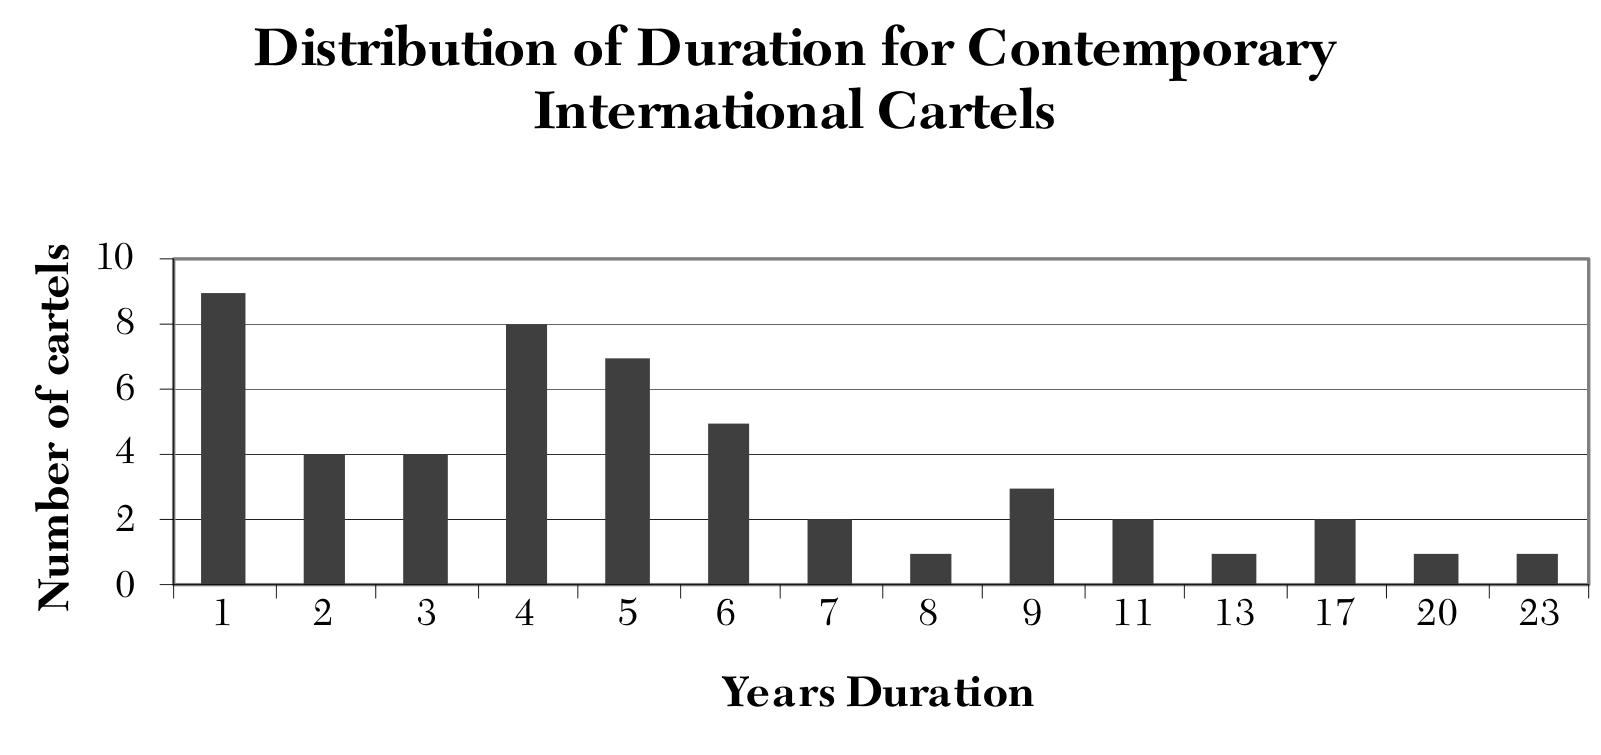
\includegraphics[width=0.78\textwidth]{figures/ch12/ls_fig1.png}
\caption{Distribution of the duration of contemporary international cartels. The horizontal axis lists only the
durations that occur, so it is not to scale. The underlying tabulation is from the authors' 2004 study (their source
note cites ``Levenstein and Suslow (2004b), table 1''). Source: \citet{LevensteinSuslow2006}, Figure~1.}
\label{fig:12-ls-duration}
\end{figure}

Case studies give longer durations (\cref{tab:12-ls-cases}). The nineteen industries contain fifty episodes of
cooperation, with a mean duration of 14 years, a median of 6 years and a standard deviation of 19.6 years
(p.~52). The median is close to the cross-section evidence, while the mean and the dispersion are much larger. The
authors attribute the difference partly to researchers' tendency to study industries with long or eventful cartel
histories. The DeBeers diamond cartel lasted 100 years before its first breakdown, while several cartels in the sample
barely got off the ground (p.~54). The Joint Executive Committee, the most studied cartel in modern economics
(\cref{sec:13-jec}), is the least stable in the sample. Its pools generally lasted two to five years and broke down
through entry or secret cheating (p.~56). Cooperation among southern U.S. railroads lasted three times as long on
average (footnote~40).

\begin{table}[htbp]
\centering
\caption{Cartel duration in selected case studies}\label{tab:12-ls-cases}
\footnotesize
\begin{tabular}{@{}l c r r r r@{}}
\toprule
Industry & First year & Mean duration & Episodes & Maximum & Minimum\\
\midrule
Beer (U.S.) & 1933 & 9 & 1 & 9 & 9\\
Beer (Sweden) & 1894 & 29 & 2 & 50 & 8\\
Bromine & 1885 & 6.25 & 4 & 10 & 3\\
Cement & 1922 & 40 & 1 & 40 & 40\\
Coal & 1893 & 20 & 1 & 20 & 20\\
Diamonds & 1870s & 60 & 2 & 100 & 20\\
Electrical equipment & 1950 & 8 & 1 & 8 & 8\\
Ocean shipping & 1870s & 51 & 3 & 54 & 50\\
Oil & 1871 & 2 & 3 & 3 & 1\\
Parcel post & 1851 & 28.5 & 2 & 40 & 17\\
Potash & 1877 & 9.4 & 8 & 20 & 1\\
Railroad (U.S. Midwest) & 1879 & 1.7 & 3 & 2 & 1\\
Railroad (U.S. South) & 1873 & 5 & 2 & 8 & 1\\
Railroad and oil & 1871 & 7 & 5 & 30 & $<1$\\
Rayon & 1932 & 8 & 1 & 8 & 8\\
Steel (Europe) & 1926 & 7.3 & 4 & 13 & 4\\
Steel (U.S.) & 1933 & 6 & 1 & 6 & 6\\
Sugar & 1887 & 6.75 & 4 & 10 & 2\\
Tea & 1929 & 3.5 & 2 & 6 & 1\\
\bottomrule
\end{tabular}

\smallskip
\begin{minipage}{0.86\textwidth}\footnotesize
Notes: Durations in years. ``First year'' is the first year of the first episode covered by the case studies.
``Episodes'' counts the distinct cartels that the studies date clearly. The episode-weighted mean of the column of
mean durations is 14 years, the figure reported in the text of the survey.
Source: \citet{LevensteinSuslow2006}, Table~2.
\end{minipage}
\end{table}

Is a typical life of five to six years long or short? The authors offer two benchmarks (pp.~56--57). The graphite
electrodes cartel, which lasted from mid-1992 to mid-1997, drew fines of more than 600 million U.S. dollars from U.S. and
European authorities. A cartel of average duration can thus inflict large damage. Firms themselves are not long-lived
either. Geroski reports that 61.5 percent of U.S. entrants exit within five years and 79.6 percent within ten, as
quoted by the authors. Cartels are less than perfectly stable. Yet they are about as durable as many other economic
organizations. The lesson is that cartels cannot be described simply as unstable. Some fail quickly, and others solve
the problems of coordination, cheating and entry for decades.

\subsection{Determinants of cartel duration}\label{sec:12-ls-determinants}

\citet[p.~57]{LevensteinSuslow2006} give two answers to the question of how cartels survive. Surviving cartels operate
in industries whose exogenous features make collusion easier. They also organize themselves to overcome
coordination, cheating and entry. Both are necessary and neither is sufficient.

\casehead{Number of firms and concentration}
The Bertrand constraint predicts that collusion is harder with more firms. The evidence is mixed. Most case-study
cartels and most contemporary international cartels operated in concentrated industries (p.~58). Yet the number of
participants in contemporary international cartels ranged from two to several hundred. Whenever there were more than
about half a dozen firms, an industry association or a government helped organize the agreement. In U.S. price-fixing
cases the mean number of conspirators is 7.25 in the sample of Hay and Kelley, which excludes four cases with 50 or more
conspirators. It is 16.7 in the sample of Fraas and Greer and 29.1 in that of Posner. Gallo et al. report a mean of 2.45 over all
2,689 Commerce Clearing House cases, not only horizontal conspiracies (Table~5). The medians are 7, 8, and
between 6 and 10. The shares of cartels with fewer than ten members are 79, 60 and 64 percent, and the average four-firm
concentration ratio in Hay and Kelley's sample is 77 percent (Table~5).

Effects on duration also conflict (Table~6, p.~61). Dick finds a statistically significant positive effect of the
number of firms on duration. Suslow finds a negative effect, which is not significant, and Hay and Kelley find no
significant pattern. Posner finds that 52 percent of the 79 cases with ten or fewer firms persisted six years or more,
against 64 percent of the 28 cases with more than ten firms. Hay and Kelley do find a positive association between
industry concentration and duration. Most of the conspiracies in their sample that lasted ten years or more were in
highly concentrated markets (Table~6, note~d, and p.~60). More consistently, duration rises with the share of the
market controlled by cartel members. The effect is positive and significant for Dick and Marquez, and positive but
not significant for Suslow. Marquez also finds a significant positive effect of cartel concentration, measured by a
Herfindahl index of the members' shares of cartel output. The authors offer three explanations for the weak link with concentration
(p.~58). Prosecutors may catch large cartels and association-run cartels more easily. Very concentrated industries may
collude tacitly and never appear in samples of explicit cartels. And concentration is endogenous, since collusion lets
more firms survive. Symeonidis finds a concave relation between the prevalence of collusion and concentration across
151 British industries (p.~60).

Trade associations are the organizational answer to large numbers. Posner reports that 44 percent of the cartels in
his sample used an industry association. Hay and Kelley, and Fraas and Greer, find associations in about a third of
U.S. conspiracies (p.~61). In the language of \cref{sec:12-cartels}, an association supplies the communication and
monitoring that large groups cannot achieve tacitly.

\casehead{Large customers}
\citet{Stigler1964} predicted that large buyers would tempt cartel members to cut prices secretly. The only explicit
econometric test, by Dick, finds that Webb-Pomerene export cartels selling to relatively larger buyers dissolved more
quickly (p.~61). Other evidence is less supportive. The citric acid cartel sold to firms such as Mars, Coca-Cola and
Procter \& Gamble, and the vitamins cartel to Kellogg, Quaker Oats and Tyson Foods (p.~62). These buyers do not seem to
have used their resources to break the cartels. The graphite electrodes investigation, started by a steel producer's
complaint, is the one exception the authors know. In five of the nineteen case studies, customers tried to break the
cartel (p.~62 and Table~7). In bromine and potash they tried to integrate backward, and in rayon they spread rumors of
cheating. In other cases customers helped stabilize a cartel and shared its rents. Customer size may destabilize a
cartel, while customer concentration may have the opposite effect.

\casehead{Demand}
Eckbo finds that cartels raised prices substantially only when demand was sufficiently inelastic with few short-run
substitutes (p.~64). The brewing industry, with a demand elasticity of $-10.3$, had an unsuccessful cartel,
with price wars in every year of the study (p.~64 and Table~8).

Demand instability matters more than the business cycle as such (Table~9). Dick finds that instability shortens
Webb-Pomerene cartels and that anticipated downturns end them, while unanticipated cycles have no significant
effect. Suslow finds significant negative effects of demand growth, of the business cycle and of unanticipated cycles.
Marquez finds a negative but insignificant effect of demand growth. Across case studies, macroeconomic fluctuations
seem to have had little relevance (p.~67 and Table~10). The international steel cartel is the only one reported to
have collapsed because of an observable demand shock. The authors read this as consistent with the Green-Porter and
Abreu literature, in which price wars follow unobserved rather than observed fluctuations. Their conclusion is that
unanticipated shocks and very rapid growth undermine cartels, while predictable cyclical fluctuations do not (p.~86).

This evidence must be mapped to the theory with care. The theories of \cref{sec:12-demand,sec:12-public} predict
changes in collusive prices or temporary price wars, not the end of a cartel. A Green-Porter reversion would appear as
a breakdown only if the researcher dates episodes by price wars. The finding that anticipated downturns end
Webb-Pomerene cartels fits the logic of \citet{HaltiwangerHarrington1991} and \citet{BagwellStaiger1997}, in which
collusion is hardest when future demand looks weak. It does not test whether the cartels died or merely punished.

\casehead{Organization and learning}
Successful cartels build organizations that monitor members, adjust the agreement to changing conditions, and settle
disputes (pp.~67--74). A joint sales agency is the strongest form, since it removes each firm's discretion over price.
Seven of the nineteen case-study industries used one: bromine, cement, diamonds, ocean shipping, oil, potash and
European steel. Most of these were among the more successful cartels (p.~69). Dick finds that a single sales agent
lowers the likelihood of cartel failure. Table~11 of the survey covers four U.S. cross-sections: Hay and Kelley,
Fraas and Greer, Posner, and Gallo et al. Trade associations were involved in 29, 36, 44 and 23 percent of their cases,
and market allocation in 35, 26, 26 and 27 percent. Suslow finds that self-imposed penalties significantly lengthen
cartel life (p.~71).

Hierarchies separate policy from day-to-day management. In the electrical equipment conspiracy of the 1950s, a working
group of sales managers devised the ``phases of the moon'' formula. It rotated the winning bidder for switchgear orders
every two weeks (pp.~72--73). In the citric acid cartel of 1991 to 1995, senior executives, nicknamed ``the
masters,'' set the broad agreement. Lower-level ``sherpas'' ran it. They shared monthly sales figures, and a firm that
sold more than its quota had to buy citric acid from a member below quota the next year (p.~73). This is the
quota-and-transfer scheme that \citet{HarringtonSkrzypacz2011} rationalize (\cref{thm:12-hs}).

Cartels learn. Dick and Suslow both find that prior cartel experience lengthens duration (Table~12). Within a single
episode, Dick finds that the hazard of dissolution rises with age. A cartel in its tenth year was 28 to 48 percent more
likely to dissolve than one in its fifth year. Several case-study cartels got off to a rocky start and later lasted for
long periods. Swedish brewers formed a cartel in 1894 with better control machinery than earlier attempts, and a
cartel formed in 1906 lasted fifty years (p.~74).

\casehead{Entry and exclusion}
Entry is a central threat. Dick finds that export associations formed where entry was slow, and Symeonidis that
collusion is more likely in capital-intensive industries (p.~74). Successful cartels create barriers to entry. Scott
Morton documents 47 cases of attempted entry against British shipping cartels. A typical price war against an entrant
lasted three months and cut prices by 50 percent on the routes the entrant served (p.~75). Nineteenth-century U.S. salt
producers, by contrast, saw each collusive arrangement collapse within a year or two because entry barriers were too
low (pp.~74--75).

\subsection{Why cartels break down}\label{sec:12-ls-breakdown-causes}

\Cref{tab:12-ls-breakdown} reproduces the causes of breakdown in international cross-sections. In Eckbo's first
sample, internal conflict or defection ended ten of twenty-three cartels, roughly 44 percent, and in his second sample
59 percent (p.~75). In Suslow's sample about a quarter ended because of internal conflict and cheating. Only World
War~II ended a larger share. Griffin finds that half of his cartels ended for political or external reasons
(p.~76). Entry or substitutes contributed to a third of his failures, and ``behavioral problems'' to another third. World War~II ended twelve of his cartels, and technological change ended four (rubber, zinc, sulfur and
nitrate). The category ``cheating and disagreement'' mixes monitoring failures with bargaining failures, which the
theory treats very differently.

\begin{table}[htbp]
\centering
\caption{Causes of cartel breakdown in international cross-section studies (percent of episodes)}\label{tab:12-ls-breakdown}
\footnotesize
\begin{tabular}{@{}l r r r r@{}}
\toprule
Cause of breakdown & Eckbo, sample 1 & Eckbo, sample 2 & Griffin$^{a}$ & Suslow\\
\midrule
Cheating and disagreement & 43.5 & 58.6 & 33.3 & 23.9\\
External shock & 30.4 & & 50.0$^{c}$ & 42.3\\
Entry and substitution$^{b}$ & 26.1 & 41.4 & 33.3 & 15.5\\
\quad Entry & 13.0$^{b}$ & & 25.9 & 15.5\\
\quad Substitution & 8.7$^{b}$ & & 9.3 & \\
Technological change & & & 9.3 & \\
Antitrust indictment & & & & 18.3\\
\midrule
Total number of episodes & 23 & 29 & 54 & 71\\
\bottomrule
\end{tabular}

\smallskip
\begin{minipage}{0.92\textwidth}\footnotesize
Notes: Blank cells are not reported. (a) Based on Griffin's discussion and on his Table~4. Griffin lists more than one
cause for several cartels, so his column sums to more than 100. The survey's text names four cartels ended by
technological change (4 of 54, or 7.4 percent), while the table reports 9.3 percent. Its footnote~90 notes that
Griffin's own text and table differ. We reproduce both figures as printed. (b) Entry and substitution do not always add to the
total, because Eckbo leaves one episode unclassified and Griffin counts two cartels under both. Of Eckbo's six
episodes in this category, three ended through entry, two through substitution and one is unclassified. (c) Griffin
groups wars, antitrust and other government actions, and cartel reorganizations. Some reorganizations may be
bargaining problems, so the entry overstates external shocks as classified here.
Source: \citet{LevensteinSuslow2006}, Table~13.
\end{minipage}
\end{table}

Case studies separate these causes better (Table~14 of the survey, p.~77). Entry was the primary cause of
disruption in just over a third of the episodes. World Wars~I and~II ended about 15 percent and legal action a little
over 10 percent. Only three episodes, fewer than 10 percent, ended because of cheating (p.~78). Bargaining problems
affected virtually every cartel and ended about a quarter of the episodes. Many case-study authors report that
cheating was simply not a problem.

Successful cartels avoided costly punishments. The Sugar Institute ``served as a court in which an accused firm might
prove its innocence'' \citep[p.~389]{GenesoveMullin2001}, as quoted by \citet[p.~78]{LevensteinSuslow2006}. Outside
the South, deviations ``were either ignored or matched'' rather than met by reversion to competition
\citep[pp.~390--391]{GenesoveMullin2001} (see \cref{sec:13-sugar-institute}). In steel in the 1930s, unexpected
declines in demand led to ``shallow episodes of increased competition,'' in Baker's words, rather than severe price
wars. In bromine, violations were answered with negotiated side payments rather than price wars
(\citealp{Levenstein1997}, \cref{sec:13-bromine}). The authors conclude that Cournot reversion is an inefficient way to
sustain collusion, as the cartel members themselves repeatedly discovered (p.~78).

\citet[p.~79]{LevensteinSuslow2006} draw three lessons. First, the outbreak of a price war, as opposed to its threat,
is rarely a sign of cartel success. Second, the most successful cartels develop alternative punishments and threats
that sustain collusion at lower cost. Third, cartels break down sometimes because of cheating, but more often because
of entry, exogenous shocks and dynamic changes within the industry.

\subsection{Effects on prices}\label{sec:12-ls-prices}

Rigorous counterfactual estimates of cartel overcharges are rare (p.~45). The available evidence nonetheless shows that
many cartels raised prices substantially (pp.~80--81). Eckbo finds that nineteen of fifty-one cartels raised price 200
percent above the unit cost of production and distribution. Griffin finds an average markup of 45 percent over marginal
cost. His most successful cartel, rubber from 1923 to 1928, had a markup of 400 percent, while his least successful,
wheat from 1933 to 1934, priced below cost. For contemporary international cartels, reported price increases, mostly
from the trade press, range from 10 to 100 percent. Graphite electrode prices rose more than 50 percent in the United
States from 1992 to 1997. In Canada, where two firms held more than 90 percent of the market, they rose more than 90
percent. Some evidence points the other way. Fölster and Peltzman find that legal Swedish cartels did not raise prices,
although a re-examination of the same data by Ciarreta finds that they did. In 25 price-fixing cases from 1973 to 1984,
Sproul finds that prices four years after indictment were slightly higher, by 7 percent.

Case studies seldom measure success against a counterfactual (p.~81 and Table~15). Hausman finds that the regulations
of the ``Limitation of the Vend,'' a coal cartel in northeast England from 1770 to 1845, raised the equilibrium price
by about 6 to 8 percent. Bromine prices came close to the joint-profit-maximizing level in some periods and barely
exceeded the Cournot level in others. Ocean shipping was close to the joint-profit level. The German steel cartel
priced below the joint-profit level but one-third above the world price. The cement cartel priced 10 percent above
the world price. Diamond prices nearly doubled after the cartel formed, and tea prices rose 80 percent
in 1933 after the cartel was reestablished. The U.S. beer cartel of the 1930s may even have priced above the monopoly
level, under political pressure to keep alcohol expensive. Yet it had price wars in each of the three years it tried
to collude. Success must be judged over the whole life of a cartel, not only during its collusive periods (p.~81). The
methods for estimating overcharges and damages are developed in \cref{sec:13-damages}.

\subsection{What the evidence says about the theory}\label{sec:12-ls-theory}

The survey speaks to each part of the theory in this chapter.
\begin{enumerate}[label=(\arabic*)]
\item \emph{Structure.} The perfect-monitoring theory of \cref{sec:12-perfect} predicts that collusion is easier with
fewer firms. Concentration helps, but organization can substitute for it, and concentration is itself shaped by
collusion.
\item \emph{Demand.} Unanticipated shocks and rapid growth undermine cartels, while predictable cycles do not. This
pattern matches the role of unobserved shocks in \citet{GreenPorter1984}. The evidence on anticipated downturns fits
the persistent-demand models of \cref{sec:12-demand}. Cross-section data on cartel deaths cannot test the
within-cartel price dynamics these models predict. That requires the time-series studies of \cref{sec:13-jec}.
\item \emph{Price wars.} Many observed price wars are bargaining wars or breakdowns. Successful cartels prefer
monitoring, courts and side payments to Green-Porter reversions. This supports the shift of the theory toward
communication and transfers (\cref{sec:12-cartels}) and toward tolerated cheating (\cref{rem:12-bm},
\cref{sec:13-imperfect}).
\item \emph{Organization.} Joint sales agencies, reporting systems, penalties and hierarchies lengthen cartel life.
Theory treats them as devices that make information public or transfers possible, as in
\citet{HarringtonSkrzypacz2011}.
\item \emph{Entry.} Entry is the most common cause of breakdown in the case studies, yet most repeated-game models
hold the set of firms fixed. This is the largest gap between the theory and the evidence.
\item \emph{Enforcement.} Antitrust action ended 18.3 percent of Suslow's interwar international cartels and a little
over 10 percent of case-study episodes. Enforcement also selects which cartels we observe, as \cref{sec:12-enforcement}
and \cref{sec:13-institutions} discuss.
\end{enumerate}

The survey has limits. It aggregates studies with different definitions of a cartel, of an episode and of a cause of
breakdown. Most of its quantitative statements are counts and percentages, not estimates with standard errors. Selection
is unavoidable and of unknown sign. The cross-section regressions it summarizes use duration as the dependent variable,
which is a noisy measure of success, and they rarely control for the endogeneity of structure and organization. Its
contribution is to replace the presumption that cartels are inherently unstable with a set of facts. Cartels often
last for years. They end more often through entry, shocks and bargaining than through secret cheating. The successful
ones invest in organization.

\section{Synthesis: What the Theory Predicts and How to Test It}\label{sec:12-synthesis}

\Cref{tab:12-models} collects the models of this chapter. Each row states what firms observe, why collusion is hard,
what the most collusive equilibrium looks like, whether price wars occur on the equilibrium path, and what the model
predicts for prices. The last column points to the section of \cref{ch:collusion-evidence} where the prediction meets
data.

The table carries five lessons for empirical work.

The first lesson is that theory delivers a set of sustainable outcomes and leaves the choice among them open. The
folk theorem and
\cref{cor:12-bertrand-any-price} imply that a wide range of prices can be sustained in the same environment. Empirical
work that tests ``collusion'' must therefore commit to a specific model of how the cartel operates. The common
selection, the most collusive equilibrium, is a convention.

The second lesson is that conduct varies over time. In Rotemberg and Saloner, Haltiwanger and Harrington, and Bagwell
and Staiger, collusive margins move with current and expected demand. In Green and Porter, conduct switches between
regimes. A constant conduct parameter then averages over states, which is the critique of \citet{Corts1999} discussed
in \cref{ch:conduct}. Estimation must allow for regimes or for state-dependent conduct, as the methods of
\cref{sec:13-implications} do.

The third lesson is that a price war is an ambiguous signal. In \citet{GreenPorter1984} it is part of a working
cartel. In \citet{Stigler1964} and in the bargaining wars documented by \citet{LevensteinSuslow2006}, it marks a
failing one. The timing of wars relative to demand helps discriminate. Wars after unexpected drops in demand point to
Green and Porter. Low prices in booms point to Rotemberg and Saloner. Wars around entry or renegotiation point to
bargaining. \Citet{Ellison1994} uses exactly this logic to test Green and Porter against Rotemberg and Saloner in the
railroad cartel of \citet{Porter1983} (\cref{sec:13-ellison}).

The fourth lesson is that communication and transfers are observable in prosecuted cartels, and they matter most when
information is private. The anatomy of the lysine and citric acid cartels, with quotas, sales reports and buy-backs, is
predicted by \citet{HarringtonSkrzypacz2011}. The identical bidding of many rings is predicted by
\citet{AtheyBagwellSanchirico2004}, and their take-turns scheme is a model of bid rotation. Evidence on the internal organization of cartels can thus discriminate among
models in a way that price data alone cannot.

The fifth lesson is that detection needs a competitive benchmark and a theory of the specific cartel. Overcharges are
measured against a but-for price. Tests of bid rigging compare suspected firms with a model of noncooperative bidding.
Enforcement determines which cartels enter the data, so every finding is conditional on how the cartels were found.

\begin{landscape}
\begin{table}[p]
\centering
\caption{Models of collusion and their testable implications}\label{tab:12-models}
\scriptsize
\renewcommand{\arraystretch}{1.1}
\begin{tabularx}{\linewidth}{@{}>{\raggedright\arraybackslash}p{2.5cm}
>{\raggedright\arraybackslash}X >{\raggedright\arraybackslash}X >{\raggedright\arraybackslash}X
>{\raggedright\arraybackslash}p{2.7cm} >{\raggedright\arraybackslash}X
>{\raggedright\arraybackslash}p{2.1cm}@{}}
\toprule
Model & What firms observe & Source of the incentive problem & Most collusive equilibrium and price pattern & Price
wars on the path? & Testable implication & Tested in\\
\midrule
Perfect monitoring, Bertrand and Cournot (\cref{sec:12-perfect}) & All past prices or outputs & One-period gain from
undercutting against the loss of future collusion & Stationary price, monopoly if $\delta \ge \underline\delta(N)$.
Any price in $[c, p^m]$ can be sustained & No & Collusion is easier with fewer, more symmetric firms, frequent
interaction and transparency & \cref{sec:13-information}, \cref{ch:mergers}\\
Rotemberg and Saloner (\cref{sec:12-demand}) & Current demand (\iid) and past prices & Gain from cheating rises with
current demand, future loss is constant & Monopoly price in low states, capped profit in high states. Countercyclical
margins & No, unless prices are restricted to collude or compete & Margins fall when current demand is high relative
to expected demand & \cref{sec:13-jec}, \cref{sec:13-gasoline}\\
Haltiwanger and Harrington (\cref{sec:12-demand}) & A known demand cycle & Future loss is small when demand is about
to fall & Prices lowest when demand is about to fall, and at the peak only for impatient firms & No & Margins rise with expected future demand &
\cref{sec:13-gasoline}\\
Bagwell and Staiger (\cref{sec:12-demand}) & Current growth phase (Markov) & Gain and loss both move with the phase &
Procyclical prices if growth rates are positively correlated, countercyclical if negatively & No & Cyclicality
depends on the persistence and expected durations of phases & \cref{sec:13-predictions}\\
Green and Porter (\cref{sec:12-public}) & Market price only & A low price may reflect cheating or low demand &
Trigger price, reversion of finite length. Regime switching & Yes, after unexpectedly low prices & Wars follow
negative demand shocks and have finite length & \cref{sec:13-jec}\\
Athey, Bagwell and Sanchirico (\cref{sec:12-private-costs}) & Public prices, private \iid\ costs & Low-cost firms want
more market share & Patient firms: one rigid price, equal shares. Impatient firms: an escape clause & No (inelastic
demand) & Rigid, identical prices that ignore firm-specific costs & \cref{sec:13-detection}, \cref{sec:13-legal}\\
Harrington and Skrzypacz (\cref{sec:12-cartels}) & Own sales and public reports & Secret price cuts, unverifiable
sales reports & Quotas, sales reports and per-unit transfers. Breakdown after low total reports & Yes, rare
breakdowns & Quota schemes with buy-backs, breakdowns after low sales & \cref{sec:13-imperfect}\\
Bernheim and Madsen (\cref{rem:12-bm}) & All quotes, with costly quoting and home cost advantages & Raiding the
rival's home market & Price floor below the home monopoly price. Dispersed prices & No. Raids above the floor are
tolerated & Business stolen at higher prices is less likely to be punished & \cref{sec:13-imperfect}\\
Chen and Rey (\cref{sec:12-chenrey}) & Own conduct, random detection, leniency & Cheat and report, or collude and
report & Normal collusion if the stake exceeds the deterrence threshold & No (binary conduct) & Excessive leniency
induces systematic self-reporting & \cref{sec:13-enforcement}, \cref{sec:13-asker}\\
\bottomrule
\end{tabularx}

\smallskip
\begin{minipage}{\linewidth}\scriptsize
Notes: Our synthesis of the models in this chapter. \citet{BernheimMadsen2017} is developed in
\cref{sec:13-imperfect}. Price wars on the path refer to the most collusive equilibrium of each model.
\end{minipage}
\end{table}
\end{landscape}

\Cref{ch:collusion-evidence} takes these lessons to data. It begins with the econometrics of regime switching
(\cref{sec:13-implications}) and the Joint Executive Committee (\cref{sec:13-jec}), where the Green-Porter and
Rotemberg-Saloner predictions are tested. It continues with the rules and communication of legal cartels, information
exchange, retail gasoline, tolerated cheating, the internal organization of a bidding ring, and the statistical
detection of bid rigging. It ends with enforcement and the measurement of damages (\cref{sec:13-enforcement}).


\section{Bibliographic notes}\label{sec:12-bibnotes}

The modern theory of collusion begins with \citet{Stigler1964}, who saw a cartel's central problem as the
detection of secret price cuts. \citet{Friedman1971} showed that the threat of reverting to static Nash play
sustains collusion as a noncooperative equilibrium of a supergame. \citet{FudenbergMaskin1986} proved the folk
theorem with minmax punishments, and \citet{Abreu1986,Abreu1988} characterized optimal punishments and simple
penal codes. \citet{FarrellMaskin1989} asked which punishments survive renegotiation. \citet{BenoitKrishna1985}
and \citet{KrepsEtAl1982} showed how multiple stage equilibria and incomplete information restore cooperation in
finitely repeated games. \citet{BrockScheinkman1985} and \citet{CompteJennyRey2002} added capacity constraints.
\citet{FudenbergTirole1991} and \citet{MailathSamuelson2006} are the standard references for the theory of repeated
games. Chapter~6 of \citet{Tirole1988} remains the classic textbook treatment of its applications to oligopoly,
including the kinked demand curve and the alternating-move model of \citet{MaskinTirole1988}.
\citet{AskerNocke2021} survey the modern literature on collusion in the Handbook of Industrial Organization. They
cover the prevalence of cartels, how agreements start and are structured, imperfect monitoring, multimarket contact,
entry and detection.

\citet{GreenPorter1984} brought imperfect public monitoring into the theory of collusion and showed that price wars
can be part of a working cartel. \citet{Porter1983b} studied optimal trigger strategies.
\citet{AbreuPearceStacchetti1986,AbreuPearceStacchetti1990} developed the recursive methods that now dominate the
field, and \citet{FudenbergLevineMaskin1994} proved a folk theorem for games with imperfect public monitoring.
Collusion under fluctuating demand starts with \citet{RotembergSaloner1986}, whose working paper
\citep{RotembergSaloner1984} contains the evidence. \citet{HaltiwangerHarrington1991}, \citet{Kandori1991},
\citet{StaigerWolak1992} and \citet{BagwellStaiger1997} studied persistent demand, correlated shocks and capacity.

Private information about costs entered with \citet{AtheyBagwell2001} and \citet{AtheyBagwellSanchirico2004}, and
\citet{AtheyBagwell2008} allowed costs to be persistent. \citet{McAfeeMcMillan1992} analyzed bidding rings with
and without side payments. The theory of private monitoring and communication includes \citet{Compte1998} and
\citet{KandoriMatsushima1998}. \citet{HarringtonSkrzypacz2007,HarringtonSkrzypacz2011} connected it to the
practices of prosecuted cartels, and \citet{AwayaKrishna2016} studied when cheap talk about sales helps.
\citet{BernheimMadsen2017} explained why cartels tolerate some cheating. \citet{BernheimWhinston1990} is the classic
analysis of multimarket contact, and \citet{Matsushima2001} extended it to imperfect monitoring.
\citet{SugayaWolitzky2018} showed that more information can hinder collusion. \citet{BosHarrington2010} studied which
firms join a cartel. \citet{ByrneDeRoos2019} documented how firms learn to coordinate tacitly, and
\citet{CalvanoEtAl2020} opened the study of collusion by pricing algorithms.

On enforcement, \citet{MottaPolo2003} and \citet{Spagnolo2004} began the economic analysis of leniency programs.
\citet{AubertReyKovacic2006} studied rewards to individual informants, \citet{Harrington2008} the race to report,
and \citet{ChenRey2013} the optimal design of a program. \citet{Miller2009} measured the effect of the 1993 U.S.
revision on detection and deterrence. \citet{Kaplow2013} questions the agreement requirement on which enforcement
rests. His chapters~2, 3 and 7 examine the meaning of agreement, the role of communication and the link between
equilibrium and agreement. \citet{MarshallMarx2012} give a book-length account of how cartels and bidding rings are
organized, of when explicit collusion is needed, and of the plus factors that reveal it. \citet{KawaiNakabayashi2020}
and \citet{ConleyDecarolis2016} estimate how widespread collusion is in public procurement. \citet{LevensteinSuslow2006}
survey the evidence on cartel duration, organization and breakdown, which \cref{ch:collusion-evidence} develops
further.

\section{Exercises}\label{sec:12-exercises}

\begin{enumerate}[label=\arabic*., leftmargin=*, itemsep=6pt]

\item \textit{Detection lags.} A deviation is detected only $k$ periods after it starts.
\begin{enumerate}[label=(\alph*)]
  \item Extend \cref{prop:12-bertrand-ext} to the linear Cournot supergame of \cref{prop:12-cournot}: show that with
  a $k$-period detection lag, grim trigger sustains $q^m$ if and only if $\delta^k \ge \delta^*(N)$.
  \item In the Bertrand supergame with demand growth, use \eqref{eq:12-bertrand-ext} to compute the threshold for
  $N = 4$, $k = 2$ and $g = 0.05$, and compare it with the value for $g = 0$. You should find about 0.825 and about
  0.866.
  \item Let $N = 4$, $\delta = 0.8$ and $g = 0$. Find the longest detection lag that a Cournot cartel can tolerate,
  and the longest that a Bertrand cartel can tolerate. You should find $k = 2$ and $k = 1$. Explain what the
  difference implies for the value to each cartel of exchanging sales reports.
\end{enumerate}

\item \textit{Capacity constraints.} Three firms with zero marginal cost face demand $D(p) = 1 - p$. Each can produce
at most $K$ units per period, with $\frac{1}{6} < K < \frac{1}{2}$. Rationing is efficient. Assume that a deviator
can be held to its minmax payoff in every period after a deviation.
\begin{enumerate}[label=(\alph*)]
  \item Show that the best deviation from collusion at $p^m = \frac{1}{2}$ earns almost $\frac{K}{2}$.
  \item Show that the minmax payoff is $K(1 - 3K)$ for $K \le \frac{1}{4}$ and $\frac{(1 - 2K)^2}{4}$ for
  $K \ge \frac{1}{4}$.
  \item Use the bound of \cref{ex:12-capacity} to show that the threshold discount factor is $\frac{1}{6K}$ for
  $K \le \frac{1}{4}$ and $\frac{6K - 1}{18K - 12K^2 - 3}$ for $K \ge \frac{1}{4}$.
  \item Show that the threshold falls with $K$ up to $K = \frac{1}{3}$, where it equals $\frac{3}{5}$, and rises
  afterward toward $\frac{2}{3}$, the value without capacity constraints. Explain the two forces at work.
\end{enumerate}

\item \textit{Stick and carrot with three firms.} Three Cournot firms face $P(Q) = a - bQ$ at every output and have
marginal cost $c < a$.
\begin{enumerate}[label=(\alph*)]
  \item Set $a - c = b = 1$. Show that the carrot and stick constraints of \cref{prop:12-abreu-two-phase} become
  $\frac{1}{36} \le \delta\frac{(6x - 1)^2}{12}$ and $\frac{(4x - 1)^2}{4} \le \delta\frac{(6x - 1)^2}{12}$.
  \item Show that the best stick output is $x = \frac{a - c}{3b}$ per firm, that the stick drives the price down to
  marginal cost, and that monopoly sharing is sustainable for $\delta \ge \frac{1}{3}$. Compare this with the
  threshold $\frac{4}{7}$ under Nash reversion.
  \item Explain why the stick constraint must bind at the optimum. Would the answer change if the price could not
  fall below zero and $c$ were close to zero (\cref{rem:12-abreu-floor})?
\end{enumerate}

\item \textit{Booms of different frequency.} Modify the two-state model of \cref{asm:12-two-state} so that the high
state occurs with probability $\mu \in (0, 1)$.
\begin{enumerate}[label=(\alph*)]
  \item Show that the incentive constraints become $\pi_s(p_s) \le \kappa[\mu\pi_H(p_H) + (1 - \mu)\pi_L(p_L)]$ for
  $s = H, L$, with $\kappa$ as in \eqref{eq:12-kappa}.
  \item Use \cref{lem:12-two-constraint} to show that some collusion is possible if and only if $\kappa \ge 1$,
  whatever $\mu$. Show that monopoly pricing in both states requires
  $\kappa \ge \bar\kappa(\mu) \equiv \frac{\pi_H^M}{\mu\pi_H^M + (1 - \mu)\pi_L^M}$.
  \item In the intermediate regime, show that $p_L = p_L^M$ and
  $\pi_H(p_H) = \frac{\kappa(1 - \mu)\pi_L^M}{1 - \kappa\mu}$.
  \item With $D_s(p) = A_s(1 - p)$, $c = 0$, $A_H = 1.5$, $A_L = 1$, $\mu = \frac{1}{3}$ and $N = 2$, compute
  $\bar\kappa$ and $\bar\delta$, and the boom price at $\kappa = 1.1$. You should find $\bar\kappa = \frac{9}{7}$,
  $\bar\delta = \frac{9}{16}$ and $p_H \approx 0.261$. Explain why rarer booms widen the range of discount factors
  with countercyclical prices.
\end{enumerate}

\item \textit{Noise and the length of price wars.} Use the Bertrand version of Green and Porter
(\cref{asm:12-gp-bertrand}) with $\delta = 0.95$ and $\gamma = 0.2$.
\begin{enumerate}[label=(\alph*)]
  \item Find the shortest war $T^*$ that satisfies \eqref{eq:12-gp-ic}, and the long-run share of periods spent in
  wars. You should find $T^* = 2$ and $\frac{2}{7}$.
  \item Compute the value of collusion $V$ at $T^*$ and with an infinite war. Explain why the cartel prefers the
  shorter war although it punishes less.
  \item An econometrician observes many wars in this industry. Explain why the observation, by itself, is not
  evidence that the cartel is breaking down. What additional data would distinguish this model from
  \citet{RotembergSaloner1986}?
  \item Now let $N$ firms play the noisy-signal model of \cref{prop:12-an}, with the same $\delta$ and $\gamma$ and with
  $\lambda = 1$. For $N = 2$, 3 and 4, compute the threshold \eqref{eq:12-an-delta}, the punishment probability
  $\phi^*$ and the ratio of $v^*$ to $\frac{\bar\pi}{N}$. You should find ratios of 0.75, 0.5 and 0.25. Explain why the
  number of firms matters although $\delta$ exceeds every threshold. For $N = 2$, compare $v^*$ with $(1 - \delta)V$ at
  $T^*$ from part (b), and explain why a random punishment can do better than the best war of integer length.
\end{enumerate}

\item \textit{Cost dispersion and rigid prices.} Two firms have private costs drawn independently from the uniform
distribution on $[0, \bar c]$, with $0 < \bar c \le 1$. Demand is inelastic with reservation value $\bar v = 1$.
\begin{enumerate}[label=(\alph*)]
  \item Show that the static equilibrium is $p^e(c) = c + \frac{\bar c - c}{2}$ and that the ex ante profit per
  firm is $\frac{\bar c}{6}$.
  \item With Nash reversion after an off-schedule price, use \cref{prop:12-abs-critical} to show that the rigid
  price $\bar v$ is sustainable if and only if $\delta \ge \delta^* = \frac{1}{2 - \frac{5\bar c}{6}}$. Check that
  $\delta^* = \frac{6}{7}$ for $\bar c = 1$ and that $\delta^* \to \frac{1}{2}$ as $\bar c \to 0$.
  \item Compute $\delta^*$ when the war gives zero profit instead of Nash profit, for $\bar c = 1$. Explain why
  dispersion in costs makes collusion harder even with the harshest punishment.
  \item Explain why patient firms with these costs prefer a rigid price to any fully sorting scheme, and why
  impatient firms may use an escape clause.
\end{enumerate}

\item \textit{Transfers in quota cartels.}
\begin{enumerate}[label=(\alph*)]
  \item In the model of \cref{sec:12-hs}, suppose that each firm pays $z$ per unit of reported sales into a common
  fund that is shared equally among all $N$ firms, the payer included. Show that the effective marginal cost is
  $c + z$, and compare it with $c + \frac{N}{N-1}z$ in \cref{prop:12-hs-cost}. Which design deters business stealing
  more for a given payment?
  \item Let $N = 4$, let the static markup be constant, and let market demand be uniform on $\{60, \dots, 100\}$.
  Check condition \eqref{eq:12-hs-cond2}. Show that the scheme retains a quarter of the first-best collusive gain
  and that $\beta_{\min} = \frac{0.15}{\delta}$.
  \item Compute the expected breakdown probability per period and the mean length of the collusive phase for
  $\delta = 0.95$ and $\delta = 0.99$. Compare the answers with \cref{ex:12-hs-numbers} and explain why more
  volatile demand raises the cost of truthful reporting.
\end{enumerate}

\item \textit{Leniency with more firms.}
\begin{enumerate}[label=(\alph*)]
  \item Fill in the derivations behind \cref{rem:12-cr-nfirms}: derive the thresholds $B_N^r(\ell)$ and
  $B_R(\ell)$ for $N$ firms, and the optimal amnesty rate $\hat\ell_N$.
  \item For $\delta = 0.8$ and $\varrho = 0.4$, show that $\hat\ell_2 = 1$ and $\hat B_2 = \frac{2}{3}F$, and
  compute $\hat\ell_3$. Explain why larger cartels call for more generous leniency.
  \item In the laboratory treatment of \citet{HinloopenSoetevent2008} with $\ell = 1.8$, explain why many subjects
  colluded and reported in every period.
  \item Explain why leniency is useless without the first-informant rule (\cref{rem:12-first-informant}).
\end{enumerate}

\end{enumerate}

\chapter{Collusion: Evidence and Detection}\label{ch:collusion-evidence}

\Cref{ch:collusion-theory} showed that firms that meet repeatedly can sustain prices above the static equilibrium
without any enforceable contract. This chapter asks what the data say. Did real cartels behave as the theory
predicts? How did they organize themselves, and what did collusion cost their customers? Can an outsider who sees
only prices, quantities or bids tell collusion from competition? The answers matter for antitrust policy, which
must decide which conduct to prosecute, how to prove it and how to measure the harm. They also matter for the rest
of empirical industrial organization, because every model of demand and supply in \cref{ch:conduct,ch:blp} rests on
an assumption about how firms compete.

The chapter combines econometric theory with case studies. It derives the testable implications of the
repeated-game models and develops, with proofs, the econometrics needed to test them. It then studies the cases
that shaped the field in depth. They include a nineteenth-century railroad cartel, the internal records of legal
and prosecuted cartels, retail gasoline, a ring of stamp dealers and bid rigging in public procurement. Each case
reproduces the estimating equations and the key tables, and each ends with an assessment of what it shows and what
it cannot show.

The chapter draws on much of the book. The supply relation and the conduct parameter come from
\cref{ch:theory,ch:conduct}, and \cref{ch:conduct} also treats the pre-1914 sugar price wars that reappear here.
The bidding ring and the detection tests rest on the auction theory of \cref{ch:auction-theory} and on the
inversion methods of \cref{ch:auction-empirics}. The methods for measuring damages share their logic with the
merger retrospectives of \cref{ch:mergers}. \Cref{app:econometrics} collects the econometric tools used here,
including two-stage least squares (\cref{sec:A-iv}), maximum likelihood (\cref{sec:A-mle}), the bootstrap
(\cref{sec:A-delta-boot}), selection (\cref{sec:A-identification}) and difference in differences
(\cref{sec:A-did}).

\section{Collusion in Practice and the Nature of the Evidence}\label{sec:13-intro}

Collusion matters for understanding how imperfectly competitive markets work, and it is a central concern of
antitrust policy. Four questions organize the empirical literature. How often do firms collude? Can we develop
methods to detect collusion? How does collusion occur, that is, how do cartels reach agreement, monitor compliance
and respond to cheating? Which practices and institutions facilitate it?

\casehead{Definitions}
\emph{Collusion} is coordination among firms that raises their joint profit above the level of noncooperative
competition, by raising prices, restricting output or dividing customers. It helps to distinguish two forms. In
\emph{explicit collusion} firms communicate directly. They meet to discuss prices, agree on quotas or on the
allocation of customers, and sometimes make payments to one another. In \emph{tacit collusion} firms reach
supracompetitive prices without communicating. The high prices are a noncooperative equilibrium of a repeated game,
in which the threat of future punishment deters price cuts (\cref{ch:collusion-theory}). A \emph{cartel} is a group
of firms that colludes explicitly. \emph{Bid rigging} is collusion among bidders in auctions or procurement, and a
cartel of bidders is called a \emph{bidding ring}. Collusion can also run on the buying side, as in the buyer cartels
and no-poach agreements defined in \cref{sec:12-forms}.

\casehead{The scale of cartel enforcement}
Cartels are not a historical curiosity. \Cref{tab:12-eu-fines} in \cref{sec:12-eu-facts} lists the ten largest fines
that the European Commission has imposed in cartel cases since 1969. The largest, in the trucks case of 2016 and
2017, exceeds 3.8 billion euros. The vitamins case in that table shows how far a single conspiracy can reach. The
main vitamin producers pleaded guilty to a worldwide price-fixing conspiracy covering much of the 1990s
\citep[p.~1]{MarshallMarx2012}. It extended to vitamins A, B$_1$, B$_2$, B$_5$, B$_6$, C, D and E, beta-carotene,
biotin, carotenoids, choline chloride and other products. In the United States, Roche paid a criminal fine of \$500 million and BASF one of
\$225 million. U.S.\ sales of a single product, vitamin A acetate 650 feed grade, were \$311{,}982{,}095 during the
period covered by the plea agreements (p.~2, Figure~1.1). Buyers recovered billions of dollars in civil suits, and
several executives went to prison (p.~2).

Fines outside the top ten reach a wide range of markets. Consider the twenty-two Commission decisions on
industrial-product cartels from 2000 through 2005. They concern products as varied as amino acids, carbonless paper, citric
acid, copper plumbing tubes, graphite electrodes, industrial bags, needles, plasterboard and zinc phosphate
\citep[pp.~125--127, Table~6.1]{MarshallMarx2012}. \Cref{sec:12-eu-facts} also reports the Commission's 2025 fines
on a buyer cartel and on a no-poach agreement, and how much annual totals vary.

\casehead{Why the evidence is hard to obtain}
Empirical work on collusion is difficult for three reasons. First, collusion is illegal in most markets today, so
firms hide it. The records available to researchers come from cartels that were legal, from prosecutions, or from
documents that surfaced by accident. Second, the theory admits many outcomes. With $N$ symmetric Bertrand
competitors, every price between marginal cost $c$ and the monopoly price $p^m$ can be sustained when
$\delta \ge 1 - \frac{1}{N}$ (\cref{ch:collusion-theory}). A finding that prices exceed cost therefore says little
about which equilibrium firms play. Third, most price patterns that look collusive have competitive explanations.
Price wars can reflect cost shocks (\cref{prop:13-obs-equiv}), sawtooth price cycles arise in competitive
equilibria (\cref{sec:13-noel}), and a rotation of winners can come from capacity constraints
(\cref{sec:13-detection-theory}).

\casehead{The empirical approach}
The approach of the chapter follows from these difficulties. We start from a baseline of noncooperative behavior,
a static Nash equilibrium in prices or, in an auction, in bids. We then take seriously that firms interact
repeatedly, so that the threat of future competition can sustain high margins today. Most models in this tradition
abstract from entry, exit and other changes in the market over time, and several of the cases show how much these
omissions matter. The question in each case is what collusion adds to the baseline that the data can detect.

The evidence comes in three kinds, and the chapter is organized around them. The first is historical studies of
cartels that operated openly and left records. Examples are the Joint Executive Committee railroad cartel, the
Sugar Institute and the bromine pools. The second is prosecuted cases of price fixing, bid rigging and facilitating
practices, whose court records reveal how cartels worked. A \emph{facilitating practice} is conduct that makes
coordination easier without itself being an agreement on price. Examples are gasoline retailers in Quebec, the airlines'
fare-publishing system, the lysine and citric acid cartels and a ring of stamp dealers. The third is statistical
detection. The researcher writes down a model of noncooperative behavior that implies testable restrictions on
prices, quantities or bids, and reads a rejection as possible collusion. Other explanations for a rejection usually
remain, and the chapter returns often to the question of what else could produce the same pattern.
\Cref{sec:13-market-evidence} places these tests within the wider body of market-based evidence and the
\emph{plus factors}, circumstantial economic evidence of collusion beyond parallel price movements, that courts
look for.

The first of the four questions, how often firms collude, is the hardest to answer. Prosecutions reveal only the
cartels that were caught, and the cartels that researchers study in depth are selected again. Enforcement
statistics are hard to read. Fewer prosecutions need not mean less collusion. Where collusion can be measured
directly, it appears common. \Cref{sec:13-institutions} reviews this evidence and the evidence on how long
detected cartels last
\citep{LevensteinSuslow2006}. It also shows that the direction of the resulting bias depends on how detection works.

\casehead{Notation and sources}
\Cref{sec:13-implications} fixes the chapter's notation for conduct regimes. Throughout the chapter $\delta$ is the
discount factor, as in \cref{ch:collusion-theory}. Later sections introduce local symbols, for example for a
paper's variables, and say so at first use. Several papers are available to us only in working-paper versions,
whose page, table and theorem numbers can differ from those of the published articles. When we cite such a number
we say so, and ``WP p.'' denotes a page of the working paper. Computations that are ours, and not the authors', are
labeled as such.

\casehead{Plan of the chapter}
\Cref{sec:13-implications} turns the theories of \cref{ch:collusion-theory} into statements about data and develops
the econometrics of regime switching. \Cref{sec:13-jec} applies these tools to the Joint Executive Committee
\citep{Porter1983,Ellison1994}. \Cref{sec:13-legal} studies the internal records of the Sugar Institute and of the
bromine cartel. \Cref{sec:13-information} asks how information about prices affects collusion, in theory and in
three policy episodes. \Cref{sec:13-gasoline} examines four studies of retail gasoline that reach different
conclusions about similar price patterns, and a fifth on how coordination through prices emerged in Perth.
\Cref{sec:13-imperfect} documents cheating and its toleration in prosecuted cartels and develops the model of
\citet{BernheimMadsen2017}. \Cref{sec:13-asker} studies the internal organization of a bidding ring
\citep{Asker2010}. \Cref{sec:13-detection} reviews market-based evidence and plus factors
\citep{Kaplow2013,MarshallMarx2012}. It then develops statistical tests for bid rigging and applies them to highway
paving and school milk \citep{PorterZona1993,PorterZona1999}. \Cref{sec:13-enforcement} discusses enforcement, the
selection of observed cartels and the measurement of damages and welfare losses \citep{AskerNocke2021}, and it
collects the lessons of the chapter.

\section{From Theory to Testable Implications: The Econometrics of Regime Switching}\label{sec:13-implications}

The repeated-game models of \cref{ch:collusion-theory} make collusion possible without any contract. They also make
it hard to see. A supergame equilibrium that sustains high prices looks, in a single period, like a static market
with high costs or inelastic demand. Some models predict more than a high price level, however. They predict
\emph{price wars}, periods of low prices that occur on the equilibrium path and follow a pattern. A price war is a
regime of conduct, and a regime that switches on and off leaves a footprint in prices and quantities. This section
turns the theories into statements about data. It then develops the econometrics needed to read those statements:
switching regressions, the expectation-maximization (EM) algorithm, Markov switching filters, and tests for regime switching. \Cref{sec:13-jec} applies the tools to the Joint Executive Committee, the railroad cartel that motivated
most of them.

Global notation holds unless we say otherwise. In this chapter $\delta$ is always the discount factor. The regime
indicator is $I_t \in \{0,1\}$, with $I_t = 1$ in a collusive period and $I_t = 0$ in a period of reversion, which we
call a price war. When regimes are independent over time, $\lambda = \Pr(I_t = 1)$. The posterior probability that
period $t$ is collusive, given the data, is $w_t$. Markov transition probabilities are
$q_{ij,t} = \Pr(I_{t+1} = j \mid I_t = i, Z_t)$, where $Z_t$ is a vector of observed predetermined variables. Demand is
log-linear in this section, and its price coefficient $\alpha_1 < 0$ is the log-log price coefficient. The price
elasticity is therefore $\varepsilon = -\alpha_1$. This $\alpha_1$ has nothing to do with the logit price coefficient
$\alpha$ of \cref{ch:logit} and \cref{ch:blp}.

\subsection{What the theories predict}\label{sec:13-predictions}

Each model of collusion in \cref{ch:collusion-theory} answers four questions differently. What is conduct on the
equilibrium path? What, if anything, triggers low prices? How long do low prices last? What should an
econometrician see? \Cref{tab:13-predictions} collects the answers. The last column points to the sections of this
chapter where the prediction meets data.

\begin{table}[htbp]
\centering
\caption{Testable implications of models of collusion}\label{tab:13-predictions}
\footnotesize
\renewcommand{\arraystretch}{1.15}
\begin{tabularx}{\textwidth}{@{}>{\raggedright\arraybackslash}p{2.3cm}
  >{\raggedright\arraybackslash}X >{\raggedright\arraybackslash}X >{\raggedright\arraybackslash}p{1.75cm}
  >{\raggedright\arraybackslash}X >{\raggedright\arraybackslash}p{2.0cm}@{}}
\toprule
Model & Conduct on the equilibrium path & Low prices are triggered by & Length of low-price phases &
Observable implication & Tested in\\
\midrule
Static Nash: Bertrand ($\theta = 0$) or Cournot ($\theta = \HHI$) & Constant conduct & Nothing & No price wars &
Prices move only with current demand and cost. One supply regime. & \Cref{sec:13-switching-id,sec:13-jec}\\
\addlinespace
Supergame with perfect monitoring & Stable collusive price, any $p \in [c, p^m]$ when
$\delta \ge 1 - \frac{1}{N}$ & Observed deviations, never on the path & No wars on the path &
Stable high prices. Theory does not pin down the level. & \Cref{sec:13-legal}\\
\addlinespace
\citet{GreenPorter1984} & Collusive phases alternate with reversion phases & An unexpectedly low price or a low own
share & Fixed length $T-1$ & Regimes are Markov of order $T-1$. Wars follow negative demand innovations. Collusive price
below static monopoly \citep{Porter1983b}. & \Cref{sec:13-tests,sec:13-jec}\\
\addlinespace
\citet{AbreuPearceStacchetti1986} & Two states, collusion and punishment & A low public signal & Random length &
Regimes follow a first-order Markov process. & \Cref{sec:13-tests,sec:13-bromine}\\
\addlinespace
\citet{RotembergSaloner1986} & Margins adjust to current demand & Current demand high relative to future demand &
No discrete wars & Countercyclical margins when demand is i.i.d. & \Cref{sec:13-ellison}\\
\addlinespace
\citet{HaltiwangerHarrington1991}, \citet{BagwellStaiger1997} & Margins follow expected future demand & An expected
fall in demand & No discrete wars & Margins are higher when demand is expected to rise. & \Cref{sec:13-gasoline}\\
\addlinespace
\citet{AtheyBagwellSanchirico2004} & Rigid collusive price & Nothing (private cost shocks are not passed through) &
No wars & Prices insensitive to cost shocks. & \Cref{sec:13-legal,sec:13-gasoline}\\
\addlinespace
\citet{HarringtonSkrzypacz2011} & Sales reports, quotas and transfers & Low reported total sales & Breakdown &
Inter-firm sales act as transfers. & \Cref{sec:12-hs,sec:13-imperfect-evidence}\\
\addlinespace
\citet{BernheimMadsen2017} & A price floor with tolerated business stealing above it & A price below the floor &
Punishment phase & Unpunished cheating at high prices. & \Cref{sec:13-bm}\\
\addlinespace
\citet{Stigler1964} & Collusion limited by detection & Secret price cuts & Not specified & Prices rise when
transactions become observable. & \Cref{sec:13-information}\\
\bottomrule
\end{tabularx}

\smallskip
\begin{minipage}{\textwidth}\footnotesize
Notes: Compiled by us from the models of \cref{ch:collusion-theory}. $\theta$ is the conduct parameter of
\cref{ch:theory}, $N$ the number of firms, $c$ marginal cost and $p^m$ the monopoly price.
\end{minipage}
\end{table}

Three features of the table organize the rest of the chapter. First, only the imperfect-monitoring models of
\citet{GreenPorter1984} and \citet{AbreuPearceStacchetti1986} predict discrete switches of conduct on the
equilibrium path. These switches are what the regime-switching methods of this section detect. Second, models
disagree about what starts a war, so the timing of switches can discriminate between them. Third, several models
predict no wars at all. For them the evidence must come from the level and the cyclical pattern of margins, as in
the gasoline studies of \cref{sec:13-gasoline}.

\begin{remark}[Wars after bad news or wars in booms?]\label{rem:13-gp-vs-rs}
In \citet{GreenPorter1984} a price war follows an unexpectedly low price. In \citet{RotembergSaloner1986} prices are
lowest when demand is highest. The two predictions look opposite, but they answer different questions. Three
features of demand decide which one applies. The first is observability. Green and Porter's firms cannot tell a
demand shock from a rival's secret output expansion, so low realized demand is bad news about cheating. Rotemberg
and Saloner's firms observe demand before they set prices, so a high current state is a temptation and nothing else.
The second is persistence. Rotemberg and Saloner assume i.i.d.\ demand, so high demand today says nothing about the
future, and the gain from cheating is largest when current demand is high. With persistent demand, the value of
future collusion moves with current demand, and margins can be procyclical
\citep{HaltiwangerHarrington1991,BagwellStaiger1997}. The third is anticipation. A demand innovation that firms
could not predict is the Green-Porter trigger. Predictable variation, from seasonality or from serially correlated
shocks, is the source of a Rotemberg-Saloner ``boom.'' \Citet{Ellison1994} uses exactly this split in
\cref{sec:13-ellison}. He separates the innovation $V_{1t}$ from the predictable part of demand and asks which one
starts the wars of the Joint Executive Committee.
\end{remark}

\subsection{A supply relation with switching conduct}\label{sec:13-switching-model}

We now derive the estimating equations of \citet{Porter1983}. The model is a homogeneous-good oligopoly in which
conduct switches between two values. The derivation shows exactly which assumptions turn firm-level first-order
conditions into a single industry supply relation with a regime dummy.

\begin{assumption}[Switching-conduct oligopoly]\label{asm:13-porter}
\leavevmode
\begin{enumerate}[label=(\alph*)]
\item A homogeneous good is sold by $N$ firms at a common price $p_t$. Market demand is
\begin{equation}\label{eq:13-demand}
  \log Q_t = \alpha_0 + \alpha_1 \log p_t + \alpha_2 L_t + U_{1t}, \qquad \alpha_1 < 0,
\end{equation}
where $L_t$ is an observed demand shifter and $U_{1t}$ is a demand shock.
\item Firm $i$ has cost $C_i(q) = a_i q^{\psi} + F_i$ with $a_i > 0$ and $\psi > 1$, so marginal cost is
$MC_i(q) = \psi a_i q^{\psi - 1}$, increasing in output.
\item Each firm's output satisfies the \emph{firm-level supply relation}
\begin{equation}\label{eq:13-firm-foc}
  p_t\left(1 + \frac{\theta_{it}}{\alpha_1}\right) = MC_i(q_{it}),
\end{equation}
where $\theta_{it} \in [0,1]$ is the conduct of firm $i$ in period $t$.
\end{enumerate}
\end{assumption}

Porter writes $\delta$ for the cost elasticity $\psi$ and $D$ for the constant $A$ defined below. We rename both
because $\delta$ is the discount factor and $D$ denotes demand in this book.

Condition \eqref{eq:13-firm-foc} nests the standard conduct assumptions of \cref{sec:02-supply-relation}. Let
$P(Q)$ be inverse demand. Since $\frac{d \log P}{d \log Q} = \frac{1}{\alpha_1}$ for demand \eqref{eq:13-demand},
\begin{equation*}
  Q P'(Q) = \frac{P(Q)}{\alpha_1}.
\end{equation*}
A firm whose perceived marginal revenue is $p + \theta_{it} Q P'(Q)$ therefore sets
$p(1 + \frac{\theta_{it}}{\alpha_1}) = MC_i$. Price taking, which Porter calls Bertrand behavior, gives $p = MC_i$ and
$\theta_{it} = 0$. A Cournot firm sets $p + q_{it}P'(Q) = MC_i$. Writing $q_{it} = s_{it} Q$ with market share
$s_{it}$,
\begin{equation*}
  p + q_{it}P'(Q) = p + s_{it} Q P'(Q) = p\left(1 + \frac{s_{it}}{\alpha_1}\right),
\end{equation*}
so $\theta_{it} = s_{it}$. A cartel that maximizes joint profit equates every firm's marginal cost to industry
marginal revenue $p + QP'(Q) = p(1 + \frac{1}{\alpha_1})$, so $\theta_{it} = 1$.

\begin{proposition}[The switching supply relation]\label{prop:13-porter-supply}
Let \cref{asm:13-porter} hold.
\begin{enumerate}[label=(\roman*)]
\item For any conduct profile, the share-weighted average of \eqref{eq:13-firm-foc} is the \emph{industry supply
relation}
\begin{equation}\label{eq:13-industry-foc}
  p_t\left(1 + \frac{\theta_t}{\alpha_1}\right) = \sum_{i=1}^N s_{it}\, MC_i(q_{it}), \qquad
  \theta_t = \sum_{i=1}^N s_{it}\theta_{it}.
\end{equation}
\item If all firms have the same conduct, $\theta_{it} = \theta_t$ with $0 \le \theta_t < -\alpha_1$, then
\begin{equation}\label{eq:13-shares}
  q_{it} = \left(\frac{m_t}{\psi a_i}\right)^{\frac{1}{\psi - 1}}, \qquad
  s_i = \frac{a_i^{\frac{1}{1-\psi}}}{\sum_{j=1}^N a_j^{\frac{1}{1-\psi}}},
\end{equation}
where $m_t = p_t(1 + \frac{\theta_t}{\alpha_1}) > 0$. Market shares do not depend on $t$ or on conduct.
\item Under the conditions of (ii),
\begin{equation}\label{eq:13-aggregate-supply}
  p_t\left(1 + \frac{\theta_t}{\alpha_1}\right) = A\, Q_t^{\psi - 1}, \qquad
  A = \psi\left(\sum_{j=1}^N a_j^{\frac{1}{1-\psi}}\right)^{1-\psi}.
\end{equation}
\item If conduct takes the value $\theta > 0$ in collusive periods and $0$ in price wars, so that
$\theta_t = \theta I_t$, then
\begin{equation}\label{eq:13-supply}
  \log p_t = \beta_0 + \beta_1 \log Q_t + \beta_3 I_t, \qquad
  \beta_0 = \log A, \quad \beta_1 = \psi - 1, \quad \beta_3 = -\log\left(1 + \frac{\theta}{\alpha_1}\right) > 0 .
\end{equation}
\end{enumerate}
\end{proposition}

\begin{proof}
(i) Multiply \eqref{eq:13-firm-foc} by $s_{it}$ and sum over $i$. Since $\sum_i s_{it} = 1$,
\begin{equation*}
  \sum_i s_{it}\, p_t\left(1 + \frac{\theta_{it}}{\alpha_1}\right)
  = p_t\left(1 + \frac{1}{\alpha_1}\sum_i s_{it}\theta_{it}\right)
  = p_t\left(1 + \frac{\theta_t}{\alpha_1}\right),
\end{equation*}
and the right side becomes $\sum_i s_{it} MC_i(q_{it})$.

(ii) With common conduct the left side of \eqref{eq:13-firm-foc} is the same number $m_t$ for every firm. It is
positive because $\theta_t < -\alpha_1$ implies $\frac{\theta_t}{\alpha_1} > -1$. Each firm solves
$\psi a_i q_{it}^{\psi - 1} = m_t$, so
\begin{equation*}
  q_{it} = \left(\frac{m_t}{\psi a_i}\right)^{\frac{1}{\psi - 1}} = \left(\frac{m_t}{\psi}\right)^{\frac{1}{\psi-1}}
  a_i^{\frac{1}{1-\psi}} .
\end{equation*}
The factor $(\frac{m_t}{\psi})^{\frac{1}{\psi - 1}}$ is common to all firms and cancels from
$s_{it} = \frac{q_{it}}{\sum_j q_{jt}}$, which gives \eqref{eq:13-shares}.

(iii) Write $\Sigma_a = \sum_j a_j^{\frac{1}{1-\psi}}$, so $s_i = \frac{a_i^{\frac{1}{1-\psi}}}{\Sigma_a}$. Marginal
cost at $q_{it} = s_i Q_t$ is $MC_i = \psi a_i s_i^{\psi - 1} Q_t^{\psi - 1}$. Then
\begin{align*}
  \sum_i s_i MC_i &= \psi Q_t^{\psi - 1} \sum_i a_i s_i^{\psi} .
\end{align*}
For each $i$,
\begin{equation*}
  a_i s_i^{\psi} = s_i \cdot a_i s_i^{\psi - 1}
  = s_i \cdot a_i \left(\frac{a_i^{\frac{1}{1-\psi}}}{\Sigma_a}\right)^{\psi - 1}
  = s_i \cdot a_i \, a_i^{-1}\, \Sigma_a^{1-\psi} = s_i\, \Sigma_a^{1-\psi},
\end{equation*}
because $\frac{\psi - 1}{1 - \psi} = -1$. Summing over $i$ gives $\sum_i a_i s_i^{\psi} = \Sigma_a^{1-\psi}$, so
$\sum_i s_i MC_i = \psi \Sigma_a^{1-\psi} Q_t^{\psi-1} = A Q_t^{\psi - 1}$. Part (i) completes the argument.

(iv) Take logarithms of \eqref{eq:13-aggregate-supply}:
\begin{equation*}
  \log p_t = \log A + (\psi - 1)\log Q_t - \log\left(1 + \frac{\theta_t}{\alpha_1}\right).
\end{equation*}
With $\theta_t = \theta I_t$, the last term is $0$ when $I_t = 0$ and $-\log(1 + \frac{\theta}{\alpha_1})$ when
$I_t = 1$. Since $\alpha_1 < 0$ and $\theta > 0$, $1 + \frac{\theta}{\alpha_1} < 1$ and $\beta_3 > 0$.
\end{proof}

The estimating equation adds the structural dummies $S_t$ and an error,
\begin{equation}\label{eq:13-supply-est}
  \log p_t = \beta_0 + \beta_1 \log Q_t + \beta_2^\top S_t + \beta_3 I_t + U_{2t} .
\end{equation}
The error $U_{2t}$ is a multiplicative shock to the cost constant $A$. Entry changes $A$, and the proposition
predicts the sign of the change. A new firm adds a positive term to $\Sigma_a$, and $1 - \psi < 0$, so
$A = \psi\Sigma_a^{1-\psi}$ falls. Entry lowers the intercept of the supply relation because output is spread over
more plants with rising marginal cost.

\begin{remark}[Cournot reversion]\label{rem:13-cournot-reversion}
Porter states that shares are constant in the Bertrand, Cournot and collusive cases. Part (ii) covers only common
conduct. Under Cournot, $\theta_{it} = s_{it}$ differs across firms. Each firm's condition becomes
$p_t(1 + \frac{s_{it}}{\alpha_1}) = \psi a_i (s_{it}Q_t)^{\psi - 1}$, the shares solve a fixed point, and a firm with
a low $a_i$ has both a large share and a high markup. Industry conduct is then
$\theta_t = \sum_i s_{it}^2 = \HHI$ by \eqref{eq:13-industry-foc}, and the aggregation in (iii) holds only
approximately. The approximation is good when shares are similar or when demand is elastic relative to the shares.
\end{remark}

\begin{corollary}[Static joint profit maximization]\label{cor:13-static-monopoly}
Under \cref{asm:13-porter}, perfect collusion ($\theta = 1$) requires elastic demand, $\alpha_1 < -1$. It then
implies
\begin{equation}\label{eq:13-beta3-monopoly}
  \beta_3 = -\log\left(1 + \frac{1}{\alpha_1}\right) = \log\frac{\alpha_1}{1 + \alpha_1} .
\end{equation}
If $-1 \le \alpha_1 < 0$, no price satisfies the monopoly condition.
\end{corollary}

\begin{proof}
Marginal cost is positive, so \eqref{eq:13-firm-foc} with $\theta_{it} = 1$ needs $1 + \frac{1}{\alpha_1} > 0$. For
$\alpha_1 < 0$ this holds if and only if $\alpha_1 < -1$. Then
$-\log(1 + \frac{1}{\alpha_1}) = -\log\frac{\alpha_1 + 1}{\alpha_1} = \log\frac{\alpha_1}{1+\alpha_1}$. When
$-1 \le \alpha_1 < 0$, industry marginal revenue $p(1 + \frac{1}{\alpha_1})$ is zero or negative at every price.
Joint profit then increases in price at every price. It grows without bound when $\alpha_1 > -1$ and approaches a
bound that no finite price attains when $\alpha_1 = -1$, so no profit-maximizing price exists.
\end{proof}

The corollary gives a test of static joint profit maximization: if estimated demand is inelastic, the cartel did
not price at the static monopoly level. \Citet{Porter1983b} shows that this is what an optimal trigger-price cartel
does when demand is noisy. Higher collusive prices raise the gain from secret cheating, so the cartel keeps the
collusive price below the static monopoly price to make the incentive constraint hold at lower cost.

Inverting $\beta_3$ recovers a conduct index. From $e^{-\beta_3} = 1 + \frac{\theta}{\alpha_1}$,
\begin{equation}\label{eq:13-theta-from-beta3}
  \theta = \alpha_1\left(e^{-\beta_3} - 1\right) .
\end{equation}
Since $\alpha_1 < 0$ and $e^{-\beta_3} < 1$ when $\beta_3 > 0$, the index is positive. Collusion at the static
monopoly level means $\theta = 1$, and \eqref{eq:13-theta-from-beta3} returns that value when
\eqref{eq:13-beta3-monopoly} holds.

\begin{remark}[Margins and conduct]\label{rem:13-lerner-vs-theta}
Given $\beta_3$, the collusive margin does not depend on the demand elasticity. In a collusive week,
\eqref{eq:13-firm-foc} gives $\frac{MC}{p} = 1 + \frac{\theta}{\alpha_1} = e^{-\beta_3}$, so the Lerner index is
\begin{equation}\label{eq:13-lerner-beta3}
  L^{c} = \frac{p - MC}{p} = 1 - e^{-\beta_3}.
\end{equation}
The conduct index is $\theta = \varepsilon L^{c}$, the Lerner index scaled by the elasticity
(\cref{sec:02-supply-relation}). Two studies that agree on $\beta_3$ but disagree on $\alpha_1$ therefore agree on
margins and disagree on conduct. This is the source of the gap between Porter's and Ellison's conduct estimates in
\cref{sec:13-jec}. Both readings assume that reversion is price taking. If reversion has conduct $\theta_0 > 0$, the
same algebra gives $1 + \frac{\theta}{\alpha_1} = e^{-\beta_3}\left(1 + \frac{\theta_0}{\alpha_1}\right)$, and
collusive conduct is higher than \eqref{eq:13-theta-from-beta3} reports.
\end{remark}

\begin{remark}[The conduct index is an as-if summary]\label{rem:13-corts}
The $\theta$ of \eqref{eq:13-theta-from-beta3} measures the average markup of collusive periods relative to
reversion periods. It is not a conjecture that firms hold. \Citet{Corts1999} shows that a conduct parameter
estimated from the slope of the supply relation can be far from the true markup when conduct varies with demand
(\cref{sec:03-corts}). Here $\theta$ is identified from a discrete shift in the intercept, which avoids part of
that problem. The critique still applies within a regime. If collusive margins move with demand, as in
\citet{RotembergSaloner1986}, the single collusive intercept averages over that variation, and the slope $\beta_1$
absorbs part of it.
\end{remark}

\subsection{Identification and an observational-equivalence result}\label{sec:13-switching-id}

Stack demand \eqref{eq:13-demand} and supply \eqref{eq:13-supply-est} with $y_t = (\log Q_t, \log p_t)^\top$. Let
$X_t$ collect the constant, $L_t$, $S_t$ and seasonal dummies, and let $e_2 = (0,1)^\top$. Then
\begin{equation}\label{eq:13-system}
  B y_t = \Gamma X_t + e_2 \beta_3 I_t + U_t, \qquad
  B = \begin{pmatrix} 1 & -\alpha_1 \\ -\beta_1 & 1 \end{pmatrix}, \qquad
  U_t = \begin{pmatrix} U_{1t} \\ U_{2t}\end{pmatrix} \sim N(0, \Sigma),
\end{equation}
which is Porter's eq.~(4). The matrix $\Gamma$ has a zero for $S_t$ in the demand row and a zero for $L_t$ in the
supply row. The determinant is $\det B = 1 - \alpha_1\beta_1$, positive when $\alpha_1 < 0 < \beta_1$. The reduced
form is
\begin{equation}\label{eq:13-reduced}
  y_t = \Pi X_t + d\, I_t + V_t, \qquad \Pi = B^{-1}\Gamma, \qquad
  d = B^{-1}e_2\beta_3 = \frac{\beta_3}{1 - \alpha_1\beta_1}\begin{pmatrix}\alpha_1 \\ 1\end{pmatrix},
\end{equation}
with $V_t = B^{-1}U_t \sim N(0, \Omega)$ and $\Omega = B^{-1}\Sigma B^{-\top}$. The coefficients on $L_t$ are
$\frac{\alpha_2}{1-\alpha_1\beta_1}(1, \beta_1)^\top$.

\casehead{Known regimes}
If $I_t$ is observed, \eqref{eq:13-system} is a standard simultaneous system (\cref{app:econometrics}). Each
equation has one endogenous regressor. Demand excludes $S_t$ and $I_t$, so it is identified when $\beta_3 \ne 0$
or $\beta_2 \ne 0$. Supply excludes $L_t$, so it is identified when $\alpha_2 \ne 0$. The reduced form makes the
logic visible. A switch of regime moves $(\log Q, \log p)$ along the vector $d$, and the ratio of its components is
$\frac{d_1}{d_2} = \alpha_1$. A shift of the supply relation traces out the demand curve. In the same way the
lakes dummy moves the outcome along $(1, \beta_1)^\top$ and traces out the supply relation. Two-stage least squares
with instruments $(I_t, S_t)$ for demand and $L_t$ for supply is consistent.

\casehead{Unknown regimes}
If $I_t$ is not observed and is independent of $(X_t, U_t)$ with $\Pr(I_t = 1) = \lambda$, the distribution of $y_t$
given $X_t$ is a two-component normal mixture,
\begin{equation}\label{eq:13-mixture-rf}
  y_t \mid X_t \;\sim\; \lambda\, N(\Pi X_t + d, \Omega) + (1 - \lambda)\, N(\Pi X_t, \Omega).
\end{equation}
The components share a covariance matrix and differ only in their means.

\begin{proposition}[Identification of the switching model]\label{prop:13-switch-id}
Suppose $I_t$ is i.i.d.\ and independent of $(X_t, U_t)$, $U_t \sim N(0,\Sigma)$, $\E[X_tX_t^\top]$ is nonsingular,
$\alpha_1\beta_1 \ne 1$ and $\alpha_2 \ne 0$. If $\beta_3 \ne 0$ and $\lambda \in (0,1)$, then
$(\Pi, \Omega, d, \lambda)$ are identified up to the relabeling
$(\lambda, d, \Pi X_t) \mapsto (1 - \lambda, -d, \Pi X_t + d)$. The normalization $\beta_3 > 0$ selects one
labeling, and the structural parameters $(B, \Gamma, \beta_3, \Sigma)$ are then identified. If $\beta_3 = 0$, then
$\lambda$ is not identified. If $\lambda \in \{0, 1\}$, then $\beta_3$ is not identified.
\end{proposition}

\begin{proof}
Fix $X_t = x$ and a direction $c \in \R^2$. By \eqref{eq:13-mixture-rf}, $c^\top y_t$ is a mixture of
$N(\mu, v)$ with weight $1-\lambda$ and $N(\mu + \Delta_c, v)$ with weight $\lambda$, where $\mu = c^\top \Pi x$,
$\Delta_c = c^\top d$ and $v = c^\top\Omega c$. Its moment generating function satisfies
\begin{equation*}
  \log M(s) = s\mu + \tfrac{1}{2}s^2 v + \log\left(1 - \lambda + \lambda e^{s\Delta_c}\right).
\end{equation*}
The last term grows at most linearly in $|s|$, so $v = \lim_{s\to\infty}\frac{2\log M(s)}{s^2}$ is identified, and so
is $g(s) = \log M(s) - \frac{1}{2}s^2 v$. Suppose $\Delta_c > 0$. As $s \to \infty$,
$g(s) = s(\mu + \Delta_c) + \log\lambda + o(1)$. As $s \to -\infty$, $g(s) = s\mu + \log(1 - \lambda) + o(1)$. The
slopes and intercepts of the two asymptotes give $(\mu + \Delta_c, \lambda)$ and $(\mu, 1 - \lambda)$. If
$\Delta_c < 0$ the roles of the two asymptotes swap. In both cases the pair of components, each a mean with its
weight, is identified as an unordered pair. Only the name of each component is lost, which is the relabeling in the
statement. If $\Delta_c = 0$, $g$ is linear and $\lambda$ cannot be recovered from this direction.

Since $\beta_3 \ne 0$, $d \ne 0$, and $\Delta_c \ne 0$ for all $c$ outside a line. Knowing $v = c^\top\Omega c$ for
all $c$ identifies $\Omega$. Knowing $c^\top\Pi x$ and $c^\top d$ for all such $c$ identifies $\Pi x$ and $d$ by
linearity, and nonsingular $\E[X_tX_t^\top]$ identifies $\Pi$. Then $\alpha_1 = \frac{d_1}{d_2}$, and $\beta_1$ is the
ratio of the price and quantity coefficients on $L_t$ (which needs $\alpha_2 \ne 0$). The relabeling flips the sign
of $d$ and shifts only the intercept, so neither ratio depends on the labeling. Hence $1 - \alpha_1\beta_1$ is
identified. Since $\beta_3 = d_2(1 - \alpha_1\beta_1)$ and the relabeling flips the sign of $d_2$, the
normalization $\beta_3 > 0$ selects one labeling. Finally $\Gamma = B\Pi$ and $\Sigma = B\Omega B^\top$. If $\beta_3 = 0$, the two
components coincide and $\lambda$ drops out of the likelihood. If $\lambda \in \{0,1\}$, only one component is ever
observed and $d$ drops out.
\end{proof}

The proposition has a practical meaning. With known regimes the demand curve is traced by an observed instrument.
With unknown regimes it is traced by a latent one, and the latent instrument is recovered from the shape of the
distribution. \Citet[p.~49]{Ellison1994} puts it this way: collusion is identified by functional form, because the
supply errors are assumed normal while collusive price increases have a two-point support. A non-normal supply error
with two modes would be read as two regimes.

The same functional form cannot tell a switch in conduct from a switch in cost. The next result makes this precise.

\begin{proposition}[Observational equivalence of conduct and cost regimes]\label{prop:13-obs-equiv}
Consider a competitive industry ($\theta_t = 0$ always) with demand \eqref{eq:13-demand} and marginal cost
\begin{equation*}
  \log MC_t = \log A + (\psi - 1)\log Q_t + \beta_2^\top S_t + \bar\kappa K_t + U_{2t},
\end{equation*}
where $K_t \in \{0,1\}$ is i.i.d.\ with $\Pr(K_t = 1) = \lambda$, independent of $(X_t, U_t)$, and $\bar\kappa > 0$.
Then the joint distribution of $(\log Q_t, \log p_t)$ given $X_t$ is identical to that of the switching-conduct
model \eqref{eq:13-system} with $\beta_3 = \bar\kappa$ and the same $\lambda$.
\end{proposition}

\begin{proof}
With $\theta_t = 0$, price equals marginal cost, so
$\log p_t = \log A + (\psi - 1)\log Q_t + \beta_2^\top S_t + \bar\kappa K_t + U_{2t}$. Together with demand this is
$By_t = \Gamma X_t + e_2\bar\kappa K_t + U_t$. This is \eqref{eq:13-system} with $K_t$ in place of $I_t$ and
$\bar\kappa$ in place of $\beta_3$. Both $K_t$ and $I_t$ are unobserved Bernoulli$(\lambda)$ variables independent of
$(X_t, U_t)$. The two models therefore imply the same mixture \eqref{eq:13-mixture-rf}, and their likelihoods
coincide at every parameter value.
\end{proof}

The argument extends to Markov regimes, since a Markov cost process mimics Markov conduct in the same way.
\citet[p.~302]{Porter1983} states the caveat himself: switches of this kind could also arise from external supply
shocks that the econometrician does not observe. Four kinds of information break the equivalence.
\begin{itemize}
\item \emph{Direct cost data.} \Citet{GenesoveMullin1998} measure the marginal cost of sugar refining from the
technology. When the cost intercept may shift in price wars, the price and quantity data attribute the wars to cost
drops. Only the cost data reveal that costs were stable (\cref{sec:03-sugar-wars,sec:13-gm-pricewars}).
\item \emph{Timing.} Theory predicts what starts a conduct switch, such as a negative demand innovation or a large
deviation of one firm's share. Cost regimes need not follow such signals. Tests of the triggers, as in
\cref{sec:13-ellison}, use this.
\item \emph{Outside information on regimes.} Contemporary reports of price wars are information about conduct.
Porter compares his estimated regimes with a trade-press series in \cref{sec:13-jec-results}.
\item \emph{Market shares.} Common conduct keeps shares constant across regimes by \eqref{eq:13-shares}. Cost shocks
that hit firms unequally move shares.
\end{itemize}

\subsection{Estimation with unobserved regimes: the EM algorithm}\label{sec:13-em}

Let $\vartheta = (B, \Gamma, \beta_3, \Sigma)$ collect the structural parameters and $\varphi = (\vartheta, \lambda)$
all parameters. Given $I_t$, the density of $y_t$ follows from \eqref{eq:13-system} by a change of variables from
$U_t$ to $y_t$:
\begin{equation}\label{eq:13-h}
  h(y_t \mid I_t; \vartheta) = (2\pi)^{-1}\,|\Sigma|^{-\frac{1}{2}}\,|\det B|\,
  \exp\left\{-\tfrac{1}{2}\left(By_t - \Gamma X_t - e_2\beta_3 I_t\right)^\top \Sigma^{-1}
  \left(By_t - \Gamma X_t - e_2\beta_3 I_t\right)\right\}.
\end{equation}
The Jacobian $|\det B| = |1 - \alpha_1\beta_1|$ is what makes this a simultaneous-equations likelihood. Dropping it
would treat $\log p_t$ and $\log Q_t$ as exogenous regressors and reproduce the simultaneity bias of least squares.
With i.i.d.\ regimes the density of $y_t$ is the mixture
\begin{equation}\label{eq:13-mixture}
  f(y_t; \varphi) = \lambda\, h(y_t \mid 1; \vartheta) + (1 - \lambda)\, h(y_t \mid 0; \vartheta),
\end{equation}
and the log likelihood is $\ell(\varphi) = \sum_{t=1}^T \log f(y_t; \varphi)$, Porter's eq.~(5). Because $\Sigma$ is
common to the two regimes, the likelihood does not have the degenerate maxima of mixtures with component-specific
variances, where one component can collapse onto a single observation.

\casehead{The algorithm}
One could maximize $\ell$ with a Newton-type method. \Citet{Kiefer1980} instead adapted the EM algorithm of
\citet{DempsterLairdRubin1977} to switching regressions, and \citet{Porter1983} extended it to the simultaneous
system. EM treats $I_t$ as missing data. If $I_t$ were observed, the \emph{complete-data log likelihood} would be
\begin{equation*}
  \ell_c(\varphi) = \sum_{t=1}^T \Big[ I_t\left(\log\lambda + \log h(y_t\mid 1;\vartheta)\right)
  + (1 - I_t)\left(\log(1-\lambda) + \log h(y_t \mid 0;\vartheta)\right)\Big].
\end{equation*}
Start from a guess $\varphi^{(k)}$ and iterate two steps.
\begin{enumerate}
\item \emph{E-step.} Compute the posterior probability of collusion by Bayes' rule,
\begin{equation}\label{eq:13-estep}
  w_t^{(k)} = \Pr\left(I_t = 1 \mid y_t; \varphi^{(k)}\right)
  = \frac{\lambda^{(k)} h(y_t \mid 1;\vartheta^{(k)})}
         {\lambda^{(k)} h(y_t\mid 1;\vartheta^{(k)}) + (1-\lambda^{(k)})h(y_t \mid 0;\vartheta^{(k)})},
\end{equation}
and form the expected complete-data log likelihood
\begin{equation}\label{eq:13-Q}
  \mathcal{Q}(\varphi \mid \varphi^{(k)}) = \sum_{t=1}^T \Big[w_t^{(k)}\left(\log\lambda + \log h(y_t\mid 1;\vartheta)\right)
  + \left(1 - w_t^{(k)}\right)\left(\log(1-\lambda) + \log h(y_t\mid 0;\vartheta)\right)\Big].
\end{equation}
\item \emph{M-step.} Maximize $\mathcal{Q}$ over $\varphi$. The terms in $\lambda$ give
$\frac{\sum_t w_t^{(k)}}{\lambda} = \frac{\sum_t (1 - w_t^{(k)})}{1 - \lambda}$, so
\begin{equation}\label{eq:13-mstep-lambda}
  \lambda^{(k+1)} = \frac{1}{T}\sum_{t=1}^T w_t^{(k)} .
\end{equation}
The structural parameters $\vartheta^{(k+1)}$ maximize $\sum_t[w_t^{(k)}\log h(y_t\mid 1;\vartheta) +
(1 - w_t^{(k)})\log h(y_t \mid 0;\vartheta)]$.
\end{enumerate}
Porter stops when the correlation between successive $w$ sequences exceeds $0.999$ (p.~306).

The structural M-step has a useful form. Write $e_t = By_t - \Gamma X_t$ and $b = e_2\beta_3$. For any $w \in [0,1]$
and any positive definite $\Sigma$,
\begin{equation}\label{eq:13-mstep-identity}
  w\,(e_t - b)^\top\Sigma^{-1}(e_t - b) + (1-w)\,e_t^\top\Sigma^{-1}e_t
  = (e_t - w b)^\top\Sigma^{-1}(e_t - w b) + w(1 - w)\, b^\top\Sigma^{-1}b .
\end{equation}
To verify it, expand both sides. The left side is $e_t^\top\Sigma^{-1}e_t - 2w\,b^\top\Sigma^{-1}e_t +
w\,b^\top\Sigma^{-1}b$. The right side is $e_t^\top\Sigma^{-1}e_t - 2w\,b^\top\Sigma^{-1}e_t +
w^2 b^\top\Sigma^{-1}b + (w - w^2) b^\top\Sigma^{-1}b$, which is the same. Using \eqref{eq:13-h} and
$b^\top\Sigma^{-1}b = \beta_3^2(\Sigma^{-1})_{22}$, the structural part of $\mathcal{Q}$ is, up to a constant,
\begin{equation}\label{eq:13-mstep-structural}
  T\log|\det B| - \frac{T}{2}\log|\Sigma| - \frac{1}{2}\sum_{t=1}^T (e_t - e_2\beta_3 w_t)^\top\Sigma^{-1}
  (e_t - e_2\beta_3 w_t) - \frac{\beta_3^2(\Sigma^{-1})_{22}}{2}\sum_{t=1}^T w_t(1 - w_t) .
\end{equation}
The first three terms are the full-information likelihood of the system with $I_t$ replaced by $w_t$. The last
term penalizes a large regime effect in proportion to the uncertainty about the regimes. Plugging $w_t$ into the
known-regime likelihood and dropping the penalty is a different update, and in general its fixed point is not the
maximum likelihood estimator. In
the reduced form \eqref{eq:13-reduced} the M-step is a least-squares problem in which the cross moment of the regime
with itself is $\sum_t w_t$, because $\E[I_t^2 \mid y_t] = w_t$. This is the version our simulation code uses.

\begin{theorem}[EM never lowers the likelihood]\label{thm:13-em-ascent}
Let $\varphi^{(k+1)}$ satisfy $\mathcal{Q}(\varphi^{(k+1)}\mid\varphi^{(k)}) \ge
\mathcal{Q}(\varphi^{(k)}\mid\varphi^{(k)})$. Then $\ell(\varphi^{(k+1)}) \ge \ell(\varphi^{(k)})$.
\end{theorem}

\begin{proof}
This is \cref{prop:A-em-monotone}, with $\varphi$ in place of the appendix's $\vartheta$. Its proof uses only the
inequality assumed here, so it also covers M-steps that raise $\mathcal{Q}$ without maximizing it.
\end{proof}

The likelihood values along the EM path therefore never fall, and since the likelihood is bounded above they
converge. The limit is a stationary point of $\ell$, usually a local maximum, and it need not be the global one. In
practice we run the algorithm from several starting points and keep the highest likelihood. Porter reports that his
algorithm converged to the same estimates from several disparate starting points (p.~309). EM does not deliver
standard errors as a by-product. They come from the curvature of $\ell$ at the maximum, for example from numerical
second derivatives.

\begin{proposition}[Classifying periods]\label{prop:13-classify}
Among all rules that assign each period to a regime using the data, the rule $\hat I_t = \indic\{w_t > \frac{1}{2}\}$
minimizes the expected number of misclassified periods given the data.
\end{proposition}

\begin{proof}
For any classification $(\hat I_1, \dots, \hat I_T)$ that depends only on the data,
\begin{equation*}
  \E\left[\sum_{t=1}^T \indic\{\hat I_t \ne I_t\} \;\middle|\; \text{data}\right]
  = \sum_{t=1}^T \left[\hat I_t (1 - w_t) + (1 - \hat I_t) w_t\right].
\end{equation*}
Each term is minimized separately by $\hat I_t = 1$ if $1 - w_t < w_t$, that is if $w_t > \frac{1}{2}$.
\end{proof}

\Citet{LeePorter1984} prove this result and use it for the classification that Porter reports. In practice $w_t$ is
evaluated at the estimated parameters.

\casehead{Imperfect sample separation}
Contemporary reports of price wars carry information about regimes, but they may be wrong.
\citet{LeePorter1984} treat a reported indicator $PO_t$ as a noisy signal with
$\eta_i = \Pr(PO_t = 1 \mid I_t = i)$. The joint density of $(y_t, PO_t)$ is then
\begin{equation}\label{eq:13-lee-porter}
  \lambda\, h(y_t\mid 1;\vartheta)\,\eta_1^{PO_t}(1-\eta_1)^{1-PO_t}
  + (1-\lambda)\, h(y_t\mid 0;\vartheta)\,\eta_0^{PO_t}(1-\eta_0)^{1-PO_t}.
\end{equation}
Two special cases bracket the model. With $\eta_1 = 1$ and $\eta_0 = 0$ the reports are exact and the regimes are
known. With $\eta_1 = \eta_0$ the reports are uninformative, and \eqref{eq:13-lee-porter} is the mixture
\eqref{eq:13-mixture} times a factor that involves neither $\vartheta$ nor $\lambda$. Estimating $(\eta_0, \eta_1)$ jointly with $\vartheta$ measures how accurate the reports are,
and the EM algorithm extends directly, with $w_t$ now conditioning on $PO_t$ as well as on $y_t$.

\subsection{Markov switching and time-varying transition probabilities}\label{sec:13-markov}

The i.i.d.\ assumption behind \eqref{eq:13-mixture} is at odds with the theory. A Green-Porter war lasts $T-1$ periods,
so a war this week makes a war next week likely. \citet{CosslettLee1985} noted that the estimated price wars of the
JEC form continuous episodes. The natural model lets $I_t$ follow a Markov chain whose
transition probabilities may depend on observed variables,
\begin{equation}\label{eq:13-logit-transition}
  q_{i1,t} = \Pr(I_{t+1} = 1 \mid I_t = i, Z_t) = \Lambda\bigl(\gamma^\top W_t(i)\bigr), \qquad
  \Lambda(x) = \frac{e^{x}}{1 + e^{x}}, \qquad q_{i0,t} = 1 - q_{i1,t},
\end{equation}
where $Z_t$ collects observed predetermined variables. The design vector $W_t(i)$ combines a candidate current
regime $i \in \{0,1\}$ with $Z_t$. The regime $I_t$ itself is latent, so only $Z_t$ is part of the data. This is
the specification of \citet[eq.~(4)]{Ellison1994}. When $W_t(i)$ contains only a constant, the regimes are
independent as in Porter. When $W_t(i) = (i, 1 - i)^\top$, the chain has constant transition probabilities.

\casehead{The filter}
The likelihood of a Markov switching model is computed recursively, by the filter of \citet{Hamilton1989}. Let
$\mathcal{Y}_t$ denote the data through period $t$, and let $h_i(y_t) = h(y_t\mid I_t = i, \mathcal{Y}_{t-1};
\vartheta)$ be the regime-$i$ density of $y_t$ given the past. Define the predicted and filtered probabilities
\begin{equation*}
  \xi_{t\mid t-1} = \Pr(I_t = 1 \mid \mathcal{Y}_{t-1}), \qquad \xi_{t\mid t} = \Pr(I_t = 1\mid \mathcal{Y}_t).
\end{equation*}
Suppose $\xi_{t\mid t-1}$ is known. The joint density of $y_t$ and the event $I_t = 1$ given the past is
$\xi_{t\mid t-1}h_1(y_t)$. By the law of total probability the density of $y_t$ given the past is
\begin{equation}\label{eq:13-filter-density}
  f(y_t \mid \mathcal{Y}_{t-1}) = \xi_{t\mid t-1}\,h_1(y_t) + \left(1 - \xi_{t\mid t-1}\right)h_0(y_t).
\end{equation}
Bayes' rule updates the regime probability once $y_t$ is seen:
\begin{equation}\label{eq:13-filter-update}
  \xi_{t\mid t} = \frac{\xi_{t\mid t-1}\,h_1(y_t)}{\xi_{t\mid t-1}\,h_1(y_t) + \left(1 - \xi_{t\mid t-1}\right)h_0(y_t)} .
\end{equation}
The Markov property and the law of total probability give the forecast for the next period. Since $Z_t$ is part of
$\mathcal{Y}_t$,
\begin{equation}\label{eq:13-filter-forecast}
  \xi_{t+1\mid t} = \sum_{i\in\{0,1\}}\Pr(I_{t+1} = 1\mid I_t = i, Z_t)\Pr(I_t = i \mid \mathcal{Y}_t)
  = \xi_{t\mid t}\, q_{11,t} + \left(1 - \xi_{t\mid t}\right) q_{01,t} .
\end{equation}
We start from $\xi_{1\mid 0}$, for example the stationary probability of the chain. The recursion
\eqref{eq:13-filter-density} to \eqref{eq:13-filter-forecast} then delivers every term of the prediction-error
decomposition of the likelihood,
\begin{equation}\label{eq:13-markov-loglik}
  \ell(\varphi) = \sum_{t=1}^T \log f(y_t\mid\mathcal{Y}_{t-1})
  = \sum_{t=1}^T \log\left[\xi_{t\mid t-1}h_1(y_t) + \left(1 - \xi_{t\mid t-1}\right)h_0(y_t)\right],
\end{equation}
and we maximize it over $(\vartheta, \gamma)$. A backward pass through the same quantities gives the smoothed
probabilities $\Pr(I_t = 1 \mid \mathcal{Y}_T)$, which use the whole sample to classify each period. With constant
transition probabilities, EM extends to this model. Its E-step uses the smoothed probabilities of single periods and
of consecutive pairs, and its M-step updates $q_{ij}$ by the expected share of transitions from $i$ to $j$.

\begin{remark}[Serial correlation]\label{rem:13-ar1}
\Citet{Ellison1994} lets the demand error follow an AR(1) process, $U_{1t} = \rho U_{1,t-1} + V_{1t}$ with
$|\rho| < 1$. Here $\rho$ is an autocorrelation, not a pass-through rate. Quasi-differencing gives the density of
$y_t$ given the past and $I_t$. The regime does not enter demand, so the lagged residual $U_{1,t-1}$ is a function of
past data and parameters, and the filter still runs on $I_t$ alone. If a regime variable enters the equation with the
autocorrelated error, the density depends on the current and the lagged regime. The filter then runs on the pair
$(I_t, I_{t-1})$, a Markov chain with four states. Ellison's hidden demand regimes in \cref{sec:13-ellison} are of
this kind.
\end{remark}

\begin{lemma}[Spell durations]\label{lem:13-durations}
Let $I_t$ be a Markov chain with constant transition probabilities $q_{11}, q_{00} \in (0,1)$. A collusive spell
lasts exactly $k \ge 1$ periods with probability $q_{11}^{k-1}(1 - q_{11})$, and its expected length is
$\frac{1}{1 - q_{11}}$. A price war has expected length $\frac{1}{1 - q_{00}} = \frac{1}{q_{01}}$. The long-run share
of collusive periods is $\frac{q_{01}}{(1 - q_{11}) + q_{01}}$.
\end{lemma}

\begin{proof}
Once a collusive spell has begun, the Markov property implies that it continues each period with probability
$q_{11}$, independently of its age. It lasts exactly $k$ periods if it continues $k - 1$ times and then ends, which
has probability $q_{11}^{k-1}(1 - q_{11})$. The mean of this geometric distribution is
\begin{equation*}
  \sum_{k=1}^{\infty} k\, q_{11}^{k-1}(1 - q_{11}) = (1 - q_{11})\frac{1}{(1 - q_{11})^2} = \frac{1}{1 - q_{11}},
\end{equation*}
using $\sum_{k\ge 1} k x^{k-1} = \frac{1}{(1-x)^2}$ for $|x| < 1$. The same argument applies to wars with
$q_{00} = 1 - q_{01}$. The stationary probability $\pi_1$ solves $\pi_1 = \pi_1 q_{11} + (1 - \pi_1)q_{01}$, so
$\pi_1(1 - q_{11}) = (1 - \pi_1)q_{01}$ and $\pi_1 = \frac{q_{01}}{(1 - q_{11}) + q_{01}}$.
\end{proof}

The lemma separates the two imperfect-monitoring models. With constant transition probabilities the length of a
war is geometric, as in \citet{AbreuPearceStacchetti1986}, where a war continues until a signal ends it. In
\citet{GreenPorter1984} a war lasts exactly $T-1$ periods after the period that triggers it. The chance that it ends
then depends on how long it has lasted, so the regime process is Markov of order $T-1$, the length of a war
\citep[p.~306]{Porter1983}.

Covariates in $Z_t$ turn the transition probabilities into a test of what starts a war. A Green-Porter cartel enters
a war after a signal that cheating may have occurred, such as an unexpectedly low price or a suspiciously high share
for one firm. Such signals should enter the probability of leaving the collusive state, with a negative coefficient
in \eqref{eq:13-logit-transition}. This is the heart of Ellison's design. It differs from the approach of
\citet{Hajivassiliou1989}, who relates covariates to the probability of being in a state. The theory is about the
onset of wars, and a variable that starts wars and one that merely prolongs them have different implications
\citep[p.~40]{Ellison1994}.

\subsection{Testing for regime switching and for the order of the regime process}\label{sec:13-tests}

\casehead{Testing for the presence of switching}
The natural null hypothesis is that only one regime is ever observed. Under the null, either $\beta_3 = 0$, and
then $\lambda$ does not enter the likelihood, or $\lambda \in \{0,1\}$, and then $\beta_3$ does not enter it. The
standard theory of the likelihood-ratio test fails on both counts. A parameter that is not identified under the
null is a nuisance parameter present only under the alternative \citep{Davies1987}. A parameter on the boundary
of its space also breaks the usual expansion. As a result, $2(\ell_1 - \ell_0)$ does not have a $\chi^2_1$
distribution under the null. Its distribution depends on the model and must be simulated or bounded
\citep{Hansen1992}.

Porter compares the maximized log likelihood of his switching model, $L_1$, with that of the model in which the
regime shift is zero, $\beta_3 = 0$, which he calls $L_0$. Both are normalized per observation, and he computes
\begin{equation}\label{eq:13-porter-lr}
  L_1 - L_0 = \left(\log|\det \hat B_1| - \tfrac{1}{2}\log|\hat\Sigma_1|\right)
  - \left(\log|\det\hat B_0| - \tfrac{1}{2}\log|\hat\Sigma_0|\right),
\end{equation}
where $(\hat B_1, \hat\Sigma_1)$ are the switching estimates and $(\hat B_0,\hat\Sigma_0)$ those without switching.
He reports $2T(L_1 - L_0) = 554.1$ and compares it with the $\chi^2_1$ distribution (p.~312). Two cautions apply.
First, \eqref{eq:13-porter-lr} is the concentrated likelihood of a single-regime normal system evaluated at the
switching estimates. It omits the mixing terms $\sum_t[w_t\log\lambda + (1-w_t)\log(1-\lambda)]$ and the entropy of
the posterior probabilities $w_t$. It is therefore not the mixture statistic $2(\ell_1 - \ell_0)$. When the regimes
are well separated, it exceeds that statistic by about $2T[-\lambda\log\lambda - (1-\lambda)\log(1-\lambda)]$.
Second, neither statistic has a $\chi^2_1$ null distribution, for the reasons above. In our simulation of Porter's
design without switching, the 95th percentile of $2(\ell_1 - \ell_0)$ is near 10. Porter's statistic has a median
near 160 and a 95th percentile near 240 (\texttt{figures/ch13/src/porter\_lr\_check.py}). The observed
554.1 lies far beyond both, so the conclusion survives.

The general remedy is a \emph{parametric bootstrap} of the likelihood-ratio statistic (\cref{app:econometrics}).
\begin{enumerate}
\item Estimate the model without switching and record $\hat\vartheta_0$ and $\ell_0$.
\item Simulate $n_b$ samples of length $T$ from the no-switching model at $\hat\vartheta_0$, holding $X_t$ fixed.
\item In each simulated sample, estimate both models, using several EM starting values for the switching model,
and record the statistic $LR^{(r)} = 2(\ell_1^{(r)} - \ell_0^{(r)})$.
\item Reject at level $a$ if the observed statistic exceeds the $(1-a)$ quantile of $LR^{(1)}, \dots, LR^{(n_b)}$.
\end{enumerate}

\casehead{Testing the order of the regime process}
\Citet{BerryBriggs1988} proposed a test that discriminates between the two imperfect-monitoring models through the
order of the regime process. Green-Porter wars of fixed length $T-1$ make $I_t$ Markov of order $T-1$. Wars of random
length, as in \citet{AbreuPearceStacchetti1986}, make it first order. For each history $h$ of the last $k$ regimes,
let $N_h$ be the number of periods that follow $h$ and $\hat p_h$ the fraction of them with $I_t = 1$. Under a
first-order process, $p_h$ depends only on the most recent element of $h$. Let $R$ be a matrix whose rows set
$p_h - p_{h'} = 0$ for pairs of histories that share their most recent regime. The statistic is
\begin{equation}\label{eq:13-bb-test}
  W = (R\hat p)^\top\left(RVR^\top\right)^{-1}(R\hat p) \;\xrightarrow{d}\; \chi^2_{\mathrm{rank}\,R}, \qquad
  V = \diag\left(\frac{\hat p_h(1 - \hat p_h)}{N_h}\right),
\end{equation}
under the null of a first-order process \citep[WP fn.~36]{Levenstein1997}. The test treats the regime series as
known. Berry and Briggs applied it to an estimated JEC series. As reported by \citet[WP p.~16]{Levenstein1997}, they
concluded that the JEC was more likely to have implemented an Abreu-Pearce-Stacchetti agreement than a Green-Porter
one. The statistic cannot be computed when every history in a restriction has $\hat p_h \in \{0,1\}$, because
$RVR^\top$ is then singular. In practice, restrictions that involve a cell with zero estimated variance are often
dropped, which costs degrees of freedom. This happens often with few wars. \Cref{sec:13-bromine} applies the test to
the bromine cartel and shows how \citet{Levenstein1997} handles such cells.

\casehead{What the methods can and cannot do: a simulation}
To see the methods at work, we simulate data from the model of \cref{sec:13-switching-model} with $T = 328$ weeks,
the length of the JEC sample. The demand and supply parameters are Porter's estimates (\cref{tab:13-porter-t3}). The
intercepts reproduce his predicted price and quantity in a war week with the lakes closed (\cref{tab:13-porter-t4}).
The lakes are open in weeks 16 to 45 of each year. The regimes follow a Markov chain with $q_{00} = 0.9$, so a war
lasts 10 weeks on average. We set $q_{11} = 0.939$, which makes the long-run collusive share 0.62, close to the mean
of Porter's reported series. We use the same regime path and the same normal draws for two calibrations. The first uses
the maximum likelihood column of Porter's Table~3, with separation ratio $\frac{\beta_3}{\sigma_2} = 5.0$. The second
uses the two-stage least squares column, with $\frac{\beta_3}{\sigma_2} = 1.6$. For any $\Sigma$,
$d^\top\Omega^{-1}d = \beta_3^2(\Sigma^{-1})_{22}$. When the demand and supply errors are uncorrelated this equals
$(\frac{\beta_3}{\sigma_2})^2$, so the ratio is the Mahalanobis distance between the two components of
\eqref{eq:13-mixture-rf}.

\begin{table}[htbp]
\centering
\caption{Estimating a switching model on simulated data}\label{tab:13-sim}
\small
\begin{tabular}{@{}lcccccc@{}}
\toprule
 & $\alpha_1$ & $\beta_1$ & $\beta_3$ & Transitions & Misclassified & Log \\
 & & & & or $\hat\lambda$ & weeks & likelihood\\
\midrule
\multicolumn{7}{@{}l}{\textit{Calibration 1: maximum likelihood column, $\frac{\beta_3}{\sigma_2} = 5.0$}}\\
True values & $-0.800$ & 0.090 & 0.545 & $q_{11} = 0.939$, $q_{00} = 0.900$ & & \\
Known regimes & $-0.593$ & 0.054 & 0.534 & & & \\
EM, i.i.d.\ regimes & $-0.594$ & 0.050 & 0.531 & $\hat\lambda = 0.622$ & 2 & $-106.86$\\
EM, Markov regimes & $-0.592$ & 0.053 & 0.533 & $\hat q_{11} = 0.946$, $\hat q_{00} = 0.918$ & 0 & 28.63\\
\addlinespace
\multicolumn{7}{@{}l}{\textit{Calibration 2: two-stage least squares column, $\frac{\beta_3}{\sigma_2} = 1.6$}}\\
True values & $-0.742$ & 0.251 & 0.382 & $q_{11} = 0.939$, $q_{00} = 0.900$ & & \\
Known regimes & $-0.429$ & 0.174 & 0.357 & & & \\
EM, i.i.d.\ regimes & $-4.339$ & 0.109 & 0.186 & $\hat\lambda = 0.680$ & 116 & $-187.44$\\
EM, Markov regimes & $-0.472$ & 0.125 & 0.361 & $\hat q_{11} = 0.935$, $\hat q_{00} = 0.889$ & 25 & $-162.99$\\
\bottomrule
\end{tabular}

\smallskip
\begin{minipage}{0.95\textwidth}\footnotesize
Notes: One simulated sample of 328 weeks with 11 price wars and a collusive share of 0.625. Both calibrations use
the same regime path and the same normal draws. ``Known regimes'' is maximum likelihood with the true $I_t$, which
equals two-stage least squares here because each equation is exactly identified. The i.i.d.\ EM estimates are the
best of eight starting values. The i.i.d.\ model is the special case of the Markov model with $q_{11} = 1 - q_{00}$
and the first regime drawn with the same probability. Within a calibration the two log likelihoods are therefore
comparable. Twice their difference, 271 and 49, is a likelihood-ratio statistic against i.i.d.\ regimes (our
computation). Source: our simulation, \texttt{figures/ch13/src/regime\_sim.py}.
\end{minipage}
\end{table}

\Cref{tab:13-sim} and \cref{fig:13-gp-path} show three lessons. First, with Porter's maximum likelihood estimates the
regimes are almost perfectly separated. EM with i.i.d.\ regimes misclassifies 2 of 328 weeks, and its estimates are
close to the known-regime estimates. Both differ from the true $\alpha_1$ by about two standard errors of
Porter's estimate. That gap is sampling error that knowing the regimes would not remove. Second, separation decides
everything. With the 2SLS calibration the supply errors are more than twice as large and the two price clouds
overlap. The i.i.d.\ mixture likelihood then peaks at a point with $\hat\alpha_1 = -4.3$, misclassifying 116 weeks.
Started at the true regimes, EM converges to a sensible but lower local maximum. Third, persistence helps. The Markov
model pools information across neighboring weeks, misclassifies 25 weeks, and estimates the demand slope about as
well as knowing the regimes. These are results for one sample. \Cref{fig:13-em-mc}(b) repeats the exercise.

\begin{figure}[htbp]
\centering
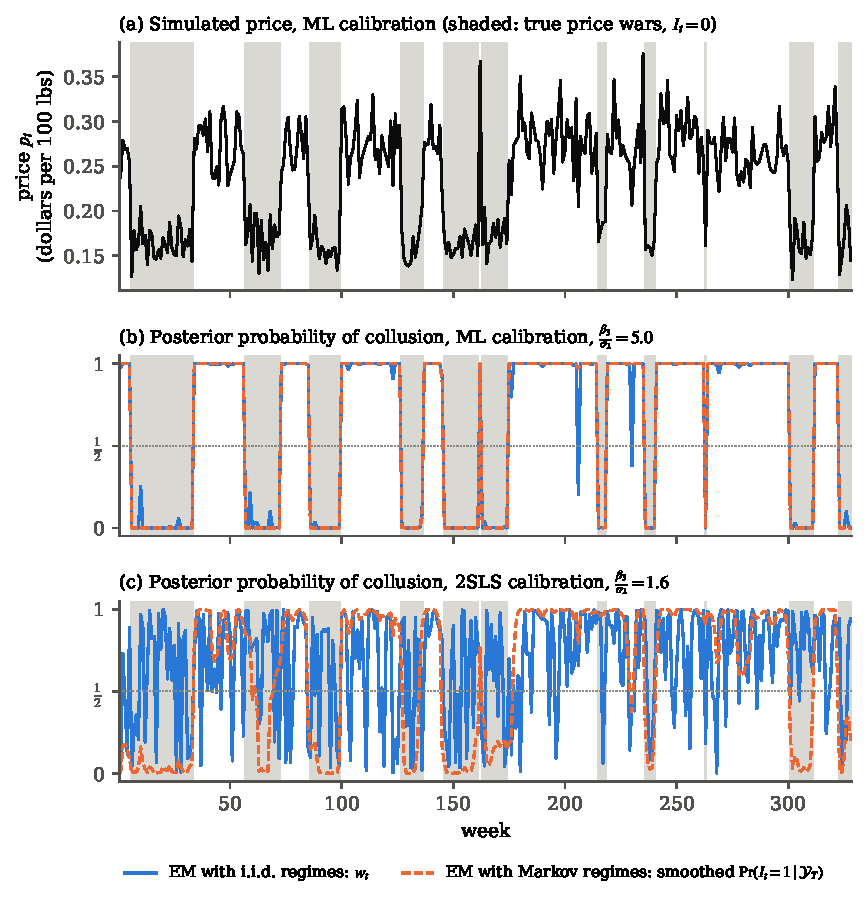
\includegraphics[width=0.92\textwidth]{figures/ch13/regime_sim.pdf}
\caption{A simulated regime-switching price path and the estimated regimes. Panel (a) shows the simulated grain
rate for the calibration to the maximum likelihood column of \citet[Table~3]{Porter1983}, with true price-war
weeks shaded. Panels (b) and (c) show the posterior probability of collusion from EM with i.i.d.\ regimes (solid)
and the smoothed probability from EM with Markov regimes (dashed). Panel (c) uses the two-stage least squares
calibration, in which the regimes are less well separated. Source: our simulation calibrated to Porter (1983,
Tables 3 and 4).}
\label{fig:13-gp-path}
\end{figure}

\begin{figure}[htbp]
\centering
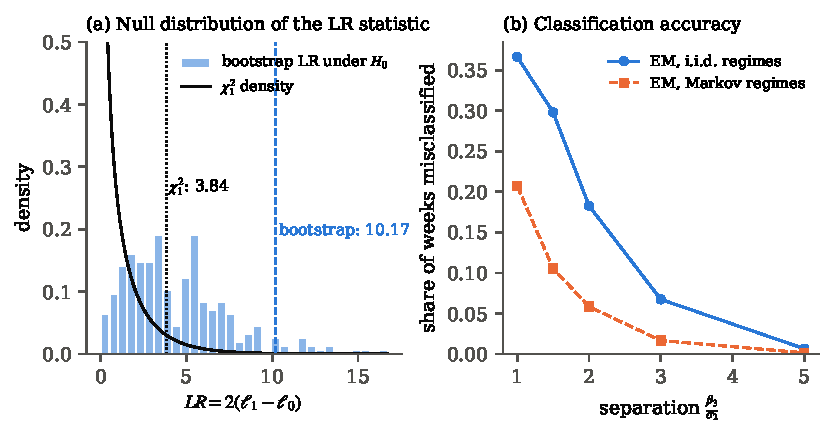
\includegraphics[width=0.95\textwidth]{figures/ch13/em_mc.pdf}
\caption{Panel (a): null distribution of the likelihood-ratio statistic for no switching, from 300 parametric
bootstrap samples of 328 weeks generated without switching, against the $\chi^2_1$ density. The bootstrap 95th
percentile is 10.17, against 3.84 for $\chi^2_1$. Panel (b): average share of misclassified weeks over 60
simulated samples for each separation ratio $\frac{\beta_3}{\sigma_2}$, holding the other parameters at the maximum
likelihood calibration. Source: our simulation.}
\label{fig:13-em-mc}
\end{figure}

The Monte Carlo experiments in \cref{fig:13-em-mc} make the lessons general. Panel (a) shows the null distribution
of the likelihood-ratio statistic for no switching in samples of 328 weeks. Its 90, 95 and 99 percent quantiles are
8.34, 10.17 and 13.17, against 2.71, 3.84 and 6.63 for $\chi^2_1$. A test that used the $\chi^2_1$ cutoff of 3.84
would reject a true null of no switching in 49 percent of samples. Panel (b) shows that classification deteriorates
quickly as separation falls. With i.i.d.\ regimes the share of misclassified weeks is 0.6 percent at a ratio of 5,
6.7 percent at 3, 18 percent at 2 and 37 percent at 1. At a ratio of 1 this is barely better than calling every week
collusive, which errs 38 percent of the time. The Markov model misclassifies 0.1, 1.7, 5.8 and 21 percent. At a ratio
of 1 it even beats the i.i.d.\ Bayes rule with known parameters, whose error is 29 percent, because neighboring weeks
carry information about the regime. The estimated demand slope degrades as well. Across samples, the standard
deviation of $\hat\alpha_1$ from the i.i.d.\ model is 0.09 at a ratio of 5, the same as with known regimes. It is 0.40
at a ratio of 2 and above 1 at lower ratios, while known regimes keep it near 0.09. Porter's maximum likelihood (ML) estimates imply a
ratio of 5.0, so his classification is reliable if his model is right. His 2SLS estimates imply a ratio of 1.6, a
reminder that the separation is itself estimated.

The Berry-Briggs test behaves as the theory predicts on simulated regime series of the same length. On a
first-order Markov chain with the transition probabilities above, the test of $\Pr(I_t = 1\mid 0, 0) =
\Pr(I_t = 1 \mid 1, 0)$, where histories are written $(I_{t-2}, I_{t-1})$, gives $W = 0.34$. On a Green-Porter
chain in which every war lasts exactly 10 weeks, it gives $W = 10.11$. The difference comes from the first week of
a war. Under Green and Porter, a war that has just begun never ends the next week, so $\hat p_{(1,0)} = 0$, while
$\hat p_{(0,0)} = 0.110$ because some wars end after ten weeks. With six to eleven wars in real data, power is low,
and cells with zero variance are common.

\section{The Joint Executive Committee Railroad Cartel}\label{sec:13-jec}

The Joint Executive Committee (JEC) is the most studied cartel in empirical industrial organization. It was legal,
it kept weekly records, and its history includes price wars that contemporaries reported. \Citet{Porter1983} used
its records to estimate the switching model of \cref{sec:13-implications}, and \citet{Ellison1994} re-estimated it
with Markov regimes to ask what started the wars. This section treats both papers in depth.

\subsection{Question and setting}\label{sec:13-jec-setting}

\casehead{The question}
Distinguishing collusion from noncooperative behavior without a smoking gun is hard (p.~301). Porter asks whether
the prices of the JEC switched between collusive and noncooperative regimes, as the trigger-price equilibrium of
\citet{GreenPorter1984} predicts. The alternative is that shifts in demand and cost explain all movements in price
and quantity. The test matters beyond railroads. If wars are part of a collusive equilibrium, an industry with
recurrent price wars is not one in which collusion keeps failing. Green and Porter stress that this undercuts a
common argument against antitrust intervention.

\casehead{The Green-Porter model}
In \citet{GreenPorter1984}, $N$ firms produce a homogeneous good. The market price is
$p_t = \zeta_t\, p\big(\sum_i x_{it}\big)$, where $x_{it}$ is firm $i$'s output and $\zeta_t$ is an i.i.d.\
demand shock with mean one that firms do not observe. Firms see the price but not their rivals' outputs. They produce
collusive quantities while the price stays above a trigger price $\bar p$. When the price falls below $\bar p$, they
produce Cournot quantities for $T - 1$ periods and then resume collusion. In equilibrium no firm cheats, yet wars
occur whenever a low demand shock pushes the price below the trigger. If $F$ is the distribution of $\zeta_t$ and
$y_i$ are the collusive outputs, a war starts in each collusive period with probability
$F(\frac{\bar p}{p(\sum_i y_i)})$. Porter uses three predictions: switches between regimes occur, they follow a pattern, and
collusive output exceeds the static joint-profit level \citep{Porter1983b}.

\casehead{The cartel}
The JEC controlled eastbound freight shipments from Chicago to the Atlantic seaboard. The railroads involved formed
it by agreement in April 1879 and acknowledged it publicly. It preceded the Interstate Commerce Act (1887) and the
Sherman Act (1890), so it was legal (p.~302). According to \citet{Ulen1979}, its enforcement resembled a trigger
strategy. In several instances the cartel thought that cheating had occurred, cut prices for a time, and then
returned to the collusive price.

\casehead{The product}
Grain accounted for 73 percent of the dead-freight tonnage of the JEC, and the rates for flour and provisions were
tied to the grain rate (p.~303). Grain is not perishable, so speed of delivery was not a margin of
differentiation. Most of the wheat was exported, and the rates of different railroads adjusted to compensate for
differences in ocean shipping rates from their port cities. Porter therefore treats the service as a homogeneous
good.

\casehead{Price setting and monitoring}
Railroads set prices, not quantities. Under price setting the natural reversion is Bertrand, which is why the
supply relation of \cref{prop:13-porter-supply} has $\theta = 0$ in wars. The agreement allotted market shares, and
each firm set its rates individually. The JEC office kept weekly accounts, so each railroad saw total shipments.
Actual shares depended on all firms' prices and on unpredictable forces. A firm with a low share could not tell a
rival's secret rate cut from bad luck. This is the inference problem of \citet{Stigler1964}, and it is close to the
Green-Porter problem. \Citet{BrockScheinkman1985} show that equilibria with similar features exist in price-setting
supergames with capacity constraints.

\casehead{Entry and competition}
Entry occurred twice. The Grand Trunk Railway entered in 1880 and the Chicago and Atlantic in 1883. The cartel
accepted the entrants and gave them share allotments. A railroad that entered faced a ``no-exit'' constraint:
bankrupt railroads were relieved by the courts of most of their fixed costs and told to cut prices to raise business
(p.~303). Predation was therefore pointless. Entry shifted the cost constant $A$, and collusion continued.
The main competition came from lake steamers and sailships, which never joined the agreement. The opening and
closing of the Great Lakes to navigation shifted demand predictably, and rates adjusted to the season without
disrupting conduct.

\subsection{Data}\label{sec:13-jec-data}

The data are weekly from week 1 of 1880 to week 16 of 1886, a total of 328 weeks, compiled by \citet{Ulen1979}.
\Cref{tab:13-jec-data} lists the variables and their summary statistics. The price GR is the grain rate in dollars
per 100 pounds and the quantity TQG is total grain shipped by JEC members in tons. LAKES equals one when the Great
Lakes were open to navigation. PO equals one unless the trade magazine \textit{Railway Review} reported a price war,
and it agrees with the reports of the \textit{Chicago Tribune}. PN is the regime classification that Porter
estimates. Four dummies mark changes in the membership of the cartel. Each year is divided into thirteen four-week
periods, and twelve ``monthly'' dummies enter both equations.

\begin{table}[htbp]
\centering
\caption{The JEC data, 1880--1886}\label{tab:13-jec-data}
\small
\begin{tabularx}{\textwidth}{@{}l>{\raggedright\arraybackslash}Xcccc@{}}
\toprule
Variable & Definition & Mean & Std.\ dev. & Min. & Max.\\
\midrule
GR & Grain rate, dollars per 100 lbs & 0.2465 & 0.06653 & 0.125 & 0.40\\
TQG & Total grain shipped, tons per week & 25{,}384 & 11{,}632 & 4{,}810 & 76{,}407\\
LAKES & $=1$ if the Great Lakes were open & 0.5732 & 0.4954 & 0 & 1\\
PO & $=1$ unless a price war was reported & 0.6189 & 0.4864 & 0 & 1\\
DM1 & Grand Trunk entry (week 28, 1880 to week 10, 1883) & 0.4238 & 0.4949 & 0 & 1\\
DM2 & Addition to New York Central (weeks 11--25, 1883) & 0.0457 & 0.2092 & 0 & 1\\
DM3 & Chicago and Atlantic entry (week 26, 1883 to week 11, 1886) & 0.4329 & 0.4962 & 0 & 1\\
DM4 & Chicago and Atlantic leaves (weeks 12--16, 1886) & 0.0152 & 0.1227 & 0 & 1\\
\bottomrule
\end{tabularx}

\smallskip
\begin{minipage}{0.95\textwidth}\footnotesize
Notes: 328 weekly observations. Definitions from \citet[Table~1]{Porter1983}. Statistics for GR, TQG, LAKES and PO
from \citet[Table~2]{Porter1983}, and for DM1--DM4 from \citet[Table~1]{Ellison1994}, which reports the same values
for GR, TQG and LAKES (to fewer digits) but not PO.
\end{minipage}
\end{table}

The dummies cover the sample in five periods. DM1 and DM3 mark the two long periods, 139 and 142 weeks, and together
they cover 281 of the 328 weeks (our computation of the 139 and 142). All price wars occurred inside them (p.~308).

\casehead{Three caveats}
First, the price series is suspect. The JEC polled its members and published an index of their rates. Secret price
cuts would not show up in such an index, because members had no incentive to report them (p.~307). Wars started by
secret cuts may therefore appear in GR with a lag. Porter notes the other side of this coin: an imperfect information
structure is exactly what a trigger-price equilibrium requires. Second, the prices charged by lake steamers, the main
competitors, are not available, so LAKES stands in for them. Third, the model assumes constant market shares across
regimes. Within the DM1 and DM3 periods the average sum of squared deviations from allotted shares was roughly the
same in cooperative and war weeks, which supports the assumption (p.~308). The reported regime series PO also
conflicts sharply with an index of cartel adherence built by \citet{MacAvoy1965}. This conflict is one reason to
estimate the regimes from prices and quantities.

\subsection{Model and estimating equations}\label{sec:13-jec-model}

The estimating equations are demand \eqref{eq:13-demand} and the supply relation \eqref{eq:13-supply-est}, with
twelve seasonal dummies added to both:
\begin{align}
  \log TQG_t &= \alpha_0 + \alpha_1 \log GR_t + \alpha_2 LAKES_t + \text{seasonal dummies} + U_{1t},
  \label{eq:13-porter-demand}\\
  \log GR_t &= \beta_0 + \beta_1 \log TQG_t + \beta_2^\top (DM1_t, \dots, DM4_t)^\top + \beta_3 I_t
  + \text{seasonal dummies} + U_{2t}. \label{eq:13-porter-supply}
\end{align}
The errors are i.i.d.\ bivariate normal with covariance $\Sigma$. By \cref{prop:13-porter-supply}, if wars are
Bertrand reversions, $\beta_0 = \log A$, $\beta_1 = \psi - 1 > 0$ and $\beta_3 > 0$. If cooperative periods
maximized static joint profit, $\beta_3$ would equal $\log\frac{\alpha_1}{1+\alpha_1}$ (\cref{cor:13-static-monopoly}).
Porter leaves $\beta_3$ unrestricted. An optimal trigger-price cartel should set $\beta_3$ positive but below that
level.

Identification follows \cref{sec:13-switching-id}. LAKES shifts demand and identifies the supply slope $\beta_1$.
The regime and the entry dummies shift supply and identify the demand slope $\alpha_1$. Porter estimates the model in
two ways. The first treats PO as the true regime series and applies two-stage least squares. The second treats
$I_t$ as unknown and i.i.d.\ Bernoulli$(\lambda)$, as in \eqref{eq:13-mixture}, and maximizes the likelihood by the
EM algorithm of \cref{sec:13-em}. Weeks with $w_t > \frac{1}{2}$ are classified as collusive (\cref{prop:13-classify}),
which yields PN. Porter acknowledges that a Green-Porter regime series would be Markov of order $T-1$. He gives three
reasons for not imposing it. Estimating under that constraint is hard. The length of wars should vary as entry
changes the cartel's problem. \Citet{GreenPorter1984} show that the bias from treating the regime process as
exogenous is slight when wars are few relative to the sample (pp.~306--307). He also estimated a linear version of the model and found
results that were not significantly different.

\subsection{Results}\label{sec:13-jec-results}

\Cref{tab:13-porter-t3} reproduces Porter's estimates. In the 2SLS columns all coefficients have the expected sign,
but the fit is modest, with a supply $R^2$ of 0.320. In the ML columns the demand equation is practically unchanged.
The supply equation changes. The regime coefficient rises from 0.382 to 0.545 and its standard error halves, while the
supply $R^2$ rises to 0.863 and the standard error of the regression falls from 0.243 to 0.109.

\begin{table}[htbp]
\centering
\caption{Porter's estimates of the JEC demand and supply relations}\label{tab:13-porter-t3}
\small
\begin{tabular}{@{}lcccc@{}}
\toprule
 & \multicolumn{2}{c}{2SLS, regimes from PO} & \multicolumn{2}{c}{ML (EM), regimes estimated}\\
\cmidrule(lr){2-3}\cmidrule(l){4-5}
Variable & Demand & Supply & Demand & Supply\\
\midrule
Constant & 9.169 & $-3.944$ & 9.090 & $-2.416$\\
 & (0.184) & (1.760) & (0.149) & (0.710)\\
LAKES ($\alpha_2$) & $-0.437$ & & $-0.430$ & \\
 & (0.120) & & (0.120) & \\
$\log GR$ ($\alpha_1$) & $-0.742$ & & $-0.800$ & \\
 & (0.121) & & (0.091) & \\
DM1 & & $-0.201$ & & $-0.165$\\
 & & (0.055) & & (0.024)\\
DM2 & & $-0.172$ & & $-0.209$\\
 & & (0.080) & & (0.036)\\
DM3 & & $-0.322$ & & $-0.284$\\
 & & (0.064) & & (0.027)\\
DM4 & & $-0.208$ & & $-0.298$\\
 & & (0.170) & & (0.073)\\
PO or PN ($\beta_3$) & & 0.382 & & 0.545\\
 & & (0.059) & & (0.032)\\
$\log TQG$ ($\beta_1$) & & 0.251 & & 0.090\\
 & & (0.171) & & (0.068)\\
\midrule
$R^2$ & 0.312 & 0.320 & 0.307 & 0.863\\
Std.\ error of regression & 0.398 & 0.243 & 0.399 & 0.109\\
\bottomrule
\end{tabular}

\smallskip
\begin{minipage}{0.9\textwidth}\footnotesize
Notes: From \citet[Table~3]{Porter1983}. Standard errors in parentheses. $T = 328$ weeks. Twelve seasonal dummies
are included in both equations and not reported in the paper. In the ML columns the regime variable is the estimated
classification PN.
\end{minipage}
\end{table}

\casehead{Demand}
Demand is inelastic, with $\hat\alpha_1 = -0.742$ or $-0.800$. Industry marginal revenue
$p(1 + \frac{1}{\alpha_1})$ is then negative. By \cref{cor:13-static-monopoly}, the JEC did not maximize static joint
profit: marginal revenue would have to equal a share-weighted average of marginal costs, which is positive
(p.~308). As expected, open lakes shift rail demand down by 0.43 to 0.44 log points, about 35 percent at a
given price.

\casehead{Supply}
Price is significantly higher in cooperative periods. The supply relation slopes up, which suggests weak
diseconomies of scale, but $\hat\beta_1$ is small and significant only at the 15 percent level in the 2SLS columns.
The entry dummies are negative, and DM3 is below DM2, so each entry lowered the supply intercept. This is the sign
that \cref{prop:13-porter-supply} predicts for an increase in $\Sigma_a$.

\begin{example}[Conduct and margins in cooperative weeks]\label{ex:13-porter-theta}
Apply \eqref{eq:13-theta-from-beta3} to the ML estimates:
\begin{equation*}
  \theta = -0.800\left(e^{-0.545} - 1\right) = -0.800\,(0.580 - 1) = 0.336 .
\end{equation*}
Porter reports this value and calls it roughly consistent with Cournot behavior in cooperative periods (pp.~309--310).
The 2SLS estimates give $\theta = -0.742(e^{-0.382} - 1) = -0.742\,(0.682 - 1) = 0.236$ (our computation). By
\eqref{eq:13-lerner-beta3} the Lerner index in cooperative weeks is $1 - e^{-0.545} = 0.42$ in the ML estimates and
$1 - e^{-0.382} = 0.32$ in the 2SLS estimates (our computation). Porter stresses that the Cournot label has no special
meaning. What matters is that cooperative prices exceed competitive prices but stay below the static joint-profit
level, as an optimal trigger-price cartel would set them.
\end{example}

\begin{example}[Reduced-form effects of collusion and of the lakes]\label{ex:13-porter-rf}
Solve the ML system for the effect of the regime, holding the other variables fixed. Substitute demand into supply:
\begin{equation*}
  \log p = \beta_0' + \beta_1\left(\alpha_0' + \alpha_1\log p + \alpha_2 L\right) + \beta_3 I,
\end{equation*}
where primes denote intercepts that absorb the other variables. Collect the $\log p$ terms:
\begin{equation*}
  (1 - \alpha_1\beta_1)\log p = \beta_0' + \beta_1\alpha_0' + \beta_1\alpha_2 L + \beta_3 I .
\end{equation*}
Hence
\begin{align*}
  \frac{\partial \log p}{\partial I} &= \frac{\beta_3}{1 - \alpha_1\beta_1} = \frac{0.545}{1 + 0.800 \times 0.090}
  = \frac{0.545}{1.072} = 0.508, \\
  \frac{\partial\log Q}{\partial I} &= \alpha_1\frac{\partial\log p}{\partial I} = -0.800\times 0.508 = -0.407 .
\end{align*}
Collusion multiplies price by $e^{0.508} = 1.66$ and quantity by $e^{-0.407} = 0.67$. Revenue rises by the factor
$e^{0.508 - 0.407} = e^{0.101} = 1.11$. For the lakes,
\begin{align*}
  \frac{\partial\log Q}{\partial L} &= \frac{\alpha_2}{1 - \alpha_1\beta_1} = \frac{-0.430}{1.072} = -0.401, \\
  \frac{\partial\log p}{\partial L} &= \frac{\beta_1\alpha_2}{1 - \alpha_1\beta_1} = 0.090 \times (-0.401) = -0.036 .
\end{align*}
Open lakes multiply quantity by $e^{-0.401} = 0.67$ and price by $e^{-0.036} = 0.965$ (our computation throughout).
Because the model is log-linear, these ratios do not depend on where the other variables are held.
\end{example}

\Cref{tab:13-porter-t4} reports Porter's predicted values at the sample means of the other variables. The ratios
match the example. Price is 66 percent higher in cooperative weeks ($\frac{0.2780}{0.1673} = 1.66$), quantity 33
percent lower, and revenue 11 percent higher, a difference of about 11,000 dollars a week in 1880 dollars. These
are Porter's figures (p.~310). The entries of \cref{tab:13-porter-t4} give 13,886 dollars with the lakes closed and
8,970 with them open. Porter's
text says that price was 4.5 percent lower when the lakes were open. The table implies
$\frac{0.1612}{0.1673} = 0.964$, a fall of 3.6 percent, which agrees with the reduced form of
\cref{ex:13-porter-rf}.
Revenue is about 35 percent lower when the lakes are open. Revenue on grain was 70 to 80 percent of the JEC's revenue
from eastbound freight.

\begin{table}[htbp]
\centering
\caption{Predicted price, quantity and revenue by regime and season}\label{tab:13-porter-t4}
\small
\begin{tabular}{@{}lcccc@{}}
\toprule
 & \multicolumn{2}{c}{Lakes closed (LAKES $= 0$)} & \multicolumn{2}{c}{Lakes open (LAKES $= 1$)}\\
\cmidrule(lr){2-3}\cmidrule(l){4-5}
 & War & Cooperation & War & Cooperation\\
 & (PN $= 0$) & (PN $= 1$) & (PN $= 0$) & (PN $= 1$)\\
\midrule
Price (GR, dollars per 100 lbs) & 0.1673 & 0.2780 & 0.1612 & 0.2679\\
Quantity (TQG, tons per week) & 38{,}680 & 25{,}775 & 25{,}904 & 17{,}261\\
Revenue (dollars per week) & 129{,}423 & 143{,}309 & 83{,}514 & 92{,}484\\
\bottomrule
\end{tabular}

\smallskip
\begin{minipage}{0.95\textwidth}\footnotesize
Notes: From \citet[Table~4]{Porter1983}. Computed from the reduced form of the ML estimates in
\cref{tab:13-porter-t3}, with the other explanatory variables at their sample means. Revenue is
$20 \times \text{GR} \times \text{TQG}$: a ton is 20 hundredweight, so this converts dollars per 100 pounds times tons
into dollars.
\end{minipage}
\end{table}

\casehead{Timing of the wars}
\Cref{fig:13-porter-f1} plots the grain rate with the weeks in which PO and PN indicate a war. The two series agree
broadly. Wars averaged about 10 weeks and occurred mainly in 1881, 1884 and 1885. In several episodes PO records a
war before PN does, and the two return to cooperation together (p.~310). This pattern fits a price index that
misses secret cuts at the start of a war. PN was not constrained to resemble PO in any way. \Cref{tab:13-porter-t5}
shows that it agrees with the trade-press reports and disagrees with MacAvoy's index of share instability. MacAvoy's index is
highest in 1880, a year without any war in either PO or PN.

\begin{figure}[htbp]
\centering
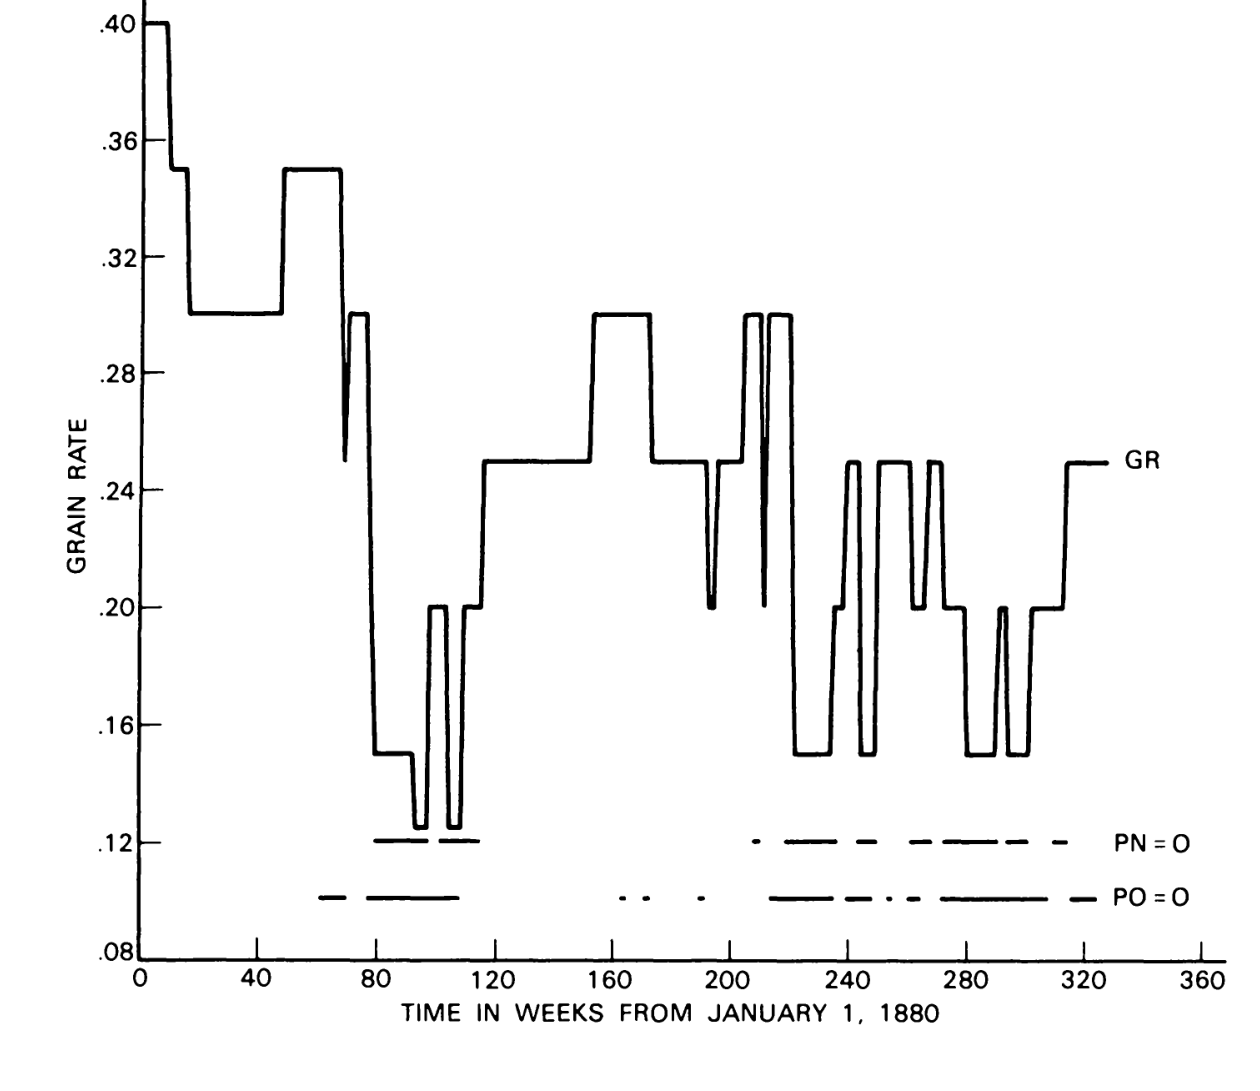
\includegraphics[width=0.78\textwidth]{figures/ch13/porter1983_fig1.png}
\caption{The JEC grain rate in dollars per 100 pounds, from January 1880. Upper segments mark the weeks that the
estimated series classifies as price wars (PN $= 0$), and lower segments those of the trade-press series
(PO $= 0$). Source: Porter (1983), Figure 1.}
\label{fig:13-porter-f1}
\end{figure}

\begin{table}[htbp]
\centering
\caption{Indices of cartel nonadherence by year}\label{tab:13-porter-t5}
\small
\begin{tabular}{@{}lccc@{}}
\toprule
 & & \multicolumn{2}{c}{Share of weeks at war}\\
\cmidrule(l){3-4}
Year & MacAvoy's index & Reported (PO) & Estimated (PN)\\
\midrule
1880 & 26 & 0.00 & 0.00\\
1881 & 14 & 0.67 & 0.44\\
1882 & 18 & 0.06 & 0.21\\
1883 & 6 & 0.10 & 0.00\\
1884 & 16 & 0.58 & 0.40\\
1885 & 10 & 0.77 & 0.67\\
1886 (16 weeks) & 15 & 0.50 & 0.06\\
\bottomrule
\end{tabular}

\smallskip
\begin{minipage}{0.95\textwidth}\footnotesize
Notes: From \citet[Table~5]{Porter1983}, whose first two columns come from \citet{Ulen1979}. MacAvoy's index counts
months, summed over members, in which a member's share of tonnage deviated from its trend share. A deviation counts
when it exceeds the standard error of the member's trend regression. The reported and estimated columns are
$\frac{1}{52}\sum_t(1 - PO_t)$ and $\frac{1}{52}\sum_t(1 - \hat I_t)$ over the weeks of each year, with denominator 16
in 1886.
\end{minipage}
\end{table}

\casehead{Testing for switching}
The coefficients on PO and PN are significantly positive, so cooperative periods had significantly higher prices.
Porter's likelihood-ratio statistic \eqref{eq:13-porter-lr} is $2T(L_1 - L_0) = 554.1$. He refers it to the
$\chi^2_1$ distribution and rejects the hypothesis of no switching overwhelmingly. As \cref{sec:13-tests} explains,
the $\chi^2_1$ reference is invalid, and the statistic omits the mixing terms of the likelihood. Its simulated null
distribution, with a 95th percentile near 240 in our calibration, still lies far below 554. Price and quantity
changes cannot be attributed to demand and structural shifts alone, given the specification. The agreement between
PN and PO also shows that the estimated switches are not an artifact of missing data.

\casehead{Entry and the frequency of wars}
The 1881 and 1884 wars each began about 40 weeks after an entry, of the Grand Trunk and of the Chicago and Atlantic
respectively (p.~311). Entry did not cause an immediate reversion. It plausibly raised the chance of later
ones. Wars were more frequent, and shorter on average, when the cartel had more members. This fits the general
point that enforcement gets harder as the number of firms grows (\cref{ch:collusion-theory}).

\casehead{Triggers}
Green-Porter wars follow unexpected demand drops. Porter regresses the length of each war on the demand residual in
the week before it began and finds little predictive power. Price wars were not preceded by large negative demand
residuals. He offers two reasons for caution. The demand residual omits the lake steamers' prices, so it measures
unexpected demand poorly. The firms set prices, so wars may have followed unpredictable swings in market shares, as
\citet{Stigler1964} predicts.

\Cref{tab:13-porter-t6} gives annual wheat shipments from Chicago by lake and by rail. 1880 was a boom year, which
accounts for its high rates. Among the other years, total shipments are not correlated with nonadherence. The war
years 1881, 1884 and 1885 stand out by the JEC's high share of intermodal shipments: 50.0, 34.0 and 48.5 percent,
against 13.8 to 26.8 percent in 1882, 1883 and 1886. JEC wars did not coincide with lake steamer price wars, and they
did not always occur when total demand was low. They were not systematically related to the opening or closing of the
lakes either (p.~313).

\begin{table}[htbp]
\centering
\caption{Annual eastbound shipments of wheat from Chicago by lake and rail}\label{tab:13-porter-t6}
\small
\begin{tabular}{@{}lccccc@{}}
\toprule
 & \multicolumn{2}{c}{Lake} & \multicolumn{2}{c}{Rail} & Total\\
\cmidrule(lr){2-3}\cmidrule(lr){4-5}
Year & Millions of bushels & Percent & Millions of bushels & Percent & millions of bushels\\
\midrule
1880 & 16.69 & 77.9 & 4.728 & 22.1 & 21.42\\
1881 & 7.688 & 50.0 & 7.680 & 50.0 & 15.37\\
1882 & 14.94 & 86.2 & 2.389 & 13.8 & 17.33\\
1883 & 7.067 & 73.2 & 2.590 & 26.8 & 9.66\\
1884 & 11.52 & 66.0 & 5.928 & 34.0 & 17.45\\
1885 & 5.436 & 51.5 & 5.116 & 48.5 & 10.55\\
1886 & 10.51 & 82.6 & 2.209 & 17.4 & 12.72\\
\bottomrule
\end{tabular}

\smallskip
\begin{minipage}{0.75\textwidth}\footnotesize
Notes: From \citet[Table~6]{Porter1983}.
\end{minipage}
\end{table}

\subsection{Ellison's re-examination}\label{sec:13-ellison}

\casehead{The question}
Porter's evidence shows that wars occurred. \Citet[p.~38]{Ellison1994} argues that the core content of the
Green-Porter theory is more specific: wars occur because firms follow strategies in which random demand shocks
trigger them. He asks three questions. Did the wars of the JEC start after the signals that trigger strategies would
use? Were prices less collusive, or wars more likely, in booms, as Rotemberg and Saloner's logic suggests? Did
members cut prices in secret, which no theory of optimal collusion allows?

\casehead{Adapting the theories}
The JEC differs from the textbook Green-Porter model in two ways (pp.~38--39). The railroads set prices, and
reputations for service and different route structures differentiated their demands. Secret cuts made prices
unobservable. The quantity data, in contrast, were presumably reliable. The cartel even considered using the shipment
data to compute side payments by firms that exceeded their allotments. Many trigger strategies could support a
nearly optimal outcome in this setting. Ellison lists three plausible triggers. One firm obtaining a suspiciously high
market share is the best signal of cheating. High aggregate demand is another, because a price cut expands demand as
well as moving shares. An unusually low share for one firm is a third, which a coalition-proof equilibrium might use.

\casehead{Model and data}
Ellison's model follows Porter's closely. Demand is
\begin{equation}\label{eq:13-ellison-demand}
  \log Q_t = \alpha_0 + \alpha_1\log P_t + \alpha_2 LAKES_t + \sum_{k=1}^{12}\alpha_{2+k}\,SEAS_{kt} + U_{1t},
  \qquad U_{1t} = \rho U_{1,t-1} + V_{1t},
\end{equation}
with $|\rho| < 1$. The supply relation is
\begin{equation}\label{eq:13-ellison-supply}
  \log P_t = \beta_0 + \beta_1\log Q_t + \beta_3 I_t + \sum_{k=1}^{4}\beta_{3+k}\,DM_{kt} + U_{2t},
\end{equation}
where we keep our $\beta_3$ for the coefficient that Ellison writes $\beta_2$. The errors $(V_{1t}, U_{2t})$ are
bivariate normal. Regimes follow the logit Markov chain \eqref{eq:13-logit-transition}, with
\begin{equation}\label{eq:13-ellison-logit}
  \Pr(I_{t+1} = 1 \mid I_t, Z_t) = \Lambda\left(\gamma_1 I_t + \gamma_0(1 - I_t) + \gamma_Z^\top Z_t I_t\right),
\end{equation}
where $Z_t$ holds candidate triggers. A negative element of $\gamma_Z$ means that the variable raises the probability
that a collusive week is followed by a war. The structural equations and the transitions are estimated jointly by
maximum likelihood with the filter of \cref{sec:13-markov}, following \citet{CosslettLee1985}. Standard errors are
robust and computed from numerical derivatives. Joint estimation should date the onset of wars more accurately than
Porter's two-step approach and give more power to detect triggers. The data are Ulen's weekly series, the same 328
weeks that Porter used.

\Cref{fig:13-ellison-regimes} summarizes the regime structures that Ellison estimates, including the hidden demand
regimes introduced below.

\begin{figure}[htbp]
\centering
\begin{tikzpicture}[>=Stealth, font=\footnotesize,
  box/.style={draw, rounded corners=2pt, align=center, minimum width=4.2cm, inner sep=3pt, fill=white}]
  \draw[rounded corners=6pt, thick] (-2.4,-2.75) rectangle (2.4,2.35);
  \node[font=\small] at (0,1.95) {Collusion, $I_t = 1$};
  \node[box] at (0,1.0) {REGIME1: high demand\\ probability $r_1$};
  \node[box] at (0,-0.35) {REGIME2: medium demand\\ probability $r_2$};
  \node[box] at (0,-1.85) {REGIME3: low demand\\ probability $1 - r_1 - r_2$};
  \draw[rounded corners=6pt, thick] (5.6,-2.45) rectangle (10.4,1.85);
  \node[font=\small] at (8.0,1.45) {Price war, $I_t = 0$};
  \node[box] at (8.0,0.4) {REGIME2: medium demand\\ probability $\frac{r_2}{1 - r_1}$};
  \node[box] at (8.0,-1.3) {REGIME3: low demand\\ probability $\frac{1 - r_1 - r_2}{1 - r_1}$};
  \draw[->, thick] (2.4,0.55) -- node[above, align=center] {$q_{10,t} = 1 - q_{11,t}$} (5.6,0.55);
  \draw[->, thick] (5.6,-1.0) -- node[below, align=center] {$q_{01,t} = \Lambda(\gamma_0)$} (2.4,-1.0);
  \draw[->, thick] (-0.9,2.35) .. controls (-1.2,3.5) and (1.2,3.5) .. (0.9,2.35);
  \node at (0,3.7) {$q_{11,t} = \Lambda(\gamma_1 + \gamma_Z^\top Z_t)$};
  \draw[->, thick] (7.1,1.85) .. controls (6.8,3.0) and (9.2,3.0) .. (8.9,1.85);
  \node at (8.0,3.2) {$q_{00,t} = 1 - q_{01,t}$};
\end{tikzpicture}
\caption{The regime structure in \citet{Ellison1994}. Conduct follows a two-state Markov chain whose transition
probabilities are logits. Candidate triggers $Z_t$ enter only the probability $q_{11,t}$ of staying in collusion.
In the hidden-regime models, demand regimes are drawn each week given conduct. REGIME1 occurs only under collusion,
and the other regimes keep the same relative probabilities in both conduct states. The standard model has no demand
regimes, and model 2 has only REGIME1 and REGIME2. Drawn by us after Ellison's Figures 1 and 3.}
\label{fig:13-ellison-regimes}
\end{figure}

\casehead{The standard model}
\Cref{tab:13-ellison-t2} reports Ellison's ``standard'' model, which adds AR(1) demand errors and Markov regimes to
Porter's specification, next to a version without serial correlation. The lagged demand error has coefficient
$\hat\rho = 0.832$ (0.085), and allowing for it changes the demand estimates. The price elasticity rises from 0.84 to
1.80, so the JEC faced elastic demand. The regime effect hardly moves, from 0.660 to 0.637. By
\eqref{eq:13-theta-from-beta3}, the conduct index rises with the elasticity,
\begin{equation*}
  \theta = 0.843\left(1 - e^{-0.660}\right) = 0.41, \qquad \theta = 1.802\left(1 - e^{-0.637}\right) = 0.85
\end{equation*}
(our computation, against Ellison's reported 0.40 and 0.85). \Cref{rem:13-lerner-vs-theta} explains the pattern. The collusive
Lerner index $1 - e^{-\beta_3}$ is 0.48 or 0.47 in the two columns, and the elasticity converts the same margin into
very different conduct. With elastic demand a static monopoly benchmark exists. \Cref{cor:13-static-monopoly} gives
$\log\frac{1.802}{0.802} = 0.81$, above the estimated 0.637, so the JEC still priced below static monopoly (our
computation). Ellison concludes that the JEC was much more aggressive in its pricing than earlier work reported.

\begin{table}[htbp]
\centering
\caption{Ellison's standard model of the JEC}\label{tab:13-ellison-t2}
\small
\begin{tabular}{@{}lcc@{}}
\toprule
Variable & Standard model & No serial correlation\\
\midrule
\multicolumn{3}{@{}l}{\textit{Demand}}\\
Constant & 7.677 (1.882) & 9.019 (0.361)\\
$\log P$ ($\alpha_1$) & $-1.802$ (1.287) & $-0.843$ (0.193)\\
LAKES & $-0.009$ (0.112) & $-0.460$ (0.348)\\
\multicolumn{3}{@{}l}{\textit{Supply}}\\
Constant & $-4.764$ (1.863) & $-5.649$ (9.461)\\
$\log Q$ ($\beta_1$) & 0.306 (0.178) & 0.398 (0.928)\\
DM1 & $-0.154$ (0.075) & $-0.211$ (0.124)\\
DM2 & $-0.246$ (0.064) & $-0.283$ (0.160)\\
DM3 & $-0.317$ (0.076) & $-0.373$ (0.242)\\
DM4 & $-0.198$ (0.119) & $-0.419$ (0.422)\\
$I_t$ ($\beta_3$) & 0.637 (0.104) & 0.660 (0.406)\\
\multicolumn{3}{@{}l}{\textit{Regimes (logit index)}}\\
Constant if $I_t = 1$ ($\gamma_1$) & 3.675 (0.474) & 3.661 (0.513)\\
Constant if $I_t = 0$ ($\gamma_0$) & $-2.641$ (0.404) & $-2.620$ (0.476)\\
\multicolumn{3}{@{}l}{\textit{Other}}\\
$\sigma_1$ & 0.290 (0.061) & 0.396 (0.029)\\
$\sigma_{12}$ & $-0.007$ (0.004) & $-0.045$ (0.142)\\
$\sigma_2$ & 0.160 (0.045) & 0.191 (0.313)\\
$U_{1,t-1}$ ($\rho$) & 0.832 (0.085) & \\
\midrule
Log likelihood & 181.0 & 37.2\\
\bottomrule
\end{tabular}

\smallskip
\begin{minipage}{0.8\textwidth}\footnotesize
Notes: From \citet[Table~2]{Ellison1994}. Standard errors in parentheses. Twelve seasonal dummies in demand are
included and not shown. The regime constants are the logit indices of $\Pr(I_{t+1} = 1 \mid I_t)$.
\end{minipage}
\end{table}

The regime constants imply strong persistence. The probability that collusion continues is
$\Lambda(3.675) = \frac{e^{3.675}}{1 + e^{3.675}} = 0.975$, and the probability that a war week is followed by
collusion is $\Lambda(-2.641) = 0.067$ (p.~42). By \cref{lem:13-durations}, collusive spells last
$\frac{1}{1 - 0.975} = 40$ weeks on average and wars $\frac{1}{0.067} = 15$ weeks. The long-run share of collusive
weeks is $\frac{0.067}{0.025 + 0.067} = 0.73$ (our computation). The regimes are far from independent, which
confirms the observation of \citet{CosslettLee1985}.

\casehead{Candidate triggers}
To test for triggers, Ellison builds four share variables (p.~41). Let $s_{it}$ measure the strength of firm $i$'s
demand, and let $\hat s_{it}$ be its predicted value. Each variable is the largest normalized deviation across
firms, $\max_i \frac{s_{it} - \hat s_{it}}{\sigma_i}$, where $\sigma_i$ is the sample standard deviation.
\begin{itemize}
\item \textit{BIGSHARE1} uses $s_{it} = \log q_{it} - \frac{1}{N}\sum_j \log q_{jt}$, where $N$ is the number of
firms, with the average of the
previous twelve weeks as $\hat s_{it}$. Using logs keeps the trade-off between the gain from a price cut and the
loss from a war proportional across firms of different sizes.
\item \textit{BIGSHARE2} uses the ordinary market share, with the same prediction.
\item \textit{BIGSHAREQ} uses the log measure, with the assigned quota as the prediction. Quotas were often set
unrealistically, so deviations from them measure adherence poorly. \citet{MacAvoy1965} reports that the Chicago and
Grand Trunk was admitted with a 10 percent quota while receiving only 2 to 7 percent of the traffic at the cartel
price.
\item \textit{SMALLSHARE} is the largest shortfall of any firm's log measure below its prediction.
\end{itemize}
The demand innovation $V_{1t}$ and the full demand shock $U_{1t}$ serve as aggregate triggers. Under Green and
Porter, unanticipated shocks start wars. Under Rotemberg and Saloner, wars are more likely when demand is high and
expected to decline. Since $U_{1t} = \rho U_{1,t-1} + V_{1t}$, the two can be separated.

\Cref{tab:13-ellison-t3} reports the trigger coefficients. Only six wars are identified in the standard model, so
high significance levels are not to be expected. BIGSHARE1 has the predicted negative sign and is significant at the
6 percent level in a one-tailed test. BIGSHARE2 and BIGSHAREQ are negative but smaller and insignificant.
SMALLSHARE has the wrong sign. The aggregate innovation $V_{1t}$ is large, negative and significant at the 6 percent
level. In model 6 the innovation keeps its sign while the full shock $U_{1t}$ enters with a positive, insignificant
coefficient. The unanticipated component of demand predicts wars and the anticipated component does not. This
separates the Green-Porter explanation from the Rotemberg-Saloner one, which \citet{Porter1985} could not do with a
two-step approach.

\begin{table}[htbp]
\centering
\caption{What started the price wars of the JEC?}\label{tab:13-ellison-t3}
\small
\begin{tabular}{@{}lcccccc@{}}
\toprule
\multicolumn{7}{@{}l}{\textit{Panel A. Estimated regimes, Markov model (Table 3)}}\\
Model & 1 & 2 & 3 & 4 & 5 & 6\\
\midrule
Constant & 4.63 (0.77) & 4.36 (0.77) & 3.95 (1.30) & 2.96 (0.66) & 4.43 (0.81) & 4.35 (0.90)\\
BIGSHARE1 & $-0.77$ (0.49) & & & & & \\
BIGSHARE2 & & $-0.46$ (0.39) & & & & \\
BIGSHAREQ & & & $-0.21$ (1.06) & & & \\
SMALLSHARE & & & & 0.66 (0.89) & & \\
$V_{1t}$ & & & & & $-4.15$ (2.64) & $-5.00$ (3.15)\\
$U_{1t}$ & & & & & & 1.17 (1.15)\\
\midrule
\multicolumn{7}{@{}l}{\textit{Panel B. Reported regimes, logit for the onset of a war (Table 4)}}\\
Model & 1 & 2 & 3 & 4 & & \\
\midrule
Constant & 3.68 (0.65) & 3.55 (0.65) & 3.25 (0.61) & 2.92 (0.57) & & \\
BIGSHARE1 & $-0.71$ (0.46) & & & & & \\
BIGSHARE2 & & $-0.51$ (0.39) & & & & \\
BIGSHAREQ & & & $-0.33$ (0.44) & & & \\
SMALLSHARE & & & & 0.05 (0.37) & & \\
\bottomrule
\end{tabular}

\smallskip
\begin{minipage}{0.95\textwidth}\footnotesize
Notes: From \citet[Tables~3 and 4]{Ellison1994}. Standard errors in parentheses. Coefficients of the logit for
$\Pr(I_{t+1} = 1 \mid I_t = 1, Z_t)$, so a negative coefficient raises the probability that a war begins. In Panel A
each model contains all variables of the standard model. Panel B uses Ulen's reported regimes $J_t$. Means of
BIGSHARE1, BIGSHARE2, BIGSHAREQ and SMALLSHARE are 1.09, 1.24, 1.17 and 1.23 \citep[Table~1]{Ellison1994}.
\end{minipage}
\end{table}

The timing of the estimated wars is uncertain, and the standard model does not match the onset date of Ulen's
classification for any war (p.~43). Panel B of \cref{tab:13-ellison-t3} therefore fits simple logits for the onset
of a war in the reported regime series. The estimates are similar to Panel A, which supports a Green-Porter-type
trigger.

\casehead{Strength of the trigger}
A trigger must also deter cheating. Ellison gives a rough calculation (p.~44). Suppose a firm offers a small secret
price cut that raises its demand by 10 percent and its current profit by 8 to 10 percent. The cut raises its
BIGSHARE1 measure by $\frac{\log 1.1}{\sigma_i}$ when it would otherwise have had the largest deviation. With the
estimated coefficient, a simulation gives an increase in the probability of a war of about 0.001. If a war costs
about 15 times the per-period profit, the expected future loss is about $0.001 \times 15$, roughly 1 to 2 percent of
current profit. The estimated trigger is several times too weak to deter cheating, and the precision of the estimates
does not allow it to be much stronger. Ellison offers two readings. The firms may have reacted to information that
the data miss, or to a true trigger that is only correlated with BIGSHARE1. Alternatively, the JEC's responses may
have been too weak to sustain a noncooperative equilibrium.

\casehead{Booms}
The basic Rotemberg-Saloner model has perfect information and no regime shifts. It is a model of countercyclical
collusion. With imperfect monitoring, its logic implies that a cartel facing a temporary peak in demand lowers its
price or makes its trigger more sensitive (p.~45). A boom here is a period in which current demand is high
relative to demand over the next fifteen weeks or so, the horizon of a war. Two sources create booms in the JEC data.
Serially correlated shocks make a high shock raise demand today by more than in the future. Seasonality makes demand
peak in winter, just before the lakes open. Ellison builds an index of the ratio of current demand to expected
demand during a subsequent war (p.~46),
\begin{equation}\label{eq:13-ellison-boom}
  BOOM_t = K\,\frac{\exp\left(\alpha_2 LAKES_t + \sum_k \alpha_{2+k} SEAS_{kt} + \rho U_{1,t-1}\right)}
  {\sum_{s=1}^{52}\left(\hat p_{w,t+s} - \hat p_{c,t+s}\right)
   \exp\left(\alpha_2 LAKES_{t+s} + \sum_k \alpha_{2+k} SEAS_{k,t+s} + \rho^{s+1}U_{1,t-1}\right)} - 1 .
\end{equation}
Here $\hat p_{w,t+s} - \hat p_{c,t+s}$ is the additional probability of being in a war $s$ weeks after one begins,
taken from the standard model. $K$ is a scaling constant. He adds $BOOM_t I_t$ to the supply relation and
$BOOM_t$ to the transition logit. A seasonal-only version and the lagged shock $U_{1,t-1}$ separate the two sources.

The results are imprecise (\cref{tab:13-ellison-booms}). The coefficient on $BOOM_t I_t$ implies a collusive price
about 3 percent lower when the incentive to deviate is one standard deviation above its mean. Its standard error is
almost twice the estimate, so neither procyclical collusion nor a 12 percent reduction can be rejected (p.~47).
The demand-shock decomposition is more precise but still insignificant. It implies a 5 percent lower price when
$U_{1,t-1}$ is one standard deviation above its mean. The seasonal decomposition shows nothing. In the transition
logit, $BOOM_t$ has the wrong sign. Controlling for the innovation $V_{1t}$, the predictable decline in demand after
a positive shock does not cause wars. The seasonal effect has the right sign but is insignificant.

\begin{table}[htbp]
\centering
\caption{Booms and collusion in the JEC}\label{tab:13-ellison-booms}
\small
\begin{tabular}{@{}lccc@{}}
\toprule
\multicolumn{4}{@{}l}{\textit{Panel A. Supply relation with boom interactions (Table 5)}}\\
 & Combined effect & Demand shocks & Seasonal\\
\midrule
$I_t$ & 0.758 (0.416) & 0.712 (0.195) & 0.622 (0.119)\\
$BOOM_t \times I_t$ & $-0.233$ (0.428) & & \\
$U_{1,t-1}\times I_t$ & & $-0.156$ (0.164) & \\
$SEAS_t \times I_t$ & & & 0.041 (0.417)\\
$\log P$ in demand & $-1.996$ (2.055) & $-1.594$ (0.898) & $-1.574$ (1.459)\\
Log likelihood & 186.2 & 187.1 & 181.2\\
\midrule
\multicolumn{4}{@{}l}{\textit{Panel B. Logit for $\Pr(I_{t+1} = 1\mid I_t = 1, Z_t)$ (Table 6)}}\\
 & Model 1 & Model 2 & Model 3\\
\midrule
Constant & 3.64 (0.49) & 4.35 (0.90) & 3.87 (0.71)\\
$BOOM_t$ & 0.36 (1.48) & & \\
$U_{1t}$ & & 1.17 (1.15) & \\
$V_{1t}$ & & $-5.00$ (3.15) & \\
$SEASONAL_t$ & & & $-2.51$ (3.50)\\
\bottomrule
\end{tabular}

\smallskip
\begin{minipage}{0.9\textwidth}\footnotesize
Notes: From \citet[Tables~5 and 6]{Ellison1994}. Standard errors in parentheses. Rotemberg and Saloner predict a
negative coefficient on the boom interactions in Panel A and negative coefficients on the boom measures in Panel B.
Panel A models also include boom terms in the transition logit. Model 2 of Panel B repeats model 6 of
\cref{tab:13-ellison-t3}.
\end{minipage}
\end{table}

Ellison's verdict is cautious. The JEC does not support the view that wars occur during booms. The tests have little
power, so a small degree of countercyclical pricing or a small rise in the frequency of wars cannot be ruled out. He
also notes that a nineteenth-century railroad cartel is perhaps among the least likely places to apply the theory.

\casehead{Secret price cuts}
All the theories predict that members never cut prices in secret. The trade press of the time suggests that some did.
The \textit{Daily Commercial Bulletin} of June 16, 1881, for example, reported doubts that a quoted rate on grain to
New York was being respected (p.~49). A one-week secret cut would be invisible to an econometrician, as to the
JEC itself. If cutting and adherence were both common, however, secret cuts act like an omitted variable that shifts
demand upward relative to the official price. Ellison looks for such shifts with hidden demand regimes.

Model 2 adds a dummy REGIME1 to demand \eqref{eq:13-ellison-demand}. The high-demand regime occurs with probability
$r_1$ in collusive weeks and never in wars, when firms already price competitively. Model 3 adds two dummies, REGIME1
and REGIME2, for three demand regimes. Under collusion they occur with probabilities $r_1$, $r_2$ and $1 - r_1 - r_2$.
REGIME1 never occurs in wars, and the other two keep their relative probabilities in both conduct states
(\cref{fig:13-ellison-regimes}). Ellison writes $p_1$ and $p_2$ for our $r_1$ and $r_2$. The low regime might reflect
bad weather, labor problems or low steamship rates. Since the regimes enter demand, whose error is autocorrelated, the
filter runs on pairs of consecutive states (\cref{rem:13-ar1}).

\Cref{tab:13-ellison-t7} reports the estimates. Ellison calls the fit almost unreasonably successful. The log
likelihood rises from 181.0 to 529.0 and 582.5. Ellison likens the gain to Porter's when he added a second supply
regime (p.~51). The comparison is loose, because Porter's figure is not a mixture log likelihood
(\cref{sec:13-tests}). The $t$-statistics on REGIME1 are 12.1 and 26.7. In model 2, REGIME1 raises demand by about 55 percent
($e^{0.439} = 1.55$). In model 3, REGIME1 has demand 41 percent above REGIME2, and the low regime has demand 32 percent
below REGIME2 ($e^{0.344} = 1.41$ and $e^{-0.384} = 0.68$).

\begin{table}[htbp]
\centering
\caption{Hidden demand regimes in the JEC}\label{tab:13-ellison-t7}
\small
\begin{tabular}{@{}lccc@{}}
\toprule
 & Model 2 & Model 3 & Model 3 with trigger test\\
 & (Table 7) & (Table 7) & (Table 9)\\
\midrule
\multicolumn{4}{@{}l}{\textit{Demand}}\\
$\log P$ ($\alpha_1$) & $-1.354$ (0.711) & $-1.587$ (0.092) & $-1.57$ (0.43)\\
LAKES & $-0.222$ (0.073) & $-0.229$ (0.092) & $-0.23$ (0.06)\\
REGIME1 & 0.439 (0.036) & 0.728 (0.027) & 0.73 (0.04)\\
REGIME2 & & 0.384 (0.022) & 0.38 (0.05)\\
\multicolumn{4}{@{}l}{\textit{Supply}}\\
$\log Q$ ($\beta_1$) & 0.220 (0.153) & 0.242 (0.038) & 0.24 (0.09)\\
$I_t$ ($\beta_3$) & 0.595 (0.079) & 0.608 (0.047) & 0.61 (0.07)\\
\multicolumn{4}{@{}l}{\textit{Transitions and regime probabilities}}\\
Collusion continues & 0.979 (0.012) & 0.976 (0.037) & logit below\\
War ends & 0.061 (0.028) & 0.070 (0.076) & 0.07 (0.03)\\
$r_1$ & 0.650 (0.071) & 0.256 (0.083) & 0.26 (0.05)\\
$r_2$ & & 0.519 (0.086) & 0.52 (0.07)\\
\multicolumn{4}{@{}l}{\textit{Logit for collusion continuing}}\\
Constant & & & 5.65 (1.06)\\
$V_{1t}$ & & & $-3.17$ (1.26)\\
$RSHIFT_t$ & & & $-0.48$ (1.03)\\
\multicolumn{4}{@{}l}{\textit{Other}}\\
$U_{1,t-1}$ ($\rho$) & 0.888 (0.031) & 0.947 (0.018) & 0.947 (0.02)\\
\midrule
Log likelihood & 529.0 & 582.5 & 584.4\\
\bottomrule
\end{tabular}

\smallskip
\begin{minipage}{0.92\textwidth}\footnotesize
Notes: From \citet[Tables~7 and 9]{Ellison1994}. Standard errors in parentheses. Seasonal dummies, the constants, the
entry dummies and the error covariances are included and not shown. ``Collusion continues'' and ``war ends'' are
Ellison's $q_{123}$ (or $q_{12}$) and $q_0$. $RSHIFT_t = \alpha_{15}REGIME1_t + \alpha_{16}(REGIME2_t - 1)$ is the
demand effect of the hidden regimes. Table 9 reports two decimals.
\end{minipage}
\end{table}

\casehead{Interpreting the hidden regimes}
Ellison warns that the regimes could reflect weather, irregular schedules, steamship competition, mechanical
problems, or failures of the functional form (p.~52). He checks three kinds of evidence.

The first is the size and frequency of the implied cuts. Trade-press reports suggest that cuts of 10 to 25 percent
were reasonable, and the cartel sometimes went two years between wars, so cuts were not very common (p.~53). In
model 2, REGIME1 occurs in 65 percent of collusive weeks, and with an elasticity of 1.35 it would require price cuts
of 25 to 30 percent. Ellison rejects it as a measure of secret cuts. In model 3, REGIME1 occurs in 26 percent of
collusive weeks, and with an elasticity of 1.59 it requires a cut of about 20 percent. To check, solve
$(1 - x)^{-1.587} = e^{0.344}$ for the cut $x$:
\begin{equation*}
  x = 1 - \exp\left(-\frac{0.344}{1.587}\right) = 1 - e^{-0.217} = 0.195
\end{equation*}
(our computation). A kernel density of the standard model's demand residuals $\hat V_{1t}$ has a second, smaller peak
to the right, as occasional price cuts of similar size would produce \citep[Figure~2]{Ellison1994}.

The second is historical evidence on cutting. Ellison codes two indicators from the \textit{Daily Commercial
Bulletin}. CUTREPORTED marks the 12 weeks in which an article reported rumors of secret cuts. CUTLISTED marks the 18
weeks in which the average listed daily price was at least three cents below the official price. Overall, 26 percent
of weeks fall in the high-demand regime. One and two weeks after a CUTREPORTED week, the shares are 57 and 66 percent,
both significantly higher (Table~8, p.~54). Four weeks after a CUTLISTED week the share is 60 percent, and after a
reported war it is 40 to 46 percent at lags of two to four weeks. The pattern fits retaliatory cutting after reports of
cheating. About 15 percent of high-demand weeks are attributable to these excess occurrences.

The third is a test of observability. If the hidden regimes were invisible to the JEC, a Green-Porter trigger would
respond to total unexpected demand, the innovation plus the regime effect $RSHIFT_t$, with equal coefficients. If the
JEC observed the regimes, $RSHIFT_t$ should not matter. In the last column of \cref{tab:13-ellison-t7}, $V_{1t}$ has
coefficient $-3.17$ (1.26) and $RSHIFT_t$ has $-0.48$ (1.03). Equality is rejected at the 5 percent level
(p.~56). The high-demand regime mostly reflects factors that the JEC recognized and that did not lead it to start
wars. A by-product is that the demand innovation is now a clearly significant trigger, with a $t$-statistic of about
2.5.

\casehead{Conclusions}
Ellison draws four conclusions (p.~56). Price wars occurred, as earlier work found, but prices were much closer
to the monopoly level than previously reported. A model that focuses on transition probabilities finds evidence of
trigger strategies, and serially correlated demand lets the trigger be distinguished from the Rotemberg-Saloner
prediction. Some secret price cutting occurred, contrary to the literal theory. It was not widespread, and
secret cuts account for only a small fraction of the high-demand weeks. The JEC gives no support to the view that
booms make wars more likely, although the tests have little power.

\subsection{Assessment of the JEC evidence}\label{sec:13-jec-assessment}

\casehead{What the JEC shows}
Three findings have held up across specifications. First, regime switches are real and large. Prices in
cooperative weeks were about 66 percent above war prices, holding demand and cost fixed (\cref{tab:13-porter-t4}),
and the estimated regimes match contemporary reports of wars. Second, the timing of wars fits imperfect monitoring.
Wars were persistent, they followed unexpected demand innovations and possibly unusual shares, and they did not
follow predictable booms. Third, cooperative prices stayed below the static monopoly level. With inelastic demand
this follows from \cref{cor:13-static-monopoly}, and with Ellison's elastic demand it follows from comparing the
estimated $\beta_3$ with \eqref{eq:13-beta3-monopoly}. Both readings agree with \citet{Porter1983b}.

\casehead{Limits}
The evidence has limits, several of them general.
\begin{itemize}
\item \emph{Observational equivalence.} By \cref{prop:13-obs-equiv}, prices and quantities alone cannot separate
conduct regimes from cost regimes. The JEC evidence leans on outside information, the trade-press series, to read
the regimes as conduct.
\item \emph{Measurement.} GR is a polled index that likely misses secret cuts, so the start of wars is measured with
error. The prices of lake steamers are missing from demand, which weakens tests based on demand residuals.
\item \emph{The regime process.} Porter assumes i.i.d.\ regimes, which the data reject. Ellison's Markov model fixes
this, but the trigger tests rest on six wars, and no specification identifies a trigger strong enough to deter
cheating.
\item \emph{Functional form.} With latent regimes, identification comes from normality (\cref{prop:13-switch-id}).
Ellison's hidden demand regimes show how easily the same machinery finds additional ``regimes'' in non-normal
residuals.
\item \emph{The meaning of $\theta$.} The conduct index depends on the demand elasticity, which moves from 0.74 to
1.80 across specifications, and on the assumption that wars are Bertrand reversions. The collusive margin
$1 - e^{-\beta_3}$ is more robust (\cref{rem:13-lerner-vs-theta,rem:13-corts}).
\end{itemize}

Several papers extend the analysis. \Citet{LeePorter1984} combine the reported series with prices and quantities in a
model with imperfect sample separation. \Citet{Porter1985} studies the incidence and duration of wars with a two-step
approach. He finds no significant evidence that share deviations triggered wars. He does find that large aggregate
demand did, but he cannot separate a trigger from a Rotemberg-Saloner effect \citep[p.~39]{Ellison1994}.
\Citet{Hajivassiliou1989} relates an index of grain production to the probability of being in a war.
\Citet{BerryBriggs1988} test the order of the regime process and find the JEC closer to Abreu, Pearce and Stacchetti
than to Green and Porter. Together these studies made the JEC the reference case for the econometrics of collusion.
The legal cartels of the next section show what records of internal deliberations add to such price-and-quantity
evidence.

\section{Rules, Communication and Price Wars in Other Legal Cartels}\label{sec:13-legal}

The Joint Executive Committee of \cref{sec:13-jec} shows what prices and quantities can reveal about a legal
cartel. Records of a cartel's internal deliberations reveal things that prices cannot. They show how firms
designed rules, what they said to one another, how they judged accusations of cheating, and how they responded.
This section studies two such records. The first is the Sugar Institute, a trade association of American cane
sugar refiners that operated from 1927 to 1936 \citep{GenesoveMullin2001}. The second is the bromine cartel of
1885--1914, whose contracts and correspondence survive in the papers of the Dow Chemical Company
\citep{Levenstein1997}. Between the two we place a short link to the price wars of pre-1914 sugar refining. That
link illustrates the observational-equivalence problem of \cref{prop:13-obs-equiv} with real data.

The two cases speak to the predictions collected in \cref{tab:13-predictions}. Theories of collusion under
imperfect monitoring predict that firms punish on the basis of noisy public signals and that the punishment is
the same whatever the deviation. Both cases agree with \citet{Stigler1964} that detecting secret price cuts was
the central problem of the cartel. Both cases disagree with the formal theory about how firms treated the
cheating they found.

\subsection{The Sugar Institute, 1927--1936}\label{sec:13-sugar-institute}

\casehead{The question and the source}
How does communication help firms collude? The repeated-game models of \cref{ch:collusion-theory} give
communication a narrow role. Firms may announce what they observed so that private histories become public, or
they may coordinate on one of many equilibria. \citet{GenesoveMullin2001} study the private discussions of one
cartel to see what firms said and why. Their source is unusual. Louis V. Place was vice president of McCahan, a
midsize refinery in Philadelphia, ``in charge of all activities of the company except production and raw sugar
purchases.'' He wrote over 500 pages of single-spaced notes on the meetings of the Institute's Board of
Directors, Executive Committee and Enforcement Committee from January 1929 through mid-1930 (p.~379). He also
recorded the informal gatherings after the meetings and private conversations with other refiners. The memos
circulated among only some six McCahan executives, so they are candid. Place testified at the trial that he
regularly destroyed them once he received the much less revealing official minutes. Genesove and Mullin
supplement the memos with the record of \textit{United States v.\ Sugar Institute}.

\casehead{Setting}
The Sugar Institute was a \emph{trade association}, an organization of competing firms in one industry. It was
formed in December 1927 by 14 firms that owned nearly all the cane sugar refining capacity of the United
States. Several years of falling margins and excess capacity preceded it. It operated until 1936, when the
Supreme Court ruled its practices illegal. The Institute never fixed prices or allocated market shares, and
there was no legal finding that it did. It fixed rules instead. The main principles were stated in a Code of
Ethics, and the details were issued as a series of Code Interpretations. The rules covered every aspect of the
distribution and marketing of sugar other than the basis price itself. The refiners had the Code vetted by the
Department of Justice, which nonetheless prosecuted them. The legal status of such associations was unclear in
the 1920s. There were 150 ``open price'' associations in 1921, and over 400 operated under the National Recovery
Administration when the Court decided the case (p.~385, fn.~20).

\casehead{Measuring performance with direct cost data}
Cane sugar refining has a fixed-proportions technology, which gives a direct measure of marginal cost
(\cref{sec:03-sugar-cost}). One pound of refined sugar requires 1.075 pounds of raw sugar. All other variable
costs amount to 0.60 cents per pound, or 60 cents per hundred pounds in December 1927 dollars. That is 26 cents in
the 1898 dollars of Genesove and Mullin's earlier work.\footnote{McCahan's internal documents put these costs
at 63.6 cents per hundred pounds in 1927, against an industry average of 55.3 cents. Genesove and Mullin judge
these differences across firms economically slight (p.~381, fn.~9).} Let $p^{\mathrm{ref}}_t$ and
$p^{\mathrm{raw}}_t$ be the prices of refined and raw sugar in cents per pound. Marginal cost is
\begin{equation}\label{eq:13-gm-mc}
  mc_t = 1.075\,p^{\mathrm{raw}}_t + 0.60 .
\end{equation}
Genesove and Mullin define the \emph{proper margin} as the refined price net of the raw sugar it contains,
\begin{equation}\label{eq:13-gm-pm}
  \mathit{PM}_t = p^{\mathrm{ref}}_t - 1.075\,p^{\mathrm{raw}}_t .
\end{equation}
Substituting \eqref{eq:13-gm-mc} into the Lerner index of \cref{eq:02-lerner} gives
\begin{equation}\label{eq:13-gm-lerner}
  L_t = \frac{p^{\mathrm{ref}}_t - mc_t}{p^{\mathrm{ref}}_t}
      = \frac{\mathit{PM}_t - 0.60}{p^{\mathrm{ref}}_t} .
\end{equation}
\Cref{tab:13-gm-t1} reproduces their Table~1. Columns (2) to (6) are averages of weekly data from Willett and
Gray's trade journal, and all prices are in December 1927 dollars.

\begin{table}[htbp]
\centering
\caption{Performance of the cane sugar refiners before, during and after the Sugar Institute}\label{tab:13-gm-t1}
\small
\begin{tabular}{@{}lccccccc@{}}
\toprule
(1) & (2) & (3) & (4) & (5) & (6) & (7) & (8)\\
 & Proper & Proper margin & Lerner & & & Beet & Foreign refined\\
Year & margin & $-\,0.60$ & index & Output & Profits & share & share\\
\midrule
1914 & 0.99 & 0.39 & 0.047 & 106 & 3.7 & & \\
1915 & 0.95 & 0.35 & 0.036 & 114 & 3.9 & & \\
1916 & 1.04 & 0.44 & 0.041 & 118 & 4.3 & & \\
1917 & 1.31 & 0.70 & 0.068 & 103 & 7.4 & & \\
1918 & 1.04 & 0.44 & 0.048 & 93 & 3.9 & & \\
1919 & 0.88 & 0.27 & 0.029 & 121 & 4.2 & & \\
1920 & 1.94 & 1.34 & 0.129 & 113 & 12.2 & & \\
1921 & 1.06 & 0.46 & 0.073 & 128 & 6.0 & & \\
1922 & 0.97 & 0.36 & 0.060 & 157 & 5.9 & & \\
1923 & 0.88 & 0.28 & 0.033 & 123 & 3.3 & & \\
1924 & 1.06 & 0.45 & 0.061 & 128 & 5.4 & 15.3 & 0.5\\
1925 & 0.80 & 0.19 & 0.035 & 143 & 2.6 & 16.1 & 0.5\\
1926 & 0.79 & 0.18 & 0.034 & 142 & 2.7 & 15.4 & 0.5\\
1927 & 0.74 & 0.14 & 0.023 & 130 & 2.0 & 14.7 & 2.5\\
\midrule
1928 & 1.00 & 0.40 & 0.071 & 122 & 4.9 & 18.7 & 6.2\\
1929 & 1.00 & 0.39 & 0.077 & 128 & 5.1 & 14.7 & 8.3\\
1930 & 1.04 & 0.44 & 0.091 & 126 & 5.6 & 17.0 & 8.0\\
1931 & 0.96 & 0.36 & 0.071 & 107 & 3.8 & 20.5 & 9.6\\
1932 & 1.07 & 0.47 & 0.093 & 103 & 4.7 & 21.0 & 12.8\\
1933 & 1.14 & 0.54 & 0.093 & 99 & 5.3 & 21.6 & 14.7\\
1934 & 1.17 & 0.56 & 0.104 & 94 & 5.3 & 25.1 & 11.0\\
1935 & 1.07 & 0.47 & 0.083 & 96 & 4.4 & 22.1 & 11.1\\
1936 & 1.03 & 0.42 & 0.072 & 98 & 4.2 & & \\
1937 & 1.03 & 0.43 & 0.077 & 108 & 4.9 & & \\
1938 & 0.98 & 0.37 & 0.077 & 100 & 3.7 & & \\
1939 & 1.01 & 0.41 & 0.079 & 99 & 3.9 & & \\
1940 & 1.01 & 0.41 & 0.086 & 100 & 3.9 & & \\
1941 & 0.85 & 0.25 & 0.048 & 116 & 3.0 & & \\
\bottomrule
\end{tabular}

\smallskip
\begin{minipage}{0.95\textwidth}\footnotesize
Notes: Reproduced from \citet{GenesoveMullin2001}, Table~1 (p.~382). Columns (2) to (6) are weekly averages.
Column (2) is $\mathit{PM}_t$ of \eqref{eq:13-gm-pm} in cents per pound. Column (3) subtracts 0.60, the
non-raw-sugar component of variable cost per pound. Column (4) is the ratio of column (3) to the refined price,
\eqref{eq:13-gm-lerner}. Column (5) is the output of the Atlantic refiners in millions of pounds. Column (6) is the
sum of the variable profits of the Atlantic refiners in millions of dollars. Columns (7) and (8) are the annual
shares (percent) of domestic beet sugar production and of imported refined sugar in total U.S.\ consumption.
Prices are in December 1927 dollars. The rule marks the formation of the Institute in December 1927. Sources
given by the authors: Willett and Gray's \textit{Weekly Statistical Sugar Trade Journal}.
\end{minipage}
\end{table}

The Institute coincided with a sharp rise in margins. Genesove and Mullin report that the proper margin rose by
about 20 to 25 cents per hundred pounds over the preceding three years. In \cref{tab:13-gm-t1}, the proper margin
averaged 0.78 cents per pound in 1925--1927 and 1.01 cents in 1928--1930. The rise is 0.23 cents per pound, or 23
cents per hundred pounds (our computation). The Lerner index averaged 0.031 in 1925--1927 and 0.080 in
1928--1930, so it rose by a factor of about 2.6 (our computation). This is the ``more than doubling'' of the
Lerner index in the text (p.~381). \Cref{fig:13-gm-lerner} plots column (4) for all 28 years.

\begin{figure}[htbp]
\centering
\begin{tikzpicture}
\begin{axis}[
  width=0.92\textwidth, height=6.4cm,
  xmin=1913.5, xmax=1941.5, ymin=0, ymax=0.14,
  xlabel={Year}, ylabel={Lerner index $L_t$},
  xtick={1915,1920,1925,1930,1935,1940},
  x tick label style={/pgf/number format/1000 sep={}},
  ytick={0,0.02,0.04,0.06,0.08,0.10,0.12,0.14},
  y tick label style={/pgf/number format/fixed,/pgf/number format/precision=2},
  tick label style={font=\footnotesize}, label style={font=\small},
  clip=false]
\fill[gray!15] (axis cs:1927.5,0) rectangle (axis cs:1936.5,0.14);
\node[font=\footnotesize, align=center] at (axis cs:1932,0.128) {Sugar Institute\\(formed Dec.\ 1927)};
\draw[dashed] (axis cs:1913.5,0.11) -- (axis cs:1941.5,0.11);
\node[font=\footnotesize, anchor=south west] at (axis cs:1914,0.11) {1892 margin, 0.11};
\addplot[thick, mark=*, mark size=1.4pt] coordinates {
 (1914,0.047) (1915,0.036) (1916,0.041) (1917,0.068) (1918,0.048) (1919,0.029) (1920,0.129)
 (1921,0.073) (1922,0.060) (1923,0.033) (1924,0.061) (1925,0.035) (1926,0.034) (1927,0.023)
 (1928,0.071) (1929,0.077) (1930,0.091) (1931,0.071) (1932,0.093) (1933,0.093) (1934,0.104)
 (1935,0.083) (1936,0.072) (1937,0.077) (1938,0.077) (1939,0.079) (1940,0.086) (1941,0.048)};
\end{axis}
\end{tikzpicture}
\caption{Lerner index of cane sugar refining, 1914--1941, computed from direct marginal cost,
$L_t = \frac{p^{\mathrm{ref}}_t - 1.075\,p^{\mathrm{raw}}_t - 0.60}{p^{\mathrm{ref}}_t}$. The shaded years are
1928--1936. The dashed line is the 1892 margin, which \citet{GenesoveMullin2001} propose as a realistic
monopoly benchmark. Redrawn from \citet{GenesoveMullin2001}, Table~1, column (4).}\label{fig:13-gm-lerner}
\end{figure}

The Lerner index uses list prices, and secret discounts were the reason the Institute was founded. Genesove and
Mullin argue that this bias strengthens their conclusion. The argument takes one line. Let the average
transaction price be $p^{a}_t = p^{\mathrm{ref}}_t - d_t$, where $d_t \ge 0$ is the average secret discount.
Marginal cost is measured directly, so the change in the transaction margin is
\begin{equation}\label{eq:13-gm-lowerbound}
  \Delta\left(p^{a}_t - mc_t\right) = \Delta\left(p^{\mathrm{ref}}_t - mc_t\right) - \Delta d_t
  \;\ge\; \Delta\left(p^{\mathrm{ref}}_t - mc_t\right)
  \quad\text{whenever } \Delta d_t \le 0 .
\end{equation}
If the Institute eliminated secret concessions, or at least did not increase them, the rise in the list margin is
a lower bound on the rise in the transaction margin.

How close did the refiners come to monopoly? The inverse elasticity rule of \cref{sec:02-monopoly} gives a
monopoly Lerner index of $\frac{1}{\varepsilon}$. With the demand elasticity of 1.75 that Genesove and Mullin
estimated for 1890--1914, the monopoly Lerner index is $\frac{1}{1.75} = 0.57$, far above anything in
\cref{tab:13-gm-t1}. The authors give two reasons for the gap. The growth of beet sugar after the First World War
raised the elasticity of demand facing cane refiners, and the refiners wanted to deter foreign and domestic
entry. They propose 11 percent as a realistic benchmark. That was the margin in 1892, when both the margin and
American Sugar Refining's market share (92 percent) reached their peaks. Over 1928--1935 the Lerner index
averaged 0.085 (our computation), about three quarters of that benchmark, as the authors state. The benchmark has
a structural reading. If 0.11 were the Lerner index of a firm pricing optimally against its residual demand, the
inverse elasticity rule would put that residual elasticity at $\frac{1}{0.11} \approx 9$ (our computation). A
perceived elasticity five times the market elasticity is consistent with pricing to limit entry and imports.

Quantities tell the same story more weakly. The output of the Atlantic refiners fell when the Institute began,
though only a little, because sugar demand is inelastic. Output kept falling during the Great Depression, but much
less than the 24 percent fall in total industrial output (p.~382). Rivals outside the agreement expanded. The
share of imported refined sugar, almost all of it Cuban, rose from under half a percent to 6 percent in the
Institute's first year and to almost 15 percent in 1933. The Sugar Act of 1934 then cut it to 11 percent by
legislative fiat. Coca-Cola, the largest buyer of refined sugar, switched entirely to foreign suppliers. The beet
share rose from an average of 15.4 percent in 1924--1927 to 17.7 percent in 1928--1931, but its year-to-year
variability prevents a firm attribution to the Institute.

\casehead{Collusion by rules}
Genesove and Mullin describe the Institute as implicit collusion on price combined with explicit collusion on
business practices (p.~383). Rule number one required ``open prices and publicly announced terms.'' Prices
were posted on the refiners' bulletin boards, the Institute was notified of every change in prices and pricing
methods, and changes were announced by 3:00 p.m. These provisions continued existing practice. The more
important existing practice was the \emph{moves system}. An announced price decrease took effect immediately,
while an increase took effect only after a day. Buyers purchased a month's supply at a time, so they waited after
a decrease until other refiners matched it, which they always did. Reactions often came within minutes. Price
competition therefore preceded trade.

\begin{remark}[Why the moves system leaves only secret deviations]\label{rem:13-moves}
Let $N$ refiners sell a homogeneous good at a common list price $p$ with $c < p \le p^m$, and let industry profit
$\pi(p) = (p - c)D(p)$ be increasing on $[c, p^m]$. Suppose that a public price cut to $p' < p$ is matched by
every rival before any buyer purchases. Buyers then split equally among the refiners, and the cutter earns
$\frac{1}{N}\pi(p')$ in the period. Because $\pi$ is increasing on $[c, p^m]$,
\begin{equation*}
  \frac{1}{N}\,\pi(p') < \frac{1}{N}\,\pi(p) .
\end{equation*}
A public cut lowers the cutter's own profit. Only a concession that rivals cannot see, and hence cannot match,
can raise a refiner's share. This is why the Institute worked to raise the probability of detecting secret
concessions and did not try to shorten reaction times (\citealp{GenesoveMullin2001}, pp.~383--384). The
model of \cref{sec:13-transparency-theory} formalizes this probability.
\end{remark}

Almost every contractual term could hide a price cut, so the rules were wide-ranging and detailed.
\Cref{tab:13-gm-rules} lists the five rules that Genesove and Mullin examine, the concession each one closed, and
the cost it imposed. The Institute also disallowed quantity discounts, allowances for returned sugar bags,
long-term contracts and certain credit arrangements. It required refiners to report all sales of damaged sugar,
drew up a list of permissible consignment points, and forbade downstream firms to combine brokerage and storage.
Enforcing the last rule required private investigation and auditing.

\begin{table}[htbp]
\centering
\caption{Sugar Institute rules, the hidden concessions they closed, and their costs}\label{tab:13-gm-rules}
\small
\begin{tabularx}{\textwidth}{@{}>{\raggedright\arraybackslash}p{2.6cm}>{\raggedright\arraybackslash}X>{\raggedright\arraybackslash}X@{}}
\toprule
Rule & Concession it closed & Cost or side effect\\
\midrule
Water-damaged or frozen sugar & Sound sugar shipped to a favored buyer and invoiced as damaged. Each sale now
required ``full details of amount, location, reason and price'' to be circulated. & Discounts on truly damaged
sugar became public.\\
\addlinespace
Credit terms & Varying the grace period that qualified for the customary 2 percent cash discount. & Grace period
fixed at 7 days rather than 14.\\
\addlinespace
Storage & Brokers who ran warehouses cut storage charges in place of the sugar price. & Storage first banned in
buyers' warehouses, then in broker-affiliated ones as refiners switched.\\
\addlinespace
Delivery time & Letting favored buyers take delivery after the contract date, which saved storage and interest
and was a price cut if the basis price rose. & Delivery dates enforced. Weekly reports of undelivered contracts.
A secondhand market sold overbought sugar at discounts of 5 to 20 cents.\\
\addlinespace
Freight & Rebates on freight rates that the Interstate Commerce Commission did not regulate, especially private
water charters. & Charters registered, uniform rates required, written promises not to rebate. Then delivered
pricing with a refusal to sell f.o.b.\ refinery.\\
\bottomrule
\end{tabularx}

\smallskip
\begin{minipage}{0.95\textwidth}\footnotesize
Notes: Compiled from \citet{GenesoveMullin2001}, Sections II, III and VI (pp.~383--387 and 390--392). The
organization into columns is ours.
\end{minipage}
\end{table}

The rules were costly. A monopolist could have discriminated among customers and exploited efficiencies that the
rules forbade. When large buyers in Buffalo asked to receive sugar by water barge, even at the higher rail rate,
the Institute refused for fear of creating an opportunity for discounts. The move to delivered pricing led
refiners to replace brokers in barge transport. Between 1928 and 1931, barge shipments by refiners rose by 400
percent while those by customers fell by two thirds. Large customers denied quantity discounts threatened to
integrate backward, as the grocery chain A\&P did. The ban on long-term and tolling contracts also sacrificed
efficiencies. Place was even prepared to forgo allocating production by cost. He feared that local differences in
loading costs would lead to different rates, writing that ``those enjoying more economical loading conditions
can pocket the profits.'' The District Court judge put it succinctly (p.~384, fn.~14). The refiners
``preferred to have all sugar sold in any given trade areas at precisely the same prices and terms'' over
economies in distribution.

Genesove and Mullin consider an alternative reading in which the rules suppressed nonprice competition directly.
Contractual harmonization usually chose the lower ``quality.'' The grace period was set at 7 days, and the number
of consignment points was cut by half. They find this reading incomplete for three reasons. It does not explain
many rules, such as the ban on quantity discounts or the notification rules discussed below. The number of sugar
grades was never restricted, although grade proliferation was costly to small refiners. Most persuasively, the
reading misses the stated intermediate goal of eliminating discrimination among customers, the first principle
of the Code of Ethics. They conclude that suppressing nonprice competition complemented harmonization but was
not its purpose.

\casehead{An incomplete agreement and its governance}
The initial agreement was incomplete in the sense of the theory of the firm. No one could foresee and enumerate
all contingencies. The refiners told the court that the Code ``could not be, self-operative'' and required
``interpretation and administration and consultation.'' The weekly meetings completed the contract in three ways.
They answered minor questions the Code left open. May damaged sugar be sold under a price guarantee? No. Do
30-day contracts end on the 30th day or on the same day of the next month? The former. They modified rules that
proved unworkable. The original policy charged the regulated all-rail rate whatever the mode of transport. This
leveraged each refiner's power in its hinterland into contested markets such as the Great Lakes, and cheaper water
routes offered too much arbitrage. A later regime of limited differential rates also failed. The refiners then
moved to delivered prices with a refusal to sell f.o.b.\ refinery. The move was presented as independent action.
The Place memos show that it was coordinated over several meetings in one week of April 1929. It had been delayed
for over a year for fear of the antitrust authorities. Finally, the meetings closed loopholes. Each rule that shut
one channel for secret concessions opened another, less effective one, much as taxpayers respond to a new tax
rule.

The meetings formalized their decisions as Code Interpretations, which took on a quasi-judicial character.
Participants spoke of evidence and precedent. Institute counsel called the Interpretations ``absolutely
indispensable,'' since ``even national laws must be `interpreted' by the Courts.'' Genesove and Mullin argue that
legal principles helped complete the contract. One decision covered many later incidents, disputes were
minimized, and participants could anticipate one another's responses.

A natural worry is that frequent meetings invite renegotiation out of punishments \citep{McCutcheon1997}.
Genesove and Mullin see no sign of it. The refiners chose weekly meetings and no one proposed meeting less often.
Threats were never retracted, and no firm bargained its way out of a punishment (p.~396).

\casehead{Prior notification}
Institute rules required a firm to notify the other members before selling damaged sugar, introducing new private
brands, or changing any terms of trade. Firms also notified one another when no rule required it. Revere, a Boston
refiner, told the Institute before it considered lowering its rail rates to the water rate. Arbuckle announced a
cut in freight rates privately to the members before announcing it publicly. Notification served two purposes.
First, it removed the lag before retaliation in nonprice dimensions, complementing open price announcements. Full
collusion is possible when firms can respond to deviations before consumers act \citep{Bhaskar1989}. In the
language of \cref{sec:13-transparency-theory}, notification makes a nonprice change visible with probability one
before it can steal customers.

Second, notification served the individual interest of the notifying firm. Some actions are profitable once
rivals have responded but steal market share if rivals do not anticipate them. Stealing share risks retaliation.
A Godchaux representative praised Savannah, which explained its need to change its business methods at a Board
meeting before announcing anything. As a result, its ``subsequent announcements, because understood, did not
cause any upheavals.'' Genesove and Mullin describe a two-level agreement. The lower level was a precise set of codes and
resolutions. The higher level was an understanding that a refiner could withdraw from a lower-level rule if it
first told the others. All the cases they record concern an easing of terms of trade. This distinguishes them
from the familiar case of advance notice of price increases, where notice coordinates a move that is profitable
only if all firms follow.

\casehead{Ex post determination of fault}
The meetings were also a forum for accusation and rebuttal. In March 1929, American charged Federal with secretly
cutting prices by loading barges without charge. The dispute turned on what ``f.o.b.'' meant, and Federal
may have believed that other firms loaded barges the same way. As in \citet{GreenPorter1984}, the evidence of
cheating was ambiguous. In their model the confounding factor is a fall in demand. Here it was a
misunderstanding about the terms of the agreement. In other cases it was an
external event, such as a shortage of barges or vacuum pans. An accusation could also be factually wrong. An
Institute investigator once reported a concession on one barrel of caked sugar as a concession on a much larger
amount of powdered sugar.

Genesove and Mullin give two reasons why firms investigated before retaliating. A firm may not have intended to
break the agreement, and the Institute let an accused firm prove its innocence on factual or logical grounds. In
their words, the Institute ``raised the signal-to-noise ratio of indicators of cheating.'' An accuser acting alone
also risked being accused of cheating itself. Evidence that only the accuser could observe was therefore
insufficient, and accusers needed evidence that others could verify. In one case an investigator produced an invoice that seemed to show a sale
from Godchaux to Edgar, a Detroit broker that also ran storage. Place examined the invoice and judged it part of
Godchaux's bookkeeping, and the refiners were notified of ``the error which apparently had been made.''
\Cref{cor:13-false-alarms} below shows why lowering the rate of false accusations relaxes the incentive
constraint.

\casehead{Cheating and retaliation}
In the theory of implicit collusion, every deviation by a player is treated the same way, whatever its nature or
timing. Genesove and Mullin observe something quite different. Firms did cheat. A Detroit chain store received a
secret concession when it switched from National to Spreckels. Spreckels overpaid truckers, who then worked a few
hours ``free'' for certain customers. Arbuckle knowingly sold to a dummy corporation that fronted for Edgar.
Cheating was worst in the South. Godchaux accepted a contract with a price guarantee for delivery by water barge
whose movements it agreed not to trace. Texas City accepted a 42-day contract, and its owner offered to fire his
top three executives over it. Colonial offered a 6-cent rebate to large buyers, and in Tampa postdated checks were
used to give credit (p.~390).

Outside the South, none of these violations led to competitive prices as in \citet{GreenPorter1984}, let alone
to subcompetitive prices as in \citet{AbreuPearceStacchetti1986}. The usual sequence was that fault was
determined, the refiner confessed, justified itself or blamed its broker, and the practice stopped. Longer or open
violations were matched. When one firm openly lowered its rail rate to the barge rate, the others lowered theirs
to the same level. When the Pacific refiners gave a freight allowance, American announced that it would match it.
Matching was in degree and in kind. The response stayed within the instrument of the violation, although
\citet{BernheimWhinston1990} show that punishing across all instruments strengthens collusion. When McCahan
concluded that some refiners were not enforcing contract time limits, Place first threatened, and then with
others carried out, a refusal to enforce McCahan's terms. Matching was even institutionalized. Each refiner
reported its undelivered contracts for each price move, the reports circulated weekly, and an unannounced
understanding let all refiners spread deliveries over as many days as the most delayed refiner.

Massive retaliation came only after large-scale cheating in several dimensions, and only in the South. As early as
June 1929 an investigator reported the Code ``dead in the water'' in Texas. C\&H refused to discuss any single
violation there. It threatened to ask for ``the entire suspension of the Code of Ethics in the Texas territory''
so that all refiners could ``fight fire with fire.'' Elsewhere in the South, Savannah was dissuaded
from resigning by a resolution that allowed members to ``meet the competition of Hershey,'' a Cuban refiner
outside the Institute. The condition was that the competitor and the territory be announced to the Institute
first. The agreement could be suspended, but only with prior notification.

Genesove and Mullin summarize the contrast in terms of statistical errors. In the Green and Porter equilibrium,
firms accept punishing when no one has cheated so that cheating never occurs. The refiners chose the opposite end
of the trade-off. They accepted some cheating so as not to punish inappropriately, and they sustained imperfect
collusion because wholesale cheating did meet massive retaliation. Two features of the industry help explain this
choice. Refiners sold through brokers, who often dealt exclusively with one refiner and earned a fixed commission
on every sale. A broker gained much more from stealing a customer than its refiner did. Brokers' cheating added
noise to demand and let refiners hide behind their brokers. The same agency relation made punishment costly,
since selling agents cannot easily be told to follow one set of rules one day and another the next. Matching also
has a known robustness, as in the ``tit for tat'' strategies of \citet{Axelrod1984}, and it fitted the ethic of
nondiscrimination in the Code.

\casehead{What the refiners did not do}
In the model of \citet{GreenPorter1984} firms monitor a public signal, the market price, and never see their
rivals' outputs (\cref{sec:13-jec-setting}). \citet[p.~90]{GreenPorter1984} note that noisy market-share
information could serve as the signal instead. Genesove and Mullin take this broader reading. They describe
Green-Porter and its offshoots as models in which cheating is inferred from a firm's market share (p.~394). Some
models of imperfect monitoring also transfer share to firms that lost it. Market-share data were available to the
refiners at low frequency, but they rarely used them this way. Genesove and Mullin find only four such incidents in nearly a hundred meetings
over 18 months (p.~394). In one, Arbuckle's low share was blamed on its strict contract enforcement, and the
possibility that American's advertising was responsible was dismissed because others' sales had not fallen. The
reason for a fall in share mattered, unlike in the market-share reading of the theory. There was no mechanism for reallocating market shares.
American twice proposed market-sharing schemes in 1929, but neither came with an enforcement mechanism and
Institute counsel would not allow discussion that ``could bring actual results.'' There were no mergers, and
calls for coordinated market withdrawals went unfulfilled. The contrast with the quota-and-transfer cartels of
\citet{HarringtonSkrzypacz2011}, discussed in \cref{sec:13-imperfect}, is sharp.

\casehead{Interpretation, critiques and contribution}
The Institute did more than host communication. It was a neutral party that could audit members and aggregate
self-reported statistics into confidential industry totals. Firms could also use it as a scapegoat or a
commitment device in bargaining with brokers and buyers. Genesove and Mullin draw three lessons for theory.
Collusive agreements are incomplete and need governance. Communication within the agreement is rich, with prior
notification and ex post determination of fault. Retaliation is much more restrained than theory predicts,
partly because of selling agents' high-powered incentives. They also stress that Stigler's basic insight
survives. The rules were built by firms that knew each would later want to undermine them.

The evidence has limits. The notes come from one participant at a midsize refinery and cover 18 months of a
nine-year cartel. The performance measures use list prices. A list price is never below the transaction price, so the list
margin bounds the level of the transaction margin from above. Only the rise in the transaction margin is bounded
from below, by the rise in the list margin, and \eqref{eq:13-gm-lowerbound} gives that bound only if secret
discounts did not grow. There is no counterfactual for what prices would have been without the
Institute in the Great Depression, and the rise in imports shows that the cartel's market power was limited.
Inferring strategies from what participants said requires trusting that they described their reasoning
accurately, a premise the authors defend. The forgone efficiencies are public, while those in
\citet{AtheyBagwellSanchirico2004} are private information, so that theory cannot explain why the refiners gave
them up. Genesove and Mullin's own explanation is that exploiting the efficiencies would have destroyed the
homogeneity of practices that made pricing transparent. The paper's contribution is to show that cartels can
invest in detection itself, through rules that make contracts comparable and through a forum that judges
evidence. It also poses the puzzle of tolerated cheating that \citet{BernheimMadsen2017} later addressed
(\cref{sec:13-imperfect}).

\subsection{Price wars in pre-1914 sugar refining}\label{sec:13-gm-pricewars}

The same industry provides a test of what price and cost data can say about conduct. \Cref{sec:03-sugar-wars}
analyzes the two post-entry price wars of 1890--1914 studied by \citet{GenesoveMullin1998}. They followed the
entry of Spreckels (January 1890 to February 1892) and of Arbuckle and Doscher (September 1898 to April 1900).
Conduct is $\theta_t = \theta_0 + (\theta_1 - \theta_0)\mathit{WAR}_t$. Direct cost data give
$\theta_0 = 0.129$ and $\theta_1 - \theta_0 = -0.127$ in the published article \citep[Table~10]{GenesoveMullin1998},
so conduct in the wars
was $0.002$, essentially competitive. The NBER working paper on file reports 0.11 and $-0.09$ for the same direct
measures (\citealp{GenesoveMullin1995}, Table~14, column~(9)). Holding marginal cost fixed across regimes, the
nonlinear instrumental-variables estimates detect the fall. With linear demand, $\hat\theta_1 - \hat\theta_0 =
-0.112$ (0.069) when $k$ is estimated and $-0.108$ (0.051) when $k = 1.075$ is imposed (\cref{tab:03-gm-pricewars},
Panel A). These two estimates are the same in both versions (working paper, Table~14, columns~(3) and~(4)).

When the cost intercept may also shift in the wars, the same estimator attributes the wars to falling cost. The
estimated cost drop is 10 to 18 cents per hundred pounds and the fall in conduct only 0.015 to 0.024 across
demand forms (\citealp{GenesoveMullin1995}, Table~15). Neither difference is significant. This is
\cref{prop:13-obs-equiv} in real data. Prices and quantities alone cannot separate a switch in conduct from a
switch in cost. Prior information that costs were stable, available here from the technology, breaks the tie.
The Sugar Institute era of \cref{sec:13-sugar-institute} is the same industry a generation later, when the
refiners tried to avoid such wars by rules rather than by punishment.

\subsection{The bromine cartel, 1885--1914}\label{sec:13-bromine}

\casehead{The question}
Why do cartels fight price wars? In \citet{GreenPorter1984} and \citet{AbreuPearceStacchetti1986} (APS
hereafter), price wars are equilibrium punishments. Firms cannot see one another's actions, so they punish after
unfavorable public signals even though no one cheats (\cref{ch:collusion-theory}). An older view, associated with
\citet{Stigler1964}, sees price wars as breakdowns caused by cheating or entry. \citet{Levenstein1997} uses
internal documents of the bromine industry, including contracts, correspondence and minutes of negotiations, to
ask which view fits. She finds that both do, for different wars. Short, mild wars came from imperfect
information. Long, severe wars were part of bargaining over the division of rents.

\casehead{The industry}
Bromine was first produced commercially in 1845. During the Civil War, army medics discovered the sedative
properties of potassium bromide, which became a popular patent medicine for headaches and nervous disorders. In
Europe bromine was used in aniline dyes, but this use was negligible in the United States until after the First
World War. Before 1892 a dozen small firms near the Ohio River, in southeast Ohio and northwest West Virginia,
produced all U.S.\ bromine by pumping and heating underground brine. They sold liquid bromine to
\emph{manufacturing chemists}, larger urban firms that converted it into potassium bromide powder and distributed
it to pharmacies. The two most important were Powers \& Weightman (P\&W) and Mallinckrodt Chemical Works. The only
other significant producers were German potash mines. They belonged to a bromine cartel allied with the German
potash cartel, which had the active support of the German state.

\casehead{The cartel's organization}
Collusive institutions controlled the market for most of 1885--1914, and their form changed three times
(\cref{fig:13-lev-contracts}). In 1885 the National Bromine Company (NBC) contracted with the Ohio River firms to
buy their entire output for five years at a specified price. The contracts forbade sales to anyone else.
Mallinckrodt and P\&W in turn agreed to buy all of the NBC's bromine, and they announced the price of potassium
bromide in coordination. That price rose from 26.5 cents per pound at the end of 1884 to 34 cents right after the
contracts were signed in March 1885. The NBC expired in March 1891. A new pool was not formed until October 1892.
W.~R. Shields of Columbus, Ohio then contracted with each producer to buy its entire output for five years, and he
sold it to Mallinckrodt and P\&W. These two firms agreed with the German cartel not to export, and the Germans
agreed to buy \$25,000 of bromine a year from them.

Herbert Dow's entry changed the industry. His Midland Chemical Company, incorporated in 1892 and merged with the
Dow Chemical Company in 1900, used an electrolytic process. It produced bromine and bromide salts continuously
and more cheaply, and its minimum efficient scale was at least ten times that of an Ohio River producer. Dow never
joined the pool but sold its entire output to Mallinckrodt and P\&W under a one-year contract in 1894. The
contract limited Midland's output and forbade other sales. Two more one-year contracts followed, then a five-year
contract in 1897. In the spring of 1902 Dow ended its cooperation and signed with two rival chemists, Rosengarten
\& Sons and George Merck \& Company. Shields' contracts expired in October 1902 and were not renewed.

\begin{figure}[htbp]
\centering
\tikzset{lbox/.style={draw, rounded corners=1pt, align=center, inner sep=2pt, font=\scriptsize},
         lcart/.style={lbox, fill=gray!25}}
\begin{subfigure}[b]{0.32\textwidth}\centering
\begin{tikzpicture}[>=Stealth]
\node[lbox] (ohio) at (0,3.1) {Ohio River producers\\(about 12)};
\node[lcart] (nbc) at (0,2.0) {National Bromine\\Company};
\node[lcart] (mal) at (-0.95,0.9) {Mallinckrodt};
\node[lcart] (pw) at (0.95,0.9) {P\&W};
\node[lbox] (ph) at (0,-0.15) {Retail pharmacists};
\draw[->] (ohio) -- (nbc);
\draw[->] (nbc) -- (mal); \draw[->] (nbc) -- (pw);
\draw[->] (mal) -- (ph); \draw[->] (pw) -- (ph);
\end{tikzpicture}
\caption{NBC pool, 1885--1891}
\end{subfigure}\hfill
\begin{subfigure}[b]{0.32\textwidth}\centering
\begin{tikzpicture}[>=Stealth]
\node[lbox] (ohio) at (-0.9,3.1) {Ohio River\\producers};
\node[lbox] (dow) at (1.05,3.1) {Midland/\\Dow};
\node[lcart] (sh) at (-0.9,2.0) {Shields};
\node[lcart] (mal) at (-0.95,0.9) {Mallinckrodt};
\node[lcart] (pw) at (0.95,0.9) {P\&W};
\node[lbox] (ph) at (0,-0.15) {Retail pharmacists};
\draw[->] (ohio) -- (sh);
\draw[->] (sh) -- (mal); \draw[->] (sh) -- (pw);
\draw[->] (dow) -- (mal); \draw[->] (dow) -- (pw);
\draw[->] (mal) -- (ph); \draw[->] (pw) -- (ph);
\end{tikzpicture}
\caption{Shields pool, 1892--1902}
\end{subfigure}\hfill
\begin{subfigure}[b]{0.32\textwidth}\centering
\begin{tikzpicture}[>=Stealth]
\node[lbox] (ohio) at (-0.45,3.1) {Ohio River\\producers};
\node[lcart] (dow) at (-0.45,2.0) {Dow Chemical};
\node[lbox] (oth) at (1.45,2.0) {Other\\non-retail\\customers};
\node[lcart] (mal) at (-1.35,0.9) {Mallinckrodt};
\node[lcart] (pw) at (0.0,0.9) {P\&W};
\node[lcart] (me) at (1.2,0.9) {Merck};
\node[lbox] (ph) at (0,-0.15) {Retail pharmacists};
\draw[->] (ohio) -- (dow);
\draw[->] (dow) -- (oth);
\draw[->] (dow) -- (mal); \draw[->] (dow) -- (pw); \draw[->] (dow) -- (me);
\draw[->] (mal) -- (ph); \draw[->] (pw) -- (ph); \draw[->] (me) -- (ph);
\end{tikzpicture}
\caption{After 1910}
\end{subfigure}
\caption{Contractual relationships in the bromine industry. Arrows show the flow of bromine under the
contracts. Shaded boxes reproduce the filled boxes of the original figures, which mark the firms at the center of
each arrangement. In panel (c), P\&W is Powers-Weightman-Rosengarten, as Dow's 1908 contracts name it. Redrawn from
\citet{Levenstein1997}, Figures~2--4.}\label{fig:13-lev-contracts}
\end{figure}

International relations followed a similar path. In September 1902 Dow and the German bromine combine agreed in
writing that neither would export potassium bromide to the other's home market. Dow confirmed the agreement and
soon began exporting to Europe in secret. In 1905 the Germans abrogated their side and entered the U.S.\ market.
A detailed agreement at the end of 1908 ended the resulting war. Dow and the Germans set prices jointly in the
United States, Europe and the rest of the world. Dow withdrew from Europe for a payment of \$32,000 a year and
received a one-third share of sales in the rest of the world, and the Germans withdrew from North America. Dow
also signed ten-year contracts to supply all the bromine needs of three manufacturing chemists. It kept the price
of potassium bromide below 20 cents for a year and a half, a price at which the Ohio River firms could not sell
profitably. In May 1910 it contracted to buy the entire output of all but one of them on a sliding scale tied to
the published price. Prices then rose slowly but steadily until the First World War.

\casehead{Evidence of success}
The firms' account books have not survived, so Levenstein assembles indirect evidence. Midland paid its first
dividend after its 1894 contract, followed by regular monthly dividends of two to five percent, when annual
interest rates in the region averaged less than 6.5 percent. Dow, Shields, Mallinckrodt and the Germans made
trans-Atlantic trips for no purpose other than negotiating collusive agreements. Shields supported his family for
a decade on the rents he kept for organizing the pool.

Prices give stronger evidence. The price of bromine fell from six dollars a pound before the Civil War to 30
cents in 1875. It fell another 7 percent by 1880 and almost 30 percent more by 1884. The NBC reversed the trend. The average price of potassium bromide during the NBC pool, 34.08 cents, was almost 10 percent above
the 31.07 cents of the preceding five years. When the NBC contracts ended in 1891, prices fell by almost 30
percent. The Shields pool averaged 40.88 cents, 65 percent above the 24.75 cents between the two pools (the paper
says 60 percent) and 31.6
percent above the prices of 1880--1885. When the Shields contracts expired in 1902, the price fell 43.2 percent
in one month. Between 1902 and 1914, the average price was 29.3 cents during cooperation and 16.8 cents
otherwise, almost 75 percent higher. The price jumped from 13 to 19 cents on December 21, 1908, the day the Dow
and German agreement took effect. The same comparisons hold for prices deflated by a wholesale chemical price
index. For example, real prices after 1902 were 74 percent higher during cooperation (WP pp.~9--11, fns.~19--23).

Costs confirm that prices exceeded marginal cost. Dow estimated the marginal cost of a pound of bromine under the
Ohio River process at 12 cents. Shields paid the Ohio River producers 16 cents in the first year of his contracts,
rising by 2 cents a year to 22 cents. For potassium bromide, Levenstein estimates the cost of manufacture as
\begin{equation}\label{eq:13-lev-cost}
  TC(Q) = Q\left(0.85\,P_{\mathrm{Br}} + 0.6\,P_{\mathrm{KOH}} + C_{\mathrm{mc}}\right).
\end{equation}
Here $P_{\mathrm{Br}}$ is the contract price of bromine and $P_{\mathrm{KOH}}$ the market price of potash. The
term $C_{\mathrm{mc}} = 4$ cents is the chemists' processing and distribution cost per pound. During the Shields pool the
price averaged 40.9 cents and this cost 24.1 cents, a markup of almost 70 percent (WP Figure~5). The correlation
between changes in price and changes in cost was $-0.042$. Dow's own cost of potassium bromide was about 8 cents
before 1902, while its 1897--1902 contract paid 25 cents. Prices were also more stable under cooperation.
They changed on average every 41.1 weeks during cooperation and every 11.5 weeks otherwise. Within the pool years
the figures were 35 and 6.8 weeks, and after 1902 they were 64.7 and 17.5 weeks. Many firms announcing prices
independently raise the chance that some price changes in a given week.

\casehead{How close to monopoly}
Levenstein compares the pool price with the prices that monopoly, Cournot and perfect competition would produce.
She considers three linear inverse demand curves for potassium bromide. Each is consistent with aggregate data
and is fitted through the average prices and outputs of two years:
\begin{equation}\label{eq:13-lev-demand}
  \text{I: } P = 78 - 0.077\,Q, \qquad
  \text{II: } P = 67 - 0.038\,Q, \qquad
  \text{III: } P = 173 - 0.203\,Q .
\end{equation}
Prices $P$ are in cents per pound and quantities $Q$ in thousands of pounds a year. Demand I uses 1895 and 1909, II uses 1896 and
1908, and III uses 1897 and 1909. Each firm's cost is \eqref{eq:13-lev-cost} plus a fixed cost, evaluated at
$P_{\mathrm{Br}} = 12$ (Dow's marginal cost estimate) and $P_{\mathrm{KOH}} = 4$ (the average potash price in the
pool period). Marginal cost is therefore constant at
\begin{equation}\label{eq:13-lev-mc}
  c = 0.85 \times 12 + 0.6 \times 4 + 4 = 10.2 + 2.4 + 4 = 16.6 \text{ cents.}
\end{equation}

\begin{example}[Reproducing Levenstein's Table~2]\label{ex:13-lev-cournot}
Let inverse demand be $P = a - bQ$ and let $N$ firms have constant marginal cost $c$. Firm $i$ maximizes
$(a - bQ - c)q_i$. Its first-order condition is
\begin{equation*}
  a - bQ - c - b\,q_i = 0 .
\end{equation*}
In a symmetric equilibrium $q_i = \frac{Q}{N}$. Substituting,
\begin{equation*}
  a - c = bQ\left(1 + \frac{1}{N}\right)
  \quad\Longrightarrow\quad
  Q = \frac{N}{N+1}\,\frac{a - c}{b}, \qquad
  P = a - bQ = \frac{a + Nc}{N+1}.
\end{equation*}
For Demand I, $\frac{a - c}{b} = \frac{78 - 16.6}{0.077} = 797.4$ thousand pounds, the competitive output.
Monopoly ($N = 1$) gives $Q = 398.7$ and $P = \frac{78 + 16.6}{2} = 47.3$ cents. Duopoly gives $Q = 531.6$ and
$P = \frac{78 + 33.2}{3} = 37.1$. Twelve firms, about the number active in 1891, give $Q = 736.1$ and
$P = \frac{78 + 199.2}{13} = 21.3$. Competition gives $P = c = 16.6$. These are exactly the entries of
\cref{tab:13-lev-t2}.
\end{example}

\begin{table}[htbp]
\centering
\caption{Monopoly, Cournot and competitive outcomes for potassium bromide}\label{tab:13-lev-t2}
\small
\begin{tabular}{@{}lccccc@{}}
\toprule
 & \multicolumn{3}{c}{Demand I} & Demand II & Demand III\\
\cmidrule(lr){2-4}\cmidrule(lr){5-5}\cmidrule(l){6-6}
Number of firms & $q_i$ & $Q$ & $P$ & $P$ & $P$\\
\midrule
1 (joint maximum) & 398.7 & 398.7 & 47.3 & 41.8 & 94.8\\
2 & 265.8 & 531.6 & 37.1 & 33.4 & 68.7\\
12 & 61.3 & 736.1 & 21.3 & 20.5 & 23.6\\
$\infty$ & & 797.4 & 16.6 & 16.6 & 16.6\\
\midrule
\multicolumn{6}{@{}l}{Pool average price, 1885--1902, excluding price wars: 38.6 cents}\\
\bottomrule
\end{tabular}

\smallskip
\begin{minipage}{0.92\textwidth}\footnotesize
Notes: Reproduced from \citet{Levenstein1997}, NBER working-paper version, Table~2. Quantities in
thousands of pounds a year, prices in cents per pound. Demand functions in \eqref{eq:13-lev-demand}, marginal
cost 16.6 cents from \eqref{eq:13-lev-mc}. The Demand III entry for 12 firms is printed as 23.6. The printed
quantity of 711.2 and the formula of \cref{ex:13-lev-cournot} both give $P = \frac{173 + 199.2}{13} = 28.6$
(our computation), so 23.6 appears to be a misprint.
\end{minipage}
\end{table}

The pool average of 38.6 cents lies between the twelve-firm Cournot price of 21.3 and the monopoly price of 47.3
under Demand I. Levenstein concludes that the pool raised prices above competitive and usually above Cournot
levels, without reaching monopoly. Collusive prices ranged from 19 to 46 cents. The conduct parameter of
\cref{sec:02-conduct} summarizes the pool price in one number. With linear demand the supply relation is
$P = c + \theta bQ$, so $bQ = \frac{a - c}{1 + \theta}$ and $P = \frac{\theta a + c}{1 + \theta}$. Solving for
$\theta$ at the pool price gives
\begin{equation*}
  \theta = \frac{P - c}{a - P} = \frac{38.6 - 16.6}{78 - 38.6} = \frac{22.0}{39.4} = 0.56
\end{equation*}
(our computation). This lies between symmetric Cournot duopoly ($\theta = \frac{1}{2}$) and joint profit
maximization ($\theta = 1$).

Levenstein also measures the welfare cost of the pool. At 38.6 cents, Demand I gives an output of
$\frac{78 - 38.6}{0.077} = 511.7$ thousand pounds and revenue of \$197,500 (our computation), matching the
\$197,516 she reports. She reports a deadweight loss of \$44,568 a year, less than six
hundredths of a cent per person in 1900. The loss is about 23 percent of industry revenue (our computation), although
the paper says about 25 percent. The triangle between Demand I and the marginal cost of
\eqref{eq:13-lev-mc} is smaller. It equals $\frac{1}{2}(38.6 - 16.6)(797.4 - 511.7) = 3{,}143$ thousand
cent-pounds, or about \$31,400 (our computation).\footnote{Her figure is matched by a marginal cost of about 12.4
cents (our computation). The paper does not state which cost benchmark the deadweight loss uses.}

\casehead{Testing the order of the regime process}
Green and Porter's trigger strategies imply wars of fixed length $T-1$, so the regime process is Markov of order
$T-1$. In APS the length of a war is random and the regime follows a first-order Markov process. Levenstein applies
the test of \citet{BerryBriggs1988}, described in \cref{sec:13-tests}, to two regime series for 1885--1914, one
weekly and one monthly. Each series sets $I_t = 1$ when the firms collude and $I_t = 0$ otherwise. The series
come from reports of collusive activity in the \textit{Oil, Paint and Drug Reporter} and from Dow's papers, and
prices were not used to build them. She did not estimate regimes by switching regressions, as \citet{Porter1983}
did. Demand shifted with regime changes because buyers speculated on whether a break in prices would last, so
the supply relation was not stable across regimes (WP p.~16, fn.~35).

The statistic is $W$ of \eqref{eq:13-bb-test}, which compares the conditional frequencies $\hat p_h$ across
histories $h$ that share the same last period. With a single restriction it reduces to a squared $t$-statistic for
the difference of two frequencies. In the monthly two-period test, the histories $(I_{t-2}, I_{t-1}) = (0,0)$ and
$(1,0)$ have $\hat p = 0.068$ with $N = 73$ and $\hat p = 0.167$ with $N = 6$. (Levenstein's tables list histories
in the order $(t-1, t-2)$.) The statistic for their equality is
\begin{equation*}
  W = \frac{(0.068 - 0.167)^2}{\frac{0.068 \times 0.932}{73} + \frac{0.167 \times 0.833}{6}}
    = \frac{0.00980}{0.00087 + 0.02318} = 0.408 ,
\end{equation*}
which reproduces her Table~3 (our computation). Levenstein treats a restriction as untestable when one of its cells
has $\hat p_h \in \{0, 1\}$, and hence zero estimated variance (WP p.~17). She drops such restrictions. In the
monthly series this leaves one restriction, hence one degree of freedom. In the weekly series every restriction
involves a degenerate cell, so she reports no statistic. For those cells she computes instead the probability, under
the first-order null, of the run that occurred. For example, six continued weeks of collusion after a collusive
week have probability $0.994^{6} = 0.965$ when the continuation probability is 0.994. No such probability falls
below 0.68.

\begin{table}[htbp]
\centering
\caption{The regime process of the bromine cartel}\label{tab:13-lev-markov}
\small
\begin{tabular}{@{}lcc@{}}
\toprule
 & Weekly series & Monthly series\\
\midrule
\multicolumn{3}{@{}l}{\textit{Panel A. Transition probabilities (Table 5)}}\\
$\Pr(I_t = 1 \mid I_{t-1} = 1)$ & 0.995 & 0.978\\
\quad periods with $I_{t-1} = 1$ & 1{,}195 & 275\\
$\Pr(I_t = 1 \mid I_{t-1} = 0)$ & 0.017 & 0.076\\
\quad periods with $I_{t-1} = 0$ & 394 & 79\\
$W$ for history independence, 1 df & 18{,}139.1 & 844.0\\
Implied mean collusive spell (our computation) & 200 weeks & 45.5 months\\
Implied mean price war (our computation) & 58.8 weeks & 13.2 months\\
\addlinespace
\multicolumn{3}{@{}l}{\textit{Panel B. First order against higher order (Tables 3 and 4)}}\\
Two-period alternative, $W$ (p-value) & not computable & 0.408 (0.52)\\
Three-period alternative, $W$ (p-value) & not computable & 0.358 (0.55)\\
\addlinespace
\multicolumn{3}{@{}l}{\textit{Panel C. Kolmogorov-Smirnov test of war durations (Table 6)}}\\
Statistic $d_6$ & 0.352 & 0.340\\
Rejection threshold at the 20 percent level & 0.41 & 0.41\\
\bottomrule
\end{tabular}

\smallskip
\begin{minipage}{0.88\textwidth}\footnotesize
Notes: From \citet{Levenstein1997}, NBER working-paper version, Tables~3--6. Levenstein drops every restriction
that involves a cell with zero estimated variance. In the weekly series every restriction does, so the weekly two-
and three-period tests are not computable. Levenstein reports
``significance'' levels of 0.477 and 0.450, which are one minus the p-values shown. Mean spells use
\cref{lem:13-durations}, for example $\frac{1}{1 - 0.995} = 200$ and $\frac{1}{0.017} = 58.8$.
\end{minipage}
\end{table}

\Cref{tab:13-lev-markov} collects the results. First order cannot be rejected against two- or three-period
alternatives, with p-values of 0.52 and 0.55. History independence is rejected overwhelmingly against a
one-period alternative. A second test compares the distribution of war durations with the geometric distribution
implied by a first-order process. With the weekly exit probability 0.017, the probability that a war has ended
within $t$ weeks is $F(t) = 1 - (1 - 0.017)^t$. The six wars lasted 6, 12, 21, 22, 82 and 201 weeks. The
Kolmogorov-Smirnov statistic is the largest gap between this $F$ and the empirical distribution. It occurs at
$t = 22$, where four of six wars have ended,
\begin{equation*}
  d_6 = \frac{4}{6} - \left[1 - (0.983)^{22}\right] = 0.667 - 0.314 = 0.352
\end{equation*}
(our computation reproduces her statistic). This is below the 20 percent threshold of 0.41, so the first-order
model is not rejected. The mean of the six durations, 57.3 weeks, is close to the predicted 58.8 weeks.

These tests have little power. Six wars cannot distinguish a geometric distribution from many alternatives, and
the mean duration is driven by one war of 201 weeks. A geometric distribution with mean 58.8 weeks has a median
of about 40 weeks, against an observed median of 21.5 weeks (our computation). Levenstein's conclusion from the
statistics is modest. Like \citet{BerryBriggs1988} for the Joint Executive Committee, she finds the bromine
regimes closer to APS than to Green and Porter. The historical record then raises serious doubts about both.

\casehead{The six price wars}
The trade press announced six price wars, three before Dow's entry and three after it. \Cref{tab:13-lev-t7}
reproduces Levenstein's comparison. An optimal APS punishment is the same after any history, prescribes the same
behavior in every punishment period, and is the worst equilibrium punishment. None of these holds. The initial
drop ranged from 0 to 15 cents, or 0 to 50 percent (1 to 15 cents in the five wars with an initial drop). Prices stayed flat in the first two wars but spiralled down
for 73 and 149 weeks in Pool III and Dow III. The lowest prices ranged from 32.5 to 13 cents. Only Pool III and
Dow III reached the one-shot Cournot level of \cref{tab:13-lev-t2}, and no war pushed price below marginal
cost.\footnote{In Dow III the price fell to 13 cents, below the twelve-firm Cournot prices of
\cref{tab:13-lev-t2}. By 1905 Dow produced more than half of U.S.\ output at a marginal cost below 10 cents, so
the table's Ohio River costs no longer applied (WP fns.~38--39).}

\begin{table}[htbp]
\centering
\caption{Characteristics of the bromine price wars}\label{tab:13-lev-t7}
\small
\setlength{\tabcolsep}{4pt}
\begin{tabularx}{\textwidth}{@{}>{\raggedright\arraybackslash}p{2.2cm}*{6}{>{\centering\arraybackslash}X}@{}}
\toprule
 & Pool I & Pool II & Pool III & Dow I & Dow II & Dow III\\
 & 1886--1887 & 1888 & 1891--1892 & 1902 & 1903 & 1905--1908\\
\midrule
Initial drop (cents) & 2 & 1.5 & 1 & 4 & 0 & 15\\
Initial drop (\%) & 6.0 & 4.4 & 3.0 & 9.1 & 0 & 50\\
Total drop (cents) & 2 & 1.5 & 13 & 19 & 0 & 17\\
Total drop (\%) & 6.0 & 4.4 & 39.4 & 43.2 & 0 & 56.7\\
Duration (weeks) & 22 & 12 & 82 & 6 & 21 & 201\\
Weeks to trough & 1 & 1 & 73 & 6 & 0 & 149\\
Low price (cents) & 32 & 32.5 & 20 & 25 & 25 & 13\\
\addlinespace
Initial cause & Germans cut price to force U.S.\ firms out of Europe & Germans believe U.S.\ firms export to
Europe & NBC expires, dispute over new pool terms & Dow signs with non-pool distributors & Dow tries to raise
price, pool distributors refuse & Germans respond to Dow's entry into Europe\\
\addlinespace
Central cause & Coordination & Information & Coordination & Both & Unclear & Both\\
\bottomrule
\end{tabularx}

\smallskip
\begin{minipage}{0.95\textwidth}\footnotesize
Notes: Reproduced from \citet{Levenstein1997}, NBER working-paper version, Table~7. All prices are
for potassium bromide from the \textit{Oil, Paint and Drug Reporter}. Price-war periods were determined from
reports in that journal and internal documents, independently of prices. ``Unclear'' renders the table's
question mark.
\end{minipage}
\end{table}

\casehead{Two kinds of price war}
Levenstein attributes the differences to different causes. Pool War~II and Dow War~I came from imperfect
information. In 1888 the Germans saw bromides imported into their markets and took them as a sign that
Mallinckrodt and P\&W had exported in violation of their agreement. It is not clear whether the Germans were
mistaken or whether customers outside the agreement resold bromine. In 1902 Mallinckrodt and P\&W read Dow's
contracts with Rosengarten and Merck as a sign that Dow would undercut the pool. They cut their price as soon as the
Shields contracts expired. Both wars were short and ended after an exchange of letters reaffirming the commitment
not to compete on price. After Dow War~I the firms adopted a new device, pricing at the price announced in the
\textit{Oil, Paint and Drug Reporter}, to prevent further misunderstandings. Neither war took prices to Cournot
levels.

Levenstein explains why these wars were mild. More severe punishments would not have been renegotiation-proof.
Members discounted threats to price below marginal cost. Dow's executives assessed the credibility of each threat
and demanded verification of the inventories that Mallinckrodt and P\&W claimed to hold. Threats nonetheless
mattered. In December 1892 Shields wrote to Dow that his contracts gave him the right to annul them ``should a new
producer of bromine appear.'' Midland then agreed to restrict its output and sell only to Mallinckrodt and P\&W.
Between 1894 and 1896 Midland's quota rose from 150,000 to 200,000 pounds a year, while its capacity exceeded
350,000 pounds. Midland accepted a five-year contract limiting it to 200,000 pounds in 1897. It accepted
largely because it believed the chemists held 800,000 pounds of bromine, which they threatened to sell if Midland
did not cooperate.

Pool War~III and Dow War~III were different. They were prolonged by information problems, such as the Germans'
ignorance of Dow's costs, but did not result from them. Firms publicly announced that they would sell below the
old collusive price, and everyone understood the announcements as moves in a renegotiation of the division of
rents. In Dow War~III the Germans offered bromides in New York at 15 cents, half the market price. Dow withdrew
from the U.S.\ market and sold its entire output abroad, a response the Germans had not anticipated. The war
lasted until prices reached all-time lows and Dow's representatives had made three trans-Atlantic trips. Dow
learned the German ``Queensbury rules'' of commercial warfare during the negotiations. One rule gave ``the firm that
shows their ability to get the market in a fight'' the same share in the next truce (WP p.~24). With shares in the next truce tied to shares during the war, prices spiralled down. In
these wars the price war itself shaped the next collusive equilibrium. It was not a punishment that restored the
old one.

\casehead{Learning to avoid price wars}
The 1908 agreement between Dow and the Germans included price-war punishments, but they were never used. When
cheating was suspected, the parties identified the most likely culprit, sometimes by chemical analysis of the
bromide. The culprit then made a cash side payment based on a low estimate of its gain. Such firm-specific
transfers sustain more profitable equilibria than common price wars when outcomes reveal who deviated
\citep{AbreuPearceStacchetti1990,FudenbergLevineMaskin1994}. Levenstein offers two reasons for the change. The
firms learned, having started from the price-war punishments common in other pools of the period. The number of
parties also fell and their identities stabilized, which made it easier to identify a cheater and more worthwhile
to invest in information. Genesove and Mullin cite the tit-for-tat clause in the Dow and German agreement as a
parallel to the Sugar Institute's matching. The transfers anticipate those of \citet{HarringtonSkrzypacz2011}.

\begin{figure}[htbp]
\centering
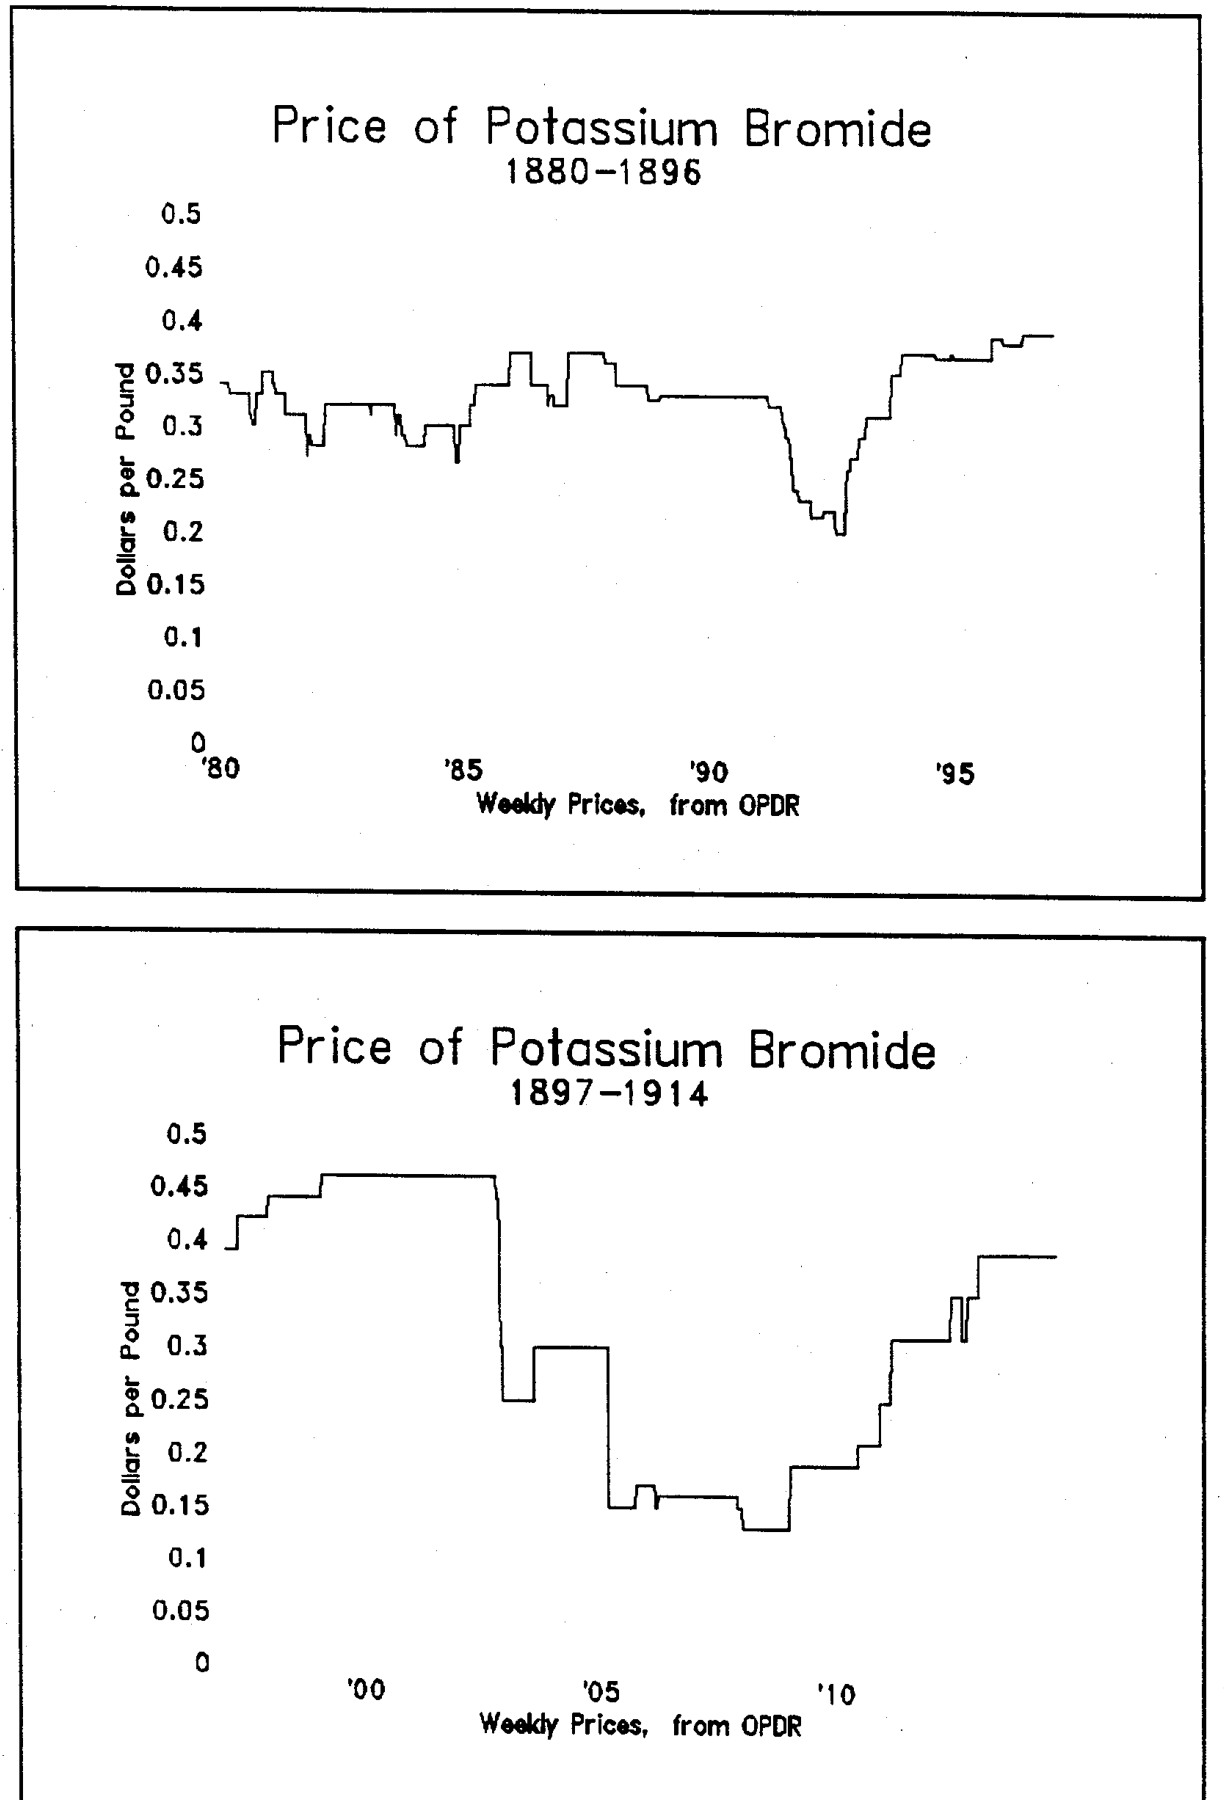
\includegraphics[width=0.62\textwidth]{figures/ch13/levenstein1997_fig1.png}
\caption{Weekly price of potassium bromide in dollars per pound, 1880--1896 (top) and 1897--1914 (bottom), from
the \textit{Oil, Paint and Drug Reporter}. The drop of 1891--1892 is Pool War~III, the collapse of 1902 is Dow
War~I, and the long trough of 1905--1908 is Dow War~III. Source: \citet{Levenstein1997}, Figure~1 (NBER
working-paper version).}\label{fig:13-lev-price}
\end{figure}

\casehead{Assessment}
\Cref{fig:13-lev-price} shows the episodes. The study's strength is its sources. The regime series and the
causes of each war come from documents written by the participants, independently of prices. Its quantitative
parts are weaker. Each demand curve is fitted through two years of aggregate data. Costs come from Dow's estimates
of Ohio River costs, and the deadweight-loss figure cannot be reproduced from the stated cost. The statistical
tests rest on six wars. The paper's contribution is conceptual. Some price wars fit equilibrium punishment under
imperfect monitoring, but they were mild because severe punishments are not credible. Other price wars were
bargaining over the terms of the next agreement, and their severity reflected the stakes of that bargaining.

\section{Information, Transparency and Coordination}\label{sec:13-information}

The Sugar Institute shows firms investing in the detection of secret price cuts. This section asks the same
question from the policy side. What happens when an outside body makes prices more transparent, or when firms use
an information system to signal intentions? We first derive the basic theoretical result, which formalizes
\citet{Stigler1964}. We then study three cases. Danish authorities published firm-specific concrete prices and
prices rose \citep{AlbaekMollgaardOvergaard1997}. The U.S.\ Department of Justice restricted how airlines could
communicate through their fare-publishing system, with temporary effects \citep{Miller2010}. Universities agreed
on financial aid formulas, and their average prices did not change \citep{CarltonBambergerEpstein1995}.

\subsection{Transparency and the incentive constraint}\label{sec:13-transparency-theory}

We embed imperfect detection in the Bertrand supergame of \cref{ch:collusion-theory}. The detection probability
is a reduced-form summary of everything that lets firms infer secret price cuts, such as their own sales, the
trade press, published prices or audits.

\begin{assumption}[Bertrand supergame with imperfect detection]\label{asm:13-transparency}
\leavevmode
\begin{enumerate}[label=(\roman*)]
\item There are $N \ge 2$ firms selling a homogeneous good at constant marginal cost $c$. Industry profit
$\pi(p) = (p - c)D(p)$ is maximized at $p^m$, and $\pi^m = \pi(p^m) > 0$.
\item In each period $t = 1, 2, \dots$ firms set prices simultaneously. The lowest price serves the whole market,
and tied firms split it equally. Firms maximize discounted profit with discount factor $\delta \in (0,1)$.
\item Prices are not publicly observed. At the end of each period a public signal $z_t \in \{0, 1\}$ is realized.
If some firm priced below $p^m$, then $z_t = 1$ with probability $\mu \in (0,1]$. If all firms priced at
$p^m$, then $z_t = 1$ with probability $\mu_0 \in [0, \mu)$.
\item A firm's information about rivals' prices is summarized by the history of public signals.
\end{enumerate}
\end{assumption}

We call $\mu$ the \emph{detection probability} and $\mu_0$ the \emph{false-alarm probability}. Consider the
\emph{public grim-trigger strategy}: charge $p^m$ in period $t$ if $z_s = 0$ for all $s < t$, and charge $c$
otherwise. Pricing at $c$ forever is a Nash equilibrium of every subgame that follows a signal, because each
period's static Bertrand game has the equilibrium $p = c$ with zero profit.

\begin{proposition}[Transparency facilitates collusion]\label{prop:13-transparency}
Under \cref{asm:13-transparency} with $\mu_0 = 0$, the public grim-trigger strategy is a subgame perfect
equilibrium if and only if
\begin{equation}\label{eq:13-transparency}
  \delta \;\ge\; \underline\delta(\mu) = \frac{N - 1}{N - 1 + \mu} .
\end{equation}
The threshold $\underline\delta(\mu)$ is strictly decreasing in $\mu$ and strictly increasing in $N$. It equals
$1 - \frac{1}{N}$ when $\mu = 1$ and tends to 1 as $\mu \to 0$.
\end{proposition}

\begin{proof}
After a signal, the strategies prescribe static Nash play forever, which is subgame perfect. On the collusive
path we use the one-shot deviation principle (\cref{ch:collusion-theory}). On the path each firm earns
$\frac{\pi^m}{N}$ per period, so the value of collusion is
\begin{equation*}
  V = \frac{\pi^m}{N(1-\delta)} .
\end{equation*}
A one-shot deviation to a price above $p^m$ earns zero today and does not change the signal, so it is not
profitable. A deviation to $p < p^m$ captures the market and earns $\pi(p)$, whose supremum over $p < p^m$ is
$\pi^m$. Tomorrow the signal reveals the deviation with probability $\mu$, after which the deviator earns zero
forever. With probability $1 - \mu$ the deviation goes unnoticed and collusion continues with value $V$. Since the
supremum of deviation payoffs is approached but not attained, no deviation is profitable if and only if
\begin{equation*}
  V \;\ge\; \pi^m + \delta(1 - \mu)\,V .
\end{equation*}
Substitute $V$:
\begin{equation*}
  \frac{\pi^m}{N(1-\delta)} \;\ge\; \pi^m + \delta(1-\mu)\,\frac{\pi^m}{N(1-\delta)} .
\end{equation*}
Multiply both sides by $\frac{N(1-\delta)}{\pi^m} > 0$:
\begin{equation*}
  1 \;\ge\; N(1-\delta) + \delta(1-\mu) .
\end{equation*}
Rearrange:
\begin{equation*}
  1 - \delta + \delta\mu \;\ge\; N - N\delta
  \quad\Longleftrightarrow\quad
  \delta\,(N - 1 + \mu) \;\ge\; N - 1 .
\end{equation*}
Since $N - 1 + \mu > 0$, this is \eqref{eq:13-transparency}. Differentiating,
$\frac{\partial\underline\delta}{\partial\mu} = -\frac{N-1}{(N-1+\mu)^2} < 0$ and
$\frac{\partial\underline\delta}{\partial N} = \frac{\mu}{(N-1+\mu)^2} > 0$. The limits follow by substitution.
\end{proof}

\Cref{fig:13-transparency} plots the threshold. Detection matters most when it is poor. With $N = 2$, raising
$\mu$ from 0.2 to 0.4 lowers the threshold from 0.83 to 0.71, while raising it from 0.8 to 1 lowers it only from
0.56 to 0.50.

\begin{figure}[htbp]
\centering
\begin{tikzpicture}
\begin{axis}[
  width=0.78\textwidth, height=6.4cm,
  xmin=0, xmax=1, ymin=0.38, ymax=1.0,
  xlabel={Detection probability $\mu$}, ylabel={Minimum discount factor $\underline{\delta}$},
  tick label style={font=\footnotesize}, label style={font=\small},
  legend pos=south west, legend style={font=\footnotesize, draw=none, fill=white},
  legend cell align=left, samples=200]
\addplot[thick, domain=0.03:1] {1/(1+x)};
\addlegendentry{$N = 2$}
\addplot[thick, dashed, domain=0.03:1] {2/(2+x)};
\addlegendentry{$N = 3$}
\addplot[thick, densely dashdotted, domain=0.03:1] {4/(4+x)};
\addlegendentry{$N = 5$}
\addplot[thick, gray, dotted, domain=0.115:1] {1/(1+x-0.1)};
\addlegendentry{$N = 2$, $\mu_0 = 0.05$}
\node[font=\small, anchor=south west] at (axis cs:0.5,0.395)
  {$\underline{\delta}(\mu) = \frac{N-1}{N-1+\mu-N\mu_0}$};
\end{axis}
\end{tikzpicture}
\caption{The minimum discount factor that sustains collusion at the monopoly price as a function of the
detection probability $\mu$, from \cref{prop:13-transparency} ($\mu_0 = 0$) and \cref{cor:13-false-alarms}
(gray dotted curve, $\mu_0 = 0.05$). With $\mu = 1$ and $\mu_0 = 0$ the threshold is $1 - \frac{1}{N}$.
False alarms shift the curve up, and with $N = 2$ collusion is impossible unless $\mu > 2\mu_0 = 0.1$.}
\label{fig:13-transparency}
\end{figure}

False alarms make collusion harder because they end collusion on the equilibrium path. This lowers the value of
colluding, and with it the loss that a deviator suffers when caught.

\begin{corollary}[False alarms]\label{cor:13-false-alarms}
Under \cref{asm:13-transparency} with $\mu_0 \in [0, \mu)$, the public grim-trigger strategy is a subgame
perfect equilibrium if and only if
\begin{equation}\label{eq:13-false-alarms}
  \delta\,(N - 1 + \mu - N\mu_0) \;\ge\; N - 1 .
\end{equation}
Collusion at $p^m$ is therefore sustainable for some $\delta < 1$ if and only if $\mu > N\mu_0$, and then the
threshold is $\frac{N-1}{N-1+\mu-N\mu_0}$. When $\mu_0 > 0$, collusion on the equilibrium path lasts a geometric
number of periods with mean $\frac{1}{\mu_0}$.
\end{corollary}

\begin{proof}
On the path a false alarm occurs with probability $\mu_0$ each period. The value of collusion solves
$V = \frac{\pi^m}{N} + \delta(1 - \mu_0)V$, so
\begin{equation*}
  V = \frac{\pi^m}{N\left(1 - \delta + \delta\mu_0\right)} .
\end{equation*}
A deviation earns at most $\pi^m$ today and $V$ tomorrow with probability $1 - \mu$. The incentive constraint is
$V \ge \pi^m + \delta(1 - \mu)V$, or $V(1 - \delta + \delta\mu) \ge \pi^m$. Substituting $V$ and multiplying by
$\frac{N(1 - \delta + \delta\mu_0)}{\pi^m}$ gives
\begin{equation*}
  1 - \delta + \delta\mu \;\ge\; N\left(1 - \delta + \delta\mu_0\right)
  \quad\Longleftrightarrow\quad
  \delta\,(N - 1 + \mu - N\mu_0) \;\ge\; N - 1 ,
\end{equation*}
which is \eqref{eq:13-false-alarms}. If $\mu > N\mu_0$, the coefficient on $\delta$ exceeds $N - 1 > 0$, and the
threshold lies below 1. If $\mu \le N\mu_0$, the left side is at most $\delta(N-1) < N - 1$ for every
$\delta < 1$, so no discount factor works. The duration statement follows from \cref{lem:13-durations} with a
per-period exit probability of $\mu_0$.
\end{proof}

\begin{remark}[Relation to Green and Porter]\label{rem:13-gp-nesting}
Set $N = 2$ and $\mu = 1$, and let $\mu_0$ be the probability of a zero-demand period in the Bertrand version of
\citet{GreenPorter1984}. A firm then always sees zero sales after a rival's undercut, and sees zero sales with
probability $\mu_0$ on the path. Condition \eqref{eq:13-false-alarms} becomes $\delta(2 - 2\mu_0) \ge 1$, or
$\delta(1 - \mu_0) \ge \frac{1}{2}$. This is the condition for collusion with permanent reversion in that model
(\cref{ch:collusion-theory}). Profits there are scaled by the probability of positive demand, and the scale
cancels from the incentive constraint. There the optimal cartel shortens punishments to limit the cost of false alarms. The
Sugar Institute lowered $\mu_0$ directly, by verifying accusations before anyone retaliated.
\end{remark}

\begin{remark}[Transparency to buyers]\label{rem:13-transparency-buyers}
Publication informs buyers as well as sellers. Better-informed buyers move faster to a price cutter, which raises
the payoff from a secret cut. Suppose a secret cut captures only a fraction $\omega \in [\frac{1}{N}, 1]$ of the
market, so a deviator earns $\omega\pi^m$. With $\mu_0 = 0$ the incentive constraint becomes
$\frac{\pi^m}{N(1-\delta)} \ge \omega\pi^m + \delta(1-\mu)\frac{\pi^m}{N(1-\delta)}$. The same algebra as in the
proof of \cref{prop:13-transparency} gives
\begin{equation*}
  \delta \;\ge\; \frac{N\omega - 1}{N\omega - 1 + \mu} .
\end{equation*}
This threshold rises with $\omega$ and falls with $\mu$. A policy that raises both $\omega$ and $\mu$ has an
ambiguous effect, so whether transparency raises or lowers prices is an empirical question.
\citet{Stigler1964} made the same point. The more buyers know about prices, the more customers a secret cut
attracts and the faster it is detected. Transparency can also help firms agree on a focal price, as the bromine
firms did when they adopted the trade-journal price after Dow War~I.
\end{remark}

\subsection{Government-assisted coordination: Danish ready-mixed concrete}\label{sec:13-concrete}

\casehead{The question}
\citet{AlbaekMollgaardOvergaard1997} study a natural experiment in transparency. Did the publication of
firm-specific transaction prices by a competition authority lower prices, as the authority intended, or did it
help firms coordinate?

\casehead{The policy}
The Danish Competition Act of 1990 stated its purpose as promoting competition ``through the largest possible
transparency of competitive conditions.'' Unlike U.S.\ and EU law, the Act rested on abuse control. It had no per
se prohibitions, and the authority intervened case by case. A \emph{per se} prohibition makes conduct illegal
without any inquiry into its effects. Under the \emph{rule of reason}, a court weighs the conduct's harm to
competition against its claimed benefits. The Competition Council interpreted the Act to mean
that suspected abuses such as oligopolistic coordination should be countered by more transparency. The premise
was that firm-specific price information lets buyers shop around and so pushes prices down.

\casehead{The product and the market}
Ready-mixed concrete is a mixture of cement, gravel, sand and water, and its strength is measured in megapascals
(MPa). A given grade is homogeneous, and different grades are imperfect substitutes. The study covers a weak grade
(10 MPa), used for foundations of single-family houses, and a strong grade (25 MPa), used for staircases.
Concrete travels in mixer lorries holding at most six cubic metres. It can stay in a lorry for only about two hours,
so it normally travels at most about twenty miles. Denmark had 115 production sites. The two main producers were
Unicon, owned by the only Danish cement producer, and 4K, and the remaining capacity belonged to independent
local firms. In 1987 the national four-firm concentration ratio was 57 percent, with Unicon at 37 percent and 4K
at 11 percent. Two years later Unicon's share reached 43 percent after it acquired the third-largest firm. Within
a radius of 20 km of a plant, many local markets were monopolies, and the average share of the largest firm was
about 70 percent. Typically fewer than five sites could serve a given customer. Pricing combined rigid, publicly
posted list prices with large confidential discounts.

\casehead{The intervention and the data}
In October 1993 the Council decided to sample invoice prices from 18 sites and publish them in its newsletter,
roughly once a quarter. The sites were in three regions, Copenhagen (7 sites), Aarhus (6) and Northern Jutland
(5). For each site and grade the Council published the list price, the average price and the average of the five
lowest prices in the first month of a quarter. Prices appeared with a lag of about three months. The data cover
the four quarters of 1994 and the first three of 1995, seven observations per site. \Cref{tab:13-albaek-timeline}
gives the timeline. The two dominant firms had almost identical list prices in each region. They set the highest
list prices and gave the largest discounts. Average discounts were 25 to 26 percent of list for 10 MPa and 27 to
31 percent for 25 MPa. Maximum discounts ranged from 25 percent in Northern Jutland to 38 percent in Aarhus.

\begin{table}[htbp]
\centering
\caption{Timeline of the Danish concrete price publication}\label{tab:13-albaek-timeline}
\small
\begin{tabular}{@{}ll@{}}
\toprule
Date & Event\\
\midrule
1990 & Competition Act adopts the transparency principle\\
October 1993 & Competition Council decides to collect and publish invoice prices\\
April 8, 1994 & January 1994 prices published\\
July 5, 1994 & April 1994 prices published\\
January to October 1994 & Weighted average price of the two grades rises 19 percent\\
April 1996 & Last publication (November 1995 prices)\\
December 1996 & Council decides to publish no more concrete prices\\
May 30, 1997 & New competition law drops the emphasis on transparency\\
\bottomrule
\end{tabular}

\smallskip
\begin{minipage}{0.8\textwidth}\footnotesize
Notes: From \citet{AlbaekMollgaardOvergaard1997}, pp.~430--433 and 440--441.
\end{minipage}
\end{table}

\casehead{The main finding}
\Cref{fig:13-albaek-f1} shows the national indices of average transaction prices for the two grades, weighted by
the firms' turnover. Prices rose sharply over the first two to three quarters of 1994. According to the Council's
reports, the weighted average increase across the two grades was 19 percent between January and October 1994.
Prices then levelled off. Over the first three quarters of 1994, consumer prices rose 1.9 percent, wholesale
prices 1.6 percent, and import prices of unprocessed raw materials 1.1 percent. An index of residential
construction costs barely moved. The unit value of all concrete produced and the unit value of cement, the main
input, show nothing like the rise in the published prices.

The comparison is a before-after design with an aggregate benchmark. Let $p_t$ be the published price index and
$p^{\mathrm{b}}_t$ a benchmark index that captures costs and general inflation. The implicit estimate of the effect
of publication is
\begin{equation}\label{eq:13-albaek-tau}
  \hat\tau = \left(\ln p_{1} - \ln p_{0}\right) - \left(\ln p^{\mathrm{b}}_{1} - \ln p^{\mathrm{b}}_{0}\right),
\end{equation}
with period 0 in January 1994 and period 1 in October 1994. With a 19 percent price rise and consumer prices as the
benchmark, $\hat\tau \approx \ln 1.19 - \ln 1.019 = 0.155$, or about 17 percent (our computation).
Interpreting $\hat\tau$ as a causal effect requires that, without publication, concrete prices would have moved
with the benchmark. The rest of the paper defends this assumption.

\begin{figure}[htbp]
\centering
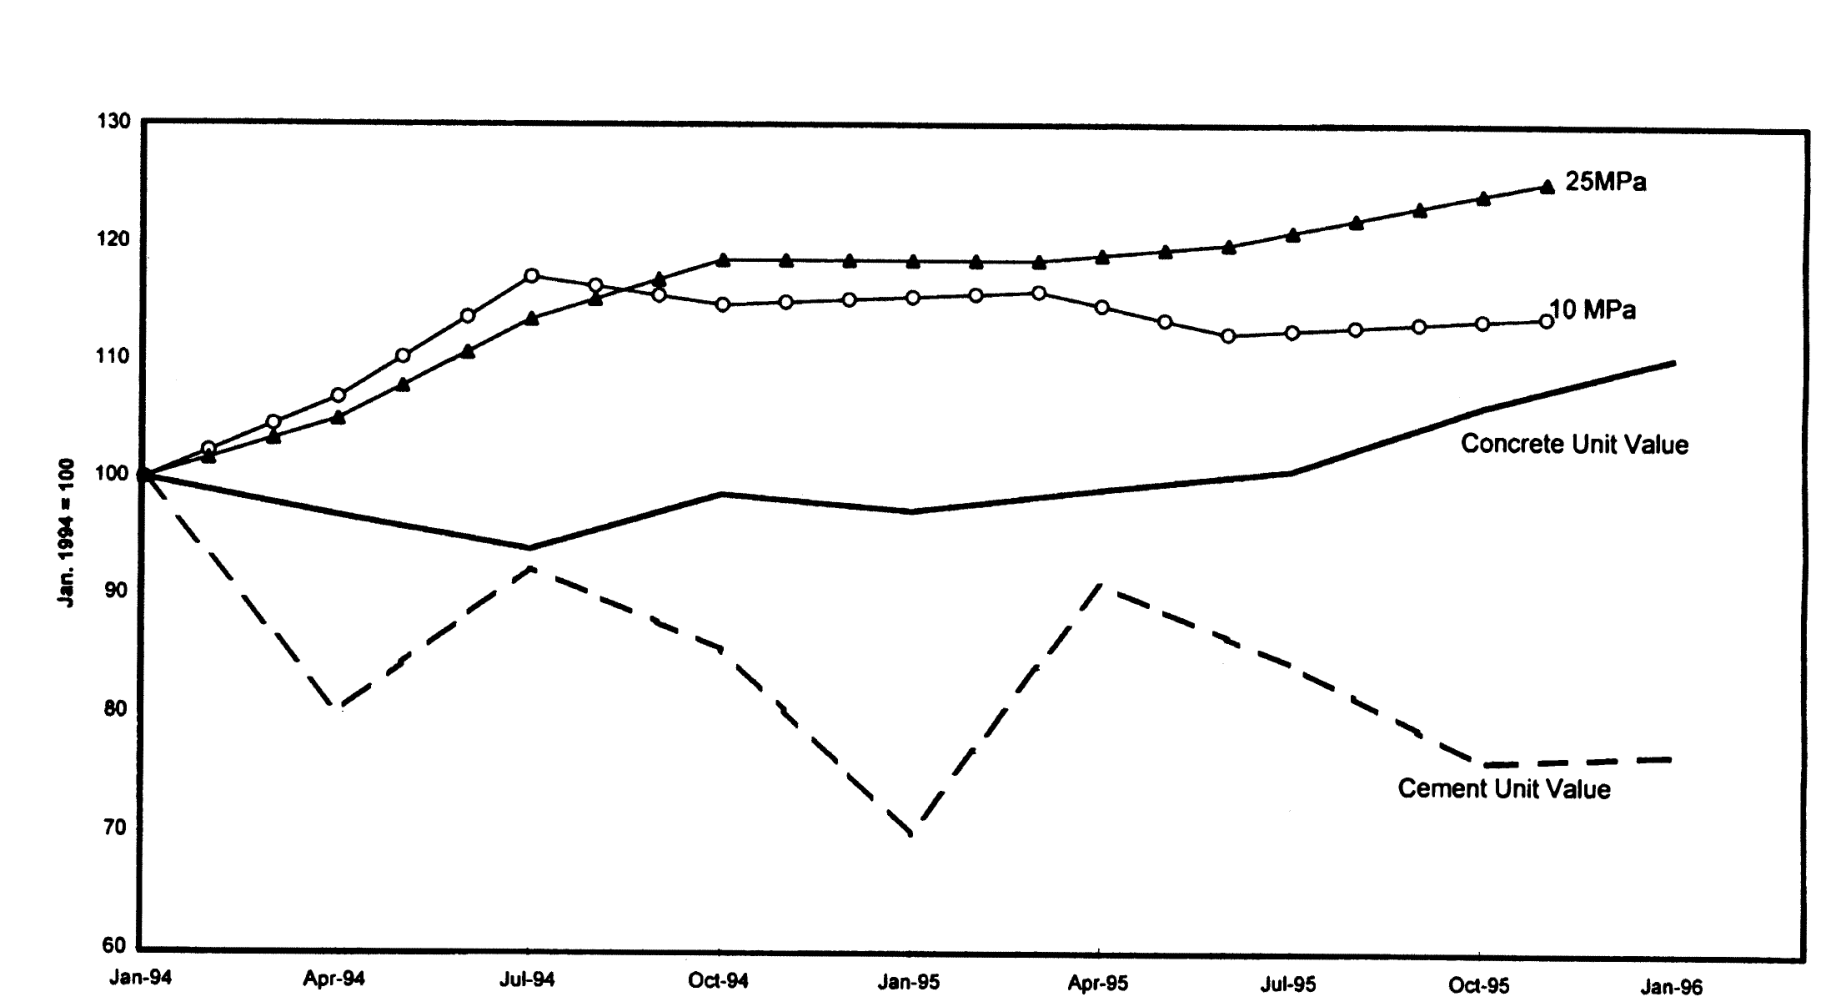
\includegraphics[width=0.88\textwidth]{figures/ch13/albaek1997_fig1.png}
\caption{National price indices for ready-mixed concrete (January 1994 = 100). The marked lines are the published
average transaction prices of 10 MPa and 25 MPa concrete. The solid line is the unit value of all concrete
produced and the dashed line the unit value of cement. Source: \citet{AlbaekMollgaardOvergaard1997}, Figure~1
(unit values from Danmarks Statistik, published prices from the Competition Council).}\label{fig:13-albaek-f1}
\end{figure}

\casehead{Ruling out competitive explanations}
In a price-setting oligopoly with capacity constraints, prices could rise because demand grew, capacity fell or
input prices rose. The authors examine each. A deep construction recession bottomed out in the summer of 1993. By
February 1994 construction employment was back at its low 1992 level. By November 1994 seasonally adjusted
employment had risen 4.4 percent and unadjusted employment 17.6 percent. Production of concrete at the end of 1993
was as low as at the trough ten years earlier. Production in 1994 was almost 20 percent above 1993 but still below
1991.

Capacity was not binding. In 1987 production was more than 50 percent above its 1994 level. Even then, capacity
utilization was about 41 percent in production and 62 percent in distribution, and productive capacity had not
fallen much since. If capacity was unchanged, utilization in 1994 was at most $\frac{62}{1.5} \approx 41$ percent in
distribution and $\frac{41}{1.5} \approx 27$ percent in production (our computation). Distribution capacity is the
number of mixer lorries, which firms could import or move between regions. Input costs did not rise either.
Wages and energy prices were flat from 1993 to 1994, and the unit value of cement fell. The cement supplier, which
owned Unicon, charged uniform delivered prices to all concrete producers.

\casehead{A closer look at Aarhus}
The authors then focus on Aarhus. Its six sampled firms carried about 70 percent of the weight in the national
indices, and price increases in the other two regions were much more moderate. Copenhagen is large, and only half
of its sites were sampled. Northern Jutland is sparsely populated, its sampled firms are local monopolies, and
its discounts were smaller at the outset. Within Aarhus the authors drop a plant on a peninsula more than 60 km
away and a Unicon plant 40 km away in Randers. The remaining four are plants of 4K and Unicon about 2 km apart in
the city, and two commonly owned local plants (Haarup and \O stjysk) 25 km and 40 km away. Together they carried
about 60 percent of the national index weight and had a combined local share close to one.

\begin{figure}[htbp]
\centering
\begin{subfigure}[b]{0.74\textwidth}\centering
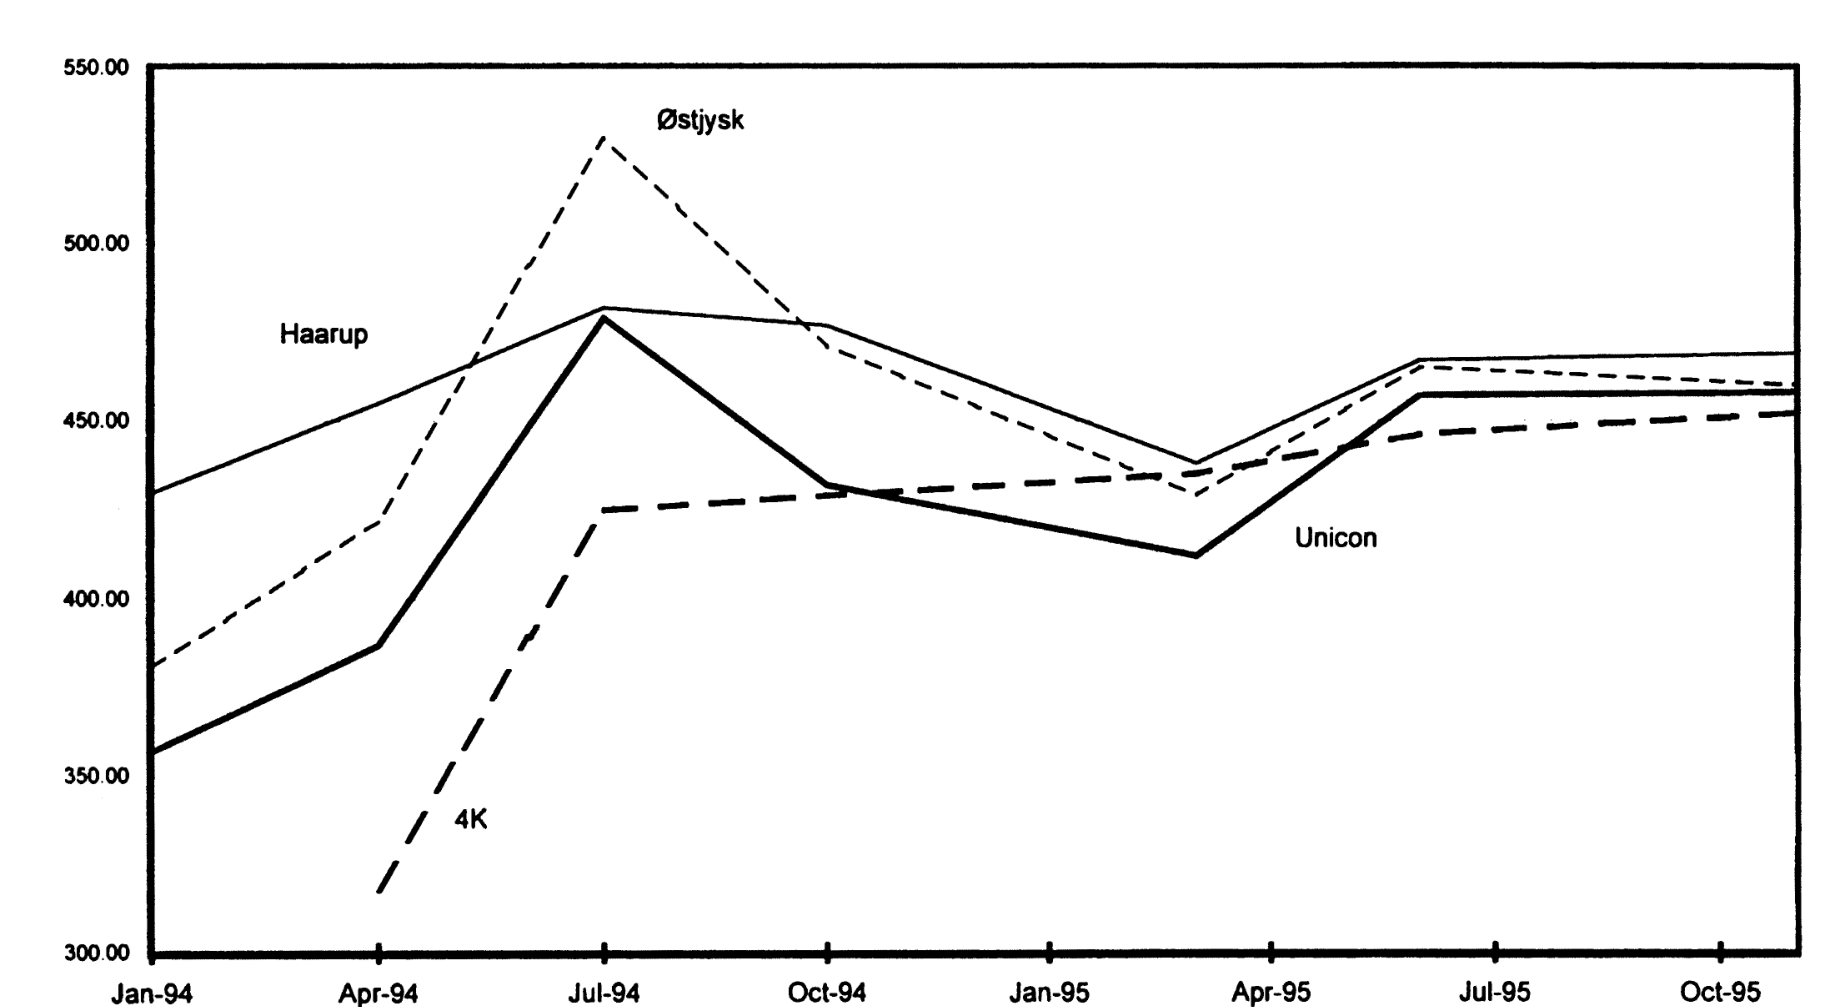
\includegraphics[width=\textwidth]{figures/ch13/albaek1997_fig2.png}
\caption{Figure 2 of the paper}
\end{subfigure}

\medskip
\begin{subfigure}[b]{0.74\textwidth}\centering
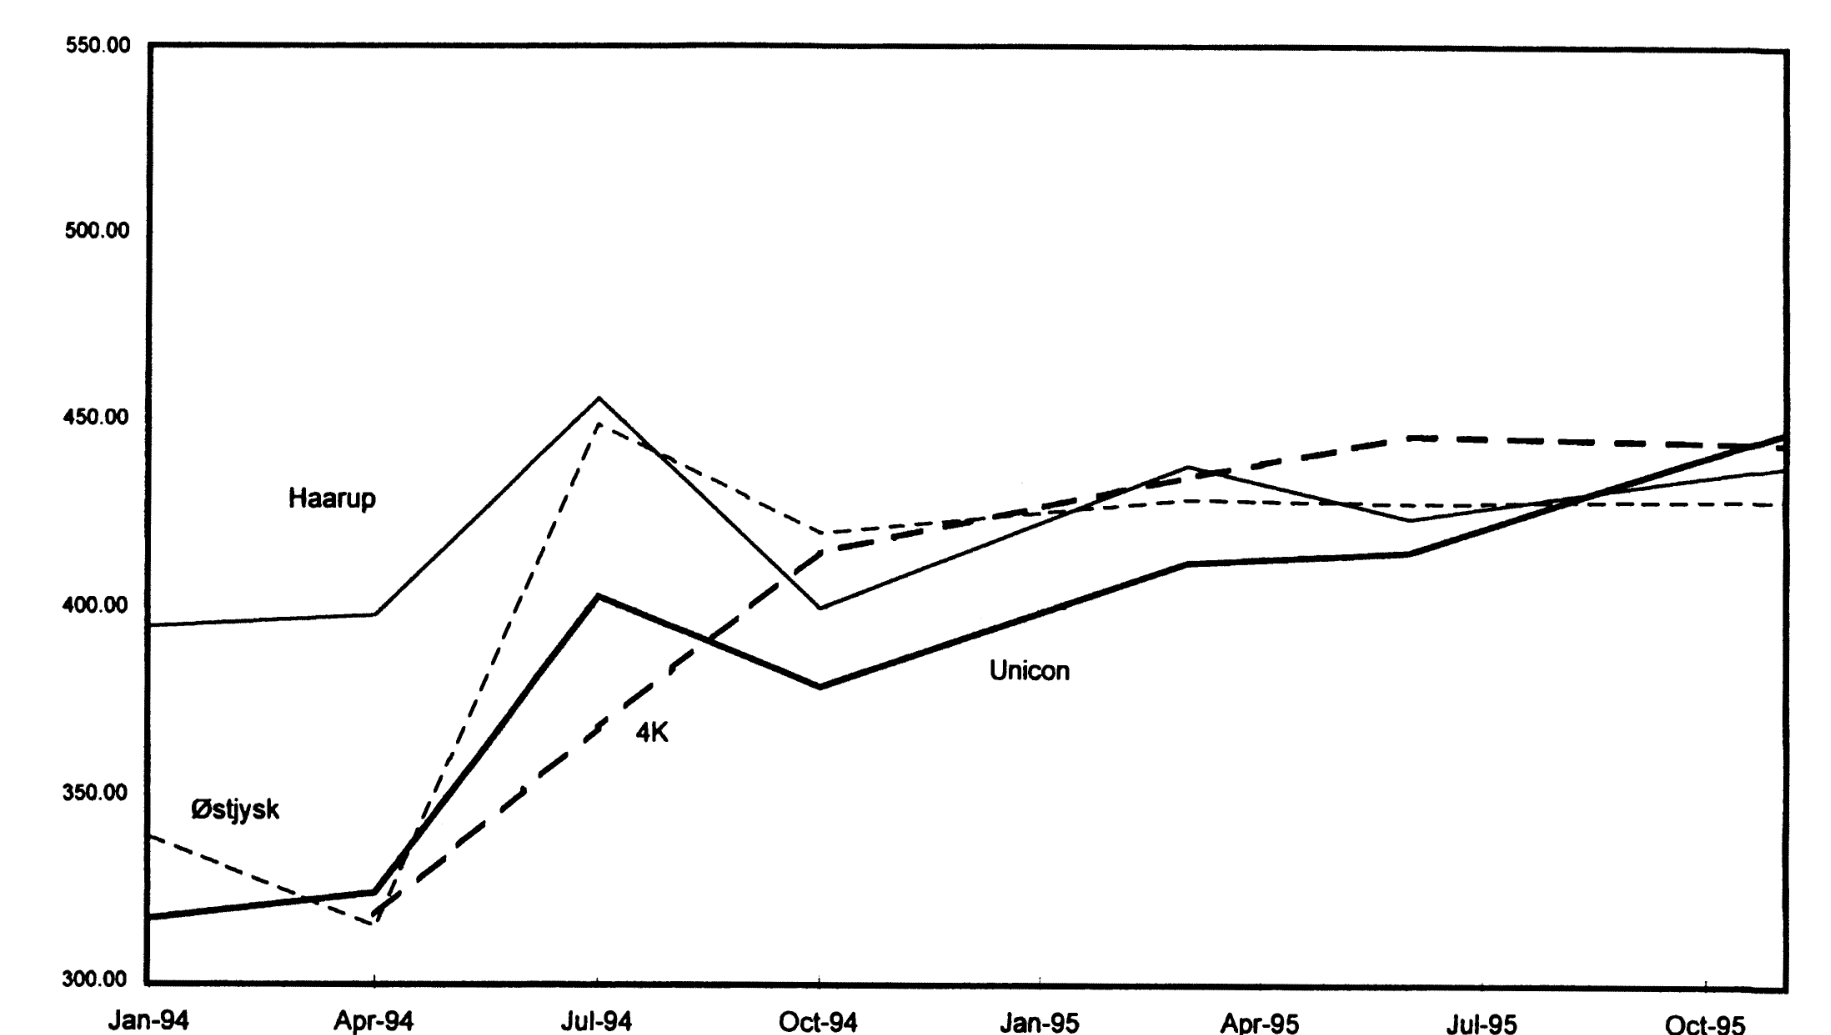
\includegraphics[width=\textwidth]{figures/ch13/albaek1997_fig3.png}
\caption{Figure 3 of the paper}
\end{subfigure}
\caption{Published 10-MPa prices of the four Aarhus plants, January 1994 to October 1995. The journal titles both
panels ``Low 10-MPa Prices in Aarhus.'' The text describes both average and low prices. Panel (b) is flat from
January to April 1994, as the text says of low prices, and lies below panel (a). We therefore read panel (a) as
average prices and panel (b) as low prices. Source: \citet{AlbaekMollgaardOvergaard1997}, Figures~2 and~3 (data from the Competition
Council).}\label{fig:13-albaek-f23}
\end{figure}

\Cref{fig:13-albaek-f23} shows the prices of these four plants. From January to April 1994, low prices were
roughly constant while average prices rose a little. From April to July 1994, prices jumped by 20 to 25 percent and
then stayed at the new level. The timing fits the flow of information. The January prices were published on April
8, 1994, so April transactions could at best partly reflect them. The April prices were published on July 5, so
by July every firm had two quarters of reliable information on rivals' formerly secret discounts. Prices also
converged. By the end of the sample, the four plants' prices varied by only 2 to 4 percent around their mean,
against up to 30 percent early in 1994. Low prices rose toward average prices, so the largest discounts
disappeared. The authors see no explanation for a 25 percent rise in tandem by two major producers 2 km apart,
other than reduced competition after secret discounts became public.

\casehead{Interpretation}
In terms of \cref{prop:13-transparency}, publication raised the detection probability $\mu$ of secret discounts.
The publication lag also mattered for \cref{rem:13-transparency-buyers}. Prices for the first month of a quarter
appeared about three months later. That told each firm what its rivals had charged, but told a buyer little about
the prices it could get today (our reading). The authors ask why a trade association had not supplied the same
information. The association said it received no price reports from members. They suggest that unverified reports
would not be credible, since a firm that gives secret discounts also gains by misreporting. The Council would also
have frowned on industry price reporting (p.~440, fn.~12). The Council itself stopped publishing at the
end of 1996. It noted that the convergence of actual and list prices since January 1994 had come entirely from a
rise in actual prices (p.~430, fn.~4). The authors also point to related evidence from U.S.\ railroad freight.
After Congress mandated the disclosure of firm-specific rail contract terms, grain rates rose.
\citet{FullerRuppelBessler1990} and \citet{SchmitzFuller1995} attribute the rise to the improved scope for
tacit collusion (p.~441).

\casehead{Limitations}
The authors list the main weaknesses. There is no control group, either regions without publication or the same
regions before publication. The Council had some data from before January 1994 but refused access. There are no
data on firms' costs or capacities, and the sample has seven quarterly observations. There is no structural model
and no standard error. One alternative they do not discuss is seasonality. The gap between adjusted and
unadjusted construction employment shows strong seasonal demand, and the jump between April and July coincides with the
building season. A seasonal rise would have reversed, however, and published prices stayed high through 1995
(our observation). Despite its limits, the paper is the cleanest evidence in this chapter that transparency can
raise prices. It also shows that a policy can harm competition through the mechanism of
\cref{prop:13-transparency}.

\subsection{Signaling through a fare-publishing system: the Airline Tariff Publishing case}\label{sec:13-atpco}

\casehead{The question}
Firms may also use an information system to communicate intentions directly. \citet{Miller2010} asks whether an
antitrust case against such communication among U.S.\ airlines changed their prices and output. The airline
industry is described in \cref{ch:airlines}.

\casehead{Setting}
The Airline Tariff Publishing (ATP) Company, owned by the airlines, is the clearinghouse for airline fares. It
collects and disseminates over 100,000 fare updates a day to airlines and to the computer reservation systems of
travel agents. Each entry contains a fare basis code, a dollar amount, a route, fare rules and footnotes, typically
first or last ticket dates. Airlines monitor the updates with sophisticated software. Travel agents can view only
one market at a time and do not see the footnote designators. In December 1992 the Department of Justice sued the
eight major domestic airlines and ATP, alleging that they used the system to communicate and to enforce price
coordination (Civil Action No.~92-2854). The alleged channels were rapid monitoring, enforcement, signaling an
intent to raise fares without shifting market shares \citep{HoltScheffman1987}, bargaining over fares and
restrictions, and linking fares across markets \citep{BernheimWhinston1990,EvansKessides1994}. In a widely cited
example, airlines punished fare cuts by America West with fare codes containing ``HP,'' America West's industry
code, and withdrew them once America West retracted its cuts. The case contrasts with an earlier and blunter
invitation to collude. In 1982 Robert Crandall, chief executive of American Airlines, telephoned Howard Putnam of
Braniff, a rival on routes out of Dallas-Fort Worth. He proposed that Braniff raise its fares by twenty percent and
promised to raise his own the next morning \citep[pp.~188--189]{AskerNocke2021}. Putnam recorded the call and turned
it over to the Department of Justice, which filed a complaint against American and Crandall. Such explicit,
private communication is easy to condemn. The ATP case concerned coded, public signals, which serve the same
purpose and are harder to prohibit (\cref{sec:12-anatomy}).

Without admitting guilt, United and US Airways settled on November 1, 1993, and the other six defendants on August
10, 1994. For ten years the airlines agreed to three restrictions. They would not use footnote indicators or fare basis
codes to convey extraneous information, or special codes linking different fares. They would not preannounce
price changes except for widely publicized sales. A facilitating practice is judged under the rule of reason \citep[p.~570]{Miller2010}, and the airlines
defended ATP as an efficient business tool. \citet{Hay2000} called a related defense ``we're naturally bad.'' It holds
that the industry's rapid monitoring alone explains supracompetitive profits, so restricting ATP would not help.
The theoretical prediction is thus ambiguous.

\casehead{Data}
Miller uses the Department of Transportation's DB1A database, a 10 percent sample of domestic tickets, from the
second quarter of 1991 to the first quarter of 1995. Fares below \$10 (presumed frequent-flyer redemptions) and
above ten times the Standard Industry Fare Level (presumed errors) are dropped, which removes less than 1 percent
of fares. The unit of observation is an airline, city-pair market and quarter. There are 411,726 such cells, with
a mean of 229 sampled tickets and a mean fare of \$209.70. Both vary widely across cells, with standard deviations
of 933.16 tickets and \$129.80, and the mean distance of a market is 1,056 miles (Table~1). The average market has
4.7 airlines, a Herfindahl index of 5,341 points and a four-firm concentration ratio of 97 percent.

\casehead{Design and estimating equation}
The identification strategy compares markets that the case should have affected with markets it should not have
affected. If ATP facilitated collusion among the defendants, the remedy should matter only where several
defendants compete. \emph{Affected} markets are city pairs served by more than two defendant airlines in every
quarter. \emph{Control} markets are city pairs where the number of major airlines is always below two. Let
$Y_{ijt}$ be tickets sold or the average fare of airline $i$ in city pair $j$ in quarter $t$. Let
$\mathit{ATP1}_t$ equal one from the second quarter of 1992, after the investigation intensified with the first
depositions in March 1992. Let $\mathit{ATP2}_t$ equal one from the first quarter of 1994, after the settlements
began. The probe itself had been announced in June 1990, and Miller dates the treatment from its intensification.
An event study finds no response of defendants' stock prices to the 1990 announcement and a significant negative
response to the intensification on March 18, 1992 (p.~574, note~9). The estimating equation is
\begin{equation}\label{eq:13-miller-did}
  Y_{ijt} = \beta_0 + \sum_{k=1}^{2}\beta_{k}^{A}\,\mathit{ATPk}_t\cdot\mathit{Aff}_j
          + \sum_{k=1}^{2}\beta_{k}\,\mathit{ATPk}_t + x_{jt}\beta_X + a_i + g_j + e_{ijt} .
\end{equation}
Here $\mathit{Aff}_j$ marks affected markets, and $a_i$ and $g_j$ are airline and city-pair fixed effects. The
controls $x_{jt}$ are the Standard Industry Fare Level, a cost measure, and the geometric means of the endpoint
states' populations and gross state products, which shift demand. Richer versions replace $\beta_k\mathit{ATPk}_t$
with quarter effects or with airline-by-quarter effects. Standard errors are clustered by city pair.

The two indicators are cumulative steps. The coefficient $\beta^{A}_1$ is the effect during the investigation, and
$\beta^{A}_1 + \beta^{A}_2$ is the effect after the settlement. A lasting effect of the remedy requires
$\beta^{A}_1 + \beta^{A}_2 \neq 0$, which Miller tests with an $F$ test. Identification rests on parallel trends.
Affected and control markets would have evolved alike absent the case, conditional on the controls. The model is
identified even with airline-by-quarter effects, because each airline serves both kinds of market before and after
the case. Affected and control markets differ in fares and distance. Miller therefore repeats the analysis with a second
control group of dominated markets, in which one airline sells over 90 percent of tickets in every quarter.

Miller also checks the results on several restricted samples (pp.~575--577). They keep flights within the
continental United States, markets with distances between 250 and 2,000 miles, and markets with stable numbers of
defendant and other airlines. One restriction counts an airline as present only if it has at least 10 sampled
tickets in the market, about 100 passengers a quarter. Another reassigns the tickets of commuter carriers to the
defendants with which they had operating agreements (p.~577, note~14). Combining all of these restrictions leaves
736 city-pair markets, the sample of columns (3) and (6) of \cref{tab:13-miller-t2}.

\begin{table}[htbp]
\centering
\caption{Quantity and price effects of the Airline Tariff Publishing case}\label{tab:13-miller-t2}
\small
\begin{tabular}{@{}lcccccc@{}}
\toprule
 & \multicolumn{3}{c}{Number of tickets} & \multicolumn{3}{c}{Average fare (dollars)}\\
\cmidrule(lr){2-4}\cmidrule(l){5-7}
 & (1) & (2) & (3) & (4) & (5) & (6)\\
\midrule
Quarter fixed effects & No & Yes & Yes & No & Yes & Yes\\
Airline $\times$ quarter effects & No & No & Yes & No & No & Yes\\
Sample restrictions & No & No & Yes & No & No & Yes\\
\addlinespace
$\mathit{ATP1}$ & 105.194 & & & 1.595 & & \\
 & (43.039) & & & (2.654) & & \\
$\mathit{ATP2}$ & 66.433 & & & $-10.746$ & & \\
 & (55.741) & & & (2.517) & & \\
$\mathit{ATP1}\times\mathit{Aff}$ & $-91.983$ & $-92.425$ & $-4.361$ & $-13.568$ & $-14.085$ & $-7.051$\\
 & (43.164) & (43.081) & (18.697) & (2.680) & (2.661) & (2.270)\\
$\mathit{ATP2}\times\mathit{Aff}$ & $-40.318$ & $-41.081$ & $-59.948$ & 12.708 & 14.619 & 2.932\\
 & (56.013) & (55.990) & (20.977) & (2.598) & (2.152) & (2.616)\\
\addlinespace
p-value, $(\mathit{ATP1} + \mathit{ATP2})\times\mathit{Aff} = 0$ & 0.08 & 0.08 & 0.05 & 0.81 & 0.86 & 0.17\\
$N$ & 328{,}921 & 328{,}921 & 10{,}934 & 328{,}921 & 328{,}921 & 10{,}934\\
City-pair markets & 4{,}825 & 4{,}825 & 736 & 4{,}825 & 4{,}825 & 736\\
$R^2$ & 0.05 & 0.05 & 0.22 & 0.04 & 0.05 & 0.34\\
\bottomrule
\end{tabular}

\smallskip
\begin{minipage}{0.95\textwidth}\footnotesize
Notes: Reproduced from \citet{Miller2010}, Table~2. The unit is an airline, market and quarter in the
10 percent ticket sample. All regressions include city-pair and airline fixed effects and the controls described
in the text. Standard errors clustered by city pair in parentheses. Columns (3) and (6) combine the sample
restrictions listed in the text, which leave 736 markets.
\end{minipage}
\end{table}

\casehead{Results}
\Cref{tab:13-miller-t2} reproduces the main estimates. Tickets rose in affected markets after the case, but they
rose more in control markets. In column (1) the relative change after the settlement is
$-91.983 - 40.318 = -132.3$ sampled tickets per airline, market and quarter, significant at the 8 percent level.
Multiplying by 10 to undo the sampling gives about 1,300 tickets, the ``over 1,000 tickets per quarter'' in the
text (our reconstruction). Column (3) gives $10 \times (4.361 + 59.948) = 643$, matching the reported
postsettlement decline of 640 tickets, significant at the 5 percent level. Lower relative traffic contradicts a
lasting increase in competition and fits the airlines' claim that the restrictions made travel planning harder.

Fares fell and then recovered. In column (4), affected-market fares fell \$13.57 relative to control markets
during the investigation and rose \$12.71 after the settlement. The net effect of $-\$0.86$ is insignificant
($p = 0.81$). With the average fare near \$210, the initial fall is about 6.5 percent (our computation). In logs,
the two coefficients are $-0.088$ and $0.035$, both significant. The pattern holds across the fare distribution.
With quarter effects, the investigation lowered the 10th percentile, median and 90th percentile fares by \$9.08,
\$10.98 and \$28.93, and the settlement raised them by \$9.51, \$14.76 and \$21.24 (Table~3). Price dispersion
therefore fell and then rose, and only the 90th percentile shows a net decline, significant at the 10 percent
level.

\begin{figure}[htbp]
\centering
\begin{tikzpicture}
\begin{axis}[
  width=0.82\textwidth, height=5.8cm,
  xmin=1991.25, xmax=1995.25, ymin=-16, ymax=4,
  xlabel={Quarter}, ylabel={Relative fare (dollars)},
  xtick={1991.25,1992.25,1993.25,1994.0,1995.0},
  xticklabels={1991Q2,1992Q2,1993Q2,1994Q1,1995Q1},
  tick label style={font=\footnotesize}, label style={font=\small},
  legend pos=south east, legend style={font=\footnotesize, draw=none, fill=none}, legend cell align=left]
\draw[gray!60] (axis cs:1991.25,0) -- (axis cs:1995.25,0);
\addplot[thick, const plot] coordinates {(1991.25,0) (1992.25,-13.568) (1994.0,-0.860) (1995.25,-0.860)};
\addlegendentry{Column (4)}
\addplot[thick, dashed, const plot] coordinates {(1991.25,0) (1992.25,-14.085) (1994.0,0.534) (1995.25,0.534)};
\addlegendentry{Column (5)}
\addplot[thick, densely dotted, const plot] coordinates {(1991.25,0) (1992.25,-7.051) (1994.0,-4.119) (1995.25,-4.119)};
\addlegendentry{Column (6)}
\end{axis}
\end{tikzpicture}
\caption{Average fares in affected markets relative to control markets implied by
\citet{Miller2010}, Table~2. The path is 0 before the second quarter of 1992, $\beta^{A}_1$ during the
investigation, and $\beta^{A}_1 + \beta^{A}_2$ from the first quarter of 1994. Our construction from the reported
coefficients.}\label{fig:13-miller-path}
\end{figure}

\Cref{fig:13-miller-path} plots the implied fare paths. Two further results support the reading of a temporary
effect. Separate regressions for defendants and other airlines show that the fall and rise in fares came from the
defendants, whose relative fares fell \$8.71 and then rose \$10.49 (Table~4). Their relative ticket sales rose
during the investigation, while other airlines lost traffic. The defendants' fare cuts mostly shifted passengers
from other carriers. Miller also re-estimates the multimarket-contact regression of \citet{EvansKessides1994}:
\begin{equation}\label{eq:13-miller-mmc}
  \ln \mathit{Price}_{ijt} = x_{ijt}\beta_X + \beta_Z Z_{jt} + \sum_{k=1}^{2}\beta_{Zk}\,\mathit{ATPk}_t\cdot Z_{jt}
    + a_i + g_j + \tau_t + e_{ijt} .
\end{equation}
Here $Z_{jt}$ is the average number of routes that the airlines serving market $j$ have in common, divided by
1,000. The controls $x_{ijt}$ include the airline's route and airport shares and the route Herfindahl index. In the
Evans-Kessides sample, the contact coefficient is 0.269 (0.043). It falls by 0.104 (0.030) during the
investigation and rises by 0.107 (0.033) after the settlement, with a p-value of 0.96 for no net change
(Table~5). In this sample the contact effect weakened while the case was active, to $0.269 - 0.104 = 0.165$, or
about three fifths of its initial value. After the settlement it rose to $0.165 + 0.107 = 0.272$, close to its
initial value. The p-value concerns the net change,
so it says nothing about whether the coefficient of 0.165 differs from zero. In the two larger samples the
interaction largely offsets the baseline coefficient, $0.016 - 0.014$ and $0.035 - 0.025$, and Miller reports that
contact was then an insignificant predictor of prices (p.~582). Finally, the hub premium,
which should have risen if collusion in contested markets broke down, fell by about 8 percent during the
investigation and by another 13 percent after the settlement.

\casehead{Interpretation and critiques}
The defendants lowered fares under the scrutiny of the investigation and raised them once the settlement was in
place. The settlement left the system largely intact, including the rapid fare monitoring that lets airlines
detect and match fare cuts. In terms of \cref{prop:13-transparency}, the remedy removed some signaling devices but
left the detection probability $\mu$ high. The business press described weekend fare changes as a near substitute
for the forbidden preannouncements. American Airlines was later accused of violating the decree and accepted a
new seven-year decree in 2004. Alternatively, the airlines may never have used ATP as alleged.
\citet{Borenstein2004} reports relative price increases after the settlement on 387 routes likely to be affected,
consistent with Miller.

The design has weaknesses that Miller discusses. Group membership depends on entry and exit, which are outcomes.
She treats it as predetermined over four years and drops markets whose group changes. Southwest's entry was more
frequent in affected markets, and the results survive dropping markets that Southwest entered or left. Affected
and control markets differ in fares, distances and traffic, which weakens parallel trends, so she repeats the
analysis with dominated markets as controls. The timing of treatment is also uncertain. The probe was announced in
June 1990, the suit filed in December 1992, and the settlements signed in 1993 and 1994. The paper does not report
pre-trends, so the identifying assumption cannot be checked directly (our observation). The case connects to the
retrospective methods of \cref{sec:13-enforcement}. Miller reads the time pattern of fares as a sign that the
settlement failed because of its limited scope, and she rejects the reading that the industry was already
competitive (p.~570). She also warns that a weak settlement can be empirically indistinguishable from one applied
to an already competitive industry (p.~573). The pattern is consistent with a remedy that removed signaling devices
while leaving rapid fare monitoring and other coordination channels intact. The design does not separately identify
these channels.

\subsection{Rules among nonprofits: the Overlap group and financial aid}\label{sec:13-overlap}

\casehead{The question}
Can an agreement on rules among nonprofit institutions raise prices? \citet{CarltonBambergerEpstein1995} study the
antitrust case against the Overlap group of universities. They ask whether the schools' agreement on financial aid
raised the average price that students paid. They also ask how antitrust law should treat collective action by
nonprofits. The study grew out of work by Lexecon for MIT, and Carlton testified as MIT's expert witness, as the
paper discloses.

\casehead{The agreement}
In the 1950s the Ivy League schools met to stop bidding for star athletes. They agreed that no athlete would
receive aid beyond financial need, and soon applied the same idea to star students. By the 1970s the Overlap
meetings included the eight Ivy League schools, MIT and 14 other selective colleges, 23 schools in all. Their
combined undergraduate enrollment of about 60,000 was less than one percent of the national total.
\Cref{fig:13-cbe-aid} shows the accounting. Let $\bar p$ be the gross charge for tuition, room, board and fees. A
student covers it with grants $G$, self help $H$ (loans and jobs) and a family contribution $F$. In this subsection
$G$, $H$ and $F$ are local symbols for these three sources, not distribution functions:
\begin{equation}\label{eq:13-cbe-accounting}
  \bar p = G + H + F, \qquad \text{aid package} = G + H, \qquad \text{payment to the school} = H + F = \bar p - G .
\end{equation}
The Overlap schools agreed to give aid only on the basis of need and to use a common method to define need. They
also met to discuss individual students admitted by more than one school. A printout of commonly admitted students
listed each school's proposed family contribution. When proposals differed by more than several hundred dollars,
the schools discussed them and usually agreed on a common figure. Disagreements arose for 10 to 20 percent of the
commonly admitted students who applied for aid. Regardless of which Overlap school admitted a student, the family
contribution $F$ was the same. Some schools also agreed on the split of the aid package between $H$ and $G$.

\begin{figure}[htbp]
\centering
\begin{tikzpicture}[font=\small]
\draw (0,0) rectangle (5,0.9) node[pos=0.5, align=center] {Grants and scholarships $G$};
\draw (5,0) rectangle (8.2,0.9) node[pos=0.5, align=center] {Self help $H$\\(loans, jobs)};
\draw (8.2,0) rectangle (11.4,0.9) node[pos=0.5, align=center] {Family\\contribution $F$};
\draw[decorate, decoration={brace, amplitude=6pt}] (0,1.0) -- (8.2,1.0)
  node[midway, above=7pt] {Aid package $G + H$};
\draw[decorate, decoration={brace, amplitude=6pt, mirror}] (5,-0.1) -- (11.4,-0.1)
  node[midway, below=7pt] {Student payment to the school $H + F = \bar p - G$};
\end{tikzpicture}
\caption{The components of the gross charge $\bar p$ for a student receiving aid. The Overlap schools agreed on the
family contribution $F$ of commonly admitted aid applicants. Redrawn from \citet{CarltonBambergerEpstein1995},
Figure~1.}\label{fig:13-cbe-aid}
\end{figure}

The schools justified the agreement as a way to concentrate scarce aid on needy students, supporting need-blind
admission with a guarantee of full aid for every admitted student. Few schools outside Overlap made both
commitments. Federal aid policy had the same logic, since federal money generally goes only to needy students.

\casehead{The case}
In 1991 the Antitrust Division sued MIT and the eight Ivy League schools under Section~1 of the Sherman Act. It
called the agreement ``garden variety price fixing'' on the number and size of discounts from list price. By
limiting discounts, it claimed, the schools raised the prices paid by meritorious high-income students and the
average price paid by all. There was no allegation that enrollment fell, and enrollment growth at Overlap and
non-Overlap private schools was similar in 1984--1990. The Government asked for per se condemnation. The Ivy League
schools signed a consent decree, and MIT went to trial. In July 1992 Congress passed the Higher Education Act
of 1992. It gave prospective antitrust immunity to much Overlap-type conduct but not to discussions of individual
students. In September 1992 the District Court found MIT guilty of price fixing. In September 1993 the Court of
Appeals overturned the
verdict and ordered a full rule-of-reason analysis that weighed the social benefits claimed by MIT. In December 1993
the Government settled. MIT and other schools could agree not to give merit aid, use common principles to assess
need, pool student information and audit departures, but could not discuss individual awards.

\casehead{Theory}
The authors argue that the Government's claim that average prices must rise is wrong as a matter of theory for
nonprofits. A university's objective has many attributes, including the quality of education, the welfare of
students, faculty and administrators, research, innovation and donors' preferences. At MIT, student charges covered
only about half the full cost of education. Schools erect barriers to trade that a profit maximizer would not. They
do not sell admission, and the authors suspect that Harvard or MIT could profitably auction its last five places.
Raising the average price would raise revenue for valued uses but would harm students, who are part of the
objective. The authors also ask why schools colluding to raise revenue would target needy students rather than
rich ones, and why they would keep need-blind admission. These facts raise doubts but cannot rule out a price
effect, so the question is empirical.

The accounting identity \eqref{eq:13-cbe-accounting} shows what the data can test. Let $n$ students attend a
school and let $G_s$ be student $s$'s institutional grant. Average net revenue per student is
\begin{equation}\label{eq:13-cbe-avg}
  p = \bar p - \frac{1}{n}\sum_{s=1}^{n} G_s .
\end{equation}
The Government's theory implies that Overlap lowered total grants $\sum_s G_s$ and so raised $p$. The schools'
theory implies that Overlap reallocated grants from merit to need, changing the distribution of $G_s$ without
changing their sum. Average net price $p$ discriminates between the two theories. It is silent on how the
agreement redistributed aid.

\casehead{Data}
A before-and-after comparison is infeasible. Overlap had met for over 30 years, and it stopped after the 1991--1992
academic year, leaving only two years of data contaminated by the lawsuit. The authors therefore compare schools.
The 23 Overlap schools fall into five 1987 Carnegie classifications, and annual data for 1984--1990 cover about 225
private and public schools in these classes. The dependent variable is the real average price per student. It equals gross
tuition plus room and board plus mandatory fees minus the average institutionally administered grant per student,
deflated to 1990 dollars by the consumer price index. Institutional grants are the school's own money plus small
federal SEOG grants of about \$50 per undergraduate. For the 162 private schools in the pooled sample, the average
net price is \$12,366 with a standard deviation of \$2,420 (Table~4).

The regressors in their Table~2 are an Ivy-plus-MIT Overlap dummy $\mathit{IVY}$ and an other-Overlap dummy
$\mathit{NONIVY}$. Carnegie dummies are $\mathit{RSRCH1}$, $\mathit{RSRCH2}$, $\mathit{DOCTOR1}$ and
$\mathit{DOCTOR2}$, with Liberal Arts~I omitted. Quality is measured by the percent of applicants accepted
($\mathit{PCTACC}$), the percent scoring above 700 on the verbal or mathematics SAT ($\mathit{SAT}$) and the
percent completing a degree ($\mathit{COMPDEG}$). Financial capacity is measured by real endowment per
full-time-equivalent student in thousands ($\mathit{ENDOW}$) and by the percent of students not receiving
need-based aid ($\mathit{PCTNOAID}$, a wealth proxy). Real state per capita disposable income ($\mathit{YDPC}$)
proxies both income and costs. Further dummies mark non-religious schools ($\mathit{NONRELIG}$), public schools
($\mathit{PUBLIC}$) and missing fee data ($\mathit{FEEMISS}$).

\casehead{Estimating equations}
For school $i$ in year $t$, the annual cross-section model is
\begin{equation}\label{eq:13-cbe-annual}
  p_{it} = x_{it}\beta_t + e_{it},
\end{equation}
estimated separately for each year by least squares. Here $i$ indexes schools, a local use. Because the regressors
change slowly within a school, a pooled regression essentially uses cross-school variation. The authors
therefore also estimate a school-average model. Let $N_i$ be the number of years with data for school $i$ and let
$d_{it} = \frac{1}{N_i}$ for those years. Averaging \eqref{eq:13-cbe-annual} with a common $\beta$ gives
\begin{equation}\label{eq:13-cbe-average}
  \bar p_i = \sum_t d_{it}p_{it} = \Big(\sum_t d_{it}x_{it}\Big)\beta + \sum_t d_{it}e_{it} .
\end{equation}
If the $e_{it}$ are uncorrelated over time with common variance $\sigma^2$, the averaged error has variance
$\Var\big(\sum_t d_{it}e_{it}\big) = \frac{\sigma^2}{N_i}$. Multiplying \eqref{eq:13-cbe-average} by
$\sqrt{N_i}$ makes the error homoskedastic, and least squares on the transformed equation is generalized least
squares. This is why the authors weight by $\sqrt{N_i}$ (WP p.~19, fn.~22). They also report White standard errors,
which are similar.

\begin{table}[htbp]
\centering
\caption{Determinants of the average net price per student at private colleges}\label{tab:13-cbe-t6}
\small
\begin{tabular}{@{}lcc@{\hspace{2.2em}}lcc@{}}
\toprule
\multicolumn{6}{@{}l}{\textit{Panel A. School averages, 1984--1990, weighted by $\sqrt{N_i}$ (Table 6)}}\\
\midrule
Variable & Coef. & (s.e.) & Variable & Coef. & (s.e.)\\
\midrule
Intercept & 2299.47 & (2429.07) & $\mathit{PCTACC}$ & $-27.89$ & (11.97)\\
$\mathit{IVY}$ & $-322.42$ & (678.72) & $\mathit{PCTNOAID}$ & 43.58 & (9.44)\\
$\mathit{NONIVY}$ & 130.37 & (463.81) & $\mathit{SAT}$ & 2.31 & (11.16)\\
$\mathit{RSRCH1}$ & 1042.21 & (435.09) & $\mathit{YDPC}$ & 0.36 & (0.07)\\
$\mathit{RSRCH2}$ & 1062.57 & (514.05) & $\mathit{COMPDEG}$ & 45.68 & (16.64)\\
$\mathit{DOCTOR1}$ & 545.66 & (551.02) & $\mathit{NONRELIG}$ & 1343.18 & (250.19)\\
$\mathit{DOCTOR2}$ & $-1143.27$ & (493.21) & $\mathit{ENDOW}$ & $-5.95$ & (3.77)\\
$\mathit{FEEMISS}$ & $-540.82$ & (294.78) & Observations & \multicolumn{2}{c}{162}\\
\midrule
\multicolumn{6}{@{}l}{\textit{Panel B. Overlap coefficients in the annual regressions (Table 5)}}\\
\midrule
 & 1984 & 1985 & 1986 & 1987 & 1989\\
\midrule
$\mathit{IVY}$ & 271.84 & 21.92 & 4.14 & 16.87 & $-918.91$\\
 & (714.52) & (788.16) & (762.04) & (882.56) & (1079.05)\\
$\mathit{NONIVY}$ & 120.53 & 172.84 & 173.84 & 688.30 & 161.56\\
 & (468.39) & (529.46) & (517.53) & (658.66) & (650.61)\\
$N$ & 130 & 137 & 136 & 106 & 105\\
\bottomrule
\end{tabular}

\smallskip
\begin{minipage}{0.95\textwidth}\footnotesize
Notes: Reproduced from \citet{CarltonBambergerEpstein1995}, NBER working-paper version, Tables~5 and~6.
Dependent variable: real gross tuition, room, board and mandatory fees minus the average
institutional grant per student, in 1990 dollars. Standard errors in parentheses. Panel B also has a 1990
column, with $\mathit{IVY}$ $-2.22$ (1681.46), $\mathit{NONIVY}$ 422.67 (1092.78) and $N = 53$. No Ivy Overlap
school reported complete data for 1988.
\end{minipage}
\end{table}

\casehead{Results}
\Cref{tab:13-cbe-t6} reproduces the results for private schools. In no annual regression is either Overlap
coefficient positive and significant. In the pooled average regression, $\mathit{IVY}$ is $-322$ dollars with a
standard error of 679, and $\mathit{NONIVY}$ is 130 dollars with a standard error of 464. If anything, Overlap
schools charged less, though not significantly so. With gross charges as the dependent variable, the Overlap
coefficient is $-376$ dollars and insignificant (fn.~24). The authors also display the fit school by school
(their Figures~2 and~3). Equation \eqref{eq:13-cbe-average} overpredicts the average price of four of the seven
Ivy-plus-MIT schools with data and underpredicts it for the other three. Their residuals are small and average
close to zero. The other coefficients are sensible. Schools with richer
students charge more, and non-religious schools charge about \$1,500 more than religious ones in the annual
regressions.
Including public schools gives about 225 schools and a significant public-school effect of about $-\$8{,}400$.

The quality premium is modest. Compare a selective school ($\mathit{PCTACC} = 25$, $\mathit{COMPDEG} = 80$) with a
less selective one ($\mathit{PCTACC} = 75$, $\mathit{COMPDEG} = 40$). The predicted difference is
\begin{equation*}
  -27.89\,(25 - 75) + 45.68\,(80 - 40) = 1{,}394.5 + 1{,}827.2 = 3{,}222 \text{ dollars}
\end{equation*}
(our computation), the ``roughly \$3000'' of the text and about a quarter of the average price. The authors compare
it with the return to an elite education. \citet{JamesEtAl1989} find that graduates of elite schools earn 3 to 5
percent more. With a base income of \$50,000, a 5 percent premium and a 10 percent real interest rate, the premium
is worth about $\frac{0.05 \times 50{,}000}{0.10} = 25{,}000$ dollars as a perpetuity.

\casehead{Robustness}
The finding survives several checks. Generalized least squares on the panel with equicorrelated errors within a
school gives a correlation of about 0.8 and results like those in \cref{tab:13-cbe-t6}. A random-effects model
cannot be distinguished from a fixed-effects model by a \citet{Hausman1978} test. The fixed-effects model cannot
identify the Overlap effect, but its other coefficients match. Results are unchanged with public schools
included, with suspect duplicate observations dropped, with quadratic terms in $\mathit{PCTACC}$,
$\mathit{COMPDEG}$ and $\mathit{ENDOW}$, and with logs. Dropping the wealth variable, which is the regressor most
likely to be endogenous, or lagging it, leaves the Overlap coefficients unchanged. To address the endogeneity of
Overlap membership itself, the authors estimate the model on non-Overlap schools only and test whether it fits the
excluded schools. An $F$ test never rejects, and the model predicts the Overlap schools' average prices well.

\casehead{The case for collective action}
The authors argue that without Overlap, competition for star students would have diverted aid from needy to
meritorious students. Merit aid was growing as a share of institutional aid. Across 72 schools, the ratio of merit
aid to need aid rose from 0.134 in 1984 to 0.180 in 1989, and among Liberal Arts~I colleges from 0.076 to 0.131
(Table~7). To test whether Overlap raised access, they regress the log odds of the black or Hispanic share of
students on the same variables (Table~8). One regressor is added, the state's minority share of the college-age
population. For black
students the Overlap coefficient is 0.451 (0.172). Splitting it, $\mathit{IVY}$ is 0.396 (0.268) and
$\mathit{NONIVY}$ 0.478 (0.198). For Hispanic students the coefficient is 0.183 (0.146), with $\mathit{IVY}$ 0.025
(0.227) and $\mathit{NONIVY}$ 0.258 (0.167). A log-odds effect of 0.451 raises a 3 percent share to
$\frac{0.0309 \times e^{0.451}}{1 + 0.0309 \times e^{0.451}} = 4.6$ percent (our computation), close to the
authors' ``about five rather than about three percent.'' They note that Overlap schools may simply have recruited
black students harder.

The Court of Appeals distinguished the case from \textit{National Society of Professional Engineers},
where the Supreme Court struck down a quality-motivated bidding restriction by an association of profit-maximizing
members. It noted ``the absence of any finding of adverse effects such as higher price or lower output'' and that
the agreement was not intended to raise revenue. The authors support this reasoning. Institutions granted
501(c)(3) status pursue social goals that competition among profit maximizers does not achieve. If such goals
could never justify collective action, no collective action by nonprofits would be legal.

\casehead{Critiques}
Identification is by selection on observables in a cross-section. Overlap membership is not random, and
the Ivy-plus-MIT coefficient rests on seven schools with data (Dartmouth and Cornell are missing), all at the
extremes of selectivity and wealth. Some controls may themselves respond to Overlap. The share of students not
receiving need-based aid, $\mathit{PCTNOAID}$, depends on aid policy, and conditioning on it can absorb part of the
effect being measured (our observation). The test concerns the mean of the price distribution, while the
schools' own account implies a change in its shape, a transfer from meritorious high-income students to others.
The authors' conclusion says exactly this. Finally, the test has limited power. The 95 percent confidence interval
for $\mathit{IVY}$ is
\begin{equation*}
  -322.42 \pm 1.96 \times 678.72 = [-1{,}653,\; 1{,}008] \text{ dollars}
\end{equation*}
(our computation). The data cannot rule out an Overlap price effect of about \$1,000, or 8 percent of the average
price. A finding of no significant effect is a statement about precision. The contrast with Danish concrete is
instructive. There the outcome moved by 20 percent within two quarters, and even a crude design could detect it.

\subsection{What the information cases show}\label{sec:13-information-lessons}

The three cases fit the logic of \cref{prop:13-transparency} and \cref{rem:13-transparency-buyers}. Publishing
past transaction prices raised the detection probability of secret discounts more than it informed buyers, and
concrete prices rose. The airline remedy removed signaling codes but left rapid monitoring in place. Fares
returned to their earlier relative level, which is consistent with coordination through the channels that remained,
although the design cannot separate those channels. The Overlap agreement concerned the allocation of aid among students. It
had no detectable effect on average prices, and its likely effects were distributional. Together with the Sugar
Institute and bromine, these cases show that information is a strategic variable. Firms invest in detection,
outside bodies can supply it, and the effect of any change depends on who learns what and how fast.

\section{Retail Gasoline: Dynamic Pricing, Price Cycles and a Prosecuted Cartel}\label{sec:13-gasoline}

Each case so far had a dated institution to study: a legal cartel, an agreement among firms, or a change in what
firms could observe. Detection usually faces a harder problem, which is to infer conduct from prices when no such
institution is documented. Retail gasoline has produced some of the most detailed and most contested evidence on
this problem. The product is close to homogeneous, prices are posted on large signs, wholesale costs are observed at high frequency, and demand
follows a predictable seasonal pattern. These features make gasoline a convenient laboratory. Four papers use it
to reach three different conclusions about similar price patterns, and a fifth traces how coordination through prices emerged.
\citet{BorensteinShepard1996} find that margins in United States cities move with expected future demand and
cost, as tacit dynamic collusion predicts. \citet{Noel2007} argues that the sawtooth price cycles of Toronto are
competitive Edgeworth cycles. \citet{ClarkHoude2013} show that an explicit cartel in Quebec also produced
asymmetric cycles, and \citet{ErutkuHildebrand2010} measure what happened to prices when that cartel was
exposed. \citet{ByrneDeRoos2019} trace how stations in Perth learned to coordinate through price leadership. The
lesson for detection runs through the whole section: a price pattern alone rarely identifies conduct.

Throughout the section a market is a city or a station, indexed by $i$ or $j$. The period $t$ is a month, a
week or half a day, depending on the data. The \emph{retail margin} $M_{it}$ is the retail
price minus a measure of the wholesale cost of gasoline. The wholesale cost is the \emph{terminal} or
\emph{rack price}, the posted price at which refiners sell gasoline at the city terminal to distributors
and stations. We keep each paper's variable names in italics (for example \textit{MARGIN} and
\textit{NVOLUME}) so that the reader can match our equations to the originals.

\subsection{Theory: collusive margins and expected future conditions}\label{sec:13-gas-theory}

The repeated-game models of \cref{ch:collusion-theory} tie the highest sustainable collusive price to the
balance between the gain from cheating today and the loss from punishment tomorrow. In the model of
\citet{RotembergSaloner1986}, demand is drawn independently each period, so the future loss does not depend
on today's state. With $N$ firms, Bertrand reversion and industry profit $\pi_s(p)$ in demand state $s$, the
incentive constraint in state $s$ reads
\begin{equation}\label{eq:13-rs-recap}
\frac{N-1}{N}\,\pi_s(p_s)\le\frac{\delta}{1-\delta}\,\frac{1}{N}\,\E\big[\pi(p)\big],
\end{equation}
whose right side is the same in every state. The temptation is largest when current demand is high, so
margins are lowest in booms. \citet{HaltiwangerHarrington1991} replace the independent draws with a
deterministic demand cycle, and \citet{BagwellStaiger1997} with persistent Markov growth states. Once demand
is predictable, the future loss depends on where the market is heading. The test of
\citet{BorensteinShepard1996} rests on this version, which we now develop with time-varying costs.

\begin{assumption}[Collusion along a predictable path]\label{asm:13-gas-model}
\leavevmode
\begin{enumerate}[label=(\roman*)]
\item $N\ge2$ symmetric firms sell a homogeneous good at a common constant marginal cost $c_t$.
\item Market demand is $D_t(p)=A_t\,d(p)$, where $A_t>0$ is a demand shifter and $d$ is decreasing. The
sequences $\{A_t\}$ and $\{c_t\}$ are known to all firms in advance and are bounded.
\item Industry profit $\pi_t(p)=(p-c_t)D_t(p)$ is strictly increasing in $p$ on $[c_t,p^m_t]$, where
$p^m_t$ is the monopoly price, and $\pi^m_t=\pi_t(p^m_t)$ denotes monopoly profit.
\item Firms set prices each period with common discount factor $\delta\in(0,1)$. On the collusive path they
charge a common price $p_t$ and split demand equally.
\item A deviation is observed at the end of the period. It is followed by $T\le\infty$ periods of Bertrand
pricing at $p=c$, after which the firms return to the collusive path.
\end{enumerate}
\end{assumption}

The punishment in (v) is credible because each punishment period is a static Nash equilibrium. We now derive
the incentive constraint at date $t$. Let $V_t$ be a firm's value on the collusive path from date $t$ on.
Collusion yields
\begin{equation*}
V_t=\frac{1}{N}\pi_t(p_t)+\sum_{s=1}^{T}\delta^s\frac{1}{N}\pi_{t+s}(p_{t+s})+\delta^{T+1}V_{t+T+1}.
\end{equation*}
The best deviation undercuts $p_t$ by an arbitrarily small amount and serves the whole market for one
period. The deviator then earns zero for $T$ periods and returns to the path at $t+T+1$. Its value is
\begin{equation*}
\pi_t(p_t)+0+\delta^{T+1}V_{t+T+1}.
\end{equation*}
Collusion is optimal at $t$ if $V_t$ is at least the deviation value. The term $\delta^{T+1}V_{t+T+1}$
appears on both sides and cancels. Multiplying by $N$ gives
\begin{equation*}
\pi_t(p_t)+\sum_{s=1}^{T}\delta^s\pi_{t+s}(p_{t+s})\ge N\pi_t(p_t),
\end{equation*}
so the incentive constraint is
\begin{equation}\label{eq:13-gas-ic}
(N-1)\,\pi_t(p_t)\;\le\;\Phi_t\equiv\sum_{s=1}^{T}\delta^s\,\pi_{t+s}(p_{t+s}).
\end{equation}
The left side is the temptation, which depends on current demand and cost. The right side $\Phi_t$ is the
discounted collusive profit that a deviation destroys, which depends only on the future.

It is convenient to work with profit levels instead of prices. On $[c_t,p^m_t]$ the map
$p\mapsto\pi_t(p)$ is a strictly increasing bijection onto $[0,\pi^m_t]$. A price above $p^m_t$ is never
needed, because a lower price gives the same profit and hence the same constraints. Let
$v_t=\pi_t(p_t)\in[0,\pi^m_t]$ denote collusive industry profit at $t$. A profit path $v=\{v_t\}$ is
\emph{sustainable} if it satisfies $(N-1)v_t\le\sum_{s=1}^{T}\delta^s v_{t+s}$ at every date.

\begin{lemma}[Most collusive path]\label{lem:13-gas-greatest}
Under \cref{asm:13-gas-model} there is a sustainable path $\bar v$ with $\bar v_t\ge v_t$ for every date and
every sustainable path $v$. It is the greatest solution of
\begin{equation}\label{eq:13-gas-fixed}
\bar v_t=\min\Big\{\pi^m_t,\;\frac{1}{N-1}\sum_{s=1}^{T}\delta^s\,\bar v_{t+s}\Big\}\qquad\text{for all }t.
\end{equation}
At each date either the cartel charges the monopoly price or the incentive constraint binds.
\end{lemma}

\begin{proof}
Let $v$ and $v'$ be sustainable and let $w_t=\max\{v_t,v'_t\}$. Fix $t$ and suppose $w_t=v_t$. Then
$(N-1)w_t=(N-1)v_t\le\sum_s\delta^s v_{t+s}\le\sum_s\delta^s w_{t+s}$, and the same argument applies when
$w_t=v'_t$. Hence the set of sustainable paths is closed under pointwise maxima. Define
$\bar v_t=\sup\{v_t: v\text{ sustainable}\}\le\pi^m_t$. Enumerate the dates and start from any sustainable path
$v^{(0)}$. For each $k\ge1$, let $v^{(k)}$ be the pointwise maximum of $v^{(k-1)}$ and of $k$ sustainable
paths that come within $\frac{1}{k}$ of $\bar v_t$ at the first $k$ dates. These paths are sustainable,
nondecreasing in $k$ and converge pointwise to $\bar v$. The constraint
passes to the limit by monotone convergence, so $\bar v$ is sustainable and is the greatest sustainable path.

Sustainability and the cap give $\bar v_t\le\min\{\pi^m_t,\frac{1}{N-1}\sum_s\delta^s\bar v_{t+s}\}$.
Suppose the inequality were strict at some $t$. Raising $\bar v_t$ slightly keeps the constraint at $t$
satisfied. It only enlarges the right sides of the constraints at earlier dates and leaves later dates
unchanged. The new path is sustainable and exceeds $\bar v$, a contradiction. So $\bar v$ solves
\eqref{eq:13-gas-fixed}. Every solution of \eqref{eq:13-gas-fixed} is sustainable, so $\bar v$ is the
greatest solution.
\end{proof}

The most collusive path maximizes profit at every date at once, so it is also the path that maximizes the
cartel's discounted profit. We write $\bar p_t$ for the price that delivers $\bar v_t$. The recursion
\eqref{eq:13-gas-fixed} involves only future profits and the cap $\pi^m_t$. That simple structure delivers
the comparative statics behind the empirical test.

\begin{proposition}[Collusive margins and the expected future]\label{prop:13-gas-cs}
Suppose \cref{asm:13-gas-model} holds.
\begin{enumerate}[label=(\alph*)]
\item \emph{Better futures raise current margins.} Compare two dates $t_1$ and $t_2$ with the same current
demand and cost. If $\pi^m_{t_1+s}\ge\pi^m_{t_2+s}$ for every $s\ge1$, then $\bar p_{t_1}\ge\bar p_{t_2}$.
Higher future demand or lower future cost raises future monopoly profits and so weakly raises the current
collusive margin.
\item \emph{Higher current demand lowers margins at a binding date.} If the constraint binds at $t$, then
holding the future fixed, $\bar p_t$ falls when $A_t$ rises.
\item \emph{Static benchmark.} In a static Nash equilibrium the price at $t$ depends only on $(A_t,c_t)$.
Expected future demand and cost have no effect on current prices once current conditions are controlled
for.
\end{enumerate}
\end{proposition}

\begin{proof}
(a) The value $\bar v_t$ depends only on $\{\pi^m_{t+s}\}_{s\ge0}$. Constraints at dates after $t$ involve
only later dates, and constraints at earlier dates never restrict later profits, because raising later
profits only relaxes them. So $\bar v_{t_1}$ and $\bar v_{t_2}$ are the first elements of the greatest
solutions of two forward problems with caps $\{\pi^m_{t_1+s}\}$ and $\{\pi^m_{t_2+s}\}$, which differ only
in the caps. The greatest solution of the second problem satisfies the constraints of the first problem,
because the constraints are identical and its caps are lower. It is therefore sustainable in the first
problem and lies below that problem's greatest path, so $\bar v_{t_1}\ge\bar v_{t_2}$. Current demand and
cost are the same, so $\pi_{t_1}=\pi_{t_2}$ is increasing on the relevant interval and $\bar p_{t_1}\ge
\bar p_{t_2}$.

(b) At a binding date $\bar v_t=\frac{\Phi_t}{N-1}$, which does not depend on $A_t$. Writing
$\pi_t(p)=A_t(p-c_t)d(p)$, the price solves
\begin{equation*}
(\bar p_t-c_t)\,d(\bar p_t)=\frac{\Phi_t}{(N-1)A_t}.
\end{equation*}
The right side falls in $A_t$ and the left side increases in $\bar p_t$ on $[c_t,p^m_t]$, so $\bar p_t$ falls.

(c) A static equilibrium price solves first-order conditions that contain only date-$t$ demand and cost.
\end{proof}

Part (b) is the effect of \citet{RotembergSaloner1986}: holding the future fixed, a firm is more tempted to
cheat when today's market is large. Part (a) is the effect that \citet{HaltiwangerHarrington1991} emphasize.
Its premise compares whole future paths, which a seasonal cycle does not deliver at every horizon. A week
on the rising side of the cycle faces higher demand over the next months but lower demand half a year later.
When punishments are short or discounting is strong, the near future dominates, and the conclusion holds.
\Cref{fig:13-bs-cycle} computes the most collusive path for a linear-demand example. The cartel sustains the
monopoly price while demand rises. It cuts its price below monopoly as soon as demand starts to fall. At
dates $t_1$ and $t_2$ current demand is the same, yet the sustainable price is much higher at $t_1$. The cartel
returns to the monopoly price before the demand trough. By then demand falls slowly, so current monopoly profit is
no longer large relative to profit over the punishment horizon.

\begin{figure}[htbp]
\centering
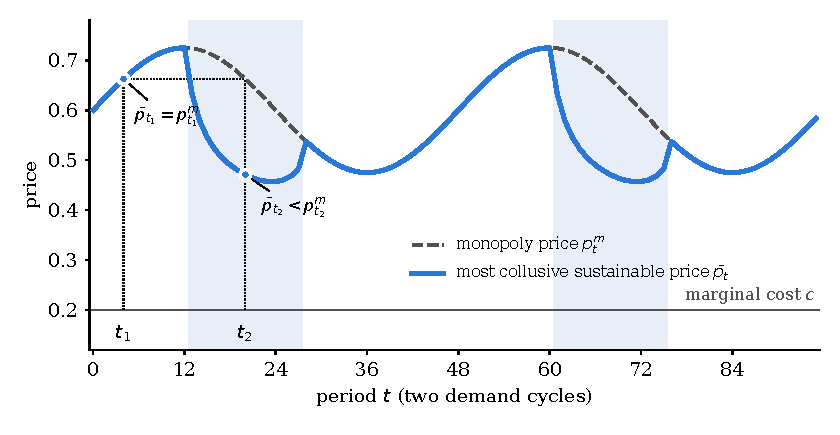
\includegraphics[width=0.92\textwidth]{figures/ch13/bs_cycle.pdf}
\caption{Most collusive sustainable price over a deterministic demand cycle. Linear demand
$D_t(p)=a_t-p$ with $a_t=1+0.25\sin\left(\frac{2\pi t}{48}\right)$, marginal cost $c=0.2$, $N=8$ firms,
$\delta=0.99$ per period and a ten-period Bertrand punishment. Shaded periods are those in which the
incentive constraint \eqref{eq:13-gas-ic} binds. Demand is the same at $t_1$ (rising) and $t_2$ (falling),
yet $\bar p_{t_1}=p^m_{t_1}=0.66$ while $\bar p_{t_2}=0.47$. The path solves \eqref{eq:13-gas-fixed} by
iteration (script \texttt{bs\_cycle.py}).}
\label{fig:13-bs-cycle}
\end{figure}

\casehead{From the incentive constraint to a margin regression}
To motivate an estimating equation we linearize the binding constraint. Let $M_t=\bar p_t-c_t$ be the
collusive margin, $L_t=\frac{M_t}{\bar p_t}$ the Lerner index (a local use of $L_t$, which denotes the lakes
dummy in \cref{sec:13-jec}), and
$\varepsilon_t=-\frac{d'(\bar p_t)\bar p_t}{d(\bar p_t)}$ the industry demand elasticity. At a binding date,
taking logs of $(N-1)A_tM_td(c_t+M_t)=\Phi_t$ gives
\begin{equation*}
\ln A_t+\ln M_t+\ln d(c_t+M_t)=\ln\Phi_t-\ln(N-1).
\end{equation*}
Differentiate, using $\frac{d'}{d}=-\frac{\varepsilon_t}{\bar p_t}$:
\begin{equation*}
\Big(\frac{1}{M_t}-\frac{\varepsilon_t}{\bar p_t}\Big)\,\dd M_t=\dd\ln\Phi_t-\dd\ln A_t+\frac{\varepsilon_t}{\bar p_t}\,\dd c_t .
\end{equation*}
The bracket equals $\frac{1-\varepsilon_tL_t}{M_t}$. It is positive below the monopoly price, because there
profit rises with price: $\frac{\dd}{\dd p}\big[(p-c_t)d(p)\big]=d(p)\,(1-\varepsilon_tL_t)>0$. Near a stationary
point the weights
$\omega_s=\frac{\delta^s}{\sum_{r=1}^{T}\delta^r}$ give $\dd\ln\Phi_t=\sum_s\omega_s\,\dd\ln\bar v_{t+s}$. Hold
future margins at their stationary values, so that future profits move only through demand and cost:
$\dd\ln\bar v_{t+s}=\dd\ln A_{t+s}-\frac{\varepsilon}{\bar p}\dd c_{t+s}$. Substituting and collecting terms,
\begin{equation}\label{eq:13-gas-linear}
\dd M_t=\frac{M}{1-\varepsilon L}\sum_{s=1}^{T}\omega_s\big(\dd\ln A_{t+s}-\dd\ln A_t\big)
-\frac{\varepsilon L}{1-\varepsilon L}\sum_{s=1}^{T}\omega_s\big(\dd c_{t+s}-\dd c_t\big).
\end{equation}
The current levels of demand and cost enter only through their expected changes. With a one-period horizon
and expectations formed at $t$, the margin equation becomes
\begin{equation}\label{eq:13-gas-reg}
M_t\approx\alpha_0+\alpha_2\,\E_t\big[\Delta\ln A_{t+1}\big]+\alpha_3\,\E_t\big[\Delta c_{t+1}\big],\qquad
\alpha_2=\frac{M}{1-\varepsilon L}>0,\quad \alpha_3=-\frac{\varepsilon L}{1-\varepsilon L}<0 .
\end{equation}
The coefficients $\alpha_2$ and $\alpha_3$ are local to this section and have nothing to do with the logit
price coefficient. Under the static benchmark of \cref{prop:13-gas-cs}(c), $\alpha_2=\alpha_3=0$. This is
the null hypothesis that \citet{BorensteinShepard1996} test.

If punishments last longer than one period, the one-period expected change is only a proxy for the weighted
change in \eqref{eq:13-gas-linear}. Under the static null the margin responds to neither, so the proxy
coefficients are still zero and the test keeps its size. Under the alternative the direction of the bias is not
determined. Take demand, and let $\Delta^{1}_t = \E_t[\Delta\ln A_{t+1}]$ and
$\Delta^{T}_t = \sum_{s=1}^{T}\omega_s\E_t[\ln A_{t+s} - \ln A_t]$, both residualized on the other regressors.
Since the weights sum to one, $\Delta^{T}_t = \Delta^{1}_t + R_t$, with $R_t$ the residual of
$\sum_{s=2}^{T}\omega_s\E_t[\ln A_{t+s} - \ln A_{t+1}]$ on the other regressors. Ignoring the cross effect through the cost proxy, the
coefficient on $\Delta^{1}_t$ converges to
\begin{equation*}
\alpha_2\,\frac{\Cov(\Delta^{1}_t, \Delta^{T}_t)}{\Var(\Delta^{1}_t)}
= \alpha_2\left[1 + \frac{\Cov(\Delta^{1}_t, R_t)}{\Var(\Delta^{1}_t)}\right] .
\end{equation*}
The estimate is attenuated only if later expected changes are negatively correlated with the next one, and not so
strongly that the sign reverses. On a smooth seasonal cycle with a horizon of a few months, expected changes in
consecutive months tend to share a sign. The ratio then exceeds one, and the estimate overstates $\alpha_2$. The
same argument applies to $\alpha_3$.

\begin{remark}[Why level and change can be separated]\label{rem:13-gas-level-change}
With independent draws, $\E_t[\ln A_{t+1}]$ is a constant, so $\E_t[\Delta\ln A_{t+1}]=\text{const}-\ln A_t$.
The level of demand and its expected change are then perfectly collinear, and a high level always signals
an expected fall. A seasonal cycle breaks the collinearity. Two weeks with the same demand, one before and
one after the seasonal peak, have opposite expected changes. That is why the test needs predictable
movements in demand and cost.
\end{remark}

\casehead{Competing explanations and the sign of the cost effect}
Two non-collusive mechanisms could also tie current margins to expected future conditions. Both predict
the opposite sign for the cost effect. The first is inventories. Suppose a supplier prices off its
replacement cost, the terminal price $w_{t+1}$ expected at its next purchase, and adds a constant margin
$m^{\circ}$. Then $p_t=\E_t[w_{t+1}]+m^{\circ}$, and the observed margin is
\begin{equation}\label{eq:13-gas-inventory}
M_t=p_t-w_t=m^{\circ}+\E_t\big[\Delta w_{t+1}\big].
\end{equation}
The coefficient on the expected cost change is $+1$, while collusion predicts $\alpha_3<0$. The second
mechanism is a cost of changing prices. A firm facing such costs moves its price toward the price it expects
to want in the future. An anticipated cost increase then raises today's price and today's margin, again a
positive sign. A negative coefficient on expected cost changes is therefore a distinctive prediction of
dynamic collusion. Inventory motives tied to demand require a risk of stockouts, which
\citet{BorensteinShepard1996} rule out because wholesale purchases were never constrained in their sample.

\subsection{Margins and expected demand in U.S.\ cities: Borenstein and Shepard (1996)}\label{sec:13-bs}

\casehead{Question}
Earlier tests of collusion used contemporaneous prices, quantities and costs, as in the conduct-parameter
studies of \cref{ch:conduct}. \citet{Bresnahan1989} stressed that such tests rest on functional-form
assumptions, because static non-cooperative prices can move either way with demand. \citet{BorensteinShepard1996}
ask whether current retail gasoline margins respond to \emph{expected} changes in demand and wholesale cost.
Under static pricing they should not respond at all, so a response is evidence of dynamic collusion that
does not depend on the shape of demand or cost. The question matters because gasoline retailing is far from
a tight oligopoly. Most metropolitan areas have more than ten wholesale suppliers and many more stations.

\casehead{Setting}
Crude oil is refined and shipped by pipeline or barge to city terminals. From the terminal, gasoline is
trucked to stations either by independent wholesalers, called \emph{jobbers}, or by refiners. Jobbers
distribute about 55 percent of U.S. retail gasoline and pay the posted terminal price
(working paper, pp.~8--10). Refiners sell to independently operated stations at the \emph{dealer tankwagon}
price, which is subject to widespread unobserved discounts. Borenstein and Shepard therefore measure
marginal cost by the terminal price. It is the only observed wholesale price for jobbers, it is the
opportunity cost of gasoline sold at refiner-supplied stations, and it is rarely discounted. The margin they
study is the gap between the retail price and the terminal price. It mixes decisions of refiners, jobbers and
station operators.

\casehead{Data}
The panel covers 59 cities in 43 states over the 72 months from 1986 to 1991. \textit{RETAIL} is the Lundberg
Survey average price of regular unleaded self-service gasoline, net of all taxes, on one Friday each month.
\textit{TERM} is the average branded terminal price posted on the same Friday, so the two prices match exactly
and $\textit{MARGIN}=\textit{RETAIL}-\textit{TERM}$. Volume comes from monthly state sales reported by the
Federal Highway Administration. Daily volume in adjacent months is interpolated linearly to the survey day,
giving \textit{VOLUME}. Because over 99 percent of the variance of \textit{VOLUME} is between states,
volume is normalized by its state mean: $\textit{NVOLUME}_{it}=\frac{\textit{VOLUME}_{it}}{\overline{\textit{VOLUME}}_i}$.
\Cref{tab:13-bs-t1} reports the summary statistics. Demand peaks in August at about 20 percent above the
January trough. Short-run demand elasticities lie between $-0.1$ and $-0.2$ \citep{DahlSterner1991}. Retail
prices would then have to swing by 100--200 percent to generate such a cycle, so the seasonal pattern reflects
shifts of demand rather than movements along it. Over half of the monthly crude oil price changes exceed 5
percent in absolute value.

\begin{table}[htbp]
\centering
\caption{Retail gasoline in 59 U.S. cities, 1986--1991: summary statistics}\label{tab:13-bs-t1}
\begin{tabular}{lrrrr}
\toprule
Variable & Mean & Std.\ dev. & Min & Max\\
\midrule
\textit{RETAIL} (cents per gallon) & 72.83 & 12.41 & 43.18 & 126.57\\
\textit{TERM} (cents per gallon) & 62.28 & 11.82 & 36.00 & 111.88\\
\textit{CRUDE} (cents per gallon) & 46.38 & 10.77 & 25.83 & 87.98\\
\textit{MARGIN} (cents per gallon) & 10.57 & 5.12 & $-8.91$ & 34.90\\
\textit{VOLUME} ($10^5$ or $10^6$ gallons per day, see notes) & 10.43 & 10.48 & 0.38 & 38.12\\
\textit{NVOLUME} & 1.005 & 0.087 & 0.570 & 1.617\\
\textit{EXP VOLCHG}, $\hat\eta=-0.1$ & 0.000 & 0.050 & $-0.403$ & 0.287\\
\textit{EXP TERMCHG} (cents per gallon) & 0.139 & 4.172 & $-17.313$ & 13.959\\
\bottomrule
\end{tabular}

\smallskip
\begin{minipage}{0.86\textwidth}\footnotesize
Notes: 3,838 city-month observations. Prices exclude sales and excise taxes and are in current cents.
\textit{EXP VOLCHG} and \textit{EXP TERMCHG} are the expected one-month changes in normalized volume and in the
terminal price defined in the text. The unit of \textit{VOLUME} is unclear in the sources. The working paper's Table 1
prints it as ``(00,000 gal/day)'' and the published Table 1 as gallons $\times 10^{5}$ per day (p.~434). The volume figures
of both versions label the same daily state series in millions of gallons, at levels close to the table means (published
Figure 2, p.~437). We report the numbers as printed and leave the unit open. \textit{NVOLUME} and the regressions do not
depend on it. Source: \citet{BorensteinShepard1996}, working-paper version, Table 1.
\end{minipage}
\end{table}

\casehead{The estimating equation}
Retail prices adjust to terminal prices with lags, and increases pass through faster than decreases. The
authors start from an error-correction model with asymmetric adjustment (working paper, eq.~(1)):
\begin{equation}\label{eq:13-bs-ecm}
\begin{aligned}
\textit{RETAIL}_{it}-\textit{RETAIL}_{i,t-1}={}&\beta_1\Delta\textit{TERM}^{+}_{it}+\beta_2\Delta\textit{TERM}^{+}_{i,t-1}+\beta_3\Delta\textit{TERM}^{+}_{i,t-2}\\
&+\beta_4\Delta\textit{TERM}^{-}_{it}+\beta_5\Delta\textit{TERM}^{-}_{i,t-1}+\beta_6\Delta\textit{TERM}^{-}_{i,t-2}\\
&+\beta_7\Delta\textit{RETAIL}^{+}_{i,t-1}+\beta_8\Delta\textit{RETAIL}^{+}_{i,t-2}\\
&+\beta_9\Delta\textit{RETAIL}^{-}_{i,t-1}+\beta_{10}\Delta\textit{RETAIL}^{-}_{i,t-2}\\
&+\beta_{11}\textit{RETAIL}_{i,t-1}+\beta_{12}\textit{TERM}_{i,t-1}+e_{it}.
\end{aligned}
\end{equation}
Here $\Delta X_{it}=X_{it}-X_{i,t-1}$, and $\Delta X^{+}$ and $\Delta X^{-}$ are the positive and negative parts
of the change. The lagged levels form the error-correction term. If the long-run relation is
$\textit{RETAIL}=\gamma_0+\gamma_1\textit{TERM}$ and the gap closes at rate $\kappa>0$, the correction
$-\kappa(\textit{RETAIL}_{t-1}-\gamma_0-\gamma_1\textit{TERM}_{t-1})$ produces the two lagged levels, with
$\beta_{11}=-\kappa$ and $\beta_{12}=\kappa\gamma_1$. The constant is absorbed by fixed effects.

To put the margin on the left, add $\textit{RETAIL}_{i,t-1}$ to both sides and subtract $\textit{TERM}_{it}$.
The left side becomes $\textit{MARGIN}_{it}$. On the right, $\textit{TERM}_{it}=\Delta\textit{TERM}^{+}_{it}+
\Delta\textit{TERM}^{-}_{it}+\textit{TERM}_{i,t-1}$, so subtracting it lowers the coefficients on
$\Delta\textit{TERM}^{+}_{it}$ and $\Delta\textit{TERM}^{-}_{it}$ by one and the coefficient on
$\textit{TERM}_{i,t-1}$ by one. Adding $\textit{RETAIL}_{i,t-1}$ raises its coefficient by one. The margin
form (working paper, eq.~(2)) is therefore \eqref{eq:13-bs-ecm} with $\beta_1-1$, $\beta_4-1$, $\beta_{11}+1$
and $\beta_{12}-1$ in place of $\beta_1$, $\beta_4$, $\beta_{11}$ and $\beta_{12}$. Adding current volume and the
two expectation terms gives the estimating equation (working paper, eq.~(3)), in which the coefficient
adjustments are left implicit:
\begin{equation}\label{eq:13-bs-main}
\begin{aligned}
\textit{MARGIN}_{it}={}&\alpha_1\textit{NVOLUME}_{it}+\alpha_2\textit{EXP VOLCHG}_{it}+\alpha_3\textit{EXP TERMCHG}_{it}\\
&+\sum_{k=0}^{2}\big(\beta^{+}_{k}\Delta\textit{TERM}^{+}_{i,t-k}+\beta^{-}_{k}\Delta\textit{TERM}^{-}_{i,t-k}\big)\\
&+\sum_{k=1}^{2}\big(\phi^{+}_{k}\Delta\textit{RETAIL}^{+}_{i,t-k}+\phi^{-}_{k}\Delta\textit{RETAIL}^{-}_{i,t-k}\big)\\
&+\beta_{11}\textit{RETAIL}_{i,t-1}+\beta_{12}\textit{TERM}_{i,t-1}+\mu_i+\lambda_t+e_{it}.
\end{aligned}
\end{equation}
We have relabeled the twelve $\beta$'s of the original to show the pattern. The terms $\mu_i$ and
$\lambda_t$ (local symbols here) are city fixed effects and 72 month fixed effects, which absorb cross-city correlation of the
errors at a point in time. Current volume $\alpha_1$ captures any static effect of demand on margins, such as
changes in the mix of customers or peak-load pricing. The coefficients of interest are $\alpha_2$ and
$\alpha_3$, the empirical counterparts of \eqref{eq:13-gas-reg}. The effect of current volume holding expected
next-month volume fixed is $\alpha_1-\alpha_2$, because $\textit{EXP VOLCHG}$ is expected next-month volume
minus current volume.

\casehead{Endogeneity of volume: an instrument built from an assumed elasticity}
Volume depends on the retail price and hence on the margin, so OLS is inconsistent, and no excluded demand
shifters are available. The authors resolve the problem with a constructed instrument. Write the system
(working paper, eqs.~(4) and~(5))
\begin{equation}\label{eq:13-bs-system}
M=a\,Q+X^{\top}g+e,\qquad \ln Q=Z\beta+\eta\ln P+v.
\end{equation}
Here $M$ is the margin, $Q$ volume, $P$ the retail price and $X$ the exogenous variables in the margin
equation. $Z$ collects demand shifters, $\eta<0$ is the industry demand elasticity, and $e$ and $v$ are errors.
The working paper assumes only that $e$ and $v$ are uncorrelated. We assume instead that the margin error is mean
independent of the exogenous variables and of the demand shock, $\E[e\mid X,Z,v]=0$. If $\eta$ were known, the
variable
\begin{equation}\label{eq:13-bs-qprime}
\ln Q'=\ln Q+\ln k-\eta\ln P=Z\beta+\ln k+v
\end{equation}
would be volume purged of the direct price effect. It is a function of $Z$ and $v$ only. Mean independence
therefore makes it, and any function of it, uncorrelated with $e$. It is correlated with $Q$, so it is a valid
instrument. The stronger condition matters because the instrument used below is the level $Q'$, which is
proportional to $\exp(v)$ given $Z$. Uncorrelatedness does not carry over to the level. If $v$ is uniform on
$\{-1,0,1\}$ and $e=v^2-\frac{2}{3}$, then $\E[e]=\E[ev]=0$ but
$\E[e\exp(v)]=\frac{\exp(1)+\exp(-1)-2}{9}>0$. Some demand shifters may themselves respond to
$P$, for example prices of other goods that rise with transport costs. Partition $Z=(Z_1,Z_2)$ with
$Z_1=\theta_0+\theta_1\ln P$ and $Z_2$ independent of $P$. Then
\begin{equation*}
\ln Q=(\theta_0+\theta_1\ln P)\beta_1+Z_2\beta_2+\eta\ln P+v,
\end{equation*}
and the variable
\begin{equation}\label{eq:13-bs-qdoubleprime}
\ln Q''=\ln Q+\ln k-\tilde\eta\ln P=\theta_0\beta_1+Z_2\beta_2+\ln k+v,\qquad \tilde\eta\equiv\eta+\theta_1\beta_1,
\end{equation}
is again a valid instrument if $\E[e\mid X,Z_2,v]=0$. Published estimates of gasoline demand elasticities ignore such indirect effects,
so they are best read as estimates of $\tilde\eta$.

The implementation multiplies daily volume by $kP^{-\hat\eta}$ with $k=\frac{\bar P^{\hat\eta}}{\bar Q}$,
where $\bar P$ is the city's mean retail price and $\bar Q$ the mean of the corrected series. The result,
$\textit{TNVOLUME}=\frac{\textit{VOLUME}}{\bar Q}\left(\frac{P}{\bar P}\right)^{-\hat\eta}$, instruments
\textit{NVOLUME} in two-stage least squares. Since $\hat\eta$ is unknown, the regression is repeated for
$\hat\eta\in\{0,-0.1,-0.2,-0.3\}$, a range slightly wider than the $-0.1$ to $-0.2$ found with monthly and
quarterly data. With $\hat\eta=0$ the correction is void and \textit{NVOLUME} is treated as exogenous. The
correction is small: a price 20 percent above the city mean raises \textit{TNVOLUME} relative to
\textit{NVOLUME} by $1.2^{0.3}-1=5.6$ percent when $\hat\eta=-0.3$ and by $1.2^{0.1}-1=1.8$ percent when
$\hat\eta=-0.1$.

The contemporaneous terminal price could also be endogenous if the marginal cost of supplying a city rises
with its volume. The authors argue that the feedback is small, because terminals have ten or more refiners
and supply can shift across regions. A Hausman test nonetheless rejects exogeneity of the current terminal
price and of the expected terminal-price change. The current price is therefore instrumented with the residual
from a regression of \textit{TERM} on \textit{NVOLUME}. The expected change is instrumented with a forecast built
from that orthogonalized series. Instrumenting does not change the results in an economically or statistically
meaningful way. The residuals of \eqref{eq:13-bs-main}
are not serially correlated, so the lagged dependent variables raise no endogeneity problem.

\casehead{Measuring expectations}
Expected volume comes from a forecasting regression estimated state by state (working paper, eq.~(8)):
\begin{equation}\label{eq:13-bs-volforecast}
\textit{NVOLUME}_{it}=a_0+a_1\textit{NVOLUME}_{i,t-1}+a_2\textit{NVOLUME}_{i,t-2}+\sum_{j=2}^{12}\varsigma_j\textit{MONTH}_j
+a_3t+a_4t^2+a_5t^3+e_{it}.
\end{equation}
The $R^2$ lies between 0.80 and 0.95 for nearly all states. The one-period lead of the fitted values gives
$\textit{EXP VOLCHG}_{it}=\widehat{\textit{NVOLUME}}_{i,t+1}-\textit{NVOLUME}_{it}$. The instrument for
\textit{EXP VOLCHG} uses the same regression estimated with \textit{TNVOLUME}. Expected terminal prices come
from a city-level error-correction autoregression with crude oil prices (working paper, eq.~(9)):
\begin{equation}\label{eq:13-bs-termforecast}
\begin{aligned}
\Delta\textit{TERM}_{it}={}&b_0+\sum_{k=1}^{2}\big(b^{+}_k\Delta\textit{TERM}^{+}_{i,t-k}+b^{-}_k\Delta\textit{TERM}^{-}_{i,t-k}
+d^{+}_k\Delta\textit{CRUDE}^{+}_{i,t-k}+d^{-}_k\Delta\textit{CRUDE}^{-}_{i,t-k}\big)\\
&+b_9\textit{TERM}_{i,t-1}+b_{10}\textit{CRUDE}_{i,t-1}+\sum_{j=2}^{12}\varsigma'_j\textit{MONTH}_j+e_{it}.
\end{aligned}
\end{equation}
The current crude price is excluded because it would not be known when the forecast is made. The $R^2$ ranges
from 0.30 to 0.60, lower than for volume because crude prices behave roughly like a random walk. Then
$\textit{EXP TERMCHG}_{it}=\widehat{\Delta\textit{TERM}}_{i,t+1}$. The forecasting coefficients use the whole
sample, which in principle includes information the firms did not have. Forecasts from rolling regressions
with volume data back to 1982 change neither the predictions nor the final coefficients substantively.

\casehead{Identification}
The month fixed effects absorb any national seasonal pattern, including the common August peak. The
coefficient on \textit{EXP VOLCHG} is therefore identified from differences in seasonal patterns across states
and from state-specific trends. These differences are large. The peak-to-trough swing is 51 percent of mean
volume in Wyoming and 7 percent in Arizona. August demand is below the state mean in Florida, and January
demand is above it in Colorado and Hawaii (working paper, p.~27). The coefficient on \textit{EXP TERMCHG} is
identified from city-specific terminal-price dynamics. Cold-weather cities, for instance, see winter declines
in gasoline terminal prices when refiners produce heating oil and gasoline jointly. The expectation terms are
functions of lagged variables and deterministic seasonals, so they are predetermined with respect to the
current margin shock.

\casehead{Results}
\Cref{tab:13-bs-t2} reproduces the two-stage least squares estimates. The coefficient on \textit{EXP VOLCHG} is
positive and significant at the 1 percent level for every assumed elasticity, and it changes little with
$\hat\eta$. The coefficient on \textit{EXP TERMCHG} is negative and significant at the 1 percent level
throughout. Both signs are those of \eqref{eq:13-gas-reg}. The negative cost coefficient is the opposite of the
inventory prediction \eqref{eq:13-gas-inventory}.

\begin{table}[htbp]
\centering
\caption{Retail margins and expected changes in demand and cost (dependent variable \textit{MARGIN})}\label{tab:13-bs-t2}
\small
\begin{tabular}{lcccc}
\toprule
Assumed elasticity & $\hat\eta=0$ & $\hat\eta=-0.1$ & $\hat\eta=-0.2$ & $\hat\eta=-0.3$\\
\midrule
$\textit{NVOLUME}_t$ & 3.397 (0.754) & 5.563 (0.758) & 7.926 (0.768) & 10.455 (0.785)\\
$\textit{EXP VOLCHG}_t$ & 4.081 (1.324) & 3.860 (1.335) & 4.362 (1.365) & 5.492 (1.409)\\
$\textit{EXP TERMCHG}_t$ & $-0.057$ (0.018) & $-0.062$ (0.017) & $-0.066$ (0.018) & $-0.068$ (0.018)\\
\addlinespace
$\Delta\textit{TERM}^{+}_t$ & $-0.303$ (0.021) & $-0.305$ (0.021) & $-0.306$ (0.021) & $-0.304$ (0.021)\\
$\Delta\textit{TERM}^{+}_{t-1}$ & 0.153 (0.023) & 0.148 (0.023) & 0.143 (0.023) & 0.138 (0.023)\\
$\Delta\textit{TERM}^{+}_{t-2}$ & 0.065 (0.021) & 0.063 (0.021) & 0.062 (0.021) & 0.061 (0.022)\\
$\Delta\textit{TERM}^{-}_t$ & $-0.589$ (0.019) & $-0.584$ (0.019) & $-0.578$ (0.019) & $-0.572$ (0.018)\\
$\Delta\textit{TERM}^{-}_{t-1}$ & 0.175 (0.023) & 0.169 (0.023) & 0.163 (0.023) & 0.155 (0.023)\\
$\Delta\textit{TERM}^{-}_{t-2}$ & 0.078 (0.020) & 0.074 (0.020) & 0.069 (0.020) & 0.065 (0.020)\\
$\Delta\textit{RETAIL}^{+}_{t-1}$ & $-0.017$ (0.022) & $-0.018$ (0.023) & $-0.020$ (0.023) & $-0.022$ (0.023)\\
$\Delta\textit{RETAIL}^{+}_{t-2}$ & $-0.066$ (0.022) & $-0.069$ (0.022) & $-0.072$ (0.022) & $-0.076$ (0.022)\\
$\Delta\textit{RETAIL}^{-}_{t-1}$ & $-0.029$ (0.022) & $-0.027$ (0.022) & $-0.026$ (0.023) & $-0.025$ (0.023)\\
$\Delta\textit{RETAIL}^{-}_{t-2}$ & 0.039 (0.020) & 0.039 (0.020) & 0.039 (0.020) & 0.039 (0.020)\\
$\textit{RETAIL}_{t-1}$ & 0.623 (0.015) & 0.619 (0.015) & 0.615 (0.015) & 0.612 (0.015)\\
$\textit{TERM}_{t-1}$ & $-0.668$ (0.020) & $-0.660$ (0.020) & $-0.650$ (0.020) & $-0.639$ (0.020)\\
\addlinespace
Observations & 3,838 & 3,838 & 3,838 & 3,838\\
\bottomrule
\end{tabular}

\smallskip
\begin{minipage}{0.92\textwidth}\footnotesize
Notes: Two-stage least squares estimates of \eqref{eq:13-bs-main} with city and month fixed effects (not
reported). Asymptotic standard errors in parentheses. \textit{NVOLUME} is instrumented with the
elasticity-corrected series for the assumed $\hat\eta$. Source: \citet{BorensteinShepard1996}, working-paper
version, Table 2.
\end{minipage}
\end{table}

\begin{example}[Reading the magnitudes]\label{ex:13-bs-elasticity}
Take the column $\hat\eta=-0.1$, which the authors regard as closest to the true elasticity. Raise expected
next-month volume by 1 percent of its mean, that is by $0.01005$ units of \textit{NVOLUME}, holding current
volume fixed. \textit{EXP VOLCHG} rises by the same amount, so the margin rises by $3.860\times0.01005=0.039$
cents, which is $\frac{0.039}{10.57}=0.37$ percent of the mean margin. The elasticity of the margin with respect
to expected next-month volume is therefore 0.37. Raise the expected next-month terminal price by 1 percent of its
mean, or 0.623 cents. The margin falls by $0.062\times0.623=0.039$ cents, an elasticity of $-0.37$. These are the
two elasticities in the authors' abstract. A one-standard-deviation increase in \textit{EXP VOLCHG} (0.050) adds
$3.860\times0.050=0.19$ cents to the margin. A one-standard-deviation increase in \textit{EXP TERMCHG} (4.172
cents) subtracts $0.062\times4.172=0.26$ cents.

The seasonal peak shows how the two volume terms combine. July volume averages 8.3 percent above the sample
mean, which adds $5.563\times0.083=0.46$ cents to the July margin. August volume is 8.8 percent above the mean,
so the expected July-to-August change of 0.5 percent adds $3.860\times0.005=0.02$ cents, for a total of 0.48 cents.
In August, current volume adds $5.563\times0.088=0.49$ cents. The expected fall of 4.6 percent into September
subtracts $3.860\times0.046=0.18$ cents, so August margins are only 0.31 cents above average. Margins are higher
on the way up to the peak than at the peak itself, as \cref{fig:13-bs-cycle} predicts.
\end{example}

The rest of the table describes price adjustment. A one-cent rise in the terminal price lowers the margin in
the same month by 0.305 cents, so the retail price rises by $1-0.305=0.70$ cents within the month. A one-cent
fall raises the margin by 0.584 cents, so the retail price falls by only $1-0.584=0.42$ cents. Increases pass
through faster than decreases. The long-run pass-through follows from the lagged levels. Setting all changes to
zero in \eqref{eq:13-bs-main} gives $\textit{RETAIL}(1-\beta_{11})=\textit{TERM}(1+\beta_{12})+\text{const}$, so
\begin{equation*}
\frac{\partial\,\textit{RETAIL}}{\partial\,\textit{TERM}}\bigg|_{\text{long run}}=\frac{1+\beta_{12}}{1-\beta_{11}}
=\frac{1-0.660}{1-0.619}=0.89 .
\end{equation*}
This matches the authors' statement that terminal price changes are passed through about 90 percent in the long
run, a rate they cannot distinguish statistically from 100 percent.

\begin{example}[How large should the effects be?]\label{ex:13-gas-calibration}
The linearized constraint \eqref{eq:13-gas-reg} gives a benchmark for the coefficients. Take the sample means
$M=10.57$ and $\bar p=72.83$ cents, so $L=0.145$, and an industry elasticity between 0.1 and 0.3. Then
$\varepsilon L$ lies between 0.015 and 0.044. The benchmark is $\alpha_2=\frac{M}{1-\varepsilon L}$, between 10.7
and 11.1 cents per unit change in $\ln A$, and $\alpha_3=-\frac{\varepsilon L}{1-\varepsilon L}$, between $-0.015$
and $-0.045$. The estimates of 3.86 and $-0.062$ are of the same order of magnitude. The comparison is only
indicative. The benchmark assumes that the constraint always binds, that punishments last one month, that the
whole measured margin is collusive and that future margins do not move.
\end{example}

\casehead{Robustness: expected versus unexpected changes}
The main threat is measurement error. Monthly state volumes are matched to a single day's city prices. If
current volume is measured with error and next month's volume contains information about current volume, then
\textit{EXP VOLCHG} could proxy for the true current volume. Since current volume raises margins, this would
mimic the collusive effect. The two explanations differ in their predictions for \emph{unexpected} future
changes. Firms cannot respond to changes they do not foresee, so under collusion unexpected changes have zero
coefficients. Under measurement error, unexpected changes would carry information about current volume as
well. The authors estimate (working paper, eq.~(3$'$))
\begin{equation}\label{eq:13-bs-unx}
\begin{aligned}
\textit{MARGIN}_{it}={}&\alpha_1\textit{EXP VOL}_{it}+\alpha'_1\textit{UNX VOL}_{it}+\alpha_2\textit{EXP VOLCHG}_{it}
+\alpha'_2\textit{UNX VOLCHG}_{it}\\
&+\alpha_3\textit{EXP TERMCHG}_{it}+\alpha'_3\textit{UNX TERMCHG}_{it}\\
&+(\text{price-adjustment terms and fixed effects of \eqref{eq:13-bs-main}})+e_{it}.
\end{aligned}
\end{equation}
Here $\textit{UNX VOLCHG}$ is next month's actual volume change minus its expected value. The terms
$\textit{EXP VOL}$ and $\textit{UNX VOL}$ split current volume into the part predicted a month earlier and the
surprise.
\Cref{tab:13-bs-t3} reports the key rows. Unexpected future volume changes are never significantly positive, and
they differ significantly from expected changes for every nonzero $\hat\eta$. Unexpected terminal changes have
coefficients near zero, significantly different from the expected ones. Unexpected \emph{current} volume
raises margins significantly for every nonzero $\hat\eta$. Margins therefore do respond to current surprises.
Their failure to respond to future surprises is informative.

\begin{table}[htbp]
\centering
\caption{Expected versus unexpected changes (dependent variable \textit{MARGIN})}\label{tab:13-bs-t3}
\small
\begin{tabular}{lcccc}
\toprule
Assumed elasticity & $\hat\eta=0$ & $\hat\eta=-0.1$ & $\hat\eta=-0.2$ & $\hat\eta=-0.3$\\
\midrule
$\textit{EXP NVOLUME}_t$ & 4.116 (0.824) & 5.150 (0.830) & 6.273 (0.846) & 7.478 (0.871)\\
$\textit{UNX NVOLUME}_t$ & 0.926 (1.388) & 7.003 (1.402) & 13.347 (1.447) & 19.751 (1.518)\\
$\textit{EXP VOLCHG}_t$ & 3.720 (1.334) & 4.064 (1.347) & 4.930 (1.382) & 6.129 (1.436)\\
$\textit{UNX VOLCHG}_t$ & 1.178 (1.292) & 0.146 (1.309) & $-1.478$ (1.355) & $-3.532$ (1.425)\\
$\textit{EXP TERMCHG}_t$ & $-0.059$ (0.018) & $-0.059$ (0.018) & $-0.057$ (0.018) & $-0.054$ (0.018)\\
$\textit{UNX TERMCHG}_t$ & 0.013 (0.016) & 0.011 (0.016) & 0.009 (0.016) & 0.006 (0.016)\\
\addlinespace
Observations & 3,838 & 3,838 & 3,838 & 3,838\\
\bottomrule
\end{tabular}

\smallskip
\begin{minipage}{0.92\textwidth}\footnotesize
Notes: Estimates of \eqref{eq:13-bs-unx}. The price-adjustment terms, city and month fixed effects are included
and not shown. Standard errors in parentheses. Source: \citet{BorensteinShepard1996}, working-paper version,
Table 3.
\end{minipage}
\end{table}

\casehead{Interpretation}
Borenstein and Shepard read the evidence as consistent with tacit collusion in the sense of
\citet{RotembergSaloner1986} and \citet{HaltiwangerHarrington1991}. They stress what the test does not show.
Collusion here need not mean prices near monopoly. With an industry elasticity between $-0.1$ and $-0.3$, demand
is inelastic at observed prices, so an industry monopolist would raise prices far above them. The authors conclude
that actual margins fall far short of the monopoly level. Nor does the test measure the level of collusion. The
measured margin includes delivery and other short-run variable costs, so the collusive part is smaller than 10.6
cents, and the data cannot isolate it. What the test detects is the dynamic signature of an incentive constraint.
A mild form of tacit coordination fits the market: a station that cuts
its price provokes nearby stations to retaliate, and the retaliation is costlier when future margins are high.

\casehead{Critiques}
Five limitations deserve mention. First, expectations are the econometrician's forecasts. Their coefficients are
estimated on the full sample, and the true information sets of station managers are unknown. Second, volume is
measured at the state level, prices at the city level, and prices only on one day per month. Third, the
one-month horizon is arbitrary. The authors argue that longer punishments would bias the estimates downward
(working paper, p.~17). That holds only under the covariance condition stated after \eqref{eq:13-gas-reg}, and on
a seasonal cycle the bias can go either way. The test of the static null keeps its size in either case. Fourth, the test rejects static pricing, but other dynamic
non-cooperative models could generate forward-looking prices. \Cref{sec:13-noel} shows that Edgeworth cycles are one
such model, although its mechanism differs from the one tested here. Fifth, the margin mixes the decisions of
refiners, jobbers and station operators, so the colluding agents are not identified.

\casehead{Contribution}
The paper moved the empirical study of collusion from tight oligopolies to an unconcentrated industry with many
differentiated sellers. It replaced contemporaneous price-cost relations, which require functional-form
assumptions, with a dynamic implication of the incentive constraint. It also showed how to build a test that
distinguishes collusion from inventory behavior and from measurement error through sign restrictions and a
placebo on unforecastable changes.

\subsection{Edgeworth cycles in Toronto: Noel (2007)}\label{sec:13-noel}

\casehead{Question}
In many Canadian cities retail gasoline prices follow a fast asymmetric cycle. A large, sudden price increase is
followed by many small decreases until margins are thin, and then prices jump again. Consumer groups and
governments have often read the synchronized jumps as collusion. \citet{Noel2007} asks whether the cycle is
instead a competitive \emph{Edgeworth cycle}, the Markov equilibrium of dynamic price competition introduced by
\citet{MaskinTirole1988}. The answer matters for policy, because evidence of Edgeworth cycles argues against
costly investigations of covert collusion.

\casehead{Theory}
In the model of \citet{MaskinTirole1988}, two firms sell a homogeneous good and set prices alternately, each price
fixed for two periods. Strategies are Markov: the moving firm conditions only on the rival's current price (and,
in the extension of \citet{Noel2007}, on the current cost). With demand $D^i$ for firm $i$ and cost $c_t$, firm
$i$ earns $\pi^i_t(p^1_t,p^2_t,c_t)=D^i(p^1_t,p^2_t)(p^i_t-c_t)$. When firm 1 moves after firm 2 has set
$p^2_{t-1}$, its values are
\begin{align}
V^1(p^2_{t-1})&=\E_c\Big[\max_{p_t}\big\{\pi^1_t(p_t,p^2_{t-1},c_t)+\delta_1W^1(p_t)\big\}\Big],\label{eq:13-mt-v}\\
W^1(p^1_{s-1})&=\E_c\Big[\E_{p_s}\big[\pi^1_s(p^1_{s-1},p_s,c_s)+\delta_1V^1(p_s)\big]\Big].\label{eq:13-mt-w}
\end{align}
Here $W^1$ is firm 1's value in a period in which firm 2 moves, and $p_s$ is firm 2's reply. The game has two
kinds of Markov perfect equilibria, focal-price equilibria and Edgeworth-cycle equilibria. The incentives
behind a cycle are as follows. At a high rival price, undercutting by one step captures the whole market for a
period, roughly twice what matching yields. Prices therefore fall step by step in the \emph{undercutting phase}.
Near marginal cost an undercut earns nothing. Raising the price is costly for the firm that moves first, because
the rival keeps the low price and serves the market for a period. Each firm prefers the other to restore prices,
so the bottom of the cycle is a war of attrition in which firms randomize between staying low and jumping up. The
firm that moves jumps all the way to the top in a single \emph{relenting phase}. A gradual increase would be
undercut at once and would not repay its cost. \Cref{fig:13-edgeworth} draws the resulting sawtooth.

\begin{figure}[htbp]
\centering
\begin{tikzpicture}
\begin{axis}[
  width=0.92\textwidth, height=6.4cm,
  xmin=-0.5, xmax=25, ymin=-0.9, ymax=12.6, clip=false,
  axis lines=left, xtick=\empty, ytick={2}, yticklabels={$c$},
  xlabel={period $t$ (firms move alternately)}, ylabel={price},
  legend style={draw=none, at={(0.5,-0.2)}, anchor=north, font=\footnotesize, legend columns=3,
    /tikz/every even column/.append style={column sep=0.6cm}},
  legend cell align=left,
]
\addplot[const plot, line width=1.6pt, orange!85!black] coordinates {
 (0,2) (1,9) (2,9) (3,7) (4,7) (5,5) (6,5) (7,3) (8,3) (9,2) (10,2) (11,10) (12,10) (13,8)
 (14,8) (15,6) (16,6) (17,4) (18,4) (19,2) (20,2) (21,2) (22,2) (23,9) (24,9) (25,9)};
\addlegendentry{firm 2 (moves at odd $t$)}
\addplot[const plot, line width=0.8pt, blue!70!black] coordinates {
 (0,10) (1,10) (2,8) (3,8) (4,6) (5,6) (6,4) (7,4) (8,2) (9,2) (10,2) (11,2) (12,9) (13,9)
 (14,7) (15,7) (16,5) (17,5) (18,3) (19,3) (20,2) (21,2) (22,10) (23,10) (24,8) (25,8)};
\addlegendentry{firm 1 (moves at even $t$)}
\addplot[dashed, gray, domain=-0.5:25] {2};
\addlegendentry{marginal cost $c$}
\draw[decorate, decoration={brace, amplitude=5pt}] (axis cs:1,10.7) -- (axis cs:9,10.7)
  node[midway, above=6pt, font=\footnotesize] {undercutting phase};
\draw[decorate, decoration={brace, amplitude=5pt, mirror}] (axis cs:8,1.3) -- (axis cs:11,1.3)
  node[midway, below=6pt, font=\footnotesize] {war of attrition};
\draw[-{Stealth[length=2mm]}] (axis cs:13.2,11.6) -- (axis cs:11.2,10.4);
\node[font=\footnotesize, anchor=west] at (axis cs:13.2,11.6) {relenting phase};
\end{axis}
\end{tikzpicture}
\caption{A stylized Edgeworth cycle with two symmetric firms. Each firm's price is fixed for two periods and firms
move in turn. Prices fall by one step per move until they reach marginal cost $c$. After a war of attrition one firm
relents to the top in a single jump, the rival undercuts it at once, and the cycle restarts. Where the two prices
coincide, the thin line lies on the thick one. Drawn by us after the logic of \citet{MaskinTirole1988} and Figure 2
of \citet{Noel2007}.}
\label{fig:13-edgeworth}
\end{figure}

Firm asymmetries sharpen the predictions. \citet{Eckert2003} lets firms split the market unequally at equal
prices. The firm with the smaller share at equal prices gains more from undercutting, since it gives up less of
the shared market, so small firms lead prices down. Large firms, which control many stations and coordinate them
easily, are better placed to restart the cycle. The theory thus makes one structural prediction and three
behavioral ones. The structural prediction is that each station raises its price by the full height of the cycle
in one period and then lowers it in small consecutive steps. The behavioral predictions are (1) fast but not
simultaneous reactions, (2) small firms lead prices down, and (3) large firms lead prices up. Edgeworth cycles
survive cost fluctuations and mild spatial differentiation, so the predictions carry over to retail gasoline.

\casehead{Data}
Noel collected retail prices every twelve hours at 22 Toronto stations on major routes over 131 consecutive days,
February 12 to June 22, 2001. Thirteen stations belong to major integrated firms and nine to independents, twelve
firms in all, spread over 17 miles. The price is for regular unleaded self-service gasoline in Canadian cents per
liter (cpl). The rack price is the daily spot price of the largest wholesaler at the Toronto rack, which can be
treated as exogenous because U.S. wholesale supply is readily available. Excise taxes are 24.7 cpl and the sales
tax is 7 percent. The average price before tax is 43.09 cpl (standard deviation 4.44), and after tax 72.53 (4.75).
The rack price averages 39.77 (4.00). The lagged retail price exceeds the rack price by 3.31 cpl (2.08) on
average (Table I). \Cref{fig:13-noel-f1} shows a major and an independent
station against the rack price. The retail cycle is evident, and the rack price has none.

\begin{figure}[htbp]
\centering
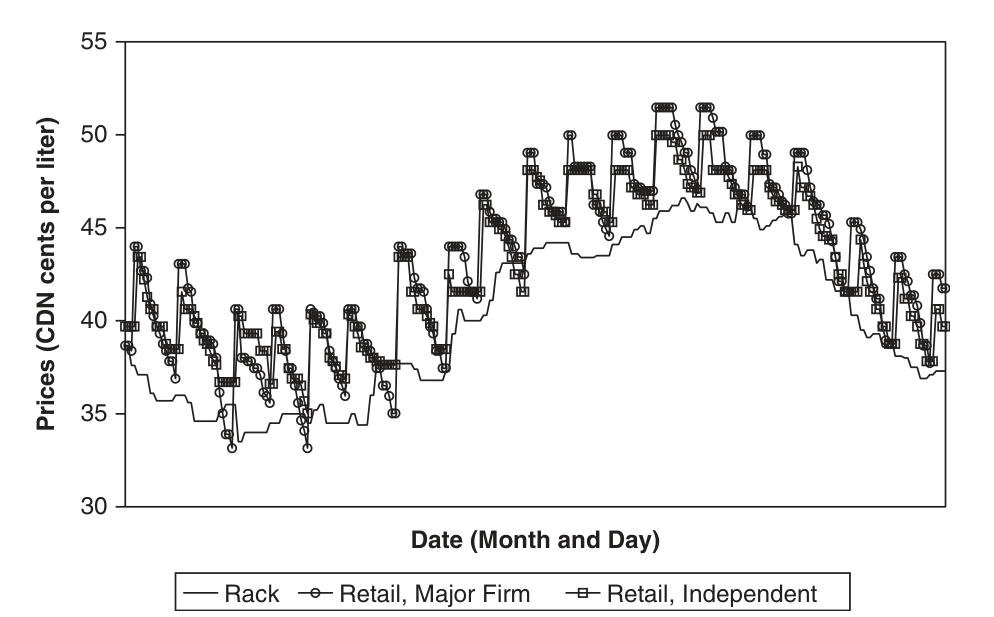
\includegraphics[width=0.78\textwidth]{figures/ch13/noel2007_fig1.png}
\caption{Twelve-hourly retail prices at a major-firm station and an independent station in Toronto, February to
June 2001, with the rack price. Prices exclude taxes. Source: \citet{Noel2007}, Figure 1.}
\label{fig:13-noel-f1}
\end{figure}

\casehead{Model}
For station $s$ in period $t$, the regime $I_{st}\in\{R,U\}$ is either relenting or undercutting. The regime is
latent, because a zero or small change can belong to either phase. Within regime $i$, the price change
$\Delta p_{st}$ follows (Noel's eq.~(4))
\begin{equation}\label{eq:13-noel-regime}
\Delta p_{st}=\begin{cases}X^{i}_{st}\beta^{i}+\epsilon^{i}_{st}, & \text{with probability }1-\gamma^{i}_{st},\\
0, & \text{with probability }\gamma^{i}_{st},\end{cases}\qquad \epsilon^{i}_{st}\sim N(0,\sigma_i^2).
\end{equation}
The mass point at zero allows for stations that skip a period, since the twelve-hour sampling need not match the
true length of a pricing period. The \emph{sticky-price probability} $\gamma^i_{st}$ and the regime transition
probabilities are logits (Noel's eqs.~(5)--(6)):
\begin{equation}\label{eq:13-noel-logits}
\begin{gathered}
\lambda^{iR}_{st}=\Pr\big(I_{st}=R\mid I_{s,t-1}=i,W^i_{st}\big)=\frac{\exp(W^i_{st}\vartheta^i)}{1+\exp(W^i_{st}\vartheta^i)},\qquad
\lambda^{iU}_{st}=1-\lambda^{iR}_{st},\\
\gamma^i_{st}=\frac{\exp(V^i_{st}\zeta^i)}{1+\exp(V^i_{st}\zeta^i)} .
\end{gathered}
\end{equation}
In this subsection $\lambda$ and $\gamma$ are local symbols, and $a_i=\E[\Delta p\mid\Delta p\neq0,\text{regime }i]$
denotes the expected nonzero price change, which Noel writes $\alpha^i$. The density of an observed change in
regime $i$ mixes a point mass and a normal density:
\begin{equation}\label{eq:13-noel-density}
g_i(\Delta p_{st})=\gamma^i_{st}\,\indic\{\Delta p_{st}=0\}+(1-\gamma^i_{st})\,\frac{1}{\sigma_i}\,\phi\Big(\frac{\Delta p_{st}-X^i_{st}\beta^i}{\sigma_i}\Big)\,\indic\{\Delta p_{st}\neq0\},
\end{equation}
where $\phi$ is the standard normal density.
The likelihood is computed with the filter of \cref{sec:13-markov}, following \citet{CosslettLee1985} as in
\citet{Ellison1994}. Let $\xi_{t\mid t-1}(j)$ be the probability of regime $j$ given past price changes. Then
\begin{align*}
\xi_{t\mid t-1}(j)&=\sum_{i\in\{R,U\}}\lambda^{ij}_{st}\,\xi_{t-1\mid t-1}(i),\qquad
f(\Delta p_{st}\mid\text{past})=\sum_{j}\xi_{t\mid t-1}(j)\,g_j(\Delta p_{st}),\\
\xi_{t\mid t}(j)&=\frac{\xi_{t\mid t-1}(j)\,g_j(\Delta p_{st})}{f(\Delta p_{st}\mid\text{past})},\qquad
\ell=\sum_{s}\sum_{t}\ln f(\Delta p_{st}\mid\text{past}).
\end{align*}
The parameters are estimated by maximum likelihood with Newey-West standard errors.

The cycle's characteristics follow from the switching probabilities. With constant probabilities the length of a
spell in regime $i$ is geometric, so its expected duration is $\frac{1}{1-\lambda^{ii}}$ (\cref{lem:13-durations}).
The expected period of the cycle is the sum of the two expected durations. The total price increase during a
relenting spell is the sum of a random number of independent price changes, each with mean $(1-\gamma^R)a_R$.
By Wald's identity its expectation is the product of the mean duration and the mean change:
\begin{equation}\label{eq:13-noel-amplitude}
\E[\text{amplitude}]=\frac{(1-\gamma^R)\,a_R}{1-\lambda^{RR}},\qquad
\E[\text{period}]=\frac{1}{1-\lambda^{RR}}+\frac{1}{1-\lambda^{UU}},\qquad
\text{asymmetry}=\frac{1-\lambda^{RR}}{1-\lambda^{UU}} .
\end{equation}
The asymmetry measure is the ratio of the undercutting duration to the relenting duration. Standard errors come
from the delta method.

\casehead{The anatomy of the cycle}
\Cref{tab:13-noel} reproduces the estimates with constant parameters. The relenting phase lasts 1.008 half-days,
which confirms the structural prediction: each station completes its increase within one twelve-hour period. The
undercutting phase lasts 12.78 half-days, so the cycle repeats about once a week. The amplitude is 5.62 cpl, or 13
percent of the average pre-tax price and 170 percent of the average markup. Increases of 10 cpl in one step were
common in the sample.

\begin{table}[htbp]
\centering
\caption{Regime estimates and cycle characteristics, Toronto 2001}\label{tab:13-noel}
\small
\begin{tabular}{lccc}
\toprule
 & (1) All firms & (2) Major firms & (2) Independents\\
\midrule
\multicolumn{4}{l}{\textit{Relenting phase}}\\
$a_R$ (expected nonzero change, cpl) & 5.576 (0.083) & 5.782 (0.101) & 5.192 (0.142)\\
$\sigma_R$ & 1.650 (0.066) & 1.610 (0.085) & 1.655 (0.100)\\
$\gamma^R$ (sticky share) & 4.0E-5 (4.6E-4) & 4.1E-5 (4.8E-4) & 3.8E-5 (4.9E-4)\\
\multicolumn{4}{l}{\textit{Undercutting phase}}\\
$a_U$ (expected nonzero change, cpl) & $-0.751$ (0.008) & $-0.767$ (0.010) & $-0.720$ (0.015)\\
$\sigma_U$ & 0.459 (0.009) & 0.467 (0.012) & 0.441 (0.012)\\
$\gamma^U$ (sticky share) & 0.429 (0.007) & 0.422 (0.008) & 0.441 (0.014)\\
\multicolumn{4}{l}{\textit{Switching probabilities}}\\
$\lambda^{RR}$ & 0.008 (0.004) & 0.008 (0.005) & 0.007 (0.007)\\
$\lambda^{RU}$ & 0.992 (0.004) & 0.992 (0.005) & 0.993 (0.007)\\
$\lambda^{UR}$ & 0.078 (0.001) & 0.078 (0.002) & 0.078 (0.003)\\
$\lambda^{UU}$ & 0.921 (0.001) & 0.921 (0.002) & 0.921 (0.003)\\
\multicolumn{4}{l}{\textit{Cycle characteristics}}\\
Relenting duration (half-days) & 1.008 (0.004) & 1.008 (0.007) & 1.007 (0.007)\\
Undercutting duration (half-days) & 12.780 (0.291) & 12.779 (0.358) & 12.784 (0.484)\\
Cycle period (half-days) & 13.788 (0.291) & 13.787 (0.358) & 13.792 (0.485)\\
Asymmetry & 12.680 (0.291) & 12.677 (0.363) & 12.687 (0.491)\\
Amplitude (cpl) & 5.619 (0.082) & 5.828 (0.098) & 5.232 (0.144)\\
\bottomrule
\end{tabular}

\smallskip
\begin{minipage}{0.92\textwidth}\footnotesize
Notes: Specification (1) has no firm-type dummies. Specification (2) adds major and independent dummies to $a_i$,
$\lambda^{ij}$ and $\gamma^i$. Standard errors from the delta method in parentheses. Source: \citet{Noel2007},
Tables II and III.
\end{minipage}
\end{table}

\begin{example}[Checking the cycle arithmetic]\label{ex:13-noel-cycle}
From \eqref{eq:13-noel-amplitude}, the relenting duration is $\frac{1}{1-0.008}=1.008$. The undercutting duration of
12.780 implies an unrounded $\lambda^{UU}=1-\frac{1}{12.780}=0.9218$. This rounds to 0.922, one unit in the third
decimal above the 0.921 that the table reports. The period is
$1.008+12.780=13.788$ half-days and the asymmetry is $\frac{12.780}{1.008}=12.68$. The amplitude is
$(1-0.00004)\times5.576\times1.008=5.62$ cpl, equal to the reported 5.619 up to rounding. The descent can be checked
the same way. The expected change per half-day in the undercutting phase is $(1-0.429)\times(-0.751)=-0.43$ cpl, and
over 12.78 half-days prices fall by $0.43\times12.78=5.48$ cpl. Up and down movements nearly balance over a cycle, as
they must when prices show no strong trend over the sample.
\end{example}

\casehead{Small versus large firms}
To test the behavioral predictions, Noel lets the parameters depend on two variables, interacted with firm type.
The first, $\textit{POSITION}_{st}=\textit{RETAIL}_{s,t-1}-\textit{RACK}_{st}-\textit{TAX}_{st}$, measures how far the
station's pre-tax price is above the bottom of the cycle. The second, $\textit{FOLLOW}_{st}$, equals one if some other
station has already relented and station $s$ has not. The probability of switching from undercutting to relenting
rises steeply as margins shrink. For majors it is 0.046 at the mean \textit{POSITION} of 3.31 cpl and 0.110 at 1.53,
the mean just before a relent. It reaches 0.272 at zero and 0.803 at the minimum of $-3.24$ (Table IV). At
$\textit{POSITION}=1.53$ the derivative $\frac{\partial\lambda^{UR}}{\partial\,\textit{POSITION}}$ is $-0.065$ (0.006)
for majors and $-0.051$ (0.006) for independents.

Prediction (2) holds. Near the top of the cycle independents undercut more often and majors keep sticky prices.
Near the bottom the roles reverse. The derivative of the sticky-price probability with respect to \textit{POSITION} is
0.036 (0.002) for majors and $-0.034$ (0.005) for independents (Table V). Large firms try to hold high prices for a
while, then chase the small firms down. Just before a relent majors are often cheaper than independents.

Prediction (3) holds as well, and \cref{tab:13-noel-t5} shows it. When no station has yet relented, a major
relents in a given half-day with probability 0.091 and an independent with probability 0.026. Once some station has
relented, a major follows within half a day with probability 0.925 and an independent with probability 0.720. Both
probabilities are high, which confirms prediction (1): reactions are fast but not simultaneous. With data sampled
every two days or less often, the increases would look perfectly synchronous. A major that follows raises its price
by 0.200 cents less than if it had led, which is the predicted undercut of the leader by the follower. The relenting
jump falls almost one for one with \textit{POSITION} (derivatives $-0.897$ for majors and $-0.873$ for independents),
so stations restore a nearly standard markup.

\begin{table}[htbp]
\centering
\caption{Leaders and followers: probability of switching from undercutting to relenting in a half-day}\label{tab:13-noel-t5}
\small
\begin{tabular}{lcccc}
\toprule
 & \multicolumn{2}{c}{Leaders (no station has relented)} & \multicolumn{2}{c}{Followers (some station has relented)}\\
\cmidrule(lr){2-3}\cmidrule(lr){4-5}
 & Majors & Independents & Majors & Independents\\
\midrule
$\textit{POSITION}=1.53$ & 0.091 (0.006) & 0.026 (0.003) & 0.925 (0.045) & 0.720 (0.045)\\
$\textit{POSITION}=0$ & 0.235 (0.020) & 0.066 (0.011) & 0.974 (0.016) & 0.868 (0.030)\\
\bottomrule
\end{tabular}

\smallskip
\begin{minipage}{0.92\textwidth}\footnotesize
Notes: Entries are $\lambda^{UR}$ from specification (4), in which the relenting jump and the switching probability
depend on firm type, \textit{FOLLOW}, \textit{POSITION} and their interactions. Delta-method standard errors in
parentheses. A \textit{POSITION} of 1.53 cpl is the average just before a relent. Source: \citet{Noel2007}, Table V.
\end{minipage}
\end{table}

\casehead{Competing hypotheses}
Noel rejects four alternatives to Edgeworth cycles. A day-of-the-week demand cycle cannot produce one large jump
followed by daily declines. The jump falls on different weekdays, and periods range from four to ten days. Relents
do cluster early in the week. The first relent of a round comes on Monday 18 percent of the time, Tuesday 32,
Wednesday 22, Thursday 18, Friday 10 and never at weekends. Differences in menu or monitoring costs cannot explain why majors move
faster upward but not downward. Inventory depletion would require station managers to misforecast their sales in the
same direction every period, and deliveries occur on different days for different stations. Rack-price discounts are
below 1 cpl, against an amplitude of 5.6 cpl, and do not vary over time.

The fifth alternative, covert collusion, cannot be excluded by any price pattern, since the folk theorem
(\cref{ch:collusion-theory}) admits many collusive paths. Noel argues that a cycle is an implausible collusive scheme.
Simple rules such as a constant markup are easier to agree on and to monitor. Cycles require fast, differentiated price
moves at hundreds of stations, and their large jumps attract complaints. The data also show no single price leader:
different firms lead the relents, and the ranking of stations changes often during the descent.

\casehead{Interpretation and critiques}
The evidence supports a competitive reading of the Toronto cycle. Its price wars are not punishments: prices fall
repeatedly and predictably as firms compete, and informed consumers can lower what they pay by timing purchases. An
informal poll of 58 residents found that they expected 58 percent of price changes to be increases, whereas 86 percent
of actual changes were decreases. The study has clear limits. It has no quantity data, so it cannot measure welfare or
the station-level elasticity behind the fast undercutting. The sample is 22 stations over 131 days. The tests are
consistency tests, since the theory leaves the amplitude and the top price undetermined. The main caveat for
detection comes from Quebec. \Cref{sec:13-clarkhoude} shows that a documented cartel there also produced asymmetric
cycles. The shape
of the cycle cannot by itself separate competition from collusion. The role assignments of small and large firms carry
more of the evidential weight than the shape. Later work exploits sharper variation, for example a regulation of the
timing of price changes in Perth studied by \citet{Wang2009}.

\subsection{A prosecuted cartel with asymmetric retailers: Clark and Houde (2013)}\label{sec:13-clarkhoude}

\casehead{Question}
Repeated-game theory has long recognized that firms with different costs or sizes need side payments to collude
\citep{JacqueminSlade1989}. Upstream cartels can assign quotas or territories. In a retail market with posted prices,
however, a cartel cannot tell consumers where to shop. At a common price, market shares follow locations and
amenities. They need not match what each firm requires to stay in the cartel. \citet{ClarkHoude2013} ask how a cartel of heterogeneous gasoline
retailers solved this problem, using the record of a prosecuted case.

\casehead{Setting and data}
The cartel came to light after a Victoriaville newspaper published, on June 6, 2004, an interview with station owner
Christian Goulet. He claimed he was harassed for refusing to go along with price fixing. The Canadian Competition
Bureau began recording phone conversations on March 3, 2005 and executed search warrants from May 29, 2006. Charges were
announced on June 12, 2008, with later rounds in 2010 and 2012, against fourteen companies and thirty-nine individuals
in total. By September 2012 seven companies and 27 individuals had pleaded guilty, with company fines from \$90,000 to
\$1,850,000. The case covers 128 stations and 64 firms in Victoriaville, Thetford Mines, Sherbrooke and Magog.

Three sources are combined. The Competition Bureau's court documents summarize or quote the recorded calls for each price
change, with caller, receiver and time. A weekly station-level survey by the Quebec energy board (the R\'egie de
l'\'energie) covers 2002--2005. A quarterly survey by Kent Marketing reports volumes, characteristics and the full
cross-section of prices. The key players differ sharply. Bilodeau (Shell) organized the cartel in Victoriaville and
Thetford Mines and Bourassa (Olco) in Sherbrooke. Both run the largest networks of lessee stations. Ultramar, the only
refiner in eastern Quebec, sets prices centrally and runs a low-price guarantee that commits its stations to post the
lowest price in each neighborhood. Two big-box retailers, Canadian Tire and Maxi, run high-volume stations as loss leaders.
Couche-Tard, the largest convenience-store chain, sets prices through one regional representative.

\casehead{Heterogeneous costs}
Station sizes vary widely. The average Sherbrooke station sells 48.67 thousand liters a week with a standard deviation
of 24.56 (Table 2). Following \citet{Houde2012}, marginal cost is additive in the \emph{minimum estimated price} (MEP), a
weekly price floor published by the R\'egie that stations may not undercut:
\begin{equation}\label{eq:13-ch-mc}
mc_{jt}=\textit{MEP}_t+c_j .
\end{equation}
The station cost differential $c_j$ comes from \citet{Houde2012}. He recovers station marginal costs by inverting the
multi-product Bertrand first-order conditions of a spatial demand model (\cref{ch:diffprod}) and regresses them on station
characteristics. Stations with more pumps, a convenience store or a car wash have lower costs. The differentials range
from $-0.05$ to $-1.98$ cpl in Sherbrooke and from $-0.02$ to $-2.03$ cpl in Victoriaville. Ultramar's stations are on
average 1.6 cpl below the MEP.

\casehead{Price patterns}
Weekly price changes in the cartel cities from 2002 to 2005 form an asymmetric cycle (\cref{fig:13-ch-f1}). Increases are
spread symmetrically around 4 cpl, with an interquartile range of 2 cpl. Cuts cluster at 1 or 2 cpl, and 70 percent are at
most 2 cpl. Floor changes are much more symmetric, so prices rise faster than they fall. Prices were unchanged two weeks in a
row 48 percent of the time in Victoriaville, 57 percent in Thetford Mines and 36 percent in Sherbrooke. The floor was
constant only 1.2 percent of the time. In Victoriaville and Thetford Mines, 95 percent of price changes kept the ending digit
fixed. The cross-section of prices was
concentrated. In Victoriaville the suggested price was 2 cpl above the minimum, and two fringe stations were allowed to post
up to 2 cpl below it. In Thetford Mines self-service stations posted half a cent below full-service ones.

\begin{figure}[htbp]
\centering
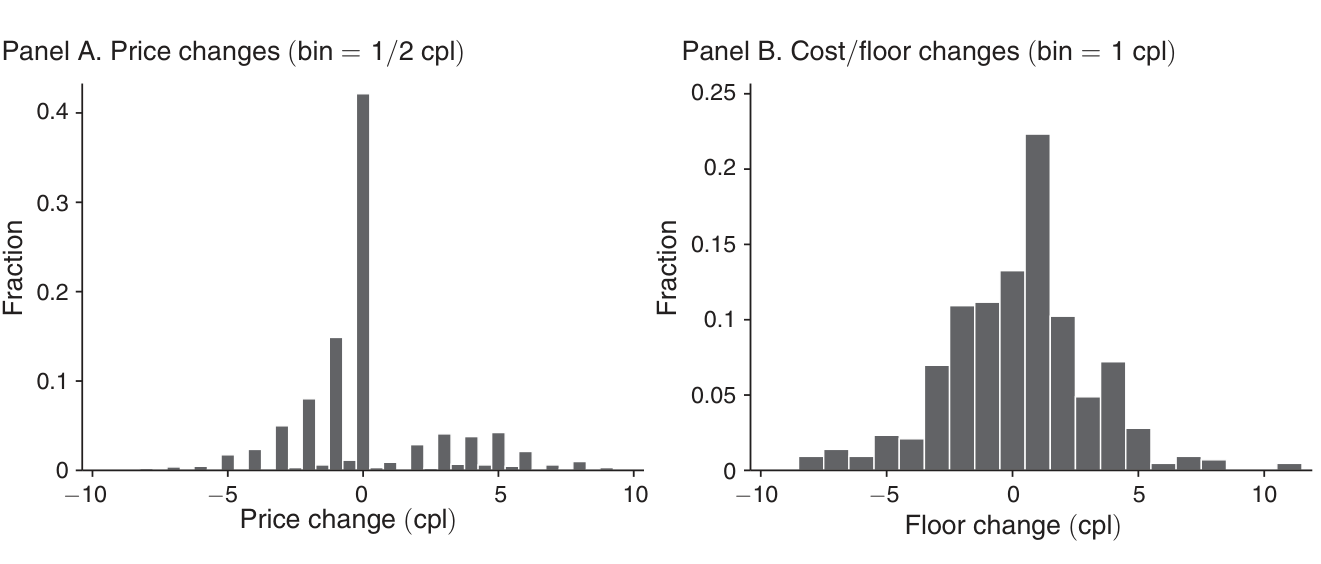
\includegraphics[width=0.88\textwidth]{figures/ch13/clarkhoude2013_fig1.png}
\caption{Distribution of weekly price changes (panel A) and of price-floor changes (panel B) in the cartel cities,
2002--2005. Source: \citet{ClarkHoude2013}, Figure 1.}
\label{fig:13-ch-f1}
\end{figure}

\casehead{Why asymmetry is a problem: a two-firm model}
The authors illustrate the enforcement problem with two retailers of a homogeneous good facing inelastic unit demand.
Firm $H$ has marginal cost $c>0$ and firm $L$ has cost 0. At the cartel price $\bar p$ they hold shares $s_H$ and
$s_L=1-s_H$. After a deviation they play static Bertrand forever, in which $H$ earns zero and $L$ serves the market at price
$c$. The incentive constraints are
\begin{equation}\label{eq:13-ch-ic2}
\textit{IC}^H:\ \frac{s_H(\bar p-c)}{1-\delta}\ge p^d_H-c,\qquad
\textit{IC}^L:\ \frac{s_L\bar p}{1-\delta}\ge p^d_L+\delta\,\frac{c}{1-\delta},
\end{equation}
where $p^d_j$ is the deviation price. The low-cost firm loses less from the punishment, because it keeps the whole market
at price $c$.

\begin{proposition}[Collusion needs an unequal split]\label{prop:13-ch-shares}
In the two-firm model, let deviations undercut $\bar p$ by an arbitrarily small amount. Collusion at $\bar p$ is sustainable
if and only if
\begin{equation*}
\delta\ge\underline\delta(s_L)\equiv\max\Big\{s_L,\ \frac{(1-s_L)\,\bar p}{\bar p-c}\Big\}.
\end{equation*}
The threshold is minimized at $s_L^*=\frac{\bar p}{2\bar p-c}>\frac{1}{2}$, where $\underline\delta(s_L^*)=\frac{\bar p}{2\bar p-c}$.
With equal shares the threshold is $\frac{\bar p}{2(\bar p-c)}$, which is at least one when $c\ge\frac{\bar p}{2}$,
so collusion with equal shares is then impossible for every $\delta<1$.
\end{proposition}

\begin{proof}
Let $p^d_H,p^d_L\to\bar p$. Multiplying $\textit{IC}^H$ by $1-\delta$ gives $s_H(\bar p-c)\ge(1-\delta)(\bar p-c)$, or
$\delta\ge1-s_H=s_L$. Multiplying $\textit{IC}^L$ by $1-\delta$ gives
\begin{equation*}
s_L\bar p\ge(1-\delta)\bar p+\delta c,
\end{equation*}
which rearranges to $\delta(\bar p-c)\ge(1-s_L)\bar p$, or $\delta\ge\frac{(1-s_L)\bar p}{\bar p-c}$. Both must hold, which gives
the maximum. The first term increases in $s_L$ and the second decreases, so the maximum is smallest where they are equal:
$s_L(\bar p-c)=(1-s_L)\bar p$, or $s_L^*=\frac{\bar p}{2\bar p-c}$. Since $c>0$, $s_L^*>\frac{1}{2}$. Substituting $s_L=\frac{1}{2}$
gives $\max\{\frac{1}{2},\frac{\bar p}{2(\bar p-c)}\}=\frac{\bar p}{2(\bar p-c)}$, which is at least one when $\bar p\le2c$.
\end{proof}

The proposition is our formalization of the authors' example. With a large cost gap, collusion on equal shares is
impossible at any discount factor, while a split that favors the low-cost firm sustains it for $\delta$ close to one. The
cartel thus faces an \emph{enforcement problem}, which requires shifting market share toward low-cost and small-network
firms. It also faces a \emph{coordination problem}, because firms with different deviation gains disagree about the price.
In posted-price retail the cartel cannot set $s_L$ directly. It has to create temporary price differences that move volume
toward the firms it needs to keep on board.

\casehead{The mechanism: a coordinated order of play}
The court documents show how. A price increase works like a negotiation. The leader first agrees with Couche-Tard and the
active followers on a target price and a time $t_0$ at which most stations raise their prices. The leader then contacts
Ultramar and the big-box retailers and proposes a later time $t_1\ge t_0$ for their increase. Dissident stations, which are
independents with large capacity or outlying locations, are told of the increase directly or indirectly. A typical
Victoriaville increase involved about 65 calls, many between the leader and Couche-Tard (Table 3). Low-cost stations and
dissidents received far more calls than they made. The delay was explicit. When a station owner said he would wait for the
neighboring Ultramar station, Bilodeau replied: ``I know that, I'm not worried, it's always the same thing.'' An Ultramar
manager described the arrangement in these words. ``We built the system seven years ago, the competitors know that the program
belongs to us and we want to be sure that we are the last one to move [up].''

Most stations raise their prices at once, while a group delays by up to four hours in Victoriaville and 80 minutes in Thetford
Mines (Figure 3). \Cref{tab:13-ch-t4} regresses each station's delay on station categories and episode characteristics.
Relative to the leader's stations, Ultramar and the big-box stations raise their prices about two and a half hours later in
Victoriaville and about an hour later in Thetford Mines. Larger proposed increases shorten the delays. A larger increase makes
the delay more costly for early movers and more valuable for late movers, so the cartel grants less time. Delays are longer when
more than 20 days have passed since the last increase, because the transfer then accumulates over a longer interval. Price
decreases are different. Ultramar initiates them without warning, nine of the ten documented decreases in Victoriaville and three
of the four in Thetford Mines. Others match quickly without retaliation, and a decrease involves about 26 calls. The low-price
guarantee makes Ultramar the natural leader of cuts and saves the cartel the cost of coordinating them. The leader's role on
the way down is to warn followers quickly, so that they stay competitive and do not cut on their own. A linear probability
model of who receives such a warning (Table 6 of the paper) shows that the low-cost chains are rarely called, because they
start the cuts. In the pooled sample, followers are 25 percent less likely to be warned than the leader's own stations.

\begin{table}[htbp]
\centering
\caption{Price-increase delays (minutes after the leader's stations) and station characteristics}\label{tab:13-ch-t4}
\small
\begin{tabular}{lcc}
\toprule
 & (1) Victoriaville & (2) Thetford Mines\\
\midrule
Dissident stations & 157.6$^{***}$ (37.88) & \\
Low-cost chains (Ultramar, big-box) & 149.4$^{***}$ (21.33) & 64.70$^{***}$ (9.206)\\
Follower stations & 37.41$^{**}$ (15.75) & 13.71$^{*}$ (7.019)\\
Couche-Tard stations & 23.68 (23.50) & $-13.74^{***}$ (4.879)\\
Distance to low-cost chains & 8.676 (10.18) & $-2.074^{***}$ (0.773)\\
Distance to closest competitor & $-14.51$ (15.09) & $-6.920^{***}$ (2.439)\\
Proposed increase & $-35.06^{***}$ (4.794) & $-11.35^{*}$ (6.135)\\
Current margin & $-40.50^{***}$ (2.977) & $-6.582^{**}$ (2.563)\\
Last increase $\ge20$ days ago & 76.21$^{***}$ (17.59) & 19.60 (19.53)\\
Constant & 215.3 (136.4) & 161.1$^{***}$ (48.17)\\
\addlinespace
Observations & 122 & 83\\
$R^2$ & 0.657 & 0.535\\
\bottomrule
\end{tabular}

\smallskip
\begin{minipage}{0.86\textwidth}\footnotesize
Notes: OLS, robust standard errors in parentheses. The reference group is the leader's network. Delays of dissidents are observed
only when they cooperated, and the actions of the two Thetford Mines dissidents are never observed. $^{***}$, $^{**}$, $^{*}$:
significant at 1, 5, 10 percent. Source: \citet{ClarkHoude2013}, Table 4 (the regression of delays).
\end{minipage}
\end{table}

\casehead{The value of delay: demand model}
To measure the transfer, the authors model a firm that may raise its price late, or cut it early. It receives a fraction
$\tau_t$ of the week's demand at the initial price vector. The paper writes $\alpha_t$ for this share and $\gamma$ for the price
coefficient. We use $\tau_t$ and $\alpha$ to keep the book's notation, in which $\alpha$ is the price coefficient. The documents suggest delays of about half a day on increases and thirty minutes on decreases, at most once a
week. With uniform demand over twelve open hours a day, this would be $\frac{1}{14}$ and $\frac{1}{168}$ of weekly sales.
Predictable increases and the price dispersion they create make consumers time their purchases, so the authors set
$\tau=\frac{1}{7}$ for increases and $\tau=\frac{1}{140}$ for decreases. Three firms (Ultramar, Maxi and Canadian Tire) may delay
increases and only Ultramar may lead cuts.

Two demand models bracket the truth. In the homogeneous model consumers buy at the cheapest station, shares are $\frac{1}{N}$ at
equal prices, and low-price stations serve the whole market during a delay. The market size is the population of Victoriaville
times three liters a day. The logit model (\cref{ch:logit}) gives station $j$ the demand
\begin{equation}\label{eq:13-ch-logit}
D_j(\mathbf p_t)=M\,\frac{\exp(X_{jt}\beta+\xi_{q}-\alpha p_{jt})}{\exp(-\alpha p_{0t})+\sum_k\exp(X_{kt}\beta+\xi_{q}-\alpha p_{kt})}.
\end{equation}
Mean quality $X_{jt}\beta+\xi_q$ depends on size and amenities $X_{jt}$ and on a quarter effect $\xi_q$. The paper writes it as
$\delta_{jt}$, a symbol that this chapter reserves for the discount factor. The price $p_{0t}$ is the average price in neighboring
markets, and $M$ is market size. Let $\tilde{\mathbf p}_t$ be the price vector at the start of the week, before
late movers adjust, and let $\mathcal T_t$ be the set of firms receiving a transfer. Demand with delays is
\begin{equation}\label{eq:13-ch-delay}
D_{j,t}(\mathbf p_t,\tau_t)=\begin{cases}\tau_tD_j(p_{j,t-1},\tilde{\mathbf p}_{-j,t})+(1-\tau_t)D_j(\mathbf p_t), & j\in\mathcal T_t,\\
\tau_tD_j(p_{j,t},\tilde{\mathbf p}_{-j,t})+(1-\tau_t)D_j(\mathbf p_t), & j\notin\mathcal T_t.\end{cases}
\end{equation}
During an increase a receiver keeps its old, lower price for the fraction $\tau_t$ of the week while the others have already
moved. The demand parameters $\Theta^{\mathrm d}=(\alpha,\beta,\xi)$ are estimated by nonlinear least squares on quarterly Kent
volumes $\hat Q_{jq}$ for Victoriaville, 2001--2007:
\begin{equation}\label{eq:13-ch-nls}
\min_{\Theta^{\mathrm d}}\sum_j\sum_q\Big(\log\hat Q_{jq}-\log Q_{jq}(\Theta^{\mathrm d})\Big)^2,\qquad
Q_{jq}(\Theta^{\mathrm d})=\sum_{t\in q}D_{j,t}(\mathbf p_t,\tau_t\mid\Theta^{\mathrm d}).
\end{equation}
The estimated coefficient on price in utility is $-0.409$, with prices in cents per liter, so $\hat\alpha=0.409$. It implies a
store-level elasticity of about $-30$. In the logit model the own elasticity is $-\alpha p_j(1-s_j)$, and shares are only
0.01--0.03 (Table 2). An elasticity of $-30$ therefore corresponds to $p_j(1-s_j)\approx\frac{30}{0.409}=73$ cents per liter
(our computation). Identification comes mostly from the two
dissident stations that priced 2 cpl below the cartel price and from the collapse of price dispersion after the cartel ended. One
of these stations lost half of its market share after the collapse. Prices are treated as exogenous given quarter effects and
characteristics. The authors note that the dissidents were not randomly assigned, so $\hat\alpha$ may be biased.
\citet{Houde2012} obtains a lower average elasticity of $-15$ with bimonthly Quebec data.

\casehead{Results: volume transfers}
\Cref{tab:13-ch-t7} reports the simulated change in each group's sales when the delays are switched on. Increases occur in only
16--23 percent of weeks but are large, so they generate sizable transfers. The low-cost firms gain about 4 percent of volume in
Victoriaville and about 6 percent in Sherbrooke and Thetford Mines. The two demand models give similar answers except in
Victoriaville. There the homogeneous model ignores the unequal shares created by location and amenities and predicts larger gains.

\begin{table}[htbp]
\centering
\caption{Simulated change in sales volume from the delay scheme}\label{tab:13-ch-t7}
\small
\begin{tabular}{llcccccc}
\toprule
 & & \multicolumn{2}{c}{Share of weeks with} & \multicolumn{2}{c}{Logit demand} & \multicolumn{2}{c}{Homogeneous demand}\\
\cmidrule(lr){3-4}\cmidrule(lr){5-6}\cmidrule(lr){7-8}
Market & Players & increase & decrease & Percent & 1,000 l. & Percent & 1,000 l.\\
\midrule
Sherbrooke & Ultramar & 0.225 & 0.373 & 0.061 & 6,759.584 & 0.055 & 733.012\\
 & Big-box & 0.224 & 0.372 & 0.059 & 773.265 & 0.047 & 651.790\\
 & Other & 0.223 & 0.370 & $-0.014$ & $-275.124$ & $-0.035$ & $-442.205$\\
Thetford Mines & Ultramar & 0.169 & 0.350 & 0.064 & 895.420 & 0.056 & 763.006\\
 & Other & 0.168 & 0.349 & $-0.009$ & $-52.570$ & $-0.027$ & $-337.746$\\
Victoriaville & Ultramar & 0.164 & 0.284 & 0.040 & 522.315 & 0.079 & 752.152\\
 & Big-box & 0.164 & 0.284 & 0.038 & 366.553 & 0.054 & 515.890\\
 & Other & 0.161 & 0.288 & $-0.010$ & $-79.329$ & $-0.025$ & $-215.419$\\
\bottomrule
\end{tabular}

\smallskip
\begin{minipage}{0.92\textwidth}\footnotesize
Notes: ``Percent'' entries are proportional changes (0.061 is 6.1 percent) in total sales volume over the collusive period when
the delay scheme is added to the simulation. The entry 6,759.584 is reproduced as printed, although it is about ten times
the neighboring entries. Source: \citet{ClarkHoude2013}, Table 7.
\end{minipage}
\end{table}

\casehead{Results: delays and cartel stability}
To study stability, the authors take the observed price path from January 2002 to October 2004 as the collusive path, with one
common price $p_t$ per week. Information is perfect, so price wars occur only off the path. Punishment sets prices at a floor for
$T$ weeks, either the MEP or the ``long-run'' floor of MEP plus 3 cpl, after which collusion resumes. The big-box stations receive
an extra 2 cpl cost advantage to capture their loss-leader motive, which puts their differential near $-3$ cpl against Ultramar's
$-2.03$. Firm $f$, owning stations $\mathcal J_f$, earns in week $t$
\begin{equation*}
\Pi_{f,t}=\begin{cases}\sum_{j\in\mathcal J_f}\big[\tau_t\pi_j(p_{j,t-1},\tilde{\mathbf p}_{-j,t})+(1-\tau_t)\pi_j(\mathbf p_t)\big], & f\in\mathcal T_t,\\
\sum_{j\in\mathcal J_f}\big[\tau_t\pi_j(p_{j,t},\tilde{\mathbf p}_{-j,t})+(1-\tau_t)\pi_j(\mathbf p_t)\big], & f\notin\mathcal T_t,\end{cases}
\qquad \pi_j(\mathbf p)=D_j(\mathbf p)\,(p_j-mc_{jt}).
\end{equation*}
An agreement $\mathcal A=\{p_t,\tau_t,\mathcal T_t,T\}_{t\ge0}$ is enforceable if every firm prefers cooperation at every date:
\begin{equation}\label{eq:13-ch-ic}
V^{c}_{f,t}(\mathcal A)-V^{d}_{f,t}(\mathcal A)=\sum_{s=0}^{T}\delta^{s}\,\Pi_{f,t+s}-\Big[\Pi^{d}_{f,t}+\sum_{s=1}^{T}\delta^{s}\,\Pi^{p}_{f,t+s}\Big]\ge0 .
\end{equation}
Collusion resumes after the punishment, so the cooperation and deviation paths coincide from $t+T+1$ on and the comparison stops
at $T$. The deviation profit $\Pi^d_{f,t}$ is the best one-week profit from undercutting all of the firm's stations by a whole
number of cents, and $\Pi^p_{f,t}=\sum_{j\in\mathcal J_f}\pi_j(\mathbf p^f_t)$ is profit at the floor. The weekly discount factor is
0.99. The deviation frequency is the share of firm-weeks at which \eqref{eq:13-ch-ic} fails. The minimum punishment $T^*$ is the
shortest war that prevents every deviation in the sample.

\Cref{tab:13-ch-t8} shows that delays matter at intermediate punishment lengths. With very short or very long wars the
deviation frequency is one or zero with or without transfers. In between, the delays lower it. They also shorten the war needed
to deter all deviations. In the homogeneous model the saving is 27 weeks with the high floor and 9 weeks with the low floor. In the
logit model it is 6 weeks with the high floor and zero with the low floor. A higher floor weakens punishments, and less
differentiation raises the gain from undercutting. In both cases the cartel is less stable, and transfers become more valuable.

\begin{table}[htbp]
\centering
\caption{Deviation frequencies and minimum punishment lengths, Victoriaville}\label{tab:13-ch-t8}
\small
\begin{tabular}{llcccccc}
\toprule
\multicolumn{2}{c}{Specification} & \multicolumn{4}{c}{Deviation frequency} & \multicolumn{2}{c}{Minimum punishment $T^*$}\\
\cmidrule(lr){1-2}\cmidrule(lr){3-6}\cmidrule(lr){7-8}
Floor & Demand & $T=4$ & $T=8$ & $T=32$ & $T=52$ & Delays & No delays\\
\midrule
$\textit{MEP}_t+3$ & logit & \makecell{0.868\\(0.017)} & \makecell{0.516\\(0.085)} & 0.009 & 0.000 & 35 & 41\\
\addlinespace
$\textit{MEP}_t$ & logit & \makecell{0.460\\(0.073)} & \makecell{0.078\\(0.004)} & 0.000 & 0.000 & 15 & 15\\
\addlinespace
$\textit{MEP}_t+3$ & homogeneous & \makecell{1.000\\(0.000)} & \makecell{0.981\\(0.016)} & \makecell{0.636\\(0.104)} & \makecell{0.394\\(0.406)} & 144 & 171\\
\addlinespace
$\textit{MEP}_t$ & homogeneous & \makecell{1.000\\(0.000)} & \makecell{0.956\\(0.022)} & \makecell{0.340\\(0.435)} & \makecell{0.071\\(0.286)} & 67 & 76\\
\bottomrule
\end{tabular}

\smallskip
\begin{minipage}{0.92\textwidth}\footnotesize
Notes: Share of firm-weeks, January 2002 to November 2004, in which the incentive constraint \eqref{eq:13-ch-ic} fails, with the
delay transfers. Numbers in parentheses are the proportional change in that frequency when the transfers are removed. $T^*$ is the
shortest punishment, in weeks, with no deviation in the sample. Source: \citet{ClarkHoude2013}, Table 8.
\end{minipage}
\end{table}

\Cref{tab:13-ch-t9} measures who gains. With logit demand the delays raise the net value of collusion for the three receivers by
3 to 13 percent. With homogeneous demand the gains range from 17 to 53 percent. The early movers, 88 percent of firms, lose
between 1 and 5 percent on average.
Ultramar gains least, because its two-station network already gains less from deviating. Network size, more than cost, emerges
as the main source of asymmetry, partly because the floor limits the effect of cost differences.

\begin{table}[htbp]
\centering
\caption{Net value of the delay transfers, Victoriaville (thousands of dollars)}\label{tab:13-ch-t9}
\small
\begin{tabular}{llcccc}
\toprule
Floor & Demand & Canadian Tire & Maxi & Ultramar & Others\\
\midrule
$\textit{MEP}_t+3$ & logit & 14.956 (0.129) & 17.000 (0.127) & 7.373 (0.075) & $-1.685$ ($-0.025$)\\
$\textit{MEP}_t$ & logit & 15.424 (0.049) & 17.471 (0.048) & 7.478 (0.032) & $-1.577$ ($-0.011$)\\
$\textit{MEP}_t+3$ & homogeneous & 41.892 (0.523) & 42.195 (0.531) & 46.386 (0.273) & $-4.528$ ($-0.051$)\\
$\textit{MEP}_t$ & homogeneous & 44.420 (0.290) & 44.736 (0.294) & 47.985 (0.168) & $-5.695$ ($-0.032$)\\
\bottomrule
\end{tabular}

\smallskip
\begin{minipage}{0.92\textwidth}\footnotesize
Notes: Change in the net value of cooperation $V^c_{f,t}-V^d_{f,t}$ when the delays are added, evaluated at the minimum
punishment $T^*$ without delays (last column of \cref{tab:13-ch-t8}). Proportional changes in parentheses. ``Others'' is the
average over the firms that move early. Source: \citet{ClarkHoude2013}, Table 9.
\end{minipage}
\end{table}

\casehead{Interpretation}
The Quebec cartel solved its enforcement problem with intertemporal transfers implemented through the order of play. The
transfers resemble the sales-based payments of \citet{HarringtonSkrzypacz2011} (\cref{ch:collusion-theory}) and the sidepayments
of Asker's bidding ring (\cref{sec:13-asker}). Their currency is time, and the timing is predictable and agreed in advance. \Citet[p.~122]{ClarkHoude2013}
compare the pricing rule of large, infrequent increases followed by small cuts or constant prices to an $(s,S)$ rule. The term comes from inventory theory. An $(s,S)$ rule leaves a state variable alone until it falls to a lower trigger
$s$ and then resets it to a higher target $S$. Here the state is the margin, which drifts down through small cuts until the
cartel restores it with one large coordinated increase. The analogy concerns only this pattern of rare, discrete resets. The
paper does not study the optimal timing or size of price changes (p.~121), and it estimates no thresholds $s$ and $S$. The
rule economizes on the costly and risky communication needed to coordinate increases, while a constant-markup rule would
require frequent coordinated changes as costs move. The two signatures that antitrust authorities usually look for, parallel price changes and stable
margins, are both absent. Sequential moves and asymmetric cycles can be part of a collusive agreement.
\citet[p.~121]{ClarkHoude2013} report that their companion paper \citep{ClarkHoude2014} finds a substantial fall in price
asymmetry in all four cities after the search warrants were executed. The fall stems largely from larger price cuts, once the cartel
could no longer prevent firms from undercutting their rivals.

\casehead{Critiques}
The analysis relies on summaries of conversations selected by investigators. Only a few price increases are common to all
stations, so the standard errors of the episode variables are understated, as the authors note. The price coefficient comes from
non-random variation. The stability exercise assumes perfect information and immediate punishment, whereas the two documented
deviations were met with weeks of threats and negotiation before a price war began. The model treats the delay as given. A full
account would let firms bargain over delays and prices \citep{Harrington1991}. The price floor regulation is specific to Quebec, and it
shapes both the cost function and the punishment.

\casehead{Contribution}
The paper is among the first to document the internal organization of a retail cartel. It identifies a transfer mechanism suited to
posted-price markets, quantifies it with demand models, and shows through a structural incentive-constraint exercise when it matters
for stability. Its main message for detection is that collusion and competitive Edgeworth cycles can generate similar price paths.

\subsection{The end of the cartel as a natural experiment: Erutku and Hildebrand (2010)}\label{sec:13-erutku}

\casehead{Question and setting}
When an investigation becomes public, a cartel may collapse. \citet{ErutkuHildebrand2010} use the public announcement of the Quebec
investigation to estimate the overcharge in Sherbrooke, the largest of the four cities. Sherbrooke has close to 150,000 residents and
about 60 stations (Table 1). Court documents report 16 price increases or attempted increases between April 1, 2005 and April 18, 2006.
The Bureau's documents give different counts of the participants (p.~224, note~2). The number of conspirators in Sherbrooke is 53, 54
or 63, and the number of stations 64, 65 or 66. With 53 participants and 66 stations, at least 80 percent of the stations took part at
some point. On May 29, 2006 the Bureau's officers raided stations in the Sherbrooke-Victoriaville area, and on June 2 the Commissioner
of Competition publicly confirmed the investigation. The authors treat these events together as the announcement. On June 12, 2008
the Commissioner announced criminal charges against 13 individuals and 11 companies in the four cities. Fines on the parties that
pleaded guilty totaled over \$2 million, and the Bureau's immunity program offered protection to the first party to disclose the
offense (p.~224).

The market structure is unusual for a prosecuted cartel. In the price-fixing cases brought by the U.S.\ Department of Justice from
1963 to 1972, 49 of 62 cases had ten or fewer conspirators. The four-firm concentration ratio exceeded 50 percent in 38 of the 50 cases
with data (our tabulation of Hay and Kelley's table as reproduced in \citealp[Table~2]{ErutkuHildebrand2010}). In Sherbrooke at least
50 different individuals coordinated price increases (p.~227). The market was not concentrated, with a Herfindahl index below 1,800.
Ultramar, the largest retailer with 14 outlets, came close to being a maverick. Its Value Plus program promised prices no higher than
competitors' lowest prices in each price zone, so Ultramar followed an increase only after every other station had raised its price.
Sometimes it waited so long that the agreed increase collapsed (p.~227). Demand followed a seesaw, with each high-volume quarter
followed by a low-volume quarter, which made fluctuations deterministic (p.~228). The authors score the market against eight items of
the antitrust checklist derived from \citet{Stigler1964} (their Table 3). Only three point toward collusion: buyers who make frequent
small purchases, price transparency and multimarket contact. The others, such as a small number of sellers and high entry barriers,
are absent. \Cref{sec:13-market-evidence} returns to what the case implies for the weight of such checklists.

\casehead{Data}
Weekly city-average retail prices net of taxes come from MJ Ervin, which surveys stations by telephone every Tuesday morning. They
cover Sherbrooke, Montreal and Quebec City from May 31, 2005 to May 22, 2007, which gives 52 weeks before and 52 weeks after the
announcement. Weekly wholesale prices in Montreal and Quebec City are identical and serve as marginal cost. Average retail prices were
64.8 cpl before and 64.0 after the announcement in Sherbrooke, 65.1 and 64.1 in Quebec City, and 62.0 and 62.9 in Montreal (Table 4).
The average wholesale price rose from 58.1 to 58.8 cpl (Table 5). The raw difference in differences against Montreal is
$(64.0-64.8)-(62.9-62.0)=-1.7$ cpl. Against Quebec City it is $(64.0-64.8)-(64.1-65.1)=0.2$ cpl.

\casehead{Estimating equation}
With $i$ indexing the treated city and one control city, the regression is (their eq.~(1), our notation)
\begin{equation}\label{eq:13-eh-did}
P_{it}=a_0+a_1S_i+a_2\textit{Post}_t+\tau^{\mathrm{DD}}\big(\textit{Post}_t\times S_i\big)+\sum_{l=0}^{2}b_l\,w_{i,t-l}+\mu_{q(t)}+e_{it}.
\end{equation}
Here $P_{it}$ is the retail price, $S_i$ indicates Sherbrooke and $\textit{Post}_t$ indicates weeks after the announcement. The
$w_{i,t-l}$ are current and lagged wholesale prices, and $\mu_{q(t)}$ are quarter effects. The paper writes the four dummy coefficients as
$\gamma_0,\dots,\gamma_3$. The coefficient $\tau^{\mathrm{DD}}$ is the change in Sherbrooke's price relative to the control after the
announcement. Under the parallel-trends assumption of difference in differences (\cref{app:econometrics}), and if the cartel ended at the
announcement, $-\tau^{\mathrm{DD}}$ measures the overcharge. The equation is estimated by OLS with White standard errors and then by the
Hildreth-Lu method, which corrects for first-order serial correlation $\rho$ in the errors. Results with one to four wholesale lags are
similar, and the table reports two. Each regression uses the control city's wholesale price for both cities (p.~231).

\begin{table}[htbp]
\centering
\caption{Difference-in-differences estimates of the announcement effect on Sherbrooke retail prices}\label{tab:13-eh-t6}
\small
\begin{tabular}{lcccc}
\toprule
 & \multicolumn{2}{c}{Control: Montreal} & \multicolumn{2}{c}{Control: Quebec City}\\
\cmidrule(lr){2-3}\cmidrule(lr){4-5}
 & Coefficient & $t$-statistic & Coefficient & $t$-statistic\\
\midrule
Constant & 1.35 (1.94) & 0.70 & 2.58 (1.95) & 1.32\\
$S_i$ (Sherbrooke) & 2.80 (0.57) & 4.94$^{**}$ & $-0.32$ (0.58) & $-0.55$\\
$\textit{Post}_t$ & 0.21 (0.56) & 0.37 & $-1.84$ (0.58) & $-3.17^{**}$\\
$\textit{Post}_t\times S_i$ & $-1.75$ (0.80) & $-2.19^{*}$ & 0.26 (0.82) & 0.31\\
$w_{it}$ & 0.73 (0.05) & 16.19$^{**}$ & 0.62 (0.04) & 15.08$^{**}$\\
$w_{i,t-1}$ & 0.30 (0.05) & 5.87$^{**}$ & 0.35 (0.04) & 7.83$^{**}$\\
$w_{i,t-2}$ & 0.01 (0.04) & 0.31 & 0.12 (0.04) & 2.81\\
$\rho$ & 0.09 (0.07) & 1.25 & 0.20 (0.07) & 2.68$^{**}$\\
\addlinespace
$R^2$ & \multicolumn{2}{c}{0.91} & \multicolumn{2}{c}{0.92}\\
Durbin-Watson & \multicolumn{2}{c}{2.00} & \multicolumn{2}{c}{2.03}\\
\bottomrule
\end{tabular}

\smallskip
\begin{minipage}{0.86\textwidth}\footnotesize
Notes: Estimates of \eqref{eq:13-eh-did} with Sherbrooke as the treated city. $N=208$ city-weeks in each regression. Quarter effects not
reported. Standard errors in parentheses. $^{*}$ significant at 5 percent, $^{**}$ at 1 percent. Source: \citet{ErutkuHildebrand2010},
Table 6.
\end{minipage}
\end{table}

\casehead{Results}
\Cref{tab:13-eh-t6} reports the estimates. Before the announcement Sherbrooke's prices exceeded Montreal's by 2.80 cpl, controlling
for wholesale prices, and were indistinguishable from Quebec City's. Against Montreal, $\hat\tau^{\mathrm{DD}}=-1.75$ (0.80), significant
at 5 percent. Against Quebec City the estimate is 0.26 (0.82), while the common post-announcement term is $-1.84$ (0.58). Sherbrooke and
Quebec City prices fell together after the announcement (\cref{fig:13-eh-f2} shows Sherbrooke against Montreal). Moving the assumed
announcement date by one to four weeks in either direction leaves the Montreal estimate negative, significant at 10 percent and above
1.34 cpl in absolute value. With Quebec City as the control no shift produces a meaningful effect.

\begin{figure}[htbp]
\centering
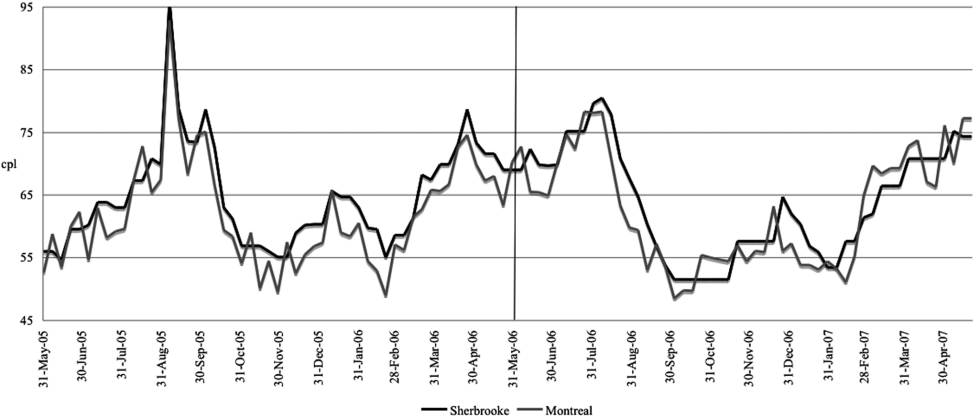
\includegraphics[width=0.92\textwidth]{figures/ch13/erutku2010_fig2.png}
\caption{Weekly retail prices net of taxes in Sherbrooke (black) and Montreal (gray), June 2005 to May 2007, in cents per liter. The
vertical line marks the announcement of the investigation at the end of May 2006. Source: \citet{ErutkuHildebrand2010}, Figure 2.}
\label{fig:13-eh-f2}
\end{figure}

The authors read the Montreal estimate as an overcharge of 1.75 cpl. Relative to the post-announcement Sherbrooke price, this is
$\frac{1.75}{64.0}=2.7$ percent of the retail price. Relative to the post-announcement margin over wholesale cost, it is
$\frac{1.75}{64.0-58.8}=34$ percent. About 135 million liters were sold in Sherbrooke between May 2005 and May 2006, so damages in the year
before the announcement exceed \$2 million ($0.0175\times135$ million $=\$2.4$ million, our arithmetic). The 2.7 percent overcharge is small
next to surveys of cartel overcharges (their Table~7, reproduced in \cref{tab:13-overcharge-surveys}), but the increase in the markup is
large. The authors compare it with Ohio school milk (p.~235). There \citet{PorterZona1999} estimate an average price effect of 6.5
percent, which they translate into a rise of roughly 30 percent in the markup (\cref{sec:13-pz99}). A cartel under investigation may also
keep prices high to reduce estimated damages \citep{Harrington2004}, so the estimate could understate the effect.

\casehead{Critiques}
The design rests on the choice of control. Quebec City matched Sherbrooke in levels before the announcement and moved with it after.
Either Quebec City prices were also affected by the investigation, or the Montreal estimate reflects Montreal-specific shocks. The data
cannot tell these apart. Parallel trends are checked only visually. There is one treated city and one control city in each regression,
so inference treats the weekly observations of a single pair as independent apart from an AR(1) correction. The general problems of
difference in differences with a single treated unit apply (\cref{app:econometrics}). The cartel's end date is uncertain, because
cooperation may have weakened when the wiretaps or raids began. Prices at the end of a cartel need not return at once to the competitive
level. \citet[p.~121]{ClarkHoude2013} report that their companion paper \citep{ClarkHoude2014} finds larger price cuts after the
collapse, which suggests a complementary reading. The cartel's main effect may have been on the shape of the cycle more than on the
average price.

\subsection{Learning to coordinate in Perth: Byrne and de Roos (2019)}\label{sec:13-perth}

The Quebec cartel coordinated by telephone. Coordinating a price increase took on average 65 calls among its members
and a price decrease 26 \citep[pp.~195--196]{AskerNocke2021}. Theory allows firms to reach the same outcome tacitly,
but it says little about how independent firms would arrive at a common understanding (p.~189).
\citet{ByrneDeRoos2019} document such a process in retail gasoline in Perth, Australia, from 2001 to 2015, as
summarized by \citet[pp.~189--191]{AskerNocke2021}. During this period, stations in Perth had to commit to their prices a
day ahead and post them on Fuelwatch, a government website. Its purpose was to help consumers find cheap gasoline.
The same transparency let stations monitor one another, which makes Fuelwatch a form of government-assisted
information sharing like the Danish publication of concrete prices (\cref{sec:13-concrete}).

Perth prices follow cycles of sudden jumps and gradual declines, like those of Toronto (\cref{sec:13-noel}). Before
2009, price jumps occurred on various days of the week. From 2009, BP, the largest chain, led jumps on Wednesdays.
Most of its remaining stations jumped on Thursdays. Caltex, the next-largest chain, gradually adopted the pattern,
and by mid-2010 it followed BP's Wednesday jump with a jump on Thursday. BP then reduced the share of its stations
that jumped on Wednesday and raised the share that jumped on Thursday. It thus scaled back its price leadership, and
with it the sales it lost by leading. In several periods BP stopped leading on Wednesday to test whether the market
would coordinate on Thursday without it (pp.~189--191, Figure~3). Byrne and de Roos identify two focal points
\citep[pp.~596--597 and 607--608]{ByrneDeRoos2019}. The first fixes the timing of the weekly price jump, which moved
to Thursday. The second fixes the size of the daily price cuts between jumps, which converged to 2 cents per liter
from March 2010. By 2013 adjustments were better synchronized and margins were higher.

The episode suggests a third kind of conduct behind similar price cycles. In Toronto the cycles were consistent with
competitive Edgeworth cycles. In Quebec an explicit cartel ran them by telephone. In Perth, the price data show a
detailed pattern of price leadership and price experiments under a transparency regime. The pattern is consistent
with coordination learned through prices. It does not show that prices were the only channel. Byrne and de Roos
state that they cannot rule out explicit communication between firms, such as phone calls
\citep[p.~617]{ByrneDeRoos2019}. Asker and Nocke distill the study as showing that market interaction itself \emph{may}
provide enough communication for coordination (p.~191). In terms of \cref{prop:13-transparency}, Fuelwatch raised the probability
that a deviation would be seen. The transition was slow. Asker and Nocke date it from 2009 to 2013 (p.~189).
Byrne and de Roos describe a gradual three-year transition from April 2009 to August 2012
\citep[p.~592]{ByrneDeRoos2019}, and in their conclusion they speak of three and a half years (p.~618). A simple
rule, such as a fixed day for jumps and a fixed size of cuts, makes deviations easy to detect. It also leaves the firms less able to respond to fluctuations in demand
\citep[p.~194]{AskerNocke2021}. \Cref{sec:12-anatomy} discusses the case as evidence on how agreements start.

\subsection{What the gasoline evidence shows}\label{sec:13-gas-synthesis}

\Cref{tab:13-gas-synthesis} summarizes the five studies. They share an industry, high-frequency prices and an observed wholesale cost.
They differ in what lets them speak about conduct. Borenstein and Shepard use a dynamic implication of the incentive constraint,
the response of margins to expected future demand and cost. Sign restrictions and a placebo separate collusion from inventories and
from measurement error. Noel uses the roles that theory assigns to small and large firms within a cycle. Clark and Houde use wiretaps,
which reveal the conduct directly, and then use structural models to measure what the observed mechanism achieved. Erutku and
Hildebrand use the end of the cartel as an event. Byrne and de Roos follow the emergence of price leadership over time.

\begin{table}[htbp]
\centering
\caption{Retail gasoline studies of conduct}\label{tab:13-gas-synthesis}
\footnotesize
\begin{tabularx}{\textwidth}{>{\raggedright\arraybackslash}p{2.0cm}>{\raggedright\arraybackslash}p{2.3cm}>{\raggedright\arraybackslash}X>{\raggedright\arraybackslash}X>{\raggedright\arraybackslash}X}
\toprule
Study & Market and data & Price pattern & Method & Conclusion about conduct\\
\midrule
\citet{BorensteinShepard1996} & 59 U.S. cities, monthly, 1986--1991 & Margins rise ahead of seasonal demand peaks and fall ahead of cost increases & 2SLS margin regression with forecast demand and cost, elasticity-corrected instrument, placebo on unexpected changes & Tacit dynamic collusion: margin elasticities of 0.37 to expected demand and $-0.37$ to expected cost (Table 2)\\
\addlinespace
\citet{Noel2007} & 22 Toronto stations, twelve-hourly, 131 days in 2001 & Asymmetric weekly cycle: one-step jumps of 5.6 cpl, then 12.8 half-days of small cuts & Markov-switching regression with sticky prices, leader and follower roles by firm type & Competitive Edgeworth cycles: small firms lead cuts, large firms lead relents (Tables II--V)\\
\addlinespace
\citet{ClarkHoude2013} & 128 stations in four Quebec cities, wiretaps 2005--2006, weekly prices 2002--2005 & Asymmetric cycle: increases near 4 cpl, cuts of 1--2 cpl, sticky prices & Coded court documents, delay regressions, logit and homogeneous demand, simulated incentive constraints & Explicit cartel using timed delays as transfers to low-cost firms: 4--6 percent volume gains (Table 7), shorter required punishments (Table 8)\\
\addlinespace
\citet{ErutkuHildebrand2010} & Sherbrooke versus Montreal and Quebec City, weekly, 2005--2007 & Price drop after the announcement of the investigation & Difference in differences with wholesale-price controls and AR(1) errors & Overcharge of 1.75 cpl against Montreal, none against Quebec City (Table 6)\\
\addlinespace
\citet{ByrneDeRoos2019} & Perth, daily station prices posted a day ahead on Fuelwatch, 2001--2015 & Cycles whose jumps moved to Thursdays after 2009 & Event history of price leadership and experimentation by BP & Coordination consistent with signaling through prices, explicit communication not ruled out: weekly jumps on Thursdays, daily cuts of 2 cpl and higher margins by 2013\\
\bottomrule
\end{tabularx}
\end{table}

Three lessons follow. First, price patterns alone do not identify conduct. Asymmetric cycles appear in competitive Toronto and in the
Quebec cartel, and parallel, synchronized increases arise in both. Perth adds cycles that the authors attribute to coordination through prices. Screens based on asymmetry, stickiness or low price variance
\citep{AbrantesMetzEtAl2006} can flag markets for scrutiny, but they cannot separate the two. Second, evidence becomes informative when
it tests a prediction specific to one theory. Examples are the expected-future effects of an incentive constraint, the role
assignments of the Maskin-Tirole equilibrium, or the transfers needed when firms are asymmetric. Third, direct evidence remains decisive
in prosecutions. The Quebec case rested on wiretaps and guilty pleas, and economic analysis then measured the mechanism and its
effects. \Cref{sec:13-enforcement} returns to these methods for measuring damages.

\section{Imperfect Cartels: Tolerated Cheating and Business Stealing}\label{sec:13-imperfect}

The Quebec cartel of \cref{sec:13-clarkhoude} had to shift market share toward the members it needed to keep on
board. The Sugar Institute of \cref{sec:13-sugar-institute} met much of the cheating it detected with
forbearance. Both features recur in the records of prosecuted industrial cartels. The repeated-game theory of
\cref{ch:collusion-theory} explains how the threat of punishment keeps cartel members in line. Its simplest versions make sharp predictions about the records that cartels leave behind.
With perfect monitoring, no member cheats and no punishment occurs on the equilibrium path. With imperfect
public monitoring \citep{GreenPorter1984}, punishments do occur. They are triggered by events that no member
controls, however, and a detected deviation would always be punished. The case records of prosecuted cartels
fit neither prediction. Members cut prices below agreed targets and took customers allocated to others. The
other members knew it, and often nothing followed.

This section documents these facts and recalls the sales-reporting and transfer schemes that cartels used to
contain them (\cref{sec:13-imperfect-evidence}). It then develops the model of \citet{BernheimMadsen2017}, in which
deliberate and unpunished business stealing is part of the optimal cartel agreement (\cref{sec:13-bm}). The
model is the one piece of collusion theory that this chapter develops in full, because its testable
implications concern the internal records of cartels.

\subsection{Evidence from prosecuted industrial cartels}\label{sec:13-imperfect-evidence}

\casehead{The prevalence of discord}
\citet{MarshallMarxSamkharadze2013} classify the European Commission decisions on major industrial cartels
from 2000 to 2005. Throughout this section, page, footnote and theorem numbers for \citet{BernheimMadsen2017}
refer to the working-paper version (NBER Working Paper 19993, 2014). As summarized by
\citet[footnote 2]{BernheimMadsen2017}, Marshall, Marx and Samkharadze label 9 of 22 rulings
\emph{discordant}. In a discordant cartel the decision records frequent bargaining problems and deviations by
members throughout the cartel period. Only 6 rulings are \emph{fully concordant}, meaning that the cartel
functioned smoothly while it lasted. The sample is selected toward cartels effective enough to attract
enforcement. Discord in the population of cartels is therefore probably more common still.
\citet{LevensteinSuslow2006} survey the coordination problems of many cartels and stress the same selection
problem (\cref{ch:collusion-theory}).

\citet[ch.~6]{MarshallMarx2012} offer a first-hand reading of the twenty-two Commission decisions on
industrial-product cartels issued from 2000 through 2005. Following \citet{Stigler1964}, they describe every cartel
as solving the problem of secret deviations with three complementary structures. \emph{Pricing structures} implement price increases. \emph{Allocation structures}
divide the collusive gain and correct deviations through redistributions. \emph{Enforcement structures} monitor
compliance and threaten punishment (pp.~105--106). Their Table~6.1 records the paragraphs of each decision that
describe the cartel's allocation structure and any role of a third-party facilitator (pp.~125--127). By our count
from that table, 17 of the 22 cartels used a market-share allocation, 10 a customer allocation and 7 a geographic
allocation. Nineteen used at least one of the three, and 10 combined market shares with customers or territories.
Eleven decisions mention a facilitator, such as a trade association or a consulting or accounting firm, which can
verify the sales on which a market-share agreement depends (pp.~125 and 128). The vitamins cartel corrected
deviations through ``true-ups''. A firm that sold more than its allotted share had to buy product at the cartel
price from a firm that sold less (p.~128). \citet[p.~198, note~53]{AskerNocke2021} conclude from the same review
that almost all of the decisions feature customer, geographic or market-share allocation.

\casehead{Three cartels in the record}
The global lysine cartel operated at least from 1992 through 1995. Lysine is an amino acid added to animal
feed. Throughout 1993 and 1994 its members discussed a persistent and substantial gap between target and
actual prices in Europe. They first attributed the gap to arbitrage by commodity traders and to exchange
rates, and eventually to undercutting by particular members. The difficulties culminated in a ``reset'', in
which the members briefly suspended sales to drive the price back up to the target. The record shows no
punishment of the deviators \citep[pp.~2--3]{BernheimMadsen2017}. At an April 30, 1993 meeting, the president
of Archer Daniels Midland (ADM) told executives of a Japanese producer that ``our competitors are our friends
and our customers are our enemies.''

A cartel of nucleotide producers (food flavor enhancers) operated in Europe from 1988 to 1999. It tried to
allocate several large customers among its members. At meetings from 1991 to 1996, members complained
repeatedly about low prices and about customers who asked them to match lower quotes from other members.
\citet[p.~3]{BernheimMadsen2017} find no sign that punishments were considered or carried out. Each time, the
cartel set a new price and urged its members to respect it.

The citric acid cartel in western Europe (1991--1995) suspected one member, Jungbunzlauer, of undercutting
during the second half of its life. The members held special sessions alongside the regular meetings to
monitor and discuss Jungbunzlauer's conduct. They never changed the arrangement in response. The cartel
collapsed abruptly in early 1995. Bernheim and Madsen read the collapse as a general breakdown of
coordination and consider a delayed, coordinated punishment the less likely reading. The Sugar Institute of
\cref{sec:13-sugar-institute} shows the same pattern. Members skirted its rules with indirect price cuts or kickbacks,
apologized when caught, and stopped. The Institute then banned the specific practice, and this forbearance
does not seem to have undermined the cartel \citep{GenesoveMullin2001}.

\casehead{Cheating as a defense}
The pattern matters for enforcement. Defendants often present price cuts, business stealing and the absence
of retaliation as proof that a cartel was ineffective. In the criminal trial of ADM executives over lysine, a
defense attorney argued that ADM had been ``stealing customers'' and ``undercutting competitors''
\citep[footnote 10]{BernheimMadsen2017}. In European proceedings, firms in the citric acid, food flavor
enhancer, industrial tube, lysine and zinc phosphate cases argued that agreed prices were not respected and
that non-compliance went unpunished \citep[footnote 11]{BernheimMadsen2017}. A theory in which tolerated
cheating coexists with effective collusion bears directly on how courts should weigh such evidence.

\casehead{Quotas, sales reports and transfers}
Where prices and sales were private, many of these cartels set sales quotas, monitored them through self-reported
sales and settled deviations with interfirm transfers. \Cref{sec:12-hs} documents these schemes, following
\citet{HarringtonSkrzypacz2011}, and \cref{tab:12-hs-allocations} reproduces the quotas of the lysine, citric acid
and 1926 steel cartels. One feature of these schemes matters for the model that follows. In lysine, monthly
``scorecards'' compared each member's reported sales with its quota, and a member above quota had to buy output
from members below it. Some members underreported their sales, yet the agreement was largely successful
\citep[p.~2426]{HarringtonSkrzypacz2011}. Deviations from quota were thus recorded and compensated, and they did
not end the cartel.

Transfer schemes explain how cartels monitor when sales are private. They do not explain why a cartel would
leave detected cheating unpunished. That is the question Bernheim and Madsen answer.

\subsection{A model of imperfect collusion with business stealing}\label{sec:13-bm}

As before, theorem numbers refer to the working-paper version of \citet{BernheimMadsen2017}. We write $\phi$
for the fixed cost of quoting, $\Psi_H$ and $\Psi_A$ for the price distributions of the home and away firms,
and $p^{\mathrm{fl}}$ for the cartel's price floor. Profits are written $\Pi$, as in the paper.

\subsubsection{Environment}

\begin{assumption}[Environment]\label{asm:13-bm}
\leavevmode
\begin{enumerate}[label=(\roman*)]
\item Two risk-neutral firms interact in periods $t=1,2,\dots$ with common discount factor $\delta\in(0,1)$.
There are two markets.
\item Firm $i$ is the \emph{home firm} in market $i$ and the \emph{away firm} in the other market. Its marginal
cost is $c_H$ at home and $c_A$ away, with $\Delta c\equiv c_A-c_H>0$.
\item A firm that quotes a price in a market in a period pays a fixed cost $\phi>0$, whether or not it makes the
sale. The cost stands for a local office, relationships with clients or bid preparation.
\item Each market contains a unit mass of customers with unit demand and reservation values distributed with
CDF $F$. Customers buy from the lowest quote that does not exceed their value, with ties broken at random.
Demand at price $p$ is
\begin{equation}\label{eq:13-bm-demand}
D(p)=1-\lim_{\hat p\uparrow p}F(\hat p).
\end{equation}
\item In each market and period, each firm chooses simultaneously a probability of quoting and a CDF for its
price conditional on quoting. All quotes become public at the end of the period.
\end{enumerate}
\end{assumption}

Two prices summarize each firm's position. The \emph{break-even price} $\underline p_i$, for $i\in\{H,A\}$, is
the lowest price at which a firm that sells to the whole market covers its costs:
\begin{equation}\label{eq:13-bm-breakeven}
\underline p_i=\inf\bigl\{p:\ D(p)(p-c_i)\ge\phi\bigr\}.
\end{equation}
The monopoly price is $p_i^*=\argmax_p D(p)(p-c_i)$. Bernheim and Madsen assume that these prices are unique
and that single-firm profit $D(p)(p-c_i)$ rises strictly between $c_i$ and $p_i^*$. They also assume
$\underline p_A<p_H^*$. Under this condition the low-cost firm cannot blockade entry by charging its monopoly
price. Since $c_A>c_H$, we have $\underline p_H<\underline p_A$ and $p_H^*\le p_A^*$.

Two profit levels serve as benchmarks. The stage profit of a home firm that monopolizes its market at $p_H^*$
is
\begin{equation}\label{eq:13-bm-PiM}
\Pi^M\equiv D(p_H^*)(p_H^*-c_H)-\phi .
\end{equation}
The \emph{competitive profit} is what a home firm earns when it sells to the whole market at the away firm's
break-even price. Since $D(\underline p_A)(\underline p_A-c_A)=\phi$,
\begin{equation}\label{eq:13-bm-PiC}
\Pi^C\equiv D(\underline p_A)(\underline p_A-c_H)-\phi
=D(\underline p_A)(\underline p_A-c_A)+\Delta c\,D(\underline p_A)-\phi=\Delta c\,D(\underline p_A).
\end{equation}
For $\Pi\in[\Pi^C,\Pi^M]$, let $\tilde p(\Pi)$ be the price in $[\underline p_A,p_H^*]$ at which a home
monopolist earns $\Pi$, so that $D(\tilde p)(\tilde p-c_H)-\phi=\Pi$. The map is continuous and strictly
increasing. A final identity links the two firms' profits at the same price. The away firm's single-firm
profit is
\begin{equation}\label{eq:13-bm-identity}
D(p)(p-c_A)-\phi=\bigl[D(p)(p-c_H)-\phi\bigr]-\Delta c\,D(p).
\end{equation}
At the price $\tilde p(\Pi)$, an away firm that takes the whole market earns $\Pi-\Delta c\,D(\tilde p(\Pi))$.

\subsubsection{The stage game}

We first characterize behavior in a single market in which prices below some floor $p_f$ are never quoted.
The same construction delivers both the one-shot equilibrium and, later, optimal collusion.

\begin{lemma}[Indifference construction]\label{lem:13-bm-floor}
Fix $p_f\in[\underline p_A,p_H^*)$. Suppose that in one market the home firm always quotes, with CDF $\Psi_H$
on $[p_f,p_H^*]$. The away firm quotes with probability $\lambda_A$, with an atomless CDF $\Psi_A$ on
$[p_f,p_H^*]$. Suppose further that (a) the away firm earns zero at every price in $(p_f,p_H^*)$ and (b) the
home firm earns the same profit at every price in $[p_f,p_H^*]$. Then
\begin{align}
\Psi_H(p)&=1-\frac{\phi}{D(p)(p-c_A)}\quad\text{for }p\in(p_f,p_H^*),\qquad\Psi_H(p_H^*)=1,
\label{eq:13-bm-psiH}\\
\lambda_A\Psi_A(p)&=1-\frac{D(p_f)(p_f-c_H)}{D(p)(p-c_H)}\quad\text{for }p\in[p_f,p_H^*],
\label{eq:13-bm-psiA}\\
\lambda_A&=1-\frac{D(p_f)(p_f-c_H)}{D(p_H^*)(p_H^*-c_H)} .\label{eq:13-bm-lambda}
\end{align}
The home firm places an atom of mass $1-\frac{\phi}{D(p_f)(p_f-c_A)}$ at $p_f$ and an atom of mass
$\frac{\phi}{D(p_H^*)(p_H^*-c_A)}$ at $p_H^*$. It earns $D(p_f)(p_f-c_H)-\phi$ per period, and the away firm
earns zero.
\end{lemma}

\begin{proof}
An away quote $p\in(p_f,p_H^*)$ wins when the home price exceeds $p$, which has probability $1-\Psi_H(p)$.
Condition (a) reads
\[
\bigl[1-\Psi_H(p)\bigr]D(p)(p-c_A)-\phi=0 .
\]
Solving for $\Psi_H$ gives \eqref{eq:13-bm-psiH}. Letting $p\downarrow p_f$, the probability that the home
price is at most $p_f$ is $1-\frac{\phi}{D(p_f)(p_f-c_A)}$. Since the home firm never quotes below $p_f$, this
is the mass of its atom at $p_f$. Letting $p\uparrow p_H^*$, the probability that the home price is below
$p_H^*$ is $1-\frac{\phi}{D(p_H^*)(p_H^*-c_A)}$. The remaining mass sits at $p_H^*$.

The away firm never quotes $p_f$ or less on this support, so a home quote of $p_f$ wins for sure and earns
$D(p_f)(p_f-c_H)-\phi$. A home quote $p\in(p_f,p_H^*]$ wins unless the away firm quotes and its price is lower,
which has probability $\lambda_A\Psi_A(p)$ because $\Psi_A$ has no atoms. Condition (b) reads
\[
\bigl[1-\lambda_A\Psi_A(p)\bigr]D(p)(p-c_H)-\phi=D(p_f)(p_f-c_H)-\phi .
\]
Solving gives \eqref{eq:13-bm-psiA}. At $p=p_H^*$ the left side of \eqref{eq:13-bm-psiA} must equal
$\lambda_A$, because $\Psi_A(p_H^*)=1$. This gives \eqref{eq:13-bm-lambda}. Both CDFs are nondecreasing
because $D(p)(p-c_A)$ and $D(p)(p-c_H)$ rise on $[\underline p_A,p_H^*]$. The value $\lambda_A$ lies in
$[0,1)$ because $D(p_f)(p_f-c_H)\le D(p_H^*)(p_H^*-c_H)$.
\end{proof}

The probability of \emph{business stealing}, the event that the away firm makes the sale, follows directly.
An away quote $p$ wins with probability $1-\Psi_H(p)=\frac{\phi}{D(p)(p-c_A)}$, so
\begin{equation}\label{eq:13-bm-steal}
\Pr(\text{away firm sells})=\int_{[p_f,\,p_H^*)}\frac{\phi}{D(p)(p-c_A)}\,\dd\bigl[\lambda_A\Psi_A(p)\bigr] .
\end{equation}

\begin{theorem}[Bernheim and Madsen, Theorem 1]\label{thm:13-bm-static}
The stage game has a unique Nash equilibrium. In each market:
\begin{enumerate}[label=(\roman*)]
\item The home firm always quotes. The away firm quotes with probability strictly between 0 and 1.
\item The home firm earns $\Pi^C=\Delta c\,D(\underline p_A)>0$, and the away firm earns zero.
\item Prices lie in $[\underline p_A,p_H^*]$. Each firm's price distribution has full support on this interval
and is atomless, except for an atom of the home firm at $p_H^*$.
\end{enumerate}
The equilibrium distributions are those of \cref{lem:13-bm-floor} with $p_f=\underline p_A$.
\end{theorem}

\begin{proof}[Proof of equilibrium, with uniqueness in outline]
Set $p_f=\underline p_A$ in \cref{lem:13-bm-floor}. The home atom at $\underline p_A$ has mass
$1-\frac{\phi}{D(\underline p_A)(\underline p_A-c_A)}=0$, and the home profit is
$D(\underline p_A)(\underline p_A-c_H)-\phi=\Pi^C$ by \eqref{eq:13-bm-PiC}. We check that neither firm gains
by leaving its support.

Consider the away firm. It earns zero at every price in $[\underline p_A,p_H^*)$. A price above $p_H^*$ never
wins and costs $\phi$. A price below $\underline p_A$ yields at most $D(p)(p-c_A)-\phi<0$. Staying out yields
zero. Mixing between quoting and staying out is therefore optimal.

Consider the home firm. It earns $\Pi^C$ at every price in $[\underline p_A,p_H^*]$. A price below
$\underline p_A$ also wins for sure but earns less, since $D(p)(p-c_H)$ rises below $p_H^*$. A price
$p>p_H^*$ wins only if the away firm stays out and earns
$(1-\lambda_A)D(p)(p-c_H)-\phi<(1-\lambda_A)D(p_H^*)(p_H^*-c_H)-\phi=\Pi^C$. Staying out earns $0<\Pi^C$.

Uniqueness is proved in Appendix B of the working paper (Theorem B.1 and Lemmas B.1 to B.7). The steps show
that both firms' supports end at $p_H^*$, that equilibrium prices lie in $[\underline p_A,p_H^*]$, and that
the only possible atom is the home firm's atom at $p_H^*$. Given these facts, conditions (a) and (b) of
\cref{lem:13-bm-floor} must hold, and they pin down the distributions.
\end{proof}

Three features of this equilibrium stand out \citep[p.~9]{BernheimMadsen2017}. First, customers always pay
strictly more than $\underline p_A$, the lowest price the high-cost firm would ever accept. Expected profits
are the same as if both firms quoted $\underline p_A$ and the home firm sold, yet prices are higher, because
both firms pay fixed costs. Second, prices have full support up to $p_H^*$, so an ex post outcome can look
arbitrarily collusive. Third, business stealing occurs with positive probability even though there is no
cartel.

\begin{example}[Uniform values]\label{ex:13-bm-uniform}
Let $v\sim U[0,1]$, so $D(p)=1-p$, with $c_H=0.1$, $c_A=0.2$ and $\phi=0.05$. The home monopoly price solves
$\frac{\dd}{\dd p}(1-p)(p-0.1)=1.1-2p=0$, so $p_H^*=0.55$. The away break-even price is the lower root of
\[
(1-p)(p-0.2)=0.05\iff p^2-1.2p+0.25=0,
\]
which gives $\underline p_A=\frac{1.2-\sqrt{0.44}}{2}\approx 0.2683$. The assumption $\underline p_A<p_H^*$
holds. The benchmarks are $\Pi^C=0.1\times(1-0.2683)=0.0732$ and $\Pi^M=0.45\times0.45-0.05=0.1525$. By
\eqref{eq:13-bm-psiH}, $\Psi_H(p)=1-\frac{0.05}{(1-p)(p-0.2)}$, with an atom of
$\frac{0.05}{0.45\times0.35}=0.3175$ at $p_H^*$. The numerator of \eqref{eq:13-bm-psiA} is
$D(\underline p_A)(\underline p_A-c_H)=\Pi^C+\phi=0.1232$, so
\[
\lambda_A\Psi_A(p)=1-\frac{0.1232}{(1-p)(p-0.1)},\qquad \lambda_A=1-\frac{0.1232}{0.2025}=0.3918 .
\]
Evaluating \eqref{eq:13-bm-steal} numerically, the away firm makes the sale with probability $0.238$. The
expected lowest quote is $0.368$, against a break-even price of $0.268$. Panel (a) of \cref{fig:13-bm-cdfs}
plots the two distributions.
\end{example}

\begin{figure}[htbp]
\centering
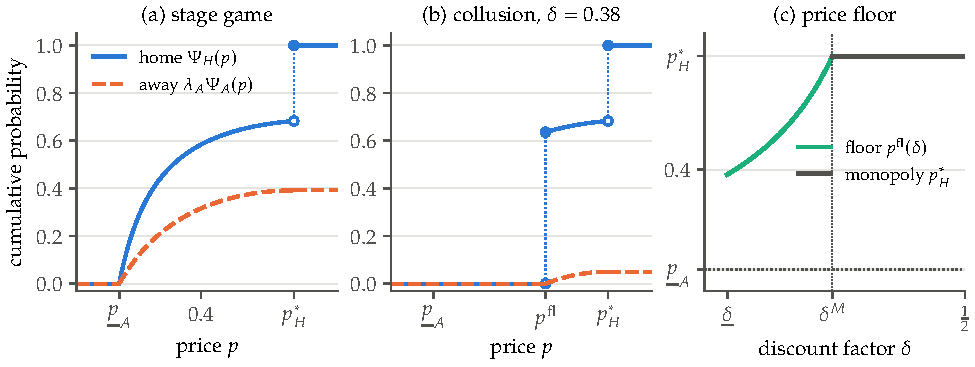
\includegraphics[width=\textwidth]{figures/ch13/bm_cdfs.pdf}
\caption{The model of \citet{BernheimMadsen2017} with $v\sim U[0,1]$, $c_H=0.1$, $c_A=0.2$ and $\phi=0.05$.
Panels (a) and (b) show the home firm's price CDF $\Psi_H$ as a solid line, with atoms marked by dots. The dashed
line is the away firm's unconditional CDF of quotes $\lambda_A\Psi_A$, which ends at the entry probability
$\lambda_A$.
Panel (a) is the stage-game equilibrium. Panel (b) is the optimal stationary collusive equilibrium at
$\delta=0.38$, with floor $p^{\mathrm{fl}}=0.449$. Panel (c) shows the floor $p^{\mathrm{fl}}(\delta)$ over
$[\underline\delta,\delta^M]=[0.345,0.413]$, where $\underline\delta=\delta^0$ is the threshold of
\cref{thm:13-bm-punish}. Above $\delta^M$ the cartel achieves the monopoly price. Source: our calculations
(\texttt{bm\_static.py}).}
\label{fig:13-bm-cdfs}
\end{figure}

\subsubsection{Stationary collusion}

Industry profit is highest when each home firm monopolizes its market at $p_H^*$ and the away firm stays out.
We call this \emph{perfect collusion}. An equilibrium with profits above the stage-game level and below
perfect collusion is an \emph{imperfectly collusive} arrangement. Lifetime profits are normalized as
$(1-\delta)\sum_{t\ge1}\delta^{t-1}\pi_t$, so that a constant stream $\pi$ is worth $\pi$. Characterizing the
whole equilibrium payoff set of a repeated game with mixed strategies and continuous actions is hard.
Bernheim and Madsen therefore restrict attention to the following class.

\begin{definition}[Stationary equilibrium]\label{def:13-bm-stationary}
A subgame perfect equilibrium is \emph{stationary} if there is a stage-game strategy profile $\tau$ such that
$\tau$ is played after every history on the equilibrium path. Behavior off the path is unrestricted beyond
subgame perfection.
\end{definition}

Off-path behavior can be nonstationary, so optimal penal codes in the sense of \citet{Abreu1988} are allowed.
On the path, lifetime profits equal stage profits. Let $\underline\Pi(\delta)$ be the infimum of a firm's
lifetime profits over all subgame perfect equilibria, and let $\delta^M$ be the lowest discount factor at which
perfect collusion is sustainable.

\begin{theorem}[Bernheim and Madsen, Theorem 2]\label{thm:13-bm-optimal}
For each $\delta\le\delta^M$, the unique Pareto-optimal stationary equilibrium profit vector
$(\bar\Pi,\bar\Pi)$ satisfies
\begin{equation}\label{eq:13-bm-thm2}
\bar\Pi=(1-\delta)\Bigl[2\bar\Pi-\Delta c\,D\bigl(\tilde p(\bar\Pi)\bigr)\Bigr]+\delta\,\underline\Pi(\delta).
\end{equation}
Moreover, $\bar\Pi>\Pi^C$ if and only if $\underline\Pi(\delta)<\Pi^C$, and $\bar\Pi$ is strictly increasing in
$\delta$ whenever $\underline\Pi(\cdot)$ is nonincreasing.
\end{theorem}

We derive the incentive constraint behind \eqref{eq:13-bm-thm2}. Consider an agreement that divides the
markets along cost lines and gives each firm stage profit $\Pi$ in its home market. The rival's lowest home
price $p_{\min}$ must satisfy $D(p_{\min})(p_{\min}-c_H)-\phi\ge\Pi$, since even a sure sale at the lowest price
must deliver $\Pi$. Hence $p_{\min}\ge\tilde p(\Pi)$. Consider a firm that keeps its home strategy and
slightly undercuts $p_{\min}$ in the away market for one period.
\begin{enumerate}[label=Step \arabic*.,leftmargin=*]
\item By \eqref{eq:13-bm-identity}, undercutting $p_{\min}$ in the away market earns
\[
D(p_{\min})(p_{\min}-c_A)-\phi=\bigl[D(p_{\min})(p_{\min}-c_H)-\phi\bigr]-\Delta c\,D(p_{\min})
\ge\Pi-\Delta c\,D\bigl(\tilde p(\Pi)\bigr),
\]
because the bracket is at least $\Pi$ and $D(p_{\min})\le D(\tilde p(\Pi))$.
\item Adding the home profit $\Pi$, the deviation earns at least $2\Pi-\Delta c\,D(\tilde p(\Pi))$ in the
deviation period.
\item The worst the cartel can do afterwards is to impose $\underline\Pi(\delta)$. The deviator's lifetime payoff
is at least
\[
(1-\delta)\Bigl[2\Pi-\Delta c\,D\bigl(\tilde p(\Pi)\bigr)\Bigr]+\delta\,\underline\Pi(\delta).
\]
\item The agreement survives only if the on-path payoff is at least this large:
\begin{equation}\label{eq:13-bm-ic}
\Pi\ \ge\ (1-\delta)\Bigl[2\Pi-\Delta c\,D\bigl(\tilde p(\Pi)\bigr)\Bigr]+\delta\,\underline\Pi(\delta).
\end{equation}
\item The firms pick the largest $\Pi$ that satisfies \eqref{eq:13-bm-ic}. At that $\Pi$ the constraint
binds, which is \eqref{eq:13-bm-thm2}. The equilibrium of \cref{thm:13-bm-structure} below attains it.
\end{enumerate}
Both firms agree on the best scheme, so the Pareto frontier of stationary equilibria is a single symmetric
point.

\begin{remark}[Nash reversion supports no collusion]\label{rem:13-bm-nash}
Collusion in this model requires punishments harsher than reversion to the stage game
\citep[footnote 22]{BernheimMadsen2017}. To see why, set $\underline\Pi=\Pi^C$ in \eqref{eq:13-bm-ic} and
subtract $\Pi^C$ from both sides:
\[
\Pi-\Pi^C\ \ge\ (1-\delta)\Bigl[2\Pi-\Delta c\,D(\tilde p)-\Pi^C\Bigr]
=(1-\delta)\bigl[(\Pi-\Pi^C)+a(\tilde p)\bigr],
\]
where $a(p)\equiv D(p)(p-c_A)-\phi=\Pi-\Delta c\,D(\tilde p)$ at $p=\tilde p(\Pi)$ is the away firm's
single-firm profit. Rearranging gives $\delta(\Pi-\Pi^C)\ge(1-\delta)\,a(\tilde p)$. Now
$\Pi-\Pi^C=a(\tilde p)-\Delta c\bigl[D(\underline p_A)-D(\tilde p)\bigr]\le a(\tilde p)$. The constraint
therefore requires $\delta\,a(\tilde p)\ge(1-\delta)\,a(\tilde p)$, that is, $\delta\ge\frac{1}{2}$. Since
$\delta^M<\frac{1}{2}$ (\cref{thm:13-bm-perfect}), Nash reversion sustains no profit above $\Pi^C$ in the whole
range where imperfect collusion is the relevant case.
\end{remark}

\begin{theorem}[Bernheim and Madsen, Theorem 3]\label{thm:13-bm-punish}
Suppose
\[
\delta\ \ge\ \delta^0\equiv\frac{1}{2+\frac{\Delta c\,D(p_H^*)}{\phi}} .
\]
Then a subgame perfect equilibrium gives both firms zero lifetime profits, so $\underline\Pi(\delta)=0$.
\end{theorem}

Zero is the harshest conceivable punishment, because a firm can always stay out of both markets. The
punishment is a one-period price war followed by a return to optimal collusion. In the war period both firms
enter both markets. The home firm quotes some $p^{PW}\le\underline p_H$ and serves its market at a loss. The
away firm mixes over $(p^{PW},\underline p_H]$, never sells, and loses its fixed cost. Its presence ensures
that a home firm that raises its price cannot profit. If both firms take part, play returns to the
collusive phase worth $\bar\Pi$. If either refuses, the war restarts. The war price is set so that
\[
(1-\delta)\Bigl[D(p^{PW})(p^{PW}-c_H)-2\phi\Bigr]+\delta\bar\Pi=0 .
\]
The bound on $\delta$ guarantees $p^{PW}\le\underline p_H$. A deviator's best option in the war period is then
to exit both markets, which yields zero today and a restarted war, so it gains nothing.

\begin{theorem}[Bernheim and Madsen, Theorem 4]\label{thm:13-bm-perfect}
Suppose $\Pi^M>\phi+\Delta c\,D(p_H^*)$. Then $\delta^0<\delta^M$, and for each $\delta\in[\delta^0,\delta^M]$
the optimal stationary profit satisfies
\begin{equation}\label{eq:13-bm-thm4}
\bar\Pi=(1-\delta)\Bigl[2\bar\Pi-\Delta c\,D\bigl(\tilde p(\bar\Pi)\bigr)\Bigr].
\end{equation}
The profit $\bar\Pi$ is continuous, strictly greater than $\Pi^C$, and strictly increasing in $\delta$. Perfect
collusion is sustainable for all $\delta\ge\delta^M$, where
\begin{equation}\label{eq:13-bm-deltaM}
\delta^M=\frac{\Pi^M-\Delta c\,D(p_H^*)}{2\Pi^M-\Delta c\,D(p_H^*)} .
\end{equation}
\end{theorem}

The threshold \eqref{eq:13-bm-deltaM} follows from \eqref{eq:13-bm-ic}. Perfect collusion sets $\Pi=\Pi^M$,
so $\tilde p(\Pi^M)=p_H^*$, and the harshest punishment is zero:
\begin{align*}
\Pi^M&\ge(1-\delta)\bigl[2\Pi^M-\Delta c\,D(p_H^*)\bigr]\\
1-\delta&\le\frac{\Pi^M}{2\Pi^M-\Delta c\,D(p_H^*)}\\
\delta&\ge1-\frac{\Pi^M}{2\Pi^M-\Delta c\,D(p_H^*)}=\frac{\Pi^M-\Delta c\,D(p_H^*)}{2\Pi^M-\Delta c\,D(p_H^*)} .
\end{align*}
The numerator is the away firm's profit at $p_H^*$, which is positive because $p_H^*>\underline p_A$. Twice the
numerator, $2\Pi^M-2\Delta c\,D(p_H^*)$, is smaller than the denominator, so $\delta^M<\frac{1}{2}$. In the
symmetric Bertrand duopoly without fixed costs the threshold is exactly $\frac{1}{2}$ (\cref{ch:collusion-theory}).
Here a raid on the other market earns less than the home firm's profit, because the raider has the higher
cost. The temptation is smaller, so perfect collusion is easier.

For $\delta\in[\delta^0,\delta^M)$, equation \eqref{eq:13-bm-thm4} pins down the floor
$p^{\mathrm{fl}}(\delta)\equiv\tilde p(\bar\Pi(\delta))$. Collecting terms in \eqref{eq:13-bm-thm4} gives
$(1-2\delta)\bar\Pi=(1-\delta)\Delta c\,D(\tilde p(\bar\Pi))$, which in terms of the floor reads
\begin{equation}\label{eq:13-bm-floor}
(1-2\delta)\Bigl[D(p^{\mathrm{fl}})(p^{\mathrm{fl}}-c_H)-\phi\Bigr]=(1-\delta)\,\Delta c\,D(p^{\mathrm{fl}}) .
\end{equation}
The left side rises in $p^{\mathrm{fl}}$ and the right side falls. At $\underline p_A$ the left side minus the
right side equals $(1-2\delta)\Pi^C-(1-\delta)\Pi^C=-\delta\Pi^C<0$. At $p_H^*$ it equals
$(1-2\delta)\Pi^M-(1-\delta)\Delta c\,D(p_H^*)$, which is positive exactly when $\delta<\delta^M$. A unique
floor therefore lies strictly between $\underline p_A$ and $p_H^*$. Differentiating the difference with
respect to $\delta$ gives $-2\Pi+\Delta c\,D(p)=-[\Pi+a(p)]<0$. By the implicit function theorem the floor
rises with $\delta$ and reaches $p_H^*$ at $\delta^M$.

\begin{theorem}[Bernheim and Madsen, Theorem 5]\label{thm:13-bm-structure}
When $\delta<\delta^M$, the profits $(\bar\Pi,\bar\Pi)$ are supported by a stationary equilibrium with the
following on-path properties:
\begin{enumerate}[label=(\roman*)]
\item The home firm's strategy is the same in each market, and so is the away firm's.
\item The home firm always enters. The away firm enters with probability strictly between 0 and 1.
\item The home firm earns stage profit $\bar\Pi$, and the away firm earns zero.
\item Each firm's price distribution has full support on $[p^{\mathrm{fl}},p_H^*]$. The home firm places atoms
at $p^{\mathrm{fl}}$ and at $p_H^*$. The away firm's distribution is continuous.
\item The away firm sells with positive probability, which decreases in $\bar\Pi$.
\item An away quote at or below $p^{\mathrm{fl}}$ triggers a punishment worth $\underline\Pi(\delta)$ to the
deviator.
\end{enumerate}
These on-path strategies are unique among stationary equilibria whose price distributions have full support on
$[p^{\mathrm{fl}},p_H^*]$.
\end{theorem}

The on-path strategies are exactly those of \cref{lem:13-bm-floor} with $p_f=p^{\mathrm{fl}}$, as the proof
of Theorem B.4 in the working paper confirms. The equilibrium check is short. The away firm earns zero at
every price in $(p^{\mathrm{fl}},p_H^*)$ and is never punished there. Its best one-period deviation is to
undercut the home atom at $p^{\mathrm{fl}}$, which earns $\bar\Pi-\Delta c\,D(p^{\mathrm{fl}})$ by
\eqref{eq:13-bm-identity}. The home firm earns $\bar\Pi$ at every price it quotes, so it cannot gain at home.
A firm that combines both moves earns $2\bar\Pi-\Delta c\,D(p^{\mathrm{fl}})$ for one period and then
$\underline\Pi(\delta)$. Condition \eqref{eq:13-bm-thm2} says that this deviation exactly breaks even. The
stage equilibrium of \cref{thm:13-bm-static} is the special case $p^{\mathrm{fl}}=\underline p_A$, in which the
home atom at the floor vanishes.

\begin{example}[Uniform values, continued]\label{ex:13-bm-uniform-coll}
In \cref{ex:13-bm-uniform}, $\Delta c\,D(p_H^*)=0.1\times0.45=0.045$ and $\Pi^M=0.1525>\phi+0.045=0.095$, so
\cref{thm:13-bm-perfect} applies. The thresholds are
\[
\delta^0=\frac{1}{2+\frac{0.045}{0.05}}=\frac{1}{2.9}=0.345,\qquad
\delta^M=\frac{0.1525-0.045}{0.305-0.045}=\frac{0.1075}{0.26}=0.413 .
\]
At $\delta=0.38$, equation \eqref{eq:13-bm-floor} gives $p^{\mathrm{fl}}=0.449$ and $\bar\Pi=0.142$. The home
firm quotes the floor with probability $0.636$ and the monopoly price with probability $0.317$. The away firm
enters with probability $\lambda_A=0.050$ and makes the sale with probability $0.017$, down from $0.238$ in the
stage game. The expected lowest quote is $0.482$. A clean split of the markets at the floor would give the
same profits with a price of $0.449$, so the tolerated raids cost consumers money. Panels (b) and (c) of
\cref{fig:13-bm-cdfs} show the distributions and the floor as a function of $\delta$.
\end{example}

\subsubsection{Why the cartel tolerates raids}

Why do the firms not agree on the simpler plan of a clean split at the floor? Under a clean split the away
firm stays out, and the home firm sells at $p^{\mathrm{fl}}$. A firm could then raise its home price to $p_H^*$
and raid the other market at the same time. If no business stealing ever occurs on the path, the best
deviation earns $\Pi^M$ at home plus $\Pi-\Delta c\,D(\tilde p(\Pi))$ away. The agreement is incentive
compatible only if
\begin{equation}\label{eq:13-bm-nosteal}
\Pi\ \ge\ (1-\delta)\Bigl[\Pi-\Delta c\,D\bigl(\tilde p(\Pi)\bigr)+\Pi^M\Bigr]+\delta\,\underline\Pi(\delta).
\end{equation}
The deviation payoff here exceeds the one in \eqref{eq:13-bm-ic} by $(1-\delta)(\Pi^M-\Pi)>0$. At
$\Pi=\bar\Pi$ the constraint \eqref{eq:13-bm-ic} binds, so \eqref{eq:13-bm-nosteal} fails. All punishment
power is already used to deter raids, so none is left to deter the home price increase. The cartel must
instead make a high home price unattractive directly. It does so by letting the away firm enter at prices
above the floor. Entry costs $\phi$, so the away firm enters only if it sometimes wins. The home firm cedes
those sales by charging the monopoly price part of the time. Equilibrium thus combines occasional price
escalation at home with unpunished business stealing away \citep[pp.~15--17]{BernheimMadsen2017}.

\begin{theorem}[Bernheim and Madsen, Theorems 6 and 7]\label{thm:13-bm-inevitable}
Let $\delta<\delta^M$.
\begin{enumerate}[label=(\roman*)]
\item All stationary equilibria with profits $(\bar\Pi,\bar\Pi)$ share the same minimum price, maximum price and
entry probabilities. Among them, the equilibrium of \cref{thm:13-bm-structure} uniquely minimizes the
probability that an away firm wins.
\item There exists $\tilde\Pi<\bar\Pi$ such that in any stationary equilibrium with profits
$(\Pi_1,\Pi_2)>(\tilde\Pi,\tilde\Pi)$, the away firm captures each market with strictly positive probability on
the equilibrium path.
\end{enumerate}
\end{theorem}

Part (ii) follows from \eqref{eq:13-bm-nosteal} by continuity. The constraint fails at $\bar\Pi$, and both
sides are continuous in $\Pi$, so it fails on an interval of profits below $\bar\Pi$. Business stealing is
therefore a feature of every nearly optimal cartel. It is not an artifact of a particular equilibrium.

\begin{remark}[Why tolerate deliberate cheating?]\label{rem:13-bm-puzzle}
The model resolves the puzzle posed by the lysine, nucleotide and citric acid records. When perfect collusion
is out of reach, every member knows that the aspirational price cannot hold. Members protect their home markets
by occasionally cutting price to the floor, and they raid each other at prices above it. The raids are
anticipated and serve a purpose. Their threat keeps home prices from drifting up to levels that would make the
cartel unstable. Punishing them would remove that discipline. Only raids at or below the floor, which the
home firm could have prevented by quoting the floor, would be punished.
\end{remark}

\casehead{Testable implication}
The cleanest prediction is that business stolen at prices above the floor goes unpunished, while stealing below
the floor triggers punishment. The floor is rarely known with precision. The average price is no proxy for it,
because some stealing occurs at below-average prices. Bernheim and Madsen therefore propose a more robust
implication: the higher the price at which business is stolen, the less likely the theft is to trigger
punishment. They leave the test to future work \citep[p.~7]{BernheimMadsen2017}.

\casehead{Many firms and comparative statics}
With $N+1$ firms and $N+1$ markets, the stage game has many equilibria. For each nonempty set of away firms
there is a unique equilibrium in which exactly those firms enter (Theorem 8). Bernheim and Madsen then restrict
attention to \emph{market-symmetric} equilibria, in which all away firms in a market play alike. Under mild
conditions on $N$ and $\Pi^M$ they obtain analogues of the duopoly results (Theorems 9 to 13). Optimal profits
satisfy
$\bar\Pi=(1-\delta)\bigl[(N+1)\bar\Pi-\Delta c\,N\,D(\tilde p(\bar\Pi))\bigr]+\delta\,\underline\Pi(\delta;N)$,
because a deviator keeps its home profit and raids all $N$ other markets. The perfect-collusion threshold is
\[
\delta^M(N)=1-\frac{1}{N+1}\left(\frac{N}{N+1}\,\frac{\tilde\Pi^M}{\Pi^M}+\frac{1}{N+1}\right)^{-1},
\]
where $\tilde\Pi^M=\Pi^M-\Delta c\,D(p_H^*)$ is a high-cost firm's profit at $p_H^*$. With $N=1$ the formula
reduces to \eqref{eq:13-bm-deltaM}. The threshold lies below $1-\frac{1}{N+1}$, rises with $N$ and tends to one
(Theorem 14). Large cartels can therefore hope only for imperfect collusion, even when their members are very
patient. The two frictions are both needed. As $c_A\to c_H$, collusion becomes all or nothing: $\bar\Pi\to\Pi^C$
for $\delta<\frac{N}{N+1}$ and $\bar\Pi\to\Pi^M$ for $\delta\ge\frac{N}{N+1}$ (Theorem 15). As $\phi\to0$,
business stealing vanishes and the home firm sells at $\underline p_A$ with probability one (Theorem 16).

\casehead{Assessment}
The model explains two facts that standard theory does not, deliberate cheating and its toleration, without
any monitoring noise. Several features limit its reach. The analysis is confined to stationary equilibria,
and the authors cannot rule out that nonstationary schemes do better. In the duopoly $\delta^M<\frac{1}{2}$, so
with literal discounting perfect collusion would be easy. Bernheim and Madsen therefore read $\delta$ as a
reduced form for impatience from agency problems, turnover or the number of rivals, and the many-firm results
support that reading. The sharp divide between tolerated and punished stealing would blur with imperfect
monitoring, for example with rogue salespeople who do not know about the cartel. The theory's main empirical
implication has not yet been tested. Read together, \citet{HarringtonSkrzypacz2011} and
\citet{BernheimMadsen2017} show that the internal records of cartels contain more than evidence of agreement.
Quotas, reports, transfers and tolerated raids are equilibrium objects with testable structure. The next
section studies a cartel whose internal records are complete enough to estimate such structure.

\section{Inside a Bidding Ring: Asker's Stamp Cartel}\label{sec:13-asker}

A bidding ring is a cartel of bidders. \Cref{sec:14-collusion} shows that in an English auction a ring
whose members know each other's values is self-enforcing (\cref{prop:14-robinson}). Real rings do not know
their members' values. They must elicit them and divide the gains, and the mechanism they use shapes both
bidding and damages. \citet{Asker2010} studies a ring of stamp dealers whose internal records survive in full.
His questions are how the ring organized itself, what incentives its mechanism created, and who bore the costs:
sellers, bidders outside the ring, or the ring itself. The answers matter for antitrust damages, for the
efficiency costs of collusion, and for detection, which relies on understanding how rings behave in practice.

\subsection{Question and institutions}\label{sec:13-asker-institutions}

Until July 1997, 11 wholesale stamp dealers belonged to the ring. It bid in auctions of collectible stamps,
typically collections, held mainly at New York auction houses. These houses ran open outcry ascending
auctions, that is, English auctions. The ring began in the late 1970s or early 1980s and lasted 15 to 20 years,
with very few changes in membership after its first five years. It collapsed when a stamp dealer outside the
ring brought it to the attention of antitrust enforcers \citep[p.~725]{Asker2010}. The data come from the
resulting case, \textit{New York et al.\ v.\ Feldman et al.}\ in the Southern District of New York.

\casehead{The knockout}
The ring coordinated through a \emph{knockout}, a private auction held before each \emph{target auction}.
Members sent sealed bids on the lots they wanted, by fax or in writing, to an agent: a New York taxi and
limousine driver employed by the ring. The agent determined the winner of each lot and notified the members.
He sent the bids to another member, who computed the sidepayments after the target auction. Sidepayments were
aggregated and settled quarterly. In the target
auction the agent, or another agent he arranged, bid for the knockout winner up to the winning knockout bid.
The winning bid thus set the ring's bidding limit. Because the ring's own agent did the bidding, compliance
with the limit was easy to monitor. The coordinating member paid the agent \$30 an hour, and each member paid
him \$50 for every target auction in which it was active. Depositions state that the agent never revealed bids
before a knockout closed. Ties were resolved by the agent, who tried ``as much as possible to be fair''
\citep[pp.~727--728]{Asker2010}.

\casehead{Enforcement}
Evidence on enforcement is thin. In the ring's early years at least two members were expelled, one for not
meeting his financial obligations and one for being interested only in sidepayments. The records show no member
who lost a knockout and then bid against the ring, and no temporary suspensions. One auction house signaled
that it knew a ring was active, and the ring stopped operating there. In its final years the ring hid its
activity by also bidding through other professional agents and through its own members
\citep[p.~728]{Asker2010}.

Knockouts of the kind this ring used have a long history in markets for rare books, art, rugs, stamps, coins
and antiques. In the 1919 sale of the library of Ruxley Lodge in England, 81 London booksellers formed a ring.
Their knockouts after the sale ran in rounds of 81, 24, 15 and finally 8 members. These rounds raised
\pounds10,292 on top of the \pounds3,161 paid in the sale itself. Rings were legal in the United Kingdom before
1927 \citep[p.~726]{Asker2010}.

\casehead{The sidepayment rule}
Sidepayments compensated members for not competing when the ring won. Let $P$ be the target price paid by the
ring. Order the knockout bids from highest to lowest as $b_{(1)}\ge b_{(2)}\ge\dots\ge b_{(n)}$. Here the
subscript counts from the top, unlike the order statistics of \cref{ch:auction-theory}. Let $m$ be the number
of bids at or above $P$, and set $b_{(m+1)}\equiv P$.

\begin{definition}[Incremental sidepayment rule]\label{def:13-asker-rule}
For $j=2,\dots,m$, let $\Delta_j=b_{(j)}-b_{(j+1)}$ be the increment between consecutive eligible bids. The
knockout winner keeps half of each increment. The other half is split equally among the $j-1$ losing bidders
whose bids are at least $b_{(j)}$. Bidders with bids below $P$ receive nothing.
\end{definition}

\begin{proposition}[Properties of the rule]\label{prop:13-asker-sidepay}
Under \cref{def:13-asker-rule}:
\begin{enumerate}[label=(\roman*)]
\item The loser ranked $k\in\{2,\dots,m\}$ receives $s_{(k)}=\sum_{j=k}^{m}\frac{\Delta_j}{2(j-1)}$.
\item The winner pays $\frac{1}{2}\bigl(b_{(2)}-P\bigr)$ in total. Its outlay for the lot is
$P+\frac{1}{2}(b_{(2)}-P)=\frac{1}{2}(P+b_{(2)})$.
\item Payments balance.
\item Holding ranks fixed, a loser's receipt rises by $\frac{1}{2(k-1)}$ per dollar of its own bid whenever its
bid exceeds $P$.
\item With two knockout bidders, the loser receives $\frac{1}{2}(b_{(2)}-P)^+$.
\end{enumerate}
\end{proposition}

\begin{proof}
Part (i) restates the rule: the loser ranked $k$ shares in increments $j=k,\dots,m$, each among $j-1$ losers.
For (ii), the winner pays half of every increment, and the sum telescopes:
\[
\sum_{j=2}^{m}\frac{\Delta_j}{2}=\frac{1}{2}\bigl(b_{(2)}-b_{(m+1)}\bigr)=\frac{1}{2}\bigl(b_{(2)}-P\bigr) .
\]
For (iii), exchange the order of summation in the losers' receipts:
\[
\sum_{k=2}^{m}s_{(k)}=\sum_{j=2}^{m}\ \sum_{k=2}^{j}\frac{\Delta_j}{2(j-1)}=\sum_{j=2}^{m}\frac{\Delta_j}{2}
=\frac{1}{2}\bigl(b_{(2)}-P\bigr) .
\]
For (iv), the own bid $b_{(k)}$ enters $s_{(k)}$ only through $\Delta_k=b_{(k)}-b_{(k+1)}$, with weight
$\frac{1}{2(k-1)}$. Part (v) is the case $m=2$.
\end{proof}

\begin{remark}[The rule for any number of eligible reports]\label{rem:13-mm-table91}
\citet[pp.~192--194, Table~9.1]{MarshallMarx2012} state the ring's payments for any number of eligible reports. They
rank the reports as $r_1 > r_2 > \dots > r_k > p > r_{k+1} > \dots > r_n$, where $p$ is the price paid at the
auction. In our notation $r_j = b_{(j)}$, $p = P$ and $k = m$. Members $k+1, \dots, n$ receive nothing. Member $k$
receives $\frac{r_k - p}{2}\cdot\frac{1}{k-1}$, member 2 receives
\begin{equation*}
  \frac{r_k - p}{2}\cdot\frac{1}{k-1} + \frac{r_{k-1} - r_k}{2}\cdot\frac{1}{k-2} + \dots + \frac{r_2 - r_3}{2} ,
\end{equation*}
and member 1, the winner, pays the sum of the half-increments, $\frac{r_k - p}{2} + \frac{r_{k-1} - r_k}{2} + \dots
+ \frac{r_2 - r_3}{2}$. Since $r_j - r_{j+1} = \Delta_j$, these are parts (i) and (ii) of \cref{prop:13-asker-sidepay}.
Their verbal summary is \citeauthor{Asker2010}'s description of \cref{def:13-asker-rule}, and they call the mechanism a
variant of the one described by \citet{GrahamMarshallRichard1990} (p.~193, note~15). They also note that members
have an incentive to overreport, which the ring accepted as a cost of doing business, much as cartels accept some
misreporting of sales (p.~194).
\end{remark}

\begin{example}[Sotheby's, June 24, 1997, Lot 49]\label{ex:13-asker-ko}
\Cref{tab:13-asker-ex1} reproduces Asker's Example 1. Bidder J's \$5,100 lies below the target price of
\$6,750, so J is not eligible and $m=3$. The increments are $\Delta_3=7{,}500-6{,}750=750$ and
$\Delta_2=8{,}000-7{,}500=500$. Bidder A keeps \$375 of the first increment and gives \$187.50 each to B and G.
A keeps \$250 of the second increment and gives \$250 to G, the only loser whose bid reaches \$8,000. A pays
$\frac{1}{2}(8{,}000-6{,}750)=625$, which equals $437.50+187.50$. A's outlay is \$7,375 for a lot bought at
\$6,750. \Cref{fig:13-asker-numberline} shows the increments.
\end{example}

\begin{table}[htbp]
\centering
\caption{Sidepayments after a successful acquisition: Sotheby's, June 24, 1997, Lot 49}
\label{tab:13-asker-ex1}
\begin{threeparttable}
\begin{tabular}{@{}lrl@{}}
\toprule
Knockout auction & Bid (\$) & Sidepayment (\$) \\
\midrule
Bidder A & 9,000 & $-\left(\frac{7{,}500-6{,}750}{2}\right)-\left(\frac{8{,}000-7{,}500}{2}\right)=-625$ \\[6pt]
Bidder G & 8,000 & $+\left(\frac{7{,}500-6{,}750}{2}\right)\times\frac{1}{2}+\left(\frac{8{,}000-7{,}500}{2}\right)=437.50$ \\[6pt]
Bidder B & 7,500 & $+\left(\frac{7{,}500-6{,}750}{2}\right)\times\frac{1}{2}=187.50$ \\[6pt]
Bidder J & 5,100 & 0 \\[2pt]
Target auction price & 6,750 & \\
\bottomrule
\end{tabular}
\begin{tablenotes}\footnotesize
\item Source: \citet[Example 1]{Asker2010}.
\end{tablenotes}
\end{threeparttable}
\end{table}

\begin{figure}[htbp]
\centering
\begin{tikzpicture}[x=1.3cm,y=1cm,font=\small]
\draw[->] (0.3,0) -- (10.9,0) node[right] {\$};
\foreach \x/\v in {1/{6{,}750},4/{7{,}500},6/{8{,}000},10/{9{,}000}}
  {\draw (\x,0.12) -- (\x,-0.12) node[below] {$\v$};}
\node[below] at (1,-0.6) {target price $P$};
\node[below] at (4,-0.6) {B: $b_{(3)}$};
\node[below] at (6,-0.6) {G: $b_{(2)}$};
\node[below] at (10,-0.6) {A: $b_{(1)}$};
\draw[decorate,decoration={brace,amplitude=6pt}] (1,0.3) -- (4,0.3)
  node[midway,above=7pt,align=center,font=\footnotesize]
  {$\Delta_3=750$:\\ A keeps 375,\\ B and G get\\ 187.50 each};
\draw[decorate,decoration={brace,amplitude=6pt}] (4,0.3) -- (6,0.3)
  node[midway,above=7pt,align=center,font=\footnotesize]
  {$\Delta_2=500$:\\ A keeps 250,\\ G gets 250};
\draw[decorate,decoration={brace,amplitude=6pt}] (6,0.3) -- (10,0.3)
  node[midway,above=7pt,align=center,font=\footnotesize]
  {above $b_{(2)}$:\\ no sidepayment\\ depends on\\ A's own bid};
\node[align=left,font=\footnotesize,anchor=west] at (0.3,-1.55) {J bid 5,100 $<P$ (off scale): not eligible.};
\node[align=left,font=\footnotesize,anchor=west] at (0.3,-2.05)
  {A pays $\frac{1}{2}(8{,}000-6{,}750)=625$, so its outlay is $6{,}750+625=7{,}375=\frac{1}{2}(6{,}750+8{,}000)$.};
\end{tikzpicture}
\caption{The incremental sidepayment rule in \cref{ex:13-asker-ko}. Each increment runs from one eligible knockout
bid to the next, between the target price and the second-highest bid. The winner keeps half of it. The losers whose
bids reach its top share the other half equally. Source: drawn from \citet[Example 1]{Asker2010}.}
\label{fig:13-asker-numberline}
\end{figure}

\casehead{An older rule}
Before the late 1980s the ring split each increment equally among all eligible bidders, the winner included.
Under that rule the loser ranked $k$ receives $\sum_{j=k}^{m}\frac{\Delta_j}{j}$. In the example, the \$750
increment would have been shared three ways, giving \$250 each to A, G and B, and the \$500 increment two
ways. G would have received \$500 and B \$250, and A would have paid \$750. Treating bids as true
willingness to pay, the older rule gives each member its imputed Shapley value, a point
\citet{GrahamMarshall1987} make in their analysis of nested knockouts. The \emph{Shapley value} gives each member
its marginal contribution to the coalition's surplus, averaged over all orders in which the members could join. \citet{GrahamMarshallRichard1990} first
studied this class of mechanisms, in which a member's sidepayment rises with its own bid. With two knockout
bidders the old and new rules coincide, since each splits the single increment equally between winner and
loser.

\subsection{The theory of the knockout}\label{sec:13-asker-theory}

Asker adapts the model of \citet{GrahamMarshallRichard1990}. We write $\omega_j$ for member $j$'s participation
probability (Asker writes $\alpha_j$, a symbol this book uses for coefficients). $G$ and $g$ denote the distribution and density
of a rival member's knockout bid. $H_r$ and $h_r$ denote the distribution and density of the highest value among
bidders outside the ring.

\begin{assumption}[Knockout environment]\label{asm:13-asker-ipv}
\leavevmode
\begin{enumerate}[label=(\roman*)]
\item Private values: member $i$'s value $v_i$ is drawn from $F_i$ on $[\underline v_i,\bar v_i]$,
independently across members, and is private information.
\item Members know how many members bid in the knockout but not who they are. Member $j$ participates with known
probability $\omega_j$.
\item Bidders outside the ring bid up to their values in the English target auction, which is weakly dominant
(\cref{sec:14-english-pv}). The highest outside value $r$ has CDF $H_r$ and density $h_r$ and is independent of
members' values. Here $r$ denotes the highest outside value, not a reserve price.
\item Members use increasing, differentiable bid functions $\beta_j$ with inverses $\beta_j^{-1}$. The ring's
agent bids up to the winning knockout bid $b_{(1)}$.
\end{enumerate}
\end{assumption}

Under (iii) and (iv) the ring wins the target auction exactly when $r<b_{(1)}$, and it then pays $P=r$. Every
lot carried a secret reserve price, but Asker finds no evidence that reserves ever bound, so the model omits
them \citep[footnote 12]{Asker2010}.

\casehead{The two-bidder objective}
Consider a member with value $v$ who faces one rival. The rival's bid $y$ has CDF
\[
G(y)=\frac{\sum_{j\neq i}\omega_j F_j\bigl(\beta_j^{-1}(y)\bigr)}{\sum_{j\neq i}\omega_j},
\]
a mixture over the rival's unknown identity, with density $g$. Define the target surplus and sidepayment
integrals
\begin{equation}\label{eq:13-asker-AS}
A(b)\equiv\int_{-\infty}^{b}(v-x)\,h_r(x)\,\dd x,\qquad S(z)\equiv\int_{-\infty}^{z}(z-x)\,h_r(x)\,\dd x .
\end{equation}
If the member bids $b$ and wins the knockout ($y<b$), the ring bids up to $b$. The member gains $v-r$ when
$r<b$, and pays the loser $\frac{1}{2}(y-r)$ when $r<y$. Its expected payoff is $A(b)-\frac{1}{2}S(y)$. If it
loses the knockout ($y>b$), the ring bids up to $y$, and the member receives $\frac{1}{2}(b-r)$ when $r<b$.
Its expected payoff is $\frac{1}{2}S(b)$. Averaging over $y$,
\begin{equation}\label{eq:13-asker-U}
U(b)=\int_{-\infty}^{b}g(y)\Bigl[A(b)-\tfrac{1}{2}S(y)\Bigr]\dd y+\bigl[1-G(b)\bigr]\tfrac{1}{2}S(b).
\end{equation}
This is equation (1) of \citet{Asker2010} after exchanging the order of integration in the sidepayment term.

\casehead{The first-order condition}
We differentiate term by term. By Leibniz's rule, $A'(b)=(v-b)h_r(b)$ and
$S'(z)=(z-z)h_r(z)+\int_{-\infty}^{z}h_r(x)\,\dd x=H_r(z)$. The first term of \eqref{eq:13-asker-U}
splits into $G(b)A(b)$ and $-\frac{1}{2}\int_{-\infty}^{b}g(y)S(y)\,\dd y$. Their derivatives are
\begin{align*}
\frac{\dd}{\dd b}\bigl[G(b)A(b)\bigr]&=g(b)A(b)+G(b)(v-b)h_r(b),\\
\frac{\dd}{\dd b}\Bigl[-\tfrac{1}{2}\textstyle\int_{-\infty}^{b}g(y)S(y)\,\dd y\Bigr]&=-\tfrac{1}{2}g(b)S(b),\\
\frac{\dd}{\dd b}\Bigl[\tfrac{1}{2}\bigl(1-G(b)\bigr)S(b)\Bigr]&=-\tfrac{1}{2}g(b)S(b)+\tfrac{1}{2}\bigl[1-G(b)\bigr]H_r(b).
\end{align*}
Adding the three lines,
\[
U'(b)=g(b)\bigl[A(b)-S(b)\bigr]+G(b)(v-b)h_r(b)+\tfrac{1}{2}\bigl[1-G(b)\bigr]H_r(b).
\]
Since $A(b)-S(b)=\int_{-\infty}^{b}(v-x-b+x)h_r(x)\,\dd x=(v-b)H_r(b)$, we obtain
\begin{equation}\label{eq:13-asker-foc}
U'(b)=(v-b)\Bigl[g(b)H_r(b)+G(b)h_r(b)\Bigr]+\tfrac{1}{2}H_r(b)\bigl[1-G(b)\bigr].
\end{equation}
The first term is the familiar trade-off of a second-price auction. A higher bid wins the knockout more often
(at rate $gH_r$) and wins the target more often after a knockout win (at rate $Gh_r$), each worth $v-b$ at the
margin. The second term is new. When the member loses the knockout and the ring wins below its bid, each extra
dollar of bid brings an extra half dollar of sidepayment.

\begin{lemma}[Asker, Lemma 1]\label{lem:13-asker-lemma1}
At $b=v$, $U'(v)=\frac{1}{2}H_r(v)\bigl[1-G(v)\bigr]\ge0$.
\end{lemma}

\begin{proposition}[Overbidding (Asker, Result 1)]\label{prop:13-overbid}
A member bids strictly above its value whenever $H_r(v)>0$ and $G(v)<1$, and bids its value when $v$ is at the
top of the rival's bid support.
\end{proposition}

\begin{proof}
For $b<v$ both terms of \eqref{eq:13-asker-foc} are nonnegative, so $U$ is nondecreasing on $(-\infty,v]$ and
no bid below $v$ beats $b=v$. At $b=v$, \cref{lem:13-asker-lemma1} gives $U'(v)>0$ when $H_r(v)>0$ and
$G(v)<1$, so some bid above $v$ does strictly better. If $G(v)=1$, then for $b>v$ we have $G(b)=1$ and $g(b)=0$,
so $U'(b)=(v-b)h_r(b)\le0$, and the optimal bid is $v$.
\end{proof}

Asker states the result for any number of knockout bidders. For bids below $v$ the usual dominance argument for
second-price and English auctions applies, and the sidepayment term pushes bids above $v$.

\begin{remark}[Overbidding without sidepayments]\label{rem:13-asker-nosidepay}
Overbidding does not depend on sidepayments \citep[footnote 15]{Asker2010}. Remove them, so the payoff is
$U^0(b)=G(b)A(b)$. Then $U^{0\prime}(v)=g(v)A(v)>0$ whenever the expected target surplus $A(v)$ is positive. A
knockout win removes a rival from the target auction, which has an option value, and a higher bid buys more of
it. In \eqref{eq:13-asker-foc} the sidepayment terms cancel this option value at $b=v$, because $A(v)=S(v)$, and
replace it with the sidepayment motive $\frac{1}{2}H_r(1-G)$.
\end{remark}

\casehead{The inverse bid function}
Setting \eqref{eq:13-asker-foc} to zero and solving for $v$ gives equation (2) of \citet{Asker2010}:
\begin{equation}\label{eq:13-asker-inverse}
v=b-\frac{\frac{1}{2}H_r(b)\bigl[1-G(b)\bigr]}{h_r(b)G(b)+H_r(b)g(b)} .
\end{equation}
The equation maps each observed bid to a unique value, given the distribution of rival bids and the distribution
of the highest outside value. It plays the role that the inversion of \citet{GuerrePerrigneVuong2000} plays for
first-price auctions, $v=b+\frac{G(b)}{(n-1)g(b)}$ (\cref{eq:14-foc-G}, \cref{ch:auction-empirics}). The signs
differ: first-price bidders shade below value, while knockout bidders inflate above it. In both cases
identification requires the inverse bid function to be strictly increasing. Asker also derives three- and
four-bidder analogues (his footnote 13). They involve integrals of $H_r$ against the rival bid distribution,
and the structural analysis uses only two-bidder knockouts.

\begin{corollary}[Inefficiency (Asker, Corollary 1)]\label{cor:13-asker-ineff}
The knockout can lead to an inefficient allocation in the English target auction.
\end{corollary}

Suppose the highest outside value $r$ lies between the top member's value $v_{(1)}$ and that member's knockout
bid $b_{(1)}$. The ring wins and pays $r>v_{(1)}$, although an outside bidder values the lot more. The ring then
harms itself. The seller can gain, because under competition the price would be the second-highest value
overall, which is at most $r$. Outside bidders lose in two ways. They lose the lot they would have won, and when
they do win, the ring's inflated limit $b_{(1)}$ can push their price above the competitive level. Asymmetries
among members add a further inefficiency, because the knockout need not allocate the lot to the member with the
highest value \citep[footnote 16]{Asker2010}.

\begin{lemma}[Asker, Lemma 2]\label{lem:13-asker-lemma2}
The inverse bid function \eqref{eq:13-asker-inverse} can have regions where $\frac{\dd v}{\dd b}<0$.
\end{lemma}

Asker's example sets $H_r$ lognormal with $\mu=-2$ and $\sigma^2=0.08$, and $G$ lognormal with $\mu=-1$ and
$\sigma^2=1$. \Cref{fig:13-asker-vb} confirms the claim: $v(b)$ falls for $b\in[0.161,0.220]$. On that region
some stationary points of the first-order condition are local minima. An estimator could then map observed bids to
values through the wrong branch, which contradicts optimal bidding. Asker therefore maintains that the
population inverse bid function is strictly increasing, and he imposes it through the choice of smoothing
parameters (\cref{sec:13-asker-structural}). With a more dispersed outside value ($\sigma^2=0.5$), the same
$G$ yields a monotone inverse. Both curves lie below the $45^\circ$ line, which is overbidding.

\begin{figure}[htbp]
\centering
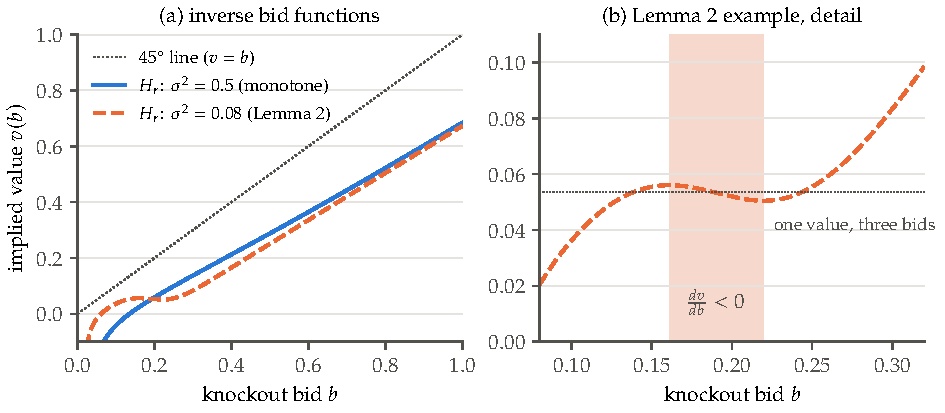
\includegraphics[width=\textwidth]{figures/ch13/asker_vb.pdf}
\caption{The inverse bid function \eqref{eq:13-asker-inverse} with $G$ lognormal ($\mu=-1$, $\sigma^2=1$) and
$H_r$ lognormal with $\mu=-2$. Panel (a): Asker's Lemma 2 example ($\sigma^2=0.08$, dashed) and a monotone case
($\sigma^2=0.5$, solid). Implied values lie below the $45^\circ$ line, so bids exceed values. Panel (b): detail
of the Lemma 2 example. On the shaded region $v(b)$ decreases, so one value is consistent with three bids.
Source: our calculations (\texttt{asker\_inverse\_bid.py}).}
\label{fig:13-asker-vb}
\end{figure}

\subsubsection{Why this mechanism?}

The ring's design looks puzzling. It induces overbidding, misallocation and occasional losses for the ring
itself. Asker's Section II.A explains why simpler designs were unattractive.

\citet{MailathZemsky1991} show that with independent private values drawn from different distributions, a
mechanism exists that achieves efficient collusion at second-price auctions. It balances the budget ex post and
no subcoalition wants to break away. The mechanism depends heavily on the value distributions, however, and
Asker knows of no game form that implements it. With symmetric bidders a simple mechanism is optimal. The ring
holds a first-price sealed-bid knockout, the winner bids in the target, and the winner's knockout bid is split
equally among the losers. With asymmetric bidders that simple design fails. If the ring cannot discriminate in
sidepayments, it may do better to exclude a weak member whose expected contribution to the collusive surplus is
smaller than his share. \citet{McAfeeMcMillan1992} analyze rings at first-price auctions and introduce the
notion of an insincere bidder, an extreme form of weakness. \citet{LopomoMarshallMarx2005} show that when the
knockout follows the target auction and the budget must balance ex post, no scheme at all can implement an
efficient allocation at English auctions. A ring with asymmetric members thus faces a choice. It can exclude its
weak members or accept some inefficiency. The stamp ring kept its weak members.

\begin{remark}[Why tie the target limit to the knockout bid?]\label{rem:13-asker-design}
Consider an alternative in which the knockout winner chooses its own limit in the target auction, with
sidepayments computed as before. Suppose two members bid and the bids become known. Let the winner's value be
$v_1$ and the loser's bid $k_2$. If $k_2<v_1$, the standard English auction argument gives a limit of $v_1$. If
$k_2>v_1$, the winner chooses a limit $\bar b\le k_2$ to maximize
\[
\int_{-\infty}^{\bar b}(v_1-x)\,h_r(x)\,\dd x-\frac{1}{2}\int_{-\infty}^{\bar b}(k_2-x)\,h_r(x)\,\dd x .
\]
The first-order condition is $(v_1-\bar b)h_r(\bar b)-\frac{1}{2}(k_2-\bar b)h_r(\bar b)=0$, so
\[
v_1-\bar b=\tfrac{1}{2}(k_2-\bar b)\quad\Longrightarrow\quad\bar b=2v_1-k_2<v_1 .
\]
The winner would underbid, to avoid winning lots whose sidepayment exceeds its profit \citep[p.~734 and
footnote 19]{Asker2010}. Underbidding would leave profitable lots unbought and invite members to defect and bid
secretly against the ring. It would also attract outside bidders. Tying the limit to the knockout bid makes the
ring aggressive instead. No member wants to be outside a ring that overbids, and outsiders are deterred from
entering. On this account the design traded some allocative efficiency for stability.
\end{remark}

\subsection{Data and descriptive evidence}\label{sec:13-asker-data}

The data cover the knockouts before 11 target sales between June 5, 1996 and June 26, 1997. A sale is a
collection of lot auctions that often runs over several days. The New York Attorney General's office collected
the records during its investigation. They were transcribed from faxes and written records kept by one member,
who was known in the ring for worrying about not being paid what he was owed. For each lot the data give the
date, auction house, lot number, target price, all sidepayments, and the identities and bids of the knockout
bidders. Fewer than 3 percent of observations are incomplete, for reasons such as faxes faded by sunlight. The
records are matched to auction catalogs, which report estimated minimum and maximum values or a book value,
condition grades, origin and number of stamps. The main shortcoming is that the number of bidders in the target
auction is unknown, and only the winning target price is recorded \citep[pp.~734--735]{Asker2010}.

The analysis excludes the Harmer-Schau sale (189 lots, 87 percent won by the ring), where the ring used an
informal arrangement and the target price almost always equaled the second-highest knockout bid. In the
remaining 1,781 lots the ring won 58 percent of the lots on which it was active, or 66 percent by estimated
value. The lots it won raised \$6,377,284, against \$10,034,754 across all lots on which it was active. The
pooled mean knockout bid was \$2,142 and the pooled mean winning target bid \$2,042 \citep[Table
1]{Asker2010}.

\Cref{tab:13-asker-t2} organizes the lots by the number of members in the knockout. A single member bid on
623 lots, and eight members bid on 26. The ring's win rate rises steeply with participation, from 19 percent to
96 percent. Either outside participation grew more slowly than ring participation, or overbidding grew with the
number of members, or both. Mean winning target bids rise weakly with participation and are roughly flat between
three and six bidders.

\begin{table}[htbp]
\centering
\caption{Bidding by number of bidders in the knockout}
\label{tab:13-asker-t2}
\begin{threeparttable}
\begin{tabular}{@{}crrrrrr@{}}
\toprule
Number of & \multicolumn{2}{c}{\makecell{Target auction\\(winning bid)}} &
\multicolumn{2}{c}{\makecell{Knockout\\(median bid)}} & \% of lots & Total \\
\cmidrule(lr){2-3}\cmidrule(lr){4-5}
bidders & Mean & SD & Mean & SD & won by ring & lots \\
\midrule
1 & 733 & 1,262 & 616 & 1,134 & 19 & 623 \\
2 & 1,314 & 2,016 & 1,066 & 2,048 & 36 & 367 \\
3 & 2,014 & 3,246 & 1,750 & 3,029 & 48 & 260 \\
4 & 2,217 & 3,492 & 2,293 & 4,082 & 69 & 196 \\
5 & 2,249 & 3,419 & 2,092 & 3,322 & 68 & 144 \\
6 & 2,098 & 2,628 & 2,163 & 3,014 & 74 & 91 \\
7 & 2,979 & 3,425 & 3,655 & 4,116 & 86 & 74 \\
8 & 4,790 & 4,904 & 6,233 & 7,726 & 96 & 26 \\
\bottomrule
\end{tabular}
\begin{tablenotes}\footnotesize
\item Notes: Amounts in dollars. Excludes the Harmer-Schau sale. The lot counts sum to 1,781. Weighting the win
rates by lots gives about 43 percent, below the 58 percent of Asker's Table 1, so the two figures are computed
on different bases. Source: \citet[Table 2]{Asker2010}.
\end{tablenotes}
\end{threeparttable}
\end{table}

\casehead{Participation and win rates}
Asker's Table 3 regresses the number of members in each knockout on lot characteristics by OLS. A second
column uses a transformed logit, whose dependent variable is the log share of members participating minus the
log share not participating. In the logit, participation rises with the spread of the catalog estimate,
$E_{\max}-E_{\min}$ in thousands of dollars (coefficient 0.196, standard error 0.103), much more than with its
midpoint (0.031, standard error 0.024). It also rises with the spread of condition grades (0.198, standard error
0.022) and falls when no grade is given ($-0.492$, standard error 0.074). Both regressions use 1,781 lots, with
an $R^2$ of 0.261 for OLS and 0.255 for the logit. Participation is always incomplete: at most 8 of the 11
members ever bid on a lot. Since entering a very low knockout bid costs little and can earn a sidepayment, Asker suggests a dynamic
enforcement rule or a small participation cost as explanations \citep[pp.~737--738]{Asker2010}.

Table 4 of \citet{Asker2010} reports a logit of a ring win on the same covariates. The number of members raises
the win probability, with a coefficient of 0.854 (standard error 0.127) and a marginal effect of 0.208 per
member. The effect diminishes, with a coefficient of $-0.046$ (0.017) on the square. Higher average grades raise
the win probability (0.313, standard error 0.069). The estimated value and its spread have no significant effect
once these are controlled for. Auction house dummies remain significant, perhaps because outside competition
differed across houses.

\casehead{Weak members}
\Cref{tab:13-asker-t5} reports knockout outcomes by member. Members D, G and H rarely submit the high bid: 14, 11
and 14 percent of the knockouts they enter, and 10, 10 and 4 percent when at least two members bid. Yet they
receive sidepayments at least as often as the others (20, 34 and 34 percent) and almost never pay them (3, 5
and 0 percent). In an independent private values model, a member's strength comes from its value distribution.
A weak member's distribution places more mass on low values. Asker notes that distributions with a similar mean
but a much lower variance fit the pattern. Such members lose more often, but their losing bids sit close to the
winning bid and so earn sidepayments \citep[footnote 30]{Asker2010}. Member D was explicit in his deposition.
His objective, he said, was to ``make money from these people'' rather than to buy the stamps
\citep[p.~738]{Asker2010}.

\begin{table}[htbp]
\centering
\caption{Knockout outcomes, by ring member}
\label{tab:13-asker-t5}
\begin{threeparttable}
\begin{tabular}{@{}lrrrrrr@{}}
\toprule
 & \multicolumn{2}{c}{All knockouts ($n\ge1$)} & \multicolumn{4}{c}{Knockouts with at least two members ($n\ge2$)} \\
\cmidrule(lr){2-3}\cmidrule(l){4-7}
Member & \% high bid & Knockouts & \% high bid & \% receives & \% pays & Knockouts \\
\midrule
A & 40 & 675 & 33 & 22 & 12 & 607 \\
B & 57 & 196 & 52 & 21 & 16 & 175 \\
C & 34 & 449 & 20 & 23 & 5 & 368 \\
D & 14 & 715 & 10 & 20 & 3 & 686 \\
E & 39 & 353 & 38 & 24 & 21 & 348 \\
F & 31 & 120 & 28 & 28 & 4 & 116 \\
G & 11 & 186 & 10 & 34 & 5 & 184 \\
H & 14 & 56 & 4 & 34 & 0 & 50 \\
I & 44 & 210 & 44 & 17 & 20 & 209 \\
J & 45 & 878 & 30 & 22 & 9 & 686 \\
K & 42 & 1,075 & 28 & 21 & 9 & 861 \\
\bottomrule
\end{tabular}
\begin{tablenotes}\footnotesize
\item Notes: ``\% high bid'' is the share of a member's knockouts in which it submitted the highest bid.
``\% receives'' and ``\% pays'' are the shares in which it received or paid sidepayments. Source:
\citet[Table 5]{Asker2010}.
\end{tablenotes}
\end{threeparttable}
\end{table}

\Cref{fig:13-asker-f1} shows net sidepayments by member. Over all auctions, E was the largest net payer, with
\$74,418 paid into the ring. D and G were the largest net recipients, with \$22,251 and \$21,574, although G
took part in only 186 knockouts against D's 715. Excluding the 25 lots with target prices above \$10,000 reduces
E's role. E was active in 18 of them and paid \$38,000 net on them. Its largest single payment was \$15,500, on
a lot acquired for \$26,000. The ability of D and H to extract sidepayments is unchanged by the exclusion
\citep[p.~740 and footnote 28]{Asker2010}.

\begin{figure}[htbp]
\centering
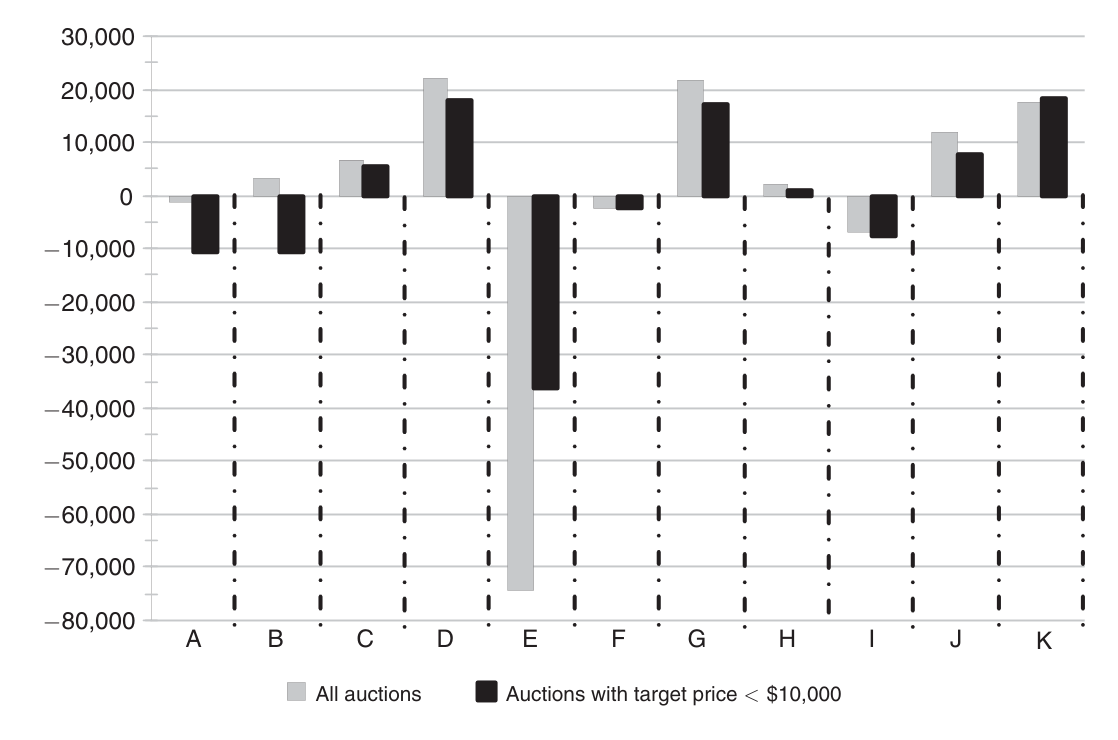
\includegraphics[width=0.82\textwidth]{figures/ch13/asker2010_fig1.png}
\caption{Net sidepayments from the ring, by member, in dollars. Positive values are net receipts. Grey bars
cover all auctions, and black bars cover auctions with target prices below \$10,000. Source: \citet{Asker2010},
Figure 1.}
\label{fig:13-asker-f1}
\end{figure}

\casehead{Naive damages}
A naive measure of the seller's loss treats knockout bids as true values. In an English auction without the
ring, the price would be the second-highest value among all bidders. When the ring wins, the target price is the
highest outside value. The naive damage on a lot the ring won is therefore
\begin{equation}\label{eq:13-asker-naive}
\text{naive damage}_k=\max\bigl\{b_{(2),k}-P_k,\,0\bigr\}.
\end{equation}
\Cref{tab:13-asker-t6} reports the measure for the 1,158 lots with at least two members in the knockout, which
are the 1,781 lots minus the 623 single-member lots. Total naive damages are \$514,900. The mean of \$445 per lot
divides by all 1,158 lots, including the 509 the ring did not win. Naive damages rise with the target price,
reaching \$3,820 per lot above \$10,000, and with the number of members, reaching \$3,796 per lot in
eight-member knockouts. By auction house, Matthew Bennett, a stamp specialist, bears the largest total, \$283,200
\citep[Table 6]{Asker2010}. The measure overstates true damages, because \cref{prop:13-overbid} implies that
$b_{(2)}$ exceeds the second-highest member's value. Measuring true damages requires the structural model.

\begin{table}[htbp]
\centering
\caption{Naive damages in target auctions with two or more ring members active in the knockout}
\label{tab:13-asker-t6}
\footnotesize
\setlength{\tabcolsep}{3.5pt}
\begin{threeparttable}
\begin{tabular}{@{}lrrrrrrrrr@{}}
\toprule
\multicolumn{10}{@{}l}{\textit{By final price in target auction (\$)}} \\
 & 0--500 & 501-- & 1,001-- & 2,001-- & 3,001-- & 5,001-- & 7,001-- & 10,000+ & Aggregate \\
 & & 1,000 & 2,000 & 3,000 & 5,000 & 7,000 & 10,000 & & \\
\midrule
Mean target price & 314 & 745 & 1,483 & 2,527 & 3,929 & 5,940 & 8,514 & 17,180 & 1,986 \\
Mean highest knockout bid & 471 & 1,066 & 1,996 & 3,187 & 5,918 & 8,041 & 10,428 & 23,840 & 2,718 \\
Mean total sidepayments & 42 & 92 & 154 & 245 & 622 & 697 & 526 & 1,910 & 222 \\
Total naive damages & 28,390 & 53,460 & 68,000 & 51,950 & 113,150 & 65,500 & 38,950 & 95,500 & 514,900 \\
Mean naive damages & 83 & 184 & 308 & 490 & 1,243 & 1,394 & 1,053 & 3,820 & 445 \\
Lots won by ring & 203 & 162 & 112 & 50 & 55 & 29 & 23 & 15 & 649 \\
Total lots & 341 & 290 & 221 & 106 & 91 & 47 & 37 & 25 & 1,158 \\
\midrule
\multicolumn{10}{@{}l}{\textit{By number of ring members in knockout}} \\
 & 2 & 3 & 4 & 5 & 6 & 7 & 8 & & Aggregate \\
\midrule
Mean target price & 1,314 & 2,014 & 2,217 & 2,249 & 2,098 & 2,979 & 4,790 & & 1,986 \\
Mean highest knockout bid & 1,281 & 2,327 & 3,197 & 3,282 & 3,301 & 5,750 & 9,496 & & 2,718 \\
Mean total sidepayments & 12 & 96 & 249 & 211 & 365 & 895 & 1,898 & & 222 \\
Total naive damages & 8,920 & 50,095 & 97,540 & 60,760 & 66,415 & 132,470 & 98,700 & & 514,900 \\
Mean naive damages & 24 & 193 & 498 & 422 & 730 & 1,790 & 3,796 & & 445 \\
Lots won by ring & 133 & 126 & 136 & 98 & 67 & 64 & 25 & & 649 \\
Total lots & 367 & 260 & 196 & 144 & 91 & 74 & 26 & & 1,158 \\
\bottomrule
\end{tabular}
\begin{tablenotes}\footnotesize
\item Notes: Amounts in dollars. Naive damages are the second-highest knockout bid minus the target price on lots
the ring won. Mean naive damages divide total naive damages by total lots (for example,
$\frac{514{,}900}{1{,}158}=445$). The source also reports a panel by auction house. Source: \citet[Table
6]{Asker2010}.
\end{tablenotes}
\end{threeparttable}
\end{table}

\subsection{Structural estimation}\label{sec:13-asker-structural}

The structural model recovers the distributions of members' values and of the highest outside value from bids.
With these distributions, damages, efficiency losses and the ring's returns can be simulated. The estimator
adapts \citet{GuerrePerrigneVuong2000} and is closest to Krasnokutskaya's treatment of unobserved heterogeneity
\citep{Krasnokutskaya2011}, which Asker cites in its 2004 working-paper form.

\casehead{Primitives}
Member $i$'s value for lot $k$ is
\begin{equation}\label{eq:13-asker-value}
u_{ik}=\Gamma(x_k)\,v_{ik}\,\kappa_k,\qquad\Gamma(x_k)=e^{x_k\gamma}.
\end{equation}
The row vector $x_k$ holds the catalog's estimated minimum and maximum values and a catalog value if one is
provided. It also holds the minimum and maximum condition grades, a dummy for lots of exclusively US stamps,
and a dummy for lots without value estimates. The factor $\kappa_k$ is lot heterogeneity that bidders observe and the
econometrician does not, such as information from inspecting the stamps. The private component $v_{ik}$ reflects
a dealer's clients, its cost of capital and its private information about the market. In the basic model
$\kappa_k=1$. The multiplicative form lets both the mean and the variance of values move with observed
characteristics. Only two-bidder knockouts are used. Members D, G and H form a weak type and the others a strong
type, with a common value distribution within each type. Each bidder knows that it faces one rival of unknown
type, and the empirical participation frequencies serve as the probabilities $\omega_j$.

\begin{lemma}[Homogeneity (Asker, Lemma 3)]\label{lem:13-asker-homog}
In a two-bidder knockout, suppose $b$ is an optimal bid at value $v$ when all values are as given. If every
member's value and the highest outside value are multiplied by $\Gamma>0$, there is an equilibrium in which the
optimal bid at value $\Gamma v$ is $\Gamma b$.
\end{lemma}

\begin{proof}
We mark objects of the scaled game with a superscript $\Gamma$. Let every member use
$\beta_j^{\Gamma}(u)=\Gamma\beta_j(\frac{u}{\Gamma})$ in the scaled game. The rival's bid then has CDF
$G^{\Gamma}(y)=G(\frac{y}{\Gamma})$ and density $g^{\Gamma}(y)=\frac{1}{\Gamma}g(\frac{y}{\Gamma})$. The highest
outside value has $H_r^{\Gamma}(x)=H_r(\frac{x}{\Gamma})$ and $h_r^{\Gamma}(x)=\frac{1}{\Gamma}h_r(\frac{x}{\Gamma})$.
Substitute $x=\Gamma\tilde x$ and $y=\Gamma\tilde y$ in each integral of \eqref{eq:13-asker-U}. For example,
\[
\int_{-\infty}^{\Gamma\tilde b}(\Gamma v-x)\,h_r^{\Gamma}(x)\,\dd x
=\int_{-\infty}^{\tilde b}\Gamma(v-\tilde x)\,\frac{1}{\Gamma}h_r(\tilde x)\,\Gamma\,\dd\tilde x
=\Gamma\int_{-\infty}^{\tilde b}(v-\tilde x)\,h_r(\tilde x)\,\dd\tilde x ,
\]
and $g^{\Gamma}(y)\,\dd y=g(\tilde y)\,\dd\tilde y$. Every term scales in the same way. The scaled objective
$U^{\Gamma}$ therefore satisfies $U^{\Gamma}(\Gamma\tilde b;\Gamma v)=\Gamma\,U(\tilde b;v)$ for every bid
$\tilde b$. A positive multiple of an objective has the same maximizers, so $\tilde b$ is optimal at $v$ if and
only if $\Gamma\tilde b$ is optimal at $\Gamma v$. The argument applies to each member, so the scaled profile is
an equilibrium.
\end{proof}

Asker proves the lemma from the first-order conditions in his appendix. He reports that it does not hold for
knockouts with three or more bidders, which is why only two-bidder knockouts enter the structural analysis. For
three-bidder knockouts he estimated an additive version, whose results he judged explicable only by strong
misspecification \citep[footnote 34]{Asker2010}. Applying the lemma with $\Gamma=\Gamma(x_k)\kappa_k$ gives
log bids of the form
\begin{equation}\label{eq:13-asker-logbid}
\ln b_{ik}=x_k\gamma+\ln\kappa_k+\ln\beta(v_{ik}),
\end{equation}
where $\beta$ is the bid function at normalized values. By the dominant strategy argument the same scaling holds
for outside bidders, so the target price on a lot the ring wins is $\ln P_k=x_k\gamma+\ln\kappa_k+\ln r_k$.

\casehead{Step 1: observed heterogeneity}
Following \citet{HaileHongShum2003}, Asker runs the first-stage regression
\begin{equation}\label{eq:13-asker-firststage}
\ln b_{ik}=x_k\gamma+a_i+e_{ik},
\end{equation}
which is his equation (3). The sample pools the knockout bids and the target prices, so that $i$ ranges over the
members and the target. The terms $a_i$ are dummies for each member and for the target price, and $e_{ik}$ is an
error. Pooling preserves the relative ordering of bids within a lot. The normalized bids are
$\ln\hat b_{ik}=\ln b_{ik}-x_k\hat\gamma$. The first stage removes much of the heterogeneity across lots. The
standard deviation of lot-mean bids falls from 1,367 before the normalization to 370 after it
\citep[footnote 45]{Asker2010}.

\casehead{Step 2: unobserved heterogeneity}
After normalization, the two bids on a lot share the common component $\ln\kappa_k$:
\begin{equation}\label{eq:13-asker-pairs}
\ln\hat b_{1k}=\ln\kappa_k+\ln\beta(v_{1k}),\qquad\ln\hat b_{2k}=\ln\kappa_k+\ln\beta(v_{2k}).
\end{equation}
This is a measurement-error structure with two indicators of a common factor. \citet{LiVuong1998} showed how to
estimate it nonparametrically, building on an identification result of \citet{Kotlarski1966}. The same result
underlies Krasnokutskaya's estimator (\cref{ch:auction-empirics}).

We state the result in the notation of \cref{lem:B-kotlarski}, which proves it. There $\psi_X(t)=\E[e^{\mathrm{i}tX}]$
is the \emph{characteristic function} of a random variable $X$, and $\psi_Q$ is the joint characteristic function of a
pair $(Q_1,Q_2)$.

\begin{theorem}[Kotlarski 1966]\label{thm:13-kotlarski}
Let $Y_1$, $Y_2$ and $Y_3$ be mutually independent with nonvanishing characteristic functions, with
$\E|Y_1|<\infty$, $\E|Y_3|<\infty$ and $\E[Y_1]=0$. Then the joint distribution of $Q_1=Y_1+Y_3$ and
$Q_2=Y_2+Y_3$ determines the distributions of $Y_1$, $Y_2$ and $Y_3$ through \eqref{eq:B-kotlarski}
(\cref{lem:B-kotlarski}).
\end{theorem}

Each assumption has a role. Independence delivers the factorization on which the proof rests,
\begin{equation*}
\psi_Q(t_1,t_2)=\psi_{Y_1}(t_1)\,\psi_{Y_2}(t_2)\,\psi_{Y_3}(t_1+t_2).
\end{equation*}
The nonvanishing
condition allows the divisions and the logarithm in \eqref{eq:B-kotlarski}. The zero mean of $Y_1$ is a location
normalization. Without it, a constant could be moved freely between $Y_3$ and the idiosyncratic components.

In Asker's application $Q_j=\ln\hat b_{jk}$, $Y_3=\ln\kappa_k$ and $Y_j=\ln\beta(v_{jk})$ for $j=1,2$, where
bidder 1 is always a strong member \citep[footnote 35]{Asker2010}. When both bidders are strong, $Y_1$ and $Y_2$
share a distribution. The estimator replaces $\psi_Q$ by the empirical characteristic function over the $K$
lots,
\begin{equation}\label{eq:13-asker-ecf}
\hat\psi_Q(z_1,z_2)=\frac{1}{K}\sum_{k=1}^{K}\exp\bigl(\mathrm{i}z_1\ln\hat b_{1k}+\mathrm{i}z_2\ln\hat b_{2k}\bigr),
\end{equation}
plugs it into \eqref{eq:B-kotlarski}, and recovers each density by a damped inverse Fourier transform (Asker's
equation (5)):
\begin{equation}\label{eq:13-asker-fourier}
\hat g_X(x)=\frac{1}{2\pi}\int_{-T_n}^{T_n}d(t)\,e^{-\mathrm{i}tx}\,\hat\psi_X(t)\,\dd t,\qquad
X\in\bigl\{\ln\kappa,\ln\beta(v_1),\ln\beta(v_2)\bigr\}.
\end{equation}
Here $d(t)$ is a damping function and $T_n$ a smoothing parameter.

\begin{assumption}[Asker's Assumption U]\label{asm:13-asker-U}
(a) The normalized bids satisfy \eqref{eq:13-asker-pairs} with $\E[\ln\beta(v_1)]=0$. (b) The components
$\ln\kappa$, $\ln\beta(v_1)$ and $\ln\beta(v_2)$ are mutually independent. (c) Their characteristic functions
never vanish. Regularity conditions on smoothness and integrability follow \citet{LiVuong1998}.
\end{assumption}

Part (b) rests on the independence of private information across bidders. Part (a) is the normalization of
\cref{thm:13-kotlarski}. Within-lot variation identifies the private components only up to location, so their
position is fixed by the mean of the strong component. A practical consequence follows. Unlike the estimator of
\citet{GuerrePerrigneVuong2000}, this approach identifies only distributions. It cannot recover the value behind
any particular bid.

The target price adds a third measurement. On lots the ring wins, $\ln r_k^*\equiv\ln\hat P_k=\ln\kappa_k+\ln r_k$.
Asker applies the procedure to both pairs $\{\ln\beta(v_2),\ln\beta(v_1)\}$ and $\{\ln r^*,\ln\beta(v_1)\}$, setting
aside for the moment that target prices are observed only when the ring wins. Each pair yields an estimate of
$\psi_{\ln\kappa}$, and the two are averaged with weights equal to the number of observations, as
\citet{LiVuong1998} suggest. Variation across lots identifies the distribution of $\ln\kappa$, and variation within
lots identifies the distributions of the private components \citep[pp.~745--746]{Asker2010}.

\casehead{Step 3: selection in the target price}
The target price reveals the highest outside value only when the ring wins, that is, when $r$ falls below the
highest knockout bid $b_{\max}$. Let $G_m$ and $g_m$ be the distribution and density of $b_{\max}$, and let
$\tilde h_r$ be the density of $r$ among lots the ring wins.

\begin{proposition}[Selection correction]\label{prop:13-asker-selection}
Suppose $r$ is independent of $b_{\max}$ and the support of $r$ lies within that of $b_{\max}$. Then
\begin{equation}\label{eq:13-asker-selection}
h_r(r)=\mathcal{A}\,\frac{\tilde h_r(r)}{1-G_m(r)},\qquad
H_r(r)=\mathcal{A}\int_{-\infty}^{r}\frac{\tilde h_r(x)}{1-G_m(x)}\,\dd x,\qquad
\mathcal{A}=\left[\int_{-\infty}^{\infty}\frac{\tilde h_r(x)}{1-G_m(x)}\,\dd x\right]^{-1}.
\end{equation}
\end{proposition}

\begin{proof}
By independence, the selected distribution is
\[
\tilde H_r(\rho)=\Pr(r\le\rho\mid r<b_{\max})=\frac{\int_{-\infty}^{\rho}h_r(x)\Pr(b_{\max}>x)\,\dd x}{\Pr(r<b_{\max})}
=\frac{1}{\mathcal{A}}\int_{-\infty}^{\rho}h_r(x)\bigl[1-G_m(x)\bigr]\dd x ,
\]
with $\mathcal{A}=\int h_r(x)[1-G_m(x)]\,\dd x=\Pr(r<b_{\max})$. Differentiating gives
$\mathcal{A}\,\tilde h_r(r)=h_r(r)[1-G_m(r)]$. The support condition ensures $1-G_m(r)>0$ wherever $h_r(r)>0$, so we
can divide. This gives the first formula. Integrating gives the second. Requiring $H_r(\infty)=1$ gives the third.
\end{proof}

Both $\tilde h_r$ and $G_m$ can be estimated from the data. The support condition says that the highest knockout
bid can reach at least as high as the highest outside value. Given overbidding, Asker judges it unrestrictive
\citep[p.~747]{Asker2010}.

\casehead{Step 4: from bids to values}
The densities of $\beta(v_1)$, $\beta(v_2)$ and $r$ are estimated with the triweight kernel
$K(u)=\frac{35}{32}(1-u^2)^3\indic(|u|<1)$, and their distribution functions by empirical distribution functions.
Combined with the participation frequencies, these estimates form $G$, $g$, $H_r$ and $h_r$. Equation \eqref{eq:13-asker-inverse} then maps bids to
values, separately for the strong and weak types.

\casehead{Step 5: simulated auctions}
Asker draws from the estimated distributions of $\kappa$, $\beta(v_1)$, $\beta(v_2)$ and $r$, converts bids into
values with Step 4, and recombines the pieces into 100,000 pseudo-auctions. Observed heterogeneity is added by
drawing from the empirical joint distribution of $x_k$. The two percent of draws with bids outside the observed bid
range are dropped. Confidence intervals come from a bootstrap that resamples auctions, with 5,000 replications.

\casehead{Practical choices}
The damping function is $d(t)=\max\bigl[1-\frac{|t|}{\sqrt2\,T_n},0\bigr]$, following \citet{DiggleHall1993}. The
smoothing parameter $T_n$ is chosen in two stages. A linear extrapolation rule of Diggle and Hall gives a range.
Within it Asker minimizes
\[
\left(\frac{\widehat{ND}-ND}{ND}\right)^2+\left(\frac{\widehat{PW}-PW}{PW}\right)^2+P\,\indic\{\text{nonmonotonic}\},
\]
where $ND$ is mean naive damages, $PW$ the probability that the ring wins, hats denote simulated values, and the
last term penalizes nonmonotone inverse bid functions (\cref{lem:13-asker-lemma2}). The common component is well
identified and insensitive to $T_n$, so $T_n=50$ for $\ln\kappa$. The search gives $T_n=12.0$, $3.0$ and $8.3$ for
the strong component, the weak component and $\ln r$. Deconvolution estimates are imprecise in the tails, which
makes the ratio in \eqref{eq:13-asker-selection} unstable, so supports are trimmed using the largest within-lot
differences between bids. Kernel bandwidths follow the rule of thumb $h=1.06\,\hat\sigma n^{-\frac{1}{6}}$, and
smoothed distribution functions use $h=1.06\,\hat\sigma n^{-\frac{1}{5}}$. One outlier is dropped. Its knockout
bids were \$42,500 and \$18,000 and its target price \$18,000, while the next highest bid in any two-bidder
knockout was \$13,500 \citep[pp.~748--749]{Asker2010}.

\casehead{Identification and counterfactuals}
The argument has three layers. Variation across lots identifies the distribution of the common component.
Variation within lots identifies the private components. The first-order condition \eqref{eq:13-asker-inverse}
maps the bid distribution into the value distribution, provided the population inverse is increasing. The
argument also needs a single equilibrium in the data and knowledge of the number of knockout bidders. Damages
compare the ring's outcome with a competitive English auction in which all bidders bid their values. When the ring
wins, it pays $P_r=r$. The competitive price $P_c$ is the second-highest value among all bidders, which depends on
the second-highest outside value $r_{(2)}$. The data do not identify it, so Asker brackets it with two assumptions.
\begin{itemize}
\item U.B. (upper bound on damages): $r_{(2)}=r$. Then $P_c\ge r=P_r$, so sellers never gain, and the competitive
price takes its highest model-consistent value.
\item L.B. (lower bound on damages): $r_{(2)}=\min\{r,v_{(1)}\}$, with $v_{(1)}$ the highest member value. If the
ring won with $r>v_{(1)}$, a misallocation, then $P_c=v_{(1)}<P_r$ and the seller gains. Otherwise $P_c$ is as
under U.B.
\end{itemize}
Under both assumptions the seller loses exactly when the second-highest member value exceeds $r$. The share of
ring wins in which sellers gain under L.B. therefore equals the share of misallocations.

\subsection{Results}\label{sec:13-asker-results}

\Cref{fig:13-asker-f2} shows the estimated bid function of a strong member, evaluated at a common component of
520 and a 70 percent chance of facing another strong member. Bids lie above the $45^\circ$ line throughout.
Overbidding is roughly constant at low values and declines once values exceed about \$750, as the chance of
winning the target rises. A member with a value of \$800 would win the target with probability 0.44 if it bid
its value. It bids \$877, which raises that probability to 0.446. The bid function of a weak member is very
similar \citep[p.~750]{Asker2010}.

\begin{figure}[htbp]
\centering
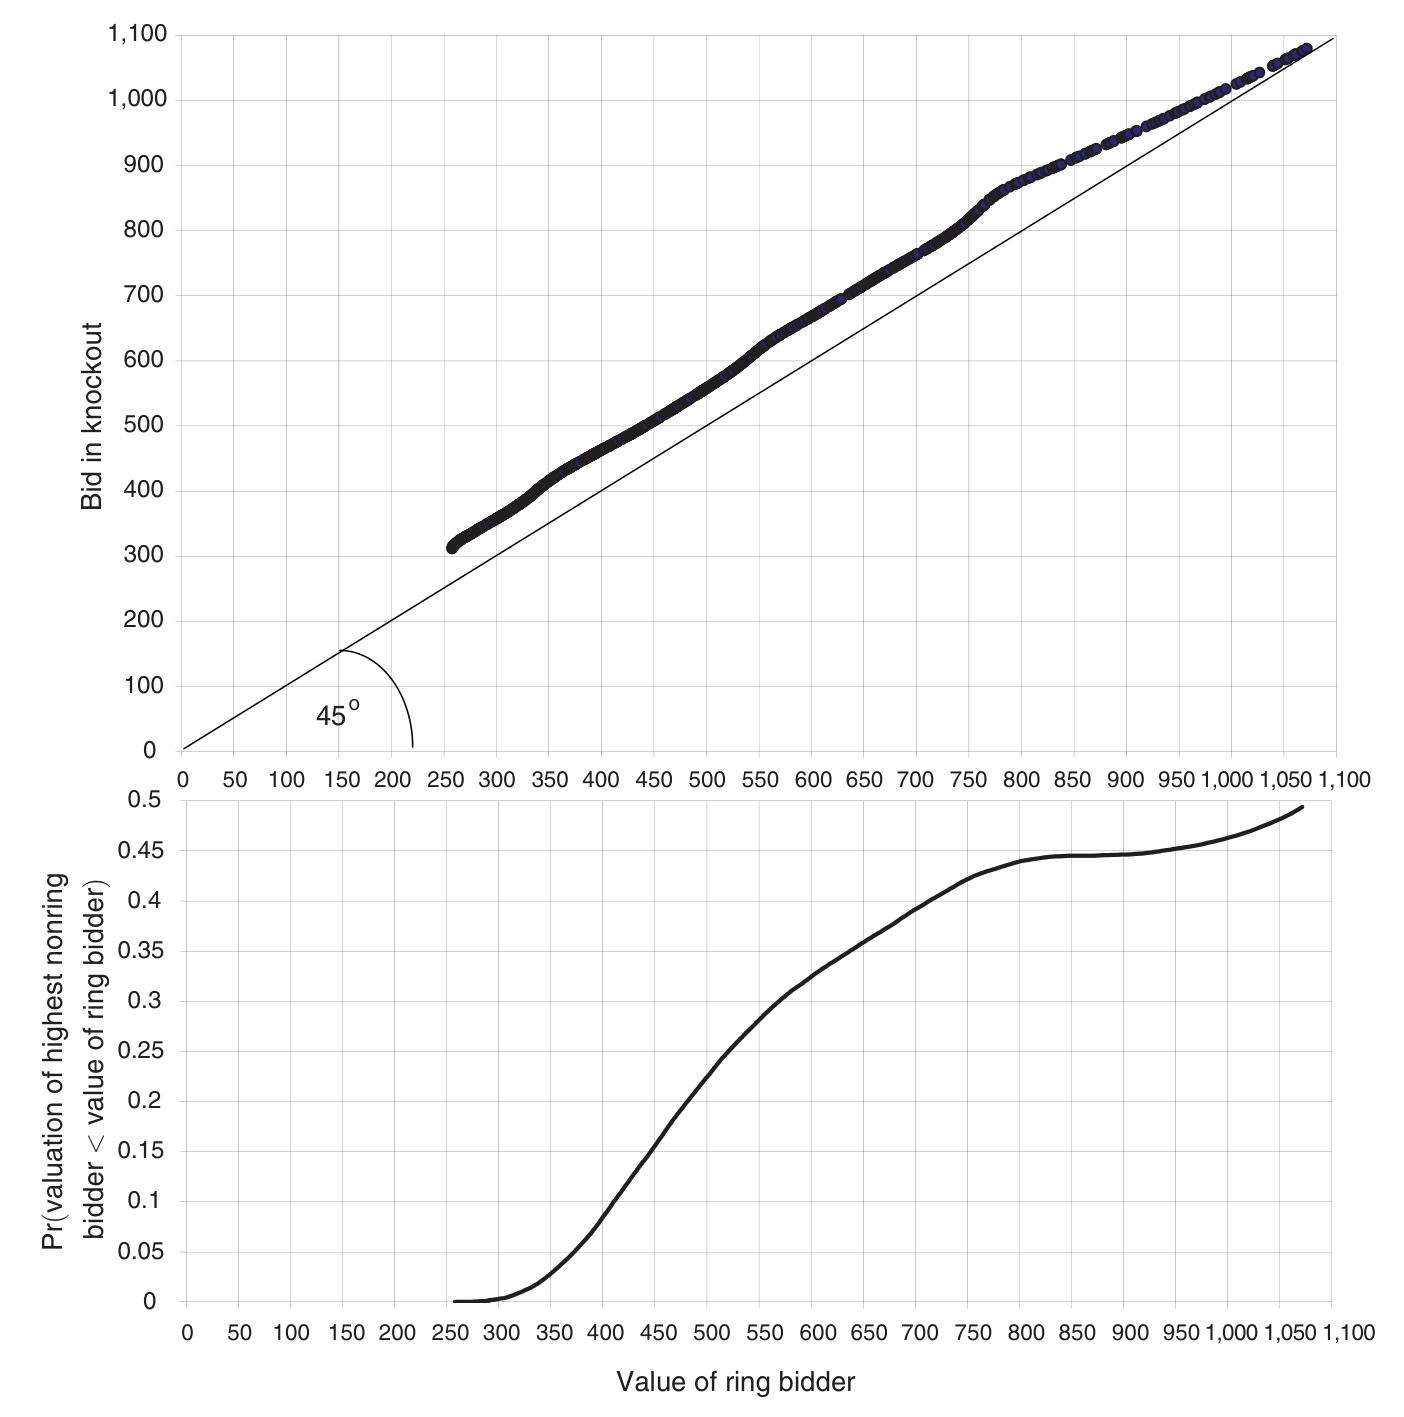
\includegraphics[width=0.86\textwidth]{figures/ch13/asker2010_fig2.png}
\caption{Estimated knockout bid function of a strong member in the model with unobserved lot heterogeneity
(top), and the probability that the highest outside value lies below the member's value (bottom). The bid function
is constructed with a common component of 520 and a 70 percent chance of facing another strong member. Source:
\citet{Asker2010}, Figure 2.}
\label{fig:13-asker-f2}
\end{figure}

\casehead{Damages to sellers}
\Cref{tab:13-asker-t7} reproduces Asker's Table 7. In the data, mean naive damages on lots the ring won are \$67
among two-bidder knockouts. The model with unobserved heterogeneity predicts \$74, and the model without it
predicts \$150. Without a common component, simulated bids vary too much within lots. Both models match the
ring's win rate well, at 0.34 and 0.37 against 0.36 in the data, although the intervals are wide. With
unobserved heterogeneity, mean true damages per ring win are \$36.99 under U.B. and \$26.50 under L.B. These are
about half and about a third of the model's naive damages of \$74.21. The 90 percent confidence intervals for the
ratio of true to naive damages are $[0.38,0.69]$ under U.B. and $[0.25,0.63]$ under L.B. \citep[footnote
47]{Asker2010}. Ignoring unobserved heterogeneity raises true damages to \$105.74 and \$99.15.

\begin{table}[htbp]
\centering
\caption{Damages to the seller}
\label{tab:13-asker-t7}
\footnotesize
\setlength{\tabcolsep}{4pt}
\begin{threeparttable}
\begin{tabular}{@{}llrrrrrr@{}}
\toprule
 & & \multicolumn{3}{c}{\makecell{With unobserved\\heterogeneity}} & \multicolumn{3}{c}{\makecell{No unobserved\\heterogeneity}} \\
\cmidrule(lr){3-5}\cmidrule(l){6-8}
 & & & \multicolumn{2}{c}{90\% interval} & & \multicolumn{2}{c}{90\% interval} \\
\cmidrule(lr){4-5}\cmidrule(l){7-8}
 & Assumption & Point & Lower & Upper & Point & Lower & Upper \\
\midrule
Mean naive damages (\$) & & 74.21 & 49.10 & 152.74 & 149.53 & 93.40 & 197.74 \\[2pt]
Mean damages (\$) & U.B. & 36.99 & 23.47 & 81.88 & 105.74 & 51.99 & 141.75 \\
 & L.B. & 26.50 & 16.09 & 73.87 & 99.15 & 44.38 & 136.20 \\[2pt]
Mean damage ratio & U.B. & 0.96 & 0.91 & 0.98 & 0.88 & 0.84 & 0.93 \\
 & L.B. & 0.97 & 0.93 & 0.98 & 0.89 & 0.85 & 0.95 \\[2pt]
Share with $P_r>P_c$ & U.B. & 0.00 & 0.00 & 0.00 & 0.00 & 0.00 & 0.00 \\
 & L.B. & 0.19 & 0.04 & 0.21 & 0.097 & 0.040 & 0.17 \\[2pt]
Mean damage ratio ($P_r>P_c$) & L.B. & 1.07 & 1.02 & 1.13 & 1.10 & 1.04 & 1.25 \\[2pt]
Share with $P_r<P_c$ & U.B. & 0.27 & 0.17 & 0.39 & 0.34 & 0.23 & 0.43 \\
 & L.B. & 0.27 & 0.17 & 0.39 & 0.34 & 0.23 & 0.43 \\[2pt]
Mean damage ratio ($P_r<P_c$) & U.B. & 0.83 & 0.74 & 0.88 & 0.64 & 0.57 & 0.74 \\
 & L.B. & 0.83 & 0.74 & 0.88 & 0.64 & 0.57 & 0.74 \\[2pt]
Share with $P_r=P_c$ & U.B. & 0.73 & 0.61 & 0.83 & 0.66 & 0.57 & 0.77 \\
 & L.B. & 0.54 & 0.46 & 0.73 & 0.57 & 0.46 & 0.68 \\[2pt]
Share of target auctions won & & 0.34 & 0.08 & 0.49 & 0.37 & 0.18 & 0.45 \\
\bottomrule
\end{tabular}
\begin{tablenotes}\footnotesize
\item Notes: Means are over target auctions the ring won unless further conditioned. The damage ratio is the price
the seller receives with the ring, $P_r$, divided by the competitive price, $P_c$. U.B. and L.B. are the upper- and
lower-bound assumptions on the second-highest outside value. Each model uses 100,000 simulated auctions. Intervals
are bootstrapped with 5,000 replications. Source: \citet[Table 7]{Asker2010}.
\end{tablenotes}
\end{threeparttable}
\end{table}

The rest of the table decomposes the ring's wins. Sellers were harmed in 27 percent of them, and in those cases
the ring lowered the price by 17 percent on average. These figures are the same under both assumptions, as the
counterfactual analysis implies. Under L.B., sellers gained in 19 percent of ring wins, with prices 7 percent
higher. In those auctions the overbidding in the knockout carried into the target auction. There is also an
unmeasured benefit to sellers. When an outside bidder wins, the ring's inflated limit can raise the price it pays,
so the damage estimates overstate sellers' losses.

\casehead{Damages to bidders outside the ring}
\Cref{tab:13-asker-t8to10} collects Asker's Tables 8 to 10. Under L.B., 19 percent of ring wins misallocate the lot
to the ring. Damages from misallocation average \$10.48 per ring win, 40 percent of the sellers' L.B. damages.
Price inflation costs outside winners \$104.20 per auction the ring loses. That figure is an upper bound, since
L.B. imposes the damage in every lost auction. In the raw data, the target price equals the highest knockout bid
in 11.5 percent of the auctions the ring loses. The ring also loses about twice as often as it wins. Asker
therefore deflates the \$104.20 by a factor of five, to a little over \$20 per ring win. Adding misallocation, he
concludes that outside bidders' damages are likely at least as large as sellers'. Price inflation is a transfer
from outside bidders to sellers, so it lowers sellers' damages by the same amount it raises outside bidders'
\citep[pp.~753--754]{Asker2010}.

\begin{table}[htbp]
\centering
\caption{Damages to outside bidders, efficiency and returns to the ring}
\label{tab:13-asker-t8to10}
\footnotesize
\setlength{\tabcolsep}{4pt}
\begin{threeparttable}
\begin{tabular}{@{}lrrrrrr@{}}
\toprule
 & \multicolumn{3}{c}{\makecell{With unobserved\\heterogeneity}} & \multicolumn{3}{c}{\makecell{No unobserved\\heterogeneity}} \\
\cmidrule(lr){2-4}\cmidrule(l){5-7}
 & Point & Lower & Upper & Point & Lower & Upper \\
\midrule
\multicolumn{7}{@{}l}{\textit{Damages to outside bidders (Table 8, L.B.)}} \\
Share of target auctions ring won & 0.34 & 0.08 & 0.49 & 0.37 & 0.18 & 0.45 \\
Share of ring wins with misallocation & 0.19 & 0.04 & 0.21 & 0.10 & 0.04 & 0.17 \\
Misallocation damages per ring win (\$) & 10.48 & 1.18 & 15.31 & 6.60 & 1.67 & 12.68 \\
Price inflation damages per ring loss (\$) & 104.20 & 70.34 & 142.76 & 113.49 & 90.82 & 135.43 \\[2pt]
\multicolumn{7}{@{}l}{\textit{Efficiency (Table 9)}} \\
Mean efficiency loss per ring win (\$) & 10.56 & 1.22 & 15.40 & 6.60 & 1.68 & 12.69 \\
Proportional loss: ring active & 0.004 & 0.0002 & 0.006 & 0.003 & 0.0005 & 0.006 \\
Proportional loss: no ring bidders & 0.08 & 0.02 & 0.13 & 0.14 & 0.07 & 0.19 \\
Proportional loss: only ring bidders & 0.29 & 0.20 & 0.42 & 0.38 & 0.29 & 0.55 \\[2pt]
\multicolumn{7}{@{}l}{\textit{Returns to the ring per win (Table 10)}} \\
Mean naive return (\$) & 74.21 & 49.10 & 152.74 & 149.53 & 93.40 & 197.74 \\
Share of wins that harmed the ring & 0.19 & 0.04 & 0.21 & 0.097 & 0.040 & 0.17 \\
Harm (\$) & $-10.48$ & $-15.39$ & $-1.20$ & $-6.60$ & $-12.69$ & $-1.68$ \\
Benefit (\$) & 36.91 & 23.49 & 81.88 & 105.74 & 51.99 & 141.75 \\
Net return (\$) & 26.42 & 16.06 & 73.86 & 99.15 & 44.38 & 136.20 \\
Mean proportional price discount & 0.96 & 0.91 & 0.98 & 0.88 & 0.84 & 0.93 \\
\bottomrule
\end{tabular}
\begin{tablenotes}\footnotesize
\item Notes: ``Lower'' and ``Upper'' bound the 90 percent bootstrap interval (5,000 replications). Efficiency
losses in dollars are conditional on a ring win. Proportional losses average over all auctions and compare the
realized allocation with the efficient one, with a seller value of zero. ``No ring bidders'' and ``only ring
bidders'' remove the ring members or the outside bidders from the auction. Returns average over ring wins. Each
model uses 100,000 simulated auctions. Source: \citet[Tables 8--10]{Asker2010}.
\end{tablenotes}
\end{threeparttable}
\end{table}

\casehead{Efficiency}
An English auction with private values allocates efficiently, and a ring that colluded efficiently would only
change transfers \citep{GrahamMarshall1987}. This ring creates inefficiency, which is an additional economic
reason for enforcement. The loss is small. When the ring wins, the average efficiency loss is \$10.56, less than 1
percent of the value of the efficient allocation. For comparison, removing the ring members from the auction would
lower efficiency by 8 percent, and removing the outside bidders by 29 percent. The difference between the \$10.56
and the \$10.48 of misallocation damages reflects lots won by the ring but assigned to the wrong member
\citep[footnote 49]{Asker2010}. If outside bidders' damages are as large as L.B. suggests, the ring may discourage
their participation. The comparison suggests that such participation effects could cost much more than the
misallocation itself, but the data cannot measure them.

\casehead{Returns to the ring}
The ring harmed itself in 19 percent of the auctions it won, by paying more than its value. The average harm is
\$10.48 per win. The benefit from suppressing competition among members averages \$36.91, so the net return is
\$26.42 per win, and prices averaged 96 percent of the competitive level. The benefit is what an ideal cartel would
capture. By that yardstick the ring captured about 72 percent of the available surplus, since
$\frac{26.42}{36.91}=0.72$. A deposition confirms the cost: a member who left the ring in the late 1980s felt that
ring prices were so inflated that a buyer through the ring paid too much.

Strong members as a group capture \$4.64 and weak members \$21.95 of the roughly \$27 the ring earns per win
\citep[p.~756]{Asker2010}. The weak members' disproportionate share matches the raw sidepayment data of
\cref{fig:13-asker-f1}. Why did the strong members not expel them? Asker suggests a hold-up problem. An expelled
member could inform the antitrust authorities and benefit from leniency for informants (\cref{sec:13-enforcement}).

\casehead{Fit and robustness}
Asker compares simulated and observed densities with the integrated absolute error
$\int|f(x)-\hat f(x)|\,\dd x\in[0,2]$. For the density of knockout bids it is 0.192 with unobserved heterogeneity
and 0.280 without. For the ratio of the target price to the highest knockout bid it is 0.611 (0.922 without). For
the ratio to the second-highest bid it is 0.480 (0.899). For the ratio of the highest to the second-highest strong
bid it is 0.194 (0.506). For the ratio of weak to strong bids it is 0.238 (0.401). The model fits worst near the
point where the target price approaches the highest knockout bid. Asker attributes the misfit to estimating from
marginal distributions and to the strong independence assumptions. A second concern is that two-bidder knockouts
are a selected sample. Asker therefore re-estimates the model on the half of two-bidder knockouts with the
highest propensity score for having two bidders. Damages are higher in that sample, but each point estimate lies
within the other sample's 90 percent interval \citep[pp.~756--758]{Asker2010}.

\subsection{Interpretation, critiques and contribution}\label{sec:13-asker-assessment}

\casehead{Interpretation}
The ring's gains were modest per lot, and its design gave much of them away to weak members and to overpayment.
Damages to sellers were about half of what naive comparisons suggest, because overbidding sometimes raised
prices. If the ratio of true to naive damages is used to extrapolate, sellers lost between \$207,000 and
\$269,000 in total on the lots the ring won \citep[footnote 54]{Asker2010}. Outside bidders were harmed at least as
much as sellers. This finding has a legal implication. Under the Sherman and Clayton Acts any person injured by an
antitrust violation may sue for treble damages. Asker knows of no claim against a ring brought by outside bidders,
and his estimates suggest that such claims could be large and proximate enough to succeed.

\casehead{Critiques}
The results rest on strong assumptions, several of which Asker discusses.
\begin{itemize}
\item Values are independent and private. A common-value component could change the extent of overbidding in ways
that are hard to sign.
\item Only two-bidder knockouts are used, because \cref{lem:13-asker-homog} and the closed-form inversion apply
there. Extrapolating to larger knockouts is uncertain. Damages there could be larger, since a member is more likely
to hold the second-highest value, or smaller, since overbidding and outside entry may rise.
\item Members are assumed to know the number of knockout bidders. Uncertainty about it would make bids a mixture of
two-, three- and more-bidder optimal bids \citep[footnote 52]{Asker2010}.
\item Target-auction participation is unobserved, which forces the U.B. and L.B. bounds and the assumption that the
distribution of the highest outside value does not vary with lot heterogeneity \citep[footnote 41]{Asker2010}.
\item Monotonicity of the inverse bid function is imposed through the choice of $T_n$. That choice also targets
naive damages and the win rate, which are close to the outcomes of interest.
\item The model treats each knockout as a static game. It ignores the repeated interaction that sustained the ring
for 15 to 20 years, the expulsions, and the incomplete participation that may reflect dynamic enforcement.
\item The link between the English target price and the highest outside value ignores jump bidding and bid
increments, which \citet{HaileTamer2003} show can break it. Asker reports that jump bidding was rare and bid
increments small in the auctions he attended.
\end{itemize}

\casehead{Ring design and auction design}
\citet[chs.~9--10]{MarshallMarx2012} place the stamp ring among the rings that operate in different auction
formats. In a sealed-bid procurement, a ring must police secret deviations. Members told to bid high could
otherwise undercut the designated bidder. The cast-iron pipe ring of the 1890s held a knockout before each
procurement and had the losers submit deliberately losing bids. It could monitor them because bids and bidders'
identities were read out in public (pp.~189--192). At an ascending auction where bidders see who holds the high
bid, a ring needs little more than a list of its members. Members do not bid against one another, and items won are
reallocated in a knockout after the sale. The antiques, machinery and real estate rings prosecuted in U.S.\ courts
worked this way (pp.~194--196). The stamp auctions did not reveal identities in this way, so the stamp ring collected
reports before each auction and sent a third-party agent to bid (p.~190). Records also differ across formats. A
sealed-bid auction leaves a written record of every bid, including close pairs of losing bids that may signal
collusion. An ascending auction often leaves no record of who took part or what they bid (pp.~206--207).

These differences suggest remedies (ch.~10). The more an auctioneer reveals about bidders' identities, bids and
outcomes, the easier a ring finds it to monitor its members (p.~200). Transparency rules meant to prevent
favoritism by officials can therefore help rings. In early spectrum auctions of the Federal Communications
Commission, bidders used the last digits of their bids to signal to one another. Later designs fixed the bid
increments and hid identities until the auction ended (pp.~201--202). A right of last refusal for an incumbent
supplier lets it watch rivals' bids and is pro-collusive (p.~202). Allowing bidders to register several
identities, or to bid as shills, makes deviations from a ring harder to detect (pp.~202--203). Registration that does not reveal
identities disrupts rings at ascending auctions where the identity of the high bidder is hidden (pp.~203--205).
Marshall and Marx list six measures (p.~207). Auctioneers can use sealed bids, limit the information they release
and deny incumbents a right of last refusal. They can also allow multiple bids under disguised identities, disclose
information about the item with collusion in mind, and hold auctions at long and irregular intervals. The stamp
ring's response to one auction house shows that rings react to such signals. When the house made clear that it
knew of a ring, the ring stopped bidding there (\cref{sec:13-asker-institutions}).

\casehead{Contribution}
\citet{Asker2010} offers the first detailed look at the internal mechanism of a long-lived ring with complete
records of its private auctions. Earlier studies of known cartels, such as \citet{Pesendorfer2000} on school milk,
had rich data on target auctions but could only infer the ring's workings from outcomes. The paper shows that the
overbidding incentive identified by \citet{GrahamMarshallRichard1990} is quantitatively important, that it makes
naive damages misleading, and that it shifts damages from sellers to other bidders. Methodologically, it extends
the inversion logic of \citet{GuerrePerrigneVuong2000} to a new mechanism and combines it with Kotlarski
deconvolution and a selection correction. It also connects the theory of ring design \citep{GrahamMarshall1987,
MailathZemsky1991, McAfeeMcMillan1992} with evidence on how a real ring traded efficiency for stability. Like the
Sugar Institute and the cartels of \cref{sec:13-imperfect}, the stamp ring tolerated behavior that a frictionless
theory would rule out, here the extraction of rents by weak members. Statistical methods that detect rings from bids
alone are the subject of \cref{sec:13-detection}.

\section{Detecting Collusion: Market Evidence and Tests for Bid Rigging}\label{sec:13-detection}

An outsider who suspects collusion usually sees prices, quantities or bids, and little else. This section asks
what such evidence can reveal. \Cref{sec:13-market-evidence} reviews the kinds of evidence on which a finding of
collusion can rest. They are pricing patterns, measures of price elevation, facilitating practices, structural
conditions, internal records, and the plus factors of cartels and bidding rings. The remaining subsections develop
formal tests for public procurement.

Public procurement is among the settings in which collusion is most often prosecuted, and statistical detection
methods are most developed there. A buyer, such as a highway department or a school district, solicits sealed bids for a
contract and awards it to the lowest bidder. In procurement, bid rigging (\cref{sec:13-intro}) takes the form of an
agreement among bidders about who will win a contract and at what price. \citet[p.~1]{PorterZona1993} show how common it is. Between 1982 and 1988,
bid rigging or price fixing in auction markets accounted for more than half of the criminal antitrust cases filed
by the U.S.\ Department of Justice. In school milk alone, \citet[p.~1]{PorterZona1999} count investigations in more than twenty
states and guilty pleas in at least a dozen. They also report fines above \$90 million and about ninety people sent
to jail.

The buyer observes the bids and the identities of the bidders. It does not observe their costs. A ring that knows
this can choose bids that look competitive. Detection therefore follows the strategy of the rest of this chapter.
We write down a model of noncooperative bidding, derive restrictions on observable bids, and ask whether a group
of suspected firms violates restrictions that other firms satisfy. A rejection shows that the suspected group
behaves differently. It does not by itself prove an agreement, because the model may be misspecified for that
group alone. \Cref{sec:13-detection-theory} develops the theory of such tests. \Cref{sec:13-pz93,sec:13-pz99}
apply it to highway paving on Long Island and to school milk in Ohio. Detection based on the comparison of auction
formats, as in the test for mill collusion of \citet{AtheyLevinSeira2011}, is treated in \cref{ch:auction-empirics}.
Page and table references to the two papers of Porter and Zona are to their NBER working-paper versions, and ``WP
p.'' denotes a working-paper page.

\subsection{Market evidence, plus factors and screens}\label{sec:13-market-evidence}

Detection is the central challenge in the control of coordinated price elevation \citep[p.~256]{Kaplow2013}. Firms
hide conduct that may be illegal, and an aggressive search for it produces false positives that chill competitive
behavior. This subsection asks what an outsider can infer from market evidence before we turn to the specialized
tests for procurement. It draws on two book-length treatments. \citet[chs.~10--11]{Kaplow2013} classifies the
evidence on which a finding of coordination can rest. \citet[chs.~11--12]{MarshallMarx2012} catalog the
plus factors of cartels and bidding rings. A plus factor is economic circumstantial evidence of collusion
beyond the parallel movement of prices (p.~213). \Cref{sec:12-anatomy} introduces the concept and its legal
background. Here we ask how strong each kind of evidence is and how the kinds combine.

\casehead{Parallel prices are not evidence}
Parallel movement of prices is the weakest evidence of all, because competitive markets produce it too. When the
costs of competing firms rise, their prices rise together and their quantities fall. When demand rises, prices and
quantities rise together. Competitors react alike to new technology, new regulations and shifts in tastes
\citep[p.~260]{Kaplow2013}. Kaplow compares parallel pricing to breathing. Every patient breathes, so no doctor
treats breathing as a symptom of bronchitis. Useful evidence is behavior that is consistent with coordination and
inconsistent with competition, or the reverse (p.~261). Kaplow groups such evidence into pricing patterns, measures
of price elevation and facilitating practices. We take these in turn and then consider structural conditions,
internal records and communications.

\casehead{Three phases of a collusive episode}
Kaplow separates three phases: the initiation of elevated prices, their maintenance and their breakdown (p.~261).
Each phase leaves a different pattern. At initiation, a sharp price increase is suspicious only if no concurrent
change in cost or demand can explain it. Any proposed explanation must also match the movement of quantities, as
the next proposition shows. It uses a simple competitive benchmark with price-taking firms.

\begin{proposition}[Sign restrictions on a price increase]\label{prop:13-kaplow-signs}
Let industry demand be $Q = D(p, y)$, with $D_p < 0$ and a demand shifter $y$ with $D_y > 0$ ($D$ and $y$ are
local symbols). Firm $i = 1, \dots, N$, with $N \geq 2$, has marginal cost $c_i(q_i) + \kappa_i$, where $c_i' > 0$
and $\kappa_i$ is a cost shifter. Under competition each firm takes the price as given and supplies
$q_i = s_i(p - \kappa_i)$, where $s_i$ is the inverse of $c_i$ and $s_i' = \frac{1}{c_i'} > 0$. Let
$S' = \sum_i s_i'$. Then, for small changes, the following hold.
\begin{enumerate}[label=(\roman*)]
\item A demand increase raises the price, total output and the output of every firm.
\item A common cost increase $d\kappa$ raises the price by less than $d\kappa$ and lowers total output and the
output of every firm.
\item A cost increase at firm $j$ alone raises the price and lowers total output and the output of firm $j$. It
raises the output of every other firm.
\item A coordinated price increase with $y$ and every $\kappa_i$ unchanged lowers total output. The division of
output among firms is whatever the agreement sets.
\end{enumerate}
\end{proposition}

\begin{proof}
Market clearing requires
\begin{equation*}
  D(p, y) = \sum_{i=1}^{N} s_i(p - \kappa_i) .
\end{equation*}
Differentiate both sides totally:
\begin{equation*}
  D_p\,dp + D_y\,dy = \sum_{i} s_i'\,(dp - d\kappa_i) .
\end{equation*}
Collect the terms in $dp$ and divide by $S' - D_p > 0$:
\begin{equation}\label{eq:13-kaplow-dp}
  dp = \frac{D_y\,dy + \sum_i s_i'\,d\kappa_i}{S' - D_p} .
\end{equation}
(i) With $d\kappa_i = 0$ for all $i$, \eqref{eq:13-kaplow-dp} gives $dp = \frac{D_y\,dy}{S' - D_p} > 0$, and then
$dq_i = s_i'\,dp > 0$ for every $i$.
(ii) With $d\kappa_i = d\kappa > 0$ for all $i$, $dp = \frac{S'}{S' - D_p}\,d\kappa$. The factor lies strictly
between 0 and 1 because $-D_p > 0$, so $0 < dp < d\kappa$. Then $dq_i = s_i'(dp - d\kappa) < 0$ for every $i$.
(iii) With only $d\kappa_j > 0$, $dp = \frac{s_j'}{S' - D_p}\,d\kappa_j$. The factor lies strictly between 0 and 1
because $s_j' < S' - D_p$. Hence $dq_j = s_j'(dp - d\kappa_j) < 0$ and $dq_i = s_i'\,dp > 0$ for $i \neq j$. In
(ii) and (iii) total output changes by $dQ = D_p\,dp < 0$.
(iv) Demand slopes down, so $D(p^1, y) < D(p^0, y)$ for any $p^1 > p^0$.
\end{proof}

\Cref{tab:13-kaplow-signs} collects the predictions. The limit of constant marginal cost, $s_i' \to \infty$,
sharpens them. A demand increase then leaves the price unchanged, and a common cost increase passes through in
full. These are the predictions behind the conduct tests of \cref{ch:conduct} \citep[pp.~273--274]{Kaplow2013}. A
common cost shock is the hardest alternative to rule out, because it moves price and output in the same directions
as coordination. Two checks remain. Cost increases can be measured in input markets, and cost shocks that hit firms
unequally reallocate output under competition (p.~262). Under coordination, firm-specific cost shocks reallocate
less output, because the agreement fixes shares (p.~274).

\begin{table}[htbp]
\centering
\caption{What a price increase implies for quantities under competition and under coordination}
\label{tab:13-kaplow-signs}
\footnotesize
\begin{tabularx}{\textwidth}{@{}>{\raggedright\arraybackslash}p{2.6cm}>{\raggedright\arraybackslash}X>{\raggedright\arraybackslash}p{1.8cm}>{\raggedright\arraybackslash}X>{\raggedright\arraybackslash}X@{}}
\toprule
Source of the increase & Price & Industry output & Output across firms & Check that separates it from coordination\\
\midrule
Demand increase & Rises (unchanged if marginal cost is constant) & Rises & Every firm expands & Output
rises\\
\addlinespace
Common cost increase & Rises by less than the cost (by the full cost if marginal cost is constant) & Falls &
Every firm contracts & Measured input prices\\
\addlinespace
Cost increase at one firm & Rises a little & Falls & Output shifts away from the affected firm & Reallocation of
output\\
\addlinespace
Coordinated elevation & Rises & Falls & Set by the agreement, little reallocation & No matching change in cost or
demand\\
\bottomrule
\end{tabularx}

\smallskip
\begin{minipage}{0.95\textwidth}\footnotesize
Notes: Our summary of \cref{prop:13-kaplow-signs} and of \citet[pp.~260--262 and 273--274]{Kaplow2013}.
\end{minipage}
\end{table}

\casehead{Initiation}
Coordinated increases need not be sudden. Firms that do not fully trust one another may raise prices in small
steps, and a leader may move cautiously while it waits for rivals to follow. Kaplow argues that such signaling can
make coordination easier to infer (pp.~262--263). A sequence of announced moves that cost and demand cannot explain
is more telling than a single jump. Sophisticated firms can also spread increases over time, or time them to
coincide with cost events that are hard to measure (pp.~263--264). The price announcements of the vitamins cartel
show both sides. Compared with the period before 1985, the cartel's announcements were more frequent, came at
regular intervals and involved modest individual increases \citep[pp.~221--222]{MarshallMarx2012}. They were
usually joint, with one firm leading and the others matching within about a week. Firms other than the market
leader, Roche, often led joint announcements after 1985 and rarely did before. About 50 percent of the cartel's
announcements came well before the effective date of the increase, against 5 percent in the earlier benchmark
period (p.~222). Long lead times let the cartel test buyers' acceptance and withdraw a resisted increase before
shares were disturbed.

\casehead{Maintenance}
Coordinated prices, and perhaps market shares, tend to be stickier than competitive ones \citep[pp.~264--265]{Kaplow2013}.
Frequent adjustment requires either negotiation, which raises the risk of detection, or signaling, which risks
being misread. A firm that cuts its price because it sees demand softening may be taken for a cheater and start a
war. Competitors, by contrast, respond to changes promptly. Menu costs, the costs of changing prices as such, also
produce stickiness. They differ from coordination frictions in two ways. Menu costs apply symmetrically to
increases and decreases, and they lead firms to change prices at different times. Sluggishness caused by
coordination has neither feature (p.~265). The bromine record fits this account. Prices changed on average every
41.1 weeks during cooperation and every 11.5 weeks otherwise (\cref{sec:13-bromine}). The variance screen of
\citet{AbrantesMetzEtAl2006}, which flags periods in which prices vary unusually little, rests on the same logic.
\citet{Pesendorfer2000} finds more stable market shares in a bidding ring that did not use sidepayments than in one
that did \citep[p.~264, note~17]{Kaplow2013}.

\casehead{Breakdown}
Sudden, sharp price cuts are as suspicious as sudden increases. If prices fall steeply without an exogenous change
of matching size, the earlier price was a coordinated one \citep[p.~265]{Kaplow2013}. Price wars thus reveal past
collusion, as the railroad and bromine records showed (\cref{sec:13-jec,sec:13-bromine}). Using wars as evidence
creates a danger that the targeting of increases does not. A penalty for price cuts may deter the cuts themselves
and so raise prices. Kaplow replies that the threat of punishment is a necessary condition for collusion, so a
policy that makes wars costly can deter collusion itself (p.~266). Kaplow adds that the problem is more
complicated still (p.~266). Firms might respond
with less sensitive triggers or shorter wars, which leave prices elevated and give buyers rarer relief. Kaplow
therefore suggests leniency, immunity or even rewards for the first price cutter, with full sanctions for the
firms that retaliate (pp.~266--267). The next example shows why one proposal of this kind would fail.

\begin{example}[How large must a price cut be to pay?]\label{ex:13-price-freeze}
\citet[pp.~267--268, note~22]{Kaplow2013} discusses a proposal by Sagi. In selected industries, a price cut
of at least 20 percent would trigger a six-month freeze of all prices, and a cut of at least 10 percent a
three-month freeze. Rivals could not retaliate during the freeze, so the first price cutter would gain. Kaplow's
arithmetic shows how much capacity such a gain requires. Let marginal cost be a constant $c$ and the collusive
price $(1 + m)c$, so that $m$ is the elevation of price above marginal cost. A member sells $q$ at the collusive
price and earns $\pi = mcq$ per period. It cuts its price by the fraction $x$ and multiplies its output by $k$. Its
profit becomes
\begin{equation*}
  \pi^{\mathrm{cut}} = k\,q\,\bigl[(1 - x)(1 + m) - 1\bigr]\,c .
\end{equation*}
Suppose the cut must recover $R$ periods of collusive profit, so that it breaks even when $\pi^{\mathrm{cut}} = R\pi$.
Dividing both sides by $cq$ gives the break-even condition
\begin{equation}\label{eq:13-freeze-breakeven}
  k\bigl[(1 - x)(1 + m) - 1\bigr] = Rm .
\end{equation}
In the short run, $R = 1$. Expand the left side of \eqref{eq:13-freeze-breakeven} and collect the terms in $m$:
\begin{align*}
  k(1 - x)(1 + m) - k &= m ,\\
  m\bigl[k(1 - x) - 1\bigr] &= k - k(1 - x) = kx ,\\
  m &= \frac{kx}{k(1 - x) - 1} .
\end{align*}
With $k = 2$ and $x = 0.2$, $m = \frac{0.4}{1.6 - 1} = \frac{2}{3}$. A firm that can double its output at once breaks
even on a 20 percent cut only if the collusive price exceeds marginal cost by two thirds. The cut takes the price
from $\frac{5}{3}c$ to $\frac{4}{3}c$, which halves the margin while output doubles. With $k = 1.5$, the same formula
gives $m = \frac{0.3}{1.2 - 1} = 1.5$, so the price must exceed marginal cost by 150 percent.

Now suppose a 10 percent cut triggers a three-month freeze, after which collusion collapses and eight quarters of
elevated prices are lost. Kaplow ignores discounting and requires the profit of the freeze quarter to cover the
eight lost quarters, so $R = 8$ and $x = 0.1$. Solving \eqref{eq:13-freeze-breakeven} for $k$ gives
\begin{equation*}
  k = \frac{8m}{0.9(1 + m) - 1} = \frac{8m}{0.9m - 0.1} .
\end{equation*}
The required factor falls as $m$ rises and approaches $\frac{8}{0.9} \approx 8.9$ as $m$ grows large. Kaplow's
``almost ninefold'' output increase is this limit (our reading). The limit treats the margin as falling by the same
10 percent as the price. For finite $m$ the margin falls by more, so the limit is a lower bound. At
$m = \frac{2}{3}$ the requirement is 10.7 (our computation). A firm with a
25 percent share would need a share above 200 percent. Kaplow concludes that the proposal provides nowhere near the
desired incentive to cut prices, and that generous treatment of the first price cutter under ordinary enforcement
is more promising.
\end{example}

\casehead{Evidence of price elevation}
A second family of evidence asks whether current prices exceed marginal cost \citep[pp.~269--275]{Kaplow2013}.
Elevation alone does not show coordination, because a single firm with market power also prices above cost
(p.~269). A direct comparison of price with measured marginal cost is simple in logic and hard in practice. The
analyst must decide which costs are variable and how to allocate joint costs, and average cost is easier to
measure than marginal cost. Capacity creates a trap. Suppose marginal cost is low over most of a firm's output
range and rises steeply near capacity. A firm producing near capacity and pricing at marginal cost then sets a
price well above average cost, and it appears to elevate price when it does not (p.~270). Such errors produce
false positives. Kaplow suggests that enforcers treat more costs as variable and require a larger measured gap.

Comparisons across markets avoid measuring the level of marginal cost. Price is at least marginal cost in every
market, so a higher price in one market is supracompetitive to the extent that cost differences do not explain it
(p.~271). Price discrimination gives a sharper bound, as the next remark shows.

\begin{remark}[Price discrimination bounds the margin]\label{rem:13-discrimination-bound}
Suppose a seller with marginal cost $mc$ sells the same good to two groups of buyers at prices $p_L < p_H$, and
serving the two groups costs the same. The seller would not sell to the low-price group below cost, so
$p_L \geq mc$. Subtract both sides from $p_H$ and divide by $p_H$:
\begin{equation*}
  p_H - mc \;\geq\; p_H - p_L , \qquad \frac{p_H - mc}{p_H} \;\geq\; \frac{p_H - p_L}{p_H} .
\end{equation*}
The Lerner index of the high-price sale is at least the proportional price gap \citep[pp.~271--272]{Kaplow2013}.
The bound applies to negotiated discounts as well as to posted prices. Buyers who obtain large discounts reveal that
other buyers pay well above marginal cost (p.~272, note~33). Two caveats apply. Some price dispersion arises from
buyers' imperfect information, and a highly successful cartel may even reduce dispersion by suppressing secret
discounts (p.~272, note~34).
\end{remark}

Two further sources complete the list. Econometric conduct tests ask whether prices respond to shifts in demand
and cost as competition or as monopoly would predict (pp.~273--274). \Cref{ch:conduct} develops these tests, and
\cref{prop:13-obs-equiv} states their main limit. Entry also carries information (pp.~274--275). If fringe firms
enter or expand while incumbents have unused capacity, prices are probably elevated. A steep fall in price and a
rise in output after entry reveal earlier supracompetitive pricing, much as a price war does. A failure of price to
fall when a key patent expires may also indicate coordination (p.~275, note~45).

\casehead{Facilitating practices}
A facilitating practice (\cref{sec:13-intro}) can matter in two ways \citep[pp.~276--277]{Kaplow2013}. Its use
supports an inference of coordination when no other plausible explanation for it exists. The practice can also be
prohibited itself, which punishes attempts when success is hard to prove. Kaplow examines three groups of practices
(pp.~277--285). The first improves mutual understanding through advance price announcements, exchanges of prices
through trade associations and audits of invoices. More than 150 price-exchange agreements arose in Britain within
a few years after overt price fixing was declared illegal (p.~278, note~53). Kaplow stresses the firms' own
incentives. Helping buyers find discounts would undercut a cartel, while helping sellers spot cheaters would
sustain it. If firms in an industry conducive to coordination make prices more open, the second motive is the
likely one (p.~279). Exchanges of demand forecasts deserve similar scrutiny where transaction prices are secret,
because demand uncertainty is then the main threat to a cartel (p.~281). The second group standardizes products,
for example through basing-point pricing (p.~282). The third changes the payoffs from cutting prices. It includes
cross-ownership, sidepayments, purchases from rivals that sold less than their share, most-favored-customer
clauses, resale price maintenance and meeting-competition clauses (pp.~283--285). \Cref{sec:12-facilitating}
analyzes several of these practices. The publication of concrete prices in \cref{sec:13-concrete}, the
fare-publishing system of \cref{sec:13-atpco} and the interfirm purchases of \cref{sec:13-imperfect-evidence} are
cases in point.

\casehead{Conducive conditions}
Evidence on whether market conditions favor coordination sharpens inference in both directions
\citep[pp.~286--288]{Kaplow2013}. Conduciveness is roughly a necessary condition for success. If conditions make
coordination nearly impossible, it is probably not taking place. The enforcer may misjudge the conditions,
however, and the firms usually understand their industry better. Strong evidence of successful coordination should
therefore override a judgment that conditions are unfavorable (p.~287). Conduciveness is not sufficient either. If
deterrence works, coordination is rare even where conditions are ideal (p.~288). Kaplow reviews the familiar
conditions briefly (pp.~289--292). A larger number of firms makes it harder to agree on a price and a punishment
and harder to detect cheating by small firms. In most prosecuted cases the firms were few and concentration high. Spare capacity raises both the gain from cheating and the ability to punish, while asymmetric capacities
hinder coordination. Many small buyers facing public prices make cheating easy to detect. A few large buyers who
place infrequent, privately negotiated orders make it hard. Public procurement usually publishes winning bids, which
may explain why so many prosecutions involve bid rigging (p.~290). Uncertain demand hides cheating when prices are
secret, and anticipated changes in demand alter the ratio of current gains from cheating to future losses
(\cref{sec:12-demand}). Product heterogeneity complicates agreement and the policing of quality and terms, and most
prosecuted cases involve homogeneous products. Similar costs, horizons and managerial backgrounds ease agreement,
and multimarket contact enlarges the scope for punishment. Finally, coordination pays only if the industry demand
elasticity and the supply response of fringe firms leave room to raise price.

The empirical basis for these factors is weaker than their familiarity suggests (pp.~292--294). Cross-section
studies find little relation between concentration and profitability. Studies within an industry find a more
robust positive relation between concentration and price, although cost differences and endogeneity complicate
them. Structural screens have a poor record. Scherer described a Federal Trade Commission effort to find
price-fixing cases from structural indicators alone as ``a resounding flop'' (pp.~294--295, note~26). Kaplow concludes
that highly unconducive conditions strongly negate success, that strong evidence of success should usually
convince, and that high conduciveness alone is a weak basis for inferring coordination (pp.~294--295). This ranking
differs from that of a rule based on communications. Under such a rule, highly conducive conditions can lower the
inference that prohibited communications were used, because the firms needed them less (p.~286, note~1).
\Cref{sec:12-kaplow} calls this the paradox of proof.

The Sherbrooke cartel of \cref{sec:13-erutku} shows why the checklist deserves limited weight.
\citet[Table~3]{ErutkuHildebrand2010} score the market against eight items derived from \citet{Stigler1964}, and
only three point toward collusion. The market had about 60 stations and a Herfindahl index below 1,800. Yet at
least 80 percent of the stations took part in the cartel. In Kaplow's terms, the wiretaps supplied strong evidence
of success, which outweighed an unfavorable reading of the conditions. The case fits his warning that outsiders
misjudge conditions that the firms themselves understand (p.~287).

\casehead{Internal evidence and communications}
For almost every market-based indicator there is matching evidence inside the firm \citep[pp.~295--302]{Kaplow2013}.
Invoices record prices and quantities. Cost and marketing data reveal what the firm believes about marginal cost
and demand. Strategy memos and notes of meetings explain why prices moved. Omissions are informative too. If a
firm's files contain no new data or discussion about demand, a demand shift is an unlikely explanation for its
price increase (p.~299). Internal evidence has two limits. A large firm's knowledge is spread over many people who
may disagree, and lawyers who anticipate litigation can sanitize records (pp.~299--300). Kaplow doubts that
sanitizing can go far. Several firms would have to fabricate consistent records of a cost shock that never
occurred, quickly and without leaving traces, and their story would have to match external data (p.~301).

Communications among firms are internal evidence of a special kind (pp.~302--306). Explicit and reliable records
of them can be decisive, especially when they refer to earlier successful price increases. Public communications,
such as sequences of advance announcements that converge on a common price, can be as revealing as secret ones
(p.~303). The absence of such records proves little, because firms hide their communications and need them least
where conditions are most conducive (p.~305). Kaplow also argues that inferring secret communications from
circumstantial evidence adds nothing. Let $C$ denote successful coordination, $E$ the observed evidence and $M$ an
unobserved communication (local symbols). By the law of total probability,
\begin{equation*}
  \Pr(C \mid E) = \Pr(C \mid E, M)\,\Pr(M \mid E) + \Pr(C \mid E, \text{not } M)\,\Pr(\text{not } M \mid E) .
\end{equation*}
Any inference about $M$ drawn from $E$ is already part of $\Pr(C \mid E)$. Only direct evidence of $M$, which
enlarges $E$, can strengthen the conclusion (p.~305, note~41).

\casehead{What decided the cases of this chapter}
Kaplow's categories classify the evidence behind the cases of \cref{tab:13-discovery}. The legal cartels, namely the
Joint Executive Committee, the Sugar Institute and the bromine pools, left internal records and open communications.
Wiretapped communications and guilty pleas proved the Quebec gasoline cartel. The lysine and citric acid cartels
were proved in criminal prosecutions and Commission decisions resting on documents and testimony, and the lysine
investigation recorded cartel meetings on video \citep[p.~197, note~46]{AskerNocke2021}. The stamp ring's knockout
records were internal evidence, found after a complaint. The Overlap and fare-publishing cases targeted the
agreements and information systems themselves. The Danish concrete episode is the one case in which market-based
evidence carried the main weight, and there the authority itself had created the transparency. Statistical tests
decided none of the prosecutions. On Long Island and in Ohio they corroborated convictions and confessions after
the fact. Porter and Zona call their tests ``poor substitutes for a wiretap or a disclosure by a dissident ring
member'' \citep[p.~210, note~78]{AskerNocke2021}.

\casehead{Plus factors}
Courts that require proof of an agreement look for plus factors (\cref{sec:12-anatomy}). A plus factor that
delivers a strong inference of collusion is a \emph{super-plus factor} \citep[p.~213]{MarshallMarx2012}. Marshall
and Marx organize plus factors by the cartel conduct that produces them, in nine groups (pp.~213--214). Pricing
structures produce price elevation, quantity restriction, steps to reduce buyers' resistance to price increases and
changes in incentives within firms. Allocation structures produce an allocation of the collusive gain and
redistributions among members. Enforcement structures produce communication and monitoring and a readiness to
abandon collusion if cheating persists. A cartel that has suppressed rivalry may finally engage in dominant-firm
conduct. Marshall and Marx measure the strength of a plus factor $F$ by the likelihood ratio
$S = \frac{\Pr[F \mid C]}{\Pr[F \mid \text{not } C]}$, where $C$ is again the event that the firms collude (p.~235). The
next remark derives the posterior probability of collusion and extends it to several plus factors.

\begin{remark}[Combining plus factors]\label{rem:13-plus-bayes}
Let $O = \frac{\Pr[\text{not } C]}{\Pr[C]}$ be the prior odds against collusion. Bayes' rule gives the posterior
odds in favor of collusion, which we then invert:
\begin{align*}
  \frac{\Pr[C \mid F]}{\Pr[\text{not } C \mid F]}
    &= \frac{\Pr[F \mid C]}{\Pr[F \mid \text{not } C]}\cdot\frac{\Pr[C]}{\Pr[\text{not } C]} = \frac{S}{O} ,\\
  \Pr[C \mid F] &= \frac{\frac{S}{O}}{1 + \frac{S}{O}} = \frac{1}{1 + \frac{O}{S}} .
\end{align*}
This is the formula of \citet[p.~235, note~42]{MarshallMarx2012}, derived as \eqref{eq:12-plus-strength} in
\cref{ch:collusion-theory}. Now suppose that $K$ plus factors $F_1, \dots, F_K$ are independent conditional on $C$
and conditional on not $C$. The likelihood ratio of the joint event is then the product of the individual ratios,
$S = \prod_{k=1}^{K} S_k$. As an illustration with our own numbers, let each plus factor have
$\Pr[F_k \mid C] = 0.6$ and $\Pr[F_k \mid \text{not } C] = 0.2$, so that $S_k = 3$, and let $\Pr[C] = 0.1$, so that
$O = 9$. One plus factor gives $\Pr[C \mid F] = \frac{1}{1 + 3} = 0.25$. Two give $\frac{1}{1 + 1} = 0.5$, and three
give $\frac{1}{1 + \frac{1}{3}} = 0.75$. Plus factors that are weak alone can thus be strong together, as Marshall
and Marx note (p.~235). Conditional independence is a strong assumption, however. Plus factors that share a cause,
such as a concentrated market structure, carry less joint information than the product suggests. Market structure
belongs in the prior odds $O$, which is where Kaplow's conducive conditions enter.
\end{remark}

Marshall and Marx list six super-plus factors (pp.~235--236), which \cref{sec:12-anatomy} reproduces. Two of them
concern market data directly. The first is a path of transaction prices that departs from the predictions of a
reliable econometric model fitted to noncollusive benchmark data. The sixth is stable market shares, customer
incumbency or geographic dominance in the face of excess capacity, while prices and profits rise. The others are
communication and information sharing, interfirm transfers, synchronized changes in sales-force incentives, and
dominant-firm conduct by firms that lack dominance. Cartels respond to detection by avoiding super-plus factors,
and avoidance is costly (pp.~236--237). A market-share cartel that forgoes year-end transfers must police shares more
tightly. One that fakes volatility in its shares can destabilize itself.

\casehead{Plus factors for bidding rings}
\citet[ch.~12]{MarshallMarx2012} adapt the analysis to auctions and procurements. Two cautions come first
(pp.~241--243). An auctioneer or procurement officer who is bribed, or who simply favors one bidder, can produce
depressed prices and skewed awards that look like collusion among bidders. A lone bidder can also enlist shill
bidders to satisfy a rule that requires a minimum number of bids. Next, a ring with $n_{\mathrm{ring}}$ of the $n$
bidders has $n_{\mathrm{ring}} - 1$ free bids to use as it wishes. Screens that look for identical bids therefore presume a careless ring
(p.~243). Two super-plus factors apply to both auction formats (p.~244). One is transfers among bidders, such as
knockout payments, or subcontracting and joint ownership that were not declared before the auction. The other is a
divergence between realized prices and the predictions of a model fitted to periods without a ring.

Other plus factors depend on the format. At an ascending auction, a ring's simplest rule is that members do not bid
against an active member (pp.~244--246). The winner and the last underbidder are then never both members. A group of
bidders who never bid against one another at meaningful prices is suspicious, although many auctions are needed to
see the pattern. Resale of the item soon after the auction to another bidder who was present signals a post-auction
knockout. An ascending auction allocates efficiently, so a ring would have to change its mechanism to avoid this
footprint. Light attendance is no super-plus factor, because some rings require members to attend. At a
sealed-bid auction, post-auction resale is weak evidence, since asymmetric bidders make the auction inefficient
even without a ring (p.~246). Losing bids unrelated to costs are evidence that a ring can avoid. The ring can ask
its members to submit rescaled versions of their noncollusive bids, all below the designated bid (pp.~246--247).
This is the adaptation that \cref{sec:13-pz93} discusses for the rank test.

Close pairs of bids are harder to avoid (p.~247). A designated bidder who bids far below its noncollusive bid tempts
other members to win secretly through a shill. In the example of Marshall and Marx, the highest-valuing member
values the item at \$100,000 and would bid \$90,000 alone, but the ring wants it to bid \$50,000. A member with
value \$60,000 whose share of the collusive gain is below \$10,000 would then gain by bidding about \$50,001 through
a shill. The ring therefore instructs the designated member to bid more, say \$65,000, and has another member bid
just below that amount. The second bid ensures that the designated member complies, because a lower bid would lose
to it. Frequent close pairs of bids then point to collusion, a pattern related to the clustering of
\cref{ex:13-gap-uniform}. Finally, a switch from ascending to sealed bidding that raises prices sharply indicates a
ring at the ascending auctions. Risk aversion also raises sealed-bid prices, but by much less (p.~248).

\begin{example}[Shill bidders in Russian oil and gas auctions]\label{ex:13-russia}
Russian ascending auctions for oil and gas leases required at least two registered bidders
\citep[pp.~248--255]{MarshallMarx2012}. The government set a reserve price and the bid increment, and the lowest
feasible bid was one increment above the reserve. Marshall and Marx have data on 620 auctions from 2004 to 2007,
complete for 121 of them. Five of these were canceled and one used criteria other than price, which leaves 115.
\Cref{tab:13-mm-russia} reproduces their Table~12.2. Auctions with two participants look different from the rest.
Of the 43 such auctions, 34 (79 percent) ended one or two increments above the reserve. With six or more
participants, every winning bid was at least 20 increments above the reserve. The average reserve price of the 34
low-priced two-bidder auctions was 27,515,294 rubles, about half the average over all 620 auctions. The authors
write ``less than half'' (p.~250). Their averages on p.~249 put the ratio at 51 percent (our computation).
Small
licenses of only regional interest could explain part of the pattern. The identities of the losers suggest more
(their Table~12.3). The 34 auctions have 24 distinct winners and 26 distinct losers. Bidder Y won six of them, each
time against bidder 1Y, which never won any of the 620 auctions. Marshall and Marx classify 13 losers as pure
shills, which bid at most once, never won a lease and never took part in an auction without their winning partner.
Two losers rotated as winner and loser, and the remaining 11 are occasional shills. The evidence fits single real
bidders who registered agents to satisfy the two-bidder rule (pp.~251--253).
\end{example}

\begin{table}[htbp]
\centering
\caption{Winning bids in Russian oil and gas lease auctions, by number of participants}\label{tab:13-mm-russia}
\small
\begin{tabular}{@{}lrrrrrr@{}}
\toprule
 & \multicolumn{5}{c}{Increments of the winning bid above the reserve} & \\
\cmidrule(lr){2-6}
Participants & 1 & 2 & 3--19 & 20--99 & 100 or more & Auctions\\
\midrule
2 & 53\% & 26\% & 9\% & 7\% & 5\% & 43\\
3 & 3\% & 9\% & 26\% & 41\% & 21\% & 34\\
4 & 8\% & 0\% & 15\% & 15\% & 62\% & 13\\
5 & 10\% & 10\% & 20\% & 10\% & 50\% & 10\\
6 or more & 0\% & 0\% & 0\% & 33\% & 67\% & 15\\
\addlinespace
All & 23\% & 13\% & 15\% & 22\% & 28\% & 115\\
\bottomrule
\end{tabular}

\smallskip
\begin{minipage}{0.86\textwidth}\footnotesize
Notes: Shares of the 115 auctions with complete data, 2004--2007. Rows sum to 100 percent up to rounding. Source:
\citet{MarshallMarx2012}, Table~12.2.
\end{minipage}
\end{table}

The remainder of this section turns some of these plus factors into formal statistical procedures for
procurement.


\subsection{The theory of detection tests}\label{sec:13-detection-theory}

\casehead{Setting and notation}
Auctions (lettings) are indexed by $t = 1, \dots, T$. The set of bidders in auction $t$ is $\mathcal{N}_t$, with
$n_t$ members. Bidder $i$ has cost $c_{it}$ of performing the contract and submits the bid $b_{it}$. Public
information $\Omega_t$ contains the characteristics of the job and each bidder's observed cost shifters $x_{it}$, a
row vector. The probability that bidder $i$ wins with bid $b$ is $\mathcal{P}_{it}(b)$. In this section $\alpha_t$
denotes an auction effect and $\beta$ a vector of coefficients, which differ from the demand parameters of the
earlier chapters. We write bidder $i$'s bid function as $s_i(\cdot)$, so that $\beta$ always denotes coefficients.

\begin{assumption}[Competitive procurement benchmark]\label{asm:13-competitive-bidding}
\leavevmode
\begin{enumerate}[label=(\alph*)]
\item The set of bidders $\mathcal{N}_t$ is common knowledge.
\item Conditional on $\Omega_t$, costs are independent across bidders, with $c_{it} \sim F_i(\cdot \mid \Omega_t)$
continuous. The distributions may differ across bidders.
\item Each bidder knows its own cost and the cost distributions of its rivals.
\item Bidders are risk neutral. The lowest bid wins and is paid its bid.
\item Bidders play a Bayesian Nash equilibrium in pure strategies $b_{it} = s_i(c_{it};\Omega_t)$, and equilibrium
bid distributions have no atoms.
\end{enumerate}
\end{assumption}

Let $G_{jt}$ be the distribution of rival $j$'s bid conditional on $\Omega_t$, with density $g_{jt}$. By parts (b)
and (e), rivals' bids are independent and ties occur with probability zero. Bidder $i$ therefore solves
\begin{equation}\label{eq:13-proc-problem}
  \max_{b}\; (b - c_{it})\,\mathcal{P}_{it}(b), \qquad \mathcal{P}_{it}(b) = \prod_{j \neq i}\bigl[1 - G_{jt}(b)\bigr].
\end{equation}
The first term is the margin if the bid wins, and the second is the probability of winning. The first-order
condition is equation~(1) of \citet{PorterZona1993}:
\begin{equation}\label{eq:13-proc-foc}
  \mathcal{P}_{it}(b_{it}) + (b_{it} - c_{it})\,\mathcal{P}'_{it}(b_{it}) = 0 .
\end{equation}
Taking logs of the product in \eqref{eq:13-proc-problem} gives
$\ln\mathcal{P}_{it}(b) = \sum_{j\neq i}\ln[1 - G_{jt}(b)]$, so that
\begin{equation*}
  \frac{\mathcal{P}'_{it}(b)}{\mathcal{P}_{it}(b)} = -\sum_{j\neq i}\frac{g_{jt}(b)}{1 - G_{jt}(b)} .
\end{equation*}
Substituting into \eqref{eq:13-proc-foc} and solving for the markup gives
\begin{equation}\label{eq:13-proc-markup}
  b_{it} - c_{it} = -\frac{\mathcal{P}_{it}(b_{it})}{\mathcal{P}'_{it}(b_{it})}
  = \left[\sum_{j\neq i}\frac{g_{jt}(b_{it})}{1 - G_{jt}(b_{it})}\right]^{-1} .
\end{equation}
The equilibrium markup is the inverse of the sum of the rivals' bid hazard rates at the bid. More rivals, or rivals
whose bids are dense near $b_{it}$, lower the markup. Equation \eqref{eq:13-proc-markup} is the procurement mirror
image of the inversion of \citet{GuerrePerrigneVuong2000} in \cref{ch:auction-empirics}. The model behind it is the
procurement auction of \cref{ch:auction-theory}.

\begin{proposition}[Restrictions implied by competitive bidding]\label{prop:13-competitive-restrictions}
Under \cref{asm:13-competitive-bidding} the following hold.
\begin{enumerate}[label=(\roman*)]
\item \emph{Monotonicity.} If $\mathcal{P}_{it}$ is strictly decreasing, each bid function $s_i(\cdot;\Omega_t)$ is
nondecreasing in own cost.
\item \emph{Conditional independence.} For $i \neq j$, the bids $b_{it}$ and $b_{jt}$ are independent conditional on
$\Omega_t$. The same holds for any decisions, such as participation, that depend only on own cost and $\Omega_t$.
\item \emph{Exchangeability.} Suppose that $F_i(\cdot\mid\Omega_t) = F(\cdot \mid x_{it}, W_t)$, where $W_t$ collects
the job characteristics, and that the equilibrium is symmetric, $s_i(c;\Omega_t) = s(c; x_{it}, X_{-i,t}, W_t)$
with $s$ symmetric in the elements of the collection $X_{-i,t}$ of rivals' covariates. Then the distribution of
$b_{it}$ given $\Omega_t$ is unchanged by any permutation of the rivals' covariates.
\item \emph{Rank order.} If all bidders in auction $t$ use the same strictly increasing bid function, the ranking of
the bids reproduces the ranking of the costs.
\end{enumerate}
\end{proposition}

\begin{proof}
(i) Take costs $c < c'$ with optimal bids $b$ and $b'$. Optimality of $b$ at $c$ and of $b'$ at $c'$ gives
\begin{align*}
  (b - c)\,\mathcal{P}(b) &\geq (b' - c)\,\mathcal{P}(b'),\\
  (b' - c')\,\mathcal{P}(b') &\geq (b - c')\,\mathcal{P}(b).
\end{align*}
Adding the two inequalities and cancelling the terms $b\mathcal{P}(b)$ and $b'\mathcal{P}(b')$ leaves
\begin{equation*}
  -c\,\mathcal{P}(b) - c'\,\mathcal{P}(b') \geq -c\,\mathcal{P}(b') - c'\,\mathcal{P}(b),
\end{equation*}
which rearranges to $(c' - c)\bigl[\mathcal{P}(b) - \mathcal{P}(b')\bigr] \geq 0$. Since $c' > c$, we get
$\mathcal{P}(b) \geq \mathcal{P}(b')$, and a strictly decreasing $\mathcal{P}$ implies $b \leq b'$.

(ii) Conditional on $\Omega_t$, the bid $b_{it} = s_i(c_{it};\Omega_t)$ is a function of $c_{it}$ alone. Functions
of independent random variables are independent.

(iii) Bidder $i$'s objective depends on its rivals only through $\mathcal{P}_{it}(b) = \prod_{j\neq i}[1 -
G(b \mid x_{jt}, X_{-j,t}, W_t)]$. Under symmetry, the factor for rival $j$ is determined by $j$'s own covariate and
the collection of everyone else's covariates. A permutation of the rivals' covariates therefore only permutes the
factors of the product, and $\mathcal{P}_{it}$ is unchanged. So is the optimal bid of every cost type, and hence the
distribution of $b_{it}$.

(iv) A strictly increasing common function preserves order.
\end{proof}

Each restriction suggests a test. Conditional independence implies that residuals from bid regressions, or from
participation equations, are uncorrelated across pairs of firms. Exchangeability implies that a firm's bid responds
in the same way to the covariates of each of its rivals. \citet{BajariYe2003} build tests of both restrictions for
highway procurement auctions. Their tests ask whether bid residuals are correlated across firms and whether a
firm's bid responds equally to the cost shifters of different rivals. The
rank-order restriction underlies the tests of \citet{PorterZona1993} developed below. The restrictions differ in
what they assume beyond \cref{asm:13-competitive-bidding}. Conditional independence holds in every equilibrium
that the assumption allows. Monotonicity holds whenever the winning probability $\mathcal{P}_{it}$ is strictly
decreasing. Exchangeability needs, in addition, a cost distribution common to all bidders given their covariates
and the symmetric equilibrium stated in (iii). The rank order needs a common strictly increasing bid function, as in a symmetric equilibrium of
a symmetric model. With asymmetric bidders it can fail under competition (\cref{rem:13-asym-ranks}). A violation of
(iii) or (iv) therefore rejects competition jointly with these symmetry and monotonicity assumptions. Some collusive schemes satisfy all four
restrictions, as we show below.

\begin{remark}[Asymmetric bidders]\label{rem:13-asym-ranks}
With asymmetric cost distributions, bidders use different bid functions, and a low-cost bidder can bid above a
high-cost rival (\cref{ch:auction-theory}). The rank restriction (iv) then fails even under competition. Rank-based
tests must therefore condition on the observables that create the asymmetry, as the covariates $x_{it}$ do in the
applications below.
\end{remark}

\casehead{What collusion changes}
Collusion in procurement takes several forms. In \emph{bid rotation}, ring members take turns winning, and often
only the designated member bids. In \emph{territorial allocation}, each member is assigned the customers or
districts near its plants, and the others stay away. In \emph{complementary bidding}, also called cover or phantom
bidding, the ring designates a winner and its bid, and other members submit higher bids designed to lose. Such bids
create the appearance of competition. A ring may also suppress bids altogether or compensate losers through
subcontracts. Each scheme violates a different restriction of \cref{prop:13-competitive-restrictions}.
\Cref{tab:13-footprints} summarizes the footprints.

\begin{table}[htbp]
\centering
\caption{Collusive schemes in procurement and the footprints they leave}\label{tab:13-footprints}
\footnotesize
\begin{tabularx}{\textwidth}{@{}>{\raggedright\arraybackslash}p{2.2cm}>{\raggedright\arraybackslash}X>{\raggedright\arraybackslash}X>{\raggedright\arraybackslash}X@{}}
\toprule
Scheme & Participation & Bid levels and ranks & Tests with power\\
\midrule
Bid rotation & Members rarely bid against each other. Submission residuals are negatively correlated. & Winning
bids inflated when no outsider bids. & Correlation of participation residuals. Hard to separate from
specialization in job types.\\
\addlinespace
Territorial allocation & Members bid near their own plants and avoid other members' areas. Negative correlation
of submission residuals. & Bids high inside the own territory, relatively low outside it. & Submission
correlations. Bid gradients in distance compared with a control group.\\
\addlinespace
Complementary bidding & Members bid together more often than observables predict. Positive correlation of
submission residuals. & Cover bids high, clustered, and unrelated to costs. Bid residuals positively correlated. &
Rank tests (\cref{prop:13-exploded-logit}). Correlation of bid residuals. Clustering of the lowest bids.\\
\addlinespace
Inclusive ring scaling all bids & Unchanged. & All bids inflated by a common factor. Ranks follow costs. & None
based on bid patterns. Requires costs, rates of return or an outside benchmark.\\
\bottomrule
\end{tabularx}

\smallskip
\begin{minipage}{0.95\textwidth}\footnotesize
Notes: Our summary of the schemes discussed by \citet{PorterZona1993,PorterZona1999} and of the restrictions in
\cref{prop:13-competitive-restrictions}.
\end{minipage}
\end{table}

\casehead{Why simple indicators mislead}
A common view treats a rotation of winners, or stable market shares, as irrefutable evidence of collusion
\citep[p.~1]{PorterZona1993}. Both can arise in competitive equilibria. \citet{Zona1986} shows that bid rotation is a competitive outcome under
decreasing returns, for example with capacity constraints. A firm that has just won carries a large backlog, faces
a high cost of one more job, and bids high on the next one. \citet{LangRosenthal1991} study a game in which firms bid
simultaneously on several contracts. Its noncooperative mixed-strategy equilibrium can produce negative correlation
between a firm's bids, which looks like rotation. Comparisons of winning bids with the buyer's
engineering estimates are also unreliable. The estimates may be built from past bids and so inherit any inflation
\citep[p.~2]{PorterZona1993}. \citet{FeinsteinBlockNold1985} model a cartel that submits cover bids close to the
winning bid in order to raise the engineers' estimates for future lettings.

The deepest limit concerns inclusive rings. If a single test were widely used, a cartel that includes every
bidder could choose its complementary bids so that the overall pattern passes the test
\citep[p.~3]{PorterZona1993}. The buyer runs an auction because it does not know costs, so any bid vector that is
consistent with some plausible cost draw is unassailable. Detection from bids alone therefore needs a group of
bidders outside the ring whose behavior serves as a benchmark.

\casehead{Bid clustering}
Phantom bids are often placed just above the designated bid. A simple screen compares the gap between the two
lowest bids in suspect and benchmark auctions. The screen must account for the number of bids, as the next example
shows.

\begin{example}[The gap between the two lowest bids]\label{ex:13-gap-uniform}
Let costs be independent and uniform on $[0,1]$, with $n$ symmetric bidders. The equilibrium bid function is
$s(c) = c + \frac{1-c}{n}$. To verify it, invert to $c = \frac{nb - 1}{n-1}$, so that a bid $b$ wins with
probability
\begin{equation*}
  \mathcal{P}(b) = \bigl[1 - c(b)\bigr]^{n-1} = \left[\frac{n(1-b)}{n-1}\right]^{n-1},
  \qquad \frac{\mathcal{P}'(b)}{\mathcal{P}(b)} = -\frac{n-1}{1-b} .
\end{equation*}
By \eqref{eq:13-proc-markup}, the optimal markup is $b - c = \frac{1-b}{n-1}$. At $b = s(c)$ we have
$1 - b = \frac{(n-1)(1-c)}{n}$, so $\frac{1-b}{n-1} = \frac{1-c}{n} = s(c) - c$, as required. The gap between the
two lowest bids is
\begin{equation*}
  b_{(2)} - b_{(1)} = \left(1 - \frac{1}{n}\right)\bigl(c_{(2)} - c_{(1)}\bigr) .
\end{equation*}
The expected spacing between consecutive order statistics of $n$ uniform draws is $\frac{1}{n+1}$ (\cref{app:math}).
Hence
\begin{equation*}
  \E\bigl[b_{(2)} - b_{(1)}\bigr] = \frac{n-1}{n(n+1)} ,
\end{equation*}
which equals 0.167 for $n = 2$ and $n = 3$, 0.150 for $n = 4$ and 0.133 for $n = 5$ (our computation, confirmed by
simulation in \texttt{pz\_checks.py}). The expected gap does not rise as bidders are added, and it falls for
$n \ge 3$. A comparison of mean gaps across
groups of auctions with different numbers of bids confounds clustering with the number of bids.
\end{example}

\casehead{Ranks and the exploded logit}
The most informative tests in \citet{PorterZona1993} use the order of the bids within an auction. They rest on a
log-linear bid rule,
\begin{equation}\label{eq:13-pz-bid}
  \ln b_{it} = \alpha_t + x_{it}\beta + \epsilon_{it}, \qquad \E[\epsilon_{it}] = 0,\quad \Var(\epsilon_{it}) = \sigma_t^2 ,
\end{equation}
which is equation~(2) of their paper. The auction effect $\alpha_t$ absorbs everything common to the bidders in
auction $t$, such as the size of the job. The error $\epsilon_{it}$ is private cost information, with a variance
that may differ across auctions. Let $\zeta$ denote a standard type-I extreme value (Gumbel) variable, with
distribution function $\exp(-e^{-z})$, mean equal to Euler's constant $\gamma_E$ and variance $\frac{\pi^2}{6}$
(\cref{ch:discrete}, \cref{app:math}). Suppose that
\begin{equation}\label{eq:13-gumbel-error}
  -\epsilon_{it} = \sigma_t\,\frac{\sqrt{6}}{\pi}\,(\zeta_{it} - \gamma_E), \qquad \zeta_{it}\ \iid ,
\end{equation}
so that $\epsilon_{it}$ has mean zero and variance $\sigma_t^2$. The lowest bid is the bid with the largest value of
$-\ln b_{it}$. Dividing $-\ln b_{it}$ by the positive constant $\sigma_t\frac{\sqrt6}{\pi}$ does not change the
order, and gives
\begin{equation}\label{eq:13-rank-index}
  \frac{\pi}{\sqrt{6}}\,\frac{-\ln b_{it}}{\sigma_t} = \alpha^{*}_t + Z_{it}\tilde\beta + \zeta_{it},
  \qquad Z_{it} = -\frac{x_{it}}{\sigma_t},\quad \tilde\beta = \frac{\pi}{\sqrt6}\,\beta ,
\end{equation}
with the auction constant $\alpha^{*}_t = -\frac{\pi}{\sqrt6}\frac{\alpha_t}{\sigma_t} - \gamma_E$. The ranking of bids
is the ranking of independent Gumbel utilities with indices $\alpha^{*}_t + Z_{it}\tilde\beta$.

\begin{proposition}[Rank-ordered (exploded) logit]\label{prop:13-exploded-logit}
Let $V_i = v_i + \zeta_i$ for $i = 1, \dots, n$, with $\zeta_i$ independent standard Gumbel variables. For any
ordering $(r_1, \dots, r_n)$ of the indices,
\begin{equation}\label{eq:13-exploded}
  \Pr\bigl(V_{r_1} > V_{r_2} > \dots > V_{r_n}\bigr) = \prod_{j=1}^{n-1}\frac{e^{v_{r_j}}}{\sum_{l=j}^{n}e^{v_{r_l}}} .
\end{equation}
Under \eqref{eq:13-pz-bid}--\eqref{eq:13-rank-index}, the probability of the observed ranking of the $n_t$ bids in
auction $t$ is therefore
\begin{equation}\label{eq:13-rank-likelihood}
  \Pr\bigl(b_{r_1 t} < b_{r_2 t} < \dots < b_{r_{n_t} t} \mid \Omega_t\bigr)
  = \prod_{j=1}^{n_t - 1}\frac{\exp(Z_{r_j t}\tilde\beta)}{\sum_{l=j}^{n_t}\exp(Z_{r_l t}\tilde\beta)} ,
\end{equation}
and the auction constant $\alpha^{*}_t$ cancels.
\end{proposition}

\begin{proof}
Define $E_i = e^{-V_i}$. For a standard Gumbel $\zeta$ and $y > 0$,
\begin{equation*}
  \Pr\bigl(e^{-\zeta} > y\bigr) = \Pr(\zeta < -\ln y) = \exp\bigl(-e^{\ln y}\bigr) = e^{-y},
\end{equation*}
so $e^{-\zeta}$ is exponential with rate one. Then $E_i = e^{-v_i}e^{-\zeta_i}$ satisfies
$\Pr(E_i > y) = \Pr(e^{-\zeta_i} > e^{v_i}y) = e^{-\lambda_i y}$ with $\lambda_i = e^{v_i}$ (a local symbol in this
proof). The $E_i$ are
independent exponential variables with rates $\lambda_i$, and the $V_i$ are in decreasing order exactly when the
$E_i$ are in increasing order. We use two properties of independent exponentials with rates $\lambda_1, \dots,
\lambda_m$ and $\Lambda = \sum_l \lambda_l$. First, the probability that $E_k$ is the smallest is
\begin{equation*}
  \Pr\Bigl(E_k < \min_{l\neq k}E_l\Bigr) = \int_0^\infty \lambda_k e^{-\lambda_k y}\prod_{l\neq k}e^{-\lambda_l y}\,dy
  = \int_0^\infty \lambda_k e^{-\Lambda y}\,dy = \frac{\lambda_k}{\Lambda} .
\end{equation*}
Second, for $y_l \geq 0$,
\begin{equation*}
  \Pr\bigl(E_k \in dm,\; E_l - E_k > y_l \text{ for all } l \neq k\bigr)
  = \lambda_k e^{-\lambda_k m}\prod_{l\neq k}e^{-\lambda_l(m + y_l)}\,dm
  = \lambda_k e^{-\Lambda m}\,dm\,\prod_{l\neq k}e^{-\lambda_l y_l} .
\end{equation*}
The joint density factors, so conditional on $E_k$ being the minimum, the excesses $E_l - E_k$ are independent
exponentials with the original rates and are independent of the minimum (memorylessness). The probability of the
ordering $E_{r_1} < E_{r_2} < \dots < E_{r_n}$ is the probability that $E_{r_1}$ is the smallest, which is
$\frac{\lambda_{r_1}}{\sum_{l=1}^{n}\lambda_{r_l}}$, times the probability that the excesses of the other $n-1$
variables are ordered $r_2, \dots, r_n$. By the second property the latter is the same problem with one variable
fewer. Repeating the argument $n-1$ times gives \eqref{eq:13-exploded} with $\lambda = e^{v}$. Applying
\eqref{eq:13-exploded} to \eqref{eq:13-rank-index}, the common factor $e^{\alpha^{*}_t}$ appears in every numerator and
every term of every denominator and cancels, which gives \eqref{eq:13-rank-likelihood}.
\end{proof}

The product in \eqref{eq:13-rank-likelihood} treats the ranking as a sequence of choices. The lowest bid is
``chosen'' from all $n_t$ bidders, the second lowest from the remaining $n_t - 1$, and so on. This
\emph{rank-ordered} or \emph{exploded logit} is due to \citet{BeggsCardellHausman1981}. Each factor is a conditional
logit with a choice set that shrinks by one, so standard multinomial logit software estimates $\tilde\beta$. The
last factor equals one and is omitted. \citet{PorterZona1993} write the product up to $n_t$, which is equivalent.

\begin{corollary}[Likelihood ratio test of equal coefficients across ranks]\label{cor:13-rank-lr}
Write the log likelihood of the rankings as
\begin{equation}\label{eq:13-rank-loglik}
  \ell(\tilde\beta) = \underbrace{\sum_{t}\Bigl[Z_{r_1 t}\tilde\beta - \ln\sum_{l=1}^{n_t}e^{Z_{r_l t}\tilde\beta}\Bigr]}_{\ell^{\mathrm{low}}(\tilde\beta)}
  + \underbrace{\sum_{t}\sum_{j=2}^{n_t - 1}\Bigl[Z_{r_j t}\tilde\beta - \ln\sum_{l=j}^{n_t}e^{Z_{r_l t}\tilde\beta}\Bigr]}_{\ell^{\mathrm{high}}(\tilde\beta)} .
\end{equation}
Allow the coefficients to differ between the lowest rank and the higher ranks. Under the null hypothesis that the
whole ranking follows \eqref{eq:13-rank-likelihood},
\begin{equation}\label{eq:13-rank-lrstat}
  LR = 2\Bigl[\ell^{\mathrm{low}}(\hat\beta^{\mathrm{low}}) + \ell^{\mathrm{high}}(\hat\beta^{\mathrm{high}}) - \ell(\hat\beta)\Bigr]
  \xrightarrow{d} \chi^2_K ,
\end{equation}
where $K$ is the number of coefficients, $\hat\beta^{\mathrm{low}}$ and $\hat\beta^{\mathrm{high}}$ maximize
$\ell^{\mathrm{low}}$ and $\ell^{\mathrm{high}}$ separately, and $\hat\beta$ maximizes $\ell$.
\end{corollary}

\begin{proof}
The unrestricted log likelihood $\ell^{\mathrm{low}}(\tilde\beta^{\mathrm{low}}) + \ell^{\mathrm{high}}(\tilde\beta^{\mathrm{high}})$ is
additively separable in the two parameter vectors, so it is maximized by maximizing each part separately. The null
hypothesis imposes the $K$ restrictions $\tilde\beta^{\mathrm{low}} = \tilde\beta^{\mathrm{high}}$, and the standard
likelihood ratio theorem applies (\cref{app:econometrics}).
\end{proof}

The test has power against complementary bidding for a simple reason. Suppose a ring designates its lowest-cost
member, which bids to beat the outsiders, and places the other members' bids above it without regard to cost. The
lowest ring bid then follows costs, so $\tilde\beta^{\mathrm{low}} = \tilde\beta$. If the higher ring bids are
ordered at random, the true probability of each higher-rank choice is $\frac{1}{n_t - j + 1}$, whatever the
covariates. The model factor reproduces this probability only at $\tilde\beta = 0$. By the information inequality,
the population maximizer of $\ell^{\mathrm{high}}$ is then $\tilde\beta^{\mathrm{high}} = 0$, and the statistic
\eqref{eq:13-rank-lrstat} grows with the number of auctions.

\Cref{fig:13-pz-sim} shows how much data the test needs. We simulate rankings from \eqref{eq:13-rank-index} with
two standardized cost shifters, $\tilde\beta = (0.5, -0.5)$, and between two and four ranked bids per auction. The
sample sizes mimic the cartel data of \citet{PorterZona1993}, with 50 auctions and about 35 higher-rank choices.
Under competitive ranking the test has the correct size, rejecting in 5.7 percent of 2,000 samples at the 5
percent level. When the higher bids are ordered at random, it rejects in 47 percent of samples with 50 auctions,
76 percent with 100 and 98 percent with 200 (our computation, \texttt{pz\_lr\_sim.py}). A rank test on a few dozen
auctions is therefore a low-power instrument, even against a stark alternative.

\begin{figure}[htbp]
\centering
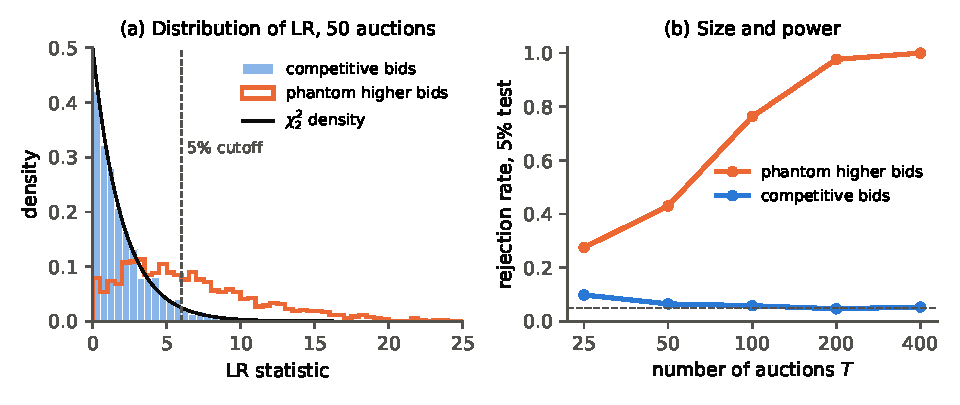
\includegraphics[width=\textwidth]{figures/ch13/pz_lr_sim.pdf}
\caption{Size and power of the rank-based test of \cref{cor:13-rank-lr} in simulated data. Panel (a) shows the
distribution of the likelihood ratio statistic over 2,000 samples of 50 auctions. The bars are for rankings that
follow the exploded logit, the line for rankings in which the nonwinning bids are in random order, and the curve is
the $\chi^2_2$ density. Panel (b) shows the rejection rates of the 5 percent test against the number of auctions,
with 600 samples per point. Our simulation, with sample sizes that mimic \citet{PorterZona1993}, Table~6.}
\label{fig:13-pz-sim}
\end{figure}

\subsection{Long Island highway paving: Porter and Zona (1993)}\label{sec:13-pz93}

\casehead{The question}
Can econometric tests detect a bid-rigging ring from public bid data when the ring includes only some of the
bidders? \citet{PorterZona1993} study contracts let by the New York State Department of Transportation (DOT) on
Long Island between April 1979 and March 1985. A group of firms bidding there was later named in bid-rigging suits.
The paper proposes test procedures and stresses their limits. In the authors' words, the tests ``will be poor
substitutes for a wiretap or a disclosure by a dissident ring member'' \citep[p.~1]{PorterZona1993}. They are,
however, better founded than the view that bid rotation or stable shares prove collusion.

\casehead{Institutional setting}
The DOT must award each highway contract to the lowest responsible bidder. It announces upcoming lettings in a
``Notice of Highway Lettings,'' and interested firms request plans and specifications. A ``Plan Buyers List'' of
the firms that bought plans for each job is distributed to subscribers, so each firm knows its potential rivals in
advance. On the day of the letting, sealed bids are opened and every bid and bidder is announced. The DOT checks
the low bid against its own cost estimate and then awards the contract. From April 1979 through March 1985 it
awarded about \$120 million of contracts in Nassau and Suffolk Counties, in 1969 dollars. There were 186 contracts,
161 of them below \$1 million. Sixty-six firms bid on at least one of the small contracts, but only 22 bid on jobs
above \$1 million. Four firms submitted 45 percent of the bids on those large jobs.

The authors list features of the market that facilitate collusion (WP pp.~8--12). The product is homogeneous,
because the contract defines the output, so a ring need only coordinate on price. Public announcement of bids and
bidders reveals any undercutting, and the plan buyers lists make the set of potential bidders common knowledge.
Demand was almost perfectly inelastic. With one exception, every contract was awarded to the low bidder whatever
the DOT's cost estimate, so any inflation of winning bids became profit. The exception is telling. In February
1983 the DOT solicited bids to resurface 0.8 miles of road, received eight bids with a low bid of about \$4 million,
and declined to award. When the job was rebid in May 1983, the low bid was 20 percent higher and came from the same
firm. A third letting in February 1984 drew three bids from firms that had bid both times before. The low bid was
about 10 percent above the second letting and 30 percent above the first, and the ranking of bidders never changed.
The contract had not been awarded by 1987.

Entry was difficult. Large jobs require batch concrete and asphalt plants, which incumbents owned, and newspaper
accounts report that union leaders discouraged outside bidders. Joint bids were allowed, which gave firms reasons to
communicate. Large jobs were let regularly, early each year, and usually one at a time. Such spacing limits what a
defector can earn before others retaliate. Firms bought inputs in the same markets, used the same technology and
employed members of the same unions, although backlogs and equipment differed.

\casehead{The candidate cartel}
In 1984 one of the five largest firms in the two counties was convicted in federal court of rigging bids on a Long
Island highway project that predates the sample. Four other firms were named as unindicted co-conspirators, and all
five were named in separate suits by New York State or Suffolk County. Each suit concerned a single job. The paper
treats these five firms, called Firms 2, 3, 4, 10 and 14, as a candidate ``cartel'' that may have operated in any
letting. The other bidders are called ``competitive.'' The cartel firms submitted 54 percent of the bids on larger
jobs and won 37 percent of all contracts. They also bid jointly at times (Table~1). Firms 4 and 2 did so in February
1980, with a winning bid of \$5.3 million. Firms 3 and 14 did so in June 1980 (\$7.3 million) and January 1982
(\$4.0 million), and Firms 3, 4 and 8 in November 1984 (\$8.0 million).

\Cref{tab:13-pz-cartel} shows that cartel firms regularly bid against each other on paving jobs. When Firm 2 bid,
another cartel firm also bid 88 percent of the time, and every bid by Firm 14 was accompanied by another cartel bid.
Insiders described the mechanism to a newspaper. Firms met around a conference table to review upcoming contracts
and decide ``who should get this one.'' Then ``the contractors who were tagged to be the low bidders would work out
their bid figures,'' and ``the rest of the contractors would then come up with higher bids'' \citep[p.~17]{PorterZona1993}.
Union representatives allegedly attended, communicated the low bids afterwards, and received a kickback of one percent of
the low bid on jobs won. This is a complementary bidding scheme, and the tests below are designed to detect it.

\begin{table}[htbp]
\centering
\caption{Bidding by the candidate cartel on Long Island paving jobs}\label{tab:13-pz-cartel}
\small
\begin{tabular}{@{}lccccc@{\hspace{2em}}cc@{}}
\toprule
 & \multicolumn{5}{c}{Bids also submitted by} & \multicolumn{2}{c}{Pr(another cartel bid), \%}\\
\cmidrule(lr){2-6}\cmidrule(l){7-8}
 & Firm 2 & Firm 3 & Firm 4 & Firm 10 & Firm 14 & Paving & Nonpaving\\
\midrule
Firm 2  & 48 & 37 & 34 & 1 & 11 & 88 & 75\\
Firm 3  & 37 & 86 & 56 & 1 & 15 & 79 & 55\\
Firm 4  & 34 & 56 & 71 & 2 & 14 & 89 & 80\\
Firm 10 & 1  & 1  & 2  & 3 & 1  & 67 & NA\\
Firm 14 & 11 & 15 & 14 & 1 & 20 & 100 & NA\\
\bottomrule
\end{tabular}

\smallskip
\begin{minipage}{0.92\textwidth}\footnotesize
Notes: Left panel, \citet{PorterZona1993}, Table~2: number of paving jobs on which the row firm and the column firm
both submitted individual bids. Diagonal entries are the row firm's total number of bids. Joint bids are excluded.
Right panel, Table~3: percentage of the row firm's bids on which at least one other cartel firm also bid. NA: not
available. NBER working-paper version.
\end{minipage}
\end{table}

\casehead{Two conventional indicators}
The first indicator is the stability of market shares. On paving jobs the cartel firms' annual shares varied
substantially, and Firm 10 stopped bidding early in the sample (it bid only three times). No pattern of rotation is
apparent. Newspaper accounts nonetheless report stable shares in state highway and sewer work for more than a
decade, on many jobs outside the sample. Shares on paving alone would thus give an unwarranted impression of
competition.

The second indicator is the dispersion of bids within a job. The 116 paving jobs received 347 competitive bids on
103 jobs and 228 cartel bids on 109 jobs. On the 76 jobs with at least two cartel bids, the second-lowest cartel bid
exceeded the lowest by 4.96 percent on average, measured as the mean difference in log bids. On the 75 jobs with at
least two competitive bids, the corresponding figure is 6.25 percent. Competitive bids are more numerous per job,
and \cref{ex:13-gap-uniform} shows that more bids shrink the expected gap. The comparison therefore understates
how much tighter the cartel bids are. The pattern resembles the clustering found by \citet{FeinsteinBlockNold1985}
in North Carolina highway contracts.

\casehead{Data}
The analysis uses contracts that involve paving, where the facilitating features are strongest. Mowing, painting
and traffic signal contracts are excluded. The 116 paving projects received 575 bids. Joint bids, under 2 percent of
paving bids, are dropped. Estimating the auction-specific variance $\sigma_t^2$ requires at least two competitive
bids, which leaves 75 projects with 319 competitive bids and 157 cartel bids.

The covariates measure cost differences across firms. $\mathit{BACKLOG}_{it}$ is the dollar value of DOT contracts
that firm $i$ has won but not completed, assuming completion at a constant pace over about three months. Capacity is
the largest backlog the firm carried in the sample, $\mathit{CAP}_i = \max_t \mathit{BACKLOG}_{it}$, and enters with
its square $\mathit{CAPSQ}$. $\mathit{NOBACK}$ marks noncartel firms that never won, for which $\mathit{CAP} = 0$.
Utilization is $\mathit{UTIL}_{it} = \frac{\mathit{BACKLOG}_{it}}{\mathit{CAP}_i}$ (zero when $\mathit{CAP}_i = 0$),
and enters with its square $\mathit{UTILSQ}$. $\mathit{ISLAND}$ marks firms headquartered on Long Island, which
includes all cartel firms. No job-specific data are available, not even the engineers' estimates. The dependent
variable is the log bid, in hundreds of thousands of 1969 dollars. The mean competitive bid was \$450,000 and the mean
cartel bid \$713,000.

\casehead{Model and estimating equations}
The competitive model is \cref{asm:13-competitive-bidding}, with cost distributions allowed to differ across firms
and jobs. Equilibrium bids satisfy \eqref{eq:13-proc-foc}, and the bid rule \eqref{eq:13-pz-bid} approximates the
equilibrium bid function. It imposes two restrictions. Firms respond in the same way to the observed covariates, and
all job-level heterogeneity is captured by the auction effect $\alpha_t$. The authors emphasize between-firm rather
than between-job variation because they have no job characteristics.

The bid levels are estimated by feasible generalized least squares in two steps. First, ordinary least squares on
the competitive bids, with a dummy for each auction, gives residuals $\hat\epsilon_{it}$. The auction variance is
estimated by the mean squared residual of the competitive bids in that auction,
\begin{equation}\label{eq:13-pz-sigma}
  \hat\sigma_t^2 = \frac{1}{n^{c}_t}\sum_{i \in \mathcal{N}^{c}_t}\hat\epsilon_{it}^{\,2},
\end{equation}
where $\mathcal{N}^c_t$ is the set of $n^c_t$ competitive bidders. Second, every observation is divided by
$\hat\sigma_t$ and the auction-dummy regression is run again. The same weights are used for three samples: all
bids, competitive bids, and cartel bids. If all bids are competitive, the three regressions estimate the same
$\beta$. If cartel bids are not competitive, only the competitive regression is consistent. A Chow test compares
the pooled regression with the two separate ones.

The rank analysis applies \cref{prop:13-exploded-logit} with $Z_{it} = -\frac{x_{it}}{\hat\sigma_t}$. It is run
separately on the ranking of competitive bids and on the ranking of cartel bids among themselves. Within each
group, the coefficients are estimated from all ranks, from the lowest rank only and from the higher ranks only,
and \cref{cor:13-rank-lr} gives the test.

\casehead{Identification}
Within an auction, bidders differ in backlog, capacity and location, and this variation identifies $\beta$. The
auction effects absorb the size, type and location of the job, which are unobserved. The rank likelihood removes
them altogether. The test for collusion rests on an asymmetry between cartel bids. A designated cartel winner must
still beat the outsiders, so it trades a higher margin against a lower probability of winning, as a competitive
bidder does. Complementary bids are designed to lose and need not respond to costs. Under phantom bidding, the
determinants of the lowest cartel bid should therefore differ from those of the higher cartel bids. The same test
applied to competitive bids is a placebo. Passing it makes it less likely that the model omits a variable that
affects high and low bids differently. The test is agnostic about how the ring chooses its winner.

\casehead{Results: bid levels}
\Cref{tab:13-pz-t4} reproduces the generalized least squares estimates. The competitive model fits well. The Wald
statistic for the six covariates is 494.7, against a $\chi^2_6$ distribution. Long Island firms bid about 3 percent
less than other firms, although the coefficient is imprecise. Bids first fall and then rise with utilization. The
effect of utilization $u$ on the log bid is $-0.0973u + 0.1720u^2$. It equals $-0.014$ at $u = 0.3$ and $0.075$ at
full capacity, and it reaches its minimum at $u = 0.28$ (our computation). These values match the paper's
statements that bids are about 1.5 percent lower at 30 percent utilization and 7.5 percent higher at full capacity. Bids also fall and then rise
with capacity, with only one firm beyond the minimum.

\begin{table}[htbp]
\centering
\caption{Generalized least squares estimates of the log bid equation, Long Island paving}\label{tab:13-pz-t4}
\small
\begin{tabular}{@{}lccc@{}}
\toprule
 & All firms & Competitive firms & Cartel firms\\
\midrule
$\mathit{UTIL}$   & $-0.0053$ & $-0.0973$ & $0.1991$\\
                  & (0.2) & (2.8) & (1.2)\\
$\mathit{UTILSQ}$ & $0.0358$ & $0.1720$ & $-0.1143$\\
                  & (1.0) & (4.0) & (0.8)\\
$\mathit{NOBACK}$ & $-0.0010$ & $-0.0178$ & \\
                  & (0.1) & (1.6) & \\
$\mathit{CAP}$    & $0.1666$ & $-1.2691$ & $1.8225$\\
                  & (1.8) & (10.4) & (4.6)\\
$\mathit{CAPSQ}$  & $-0.4430$ & $4.8519$ & $-2.9029$\\
                  & (2.1) & (13.0) & (4.4)\\
$\mathit{ISLAND}$ & $-0.0288$ & $-0.0334$ & \\
                  & (0.6) & (1.2) & \\
\midrule
Observations       & 476 & 319 & 157\\
Degrees of freedom & 395 & 238 & 81\\
Wald statistic     & 21.9 & 494.7 & 28.4\\
\bottomrule
\end{tabular}

\smallskip
\begin{minipage}{0.86\textwidth}\footnotesize
Notes: Reproduced from \citet{PorterZona1993}, Table~4 (NBER working-paper version). Absolute values of
$t$-statistics in parentheses, as in the paper. Auction-specific constants included but not reported. All
regressions use the auction variance weights estimated from competitive bids. Coefficients of $\mathit{CAP}$ and
$\mathit{CAPSQ}$ are scaled up by $10^4$ and $10^8$. $\mathit{NOBACK}$ and $\mathit{ISLAND}$ are not identified for
cartel firms. The Wald statistic tests the joint significance of the reported coefficients.
\end{minipage}
\end{table}

The cartel estimates look very different. Utilization enters with the opposite curvature, and capacity enters
with the opposite signs, significantly so. Many cartel coefficients do not have the expected sign. The Chow test
statistic is $F(76, 319) = 9.38$, with a $p$-value below $10^{-40}$ (our computation), so bids from cartel firms
differ statistically from competitive bids. The degrees of freedom reveal what the test compares. The denominator,
319, is the sum of the residual degrees of freedom of the two separate regressions, $238 + 81$. The numerator, 76,
equals the 4 cartel slopes plus 72 cartel auction constants (our reading of Table~4). The Chow test therefore
compares the levels of cartel and competitive bids within auctions as well as their slopes.

\casehead{Results: bid ranks}
\Cref{tab:13-pz-tests} reproduces the rank-based estimates. For competitive bids, the estimates are stable across
ranks. Capacity matters with similar coefficients in the lowest rank and in the higher ranks ($-1.641$ and $-2.100$
for $\mathit{CAP}$, 6.517 and 7.020 for $\mathit{CAPSQ}$). The likelihood ratio statistic is
\begin{equation*}
  LR^{\mathrm{comp}} = 2\,\bigl[-89.85 - 199.4 - (-291.4)\bigr] = 4.30 ,
\end{equation*}
against a $\chi^2_6$ distribution, with $p = 0.64$ (our computation). The paper reports that the statistic ``is
significant at about the 36 percent level,'' which is the value of the $\chi^2_6$ distribution function. Competitive
bids appear to be generated by the same process whether or not they are low.

\begin{table}[htbp]
\centering
\caption{Rank-ordered logit estimates for competitive and cartel bids, Long Island paving}\label{tab:13-pz-tests}
\small
\setlength{\tabcolsep}{5pt}
\begin{tabular}{@{}lcccccc@{}}
\toprule
 & \multicolumn{3}{c}{Competitive bids (Table~5)} & \multicolumn{3}{c}{Cartel bids (Table~6)}\\
\cmidrule(lr){2-4}\cmidrule(l){5-7}
 & All ranks & Low rank & Higher ranks & All ranks & Low rank & Higher ranks\\
\midrule
$\mathit{UTIL}$   & $-0.0070$ & $0.0161$ & $-0.0522$ & $0.0429$ & $0.2107$ & $0.2310$\\
                  & (0.1) & (0.1) & (0.3) & (0.3) & (1.0) & (0.6)\\
$\mathit{UTILSQ}$ & $0.0986$ & $0.0534$ & $0.1596$ & $-0.0112$ & $-0.1128$ & $-0.4300$\\
                  & (0.8) & (0.3) & (1.0) & (0.1) & (0.6) & (0.9)\\
$\mathit{NOBACK}$ & $-0.0283$ & $0.0089$ & $-0.0454$ & & & \\
                  & (1.0) & (0.2) & (1.3) & & & \\
$\mathit{CAP}$    & $-1.888$ & $-1.641$ & $-2.100$ & $0.4306$ & $1.101$ & $-2.537$\\
                  & (3.8) & (2.4) & (3.0) & (0.9) & (1.3) & (1.6)\\
$\mathit{CAPSQ}$  & $6.869$ & $6.517$ & $7.020$ & $-0.8473$ & $-1.904$ & $3.861$\\
                  & (3.9) & (2.6) & (2.9) & (0.9) & (1.2) & (1.4)\\
$\mathit{ISLAND}$ & $-0.0182$ & $-0.0759$ & $0.1016$ & & & \\
                  & (0.3) & (0.9) & (0.9) & & & \\
\midrule
Choice sets    & 244 & 75 & 169 & 85 & 50 & 35\\
Log likelihood & $-291.4$ & $-89.85$ & $-199.4$ & $-73.97$ & $-44.58$ & $-24.92$\\
LR test & \multicolumn{3}{c}{4.30 ($\chi^2_6$), $p = 0.64$} & \multicolumn{3}{c}{8.94 ($\chi^2_4$), $p = 0.063$}\\
\bottomrule
\end{tabular}

\smallskip
\begin{minipage}{0.95\textwidth}\footnotesize
Notes: Reproduced from \citet{PorterZona1993}, Tables~5 and~6 (NBER working-paper version). Absolute
$t$-statistics in parentheses. Coefficients of $\mathit{CAP}$ and $\mathit{CAPSQ}$ scaled up by $10^4$ and $10^8$. A
choice set is one factor of \eqref{eq:13-rank-likelihood}: an auction with $n$ ranked bids contributes one low-rank
and $n-2$ higher-rank choice sets. The $p$-values are our computation from the reported statistics.
\end{minipage}
\end{table}

For cartel bids the picture changes. The likelihood ratio statistic is
\begin{equation*}
  LR^{\mathrm{cartel}} = 2\,\bigl[-44.58 - 24.92 - (-73.97)\bigr] = 8.94 ,
\end{equation*}
against a $\chi^2_4$ distribution, because $\mathit{NOBACK}$ and $\mathit{ISLAND}$ are not identified. The $p$-value
is 0.063 (our computation), which the paper describes as significance ``at about the 94 percent level.'' The authors
reject the null hypothesis of no phantom bidding and conclude that cartel bids are generated by a different process
depending on whether they are low or not. The bookkeeping of the samples is informative. The 85 cartel choice sets
come from 50 auctions with two or more cartel bids, so these auctions contain 135 cartel bids, and only 35 choices
inform the higher-rank coefficients (our computation).

Two further features of the estimates deserve attention. The cartel rank estimates resemble the cartel bid-level
estimates of \cref{tab:13-pz-t4} and differ from all the competitive estimates. The two methods are also mutually
consistent for competitive bids. Under \eqref{eq:13-rank-index} the rank coefficients should equal
$\frac{\pi}{\sqrt6} \approx 1.28$ times the bid-equation coefficients. Scaled by this factor, the
competitive estimates of $\mathit{CAP}$ and $\mathit{CAPSQ}$ in \cref{tab:13-pz-t4} are $-1.63$ and 6.22 (our
computation). Given their standard errors, they are close to the rank estimates of $-1.89$ and 6.87. The small
utilization coefficients fail this check, but they are imprecise in the rank model.

\casehead{Robustness}
The paper reports few robustness checks beyond the competitive-rank test, which serves as a specification check.
The agreement between bid-level and rank-based results for each group of firms is a second check. The authors argue
that their classification is conservative. If some ring members were classified as competitive, the competitive
benchmark would be contaminated, which works against finding a difference.

\casehead{Interpretation}
Competitive bids are related to backlog and capacity at every rank, as cost-based bidding requires. The ranking of
the higher cartel bids does not reflect the same cost measures, and it differs from the determinants of the lowest
cartel bid. This is the footprint of complementary bids that are designed to lose. Together with the frequency of
cartel firms bidding against one another and the tight clustering of their bids, the evidence fits the scheme that
insiders described. The authors conclude that, since they have no reason to believe the difference is structural,
they ``may have found evidence of cartel activity'' \citep[p.~36]{PorterZona1993}.

\casehead{Critiques and limitations}
Several limitations follow from the design.
\begin{enumerate}[label=(\arabic*)]
\item Ring membership is not random. Cartel firms were larger, with a mean bid of \$713,000 against \$450,000, and
all were based on Long Island. Their bids could differ for structural reasons. The passing competitive-rank test
argues against general misspecification, but it cannot rule out effects specific to these firms.
\item The rank test is weak. The rejection relies on 35 higher-rank choices and has a $p$-value of 0.063. The
simulation in \cref{fig:13-pz-sim} suggests a power of about one half at this sample size even when the higher bids
ignore costs entirely.
\item The weights and standardized regressors use $\hat\sigma_t$, estimated in some auctions from just two
competitive bids. The reported standard errors do not account for this first step.
\item The covariates are crude. Backlog assumes three-month completion, there are no job characteristics, and the
model assumes independent private costs with a common response to the covariates.
\item The designated winner need not be the lowest-cost member. The cartel low-rank coefficients on capacity have
signs opposite to the competitive ones, although they are imprecise. This is consistent with a winner chosen by
turns or by equity criteria (our reading). The test remains valid in that case, because it only requires the higher
bids to be uninformative about costs.
\item A ring can adapt. If the procedure were announced, an effective cartel could scale all its bids by a common
factor, so that its ranking matches cost rankings. A noninclusive ring would then look like a group of firms with
different costs \citep[p.~36]{PorterZona1993}. \citet[pp.~246--247]{MarshallMarx2012} make the same point. They
call the rank test a plus factor that is not substantive, because a ring can alter its losing bids at no cost to
its mechanism (\cref{sec:13-market-evidence}).
\end{enumerate}

\casehead{Contribution}
The paper turned the detection of bid rigging into a problem of testing a competitive model against a specific
footprint of collusion. Its central idea is that designated and complementary bids obey different economic logic,
and that firms outside the ring provide a benchmark for the competitive model. The rank-ordered logit lets the
test ignore unobserved job characteristics. Later work, including \citet{PorterZona1999} and \citet{BajariYe2003},
follows the same logic of a competitive model, a control group and scheme-specific restrictions.
\Cref{ch:auction-empirics} returns to tests for collusion based on structural auction models.

\subsection{Ohio school milk: Porter and Zona (1999)}\label{sec:13-pz99}

\casehead{The question}
Did dairies around Cincinnati collude in school milk auctions in the 1980s, and by how much did collusion raise the
prices paid by school districts? In \emph{State of Ohio v.\ Louis Trauth Dairy, Inc., et al.}, the State charged
thirteen dairies with collusion in school milk auctions from 1980 through 1990. The case settled before trial.
\citet{PorterZona1999} adapt their reports for the plaintiff. Unlike the Long Island data, the Ohio data describe the
districts and the contract terms, so both the decision to bid and the level of the bid can be modeled.

\casehead{Setting}
Ohio has more than 600 school districts. Each district solicits bids between May and August for the supply of milk
in half pints during the next school year. A district might announce, for example, that it expects to buy 50,000 half
pints of whole white milk and 30,000 of whole chocolate milk, enough for about 450 students. Bidders submit a list of
prices, and the district may require coolers, straws or napkins, or allow escalator clauses that index prices to raw
milk. The low bidder usually wins.

Demand is insensitive to price. Using 609 districts in May 1990, the authors regress the log of half pints bought on
log enrollment and the log of the standardized price (WP p.~6, footnote 4). The estimates are
\begin{equation*}
  \ln q = 2.69 + 1.029 \ln(\text{enrollment}) + 0.21 \ln(\text{price}), \qquad R^2 = 0.84 .
\end{equation*}
The $t$-statistics on the slopes are 56.6 and 1.4, so price has no significant effect. A firm that controls supply to a
district can therefore command a much higher price there.

Costs are similar across dairies apart from distance. Raw milk prices are regulated by location and type, and the
raw milk in a half pint costs about seven cents. Packaging costs about two cents and delivery about one cent, so total
incremental cost is about ten cents per half pint (WP pp.~6--9). A cooler adds about 0.2 cents. Suppliers are
processors, which pasteurize and package milk, or distributors, which buy from processors. School milk is under 10
percent of processors' revenues, and no plant was built to serve schools alone. Transport costs and regulation make
competition local.

\casehead{Facilitating features and the testimony}
The paper lists many features that facilitate collusion (WP pp.~10--13). Firms compete only on price, bids and
bidders are announced, and districts let contracts at different times. Staggered lettings let a ring adjust its
allocation during the season and retaliate almost at once. Demand is predictable, district boundaries make
territories easy to define, and the set of potential bidders is small and stable. Dairies meet in many markets,
which by \citet{BernheimWhinston1990} relaxes the incentive constraints that limit collusion. Firms obtained rivals'
price lists through grocery customers, dairies bought from one another, and trade associations met regularly. Price
decks assigned districts to a few price levels, and one level could serve for complementary bids.

In 1993 representatives of two dairies in southwestern Ohio confessed to rigging bids during the sample period. The
paper later identifies their testimony as that of Meyer and Coors (WP p.~28). They described a scheme of respecting
incumbency. If a cartel member had served a district the previous year, the others submitted high complementary
bids that would not undercut it, or did not bid. The specific arrangements were worked out through frequent
communication during each bidding season. The witnesses also testified that the cartel broke down in two school
years, 1983--84 and 1989--90. The authors note that territorial assignment would be the more practical scheme for
firms that are far apart.

\casehead{Data}
The State of Ohio collected bid data for as many as 509 of the roughly 600 districts from 1980 through 1990, with
about 60 bidders at some point in the sample. \Cref{tab:13-pz99-t1} summarizes the data. Of 68 processing plants
with sales in Ohio during the period, 46 supplied school milk in 1987. A map of these plants (Figure~1 of the paper)
shades areas by the concentration of plant ownership within 75 miles. The northeast is least concentrated, and
Columbus and the southern tip of the state are most concentrated. The number of plants serving districts fell from
54 to 43 between 1980 and 1990, and the number of bidding dairies from 43 to 26.

\begin{table}[htbp]
\centering
\caption{The Ohio school milk data, 1980--1990}\label{tab:13-pz99-t1}
\small
\begin{tabular}{@{}lrrrrcc@{}}
\toprule
Year & Districts & Enrollment & Plants & Dairies & Average price & Raw milk price\\
\midrule
1980 & 366 & 1,257,925 & 54 & 43 & 0.12823 & 0.0718\\
1981 & 398 & 1,379,619 & 50 & 44 & 0.12950 & 0.0769\\
1982 & 415 & 1,371,164 & 46 & 40 & 0.12954 & 0.0760\\
1983 & 436 & 1,415,281 & 48 & 40 & 0.12883 & 0.0764\\
1984 & 448 & 1,430,644 & 53 & 38 & 0.13133 & 0.0741\\
1985 & 463 & 1,460,697 & 48 & 35 & 0.13215 & 0.0708\\
1986 & 481 & 1,457,437 & 47 & 36 & 0.13042 & 0.0700\\
1987 & 494 & 1,566,591 & 46 & 33 & 0.13099 & 0.0701\\
1988 & 509 & 1,520,635 & 44 & 30 & 0.13378 & 0.0666\\
1989 & 491 & 1,564,869 & 43 & 26 & 0.13886 & 0.0708\\
1990 & 412 & 1,296,587 & 43 & 26 & 0.15751 & 0.0797\\
\bottomrule
\end{tabular}

\smallskip
\begin{minipage}{0.92\textwidth}\footnotesize
Notes: Reproduced from \citet{PorterZona1999}, Table~1 (NBER working-paper version). Districts: school
districts or cooperatives in the data. Enrollment: total enrollment in those districts. Plants: plants operated by
submitting dairies. Dairies: dairies submitting bids. Prices in dollars per half pint. The raw milk price is the
July Federal Milk Order No.~33 Class~I price, converted at 186 half pints per hundredweight.
\end{minipage}
\end{table}

Distance shapes participation. A non-defendant firm bids on 19.5 percent of the districts within 10 miles of its
plant (Table~2). The probability falls to 7.6 percent at 20 to 30 miles, 2.3 percent at 40 to 50 miles and 0.5
percent at 100 to 150 miles. The probability of winning is 13.6 percent within 10 miles. These figures
come from 2,053 bids out of 73,965 bid opportunities, of which 1,260 won. About 85 percent of suppliers serve
districts from plants less than 75 miles away. Few firms bid in any auction (Table~3). Of 3,866 auctions, 45.0
percent drew one bidder, 33.6 percent two and 18.2 percent three, with a mean of 1.8. The firm with the plant
closest to the district submitted 42.8 percent of the 6,965 bids and won 48.8 percent of the 3,511 contracts
(Table~4).

\casehead{The competitive model: bid submission}
Non-defendant firms form the \emph{control group}, whose behavior defines the competitive benchmark. A competitive
dairy decides where to bid and how much to bid. Let $d$ index districts and $t$ years. The submission decision of
firm $i$ is a probit,
\begin{equation}\label{eq:13-pz99-probit}
  S^*_{idt} = w_{idt}\gamma + u_{idt}, \qquad S_{idt} = \indic\{S^*_{idt} > 0\}, \qquad u_{idt} \sim N(0,1) .
\end{equation}
The covariates $w_{idt}$ include distance from the firm's nearest plant to the district, and a processor dummy and
its interactions. They include $\mathit{Direction}$, the share of the firm's bids placed in the quadrant where the
district lies, which proxies for route structure. They also include $\mathit{Size}$, the firm's share of Ohio
students served, dummies for the closest and second-closest plants, district enrollment, contract terms and year
effects. Three
specifications are estimated: pooled, with bidder fixed effects, and with bidder and district fixed effects. The
last has over 400 coefficients and is estimated on two halves of the districts. Its distance coefficient is
identified because plant closures change distances over time.

\Cref{tab:13-pz99-control} reports selected estimates. Processors bid more often than distributors. Distance sharply
lowers the probability of bidding, more so for processors. Firms bid more often in the direction of their existing
routes, and the closest firm is more likely to bid. \Cref{fig:13-pz99-f2} plots the predicted probability of bidding
by distance for a hypothetical control-group processor. The probability starts near or above one half at zero
distance and steps down where the firm loses its locational advantage. It is close to zero beyond 75 miles.

\casehead{The competitive model: bid levels and selection}
The bid variable is a summary price per half pint for two-percent chocolate milk. Each submitted price for another
type of milk is converted with a pairwise regression, for example of chocolate on white milk prices, and the
predictions are averaged. The bid equation is
\begin{equation}\label{eq:13-pz99-bid}
  b_{idt} = x_{idt}\beta + e_{idt}, \qquad b_{idt} \text{ observed only if } S_{idt} = 1 ,
\end{equation}
with $(e_{idt}, u_{idt})$ independent of the regressors $(x_{idt}, w_{idt})$ and bivariate normal with mean zero,
$\Var(e_{idt}) = \sigma_e^2$, $\Var(u_{idt}) = 1$ and correlation $\varrho$. The conditional distribution of the
errors given the regressors is then this fixed bivariate normal. Bids are observed only for firms that chose to bid,
so ordinary least squares on submitted bids is biased if $\varrho \neq 0$.

\begin{lemma}[Selection correction]\label{lem:13-heckman}
In the model \eqref{eq:13-pz99-probit}--\eqref{eq:13-pz99-bid},
\begin{equation}\label{eq:13-heckman}
  \E\bigl[b_{idt} \mid x_{idt}, w_{idt}, S_{idt} = 1\bigr] = x_{idt}\beta + \varrho\,\sigma_e\,\lambda(w_{idt}\gamma),
  \qquad \lambda(z) = \frac{\phi(z)}{\Phi(z)} ,
\end{equation}
where $\phi$ and $\Phi$ are the standard normal density and distribution function, and $\lambda$ is the
\emph{inverse Mills ratio}.
\end{lemma}

\begin{proof}
Condition on $(x, w)$ throughout. Since the errors are independent of the regressors, the pair $(e, u)$ keeps its
bivariate normal distribution given $(x, w)$. For a bivariate normal pair with mean zero and $\Var(u) = 1$, the
regression of $e$ on $u$ is linear, $\E[e \mid u] = \varrho\sigma_e u$. Since $S = 1$ exactly when $u > -w\gamma$,
iterated expectations give
$\E[e \mid u > -w\gamma] = \varrho\sigma_e\,\E[u \mid u > -w\gamma]$. Write $a = w\gamma$. Using $\phi'(u) = -u\phi(u)$,
\begin{equation*}
  \E[u \mid u > -a] = \frac{\int_{-a}^{\infty}u\,\phi(u)\,du}{1 - \Phi(-a)}
  = \frac{\bigl[-\phi(u)\bigr]_{-a}^{\infty}}{\Phi(a)} = \frac{\phi(-a)}{\Phi(a)} = \frac{\phi(a)}{\Phi(a)} ,
\end{equation*}
where the last two steps use the symmetry of the normal distribution. Adding $x\beta$ gives \eqref{eq:13-heckman}.
\end{proof}

The two-step estimator of \citet{Heckman1979} estimates the probit, forms $\hat\lambda_{idt} = \lambda(w_{idt}\hat\gamma)$,
and regresses submitted bids on $x_{idt}$ and $\hat\lambda_{idt}$. The coefficient on $\hat\lambda$ estimates
$\varrho\sigma_e$ (\cref{app:econometrics}). Identification does not rest on the normal functional form alone,
because several probit regressors are excluded from the bid equation. Comparing Tables~6 and~7 of the paper,
$\mathit{Direction}$ and its interactions, $\mathit{Size}$ and its interactions, and the second-closest dummy shift
participation but not the bid. Route structure and scale plausibly affect the cost of adding a district to a delivery
schedule, and hence the decision to bid, more than the bid itself. This exclusion is nonetheless an assumption.

\begin{table}[htbp]
\centering
\caption{The competitive benchmark: control-group submission and bid equations}\label{tab:13-pz99-control}
\small
\begin{tabular}{@{}lcccc@{}}
\toprule
 & \multicolumn{2}{c}{Base model} & \multicolumn{2}{c}{Bidder fixed effects}\\
\cmidrule(lr){2-3}\cmidrule(l){4-5}
 & Coefficient & $t$ & Coefficient & $t$\\
\midrule
\multicolumn{5}{@{}l}{\textit{Panel A. Probit for bid submission (Table~6)}}\\
Distance                      & $-0.015453$ & $-10.1$ & $-0.022971$ & $-12.4$\\
Processor                     & 1.778220 & 18.6 & 1.689650 & 10.4\\
Processor $\times$ Distance   & $-0.035257$ & $-15.4$ & $-0.047488$ & $-13.2$\\
Direction                     & 1.146110 & 16.1 & 1.272590 & 15.5\\
Direction $\times$ Distance   & 0.005570 & 3.6 & 0.013020 & 7.0\\
Size                          & 27.876500 & 17.0 & 12.202800 & 4.6\\
Closest                       & 0.370670 & 9.9 & 0.329990 & 7.3\\
Second closest                & 0.089160 & 1.6 & 0.189010 & 3.0\\
District enrollment           & $-0.000013$ & $-4.2$ & $-0.000011$ & $-3.4$\\
Log likelihood                & \multicolumn{2}{c}{$-5964$} & \multicolumn{2}{c}{$-5052$}\\
Observations (parameters)     & \multicolumn{2}{c}{73,965 (25)} & \multicolumn{2}{c}{73,965 (89)}\\
\midrule
\multicolumn{5}{@{}l}{\textit{Panel B. Bid level with selection correction, dollars per half pint (Table~7)}}\\
Constant                      & 0.123542 & 59.5 & 0.128517 & 33.9\\
Distance                      & 0.000027 & 2.3 & 0.000004 & 0.3\\
Processor $\times$ Distance   & 0.000009 & 0.6 & 0.000065 & 2.9\\
Processor                     & $-0.002200$ & $-3.1$ & $-0.001300$ & $-0.7$\\
Closest                       & 0.003535 & 4.1 & 0.000494 & 0.6\\
Closest $\times$ Distance     & $-0.000069$ & $-2.3$ & $-0.000002$ & $-0.1$\\
Inverse Mills ratio           & 0.001713 & 2.9 & 0.001586 & 2.6\\
Fixed bid                     & 0.002334 & 3.1 & 0.001174 & 2.0\\
Escalator                     & $-0.003030$ & $-3.5$ & $-0.000890$ & $-1.3$\\
Year 1990                     & 0.031683 & 31.0 & 0.032510 & 36.1\\
$R^2$ (RMSE)                  & \multicolumn{2}{c}{0.4891 (0.009540)} & \multicolumn{2}{c}{0.7337 (0.007000)}\\
Observations                  & \multicolumn{2}{c}{2,053} & \multicolumn{2}{c}{2,053}\\
\bottomrule
\end{tabular}

\smallskip
\begin{minipage}{0.92\textwidth}\footnotesize
Notes: Selected rows of \citet{PorterZona1999}, Tables~6 and~7, columns (a)--(d) (NBER working-paper version). Signed $t$-statistics as in the paper. Both equations also include contract terms, delivery and
cooperative variables, and the bid equation includes year effects for 1981--1990. The tables also report a
specification with bidder and district fixed effects with similar coefficients of interest. The inverse Mills ratio
in each bid equation uses the corresponding probit.
\end{minipage}
\end{table}

Panel B of \cref{tab:13-pz99-control} shows the bid results. The coefficient on the inverse Mills ratio is positive.
Since $\lambda$ falls as the probability of bidding rises, firms that are likely to submit a bid tend to bid low.
Bids rise with distance. Table~8 of the paper reports the derivative of the predicted bid with respect to distance,
including the effect that runs through the selection term. For a firm that is not the closest supplier, the base
model gives 0.0096 dollars per half pint per hundred miles. The specifications with bidder effects and with bidder
and district effects give 0.0154 and 0.0194. The direct distance coefficients in column (a) imply only 0.0036 dollars per hundred miles for
a processor (our computation). Most of the base-model gradient therefore appears to work through selection (our
reading). As distance rises, the probability of bidding falls, $\lambda$ rises and the predicted bid rises with it. \Cref{fig:13-pz99-f3} plots
the predicted bid against distance. A bid 100 miles away is over a penny higher than a bid next to the plant.
Moderate increases in distance raise bids by about ten percent (WP pp.~20 and~24). With bidder effects, an escalating
bid is about 0.2 cents lower than a fixed bid ($0.001174 + 0.000890$). The 1990 year effect of about three cents
reflects the jump in the raw milk price that year (\cref{tab:13-pz99-t1}).

\begin{figure}[htbp]
\centering
\begin{subfigure}{0.78\textwidth}
\centering
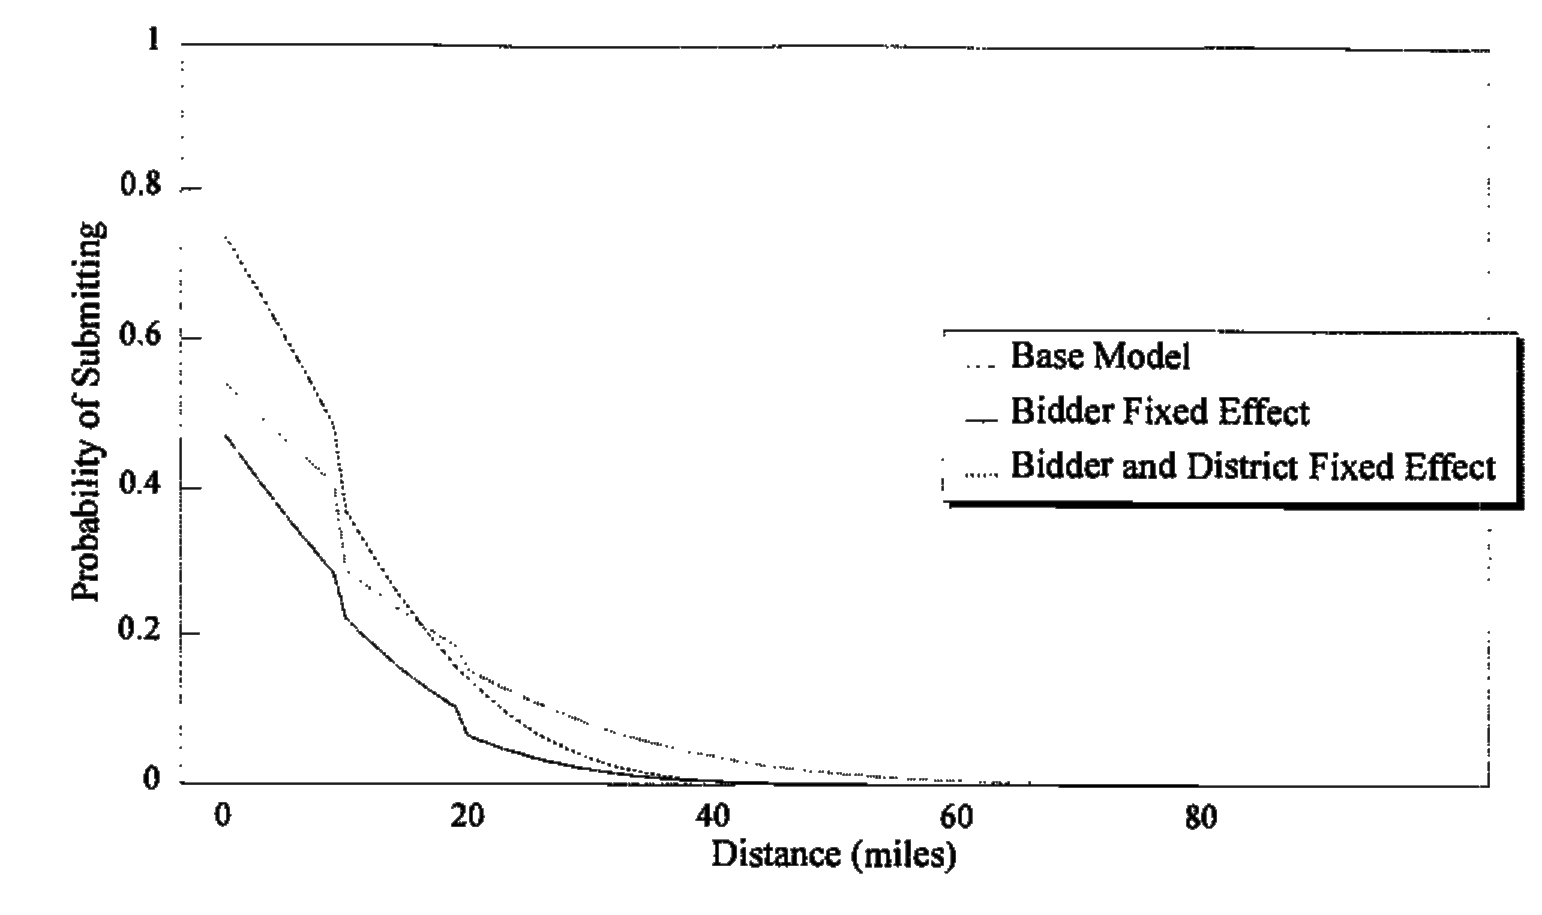
\includegraphics[width=\textwidth]{figures/ch13/pz99_fig2.png}
\caption{Predicted probability of submitting a bid}\label{fig:13-pz99-f2}
\end{subfigure}

\medskip
\begin{subfigure}{0.78\textwidth}
\centering
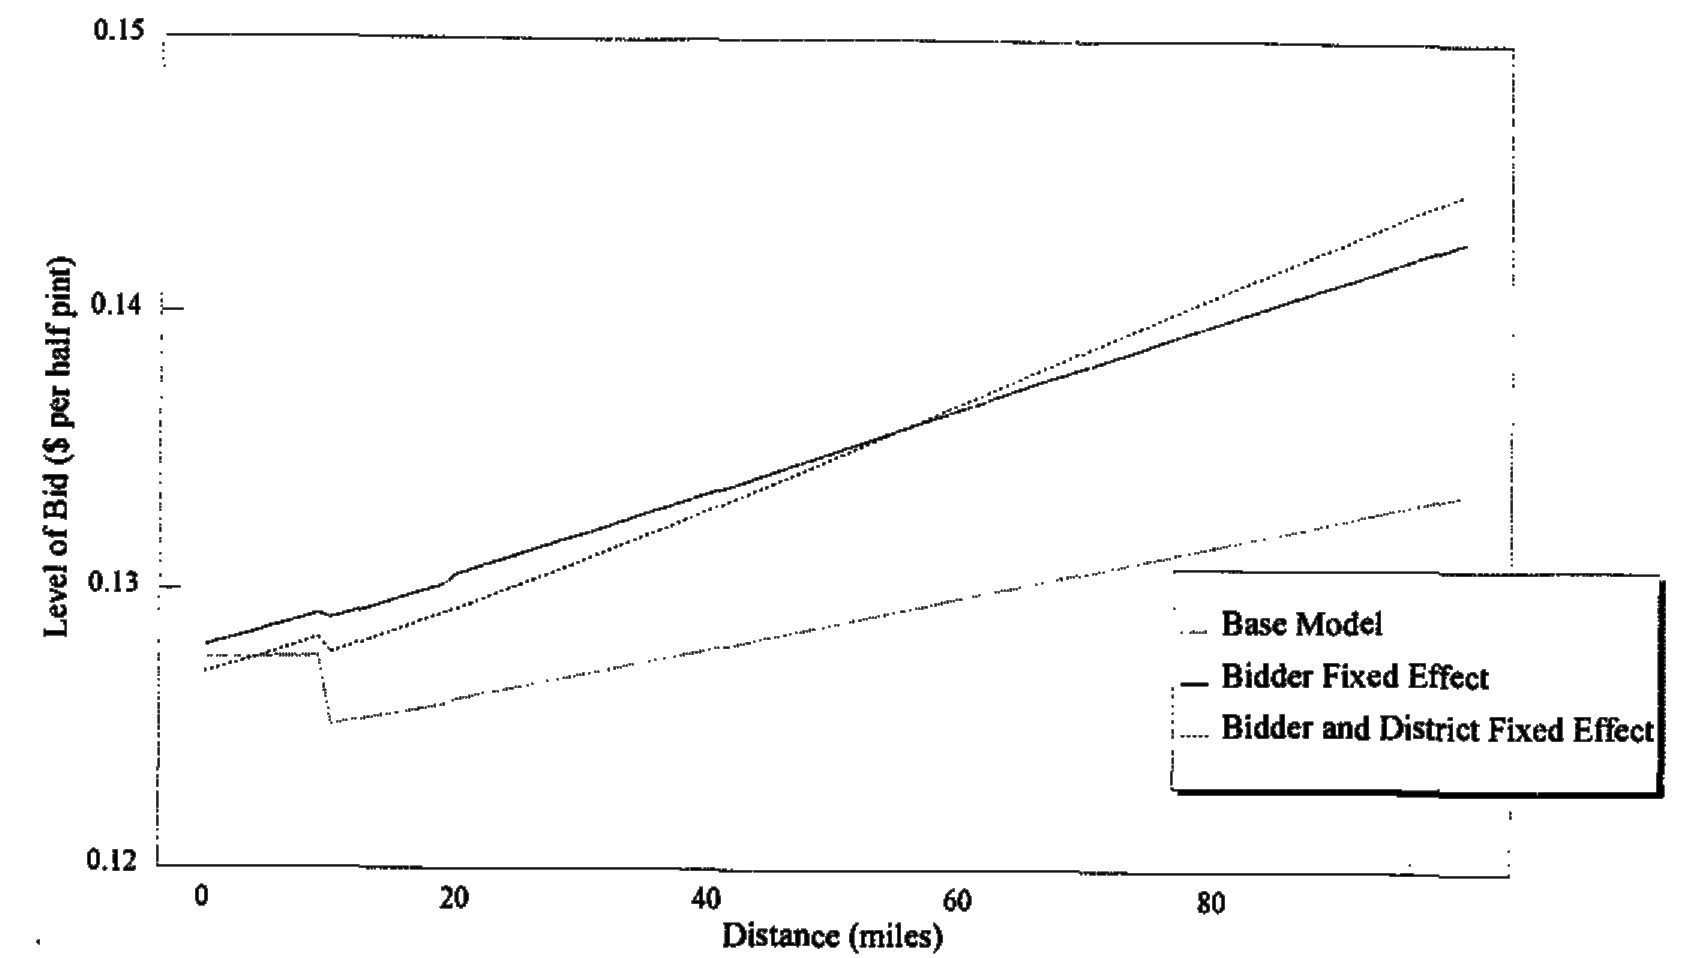
\includegraphics[width=\textwidth]{figures/ch13/pz99_fig3.png}
\caption{Predicted level of submitted bids, dollars per half pint}\label{fig:13-pz99-f3}
\end{subfigure}
\caption{The competitive benchmark in Ohio school milk: predictions for a hypothetical control-group processor by
distance from its plant, under the three specifications. Variables unrelated to distance are at their means, the
firm is the closest supplier within 10 miles and the second closest between 10 and 20 miles. The steps occur where
the firm loses these positions. The bidder fixed-effects curves are solid. In panel (a) the base model is the dotted
curve with the longest tail, and in panel (b) it is the lowest curve beyond 10 miles. The scans are darkened for
legibility. Source: \citet{PorterZona1999}, Figures~2 and~3 (NBER working-paper version).}
\label{fig:13-pz99-f23}
\end{figure}

The authors conclude that the control group bids in a way consistent with competition in a spatial market where
each firm has some local market power. Bids rise with distance, and firms rarely bid far from their plants.

\casehead{Defendants versus the control group}
The paper studies six southwestern Ohio defendants: Beatrice, Borden, Coors Brothers, H.~Meyer, Louis Trauth and
Meadow Gold. Beatrice and Meadow Gold are the same firm bidding under two names. Two tests ask whether each defendant
follows the control-group model.

The first test concerns submission. For each defendant, the authors append its submission data to the control-group
data and estimate the probit twice. Under the null hypothesis the defendant shares the control group's slopes but
has its own intercept. Under the alternative it has its own slopes. The likelihood ratio statistic is
$2(\ell^{\mathrm{alt}} - \ell^{\mathrm{null}})$. The second test concerns bid levels. For each defendant the residual
$r_{idt} = b_{idt} - x_{idt}\hat\beta^{\mathrm{control}}$ is regressed on $x_{idt}$ and a constant. Under the null
hypothesis of identical slopes, with a possibly different intercept, the slope coefficients of this regression are
zero, and an $F$ test checks this. The authors describe it as a Lagrange multiplier test chosen for convenience.

\Cref{tab:13-pz99-tests} reports both tests. Every defendant rejects the control-group submission model at the 1
percent level. For Borden, for example, the statistic is 445.9 with 20 degrees of freedom, against a 1 percent
point of 37.6 (our computation). The bid-level test rejects for every defendant except bids under the Beatrice
name. That test uses few observations, and the same firm's many bids under the Meadow Gold name reject. Results for
the fixed-effects specifications lead to the same conclusions. The authors stress that behavioral differences are
not necessarily anticompetitive. The question is how the defendants differ.

\begin{table}[htbp]
\centering
\caption{Southwestern Ohio defendants compared with the control group}\label{tab:13-pz99-tests}
\small
\begin{tabular}{@{}lccccc@{}}
\toprule
 & \multicolumn{1}{c}{Submission} & \multicolumn{2}{c}{Bid level} & \multicolumn{2}{c}{Deviation at 0--10 miles}\\
\cmidrule(lr){2-2}\cmidrule(lr){3-4}\cmidrule(l){5-6}
Defendant & LR (df) & $F$ (df) & $p$-value & Submissions & Bid\\
\midrule
Beatrice       & 157.9 (18) & 1.09 (19, 78)  & 0.3774 & $-13.7\%$ $<$ & $-4.9\%$ $<$\\
Borden         & 445.9 (20) & 10.13 (26, 386) & 0.0000 & $-0.2\%$ & $1.9\%$ $>$\\
Coors Brothers & 187.8 (19) & 5.02 (25, 102) & 0.0000 & $24.2\%$ $>$ & $9.3\%$ $>$\\
H.~Meyer       & 477.5 (20) & 11.53 (26, 384) & 0.0000 & $5.6\%$ $>$ & $2.7\%$ $>$\\
Louis Trauth   & 319.2 (20) & 9.66 (25, 345) & 0.0000 & $7.0\%$ $>$ & $5.5\%$ $>$\\
Meadow Gold    & 503.8 (20) & 7.09 (25, 771) & 0.0000 & $0.0\%$ & $0.1\%$\\
\bottomrule
\end{tabular}

\smallskip
\begin{minipage}{0.92\textwidth}\footnotesize
Notes: From \citet{PorterZona1999}, Tables~9--12 (NBER working-paper version), base models. LR: test
of equal probit slopes, all significant at 1 percent. $F$: test that the slopes of the regression of bid residuals
on the control-group regressors are zero. Submissions: actual minus predicted bids as a percentage of district-years
within 10 miles of the firm's plant, a difference in percentage points (Table~11). Bid: average deviation of actual from predicted bids, in percent of
the predicted bid (Table~12). $>$ ($<$): actual significantly above (below) predicted at 95 percent confidence.
\end{minipage}
\end{table}

\casehead{Where the defendants differ}
Since distance dominates the control-group model, the authors examine deviations by distance. Table~11 of the paper
tabulates actual minus predicted submissions in bands of ten miles, as a percentage of the district-years in each
band. These are differences in participation rates, so they are measured in percentage points. Coors Brothers'
actual submission rate exceeded its predicted rate by 24.2 percentage points within 10 miles of its plant and by
42.9 percentage points at 10 to 20 miles. Coors, Meyer and Trauth bid more often than predicted at distances up to about 30 miles,
and Meyer and Trauth also at some greater distances. Beatrice, Meadow Gold and Borden bid less often than predicted
within about 40 miles, where they would have a cost advantage. Borden and Meadow Gold bid more often than predicted
at 70 to 100 miles.

Table~12 tabulates bid residuals, as a percentage of the predicted bid, by regressing each firm's residuals on
distance-band indicators. Its first row is the deviation within 10 miles, and later rows are increments relative to
that row. Coors bid 9.3 percent above the prediction within 10 miles, and about 10.0 percent above it at 10 to 20
miles. For Borden, Meyer, Trauth and Meadow Gold, the deviation falls significantly with distance. Borden's bids at 70
to 80 miles, for example, are 5.1 percent lower relative to its local deviation. Under competition, local bids
should be lower than distant bids, because shipping costs are lower and the Cincinnati area has many potential
suppliers. Bids that fall with distance relative to the control group are hard to explain without collusion
\citep[p.~28]{PorterZona1999}. They fit territorial allocation near the plants and more competitive bidding farther
away.

\casehead{Correlation tests}
Under the null hypothesis of independent action based on public information, \cref{prop:13-competitive-restrictions}(ii)
implies that the unexplained parts of two firms' decisions are uncorrelated. Under complementary bidding, when one
ring member bids the others also bid, so submission residuals are positively correlated. Under territorial
allocation, when one member bids the others stay out, so the correlation is negative. For bid levels, a complementary
scheme implies that when one member bids high, the cover bids are high too.

The authors test independence of submission decisions with the Lagrange multiplier (LM) statistic of \citet{Kiefer1982}.
Its logic is easy to derive. Consider two firms facing the same district-year, with probits $S_k = \indic\{a_k +
u_k > 0\}$, $a_k = w_k\gamma_k$, $k = 1, 2$, and let $(u_1, u_2)$, independent of $(w_1, w_2)$, be standard bivariate normal with correlation
$\rho_{12}$ (a local symbol). With $q_k = 2S_k - 1$, the probability of the observed pair is
$\Phi_2(q_1a_1, q_2a_2; q_1q_2\rho_{12})$, where $\Phi_2$ is the bivariate normal distribution function. The
derivative of $\Phi_2$ with respect to its correlation argument is the bivariate normal density $\phi_2$, which at
zero correlation equals $\phi(q_1a_1)\phi(q_2a_2)$. By the chain rule and the symmetry of $\phi$, the score at
$\rho_{12} = 0$ is
\begin{equation}\label{eq:13-kiefer-score}
  \frac{\partial\ln\Pr(S_1, S_2)}{\partial\rho_{12}}\bigg|_{\rho_{12} = 0}
  = \frac{q_1q_2\,\phi(a_1)\phi(a_2)}{\Phi(q_1a_1)\,\Phi(q_2a_2)} = g_1 g_2,
  \qquad g_k = \frac{\phi(a_k)\bigl[S_k - \Phi(a_k)\bigr]}{\Phi(a_k)\bigl[1 - \Phi(a_k)\bigr]} .
\end{equation}
Here $g_k$ is the generalized residual of probit $k$. It equals $\frac{\phi(a_k)}{\Phi(a_k)}$ when $S_k = 1$ and
$-\frac{\phi(a_k)}{1-\Phi(a_k)}$ when $S_k = 0$. The test asks whether the products $g_{1m}g_{2m}$ average to zero
over district-years $m$, with the statistic
\begin{equation}\label{eq:13-kiefer-lm}
  LM = \frac{\bigl(\sum_m g_{1m}g_{2m}\bigr)^2}{\sum_m g_{1m}^2 g_{2m}^2} \xrightarrow{d} \chi^2_1 .
\end{equation}
Because $\E[g_2] = 0$, the score for $\rho_{12}$ is uncorrelated with the probit scores at $\rho_{12} = 0$, so
estimated probit coefficients can be plugged in. \Cref{tab:13-pz99-corr} reports the Spearman rank correlations of
standardized residuals $\frac{S - \hat\Phi}{\sqrt{\hat\Phi(1 - \hat\Phi)}}$ above the diagonal, with significance
from the LM test. Below the diagonal it reports Spearman correlations of bid-level residuals for district-years in
which both firms bid.

\begin{table}[htbp]
\centering
\caption{Correlations of residuals across pairs of defendants}\label{tab:13-pz99-corr}
\small
\setlength{\tabcolsep}{4.5pt}
\begin{tabular}{@{}lcccccc@{}}
\toprule
 & Beatrice & Borden & Coors & H.~Meyer & L.~Trauth & Meadow Gold\\
\midrule
Beatrice       &  & 0.0967 & 0.0491 & 0.0522$^{**}$ & 0.0627 & $-0.0343^{**}$\\
               &  & [1609] & [761] & [896] & [791] & [1609]\\
Borden         & $-0.3571$ &  & 0.1952 & 0.2129$^{**}$ & 0.2020$^{**}$ & 0.0947$^{*}$\\
               & [8] &  & [1379] & [1522] & [1410] & [2158]\\
Coors Brothers & $-1.0000$ & $-0.2571$ &  & 0.5813$^{**}$ & 0.4344$^{**}$ & 0.2059\\
               & [3] & [6] &  & [1432] & [1320] & [1193]\\
H.~Meyer       & 0.0091 & 0.2743$^{*}$ & 0.6598$^{**}$ &  & 0.5389$^{**}$ & 0.1188$^{**}$\\
               & [11] & [73] & [126] &  & [1463] & [1328]\\
Louis Trauth   & 0.9182$^{**}$ & 0.3724$^{**}$ & 0.5366$^{**}$ & 0.6674$^{**}$ &  & 0.1124$^{*}$\\
               & [11] & [51] & [114] & [267] &  & [1223]\\
Meadow Gold    & NA & 0.1634 & $-1.0000$ & 0.3539$^{**}$ & 0.6317$^{**}$ & \\
               & [0] & [59] & [2] & [69] & [58] & \\
\bottomrule
\end{tabular}

\smallskip
\begin{minipage}{0.95\textwidth}\footnotesize
Notes: Above the diagonal, \citet{PorterZona1999}, Table~13: Spearman correlations of standardized submission
residuals from the base probit, with significance from the LM test of \citet{Kiefer1982}. Below the diagonal,
Table~14: Spearman correlations of bid-level residuals from the base model. Numbers of observations in brackets.
$^{**}$ significant at 1 percent, $^{*}$ at 10 percent. NBER working-paper version.
\end{minipage}
\end{table}

The correlations are large and positive for the pairs among Coors, Meyer and Trauth. Submission residuals correlate
at 0.58 (Coors and Meyer), 0.54 (Meyer and Trauth) and 0.43 (Coors and Trauth). Their bid residuals correlate at
0.66, 0.67 and 0.54, on 126, 267 and 114 common district-years. When one of these firms bids, the others tend to bid
too, and their bids move together, beyond what proximity, size and contract terms predict. Borden is positively
correlated with Meyer and Trauth in both submissions and bids, and Meadow Gold's bids correlate with Trauth's (0.63).
Some pairs involving Beatrice rest on as few as three to eleven observations and carry little information. The bid
correlation test has little power against a pure territorial scheme, because ring members would then rarely bid in
the same district in the same year (WP p.~27, footnote 30).

\casehead{Interpretation}
The pieces fit together. Coors, Meyer and Trauth submit more bids than predicted within about 30 miles of their
plants, these bids are high, their submissions are positively correlated, and their bids move together. This is the
footprint of complementary bidding near their plants. The authors conclude that the collective behavior of these
three firms ``is best characterized as collusive'' \citep[p.~28]{PorterZona1999}, which supports the testimony of
Meyer and Coors. Beatrice, Meadow Gold and Borden refrain from bidding in their local areas, where they would have a
comparative advantage, and their bidding is correlated with Trauth's. This pattern is consistent with a
complementary bidding scheme that involves them as well.

\casehead{Damages: a collusion index}
To measure the overcharge, the authors regress the price of the winning bid on market structure and on an index of
exposure to the alleged conspiracy. Market structure is measured by the number of \emph{equivalent firms}, the
inverse of a Herfindahl index. For district $d$, let $s_{fd}$ be the fraction of school milk processing plants within
75 miles of the district that firm $f$ owns, and define
\begin{equation}\label{eq:13-pz99-equiv}
  \HHI_d = \sum_f s_{fd}^2, \qquad N^e_d = \frac{1}{\HHI_d} .
\end{equation}
With ten owners of one plant each, $N^e_d = 10$. Under collusion, the conspirators $\mathcal{C}$ with plants within
75 miles act as one owner with share $s_{\mathcal{C}d} = \sum_{f\in\mathcal{C}}s_{fd}$. The Herfindahl index becomes
\begin{equation*}
  \HHI^{\mathrm{col}}_d = \HHI_d - \sum_{f\in\mathcal{C}}s_{fd}^2 + \Bigl(\sum_{f\in\mathcal{C}}s_{fd}\Bigr)^2
  = \HHI_d + 2\sum_{\substack{f, g\in\mathcal{C}\\ f < g}}s_{fd}\,s_{gd} .
\end{equation*}
The \emph{collusion index} (the paper's ``Delta'') is the resulting loss of equivalent firms,
\begin{equation}\label{eq:13-pz99-delta}
  \Delta^{\mathrm{col}}_d = \frac{1}{\HHI_d} - \frac{1}{\HHI^{\mathrm{col}}_d} \geq 0 .
\end{equation}

\begin{example}[Computing the collusion index]\label{ex:13-pz99-delta}
Suppose six plants lie within 75 miles of a district, each with a different owner, and three owners are
conspirators. Competition gives $\HHI_d = 6 \times \frac{1}{36} = \frac{1}{6}$ and $N^e_d = 6$. Under collusion the
shares are $\frac{3}{6}$ for the conspirators and $\frac{1}{6}$ for each of the three others, so
$\HHI^{\mathrm{col}}_d = \frac{1}{4} + \frac{3}{36} = \frac{1}{3}$ and the number of equivalent firms is 3. The
collusion index is $\Delta^{\mathrm{col}}_d = 6 - 3 = 3$ (our computation).
\end{example}

The price equation, estimated by ordinary least squares on about 400 districts including districts outside
southwestern Ohio, is
\begin{equation}\label{eq:13-pz99-damages}
  \ln p_{dt} = \mu_t + z_{dt}\eta + \omega_1 N^e_{dt} + \omega_2 (N^e_{dt})^2
  + \sum_{\tau}\indic\{t = \tau\}\Bigl[a_{1\tau}\Delta^{\mathrm{col}}_{dt} + a_{2\tau}(\Delta^{\mathrm{col}}_{dt})^2
  + a_{3\tau}\Delta^{\mathrm{col}}_{dt}N^e_{dt}\Bigr] + e_{dt} .
\end{equation}
Here $p_{dt}$ is the standardized price of the winning bid, and $\mu_t$ are year effects that absorb raw milk and
packaging costs. The vector $z_{dt}$ contains the distances to the closest and second-closest plants, log
enrollment, the number of deliveries and the contract terms. The quadratic terms allow diminishing effects of competition, and the
interaction lets the effect of collusion depend on the initial level of competition. The year interactions let the
effectiveness of the conspiracy vary over time. The predicted effect of collusion is the prediction with the
collusion terms minus the prediction with all of them set to zero:
\begin{equation}\label{eq:13-pz99-effect}
  \hat m_{dt} = \hat a_{1t}\Delta^{\mathrm{col}}_{dt} + \hat a_{2t}(\Delta^{\mathrm{col}}_{dt})^2
  + \hat a_{3t}\Delta^{\mathrm{col}}_{dt}N^e_{dt} .
\end{equation}
The paper evaluates this log difference at the mean values of the variables.

The competitive part of the price equation behaves as expected (Table~16, with 3,431 observations and $R^2 = 0.6239$). One
more equivalent firm lowers the price by about 1.5 percent (coefficient $-0.0150$, $t = -5.7$). The distance to the
second-closest plant raises the price (0.0003, $t = 3.1$), as the closest firm's advantage grows. Larger districts
pay less (log enrollment $-0.0134$, $t = -11.9$), and escalator clauses lower prices ($-0.0096$, $t = -4.2$). The
distance to the closest plant has a small negative coefficient ($-0.0004$, $t = -3.6$), which the theory does not
predict.

\begin{table}[htbp]
\centering
\caption{Estimated effect of collusion on prices paid by southwestern Ohio school districts}\label{tab:13-pz99-t17}
\small
\begin{tabular}{@{}lccccc@{}}
\toprule
School year & $\hat a_{1t}$ (Delta) & $\hat a_{2t}$ (Delta$^2$) & $\hat a_{3t}$ (interaction) & Average effect & Effect given incumbency\\
 & (a) & (b) & (c) & (d) & (e)\\
\midrule
1980--81 & $-0.0014$ & $-0.0015$ & 0.00163 & 3.0\% & 3.2\%\\
1981--82 & 0.01304 & 0.01167 & 0.00103 & 11.3\% & 40.2\%\\
1982--83 & 0.02731 & 0.00225 & 0.00098 & 8.6\% & 23.2\%\\
1983--84 & 0.02995 & $-0.0097$ & 0.00156 & 4.5\% & 1.1\%\\
1984--85 & 0.02147 & 0.00106 & 0.00199 & 6.7\% & 19.7\%\\
1985--86 & 0.02684 & $-0.0023$ & 0.00122 & 5.4\% & 11.5\%\\
1986--87 & 0.02425 & 0.00173 & 0.0013 & 6.5\% & 20.5\%\\
1987--88 & 0.00368 & 0.02901 & 0.0006 & 3.3\% & 49.0\%\\
1988--89 & $-0.0227$ & 0.03636 & 0.00229 & 2.9\% & 29.4\%\\
1989--90 & $-0.0494$ & 0.0134 & 0.0041 & $-1.6\%$ & 3.4\%\\
1990--91 & $-0.0201$ & $-0.0126$ & 0.00634 & $-0.3\%$ & $-8.3\%$\\
\bottomrule
\end{tabular}

\smallskip
\begin{minipage}{0.92\textwidth}\footnotesize
Notes: Reproduced from \citet{PorterZona1999}, Table~17 (NBER working-paper version). Columns (a)--(c)
are the year-specific coefficients of \eqref{eq:13-pz99-damages}. Column (d) is the expected markup over
competitive prices for the average district in southwestern Ohio, computed at mean values as a difference in
predicted log prices. Column (e) conditions on
a defendant being the incumbent. School years as labeled in the paper.
\end{minipage}
\end{table}

\Cref{tab:13-pz99-t17} and \cref{fig:13-pz99-effects} show the estimated effects by year. The paper notes that the
effect is small in 1983--84 and after 1989 in both columns (WP p.~31). These are the two breakdowns described in the
testimony. The incumbency measure, column (e), shows them most clearly. It falls to 1.1 percent in 1983--84 and 3.4
percent in 1989--90, and it is negative in 1990--91. In the years between the breakdowns it ranges from 11.5 to 49.0
percent, and it reaches 40.2 percent in 1981--82. The average effect, column (d), shows the first breakdown less
clearly. It is 4.5 percent in 1983--84, above its values in 1980--81, 1987--88 and 1988--89. It is negative in
1989--90 and 1990--91. The authors summarize the average effect of collusion as an
increase of ``about six and one half percent,'' roughly the cost of shipping school milk about 50 miles.
The paper does not state how this average weights the years. \citet[p.~235]{ErutkuHildebrand2010} describe it as
the average ``when excluding 3 years in which the cartel was said to have broken down.'' The simple mean of
column (d) is 4.6 percent over all eleven years and 5.8 percent over 1980--81 to 1988--89. Excluding 1983--84,
1989--90 and 1990--91 gives $\frac{47.7}{8} = 6.0$ percent (our computation), so the weighting remains unstated.
Erutku and Hildebrand also report the authors' suggestion that the 6.5 percent price effect amounts to a rise of
roughly 30 percent in the markup.

\begin{figure}[htbp]
\centering
\begin{tikzpicture}
\begin{axis}[
  width=0.9\textwidth, height=6cm,
  xmin=0.5, xmax=11.5, ymin=-12, ymax=52,
  xtick={1,2,3,4,5,6,7,8,9,10,11},
  xticklabels={80--81,81--82,82--83,83--84,84--85,85--86,86--87,87--88,88--89,89--90,90--91},
  x tick label style={font=\footnotesize, rotate=45, anchor=north east},
  y tick label style={font=\footnotesize},
  xlabel={School year}, ylabel={Effect on price (percent)},
  label style={font=\small},
  legend style={font=\footnotesize, draw=none, fill=none, at={(0.5,-0.36)}, anchor=north, legend columns=2,
    /tikz/every even column/.append style={column sep=1.2em}}, legend cell align=left,
  axis lines*=left, ymajorgrids, grid style={gray!25}]
\fill[gray!15] (axis cs:3.5,-12) rectangle (axis cs:4.5,52);
\fill[gray!15] (axis cs:9.5,-12) rectangle (axis cs:10.5,52);
\draw[gray!70] (axis cs:0.5,0) -- (axis cs:11.5,0);
\addplot[thick, color={rgb,255:red,42;green,120;blue,214}, mark=*, mark size=2pt]
  coordinates {(1,3.0) (2,11.3) (3,8.6) (4,4.5) (5,6.7) (6,5.4) (7,6.5) (8,3.3) (9,2.9) (10,-1.6) (11,-0.3)};
\addlegendentry{Average district, column (d)}
\addplot[thick, dashed, color={rgb,255:red,235;green,104;blue,52}, mark=square*, mark size=2pt]
  coordinates {(1,3.2) (2,40.2) (3,23.2) (4,1.1) (5,19.7) (6,11.5) (7,20.5) (8,49.0) (9,29.4) (10,3.4) (11,-8.3)};
\addlegendentry{Defendant incumbent, column (e)}
\node[font=\footnotesize, gray!60!black, anchor=south] at (axis cs:4,46) {breakdown};
\node[font=\footnotesize, gray!60!black, anchor=south] at (axis cs:10,46) {breakdown};
\end{axis}
\end{tikzpicture}
\caption{Estimated effect of collusion on the price of school milk in southwestern Ohio, by school year. Shaded
years are the cartel breakdowns described in the testimony (1983--84 and 1989--90). Redrawn from
\citet{PorterZona1999}, Table~17, columns (d) and (e).}
\label{fig:13-pz99-effects}
\end{figure}

\begin{example}[From a log markup to damages]\label{ex:13-pz99-damages}
The dependent variable of \eqref{eq:13-pz99-damages} is the log price, so column (d) of \cref{tab:13-pz99-t17} is a
log difference, $\hat m = \ln p - \ln p^{\mathrm{bf}}$. The paper reports it as a percentage change (WP p.~31). As in
\eqref{eq:13-damages-log}, the overcharge as a share of spending is
\begin{equation*}
  \frac{p - p^{\mathrm{bf}}}{p} = 1 - e^{-\hat m} .
\end{equation*}
With $\hat m = 0.065$, the overcharge is $1 - e^{-0.065} = 6.3$ percent of spending. Reading 6.5 percent instead as a
ratio markup $\frac{p}{p^{\mathrm{bf}}} - 1$ would give $\frac{0.065}{1.065} = 6.1$ percent. A district that spent
\$100,000 on milk would have overpaid about \$6,300 (a hypothetical district, our computation). Because school milk demand is
nearly perfectly inelastic, this transfer is the whole of the district's loss.
\end{example}

The comparison with distance in the abstract can be checked against \cref{tab:13-pz99-control}. Fifty miles at the
base-model gradient of 0.0096 dollars per hundred miles adds 0.48 cents, or 3.6 percent of the mean price of 13.4
cents in \cref{tab:13-pz99-t1}. With bidder effects it adds 0.77 cents, or 5.7 percent (our computation). The authors'
own illustration is a district next to the plants of two conspirators whose nearest competitors are at least 50
miles away. Prices there could be about half a penny, or five percent, above the competitive level (WP p.~31).

\casehead{Critiques and limitations}
The evidence is a set of imperfect tests, none decisive alone. The likelihood ratio tests of equal slopes reject for
every defendant, and the authors note in footnote 15 that no single intercept represents all bidders. Such tests
would probably reject for many individual non-defendants too, so the rejections carry little weight by themselves.
The informative evidence is the pattern of deviations. Distance gradients are reversed and residuals are
correlated, and both match the testimony. Positive correlations could also arise from an omitted factor that affects
these firms alike (WP p.~27, footnote 28). The control group is assumed competitive. Collusion among non-defendants
would bias the benchmark toward the defendants' behavior and work against the tests.

The damage regression is a reduced form. Its identifying variation is the cross-sectional exposure of districts to
conspirators' plants, which is credible only if plant locations are unrelated to unobserved local cost and demand
conditions. The 75-mile radius, the plant-count shares and the quadratic forms are approximations, and the
competitive price for southwestern Ohio is predicted partly from districts elsewhere in the state. The year
pattern, which matches the breakdowns in the testimony, is the strongest validation of the index.

\casehead{Contribution}
The paper extends the Long Island design to markets in which collusion takes the form of incumbency rights and
territorial allocation. It models both the decision to bid and the level of the bid, with a selection correction. It
then matches several scheme-specific tests to the alleged scheme and builds a reduced-form damages estimate whose
time pattern can be compared with testimony. The combination of a competitive model estimated on a control group,
tests of independence across suspected firms, and damages from exposure to the ring remains a template for
procurement cases.

\casehead{Later screens}
Porter and Zona warn that a single test procedure able to detect all bid rigging is an impossible goal. Later work
has therefore developed tests aimed at particular schemes and data \citep[p.~210]{AskerNocke2021}.
\citet{BajariYe2003} test conditional independence and exchangeability (\cref{sec:13-detection-theory}).
\citet{AtheyLevinSeira2011} compare open and sealed timber auctions, as \cref{ch:auction-empirics} explains.
\citet{KawaiNakabayashi2020} exploit the rounds of Japanese national procurement auctions, as reported by
\citet[pp.~184--185]{AskerNocke2021}. When no first-round bid meets the secret reserve price, the lowest
first-round bid is announced and a second round follows. In the second round, the gap between the bids of the
first-round runner-up and the first-round winner is almost never negative. The gap between the bids of the
first-round third and second bidders often is. The first-round winner thus almost always wins again, while lower
ranks switch freely, which suggests that the winner was chosen before the auction. Applied across 2003--2006, the
test flags about 970 firms as collusive. \citet{ConleyDecarolis2016} detect groups of coordinating bidders in Italian
procurement, and \citet{OrtnerEtAl2020} develop screens that remain informative when cartels adapt to them.
\Cref{sec:12-eu-facts} uses the first two of these studies as evidence on the prevalence of collusion, and the book
does not develop the three tests further.

\section{Enforcement, Damages and What the Evidence Shows}\label{sec:13-enforcement}

The cartels of this chapter came to light in different ways, and the route matters for what they can teach. This
section describes the enforcement institutions and the selection of cartels they induce
(\cref{sec:13-institutions}). It then develops the methods used to measure the effects of collusion
(\cref{sec:13-damages}) and closes with what the evidence of the chapter shows (\cref{sec:13-synthesis}).

\subsection{Enforcement institutions and the selection of observed cartels}\label{sec:13-institutions}

\casehead{Law and penalties}
In the United States, Section~1 of the Sherman Act (1890) prohibits agreements in restraint of trade. Price fixing
is illegal per se \citep[p.~570]{Miller2010}. Section~1 is a criminal as well as a civil statute, so price fixing
and bid rigging can be prosecuted as crimes \citep[ch.~4, p.~74, footnote~13]{Kaplow2013}. Injured parties can sue for treble damages
\citep[p.~759]{Asker2010}.
In the European Union, Article~101 of the Treaty on the Functioning of the European Union prohibits cartels. The
European Commission imposes administrative fines, capped at 10 percent of a firm's turnover
\citep[p.~6]{ChenRey2013}. Page and footnote references to \citet{ChenRey2013} are to its working-paper version.
\Cref{tab:12-eu-fines} lists the largest fines the Commission has imposed. On the conventional view, liability for
price fixing requires proof of an agreement, usually through evidence of communication, and plus factors serve as
circumstantial support \citep[pp.~4, 21 and 109--110]{Kaplow2013}. \Cref{sec:12-kaplow} discusses Kaplow's critique of
this requirement, and \cref{sec:13-market-evidence} the market-based evidence itself.

\casehead{Leniency}
Proving an agreement is the hard part of enforcement, and leniency programs address it. The United States adopted a
corporate leniency program in 1978. Under the Antitrust Division's 1993 Corporate Leniency Policy, a firm that
reports before an investigation has begun receives leniency automatically if it meets six conditions. The Division
must have no information about the conduct from any other source. The firm must end its participation promptly,
cooperate fully and make restitution where possible, and its confession must be a corporate act rather than that of
individual executives. It must not have coerced others or led or originated the cartel. A firm
that misses these conditions, including one that comes forward after an investigation has begun, can still qualify
under seven alternative conditions. Four of them repeat the conditions on termination, cooperation, the corporate
confession and restitution. In addition, the firm must be the first to come forward and qualify. The Division must not yet
have evidence likely to yield a sustainable conviction, and it must judge that leniency would not be unfair to
others. \citet[p.~1]{ChenRey2013} summarize the revision as a first-informant rule and a post-investigation amnesty
rule. Eligibility after an investigation has begun thus depends on the alternative conditions.

The European Commission adopted its program in the 1996 Notice on the Non-Imposition or Reduction of Fines in
Cartel Cases. That notice reduced fines by 75 to 100 percent for a firm that reported before the Commission had
ordered an investigation. A firm that reported after such an investigation had failed to establish sufficient
grounds for proceedings could receive 50 to 75 percent. Both tiers also required the firm to be the first to adduce
decisive evidence, to end its involvement, to cooperate fully and not to have coerced others or instigated the
cartel. Other cooperation earned 10 to 50 percent. The first two
tiers are those that \citet[footnote~6]{ChenRey2013} describe. The Commission revised the program in 2002
\citep[footnote~1]{ChenRey2013} and again in its 2006 Notice on Immunity from Fines and Reduction of Fines in Cartel
Cases, which remains its framework. Under the 2006 notice, the first firm whose evidence enables an inspection or
a finding of infringement can obtain full immunity if it meets the notice's conditions. Later firms whose evidence
adds significant value receive reductions of 30 to 50 percent for the first, 20 to 30 percent for the second and up
to 20 percent for the others. Many recent prosecutions involve a whistleblower.

In the repeated-game language of \cref{ch:collusion-theory}, leniency changes both sides of a member's incentive
constraint. \citet[pp.~209--210]{AskerNocke2021} summarize the opposing effects identified by \citet{Harrington2008}.
The \emph{deviator amnesty effect} lets a member that undercuts its rivals also report the cartel and escape the
fine. Cheating becomes more attractive, which tightens the no-cheating constraint. The \emph{cartel amnesty effect}
works the other way. Lenient treatment of the first confessor lowers the expected fines that members pay, which
raises the value of colluding and eases the constraint. A third force, the \emph{race-to-the-courthouse effect},
counteracts the second (p.~209, note~77). A more lenient program can move the members from a state in which no
firm applies to one in which all race to report. Expected fines then rise and the value of colluding falls.
Leniency can also be exploited. If it is too generous, a cartel can collude and have members report in turn,
paying reduced fines. \citet{ChenRey2013} characterize the
optimal design. Some leniency before an investigation is always desirable. Leniency during an investigation is
desirable when investigations are unlikely to succeed without a report. Restricting leniency to the first informant
is useful, and their analysis does not support denying leniency to repeat offenders. The theory is developed in
\cref{ch:collusion-theory}.

Measuring the effect of a leniency program runs into the problem that cartels are unobserved
\citep[p.~209]{AskerNocke2021}. A rise in detected cartels after a program begins could reflect better detection or
more cartels. \citet{Miller2009} separates the two with a model of cartel formation, detection and dissolution. He
estimates it by Poisson regression on the U.S. indictments and information reports for violations of Section~1 from
1985 to 2005 \citep[pp.~186--187]{AskerNocke2021}. \Cref{rem:13-miller} shows the logic of his identification in
the notation of \cref{prop:13-selection}. The 1993 program raised cartel discoveries by about 60 percent, which
indicates better detection. Read through the model with the natural breakup rate held fixed, the later path of
discoveries indicates greater deterrence.

\casehead{How the cartels of this chapter came to light}
\Cref{tab:13-discovery} records the source of evidence for each case. The legal cartels left records because they
had no reason to hide. The prosecuted cases surfaced through complaints, wiretaps, convictions and confessions. Asker's
stamp ring collapsed after a dealer outside the ring alerted antitrust enforcement. Asker suggests that strong
members kept the weak ones partly because an expelled member could report the ring and seek leniency
(\cref{sec:13-asker}). A leniency program thus shapes the internal organization of a cartel as well as its
stability. \Cref{sec:13-market-evidence} classifies the kind of evidence that decided each case.

\begin{table}[htbp]
\centering
\caption{How the cartels studied in this chapter came to light}\label{tab:13-discovery}
\footnotesize
\begin{tabularx}{\textwidth}{@{}>{\raggedright\arraybackslash}p{4.1cm}>{\raggedright\arraybackslash}X@{}}
\toprule
Case & Source of evidence\\
\midrule
Joint Executive Committee, 1880--1886 & Open agreement before the Interstate Commerce Act, weekly cartel records and
trade-press reports of price wars\\
Sugar Institute, 1927--1936 & Trade association later ruled illegal by the Supreme Court, meeting notes kept by a
member\\
Bromine pools, 1885--1914 & Contracts, firm papers and trade press\\
Danish ready-mixed concrete, 1993--1996 & Prices published by the competition authority itself\\
Overlap group, 1950s--1991 & Department of Justice suit in 1991\\
Airline Tariff Publishing, 1990s & Department of Justice suit in 1992 and consent decrees\\
Quebec gasoline, 2002--2006 & Competition Bureau wiretaps, raids and guilty pleas\\
Lysine, citric acid and other industrial cartels, 1990s & Prosecutions and European Commission decisions\\
Stamp-auction ring, until 1997 & Complaint by a dealer outside the ring, faxed records kept by a member\\
Long Island paving, 1979--1985 & Federal conviction in 1984 and state and county suits\\
Ohio school milk, 1980--1990 & State suit, confessions by two dairies in 1993\\
\bottomrule
\end{tabularx}

\smallskip
\begin{minipage}{0.95\textwidth}\footnotesize
Notes: Compiled from the case studies of this chapter
(\cref{sec:13-jec,sec:13-legal,sec:13-information,sec:13-gasoline,sec:13-imperfect,sec:13-asker,sec:13-detection}).
\end{minipage}
\end{table}

\casehead{Selection}
We observe cartels that were legal or that were caught. Estimates of how long cartels last and how much they raise
prices are therefore conditional on detection. \citet{LevensteinSuslow2006} survey cross-section studies in which
average cartel duration ranges from 3.7 to 10 years (their Table~1). Their own sample covers 42 international
cartels prosecuted by the United States or the European Commission in the 1990s. These cartels lasted 5 years on
average, with a standard deviation of 4.5 and a range of 0 to 20 years (Table~1). Their text on p.~51 gives 5.4 years
and 4.7 for the same sample. The distribution of duration is bimodal. Many
cartels break up within a year, many last five to ten years, and some last decades (p.~43). They warn that ``in some
cases, samples are literally selected by prosecutors'' (p.~44). The surge in U.S. prosecutions of international
cartels followed the 1993 revision of the amnesty program (p.~50, footnote~21). Case-study samples
are selected differently, by researchers who choose industries with long or eventful cartel histories. Their mean
duration is 14 years, with a median of 6 (pp.~52--53).

Prosecuted cartels are also a small part of all cartels. The U.S.\ Department of Justice filed 92 criminal
cartel cases in 1982, with fines of \$36.8 million \citep[p.~182]{AskerNocke2021}. In 2017 it filed 21 cases, with
fines of \$2.79 billion. Fewer cases need not mean less collusion, because penalties, detection and the
size of the economy all changed. Where collusion can be measured directly, it is common.
\citet{KawaiNakabayashi2020} flag about 970 collusive firms in Japanese national procurement, and scaling up their
estimate implies that collusion affects about 0.85 percent of Japan's GDP. \citet[pp.~4, 6 and~29--30]{ConleyDecarolis2016}
estimate that groups of bidders whose entry and bids appear coordinated affected at least 30 percent of 802
average-bid roadwork auctions in northern Italy. Counties and municipalities in five regions held these auctions
between 2005 and 2010. When
Finnish cartels were legal and had to register, \citet{HyytinenSteenToivanen2018} count 900 of them between 1951
and 1990. \Cref{sec:12-eu-facts} discusses this evidence further.

Selection begins before detection, at formation. \citet[p.~187]{AskerNocke2021} write the participation
constraint of a potential member $i$ as
\begin{equation}\label{eq:13-participation}
  V_i^{\mathrm{comp}} \;\le\; V_i^{\mathrm{coll}} - \eta_i .
\end{equation}
Here $V_i^{\mathrm{coll}}$ is the firm's value inside the cartel, $V_i^{\mathrm{comp}}$ its value outside when the
other firms join, and $\eta_i$ a one-time cost of joining that captures the frictions of organizing. It is
constraint \eqref{eq:12-participation} of \cref{ch:collusion-theory}. A cartel forms only where the gain from collusion covers
these frictions for every member it needs. The cartels that exist are therefore already selected toward markets
with large collusive gains, before detection selects them again. The direction of the second bias depends on how
detection works, as a simple model shows.

\begin{proposition}[Duration of detected cartels]\label{prop:13-selection}
In each period of operation, a cartel breaks down for internal reasons with probability $q \in (0,1)$, so its
natural duration $L$ is geometric with $\E[L] = \frac{1}{q}$. Independently, in each period of operation it is
detected with probability $h \in (0,1)$. Let $r = (1-q)(1-h)$, a local symbol for the probability that a cartel
neither breaks down nor is detected in a period.
\begin{enumerate}[label=(\alph*)]
\item If detection uncovers the cartel without ending it, so that a cartel is eventually discovered if it is
detected in at least one period of its life, then
\begin{equation}\label{eq:13-sel-a}
  \E[L \mid \text{discovered}] = \frac{1-r}{h}\left[\frac{1}{q} - \frac{q(1-h)}{(1-r)^2}\right] > \frac{1}{q} .
\end{equation}
\item If detection ends the cartel, the observed duration of detected cartels satisfies
\begin{equation}\label{eq:13-sel-b}
  \E[L \mid \text{detected}] = \frac{1}{1-r} < \frac{1}{q} .
\end{equation}
\end{enumerate}
\end{proposition}

\begin{proof}
(a) A cartel of duration $L$ escapes detection with probability $(1-h)^L$, so the probability of discovery is
\begin{equation*}
  \Pr(\text{discovered}) = \sum_{L=1}^{\infty}q(1-q)^{L-1}\bigl[1 - (1-h)^L\bigr]
  = 1 - q(1-h)\sum_{L=1}^{\infty}r^{L-1} = 1 - \frac{q(1-h)}{1-r} = \frac{h}{1-r} ,
\end{equation*}
where the last step uses $1 - r - q(1-h) = 1 - (1-h)(1 - q + q) = h$. Using $\sum_{L\geq1}Lr^{L-1} = \frac{1}{(1-r)^2}$,
\begin{equation*}
  \E\bigl[L\,\indic\{\text{discovered}\}\bigr] = \frac{1}{q} - q(1-h)\sum_{L=1}^{\infty}L\,r^{L-1}
  = \frac{1}{q} - \frac{q(1-h)}{(1-r)^2} .
\end{equation*}
Dividing by $\Pr(\text{discovered})$ gives the equality in \eqref{eq:13-sel-a}. For the inequality, the
probability of discovery $1 - (1-h)^L$ is increasing in $L$. Two increasing functions of the same random variable
are positively correlated, so $\E[L\,(1-(1-h)^L)] > \E[L]\,\E[1-(1-h)^L]$, which is the inequality after division.

(b) A cartel survives each period with probability $r$, so it is detected in period $\ell$ with probability
$r^{\ell-1}h$. Conditional on detection, the duration is geometric with parameter $1-r$ and mean $\frac{1}{1-r}$.
Since $1 - r = q + h(1-q) > q$, this mean is below $\frac{1}{q}$.
\end{proof}

With $q = 0.2$, so that the natural mean duration is 5 years, and a detection probability of $h = 0.05$ per year,
cartels discovered after the fact last 8.17 years on average. Cartels ended by detection last 4.17 years. With
$h = 0.2$ the figures are 6.78 and 2.78 years (our computation, \texttt{pz\_checks.py}). Prosecuted samples mix both
mechanisms, so their bias can go either way. The same logic applies to overcharges. Cartels with large overcharges
may draw complaints from customers and be overrepresented, while sophisticated cartels may evade detection and be
underrepresented. Legal cartels avoid detection-driven selection but face another one, since we study those whose
records survived.

\begin{remark}[Reading cartel discoveries]\label{rem:13-miller}
The model of \cref{prop:13-selection} also explains how \citet{Miller2009} reads enforcement statistics. Consider a
population of industries of mass one. In each period a competitive industry forms a cartel with probability $\phi$
(a local symbol). A cartel is detected with probability $h$ and otherwise breaks down with probability $q$, so it
survives the period with probability $r = (1-q)(1-h)$. An industry whose cartel ends returns to competition. In a
steady state, the flow into collusion equals the flow out of it:
\begin{equation*}
  \phi\,(1 - \bar\pi) = (1 - r)\,\bar\pi , \qquad \text{so} \qquad \bar\pi = \frac{\phi}{\phi + 1 - r} ,
\end{equation*}
where $\bar\pi$ is the share of industries that collude. Discoveries per period are $h\bar\pi$. Substituting
$1 - r = q + h(1 - q)$ and differentiating,
\begin{equation*}
  h\bar\pi = \frac{h\phi}{\phi + q + h(1 - q)} , \qquad
  \frac{\partial\,(h\bar\pi)}{\partial h} = \frac{\phi\,(\phi + q)}{\bigl[\phi + q + h(1 - q)\bigr]^{2}} > 0 .
\end{equation*}
Two predictions follow, which are those of Miller's model as summarized by \citet[p.~186]{AskerNocke2021}. When a
policy raises $h$, the share $\bar\pi$ cannot change at once, so discoveries jump in proportion to the rise in $h$.
An immediate rise in discoveries therefore reveals better detection. In the new steady state, a higher $h$ with
unchanged $\phi$ and $q$ would keep discoveries above their old level. Discoveries also fall with the natural
breakup probability, since
\begin{equation*}
  \frac{\partial\,(h\bar\pi)}{\partial q} = -\frac{h\phi\,(1 - h)}{\bigl[\phi + q + h(1 - q)\bigr]^{2}} < 0 .
\end{equation*}
Holding $q$ fixed, a long-run level of discoveries below the old one therefore requires a fall in the formation
rate $\phi$, which is deterrence. Without that restriction a rise in $q$ can produce the same decline. With
$\phi = h = q = 0.1$, discoveries are $\frac{0.01}{0.29} = 0.0345$ per period. Raising $h$ to 0.2 and $q$ to 0.9
with $\phi$ unchanged lowers them to $\frac{0.02}{1.02} = 0.0196$. Reading the decline as deterrence thus requires
ruling out a rise in natural breakups and other changes in the transition rates. The discrete-time version and
its timing are our simplification of Miller's model.
\end{remark}

\subsection{Measuring the effects of collusion}\label{sec:13-damages}

\casehead{Overcharges and damages}
Let $p_t$ be the price paid in period $t$, $Q_t$ the quantity bought and $p^{\mathrm{bf}}_t$ the \emph{but-for
price}, the price that would have prevailed without the cartel. The \emph{overcharge} is $p_t - p^{\mathrm{bf}}_t$
per unit, and overcharge damages are
\begin{equation}\label{eq:13-damages}
  D = \sum_t \bigl(p_t - p^{\mathrm{bf}}_t\bigr)Q_t .
\end{equation}
Most methods estimate the log overcharge $\tau_t = \ln p_t - \ln p^{\mathrm{bf}}_t$. Since
$p^{\mathrm{bf}}_t = p_te^{-\tau_t}$, damages in terms of observed spending are
\begin{equation}\label{eq:13-damages-log}
  D = \sum_t \bigl(1 - e^{-\tau_t}\bigr)\,p_tQ_t .
\end{equation}
Buyers also lose the surplus on units they no longer buy. The change in consumer surplus is
\begin{equation*}
  \Delta CS = -\int_{p^{\mathrm{bf}}}^{p}Q(s)\,ds \approx -\bigl(p - p^{\mathrm{bf}}\bigr)\,\frac{Q + Q^{\mathrm{bf}}}{2}
  = -\bigl(p - p^{\mathrm{bf}}\bigr)Q - \frac{1}{2}\bigl(p - p^{\mathrm{bf}}\bigr)\bigl(Q^{\mathrm{bf}} - Q\bigr) ,
\end{equation*}
where the approximation is exact for linear demand. The first term is the overcharge, a transfer to the cartel. The
second is the additional loss of consumer surplus on the units no longer bought. It equals the deadweight loss only
if the but-for price equals marginal cost. With a constant marginal cost $mc$ below $p^{\mathrm{bf}}$, the lost units
also forgo the but-for margin, and the loss of total surplus adds $\bigl(p^{\mathrm{bf}} - mc\bigr)\bigl(Q^{\mathrm{bf}}
- Q\bigr)$ to the triangle. Take demand $Q = 10 - p$, $mc = 0$, $p^{\mathrm{bf}} = 2$ and $p = 4$. The triangle is 2,
and the loss of total surplus is $2 + 2 \times 2 = 6$. In procurement with inelastic demand, as on Long Island and in Ohio,
$Q^{\mathrm{bf}} = Q$ and the overcharge is the whole loss.

Direct purchasers who resell pass part of an overcharge on. If a cartel raises a downstream firm's unit cost by
$\Delta w$ and downstream pass-through is $\rho$ (\cref{ch:theory}), the downstream price rises by about
$\rho\,\Delta w$. To first order, direct purchasers then bear $(1-\rho)\Delta w$ per unit and their customers bear
$\rho\,\Delta w$, apart from volume effects.

\casehead{Umbrella damages and the loss of welfare}
Overcharge damages measure only part of the harm. \citet[pp.~210--212]{AskerNocke2021} separate the measures of a
cartel's impact in a static market with a competitive fringe (\cref{fig:13-cartel-impact}). In their figure the
members' aggregate marginal cost $MC_1$ slopes upward and meets demand at the competitive price. For simplicity we
draw $MC_1$ constant, so the competitive price equals $MC_1$. Fringe firms have higher costs and are inactive under
competition. When the cartel restricts output, the price rises and fringe firms produce until their marginal cost
reaches the cartel price. The overcharge is the price increase, $AG$ in the figure. Antitrust
damages are the overcharge times the cartel's sales, the rectangle $GAHF$, and courts treble this measure.
\emph{Umbrella damages} are the overcharge times the fringe's sales, the rectangle $HCEF$. Buyers pay them to firms
outside the cartel that raise prices under its umbrella. Buyers also lose the triangle $CDE$ on units they no longer
buy. The three areas together make up the loss of consumer surplus $GACD$. Antitrust damages thus exclude both
umbrella damages and the consumers' share of the deadweight loss (pp.~211--212).

Total surplus calls for different areas. The overcharge on the cartel's sales is a transfer. \emph{Productive
inefficiency} is the extra resource cost $BCEF$ of output produced by high-cost fringe firms instead of the cartel's
members. With constant $MC_1$, as in our drawing, part of the umbrella overcharge is dissipated in this way. With
an upward-sloping $MC_1$, as in their figure, the points $F$ and $E$ lie below the competitive price. The area
$BCEF$ is then no longer contained in the umbrella rectangle. The total welfare loss $BFDC$ is the sum of productive
inefficiency and the deadweight loss $CDE$. With the illustrative curves of the figure, damages are 10, umbrella
damages 6 and the deadweight loss 8, so consumers lose 24. Productive inefficiency is 4.5, fringe firms keep 1.5 of
the umbrella overcharge, and the total welfare loss is 12.5 (our computation). In this illustrative example of our
own, umbrella damages are 37.5 percent of all overcharge damages. \citet{Caoui2020} measures a different ratio in the
Texas school milk cartel of 1980--1992. Per contract, umbrella damages conditional on a non-cartel firm winning are
at least 35 percent of cartel damages conditional on the cartel winning. The lower bound comes from an efficient
cartel, which always sends its lowest-cost member to bid. With a randomly chosen cartel bidder the two can be equal
in size. Asker and Nocke summarize the result in terms of total cartel damages
(p.~212, note~82). The ratio compares two conditional means per contract, and it gives no aggregate share without
the probabilities of each winner.

\begin{figure}[htbp]
\centering
\begin{tikzpicture}[x=0.95cm,y=0.62cm,font=\small]
\fill[blue!12] (0,2) rectangle (2.5,6);
\fill[orange!30] (2.5,2) rectangle (4,6);
\fill[gray!30] (4,2) -- (4,6) -- (8,2) -- cycle;
\fill[pattern=north east lines, pattern color=black!70] (2.5,2) -- (2.5,4) -- (4,6) -- (4,2) -- cycle;
\draw[->] (0,0) -- (10.8,0) node[below] {$Q$};
\draw[->] (0,0) -- (0,10.8) node[left] {$p$};
\draw[thick] (0,10) -- (10,0) node[pos=0.12, right] {Demand};
\draw[thick] (0,2) -- (10.3,2) node[right] {$MC_{1}$};
\draw[thick, dashed] (2.5,4) -- (5.5,8) node[right] {$MC_{\mathrm{fringe}}$};
\draw[densely dotted] (0,6) -- (4,6);
\draw[densely dotted] (2.5,0) -- (2.5,2);
\draw[densely dotted] (4,0) -- (4,2);
\draw[densely dotted] (8,0) -- (8,2);
\node[left] at (0,6) {$A$};
\node[left] at (0,2) {$G$};
\node[above left] at (2.5,6) {$H$};
\node[above right] at (4,6) {$C$};
\node[left] at (2.5,4) {$B$};
\node[below left] at (2.5,2) {$F$};
\node[below right] at (4,2) {$E$};
\node[above right] at (8,2) {$D$};
\node[below] at (2.5,0) {$Q_{\mathrm{cartel}}$};
\node[below, align=center] at (4.6,-0.05) {$Q_{\mathrm{cartel}}$\\$+\,Q_{\mathrm{fringe}}$};
\node[below] at (8,0) {$Q_{\mathrm{comp}}$};
\node[font=\footnotesize] at (1.25,4) {damages};
\node[font=\footnotesize, align=left, anchor=west] at (6.0,6.1) {umbrella damages $HCEF$,\\ productive inefficiency\\ $BCEF$ (hatched)};
\draw[->, thin] (5.95,6.1) -- (3.7,4.9);
\node[font=\footnotesize] at (5.2,2.7) {$CDE$};
\end{tikzpicture}
\caption{Measures of a cartel's impact with a competitive fringe. In our drawing the cartel's members have constant
marginal cost $MC_1$, which is also the competitive price $G$. The cartel sells $Q_{\mathrm{cartel}}$ at the price $A$, and fringe
firms with marginal cost $MC_{\mathrm{fringe}}$ add $Q_{\mathrm{fringe}}$. The overcharge is $AG$. Antitrust damages
are the rectangle $GAHF$, umbrella damages the rectangle $HCEF$ and the deadweight loss the triangle $CDE$.
Productive inefficiency is the hatched area $BCEF$, and the total welfare loss is $BFDC$. We redraw the
decomposition in \citet{AskerNocke2021}, Figure~5, which has an upward-sloping $MC_1$. We take $MC_1$ constant and
use illustrative linear curves (demand $p = 10 - Q$, $MC_1 = 2$, cartel price 6). The point $H$ is our addition.}
\label{fig:13-cartel-impact}
\end{figure}

\casehead{Attributing harm when other distortions are present}
Markets with cartels often have other distortions, such as taxes or market power outside the cartel. Which part of
the total distortion should be attributed to collusion? The next example, from \citet[pp.~212--213]{AskerNocke2021},
shows that the answer depends on the thought experiment.

\begin{example}[A cartel and a tax]\label{ex:13-tax-cartel}
Firms sell a homogeneous good at constant marginal cost $c$ and face inverse demand $p = a - bq$, with $a > c$. A
unit tax $t < a - c$ is levied on sellers. Without a cartel the firms compete in prices, and with a cartel they
act as a monopolist (Example~2.1 of Asker and Nocke). Bertrand competition without the tax gives $p^{c} = c$. With
the tax, competition drives the price to cost including the tax, $p^{t} = c + t$. A monopolist without the tax
maximizes $(p - c)\frac{a - p}{b}$. Its first-order condition is $a - p - (p - c) = 0$, so
$p^{k} = \frac{a + c}{2}$. With the tax it maximizes $(p - c - t)\frac{a - p}{b}$, and the same steps give
$p^{t+k} = \frac{a + c + t}{2}$. The total distortion is
\begin{equation*}
  p^{t+k} - p^{c} = \frac{a - c + t}{2} .
\end{equation*}
Two decompositions add up to it. If the tax comes first, the tax adds $p^{t} - p^{c} = t$ and the cartel adds
\begin{equation*}
  p^{t+k} - p^{t} = \frac{a + c + t}{2} - (c + t) = \frac{a - c - t}{2} .
\end{equation*}
If the cartel comes first, the cartel adds $p^{k} - p^{c} = \frac{a - c}{2}$ and the tax adds
$p^{t+k} - p^{k} = \frac{t}{2}$. With $a = 10$, $c = 2$ and $t = 2$, the four prices are 2, 4, 6 and 7. The cartel's
effect is 3 in the first decomposition and 4 in the second (our numbers).
\end{example}

The first decomposition measures the \emph{marginal} impact of the cartel, holding the other distortion fixed. The
second measures its \emph{inframarginal} impact, its effect in a world without other distortions (p.~213). In an
antitrust case, the but-for world holds everything else constant, so the marginal measure is almost always the
right one for damages. Comparisons with a control market, and structural models that recover costs or values from
first-order conditions, naturally measure marginal impacts, because they take other distortions as given
(pp.~213--214). The choice matters for the academic question of how much of a market's distortion collusion
explains. For OPEC's productive inefficiency the two measures are close
\citep{AskerCollardWexlerDeLoecker2019}. For total welfare they differ greatly
\citep{AskerCollardWexlerDeLoecker2021}, because the deadweight loss is sensitive to the counterfactual quantities
\citep[p.~214]{AskerNocke2021}.

The central problem of measurement is the but-for price, which is never observed. Four families of methods
estimate it. \Cref{tab:13-damage-methods} summarizes them.

\casehead{Before, during and after}
The simplest method compares prices during the cartel with prices before or after it, controlling for cost and
demand shifters $x_t$:
\begin{equation}\label{eq:13-bda}
  \ln p_t = x_t\beta + \tau D_t + e_t ,
\end{equation}
where $D_t$ marks cartel periods. Ordinary least squares estimates $\tau$ consistently if $\E[e_t \mid x_t, D_t] = 0$.
The comparison of published Danish concrete prices with consumer prices (\cref{sec:13-concrete}) is of this type, with
an estimated effect of about $\ln 1.19 - \ln 1.019 = 0.155$. So are Levenstein's comparisons of cooperative and
noncooperative bromine prices (\cref{sec:13-bromine}) and the Sugar Institute margins before and after 1927
(\cref{sec:13-sugar-institute}). Porter's regime comparison for the JEC is a version in which $D_t$ is latent and
estimated (\cref{sec:13-jec}).

Three threats are common. Cartels may form when prices are falling, which makes the before period a poor benchmark
\citep[p.~45]{LevensteinSuslow2006}. Prices after a cartel may stay high, because coordination persists or because
firms under investigation want to limit their liability. \citet[pp.~80--81]{LevensteinSuslow2006} report a survey of
twenty-five price-fixing cases between 1973 and 1984 in which prices four years after indictment were about 7
percent higher. Finally, the dates of the cartel may be wrong.

The choice of controls $x_t$ raises a further problem \citep[pp.~215--220]{MarshallMarx2012}. A cartel can
influence variables that look exogenous. It may set inventories, capacity utilization and advertising
strategically, and input prices may reflect its bargaining power with suppliers. Exchange rates can serve as cover
if the cartel times its increases to coincide with currency movements. Such variables should not enter a
regression estimated over both periods, because their coefficients would mix competitive and collusive responses.
Marshall and Marx prefer to estimate a predictive model on the benchmark period alone. They choose its variables by
how well it predicts blocks of benchmark data withheld from estimation, and then use it to predict but-for prices
in the cartel period. The coefficients of such a model are weights for prediction, without a structural
interpretation (p.~220). A path of actual prices well outside the model's predictions is their first super-plus
factor (\cref{sec:13-market-evidence}).

\begin{remark}[Misdated cartel periods]\label{rem:13-misclassification}
Suppose the analyst uses an indicator $\tilde D_t$ in place of the true $D_t$, with no other regressors, and the
error in dating is unrelated to $e_t$. Then $\E[\ln p_t \mid \tilde D_t] = \text{const} + \tau\Pr(D_t = 1 \mid \tilde
D_t)$, so the regression slope converges to
\begin{equation*}
  \plim \hat\tau = \tau\bigl[\Pr(D_t = 1 \mid \tilde D_t = 1) - \Pr(D_t = 1 \mid \tilde D_t = 0)\bigr] ,
\end{equation*}
which is smaller than $\tau$ in absolute value whenever dating errors occur. In the JEC, trade-press reports of price
wars often lead the estimated regime series at the start of a war (\cref{sec:13-jec}). Such disagreements attenuate
regime effects estimated with the wrong series.
\end{remark}

\casehead{Yardsticks and difference in differences}
A \emph{yardstick} is a comparable market that the cartel did not affect. With markets $m$ and periods $t$,
\begin{equation}\label{eq:13-did}
  \ln p_{mt} = a_m + \lambda_t + \tau\,(C_m \times A_t) + x_{mt}\beta + e_{mt} ,
\end{equation}
where $C_m$ marks cartelized markets, $A_t$ marks cartel periods, $a_m$ are market effects and $\lambda_t$ are period
effects ($\lambda_t$ is a local symbol). Without covariates and with two markets and two periods,
\begin{align*}
  \tau &= \bigl\{\E[\ln p_{mt} \mid C=1, A=1] - \E[\ln p_{mt} \mid C=1, A=0]\bigr\}\\
       &\quad - \bigl\{\E[\ln p_{mt} \mid C=0, A=1] - \E[\ln p_{mt} \mid C=0, A=0]\bigr\},
\end{align*}
because the first difference removes $a_m$ and the second removes $\lambda_t$. The identifying assumption is
parallel trends. Without the cartel, prices in the two markets would have moved alike, conditional on $x_{mt}$
(\cref{app:econometrics}, \cref{ch:mergers}).

The chapter offers three applications. \citet{ErutkuHildebrand2010} estimate that Sherbrooke gasoline prices fell
1.75 cents per liter (standard error 0.80) relative to Montreal after the cartel investigation became public.
Relative to Quebec City they rose 0.26 (0.82) (\cref{tab:13-eh-t6}). The estimate depends on the choice of control.
\citet{Miller2010} finds that fares in markets affected by the Airline Tariff Publishing case fell \$13.57 relative
to control markets during the investigation. They rose \$12.71 after the settlement, leaving no significant net
change (\cref{tab:13-miller-t2}). \citet{CarltonBambergerEpstein1995} use a cross-sectional yardstick, comparing Overlap
schools with other private colleges conditional on observables. The Ivy-plus-MIT coefficient of $-\$322$ (standard
error 679) has a 95 percent interval of $[-\$1{,}653, \$1{,}008]$ (\cref{tab:13-cbe-t6}, our computation), so the
data cannot rule out sizable effects.

The main threats are contamination and differential shocks. Firms outside a cartel often raise their prices under
its umbrella. If the yardstick market is affected in this way, $\hat\tau$ is biased toward zero. With a single treated
market, inference relies on the time-series behavior of one pair of markets.

\casehead{Collusion-index regressions}
The regression \eqref{eq:13-pz99-damages} of \citet{PorterZona1999} replaces a binary treatment with a continuous
measure of exposure to the ring. The identifying variation is cross-sectional. Districts with more conspirators'
plants nearby should pay more, holding market structure and costs fixed. The assumption is that exposure is
unrelated to unobserved local price determinants. The year-by-year coefficients provide a check against the dates of
known breakdowns.

\casehead{Structural counterfactuals}
The most demanding method estimates the primitives of a model of collusive behavior and simulates the competitive
outcome. \citet{Asker2010} recovers the stamp dealers' value distributions from knockout bids and simulates
competitive target auctions (\cref{sec:13-asker}). True damages to sellers are \$36.99 or \$26.50 per ring win under
his two bounding assumptions, against naive damages of \$74.21 (\cref{tab:13-asker-t7}). The ratios are 0.50 and 0.36
(our computation). Naive damages overstate harm because knockout bids exceed values. \citet{ClarkHoude2013} simulate
incentive constraints and the value of delays as transfers (\cref{sec:13-clarkhoude}). Porter's reduced form for the
JEC predicts a price 66 percent higher in cooperative weeks (\cref{tab:13-porter-t4}). Structural estimates depend on
the assumed but-for conduct, for example Bertrand or Cournot, which the data may not pin down (\cref{ch:conduct},
\cref{prop:13-obs-equiv}).

\casehead{What collusion costs}
Estimates of the effects of collusion vary widely. \citet{ConnorBolotova2006} compile overcharges for 395 cartel
episodes from sources that reach back to 1770. The median overcharge is 19 percent and the mean 29 percent, with a
range from $-10$ to 322 percent \citep[pp.~214--215]{AskerNocke2021}. \Cref{tab:13-overcharge-surveys} adds the six
surveys collected by \citet[Table~7]{ErutkuHildebrand2010}. Their means range from 7.7 to 49 percent and their
medians from 7.8 to 44.5 percent. Against these numbers, the Sherbrooke overcharge of 2.7 percent is small and the
Ohio school milk estimate of about 6.5 percent is modest. Prices fell by at least 20 percent when the German cement
cartel of 1991--2002 collapsed \citep[p.~198]{AskerNocke2021}. Measured against the post-collapse price, the
overcharge was thus at least $\frac{0.2}{0.8} = 25$ percent (our computation). This lower bound lies between the
median and the mean of the Connor and Bolotova sample. Asker and Nocke describe it as a roughly 20 percent
overcharge, unremarkable compared with other cartels (p.~198, note~53).

\begin{table}[htbp]
\centering
\caption{Surveys of cartel overcharges}\label{tab:13-overcharge-surveys}
\small
\begin{tabular}{@{}lccc@{}}
\toprule
Survey & Cartels & Mean overcharge (\%) & Median overcharge (\%)\\
\midrule
Cohen and Scheffman (1989) & 5--7 & 7.7--10.8 & 7.8--14.0\\
Werden (2003) & 13 & 21 & 18\\
Posner (2001) & 12 & 49 & 38\\
Levenstein and Suslow (2002) & 22 & 43 & 44.5\\
Griffin (1989) & 38 & 46 & 44\\
OECD (2003) & 12 & 15.75 & 12.75\\
\addlinespace
\citet{ConnorBolotova2006} & 395 & 29 & 19\\
\bottomrule
\end{tabular}

\smallskip
\begin{minipage}{0.86\textwidth}\footnotesize
Notes: The first six rows reproduce \citet{ErutkuHildebrand2010}, Table~7, who take them from a compilation by
Connor. The surveys are named as in that table. The last row is from \citet[p.~215]{AskerNocke2021}.
\end{minipage}
\end{table}

Price effects alone say little about welfare. \citet{Barkley2020} studies a cartel of the four largest generic
insulin manufacturers in Mexico from 2003 to 2007, as reported by \citet[p.~215]{AskerNocke2021}. Bid rigging kept
prices stable until a large public health-care provider changed its procurement design, which destabilized the
cartel. Competitive bidding more than doubled the supply of insulin to the provider's patients. The number of
patients with access to insulin rose 42 percent, diabetes-related complications fell 25 percent and
diabetes-related deaths fell 3.4 percent. At the other end of the scale is OPEC.
\citet{AskerCollardWexlerDeLoecker2019} estimate total distortions in the allocation of world oil extraction of
\$744 billion in net present value. Of this, 14 to 22 percent is attributable to OPEC's market power
\citep[p.~214]{AskerNocke2021}.
Between 1970 and 2014, OPEC generated \$148 to \$233 billion of productive inefficiency and total welfare losses
between \$700 billion and \$5.7 trillion, in 2014 dollars \citep{AskerCollardWexlerDeLoecker2019,
AskerCollardWexlerDeLoecker2021}. The two OPEC figures for productive inefficiency are not directly comparable.
The 14 to 22 percent share of the \$744 billion net present value is \$104 to \$164 billion (our computation).
The \$148 to \$233 billion range is an inframarginal measure in 2014 dollars. Its width reflects different
assumptions about OPEC's effect on the internal efficiency of its members' production \citep[p.~215,
note~92]{AskerNocke2021}. The range for total welfare reflects the gap between the marginal and inframarginal
approaches (note~92). The largest estimate is about 0.15 percent of world GDP over the period
\citep[pp.~215--216]{AskerNocke2021}. Collusion of this scale can affect the aggregate economy.

\begin{table}[htbp]
\centering
\caption{Methods for measuring the effects of collusion}\label{tab:13-damage-methods}
\footnotesize
\begin{tabularx}{\textwidth}{@{}>{\raggedright\arraybackslash}p{2.3cm}>{\raggedright\arraybackslash}p{3.3cm}>{\raggedright\arraybackslash}X>{\raggedright\arraybackslash}X>{\raggedright\arraybackslash}p{2.6cm}@{}}
\toprule
Method & Estimating equation & Identifying assumption & Main threats & Examples\\
\midrule
Before, during and after & \eqref{eq:13-bda} & Cartel periods unrelated to unobserved cost and demand shocks & Cartels form
when prices fall, sticky post-cartel prices, misdated periods & Concrete, bromine, Sugar Institute, JEC\\
\addlinespace
Yardstick, difference in differences & \eqref{eq:13-did} & Parallel trends in a market the cartel did not affect &
Umbrella pricing in the control, differential shocks, one treated unit & Quebec gasoline, ATPCO, Overlap\\
\addlinespace
Collusion index & \eqref{eq:13-pz99-damages} & Exposure to the ring unrelated to local unobservables & Endogenous
plant locations, functional form & Ohio school milk\\
\addlinespace
Structural counterfactual & Model of collusive conduct and its primitives & Correct model, equilibrium and but-for
conduct & Misspecification, conduct not identified & Stamp ring, Quebec delays, JEC\\
\bottomrule
\end{tabularx}

\smallskip
\begin{minipage}{0.95\textwidth}\footnotesize
Notes: Our summary. Equation numbers refer to this chapter.
\end{minipage}
\end{table}

\subsection{What the evidence shows}\label{sec:13-synthesis}

\Cref{tab:13-synthesis,tab:13-synthesis-b} collect the cases of this chapter. For each case they report the setting,
the type of evidence, the data and method, the key quantitative finding and what it says about the theories of
\cref{ch:collusion-theory}.

\begin{table}[htbp]
\centering
\caption{What the evidence shows: legal cartels, information and gasoline}\label{tab:13-synthesis}
\scriptsize
\begin{tabularx}{\textwidth}{@{}>{\raggedright\arraybackslash}p{2.35cm}>{\raggedright\arraybackslash}p{1.7cm}>{\raggedright\arraybackslash}p{2.75cm}>{\raggedright\arraybackslash}X>{\raggedright\arraybackslash}p{3.0cm}@{}}
\toprule
Case & Evidence & Data and method & Key finding & Theory\\
\midrule
\citet{Porter1983}: JEC railroad cartel, 1880--1886 & Legal cartel & Weekly rates and tonnage, switching simultaneous
equations, EM & Price 66\% higher and quantity 33\% lower in cooperative weeks, conduct $\theta = 0.336$ (Tables
3--4) & Price wars on the equilibrium path \citep{GreenPorter1984}, prices below static monopoly\\
\addlinespace
\citet{Ellison1994}: JEC re-examined & Legal cartel & Markov switching with logit transitions, serially correlated
demand & Unanticipated demand innovations predict wars, coefficient $-4.15$ (2.64) (Table 3), weekly probability
0.975 that collusion continues, implied by Table 2 & Triggers of \citet{GreenPorter1984} fit better than booms
\citep{RotembergSaloner1986}, some secret cuts\\
\addlinespace
\citet{GenesoveMullin2001}: Sugar Institute, 1927--1936 & Legal trade association, narrative & Meeting notes, direct
marginal cost and Lerner index & Lerner index from 0.031 (1925--27) to 0.080 (1928--30) (Table 1) & Monitoring rules
\citep{Stigler1964}, limited retaliation against cheating\\
\addlinespace
\citet{Levenstein1997}: bromine, 1885--1914 & Legal pools, narrative & Trade press and firm papers, Markov tests of
war regimes & Shields pool price 40.88 vs 24.75 cents. After 1902, 29.3 vs 16.8 cents in cooperation and war & Short
wars from imperfect information, long wars from bargaining\\
\addlinespace
\citet{AlbaekMollgaardOvergaard1997}: Danish concrete, 1993--1995 & Government-assisted transparency & Published
transaction prices, before-after against price indices & Prices of reported grades up 19\% from January to October
1994, consumer prices up 1.9\% & Transparency facilitates collusion (\cref{prop:13-transparency})\\
\addlinespace
\citet{Miller2010}: Airline Tariff Publishing, 1991--1995 & Prosecuted facilitating practice & Ticket sample;
difference in differences, affected vs control routes & Relative fares $-\$13.57$ during the investigation,
$+\$12.71$ after settlement, no net change (Table 2) & Signaling, remedies that leave monitoring intact\\
\addlinespace
\citet{CarltonBambergerEpstein1995}: Overlap group, 1984--1990 & Prosecuted nonprofits & Cross-section of colleges;
regression with Overlap indicators & Ivy-plus-MIT effect $-\$322$ (679), insignificant (Table 6) & Agreement on aid
rules need not raise mean prices, low power\\
\addlinespace
\citet{BorensteinShepard1996}: 59 U.S.\ cities, 1986--1991 & Tacit, no case & Monthly margins, 2SLS on expected demand
and cost & Margin elasticities 0.37 to expected demand and $-0.37$ to expected cost (Table 2) & Collusive margins
follow expected future demand\\
\addlinespace
\citet{Noel2007}: Toronto, 2001 & Competitive benchmark & Twelve-hourly station prices, Markov switching & Asymmetric
cycles: relenting jumps of 5.6 cents per liter, cycle of 13.8 half-days (Tables II--III) & Competitive Edgeworth
cycles\\
\addlinespace
\citet{ClarkHoude2013}: Quebec, 2002--2006 & Prosecuted, wiretaps & Court documents, logit demand, simulated incentive
constraints & Timed delays raise low-cost firms' volumes 4--6\% (Table 7) & Transfers within a cartel
\citep{HarringtonSkrzypacz2011}\\
\addlinespace
\citet{ErutkuHildebrand2010}: Sherbrooke, 2005--2007 & Prosecuted, end of cartel & Weekly prices, difference in
differences & $-1.75$ (0.80) cents per liter vs Montreal, 0.26 (0.82) vs Quebec City (Table 6) & Overcharge
estimates depend on the control market\\
\bottomrule
\end{tabularx}

\smallskip
\begin{minipage}{0.95\textwidth}\footnotesize
Notes: Our summary of \cref{sec:13-jec,sec:13-legal,sec:13-information,sec:13-gasoline}. Table numbers refer to
the cited papers.
\end{minipage}
\end{table}

\begin{table}[htbp]
\centering
\caption{What the evidence shows: prosecuted cartels and statistical detection}\label{tab:13-synthesis-b}
\scriptsize
\begin{tabularx}{\textwidth}{@{}>{\raggedright\arraybackslash}p{2.35cm}>{\raggedright\arraybackslash}p{1.7cm}>{\raggedright\arraybackslash}p{2.75cm}>{\raggedright\arraybackslash}X>{\raggedright\arraybackslash}p{3.0cm}@{}}
\toprule
Case & Evidence & Data and method & Key finding & Theory\\
\midrule
\citet{BernheimMadsen2017}: lysine, nucleotides, citric acid, EC decisions 2000--2005 & Prosecuted & Case records &
9 of 22 Commission decisions describe discordant cartels, 6 fully concordant (footnote 2), deviations often
unpunished & Tolerated business stealing in imperfect cartels\\
\addlinespace
\citet{Asker2010}: New York stamp auctions, 1996--1997 & Prosecuted bidding ring & Knockout records, structural
private-values model & Seller damages \$36.99 or \$26.50 per ring win vs naive \$74.21 (Table 7) & Knockout design
induces overbidding, weak members subsidized\\
\addlinespace
\citet{PorterZona1993}: Long Island paving, 1979--1985 & Detection, with convictions & Public bids, GLS and
rank-ordered logit & Cartel ranks LR 8.94, $p = 0.06$, competitive ranks LR 4.3, $p = 0.64$ (Tables 5--6) &
Complementary bidding\\
\addlinespace
\citet{PorterZona1999}: Ohio school milk, 1980--1990 & Detection, with confessions & Bids, probit with selection
correction, residual correlations, collusion index & Average overcharge about 6.5\%, small in the breakdown
years, especially conditional on incumbency (Table 17) & Complementary bidding and territorial allocation, multimarket contact\\
\bottomrule
\end{tabularx}

\smallskip
\begin{minipage}{0.95\textwidth}\footnotesize
Notes: Our summary of \cref{sec:13-imperfect,sec:13-asker,sec:13-detection}. Table numbers refer to the cited
papers.
\end{minipage}
\end{table}

\casehead{Lessons}
Six lessons emerge.
\begin{enumerate}[label=(\arabic*)]
\item \emph{When collusion works, it raises prices substantially, and its effects vary widely.} Cooperative JEC
rates were 66 percent above war rates. Bromine pool prices were 65 to 75 percent above prices in noncooperative
periods. The Sugar Institute more than doubled the Lerner index, published concrete prices rose 15 to 20 percent
within a year, and Ohio school milk cost about 6.5 percent more. Across 395 episodes compiled by
\citet{ConnorBolotova2006}, the median overcharge is 19 percent and the mean 29 percent, with a range from $-10$ to
322 percent. Some cartels achieve much less. The Sherbrooke overcharge was 2.7 percent, and the Overlap estimate
cannot be distinguished from zero. Welfare losses can exceed what overcharges suggest. The collapse of a Mexican
insulin cartel cut diabetes-related deaths by 3.4 percent, and OPEC's welfare cost may reach trillions of dollars
(\cref{sec:13-damages}).
\item \emph{Price wars are real, but they have more than one cause.} The JEC wars fit the monitoring logic of
\citet{GreenPorter1984}, and Ellison's evidence favors triggers over booms. Levenstein's long bromine wars were
bargaining over the division of rents after entry or the expiry of contracts.
\item \emph{Statistical detection works when part of the market stays outside the ring.} The tests of \citet{PorterZona1993,PorterZona1999} use the firms outside
the ring to define competitive behavior. An inclusive ring can disguise itself. A
rejection of the competitive model for one group of firms is evidence that falls short of proof.
\item \emph{Internal organization matters.} Successful cartels relied on rules that close channels for secret price
cuts, on communication, on transfers through delays or inter-firm sales, and on knockout auctions. Cheating was
common and often tolerated, as \citet{BernheimMadsen2017} predict.
\item \emph{Price patterns alone rarely identify collusion.} Parallel prices are no evidence, and a price increase
becomes informative only together with quantities, costs and the allocation of output
(\cref{prop:13-kaplow-signs}). Asymmetric cycles appear in competitive Toronto and in the Quebec cartel. Margins
that track expected demand are evidence of tacit collusion only through a specific dynamic restriction. Plus
factors that are weak alone can be strong together (\cref{rem:13-plus-bayes}).
\item \emph{Credible inference needs a competitive benchmark and a theory of the specific scheme.} The most
convincing studies combine a model of competitive behavior, a restriction that a particular collusive scheme
violates, and outside information, such as testimony or wiretaps, that confirms the mechanism.
\end{enumerate}

\casehead{Connections}
Several threads continue elsewhere in the book. \Cref{ch:auction-empirics} develops the test of
\citet{AtheyLevinSeira2011} for collusion among mills in open timber auctions. Competitive and collusive behavior
predict the same entry and allocation there, and differ only in prices in sales with two or more mills. Northern
open-auction prices lie between the competitive and the fully collusive predictions.
\Cref{ch:mergers} discusses coordinated effects of mergers, which arise when a merger makes tacit collusion easier,
as in the analysis of the MillerCoors joint venture. \Cref{ch:discrete} presents the test of \citet{Bresnahan1987}
of collusion against competition in the 1955 automobile price war, which nests the two conduct hypotheses in one
model of demand and supply.


\section{Bibliographic notes}\label{sec:13-bibnotes}

The econometrics of collusion began with the Joint Executive Committee. \citet{Porter1983} introduced the switching
simultaneous-equations model, building on the switching regressions of \citet{Kiefer1980} and the EM algorithm of
\citet{DempsterLairdRubin1977}. \citet{LeePorter1984} added imperfect sample separation, \citet{Porter1985} studied
the incidence and duration of the wars, and \citet{Hajivassiliou1989} related the regimes to grain production.
\citet{CosslettLee1985} and \citet{Hamilton1989} developed the Markov switching models that \citet{Ellison1994} used
to test what started the wars. \citet{BerryBriggs1988} proposed the test of the order of the regime process.
\citet{Davies1987} and \citet{Hansen1992} treat likelihood-ratio tests when a parameter is not identified under the
null hypothesis. The history of the cartel is told by \citet{MacAvoy1965} and \citet{Ulen1979}.

Narrative evidence from the records of cartels has grown into a literature of its own, and
\citet{GenesoveMullin2001} and \citet{Levenstein1997} are its models. \citet{LevensteinSuslow2006} survey what
determines cartel success. \citet{AskerNocke2021} survey the current evidence on collusion, from its prevalence and
organization to its detection and its effects on welfare. \citet{MarshallMarx2012} give a book-length treatment of
cartels and bidding rings that draws on many prosecuted cases. Their chapters on the structures of cartels and
rings, on the effect of auction design on rings, and on the plus factors of each are used in this chapter.
\citet{HarringtonSkrzypacz2011} document the quota-and-transfer schemes of industrial cartels, and
\citet{MarshallMarxSamkharadze2013} document how often cartels were troubled by discord. \citet{BernheimMadsen2017}
explain why a cartel may tolerate cheating.

On information, \citet{Stigler1964} remains the starting point. \citet{AlbaekMollgaardOvergaard1997} give the
cleanest evidence that transparency can raise prices, and \citet{FullerRuppelBessler1990} and
\citet{SchmitzFuller1995} report related evidence from rail contracts. \citet{Borenstein2004} and \citet{Miller2010}
study the Airline Tariff Publishing case, and \citet{CarltonBambergerEpstein1995} analyze the Overlap case.
\citet{Kaplow2013} examines how the law should define a prohibited agreement and questions the weight it places on
evidence of communication. His chapters on detection classify market-based evidence, structural conditions,
internal records and communications.

\citet{BorensteinShepard1996} brought dynamic models of collusion to retail gasoline. The theory of Edgeworth cycles
is due to \citet{MaskinTirole1988}, with the asymmetric extension of \citet{Eckert2003}, and \citet{Noel2007}
provided the first detailed test. \citet{Wang2009} exploits a regulation of the timing of price changes.
\citet{ClarkHoude2013,ClarkHoude2014} and \citet{ErutkuHildebrand2010} study the Quebec cartel, using the cost
estimates of \citet{Houde2012}. \citet{ByrneDeRoos2019} document how stations in Perth learned to coordinate
through price leadership and price experiments. \citet{AbrantesMetzEtAl2006} propose a screen for collusion based on the variance of
prices.

The theory of bidding rings starts with \citet{GrahamMarshall1987}, \citet{GrahamMarshallRichard1990},
\citet{MailathZemsky1991} and \citet{McAfeeMcMillan1992}. \citet{LopomoMarshallMarx2005} show the limits of
efficient collusion at English auctions. \citet{Asker2010} is the most detailed empirical study of the internal
mechanism of a ring, and \citet{Pesendorfer2000} studies collusion in school milk auctions from outcome data. The
deconvolution methods behind Asker's estimates are due to \citet{Kotlarski1966}, \citet{LiVuong1998} and
\citet{Krasnokutskaya2011}.

\citet{PorterZona1993,PorterZona1999} set the template for statistical detection in procurement, and
\citet{FeinsteinBlockNold1985} study the clustering of bids. \citet{BajariYe2003} develop tests of conditional
independence and exchangeability. \citet{KawaiNakabayashi2020}, \citet{ConleyDecarolis2016} and
\citet{OrtnerEtAl2020} develop newer screens for procurement. \citet{Harrington2008b} surveys methods for detecting
cartels. \citet{Harrington2008} identifies the opposing effects of leniency on cartel stability, and
\citet{ChenRey2013} analyze the design of leniency programs, whose theory is in \cref{ch:collusion-theory}.
\citet{Miller2009} measures the effects of the 1993 U.S.\ program on detection and deterrence. Tests based on the
comparison of auction formats, such as that of \citet{AtheyLevinSeira2011}, are treated in
\cref{ch:auction-empirics}.

On the costs of collusion, \citet{ConnorBolotova2006} compile overcharges across several hundred cartel episodes.
\citet{AskerCollardWexlerDeLoecker2019} measure the productive inefficiency caused by OPEC.
\citet{Barkley2020} and \citet{Caoui2020} show that the welfare effects of cartels can reach far beyond the
overcharge on their own sales.

\section{Exercises}\label{sec:13-exercises}

\begin{enumerate}[label=\arabic*., leftmargin=*, itemsep=6pt]

\item \textit{Conduct and margins in the JEC.}
\begin{enumerate}[label=(\alph*)]
  \item Show that the conduct index \eqref{eq:13-theta-from-beta3} and the collusive Lerner index
  \eqref{eq:13-lerner-beta3} satisfy $\theta = \varepsilon L^{c}$, with $\varepsilon = -\alpha_1$.
  \item Treat $\hat\alpha_1$ and $\hat\beta_3$ as uncorrelated. Use the delta method (\cref{app:econometrics}) to
  compute the standard error of $\hat\theta$ for Porter's maximum likelihood estimates (\cref{tab:13-porter-t3})
  and for Ellison's standard model (\cref{tab:13-ellison-t2}). You should find about 0.04 and about 0.61.
  \item Compute the standard error of the Lerner index $1 - e^{-\hat\beta_3}$ in both cases. Explain why the
  margin is much better determined than conduct in Ellison's estimates.
  \item For model 3 of \cref{tab:13-ellison-t7}, compute $\theta$ and the value of $\beta_3$ that static joint
  profit maximization would imply (\cref{cor:13-static-monopoly}). Did the JEC price below the static monopoly level
  in that model?
\end{enumerate}

\item \textit{Cournot reversion and market shares.} In the model of \cref{asm:13-porter}, suppose that price wars
are Cournot reversions, so $\theta_{it} = s_{it}$ in wars.
\begin{enumerate}[label=(\alph*)]
  \item Show that shares in a war satisfy $p_t\left(1 + \frac{s_{it}}{\alpha_1}\right) = \psi a_i (s_{it}Q_t)^{\psi
  - 1}$. With two firms, show that
  \begin{equation*}
    \frac{\alpha_1 + s_{1t}}{\alpha_1 + s_{2t}} = \frac{a_1}{a_2}\left(\frac{s_{1t}}{s_{2t}}\right)^{\psi - 1},
  \end{equation*}
  so that war shares do not depend on $p_t$ or $Q_t$.
  \item Let $\psi = 2$, $a_1 = 1$ and $a_2 = 2$. Show that firm 1's share is $\frac{2}{3}$ under common conduct.
  Compute its share in a Cournot war when $\alpha_1 = -1.8$ and when $\alpha_1 = -20$. You should find about 0.62
  and about 0.66.
  \item Show that, with two firms, the low-cost firm's share is smaller in a Cournot war than under common conduct,
  and that the difference vanishes as $\alpha_1 \to -\infty$.
  \item Explain how movements of market shares between regimes can help separate conduct regimes from cost regimes
  (\cref{prop:13-obs-equiv}). What does the evidence on shares in \cref{sec:13-jec-data} suggest about the form of
  reversion in the JEC?
\end{enumerate}

\item \textit{The EM algorithm for a switching regression.} Let $y_t = x_t\beta + \beta_3 I_t + u_t$ for
$t = 1, \dots, T$, with $u_t \sim N(0, \sigma^2)$ i.i.d.\ and independent of $x_t$, and with $I_t$ i.i.d.\
Bernoulli$(\lambda)$ and independent of $(x_t, u_t)$.
\begin{enumerate}[label=(\alph*)]
  \item Write the E-step. Use \eqref{eq:13-mstep-identity} to show that the M-step for $(\beta, \beta_3)$ solves the
  normal equations of a least-squares regression of $y_t$ on $(x_t, w_t)$, except that $\sum_t w_t^2$ is replaced
  by $\sum_t w_t$. Show that the update of the variance is
  $\hat\sigma^2 = \frac{1}{T}\sum_t\left[(y_t - x_t\beta - \beta_3 w_t)^2 + \beta_3^2 w_t(1 - w_t)\right]$.
  \item Explain why replacing $I_t$ by $w_t$ in ordinary least squares, without the correction in (a), does not
  deliver the maximum likelihood estimator.
  \item Simulate $T = 328$ observations with $x_t = 1$, $\lambda = 0.62$ and
  $\frac{\beta_3}{\sigma} \in \{1, 2, 3, 5\}$. Run EM from several starting values, classify periods with
  \cref{prop:13-classify}, and report the share of misclassified periods. Compare your results with panel (b) of
  \cref{fig:13-em-mc}, which uses the simultaneous model. Explain why the error at a ratio of 1 is close to that of
  calling every period collusive.
\end{enumerate}

\item \textit{Transparency with lags and informed buyers.}
\begin{enumerate}[label=(\alph*)]
  \item In the model of \cref{prop:13-transparency}, suppose that a secret price cut is detected for sure, but only
  $k \ge 1$ periods after it begins. The deviator undercuts in every period until then. Show that
  collusion at $p^m$ with Nash reversion is sustainable if and only if $\delta^k \ge 1 - \frac{1}{N}$. Compute the
  threshold for $N = 2$ and $k = 1, 2, 4$.
  \item Show that the threshold of \cref{rem:13-transparency-buyers} can be written
  $\underline\delta = \left(1 + \frac{\mu}{N\omega - 1}\right)^{-1}$. A policy raises the detection probability
  from $\mu'$ to $\mu''$ and the share of the market that a secret cut captures from $\omega'$ to $\omega''$, with
  $\omega' > \frac{1}{N}$. Show that the policy makes collusion harder if and only if
  $\frac{N\omega'' - 1}{N\omega' - 1} > \frac{\mu''}{\mu'}$.
  \item The Danish Competition Council published prices with a lag of about three months
  (\cref{sec:13-concrete}). Use (a) and (b) to discuss how the lag affected the two channels through which
  publication works.
\end{enumerate}

\item \textit{Asymmetric retailers and transfers.} Use the two-firm model of \cref{prop:13-ch-shares} with
$\bar p = 1$ and $c = 0.6$.
\begin{enumerate}[label=(\alph*)]
  \item Show that collusion with equal shares is impossible for every $\delta < 1$. Find the share $s_L^*$ that
  minimizes the threshold discount factor $\underline\delta(s_L)$.
  \item The cartel cannot allocate shares directly. At equal prices each firm serves half the market. The low-cost
  firm can be allowed to serve an extra fraction $\tau$ of the market each period, for example by delaying price
  increases. Find the smallest $\tau$ that sustains collusion when $\delta = 0.9$. You should find 0.14.
  \item \citet{ClarkHoude2013} estimate that delays raised the volumes of the low-cost firms by about 4 to 6
  percent (\cref{tab:13-ch-t7}). Explain why transfers of this size can matter for stability in their setting,
  although they are small next to the answer to (b). Relate your answer to the differences between the two models,
  such as product differentiation, the number of firms and finite punishments (\cref{tab:13-ch-t8}).
\end{enumerate}

\item \textit{Knockouts.}
\begin{enumerate}[label=(\alph*)]
  \item Knockout bids are 9,000 (A), 8,000 (G), 7,500 (B) and 5,100 (J). Compute the sidepayments under the rule of
  \cref{def:13-asker-rule} and under the older equal-split rule when the target price is 6,750 and when it is
  7,800. Explain why the two rules coincide in the second case.
  \item A member with value $v \in [0,1]$ faces one rival. Suppose that the rival's knockout bid and the highest
  outside value are independent and uniform on $[0,1]$. Use \eqref{eq:13-asker-foc} to show that the optimal bid
  is $b(v) = \frac{4v + 1}{5}$, and check the answer against \eqref{eq:13-asker-inverse}. For which values does
  the member overbid?
  \item Remove the sidepayments, so that the payoff is $G(b)A(b)$ as in \cref{rem:13-asker-nosidepay}. Find the
  optimal bid under the assumptions of (b), and compare the amount of overbidding with your answer to (b).
  \item In \eqref{eq:13-asker-pairs}, suppose that $\ln\kappa_k \sim N(\mu, s^2)$ and
  $\ln\beta(v_{jk}) \sim N(m_j, a_j^2)$ for $j = 1, 2$, with $m_1 = 0$ and all three components independent. Use
  \cref{thm:13-kotlarski} to recover the characteristic function of $\ln\kappa_k$, and show that
  $\Cov(\ln\hat b_{1k}, \ln\hat b_{2k}) = s^2$. What does the theorem identify that this covariance does not?
\end{enumerate}

\item \textit{Imperfect collusion in a numerical example.} In the model of \cref{sec:13-bm}, let $D(p) = 1 - p$,
$c_H = 0$, $c_A = 0.2$ and $\phi = 0.04$.
\begin{enumerate}[label=(\alph*)]
  \item Compute $p_H^*$, $\underline p_A$, $\Pi^C$ and $\Pi^M$. In the stage game, compute the away firm's quoting
  probability $\lambda_A$ and the home firm's atom at $p_H^*$. You should find $\underline p_A \approx 0.254$ and
  $\lambda_A \approx 0.243$.
  \item Verify the condition of \cref{thm:13-bm-perfect} and compute $\delta^0$ and $\delta^M$.
  \item For $\delta = 0.3$, solve \eqref{eq:13-bm-floor} for the price floor and compute $\bar\Pi$ and the away
  firm's entry probability. You should find a floor of about 0.419.
  \item Show that a clean split of the markets at this floor violates \eqref{eq:13-bm-nosteal}. Explain in words
  why the cartel tolerates raids above the floor.
\end{enumerate}

\item \textit{Detecting and measuring the effects of collusion.}
\begin{enumerate}[label=(\alph*)]
  \item Take the reported standard error of the Overlap regression of \cref{tab:13-cbe-t6} as given. Compute the
  smallest effect of Ivy-plus-MIT membership that a two-sided 5 percent test would detect with probability 0.8.
  Express it as a share of the average net price of \$12{,}366.
  \item A cartel operated in months 31 to 90 of a sample of 120 months. An analyst dates it to months 43 to 90 and
  runs the regression of \cref{rem:13-misclassification}. By what factor is the estimated overcharge attenuated?
  \item Use \cref{prop:13-selection} with $q = 0.25$ and $h = 0.1$ to compute the mean duration of cartels
  discovered after the fact and of cartels ended by detection. Compare both with the natural mean duration. Which
  mechanism better describes cartels that end because a member applies for leniency?
  \item Explain why naive damages overstate the seller's loss in Asker's ring, and why bidders outside the ring may
  also have a claim (\cref{sec:13-asker-results}).
  \item In \cref{ex:13-tax-cartel}, let $a = 10$ and $c = 2$. For which taxes $t \in (0, 8)$ is the marginal effect
  of the cartel less than half of its inframarginal effect? Which of the two effects would a court use to compute
  damages, and why? You should find $t > 4$.
  \item A screen flags a market when prices leave the 95 percent band of a benchmark model, so that
  $\Pr[F \mid \text{not } C] = 0.05$. Suppose $\Pr[F \mid C] = 0.6$ and the prior probability of collusion is 0.02.
  Use \cref{rem:13-plus-bayes} to compute the posterior probability of collusion after one flag, and after two flags
  from screens that are independent conditional on $C$ and on not $C$. You should find about 0.20 and about 0.75.
  Explain why two screens built on the same price series would not be conditionally independent.
  \item Use \eqref{eq:13-freeze-breakeven} to find the smallest elevation $m$ at which a firm that can triple its
  output breaks even in the short run on a 20 percent price cut. Relate your answer to the claim that a leniency
  program for the first price cutter works better than a mandatory price freeze (\cref{ex:13-price-freeze}).
\end{enumerate}

\end{enumerate}


\part{Auctions}
\chapter{Auction Theory for Single-Object Auctions}\label{ch:auction-theory}

In most markets the rules of competition are implicit. Auctions are a prominent exception. The seller states how bids
will be turned into an allocation and into payments, and the bidders compete under those rules. Offshore oil leases, timber,
construction contracts, art and online advertising are all sold or bought this way. For empirical industrial
organization the written rules are a gift. In \cref{ch:conduct} the way firms compete was an unknown parameter,
and in \cref{ch:diffprod,ch:blp} marginal costs were recovered only after a demand system had been estimated.
In an auction the game form is known, and the remaining assumptions concern the bidders' information and
equilibrium play. This chapter develops the theory that turns those assumptions into predictions about bids.

The chapter builds the theory of single-object auctions from the ground up. It proves the results that the
book relies on, or sketches the proof where the full argument is long. It starts with the standard formats, the ways in which bidders' information can be related, and
the second-price and ascending auctions, where bidding one's value is a dominant strategy. It then solves the
first-price auction with symmetric independent private values in two ways, proves the revenue equivalence
theorem and derives the optimal auction. A deep dive into \citet{MilgromWeber1982} follows. Their model of
affiliated values explains the winner's curse, the linkage principle, the revenue ranking of the formats and
the seller's incentive to disclose information. The last part relaxes symmetry, fixed participation and
noncooperative bidding, and it treats procurement auctions as the mirror image of sales. Along the way we
report the empirical magnitudes that the survey of \citet{HortacsuPerrigne2021} and the book on bidding rings
by \citet{MarshallMarx2012} attach to the theory. Worked examples with
uniform values run through the chapter. Every number in them is derived in the text or computed numerically
by a method that the text describes.

The chapter is the theoretical half of a pair. Its first-order conditions, which express each value as a bid
plus a markdown, are the equations that \cref{ch:auction-empirics} inverts to recover value distributions from
bid data. The markdown is the buyer's version of the Lerner rule of \cref{ch:theory}, and the inversion mirrors
the recovery of marginal costs in \cref{ch:diffprod}. The analysis of bidding rings connects to the cartel
theory of \cref{ch:collusion-theory} and to the stamp-auction ring of \cref{ch:collusion-evidence}. A merger of
bidders is a special case of the merger analysis of \cref{ch:mergers}. \Cref{app:math} collects the
mathematical tools used here, including the envelope theorem, order statistics and affiliation.
\Cref{sec:14-notation} gives a detailed plan of the chapter and its notation.

\definecolor{c14blue}{HTML}{2A78D6}
\definecolor{c14orange}{HTML}{EB6834}
\definecolor{c14aqua}{HTML}{1BAF7A}
\definecolor{c14gray}{HTML}{52514E}

\section{Why Study Auctions}\label{sec:14-why}

An \emph{auction} is a market institution in which explicit rules map the bids of the participants into an
allocation of the object for sale and a set of payments. Auctions organize a large volume of trade. Art and
antiques, government procurement contracts, offshore oil and gas leases, timber, electricity, Treasury bills
and goods on internet platforms such as eBay are all sold or bought by auction. Internet advertising is
priced by auction as well. Writing in the early 1980s, \citet[p.~1089]{MilgromWeber1982} observed that the
U.S.\ Treasury sold billions of dollars of bills and notes every week by sealed bid. The Department of the
Interior sold mineral rights on federal property at auction. The sums at stake can be large. On September
30, 1980, U.S.\ oil companies paid \$2.8 billion for drilling rights on 147 tracts in the Gulf of Mexico.
The three most expensive tracts sold for \$165 million, \$162 million and \$121 million
\citep[p.~1089, footnote~3]{MilgromWeber1982}.

Auctions are also old. \citet[p.~1089]{MilgromWeber1982}, drawing on \citet{Cassady1967}, recall that the
Greek historian Herodotus described the sale of women as wives in Babylonia around the fifth century B.C.
The auction of plundered booty was common during the closing years of the Roman Empire. In China, the
personal belongings of deceased Buddhist monks were sold at auction as early as the seventh century A.D.

Sellers choose auctions for two practical reasons. The first is \emph{transparency}. A public agency that
procures a road or sells a timber tract under announced rules, with the award determined by the bids,
leaves little room for favoritism. The second is \emph{price discovery}. The seller need not know what the
object is worth, because competition among bidders who know more than the seller pushes the price toward
their valuations.

\subsection{Why auctions are attractive to empirical economists}\label{sec:14-why-data}

The empirical analysis of auction data has grown fast over the past thirty years.
\citet[Section~1, pp.~83--84]{HortacsuPerrigne2021} give three reasons. The first is the volume of trade. A
large share of the goods and services in modern economies is sold or allocated by auction, from
procurement contracts and government securities to spectrum rights and wholesale electricity. With the
internet, auctions have also become the central mechanism for placing advertisements on users' screens.
The second reason is that behavior under well-defined rules is captured well by models of private
information and strategic behavior. Auction theory is among the most successful applications of
microeconomic theory. Six Nobel laureates in economics since 2001 have published on auctions, including
Paul Milgrom and Robert Wilson in 2020 \citep[p.~83]{HortacsuPerrigne2021}.

The third reason is the data. Auction data are plentiful and often public, because transparency laws
require the public agencies that run many auctions to release them. They are also of high quality. The
analyst usually knows the auction mechanism in detail, and the records do not suffer from the
non-response or incomplete response of surveys \citep[pp.~83--84]{HortacsuPerrigne2021}. This matters in
industrial organization, where firms rarely reveal the sensitive information that a researcher needs.
Theory and data also complement each other. Auction theory does not always settle policy questions. For
example, it does not tell a central bank whether to sell Treasury bills by a discriminatory or a uniform
price auction. Empirical work fills such gaps with counterfactuals that predict how revenue or
procurement costs would change under other rules \citep[p.~83]{HortacsuPerrigne2021}.

Two features of auction data make them valuable for structural work. The first is that the data are
rich. Auction records typically contain every bid or at least the winning bid, the identities of the
bidders and of the winner, the number of bidders and characteristics of the object. Many similar objects
are often sold under the same rules, which yields large samples of comparable games.

The second feature is that the rules of the game are known to the researcher. \citet[Section~1]{AtheyHaile2007}
note that the primitives of any strategic model are the set of players, the information structure, the
rules of play and the players' objectives. In auction markets these elements can often be described with
an unusually high degree of confidence. Contrast this with the industries studied in \cref{ch:conduct}.
There the econometrician does not observe whether firms set prices, set quantities or collude, so conduct
becomes a parameter to be estimated. In an auction the seller writes down the game form. The remaining
assumptions concern the bidders' information and equilibrium play.

The structural approach to auctions exploits this feature. A model specifies the joint distribution of the
bidders' values and information, which we call the \emph{primitives}. Equilibrium play maps the primitives
into a distribution of bids. Because the rules are known, this mapping can often be inverted, so that the
observed bids reveal the distribution of private information that generated them. \Cref{ch:auction-empirics}
develops this logic in detail, with formal definitions of identification and testability taken from
\citet[Section~1]{AtheyHaile2007}. Much of what can be learned this way requires no parametric assumptions
on distribution functions. Identification often rests only on restrictions implied by economic theory. The
same authors also stress the limits. Models with common values, risk aversion or unobserved auction
heterogeneity are identified only under strong a priori restrictions, and the difficulty is greatest for
ascending auctions \citep[Section~1]{AtheyHaile2007}.

Structural empirical work on auctions has addressed a wide range of economic questions.
\citet[Section~1]{AtheyHaile2007} list the following, among others.
\begin{itemize}
  \item How are rents divided in auctions of public resources?
  \item Are the reserve prices set in government auctions adequate?
  \item How do mergers of bidders affect procurement costs?
  \item Would different auction rules raise more revenue?
  \item Is the bundling of procurement contracts efficient?
  \item How valuable are seller reputations?
  \item How do the costs of acquiring information affect participation and profits?
  \item Does bidders' private information create adverse selection?
  \item Do bidders behave as if they were risk averse?
\end{itemize}
Auction data also allow us to study the entry of bidders, collusion among bidders and the choice of auction
rules. These questions recur throughout this chapter and \cref{ch:auction-empirics}.

\subsection{A first look at auction data: offshore oil leases}\label{sec:14-why-hp}

\citet{HendricksPorter1988} provide a vivid illustration of how information shapes auction outcomes. The
U.S.\ federal government leased tracts on the Outer Continental Shelf (OCS) off the coasts of Louisiana and
Texas. The leases they study were sold by first-price sealed-bid auctions. The winning bid, called the \emph{bonus},
was paid at the time of the sale. The government also received a royalty equal to one-sixth of the
revenues from any oil or gas extracted \citep[p.~871]{HendricksPorter1988}. If no exploratory work was done
within five years, ownership of the lease reverted to the government. Until the lease expired or production
began, the firm paid a nominal annual rental of \$3 per acre on wildcat tracts and \$10 per acre on drainage
tracts. The government also acted as a bidder in two ways. It announced a reserve price of \$25 per acre on
most drainage leases, and it kept the right to reject the high bid if it judged the bid too low. In the
sample of \citet[p.~871]{HendricksPorter1988}, the high bid was rejected on 7 percent of the wildcat tracts
and on 15 percent of the drainage tracts. Their 144 drainage tracts exclude 25 tracts on which the high bid
was rejected, for which they have no data. \citet[Section~4.1, p.~124]{HortacsuPerrigne2021} describe the
same institutions as typical of these sales.

Two kinds of tracts were sold. A \emph{wildcat} tract lies in an area that has not been drilled, and firms
may acquire only seismic information about it. A \emph{drainage} tract is adjacent to a tract on which a
deposit has been discovered. Firms that own the neighboring tracts learn about the drainage tract from
their own drilling. Other firms rely on private seismic surveys and on observable production from adjacent
tracts \citep[pp.~865--866]{HendricksPorter1988}. \Cref{tab:14-hp-table1} reproduces Table~1 of
\citet{HendricksPorter1988}, which summarizes the wildcat and drainage tracts sold between 1954 and 1969.
Tract value is the estimated ex post present value of revenues minus drilling costs. Net profit is tract
value minus the discounted royalty and bonus payments of the winning firm.

\begin{table}[htbp]
\centering
\caption{Wildcat and drainage tracts on the Outer Continental Shelf, 1954--1969}\label{tab:14-hp-table1}
\begin{tabular}{@{}lcc@{}}
\toprule
 & Wildcat & Drainage \\
\midrule
Number of tracts & 1056 & 144 \\
Number of tracts drilled & 748 & 124 \\
Number of productive tracts & 385 & 86 \\
Average winning bid & 2.67 & 5.76 \\
 & (0.18) & (1.07) \\
Average net profits & 1.22 & 4.63 \\
 & (0.50) & (1.59) \\
Average tract value & 5.27 & 13.51 \\
 & (0.64) & (2.84) \\
Average number of bidders & 3.46 & 2.73 \\
\bottomrule
\end{tabular}

\smallskip
\begin{minipage}{0.8\textwidth}
\footnotesize Notes: Reproduced from \citet[Table~1]{HendricksPorter1988}, who take the figures from
\citet{HendricksPorterBoudreau1987}. Dollar figures are in millions of 1972 dollars. Numbers in parentheses
are standard deviations of the sample means.
\end{minipage}
\end{table}

Several facts stand out \citep[p.~866]{HendricksPorter1988}. Drainage tracts were drilled and found
productive far more often than wildcat tracts. From the table, 86 percent of drainage tracts were drilled
against 71 percent of wildcat tracts, and 60 percent were productive against 36 percent. The average value
of a drainage tract was more than twice that of a wildcat tract. Yet drainage tracts attracted fewer
bidders, 2.73 against 3.46 on average. Average net profit was roughly four times higher on drainage tracts.
The government captured 77 percent of the value of wildcat tracts but only 66 percent of the value of
drainage tracts.

Why would firms compete less for tracts that were more valuable and less risky? The answer lies in the
distribution of information. In a wildcat sale, information is roughly symmetric, because the precision of
seismic surveys is unlikely to vary much across firms. In a drainage sale, the neighbor firms are better
informed. A non-neighbor firm tends to win precisely when the neighbors' information says the tract is
poor. This is a severe form of the \emph{winner's curse}, which \cref{sec:14-winners-curse} studies.
\citet[p.~866]{HendricksPorter1988} report that the neighbor firms' average share of the value of drainage
tracts was about 44 percent, while non-neighbor firms earned approximately zero profits. The example
carries three lessons for this chapter. Values can have a large common component, information can be
distributed asymmetrically, and data on bids and outcomes allow us to test the theory.
\Cref{sec:14-mw-inferior} derives the equilibrium of a first-price auction with one informed bidder, and
\cref{ch:auction-empirics} examines the evidence.

\subsection{Plan of the chapter and notation}\label{sec:14-notation}

The chapter develops the theory in the order in which empirical work uses it. \Cref{sec:14-formats} defines
the standard auction formats and shows which of them are strategically equivalent. \Cref{sec:14-info} sets
out the general model of values and information. It defines affiliation, explains the winner's curse and
collects the facts about order statistics that we use repeatedly. \Cref{sec:14-spa} solves the
second-price and ascending auctions with private values. \Cref{sec:14-fpa} solves the first-price auction
with symmetric independent private values, \cref{sec:14-ret} proves revenue equivalence, and
\cref{sec:14-optimal} characterizes reserve prices and optimal auctions. \Cref{sec:14-mw-eq,sec:14-mw-rank}
study affiliated values following \citet{MilgromWeber1982}. \Cref{sec:14-asym,sec:14-entry,sec:14-collusion}
treat asymmetric bidders, entry and collusion. \Cref{sec:14-procurement} turns to procurement, and
\cref{sec:14-bridge} summarizes what the theory hands to empirical work.

\Cref{tab:14-notation} lists the notation of the chapter. Upper-case letters denote random variables and
lower-case letters their realizations. Bold letters denote vectors. Values and equilibrium bids have
continuous distributions, so ties occur with probability zero and the tie-breaking rule does not matter.
The exceptions are the one-informed-bidder model of \cref{sec:14-mw-inferior} and the weak cartel of
\cref{sec:14-collusion}. There bids have atoms, and ties at the reserve price are broken at random.

\begin{table}[htbp]
\centering
\caption{Notation for the auction chapters}\label{tab:14-notation}
\small
\begin{tabularx}{\textwidth}{@{}p{3.6cm}X@{}}
\toprule
Symbol & Meaning \\
\midrule
$n$, $\mathcal{N}=\{1,\dots,n\}$ & number and set of participating bidders \\
$N$ & number of potential bidders (entry models only) \\
$V_i$, $v_i$ & bidder $i$'s value for the object (random variable, realization) \\
$S_i$, $s_i$, $\bm S$, $\bm S_{-i}$ & bidder $i$'s signal (type), the vector of all signals and the signals of $i$'s rivals \\
$\bm A=(A_1,\dots,A_m)$ & other variables that affect values (object attributes) \\
$S_0$ & the seller's information \\
$u(\bm A,S_i,\bm S_{-i})$ & value function in the general model, $V_i=u(\bm A,S_i,\bm S_{-i})$ \\
$V$ & pure common value \\
$Y_1\ge Y_2\ge\dots\ge Y_{n-1}$ & rivals' signals (or values) in decreasing order, $Y_1=\max_{j\neq i}S_j$ \\
$v(s,y)$ & $\E[V_1\mid S_1=s,Y_1=y]$, expected value given own and highest rival signal \\
$V_{(k:n)}$, $F_{(k:n)}$ & $k$-th lowest of $n$ draws and its CDF \\
$\Lambda_n(x)$ & $nx^{n-1}(1-x)+x^n$, the map from $F$ to the CDF of $V_{(n-1:n)}$ \\
$F$, $f$, $F_i$, $f_i$ & value distribution and density, and their bidder-specific versions \\
$\underline v$, $\bar v$ & lower and upper bounds of the support of values \\
$r$ & reserve price \\
$B_i$, $b_i$, $\beta(\cdot)$, $\beta_i(\cdot)$ & bid and equilibrium bid function \\
$G$, $g$ & CDF and density of one rival's equilibrium bid \\
$M_i=\max_{j\neq i}B_j$ & highest rival bid \\
$P$, $R$ & transaction price and expected revenue $R=\E[P]$ \\
$\phi_i=\beta_i^{-1}$ & inverse bid function of bidder $i$ \\
$G_{M\mid B}$, $g_{M\mid B}$ & distribution and density of the highest rival bid given one's own bid \\
$L(\alpha\mid s)$ & integrating factor of the first-price equilibrium with affiliated signals \\
$q_i(\bm v)$, $\tau_i(\bm v)$ & allocation and payment rules of a direct mechanism \\
$Q_i(v)$, $m_i(v)$, $\pi_i(v)$ & interim probability of winning, expected payment and expected surplus \\
$\psi_i(v)$ & virtual valuation $v-\frac{1-F_i(v)}{f_i(v)}$ \\
$v_0$ & seller's own value for the object (not a reserve price) \\
$\eta(b)$ & elasticity of the probability of winning with respect to the bid \\
$\mathcal{U}$ & bidder's utility of money, with $\mathcal{U}(0)=0$ \\
$K$, $p$ & entry cost and entry probability (entry models only) \\
$\pi(k)$, $\Pi(p)$ & expected profit of an entrant facing $k-1$ rivals, ex ante profit from entry \\
$\omega$ & half-width of the uniform noise in the mineral rights example \\
$c_i$, $F_c$ & costs and their distribution in procurement auctions \\
\bottomrule
\end{tabularx}
\end{table}

\section{Auction Formats and Strategic Equivalence}\label{sec:14-formats}

Auctions differ in many details. Three questions classify the formats used in practice. How many objects
are sold? How do the allocation and the payments depend on the bids? How is the bidding organized? This
section answers them, defines the formats we study and shows that some formats that look different are the
same game.

\subsection{A classification}\label{sec:14-formats-class}

The first question is the number of objects. In a \emph{single-unit} auction one indivisible object is sold
or procured, such as an oil lease, a painting, a road construction contract or a timber tract. In a
\emph{multi-unit} auction many units are sold at once, as in auctions of Treasury bills, electricity and
spectrum licenses. Multi-unit auctions use either \emph{discriminatory} (pay-as-bid) pricing, in which each
winning bid pays its own price, or \emph{uniform} pricing, in which all winning units pay one
market-clearing price. This book treats single-unit auctions, apart from a short treatment of
divisible-good auctions in \cref{sec:15-divisible}.

The second question is the rule that determines the winner and the payments. In a \emph{first-price}
auction the highest bidder wins and pays its own bid. First-price rules govern most public procurement and
some timber sales. In a \emph{second-price} auction the highest bidder wins and pays the second-highest bid.
Second-price payment rules, or rules that produce the same outcome, are used in internet advertising, on
eBay and in art sales.

The third question is how bids are submitted. In a \emph{sealed-bid} auction each bidder submits one bid
without observing the others. Procurement auctions, Treasury bill auctions, internet advertising and some
timber sales use sealed bids. In an \emph{open ascending} auction the price rises until only one bidder
remains. Art sales, eBay and some timber sales are open ascending auctions. In an \emph{open descending}
auction the price falls until a bidder accepts it. Flowers for export are sold this way in the
Netherlands \citep[footnote~5]{MilgromWeber1982}, and so are some corporate debt securities and initial
public offerings.

Combining the answers gives the four standard single-object formats. We define them formally for $n$
bidders and a reserve price $r\ge 0$.

\begin{definition}[Standard single-object auctions]\label{def:14-formats}
A \emph{reserve price} $r$ is the minimum bid the seller accepts. Bids below $r$ are rejected, which is the
same as not participating.
\begin{enumerate}[label=(\roman*)]
  \item In the \emph{first-price sealed-bid auction} (FPA) bidders submit bids simultaneously. The highest
  bid wins if it is at least $r$, and the winner pays its bid.
  \item In the \emph{second-price sealed-bid auction} (SPA, or \emph{Vickrey auction}) bidders submit bids
  simultaneously. The highest bid wins if it is at least $r$, and the winner pays the larger of $r$ and the
  highest rival bid.
  \item In the \emph{English auction} the price rises continuously and bidders drop out until one bidder
  remains, who wins at the price at which the last rival dropped out. \Cref{def:14-button} makes the rules
  precise.
  \item In the \emph{Dutch auction} the auctioneer starts at a price above any bidder's value and lowers it
  continuously. The first bidder to stop the clock wins and pays the current price, provided it is at
  least $r$.
\end{enumerate}
\end{definition}

With private values and risk neutrality, bidder $i$'s payoffs in the two sealed-bid formats are
\begin{align}
u_i^{\mathrm{FP}} &= (v_i-b_i)\,\indic\Bigl\{b_i>\max_{j\neq i}b_j,\ b_i\ge r\Bigr\}, \label{eq:14-payoff-fpa}\\
u_i^{\mathrm{SP}} &= \Bigl(v_i-\max\bigl\{r,\max_{j\neq i}b_j\bigr\}\Bigr)\,\indic\Bigl\{b_i>\max_{j\neq i}b_j,\ b_i\ge r\Bigr\}.
\label{eq:14-payoff-spa}
\end{align}
Two further formats are useful as theoretical devices. In an \emph{all-pay auction} every bidder pays its
bid and the highest bid wins. In a \emph{third-price auction} with $n\ge 3$ bidders the highest bid wins
and pays the third-highest bid. \Cref{sec:14-ret} uses both to illustrate revenue equivalence.

An \emph{entry fee} is a payment required to submit a bid. Reserve prices and entry fees both screen out
bidders with low values, and \cref{sec:14-optimal} studies the resulting trade-off. In a \emph{procurement}
(or low-bid) auction a buyer purchases a contract and the bidders are sellers. Each seller has a cost $c_i$,
the lowest bid wins, and the reserve price is the highest price the buyer accepts. Every result in this
chapter has a mirror image for procurement, with costs in place of values and the inequalities reversed.
\Cref{sec:14-procurement} spells this out. \Cref{tab:14-formats} summarizes the formats.

\begin{table}[htbp]
\centering
\caption{Standard single-object auction formats}\label{tab:14-formats}
\small
\begin{tabularx}{\textwidth}{@{}>{\raggedright\arraybackslash}p{2.35cm}>{\raggedright\arraybackslash}p{2.0cm}>{\raggedright\arraybackslash}p{2.45cm}>{\raggedright\arraybackslash}X>{\raggedright\arraybackslash}X@{}}
\toprule
Format & Winner & Winner pays & Information revealed during the auction & Typical uses \\
\midrule
First-price sealed-bid & highest bid & own bid & none & public procurement, offshore oil and gas
leases, some timber sales \\
\addlinespace
Second-price sealed-bid (Vickrey) & highest bid & highest rival bid & none & rare in pure form (internet
advertising and eBay proxy bidding use related rules) \\
\addlinespace
English (ascending, button model) & last active bidder & price at which the last rival quits & exit prices
and number of active bidders & art and antiques, timber, internet auctions \\
\addlinespace
Dutch (descending) & first bidder to stop the clock & price on the clock & none before the auction ends &
flowers in the Netherlands, some debt securities and IPOs \\
\addlinespace
Procurement (low-bid) & lowest bid & own bid, or the lowest rival bid in second-price versions & as in the
corresponding sale format & construction and highway contracts, government purchases \\
\bottomrule
\end{tabularx}

\smallskip
\begin{minipage}{\textwidth}
\footnotesize Notes: With a reserve price $r$, bids below $r$ are rejected and a winner pays at least $r$
(at most $r$ in procurement). Uses follow \citet[pp.~1089--1091]{MilgromWeber1982},
\citet[Section~1 and footnote~2]{AtheyHaile2007}, \citet[p.~871]{HendricksPorter1988} and
\citet[pp.~86, 101 and 124]{HortacsuPerrigne2021}.
\end{minipage}
\end{table}

The institutions vary with the good for sale, and \citet{HortacsuPerrigne2021} organize their survey of
empirical work around this fact. Governments sell timber harvesting contracts by both first-price
sealed bids and ascending auctions, often with binding reserve prices. In U.S.\ Forest Service
\emph{scale auctions}, a bidder submits a price per unit of each species on the tract. The agency ranks
bids by their inner product with its own estimates of species volumes. The winner then pays on the
volumes harvested. Bidders usually survey the tract themselves before bidding, a step called a
\emph{cruise} \citep[Section~2, p.~86]{HortacsuPerrigne2021}. Most procurement auctions are first-price
sealed-bid. Contractors bid unit prices on a list of line items with estimated quantities, and public
procurement alone accounts for an estimated 10 percent of U.S.\ GDP \citep[Section~3,
p.~101]{HortacsuPerrigne2021}. Oil and gas leases are usually sold by first-price sealed bid
\citep[Section~4, p.~124]{HortacsuPerrigne2021}.

\subsection{Varieties of the English auction}\label{sec:14-formats-english}

The English auction comes in several variants, and they are different games
\citep[pp.~1103--1104]{MilgromWeber1982}. In some, the bidders call out their own bids and the auction
ends when nobody is willing to raise the standing bid. In others, the auctioneer calls the bids and a
willing bidder indicates assent by a slight gesture, often in a way that preserves the bidder's anonymity.
In a variant used in Japan and described by \citet{Cassady1967}, the price is posted on an electronic
display and rises continuously. A bidder who wishes to remain active holds down a button. Releasing the
button is an irreversible withdrawal.

\begin{definition}[Button auction]\label{def:14-button}
Following \citet[p.~1104]{MilgromWeber1982} and \citet[Section~2.2.2]{AtheyHaile2007}, the \emph{button
auction} (or \emph{clock auction}) has the following rules.
\begin{enumerate}[label=(\roman*)]
  \item All bidders are active at the starting price, which is zero or the reserve price $r$.
  \item The price $p$ rises continuously.
  \item A bidder may drop out at any price, and a bidder who has dropped out cannot become active again.
  \item The price at which each bidder drops out and the number of active bidders are observed by all.
  \item When one bidder remains, the auction ends. That bidder obtains the object and pays the price at
  which the last rival dropped out.
\end{enumerate}
\end{definition}

From now on, the term English auction refers to the button auction. A strategy specifies the price at which
to quit as a function of the bidder's signal and of the exits observed so far. If $k$ rivals have quit at
prices $p_1\le\dots\le p_k$, bidder $i$'s strategy is a function $\beta_{ik}(s_i\mid p_1,\dots,p_k)\ge p_k$.
It gives the price at which $i$ quits if no further exit occurs first \citep[p.~1104]{MilgromWeber1982}.
The auction ends at the second-highest exit price. \Cref{fig:14-button} illustrates a button auction with
four bidders who quit at their values.

\begin{figure}[htbp]
\centering
\begin{tikzpicture}[x=1.25cm,y=1.25cm,>=Stealth]
  \draw[->] (0,0) -- (7.6,0) node[below left] {time};
  \draw[->] (0,0) -- (0,4.4) node[above] {price $p$};
  \foreach \y/\lab in {1.2/{(1:4)},2.0/{(2:4)},2.9/{(3:4)},3.8/{(4:4)}} {
    \draw[densely dashed,c14gray!60] (0,\y) -- (6.9,\y) node[right,black] {$v_{\lab}$};
  }
  \draw[very thick,c14blue] (0,0) -- (2.9,2.9);
  \draw[thick,dotted,c14blue] (2.9,2.9) -- (3.8,3.8);
  \foreach \y in {1.2,2.0,2.9} { \fill[c14orange] (\y,\y) circle (2.2pt); }
  \node[font=\footnotesize,anchor=north west] at (0.60,0.50) {4 active};
  \node[font=\footnotesize,anchor=north west] at (1.45,1.15) {3 active};
  \node[font=\footnotesize,anchor=north west] at (2.25,1.95) {2 active};
  \node[font=\footnotesize,align=left,anchor=west] at (3.35,2.45) {auction ends: the remaining bidder\\ wins and pays $v_{(3:4)}$};
  \draw[->,c14gray] (3.33,2.55) -- (3.0,2.85);
  \node[font=\footnotesize,align=right,anchor=east] at (2.95,3.36) {price at which the\\ winner would have quit};
  \draw[->,c14gray] (3.0,3.45) -- (3.72,3.76);
\end{tikzpicture}
\caption{A button auction with four bidders. The price rises continuously. Each bidder quits when the price
reaches its value (dots), and the number of active bidders is public. The auction ends at the
second-highest value $v_{(3:4)}$, and the bidder with the highest value $v_{(4:4)}$ wins.}
\label{fig:14-button}
\end{figure}

Real open-outcry auctions depart from this idealization. Bidders call their own prices and may raise the
standing bid by large jumps. A bidder may stay silent until late in the auction and need not reveal the
price at which it would quit. \citet[Section~2.2.2]{AtheyHaile2007} warn that the button model may then be
too great an abstraction. \citet{HaileTamer2003} replace it with two weak behavioral restrictions. Bidders
never bid more than they are willing to pay, and they never let a rival win at a price they would have been
willing to beat. \Cref{ch:auction-empirics} shows that these restrictions yield bounds on the distribution
of values.

\subsection{Strategic equivalence}\label{sec:14-formats-equiv}

Some formats that look different are the same game. The following definition makes this precise.

\begin{definition}[Strategic equivalence]\label{def:14-strat-equiv}
Two auction formats are \emph{strategically equivalent} if, for every bidder, there is a one-to-one
correspondence between the strategies available in the two formats with the following property. Every
profile of corresponding strategies produces the same allocation and the same payments, for every
realization of the bidders' information.
\end{definition}

Strategic equivalence is a property of the rules alone. Payoffs depend on the rules only through the
allocation and the payments. Strategically equivalent formats therefore give every bidder the same expected
payoff under every strategy profile, so they have the same equilibria. This conclusion holds whatever the
bidders' values, information and attitudes toward risk. The equilibrium concept throughout is
\emph{Bayesian Nash equilibrium}, a profile of strategies in which each bidder's strategy maximizes its
expected payoff given its own information and the strategies of the others. \Cref{def:14-bne} states it
formally.

\begin{proposition}[Dutch and first-price auctions]\label{prop:14-dutch-fpa}
For any number of bidders, any distribution of values and signals and any preferences over outcomes,
the Dutch auction and the first-price sealed-bid auction with the same reserve price are strategically
equivalent. Their sets of Bayesian Nash equilibria coincide, and corresponding equilibria produce the same
allocation and payments.
\end{proposition}

\begin{proof}
Consider the Dutch auction. The game ends at the first moment at which some bidder stops the clock. Before
that moment, the only event a bidder can observe is that nobody has stopped the clock yet. This event is
implied by the fact that the game is still being played. It therefore carries no information beyond the
current price, which every bidder can foresee. The decision of a bidder is essentially static
\citep[p.~1091]{MilgromWeber1982}. A strategy reduces to a function $b_i(s_i)$ that gives the price at which
bidder $i$ will stop the clock if nobody has stopped it earlier, where $b_i(s_i)<r$ means never stopping.
Given a profile $(b_1,\dots,b_n)$, the winner is the bidder with the highest stopping price, provided it is
at least $r$, and the winner pays that price.

In the first-price auction a strategy is a function $b_i(s_i)$ that gives the sealed bid. The winner is the
highest bidder, provided the bid is at least $r$, and the winner pays its bid. Map each Dutch strategy to
the first-price strategy given by the same function $b_i(\cdot)$. This map is one-to-one. Under it, every
profile yields the same winner and the same payment for every realization of the signals. The two formats
are therefore strategically equivalent, and the equality of their equilibria follows.
\end{proof}

\begin{remark}
The argument uses no assumption about values \citep[footnote~11]{MilgromWeber1982}. A bidder need not know
its value, and values may be private or common. What the argument requires is that bidders learn nothing
while the clock falls. This holds because no bidder acts before the game ends.
\end{remark}

\begin{proposition}[English and second-price auctions with two bidders]\label{prop:14-english-spa-n2}
With two bidders, the English (button) auction and the second-price sealed-bid auction with the same
reserve price are strategically equivalent, for any joint distribution of values and signals.
\end{proposition}

\begin{proof}
In the button auction with two bidders, each bidder observes only that its rival is still active as long as
both are active. The first exit ends the auction. A strategy is therefore a single number for each signal,
the price $d_i(s_i)$ up to which bidder $i$ stays in if the rival is still active
\citep[p.~1104]{MilgromWeber1982}. A choice $d_i(s_i)<r$ means not participating. The bidder with the higher
number wins and pays the price at which the rival quits. That price is the rival's number, or $r$ if the
rival does not participate. In the second-price auction the bidder with the higher bid wins and pays the
larger of $r$ and the rival's bid. Map each English strategy $d_i(\cdot)$ to the sealed bid
$b_i(\cdot)=d_i(\cdot)$. The map is one-to-one, and corresponding profiles give identical outcomes for every
realization of the signals.
\end{proof}

\begin{remark}\label{rem:14-english-n3}
With three or more bidders the equivalence fails. The prices at which the first bidders quit are public,
and a remaining bidder can condition its own quitting price on them through the functions $\beta_{ik}$. The
strategy sets of the English auction are therefore strictly richer than those of the second-price auction.
With interdependent values, early exits also convey information about the value of the object
\citep[p.~1104]{MilgromWeber1982}. Under private values the two formats remain equivalent in a weaker sense.
Each has a dominant strategy equilibrium, and the two equilibria produce the same outcome
(\cref{sec:14-spa}). Under affiliated interdependent values the English auction raises at least as
much expected revenue as the second-price auction (\cref{prop:14-mw-ranking}).
\end{remark}

\section{Values, Signals, and Information Structures}\label{sec:14-info}

What a bidder knows, and how that knowledge relates to the value of the object, drives auction theory. It
determines equilibrium bids, the ranking of formats by revenue and what bid data can reveal. This section
sets up a general model and classifies its special cases. It then develops three tools used throughout the
chapter, namely affiliation, the winner's curse and order statistics.

\subsection{The general model}\label{sec:14-info-model}

There are $n\ge 2$ bidders, indexed by $i\in\mathcal{N}=\{1,\dots,n\}$, who compete for a single indivisible
object. Bidder $i$'s \emph{value} $V_i$ is the money value of the object to bidder $i$. It may depend on
variables nobody knows at the time of the auction, such as the amount of oil in a tract or the price at
which a painting can be resold. Bidder $i$'s private information is summarized by a scalar \emph{signal}
$S_i$, also called its \emph{type}, with support $[\underline s_i,\bar s_i]$. We write
$\bm S=(S_1,\dots,S_n)$ for the vector of signals, $\bm S_{-i}$ for the signals of $i$'s rivals and $B_i$
for $i$'s bid. These conventions follow \citet[Section~2.1]{AtheyHaile2007}.

We maintain two assumptions on preferences unless we say otherwise. There are \emph{no externalities}, so a
losing bidder's payoff does not depend on who wins. Bidders are \emph{risk neutral}. A bidder who wins and
pays $P$ receives $V_i-P$, and a bidder who loses and pays nothing receives zero. Bidder $i$'s expected
payoff from winning, gross of the payment and conditional on all signals, is
\begin{equation}\label{eq:14-cond-value}
\E\bigl[V_i\mid S_i=s_i,\bm S_{-i}=\bm s_{-i}\bigr].
\end{equation}

Information is \emph{incomplete}. Bidder $i$ observes the realization $s_i$ of its own signal but not the
rivals' signals. Under \emph{complete information} each bidder would also observe $\bm s_{-i}$. The set of
bidders and the joint distribution $F_{\bm S,\bm V}$ of signals and values are common knowledge
\citep[Section~2.1]{AtheyHaile2007}. Signals are \emph{informative}, in the sense that the expectation
\eqref{eq:14-cond-value} strictly increases in $s_i$ for every $\bm s_{-i}$.

Models of auctions differ along two dimensions. The first is statistical. Signals are \emph{independent} if
their joint distribution is the product of the marginal distributions, $F_{\bm S}=\prod_{i=1}^{n}F_i$, and
\emph{dependent} otherwise. The second dimension concerns whether rivals' information matters for a
bidder's own value.

\begin{definition}[Private and common values]\label{def:14-private-values}
Bidders have \emph{private values} if, for all $i$ and all $\bm s$,
\begin{equation}\label{eq:14-pv-def}
\E\bigl[V_i\mid \bm S=\bm s\bigr]=\E\bigl[V_i\mid S_i=s_i\bigr].
\end{equation}
Bidders have \emph{common values} if, for all $i$ and $j$, $\E[V_i\mid\bm S=\bm s]$ strictly increases in
$s_j$ \citep[Definition~2.1]{AtheyHaile2007}.
\end{definition}

Under private values, a bidder has no private information about its rivals' values. A bidder would like to
know its rivals' signals for strategic reasons, to predict their bids. Learning them would not change its
estimate of its own value. Under common values, learning a rival's signal would change that estimate. This
is the source of the winner's curse \citep[Section~2.1]{AtheyHaile2007}. The two definitions are not
exhaustive. A model in which $V_i$ depends on some rivals' signals but not on others, or only for some
realizations, is neither. \citet[footnote~6]{AtheyHaile2007} adopt the strict definition of common values
for simplicity. Some authors use the term \emph{interdependent values} for the whole framework that allows
both private and common values \citep[footnote~8]{AtheyHaile2007}.

Signals play a purely informational role. Any strictly increasing transformation of $S_i$ contains the same
information as $S_i$ itself, so the marginal distribution of $S_i$ is not a primitive of the model.
Without loss of generality we may therefore impose the normalization
\begin{equation}\label{eq:14-normalization}
S_i=\E\bigl[V_i\mid S_i\bigr].
\end{equation}
\citet[footnote~5]{AtheyHaile2007} stress that this degree of freedom belongs to the theoretical model and
has nothing to do with econometric identification. Under private values, \eqref{eq:14-pv-def} and
\eqref{eq:14-normalization} give $\E[V_i\mid\bm S]=S_i$. A risk-neutral bidder then behaves exactly as if
it knew its value to be $S_i$. In private-values models we therefore set $V_i=S_i$ and speak of bidder
$i$'s value $v_i$.

\begin{remark}[A common factor does not create common values]\label{rem:14-common-factor}
Suppose that
\begin{equation}\label{eq:14-common-factor}
S_i=V_i=V_0+\epsilon_i,\qquad i=1,\dots,n,
\end{equation}
where $V_0$ is a shock common to all bidders and $\epsilon_i$ is idiosyncratic. This is a private-values
model, because each bidder knows its own value with certainty \citep[Section~7]{AtheyHaile2007}. The common
factor $V_0$ makes values and signals correlated across bidders. It even makes one bidder's signal
correlated with another bidder's value. Still, once bidder $i$ has seen $s_i$, no rival has information
relevant to $i$'s value. Private values also allow noise in a bidder's own value. Let $V_i=S_i+\eta_i$, where
the noise $\eta_i$ is independent of the whole signal vector $\bm S$. Then $\E[V_i\mid\bm S]=S_i+\E[\eta_i]$,
which depends on $S_i$ alone. \citet[footnote~78]{AtheyHaile2007} ask only that $\eta_i$ be independent of
each rival signal $S_j$, $j\neq i$. That weaker condition is not enough, because $S_i$ itself can depend on
$\eta_i$. Let $\eta_1$ and $S_2$ be independent and uniform on $[0,1]$, and let $S_1=\eta_1+S_2$. Then
$\E[V_1\mid S_1,S_2]=2S_1-S_2$. By symmetry $\E[\eta_1\mid S_1]=\frac{1}{2}S_1$, so
$\E[V_1\mid S_1]=\frac{3}{2}S_1$ and the rival's signal is informative. The distinction between private
and common values concerns
what rivals know about one's own value. Correlation of values is a separate matter.
\end{remark}

\citet{MilgromWeber1982} proposed a general symmetric model that nests the private and common value
models. Let $\bm A=(A_1,\dots,A_m)$ be a vector of additional real-valued variables that influence the value
of the object to the bidders. Some components of $\bm A$ may be observed by the seller, such as appraisals
of a painting. Others may be observed by nobody at the time of the sale, such as the tastes of
connoisseurs who will determine its resale value \citep[p.~1097]{MilgromWeber1982}. Bidder $i$'s value is
$V_i=u_i(\bm A,\bm S)$, and $f(\bm a,\bm s)$ denotes the joint density of $(\bm A,\bm S)$. Milgrom and
Weber write $S$ for our $\bm A$ and $X$ for our $\bm S$.

\begin{assumption}[General symmetric model]\label{ass:14-mw}
The following hold \citep[Assumptions~1--5, pp.~1097--1098]{MilgromWeber1982}.
\begin{enumerate}[label=(\roman*)]
  \item There is a function $u$ on $\R^{m+n}$ such that $u_i(\bm A,\bm S)=u(\bm A,S_i,\{S_j\}_{j\neq i})$ for
  all $i$. All bidders' values depend on $\bm A$ in the same manner, and each bidder's value is a
  symmetric function of the rivals' signals.
  \item The function $u$ is nonnegative, continuous and nondecreasing in all its arguments.
  \item For each $i$, $\E[V_i]<\infty$.
  \item The density $f$ is symmetric in its last $n$ arguments, the signals.
  \item The variables $A_1,\dots,A_m,S_1,\dots,S_n$ are affiliated (\cref{def:14-affiliation} below).
\end{enumerate}
\end{assumption}

The private-values model is the special case $m=0$ and $V_i=S_i$. The pure common value model is the
special case $m=1$ and $V_i=A_1$ for every $i$ \citep[p.~1098]{MilgromWeber1982}. Bidders are risk neutral,
so a bidder who wins and pays $b$ receives $V_i-b$. \Cref{sec:14-mw-risk} discusses risk aversion in this
model.

Two features of \cref{ass:14-mw} deserve comment. First, summarizing a bidder's information by one real
number is a substantive assumption. The signal must be a sufficient statistic for the bidder's information
about its own value, and it must also summarize what the bidder knows about the rivals' signals
\citep[footnote~14]{MilgromWeber1982}. Second, the existence of a joint density simplifies the statements.
All results except the explicit formulas for equilibrium strategies survive without it, with randomized
strategies in place of pure ones \citep[footnote~15]{MilgromWeber1982}.

\citet[Section~2.3]{MilgromWeber1982} motivate the general model with the sale of a painting. The
independent private values model requires that each bidder know its value and that values be
statistically independent. The first requirement rules out resale at an unknown price, the prestige of
owning a painting that others admire and doubts about authenticity. The second rules out a bidder
inferring from its own admiration of the painting that others are likely to value it highly too. The
general model allows all of these.

\subsection{A taxonomy of information structures}\label{sec:14-info-taxonomy}

Restrictions on the joint distribution of signals and values generate the special cases used in the
literature. Following \citet[Section~2.1]{AtheyHaile2007}, we list the main ones.
\begin{itemize}
  \item \emph{Independent private values} (IPV) are private values with $V_1,\dots,V_n$ independent.
  \item \emph{Symmetric independent private values} (SIPV) are private values with $V_1,\dots,V_n$
  independent and identically distributed with CDF $F$, so that
  $F_{\bm V}(v_1,\dots,v_n)=\prod_{i=1}^{n}F(v_i)$.
  \item \emph{Affiliated private values} (APV) are private values with $(V_1,\dots,V_n)$ affiliated.
  \item Values are \emph{common} (CV) when $\E[V_i\mid\bm S]$ strictly increases in every signal, as in
  \cref{def:14-private-values}.
  \item \emph{Pure common values} are common values with $V_i=V$ for all $i$, so that the object is worth
  the same to every bidder.
  \item The \emph{mineral rights} model has pure common values and signals that are independent and
  identically distributed conditional on $V$ \citep{Wilson1977}.
  \item The \emph{general symmetric model} of \cref{ass:14-mw} nests the symmetric versions of all of the
  above whose signals are affiliated.
\end{itemize}
A model is \emph{symmetric} if the joint distribution of signals and values is exchangeable in the bidder
indices, and \emph{asymmetric} otherwise. Terminology varies across papers. Early work sometimes used
``common values'' for what we call pure common values. It sometimes used ``affiliated values'' for what we
call common values, even though private values can be affiliated \citep[footnote~8]{AtheyHaile2007}.

Dependence of signals is neither necessary nor sufficient for common values
\citep[Section~2.1]{AtheyHaile2007}. Affiliated private values combine dependent signals with private
values. Conversely, let $S_1$ and $S_2$ be independent and uniform on $[0,1]$, and suppose both bidders
value the object at $V=\frac{S_1+S_2}{2}$. Signals are independent, yet each bidder's value rises with the
rival's signal, so values are common. \Cref{ex:14-iv-independent} solves this example. \Cref{fig:14-taxonomy} maps the
models, and \cref{tab:14-info} gives definitions and examples.

\begin{figure}[htbp]
\centering
\begin{tikzpicture}[x=1cm,y=1cm,font=\small]
  \draw[thick,c14gray] (0,0) rectangle (14.6,9.7);
  \node[align=center,anchor=north] at (7.3,9.6) {Any joint distribution of $(\bm V,\bm S)$, possibly
  asymmetric \citep{AtheyHaile2007}};
  \draw[thick,c14blue] (0.3,1.0) rectangle (14.3,8.85);
  \node[align=center,anchor=north,c14blue,text width=13.4cm] at (7.3,8.77) {General symmetric model with
  affiliated $(\bm A,\bm S)$ \citep{MilgromWeber1982}};
  \node[align=center,font=\small\itshape] at (4.75,7.85) {Independent signals};
  \node[align=center,font=\small\itshape] at (10.95,7.85) {Affiliated, dependent signals};
  \node[rotate=90,font=\small\itshape] at (0.85,5.95) {Private values};
  \node[rotate=90,font=\small\itshape] at (0.85,2.45) {Common values};
  \draw[densely dashed,c14gray] (7.85,1.15) -- (7.85,7.6);
  \draw[densely dashed,c14gray] (1.4,4.2) -- (14.15,4.2);
  \draw[rounded corners=6pt,thick,c14aqua] (1.6,4.4) rectangle (13.95,7.45);
  \node[align=center,c14aqua!70!black] at (10.95,5.9) {APV: $V_i=S_i$,\\ $(V_1,\dots,V_n)$ affiliated\\
  e.g.\ $f(v_1,v_2)=\frac{4}{5}(1+v_1v_2)$};
  \draw[rounded corners=6pt,thick,c14blue] (1.9,4.65) rectangle (7.6,7.2);
  \node[align=center,c14blue] at (4.75,5.92) {SIPV: $V_i=S_i$\\ independent draws from $F$\\ (boundary case of
  APV)};
  \node[align=left,anchor=north west,font=\footnotesize,fill=white,inner sep=1.5pt] at (1.55,4.1) {general
  common values: $\E[V_i\mid\bm S]$ increasing in every $S_j$};
  \draw[rounded corners=6pt,thick,c14orange] (1.9,1.3) rectangle (13.95,3.55);
  \node[align=left,anchor=north west,c14orange!80!black] at (2.0,3.5) {pure common value: $V_i=V$ for all $i$};
  \node[align=center] at (4.75,2.1) {e.g.\ $V=\frac{S_1+S_2}{2}$ with\\ independent $S_1$, $S_2$};
  \draw[thick,c14orange!80!black] (10.95,2.3) ellipse (3.0 and 0.9);
  \node[align=center,font=\footnotesize] at (10.95,2.3) {mineral rights: $S_i$ i.i.d.\ given $V$\\ e.g.\
  $S_i=V+\epsilon_i$};
  \node[align=center,font=\footnotesize] at (7.3,0.5) {Outside the symmetric model: asymmetric IPV and APV
  (\cref{sec:14-asym}), asymmetric common values};
\end{tikzpicture}
\caption{A map of information structures. Columns separate independent from affiliated signals, and rows
separate private from common values. Independence is the boundary case of affiliation, so SIPV lies inside
APV. Pure common values can have independent or dependent signals. The mineral rights model has dependent
signals. All symmetric models with affiliated signals and values are special cases of the general model of
\citet{MilgromWeber1982}.}
\label{fig:14-taxonomy}
\end{figure}

\begin{table}[htbp]
\centering
\caption{Information structures: definitions and canonical examples}\label{tab:14-info}
\small
\begin{tabularx}{\textwidth}{@{}>{\raggedright\arraybackslash}p{2.9cm}>{\raggedright\arraybackslash}X>{\raggedright\arraybackslash}X@{}}
\toprule
Model & Definition & Example \\
\midrule
SIPV & $V_i=S_i$, values i.i.d.\ with CDF $F$ & nondurable consumer goods bought for own use
\citep[p.~1093]{MilgromWeber1982} \\
\addlinespace
IPV (asymmetric) & $V_i=S_i$, values independent with CDFs $F_i$ & timber tracts sold to mills and loggers with
different costs \citep{AtheyLevinSeira2011} \\
\addlinespace
APV & $V_i=S_i$, $(V_1,\dots,V_n)$ affiliated & a painting bought for own enjoyment by bidders with correlated
tastes \citep[p.~1099]{MilgromWeber1982} \\
\addlinespace
Common values & $\E[V_i\mid\bm S]$ strictly increasing in every $S_j$ & timber: private cost differences
plus private estimates of timber quality, volume and future market conditions
\citep[Section~II.F]{AtheyLevinSeira2011} \\
\addlinespace
Pure common value & $V_i=V$ for all $i$ & oil, gas and mineral rights \citep[Section~2.2]{MilgromWeber1982} \\
\addlinespace
Mineral rights & pure common value, $S_i$ i.i.d.\ given $V$ & offshore oil tract with independent seismic
estimates \citep[p.~1094]{MilgromWeber1982} \\
\addlinespace
General symmetric model & $V_i=u(\bm A,S_i,\bm S_{-i})$, $u$ symmetric, $(\bm A,\bm S)$ affiliated & a painting
with resale value, prestige and uncertain authenticity \citep[Section~2.3]{MilgromWeber1982} \\
\bottomrule
\end{tabularx}
\end{table}

Which structure fits a market is an empirical judgment. \citet[p.~1093]{MilgromWeber1982} argue that the
private values assumption is most nearly satisfied in auctions of nondurable consumer goods, whose
consumption is a personal matter. Mineral rights are the canonical common-value case. The value of an oil
tract depends on the unknown amount of recoverable oil, its quality, the ease of recovery and future
prices. To a first approximation these are the same for all bidders, while their estimates differ \citep[pp.~1093--1094]{MilgromWeber1982}.
\citet[Section~7]{AtheyHaile2007} add that common values arise whenever the good is not consumed
immediately and bidders have different information about future market conditions. They also arise when
bidders run their own surveys, or process the same public data with different methods. Many markets mix
both elements. In timber auctions, differences in bidders' costs and contractual arrangements create
private value differences. Bidders also form private estimates of the quality and quantity of timber and
may disagree about future market conditions. This adds a potential common value component
\citep[Section~II.F]{AtheyLevinSeira2011}. Resale opportunities can create common values even when final
consumption values are private \citep{Haile2001}. In Haile's model of timber auctions, a bidder's value
includes the option to resell the contract or to buy timber afterward in an active secondary market.
The losing bidders are potential buyers at resale, so rivals' information matters for each bidder's
value. Resale makes the prices at which bidders drop out rise with the number of bidders. Under common
values the winner's curse makes them fall \citep[Section~2.6.4, p.~100]{HortacsuPerrigne2021}.

\subsection{Affiliation}\label{sec:14-affiliation}

Most results on interdependent values require that signals and values be positively related in a strong
sense, called affiliation. For vectors $\bm z,\bm z'\in\R^k$, write $\bm z\vee\bm z'$ for their
component-wise maximum and $\bm z\wedge\bm z'$ for their component-wise minimum.

\begin{definition}[Affiliation]\label{def:14-affiliation}
Random variables $\bm Z=(Z_1,\dots,Z_k)$ with joint density $f$ are \emph{affiliated} if, for all
$\bm z,\bm z'\in\R^k$,
\begin{equation}\label{eq:14-affil-ineq}
f(\bm z\vee\bm z')\,f(\bm z\wedge\bm z')\ \ge\ f(\bm z)\,f(\bm z').
\end{equation}
\end{definition}

Inequality \eqref{eq:14-affil-ineq} is also known as the FKG inequality and as the MTP$_2$ property
(multivariate total positivity of order two). Roughly, it says that large values of some of the variables
make the other variables more likely to be large than small \citep[p.~1098]{MilgromWeber1982}. To see
this, take $k=2$, $\bm z=(x',y)$ and $\bm z'=(x,y')$ with $x'>x$ and $y'>y$. Then $\bm z\vee\bm z'=(x',y')$
and $\bm z\wedge\bm z'=(x,y)$, and \eqref{eq:14-affil-ineq} reads
\begin{equation}\label{eq:14-affil-2d}
f(x',y')\,f(x,y)\ \ge\ f(x',y)\,f(x,y').
\end{equation}
Pairs of points in which both coordinates move together are at least as likely as pairs in which they move
in opposite directions. When $\bm z$ and $\bm z'$ are ordered, say $\bm z\le\bm z'$, we have
$\bm z\vee\bm z'=\bm z'$ and $\bm z\wedge\bm z'=\bm z$, so \eqref{eq:14-affil-ineq} holds with equality.
Only unordered pairs impose restrictions. Taking logarithms shows that affiliation means that $\ln f$ is
\emph{supermodular},
\[
\ln f(\bm z\vee\bm z')+\ln f(\bm z\wedge\bm z')\ \ge\ \ln f(\bm z)+\ln f(\bm z').
\]
\Cref{sec:B-affiliation} restates the definition for reference, together with a version that does not
require densities. The next result makes the condition easy to check.

\begin{proposition}[Characterization of affiliation]\label{prop:14-affil-char}
Let $f:\R^k\to\R$ be a density.
\begin{enumerate}[label=(\roman*)]
  \item If $f$ is strictly positive and twice continuously differentiable, then $f$ is affiliated if and only
  if $\frac{\partial^2\ln f}{\partial z_i\,\partial z_j}\ge 0$ for all $i\neq j$.
  \item If $f(\bm z)=g(\bm z)h(\bm z)$, where $g$ and $h$ are nonnegative functions that satisfy
  \eqref{eq:14-affil-ineq}, then $f$ is affiliated.
\end{enumerate}
\end{proposition}

\begin{proof}
Part (ii) follows by multiplying the inequalities for $g$ and $h$, which is legitimate because both sides
are nonnegative:
\begin{align*}
f(\bm z\vee\bm z')f(\bm z\wedge\bm z')
&=\bigl[g(\bm z\vee\bm z')g(\bm z\wedge\bm z')\bigr]\bigl[h(\bm z\vee\bm z')h(\bm z\wedge\bm z')\bigr]\\
&\ge g(\bm z)g(\bm z')\,h(\bm z)h(\bm z')\\
&=f(\bm z)f(\bm z').
\end{align*}

For part (i), consider first the bivariate case $k=2$ with $\bm z=(x,y)$. Suppose that
$\frac{\partial^2\ln f}{\partial x\,\partial y}\ge 0$ everywhere. Ordered pairs satisfy
\eqref{eq:14-affil-ineq} with equality. For an unordered pair, relabel so that $\bm z=(x',y)$ and
$\bm z'=(x,y')$ with $x'>x$ and $y'>y$. Taking logarithms in \eqref{eq:14-affil-2d}, we must show that
\[
\Delta\equiv\ln f(x',y')-\ln f(x,y')-\ln f(x',y)+\ln f(x,y)\ \ge\ 0.
\]
Apply the fundamental theorem of calculus first in the first argument,
\[
\Delta=\int_x^{x'}\left[\frac{\partial\ln f(a,y')}{\partial a}-\frac{\partial\ln f(a,y)}{\partial a}\right]da,
\]
and then in the second argument,
\[
\Delta=\int_x^{x'}\!\!\int_y^{y'}\frac{\partial^2\ln f(a,c)}{\partial a\,\partial c}\,dc\,da\ \ge\ 0.
\]
Conversely, suppose $f$ is affiliated. Then $\Delta\ge 0$ for all $x'>x$ and $y'>y$. Divide $\Delta$ by
$(x'-x)(y'-y)$ and let $x'\to x$ and $y'\to y$. By the double-integral representation and the continuity of
the cross partial, the limit is $\frac{\partial^2\ln f(x,y)}{\partial x\,\partial y}$, which is therefore
nonnegative.

For $k>2$, the ``only if'' direction follows from the same argument applied to any pair of coordinates
$(z_i,z_j)$ with the other coordinates held fixed. The ``if'' direction uses a result of
\citet[p.~310]{Topkis1978}: a twice continuously differentiable function on a product of intervals is
supermodular if and only if all its cross partials are nonnegative. Applied to $\ln f$, this gives part (i)
\citep[p.~1098]{MilgromWeber1982}.
\end{proof}

For two variables, affiliation is equivalent to a familiar property of conditional densities, and it
implies a chain of stochastic orderings.

\begin{proposition}[Affiliation, likelihood ratios and stochastic dominance]\label{prop:14-affil-mlrp}
Let $(X,Z)$ have a strictly positive joint density $f(x,z)$ on $[\underline x,\bar x]\times[\underline z,\bar
z]$, with marginal density $f_Z$, conditional density $f(x\mid z)$ and conditional CDF $F(x\mid z)$.
\begin{enumerate}[label=(\roman*)]
  \item $(X,Z)$ are affiliated if and only if $f(x\mid z)$ has the \emph{monotone likelihood ratio property}
  (MLRP): for all $z'>z$, the ratio $\frac{f(x\mid z')}{f(x\mid z)}$ is nondecreasing in $x$.
  \item If $(X,Z)$ are affiliated, then the ratio $\frac{F(x\mid z)}{f(x\mid z)}$ is nonincreasing in $z$
  and the hazard rate $\frac{f(x\mid z)}{1-F(x\mid z)}$ is nonincreasing in $z$, for every $x$.
  \item If $(X,Z)$ are affiliated, then $F(x\mid z')\le F(x\mid z)$ for all $x$ and all $z'>z$. Equivalently,
  $\Pr(X\ge x\mid Z=z)$ is nondecreasing in $z$.
\end{enumerate}
\end{proposition}

\begin{proof}
(i) For two variables the only restrictions in \eqref{eq:14-affil-ineq} come from unordered pairs, so
affiliation is the inequality $f(x',z')f(x,z)\ge f(x,z')f(x',z)$ for all $x'>x$ and $z'>z$. Divide both
sides by $f_Z(z)f_Z(z')>0$:
\[
f(x'\mid z')\,f(x\mid z)\ \ge\ f(x\mid z')\,f(x'\mid z).
\]
Divide by $f(x'\mid z)f(x\mid z)>0$:
\[
\frac{f(x'\mid z')}{f(x'\mid z)}\ \ge\ \frac{f(x\mid z')}{f(x\mid z)}.
\]
This is the MLRP. Each step can be reversed, which gives the converse \citep[footnote~16]{MilgromWeber1982}.

(ii) Fix $z'>z$ and $x$. For every $t\le x$, the MLRP gives $\frac{f(t\mid z')}{f(t\mid z)}\le\frac{f(x\mid
z')}{f(x\mid z)}$, that is,
\[
f(t\mid z')\,f(x\mid z)\ \le\ f(x\mid z')\,f(t\mid z).
\]
Integrate both sides over $t\in[\underline x,x]$:
\[
F(x\mid z')\,f(x\mid z)\ \le\ f(x\mid z')\,F(x\mid z).
\]
Rearranging gives $\frac{F(x\mid z')}{f(x\mid z')}\le\frac{F(x\mid z)}{f(x\mid z)}$. For the hazard rate,
use $t\ge x$ instead. The MLRP gives $f(t\mid z')f(x\mid z)\ge f(x\mid z')f(t\mid z)$. Integrating over
$t\in[x,\bar x]$ gives $\bigl[1-F(x\mid z')\bigr]f(x\mid z)\ge f(x\mid z')\bigl[1-F(x\mid z)\bigr]$, which
rearranges to $\frac{f(x\mid z')}{1-F(x\mid z')}\le\frac{f(x\mid z)}{1-F(x\mid z)}$.

(iii) By part (ii), for every $t$,
\[
\frac{d}{dt}\ln F(t\mid z')=\frac{f(t\mid z')}{F(t\mid z')}\ \ge\ \frac{f(t\mid z)}{F(t\mid z)}=\frac{d}{dt}\ln
F(t\mid z).
\]
Integrate from $x$ to $\bar x$ and use $F(\bar x\mid z')=F(\bar x\mid z)=1$:
\[
-\ln F(x\mid z')\ \ge\ -\ln F(x\mid z).
\]
Hence $F(x\mid z')\le F(x\mid z)$, and $\Pr(X\ge x\mid Z=z)=1-F(x\mid z)$ is nondecreasing in $z$.
\end{proof}

The proposition gives the chain
\begin{align*}
\text{affiliation}&\iff\text{MLRP}\\
&\implies\text{reverse hazard rate dominance and hazard rate dominance}\\
&\implies\text{first-order stochastic dominance}.
\end{align*}
None of the converse implications holds in general. Part (iii) is the sense in which a high value of $Z$ is
good news about $X$. The step from part (ii) to part (iii) reappears in \cref{sec:14-asym}, where reverse
hazard rate dominance (\cref{def:14-rhr}) compares strong and weak bidders. A version of part (ii) for the
highest rival signal is a lemma of \citet{MilgromWeber1982} (\cref{lem:14-mw-lemma1}).

\begin{example}[Affiliated and non-affiliated densities]\label{ex:14-affil}
\leavevmode
\begin{enumerate}[label=(\alph*)]
  \item \emph{Independence.} If $f(\bm z)=\prod_{i}f_i(z_i)$, then \eqref{eq:14-affil-ineq} holds with
  equality, because the two sides contain the same factors $f_i(z_i)$ and $f_i(z_i')$. Independent
  variables are always affiliated \citep[p.~1099]{MilgromWeber1982}, and the IPV model is the boundary case
  of the APV model.
  \item \emph{Mineral rights.} Let $V$ have density $h$, and let the signals be i.i.d.\ given $V$ with
  conditional density $g(s\mid v)$. The joint density is $f(v,\bm s)=h(v)\prod_{i=1}^{n}g(s_i\mid v)$.
  Suppose $g$ has the MLRP, so that $g(s\mid v)$ satisfies the affiliation inequality in $(s,v)$. As a
  function of the whole vector $(v,\bm s)$, each factor $g(s_i\mid v)$ depends on two coordinates in which it
  satisfies \eqref{eq:14-affil-ineq}. Because $\vee$ and $\wedge$ act coordinate by coordinate, it satisfies
  \eqref{eq:14-affil-ineq} on the whole vector. The factor $h(v)$ depends on one coordinate and satisfies it
  trivially. By \cref{prop:14-affil-char}(ii), $f$ is affiliated \citep[p.~1099]{MilgromWeber1982}.
  \item \emph{Normal signals.} Let $S_i=V+\epsilon_i$ with $\epsilon_i\sim N(0,\sigma^2)$ independent of $V$.
  Then $\ln g(s\mid v)=\text{const}-\frac{(s-v)^2}{2\sigma^2}$, so $\frac{\partial^2\ln g}{\partial s\,\partial
  v}=\frac{1}{\sigma^2}>0$. The MLRP holds, and by part (b) $(V,\bm S)$ are affiliated for any prior
  density of $V$. More generally, let $\bm Z\sim N(\bm\mu,\Sigma)$. Then $\ln f(\bm
  z)=\text{const}-\frac{1}{2}(\bm z-\bm\mu)^{\T}\Sigma^{-1}(\bm z-\bm\mu)$, and
  \[
  \frac{\partial^2\ln f}{\partial z_i\,\partial z_j}=-\bigl(\Sigma^{-1}\bigr)_{ij}.
  \]
  A normal vector is affiliated if and only if every off-diagonal element of the precision matrix
  $\Sigma^{-1}$ is nonpositive. For $k=2$ with standard deviations $\sigma_x,\sigma_y$ and correlation
  $\rho$, the cross partial equals $\frac{\rho}{(1-\rho^2)\sigma_x\sigma_y}$. The pair is affiliated if and
  only if $\rho\ge 0$, so a negatively correlated normal pair is not affiliated. For $k\ge 3$, nonnegative
  correlations are not enough, because the condition concerns partial correlations.
  \item \emph{A polynomial density.} Let $(S_1,S_2)$ have density
  \begin{equation}\label{eq:14-apv-density}
  f(s_1,s_2)=\frac{4}{5}\,(1+s_1s_2)\qquad\text{on }[0,1]^2.
  \end{equation}
  It integrates to one, since $\int_0^1\!\int_0^1(1+s_1s_2)\,ds_1\,ds_2=1+\frac{1}{4}=\frac{5}{4}$. The cross
  partial of the log density is
  \[
  \frac{\partial^2}{\partial s_1\,\partial s_2}\ln(1+s_1s_2)=\frac{\partial}{\partial
  s_2}\left[\frac{s_2}{1+s_1s_2}\right]=\frac{(1+s_1s_2)-s_2s_1}{(1+s_1s_2)^2}=\frac{1}{(1+s_1s_2)^2}>0,
  \]
  so the density is affiliated. The marginal density of $S_1$ is $\frac{4}{5}\bigl(1+\frac{s_1}{2}\bigr)$,
  the conditional density is $f(s_2\mid s_1)=\frac{2(1+s_1s_2)}{2+s_1}$, and the conditional CDF is
  \[
  F(s_2\mid s_1)=\frac{s_2(2+s_1s_2)}{2+s_1},\qquad
  \frac{\partial F(s_2\mid s_1)}{\partial s_1}=\frac{2s_2(s_2-1)}{(2+s_1)^2}\le 0.
  \]
  As \cref{prop:14-affil-mlrp}(iii) requires, a higher $s_1$ shifts the distribution of $S_2$ up. For
  example, $F(\frac{1}{2}\mid s_1)$ equals $\frac{1}{2}$, $\frac{9}{20}$ and $\frac{5}{12}$ at $s_1=0$,
  $\frac{1}{2}$ and $1$. With $V_i=S_i$ this is an APV model, which \cref{sec:14-mw-eq,sec:14-mw-rank} use
  as a running example. \Cref{fig:14-affil-example} plots the density and the conditional CDFs.
\end{enumerate}
\end{example}

\begin{figure}[htbp]
\centering
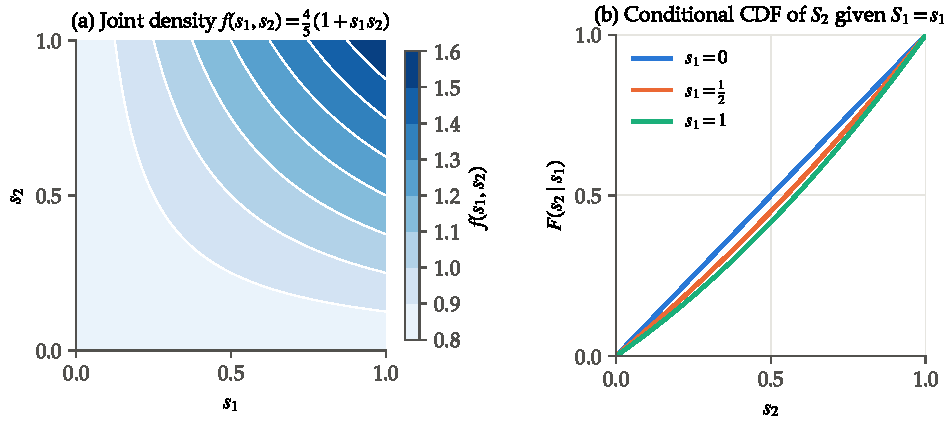
\includegraphics[width=\textwidth]{figures/ch14/affil_example.pdf}
\caption{The affiliated density $f(s_1,s_2)=\frac{4}{5}(1+s_1s_2)$ of \cref{ex:14-affil}(d). Panel (a): the
density is highest where both signals are high. Panel (b): the conditional CDF of $S_2$ shifts down as
$s_1$ rises, so a high signal for one bidder makes high signals of the other more likely.}
\label{fig:14-affil-example}
\end{figure}

Affiliation also has a probabilistic meaning that explains why it is the right condition for auction
theory. Call a set $A\subseteq\R^k$ \emph{increasing} if its indicator function is nondecreasing. Random
variables $\bm Z$ are \emph{associated} if $\Pr(\bm Z\in A\cap B)\ge\Pr(\bm Z\in A)\Pr(\bm Z\in B)$ for all
increasing sets $A$ and $B$. A set $\mathcal{S}\subseteq\R^k$ is a \emph{sublattice} if $\bm z\vee\bm z'$ and
$\bm z\wedge\bm z'$ belong to $\mathcal{S}$ whenever $\bm z$ and $\bm z'$ do. Rectangles and order intervals
$\{\bm z:\bm a\le\bm z\le\bm b\}$ are sublattices. The general definition in the appendix of
\citet{MilgromWeber1982} calls $\bm Z$ affiliated if it is associated conditional on every sublattice. For
variables with a density this coincides with \cref{def:14-affiliation} \citep[Theorem~24]{MilgromWeber1982}.

\begin{proposition}[Association and the covariance inequality]\label{prop:14-association}
\leavevmode
\begin{enumerate}[label=(\alph*)]
  \item The following statements are equivalent \citep[Theorem~22]{MilgromWeber1982}.
  \begin{enumerate}[label=(\roman*)]
    \item $\bm Z$ is associated.
    \item For every pair of nondecreasing functions $g$ and $h$, $\E[g(\bm Z)h(\bm Z)]\ge\E[g(\bm Z)]\,\E[h(\bm
    Z)]$.
    \item For every nondecreasing function $g$ and increasing set $A$, $\E[g(\bm Z)\mid A]\ge\E[g(\bm
    Z)]\ge\E[g(\bm Z)\mid \bar A]$, where $\bar A$ is the complement of $A$.
  \end{enumerate}
  \item $\bm Z$ is affiliated if and only if (ii) and (iii) hold conditional on every sublattice
  $\mathcal{S}$ \citep[Theorem~23]{MilgromWeber1982}. That is, $\E[gh\mid\mathcal{S}]\ge\E[g\mid\mathcal{S}]\,
  \E[h\mid\mathcal{S}]$ and $\E[g\mid A\cap\mathcal{S}]\ge\E[g\mid\mathcal{S}]\ge\E[g\mid\bar A\cap\mathcal{S}]$.
\end{enumerate}
\end{proposition}

\begin{proof}[Proof sketch for part (a)]
To show that (i) implies (ii), take $g$ and $h$ nonnegative and bounded. For a positive integer $K$, define
the step function
\[
g_K(\bm z)=\frac{1}{K}\sum_{l\ge 1}\indic\Bigl\{g(\bm z)>\frac{l}{K}\Bigr\},
\]
which satisfies $g(\bm z)-\frac{1}{K}\le g_K(\bm z)\le g(\bm z)$. Each set $A_l=\{\bm z:g(\bm z)>\frac{l}{K}\}$ is
increasing. Define $h_K$ and increasing sets $B_{l'}$ in the same way. Association gives
\[
\E[g_Kh_K]=\frac{1}{K^2}\sum_{l}\sum_{l'}\Pr(A_l\cap B_{l'})\ \ge\
\frac{1}{K^2}\sum_{l}\sum_{l'}\Pr(A_l)\Pr(B_{l'})=\E[g_K]\,\E[h_K].
\]
Letting $K\to\infty$ proves (ii) for nonnegative bounded functions, and the extension to general $g$ and $h$ is
routine. To show that (ii) implies (iii), take $h=\indic_A$. Then $\E[g\indic_A]\ge\E[g]\Pr(A)$, which is
$\E[g\mid A]\ge\E[g]$. The second inequality follows because $\E[g]=\Pr(A)\E[g\mid A]+\Pr(\bar A)\E[g\mid \bar
A]$ is a weighted average. To show that (iii) implies (i), take $g=\indic_B$. Then $\Pr(B\mid A)\ge\Pr(B)$,
which is association \citep[p.~1119]{MilgromWeber1982}.
\end{proof}

Part (a)(ii) says that nondecreasing functions of affiliated variables are positively correlated. Part (b)
says this remains true conditional on order-interval events, such as the event that the highest rival
signal lies below one's own. This is the form in which affiliation enters equilibrium analysis. The
properties of affiliation used most often are collected next. Write $Y_1\ge Y_2\ge\dots\ge Y_{n-1}$ for the
signals of bidder 1's rivals arranged in decreasing order, so that $Y_1=\max_{j\neq 1}S_j$.

\begin{proposition}[Properties of affiliated variables]\label{prop:14-affil-props}
Let $\bm Z=(Z_1,\dots,Z_k)$ be affiliated.
\begin{enumerate}[label=(\roman*)]
  \item If $g_1,\dots,g_k$ are all nondecreasing or all nonincreasing, then $g_1(Z_1),\dots,g_k(Z_k)$ are
  affiliated \citep[Theorem~3]{MilgromWeber1982}.
  \item Every subvector of $\bm Z$ is affiliated. In particular $Z_1,\dots,Z_{k-1}$ are affiliated
  \citep[Theorem~4]{MilgromWeber1982}.
  \item For every nondecreasing function $H$, the function
  \[
  h(a_1,b_1;\dots;a_k,b_k)=\E\bigl[H(\bm Z)\mid a_1\le Z_1\le b_1,\dots,a_k\le Z_k\le b_k\bigr]
  \]
  is nondecreasing in all its arguments. In particular, $\E[H(\bm Z)\mid Z_1=z_1,\dots,Z_l=z_l]$ is
  nondecreasing in $(z_1,\dots,z_l)$ for each $l=1,\dots,k$ \citep[Theorem~5]{MilgromWeber1982}.
  \item Under \cref{ass:14-mw}, the variables $A_1,\dots,A_m,S_1,Y_1,\dots,Y_{n-1}$ are affiliated
  \citep[Theorem~2]{MilgromWeber1982}.
\end{enumerate}
\end{proposition}

\begin{proof}
Parts (i) and (ii) follow from \cref{prop:14-association}(b)(ii), and part (iii) follows from
\cref{prop:14-association}(b)(iii) \citep[p.~1119]{MilgromWeber1982}. \Cref{sec:14-mw-affil} gives the
arguments. For part (iv), note first that the symmetry of $f$ in the signals implies that the joint density
of $(\bm A,S_1,Y_1,\dots,Y_{n-1})$ is
\begin{equation}\label{eq:14-joint-orderstat}
(n-1)!\;f(\bm a,s_1,y_1,\dots,y_{n-1})\;\indic\{y_1\ge y_2\ge\dots\ge y_{n-1}\}
\end{equation}
\citep[eq.~(4)]{MilgromWeber1982}. The factor $(n-1)!$ counts the orderings of the rivals' signals that
produce the same ordered vector, each of which has the same density by symmetry. The density $f$ is
affiliated by \cref{ass:14-mw}(v). The indicator of any sublattice satisfies \eqref{eq:14-affil-ineq}. If
both points lie in the sublattice, both sides equal one, and otherwise the right side is zero. The set
$\{y_1\ge\dots\ge y_{n-1}\}$ is a sublattice, because the component-wise maximum and minimum of two
nonincreasing sequences are nonincreasing. By \cref{prop:14-affil-char}(ii) the product
\eqref{eq:14-joint-orderstat} is affiliated.
\end{proof}

Parts (iii) and (iv) together imply that $\E[V_1\mid S_1=s,Y_1=y_1,\dots,Y_{n-1}=y_{n-1}]$ is nondecreasing in
all its arguments \citep[p.~1100]{MilgromWeber1982}. In particular, the expected value of the object to
bidder 1 conditional on its own signal and on the highest rival signal,
$v(s,y)=\E[V_1\mid S_1=s,Y_1=y]$, is nondecreasing in both arguments. \Cref{prop:14-mw-spa} shows that $v(s,s)$
is the equilibrium bid in the second-price auction with affiliated values. \Cref{app:math} collects these
results with the other mathematical tools of the book.

\subsection{The winner's curse}\label{sec:14-winners-curse}

Suppose bidders form conditionally independent estimates of a common value $V$, and each estimate is
unbiased. Other things being equal, the bidder with the largest estimate makes the highest bid. The winner
therefore tends to be the bidder who overestimated the value the most. On average, the winner finds that it
had overestimated $V$ \citep[p.~1094]{MilgromWeber1982}. This phenomenon is the \emph{winner's curse}.
Petroleum engineers \citet{CapenClappCampbell1971} claimed that it was responsible for the low profits that
oil companies earned on offshore tracts in the 1960s \citep[p.~1094]{MilgromWeber1982}.

In equilibrium the winner's curse concerns information, and rational bidders do not lose money because of
it. Winning reveals to the winner that its signal was more optimistic than its rivals' signals. This
revelation is ``bad news'' about the value of the object \citep{Milgrom1981}. Rational bidders anticipate it
and condition their bids on the event of winning. The presence of a winner's curse therefore does not imply
that winners regret winning \citep[footnote~7]{AtheyHaile2007}. Losses arise for naive bidders who ignore the
information contained in winning.

The following result makes the bad news precise in the general symmetric model. Recall that
$v(s,y)=\E[V_1\mid S_1=s,Y_1=y]$. In a symmetric equilibrium with a strictly increasing bid function, bidder 1
wins exactly when $Y_1<S_1$.

\begin{proposition}[The bad news in winning]\label{prop:14-wc}
Suppose \cref{ass:14-mw} holds. For every signal $s$ with $\Pr(Y_1<s\mid S_1=s)>0$,
\begin{equation}\label{eq:14-wc}
\E\bigl[V_1\mid S_1=s,\ Y_1<s\bigr]\ \le\ \min\Bigl\{v(s,s),\ \E\bigl[V_1\mid S_1=s\bigr]\Bigr\}.
\end{equation}
Both inequalities are strict if $v(s,y)$ is strictly increasing in $y$ and $\Pr(Y_1<s\mid S_1=s)<1$. Under
private values, $v(s,y)=s$ and both hold with equality.
\end{proposition}

\begin{proof}
By the law of iterated expectations,
\[
\E\bigl[V_1\mid S_1=s,\ Y_1<s\bigr]=\E\bigl[v(s,Y_1)\mid S_1=s,\ Y_1<s\bigr].
\]
By \cref{prop:14-affil-props}(iii) and (iv), $\varphi(y)\equiv v(s,y)$ is nondecreasing in $y$. All expectations
below are conditional on $S_1=s$. For $y<s$ we have $\varphi(y)\le\varphi(s)$, so
\[
\E[\varphi(Y_1)\mid Y_1<s]\ \le\ \varphi(s)=v(s,s),
\]
which is the first inequality. For $y\ge s$ we have $\varphi(y)\ge\varphi(s)$, so
$\E[\varphi(Y_1)\mid Y_1\ge s]\ge\varphi(s)\ge\E[\varphi(Y_1)\mid Y_1<s]$. The unconditional mean is a weighted
average of the two conditional means,
\begin{align*}
\E[V_1\mid S_1=s]=\E[\varphi(Y_1)]
&=\Pr(Y_1<s)\,\E[\varphi(Y_1)\mid Y_1<s]+\Pr(Y_1\ge s)\,\E[\varphi(Y_1)\mid Y_1\ge s]\\
&\ge\Pr(Y_1<s)\,\E[\varphi(Y_1)\mid Y_1<s]+\Pr(Y_1\ge s)\,\E[\varphi(Y_1)\mid Y_1< s]\\
&=\E[\varphi(Y_1)\mid Y_1<s],
\end{align*}
which is the second inequality. If $\varphi$ is strictly increasing, the inequalities between conditional
means are strict whenever both events have positive probability. Under private values,
$\E[V_1\mid S_1=s,Y_1=y]=s$ for all $y$.
\end{proof}

The proof uses affiliation only to guarantee that $v(s,y)$ is nondecreasing in $y$. Interdependence of
values is what creates the curse. In the example $V=\frac{S_1+S_2}{2}$ with independent signals,
$v(s,y)=\frac{s+y}{2}$ rises strictly with $y$, and the curse is present without any dependence between
signals.

The proposition explains why naive bidding fails. Suppose that in a first-price auction every bidder
naively bids its unconditional estimate $\E[V_1\mid S_1=s]$, which increases with $s$. Bidder 1 then wins
exactly when $Y_1<s$. Its expected profit conditional on winning is
\[
\E\bigl[V_1\mid S_1=s,\ Y_1<s\bigr]-\E\bigl[V_1\mid S_1=s\bigr]\ \le\ 0,
\]
which is strictly negative under common values. Naive bidders lose money on average whenever they win.
Equilibrium bids correct for the bad news, as \cref{sec:14-mw-eq} shows.

\begin{example}[The size of the curse with uniform errors]\label{ex:14-wc-uniform}
Consider a mineral rights model with $S_i=V+\epsilon_i$, where the errors $\epsilon_i$ are i.i.d.\ uniform on
$[-\omega,\omega]$ and independent of $V$, and $\omega>0$ is the half-width of the noise. Each signal is an
unbiased estimate, $\E[S_i-V]=0$. The highest signal is $S_{(n:n)}=V+\epsilon_{(n:n)}$. Write
$\epsilon_i=-\omega+2\omega U_i$ with $U_i$ i.i.d.\ uniform on $[0,1]$, so that
$\epsilon_{(n:n)}=-\omega+2\omega U_{(n:n)}$. The maximum of $n$ uniforms has CDF $x^n$ on $[0,1]$, so
\[
\E\bigl[U_{(n:n)}\bigr]=\int_0^1\bigl(1-x^n\bigr)\,dx=1-\frac{1}{n+1}=\frac{n}{n+1}.
\]
Therefore
\begin{equation}\label{eq:14-wc-bias}
\E\bigl[S_{(n:n)}-V\bigr]=-\omega+2\omega\,\frac{n}{n+1}=\omega\,\frac{2n-(n+1)}{n+1}=\omega\,\frac{n-1}{n+1}.
\end{equation}
The bias is zero for $n=1$, equals $\frac{\omega}{3}$ for $n=2$ and rises toward $\omega$ as $n$ grows. The
same steps with $\E[U_{(n-1:n)}]=\frac{n-1}{n+1}$, derived in \eqref{eq:14-uniform-means} below, give
$\E[S_{(n-1:n)}-V]=\omega\frac{n-3}{n+1}$. \Cref{fig:14-wc} plots both.
\end{example}

\begin{figure}[htbp]
\centering
\begin{tikzpicture}
\begin{axis}[
  width=0.82\textwidth, height=6cm,
  xlabel={number of bidders $n$},
  ylabel={$\frac{1}{\omega}\,\E\bigl[S_{(k:n)}-V\bigr]$},
  xmin=0.5, xmax=20.5, ymin=-0.42, ymax=1.08,
  xtick={1,2,4,6,8,10,12,14,16,18,20},
  ytick={-0.25,0,0.25,0.5,0.75,1},
  grid=major, grid style={c14gray!15},
  legend style={at={(0.97,0.05)},anchor=south east,font=\footnotesize,draw=none,fill=white,fill opacity=0.85,text opacity=1},
  legend cell align=left,
  tick label style={font=\footnotesize}, label style={font=\small}]
\addplot[c14gray, thin, forget plot, domain=0.5:20.5] {0};
\addplot[c14gray, densely dashed, forget plot, domain=0.5:20.5] {1};
\addplot[c14blue, thick, mark=*, mark size=1.6pt, domain=1:20, samples=20] {(x-1)/(x+1)};
\addlegendentry{highest signal, $k=n$: $\frac{n-1}{n+1}$}
\addplot[c14orange, thick, mark=square*, mark size=1.5pt, domain=2:20, samples=19] {(x-3)/(x+1)};
\addlegendentry{second-highest signal, $k=n-1$: $\frac{n-3}{n+1}$}
\end{axis}
\end{tikzpicture}
\caption{The winner's curse in the mineral rights model with uniform errors on $[-\omega,\omega]$
(\cref{ex:14-wc-uniform}). Each signal is unbiased, yet the highest of $n$ signals overstates the common
value by $\omega\frac{n-1}{n+1}$ on average. The bias grows with the number of bidders and approaches
$\omega$ (dashed line).}
\label{fig:14-wc}
\end{figure}

More competition makes the bad news in winning worse. With private values, more bidders make each bidder
bid more aggressively (\cref{sec:14-fpa}). With common values, a rational bidder must also correct for a
larger bias in the event of winning. In \cref{ex:14-wc-uniform}, suppose that the prior on $V$ is
\emph{diffuse}, that is, flat over every value that the signals allow. The
second-price equilibrium bid is then $s-\omega\frac{n-2}{n}$, a correction that grows with $n$
(\cref{ex:14-mineral}). The net effect of more bidders on bids is therefore ambiguous under common values.
For the same reason, bids that fall as the number of bidders rises are a misleading test for the winner's
curse \citep{Laffont1997}. \Cref{sec:14-mw-spa} describes a sharper test based on the pivotal value.
\citet{HendricksPorter1988} test whether bidders in the drainage sales of \cref{tab:14-hp-table1} bid in a
way that accounts for the curse (\cref{ch:auction-empirics}).

\begin{remark}[Information aggregation]\label{rem:14-aggregation}
The winner's curse has a positive counterpart. It is tempting to think that the price in a mineral rights
auction conveys no more information than the winner's own estimate. This reasoning is incorrect, since the
winning estimate is the maximum of all estimates and so bounds every loser's estimate
\citep[p.~1094]{MilgromWeber1982}. Let $g(s\mid v)$ be the density of a bidder's estimate when $V=v$. Many
one-parameter families have the MLRP, so that for $v_1<v_2$ the ratio $\frac{g(s\mid v_1)}{g(s\mid v_2)}$
declines as $s$ increases. If this ratio approaches zero, the first-price price with many bidders is a
consistent estimator of $V$, even if no bidder can estimate $V$ closely on its own
\citep{Wilson1977,Milgrom1979}. Prices can thus aggregate dispersed private information.
\end{remark}

\begin{remark}[Privacy versus accuracy of information]\label{rem:14-privacy}
\citet[p.~1094]{MilgromWeber1982} stress that a bidder's expected profit in a mineral rights auction depends
more on the privacy of its information than on its accuracy. In a first-price auction, a bidder whose
information is also available to some other bidder earns zero expected profit in equilibrium
\citep{EngelbrechtWiggansMilgromWeber1983}. This logic fits the near-zero profits of the non-neighbor firms
in the drainage sales, whose information was public and therefore also known to the neighbor firms.
\Cref{prop:14-mw-garbling} proves a related result for second-price auctions.
\end{remark}

\subsection{Order statistics}\label{sec:14-orderstats}

Payments and winning probabilities in auctions are governed by order statistics of bids or values. The
winner of a second-price auction pays the second-highest bid. In a first-price auction a bidder's
probability of winning is the probability that the highest rival bid is lower than its own. This subsection
collects the facts used throughout this chapter and \cref{ch:auction-empirics}. \Cref{sec:B-orderstats}
restates them for reference and adds joint distributions and identification results.

Let $V_1,\dots,V_n$ be i.i.d.\ with continuous CDF $F$ and density $f$. Denote by $V_{(k:n)}$ the $k$-th lowest
of the $n$ draws, so that $V_{(n:n)}$ is the maximum and $V_{(n-1:n)}$ is the second highest. Denote by
$F_{(k:n)}$ its CDF. This indexing from lowest to highest follows \citet[Section~2.1]{AtheyHaile2007}.

\begin{proposition}[Distribution of an order statistic]\label{prop:14-orderstat}
For $k=1,\dots,n$,
\begin{equation}\label{eq:14-orderstat}
F_{(k:n)}(z)=\frac{n!}{(n-k)!\,(k-1)!}\int_0^{F(z)}t^{k-1}(1-t)^{n-k}\,dt,
\end{equation}
and the density of $V_{(k:n)}$ is
\begin{equation}\label{eq:14-orderstat-density}
f_{(k:n)}(z)=\frac{n!}{(n-k)!\,(k-1)!}\,F(z)^{k-1}\bigl(1-F(z)\bigr)^{n-k}f(z).
\end{equation}
\end{proposition}

\begin{proof}
The event $V_{(k:n)}\le z$ occurs if and only if at least $k$ of the $n$ draws are at most $z$. The number of
draws at most $z$ is binomial with parameters $n$ and $F(z)$. Hence
\begin{equation}\label{eq:14-orderstat-binom}
F_{(k:n)}(z)=\sum_{j=k}^{n}\binom{n}{j}F(z)^j\bigl(1-F(z)\bigr)^{n-j}.
\end{equation}
It remains to show that, for $x\in[0,1]$,
\[
\sum_{j=k}^{n}\binom{n}{j}x^j(1-x)^{n-j}=\frac{n!}{(n-k)!\,(k-1)!}\int_0^{x}t^{k-1}(1-t)^{n-k}\,dt.
\]
Both sides vanish at $x=0$, so it suffices that their derivatives agree. Using
$j\binom{n}{j}=n\binom{n-1}{j-1}$ and $(n-j)\binom{n}{j}=n\binom{n-1}{j}$, the derivative of a typical term on the
left is
\[
\frac{d}{dx}\binom{n}{j}x^j(1-x)^{n-j}=n\binom{n-1}{j-1}x^{j-1}(1-x)^{n-j}-n\binom{n-1}{j}x^{j}(1-x)^{n-j-1}.
\]
Summing over $j=k,\dots,n$, the sum telescopes. The second term for $j$ cancels the first term for $j+1$,
and the second term for $j=n$ is zero because $\binom{n-1}{n}=0$. What remains is the first term for $j=k$,
\[
n\binom{n-1}{k-1}x^{k-1}(1-x)^{n-k}=\frac{n!}{(n-k)!\,(k-1)!}\,x^{k-1}(1-x)^{n-k},
\]
which is the derivative of the right side. Formula \eqref{eq:14-orderstat-density} follows by differentiating
\eqref{eq:14-orderstat} with respect to $z$ and applying the chain rule.
\end{proof}

Formula \eqref{eq:14-orderstat} appears as equation (5) in \citet{AtheyHaile2002}. The density
\eqref{eq:14-orderstat-density} has a direct interpretation. One draw falls at $z$, $k-1$ draws fall below
and $n-k$ fall above, and the multinomial coefficient $\frac{n!}{(k-1)!\,1!\,(n-k)!}$ counts the ways of
assigning the draws to these three groups.

From bidder $i$'s point of view, the most important order statistic is the highest of its rivals' values,
$Y_1=\max_{j\neq i}V_j$. Under independence, $Y_1\le y$ if and only if every rival's value is at most $y$, so
\begin{equation}\label{eq:14-highest-rival}
F_{Y_1}(y)=F(y)^{n-1},\qquad f_{Y_1}(y)=(n-1)F(y)^{n-2}f(y).
\end{equation}
This is the case $k=n-1$ of \eqref{eq:14-orderstat} applied to the sample of $n-1$ rivals, since
$Y_1=V_{(n-1:n-1)}$ in that sample. If all bidders use the same strictly increasing bid function, a bidder
with value $v$ wins with probability $F(v)^{n-1}$.

The transaction price in second-price and ascending auctions is the second-highest value. Its CDF is
\begin{equation}\label{eq:14-second-highest}
F_{(n-1:n)}(v)=nF(v)^{n-1}\bigl(1-F(v)\bigr)+F(v)^n=\Lambda_n\bigl(F(v)\bigr),\qquad
\Lambda_n(x)\equiv nx^{n-1}(1-x)+x^n.
\end{equation}
We derive it in two ways. By counting, $V_{(n-1:n)}\le v$ if and only if at least $n-1$ of the $n$ draws are at
most $v$. Either all $n$ draws are at most $v$, with probability $F(v)^n$, or exactly $n-1$ are, with
probability $nF(v)^{n-1}(1-F(v))$. The factor $n$ counts the choices of the single draw above $v$.
Alternatively, set $k=n-1$ in \eqref{eq:14-orderstat}:
\begin{align*}
F_{(n-1:n)}(v)&=\frac{n!}{1!\,(n-2)!}\int_0^{F(v)}t^{n-2}(1-t)\,dt\\
&=n(n-1)\left[\frac{F(v)^{n-1}}{n-1}-\frac{F(v)^n}{n}\right]\\
&=nF(v)^{n-1}-(n-1)F(v)^n\\
&=nF(v)^{n-1}\bigl(1-F(v)\bigr)+F(v)^n.
\end{align*}

The map $\Lambda_n$ is a strictly increasing bijection of $[0,1]$. Indeed $\Lambda_n(0)=0$, $\Lambda_n(1)=1$,
and writing $\Lambda_n(x)=nx^{n-1}-(n-1)x^n$,
\[
\Lambda_n'(x)=n(n-1)x^{n-2}-n(n-1)x^{n-1}=n(n-1)x^{n-2}(1-x)>0\qquad\text{for }x\in(0,1).
\]
Consequently,
\begin{equation}\label{eq:14-lambda-inverse}
F(v)=\Lambda_n^{-1}\bigl(F_{(n-1:n)}(v)\bigr),
\end{equation}
so the distribution of the second-highest value determines $F$. The same argument applies to any order
statistic, because the right side of \eqref{eq:14-orderstat} is strictly increasing in $F(z)$.
\citet[Theorem~1]{AtheyHaile2002} use this fact to show that $F$ is identified from transaction prices
alone, a result developed in \cref{ch:auction-empirics}.

When $F$ is uniform on $[0,1]$, the density of $V_{(k:n)}$ is
$\frac{n!}{(n-k)!\,(k-1)!}x^{k-1}(1-x)^{n-k}$, a beta density with parameters $k$ and $n-k+1$. Using
$\int_0^1x^a(1-x)^b\,dx=\frac{a!\,b!}{(a+b+1)!}$ for nonnegative integers $a$ and $b$, its mean is
\begin{equation}\label{eq:14-uniform-means}
\E\bigl[V_{(k:n)}\bigr]=\frac{n!}{(n-k)!\,(k-1)!}\int_0^1x^{k}(1-x)^{n-k}\,dx
=\frac{n!}{(n-k)!\,(k-1)!}\cdot\frac{k!\,(n-k)!}{(n+1)!}=\frac{k}{n+1}.
\end{equation}
The $n$ draws split $[0,1]$ into $n+1$ segments of equal expected length. In particular
$\E[V_{(n:n)}]=\frac{n}{n+1}$ and $\E[V_{(n-1:n)}]=\frac{n-1}{n+1}$. \Cref{fig:14-orderstat} plots the
densities of the two highest of four uniform values, together with the density of the highest of three
rival values.

\begin{figure}[htbp]
\centering
\begin{tikzpicture}
\begin{axis}[
  width=0.78\textwidth, height=6cm,
  xlabel={$v$}, ylabel={density},
  xmin=0, xmax=1, ymin=0, ymax=4.2,
  xtick={0,0.2,0.4,0.6,0.8,1},
  xticklabels={$0$,$\frac{1}{5}$,$\frac{2}{5}$,$\frac{3}{5}$,$\frac{4}{5}$,$1$},
  grid=major, grid style={c14gray!15},
  legend style={at={(0.03,0.97)},anchor=north west,font=\footnotesize,draw=none},
  legend cell align=left,
  tick label style={font=\footnotesize}, label style={font=\small}]
\addplot[c14blue, thick, domain=0:1, samples=101] {4*x^3};
\addlegendentry{highest, $V_{(4:4)}$: $4v^3$}
\addplot[c14orange, thick, domain=0:1, samples=101] {12*x^2*(1-x)};
\addlegendentry{second highest, $V_{(3:4)}$: $12v^2(1-v)$}
\addplot[c14aqua, thick, dashed, domain=0:1, samples=101] {3*x^2};
\addlegendentry{highest of three rivals, $Y_1$: $3v^2$}
\addplot[c14gray, thin, dotted, domain=0:1] {1};
\addlegendentry{one value: $1$}
\draw[c14blue, densely dotted] (axis cs:0.8,0) -- (axis cs:0.8,4.2);
\draw[c14orange, densely dotted] (axis cs:0.6,0) -- (axis cs:0.6,4.2);
\end{axis}
\end{tikzpicture}
\caption{Densities of order statistics of $n=4$ values drawn from the uniform distribution on $[0,1]$. The
vertical lines mark the means $\E[V_{(4:4)}]=\frac{4}{5}$ and $\E[V_{(3:4)}]=\frac{3}{5}$ from
\eqref{eq:14-uniform-means}. The dashed curve is the density of the highest of a bidder's three rivals,
$f_{Y_1}(v)=3v^2$, from \eqref{eq:14-highest-rival}.}
\label{fig:14-orderstat}
\end{figure}

Finally, two facts about expectations are used repeatedly. For a nonnegative random variable $X$,
$\E[X]=\int_0^\infty\Pr(X>x)\,dx$. For values supported on $[0,\bar v]$, this gives
\begin{equation}\label{eq:14-mean-second}
\E\bigl[V_{(n-1:n)}\bigr]=\int_0^{\bar v}\Bigl[1-\Lambda_n\bigl(F(v)\bigr)\Bigr]dv.
\end{equation}
When signals are dependent, the order statistics of the rivals' signals have the joint density
\eqref{eq:14-joint-orderstat}. In the descending notation of \citet{MilgromWeber1982}, $Y_k$ is the $k$-th
highest of the $n-1$ rivals' signals, which is $S_{(n-k:n-1)}$ in the ascending notation applied to the
rivals' sample.

\section{Second-Price and Ascending Auctions with Private Values}\label{sec:14-spa}

We now solve the simplest auctions in the simplest information structure. Throughout this section values
are private, so each bidder knows its own value $v_i$. The first two results allow any joint distribution
of values. The third specializes to the SIPV model to compute revenue and surplus.

\subsection{Truthful bidding in the second-price auction}\label{sec:14-spa-dominance}

Consider a second-price sealed-bid auction with reserve price $r\ge 0$. Fix bidder $i$ with value $v_i$ and
any bids of its rivals. Let
\[
\tilde m=\max\Bigl\{r,\ \max_{j\neq i}b_j\Bigr\}
\]
be the \emph{price to beat}, the lowest price at which bidder $i$ can win. By \eqref{eq:14-payoff-spa}, a
bid $b\ge r$ wins when it exceeds every rival bid, and the winner pays $\tilde m$. Bidder $i$'s payoff from
such a bid is
\begin{equation}\label{eq:14-spa-payoff}
u_i(b;\bm b_{-i})=(v_i-\tilde m)\,\indic\Bigl\{b>\max_{j\neq i}b_j\Bigr\},
\end{equation}
and its payoff from a bid below $r$ is zero. A bid above $\tilde m$ therefore wins, and a bid below
$\tilde m$ loses. A bid $b=\tilde m$ wins at price $r$ when every rival bid is below $r$. Otherwise it ties
with the highest rival bid, and \eqref{eq:14-payoff-spa} counts the tie as a loss. Any other tie-breaking
rule leaves the argument below unchanged, because a tied bid still earns either $v_i-\tilde m$ or zero.
The payment does not depend on bidder $i$'s own bid, which
only determines whether $i$ wins. A strategy is \emph{weakly dominant} if it does at least as well as any other
strategy against every profile of rivals' bids. It must also do strictly better than each alternative
against some profile. Bids below $r$ are all rejected, so we treat them as one action, not bidding.

\begin{proposition}[Vickrey 1961]\label{prop:14-spa-dominant}
With private values, bidding one's value, $b_i=v_i$, is a weakly dominant strategy in the second-price
sealed-bid auction with any reserve price. The result requires no assumption on the number of bidders, on
the joint distribution of values or on the bidder's knowledge of that distribution.
\end{proposition}

\begin{proof}
Fix the rivals' bids, and hence $\tilde m$. Every bid leads to one of two outcomes. Bidder $i$ either wins
and receives $v_i-\tilde m$, or loses and receives zero. The bid $b=v_i$ wins when $v_i>\tilde m$ and loses
when $v_i<\tilde m$. When $v_i=\tilde m$, both outcomes give zero. Hence the bid $v_i$ yields
\[
u_i(v_i;\bm b_{-i})=\max\{v_i-\tilde m,\ 0\},
\]
the larger of the two possible payoffs. No bid does better against any $\tilde m$. If $v_i<r$, the bid
$v_i$ is rejected and earns zero, which is optimal because any winning bid pays at least $r>v_i$.

Every other bid does strictly worse against some $\tilde m$, with two exceptions. For $v_i<r$, every bid
below $r$ is the same action as bidding $v_i$. For $v_i=r$, not bidding earns the same as bidding $v_i$
against every profile, so we treat the two as one action. A bid $b>v_i$ wins when
$v_i<\tilde m<b$ and then earns $v_i-\tilde m<0$, where bidding $v_i$ would have earned zero. A bid $b<v_i$
loses when $b<\tilde m<v_i$ and earns zero, where bidding $v_i$ would have earned $v_i-\tilde m>0$. Hence
$b_i=v_i$ is weakly dominant \citep{Vickrey1961}.
\end{proof}

\Cref{fig:14-spa-payoff} draws the three cases. Bidding one's value is optimal against every possible price
to beat, so a bidder needs no forecast of rivals' behavior. This is why the result needs neither symmetry,
nor independence, nor common knowledge of the distribution of values.

\begin{figure}[htbp]
\centering
\begin{tikzpicture}
\pgfplotsset{spapanel/.style={
  scale only axis, width=3.75cm, height=3.0cm, axis lines=middle, xmin=0, xmax=1.08, ymin=-0.38, ymax=0.72,
  xtick=\empty, ytick=\empty, xlabel={$\tilde m$}, xlabel style={anchor=west,font=\small},
  title style={font=\small,yshift=4pt}, clip=false}}
\begin{axis}[spapanel, name=pA, title={(a) underbidding, $b<v$}]
  \fill[c14orange!35] (axis cs:0.35,0) -- (axis cs:0.6,0) -- (axis cs:0.35,0.25) -- cycle;
  \addplot[c14gray, densely dashed, domain=0.35:0.6] {0.6-x};
  \addplot[c14blue, very thick, domain=0:0.35] {0.6-x};
  \addplot[c14blue, very thick, domain=0.35:1.0] {0};
  \node[font=\footnotesize,anchor=south west] at (axis cs:0.42,0.18) {forgone gain};
  \node[font=\footnotesize,anchor=north] at (axis cs:0.35,0) {$b$};
  \node[font=\footnotesize,anchor=north] at (axis cs:0.6,0) {$v$};
  \node[font=\small,anchor=east] at (axis cs:0,0.62) {payoff};
\end{axis}
\begin{axis}[spapanel, name=pB, at={($(pA.east)+(0.75cm,0)$)}, anchor=west, title={(b) truthful, $b=v$}]
  \addplot[c14blue, very thick, domain=0:0.6] {0.6-x};
  \addplot[c14blue, very thick, domain=0.6:1.0] {0};
  \node[font=\footnotesize,anchor=south west] at (axis cs:0.30,0.36) {$\max\{v-\tilde m,0\}$};
  \node[font=\footnotesize,anchor=north] at (axis cs:0.6,0) {$v=b$};
\end{axis}
\begin{axis}[spapanel, name=pC, at={($(pB.east)+(0.75cm,0)$)}, anchor=west, title={(c) overbidding, $b>v$}]
  \fill[c14orange!35] (axis cs:0.6,0) -- (axis cs:0.85,0) -- (axis cs:0.85,-0.25) -- cycle;
  \addplot[c14blue, very thick, domain=0:0.85] {0.6-x};
  \addplot[c14blue, very thick, domain=0.85:1.0] {0};
  \node[font=\footnotesize,anchor=north east] at (axis cs:0.6,0) {$v$};
  \node[font=\footnotesize,anchor=north] at (axis cs:0.85,-0.25) {$b$};
  \node[font=\footnotesize,anchor=west] at (axis cs:0.88,-0.14) {added loss};
\end{axis}
\end{tikzpicture}
\caption{Payoff in a second-price auction as a function of the price to beat $\tilde m$, for a bidder with
value $v$. Truthful bidding (b) attains $\max\{v-\tilde m,0\}$ for every $\tilde m$. Underbidding (a) loses
the auction when $b<\tilde m<v$ and forgoes the shaded gains. Overbidding (c) wins when $v<\tilde m<b$ and
adds the shaded losses.}
\label{fig:14-spa-payoff}
\end{figure}

\begin{remark}[What the result does and does not need]\label{rem:14-spa-needs}
The proof compares only the sign of $v_i-\tilde m$. It therefore holds for any increasing utility of money
$\mathcal{U}$ with $\mathcal{U}(0)=0$, so a risk-averse bidder also bids its value (\cref{sec:14-fpa} uses
this). The proof does require private values. With interdependent values a bidder does not know its value
when it bids, and the payoff $v_i-\tilde m$ is replaced by an expectation that depends on what winning at
price $\tilde m$ reveals. \Cref{prop:14-mw-spa} shows that the equilibrium bid then becomes $v(s,s)$.
\end{remark}

\begin{remark}[Other equilibria]\label{rem:14-spa-other}
Truthful bidding is the only weakly undominated strategy, up to the equivalence of all bids below $r$.
The second-price auction has other Bayesian Nash equilibria in weakly dominated strategies. Let values lie in $[\underline v,\bar v]$ and set
$r=\underline v$. Suppose bidder 1 bids $\bar v$ whatever its value and every other bidder bids
$\underline v$. Bidder 1 always wins and pays $\underline v\le v_1$, and no other bid gives it more. Any other
bidder could win only by bidding above $\bar v$, and would then pay $\bar v\ge v_j$. Hence no bidder gains by
deviating. This equilibrium misallocates the object whenever a rival values it more than bidder 1, and it
yields revenue $\underline v$. Following \citet[Section~2.2]{AtheyHaile2007}, we restrict attention to
equilibria in weakly undominated strategies.
\end{remark}

\begin{remark}[Second-price auctions in practice]
Pure second-price sealed-bid auctions are uncommon in practice \citep[footnote~2]{AtheyHaile2007}. The
proxy bidding system of eBay has the flavor of a second-price auction. A bidder submits a maximum, and the
system bids on its behalf up to that maximum, so the winner pays roughly the second-highest maximum. Bidders
can usually observe and respond to the bids of at least some rivals, however, as in an ascending auction.
\end{remark}

\subsection{The English auction with private values}\label{sec:14-english-pv}

The same logic solves the button auction of \cref{def:14-button}. The dynamic structure adds nothing under
private values, because a bidder has nothing to learn from rivals' exits about its own value.

\begin{proposition}[English auction with private values]\label{prop:14-english-dominant}
With private values, consider the English (button) auction with any reserve price. For each bidder, the
strategy of remaining active until the price reaches $v_i$, whatever the history of exits, is weakly
dominant. When all bidders follow it, the bidder with the highest value wins whenever that value is at
least $r$. The winner pays
\begin{equation}\label{eq:14-english-price}
P=\max\bigl\{V_{(n-1:n)},\ r\bigr\}\qquad\text{if }V_{(n:n)}\ge r,
\end{equation}
where $V_{(n:n)}$ and $V_{(n-1:n)}$ are the highest and second-highest values. If $V_{(n:n)}<r$, the object
is not sold. The second-price sealed-bid auction with truthful bids produces the same allocation and price.
\end{proposition}

\begin{proof}
Fix bidder $i$, the strategies of its rivals and the realization of the rivals' values. Rivals observe the
price and the set of active bidders. As long as bidder $i$ is active, its plans for the future do not affect
what the rivals observe. Hence the path of rival exits up to the moment bidder $i$ quits is the same for
every strategy of bidder $i$. Let $\tilde m$ be the price at which the last rival would quit along this
path. Set $\tilde m=r$ if no rival is active at the reserve price, and $\tilde m=+\infty$ if some rival never
quits. Any strategy of bidder $i$ results in some quitting price $d$ along this path, which may depend on the
rival exits it observes. Bidder $i$ wins if $d>\tilde m$ and then pays $\tilde m$, so its payoff is
\[
(v_i-\tilde m)\,\indic\{d>\tilde m\}.
\]
As in \eqref{eq:14-spa-payoff}, bidder $i$ either wins and receives $v_i-\tilde m$ or loses and receives
zero. By the argument in the proof of \cref{prop:14-spa-dominant},
quitting at $d=v_i$ yields $\max\{v_i-\tilde m,0\}$, the largest payoff available against any $\tilde m$.
This holds for every profile of rival strategies and every realization of rival values, so the strategy is
weakly dominant.

When every bidder follows this strategy, bidders quit in increasing order of their values. The auction
ends when the bidder with the second-highest value quits at price $V_{(n-1:n)}$, or at $r$ if that value is
below $r$. The bidder with the highest value wins, provided its value is at least $r$. The second-price
auction with truthful bids gives the same winner and the same price.
\end{proof}

Under private values the English and second-price auctions are therefore equivalent in a weaker sense than
strategic equivalence \citep[p.~1091]{MilgromWeber1982}. Each has a unique dominant strategy equilibrium,
and the two equilibria produce the same outcome. The equilibrium strategy is the one recorded in equation
(2.6) of \citet{AtheyHaile2007}, under which each bidder bids up to its value. The argument requires that
each bidder know its value. It fails when the value depends on what others know, as with minerals of
unknown quantity or a painting to be resold at an unknown price.

An allocation is \emph{efficient} if the object goes to the bidder who values it most. Both auctions
allocate efficiently whenever some bidder values the object above $r$. Without a reserve price the
outcome is always efficient, or Pareto optimal in the terms of \citet[p.~1091]{MilgromWeber1982}. This conclusion does not
depend on symmetry or independence. In symmetric models the Dutch and
first-price auctions also allocate efficiently. With asymmetric bidders they need not
(\cref{sec:14-asym}). Bidders also need no knowledge of rivals' value distributions or of the number of
rivals. \citet[Section~2.1]{AtheyHaile2007} note that the common knowledge assumptions are inconsequential
for ascending auctions with private values.

\subsection{Revenue and surplus with symmetric independent private values}\label{sec:14-spa-revenue}

We now compute expected revenue and bidders' expected surplus in the SIPV model. Values are i.i.d.\ with CDF
$F$ and density $f$ on $[\underline v,\bar v]$, with $\underline v\ge 0$, and the reserve price satisfies
$r\in[\underline v,\bar v]$. By \cref{prop:14-english-dominant} the formulas apply to both the second-price
and the English auction.

\begin{proposition}[Revenue and surplus in the second-price and English auctions]\label{prop:14-spa-revenue}
Consider the SIPV model with reserve price $r$.
\begin{enumerate}[label=(\roman*)]
  \item Expected revenue is
  \begin{equation}\label{eq:14-spa-revenue}
  R(r)=r\bigl[1-F(r)^n\bigr]+\int_r^{\bar v}\Bigl[1-\Lambda_n\bigl(F(v)\bigr)\Bigr]dv.
  \end{equation}
  Without a binding reserve price, $r=\underline v$, this equals
  $\E[V_{(n-1:n)}]=\underline v+\int_{\underline v}^{\bar v}\bigl[1-\Lambda_n(F(v))\bigr]dv$.
  \item A bidder with value $v\ge r$ wins with probability $Q(v)=F(v)^{n-1}$, makes the expected payment
  \begin{equation}\label{eq:14-spa-payment}
  m(v)=rF(r)^{n-1}+\int_r^{v}y\,dF(y)^{n-1}=vF(v)^{n-1}-\int_r^{v}F(y)^{n-1}\,dy,
  \end{equation}
  and earns the expected surplus
  \begin{equation}\label{eq:14-spa-surplus}
  \pi(v)=vQ(v)-m(v)=\int_r^{v}F(y)^{n-1}\,dy.
  \end{equation}
  Bidders with values below $r$ earn zero.
  \item If values are uniform on $[0,1]$, then
  \begin{equation}\label{eq:14-spa-uniform}
  R(r)=\frac{n-1}{n+1}+r^n-\frac{2n}{n+1}\,r^{n+1},\qquad \pi(v)=\frac{v^n-r^n}{n}.
  \end{equation}
  Without a reserve price, revenue is $\frac{n-1}{n+1}$, each bidder's ex ante expected surplus is
  $\frac{1}{n(n+1)}$, and total surplus is $\frac{n}{n+1}$.
\end{enumerate}
\end{proposition}

\begin{proof}
(i) The price is $P=\max\{V_{(n-1:n)},r\}$ if $V_{(n:n)}\ge r$ and zero otherwise. Since $P\ge 0$,
$\E[P]=\int_0^\infty\Pr(P>p)\,dp$. For $p<r$, $P>p$ if and only if the object is sold, that is,
$V_{(n:n)}\ge r$. This has probability $1-F(r)^n$. For $p\ge r$, $P>p$ if and only if $V_{(n-1:n)}>p$, since
$V_{(n-1:n)}>p\ge r$ already implies $V_{(n:n)}>r$. By \eqref{eq:14-second-highest} this has probability
$1-\Lambda_n(F(p))$, which is zero for $p\ge\bar v$. Hence
\[
R(r)=\int_0^{r}\bigl[1-F(r)^n\bigr]dp+\int_r^{\bar v}\Bigl[1-\Lambda_n\bigl(F(p)\bigr)\Bigr]dp,
\]
which is \eqref{eq:14-spa-revenue}. With $r=\underline v$ we have $F(r)=0$, and the first term equals
$\underline v$.

(ii) A bidder with value $v\ge r$ wins if and only if $Y_1<v$. By \eqref{eq:14-highest-rival},
$Q(v)=F(v)^{n-1}$. When it wins, it pays $\max\{Y_1,r\}$. Hence
\[
m(v)=\E\bigl[\max\{Y_1,r\}\,\indic\{Y_1<v\}\bigr]=rF(r)^{n-1}+\int_r^{v}y\,dF(y)^{n-1}.
\]
Integration by parts gives
\[
\int_r^{v}y\,dF(y)^{n-1}=vF(v)^{n-1}-rF(r)^{n-1}-\int_r^{v}F(y)^{n-1}\,dy.
\]
Substituting, $m(v)=vF(v)^{n-1}-\int_r^vF(y)^{n-1}dy$, and therefore
$\pi(v)=vF(v)^{n-1}-m(v)=\int_r^vF(y)^{n-1}dy$.

(iii) With $F(v)=v$ on $[0,1]$ we have $\Lambda_n(v)=nv^{n-1}-(n-1)v^n$. Then
\[
\int_r^1\bigl[1-\Lambda_n(v)\bigr]dv=(1-r)-(1-r^n)+\frac{n-1}{n+1}\bigl(1-r^{n+1}\bigr).
\]
Adding $r(1-r^n)$ gives
\begin{align*}
R(r)&=r-r^{n+1}+r^n-r+\frac{n-1}{n+1}-\frac{n-1}{n+1}\,r^{n+1}\\
&=\frac{n-1}{n+1}+r^n-\frac{2n}{n+1}\,r^{n+1}.
\end{align*}
With $r=0$, revenue is $\frac{n-1}{n+1}$, which matches $\E[V_{(n-1:n)}]$ in \eqref{eq:14-uniform-means}. The
surplus is $\pi(v)=\int_r^vy^{n-1}dy=\frac{v^n-r^n}{n}$. With $r=0$, the ex ante surplus is
$\E[\pi(V)]=\frac{1}{n}\int_0^1v^n\,dv=\frac{1}{n(n+1)}$. Total surplus is $\E[V_{(n:n)}]=\frac{n}{n+1}$,
because the allocation is efficient. As a check, revenue plus the surplus of all $n$ bidders is
$\frac{n-1}{n+1}+\frac{n}{n(n+1)}=\frac{n}{n+1}$.
\end{proof}

Formula \eqref{eq:14-spa-surplus} is the first appearance of a general principle. The interim surplus of a
bidder depends only on the probabilities of winning of lower types,
\[
\pi(v)=\pi(r)+\int_r^{v}Q(y)\,dy.
\]
\Cref{sec:14-ret} shows that this relation holds in every auction and is the source of revenue
equivalence.

The reserve price trades off two effects. Differentiating \eqref{eq:14-spa-uniform},
\[
R'(r)=nr^{n-1}-2nr^n=nr^{n-1}(1-2r).
\]
Revenue rises with $r$ up to $r=\frac{1}{2}$ and falls afterward, for every $n$. A higher reserve raises the
price when exactly one bidder values the object above $r$. It loses the sale when nobody does. For uniform
values, \cref{sec:14-optimal} shows that $r=\frac{1}{2}$ maximizes expected revenue among all selling
mechanisms, a result due to \citet{Myerson1981} and \citet{RileySamuelson1981}. \Cref{tab:14-spa-uniform}
evaluates the formulas of \cref{prop:14-spa-revenue} for several numbers of bidders.

\begin{table}[htbp]
\centering
\caption{Second-price and English auctions with uniform values on $[0,1]$}\label{tab:14-spa-uniform}
\small
\begin{tabular}{@{}ccccccccc@{}}
\toprule
 & \multicolumn{2}{c}{Expected revenue} & \multicolumn{2}{c}{Total surplus} &
 \multicolumn{2}{c}{Surplus per bidder} & Probability \\
\cmidrule(lr){2-3}\cmidrule(lr){4-5}\cmidrule(lr){6-7}
$n$ & $r=0$ & $r=\frac{1}{2}$ & $r=0$ & $r=\frac{1}{2}$ & $r=0$ & $r=\frac{1}{2}$ & of no sale, $r=\frac{1}{2}$ \\
\midrule
2  & 0.3333 & 0.4167 & 0.6667 & 0.5833 & 0.1667 & 0.0833 & 0.2500 \\
3  & 0.5000 & 0.5313 & 0.7500 & 0.7031 & 0.0833 & 0.0573 & 0.1250 \\
5  & 0.6667 & 0.6719 & 0.8333 & 0.8203 & 0.0333 & 0.0297 & 0.0313 \\
10 & 0.8182 & 0.8183 & 0.9091 & 0.9086 & 0.0091 & 0.0090 & 0.0010 \\
\bottomrule
\end{tabular}

\smallskip
\begin{minipage}{0.92\textwidth}
\footnotesize Notes: Computed from \cref{prop:14-spa-revenue}. Revenue is
$\frac{n-1}{n+1}+r^n-\frac{2n}{n+1}r^{n+1}$, total surplus is $\frac{n}{n+1}(1-r^{n+1})$, surplus per bidder is
$\frac{1}{n}\bigl[\frac{1-r^{n+1}}{n+1}-r^n(1-r)\bigr]$ and the probability of no sale is $r^n$. With $n=2$
the exact values are $\frac{1}{3}$ and $\frac{5}{12}$ for revenue, $\frac{2}{3}$ and $\frac{7}{12}$ for
total surplus and $\frac{1}{6}$ and $\frac{1}{12}$ for surplus per bidder.
\end{minipage}
\end{table}

Three patterns stand out in \cref{tab:14-spa-uniform}. Revenue rises and bidder surplus falls as the number
of bidders grows, because the second-highest value moves toward the highest. With two bidders, the reserve
price raises revenue from $\frac{1}{3}$ to $\frac{5}{12}$, a gain of 25 percent. Total surplus falls from
$\frac{2}{3}$ to $\frac{7}{12}$, because the object goes unsold with probability $\frac{1}{4}$. As $n$ grows,
the gain from the reserve price vanishes, since it becomes unlikely that fewer than two bidders value the
object above $r$.

\subsection{What second-price and English auctions reveal}\label{sec:14-spa-data}

The dominant strategy results have strong empirical implications, which \cref{ch:auction-empirics}
develops. In a second-price auction with private values, bids equal values. If all bids from SIPV auctions
are observed, they are i.i.d.\ draws from $F$, and their empirical distribution estimates $F$ directly. In
an English auction the winner's value is never revealed, because the auction stops when the bidder with the
second-highest value quits. The transaction price is the most reliably observed outcome. By
\eqref{eq:14-english-price} it equals $V_{(n-1:n)}$ when the reserve price does not bind. Because $\Lambda_n$ is
strictly increasing, the distribution of transaction prices in auctions with $n$ bidders determines $F$
through \eqref{eq:14-lambda-inverse} \citep[Theorem~1]{AtheyHaile2002}.

Both arguments rest on private values and on the button model. With interdependent values, bids no longer
equal values (\cref{sec:14-mw-eq}). In real open-outcry auctions, recorded bids need not equal the prices at
which bidders would quit (\cref{sec:14-formats-english}). With asymmetric independent private values,
truthful bidding remains dominant and the allocation remains efficient. Revenue is then the expected
second-highest of values drawn from different distributions (\cref{sec:14-asym}).

\section{First-Price Auctions with Symmetric Independent Private Values}\label{sec:14-fpa}

In a first-price sealed-bid auction each bidder submits one sealed bid, the highest bid wins, and the winner pays its own bid. Unlike in the second-price auction of \cref{sec:14-spa}, no bidder has a dominant strategy in this format. The best bid depends on how aggressively the rivals bid, so the analysis requires an equilibrium of a game of incomplete information. This section solves that game in the benchmark model of symmetric independent private values (SIPV). We derive the equilibrium bid function in two ways and study its shape in closed-form examples. We then rewrite the equilibrium condition in terms of the distribution of bids, which is the starting point of the empirical methods in \cref{ch:auction-empirics}. The section ends with reserve prices, multiple equilibria, and risk-averse bidders.

\subsection{The first-price auction as a Bayesian game}\label{sec:14-fpa-game}

We maintain the following assumption throughout \cref{sec:14-fpa}, except where we relax risk neutrality in \cref{sec:14-fpa-risk}.

\begin{assumption}[Symmetric independent private values]\label{ass:14-sipv}
(i) There are $n\ge 2$ risk-neutral bidders and one indivisible object.
(ii) Bidder $i$ privately observes its value $V_i$.
(iii) The values $V_1,\dots,V_n$ are independent draws from a distribution $F$ with support $[\underline v,\bar v]$, where $0\le\underline v<\bar v\le\infty$. The distribution has a finite mean and a continuous density $f$ that is strictly positive on $(\underline v,\bar v)$.
(iv) A losing bidder receives zero, whoever wins.
(v) The number of bidders $n$ and the distribution $F$ are common knowledge.
\end{assumption}

The first-price auction (FPA) under \cref{ass:14-sipv} is a Bayesian game. The players are the $n$ bidders. A player's type is its value $v_i$, and types are drawn from the product distribution $\prod_{i=1}^n F(v_i)$. An action is a bid $b_i\in\R$. The seller may announce a \emph{reserve price} $r\ge\underline v$, which is the lowest bid it accepts. A bidder who does not wish to buy at a price of $r$ or more submits no bid, and we treat this as a bid below $r$. When bidder $i$'s bid is accepted, its payoff is
\begin{equation}\label{eq:14-fpa-payoff}
u_i(b_i,\bm b_{-i};v_i)=(v_i-b_i)\,\indic\Big(b_i>\max_{j\neq i}b_j\Big).
\end{equation}
The payoff depends on the rivals only through their bids. This is the content of private values together with the absence of externalities. Ties are broken at random. They occur with probability zero in every equilibrium we study, because equilibrium bids have continuous distributions.

A \emph{strategy} for bidder $i$ is a bid function $\beta_i$ that maps each value into a bid. We write $B_j=\beta_j(V_j)$ for bidder $j$'s random bid.

\begin{definition}[Bayesian Nash equilibrium]\label{def:14-bne}
A strategy profile $(\beta_1,\dots,\beta_n)$ is a \emph{Bayesian Nash equilibrium} (BNE) if, for every bidder $i$ and every value $v_i$, the bid $\beta_i(v_i)$ maximizes
\[
\E\Big[(v_i-b)\,\indic\Big(b>\max_{j\neq i}\beta_j(V_j)\Big)\Big]
\]
over $b$. The expectation is over the rivals' values. The equilibrium is \emph{symmetric} if $\beta_i=\beta$ for every $i$.
\end{definition}

Each bidder best-responds to the strategies of the others. It knows its own value, treats the rivals' values as random, and shares with them the knowledge of $F$ and of the payoff function.

Consider a bidder who values the object at \$10. If it bids \$10, its payoff is zero whether it wins or loses. If it bids \$9, it earns \$1 each time the bid wins. Any bid with a positive chance of winning beats bidding one's value, so equilibrium bids lie below values. We call the gap $v_i-b_i$ the \emph{shading} of the bid. How much to shade is a trade-off. A lower bid raises the profit conditional on winning but lowers the probability of winning. Let
\[
H(b)=\Pr\Big(\max_{j\neq i}B_j<b\Big)
\]
denote the probability that a bid $b$ wins. Bidder $i$ then maximizes
\begin{equation}\label{eq:14-fpa-objective}
U(b;v_i)=(v_i-b)\,H(b).
\end{equation}
This is the problem of a monopsonist that buys one unit. The value plays the role of the buyer's marginal value, the bid is the price, and $H$ is the residual supply curve. We make the analogy precise in \cref{sec:14-fpa-G}.

Independence implies that $H$ is the same function for every value $v_i$. Bidder $i$'s value tells it nothing about the rivals' values, hence nothing about their bids. The next lemma exploits this fact.

\begin{lemma}[Monotone bidding]\label{lem:14-monotone}
Fix the rivals' strategies and let $H$ be the induced win probability. Let $v'>v$, let $b$ be an optimal bid for value $v$, and let $b'$ be an optimal bid for value $v'$. If $H(b)>0$, then $b'\ge b$. Hence in every equilibrium each bidder's strategy is nondecreasing on the set of values that win with positive probability.
\end{lemma}

\begin{proof}
Optimality of $b$ for $v$ and of $b'$ for $v'$ gives two inequalities:
\begin{align*}
(v-b)H(b)&\ge(v-b')H(b'),\\
(v'-b')H(b')&\ge(v'-b)H(b).
\end{align*}
We add them. The terms $-bH(b)$ and $-b'H(b')$ appear on both sides and cancel, which leaves
\[
vH(b)+v'H(b')\ge vH(b')+v'H(b).
\]
Collecting terms gives
\[
(v'-v)\big[H(b')-H(b)\big]\ge 0.
\]
Since $v'>v$, we obtain $H(b')\ge H(b)$. Suppose now that $b'<b$. Because $H$ is nondecreasing, $H(b')\le H(b)$, so $H(b')=H(b)>0$. Then the bid $b'$ gives value $v$ the payoff $(v-b')H(b)$, which exceeds $(v-b)H(b)$. This contradicts the optimality of $b$ for $v$, so $b'\ge b$.
\end{proof}

The proof uses one property of the objective. The difference $U(b;v')-U(b;v)=(v'-v)H(b)$ is nondecreasing in $b$, so the objective has \emph{increasing differences} in $(b,v)$. A higher value makes higher bids relatively more attractive. With affiliated values, $H$ would depend on $v_i$, and monotonicity requires the stronger tools of \cref{sec:14-mw-fpa}.

\subsection{Equilibrium by the first-order condition}\label{sec:14-fpa-foc}

Let $Y_1=\max_{j\neq i}V_j$ denote the highest value among bidder $i$'s rivals. Under \cref{ass:14-sipv} its distribution function and density are
\[
F_{Y_1}(y)=F(y)^{n-1},\qquad f_{Y_1}(y)=(n-1)F(y)^{n-2}f(y).
\]
The following result is the central equilibrium characterization for first-price auctions.

\begin{proposition}[\citealp{RileySamuelson1981}]\label{prop:14-rs}
Let \cref{ass:14-sipv} hold, and let the seller accept only bids of at least $r\in[\underline v,\bar v)$. There is exactly one symmetric equilibrium in strategies that are continuous on $[r,\bar v)$ and strictly increasing and differentiable on $(r,\bar v)$. In it, a bidder with value $v<r$ does not bid, and a bidder with value $v\ge r$ bids
\begin{equation}\label{eq:14-rs-bid}
\beta(v)=v-\frac{\int_r^v F(t)^{n-1}\,dt}{F(v)^{n-1}},
\end{equation}
with $\beta(r)=r$. Equivalently,
\begin{equation}\label{eq:14-rs-condexp}
\beta(v)=\E\left[\max\{Y_1,r\}\given Y_1<v\right].
\end{equation}
\end{proposition}

When $r=\underline v$, the fraction in \eqref{eq:14-rs-bid} has the form $\frac{0}{0}$ at $v=\underline v$. The bound $\int_{\underline v}^v F(t)^{n-1}dt\le(v-\underline v)F(v)^{n-1}$ shows that the fraction is at most $v-\underline v$, so it vanishes as $v$ falls to $\underline v$ and $\beta(\underline v)=\underline v$. When no reserve price is announced, the rules still bound bids from below, for example by zero. \Citet[footnote 25]{MilgromWeber1982} interpret such a floor as an implicit reserve price. \Cref{sec:14-fpa-multiplicity} shows what happens without any floor.

\begin{proof}
We first derive the bid function from the necessary conditions. We then verify that it is an equilibrium.

\emph{Step 1.} We establish participation and the boundary condition. Suppose all bidders use a strategy $\beta$ with the stated properties. A bidder with $v<r$ who wins pays at least $r>v$, so it prefers not to bid. A bidder must earn a nonnegative expected payoff, since it can always abstain. For $v>r$ this payoff is $(v-\beta(v))F(v)^{n-1}$, which requires $\beta(v)\le v$. Letting $v$ fall to $r$ and using continuity gives $\beta(r)\le r$. Bids below $r$ are rejected, so $\beta(r)\ge r$. Hence
\[
\beta(r)=r.
\]

\emph{Step 2.} We write the bidder's objective. Consider a bidder with value $v\ge r$ who bids $b$ in the range $[r,\beta(\bar v)]$. It wins when every rival bids less than $b$. A rival with value below $r$ does not bid. A rival with value $V_j\ge r$ bids less than $b$ exactly when $V_j<\beta^{-1}(b)$, because $\beta$ is strictly increasing. The rivals' values are independent, so the expected payoff is
\begin{equation}\label{eq:14-rs-objective}
\Pi(b;v)=(v-b)\,F\big(\beta^{-1}(b)\big)^{n-1}.
\end{equation}

\emph{Step 3.} We derive the first-order condition. By the inverse function rule, $\frac{d}{db}\beta^{-1}(b)=\frac{1}{\beta'(\beta^{-1}(b))}$. Differentiating \eqref{eq:14-rs-objective} gives
\[
\frac{\partial\Pi(b;v)}{\partial b}=-F\big(\beta^{-1}(b)\big)^{n-1}+(v-b)(n-1)F\big(\beta^{-1}(b)\big)^{n-2}f\big(\beta^{-1}(b)\big)\frac{1}{\beta'\big(\beta^{-1}(b)\big)}.
\]
For $v\in(r,\bar v)$ the equilibrium bid $\beta(v)$ lies in the interior of the range, so the derivative vanishes at $b=\beta(v)$. Substituting $\beta^{-1}(\beta(v))=v$ yields
\[
0=-F(v)^{n-1}+\big(v-\beta(v)\big)(n-1)F(v)^{n-2}f(v)\frac{1}{\beta'(v)}.
\]

\emph{Step 4.} We rewrite the condition as a differential equation. Multiplying by $\beta'(v)$ gives the equilibrium differential equation
\begin{equation}\label{eq:14-rs-ode}
\beta'(v)F(v)^{n-1}=\big(v-\beta(v)\big)(n-1)F(v)^{n-2}f(v).
\end{equation}
We move the term in $\beta(v)$ to the left:
\[
\beta'(v)F(v)^{n-1}+\beta(v)(n-1)F(v)^{n-2}f(v)=v(n-1)F(v)^{n-2}f(v).
\]
The left side is the derivative of the product $\beta(v)F(v)^{n-1}$, and the right side is $v$ times the derivative of $F(v)^{n-1}$:
\[
\frac{d}{dv}\Big[\beta(v)F(v)^{n-1}\Big]=v\,\frac{d}{dv}\Big[F(v)^{n-1}\Big].
\]

\emph{Step 5.} We solve the differential equation. We integrate both sides from $r$ to $v$:
\[
\beta(v)F(v)^{n-1}-\beta(r)F(r)^{n-1}=\int_r^v t\,d\big[F(t)^{n-1}\big].
\]
Integration by parts evaluates the right side:
\[
\int_r^v t\,d\big[F(t)^{n-1}\big]=vF(v)^{n-1}-rF(r)^{n-1}-\int_r^v F(t)^{n-1}\,dt.
\]
We substitute and use $\beta(r)=r$ from Step 1. The terms $rF(r)^{n-1}$ cancel, which leaves
\[
\beta(v)F(v)^{n-1}=vF(v)^{n-1}-\int_r^v F(t)^{n-1}\,dt.
\]
Dividing by $F(v)^{n-1}>0$ gives \eqref{eq:14-rs-bid}. Every candidate satisfies this equation, so there is at most one symmetric equilibrium of the stated form.

\emph{Step 6.} We check that the candidate is strictly increasing. Rearranging \eqref{eq:14-rs-ode} gives
\[
\beta'(v)=(n-1)\frac{f(v)}{F(v)}\big(v-\beta(v)\big).
\]
By \eqref{eq:14-rs-bid}, $v-\beta(v)=\frac{\int_r^vF(t)^{n-1}dt}{F(v)^{n-1}}>0$ for $v>r$. Hence $\beta'(v)>0$ on $(r,\bar v)$, and the candidate is strictly increasing, as assumed.

\emph{Step 7.} We verify that the candidate is an equilibrium. Suppose all rivals use \eqref{eq:14-rs-bid}. Let $\bar b=\sup_v\beta(v)$. A bid above $\bar b$ wins for sure, like a bid of $\bar b$, but costs more, so it is dominated. A bid below $r$ is rejected and earns zero. Every bid in $[r,\bar b)$ equals $\beta(z)$ for exactly one $z\in[r,\bar v)$. A bidder with value $v$ who bids $\beta(z)$ wins with probability $F(z)^{n-1}$, so its payoff from mimicking type $z$ is
\[
\Pi(z;v)=\big(v-\beta(z)\big)F(z)^{n-1}.
\]
Its derivative with respect to $z$ is
\[
\frac{\partial\Pi(z;v)}{\partial z}=-\beta'(z)F(z)^{n-1}+\big(v-\beta(z)\big)(n-1)F(z)^{n-2}f(z).
\]
The differential equation \eqref{eq:14-rs-ode} at $z$ replaces $\beta'(z)F(z)^{n-1}$ by $\big(z-\beta(z)\big)(n-1)F(z)^{n-2}f(z)$. Therefore
\[
\frac{\partial\Pi(z;v)}{\partial z}=(n-1)F(z)^{n-2}f(z)\Big[\big(v-\beta(z)\big)-\big(z-\beta(z)\big)\Big]=(n-1)F(z)^{n-2}f(z)\,(v-z).
\]
For $v\ge r$ the derivative is positive for $z<v$ and negative for $z>v$. Mimicking one's own type is optimal, and it earns $\int_r^vF(t)^{n-1}dt\ge 0$, which is at least the payoff from abstaining. For $v<r$ the derivative is negative for all $z\ge r$. The best accepted bid is then $r$, which earns $(v-r)F(r)^{n-1}\le 0$, so abstaining is optimal.

\emph{Step 8.} We derive the conditional expectation form. The random variable $\max\{Y_1,r\}$ equals $r$ when $Y_1<r$. Hence
\[
\E\big[\max\{Y_1,r\}\indic(Y_1<v)\big]=rF(r)^{n-1}+\int_r^v y\,d\big[F(y)^{n-1}\big].
\]
By the integration by parts of Step 5, the right side equals $vF(v)^{n-1}-\int_r^vF(t)^{n-1}dt$. Dividing by $\Pr(Y_1<v)=F(v)^{n-1}$ gives \eqref{eq:14-rs-condexp}.
\end{proof}

The conditional expectation form \eqref{eq:14-rs-condexp} has a sharp interpretation. In a second-price auction with reserve price $r$, a winner with value $v$ pays $\max\{Y_1,r\}$. Conditional on winning, that is on $Y_1<v$, its expected payment is the right side of \eqref{eq:14-rs-condexp}. In the first-price auction it bids exactly this amount. Each bidder acts as if its value were the highest and bids its best estimate of the price that the second-highest value (or the reserve) would set. Type by type, expected payments in the two formats coincide, and \cref{sec:14-ret} explains why.

Two features of the equilibrium deserve comment. First, the bid of the marginal participant equals the reserve price. When $r>\underline v$, so that $F(r)>0$, the bid function is also flat there. Letting $v$ fall to $r$ in the formula of Step 6 gives $\beta'(r)=(n-1)\frac{f(r)}{F(r)}\big(r-\beta(r)\big)=0$. Without a binding reserve the slope at $\underline v$ need not vanish. With uniform values on $[0,1]$ it equals $\frac{n-1}{n}$ (\cref{ex:14-uniform}). Second, uniqueness extends beyond the class of symmetric differentiable strategies. Consider an independent private values model with a common compact support and a continuously differentiable density that is positive on its interior. Its FPA has a unique equilibrium, which is in pure, strictly increasing and differentiable strategies \citep[Theorem 2.1(ii)]{AtheyHaile2007}. \Citet{Lebrun1999} and \citet{MaskinRiley2003} establish the uniqueness results behind this statement. With symmetric bidders, the unique equilibrium is therefore the one in \cref{prop:14-rs}. \Cref{thm:14-existence} collects the existence and uniqueness results. The multiplicity example of \cref{sec:14-fpa-multiplicity} shows that such uniqueness results rely on a floor on bids.

\casehead{The original paper} \citet{RileySamuelson1981} ask which auction a seller with independent private value buyers should use to maximize expected revenue. They model a broad class of auctions in which the highest bidder wins. Within it, they derive the first-price equilibrium \eqref{eq:14-rs-bid} with a reserve price and prove that all auctions in the class yield the same expected revenue. They also characterize the revenue-maximizing reserve price, which we derive in \cref{sec:14-optimal}.
\Citet[pp.~1092--1093]{MilgromWeber1982} place the paper with \citet{HarrisRaviv1981} and \citet{Myerson1981} in the self-selection approach, which explained revenue equivalence and was then applied to optimal auction design. \Citet{Vickrey1961} had already solved the first-price auction for uniformly distributed values.

\subsection{Equilibrium by the envelope theorem}\label{sec:14-fpa-envelope}

A second derivation uses the bidder's equilibrium payoff instead of its first-order condition. It requires less smoothness, and it is the template for the revenue equivalence theorem.

Let $\pi(v)$ denote the equilibrium expected payoff of a bidder with value $v\ge r$. Since a bid $\beta(z)$ wins with probability $F(z)^{n-1}$, and since mimicking the own type is optimal,
\[
\pi(v)=\max_{z}\,\big(v-\beta(z)\big)F(z)^{n-1}.
\]
For each fixed $z$ the objective is an affine function of $v$ with slope $F(z)^{n-1}$. The \emph{envelope theorem} states that the derivative of the maximized value equals the partial derivative of the objective with respect to the parameter, evaluated at the optimal choice. The optimal choice is $z=v$, so
\[
\pi'(v)=\frac{\partial}{\partial v}\Big[\big(v-\beta(z)\big)F(z)^{n-1}\Big]_{z=v}=F(v)^{n-1}.
\]
The step is rigorous here because $\pi$ is the upper envelope of a family of affine functions of $v$. Such an envelope is convex, hence absolutely continuous, and its derivative equals the slope of the maximizing line wherever the derivative exists \citep{MilgromSegal2002}. \Cref{app:math} states the envelope theorem in general form.

The marginal participant earns nothing, because $\pi(r)=\big(r-\beta(r)\big)F(r)^{n-1}=0$. Integrating $\pi'$ from $r$ gives
\begin{equation}\label{eq:14-fpa-payoff-envelope}
\pi(v)=\int_r^v F(t)^{n-1}\,dt.
\end{equation}
The payoff is also the probability of winning times the surplus when winning:
\[
\pi(v)=\big(v-\beta(v)\big)F(v)^{n-1}.
\]
Equating the two expressions and solving for $\beta(v)$ gives \eqref{eq:14-rs-bid} again.

The argument used only two features of the first-price auction. The first is that a bidder with value $v$ wins with probability $F(v)^{n-1}$, so the object goes to the highest value among the participants. The second is that the marginal participant earns zero. The pricing rule entered only when we translated $\pi(v)$ into a bid. Any format with these two features gives every type the same payoff \eqref{eq:14-fpa-payoff-envelope}, hence the same expected payment $vF(v)^{n-1}-\pi(v)$. \Cref{sec:14-ret} develops this observation into the revenue equivalence theorem.

\subsection{Examples}\label{sec:14-fpa-examples}

We now compute the equilibrium for four families of distributions. Each computation applies \eqref{eq:14-rs-bid} directly.

\begin{example}[Uniform values]\label{ex:14-uniform}
Let $F(v)=v$ on $[0,1]$ and $r=0$. Then $F(t)^{n-1}=t^{n-1}$ and
\[
\int_0^v t^{n-1}\,dt=\frac{v^n}{n}.
\]
Substituting into \eqref{eq:14-rs-bid} gives
\[
\beta(v)=v-\frac{\frac{v^n}{n}}{v^{n-1}}=v-\frac{v}{n}=\frac{n-1}{n}\,v.
\]
With two bidders, each bids half its value. The highest value $V_{(n:n)}$ has distribution function $v^n$, density $nv^{n-1}$ and mean $\frac{n}{n+1}$. The winner pays its bid, so expected revenue is
\[
\E\big[\beta(V_{(n:n)})\big]=\frac{n-1}{n}\cdot\frac{n}{n+1}=\frac{n-1}{n+1}.
\]
This equals the expected second-highest value $\E[V_{(n-1:n)}]=\frac{n-1}{n+1}$, the revenue of the second-price auction (\cref{prop:14-spa-revenue}). By \eqref{eq:14-fpa-payoff-envelope}, a bidder with value $v$ earns $\pi(v)=\frac{v^n}{n}$, so each bidder's ex ante payoff is $\int_0^1\frac{v^n}{n}dv=\frac{1}{n(n+1)}$. As a check, expected total surplus equals revenue plus the payoffs of all $n$ bidders:
\[
\frac{n-1}{n+1}+n\cdot\frac{1}{n(n+1)}=\frac{n}{n+1}=\E\big[V_{(n:n)}\big].
\]
\end{example}

\begin{figure}[htbp]
\centering
\begin{tikzpicture}
\begin{axis}[width=0.55\textwidth,height=0.47\textwidth,xmin=0,xmax=1,ymin=0,ymax=1,
  xlabel={Value $v$},ylabel={Bid $\beta(v)$},axis lines=left,
  xtick={0,0.25,0.5,0.75,1},ytick={0,0.25,0.5,0.75,1},
  legend style={at={(1.04,0.5)},anchor=west,draw=none,fill=white,font=\small},legend cell align=left]
\addplot[thick,black,dashed,domain=0:1] {x};
\addlegendentry{45-degree line, $\beta(v)=v$}
\addplot[thick,c14blue,domain=0:1] {x/2};
\addlegendentry{$n=2$: $\beta(v)=\frac{1}{2}v$}
\addplot[thick,c14orange,domain=0:1] {2*x/3};
\addlegendentry{$n=3$: $\beta(v)=\frac{2}{3}v$}
\addplot[thick,c14aqua,domain=0:1] {4*x/5};
\addlegendentry{$n=5$: $\beta(v)=\frac{4}{5}v$}
\addplot[thick,c14gray,domain=0:1] {9*x/10};
\addlegendentry{$n=10$: $\beta(v)=\frac{9}{10}v$}
\end{axis}
\end{tikzpicture}
\caption{Equilibrium bids in the first-price auction with values uniform on $[0,1]$ and no reserve price, $\beta(v)=\frac{n-1}{n}v$. Shading falls as the number of bidders grows.}\label{fig:14-rs-uniform}
\end{figure}

\begin{example}[Uniform values with a reserve price]\label{ex:14-uniform-reserve}
Keep $F(v)=v$ on $[0,1]$ and let $r\in(0,1)$. Then
\[
\int_r^v t^{n-1}\,dt=\frac{v^n-r^n}{n},
\]
and \eqref{eq:14-rs-bid} gives, for $v\ge r$,
\[
\beta(v)=v-\frac{v^n-r^n}{nv^{n-1}}=\frac{n-1}{n}\,v+\frac{r^n}{n\,v^{n-1}}.
\]
The reserve raises the bid of every participant by $\frac{r^n}{nv^{n-1}}$. For $n=2$ and $r=\frac12$,
\[
\beta(v)=\frac{v}{2}+\frac{1}{8v},\qquad v\in\Big[\frac12,1\Big],
\]
so that $\beta(\frac12)=\frac12$ and $\beta(1)=\frac58$. The object is sold when the highest value $V_{(2:2)}$, with density $2v$, is at least $\frac12$. Expected revenue is
\[
\int_{\frac{1}{2}}^{1}\Big(\frac{v}{2}+\frac{1}{8v}\Big)2v\,dv=\int_{\frac{1}{2}}^{1}\Big(v^2+\frac14\Big)dv=\Big[\frac{v^3}{3}+\frac{v}{4}\Big]_{\frac{1}{2}}^{1}=\frac{7}{12}-\frac{1}{6}=\frac{5}{12}.
\]
The reserve price raises expected revenue from $\frac13$ to $\frac{5}{12}$. \Cref{sec:14-optimal} shows that $r=\frac12$ is the revenue-maximizing reserve for these values.
\end{example}

\begin{figure}[htbp]
\centering
\begin{tikzpicture}
\begin{axis}[width=0.62\textwidth,height=0.5\textwidth,xmin=0,xmax=1,ymin=0,ymax=1,
  xlabel={Value $v$},ylabel={Bid $\beta(v)$},axis lines=left,
  xtick={0,0.25,0.5,0.75,1},xticklabels={$0$,$\frac14$,$\frac12$,$\frac34$,$1$},
  ytick={0,0.25,0.5,0.625,0.75,1},yticklabels={$0$,$\frac14$,$\frac12$,$\frac58$,$\frac34$,$1$},
  legend style={at={(0.03,0.97)},anchor=north west,draw=none,fill=white,font=\small},legend cell align=left]
\addplot[thick,black,dashed,domain=0:1] {x};
\addlegendentry{45-degree line}
\addplot[thick,c14blue,domain=0:1] {x/2};
\addlegendentry{$r=0$: $\beta(v)=\frac{v}{2}$}
\addplot[thick,c14orange,domain=0.5:1,samples=60] {x/2+1/(8*x)};
\addlegendentry{$r=\frac12$: $\beta(v)=\frac{v}{2}+\frac{1}{8v}$}
\addplot[only marks,mark=*,c14orange,mark size=1.6pt] coordinates {(0.5,0.5)};
\draw[densely dotted,gray] (axis cs:0.5,0) -- (axis cs:0.5,0.5);
\node[font=\small,align=center] at (axis cs:0.25,0.62) {no bid\\when $r=\frac12$};
\end{axis}
\end{tikzpicture}
\caption{Equilibrium bids with two bidders and values uniform on $[0,1]$, without a reserve price and with $r=\frac12$. Values below the reserve do not bid. Participants bid more than without a reserve, and the bid function is flat at $v=r$.}\label{fig:14-rs-reserve}
\end{figure}

\begin{example}[Power distribution]\label{ex:14-power}
Let $F(v)=v^\gamma$ on $[0,1]$ with $\gamma>0$, and $r=0$. Then $F(t)^{n-1}=t^{\gamma(n-1)}$ and
\[
\int_0^v t^{\gamma(n-1)}\,dt=\frac{v^{\gamma(n-1)+1}}{\gamma(n-1)+1}.
\]
Substituting into \eqref{eq:14-rs-bid} gives
\[
\beta(v)=v-\frac{v^{\gamma(n-1)+1}}{\big(\gamma(n-1)+1\big)v^{\gamma(n-1)}}=v-\frac{v}{\gamma(n-1)+1}=\frac{\gamma(n-1)}{\gamma(n-1)+1}\,v.
\]
The parameters enter only through the product $\gamma(n-1)$. The reason is that bidding depends on $F$ and $n$ only through the distribution of the highest rival value, $F_{Y_1}(y)=y^{\gamma(n-1)}$. A bidder facing $n-1$ rivals with exponent $\gamma$ bids like a bidder facing one rival with exponent $\gamma(n-1)$. A larger $\gamma$ shifts probability toward high values, which stiffens competition and reduces shading.
\end{example}

\begin{example}[Exponential values, two bidders]\label{ex:14-exponential}
Let $F(v)=1-e^{-\lambda v}$ on $[0,\infty)$ with $\lambda>0$, $n=2$ and $r=0$. Then
\[
\int_0^v\big(1-e^{-\lambda t}\big)dt=v-\frac{1-e^{-\lambda v}}{\lambda}.
\]
Substituting into \eqref{eq:14-rs-bid} gives
\[
\beta(v)=v-\frac{v-\frac{1-e^{-\lambda v}}{\lambda}}{1-e^{-\lambda v}}=v-\frac{v}{1-e^{-\lambda v}}+\frac{1}{\lambda}=\frac{1}{\lambda}-\frac{v\,e^{-\lambda v}}{1-e^{-\lambda v}}.
\]
The last term equals $\frac{v}{e^{\lambda v}-1}$. It tends to $\frac{1}{\lambda}$ as $v\to 0$ and to $0$ as $v\to\infty$. Hence $\beta(0)=0$ and $\beta(v)$ rises toward $\frac{1}{\lambda}=\E[V]$. Values are unbounded, yet no bid exceeds the mean value. Form \eqref{eq:14-rs-condexp} explains why: with two bidders, $\beta(v)=\E[V_j\mid V_j<v]$, which is below $\E[V_j]$. Expected revenue equals $\frac{1}{2\lambda}$, the mean of the lower of two independent exponential values.
\end{example}

The examples suggest that bids rise with the number of bidders. The next result confirms this for every distribution.

\begin{proposition}[More bidders, less shading]\label{prop:14-fpa-n}
Let \cref{ass:14-sipv} hold and fix $r$. For every $v>r$, the shading $v-\beta(v)$ strictly decreases in $n$ and converges to zero as $n\to\infty$. Equilibrium bids therefore rise with $n$ and converge to values.
\end{proposition}

\begin{proof}
By \eqref{eq:14-rs-bid}, the shading of type $v$ is
\[
v-\beta(v)=\int_r^v\Big(\frac{F(t)}{F(v)}\Big)^{n-1}dt.
\]
The density is positive on $(\underline v,\bar v)$, so $F$ is strictly increasing there and $0\le\frac{F(t)}{F(v)}<1$ for $t<v$. The integrand therefore decreases in $n$ at every $t<v$, strictly wherever $F(t)>0$. This set of $t$ has positive length in $[r,v]$, so the integral strictly decreases in $n$. As $n\to\infty$ the integrand converges to zero at every $t<v$. It is bounded by one on the bounded interval $[r,v]$, so the dominated convergence theorem gives convergence of the integral to zero.
\end{proof}

Conditional on winning, a bidder's estimate of the second-highest value rises with the number of rivals. More bidders thus discipline markdowns in the way that more Cournot competitors discipline markups (\cref{ch:theory}).

\Cref{tab:14-uniform-formats} collects the uniform-value equilibria of six auction formats. The all-pay and third-price bids are derived in \cref{sec:14-ret}. Every format yields expected revenue $\frac{n-1}{n+1}$, and every type makes the same expected payment in every format. This regularity motivates \cref{sec:14-ret}.

\begin{table}[htbp]
\centering
\begin{threeparttable}
\caption{Equilibrium bids, expected payments and expected revenue in six formats, with $n$ symmetric bidders, values uniform on $[0,1]$, and no reserve price.}\label{tab:14-uniform-formats}
\small
\begin{tabular}{lccc}
\toprule
Format & Bid of type $v$ & Expected payment of type $v$ & Expected revenue\\
\midrule
First-price sealed bid & $\frac{n-1}{n}v$ & $\frac{n-1}{n}v^n$ & $\frac{n-1}{n+1}$\\[3pt]
Dutch (descending clock) & stop at $\frac{n-1}{n}v$ & $\frac{n-1}{n}v^n$ & $\frac{n-1}{n+1}$\\[3pt]
Second-price sealed bid & $v$ & $\frac{n-1}{n}v^n$ & $\frac{n-1}{n+1}$\\[3pt]
English (button) & exit at $v$ & $\frac{n-1}{n}v^n$ & $\frac{n-1}{n+1}$\\[3pt]
All-pay & $\frac{n-1}{n}v^n$ & $\frac{n-1}{n}v^n$ & $\frac{n-1}{n+1}$\\[3pt]
Third-price ($n\ge 3$) & $\frac{n-1}{n-2}v$ & $\frac{n-1}{n}v^n$ & $\frac{n-1}{n+1}$\\
\bottomrule
\end{tabular}
\begin{tablenotes}
\footnotesize
\item Notes: The expected payment of type $v$ is taken before the outcome is known, so it includes the event of losing. In the first-price and Dutch auctions it equals the bid times the win probability $v^{n-1}$. In the second-price and English auctions it equals $\E[Y_1\indic(Y_1<v)]=\int_0^v y\,(n-1)y^{n-2}dy$. In the all-pay auction it equals the bid. Expected revenue is $n\int_0^1\frac{n-1}{n}v^n\,dv$.
\end{tablenotes}
\end{threeparttable}
\end{table}

\subsection{The first-order condition in terms of the bid distribution}\label{sec:14-fpa-G}

The equilibrium can be characterized without reference to $F$ or $\beta$. Let $G$ denote the distribution function of a single rival's equilibrium bid and $g$ its density, and suppose the reserve price does not bind ($r=\underline v$). In the symmetric equilibrium, $G(b)=\Pr\big(\beta(V_j)\le b\big)=F\big(\beta^{-1}(b)\big)$ on the bid support $[\underline b,\bar b]=[\beta(\underline v),\beta(\bar v)]$. A bidder with value $v_i$ takes $G$ as given and solves
\[
\max_b\;(v_i-b)\,G(b)^{n-1}.
\]
The first-order condition is
\[
-G(b)^{n-1}+(v_i-b)(n-1)G(b)^{n-2}g(b)=0.
\]
Dividing by $(n-1)G(b)^{n-2}g(b)$ and solving for $v_i$ gives
\begin{equation}\label{eq:14-foc-G}
v_i=b+\frac{G(b)}{(n-1)\,g(b)}.
\end{equation}

Equation \eqref{eq:14-foc-G} is the differential equation \eqref{eq:14-rs-ode} written in terms of the bid distribution. To see this, differentiate $G(b)=F(\beta^{-1}(b))$ to get $g(b)=\frac{f(\beta^{-1}(b))}{\beta'(\beta^{-1}(b))}$. At $b=\beta(v)$,
\[
\frac{G(b)}{(n-1)g(b)}=\frac{F(v)\,\beta'(v)}{(n-1)f(v)}=v-\beta(v),
\]
where the last equality is \eqref{eq:14-rs-ode}. For uniform values, $\beta(v)=\frac{n-1}{n}v$, so bids lie in $[0,\frac{n-1}{n}]$ with $G(b)=\frac{nb}{n-1}$ and $g(b)=\frac{n}{n-1}$. Then $\frac{G(b)}{(n-1)g(b)}=\frac{b}{n-1}$, and \eqref{eq:14-foc-G} gives $v=\frac{nb}{n-1}$, which inverts the bid function.

The right side of \eqref{eq:14-foc-G} involves only the bid, the bid distribution, and the number of bidders. All three are observable when bids are recorded. Each bid can therefore be mapped into the value that rationalizes it, without solving a differential equation and without knowing $F$. \Citet{GuerrePerrigneVuong2000} build their identification result and their two-step nonparametric estimator on this observation (\cref{ch:auction-empirics}). In equilibrium the map $b\mapsto b+\frac{G(b)}{(n-1)g(b)}$ equals $\beta^{-1}$, so it must be strictly increasing. This is a testable restriction on bid data.

The condition also has an economic reading. Rewrite \eqref{eq:14-foc-G} as a markdown relative to the bid:
\begin{equation}\label{eq:14-markdown}
\frac{v_i-b}{b}=\frac{1}{\eta(b)},\qquad \eta(b)=(n-1)\frac{b\,g(b)}{G(b)}=\frac{d\ln G(b)^{n-1}}{d\ln b}.
\end{equation}
Here $\eta(b)$ is the elasticity of the win probability $G(b)^{n-1}$ with respect to the bid. \Citet[footnote 13]{AtheyHaile2007} compare this markdown to that of an \emph{oligopsonist}, a buyer that sets its price from the equilibrium elasticity of its residual supply curve. In the auction, the distribution of the highest rival bid plays the role of the residual supply curve. A buyer that values one unit at $v$ and faces residual supply $S(w)$ maximizes $(v-w)S(w)$, which gives $\frac{v-w}{w}=\frac{1}{\varepsilon_S}$ with $\varepsilon_S$ the supply elasticity. With a single rival the bidder is a monopsonist facing that rival's bid distribution, which is our own reading of the analogy. The markdown rule is the buyer's mirror image of the Lerner rule $\frac{p-c}{p}=\frac{1}{\varepsilon}$ (\cref{ch:theory}). Recovering a value from a bid mirrors recovering marginal cost from a pricing first-order condition (\cref{ch:diffprod}). For uniform values $\eta(b)=n-1$ at every bid, so the relative markdown is $\frac{1}{n-1}$. \Cref{sec:14-procurement} develops the same analogy for procurement auctions, where the bid is a price and the win probability a quantity.

Integrating \eqref{eq:14-foc-G} over the bid distribution yields a simple relation between mean values and mean bids \citep[Section 2.2.1]{AtheyHaile2007}.

\begin{proposition}[Mean values and mean bids]\label{prop:14-mean-bid}
In the symmetric equilibrium of the first-price auction under \cref{ass:14-sipv} with a nonbinding reserve price, let $B$ denote an equilibrium bid, with support $[\underline b,\bar b]$. Then
\begin{equation}\label{eq:14-mean-bid}
\E[V]=\frac{n-2}{n-1}\,\E[B]+\frac{1}{n-1}\,\bar b,\qquad \E[V-B]=\frac{1}{n-1}\big(\bar b-\E[B]\big).
\end{equation}
\end{proposition}

\begin{proof}
In equilibrium $V=B+\frac{G(B)}{(n-1)g(B)}$, where $B$ has density $g$. Taking expectations,
\[
\E[V]=\E[B]+\frac{1}{n-1}\int_{\underline b}^{\bar b}\frac{G(b)}{g(b)}\,g(b)\,db=\E[B]+\frac{1}{n-1}\int_{\underline b}^{\bar b}G(b)\,db.
\]
Integration by parts with $G(\underline b)=0$ and $G(\bar b)=1$ gives
\[
\int_{\underline b}^{\bar b}G(b)\,db=\Big[b\,G(b)\Big]_{\underline b}^{\bar b}-\int_{\underline b}^{\bar b}b\,g(b)\,db=\bar b-\E[B].
\]
Substituting,
\[
\E[V]=\E[B]+\frac{\bar b-\E[B]}{n-1}=\frac{n-2}{n-1}\E[B]+\frac{1}{n-1}\bar b.
\]
The second equation in \eqref{eq:14-mean-bid} follows by subtracting $\E[B]$.
\end{proof}

With two bidders the relation reduces to $\E[V]=\bar b$: the highest bid in the support equals the mean value. Form \eqref{eq:14-rs-condexp} gives the same result directly, since $\beta(\bar v)=\E[Y_1\mid Y_1<\bar v]=\E[V]$ when $n=2$. For uniform values with $n$ bidders, $\E[B]=\frac{n-1}{2n}$ and $\bar b=\frac{n-1}{n}$, and \eqref{eq:14-mean-bid} returns $\frac{n-2}{2n}+\frac{1}{n}=\frac12=\E[V]$. \Citet[Section 2.2.1]{AtheyHaile2007} observe that such moment relations had not been exploited in econometric work.

\subsection{Reserve prices, the Dutch auction, and multiplicity}\label{sec:14-fpa-multiplicity}

The Dutch auction is strategically equivalent to the first-price auction (\cref{prop:14-dutch-fpa}). Its equilibrium is therefore the same: a bidder with value $v\ge r$ stops the descending clock at the price $\beta(v)$ given by \eqref{eq:14-rs-bid}.

A reserve price has two effects in the first-price auction. It excludes all values below $r$, and it raises the bids of all participants. Write $\beta_r$ for the equilibrium bid with reserve $r$ and $\beta_{\underline v}$ for the bid without a binding reserve. By \eqref{eq:14-rs-bid}, for $v>r$,
\[
\beta_r(v)-\beta_{\underline v}(v)=\frac{\int_{\underline v}^v F(t)^{n-1}dt-\int_r^v F(t)^{n-1}dt}{F(v)^{n-1}}=\frac{\int_{\underline v}^r F(t)^{n-1}\,dt}{F(v)^{n-1}}>0.
\]
The reserve acts like an extra competitor who bids $r$. With uniform values the increase is $\frac{r^n}{nv^{n-1}}$, as in \cref{ex:14-uniform-reserve}. The effect fades as $v$ rises, because a high-value bidder rarely faces a situation in which the reserve is the binding competitor. The net effect on revenue weighs the higher bids against the lost sales, and \cref{sec:14-optimal} resolves it.

The boundary condition $\beta(r)=r$ in \cref{prop:14-rs} came from the floor on bids. \Citet[footnote 25]{MilgromWeber1982} show that the floor matters. Suppose any real number is a valid bid, including a negative one, which would oblige the seller to pay the winner. Step 1 of the proof then fails. Integrating the differential equation without a boundary condition gives
\[
\beta(v)F(v)^{n-1}=\int_{\underline v}^v t\,d\big[F(t)^{n-1}\big]-k
\]
for an arbitrary constant $k$. Hence the family of candidates is
\begin{equation}\label{eq:14-multiplicity}
\beta_k(v)=\beta(v)-\frac{k}{F(v)^{n-1}},
\end{equation}
where $\beta$ is the bid \eqref{eq:14-rs-bid} with $r=\underline v$. With uniform values on $[0,1]$ this family is
\[
\beta_k(v)=\frac{n-1}{n}\,v-\frac{k}{v^{n-1}},\qquad k\ge 0.
\]
\Citet[footnote 25]{MilgromWeber1982} print the slope of this family as $\frac{n}{n+1}$. That is a misprint. The footnote carries it into the ranges of the strategies, which it prints as $\big(0,\frac{n}{n+1}\big)$ for $k=0$ and $\big(-\infty,\frac{n}{n+1}-k\big)$ for $k>0$. The slope $\frac{n}{n+1}$ violates the first-order condition, since the two sides of \eqref{eq:14-rs-ode} then differ by $\frac{v^{n-1}}{n+1}$, or by $\frac{1}{n+1}$ after dividing by $v^{n-1}$. The slope $\frac{n-1}{n}$ satisfies it and reproduces exactly the ex ante payoff $\frac{1}{n(n+1)}+k$ that the footnote reports, as we now verify.

Fix $k\ge 0$ and suppose all rivals use $\beta_k$. Its derivative is $\beta_k'(v)=\frac{n-1}{n}+\frac{(n-1)k}{v^n}>0$, so $\beta_k$ is strictly increasing. For $k>0$ its range is $\big(-\infty,\frac{n-1}{n}-k\big)$, and for $k=0$ it is $\big(0,\frac{n-1}{n}\big)$. A bid $\beta_k(z)$ wins with probability $z^{n-1}$, so a bidder with value $v$ who mimics type $z$ earns
\[
\Pi_k(z;v)=\big(v-\beta_k(z)\big)z^{n-1}=v\,z^{n-1}-\frac{n-1}{n}z^n+k.
\]
Differentiating with respect to $z$,
\[
\frac{\partial\Pi_k(z;v)}{\partial z}=(n-1)z^{n-2}v-(n-1)z^{n-1}=(n-1)z^{n-2}(v-z).
\]
The payoff peaks at $z=v$. A bid above the range wins for sure at a higher cost than the top of the range, and a bid below the range (possible only when $k=0$) never wins. Hence $\beta_k$ is a symmetric equilibrium for every $k\ge 0$. Type $v$ earns $\Pi_k(v;v)=\frac{v^n}{n}+k$, and the ex ante payoff is
\[
\int_0^1\Big(\frac{v^n}{n}+k\Big)dv=\frac{1}{n(n+1)}+k.
\]
The allocation is efficient in every member of the family, so total surplus is the same. Each bidder gains $k$, and the seller's expected revenue falls to $\frac{n-1}{n+1}-nk$. In the equilibria with $k>0$, low types submit large negative bids, and even a bidder with value zero expects to receive $k$. \Citet[footnote 25]{MilgromWeber1982} suggest that this possibility may explain why almost all observed auctions have at least an implicit reserve price. The lesson is that the floor on bids, set by a reserve price or by a nonnegativity rule, selects the equilibrium. In empirical work the floor is part of the rules and should be recorded with the bids.

\subsection{Risk-averse bidders}\label{sec:14-fpa-risk}

We now replace risk neutrality in \cref{ass:14-sipv}(i). Each bidder has a utility of money $\mathcal U$ that is strictly increasing and concave, with $\mathcal U(0)=0$, and twice differentiable on $(0,\infty)$. A bidder with value $v$ who wins at price $b$ receives $\mathcal U(v-b)$, and a losing bidder receives $\mathcal U(0)=0$. We look for a symmetric equilibrium with strictly increasing bid function $\beta_u$ and bid distribution $G$.

A bidder with value $v$ solves
\[
\max_b\;\mathcal U(v-b)\,G(b)^{n-1}.
\]
The first-order condition is
\[
-\mathcal U'(v-b)\,G(b)^{n-1}+\mathcal U(v-b)(n-1)G(b)^{n-2}g(b)=0,
\]
which simplifies, after division by $G(b)^{n-2}$, to
\[
\mathcal U'(v-b)\,G(b)=(n-1)\,\mathcal U(v-b)\,g(b).
\]
Following \citet[eq.~(6.24)]{AtheyHaile2007}, define the ratio
\begin{equation}\label{eq:14-ell}
\ell(s)=\frac{\mathcal U(s)}{\mathcal U'(s)}.
\end{equation}
They denote this ratio by $\lambda$. We write $\ell$ to keep $\lambda$ for the exponential rate of \cref{ex:14-exponential}. The first-order condition becomes $\ell(v-b)=\frac{G(b)}{(n-1)g(b)}$, so
\begin{equation}\label{eq:14-risk-foc}
v=b+\ell^{-1}\Big(\frac{G(b)}{(n-1)\,g(b)}\Big),
\end{equation}
which is their eq.~(6.25). The ratio has three properties. First, $\ell(0)=\lim_{s\downarrow 0}\ell(s)=0$. Second, $\ell'(s)=1-\frac{\mathcal U(s)\,\mathcal U''(s)}{\mathcal U'(s)^2}\ge 1$, so $\ell$ is strictly increasing and invertible. Third, concavity and $\mathcal U(0)=0$ give $0=\mathcal U(0)\le\mathcal U(s)+\mathcal U'(s)(0-s)$, that is,
\[
\ell(s)\ge s\quad\text{for } s\ge 0,
\]
with strict inequality for $s>0$ when $\mathcal U$ is strictly concave. Under risk neutrality $\ell(s)=s$, and \eqref{eq:14-risk-foc} reduces to \eqref{eq:14-foc-G}.

In terms of the bid function, $G(b)=F(\beta_u^{-1}(b))$, so at $b=\beta_u(v)$ we have $\frac{G(b)}{(n-1)g(b)}=\frac{F(v)\beta_u'(v)}{(n-1)f(v)}$. Substituting into $\ell(v-b)=\frac{G(b)}{(n-1)g(b)}$ and solving for $\beta_u'(v)$,
\begin{equation}\label{eq:14-risk-ode}
\beta_u'(v)=\frac{\mathcal U\big(v-\beta_u(v)\big)}{\mathcal U'\big(v-\beta_u(v)\big)}\,\frac{f_{Y_1}(v)}{F_{Y_1}(v)}\;\ge\;\big(v-\beta_u(v)\big)\frac{f_{Y_1}(v)}{F_{Y_1}(v)},
\end{equation}
where $\frac{f_{Y_1}}{F_{Y_1}}=(n-1)\frac{f}{F}$ and the inequality uses $\ell(s)\ge s$. This is eq.~(11) of \citet{MilgromWeber1982}. The boundary condition is again $\beta_u(\underline v)=\underline v$, by the argument of Step 1 of \cref{prop:14-rs}.

\begin{example}[Constant relative risk aversion]\label{ex:14-crra}
Let $\mathcal U(x)=x^a$ with $0<a\le 1$, a case of constant relative risk aversion (CRRA), so that the coefficient of relative risk aversion is $1-a$. Then $\ell(s)=\frac{s^a}{a s^{a-1}}=\frac{s}{a}$. Let values be uniform on $[0,1]$, so $\frac{f_{Y_1}(v)}{F_{Y_1}(v)}=\frac{n-1}{v}$. Equation \eqref{eq:14-risk-ode} becomes
\[
\beta_u'(v)=\frac{(n-1)\big(v-\beta_u(v)\big)}{a\,v},
\]
a linear differential equation:
\[
\beta_u'(v)+\frac{n-1}{a\,v}\,\beta_u(v)=\frac{n-1}{a}.
\]
We try $\beta_u(v)=cv$. Substituting gives $c+\frac{(n-1)c}{a}=\frac{n-1}{a}$, so $c(a+n-1)=n-1$. The homogeneous equation adds solutions $Cv^{-\frac{n-1}{a}}$, which are unbounded near zero, and the boundary condition $\beta_u(0)=0$ forces $C=0$. Hence
\[
\beta_u(v)=\frac{n-1}{n-1+a}\,v.
\]
With $a=1$ we recover $\frac{n-1}{n}v$. As $a$ falls, bids rise, and they approach values as $a\to 0$. Expected revenue is $\frac{n-1}{n-1+a}\cdot\frac{n}{n+1}$. Its ratio to the second-price revenue $\frac{n-1}{n+1}$ is $\frac{n}{n-1+a}$, which exceeds one whenever $a<1$. For example, with $n=2$ and $a=\frac12$, bids are $\frac23v$ and expected revenue is $\frac49$, against $\frac13$ in the second-price auction.
\end{example}

The example ranks the formats. To prove the ranking in general we need a simple comparison lemma, which \cref{sec:14-mw-rank} also uses.

\begin{lemma}[Crossing lemma, \citealp{MilgromWeber1982}, Lemma 2]\label{lem:14-crossing}
Let $h_1$ and $h_2$ be continuous on $[\underline x,\bar x]$ and differentiable on $(\underline x,\bar x]$. Suppose (i) $h_1(\underline x)\ge h_2(\underline x)$, and (ii) $h_1(x)<h_2(x)$ implies $h_1'(x)\ge h_2'(x)$. Then $h_1(x)\ge h_2(x)$ for all $x\in[\underline x,\bar x]$.
\end{lemma}

\begin{proof}
Let $d=h_1-h_2$ and suppose, to the contrary, that $d(x)<0$ for some $x>\underline x$. The set $\{t\in[\underline x,x]:d(t)\ge 0\}$ is closed and contains $\underline x$. Let $x_0$ be its largest element. Then $d(x_0)\ge 0$, $x_0<x$, and $d<0$ on $(x_0,x]$. By the mean value theorem there is $\hat x\in(x_0,x)$ with
\[
d'(\hat x)=\frac{d(x)-d(x_0)}{x-x_0}<0.
\]
At $\hat x$ we have $h_1(\hat x)<h_2(\hat x)$ and $h_1'(\hat x)<h_2'(\hat x)$, which contradicts (ii).
\end{proof}

\begin{proposition}[Risk aversion favors the first-price auction, \citealp{Holt1980,MaskinRiley1984}]\label{prop:14-risk-fpa}
Let \cref{ass:14-sipv} hold with risk neutrality replaced by a common utility $\mathcal U$ that is strictly increasing and concave, with $\mathcal U(0)=0$, and twice differentiable on $(0,\infty)$. Let there be no binding reserve price. Then the first-price auction yields at least as much expected revenue as the second-price auction. The ranking is strict when $\mathcal U$ is strictly concave.
\end{proposition}

\begin{proof}
\emph{Step 1.} We start with the second-price auction. Bidding one's value remains a weakly dominant strategy. The proof of \cref{prop:14-spa-dominant} compares the surplus $v-m$ from winning at the highest rival bid $m$ with zero, and an increasing $\mathcal U$ preserves its sign. Expected revenue is therefore $\E[V_{(n-1:n)}]$, as with risk neutrality. Let $\beta_N$ be the risk-neutral first-price bid. By \eqref{eq:14-rs-condexp} with $r=\underline v$, $\beta_N(v)=\E[Y_1\mid Y_1<v]$. Conditional on $V_{(n:n)}=v$, the second-highest value is distributed as $Y_1$ given $Y_1<v$. The law of iterated expectations therefore gives $\E[V_{(n-1:n)}]=\E[\beta_N(V_{(n:n)})]$.

\emph{Step 2.} We show that risk-averse bidders bid more. The risk-neutral bid satisfies $\beta_N'(v)=\big(v-\beta_N(v)\big)\frac{f_{Y_1}(v)}{F_{Y_1}(v)}$. We apply \cref{lem:14-crossing} with $h_1=\beta_u$ and $h_2=\beta_N$. Condition (i) holds because $\beta_u(\underline v)=\beta_N(\underline v)=\underline v$. For condition (ii), suppose $\beta_u(v)<\beta_N(v)$. Then \eqref{eq:14-risk-ode} gives
\[
\beta_u'(v)\ge\big(v-\beta_u(v)\big)\frac{f_{Y_1}(v)}{F_{Y_1}(v)}>\big(v-\beta_N(v)\big)\frac{f_{Y_1}(v)}{F_{Y_1}(v)}=\beta_N'(v).
\]
The lemma yields $\beta_u(v)\ge\beta_N(v)$ for all $v$.

\emph{Step 3.} We compare revenues. Both bid functions are strictly increasing, so the bidder with the highest value wins in both cases. Expected first-price revenue with risk aversion is $\E[\beta_u(V_{(n:n)})]\ge\E[\beta_N(V_{(n:n)})]$, which is the second-price revenue by Step 1.

\emph{Step 4.} We prove strictness. If $\mathcal U$ is strictly concave, then $\ell(s)>s$ for $s>0$. Let $d=\beta_u-\beta_N\ge 0$ and suppose $d(v)=0$ at some $v>\underline v$. Then $v-\beta_u(v)=v-\beta_N(v)>0$, and \eqref{eq:14-risk-ode} holds with strict inequality, so $d'(v)>0$. Hence $d<0$ just to the left of $v$, a contradiction. Thus $\beta_u>\beta_N$ on $(\underline v,\bar v]$, and the revenue ranking is strict.
\end{proof}

The intuition is that shading is a gamble. A lower bid raises the gain from winning but lowers the chance of winning. A risk-averse bidder dislikes this gamble and buys insurance against losing by bidding more. In the second-price auction the bid does not affect the price paid upon winning, so there is no gamble to manage. \Citet[p.~1114]{MilgromWeber1982} combine this result with their ranking for affiliated values. With both affiliation and risk aversion, the first-price and second-price auctions cannot be ranked in general (\cref{sec:14-mw-risk}).

Risk aversion also complicates the inversion of bids. Equation \eqref{eq:14-risk-foc} requires the function $\ell$, which a single bid distribution cannot pin down \citep[Section 6.4]{AtheyHaile2007}. In the CRRA case, $\ell^{-1}(x)=ax$, so values satisfy $V=B+a\frac{G(B)}{(n-1)g(B)}$. Bids rationalized by exponent $a$ are equally well rationalized by any $\tilde a\in(0,a)$ with values
\[
\tilde V=B+\frac{\tilde a}{a}\,(V-B),
\]
which lie between the bids and the original values. More risk-averse bidders with lower values produce the same bids. \Cref{ch:auction-empirics} returns to this identification problem.

Empirical work suggests that the effect is not small. \Citet{CampoEtAl2011} break the indeterminacy with a parametric utility function and a parametric quantile restriction. In sealed-bid timber auctions of the U.S.\ Forest Service, they estimate a CRRA measure of 0.278 \citep[Section~2.4, p.~95]{HortacsuPerrigne2021}. Under CRRA, risk aversion acts like an increase in competition and lowers the bidders' information rents. Exercise~3(b) of \cref{sec:14-exercises} makes this precise. Bidders already bid aggressively, so the seller needs a smaller reserve price. The simulated optimal reserve price is about 19 percent below the one computed under risk neutrality \citep[p.~95]{HortacsuPerrigne2021}.

\casehead{The original papers} \citet{Holt1980} studies procurement auctions with risk-averse bidders and shows that the first-price format yields a lower expected cost to the buyer than the oral or second-price formats. \Citet{MaskinRiley1984} characterize the revenue-maximizing auction when buyers are risk averse. They show that the first-price auction dominates the second-price auction and that the optimal mechanism differs from all the standard formats.
\Citet[p.~1093]{MilgromWeber1982} list the risk-aversion ranking as the seventh conclusion of the independent private values model. They credit it to \citet{HarrisRaviv1981}, \citet{Holt1980}, a 1980 discussion paper by Maskin and Riley, and a 1979 working paper by Matthews. On p.~1114 they give the proof by \cref{lem:14-crossing} that we follow.

\section{Revenue Equivalence}\label{sec:14-ret}

Every format in \cref{tab:14-uniform-formats} yields the same expected revenue. Each type even makes the same expected payment in every format. This section explains the regularity. We first present the geometric argument of \citet{MilgromWeber1982}, then the mechanism-design formulation of \citet{Myerson1981}. We use the theorem to solve for equilibria of new formats, extend it to interdependent values with independent signals, and list the assumptions whose failure breaks it.

\subsection{The self-selection view}\label{sec:14-ret-selfselection}

With independent private values, the four standard formats yield the same expected revenue. \Citet[p.~1092]{MilgromWeber1982} credit this finding to \citet{OrtegaReichert1968} and \citet{Vickrey1962}. They add that it remained a puzzle until the self-selection approach of \citet{HarrisRaviv1981}, \citet{Myerson1981} and \citet{RileySamuelson1981}. We follow their exposition. In this subsection only, $p$ denotes a probability of winning, as in their paper.

Fix the rules of an auction and the strategies of bidder $i$'s rivals. Every action available to bidder $i$, whether a bid, a stopping price or a plan of exits, leads to some probability of winning $p$ and some expected payment. Let $e(p)$ denote the lowest expected payment among the actions that win with probability $p$. Because values are independent, the menu of pairs $(p,e(p))$ depends only on the rules and on the rivals' strategies. It does not depend on bidder $i$'s own value.

A bidder with value $v$ who chooses the pair $(p,e)$ obtains expected utility $vp-e$. Its indifference curves in the $(p,e)$ plane are straight lines $e=vp-\text{constant}$ with slope $v$. A lower intercept means a higher utility. It therefore chooses the point of the menu that touches the lowest line of slope $v$. Let $p^*(v)$ denote the chosen probability. \Cref{fig:14-mw-selfselection} illustrates the choice.

\begin{figure}[htbp]
\centering
\begin{tikzpicture}
\begin{axis}[width=0.72\textwidth,height=0.56\textwidth,xmin=0,xmax=1.04,ymin=0,ymax=0.86,
  axis lines=left,xlabel={Probability of winning $p$},ylabel={Expected payment $e$},
  xtick={0,0.11013,0.59299,0.74883,1},xticklabels={$0$,$p_L$,$p_R$,$p^*(v)$,$1$},
  ytick={0,0.31300},yticklabels={$0$,$e(p^*(v))$},
  every axis x label/.style={at={(axis description cs:0.5,-0.1)},anchor=north},
  clip=false]
\addplot[very thick,black,domain=0:1,samples=200] {0.1*x+2*x^2-4.5*x^3+3.2*x^4};
\addplot[thick,c14blue,domain=0.52:1.02] {0.9*x-0.36094};
\addplot[thick,c14orange,dashed,domain=0.035:0.8] {0.39388*x-0.01365};
\addplot[only marks,mark=*,c14blue,mark size=1.8pt] coordinates {(0.74883,0.31300)};
\addplot[only marks,mark=o,c14orange,mark size=2pt,thick] coordinates {(0.11013,0.02973) (0.59299,0.21992)};
\draw[densely dotted,gray] (axis cs:0.74883,0) -- (axis cs:0.74883,0.31300) -- (axis cs:0,0.31300);
\draw[densely dotted,gray] (axis cs:0.11013,0) -- (axis cs:0.11013,0.02973);
\draw[densely dotted,gray] (axis cs:0.59299,0) -- (axis cs:0.59299,0.21992);
\node[font=\small,c14blue,anchor=west] at (axis cs:0.86,0.38) {slope $v$};
\node[font=\small,c14orange,anchor=south east,align=right] at (axis cs:0.47,0.20) {slope $\hat v$: two points\\of tangency, $p^*$ jumps};
\node[font=\small,anchor=east] at (axis cs:0.93,0.68) {menu $e(p)$};
\draw[decorate,decoration={brace,amplitude=4pt},gray] (axis cs:0.125,0.006) -- (axis cs:0.578,0.006) node[midway,above=4pt,font=\footnotesize] {never chosen};
\end{axis}
\end{tikzpicture}
\caption{The bidder's choice among pairs of win probability and expected payment. Indifference lines have slope equal to the value. A bidder with value $v$ chooses the point where the lowest line of slope $v$ touches the menu. At the value $\hat v$ the line touches the menu twice, and the chosen win probability jumps from $p_L$ to $p_R$. Redrawn after \citet{MilgromWeber1982}, Figure 1, with an illustrative menu.}\label{fig:14-mw-selfselection}
\end{figure}

Two facts follow from the geometry. First, $p^*$ is nondecreasing. Optimality of $p^*(v)$ for $v$ and of $p^*(v')$ for $v'$ gives two revealed-preference inequalities. Adding them, as in the proof of \cref{lem:14-monotone}, yields $(v'-v)\big[p^*(v')-p^*(v)\big]\ge 0$. Second, where $p^*$ is differentiable, the line of slope $v$ is tangent to the menu, so $e'(p^*(v))=v$. The chain rule then gives
\[
\frac{d}{dv}\,e\big(p^*(v)\big)=e'\big(p^*(v)\big)\frac{dp^*(v)}{dv}=v\,\frac{dp^*(v)}{dv}.
\]
Where the line touches the menu at two points, a small increase in $v$ makes $p^*$ jump by $\Delta p^*$. Both points lie on the same line of slope $v$, so the payment jumps by $\Delta e=v\,\Delta p^*$. Combining the smooth parts and the jumps, and integrating from the lowest value $\underline v$,
\begin{equation}\label{eq:14-mw-selfselection}
e\big(p^*(v)\big)=e\big(p^*(\underline v)\big)+\int_{\underline v}^{v}t\,dp^*(t).
\end{equation}

Equation \eqref{eq:14-mw-selfselection} is the core of revenue equivalence. Each type's expected payment depends on the rules only through two objects: the function $p^*$ and the payment of the lowest type. The seller's expected revenue is the sum of the bidders' expected payments, so the same is true of revenue. Every auction that always awards the object to the highest value has $p^*(v)=F(v)^{n-1}$. If, in addition, the lowest type pays nothing, all such auctions produce the same expected revenue. The menu need not be smooth or even continuous \citep[footnote 12]{MilgromWeber1982}. It always contains a point $(0,e(0))$ with $e(0)\le 0$, because a bidder can abstain. The payment $e(0)$ is negative only if the seller subsidizes losing bidders.

For uniform values and two bidders, the first-price menu is easy to compute. A bid $b\in[0,\frac12]$ wins against a rival who bids half its value with probability $p=2b$. The expected payment is $e=bp=\frac{p^2}{2}$. Tangency requires $e'(p)=p=v$, so $p^*(v)=v=F(v)$, and the expected payment is $\frac{v^2}{2}=\int_0^v t\,dt$, as \eqref{eq:14-mw-selfselection} predicts.

\subsection{Mechanisms and incentive compatibility}\label{sec:14-ret-mechanisms}

The general formulation allows asymmetric bidders and arbitrary selling procedures. We use it here and in \cref{sec:14-optimal}.

\begin{assumption}[Independent private values]\label{ass:14-ipv}
There are $n$ risk-neutral bidders. Bidder $i$'s value $V_i$ is drawn from a distribution $F_i$ with a finite mean, support $[\underline v_i,\bar v_i]$ with $\underline v_i$ finite and $\bar v_i\le\infty$, and a density $f_i$ that is strictly positive on the support. Values are independent across bidders. The seller's own value for the object is $v_0$, and it is risk neutral.
\end{assumption}

The seller's value $v_0$ is what the object is worth to the seller if it is not sold. It is not a reserve price.

A \emph{direct mechanism} asks each bidder to report a value. It consists of an allocation rule and a payment rule. The allocation rule $q_i(\bm v)\in[0,1]$ is the probability that bidder $i$ receives the object when the reports are $\bm v=(v_1,\dots,v_n)$, with $\sum_i q_i(\bm v)\le 1$. The payment rule $\tau_i(\bm v)$ is the amount bidder $i$ pays. Bidder $i$ cares about the \emph{interim} allocation and payment, which average over the rivals' values:
\[
Q_i(v_i)=\E\big[q_i(v_i,\bm V_{-i})\big],\qquad m_i(v_i)=\E\big[\tau_i(v_i,\bm V_{-i})\big].
\]
A bidder with value $v_i$ who reports $z$ while the others report truthfully obtains $v_iQ_i(z)-m_i(z)$. Its truthful payoff is
\[
\pi_i(v_i)=v_iQ_i(v_i)-m_i(v_i).
\]
The mechanism is \emph{incentive compatible} (IC) if truth-telling is optimal,
\begin{equation}\label{eq:14-ic}
\pi_i(v_i)\ge v_iQ_i(z)-m_i(z)\quad\text{for all }i,\ v_i,\ z,
\end{equation}
and \emph{individually rational} (IR) if participation is voluntary,
\begin{equation}\label{eq:14-ir}
\pi_i(v_i)\ge 0\quad\text{for all }i,\ v_i.
\end{equation}

The \emph{revelation principle} \citep{Myerson1981} makes direct mechanisms a general tool. Take any auction and any Bayesian Nash equilibrium $(\beta_1,\dots,\beta_n)$ of it. Define $q_i(\bm v)$ and $\tau_i(\bm v)$ as the allocation and payments that result when the bidders play $\beta_1(v_1),\dots,\beta_n(v_n)$. This direct mechanism is incentive compatible. A type $v_i$ who gained by reporting $z$ would have gained in the original auction by playing $\beta_i(z)$, contradicting equilibrium. The direct mechanism produces the same allocation and payments as the auction for every profile of values. Hence any statement about IC direct mechanisms applies to the equilibrium outcomes of all auctions.

\begin{lemma}[Characterization of incentive compatibility]\label{lem:14-ic}
Under \cref{ass:14-ipv}, a direct mechanism is incentive compatible if and only if, for every bidder $i$, (a) $Q_i$ is nondecreasing, and (b) for every $v_i$,
\begin{equation}\label{eq:14-envelope-ic}
\pi_i(v_i)=\pi_i(\underline v_i)+\int_{\underline v_i}^{v_i}Q_i(t)\,dt.
\end{equation}
\end{lemma}

\begin{proof}
We drop the subscript $i$.

\emph{Necessity.} Let $v$ and $v'$ be two values. The IC constraint of type $v$ against report $v'$ reads $\pi(v)\ge vQ(v')-m(v')$. Since $m(v')=v'Q(v')-\pi(v')$, this is
\[
\pi(v)\ge\pi(v')+(v-v')\,Q(v').
\]
Exchanging the roles of $v$ and $v'$ gives
\[
\pi(v')\ge\pi(v)+(v'-v)\,Q(v).
\]
Together the two inequalities give
\[
(v'-v)\,Q(v)\le\pi(v')-\pi(v)\le(v'-v)\,Q(v').
\]
For $v'>v$, dividing by $v'-v$ shows $Q(v)\le Q(v')$, which is (a). Because $0\le Q\le 1$, the same chain gives $|\pi(v')-\pi(v)|\le|v'-v|$. So $\pi$ is Lipschitz, hence absolutely continuous and differentiable almost everywhere. Letting $v'\to v$ in the chain shows that $\pi'(v)=Q(v)$ wherever $Q$ is continuous, which is almost everywhere because $Q$ is monotone. An absolutely continuous function is the integral of its derivative, which gives (b).

\emph{Sufficiency.} Suppose (a) and (b) hold. For any $v$ and $z$, using $m(z)=zQ(z)-\pi(z)$ and (b),
\[
\pi(v)-\big[vQ(z)-m(z)\big]=\pi(v)-\pi(z)-(v-z)Q(z)=\int_z^v\big[Q(t)-Q(z)\big]dt.
\]
If $z<v$, the integrand is nonnegative on $[z,v]$ by (a). If $z>v$, the integral equals $\int_v^z\big[Q(z)-Q(t)\big]dt$, which is also nonnegative by (a). Hence truth-telling is optimal.
\end{proof}

Condition (b) is the envelope formula of \cref{sec:14-fpa-envelope} in general form. Since $m_i(v_i)=v_iQ_i(v_i)-\pi_i(v_i)$, it yields the \emph{payment identity}
\begin{equation}\label{eq:14-payment-identity}
m_i(v_i)=v_iQ_i(v_i)-\pi_i(\underline v_i)-\int_{\underline v_i}^{v_i}Q_i(t)\,dt.
\end{equation}
In an incentive compatible mechanism, the interim allocation and the payoff of the lowest type determine every interim payment.

\subsection{The revenue equivalence theorem}\label{sec:14-ret-theorem}

\begin{proposition}[Revenue equivalence, \citealp{Myerson1981,RileySamuelson1981}]\label{prop:14-ret}
Let \cref{ass:14-ipv} hold. Consider two auctions, each with a Bayesian Nash equilibrium. Suppose the two equilibria induce the same interim allocation $Q_i$ for every bidder, and give the lowest type of each bidder the same expected payoff $\pi_i(\underline v_i)$. Then every type of every bidder makes the same expected payment in the two auctions, and the seller's expected revenue is the same. In particular, let bidders be symmetric ($F_i=F$). Then any auction whose equilibrium awards the object to the highest value and charges the lowest type nothing yields expected revenue $\E[V_{(n-1:n)}]$.
\end{proposition}

\begin{proof}
By the revelation principle, each auction with its equilibrium is an incentive compatible direct mechanism. By the payment identity \eqref{eq:14-payment-identity}, each interim payment $m_i(v_i)$ depends only on $Q_i$ and $\pi_i(\underline v_i)$, which the two auctions share. Expected revenue is $\sum_i\E[m_i(V_i)]$, so it is also the same.

For the symmetric case, the highest value wins, so $Q(v)=F(v)^{n-1}=F_{Y_1}(v)$. The lowest type never wins and pays nothing, so $\pi(\underline v)=0$. The payment identity and integration by parts give
\[
m(v)=vF(v)^{n-1}-\int_{\underline v}^vF(t)^{n-1}\,dt=\int_{\underline v}^v y\,dF_{Y_1}(y)=\E\big[Y_1\indic(Y_1<v)\big].
\]
This is the expected payment of type $v$ in the second-price auction. Summing over bidders,
\[
\sum_{i=1}^n\E\big[m(V_i)\big]=\sum_{i=1}^n\E\Big[\max_{j\neq i}V_j\;\indic\Big(V_i>\max_{j\neq i}V_j\Big)\Big]=\E\big[V_{(n-1:n)}\big].
\]
The last equality holds because exactly one bidder has the highest value, and for that bidder the highest rival value is the second-highest value overall.
\end{proof}

\Citet[Theorem 0]{MilgromWeber1982} state the symmetric case as follows. Assume the independent private values model and a noncooperative equilibrium of some auction mechanism. Suppose that in equilibrium the bidder with the highest value is certain to receive the object, and that a bidder with the lowest possible value has an expected payment of zero. Then the seller's expected revenue equals the expected value of the object to the second-highest evaluator. The symmetric equilibria of the English, Dutch, first-price and second-price auctions satisfy these conditions, so all four yield the same expected price. \Cref{prop:14-ret} generalizes Theorem 0 in two directions: bidders may be asymmetric, and the allocation need not be efficient.

\Citet[p.~1093]{MilgromWeber1982} give the theorem an appealing economic reading. Whatever competitive mechanism sets the price, the sale on average takes place at the lowest price at which supply equals demand. The supply is one unit. At a price $p$, demand is the number of bidders with values above $p$. Demand equals one exactly when $p$ lies between $V_{(n-1:n)}$ and $V_{(n:n)}$, and the lowest such price is $V_{(n-1:n)}$. Revenue equivalence thus says that auctions deliver, on average, the competitive price.

\subsection{Using revenue equivalence to solve for equilibria}\label{sec:14-ret-solve}

Revenue equivalence gives a shortcut to equilibrium bids. Suppose a format has a symmetric equilibrium with a strictly increasing bid function, so that the highest value wins, and the lowest type pays nothing. Then \cref{prop:14-ret} fixes the expected payment of every type at $m(v)=\E[Y_1\indic(Y_1<v)]$. Writing $m(v)$ in terms of the format's bid function gives an equation for that function. The shortcut produces a candidate. Its optimality must still be verified, which we do in each case.

\emph{First-price auction.} The winner pays its bid, so $m(v)=\beta(v)F(v)^{n-1}$. Revenue equivalence gives
\[
\beta(v)=\frac{\E[Y_1\indic(Y_1<v)]}{F_{Y_1}(v)}=\E\left[Y_1\given Y_1<v\right],
\]
which is \eqref{eq:14-rs-condexp} without a reserve price. With a reserve price $r$, the allocation is $Q(v)=F(v)^{n-1}\indic(v\ge r)$ and the type $r$ earns zero. The payment identity then gives $m(v)=vF(v)^{n-1}-\int_r^vF(t)^{n-1}dt=\E[\max\{Y_1,r\}\indic(Y_1<v)]$ for $v\ge r$, which again delivers \eqref{eq:14-rs-condexp}. \Cref{prop:14-rs} verified optimality.

\emph{All-pay auction.} Every bidder pays its bid, win or lose. All-pay auctions model lobbying, research races and other contests in which effort is sunk. Here $m(v)=\beta(v)$, so
\[
\beta^{AP}(v)=\E\big[Y_1\indic(Y_1<v)\big]=\int_{\underline v}^v y\,dF_{Y_1}(y).
\]
For uniform values, $\beta^{AP}(v)=\int_0^v y(n-1)y^{n-2}dy=\frac{n-1}{n}v^n$. To verify optimality, note that a bidder with value $v$ who bids $\beta^{AP}(z)$ earns $vz^{n-1}-\frac{n-1}{n}z^n$. Its derivative with respect to $z$ is $(n-1)z^{n-2}(v-z)$, which changes sign from positive to negative at $z=v$.

\emph{Third-price auction.} With $n\ge 3$ bidders, the highest bidder wins and pays the third-highest bid. Let $Y_2$ denote the second-highest rival value. With a strictly increasing $\beta$, the expected payment is $m(v)=\E[\beta(Y_2)\indic(Y_1<v)]$. Revenue equivalence requires, for every $v$,
\[
\int_{\underline v}^v\E\big[\beta(Y_2)\mid Y_1=y\big]f_{Y_1}(y)\,dy=\int_{\underline v}^v y\,f_{Y_1}(y)\,dy.
\]
Differentiating with respect to $v$ and dividing by $f_{Y_1}(v)$ gives
\begin{equation}\label{eq:14-third-cond}
\E\big[\beta(Y_2)\mid Y_1=v\big]=v.
\end{equation}
Given $Y_1=v$, the other $n-2$ rival values are independent with distribution function $\frac{F(y)}{F(v)}$ on $[\underline v,v]$. The variable $Y_2$ is their maximum, with distribution function $\big(\frac{F(y)}{F(v)}\big)^{n-2}$. Condition \eqref{eq:14-third-cond} becomes
\[
\int_{\underline v}^v\beta(y)\,(n-2)F(y)^{n-3}f(y)\,dy=v\,F(v)^{n-2}.
\]
Differentiating with respect to $v$,
\[
\beta(v)(n-2)F(v)^{n-3}f(v)=F(v)^{n-2}+v(n-2)F(v)^{n-3}f(v).
\]
Dividing by $(n-2)F(v)^{n-3}f(v)$ gives
\begin{equation}\label{eq:14-third-bid}
\beta^{III}(v)=v+\frac{F(v)}{(n-2)\,f(v)}.
\end{equation}
The bid function is increasing whenever $\frac{F}{f}$ is nondecreasing, which holds for log-concave $F$. For uniform values, $\beta^{III}(v)=\frac{n-1}{n-2}v$, so bids exceed values. A bidder's own bid sets the price only when it ranks third, and then it loses anyway. Raising the bid above the value matters only when it overtakes the highest rival bid. The bidder then pays the second-highest rival bid, which may well lie below its value, so overbidding has a positive expected return. To verify optimality, a bidder with value $v$ who bids $\beta^{III}(z)$ earns
\[
\E\big[(v-\beta^{III}(Y_2))\indic(Y_1<z)\big]=\int_{\underline v}^z\big(v-\E[\beta^{III}(Y_2)\mid Y_1=y]\big)f_{Y_1}(y)\,dy=\int_{\underline v}^z(v-y)f_{Y_1}(y)\,dy,
\]
using \eqref{eq:14-third-cond}. Its derivative with respect to $z$ is $(v-z)f_{Y_1}(z)$, so $z=v$ is optimal.

\subsection{Interdependent values with independent signals}\label{sec:14-ret-interdependent}

Revenue equivalence survives interdependent values as long as signals are independent. We show this in an example that \cref{sec:14-mw-ranking} reuses as the benchmark that affiliation breaks.

\begin{example}[A common value with independent signals]\label{ex:14-iv-independent}
Two bidders observe signals $S_1,S_2$ that are independent and uniform on $[0,1]$. The object has the common value $V=\frac{S_1+S_2}{2}$ for both.

\emph{Second-price auction.} We claim that bidding $\beta(s)=s$ is a symmetric equilibrium. Suppose bidder 2 bids $S_2$. Bidder 1 with signal $s$ who bids $b\le 1$ wins when $S_2<b$ and then pays $S_2$. Its expected payoff and its derivative are
\[
\int_0^b\Big(\frac{s+s_2}{2}-s_2\Big)ds_2=\int_0^b\frac{s-s_2}{2}\,ds_2,\qquad \frac{d}{db}\int_0^b\frac{s-s_2}{2}\,ds_2=\frac{s-b}{2}.
\]
The derivative is positive for $b<s$ and negative for $b>s$, so $b=s$ is optimal. Expected revenue is $\E[\min\{S_1,S_2\}]=\frac13$.

\emph{First-price auction.} We look for an equilibrium $\beta(s)=cs$. Suppose bidder 2 bids $cS_2$. Bidder 1 with signal $s$ who bids $b$ wins when $S_2<\frac{b}{c}$. Its expected payoff is
\[
\Pi(b)=\int_0^{\frac{b}{c}}\Big(\frac{s+s_2}{2}-b\Big)ds_2=\frac{b}{c}\Big(\frac{s}{2}-b\Big)+\frac{b^2}{4c^2}.
\]
The first-order condition is
\[
\Pi'(b)=\frac{s}{2c}-\frac{2b}{c}+\frac{b}{2c^2}=0.
\]
At $b=cs$ it reads $\frac{s}{2c}-2s+\frac{s}{2c}=0$, so $c=\frac12$. The second derivative is $-\frac{2}{c}+\frac{1}{2c^2}=-2<0$ at $c=\frac12$, so the bid $\beta(s)=\frac{s}{2}$ is a best response. Expected revenue is $\frac12\E[\max\{S_1,S_2\}]=\frac12\cdot\frac23=\frac13$.

The two formats yield the same revenue. The envelope argument explains why. The value depends on the own signal with slope $\frac12$, and a bidder with signal $s$ wins with probability $s$ in both formats. Hence $\pi'(s)=\frac12 s$, and with $\pi(0)=0$ we get $\pi(s)=\frac{s^2}{4}$ in both formats. Direct computation confirms this: in the second-price auction $\int_0^s\frac{s-s_2}{2}ds_2=\frac{s^2}{4}$, and in the first-price auction $\int_0^s\big(\frac{s+s_2}{2}-\frac{s}{2}\big)ds_2=\frac{s^2}{4}$.
\end{example}

The example generalizes. With independent signals, a bidder's signal does not change the distribution of rival signals. The derivative of its equilibrium payoff with respect to its signal therefore depends only on who wins, as in \cref{lem:14-ic}. Two formats with the same allocation and the same payoff of the lowest type then have the same expected payments. \Citet{Myerson1981} allows for such interdependence through what he calls revision effects.

\subsection{When revenue equivalence fails}\label{sec:14-ret-failures}

Each hypothesis of \cref{prop:14-ret} can fail in practice, and each failure leads to a result later in the chapter.
\begin{itemize}
\item Risk aversion makes payoffs nonlinear in money, so the envelope formula changes. The first-price auction then raises more revenue than the second-price auction (\cref{prop:14-risk-fpa}).
\item Affiliated signals let a bidder's signal shift the distribution of rival signals, so the payment identity no longer holds. The English auction then yields at least as much revenue as the second-price auction, which yields at least as much as the first-price auction (\cref{prop:14-mw-ranking}).
\item Asymmetric bidders break the efficiency of the first-price auction, so the interim allocations of the formats differ (\cref{sec:14-asym}).
\item Endogenous entry with asymmetric bidders lets formats attract different sets of participants (\cref{sec:14-entry}).
\item Collusive bidders do not play the noncooperative equilibrium, and formats differ in how easily a ring sustains its agreement (\cref{sec:14-collusion}).
\item Budget constraints make payoffs nonlinear in money, and the standard formats are then no longer equivalent \citep{CheGale1998}.
\end{itemize}

\section{Reserve Prices and Optimal Auctions}\label{sec:14-optimal}

Revenue equivalence says that the format does not matter once the allocation and the payoff of the lowest type are fixed. A seller can still raise revenue by changing the allocation. It can exclude low values with a reserve price, or it can favor some bidders over others. This section asks which allocation rule maximizes the seller's expected payoff. \Citet{Myerson1981} answered the question for independent private values in general, and \citet{RileySamuelson1981} answered it for symmetric bidders and standard auctions. We maintain \cref{ass:14-ipv}.

\subsection{Expected revenue in terms of virtual values}\label{sec:14-optimal-virtual}

Define bidder $i$'s \emph{virtual valuation}
\begin{equation}\label{eq:14-psi}
\psi_i(v)=v-\frac{1-F_i(v)}{f_i(v)}.
\end{equation}
The next derivation expresses expected revenue in terms of virtual valuations.

Start from the payment identity \eqref{eq:14-payment-identity} and take expectations over $V_i$:
\[
\E\big[m_i(V_i)\big]=\int_{\underline v_i}^{\bar v_i}vQ_i(v)f_i(v)\,dv-\pi_i(\underline v_i)-\int_{\underline v_i}^{\bar v_i}\Big[\int_{\underline v_i}^{v}Q_i(t)\,dt\Big]f_i(v)\,dv.
\]
The double integral runs over the triangle $\underline v_i\le t\le v\le\bar v_i$. Exchanging the order of integration (Fubini's theorem) gives
\[
\int_{\underline v_i}^{\bar v_i}\Big[\int_{\underline v_i}^{v}Q_i(t)\,dt\Big]f_i(v)\,dv=\int_{\underline v_i}^{\bar v_i}Q_i(t)\Big[\int_{t}^{\bar v_i}f_i(v)\,dv\Big]dt=\int_{\underline v_i}^{\bar v_i}Q_i(t)\big(1-F_i(t)\big)\,dt.
\]
We substitute, rename the integration variable, and factor out $f_i(v)$:
\[
\E\big[m_i(V_i)\big]=\int_{\underline v_i}^{\bar v_i}\Big[v-\frac{1-F_i(v)}{f_i(v)}\Big]Q_i(v)f_i(v)\,dv-\pi_i(\underline v_i)=\E\big[\psi_i(V_i)Q_i(V_i)\big]-\pi_i(\underline v_i).
\]
Since $Q_i(v_i)=\E[q_i(v_i,\bm V_{-i})]$ and values are independent, the law of iterated expectations gives $\E[\psi_i(V_i)Q_i(V_i)]=\E[\psi_i(V_i)q_i(\bm V)]$. Summing over bidders,
\begin{equation}\label{eq:14-revenue-psi}
\E\Big[\sum_{i=1}^n m_i(V_i)\Big]=\E\Big[\sum_{i=1}^n\psi_i(V_i)\,q_i(\bm V)\Big]-\sum_{i=1}^n\pi_i(\underline v_i).
\end{equation}
The seller also keeps the object, worth $v_0$, when it is not sold. Its expected payoff is therefore
\begin{equation}\label{eq:14-seller-objective}
\E\Big[\sum_{i=1}^n m_i(V_i)\Big]+v_0\,\E\Big[1-\sum_{i=1}^n q_i(\bm V)\Big]=v_0+\E\Big[\sum_{i=1}^n\big(\psi_i(V_i)-v_0\big)q_i(\bm V)\Big]-\sum_{i=1}^n\pi_i(\underline v_i).
\end{equation}

The virtual valuation is a marginal revenue \citep{BulowRoberts1989}. Consider a seller who posts a price $p$ to a single buyer with value distribution $F$. It sells with probability $x=1-F(p)$, which plays the role of a quantity. The inverse demand is $p(x)=F^{-1}(1-x)$, with $p'(x)=-\frac{1}{f(p)}$. Revenue is $R(x)=x\,p(x)$, and marginal revenue is
\[
R'(x)=p+x\,p'(x)=p-\frac{1-F(p)}{f(p)}=\psi(p).
\]
Selling to a buyer with value $v$ adds $v$ to surplus but forces the seller to leave rent to all higher types. The term $\frac{1-F(v)}{f(v)}$ measures that \emph{information rent}, just as the inframarginal loss $x\,p'(x)$ enters a monopolist's marginal revenue (\cref{ch:theory}). Equation \eqref{eq:14-seller-objective} says that the seller should allocate the object to the bidder with the highest marginal revenue, provided it exceeds its marginal cost $v_0$.

\subsection{The optimal auction}\label{sec:14-optimal-myerson}

\begin{definition}[Regularity]\label{def:14-regular}
The distribution $F_i$ is \emph{regular} if its virtual valuation $\psi_i$ is strictly increasing. It satisfies the \emph{monotone hazard rate} condition if $\frac{f_i(v)}{1-F_i(v)}$ is nondecreasing.
\end{definition}

The monotone hazard rate condition implies regularity, because then $\frac{1-F_i}{f_i}$ is nonincreasing and $\psi_i$ is the sum of the strictly increasing function $v$ and a nondecreasing function. Uniform, exponential and normal distributions satisfy it. For the uniform distribution on $[0,\bar v]$, $\psi(v)=v-(\bar v-v)=2v-\bar v$. For the exponential distribution with rate $\lambda$, $\psi(v)=v-\frac{1}{\lambda}$.

\begin{proposition}[Optimal auction, \citealp{Myerson1981}]\label{prop:14-myerson}
Let \cref{ass:14-ipv} hold with every $F_i$ regular. The following mechanism maximizes the seller's expected payoff among all incentive compatible and individually rational mechanisms.
\begin{enumerate}[label=(\roman*)]
\item The object goes to the bidder with the highest virtual valuation $\psi_i(v_i)$ if that virtual valuation exceeds $v_0$. Otherwise the seller keeps it.
\item The lowest type of every bidder earns zero, $\pi_i(\underline v_i)=0$. One payment rule with this property charges the winner the lowest value it could have reported and still won: $\tau_i(\bm v)=q_i(\bm v)\inf\{z:\psi_i(z)\ge v_0\text{ and }\psi_i(z)\ge\max_{j\neq i}\psi_j(v_j)\}$.
\end{enumerate}
The seller's maximal expected payoff is $\E\big[\max\{v_0,\psi_1(V_1),\dots,\psi_n(V_n)\}\big]$.
\end{proposition}

\begin{proof}
By \eqref{eq:14-seller-objective}, the seller's expected payoff from any IC mechanism is
\[
v_0+\E\Big[\sum_i\big(\psi_i(V_i)-v_0\big)q_i(\bm V)\Big]-\sum_i\pi_i(\underline v_i).
\]
 IR requires $\pi_i(\underline v_i)\ge 0$, so the last term is at least zero. We maximize the middle term pointwise. Fix a profile $\bm v$ and maximize $\sum_i(\psi_i(v_i)-v_0)q_i$ subject to $q_i\ge 0$ and $\sum_iq_i\le 1$. The maximum places all probability on a bidder with the largest $\psi_i(v_i)-v_0$ when it is positive, and none otherwise. This is rule (i), and setting $\pi_i(\underline v_i)=0$ minimizes the subtracted term.

It remains to check that the solution satisfies the constraints. Under regularity, $q_i(v_i,\bm v_{-i})$ from rule (i) is nondecreasing in $v_i$ for every $\bm v_{-i}$, so $Q_i$ is nondecreasing. By \cref{lem:14-ic}, payments defined by the payment identity with $\pi_i(\underline v_i)=0$ make the mechanism IC. IR holds for every type, because $\pi_i(v_i)=\int_{\underline v_i}^{v_i}Q_i(t)dt\ge 0$. The payment rule in (ii) is one such rule. Under it, a bidder wins exactly when its report exceeds a threshold that does not depend on its report, and it pays the threshold. Truth-telling is then a dominant strategy, as in the second-price auction, and the lowest type pays nothing. Finally, with $\pi_i(\underline v_i)=0$ and rule (i), the term inside the expectation in \eqref{eq:14-seller-objective}, plus $v_0$, equals $\max\{v_0,\max_i\psi_i(v_i)\}$ at every profile. Taking expectations gives the stated value.
\end{proof}

Regularity matters only for the monotonicity of $Q_i$. When $\psi_i$ is not monotone, the pointwise rule can violate condition (a) of \cref{lem:14-ic}. \Citet{Myerson1981} then replaces $\psi_i$ by an \emph{ironed} virtual valuation that is flat on the intervals where monotonicity fails. We do not develop ironing here.

\subsection{Symmetric bidders: the optimal reserve price}\label{sec:14-optimal-reserve}

With symmetric bidders, the optimal mechanism is a standard auction with a reserve price.

\begin{corollary}[Optimal reserve price, \citealp{RileySamuelson1981,Myerson1981}]\label{cor:14-optimal-reserve}
Let \cref{ass:14-ipv} hold with $F_i=F$ regular for every $i$, and suppose $\psi(\underline v)<v_0<\bar v$. Let $r^*$ solve
\begin{equation}\label{eq:14-optimal-reserve}
r^*-\frac{1-F(r^*)}{f(r^*)}=v_0.
\end{equation}
Then the following hold.
\begin{enumerate}[label=(\roman*)]
\item The first-price, second-price, English and Dutch auctions with reserve price $r^*$ are all optimal mechanisms.
\item The optimal reserve price exceeds the seller's value, $r^*>v_0$.
\item The optimal reserve price does not depend on the number of bidders.
\end{enumerate}
\end{corollary}

\begin{proof}
With a common and strictly increasing $\psi$, the bidder with the highest virtual valuation is the bidder with the highest value. Rule (i) of \cref{prop:14-myerson} therefore awards the object to the highest value if $\psi(v)>v_0$, that is, if $v>r^*$. Each standard auction with reserve price $r^*$ has a symmetric equilibrium with strictly increasing bids (\cref{prop:14-rs,prop:14-spa-dominant}). In it, the highest value wins whenever it is at least $r^*$, and the lowest type earns zero. By \cref{prop:14-ret}, its expected revenue equals that of the optimal mechanism, which proves (i). For (ii), $\frac{1-F(r^*)}{f(r^*)}>0$ for $r^*<\bar v$, so \eqref{eq:14-optimal-reserve} gives $r^*>v_0$. For (iii), neither $F$ nor $v_0$ depends on $n$.
\end{proof}

A direct calculation in the second-price auction shows the trade-off behind \eqref{eq:14-optimal-reserve}. Raise the reserve from $r$ to $r+dr$. The price rises by $dr$ in the event that exactly one bidder has a value above $r$, which has probability $nF(r)^{n-1}\big(1-F(r)\big)$. The sale is lost, and the seller receives $v_0$ instead of $r$, in the event that the highest value lies in $[r,r+dr]$, which has probability $nF(r)^{n-1}f(r)\,dr$. The marginal effect on the seller's payoff is
\[
nF(r)^{n-1}\Big[\big(1-F(r)\big)-(r-v_0)f(r)\Big]=nF(r)^{n-1}f(r)\big[v_0-\psi(r)\big].
\]
The seller gains from raising $r$ while $\psi(r)<v_0$ and loses once $\psi(r)>v_0$. The number of bidders enters only through the positive factor $nF(r)^{n-1}$, which explains why $r^*$ does not depend on $n$. The reserve price is a monopoly price. It is set as if the seller faced a single buyer, because it binds only when a single buyer is left.

\Citet[Section~2.1, p.~87]{HortacsuPerrigne2021} state the same condition, $r^*=v_0+\frac{1-F(r^*)}{f(r^*)}$, and stress that it does not depend on the number of potential bidders. Setting $r^*$ requires knowledge of $F$, which is what the empirical methods of \cref{ch:auction-empirics} estimate. The estimated gains can be large. In ascending auctions of British Columbia timber, \citet{Paarsch1997} finds average optimal reserve prices 3.4 to 4.2 times the observed ones. The range corresponds to seller values from zero to the appraised value of the timber \citep[p.~88]{HortacsuPerrigne2021}. \Citet{HaileTamer2003} bound the optimal reserve price in U.S.\ Forest Service ascending auctions. Depending on the seller's value, the implied gain in the seller's profit ranges from little to 34 percent \citep[p.~88]{HortacsuPerrigne2021}.

For values uniform on $[0,1]$, $\psi(v)=2v-1$ and \eqref{eq:14-optimal-reserve} gives $r^*=\frac{1+v_0}{2}$, so $r^*=\frac12$ when $v_0=0$. For exponential values with rate $\lambda$, $\psi(v)=v-\frac{1}{\lambda}$ and $r^*=v_0+\frac{1}{\lambda}$, which equals $\frac{1}{\lambda}$ when $v_0=0$. \Cref{fig:14-virtual} shows the uniform case. \Citet[p.~1093]{MilgromWeber1982} summarize the implication. For many common distributions, including the normal, exponential and uniform, the four standard formats with suitably chosen reserve prices or entry fees are optimal auctions.

\begin{figure}[htbp]
\centering
\begin{tikzpicture}
\begin{axis}[width=0.56\textwidth,height=0.5\textwidth,xmin=0,xmax=1,ymin=-1,ymax=1,
  axis lines=left,xlabel={Value $v$},ylabel={},
  xtick={0,0.5,0.65,1},xticklabels={$0$,$\frac12$,$\frac{13}{20}$,$1$},
  ytick={-1,-0.5,0,0.3,1},yticklabels={$-1$,$-\frac12$,$0$,$\frac{3}{10}$,$1$},clip=false,
  legend style={at={(0.5,1.04)},anchor=south,draw=none,fill=white,font=\small},legend columns=2,legend cell align=left]
\addplot[thick,black,dashed,domain=0:1] {x};
\addlegendentry{value $v$}
\addplot[thick,c14blue,domain=0:1] {2*x-1};
\addlegendentry{virtual valuation $\psi(v)=2v-1$}
\addplot[thin,gray,domain=0:1] {0};
\addplot[thin,gray,densely dashed,domain=0:1] {0.3};
\addplot[only marks,mark=*,c14orange,mark size=1.8pt] coordinates {(0.5,0) (0.65,0.3)};
\draw[densely dotted,c14orange] (axis cs:0.65,-1) -- (axis cs:0.65,0.3);
\draw[densely dotted,c14orange] (axis cs:0.5,-1) -- (axis cs:0.5,0);
\node[font=\small,anchor=west] at (axis cs:1.02,0.3) {$v_0=\frac{3}{10}$: $r^*=\frac{13}{20}$};
\node[font=\small,anchor=west] at (axis cs:1.02,0) {$v_0=0$: $r^*=\frac12$};
\draw[<->,gray] (axis cs:0.25,-0.5) -- (axis cs:0.25,0.25) node[midway,left,font=\footnotesize] {$\frac{1-F(v)}{f(v)}$};
\end{axis}
\end{tikzpicture}
\caption{Virtual valuation for values uniform on $[0,1]$. The gap between the value and the virtual valuation is the information rent $\frac{1-F(v)}{f(v)}=1-v$. The optimal reserve price is the value at which the virtual valuation equals the seller's value $v_0$, so it exceeds $v_0$.}\label{fig:14-virtual}
\end{figure}

\subsection{The cost of a reserve price: a worked example}\label{sec:14-optimal-example}

Let values be uniform on $[0,1]$, $v_0=0$ and $n=2$. Without a reserve price, revenue is $\E[V_{(1:2)}]=\frac13$. With the optimal reserve $r^*=\frac12$, \cref{prop:14-myerson} gives expected revenue
\[
\E\big[\max\{0,\psi(V_{(2:2)})\}\big]=\int_{\frac{1}{2}}^{1}(2v-1)\,2v\,dv=2\int_{\frac{1}{2}}^{1}(2v^2-v)\,dv=2\Big[\frac{2v^3}{3}-\frac{v^2}{2}\Big]_{\frac{1}{2}}^{1}=2\Big(\frac16+\frac{1}{24}\Big)=\frac{5}{12}.
\]
A direct computation in the second-price auction confirms the number. Both values exceed $\frac12$ with probability $\frac14$, and the price is then the lower value, with conditional mean $\frac23$. Exactly one value exceeds $\frac12$ with probability $\frac12$, and the price is then $\frac12$. Expected revenue is $\frac14\cdot\frac23+\frac12\cdot\frac12=\frac{5}{12}$, the same as the first-price revenue in \cref{ex:14-uniform-reserve}.

The gain to the seller comes at a cost. With probability $\frac14$ both values fall below $\frac12$ and the object is not sold, although the seller values it at zero. The expected surplus lost in this event is $\int_0^{\frac{1}{2}}v\,2v\,dv=\frac{1}{12}$. Total surplus falls from $\frac23$ to $\frac{7}{12}$, and the bidders' combined surplus falls from $\frac13$ to $\frac16$. The reserve price thus transfers $\frac{1}{12}$ from bidders to the seller and destroys another $\frac{1}{12}$. This exclusion of buyers who value the object more than the seller is the auction analogue of the deadweight loss of monopoly pricing.

The gain from the reserve shrinks quickly with the number of bidders. For $n$ uniform bidders,
\[
\int_{\frac{1}{2}}^{1}(2v-1)\,nv^{n-1}\,dv=\Big[\frac{2n\,v^{n+1}}{n+1}-v^n\Big]_{\frac{1}{2}}^{1}=\frac{n-1}{n+1}+\frac{1}{(n+1)2^n}.
\]
The second term is the gain over the no-reserve revenue $\frac{n-1}{n+1}$. The reserve binds only when at most one value exceeds it, and that event becomes rare as $n$ grows. \Cref{tab:14-reserve-uniform} reports the numbers.

\begin{table}[htbp]
\centering
\begin{threeparttable}
\caption{The value of the optimal reserve price and of one more bidder, with values uniform on $[0,1]$ and $v_0=0$.}\label{tab:14-reserve-uniform}
\small
\begin{tabular}{cccccc}
\toprule
 & \multicolumn{2}{c}{Expected revenue, $n$ bidders} & & & Absolute auction,\\
\cmidrule(lr){2-3}
$n$ & No reserve & Reserve $r^*=\frac12$ & $\Pr(\text{no sale})$ & Surplus lost & $n+1$ bidders\\
\midrule
1 & $0$ & $\frac{1}{4}$ & $\frac{1}{2}$ & $\frac{1}{8}$ & $\frac{1}{3}$\\[3pt]
2 & $\frac{1}{3}$ & $\frac{5}{12}$ & $\frac{1}{4}$ & $\frac{1}{12}$ & $\frac{1}{2}$\\[3pt]
3 & $\frac{1}{2}$ & $\frac{17}{32}$ & $\frac{1}{8}$ & $\frac{3}{64}$ & $\frac{3}{5}$\\[3pt]
4 & $\frac{3}{5}$ & $\frac{49}{80}$ & $\frac{1}{16}$ & $\frac{1}{40}$ & $\frac{2}{3}$\\[3pt]
5 & $\frac{2}{3}$ & $\frac{43}{64}$ & $\frac{1}{32}$ & $\frac{5}{384}$ & $\frac{5}{7}$\\
\bottomrule
\end{tabular}
\begin{tablenotes}
\footnotesize
\item Notes: Without a reserve price, revenue is $\frac{n-1}{n+1}$. With $r^*=\frac12$, revenue is $\frac{n-1}{n+1}+\frac{1}{(n+1)2^n}$, the revenue of the optimal mechanism. The probability of no sale is $2^{-n}$. Surplus lost is the expected value of the highest bidder when the object is not sold, $\frac{n}{n+1}2^{-(n+1)}$. The last column is the revenue of an English auction without reserve price and with $n+1$ bidders, $\frac{n}{n+2}$. With $n=1$ the optimal mechanism is a posted price of $\frac12$. All entries are exact.
\end{tablenotes}
\end{threeparttable}
\end{table}

\subsection{Competition versus mechanism design}\label{sec:14-optimal-bk}

The last column of \cref{tab:14-reserve-uniform} anticipates a striking result. In every row, an auction without a reserve price and with one more bidder beats the optimal mechanism.

\begin{proposition}[\citealp{BulowKlemperer1996}]\label{prop:14-bk}
Let \cref{ass:14-ipv} hold with symmetric bidders, a common regular distribution $F$ on $[\underline v,\bar v]$, and $\underline v\ge v_0$. Then an English auction without a reserve price and with $n+1$ bidders yields at least as much expected revenue as the optimal mechanism with $n$ bidders.
\end{proposition}

\begin{proof}
Let $R_n^*$ denote the seller's expected payoff in the optimal mechanism with $n$ bidders. Construct a mechanism for $n+1$ bidders as follows. Run the optimal $n$-bidder mechanism among bidders $1,\dots,n$. If it sells the object, stop. If it does not, give the object to bidder $n+1$ at the price $\underline v$. This mechanism is incentive compatible, since bidder $n+1$'s report affects nothing. It is individually rational, and every lowest type earns zero. It always sells the object.

By \eqref{eq:14-revenue-psi}, the constructed mechanism yields
\[
\E\Big[\sum_{i=1}^n\psi(V_i)q_i(\bm V)\Big]+\E\big[\psi(V_{n+1})\big]\Pr(\text{no sale among }1,\dots,n),
\]
where we used the independence of $V_{n+1}$ from the other values. Integration by parts gives $\E[\psi(V)]=\E[V]-\int_{\underline v}^{\bar v}(1-F(v))dv=\E[V]-(\E[V]-\underline v)=\underline v$. The optimal $n$-bidder mechanism yields the same first term plus $v_0\Pr(\text{no sale})$. Because $\underline v\ge v_0$, the constructed mechanism earns at least $R_n^*$.

Now consider all incentive compatible mechanisms for $n+1$ bidders that always sell and leave the lowest types with zero. By \eqref{eq:14-revenue-psi}, revenue is $\E[\sum_i\psi(V_i)q_i(\bm V)]$ with $\sum_iq_i=1$. It is maximized pointwise by awarding the object to the highest virtual valuation, which under regularity is the highest value. The English auction without reserve price does exactly this, and its lowest types earn zero. Hence its revenue is at least that of the constructed mechanism, which is at least $R_n^*$.
\end{proof}

For uniform values, the optimal mechanism with two bidders earns $\frac{5}{12}$, while an English auction with three bidders earns $\frac{3-1}{3+1}=\frac12$. Even a single buyer facing an optimal posted price yields only $\frac14$, below the $\frac13$ of a two-bidder auction. \Citet{BulowKlemperer1996} frame the result as auctions versus negotiations. A seller who can recruit one more serious bidder should do so rather than negotiate optimally with the bidders it has. Competition is worth more than bargaining power and knowledge of the value distribution. The result needs symmetric bidders, regular distributions and costless participation. \Cref{sec:14-entry} studies what changes when entry is costly.

The ranking also holds in data where its assumptions do not hold exactly. \Citet{RobertsSweeting2016} estimate a model of U.S.\ Forest Service timber auctions with asymmetric bidders and selective entry, in which entrants bid in a second-price auction. In their estimates, an additional bidder is worth more to the seller than an optimal reserve price \citep[Section~2.2, p.~92]{HortacsuPerrigne2021}.

\subsection{Asymmetric bidders: favoring the weak}\label{sec:14-optimal-asym}

With asymmetric bidders, the optimal mechanism discriminates. Consider two bidders and $v_0=0$. The weak bidder's value is uniform on $[0,1]$ and the strong bidder's value is uniform on $[0,2]$. The virtual valuations are
\[
\psi_w(v)=v-\frac{1-v}{1}=2v-1,\qquad \psi_s(v)=v-\frac{1-\frac{v}{2}}{\frac12}=2v-2.
\]
At equal values the weak bidder has the higher virtual valuation. By \cref{prop:14-myerson}, the weak bidder wins when $2v_w-1>\max\{2v_s-2,0\}$, that is, when $v_w>\frac12$ and $v_w>v_s-\frac12$. The strong bidder wins when $v_s>1$ and $v_s>v_w+\frac12$. The mechanism sets bidder-specific reserve prices, $\frac12$ for the weak bidder and $1$ for the strong bidder, and gives the weak bidder a head start of $\frac12$ in the competition.

\begin{figure}[htbp]
\centering
\begin{tikzpicture}[scale=2.4]
\fill[gray!25] (0,0) rectangle (0.5,1);
\fill[c14blue!18] (0.5,0) -- (1,0) -- (1,1.5) -- (0.5,1) -- cycle;
\fill[c14orange!15] (0,1) -- (0.5,1) -- (1,1.5) -- (1,2) -- (0,2) -- cycle;
\fill[pattern=north east lines,pattern color=c14blue] (0.5,0.5) -- (1,1) -- (1,1.5) -- (0.5,1) -- cycle;
\draw[thick] (0,0) rectangle (1,2);
\draw[thick,dashed] (0,0) -- (1,1);
\draw[thick] (0.5,0) -- (0.5,1) -- (1,1.5);
\draw[thick] (0,1) -- (0.5,1);
\node[font=\footnotesize] at (0.25,0.75) {no sale};
\node[font=\small,align=center] at (0.78,0.25) {weak\\wins};
\node[font=\small] at (0.45,1.55) {strong wins};
\draw[->,thin] (1.12,1.2) node[right,font=\footnotesize,align=left] {weak wins with\\the lower value} -- (0.85,1.1);
\node[font=\footnotesize,anchor=west] at (1.02,0.95) {$v_s=v_w$};
\node[font=\footnotesize,anchor=west] at (1.02,1.55) {$v_s=v_w+\frac12$};
\draw (0,0) -- (0,-0.04) node[below,font=\footnotesize] {$0$};
\draw (0.5,0) -- (0.5,-0.04) node[below,font=\footnotesize] {$\frac12$};
\draw (1,0) -- (1,-0.04) node[below,font=\footnotesize] {$1$};
\draw (0,1) -- (-0.04,1) node[left,font=\footnotesize] {$1$};
\draw (0,2) -- (-0.04,2) node[left,font=\footnotesize] {$2$};
\draw (0,0) -- (-0.04,0) node[left,font=\footnotesize] {$0$};
\node[below,font=\small] at (0.5,-0.3) {weak value $v_w$};
\node[rotate=90,font=\small] at (-0.3,1) {strong value $v_s$};
\end{tikzpicture}
\caption{The optimal allocation with a weak bidder, $V_w\sim U[0,1]$, and a strong bidder, $V_s\sim U[0,2]$, when $v_0=0$. The hatched region is where the weak bidder wins although the strong bidder has the higher value.}\label{fig:14-asym-optimal}
\end{figure}

\Cref{fig:14-asym-optimal} shows the regions. Values are uniform on the rectangle $[0,1]\times[0,2]$, so each probability is half the corresponding area. The object is not sold with probability $\frac14$. The weak bidder wins with probability $\frac{5}{16}$ and the strong bidder with probability $\frac{7}{16}$. With probability $\frac18$ the weak bidder wins although the strong bidder values the object more. The seller's expected revenue is $\E[\max\{0,\psi_w(V_w),\psi_s(V_s)\}]=\frac{31}{48}\approx 0.646$. A second-price auction without reserve price earns $\E[\min\{V_w,V_s\}]=\frac{5}{12}\approx 0.417$. \Cref{sec:14-asym} computes the first-price revenue in the same example. Expected total surplus is $\frac{11}{12}$ under the optimal mechanism, against $\frac{13}{12}$ under the efficient allocation. Each fraction follows from integrating over the regions in \cref{fig:14-asym-optimal}.

The logic resembles third-degree price discrimination, in which a monopolist charges less to the group with more elastic demand. In the auction the weak bidder plays the role of the elastic group. Here the head start for the weak bidder forces the strong bidder to pay more when it wins. The first-price auction also tilts outcomes toward weak bidders, although for different reasons (\cref{sec:14-asym}). This is one reason why it may raise more revenue than the second-price auction with asymmetric bidders. Bid preferences for small or domestic firms in public procurement have the same structure \citep{McAfeeMcMillan1989}, as \cref{sec:14-procurement} discusses.

\subsection{Entry fees}\label{sec:14-optimal-fees}

With symmetric independent private values, an entry fee can replace the reserve price. Suppose the seller runs a second-price auction without reserve price, values are bounded below by $\underline v=0$, and each participant pays a fee $e$. A bidder with value $v^*$ at the participation threshold wins only when no rival participates, which has probability $F(v^*)^{n-1}$, and then pays nothing. Its gross expected payoff is $v^*F(v^*)^{n-1}$, so the threshold solves $v^*F(v^*)^{n-1}=e$. Setting $e^*=r^*F(r^*)^{n-1}$ makes the threshold equal to $r^*$. The allocation is then the optimal one, and the threshold type earns zero. By \cref{prop:14-ret}, the entry fee $e^*$ yields the optimal revenue. With uniform values and $n=2$, $e^*=\frac12\cdot\frac12=\frac14$. Each bidder enters with probability $\frac12$, so fees bring in $2\cdot\frac12\cdot\frac14=\frac14$, and the price paid when both enter adds $\frac14\cdot\frac23=\frac16$. The total is $\frac{5}{12}$, as with the optimal reserve price.

With affiliated values the equivalence breaks down. \Citet{MilgromWeber1982} compare reserve prices and entry fees that screen out the same types, and \cref{sec:14-mw-reserve} presents their result. With costly entry before bidders learn their values, reserve prices and fees also affect how many bidders participate (\cref{sec:14-entry}). The optimal reserve depends on $F$, which the seller does not observe directly. \Cref{ch:auction-empirics} shows how $F$ can be recovered from bids.

\casehead{The original papers} \citet{Myerson1981} poses the general design problem. A seller faces bidders with independent private information and may use any selling procedure. He proves the revelation principle for this setting, derives the payment identity and revenue equivalence, and shows that the optimal mechanism allocates by virtual valuations, with ironing when they are not monotone.
\Citet{RileySamuelson1981} reach the optimal reserve price \eqref{eq:14-optimal-reserve} within the class of standard auctions and show that it is independent of the number of bidders. \Citet[p.~87]{HortacsuPerrigne2021} attribute the formula to both papers. \Citet[p.~1093]{MilgromWeber1982} credit the optimal auction to the self-selection approach of \citet{HarrisRaviv1981}, \citet{Myerson1981} and \citet{RileySamuelson1981}. \Citet{BulowRoberts1989} interpret virtual valuations as marginal revenues and recast optimal auction design as monopoly pricing. \Citet{BulowKlemperer1996} prove \cref{prop:14-bk} and draw the lesson that attracting bidders matters more than fine-tuning the mechanism.

\section{Affiliated Values I: Equilibrium Bidding}\label{sec:14-mw-eq}

The private-values theory of \cref{sec:14-spa,sec:14-fpa,sec:14-ret,sec:14-optimal} rests on two
assumptions. Each bidder knows the value of the object to itself, and values are statistically independent.
Many of the auctions that motivate the theory violate both. An oil company bidding for a drilling lease does
not know how much oil lies under the tract, and its geologists' estimate is correlated with the estimates of
its rivals. This section and the next study the model of \citet{MilgromWeber1982}, which drops both
assumptions at once and still delivers sharp predictions. Their model became the standard framework for
auctions with interdependent values, and we treat the paper as a deep dive.

This section sets out the questions, the model and the properties of affiliation, and then derives the
symmetric equilibria of the second-price, English and first-price auctions. It also covers bidders with
inferior information, including the one-informed-bidder model that \citet{HendricksPorter1988} take to
offshore oil data. \Cref{sec:14-mw-rank} uses these equilibria to rank the formats by expected revenue,
studies the seller's disclosure of information, reserve prices, entry fees and risk aversion, and assesses
the paper. We keep the book's conventions from \cref{sec:14-info}. Bidder $i$'s signal is $S_i$ (Milgrom and
Weber write $X_i$), other value-relevant variables are $\bm A=(A_1,\dots,A_m)$ (their $S$), and the seller's
information is $S_0$ (their $X_0$).

\subsection{The question and the setting}\label{sec:14-mw-question}

\citet[pp.~1089--1090]{MilgromWeber1982} open with two sets of questions. The first concerns design. Why do
the English, Dutch, first-price and second-price auctions coexist, and which one should a seller use in a
given circumstance? The second concerns the link with competitive theory. Do auction prices resemble
competitive prices, and do they approach them when there are many bidders? When bidders hold different
information about the intrinsic qualities of the object, do prices aggregate that information, as they do in
rational expectations models of markets? Answering either set requires a model in which one bidder's
information matters for the value that others place on the object.

The benchmark at the time was the independent private values model, which
\citet[pp.~1090--1093]{MilgromWeber1982} summarize in seven conclusions. All of them appear earlier in this
chapter.
\begin{enumerate}[label=(\arabic*)]
  \item The Dutch and first-price auctions are strategically equivalent (\cref{prop:14-dutch-fpa}).
  \item With private values, the second-price and English auctions are equivalent in a weaker sense. Each has
  a dominant strategy, bidding (or staying in up to) one's value, and the two lead to the same outcome
  (\cref{sec:14-spa}).
  \item The English and second-price auctions allocate the object to the bidder who values it most, so their
  outcomes are Pareto optimal. In symmetric models the Dutch and first-price auctions do so as well
  (\cref{sec:14-fpa}).
  \item All four formats yield the same expected revenue (\cref{prop:14-ret}).
  \item The self-selection approach explains this. Any mechanism that gives the object to the highest
  valuation and leaves the lowest type a zero payment yields the expected second-highest valuation
  (\cref{sec:14-ret}).
  \item For many common distributions, including the normal, exponential and uniform, the standard formats
  with a suitable reserve price or entry fee are optimal mechanisms (\cref{sec:14-optimal}).
  \item When bidders are risk averse, the seller strictly prefers the Dutch or first-price auction to the
  English or second-price auction (\cref{prop:14-risk-fpa}).
\end{enumerate}
For the design question this benchmark gives little guidance. Its main prediction is that the four common
formats raise the same expected price \citep[p.~1095]{MilgromWeber1982}.

Mineral rights are the leading example of a different environment \citep[Section~2.2]{MilgromWeber1982}.
To a first approximation the rights are worth the same to every bidder, and bidders differ only in their
estimates of this common value. \Cref{sec:14-winners-curse} described the resulting winner's curse and the
two results of the mineral rights literature that foreshadow the general theory. Prices can aggregate
dispersed information (\cref{rem:14-aggregation}), and a bidder's profit depends more on the privacy of its
information than on its accuracy (\cref{rem:14-privacy}). We prove a version of the second result in
\cref{sec:14-mw-inferior}.

The sale of a painting (\cref{sec:14-info-model}) shows why a general model is needed. Resale, prestige and
doubts about authenticity break private values, and related information breaks independence. The common
value model allows for statistical dependence but leaves no room for differences in tastes. Milgrom and Weber
build a model that contains both the private values and common value models and the intermediate cases
between them. Despite its generality, the model yields testable predictions
\citep[pp.~1095--1097]{MilgromWeber1982}.
\begin{enumerate}[label=(\roman*)]
  \item The Dutch and first-price auctions remain strategically equivalent.
  \item When bidders are uncertain about their own values, the English auction generates higher expected
  prices than the second-price auction. Bidders learn from the prices at which rivals drop out, which
  weakens the winner's curse and makes them bid more aggressively.
  \item When value estimates are positively dependent, the second-price auction generates higher expected
  prices than the first-price auction. The formats are ranked English, then second price, then Dutch and
  first price. Milgrom and Weber suggest that this ranking may explain an observation by Cassady. In his
  words, ``an estimated 75 per cent, or even more, of all auctions in the world are conducted on an
  ascending-bid basis'' \citep[p.~66, quoted in Milgrom and Weber 1982, p.~1095]{Cassady1967}.
  \item A seller with private information can commit to concealing it, reporting it fully, censoring it,
  summarizing it or adding noise to it. In the first-price, second-price and English auctions, reporting it
  fully maximizes the expected price.
  \item Holding fixed the set of bidders who participate, it pays to raise entry fees and lower reserve
  prices.
  \item With risk-averse bidders, the first-price and second-price auctions cannot be ranked in general. With
  constant absolute risk aversion, the English auction still beats the second-price auction and full
  disclosure remains optimal in both.
\end{enumerate}
The rest of this section and the next derive each prediction.

\subsection{The model}\label{sec:14-mw-model}

We work with the general symmetric model of \cref{sec:14-info-model} and maintain \cref{ass:14-mw}
throughout this section and the next. There are $n\ge 2$ bidders and one indivisible object. Bidder $i$
observes a real-valued signal $S_i$ with realization $s_i$, which we also call its \emph{value estimate}. The
vector $\bm A=(A_1,\dots,A_m)$ collects the other variables that affect the value of the object, such as an
expert appraisal or the tastes of future buyers. The value to bidder $i$ is $V_i=u(\bm A,S_i,\bm S_{-i})$,
which may depend on variables that bidder $i$ does not observe. Private values are the case $m=0$ and
$V_i=S_i$, and the pure common value model is the case $m=1$ and $V_i=A_1$. Bidders are risk neutral until
\cref{sec:14-mw-risk}. A bidder who wins and pays $b$ receives $V_i-b$, and losers receive zero.

By symmetry we can study bidder 1. Let $Y_1\ge Y_2\ge\dots\ge Y_{n-1}$ denote the order statistics of the
rivals' signals $S_2,\dots,S_n$, largest first. Because $u$ is symmetric in the rivals' signals, bidder 1's
value depends on them only through their order statistics:
\begin{equation}\label{eq:14-mw-V1}
  V_1=u(\bm A,S_1,Y_1,\dots,Y_{n-1}).
\end{equation}
The joint density of $(\bm A,S_1,Y_1,\dots,Y_{n-1})$ is \eqref{eq:14-joint-orderstat}, which is
$(n-1)!$ times the density $f$ restricted to ordered vectors of rival signals.

The function that drives all equilibria is the expected value of the object to bidder 1 when its signal is
$s$ and the highest rival signal is $y$:
\begin{equation}\label{eq:14-mw-v}
  v(s,y)=\E\left[V_1\mid S_1=s,\,Y_1=y\right].
\end{equation}
We write $F_{Y_1}(\cdot\mid s)$ and $f_{Y_1}(\cdot\mid s)$ for the conditional distribution function and
density of $Y_1$ given $S_1=s$, and $[\underline s,\bar s]$ for the support of each signal. Milgrom and Weber
add a \emph{nondegeneracy} assumption, namely that $\E[V_1\mid S_1=s,Y_1=y_1,\dots,Y_{n-1}=y_{n-1}]$ is
strictly increasing in $s$. It shortens proofs, and all results hold without it
\citep[p.~1100]{MilgromWeber1982}. A strategy for bidder $i$ is a function $\beta_i:[\underline s,\bar s]\to\R_+$
from signals to bids. We study symmetric equilibria in which every bidder uses the same strictly increasing
$\beta$.

\subsection{Properties of affiliation}\label{sec:14-mw-affil}

Affiliation was defined in \cref{def:14-affiliation}, and \cref{prop:14-affil-char} gave its
characterization for smooth densities (Milgrom and Weber's Theorem 1). \Cref{prop:14-affil-props} listed the
four further properties that the equilibrium analysis uses (their Theorems 2 to 5), and
\cref{sec:14-affiliation} proved part (iv), which concerns order statistics. We now prove the other three
parts, or sketch the proofs, in the generality that we need.

\begin{proof}[Proof of \cref{prop:14-affil-props}, parts (i) to (iii)]
\emph{Part (i).} We prove the case of strictly increasing, differentiable $g_j$, which covers our applications.
Let $\bm W=(g_1(Z_1),\dots,g_k(Z_k))$ and $\bm g^{-1}(\bm w)=(g_1^{-1}(w_1),\dots,g_k^{-1}(w_k))$. The
change-of-variables formula gives the density of $\bm W$:
\begin{equation*}
  f_{\bm W}(\bm w)=f\left(\bm g^{-1}(\bm w)\right)J(\bm w),\qquad
  J(\bm w)=\prod_{j=1}^k\frac{d g_j^{-1}(w_j)}{dw_j}.
\end{equation*}
Each $g_j^{-1}$ is increasing and acts on one coordinate, so
$\bm g^{-1}(\bm w\vee\bm w')=\bm g^{-1}(\bm w)\vee\bm g^{-1}(\bm w')$, and similarly for $\wedge$. The
affiliation of $f$ then gives
$f(\bm g^{-1}(\bm w\vee\bm w'))f(\bm g^{-1}(\bm w\wedge\bm w'))\ge f(\bm g^{-1}(\bm w))f(\bm g^{-1}(\bm w'))$.
For the Jacobian, the pair $\{\max\{w_j,w_j'\},\min\{w_j,w_j'\}\}$ equals the pair $\{w_j,w_j'\}$ in every
coordinate, so $J(\bm w\vee\bm w')J(\bm w\wedge\bm w')=J(\bm w)J(\bm w')$. Multiplying the two relations
proves the claim. If all $g_j$ are decreasing, then $\bm g^{-1}(\bm w\vee\bm w')=\bm g^{-1}(\bm w)\wedge
\bm g^{-1}(\bm w')$, and the argument goes through because \eqref{eq:14-affil-ineq} is symmetric in the roles
of $\vee$ and $\wedge$. Weakly monotone transformations can create atoms, and they require the general
definition of affiliation in Milgrom and Weber's Appendix.

\emph{Parts (ii) and (iii).} Milgrom and Weber derive both from the characterization of affiliation as
conditional association in \cref{prop:14-association}(b). For densities, \citet{KarlinRinott1980} prove
directly that integrating out a variable preserves \eqref{eq:14-affil-ineq}, which is part (ii). Part (iii)
follows from the conditional association inequality applied to $g=H$ and to indicators of increasing sets
\citep[see also][]{Whitt1982}. We prove (iii) in the bivariate case that we use most often. Let $(Z_1,Z_2)$
have an affiliated density, let $H$ be nondecreasing, and consider $\E[H(Z_2)\mid Z_1=z,\,Z_2\le x]$.
Conditional on $Z_1=z$ and $Z_2\le x$, $Z_2$ has density $\frac{f(y\mid z)}{F(x\mid z)}$ on $y\le x$. For
$z'>z$ the ratio of the densities under $z'$ and $z$ is $\frac{f(y\mid z')F(x\mid z)}{f(y\mid z)F(x\mid z')}$,
which is nondecreasing in $y$ by the monotone likelihood ratio property (\cref{prop:14-affil-mlrp}). A
likelihood ratio ordering implies first-order stochastic dominance, so the conditional mean of the
nondecreasing function $H$ rises with $z$. For $x'>x$, the ratio of the densities truncated at $x'$ and at
$x$ equals the constant $\frac{F(x\mid z)}{F(x'\mid z)}$ on $y\le x$ and is infinite on $(x,x']$. It is
nondecreasing in $y$, so the mean rises with $x$ as well.
\end{proof}

Two consequences are used repeatedly.

\begin{corollary}\label{cor:14-mw-v}
Under \cref{ass:14-mw}, $(S_1,Y_1)$ are affiliated, and $v(s,y)$ is nondecreasing in both arguments. Under
nondegeneracy, $v$ is strictly increasing in $s$.
\end{corollary}

\begin{proof}
Affiliation of $(S_1,Y_1)$ follows from parts (iv) and (ii) of \cref{prop:14-affil-props}. Let
\begin{equation*}
  \bar v(s,y_1,\dots,y_{n-1})=\E\left[V_1\mid S_1=s,\,Y_1=y_1,\dots,Y_{n-1}=y_{n-1}\right].
\end{equation*}
By \eqref{eq:14-mw-V1}, $\bar v$ is the conditional mean of the nondecreasing function $u$ of the affiliated
vector of \cref{prop:14-affil-props}(iv), so it is nondecreasing by part (iii). The law of iterated
expectations gives
\begin{equation*}
  v(s,y)=\E\left[\bar v(S_1,Y_1,\dots,Y_{n-1})\mid S_1=s,\,Y_1=y\right],
\end{equation*}
which is nondecreasing by part (iii) again. If $\bar v$ is strictly increasing in $s$ and $s'>s$, then
\begin{align*}
  v(s',y)&=\E[\bar v(s',y,Y_2,\dots,Y_{n-1})\mid S_1=s',Y_1=y]\\
  &>\E[\bar v(s,y,Y_2,\dots,Y_{n-1})\mid S_1=s',Y_1=y]\\
  &\ge\E[\bar v(s,y,Y_2,\dots,Y_{n-1})\mid S_1=s,Y_1=y]=v(s,y).\qedhere
\end{align*}
\end{proof}

\begin{lemma}[{\citealp[Lemma~1]{MilgromWeber1982}}]\label{lem:14-mw-lemma1}
Under \cref{ass:14-mw}, $\frac{F_{Y_1}(y\mid z)}{f_{Y_1}(y\mid z)}$ is nonincreasing in $z$.
\end{lemma}

\begin{proof}
Let $g(z,y)$ be the joint density of $(S_1,Y_1)$, which is affiliated by \cref{cor:14-mw-v}. Take
$\alpha\le y$ and $z'\le z$, and apply \eqref{eq:14-affil-ineq} to the points $(z,\alpha)$ and $(z',y)$.
Their componentwise maximum is $(z,y)$ and their minimum is $(z',\alpha)$, so
\begin{equation*}
  g(z,y)\,g(z',\alpha)\ge g(z,\alpha)\,g(z',y).
\end{equation*}
Dividing both sides by the marginal densities of $S_1$ at $z$ and $z'$ turns joint densities into
conditional densities:
\begin{equation*}
  f_{Y_1}(y\mid z)\,f_{Y_1}(\alpha\mid z')\ge f_{Y_1}(\alpha\mid z)\,f_{Y_1}(y\mid z').
\end{equation*}
Rearranging gives
$\frac{f_{Y_1}(\alpha\mid z)}{f_{Y_1}(y\mid z)}\le\frac{f_{Y_1}(\alpha\mid z')}{f_{Y_1}(y\mid z')}$ for
every $\alpha\le y$. Integrating over $\alpha\in[\underline s,y]$ yields
$\frac{F_{Y_1}(y\mid z)}{f_{Y_1}(y\mid z)}\le\frac{F_{Y_1}(y\mid z')}{f_{Y_1}(y\mid z')}$.
\end{proof}

\subsection{The second-price auction}\label{sec:14-mw-spa}

Suppose bidders $2,\dots,n$ use strategies $\beta_j$, and let $M_1=\max_{j\ne1}\beta_j(S_j)$ be the highest
rival bid. Bidder 1 wins the second-price auction if its bid exceeds $M_1$, and then it pays $M_1$. With
signal $s$ it chooses $b$ to solve
\begin{equation*}
  \max_b\ \E\left[(V_1-M_1)\,\indic\{M_1<b\}\mid S_1=s\right].
\end{equation*}

\begin{proposition}[{\citealp[Theorem~6]{MilgromWeber1982}}]\label{prop:14-mw-spa}
Under \cref{ass:14-mw}, the strategy $\beta^{SP}(s)=v(s,s)$ used by every bidder is a symmetric equilibrium
of the second-price auction.
\end{proposition}

\begin{proof}
Let bidders $2,\dots,n$ use $\beta^{SP}$. Since $\beta^{SP}$ is increasing, the highest rival bid is
$M_1=\beta^{SP}(Y_1)=v(Y_1,Y_1)$. Bidder 1's expected payoff from a bid $b$ in the range of $\beta^{SP}$ is
\begin{align*}
  &\E\left[(V_1-\beta^{SP}(Y_1))\indic\{\beta^{SP}(Y_1)<b\}\mid S_1=s\right]\\
  &\qquad=\E\left[\E\left[(V_1-\beta^{SP}(Y_1))\indic\{\beta^{SP}(Y_1)<b\}\mid S_1,Y_1\right]\mid S_1=s\right]\\
  &\qquad=\E\left[\left(v(S_1,Y_1)-v(Y_1,Y_1)\right)\indic\{\beta^{SP}(Y_1)<b\}\mid S_1=s\right]\\
  &\qquad=\int_{\underline s}^{(\beta^{SP})^{-1}(b)}\left[v(s,\alpha)-v(\alpha,\alpha)\right]f_{Y_1}(\alpha\mid s)\,d\alpha.
\end{align*}
The first line applies the law of iterated expectations. The second uses the definition \eqref{eq:14-mw-v}
and the fact that $\beta^{SP}(Y_1)$ is known once $Y_1$ is. Because $v$ is increasing in its first argument
(\cref{cor:14-mw-v}), the integrand is positive for $\alpha<s$ and negative for $\alpha>s$. The integral is
therefore maximized by choosing the upper limit equal to $s$, that is, $b=\beta^{SP}(s)$. A bid above
$\beta^{SP}(\bar s)$ wins against every rival and gives the integral up to $\bar s$. A bid below
$\beta^{SP}(\underline s)$ never wins. Neither does better.
\end{proof}

The equilibrium bid is the expected value of the object conditional on the bidder's own signal and on the
event that the strongest rival has the same signal. A bidder's bid matters only when it ties the highest rival
bid, because otherwise a small change does not affect the outcome or the price. In a symmetric increasing
equilibrium, a tie means $Y_1=s$. \citet[eq.~(2.3)]{AtheyHaile2007} call $v(s,s)$ the expectation
conditional on the bid being \emph{pivotal}. The bid embeds the correction for the winner's curse. With
private values $v(s,s)=s$, and the equilibrium reduces to the dominant strategy of \cref{prop:14-spa-dominant}.
With common values the equilibrium is not in dominant strategies. The best bid depends on what winning
reveals, and that depends on rivals' strategies. When bidder 1 wins, it pays $v(Y_1,Y_1)$, where $Y_1$ is the
second-highest signal among all bidders. \Citet[footnote~17, p.~1100]{MilgromWeber1982} note that their analysis
of the second-price auction is very similar to that of \citet{Milgrom1981a}, in a somewhat different setup.
Their Theorems~6 and~7, our \cref{prop:14-mw-spa,prop:14-mw-garbling}, were first proved there.

\begin{example}[Mineral rights with uniform noise]\label{ex:14-mineral}
Return to the mineral rights model of \cref{ex:14-wc-uniform}. The value is common, $V_i=V$, and the
signals are $S_i=V+\epsilon_i$, where the noise terms $\epsilon_i$ are \iid\ uniform on $[-\omega,\omega]$
and independent of $V$. Let $V$ be uniform on an interval much wider
than $\omega$, and consider signals far from its ends. This is the \emph{diffuse prior} idealization: given
the signals, the prior is flat over every value that the signals allow. The noise density
$\frac{1}{2\omega}\indic\{|x-v|\le\omega\}$ satisfies \eqref{eq:14-affil-ineq}, because the band
$\{(x,v):|x-v|\le\omega\}$ contains the componentwise maximum and minimum of any two of its points. So the
example fits \cref{ass:14-mw}. Nondegeneracy fails, since the posterior mean of $V$ depends only on the
highest and lowest signals, but the results do not need it.

We compute $v(s,s)$. Given $V$, the event $\{S_1=s,Y_1=s\}$ has likelihood
$f(s\mid V)\cdot(n-1)F(s\mid V)^{n-2}f(s\mid V)$, where $f(s\mid V)=\frac{1}{2\omega}$ and
$F(s\mid V)=\frac{s-V+\omega}{2\omega}$ for $V\in[s-\omega,s+\omega]$. With a flat prior, the posterior
density of $V$ is proportional to $(s+\omega-V)^{n-2}$ on $[s-\omega,s+\omega]$. Substitute
$t=s+\omega-V\in[0,2\omega]$. The density of $t$ is $\frac{(n-1)t^{n-2}}{(2\omega)^{n-1}}$, with mean
\begin{equation*}
  \E[t]=\int_0^{2\omega}t\,\frac{(n-1)t^{n-2}}{(2\omega)^{n-1}}\,dt=\frac{n-1}{n}\,2\omega.
\end{equation*}
Hence
\begin{equation}\label{eq:14-mineral-spa}
  \beta^{SP}(s)=v(s,s)=s+\omega-\frac{2\omega(n-1)}{n}=s-\omega\,\frac{n-2}{n}.
\end{equation}
The estimate is unbiased, $\E[V\mid S_1=s]=s$, yet the bidder shades by $\omega\frac{n-2}{n}$. The shading
grows with $n$ and approaches $\omega$. With more rivals, tying the highest of them is worse news about $V$.
With private values the number of bidders does not affect the second-price bid at all. With $n=2$ the
bid equals $s$, because tying the only rival means two signals both equal to $s$.
\end{example}

The pivotal value is the object that empirical tests for common values target. Write $V(x,x,N)$ for
$\E[V_i\mid S_i=x,\ \max_{j\ne i}S_j=x]$ with $N$ bidders, which is $v(x,x)$ of \eqref{eq:14-mw-v}. In a
first-price auction, \citet{LaffontVuong1996} show that the inverse equilibrium strategy recovers it from bids.
In the notation of \citet[Section~2.3, p.~93]{HortacsuPerrigne2021},
\begin{equation*}
  V(x,x,N)=B+\frac{G_{B_{\max}\mid B}(B\mid B)}{g_{B_{\max}\mid B}(B\mid B)},
\end{equation*}
where $B$ is the bidder's bid and $B_{\max}$ the highest rival bid. This is \eqref{eq:14-apv-foc} below, read
with common values. With private values the left side is the bidder's own value. \Citet{HaileHongShum2003}
show that, with exogenous participation, $V(x,x,N)$ falls strictly in $N$ under common values and does not vary
with $N$ under private values. \Cref{ex:14-mineral} displays the first case. By \eqref{eq:14-mineral-spa}, the
pivotal value $s-\omega\frac{n-2}{n}$ falls in $n$ at every signal, while with private values it equals $s$
for every $n$. The test compares the estimated distributions of pivotal values across auctions with different
numbers of bidders (\cref{ch:auction-empirics}). The bids themselves are a poor guide. A decline of bids in the
number of bidders is a misleading test for the winner's curse \citep{Laffont1997}. \Citet{PinkseTan2005} show
that affiliated private values can make bids rise or fall with competition \citep[footnote~10,
p.~93]{HortacsuPerrigne2021}.

\begin{example}[Affiliated private values]\label{ex:14-apv}
Let $n=2$, $V_i=S_i$, and let the signals have the joint density $f(s_1,s_2)=\frac{4}{5}(1+s_1s_2)$ on
$[0,1]^2$, introduced in \cref{ex:14-affil}(d). The cross-partial of $\ln f$ is $\frac{1}{(1+s_1s_2)^2}>0$, so
the values are affiliated. The correlation between them is small, $\frac{2}{37}\approx0.054$. With private
values $v(s,y)=s$, so the second-price bid is $\beta^{SP}(s)=s$. For later use, the marginal density of $S_1$
is $\frac{2}{5}(2+s)$, and the conditional density and distribution function of $Y_1=S_2$ given $S_1=s$ are
\begin{equation}\label{eq:14-apv-cond}
  f_{Y_1}(y\mid s)=\frac{2(1+sy)}{2+s},\qquad F_{Y_1}(y\mid s)=\frac{y(2+sy)}{2+s}.
\end{equation}
\end{example}

\subsection{Bidders with inferior information}\label{sec:14-mw-inferior}

How much is information worth when someone else has it too? \citet[p.~1101]{MilgromWeber1982} answer this
in the \emph{generalized mineral rights model}, in which $V_1=\dots=V_n=V$. It differs from the mineral rights
model because the estimates need not be independent conditional on $V$. Suppose an $(n+1)$st bidder enters
with an estimate $S_{n+1}$ of $V$. We say that $S_{n+1}$ is a \emph{garbling} of $(S_1,Y_1)$ if the joint
density of $(V,S_1,\dots,S_n,S_{n+1})$ factors as $g(V,S_1,\dots,S_n)\,h(S_{n+1}\mid S_1,Y_1)$. This holds,
for example, if bidder $n+1$ bases its estimate only on information that bidder 1 also has.

\begin{proposition}[{\citealp[Theorem~7]{MilgromWeber1982}}]\label{prop:14-mw-garbling}
In the generalized mineral rights model, let $S_{n+1}$ be a garbling of $(S_1,Y_1)$, and let bidders
$1,\dots,n$ use the $n$-bidder equilibrium strategy $\beta^{SP}$ of \cref{prop:14-mw-spa}. Then bidder $n+1$
has no strategy that earns a positive expected payoff. Consequently, the profile in which bidders
$1,\dots,n$ use $\beta^{SP}$ and bidder $n+1$ bids zero is an equilibrium of the $(n+1)$-bidder
second-price auction.
\end{proposition}

\begin{proof}
Let $Z=\max\{S_1,Y_1\}$ be the highest signal among bidders $1,\dots,n$. If bidder $n+1$ bids $b$, it wins
when $\beta^{SP}(Z)<b$ and then pays $\beta^{SP}(Z)=v(Z,Z)$. Its expected payoff conditional on its
estimate and on winning is
\begin{align*}
  \E\left[V-\beta^{SP}(Z)\mid S_{n+1},\,\beta^{SP}(Z)<b\right]
  &=\E\left[\E\left[V-\beta^{SP}(Z)\mid S_1,Y_1,S_{n+1}\right]\mid S_{n+1},\,\beta^{SP}(Z)<b\right]\\
  &=\E\left[v(S_1,Y_1)-v(Z,Z)\mid S_{n+1},\,\beta^{SP}(Z)<b\right].
\end{align*}
The second line uses $\E[V\mid S_1,Y_1,S_{n+1}]=\E[V\mid S_1,Y_1]=v(S_1,Y_1)$, which is what the garbling
condition delivers. Since $Z\ge S_1$, $Z\ge Y_1$ and $v$ is nondecreasing in both arguments,
$v(S_1,Y_1)\le v(Z,Z)$. The conditional expected payoff is therefore nonpositive for every bid. Bidding zero
earns zero, so it is a best response. Against a bid of zero, the payoffs of bidders $1,\dots,n$ are the same
as in the $n$-bidder auction, so $\beta^{SP}$ remains a best response for them.
\end{proof}

Information that a rival also holds earns no rent. Bidder $n+1$'s estimate adds nothing to what bidder 1
knows, and whenever it wins it pays at least the expected value of the object given everything the
others know. We now turn to a model in which one bidder has private information and the rest share only
public information. It was introduced by \citet{Wilson1967} and characterized by
\citet{EngelbrechtWiggansMilgromWeber1983}. \citet{HendricksPorter1988} restate it and test it on federal
auctions of offshore drainage leases, tracts adjacent to tracts where oil has been found. Oil and gas leases
are the classic common value auction, and they are usually sold by first-price sealed bid
\citep[Section~4, p.~124]{HortacsuPerrigne2021}. We present their
version with symmetric valuations and leave the evidence to \cref{ch:auction-empirics}.

\casehead{The model} A tract has common value $V$. One \emph{informed} bidder, the owner of the
neighboring tract in the application, observes a private signal $X$ and a public signal $Z$. A set of $n\ge
1$ \emph{uninformed} bidders observe only $Z$. We fix $z$ and suppress it. The informed bidder's information
is summarized by $H=\E[V\mid X,Z]$, which has an atomless distribution $F_H$ with density $f_H$, support
$[\underline h,\bar h]$ (possibly unbounded above), and finite mean $\mu_H$. The value is common and the
uninformed observe only $Z$. By the law of iterated expectations, an uninformed bidder's expected value of
the tract conditional on any event about $X$ equals the conditional mean of $H$ on that event. The seller
sets a reserve price $r$ with $\underline h\le r<\mu_H$, and a bid of zero means no bid. The informed bidder
uses a bid function $\sigma(h)$, strictly increasing and differentiable where it exceeds $r$, with inverse
$\phi$ on that range. Uninformed bidder $i$ randomizes according to a distribution function $G_i$ on the
nonnegative reals. The highest uninformed bid then has distribution function $G(b)=\prod_{i=1}^nG_i(b)$.

When $G$ has no atom at $b\ge r$, the informed bidder with estimate $h$ who bids $b$ earns
\begin{equation}\label{eq:14-hp-informed}
  (h-b)\,G(b),
\end{equation}
which is equation (1) of \citet{HendricksPorter1988} at $b=\sigma(h)$. Uninformed bidder $i$ who bids $b>r$
wins when the informed bid is lower, that is, when $H<\phi(b)$. Its expected payoff is
\begin{equation}\label{eq:14-hp-uninformed}
  \E\left[(H-b)\indic\{H<\phi(b)\}\right]\prod_{j\ne i}G_j(b)
  =F_H(\phi(b))\left(\E[H\mid H<\phi(b)]-b\right)\prod_{j\ne i}G_j(b),
\end{equation}
which is their equation (2). \citet{HendricksPorter1988} also allow the uninformed bidders' value to be
lower by a constant $c\ge0$, reflecting cost differences or the neighbor's ability to internalize drainage
externalities. We set $c=0$ throughout.

\casehead{Finding the equilibrium} Three conditions pin down the equilibrium. First, uninformed bidders mix,
so they must be indifferent among all bids in the support of their mixture. In equilibrium their expected
profit is zero \citep[p.~869]{HendricksPorter1988}. At a bid $b>r$ in that support,
\eqref{eq:14-hp-uninformed} is zero only if $b=\E[H\mid H<\phi(b)]$. Writing $h'=\phi(b)$, this says that the
informed bidder's bid function is
\begin{equation*}
  \sigma(h')=\E[H\mid H\le h'].
\end{equation*}
Second, this function lies below $r$ for low estimates. Define $\hat h$ by $\E[H\mid H<\hat h]=r$, which
exists because $\E[H\mid H<h]$ rises continuously from $\underline h$ to $\mu_H$. Informed types between $r$ and
$\hat h$ cannot use the formula, and they bid the reserve price instead. Types below $r$ would lose money at
any admissible bid and abstain. Third, the informed bidder's first-order condition for \eqref{eq:14-hp-informed}
is $G(b)=(h-b)G'(b)$ at $b=\sigma(h)$. Try $G(\sigma(h))=F_H(h)$. Differentiating gives
$G'(\sigma(h))\sigma'(h)=f_H(h)$, so the first-order condition becomes
\begin{equation*}
  \sigma'(h)=\left(h-\sigma(h)\right)\frac{f_H(h)}{F_H(h)}.
\end{equation*}
The bid function from the first condition satisfies exactly this equation:
\begin{equation*}
  \sigma(h)=\frac{1}{F_H(h)}\int_{\underline h}^h x f_H(x)\,dx
  \quad\Longrightarrow\quad
  \sigma'(h)=\frac{h f_H(h)}{F_H(h)}-\frac{f_H(h)}{F_H(h)}\,\sigma(h)
  =\left(h-\sigma(h)\right)\frac{f_H(h)}{F_H(h)}.
\end{equation*}
So the highest uninformed bid must be distributed exactly like the informed bid on the range above $r$.

\begin{proposition}[{\citealp{EngelbrechtWiggansMilgromWeber1983} and \citealp[Theorem, p.~869]{HendricksPorter1988}}]\label{prop:14-emw}
Let $c=0$. A profile is an equilibrium of the first-price auction if and only if two conditions hold. The
informed bidder uses
\begin{equation*}
  \sigma^*(h)=\begin{cases}
  \E[H\mid H\le h] & h>\hat h,\\
  r & r\le h\le\hat h,\\
  \text{no bid} & h<r.
  \end{cases}
\end{equation*}
The highest uninformed bid has the distribution function
\begin{equation*}
  G^*(b)=\begin{cases}
  F_H(\hat h) & 0\le b\le r,\\
  F_H(\phi^*(b)) & r<b<\mu_H,\\
  1 & b\ge\mu_H.
  \end{cases}
\end{equation*}
Here $\hat h$ solves $\E[H\mid H<\hat h]=r$ and $\phi^*$ is the inverse of $\sigma^*$ on $(\hat h,\bar h)$.
The uninformed bidders earn zero expected profit. Their individual strategies are indeterminate, and only
the distribution of their highest bid is pinned down.
\end{proposition}

\begin{proof}
We prove that the profile is an equilibrium. The converse is in \citet{EngelbrechtWiggansMilgromWeber1983}
and the Appendix of \citet{HendricksPorter1988}.

\emph{Uninformed bidders.} Take uninformed bidder $i$ and any profile of the others with highest bid distributed as
$G^*$. For $b\in(r,\mu_H)$, $\phi^*(b)$ is well defined and $b=\E[H\mid H\le\phi^*(b)]$, so the first factor in
\eqref{eq:14-hp-uninformed} is zero. Every such bid earns zero. A bid of exactly $r$ wins when $H<r$ and ties
with informed types in $[r,\hat h]$. With random tie-breaking it earns at most
\begin{equation*}
  \E\left[(H-r)\indic\{H<r\}\right]+\frac{1}{2}\E\left[(H-r)\indic\{r\le H\le\hat h\}\right]
  =-\frac{1}{2}\E\left[(H-r)\indic\{r\le H\le\hat h\}\right]\le0,
\end{equation*}
times the probability that no other uninformed bidder bids more. The equality uses
$\E[(H-r)\indic\{H<\hat h\}]=0$, which is the definition of $\hat h$. A bid $b\ge\mu_H$ wins for sure and
earns $\mu_H-b\le0$. Abstaining also earns zero. So every mixture over no bid and bids in $(r,\mu_H)$ is a best response.

\emph{Informed bidder.} Against $G^*$, mimicking a type $x>\hat h$ gives the informed type $h$ the payoff
$\Pi(x;h)=(h-\sigma^*(x))F_H(x)$. Using $\sigma^{*\prime}(x)F_H(x)=(x-\sigma^*(x))f_H(x)$,
\begin{equation*}
  \frac{\partial\Pi(x;h)}{\partial x}=-\sigma^{*\prime}(x)F_H(x)+\left(h-\sigma^*(x)\right)f_H(x)
  =f_H(x)\,(h-x).
\end{equation*}
So for $h>\hat h$ the best $x$ is $x=h$. For $h\le\hat h$ the best $x\ge\hat h$ is $x=\hat h$, which yields
$(h-r)F_H(\hat h)$. This equals the payoff from bidding $r$, which wins exactly when no uninformed bidder bids,
an event of probability $G^*(r)=F_H(\hat h)$. Bids in $(r,\sigma^*(\hat h^+))$ do not exist, because
$\sigma^*(\hat h^+)=r$. Bids above $\mu_H$ win for sure and are worse than bids just below $\mu_H$. For
$h\ge r$, bidding $r$ beats abstaining because $(h-r)F_H(\hat h)\ge0$. For $h<r$, every admissible bid
$b\ge r>h$ loses money when it wins, so abstaining is optimal.
\end{proof}

Integrating by parts, $\int_{\underline h}^h x\,dF_H(x)=hF_H(h)-\int_{\underline h}^hF_H(x)\,dx$, so for
$h>\hat h$
\begin{equation}\label{eq:14-hp-shading}
  \sigma^*(h)=h-\frac{\int_{\underline h}^hF_H(x)\,dx}{F_H(h)}.
\end{equation}
This is equation (4) of \citet{HendricksPorter1988} with $c=0$ (they write the lower limit as $-\infty$). The
integral term is the amount by which the informed bidder shades its bid below its estimate. When the reserve
price does not bind ($r=\underline h$, so $\hat h=\underline h$), \eqref{eq:14-hp-shading} is the
Riley-Samuelson bid \eqref{eq:14-rs-bid} for two bidders with values drawn independently from $F_H$. The
informed bidder behaves as if it faced one private-value rival whose value is an independent copy of its
own. The uninformed bidders, taken together, replicate the bid distribution of that fictitious rival. The
public signal matters for the shading term even when it adds nothing to the informed bidder's estimate,
because it shapes the rivals' behavior \citep[p.~870]{HendricksPorter1988}.

Why must the uninformed bidders randomize? If they used a predictable bid, the informed bidder would top it
whenever the tract was worth more and stay out otherwise. The uninformed would then win only tracts worth less
than their bids and lose money on average \citep[p.~869]{HendricksPorter1988}. Randomization makes the
informed bidder lose some profitable tracts. The mixed equilibrium can be read as the limit of pure-strategy
equilibria of a game in which the uninformed bidders have slightly informative private signals
\citep[pp.~869--870]{HendricksPorter1988}.

The model makes sharp predictions. The informed bidder wins when $h>\hat h$ and the highest uninformed bid is
below $\sigma^*(h)$, which has probability $G^*(\sigma^*(h))=F_H(h)$. It also wins when $r\le h\le\hat h$ and
no uninformed bidder bids, which has probability $F_H(\hat h)$. Its unconditional probability of winning is
\begin{align*}
  \Pr(\text{informed wins})
  &=\int_{\hat h}^{\bar h}F_H(h)f_H(h)\,dh+\left[F_H(\hat h)-F_H(r)\right]F_H(\hat h)\\
  &=\frac{1}{2}\left[1-F_H(\hat h)^2\right]+F_H(\hat h)^2-F_H(\hat h)F_H(r)\\
  &=\frac{1}{2}+\frac{1}{2}F_H(\hat h)^2-F_H(\hat h)F_H(r).
\end{align*}
Nobody bids with probability $F_H(r)F_H(\hat h)$. Conditional on at least one bid, the informed bidder wins
with probability
\begin{equation}\label{eq:14-hp-winprob}
  \frac{\frac{1}{2}+\frac{1}{2}F_H(\hat h)^2-F_H(\hat h)F_H(r)}{1-F_H(\hat h)F_H(r)}
  =\frac{1}{2}+\frac{\frac{1}{2}F_H(\hat h)\left[F_H(\hat h)-F_H(r)\right]}{1-F_H(\hat h)F_H(r)}
  \ \ge\ \frac{1}{2},
\end{equation}
which is the expression on p.~870 of \citet{HendricksPorter1988}. The second form follows from splitting
the numerator as
\begin{equation*}
  \frac{1}{2}+\frac{1}{2}F_H(\hat h)^2-F_H(\hat h)F_H(r)=\frac{1}{2}\bigl[1-F_H(\hat h)F_H(r)\bigr]
  +\frac{1}{2}F_H(\hat h)\bigl[F_H(\hat h)-F_H(r)\bigr]
\end{equation*}
and dividing each part by the denominator. \citet[pp.~870--871]{HendricksPorter1988} list seven predictions, in the following order.
\begin{enumerate}[label=(\alph*)]
  \item The informed bidder abstains less often than the uninformed bidders do, since $F_H(r)\le F_H(\hat h)$.
  \item The informed bidder wins at least half of the auctions with a bid, by \eqref{eq:14-hp-winprob}.
  \item The uninformed bidders earn zero expected profit overall. They lose money on tracts where the informed
  bidder does not bid and earn money on tracts where it does.
  \item The informed bidder earns an information rent.
  \item The ex ante bid distributions, before $X$ is realized, are approximately the same. In our version
  with $c=0$, the informed bid is at most $\sigma^*(h)$ with probability $F_H(h)$ for $h>\hat h$, and
  $G^*(\sigma^*(h))=F_H(h)$. Above $r$ the informed bid and the highest uninformed bid therefore have the same
  distribution. They differ only in how the mass $F_H(\hat h)$ at or below $r$ splits between abstaining and
  bidding $r$.
  \item The number of uninformed bidders does not affect the informed bidder's strategy or the distribution of
  the highest uninformed bid. This is convenient empirically, because only uninformed bidders who choose to
  bid are observed.
  \item The informed bidder's bid rises with the public signal when a larger public signal is good news. By
  \eqref{eq:14-hp-shading}, a bidder with estimate $h>\hat h$ bids $\sigma^*(h)=\E[H\mid H<h]$, computed under the
  distribution of $H$ given the public signal. When that distribution has the MLRP in the public signal, this
  conditional mean rises with the signal \citep[p.~870]{HendricksPorter1988}.
\end{enumerate}

\begin{figure}[htbp]
  \centering
  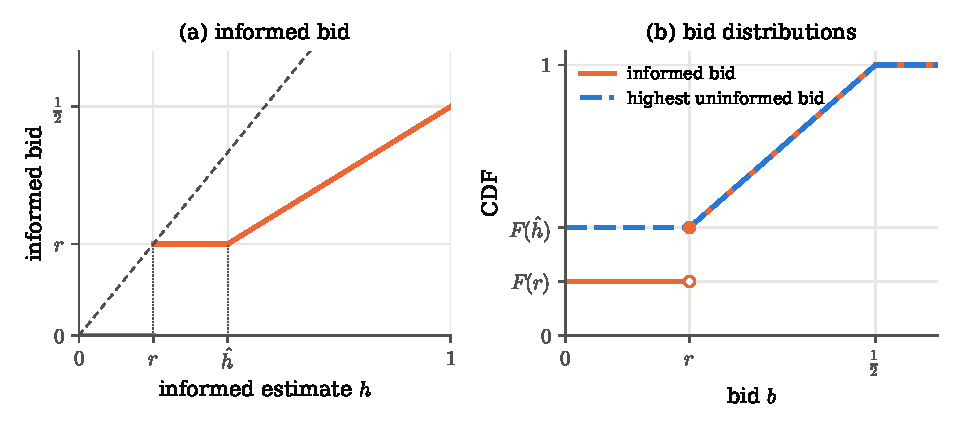
\includegraphics[width=0.95\textwidth]{figures/ch14/emw_equilibrium.pdf}
  \caption{Equilibrium with one informed bidder, for $H$ uniform on $[0,1]$ and reserve price $r=0.2$.
  Panel (a): the informed bid function, which is zero (no bid) below $r$, equal to $r$ on $[r,\hat h]$ with
  $\hat h=0.4$, and $\frac{h}{2}$ above $\hat h$. Panel (b): the distribution functions of the informed bid and
  of the highest uninformed bid. They coincide above $r$ and differ only in their masses at zero and at
  $r$.}\label{fig:14-emw}
\end{figure}

A numerical example makes the predictions concrete (\cref{fig:14-emw}). Let $H$ be uniform on $[0,1]$ and
$r=0.2$. Then $\E[H\mid H<\hat h]=\frac{\hat h}{2}=r$ gives $\hat h=0.4$, and $\sigma^*(h)=\frac{h}{2}$ for
$h>0.4$. The uninformed bidders abstain with probability $0.4$, and otherwise their highest bid has
distribution function $G^*(b)=2b$ on $(0.2,0.5]$. The informed bidder wins half of all auctions and $0.5435$
of the auctions with a bid, by \eqref{eq:14-hp-winprob}. Its expected profit is
$\int_{0.4}^1\frac{h}{2}\,h\,dh+0.4\int_{0.2}^{0.4}(h-0.2)\,dh=0.156+0.008=0.164$. The tract is sold unless
$H<r$ and no uninformed bidder bids, so expected surplus is $0.5-0.2\times0.4\times0.1=0.492$. The seller's
expected revenue is $0.492-0.164=0.328$. The uninformed bidders lose $0.15$ per tract on the tracts where the
informed bidder abstains and gain $0.0375$ per tract on the others, which nets to zero. These numbers come from
the script \texttt{emw\_example.py}, which also confirms them by simulation.

\Cref{prop:14-mw-garbling,prop:14-emw} make the same point from two sides. A bidder whose information is a
garbling of a rival's information earns nothing, and a bidder with exclusive information earns a rent even
against many rivals. The value of information in an auction lies in its privacy.

\subsection{The English auction}\label{sec:14-mw-english}

Milgrom and Weber model the English auction as the Japanese button auction of
\cref{def:14-button}. The price rises continuously from zero, the price and the number of active bidders are
displayed at all times, and exits are public and irrevocable. When one bidder remains, it wins and pays the
price at which the last rival left. With two bidders the English and second-price auctions are strategically
equivalent (\cref{prop:14-english-spa-n2}). With three or more bidders, the prices at which bidders drop out
convey information to those who remain, and the two formats differ.

Suppose $k$ bidders have quit, at prices $p_1\le\dots\le p_k$. A strategy for bidder $i$ specifies, for each
such history, the price $\beta_k(s_i\mid p_1,\dots,p_k)\ge p_k$ at which it will quit if nobody else quits
first. \citet[eqs.~(5)--(6)]{MilgromWeber1982} define the strategy $\beta^E=(\beta^E_0,\dots,
\beta^E_{n-2})$ iteratively. Before any exit,
\begin{equation}\label{eq:14-mw-english0}
  \beta^E_0(s)=\E\left[V_1\mid S_1=s,\,Y_1=s,\dots,Y_{n-1}=s\right].
\end{equation}
After $k=1,\dots,n-2$ exits,
\begin{equation}\label{eq:14-mw-englishk}
  \beta^E_k(s\mid p_1,\dots,p_k)=\E\left[V_1\mid S_1=s,\,Y_1=\dots=Y_{n-k-1}=s,\,
  Y_{n-k}=y_{n-k},\dots,Y_{n-1}=y_{n-1}\right].
\end{equation}
The signals of the bidders who quit are inferred from their exit prices. They solve
$\beta^E_0(y_{n-1})=p_1$, $\beta^E_1(y_{n-2}\mid p_1)=p_2$, and so on up to
$\beta^E_{k-1}(y_{n-k}\mid p_1,\dots,p_{k-1})=p_k$.

These strategies are myopic in a precise sense \citep[p.~1105]{MilgromWeber1982}. Suppose nobody has quit
and the price has reached $\beta^E_0(y)$. If all other bidders quit at that instant, bidder 1 would infer that
$Y_1=\dots=Y_{n-1}=y$. It would then value the object at $\E[V_1\mid S_1=s,Y_1=\dots=Y_{n-1}=y]$, and its
payoff from winning at the current price would be this value minus $\beta^E_0(y)$. By \cref{prop:14-affil-props}(iii)
the difference is positive if $s>y$ and negative if $s<y$. So $\beta^E_0$ keeps it active until the price
at which it would be just indifferent between winning and losing. The later strategies $\beta^E_k$ have the
same interpretation, with the signals of those who quit inferred from their exit prices.

\begin{proposition}[{\citealp[Theorem~10]{MilgromWeber1982}}]\label{prop:14-mw-english}
Under \cref{ass:14-mw}, the profile in which every bidder uses $\beta^E$ is an equilibrium of the English
auction. If bidder 1 wins, it pays
\begin{equation}\label{eq:14-mw-english-price}
  \bar v(Y_1,Y_1,Y_2,\dots,Y_{n-1}),\qquad\text{where }
  \bar v(s,y_1,\dots,y_{n-1})=\E\left[V_1\mid S_1=s,\,Y_1=y_1,\dots,Y_{n-1}=y_{n-1}\right],
\end{equation}
evaluated at the realized order statistics.
\end{proposition}

\begin{proof}
Each $\beta^E_k$ is increasing in its first argument, by \cref{ass:14-mw}(ii) and
\cref{prop:14-affil-props}(iii). Exits therefore occur in increasing order of signals and reveal them. Let
bidders $2,\dots,n$ use $\beta^E$. While bidder 1 is active, the history of exits consists only of rivals'
exits, so its own strategy affects whether it wins and not the price it pays if it wins. If it outlasts
everyone, the last rival to quit has signal $Y_1$. That rival quits at $\beta^E_{n-2}(Y_1\mid p_1,\dots,p_{n-2})$,
the expected value to a bidder with signal $Y_1$ given that the other remaining bidder also has signal $Y_1$
and given the revealed signals $Y_2,\dots,Y_{n-1}$. By the symmetry of $u$ this equals
$\bar v(Y_1,Y_1,Y_2,\dots,Y_{n-1})$, which proves \eqref{eq:14-mw-english-price}.

Given its own signal and the rivals' signals, bidder 1 values the object at
$\bar v(s,Y_1,\dots,Y_{n-1})$ in expectation. Its payoff from winning is therefore
\begin{equation*}
  \bar v(s,Y_1,Y_2,\dots,Y_{n-1})-\bar v(Y_1,Y_1,Y_2,\dots,Y_{n-1}),
\end{equation*}
which is nonnegative if and only if $s\ge Y_1$, by monotonicity of $\bar v$ in its first argument. Under
$\beta^E$ it wins exactly when $s>Y_1$ (the event $s=Y_1$ has probability zero). It thus wins in every
realization in which winning is profitable and in no other. No strategy can do better.
\end{proof}

The argument is pointwise. Bidder 1 would not regret its strategy even if it learned all rivals' signals,
so the equilibrium is an \emph{ex post equilibrium} \citep[Chapter~6]{Krishna2010}. With private values,
$\beta^E_k(s\mid\cdot)=s$ for every $k$, and the strategy reduces to staying in until the price reaches one's
value, as in \citet[eq.~(2.6)]{AtheyHaile2007} and \cref{sec:14-spa}.

With common values the equilibrium is not unique. \citet{BikhchandaniHaileRiley2002} show that there are
many symmetric equilibria in strictly increasing, weakly undominated strategies, even with symmetric bidders.
In every such equilibrium, a bidder who is one of the last two to exit quits at
\begin{equation*}
  \E\left[V_i\mid S_i=s_i,\ S_j=s_i\text{ for active }j\ne i,\ S_k=s_k\text{ for }k\in\mathcal E_i\right],
\end{equation*}
where $\mathcal E_i$ is the set of bidders who quit before it \citep[eq.~(2.7)]{AtheyHaile2007}. The
Milgrom-Weber equilibrium is the one in which every bidder follows this rule at every stage. The multiplicity
concerns the earlier exits, those below the final price, so these exit prices have no unique interpretation. This complicates the use
of losing bids in empirical work (\cref{ch:auction-empirics}).

\begin{example}[Mineral rights, continued]\label{ex:14-mineral-english}
In \cref{ex:14-mineral}, the posterior of $V$ given any set of signals is uniform on
$[\max_is_i-\omega,\ \min_is_i+\omega]$, so the posterior mean is the midpoint of the highest and lowest
signals. Before anyone quits all signals in \eqref{eq:14-mw-english0} equal $s$, so $\beta^E_0(s)=s$. After
$k\ge1$ exits the highest signal in \eqref{eq:14-mw-englishk} is $s$ and the lowest is $y_{n-1}$, so
$\beta^E_k(s\mid\cdot)=\frac{s+y_{n-1}}{2}$. The lowest bidder quits at its signal. The others then stay in
until the midpoint between their own signal and that lowest signal. For $n\ge3$ the winner pays
$\frac{Y_1+Y_{n-1}}{2}$, the midpoint of the second-highest and the lowest signal. For $n=2$ it pays $Y_1$.
\end{example}

\subsection{The first-price auction}\label{sec:14-mw-fpa}

We first derive the necessary conditions for a symmetric equilibrium with an increasing, differentiable bid
function $\beta$ \citep[p.~1106, following \citealp{Wilson1977}]{MilgromWeber1982}. Suppose bidders
$2,\dots,n$ use $\beta$. If bidder 1 has signal $s$ and bids $b$, its expected payoff is
\begin{align*}
  \Pi(b;s)&=\E\left[(V_1-b)\indic\{\beta(Y_1)<b\}\mid S_1=s\right]\\
  &=\E\left[\E\left[(V_1-b)\indic\{\beta(Y_1)<b\}\mid S_1,Y_1\right]\mid S_1=s\right]\\
  &=\E\left[\left(v(S_1,Y_1)-b\right)\indic\{\beta(Y_1)<b\}\mid S_1=s\right]\\
  &=\int_{\underline s}^{\beta^{-1}(b)}\left(v(s,\alpha)-b\right)f_{Y_1}(\alpha\mid s)\,d\alpha.
\end{align*}
Differentiating with respect to $b$ by Leibniz's rule,
\begin{equation*}
  \Pi_b(b;s)=\frac{\left(v(s,\beta^{-1}(b))-b\right)f_{Y_1}(\beta^{-1}(b)\mid s)}{\beta'(\beta^{-1}(b))}
  -F_{Y_1}(\beta^{-1}(b)\mid s).
\end{equation*}
In equilibrium $\Pi_b(\beta(s);s)=0$. Substituting $b=\beta(s)$ and rearranging yields the linear
differential equation \citep[eq.~(7)]{MilgromWeber1982}
\begin{equation}\label{eq:14-mw-ode}
  \beta'(s)=\left(v(s,s)-\beta(s)\right)\frac{f_{Y_1}(s\mid s)}{F_{Y_1}(s\mid s)}.
\end{equation}
Two further necessary conditions fix the boundary. First, $v(s,s)-\beta(s)\ge0$ for every $s$. Otherwise the
payoff $\int_{\underline s}^s(v(s,\alpha)-\beta(s))f_{Y_1}(\alpha\mid s)\,d\alpha$ would be negative, since
$v(s,\alpha)\le v(s,s)$ for $\alpha\le s$, and bidding zero would do better. Second,
$v(\underline s,\underline s)-\beta(\underline s)\le0$. Otherwise the lowest type could raise its bid slightly
above $\beta(\underline s)$, win against rivals with low signals, and earn a positive payoff instead of zero.
Together these give the boundary condition $\beta(\underline s)=v(\underline s,\underline s)$.

\begin{proposition}[{\citealp[Theorem~14]{MilgromWeber1982}}]\label{prop:14-mw-fpa}
Under \cref{ass:14-mw}, the strategy
\begin{equation}\label{eq:14-mw-fpa-bid}
  \beta^{FP}(s)=\int_{\underline s}^{s}v(\alpha,\alpha)\,dL(\alpha\mid s),
  \qquad
  L(\alpha\mid s)=\exp\left(-\int_\alpha^s\frac{f_{Y_1}(t\mid t)}{F_{Y_1}(t\mid t)}\,dt\right),
\end{equation}
used by every bidder is a symmetric equilibrium of the first-price auction. Equivalently,
\begin{equation}\label{eq:14-mw-fpa-bid2}
  \beta^{FP}(s)=v(s,s)-\int_{\underline s}^sL(\alpha\mid s)\,dv(\alpha,\alpha).
\end{equation}
\end{proposition}

We follow Milgrom and Weber's conventions. The ratio $\frac{f_{Y_1}(t\mid t)}{F_{Y_1}(t\mid t)}$ is zero
outside the support of $Y_1$, and $L(\alpha\mid s)=0$ when the integral is infinite (their footnotes 22 and
23). We read $L(\cdot\mid s)$ as a distribution function on $[\underline s,s]$ that places any mass
$L(\underline s\mid s)$ at $\underline s$, and the integral in \eqref{eq:14-mw-fpa-bid} includes that atom.

\begin{proof}
Write $\zeta(t)=\frac{f_{Y_1}(t\mid t)}{F_{Y_1}(t\mid t)}$.

\emph{Solving the equation.} Rewrite \eqref{eq:14-mw-ode} as $\beta'(s)+\zeta(s)\beta(s)=\zeta(s)v(s,s)$. Fix an
interior point $s_0$ and let $\Gamma(s)=\int_{s_0}^s\zeta(t)\,dt$. Multiplying by the integrating factor
$e^{\Gamma(s)}$ gives
\begin{equation*}
  \frac{d}{ds}\left[\beta(s)e^{\Gamma(s)}\right]=\zeta(s)v(s,s)e^{\Gamma(s)}.
\end{equation*}
Integrating from $\underline s$ to $s$,
\begin{equation*}
  \beta(s)e^{\Gamma(s)}=\beta(\underline s)e^{\Gamma(\underline s)}
  +\int_{\underline s}^s\zeta(\alpha)v(\alpha,\alpha)e^{\Gamma(\alpha)}\,d\alpha.
\end{equation*}
Divide by $e^{\Gamma(s)}$. Note that $L(\alpha\mid s)=e^{\Gamma(\alpha)-\Gamma(s)}$ and
$\frac{\partial L(\alpha\mid s)}{\partial\alpha}=\zeta(\alpha)L(\alpha\mid s)$. Imposing
$\beta(\underline s)=v(\underline s,\underline s)$,
\begin{equation*}
  \beta(s)=v(\underline s,\underline s)L(\underline s\mid s)
  +\int_{\underline s}^sv(\alpha,\alpha)\frac{\partial L(\alpha\mid s)}{\partial\alpha}\,d\alpha,
\end{equation*}
which is \eqref{eq:14-mw-fpa-bid} with the atom at $\underline s$. Integrating the second term by parts and
using $L(s\mid s)=1$,
\begin{equation*}
  \int_{\underline s}^sv(\alpha,\alpha)\frac{\partial L(\alpha\mid s)}{\partial\alpha}\,d\alpha
  =v(s,s)-v(\underline s,\underline s)L(\underline s\mid s)-\int_{\underline s}^sL(\alpha\mid s)\,dv(\alpha,\alpha).
\end{equation*}
The atom term cancels, which gives \eqref{eq:14-mw-fpa-bid2}.

\emph{Monotonicity.} As a function of $\alpha$, $L(\cdot\mid s)$ is nondecreasing with $L(s\mid s)=1$, so it is a
distribution function on $[\underline s,s]$. It increases stochastically in $s$. For $s'>s$ and $\alpha\le s$,
$L(\alpha\mid s')=L(\alpha\mid s)\exp(-\int_s^{s'}\zeta)\le L(\alpha\mid s)$, and for $\alpha\in(s,s']$,
$L(\alpha\mid s')\le1=L(\alpha\mid s)$ once we extend $L(\cdot\mid s)$ by one above $s$. Since
$v(\alpha,\alpha)$ is nondecreasing, its mean under $L(\cdot\mid s)$ rises with $s$, so $\beta^{FP}$ is
nondecreasing. Where $v(s,s)>\beta^{FP}(s)$, \eqref{eq:14-mw-ode} shows that it is strictly increasing.

\emph{Sufficiency.} Assume for now that $\beta=\beta^{FP}$ is continuous, and hence differentiable after a monotone
rescaling of signals (\cref{prop:14-affil-props}(i)). A bidder with signal $z$ need only consider bids in
the range of $\beta$, since higher bids are dominated by $\beta(\bar s)$ and lower bids never win. Let its bid be
$\beta(x)$. Substituting $b=\beta(x)$ into $\Pi_b$ and factoring,
\begin{equation*}
  \Pi_b(\beta(x);z)=\frac{f_{Y_1}(x\mid z)}{\beta'(x)}
  \left[\left(v(z,x)-\beta(x)\right)-\beta'(x)\frac{F_{Y_1}(x\mid z)}{f_{Y_1}(x\mid z)}\right].
\end{equation*}
At $z=x$ the bracket is zero by \eqref{eq:14-mw-ode}. Take $x<z$. Then $v(z,x)\ge v(x,x)$ by
\cref{cor:14-mw-v}, and $\frac{F_{Y_1}(x\mid z)}{f_{Y_1}(x\mid z)}\le\frac{F_{Y_1}(x\mid x)}{f_{Y_1}(x\mid x)}$
by \cref{lem:14-mw-lemma1}. With $\beta'\ge0$, the bracket is at least
$(v(x,x)-\beta(x))-\beta'(x)\frac{F_{Y_1}(x\mid x)}{f_{Y_1}(x\mid x)}=0$. For $x>z$ both inequalities reverse
and the bracket is at most zero. So the payoff rises in $x$ below $z$ and falls above $z$, and $x=z$ is
optimal.

\emph{Continuity.} \citet[p.~1108]{MilgromWeber1982} show that $\beta^{FP}$ can jump at $x$ only if
$F_{Y_1}(x\mid x+\epsilon)=0$ for every $\epsilon>0$. By affiliation and symmetry this means that if any signal
exceeds $x$, all signals do. The game then splits into two subgames, one in which it is common knowledge that
all signals exceed $x$ and one in which none does. The argument above applies within each.
\end{proof}

A jump can occur \citep[footnote~21]{MilgromWeber1982}. Let $n=2$ and $V_i=S_i$. With probability
$\frac{1}{2}$ both signals are drawn independently and uniformly from $[0,1]$, and with probability
$\frac{1}{2}$ from $[1,2]$. A bidder's signal reveals the regime, and within each regime the auction is the
uniform private values auction of \cref{sec:14-fpa}. The equilibrium bid is $\frac{s}{2}$ on $[0,1)$ and
$1+\frac{s-1}{2}$ on $(1,2]$, so it jumps from $\frac{1}{2}$ to $1$ at $s=1$. The signals remain affiliated,
because conditional on one signal being high the other is more likely to be high.

The first-price formula nests the private values case. With independent signals, $F_{Y_1}(t\mid s)=F(t)^{n-1}$
does not depend on $s$, so $\zeta(t)=\frac{(n-1)f(t)}{F(t)}$ and
\begin{equation*}
  L(\alpha\mid s)=\exp\left(-(n-1)\left[\ln F(s)-\ln F(\alpha)\right]\right)=\frac{F(\alpha)^{n-1}}{F(s)^{n-1}}.
\end{equation*}
This is the distribution function of $Y_1$ conditional on $Y_1\le s$. Hence $\beta^{FP}(s)=\E[v(Y_1,Y_1)\mid
Y_1<s]$ with independent signals. With private values $v(\alpha,\alpha)=\alpha$, and we recover the
Riley-Samuelson bid in its conditional-expectation form \eqref{eq:14-rs-condexp} without a reserve price. With
$V=\frac{S_1+S_2}{2}$ and independent uniform signals, as in \cref{ex:14-iv-independent}, $v(\alpha,\alpha)=\alpha$ again
and $\beta^{FP}(s)=\frac{s}{2}$. With affiliated signals, $L(\cdot\mid s)$ is no longer a conditional
distribution of $Y_1$, and this is where the formats come apart.

\begin{example}[Mineral rights, continued]\label{ex:14-mineral-fpa}
In \cref{ex:14-mineral}, given $S_1=s$ the posterior of $V$ is uniform on $[s-\omega,s+\omega]$, and given $V$
each rival signal falls below $s$ with probability $\frac{s-V+\omega}{2\omega}$. Substituting
$t=s+\omega-V$,
\begin{align*}
  F_{Y_1}(s\mid s)&=\frac{1}{2\omega}\int_0^{2\omega}\left(\frac{t}{2\omega}\right)^{n-1}dt=\frac{1}{n},\\
  f_{Y_1}(s\mid s)&=\frac{1}{2\omega}\int_0^{2\omega}(n-1)\left(\frac{t}{2\omega}\right)^{n-2}\frac{1}{2\omega}\,dt
  =\frac{1}{2\omega}.
\end{align*}
So $\zeta(t)=\frac{n}{2\omega}$ is constant and $L(\alpha\mid s)=e^{-\frac{n(s-\alpha)}{2\omega}}$. With
$v(\alpha,\alpha)=\alpha-\omega\frac{n-2}{n}$ from \eqref{eq:14-mineral-spa}, $dv(\alpha,\alpha)=d\alpha$, and
\eqref{eq:14-mw-fpa-bid2} gives
\begin{equation}\label{eq:14-mineral-fpa}
  \beta^{FP}(s)=s-\omega\frac{n-2}{n}-\int_{-\infty}^se^{-\frac{n(s-\alpha)}{2\omega}}\,d\alpha
  =s-\omega\frac{n-2}{n}-\frac{2\omega}{n}=s-\omega.
\end{equation}
One checks directly that $\beta^{FP\prime}(s)=1=\left(v(s,s)-\beta^{FP}(s)\right)\frac{n}{2\omega}$. The bid
$s-\omega$ never loses money, since $V\ge s-\omega$ for every possible value. With a proper uniform prior the
lower boundary changes the bid, but its effect dies out exponentially in the distance from the bottom. In the
script \texttt{mineral\_rights.py} with $n=3$, the exact bid for a signal five units of $\omega$ above the
bottom of the prior support differs from $s-\omega$ by about $0.001\omega$.
\end{example}

\begin{example}[Affiliated private values, continued]\label{ex:14-apv-fpa}
From \eqref{eq:14-apv-cond}, $f_{Y_1}(t\mid t)=\frac{2(1+t^2)}{2+t}$ and
$F_{Y_1}(t\mid t)=\frac{t(2+t^2)}{2+t}$, so
\begin{equation*}
  \zeta(t)=\frac{2(1+t^2)}{t(2+t^2)}.
\end{equation*}
We decompose by partial fractions, $\frac{2+2t^2}{t(2+t^2)}=\frac{a}{t}+\frac{bt+c}{2+t^2}$. Multiplying out,
$2+2t^2=a(2+t^2)+(bt+c)t=2a+(a+b)t^2+ct$. Matching coefficients gives $a=1$, $c=0$ and $b=1$, so
$\zeta(t)=\frac{1}{t}+\frac{t}{2+t^2}$. Integrating,
\begin{equation*}
  \int_\alpha^s\zeta(t)\,dt=\ln\frac{s}{\alpha}+\frac{1}{2}\ln\frac{2+s^2}{2+\alpha^2},
  \qquad
  L(\alpha\mid s)=\frac{\alpha\sqrt{2+\alpha^2}}{s\sqrt{2+s^2}}.
\end{equation*}
Here $L(0\mid s)=0$, so there is no atom. With private values $v(\alpha,\alpha)=\alpha$, and
\eqref{eq:14-mw-fpa-bid2} gives
\begin{align}
  \beta^{FP}(s)&=s-\frac{1}{s\sqrt{2+s^2}}\int_0^s\alpha\sqrt{2+\alpha^2}\,d\alpha\notag\\
  &=s-\frac{1}{s\sqrt{2+s^2}}\left[\frac{(2+\alpha^2)^{\frac{3}{2}}}{3}\right]_0^s
  =s-\frac{(2+s^2)^{\frac{3}{2}}-2^{\frac{3}{2}}}{3s\sqrt{2+s^2}}.\label{eq:14-apv-fpa}
\end{align}
A symbolic check in \texttt{apv\_example.py} confirms that \eqref{eq:14-apv-fpa} solves \eqref{eq:14-mw-ode}.
As $s\to0$ the ratio $\frac{\beta^{FP}(s)}{s}$ tends to $\frac{1}{2}$, so $\beta^{FP}(0)=0=v(0,0)$. At the top,
$\beta^{FP}(1)=\frac{2\sqrt6}{9}\approx0.544$.

\Cref{fig:14-apv-bids} plots the bids. The first-price bid lies slightly above the benchmark $\frac{s}{2}$
for independent uniform values. A cleaner comparison holds the marginal distribution fixed. With independent
signals and the same marginal density $\frac{2}{5}(2+s)$, the Riley-Samuelson bid is
$\frac{2s(s+3)}{3(s+4)}$. It exceeds the affiliated bid at low signals ($0.1275$ versus $0.1260$ at $s=0.25$)
and falls below it at high signals ($0.533$ versus $0.544$ at $s=1$). A bidder with a high signal expects
strong rivals and bids more aggressively. A bidder with a low signal expects weak rivals and shades more.
\end{example}

\begin{figure}[htbp]
  \centering
  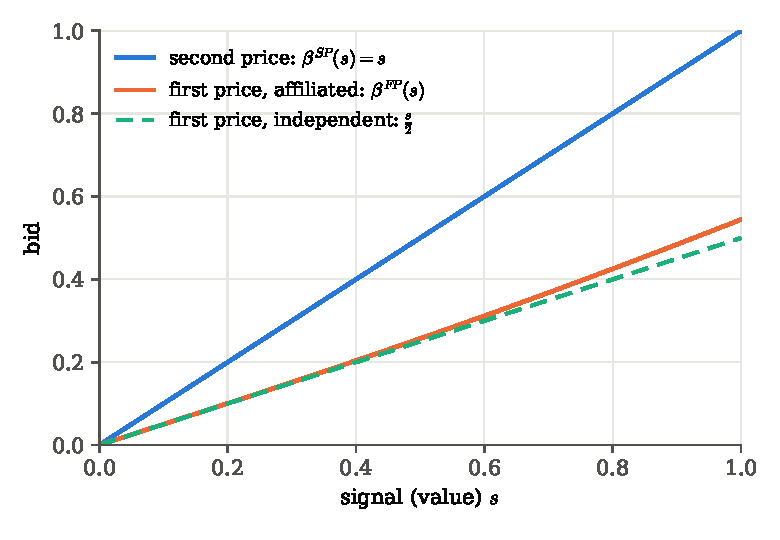
\includegraphics[width=0.72\textwidth]{figures/ch14/apv_bids.pdf}
  \caption{Equilibrium bids for the affiliated private values density $f(s_1,s_2)=\frac{4}{5}(1+s_1s_2)$ on
  $[0,1]^2$ with two bidders. The second-price bid is $s$. The first-price bid is \eqref{eq:14-apv-fpa}. The
  dashed line is the first-price bid $\frac{s}{2}$ for independent uniform values.}\label{fig:14-apv-bids}
\end{figure}

The first-order condition can also be written in terms of the bid distribution, which is the form used for
estimation. Consider affiliated private values, possibly asymmetric, and let $M_i=\max_{j\ne i}B_j$ be the
highest rival bid. Bidder $i$ with value $v_i$ solves
\begin{equation*}
  \max_b\ \E\left[(v_i-b)\indic\{M_i\le b\}\mid V_i=v_i\right]=\max_b\ (v_i-b)\Pr\left(M_i\le b\mid V_i=v_i\right).
\end{equation*}
The conditioning on $v_i$ matters, because under affiliation a bidder's own value is informative about rivals'
values and hence about their bids. The first-order condition is
\begin{equation*}
  -\Pr\left(M_i\le b\mid V_i=v_i\right)+(v_i-b)\frac{\partial\Pr\left(M_i\le b\mid V_i=v_i\right)}{\partial b}=0,
\end{equation*}
which rearranges to
\begin{equation*}
  v_i=b+\frac{\Pr\left(M_i\le b\mid V_i=v_i\right)}{\frac{\partial}{\partial b}\Pr\left(M_i\le b\mid V_i=v_i\right)}.
\end{equation*}
The derivative is taken in the threshold $b$, holding the conditioning value fixed. In an equilibrium with
strictly increasing strategies $\beta_i$, the events $\{V_i=v_i\}$ and $\{B_i=\beta_i(v_i)\}$ coincide. So
$\Pr(M_i\le m\mid V_i=v_i)=G_{M\mid B}(m\mid b_i)$, where $G_{M\mid B}(m\mid b)=\Pr(M_i\le m\mid B_i=b)$ and
$b_i=\beta_i(v_i)$. Let $g_{M\mid B}(m\mid b)$ be its density in $m$. At the equilibrium bid,
\begin{equation}\label{eq:14-apv-foc}
  v_i=b_i+\frac{G_{M\mid B}(b_i\mid b_i)}{g_{M\mid B}(b_i\mid b_i)}.
\end{equation}
Everything on the right side is a feature of the joint distribution of a bidder's own bid and the highest
rival bid, which is observed when all bids are recorded. \Cref{ch:auction-empirics} uses \eqref{eq:14-apv-foc}
to recover values from bids \citep{LiPerrigneVuong2002,CampoPerrigneVuong2003}. With common values the same
argument gives \citet[eq.~(2.4)]{AtheyHaile2007}, in which the left side is the pivotal expected value
$\E[V_i\mid S_i=s_i,\ M_i=\beta(s_i)]$. In the symmetric Milgrom-Weber model this is $v(s,s)$. There,
$G_{M\mid B}(b\mid b)=F_{Y_1}(s\mid s)$ and $g_{M\mid B}(b\mid b)=\frac{f_{Y_1}(s\mid s)}{\beta'(s)}$ at
$b=\beta(s)$, and \eqref{eq:14-apv-foc} becomes \eqref{eq:14-mw-ode}.

Existence and uniqueness of equilibrium are now well understood. The following theorem collects the results
summarized by \citet[Theorem~2.1]{AtheyHaile2007}.

\begin{theorem}[Existence and uniqueness in first-price auctions]\label{thm:14-existence}
Suppose values have a compact, convex common support, signals are affiliated with a product support, and
their joint density is strictly positive on the interior of the support.
\begin{enumerate}[label=(\roman*)]
  \item An equilibrium in pure, nondecreasing strategies exists \citep{Athey2001,RenyZamir2004}. Strategies
  can be taken strictly increasing, except in common values models with asymmetric bidders and dependent
  signals. There, at most one bidder may bid the lowest winning bid with positive probability
  \citep{McAdams2003}.
  \item With private values and either independence or symmetry, and a continuously differentiable density,
  the equilibrium is unique and in pure, strictly increasing, differentiable strategies
  \citep{Lebrun1999,MaskinRiley2003,McAdams2003,McAdams2007}.
  \item With symmetric bidders and a continuously differentiable density, there is a unique equilibrium
  within the class of nondecreasing pure strategies. It is symmetric, strictly increasing and differentiable,
  and it is the equilibrium of \cref{prop:14-mw-fpa} \citep{McAdams2007}.
\end{enumerate}
\end{theorem}

We do not prove the theorem. Existence for asymmetric bidders rests on single-crossing arguments that go
beyond this book. Part (iii) shows that, among monotone equilibria, the Milgrom-Weber first-price
equilibrium is the only one in the symmetric model.

\section{Affiliated Values II: The Linkage Principle, Revenue Ranking, and Information Disclosure}\label{sec:14-mw-rank}

With independent private values the four standard formats raise the same expected revenue
(\cref{prop:14-ret}). Affiliation breaks this equivalence in a systematic direction. This section explains why
through the linkage principle, proves the ranking, and applies the same logic to the seller's disclosure of
information, reserve prices and entry fees. It then asks which results survive risk aversion and closes with
an assessment of the paper.

\subsection{The linkage principle}\label{sec:14-linkage}

\citet[pp.~1110--1111]{MilgromWeber1982} view each auction as a revelation game in which every bidder chooses a
report $x$ in place of a bid $\beta(x)$. No auction can set prices directly in terms of bidders' preferences
and information. Prices can depend only on the reports and on the seller's information. If the price depends
on variables other than the winner's own report, and those variables are affiliated with the winner's signal,
then the price is statistically linked to that signal. The expected price, as a function of the winner's
signal, rises more steeply than it otherwise would. In all three auctions the winner with the lowest signal
expects to pay $v(\underline s,\underline s)$. A steeper expected payment function therefore means higher
prices and lower bidder profits.

To make this precise, consider a symmetric auction mechanism $\mathcal M$ with a symmetric, increasing
equilibrium in which the highest signal wins. For bidder 1 with signal $z$ who bids as if its signal were $x$,
define the expected value it receives,
\begin{equation*}
  R(x,z)=\E\left[V_1\indic\{Y_1<x\}\mid S_1=z\right],
\end{equation*}
and its expected payment conditional on winning, $W^{\mathcal M}(x,z)$. Its expected payoff is
$R(x,z)-W^{\mathcal M}(x,z)F_{Y_1}(x\mid z)$. In equilibrium $x=z$ is optimal, so the first-order condition
holds at $x=z$ \citep[eq.~(9)]{MilgromWeber1982}:
\begin{equation}\label{eq:14-mw-foc9}
  0=R_1(z,z)-W^{\mathcal M}_1(z,z)F_{Y_1}(z\mid z)-W^{\mathcal M}(z,z)f_{Y_1}(z\mid z),
\end{equation}
where subscripts denote partial derivatives. The boundary condition is
$W^{\mathcal M}(\underline s,\underline s)=v(\underline s,\underline s)$. In the first-price auction the
winner pays its own bid, so $W^{FP}(x,z)=\beta^{FP}(x)$. In the second-price auction it pays the highest rival
bid, so $W^{SP}(x,z)=\E[v(Y_1,Y_1)\mid Y_1<x,\,S_1=z]$. The partial derivative $W_2^{\mathcal M}$ measures how
much the expected price depends on the winner's true signal when its report is held fixed. We call it the
\emph{linkage} of the mechanism.

\begin{proposition}[Linkage principle]\label{prop:14-linkage}
Let $\mathcal M$ and $\mathcal M'$ be two mechanisms as above that satisfy \eqref{eq:14-mw-foc9}. Suppose
$W^{\mathcal M}(\underline s,\underline s)=W^{\mathcal M'}(\underline s,\underline s)$ and
$W^{\mathcal M}_2(z,z)\ge W^{\mathcal M'}_2(z,z)$ for all $z$. Then $W^{\mathcal M}(z,z)\ge W^{\mathcal
M'}(z,z)$ for all $z$, and $\mathcal M$ yields an expected revenue at least as large as $\mathcal M'$.
\end{proposition}

\begin{proof}
Let $g(z)=W^{\mathcal M}(z,z)$ and $h(z)=W^{\mathcal M'}(z,z)$. Solving \eqref{eq:14-mw-foc9} for $W_1$ in
each mechanism and subtracting,
\begin{equation*}
  W^{\mathcal M}_1(z,z)-W^{\mathcal M'}_1(z,z)=-\left[g(z)-h(z)\right]\frac{f_{Y_1}(z\mid z)}{F_{Y_1}(z\mid z)}.
\end{equation*}
By the chain rule $g'(z)=W^{\mathcal M}_1(z,z)+W^{\mathcal M}_2(z,z)$, and similarly for $h$. Therefore
\begin{equation*}
  g'(z)-h'(z)=-\left[g(z)-h(z)\right]\frac{f_{Y_1}(z\mid z)}{F_{Y_1}(z\mid z)}
  +\left[W^{\mathcal M}_2(z,z)-W^{\mathcal M'}_2(z,z)\right].
\end{equation*}
If $g(z)<h(z)$, the first term is positive and the second is nonnegative, so $g'(z)\ge h'(z)$. Since
$g(\underline s)=h(\underline s)$, \cref{lem:14-crossing} gives $g\ge h$ everywhere. By symmetry each bidder
wins with probability $\frac{1}{n}$, so expected revenue is
$n\,\E[W(S_1,S_1)\indic\{S_1>Y_1\}]=\E[W(S_1,S_1)\mid S_1>Y_1]$, which is larger under $\mathcal M$.
\end{proof}

The principle explains where bidders' profits come from. A bidder earns a rent because the price cannot
depend on its private signal except through its own report. Every channel that makes the price track its
signal through other affiliated variables reduces that rent. General versions of the principle are in
\citet{Milgrom2004} and \citet[Chapter~7]{Krishna2010}.

\subsection{Revenue ranking}\label{sec:14-mw-ranking}

The ranking rests on one inequality, which also delivers the disclosure results of
\cref{sec:14-mw-disclosure}.

\begin{lemma}[Information raises the second-price expected price]\label{lem:14-mw-info}
Let $\bm Z$ be a random vector such that $(\bm Z,S_1,Y_1)$ are affiliated, and let
$w_{\bm Z}(s,y,\bm z)=\E[V_1\mid S_1=s,\,Y_1=y,\,\bm Z=\bm z]$ be nondecreasing. Then
\begin{equation*}
  \E\left[v(Y_1,Y_1)\mid S_1>Y_1\right]\le\E\left[w_{\bm Z}(Y_1,Y_1,\bm Z)\mid S_1>Y_1\right].
\end{equation*}
\end{lemma}

\begin{proof}
By the law of iterated expectations, for all $x$ and $y$,
\begin{equation*}
  v(x,y)=\E\left[\E[V_1\mid S_1,Y_1,\bm Z]\mid S_1=x,Y_1=y\right]=\E\left[w_{\bm Z}(x,y,\bm Z)\mid S_1=x,Y_1=y\right].
\end{equation*}
Now take $x>y$. Applying this identity at the point $(y,y)$ and then \cref{prop:14-affil-props}(iii) to the
nondecreasing function $w_{\bm Z}(y,y,\cdot)$,
\begin{equation*}
  v(y,y)=\E\left[w_{\bm Z}(y,y,\bm Z)\mid S_1=y,Y_1=y\right]\le\E\left[w_{\bm Z}(y,y,\bm Z)\mid S_1=x,Y_1=y\right].
\end{equation*}
Setting $y=Y_1$ and $x=S_1$ on the event $\{S_1>Y_1\}$ and taking expectations,
\begin{equation*}
  \E\left[v(Y_1,Y_1)\mid S_1>Y_1\right]\le\E\left[\E\left[w_{\bm Z}(Y_1,Y_1,\bm Z)\mid S_1,Y_1\right]\mid S_1>Y_1\right]
  =\E\left[w_{\bm Z}(Y_1,Y_1,\bm Z)\mid S_1>Y_1\right].\qedhere
\end{equation*}
\end{proof}

\begin{proposition}[{\citealp[Theorems~11 and 15]{MilgromWeber1982}}]\label{prop:14-mw-ranking}
Let \cref{ass:14-mw} hold, and consider the equilibria of
\cref{prop:14-mw-english,prop:14-mw-spa,prop:14-mw-fpa}. The expected price in the English auction is at least
that in the second-price auction. The expected price in the second-price auction is at least that in the
first-price and Dutch auctions.
\end{proposition}

\begin{proof}
\emph{Second price versus first price.} Both equilibria satisfy \eqref{eq:14-mw-foc9}, because $x=z$ is optimal in
each. In the first-price auction $W^{FP}(x,z)=\beta^{FP}(x)$ does not depend on $z$, so $W^{FP}_2=0$. In the
second-price auction $W^{SP}(x,z)=\E[v(Y_1,Y_1)\mid Y_1<x,S_1=z]$. Since $(S_1,Y_1)$ are affiliated, $v$ is
nondecreasing and the event $\{Y_1<x\}$ is an interval, \cref{prop:14-affil-props}(iii) shows that $W^{SP}$
is nondecreasing in $z$, so $W^{SP}_2\ge0$. Both mechanisms satisfy the boundary condition
$W(\underline s,\underline s)=v(\underline s,\underline s)$. \Cref{prop:14-linkage} gives
$W^{SP}(z,z)\ge W^{FP}(z,z)$ for all $z$, and the expected prices are $\E[W(S_1,S_1)\mid S_1>Y_1]$.

\emph{English versus second price.} When bidder 1 wins, it pays $\bar v(Y_1,Y_1,Y_2,\dots,Y_{n-1})$ in the English
auction (\cref{prop:14-mw-english}) and $v(Y_1,Y_1)$ in the second-price auction. Apply \cref{lem:14-mw-info}
with $\bm Z=(Y_2,\dots,Y_{n-1})$. Then $w_{\bm Z}=\bar v$, which is nondecreasing by \cref{cor:14-mw-v}, and
$(S_1,Y_1,\dots,Y_{n-1})$ are affiliated by \cref{prop:14-affil-props}(iv) and (ii).

\emph{Dutch versus first price.} The two are strategically equivalent (\cref{prop:14-dutch-fpa}).
\end{proof}

The English auction proceeds in two phases \citep[p.~1105]{MilgromWeber1982}. In the first, the $n-2$
bidders with the lowest signals reveal them publicly by dropping out. In the second, the last two bidders play
what amounts to a second-price auction with this public information. \Cref{lem:14-mw-info} says that public
information affiliated with the bidders' signals raises the expected second-price price. The first phase
therefore raises the expected price above the second-price level. In the language of linkage, the English
price is linked to the signals of all losing bidders. The second-price price is linked only to the highest
losing signal, and the first-price price to no other signal at all.

\begin{figure}[htbp]
  \centering
  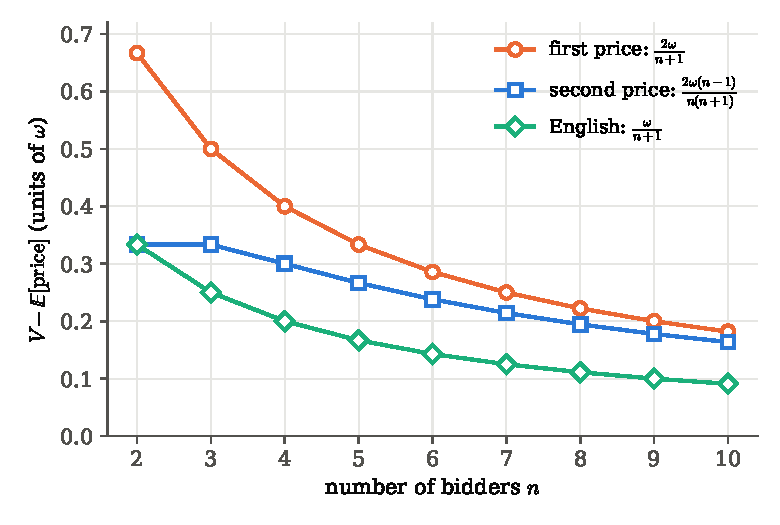
\includegraphics[width=0.72\textwidth]{figures/ch14/mw_mineral_rents.pdf}
  \caption{Expected bidder rents $V-\E[\text{price}]$, in units of $\omega$, in the mineral rights model with
  uniform noise (\cref{ex:14-mineral}) and a diffuse prior. The formulas are derived in the text, and a
  Monte Carlo check is in \texttt{mineral\_rights.py}.}\label{fig:14-mw-ranking}
\end{figure}

The mineral rights example (\cref{ex:14-mineral,ex:14-mineral-english,ex:14-mineral-fpa}) makes the ranking
explicit. Write $S_i=V+\omega(2U_i-1)$ with $U_i$ \iid\ uniform on $[0,1]$. The $k$-th lowest of $n$ uniforms
has mean $\frac{k}{n+1}$, so the $k$-th lowest signal has mean
\begin{equation*}
  \E\left[S_{(k:n)}\right]=V+\omega\left(\frac{2k}{n+1}-1\right)=V+\omega\,\frac{2k-n-1}{n+1}.
\end{equation*}
The first-price winner pays $S_{(n:n)}-\omega$, by \eqref{eq:14-mineral-fpa}. Its expected payment is
\begin{equation*}
  V+\omega\,\frac{n-1}{n+1}-\omega=V-\frac{2\omega}{n+1}.
\end{equation*}
The second-price winner pays $v(S_{(n-1:n)},S_{(n-1:n)})=S_{(n-1:n)}-\omega\frac{n-2}{n}$, by
\eqref{eq:14-mineral-spa}. Its expected payment is
\begin{equation*}
  V+\omega\,\frac{n-3}{n+1}-\omega\,\frac{n-2}{n}
  =V+\omega\,\frac{n(n-3)-(n-2)(n+1)}{n(n+1)}
  =V-\frac{2\omega(n-1)}{n(n+1)}.
\end{equation*}
The English winner pays $\frac{S_{(n-1:n)}+S_{(1:n)}}{2}$, with expectation
\begin{equation*}
  V+\frac{\omega}{2}\left(\frac{n-3}{n+1}+\frac{1-n}{n+1}\right)=V-\frac{\omega}{n+1}.
\end{equation*}
The expected bidder rents are therefore $\frac{2\omega}{n+1}$, $\frac{2\omega(n-1)}{n(n+1)}$ and
$\frac{\omega}{n+1}$. They are ranked as \cref{prop:14-mw-ranking} predicts, because $1\ge\frac{n-1}{n}$ and
$2(n-1)\ge n$. The English and second-price auctions tie at $n=2$, as they must. \Cref{fig:14-mw-ranking}
plots the rents. The first-price rent is twice the English rent for every $n$.

The affiliated private values example (\cref{ex:14-apv,ex:14-apv-fpa}) shows that interdependent values are
not needed. The second-price (and English) revenue is $\E[\min\{S_1,S_2\}]$. By symmetry,
\begin{equation*}
  \E[\min\{S_1,S_2\}]=2\int_0^1\int_0^{s_1}s_2\,\frac{4}{5}(1+s_1s_2)\,ds_2\,ds_1
  =\frac{8}{5}\int_0^1\left(\frac{s_1^2}{2}+\frac{s_1^4}{3}\right)ds_1=\frac{8}{5}\cdot\frac{7}{30}=\frac{28}{75}
  \approx0.3733.
\end{equation*}
We compute the first-price revenue $\E[\beta^{FP}(\max\{S_1,S_2\})]$ by numerical integration and obtain
$0.3676$. The gap is small because the correlation is only $0.054$, but its sign is the one the theory
predicts. Compare \cref{ex:14-iv-independent}, which has interdependent values $V=\frac{S_1+S_2}{2}$
and independent uniform signals. There both formats raise $\frac{1}{3}$. The ranking comes from the
affiliation of the signals. Interdependence of values alone does not produce it. \Cref{tab:14-mw-examples}
collects the numbers.

\begin{table}[htbp]
  \centering
  \caption{Equilibrium bids and expected revenue in the two running examples}\label{tab:14-mw-examples}
  \small
  \renewcommand{\arraystretch}{1.35}
  \begin{tabularx}{\textwidth}{@{}lXcc@{}}
    \toprule
    \multicolumn{4}{@{}l}{\textit{Panel A. Mineral rights with uniform noise, diffuse prior}}\\
    \midrule
    Format & Bid or price & $V-\E[\text{price}]$ & $n=3$\\
    \midrule
    First price & bid $s-\omega$ & $\frac{2\omega}{n+1}$ & $0.500\omega$\\[2pt]
    Second price & bid $s-\omega\frac{n-2}{n}$ & $\frac{2\omega(n-1)}{n(n+1)}$ & $0.333\omega$\\[2pt]
    English & price $\frac{Y_1+Y_{n-1}}{2}$ & $\frac{\omega}{n+1}$ & $0.250\omega$\\[2pt]
    Second price, $S_0$ disclosed & bid $w(s,s,s_0)$ & numerical & $0.192\omega$\\[2pt]
    English, $S_0$ disclosed & price $\frac{\max\{Y_1,S_0\}+\min\{Y_{n-1},S_0\}}{2}$ &
      $\frac{n\omega}{(n+1)(n+2)}$ & $0.150\omega$\\
    \midrule
    \multicolumn{4}{@{}l}{\textit{Panel B. Affiliated private values, $f(s_1,s_2)=\frac{4}{5}(1+s_1s_2)$, $n=2$}}\\
    \midrule
    Format & Bid & Revenue & Bidder surplus\\
    \midrule
    First price & \eqref{eq:14-apv-fpa} & $0.3676$ & $0.3257$\\
    Second price, English & $s$ & $\frac{28}{75}\approx0.3733$ & $0.3200$\\
    Independent uniform values & $\frac{s}{2}$ (first), $s$ (second) & $\frac{1}{3}$ & $\frac{1}{3}$\\
    \bottomrule
  \end{tabularx}

  \smallskip
  \begin{minipage}{\textwidth}
  \footnotesize Notes: In Panel A the seller's signal is $S_0=V+\epsilon_0$ with $\epsilon_0$ uniform on
  $[-\omega,\omega]$ and independent of the bidders' noise. The closed forms are derived in the text. The
  disclosed second-price rent is computed by numerical integration ($0.167\omega$, $0.192\omega$,
  $0.191\omega$ and $0.182\omega$ for $n=2,\dots,5$). In Panel B, expected total surplus is
  $\E[\max\{S_1,S_2\}]=\frac{52}{75}$ with affiliation and $\frac{2}{3}$ with independent uniform values.
  The first-price revenue is computed by numerical integration. Source: scripts \texttt{mineral\_rights.py}
  and \texttt{apv\_example.py}.
  \end{minipage}
\end{table}

\Cref{tab:14-mw-theorems} maps the paper's results to the places where this chapter states and proves them.

\begin{table}[htbp]
  \centering
  \caption{The results of Milgrom and Weber (1982) and where this chapter treats them}\label{tab:14-mw-theorems}
  \small
  \begin{tabularx}{\textwidth}{@{}lXl@{}}
    \toprule
    Result & Content & In this chapter\\
    \midrule
    Theorem 0 & Revenue equivalence with independent private values & \cref{prop:14-ret}\\
    Theorem 1 & Characterization of affiliation, products & \cref{prop:14-affil-char}\\
    Theorems 2--5 & Order statistics, monotone maps, marginals, conditional means & \cref{prop:14-affil-props}\\
    Lemma 1 & $\frac{F_{Y_1}(y\mid z)}{f_{Y_1}(y\mid z)}$ is nonincreasing in $z$ & \cref{lem:14-mw-lemma1}\\
    Theorem 6 & Second-price equilibrium $v(s,s)$ & \cref{prop:14-mw-spa}\\
    Theorem 7 & Garbled information earns nothing & \cref{prop:14-mw-garbling}\\
    Theorems 8, 12, 16 & Disclosure of $S_0$ raises second-price, English, first-price revenue &
      \cref{prop:14-mw-disclosure}\\
    Theorems 9, 13, 17 & No reporting policy beats full disclosure & \cref{prop:14-mw-fullreport}\\
    Theorem 10 & English equilibrium & \cref{prop:14-mw-english}\\
    Theorem 11 & English at least second price & \cref{prop:14-mw-ranking}\\
    Theorem 14 & First-price equilibrium & \cref{prop:14-mw-fpa}\\
    Lemma 2 & Crossing lemma & \cref{lem:14-crossing}\\
    Theorem 15 & Second price at least first price & \cref{prop:14-mw-ranking}\\
    Theorem 18 & Disclosure with an adjusted reserve price & \cref{prop:14-mw-reserve-info}\\
    Theorem 19 & Higher entry fee, lower reserve at a fixed screening level & \cref{prop:14-mw-fee}\\
    Theorem 20 & Information raises willingness to pay only under constant absolute risk aversion &
      \cref{prop:14-mw-cara}\\
    Theorem 21 & Disclosure and ranking under constant absolute risk aversion & \cref{prop:14-mw-cara-disclosure}\\
    Theorems 22--24 & Association and the general definition of affiliation & \cref{sec:14-mw-affil}\\
    \bottomrule
  \end{tabularx}
\end{table}

\subsection{Information disclosure by the seller}\label{sec:14-mw-disclosure}

Suppose the seller observes a variable $S_0$ that is affiliated with $(\bm A,\bm S)$, such as an expert
appraisal. Can the seller gain by revealing it? We assume that the seller can commit to a reporting policy and that its
reports are credible. Credibility is plausible if a buyer has recourse after a false announcement,
or if the seller is an institution, such as an auction house, that values its reputation for truthfulness
\citep[footnote~18]{MilgromWeber1982}.

Define $w(s,y,s_0)=\E[V_1\mid S_1=s,\,Y_1=y,\,S_0=s_0]$, which is nondecreasing by
\cref{prop:14-affil-props}(iii). After $S_0=s_0$ is announced, the conditional density of $(\bm A,\bm S)$ given
$s_0$ is proportional to $f(\bm a,\bm s,s_0)$ with $s_0$ held fixed. It satisfies \eqref{eq:14-affil-ineq}, since
the inequality for $f$ holds in particular for pairs of points with the same value of $s_0$. So the analysis of
\cref{sec:14-mw-eq} applies conditionally. In the second-price auction the equilibrium bid becomes
$\beta^{SP}(s;s_0)=w(s,s,s_0)$, a function of both private and public information
\citep[p.~1102]{MilgromWeber1982}.

\begin{proposition}[{\citealp[Theorems~8, 12 and 16]{MilgromWeber1982}}]\label{prop:14-mw-disclosure}
Let \cref{ass:14-mw} hold, and let $S_0$ be affiliated with $(\bm A,\bm S)$.
\begin{enumerate}[label=(\roman*)]
  \item In the second-price auction, the expected price without disclosure,
  $\mathcal R^{SP}_N=\E[v(Y_1,Y_1)\mid S_1>Y_1]$, is at most the expected price with public disclosure of
  $S_0$, $\mathcal R^{SP}_I=\E[w(Y_1,Y_1,S_0)\mid S_1>Y_1]$.
  \item In the English auction, the expected price without disclosure,
  $\mathcal R^E_N=\E[\bar v(Y_1,Y_1,Y_2,\dots,Y_{n-1})\mid S_1>Y_1]$, is at most the expected price with
  disclosure, $\mathcal R^E_I=\E[\bar w(Y_1,Y_1,Y_2,\dots,Y_{n-1},S_0)\mid S_1>Y_1]$, where
  $\bar w(s,y_1,\dots,y_{n-1},s_0)=\E[V_1\mid S_1=s,\,Y_1=y_1,\dots,Y_{n-1}=y_{n-1},\,S_0=s_0]$.
  \item In the first-price auction, public disclosure of $S_0$ cannot lower, and may raise, the expected price.
\end{enumerate}
\end{proposition}

\begin{proof}
\emph{Part (i).} By symmetry the expected price equals the expected price paid by bidder 1 when it wins, which is
$v(Y_1,Y_1)$ without disclosure and $w(Y_1,Y_1,S_0)$ with it. Apply \cref{lem:14-mw-info} with $\bm Z=S_0$.
The vector $(S_0,S_1,Y_1)$ is affiliated by \cref{prop:14-affil-props}(iv) and (ii), with $S_0$ counted
among the variables $\bm A$, and $w$ is nondecreasing.

\emph{Part (ii).} The argument of \cref{lem:14-mw-info} goes through with $(Y_2,\dots,Y_{n-1})$ added to every
conditioning set. For $x>y_1$,
\begin{align*}
  \bar v(y_1,y_1,y_2,\dots,y_{n-1})
  &=\E\left[\bar w(y_1,y_1,\dots,y_{n-1},S_0)\mid S_1=y_1,Y_1=y_1,\dots\right]\\
  &\le\E\left[\bar w(y_1,y_1,\dots,y_{n-1},S_0)\mid S_1=x,Y_1=y_1,\dots\right],
\end{align*}
where the dots stand for $Y_2=y_2,\dots,Y_{n-1}=y_{n-1}$. Taking expectations over $\{S_1>Y_1\}$ gives the
result.

\emph{Part (iii), sketch.} Let $\beta(\cdot;s_0)$ be the first-price equilibrium after $S_0=s_0$ is announced. It
solves the analogue of \eqref{eq:14-mw-ode} with $w(s,s,s_0)$ in place of $v(s,s)$ and the ratio
$\zeta(s;s_0)=\frac{f_{Y_1}(s\mid s,s_0)}{F_{Y_1}(s\mid s,s_0)}$, with boundary value
$w(\underline s,\underline s,s_0)$. A variant of \cref{lem:14-mw-lemma1} shows that $\zeta(s;s_0)$ is
nondecreasing in $s_0$, and $w$ is nondecreasing in $s_0$. For $s_0'>s_0$, let $g=\beta(\cdot;s_0')$ and
$h=\beta(\cdot;s_0)$. Then $g(\underline s)\ge h(\underline s)$, and $g(x)<h(x)$ implies
$g'(x)=(w(x,x,s_0')-g(x))\zeta(x;s_0')\ge(w(x,x,s_0)-h(x))\zeta(x;s_0)=h'(x)$. By
\cref{lem:14-crossing}, $\beta(x;s_0)$ is nondecreasing in $s_0$. Now define
$W^*(x,z)=\E[\beta(x;S_0)\mid Y_1<x,\,S_1=z]$, the expected payment of a winner with signal $z$ who bids as
if $x$ whatever $S_0$ turns out to be. By \cref{prop:14-affil-props}(iii), $W^*_2\ge0=W^{FP}_2$. The boundary
value is $W^*(\underline s,\underline s)=\E[w(\underline s,\underline s,S_0)\mid Y_1=S_1=\underline s]
=v(\underline s,\underline s)$. A bidder who commits to the report $x$ before $S_0$ is announced chooses
$x=z$, because $x=z$ is optimal for every realization of $S_0$. So $W^*$ satisfies \eqref{eq:14-mw-foc9}.
\Cref{prop:14-linkage} gives $W^*(z,z)\ge\beta^{FP}(z)$, and the expected price is higher with
disclosure.
\end{proof}

Could the seller do better by censoring, that is, reporting $S_0$ only when it is favorable? No. If the policy
is known, rational bidders interpret the absence of a report as bad news. More generally, let the seller's
report be $S_0'=\varrho(S_0,Z)$, where $Z$ is uniform on $[0,1]$ and independent of everything else. The
report may depend both on the seller's information and on the spin of a roulette wheel. Since the policy is
known, we can assume without loss that the seller always makes some report, possibly a blank page
\citep[p.~1103]{MilgromWeber1982}.

\begin{proposition}[{\citealp[Theorems~9, 13 and 17]{MilgromWeber1982}}]\label{prop:14-mw-fullreport}
In the second-price, English and first-price auctions, no reporting policy yields a higher expected price
than always reporting $S_0$.
\end{proposition}

\begin{proof}
Let $g(s_0'\mid s_0)$ be the conditional density of the report given $S_0$ and $g(s_0')$ its marginal. Given
$S_0'=s_0'$, the conditional density of $(\bm A,\bm S,S_0)$ is
$\frac{f(\bm a,\bm s,s_0)\,g(s_0'\mid s_0)}{g(s_0')}$ \citep[footnote~19]{MilgromWeber1982}. For fixed
$s_0'$, this is the product of the affiliated density $f$ and a nonnegative function of $s_0$ alone. A function
of one variable satisfies \eqref{eq:14-affil-ineq} with equality, so the product is affiliated by
\cref{prop:14-affil-char}. Conditional on $S_0'=s_0'$, \cref{prop:14-mw-disclosure} therefore says that
revealing $S_0$ as well raises the expected price. Revealing both $S_0$ and $S_0'$ leads to the same bidding as
revealing $S_0$ alone, because $S_0'$ carries no information about $(\bm A,\bm S)$ beyond $S_0$. Averaging over
$S_0'$ completes the proof.
\end{proof}

Full disclosure links the price to $S_0$, a variable affiliated with the winner's signal that the winner
cannot influence. It dilutes the winner's informational advantage and so lowers its rent
\citep[p.~1117]{MilgromWeber1982}. The results offer an explanation for the expert appraisals and catalog
estimates that reputable auction houses publish.

The mineral rights example quantifies the effect (Panel A of \cref{tab:14-mw-examples}). Let the seller observe
$S_0=V+\epsilon_0$, with $\epsilon_0$ uniform on $[-\omega,\omega]$ and independent of the bidders' noise. In
the English auction with $S_0$ public, the posterior of $V$ at the last exit is uniform. Its support runs from
the largest signal minus $\omega$ to the smallest signal plus $\omega$, where $S_0$ now counts as a signal.
The winner pays
$\frac{\max\{Y_1,S_0\}+\min\{Y_{n-1},S_0\}}{2}$. In uniform units, $\min\{U_{(1:n)},U_0\}$ is the minimum of
$n+1$ uniforms, with mean $\frac{1}{n+2}$. The maximum $\max\{U_{(n-1:n)},U_0\}$ has distribution function
$x\Lambda_n(x)$, where $\Lambda_n(x)=nx^{n-1}(1-x)+x^n$ is the distribution function of $U_{(n-1:n)}$. Its
mean is
\begin{equation*}
  1-\int_0^1x\Lambda_n(x)\,dx=1-n\left(\frac{1}{n+1}-\frac{1}{n+2}\right)-\frac{1}{n+2}
  =1-\frac{2n+1}{(n+1)(n+2)}.
\end{equation*}
Converting back with $S=V+\omega(2U-1)$, the price is
\begin{equation*}
  V+\omega\left(\max\{U_{(n-1:n)},U_0\}+\min\{U_{(1:n)},U_0\}-1\right),
\end{equation*}
so the expected rent is
\begin{equation*}
  V-\E[\text{price}]=\omega\left[\frac{2n+1}{(n+1)(n+2)}-\frac{1}{n+2}\right]=\frac{n\omega}{(n+1)(n+2)}.
\end{equation*}
Disclosure multiplies the English rent $\frac{\omega}{n+1}$ by $\frac{n}{n+2}$. For $n=2$ it halves the
rent, from $\frac{\omega}{3}$ to $\frac{\omega}{6}$. In the second-price auction the price becomes
$w(Y_1,Y_1,S_0)$, the mean of a density proportional to $(Y_1+\omega-V)^{n-2}$ on
$[\max\{Y_1,S_0\}-\omega,\ \min\{Y_1,S_0\}+\omega]$. Numerical integration gives a rent of $0.192\omega$ for
$n=3$, against $0.333\omega$ without disclosure.

\subsection{Reserve prices and entry fees}\label{sec:14-mw-reserve}

So far no reserve price or entry fee has played a role. Bids were restricted to be nonnegative, which amounts
to a reserve price of zero that never binds, because values are nonnegative
\citep[footnote~25]{MilgromWeber1982}. Without any reserve, other symmetric equilibria can appear, as
\cref{sec:14-fpa} shows for uniform private values.

A reserve price $r$ above $v(\underline s,\underline s)$ changes the analysis in one way. Only bidders whose
signals exceed a \emph{screening level} participate, where \citep[eq.~(10)]{MilgromWeber1982}
\begin{equation}\label{eq:14-mw-screen}
  s^*(r)=\inf\left\{s:\ \E\left[V_1\mid S_1=s,\ Y_1<s\right]\ge r\right\}.
\end{equation}
The marginal participant wins only when every rival's signal lies below $s^*$, so that no rival bids, and then
it pays $r$. It must therefore be indifferent between participating and staying out, which is the condition
$\E[V_1\mid S_1=s^*,Y_1<s^*]=r$. The conditional mean is nondecreasing in $s$ by
\cref{prop:14-affil-props}(iii), so the screening level rises with $r$.

The equilibrium strategies adapt in a simple way \citep[p.~1111]{MilgromWeber1982}. In the first-price
auction the bid solves \eqref{eq:14-mw-ode} on $[s^*,\bar s]$ with boundary condition $\beta(s^*)=r$. Repeating
the integrating-factor argument from $s^*$ in place of $\underline s$,
\begin{equation*}
  \beta^{FP}(s)=r\,L(s^*\mid s)+\int_{s^*}^sv(\alpha,\alpha)\,dL(\alpha\mid s)\quad\text{for }s\ge s^*,
\end{equation*}
and types below $s^*$ bid less than $r$ or not at all. In the second-price auction the bid is $v(s,s)$ for
$s\ge s^*$, and types below $s^*$ do not bid. When at least two bidders participate, the winner pays the
highest rival bid. A sole participant pays $r$. The marginal type's expected payoff is
$F_{Y_1}(s^*\mid s^*)\left(\E[V_1\mid S_1=s^*,Y_1<s^*]-r\right)=0$, so the same screening level
applies. The same set of bidders participates in all three auctions with the same reserve price. The revenue
ranking of \cref{prop:14-mw-ranking} survives a fixed reserve price \citep[p.~1112]{MilgromWeber1982}.

The second-price auction with a reserve has a curious feature \citep[footnote~26]{MilgromWeber1982}. By
\cref{prop:14-wc}, $v(s^*,s^*)\ge\E[V_1\mid S_1=s^*,Y_1<s^*]=r$. When the inequality is strict, bids jump from
nothing below $s^*$ to $v(s^*,s^*)>r$ at $s^*$, so no bids fall in a neighborhood above $r$. The marginal
participant bids above the reserve because winning against a participating rival is better news than winning
alone.

Seller information interacts with the reserve price. If the seller fixes a reserve price and then reveals
$S_0$, the revelation changes the screening level and hence the set of competitors. Favorable news attracts
bidders and unfavorable news deters them. The seller can offset this by adjusting the reserve to the
announcement. Fix a reserve $\bar r$ and let $s^*(r\mid s_0)$ be the screening level when $S_0=s_0$ is
announced and the reserve is $r$. It is nondecreasing in $r$ and nonincreasing in $s_0$. Let $r(s_0\mid\bar r)$
be the reserve that keeps the screening level fixed, so that $s^*(r(s_0\mid\bar r)\mid s_0)=s^*(\bar r)$.

\begin{proposition}[{\citealp[Theorem~18]{MilgromWeber1982}}]\label{prop:14-mw-reserve-info}
For any reserve price $\bar r$ in the first-price, second-price or English auction, announcing $S_0$ and
setting the reserve $r(S_0\mid\bar r)$ raises the expected price.
\end{proposition}

\begin{proof}[Proof for the second-price auction]
Let $s^*=s^*(\bar r)$ and $Y_1^*=\max\{Y_1,s^*\}$. Define $v^*(x,y)=\E[V_1\mid S_1=x,Y^*_1=y]$ and
$w^*(x,y,s_0)=\E[V_1\mid S_1=x,Y^*_1=y,S_0=s_0]$. Bidder 1 wins exactly when $S_1>Y_1^*$. Without disclosure
it then pays $v(Y_1,Y_1)$ if $Y_1\ge s^*$ and $\bar r$ if $Y_1<s^*$. Both cases equal $v^*(Y^*_1,Y^*_1)$,
because $\bar r=\E[V_1\mid S_1=s^*,Y_1<s^*]=v^*(s^*,s^*)$ by \eqref{eq:14-mw-screen}. With disclosure and the
adjusted reserve it pays $w(Y_1,Y_1,S_0)$ or $r(S_0\mid\bar r)=\E[V_1\mid S_1=s^*,Y_1<s^*,S_0]$, which both
equal $w^*(Y_1^*,Y_1^*,S_0)$. The map $Y_1\mapsto\max\{Y_1,s^*\}$ is nondecreasing, so $(S_0,S_1,Y_1^*)$ are
affiliated by \cref{prop:14-affil-props}(i), and $v^*,w^*$ are nondecreasing. The argument of
\cref{lem:14-mw-info}, with $Y^*_1$ in place of $Y_1$, then gives $\E[v^*(Y_1^*,Y_1^*)\mid S_1>Y_1^*]\le
\E[w^*(Y_1^*,Y_1^*,S_0)\mid S_1>Y_1^*]$. The English case is the same with $Y_2,\dots,Y_{n-1}$ added, and the
first-price case adapts the argument of \cref{prop:14-mw-disclosure}(iii) \citep[p.~1112]{MilgromWeber1982}.
\end{proof}

As with \cref{prop:14-mw-fullreport}, no partial reporting policy beats full revelation with an adjusted
reserve.

Entry fees add a second instrument. With a reserve price $r$ and an entry fee $e$ paid by every participant,
the screening level becomes
\begin{equation*}
  s^*(r,e)=\inf\left\{s:\ \E\left[(V_1-r)\indic\{Y_1<s\}\mid S_1=s\right]\ge e\right\}.
\end{equation*}
The left side is the expected profit of the marginal participant, who wins only when nobody else enters and
then pays $r$. It need not be true that exactly the bidders above $s^*(r,e)$ choose to enter. In a first-price
auction, a bidder with a signal well above $s^*(r,e)$ may stay out if its chance of winning,
$F_{Y_1}(s\mid s)$, is small \citep[p.~1112]{MilgromWeber1982}.

\begin{definition}[Regular reserve price and entry fee]\label{def:14-regular-pair}
A reserve price and entry fee pair $(r,e)$ is \emph{regular} for an auction if, in equilibrium, the bidders who
participate are exactly those with signals above $s^*(r,e)$.
\end{definition}

A zero entry fee is always regular. \citet[footnote~27]{MilgromWeber1982} give an irregular pair. Let $n=2$
and $V_i=S_i$. With probability $\frac{1}{2}$ both signals are drawn independently and uniformly from $[0,2]$,
and with probability $\frac{1}{2}$ from $[1,2]$. Take $r=0$ and $e=0.32$. For $s<1$ only the first regime is
possible, $F_{Y_1}(s\mid s)=\frac{s}{2}$, and $s\cdot\frac{s}{2}=0.32$ gives $s^*=0.8$. Just above $s=1$, Bayes'
rule puts posterior probability $\frac{1}{3}$ on the first regime. Then $F_{Y_1}(s\mid s)$ drops from
$\frac{1}{2}$ to $\frac{1}{3}\cdot\frac{1}{2}=\frac{1}{6}$ (the printed footnote reports $\frac{1}{4}$, and the
conclusion is the same). A bidder with $s$ slightly above 1 expects a gross payoff of at most
$sF_{Y_1}(s\mid s)\approx\frac{1}{6}<0.32$, so it stays out although its value exceeds $s^*$.

\begin{proposition}[{\citealp[Theorem~19]{MilgromWeber1982}}]\label{prop:14-mw-fee}
Fix the first-price, second-price or English auction, and let $(r,e)$ be regular. Let $(\tilde r,\tilde e)$
have the same screening level, $s^*(r,e)=s^*(\tilde r,\tilde e)$, and $\tilde e<e$. Then $(\tilde r,\tilde e)$
is regular, and its expected revenue is at most that of $(r,e)$.
\end{proposition}

\begin{proof}[Sketch]
Let $P(x,z)$ and $\tilde P(x,z)$ be bidder 1's expected payments (not conditional on winning) under the two
pairs when its signal is $z$ and it bids as if $x$. With $R$ as in \cref{sec:14-linkage}, the equilibrium
conditions are $P_1(z,z)=R_1(z,z)=\tilde P_1(z,z)$ for $z\ge s^*$ and $P(s^*,s^*)=R(s^*,s^*)=\tilde
P(s^*,s^*)$. Since $\tilde e<e$ at the same screening level, $\tilde r>r$. In the first-price auction,
$P(x,z)=b(x)F_{Y_1}(x\mid z)+e$ and $\tilde P(x,z)=\tilde b(x)F_{Y_1}(x\mid z)+\tilde e$, where $b$ and
$\tilde b$ solve the same differential equation with $b(s^*)=r<\tilde r=\tilde b(s^*)$. Solutions of a
first-order equation cannot cross, so $b<\tilde b$ everywhere. Hence
\begin{equation*}
  P_2(x,x)-\tilde P_2(x,x)=\left[b(x)-\tilde b(x)\right]\frac{\partial F_{Y_1}(x\mid z)}{\partial z}\Big|_{z=x}\ge0,
\end{equation*}
because affiliation makes $F_{Y_1}(x\mid z)$ nonincreasing in $z$. In the second-price and English auctions the
payments differ only when the bidder pays the reserve price, that is, when $Y_1<s^*$. Then
$P_2(x,z)-\tilde P_2(x,z)=(r-\tilde r)\frac{\partial F_{Y_1}(s^*\mid z)}{\partial z}\ge0$. In each case the
argument of \cref{prop:14-linkage}, built on \cref{lem:14-crossing}, gives $P(z,z)\ge\tilde P(z,z)$ for all
$z\ge s^*$. Participants therefore pay more on average under $(r,e)$. Under $(\tilde r,\tilde e)$ they earn
$R(z,z)-\tilde P(z,z)\ge R(z,z)-P(z,z)\ge0$ and so participate. Types below $s^*$ still prefer to stay out,
which uses the quasiconcavity of the bidder's problem and affiliation once more
\citep[pp.~1113--1114]{MilgromWeber1982}.
\end{proof}

The intuition is again linkage. An entry fee is paid whatever the bidder's signal. The reserve price is paid
only when nobody else participates, an event whose probability $F_{Y_1}(s^*\mid z)$ falls as the bidder's
signal rises. Replacing reserve-price revenue with entry-fee revenue removes this negative link between the
payment and the bidder's signal. It makes the expected payment rise more steeply with the signal, which lowers
bidders' rents.

\subsection{Risk aversion}\label{sec:14-mw-risk}

With independent private values and risk-averse bidders, the first-price auction raises more expected revenue
than the second-price auction (\cref{prop:14-risk-fpa}). In Milgrom and Weber's version of the argument
\citep[eq.~(11)]{MilgromWeber1982}, a risk-averse bidder's first-price bid function rises at least as fast as
the risk-neutral one wherever it lies below it. The second-price bid is unaffected by risk aversion. Together
with \cref{prop:14-mw-ranking}, this has a sharp consequence. With both affiliation and risk aversion, the
first-price and second-price auctions cannot be ranked in general \citep[p.~1114]{MilgromWeber1982}.
Affiliation favors the second-price auction, and risk aversion favors the first-price auction.

Let bidders have a utility of money $\mathcal U$ that is increasing, concave and differentiable, with
$\mathcal U(0)=0$, and let reserve prices and entry fees be zero. The second-price analysis extends once
$v$ is redefined as a certainty equivalent. Let $v(x,y)$ solve
$\E\left[\mathcal U\left(V_1-v(x,y)\right)\mid S_1=x,Y_1=y\right]=\mathcal U(0)$. The proof of
\cref{prop:14-mw-spa} carries over, and $\beta^{SP}(x)=v(x,x)$ remains an equilibrium
\citep[p.~1115]{MilgromWeber1982}. Define $w(x,y,s_0)$ in the same way with $S_0=s_0$ added to the conditioning
set.

With risk neutrality, the disclosure results rest on the inequality
$\E[w(S_1,Y_1,S_0)\mid S_1,Y_1]\ge v(S_1,Y_1)$, which holds with equality. For risk-averse bidders the inequality
says that resolving uncertainty by releasing information lowers the risk premium that bidders demand. If the
information resolves all uncertainty, the premium falls to zero. Partial resolution need not lower it. To state
the issue formally, take a pair $(V,X)$ of a value and a signal. Define $\chi(x)$ by
$\E[\mathcal U(V-\chi(X))\mid X=x]=\mathcal U(0)$ and $\bar\chi$ by $\E[\mathcal U(V-\bar\chi)]=\mathcal
U(0)$. These are the willingness to pay with and without the information $X$. Revealing $X$ \emph{raises
average willingness to pay} if $\E[\chi(X)]\ge\bar\chi$.

\begin{proposition}[{\citealp[Theorem~20]{MilgromWeber1982}}]\label{prop:14-mw-cara}
Let $\mathcal U$ be increasing. Revealing $X$ raises average willingness to pay for every pair $(V,X)$ if and
only if the coefficient of absolute risk aversion $-\frac{\mathcal U''}{\mathcal U'}$ is a nonnegative
constant.
\end{proposition}

\begin{proof}[Proof of sufficiency and sketch of necessity]
\emph{Sufficiency.} Under risk neutrality the claim is immediate. Adding a constant to $\mathcal U$ does not change
$\chi$ or $\bar\chi$, so with constant absolute risk aversion $\kappa>0$ we may take
$\mathcal U(x)=-e^{-\kappa x}$, with $\mathcal U(0)=-1$. Factor the utility as
$\mathcal U(V-\bar\chi)=e^{\kappa(\bar\chi-\chi(X))}\,\mathcal U(V-\chi(X))$. Then
\begin{align*}
  \mathcal U(0)&=\E\left[\mathcal U(V-\bar\chi)\right]
  =\E\left[e^{\kappa(\bar\chi-\chi(X))}\,\E\left[\mathcal U(V-\chi(X))\mid X\right]\right]\\
  &=\E\left[e^{\kappa(\bar\chi-\chi(X))}\right]\mathcal U(0).
\end{align*}
Since $\mathcal U(0)\ne0$, $\E[e^{\kappa(\bar\chi-\chi(X))}]=1$. By Jensen's inequality,
$e^{\kappa(\bar\chi-\E[\chi(X)])}\le\E[e^{\kappa(\bar\chi-\chi(X))}]=1$, so $\bar\chi\le\E[\chi(X)]$.

\emph{Necessity, sketch.} Normalize $\mathcal U(0)=0$. Let $X$ take the values 0 and 1 with probability
$\frac{1}{2}$ each, let $V_a=X(Z+a)$, and let $Z$ be independent of $X$ with $\E[\mathcal U(Z)]=0$. Then
$\chi_a(0)=0$, $\chi_a(1)=a$ and $\E[\chi_a(X)]=\frac{a}{2}$. If revealing $X$ always raises willingness to pay,
then $\bar\chi_a\le\frac{a}{2}$. Since $\mathcal U$ is increasing,
\begin{equation*}
  0=\E\left[\mathcal U(V_a-\bar\chi_a)\right]=\frac{1}{2}\E\left[\mathcal U(Z+a-\bar\chi_a)\right]
  +\frac{1}{2}\mathcal U(-\bar\chi_a)
  \ge\frac{1}{2}\E\left[\mathcal U\left(Z+\frac{a}{2}\right)\right]+\frac{1}{2}\mathcal U\left(-\frac{a}{2}\right).
\end{equation*}
The last expression is zero at $a=0$, so it is maximized there, for every admissible $Z$. The first- and
second-order conditions give $\E[\mathcal U'(Z)]=\mathcal U'(0)$ and $\E[\mathcal U''(Z)]+\mathcal U''(0)\le0$.
Varying $Z$ shows that $\mathcal U'$ composed with $\mathcal U^{-1}$ must be affine, so
$\mathcal U'=c\,\mathcal U+\mathcal U'(0)$. The solutions are linear or exponential utilities, and the
second-order condition leaves only those with constant, nonnegative absolute risk aversion
\citep[pp.~1115--1116]{MilgromWeber1982}.
\end{proof}

\begin{proposition}[{\citealp[Theorem~21]{MilgromWeber1982}}]\label{prop:14-mw-cara-disclosure}
Suppose bidders are risk averse with constant absolute risk aversion.
\begin{enumerate}[label=(\roman*)]
  \item In the second-price and English auctions, public disclosure of $S_0$ raises the expected price.
  \item Among all reporting policies, full disclosure yields the highest expected price in these two auctions.
  \item The expected price in the English auction is at least that in the second-price auction.
\end{enumerate}
\end{proposition}

\begin{proof}[Proof of (i) for the second-price auction]
A corollary of \cref{prop:14-mw-cara}, applied conditionally on $S_1=x$ and $Y_1=y$, is
$\E[w(S_1,Y_1,S_0)\mid S_1=x,Y_1=y]\ge v(x,y)$. Since $w$ is nondecreasing, for all $x>y$,
\begin{align*}
  v(y,y)&\le\E\left[w(S_1,Y_1,S_0)\mid S_1=y,Y_1=y\right]
  =\E\left[w(Y_1,Y_1,S_0)\mid S_1=y,Y_1=y\right]\\
  &\le\E\left[w(Y_1,Y_1,S_0)\mid S_1=x,Y_1=y\right],
\end{align*}
where the last step uses \cref{prop:14-affil-props}(iii). Taking expectations over $\{S_1>Y_1\}$ gives
$\E[v(Y_1,Y_1)\mid S_1>Y_1]\le\E[w(Y_1,Y_1,S_0)\mid S_1>Y_1]$.
\end{proof}

The proof separates two effects of disclosure \citep[p.~1117]{MilgromWeber1982}. The second inequality is the
risk-neutral effect. Disclosure dilutes the winner's informational advantage and lowers its profit. The first
inequality is new. With constant absolute risk aversion, disclosure also raises bidders' average willingness
to pay. Milgrom and Weber argue that disclosure lowers average willingness to pay only when the range of
possible wealth outcomes is large and much uncertainty remains unresolved. They judge that combination unusual
for auction houses, so the result may account for the prevalence of English auctions and of published expert
appraisals.

\subsection{Assessment of Milgrom and Weber (1982)}\label{sec:14-mw-assessment}

\casehead{Contribution} The paper built one framework that nests the independent private values model and the
common value model, together with the intermediate cases that real auctions present. It identified affiliation
as the property that organizes the theory. Affiliation is weak enough to cover the leading examples and strong
enough to sign every comparison. With it, the paper derived equilibria in closed form for the second-price,
English and first-price auctions, and it ranked the formats by expected revenue. It explained two features of
practice that the private values theory could not, the prevalence of ascending auctions and sellers'
willingness to publish appraisals. The linkage principle gave a single intuition for all of these results.
\citet{Krishna2010} and \citet{Milgrom2004} build their textbook treatments of interdependent values on this
framework.

\casehead{Limitations and critiques} Symmetry is essential. With asymmetric bidders, equilibria lack closed
forms, the first-price auction can allocate inefficiently, and the revenue ranking can fail
(\cref{sec:14-asym} and \citealp{MaskinRiley2000}). Symmetry alone does not secure efficiency either. The
standard formats award the object to the highest signal, and with interdependent values that bidder need
not value the object most (\cref{tab:14-ranking}). The linkage principle need not extend to multi-unit auctions.
\citet{PerryReny1999} show by example that it can fail when bidders demand more than one unit.
Affiliation is a strong form of positive dependence. It requires the inequality \eqref{eq:14-affil-ineq} at
every pair of points and rules out negatively dependent signals. One-dimensional signals are a further
restriction \citep[footnote~14]{MilgromWeber1982}. In the English auction with common values the equilibrium
is not unique \citep{BikhchandaniHaileRiley2002}, so the revenue comparison selects one equilibrium among many.
Milgrom and Weber themselves list open problems in their Section 9 (pp.~1117--1118). Auctions in use account
for hundreds of billions of dollars of trade every year, yet the theory was still poorly developed. Bidding for
weapons systems is affected by expected renegotiation. The assumption that each auction can be studied in
isolation also fails at times. The Department of the Interior may offer about 200 oil tracts at once, and a
bidder on many tracts may worry about winning too many as well as too few. Examples by
\citet{EngelbrechtWiggansWeber1979} suggest that the optimal strategy may then place high bids on a few tracts
and low bids on several others of comparable value. Resale markets for drilling rights raise similar issues.
Lumber mill owners who bid repeatedly against each other for timber may collude, which raises the question of
which formats are least vulnerable (\cref{sec:14-collusion}). Their footnote~9 (p.~1090) adds that collusion had
received no attention in theoretical studies, despite many allegations of collusion in bidding for timber
rights \citep{Mead1967}. Milgrom and Weber treat bidding syndicates as a further collusion issue. They
ask why large oil companies sometimes bid jointly with smaller ones and how such syndicates affect prices. They also note that auctions for shares of a
divisible object had received relatively little attention \citep[p.~1118]{MilgromWeber1982}. Laboratory
evidence also qualifies the
rationality assumption. \citet{KagelLevin1986} find that subjects in common value auctions often fail to
correct fully for the winner's curse, especially in larger groups. Where bidders fall prey to the curse,
public information can lower revenue by helping them correct it, contrary to the theory's prediction.

\casehead{Empirical relevance} The model also delimits what auction data can reveal.
\citet[Section~7]{AtheyHaile2007} normalize signals so that $\E[V_i\mid S_i=\max_{j\ne i}S_j=s]=s$ (their
eq.~(7.1)). The first-price condition \eqref{eq:14-apv-foc} then states that $s_i=b_i+\frac{G_{M\mid B}(b_i\mid
b_i)}{g_{M\mid B}(b_i\mid b_i)}$ (their eq.~(7.2)). With common values, first-price bids identify only the
distribution of the pivotal values $v(S_i,S_i)$. With a fixed number of bidders and no reserve price, common
values and private values cannot be distinguished \citep{LaffontVuong1996,GuerrePerrigneVuong2000}. Ascending
auctions are harder still. In \citet[Theorem~7.1]{AtheyHaile2007}, three bidders have uniform signals and
either $V=\frac{S_1+S_2+S_3}{3}$ or $V=\frac{S_{(1:3)}}{3}+\frac{S_{(2:3)}}{6}+\frac{S_{(3:3)}}{2}$. The two
models produce the same distribution of exit prices in the Milgrom-Weber equilibrium, yet they imply different
optimal reserve prices. Progress requires more structure or more data. Variation in the number of bidders
allows tests of private against common values, and ex post measures of the value help in auctions of offshore
oil leases \citep{HendricksPorter1988,HendricksPinksePorter2003}. \Cref{ch:auction-empirics} develops these
approaches.

\section{Asymmetric Bidders}\label{sec:14-asym}

The models of \cref{sec:14-fpa,sec:14-mw-eq,sec:14-mw-rank} treat every bidder as a draw from the same
population, and the assessment in \cref{sec:14-mw-assessment} noted that symmetry is essential to the
Milgrom-Weber results. Many auctions instead pit different kinds of firms against each other. In the timber sales studied by
\citet{AtheyLevinSeira2011}, sawmills with their own manufacturing capacity compete with independent
loggers who must resell the timber. In public procurement, domestic firms compete with foreign firms,
and incumbents compete with entrants. This section develops the private values model with bidders
who draw their values from different distributions.

The mechanism-design results of \cref{sec:14-ret} already allow bidder-specific distributions.
Revenue equivalence therefore still holds for any two auctions that allocate the object in the same
way. Asymmetry matters because it makes the first-price auction allocate the object differently from
the second-price and ascending auctions. We show how the allocation changes, who gains and who loses,
and why the revenue comparison becomes ambiguous.

\subsection{The asymmetric private values model}\label{sec:14-asym-model}

\begin{assumption}[Asymmetric independent private values]\label{ass:14-asym}
There are $n\ge 2$ risk-neutral bidders, $i\in\mathcal N=\{1,\dots,n\}$. Bidder $i$'s value $V_i$ is
drawn from a distribution $F_i$ with a continuous density $f_i$ that is strictly positive on the
support $[\underline v,\bar v_i]$. Values are independent across bidders and private. The
distributions $F_1,\dots,F_n$ and the set of bidders are common knowledge. The reserve price equals
the common lower bound of the supports, $r=\underline v$.
\end{assumption}

The common lower bound and the choice $r=\underline v$ follow the model of
\citet[Section II.A]{AtheyLevinSeira2011}, where every support has the form $[\underline v=r,\bar
v_i]$. The upper bounds may differ. When there are two classes of bidders, we call them
\emph{strong} (subscript $s$) and \emph{weak} (subscript $w$). The ordering that gives these labels
content is the following.

\begin{definition}[Stochastic orders]\label{def:14-rhr}
Let $F_s$ and $F_w$ have the common lower bound $\underline v$, and set $f_i(v)=0$ and $F_i(v)=1$
for $v>\bar v_i$. The distribution $F_s$ dominates $F_w$ in the \emph{reverse hazard rate order} if
\begin{equation}\label{eq:14-rhr}
\frac{f_s(v)}{F_s(v)}\;\ge\;\frac{f_w(v)}{F_w(v)}\qquad\text{for all } v>\underline v .
\end{equation}
It dominates in the \emph{hazard rate order} if $\frac{f_s(v)}{1-F_s(v)}\le\frac{f_w(v)}{1-F_w(v)}$
wherever both ratios are defined. It dominates in the \emph{likelihood ratio order} if
$\frac{f_s(v)}{f_w(v)}$ is nondecreasing. It dominates in the sense of \emph{first-order stochastic
dominance} if $F_s(v)\le F_w(v)$ for all $v$.
\end{definition}

The ratio $\frac{f(v)}{F(v)}$ is the \emph{reverse hazard rate}. It is the density of the value at
$v$ conditional on the value not exceeding $v$. Condition \eqref{eq:14-rhr} says that, conditional on
both values lying below any level $v$, the strong value is more concentrated near the top. Since
$\frac{f}{F}=\frac{d}{dv}\ln F$, condition \eqref{eq:14-rhr} is equivalent to
\begin{equation}\label{eq:14-rhr-ratio}
\frac{d}{dv}\ln\frac{F_s(v)}{F_w(v)}\ge 0,\qquad\text{so that } \frac{F_s(v)}{F_w(v)}\text{ is nondecreasing in } v .
\end{equation}
The likelihood ratio order implies both the reverse hazard rate order and the hazard rate order, and
each of these implies first-order dominance \citep[see][]{Krishna2010}. \Cref{prop:B-orders-chain}
proves this chain, and \cref{sec:B-stochastic-orders} restates the four orders for reference. The reverse hazard rate
order is the one that signs equilibrium bids in the first-price auction
\citep{MaskinRiley2000,AtheyLevinSeira2011}. A reader of the original papers should note one difference in
names. \citet[Section~II.A, p.~212]{AtheyLevinSeira2011} assume that $F_M$ dominates $F_L$ ``according to a
hazard rate order,'' with mills $M$ strong and loggers $L$ weak. Their condition is
$\frac{f_M(v)}{F_M(v)}\ge\frac{f_L(v)}{F_L(v)}$, which is the reverse hazard rate order \eqref{eq:14-rhr} of
our definition.

\begin{lemma}\label{lem:14-rhr-fosd}
If $F_s$ dominates $F_w$ in the reverse hazard rate order, then $\bar v_s\ge\bar v_w$ and
$F_s(v)\le F_w(v)$ for all $v$. Strong values first-order stochastically dominate weak values.
\end{lemma}

\begin{proof}
Suppose first that $\bar v_s<\bar v_w$. For $v\in(\bar v_s,\bar v_w)$ the left side of
\eqref{eq:14-rhr} is zero, because $f_s(v)=0$, while the right side is strictly positive. This
contradicts \eqref{eq:14-rhr}, so $\bar v_s\ge\bar v_w$.

By \eqref{eq:14-rhr-ratio}, the ratio $\frac{F_s}{F_w}$ is nondecreasing on $(\underline v,\bar v_s]$.
At $v=\bar v_s$ both distributions equal one, because $\bar v_s\ge\bar v_w$. Hence, for every
$v\in(\underline v,\bar v_s]$,
\[
\frac{F_s(v)}{F_w(v)}\le\frac{F_s(\bar v_s)}{F_w(\bar v_s)}=1 .
\]
Multiplying by $F_w(v)>0$ gives $F_s(v)\le F_w(v)$. Above $\bar v_s$ both distributions equal one.
\end{proof}

Two examples recur below. First, let $F_i$ be uniform on $[0,\bar v_i]$ with $\bar v_s>\bar v_w$.
Then $\frac{f_i(v)}{F_i(v)}=\frac{1}{v}$ for both bidders on $(0,\bar v_w]$. Above $\bar v_w$ the weak
bidder's reverse hazard rate is zero and the strong bidder's is $\frac{1}{v}$. Condition
\eqref{eq:14-rhr} holds, with equality on the common part of the supports. Second, let
$F_i(v)=\left(\frac{v}{\bar v}\right)^{\gamma_i}$ on a common support $[0,\bar v]$. The reverse hazard
rate is $\frac{\gamma_i}{v}$, so $F_s$ dominates $F_w$ exactly when $\gamma_s\ge\gamma_w$.

\subsection{Second-price and ascending auctions with asymmetric bidders}\label{sec:14-asym-spa}

Asymmetry leaves the second-price and ascending auctions unchanged in their essentials. The dominance
argument of \cref{prop:14-spa-dominant} uses only private values. Each bidder therefore still bids its
value in the second-price auction and stays in the button auction until the price reaches its value
\citep[Section II.B]{AtheyLevinSeira2011}. The highest-value bidder wins, so both auctions are
\emph{efficient}. The price is the second-highest value, because $r=\underline v$.

The distribution of the price follows from counting. Let $V^{(2)}$ denote the second-highest of the $n$
values. It is at most $t$ when
all values are at most $t$, or when exactly one value exceeds $t$:
\begin{equation}\label{eq:14-asym-second}
\Pr\left(V^{(2)}\le t\right)=\prod_{j=1}^{n}F_j(t)+\sum_{i=1}^{n}\bigl(1-F_i(t)\bigr)\prod_{j\neq i}F_j(t).
\end{equation}
Expected revenue is $R^{SP}=\underline v+\int_{\underline v}^{\bar v}\bigl[1-\Pr(V^{(2)}\le
t)\bigr]dt$ with $\bar v=\max_i\bar v_i$. Bidder $i$ of type $v$ wins with probability
$Q_i^{SP}(v)=\prod_{j\neq i}F_j(v)$. The lowest type earns zero, so \cref{lem:14-ic} gives its
interim expected surplus,
\begin{equation}\label{eq:14-asym-spa-payoff}
\pi_i^{SP}(v)=\int_{\underline v}^{v}\prod_{j\neq i}F_j(t)\,dt .
\end{equation}

\subsection{The first-price auction: first-order conditions}\label{sec:14-asym-foc}

Suppose every rival $j$ uses a strictly increasing, differentiable bid function $\beta_j$ with inverse
$\phi_j=\beta_j^{-1}$. Rival $j$ bids less than $b$ with probability
\begin{equation}\label{eq:14-asym-G}
G_j(b)=\Pr\bigl(\beta_j(V_j)<b\bigr)=F_j\bigl(\phi_j(b)\bigr),
\end{equation}
which is \citet[eq. (1)]{AtheyLevinSeira2011}. Let $g_j=G_j'$ be the density of $j$'s bid. Bid
distributions are continuous, so ties occur with probability zero. Bidder $i$ with value $v_i$ wins
with bid $b$ when every rival bids less, and independence gives the expected payoff
\begin{equation}\label{eq:14-asym-payoff}
U_i(b;v_i)=(v_i-b)\prod_{j\neq i}G_j(b).
\end{equation}
The payoff is the product of a margin and a win probability. Taking logarithms turns the product into
a sum,
\[
\ln U_i(b;v_i)=\ln(v_i-b)+\sum_{j\neq i}\ln G_j(b).
\]
Differentiating with respect to $b$ and setting the derivative to zero at the optimal bid $b_i$ gives
\[
-\frac{1}{v_i-b_i}+\sum_{j\neq i}\frac{g_j(b_i)}{G_j(b_i)}=0 .
\]
Rearranging yields the first-order condition of the asymmetric first-price auction:
\begin{equation}\label{eq:14-asym-foc}
\frac{1}{v_i-b_i}=\sum_{j\neq i}\frac{g_j(b_i)}{G_j(b_i)} .
\end{equation}
This is \citet[eq. (2)]{AtheyLevinSeira2011}. The left side is the proportional loss in the margin
from raising the bid. The right side is the proportional gain in the win probability, summed over the
rivals who might be outbid. Solving \eqref{eq:14-asym-foc} for the value gives the inverse form
\begin{equation}\label{eq:14-asym-inverse}
v_i=b_i+\left[\sum_{j\neq i}\frac{g_j(b_i)}{G_j(b_i)}\right]^{-1}.
\end{equation}
Equation \eqref{eq:14-asym-inverse} expresses each bidder's value through its own bid and the
distributions of its rivals' bids. With $n-1$ identical rivals the sum equals $(n-1)\frac{g}{G}$, and
\eqref{eq:14-asym-inverse} reduces to the symmetric condition \eqref{eq:14-foc-G}. \Cref{ch:auction-empirics} uses \eqref{eq:14-asym-inverse} to recover asymmetric value distributions
from bids.

\casehead{The system of differential equations}
The first-order conditions hold for every bidder at every bid, so they jointly determine the inverse
bid functions. Write $\nu_j(b)=\frac{g_j(b)}{G_j(b)}$ for the reverse hazard rate of $j$'s bid and
$\bar\nu(b)=\sum_{j=1}^{n}\nu_j(b)$ for their sum. Here $\nu$ is unrelated to the taste shocks of
the demand chapters. At bid $b$, bidder $i$'s value is $\phi_i(b)$, so
\eqref{eq:14-asym-foc} reads
\begin{equation}\label{eq:14-asym-foc-lambda}
\bar\nu(b)-\nu_i(b)=\frac{1}{\phi_i(b)-b},\qquad i=1,\dots,n .
\end{equation}
Summing \eqref{eq:14-asym-foc-lambda} over the $n$ bidders gives
$n\bar\nu(b)-\bar\nu(b)=\sum_{j}\frac{1}{\phi_j(b)-b}$, and therefore
\[
\bar\nu(b)=\frac{1}{n-1}\sum_{j=1}^{n}\frac{1}{\phi_j(b)-b}.
\]
Substituting back into \eqref{eq:14-asym-foc-lambda} isolates each bidder's own term:
\[
\nu_i(b)=\frac{1}{n-1}\sum_{j=1}^{n}\frac{1}{\phi_j(b)-b}-\frac{1}{\phi_i(b)-b}.
\]
By \eqref{eq:14-asym-G}, $\nu_i(b)=\frac{f_i(\phi_i(b))\,\phi_i'(b)}{F_i(\phi_i(b))}$. Solving for
$\phi_i'(b)$ gives the system
\begin{equation}\label{eq:14-asym-ode}
\phi_i'(b)=\frac{F_i\bigl(\phi_i(b)\bigr)}{f_i\bigl(\phi_i(b)\bigr)}
\left[\frac{1}{n-1}\sum_{j=1}^{n}\frac{1}{\phi_j(b)-b}-\frac{1}{\phi_i(b)-b}\right],\qquad i=1,\dots,n.
\end{equation}
With two bidders the bracket equals $\frac{1}{\phi_1-b}+\frac{1}{\phi_2-b}-\frac{1}{\phi_i-b}$, so
the system collapses to
\begin{equation}\label{eq:14-asym-ode2}
\phi_i'(b)=\frac{F_i\bigl(\phi_i(b)\bigr)}{f_i\bigl(\phi_i(b)\bigr)}\,\frac{1}{\phi_j(b)-b},\qquad
i,j\in\{1,2\},\ j\neq i .
\end{equation}
Each bidder's inverse bid function depends on its rival's through the rival's margin
$\phi_j(b)-b$. An equivalent form, used repeatedly below, is
\begin{equation}\label{eq:14-asym-logG}
\frac{d}{db}\ln G_j(b)=\frac{1}{\phi_i(b)-b}\qquad\text{(two bidders, } j\neq i\text{)} .
\end{equation}

The system needs boundary conditions. At the bottom, every bidder bids the reserve price,
$\phi_i(r)=r$ for all $i$ \citep[Section II.B]{AtheyLevinSeira2011}. At the top, each bidder's
highest type submits that bidder's highest bid $\bar b_i$, so $\phi_i(\bar b_i)=\bar v_i$. The top
bids coincide in two cases covered by \cref{prop:14-common-support} below. The first is two
bidders, with any upper bounds $\bar v_1$ and $\bar v_2$. The second is any number of bidders whose
values share one support. In either case all bidders have a common top bid $\bar b$, and
$\phi_i(\bar b)=\bar v_i$ for every $i$. With three or more bidders and different upper bounds, the
top bids can differ (see the remark after the proposition). Bidder $i$ then leaves the system
\eqref{eq:14-asym-ode} above $\bar b_i$, and each endpoint $\bar b_i$ must be found as part of the
solution. In the two cases with a common top bid, $\bar b$ is itself unknown. The problem is
therefore a two-point boundary value problem with a free endpoint. The right side of
\eqref{eq:14-asym-ode} is singular at $b=r$, where every margin $\phi_j(b)-b$ vanishes. Numerical
methods therefore guess $\bar b$, integrate backward from the top and adjust the guess until every
$\phi_i$ reaches $r$ at $b=r$ \citep{MarshallEtAl1994,Bajari2001}.

\casehead{Type-symmetric bidding}
In the application of \citet{AtheyLevinSeira2011} the participants consist of $n_L$ weak bidders
(loggers) and $n_M$ strong bidders (mills), with $\bm n=(n_L,n_M)$ and $n=n_L+n_M$. Bidders of the
same type use the same bid function. We write $G_L(\cdot;\bm n)$ and $G_M(\cdot;\bm n)$ for the bid
distributions of one logger and one mill, and $\phi_L$ and $\phi_M$ for the inverse bid functions. A logger
faces $n_L-1$ other loggers and $n_M$ mills, and a mill faces $n_L$ loggers and $n_M-1$ other mills.
Condition \eqref{eq:14-asym-foc} becomes
\begin{align}
\frac{1}{\phi_L(b)-b}&=(n_L-1)\frac{g_L(b;\bm n)}{G_L(b;\bm n)}+n_M\frac{g_M(b;\bm n)}{G_M(b;\bm n)},\label{eq:14-ts-foc-L}\\
\frac{1}{\phi_M(b)-b}&=n_L\frac{g_L(b;\bm n)}{G_L(b;\bm n)}+(n_M-1)\frac{g_M(b;\bm n)}{G_M(b;\bm n)}.\label{eq:14-ts-foc-M}
\end{align}
Applying the solution of \eqref{eq:14-asym-foc-lambda} with $n_L$ copies of $\phi_L$ and $n_M$
copies of $\phi_M$ gives, for $k\in\{L,M\}$,
\begin{equation}\label{eq:14-ts-lambda}
\frac{g_k(b;\bm n)}{G_k(b;\bm n)}=\frac{1}{n-1}\left[\frac{n_L}{\phi_L(b)-b}+\frac{n_M}{\phi_M(b)-b}\right]-\frac{1}{\phi_k(b)-b}.
\end{equation}
When $\phi_L=\phi_M=\phi$, the right side equals $\frac{1}{(n-1)(\phi(b)-b)}$. This recovers the
symmetric condition $v=b+\frac{G(b)}{(n-1)g(b)}$, as it should.

\subsection{Common support of the bid distributions*}\label{sec:14-asym-support}

The boundary condition at the top rests on the following result.

\begin{proposition}[Common bid support]\label{prop:14-common-support}
Consider an equilibrium of the first-price auction in strictly increasing bid functions under
\cref{ass:14-asym}. Let $\bar b_i$ be the highest bid of bidder $i$.
\begin{enumerate}[label=(\alph*)]
\item With two bidders, $\bar b_1=\bar b_2$, whether or not the value supports coincide.
\item \citep[Theorem 2.2]{AtheyHaile2007} With $n\ge 2$ bidders whose values share the support
$[\underline v,\bar v]$, all bidders have the same bid support $[r,\bar b]$.
\end{enumerate}
\end{proposition}

\begin{proof}
(a) Suppose $\bar b_j>\bar b_i$. Every bid $b\in(\bar b_i,\bar b_j]$ wins against bidder $i$ with
probability one. A type of bidder $j$ that bids such a $b$ could lower its bid to any level in
$(\bar b_i,b)$, still win with probability one and pay less. So no type of $j$ bids above $\bar
b_i$, which contradicts $\bar b_j>\bar b_i$.

(b) We follow \citet[proof of Theorem 2.2]{AtheyHaile2007}. With independence, the inverse bid
function of bidder $i$ is the right side of \eqref{eq:14-asym-inverse},
\[
\xi_i(b)=b+\left[\sum_{k\neq i}\frac{g_k(b)}{G_k(b)}\right]^{-1}.
\]
Part (a) covers $n=2$, so let $n>2$ and suppose $\bar b_i<\bar b_j$. The highest type $\bar v$ of
bidder $i$ bids $\bar b_i$, so
\[
\bar v=\xi_i(\bar b_i)=\bar b_i+\left[\sum_{k\in\mathcal N\setminus\{i\}}\frac{g_k(\bar b_i)}{G_k(\bar
b_i)}\right]^{-1}.
\]
Bidder $j$'s inverse bid function must be continuous at $\bar b_i$. Otherwise a strictly increasing
strategy would leave a gap in $j$'s values, which contradicts an interval support. Just above $\bar
b_i$ bidder $i$ never bids, so $G_i=1$ and $g_i=0$ there, and bidder $i$ drops out of $j$'s sum. The
remaining sum omits the strictly positive term $\frac{g_j(\bar b_i)}{G_j(\bar b_i)}$ that appears in
bidder $i$'s sum. Hence
\[
\bar v=\xi_i(\bar b_i)<\bar b_i+\left[\sum_{k\in\mathcal N\setminus\{i,j\}}\frac{g_k(\bar
b_i)}{G_k(\bar b_i)}\right]^{-1}=\xi_j(\bar b_i).
\]
So bidder $j$'s type that bids $\bar b_i$ has a value above $\bar v$, which contradicts the common
support. All highest bids are therefore equal. Standard arguments show that every bid support starts
at $r$, which gives the common support $[r,\bar b]$.
\end{proof}

Part (b) needs the common value support when $n>2$. \citet[footnote 15]{AtheyHaile2007} give a
three-bidder example with different value supports in which the bid supports differ. With two
bidders, part (a) shows that the top bid is common even when $\bar v_s>\bar v_w$, as in the uniform
example below. The type-symmetric model of \cref{sec:14-asym-foc} falls outside both parts when it
has more than two participants and the two types have different upper bounds. A common top bid then
cannot be imposed without further argument.

\casehead{Existence and uniqueness}
\citet[Theorem~2.1]{AtheyHaile2007} summarize the results for first-price auctions in which values
have a compact, convex support and signals are affiliated with a positive density. An equilibrium in
pure, nondecreasing strategies exists, by \citet{Athey2001} and \citet{RenyZamir2004}
\citep[footnote~10]{AtheyHaile2007}. An equilibrium in strictly increasing strategies exists in every
such model except common values with asymmetric bidders and dependent signals. With independent
private values and a continuously differentiable density, the equilibrium is unique, and it is in
pure, strictly increasing and differentiable strategies \citep[Theorem~2.1(ii)]{AtheyHaile2007}. In
that case all equilibria are monotone. The uniqueness results are due to \citet{Lebrun1999},
\citet{Bajari2001} and \citet{MaskinRiley2003} \citep[footnote~11]{AtheyHaile2007}. \citet{Lebrun1999}
also gives an alternative proof of the common bid support of \cref{prop:14-common-support}
\citep[footnote~14]{AtheyHaile2007}. \citet{Lebrun1996} had earlier proved existence in strictly
increasing bid functions for asymmetric independent private values.
The first-order conditions and the boundary condition $\phi_i(r)=r$ then characterize the equilibrium
bids for any set of participants \citep[Section II.B]{AtheyLevinSeira2011}.

\subsection{Strong bidders shade more: the Maskin-Riley properties}\label{sec:14-asym-mr}

The main qualitative results compare the two classes of bidders. They hold under the reverse hazard
rate order and are due to \citet{MaskinRiley2000}. We state and prove them for two bidders.
\citet[Section II.B]{AtheyLevinSeira2011} state properties (i) and (ii) for type-symmetric
equilibria with any numbers of mills and loggers.

\begin{proposition}[Maskin and Riley 2000]\label{prop:14-maskin-riley}
Let there be one strong and one weak bidder satisfying \cref{ass:14-asym}, with $F_s$ dominating $F_w$
in the reverse hazard rate order. In the equilibrium of the first-price auction with strictly
increasing bid functions:
\begin{enumerate}[label=(\roman*)]
\item The strong bidder shades more. At every bid the strong bidder's value is at least the weak
bidder's, $\phi_s(b)\ge\phi_w(b)$ for $b\in[r,\bar b]$. Equivalently, $\beta_s(v)\le\beta_w(v)$ for
every $v\in[\underline v,\bar v_w]$.
\item The strong bidder bids higher in distribution, $G_s(b)\le G_w(b)$ for every $b$. Moreover
$\frac{g_s(b)}{G_s(b)}\ge\frac{g_w(b)}{G_w(b)}$, so the bid distributions inherit the reverse hazard
rate order.
\item The strong bidder never wins with the lower value. If $\phi_s(b)>\phi_w(b)$ on a set of bids
of positive length, the weak bidder wins with the lower value with positive probability. The weak
bidder then wins more often than in the efficient allocation.
\item Every type of the weak bidder earns at least as much in the first-price auction as in the
second-price auction. Every type of the strong bidder earns at most as much.
\end{enumerate}
\end{proposition}

\begin{proof}
\emph{Step 1 (log bid distributions).} By \eqref{eq:14-asym-logG}, the first-order conditions of the
two bidders read
\begin{equation}\label{eq:14-mr-step1}
\frac{d}{db}\ln G_s(b)=\frac{1}{\phi_w(b)-b},\qquad \frac{d}{db}\ln G_w(b)=\frac{1}{\phi_s(b)-b},
\qquad b\in(r,\bar b].
\end{equation}
The weak bidder's condition involves the strong bidder's bid distribution, and conversely.

\emph{Step 2 (part i).} Suppose the set $D=\{b\in(r,\bar b):\phi_w(b)>\phi_s(b)\}$ is nonempty and
pick $b_0\in D$. At the top, $\phi_w(\bar b)=\bar v_w\le\bar v_s=\phi_s(\bar b)$ by
\cref{lem:14-rhr-fosd}. Let $b_1=\inf\{b>b_0:\phi_w(b)\le\phi_s(b)\}\le\bar b$. By continuity,
$\phi_w(b_1)=\phi_s(b_1)\equiv x$, and $\phi_w>\phi_s$ on $[b_0,b_1)$. Fix $b\in[b_0,b_1)$ and
integrate \eqref{eq:14-mr-step1} over $[b,b_1]$. Because $\phi_w(t)-t>\phi_s(t)-t$ on this interval,
\[
\ln\frac{G_s(b_1)}{G_s(b)}=\int_b^{b_1}\frac{dt}{\phi_w(t)-t}<\int_b^{b_1}\frac{dt}{\phi_s(t)-t}
=\ln\frac{G_w(b_1)}{G_w(b)} .
\]
Exponentiating and rearranging gives $\frac{G_s(b)}{G_s(b_1)}>\frac{G_w(b)}{G_w(b_1)}$. Now substitute
$G_k=F_k\circ\phi_k$ from \eqref{eq:14-asym-G}, and use $\phi_w(b)>\phi_s(b)$ with $F_w$ strictly
increasing:
\[
\frac{F_s(\phi_s(b))}{F_s(x)}>\frac{F_w(\phi_w(b))}{F_w(x)}>\frac{F_w(\phi_s(b))}{F_w(x)} .
\]
With $y=\phi_s(b)<x$, the outer inequality says $\frac{F_s(y)}{F_w(y)}>\frac{F_s(x)}{F_w(x)}$. This
contradicts \eqref{eq:14-rhr-ratio}, which says that $\frac{F_s}{F_w}$ is nondecreasing. Hence $D$ is
empty and $\phi_s\ge\phi_w$ on $[r,\bar b]$.

For the equivalent statement, fix $v\le\bar v_w$ and let $b=\beta_w(v)$. Then
$\phi_s(b)\ge\phi_w(b)=v$. Since $\beta_s$ is increasing,
$\beta_s(v)\le\beta_s\bigl(\phi_s(b)\bigr)=b=\beta_w(v)$.

\emph{Step 3 (part ii).} Subtracting the two equations in \eqref{eq:14-mr-step1} and using part (i),
\[
\frac{d}{db}\ln\frac{G_s(b)}{G_w(b)}=\frac{1}{\phi_w(b)-b}-\frac{1}{\phi_s(b)-b}\ge 0 .
\]
This is the reverse hazard rate ordering of the bids. The ratio $\frac{G_s}{G_w}$ is therefore
nondecreasing on $(r,\bar b]$, and it equals one at $\bar b$ by \cref{prop:14-common-support}. So
$G_s(b)\le G_w(b)$ for all $b$.

\emph{Step 4 (part iii).} If $v_s<v_w$, part (i) gives $\beta_s(v_s)\le\beta_w(v_s)<\beta_w(v_w)$, so
the weak bidder wins. The strong bidder therefore wins only when $v_s>v_w$. The weak bidder wins
whenever $\beta_s(v_s)<\beta_w(v_w)$, that is, whenever
\begin{equation}\label{eq:14-weak-wins}
v_s<\phi_s\bigl(\beta_w(v_w)\bigr).
\end{equation}
Part (i) gives $\phi_s(\beta_w(v_w))\ge\phi_w(\beta_w(v_w))=v_w$. The event \eqref{eq:14-weak-wins}
thus contains $\{v_s<v_w\}$ together with the band $v_w\le v_s<\phi_s(\beta_w(v_w))$, in which the
weak bidder wins with the lower value. The band has positive probability when the gap
$\phi_s-\phi_w$ is positive on a set of positive length.

\emph{Step 5 (part iv).} Both auctions give the lowest type zero surplus. By the revelation principle,
the equilibrium of each auction defines an incentive-compatible direct mechanism. By
\cref{lem:14-ic}, a type's expected surplus is then the integral of its win probability from the
bottom of the support. In the first-price auction, the weak bidder of type $t$ wins with
probability $Q_w^{FP}(t)=G_s(\beta_w(t))=F_s\bigl(\phi_s(\beta_w(t))\bigr)$. Since
$\phi_s(\beta_w(t))\ge t$, this is at least $F_s(t)=Q_w^{SP}(t)$. Integrating,
\[
\pi_w^{FP}(v)=\int_{\underline v}^{v}Q_w^{FP}(t)\,dt\ \ge\ \int_{\underline v}^{v}F_s(t)\,dt=\pi_w^{SP}(v).
\]
For the strong bidder, $\beta_s(t)\le\beta_w(t)$ implies $\phi_w(\beta_s(t))\le t$ for $t\le\bar v_w$.
Hence $Q_s^{FP}(t)=F_w\bigl(\phi_w(\beta_s(t))\bigr)\le F_w(t)=Q_s^{SP}(t)$. For $t>\bar v_w$ the
inequality holds because $Q_s^{SP}(t)=1$. Integrating gives $\pi_s^{FP}(v)\le\pi_s^{SP}(v)$.
\end{proof}

The intuition is a comparison of the competition each bidder faces. The strong bidder's rival is
weak, so the strong bidder wins often even after a deep cut in its bid. The weak bidder's rival is
strong, so the weak bidder must bid aggressively to have any chance. At a given value, the weak
bidder therefore bids more. The strong bidder still bids more on average, because its values are
higher. Property (ii) is a testable restriction on observed bids. \citet[Section
II.B]{AtheyLevinSeira2011} call it ``a testable implication of the model.'' Property (iii) is the
sense in which the first-price auction favors weaker bidders. It is the source of the first-price
auction's inefficiency and, through entry, of the format effects in \cref{sec:14-entry}. Property
(iv) states who prefers which format. With a fixed set of participants, the strong bidder prefers
the open auction and the weak bidder prefers the sealed first-price auction.
\citet[Section~II.D, p.~215]{AtheyLevinSeira2011} give the argument for loggers and mills. Mills
shade their bids more than loggers in the sealed bid equilibrium. A logger therefore has a greater chance
to win, and hence higher expected profit, than in the open auction, where the allocation is efficient.
The argument is reversed for mills. The proof above is our own, and \citet{MaskinRiley2000} contain
related comparisons.

\subsection{A closed-form example: uniform values with different supports}\label{sec:14-asym-uniform}

Closed-form asymmetric equilibria are rare. The leading exception has two bidders with uniform values
on intervals with a common lower bound
\citep{GriesmerLevitanShubik1967,Plum1992,Krishna2010}. We derive it step by step and then compute
its revenue, allocation and welfare.

\begin{example}[Uniform values with different supports]\label{ex:14-asym-uniform}
Let $V_w\sim U[0,\bar v_w]$ and $V_s\sim U[0,\bar v_s]$ with $\bar v_s>\bar v_w$, and $r=0$. Then
$F_i(v)=\frac{v}{\bar v_i}$ and $\frac{F_i(v)}{f_i(v)}=v$, so the system \eqref{eq:14-asym-ode2}
becomes
\begin{equation}\label{eq:14-unif-ode}
\phi_s'(b)=\frac{\phi_s(b)}{\phi_w(b)-b},\qquad \phi_w'(b)=\frac{\phi_w(b)}{\phi_s(b)-b},
\end{equation}
with $\phi_s(0)=\phi_w(0)=0$, $\phi_s(\bar b)=\bar v_s$ and $\phi_w(\bar b)=\bar v_w$.

\emph{A first integral.} Multiply each equation in \eqref{eq:14-unif-ode} by its denominator and add:
\[
\phi_s'(\phi_w-b)+\phi_w'(\phi_s-b)=\phi_s+\phi_w .
\]
Subtract $(\phi_w-b)+(\phi_s-b)$ from both sides:
\[
(\phi_s'-1)(\phi_w-b)+(\phi_w'-1)(\phi_s-b)=2b .
\]
The left side is the derivative of $(\phi_s-b)(\phi_w-b)$. Integrating from $0$, where both
inverse bids vanish, gives
\begin{equation}\label{eq:14-unif-first-integral}
\bigl(\phi_s(b)-b\bigr)\bigl(\phi_w(b)-b\bigr)=b^2 .
\end{equation}

\emph{The top bid.} Evaluating \eqref{eq:14-unif-first-integral} at $\bar b$ gives $(\bar v_s-\bar
b)(\bar v_w-\bar b)=\bar b^2$. Expanding, the $\bar b^2$ terms cancel and $\bar v_s\bar v_w-\bar
b(\bar v_s+\bar v_w)=0$. Hence
\begin{equation}\label{eq:14-unif-bbar}
\bar b=\frac{\bar v_s\bar v_w}{\bar v_s+\bar v_w}.
\end{equation}

\emph{The inverse bid functions.} By \eqref{eq:14-unif-first-integral},
$\phi_w-b=\frac{b^2}{\phi_s-b}$. Substituting into the first equation of \eqref{eq:14-unif-ode}
gives a Bernoulli equation,
\[
\phi_s'=\frac{\phi_s(\phi_s-b)}{b^2}=\frac{\phi_s^2}{b^2}-\frac{\phi_s}{b}.
\]
Let $u=\frac{1}{\phi_s}$, so that $u'=-\frac{\phi_s'}{\phi_s^2}=-\frac{1}{b^2}+\frac{u}{b}$. The
linear equation $u'-\frac{u}{b}=-\frac{1}{b^2}$ has integrating factor $\frac{1}{b}$:
\[
\frac{d}{db}\left(\frac{u}{b}\right)=\frac{u'}{b}-\frac{u}{b^2}=-\frac{1}{b^3}.
\]
Integrating, $\frac{u}{b}=\frac{1}{2b^2}+\frac{k_s}{2}$ for a constant $k_s$, so
$u=\frac{1+k_sb^2}{2b}$. The same steps apply to the weak bidder. Therefore
\begin{equation}\label{eq:14-unif-phi}
\phi_i(b)=\frac{2b}{1+k_ib^2},\qquad i\in\{s,w\} .
\end{equation}
Every such function satisfies $\phi_i(0)=0$. The top conditions $\phi_i(\bar b)=\bar v_i$ give
$1+k_i\bar b^2=\frac{2\bar b}{\bar v_i}$. Using \eqref{eq:14-unif-bbar},
$\frac{2\bar b}{\bar v_w}-1=\frac{\bar v_s-\bar v_w}{\bar v_s+\bar v_w}$, and dividing by $\bar b^2$
yields
\begin{equation}\label{eq:14-unif-k}
k_w=\frac{1}{\bar v_w^2}-\frac{1}{\bar v_s^2}>0,\qquad k_s=\frac{1}{\bar v_s^2}-\frac{1}{\bar v_w^2}=-k_w<0 .
\end{equation}

\emph{Verification.} Differentiating \eqref{eq:14-unif-phi} gives
$\phi_i'(b)=\frac{2(1-k_ib^2)}{(1+k_ib^2)^2}$. With $k_j=-k_i$,
\[
\phi_j(b)-b=\frac{2b}{1-k_ib^2}-b=\frac{b(1+k_ib^2)}{1-k_ib^2},
\qquad\text{so}\qquad
\frac{\phi_i(b)}{\phi_j(b)-b}=\frac{2b}{1+k_ib^2}\cdot\frac{1-k_ib^2}{b(1+k_ib^2)}=\phi_i'(b).
\]
Both equations of \eqref{eq:14-unif-ode} hold. A symbolic check in the script
\texttt{asym\_uniform.py} confirms the system, the boundary conditions and
\eqref{eq:14-unif-first-integral}.

\emph{The bid functions.} Inverting $v=\frac{2b}{1+k_ib^2}$ means solving the quadratic
$k_ivb^2-2b+v=0$. The root that tends to $\frac{v}{2}$ as $k_i\to 0$ is
\begin{equation}\label{eq:14-unif-beta}
\beta_i(v)=\frac{1-\sqrt{1-k_iv^2}}{k_iv}.
\end{equation}
Because $\sqrt{1-x}<1-\frac{x}{2}$ for $x\neq 0$, we get $\beta_w(v)>\frac{v}{2}>\beta_s(v)$. The
weak bidder bids more than in the symmetric auction with two weak bidders, and the strong bidder bids
less, in line with \cref{prop:14-maskin-riley}(i). When $\bar v_s=\bar v_w$, both constants vanish
and $\beta_i(v)=\frac{v}{2}$.
\end{example}

\casehead{Numbers for $\bar v_w=1$ and $\bar v_s=2$}
Now $k_w=\frac{3}{4}$, $k_s=-\frac{3}{4}$ and $\bar b=\frac{2}{3}$. The bid distributions are
$G_w(b)=\phi_w(b)=\frac{2b}{1+\frac{3}{4}b^2}$ and $G_s(b)=\frac{\phi_s(b)}{2}=\frac{b}{1-\frac{3}{4}b^2}$
on $[0,\frac{2}{3}]$. A weak bidder with value $1$ bids $\frac{2}{3}$, while a strong bidder with
the same value bids only $0.43$. At value $\frac{1}{2}$ the bids are $0.263$ and $0.239$.

Expected revenue in the first-price auction is the expected highest bid,
\[
R^{FP}=\int_0^{\bar b}\bigl[1-G_w(b)G_s(b)\bigr]db,\qquad G_w(b)G_s(b)=\frac{2b^2}{1-\frac{9}{16}b^4}.
\]
Partial fractions give
$\frac{2b^2}{1-\frac{9}{16}b^4}=\frac{4}{3}\left[\frac{1}{1-\frac{3}{4}b^2}-\frac{1}{1+\frac{3}{4}b^2}\right]$.
With $c=\frac{\sqrt 3}{2}$ and $c\bar b=\frac{1}{\sqrt 3}$, the two standard integrals are
\[
\int_0^{\frac{2}{3}}\frac{db}{1-c^2b^2}=\frac{1}{2c}\ln\frac{1+\frac{1}{\sqrt 3}}{1-\frac{1}{\sqrt 3}}=\frac{\ln(2+\sqrt 3)}{\sqrt 3},
\qquad
\int_0^{\frac{2}{3}}\frac{db}{1+c^2b^2}=\frac{1}{c}\arctan\frac{1}{\sqrt 3}=\frac{\pi}{3\sqrt 3}.
\]
Collecting terms,
\begin{equation}\label{eq:14-unif-revenue}
R^{FP}=\frac{2}{3}-\frac{4\ln(2+\sqrt 3)}{3\sqrt 3}+\frac{4\pi}{9\sqrt 3}\approx 0.4590 .
\end{equation}
In the second-price auction revenue is the expected lower value. Since $\Pr(\min\{V_w,V_s\}>t)=(1-t)\left(1-\frac{t}{2}\right)$
on $[0,1]$,
\[
R^{SP}=\int_0^1(1-t)\left(1-\frac{t}{2}\right)dt=1-\frac{3}{4}+\frac{1}{6}=\frac{5}{12}\approx 0.4167 .
\]

The weak bidder wins the first-price auction with probability
\[
\Pr(B_s<B_w)=\int_0^{\bar b}G_s(b)g_w(b)\,db=\int_0^{\frac{2}{3}}\frac{2b}{\left(1+\frac{3}{4}b^2\right)^2}db
=\frac{4}{3}\left[1-\frac{1}{1+\frac{1}{3}}\right]=\frac{1}{3},
\]
where we used $g_w(b)=\frac{2(1-\frac{3}{4}b^2)}{(1+\frac{3}{4}b^2)^2}$. In the efficient allocation
the weak bidder wins with probability $\Pr(V_s<V_w)=\int_0^1\frac{v}{2}dv=\frac{1}{4}$. The strong
bidder never wins with the lower value, so the first-price allocation is inefficient with probability
$\frac{1}{3}-\frac{1}{4}=\frac{1}{12}$, or 8.3 percent of auctions.

Expected total surplus in the efficient allocation is $\E[\max\{V_w,V_s\}]$. The maximum is at most
$t$ with probability $\frac{t^2}{2}$ on $[0,1]$ and $\frac{t}{2}$ on $[1,2]$, so
\[
\E[\max\{V_w,V_s\}]=\int_0^1\left(1-\frac{t^2}{2}\right)dt+\int_1^2\left(1-\frac{t}{2}\right)dt=\frac{5}{6}+\frac{1}{4}=\frac{13}{12}.
\]
The first-price auction loses $\E\bigl[(V_s-V_w)\indic\{\text{weak wins},V_s>V_w\}\bigr]$. By
\eqref{eq:14-weak-wins} and the first integral, the boundary of the inefficient region is
$\hat s(v_w)=\phi_s(\beta_w(v_w))=\frac{v_w\beta_w(v_w)}{v_w-\beta_w(v_w)}$. The loss equals
$\frac{1}{4}\int_0^1(\hat s(v)-v)^2dv\approx 0.0205$, so surplus is $1.0628$. Bidder payoffs follow
from \eqref{eq:14-asym-spa-payoff} in the second-price auction and from direct integration in the
first-price auction. \Cref{tab:14-asym-example} collects the results and \cref{fig:14-asym-bids}
plots the bids and the inefficient region.

\begin{table}[htbp]
\centering
\caption{Asymmetric uniform example: $V_w\sim U[0,1]$, $V_s\sim U[0,2]$, no reserve price}
\label{tab:14-asym-example}
\begin{threeparttable}
\begin{tabular}{lcc}
\toprule
 & First-price & Second-price or ascending \\
\midrule
Highest bid & $\bar b=\frac{2}{3}$ & $\bar v_s=2$ \\[2pt]
Expected revenue & $0.4590$ & $\frac{5}{12}\approx 0.4167$ \\[2pt]
Probability that the weak bidder wins & $\frac{1}{3}\approx 0.3333$ & $\frac{1}{4}=0.2500$ \\[2pt]
Probability of an inefficient allocation & $\frac{1}{12}\approx 0.0833$ & $0$ \\[2pt]
Expected total surplus & $1.0628$ & $\frac{13}{12}\approx 1.0833$ \\[2pt]
Expected payoff of the weak bidder & $0.0969$ & $\frac{1}{12}\approx 0.0833$ \\[2pt]
Expected payoff of the strong bidder & $0.5069$ & $\frac{7}{12}\approx 0.5833$ \\
\bottomrule
\end{tabular}
\begin{tablenotes}\footnotesize
\item Notes: Exact values are derived in the text. Decimal values for the first-price auction are
computed by numerical integration in \texttt{figures/ch14/src/asym\_uniform.py} and confirmed by a
Monte Carlo simulation with two million auctions. In each column revenue equals total surplus minus
the two bidders' payoffs.
\end{tablenotes}
\end{threeparttable}
\end{table}

\begin{figure}[htbp]
\centering
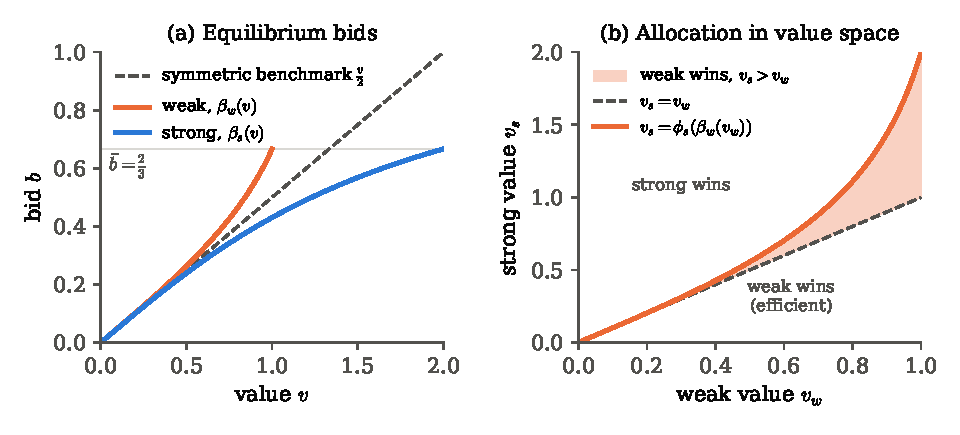
\includegraphics[width=\textwidth]{figures/ch14/asym_bids.pdf}
\caption{Asymmetric first-price auction with $V_w\sim U[0,1]$ and $V_s\sim U[0,2]$. Panel (a): the
equilibrium bid functions \eqref{eq:14-unif-beta} and the symmetric benchmark $\frac{v}{2}$. Both
bidders' bids end at the common top bid $\bar b=\frac{2}{3}$. Panel (b): the weak bidder wins below
the curve $v_s=\phi_s(\beta_w(v_w))$. In the shaded band between that curve and the diagonal the weak
bidder wins although the strong bidder values the object more.}
\label{fig:14-asym-bids}
\end{figure}

The example shows every effect of \cref{prop:14-maskin-riley}. The strong bidder's payoff falls by
$0.0764$ when we move from the second-price to the first-price auction. The weak bidder's payoff
rises by $0.0136$, and total surplus falls by $0.0205$. Revenue is total surplus minus payoffs, so
revenue rises by $0.0764-0.0136-0.0205=0.0423$. The first-price auction extracts more from the strong
bidder than it gives away to the weak bidder and to inefficiency.

\subsection{Revenue comparisons with asymmetric bidders}\label{sec:14-asym-revenue}

The decomposition used in the example holds in general:
\begin{equation}\label{eq:14-rev-decomp}
\text{expected revenue}=\text{expected total surplus}-\sum_i\E\bigl[\pi_i(V_i)\bigr].
\end{equation}
Moving from the open auction to the first-price auction lowers total surplus, by
\cref{prop:14-maskin-riley}(iii). It raises the weak bidder's rents and lowers the strong bidder's
rents, by part (iv). The net effect on revenue has no general sign.
\citet{MaskinRiley2000} give sufficient conditions on the value distributions under which the
first-price auction yields higher revenue, and others under which the open auction does. In the
uniform example the first-price auction raises more revenue. \citet[Section II.D]{AtheyLevinSeira2011} stress that ``there is no general theoretical
comparison of expected revenue, even with fixed participation.''

The optimal auction of \cref{sec:14-optimal} explains why the first-price auction often does well.
In the same example, \cref{sec:14-optimal-asym} showed that the optimal mechanism of
\citet{Myerson1981} gives the weak bidder a head start of $\frac{1}{2}$, because $\psi_w(v)=2v-1$
exceeds $\psi_s(v)=2v-2$ at every value. It earns $\frac{31}{48}\approx 0.646$, well above both
standard formats. The first-price auction tilts the allocation in the same direction as the optimal
mechanism, without design, and it captures part of the gain.
\citet[Section 7]{AtheyHaile2007} summarize the trade-off. First-price auctions may allocate
inefficiently with asymmetric bidders, but they ``tend to raise more revenue in private values
settings.''

\section{Participation and Entry}\label{sec:14-entry}

So far the set of bidders has been fixed. In practice, bidding is costly. A timber bidder must cruise
the tract to estimate its volume and quality, and a construction firm must prepare a detailed cost
estimate. Firms decide whether to incur these costs before the auction. The number of bidders is then
an equilibrium outcome, and the auction format can affect it.

Two timing assumptions organize the theory. In the first, a bidder knows its value before deciding
whether to pay the entry cost. In the second, a bidder learns its value only after paying the cost.
\citet{Samuelson1985} studies the first timing, and \citet{LevinSmith1994} study the second. The
second timing underlies the empirical work of \citet{AtheyLevinSeira2011}, where the entry cost is
the cost of cruising the tract. The two timings give the entry cost different meanings
\citep[Section~2.2, p.~91]{HortacsuPerrigne2021}. When bidders know their values, entry is
\emph{selective}, since only bidders with high enough values enter, and $K$ is a cost of preparing a
bid. When bidders learn their values after entry, entry is \emph{nonselective}, and $K$ also covers
the cost of acquiring information. \citet{RobertsSweeting2016} nest both cases. In their model each
potential bidder observes a noisy signal of its value before it decides whether to enter. The model
of \citet{LevinSmith1994} is the case of signals independent of values, and the model of
\citet{Samuelson1985} is the case of perfect correlation \citep[footnote~9, p.~92]{HortacsuPerrigne2021}.
Throughout this section, $K>0$ is the entry cost, $N$ is the number
of potential bidders, and $p$ denotes an entry probability. Elsewhere $p$ is the clock price
(\cref{sec:14-formats}) or a probability of winning (\cref{sec:14-ret-selfselection}).

\subsection{Entry with values known in advance}\label{sec:14-entry-samuelson}

Suppose each of $N$ symmetric potential bidders knows its value $v_i$, drawn independently from $F$
on $[\underline v,\bar v]$. A bidder who pays $K$ may bid in a standard auction with reserve price
$r$. We look for a symmetric equilibrium in which a bidder enters if and only if its value is at least
a cutoff $v^*$.

The cutoff type is pinned down by a simple observation. A bidder with value $v^*$ wins only if no
rival enters, because any entrant has a value above $v^*$. That happens with probability
$F(v^*)^{N-1}$, and then the lone bidder pays the reserve price. In the second-price auction this is
immediate. In the first-price auction the cutoff type also bids $r$, because it wins only when it is
alone and any higher bid would only raise its payment. Indifference of the cutoff type requires
\begin{equation}\label{eq:14-samuelson-cutoff}
(v^*-r)\,F(v^*)^{N-1}=K .
\end{equation}
Let $\Phi(v)=(v-r)F(v)^{N-1}$. It is zero at $v=r$ and strictly increasing, with
$\Phi'(v)=F(v)^{N-1}+(v-r)(N-1)F(v)^{N-2}f(v)>0$. So a unique interior cutoff exists whenever $\bar
v-r>K$. Types above $v^*$ strictly prefer to enter, because a bidder's expected surplus rises with its
value at the rate of its win probability.

Implicit differentiation of \eqref{eq:14-samuelson-cutoff} gives the comparative statics:
\[
\frac{dv^*}{dK}=\frac{1}{\Phi'(v^*)}>0,\qquad
\frac{dv^*}{dr}=\frac{F(v^*)^{N-1}}{\Phi'(v^*)}\in(0,1),\qquad
\frac{dv^*}{dN}=-\frac{(v^*-r)F(v^*)^{N-1}\ln F(v^*)}{\Phi'(v^*)}>0,
\]
where the last expression treats $N$ as continuous. The entry cost and the reserve price both screen
out low-value bidders. A higher reserve raises the cutoff by less than one for one. The entry cost
differs from a reserve price in one respect. It is a resource cost borne by every entrant, and the
seller collects none of it.

\begin{example}[Cutoffs with uniform values]\label{ex:14-samuelson}
Let $F$ be uniform on $[0,1]$, $N=5$ and $r=0$. Equation \eqref{eq:14-samuelson-cutoff} becomes
$(v^*)^5=K$, so $v^*=K^{\frac{1}{5}}$. With $K=0.05$ the cutoff is $0.549$, each potential bidder
enters with probability $0.451$, and $2.25$ bidders enter on average. With $K=0.10$ the cutoff is
$0.631$ and $1.85$ bidders enter on average. Raising the reserve to $r=0.25$ raises the cutoffs to
$0.610$ and $0.690$. These values come from \texttt{entry\_example.py}.
\end{example}

With values known in advance, the entrants are a selected sample of high-value bidders. This
complicates both theory and estimation. \citet[Section II.F]{AtheyLevinSeira2011} note that with
asymmetric bidders who have prior private information, ``the ex ante rankings of strong and weak
bidders may fail to hold conditional on entry.'' This is one reason they adopt the second timing.

\subsection{Entry with values learned after entry: the Levin-Smith model}\label{sec:14-entry-ls}

Now suppose a bidder learns its value only after paying $K$. Before entry, all $N$ potential bidders
are identical. Entrants observe the number of other entrants before bidding
\citep[Section 6.3.2]{AtheyHaile2007}. Let $\pi(k)$ be the expected profit, gross of $K$, of an
entrant when $k$ bidders enter in total, so that it faces $k-1$ rivals. We study the symmetric
equilibrium in which each potential bidder enters with probability $p$.

Given that the other $N-1$ potential bidders each enter with probability $p$, the number of rival
entrants is binomial. An entrant's ex ante expected profit is therefore
\begin{equation}\label{eq:14-entry-indiff}
\Pi(p)=\sum_{k=1}^{N}\binom{N-1}{k-1}p^{k-1}(1-p)^{N-k}\,\pi(k).
\end{equation}
A potential bidder enters with probability one if $\Pi(p)>K$, stays out if $\Pi(p)<K$, and is willing
to randomize if $\Pi(p)=K$.

\begin{lemma}\label{lem:14-pi-decreasing}
In the symmetric private values model with any standard auction and reserve price $r$, the gross
profit of an entrant is
\begin{equation}\label{eq:14-pik}
\pi(k)=\int_r^{\bar v}F(t)^{k-1}\bigl(1-F(t)\bigr)dt ,
\end{equation}
which is strictly decreasing in $k$. With values uniform on $[0,1]$ and $r=0$,
$\pi(k)=\frac{1}{k(k+1)}$.
\end{lemma}

\begin{proof}
By revenue equivalence, an entrant's interim surplus is the same in every standard auction. By
\cref{lem:14-ic}, a type $v\ge r$ facing $k-1$ rivals earns $\int_r^vF(t)^{k-1}dt$, and types below
$r$ earn zero. Taking expectations and exchanging the order of integration,
\[
\pi(k)=\int_r^{\bar v}\left[\int_r^{v}F(t)^{k-1}dt\right]f(v)\,dv
=\int_r^{\bar v}F(t)^{k-1}\left[\int_t^{\bar v}f(v)\,dv\right]dt
=\int_r^{\bar v}F(t)^{k-1}\bigl(1-F(t)\bigr)dt .
\]
Since $F(t)<1$ on the interior of the support, the integrand falls strictly in $k$. In the uniform
case, $\pi(k)=\int_0^1t^{k-1}(1-t)\,dt=\frac{1}{k}-\frac{1}{k+1}=\frac{1}{k(k+1)}$.
\end{proof}

\begin{proposition}[Symmetric entry equilibrium]\label{prop:14-ls-unique}
Suppose $\pi(k)$ is strictly decreasing in $k$ and $N\ge 2$. Then $\Pi(p)$ is strictly decreasing in
$p$, and there is a unique symmetric entry equilibrium $p^*$. If $\pi(N)\ge K$, then $p^*=1$. If
$\pi(1)\le K$, then $p^*=0$. Otherwise $p^*\in(0,1)$ solves $\Pi(p^*)=K$.
\end{proposition}

\begin{proof}
Let $X\sim\text{Binomial}(N-1,p)$ be the number of rival entrants, so $\Pi(p)=\E[\pi(1+X)]$. A
binomial random variable is stochastically increasing in its success probability. Since $\pi$ is
strictly decreasing, $\E[\pi(1+X)]$ is strictly decreasing in $p$. The function is continuous, with
$\Pi(0)=\pi(1)$ and $\Pi(1)=\pi(N)$. The three cases follow from the intermediate value theorem and
strict monotonicity.
\end{proof}

When $p^*\in(0,1)$, entrants earn zero expected profit net of the entry cost. This has a striking
consequence. Let the seller value the object at $v_0$, and let $S(k)$ be the expected gain from trade
when $k$ bidders enter, measured relative to the seller keeping the object. It equals the expected
value of the winner minus $v_0$ when a sale occurs, and zero otherwise. The seller's expected gain,
revenue minus $v_0$ times the probability of sale, equals expected gains from trade minus bidders'
expected gross rents. Gross rents sum to $Np^*\Pi(p^*)=Np^*K$. Hence
\begin{equation}\label{eq:14-ls-revenue}
\text{seller's expected gain}=\E\bigl[S(X^*)\bigr]-Np^*K,\qquad X^*\sim\text{Binomial}(N,p^*).
\end{equation}
The right side is expected social welfare. The seller captures all of the social surplus, net of
entry costs. With $v_0=0$ the seller's gain is its expected revenue.

\begin{proposition}[Levin and Smith 1994]\label{prop:14-ls-welfare}
Consider symmetric private values, a seller who values the object at $v_0$, and an efficient standard
auction with reserve price $r=v_0$. Then:
\begin{enumerate}[label=(\roman*)]
\item Social welfare $W(p)=\E[S(X)]-NpK$, with $X\sim\text{Binomial}(N,p)$, satisfies
$W'(p)=N\bigl(\Pi(p)-K\bigr)$. The equilibrium entry probability maximizes welfare among symmetric
entry probabilities.
\item If $p^*\in(0,1)$ at $r=v_0$, no reserve price gives the seller a higher expected gain than
$r=v_0$.
\end{enumerate}
\end{proposition}

\begin{proof}
(i) Write $X=\sum_{j=1}^{N}\epsilon_j$ with independent entry indicators $\epsilon_j$ that equal one
with probability $p_j$. Differentiating $\E[S(X)]$ with respect to $p_j$ gives
$\E[S(Y_{-j}+1)-S(Y_{-j})]$, where $Y_{-j}$ counts the other entrants. At $p_j=p$ for all $j$,
summing over $j$ yields
\[
\frac{d}{dp}\E[S(X)]=N\,\E\bigl[S(Y+1)-S(Y)\bigr],\qquad Y\sim\text{Binomial}(N-1,p).
\]
With $r=v_0$ and an efficient auction, $S(k)=\E\bigl[(\max\{V_1,\dots,V_k\}-v_0)^+\bigr]$. The
increment $S(k+1)-S(k)$ is then the expected marginal contribution of one more bidder,
$\E\bigl[(V_{k+1}-\max\{V_1,\dots,V_k,v_0\})^+\bigr]$. In a second-price auction with reserve $v_0$,
this is exactly the bidder's expected surplus when it faces $k$ rivals, which is $\pi(k+1)$. By
revenue equivalence the same holds in any efficient standard auction with reserve $v_0$. Therefore
$\frac{d}{dp}\E[S(X)]=N\,\E[\pi(Y+1)]=N\,\Pi(p)$, and $W'(p)=N(\Pi(p)-K)$. Since $\Pi$ is decreasing,
$W$ is concave, and its maximizer over $[0,1]$ is the $p^*$ of \cref{prop:14-ls-unique}.

(ii) Let $R(r)$ and $W_r(p)$ denote the seller's expected gain and welfare with reserve $r$, and let
$p^*(r)$ be the equilibrium entry probability. Net bidder rents are never negative in equilibrium, so $R(r)\le
W_r(p^*(r))$. For any fixed $p$, the reserve $v_0$ allocates the object efficiently among the
entrants and the seller, so $W_r(p)\le W_{v_0}(p)$. By part (i), $W_{v_0}(p)\le W_{v_0}(p^*(v_0))$.
Finally, \eqref{eq:14-ls-revenue} gives $W_{v_0}(p^*(v_0))=R(v_0)$ when $p^*(v_0)\in(0,1)$. Chaining
the inequalities, $R(r)\le R(v_0)$.
\end{proof}

Part (ii) reverses the logic of \cref{cor:14-optimal-reserve}. With a fixed number of bidders, the
seller sets a reserve above its own value to extract rents. With endogenous entry and zero expected
rents, there are no rents left to extract. A reserve above $v_0$ then only discourages entry and
distorts the allocation. \citet[Section~2.2, p.~91]{HortacsuPerrigne2021} state the contrast between
the two entry models. Under nonselective entry of the Levin-Smith type, the optimal reserve price is
the seller's own value. Under selective entry it is given by the formula \eqref{eq:14-optimal-reserve}
of the fixed-participation model. The proofs here are our own.
\citet{LevinSmith1994} also show that the random entry of the mixed
equilibrium wastes resources. Sometimes too many bidders enter and sometimes too few. A seller who
could limit the number of potential bidders, and charge an entry fee if needed, would earn more.

\begin{example}[Levin-Smith entry with uniform values]\label{ex:14-ls}
Let values be uniform on $[0,1]$, $r=v_0=0$ and $N=5$. By \cref{lem:14-pi-decreasing},
$\pi(1),\dots,\pi(5)=\frac{1}{2},\frac{1}{6},\frac{1}{12},\frac{1}{20},\frac{1}{30}$, so
$\Pi(1)=\pi(5)=\frac{1}{30}\approx 0.033$. Every entry cost between $\frac{1}{30}$ and $\pi(1)=\frac{1}{2}$ therefore
produces a mixed equilibrium. For $K\ge\frac{1}{2}$ nobody enters. With $K=0.05$, solving $\Pi(p)=K$ numerically gives $p^*=0.816$, so $4.08$
bidders enter on average. Expected revenue equals expected welfare, $0.592$. With $K=0.10$, $p^*=0.559$,
$2.79$ bidders enter on average, nobody enters with probability $0.017$, and revenue is $0.425$.
\Cref{fig:14-entry}(a) shows the two solutions.

The value of limiting entry is visible in \cref{fig:14-entry}(b). With $K=0.05$ and $N=4$ potential
bidders, $\pi(4)=\frac{1}{20}=K$, so all four enter and revenue is $\frac{3}{5}=0.600$. Adding a fifth
potential bidder lowers revenue to $0.592$, and ten potential bidders lower it to $0.574$. With
$K=0.10$, revenue peaks at $0.452$ with $N=3$. The losses are modest here, but they have the sign
that \citet{LevinSmith1994} emphasize. All numbers come from \texttt{entry\_example.py}.
\end{example}

\begin{figure}[htbp]
\centering
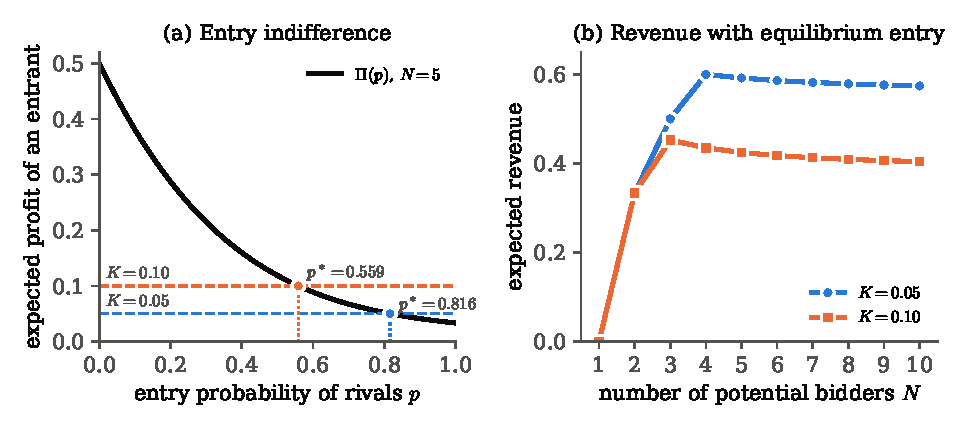
\includegraphics[width=\textwidth]{figures/ch14/entry.pdf}
\caption{Levin-Smith entry with uniform values and no reserve price. Panel (a): the ex ante profit of
an entrant $\Pi(p)$ in \eqref{eq:14-entry-indiff} for $N=5$, and the equilibrium entry probabilities
for $K=0.05$ and $K=0.10$. Panel (b): expected revenue in the symmetric entry equilibrium as a
function of the number of potential bidders $N$.}
\label{fig:14-entry}
\end{figure}

\subsection{Asymmetric bidders and type-symmetric entry equilibria}\label{sec:14-entry-als}

\citet{AtheyLevinSeira2011} combine the Levin-Smith timing with the asymmetric model of
\cref{sec:14-asym}. There are $N_L$ potential loggers with value distribution $F_L$ and $N_M$
potential mills with value distribution $F_M$. Mills are strong: $F_M$ dominates $F_L$ in the
reverse hazard rate order. Each firm decides independently whether to pay $K$, learns its value if it
does, and learns which rivals entered before bidding \citep[Section II.A]{AtheyLevinSeira2011}.

The model omits two features that could also matter for the format comparison. Bidders may have a
common value component, from private estimates of timber quality and volume or from differing
beliefs about future market conditions. They may also be risk averse. \citet[Section
II.F]{AtheyLevinSeira2011} abstract from both for two reasons. The format differences they observe
are qualitatively different from those that common values or risk aversion would imply, and
including either feature significantly complicates the analysis. They also restrict attention to
type-symmetric equilibria, which they regard as a convenient assumption that allows point
identification of entry costs.

Let $\pi_L^\tau(n_L,n_M)$ and $\pi_M^\tau(n_L,n_M)$ be the expected profits, gross of $K$, of a
participating logger and mill in format $\tau\in\{\mathrm{o},\mathrm{s}\}$ (open or sealed). The superscript $\tau$ indexes the format
and is unrelated to the payment rule $\tau_i$ of \cref{sec:14-ret}. The
participants are $n_L$ loggers and $n_M$ mills, and these counts include the bidder itself. Following
\citet[eq.~(4)]{AtheyLevinSeira2011}, bidder $i$'s ex ante profit from entering is
\begin{equation}\label{eq:14-als-exante}
\Pi_i^\tau(\bm p)=\sum_{\bm n}\pi_i^\tau(n_L,n_M)\,\Pr\bigl[n_L,n_M\mid i\text{ enters, rivals play }\bm p_{-i}\bigr],
\end{equation}
where $\bm p$ is the profile of entry probabilities. When all loggers enter with probability $p_L$ and
all mills with probability $p_M$, the probabilities are binomial. Write
$\mathrm{bin}(k;m,p)=\binom{m}{k}p^k(1-p)^{m-k}$. For a logger and a mill, respectively,
\begin{align}
\Pi_L^\tau(p_L,p_M)&=\sum_{n_L=1}^{N_L}\sum_{n_M=0}^{N_M}\mathrm{bin}(n_L-1;N_L-1,p_L)\,\mathrm{bin}(n_M;N_M,p_M)\,\pi_L^\tau(n_L,n_M),\label{eq:14-als-PiL}\\
\Pi_M^\tau(p_L,p_M)&=\sum_{n_L=0}^{N_L}\sum_{n_M=1}^{N_M}\mathrm{bin}(n_L;N_L,p_L)\,\mathrm{bin}(n_M-1;N_M-1,p_M)\,\pi_M^\tau(n_L,n_M).\label{eq:14-als-PiM}
\end{align}

\begin{definition}[Type-symmetric entry equilibrium]\label{def:14-type-symmetric}
A \emph{type-symmetric entry equilibrium} \citep[Section II.A]{AtheyLevinSeira2011} consists of bid
strategies $b_L(\cdot;\bm n)$, $b_M(\cdot;\bm n)$ and entry probabilities $p_L$, $p_M$ with three
properties.
\begin{enumerate}[label=(\roman*)]
\item All loggers use $(b_L,p_L)$ and all mills use $(b_M,p_M)$.
\item Each bidder's bid strategy maximizes its profit conditional on entering, for every set of
participants.
\item Each bidder enters if and only if its expected profit from entry \eqref{eq:14-als-exante} is at
least $K$. It may randomize when the two are equal.
\end{enumerate}
\end{definition}

Bid strategies in the open auction are $b_k(v;\bm n)=v$. In the sealed auction they solve
\eqref{eq:14-ts-foc-L} and \eqref{eq:14-ts-foc-M} with $b_k(r;\bm n)=r$. A type-symmetric entry
equilibrium exists in both formats, but it need not be unique \citep[Section
II.C]{AtheyLevinSeira2011}. The following condition, with at least two potential bidders of each
type, restores uniqueness. For the proof we maintain
that a participant's expected profit falls when a rival is added, strictly in expectation. In the
open auction this holds auction by auction, since a bidder's surplus
$(v-\max\{\text{rival values},r\})^+$ can only fall when a rival is added.

\begin{proposition}[Athey, Levin and Seira 2011, Proposition 1]\label{prop:14-als-unique}
Suppose that for all $n_L,n_M$,
\begin{equation}\label{eq:14-als-condition}
\pi_M^{\mathrm{s}}(n_L,n_M+1)>\pi_L^{\mathrm{s}}(n_L,n_M).
\end{equation}
Then every type-symmetric entry equilibrium of either auction format has $p_L=0$ or $p_M=1$. If
also $N_L\ge 2$ and $N_M\ge 2$, each format has a unique type-symmetric entry equilibrium.
\end{proposition}

Condition \eqref{eq:14-als-condition} compares a mill and a logger that face the same $n_M$ mills.
The mill faces $n_L$ loggers, while the logger faces only $n_L-1$ other loggers. The condition
requires the mill to earn more despite its extra rival. In the words of \citet[Section
II.C]{AtheyLevinSeira2011}, ``mills have a sufficient value advantage over loggers to outweigh the
effects of facing an additional bidder.'' They call the condition ``rather strong'' as theory, and
they verify it for every tract in their estimated model (\cref{ch:auction-empirics}).

\begin{proof}[Proof sketch]
\emph{Mills earn more than loggers at every entry profile.} Fix $(p_L,p_M)$. A logger who enters
faces $X_L\sim\text{Binomial}(N_L-1,p_L)$ other loggers and $X_M\sim\text{Binomial}(N_M,p_M)$ mills. A
mill who enters faces $X_L+\epsilon_L$ loggers and $X_M-\epsilon_M$ other mills. Here $\epsilon_L$ is an
indicator with success probability $p_L$, independent of everything else, and $\epsilon_M$ is the entry
indicator of one of the $N_M$ mills counted in $X_M$. Then $X_L+\epsilon_L\sim\text{Binomial}(N_L,p_L)$
and $X_M-\epsilon_M\sim\text{Binomial}(N_M-1,p_M)$, as a mill's counts require. Using monotonicity, then \eqref{eq:14-als-condition}, then monotonicity again,
\[
\pi_M(X_L+\epsilon_L,\,X_M-\epsilon_M+1)\ \ge\ \pi_M(X_L+1,\,X_M-\epsilon_M+1)\ >\
\pi_L(X_L+1,\,X_M-\epsilon_M)\ \ge\ \pi_L(X_L+1,\,X_M).
\]
Taking expectations gives $\Pi_M(p_L,p_M)>\Pi_L(p_L,p_M)$ for every profile.

\emph{Either $p_L=0$ or $p_M=1$.} If loggers enter with positive probability, then $\Pi_L\ge K$. The
previous step gives $\Pi_M>K$, so mills enter with probability one.

\emph{Uniqueness.} Candidate equilibria have either $p_M=1$ and $p_L$ solving the logger's condition,
or $p_L=0$ and $p_M<1$ solving the mill's condition. With all mills entering, a logger's payoff is
$\Pi_L(p_L,1)=\E[\pi_L(1+X_L,N_M)]$. When $N_L\ge 2$, the count $X_L$ of other loggers is
stochastically increasing in $p_L$, so $\Pi_L(\cdot,1)$ is strictly decreasing. When $N_M\ge 2$, the
same argument shows that $\Pi_M(0,\cdot)$ is strictly decreasing. Each family therefore has at most
one member. Suppose an equilibrium with $p_L=0$
and $p_M<1$ exists. Then $\Pi_M(0,p_M)\le K$ when $p_M=0$, or $\Pi_M(0,p_M)=K$ when $p_M>0$. In
either case $\Pi_M(p_L,1)\le\Pi_M(0,1)<\Pi_M(0,p_M)\le K$ for every $p_L$, so no equilibrium with
$p_M=1$ exists. Only one candidate survives.

\emph{Both formats.} For any participant set, mills earn more and loggers less in the open auction
than in the sealed auction \citep[Section II.D]{AtheyLevinSeira2011}. This is the many-bidder
analogue of \cref{prop:14-maskin-riley}(iv). Hence
$\pi_M^{\mathrm{o}}(n_L,n_M+1)\ge\pi_M^{\mathrm{s}}(n_L,n_M+1)>\pi_L^{\mathrm{s}}(n_L,n_M)\ge\pi_L^{\mathrm{o}}(n_L,n_M)$,
and the argument applies to the open auction as well.
\end{proof}

\citet{AtheyLevinSeira2011} state uniqueness without the restriction $N_L,N_M\ge 2$, and the
restriction matters. With a single potential logger, $\Pi_L(p_L,1)=\pi_L(1,N_M)$ does not depend on
$p_L$. If $K=\pi_L(1,N_M)$, the logger is indifferent at every $p_L$, and mills strictly prefer to
enter by the first step of the proof. Every profile $(p_L,1)$ with $p_L\in[0,1]$ is then an
equilibrium. With one mill and one logger in the sealed auction of \cref{ex:14-als-entry} below, this
happens at $K=\pi_L^{\mathrm{s}}(1,1)=0.0969$. A single potential mill creates the same indifference at
$K=\pi_M(0,1)$, the profit of a mill without rivals, where every profile $(0,p_M)$ is an equilibrium.
At every other entry cost, a payoff that does not depend on its own type's entry probability is either
above or below $K$. It then pins down a single entry probability, and the equilibrium is again unique.
The separation result, $p_L=0$ or $p_M=1$, holds for any numbers of potential bidders.

The empirically relevant equilibrium has every mill entering and loggers randomizing,
$p_M=1$ and $p_L\in(0,1)$. \citet[Section II.C]{AtheyLevinSeira2011} motivate this case with their
data: they ``observe logger entry in more than 85\% of sales and always more potential logger
entrants than actual logger entrants.''

\casehead{The homogeneous benchmark}
If $F_L=F_M$, every bidder is the same and revenue equivalence applies conditional on the number of
entrants. Each format then produces the same $\pi(k)$, given by \eqref{eq:14-pik}, and the same
entry condition. \citet[Section II.D]{AtheyLevinSeira2011} conclude that the two formats have
``(i) the same expected entry, (ii) the same allocation, and (iii) the same expected revenue.''
Format differences in entry therefore require asymmetric bidders.

\begin{proposition}[Athey, Levin and Seira 2011, Proposition 2]\label{prop:14-entry-format}
For any type-symmetric entry equilibrium of the sealed bid auction, there is a type-symmetric entry
equilibrium of the open auction with the following properties.
\begin{enumerate}[label=(\roman*)]
\item Loggers are less likely to enter.
\item Mills are more likely to enter.
\item It is less likely that a logger wins.
\end{enumerate}
\end{proposition}

\begin{proof}[Proof sketch for the empirically relevant case]
Assume \eqref{eq:14-als-condition} and $N_L,N_M\ge 2$, so each format has a unique equilibrium by
\cref{prop:14-als-unique}, and suppose the sealed
equilibrium has $p_M^{\mathrm{s}}=1$ and $p_L^{\mathrm{s}}\in(0,1)$. For every participant set, a
logger earns weakly less in the open auction. Hence $\Pi_L^{\mathrm{o}}(p_L,1)\le\Pi_L^{\mathrm{s}}(p_L,1)$
for every $p_L$. At $p_L^{\mathrm{s}}$ the sealed condition holds with equality, so
$\Pi_L^{\mathrm{o}}(p_L^{\mathrm{s}},1)\le K$. Because $\Pi_L^{\mathrm{o}}(\cdot,1)$ is decreasing,
the open-auction solution satisfies $p_L^{\mathrm{o}}\le p_L^{\mathrm{s}}$. This is (i). Mills earn
weakly more in the open auction and face fewer loggers, so
$\Pi_M^{\mathrm{o}}(p_L^{\mathrm{o}},1)\ge\Pi_M^{\mathrm{s}}(p_L^{\mathrm{s}},1)\ge K$. Mills still enter
with probability one, which gives (ii) with equality. For (iii), two effects reinforce each other.
For a fixed set of participants, a logger wins less often in the open auction, which is efficient,
than in the sealed auction, by \cref{prop:14-maskin-riley}(iii). In the open auction, fewer logger
entrants also mean a lower chance that the highest value belongs to a logger.
\end{proof}

The general statement allows multiple equilibria, which is why it is phrased as existence of a
suitable open-auction equilibrium. Under the conditions of \cref{prop:14-als-unique}, the prediction
is sharp: ``open
bidding leads to less logger entry, equivalent mill entry and a lower chance that a logger wins''
\citep[Section II.D]{AtheyLevinSeira2011}. The revenue comparison remains ambiguous. Sealed bidding
attracts more loggers, which raises competition, but it allocates inefficiently. The sealed auction is
``inefficient even conditional on participation,'' while the efficient type-symmetric outcome is an
equilibrium of the open auction \citep[Section II.D, citing \citealp{AtheyLevinSeira2004}]{AtheyLevinSeira2011}. The idea that sealed bids
encourage entry by weaker bidders is emphasized by \citet{Klemperer2004} in the context of spectrum
auctions \citep[footnote~4, p.~215]{AtheyLevinSeira2011}. \citet[Section~7]{AtheyHaile2007} likewise
list entry among the factors that govern the choice of format. The format ``also affects bidder entry
when bidders are asymmetric,'' and they cite \citet{Klemperer2002} and \citet{AtheyLevinSeira2004}. The
mechanism is the one of \cref{prop:14-entry-format}. An ascending auction deters entry by bidders who
expect to be outbid by a stronger rival.
\citet{Klemperer2002} proposes hybrid formats that end with a sealed-bid stage.

\begin{example}[One mill and one potential logger]\label{ex:14-als-entry}
Take the values of \cref{ex:14-asym-uniform}: the mill draws from $U[0,2]$, the logger from
$U[0,1]$, and $r=0$. With both present, \cref{tab:14-asym-example} gives
$\pi_L^{\mathrm{s}}=0.0969$, $\pi_L^{\mathrm{o}}=\frac{1}{12}\approx 0.0833$,
$\pi_M^{\mathrm{s}}=0.5069$ and $\pi_M^{\mathrm{o}}=\frac{7}{12}$. A mill alone pays the reserve and
earns $\E[V_M]=1$, and a logger alone earns $\E[V_L]=\frac{1}{2}$. Condition
\eqref{eq:14-als-condition} holds, since $0.5069>0.5$. Let $K=0.09$. This cost differs from the
knife-edge values $\pi_L^\tau(1,1)$ and $\pi_M^\tau(0,1)=1$ of both formats, so each format has a
unique type-symmetric entry equilibrium. In the sealed auction the mill
enters and the logger enters too, because $0.0969>0.09$. Revenue is $0.459$, the logger wins with
probability $\frac{1}{3}$, and welfare is $1.0628-2K=0.883$. In the open auction the logger stays
out, because $0.0833<0.09$. The mill wins at the reserve price, so revenue is zero and welfare is
$1-K=0.91$. The sealed auction raises far more revenue through entry, and the open auction is more
efficient.
\end{example}

The example is extreme because $r=0$, but it isolates the mechanism of \cref{prop:14-entry-format}.
The weak bidder's expected profit is higher under sealed bidding, so it enters more often. That entry
disciplines the strong bidder, whose price would otherwise be set by the reserve.

\casehead{From entry decisions to entry costs}
The indifference of randomizing bidders carries empirical content. For any bidder who randomizes,
expected profit from entry equals $K$. \citet[Section 6.3.2]{AtheyHaile2007} write this as
\begin{equation}\label{eq:14-entry-cost-id}
K=\sum_{\mathcal A:\,i\in\mathcal A}\Pr\bigl(\tilde{\mathcal N}=\mathcal A\mid i\in\tilde{\mathcal
N}\bigr)\,\pi_i(\mathcal A),
\end{equation}
where $\tilde{\mathcal N}$ is the random set of entrants. Here $\pi_i(\mathcal A)$ is bidder $i$'s
expected gross profit when the participant set is $\mathcal A$,
\begin{equation}\label{eq:14-entry-profit-id}
\pi_i(\mathcal A)=\E\Bigl[\bigl(V_i-\beta_i(V_i;\mathcal A)\bigr)\,G_{M_i|B_i}\bigl(\beta_i(V_i;\mathcal
A)\bigm|\beta_i(V_i;\mathcal A);\mathcal A\bigr)\Bigr],
\end{equation}
with $G_{M_i|B_i}$ the distribution of the highest rival bid given bidder $i$'s own bid. The notation
follows \citet[Section 6.3.2]{AtheyHaile2007}, who write $\Pi_i$ for what we call $\pi_i$. The post-entry profits are identified
from bids, and the entry probabilities are observed. The level of the entry cost is then identified
in dollars. This contrasts with entry models that infer profits only from entry decisions
\citep[Section 6.3.2]{AtheyHaile2007}. \Cref{ch:auction-empirics} develops the estimator.

\section{Collusion and the Choice of Format}\label{sec:14-collusion}

Collusion among bidders is a long-standing concern in auction design. Gifford Pinchot, the first
chief of the US Forest Service, advocated sealed bidding for timber. He described a sale on sealed
bids as ``thereby preventing the customary collusion between bidders'' \citep[p.~209]{Pinchot1998},
as quoted by \citet[footnote 2]{AtheyLevinSeira2011}. \citet[Section 9]{MilgromWeber1982} name the
same setting as a limit of their noncooperative theory. They judge it less reasonable for timber
rights on federal land, where ``the bidders (owners of lumber mills) are members of a trade
association and bid repeatedly against each other'' \citep[p.~1118]{MilgromWeber1982}. This section explains why the format matters for collusion. The
general theory of cartels is in \cref{ch:collusion-theory}, and prosecuted bidding rings are studied
in \cref{ch:collusion-evidence}.

\subsection{Rings in second-price and ascending auctions}\label{sec:14-collusion-open}

A \emph{bidding ring} is a group of bidders who agree to suppress competition among themselves.
Consider the private values model with a ring $\mathcal C\subset\mathcal N$ of $m\ge 2$ members.
Suppose for now that members know each other's values. The simplest agreement designates the member
with the highest value, bidder $d$, to bid. The other members abstain or bid the reserve price.
Bidders outside the ring bid as usual.

\begin{proposition}[Robinson 1985]\label{prop:14-robinson}
In a second-price or ascending auction with private values, the ring agreement in which the
highest-value member bids its value and the other members abstain is self-enforcing. No member gains
by deviating within the auction, whatever the values and whether or not the members meet again.
\end{proposition}

\begin{proof}
Outsiders bid their values, which is weakly dominant by \cref{prop:14-spa-dominant}. The designated
bidder $d$ bids $v_d$, which is also weakly dominant. Consider a member $j\neq d$, with $v_j\le v_d$.
Bidder $j$ wins only with a bid above $v_d$, since $d$ stays in until the price reaches $v_d$. A
winning deviation then pays at least $v_d\ge v_j$, so its payoff is at most zero. Abstaining yields
zero. Hence no deviation is profitable.
\end{proof}

The ring gains because it removes the price pressure that members exert on each other. Let
$V^{\mathcal C}_{(1)}\ge V^{\mathcal C}_{(2)}$ be the two highest member values and $V^{\mathcal O}_{(1)}$
the highest outsider value. Competitive bidding sets the price at the second-highest value overall.
Under the ring, the price is $\max\{V^{\mathcal O}_{(1)},r\}$ whenever a member wins. The price
falls only when the two highest values both belong to members, and then by
\begin{equation}\label{eq:14-ring-gain}
\Delta P=\Bigl(V^{\mathcal C}_{(2)}-\max\bigl\{V^{\mathcal O}_{(1)},r\bigr\}\Bigr)^+ .
\end{equation}
The ring does not change who wins, so the allocation stays efficient. The ring transfers surplus
from the seller to its members.

\Citet[Section~2.5, p.~96]{HortacsuPerrigne2021} draw the practical lesson from \cref{prop:14-robinson}.
Open auctions may favor collusion, because bidders meet face to face and can react at once to each
other's behavior. If the ring allocates the object to its highest-value member, no other member gains
by deviating, since that member can always outbid the deviator. For this reason auction theorists
recommend first-price auctions. The issue is practical. Collusion at U.S.\ Forest Service timber sales
was suspected in the 1970s, and it was the subject of allegations and of a congressional hearing in
1977, though few cases were prosecuted. In 1976 the federal government recommended first-price sealed
bids over ascending auctions, mainly to reduce collusion \citep[Section~2.4, p.~96]{HortacsuPerrigne2021}.
Sealed bids are no cure, however. The same survey reviews collusion in first-price procurement auctions
of construction contracts (their Section~3.4), and \cref{ch:collusion-evidence} studies such rings.

\subsection{Rings in first-price auctions}\label{sec:14-collusion-fpa}

The first-price auction is different. To gain, the designated bidder must bid less than the price
that competition would produce. Every other member with a value above that bid then has a unilateral
incentive to bid slightly more and win. In a one-shot auction, the designated bid must exceed the
values of all other members to deter such deviations. With known values, the ring must therefore pay
at least $V^{\mathcal C}_{(2)}$ whenever it wins. The price suppression of \eqref{eq:14-ring-gain}
cannot be sustained within a single sealed-bid auction.

Sustaining a first-price ring requires the threat of future punishment. A member who undercuts the
designated bidder is detected only after the bids are opened, and the ring can respond only in later
auctions. The agreement survives if the one-time gain from undercutting is smaller than the discounted
loss from the ring's collapse, a condition of the kind derived in \cref{ch:collusion-theory}. The
open auction needs no such condition. A deviation there is observed as it happens, and the designated
bidder answers it by continuing to bid. \citet[Section 7]{AtheyHaile2007} summarize the comparison:
first-price auctions ``may be less susceptible to collusion (detection and response to defections
are more difficult than in an ascending auction).'' This is why sealed bids appear in \cref{tab:14-ranking}
as the format less prone to collusion. \citet{Robinson1985} draws the policy conclusion that a seller
worried about rings should prefer the first-price format.

\subsection{Ring size, leakage and secret deviations}\label{sec:14-collusion-size}

The two formats also differ in who gains from a ring that does not include every bidder.
\citet[ch.~8, p.~176]{MarshallMarx2012} put the contrast as follows. In the ascending auction the
highest-value member stays in up to its value, exactly as it would without the ring. An outsider who
wins pays what it would have paid without collusion, so the ring captures all the gains. In the
sealed-bid auction the designated member bids strictly less than its noncollusive bid. Outsiders then
sometimes win auctions that they would have lost under competition. Part of the collusive gain spills
over to the outsiders, which \citet[p.~181]{MarshallMarx2012} call \emph{leakage}. The following example
computes the ascending-auction side of the comparison in closed form.

\begin{example}[Ring size with uniform values]\label{ex:14-ring-size}
Let $n$ bidders have values that are independent and uniform on $[0,1]$, with $r=v_0=0$. A ring of
$k\ge 1$ members bids in an ascending auction as in \cref{prop:14-robinson}, and the other $m=n-k$
bidders bid their values. We compute the expected price and the expected surplus of each bidder.

\emph{Step 1 (price reduction).} By \eqref{eq:14-ring-gain} with $r=0$, the ring lowers the price by
$(C_2-O_1)^+$. Here $C_2$ is the second-highest member value and $O_1$ the highest outsider value, with
$O_1=0$ when $m=0$. The density of $C_2$ is $k(k-1)x^{k-2}(1-x)$ on $[0,1]$, and $\Pr(O_1\le y)=y^m$.
For a fixed $x$,
\[
\E\bigl[(x-O_1)^+\bigr]=\int_0^x\Pr(O_1\le y)\,dy=\int_0^x y^m\,dy=\frac{x^{m+1}}{m+1}.
\]
Integrating over $C_2$ and using $k+m=n$,
\[
\E[\Delta P]=\frac{k(k-1)}{m+1}\int_0^1x^{n-1}(1-x)\,dx
=\frac{k(k-1)}{m+1}\left(\frac{1}{n}-\frac{1}{n+1}\right)
=\frac{k(k-1)}{(n-k+1)\,n\,(n+1)}.
\]

\emph{Step 2 (price).} Without a ring the expected price is $\E[V_{(n-1:n)}]=\frac{n-1}{n+1}$, so the
expected price with a ring of $k$ members is
\begin{equation}\label{eq:14-ring-price}
\E[P_k]=\frac{n-1}{n+1}-\frac{k(k-1)}{(n-k+1)\,n\,(n+1)}.
\end{equation}
With $k=2$ the fall is $\frac{2}{(n-1)n(n+1)}$.

\emph{Step 3 (surplus).} An outsider wins only with the highest value overall, and it then pays the
second-highest value overall, ring or no ring. Its expected surplus is therefore unchanged at
$\frac{1}{n}\E\bigl[V_{(n:n)}-V_{(n-1:n)}\bigr]=\frac{1}{n(n+1)}$. Members keep their competitive surplus
$\frac{k}{n(n+1)}$ and gain $\E[\Delta P]$ in addition. Per member,
\[
\frac{1}{k}\left[\frac{k}{n(n+1)}+\frac{k(k-1)}{(n-k+1)n(n+1)}\right]
=\frac{1}{n(n+1)}\cdot\frac{n}{n-k+1}
=\frac{1}{(n+1)(n-k+1)}.
\]
An all-inclusive ring, $k=n$, pays nothing, and each member earns $\frac{1}{n+1}=\frac{1}{n}\E[V_{(n:n)}]$.
\end{example}

\Cref{tab:14-mm-ring} reproduces Table~8.1 of \citet[ch.~8, p.~182]{MarshallMarx2012}, which compares
the two formats with five bidders. The ascending columns follow from \cref{ex:14-ring-size}. For
example, with $n=5$ and $k=3$, \eqref{eq:14-ring-price} gives $\frac{4}{6}-\frac{6}{3\cdot 30}=0.600$, and
each member earns $\frac{1}{6\cdot 3}\approx 0.056$. In the first-price auction the ring is a single
strong bidder whose value is the highest of $k$ uniform draws. That asymmetric auction has no closed
form. Marshall and Marx take its values from \citet[Table~III]{MarshallEtAl1994}, who compute them by
Monte Carlo with 100,000 draws.

\begin{table}[htbp]
\centering
\caption{Rings of different sizes with five bidders and uniform values}\label{tab:14-mm-ring}
\begin{tabular}{@{}ccccccc@{}}
\toprule
& \multicolumn{2}{c}{Expected price} & \multicolumn{2}{c}{Surplus per ring member} & \multicolumn{2}{c}{Surplus per outsider}\\
\cmidrule(lr){2-3}\cmidrule(lr){4-5}\cmidrule(l){6-7}
Ring size $k$ & Ascending & First price & Ascending & First price & Ascending & First price\\
\midrule
1 & 0.667 & 0.667 & 0.033 & 0.033 & 0.033 & 0.033\\
2 & 0.650 & 0.651 & 0.042 & 0.035 & 0.033 & 0.037\\
3 & 0.600 & 0.609 & 0.056 & 0.041 & 0.033 & 0.049\\
4 & 0.467 & 0.506 & 0.083 & 0.057 & 0.033 & 0.086\\
5 & 0.000 & 0.000 & 0.167 & 0.167 & -- & --\\
\bottomrule
\end{tabular}

\smallskip
\begin{minipage}{0.95\textwidth}
\footnotesize Notes: Five bidders with values independent and uniform on $[0,1]$, and a reserve price
of zero. A ring of size one means competitive bidding. The ascending columns and the first-price row
for $k=1$ are analytic. The other first-price entries are from \citet[Table~III]{MarshallEtAl1994}.
Source: \citet[ch.~8, Table~8.1, p.~182]{MarshallMarx2012}.
\end{minipage}
\end{table}

The table shows three effects. First, outsiders gain from a ring only in the sealed-bid auction. Their
surplus rises from 0.033 to 0.037, 0.049 and 0.086 as the ring grows from two to four members. Members
of a larger ring bid lower, and outsiders win more often and pay less \citep[p.~181]{MarshallMarx2012}.
The leakage also creates inefficiency. With a ring of four against one outsider, the outsider bids
about 0.40 when its value is about 0.54. The ring bids about 0.40 only when its highest value is about
0.76 \citep[pp.~183--184, using Figure~2 of \citealp{MarshallEtAl1994}]{MarshallMarx2012}. The outsider
then wins whenever the ring's highest value lies between 0.54 and 0.76.

Second, a ring that excludes some bidders hurts the seller more in the ascending auction. With two,
three and four members the expected price is 0.650, 0.600 and 0.467 there, against 0.651, 0.609 and
0.506 in the first-price auction. Each member also gains more, 0.042, 0.056 and 0.083 against 0.035,
0.041 and 0.057. In this example the incentive to collude is therefore stronger in the ascending auction
\citep[p.~181]{MarshallMarx2012}. Marshall and Marx stress in their footnote~21 that this ranking is not
a general result.

Third, leakage affects who wants to join. In the ascending auction there is no leakage, so outsiders
always want to join, and with symmetric bidders the ring wants to admit them
\citep[p.~177]{MarshallMarx2012}. In the sealed-bid auction an outsider may prefer to stay out. With
101 bidders, an outsider facing a ring of 99 earns 0.0159 in the first-price auction. As a member of a
ring of 100 it would earn only 0.0025. The last outsider facing a ring of 100 earns 0.0412, more than
the 0.0098 it would earn in the all-inclusive ring \citep[Table~8.2, pp.~185--186]{MarshallMarx2012}.
\Cref{ex:14-ring-size} reproduces their ascending entries, a member surplus of $\frac{1}{102\cdot
3}\approx 0.0033$, $\frac{1}{102\cdot 2}\approx 0.0049$ and $\frac{1}{102}\approx 0.0098$.

The same contrast governs enforcement. A \emph{secret deviation} is a clandestine bid at the main
auction, contrary to the ring's recommendation, that cannot be traced to the member without
substantial cost \citep[ch.~9, pp.~187--188]{MarshallMarx2012}. Secret deviations are a major concern
in sealed-bid auctions and a lesser one in ascending auctions. In the ascending auction the
highest-value member can stay active up to its value, as it would without the ring, so there is no
room for a profitable deviation. In the sealed-bid auction the designated member bids below its
noncooperative bid, which opens the door to deviations by other members. Marshall and Marx conclude
that pricing and enforcement structures are harder to implement in sealed-bid auctions, while the
structures for allocating the gains are much the same in the two formats \citep[p.~198]{MarshallMarx2012}.

\subsection{Knockouts and side payments}\label{sec:14-collusion-knockout}

The agreement above assumed that members know each other's values. In practice, a ring must elicit
values and divide the gains. Rings often hold a private auction among their members, called a
\emph{knockout}, before or after the real one. The winner of the knockout gets the object or the right to
bid for it, and side payments compensate the losers.

\citet{GrahamMarshall1987} study knockouts for second-price and English auctions.
In a knockout of the type they analyze, each member reports a value to a ring center. The highest
reporter bids its report in the main auction. If it wins at price $P$, it pays the center the amount
by which the second-highest report exceeds $P$. Its total outlay is
$P+(\hat z_{(2)}-P)^+=\max\{P,\hat z_{(2)}\}$, where $\hat z_{(2)}$ is the second-highest report. Each member thus
faces a second-price auction against the other reports and the outside bids, so truthful reporting is
weakly dominant. The center's collections are returned to members as transfers fixed in advance,
which keeps incentives intact and balances the budget in expectation.

\citet{McAfeeMcMillan1992} study rings in first-price auctions.
A \emph{weak cartel} cannot make side payments. Its best scheme has every member with a value above
the reserve bid the reserve price, with the winner chosen at random among them. A \emph{strong
cartel} can make side payments. It can allocate the object to the member with the highest value
through a first-price knockout whose winner pays its knockout bid to the other members in equal
shares.

\citet[ch.~9, pp.~191--192]{MarshallMarx2012} describe a strong cartel of this kind. From 1895 the
cast-iron pipe makers of the Addyston Pipe cartel met before each sealed-bid procurement in their pay
territories and held a knockout. The high bidder in the knockout was selected to bid at the
procurement. Its knockout bid was distributed among all the ring members, in shares that varied with
their production capacities \citep[p.~191, footnote~7]{MarshallMarx2012}. The other members either stayed
out or submitted deliberately losing bids. In one procurement in St.~Louis, Howard-Harrison won with a
bid of \$24, while Addyston and Dennis Long protected it with bids of \$24.37 and \$24.57. The
Chattanooga foundry could have supplied the pipe at \$17 or \$18 and still made a profit
\citep[p.~192]{MarshallMarx2012}. Marshall and Marx describe this mechanism in stylized form, and
their footnote~6 attributes the stylized model to \citet{McAfeeMcMillan1992}. The cartel thus ran a
version of the McAfee and McMillan knockout. With symmetric bidders that knockout lets the ring suppress
all competition among its members.

Knockouts used in practice need not be incentive compatible. \citet{Asker2010} studies a ring of eleven
wholesale stamp dealers that operated in the 1990s at ascending auctions, mainly at New York auction
houses \citep[ch.~9, p.~192]{MarshallMarx2012}. Before each auction the members reported values to a
ring center, in effect a sealed-bid knockout. The center bid for the member with the highest report,
and the other members stayed out. If the ring won, side payments depended on the reports and on the
price $P$ \citep[ch.~9, pp.~192--194]{MarshallMarx2012}. Rank the reports as $r_1>r_2>\dots>r_k>P$,
where member 1 is the winner and all other reports lie below $P$. Write $\rho_l=r_l$ for $l\le k$ and
$\rho_{k+1}=P$. Each increment $\rho_l-\rho_{l+1}$ with $2\le l\le k$ is split in half. The winner
keeps one half and pays out the other half, which is shared equally by the $l-1$ losing members whose
reports are at least $\rho_l$ \citep[p.~193]{MarshallMarx2012}. Losing member $j\in\{2,\dots,k\}$
therefore receives
\begin{equation}\label{eq:14-stamp-transfer}
t_j=\sum_{l=j}^{k}\frac{\rho_l-\rho_{l+1}}{2(l-1)},
\end{equation}
and members whose reports lie below $P$ receive nothing. These are the transfers of Table~9.1 of
\citet[p.~193]{MarshallMarx2012}. Summing over $j$ counts the term of increment $l$ once for each of
the $l-1$ members $j\le l$, so
\[
\sum_{j=2}^{k}t_j=\sum_{l=2}^{k}(l-1)\,\frac{\rho_l-\rho_{l+1}}{2(l-1)}=\sum_{l=2}^{k}\frac{\rho_l-\rho_{l+1}}{2}=\frac{\rho_2-P}{2}.
\]
The sum equals $\frac{r_2-P}{2}$ when at least one losing member reports more than $P$, and zero
otherwise. It is exactly the winner's payment in Table~9.1, so the rule balances the budget. Members with higher reports
receive larger payments. The rule also rewards overreporting. Only the term $l=j$ of
\eqref{eq:14-stamp-transfer} contains $r_j$. A losing member therefore raises its transfer at the rate
$\frac{1}{2(j-1)}$ by raising its report, as long as the report stays below $r_{j-1}$. A member whose
value lies below $P$ can likewise collect a share by reporting more than $P$. Marshall and Marx note, as
\citet{GrahamMarshallRichard1990} had pointed out, that such rules give members an incentive to
overreport. Inflated reports can lead the ring to win lots that an outsider valued more, at prices
above the ring's own highest value. In the model with unobserved heterogeneity, \citet[Section~VII.C and
Table~10]{Asker2010} estimates that this happened in 19 percent of the auctions the ring won.
\Cref{ch:collusion-evidence} analyzes this ring in detail.

A ring at ascending auctions where members can see who holds the high bid needs no communication
before the auction. Its members follow one rule. No member raises the bid when another member is the
current high bidder \citep[ch.~9, p.~194]{MarshallMarx2012}. The items that members win are then
reallocated at a knockout held after the auction. \citet[ch.~3, pp.~61--64]{MarshallMarx2012} give a
fictional account of such a ring at antique auctions, with footnotes that tie its features to known
cases. At the knockout, members submit \emph{bonus bids}, offers in excess of the price paid at the
main auction. The highest bonus bidder reimburses the member who bought the item and puts the bonus
``into the hat.'' The hat money is divided equally among the members at the end of the day. In their
example, ten members shared about \$500,000, or \$50,000 each. A ring whose members differ in strength
can run a \emph{nested knockout}. The three members of an inner ring do not bid against each other at
the first knockout. The items they win there go to a second knockout among the inner ring alone.
Suppose an inner member wins the first knockout with a bonus of \$5,000 and the second with a bonus of
\$10,000. The first amount is split among all ten members, and the second among the inner three
\citep[ch.~3, p.~63]{MarshallMarx2012}. Equal sharing
again invites overbidding. A member may raise the bonus on an item it does not want, because it
receives a share of every bonus. The cases behind the account include rings in antiques, used
industrial machinery and real estate \citep[ch.~3, p.~55, and ch.~9, p.~194]{MarshallMarx2012}.

\subsection{Collusion and entry: Athey, Levin and Seira's Proposition 3}\label{sec:14-collusion-als}

\citet[Section II.E]{AtheyLevinSeira2011} add collusion to the entry model of \cref{sec:14-entry}.
They cite a long record of concern about collusion in open Forest Service sales, including the
empirical study of oral timber auctions by \citet{BaldwinMarshallRichard1997}. Collusive schemes take
many forms, so they assume for concreteness that participating mills in an open auction cooperate
perfectly. ``The participating
mill with the highest value bids his value, while the other mills register as participants but do not
actively bid. Loggers simply bid up to their value.'' Entry decisions remain independent, so mills
anticipate cooperating with whichever mills enter but do not coordinate entry. We call this the
\emph{mill-collusive} open auction.

\begin{proposition}[Athey, Levin and Seira 2011, Proposition 3]\label{prop:14-collusion-open}
For any type-symmetric entry equilibrium of the open auction, there is a type-symmetric collusive
equilibrium with the following properties.
\begin{enumerate}[label=(\roman*)]
\item Loggers are less likely to enter.
\item Mills are more likely to enter.
\item It is less likely that a logger wins.
\end{enumerate}
Thus, for any type-symmetric entry equilibrium of the sealed bid auction, there is a type-symmetric
collusive equilibrium of the open auction in which properties (i) to (iii) hold. In the empirically
relevant case, with $p_M=1$ and $p_L\in(0,1)$, collusion leaves entry and the allocation unchanged and
only lowers prices.
\end{proposition}

\begin{proof}[Proof sketch]
\emph{Fixed participants.} The highest-value mill still bids its value and loggers bid theirs, so the
participant with the highest value wins, as in the competitive open auction. A logger's payoff is
$(v_L-\max\{\text{other participants' values},r\})^+$. It depends on the mills only through the
highest mill value, which remains in the auction. Logger profits are therefore unchanged,
$\pi_L^{\mathrm{oc}}(\bm n)=\pi_L^{\mathrm{o}}(\bm n)$, where oc denotes the mill-collusive open
auction. When a mill wins, it pays weakly less, and a mill that does not win earns zero in both cases.
Hence $\pi_M^{\mathrm{oc}}(\bm n)\ge\pi_M^{\mathrm{o}}(\bm n)$.

\emph{Entry.} Loggers' entry incentives are unchanged at any entry profile, while mills' incentives
rise. The argument of \cref{prop:14-entry-format}, with the collusive open auction in place of the
open auction and the open auction in place of the sealed one, delivers properties (i) to (iii).
Combining with
\cref{prop:14-entry-format} gives the comparison with the sealed auction.

\emph{The empirically relevant case.} If $p_M=1$ in the competitive open auction, mills also enter
with probability one under collusion, since their profits are higher. The logger's entry condition
$\Pi_L^{\mathrm{oc}}(p_L,1)=\Pi_L^{\mathrm{o}}(p_L,1)=K$ is unchanged, so $p_L$ is unchanged.
Entry and the allocation are identical, and only the price differs.
\end{proof}

The price falls exactly in the configurations described by \eqref{eq:14-ring-gain}, with the mills
as the ring. Let $V^M_{(1)}\ge V^M_{(2)}$ be the two highest participating mill values and
$V^L_{(1)}$ the highest logger value. The competitive price is the second-highest participant value.
The collusive price is the second-highest value among the top mill and the loggers. The two prices
differ only when at least two mills participate and the two highest values both belong to mills. The
price reduction is
\begin{equation}\label{eq:14-als-price-drop}
\Delta P=\Bigl(V^M_{(2)}-\max\bigl\{V^L_{(1)},r\bigr\}\Bigr)^+ ,
\end{equation}
with the conventions that $\Delta P=0$ when fewer than two mills participate and that the maximum
equals $r$ when no logger participates.

\begin{example}[Size of the collusive price reduction]\label{ex:14-collusion}
Let one logger with $V_L\sim U[0,1]$ and two mills with $V_{M1},V_{M2}\sim U[0,2]$ participate in an
open auction with $r=0$. The second-highest mill value $Y=\min\{V_{M1},V_{M2}\}$ has density
$1-\frac{y}{2}$ on $[0,2]$. The price changes when $Y>V_L$, which has probability
\[
\int_0^1\Bigl(1-\frac{l}{2}\Bigr)^2dl=\frac{2}{3}\Bigl(1-\frac{1}{8}\Bigr)=\frac{7}{12}.
\]
The expected reduction is $\E[(Y-V_L)^+]=\int_0^1\int_l^2(y-l)\bigl(1-\frac{y}{2}\bigr)dy\,dl$. The
substitution $u=2-y$ turns the inner integral into $\int_0^{2-l}(2-l-u)\frac{u}{2}du=\frac{(2-l)^3}{12}$,
so
\[
\E[\Delta P]=\int_0^1\frac{(2-l)^3}{12}dl=\frac{16-1}{48}=\frac{5}{16}\approx 0.313 .
\]
The competitive expected price is $\frac{19}{24}\approx 0.792$, so collusion lowers it to
$\frac{23}{48}\approx 0.479$, a fall of 39 percent. The script \texttt{collusion\_example.py} confirms
these values by exact integration and simulation.
\end{example}

\Cref{prop:14-collusion-open} yields a sharp test. If mills collude in open auctions,
the open-auction price shortfall relative to sealed bidding should be concentrated in sales where at
least two mills participate. A sale with a single mill carries no information about mill collusion.
\citet[Section I]{AtheyLevinSeira2011} report that the price differential ``is observed mainly in
sales where multiple mills are competing.'' \Cref{ch:auction-empirics} presents their evidence.

The two sides of the format choice now stand side by side. The open auction allocates efficiently
among participants but discourages weak bidders' entry and invites collusion. The sealed auction
allocates inefficiently but attracts weak bidders and resists collusion. Which effect dominates is
an empirical question. \citet{AtheyLevinSeira2011} answer it for timber, and
\cref{ch:auction-empirics} reports their findings.

\section{Procurement Auctions}\label{sec:14-procurement}

In a \emph{procurement auction} a buyer, often a government agency, asks firms to bid for the right
to supply a good or carry out a project. The lowest bid wins. Government procurement is a major source
of auction data, and first-price formats are particularly common there \citep[Section
1]{AtheyHaile2007}. Procurement is the mirror image of the selling auctions studied so far. Every
result carries over with costs in place of values and with the inequalities reversed. This section
derives the main results directly, because empirical work on procurement uses them in this form.

\subsection{The model and the equilibrium bid}\label{sec:14-proc-model}

There are $n$ risk-neutral firms. Firm $i$'s cost of performing the contract is $c_i$, drawn
independently from $F_c$ with a positive density $f_c$ on $[\underline c,\bar c]$. Costs are private
information. In the first-price (low-bid) auction the lowest bidder wins and is paid its bid. A firm
that bids $b$ earns
\begin{equation}\label{eq:14-proc-payoff}
(b-c_i)\,\indic\Bigl\{b<\min_{j\neq i}b_j\Bigr\}.
\end{equation}
The buyer accepts any bid up to $\bar c$, so the reserve price does not bind.

\begin{proposition}[Symmetric procurement equilibrium]\label{prop:14-proc-bid}
The unique symmetric equilibrium in strictly increasing, differentiable bid functions is
\begin{equation}\label{eq:14-proc-bid}
\beta(c)=c+\frac{\int_c^{\bar c}\bigl(1-F_c(t)\bigr)^{n-1}dt}{\bigl(1-F_c(c)\bigr)^{n-1}},
\end{equation}
with $\beta(\bar c)=\bar c$. Equivalently, $\beta(c)=\E\bigl[Y\mid Y>c\bigr]$, where
$Y=\min_{j\neq i}C_j$ is the lowest rival cost.
\end{proposition}

\begin{proof}
\emph{Necessity.} Suppose the rivals use a strictly increasing bid function $\beta$ with inverse
$\phi$. A rival bids above $b$ when its cost exceeds $\phi(b)$, which has probability
$1-F_c(\phi(b))$. The firm with cost $c$ therefore maximizes
\[
(b-c)\bigl(1-F_c(\phi(b))\bigr)^{n-1}.
\]
Write $H(c)=(1-F_c(c))^{n-1}$, so that $H'(c)=-(n-1)(1-F_c(c))^{n-2}f_c(c)$. The first-order
condition is
\[
H(\phi(b))+(b-c)\,H'(\phi(b))\,\phi'(b)=0 .
\]
In a symmetric equilibrium the optimal bid is $b=\beta(c)$, so $\phi(b)=c$ and
$\phi'(b)=\frac{1}{\beta'(c)}$. Multiplying by $\beta'(c)$ gives the differential equation
\[
H(c)\beta'(c)=-\bigl(\beta(c)-c\bigr)H'(c).
\]
Moving terms gives $H(c)\beta'(c)+H'(c)\beta(c)=cH'(c)$, that is,
\[
\frac{d}{dc}\bigl[\beta(c)H(c)\bigr]=cH'(c).
\]
Integrate from $c$ to $\bar c$ and use $H(\bar c)=0$:
\[
-\beta(c)H(c)=\int_c^{\bar c}tH'(t)\,dt=\bigl[tH(t)\bigr]_c^{\bar c}-\int_c^{\bar c}H(t)\,dt=-cH(c)-\int_c^{\bar c}H(t)\,dt .
\]
Dividing by $-H(c)$ gives \eqref{eq:14-proc-bid}. As $c\to\bar c$, the ratio in
\eqref{eq:14-proc-bid} tends to zero by l'H\^opital's rule, so $\beta(\bar c)=\bar c$.

\emph{Sufficiency.} A firm with cost $c$ that bids as if its cost were $z$ earns $(\beta(z)-c)H(z)$.
Its derivative in $z$ is $\beta'(z)H(z)+(\beta(z)-c)H'(z)$. Using the differential equation at $z$,
$\beta'(z)H(z)=-(\beta(z)-z)H'(z)$, so the derivative equals $(z-c)H'(z)$. Since $H'<0$, it is
positive for $z<c$ and negative for $z>c$. Mimicking one's own type is optimal, and bids outside the
range of $\beta$ are dominated.

\emph{Conditional expectation.} The lowest rival cost satisfies $\Pr(Y>t)=H(t)$. Hence
$\E[Y\mid Y>c]=c+\int_c^{\bar c}\frac{\Pr(Y>t)}{\Pr(Y>c)}dt$, which is \eqref{eq:14-proc-bid}.
\end{proof}

Each firm bids the expected cost of its strongest rival, conditional on that rival having a higher
cost. This mirrors \eqref{eq:14-rs-condexp}, where a bidder bids the expected highest rival value
conditional on that value being lower. The markup $\beta(c)-c$ falls with $n$ and vanishes as
$n\to\infty$.

\begin{example}[Uniform costs]\label{ex:14-proc-uniform}
Let $F_c$ be uniform on $[0,1]$. Then $H(t)=(1-t)^{n-1}$ and $\int_c^1(1-t)^{n-1}dt=\frac{(1-c)^n}{n}$,
so
\begin{equation}\label{eq:14-proc-uniform}
\beta(c)=c+\frac{1-c}{n}=\frac{1+(n-1)c}{n}.
\end{equation}
The expected price paid by the buyer is $\E[\beta(C_{(1:n)})]$, where $C_{(1:n)}$ is the lowest cost,
with mean $\frac{1}{n+1}$. Hence the expected price is
$\frac{1}{n+1}+\frac{1}{n}\left(1-\frac{1}{n+1}\right)=\frac{2}{n+1}$.
\end{example}

\subsection{The first-order condition in terms of the bid distribution}\label{sec:14-proc-foc}

Let $G$ be the distribution of one rival's equilibrium bid and $g$ its density. A firm with cost $c$
chooses $b$ to maximize $(b-c)(1-G(b))^{n-1}$. The first-order condition is
\[
\bigl(1-G(b)\bigr)^{n-1}-(b-c)(n-1)\bigl(1-G(b)\bigr)^{n-2}g(b)=0 .
\]
Dividing by $(n-1)(1-G(b))^{n-2}g(b)$ and solving for the cost gives
\begin{equation}\label{eq:14-proc-foc}
c=b-\frac{1-G(b)}{(n-1)\,g(b)} .
\end{equation}
Equation \eqref{eq:14-proc-foc} is the procurement counterpart of \eqref{eq:14-foc-G}. It recovers
each firm's cost from its bid and the observable distribution of bids. With uniform costs,
\eqref{eq:14-proc-uniform} implies that bids are uniform on $[\frac{1}{n},1]$, with
$G(b)=\frac{nb-1}{n-1}$ and $g(b)=\frac{n}{n-1}$. Then $\frac{1-G(b)}{(n-1)g(b)}=\frac{1-b}{n-1}$, and
\eqref{eq:14-proc-foc} gives $c=\frac{nb-1}{n-1}$, which inverts \eqref{eq:14-proc-uniform}. With
asymmetric firms, the condition generalizes as in \eqref{eq:14-asym-inverse}:
$c_i=b_i-\bigl[\sum_{j\neq i}\frac{g_j(b_i)}{1-G_j(b_i)}\bigr]^{-1}$.

\subsection{The oligopoly analogy}\label{sec:14-proc-lerner}

The procurement bidder's problem has the structure of a pricing problem. Define the win probability
$\mathcal W(b)=(1-G(b))^{n-1}$. The firm maximizes $(b-c)\mathcal W(b)$, just as a firm with marginal cost $c$ chooses
a price $p$ to maximize $(p-c)q(p)$. The bid plays the role of the price and the win probability
plays the role of the quantity sold. The first-order condition $\mathcal W(b)+(b-c)\mathcal W'(b)=0$ can be written as
\begin{equation}\label{eq:14-proc-lerner}
\frac{b-c}{b}=\frac{1}{\eta_{\mathcal W}(b)},\qquad \eta_{\mathcal W}(b)=-\frac{\mathcal W'(b)\,b}{\mathcal W(b)}=(n-1)\frac{b\,g(b)}{1-G(b)} .
\end{equation}
This is the inverse elasticity rule of \cref{ch:theory}, with the elasticity of the win probability
in place of the demand elasticity. The bidder trades off the margin against the probability of
winning, as a firm trades off its markup against its sales. In the uniform example with $n=4$, a firm
with cost $0.2$ bids $0.4$. There $\eta_{\mathcal W}(0.4)=\frac{3\times 0.4}{0.6}=2$, and the margin
$\frac{0.4-0.2}{0.4}=\frac{1}{2}$ equals $\frac{1}{\eta_{\mathcal W}}$.

The analogy extends to empirical method. In \cref{ch:diffprod} we recover marginal costs by inverting
a pricing first-order condition with an estimated demand system. Equation \eqref{eq:14-proc-foc}
recovers costs in the same way, with the bid distribution in the role of demand. The auction setting
is cleaner. The ``demand'' facing a bidder is the distribution of rival bids, which the researcher
observes directly.

\subsection{Other formats, reserve prices and preferences}\label{sec:14-proc-other}

In a second-price procurement auction the lowest bidder wins and is paid the second-lowest bid.
Bidding one's cost is weakly dominant, by the mirror of \cref{prop:14-spa-dominant}. The expected
price is the expected second-lowest cost, $\E[C_{(2:n)}]$. With uniform costs this equals
$\frac{2}{n+1}$, the same as in \cref{ex:14-proc-uniform}, as revenue equivalence requires.

Procurement agencies often refuse bids above a maximum acceptable price, frequently set with
reference to an internal engineer's estimate of the project's cost. This price is the procurement
analogue of a reserve price. The optimal maximum price mirrors \cref{cor:14-optimal-reserve}.
Changing variables from costs to values $v=-c$ turns the virtual valuation \eqref{eq:14-psi} into the
\emph{virtual cost}
\begin{equation}\label{eq:14-virtual-cost}
J(c)=c+\frac{F_c(c)}{f_c(c)} .
\end{equation}
A buyer who values the project at $u_0$ should procure from the firm with the lowest virtual cost if
that cost is below $u_0$. With a regular cost distribution ($J$ increasing), any standard auction with
maximum acceptable price $r^*$ solving $J(r^*)=u_0$ is optimal. With uniform costs on $[0,1]$,
$J(c)=2c$ and $r^*=\frac{u_0}{2}$ whenever $u_0\le 2$.

With asymmetric firms, the strong firm is the one with the lower costs. Under the change of variables
$v=-c$, the reverse hazard rate order on values becomes a hazard rate order on costs. The strong firm's
cost distribution has the higher hazard rate $\frac{f_c(c)}{1-F_c(c)}$ at every $c$. The results of
\cref{sec:14-asym} then carry over. Low-cost firms inflate their bids more, the first-price auction
sometimes awards the contract to a higher-cost firm, and the optimal auction favors high-cost firms.
\citet{McAfeeMcMillan1989} apply this logic to government purchasing and international trade. A price
preference for high-cost firms, such as domestic firms facing foreign rivals, makes the non-favored
firms bid more aggressively against the strengthened favored bids. Competition rises and the
procurement cost falls \citep[Section~3.10, p.~123]{HortacsuPerrigne2021}. Under a typical preference,
the bids of non-favored firms are scaled up by a factor $\lambda>1$ before the comparison with favored
bids \citep[p.~122]{HortacsuPerrigne2021}.

\citet[p.~123]{HortacsuPerrigne2021} note that the argument neglects the effect of the preference on
the participation of low-cost firms that are not favored. \citet{KrasnokutskayaSeim2011} estimate an
entry model of the Levin-Smith type with cost asymmetries for California highway procurement. With
fixed participation, the procurement cost varies little with the level of the preference. With
endogenous participation, the cost is minimized by a preference toward the large, low-cost firms,
because it raises their participation. \citet{Marion2007} studies the 5 percent preference
($\lambda=1.05$) for small businesses in California road contracts. He compares state-funded
contracts, which carry the preference, with federally funded ones, which do not. Small businesses
participate and win more often in the former. A structural counterfactual based on the inversion of
\cref{ch:auction-empirics} shows that the preference raises procurement costs by 3.8 percent. The main
reason is that large, low-cost firms participate less \citep[Section~3.10, p.~122]{HortacsuPerrigne2021}.
With entry, the logic of \cref{sec:14-entry} can thus reverse the fixed-participation case for
favoring weak bidders.

Procurement auctions appear throughout the empirical chapters. Detecting bid rigging in highway
procurement \citep{PorterZona1993} is studied in \cref{ch:collusion-evidence}. Procurement auctions
with unobserved project heterogeneity \citep{Krasnokutskaya2011} are studied in
\cref{ch:auction-empirics}. A merger between two bidders creates a bidder whose value is the larger
of the two values, or whose cost is the smaller of the two costs. Its effect on prices has the
structure of \eqref{eq:14-ring-gain}, and \cref{ch:mergers} discusses merger analysis more generally.

\section{From Theory to Data}\label{sec:14-bridge}

This section collects what auction theory hands to empirical work. Auctions are attractive to
empirical economists because the elements of the game can be described with ``an unusually high
degree of confidence'' \citep[Section 1]{AtheyHaile2007}. Four features of the theory make this
confidence useful.

First, the game form is known. The seller writes the rules of allocation and payment, and the
researcher reads them. In \cref{ch:conduct} conduct was a free parameter to be estimated. In an
auction the only behavioral assumption is equilibrium play under the stated information structure.

\begin{table}[htbp]
\centering
\caption{From equilibrium to data: the inversions used in empirical work}
\label{tab:14-model-to-data}
\footnotesize
\begin{tabularx}{\textwidth}{@{}>{\raggedright\arraybackslash}p{0.2\textwidth}>{\raggedright\arraybackslash}p{0.2\textwidth}>{\raggedright\arraybackslash}X>{\raggedright\arraybackslash}p{0.2\textwidth}@{}}
\toprule
Model and format & Equilibrium bid & Equation that inverts it & Use in \cref{ch:auction-empirics} \\
\midrule
Private values, second-price or ascending & $\beta(v)=v$ & Bids equal values. The price is
$V_{(n-1:n)}$, with CDF \eqref{eq:14-second-highest} & Order-statistic inversion \\[3pt]
Symmetric IPV, first-price & \eqref{eq:14-rs-bid} & $v=b+\frac{G(b)}{(n-1)g(b)}$
\eqref{eq:14-foc-G} & \citet{GuerrePerrigneVuong2000} \\[3pt]
Affiliated private values, first-price & \cref{prop:14-mw-fpa} & $v=b+\frac{G_{M|B}(b|b)}{g_{M|B}(b|b)}$
\eqref{eq:14-apv-foc} & \citet{LiPerrigneVuong2002} \\[3pt]
Asymmetric IPV, first-price & System \eqref{eq:14-asym-ode} & $v_i=b_i+\bigl[\sum_{j\neq
i}\frac{g_j(b_i)}{G_j(b_i)}\bigr]^{-1}$ \eqref{eq:14-asym-inverse} & \citet{AtheyLevinSeira2011} \\[3pt]
Asymmetric APV, first-price & No closed form & \eqref{eq:14-apv-foc} for each bidder type,
$v_i=b_i+\frac{G_{M_i|B_i}(b_i|b_i)}{g_{M_i|B_i}(b_i|b_i)}$ & \citet{CampoPerrigneVuong2003} \\[3pt]
Procurement, first-price & \eqref{eq:14-proc-bid} & $c=b-\frac{1-G(b)}{(n-1)g(b)}$
\eqref{eq:14-proc-foc} & \citet{Krasnokutskaya2011} \\[3pt]
Costly entry, mixed strategies & $\Pi(p)=K$ \eqref{eq:14-entry-indiff} & $K$ equals expected
post-entry profit \eqref{eq:14-entry-cost-id} & Entry costs in \citet{AtheyLevinSeira2011} \\[3pt]
Common values, first-price & \cref{prop:14-mw-fpa} & Identifies only the distribution of $v(s,s)$ &
Tests of common values \\
\bottomrule
\end{tabularx}
\par\smallskip
\parbox{\textwidth}{\footnotesize Notes: $G$ and $g$ are the distribution and density of a rival's
bid. $G_{M|B}$ is the distribution of the highest rival bid conditional on one's own bid. In each
first-price row the right side depends only on observable bid distributions.}
\end{table}

\begin{table}[htbp]
\centering
\caption{Revenue and efficiency across auction formats: a synthesis}
\label{tab:14-ranking}
\footnotesize
\begin{tabularx}{\textwidth}{@{}>{\raggedright\arraybackslash}p{0.19\textwidth}>{\raggedright\arraybackslash}X>{\raggedright\arraybackslash}X>{\raggedright\arraybackslash}p{0.17\textwidth}@{}}
\toprule
Environment & Expected revenue & Allocation & Results \\
\midrule
Symmetric IPV, risk neutral & First-price $=$ Dutch $=$ second-price $=$ English & All efficient &
\cref{prop:14-ret} \\[3pt]
Symmetric IPV, risk averse & First-price $=$ Dutch $>$ second-price $=$ English & All efficient &
\cref{prop:14-risk-fpa} \\[3pt]
Symmetric affiliated values & English $\ge$ second-price $\ge$ first-price $=$ Dutch & Highest
signal wins in all. Efficient with private or pure common values, and more generally under the sufficient
condition in the notes & \cref{prop:14-mw-ranking} \\[3pt]
Asymmetric IPV & No general ranking. First-price higher in the uniform example & First-price
inefficient and favors weak bidders. Open efficient & \cref{prop:14-maskin-riley},
\cref{tab:14-asym-example} \\[3pt]
Symmetric entry, values learned after entry & Equal across standard formats. Seller earns welfare
net of entry costs & Efficient among entrants. Entry random & \cref{prop:14-ls-welfare} \\[3pt]
Asymmetric entry & No general ranking. Sealed bids attract weak entrants & Open efficient among
entrants & \cref{prop:14-entry-format} \\[3pt]
Collusion & Open and second-price auctions more vulnerable. Rings self-enforcing there & Ring leaves
the open-auction allocation unchanged & \cref{prop:14-robinson}, \cref{prop:14-collusion-open} \\
\bottomrule
\end{tabularx}
\par\smallskip
\parbox{\textwidth}{\footnotesize Notes: IPV denotes independent private values. ``Efficient'' refers
to the allocation among participating bidders in the symmetric increasing equilibrium. The ranking
with risk aversion is due to \citet{Holt1980} and \citet{MaskinRiley1984}. Rankings for affiliated
values hold in the symmetric model of \citet{MilgromWeber1982}. With interdependent values, the
bidder with the highest signal has the highest value if each value rises at least as fast in the
bidder's own signal as in any rival's signal. Without this condition the allocation can be
inefficient. Let $S_1$ and $S_2$ be independent and uniform on $[0,1]$, with $V_1=S_1+2S_2$ and
$V_2=S_2+2S_1$. Every standard format awards the object to the higher signal, yet $S_1>S_2$ implies
$V_1<V_2$.}
\end{table}

Second, equilibrium maps primitives into bids in ways that can be inverted. In second-price and
ascending auctions with private values, dominant strategies make bids equal values. In first-price
auctions, the first-order conditions \eqref{eq:14-foc-G}, \eqref{eq:14-apv-foc},
\eqref{eq:14-asym-inverse} and \eqref{eq:14-proc-foc} express each value or cost as the bid plus or
minus a markdown. The markdown depends only on the distribution of rival bids. Since the bid distribution is
observable, each bid can be converted into a value. \Cref{tab:14-model-to-data} lists these
inversions and where \cref{ch:auction-empirics} uses them.

Third, the theory implies testable restrictions. Bid functions are increasing. Strong bidders' bids
dominate weak bidders' bids in the reverse hazard rate order (\cref{prop:14-maskin-riley}). Formats
are ranked by revenue under specific conditions, as \cref{tab:14-ranking} summarizes. Entry responds
to format in predictable directions (\cref{prop:14-entry-format}), and collusion in open auctions
leaves a footprint in sales with several strong bidders (\cref{prop:14-collusion-open}).

Fourth, the theory marks the limits of what data can reveal. \citet[Section 1]{AtheyHaile2007} note
that ``identification of models with common values, risk aversion, or unobserved heterogeneity can be
obtained only with strong a priori restrictions,'' particularly in ascending auctions. With common
values, the first-order condition identifies only the distribution of the pivotal expected value
$v(s,s)$ (\cref{sec:14-mw-eq}). Private and common values cannot be distinguished from first-price
bids with a fixed number of bidders and no reserve price \citep[Section 7]{AtheyHaile2007}.

The choice of format illustrates how these pieces combine. \citet[Section 7]{AtheyHaile2007} list
the considerations a seller must weigh. With asymmetries, first-price auctions may allocate
inefficiently. They also tend to raise more revenue with private values, may be less susceptible to
collusion and may be cheaper to administer. The format also changes entry when bidders are
asymmetric. ``In trading off these factors, a seller must understand the underlying structure of
bidder demand and information that determines the significance of each factor.'' The theory in this
chapter identifies the forces. Measuring their size requires the econometric methods of
\cref{ch:auction-empirics}.


\section{Bibliographic notes}\label{sec:14-bibnotes}

Modern auction theory begins with \citet{Vickrey1961}. He introduced the second-price auction, noted the
equivalence of the Dutch and first-price auctions and solved the first-price auction with uniform values.
\citet{Vickrey1962} and \citet{OrtegaReichert1968} found that the standard formats raise the same expected
revenue with independent private values. \citet{Wilson1967,Wilson1977} introduced common values and showed that
prices can aggregate dispersed information. \citet{Milgrom1979,Milgrom1981a} extended the aggregation result,
and \citet{Milgrom1981} formalized good news. The self-selection approach of \citet{HarrisRaviv1981}, \citet{Myerson1981} and
\citet{RileySamuelson1981} explained revenue equivalence and solved the optimal auction. \citet{BulowRoberts1989}
recast the optimal auction as monopoly pricing, and \citet{BulowKlemperer1996} showed that one more bidder is worth
more than optimal design. \citet{Holt1980} and \citet{MaskinRiley1984} established the advantage of the
first-price auction with risk-averse bidders, and \citet{CheGale1998} studied budget constraints.
\citet{MilgromSegal2002} give the general envelope theorem behind the payment identity.

\citet{MilgromWeber1982} is the central paper of the field. Its affiliated values model, its linkage principle
and its disclosure results organize most later work on interdependent values. \citet{EngelbrechtWiggansMilgromWeber1983}
solved the first-price auction with one informed bidder, and \citet{HendricksPorter1988} took that model to
offshore drainage leases. Later work clarified the limits of the theory. The linkage principle can fail with
multi-unit demand \citep{PerryReny1999}, and the English auction with common values has many equilibria
\citep{BikhchandaniHaileRiley2002}. Existence of monotone equilibria in general settings is due to
\citet{Athey2001}, \citet{McAdams2003} and \citet{RenyZamir2004}. Uniqueness results are in
\citet{Lebrun1999}, \citet{MaskinRiley2003} and \citet{McAdams2007}. \citet{KagelLevin1986} documented the
winner's curse in the laboratory.

Asymmetric first-price auctions were first solved in closed form by \citet{GriesmerLevitanShubik1967} and
\citet{Plum1992}. \citet{MaskinRiley2000} derived the general comparisons between strong and weak bidders, and
\citet{Lebrun1996,Lebrun1999} proved existence and uniqueness. \citet{MarshallEtAl1994} and \citet{Bajari2001}
developed numerical methods. Endogenous entry was introduced by \citet{Samuelson1985} for bidders who know their
values and by \citet{LevinSmith1994} for bidders who learn them after entry. \citet{AtheyLevinSeira2011} combined
entry with asymmetric bidders and derived the format comparisons that \cref{ch:auction-empirics} tests, and
\citet{Klemperer2002,Klemperer2004} drew the policy lessons for format design. The theory of bidding rings starts
with \citet{Robinson1985}, \citet{GrahamMarshall1987} and \citet{McAfeeMcMillan1992}. \citet{MarshallMarx2012}
give a book-length account of rings, leakage and the mechanisms that real rings use. \citet{McAfeeMcMillan1989}
studied preferences in government procurement, and \citet{Marion2007} and \citet{KrasnokutskayaSeim2011}
measured their costs once entry responds.

\citet{Krishna2010} is the standard graduate textbook, and \citet{Milgrom2004} presents the theory with an eye to
practical design. \citet{McAfeeMcMillan1987} and \citet{Klemperer1999} survey the literature of their time.
\citet{AtheyHaile2007} restate the theory in the form that econometric work needs and are the natural bridge to
\cref{ch:auction-empirics}. \citet[p.~84]{HortacsuPerrigne2021} list the main surveys of empirical work.
\citet{HendricksPorter2007} link auction theory, empirical practice and policy questions.
\citet{HortacsuPerrigne2021} organize the empirical literature by the type of good sold, from timber, procurement
and oil leases to online advertising, electricity, securities and spectrum. The methodological companion to
their survey, \citet{PerrigneVuong2021}, covers the identification and estimation of auction models.

\section{Exercises}\label{sec:14-exercises}

\begin{enumerate}[label=\arabic*., leftmargin=*, itemsep=6pt]

\item \textit{Power distributions.} Values are independent with $F(v)=v^\gamma$ on $[0,1]$, where $\gamma>0$,
and there are $n\ge 2$ bidders.
\begin{enumerate}[label=(\alph*)]
  \item Use \eqref{eq:14-spa-revenue} to show that the expected revenue of the second-price auction without a
  reserve price is $1-\frac{n}{\gamma(n-1)+1}+\frac{n-1}{\gamma n+1}$.
  \item Use the bid function of \cref{ex:14-power} to compute the expected revenue of the first-price auction.
  Show that both revenues equal $\frac{\gamma^2n(n-1)}{(\gamma(n-1)+1)(\gamma n+1)}$, and explain why
  \cref{prop:14-ret} predicts this.
  \item Compute each bidder's ex ante expected surplus. How does the relative shading
  $\frac{v-\beta(v)}{v}$ depend on $\gamma$, and why?
  \item Assume $\gamma\ge 1$ and $v_0=0$. Show that $F$ is regular and that the optimal reserve price is
  $r^*=(1+\gamma)^{-\frac{1}{\gamma}}$. Check that $r^*=\frac{1}{2}$ when $\gamma=1$.
\end{enumerate}

\item \textit{Reserve prices or more bidders?} Values are exponential with rate $\lambda$, and the seller's
value is $v_0=0$.
\begin{enumerate}[label=(\alph*)]
  \item Use \cref{cor:14-optimal-reserve} to show that $r^*=\frac{1}{\lambda}$ for every number of bidders.
  \item With two bidders, use \eqref{eq:14-spa-revenue} to show that the second-price auction with reserve price
  $r^*$ raises expected revenue $\frac{1}{\lambda}\left(2e^{-1}-\frac{1}{2}e^{-2}\right)\approx\frac{0.668}{\lambda}$,
  against $\frac{1}{2\lambda}$ without a reserve price.
  \item Show that a second-price auction with three bidders and no reserve price raises $\frac{5}{6\lambda}$.
  Relate the comparison to \cref{prop:14-bk}, and explain what the proposition assumes about the cost of
  attracting the third bidder.
\end{enumerate}

\item \textit{Risk aversion with general distributions.} Bidders have the utility $\mathcal{U}(x)=x^a$ with
$0<a\le 1$, and values are independent with distribution $F$ on $[0,\bar v]$.
\begin{enumerate}[label=(\alph*)]
  \item Use \eqref{eq:14-risk-ode} to show that the symmetric first-price bid is
  $\beta_u(v)=v-\int_0^v\left(\frac{F(t)}{F(v)}\right)^{\frac{n-1}{a}}dt$.
  \item Interpret this formula. A bidder with relative risk aversion $1-a$ bids like a risk-neutral bidder who
  faces how many rivals?
  \item Use the argument of \cref{prop:14-fpa-n} to show that $\beta_u$ falls in $a$. Deduce that the first-price
  auction raises more expected revenue than the second-price auction whenever $a<1$, and check the result
  against \cref{ex:14-crra}.
\end{enumerate}

\item \textit{Asymmetric bidders in the open auction.} Use the example of \cref{ex:14-asym-uniform} with
$V_w\sim U[0,1]$ and $V_s\sim U[0,2]$.
\begin{enumerate}[label=(\alph*)]
  \item Use \eqref{eq:14-asym-spa-payoff} to show that in the second-price auction the weak bidder's ex ante
  expected payoff is $\frac{1}{12}$ and the strong bidder's is $\frac{7}{12}$.
  \item Verify that expected revenue equals expected total surplus minus the two payoffs, and that it equals
  $\frac{5}{12}$.
  \item Explain, using \cref{prop:14-maskin-riley}, why the weak bidder gains and the strong bidder loses when
  the seller switches to the first-price auction. Which bidder would lobby for each format?
\end{enumerate}

\item \textit{Entry with two potential bidders.} Two potential bidders with values uniform on $[0,1]$ decide
whether to pay an entry cost $K$ before learning their values. Entrants bid in a second-price auction with no
reserve price, and $v_0=0$.
\begin{enumerate}[label=(\alph*)]
  \item Use \cref{lem:14-pi-decreasing} to show that $\Pi(p)=\frac{1}{2}-\frac{p}{3}$. Derive the symmetric
  entry equilibrium $p^*$ for every $K>0$.
  \item For $K\in\left(\frac{1}{6},\frac{1}{2}\right)$, show that expected revenue is $\frac{(p^*)^2}{3}$ and that
  it equals expected welfare $\E[S(X)]-2p^*K$, as \eqref{eq:14-ls-revenue} states.
  \item For the same range of $K$, use \cref{prop:14-ls-welfare} to show that no reserve price above zero raises
  the seller's expected revenue. Explain the difference from \cref{cor:14-optimal-reserve}, and explain why the
  conclusion can fail when $K<\frac{1}{6}$.
\end{enumerate}

\item \textit{A merger of bidders.} In a second-price auction with $n\ge 3$ bidders and values independent and
uniform on $[0,1]$, bidders 1 and 2 merge. The merged bidder's value is $\max\{V_1,V_2\}$, and the other
bidders are unaffected.
\begin{enumerate}[label=(\alph*)]
  \item Show that the price changes only when bidders 1 and 2 hold the two highest values, and that the price
  then falls from the second-highest to the third-highest value.
  \item Show that the expected price falls by $\frac{2}{n(n-1)(n+1)}$. Check the answer for $n=3$ by computing
  the expected minimum of the merged bidder's value and $V_3$ directly.
  \item Compare the merger with a bidding ring of two members (\cref{prop:14-robinson}). Then explain why the
  effect of the same merger on a first-price auction is harder to compute. Relate your answer to the merger
  simulations of \cref{ch:mergers}.
\end{enumerate}

\item \textit{What auction data reveal.} Answer in words, citing the relevant results of this chapter.
\begin{enumerate}[label=(\alph*)]
  \item Under symmetric independent private values, explain why the distribution of transaction prices in
  English auctions with a known number of bidders determines $F$. Which step of the argument fails when values
  are affiliated?
  \item In the first-price auction, explain why the inversion \eqref{eq:14-foc-G} does not distinguish private
  from common values when the number of bidders is fixed.
  \item Explain why, under \cref{prop:14-collusion-open}, a timber sale with a single participating mill carries
  no information about collusion among mills. Which sales are informative, and what pattern of prices would
  reveal collusion?
\end{enumerate}

\item \textit{Ring size, leakage and side payments.} Use \cref{ex:14-ring-size}, with $n$ bidders whose values are independent
and uniform on $[0,1]$. The reserve price is zero except in part (a).
\begin{enumerate}[label=(\alph*)]
  \item Extend \cref{ex:14-ring-size} to a reserve price $r\in(0,1)$ and a ring of $k\ge 2$ members. Use
  \eqref{eq:14-ring-gain} to show that, with $m=n-k$, the expected price reduction is
  \[
  \E[\Delta P]=\frac{k(k-1)}{m+1}\int_r^1x^{k-2}(1-x)\left(x^{m+1}-r^{m+1}\right)dx.
  \]
  Show that it falls as $r$ rises and that it reduces to Step~1 of the example when $r=0$. Explain why a
  reserve price limits the damage that a ring does to the seller.
  \item Use the surplus expressions of \cref{ex:14-ring-size}. Compare the expected surplus of an outsider
  facing a ring of $k<n$ members with its expected surplus as a member of a ring of $k+1$. Show
  that the outsider gains by joining and that each existing member gains by admitting it. Explain why every
  outsider wants to join a ring that operates at an ascending auction.
  \item Use the first-price columns of \cref{tab:14-mm-ring} to explain why outsiders gain from a ring at a
  sealed-bid auction. Explain why this leakage can lead an outsider to refuse to join a large ring.
  \item A ring uses the payment rule \eqref{eq:14-stamp-transfer}. Four members report $10$, $8$, $6$ and
  $5$ for a lot that the ring wins at the price $P=4$. Show that the three losing members receive
  $\frac{17}{12}$, $\frac{5}{12}$ and $\frac{1}{6}$, and that these sum to the winner's payment $\frac{r_2-P}{2}=2$.
  Show that the member who reported $6$ gains $\frac{1}{4}$ for each unit by which it raises its report,
  as long as the report stays below $8$. Explain how such overreporting can lead the ring to pay more than any member's value.
\end{enumerate}

\end{enumerate}

\definecolor{c15blue}{HTML}{2A78D6}
\definecolor{c15orange}{HTML}{EB6834}
\definecolor{c15aqua}{HTML}{1BAF7A}
\definecolor{c15gray}{HTML}{52514E}

\chapter{Identification and Estimation of Single-Object Auctions}\label{ch:auction-empirics}
\chaptermark{Estimating Single-Object Auctions}

Auctions are the setting in which the structural program of empirical industrial organization, outlined in
\cref{ch:intro}, works best. In
\cref{ch:conduct} the way firms compete was itself unknown, so conduct entered the model as a parameter to be
estimated. In an auction the seller writes down the rules. The researcher knows who wins and what each bidder
pays as a function of the bids. The only behavioral assumption left is that bidders play an equilibrium
\citep[Section~1]{AtheyHaile2007}. \Cref{ch:auction-theory} derived how bidders behave, given the joint
distribution of their values and information. This chapter runs the argument in reverse. It asks what observed
bids reveal about the distribution that generated them and how to estimate that distribution. It then uses
the estimates to answer questions about reserve prices, auction formats, entry and collusion.

The central idea fits in one display. In a first-price auction with $n$ symmetric bidders whose values are
independent, let $G$ and $g$ be the distribution and density of a rival's bid. A bidder who bids $b$ must then
have the value
\[
v=b+\frac{G(b)}{(n-1)\,g(b)} .
\]
The right side involves only the bid and the distribution of bids, which the data reveal. Each bid therefore
maps into the value that rationalizes it, and no equilibrium needs to be computed. The formula is the auction
counterpart of recovering marginal cost from a pricing first-order condition once demand has been estimated
(\cref{ch:diffprod,ch:blp}). Here the distribution of rival bids plays the role of the demand curve. Much of the
chapter extends this inversion to richer models and asks what remains identified when the data are poorer.

Five questions organize the chapter. Which primitives are identified from which data? How should they be
estimated, and how fast do the estimators converge? How can the information structure be tested, in particular
private against common values? How should we handle heterogeneity that bidders see and the econometrician does
not, and participation that responds to the auction's features? What does a complete application look like,
from reduced-form evidence to counterfactual policy?

The chapter is organized as follows. \Cref{sec:15-approach} defines the primitives, the observables, and what
identification and testability mean. \Cref{sec:15-ascending} treats second-price and ascending auctions, where
bids equal values but some bids are never observed. It also covers the bounds that survive when the button
model of the English auction fails. \Cref{sec:15-direct,sec:15-gpv} turn to first-price auctions. The first
studies direct parametric methods and the simulated estimator of \citet{LaffontOssardVuong1995}. The second
develops the indirect approach of \citet{GuerrePerrigneVuong2000} in full. \Cref{sec:15-apv,sec:15-cv,sec:15-uh,sec:15-entry}
relax the maintained assumptions one at a time. They cover affiliated and asymmetric private values, common
values, unobserved auction heterogeneity, and entry, dynamics and risk aversion. \Cref{sec:15-als} then follows
the timber study of \citet{AtheyLevinSeira2011} from question to counterfactuals. \Cref{sec:15-collusion} reviews
tests for collusion and the auction designs that make bidding rings harder to run. \Cref{sec:15-divisible}
turns to divisible goods, such as Treasury bills and central bank loans, for which bidders submit demand
schedules. \Cref{sec:15-synthesis} collects the identification results in one map.
\Cref{tab:15-roadmap} summarizes the plan. Apart from the short treatment of divisible goods in
\cref{sec:15-divisible}, this book treats single-unit auctions only. Auctions of several different objects,
such as spectrum licenses, raise separate problems.

The chapter leans on the rest of the book in several places. \Cref{ch:auction-theory} supplies the equilibrium
theory, and we recall its results by reference instead of deriving them again. The analysis of bidding rings
connects to the cartel theory of \cref{ch:collusion-theory} and to the bid-rigging and knockout studies of
\cref{ch:collusion-evidence}. \Cref{app:econometrics} reviews the econometric tools used here, including kernel
density estimation, the delta method, the bootstrap, simulation estimators and matching. \Cref{app:math}
collects the results on order statistics, characteristic functions, affiliation and log-concavity. Most
sections close with the empirical magnitudes found in timber, procurement and offshore oil auctions. For
studies that we summarize without a full treatment, we rely on the survey of \citet{HortacsuPerrigne2021}
and cite its pages.

\section{The Structural Approach to Auction Data}\label{sec:15-approach}

This section sets up the framework that the rest of the chapter uses. It defines the primitives and the
observables, states the sampling assumptions, gives precise definitions of identification and testability, and
previews the two broad estimation strategies that the later sections develop.

Auctions suit this program for the reasons given in \cref{sec:14-why-data}. Bids, prices, the number of bidders
and often the identities of the bidders are recorded. Above all, the seller writes down the rules, so the mapping
from bids to the allocation and to payments is known to the researcher. \citet[Section~1]{AtheyHaile2007} observe
that the primitives of any strategic model are the players, the information structure, the rules of play and the
players' objectives. In auction markets these elements can be described with unusual confidence. The only
behavioral assumption left is equilibrium play.

The structural approach targets questions that bids alone cannot answer. \citet[Section~1]{AtheyHaile2007} list
several. Some concern the division of rents in auctions of public resources, the adequacy of reserve prices in
government auctions, and the effects of mergers between bidders on procurement costs. The last is a merger
simulation of the kind studied in \cref{ch:mergers}, with the advantage that the game form is known. Others concern the
revenue consequences of changing the auction rules, the efficiency of bundling procurement contracts and the value
of seller reputations. Still others concern information-acquisition costs, adverse selection created by private
information, and risk aversion. Each question needs the distribution functions that describe bidders' demand and information. They
add a methodological point. Economic theory shapes many parts of an empirical model, but it rarely says anything
about the distributions of unobservables. Much of what auction data can teach us does not depend on such
distributional assumptions \citep[Section~1]{AtheyHaile2007}.

\subsection{Primitives and observables}\label{sec:15-primitives}

A single indivisible object is sold to one of $n\ge2$ risk-neutral bidders. Bidder $i$ has a value $V_i$ for the
object and private information summarized by a signal $S_i$. Upper-case letters denote random variables and
lower-case letters their realizations. The general model of \cref{sec:14-info} specifies the joint distribution of
values and signals. The two classes of models in \cref{def:14-private-values} differ in whether a rival's signal
is informative about one's own value. In a \emph{private values} (PV) model it is not, and we normalize $S_i=V_i$.
The primitive is then the joint distribution $F_{\bm V}$ of the vector of values $\bm V=(V_1,\dots,V_n)$. In the
\emph{independent private values} (IPV) model, $F_{\bm V}(\bm v)=\prod_{i=1}^nF_i(v_i)$. In the \emph{symmetric}
IPV model (SIPV), every $F_i$ equals a common $F$ with density $f$. In a \emph{common values} (CV) model a bidder
would revise her expected value if she learned a rival's signal \citep[p.~2110]{AtheyHaile2002}. Its primitive is
the joint distribution of values and signals.

We maintain the setting of \citet[Section~2.1]{AtheyHaile2002} unless a section says otherwise. The number of
bidders is common knowledge and there is no reserve price. Bidders play a Bayesian Nash equilibrium in weakly
undominated strategies, symmetric when bidders are symmetric. Ascending auctions follow the button model of
\cref{def:14-button}, in which bidders exit observably and irrevocably as the price rises.

The data never contain values. \citet[Section~2.2]{AtheyHaile2002} distinguish what is always observed from what is
sometimes observed. The econometrician always sees the number of bidders $n_t$ and the transaction price $P_t$ of
each auction $t$. With asymmetric bidders, the set of participants is also known. The following may or may not be
available:
\begin{enumerate}[label=(\roman*)]
\item bids other than the transaction price,
\item bidder identities, in particular the identity $I_t$ of the winner,
\item \emph{auction covariates} $Z_t$, such as the appraised value of the object or its realized ex post value,
\item \emph{bidder covariates} $W_{it}$, such as firm size, location, distance to the project or backlog.
\end{enumerate}
The format determines which bids exist. A sealed-bid auction can record every bid. A Dutch auction stops at the
first bid, so only the winning bid exists. An ascending auction ends when the next-to-last bidder drops out, so the
price at which the winner would have exited is never revealed (\cref{sec:14-spa-data}).

A last type of information is variation in the number of bidders. Participation is \emph{exogenous} if the joint
distribution of the signals of any subset of bidders does not depend on which other bidders participate
\citep[p.~2113]{AtheyHaile2002}. Exogenous variation arises, for example, when potential bidders draw
participation costs that are independent of their values, when a seller restricts participation, or by design in
field experiments.

Throughout, we observe $T$ auctions indexed by $t=1,\dots,T$, and $T_n$ of them have $n$ bidders. Two sampling
assumptions underlie everything that follows. First, auctions are independent, and the values and signals in each
auction are drawn from the same distribution, conditional on any auction covariates. Second, the same equilibrium
is played in all auctions with the same observables. Without the second assumption, the observed distribution of
rivals' bids would mix several equilibria and would not represent the beliefs of a bidder in any one auction
\citep[footnote~18]{AtheyHaile2007}. Dependence across auctions, such as the effect of a backlog of contracts won
earlier, is excluded here and studied in \cref{sec:15-entry}. Values and bids have continuous distributions, so
ties occur with probability zero. All asymptotic statements let $T\to\infty$, with $T_n\to\infty$ for every $n$ that
is used.

\subsection{Identification and testability}\label{sec:15-identification}

The general notion of identification in \cref{app:econometrics} specializes neatly to auctions. Let $\mathbb F$ be a
set of joint distributions of the latent variables (values and signals). Let $\mathbb H$ be the set of all joint
distributions of the observable variables. Let $\Gamma$ be a collection of mappings $\gamma:\mathbb F\to\mathbb H$.
Each $\gamma$ sends a distribution of primitives to the distribution of observables that equilibrium play in a
given auction game implies. Following \citet[p.~2114]{AtheyHaile2002}, a \emph{model} is a pair $(\mathbb
F,\Gamma)$. Implicit in the specification is the assumption that the model contains the true structure.

\begin{definition}[Identification, \citealp{AtheyHaile2002}]\label{def:15-identified}
A model $(\mathbb F,\Gamma)$ is \emph{identified} if for every $(F,\tilde F)\in\mathbb F^2$ and
$(\gamma,\tilde\gamma)\in\Gamma^2$, the equality $\gamma(F)=\tilde\gamma(\tilde F)$ implies
$(F,\gamma)=(\tilde F,\tilde\gamma)$.
\end{definition}

\begin{definition}[Testability, \citealp{AtheyHaile2002}]\label{def:15-testable}
A model $(\mathbb F,\Gamma)$ is \emph{testable} if $\bigcup_{\gamma\in\Gamma,\,F\in\mathbb F}\gamma(F)\neq\mathbb H$,
that is, if some distributions of observables cannot be generated by the model.
\end{definition}

In most of this chapter $\Gamma$ contains a single mapping, the equilibrium of a given auction game. Identification
then means that the distribution of observables determines $F$ uniquely. A model is \emph{partially identified}
when the observables determine only some features of $F$, or only bounds on it \citep[Section~1]{AtheyHaile2007}.
Testability means that equilibrium behavior in the model places refutable restrictions on the data.

Three remarks clarify how these definitions are used. First, equilibrium bidding is maintained throughout. A
rejection is therefore read as evidence against the assumptions on primitives, such as independence or symmetry.
Equilibrium play itself is never the hypothesis under test \citep[p.~2114]{AtheyHaile2002}. Second, identification and estimation are
distinct questions. Identification asks what the observables could reveal with an infinite sample. Estimation
asks how to approximate that answer in a finite sample, and it may well use parametric families. When a model is
identified nonparametrically, a parametric specification becomes a parsimonious approximation rather than a
maintained hypothesis about the true structure (\citealp[p.~2109]{AtheyHaile2002}, following \citealp{Roehrig1988}).
Third, a
nonidentification result is informative as well. It shows which models generate the same data, and so which
conclusions rest on assumptions rather than on evidence.

\subsection{Two routes from bids to primitives}\label{sec:15-routes}

There are two broad ways to estimate the primitives, and \cref{fig:15-routes} contrasts them. The \emph{direct}
route specifies a parametric family $F(\cdot;\theta)$, solves for the equilibrium bid function $\beta(\cdot;\theta)$,
derives the implied likelihood or moments of the bids, and fits them to the data
\citep{Paarsch1992,DonaldPaarsch1996,LaffontOssardVuong1995}. The \emph{indirect} route of
\citet{GuerrePerrigneVuong2000} starts from the bids. It estimates their distribution, inverts each bidder's
first-order condition to recover the value that rationalizes each bid, and then estimates $F$ from these
\emph{pseudo-values}. In second-price and ascending auctions with private values both routes are simple, because
the bid function is the identity. The difficulty there is that some bids are not observed (\cref{sec:15-ascending}).
In first-price auctions the two routes differ sharply (\cref{sec:15-direct} and \cref{sec:15-gpv}).

\begin{figure}[htbp]
\centering
\begin{tikzpicture}[
  box/.style={draw=c15gray, rounded corners=2pt, align=center, font=\footnotesize, minimum height=1.25cm,
              text width=2.6cm, fill=white},
  arr/.style={-{Stealth[length=2.2mm]}, thick, c15gray},
  lab/.style={font=\scriptsize\itshape, align=center, text width=1.4cm}
]
\node[box] (d1) {parameter\\ $\theta$};
\node[box, right=1.35cm of d1] (d2) {value\\ distribution\\ $F(\cdot;\theta)$};
\node[box, right=1.35cm of d2] (d3) {bid function\\ $\beta(\cdot;\theta)$};
\node[box, right=1.35cm of d3] (d4) {likelihood or\\ moments of bids};
\draw[arr] (d1) -- node[lab, above] {specify} (d2);
\draw[arr] (d2) -- node[lab, above] {solve the equilibrium} (d3);
\draw[arr] (d3) -- node[lab, above] {derive} (d4);
\node[box, below=1.7cm of d1] (i1) {observed bids\\ $b_{it}$};
\node[box, below=1.7cm of d2] (i2) {bid\\ distribution\\ $(\hat G,\hat g)$};
\node[box, below=1.7cm of d3] (i3) {pseudo-values\\ $\hat V_{it}$};
\node[box, below=1.7cm of d4] (i4) {value density\\ $\hat f$};
\draw[arr] (i1) -- node[lab, above] {estimate} (i2);
\draw[arr] (i2) -- node[lab, above] {invert the first-order condition} (i3);
\draw[arr] (i3) -- node[lab, above] {estimate} (i4);
\node[anchor=south west, font=\small\itshape, c15blue] at ([yshift=2pt]d1.north west) {Direct route};
\node[anchor=south west, font=\small\itshape, c15orange] at ([yshift=2pt]i1.north west) {Indirect route};
\draw[densely dashed, c15gray, -{Stealth[length=2mm]}] (i1.east) ++(0,0.25) to[out=20, in=200] node[pos=0.55,
  above, sloped, font=\scriptsize\itshape] {fit to the data} (d4.south west);
\end{tikzpicture}
\caption{Two routes from bids to the value distribution. The direct route solves the equilibrium for every trial
parameter and compares implied and observed bids. The indirect route inverts the bidders' first-order condition
once, bid by bid, and never solves for the equilibrium.}\label{fig:15-routes}
\end{figure}

\Cref{tab:15-notation} collects the notation of the chapter. It follows \cref{tab:14-notation} with three changes.
We write order statistics with a superscript, $V^{(k:n)}$, which frees the subscript for the auction index $t$.
We write $V_i$ and $S_i$ where \citet{AtheyHaile2002,AtheyHaile2007} write $U_i$ and $X_i$. The symbol $\xi$
denotes an inverse bid function written through the bid distribution, a local use unrelated to the unobserved
product quality $\xi_{jt}$ of the demand chapters. \Cref{tab:15-roadmap} previews the chapter.

\begin{table}[htbp]
\centering
\caption{Notation for the empirical analysis of auctions}\label{tab:15-notation}
\small
\begin{tabularx}{\textwidth}{@{}p{3.3cm}>{\raggedright\arraybackslash}X@{}}
\toprule
Symbol & Meaning \\
\midrule
$t$, $T$, $T_n$ & auction index, number of auctions, number of auctions with $n$ bidders \\
$n$, $N$ & number of participating bidders and of potential bidders (entry and reserve sections) \\
$V_{it}$, $v$ & value (random variable and realization) \\
$S_{it}$ & signal \\
$F$, $f$, $F_i$, $F_{\bm V}$ & value distribution and density, bidder-specific version, joint distribution \\
$B_{it}$, $b$ & bid (random variable and realization) \\
$G$, $g$, $G_i$ & CDF and density of one bidder's equilibrium bid, bidder-specific version \\
$M_{it}=\max_{j\neq i}B_{jt}$ & highest rival bid \\
$V^{(k:n)}$, $B^{(k:n)}$ & $k$-th lowest of $n$ values or bids \\
$F_{(k:n)}$ & CDF of $V^{(k:n)}$ \\
$\Lambda_{k:n}$, $\Lambda_n\equiv\Lambda_{n-1:n}$ & map from $F(v)$ to $F_{(k:n)}(v)$, \eqref{eq:15-Lambda} \\
$P_t$, $B^w_t$, $I_t$ & transaction price, winning bid of a first-price or Dutch auction, identity of the winner \\
$\xi(b;G,n)$, $\xi_i$ & inverse bid function written through bid distributions \\
$\hat V_{it}$ & pseudo-value \\
$\mathcal K$, $h$ & kernel and bandwidth \\
$r$, $v_0$ & reserve price and seller's value for the object \\
$Z_t$, $W_{it}$ & auction covariates and bidder covariates (never instruments in this chapter) \\
$\omega_t$ & auction heterogeneity known to bidders but not to the econometrician \\
$A_{it}$ & idiosyncratic component of a value or cost \\
$\theta$ & parameter of a parametric value distribution (\cref{sec:15-direct}) \\
$C_{it}$, $c$, $F_c$ & procurement cost and its distribution \\
$K$ & entry (information acquisition) cost \\
\bottomrule
\end{tabularx}
\end{table}

\begin{table}[htbp]
\centering
\caption{Roadmap of the chapter}\label{tab:15-roadmap}
\footnotesize
\begin{tabularx}{\textwidth}{@{}>{\raggedright\arraybackslash}p{1.35cm}>{\raggedright\arraybackslash}X>{\raggedright\arraybackslash}X>{\raggedright\arraybackslash}p{3.1cm}@{}}
\toprule
Section & Format and data & Main result & Key papers \\
\midrule
\ref{sec:15-ascending} & ascending or second price, with the price and possibly other bids, identities and
covariates & IPV identified from the price alone, correlated PV not identified from incomplete bids, bounds without
the button model & \citet{AtheyHaile2002}, \citet{HaileTamer2003} \\
\addlinespace
\ref{sec:15-direct} & first price or Dutch, winning bid or all bids, parametric $F$ & non-regular likelihood, simulated
least squares through revenue equivalence & \citet{DonaldPaarsch1996}, \citet{LaffontOssardVuong1995} \\
\addlinespace
\ref{sec:15-gpv} & first price, all bids & inversion of the first-order condition, optimal nonparametric rates &
\citet{GuerrePerrigneVuong2000} \\
\addlinespace
\ref{sec:15-apv} & first price, all bids or the top two & affiliated and asymmetric private values &
\citet{LiPerrigneVuong2002}, \citet{CampoPerrigneVuong2003} \\
\addlinespace
\ref{sec:15-cv} & all formats, variation in $n$, ex post values & common values not identified, tests of private
against common values & \citet{AtheyHaile2002}, \citet{HendricksPorter1988} \\
\addlinespace
\ref{sec:15-uh} & first price, two or more bids, reserve prices & unobserved auction heterogeneity &
\citet{Krasnokutskaya2011}, \citet{Roberts2013} \\
\addlinespace
\ref{sec:15-entry} & all formats, potential bidders & entry costs, dynamics and risk aversion &
\citet{JofreBonetPesendorfer2003} \\
\addlinespace
\ref{sec:15-als}, \ref{sec:15-collusion} & sealed and open timber sales, bid records of suspected rings &
asymmetry, heterogeneity, entry and collusion in one application, tests for rings &
\citet{AtheyLevinSeira2011}, \citet{MarshallMarx2012} \\
\addlinespace
\ref{sec:15-divisible} & divisible goods sold by uniform or discriminatory pricing, step demand schedules &
marginal values recovered step by step from the distribution of the clearing price &
\citet{Kastl2011}, \citet{CassolaHortacsuKastl2013} \\
\addlinespace
\ref{sec:15-synthesis} & all formats & an identification map & \citet{AtheyHaile2007} \\
\bottomrule
\end{tabularx}
\end{table}

\section{Second-Price and Ascending Auctions}\label{sec:15-ascending}

With private values, bidding one's value is weakly dominant in the second-price sealed-bid auction
(\cref{prop:14-spa-dominant}). Exiting at one's value is weakly dominant in the button auction
(\cref{prop:14-english-dominant}). The bid function is the identity, so there is no inverse bid function to
estimate. Identification is nonetheless not trivial. An ascending auction stops as soon as one bidder remains, so
the only information about the winner's value is the censoring point, the transaction price
\citep[Section~4.1]{AtheyHaile2007}. The question in this section is therefore which order statistics of the bids
are observed, and what each data configuration reveals under each model. We start with the richest data and remove
pieces.

\subsection{All bids observed in a second-price auction}\label{sec:15-spa-allbids}

\begin{proposition}[All bids in a second-price auction]\label{prop:15-spa-allbids}
In a second-price sealed-bid auction with private values, suppose all bids and the bidders' identities are observed.
Then the joint distribution of values $F_{\bm V}$ is identified. In the SIPV model, $F(v)=\Pr(B_{it}\le v)$.
\end{proposition}

\begin{proof}
By \cref{prop:14-spa-dominant}, $B_{it}=V_{it}$ for every bidder, whatever the joint distribution of values. The
observed joint distribution of the vector of bids, indexed by identity, is therefore $F_{\bm V}$. Under SIPV each
bid is a draw from $F$.
\end{proof}

The natural estimator in the SIPV model pools all bids,
\[
\hat F(v)=\frac{1}{\sum_{t=1}^Tn_t}\sum_{t=1}^T\sum_{i=1}^{n_t}\indic(b_{it}\le v).
\]
It is unbiased. By the Glivenko-Cantelli theorem it converges to $F$ uniformly with probability one, and at each $v$
the scaled error $\big(\sum_tn_t\big)^{\frac12}\big(\hat F(v)-F(v)\big)$ is asymptotically normal with variance
$F(v)\big(1-F(v)\big)$. If values may be correlated within an auction, the estimator remains consistent for the
marginal distribution. Standard errors must then treat the auction as the unit of observation, for example by
resampling whole auctions (\cref{sec:A-boot}).

Three remarks place the result. First, it needs private values but neither symmetry nor independence, because
truthful bidding is dominant for any distribution of values. Second, with all bids observed the unrestricted PV
model is identified but not testable. For a fixed $n$, any distribution of bids is rationalized by setting the
distribution of values equal to it (\citealp[p.~2118]{AtheyHaile2002}, citing \citealp{LaffontVuong1996}).
Restricted models are
testable. Under IPV bids within an auction must be independent, and under symmetry their joint distribution must be
exchangeable. Third, second-price sealed-bid auctions are rare in practice \citep[footnote~2]{AtheyHaile2007}. Proxy
bidding on internet platforms resembles a second-price auction, but bidders there can often observe and react to
rivals' bids, so the analogy is only approximate \citep[footnote~2]{AtheyHaile2007}. Earlier work cited by
\citet[footnote~2]{AtheyHaile2002} treats such bids as coming from standard second-price auctions.

\subsection{Only the transaction price: order-statistic inversion}\label{sec:15-price-only}

Consider now an SIPV button auction in which only the transaction price and the number of bidders are recorded.
By \eqref{eq:14-english-price}, with no reserve price the price is the second-highest value,
$P_t=V_t^{(n-1:n)}$. The distribution of any order statistic of $n$ i.i.d.\ draws is a known function of the parent
distribution (\cref{prop:14-orderstat}):
\begin{equation}\label{eq:15-Lambda}
F_{(k:n)}(v)=\Lambda_{k:n}\big(F(v)\big),\qquad
\Lambda_{k:n}(x)\equiv\frac{n!}{(n-k)!\,(k-1)!}\int_0^xs^{k-1}(1-s)^{n-k}\,ds .
\end{equation}
This is equation (5) of \citet{AtheyHaile2002} and the case $k=n-1$ is \eqref{eq:14-second-highest}. The derivative
\[
\Lambda_{k:n}'(x)=\frac{n!}{(n-k)!\,(k-1)!}\,x^{k-1}(1-x)^{n-k}
\]
is the beta density with parameters $k$ and $n-k+1$. It is positive on $(0,1)$, so $\Lambda_{k:n}$ is the beta
CDF, a strictly increasing bijection of $[0,1]$. We write $\Lambda_n\equiv\Lambda_{n-1:n}$, which equals
$\Lambda_n(x)=nx^{n-1}-(n-1)x^n$, with $\Lambda_n'(x)=n(n-1)x^{n-2}(1-x)$. \Cref{fig:15-lambda} plots $\Lambda_n$ for
several $n$.

\begin{figure}[htbp]
\centering
\begin{tikzpicture}
\begin{axis}[
  width=0.6\textwidth, height=0.5\textwidth,
  xlabel={$x=F(v)$}, ylabel={$\Lambda_n(x)=F_{(n-1:n)}(v)$},
  xmin=0, xmax=1, ymin=0, ymax=1, domain=0:1, samples=121,
  xtick={0,0.25,0.5,0.75,1}, xticklabels={$0$,$\frac14$,$\frac12$,$\frac34$,$1$},
  ytick={0,0.25,0.5,0.75,1}, yticklabels={$0$,$\frac14$,$\frac12$,$\frac34$,$1$},
  grid=major, grid style={c15gray!15}, axis line style={c15gray}, tick style={c15gray},
  label style={font=\small}, tick label style={font=\small}]
\addplot[c15gray, densely dashed] {x} node[pos=0.62, below right, font=\scriptsize] {$45^{\circ}$};
\addplot[c15blue, thick] {2*x - x^2} node[pos=0.22, above left, font=\scriptsize] {$n=2$};
\addplot[c15aqua!80!black, thick] {3*x^2 - 2*x^3} node[pos=0.38, above left, font=\scriptsize] {$n=3$};
\addplot[c15orange, thick] {5*x^4 - 4*x^5} node[pos=0.58, right, font=\scriptsize] {$n=5$};
\addplot[c15gray, thick] {10*x^9 - 9*x^10} node[pos=0.70, right, font=\scriptsize] {$n=10$};
\end{axis}
\end{tikzpicture}
\caption{The map $\Lambda_n$ from the value distribution to the distribution of the transaction price,
$\Lambda_n(x)=nx^{n-1}-(n-1)x^n$. Each curve is strictly increasing, so the price distribution determines $F$. The
curves are flat near $x=0$ when $n$ is large, which is why the lower tail of $F$ is hard to recover from prices.}
\label{fig:15-lambda}
\end{figure}

\begin{theorem}[{\citealp[Theorem~1]{AtheyHaile2002}}]\label{thm:15-ah1}
In the SIPV model of the ascending or second-price auction:
\begin{enumerate}[label=(\roman*)]
\item $F$ is identified from the distribution of the transaction price, and more generally from the distribution of
any single order statistic $B^{(k:n)}$ with known $n$.
\item The model is testable if either (a) more than one bid per auction is observed, or (b) transaction prices are
observed from auctions with exogenously varying numbers of bidders.
\end{enumerate}
\end{theorem}

\begin{proof}
(i) Bids equal values, so $B^{(k:n)}=V^{(k:n)}$ and the observed CDF of $B^{(k:n)}$ in $n$-bidder auctions,
$G_B^{(k:n)}$, equals $F_{(k:n)}$. By \eqref{eq:15-Lambda},
\[
G_B^{(k:n)}(v)=\Lambda_{k:n}\big(F(v)\big)\quad\text{for all }v .
\]
Since $\Lambda_{k:n}$ is strictly increasing and continuous, it has a continuous inverse, and
\[
F(v)=\Lambda_{k:n}^{-1}\big(G_B^{(k:n)}(v)\big).
\]
The transaction price is $B^{(n-1:n)}$, the case $k=n-1$. Under SIPV the marginal $F$ determines
$F_{\bm V}=\prod_iF(v_i)$.

(ii) Suppose the distributions of two order statistics $B^{(k:n)}$ and $B^{(k':n')}$ are observed, with
$(k,n)\neq(k',n')$. Under the model each implies a value distribution, and the two must coincide:
\[
\Lambda_{k:n}^{-1}\big(G_B^{(k:n)}(v)\big)=\Lambda_{k':n'}^{-1}\big(G_B^{(k':n')}(v)\big)\quad\text{for all }v .
\]
Pairs of distributions that violate this equality are easy to construct, so the restriction is refutable. Case (a)
supplies two order statistics from the same auctions. In case (b), exogenous participation guarantees that the same
$F$ governs auctions with different $n$.
\end{proof}

The result rests on independence and symmetry, and both can fail in ways the test detects. Independence is
testable even with a single bid per auction, because \eqref{eq:15-Lambda} dictates exactly how the price
distribution must move with $n$. The restriction fails in natural examples with asymmetric or strictly affiliated
values \citep[footnote~20]{AtheyHaile2002}. The test also has power against the button model itself. In free-form
oral auctions recorded bids often understate willingness to pay. Comparing estimates from low-ranked bids with
estimates from high-ranked bids then measures how far bidders fall short of their values
\citep[footnote~19]{AtheyHaile2002}.

\begin{example}[Two and three bidders]\label{ex:15-asc-n2}
With $n=2$, the price is the lower of two values and $\Lambda_2(x)=2x-x^2$. Let $H_2$ denote the CDF of the price in
two-bidder auctions. Then
\[
1-H_2(v)=1-2F(v)+F(v)^2=\big(1-F(v)\big)^2,
\qquad\text{so}\qquad
F(v)=1-\sqrt{1-H_2(v)} .
\]
The survival function of the minimum is the square of the survival function of one value. With $n=3$,
$\Lambda_3(x)=3x^2-2x^3$, and $F(v)$ is the unique root in $[0,1]$ of the cubic $3x^2-2x^3=H_3(v)$. Since
$\Lambda_3(\frac12)=\frac34-\frac14=\frac12$, the median price in three-bidder auctions equals the median value. The
second-highest of three draws is their median, and the median of three draws has the same median as each draw.
\end{example}

\casehead{Estimation}
The identification argument is constructive. Following \citet[Section~4.2]{AtheyHaile2007}, let
\[
\hat H_n(v)=\frac{1}{T_n}\sum_{t=1}^T\indic\big(n_t=n,\ P_t\le v\big)
\]
be the empirical CDF of prices in $n$-bidder auctions. Its population counterpart is the price CDF
$H_n(v)=\Lambda_n\big(F(v)\big)$. The estimator is $\hat F(v)=\Lambda_n^{-1}\big(\hat H_n(v)\big)$.
It is computed at each $v$ by bisection, which is fast because $\Lambda_n$ is monotone. Uniform
consistency of $\hat H_n$ carries over to $\hat F$ through the continuity of $\Lambda_n^{-1}$.

The delta method (\cref{thm:A-delta}) gives the precision of $\hat F$. At a point $v$ with $H_n(v)\in(0,1)$, the
empirical CDF satisfies
\[
\sqrt{T_n}\big(\hat H_n(v)-H_n(v)\big)\xrightarrow{d}N\Big(0,\ H_n(v)\big(1-H_n(v)\big)\Big).
\]
The inverse function rule gives the derivative of the transformation,
\[
\frac{d\Lambda_n^{-1}(y)}{dy}\bigg|_{y=H_n(v)}=\frac{1}{\Lambda_n'\big(\Lambda_n^{-1}(H_n(v))\big)}=\frac{1}{\Lambda_n'\big(F(v)\big)} .
\]
Therefore
\begin{equation}\label{eq:15-asc-var}
\sqrt{T_n}\big(\hat F(v)-F(v)\big)\xrightarrow{d}N\left(0,\ \frac{H_n(v)\big(1-H_n(v)\big)}{\Lambda_n'\big(F(v)\big)^2}\right),
\qquad \Lambda_n'(x)=n(n-1)x^{n-2}(1-x).
\end{equation}

The formula shows where prices are informative. In the lower tail, write $x=F(v)$ and let $x\to0$. Then
$H_n\approx nx^{n-1}$ and $\Lambda_n'(x)\approx n(n-1)x^{n-2}$, so the asymptotic variance in \eqref{eq:15-asc-var}
behaves like
\[
\frac{nx^{n-1}}{n^2(n-1)^2x^{2n-4}}=\frac{x^{3-n}}{n(n-1)^2}.
\]
It vanishes with $x$ when $n=2$, stays at $\frac{1}{12}$ when $n=3$, and explodes when $n\ge4$. A low value sets the
price only if $n-1$ values are low, an event of probability of order $x^{n-1}$, so prices carry little information
about the lower tail. The upper tail is also poorly estimated. Expanding around $x=1$ gives
$1-\Lambda_n(x)\approx\frac{n(n-1)}{2}(1-x)^2$ and $\Lambda_n'(x)\approx n(n-1)(1-x)$, so the asymptotic variance tends
to $\frac{1}{2n(n-1)}$. The estimator from all $n$ bids has asymptotic variance $\frac{x(1-x)}{n}$ per auction, which
vanishes at both ends. With $n=2$ the ratio of the two variances is $\frac{2-x}{2(1-x)}$, equal to one in the lower
tail and unbounded in the upper tail. The price never reveals the winner's value.

\Cref{fig:15-asc-sim} illustrates these properties on simulated data. Panel (a) shows that 500 transaction prices
from four-bidder auctions recover $F$ well. Panel (b) shows that the delta-method formula tracks the bootstrap
standard error closely. Compare it with the benchmark in which all bids are observed. At the median value the
price-only standard error is 24 percent larger, and at $v=0.5$, where $F=0.08$, it is more than four times larger
(our calculation from the simulation).

\begin{figure}[htbp]
\centering
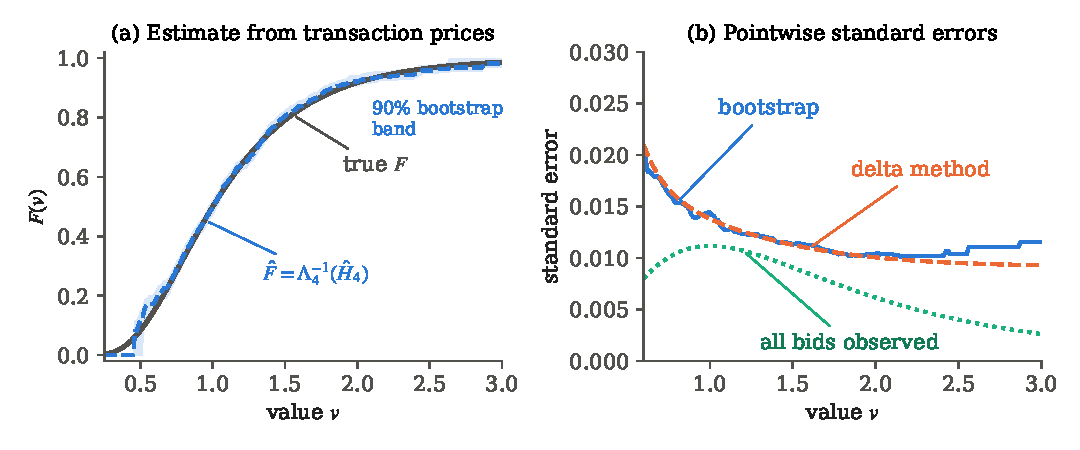
\includegraphics[width=\textwidth]{figures/ch15/asc_inversion.pdf}
\caption{Price-only inversion in simulated button auctions. Our simulation: $T=500$ auctions with $n=4$ bidders,
values lognormal with $\mu=0$ and $\sigma=\frac12$, seed 15201. Panel (a): true $F$, the estimate
$\hat F=\Lambda_4^{-1}(\hat H_4)$, and a pointwise 90 percent band from 500 bootstrap samples of whole auctions.
Panel (b): bootstrap standard error, the delta-method formula \eqref{eq:15-asc-var}, and the standard error of the
empirical CDF if all $4T$ values were observed. Panel (b) starts at $v=0.6$ because few prices fall below that
level.}\label{fig:15-asc-sim}
\end{figure}

Exogenous variation in $n$ yields one estimator $\Lambda_n^{-1}(\hat H_n)$ for each value of $n$ in the data. If
losing bids also follow the button model, each further order statistic yields another estimator through
$\Lambda_{k:n}^{-1}$. An efficient estimator would take an optimally weighted average of these estimators and impose
monotonicity of the estimated CDF \citep[Section~4.2]{AtheyHaile2007}. The differences among them are the basis of
the specification tests in \cref{thm:15-ah1}(ii).

\subsection{Asymmetric independent private values: competing risks}\label{sec:15-asym-ipv}

Independence alone suffices for identification from a single bid, provided we also observe who won. The argument
borrows from the statistics of \emph{competing risks}. A system fails as soon as one of its components fails, and
we observe the failure time and the component that failed. Up to a change of sign, this is the same as observing the
highest bid and the identity of the highest bidder \citep[footnote~21]{AtheyHaile2002}.

\begin{theorem}[{\citealp[Theorem~2]{AtheyHaile2002}}]\label{thm:15-ah2}
In the asymmetric IPV model, assume that each $F_i$ is continuous and that the support of $F_i$ is the same for all
$i$. Each $F_i$ is identified if either
\begin{enumerate}[label=(\alph*)]
\item the transaction price $B^{(n-1:n)}$ and the identity of the winner are observed, or
\item in a second-price auction, the highest bid $B^{(n:n)}$ and the identity of the winner are observed.
\end{enumerate}
Given (a) or (b), the model is testable in either of two cases.
\begin{enumerate}[label=(\roman*)]
\item Participation is exogenous, and each bidder faces at least two different sets of opponents.
\item The auction is second price, and both (a) and (b) hold.
\end{enumerate}
\end{theorem}

Independence is maintained in the theorem. What is relaxed relative to \cref{thm:15-ah1} is symmetry. We prove part
(b) for any $n$, part (a) for $n=2$, and then show the structure of part (a) for $n=3$. The general case of part (a)
is due to \citet[Theorem~1 and Section~4]{Meilijson1981}, and part (b) follows from results collected by
\citet[Theorem~7.3.1]{PrakasaRao1992}.

\begin{proof}[Proof of part (b)]
Let $\bar u$ be the upper end of the common support. For each bidder $i$ define the observable sub-distribution
\[
\tilde G_i(t)=\Pr\big(B^{(n:n)}\le t,\ I=i\big)=\int_{-\infty}^t f_i(x)\prod_{j\neq i}F_j(x)\,dx ,
\]
since bidder $i$ wins with bid $x$ when her value is $x$ and every rival's value is below $x$. The CDF of the highest
bid is $H(t)=\prod_jF_j(t)=\sum_i\tilde G_i(t)$, also observable. Differentiating $\tilde G_i$,
\[
\tilde g_i(t)=f_i(t)\prod_{j\neq i}F_j(t)=H(t)\,\frac{f_i(t)}{F_i(t)} .
\]
So the reverse hazard rate of $V_i$ equals the observable ratio $\frac{\tilde g_i(t)}{H(t)}$. Since
$\frac{f_i}{F_i}=\frac{d}{dt}\ln F_i$ and $\ln F_i(\bar u)=0$, integrating from $t$ to $\bar u$ gives
\[
F_i(t)=\exp\left(-\int_t^{\bar u}\frac{\tilde g_i(x)}{H(x)}\,dx\right).
\]
The right side is a functional of the distribution of observables.
\end{proof}

\begin{proof}[Proof of part (a) for $n=2$]
With two bidders the price is the lower value and the winner is the bidder with the higher value. For the event that
bidder 2 wins at a price of at most $t$,
\[
\tilde G_2(t)=\Pr\big(V_1\le t,\ V_1<V_2\big)=\int_{-\infty}^tf_1(x)\big(1-F_2(x)\big)\,dx .
\]
The price exceeds $t$ only if both values do, so its CDF $H$ satisfies $1-H(t)=\big(1-F_1(t)\big)\big(1-F_2(t)\big)$.
Dividing the density of $\tilde G_2$ by $1-H$ gives
\[
\frac{\tilde g_2(t)}{1-H(t)}=\frac{f_1(t)\big(1-F_2(t)\big)}{\big(1-F_1(t)\big)\big(1-F_2(t)\big)}=\frac{f_1(t)}{1-F_1(t)},
\]
the hazard rate of $V_1$. Integrating the hazard from the bottom of the support gives
$F_1(t)=1-\exp\big(-\int_{-\infty}^t\frac{\tilde g_2(x)}{1-H(x)}\,dx\big)$. The same steps with the roles reversed identify
$F_2$.
\end{proof}

With $n=3$ the argument of \citet[Section~4.1]{AtheyHaile2007} shows the structure of the general case. Let $\underline
u$ be the lower end of the support. Bidder 3 wins at a price of at most $t$ in two disjoint cases. Either both rivals
are below $t$ and bidder 3 is above $t$, or bidder 3 is below $t$ and above both rivals:
\begin{align*}
\tilde G_3(t)&=\Pr\big(V_1\le t,\ V_2\le t,\ V_3\ge t\big)+\Pr\big(V_1\le V_3,\ V_2\le V_3,\ V_3\le t\big)\\
&=F_1(t)F_2(t)\big(1-F_3(t)\big)+\int_{\underline u}^tF_1(x)F_2(x)\,dF_3(x).
\end{align*}
Integration by parts gives $\int_{\underline u}^tF_1F_2\,dF_3=F_1(t)F_2(t)F_3(t)-\int_{\underline u}^t(F_1F_2)'F_3\,dx$.
Substituting and writing $F_1(t)F_2(t)=\int_{\underline u}^t(F_1F_2)'\,dx$,
\[
\tilde G_3(t)=\int_{\underline u}^t\big(F_1(x)F_2(x)\big)'\big(1-F_3(x)\big)\,dx .
\]
Differentiating and rearranging, $(F_1F_2)'=\frac{\tilde g_3}{1-F_3}$. Integrating and taking logarithms,
\[
\ln F_1(t)+\ln F_2(t)=\ln\int_{\underline u}^t\frac{\tilde g_3(x)}{1-F_3(x)}\,dx\equiv R_3(t),
\]
and cyclically $\ln F_1+\ln F_3=R_2$ and $\ln F_2+\ln F_3=R_1$. The coefficient matrix of this system in
$(\ln F_1,\ln F_2,\ln F_3)$ has rows $(1,1,0)$, $(1,0,1)$ and $(0,1,1)$, and its determinant is $-2$. If the right
sides were known, the system would give, for example, $\ln F_1=\frac12(R_3+R_2-R_1)$. The right sides themselves
depend on the unknown distributions through $1-F_j$, so the system is a fixed-point problem.
\citet{Meilijson1981} shows that it has a unique solution.

Testability follows the logic of \cref{thm:15-ah1}. With exogenous participation, each set of opponents that bidder
$i$ faces delivers its own version of $F_i$, and the versions must agree. In a second-price auction with both (a)
and (b), the two constructions above must deliver the same $F_i$.

\casehead{Estimation}
The structure suggests a likelihood \citep[equation~(4.7)]{AtheyHaile2007}. Bidder $i$ wins at price $p$ when
some rival $j$ has value exactly $p$, every other rival $k$ has a value below $p$, and $V_i$ exceeds $p$. The
density of this event is $\big(1-F_i(p)\big)\sum_{j\neq i}f_j(p)\prod_{k\neq i,j}F_k(p)$, and the likelihood of a
sample of prices $p_t$ and winners $I_t$ is
\[
\mathcal L=\prod_{t=1}^T\big(1-F_{I_t}(p_t)\big)\sum_{j\neq I_t}f_j(p_t)\prod_{k\neq I_t,j}F_k(p_t).
\]
Parametric or semi-nonparametric maximum likelihood can be applied to it. \citet{BrendstrupPaarsch2006} develop a
semi-nonparametric estimator of this kind. Nonparametric estimators from the competing-risks literature, such as
the Kaplan-Meier estimator, are natural alternatives. \citet[Section~3.3.1]{AtheyHaile2007} make this suggestion for
the closely related problem of Dutch auctions with asymmetric bidders.

\subsection{Covariates}\label{sec:15-covariates}

Real auctions sell heterogeneous objects, and bidders differ in observable ways. Covariates are usually a nuisance,
but they can also be a source of identification.

\begin{theorem}[{\citealp[Theorem~3]{AtheyHaile2002}}]\label{thm:15-ah3}
Let private values be $V_i=g_i(A_i,Z)$, where each $g_i$ is an unknown function strictly increasing in $A_i$. Each
$F_{A_i}$ is continuous with the same support for all $i$. The auction covariates $Z$ and the transaction price are
observed, together with the identity of the winner if bidders are asymmetric.
\begin{enumerate}[label=(\roman*)]
\item If $A_1,\dots,A_n$ are independent conditional on $Z$, each conditional distribution $F_{V_i}(\cdot\mid z)$ is
identified. In the asymmetric case we assume in addition that, for each $z$, the conditional value
distributions $F_{V_i}(\cdot\mid z)$ are continuous and share a common support.
\item If $g_i(A_i,Z)=A_i+g_0(Z)$ for all $i$, and $A_1,\dots,A_n$ are mutually independent and independent of $Z$, then
the distribution of $\bm A$ and the function $g_0$ are identified up to location.
\item The symmetric models in (i) and (ii) are testable with more than one bid per auction, or with transaction
prices from auctions with exogenously varying numbers of bidders.
\end{enumerate}
\end{theorem}

\begin{proof}
(i) Fix $Z=z$. Values are independent given $z$, so \cref{thm:15-ah1} (symmetric case) or \cref{thm:15-ah2}
(asymmetric case) applies conditional on $z$. \Cref{thm:15-ah2} needs a common support of the value distributions,
which is why (i) imposes it on the $F_{V_i}(\cdot\mid z)$ directly.

(ii) Consider the symmetric case. Given $Z=z$ the price is $A^{(n-1:n)}+g_0(z)$, so its conditional CDF is
\[
H_n(b\mid z)=\Pr\big(A^{(n-1:n)}\le b-g_0(z)\big)=F_{A,(n-1:n)}\big(b-g_0(z)\big),
\]
where $F_{A,(n-1:n)}$ is the CDF of the second-highest of the $A_i$. Let $q_\tau(z)$ be the $\tau$-quantile of the
price given $z$, and $a_\tau$ the $\tau$-quantile of $A^{(n-1:n)}$. Then $q_\tau(z)=g_0(z)+a_\tau$, so
\[
g_0(z)-g_0(z')=q_\tau(z)-q_\tau(z')\quad\text{for all }z,z' ,
\]
and $g_0$ is identified up to an additive constant. A location normalization, such as $g_0(z_0)=0$ at a reference
point, fixes the constant. The price net of $g_0(Z)$ is then $A^{(n-1:n)}$, whose distribution identifies $F_A$ by
\cref{thm:15-ah1}. The asymmetric case uses \cref{thm:15-ah2} instead.

(iii) Two order statistics, or two values of $n$, give two versions of $F_{V}(\cdot\mid z)$ in (i), or of $F_A$ in
(ii), and these must coincide.
\end{proof}

\citet{AtheyHaile2002} state the support condition for the $A_i$. That suffices in (ii), where every value is
$A_i+g_0(z)$ and the supports shift together. In the asymmetric case of (i) it does not suffice, because
different functions $g_i$ need not preserve a common support. Let $A_1$ and $A_2$ be independent and uniform on
$[0,1]$, with $g_1(a)=a$ and $g_2(a)=a+2$. In an ascending auction bidder 2 always wins, at the price $A_1$.
Replacing $g_2(a)$ by $a+3$ leaves the joint distribution of the price and the winner unchanged, yet it changes
$F_{V_2}$.

Part (ii) is the basis of \emph{homogenization}. Write the price in auction $t$ as
\[
P_t=g_0(Z_t)+A_t^{(n_t-1:n_t)}=\kappa(n_t)+g_0(Z_t)+\varepsilon_t,
\qquad \kappa(n)=\E\big[A^{(n-1:n)}\big],\quad \E[\varepsilon_t\mid Z_t,n_t]=0 .
\]
A regression of prices on covariates and on indicators for $n$ estimates $g_0$, parametrically or flexibly. The
homogenized prices $P_t-\hat g_0(Z_t)$ are then treated as prices of identical objects, and the inversion of
\cref{sec:15-price-only} estimates $F_A$ \citep[equation~(6.6)]{AtheyHaile2007}. The first step matters for
inference. Suppose $\hat g_0$ converges at the parametric rate $T^{-\frac12}$. At a point $v$, the empirical CDF of
the homogenized prices then differs from its infeasible counterpart by approximately $f_{A,(n-1:n)}(v)$, the
density of $A^{(n-1:n)}$, times the average estimation error of $\hat g_0(Z_t)$. This term has the same order
$T^{-\frac12}$ as the sampling error of the empirical CDF itself.
Standard errors for $\hat F_A$ must therefore account for the first step, for example by bootstrapping both
steps together. The first step is asymptotically negligible only for second-step estimators that converge more
slowly, such as a kernel estimator of the density of $A$, under the usual smoothness conditions.
The function $g_0$ is often of interest in its own right, since it measures how observables shift valuations. In
first-price auctions the same idea requires that equilibrium bidding preserve the additive structure, which
\cref{lem:15-separability} establishes (\cref{sec:15-uh-sep} applies it to bids). Here it is immediate because
bids equal values. Alternatives to homogenization are
kernel smoothing over covariates, which \citet{HaileTamer2003} apply to ascending auctions, and flexible
mixtures for the conditional price distribution \citep[Section~6.1.1]{AtheyHaile2007}.

Bidder covariates do more. They can identify models with arbitrary correlation among values, which the next
subsection shows are not identified from bids alone. The idea comes from the Roy model, in which a worker chooses
the sector that offers the highest wage, and we observe only that wage and the chosen sector
\citep[footnote~29]{AtheyHaile2002}. Suppose $V_i=g_i(W_i)+A_i$ and suppose for a moment that the maximum value is
observed. Then
\[
\Pr\big(V^{(n:n)}\le u\mid\bm w\big)=\Pr\big(A_i\le u-g_i(w_i)\ \forall i\big)=F_{\bm A}\big(u-g_1(w_1),\dots,u-g_n(w_n)\big).
\]
The joint distribution of values is observed only along its diagonal. Variation in the indices $g_i(w_i)$, however,
moves the point at which $F_{\bm A}$ is evaluated over all of $\R^n$. When $g_j(w_j)$ is very negative for every
$j\neq i$, bidder $i$ has the highest value with probability close to one, and variation in $w_i$ traces out
$g_i$ \citep[Section~6.2.1]{AtheyHaile2007}. The following result shows that the same logic works for any single
order statistic, including the transaction price of an ascending auction.

\begin{theorem}[{\citealp[Theorem~6.1]{AtheyHaile2007}}]\label{thm:15-ah5}
Assume the following.
\begin{enumerate}[label=(\roman*)]
\item $V_i=g_i(W_i)+A_i$ for $i=1,\dots,n$.
\item $F_{\bm A}$ has support $\R^n$ and a continuously differentiable density $f_{\bm A}$.
\item The vector $(A_1,\dots,A_n)$ is independent of $(W_1,\dots,W_n)$.
\item The support of $\big(g_1(W_1),\dots,g_n(W_n)\big)$ is $\R^n$.
\item Each $g_i$ is continuously differentiable, with $g_i(w)\to\infty$ as $w\to\infty$ and $g_i(w)\to-\infty$ as
$w\to-\infty$.
\end{enumerate}
Then $F_{\bm A}$ and each $g_i$ are identified up to location from the distribution of $\big(V^{(j:n)},\bm W\big)$, for
any single $j\in\{1,\dots,n\}$.
\end{theorem}

The theorem allows arbitrary dependence among the $A_i$ and arbitrary asymmetry. It is a slight modification of
Theorem~5 of \citet{AtheyHaile2002} that corrects a minor error in its proof \citep[footnote~55]{AtheyHaile2007}. The
survey states condition (iii) pairwise, as independence of each $A_i$ and each $W_j$, while its text assumes that
the vector of the $A_i$ is independent of all covariates. The proof needs the vector form. Under pairwise
independence alone the correlation among the $A_i$ could vary with $\bm W$ while every marginal stays fixed. We
give a direct proof for scalar covariates.

\begin{proof}
Write $\bm z(u,\bm w)=\big(u-g_1(w_1),\dots,u-g_n(w_n)\big)$. For a set of bidders $\mathcal T\subseteq\{1,\dots,n\}$
define
\[
\bar F^{\mathcal T}(\bm a)=\Pr\big(A_i>a_i\ \forall i\in\mathcal T,\ A_k\le a_k\ \forall k\notin\mathcal T\big),
\]
so that $\bar F^{\emptyset}=F_{\bm A}$.

\emph{Step 1.} The $j$-th lowest value is at most $u$ exactly when at least $j$ values are at most $u$. Equivalently,
the set $\mathcal T$ of bidders with $V_i>u$ has at most $n-j$ members. Since $V_i>u$ if and only if
$A_i>u-g_i(w_i)$, and since by (iii) the distribution of $\bm A$ given $\bm W=\bm w$ is $F_{\bm A}$,
\[
\Pr\big(V^{(j:n)}\le u\mid\bm w\big)=\sum_{\mathcal T:\,|\mathcal T|\le n-j}\bar F^{\mathcal T}\big(\bm z(u,\bm w)\big).
\]

\emph{Step 2.} Write $\bar F^{\mathcal T}$ as an integral of $f_{\bm A}$ over $a_i>z_i$ for $i\in\mathcal T$ and
$a_k\le z_k$ for $k\notin\mathcal T$. Differentiating once in each $z_k$ gives a plus sign for upper limits and a
minus sign for lower limits, so
\[
\frac{\partial^n\bar F^{\mathcal T}(\bm z)}{\partial z_1\cdots\partial z_n}=(-1)^{|\mathcal T|}f_{\bm A}(\bm z).
\]

\emph{Step 3.} Since $\frac{\partial z_k}{\partial w_k}=-g_k'(w_k)$, the chain rule gives
\[
\frac{\partial^n}{\partial w_1\cdots\partial w_n}\bar F^{\mathcal T}\big(\bm z(u,\bm w)\big)
=(-1)^{|\mathcal T|}f_{\bm A}(\bm z)\prod_{k=1}^n\big(-g_k'(w_k)\big).
\]

\emph{Step 4.} Summing over the sets in Step~1, there are $\binom{n}{m}$ sets of size $m$. The identity
$\sum_{m=0}^{K}(-1)^m\binom nm=(-1)^K\binom{n-1}{K}$ follows from Pascal's rule by telescoping. With $K=n-j$ and the
case $\mathcal T=\emptyset$ of Step~3,
\[
\frac{\partial^n}{\partial w_1\cdots\partial w_n}\Pr\big(V^{(j:n)}\le u\mid\bm w\big)
=(-1)^{n-j}\binom{n-1}{n-j}\,\frac{\partial^n}{\partial w_1\cdots\partial w_n}F_{\bm A}\big(\bm z(u,\bm w)\big).
\]

\emph{Step 5.} Integrate each $\tilde w_k$ from $w_k$ to $\infty$. As $\tilde w_k\to\infty$, $g_k(\tilde w_k)\to\infty$, so
$z_k\to-\infty$ and $F_{\bm A}\to0$. Repeated use of the fundamental theorem of calculus gives
\[
\int_{w_1}^{\infty}\!\!\cdots\int_{w_n}^{\infty}\frac{\partial^nF_{\bm A}\big(\bm z(u,\tilde{\bm w})\big)}{\partial\tilde w_1\cdots\partial\tilde w_n}\,
d\tilde w_n\cdots d\tilde w_1=(-1)^nF_{\bm A}\big(\bm z(u,\bm w)\big).
\]
Combining with Step~4,
\[
F_{\bm A}\big(\bm z(u,\bm w)\big)=\frac{(-1)^j}{\binom{n-1}{n-j}}\int_{w_1}^{\infty}\!\!\cdots\int_{w_n}^{\infty}
\frac{\partial^n\Pr\big(V^{(j:n)}\le u\mid\tilde{\bm w}\big)}{\partial\tilde w_1\cdots\partial\tilde w_n}\,d\tilde w_n\cdots d\tilde w_1 ,
\]
which is equation (6.17) of \citet{AtheyHaile2007}. The right side is observable.

\emph{Step 6.} Let $w_k\to-\infty$ for every $k\neq i$. Then $z_k\to\infty$ and the left side tends to
$F_{A_i}\big(u-g_i(w_i)\big)$. This function of $(u,w_i)$ is known. Since $F_{A_i}$ is strictly increasing, any two
points with the same value satisfy $u-g_i(w_i)=u'-g_i(w_i')$, so $g_i(w_i)-g_i(w_i')=u-u'$. Hence $g_i$ is identified
up to an additive constant. With the $g_i$ known, condition (iv) lets us choose $u$ and $\bm w$ with
$\bm z(u,\bm w)$ equal to any point $\bm a\in\R^n$, which identifies $F_{\bm A}(\bm a)$.
\end{proof}

Two order statistics give two expressions for $F_{\bm A}$, and their equality is a testable restriction
\citep[Theorem~5(ii)]{AtheyHaile2002}. The result needs large support: bidder covariates must push every bidder's
value far above and far below the others'. Estimators that exploit it had not been developed when
\citet[Section~6.2.1]{AtheyHaile2007} wrote.

\subsection{Correlated values: what incomplete bids cannot reveal}\label{sec:15-nonid}

The positive results above lean on independence or on rich covariates. Without either, the picture changes.

\begin{theorem}[{\citealp[Theorem~4]{AtheyHaile2002}}]\label{thm:15-ah4}
In the symmetric private values model:
\begin{enumerate}[label=(\roman*)]
\item $F_{\bm V}$ is not identified from the vector of bids in an ascending auction.
\item In a second-price auction, $F_{\bm V}$ is not identified unless all bids are observed.
\end{enumerate}
\end{theorem}

\begin{proof}
We construct two exchangeable distributions that generate the same observables. Suppose $f_{\bm V}$ is positive on a
neighborhood of $[0,5]^n$. Let the $k$-th order statistic be the one that is not observed, where $k=n$ in an
ascending auction because the winner never exits. Fix $0<\varepsilon<\frac12$ and write $\mathcal Q(\bm c)$ for the
cube of half-width $\varepsilon$ centered at $\bm c$.

Start with $n=2$ and $k=2$, so only $\min(V_1,V_2)$ is observed. Let
\[
c(\bm v)=\indic_{\mathcal Q(1,3)}(\bm v)+\indic_{\mathcal Q(3,1)}(\bm v)-\indic_{\mathcal Q(1,2)}(\bm v)-\indic_{\mathcal Q(2,1)}(\bm v),
\]
and $\tilde f_{\bm V}=f_{\bm V}+\gamma c$ with $\gamma>0$ below the minimum of $f_{\bm V}$ on the four squares. Then
$\tilde f_{\bm V}\ge0$, and it integrates to one because the squares have equal areas. It is symmetric in $(v_1,v_2)$,
so it is exchangeable. On $\mathcal Q(1,2)$ and $\mathcal Q(1,3)$ the minimum is $v_1$, and the perturbation adds and
removes the same uniform mass for $v_1$ on $[1-\varepsilon,1+\varepsilon]$. The same holds on $\mathcal Q(2,1)$ and
$\mathcal Q(3,1)$ with the roles of the coordinates reversed. Hence the distribution of $\min(V_1,V_2)$ is unchanged.
The marginal density of $V_1$, however, gains $2\varepsilon\gamma$ on $[3-\varepsilon,3+\varepsilon]$ and loses
$2\varepsilon\gamma$ on $[2-\varepsilon,2+\varepsilon]$. Two different joint distributions, with different
marginals, generate the same observables.

For general $n$ and $k$, partition the bidders into one bidder $i$, a set of $k-1$ bidders and a set of $n-k$ bidders.
Consider the point at which the $k-1$ bidders have value 1, bidder $i$ has value 2, and the $n-k$ bidders have value
4. Shift mass $\gamma$ from the cube around this point to the cube around the point at which bidder $i$ has value 3
instead. Repeat for every such partition, which preserves exchangeability. Each shift moves only the $k$-th order statistic, from near 2
to near 3, while every other order statistic keeps the same local distribution. The joint distribution of the
observed order statistics is therefore unchanged \citep[proof of Theorem~4]{AtheyHaile2002}.
\end{proof}

\begin{figure}[htbp]
\centering
\begin{tikzpicture}[scale=0.92]
\def\e{0.3}
\fill[c15blue!7] (1-\e,5) -- (1-\e,1-\e) -- (5,1-\e) -- (5,1+\e) -- (1+\e,1+\e) -- (1+\e,5) -- cycle;
\draw[c15gray!60] (0,0) rectangle (5,5);
\draw[c15gray, densely dashed] (0,0) -- (5,5);
\draw[-{Stealth[length=2mm]}, c15gray] (0,0) -- (5.5,0) node[right] {$v_1$};
\draw[-{Stealth[length=2mm]}, c15gray] (0,0) -- (0,5.5) node[above] {$v_2$};
\foreach \x in {1,2,3,4,5} {\draw[c15gray] (\x,0) -- (\x,-0.08) node[below, font=\scriptsize] {$\x$};
  \draw[c15gray] (0,\x) -- (-0.08,\x) node[left, font=\scriptsize] {$\x$};}
\foreach \px/\py in {1/2,2/1} {\fill[c15orange!45] ({\px-\e},{\py-\e}) rectangle ({\px+\e},{\py+\e});}
\foreach \px/\py in {1/3,3/1} {\fill[c15blue!45] ({\px-\e},{\py-\e}) rectangle ({\px+\e},{\py+\e});}
\node[font=\scriptsize] at (1,2) {$-\gamma$};
\node[font=\scriptsize] at (2,1) {$-\gamma$};
\node[font=\scriptsize] at (1,3) {$+\gamma$};
\node[font=\scriptsize] at (3,1) {$+\gamma$};
\draw[-{Stealth[length=1.6mm]}, thick, c15gray] (1.42,2.25) -- (1.42,2.75);
\draw[-{Stealth[length=1.6mm]}, thick, c15gray] (2.25,1.42) -- (2.75,1.42);
\node[font=\scriptsize, align=left, anchor=west] at (2.0,4.3) {shaded strip:\\ $\min(v_1,v_2)\in[1-\varepsilon,1+\varepsilon]$};
\draw[c15gray, thin] (2.0,4.3) -- (1.25,4.0);
\end{tikzpicture}
\caption{The construction behind \cref{thm:15-ah4} for $n=2$. Mass $\gamma$ moves from the orange squares to the blue
squares, symmetrically about the diagonal. All four squares lie in the shaded strip, and within each pair the minimum
has the same distribution. The law of $\min(V_1,V_2)$, the only observable in a two-bidder ascending auction, is
therefore unchanged, while the marginal distribution of each value changes.}\label{fig:15-perturb}
\end{figure}

\Cref{fig:15-perturb} draws the construction. The intuition is a matter of dimension. Even under exchangeability,
$F_{\bm V}$ is an $n$-dimensional distribution, and identifying it from data of dimension $n-1$ or lower requires
additional restrictions \citep[Section~3.3.2]{AtheyHaile2007}. The result generalizes a classic finding of the
competing-risks literature, in which the joint distribution of risks is not identified from the distribution of the
first failure time alone \citep[footnote~26]{AtheyHaile2002}. Affiliation does not rescue identification, because a
small enough perturbation preserves strict affiliation \citep[footnote~27]{AtheyHaile2002}. The marginal $F$ itself
is not identified, so even the distribution of a single bidder's value is out of reach.

Taken together, \cref{thm:15-ah1,thm:15-ah2,thm:15-ah4,thm:15-ah5} describe a trade-off. One may relax the data,
observing only the transaction price, if values are independent. One may relax the model, allowing correlation,
if the data are richer: all bids, or bidder covariates with large support. One cannot relax both at once.
\citet{AradillasLopezGandhiQuint2013} study the case in between. With correlated private values and transaction
prices from auctions with exogenously varying numbers of bidders, $F_{\bm V}$ is not point identified. They show
that the reserve-price question does not need all of $F_{\bm V}$ \citep[pp.~88--89]{HortacsuPerrigne2021}. In an
ascending auction with reserve $r$ and seller value $v_0$, a sale occurs when $V^{(n:n)}\ge r$, at the price
$\max\{V^{(n-1:n)},r\}$. The seller's expected profit is therefore
\[
\pi(r)=\E\big[(V^{(n-1:n)}-v_0)\indic\{V^{(n-1:n)}\ge r\}\big]+(r-v_0)\Pr\big(V^{(n-1:n)}<r\le V^{(n:n)}\big),
\]
and the last probability equals $F_{(n-1:n)}(r)-F_{(n:n)}(r)$. Transaction prices identify $F_{(n-1:n)}$. Only the
distribution of the highest value at the single point $r$ is missing. It lies between $F_{(n-1:n)}(r)$ and, under
their assumptions, the value $\big[\Lambda_{n-1:n}^{-1}\big(F_{(n-1:n)}(r)\big)\big]^n$ that independence would imply.
For $r\ge v_0$ the profit falls in $F_{(n:n)}(r)$, so these limits bound $\pi(r)$. The bounds are wide.
Exogenous variation in $n$ tightens them, because the joint law of any $m<n$ values drawn at random must then
be the same in auctions of every size (p.~89, footnote 5). \Cref{sec:15-reserve-asc} reports their estimates for
timber sales.

\subsection{An incomplete model of ascending auctions}\label{sec:15-ht}

The button model is a stylized description of an English auction. In many oral auctions bidders call out prices
themselves and nontrivial minimum increments are common. A bidder may jump bid, or stay silent until the auction is
about to end \citep[Section~4.3]{AtheyHaile2007}. Bidders then fail to reveal their full willingness to
pay, and some never bid. Losing bids need not equal values, and the price need not equal the second-highest value.
\citet{HaileTamer2003} replace the button model by two weak behavioral assumptions.

\begin{assumption}[\citealp{HaileTamer2003}]\label{ass:15-ht}
Values are SIPV and the number of bidders $n$ is observed. Let $\Delta\ge0$ be the minimum bid increment.
\begin{enumerate}[label=(HT\arabic*),leftmargin=*]
\item Bidders do not bid more than they are willing to pay: $b_i\le v_i$ for every bidder.
\item Bidders do not allow an opponent to win at a price they are willing to beat: every losing bidder has
$v_i\le b^{(n:n)}+\Delta$, where $b^{(n:n)}$ is the winning bid.
\end{enumerate}
\end{assumption}

The assumptions allow the dominant-strategy behavior of the button model but do not require it. Bids need not be
monotone in values. The model is \emph{incomplete}: it restricts the relation between values and bids without fully
characterizing behavior. It cannot identify $F$, but it bounds it. Let $G_B^{(i:n)}$ be the CDF of the $i$-th lowest
bid in $n$-bidder auctions, and let $G_\Delta^{(n:n)}$ be the CDF of $B^{(n:n)}+\Delta$.

\begin{theorem}[{\citealp{HaileTamer2003} and \citealp[Theorem~4.3]{AtheyHaile2007}}]\label{thm:15-ht}
Under \cref{ass:15-ht}, $F^-(v)\le F(v)\le F^+(v)$ for all $v$, where
\[
F^+(v)=\min_{n}\ \min_{1\le i\le n}\ \Lambda_{i:n}^{-1}\big(G_B^{(i:n)}(v)\big),\qquad
F^-(v)=\max_{n}\ \Lambda_{n-1:n}^{-1}\big(G_\Delta^{(n:n)}(v)\big).
\]
\end{theorem}

\begin{proof}
\emph{Upper bound.} By HT1, $b_i\le v_i$ for every $i$. The value $v^{(i:n)}$ is at least as large as $i$ of the
values, and the bids of those $i$ bidders are no larger than their values. So at least $i$ bids are at most
$v^{(i:n)}$, which means $b^{(i:n)}\le v^{(i:n)}$. Hence the event $\{V^{(i:n)}\le v\}$ implies $\{B^{(i:n)}\le v\}$,
and
\[
G_B^{(i:n)}(v)\ge F_{(i:n)}(v)=\Lambda_{i:n}\big(F(v)\big).
\]
Applying the increasing function $\Lambda_{i:n}^{-1}$ to both sides gives $\Lambda_{i:n}^{-1}\big(G_B^{(i:n)}(v)\big)\ge F(v)$.
This holds for every $i$ and every $n$, so it holds for the minimum.

\emph{Lower bound.} By HT2, all $n-1$ losing bidders have values at most $b^{(n:n)}+\Delta$. At least $n-1$ values are
therefore below this level, so $v^{(n-1:n)}\le b^{(n:n)}+\Delta$. The event $\{B^{(n:n)}+\Delta\le v\}$ implies
$\{V^{(n-1:n)}\le v\}$, and
\[
G_\Delta^{(n:n)}(v)\le F_{(n-1:n)}(v)=\Lambda_{n-1:n}\big(F(v)\big).
\]
Applying $\Lambda_{n-1:n}^{-1}$ gives $\Lambda_{n-1:n}^{-1}\big(G_\Delta^{(n:n)}(v)\big)\le F(v)$ for every $n$, hence for the
maximum.
\end{proof}

Several features of the bounds matter in practice. If only the transaction price is recorded, the upper bound uses
$i=n$ alone. The number of bidders must be observed, which holds when bidders must register or qualify, as in the
timber auctions studied by \citet{HaileTamer2003}. If the data satisfy the button model and $\Delta\to0$, the bounds
collapse to $F$. Conversely, imposing the button model when it is false need not produce an estimate inside the
bounds, even in large samples. Imposing false structure to obtain point identification differs from selecting a
point inside the bounds of a correct incomplete model \citep[Section~4.3.1]{AtheyHaile2007}.

Estimation replaces each CDF by its empirical counterpart. Each component $\Lambda_{i:n}^{-1}(\hat G_B^{(i:n)})$ is
consistent and asymptotically normal, but the minimum and maximum have non-normal limits, and inference uses the
bootstrap. The minimum of several consistent estimators tends to select one with a downward sampling error, and the
maximum one with an upward error. The estimated bounds are therefore too narrow in finite samples and may even cross.
\citet{HaileTamer2003} replace the minimum and maximum by smooth weighted averages that approach them as the sample
grows.

\casehead{Bounds on the optimal reserve price}
The seller's main policy instrument in the SIPV model is the reserve price. Let $v_0$ be the seller's value. By
\cref{cor:14-optimal-reserve}, the optimal reserve $r^*$ solves $r^*-\frac{1-F(r^*)}{f(r^*)}=v_0$. Bounds on $F$ place
no restriction on its derivative at a point, so plugging $F^+$ or $F^-$ into this equation does not bound $r^*$. A
detour through an objective function works. Define
\[
\pi(r)=(r-v_0)\big(1-F(r)\big).
\]
Then $\pi'(r)=\big(1-F(r)\big)-(r-v_0)f(r)=-f(r)\big[\psi(r)-v_0\big]$, where $\psi$ is the virtual valuation
\eqref{eq:14-psi}. So $\pi$ has the same maximizer as the seller's expected profit, although it is not that profit when
$n>1$ \citep[footnote~34]{AtheyHaile2007}. For $r\ge v_0$, the bounds on $F$ imply
\[
\pi_1(r)\equiv(r-v_0)\big(1-F^+(r)\big)\le\pi(r)\le\pi_2(r)\equiv(r-v_0)\big(1-F^-(r)\big).
\]
Let $r_1^*$ maximize $\pi_1$, let $\pi_1^*=\pi_1(r_1^*)$, and define
\[
r^-=\sup\{r<r_1^*:\pi_2(r)\le\pi_1^*\},\qquad r^+=\inf\{r>r_1^*:\pi_2(r)\le\pi_1^*\}.
\]

\begin{proposition}[{\citealp{HaileTamer2003} and \citealp[Theorem~4.4]{AtheyHaile2007}}]\label{prop:15-ht-reserve}
Suppose $\pi$ is continuously differentiable and strictly quasi-concave. Then $r^*\in[r^-,r^+]$. Given the bounds
$F^+$ and $F^-$, the bounds $r^-$ and $r^+$ are sharp.
\end{proposition}

\begin{proof}[Proof of the inclusion]
We treat the nontrivial case $r^-<r_1^*<r^+$ and assume $\pi_2$ is continuous.
\citet[Section~4.3.2]{AtheyHaile2007} discuss the degenerate cases, in which $r^-=r^+=r_1^*$. The true objective
satisfies
$\pi(r^*)\ge\pi(r_1^*)\ge\pi_1(r_1^*)=\pi_1^*$. Suppose $r^*<r^-$. Then $r^-$ lies strictly between $r^*$ and
$r_1^*$, and strict quasi-concavity gives
\[
\pi(r^-)>\min\{\pi(r^*),\pi(r_1^*)\}\ge\pi_1^* .
\]
By continuity $\pi_2(r^-)\le\pi_1^*$, so $\pi(r^-)\le\pi_2(r^-)\le\pi_1^*$, a contradiction. The case $r^*>r^+$ is
symmetric.
\end{proof}

\Cref{fig:15-ht} applies the bounds to simulated auctions. Losing bidders stop between 80 and 100 percent of their
values, and the price may fall up to one increment below the second-highest value. The bounds contain the true
$F$ over most of the range where the data are informative. The naive estimator that treats losing bids as values
lies above the upper bound, because it ignores the fact that bidders stopped short. The implied interval for the
optimal reserve is $[0.53,1.04]$, and it contains the true optimum $0.77$ (our simulation).

\begin{figure}[htbp]
\centering
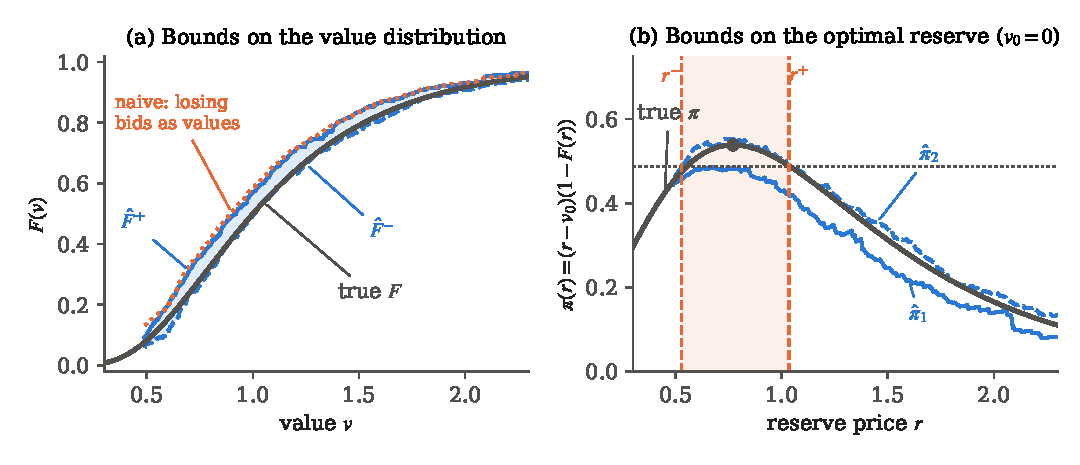
\includegraphics[width=\textwidth]{figures/ch15/ht_bounds.pdf}
\caption{Bounds from an incomplete model of ascending auctions. Our simulation: 500 auctions with $n=3$ and 500 with
$n=5$, values lognormal with $\mu=0$ and $\sigma=\frac12$, increment $\Delta=0.05$, seed 15202. Losing bidders record
bids equal to their values times a uniform draw on $[0.8,1]$. The winning bid lies between the second-highest value
minus $\Delta$ and that value, and is at least every losing bid. Panel (a): $\hat F^+$, $\hat F^-$, the true $F$ and
the naive estimate that inverts the highest losing bid as if it were the second-highest value. An order statistic is
used at $v$ only if at least 1 percent of its observations lie on each side of $v$, and curves are drawn where both
bounds are informative. Panel (b): $\hat\pi_1$, $\hat\pi_2$ and the true $\pi$ for $v_0=0$, with the interval
$[r^-,r^+]$ shaded and the true optimum marked by a dot.}\label{fig:15-ht}
\end{figure}

The approach extends in principle to asymmetric and affiliated private values, but the bounds are then likely to be
wide. Bounds on realized values reveal little about their correlation structure, and many policy questions need that
structure \citep[Section~4.3.3]{AtheyHaile2007}.

\subsection{Binding reserve prices}\label{sec:15-reserve-asc}

A reserve price $r$ inside the support of values, with $F(r)\in(0,1)$, separates potential bidders from actual
bidders. In this subsection $N$ is the number of potential bidders and $n_t$ the number who participate. With private
values a bidder participates exactly when her value is at least $r$. Under independence, the participants' values
are therefore i.i.d.\ draws from the truncated distribution
\begin{equation}\label{eq:15-truncated}
F(v\mid r)=\frac{F(v)-F(r)}{1-F(r)},\qquad v\ge r
\end{equation}
\citep[equation~(6.18)]{AtheyHaile2007}. In an ascending auction with $n_t\ge2$ participants, the price is the
second-highest of $n_t$ draws from $F(\cdot\mid r)$. With $n_t=1$ the price equals $r$.

\begin{proposition}[{\citealp[Corollary~3]{AtheyHaile2002} and \citealp[Corollary~6.1 and Theorem~6.3]{AtheyHaile2007}}]\label{prop:15-reserve-ident}
Consider the SIPV model of a first-price, second-price or ascending auction with reserve price $r$ and
$F(r)\in(0,1)$.
\begin{enumerate}[label=(\roman*)]
\item Consider a second-price or ascending auction, or a first-price auction whose participants learn their number
before they bid. If one bid from each auction and the number of participants are observed, $F(\cdot\mid r)$ is
identified on $[r,\infty)$.
\item The model is testable if two bids from each auction are observed, or if one bid is observed in auctions with
different numbers of participants.
\item If $N$ is fixed and the number of participants is observed, $N$ and $F(r)$ are identified. Combined with (i),
$F(v)$ is then identified for every $v\ge r$.
\item Consider a first-price auction whose bidders know $N$ but not the number of participants when they bid. If $N$
is fixed and one bid from each auction and the number of participants are observed, then $N$, $F(r)$ and $F(v)$
for every $v\ge r$ are identified.
\end{enumerate}
\end{proposition}

\begin{proof}
Parts (i) and (ii) apply \cref{thm:15-ah1} to the truncated distribution \eqref{eq:15-truncated}, conditioning on
the number of participants. In second-price and ascending auctions this is valid because bidding one's value is
a dominant strategy. In a first-price auction whose participants know their number $n_t$, each participant faces
$n_t-1$ rivals with values drawn from $F(\cdot\mid r)$, and the inversion of \cref{sec:15-gpv} applies to that
distribution. In the setting of (iv), condition (C2) of \cref{thm:15-gpv-reserve} makes participants' bids
i.i.d.\ given their number, with a distribution that does not depend on that number. Two bids per auction, or one
bid at different numbers of participants, then give two versions of that distribution, and these must coincide.
For part (iii), each potential bidder participates independently with probability $1-F(r)$, so the
number of participants is binomial with parameters $N$ and $1-F(r)$. Its distribution determines both parameters. Exchangeability gives a
convenient formula. The probability that a given bidder stays out is the same for every bidder. It therefore
equals the expected fraction of bidders who stay out:
\[
F(r)=\Pr(\text{bidder 1 does not bid})=\frac{\E[N-n_t]}{N}=\sum_{k=1}^{N}\frac{k}{N}\Pr\big(n_t=N-k\big),
\]
which is equation (6.19) of \citet{AtheyHaile2007}. Finally, \eqref{eq:15-truncated} gives
$F(v)=F(r)+\big(1-F(r)\big)F(v\mid r)$ for $v\ge r$.

For part (iv), a participant who bids $b\ge r$ wins when each of her $N-1$ potential rivals either stays out or bids
less. Her win probability therefore depends on $N$ and $F(r)$, and the inversion conditional on $n_t$ misstates her
first-order condition. Take $N=2$, values uniform on $[0,1]$ and $r=\frac12$, for example. The equilibrium bid is
$\beta(v)=\frac{v}{2}+\frac{1}{8v}$. Applied to two-participant auctions, the inversion of \cref{sec:15-gpv} maps
the bid of a bidder with value $\frac34$ to about $0.611$. The correct inversion \eqref{eq:15-gpv-reserve} uses
$N$ and $F(r)$, which part (iii) identifies. Given their number, participants' bids are i.i.d., so the observed
bid and that number identify the distribution of a participant's bid. When the observed bid is the highest, this
step is the root formula of \cref{prop:15-winbid}. \Cref{thm:15-gpv-reserve} then gives $F(v)$ for $v\ge r$.
\end{proof}

\citet[Corollary~3]{AtheyHaile2002} state (i) for first-price auctions as well, without saying what bidders know
about participation. The information structure matters. Part (iv) adopts that of \citet{GuerrePerrigneVuong2000},
in which bidders do not see who participates, and \cref{sec:15-gpv-reserve} develops it.

The sample analog of the formula that completes part (iii), $\hat F(v)=\hat F(r)+\big(1-\hat F(r)\big)\hat F(v\mid r)$, is consistent. Below
the reserve the data are silent without parametric assumptions. Is the truncated distribution enough for the
reserve-price question? The next result says that it usually is.

\begin{proposition}[{\citealp[Theorem~6.2]{AtheyHaile2007}}]\label{prop:15-trunc-reserve}
For a univariate CDF $\Phi$, let $\pi(\tilde r;\Phi)=(\tilde r-v_0)\big(1-\Phi(\tilde r)\big)$ and let $p^*(\Phi)$ maximize
$\pi(\cdot;\Phi)$ over the support of $\Phi$. Suppose $\pi(\cdot;F)$ is continuously differentiable and strictly
quasi-concave, and write $F_{\mid r}=F(\cdot\mid r)$.
\begin{enumerate}[label=(\roman*)]
\item If $r<p^*(F)$, then $p^*(F_{\mid r})=p^*(F)$.
\item If $r\ge p^*(F)$, then $p^*(F_{\mid r})=r$.
\end{enumerate}
\end{proposition}

\begin{proof}
For $\tilde r\ge r$, \eqref{eq:15-truncated} gives $1-F(\tilde r\mid r)=\frac{1-F(\tilde r)}{1-F(r)}$, so
\[
\pi(\tilde r;F_{\mid r})=\frac{\pi(\tilde r;F)}{1-F(r)}\qquad\text{for all }\tilde r\ge r .
\]
On the support of $F_{\mid r}$ the two objectives differ by a positive multiplicative constant. If $r<p^*(F)$, the
unconstrained maximizer lies in $[r,\infty)$ and both objectives peak there. If $r\ge p^*(F)$, strict
quasi-concavity makes $\pi(\cdot;F)$ decreasing on $[r,\infty)$, so the truncated objective peaks at its lower end
$r$.
\end{proof}

In the SIPV model, the optimal reserve computed from participants alone, ignoring the selection created by the
reserve, is the true optimum unless the actual reserve already exceeds it. The data reveal when that happens,
because the estimated optimum then sits at the actual reserve. Variation in reserve prices across auctions does more.
Suppose reserves vary for reasons unrelated to values. Data from auctions with low reserves then reveal $F$ over a
longer range, and a reserve below the lower end of the support reveals all of $F$
\citep[Section~6.3.1]{AtheyHaile2007}. Reserve prices may instead respond to features of the object that bidders see
and the econometrician does not. A reserve then signals unobserved quality, and treating it as an exogenous
truncation point is a mistake. \citet{Roberts2013} builds an identification
strategy on this observation (\cref{sec:15-uh}). With a reserve price, the tests of private against common values
in \cref{sec:15-cv} remain available, because truncation at a common reserve preserves exchangeability
\citep[Corollary~4]{AtheyHaile2002}.

\casehead{Applications to timber sales}
Timber sales have been the main testing ground for these methods \citep[Section~2.1]{HortacsuPerrigne2021}.
The estimates agree on one point. Observed reserve prices are low relative to the optimum that most
models imply, and the gain from raising them depends on the information structure.

\citet{Paarsch1997} studies ascending timber auctions in British Columbia with a parametric model (pp.~87--88).
He treats the winning bid as the second-highest value, as in the button model. Bids are per species on
estimated volumes, while payments follow harvested volumes. He therefore rewrites each value in terms of an
average harvesting cost, and the winner is the bidder with the lowest cost. He specifies a parametric cost
function and a Weibull distribution. The estimated optimal reserve is then on average 3.4 to 4.2 times the
observed reserve, as the seller's value $v_0$ ranges from zero to the appraisal value of the timber.

\citet{HaileTamer2003} apply \cref{thm:15-ht,prop:15-ht-reserve} to Forest Service ascending auctions, with
data from Oregon (p.~88). They estimate bounds on the optimal reserve and on the implied gain. The increase in
the seller's profit ranges from little to 34 percent, depending on $v_0$. At high values of $v_0$ the optimal
reserve leaves more than 90 percent of tracts unsold. \citet{AradillasLopezGandhiQuint2013} use Oregon data
as well (p.~89). Their estimated bounds on the seller's profit are smaller than the profit computed under
independent values, and independence also overstates bidders' surplus. A reserve computed under independence
would be too high and could even lower the seller's profit. The authors note that an optimal reserve would
conflict with the Forest Service's mandate to sell about 85 percent of the tracts it offers. The mandate may
explain why observed reserves are low.

\citet{CoeyEtAl2017} exploit the asymmetry between loggers and mills of \cref{sec:15-als} to tighten
the bounds in California sales (p.~89). The lower bound on the optimal reserve is similar, while the upper bound
is 10 to 15 percent lower. \citet{CoeyLarsenSweeney2019} turn to the \emph{bidder exclusion effect}, the expected
fall in revenue when one of $N$ bidders is excluded at random (pp.~89--90). In an ascending auction with
private values the price is the second-highest value. Excluding a bidder lowers it to the third-highest value
exactly when the excluded bidder holds one of the two highest values, which happens with probability
$\frac{2}{N}$. The exclusion effect is therefore
\[
\frac{2}{N}\,\E\big[B^{(N-1:N)}-B^{(N-2:N)}\big],
\]
which needs two order statistics and the number of potential bidders. Under exogenous participation the
observed fall in revenue, $\E[B^{(N-1:N)}]-\E[B^{(N-2:N-1)}]$, must equal this effect. The difference is their
test statistic. A negative value is consistent with common values, and a zero value with private values, as
\citet{AtheyHaile2002} show \citep[footnote~6]{HortacsuPerrigne2021}. The same effect bounds the gain from an
optimal reserve without computing the reserve. By \cref{prop:14-bk}, an optimal reserve with $N-1$ bidders
raises less revenue than one more bidder without a reserve. In California sales the average revenue gain from
an optimal reserve is at most 13 percent. Exogenous participation is rejected, with positive selection, since
values tend to be higher in auctions with more participants (p.~90).

The first-price evidence points the same way. \citet{LiPerrigne2003} study French public timber sales by
first-price sealed bid with a secret reserve (p.~90). They model the reserve as random, equal to the seller's
value and independent of bidders' values, which are independent private values. The inversion of
\citet{GuerrePerrigneVuong2000}, developed in \cref{sec:15-gpv}, recovers the value distribution. The optimal announced reserve is on average 46 percent higher
than the secret one. It lowers the number of successful sales and raises total revenue only slightly, but it
doubles the seller's net profit.

\section{First-Price Auctions I: The Inversion Problem and Direct Methods}\label{sec:15-direct}

In first-price and Dutch auctions bidders shade their bids below their values, and the amount of shading depends on
the distribution of values. This section explains why that makes identification and estimation harder. It then
studies the direct route, maximum likelihood with its non-regularity and the simulated estimator of
\citet{LaffontOssardVuong1995}. It closes with a comparison of direct and indirect methods that motivates
\cref{sec:15-gpv}.

\subsection{Why first-price auctions are harder}\label{sec:15-fpa-hard}

In the SIPV model with reserve price $r$, a bidder with value $v\ge r$ bids (\cref{prop:14-rs})
\[
\beta(v)=v-\frac{\int_r^vF(t)^{n-1}\,dt}{F(v)^{n-1}} .
\]
Bids are observed and values are not. The bid function depends on the unknown $F$, the very object we want to
estimate \citep[Section~3.1]{AtheyHaile2007}. The distribution of bids $G(b)=F\big(\beta^{-1}(b)\big)$ therefore depends
on $F$ in two ways, directly through the distribution of values and indirectly through the equilibrium strategy
\citep[p.~529]{GuerrePerrigneVuong2000}. Even a closed-form bid function does not tell us how to recover $F$ from $G$.

The economics of shading also suggests the way out. A bidder trades off the probability of winning against the
surplus she earns when she wins. In a procurement auction a firm with cost $c$ chooses its bid $b$ to maximize
$(b-c)\Pr(\text{win}\mid b)$, exactly as an oligopolist chooses its price to maximize $(p-c)q(p)$. The win probability
plays the role of residual demand, and the first-order condition is an inverse elasticity rule
(see \eqref{eq:14-proc-foc} and \eqref{eq:14-proc-lerner}, and \cref{ch:theory}). In demand estimation we recover marginal costs from the
pricing first-order condition once demand is estimated (\cref{ch:diffprod,ch:blp}). In auctions we can recover values
from the bidding first-order condition once the distribution of rivals' bids is estimated. That is the indirect route
of \cref{sec:15-gpv}. The literature first took the direct route, which we study now.

\subsection{Maximum likelihood and its non-regularity*}\label{sec:15-ml}

Let $F(\cdot;\theta)$ be a parametric family with density $f(\cdot;\theta)$, $\theta\in\Theta\subset\R^K$, and suppose
for simplicity that there is no binding reserve price. Each bid is $B_{it}=\beta(V_{it};\theta)$ with $\beta$ strictly
increasing, so $G(b;\theta)=F\big(\beta^{-1}(b;\theta);\theta\big)$. Differentiating gives the bid density
\begin{equation}\label{eq:15-bid-density}
g(b;\theta)=\frac{f\big(\beta^{-1}(b;\theta);\theta\big)}{\beta'\big(\beta^{-1}(b;\theta);\theta\big)},
\qquad b\in\big[\beta(\underline v;\theta),\ \beta(\bar v(\theta);\theta)\big].
\end{equation}
The equilibrium differential equation \eqref{eq:14-rs-ode} gives $\beta'(v)=(n-1)\big(v-\beta(v)\big)\frac{f(v)}{F(v)}$.
Substituting it, with $\xi=\beta^{-1}(b;\theta)$,
\[
g(b;\theta)=\frac{F(\xi;\theta)}{(n-1)(\xi-b)} .
\]
The log-likelihood of all bids is $\ell(\theta)=\sum_t\sum_i\ln g(b_{it};\theta)$. If only the winning bid is
recorded, as in a Dutch auction, its CDF is $H(b;\theta)=F(\xi;\theta)^n$. Its density is
\[
h(b;\theta)=\frac{nF(\xi;\theta)^{n-1}f(\xi;\theta)}{\beta'(\xi;\theta)}=\frac{n}{n-1}\,\frac{F(\xi;\theta)^n}{\xi-b},
\]
which is equation (7) of \citet{LaffontOssardVuong1995}. With a binding reserve price the object goes unsold with
probability $F(r;\theta)^n$, and the likelihood takes a Tobit form with a mass point at $r$.

Maximum likelihood faces three obstacles. The first is computation. Each evaluation of $\ell(\theta)$ requires
$\beta^{-1}(b_{it};\theta)$ for every bid and every trial value of $\theta$. The bid function involves an integral and
has no closed form for most families. With asymmetric or affiliated values it solves a system of differential
equations, such as \eqref{eq:14-asym-foc}, which must be solved anew at each $\theta$. The second obstacle is regularity. The
upper end of the support of bids, $\beta(\bar v(\theta);\theta)$, depends on $\theta$. With only the winning bid, the
support is $[r,\E\max(Y,r)]$, where $Y$ is the largest of $n-1$ draws from $F$ \citep[p.~958]{LaffontOssardVuong1995}.
A parameter-dependent support violates the standard conditions for maximum likelihood (\cref{sec:A-mle-nonregular}).
The third obstacle is that practical applications were confined to families with closed-form bid functions and to
the SIPV model \citep[Section~3.2]{AtheyHaile2007}. \citet{DonaldPaarsch1993,DonaldPaarsch1996} study the
non-regular problem. They derive non-standard asymptotic distributions and propose estimators built on extreme order
statistics of the bids. The following example shows what goes wrong.

\begin{example}[Maximum likelihood with power-distributed values]\label{ex:15-power-mle}
Let $F(v;\theta)=\big(\frac{v}{\theta}\big)^\gamma$ on $[0,\theta]$ with $\gamma>0$ known and $\theta$ unknown, and let
there be no reserve price. As in \cref{ex:14-power}, rescaled to the support $[0,\theta]$,
\[
\int_0^v\Big(\frac{t}{\theta}\Big)^{\gamma(n-1)}dt=\frac{v}{\gamma(n-1)+1}\Big(\frac{v}{\theta}\Big)^{\gamma(n-1)}.
\]
Substituting into \eqref{eq:14-rs-bid} gives
\[
\beta(v)=v-\frac{v}{\gamma(n-1)+1}=c\,v,\qquad c=\frac{\gamma(n-1)}{\gamma(n-1)+1}.
\]
Bids $B=cV$ have CDF $G(b;\theta)=\big(\frac{b}{c\theta}\big)^\gamma$ on $[0,c\theta]$ and density
$g(b;\theta)=\gamma b^{\gamma-1}(c\theta)^{-\gamma}$. With $nT$ bids the likelihood is
\[
L(\theta)=\prod_{t=1}^T\prod_{i=1}^n\gamma\,b_{it}^{\gamma-1}(c\theta)^{-\gamma}\,\indic\big(b_{it}\le c\theta\big)
=\Big[\prod_{t,i}\gamma\,b_{it}^{\gamma-1}\Big](c\theta)^{-\gamma nT}\,\indic\Big(\theta\ge\frac{\max_{t,i}b_{it}}{c}\Big).
\]
The likelihood is zero for $\theta$ below $\frac{1}{c}\max_{t,i}b_{it}$ and strictly decreasing above it, so
\[
\hat\theta=\frac{1}{c}\max_{t,i}b_{it}.
\]
Its distribution follows from that of the maximum of $nT$ independent bids. For $0\le x\le T\theta$,
\[
\Pr\big(T(\theta-\hat\theta)>x\big)=\Pr\Big(\max_{t,i}B_{it}<c\Big(\theta-\frac{x}{T}\Big)\Big)
=\Big(1-\frac{x}{T\theta}\Big)^{\gamma nT}\longrightarrow e^{-\frac{\gamma n}{\theta}x}.
\]
So $T(\theta-\hat\theta)$ converges to an exponential distribution with mean $\frac{\theta}{\gamma n}$.
\end{example}

The estimator converges at rate $T$, faster than the usual $\sqrt T$, and its limit is not normal. The information
equality fails. The score of one bid is $\frac{\partial}{\partial\theta}\ln g(b;\theta)=-\frac{\gamma}{\theta}$, whose mean is not
zero, because the support moves with $\theta$. Standard errors from the inverse information matrix are therefore
invalid, and the nonparametric bootstrap fails for the sample maximum (\cref{prop:A-uniform-mle} and
\cref{sec:A-boot-fail}). The estimator also rests entirely on the largest bid, so a single error in the top bid moves
it. The same structure arises whenever the upper end of the bid support depends on the parameters, which is the rule
in first-price auctions.

\subsection{Laffont, Ossard and Vuong (1995): simulated nonlinear least squares*}\label{sec:15-lov}

\casehead{Question}
\citet{LaffontOssardVuong1995} ask how to estimate a general parametric distribution of private values from
first-price or Dutch auctions in which only the winning bid is observed. They want to allow heterogeneity across
auctions and an unknown number of bidders, and to avoid computing the equilibrium bid function. Earlier structural
work by \citet{Paarsch1992} had relied on families with closed-form bid functions
\citep[p.~954]{LaffontOssardVuong1995}.

\casehead{Model}
The model of their Section~2 is the SIPV first-price auction with reserve price $r_t$ and $n$ bidders. The
equilibrium bid (their eq.~(1)) is \eqref{eq:14-rs-bid}. The winning bid is $\beta\big(V_t^{(n:n)}\big)$ when
$V_t^{(n:n)}\ge r_t$ (eq.~(2)), and the optimal reserve solves $r^*=v_0+\frac{1-F(r^*)}{f(r^*)}$ (eq.~(4),
\cref{cor:14-optimal-reserve}). Heterogeneity enters through observed characteristics $z_t$:
\[
F_t(\cdot)=F(\cdot\mid z_t,\theta)\qquad\text{(their eq.~(5))}.
\]
The reserve price is not among the characteristics, which fits their application, where buyers and sellers have the
same information about market conditions \citep[p.~957]{LaffontOssardVuong1995}. To avoid a discontinuity when the
object is unsold, they set the winning bid equal to the reserve in that case (eq.~(6)):
\[
b^w_t=\beta_t\big(V_t^{(n:n)}\big)\,\indic\big(V_t^{(n:n)}\ge r_t\big)+r_t\,\indic\big(V_t^{(n:n)}<r_t\big).
\]
Its distribution has a mass $F_t(r_t)^n$ at $r_t$ and the density $h_t$ above $r_t$. Bidders draw new independent values
in every auction, which rules out the dynamic incentives of repeated auctions.

\casehead{Revenue equivalence as an estimation device}
The key step replaces the intractable bid function by a conditional expectation that is easy to simulate.

\begin{lemma}[\citealp{LaffontOssardVuong1995}, eq.~(12)]\label{lem:15-lov}
For $v\ge r$, $\ \beta(v)=\E\big[\max\{V^{(n-1:n)},r\}\mid V^{(n:n)}=v\big]$.
\end{lemma}

\begin{proof}
Given that the highest of $n$ i.i.d.\ values equals $v$, the other $n-1$ values are i.i.d.\ draws from $F$ truncated
to lie below $v$. Their maximum $V^{(n-1:n)}$ then has CDF $\big(\frac{F(y)}{F(v)}\big)^{n-1}$ on $y\le v$. This is the
distribution of the highest rival value $Y_1$ conditional on $Y_1<v$. Hence the right side equals
$\E\big[\max\{Y_1,r\}\mid Y_1<v\big]$, which is $\beta(v)$ by \eqref{eq:14-rs-condexp}.
\end{proof}

Applying the lemma at $v=V_t^{(n:n)}$ gives $b^w_t=\E\big[\max\{V_t^{(n-1:n)},r_t\}\mid V_t^{(n:n)}\big]$. The equality
also holds when the object is unsold, since both sides then equal $r_t$. Taking expectations conditional on
$x_t=(r_t,z_t)$ yields the moment that drives the estimator (their eqs.~(13)--(15)):
\begin{equation}\label{eq:15-lov-mean}
\begin{aligned}
m_t(\theta)\equiv\E\big[b^w_t\mid x_t\big]&=\E\big[\max\{V_t^{(n-1:n)},r_t\}\mid x_t\big]\\
&=\int\!\!\cdots\!\int\max\{u^{(n-1:n)},r_t\}\prod_{i=1}^nf_t(u_i)\,du_1\cdots du_n ,
\end{aligned}
\end{equation}
where $u^{(n-1:n)}$ is the second highest of $(u_1,\dots,u_n)$. This is revenue equivalence (\cref{prop:14-ret}). The
expected winning bid in a first-price auction equals the expected price in an English auction with the same reserve.
The right side needs no bid function: draw $n$ values, take the second highest, and compare it with the reserve.

\casehead{The simulator}
\citet{LaffontOssardVuong1995} use importance sampling. For each auction they choose a known density $g_t$ whose
support contains that of $f_t$. Before estimation they draw $S$ independent samples
$\bm u_t^s=(u^s_{1t},\dots,u^s_{nt})$, $s=1,\dots,S$, with each $u^s_{it}$ drawn from $g_t$. Their eqs.~(16)--(17) define
\[
X_{st}(\theta)=\max\big\{u^{s}_{(n-1:n)t},\,r_t\big\}\prod_{i=1}^n\frac{f_t(u^s_{it};\theta)}{g_t(u^s_{it})},
\qquad\bar X_t(\theta)=\frac1S\sum_{s=1}^SX_{st}(\theta).
\]
By construction $\E\big[\bar X_t(\theta)\mid x_t\big]=m_t(\theta)$. The draws do not depend on $\theta$ and are independent of
$b^w_t$ given $x_t$. Because $\theta$ enters only through the weights, outside the maximum, $\bar X_t(\theta)$ is twice
continuously differentiable in $\theta$ whenever $f$ is. Standard derivative-based optimization then applies, and the
asymptotic theory is simpler than for discontinuous simulators \citep[p.~961]{LaffontOssardVuong1995}.

\casehead{The bias of naive simulated least squares}
Nonlinear least squares with the exact mean would minimize $\frac1T\sum_t\big(b^w_t-m_t(\theta)\big)^2$. Replacing
$m_t$ by its simulator gives the naive criterion $Q_S(\theta)=\frac1T\sum_t\big(b^w_t-\bar X_t(\theta)\big)^2$ (their
eq.~(8)). To find its limit, decompose
\[
b^w_t-\bar X_t(\theta)=\big(b^w_t-m_t(\theta_0)\big)+\big(m_t(\theta_0)-m_t(\theta)\big)+\big(m_t(\theta)-\bar X_t(\theta)\big).
\]
Given $x_t$, the first and third terms have mean zero and are independent of each other, and the second is fixed.
Every cross product therefore has conditional mean zero, and
\[
\E\Big[\big(b^w_t-\bar X_t(\theta)\big)^2\,\Big|\,x_t\Big]=\sigma_0^2(x_t)+\big(m_t(\theta_0)-m_t(\theta)\big)^2+\frac1S\,\omega_t(\theta),
\]
where $\sigma_0^2(x_t)=\Var(b^w_t\mid x_t)$ and $\omega_t(\theta)=\Var\big(X_{st}(\theta)\mid x_t\big)$. The first term does not
depend on $\theta$ and the second is minimized at $\theta_0$. The third term, the simulation variance, does depend on
$\theta$. The naive estimator converges to the minimizer of the sum of the last two terms, which is generally not
$\theta_0$ (their eq.~(9)). It favors parameter values at which the simulator is less noisy, and it is inconsistent for
any fixed $S$.

The fix subtracts an unbiased estimate of the simulation variance. The sample variance of the draws, divided by
$S$, satisfies $\E\big[\frac{1}{S(S-1)}\sum_s\big(X_{st}(\theta)-\bar X_t(\theta)\big)^2\mid x_t\big]=\frac1S\omega_t(\theta)$. The
simulated nonlinear least squares (SNLS) criterion is therefore (their eq.~(11))
\begin{equation}\label{eq:15-snls}
Q_S^*(\theta)=\frac1T\sum_{t=1}^T\left[\big(b^w_t-\bar X_t(\theta)\big)^2-\frac{1}{S(S-1)}\sum_{s=1}^S\big(X_{st}(\theta)-\bar X_t(\theta)\big)^2\right].
\end{equation}
Each bracket has conditional mean $\sigma_0^2(x_t)+\big(m_t(\theta_0)-m_t(\theta)\big)^2$, the same as the criterion of exact
nonlinear least squares. \Cref{sec:A-snlls} treats the estimator in the general framework of simulation estimators.

\casehead{Asymptotic properties}
Their Proposition~1 shows that for any fixed $S$ the SNLS estimator $\hat\theta$ is strongly consistent as $T\to\infty$,
provided $\theta_0$ is identified from the first moment of the winning bid. The minimized criterion $Q_S^*(\hat\theta)$
consistently estimates the mean squared error of the model. Proposition~2 gives asymptotic normality. Let
$\mu_t=\frac{\partial m_t(\theta_0)}{\partial\theta}$ and $Y_{st}=\frac{\partial X_{st}(\theta_0)}{\partial\theta}$, and let $\omega_t$,
$\Omega_t$ and $C_t$ be the conditional variances of $X_{st}(\theta_0)$ and $Y_{st}$ and their conditional covariance. Then
$\Sigma^{-\frac12}\sqrt T(\hat\theta-\theta_0)\xrightarrow{d}N(0,I_K)$ with $\Sigma=A^{-1}BA^{-1}$ and
\begin{align*}
A&=\frac1T\sum_{t=1}^T\E\big[\mu_t\mu_t^\top\big],\\
B&=\frac1T\sum_{t=1}^T\E\left[\sigma_0^2(x_t)\mu_t\mu_t^\top+\frac1S\Big(\sigma_0^2(x_t)\Omega_t+\omega_t\mu_t\mu_t^\top\Big)
+\frac{1}{S(S-1)}\Big(\omega_t\Omega_t+C_tC_t^\top\Big)\right].
\end{align*}
The first term of $B$ alone gives the sandwich of exact nonlinear least squares. Simulation inflates the variance by a
term of order $\frac1S$, which vanishes as $S$ grows. Proposition~3 gives a heteroskedasticity-robust estimator of
$\Sigma$ that is consistent for fixed $S$ and requires neither $\sigma_0^2$ nor exact moments. Competing simulated
estimators, such as simulated maximum likelihood, are inconsistent for fixed $S$, because they simulate a nonlinear
function of an expectation \citep[p.~962]{LaffontOssardVuong1995}.

\casehead{An unknown number of bidders}
Bidders in a Dutch auction who never bid leave no trace, so $n$ may be unknown. Their Proposition~4 treats the true
$n_0$ as a parameter in a bounded set $\mathcal J$ of integers. For each $n\in\mathcal J$ compute $\hat\theta_n$ and
$Q^*_{S,n}(\hat\theta_n)$, and let $\hat n$ minimize the criterion over $\mathcal J$. Then $(\hat n,\hat\theta_{\hat n})$ converges almost
surely to $(n_0,\theta_0)$ for fixed $S$. Since $\hat n$ is discrete it converges faster than $\hat\theta$, and inference on
$\theta$ can proceed as if $n$ were known (their footnote~14). Identification of $n$ here rests on the parametric
family. Without $n$, the distribution of the winning bid does not even determine the distribution of a single bid
\citep[Section~3.3.1]{AtheyHaile2007}, as \cref{sec:15-gpv-winbid} shows.

\casehead{Extensions}
Three extensions broaden the method. First, if the econometrician observes only part $z_{1t}$ of the
characteristics $z_t=(z_{1t},z_{2t})$ that bidders see, a parametric model $h(z_2\mid r,z_1;\gamma)$ for the omitted part
can be integrated out. The simulator then draws $z_{2t}$ along with the values (their eqs.~(24)--(25)). Second, the
lemma lets us simulate $\beta(v)$ itself, by averaging $\max\{V^{(n-1:n)},r\}$ over draws given $V^{(n:n)}=v$. Higher
moments of the winning bid then become available for a method of simulated moments. Third, the moment
\eqref{eq:15-lov-mean} is the expected price of any standard auction with the same reserve, so the estimator applies
equally to English and second-price auctions \citep[p.~959]{LaffontOssardVuong1995}.

\casehead{Setting and data}
The application is a descending auction of greenhouse eggplants in Marmande, France. The sellers are farmers, and
the buyers are resale trading firms acting for retailers who placed orders at given prices before the market
opened. These prices are the buyers' valuations, which supports the private values assumption. In each round a
case of 15 to 350 kilos is offered. The seller announces a reserve price per kilo, and the clock starts high, for
example at fifteen francs when the usual price is about ten francs per kilo. The first buyer to stop the clock wins
and pays the current price \citep[p.~967]{LaffontOssardVuong1995}.

The data cover daily sales in the summer of 1990, from June to October. To avoid dynamic incentives within a day,
the authors keep only days on which a single case of a given size category was offered. Eggplants deteriorate
quickly, so one day's supply can be treated as independent of the previous day's trade. The sample has 81 auctions.
The winning bid averages 7.52 francs per kilo (standard deviation 2.21, range 2.00 to 11.98), and the reserve price
averages 6.43 (standard deviation 1.81, range 2.00 to 10.00). The correlation between winning bids and reserves is
0.962 \citep[Appendix~B]{LaffontOssardVuong1995}.

\begin{figure}[htbp]
\centering
\begin{subfigure}[t]{0.49\textwidth}
\centering
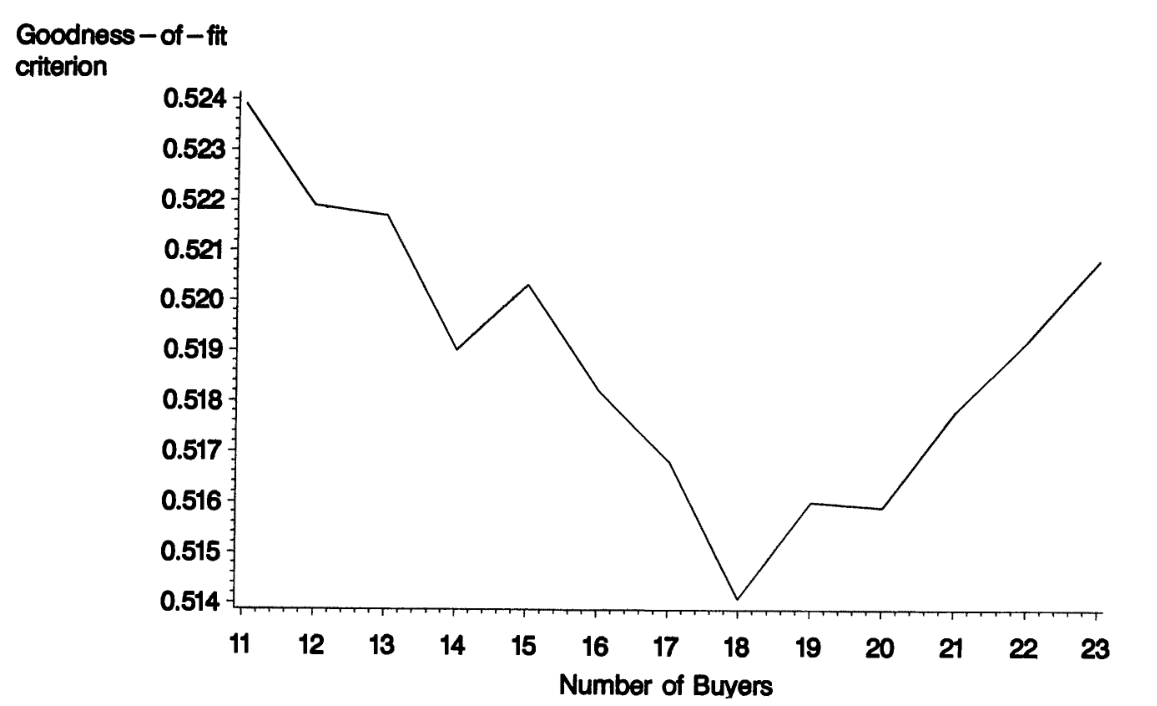
\includegraphics[width=\textwidth]{figures/ch15/lov1995_fig1.png}
\caption{Criterion $Q_S^*(\hat\theta_n)$ against the assumed number of buyers $n$.}\label{fig:15-lov-n}
\end{subfigure}\hfill
\begin{subfigure}[t]{0.49\textwidth}
\centering
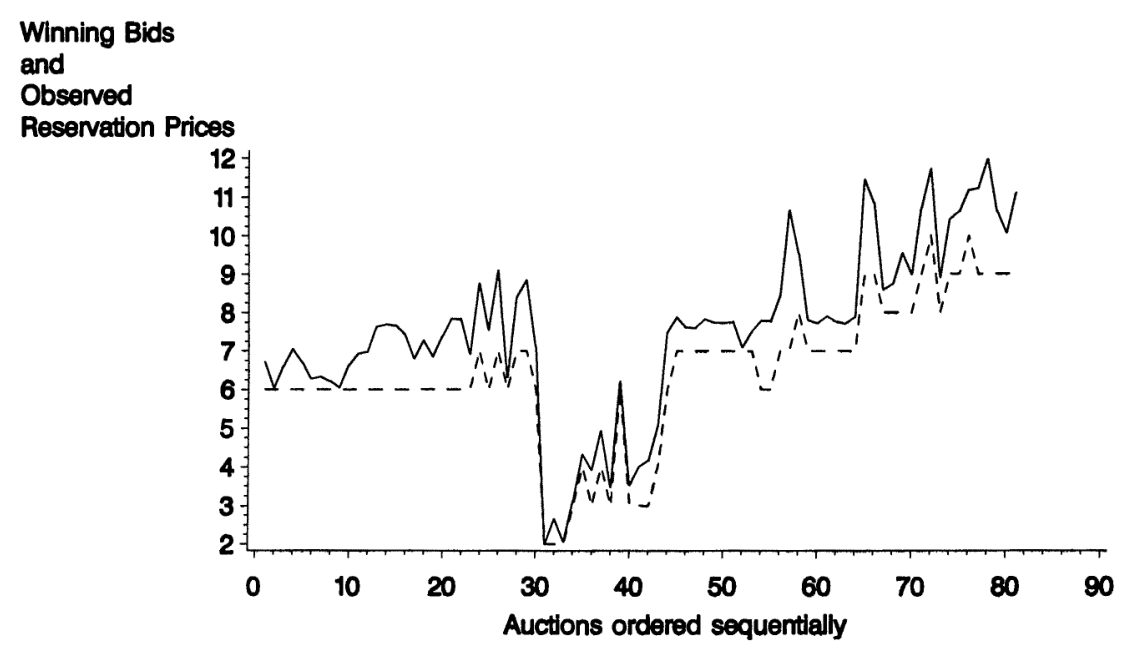
\includegraphics[width=\textwidth]{figures/ch15/lov1995_fig3.png}
\caption{Winning bids (solid) and reserve prices (dashed), auctions in chronological order.}\label{fig:15-lov-reserve}
\end{subfigure}
\caption{The Marmande eggplant auctions. Panel (a) selects the number of buyers by minimizing the simulated
criterion. Panel (b) shows that winning bids and reserve prices move together. Source: Laffont, Ossard and Vuong
(1995), Figures~1 and~3.}\label{fig:15-lov}
\end{figure}

\casehead{Specification}
Values are lognormal, a family without a closed-form bid function. The mean of log values is linear in six
characteristics (their eq.~(26)):
\[
\E\ln V_{it}=\mu_t=\theta_1+\theta_2\,\text{seller}_t+\theta_3\,\text{size1}_t+\theta_4\,\text{size2}_t+\theta_5\,\text{period}_t
+\theta_6\,\text{date}_t+\theta_7\,\text{supply}_t .
\]
The seller dummy is zero for the seller with the better reputation for quality (19 of the 81 lots come from the
other seller). The size dummies mark the middle category, 300 to 400 grams per eggplant (10 lots), and the largest
category, above 400 grams (34 lots). The period dummy is zero from the beginning of August until the first week of
September, when a large supply of substitute eggplants depresses prices, and one otherwise (68 lots). The date
variable records the time of the auction within 1990 divided by 100, so June 25 corresponds to 1.76. Supply is the
quantity of eggplants of all categories supplied at Marmande that day, in tons (mean 1.39).

The standard deviation $\sigma$ of $\ln V$ is not estimated. Retail prices for a given lot have a standard deviation of
about 5 percent of their mean. Setting $\frac{\text{sd}(V)}{\E(V)}=(e^{\sigma^2}-1)^{\frac12}=0.05$ gives $\sigma\approx0.05$
\citep[p.~969]{LaffontOssardVuong1995}. Their footnote~18 explains the choice. Reserve prices were low and every lot
was sold. Write $V=e^{\mu+\sigma U}$ with $U$ standard normal. Then $\E[b^w]=e^{\mu}\kappa(\sigma,\ln r-\mu)$, where
$\kappa(\sigma,a)=\E\big[\exp\big(\max\{\sigma U^{(n-1:n)},a\}\big)\big]$ for i.i.d.\ standard normal draws. As the reserve
becomes irrelevant, $\E[b^w]$ approaches $e^{\mu}\kappa(\sigma,-\infty)$, and the constant in $\mu$ cannot be separated
from $\sigma$. The estimator uses $S=20$ simulations per auction, and 30 give similar results. The importance density
for each auction is lognormal, centered at a preliminary consistent estimate and with standard deviation 0.05.

\casehead{Results}
The authors consider two hypotheses about the number of bidders. Eleven buyers attend regularly, but one buyer wins
almost half of the auctions and may act for several traders. They search over $n=11,\dots,23$, and the criterion is
smallest at $n=18$ (\cref{fig:15-lov-n}). The large buyer would then represent 8 traders, consistent with a market
share slightly below one half \citep[p.~970]{LaffontOssardVuong1995}. \Cref{tab:15-lov} reproduces their estimates for
$n=11$ and $n=18$.

\begin{table}[htbp]
\centering
\caption{Simulated nonlinear least squares estimates for the Marmande eggplant auctions}\label{tab:15-lov}
\begin{threeparttable}
\begin{tabular}{@{}lr@{\hspace{4pt}}rr@{\hspace{4pt}}r@{}}
\toprule
 & \multicolumn{2}{c}{$n=11$} & \multicolumn{2}{c}{$n=18$} \\
\cmidrule(lr){2-3}\cmidrule(l){4-5}
 & Estimate & ($t$) & Estimate & ($t$) \\
\midrule
Constant & 0.1297 & (0.02) & 0.0286 & (0.06) \\
Seller & $-0.0107$ & ($-0.17$) & $-0.0240$ & ($-0.51$) \\
Size 1 (300--400 g) & 0.2402 & (3.57) & 0.2402 & (4.39) \\
Size 2 (above 400 g) & 0.1373 & (1.39) & 0.1213 & (1.60) \\
Period & 1.2404 & (2.16) & 1.1998 & (2.90) \\
Date & 0.3115 & (3.04) & 0.3202 & (4.03) \\
Supply & $-0.0340$ & ($-0.59$) & $-0.0357$ & ($-0.81$) \\
\midrule
Criterion value $Q_S^*(\hat\theta)$ & \multicolumn{2}{c}{0.52395} & \multicolumn{2}{c}{0.51401} \\
Simulations per auction $S$ & \multicolumn{2}{c}{20} & \multicolumn{2}{c}{20} \\
Auctions $T$ & \multicolumn{2}{c}{81} & \multicolumn{2}{c}{81} \\
\bottomrule
\end{tabular}
\begin{tablenotes}
\footnotesize
\item \textit{Notes.} Reproduced from \citet[Table~I]{LaffontOssardVuong1995}. The coefficients are those of the mean of log
values, $\mu_t$ in their eq.~(26), with $\sigma=0.05$ imposed. Parentheses contain $t$-statistics computed from the robust
covariance estimator of their Proposition~3, not standard errors. Bids are in francs per kilo.
\end{tablenotes}
\end{threeparttable}
\end{table}

With a lognormal distribution and fixed $\sigma$, $\ln\E[V_t]=\mu_t+\frac{\sigma^2}{2}$, so each coefficient is
$\theta_k=\frac{1}{\E[V]}\frac{\partial\E[V]}{\partial x_k}$, a proportional effect on the expected value of the lot
\citep[p.~970]{LaffontOssardVuong1995}. With $n=18$, they read the size coefficients as midsize eggplants being worth
24 percent more than small ones and large ones 12 percent more. The size variables are dummies, so the exact
proportional effects are $e^{0.240}-1=27$ percent and $e^{0.121}-1=13$ percent (our calculation). This agrees with the conventional view that midsize eggplants are of the highest
quality. The seller coefficient is negative, so the seller with the better reputation commands higher values, but
the effect is small and insignificant. The period coefficient is large and significant. Values fall sharply during
the August glut, when \cref{fig:15-lov-reserve} shows winning bids dropping from about 7 francs to between 2 and 4
francs. The sample contains 13 lots with the period dummy equal to zero \citep[Appendix~B]{LaffontOssardVuong1995},
which matches the length of that run of low bids. Values also trend upward over the season (date). Local supply has no
significant effect, which the authors attribute to buyers serving several markets, with national supply movements
captured by the period and date variables. The fit is good: with $n=18$, $R^2=1-\frac{Q_S^*(\hat\theta)}{\widehat\Var(b^w)}=0.895$
\citep[p.~971]{LaffontOssardVuong1995}. The slope coefficients barely change between $n=11$ and $n=18$, while the
constant falls from 0.13 to 0.03. With more bidders the expected second-highest value is higher, so a lower level of
values fits the same winning bids.

\casehead{Assessment}
The paper made three contributions. It brought simulation-based estimation to structural auction models, with an
estimator that is consistent for a fixed number of simulations. It turned revenue equivalence into an estimation device. It
showed how to handle unobserved heterogeneity and an unknown number of bidders within the same framework. Its limits
are equally clear. The value distribution is parametric, and its dispersion was imposed from retail data rather than
estimated. The device relies on revenue equivalence, which fails with asymmetric bidders, affiliated values or risk
aversion. The dominant buyer is accommodated by inflating $n$, an assumption that holds only if that buyer bids for
each trader independently. Only the first moment of the winning bid is used.

\Cref{fig:15-lov-reserve} also raises a deeper issue. Winning bids and reserve prices move in tandem. If the reserve
were an exogenous truncation point, variation in reserves would change the fraction of lots sold, yet every lot was
sold. A more natural reading is that lots differ in ways that the seller and the buyers recognize and the
econometrician does not \citep[p.~7]{Roberts2013}. The authors anticipate the point in their conclusion. A seller may
set the reserve with better information than buyers, so that the reserve both truncates and shifts the distribution
of values \citep[p.~973]{LaffontOssardVuong1995}. \citet{Roberts2013} builds an identification strategy for
unobserved heterogeneity on exactly this co-movement (\cref{sec:15-uh}).

\subsection{From direct to indirect methods}\label{sec:15-direct-indirect}

Direct methods confront two burdens: solving the equilibrium for every trial parameter and a likelihood whose
support moves with the parameters. Simulated least squares removes the first burden with revenue equivalence and the
second by working with a smooth moment. Its reach is limited to models in which revenue equivalence holds. The
indirect approach of \citet{GuerrePerrigneVuong2000} removes both burdens in a different way. It estimates the
distribution of bids first and inverts the first-order condition \eqref{eq:14-foc-G} bid by bid, so no equilibrium is
ever computed. It also requires no parametric family (\cref{sec:15-gpv}).

Between the two lie hybrid two-step methods that specify a parametric first stage for bids conditional on
covariates, invert the first-order condition, and then work with the implied values
\citep{JofreBonetPesendorfer2003,AtheyLevinSeira2011}. They include covariates parsimoniously. A fully parametric
two-step method must keep the parametric families for bids and for values mutually consistent, because the
equilibrium bid function links them \citep{PerrigneVuong1999}. Making only one step parametric avoids that problem
\citep[Section~3.2]{AtheyHaile2007}. Theory also implies that bid distributions have compact support, so a parametric
first stage should impose an upper bound on bids \citep[footnote~19]{AtheyHaile2007}. \Cref{tab:15-direct-indirect}
summarizes the comparison.

\begin{table}[htbp]
\centering
\caption{Direct and indirect approaches to first-price auction data}\label{tab:15-direct-indirect}
\footnotesize
\begin{tabularx}{\textwidth}{@{}>{\raggedright\arraybackslash}p{2.0cm}>{\raggedright\arraybackslash}X>{\raggedright\arraybackslash}X>{\raggedright\arraybackslash}X>{\raggedright\arraybackslash}X@{}}
\toprule
 & Maximum likelihood & Simulated least squares & Two-step nonparametric & Two-step, parametric first stage \\
\midrule
Examples & \citet{Paarsch1992}, \citet{DonaldPaarsch1996} & \citet{LaffontOssardVuong1995} &
\citet{GuerrePerrigneVuong2000} & \citet{JofreBonetPesendorfer2003}, \citet{AtheyLevinSeira2011} \\
\addlinespace
Value distribution & parametric $F(\cdot;\theta)$ & parametric $F(\cdot;\theta)$ & unrestricted, smooth & implied by a
parametric bid distribution \\
\addlinespace
Equilibrium computation & solve and invert $\beta(\cdot;\theta)$ for every bid and every $\theta$ & none, since the
moment $\E\max\{V^{(n-1:n)},r\}$ is simulated & none, since the first-order condition is inverted & none, since the
first-order condition is inverted \\
\addlinespace
Regularity and rate & support depends on $\theta$, rate $T$ and non-normal limits & regular, $\sqrt T$ for fixed $S$,
variance excess of order $\frac1S$ & nonparametric rates slower than $\sqrt T$ & $\sqrt T$ for the bid parameters \\
\addlinespace
Data used & all bids or the winning bid & winning bid, $n$ may be unknown & all bids (the winning bid suffices under
SIPV) & all bids with covariates \\
\addlinespace
Asymmetry, affiliation, heterogeneity & a system of differential equations at every $\theta$ & excluded where revenue
equivalence fails, heterogeneity by integration & extends to all three (\cref{sec:15-apv,sec:15-uh}) & asymmetry,
dynamics, heterogeneity and entry \\
\addlinespace
Main drawback & computation, closed forms needed in practice & one moment, parametric family & dimensionality and
boundary trimming & consistency of bid and value families, support bounds \\
\bottomrule
\end{tabularx}
\end{table}

\section{First-Price Auctions II: The Guerre-Perrigne-Vuong Approach}\label{sec:15-gpv}

The direct methods of \cref{sec:15-direct} start from a parametric value distribution and solve for the equilibrium at every trial parameter. \citet{GuerrePerrigneVuong2000}, henceforth GPV, reversed the direction of the argument. They start from the distribution of observed bids and recover the value that rationalizes each bid. No equilibrium is ever computed, and no parametric family is assumed. This section develops their approach in full. It is the template for almost every structural method for first-price auctions that later sections use.

\casehead{The question} GPV pose three questions about the symmetric independent private values (SIPV) model of the first-price auction \citep[p.~526]{GuerrePerrigneVuong2000}. Does the model restrict the distribution of observable bids, so that it can be tested? Does identification of the value distribution require parametric assumptions? Can one estimate the value distribution without parametric assumptions and without solving for the equilibrium? Their answers are yes, no and yes. The model places two testable restrictions on bids. The value distribution is identified nonparametrically and constructively. A two-step kernel estimator recovers it, and no estimator can converge uniformly at a faster rate.

\casehead{Data} The method needs, for each auction $t=1,\dots,T$, all submitted bids $B_{1t},\dots,B_{n_tt}$, the number of bidders $n_t$, and the observed characteristics $Z_t$ of the object. These are the records of a sealed-bid first-price auction, such as a timber sale, a highway procurement or an offshore oil lease sale. GPV illustrate the method on simulated data, and we follow them in \cref{sec:15-gpv-mc}. Applications to field data appear in \cref{sec:15-apv,sec:15-uh,sec:15-als}.

\subsection{Setting and the inversion}\label{sec:15-gpv-insight}

We first state the model and the assumptions on the data-generating process, following GPV, Section 3.1. A single indivisible object is sold in each auction by a first-price sealed-bid auction. The highest bidder wins and pays her bid. Throughout \cref{sec:15-gpv-insight,sec:15-gpv-ident,sec:15-gpv-smooth,sec:15-gpv-estimator,sec:15-gpv-rates,sec:15-gpv-mc} the reserve price does not bind, so every potential bidder submits a bid and $n_t$ is the number of bidders who could have participated. \Cref{sec:15-gpv-reserve} treats a binding reserve price.

Let $Z_t\in\R^d$ collect the continuous characteristics of the object in auction $t$, and let $\mathcal I$ denote the set of possible numbers of bidders. The characteristics $Z_t$ are common knowledge among bidders. Their role is to absorb observed heterogeneity across auctions. They are not instruments.

\begin{assumption}[Sampling, GPV Assumption A1]\label{ass:15-gpv-sampling}
(i) Auctions are independent: the arrays $(Z_t,n_t,V_{1t},\dots,V_{n_tt})$, $t=1,2,\dots$, are independent across $t$, and the vectors $(Z_t,n_t)$ are identically distributed with density $f_{Zn}(z,n)$.
(ii) In each auction $t$, the values $V_{1t},\dots,V_{n_tt}$ are independent and identically distributed conditional on $(Z_t,n_t)$, with distribution $F(\cdot\mid Z_t,n_t)$ and density $f(\cdot\mid Z_t,n_t)$.
\end{assumption}

\begin{assumption}[Regularity, GPV Assumption A2]\label{ass:15-gpv-regularity}
The set $\mathcal I$ is a bounded subset of $\{2,3,\dots\}$, and the following hold.
(i) For each $n\in\mathcal I$, the support of $(V,Z)$ is $\{(v,z):z\in[\underline z,\bar z],\ v\in[\underline v(z),\bar v(z)]\}$ with $\underline z<\bar z$.
(ii) $f(v\mid z,n)\ge c_f>0$ on this support, and $f_{Zn}(z,n)\ge c_f>0$ on the support of $(Z,n)$.
(iii) For each $n\in\mathcal I$, $F(\cdot\mid\cdot,n)$ and $f_{Zn}(\cdot,n)$ have $R+1$ continuous bounded partial derivatives on their supports, with $R\ge 1$.
\end{assumption}

\Cref{ass:15-gpv-sampling} rules out dependence of values across auctions. GPV state part (i) for $(Z_t,n_t)$ only and invoke independence of values across auctions in the text, so we make it explicit. Such dependence would create dynamic incentives that the static equilibrium ignores. It allows the number of bidders to depend on the characteristics of the object. Part (iii) of \cref{ass:15-gpv-regularity} implies that the value density $f(\cdot\mid z,n)$ has $R$ bounded continuous derivatives. The integer $R$ measures smoothness and governs every rate of convergence below. The density is bounded away from zero, which keeps the bid density away from zero as well (\cref{prop:15-gpv-smooth}). GPV also assume, in the spirit of the theory, that $Z_t$ contains everything that bidders know about the object \citep[footnote 11]{GuerrePerrigneVuong2000}. Unobserved heterogeneity is the subject of \cref{sec:15-uh}.

\casehead{Equilibrium} Fix an auction with characteristics $z$ and $n$ bidders, and suppress $(z,n)$ when no confusion arises. Set the reserve price equal to $\underline v$. By \cref{prop:14-rs}, which gives the bid function of \citet{RileySamuelson1981}, the unique symmetric equilibrium bid is
\begin{equation}\label{eq:15-gpv-rs}
\beta(v)=v-\frac{1}{F(v)^{n-1}}\int_{\underline v}^{v}F(u)^{n-1}\,du,
\end{equation}
which is \eqref{eq:14-rs-bid} with $r=\underline v$ (GPV, eqs.~(1) and~(8)). It solves the differential equation
\begin{equation}\label{eq:15-gpv-ode}
1=\big(v-\beta(v)\big)(n-1)\frac{f(v)}{F(v)}\frac{1}{\beta'(v)}
\end{equation}
with the boundary condition $\beta(\underline v)=\underline v$ (GPV, eq.~(2)). This is \eqref{eq:14-rs-ode} divided by $\beta'(v)F(v)^{n-1}$. The bid function is strictly increasing on $[\underline v,\bar v]$.

\casehead{Why identification is not obvious} As \cref{sec:15-fpa-hard} explained, the bid distribution $G$ depends on $F$ in two ways. It depends on $F$ directly, because values are drawn from $F$. It also depends on $F$ through the strategy $\beta$, which by \eqref{eq:15-gpv-rs} is itself a functional of $F$. A direct method must untangle both channels for every trial value of $F$.

\casehead{The inversion} GPV observe that the first-order condition can be written so that the derivative $\beta'$, the distribution $F$ and the density $f$ disappear together. We derive the resulting formula step by step. Let $[\underline b,\bar b]=[\beta(\underline v),\beta(\bar v)]$ denote the support of bids, and note that $\underline b=\underline v$.

\emph{Step 1.} We express the bid distribution through $F$ and $\beta$. For $b\in[\underline b,\bar b]$, the strict monotonicity of $\beta$ gives
\[
G(b)=\Pr(B_i\le b)=\Pr\big(V_i\le\beta^{-1}(b)\big)=F\big(\beta^{-1}(b)\big).
\]

\emph{Step 2.} We differentiate. By the inverse function rule,
\[
g(b)=f\big(\beta^{-1}(b)\big)\frac{d\beta^{-1}(b)}{db}=\frac{f\big(\beta^{-1}(b)\big)}{\beta'\big(\beta^{-1}(b)\big)}.
\]

\emph{Step 3.} We take the ratio. Write $v=\beta^{-1}(b)$. Dividing the result of Step 2 by that of Step 1 gives
\[
\frac{g(b)}{G(b)}=\frac{1}{\beta'(v)}\,\frac{f(v)}{F(v)}.
\]

\emph{Step 4.} We substitute into the equilibrium condition. The right side of Step 3 is exactly the product that appears in \eqref{eq:15-gpv-ode}. Replacing it there and using $\beta(v)=b$ gives
\[
1=(v-b)(n-1)\frac{g(b)}{G(b)}.
\]

\emph{Step 5.} We solve for the value. Dividing by $(n-1)\frac{g(b)}{G(b)}$ and adding $b$ to both sides yields
\begin{equation}\label{eq:15-gpv-xi}
v=\xi(b;G,n)\equiv b+\frac{1}{n-1}\,\frac{G(b)}{g(b)}.
\end{equation}
This is GPV's equation~(3), and it coincides with \eqref{eq:14-foc-G}. With covariates, $G$ and $g$ are replaced by $G(\cdot\mid z,n)$ and $g(\cdot\mid z,n)$ (GPV, eq.~(9)).

Equation \eqref{eq:15-gpv-xi} expresses each value through the bid, the bid distribution, the bid density and the number of bidders. All four are observable or estimable. If bids are equilibrium bids, the value behind each bid must satisfy \eqref{eq:15-gpv-xi}. We call $\xi(\cdot;G,n)$ the \emph{inverse bid function}. In equilibrium it equals $\beta^{-1}$, and it has been obtained without solving \eqref{eq:15-gpv-ode}. We use the symbol $\xi$ for this object throughout the chapter, as GPV do (\cref{tab:15-notation}).

The same equation follows from the bidder's problem written in terms of bids, which is how \cref{sec:14-fpa-G} derived \eqref{eq:14-foc-G}. A bidder with value $v$ facing rivals whose bids are i.i.d.\ with distribution $G$ maximizes $(v-b)G(b)^{n-1}$. The first-order condition rearranges to \eqref{eq:15-gpv-xi}. The derivation above shows that the two routes agree. It also shows why the bid-based form is the right one for identification: it contains only objects that the data reveal.

\casehead{The markdown} The term $\frac{G(b)}{(n-1)g(b)}=v-b$ is the bidder's \emph{markdown}, the shading of the bid below the value. By \eqref{eq:14-markdown}, the relative markdown $\frac{v-b}{b}$ equals the inverse of the elasticity of the win probability $G(b)^{n-1}$ with respect to the bid. A bidder is a monopsonist facing the residual supply curve traced out by the highest rival bid. Equation \eqref{eq:15-gpv-xi} makes the oligopoly analogy of \cref{sec:15-fpa-hard} exact. The distribution of rival bids plays the role of the demand system, and the econometrician observes it directly.

\casehead{Credit and precursors} The idea first appeared in print in \citet{LaffontVuong1993}, who attribute it to an early draft of GPV \citep[Section 3.1]{AtheyHaile2007}. Similar formulas appear earlier in decision-theoretic models of bidding, starting with \citet{Friedman1956}. There each bidder optimizes against an exogenous distribution of rival bids, so the value distribution and the bid distribution need not be linked by $F=G\circ\beta$ \citep[footnote 3]{GuerrePerrigneVuong2000}. In \eqref{eq:15-gpv-xi} the link holds because bidders' beliefs about rival bids are correct in equilibrium.

\subsection{Identification and testable restrictions}\label{sec:15-gpv-ident}

We now state GPV's identification theorem. Let $\mathcal P$ denote the set of distributions on $\R_+$ that are absolutely continuous with an interval support. The support of a distribution in $\mathcal P$ is the closure of the set where its density is positive, so every member of $\mathcal P$ is strictly increasing on its support \citep[footnote 4]{GuerrePerrigneVuong2000}. Let $\mathbf G$ denote the joint distribution of the $n$ bids $(B_1,\dots,B_n)$ in an auction. As in GPV, we restrict attention to strictly increasing and differentiable equilibrium strategies.

\begin{theorem}[\citealp{GuerrePerrigneVuong2000}, Theorem 1]\label{thm:15-gpv-ident}
Let $n\ge 2$, and let $\mathbf G$ belong to $\mathcal P^n$ with support $[\underline b,\bar b]^n$. Consider a first-price sealed-bid auction with symmetric independent private values and a nonbinding reserve price. There exists a value distribution $F\in\mathcal P$ whose equilibrium bids have joint distribution $\mathbf G$ if and only if the following two conditions hold.
\begin{itemize}
\item[(C1)] $\mathbf G(b_1,\dots,b_n)=\prod_{i=1}^n G(b_i)$ for some distribution $G$.
\item[(C2)] The function $\xi(\cdot;G,n)$ defined in \eqref{eq:15-gpv-xi} is strictly increasing on $[\underline b,\bar b]$, and its inverse is differentiable on $[\underline v,\bar v]\equiv[\xi(\underline b;G,n),\xi(\bar b;G,n)]$.
\end{itemize}
When such an $F$ exists, it is unique, its support is $[\underline v,\bar v]$, and
\begin{equation}\label{eq:15-gpv-F}
F(v)=G\big(\xi^{-1}(v;G,n)\big)\qquad\text{for all }v\in[\underline v,\bar v].
\end{equation}
Moreover, $\xi(\cdot;G,n)$ is the inverse of the equilibrium strategy: $\xi(b;G,n)=\beta^{-1}(b)$ for all $b\in[\underline b,\bar b]$.
\end{theorem}

\begin{proof}
We follow GPV, Appendix A.1, and add the global optimality argument that their footnote~5 assumes. Write $\xi(b)$ for $\xi(b;G,n)$.

\emph{Necessity of (C1).} Suppose $F\in\mathcal P$ with support $[\underline v,\bar v]$ rationalizes $\mathbf G$, and let $\beta$ be the equilibrium strategy. Each bid is $B_i=\beta(V_i)$, a fixed function of an independent draw from $F$. Hence the bids are i.i.d., and (C1) holds with $G(b)=F(\beta^{-1}(b))$.

\emph{Necessity of (C2).} The strategy $\beta$ solves \eqref{eq:15-gpv-ode}. Steps 1 to 5 of \cref{sec:15-gpv-insight} show that \eqref{eq:15-gpv-ode} implies $\xi(\beta(v))=v$ for every $v\in[\underline v,\bar v]$. Setting $b=\beta(v)$ gives $\xi(b)=\beta^{-1}(b)$ on $[\underline b,\bar b]$. The inverse of a strictly increasing function is strictly increasing, so $\xi$ is strictly increasing. Its inverse is $\beta$, which is differentiable on $[\underline v,\bar v]=[\xi(\underline b),\xi(\bar b)]$. Hence (C2) holds.

\emph{Sufficiency, Step 1: the lower boundary.} Assume (C1) and (C2). We show that
\begin{equation}\label{eq:15-gpv-A1}
\lim_{b\downarrow\underline b}\xi(b)=\underline b.
\end{equation}
Since $\xi$ is strictly increasing, the limit exists. Since $\frac{G}{g}\ge0$, we have $\xi(b)\ge b$, so the limit equals $\underline b+c$ for some $c\ge0$. Suppose that $c>0$. By \eqref{eq:15-gpv-xi},
\[
\frac{G(b)}{g(b)}=(n-1)\big(\xi(b)-b\big)\longrightarrow(n-1)c>0\qquad\text{as }b\downarrow\underline b.
\]
Hence there is $\delta>0$ with $\frac{g(b)}{G(b)}\le\frac{2}{(n-1)c}$ on $(\underline b,\underline b+\delta)$. Because $\frac{d}{db}\ln G(b)=\frac{g(b)}{G(b)}$, integrating over $[b,\underline b+\delta]$ gives
\[
\ln G(b)\ge\ln G(\underline b+\delta)-\frac{2\delta}{(n-1)c}\qquad\text{for all }b\in(\underline b,\underline b+\delta).
\]
The right side is a finite constant, yet $\ln G(b)\to-\infty$ as $b\downarrow\underline b$ because $G(\underline b)=0$. This contradiction shows that $c=0$.

\emph{Sufficiency, Step 2: a candidate distribution.} Set $\underline v=\xi(\underline b)=\underline b$, using \eqref{eq:15-gpv-A1}, and $\bar v=\xi(\bar b)$. Define $F$ on $[\underline v,\bar v]$ by \eqref{eq:15-gpv-F}. By (C2), $\xi^{-1}$ is strictly increasing and differentiable. Since $G$ is strictly increasing on $[\underline b,\bar b]$ and absolutely continuous, $F$ is strictly increasing and absolutely continuous, with $F(\underline v)=G(\underline b)=0$ and $F(\bar v)=G(\bar b)=1$. Hence $F\in\mathcal P$ with support $[\underline v,\bar v]$.

\emph{Sufficiency, Step 3: the candidate strategy solves the equilibrium equation.} Let $s=\xi^{-1}$. By Step 1, $s(\underline v)=\underline v$. By construction $F(v)=G(s(v))$, so $f(v)=g(s(v))s'(v)$ and
\[
\frac{f(v)}{F(v)}=s'(v)\,\frac{g\big(s(v)\big)}{G\big(s(v)\big)}.
\]
Evaluating \eqref{eq:15-gpv-xi} at $b=s(v)$ gives $v=s(v)+\frac{G(s(v))}{(n-1)g(s(v))}$, which rearranges to
\[
1=\big(v-s(v)\big)(n-1)\frac{g\big(s(v)\big)}{G\big(s(v)\big)}=\big(v-s(v)\big)(n-1)\frac{f(v)}{F(v)}\frac{1}{s'(v)}.
\]
This is \eqref{eq:15-gpv-ode} with the boundary condition $s(\underline v)=\underline v$. By Step 5 of the proof of \cref{prop:14-rs}, its unique solution is the bid function \eqref{eq:15-gpv-rs} associated with $F$. Hence $s=\beta$.

\emph{Sufficiency, Step 4: the candidate strategy is a best response.} Suppose the rivals use $s$ and draw values from $F$. Each rival bid then has distribution $F(s^{-1}(b))=F(\xi(b))=G(b)$. A bidder with value $v$ who bids $b\in[\underline b,\bar b]$ earns $(v-b)G(b)^{n-1}$. Its derivative is
\[
\frac{d}{db}\Big[(v-b)G(b)^{n-1}\Big]=G(b)^{n-2}\Big[(n-1)g(b)(v-b)-G(b)\Big]=(n-1)g(b)G(b)^{n-2}\big[v-\xi(b)\big].
\]
By (C2) the bracket is positive for $b<s(v)$ and negative for $b>s(v)$. The payoff therefore rises up to $b=s(v)$ and falls after it, so $s(v)$ is the best bid in $[\underline b,\bar b]$. A bid above $\bar b$ wins with certainty, like $\bar b$, but costs more. A bid below $\underline b$ never wins and earns zero, which is at most $(v-s(v))G(s(v))^{n-1}\ge0$. Hence $s$ is a symmetric equilibrium. The resulting joint distribution of bids is $\prod_iG(b_i)=\mathbf G$ by (C1).

\emph{Uniqueness.} The necessity part shows that any rationalizing $F$ has an equilibrium strategy with $\beta=\xi^{-1}$. Then $F(v)=G(\beta(v))=G(\xi^{-1}(v))$, which is \eqref{eq:15-gpv-F}. The right side depends only on $G$ and $n$, so $F$ is unique. Its support is $[\xi(\underline b),\xi(\bar b)]=[\underline b,\xi(\bar b)]$ by \eqref{eq:15-gpv-A1}.
\end{proof}

Step 4 of the proof shows the role of (C2) beyond invertibility. The derivative of the payoff factors into a positive term and the gap $v-\xi(b)$. Monotonicity of $\xi$ is exactly the condition under which the first-order condition picks the global maximum. GPV assume second-order conditions in their footnote~5. In the SIPV model (C2) delivers them. \Citet[Section 5.1]{AtheyHaile2007} use the same single-crossing logic for the affiliated private values model with independence or symmetry (\cref{thm:15-ah-rational} below).

\begin{remark}[An equivalent form of (C2)]\label{rem:15-c2}
Suppose $g$ is differentiable on $(\underline b,\bar b)$. Differentiating \eqref{eq:15-gpv-xi} by the quotient rule gives
\[
\xi'(b)=1+\frac{1}{n-1}\,\frac{g(b)^2-G(b)g'(b)}{g(b)^2}=\frac{n}{n-1}-\frac{1}{n-1}\,\frac{G(b)g'(b)}{g(b)^2}.
\]
The derivative of $\frac{g}{G^n}$ is
\[
\frac{d}{db}\frac{g(b)}{G(b)^n}=\frac{g'(b)G(b)^n-nG(b)^{n-1}g(b)^2}{G(b)^{2n}}=\frac{G(b)g'(b)-ng(b)^2}{G(b)^{n+1}}.
\]
Comparing the two displays,
\[
\xi'(b)=-\frac{G(b)^{n+1}}{(n-1)g(b)^2}\,\frac{d}{db}\frac{g(b)}{G(b)^n}.
\]
The factor in front is negative, so $\xi$ is strictly increasing if and only if $\frac{g}{G^n}$ is strictly decreasing \citep[footnote 6]{GuerrePerrigneVuong2000}. A sufficient condition is that $G$ is \emph{log-concave}, that is, $\frac{g}{G}$ is decreasing. Indeed $\frac{g}{G^n}=\frac{g}{G}\cdot G^{-(n-1)}$ is then the product of a positive decreasing function and a positive strictly decreasing function. GPV state this sufficient condition on p.~530. Log-concavity is a property of the bid data, so it can be checked directly.
\end{remark}

Condition (C2) has content. Bid distributions with deep U-shaped densities can violate it, and so can some sharply peaked multimodal densities \citep[p.~530]{GuerrePerrigneVuong2000}. The next example, due to GPV, makes the point concrete.

\begin{example}[Bids that no value distribution rationalizes]\label{ex:15-gpv-counter}
Let $n=2$ and let bids be i.i.d.\ with distribution
\[
G(b)=\Big(\frac{b}{5-4b}\Big)^{\frac15},\qquad b\in[0,1].
\]
This is a valid distribution: $G(0)=0$, $G(1)=1$, and $\frac{b}{5-4b}$ is strictly increasing. We compute the inverse bid function in four steps. First, take logarithms:
\[
\ln G(b)=\frac15\Big[\ln b-\ln(5-4b)\Big].
\]
Second, differentiate:
\[
\frac{g(b)}{G(b)}=\frac15\Big[\frac1b+\frac{4}{5-4b}\Big]=\frac15\cdot\frac{5-4b+4b}{b(5-4b)}=\frac{1}{b(5-4b)}.
\]
Third, substitute into \eqref{eq:15-gpv-xi} with $n-1=1$:
\[
\xi(b)=b+b(5-4b)=6b-4b^2.
\]
Fourth, differentiate: $\xi'(b)=6-8b$, which is negative for $b>\frac34$. Condition (C2) fails. The implied value peaks at $\xi(\frac34)=\frac94$ and falls to $\xi(1)=2$. A bidder who bids $0.9$ would need a lower value, $2.16$, than a bidder who bids $0.8$, whose implied value is $2.24$. Both cannot be best responses to the same distribution of rival bids, so no value distribution generates these bids in equilibrium.

The density behind this example is U-shaped. Multiplying the second step by $G$ gives $g(b)=b^{-\frac45}(5-4b)^{-\frac65}$. Its logarithmic derivative is $-\frac{4}{5b}+\frac{24}{5(5-4b)}$, which vanishes at $b=\frac12$. The density falls from infinity at $b=0$ to $g(\frac12)\approx0.47$ and rises to $g(1)=1$. The mass of high bids is too thin relative to the mass just below them. Consistently with \cref{rem:15-c2}, the function $\frac{g}{G^2}=b^{-\frac65}(5-4b)^{-\frac45}$ falls on $(0,\frac34)$ and rises on $(\frac34,1)$.

For contrast, let bids be uniform on $[0,1]$ with $n=2$. Then $\frac{G}{g}=b$ and $\xi(b)=2b$, which is strictly increasing. Formula \eqref{eq:15-gpv-F} gives $F(v)=G(\frac v2)=\frac v2$ on $[0,2]$. These bids come from values uniform on $[0,2]$, with $\beta(v)=\frac v2$, as \cref{ex:14-uniform} confirms after rescaling.
\end{example}

The exponent $\frac15$ matters. With exponent $\frac32$ instead, the second step gives $\frac{G}{g}=\frac{b(5-4b)}{7.5}$ and $\xi'(b)=1+\frac{5-8b}{7.5}\ge1-\frac{3}{7.5}>0$, so (C2) would hold. \Cref{fig:15-gpv-counter} plots both bid densities and both inverse bid functions of the example.

\begin{figure}[htbp]
\centering
\begin{subfigure}[t]{0.48\textwidth}
\centering
\begin{tikzpicture}
\begin{axis}[width=0.95\textwidth,height=0.8\textwidth,xmin=0,xmax=1,ymin=0,ymax=2.5,
  xlabel={Bid $b$},ylabel={Bid density $g(b)$},axis lines=left,
  xtick={0,0.25,0.5,0.75,1},xticklabels={$0$,$\frac14$,$\frac12$,$\frac34$,$1$},
  ytick={0,0.5,1,1.5,2,2.5}]
\addplot[thick,blue!70!black,domain=0.03:1,samples=300] {x^(-0.8)*(5-4*x)^(-1.2)};
\addplot[thick,black,dashed,domain=0:1] {1};
\node[font=\small,blue!70!black,align=left,anchor=west] at (axis cs:0.12,1.85) {$g(b)=b^{-\frac45}(5-4b)^{-\frac65}$};
\node[font=\small,anchor=south] at (axis cs:0.5,1.02) {uniform bids, $g(b)=1$};
\end{axis}
\end{tikzpicture}
\caption{Bid densities}
\end{subfigure}\hfill
\begin{subfigure}[t]{0.48\textwidth}
\centering
\begin{tikzpicture}
\begin{axis}[width=0.95\textwidth,height=0.8\textwidth,xmin=0,xmax=1,ymin=0,ymax=2.6,
  xlabel={Bid $b$},ylabel={Implied value $\xi(b)$},axis lines=left,
  xtick={0,0.25,0.5,0.75,1},xticklabels={$0$,$\frac14$,$\frac12$,$\frac34$,$1$},
  ytick={0,0.5,1,1.5,2,2.25},yticklabels={$0$,$\frac12$,$1$,$\frac32$,$2$,$\frac94$}]
\fill[orange!15] (axis cs:0.75,0) rectangle (axis cs:1,2.6);
\addplot[thick,blue!70!black,domain=0:1,samples=100] {6*x-4*x^2};
\addplot[thick,black,dashed,domain=0:1] {2*x};
\addplot[only marks,mark=*,mark size=1.5pt,blue!70!black] coordinates {(0.75,2.25)};
\draw[densely dotted,gray] (axis cs:0.75,0) -- (axis cs:0.75,2.25);
\node[font=\small,blue!70!black,anchor=east] at (axis cs:0.55,2.2) {$\xi(b)=6b-4b^2$};
\node[font=\small,anchor=west] at (axis cs:0.42,0.62) {$\xi(b)=2b$};
\node[font=\small,align=center,orange!70!black] at (axis cs:0.875,0.45) {$\xi'<0$:\\(C2) fails};
\end{axis}
\end{tikzpicture}
\caption{Inverse bid functions}
\end{subfigure}
\caption{The counterexample of \citet[p.~530]{GuerrePerrigneVuong2000}. Two bidders, bids i.i.d.\ with $G(b)=(\frac{b}{5-4b})^{\frac15}$ on $[0,1]$ (solid), against bids uniform on $[0,1]$ (dashed). The U-shaped bid density in panel (a) implies an inverse bid function that falls for $b>\frac34$ (shaded region in panel (b)), so no value distribution rationalizes these bids. Uniform bids imply $\xi(b)=2b$ and values uniform on $[0,2]$.}\label{fig:15-gpv-counter}
\end{figure}

\begin{remark}[What kind of identification result this is]\label{rem:15-gpv-ident-kind}
Four features of \cref{thm:15-gpv-ident} deserve emphasis. First, identification is nonparametric: no family of distributions is assumed. It implies identification within any parametric family. A parametric specification then serves only as an approximation and plays no role in identification (\cref{sec:15-identification}). Second, the proof is constructive, since \eqref{eq:15-gpv-F} gives $F$ explicitly. Third, the result is global. It does not rest on conditions in a neighborhood of a particular distribution \citep[footnote 7]{GuerrePerrigneVuong2000}. Fourth, the theorem characterizes the testable content of the model: (C1) and (C2) are all the restrictions that the SIPV first-price model places on bids from auctions with a fixed $n$. \Cref{sec:15-gpv-tests} turns them into tests.
\end{remark}

\begin{remark}[One equilibrium in all auctions]\label{rem:15-gpv-same-eq}
The inversion uses the distribution of rival bids observed across auctions as the belief of each bidder in each auction. This relies on the sampling assumption of \cref{sec:15-primitives} that the same equilibrium is played in all auctions with the same observables. In the SIPV model the equilibrium is unique, so the assumption holds automatically \citep[Section 3.1]{AtheyHaile2007}.
\end{remark}

\subsection{The bid density is smoother than the value density}\label{sec:15-gpv-smooth}

The estimator of \cref{sec:15-gpv-estimator} replaces $G$ and $g$ in \eqref{eq:15-gpv-xi} by estimates. How well they can be estimated depends on their smoothness. GPV show that the bid density has one more derivative than the value density.

\begin{proposition}[\citealp{GuerrePerrigneVuong2000}, Proposition 1]\label{prop:15-gpv-smooth}
Under \cref{ass:15-gpv-regularity}, the conditional bid distribution $G(\cdot\mid\cdot,\cdot)$ satisfies the following.
(i) For each $n\in\mathcal I$, its support is $\{(b,z):z\in[\underline z,\bar z],\ b\in[\underline b(z,n),\bar b(z,n)]\}$ with $\inf_z[\bar b(z,n)-\underline b(z,n)]>0$. The boundaries $\underline b(\cdot,n)$ and $\bar b(\cdot,n)$ have $R+1$ continuous bounded derivatives, and $\underline b(z,n)=\underline v(z)$.
(ii) $g(b\mid z,n)\ge c_g>0$ on the support.
(iii) $G(\cdot\mid\cdot,n)$ has $R+1$ continuous bounded partial derivatives on the support.
(iv) On any closed subset of the interior of the support, $g(\cdot\mid\cdot,n)$ has $R+1$ continuous bounded partial derivatives.
\end{proposition}

Part (iv) is the striking one. The value density has $R$ derivatives, and the bid density has $R+1$ on inner sets. The intuition comes from rearranging \eqref{eq:15-gpv-xi}:
\begin{equation}\label{eq:15-gpv-g-from-xi}
g(b\mid z,n)=\frac{G(b\mid z,n)}{(n-1)\big(\xi(b;z,n)-b\big)}
\end{equation}
\citep[p.~536]{GuerrePerrigneVuong2000}. The same formula appeared in \cref{sec:15-ml} as the bid density of a parametric model. The bid function \eqref{eq:15-gpv-rs} involves $F$ and its integral, so it has the $R+1$ derivatives of $F$. Its inverse $\xi$ inherits them. The distribution $G$ also has $R+1$ derivatives by part (iii). On inner sets the denominator of \eqref{eq:15-gpv-g-from-xi} is bounded away from zero, so $g$ has $R+1$ derivatives there. The bidding strategy acts as a smoothing operator. Each bid aggregates information about the whole lower tail of $F$ through the integral in \eqref{eq:15-gpv-rs}.

Formula \eqref{eq:15-gpv-g-from-xi} also explains part (ii) and the behavior of $g$ at the edges of its support. At the top, $G(\bar b)=1$, so $g(\bar b)=\frac{1}{(n-1)(\bar v-\bar b)}$. At the bottom, both $G$ and $\xi(b)-b$ vanish. To find the limit we expand near $\underline v$. Because $f(\underline v)>0$, we have $F(u)=f(\underline v)(u-\underline v)(1+o(1))$ as $u\downarrow\underline v$. Substituting into \eqref{eq:15-gpv-rs},
\[
v-\beta(v)=\frac{\int_{\underline v}^vf(\underline v)^{n-1}(u-\underline v)^{n-1}du}{f(\underline v)^{n-1}(v-\underline v)^{n-1}}\big(1+o(1)\big)=\frac{v-\underline v}{n}\big(1+o(1)\big).
\]
Hence, at $b=\beta(v)$,
\[
g(b)=\frac{F(v)}{(n-1)\big(v-\beta(v)\big)}=\frac{f(\underline v)(v-\underline v)}{(n-1)\frac{v-\underline v}{n}}\big(1+o(1)\big)\longrightarrow\frac{n}{n-1}\,f(\underline v)
\]
as $v\downarrow\underline v$. For values uniform on $[0,1]$, bids are uniform on $[0,\frac{n-1}{n}]$ with density $\frac{n}{n-1}$, which matches the formula.

The consequence for estimation is immediate. By \citet{Stone1982}, a function with $R+1$ derivatives in $d+1$ dimensions can be estimated uniformly at the rate $(\frac{T}{\log T})^{\frac{R+1}{2R+d+3}}$. The bid density, and with it the inverse bid function on inner sets, can therefore be estimated faster than the value density could be estimated even if values were observed. The difficulty lies elsewhere, as \cref{sec:15-gpv-rates} shows.

\subsection{The two-step estimator}\label{sec:15-gpv-estimator}

\Cref{thm:15-gpv-ident} suggests an estimator that mirrors identification. In the first step we estimate $G$ and $g$ nonparametrically and use \eqref{eq:15-gpv-xi} to build a \emph{pseudo-sample} of values, one pseudo-value per bid (\cref{sec:15-routes}). In the second step we treat the pseudo-values as a sample from $F$ and estimate its density by kernel smoothing. Kernel density estimation, bandwidths and boundary effects are reviewed in \cref{app:econometrics}. Throughout, kernels are normalized to have support $[-1,1]$.

\casehead{Homogeneous auctions} Suppose first that all $T$ auctions sell identical objects with the same number $n$ of bidders. The first step estimates the bid distribution by its empirical counterpart and the bid density by a kernel estimator (GPV, eqs.~(4)--(5)):
\begin{align}
\hat G(b)&=\frac{1}{nT}\sum_{t=1}^T\sum_{i=1}^n\indic(B_{it}\le b),\label{eq:15-gpv-Ghat}\\
\hat g(b)&=\frac{1}{nTh_g}\sum_{t=1}^T\sum_{i=1}^n\mathcal K\Big(\frac{b-B_{it}}{h_g}\Big),\label{eq:15-gpv-ghat}
\end{align}
where $\mathcal K$ is a kernel and $h_g$ a bandwidth. All $nT$ bids enter, because bids are i.i.d.\ within and across auctions under (C1).

\casehead{Boundary bias} A kernel density estimator is biased near the edges of the support, and the bias contaminates the pseudo-values. We derive the bias at the top of the support, following GPV, p.~531. Take a symmetric kernel with support $[-1,1]$ and a bid $b=\bar b-\lambda h_g$ with $\lambda\in[0,1)$. Then
\[
\E\big[\hat g(b)\big]=\frac{1}{h_g}\int_{\underline b}^{\bar b}\mathcal K\Big(\frac{b-y}{h_g}\Big)g(y)\,dy.
\]
We change variables to $u=\frac{b-y}{h_g}$, so that $y=b-h_gu$ and $dy=-h_g\,du$. The upper limit $y=\bar b$ becomes $u=\frac{b-\bar b}{h_g}=-\lambda$. The lower limit $y=\underline b$ becomes $u=\frac{b-\underline b}{h_g}$, which exceeds one once $h_g$ is small. Hence
\[
\E\big[\hat g(b)\big]=\int_{-\lambda}^{1}\mathcal K(u)\,g(b-h_gu)\,du\longrightarrow g(\bar b)\int_{-\lambda}^{1}\mathcal K(u)\,du\qquad\text{as }h_g\to0.
\]
For $\lambda<1$ the integral of the kernel is less than one, and at $\lambda=0$ it equals $\frac12$. Within one bandwidth of $\bar b$, the estimator therefore underestimates the density, by up to one half at the edge. The same argument applies within one bandwidth of $\underline b$.

The effect on the pseudo-values is large. At the top, $\hat G\approx1$ while $\hat g\approx\frac12g(\bar b)$, so the estimated markdown is about twice the true markdown $\bar v-\bar b$. The pseudo-value of the top bid is then about $\bar b+2(\bar v-\bar b)=2\bar v-\bar b$, well above the largest possible value. \Cref{fig:15-gpv-trim} shows the effect in a simulated sample.

\casehead{Trimming} Let $B_{\min}$ and $B_{\max}$ be the smallest and largest of the $nT$ bids. Because $\underline b\le B_{\min}$ and $B_{\max}\le\bar b$, the estimator $\hat g$ is asymptotically unbiased on $[B_{\min}+h_g,B_{\max}-h_g]$. GPV define the pseudo-values as (GPV, eq.~(6))
\begin{equation}\label{eq:15-gpv-trim}
\hat V_{it}=\begin{cases}
B_{it}+\dfrac{1}{n-1}\,\dfrac{\hat G(B_{it})}{\hat g(B_{it})}&\text{if }B_{\min}+h_g\le B_{it}\le B_{\max}-h_g,\\[2ex]
+\infty&\text{otherwise.}
\end{cases}
\end{equation}
Setting a trimmed pseudo-value to $+\infty$ removes it from the second step, because a kernel with bounded support assigns it zero weight.

\casehead{Second step} The density of values is estimated by (GPV, eq.~(7))
\begin{equation}\label{eq:15-gpv-fhat}
\hat f(v)=\frac{1}{nTh_f}\sum_{t=1}^T\sum_{i=1}^n\mathcal K_f\Big(\frac{v-\hat V_{it}}{h_f}\Big),
\end{equation}
with kernel $\mathcal K_f$ and bandwidth $h_f$. The distribution function, quantiles, and any functional of $F$ follow from the pseudo-values or from $\hat f$. The estimator involves no optimization and no equilibrium computation.

\casehead{Heterogeneous auctions} In applications the objects differ and the number of bidders varies. GPV, Section 3.3, extend the estimator jointly over $(b,z,n)$. Define
\[
G(b,z,n)=G(b\mid z,n)f_{Zn}(z,n),\qquad g(b,z,n)=g(b\mid z,n)f_{Zn}(z,n).
\]
The density $f_{Zn}$ cancels in the ratio, so \eqref{eq:15-gpv-xi} becomes (GPV, eq.~(12))
\begin{equation}\label{eq:15-gpv-psi}
V_{it}=B_{it}+\frac{1}{n_t-1}\,\psi(B_{it},Z_t,n_t),\qquad\psi(b,z,n)\equiv\frac{G(b,z,n)}{g(b,z,n)}.
\end{equation}
The ratio $\psi$ is a local symbol of this subsection, unrelated to the virtual valuation $\psi$ of \eqref{eq:14-psi}. The numerator and denominator are estimated by (GPV, eqs.~(13)--(14))
\begin{align}
\hat G(b,z,n)&=\frac{1}{Th_G^d}\sum_{t=1}^T\frac{1}{n_t}\sum_{i=1}^{n_t}\indic(B_{it}\le b)\,\mathcal K_G\Big(\frac{z-Z_t}{h_G},\frac{n-n_t}{h_{Gn}}\Big),\label{eq:15-gpv-Ghat-z}\\
\hat g(b,z,n)&=\frac{1}{Th_g^{d+1}}\sum_{t=1}^T\frac{1}{n_t}\sum_{i=1}^{n_t}\mathcal K_g\Big(\frac{b-B_{it}}{h_g},\frac{z-Z_t}{h_g},\frac{n-n_t}{h_{gn}}\Big).\label{eq:15-gpv-ghat-z}
\end{align}
The factor $\frac{1}{n_t}$ averages the bids within an auction, because $\E\big[\frac{1}{n_t}\sum_i\indic(B_{it}\le b)\mid Z_t,n_t\big]=G(b\mid Z_t,n_t)$. The kernels are products of kernels in each argument. The discrete variable $n$ receives its own bandwidths $h_{Gn}$ and $h_{gn}$, which vanish as $T$ grows, so that asymptotically only auctions with $n_t=n$ contribute \citep{Bierens1987}. With discrete covariates one estimates cell by cell, and $d$ counts only the continuous covariates \citep[footnote 12]{GuerrePerrigneVuong2000}.

\casehead{Estimated boundaries and trimming} The support of bids now varies with $(z,n)$ and is unknown. Even if $\underline v(\cdot)$ and $\bar v(\cdot)$ were known, $\bar b(z,n)=\beta(\bar v(z);z,n)$ would depend on $F$. GPV partition $\R^d$ into hypercubes of side $h_\partial$ and estimate (GPV, eqs.~(16)--(17))
\begin{align*}
\hat{\bar b}(z,n)&=\max\{B_{it}:\ Z_t\text{ in the hypercube containing }z,\ n_t=n\},\\
\hat{\underline b}(z)&=\min\{B_{it}:\ Z_t\text{ in the hypercube containing }z\}.
\end{align*}
The lower estimate pools all $n$, because $\underline b(z,n)=\underline v(z)$ does not depend on $n$. Let $\hat S_n=\{(b,z):z\in[\underline z,\bar z],\ b\in[\hat{\underline b}(z),\hat{\bar b}(z,n)]\}$ be the estimated support, and let $S(h)=[-h,h]^{d+1}$ denote the support of a kernel on $[-1,1]^{d+1}$ rescaled by $h$, a hypercube of side $2h$ centered at the origin. The kernel $\mathcal K_G$ does not smooth over bids, so for it GPV set the bid coordinate to zero, $S(h_G)=\{0\}\times[-h_G,h_G]^d$. The pseudo-value is $\hat V_{it}=B_{it}+\frac{1}{n_t-1}\hat\psi(B_{it},Z_t,n_t)$ with (GPV, eqs.~(18)--(19))
\begin{equation}\label{eq:15-gpv-trim-z}
\hat\psi(b,z,n)=\begin{cases}
\dfrac{\hat G(b,z,n)}{\hat g(b,z,n)}&\text{if }(b,z)+S(2h_G)\subset\hat S_n\text{ and }(b,z)+S(2h_g)\subset\hat S_n,\\[2ex]
+\infty&\text{otherwise.}
\end{cases}
\end{equation}
An observation is trimmed when the cube of half-width $2h_g$ centered at it leaves the estimated support, or when the corresponding cube of half-width $2h_G$ in the covariates does. Without covariates, the factor 2 can be replaced by 1. The condition $b+S(h_g)\subset[B_{\min},B_{\max}]$ then reads $B_{\min}+h_g\le b\le B_{\max}-h_g$, which returns \eqref{eq:15-gpv-trim} \citep[footnote 20]{GuerrePerrigneVuong2000}.

\casehead{Second step with covariates} The conditional density of values is the ratio $\hat f(v\mid z)=\frac{\hat f(v,z)}{\hat f(z)}$, where (GPV, eqs.~(20)--(21))
\begin{align}
\hat f(v,z)&=\frac{1}{Th_f^{d+1}}\sum_{t=1}^T\frac{1}{n_t}\sum_{i=1}^{n_t}\mathcal K_f\Big(\frac{v-\hat V_{it}}{h_f},\frac{z-Z_t}{h_f}\Big),\label{eq:15-gpv-fhat-z}\\
\hat f(z)&=\frac{1}{Th_Z^d}\sum_{t=1}^T\mathcal K_Z\Big(\frac{z-Z_t}{h_Z}\Big).\notag
\end{align}
The second step pools auctions with different $n$. This presumes that values and the number of bidders are independent given $Z_t$, so that $f(v\mid z,n)=f(v\mid z)$. GPV adopt this restriction and note that its failure calls for an explicit model of entry \citep[footnote 14]{GuerrePerrigneVuong2000}. \Cref{sec:15-entry} develops such models.

\begin{assumption}[Kernels and bandwidths, GPV Assumptions A3--A4]\label{ass:15-gpv-bandwidth}
(i) The kernels $\mathcal K_G$, $\mathcal K_g$, $\mathcal K_f$ and $\mathcal K_Z$ are symmetric with bounded hypercube supports, integrate to one, and have two continuous bounded derivatives in their continuous arguments. Their orders are $R+1$, $R+1$, $R$ and $R+1$, so that their moments of lower order vanish.
(ii) The discrete bandwidths $h_{Gn}$ and $h_{gn}$ vanish as $T\to\infty$.
(iii) For positive constants $c_G,c_g,c_f,c_Z,c_\partial$,
\begin{align*}
h_G&=c_G\Big(\frac{\log T}{T}\Big)^{\frac{1}{2R+d+2}}, & h_g&=c_g\Big(\frac{\log T}{T}\Big)^{\frac{1}{2R+d+3}},\\
h_f&=c_f\Big(\frac{\log T}{T}\Big)^{\frac{1}{2R+d+3}}, & h_Z&=c_Z\Big(\frac{\log T}{T}\Big)^{\frac{1}{2R+d+2}},
\end{align*}
and, when $d>0$, $h_\partial=c_\partial\big(\frac{\log T}{T}\big)^{\frac{1}{d+1}}$.
\end{assumption}

The bandwidths for $G$, $g$ and $f(z)$ are the uniformly optimal choices for functions with $R+1$ derivatives. A function of $d$ arguments with $R+1$ derivatives calls for the exponent $\frac{1}{2(R+1)+d}=\frac{1}{2R+d+2}$. The bid density has $d+1$ arguments, which gives $\frac{1}{2R+d+3}$. The factor $\log T$ appears because the results concern uniform convergence. The choice of $h_f$ is unusual. If values were observed, the optimal exponent for $f(\cdot,\cdot)$ would be $\frac{1}{2R+d+1}$, and $h_f$ would shrink faster. The prescribed $h_f$ is larger, so the second step \emph{oversmooths}. \Cref{sec:15-gpv-rates} explains why this is the only rate that attains the optimal convergence rate.

\casehead{Bandwidths in practice} GPV's Monte Carlo uses $R=1$ and $d=0$, so both $h_g$ and $h_f$ are of order $T^{-\frac15}$ up to the logarithm. They use the triweight kernel
\[
\mathcal K(u)=\frac{35}{32}\big(1-u^2\big)^3\indic(|u|\le1)
\]
for both steps, with $h_g=1.06\,\hat\sigma_b(nT)^{-\frac15}$ and $h_f=1.06\,\hat\sigma_v(nT_T)^{-\frac15}$ \citep[p.~532]{GuerrePerrigneVuong2000}. Here $\hat\sigma_b$ and $\hat\sigma_v$ are the standard deviations of the bids and of the pseudo-values that survive trimming, which GPV call the trimmed pseudo private values. $T_T$ is the number of auctions left after trimming. The factor 1.06 is the Gaussian rule of thumb \citep{Hardle1991}.

Later work multiplies the rule by $2.978$ when it uses the triweight kernel \citep{LiPerrigneVuong2002,CampoPerrigneVuong2003,Krasnokutskaya2011}. The factor converts a bandwidth that is optimal for the Gaussian kernel into the equivalent bandwidth for the triweight kernel. We verify it. For a second-order kernel, the bandwidth that minimizes the asymptotic mean integrated squared error is proportional to the kernel constant $\delta_{\mathcal K}=\big(\frac{\int\mathcal K^2}{(\int u^2\mathcal K)^2}\big)^{\frac15}$. The factor of proportionality does not depend on the kernel \citep{Hardle1991}. For the Gaussian kernel, $\int\mathcal K^2=\frac{1}{2\sqrt\pi}$ and $\int u^2\mathcal K=1$, so $\delta=(2\sqrt\pi)^{-\frac15}\approx0.7764$. For the triweight kernel,
\[
\int_{-1}^1\mathcal K^2=\Big(\frac{35}{32}\Big)^2\int_{-1}^1(1-u^2)^6du=\frac{350}{429},\qquad\int_{-1}^1u^2\mathcal K=\frac{35}{32}\int_{-1}^1u^2(1-u^2)^3du=\frac19,
\]
so $\delta=\big(\frac{350}{429}\cdot81\big)^{\frac15}\approx2.3122$. The ratio is $\frac{2.3122}{0.7764}\approx2.978$. GPV's choice, without the factor, is narrower than the Gaussian-equivalent bandwidth. It trims fewer bids and smooths less. \Cref{tab:15-gpv-mc} compares the two choices.

\casehead{The algorithm} For a sample of first-price auctions with all bids recorded, the estimator proceeds as follows.
\begin{enumerate}
\item Group auctions by the number of bidders, and by covariate cells if covariates are discrete. Choose kernels and bandwidths, for example by the rule of thumb above.
\item For each bid, compute $\hat G(B_{it})$ and $\hat g(B_{it})$ from \eqref{eq:15-gpv-Ghat}--\eqref{eq:15-gpv-ghat}, or from \eqref{eq:15-gpv-Ghat-z}--\eqref{eq:15-gpv-ghat-z} with continuous covariates.
\item Trim the bids within one bandwidth of the estimated boundaries, and compute the pseudo-values of the remaining bids from \eqref{eq:15-gpv-trim} or \eqref{eq:15-gpv-trim-z}.
\item Evaluate $\hat\xi(b)=b+\frac{\hat G(b)}{(n-1)\hat g(b)}$ on a grid and check that it is increasing, as (C2) requires.
\item Estimate the value density by \eqref{eq:15-gpv-fhat} or \eqref{eq:15-gpv-fhat-z}, and compute the functionals of interest. Examples are value quantiles, the winner's informational rent $\frac{V-B}{V}$, the optimal reserve price from $\hat F$ (\cref{cor:14-optimal-reserve}), and expected revenue under other formats, such as $\E[V^{(n-1:n)}]$ for a second-price auction.
\end{enumerate}

\subsection{Rates of convergence and inference*}\label{sec:15-gpv-rates}

How fast can any estimator recover $f(\cdot\mid z)$ from bids? GPV answer with the minimax theory of \citet{IbragimovHasminskii1981}. We state the criterion, the result, and a sketch of the proof. Let $\mathcal C$ be a compact subset, with nonempty interior, of the interior of the support of $f_0(v,z)$. For a candidate rate $r_T\to\infty$, consider (GPV, eq.~(10))
\begin{equation}\label{eq:15-gpv-minimax}
\inf_{\hat f}\ \sup_{f\in U_\epsilon(f_0)}\Pr_f\Big(r_T\sup_{(v,z)\in\mathcal C}\big|\hat f(v\mid z)-f(v\mid z)\big|>\kappa\Big),
\end{equation}
where the infimum runs over all estimators based on bids. Here $\Pr_f$ is the law of the observables when values have density $f$. The neighborhood $U_\epsilon(f_0)$ contains the densities that satisfy \cref{ass:15-gpv-regularity}, lie within $\epsilon$ of $f_0$ in sup norm, and have derivatives up to order $R$ bounded by a constant $M$. Taking the supremum over a neighborhood rules out estimators that do well at one density only. If $r_T$ grows too fast, \eqref{eq:15-gpv-minimax} stays bounded away from zero for every estimator. The optimal uniform rate is the fastest $r_T$ for which some estimator drives \eqref{eq:15-gpv-minimax} to zero for large $\kappa$.

\begin{theorem}[\citealp{GuerrePerrigneVuong2000}, Theorems 2 and 3]\label{thm:15-gpv-rate}
Let \cref{ass:15-gpv-sampling} and \cref{ass:15-gpv-regularity} hold.
\begin{itemize}
\item[(i)] (Lower bound.) There is $\kappa>0$ such that, with $r_T=(\frac{T}{\log T})^{\frac{R}{2R+d+3}}$,
\[
\lim_{\epsilon\to0}\ \liminf_{T\to\infty}\ \inf_{\hat f}\ \sup_{f\in U_\epsilon(f_0)}\Pr_f\Big(r_T\sup_{(v,z)\in\mathcal C}\big|\hat f(v\mid z)-f(v\mid z)\big|>\kappa\Big)>0.
\]
\item[(ii)] (Attainment.) If, in addition, \cref{ass:15-gpv-bandwidth} holds, the two-step estimator satisfies, for every closed inner subset $\mathcal C$ of the support,
\[
\sup_{(v,z)\in\mathcal C}\big|\hat f(v\mid z)-f(v\mid z)\big|=O\Big(\Big(\frac{\log T}{T}\Big)^{\frac{R}{2R+d+3}}\Big)\quad\text{almost surely}.
\]
\end{itemize}
Hence $(\frac{T}{\log T})^{\frac{R}{2R+d+3}}$ is the optimal uniform rate for estimating $f(\cdot\mid\cdot)$ from bids, and the two-step estimator attains it.
\end{theorem}

If values were observed, the optimal uniform rate would be $(\frac{T}{\log T})^{\frac{R}{2R+d+1}}$ \citep{Stone1982}. Not observing values costs two units in the denominator of the exponent. The proof of part (i) adapts the argument of \citet{Khasminskii1976} and relies on \cref{thm:15-gpv-ident,prop:15-gpv-smooth}. We do not reproduce it.

\casehead{Where the loss comes from} Differentiating \eqref{eq:15-gpv-F} with respect to $v$ gives (GPV, eq.~(11))
\begin{equation}\label{eq:15-gpv-f-from-xi}
f(v\mid z,n)=\frac{g\big(\xi^{-1}(v;z,n)\mid z,n\big)}{\xi'\big(\xi^{-1}(v;z,n);z,n\big)}.
\end{equation}
Recovering $f$ requires the derivative $\xi'$, and by \eqref{eq:15-gpv-xi} this requires the derivative $g'$. The bid density has $R+1$ derivatives in $d+1$ arguments. By \citet{Stone1982}, the optimal uniform rate for the first derivative of such a function is $(\frac{T}{\log T})^{\frac{(R+1)-1}{2(R+1)+(d+1)}}=(\frac{T}{\log T})^{\frac{R}{2R+d+3}}$. Estimating $g'$ is the hardest part of the problem, and its rate is the rate for $f$. \Cref{tab:15-gpv-rates} compares the exponents.

\begin{table}[htbp]
\centering
\begin{threeparttable}
\caption{Exponents of the optimal uniform convergence rates $(\frac{T}{\log T})^{a}$}\label{tab:15-gpv-rates}
\small
\begin{tabular}{ccccc}
\toprule
$R$ & $d$ & \makecell{Values observed\\ $a=\frac{R}{2R+d+1}$} & \makecell{Bids only\\ $a=\frac{R}{2R+d+3}$} & \makecell{Pseudo-values, inner sets\\ $a=\frac{R+1}{2R+d+3}$}\\
\midrule
1 & 0 & $\frac13$ & $\frac15$ & $\frac25$\\[2pt]
2 & 0 & $\frac25$ & $\frac27$ & $\frac37$\\[2pt]
1 & 1 & $\frac14$ & $\frac16$ & $\frac13$\\[2pt]
2 & 1 & $\frac13$ & $\frac14$ & $\frac38$\\[2pt]
1 & 2 & $\frac15$ & $\frac17$ & $\frac27$\\
\bottomrule
\end{tabular}
\begin{tablenotes}
\footnotesize
\item \textit{Notes.} $R$ is the number of bounded derivatives of the value density and $d$ the number of continuous covariates. The column ``Values observed'' gives the rate of \citet{Stone1982}, and the column ``Bids only'' gives the rate of \cref{thm:15-gpv-rate}. The last column gives the rate of $\sup|\hat V_{it}-V_{it}|$ over bids away from the boundary (GPV, Proposition 3(ii)). Our computation from these formulas.
\end{tablenotes}
\end{threeparttable}
\end{table}

\casehead{Sketch of the proof of part (ii)} The argument shows why the second step must oversmooth. Write $\varepsilon_T=\frac{\log T}{T}$. Two preliminary results are needed. The boundary estimators converge at the rate $\varepsilon_T^{\frac{1}{d+1}}$ (GPV, Proposition 2). The untrimmed pseudo-values satisfy $\sup|\hat V_{it}-V_{it}|=O(\varepsilon_T^{\frac{R}{2R+d+3}})$, and on bids away from the boundary $\sup|\hat V_{it}-V_{it}|=O(\varepsilon_T^{\frac{R+1}{2R+d+3}})$ almost surely (GPV, Proposition 3). The faster inner rate reflects the extra derivative of $g$ in \cref{prop:15-gpv-smooth}.

Because $\hat f(z)$ converges at the faster rate $\varepsilon_T^{\frac{R+1}{2R+d+2}}$ and $f(z)$ is bounded away from zero, it suffices to study $\hat f(v,z)$. Let $\tilde f(v,z)$ be the infeasible estimator \eqref{eq:15-gpv-fhat-z} computed with the true values $V_{it}$ in place of $\hat V_{it}$ (GPV, eq.~(22)). We decompose
\[
\hat f(v,z)-f(v,z)=\big[\hat f(v,z)-\tilde f(v,z)\big]+\big[\tilde f(v,z)-f(v,z)\big].
\]
The second bracket is the error of an ordinary kernel estimator. Its bias is $O(h_f^R)$, since $\mathcal K_f$ has order $R$ and $f$ has $R$ derivatives. Its stochastic part is $O\big((\frac{\log T}{Th_f^{d+1}})^{\frac12}\big)$ uniformly. With $h_f\propto\varepsilon_T^{\frac{1}{2R+d+3}}$, these are
\[
h_f^R\propto\varepsilon_T^{\frac{R}{2R+d+3}},\qquad\Big(\frac{\varepsilon_T}{h_f^{d+1}}\Big)^{\frac12}\propto\varepsilon_T^{\frac12\left(1-\frac{d+1}{2R+d+3}\right)}=\varepsilon_T^{\frac{R+1}{2R+d+3}}.
\]
The bias dominates, and the second bracket is $O(\varepsilon_T^{\frac{R}{2R+d+3}})$.

For the first bracket, points $(v,z)$ in $\mathcal C$ use only observations whose true values lie in a slightly larger inner set, once $T$ is large. A second-order Taylor expansion of $\mathcal K_f$ in its first argument gives (GPV, eq.~(23))
\[
\big|\hat f(v,z)-\tilde f(v,z)\big|\le\frac{\sup|\hat V_{it}-V_{it}|}{h_f}\,A_T+\frac{\sup|\hat V_{it}-V_{it}|^2}{2h_f^3}\,B_T,
\]
where the suprema run over inner observations. The terms $A_T$ and $B_T$ are averages of the type $\frac{1}{Th_f^{d+1}}\sum_t|\partial_1\mathcal K_f(\cdot)|$ and $\frac{1}{Th_f^{d}}\sum_t\sup_v|\partial_1^2\mathcal K_f(\cdot)|$. Like kernel estimators, they stay bounded almost surely. Using the inner rate of Proposition 3, the first term is of order
\[
\frac{\varepsilon_T^{\frac{R+1}{2R+d+3}}}{\varepsilon_T^{\frac{1}{2R+d+3}}}=\varepsilon_T^{\frac{R}{2R+d+3}},
\]
and the second is of order $\varepsilon_T^{\frac{2(R+1)-3}{2R+d+3}}=\varepsilon_T^{\frac{2R-1}{2R+d+3}}$. Since $R\ge1$ implies $2R-1\ge R$, the second term is no larger than the first. Both brackets are therefore $O(\varepsilon_T^{\frac{R}{2R+d+3}})$, which proves part (ii).

The bookkeeping explains the choice of $h_f$. The first-step error enters as $\frac{\sup|\hat V-V|}{h_f}$, which falls as $h_f$ grows. The smoothing bias $h_f^R$ rises with $h_f$. Equating $\varepsilon_T^{\frac{R+1}{2R+d+3}}h_f^{-1}$ with $h_f^R$ gives $h_f^{R+1}=\varepsilon_T^{\frac{R+1}{2R+d+3}}$, that is $h_f\propto\varepsilon_T^{\frac{1}{2R+d+3}}$. Given the optimal first-step bandwidths, this is the only rate for $h_f$ that attains the optimal rate \citep[p.~546]{GuerrePerrigneVuong2000}. The usual choice $h_f\propto\varepsilon_T^{\frac{1}{2R+d+1}}$ would undersmooth relative to the first-step noise and give a slower rate.

\casehead{Inference} \Cref{thm:15-gpv-rate} gives rates of convergence. It says nothing about limiting distributions, and GPV do not establish asymptotic normality of $\hat f$. They note that the second-order term of the expansion can be close to the first when $R$ is small, so normal approximations based on the leading term may be inaccurate \citep[p.~546]{GuerrePerrigneVuong2000}. They suggest instead an exponential inequality of the form (GPV, eq.~(24))
\[
\Pr\Big(\Big(\frac{T}{\log T}\Big)^{\frac{R}{2R+d+3}}\sup_{(v,z)\in\mathcal C}\big|\hat f(v\mid z)-f(v\mid z)\big|>e^*(\tau)\Big)\le P^*(\tau),
\]
which would deliver conservative uniform bands $\hat f\pm e^*(\tau)(\frac{\log T}{T})^{\frac{R}{2R+d+3}}$ with coverage at least $1-P^*(\tau)$. The same inequality bounds the expected sup-norm loss and could guide the choice of the bandwidth constants. GPV leave the derivation of $e^*$ and $P^*$ to future work.

Practice has moved in two directions \citep[Section 3.2.1]{AtheyHaile2007}. First, many questions concern functionals of $F$, such as quantiles, expected revenue or the optimal reserve price. \Citet{HaileHongShum2003} show that the pseudo-values and fixed quantiles of their empirical distribution are asymptotically normal. Second, applied work uses the bootstrap. Outside the IPV model, bids are correlated within an auction. One therefore resamples whole auctions with replacement within each value of $n$ and recomputes both steps in each bootstrap sample. Subsampling is an alternative \citep{HaileHongShum2003}.

\subsection{A Monte Carlo illustration*}\label{sec:15-gpv-mc}

\casehead{GPV's design} GPV illustrate the estimator with a small Monte Carlo study \citep[Section 2.4]{GuerrePerrigneVuong2000}. Each replication has $T=200$ auctions with $n=5$ bidders, so 1,000 bids, which they describe as a realistic sample size. Values are lognormal with parameters zero and one, truncated to $[0.055,2.5]$. GPV say that the truncation leaves out ``20\% approximately'' of the original lognormal distribution (p.~532). Our calculation gives 18.2 percent, almost all of it above 2.5. The truncation makes the support compact as \cref{ass:15-gpv-regularity} requires. Bids are computed from \eqref{eq:15-gpv-rs} by numerical integration. The estimator uses $R=1$, triweight kernels in both steps, and the rule-of-thumb bandwidths described in \cref{sec:15-gpv-estimator}. There are 1,000 replications.

GPV report the results in two figures, without tables. Their Figure~1 plots the true equilibrium strategy with the mean and the 5th and 95th percentiles of the 1,000 estimates $\hat\xi(b)$, evaluated at 500 points on $[\beta(0.055),\beta(2.5)]$. Their Figure~2 does the same for the density on $[0.055,2.5]$. Inside the region delimited by the trimming, the true curves lie within the pointwise 90 percent bands and the mean estimates match them closely \citep[p.~533]{GuerrePerrigneVuong2000}. Each replication took less than a minute in FORTRAN. GPV estimate that a parametric nonlinear least squares estimator would take about 1,000 times longer, because it requires the numerical integration of \eqref{eq:15-gpv-rs} at every trial parameter \citep[p.~532]{GuerrePerrigneVuong2000}.

\casehead{Our replication} We replicate the design exactly, including the bandwidth rules with the factor 1.06 and 1,000 replications. The script \texttt{figures/ch15/src/gpv\_montecarlo.py} computes the true bid function by integrating \eqref{eq:15-gpv-rs} on a grid of 200,001 points, with seed 15401. \Cref{fig:15-gpv-mc} reports the results in the format of GPV's Figures 1 and 2. As in their footnote~9, the dotted lines mark the average trimming bounds $B_{\min}+h_g$ and $B_{\max}-h_g$ in panel (a). In panel (b) they mark the average of $\hat\xi(B_{\min}+h_g)+h_f$ and $\hat\xi(B_{\max}-h_g)-h_f$, which removes the remaining boundary effects of the second step.

\begin{figure}[htbp]
\centering
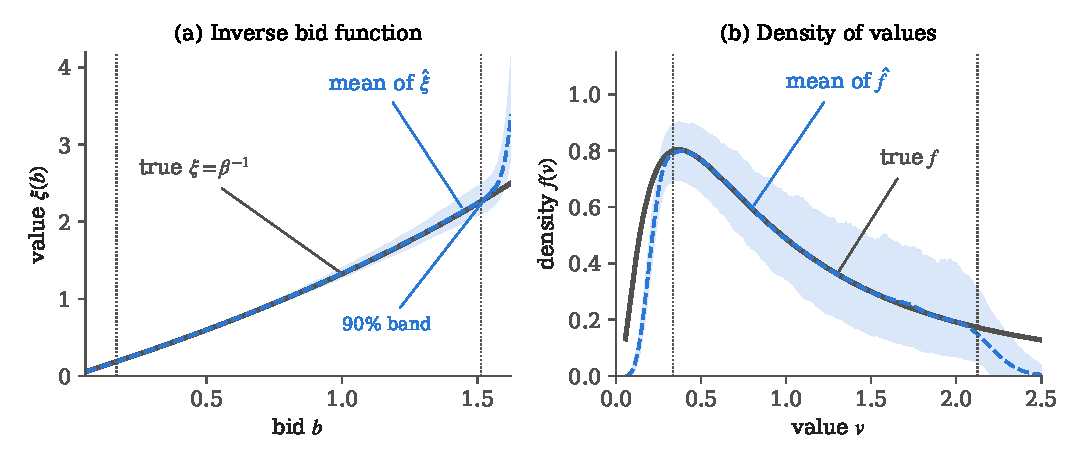
\includegraphics[width=\textwidth]{figures/ch15/gpv_mc.pdf}
\caption{Replication of the Monte Carlo design of \citet[Section 2.4]{GuerrePerrigneVuong2000}: $T=200$ auctions, $n=5$ bidders, values lognormal$(0,1)$ truncated to $[0.055,2.5]$, triweight kernels, $h_g=1.06\,\hat\sigma_b(nT)^{-\frac15}$, $h_f=1.06\,\hat\sigma_v(nT_T)^{-\frac15}$, 1,000 replications. Panel (a): true inverse bid function, mean of $\hat\xi(b)$ (dashed) and pointwise 90 percent band of the estimates. Panel (b): true value density, mean of $\hat f(v)$ and 90 percent band. Dotted lines mark the average trimming bounds. Our simulation (seed 15401), following the design of \citet[Section 2.4]{GuerrePerrigneVuong2000}.}\label{fig:15-gpv-mc}
\end{figure}

The replication reproduces GPV's qualitative findings. Inside the dotted lines the mean estimates are close to the truth, and the true curves lie inside the bands at every grid point. On the trimmed bid range, the mean of $\hat\xi$ is never more than 0.013 away from $\xi$. On the inner value region, the mean of $\hat f$ is never more than 0.022 away from $f$ (\cref{tab:15-gpv-mc}). The average trimming bounds on bids are 0.168 and 1.511, and the inner value region is $[0.334,2.125]$. Both are close to the lines drawn in GPV's figures. Outside these regions the estimates deteriorate as \cref{sec:15-gpv-estimator} predicts. Near the top of the bid support the mean of $\hat\xi$ bends sharply upward. Near both ends of the value support the mean of $\hat f$ falls below the truth.

\begin{figure}[htbp]
\centering
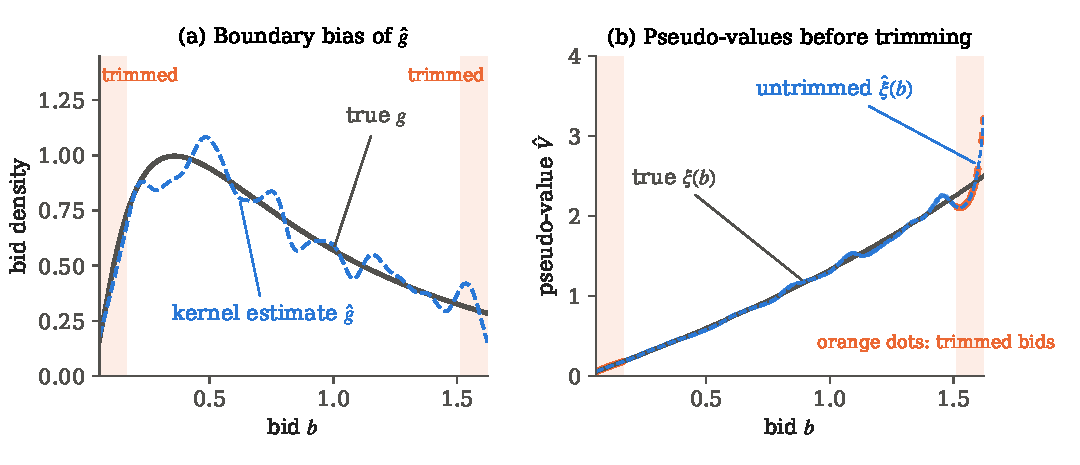
\includegraphics[width=\textwidth]{figures/ch15/gpv_trim.pdf}
\caption{Boundary effects in one simulated sample from the design of \cref{fig:15-gpv-mc} ($h_g=0.108$). Panel (a): true bid density and the triweight kernel estimate. Shaded areas lie within one bandwidth of the smallest and largest bids. At the largest bid the estimate equals 0.54 times the true density. Panel (b): pseudo-values $B_{it}+\frac{\hat G(B_{it})}{(n-1)\hat g(B_{it})}$ before trimming (dots), the estimated inverse bid function on a grid (dashed) and the true $\xi$ (solid). Near the top, the underestimated density inflates the markdown, and the estimated inverse bid function rises well above $\bar v=2.5$. Our simulation (seed 15403).}\label{fig:15-gpv-trim}
\end{figure}

\Cref{fig:15-gpv-trim} shows the mechanism in one sample. At the largest bid, $\hat g$ is 0.54 times the true density, close to the factor $\frac12$ derived in \cref{sec:15-gpv-estimator}. The untrimmed estimate $\hat\xi$ climbs to about 3.2 at the top of the bid support, against a true maximum value of 2.5. Trimming removes 43 of the 1,000 bids at the top. Among the bids that survive trimming, the mean absolute error of the pseudo-values is 0.016.

\begin{table}[htbp]
\centering
\caption{Monte Carlo results for the GPV estimator}\label{tab:15-gpv-mc}
\small
\begin{tabular}{lcc}
\toprule
\multicolumn{3}{l}{\textit{Panel A. GPV design, $T=200$, $n=5$, 1,000 replications}}\\
\midrule
Bandwidth constant & $1.06$ (GPV) & $2.978\times1.06$ \\
\midrule
Mean $h_g$ & 0.107 & 0.320\\
Mean $h_f$ & 0.147 & 0.334\\
Share of bids trimmed & 0.088 & 0.363\\
Mean trimming bounds on bids & $[0.168,\,1.511]$ & $[0.380,\,1.299]$\\
Inner value region & $[0.334,\,2.125]$ & $[0.781,\,1.508]$\\
Max.\ $|$mean of $\hat\xi-\xi|$ on trimmed bids & 0.013 & 0.003\\
Max.\ $|$mean of $\hat f-f|$ on inner values & 0.022 & 0.006\\
Mean sup-norm error of $\hat\xi$ on trimmed bids & 0.161 & 0.043\\
Mean sup-norm error of $\hat f$ on inner values & 0.238 & 0.055\\
Seconds per replication (Python) & 0.028 & 0.076\\
\bottomrule
\end{tabular}

\medskip
\begin{tabular}{rcccc}
\toprule
\multicolumn{5}{l}{\textit{Panel B. Mean sup-norm errors on fixed inner sets, GPV bandwidths, 200 replications}}\\
\midrule
$T$ & \makecell{$\hat\xi$, bids\\ in $[0.25,1.35]$} & \makecell{$\hat f$, values\\ in $[0.4,1.8]$} & \makecell{$\tilde f$\\ (true values)} & Ratio $\frac{\hat f}{\tilde f}$\\
\midrule
100 & 0.149 & 0.243 & 0.128 & 1.89\\
200 & 0.113 & 0.227 & 0.102 & 2.21\\
400 & 0.087 & 0.203 & 0.080 & 2.54\\
800 & 0.067 & 0.176 & 0.064 & 2.73\\
1,600 & 0.053 & 0.152 & 0.049 & 3.07\\
\midrule
Log-log slope in $T$ & $-0.37$ & $-0.17$ & $-0.34$ & \\
\bottomrule
\end{tabular}

\smallskip
\begin{minipage}{0.9\textwidth}
\footnotesize
\textit{Notes.} Our simulation, script \texttt{figures/ch15/src/gpv\_montecarlo.py}, seeds 15401 (panel A) and 15402 (panel B). Values lognormal$(0,1)$ truncated to $[0.055,2.5]$, $n=5$, triweight kernels. In panel A the two columns use the same draws. The inner value region is the average of $[\hat\xi(B_{\min}+h_g)+h_f,\ \hat\xi(B_{\max}-h_g)-h_f]$, so the error rows of the two columns refer to different regions. In panel B, $\tilde f$ is the infeasible kernel estimator computed from the true values with the same kernel and rule-of-thumb bandwidth. Slopes are least-squares fits of the log error on $\log T$. Timings are from one run on a laptop and vary across runs.
\end{minipage}
\end{table}

Panel A of \cref{tab:15-gpv-mc} compares GPV's bandwidths with the Gaussian-equivalent bandwidths. The wider bandwidths cut the sup-norm errors by a factor of about four. They do so at a price: 36 percent of the bids are trimmed, and the inner value region shrinks to $[0.781,1.508]$. The tails of $F$, which matter for reserve prices and for the top of the bid distribution, are then not estimated at all. The trade-off between precision in the middle and coverage of the support is a practical feature of every application of the method.

Panel B illustrates \cref{thm:15-gpv-rate}. On fixed inner sets, the error of $\hat f$ falls more slowly with $T$ than the error of the infeasible estimator that uses true values. The ratio of the two errors rises from 1.9 at $T=100$ to 3.1 at $T=1{,}600$. The fitted slope for $\hat f$ is $-0.17$, close to the exponent $-\frac15$ that the theorem gives for $R=1$ and $d=0$. The slope for $\tilde f$ is $-0.34$. The inverse bid function requires $g$ without its derivative, and its error falls at the faster slope of $-0.37$. The design has a very smooth density, so these slopes illustrate the theory. They are no test of it. The whole experiment takes a few minutes on a laptop, which makes the computational case for the indirect approach plain.

\subsection{Binding reserve prices and unknown numbers of potential bidders}\label{sec:15-gpv-reserve}

In practice sellers often announce a reserve price high enough to screen out some bidders. GPV, Section 4, extend their results to this case. A binding reserve price creates a new unknown. Let $N$ denote the number of \emph{potential bidders}, who draw values and decide whether to bid. Let $n^*$ denote the number of \emph{actual bidders}, who submit a bid of at least $r$. The econometrician observes $n^*$ but typically not $N$. Following GPV, bidders do not observe which rivals participate when they bid.

\casehead{The inverse bid function with a reserve} Fix one auction with reserve price $r\in(\underline v,\bar v)$. Bidders with values below $r$ do not bid, and bidders with values $v\ge r$ bid $\beta(v)$ from \eqref{eq:14-rs-bid}, with $\beta(r)=r$. Let $G^*$ denote the distribution of an actual bid, with density $g^*$ on $[r,\bar b]$. Then
\[
G^*(b)=\Pr\big(\beta(V)\le b\bigm| V\ge r\big)=\frac{F\big(\beta^{-1}(b)\big)-F(r)}{1-F(r)}.
\]
We derive the analog of \eqref{eq:15-gpv-xi} from the bidder's problem. A bid $b\ge r$ beats a given rival if that rival's value is below $r$, which has probability $F(r)$, or if the rival bids but bids less than $b$, which has probability $(1-F(r))G^*(b)$. Rivals are independent, so the win probability is
\[
H(b)=\Big[F(r)+\big(1-F(r)\big)G^*(b)\Big]^{N-1}.
\]
The bidder maximizes $(v-b)H(b)$. The first-order condition is
\[
(v-b)(N-1)\Big[F(r)+\big(1-F(r)\big)G^*(b)\Big]^{N-2}\big(1-F(r)\big)g^*(b)=\Big[F(r)+\big(1-F(r)\big)G^*(b)\Big]^{N-1}.
\]
Dividing by $(N-1)[F(r)+(1-F(r))G^*(b)]^{N-2}(1-F(r))g^*(b)$ and adding $b$ gives
\[
v=b+\frac{F(r)+\big(1-F(r)\big)G^*(b)}{(N-1)\big(1-F(r)\big)g^*(b)}.
\]
Splitting the fraction yields GPV's equation~(25):
\begin{equation}\label{eq:15-gpv-reserve}
v=\xi\big(b;G^*,N,F(r)\big)\equiv b+\frac{1}{N-1}\Big(\frac{G^*(b)}{g^*(b)}+\frac{F(r)}{1-F(r)}\,\frac{1}{g^*(b)}\Big).
\end{equation}
The second term in the parentheses reflects the potential bidders who do not bid. Ignoring it understates the markdown, especially near $r$, where $G^*$ is small. Unlike \eqref{eq:15-gpv-xi}, equation \eqref{eq:15-gpv-reserve} involves two unknowns, $N$ and $F(r)$.

\casehead{Why the bid density is unbounded at the reserve} By \eqref{eq:15-gpv-ode} with $N$ bidders, $\beta'(v)=(N-1)\frac{f(v)}{F(v)}\big(v-\beta(v)\big)$. At $v=r$ the markdown $v-\beta(v)$ vanishes while $F(r)>0$, so $\beta'(r)=0$. Let $\Delta(v)=v-\beta(v)$. Then $\Delta(r)=0$ and $\Delta'(r)=1-\beta'(r)=1$, so $\Delta(v)=(v-r)(1+o(1))$. Substituting,
\[
\beta'(v)=(N-1)\frac{f(r)}{F(r)}(v-r)\big(1+o(1)\big),\qquad\beta(v)-r=\frac{(N-1)f(r)}{2F(r)}(v-r)^2\big(1+o(1)\big).
\]
The bid function is flat and quadratic near the reserve. Many values just above $r$ map into a short interval of bids, and the density $g^*(b)=\frac{f(v)}{\beta'(v)(1-F(r))}$ behaves like $(b-r)^{-\frac12}$ as $b\downarrow r$ \citep[p.~549]{GuerrePerrigneVuong2000}.

\begin{theorem}[\citealp{GuerrePerrigneVuong2000}, Theorem 4]\label{thm:15-gpv-reserve}
Let $G^*\in\mathcal P$ have support $[r,\bar b]$, and let $\mathcal Q$ be a discrete distribution on $\{0,1,2,\dots\}$. Consider a first-price SIPV auction with reserve price $r\in(\underline v,\bar v)$. There exist $F\in\mathcal P$ and $N\ge2$ that generate $G^*$ as the distribution of actual bids and $\mathcal Q$ as the distribution of the number of actual bidders if and only if the following hold.
\begin{itemize}
\item[(C1)] $\mathcal Q$ is binomial with parameters $(N,1-F(r))$, where $0<F(r)<1$.
\item[(C2)] Conditional on $n^*$, actual bids are i.i.d.\ with distribution $G^*$, and $g^*(b)\to+\infty$ as $b\downarrow r$.
\item[(C3)] The function $\xi(\cdot;G^*,N,F(r))$ in \eqref{eq:15-gpv-reserve} is strictly increasing on $[r,\bar b]$, and its inverse is differentiable on $[r,\bar v]\equiv[\xi(r),\xi(\bar b)]$.
\end{itemize}
If (C1)--(C3) hold, $N$ and $F(r)$ are unique, and $F$ is unique on $[r,\bar v]$, with
\[
F(v)=F(r)+\big(1-F(r)\big)G^*\big(\xi^{-1}(v;G^*,N,F(r))\big).
\]
Moreover, $\xi(\cdot;G^*,N,F(r))$ is the inverse of the equilibrium strategy on $[r,\bar b]$.
\end{theorem}

\begin{proof}[Sketch of proof]
Necessity of (C1) holds because each potential bidder bids independently with probability $1-F(r)$. For (C2), consider $k$ actual bidders. Exchangeability and independence give
\[
\Pr\big(B^*_1\le b_1,\dots,B^*_k\le b_k\bigm| n^*=k\big)=\frac{\binom Nk F(r)^{N-k}\prod_{j=1}^k\Pr(r\le B_j\le b_j)}{\binom Nk F(r)^{N-k}\big(1-F(r)\big)^k}=\prod_{j=1}^k\frac{F\big(\beta^{-1}(b_j)\big)-F(r)}{1-F(r)}.
\]
The unbounded density follows from $\beta'(r)=0$, as shown above. Necessity of (C3) follows as in \cref{thm:15-gpv-ident}, because \eqref{eq:15-gpv-reserve} is the first-order condition. For sufficiency, (C1) identifies $N$ and $F(r)$, as in \cref{prop:15-reserve-ident}(iii): the mean and variance of $n^*$ are $N(1-F(r))$ and $NF(r)(1-F(r))$. The rest of the argument repeats the proof of \cref{thm:15-gpv-ident} with the truncated distributions $G^*$ and $\frac{F-F(r)}{1-F(r)}$. The condition $g^*\to\infty$ plays the role of \eqref{eq:15-gpv-A1}: it gives $\lim_{b\downarrow r}\xi(b)=r$, so that the candidate strategy satisfies $\beta(r)=r$. Below $r$, any absolutely continuous extension of $F$ rationalizes the data. GPV, Appendix A.1, give the details.
\end{proof}

The theorem parallels \cref{thm:15-gpv-ident}. The data identify the number of potential bidders and the probability of not bidding. The value distribution is identified only above the reserve price. Below $r$ the data contain no information about $F$ beyond the mass $F(r)$.

\casehead{Estimation} GPV, Section 4.2, assume that $N\ge2$ is constant across auctions. The reserve price is a smooth deterministic function $r(Z_t)$ of the characteristics, bounded away from both ends of the value support (their Assumption A5). Both $N$ and the function $r(\cdot)$ may be unknown to the analyst. The estimator has four parts.
\begin{itemize}
\item The number of potential bidders is estimated by $\hat N=\max_tn^*_t$. By (C1), $\hat N=N$ almost surely once $T$ is large.
\item Let $\Phi(z)=F(r(z)\mid z)$. Because $\E[n^*_t\mid Z_t]=N(1-\Phi(Z_t))$, a Nadaraya-Watson regression \citep{Nadaraya1964,Watson1964} gives
\[
\hat\Phi(z)=1-\frac{1}{\hat N}\,\frac{\sum_tn^*_t\,\mathcal K_Z\big(\frac{z-Z_t}{h_Z}\big)}{\sum_t\mathcal K_Z\big(\frac{z-Z_t}{h_Z}\big)},
\]
which always lies in $[0,1]$.
\item The unbounded density of bids at $r$ would slow down kernel estimation. GPV transform bids into $B^\dagger=(B^*-r)^{\frac12}$. The transformed bids have distribution $G^\dagger(b^\dagger)=G^*(r+(b^\dagger)^2)$ and bounded density $g^\dagger(b^\dagger)=2b^\dagger g^*(r+(b^\dagger)^2)$, which tends to a positive constant as $b^\dagger\downarrow0$. Since $\frac{G^*}{g^*}=\frac{2b^\dagger G^\dagger}{g^\dagger}$ and $\frac{1}{g^*}=\frac{2b^\dagger}{g^\dagger}$, equation \eqref{eq:15-gpv-reserve} becomes (GPV, eq.~(27), in conditional form)
\begin{equation}\label{eq:15-gpv-reserve-dagger}
V_{it}=r(Z_t)+(B^\dagger_{it})^2+\frac{2B^\dagger_{it}}{N-1}\Big(\frac{G^\dagger(B^\dagger_{it}\mid Z_t)}{g^\dagger(B^\dagger_{it}\mid Z_t)}+\frac{\Phi(Z_t)}{1-\Phi(Z_t)}\,\frac{1}{g^\dagger(B^\dagger_{it}\mid Z_t)}\Big).
\end{equation}
\item The transformed bids are independent of $n^*_t$ given $Z_t$ by (C2). Auctions with $n^*_t=0$ have positive probability and contain no bids, so the bid estimators use only the set $\mathcal T^+=\{t:n^*_t\ge1\}$. We estimate $G^\dagger(\cdot\mid z)$ and $g^\dagger(\cdot\mid z)$ by \eqref{eq:15-gpv-Ghat-z}--\eqref{eq:15-gpv-ghat-z} with $n^*_t$ in place of $n_t$, without the discrete argument, and with sums over $t\in\mathcal T^+$. Each is divided by the kernel estimate of the density of $Z_t$ computed from the same auctions, which yields estimates of the conditional distribution and density of a bid. Auctions without bids still enter $\hat\Phi$. The normalization matters. If the empty auctions contributed zero but the density of $Z_t$ were estimated from all $T$ auctions, both estimates would converge to their targets times $w(z)=\Pr(n^*_t\ge1\mid Z_t=z)$. The factor cancels from $\frac{G^\dagger}{g^\dagger}$, but it inflates the term in $\Phi$ in \eqref{eq:15-gpv-reserve-dagger} by $\frac{1}{w(z)}$. GPV, Section 4.2, leave this convention implicit. An alternative pools all actual bids, with weight one per bid and the kernel weights in $Z_t$ multiplied by $n^*_t$ in the denominator. Pseudo-values follow from \eqref{eq:15-gpv-reserve-dagger} with trimming. The truncated density $f^*(v\mid z)=\frac{f(v\mid z)}{1-\Phi(z)}$ is estimated as in \eqref{eq:15-gpv-fhat-z}, with the sums and the density of $Z_t$ both computed from the auctions in $\mathcal T^+$, and $\hat f(v\mid z)=(1-\hat\Phi(z))\hat f^*(v\mid z)$.
\end{itemize}
Under these assumptions, $\hat f(\cdot\mid\cdot)$ is uniformly consistent with the optimal rate $(\frac{T}{\log T})^{\frac{R}{2R+d+3}}$ on closed inner subsets of $\{(v,z):v\in[r(z),\bar v(z)]\}$ (GPV, Theorem 5). The transformation is what preserves the rate: the transformed density satisfies the smoothness properties of \cref{prop:15-gpv-smooth} (GPV, Proposition 4). If the reserve price varies randomly given $Z_t$, for example across sellers, the estimator remains consistent at the slower rate $(\frac{T}{\log T})^{\frac{R}{2R+d+4}}$ \citep[footnote 24]{GuerrePerrigneVuong2000}.

\begin{figure}[htbp]
\centering
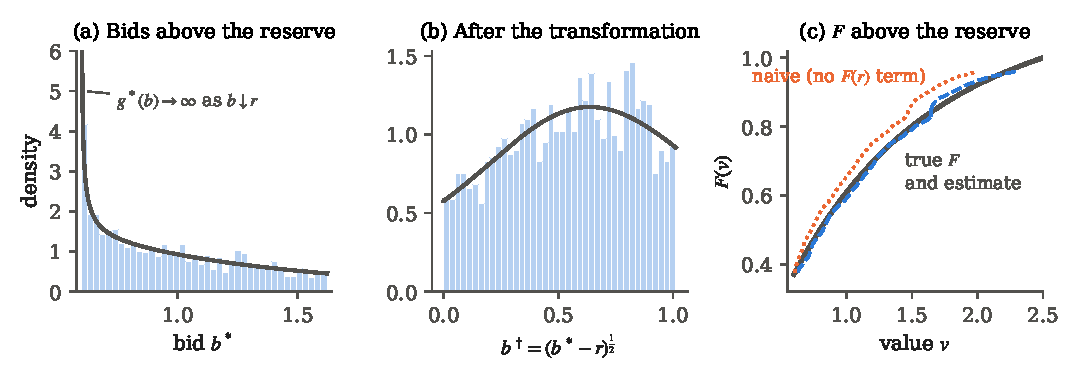
\includegraphics[width=\textwidth]{figures/ch15/gpv_reserve.pdf}
\caption{A binding reserve price. $T=500$ auctions with $N=5$ potential bidders, values lognormal$(0,1)$ truncated to $[0.055,2.5]$, reserve price $r=0.6$ with $F(r)=0.370$. Panel (a): histogram of the 1,627 actual bids and the true density $g^*$, which diverges at $r$. Panel (b): the transformed bids $(b^*-r)^{\frac12}$ have a bounded density. Panel (c): true $F$ above $r$ (solid), the estimate based on \eqref{eq:15-gpv-reserve-dagger} with $\hat N=5$ and $\hat F(r)=0.349$ (dashed), and a naive estimate that drops the term in $F(r)$ (dotted). Our simulation (seed 15404).}\label{fig:15-gpv-reserve}
\end{figure}

\Cref{fig:15-gpv-reserve} applies the procedure to simulated data. With $N=5$ and $r=0.6$, the expected number of actual bidders is $5(1-0.370)=3.15$. In the sample, $\hat N=5$ and $\hat F(r)=1-\frac{3.254}{5}=0.349$. The design has no covariates, and the estimates of $G^\dagger$ and $g^\dagger$ pool all 1,627 actual bids. The one auction of the 500 without a bid therefore enters only $\hat F(r)$. Among bids that survive trimming, the mean absolute error of the pseudo-values is 0.025 with the full formula and 0.151 for the naive formula without the term in $F(r)$. For values within 0.3 of the reserve, the naive pseudo-values are too low by 0.078 on average. The missing term is the markdown that comes from competing against potential bidders who stay out.

\casehead{Affiliated values and observed participation} \Citet[Section 6.3.1]{AtheyHaile2007} extend these results to affiliated private values when bidders do not know the set of actual bidders. With all bids, bidder identities and the reserve price, the joint distribution of the actual bidders' values above $r$ is identified (their Theorem 6.4). Each marginal $F_i$ is identified above $r$ when the set of potential bidders is observed (their Theorem 6.5). \Cref{sec:15-entry-reserve} states these results and the inversion behind them. Exogenous variation in reserve prices would trace out more of $F$, as GPV note. Estimators that combine auctions with different reserve prices to recover $F$ below the observed reserves had not been developed when Athey and Haile wrote their survey \citep[Section 6.3.1]{AtheyHaile2007}. \Cref{sec:15-uh} discusses the opposite case, in which the reserve price carries information about the object.

\subsection{Incomplete bid data and Dutch auctions}\label{sec:15-gpv-winbid}

Many data sets record only the winning bid. In a Dutch auction the clock stops at the first bid, so only the transaction price exists. The Dutch auction is strategically equivalent to the first-price auction (\cref{prop:14-dutch-fpa}). In other settings the auctioneer records only the winner. With independent private values, the winning bid suffices.

\begin{proposition}[\citealp{AtheyHaile2002}, Theorem 6(i), and \citealp{AtheyHaile2007}, Theorem 3.2 and Corollary 3.1]\label{prop:15-winbid}
In a first-price or Dutch auction with independent private values, suppose the transaction price and the number of bidders are observed. If bidders are asymmetric, suppose also that the set of bidders and the identity of the winner are observed. Then the value distribution of every bidder is identified.
\end{proposition}

\begin{proof}
\emph{Symmetric bidders.} Let $G_{(n:n)}$ denote the distribution of the winning bid $B^{(n:n)}$, with density $g_{(n:n)}$. Bids are i.i.d.\ with distribution $G$, so $G_{(n:n)}(b)=G(b)^n$ and
\begin{equation}\label{eq:15-winbid-G}
G(b)=G_{(n:n)}(b)^{\frac1n}.
\end{equation}
Hence the winning bid identifies the distribution of a single bid, and \cref{thm:15-gpv-ident} applies. To write the inverse bid function directly in terms of the winning bid, differentiate: $g_{(n:n)}(b)=nG(b)^{n-1}g(b)$. Then
\[
\frac{G_{(n:n)}(b)}{g_{(n:n)}(b)}=\frac{G(b)^n}{nG(b)^{n-1}g(b)}=\frac{G(b)}{ng(b)}=\frac{n-1}{n}\cdot\frac{G(b)}{(n-1)g(b)},
\]
which is equation (3.7) of \citet{AtheyHaile2007}. Substituting into \eqref{eq:15-gpv-xi},
\begin{equation}\label{eq:15-winbid-xi}
\xi(b)=b+\frac{n}{n-1}\,\frac{G_{(n:n)}(b)}{g_{(n:n)}(b)}.
\end{equation}
This observation is due to \citet{GuerrePerrigneVuong1995}.

\emph{Asymmetric bidders.} Let $G_i$ denote the distribution of bidder $i$'s bid, and let $G^w_i(b)=\Pr(B_i\le b,\ B_i\ge B_j\text{ for all }j)$ be the probability that $i$ wins with a bid of at most $b$. It is observable when the winner's identity is recorded. By independence,
\[
G^w_i(b)=\int_{\underline b}^b\prod_{j\neq i}G_j(s)\,dG_i(s).
\]
Summing over bidders, $\sum_jG^w_j(s)=\Pr(\max_jB_j\le s)=\prod_jG_j(s)$, the distribution of the winning bid. Therefore
\[
\frac{dG^w_i(s)}{\sum_jG^w_j(s)}=\frac{\prod_{j\neq i}G_j(s)\,dG_i(s)}{\prod_jG_j(s)}=\frac{dG_i(s)}{G_i(s)}=d\ln G_i(s).
\]
Integrating from $b$ to $\bar b$ and using $G_i(\bar b)=1$ gives
\begin{equation}\label{eq:15-berman}
G_i(b)=\exp\Big\{-\int_b^{\bar b}\Big(\sum_{j=1}^nG^w_j(s)\Big)^{-1}dG^w_i(s)\Big\}.
\end{equation}
This is the competing-risks formula of \citet{Berman1963}, adapted to auctions by \citet{AtheyHaile2002}. The right side is observable, so each $G_i$ is identified. The marginals $G_j$ determine the distribution of each bidder's highest rival bid, $G_{M_i}=\prod_{j\neq i}G_j$. The asymmetric first-order condition \eqref{eq:14-asym-foc}, rearranged as $v_i=b+\big[\sum_{j\neq i}\frac{g_j(b)}{G_j(b)}\big]^{-1}$, then gives each inverse bid function and each $F_i$.
\end{proof}

The formula in \citet[eq.~(3.8)]{AtheyHaile2007} is printed with the integral running from $-\infty$ to $b$ and without the minus sign. The derivation above gives the form \eqref{eq:15-berman}. \Citet{BrendstrupPaarsch2003} propose estimating \eqref{eq:15-berman} by replacing $G^w_i$ with its empirical counterpart and $dG^w_i$ with a kernel estimate \citep[Section 3.3.1]{AtheyHaile2007}. Athey and Haile add that survival-analysis estimators such as the Kaplan-Meier or Nelson-Aalen estimators could be adapted.

\casehead{Estimation with symmetric bidders} With $T$ winning bids $B^w_t$, one estimates $G_{(n:n)}$ by the empirical distribution and $g_{(n:n)}$ by a kernel estimator. Equation \eqref{eq:15-winbid-xi} then gives the estimated winner's value $\hat V^{(n:n)}_t=\hat\xi(B^w_t)$, after trimming as in \eqref{eq:15-gpv-trim}. The winners' values have distribution $F^n$, so $\hat F(v)=\big[\frac1T\sum_t\indic(\hat V^{(n:n)}_t\le v)\big]^{\frac1n}$.

\casehead{The cost of observing only the winner} The data contain one bid per auction instead of $n$, and the inversion through the $n$-th root loses precision in the lower tail. To see how much, ignore first-step error and suppose the winners' values were observed. Let $H=F^n$ and let $\hat H$ be the empirical distribution of the $T$ winners' values, with variance $\frac{H(1-H)}{T}$. Since $\frac{dF}{dH}=\frac1nH^{\frac1n-1}=\frac1nF^{1-n}$, the delta method gives
\[
\Var\big(\hat F(v)\big)\approx\frac{1}{n^2}F^{2-2n}\,\frac{F^n(1-F^n)}{T}=\frac{F^{2-n}(1-F^n)}{n^2T}.
\]
With all $nT$ values observed, the variance of the empirical distribution is $\frac{F(1-F)}{nT}$. The ratio of the two variances is
\[
\frac{F^{2-n}(1-F^n)}{n^2T}\cdot\frac{nT}{F(1-F)}=\frac{1-F^n}{nF^{n-1}(1-F)}=\frac{1+F+\dots+F^{n-1}}{nF^{n-1}}.
\]
It equals one at the top of the support and grows without bound as $F\to0$. With $n=5$ at the median of $F$, the ratio is $\frac{1.9375}{0.3125}=6.2$. This is our calculation. The winning bid identifies $F$, but low values are rarely revealed by winners, so the lower tail is estimated poorly.

\casehead{An unknown number of bidders} In some Dutch auctions only the transaction price is recorded, and the number of bidders is unknown. Then $F$ is not identified nonparametrically \citep[Section 3.3.1]{AtheyHaile2007}. For any candidate $n'$, the distribution $G_{(n:n)}^{\frac{1}{n'}}$ is a valid bid distribution, and $n'$ bidders bidding i.i.d.\ from it generate the same winning-bid distribution. Each $n'$ for which the implied inverse bid function is increasing yields a different $F$. \Citet{LaffontOssardVuong1995} instead estimate $n$ within a parametric model (\cref{sec:15-direct}).

\casehead{Covariates and testability} \Citet[Theorem 6]{AtheyHaile2002} extend the result in three directions. If $V_i=g_i(A_i,W_0)$ with $W_0$ observed by bidders and the econometrician and $A_1,\dots,A_n$ independent given $W_0$, then each $F_i(\cdot\mid w_0)$ is identified, because part (i) applies for each fixed $w_0$. If $V_i=g_0(W_0)+A_i$ with the $A_i$ mutually independent and independent of $W_0$, then each $F_{A_i}$ and $g_0$ are identified up to location. Finally, the models are testable. With symmetric bidders, observing more than one bid per auction, or exogenous variation in $n$, gives two estimates of $G$ from \eqref{eq:15-winbid-G} that must agree. With asymmetric bidders, observing the second-highest bid or exogenous variation in $n$ plays the same role \citep[Theorem 6(iv)--(v)]{AtheyHaile2002}.

\subsection{Specification testing in first-price auctions}\label{sec:15-gpv-tests}

\Cref{thm:15-gpv-ident} lists the restrictions that the SIPV model places on bids. \Citet[Section 5.1]{AtheyHaile2007} characterize the restrictions in the broader affiliated private values (APV) model of \cref{sec:15-apv}. Write $\xi_i(b;\mathcal N)=b+\frac{G_{M_i\mid B_i}(b\mid b;\mathcal N)}{g_{M_i\mid B_i}(b\mid b;\mathcal N)}$ for bidder $i$'s inverse bid function when the set of bidders is $\mathcal N$. Here $M_i$ is the highest rival bid and $G_{M_i\mid B_i}$ its distribution conditional on $i$'s bid, as in \eqref{eq:15-lpv-foc}. Let $[\underline b_i,\bar b_i]$ be the support of $B_i$.

\begin{theorem}[\citealp{AtheyHaile2007}, Theorem 5.2]\label{thm:15-ah-rational}
Consider the APV first-price auction with a fixed set of bidders $\mathcal N$. Assume the joint density of values is continuously differentiable, and that either (i) values are mutually independent or (ii) bidders are symmetric. A joint distribution of bids $\mathbf G$ is rationalized by equilibrium bidding if and only if:
\begin{itemize}
\item[(a)] The bids $(B_1,\dots,B_n)$ are affiliated. They are independent in case (i) and exchangeable in case (ii).
\item[(b)] Each $\xi_i(\cdot;\mathcal N)$ is differentiable and strictly increasing on the support of $B_i$.
\item[(c)] The distribution $\mathbf G\big(\xi_1^{-1}(u_1;\mathcal N),\dots,\xi_n^{-1}(u_n;\mathcal N)\big)$ is absolutely continuous in $\bm u$. Its density is positive and continuously differentiable on the product of the supports of $\xi_i(B_i;\mathcal N)$ and zero elsewhere.
\item[(d)] $\xi_i(\underline b;\mathcal N)=\underline b$ for all $i$.
\item[(e)] $\xi_i(\bar b_i;\mathcal N)=\xi_j(\bar b_j;\mathcal N)$ for all $i,j$.
\item[(f)] The support of $B_i$ is convex, compact, and the same for all $i$.
\end{itemize}
\end{theorem}

Without independence or symmetry, conditions of this type remain necessary but are not known to be sufficient. The equilibrium of the asymmetric APV model lacks a full characterization \citep[Theorem 5.1]{AtheyHaile2007}. Sufficiency in \cref{thm:15-ah-rational} uses the argument of Step 4 in the proof of \cref{thm:15-gpv-ident}. Under independence or symmetry, payoffs satisfy single crossing. Local optimality of each bid together with monotone strategies then implies global optimality. Athey and Haile stress why such a result matters. Without it, nothing guarantees that a bid $b$ is a best response for the value $\xi_i(b)$ that the first-order condition assigns to it. Verifying the conditions is the analog of verifying second-order conditions \citep[Section 5.1]{AtheyHaile2007}. For SIPV, the conditions reduce to (C1)--(C2) of \cref{thm:15-gpv-ident}.

Each condition suggests a test. We describe the main ones, following \citet[Sections 5.2--5.5]{AtheyHaile2007}.

\casehead{Monotonicity of the inverse bid function} Condition (C2), or (b), says that $\hat\xi$ should be increasing. GPV propose this as a test of equilibrium bidding and note that it requires estimating $\xi$ under a monotonicity constraint \citep[p.~552]{GuerrePerrigneVuong2000}. No formal test had been developed by the time of the Athey-Haile survey. Standard tests of monotone regression do not apply directly, because the realizations $\xi_i(B_i)$ are themselves estimates. Applications typically find few violations \citep{HendricksPinksePorter2003,HaileHongShum2003}. Two caveats apply. First, a rejection does not reveal which assumption failed: unobserved heterogeneity, risk aversion, or non-equilibrium play could each cause it. Second, no test of monotonicity is consistent against all violations of the model, since some misspecified models still produce an increasing $\xi$.

\casehead{The boundary condition} Condition (e) says that all bidders' inverse bid functions meet at the top of the bid support, since all bidders share the upper bound of values. In the asymmetric IPV model, $G_{M_i}(\bar b)=1$, so $\xi_i(\bar b)=\bar b+\frac{1}{g_{M_i}(\bar b)}$, and (e) becomes
\begin{equation}\label{eq:15-boundary-test}
g_{M_i}(\bar b)=g_{M_j}(\bar b)\qquad\text{for all }i,j,
\end{equation}
which is equation (5.1) of \citet{AtheyHaile2007}. The densities of the highest rival bid must agree at the top. \Cref{sec:15-apv-asym} works through an example of Athey and Haile in which the condition fails because the value supports of the two bidders have different upper bounds, which the maintained model excludes.

\casehead{Multi-sample tests with exogenous variation in $n$} If the number of bidders varies exogenously, the value distribution estimated from $n$-bidder auctions must equal the one estimated from $n'$-bidder auctions. Under IPV, the inverse bid functions $\xi(\cdot;G_n,n)$ differ across $n$, because bidding becomes more aggressive as $n$ rises (\cref{prop:14-fpa-n}). The implied value distributions must nevertheless coincide. Testing equality of distributions is standard when the data are observed. Here the values are estimated in a first nonparametric step, which complicates the asymptotic theory. \Citet{HaileHongShum2003} develop formal tests of this kind. They use them to test private against common values, which \cref{sec:15-cv} takes up.

\casehead{Multiple order statistics} In IPV models, any single order statistic of bids identifies $F$, together with $n$. When two order statistics are recorded, for example the two highest bids, the two implied estimates of $F$ must agree up to sampling error. This test needs no variation in $n$ \citep[Section 5.4]{AtheyHaile2007}.

\casehead{Direct tests of independence and exchangeability} Condition (C1) can be tested directly when all bids are observed. Exchangeability can be tested with the bootstrap distance tests of \citet{Romano1988,Romano1989}, which compare a multivariate distribution with its permutations. Equality of the marginal distributions of different bidders can be tested by Kolmogorov-Smirnov statistics. Independence can be tested by comparing the joint distribution of bids with the product of its marginals. GPV suggest the test of \citet{BlumKieferRosenblatt1961}, which \citet{CampoPerrigneVuong2003} later apply to offshore oil bids. With covariates, regression tests of conditional independence and exchangeability are natural. \Cref{sec:15-collusion} describes them in the form that \citet{BajariYe2003} use to look for collusion in highway procurement.

\citet[p.~2123]{AtheyHaile2002} add a warning. Monotonicity of $\xi$ holds under many natural alternatives to the IPV model, so the test most often used in early work has little power against affiliated or common values. The restrictions that come from comparing different order statistics or different numbers of bidders typically fail under those alternatives. They are the more informative tests.

\casehead{Assessment} GPV changed the econometrics of auctions. Before them, structural work required closed-form equilibria or simulation, and parametric assumptions carried an unclear part of the identification \citep[Section 3.1]{AtheyHaile2007}. After them, the first-order condition became a measurement device. The ingredients were a constructive identification result with sharp testable restrictions, an estimator that requires only kernel smoothing, and a proof that the estimator is rate-optimal. The same principle extends to affiliated values, asymmetric bidders, procurement with quality, binding reserve prices and dynamic bidding. It also inspired parametric two-step estimators that keep the inversion and add structure in one of the steps \citep[footnote 25]{GuerrePerrigneVuong2000}.

The approach has limits that later sections address. It maintains independent private values and risk neutrality, and it assumes that observed covariates capture all heterogeneity across auctions. Ignoring unobserved heterogeneity flattens the estimated inverse bid function and inflates estimated markups (\cref{sec:15-uh}). The second step pools across $n$ only if participation is exogenous given covariates (\cref{sec:15-entry}). Each additional continuous covariate slows convergence, and the boundary trimming discards the tails of $F$, which matter for reserve prices. No distribution theory for $\hat f$ was available. Bandwidth constants are set by rules of thumb, and data-driven choices had not been explored \citep[Section 3.2.1]{AtheyHaile2007}. Finally, the model needs all bids, or the winning bid with known $n$. When bidding takes place under richer information structures, bids reveal less, as \cref{sec:15-apv,sec:15-cv} show.

The rest of the chapter relaxes the maintained assumptions one at a time. \Cref{sec:15-apv} replaces independence with affiliation and symmetry with bidder classes, and the inversion runs through the distribution of the highest rival bid conditional on one's own bid. \Cref{sec:15-cv} asks what bids can reveal when values are common. \Cref{sec:15-uh} handles heterogeneity that bidders observe and the econometrician does not. \Cref{sec:15-entry} treats endogenous participation, dynamics and risk aversion. In each case the first step of the GPV estimator survives, and the work lies in finding the right conditioning set for the distribution of rival bids.

\section{Affiliated and Asymmetric Private Values}\label{sec:15-apv}

The inversion of \cref{sec:15-gpv} rests on two assumptions besides private values. Values are
independent across bidders, and bidders are symmetric. Both assumptions often fail. Bidders who appraise
the same tract of timber tend to have correlated values. They react to features of the tract that the
econometrician does not record. Bidders also differ in systematic ways. A sawmill differs from a logger,
a consortium from a single firm, and a contractor next to the site from one far away.

This section shows that the first-order condition can still be inverted when both assumptions fail. The
key observable becomes the joint distribution of a bidder's own bid and the highest rival bid. We first
treat symmetric affiliated private values \citep{LiPerrigneVuong2002}. We then ask what the two highest
bids alone reveal \citep{AtheyHaile2002}. Next we study asymmetric affiliated private values and joint
bidding for offshore oil leases \citep{CampoPerrigneVuong2003}. We close with asymmetric independent
private values.

\subsection{Symmetric affiliated private values: Li, Perrigne and Vuong (2002)}\label{sec:15-apv-lpv}

\casehead{Question} Before 2002, structural work on first-price auctions used either the independent
private value (IPV) model or the pure common value model. \citet{LiPerrigneVuong2002}, henceforth LPV, ask whether the
\emph{affiliated private value} (APV) model can be identified and estimated from bids alone, without a
parametric form for the dependence among values. The question matters because affiliation changes
equilibrium shading. An analyst who imposes independence on affiliated data misreads bids, and so
misreads values and rents.

\casehead{Model} A single object is sold by first-price sealed bid to $n\ge2$ risk-neutral bidders. In the
affiliated value model of \citet{MilgromWeber1982}, bidder $i$'s utility is $U(v_i,c)$, where $v_i$ is
her private signal and $c$ a common component. The APV model is the case $U(v,c)=v$. Values
$\bm V=(V_1,\dots,V_n)$ have a joint distribution $F$ with density $f$ on $[\underline v,\bar v]^n$. The
density is symmetric (exchangeable) and affiliated in the sense of \cref{def:14-affiliation}. The reserve
price does not bind. Let $Y_1=\max_{j\ne1}V_j$ be the highest rival value. Write $F_{Y_1\mid V_1}$ and
$f_{Y_1\mid V_1}$ for its conditional distribution and density given $V_1$. Affiliation leaves the form of
dependence unrestricted. A common component plus independent noise is one example among many.

The symmetric equilibrium in strictly increasing strategies $\beta$ is the special case of
\cref{prop:14-mw-fpa} with $v(\alpha,\alpha)=\alpha$. It solves the differential equation
\begin{equation}\label{eq:15-lpv-ode}
  \beta'(v)=\bigl(v-\beta(v)\bigr)\frac{f_{Y_1\mid V_1}(v\mid v)}{F_{Y_1\mid V_1}(v\mid v)},
  \qquad \beta(\underline v)=\underline v,
\end{equation}
which is equation (1) of \citet{LiPerrigneVuong2002}. Its solution is
\begin{equation}\label{eq:15-lpv-bid}
  \beta(v)=v-\int_{\underline v}^{v}L(\alpha\mid v)\,d\alpha,
  \qquad
  L(\alpha\mid v)=\exp\left(-\int_\alpha^v\frac{f_{Y_1\mid V_1}(u\mid u)}{F_{Y_1\mid V_1}(u\mid u)}\,du\right),
\end{equation}
their equation (2). The bid depends on $F$ through the whole conditional law of the highest rival value
along the diagonal. A parametric family for $F$, such as a multivariate lognormal, rarely yields a closed
form for $\beta$.

\casehead{From the differential equation to observables} Bids are random with joint distribution
$\bm G$, which the econometrician observes when all bids are recorded. Let $B_i$ be bidder $i$'s bid and
$M_i=\max_{j\ne i}B_j$ the highest rival bid. Let $G_{M\mid B}(m\mid b)=\Pr(M_i\le m\mid B_i=b)$, with
density $g_{M\mid B}(m\mid b)$ in $m$. Because $\beta$ is strictly increasing, $M_1=\beta(Y_1)$ and the
event $\{B_1=b\}$ equals $\{V_1=\beta^{-1}(b)\}$. Hence
\begin{align*}
  G_{M\mid B}(m\mid b)&=\Pr\bigl(\beta(Y_1)\le m\mid \beta(V_1)=b\bigr)
  =F_{Y_1\mid V_1}\bigl(\beta^{-1}(m)\mid\beta^{-1}(b)\bigr),\\
  g_{M\mid B}(m\mid b)&=\frac{f_{Y_1\mid V_1}\bigl(\beta^{-1}(m)\mid\beta^{-1}(b)\bigr)}{\beta'\bigl(\beta^{-1}(m)\bigr)}.
\end{align*}
Evaluate both at $m=b=\beta(v)$ and take the ratio:
\begin{equation*}
  \frac{G_{M\mid B}(b\mid b)}{g_{M\mid B}(b\mid b)}
  =\beta'(v)\,\frac{F_{Y_1\mid V_1}(v\mid v)}{f_{Y_1\mid V_1}(v\mid v)}
  =v-\beta(v),
\end{equation*}
where the second equality is \eqref{eq:15-lpv-ode}. Rearranging gives the inverse bid function
\begin{equation}\label{eq:15-lpv-foc}
  v=\xi(b;\bm G)\equiv b+\frac{G_{M\mid B}(b\mid b)}{g_{M\mid B}(b\mid b)},
\end{equation}
equation (4) of \citet{LiPerrigneVuong2002}. It is the first-order condition \eqref{eq:14-apv-foc}
written in observables. Conditioning on the value is the same as conditioning on the bid, because the
equilibrium is strictly monotone. With independent values $G_{M\mid B}(b\mid b)=G(b)^{n-1}$, and
\eqref{eq:15-lpv-foc} reduces to the inversion \eqref{eq:15-gpv-xi}.

\begin{definition}[Rationalization in the APV model]\label{def:15-lpv-rational}
A joint distribution $\bm G$ of bids is \emph{rationalized} by an APV structure $F$ if $\bm G$ is the
equilibrium bid distribution of the first-price auction with values drawn from $F$. The APV model is
identified if no two distinct structures $F\ne\tilde F$ lead to the same $\bm G$
\citep[Definition~1]{LiPerrigneVuong2002}.
\end{definition}

\begin{proposition}[{\citealp[Proposition~1]{LiPerrigneVuong2002}}]\label{prop:15-lpv}
The symmetric APV model is identified. Let $\bm G$ have support $[\underline b,\bar b]^n$. It can be
rationalized by a symmetric APV model if and only if two conditions hold.
\begin{enumerate}[label=(\roman*)]
  \item $\bm G$ is symmetric and affiliated.
  \item $\xi(\cdot;\bm G)$ in \eqref{eq:15-lpv-foc} is strictly increasing on $[\underline b,\bar b]$.
\end{enumerate}
The sufficiency direction also maintains the boundary condition
$\frac{G_{M\mid B}(b\mid b)}{g_{M\mid B}(b\mid b)}\to0$ as $b\downarrow\underline b$, which every rationalizable $\bm G$
satisfies. The rationalizing distribution is
\begin{equation}\label{eq:15-lpv-F}
  F(v_1,\dots,v_n)=\bm G\bigl(\xi^{-1}(v_1;\bm G),\dots,\xi^{-1}(v_n;\bm G)\bigr).
\end{equation}
\end{proposition}

\begin{proof}
\emph{Identification.} Let $F$ and $\tilde F$ both generate $\bm G$, with equilibrium strategies $\beta$ and
$\tilde\beta$. Both strategies satisfy \eqref{eq:15-lpv-ode}, which is equivalent to
\eqref{eq:15-lpv-foc}. So $\beta^{-1}=\tilde\beta^{-1}=\xi(\cdot;\bm G)$, and
$F(\bm v)=\Pr\bigl(\xi(B_i)\le v_i\ \forall i\bigr)=\tilde F(\bm v)$.

\emph{Necessity.} If $F$ rationalizes $\bm G$, then $\bm G(\bm b)=F\bigl(\beta^{-1}(b_1),\dots,\beta^{-1}(b_n)\bigr)$.
Strictly increasing transformations preserve symmetry and affiliation, which gives (i). Since
$\xi=\beta^{-1}$, (ii) holds. The ratio in the boundary condition equals $\xi(b)-b=\beta^{-1}(b)-b$, which tends to
zero as $b\downarrow\underline b$ because $\beta(\underline v)=\underline v$.

\emph{Sufficiency.} Let $\bm G$ satisfy (i) and (ii) and define $F$ by \eqref{eq:15-lpv-F}. Then $F$ is a
symmetric affiliated distribution on $[\underline v,\bar v]^n$ with
$\underline v=\xi(\underline b)$ and $\bar v=\xi(\bar b)$. Let bidders use $\beta=\xi^{-1}$. Then
$\bm G=F\circ\beta^{-1}$ by construction, and the steps above reverse to show that $\beta$ solves
\eqref{eq:15-lpv-ode}. For the boundary condition, LPV argue that $\ln G_{M\mid B}$ diverges at
$\underline b$. Divergence of the logarithm alone does not force the markdown
$\frac{G_{M\mid B}(b\mid b)}{g_{M\mid B}(b\mid b)}$ to vanish. This is why the proposition maintains
that this ratio tends to zero as $b\downarrow\underline b$. A bid density bounded away from zero at $\underline b$ is
sufficient but too strong. With i.i.d.\ uniform values and $n\ge3$ the density tends to zero, yet the ratio
equals $\frac{b}{n-1}$ and still vanishes. Under the maintained condition, $\xi(\underline b)=\underline b$, so
$\beta(\underline v)=\underline v$.
Second-order conditions are maintained throughout \citep[footnote~7]{LiPerrigneVuong2002}.
\end{proof}

Three remarks place the result. First, \citet{LaffontVuong1996} show that the general affiliated value
model is not identified from bids. Any affiliated value model with fixed $n$ is observationally equivalent
to some APV model. Restricting attention to APV therefore loses nothing in explaining bids. In this
sense the symmetric APV model is the most general model identified from bids alone
\citep[p.~175]{LiPerrigneVuong2002}. It does not exclude common values. It only cannot distinguish them
(\cref{sec:15-cv-limits}). Second, condition (ii) is a testable restriction of equilibrium play, as in
\cref{thm:15-gpv-ident}. Third, condition (i) implies that independence of values can be tested through
independence of bids within auctions, for example with the test of \citet{BlumKieferRosenblatt1961}.

\casehead{Estimator} The ratio in \eqref{eq:15-lpv-foc} can be written with joint objects that are easier to
estimate. Let $G_{M,B}(m,b)=G_{M\mid B}(m\mid b)\,g_B(b)$, which is $\frac{\partial}{\partial b}\Pr(M\le
m,\,B\le b)$, and let $g_{M,B}(m,b)=g_{M\mid B}(m\mid b)\,g_B(b)$ be the joint density of $(M,B)$. Then
\begin{equation*}
  \frac{G_{M\mid B}(b\mid b)}{g_{M\mid B}(b\mid b)}
  =\frac{G_{M\mid B}(b\mid b)\,g_B(b)}{g_{M\mid B}(b\mid b)\,g_B(b)}
  =\frac{G_{M,B}(b,b)}{g_{M,B}(b,b)},
\end{equation*}
because the marginal density $g_B$ cancels. Fix $n$ and let $T_n$ be the number of $n$-bidder auctions.
With a kernel $\mathcal K$ and bandwidths $h_G$ and $h_g$, the first step computes
\begin{align}
  \hat G_{M,B}(b,b)&=\frac{1}{nT_nh_G}\sum_{t=1}^{T_n}\sum_{i=1}^{n}\indic(M_{it}\le b)\,
  \mathcal K\left(\frac{b-B_{it}}{h_G}\right),\label{eq:15-lpv-Ghat}\\
  \hat g_{M,B}(b,b)&=\frac{1}{nT_nh_g^2}\sum_{t=1}^{T_n}\sum_{i=1}^{n}
  \mathcal K\left(\frac{b-M_{it}}{h_g}\right)\mathcal K\left(\frac{b-B_{it}}{h_g}\right),\label{eq:15-lpv-ghat}
\end{align}
equations (5)--(6) of \citet{LiPerrigneVuong2002} and (3.3)--(3.4) of \citet{AtheyHaile2007}. Averaging over
the $n$ bidders in each auction uses symmetry. The pseudo-values are
\begin{equation}\label{eq:15-lpv-pseudo}
  \hat V_{it}=B_{it}+\frac{\hat G_{M,B}(B_{it},B_{it})}{\hat g_{M,B}(B_{it},B_{it})}
  \quad\text{if } B_{\min}+h_g\le B_{it}\le B_{\max}-h_g,
\end{equation}
and $\hat V_{it}=+\infty$ otherwise. Trimming bids within one bandwidth of the boundaries removes the
pseudo-values that kernel boundary bias would distort \citep[p.~181]{LiPerrigneVuong2002}.

The second step estimates the $n$-variate density of values from the auctions that survive trimming,
\begin{equation}\label{eq:15-lpv-fhat}
  \hat f(v_1,\dots,v_n)=\frac{1}{T_nh_f^n}\sum_{t=1}^{T_n}
  \mathcal K_f\left(\frac{v_1-\hat V_{1t}}{h_f},\dots,\frac{v_n-\hat V_{nt}}{h_f}\right),
\end{equation}
with a product kernel $\mathcal K_f$. A kernel with compact support gives zero weight to any auction with
an infinite pseudo-value, so trimmed auctions drop out. Symmetry is imposed by averaging $\hat f$ over the
$n!$ permutations of its arguments. The marginal density of values uses all pseudo-values,
$\hat f_n(v)=\frac{1}{nT_nh_m}\sum_t\sum_i\mathcal K\bigl(\frac{v-\hat V_{it}}{h_m}\bigr)$. Comparing
$\hat f_n$ across $n$ checks whether the value distribution depends on the number of bidders. If it does
not, pseudo-values from different $n$ can be pooled.

\begin{remark}[Rates]\label{rem:15-lpv-rates}
Let $f$ have $R$ continuous bounded derivatives. With $h_G\propto(\frac{\log T_n}{T_n})^{\frac{1}{2R+2n-3}}$,
$h_g\propto(\frac{\log T_n}{T_n})^{\frac{1}{2R+2n-2}}$ and
$h_f\propto(\frac{\log T_n}{T_n})^{\frac{R+n-2}{(R+n+1)(2R+2n-2)}}$, and if $R>n-2$, $\hat f$ is uniformly
consistent on inner compact sets with rate $(\frac{T_n}{\log T_n})^{\frac{R(R+n-2)}{(R+n+1)(2R+2n-2)}}$
\citep[Proposition~2]{LiPerrigneVuong2002}. With observed values the optimal rate would be
$(\frac{T_n}{\log T_n})^{\frac{R}{2R+n}}$ \citep{Stone1982}. For $R=2$ and $n=2$ the exponents are
$\frac{2}{15}$ and $\frac{5}{15}$. The marginal density $\hat f_n$ converges faster, with exponent
$\frac{(R+n-1)(R+n-2)}{(R+n+1)(2R+2n-2)}$ \citep[Proposition~3]{LiPerrigneVuong2002}, which equals
$\frac15$ for $R=2$ and $n=2$. Optimality of these rates is not established, because the minimax argument of
\citet{GuerrePerrigneVuong2000} does not carry over. The exponents fall with $n$. This is the curse of
dimensionality.
\end{remark}

\casehead{Implementation} \citet[pp.~180--181]{LiPerrigneVuong2002} use the triweight kernel
$\mathcal K(u)=\frac{35}{32}(1-u^2)^3\indic(|u|\le1)$, a kernel of order two, and product kernels in several
dimensions. Kernels of order three would be required in theory for $n=3$. They would produce negative
density estimates and pseudo-values below bids, so order two is used throughout. Bandwidths follow the
rate in \cref{rem:15-lpv-rates} with $R=2$. For $n=2$ they set $h_G=c_G(nT)^{-\frac15}$ and
$h_g=c_g(nT)^{-\frac16}$. For $n=3$ the exponents are $-\frac17$ and $-\frac18$. The constants follow
Silverman's rule of thumb, $c=2.978\times1.06\,\hat\sigma_b$, where $\hat\sigma_b$ is the standard
deviation of bids. The factor $2.978$ converts the rule from a Gaussian to a triweight kernel. In the second
step $h_f=c_f(2!\,T^\ast)^{-\frac{1}{15}}$ for $n=2$ and $c_f(3!\,T^\ast)^{-\frac{1}{16}}$ for $n=3$, with
$T^\ast$ the number of auctions left after trimming. When bids are skewed, the authors suggest working with
$\ln(1+b)$ and transforming back \citep[footnote~13]{LiPerrigneVuong2002}.

\casehead{Monte Carlo design} The design follows the laboratory experiments of
\citet{KagelHarstadLevin1987}. Each value is a common draw plus noise, $V_i=Q+E_i$, with $Q$ uniform on
$[\frac14,\frac34]$ and $E_i$ independent and uniform on $[-\frac14,\frac14]$. Values lie in $[0,1]$. Since
$\Var(Q)=\Var(E_i)=\frac{1}{48}$, the correlation between two values is
\begin{equation*}
  \Corr(V_i,V_j)=\frac{\Var(Q)}{\Var(Q)+\Var(E_i)}=\frac12 .
\end{equation*}
The sum of two independent uniforms of width $\frac12$ has the triangular marginal density
$f(v)=4v$ on $[0,\frac12]$ and $f(v)=4-4v$ on $[\frac12,1]$. Its kink at $\frac12$ makes it
nondifferentiable there.

We can derive the equilibrium for $v\le\frac12$ by hand. Given $V_1=v\le\frac12$, Bayes' rule makes $Q$
uniform on $[\frac14,v+\frac14]$. Given $Q=q$, each rival value is below $x$ with probability
$2(x-q)+\frac12$, clipped to $[0,1]$. For $x\le v$ the substitution $u=2(x-q)+\frac12$ gives
\begin{equation*}
  F_{Y_1\mid V_1}(x\mid v)=\frac1v\int_{\frac14}^{x+\frac14}\Bigl(2(x-q)+\frac12\Bigr)^{n-1}dq
  =\frac{1}{2v}\int_0^{2x}u^{n-1}\,du=\frac{(2x)^n}{2nv}.
\end{equation*}
For $x$ slightly above $v$ the upper limit of $q$ is $v+\frac14$, so
$F_{Y_1\mid V_1}(x\mid v)=\frac{(2x)^n-(2x-2v)^n}{2nv}$. Both pieces have derivative $2^{n-1}v^{n-2}$ at
$x=v$, and $F_{Y_1\mid V_1}(v\mid v)=\frac{2^{n-1}v^{n-1}}{n}$. Therefore
\begin{equation*}
  \frac{f_{Y_1\mid V_1}(v\mid v)}{F_{Y_1\mid V_1}(v\mid v)}=\frac nv,
  \qquad
  \beta'(v)=\bigl(v-\beta(v)\bigr)\frac nv .
\end{equation*}
The linear function $\beta(v)=\frac{n}{n+1}v$ satisfies this equation and $\beta(0)=0$. This is equation (10)
of \citet{LiPerrigneVuong2002}. For $n=2$ the same line $\beta(v)=\frac23v$ holds on all of $[0,1]$
(their equation (11)). For $n=3$ the bid is nonlinear above $\frac12$ (their equation (12)). A simple
design thus produces a complicated equilibrium.

Compare the IPV benchmark with the same triangular marginal. On $[0,\frac12]$, $F(v)=2v^2$, and the
bid of \eqref{eq:14-rs-bid} is
\begin{equation*}
  \beta^{IPV}(v)=v-\frac{\int_0^v(2x^2)^{n-1}dx}{(2v^2)^{n-1}}=v-\frac{v}{2n-1}=\frac{2n-2}{2n-1}\,v .
\end{equation*}
For $n=2$ this equals the APV bid $\frac23v$. For $n=3$ it is $\frac45v$, above the APV bid $\frac34v$
\citep[footnote~17]{LiPerrigneVuong2002}. \Cref{fig:15-lpv-design} shows both strategies on the whole
support. Affiliation makes low types bid less aggressively and high types more aggressively. A bidder with a
low value expects rivals with low values, so she faces weak competition. A bidder with a high value expects
strong competition and shades less.

\begin{figure}[htbp]
  \centering
  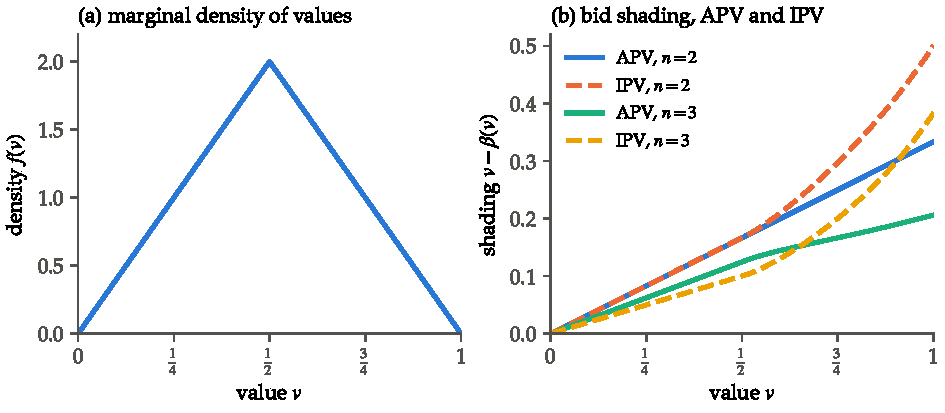
\includegraphics[width=\textwidth]{figures/ch15/lpv_design.pdf}
  \caption{The Monte Carlo design of \citet{LiPerrigneVuong2002}. Panel (a): the triangular marginal density
  of values when $V_i=Q+E_i$ with $Q\sim U[\frac14,\frac34]$ and $E_i\sim U[-\frac14,\frac14]$. Panel (b):
  bid shading $v-\beta(v)$ in the APV equilibrium (solid) and in the IPV equilibrium with the same marginal
  density (dashed), for $n=2$ and $n=3$. The APV bids use equations (10)--(12) of
  \citet{LiPerrigneVuong2002}, which we checked against a numerical solution of \eqref{eq:15-lpv-ode}.
  Our computation, with no random numbers (script \texttt{lpv\_design.py}).}\label{fig:15-lpv-design}
\end{figure}

Each replication draws 100 auctions with two bidders and 100 auctions with three bidders, which gives 500
bids. The experiment is replicated 1,000 times \citep[p.~179]{LiPerrigneVuong2002}. Each replication takes
less than three seconds \citep[p.~182]{LiPerrigneVuong2002}. The average first-step bandwidths $(h_G,h_g)$
are $(0.148,0.177)$ for $n=2$ and $(0.076,0.122)$ for $n=3$.

\casehead{Results} The median estimate of the inverse bid function tracks the truth closely and lies
slightly above it. The pointwise 90 percent band contains the true function except near the boundaries
(their Figures 1--2). The estimated marginal density follows the triangle except near the kink, where
kernel smoothing rounds the peak (their Figures 3--5). The winner's \emph{informational rent} in auction
$t$ is
\begin{equation}\label{eq:15-ir}
  \mathrm{IR}_t=\frac{v_{wt}-b_{wt}}{v_{wt}},
\end{equation}
with $v_{wt}$ and $b_{wt}$ the winner's value and bid \citep[eq.~(16)]{LiPerrigneVuong2002}. For $n=2$
the APV bid is $\frac23v$ on the whole support, so the true rent is exactly one third.
\Cref{tab:15-lpv-rents} reports the true mean rent and the distribution across replications of the
estimated average rent. The APV estimator slightly overstates the rent, consistent with the slight upward
bias in $\hat\xi$. Rents fall from $n=2$ to $n=3$, a competition effect.

\begin{table}[htbp]
\centering
\caption{Winners' informational rents in the Monte Carlo of \citet{LiPerrigneVuong2002}}\label{tab:15-lpv-rents}
\begin{tabular}{@{}lcccc@{}}
\toprule
 & \multicolumn{2}{c}{APV estimator (Table 1)} & \multicolumn{2}{c}{IPV estimator (Table 2)} \\
\cmidrule(lr){2-3}\cmidrule(lr){4-5}
 & $n=2$ & $n=3$ & $n=2$ & $n=3$ \\
\midrule
True mean IR & 33.33 & 23.47 & 33.33 & 23.47 \\
Estimated average IR & 36.76 & 26.96 & 38.65 & 29.11 \\
Empirical 5th percentile & 32.44 & 19.32 & 31.53 & 19.05 \\
Empirical 95th percentile & 41.18 & 34.69 & 49.33 & 44.97 \\
\bottomrule
\end{tabular}

\smallskip
\begin{minipage}{0.86\textwidth}
\footnotesize \textit{Notes.} Percent. The informational rent is \eqref{eq:15-ir}. Each column summarizes 1,000
replications, each with 100 two-bidder and 100 three-bidder auctions. The APV columns use the estimator
\eqref{eq:15-lpv-Ghat}--\eqref{eq:15-lpv-pseudo}. The IPV columns apply the estimator of
\citet{GuerrePerrigneVuong2000} to the same affiliated bids. Source: \citet[Tables~1 and~2]{LiPerrigneVuong2002}.
\end{minipage}
\end{table}

\casehead{Imposing independence on affiliated data} The authors then apply the IPV estimator of
\citet{GuerrePerrigneVuong2000} to the same simulated bids. The estimated inverse bid function matches the
truth for low bids but lies well above it for high bids (their Figures 6--7). The implied value density is
too dispersed (their Figures 8--9), and rents are overstated (\cref{tab:15-lpv-rents}). The authors report
overstatements of 17 and 24 percent for $n=2$ and $n=3$ \citep[p.~186]{LiPerrigneVuong2002}. Relative to
the true means in the table, the overstatements are 16 and 24 percent (our calculation).

A short calculation shows why. With $n=2$ the bid is $\frac23v$, so the marginal bid distribution is
$G(b)=F(\frac32b)$ with density $g(b)=\frac32f(\frac32b)$. The IPV inversion returns
\begin{equation*}
  \xi^{IPV}(b)=b+\frac{G(b)}{g(b)}=\frac23v+\frac23\,\frac{F(v)}{f(v)},\qquad v=\tfrac32b .
\end{equation*}
For $v\le\frac12$, $\frac{F(v)}{f(v)}=\frac{2v^2}{4v}=\frac v2$, so $\xi^{IPV}=v$ and low values are
recovered exactly. For $v>\frac12$, $\frac{F(v)}{f(v)}=\frac{1-2(1-v)^2}{4(1-v)}$. At $v=\frac34$ this is
$\frac78$, so $\xi^{IPV}=\frac12+\frac{7}{12}=\frac{13}{12}$ against a true value of $\frac34$. The
inversion explodes near the top because the marginal density vanishes there. The IPV model reads the
aggressive bidding of high types under affiliation as evidence of high values.

\casehead{Assessment} The paper extends the indirect approach to dependent values and supplies a usable
guide. Its limits are statistical and economic. The density of values is $n$-variate, so data demands grow
quickly with $n$, and estimation proceeds separately for each $n$. The estimator conditions on the number of
bidders, so it cannot by itself say how affiliation interacts with entry. Under APV, bids can fall as $n$
rises \citep{PinkseTan2005}. Regressions of bids on $n$ therefore cannot separate private from common values
(\cref{sec:15-cv-tests}). Finally, correlation in values may come from auction features that bidders observe
and the econometrician does not. That alternative is observationally equivalent to affiliation with a fixed
$n$, and \cref{sec:15-uh} treats it.

\subsection{What the two highest bids reveal}\label{sec:15-apv-top2}

Many first-price data sets record only the winning bid, or the two highest bids. Procurement agencies keep
the second-lowest bid in case the winner defaults. Participants also track the gap between the top two
bids, which they call ``money left on the table'' \citep[p.~2123]{AtheyHaile2002}. Two bids suffice for
part of the identification problem. \Cref{eq:15-lpv-foc} involves only the distribution of the
highest rival bid given one's own bid. In equilibrium the top two bids come from the bidders with the top
two values. Let $I^{(n:n)}$ denote the identity of the winner.

\begin{proposition}[{\citealp[Lemma~1, Theorem~7 and Corollary~1]{AtheyHaile2002}}]\label{prop:15-top2}
Consider the APV model of the first-price auction, and suppose the two highest bids are observed. If
bidders are asymmetric, suppose the identity of the winner is also observed.
\begin{enumerate}[label=(\roman*)]
  \item The equilibrium bid functions $\beta_i$, $i=1,\dots,n$, are identified.
  \item With symmetric bidders, the joint distribution of $(V^{(n:n)},V^{(n-1:n)})$ is identified.
  \item With symmetric bidders, the joint distribution $F$ of values is not identified if any lower bid is
  unobserved.
\end{enumerate}
\end{proposition}

\begin{proof}
(i) Take bidder 1 and a bid $b$ in the support of $B_1$. Multiply the numerator and denominator of the
markdown by the density of $B_1$ at $b$. Then translate each event into events about the top two bids:
\begin{align*}
  \frac{G_{M_1\mid B_1}(b\mid b)}{g_{M_1\mid B_1}(b\mid b)}
  &=\frac{\frac{\partial}{\partial y}\Pr\left(M_1\le b,\ B_1\le y\right)\big|_{y=b}}
  {\frac{\partial^2}{\partial x\,\partial y}\Pr\left(M_1\le x,\ B_1\le y\right)\big|_{x=y=b}}\\[2pt]
  &=\frac{\frac{\partial}{\partial x}\Pr\left(B^{(n:n)}\le x,\ I^{(n:n)}=1\right)\big|_{x=b}}
  {\frac{\partial^2}{\partial x\,\partial y}\Pr\left(B^{(n-1:n)}\le x,\ B^{(n:n)}\le y,\ I^{(n:n)}=1\right)\big|_{x=y=b}}.
\end{align*}
For the numerator, $\Pr(B^{(n:n)}\le x,\,I^{(n:n)}=1)=\Pr(B_1\le x,\,M_1<B_1)$, whose derivative at $x=b$
is $\Pr(M_1<b\mid B_1=b)\,g_{B_1}(b)$. For the denominator, take $x<y$. The event
$\{B^{(n-1:n)}\le x,\,B^{(n:n)}\le y,\,I^{(n:n)}=1\}$ equals $\{M_1\le x,\,B_1\le y\}$ minus
$\{M_1\le x,\,B_1\le M_1\}$. The probability of the second set does not depend on $y$. So the cross
partial equals the joint density of $(M_1,B_1)$ at $(x,y)$, and we let $x\uparrow y=b$. Both final
expressions involve only the top two bids and the winner's identity. The markdown is therefore identified,
and with it $\beta_1^{-1}(b)=b+\frac{G_{M_1\mid B_1}(b\mid b)}{g_{M_1\mid B_1}(b\mid b)}$ for almost every $b$.

(ii) With symmetric bidders the top two bids are $\beta(V^{(n:n)})$ and $\beta(V^{(n-1:n)})$. Apply the
identified $\beta^{-1}$ to both.

(iii) The construction of \cref{thm:15-ah4} applies. Shift probability mass between small neighborhoods of
two value vectors that differ only in the $j$-th order statistic, for some $j<n-1$, and symmetrize over
permutations. The new distribution is exchangeable. The distribution of the highest rival value, and hence
every bidder's best response, is unchanged. Only the unobserved order statistic $V^{(j:n)}$ changes its
distribution, so observables are unchanged \citep[proof of Theorem~3.4]{AtheyHaile2007}.
\end{proof}

Part (ii) is more useful than it looks. The joint law of the top two values determines the revenue from a
second-price or ascending auction and the effect of a reserve price. It also determines the outcome under
many other selling mechanisms \citep[p.~2124]{AtheyHaile2002}. Part (i) delivers the bid functions, which measure the wedge
between bids and values. Part (iii) is a limit. Bid functions depend only on the distribution of the
highest rival bid, so they carry no information about the distribution of lower bids. The design of an
optimal auction needs the full $F$ and therefore all bids. The two highest bids also suffice for a test of
private against common values, which \cref{thm:15-ah11} develops. \citet[Section~3.3.2]{AtheyHaile2007} note
that estimators built on part (i) had not yet been explored.

\subsection{Asymmetric affiliated private values: Campo, Perrigne and Vuong (2003)}\label{sec:15-apv-cpv}

\casehead{Question} Federal auctions of offshore oil leases allowed firms to bid jointly as consortia.
Joint bidding may pool capital and information, and it may create ex ante asymmetry among bidders.
\citet{CampoPerrigneVuong2003} ask whether an asymmetric APV model can be identified and estimated without
solving its equilibrium. They then use joint and solo bids to measure asymmetry, affiliation, unobserved
tract heterogeneity and informational rents. They also confront the pure common value model that dominated
earlier work on these auctions.

\casehead{Model} There are two types. Type 1 (strong, here joint bidders) has $n_1$ bidders and type 0
(weak, here solo bidders) has $n_0$ bidders, with $n_1+n_0=n\ge2$. Values
$(v_{11},\dots,v_{1n_1},v_{01},\dots,v_{0n_0})$ are drawn from an absolutely continuous distribution $F$ on
$[\underline v,\bar v]^n$. The distribution is affiliated and exchangeable within each type
\citep[Section~2.1]{CampoPerrigneVuong2003}. Let $\mathcal P$ denote this set of distributions. Within a
type, bidders use the same strictly increasing strategy, $s_1$ or $s_0$. Let $y_1^\ast$ be the highest value
among the other type-1 bidders and $y_0$ the highest type-0 value. A type-1 bidder with value $v_1$ solves
\begin{equation*}
  \max_b\ (v_1-b)\,\Pr\bigl(y_1^\ast\le s_1^{-1}(b),\ y_0\le s_0^{-1}(b)\mid v_1\bigr).
\end{equation*}
The first-order conditions form a system of two differential equations with boundary conditions
$s_1(\underline v)=s_0(\underline v)=\underline v$ and $s_1(\bar v)=s_0(\bar v)$, their equations (1)--(2).
The system is intractable in general. Under conditions that cover this model, an equilibrium in monotone pure
strategies nevertheless exists \citep{RenyZamir2004}. The inversion below assumes that bidders play such an
equilibrium and that each bid distribution is continuous and strictly increasing. Conditioning on a bidder's bid is
then the same as conditioning on her value. With independent values it reduces to the asymmetric IPV system of
\cref{prop:14-maskin-riley}, studied by \citet{MaskinRiley2000}, and with one type it reduces to
\eqref{eq:15-lpv-ode}.

\casehead{Inversion} Let $B_1^\ast$ be the highest bid among the other type-1 bidders and $B_0$ the highest
type-0 bid. Define $G_{B_1^\ast,B_0\mid b_1}(X,Y\mid x)=\Pr(B_1^\ast\le X,\,B_0\le Y\mid b_1=x)$. Since bids
are strictly increasing in values,
\begin{equation*}
  G_{B_1^\ast,B_0\mid b_1}(X,X\mid x)=F_{y_1^\ast,y_0\mid v_1}\bigl(s_1^{-1}(X),\,s_0^{-1}(X)\mid s_1^{-1}(x)\bigr).
\end{equation*}
The total derivative in the common threshold $X$ is
\begin{equation*}
  \frac{d}{dX}G_{B_1^\ast,B_0\mid b_1}(X,X\mid x)
  =\frac{\partial F_{y_1^\ast,y_0\mid v_1}}{\partial y_1^\ast}\frac{1}{s_1'\bigl(s_1^{-1}(X)\bigr)}
  +\frac{\partial F_{y_1^\ast,y_0\mid v_1}}{\partial y_0}\frac{1}{s_0'\bigl(s_0^{-1}(X)\bigr)}.
\end{equation*}
This is exactly the bracket in the type-1 first-order condition. Substituting gives
\begin{equation}\label{eq:15-cpv-foc}
  v_1=\xi_1(b_1;\bm G)\equiv b_1+\frac{G_{B_1^\ast,B_0\mid b_1}(b_1,b_1\mid b_1)}
  {\frac{d}{dX}G_{B_1^\ast,B_0\mid b_1}(X,X\mid b_1)\big|_{X=b_1}},
\end{equation}
their equation (4). The weak type's inverse $\xi_0(b_0;\bm G)$ is the same expression with
$(B_1,B_0^\ast)$ in place of $(B_1^\ast,B_0)$, their equation (5). Two features distinguish
\eqref{eq:15-cpv-foc} from \eqref{eq:15-lpv-foc}. The conditioning distribution is trivariate, since it
involves the bidder's own bid and the highest bid of each type. The denominator is a total derivative and not
a density.

\begin{proposition}[{\citealp[Proposition~1]{CampoPerrigneVuong2003}}]\label{prop:15-cpv}
The asymmetric APV model is identified. Let $\bm G$ have support $[\underline b,\bar b]^n$. It can be
rationalized by an asymmetric APV model with $F\in\mathcal P$ if and only if two conditions hold.
\begin{enumerate}[label=(\roman*)]
  \item $\bm G\in\mathcal P$.
  \item $\xi_1(\cdot;\bm G)$ and $\xi_0(\cdot;\bm G)$ are strictly increasing on $[\underline b,\bar b]$, with
  $\xi_1(\bar b;\bm G)=\xi_0(\bar b;\bm G)$.
\end{enumerate}
The rationalizing distribution is
$F(\bm v_1,\bm v_0)=\bm G\bigl(\xi_1^{-1}(\bm v_1;\bm G),\xi_0^{-1}(\bm v_0;\bm G)\bigr)$.
\end{proposition}

The proof follows that of \cref{prop:15-lpv}. The common upper endpoint in (ii) reflects the boundary
condition $s_1(\bar v)=s_0(\bar v)$. Identification is nonparametric and requires neither solving nor
approximating the equilibrium. Because $\mathcal P$ contains the distributions that are exchangeable across all
$n$ bidders, the symmetric model is nested and can be tested against the asymmetric one.

\casehead{Estimator} The conditioning on $b_1$ drops out of the ratio in \eqref{eq:15-cpv-foc}, which equals
\begin{equation}\label{eq:15-cpv-ratio}
  \frac{\Pr(B_1^\ast\le b_1,\ B_0\le b_1,\ b_1=b_1)}
  {\Pr(B_1^\ast=b_1,\ B_0\le b_1,\ b_1=b_1)+\Pr(B_1^\ast\le b_1,\ B_0=b_1,\ b_1=b_1)},
\end{equation}
where each ``$=$'' denotes a density \citep[eq.~(6)]{CampoPerrigneVuong2003}. With $T$ auctions of a given
configuration $(n_1,n_0)$, the numerator is estimated by
\begin{equation*}
  \hat G_1(x,y,z)=\frac{1}{h_{G1}T}\sum_{t=1}^{T}\frac{1}{n_1}\sum_{i=1}^{n_1}
  \indic(B_{1it}^\ast\le x)\,\indic(B_{0t}\le y)\,\mathcal K\left(\frac{z-B_{1it}}{h_{G1}}\right).
\end{equation*}
The two terms of the denominator replace one indicator at a time by a kernel:
\begin{align*}
  \hat D_{11}(x,y,z)&=\frac{1}{h_{g1}^2T}\sum_{t=1}^{T}\frac{1}{n_1}\sum_{i=1}^{n_1}
  \mathcal K\left(\frac{x-B_{1it}^\ast}{h_{g1}}\right)\indic(B_{0t}\le y)\,\mathcal K\left(\frac{z-B_{1it}}{h_{g1}}\right),\\
  \hat D_{12}(x,y,z)&=\frac{1}{h_{g1}^2T}\sum_{t=1}^{T}\frac{1}{n_1}\sum_{i=1}^{n_1}
  \indic(B_{1it}^\ast\le x)\,\mathcal K\left(\frac{y-B_{0t}}{h_{g1}}\right)\mathcal K\left(\frac{z-B_{1it}}{h_{g1}}\right).
\end{align*}
The pseudo-value of a type-1 bid is
$\hat V_{1it}=B_{1it}+\frac{\hat G_1(B_{1it},B_{1it},B_{1it})}{\hat D_{11}(B_{1it},B_{1it},B_{1it})+\hat
D_{12}(B_{1it},B_{1it},B_{1it})}$, their equation (7), and type 0 is symmetric. The second step estimates
bivariate densities of pairs of values within and across types \citep[eqs.~(9)--(11)]{CampoPerrigneVuong2003}.
Because bid data are skewed, the authors work with $d=\ln(1+b)$. If $D=\ln(1+B)$, densities in $b$ equal
densities in $d$ divided by $1+b$. Then the markdown in $b$ is $(1+b)$ times the markdown in $d$, and
\begin{equation*}
  v=b+(1+b)\frac{G_D}{g_D}=e^{d}\left(1+\frac{G_D}{g_D}\right)-1,
\end{equation*}
which is their equation (12). They use triweight kernels, rule-of-thumb bandwidths of the form
$c\,(n_1T)^{-\frac15}$ and $c\,(n_1T)^{-\frac16}$ with $c=2.978\times1.06\,\hat\sigma$, and trimming within one
bandwidth of the boundaries \citep[pp.~188--189]{CampoPerrigneVuong2003}.

\casehead{Unobserved tract heterogeneity} Tracts differ in observed characteristics $Z$ and unobserved
characteristics $W$. Without restrictions, variation in $W$ cannot be separated from variation in private
values. \citet[Section~3.2]{CampoPerrigneVuong2003} impose the following.

\begin{assumption}[{\citealp[Section~3.2]{CampoPerrigneVuong2003}}]\label{ass:15-cpv-uh}
(i) The numbers of bidders of each type are deterministic functions of tract characteristics,
$n_1=n_1(Z,W)$ and $n_0=n_0(Z,W)$. (ii) Conditional on $(Z,n_1,n_0)$, values do not depend on $W$:
$F(\cdot\mid Z,W)=F(\cdot\mid Z,n_1,n_0)$.
\end{assumption}

Part (i) holds in entry models in which firms decide to participate before learning their values. Part (ii)
says that the bidder configuration is a sufficient statistic for the unobserved tract characteristics.
Estimation conditional on $(n_1,n_0)$ is then valid. The same idea, using an endogenous count as a control
for unobservables, underlies the instrumental approach of \citet{HaileHongShum2003} in
\cref{sec:15-cv-tests}. It also has a cost. Under \cref{ass:15-cpv-uh} the value distribution of joint bidders
may differ between $(2,0)$ and $(1,1)$ auctions because the tracts differ. A comparison of the marginal
densities of a type across configurations therefore tests for unobserved heterogeneity. A comparison of joint
and solo densities within the $(1,1)$ configuration tests for asymmetry.

\casehead{The asymmetric pure common value model} Pure common values had been the standard model for
offshore leases. \citet{CampoPerrigneVuong2003} derive a sharp restriction for two bidders. The tract has
common value $V$. Bidder $i\in\{0,1\}$ receives a signal $\sigma_i$, and the signals are independent given
$V$ but not identically distributed. Let $V(\sigma_1,\sigma_0)=\E[V\mid\sigma_1,\sigma_0]$. Bidder 1 wins
when $\sigma_0\le s_0^{-1}(b_1)$, so her first-order condition is
\begin{equation*}
  -F_{\sigma_0\mid\sigma_1}\bigl(s_0^{-1}(b_1)\mid\sigma_1\bigr)
  +\bigl[V\bigl(\sigma_1,s_0^{-1}(b_1)\bigr)-b_1\bigr]
  \frac{f_{\sigma_0\mid\sigma_1}\bigl(s_0^{-1}(b_1)\mid\sigma_1\bigr)}{s_0'\bigl(s_0^{-1}(b_1)\bigr)}=0,
\end{equation*}
their equation (14). The argument leading to \eqref{eq:15-lpv-foc} turns it into
\begin{equation}\label{eq:15-cpv-cv}
  V\bigl(\sigma_1,s_0^{-1}(b_1)\bigr)=b_1+\frac{G_{b_0\mid b_1}(b_1\mid b_1)}{g_{b_0\mid b_1}(b_1\mid b_1)}=\xi_1(b_1;\bm G),
  \qquad
  V\bigl(s_1^{-1}(b_0),\sigma_0\bigr)=\xi_0(b_0;\bm G),
\end{equation}
their equations (16)--(17). The right sides are the same as in the APV model with two bidders. Only the
interpretation of the left sides changes. A bivariate distribution of $(b_1,b_0)$ is
\emph{quasi-symmetric} if $\Pr(b_1\le b_0\mid b_1\le b,\,b_0\le b)=\Pr(b_1\ge b_0\mid b_1\le b,\,b_0\le
b)$ for every $b$. Exchangeable distributions are quasi-symmetric, but not conversely.

\begin{proposition}[{\citealp[Proposition~2]{CampoPerrigneVuong2003}}]\label{prop:15-cpv-quasisym}
If observed bids are equilibrium bids of an asymmetric pure common value model with two bidders, their joint
distribution is quasi-symmetric. Quasi-symmetry is equivalent to $\xi_1(b;\bm G)=\xi_0(b;\bm G)$ for every
$b$. The asymmetric pure common value model is observationally equivalent to an asymmetric APV model with a
quasi-symmetric value distribution and identical equilibrium strategies.
\end{proposition}

\begin{proof}
At a common bid $b$, bidder 1's signal is $s_1^{-1}(b)$ and bidder 0's is $s_0^{-1}(b)$. Both left sides of
\eqref{eq:15-cpv-cv} then equal $V\bigl(s_1^{-1}(b),s_0^{-1}(b)\bigr)$, so $\xi_1(b)=\xi_0(b)$. To link this to
quasi-symmetry, let $G(x,y)=\Pr(b_1\le x,\,b_0\le y)$ with density $g$, and let $\partial_1G$ and $\partial_2G$
be its partial derivatives. Then
$G_{b_0\mid b_1}(y\mid x)=\frac{\partial_1G(x,y)}{g_{b_1}(x)}$ and $g_{b_0\mid b_1}(y\mid x)=\frac{g(x,y)}{g_{b_1}(x)}$,
so
\begin{equation*}
  \xi_1(b)-b=\frac{\partial_1G(b,b)}{g(b,b)},\qquad \xi_0(b)-b=\frac{\partial_2G(b,b)}{g(b,b)} .
\end{equation*}
Hence $\xi_1=\xi_0$ if and only if $\partial_1G(b,b)=\partial_2G(b,b)$ for all $b$. Next,
\begin{align*}
  \Pr(b_1\le b_0\le b)&=\int^{b}\!\!\int^{y}g(x,y)\,dx\,dy=\int^{b}\partial_2G(y,y)\,dy,\\
  \Pr(b_0\le b_1\le b)&=\int^{b}\partial_1G(x,x)\,dx .
\end{align*}
These two probabilities are equal for every $b$ if and only if $\partial_1G(b,b)=\partial_2G(b,b)$ for every
$b$. Ties have probability zero, so equal probabilities mean each is half of $G(b,b)$, which is
quasi-symmetry. For the last claim, define private values $\tilde v_i=\xi_i(b_i)$. They form a
quasi-symmetric distribution, and the common strategy $\xi^{-1}$ satisfies both APV first-order conditions.
\end{proof}

Setting $b=\bar b$ gives $\Pr(b_1\le b_0)=\frac12$. Each bidder wins half of the time, however different
their information. The same property holds in the extreme case with one perfectly informed bidder, where the
uninformed bidder's mixed strategy replicates the informed bid distribution (\cref{prop:14-emw}). The
proposition yields a simple test of the pure common value model with two bidders, whatever the asymmetry.

\casehead{Setting and data} The federal government has auctioned oil and gas rights on the Outer Continental
Shelf (OCS) since 1954. \citet{CampoPerrigneVuong2003} study wildcat sales in the Gulf of Mexico off Louisiana. Areas
are divided into tracts, usually of 5,000 or 5,760 acres, sold simultaneously by first-price sealed bid. The
reserve price of \$15 per acre is not regarded as screening participation (their footnote 10). Joint bidding
affected fewer than 20 percent of auctions before 1970 and more than 80 percent after. A typical joint bid
involves two or three firms. From December 1975, the eight largest firms were barred from bidding jointly
with each other (their footnote 11). The sample covers auctions from December 1972 to 1979. It excludes later
years because the rules changed, and two early sales with unusual water depth (their footnote 12). The
authors keep auctions with exactly two bidders. This gives 227 auctions: 60 with two joint bids, 55 with two
solo bids and 112 with one of each. Bids are in 1972 dollars per acre. \Cref{tab:15-cpv-stats} reproduces
their Table I.

\begin{table}[htbp]
\centering
\caption{Bids in two-bidder OCS wildcat auctions, 1972--1979 (dollars per acre)}\label{tab:15-cpv-stats}
\begin{tabular}{@{}lrrrrrr@{}}
\toprule
 & Obs. & Mean & Std.\ dev. & Minimum & Maximum & Within s.d. \\
\midrule
All bids & 454 & 687.30 & 1,431.31 & 19.51 & 20,751.32 & 1,258.91 \\
Joint bids & 232 & 837.32 & 1,717.54 & 21.46 & 20,751.32 & \\
Solo bids & 222 & 532.53 & 1,033.20 & 19.51 & 11,019.08 & \\
Joint vs.\ joint & 120 & 875.13 & 2,056.12 & 33.94 & 20,751.32 & 2,011.99 \\
Joint vs.\ solo & 112 & 796.83 & 1,266.32 & 21.46 & 6,377.94 & \\
Solo vs.\ joint & 112 & 603.28 & 1,226.61 & 19.51 & 11,019.08 & \\
Solo vs.\ solo & 110 & 456.45 & 788.19 & 20.80 & 7,009.10 & 747.43 \\
\bottomrule
\end{tabular}

\smallskip
\begin{minipage}{0.92\textwidth}
\footnotesize \textit{Notes.} Bids in 1972 dollars per acre. ``Joint vs.\ solo'' means joint bids in auctions whose
other bidder is solo. The within standard deviation is computed within auctions. Source:
\citet[Table~I]{CampoPerrigneVuong2003}.
\end{minipage}
\end{table}

Joint bids are higher on average than solo bids. Each type bids more when facing a joint bidder. A test of
equal means of joint and solo bids in the 112 mixed auctions gives $t=1.66$, a weak rejection at the 10
percent level \citep[p.~190]{CampoPerrigneVuong2003}. Joint bidders won 63 of the 112 mixed auctions. This
share exceeds one half at the 10 percent level in a one-sided test. The within-auction standard deviation is
70 to 98 percent of the total, and 98 percent in auctions with two joint bidders. So much of the variation
across tracts is explained by the bidder configuration. In log-bid regressions, the three bidding-structure
dummies are jointly significant. Equality of the 16 sale dummies is nearly accepted, and neither the 1973
oil shock nor the 1975 ban has a significant effect \citep[p.~191]{CampoPerrigneVuong2003}.

\casehead{Testing pure common values} By \cref{prop:15-cpv-quasisym}, the joint bidder should win half of
the mixed auctions. The authors split the 112 mixed auctions in half. In the 56 auctions with both bids below
\$460 per acre, the joint bidder wins 28 times. In the 56 auctions with at least one bid above \$460, it wins
35 times. Quasi-symmetry requires a winning probability of one half in each subset. In the second subset,
$t=1.87$ rejects \citep[p.~195]{CampoPerrigneVuong2003}. As a check, the share $\frac{35}{56}=0.625$ has
standard error $\sqrt{\frac{0.25}{56}}=0.067$ under the null, which reproduces $t=1.87$. The pure common
value model is rejected for these auctions. A general model with values $U(\sigma_i,V)$ is not rejected, since
it is not identified \citep{LaffontVuong1996}.

\casehead{Results with one type} The $(2,0)$ and $(0,2)$ configurations are symmetric APV models, estimated as
in \cref{sec:15-apv-lpv}. Three and six auctions are trimmed. Both estimated inverse bid functions are
increasing, so the APV model is not rejected. The function for joint bidders facing joint bidders lies to the
right of that for solo bidders facing solo bidders. For the same value, a joint bidder facing a joint bidder
bids more. The value distribution of joint bidders first-order stochastically dominates that of solo bidders
in a one-sided Kolmogorov-Smirnov test. The trimmed pseudo-values have mean \$2,195.14 for joint bidders and
\$1,027.90 for solo bidders (their footnote 19). The test of \citet{BlumKieferRosenblatt1961} rejects
independence of the two values in every case. The statistic is 6.57 on bids and 4.69 on trimmed pseudo-values
for joint pairs. For solo pairs it is 9.52 and 6.92 \citep[p.~197]{CampoPerrigneVuong2003}.

\casehead{Results with both types} In the $(1,1)$ case the starred maxima are void, and the inversions reduce
to $\xi_{10}(b_1)=b_1+\frac{G_{b_0\mid b_1}(b_1\mid b_1)}{g_{b_0\mid b_1}(b_1\mid b_1)}$ and its mirror image
\citep[eqs.~(18)--(19)]{CampoPerrigneVuong2003}. After trimming 21 auctions, 91 remain. Both estimated
inverse functions increase. The solo bidder's function lies to the right of the joint bidder's, especially
above \$500 per acre. For the same value, a solo bidder bids more aggressively. This again contradicts
quasi-symmetry. The value densities of the two types are close (\cref{fig:15-cpv-xi}, panel b). Trimmed
pseudo-values average \$1,208.73 for joint and \$1,161.62 for solo bidders (their footnote 21). A
Kolmogorov-Smirnov test does not reject equal distributions (their footnote 22). Asymmetry in values is weak.
The weak bidder's lighter shading, that is, its more aggressive bidding, is the response that
\cref{prop:14-maskin-riley} predicts \citep[p.~199]{CampoPerrigneVuong2003}. It does
not produce inefficient allocations in the sample. Each type also adapts to its rival. A joint bidder bids
more aggressively against a joint bidder, and a solo bidder bids slightly more aggressively against a joint
bidder.

\begin{figure}[htbp]
  \centering
  \begin{subfigure}[b]{0.48\textwidth}
    \centering
    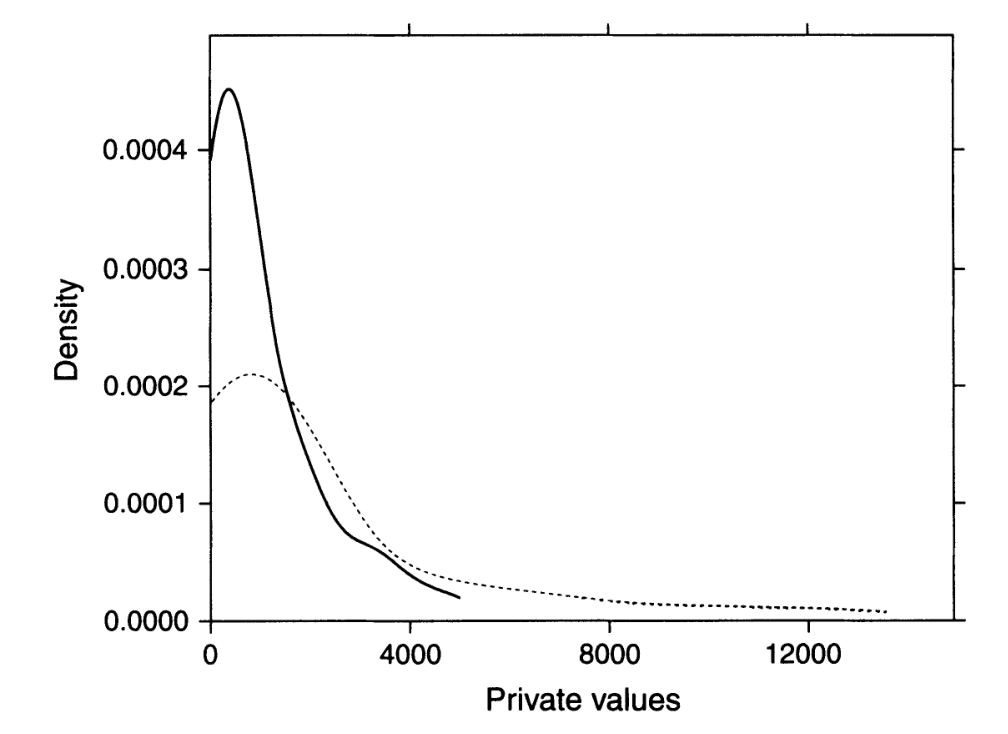
\includegraphics[width=\textwidth]{figures/ch15/cpv_fig2.png}
    \caption{Symmetric configurations: joint vs.\ joint (dashed), solo vs.\ solo (solid)}
  \end{subfigure}\hfill
  \begin{subfigure}[b]{0.48\textwidth}
    \centering
    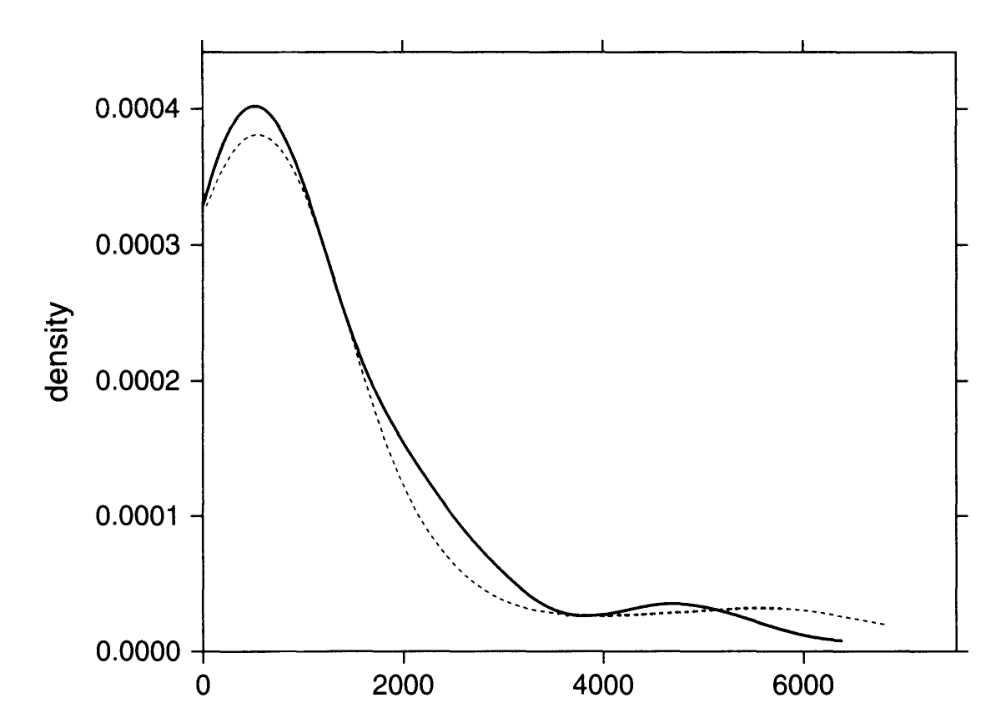
\includegraphics[width=\textwidth]{figures/ch15/cpv_fig4.png}
    \caption{Mixed configuration: joint (dashed), solo (solid)}
  \end{subfigure}
  \caption{Estimated marginal densities of private values in OCS wildcat auctions, dollars per acre. The
  horizontal axes differ across panels. In symmetric auctions the joint bidders' values are far more dispersed
  than the solo bidders'. In mixed auctions the two densities are close. The contrast between panels points to
  unobserved tract heterogeneity across configurations. Source: \citet{CampoPerrigneVuong2003}, Figures 2
  and 4.}\label{fig:15-cpv-xi}
\end{figure}

\casehead{Unobserved heterogeneity and rents} Under \cref{ass:15-cpv-uh}, comparing a type's value density
across configurations detects unobserved tract heterogeneity. Kolmogorov-Smirnov statistics are 0.1917 for
joint bidders in $(2,0)$ against $(1,1)$ auctions and 0.0965 for solo bidders in $(0,2)$ against $(1,1)$
auctions \citep[p.~200]{CampoPerrigneVuong2003}. The authors read the first as a clear rejection. Tracts
that attract two joint bidders are more valuable than tracts that attract one bidder of each type. The
differences in \cref{tab:15-cpv-stats} thus reflect both asymmetry and tract heterogeneity, with
heterogeneity the larger force. Winners' informational rents \eqref{eq:15-ir} average 65.07 percent across 197
winners (their Table II). They are 65.50 percent for joint and 64.59 percent for solo winners. So the
government captures about 35 percent of the winner's willingness to pay. In dollars, joint winners earn
\$1,954.42 per acre and solo winners \$1,151.40, because joint winners have higher values
\citep[p.~201]{CampoPerrigneVuong2003}.

\casehead{Interpretation and critiques} Asymmetry between joint and solo bidders is weak. A ban on joint bidding
would therefore change little if participation stayed the same. The authors argue that joint bidding raised
revenue by increasing participation. The paper's contribution is methodological. It shows that the indirect
approach handles asymmetric bidders whose equilibrium cannot be computed, and it gives a usable test of pure
common values. The limits are severe in practice. The trivariate objects in \eqref{eq:15-cpv-foc} force the
analysis to two-bidder auctions. With three bidders only 18 to 60 auctions would be available per
configuration (their footnote 16). Types are binary and the configuration is taken as exogenous to values
given the tract. The private value assumption for oil leases is contested. \citet{HendricksPinksePorter2003}
find bidding on earlier OCS auctions more consistent with common values (\cref{sec:15-cv-hp}).

\subsection{Asymmetric independent private values with all bids}\label{sec:15-apv-asym}

Independence simplifies the inversion and lowers data requirements. Let bidder $j$'s bid have distribution
$G_j$ and density $g_j$. With independent values, bids are independent, so
$G_{M_i\mid B_i}(m\mid b)=\prod_{j\ne i}G_j(m)$. Differentiating the product,
\begin{align*}
  g_{M_i\mid B_i}(m\mid b)&=\sum_{k\ne i}g_k(m)\prod_{j\ne i,k}G_j(m),\\
  \frac{G_{M_i\mid B_i}(b\mid b)}{g_{M_i\mid B_i}(b\mid b)}
  &=\frac{\prod_{j\ne i}G_j(b)}{\sum_{k\ne i}g_k(b)\prod_{j\ne i,k}G_j(b)}
  =\left[\sum_{j\ne i}\frac{g_j(b)}{G_j(b)}\right]^{-1}.
\end{align*}
The inverse bid function is therefore
\begin{equation}\label{eq:15-asym-xi}
  v_i=\xi_i(b_i)=b_i+\left[\sum_{j\ne i}\frac{g_j(b_i)}{G_j(b_i)}\right]^{-1},
\end{equation}
the inverse form of \eqref{eq:14-asym-foc}. Each value depends on its own bid and on the univariate
distributions of rivals' bids. When all bids and bidder identities are observed, each $F_i$ is identified
by $F_i(v)=G_i(\xi_i^{-1}(v))$ \citep[Theorem~3.1(ii)]{AtheyHaile2007}.

Estimation must condition on the set of opponents, because a change in their identities changes the
strategy being inverted. With fully bidder-specific distributions, each set of bidders is treated separately.
This requires many auctions with the same bidder set. A practical compromise groups bidders into a few
types, with exchangeability within a type, as with joint and solo bidders or loggers and mills
\citep[Section~3.2.2]{AtheyHaile2007}. All auctions with the same number of bidders of each type can then be
pooled. Asymmetry can also come from bidder covariates, such as the distance from a contractor's plant to the
project. With discrete covariates this is the approach by types again. With continuous covariates the bid
distributions are estimated conditional on them by kernel or sieve methods. The timber study of
\cref{sec:15-als} applies \eqref{eq:15-asym-xi} with parametric bid distributions.

\citet{FlambardPerrigne2006} apply the procurement version nonparametrically to snow removal contracts in
Montreal \citep[p.~102]{HortacsuPerrigne2021}. In a low-bid auction bidder $i$ wins when every rival bids
more, and the same steps give
\begin{equation*}
  c_i=b_i-\left[\sum_{j\ne i}\frac{g_j(b_i)}{1-G_j(b_i)}\right]^{-1}.
\end{equation*}
Firms are classified by their location relative to the job, and participation, winning probabilities and bid
distributions differ across the classes. The estimated cost difference between the classes is about 6.5
percent. It leads to an inefficient allocation in 24 percent of the auctions. A subsidy to the weak,
high-cost firms that restores symmetry would raise the share of contracts they win by 61 percent. With a cost
of public funds taken into account, the overall procurement cost would fall by 1.34 percent under exogenous
participation.

Equilibrium imposes testable restrictions. With independence and a common support of values,
\cref{thm:15-ah-rational} requires bids to be independent, each $\xi_i$ to be increasing, and all $\xi_i$ to
share the same upper endpoint. The last restriction comes from the common support. It can fail in a valid
equilibrium if supports differ. \citet[Section~5.1]{AtheyHaile2007} give an example, which we verify. Let
$n=2$ with bid distributions $G_1(b)=b$ and $G_2(b)=b^2$ on $[0,1]$. Then \eqref{eq:15-asym-xi} gives
\begin{equation*}
  \xi_1(b)=b+\frac{G_2(b)}{g_2(b)}=b+\frac b2=\frac32b,
  \qquad
  \xi_2(b)=b+\frac{G_1(b)}{g_1(b)}=2b .
\end{equation*}
The implied value distributions are $F_1(v)=G_1(\frac23v)=\frac23v$ on $[0,\frac32]$ and
$F_2(v)=G_2(\frac v2)=\frac{v^2}{4}$ on $[0,2]$. Each strategy is a best response. Bidder 1 maximizes
$(v-b)b^2$, so $v=\frac32b$, and bidder 2 maximizes $(v-b)b$, so $v=2b$. Yet $\xi_1(1)=\frac32\ne2=\xi_2(1)$.
Equivalently, the densities of the highest rival bid differ at the top, $g_{M_1}(1)=g_2(1)=2$ and
$g_{M_2}(1)=g_1(1)=1$, so the boundary condition \eqref{eq:15-boundary-test} fails.
Allowing supports to differ across bidders restores identification in such cases. If the lower ends of the
supports also differ, some bidders may never win, and little can be learned about them
\citep[Section~5.1]{AtheyHaile2007}.

\section{Common Values: Limits of Identification and Tests}\label{sec:15-cv}

With common values, information about each bidder's value is dispersed among the bidders. Learning a
rival's signal would change a bidder's estimate of her own value (\cref{def:14-private-values}). Winning then
carries bad news, the winner's curse of \cref{sec:14-winners-curse}. Many policy questions turn on the joint
distribution of signals and values. Examples are the optimal reserve price, the revenue ranking of formats,
and whether restricting entry raises revenue. This section first shows how little bids reveal about that
distribution. It then shows that exogenous variation in competition still allows private values to be tested
against common values. Next it presents a positive identification result for procurement with interdependent
costs \citep{Somaini2020}. It ends with the evidence of \citet{HendricksPorter1988} on an auction with an
informed bidder.

\subsection{What bids can and cannot reveal}\label{sec:15-cv-limits}

Let bidder $i$ observe a signal $S_i$ about her value $V_i$. The primitive is the joint distribution
$F_{\bm S,\bm V}$ of signals and values. In the pure common value model $V_i=V_0$ for all $i$. We focus on
symmetric models. Let $Y_i=\max_{j\ne i}S_j$ and define the \emph{pivotal expected value}
\begin{equation*}
  v(s,y;n)=\E\left[V_i\mid S_i=s,\ Y_i=y;\ n\right],
\end{equation*}
the expected value of a bidder whose signal is $s$ and whose strongest rival has signal $y$. The dimension
count is discouraging. The primitive governs $2n$ random variables, or $n+1$ with pure common values, yet an
auction reveals at most $n$ bids \citep[Section~7.1]{AtheyHaile2007}.

Signals have only ordinal meaning. Any strictly increasing relabeling of a signal leaves behavior unchanged.
\citet[eq.~(8)]{AtheyHaile2002} use this freedom to impose the normalization
\begin{equation}\label{eq:15-cv-norm}
  v(s,s;n)=\E\left[V_i\mid S_i=\max_{j\ne i}S_j=s;\ n\right]=s .
\end{equation}
In the second-price auction the equilibrium bid is $v(s,s;n)$ (\cref{prop:14-mw-spa}). Under
\eqref{eq:15-cv-norm} it becomes $b(s)=s$, so bids reveal signals. In the first-price auction, the
first-order condition of \eqref{eq:14-apv-foc} holds with the pivotal expected value on the left:
\begin{equation}\label{eq:15-cv-foc}
  v(s_i,s_i;n)=b_i+\frac{G_{M\mid B}(b_i\mid b_i)}{g_{M\mid B}(b_i\mid b_i)}
\end{equation}
\citep[eq.~(7.2)]{AtheyHaile2007}. The right side is the same functional of bids as in the APV model. All
bids therefore identify the joint distribution of the random variables $v(S_i,S_i;n)$, $i=1,\dots,n$, and
nothing more.

\begin{proposition}[{\citealp{LaffontVuong1996}}]\label{prop:15-lv}
Fix $n$ and suppose the reserve price does not bind. Every symmetric affiliated value model of the
first-price auction with a strictly increasing equilibrium is observationally equivalent to a symmetric APV
model. Its private values are $\tilde V_i=v(S_i,S_i;n)$.
\end{proposition}

\begin{proof}
Bids are strictly increasing transformations of affiliated, exchangeable signals, so $\bm G$ is symmetric and
affiliated. By \eqref{eq:15-cv-foc}, $\xi(b;\bm G)=v\bigl(\beta^{-1}(b),\beta^{-1}(b);n\bigr)$, which is
strictly increasing in $b$. At $b=\beta(s)$ the ratio in \eqref{eq:15-cv-foc} equals $v(s,s;n)-\beta(s)$, which vanishes at
$\underline s$ because $\beta(\underline s)=v(\underline s,\underline s;n)$ by \eqref{eq:14-mw-fpa-bid2}. Both
conditions and the boundary condition of \cref{prop:15-lpv} hold, so an APV structure rationalizes
$\bm G$. Its values are $\xi(B_i;\bm G)=v(S_i,S_i;n)$.
\end{proof}

Conclusions drawn from bids with a fixed set of bidders and no reserve price therefore rest on a maintained
assumption of private or common values. Different maintained assumptions can justify a wide range of reserve
prices as optimal \citep[Section~7.1]{AtheyHaile2007}. Second-price and ascending auctions do no better.

\begin{proposition}[{\citealp[Corollary~2]{AtheyHaile2002}}]\label{prop:15-cv-nonid}
Consider the symmetric common value model of the second-price sealed-bid auction.
\begin{enumerate}[label=(\roman*)]
  \item The distribution of signals $F_{\bm S}$ is not identified from bids unless all bids are observed.
  \item The joint distribution $F_{\bm S,\bm V}$ is not identified from bids.
\end{enumerate}
\end{proposition}

\begin{proof}
Under \eqref{eq:15-cv-norm} bids equal signals. Part (i) is then \cref{thm:15-ah4} applied to the exchangeable
vector $\bm S$. For (ii), take two joint distributions with the same $F_{\bm S}$ and different conditional
laws of $\bm V$ given $\bm S$, both satisfying \eqref{eq:15-cv-norm}. In both, $b(s)=s$, so the
distributions of bids coincide.
\end{proof}

Ascending auctions are harder still. A normalization like \eqref{eq:15-cv-norm} can hold only in the initial
phase, before anyone exits. After each exit, bidders revise their planned exit prices in ways that depend on
$F_{\bm S,\bm V}$. With $n>2$ there is also a continuum of symmetric equilibria in undominated strategies
\citep{BikhchandaniHaileRiley2002}. Even the most restrictive common value model fails.

\begin{proposition}[{\citealp[Theorem~8]{AtheyHaile2002}}]\label{prop:15-ah8}
In an ascending auction, assume pure common values, independent and identically distributed signals, and the
equilibrium of \citet{MilgromWeber1982}. With $n$ fixed, the model is not identified from the observed bids,
even up to a normalization of signals.
\end{proposition}

\begin{proof}
Take $n=3$ and signals uniform on $[0,1]$. Let $s^{(1:3)}\le s^{(2:3)}\le s^{(3:3)}$ be the ordered signals.
Model A has $V_0=\frac{s_1+s_2+s_3}{3}$. Model B has
$\hat V_0=\frac{s^{(1:3)}}{3}+\frac{s^{(2:3)}}{6}+\frac{s^{(3:3)}}{2}$. In the Milgrom-Weber equilibrium each
bidder initially plans to exit at the expected value given that all signals equal her own. In both models
\begin{equation*}
  \E[V_0\mid S_1=S_2=S_3=s]=s=\frac s3+\frac s6+\frac s2,
\end{equation*}
so the first exit occurs at $B^{(1:3)}=s^{(1:3)}$ in both. Its distribution is $1-(1-b)^3$. The first exit
reveals $s^{(1:3)}$. Each remaining bidder then plans to exit at the expected value given her own signal $y$, the
revealed signal $s$, and a remaining rival with signal $y$. In Model A this is $\frac{s+2y}{3}$. In Model B it
is $\frac s3+\frac y6+\frac y2=\frac{s+2y}{3}$. The second exit therefore has the same conditional distribution
given $B^{(1:3)}$ in both models. The winner never exits, so the joint distribution of observed bids is the
same in both models.
\end{proof}

The two models differ in economically relevant ways. The optimal reserve price differs between them
\citep[footnote~38]{AtheyHaile2002}. In Model B a bidder's value depends less on her rivals' signals when her
own signal is the highest. This lowers the participation threshold for any reserve price and changes the
seller's objective \citep[Section~7.1]{AtheyHaile2007}.

\casehead{Identification with more structure} One route adds structure. In the symmetric \emph{mineral rights
model}, signals are independent given the common value. \citet{LiPerrigneVuong2000} add separability. For each
$n$ there are known constants $C$ and $D>0$ such that, under \eqref{eq:15-cv-norm}, $S_i=C+D(V_0+A_i)$, with
$(V_0,A_1,\dots,A_n)$ mutually independent and the $A_i$ identically distributed
\citep[p.~2126]{AtheyHaile2002}. Then \eqref{eq:15-cv-foc} reads
\begin{equation*}
  C+D\,(v_0+a_i)=b_i+\frac{G_{M\mid B}(b_i\mid b_i)}{g_{M\mid B}(b_i\mid b_i)} .
\end{equation*}
All bids identify the joint distribution of $(V_0+A_1,\dots,V_0+A_n)$. When the characteristic functions do
not vanish, the deconvolution argument of \cref{lem:15-kotlarski} separates the distributions of $V_0$ and
$A_i$. The argument fails when some bids are missing. Bids then reveal order statistics $V_0+A^{(i:n)}$,
which are dependent even though the $A_i$ are independent.

\citet{LiPerrigneVuong2000} apply this structure to wildcat leases of the Outer Continental Shelf
\citep[p.~129]{HortacsuPerrigne2021}. They estimate two versions. In the conditionally independent
private values version, each bidder's value is its signal $S_i=V_0A_i$, with $V_0$ independent of the
$A_i$, so logs are additive as above. In the pure common value version, the pivotal expected value is
log-linear in the log signal, and the model is identified only up to location and scale. In the first
version the recovered values are multiple indicators of $V_0$, a measurement-error problem that
deconvolution solves. The estimates show little affiliation. The variance of $\ln V_0$ is only 9.2
percent of the variance of $\ln A_i$, so idiosyncratic factors explain most of the variation in values.

\casehead{Identification with ex post values} The other route adds data. In offshore oil auctions the oil
extracted is metered, and in scaled timber sales the harvested volume is recorded. Such data measure the
realized common value $v_0$ \citep[Section~7.2.2]{AtheyHaile2007}. Define the conditional mean of the ex post
value given the bid and the highest rival bid,
\begin{equation}\label{eq:15-hpp-vartheta}
  \vartheta(b,b';n)=\E\left[V_0\mid B_i=b,\ M_i=b';\ n\right].
\end{equation}
It is identified without any behavioral assumption, since $V_0$, $B_i$ and $M_i$ are all observed. With
monotone bidding, $\E[V_0\mid S_i=Y_i=s;n]=\vartheta(b,b;n)$ at $b=\beta(s;n)$. \Cref{eq:15-cv-foc}
then yields the overidentifying restriction
\begin{equation}\label{eq:15-hpp-test}
  \vartheta(b,b;n)=b+\frac{G_{M\mid B}(b\mid b)}{g_{M\mid B}(b\mid b)} .
\end{equation}
\citet{HendricksPinksePorter2003} proposed this test of equilibrium bidding. They estimate the left side by a
bivariate local linear regression of ex post values on $(B_i,M_i)$ and the right side from bids. Ex post values
also measure the winner's curse. Two natural measures are
\begin{equation*}
  \E[V_0\mid S_i=s]-\E[V_0\mid S_i=Y_i=s]
  \quad\text{and}\quad
  \E[V_0\mid S_i=s]-\E[V_0\mid S_i=s,\ Y_i\le s],
\end{equation*}
equations (7.5)--(7.6) of \citet{AtheyHaile2007}. In bid terms they are $\E[V_0\mid B_i=b]-\vartheta(b,b;n)$
and $\E[V_0\mid B_i=b]-\E[V_0\mid B_i=b,\,M_i\le b]$. The second uses only winning bids.

A positive value of the second measure does not reject private values
\citep[footnote~86]{AtheyHaile2007}. The interpretation of the measured ex post value as $V_0$ presumes common
values. Suppose values are independent and private and the measure equals the winner's value $\max_jV_j$. Then
$\E[\max_jV_j\mid V_i=v]-\E[\max_jV_j\mid V_i=v,\ \max_{k\ne i}V_k\le v]=\E[\max_jV_j\mid V_i=v]-v>0$. A noisy
measure $\tilde V_0=\lambda_0+\lambda_1V_0+\eta$ with $\E[\eta\mid\bm S]=0$ can still be used. The ex post
analogue of \eqref{eq:15-cv-norm} is then $\lambda_0+\lambda_1s$, which identifies $\lambda_0$ and $\lambda_1$
\citep[eq.~(7.11)]{AtheyHaile2007}.

\citet{HendricksPinksePorter2003} take both ideas to wildcat leases of the Outer Continental Shelf, where ex
post estimates of tract value measure $V_0$ \citep[p.~126]{HortacsuPerrigne2021}. Actual competition is low
relative to potential entry, so they build a data-driven measure of the number of potential bidders. They
estimate the expected ex post value given the bid, the level of competition and tract characteristics, and
then add the condition that every rival bid lies below the bid. The difference is the second measure above.
The winner's curse is about 107 percent of the average winning bid when competition is low, and it falls to
75 percent when competition is high. A second test compares conditional expectations of ex post values with
the pivotal expected values recovered from bids by the indirect approach, as in \eqref{eq:15-hpp-test}. The
recovered pivotal values rise with the bid, as rationalization requires, and bidders appear to overestimate
tract values when competition is low. The authors conclude that bidding is consistent with common values
and that bidders lower their bids to correct for the winner's curse.

\subsection{Testing private against common values}\label{sec:15-cv-tests}

Early tests regressed bids on the number of bidders \citep{GilleyKarels1981,Paarsch1992}. The idea was that
competition raises bids under private values, while a severe winner's curse could lower them under common
values. The idea fails twice. In first-price auctions, bids can rise or fall with $n$ under both paradigms
\citep{PinkseTan2005}. In ascending auctions the winner's value is censored. The distribution of each observed
order statistic shifts with $n$ even without a winner's curse, so the regression confounds the two effects
\citep[Section~8]{AtheyHaile2007}. The valid tests below isolate the winner's curse with an exact restriction
from probability theory.

\begin{lemma}[Recurrence relation, {\citealp[eq.~(9)]{AtheyHaile2002}}]\label{lem:15-recurrence}
Let $X_1,\dots,X_n$ be exchangeable with continuous marginal distributions, and let $F_{(r:k)}$ be the
distribution of the $r$-th lowest of $X_1,\dots,X_k$. Then for all $x$ and all $r\le n-1$,
\begin{equation}\label{eq:15-recurrence}
  \frac{n-r}{n}F_{(r:n)}(x)+\frac{r}{n}F_{(r+1:n)}(x)=F_{(r:n-1)}(x).
\end{equation}
\end{lemma}

\begin{proof}
Draw an index $J$ uniformly from $\{1,\dots,n\}$, independently of $\bm X$, and delete $X_J$. By
exchangeability, the remaining $n-1$ variables have the same joint law as $(X_1,\dots,X_{n-1})$. So the $r$-th
lowest of them, call it $\tilde X$, has distribution $F_{(r:n-1)}$. Let $R_J$ be the rank of $X_J$ among all
$n$ variables. Because $J$ is uniform and independent of $\bm X$, $R_J$ is uniform on $\{1,\dots,n\}$ and
independent of the order statistics $X^{(1:n)},\dots,X^{(n:n)}$. If $R_J>r$, deleting $X_J$ leaves the $r$
lowest variables intact, so $\tilde X=X^{(r:n)}$. This event has probability $\frac{n-r}{n}$. If $R_J\le r$,
one of the $r$ lowest is removed, so $\tilde X=X^{(r+1:n)}$. This event has probability $\frac rn$. Hence
\begin{equation*}
  F_{(r:n-1)}(x)=\Pr(\tilde X\le x)
  =\frac{n-r}{n}\Pr\bigl(X^{(r:n)}\le x\bigr)+\frac rn\Pr\bigl(X^{(r+1:n)}\le x\bigr).
\end{equation*}
\end{proof}

As a check, let $n=2$, $r=1$, and let the $X_i$ be independent with distribution $F$. Then
$\frac12[1-(1-F)^2]+\frac12F^2=\frac12(2F-F^2+F^2)=F=F_{(1:1)}$. Under private values the number of bidders
does not change values, so the distributions of value order statistics obey \eqref{eq:15-recurrence} across
$n$. Under common values the winner's curse breaks the relation in a known direction. The direction comes from
the following result. It assumes exogenous participation in the sense of \cref{sec:15-primitives}, so adding a
bidder leaves the joint distribution of the incumbents' signals and values unchanged.

\begin{lemma}[{\citealp[Lemma~8.1]{AtheyHaile2007}}]\label{lem:15-pivotal-n}
Suppose participation is exogenous. With private values, $v(s,s;n)=v(s,s;n+1)$ for all $s$. With symmetric
common values, $v(s,s;n)>v(s,s;n+1)$ for all $s$.
\end{lemma}

\begin{proof}
With private values $v(s,s;n)=\E[V_i\mid S_i=s]$, which does not depend on $n$. With common values, fix
bidder $i$, an incumbent rival $m$, and an entrant $j$. By symmetry,
\begin{align*}
  v(s,s;n)&=\E\left[V_i\mid S_i=s,\ S_m=s,\ S_k\le s\ \forall k\ne i,m\right]\\
  &=\E\Bigl[\E\left[V_i\mid S_i=s,\ S_m=s,\ S_k\le s\ \forall k\ne i,m,\ S_j\right]\Bigr]\\
  &>\E\left[V_i\mid S_i=s,\ S_m=s,\ S_k\le s\ \forall k\ne i,m,\ S_j\le s\right]
  =v(s,s;n+1).
\end{align*}
The second line is the law of iterated expectations over the entrant's signal. With common values the inner
expectation is strictly increasing in $S_j$. Restricting $S_j$ to $S_j\le s$ removes its highest
realizations and strictly lowers the mean. The last equality is the definition of $v$ with $n+1$ bidders,
since the event says that the strongest of $i$'s $n$ rivals has signal $s$.
\end{proof}

Winning against more rivals is worse news. With twenty bidders, having the highest signal implies a more
biased signal than with two. \Cref{fig:15-wc-n} illustrates \cref{lem:15-pivotal-n} in a Gaussian mineral
rights model.

\begin{theorem}[{\citealp[Theorem~9]{AtheyHaile2002}}]\label{thm:15-ah9}
In a second-price sealed-bid or ascending auction with exogenous participation, the symmetric private value
model is testable against the symmetric common value alternative. It suffices to observe the transaction price
$B^{(m-1:m)}$ in auctions with $m\ge2$ bidders and the bids $B^{(m-1:n)},\dots,B^{(n-1:n)}$ in auctions with
$n>m$ bidders.
\end{theorem}

\begin{proof}
Take a second-price auction and $m=n-1$. Each bidder bids $b(s;n)=v(s,s;n)$. Under private values $b(s;n)$
does not depend on $n$. Bids are then a fixed increasing transformation of exchangeable signals, so they are
exchangeable. Applying \eqref{eq:15-recurrence} with $r=n-2$ gives
\begin{equation}\label{eq:15-ah-10}
  \frac2n\Pr\bigl(B^{(n-2:n)}\le b\bigr)+\frac{n-2}{n}\Pr\bigl(B^{(n-1:n)}\le b\bigr)=\Pr\bigl(B^{(n-2:n-1)}\le b\bigr).
\end{equation}
Under common values, $b(s;n)<b(s;n-1)$ by \cref{lem:15-pivotal-n}. Let $\sigma_k(b)$ be the signal that bids
$b$ in a $k$-bidder auction, so $\sigma_n(b)>\sigma_{n-1}(b)$. Using \eqref{eq:15-recurrence} for signals,
\begin{align*}
  \frac2n\Pr\bigl(B^{(n-2:n)}\le b\bigr)+\frac{n-2}{n}\Pr\bigl(B^{(n-1:n)}\le b\bigr)
  &=\frac2nF_{(n-2:n)}\bigl(\sigma_n(b)\bigr)+\frac{n-2}{n}F_{(n-1:n)}\bigl(\sigma_n(b)\bigr)\\
  &=F_{(n-2:n-1)}\bigl(\sigma_n(b)\bigr)\\
  &>F_{(n-2:n-1)}\bigl(\sigma_{n-1}(b)\bigr)=\Pr\bigl(B^{(n-2:n-1)}\le b\bigr),
\end{align*}
where $F_{(r:k)}$ now refers to signals. A test of the equality \eqref{eq:15-ah-10} against this first-order
stochastic dominance tests private against common values. In the ascending auction, private values again
imply \eqref{eq:15-ah-10} and hence the recurrence in means,
$\E[B^{(n-2:n-1)}]=\frac2n\E[B^{(n-2:n)}]+\frac{n-2}{n}\E[B^{(n-1:n)}]$. Under common values the top losing
bidder in an $(n-1)$-bidder auction exits later in expectation than she would with an extra rival. This yields
the strict inequality $\E[B^{(n-2:n-1)}]>\frac2n\E[B^{(n-2:n)}]+\frac{n-2}{n}\E[B^{(n-1:n)}]$ in every symmetric
separating equilibrium \citep[eqs.~(13)--(17)]{AtheyHaile2002}.
\end{proof}

The ascending-auction part is notable because it holds whatever equilibrium is played. The relevant
transaction price is the same in all symmetric separating equilibria, and Milgrom-Weber bids are maximal among
them \citep{BikhchandaniHaileRiley2002}. One caveat applies. Losing bids in real ascending auctions may
understate willingness to pay (\cref{thm:15-ht}), and this alone could mimic a winner's curse. Three
extensions follow.

\begin{theorem}[{\citealp[Theorems~10--11 and Corollary~4]{AtheyHaile2002}}]\label{thm:15-ah11}
Suppose participation is exogenous.
\begin{enumerate}[label=(\roman*)]
  \item \emph{Asymmetric bidders.} Consider a second-price auction. Suppose bids $B^{(m-1:n)},\dots,B^{(n-1:n)}$
  are observed in auctions with $n\ge3$ bidders, and transaction prices in auctions whose bidders form subsets of
  size $m<n$. Then the unrestricted private value model is testable against common values.
  \item \emph{First-price auctions.} If the top two bids are observed in auctions with $n$ and $n-1$ bidders,
  $n\ge3$, the symmetric APV model is testable against symmetric common values.
  \item \emph{Reserve prices.} Consider first-price, second-price or ascending auctions with a reserve price.
  Suppose $B^{(j:n)}$ and $B^{(j+1:n)}$ are observed in $n$-bidder auctions and $B^{(j:n-1)}$ in $(n-1)$-bidder
  auctions, for some $2\le j<n$. Then the symmetric private value model is testable.
\end{enumerate}
\end{theorem}

\begin{proof}[Proof sketch]
(i) A random subsample of size $m$ drawn from any $n$ random variables is exchangeable
\citep[proof of Theorem~10]{AtheyHaile2002}. The recurrence therefore holds for averages of order-statistic
distributions over subsets of bidders. (ii) Let $F_{v,(k:m)}$ be the distribution of
$v(S^{(k:m)},S^{(k:m)};m)$ in $m$-bidder auctions. By \cref{prop:15-top2} and \eqref{eq:15-cv-foc}, the top two
bids identify $F_{v,(n-1:n)}$, $F_{v,(n:n)}$ and $F_{v,(n-1:n-1)}$. Under private values these are distributions
of value order statistics, so by \eqref{eq:15-recurrence} with $r=n-1$,
\begin{equation*}
  \frac1nF_{v,(n-1:n)}(t)+\frac{n-1}{n}F_{v,(n:n)}(t)=F_{v,(n-1:n-1)}(t)\quad\text{for all } t .
\end{equation*}
Under common values $v(s,s;n)$ is still increasing in $s$, so the variables $v(S_i,S_i;n)$ are exchangeable and
obey the recurrence with $n$ held fixed. By \cref{lem:15-pivotal-n}, $v(s,s;n)<v(s,s;n-1)$, so the left side
strictly exceeds the right side. (iii) With a reserve price, participants' values are draws from the
distribution truncated at the reserve. Truncation preserves exchangeability, so the recurrence still holds
under private values \citep[proof of Corollary~4]{AtheyHaile2002}. In a first-price auction the relation applies
to the values recovered from the bids.
\end{proof}

When all bids of a first-price auction are observed, the test can use the whole distribution of pivotal
expected values. Let $F_{v,n}$ denote the distribution of the random variable $v(S_i,S_i;n)$, which
\eqref{eq:15-cv-foc} identifies.

\begin{proposition}[{\citealp[Corollary~8.1]{AtheyHaile2007} and \citealp{HaileHongShum2003}}]\label{prop:15-hhs}
Suppose participation is exogenous. Under private values, $F_{v,n}$ does not depend on $n$. Under symmetric
common values, $F_{v,n}(t)<F_{v,n+1}(t)$ for all $t$ in the interior of the supports.
\end{proposition}

The result follows from \cref{lem:15-pivotal-n}, since $v(S_i,S_i;n)$ falls with $n$ for every signal.
\citet{HaileHongShum2003} build a two-step test on it. The first step computes pseudo-values $\hat v_{it}$
separately for each $n$, as in \eqref{eq:15-lpv-pseudo}. The second step compares their empirical
distributions across $n$. Two statistics are proposed. The first compares quantile-trimmed means
\begin{equation*}
  \hat\mu_{n,\tau}=\frac{1}{nT_n}\sum_{t:\,n_t=n}\ \sum_{i=1}^{n}\indic\bigl(b_{it}\in[b_\tau,b_{1-\tau}]\bigr)\,\hat v_{it},
\end{equation*}
where $b_\tau$ is the $\tau$-th quantile of bids in $n$-bidder auctions. The null hypothesis is that the
$\mu_{n,\tau}$ are equal across $n$, and the alternative is that they decrease. Trimming at the same quantiles
for every $n$ fixes the set of signals behind each mean. Trimming on a fixed range of bids would compare
different signals and could create or hide a winner's curse. The vector of trimmed means is asymptotically
normal with a diagonal covariance matrix, which permits a one-sided likelihood ratio test. The second statistic
is a smoothed multi-sample one-sided Kolmogorov-Smirnov statistic,
$\sum_n\sup_v[\hat F_{\hat v,n+1}(v)-\hat F_{\hat v,n}(v)]$, with cutoffs obtained by subsampling
\citep[Section~8.1]{AtheyHaile2007}. Both tests must account for the estimation error in the pseudo-values.

\begin{figure}[htbp]
  \centering
  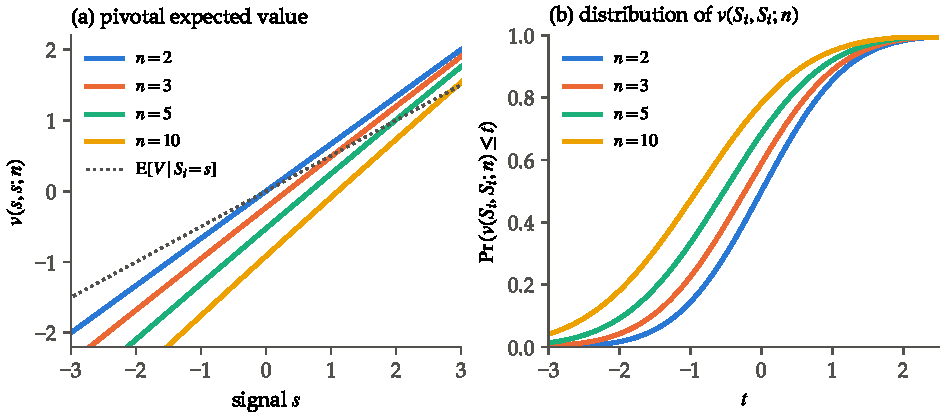
\includegraphics[width=\textwidth]{figures/ch15/cv_winners_curse.pdf}
  \caption{The winner's curse and the number of bidders in a Gaussian mineral rights model: $V_0\sim N(0,1)$
  and $S_i=V_0+e_i$ with independent $e_i\sim N(0,1)$. Panel (a): the pivotal expected value $v(s,s;n)$ falls
  with $n$ for every signal (\cref{lem:15-pivotal-n}). The dotted line is $\E[V_0\mid S_i=s]=\frac s2$, which
  does not depend on $n$. Panel (b): the distribution of $v(S_i,S_i;n)$, the object compared across $n$ in the
  test of \citet{HaileHongShum2003}. Under private values the four curves would coincide. Our computation by
  numerical integration, with no random numbers (script \texttt{cv\_winners\_curse.py}).}\label{fig:15-wc-n}
\end{figure}

\casehead{Endogenous participation} Exogenous variation in $n$ is a strong assumption. A binding reserve price
or a bid-preparation cost truncates the set of participating types. \citet{HaileHongShum2003} adjust for
truncation and compare the distributions on their common support \citep[Section~8.2]{AtheyHaile2007}.
Unobservables that move both participation and values are harder. If more valuable tracts attract more bidders,
that variation can mask the winner's curse. Unobserved heterogeneity also threatens identification of $F_{v,n}$
itself (\cref{sec:15-uh}). \citet{HaileHongShum2003} propose an instrumental approach that builds on
\cref{ass:15-cpv-uh}. Let the number of bidders be $n_t=\chi(Z_t,\omega_t)$, where $Z_t$ is observed and
$\omega_t$ is an unobserved index of the auction, the unobserved heterogeneity of \cref{sec:15-uh}. Assume
(i) $Z_t$ is independent of signals and values, and (ii) $\chi$ is weakly increasing in $Z_t$ and strictly
increasing in $\omega_t$. Strict monotonicity in $\omega_t$ makes $(n_t,Z_t)$ a sufficient statistic for
$\omega_t$. The pivotal expected value of a bidder whose signal $s$ leads to the bid $b$ is then identified
conditional on $(n_t,Z_t)$:
\begin{equation*}
  v(s,s;n,z)=b+\frac{\Pr\bigl(M_{it}\le b\mid B_{it}=b,\ Z_t=z,\ n_t=n\bigr)}{\frac{\partial}{\partial m}
  \Pr\bigl(M_{it}\le m\mid B_{it}=b,\ Z_t=z,\ n_t=n\bigr)\big|_{m=b}} .
\end{equation*}
Pooling pseudo-values across $n$ for each $z$, the distribution of pivotal values must be the same for all $z$
under private values. It shifts with $z$ under common values. In timber auctions they use the number of
sawmills and logging firms near a sale as the instrument \citep[Section~8.2]{AtheyHaile2007}. Strict
monotonicity in a scalar unobservable is the price of the approach. It also requires the unobservable to be
discrete, because $n_t$ is.

\casehead{Binding reserve prices} A reserve price offers a different test \citep{HendricksPinksePorter2003}.
With reserve $r$ in a symmetric first-price auction, a bidder participates if her signal exceeds the threshold
$s^\ast=\inf\{s:\E[V_i\mid S_i=s,\ Y_i\le s]\ge r\}$. The marginal participant bids $r$ and wins only when no rival
participates. Her pivotal expected value is $v(s^\ast,s^\ast;n)$. Under private values the two conditional
expectations coincide, so $v(s^\ast,s^\ast;n)=r$. Under common values
$\E[V_i\mid S_i=s^\ast,\ Y_i\le s^\ast]<\E[V_i\mid S_i=Y_i=s^\ast]$, so $v(s^\ast,s^\ast;n)>r$
\citep[eqs.~(8.7)--(8.8)]{AtheyHaile2007}. The inverse bid function at the bottom of the bid support,
$\lim_{b\downarrow r}\bigl[b+\frac{G_{M\mid B}(b\mid b)}{g_{M\mid B}(b\mid b)}\bigr]$, should equal $r$ under
private values and exceed it under common values. With private values the markdown vanishes at the reserve,
so rival bids are dense just above $r$ (compare \cref{thm:15-gpv-reserve}). With common values the markdown
stays positive, because even the marginal participant bids below her pivotal value. Bids just above $r$ are
then relatively sparse, an implication of the reserve price already noted by \citet{MilgromWeber1982}.
\citet{HillShneyerov2013} develop a formal test based on the tail of the bid distribution near the reserve.

\casehead{Evidence from timber, oil and procurement auctions} The tests have been applied in several
markets, and the answer depends on the market \citep[Sections~2.3, 3.2 and 4.1]{HortacsuPerrigne2021}. In
Forest Service first-price sales in the western half of the United States, the tests of
\citet{HaileHongShum2003} find no evidence of common values in scale sales. We report the results of the
2006 revision of that working paper, as summarized by \citet[pp.~93--94]{HortacsuPerrigne2021}. The evidence is
mixed in lump-sum sales, where the case for common values was stronger.
\citet{CompianiHaileSantAnna2020} extend the test to endogenous entry and unobserved heterogeneity and apply
it to Outer Continental Shelf leases (pp.~126--127). Private information is multiplicatively separable into a
function of observed and unobserved heterogeneity and an idiosyncratic base value. Bids then decompose into
the same function times a \emph{homogenized bid} that depends only on the number of bidders and the signal.
The number of bidders depends on observables and rises weakly with the unobservable. An instrument shifts
entry but not signals or values, and in the application it is the number of neighbor firms. Under private
values the joint distribution of signals and values does not depend on the number of bidders, while common
values order it by stochastic dominance. The authors conclude in favor of common values. Ignoring unobserved
heterogeneity would produce an ordering contrary to common values, a misspecification of the kind studied in
\cref{sec:15-uh}. For policy, the seller would not gain from limiting competition to soften the winner's
curse. A second-price auction, which exploits the linkage principle (\cref{prop:14-linkage}), would raise
revenue only slightly.

\citet{HongShum2002} quantify the winner's curse in procurement with a parametric model of affiliated values
(pp.~104--105). Under common values more bidders have two effects on bids. A competitive effect lowers them,
and a winner's-curse effect raises them, so bids can be U-shaped in the number of bidders. The model follows
the log-additive specification of Wilson, with multiplicative decompositions of costs and signals. The
relative standard deviations of the common component, the private component and the signal noise measure
how common the costs are. In New Jersey Department of Transportation auctions, highway work behaves like
common values, while bridge work and road paving mix private and common values. Allowing for unobserved
heterogeneity, road paving looks like independent private costs and highway work like affiliated private
values. For highway work, halving the number of bidders would lower the procurement cost by 15 percent. For
the other two kinds of work, more competition lowers the cost, so the competitive effect dominates.

\Cref{tab:15-cv-tests} collects the tests of this subsection. Each one replaces the unattainable goal of
identifying $F_{\bm S,\bm V}$ by a restriction that private values impose and common values violate.

\begin{table}[htbp]
\centering
\caption{Tests of private against common values}\label{tab:15-cv-tests}
\small
\begin{tabularx}{\textwidth}{@{}>{\raggedright\arraybackslash}p{2.6cm}>{\raggedright\arraybackslash}X>{\raggedright\arraybackslash}X>{\raggedright\arraybackslash}p{2.5cm}@{}}
\toprule
Format & Data and variation & Restriction under private values & Source \\
\midrule
Second-price or ascending & Price with $m$ bidders, upper bids with $n>m$. Exogenous $n$ & Recurrence
\eqref{eq:15-recurrence} holds (in means for ascending). Common values give dominance & \citet[Thm.~9]{AtheyHaile2002} \\
Second-price, asymmetric & Bids with $n$ bidders, prices with subsets of bidders & Recurrence for random
subsamples & \citet[Thm.~10]{AtheyHaile2002} \\
First-price & Top two bids with $n$ and $n-1$ bidders & Recurrence for identified $v(S,S;n)$ & \citet[Thm.~11]{AtheyHaile2002} \\
First-price & All bids, exogenous $n$ & $F_{v,n}$ invariant to $n$. It falls in $n$ under common values &
\citet{HaileHongShum2003} \\
First-price & All bids, instrument for $n$ & Pivotal values invariant to the instrument & \citet{HaileHongShum2003} \\
First-price & All bids, instrument for entry, unobserved heterogeneity & Joint law of signals and values invariant to $n$ & \citet{CompianiHaileSantAnna2020} \\
First-price & Binding reserve price & Inverse bid function equals $r$ at the bottom & \citet{HendricksPinksePorter2003} \\
First-price & All bids and ex post values & Overidentifying restriction \eqref{eq:15-hpp-test} & \citet{HendricksPinksePorter2003} \\
First-price, two bidders & Bids and identities & Quasi-symmetry rejects asymmetric pure common values & \citet{CampoPerrigneVuong2003} \\
\bottomrule
\end{tabularx}
\end{table}

\subsection{Interdependent costs: Somaini (2020)}\label{sec:15-cv-somaini}

\casehead{Question} Most empirical work picks one of two polar models. Under private costs there is no
winner's curse. Under pure common costs every bidder would incur the same cost, so the allocation cannot be
inefficient. Intermediate models had received little attention, largely because \citet{LaffontVuong1996}
showed that any bid distribution rationalized by interdependent costs is also rationalized by private costs.
\citet{Somaini2020} asks whether richer variation in competitive conditions restores identification in
procurement auctions. The variation comes from continuous bidder-specific cost shifters, such as each firm's
distance to the project. The test of \citet{HaileHongShum2003} uses discrete variation in $n$. Continuous
shifters vary competition in more directions.

\casehead{Primitives} A buyer procures a project by first-price (low-bid) sealed bid from $n$ risk-neutral
bidders, with no reserve price. Bidder $i$'s cost is $C_i$ and her private information is a scalar signal
$S_i$. Signals are normalized to have uniform marginals, so their joint distribution $F_{\bm S}$ is a copula.
Each bidder has a public cost shifter $w_i$, and $\bm w=(w_1,\dots,w_n)$. Somaini writes $x_i$ for $w_i$ and
conditions on auction characteristics throughout. Bidder $i$'s \emph{full-information cost} is
\begin{equation*}
  c_i(\bm s_{-i},s_i,w_i)=\E\left[C_i\mid \bm S=\bm s,\ \bm w\right].
\end{equation*}
For risk-neutral bidders, the payoff-relevant primitives are $F_{\bm S}$ and the functions $c_i$. They are
coarser than the joint distribution of costs and signals. They suffice for counterfactuals that change the rules,
the reserve price or subsidies \citep[Section~I]{Somaini2020}.

\begin{assumption}[{\citealp[Assumptions~A1--A3 and A7]{Somaini2020}}]\label{ass:15-somaini}
(A1) Signals are independent of cost shifters: $F_{\bm S\mid\bm w}=F_{\bm S}$. (A2) Signals are scalar, and
$F_{\bm S}$ has a continuously differentiable bounded density $f$. (A3) Rivals' shifters are excluded from a
bidder's full-information cost: $\E[C_i\mid\bm S,\bm w]=c_i(\bm S_{-i},S_i,w_i)$. (A7) For every $\bm w$, the
data are generated by repeated play of the same Bayes-Nash equilibrium in monotone pure strategies.
\end{assumption}

The model nests the standard cases. Private costs mean $c_i$ does not depend on $\bm s_{-i}$. Independent
private costs add independence of signals, and affiliated private costs allow affiliation. Pure common costs
mean $c_i=c_j$ for all $i,j$. Bidders may also be asymmetric in any way. Assumptions A1 and A3 define what makes
an observable a cost shifter. For distance, they rule out a firm having lower costs when a rival is nearby. They
also rule out a firm regarding a nearby rival's signal as more informative. Equilibria in monotone pure strategies
exist when signals are affiliated \citep{RenyZamir2004}. Somaini shows that without a binding reserve price they
are strictly increasing \citep[Proposition~1]{Somaini2020}.

\casehead{First-order condition} Let $s_j(b)=\beta_j^{-1}(b)$ be the signal at which rival $j$ bids $b$. A low
bid wins, so bidder $i$ wins with bid $b$ when $\bm S_{-i}\ge\bm s_{-i}(b)$ componentwise. Her expected
profit is
\begin{equation*}
  \Pi_i(b;s_i)=\int_{\bm\tau\ge\bm s_{-i}(b)}\bigl(b-c_i(\bm\tau,s_i,w_i)\bigr)f(\bm\tau\mid s_i)\,d\bm\tau .
\end{equation*}
Differentiating in $b$ gives one term from the margin $b$ and one boundary term for each rival:
\begin{multline*}
  \Pr\bigl(\bm S_{-i}\ge\bm s_{-i}(b)\mid s_i\bigr)
  -\sum_{j\ne i}s_j'(b)f\bigl(s_j(b)\mid s_i\bigr)\Pr\bigl(\bm S_{-ij}\ge\bm s_{-ij}(b)\mid s_i,s_j(b)\bigr)\\
  \times\Bigl[b-\E\bigl(C_i\mid s_i,\,s_j(b),\,\bm S_{-ij}\ge\bm s_{-ij}(b)\bigr)\Bigr]=0 .
\end{multline*}
Let $D_i(b)$ be the sum of the weights $s_j'(b)f(s_j(b)\mid s_i)\Pr(\bm S_{-ij}\ge\bm s_{-ij}(b)\mid s_i,s_j(b))$.
It equals the absolute derivative of the win probability in the bid. Let $\pi^{(i)}_j(b)$ be rival $j$'s weight
divided by $D_i(b)$. Rearranging,
\begin{equation}\label{eq:15-som-foc}
  b-\frac{\Pr\bigl(\bm S_{-i}\ge\bm s_{-i}(b)\mid s_i\bigr)}{D_i(b)}
  =\sum_{j\ne i}\pi^{(i)}_j(b)\,\E\Bigl(C_i\mid s_i,\ S_j=s_j(b),\ \bm S_{-ij}\ge\bm s_{-ij}(b),\ w_i\Bigr),
\end{equation}
equation (5) of \citet{Somaini2020}. The left side is marginal revenue, the bid minus a markup. The right side
is the expected cost conditional on the bid being \emph{pivotal}, that is, tying with at least one rival for the
lowest bid. The weight $\pi^{(i)}_j$ is the probability of tying with rival $j$ given a tie with at least one
rival.

\casehead{Identification} The argument has three steps. First, monotone strategies imply that the copula of bids
equals the copula of signals. With uniform signals, $s_i=H_{B_i\mid\bm w}(b_i)$, the marginal distribution of
$i$'s bid given $\bm w$. Hence $F_{\bm S}(\bm s)=H_{\bm B\mid\bm w}\bigl(Q_{B_1\mid\bm w}(s_1),\dots,Q_{B_n\mid\bm
w}(s_n)\bigr)$, where $Q$ denotes a quantile function \citep[Lemma~1 and Proposition~3]{Somaini2020}. By A1, the
bid copula must not vary with $\bm w$, a testable implication. Nonparticipation is recorded as an infinite bid.

Second, the left side of \eqref{eq:15-som-foc} is identified as in \eqref{eq:15-lpv-foc}, because conditioning on
the signal is conditioning on the bid. With $M_i=\min_{j\ne i}B_j$,
\begin{equation}\label{eq:15-som-xi}
  \xi_i(b_i,\bm w)=b_i-\frac{\Pr(M_i\ge b_i\mid B_i=b_i,\bm w)}{\bigl|\frac{\partial}{\partial m}\Pr(M_i\ge m\mid
  B_i=b_i,\bm w)\big|_{m=b_i}\bigr|} .
\end{equation}
The right side is the limit as $\varepsilon\downarrow0$ of $\E\bigl(C_i\mid S_i=s_i,\ \bm S_{-i}\in
L_\varepsilon(b_i,\bm w),\ w_i\bigr)$. Here $L_\varepsilon(b,\bm w)$ is the set of rival signals for which $i$ wins
with bid $b$ but loses with $b+\varepsilon$. It is the difference of two rectangles, each identified from the
marginal bid distributions.

Third, variation in rivals' shifters moves these sets. With two bidders the pivotal event is a single point, and
\eqref{eq:15-som-foc} becomes
\begin{equation}\label{eq:15-som-two}
  \xi_1(b_1,\bm w)=c_1\bigl(H_{B_2\mid\bm w}(b_1),\,H_{B_1\mid\bm w}(b_1),\,w_1\bigr),
\end{equation}
equation (8) of \citet{Somaini2020}. Holding $w_1$ fixed and varying $(w_2,b_1)$ evaluates $c_1(\cdot,\cdot,w_1)$
at different pairs of signals. A3 ensures that $w_2$ moves the evaluation point without shifting $c_1$ itself. The
rival's shifter works like an instrument for the rival's signal.

With three bidders the pivotal set is L-shaped (\cref{fig:15-som-L}). One bid gives one equation in two
unknowns, the expected costs conditional on tying with bidder 2 or with bidder 3. Different rival shifters
$\bm w'$ produce another L-shaped set stacked on the first, with $s_1$ and $w_1$ fixed. Under A1, the expected
cost over the union is a probability-weighted average with identified weights. Stacking ever finer L-shaped sets
covers the rectangle $\{S_2\ge s_2,\ S_3\ge s_3\}$. The limit identifies $\E(C_1\mid s_1,\ S_2\ge s_2,\ S_3\ge
s_3,\ w_1)$, the expected cost conditional on winning. Differentiating twice recovers the full-information cost:
\begin{multline}\label{eq:15-som-diff}
  \frac{\partial^2}{\partial s_2\,\partial s_3}\Bigl[\E\bigl(C_1\mid s_1,S_2\ge s_2,S_3\ge s_3,w_1\bigr)
  \Pr\bigl(S_2\ge s_2,S_3\ge s_3\mid s_1\bigr)\Bigr]\\
  =c_1(s_2,s_3,s_1,w_1)\,f_{S_2,S_3\mid S_1}(s_2,s_3),
\end{multline}
equation (10) of \citet{Somaini2020}. The two minus signs from differentiating the lower limits cancel.

\begin{figure}[htbp]
\centering
\begin{tikzpicture}[scale=5.2,>=Stealth]
  \fill[blue!8] (0.42,0.30) rectangle (1,1);
  \fill[blue!35] (0.42,0.30) -- (1,0.30) -- (1,0.36) -- (0.48,0.36) -- (0.48,1) -- (0.42,1) -- cycle;
  \fill[orange!45] (0.48,0.36) -- (1,0.36) -- (1,0.42) -- (0.54,0.42) -- (0.54,1) -- (0.48,1) -- cycle;
  \draw[thick] (0,0) rectangle (1,1);
  \draw (0.42,0.30) rectangle (1,1);
  \draw (0.48,0.36) rectangle (1,1);
  \draw (0.54,0.42) rectangle (1,1);
  \fill (0.42,0.30) circle (0.010);
  \fill (0.48,0.36) circle (0.010);
  \node[below left] at (0,0) {$0$};
  \node[below] at (1,0) {$1$};
  \node[left] at (0,1) {$1$};
  \node[below] at (0.5,-0.06) {rival signal $S_2$};
  \node[rotate=90] at (-0.1,0.5) {rival signal $S_3$};
  \node[font=\small] at (0.20,0.12) {$\bigl(s_2(b),s_3(b)\bigr)$};
  \draw[->] (0.24,0.16) -- (0.41,0.29);
  \node[font=\small] at (0.78,0.12) {$L_\varepsilon(b,\bm w)$};
  \draw[->] (0.78,0.16) -- (0.78,0.32);
  \node[font=\small,anchor=east] at (0.31,0.66) {$L_\varepsilon(t,\bm w')$};
  \draw[->] (0.32,0.66) -- (0.505,0.66);
  \node[font=\small,align=center] at (0.77,0.72) {win region\\ not yet\\ covered};
\end{tikzpicture}
\caption{Pivotal sets with three bidders in a procurement auction, drawn in the space of bidder 1's rivals'
signals. Bidder 1 wins with bid $b$ when both rival signals exceed the thresholds $s_2(b)$ and $s_3(b)$. The
blue L-shaped set $L_\varepsilon(b,\bm w)$ contains the rival signals for which bidder 1 wins with $b$ but loses
with $b+\varepsilon$. The first-order condition identifies the expected cost on this set. Different rival
shifters $\bm w'$ and a bid $t$ produce the stacked orange set $L_\varepsilon(t,\bm w')$, holding bidder 1's
signal and shifter fixed. Stacking such sets fills the light rectangle. Our drawing, after \citet[Figures~1--2]{Somaini2020}.}\label{fig:15-som-L}
\end{figure}

\begin{theorem}[{\citealp[Theorem~4]{Somaini2020}}]\label{thm:15-somaini}
Under \cref{ass:15-somaini}, the full-information cost $c_i(\bm s_{-i},s_i,w_i)$ is identified for all
$\bm s\ge\bm s^\ast$ if the observables exhibit sufficient variation and nonvanishing competition for bidder $i$
at $(\bm s^\ast,w_i)$.
\end{theorem}

Sufficient variation has a precise meaning \citep[Definition~1]{Somaini2020}. For every $\bm s\ge\bm s^\ast$
there must be rival shifters $\bm w_{-i}$ and a finite bid $b$ with $H_{B_j\mid\bm w}(b)=s_j$ for every bidder
$j$. The bid $b$ is then bidder $i$'s equilibrium bid at signal $s_i$. Nonvanishing competition bounds the number of L-shaped sets
needed, by requiring rivals to bid in any interval $[b,b']$ with nonvanishing probability (Definition~2).
Equilibrium observables of first-price auctions typically exhibit nonvanishing competition. A bounded set of
shifters suffices for signals bounded away from zero \citep[Propositions~5--6]{Somaini2020}. Identification at
extreme signals may need shifters with unbounded support.

Three limits deserve mention \citep[Section~III.C]{Somaini2020}. Binding reserve prices can reduce the variation
that shifters generate. Entry costs paid after learning signals are hard to distinguish from full-information
costs that rise sharply as rivals' signals approach the top. A random entry cost unobserved by the econometrician
violates A7, so \cref{thm:15-somaini} does not apply. Finally, the identified primitives cannot evaluate
counterfactuals in which bidders act after learning more, such as resale or subcontracting once costs are known.

\casehead{Setting and data} The Michigan Department of Transportation (MDOT) awards about 1,050 highway contracts
a year, worth about \$1.2 billion in total, by first-price sealed bid. On each monthly letting date, 150 to 200
firms bid on 50 to 70 contracts \citep[p.~3844]{Somaini2020}. Contracts are advertised at least 45 days ahead.
There is no formal reserve price, but the agency may reject all bids if the lowest exceeds 110 percent of the
engineer's estimate. From 2001 to 2010 the lowest bid exceeded that level in 11 percent of cases, and 15 percent
of these were rejected (p.~3845). The study focuses on hot-mixed asphalt paving. The mix must be compacted while
hot, above $135^\circ$C, so trucking time from a firm's plant matters for cost and quality. Distance from the plant
to the project is the cost shifter. Of 10,522 auctions from January 2001 to December 2010, 3,851 required asphalt
prequalification, and 1,925 had it as the only requirement. These form the sample (p.~3846).

In the sample the median engineer's estimate is \$633,000 and the median lowest bid \$586,000. Auctions have 3.04
participants on average. The median normalized winning bid, $\frac{\text{lowest bid}}{\text{estimate}}-1$, is
$-6.8$ percent. The second-lowest bid exceeds the lowest by 8.2 percent on average. The median participant is 38
km from the project and the median winner 22 km (Table~1). The average winning bid falls with the number of
participants, but the average bid does not (Table~2). Somaini reads this as evidence against the symmetric
independent private cost model with exogenous participation.

\casehead{Econometric model} Signals are mapped to standard normals, $\zeta_i=\Phi^{-1}(S_i)$, with
$\bm\zeta\sim N(0,\Sigma)$ and a factor structure $\Sigma=LL^\top+\Lambda$. Let $Z_t$ be auction characteristics.
The Gaussian information structure implies
\begin{equation}\label{eq:15-som-gauss}
  \E\bigl(C_i\mid\bm\zeta,Z_t,w_i\bigr)=\alpha_{ic}+Z_t\alpha_{i0}+\alpha_{i1}w_i
  +\alpha_{i2}\sum_{j\ne i}\tilde\sigma_{ij}\zeta_j+\nu_i\zeta_i,
\end{equation}
where $\tilde\sigma_{ij}$ is the $(i,j)$ element of $-\Sigma^{-1}$, nonnegative under affiliation
\citep[eq.~(11)]{Somaini2020}. Here $\Phi$ is the standard normal distribution function. One parameter per
bidder, $\alpha_{i2}$, measures interdependence. Private costs are $\alpha_{i2}=0$, interdependent costs are
$\alpha_{i2}>0$, and $\alpha_{i2}<0$ would falsify the model. Substituting \eqref{eq:15-som-gauss} into
\eqref{eq:15-som-foc} gives the estimating equation
\begin{equation}\label{eq:15-som-est}
  B_i=\alpha_{ic}+Z_t\alpha_{i0}+\alpha_{i1}W_i+\alpha_{i2}\,k_i(B_i,\bm W\mid H)+\iota_i(B_i,\bm W\mid H)+\nu_i\zeta_i,
\end{equation}
equation (12). The term $\iota_i$ is the markup from market power, the second term of \eqref{eq:15-som-xi}. The
term $\alpha_{i2}k_i$ is the markup from the winner's curse, where
\begin{equation*}
  k_i=\sum_{j\ne i}\tilde\sigma_{ij}\Bigl[\pi^{(i)}_j\zeta_j(b)+\sum_{k\ne i,j}\pi^{(i)}_k\,
  \E\bigl(\zeta_j\mid\zeta_k=\zeta_k(b),\ \bm\zeta_{-ik}\ge\bm\zeta_{-ik}(b)\bigr)\Bigr]
\end{equation*}
depends only on the bid distribution $H$. A bidder knows that she wins only when rivals have drawn high signals.

\casehead{Estimator and instruments} Let $\nu_{i\tau}$ be the $\tau$-th quantile of $\alpha_{ic}+\nu_i\zeta_i$.
Since signals are independent of shifters, \eqref{eq:15-som-est} implies the quantile moment
$\E[\indic(B_i-Z_t\alpha_{i0}-\alpha_{i1}W_i-\alpha_{i2}k_i-\iota_i-\nu_{i\tau}\le0)-\tau\mid\bm W]=0$.
Nonparticipation censors bids. Only signals below a participation cutoff yield finite bids, and the cutoff has
probability $\phi_i(\bm W\mid H)$. The moment conditional on participation replaces $\tau$ by
$\min\bigl(\frac{\tau}{\phi_i(\bm W\mid H)},1\bigr)$ \citep[eqs.~(13)--(14)]{Somaini2020}. The parameters are
estimated by instrumental variable quantile regression \citep{ChernozhukovHansen2006}. The instrument for $k_i$
is its projection on the bidder's own covariates and rivals' distances. Rivals' distances are excluded from own
cost by A3, and they move the pivotal sets and hence $k_i$. The first stage estimates the marginal bid
distributions with cubic B-splines in the project's latitude, longitude and the bid, and the copula by simulated
maximum likelihood. The markups $\iota_i$ and $k_i$ come from spline estimates of win and tie probabilities.
Standard errors come from 200 bootstrap samples of the 1,925 auctions (p.~3850).

\casehead{Results} The analysis covers 19 frequent bidders, with the remaining firms grouped as a fringe
bidder. The Akaike criterion selects two factors. The first factor creates correlations of 0.11 to 0.29 among one
group of firms and explains up to 20 percent of their signal variance. The second explains up to 25 percent for
another group (pp.~3854--3855). For bidder 1, the full-information cost at the 25th percentile of its own signal
and the median of rivals' signals is 73 percent of the engineer's estimate for projects within 10 km. The
interdependence coefficient $\alpha_{i2}$ is 0.500 (s.e.\ 0.190) for bidder 1, 0.350 (0.118) for bidder 2 and
$-0.025$ (0.092) for bidder 3 (Table~5). \Cref{tab:15-somaini-signals} reproduces the effects of own and rivals'
signals. A one standard deviation increase in bidder 1's own signal raises its full-information cost by 10
percentage points of the estimate. The same increase in a rival's signal raises it by 4 points on average and 7
at most (p.~3857). Rivals' signals matter, but less than one's own. Private costs are rejected for bidders 1 and
2. They cannot be rejected for bidders 3 and 9.

\begin{table}[htbp]
\centering
\caption{Effect of signals on full-information costs, Michigan highway procurement}\label{tab:15-somaini-signals}
\small
\begin{tabular}{@{}lcccccc@{}}
\toprule
 & \multicolumn{2}{c}{Own signal} & \multicolumn{2}{c}{Competitor (mean)} & \multicolumn{2}{c}{Competitor (maximum)} \\
\cmidrule(lr){2-3}\cmidrule(lr){4-5}\cmidrule(lr){6-7}
 & Coef. & S.e. & Coef. & S.e. & Coef. & S.e. \\
\midrule
Bidder 1 & 0.10*** & 0.02 & 0.04*** & 0.01 & 0.07*** & 0.02 \\
Bidder 2 & 0.09*** & 0.02 & 0.03*** & 0.01 & 0.06*** & 0.02 \\
Bidder 3 & 0.13*** & 0.05 & 0.00 & 0.00 & 0.00 & 0.01 \\
Bidder 4 & 0.59* & 0.32 & 0.00 & 1.15 & 0.00 & 3.95 \\
Bidder 5 & 0.13*** & 0.02 & 0.01*** & 0.00 & 0.02*** & 0.01 \\
Bidder 6 & 0.15 & 0.11 & 0.04* & 0.02 & 0.09** & 0.04 \\
Bidder 7 & 0.12*** & 0.04 & 0.03*** & 0.01 & 0.07*** & 0.02 \\
Bidder 8 & 0.32*** & 0.12 & 0.05 & 0.05 & 0.14 & 0.15 \\
Bidder 9 & 0.18*** & 0.04 & 0.01 & 0.03 & 0.02 & 0.10 \\
Bidder 10 & 0.10*** & 0.04 & 0.02*** & 0.00 & 0.05*** & 0.02 \\
Bidder 11 & 0.10*** & 0.03 & 0.03*** & 0.01 & 0.06*** & 0.02 \\
Bidder 12 & 0.07 & 0.06 & 0.03 & 0.04 & 0.06 & 0.10 \\
Bidder 13 & 0.09* & 0.05 & 0.02** & 0.01 & 0.04 & 0.03 \\
Bidder 14 & 0.25*** & 0.09 & 0.00 & 0.01 & 0.01 & 0.02 \\
Bidder 15 & 0.20*** & 0.05 & 0.00 & 0.01 & 0.00 & 0.02 \\
Bidder 16 & 0.07 & 0.08 & 0.02 & 0.02 & 0.05 & 0.06 \\
Bidder 17 & 0.12*** & 0.04 & 0.04 & 0.12 & 0.09 & 0.33 \\
Bidder 18 & 0.22* & 0.11 & 0.07 & 0.15 & 0.20 & 0.41 \\
Bidder 19 & 0.15 & 0.10 & 0.02** & 0.01 & 0.06** & 0.02 \\
\bottomrule
\end{tabular}

\smallskip
\begin{minipage}{0.92\textwidth}
\footnotesize \textit{Notes.} Effect of a one standard deviation increase in a bidder's own Gaussian signal, and in a
competitor's signal, on the bidder's full-information cost, as a fraction of the engineer's estimate. The
competitor effect depends on the competitor's identity, and the table reports its mean and maximum. Standard
errors from 200 bootstrap samples. * $p<0.1$, ** $p<0.05$, *** $p<0.01$. Source: \citet[Table~7]{Somaini2020}.
\end{minipage}
\end{table}

\casehead{Counterfactuals} Somaini simulates restricting participation to the $N$ bidders with the lowest median
cost in 250 randomly drawn auctions. Three models are compared: the estimated common-cost model (CC), an
affiliated private cost model that sets $\alpha_{i2}=0$ (APC), and an independent private cost model that also
sets $L=0$ (IPC). Inviting more bidders lowers procurement costs in all three models. Going from two to seven
invitees lowers costs by 5.48 percentage points under IPC, 5.00 under APC and 4.40 under CC (p.~3862). The bidder
with the lowest median cost bids more aggressively with more rivals under IPC and APC. Under CC it bids less
aggressively, because the winner's curse worsens. \Cref{tab:15-somaini-comp} decomposes the cost saving. The
competitive and sampling effects lower costs. Affiliation and the winner's curse raise them. The winner's curse is
strong enough to make the first invitee bid higher when competition grows, but not strong enough to make
restricting entry profitable for the buyer.

\begin{table}[htbp]
\centering
\caption{Decomposition of the effect of inviting more bidders on procurement costs}\label{tab:15-somaini-comp}
\small
\begin{tabular}{@{}lcccccccc@{}}
\toprule
Invitees & 3 vs.\ 2 & 4 vs.\ 2 & 5 vs.\ 2 & 6 vs.\ 2 & 7 vs.\ 2 & 8 vs.\ 2 & 9 vs.\ 2 & 10 vs.\ 2 \\
\midrule
Competitive & 1.98 & 2.52 & 2.71 & 2.79 & 2.92 & 2.95 & 2.97 & 2.97 \\
Affiliation & $-0.45$ & $-0.57$ & $-0.51$ & $-0.50$ & $-0.59$ & $-0.61$ & $-0.63$ & $-0.64$ \\
Winner's curse & $-1.52$ & $-2.21$ & $-3.06$ & $-3.37$ & $-3.65$ & $-3.84$ & $-3.95$ & $-3.96$ \\
Sampling & 2.83 & 3.88 & 4.91 & 5.38 & 5.71 & 5.95 & 6.08 & 6.10 \\
Total & 2.84 & 3.63 & 4.05 & 4.30 & 4.40 & 4.45 & 4.47 & 4.47 \\
\bottomrule
\end{tabular}

\smallskip
\begin{minipage}{0.95\textwidth}
\footnotesize \textit{Notes.} Cost savings relative to inviting two bidders, with 100 equal to average procurement cost
with two invitees. The competitive effect is the fall in the average bid of the first invitee under IPC. The
affiliation effect is the difference in that fall between APC and IPC, and the winner's curse effect the
difference between CC and APC. The sampling effect is the difference between the first invitee's bid reduction
and the fall in procurement cost under CC. Source: \citet[Table~8, top panel]{Somaini2020}.
\end{minipage}
\end{table}

Interdependence also affects reserve prices. It lowers the probability of awarding the contract by as much as
0.1 when the reserve is about 90 percent of the estimate (p.~3864). Suppose MDOT must set one reserve for all
contracts. With a willingness to pay of 100 percent of the estimate, the optimal reserve is 86 percent. With a
willingness to pay of 150 percent, it is 125 percent. These reserves succeed with probabilities 0.67 and 0.99 and yield surpluses
of 12 and 57 percent of the estimate. Auction-specific reserves would add less than 1 percent of the estimate
(p.~3867). The 110 percent rule is consistent with a willingness to pay above 140 percent of the estimate.

\casehead{Assessment} The paper gives the first nonparametric identification result for asymmetric
interdependent-cost auctions with dependent signals. Identification comes from continuous variation in
competitive conditions, which is richer than variation in the number of bidders. The estimates place Michigan paving between the polar
paradigms, much closer to private costs. The application relies on strong structure. The Gaussian form summarizes
interdependence by one parameter per bidder and makes costs additively separable in rivals' signals. Distance must
satisfy A1 and A3, which fails if a nearby rival's signal is more informative. Participation is handled through
censoring at a cutoff, and signals are scalar. Infrequent bidders are pooled into one fringe bidder. These restrictions
buy precision in a sample of 1,925 auctions.

\subsection{An auction with an informed bidder: Hendricks and Porter (1988)}\label{sec:15-cv-hp}

\casehead{Question} \citet{HendricksPorter1988} test the equilibrium predictions of a common value auction with
asymmetric information. The setting is the federal sale of drainage leases on the Outer Continental Shelf. A
drainage tract is adjacent to a tract on which oil or gas has been found. Firms owning adjacent tracts, the
\emph{neighbor} firms, learn about the drainage tract from their own drilling. Other firms rely on seismic
surveys and public information. The data include ex post production, so the authors can measure who earns
rents and test whether bidding accounts for the winner's curse.

\casehead{Theory} The model of \citet{Wilson1967} and \citet{EngelbrechtWiggansMilgromWeber1983} is developed in
\cref{prop:14-emw}. One informed bidder observes a private and a public signal and forms the estimate $H$ of
the common value. The uninformed bidders observe only the public signal. In equilibrium the informed bidder bids
$\E[H\mid H\le h]$ above a cutoff, bids the reserve price below it, and abstains below the reserve. The
uninformed bidders randomize so that the highest uninformed bid has the same distribution as the informed bid
above the reserve. \citet[pp.~870--871]{HendricksPorter1988} list seven predictions.
\begin{enumerate}[label=(\arabic*)]
  \item No neighbor bid is less frequent than no non-neighbor bid.
  \item The neighbor wins at least half of the tracts that receive a bid, by \eqref{eq:14-hp-winprob}.
  \item Non-neighbors earn zero expected profit. They lose on tracts where no neighbor bids and gain where one
  does.
  \item The neighbor earns an information rent.
  \item Without a cost difference between bidders, the informed bid and the highest uninformed bid have
  approximately the same distribution given public information.
  \item The neighbor's strategy does not depend on the number of non-neighbors.
  \item The neighbor's bid increases in the public signal when a higher signal is good news.
\end{enumerate}
Prediction (6) is convenient, because only participating non-neighbors are observed. Their number causes no
selection bias in the neighbor's bid equation.

\casehead{Setting and data} The sample covers federal tracts off Louisiana and Texas sold between 1959 and 1969
in 8 drainage sales, 144 tracts in all \citep[p.~871]{HendricksPorter1988}. It excludes 25 tracts on which the
high bid was rejected, for lack of data. The winning bid, the bonus, is paid at the sale. The government also
receives a royalty of one sixth of revenues. A reserve price of \$25 per acre applied on most drainage leases.
The government rejected the high bid on 7 percent of wildcat and 15 percent of drainage tracts. The authors
compute ex post discounted revenues and costs from production through 1980, real wellhead prices and drilling cost
surveys, discounting at 5 percent a year. \Cref{tab:14-hp-table1} summarizes the sample. Drainage tracts had an
average winning bid of \$5.76 million, net profit of \$4.63 million and value of \$13.51 million, with 2.73 bidders
on average. The government captured 66 percent of the value of drainage tracts against 77 percent for wildcat
tracts (p.~866).

Of the 144 drainage tracts, 114 were adjacent to previously leased federal tracts, and these form the sample.
Neighbor firms are the owners of adjacent federal tracts. Of the 114 tracts, 40 had one neighbor firm and 74 had
more (their Figure~1). Yet only 16 of the 74 received more than one neighbor bid (p.~872). The authors therefore
assume that neighbor firms coordinate and submit at most one serious bid. Joint bidding was legal, and neighbors
may already have formed a joint venture to manage production from the common pool.
The empirical analogues are the largest neighbor bid $B_I$ and the largest non-neighbor bid $B_U$, each set to the
reserve price when no such bid is made. The numbers of neighbor and non-neighbor bids are $N_I$ and $N_U$. The ex
post gross profitability of the tract, $\pi_t$, proxies the neighbor's private information. The public
information is the number of neighbor tracts $N^{\mathrm{tr}}$, the ex post gross profit of the adjacent tract
$V^{\mathrm{adj}}$, and acreage (their Table~2).

\casehead{Estimating equations} For tract $t$ and bidder type $i\in\{I,U\}$, let
\begin{equation*}
  Y_{it}=W_{it}\bm\theta_i+\varepsilon_{it},\qquad
  \ln\frac{B_{it}}{r_t}=\begin{cases}Y_{it}&\text{if }Y_{it}\ge0,\\ 0&\text{otherwise,}\end{cases}
\end{equation*}
where $r_t$ is the reserve price and $W_{it}$ a row of regressors. The errors $(\varepsilon_{It},\varepsilon_{Ut})$
are bivariate normal with variances $\sigma_I^2$ and $\sigma_U^2$, covariance $\sigma_{IU}$ and correlation
$\rho_{IU}$. Bids are lognormal and censored at the reserve. Only tracts with at least one bid are observed. Tracts
fall into three sets: $\Omega_{++}$ with bids of both types, $\Omega_{+0}$ with only neighbor bids, and
$\Omega_{0+}$ with only non-neighbor bids. Let $Z(a,c;\rho)$ be the probability under a standard bivariate normal
with correlation $\rho$ that both components fall below $a$ and $c$, the probability of no bid. The log-likelihood
is $\sum_{\Omega_{++}}l_{1t}+\sum_{\Omega_{+0}}l_{2t}+\sum_{\Omega_{0+}}l_{3t}$, with
\begin{align*}
  l_{1t}&=-\ln(2\pi)-\frac12\ln|\Sigma|-\frac12\,\bm\varepsilon_t^\top\Sigma^{-1}\bm\varepsilon_t-\ln\left[1-Z\left(-\frac{W_{Ut}\bm\theta_U}{\sigma_U},-\frac{W_{It}\bm\theta_I}{\sigma_I};\rho_{IU}\right)\right],\\
  l_{2t}&=\ln\Phi\left(\frac{-W_{Ut}\bm\theta_U-\frac{\sigma_{IU}}{\sigma_I^2}\varepsilon_{It}}{\sqrt{\sigma_U^2-\frac{\sigma_{IU}^2}{\sigma_I^2}}}\right)
  -\ln\sigma_I+\ln\phi\left(\frac{\varepsilon_{It}}{\sigma_I}\right)-\ln\bigl[1-Z(\cdot)\bigr],
\end{align*}
and $l_{3t}$ symmetric to $l_{2t}$ \citep[p.~873]{HendricksPorter1988}. Here $\Phi$ and $\phi$ are the standard
normal distribution function and density. In $l_{2t}$ the first term is the probability that the non-neighbor
latent bid is negative given the neighbor's residual. The next two terms are the density of the neighbor bid. The
last term in each contribution conditions on at least one bid, which corrects for sample selection.

\casehead{Participation and returns} No neighbor bid was made on 19 tracts and no non-neighbor bid on 35. So at
least one neighbor bid on 83 percent of tracts and at least one non-neighbor on 68 percent (p.~874), as
prediction (1) requires.
\Cref{tab:15-hp} reproduces the returns by winner type. The neighbor won 59 of the 114 tracts, 52 percent, as
prediction (2) requires. It won 62 percent of the 95 tracts it bid on, the figure the authors report (p.~874). Its share of tract value was about 44 percent, against an average firm share of 23
percent on wildcat tracts (prediction 4). Non-neighbor winners earned about zero on average, $-0.42$ million.
They lost on tracts with no neighbor bid and gained on tracts with one, as prediction (3) requires. Neighbors
appear able to identify the tracts likely to contain oil.

\begin{table}[htbp]
\centering
\caption{Tracts won by neighbor and non-neighbor firms, OCS drainage sales 1959--1969}\label{tab:15-hp}
\small
\begin{tabular}{@{}lccccc@{}}
\toprule
\multicolumn{6}{@{}l}{\emph{Panel A. Wins by type of firm (Table 3)}}\\
 & \multicolumn{2}{c}{Neighbor wins} & \multicolumn{3}{c}{Non-neighbor wins} \\
\cmidrule(lr){2-3}\cmidrule(lr){4-6}
 & A & Total & B & C & Total \\
\midrule
Number of tracts & 35 & 59 & 19 & 36 & 55 \\
Tracts drilled & 23 & 47 & 18 & 33 & 51 \\
Productive tracts & 16 & 36 & 12 & 19 & 31 \\
Average winning bid & 3.28 & 6.04 & 2.15 & 6.30 & 4.87 \\
 & (0.56) & (2.00) & (0.67) & (1.31) & (0.92) \\
Average gross profits & 10.05 & 12.75 & $-0.54$ & 7.08 & 4.45 \\
 & (3.91) & (3.21) & (0.47) & (2.95) & (1.99) \\
Average net profits & 6.76 & 6.71 & $-2.69$ & 0.78 & $-0.42$ \\
 & (3.02) & (2.69) & (0.86) & (2.64) & (1.76) \\
\midrule
\multicolumn{6}{@{}l}{\emph{Panel B. Single and multiple neighbor tracts (Table 4)}}\\
 & Single & \multicolumn{3}{c}{Multiple neighbors, by neighbor bids} & \\
\cmidrule(lr){3-5}
 & neighbor & 1 & $\ge2$ & Total & \\
\midrule
Number of tracts & 40 & 48 & 15 & 74 & \\
Tracts with no neighbor bid & 8 & & & 11 & \\
Neighbor wins & 19 & 29 & 11 & 40 & \\
Neighbor's average winning bid & 4.795 & 2.615 & 17.193 & 6.624 & \\
 & (1.444) & (0.697) & (9.953) & (2.885) & \\
Neighbor's average gross profits & 13.601 & 4.670 & 32.597 & 12.350 & \\
 & (5.608) & (2.148) & (11.506) & (3.965) & \\
Neighbor's average net profits & 8.806 & 2.055 & 15.404 & 5.725 & \\
 & (4.762) & (1.690) & (10.963) & (3.297) & \\
\bottomrule
\end{tabular}

\smallskip
\begin{minipage}{0.92\textwidth}
\footnotesize \textit{Notes.} Millions of 1972 dollars. Standard deviations of the sample means in parentheses. In Panel
A, column A is tracts with no non-neighbor bid, column B tracts with no neighbor bid, and column C tracts on which
a neighbor bid but a non-neighbor won. Gross profits exclude the bonus, and net profits deduct it. The authors give 17
(p.~867), 16 (p.~872) and 15 (Table~4) as the number of tracts with more than one neighbor bid. Panel B reproduces
Table~4. Source: \citet[Tables~3 and~4]{HendricksPorter1988}.
\end{minipage}
\end{table}

The model also predicts a mass point of neighbor bids at the reserve price, from informed types between the
reserve and the cutoff. The authors find none. They suggest that firms feared the government would reject
reserve-price bids, as it did on 25 drainage tracts. The reserve also explains why non-neighbors drilled tracts
on which no neighbor bid. Drilling is rational if expected net profit given no neighbor bid is below the reserve
but positive once the bid is sunk. Panel B checks the coordination assumption. On single and multiple neighbor
tracts alike, the neighbor won about half of the tracts. Net profits on multiple neighbor tracts are not
significantly lower, so competition among neighbors did not dissipate rents. Valuable multiple neighbor tracts
attracted more than one neighbor bid and earned higher net profits. The authors suggest ``shadow'' bids
submitted to make bidding look competitive to the government (p.~875).

\casehead{Information structure} Regressions of $\pi_t$ on bids and participation test whether non-neighbors
have payoff-relevant private information (their Table~5). With neighbor variables and public information, the
$R^2$ is 0.640. Adding non-neighbor variables raises it to 0.699. Non-neighbor variables and public information
alone give 0.154. The neighbor bid enters with coefficient 3.55 (t-statistic 3.90) and its square with $-0.023$
($-2.57$). The $F$-statistic for the six non-neighbor variables is 3.22 with $(6,98)$ degrees of freedom. The
authors compare it with 3.71 as the 5 percent point and do not reject. They add that most of the non-neighbor
explanatory power comes from the interaction with the neighbor bid. By standard tables the 5 percent point of
$F(6,98)$ is about 2.19, so the statistic would reject at conventional levels (our calculation).

\casehead{Bid distributions} Prediction (5) concerns the joint distribution of $(B_I,B_U)$ given public
information. In the unrestricted bivariate model the two equations have similar coefficients and residual
standard deviations, 2.02 and 2.66. Equal coefficients are not rejected: the likelihood ratio statistic is 10.58,
below 11.07, the 5 percent point of $\chi^2(5)$. The residual correlation is 0.10 (t-statistic 0.94), so no omitted
public variable appears to drive both bids (their Table~6). Adding tract profitability changes the picture. The
coefficient on $\pi_t$ is 0.091 (t-statistic 4.30) in the neighbor equation and 0.028 (0.79) in the non-neighbor
equation. Equal coefficients are now rejected at 1 percent, with statistic 19.84 (their Table~7). Non-neighbors
appear to have no information correlated with profitability beyond the public variables. Their bids are
``noisier,'' with residual standard deviation 2.62 against 1.60 for neighbors. The informed bid rises with $\pi_t$
and with $V^{\mathrm{adj}}$ and does not depend on $N_U$ (prediction 6). The highest non-neighbor bid rises with
$N_U$, as an order statistic should. Where $N_U$ is excluded, it falls with the number of neighbor tracts
(their Table~8).

\casehead{A competitive alternative} Section IV of the paper estimates a model in which neighbors bid
independently, each with a private signal. The likelihood treats each neighbor's bid and the highest non-neighbor
bid as censored normal latent variables \citep[p.~880]{HendricksPorter1988}. Two results contradict competitive
bidding (their Table~9). First, each neighbor's bid falls with the number of neighbor firms, with coefficient
$-0.758$ (t-statistic $-3.96$). For lognormal signals the competitive bid should first rise with the number of
bidders. Citing \citet{Smiley1979}, the authors place the turning point at four bidders or more in their data
\citep[p.~880]{HendricksPorter1988}. Only ten tracts had four or more neighbor firms. Phantom bids, below the serious bid, are consistent with the pattern. Second, the number of
neighbor firms lowers the highest non-neighbor bid by less than it lowers neighbor bids. Under competition among
neighbors the less informed non-neighbors should react more, because their winner's curse worsens more.

\casehead{Interpretation, critiques and contribution} The evidence supports the informed-bidder model with
coordinated neighbors. Neighbors shade their bids well below their estimates and earn high returns. Non-neighbors
bid cautiously, avoid the winner's curse and break even on average. The analysis has limits. Bidders are risk
neutral, tracts are analyzed one at a time, and coordination among neighbors is assumed. The proxy for private
information is ex post profitability, which measures the neighbor's estimate with error. The censored lognormal
model is a statistical description of bids and is not derived from the equilibrium. The sample has only 114
tracts. The missing mass point at the reserve contradicts the model, and \citet{HendricksPorterWilson1994}
later model a random reservation price for that reason. In their model the reservation price is correlated
with the tract value, and values are affiliated. Uninformed bidders are then less likely to participate and,
when they do, tend to bid high, while informed bidders tend to bid low. The informed bid distribution
stochastically dominates the uninformed one within the support of the reservation price and coincides with it
above. The data support these predictions \citep[p.~125]{HortacsuPerrigne2021}.

The paper sits in a sequence of studies of the same leases \citep[pp.~124--125]{HortacsuPerrigne2021}. It
built on the comparison of wildcat and drainage tracts by \citet{HendricksPorterBoudreau1987}. Bids, profits
and net profits per acre are much larger on drainage tracts. The highest bid and the profit per acre are
positively correlated on drainage tracts and negatively on wildcat tracts. Most large firms would have earned
more by bidding less, a sign that they did not fully correct for the winner's curse.
\citet{HendricksPorterSpady1989} then focus on rejections. The government rejects the highest bid on 18
percent of drainage tracts and 9 percent of wildcat tracts, and rejected drainage bids are larger. They also
note that neighbor firms rarely compete, although a drainage tract can have up to eight neighbors. The
paper's lasting contribution is to show that ex post values let the econometrician see adverse selection. It
confirmed subtle equilibrium predictions in a field setting and led to the tests of
\citet{HendricksPinksePorter2003} based on \eqref{eq:15-hpp-test}.

\section{Unobserved Auction Heterogeneity}\label{sec:15-uh}

Objects sold in different auctions differ, and bidders usually know more about the differences than
the econometrician does. A paving contractor visits the site and sees the curvature of the road and
the state of the surface. A used-car dealer inspects each car for rust and dents. Such features
shift every bidder's value in the same direction, and they are common knowledge among the bidders.
When the econometrician cannot condition on them, the methods of \cref{sec:15-gpv,sec:15-apv}
attribute their effect to private information. This section shows what goes wrong and develops
three remedies. They are deconvolution with several bids per auction, parametric mixtures, and
control functions built from the seller's reserve price.

\subsection{The problem}\label{sec:15-uh-problem}

Let $\omega_t$ be a scalar characteristic of auction $t$ that all bidders, and the seller, observe
but the econometrician does not. We call $\omega_t$ \emph{unobserved auction heterogeneity}. The two
workhorse specifications are additive and multiplicative,
\begin{equation}\label{eq:15-uh-values}
V_{it}=\omega_t+A_{it}\qquad\text{or}\qquad V_{it}=\omega_tA_{it},
\end{equation}
where $A_{it}$ is bidder $i$'s \emph{idiosyncratic private component}. In procurement we write
costs as $C_{it}=\omega_tA_{it}$ in the same way.

\begin{assumption}[Unobserved auction heterogeneity]\label{ass:15-uh}
(i) In each auction, $\omega_t,A_{1t},\dots,A_{nt}$ are mutually independent, $\omega_t\sim F_\omega$
and $A_{it}\sim F_{A_i}$, and auctions are independent. (ii) Each bidder observes $\omega_t$, its own
$A_{it}$ and the number of bidders $n_t$. The econometrician observes bids and $n_t$ but neither
$\omega_t$ nor $A_{it}$. (iii) For each $\omega_t$, bidders play the unique equilibrium of the game
with that common component.
\end{assumption}

The same equation \eqref{eq:15-uh-values} with bidders who observe only their own sums $V_{it}$
describes a \emph{conditionally independent private values} model. It is a special case of affiliated
private values when the densities $f_{A_i}$ are log-concave \citep[Section 6.1.2]{AtheyHaile2007}.
The two models differ only in what bidders know. With unobserved heterogeneity, bidder $i$ knows
that its rivals' values are centered on $\omega_t$, so its uncertainty about the competition is the
dispersion of the $A_{jt}$ alone.

The information that is common knowledge among the bidders in auction $t$ is the pair
$(Z_t,\omega_t)$ of observed covariates and unobserved heterogeneity. In a private values first-price
auction, the first-order condition \eqref{eq:14-apv-foc} holds conditionally on it
\citep[Section 6.1.2]{AtheyHaile2007},
\begin{equation}\label{eq:15-uh-foc}
v_{it}=b_{it}+\frac{G_{M\mid B}(b_{it}\mid b_{it};n_t,Z_t,\omega_t)}{g_{M\mid B}(b_{it}\mid b_{it};n_t,Z_t,\omega_t)} .
\end{equation}
An econometrician who does not observe $\omega_t$ cannot estimate the conditional distribution that
enters the markdown. Pooling auctions with different $\omega_t$ replaces it with a mixture over
$\omega_t$. The markdown is a nonlinear function of $\omega_t$, so even its average is not identified without further
structure \citep[Section 6.1.2, citing \citealp{HendricksPinksePorter2003}]{AtheyHaile2007}.

\citet[Section 6.1.2]{AtheyHaile2007} separate three questions.
\begin{enumerate}[label=(\roman*)]
\item \emph{Can unobserved heterogeneity be told apart from other sources of correlated bids?} In an
ascending auction a bidder drops out at its value whether or not it observes $\omega_t$. Unobserved
heterogeneity is then observationally equivalent to correlated private values. In a first-price
auction, any bid distribution that satisfies the conditions of \cref{thm:15-ah-rational} can be
rationalized by affiliated private values without heterogeneity. The choice between the two models
must rest on institutional knowledge.
\item \emph{Is the joint law of $(\omega,A_1,\dots,A_n)$ identified under heterogeneity?} In
first-price auctions it is, under separability and independence, as we show below. In ascending
auctions it requires additional variation, such as bidder covariates (\cref{thm:15-ah5}).
\item \emph{Which primitives does a question need?} In ascending and second-price auctions bidding is
in dominant strategies, so the joint law $F_{\bm V}$ of values answers every counterfactual. First-price
counterfactuals depend on beliefs, and beliefs vary with $\omega_t$. They require the joint law of the
components, $F_{\omega,\bm A}$. The joint law of values $F_{\bm V}$ is not enough.
\end{enumerate}

Ignoring $\omega_t$ has a predictable effect on first-price estimates. Bids from auctions with high
and low $\omega_t$ are pooled, so the estimated bid distribution is too dispersed. Each bidder appears
to face a field of rivals that is more spread out than the one it faces in fact. The estimated
markdown $\frac{G(b)}{(n-1)g(b)}$ is then too large, and so are estimated markups and the estimated
dispersion of values \citep[pp.~294--295]{Krasnokutskaya2011}.

\begin{example}[Pooling bids across heterogeneous auctions]\label{ex:15-uh-uniform}
Let $n=4$, $V_{it}=\omega_tA_{it}$, $A_{it}\sim U[1,2]$ and $\ln\omega_t\sim N(0,0.3^2)$. At
$\omega=1$ the game is a symmetric IPV auction with $F_A(a)=a-1$ on $[1,2]$. The Riley-Samuelson bid
\eqref{eq:14-rs-bid} with no reserve price is
\[
\alpha(a)=a-\frac{\int_1^a(t-1)^3\,dt}{(a-1)^3}=a-\frac{a-1}{4}=\frac{3a+1}{4}.
\]
By \cref{lem:15-separability}(b) below, the bid at $\omega$ is $\beta(v;\omega)=\omega\,\alpha\big(\frac{v}{\omega}\big)
=\frac{3v+\omega}{4}$. The markdown relative to value,
$\frac{v-\beta(v;\omega)}{v}=\frac{a-\alpha(a)}{a}=\frac{a-1}{4a}$, does not depend on $\omega$. Its
average is
\[
\E\Big[\frac{A-1}{4A}\Big]=\frac{1}{4}\Big(1-\E\Big[\frac{1}{A}\Big]\Big)=\frac{1}{4}\big(1-\ln 2\big)\approx0.077 .
\]
We simulated 200 samples of $T=500$ such auctions and applied the GPV estimator of \cref{sec:15-gpv} to
the pooled bids (seed 15701, script \texttt{uh\_bias.py}). The median estimate of the average markdown
is $0.184$, with 5th and 95th percentiles of $0.174$ and $0.193$ across samples. The estimated inverse
bid function in \cref{fig:15-uh-bias}(a) has slope $1.47$ over the central bids, against the true
slope $\frac{4}{3}$. The estimated value density in panel (b) roughly tracks the marginal density of
$V=\omega A$ but is more spread out. Computed over the plotted range $[0.4,3.6]$, its variance is
$0.376$ against $0.300$ for $V$. On the full support the exact variance of $V$ is
$e^{0.18}\cdot\frac{7}{3}-\big(1.5e^{0.045}\big)^2=0.332$. The estimated density has a long upper tail,
from bids where $\hat g$ is small, which raises its full-support variance to about $1.4$. The
interquartile range is less sensitive to that tail. It is $0.97$ for the pseudo-values (median across
samples) against $0.73$ for $V$. Both are far more dispersed than the distribution $F_A$, with
interquartile range $0.5$, that each bidder faces once it has seen $\omega_t$.
\end{example}

\begin{figure}[htbp]
\centering
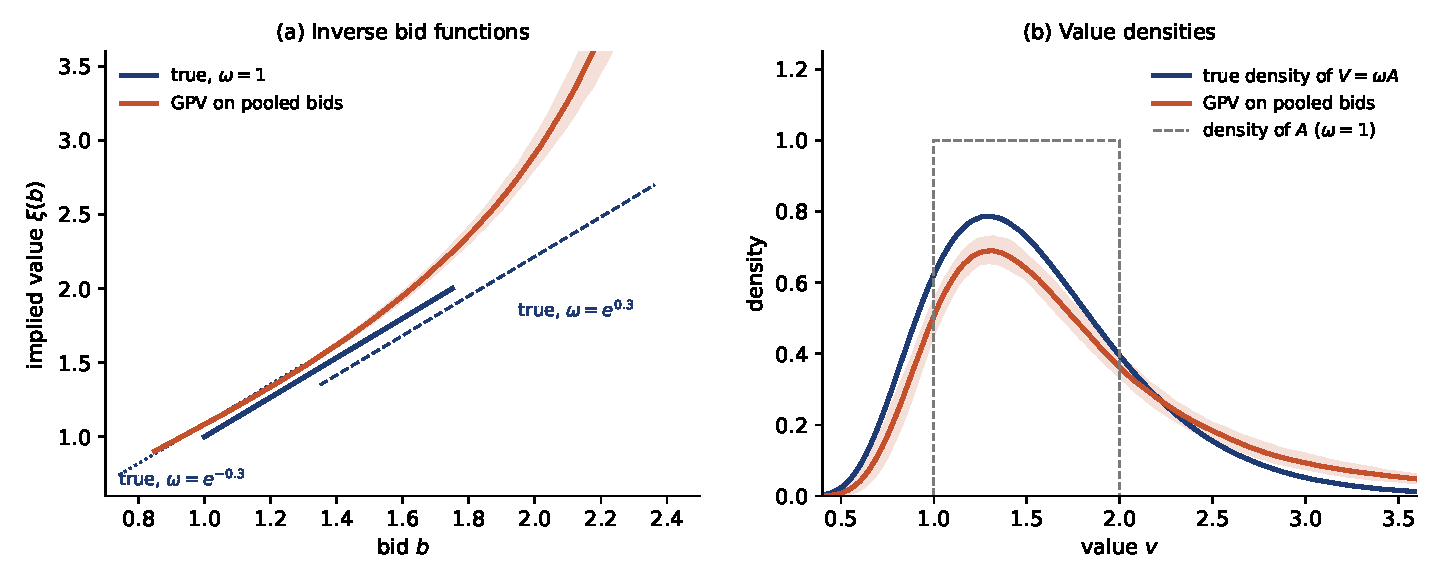
\includegraphics[width=\textwidth]{figures/ch15/uh_bias.pdf}
\caption{GPV applied to bids pooled across auctions with unobserved heterogeneity (our simulation,
seed 15701). Design of \cref{ex:15-uh-uniform}: $n=4$, $V=\omega A$, $A\sim U[1,2]$,
$\ln\omega\sim N(0,0.3^2)$, $T=500$ auctions, 200 samples. Panel (a): true inverse bid functions at
three values of $\omega$ and the median GPV estimate from pooled bids with a 5--95 percent band. Panel
(b): the true marginal density of $V$, the density of $A$ that bidders face at $\omega=1$, and the
median GPV estimate with its band. The true average markdown is $0.077$ and the median estimate is
$0.184$.}
\label{fig:15-uh-bias}
\end{figure}

\subsection{Separability and homogenization}\label{sec:15-uh-sep}

Equilibrium bidding inherits the additive or multiplicative structure of values. This property drives
every method in this section.

\begin{lemma}[Separability, after \citealp{AtheyHaile2007}, eqs. (6.4)--(6.5), and \citealp{Krasnokutskaya2011}, Proposition 1]\label{lem:15-separability}
Let \cref{ass:15-uh} hold with no binding reserve price. Let $(\alpha_1,\dots,\alpha_n)$ be the
equilibrium bid functions of the \emph{normalized game}, the game with $\omega=0$ in the additive case
and $\omega=1$ in the multiplicative case.
\begin{enumerate}[label=(\alph*)]
\item In a first-price auction with additive values, $\beta_i(v;\omega)=\omega+\alpha_i(v-\omega)$.
\item In a first-price procurement auction with multiplicative costs $C_i=\omega A_i$,
$\beta_i(c;\omega)=\omega\,\alpha_i\big(\frac{c}{\omega}\big)$. In a first-price auction with
multiplicative values $V_i=\omega A_i$, likewise $\beta_i(v;\omega)=\omega\,\alpha_i\big(\frac{v}{\omega}\big)$.
\item The \emph{homogenized bids} $B^0_{it}=B_{it}-\omega_t$ in case (a) and $B^0_{it}=\frac{B_{it}}{\omega_t}$
in case (b) equal $\alpha_i(A_{it})$. They are independent of $\omega_t$ and of each other, and they
have the bid distributions of the normalized game.
\end{enumerate}
\end{lemma}

\begin{proof}
We prove (b), the case used in the application below. Suppose bidders $j\neq i$ use
$\beta_j(c;\omega)=\omega\,\alpha_j\big(\frac{c}{\omega}\big)$ in the game with common component
$\omega$. A bidder with cost $C_j=\omega A_j$ then bids $\omega\,\alpha_j(A_j)$. Bidder $i$ wins with
bid $b$ when every rival bids more,
\[
\Pr\big(\text{$i$ wins}\mid b\big)=\Pr\big(\omega\,\alpha_j(A_j)>b\ \ \forall j\neq i\big)
=\Pr\Big(\alpha_j(A_j)>\frac{b}{\omega}\ \ \forall j\neq i\Big)\equiv P^0_i\Big(\frac{b}{\omega}\Big),
\]
where $P^0_i(a')$ is bidder $i$'s probability of winning with bid $a'$ in the normalized game. A bidder
with cost $c=\omega a$ who bids $b$ earns
\[
(b-\omega a)\,P^0_i\Big(\frac{b}{\omega}\Big)=\omega\Big(\frac{b}{\omega}-a\Big)P^0_i\Big(\frac{b}{\omega}\Big).
\]
Choosing $b$ is the same as choosing $a'=\frac{b}{\omega}$ to maximize $(a'-a)P^0_i(a')$. That is
bidder $i$'s problem in the normalized game, and its solution is $a'=\alpha_i(a)$. Hence the best
response is $b=\omega\,\alpha_i(a)=\omega\,\alpha_i\big(\frac{c}{\omega}\big)$, and the profile is an
equilibrium of the game with $\omega$. By \cref{ass:15-uh}(iii) it is the equilibrium. The sale
auction with $V_i=\omega A_i$ follows word for word, with $(v-b)$ in place of $(b-c)$ and win
probabilities $\Pr\big(\omega\,\alpha_j(A_j)<b\ \forall j\neq i\big)$. Part (a)
follows from the same argument with $b-\omega$ in place of $\frac{b}{\omega}$ and $(v-\omega)$ in place
of $a$. For (c), $B^0_{it}=\alpha_i(A_{it})$ is a function of $A_{it}$ alone, and the $A_{it}$ are
independent of $\omega_t$ and of each other.
\end{proof}

The argument needs the whole game to scale with $\omega$. A reserve price that does not move with
$\omega$ breaks it, which is one reason the application below relies on a nonbinding reserve. If the
number of bidders responds to $\omega_t$ through entry, part (c) holds only conditional on $n_t$, and
$n_t$ itself carries information about $\omega_t$.

\casehead{Homogenization with observed covariates}
Separability is useful even when all heterogeneity is observed. \Cref{sec:15-covariates} homogenized
transaction prices in ascending auctions, where bids equal values. \citet[Section 6.1.1]{AtheyHaile2007},
following \citet{HaileHongShum2003}, carry the idea over to first-price bids. Suppose, as in
\cref{thm:15-ah3}(ii), that $V_{it}=g_0(Z_t)+A_{it}$ with $A_{it}$ independent of $Z_t$ and the
normalization $g_0(z_0)=0$. \Cref{lem:15-separability}(a) with $\omega_t=g_0(Z_t)$ gives
$\beta_i(v;n,z)=g_0(z)+\beta_i\big(v-g_0(z);n,z_0\big)$. Bids therefore satisfy the regression
\begin{equation}\label{eq:15-homog-reg}
b_{it}=\kappa(n_t)+g_0(z_t)+\varepsilon_{it},\qquad
\varepsilon_{it}=\beta_i(V_{it}-g_0(z_t);n_t,z_0)-\kappa(n_t),\qquad \E[\varepsilon_{it}\mid z_t,n_t]=0,
\end{equation}
where $\kappa(n)$ is an intercept for $n$-bidder auctions, as in \cref{sec:15-covariates}. Ordinary least
squares on all bids estimates $g_0$. The homogenized bids $\hat b_{it}=b_{it}-\hat g_0(z_t)$ estimate
the bids that would have been placed at $z_0$. The GPV estimator applied to them, separately for each $n$,
recovers $F_V(\cdot;z_0)$, and then $F_V(v;z)=F_V\big(v-g_0(z);z_0\big)$ for every $z$. The first stage
uses all $\sum_nnT_n$ bids, so a flexible parametric $g_0$ converges at the parametric rate. As in the
ascending case, it leaves the nonparametric asymptotics of the second stage unchanged. The multiplicative
case works the same way in logs. \citet[eqs. (6.7)--(6.9)]{AtheyHaile2007} also describe sieve and finite-mixture
specifications of the bid distribution. These let covariates affect bids more flexibly, at the cost
of a priori structure, and covariate effects are then recovered only indirectly.

\casehead{Why unobserved heterogeneity needs more}
With $\omega_t$ unobserved, the analogue of \eqref{eq:15-homog-reg} is
$\ln b_{it}=\ln\omega_t+\ln B^0_{it}$. The term $\ln\omega_t$ is an auction fixed effect that cannot be
subtracted. The structure nevertheless suggests a remedy. Two bids from the same auction are two
noisy measurements of the same $\ln\omega_t$, with independent errors $\ln B^0_{it}$. This is the
repeated-measurement problem of the measurement-error literature \citep{LiVuong1998}, and
deconvolution solves it \citep[Section 6.1.2 and footnote 51]{AtheyHaile2007}.

\subsection{Identification by deconvolution: Krasnokutskaya (2011)}\label{sec:15-krasno}

\subsubsection{Question and model}

\citet{Krasnokutskaya2011} asks how much of the variation in contractors' costs is private
information, and how far IPV and APV estimators err when bidders share cost information that the
econometrician lacks. The answer matters for markups, for the efficiency of first-price
procurement, and for any policy evaluated with an estimated cost distribution. Her abstract states
that accounting for unobserved heterogeneity ``has important implications for the evaluation of the
distribution of rents, efficiency, and optimal auction design'' (p.~293). We cite the published
article by page. Some material appears only in the 2004 working paper \citep{Krasnokutskaya2004},
which we mark WP. Its application used a different sample and reported different headline numbers.
We give the published numbers and say where the WP figures differ.

There are $n$ bidders of two observable types, $n_1$ of type 1 and $n_2=n-n_1$ of type 2. Bidder
$i$'s cost of the project in auction $t$ is $C_{it}=\omega_tA_{it}$. The maintained assumptions
are the following (pp.~296--297).
\begin{enumerate}[label=(D\arabic*)]
\item $\omega_t,A_{1t},\dots,A_{nt}$ are mutually independent. $A_{it}$ has distribution $F_{k}$ for a
type-$k$ bidder, and the supports $[\underline\omega,\bar\omega]$ and $[\underline a,\bar a]$ lie in
$(0,\infty)$.
\item The densities $f_1,f_2$ are continuously differentiable and strictly positive on the interior
of the support.
\item $\E[A_{it}]=1$ for type-1 bidders.
\item The number of bidders is common knowledge, and there is no binding reserve price.
\end{enumerate}
(D1) is the identifying assumption. (D2) delivers existence and uniqueness of the equilibrium. (D3)
fixes the scale, since $(\omega,A)$ and $(c\,\omega,\frac{A}{c})$ produce the same costs. For each
$\omega$ the game is an asymmetric IPV procurement auction. Krasnokutskaya attributes the existence of a
unique equilibrium in strictly monotone, differentiable strategies to McAdams and others (p.~297). By
\cref{lem:15-separability}(b), $B_{it}=\omega_t\,\alpha_{k(i)}(A_{it})$, where $k(i)$ is bidder $i$'s
type. This is her Proposition 1, which she notes also holds for additive components (p.~298,
footnote 3).

Let $G^0_k$ and $g^0_k$ be the distribution and density of the homogenized bid $B^0=\alpha_k(A)$ of a
type-$k$ bidder, and write $-k$ for the other type. In the normalized game a type-$k$ bidder with cost
$a$ who bids $b^0$ wins with probability
$P^0_k(b^0)=\big(1-G^0_k(b^0)\big)^{n_k-1}\big(1-G^0_{-k}(b^0)\big)^{n_{-k}}$. Its first-order condition is
$P^0_k(b^0)+(b^0-a)P^{0\prime}_k(b^0)=0$, so that $a=b^0+\frac{P^0_k(b^0)}{P^{0\prime}_k(b^0)}$ with
\[
\frac{P^{0\prime}_k(b^0)}{P^0_k(b^0)}=-\frac{(n_k-1)\,g^0_k(b^0)}{1-G^0_k(b^0)}-\frac{n_{-k}\,g^0_{-k}(b^0)}{1-G^0_{-k}(b^0)} .
\]
Substituting gives the inverse bid function in terms of homogenized bid distributions (her eq. (1)
and condition (W6), pp.~298 and 302),
\begin{equation}\label{eq:15-krasno-inverse}
a=\xi_k(b^0)\equiv b^0-\frac{\big(1-G^0_k(b^0)\big)\big(1-G^0_{-k}(b^0)\big)}{(n_k-1)\,g^0_k(b^0)\big(1-G^0_{-k}(b^0)\big)+n_{-k}\,g^0_{-k}(b^0)\big(1-G^0_k(b^0)\big)} .
\end{equation}
This is the asymmetric procurement condition of \cref{sec:14-procurement}, applied to the normalized
game. It would identify $F_k$ immediately if homogenized bids were observed. They are not, because
$\omega_t$ is not.

\subsubsection{Kotlarski's lemma}

Deconvolution rests on a characterization result for sums of independent random variables. We write
$\mathrm i=\sqrt{-1}$ for the imaginary unit and $\varphi_Y(t)=\E\big[e^{\mathrm i tY}\big]$ for the
\emph{characteristic function} of a random variable $Y$ (\cref{app:math}).

\begin{lemma}[\citealp{Kotlarski1966}, and \citealp{AtheyHaile2007}, Lemma 6.1]\label{lem:15-kotlarski}
Let $Y_1,Y_2,Y_3$ be mutually independent random variables with finite means and characteristic
functions $\varphi_1,\varphi_2,\varphi_3$ that never vanish. Let $Q_1=Y_1+Y_3$ and $Q_2=Y_2+Y_3$, and let
$\Psi(t_1,t_2)=\E\big[e^{\mathrm i(t_1Q_1+t_2Q_2)}\big]$ be their joint characteristic function, with
partial derivative $\Psi_1$ in its first argument.
\begin{enumerate}[label=(\roman*)]
\item The joint distribution of $(Q_1,Q_2)$ determines the distributions of $Y_1,Y_2,Y_3$ up to
location.
\item Under the normalization $\E[Y_1]=0$,
\begin{equation}\label{eq:15-kotlarski}
\varphi_3(t)=\exp\Big(\int_0^t\frac{\Psi_1(0,u)}{\Psi(0,u)}\,du\Big),\qquad
\varphi_1(t)=\frac{\Psi(t,0)}{\varphi_3(t)},\qquad \varphi_2(t)=\frac{\Psi(0,t)}{\varphi_3(t)} .
\end{equation}
\end{enumerate}
\end{lemma}

\begin{proof}
\emph{Step 1.} By independence,
\[
\Psi(t_1,t_2)=\E\big[e^{\mathrm it_1Y_1}\,e^{\mathrm it_2Y_2}\,e^{\mathrm i(t_1+t_2)Y_3}\big]
=\varphi_1(t_1)\,\varphi_2(t_2)\,\varphi_3(t_1+t_2).
\]
\emph{Step 2.} Finite means make each $\varphi_j$ differentiable, with $\varphi_j'(0)=\mathrm i\,\E[Y_j]$.
Differentiating in $t_1$,
\[
\Psi_1(t_1,t_2)=\varphi_1'(t_1)\varphi_2(t_2)\varphi_3(t_1+t_2)+\varphi_1(t_1)\varphi_2(t_2)\varphi_3'(t_1+t_2).
\]
\emph{Step 3.} At $t_1=0$, use $\varphi_1(0)=1$ and $\varphi_1'(0)=\mathrm i\,\E[Y_1]=0$:
\[
\Psi_1(0,u)=\varphi_2(u)\,\varphi_3'(u),\qquad \Psi(0,u)=\varphi_2(u)\,\varphi_3(u).
\]
\emph{Step 4.} Since $\varphi_2(u)\neq0$, dividing gives
$\frac{\Psi_1(0,u)}{\Psi(0,u)}=\frac{\varphi_3'(u)}{\varphi_3(u)}$. Let
$L(t)=\int_0^t\frac{\varphi_3'(u)}{\varphi_3(u)}du$. Then
\[
\frac{d}{dt}\Big[\varphi_3(t)e^{-L(t)}\Big]=e^{-L(t)}\Big(\varphi_3'(t)-\varphi_3(t)\frac{\varphi_3'(t)}{\varphi_3(t)}\Big)=0,
\]
and $\varphi_3(0)e^{-L(0)}=1$. Hence $\varphi_3(t)=e^{L(t)}$, the first formula in \eqref{eq:15-kotlarski}.
\emph{Step 5.} Setting $t_2=0$ and then $t_1=0$ in Step 1 gives $\Psi(t,0)=\varphi_1(t)\varphi_3(t)$ and
$\Psi(0,t)=\varphi_2(t)\varphi_3(t)$, which yield the other two formulas.
\emph{Step 6.} A characteristic function determines its distribution (L\'evy's inversion theorem),
which proves (ii). Without the normalization, Step 3 adds $\mathrm i\,\E[Y_1]$ to the ratio, so
$\varphi_3$ is recovered up to the factor $e^{\mathrm it\E[Y_1]}$. Adding a constant to $Y_3$ and
subtracting it from $Y_1$ and $Y_2$ leaves $(Q_1,Q_2)$ unchanged, which proves (i).
\end{proof}

The proof uses Step 4 to avoid taking logarithms of a complex function. The idea is simple. With two
measurements sharing one component, the covariation of $Q_1$ and $Q_2$ isolates the shared part, and
the marginals then reveal the rest.

\begin{example}[Normal components]\label{ex:15-kotlarski-normal}
Let $Y_1\sim N(0,\sigma_1^2)$, $Y_2\sim N(\mu_2,\sigma_2^2)$ and $Y_3\sim N(\mu_3,\sigma_3^2)$. Then
\[
\ln\Psi(t_1,t_2)=\mathrm i\mu_2t_2+\mathrm i\mu_3(t_1+t_2)-\tfrac{1}{2}\big[\sigma_1^2t_1^2+\sigma_2^2t_2^2+\sigma_3^2(t_1+t_2)^2\big],
\]
so $\frac{\Psi_1(0,u)}{\Psi(0,u)}=\mathrm i\mu_3-\sigma_3^2u$. Integrating from $0$ to $t$ gives
$\varphi_3(t)=\exp\big(\mathrm i\mu_3t-\frac{1}{2}\sigma_3^2t^2\big)$, the $N(\mu_3,\sigma_3^2)$
characteristic function. Here $\sigma_3^2=\Cov(Q_1,Q_2)$ and $\mu_3=\E[Q_1]$. In the normal case means
and covariances suffice. In general the lemma uses the entire joint distribution of the two
measurements.
\end{example}

\subsubsection{Identification}

\begin{theorem}[\citealp{Krasnokutskaya2011}, Theorem 1]\label{thm:15-krasno}
Let (D1)--(D4) hold with $n_1\ge1$ and $n_2\ge1$, and suppose the characteristic functions of $\ln\omega$ and
of $\ln B^0$ for each type never vanish.
\begin{enumerate}[label=(\roman*)]
\item The joint distribution of the bids $(B_{i_1t},B_{i_2t})$ of a type-1 and a type-2 bidder in the same
auction identifies $F_\omega$, $F_1$ and $F_2$.
\item The joint distribution of two bids of type-$k$ bidders in the same auction identifies $F_\omega$ and
$G^0_k$ up to a common scale. Together with the marginal distribution of one bid of the other type, it
identifies $F_\omega$, $F_1$ and $F_2$.
\end{enumerate}
\end{theorem}

\begin{proof}
\emph{Step 1 (separate the common component).} Let bidder $i_1$ have type 1 and bidder $i_2$ type 2. By
\cref{lem:15-separability}(b),
\[
\ln B_{i_1t}=\ln\omega_t+\ln B^0_{i_1t},\qquad \ln B_{i_2t}=\ln\omega_t+\ln B^0_{i_2t},
\]
with $\ln\omega_t$, $\ln B^0_{i_1t}=\ln\alpha_1(A_{i_1t})$ and $\ln B^0_{i_2t}=\ln\alpha_2(A_{i_2t})$
mutually independent by (D1). Bounded supports give finite means. Apply \cref{lem:15-kotlarski} with
$Y_3=\ln\omega$, $Y_1=\ln B^0_1$ and $Y_2=\ln B^0_2$, under the location normalization
$\E[\ln B^0_1]=0$. The distributions of $\ln\omega$, $\ln B^0_1$ and $\ln B^0_2$ are identified, and
since the logarithm is strictly increasing, so are $F_\omega$, $G^0_1$ and $G^0_2$.

\emph{Step 2 (invert the normalized game).} With $G^0_1,G^0_2$ and their densities known,
\eqref{eq:15-krasno-inverse} identifies $\xi_1$ and $\xi_2$. These are strictly increasing in
equilibrium, so $F_k(a)=G^0_k\big(\xi_k^{-1}(a)\big)$, as in \citet{LaffontVuong1996} for asymmetric
IPV.

\emph{Step 3 (impose the scale).} The location normalization in logs is a scale normalization in
levels. Rescaling all homogenized bids by $c$ rescales $\xi_k$, and hence $A$, by $c$, and rescales
$\omega$ by $\frac{1}{c}$. The unique $c$ with $\E[A]=1$ for type 1 implements (D3). This proves (i).

\emph{Step 4 (a same-type pair).} For (ii), apply \cref{lem:15-kotlarski} to the two type-$k$ log bids under the
normalization $\E[\ln B^0_k]=0$. This identifies the distributions of $\ln\omega$ and $\ln B^0_k$ up to a common
location in logs, which is a common scale in levels. The pair carries no information about the other type, and
\eqref{eq:15-krasno-inverse} for either type involves both $G^0_1$ and $G^0_2$, since $n_1\ge1$ and $n_2\ge1$.
A bid of the other type satisfies $\ln B_{-k}=\ln\omega+\ln B^0_{-k}$ with independent terms, so
$\varphi_{\ln B^0_{-k}}=\frac{\varphi_{\ln B_{-k}}}{\varphi_{\ln\omega}}$, which is well defined because
$\varphi_{\ln\omega}$ never vanishes. Its marginal distribution therefore identifies $G^0_{-k}$ on the same scale.
Steps 2 and 3 then apply unchanged.
\end{proof}

Several remarks qualify the result. First, realizations are not identified. The $n$ bids of an
auction are $n$ equations in the $n+1$ unknowns $\omega_t,A_{1t},\dots,A_{nt}$ (p.~300). Distributions
are identified, but no individual cost is. Second, a single bid per auction would not suffice. The
distribution of $\ln B=\ln\omega+\ln B^0$ alone has many decompositions into independent parts. Third,
the nonvanishing condition is taken from \citet[Lemma 6.1]{AtheyHaile2007}. Krasnokutskaya's appendix
argues instead that bounded supports make the characteristic functions entire, so that their zeros
form a countable set (p.~320, Lemma A1). Fourth, the theorem makes the data requirement more explicit than the
source does. Krasnokutskaya writes that any pair of bids identifies $F_\omega$, and that $F_k$ is identified from any
pair that contains a type-$k$ bidder (p.~299). For a same-type pair this needs part (ii). The inverse
\eqref{eq:15-krasno-inverse} depends on the other type's bid distribution, and (D3) fixes the scale through
type 1, which a pair of type-2 bids does not reveal. Her data contain every bid of each auction, so the
marginal of the other type is available and the qualification does not affect the application. In auctions
whose bidders all have one type, the inverse involves that type alone. A same-type pair then identifies $F_\omega$
and $F_k$ once the scale is normalized on that type.

\subsubsection{Testable restrictions and extensions}

The model has overidentifying content when three or more bids are observed (Section 3.2). Ratios of
bids eliminate $\omega_t$,
\[
\ln\frac{B_{i_1t}}{B_{i_3t}}=\ln B^0_{i_1t}-\ln B^0_{i_3t},\qquad
\ln\frac{B_{i_2t}}{B_{i_3t}}=\ln B^0_{i_2t}-\ln B^0_{i_3t}.
\]
Now $-\ln B^0_{i_3t}$ plays the role of the common component. Applying \cref{lem:15-kotlarski} to the
ratios uses only independence across bidders, and not independence of $\omega$ and $\bm A$. Her
Proposition 2 lists three implications. (W1) If bidders $i_1$ and $i_3$ have the same type, the
distributions of $\ln B^0_{i_1}$ and $\ln B^0_{i_3}$ recovered from the ratios coincide. (W2) The
distributions recovered from the ratios coincide with those recovered from the pair
$(\ln B_{i_1},\ln B_{i_2})$, which holds only if $\omega$ is independent of $\bm A$. (W3) For four
distinct bidders, $\frac{B_{i_1}}{B_{i_2}}$ and $\frac{B_{i_3}}{B_{i_4}}$ are independent. Independence
of the private components implies (W1) and (W3), and independence of $\omega$ and $\bm A$ adds (W2)
(pp.~301--302). (W1) and (W2) need three bids per auction, and (W3) needs four.

Her Proposition 3 collects restrictions that every model with unobserved heterogeneity imposes on the
data (p.~302). (W4) The functions in \eqref{eq:15-kotlarski} are characteristic functions of real
random variables, and the two individual components they describe have the same support. (W5) They do
not depend on which pair of bidders is used. (W6) Each $\xi_k$ in \eqref{eq:15-krasno-inverse} is
strictly increasing, the restriction that \citet{GuerrePerrigneVuong2000} pointed out without
heterogeneity. If a model with unobserved heterogeneity generated the data, (W4)--(W6) hold. The WP
also presents them as sufficient. It adds that a degenerate distribution of $\ln\omega$, its condition
(W7), marks IPV data (WP, Proposition 4).

Two limits of the result deserve emphasis. The first concerns APV. Both models make bids in the same
auction dependent, but heterogeneity makes them conditionally independent, while APV makes them
affiliated. By results related to de Finetti's theorem, the set of affiliated distributions is larger
than the set of conditionally independent ones. Some APV bid distributions therefore cannot come from
unobserved heterogeneity (p.~302). Restriction (W3) gives a practical test. Under heterogeneity,
ratios of distinct pairs of bids from the same auction are independent. Many APV distributions violate
this, among them the truncated multivariate normal for a large set of parameters (p.~303). The
test has no power against a small set of affiliated distributions. The WP took a different view. It
conjectured that heterogeneity with affiliated components is not identified, and it read the
heterogeneity model as attributing the least private information consistent with the data (WP,
Section 6). Second, the multiplicative form ties the mean and the dispersion of costs together. The
extension $C_{it}=\omega_{1t}+\omega_{2t}A_{it}$, with independent $\omega_1$, $\omega_2$ and $\bm A$,
lets the two vary separately. The WP's Theorem 1a identifies all distributions from four bids per
auction. Kotlarski's argument is applied to the logs of differences of bids to recover the scale
component $\omega_2$, and then to differences and levels to recover the rest (WP, Appendix A). The
published article leaves this model to a separate note by the author (p.~319).

\subsubsection{Estimation}

The estimator follows the proof (Section 4.1 and Appendix A.2). Estimation is carried out within a
cell of auctions with the same $(n,n_1)$ and the same discrete covariates. Let $T_0$ be the number of
auctions in the cell.

\casehead{Step 1: deconvolution}
The joint characteristic function of a type-1 and a type-2 log bid and its derivative are estimated
by averages over auctions and over all such pairs of bidders,
\begin{align*}
\hat\Psi(t_1,t_2)&=\frac{1}{T_0}\sum_{t=1}^{T_0}\frac{1}{n_1n_2}\sum_{i:\,k(i)=1}\ \sum_{j:\,k(j)=2}
e^{\mathrm i(t_1\ln b_{it}+t_2\ln b_{jt})},\\
\hat\Psi_1(t_1,t_2)&=\frac{1}{T_0}\sum_{t=1}^{T_0}\frac{1}{n_1n_2}\sum_{i:\,k(i)=1}\ \sum_{j:\,k(j)=2}
\mathrm i\ln b_{it}\;e^{\mathrm i(t_1\ln b_{it}+t_2\ln b_{jt})}.
\end{align*}
Plugging these into \eqref{eq:15-kotlarski} gives $\hat\varphi_{\ln\omega}$, $\hat\varphi_{\ln B^0_1}$
and $\hat\varphi_{\ln B^0_2}$. Densities follow from a truncated inverse Fourier transform with the
damping factor of \citet{DiggleHall1993} and \citet{LiPerrigneVuong2000},
\begin{equation}\label{eq:15-damped-inverse}
\hat f_{\ln\omega}(y)=\frac{1}{2\pi}\int_{-T_c}^{T_c}\Big(1-\frac{|t|}{T_c}\Big)e^{-\mathrm ity}\,\hat\varphi_{\ln\omega}(t)\,dt,
\end{equation}
and likewise for $\ln B^0_k$. We call the truncation constant $T_c$ to keep $T$ for the number of
auctions. A change of variables gives $\hat f_\omega(w)=\frac{1}{w}\hat f_{\ln\omega}(\ln w)$. The damping
factor tames the oscillating tails that truncation produces (pp.~324--325). She chooses $T_c$ by
matching the first two moments of each component (p.~325). The targets come from a type-1 and a
type-2 log bid in the same auction. Under the normalization $\E[\ln B^0_1]=0$ they are
\begin{align*}
\E[\ln\omega]&=\E[\ln B_1],\\
\Var(\ln\omega)&=\frac{1}{2}\big[\Var(\ln B_1)+\Var(\ln B_2)-\Var(\ln B_1-\ln B_2)\big]=\Cov(\ln B_1,\ln B_2),
\end{align*}
together with $\E[\ln B^0_2]=\E[\ln B_2]-\E[\ln B_1]$ and $\Var(\ln B^0_k)=\Var(\ln B_k)-\Var(\ln\omega)$
(p.~325, footnote 34). For each candidate $T_c$ she computes the moments of the estimated densities and
picks the $T_c$ that minimizes the squared deviations from the targets, scaled by the target variances.
In the application this gives $T_c=50$ (p.~325). Support bounds are estimated from the extremes of log
bids and of differences of log bids (p.~321). A bias correction of the kind proposed by Horowitz
and Markatou improves small-sample performance (p.~304, footnote 15, and p.~325). The WP also rescales bids into $[0,2\pi]$ before
estimation (WP, pp.~16--17).

\casehead{Step 2: inversion}
Let $\hat{\underline b}^0_k$ be the estimated lower end of the support of type-$k$ homogenized bids. With
$\hat g^0_k$ and $\hat G^0_k(b^0)=\int_{\hat{\underline b}^0_k}^{b^0}\hat g^0_k$ in hand, evaluate
\eqref{eq:15-krasno-inverse} on a grid of homogenized bids to obtain $\hat\xi_k$ (p.~304, Step 6).
Invert it to get the normalized bid function $\hat\alpha_k=\hat\xi_k^{-1}$. The distribution of the
private component is then
\[
\hat F_k(a)=\hat G^0_k\big(\hat\xi_k^{-1}(a)\big),
\]
the sample analogue of Step 2 of the proof (Steps 7--8). Finally, rescale so that $\E[A]=1$ for type 1
(Step 9). The WP instead drew pseudo homogenized bids from $\hat g^0_k$, computed pseudo costs
$\hat\xi_k(\tilde b^0_\ell)$, and smoothed them with the triweight kernel
$\mathcal K(u)=\frac{35}{32}(1-u^2)^3\indic(|u|\le1)$. Its bandwidth was
$2.978\times1.06\,\hat\sigma\,L^{-\frac{1}{6}}$, with $\hat\sigma$ the standard deviation of
$\ln(1+\text{bids})$ (WP, p.~17).

Two derived objects summarize the results (p.~305, Steps 10--11). The density of total cost is
$f_{C_k}(c)=\int f_k\big(\frac{c}{u}\big)\frac{1}{u}f_\omega(u)\,du$. The \emph{expected inverse bid
function} is the expected cost of a type-$k$ bidder who submits the bid $b$,
$\bar\xi_k(b)=\E[C_k\mid B_k=b]$. Since $C_k=\omega\,\xi_k(B^0_k)$ and $B_k=\omega B^0_k$,
\[
\bar\xi_k(b)=\int u\,\xi_k\Big(\frac{b}{u}\Big)f_\omega(u\mid b)\,du,\qquad
f_\omega(u\mid b)=\frac{f_\omega(u)\,g^0_k\big(\frac{b}{u}\big)\frac{1}{u}}{\int f_\omega(y)\,g^0_k\big(\frac{b}{y}\big)\frac{1}{y}\,dy}.
\]
The weight is the posterior density of $\omega$ given $B_k=b$. By Bayes' rule it multiplies the prior
$f_\omega(u)$ by the density $\frac{1}{u}g^0_k(\frac{b}{u})$ of the bid given $\omega=u$. This likelihood
vanishes outside $\frac{b}{\bar b^0_k}\le u\le\frac{b}{\underline b^0_k}$, where $[\underline b^0_k,\bar b^0_k]$
is the support of the homogenized bids of type $k$. Krasnokutskaya's Step 11 instead weights by the prior
truncated to this interval (p.~305, footnote 16). That weight omits the likelihood inside the interval, so it
does not deliver $\E[C_k\mid B_k=b]$ in general. Take two symmetric bidders with $A$ uniform on
$[\frac12,\frac32]$ and $\omega$ uniform on $[1,2]$, for example. The bid function is $\frac{a}{2}+\frac34$, so
homogenized bids are uniform on $[1,\frac32]$. At $b=\frac32$ the posterior mean of $\omega$ is
$\frac{1}{2\ln1.5}\approx1.233$ and $\E[C\mid B=b]\approx1.150$. The truncated prior gives $1.25$ and $1.125$.

\casehead{Properties}
Her Proposition 4 shows that $\hat F_\omega$ and $\hat F_k$ are uniformly consistent under (D1)--(D4) and
(D5) (p.~305). Condition (D5) requires the characteristic functions of $\ln\omega$ and $\ln B^0_k$ to
be \emph{ordinary smooth} of order $\varkappa>1$ in the sense of \citet{Fan1991}, that is,
$d_0|t|^{-\varkappa}\le|\varphi(t)|\le d_1|t|^{-\varkappa}$ as $|t|\to\infty$. The rate for the
deconvolved densities is taken from \citet{LiVuong1998} (p.~322). Deconvolution estimators converge
slowly, so large samples are needed \citep[Section 6.1.2]{AtheyHaile2007}. Confidence intervals come
from the bootstrap (p.~305).

\Cref{fig:15-kotlarski} shows the estimator at work in a simulation of our own. Two features stand
out. Pairs of bids recover two distributions with opposite skewness that a single bid would blur into
one symmetric-looking density. The bands are wide even with 1,000 auctions and four bids each, which
illustrates the slow rates.

\begin{figure}[htbp]
\centering
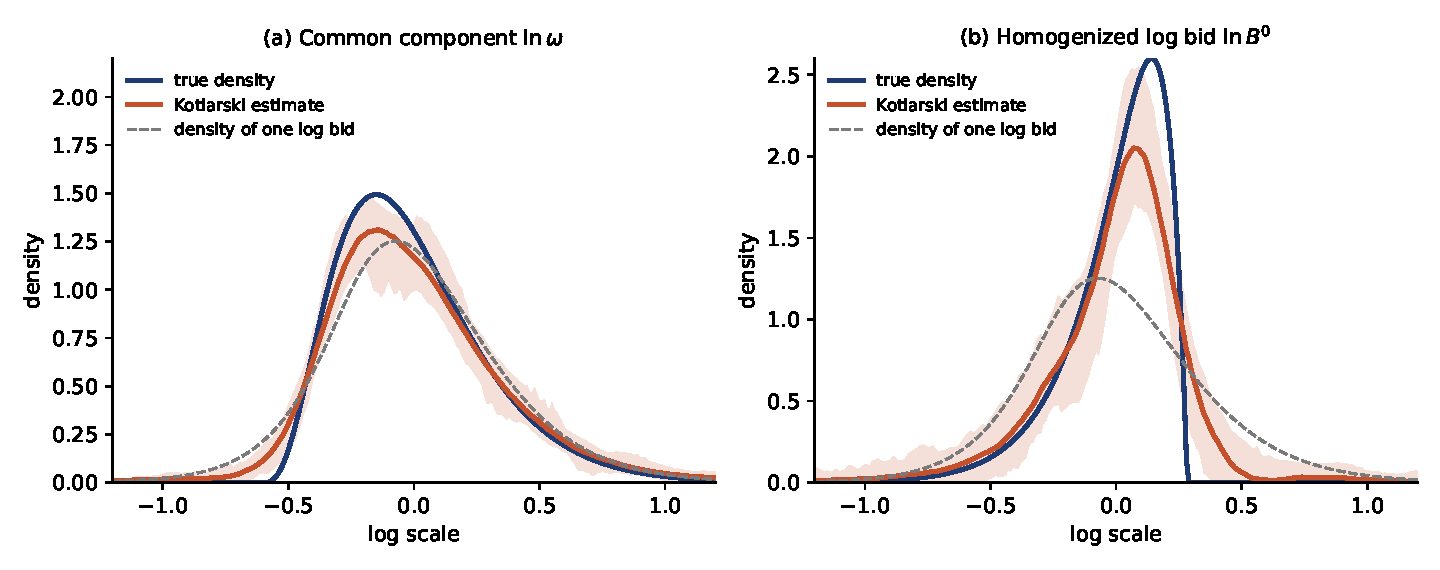
\includegraphics[width=\textwidth]{figures/ch15/kotlarski_demo.pdf}
\caption{Deconvolution of log bids with \eqref{eq:15-kotlarski} and the damped inverse
\eqref{eq:15-damped-inverse} (our simulation, seed 15703). $T=1{,}000$ auctions with four bidders of
one type. $\ln\omega$ is a standardized $\text{Gamma}(4)$ variable scaled to standard deviation $0.3$,
and $\ln B^0$ is a reflected standardized $\text{Gamma}(2)$ variable scaled to standard deviation
$0.2$. Characteristic functions average over all ordered pairs of bids. $T_c$ is chosen by
Krasnokutskaya's moment criterion on the grid $3,4,\dots,25$, and the largest value is usually chosen.
Lines show the median over 200 samples, bands the 5--95 percent range. The dashed curve is the density
of a single log bid.}
\label{fig:15-kotlarski}
\end{figure}

\subsubsection{Monte Carlo evidence}

The published Monte Carlo study is reported in figures only (Section 4.3, pp.~306--309). Costs are
multiplicative, $C=\omega A$, with distributions shaped like the estimated ones. Each sample has two
bidders of each type, as in the data, and $T=250$, $200$ or $150$ auctions, so each private component
is estimated from 500, 400 or 300 bids. The 5--95 percent bands of the estimated distributions
contain the true ones except in the smallest samples, where the bands are wide and miss small parts
of the true functions (p.~306).

The WP ran a more detailed study with tables, which we report next. Its design is additive,
$C=\omega+A$, with symmetric bidders (WP, Section 4.4). $A$ is
uniform with mean zero and variance $0.33$. $\omega$ follows a power distribution with exponent 3 and
mean $10.5$, with variances chosen so that bid functions have closed forms. Each sample has $T=400$
auctions with two bidders, and each experiment is replicated 500 times. Five cases are studied (WP,
Table 1b). Case 1 has independent costs. Case 2 has unobserved heterogeneity with $\Var(\omega)=0.04$
or $0.34$. Case 3 is APV, with bidders who observe only $C$. Cases 4 and 5 add correlation among
private components or between private and common components.
The estimator behaves as theory predicts (WP, Table 2b). With independent costs the estimated
$\Var(\omega)$ is $0.013$, with interval $[0.01,0.02]$, close to degenerate. The estimated markup is
$0.362$ against a true $0.38$. With heterogeneity, the estimated variances of $A$ are $0.321$ and $0.318$
against $0.33$. The estimated variances of $\omega$ are $0.0362$ and $0.335$ against $0.04$ and $0.34$.
Markups are $0.082$ and $0.092$ against $0.09$. WP Table 3b prints a true markup of $0.03$ for
$\Var(\omega)=0.34$, so the two tables of the paper disagree (see the notes to
\cref{tab:15-krasno-mc}). With APV data the procedure misreads the information
structure. The estimated markup is $0.18$ against a true $0.47$ in case 3a, and $0.33$ against $0.21$
in case 3b. With correlated components, the variance of $\omega$ is overstated and that of $A$
understated. The bias is negligible when the correlation is about 5 percent of $\Var(A)$ (WP, pp.
19--20).

The second experiment applies IPV and APV estimators to data with heterogeneity.
\Cref{tab:15-krasno-mc} reproduces the results. As $\Var(\omega)$ grows, both misspecified procedures
understate mean costs, overstate their variance, and overstate markups. Krasnokutskaya reports that the
bias becomes significant once the correlation of costs reaches about $0.3$ (WP, p.~21). Their bid
functions are flatter than the truth, and the IPV estimate is especially flat at the low end. A known
common component produces a bid distribution with thin tails, which IPV reads as extreme shading
at the bottom.

\begin{table}[htbp]
\centering
\caption{Misspecified estimators applied to data with unobserved heterogeneity (Krasnokutskaya 2004
working paper, Table 3b, not in the published article)}
\label{tab:15-krasno-mc}
\begin{tabular}{llccc}
\toprule
$\Var(\omega)$ & Procedure & $\E(C)$ & $\Var(C)$ & $\E(\text{markup})$\\
\midrule
0.04 & True model & 10.5 & 0.37 & 0.09\\
     & UH  & [10.44, 10.59] & [0.32, 0.41] & [0.078, 0.095]\\
     & APV & [10.37, 10.48] & [0.35, 0.44] & [0.097, 0.12]\\
     & IPV & [10.41, 10.5]  & [0.34, 0.44] & [0.95, 0.11]\\
\addlinespace
0.34 & True model & 10.5 & 0.67 & 0.03\\
     & UH  & [10.28, 10.64] & [0.63, 0.72] & [0.02, 0.038]\\
     & APV & [8.31, 9.57]   & [0.89, 1.02] & [0.042, 0.55]\\
     & IPV & [8.85, 9.84]   & [0.83, 0.96] & [0.4, 0.52]\\
\addlinespace
1    & True model & 10.5 & 1.33 & 0.01\\
     & UH  & [10.15, 10.76] & [1.27, 1.43] & [0.008, 0.014]\\
     & APV & [7.6, 8.8]     & [2.01, 2.27] & [0.033, 0.047]\\
     & IPV & [8.1, 9.2]     & [1.86, 2.05] & [0.31, 0.044]\\
\bottomrule
\end{tabular}

\smallskip
\begin{minipage}{0.93\textwidth}
\footnotesize \textit{Notes.} Additive design $C=\omega+A$, two symmetric bidders, 400 auctions, 500
replications. UH, APV and IPV denote estimators that assume unobserved heterogeneity, affiliated
private values and independent private values. Brackets give 5th and 95th pointwise percentiles of
the estimator. Entries are reproduced as printed. Four markup intervals look like decimal-point
typos in the source: $[0.95,0.11]$, $[0.042,0.55]$, $[0.4,0.52]$ and $[0.31,0.044]$. The true markup
at $\Var(\omega)=0.34$ is printed as $0.03$ here and as $0.09$ in WP Table 1b.
\end{minipage}
\end{table}

\subsubsection{Application: Michigan highway maintenance}

\casehead{Setting}
The Michigan Department of Transportation allocates road work by first-price sealed-bid auctions
(Section 5.1, pp.~306--307). It advertises a project 4 to 10 weeks before the letting, with a short
description of location, completion time and tasks. Firms can obtain a detailed description. The
department prepares an \emph{engineer's estimate} from the work required for each task, priced with
winning bids on similar past projects and deflated. Federal law requires the winning bid to be below
110 percent of this estimate, unless the state justifies an exception in writing. Bids and even
winning bids above the threshold appear in the data, so Krasnokutskaya treats the reserve as
nonbinding. Following the literature, she assumes bidders know how many rivals they face
(pp.~309--310).

\casehead{Data}
The sample covers maintenance projects with bituminous resurfacing as the main task, let between
February 1997 and December 2003, a total of 3,947 projects (p.~310). For each project she observes the
letting date, completion time, location, tasks, the identities and bids of all bidders, and the
engineer's estimate. Two arguments support the model. Resurfacing jobs are precisely specified and
simple, which favors private values. Their costs depend on elevation, curvature, traffic and the age
of the surface, which contractors see on site visits and the researcher does not. Firms differ mainly
in size, which every participant observes, so she allows two observable types. A bidder is
\emph{regular} if it won at least \$10 million of projects in each year of the data and has at least
100 employees (p.~310). She notes that this matches the industry's definition of a large bidder
(footnote 19). All other bidders are \emph{fringe}. The WP used a different definition, which the
published one replaces. There a regular bidder submits at least 12 bids per year, ranks in the top 10
percent of firms by employment and works in three or more specializations (WP, Section 5.2).

The number of bidders ranges from 1 to 11. More than 85 percent of projects have 2 to 6 bidders, and
the mean is 3.4 with standard deviation 1.3. About 75 percent of engineer's estimates lie between
\$100,000 and \$1,000,000, with 5 percent below and 20 percent above (p.~310).
\Cref{tab:15-krasno-desc} reproduces her descriptive table. The gap between the estimate and the
winning bid grows with the number of bidders. \emph{Money left on the table} is the gap between the two
lowest bids relative to the estimate. It averages 7 percent and falls from 11 to 4 percent as the
number of bidders rises (p.~311).

\begin{table}[htbp]
\centering
\caption{Michigan highway maintenance auctions: descriptive statistics by number of bidders
(Krasnokutskaya 2011, Table 1, and WP Table 1c)}
\label{tab:15-krasno-desc}
\begin{tabular}{lccccccc}
\toprule
Number of bidders & Overall & 1 & 2 & 3 & 4 & 5 & 6\\
\midrule
Number of observations & 3,947 & 71 & 673 & 1,126 & 1,026 & 365 & 192\\
\addlinespace
Engineer's estimate & 12.80 & 13.34 & 10.27 & 12.60 & 13.90 & 12.90 & 16.40\\
 & (2.35) & (2.88) & (1.41) & (3.02) & (2.26) & (1.79) & (3.39)\\
Winning bid & 11.10 & 14.12 & 10.00 & 11.80 & 12.90 & 11.80 & 15.20\\
 & (2.32) & (3.05) & (1.50) & (2.89) & (2.25) & (1.66) & (3.35)\\
Money left on the table & 0.07 & NA & 0.11 & 0.08 & 0.07 & 0.05 & 0.04\\
 & (0.05) & NA & (0.08) & (0.06) & (0.06) & (0.05) & (0.04)\\
Number of regular bidders & 1.92 & 0.79 & 1.43 & 1.65 & 2.07 & 2.16 & 2.29\\
 & (1.06) & (0.41) & (0.62) & (0.72) & (0.98) & (1.21) & (1.32)\\
\bottomrule
\end{tabular}

\smallskip
\begin{minipage}{0.93\textwidth}
\footnotesize \textit{Notes.} Means with standard deviations in parentheses. The engineer's estimate and the
winning bid are in hundreds of thousands of dollars. Money left on the table is the difference
between the lowest and second-lowest bids divided by the engineer's estimate. The overall column
includes projects with 7 to 11 bidders. The published Table 1 prints the columns for 2 to 6 bidders as
shown. Its overall column is misprinted, with 1.175 and 4.660 in every row, and its one-bidder column
prints the overall values. We take these two columns from WP Table 1c.
\end{minipage}
\end{table}

\casehead{Evidence of heterogeneity}
Krasnokutskaya first tests for heterogeneity (Section 5.2, p.~311). She conditions on a linear index
of observables estimated by ordinary least squares. The index contains the engineer's estimate,
duration, highway type, year, month and district dummies, and the number of tasks. The tests run
within cells defined by the main task and the number of bidders (Appendix A.3). The first test asks
whether two bids from the same auction are independent given the index, which is the null of IPV
against heterogeneity. The second asks whether two ratios built from four distinct bids are
independent, restriction (W3). This is the null of heterogeneity against APV. For resurfacing
projects with four regular bidders, the $p$-values are 0.03 and 0.52. IPV is rejected at the 5 percent
level, and heterogeneity is not rejected against APV. The test sample has 370 auctions with
estimates between \$350,000 and \$750,000 (footnote 21). \Cref{tab:15-krasno-index} reproduces the
index regressions.

\begin{table}[htbp]
\centering
\caption{Linear index of log bids on observables (Krasnokutskaya 2011, Table 2)}
\label{tab:15-krasno-index}
\begin{tabular}{lcc}
\toprule
 & Test subsample & Estimation subsample\\
\midrule
Constant & 0.375 & 0.327\\
 & (0.010) & (0.012)\\
Engineer's estimate & 0.8413 & 0.8113\\
 & (0.028) & (0.025)\\
Duration & 0.0011 & 0.0015\\
 & (0.0013) & (0.0011)\\
Tasks & 0.0014 & 0.0012\\
 & (0.0007) & (0.0009)\\
\addlinespace
$(n_{\text{regular}},n_{\text{fringe}})$ & (4,0) & (2,2)\\
Number of projects & 370 & 226\\
$R^2$ & 33\% & 17\%\\
\bottomrule
\end{tabular}

\smallskip
\begin{minipage}{0.8\textwidth}
\footnotesize \textit{Notes.} Ordinary least squares estimates of the mean of the log bid, with the figures in
parentheses as printed. Variables are labeled as in the source, which does not say whether the
engineer's estimate enters in logs. The test subsample is used for the specification tests and the
estimation subsample for the deconvolution.
\end{minipage}
\end{table}

The WP looked at the same correlation more directly. Its regressions of log bids in four-bidder
resurfacing projects are reproduced in \cref{tab:15-krasno-bids} (WP, Table 2c). Bids rise with the
engineer's estimate, distance to the site and the firm's backlog (``load remaining''), and fall with
the number of potential bidders. Fringe firms bid more. Adding auction dummies raises $R^2$ from
$0.857$ to $0.914$. The random-effects estimates attribute $\rho=0.48$ of the residual variance of log
bids to the auction level. The printed variance components imply a smaller share,
$\frac{0.16}{0.16+0.22}\approx0.42$. The text reports $R^2$ values of $0.81$ and $0.89$ for the same
regressions (WP, p.~25), which also differ from the table.
Common variation across bids in an auction that observables do not explain is the signature of
unobserved heterogeneity.

\begin{table}[htbp]
\centering
\caption{Regressions of log bids, four-bidder resurfacing projects (Krasnokutskaya 2004 working
paper, Table 2c, selected rows)}
\label{tab:15-krasno-bids}
\begin{tabular}{lccc}
\toprule
 & OLS & Auction dummies & Random effects\\
\midrule
Log (estimate) & 0.9100 & 0.9300 & 0.8800\\
 & (0.0530) & (0.1400) & (0.1300)\\
Duration & $-0.0210$ & $-0.0490$ & $-0.0210$\\
 & (0.0500) & (0.0250) & (0.0500)\\
Distance & 0.0312 & 0.0540 & 0.0270\\
 & (0.0160) & (0.0120) & (0.0160)\\
Log (load remaining) & 0.0310 & 0.0392 & 0.0270\\
 & (0.0157) & (0.0127) & (0.0144)\\
Number of potential bidders & $-0.1100$ & $-0.1330$ & $-0.1100$\\
 & (0.0310) & (0.0230) & (0.0290)\\
Fringe (dummy) & 0.2500 & 0.2800 & 0.2200\\
 & (0.1100) & (0.1200) & (0.1000)\\
Constant & 0.1750 & 0.1620 & 0.1680\\
 & (0.0580) & (0.0520) & (0.0480)\\
\addlinespace
$R^2$ & 0.857 & 0.914 & 0.917 (overall)\\
\bottomrule
\end{tabular}

\smallskip
\begin{minipage}{0.93\textwidth}
\footnotesize \textit{Notes.} Dependent variable $\ln B$. 947 bids. Standard errors in parentheses. Omitted rows
are length and dummies for marking, landscaping and signs. All columns include district and
regular-bidder dummies. Coefficients on auction-level variables in the auction-dummies column are
reproduced as printed. Random effects: $R^2$ within $0.00$, between $0.934$, $\sigma_u^2=0.16$,
$\sigma_\varepsilon^2=0.22$, $\rho=0.48$ as printed, although $\frac{\sigma_u^2}{\sigma_u^2+\sigma_\varepsilon^2}=0.42$.
These regressions are not in the published article.
\end{minipage}
\end{table}

Correlated bids could have other sources. Common values are unlikely, she argues, because simple
maintenance projects carry little project-level uncertainty. Collusion is harder to rule out, since
each test assumes a particular scheme (p.~311). Following \citet{PorterZona1993}, if only the winning
bid reflected a cost, the losing bids would be phony. She recovers the regular and fringe bid
distributions from the winning bid alone with the method of \citet{AtheyHaile2002}. These match the
distributions estimated from losing bids, which she reads as evidence against collusion (p.~312).

\casehead{Results}
Estimation uses the 226 projects with an engineer's estimate between \$300,000 and \$580,000, a
completion time of 3 to 6 months, and two regular and two fringe bidders (p.~312). Results for other
cells are described as qualitatively similar. Residual variation in observables is removed by
homogenization in logs, as in \cref{sec:15-uh-sep}. She regresses log bids on the observables of
\cref{tab:15-krasno-index} and deconvolves the residuals. Costs are then
$C_{it}=e^{z_t'\theta}\,\omega_tA_{it}$, and the fitted scaling factor $e^{z_t'\theta}$ is added back
for the variance decomposition and the comparisons (p.~312, footnote 22).

\Cref{tab:15-krasno-results} collects the main numbers (pp.~313--316). The heterogeneity component
$\omega$ has mean $0.98$ and standard deviation $0.204$. The \emph{common component}
$e^{z'\theta}\omega$, which combines the observed and the unobserved parts, has mean \$392,000 and
standard deviation \$78,890. The private components of the two types are similar. The fringe mean is
$1.06$, against the normalized regular mean of $1$, and the standard deviations are $0.14$ (regular)
and $0.13$ (fringe). Fringe firms thus have higher but slightly less dispersed costs. A test of equal
private-component distributions gives a $p$-value of 0.69 (p.~314). The text says that this rejects
equality at the 10 percent level, which a $p$-value of 0.69 does not support.

To split the variance of costs, she uses the exact identity for independent factors,
\[
\Var(\omega A)=\E[\omega^2]\E[A^2]-(\E\omega)^2(\E A)^2=(\E\omega)^2\Var(A)+(\E A)^2\Var(\omega)+\Var(\omega)\Var(A),
\]
and drops the last, second-order term (p.~314). She attributes $(\E\omega)^2\Var(A)$ to private
information and $(\E A)^2\Var(\omega)$ to common knowledge. Both terms are invariant to the
normalization, since $(\omega,A)\mapsto(c\,\omega,\frac{A}{c})$ leaves each unchanged (footnote 25).
For homogenized costs the private term accounts for almost 31 percent of the variance, and for 31.3
percent of the exact variance (footnote 26). For total costs, including the observed scaling factor,
it accounts for 34.4 percent (footnote 27). The rounded moments of regular bidders reproduce these
shares. For homogenized costs,
\[
\frac{(\E\omega)^2\Var(A)}{(\E\omega)^2\Var(A)+\Var(\omega)}
=\frac{0.98^2\times0.14^2}{0.98^2\times0.14^2+0.204^2}
=\frac{0.0188}{0.0188+0.0416}\approx0.31 .
\]
For total costs in thousands of dollars, the same ratio is
$\frac{392^2\times0.14^2}{392^2\times0.14^2+78.89^2}=\frac{3{,}012}{3{,}012+6{,}224}\approx0.33$, close
to the reported 34.4 percent. Private information therefore explains about a third of the variation
in costs, the 34 percent that \citet[p.~103]{HortacsuPerrigne2021} report for this article. The other
two thirds is information that all bidders share and the econometrician does not see.

The WP reported different figures from a different sample, and the published estimates supersede
them. Its sample had 487 larger and longer projects, with estimates between \$500,000 and \$900,000
and durations of 6 to 9 months (WP, p.~25). Its common component had mean \$654,000 and standard
deviation \$31,700, and its private components had standard deviations 0.22 and 0.23. Its text gave a
private share of ``almost 15\%'' (WP, p.~26), while its abstract and conclusion gave 25 percent.
Neither figure follows from its own moments. With $\E\omega=654$, $\sqrt{\Var(\omega)}=31.7$ and
$\sqrt{\Var(A)}=0.22$, the private term is $654^2\times0.22^2\approx20{,}700$ and the common term is
$31.7^2\approx1{,}005$, a private share near 95 percent.

Normalized markups $\frac{b-c}{c}$ range from 0.1 to 25 percent for regular bidders, with an average
of 8.4 percent. For fringe bidders they range from 0.1 to 18 percent, with an average of 6.1 percent
(p.~314). Fringe firms thus have higher costs, slightly less dispersed costs and lower markups than
regular firms, as \citet[p.~103]{HortacsuPerrigne2021} summarize. To measure inefficiency she draws
pseudo-samples of costs for 250 auctions with three bidders each, as printed. She computes bids from
the estimated bid functions and records how often the lowest bid does not come from the lowest cost.
Over 1,000 repetitions the probability of an inefficient outcome averages 5 percent, with a 95 percent
range of $[3.6,6.2]$. The misallocation raises the cost of procurement by 2 percent, with range
$[1.3,2.8]$ (p.~314). The WP's figure of 28 percent, with range $[26.6,30.3]$, came from pseudo-samples
of two regular and two fringe costs in its own sample (WP, pp.~25--28). It is superseded.

The IPV and APV estimators of \citet{GuerrePerrigneVuong2000} and \citet{LiPerrigneVuong2002},
applied to the same data, give larger markups and more dispersed costs (pp.~314--316). The average
markup of regular bidders is 14 percent under APV and 19 percent under IPV, against 8.4 percent under
heterogeneity. For fringe bidders the figures are 12.2, 16.5 and 6.1 percent. The variance of costs
estimated under heterogeneity is 18 percent lower than under APV and 22 percent lower than under IPV.
\Cref{fig:15-krasno-bidfn} shows why. Both misspecified bid functions lie above the heterogeneity
estimate, and their confidence bands meet its band only near the top of the support. The misspecified
estimators read common variation in bids as private information. They therefore infer lower costs and
larger markups from the same bids.

\begin{table}[htbp]
\centering
\caption{Michigan resurfacing auctions: estimates under unobserved heterogeneity (UH), APV and IPV
(Krasnokutskaya 2011, Section 5.3, with the superseded WP estimates)}
\label{tab:15-krasno-results}
{\small
\begin{tabularx}{\textwidth}{>{\raggedright\arraybackslash}Xcccc}
\toprule
 & \multicolumn{3}{c}{Published article} & WP (2004)\\
\cmidrule(lr){2-4}\cmidrule(lr){5-5}
 & UH & APV & IPV & UH\\
\midrule
Average markup $\frac{b-c}{c}$, regular bidders & 8.4\% & 14\% & 19\% & 7.5\%\\
Average markup $\frac{b-c}{c}$, fringe bidders & 6.1\% & 12.2\% & 16.5\% & 6\%\\
Probability of an inefficient allocation & 5\% [3.6, 6.2] & & & 28\% [26.6, 30.3]\\
Cost increase from misallocation & 2\% [1.3, 2.8] & & & \\
Cost variance under UH relative to column & & 18\% lower & 22\% lower & \\
\addlinespace
Common component, mean (s.d.) & \$392,000 (\$78,890) & & & \$654,000 (\$31,700)\\
Heterogeneity component $\omega$, mean (s.d.) & 0.98 (0.204) & & & \\
Private component $A$, s.d. regular, fringe & 0.14, 0.13 & & & 0.22, 0.23\\
Private component $A$, fringe mean (regular $=1$) & 1.06 & & & 1.2\\
Private share of variance, homogenized costs & 31\% & & & \\
Private share of variance, total costs & 34.4\% & & & 15\% or 25\%\\
\bottomrule
\end{tabularx}}

\smallskip
\begin{minipage}{0.93\textwidth}
\footnotesize \textit{Notes.} Published estimates use 226 projects with two regular and two fringe bidders,
engineer's estimates between \$300,000 and \$580,000 and durations of 3 to 6 months. Brackets give 95
percent ranges over 1,000 simulated pseudo-samples. The WP used 487 projects with estimates between
\$500,000 and \$900,000 and durations of 6 to 9 months. Its private share is 15 percent in the text and
25 percent in the abstract, and neither follows from its printed moments (see text). The WP also
reported inefficiency rates of 34 and 38 percent under IPV and APV and extra markups of \$61,000 and
\$33,000. Its cost variances under UH were 35 and 25 percent below IPV and APV (WP, pp.~25--28).
\end{minipage}
\end{table}

\begin{figure}[htbp]
\centering
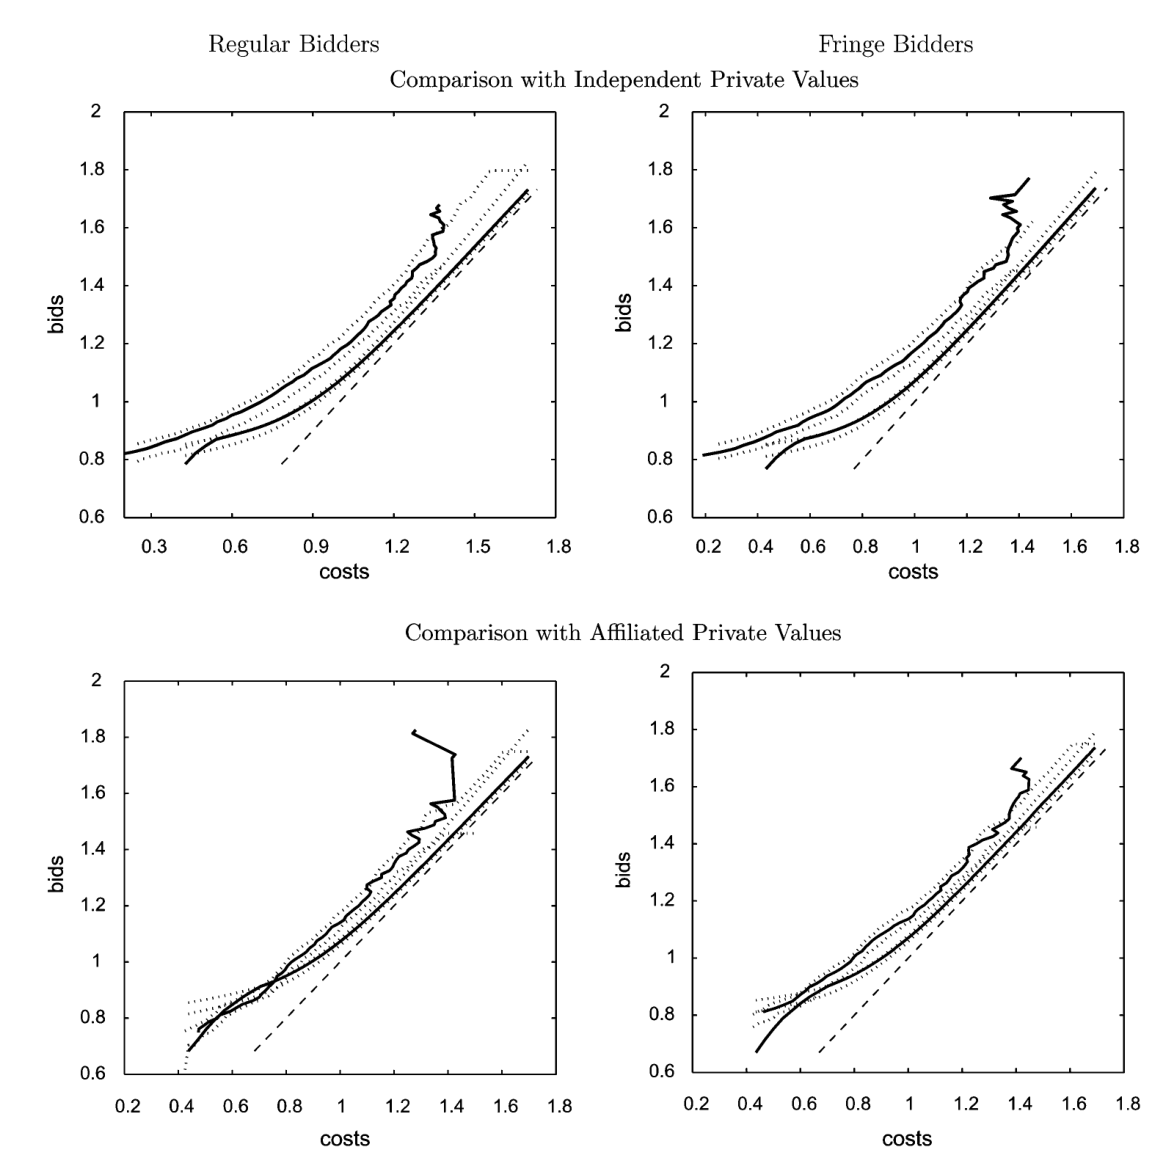
\includegraphics[width=0.86\textwidth]{figures/ch15/krasno_pub_fig5.png}
\caption{Expected bid functions, bids against costs in homogenized units, for regular (left) and
fringe (right) bidders. The top row compares the heterogeneity estimate with IPV, and the bottom row
compares it with APV. In each panel the dashed line is the diagonal. The lower solid line is the
estimate under unobserved heterogeneity, and the upper solid line is the misspecified estimate. Dotted
lines are pointwise 95 percent bootstrap bands. Source: Krasnokutskaya (2011), Figure 5.}
\label{fig:15-krasno-bidfn}
\end{figure}

\casehead{Reserve prices}
The estimates feed a design exercise (pp.~316--317). To avoid the complications of asymmetric
auctions, she uses the estimates for regular bidders only and treats bidders as symmetric. The
government minimizes the expected cost of procurement. If no bid falls below the maximum acceptable
price $r$, the project waits. Waiting costs $c_0$, which combines the cost of delay and the expected
cost of completing the work later. In the notation of \cref{sec:14-proc-other}, $c_0$ plays the role
of the buyer's value $u_0$. Suppose first that the government observes $\omega$. Costs then have the
distribution $F_C(c\mid\omega)=F_1\big(\frac{c}{\omega}\big)$ and density
$f_C(c\mid\omega)=\frac{1}{\omega}f_1\big(\frac{c}{\omega}\big)$. The virtual cost
\eqref{eq:14-virtual-cost} is
\[
J(c\mid\omega)=c+\frac{F_C(c\mid\omega)}{f_C(c\mid\omega)}
=c+\omega\,\frac{F_1(\frac{c}{\omega})}{f_1(\frac{c}{\omega})}
=\omega\,J_1\Big(\frac{c}{\omega}\Big),
\qquad J_1(a)=a+\frac{F_1(a)}{f_1(a)} .
\]
The optimal maximum price solves $J(r^*\mid\omega)=c_0$, so that
\[
r^*(\omega)=\omega\,J_1^{-1}\Big(\frac{c_0}{\omega}\Big).
\]
The reserve does not scale with $\omega$, because $c_0$ is fixed in dollars. This benchmark is case
(a) of her four candidates. In case (b) the government does not observe $\omega$. It chooses one reserve
that minimizes the expected cost averaged over $F_\omega$. Cases (c) and (d) use the cost distributions
estimated under IPV and APV. Each candidate is evaluated under the heterogeneity model. Since $c_0$ is
not observed, she reports results for several values.

\Cref{tab:15-krasno-reserve} reproduces her Table 4 for projects with an engineer's estimate of
\$400,000. Reserves based on IPV estimates raise the expected cost above the benchmark by 8.3 to 20.6
percent of $c_0$, which she rounds to 9 to 20 percent. Relative to the benchmark cost, the increase is 10
to 35 percent. The reserve of case (b) costs only
about 1 percent of $c_0$, or 1 to 2 percent of the benchmark. APV-based reserves do worse still. Both
misspecified models also imply too low a probability that any bid is submitted. For $c_0$ of at
least 150 percent of the mean cost, which she regards as the realistic range, accounting for
heterogeneity saves at least 16 percent of the benchmark cost (p.~317). This is large next to markups
of only 6 to 8 percent of costs.

\begin{table}[htbp]
\centering
\caption{Optimal reserve prices under alternative models (Krasnokutskaya 2011, Table 4)}
\label{tab:15-krasno-reserve}
{\small
\setlength{\tabcolsep}{4pt}
\begin{tabular}{clcccc}
\toprule
 & & \multicolumn{2}{c}{Unobserved heterogeneity} & & \\
\cmidrule(lr){3-4}
$c_0$ & & Benchmark (a) & Expected (b) & IPV (c) & APV (d)\\
\midrule
5 & Probability of a bid & 0.29 & 0.28 & 0.07 & 0.03\\
  & & (0.26, 0.31) & (0.25, 0.31) & (0.05, 0.09) & (0.02, 0.06)\\
  & Expected cost, \% of $c_0$ & 85.2 & 86.5 & 93.5 & 96.8\\
  & & (83, 87) & (85, 88) & (91, 95) & (95, 98)\\
  & Expected cost, \% of benchmark & & 101.4 & 109.7 & 113.6\\
\addlinespace
7 & Probability of a bid & 0.45 & 0.42 & 0.20 & 0.04\\
  & & (0.43, 0.46) & (0.40, 0.43) & (0.18, 0.21) & (0.03, 0.05)\\
  & Expected cost, \% of $c_0$ & 72.1 & 73.2 & 83.9 & 95.4\\
  & & (71.2, 73.5) & (72.3, 75.1) & (81.2, 84.7) & (94.3, 96.2)\\
  & Expected cost, \% of benchmark & & 101.6 & 116.4 & 132.4\\
\addlinespace
10 & Probability of a bid & 0.58 & 0.55 & 0.20 & 0.037\\
   & & (0.56, 0.59) & (0.54, 0.56) & (0.18, 0.21) & (0.03, 0.04)\\
   & Expected cost, \% of $c_0$ & 58.1 & 59.1 & 78.7 & 94.7\\
   & & (56.2, 59.5) & (57.8, 60.1) & (76.5, 79.7) & (94.0, 95.6)\\
   & Expected cost, \% of benchmark & & 101.6 & 135.5 & 163.0\\
\bottomrule
\end{tabular}}

\smallskip
\begin{minipage}{0.93\textwidth}
\footnotesize \textit{Notes.} Projects with an engineer's estimate of \$400,000, regular bidders treated as
symmetric. $c_0$ is the cost of not awarding the project today, in hundreds of thousands of dollars.
(a) The government observes $\omega$. (b) One reserve minimizes the cost averaged over $F_\omega$. (c),
(d) Reserves computed from IPV and APV estimates. All candidates are evaluated under the heterogeneity
estimates. Intervals in parentheses as printed.
\end{minipage}
\end{table}

\casehead{Tests of the assumptions and robustness}
Her Table 3 reports tests of the restrictions of Proposition 2 (pp.~317--318). The ratio test (W3)
of Section 5.2 gives a $p$-value of 0.52. Independence of the private components from $\omega$ gives
0.81 (bootstrap) and 0.75 (subsampling). Independence of the private components across bidders gives
0.43 and 0.63. The text adds a $p$-value of 0.63 for the test of part 1 of Proposition 2. None of the
tests rejects.
One robustness check addresses dynamics. Capacity constraints would link bids across auctions and bias
the estimated joint characteristic function. She re-estimates the model on projects for which every
regular bidder's backlog lies between 30 and 75 percent of the largest backlog observed in the data.
The sample shrinks and the estimates are less precise, but the variance decomposition and the biases
from misspecification are similar (pp.~318--319). The WP adds a fit check. Pseudo-bids simulated from
the estimated model reproduce the estimated densities of actual bids, with the largest gap near the
mode (WP, p.~28, Figure 3c).

\subsubsection{Assessment}

Krasnokutskaya's paper gave the first nonparametric identification result for first-price auctions
with unobserved heterogeneity. It turned the repeated-measurement idea into an auction estimator, and it
quantified how IPV and APV estimators err. In Michigan resurfacing, private information explains only
about a third of cost variation, 34 percent of the variation in total costs (p.~319). The remaining
two thirds is common knowledge among bidders. Ignoring it raises the estimated average markup of
regular bidders from 8.4 percent to 14 percent (APV) or 19 percent (IPV). Reserve prices based on the
misspecified models would raise procurement costs by 10 to 63 percent of the benchmark. The asymmetry
between regular and fringe firms matters less, with inefficient awards in 5 percent of auctions at a
cost of 2 percent. \citet[p.~103]{HortacsuPerrigne2021} summarize the published findings in the same
terms. The WP's figures differ, with a 28 percent inefficiency rate and a private share of 15 or 25
percent, and the published article replaces them.

The approach has four limits. First, heterogeneity must be scalar and enter by a known separable
form, and the two-dimensional extension needs four bids. Second, independence of $\omega$ and $\bm A$
and across bidders is essential. Her tests do not reject it (Table 3), but they have limited power,
and the model leaves no room for affiliation among the private components. Third, estimation is cell
by cell in $(n,n_1)$ and covariates, with slow rates, and the published estimates rest on 226 projects.
\citet[footnote 22]{AtheyLevinSeira2011} give this reason for not using the method on timber data.
``[O]ne would want to estimate the model separately for each vector of participants $(n_L,n_M)$ and we
simply don't have the data to do this.'' Fourth, the number of bidders is taken as exogenous. Entry
that responds to $\omega_t$ would violate (D1), and Krasnokutskaya leaves participation to separate
work.

\citet{KrasnokutskayaSeim2011} add participation in later work on California highway procurement,
where small firms receive a bid preference \citep[p.~123]{HortacsuPerrigne2021}. They estimate an
entry model of the \citet{LevinSmith1994} type with cost asymmetries. Entry costs are 2.2 to 3.9
percent of the engineer's estimate for small firms and 3.1 to 3.3 percent for large firms. The state
aims to award 25 percent of procurement dollars to small firms. The authors first evaluate this goal for
one illustrative project \citep[pp.~2655--2656, Figure~1]{KrasnokutskayaSeim2011}. With fixed
participation, reaching the goal on that project requires a small-firm discount of more than 50 percent,
at a predicted cost increase of 0.23 percent. Allowing entry to respond, that discount would deter large
firms and raise the cost by 7.8 percent. A discount of about 20 percent then reaches the goal on the same
project, and the procurement cost rises by 3.2 percent. These figures describe a single project. For all
projects together, the article's text reports that a 15 percent discount approximately meets the aggregate goal, at a
cost increase of 1.4 percent (p.~2678). Their Table~11 instead lists, for the same 15 percent discount, a
small-firm share of work of 31.9 percent and a cost increase of 2.1 percent (p.~2679). The article does
not reconcile the two sets of numbers. \Cref{sec:14-proc-other} discusses the theory of such preferences. Later work relaxes separability.
\citet{HuMcAdamsShum2013} identify nonseparable heterogeneity from three bids per auction (as described
by \citealp{Roberts2013}, p.~5). \citet{Asker2010} applies the deconvolution to knockout bids in a
stamp cartel (\cref{sec:13-asker-structural}).

\subsection{Parametric approaches}\label{sec:15-uh-param}

A parametric first step trades flexibility in the distributions for flexibility in how covariates
and heterogeneity enter. \citet{AtheyLevinSeira2011} specify Weibull bid distributions conditional on a
Gamma-distributed multiplicative component, which integrates out in closed form
(\cref{sec:15-als}, \cref{prop:15-als-lik}). Values then follow from the first-order condition at any
$\omega$, as in \cref{thm:15-krasno}. The parametric form lets heterogeneity affect types
differently and keeps estimation feasible with many participant configurations
\citep[Section 6.1.2]{AtheyHaile2007}. \citet{RobertsSweeting2013} estimate values with heterogeneity
in values and entry costs by simulated maximum likelihood with importance sampling (as described by
\citealp{Roberts2013}, p.~6). \citet{HongShum2002} model the median of the bid distribution as a normal
random variable whose mean depends on the number of bidders (as described by
\citealp{Krasnokutskaya2011}, p.~296). Finite mixtures of parametric distributions offer a middle
ground \citep[eqs. (6.7)--(6.9)]{AtheyHaile2007}. In all of these, identification of the
heterogeneity distribution leans on functional form.

\subsection{Reserve prices as a control for quality: Roberts (2013)}\label{sec:15-roberts}

\casehead{Idea}
Every method so far uses only bidders' behavior. \citet{Roberts2013} uses the seller's behavior. A
seller who knows the object well probably observes what the bidders observe. If the reserve price
rises with the unobserved quality, then reserve prices reveal it. The logic is that of a control
function, close to the use of investment as a proxy for productivity by \citet{OlleyPakes1996}.
\citet{Roberts2013} credits the suggestion to Athey and Haile, and \citet[footnote 56]{AtheyHaile2007}
point to restrictions from the seller's side as a direction worth exploring. His motivating evidence
is old. In the eggplant data of \citet{LaffontOssardVuong1995}, winning bids and reserve prices move
in tandem across auctions (\citealp{Roberts2013}, p.~7, citing their Appendix figure, reproduced in
\cref{fig:15-lov-reserve}).

\casehead{Model}
In auction $t$ there are $N_t$ bidders with symmetric independent private values. Observed
characteristics $Z_t$ and the scalar $\omega_t$ are known to the seller and the bidders, and the
econometrician observes only $Z_t$. Values are drawn from $F_V(\cdot\mid Z_t,\omega_t)$, which may depend
on $\omega_t$ in any way, but not on $N_t$. The seller sets the reserve price $r_t=m(Z_t,\omega_t)$ with
the same function $m$ in every auction. The bidders counted in $N_t$ include those with values below
$r_t$.

\begin{assumption}[\citealp{Roberts2013}, Assumption S1]\label{ass:15-roberts}
For every $z$, $m(z,\omega)$ is strictly increasing in $\omega$.
\end{assumption}

Reserves need not be optimal. Monotonicity is nevertheless what optimal reserves deliver when higher
$\omega$ makes higher values strictly more likely. Recall the virtual valuation \eqref{eq:14-psi} and write it conditionally on $\omega$ as
$\psi(t\mid\omega)=t-\frac{1-F_V(t\mid\omega)}{f_V(t\mid\omega)}$. The optimal reserve solves
$\psi(r^*\mid\omega)=v_0$, where $v_0$ is the seller's value (\cref{cor:14-optimal-reserve}).

\begin{proposition}[\citealp{Roberts2013}, Proposition 1]\label{prop:15-roberts1}
Suppose $\psi(t\mid\omega)$ is strictly increasing in $t$ for every $\omega$. If $V$ and $\omega$ are
affiliated, the optimal reserve price is nondecreasing in $\omega$. If they are strictly affiliated, so that the
likelihood ratio inequality below is strict for all $v_1<v_2$ and $\omega_1<\omega_2$, the optimal reserve price
is strictly increasing in $\omega$.
\end{proposition}

\begin{proof}
Take $\omega_1<\omega_2$. By \cref{prop:14-affil-mlrp}, affiliation gives the monotone likelihood ratio
property. For $v_1<v_2$,
$\frac{f_V(v_2\mid\omega_1)}{f_V(v_1\mid\omega_1)}\le\frac{f_V(v_2\mid\omega_2)}{f_V(v_1\mid\omega_2)}$,
strictly under strict affiliation. Integrating over $v_2>v_1$ gives
$\frac{1-F_V(v_1\mid\omega_1)}{f_V(v_1\mid\omega_1)}\le\frac{1-F_V(v_1\mid\omega_2)}{f_V(v_1\mid\omega_2)}$,
so the inverse hazard is nondecreasing in $\omega$ and $\psi(t\mid\omega_2)\le\psi(t\mid\omega_1)$ for every $t$.
Integration preserves strict inequality, so both inequalities are strict under strict affiliation. Let $r_1$
solve $\psi(r_1\mid\omega_1)=v_0$. Then $\psi(r_1\mid\omega_2)\le v_0$. Since $\psi(\cdot\mid\omega_2)$ is
strictly increasing, the solution $r_2$ of $\psi(r_2\mid\omega_2)=v_0$ satisfies $r_2\ge r_1$. Under strict
affiliation $\psi(r_1\mid\omega_2)<v_0$, and therefore $r_2>r_1$.
\end{proof}

Affiliation alone does not deliver \cref{ass:15-roberts}. Independent $V$ and $\omega$ are affiliated, yet the
optimal reserve then does not move with $\omega$. With $V$ uniform on $[0,1]$ and $v_0=0$, for example,
$r^*=\frac12$ for every $\omega$. The proof in \citet[Appendix~B]{Roberts2013} writes the affiliation inequality
as strict, which is the strict case of the proposition.

The second result is the identification theorem. Partition $Z=(Z_0,Z_1)$.

\begin{proposition}[\citealp{Roberts2013}, Proposition 2]\label{prop:15-roberts2}
Let \cref{ass:15-roberts} hold. Suppose (i) there is a value $z_1^*$ such that $m(z_0,z_1^*,\omega)=\omega$
for all $z_0$ and $\omega$, and (ii) $\omega$ is independent of $Z_1$ conditional on $Z_0$. Then reserve prices
identify $F_{\omega\mid Z_0}$, the function $m$ and each realization $\omega_t$. Suppose in addition that the
number $N$ of potential bidders is known and that unsold auctions are recorded. Then transaction prices identify
$F_V(v\mid Z,\omega)$ for every $v\ge m(Z,\omega)$, including the mass $F_V\big(m(Z,\omega)\mid Z,\omega\big)$, in
first-price and second-price (or ascending) auctions.
\end{proposition}

\begin{proof}
\emph{Step 1 (the law of $\omega$).} By (i) and (ii),
\[
\Pr(r_t\le u\mid Z_0=z_0,Z_1=z_1^*)=\Pr(\omega_t\le u\mid Z_0=z_0,Z_1=z_1^*)=F_{\omega\mid Z_0}(u\mid z_0).
\]
\emph{Step 2 (the function $m$).} For any $z_1$, monotonicity and (ii) give
\[
F_{\omega\mid Z_0}(u\mid z_0)=\Pr\big(m(z_0,z_1,\omega_t)\le m(z_0,z_1,u)\mid z_0,z_1\big)=F_{r\mid Z}\big(m(z_0,z_1,u)\mid z_0,z_1\big),
\]
so $m(z_0,z_1,u)=F_{r\mid Z}^{-1}\big(F_{r\mid Z}(u\mid z_0,z_1^*)\mid z_0,z_1\big)$ is identified.
\emph{Step 3 (realizations).} Since $m$ is strictly increasing in $\omega$, each observed $(r_t,Z_t)$
reveals $\omega_t=m^{-1}(Z_t,r_t)$.
\emph{Step 4 (values).} Treat $(Z_t,\omega_t)$ as observed covariates. For fixed $(Z,\omega)$ the
reserve $m=m(Z,\omega)$ is fixed, so transaction prices are censored at it. For $v\ge m$ let $W(v)$ be the
probability that the object goes unsold or sells at a price of at most $v$. Unsold auctions enter $W$, which
is why they must be recorded. In a second-price or ascending auction, the second-highest of the $N$ values is
at most $v$ exactly when this event occurs, so $W(v)=\Lambda_{N-1:N}\big(F_V(v\mid Z,\omega)\big)$. Inverting
$\Lambda_{N-1:N}$, which requires $N$, gives $F_V(v\mid Z,\omega)$. In a first-price auction whose bidders know $N$
but not who participates, as in \cref{sec:15-gpv-reserve}, let $\xi$ be the inverse bid function above the
reserve. The event occurs at a bid level $b\ge m$ when every potential bidder
stays out or bids at most $b$, so $W(b)=F_V\big(\xi(b)\mid Z,\omega\big)^N$. A bidder's win probability is
$W(b)^{\frac{N-1}{N}}$, and the first-order condition gives $\xi(b)=b+\frac{N}{N-1}\frac{W(b)}{W'(b)}$, as in
\eqref{eq:15-winbid-xi}. Then $F_V\big(\xi(b)\mid Z,\omega\big)=W(b)^{\frac1N}$. In both formats $W(m)$, the
probability of no sale or a sale at the reserve, gives the mass at $m$.
\end{proof}

With less data the conclusion narrows. Without $N$ the transformation from $W$ to $F_V$ is unknown, and without
the unsold auctions the prices of sold objects do not determine $W$. In second-price and ascending auctions that
record the number of actual bidders, transaction prices still identify the value distribution truncated at the
reserve, by \cref{prop:15-reserve-ident}(i).

\Citet[Proposition 2]{Roberts2013} states the result without the restriction $v\ge m(Z,\omega)$ and
without the requirements on $N$ and on unsold auctions. His proof cites \citet[Theorems 1 and 6]{AtheyHaile2002},
which assume no binding reserve. Below the
reserve, no bid is recorded and the data carry no information about $F_V(\cdot\mid Z,\omega)$, as in
\cref{thm:15-gpv-reserve}. The reserve does bind in his data, since 107 of 1,117 cars in one subsample
go unsold.

The normalization (i) holds in many functional forms, for example $r=z\,\omega$ or $r=z+\omega$ at a
suitable $z$ (\citealp{Roberts2013}, footnote 6). Unlike \cref{thm:15-krasno}, the result allows values
to depend on $\omega$ in any way. Among bids it needs only the transaction price, together with $N$ and the
record of unsold auctions. It requires instead that the
reserve depend on nothing that the bids do not reflect.

\casehead{Setting and data}
The data come from a wholesale used-car auction house in Suwon, South Korea, which held weekly auctions
between October 10, 2001 and November 27, 2002 (\citealp{Roberts2013}, Section 3).
Only registered dealers may bid, and more than 380 were registered. The house charges the seller \$50
per car and collects 2.2 percent of the price from each side if the car sells. Sellers set reserve
prices, usually with guidance from the house. Dealers receive car descriptions three days ahead and
inspect the cars for three hours or more before the auction. The format is a button auction with
reentry. The price rises by \$30 every three seconds while at least two buttons are pressed, and bidders
cannot see when rivals drop out. Of 28,334 passenger cars, Roberts studies 4,943 automatic
five-passenger sedans. Hyundai, Daewoo and Kia account for 42, 39 and 18 percent of auctions. The
average winning bid is \$3,661.83, the average reserve \$3,361.26, and 5.37 bidders bid on the
average car (\citealp{Roberts2013}, Table 1). Among bids, only the transaction price is recorded,
together with the identities of the winner and the runner-up and the number of bidders.

\casehead{Evidence for the assumptions}
Several facts support the model (\citealp{Roberts2013}, pp.~13--19). In regressions of the log
winning bid on car characteristics and dummies, $R^2$ rises from $0.903$ to $0.979$ when the log
reserve is added. The log reserve alone gives $0.966$ (Table 2). The residuals of winning bids and of
reserves, after both are regressed on characteristics, have correlation $0.890$, against a raw
correlation of $0.983$. For 107 unsold cars among 1,117 auctioned between October 10 and December 27,
2001, the same residual correlations are $0.942$ for the highest bid and $0.943$ for the average bid.
The reserve does not predict failure to sell. Its coefficient in a logit is $0.232$ with standard error
$0.263$ (Table 4). Moving the reserve from its 25th to its 75th percentile raises the failure
probability by about 2 percentage points. Reserves do not rise with the number of bidders, which a
signaling model of reserves would predict \citep{CaiRileyYe2007}. About four of the roughly five
bidders per car bid above the reserve, so the co-movement is not mechanical. Bidders look symmetric.
Three quarters of them buy 17 or fewer cars over 59 auction days.

\casehead{Estimation}
For Hyundai Sonatas, Roberts specifies $m(Z_1,\omega)=\mu(X;\vartheta)+\omega$ with $\E[\omega X]=0$
(p.~19). Here $X$ collects age and mileage. The function $\mu$ is quadratic in them, including their
interaction. The residual of this regression estimates $\omega_t$. The distribution of transaction prices $P_t$ given
$Z=(Z_1,\hat\omega)$ is estimated by a kernel estimator of a conditional distribution (his eq. (3)),
\[
\hat F_{P\mid Z=z}(v)=\frac{\sum_{t=1}^T\tilde{\mathcal K}_1\big(\frac{v-P_t}{h}\big)\,\mathcal K_2\big(\frac{z-Z_t}{h}\big)}{\sum_{t=1}^T\mathcal K_2\big(\frac{z-Z_t}{h}\big)},
\]
where $\tilde{\mathcal K}_1$ is the integral of a kernel $\mathcal K_1$. Gaussian kernels and Silverman's
bandwidth are used. Bid increments are ignored, so the transaction price is the second-highest of $N$
values, and $\hat F_V(v\mid z)=\Lambda_{N-1:N}^{-1}\big(\hat F_{P\mid Z=z}(v)\big)$ (his eq. (2), our
\eqref{eq:15-Lambda}). By \cref{prop:15-roberts2}, this inversion is valid for $v$ at or above the
reserve, and only if unsold auctions enter $\hat F_{P\mid Z}$ as described in Step 4. Roberts does not
treat the reserve as a censoring point. Since about four of the roughly five bidders per car bid above
the reserve, the censoring mainly affects the lower tail of the estimated value distribution.
Consistency with a generated regressor follows from conditions in \citet{Matzkin2003}. Roberts pools months with similar numbers of unique bidders, whose average is
$62.6$. He drops auctions with more than eight bidders, which keeps over 92 percent of them, and sets
$N=8$. The restricted sample has 454 Sonatas, with mean winning bid \$3,574.38, mean reserve
\$3,320.22, mean age $84.10$ months and $4.83$ unique bids per car (Table 5). In this sample the
adjusted $R^2$ of the log winning bid rises from $0.773$ to $0.971$ with the reserve, and the residual
correlation is $0.9343$ against a raw $0.9835$.

\casehead{Results}
\Cref{fig:15-roberts-cdf} shows estimated value distributions for a seven-year-old Sonata with 100,000
km. Ignoring heterogeneity produces a much more dispersed distribution. Controlling for it, the
distributions at the 10th, 50th and 90th percentiles of $\omega$ are ordered by first-order stochastic
dominance. Their means are \$1,919.61, \$2,426.20 and \$2,971.17, with bootstrap 95 percent intervals
$[1{,}904.37,1{,}937.11]$, $[2{,}406.88,2{,}448.65]$ and $[2{,}946.99,2{,}999.08]$ (p.~22). With $N=7$ the
means are \$2,168.82, \$2,542.19 and \$3,146.35, and with $N=9$ they are \$1,871.81, \$2,326.22 and
\$2,788.02 (footnote 9). A parametric alternative with lognormal values and a Poisson number of bidders
gives \$1,758.45, \$2,184.41 and \$2,864.57, with an estimated mean of $8.84$ bidders (footnote 10).

\begin{figure}[htbp]
\centering
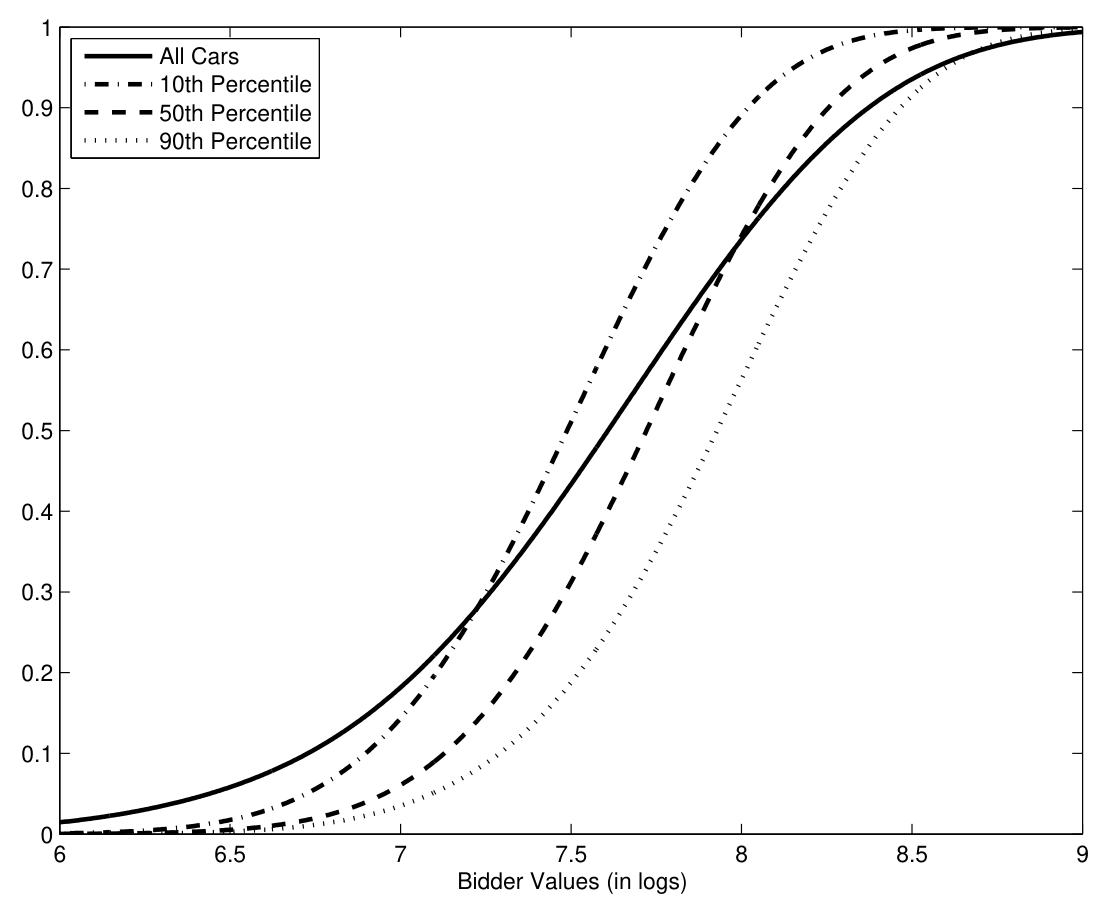
\includegraphics[width=0.62\textwidth]{figures/ch15/roberts_fig1.png}
\caption{Estimated value distributions (log values) for seven-year-old automatic Hyundai Sonatas with
100,000 km. Solid line: ignoring unobserved heterogeneity. Other lines: controlling for it at the 10th,
50th and 90th percentiles of $\omega$. Source: Roberts (2013), Figure 1 (June 2013 working-paper version).}
\label{fig:15-roberts-cdf}
\end{figure}

\casehead{Counterfactuals}
Roberts asks how much of the attainable value sellers capture and through which channels. He sets the
seller's value to $v_0=\gamma r$ for $\gamma\in\{0,0.25,0.5,0.75\}$ and simulates revenues with
$N=8$. \Cref{tab:15-roberts-reserve} reproduces his Table 6. Ignoring heterogeneity overstates the
dispersion of values and pushes the estimated optimal reserve up. A sufficient condition is hazard rate
dominance. Let $\lambda_C$ and $\lambda_{NC}$ be the hazard rates of the value distributions estimated
with and without the control, and suppose $\lambda_C(r)>\lambda_{NC}(r)$ for all $r$. The optimal
reserve with the control solves $r_C=v_0+\frac{1}{\lambda_C(r_C)}<v_0+\frac{1}{\lambda_{NC}(r_C)}$, so
$\psi_{NC}(r_C)<v_0$. Regularity then gives $r_{NC}>r_C$ (\citealp{Roberts2013}, footnote 13). With
actual reserves, the mean seller captures between 88.42 and 92.23 percent of the value of the optimal
auction with the same bidders, depending on $\gamma$. Using the ``optimal'' reserves computed while
ignoring heterogeneity would lower the mean share to between 85.53 and 88.93 percent. The text
summarizes the first result as ``around 94\%'' (p.~25), above every mean and median in the table. The
figure is close to the 90th-percentile column, 93.08 to 94.51 percent. The text also says that 90
percent of sellers achieve more than 83 percent, which matches the 10th percentile of 83.69 at
$\gamma=0$.

\begin{table}[htbp]
\centering
\caption{Optimal reserve prices and the share of value captured by sellers (Roberts 2013, Table 6)}
\label{tab:15-roberts-reserve}
{\small
\setlength{\tabcolsep}{4pt}
\begin{tabular}{ccccccccccc}
\toprule
 & \multicolumn{2}{c}{Difference in optimal reserve} & \multicolumn{4}{c}{Actual reserves (\%)} & \multicolumn{4}{c}{Reserves ignoring UH (\%)}\\
\cmidrule(lr){2-3}\cmidrule(lr){4-7}\cmidrule(lr){8-11}
$\gamma$ & Overall & Median & Mean & 10th & 50th & 90th & Mean & 10th & 50th & 90th\\
\midrule
0.00 & \$221.57 & \$77.21 & 88.42 & 83.69 & 89.18 & 93.08 & 85.53 & 77.37 & 94.08 & 94.70\\
     & (25.36) & (24.89) & (0.19) & (0.33) & (0.18) & (0.14) & (0.13) & (0.17) & (0.03) & (0.04)\\
0.25 & 258.52 & 90.20 & 90.66 & 86.69 & 91.69 & 93.53 & 86.58 & 74.62 & 94.10 & 94.70\\
     & (23.16) & (25.52) & (0.18) & (0.38) & (0.13) & (0.05) & (0.11) & (0.13) & (0.03) & (0.03)\\
0.50 & 239.72 & 98.45 & 92.23 & 86.98 & 93.69 & 94.25 & 87.60 & 74.05 & 94.05 & 94.70\\
     & (21.35) & (21.01) & (0.20) & (0.64) & (0.04) & (0.03) & (0.08) & (0.11) & (0.03) & (0.02)\\
0.75 & 236.03 & 123.57 & 91.81 & 85.84 & 93.45 & 94.51 & 88.93 & 80.42 & 94.04 & 94.71\\
     & (21.79) & (22.12) & (0.20) & (0.76) & (0.07) & (0.04) & (0.07) & (0.08) & (0.03) & (0.02)\\
\bottomrule
\end{tabular}}

\smallskip
\begin{minipage}{0.93\textwidth}
\footnotesize \textit{Notes.} $v_0=\gamma r$, with $r$ the observed reserve. ``Overall'' is the average
difference across all cars, and ``Median'' the average for cars with $\omega$ within half a standard
deviation of its median. The paper's column header, and its definition on p.~24, write the difference
as $R^*_C-R^*_{NC}$. The table note describes it as the optimal reserve ignoring heterogeneity minus
the optimal reserve controlling for it. The text and its footnote 13 say that ignoring heterogeneity
raises the optimal reserve. The positive entries agree with the note, which we follow. The remaining columns give the percentage of the value of the
optimal auction captured with actual reserves and with the ``optimal'' reserves that ignore
heterogeneity. Bootstrap standard errors (100 repetitions) in parentheses, in percentage points for
percentages.
\end{minipage}
\end{table}

\Cref{tab:15-roberts-channels} reproduces Table 7, which decomposes the value of the platform with
$\gamma=0$. Let $\pi^N_{r}$ denote revenue with $N$ bidders and reserve $r$. The first row is the gain
$\pi^{N+1}_{r=r^*}-\pi^N_{r=0}$ from one more bidder together with an optimal reserve. The next rows split
the gain into the extra bidder, $\pi^{N+1}_{r=0}-\pi^N_{r=0}$, and the reserve,
$\pi^{N+1}_{r=r^*}-\pi^{N+1}_{r=0}$. The extra bidder dominates, as the theorem of
\citet{BulowKlemperer1996} suggests (\cref{prop:14-bk}). With four bidders, the extra bidder is
worth $\frac{94.49}{5.51}\approx17.1$ times as much as the optimal reserve when heterogeneity is
controlled for, and $\frac{81.89}{18.11}\approx4.5$ times as much when it is not. With five bidders the ratios are $26.1$ and $5.1$.
The text reports 17.5 and 4.6 ``when there are five bidders'' (p.~26), close to our ratios for $N=4$, where
the extra bidder makes five.
Ignoring heterogeneity overstates the role of reserves and understates the role of competition.

\begin{table}[htbp]
\centering
\caption{Channels through which sellers gain from the auction house (Roberts 2013, Table 7)}
\label{tab:15-roberts-channels}
\begin{tabular}{lcccccc}
\toprule
$N$ & 2 & 3 & 4 & 5 & 6 & 7\\
\midrule
\multicolumn{7}{l}{\emph{Controlling for unobserved heterogeneity}}\\
Gain $\pi^{N+1}_{r=r^*}-\pi^{N}_{r=0}$ (\$) & 725.94 & 435.5 & 307.89 & 233.09 & 189.07 & 160.59\\
 & (14.95) & (8.98) & (6.56) & (5.13) & (4.23) & (3.49)\\
Share from extra bidder (\%) & 87.71 & 91.91 & 94.49 & 96.31 & 97.31 & 97.97\\
 & (0.41) & (0.39) & (0.34) & (0.31) & (0.31) & (0.34)\\
Share from optimal reserve (\%) & 12.29 & 8.09 & 5.51 & 3.69 & 2.69 & 2.03\\
 & (0.41) & (0.39) & (0.33) & (0.30) & (0.31) & (0.34)\\
\addlinespace
\multicolumn{7}{l}{\emph{Not controlling for unobserved heterogeneity}}\\
Gain $\pi^{N+1}_{r=r^*}-\pi^{N}_{r=0}$ (\$) & 871.61 & 578.62 & 426.34 & 333.26 & 276.46 & 229.27\\
 & (13.02) & (7.97) & (6.38) & (5.33) & (4.74) & (4.03)\\
Share from extra bidder (\%) & 75.38 & 79.11 & 81.89 & 83.68 & 85.43 & 86.46\\
 & (0.92) & (1.06) & (1.15) & (1.26) & (1.28) & (1.35)\\
Share from optimal reserve (\%) & 24.62 & 20.89 & 18.11 & 16.32 & 14.57 & 13.54\\
 & (0.92) & (1.07) & (1.15) & (1.25) & (1.28) & (1.36)\\
\bottomrule
\end{tabular}

\smallskip
\begin{minipage}{0.93\textwidth}
\footnotesize \textit{Notes.} $\gamma=0$. Shares are
$\frac{\pi^{N+1}_{r=0}-\pi^N_{r=0}}{\pi^{N+1}_{r=r^*}-\pi^N_{r=0}}$ and
$\frac{\pi^{N+1}_{r=r^*}-\pi^{N+1}_{r=0}}{\pi^{N+1}_{r=r^*}-\pi^N_{r=0}}$. Revenues from 10,000 simulations.
Bootstrap standard errors (100 repetitions) in parentheses, in percentage points for percentages.
\end{minipage}
\end{table}

\casehead{Assessment}
Roberts showed that seller behavior can carry information about what the econometrician misses. The
method needs only transaction and reserve prices and a record of unsold auctions. It lets values depend
on $\omega$ without separability. Its requirements are strong in other directions. Heterogeneity must be scalar and enter
both the reserve and the bids. The seller may have no private information that bidders value, and the
reserve may respond to nothing that bidders ignore. All sellers must use one reserve rule, which the
auction house's guidance makes plausible. Bidders must be symmetric, and the number of potential
bidders must be assumed. The estimates of the reserve function are parametric. Within these limits,
the paper adds the seller as a second source of information about unobserved quality, and it measures
the Bulow-Klemperer comparison in a real market.

\subsection{Comparing the approaches}\label{sec:15-uh-compare}

\Cref{tab:15-uh-approaches} summarizes the approaches. They differ in the data they demand and in the
restrictions they place on how heterogeneity enters. The number of bidders can itself serve as a control
when it is a sufficient statistic for the heterogeneity \citep[Section 3.2]{CampoPerrigneVuong2003}. It
can also serve as an instrument when participation depends on an excluded variable
\citep{HaileHongShum2003}, as discussed in \cref{sec:15-cv}.

\begin{table}[htbp]
\centering
\caption{Approaches to unobserved auction heterogeneity}
\label{tab:15-uh-approaches}
{\footnotesize
\begin{tabularx}{\textwidth}{>{\raggedright\arraybackslash}p{2.35cm}>{\raggedright\arraybackslash}X>{\raggedright\arraybackslash}X>{\raggedright\arraybackslash}X>{\raggedright\arraybackslash}p{2.3cm}}
\toprule
Approach & Data required & Restrictions & What is identified & Practical cost\\
\midrule
Homogenization (\cref{sec:15-uh-sep}) & Bids and observed covariates & All heterogeneity observed. Separable covariate effect & $F_V(\cdot\mid z)$ and the covariate effect $g_0$ & Low\\
Deconvolution \citep{Krasnokutskaya2011} & At least two bids per auction, bidder types & Scalar $\omega$, separable. Components $\omega$ and $A_i$ mutually independent & $F_\omega$ and each $F_k$, not realizations & High: cell by cell, slow rates\\
Parametric mixture \citep{AtheyLevinSeira2011} & All bids & Parametric bid laws. Heterogeneity $\omega$ independent of covariates & Parameters, then $F_k(\cdot\mid\omega)$ for any $\omega$ & Moderate\\
Reserve-price control \citep{Roberts2013} & Transaction and reserve prices, record of unsold auctions & Reserve strictly increasing in scalar $\omega$. No seller private information & $m$, $F_\omega$, realizations of $\omega$, $F_V(\cdot\mid z,\omega)$ above the reserve & Moderate. $N$ assumed\\
$n$ as control or instrument \citep{CampoPerrigneVuong2003,HaileHongShum2003} & Bids, $n$, excluded shifters of participation & $n$ sufficient for $\omega$, or monotone in it & Value distributions given the control & Moderate\\
Three bids \citep{HuMcAdamsShum2013} & At least three bids per auction & Heterogeneity may enter values nonseparably & Model primitives with nonseparable heterogeneity & High\\
\bottomrule
\end{tabularx}}
\end{table}

\section{Entry, Participation, Dynamics and Risk Aversion}\label{sec:15-entry}

The identification results so far treat the set of bidders as given, each auction as a separate game,
and bidders as risk neutral. This section relaxes each assumption in turn. The theory of entry is in
\cref{sec:14-entry}, and the timber application, where entry costs are estimated, is in
\cref{sec:15-als}.

\subsection{Potential and actual bidders}\label{sec:15-entry-sets}

Following \citet[Section 6.3]{AtheyHaile2007}, let $\mathcal N$, with $|\mathcal N|=N$, be the set of
potential bidders, those who draw signals and decide whether to bid. Let
$\mathcal A\subseteq\mathcal N$, with $|\mathcal A|=n$, be the set of actual bidders, those who
place a bid. These are the objects of \cref{sec:15-gpv-reserve}, now written as sets. Both sets can vary across auctions. The set of potential bidders varies when acquiring a
signal is costly. The set of actual bidders varies, for a given $\mathcal N$, when a reserve price
binds or bidding is costly. The consequences for equilibrium and for identification depend on two
questions. Do bidders know who participates? Does the econometrician observe $\mathcal N$, $\mathcal A$,
or only $n$?

\subsection{Selection by a reserve price or a bid cost}\label{sec:15-entry-reserve}

A binding reserve price selects bidders with values above $r$. In ascending auctions with independent
private values, participants' values are draws from the truncated distribution, and observing
$\mathcal N$ restores $F_V$ above $r$ (\cref{prop:15-reserve-ident}). In first-price auctions, the inversion
with a reserve and an unknown number of potential bidders is \eqref{eq:15-gpv-reserve}
(\cref{thm:15-gpv-reserve}). \citet[Section 6.3.1]{AtheyHaile2007} extend the first-price results to
private values with correlation. Suppose bidders do not know $\mathcal A$ when they bid, which is natural
because participation depends on private information. The distribution of the highest rival bid then
mixes over the possible participant sets,
\[
G_{M_i\mid B_i}(m\mid b;\mathcal N)=\Pr\big(\mathcal A=\{i\}\mid i\in\mathcal A,B_i=b\big)+\sum_{\mathcal A'\ni i,\,|\mathcal A'|>1}
\Pr\Big(\mathcal A=\mathcal A',\ \max_{k\in\mathcal A',k\neq i}B_k\le m\ \Big|\ B_i=b\Big).
\]
Each piece is observable, so the first-order condition \eqref{eq:14-apv-foc} still maps each bid to a
value. Two results follow \citep[Theorems 6.4--6.5]{AtheyHaile2007}. First, for each $\mathcal A$, the
joint distribution of values of participants above $r$ is identified from $r$, all bids and bidder
identities. Second, each marginal $F_{V_i}(v)$ is identified for $v\ge r$, since
$F_{V_i}(r)=\Pr(i\notin\mathcal A)$ is observed when $\mathcal N$ is. Nothing can be learned about
correlation among values below $r$. A cost of preparing a bid acts like a reserve price, since only
bidders with high enough values bid \citep[footnote 60, citing \citealp{Samuelson1985} and
\citealp{HaileHongShum2003}]{AtheyHaile2007}.

\subsection{Costly signal acquisition and the entry cost}\label{sec:15-entry-cost}

In the model of \citet{LevinSmith1994}, firms pay $K$ to learn their values and then bid
(\cref{sec:14-entry}). In the symmetric equilibrium firms randomize, so the set of entrants
$\tilde{\mathcal N}$ varies exogenously. Entrants learn who else entered before bidding. If the reserve
price lies below every value, it binds only when a single firm enters, and that firm bids the reserve.
The randomization is useful twice. It creates exogenous variation in the number of bidders, which the
tests of \cref{sec:15-cv} require. It also identifies the entry cost.

\begin{proposition}[Entry costs, \citealp{AtheyHaile2007}, Section 6.3.2]\label{prop:15-entry-ident}
Suppose entry generates exogenous variation in $\tilde{\mathcal N}$ and the reserve lies below the
support of values. Suppose the econometrician observes the entrants and all their bids. Under IPV the
winning bid suffices.
\begin{enumerate}[label=(\roman*)]
\item Each entrant's expected gross profit $\pi_i(\mathcal A)$ in \eqref{eq:14-entry-profit-id} is
identified for every participant set $\mathcal A$ with $|\mathcal A|\ge2$ that occurs with positive
probability.
\item For any firm that randomizes, the entry cost is identified by \eqref{eq:14-entry-cost-id},
$K=\sum_{\mathcal A\ni i}\Pr\big(\tilde{\mathcal N}=\mathcal A\mid i\in\tilde{\mathcal N}\big)\,\pi_i(\mathcal A)$.
\end{enumerate}
In the symmetric IPV first-price auction with $n$ entrants,
\begin{equation}\label{eq:15-entry-profit}
\pi(n)=\E_B\Big[\frac{G_n(B)^n}{(n-1)\,g_n(B)}\Big],\qquad
\hat\pi(n)=\frac{1}{nT_n}\sum_{t:\,n_t=n}\ \sum_{i=1}^{n}\frac{\hat G_n(b_{it})^n}{(n-1)\,\hat g_n(b_{it})},
\end{equation}
where $G_n$ and $g_n$ are the bid distribution and density in $n$-bidder auctions.
\end{proposition}

\begin{proof}
(i) Exogenous variation in $\tilde{\mathcal N}$ means that bids in auctions with participant set
$\mathcal A$ are equilibrium bids for that set. The first-order condition identifies the value behind
each bid (\cref{sec:15-gpv,sec:15-apv}). Then $\pi_i(\mathcal A)$ is the expectation, over $i$'s bids, of
the margin times the probability of winning, both functions of observables. (ii) A firm that
randomizes is indifferent, so its expected gross profit from entry equals $K$. The probabilities of
each participant set are observed. For the formula, a bidder who bids $b$ against $n-1$ symmetric
rivals wins with probability $G_n(b)^{n-1}$ and has margin
$\xi(b)-b=\frac{G_n(b)}{(n-1)g_n(b)}$ by \eqref{eq:15-gpv-xi}. Its expected profit is
\[
\big(\xi(b)-b\big)G_n(b)^{n-1}=\frac{G_n(b)}{(n-1)g_n(b)}\,G_n(b)^{n-1}=\frac{G_n(b)^n}{(n-1)g_n(b)} .
\]
Averaging over the bid distribution gives \eqref{eq:15-entry-profit}. The sample analogue replaces $G_n$
and $g_n$ by the GPV estimates.
\end{proof}

\begin{example}[Recovering the entry cost]\label{ex:15-entry-uniform}
Take uniform values on $[0,1]$ and no reserve. In $n$-bidder auctions bids are uniform on
$[0,c]$ with $c=\frac{n-1}{n}$, so $G_n(b)=\frac{b}{c}$ and $g_n=\frac{1}{c}$. Then
\[
\pi(n)=\int_0^c\Big(\frac{b}{c}\Big)^n\frac{c}{n-1}\,\frac{db}{c}=\frac{c}{n-1}\int_0^1u^n\,du=\frac{c}{(n-1)(n+1)}=\frac{1}{n(n+1)},
\]
which matches \cref{lem:14-pi-decreasing}. A lone entrant pays the reserve and earns
$\pi(1)=\E[V]=\frac{1}{2}$, where $\E[V]$ is identified from bids in auctions with two or more entrants.
Suppose there are $N=5$ potential entrants and the observed entry probability is $0.816$. The number of
rival entrants is binomial, so
$K=\sum_{n=1}^5\binom{4}{n-1}0.816^{\,n-1}0.184^{\,5-n}\pi(n)=0.050$. This inverts the forward
calculation of \cref{ex:14-ls}.
\end{example}

The entry cost is identified in dollars. Entry models that draw inferences solely from entry decisions
cannot recover the level of entry costs in this way. In auctions the bids reveal post-entry profits, so
the level of $K$ is identified \citep[Section 6.3.2]{AtheyHaile2007}. With asymmetric bidders there can be
several type-symmetric entry equilibria. Since the estimated $\pi_i(\mathcal A)$ do not depend on the
equilibrium selected, all equilibria of the entry game can be computed for given entry costs. Their
number can thus be checked in the data, as \citet{AtheyLevinSeira2011} do (\cref{prop:14-als-unique},
\cref{sec:15-als}).
Entry may also be selective. In the model of \citet{Samuelson1985}, firms know their values before
they decide to enter, so only firms with high values pay $K$. More generally, firm $i$ observes a
signal $S_i$ of its value $V_i$ before entry and enters when $S_i$ exceeds a threshold $\bar s$. In a
symmetric equilibrium the threshold makes the marginal entrant indifferent,
\[
\E\big[\pi(V_i;\tilde{\mathcal N})\mid S_i=\bar s\big]=K,
\]
where $\pi(V_i;\tilde{\mathcal N})$ is the post-entry profit of a firm with value $V_i$ when the set of
entrants is $\tilde{\mathcal N}$. The model of \citet{LevinSmith1994} is the case in which $S_i$ is
independent of $V_i$, and that of \citet{Samuelson1985} the case $S_i=V_i$
\citep[p.~92, footnote 9]{HortacsuPerrigne2021}. With selective entry the bids of entrants reveal the
distribution of values conditional on entry, not the distribution in the population of potential
bidders. Identification then rests on exogenous variation in the number of potential bidders or in
entry costs \citep{MarmerShneyerovXu2013,GentryLi2014,RobertsSweeting2013}. \citet{GentryLi2014} give
conditions under which models of selective entry are identified \citep[footnote 8]{HortacsuPerrigne2021}.

\casehead{Estimates of entry costs}
\Cref{tab:15-entry-costs} collects entry-cost estimates from timber and procurement auctions, as
summarized by \citet[Sections 2.2, 2.6.3, 3.3 and 3.10]{HortacsuPerrigne2021}. The estimates are
small relative to the value of the objects sold, but they matter for policy because participation
responds to them. \citet{AtheyLevinSeira2011} find median logger entry costs of \$2,870 in the Northern forests and \$5,056 in
California (\cref{sec:15-als}). Their benchmark is the median expected profit of a mill in a sealed
sale, about \$45,000 gross of entry costs (their footnote 26). The logger entry costs are thus
$\frac{2{,}870}{45{,}000}\approx6.4$ and $\frac{5{,}056}{45{,}000}\approx11.2$ percent of that profit,
the ratios that \citet[p.~91]{HortacsuPerrigne2021} report. Because loggers randomize their entry, a logger's entry cost equals its own expected gross
profit from entry by construction. The informative benchmark is therefore the profit of the stronger
bidders, the mills, who always enter. \citet{LiZheng2012} estimate both entry models
on first-price timber sales of the Michigan Department of Natural Resources (p.~91). The entry cost
means different things in the two models. Under selective entry it is a cost of preparing a bid,
while under the Levin-Smith model it also covers learning one's value. The models also differ in
their reserve-price advice. Under selective entry the optimal reserve solves the usual condition
\eqref{eq:14-optimal-reserve}, while under the Levin-Smith model it equals the seller's value, as in
\cref{prop:14-ls-welfare}. The entry cost is about 6.8 percent of a bidder's value under selective
entry and 9.5 percent under the Levin-Smith model. A Bayes factor, the ratio of the marginal
likelihoods of the two estimated models, favors selective entry.

\citet{LiZhang2015} add affiliated private values and asymmetries in values and entry costs that
arise from the distance between a bidder and the tract (pp.~91--92). They parameterize the joint
distributions with copulas and solve the asymmetric auctions numerically. In sealed-bid sales of the
Oregon Department of Forestry, values show little dependence and entry costs show more. Their merger
counterfactual shows that entry matters for policy. Ignoring entry, a merger of two bidders lowers the
welfare of the merging bidders and the payoff of the others, whichever pair merges. With entry, the merging bidders gain when the two
bidders with the largest hauling distances merge, and they lose slightly when the two closest bidders
merge. The effects on the other bidders go the opposite way.

\citet{RobertsSweeting2016} study the 1984 federal buyout of timber contracts that firms had bought at
the prices of the late-1970s timber boom and could no longer afford (p.~92). Their model nests both
entry models. Each firm sees a noisy signal of its value, enters above a threshold signal, and then
bids in a second-price auction. To avoid multiple equilibria, mills and loggers share the signal
distribution and the entry cost, and their value distributions differ only in the mean. Entry is
selective to a moderate degree, and mills have higher values. The entry cost is 2.7 percent of the bid
on average. Without the bailed-out firms, revenue would have been 11.1 percent lower, because most of
them were high-value mills and values are dispersed. A Levin-Smith model would instead predict higher
revenue after the exit of an entrant. An additional bidder is worth more to the seller than an optimal
reserve price, as the result of \citet{BulowKlemperer1996} suggests (\cref{prop:14-bk}).

\begin{table}[htbp]
\centering
\caption{Estimated entry costs in auction studies (as summarized by Hortacsu and Perrigne 2021)}
\label{tab:15-entry-costs}
{\small
\begin{tabularx}{\textwidth}{>{\raggedright\arraybackslash}p{3.1cm}>{\raggedright\arraybackslash}X>{\raggedright\arraybackslash}p{2.6cm}>{\raggedright\arraybackslash}p{4.2cm}}
\toprule
Study & Auctions & Entry model & Entry cost\\
\midrule
\citet{AtheyLevinSeira2011} & USFS timber, North and California & Levin-Smith, asymmetric & Logger entry cost: 6.4\% and 11.2\% of the median mill profit\\
\citet{LiZheng2012} & Michigan DNR timber, first-price & Samuelson and Levin-Smith & 6.8\% (selective) and 9.5\% (nonselective) of value\\
\citet{RobertsSweeting2016} & USFS timber, 1980s & Signals, nests both & 2.7\% of the bid\\
\citet{RobertsSweeting2013} & USFS timber, ascending & Signals, selective & 2\% of the average winning bid\\
\citet{LiZheng2009} & Texas DOT highway mowing & Levin-Smith preferred & 14\% of the estimated private cost, 8\% of the winning bid\\
\citet{KrasnokutskayaSeim2011} & California highway procurement & Levin-Smith, asymmetric & 2.2--3.9\% (small firms), 3.1--3.3\% (large firms) of the engineer's estimate\\
\bottomrule
\end{tabularx}}

\smallskip
\begin{minipage}{0.93\textwidth}
\footnotesize \textit{Notes.} Entry costs as fractions of the quantity named in the last column. USFS: United
States Forest Service. DNR: Department of Natural Resources. DOT: Department of Transportation.
Sources are the summaries of \citet[pp.~91, 92, 100, 105 and 123]{HortacsuPerrigne2021}, except the
ratios for \citet{AtheyLevinSeira2011}, which we recompute from their p.~246 and footnote 26. For
\citet[p.~1421]{LiZheng2009} the entry cost and a bidder's private cost of completing the contract are
simulated from their estimated distributions for each auction. The average ratios of the entry cost to this
private cost and to the winning bid are 13.8 and 8.3 percent.
\end{minipage}
\end{table}

Procurement auctions show similar magnitudes. In highway mowing contracts of the Texas Department of
Transportation, only 28 percent of planholders bid \citep{LiZheng2009}. The Levin-Smith model fits
better than the selective model by a mean squared error criterion \citep[p.~105]{HortacsuPerrigne2021}.
More planholders affect bids through a positive entry effect and a negative competition effect. The
total effect on bids is negative when competition is low and positive when it is high. The authors
conclude that encouraging more potential bidders is not a desirable policy for the agency.

\subsection{Bidders uncertain about the competition*}\label{sec:15-entry-uncertain}

In sealed-bid auctions, bidders may not know how many rivals they face. In second-price auctions this
does not affect private values bidding. With common values it does, and \citet[Theorem 12]{AtheyHaile2002}
show that the test of private against common values in \cref{sec:15-cv} survives. Suppose bidders do
not know $n$. They observe instead a public signal $\eta$, unobserved by the econometrician, that is
strictly affiliated with $n$. The symmetric private values model remains testable against symmetric common
values from transaction prices in $m$-bidder auctions and bids $B^{(m-1:n)},\dots,B^{(n-1:n)}$ in
auctions with $n>m$ bidders.

In first-price auctions uncertainty about $n$ changes bidding even with private values. Suppose $\eta$ is
observed by the econometrician as well, and let $\tilde\pi(n\mid\eta)$ be the probability of $n$
bidders given $\eta$. The first-order condition is \eqref{eq:15-uh-foc} with the rival-bid distribution
mixed over $n$ \citep[eq. (22)]{AtheyHaile2002}. Fixing $\eta$, the winning bid satisfies
\citep[eq. (23)]{AtheyHaile2002}
\[
\Pr\big(B^{\mathrm{win}}\le b\mid\eta\big)=\sum_{n\ge2}\tilde\pi(n\mid\eta)\,\Pr(B_i\le b\mid\eta)^n .
\]
The right side is strictly increasing in $\Pr(B_i\le b\mid\eta)$, and $\tilde\pi(n\mid\eta)$ is observed.
The winning-bid distribution therefore identifies $\Pr(B_i\le b\mid\eta)$, hence the rival-bid
distribution, and then $F_V$ through the first-order condition. If $\eta$ is unobserved by the
econometrician, the problem becomes one of unobserved heterogeneity (\cref{sec:15-uh}).

When bidders know nothing about the realized set of entrants, the rival-bid distribution
$G_{M_i\mid B_i}$ averages over entrant sets and does not depend on the realized $\mathcal N$
\citep[eqs. (6.21)--(6.22)]{AtheyHaile2007}. The two informational assumptions have testable
implications. If bidders know $\mathcal N$, a lone entrant bids the reserve price with probability one.
If they do not, the distribution of a bidder's bid does not vary with the realized $\mathcal N$.

Internet auctions raise a related problem. Bidders arrive at different times, and some never bid
because the price already exceeds their value. The number of bidders is then unobserved, which defeats
the inversion of \cref{sec:15-ascending}. \citet{Song2004} shows that two order statistics
suffice, as summarized by \citet[Lemma 6.2]{AtheyHaile2007}. Let $Y^{(N:N)}$, $Y^{(N-1:N)}$ and
$Y^{(N-2:N)}$ be the three highest of $N\ge3$ independent draws from $F_Y$, with $N$ random and
unobserved. Then $F_Y$ is determined by the joint law of $\big(Y^{(N-1:N)},Y^{(N-2:N)}\big)$. Given
$Y^{(N-2:N)}=y_0$, the two highest draws are an i.i.d. sample of two from the truncated distribution
$\frac{F_Y(\cdot)-F_Y(y_0)}{1-F_Y(y_0)}$, whatever $N$ is. The lower of two draws identifies its parent
(\cref{thm:15-ah1}), and letting $y_0$ fall to the bottom of its support recovers $F_Y$. With eBay data,
the method uses auctions whose bidding histories make it nearly certain that the second- and
third-highest submitted bids equal the corresponding values \citep[Section 6.3.4]{AtheyHaile2007}.

\subsection{Dynamics and capacity: Jofre-Bonet and Pesendorfer (2003)*}\label{sec:15-jbp}

\subsubsection{Question and model}

Highway paving contractors bid repeatedly, and a contract won today ties up machines and crews for
months. \citet{JofreBonetPesendorfer2003}, henceforth JBP, ask how such capacity constraints shape
bidding, costs and efficiency. They develop an estimator for a dynamic auction game that never solves
for an equilibrium. Their abstract states the finding. In this market ``previously won uncompleted contracts
reduce the probability of winning further contracts.''

Time is discrete with an infinite horizon (JBP, Section 2). In each period one contract with
characteristics $s_0$, drawn i.i.d., is let by first-price sealed bid. There are $n_r$ \emph{regular}
bidders who stay forever and a varying number of \emph{fringe} bidders who live one period. Regular
bidder $i$'s state $s_i$ lists the remaining size and time to completion of each project it won
recently, and $s=(s_1,\dots,s_{n_r})$. After $s_0$ is revealed, each bidder learns its cost privately.
Costs are independent across bidders conditional on states, with distribution $F(\cdot\mid s_0,s_i,s_{-i})$.
There is a public reserve price $r$ and a secret reserve price drawn from a known distribution, which
acts like one more rival bid. The state moves deterministically, $s'=\mathcal T(s_0,s,j)$, where $j$ is
the identity of the winner and $j=0$ means no award. Bidders discount the future with factor $\delta$,
which in this subsection is a discount factor and not a mean utility. The solution concept is a
Markov perfect equilibrium in strategies $b(c,s_0,s_i,s_{-i})$ that are symmetric conditional on states.

Bidder $i$'s ex ante value function, which we write $\mathcal V_i$ to keep it apart from the values
$V_{it}$, satisfies (JBP, eq. (2.1))
\begin{equation}\label{eq:15-jbp-bellman}
\mathcal V_i(s)=\E_{s_0}\int\max_b\Big\{(b-c)\Pr(i\text{ wins}\mid b)+\delta\sum_{j=0}^{n}\Pr(j\text{ wins}\mid b)\,\mathcal V_i\big(\mathcal T(s_0,s,j)\big)\Big\}f(c\mid s_0,s_i,s_{-i})\,dc .
\end{equation}

\subsubsection{The first-order condition}

Write $G_j$ and $g_j$ for the distribution and density of rival $j$'s bid given the state, including
fringe bidders and the secret reserve. Let $h_j=\frac{g_j}{1-G_j}$ be its hazard and
$H_i(b)=\sum_{j\neq i}h_j(b)$. Bidder $i$ wins with probability $P_i(b)=\prod_{j\neq i}\big(1-G_j(b)\big)$.
Rival $j$ wins when bidder $i$ bids $b$ if $j$'s bid lies below $b$ and below every other rival's bid.
This has probability $P_j(b)=\int_{\underline b}^{b}g_j(x)\prod_{l\neq i,j}\big(1-G_l(x)\big)dx$, where
$\underline b$ is the lower end of the bid support. The derivatives are
\[
P_i'(b)=-P_i(b)H_i(b),\qquad P_j'(b)=g_j(b)\prod_{l\neq i,j}\big(1-G_l(b)\big)=P_i(b)\,h_j(b),
\]
so that $P_i'+\sum_{j\neq i}P_j'=0$, as it must be because someone always wins.
Differentiating the objective in \eqref{eq:15-jbp-bellman} with respect to $b$ and writing
$\mathcal V_i^j=\mathcal V_i(\mathcal T(s_0,s,j))$,
\[
P_i(b)+(b-c)P_i'(b)+\delta\Big[P_i'(b)\mathcal V_i^i+\sum_{j\neq i}P_j'(b)\mathcal V_i^j\Big]=0 .
\]
Substitute the derivatives and divide by $P_i(b)$:
\[
1-(b-c)H_i(b)-\delta\sum_{j\neq i}h_j(b)\big[\mathcal V_i^i-\mathcal V_i^j\big]=0 .
\]
Solving for the cost gives the inverse bid function (JBP, eq. (3.1)),
\begin{equation}\label{eq:15-jbp-foc}
c=\xi_i(b)\equiv b-\frac{1}{H_i(b)}-\delta\sum_{j\neq i}\frac{h_j(b)}{H_i(b)}\Big[\mathcal V_i\big(\mathcal T(s_0,s,j)\big)-\mathcal V_i\big(\mathcal T(s_0,s,i)\big)\Big].
\end{equation}
The markdown has two parts. The first, $\frac{1}{H_i(b)}$, is the static markdown of
\cref{sec:14-procurement}. The second is the loss in future value from winning today rather than letting
rival $j$ win, weighted by $j$'s share of the hazard. With capacity constraints, winning raises
backlog and lowers continuation value, so the second term raises the bid above its static level.
For fringe bidders $\mathcal V=0$ and the condition is static. At the reserve the first term vanishes, but the
second does not, so a regular bid need not equal cost there.

\subsubsection{The value function in terms of bids}

The key step expresses $\mathcal V_i$ through bid distributions alone. Substitute the first-order condition into
\eqref{eq:15-jbp-bellman}. The margin times the win probability plus the term in $\mathcal V_i^i$ is
\[
(b-c)P_i+\delta P_i\mathcal V_i^i=\frac{P_i}{H_i}+\delta P_i\sum_{j\neq i}\frac{h_j}{H_i}\big(\mathcal V_i^j-\mathcal V_i^i\big)+\delta P_i\mathcal V_i^i
=\frac{P_i}{H_i}+\delta\sum_{j\neq i}P_i\frac{h_j}{H_i}\mathcal V_i^j,
\]
using $\sum_{j\neq i}\frac{h_j}{H_i}=1$. Change the variable of integration from the cost to bidder $i$'s
bid, so that $f(c)\,dc=dG_i(b)$. Write $dG^{(i)}(b)=P_i(b)\,dG_i(b)$ for the probability that $i$ wins
with a bid near $b$. Then (JBP, Proposition 1)
\begin{equation}\label{eq:15-jbp-value}
\mathcal V_i(s)=\E_{s_0}\bigg[\int\frac{1}{H_i(b)}\,dG^{(i)}(b)+\delta\sum_{j\neq i}\Big(\Pr(j\text{ wins})+\int\frac{h_j(b)}{H_i(b)}\,dG^{(i)}(b)\Big)\mathcal V_i\big(\mathcal T(s_0,s,j)\big)\bigg],
\end{equation}
where $\Pr(j\text{ wins})=\int P_j(b)\,dG_i(b)$. The weights in parentheses sum to one over $j$, since
$\sum_{j\neq i}\int\frac{h_j}{H_i}dG^{(i)}=\Pr(i\text{ wins})$. JBP write the second integral as
$\int\frac{h_i}{H_i}\,dG^{(j)}$, which is the same object because
$P_ih_jg_i=h_i\,g_j\prod_{l\neq j}(1-G_l)$. Equation \eqref{eq:15-jbp-value} is linear in the vector of
values on a grid of states. With $m_i(s)$ the first term and $Q_{ij}(s)$ the transition weights,
$\bm{\mathcal V}_i=\bm m_i+\delta\sum_{j\neq i}\bm Q_{ij}\bm{\mathcal V}_i$, so $\bm{\mathcal V}_i=(\bm I-\delta\bm Q_i)^{-1}\bm m_i$ with $\bm Q_i=\sum_{j\neq i}\bm Q_{ij}$
(JBP, eq. (3.3)). This is the GPV idea extended to dynamics. Bid distributions summarize beliefs, so the
first-order condition and the value function follow without solving the game.

\subsubsection{Identification and estimation}

Given $\delta$, the cost distribution is identified on the interval from the bottom of its support to
$\xi_i(r)$, the cost at which bidding the reserve is optimal. The pair $(\delta,F)$ is not identified
(JBP, Proposition 2). The non-identification of the discount factor parallels single-agent dynamic
models. Estimation is parametric (JBP, Section 3.3). For regular bidders, $\ln(b+1)$ has a Weibull
density with a lower endpoint common to all bidders. Its scale depends on states and contract
characteristics through symmetric functions of rivals' characteristics. Fringe bids have a beta density on
the interval from the lower bound to $r$. Regular bids are observed only below $r$, so the likelihood is
\[
\mathcal L=\prod_t\Big[\prod_{i=1}^{n_r}g(b_{it}\mid\theta_{it})^{o_{it}}\big(1-G(r_t\mid\theta_{it})\big)^{1-o_{it}}
\prod_{j=n_r+1}^{n_t}g_f(b_{jt}\mid\theta_t)\Big],
\]
with $o_{it}=1$ if regular bidder $i$ bids in auction $t$. The value function is computed on 50 states
drawn from the observed states, with expectations over 50 contracts drawn from the data and a
quadratic approximation off the grid. Costs follow from \eqref{eq:15-jbp-foc}, and
$F(c\mid\cdot)=G\big(\xi^{-1}(c)\mid\cdot\big)$.

\subsubsection{Data and reduced-form evidence}

The data are California Department of Transportation highway contracts with bids from May 1996 to May
1999 (JBP, Section 4). Of 2,566 advertised projects, 2,207 were awarded, 343 were cancelled or
postponed, and 16 drew no bids. The awarded contracts were worth \$4,661.73 million in total. They drew
10,289 bids, 4.63 per contract on average, and 1,466 bids that violated the reserve were dropped. The
regular bidders are the 10 largest firms by dollar value won with at least 80 bids. They win 25 percent
of the dollar value and 17 percent of contracts. \emph{Backlog} is the dollar value of uncompleted work
from contracts won earlier, standardized by each firm's mean and standard deviation. As the number of
bidders rises from 1 to 9 or more, the low bid moves from 11 percent above the engineer's estimate to
14 percent below it (JBP, Table II).

Reduced-form regressions on 22,230 bidder-contract observations point to capacity constraints (JBP,
Table III). In a probit of bid submission, the backlog coefficient is $-0.0835$ (standard error
$0.015$). In Tobit and Heckman regressions of $\ln\big(1+\frac{r-\text{bid}}{\text{estimate}}\big)$, where a
negative sign means a higher bid, it is $-0.0383$ ($0.007$) and $-0.0127$ ($0.004$). These are the
specifications without firm effects.
A constrained bidder is about 50 percent less likely to bid than an unconstrained one. Raising backlog
from $-1$ to $1$ raises the bid by 2.5 to 7.6 percent (JBP, p.~1466). Distance to the project
discourages bidding and raises bids, with probit and Tobit coefficients of $-0.5193$ ($0.023$) and
$-0.2536$ ($0.012$).

\subsubsection{Results}

The parametric bid distributions fit the fringe bids closely. Predicted fringe bids average 78.01
percent of the reserve with standard deviation 11.71, against 77.72 and 11.53 in the data. The predicted
probability of a regular bid is 5.97 percent against 5.96 percent. Predicted regular bids are somewhat
too high, 82.36 against 79.03 percent of the reserve (JBP, pp.~1471--1474). Bids of a bidder with backlog
$2$ first-order stochastically dominate those at backlog $-2$, and unconstrained bidders are about twice
as likely to bid.

The authors impose an annual discount factor of $0.8$, with a contract offered about every 12 hours.
The average discounted value of bidder 3 is \$25 million, and other regular bidders range from \$7
million to \$73 million. Raising the discount factor to $0.9$ roughly doubles these values. Backlog lowers
bidder 3's value by about 35 percent over the range shown. For the average bidder, the value is about 39
percent higher at backlog $-2$ than at backlog $2$ (JBP, pp.~1477--1478).

Markups are large. The median markup of bidder 3 is 26.0 percent of the bid and the mean 35.6
percent. Across all regular bids the median is 32.6 percent and the mean 40.3 percent. The dynamic term
in \eqref{eq:15-jbp-foc} accounts for 64.2 percent of bidder 3's markup and 55.9 percent across regular
bidders. With $\delta=0.9$, the median markup across regular bids rises to 45.9 percent and the dynamic
share to 69.8 percent (JBP, pp.~1479--1480). Capacity matters for the buyer as well. When every regular
bidder's backlog is $-2$ the average price is \$539,845, against \$657,016 at backlog $2$, a difference of
about 18 percent (JBP, p.~1481). Moving from backlog $2$ to $-2$ requires a 114 percent increase in
regular bidders' capacity.

\Cref{tab:15-jbp} reproduces the efficiency analysis. For each observed contract, the authors
compare the winner with the firm that minimizes the current cost plus the discounted expected future
cost. An inefficient firm wins 32 percent of the time. The average loss is 13 percent of the engineer's
estimate, or \$305,500 per contract (JBP, p.~1483). Nearly all of the loss comes from current costs,
and inefficiency is about equally likely whether a regular or a fringe bidder wins.

\begin{table}[htbp]
\centering
\caption{Estimated efficiency losses (Jofre-Bonet and Pesendorfer 2003, Table V)}
\label{tab:15-jbp}
\small
\setlength{\tabcolsep}{4.5pt}
\begin{tabular}{lcccccc}
\toprule
 & \multicolumn{5}{c}{Engineer's estimate (thousands of dollars)} & \\
\cmidrule(lr){2-6}
 & $[0,100]$ & $(100,400]$ & $(400,1000]$ & $(1000,5000]$ & $>5000$ & Overall\\
\midrule
\multicolumn{7}{l}{\emph{All contracts}}\\
Number of contracts & 49 & 893 & 525 & 545 & 184 & 2,196\\
Probability of an inefficiency & 0.02 & 0.52 & 0.17 & 0.24 & 0.11 & 0.32\\
Average efficiency loss & 0.04 & 0.08 & 0.14 & 0.17 & 0.19 & 0.13\\
\addlinespace
\multicolumn{7}{l}{\emph{Contracts won by a regular bidder}}\\
Number of contracts & 1 & 90 & 94 & 147 & 42 & 374\\
Probability of an inefficiency & 0.00 & 0.20 & 0.55 & 0.38 & 0.27 & 0.36\\
Average efficiency loss & 0.36 & 0.29 & 0.29 & 0.22 & 0.24 & 0.25\\
\addlinespace
\multicolumn{7}{l}{\emph{Contracts won by a fringe bidder}}\\
Number of contracts & 48 & 803 & 431 & 398 & 142 & 1,822\\
Probability of an inefficiency & 0.02 & 0.56 & 0.08 & 0.19 & 0.06 & 0.31\\
Average efficiency loss & 0.04 & 0.06 & 0.11 & 0.15 & 0.18 & 0.10\\
\bottomrule
\end{tabular}

\smallskip
\begin{minipage}{0.93\textwidth}
\footnotesize \textit{Notes.} Efficiency losses as a fraction of the engineer's estimate. The benchmark selects, in
the current auction only, the firm that minimizes current cost plus discounted expected future cost,
with first-price auctions thereafter. This gives a lower bound on the efficiency loss.
\end{minipage}
\end{table}

\subsubsection{Assessment}

The paper's contribution is methodological. It showed that the two-step logic of \citet{GuerrePerrigneVuong2000}
extends to dynamic games. Bid distributions estimated in a first step deliver both the continuation values
and the costs, through a linear system and a first-order condition. Computation is light because no
equilibrium is ever solved. The authors relate the idea to \citet{HotzMiller1993}. Two-step estimators
of dynamic oligopoly models later built on the same principle. \citet{BajariBenkardLevin2007} estimate
policy functions and state transitions first and recover the structural parameters from equilibrium
conditions second (p.~1331). They cite JBP as an analysis of repeated auctions built on first-order
conditions, one of the techniques designed for continuous choices (p.~1333, footnote 5).

The results rest on assumptions that the data cannot test, as the authors stress. The discount factor is
not identified, and the markup estimates move with it. Bid distributions are parametric. A Weibull-beta
mixture fits regular bids better, but it violates the monotone bid hazard that the model requires, so the
authors keep the Weibull (JBP, p.~1474). There is no
unobserved heterogeneity, the mirror image of Krasnokutskaya's assumption of no dynamics. Strategies are
symmetric conditional on states, which the evidence supports for most but not all firms. Inferred costs
that would be negative at the bottom of the bid range are set to zero. Markups of a third of the bid are
large, though the authors note that money left on the table averages 9 percent of the bid.
\citet[Section 9]{AtheyHaile2007} place the paper among several sources of dynamics in auctions. These
include tacit collusion in repeated auctions, private information that persists over time, learning by
doing and capacity constraints. They note that the dynamics created by persistent private information had
not been studied empirically, and they use this model to illustrate the case of capacity.

\subsection{Risk aversion*}\label{sec:15-risk}

Risk neutrality is natural when stakes are small relative to wealth, but many auctions involve large
stakes \citep[Section 6.4]{AtheyHaile2007}. In an ascending auction with private values, bidding one's
value remains a dominant strategy under any risk preference. $F_V$ is then identified whenever it is under
risk neutrality, and risk preferences are not identified at all.

In a first-price auction risk aversion changes bids. With a common utility function $\mathcal U$,
$\mathcal U(0)=0$, and $\ell(s)=\frac{\mathcal U(s)}{\mathcal U'(s)}$ as in \eqref{eq:14-ell}, the
first-order condition is \eqref{eq:14-risk-foc},
\begin{equation}\label{eq:15-risk-foc}
v=\xi(b;n,\ell)\equiv b+\ell^{-1}\Big(\frac{G(b)}{(n-1)\,g(b)}\Big)
\end{equation}
\citep[eqs. (6.24)--(6.25)]{AtheyHaile2007}. \citet{CampoEtAl2011} show that independent bids can be
rationalized if and only if $\xi(\cdot;n,\ell)$ is increasing for some admissible $\ell$ (as summarized
by \citealp[Section 6.4.1]{AtheyHaile2007}, who cite the 2002 working paper). Risk aversion
thus enlarges the set of bid distributions that equilibrium can explain. It also destroys identification
with a single $n$. Take constant relative risk aversion (CRRA), $\mathcal U(x)=x^{1-\varsigma}$ with
$0\le\varsigma<1$. Then $\ell(s)=\frac{s}{1-\varsigma}$ and $\ell^{-1}(z)=(1-\varsigma)z$. Suppose bids are
rationalized by $\varsigma$ and values $V=\xi(B;n,\varsigma)$. For any $\tilde\varsigma\in(\varsigma,1)$,
\[
\xi(b;n,\tilde\varsigma)=b+(1-\tilde\varsigma)\frac{G(b)}{(n-1)g(b)}
=\frac{\tilde\varsigma-\varsigma}{1-\varsigma}\,b+\frac{1-\tilde\varsigma}{1-\varsigma}\,\xi(b;n,\varsigma),
\]
a positive combination of two increasing functions. So $\tilde\varsigma$ rationalizes the same bids, with
values $\tilde V=\xi(B;n,\tilde\varsigma)\le V$. More risk-averse bidders shade less, so the same bids
correspond to lower values. Any degree of risk aversion above the smallest one that rationalizes the data
fits equally well.

Identification needs exclusion restrictions or other data \citep[Section 6.4]{AtheyHaile2007}. Exogenous
variation in the number of bidders changes the lotteries bidders face without changing values. Let
$b_n(\alpha)$ be the $\alpha$-quantile of bids in $n$-bidder auctions. Bid functions are strictly
increasing, so $b_n(\alpha)$ is the bid of the $\alpha$-quantile value $v(\alpha)$, and
$G_n(b_n(\alpha))=\alpha$. Writing $z_n(\alpha)=\frac{\alpha}{(n-1)\,g_n(b_n(\alpha))}$,
\eqref{eq:15-risk-foc} gives, for all $n$,
\begin{equation}\label{eq:15-risk-quantile}
v(\alpha)=b_n(\alpha)+\ell^{-1}\big(z_n(\alpha)\big).
\end{equation}
For two numbers of bidders $n_1<n_2$, subtracting gives
$b_{n_2}(\alpha)-b_{n_1}(\alpha)=\ell^{-1}\big(z_{n_1}(\alpha)\big)-\ell^{-1}\big(z_{n_2}(\alpha)\big)$ for every
$\alpha$. Tracing $\alpha$ over $(0,1)$ restricts $\ell^{-1}$ at many points, which is the basis of the
identification result of \citet{GuerrePerrigneVuong2009}. Under constant relative risk aversion,
\[
1-\varsigma=\frac{b_{n_2}(\alpha)-b_{n_1}(\alpha)}{z_{n_1}(\alpha)-z_{n_2}(\alpha)}
\]
must hold with the same $\varsigma$ at every $\alpha$, an overidentifying restriction
\citep[Section 6.4.1]{AtheyHaile2007}. Other routes exist. A bidder covariate that shifts wealth or
the value of winning plays the same role. \citet{CampoEtAl2011} combine constant relative risk aversion
with a parametric restriction at one quantile of the value distribution. If the value distribution is
known from other data, such as ascending auctions with the same bidders, first-price bids identify the
utility function directly \citep[footnote 74]{AtheyHaile2007}. With asymmetric bid distributions, risk
preferences that differ across bidders with a common value distribution can be identified from a few
quantiles under a parametric family \citep[Section 6.4.2]{AtheyHaile2007}.

\casehead{Empirical magnitudes}
Timber auctions have supplied most of the estimates \citep[Section 2.4]{HortacsuPerrigne2021}. Many
sales are scale sales, in which bids are per unit of estimated volume but payments follow the
harvested volume. The winner then bears volume risk, which makes risk preferences relevant (p.~94).
\citet{CampoEtAl2011} estimate the semiparametric model on USFS first-price sales in the western
United States. Utility is CRRA, and a parametric quantile restriction exploits variation in covariates
and in the number of potential bidders. The estimated coefficient of relative risk aversion is 0.278,
that is, $\varsigma=0.278$ in the notation above (p.~95). Under CRRA, risk aversion acts like an
increase in competition and lowers bidders' information rents. The simulated optimal reserve price is
about 19 percent below the risk-neutral one. Bidding is already aggressive, so the seller needs a
smaller reserve to extract rents.

\citet{LuPerrigne2008} use the route of \citet[footnote 74]{AtheyHaile2007}. Ascending sales identify the
value distribution, because risk aversion does not affect bids there, and first-price sales then
identify utility. With the same USFS data, they estimate a concave utility function that is neither
CRRA nor constant absolute risk aversion (CARA), although CRRA fits better than CARA. They also find some dependence of values on the
number of bidders (p.~95). \citet{GrundlZhu2019} combine the deconvolution of \cref{sec:15-krasno} with
the exclusion restriction of \citet{GuerrePerrigneVuong2009}, in USFS sales from the Southern states
(pp.~95--96). Allowing for unobserved heterogeneity, they find risk neutrality. Ignoring it, they
estimate CRRA coefficients from 0.57 to 0.85. The intuition is that risk aversion raises the
dispersion of bids. Without heterogeneity in the model, bids that vary little with $n$ relative to
their dispersion are read as evidence of risk aversion. The direction of the bias depends on the
correlation between heterogeneity and $n$, which their results suggest is positive.

Risk aversion is a candidate explanation for evidence that sealed-bid auctions raise more revenue,
since it favors the first-price format (\cref{prop:14-risk-fpa}). \citet[pp.~234--235]{AtheyLevinSeira2011}
argue against it in their timber data. In the cases considered by \citet{Matthews1987}, risk aversion
would lower participation in sealed-bid auctions, which ``runs contrary to our findings''
(\cref{sec:15-als}).

\section{Open versus Sealed Bidding in Timber Auctions: Athey, Levin and Seira (2011)}\label{sec:15-als}

This section studies one application from beginning to end. \citet{AtheyLevinSeira2011}, whom we
abbreviate ALS, ask whether a seller should sell by open ascending auction or by first-price sealed
bid. Their answer uses nearly every tool of this chapter. The sealed-bid model is the asymmetric
private values model, inverted through first-order conditions as in \cref{sec:15-gpv,sec:15-apv}.
Bids within an auction are correlated, so the model contains unobserved auction heterogeneity of the
kind studied in \cref{sec:15-uh}. Bidders choose whether to pay to participate, and entry costs are
recovered from an indifference condition as in \cref{sec:15-entry}. The equilibrium theory comes from
\cref{sec:14-asym,sec:14-entry,sec:14-collusion}. We follow the order of a full case study: question,
institutions, data, model, reduced-form evidence, structural estimation, validation, counterfactuals
and assessment.

\subsection{The question}\label{sec:15-als-question}

The choice between open and sealed bidding arises in sales of timber, oil leases, art, real estate and
financial assets, and in procurement. Theory identifies conditions under which either format is better
for efficiency or revenue. Evidence is scarce, because most markets operate under a single set of rules
\citep[p.~207]{AtheyLevinSeira2011}. ALS ask three questions. Which format attracts more bidders? Which
format raises more revenue? Does the allocation of the object depend on the rules?

The stakes are large in the timber market. Logging and milling form a \$100 billion a year industry in
the United States, and about 30 percent of timberland is publicly owned. During the period ALS study,
the federal government sold about \$1 billion of timber a year \citep[p.~208]{AtheyLevinSeira2011}.

Revenue equivalence (\cref{prop:14-ret}) is the benchmark. With risk-neutral bidders whose private
values are independent draws from one distribution, both formats yield the same expected revenue for a
fixed set of participants. The equivalence survives costly entry. If loggers and mills drew values from
the same distribution, the two formats would have the same expected entry, the same allocation and the
same expected revenue \citep[Section II.D]{AtheyLevinSeira2011}. Any systematic difference between the
formats must therefore come from a departure from the benchmark. Candidates include asymmetric bidders,
collusion, common values, correlated values and risk aversion.

Two departures pull in opposite directions. Sealed bidding favors weak bidders, because strong bidders
shade their bids more (\cref{prop:14-maskin-riley}, after \citealp{MaskinRiley2000}). Weak bidders then earn more from participating
and enter more often, an effect stressed by \citet{Klemperer2004}. The price of this advantage is an
inefficient allocation. The open auction allocates efficiently among participants, but a bidding ring
is self-enforcing in it (\cref{prop:14-robinson}). The first chief of the Forest Service, Gifford
Pinchot, chose sealed bids for that reason, ``thereby preventing the customary collusion between
bidders'' \citep[p.~209]{Pinchot1998}, as quoted by \citet[footnote 2]{AtheyLevinSeira2011}. A century
later, \citet[ch.~10, p.~207]{MarshallMarx2012} still list sealed instead of ascending bids first among
the measures an auctioneer can take against rings (\cref{sec:15-collusion}). Theory
gives no general revenue ranking, even with fixed participation \citep[p.~215]{AtheyLevinSeira2011}.
The comparison is quantitative, and it needs a model estimated from data.

The Forest Service timber program is a good test case. It uses both formats in the same forests, and
for some sales it chose the format at random \citep[p.~207]{AtheyLevinSeira2011}.

\subsection{Institutions}\label{sec:15-als-institutions}

A sale begins when the Forest Service identifies a tract of timber and organizes a \emph{cruise}, a
survey that estimates the merchantable timber on the tract. The sale is announced at least 30 days
before the auction. The announcement states the auction format, the estimated volume and logging
costs, the tract characteristics and a reserve price \citep[p.~218]{AtheyLevinSeira2011}. The reserve
price follows a formula. It starts from the cruise estimates of timber value and costs and adds a fixed
margin for profit and risk. Some sales are restricted to firms with fewer than 500, or fewer than 25,
employees. ALS exclude these small-business sales.

Before the auction, firms may cruise the tract themselves and prepare bids. The recording rules differ
by format \citep[p.~219]{AtheyLevinSeira2011}. In a sealed-bid sale the Forest Service records each
bidder's identity and bid. In an open auction each firm must submit a qualifying bid before the sale,
typically equal to the reserve price. The Forest Service records every qualifying firm and the highest
bid each one offers. Entry is therefore observed in both formats, including firms that never bid
actively in an open auction. Open auctions are conducted by outcry and the price can rise in jumps. ALS
know of no evidence that jump bidding mattered much, but it complicates inference from recorded open
bids \citep[footnote 3]{AtheyLevinSeira2011}, as \cref{thm:15-ht} makes precise.

After the auction the winner has a set period, typically one to four years in the sample, to harvest
the timber. In a \emph{scale sale} the winner pays per unit of timber removed, so revenue can
differ from the winning bid times the cruise volume. In a \emph{lump-sum sale} the winner pays the bid.
For scale sales ALS have limited harvest data and use the bid price as a proxy for revenue
\citep[p.~219]{AtheyLevinSeira2011}.

The format itself has a history \citep[pp.~210 and 221--226]{AtheyLevinSeira2011}. Sealed bidding
was used early in the twentieth century and has remained almost universal in the Southeast. Open
auctions gained favor elsewhere, especially in the Pacific Northwest, on the argument that they let
local mills respond directly to competition. In 1976 Congress mandated sealed bidding, but the
regulations allowed forest managers to use open auctions if they could justify the choice. The format
therefore continued to vary across places and times. \citet{SchusterNiccolucci1994} document from
interviews that for a subset of Northern sales the format was chosen at random. In some instances it
was decided by picking colored balls out of a sock (their p.~90, as cited by ALS, p.~226). ALS analyze
the 378 sales that Schuster and Niccolucci identify as randomized and obtain very similar estimates of
the effect of sealed bidding (reported in their Online Appendix).

\subsection{Data}\label{sec:15-als-data}

The unit of observation is a timber sale. The Northern sample covers sales held from 1982 to 1990 in the
Kootenai and Idaho Panhandle National Forests. These neighboring forests on the Idaho-Montana border have
the largest timber programs of the Forest Service's Northern region. The California sample covers sales
held from 1982 to 1989 \citep[p.~218]{AtheyLevinSeira2011}. In California the format varies more
systematically with sale size, which makes tract differences harder to control for. Prices are in 1982
dollars per thousand board feet of timber, abbreviated mbf.

For every sale ALS know the identity and bid of each participant and the characteristics in the sale
announcement. These include the reserve price and the Forest Service estimates of volume, selling value,
and logging, manufacturing and road-building costs. They also include the timber density, the contract
length, salvage and scale-sale indicators and a Herfindahl index of species concentration. Market conditions are measured
by monthly United States housing starts and county counts of logging firms and sawmills
\citep[p.~226]{AtheyLevinSeira2011}.

\casehead{Mills and loggers}
ALS classify bidders as \emph{mills}, which have manufacturing capacity, and \emph{loggers}, which do
not \citep[p.~219]{AtheyLevinSeira2011}. Other groupings, by number of employees or number of auctions
entered, turn out to be similar. The theory requires mills to be the stronger bidders, and the data agree.
A regression of log per-unit sealed bids on a mill dummy and auction fixed effects gives a coefficient
of 0.248 in the North, with a $t$-statistic of roughly 8 \citep[p.~220]{AtheyLevinSeira2011}. Mill bids
are thus about 25 percent higher than logger bids in the same auction. An entering mill wins more often
than an entering logger, 28 percent against 21 percent. In California mill bids are just over 12 percent
higher with auction fixed effects.

Two explanations for the mill advantage are cost differences and double marginalization. A logger who
wins must sell the logs to a mill, which may charge a margin over its processing costs. ALS give an
example \citep[footnote 10]{AtheyLevinSeira2011}. Suppose all bidders agree that the timber is worth
\$100,000 net of costs, and that a winning logger must pay a \$20,000 margin to one of two local mills.
Each logger values the contract at \$80,000. Each mill values it at \$90,000, since it expects to
collect the margin with probability one half if a logger wins.

Observed sale characteristics explain much of the variation in bids. Regressing individual log sealed
bids on sale characteristics and a logger dummy gives an $R^2$ of 0.62 in the North and 0.71 in
California. Regressing the average bid of each sale on sale characteristics gives 0.72 and 0.69
\citep[footnote 9]{AtheyLevinSeira2011}.

\casehead{Potential bidders}
The entry model needs the number of potential bidders of each type. For loggers, ALS count the distinct
logging companies that entered an auction in the same area over the previous year. The area is the forest
district in the North and the forest in California \citep[p.~221 and footnote 11]{AtheyLevinSeira2011}. The count contains measurement error, because firms enter and exit and bidder
names are recorded with varying spellings. For mills the model itself supplies the answer. In the
estimated equilibrium every potential mill enters, so the number of potential mills equals the number of
entering mills.

\casehead{Choice of format and trimming}
Format choice is related to observables, so ALS model it. A logit of a sealed-bid dummy on the sale
characteristics, potential-competition measures and dummies for year, quarter, location and species
gives their Table II. Sale size enters as a step function with 10 steps that roughly correspond to
deciles \citep[p.~227]{AtheyLevinSeira2011}. Smaller sales are more often sealed, and the effect is much
stronger in California. The coefficient on the largest volume category (over 90 hundred mbf) is $-2.479$
(s.e.\ 0.583) in the North and $-9.833$ (0.930) in California. The pseudo-$R^2$ is 0.19 in the North
($N=1{,}233$ sales) and 0.66 in California ($N=2{,}064$). Location dummies are jointly significant in
both regions (Table II).

The fitted probability of sealed bidding is the \emph{propensity score}. Some open sales look unlike any
sealed sale, and their propensity score is close to zero. ALS keep only sales with a propensity score
between 0.075 and 0.925 \citep[p.~227]{AtheyLevinSeira2011}. This drops 154 open and 8 sealed sales in
the North. In California it keeps only about one third of the sales: 707 of 2,064, by the counts in
their Table I. \Cref{tab:15-als-summary} reports the selected samples. They contain 1,071 Northern sales
(732 open, 339 sealed) and 707 California sales (325 open, 382 sealed).

\begin{table}[htbp]
\centering
\caption{Summary statistics for the selected samples (means, standard deviations in parentheses)}
\label{tab:15-als-summary}
\small
\setlength{\tabcolsep}{4pt}
\begin{tabular}{@{}lcccc@{}}
\toprule
 & \multicolumn{2}{c}{Northern forests} & \multicolumn{2}{c}{California forests}\\
\cmidrule(lr){2-3}\cmidrule(lr){4-5}
 & Open & Sealed & Open & Sealed\\
Number of sales & 732 & 339 & 325 & 382\\
\midrule
\multicolumn{5}{@{}l}{\textit{Auction outcomes}}\\
Winning bid (dollars per mbf) & 63.27 (44.91) & 69.42 (46.63) & 85.10 (102.93) & 80.39 (63.20)\\
Entrants & 4.13 (2.44) & 4.40 (2.83) & 3.72 (2.24) & 4.27 (2.76)\\
\quad Loggers entering & 2.75 (2.46) & 3.23 (2.57) & 1.95 (1.89) & 3.01 (2.35)\\
\quad Mills entering & 1.38 (1.68) & 1.17 (1.74) & 1.77 (1.77) & 1.26 (1.57)\\
\quad Fraction loggers entering & 0.64 (0.39) & 0.76 (0.33) & 0.55 (0.39) & 0.73 (0.31)\\
Logger wins auction & 0.59 (0.49) & 0.68 (0.47) & 0.50 (0.50) & 0.67 (0.47)\\
\multicolumn{5}{@{}l}{\textit{Appraisal variables}}\\
Volume (hundred mbf) & 23.02 (34.30) & 14.65 (25.50) & 23.77 (24.14) & 11.24 (12.45)\\
Reserve price (dollars per mbf) & 25.68 (25.46) & 26.64 (24.44) & 37.31 (49.64) & 33.26 (32.28)\\
Selling value (dollars per mbf) & 253.04 (130.67) & 259.35 (125.33) & 233.41 (143.15) & 239.72 (119.74)\\
Contract length (months) & 22.19 (16.35) & 15.94 (13.38) & 16.23 (10.34) & 11.97 (6.78)\\
\multicolumn{5}{@{}l}{\textit{Potential competition}}\\
Active loggers & 19.91 (9.71) & 19.47 (8.86) & 10.11 (6.86) & 11.29 (6.62)\\
Active mills & 5.25 (2.20) & 5.79 (2.48) & 5.42 (3.54) & 5.48 (2.85)\\
\bottomrule
\end{tabular}

\smallskip
\begin{minipage}{\linewidth}
\footnotesize\textit{Notes.} Selected-sample columns of \citet[Table I]{AtheyLevinSeira2011}. The
selected sample keeps sales whose propensity score lies between 0.075 and 0.925. An active logger or mill
is a firm that bid in the same forest district (North) or forest (California) in the prior 12 months. In
the published table, panel (a) is titled ``California Sales'' and panel (b) ``Northern Sales,'' but each
panel's notes and sample sizes identify the other region. We assign regions by the notes and sample
sizes, which match Table V of the paper.
\end{minipage}
\end{table}

The selected samples show the pattern the theory predicts. Sealed sales attract more loggers (3.23
against 2.75 in the North, 3.01 against 1.95 in California) and slightly fewer mills. Loggers win more
sealed sales. Sealed tracts remain smaller even after trimming, while reserve prices per unit are
similar. In the full Northern sample the average winning bid is 69.45 dollars per mbf in sealed sales and
61.82 in open sales (Table I).
The text on p.~221 of the paper reverses these two numbers. The table agrees with the rest of the paper,
so we follow it.

\subsection{The model and its predictions}\label{sec:15-als-theory}

The theory is developed in \cref{sec:14-asym,sec:14-entry,sec:14-collusion}. We restate it in the notation
of this chapter. There are $N_L$ potential loggers and $N_M$ potential mills, with $\bm N=(N_L,N_M)$.
Each potential bidder pays a cost $K$ to gather information and enter. A bidder who enters learns its
private value $v_i$, an independent draw from $F_L$ or $F_M$ with continuous density on $[r,\bar v_k]$.
Mills are strong in the reverse hazard rate order (\cref{def:14-rhr}),
\[
\frac{f_M(v)}{F_M(v)}\ \ge\ \frac{f_L(v)}{F_L(v)}\qquad\text{for all }v .
\]
Bidders decide on entry independently but learn the set of participants $\bm n=(n_L,n_M)$ before
bidding \citep[Section II.A]{AtheyLevinSeira2011}.

In the sealed auction, a participant with value $v_i$ facing the participant set $\bm n$ solves
\citep[eq.~(1)]{AtheyLevinSeira2011}
\begin{equation}\label{eq:15-als-sealed}
\pi^{\mathrm s}_i(v_i;\bm n)=\max_{b\ge r}\ (v_i-b)\prod_{j\in\bm n\setminus i}G_j(b;\bm n),
\qquad G_j(b;\bm n)=F_j\bigl(\beta_j^{-1}(b;\bm n)\bigr).
\end{equation}
The first-order condition, together with the boundary condition $\beta_i(r;\bm n)=r$, characterizes the
bid functions \citep[eq.~(2)]{AtheyLevinSeira2011},
\begin{equation}\label{eq:15-als-foc}
\frac{1}{v_i-b_i}=\sum_{j\in\bm n\setminus i}\frac{g_j(b_i;\bm n)}{G_j(b_i;\bm n)} .
\end{equation}
Solving for the value gives the inverse bid function, the asymmetric version of \eqref{eq:15-gpv-xi},
\begin{equation}\label{eq:15-als-inverse}
v_i=\xi_i(b_i;\bm n)\equiv b_i+\Biggl[\sum_{j\in\bm n\setminus i}\frac{g_j(b_i;\bm n)}{G_j(b_i;\bm n)}\Biggr]^{-1}.
\end{equation}
With type-symmetric strategies the sum has $n_L-1$ logger terms and $n_M$ mill terms for a logger, and
$n_L$ logger terms and $n_M-1$ mill terms for a mill, as in \eqref{eq:14-ts-foc-L} and \eqref{eq:14-ts-foc-M}.

In the open auction each participant bids up to its value, so $\beta_i(v;\bm n)=v$. A participant who
plans to drop out at $b$ wins when every rival value lies below $b$ and then pays the larger of the
highest rival value $V_{-i}\equiv\max_{j\in\bm n\setminus i}V_j$ and the reserve price. Its expected
profit is \citep[eq.~(3)]{AtheyLevinSeira2011}
\begin{equation}\label{eq:15-als-open}
\pi^{\mathrm o}_i(v_i;\bm n)=\max_{b\ge r}\Bigl(v_i-\E\bigl[\max\{V_{-i},r\}\bigm|V_j\le b\ \forall j\in\bm
n\setminus i\bigr]\Bigr)\prod_{j\in\bm n\setminus i}F_j(b)=\E\Bigl[\bigl(v_i-\max\{V_{-i},r\}\bigr)^+\Bigr].
\end{equation}
The second equality holds because the maximum is attained at $b=v_i$. Let $\pi^\tau_L(\bm n)$ and
$\pi^\tau_M(\bm n)$ be the expected profits of a participating logger and mill in format
$\tau\in\{\mathrm o,\mathrm s\}$, averaged over its own value. The ex ante payoff from entry is
\eqref{eq:14-als-exante}, a weighted sum of $\pi^\tau_i(\bm n)$ over participant sets with binomial weights.
A type-symmetric entry equilibrium (\cref{def:14-type-symmetric}) has all loggers enter with probability
$p_L$ and all mills with probability $p_M$.

The theory yields five predictions that organize the empirical work.
\begin{enumerate}[label=(P\arabic*)]
\item \emph{Homogeneous benchmark.} If $F_L=F_M$, both formats have the same entry, allocation and
expected revenue.
\item \emph{Uniqueness.} If $\pi^{\mathrm s}_M(n_L,n_M+1)>\pi^{\mathrm s}_L(n_L,n_M)$ for all
$(n_L,n_M)$, each format has a unique type-symmetric entry equilibrium, with $p_L=0$ or $p_M=1$
(\cref{prop:14-als-unique}). The empirically relevant case is $p_M=1$ and $0<p_L<1$, since ALS observe
logger entry in more than 85 percent of sales and always more potential than actual logger entrants
(p.~214). Their later count is less absolute, with more potential than actual entrants in 99 percent of
Northern sales and 95 percent of California sales (p.~245, \cref{sec:15-als-structural}).
\item \emph{Entry and allocation.} Relative to sealed bidding, open bidding has less logger entry, the
same mill entry in the relevant case, and a lower probability that a logger wins
(\cref{prop:14-entry-format}).
\item \emph{Revenue and efficiency.} There is no general revenue ranking. The sealed auction is
inefficient even for fixed participants, while the open auction is efficient.
\item \emph{Collusion.} If participating mills cooperate perfectly in open auctions, then in the relevant
case entry and the allocation are unchanged and only prices fall (\cref{prop:14-collusion-open}). The
price falls only when two or more mills participate, by the amount in \eqref{eq:14-als-price-drop}.
\end{enumerate}
Prediction (P5) is the source of the collusion test in \cref{sec:15-als-predict}. A sale with zero or one
participating mill carries no information about mill collusion.

\casehead{What the model leaves out}
ALS abstract from common values and risk aversion \citep[Section II.F]{AtheyLevinSeira2011}. Bidders may
hold private estimates of timber quality and volume, which creates a common value component, and they
may be risk averse. ALS give two reasons for the omission. The format differences they find are
qualitatively unlike those that common values or risk aversion would generate, as we show in
\cref{sec:15-als-reduced}. Including either feature would also complicate the analysis substantially.
They further assume that bidders learn their values only after paying $K$, and they restrict attention to
type-symmetric equilibria, a convenient assumption that permits point identification of entry costs.
Pure-strategy entry equilibria would yield bounds on entry costs instead, an approach they pursue in
\citet{AtheyCoeyLevin2013}. Finally, the model assumes independent entry decisions, which rules out bid
rotation. ALS check this by testing whether the entry of pairs of firms is negatively correlated given
sale characteristics. A handful of pairs show significant negative correlation, but for the vast
majority negative correlation is rejected \citep[footnote 5]{AtheyLevinSeira2011}.

\subsection{Reduced-form evidence}\label{sec:15-als-reduced}

Before estimating the model, ALS measure the effect of the format on outcomes directly. For an outcome
$Y$, such as logger entry or the log price, they write \citep[eq.~(5)]{AtheyLevinSeira2011}
\begin{equation}\label{eq:15-als-po}
Y=f(\mathrm{SEALED},Z,\bm N,\varepsilon).
\end{equation}
Here $\mathrm{SEALED}$ equals one for a sealed sale and zero for an open sale. The vector $Z$ collects
the observed sale characteristics, $\bm N$ the measures of potential competition, and $\varepsilon$ is an
unobservable. The object of
interest is the average effect of sealed bidding,
\begin{equation}\label{eq:15-als-ate}
\Delta_Y=\E_{Z,\bm N,\varepsilon}\bigl[f(1,Z,\bm N,\varepsilon)-f(0,Z,\bm N,\varepsilon)\bigr].
\end{equation}
In the language of program evaluation (\cref{app:econometrics}), $f(1,\cdot)$ and $f(0,\cdot)$ are the
potential outcomes under the two formats, and $\Delta_Y$ is the average treatment effect.

\begin{assumption}[Selection on observables]\label{ass:15-als-unconf}
(i) \emph{Unconfoundedness.} $\mathrm{SEALED}$ is independent of $\varepsilon$ conditional on
$(Z,\bm N)$. (ii) \emph{Overlap.} $0<e(Z,\bm N)<1$, where $e(Z,\bm N)=\Pr(\mathrm{SEALED}=1\mid Z,\bm N)$
is the propensity score.
\end{assumption}

Part (i) holds by design for the randomized sales, provided $Z$ includes the administrative unit that
randomized, since assignment probabilities differed across forest districts
\citep[p.~229]{AtheyLevinSeira2011}. It holds for the other sales if managers chose the format using the
Forest Service appraisal or a rule based on recorded covariates. If a manager used a deterministic rule,
such as open bidding above a volume threshold, the format would not vary given $Z$. A logit that does
not reproduce the rule exactly would then estimate intermediate propensity scores near the threshold.
Identification would come from discontinuities in outcomes, as in a regression discontinuity design
\citep[footnote 13]{AtheyLevinSeira2011}. Part (ii) is the reason for the trimming in
\cref{sec:15-als-data}. Sales with propensity scores near zero or one have no comparable sales in the
other format.

ALS use three estimators of $\Delta_Y$. The first is ordinary least squares \citep[eq.~(6)]{AtheyLevinSeira2011},
\begin{equation}\label{eq:15-als-ols}
Y_t=\Delta_Y\,\mathrm{SEALED}_t+Z_t\bm\kappa_Z+\bm N_t\bm\kappa_N+\varepsilon_t ,
\end{equation}
which imposes a constant effect. The second interacts $\mathrm{SEALED}_t$ with each covariate and averages
the implied effects over the sample. The third is a \emph{matching estimator}. For each sale $t$ let
$\mathcal J_4(t)$ be the four sales of the opposite format whose estimated propensity scores are closest
to $\hat e(Z_t,\bm N_t)$. The average $\hat Y_t=\frac{1}{4}\sum_{s\in\mathcal J_4(t)}Y_s$ imputes the
outcome that sale $t$ would have had under the other format. With $T$ sales in all,
\citep[eq.~(7)]{AtheyLevinSeira2011}
\begin{equation}\label{eq:15-als-match}
\hat\Delta_Y=\frac{1}{T}\sum_{t\,\in\,\text{sealed}}\bigl(Y_t-\hat Y_t\bigr)+\frac{1}{T}\sum_{t\,\in\,\text{open}}\bigl(\hat Y_t-Y_t\bigr).
\end{equation}
Each term compares a sale's realized outcome with its imputed counterfactual, with the sign arranged
so that every term estimates the sealed outcome minus the open outcome. Under
\cref{ass:15-als-unconf}, conditioning on the scalar propensity score balances the covariates
(\cref{app:econometrics}), so matching on $\hat e$ is enough. ALS compute robust standard errors following
\citet{AbadieImbens2006}. Matching on many covariates with a bias correction gives somewhat larger
effects of sealed bidding. ALS report the propensity-score estimates because they are conservative and
in line with the regressions \citep[footnote 14]{AtheyLevinSeira2011}. Median regressions give similar
results (footnote 15).

\begin{table}[htbp]
\centering
\caption{Effect of sealed bidding on sale outcomes}
\label{tab:15-als-reduced}
\small
\setlength{\tabcolsep}{5pt}
\begin{tabular}{@{}lcccccc@{}}
\toprule
 & (1) & (2) & (3) & (4) & (5) & (6)\\
Dependent variable & ln(logger & ln(mill & Loggers per & Logger & ln(price) & ln(price)\\
 & entry) & entry) & entrant & wins & & with entry\\
\midrule
\multicolumn{7}{@{}l}{\textit{A. Northern sales ($N=1{,}071$)}}\\
OLS, no interactions & 0.089 & $-0.014$ & 0.056 & 0.039 & 0.094 & 0.055\\
 & (0.036) & (0.030) & (0.016) & (0.026) & (0.038) & (0.032)\\
OLS with interactions & 0.097 & $-0.010$ & 0.058 & 0.038 & 0.099 & 0.060\\
 & (0.036) & (0.031) & (0.016) & (0.027) & (0.039) & (0.033)\\
Matching & 0.100 & 0.018 & 0.052 & 0.034 & 0.118 & 0.091\\
 & (0.048) & (0.053) & (0.029) & (0.039) & (0.064) & (0.055)\\[3pt]
\multicolumn{7}{@{}l}{\textit{B. California sales ($N=707$)}}\\
OLS, no interactions & 0.101 & $-0.026$ & 0.058 & 0.036 & 0.027 & $-0.026$\\
 & (0.045) & (0.038) & (0.020) & (0.036) & (0.051) & (0.040)\\
OLS with interactions & 0.099 & $-0.022$ & 0.056 & 0.035 & 0.026 & $-0.037$\\
 & (0.044) & (0.038) & (0.020) & (0.035) & (0.050) & (0.039)\\
Matching & 0.106 & $-0.123$ & 0.097 & 0.107 & $-0.038$ & 0.005\\
 & (0.062) & (0.067) & (0.034) & (0.051) & (0.127) & (0.087)\\
\bottomrule
\end{tabular}

\smallskip
\begin{minipage}{\linewidth}
\footnotesize\textit{Notes.} Reproduced from \citet[Table III]{AtheyLevinSeira2011}. Each entry is the
estimated effect of sealed bidding, with robust standard errors in parentheses. Regressions include the
sale controls of their Table II. These are the reserve price, appraisal estimates, contract length per unit
volume, species Herfindahl, density, salvage and scale indicators, housing starts, volume categories, and
year, quarter, location and species dummies. Column (6) also controls for the numbers of entering mills and
loggers. The matching estimator uses the four closest matches on the estimated propensity score, with
standard errors following \citet{AbadieImbens2006}.
\end{minipage}
\end{table}

\Cref{tab:15-als-reduced} reproduces the results. Sealed bidding raises logger entry by about 10 percent
in both regions, and all six estimates in column (1) are significant \citep[p.~230]{AtheyLevinSeira2011}.
With roughly three entering loggers per sale, this is two or three additional loggers per 10 sales. A
log coefficient $c$ corresponds to a proportional change of $e^{c}-1$, so the Northern OLS estimate of
0.089 means 9.3 percent (our calculation). Mill entry shows no significant effect, except for the
California matching estimate, which suggests lower mill entry under sealed bidding. The share of loggers
among entrants is 5 to 6 percentage points higher in sealed sales. Loggers are 3 to 4 percentage points
more likely to win, but these estimates are imprecise, especially in California (p.~232).

The price results differ sharply between regions. In California the sealed-bid price effect is small and
insignificant, and it turns negative once entry is controlled for. In the North sealed prices are about
10 percent higher, and the estimates are significant. The average winning bid in the North is just over
\$134,000, so a 10 percent difference is about \$13,000 per sale, or about \$14 million over the sample
(p.~232). With the numbers of entrants as controls, the effect falls to about 6 percent (s.e.\ 3 percent)
in the regressions and 9 percent by matching. The same regressions suggest that an additional mill raises
the winning bid by about 19 percent and an additional logger by about 12 percent (pp.~232--233). The
numbers of entrants may be endogenous if bidders see tract features that the data omit. ALS tried
instrumenting entry with potential-competition measures, but the estimates were highly sensitive to the
choice of instruments (footnote 17).

\casehead{Alternative explanations}
ALS consider three alternatives to their model \citep[pp.~233--234]{AtheyLevinSeira2011}. The first is
selection on unobservables. If managers sold more valuable tracts by sealed bid, entry and revenue would
be higher in sealed sales for that reason alone. This story fits poorly with the fact that larger, and so
more valuable, tracts are more often sold by open auction. If managers chose sealed bidding when they
expected more interest from loggers, the entry results would follow. That choice contradicts industry
perceptions and the Forest Service's own guidelines, which instruct managers to use sealed bidding when a
sale is not expected to be competitive. The second alternative is common or affiliated values. In the
standard symmetric models these imply lower prices in sealed auctions (\cref{prop:14-mw-ranking}), the
opposite of the Northern evidence. The third is risk aversion. Symmetric risk-averse bidders generate
higher sealed-bid revenue, but in the cases studied by \citet{Matthews1987} risk aversion lowers
participation in sealed auctions, the opposite of the entry evidence. Either feature could matter only as
part of a more complicated story.

The reduced-form evidence matches the theory qualitatively. It cannot say whether a reasonable
parameterization matches it quantitatively. It also cannot separate competitive from collusive open
bidding, because prediction (P5) says that collusion leaves entry and allocation unchanged. Both
questions need the structural model.

\subsection{Structural estimation}\label{sec:15-als-structural}

\casehead{Why only sealed bids}
ALS estimate every primitive from the sealed-bid sales alone. Three arguments support this choice. The
model has unobserved heterogeneity, so values are correlated across bidders within an auction. Values are
then not identified from open-auction bids (\cref{thm:15-ah4}), as ALS note in their footnote 18. Losing
bids in open outcry auctions need not equal values, and \cref{thm:15-ht} shows what can be learned
without that assumption. Finally, estimating from sealed bids alone turns every prediction about open
auctions into an out-of-sample test, in two senses. The open tracts were not used in estimation, and the
open auction is a different game from the one used in estimation \citep[p.~235]{AtheyLevinSeira2011}.

\casehead{Information and equilibrium}
Let $Z$ be the sale characteristics observed by bidders and by us. Let $\omega$ be a characteristic known
to participants but not recorded in the data, the unobserved heterogeneity of \cref{sec:15-uh}. ALS write
$X$ for $Z$ and $u$ for $\omega$.

\begin{assumption}[Structure of the timber model]\label{ass:15-als}
\leavevmode
\begin{enumerate}[label=(\roman*)]
\item Potential bidders know $(Z,\bm N)$. They decide whether to pay the entry cost $K(Z,\bm N)$.
\item A participant learns the participant set $\bm n$, the characteristic $\omega$ and its own value.
\item Values are independent across bidders conditional on $(Z,\omega,\bm N)$, with distributions
$F_L(\cdot\mid Z,\omega,\bm N)$ and $F_M(\cdot\mid Z,\omega,\bm N)$.
\item Sealed-bid data come from a type-symmetric entry equilibrium with competitive bidding, in which
mills enter with probability one and loggers with probability $p_L(Z,\bm N)\in(0,1)$.
\item A lone bidder bids the reserve price. With two or more bidders the reserve price does not bind.
\item Auctions are independent of one another. The characteristic $\omega$ is independent of
$(Z,\bm N,\bm n)$.
\end{enumerate}
\end{assumption}

Part (ii) has a useful implication. Bidders learn $\omega$ only after entering, so entry decisions cannot
depend on $\omega$, which makes the independence of $\omega$ and $\bm n$ in part (vi) consistent with the
timing. Part (iv) gives $N_M=n_M$ in every sale. For $N_L$ ALS use the count of active loggers. It
strictly exceeds the number of entering loggers in 99 percent of Northern sales and 95 percent of
California sales, as mixed-strategy entry requires \citep[p.~245]{AtheyLevinSeira2011}.
Part (v) follows
\citet{Haile2001}, who discusses why Forest Service reserve prices are typically nonbinding. Its cost is
that fitted bid distributions put a small probability on bids below the reserve. A model with values
distributed above the reserve fit the data poorly, possibly because the reserve formula tracks bidder
values poorly \citep[footnote 20]{AtheyLevinSeira2011}.

\casehead{The Gamma-Weibull bid distributions}
Given $(Z,\bm N,\bm n)$, the joint distribution of bids in an auction combines three distributions. Two
are the logger and mill bid distributions. The third is the distribution of $\omega$, which generates the
correlation among bids. ALS parameterize all three. For $k\in\{L,M\}$ \citep[eq.~(8)]{AtheyLevinSeira2011},
\begin{equation}\label{eq:15-als-weibull}
G_k(b\mid Z,\omega,\bm N,\bm n)=1-\exp\Biggl(-\omega\biggl(\frac{b}{\lambda_k(Z,\bm N,\bm n)}\biggr)^{\rho_k(\bm n)}\Biggr),
\end{equation}
a Weibull distribution with scale $\lambda_k$ and shape $\rho_k$, both depending on the bidder's type.
They are parameterized as
\begin{align}
\ln\lambda_k(Z,\bm N,\bm n)&=Z\bm\theta^\lambda_Z+\bm N\bm\theta^\lambda_N+\bm n\bm\theta^\lambda_{n,k}+\theta^\lambda_{0,k},\label{eq:15-als-lambda}\\
\ln\rho_k(\bm n)&=\bm n\bm\theta^\rho_{n,k}+\theta^\rho_{0,k}.\label{eq:15-als-rho}
\end{align}
ALS write $\beta$ and $\gamma$ for the coefficient vectors and $\theta$ for the variance of $\omega$. We
write $\bm\theta^\lambda$ and $\bm\theta^\rho$ for the coefficients, because $\beta$ denotes bid functions in
this book, and $\sigma^2_\omega$ for the variance. The shape $\rho_k$ is unrelated to the
pass-through rate of earlier chapters. The counts $n_L$ and $n_M$ enter as $\min\{n_L,5\}$ and
$\min\{n_M,5\}$, because the effect of an additional bidder should fade as the number of bidders grows.
The mill distribution has a separate effect for a single participating mill, since theory suggests that
a lone mill may behave quite differently. The heterogeneity $\omega$ follows a Gamma distribution with
mean one and variance $\sigma^2_\omega$. ALS chose a specification more parsimonious than their
regressions to limit overfitting in out-of-sample predictions \citep[footnote 21]{AtheyLevinSeira2011}.

Two features of \eqref{eq:15-als-weibull} deserve comment. First, ALS parameterize the bid distributions and
leave the value distributions implied. This is the parametric version of the two-step approach of \cref{sec:15-gpv}:
fit the bids, then infer values from first-order conditions. ALS note a limitation shared by all two-step
methods. Nothing forces the value distributions implied for different participant sets $\bm n$ to
coincide, as theory requires (their footnote 21). Second, theory implies a bounded bid support while the
Weibull is unbounded. ALS therefore truncate the very upper tail of the fitted distributions (their
footnote 23).

The following representation shows how $\omega$ creates correlation.

\begin{lemma}[A representation of Gamma-Weibull bids]\label{lem:15-als-rep}
Under \eqref{eq:15-als-weibull}, bid $i$ in an auction with heterogeneity $\omega$ can be written
\[
B_i=\lambda_{k(i)}\biggl(\frac{E_i}{\omega}\biggr)^{\frac{1}{\rho_{k(i)}}},
\]
where $E_1,\dots,E_n$ are independent standard exponential random variables, independent of $\omega$.
\end{lemma}

\begin{proof}
Fix $\omega$ and drop the subscript $k(i)$. For $b>0$, the event $\{B_i\le b\}$ equals $\{E_i\le
\omega(\frac{b}{\lambda})^{\rho}\}$, because the map $e\mapsto\lambda(\frac{e}{\omega})^{\frac1\rho}$ is
strictly increasing. Hence
\[
\Pr(B_i\le b\mid\omega)=1-\exp\Bigl(-\omega\Bigl(\frac{b}{\lambda}\Bigr)^{\rho}\Bigr),
\]
which is \eqref{eq:15-als-weibull}. Independence of the $E_i$ gives conditional independence of the bids.
\end{proof}

Taking logs, $\ln B_i=\ln\lambda_{k(i)}+\frac{1}{\rho_{k(i)}}(\ln E_i-\ln\omega)$. A high $\omega$ lowers
every bid in the auction, and a low $\omega$ raises them all. This common shift is the within-auction
correlation that ALS observe in the data.

\begin{proposition}[The auction likelihood]\label{prop:15-als-lik}
Let auction $t$ have participants $\bm n_t$ with $|\bm n_t|\ge2$ and bids $b_1,\dots,b_{|\bm n_t|}$. Write
$\lambda_i$ and $\rho_i$ for the scale and shape of bidder $i$'s type, $z_i=(\frac{b_i}{\lambda_i})^{\rho_i}$
and $a=\sigma_\omega^{-2}$. Without upper-tail truncation, the joint density of the bids given
$(Z_t,\bm N_t,\bm n_t)$ is
\begin{equation}\label{eq:15-als-lik}
\ell_t=\prod_{i\in\bm n_t}\biggl[\frac{\rho_i}{\lambda_i}\Bigl(\frac{b_i}{\lambda_i}\Bigr)^{\rho_i-1}\biggr]\cdot
\frac{\Gamma\bigl(|\bm n_t|+a\bigr)\,a^{a}}{\Gamma(a)\,\bigl(\sum_{i\in\bm n_t}z_i+a\bigr)^{|\bm n_t|+a}} .
\end{equation}
\end{proposition}

\begin{proof}
\emph{Step 1 (conditional density).} Differentiating \eqref{eq:15-als-weibull} in $b$ gives the density of
one bid given $\omega$,
\[
g_i(b_i\mid\omega)=\omega\,\frac{\rho_i}{\lambda_i}\Bigl(\frac{b_i}{\lambda_i}\Bigr)^{\rho_i-1}e^{-\omega z_i}.
\]
\emph{Step 2 (independence given $\omega$).} By \cref{lem:15-als-rep} the bids are independent given
$\omega$, so their joint density given $\omega$ is the product,
\[
\prod_{i\in\bm n_t}g_i(b_i\mid\omega)=\omega^{|\bm n_t|}\prod_{i\in\bm n_t}\biggl[\frac{\rho_i}{\lambda_i}\Bigl(\frac{b_i}{\lambda_i}\Bigr)^{\rho_i-1}\biggr]\exp\Bigl(-\omega\sum_{i\in\bm n_t}z_i\Bigr).
\]
\emph{Step 3 (the Gamma density).} A Gamma variable with mean one and variance $\sigma^2_\omega$ has shape
$a=\sigma_\omega^{-2}$ and rate $a$, so its density is
\[
h(\omega)=\frac{a^a}{\Gamma(a)}\,\omega^{a-1}e^{-a\omega},\qquad\omega>0 .
\]
\emph{Step 4 (integrate out $\omega$).} By part (vi) of \cref{ass:15-als}, $\omega$ is independent of
$(Z,\bm N,\bm n)$. The unconditional density is the integral of the product of Steps 2 and 3. Collecting
powers of $\omega$, the integral that remains is
\[
\int_0^\infty\omega^{|\bm n_t|+a-1}\exp\Bigl(-\omega\Bigl(\sum_{i}z_i+a\Bigr)\Bigr)d\omega
=\frac{\Gamma(|\bm n_t|+a)}{\bigl(\sum_iz_i+a\bigr)^{|\bm n_t|+a}},
\]
by the identity $\int_0^\infty u^{c-1}e^{-ud}\,du=\frac{\Gamma(c)}{d^{c}}$ for $c,d>0$. Multiplying by the
bid-specific factors and by $\frac{a^a}{\Gamma(a)}$ gives \eqref{eq:15-als-lik}.
\end{proof}

The estimator maximizes $\sum_t\ln\ell_t$ over $(\bm\theta^\lambda,\bm\theta^\rho,\sigma^2_\omega)$ on the
sealed sales with two or more bidders. ALS present their likelihood in an Online Appendix that we do not
reproduce. \Cref{eq:15-als-lik} is our derivation for the untruncated model. With upper-tail truncation
the conditional densities must be renormalized, and the integral over $\omega$ then loses this closed form
in general. The factor $a^a$ equals $(\sigma^2_\omega)^{-\sigma_\omega^{-2}}$, the form often written in
software.

\begin{corollary}[Within-auction correlation of log bids]\label{cor:15-als-corr}
For two bidders $i\ne j$ in the same auction, without truncation,
\[
\Corr(\ln B_i,\ln B_j\mid Z,\bm N,\bm n)=\frac{\psi_1(a)}{\psi_1(a)+\frac{\pi^2}{6}},
\]
where $\psi_1$ is the trigamma function, the second derivative of $\ln\Gamma$. The correlation does not
depend on the scales, the shapes or the types of the two bidders.
\end{corollary}

\begin{proof}
By \cref{lem:15-als-rep}, $\ln B_i=\ln\lambda_i+\frac{1}{\rho_i}(\ln E_i-\ln\omega)$, with $E_i$, $E_j$ and
$\omega$ mutually independent. A standard exponential has $\Var(\ln E)=\psi_1(1)=\frac{\pi^2}{6}$. A Gamma
variable with shape $a$ has $\Var(\ln\omega)=\psi_1(a)$, whatever its rate. Therefore
\[
\Cov(\ln B_i,\ln B_j)=\frac{\psi_1(a)}{\rho_i\rho_j},\qquad
\Var(\ln B_i)=\frac{\psi_1(a)+\frac{\pi^2}{6}}{\rho_i^2}.
\]
Dividing the covariance by the product of the standard deviations, the factors $\rho_i$ and $\rho_j$
cancel.
\end{proof}

The symbol $\psi_1$ is unrelated to the virtual value of \eqref{eq:14-psi}. With the estimates in
\cref{tab:15-als-estimates}, $\sigma^2_\omega=e^{-0.502}=0.605$ in the North and $e^{-0.416}=0.660$ in
California. The implied correlations are 0.33 and 0.36 (our calculation, script
\texttt{als\_calcs.py}). Unobserved heterogeneity thus accounts for about a third of the variance of log
bids given the observables and the participant set.

\casehead{Identification}
Given the parametric forms, the scale and shape coefficients are identified by the marginal distributions
of logger and mill bids across sales with different characteristics and participant sets. The variance
$\sigma^2_\omega$ is identified by the within-auction covariance of bids, as \cref{cor:15-als-corr} makes
explicit. \Cref{thm:15-krasno} shows that two bids per auction identify the heterogeneity distribution
nonparametrically when it enters multiplicatively and independently. ALS use a parametric version instead
for a practical reason. A semiparametric estimator would need to be run separately for each participant
configuration $(n_L,n_M)$, and the data are too few for that \citep[footnote 22]{AtheyLevinSeira2011}.
ALS also report that without heterogeneity they estimate implausibly high bid margins, in line with the
findings of \citet{Krasnokutskaya2011} for highway procurement (p.~236). An affiliated private values
model could also rationalize correlated bids. In the baseline symmetric model, however, affiliation
implies higher prices in open auctions, contrary to their data (footnote 19).

\begin{table}[htbp]
\centering
\caption{Gamma-Weibull bid distributions and logger entry, sealed-bid sales (selected rows)}
\label{tab:15-als-estimates}
\small
\setlength{\tabcolsep}{5pt}
\begin{tabular}{@{}lcccc@{}}
\toprule
 & \multicolumn{2}{c}{Northern sales} & \multicolumn{2}{c}{California sales}\\
\cmidrule(lr){2-3}\cmidrule(lr){4-5}
 & Bid distribution & Logger entry & Bid distribution & Logger entry\\
\midrule
\multicolumn{5}{@{}l}{\textit{Scale $\ln\lambda_k$ (bid columns) and logit index (entry columns)}}\\
ln(reserve price) & 0.404 (0.034) & $-0.314$ (0.057) & 0.602 (0.037) & $-0.388$ (0.061)\\
ln(selling value) & $-0.037$ (0.027) & 0.025 (0.068) & $-0.021$ (0.024) & $-0.037$ (0.051)\\
ln(manufacturing costs) & 1.034 (0.180) & 1.255 (0.318) & 0.014 (0.032) & 0.194 (0.065)\\
ln(logging costs) & $-0.480$ (0.164) & $-0.934$ (0.234) & $-0.209$ (0.109) & $-1.401$ (0.206)\\
ln(volume) & $-0.063$ (0.028) & $-0.284$ (0.051) & $-0.041$ (0.032) & $-0.307$ (0.063)\\
No mill entrants & $-0.120$ (0.068) & $-0.460$ (0.117) & $-0.089$ (0.059) & $-0.433$ (0.120)\\
$\min$(mill entrants, 5) & 0.091 (0.022) & $-0.059$ (0.045) & 0.072 (0.020) & $-0.053$ (0.047)\\
Active loggers & & $-0.041$ (0.006) & & $-0.050$ (0.007)\\
$\min$(logger entrants, 5) & 0.034 (0.016) & & 0.074 (0.014) & \\
Mill & 0.284 (0.032) & & 0.160 (0.026) & \\
Mill $\times$ (one mill entrant) & $-0.109$ (0.073) & & $-0.128$ (0.052) & \\[2pt]
\multicolumn{5}{@{}l}{\textit{Shape $\ln\rho_k$}}\\
No mill entrants & $-0.081$ (0.070) & & $-0.202$ (0.070) & \\
$\min$(mill entrants, 5) & 0.015 (0.022) & & $-0.009$ (0.022) & \\
$\min$(logger entrants, 5) & 0.016 (0.018) & & $-0.005$ (0.015) & \\
Mill & 0.074 (0.066) & & $-0.031$ (0.052) & \\
Mill $\times$ (one mill entrant) & $-0.386$ (0.122) & & $-0.076$ (0.100) & \\
Constant & 1.134 (0.103) & & 1.329 (0.090) & \\[2pt]
\multicolumn{5}{@{}l}{\textit{Heterogeneity}}\\
$\ln\sigma^2_\omega$ & $-0.502$ (0.120) & & $-0.416$ (0.124) & \\
\midrule
Observations & 1,421 bids & 339 sales & 1,565 bids & 382 sales\\
\bottomrule
\end{tabular}

\smallskip
\begin{minipage}{\linewidth}
\footnotesize\textit{Notes.} Selected rows of \citet[Table IV]{AtheyLevinSeira2011}, standard errors in
parentheses. Both equations also include road costs, species Herfindahl, timber density, salvage and
scale dummies, and dummies for forest district (North) or forest (California), year and species. Bid
distributions are estimated by maximum likelihood on sales with two or more bidders, and the entry logit by
maximum likelihood on all sealed sales. The paper labels the shape equation $\ln(p)$ and the variance
$\ln(\theta)$. Table V of the paper lists 1,492 and 1,630 sealed bids, a count that includes sales with a
single bidder.
\end{minipage}
\end{table}

\casehead{Estimates}
\Cref{tab:15-als-estimates} reproduces the main rows. Three findings stand out
\citep[p.~238]{AtheyLevinSeira2011}. First, mill bids dominate logger bids although the specification does
not impose it. The mill dummy in the scale equation is 0.284 in the North and 0.160 in California. On
average, mill bids are roughly 25 percent higher in the North and 15 percent higher in California. Second,
bids rise with the number of competitors, as the independent private values model predicts. The
coefficients on the capped counts of mill and logger entrants in the scale equation are positive. Bids
could fall with competition if values were affiliated or had a common component. Third, $\sigma^2_\omega$ is significant in both regions, so the heterogeneity is
needed. In the entry logit, the reserve price and the number of active loggers lower each logger's entry
probability. The latter sign is natural, since a logger facing more potential rivals expects less profit.

\casehead{Fit}
The model implies that each bid factors as $b_{it}=\exp(Z_t\bm\theta^\lambda_Z+\bm N_t\bm\theta^\lambda_N)
\,e_{it}$, where the distribution of $e_{it}$ depends only on the participant set
\citep[p.~238]{AtheyLevinSeira2011}. ALS compute sealed-bid residuals $\hat e_{it}=b_{it}\exp(-Z_t\hat{\bm
\theta}^\lambda_Z-\bm N_t\hat{\bm\theta}^\lambda_N)$ and compare their moments with those the fitted model
predicts. \Cref{tab:15-als-fit} shows a close match. \Cref{fig:15-als-resid} compares the kernel-smoothed
density of the residuals with the density implied by the model. ALS also run the conditional
Kolmogorov test of \citet{Andrews1997}. It compares the observed bids with bids simulated from the fitted
model given $(Z,\bm N)$, using a parametric bootstrap. The test does not reject the Gamma-Weibull model
even at the 20 percent level in either region (p.~241).

\begin{table}[htbp]
\centering
\caption{Moments of sealed-bid residuals, data and fitted model}
\label{tab:15-als-fit}
\small
\begin{tabular}{@{}lcccc@{}}
\toprule
 & \multicolumn{2}{c}{Northern sales} & \multicolumn{2}{c}{California sales}\\
\cmidrule(lr){2-3}\cmidrule(lr){4-5}
 & Data & Model & Data & Model\\
\midrule
Mean & 2.16 & 2.12 & 25.9 & 25.6\\
Standard deviation & 1.18 & 1.21 & 12.6 & 13.6\\
Between-auction standard deviation & 0.94 & 0.97 & 9.7 & 10.8\\
Within-auction standard deviation & 0.75 & 0.70 & 8.5 & 8.1\\
\bottomrule
\end{tabular}

\smallskip
\begin{minipage}{0.86\linewidth}
\footnotesize\textit{Notes.} From the text of \citet[p.~238]{AtheyLevinSeira2011}. The residual is the
bid divided by the fitted covariate index $\exp(Z_t\hat{\bm\theta}^\lambda_Z+\bm N_t\hat{\bm\theta}^\lambda_N)$.
The two regions have different scales because the index omits the region-specific constants.
\end{minipage}
\end{table}

\begin{figure}[htbp]
\centering
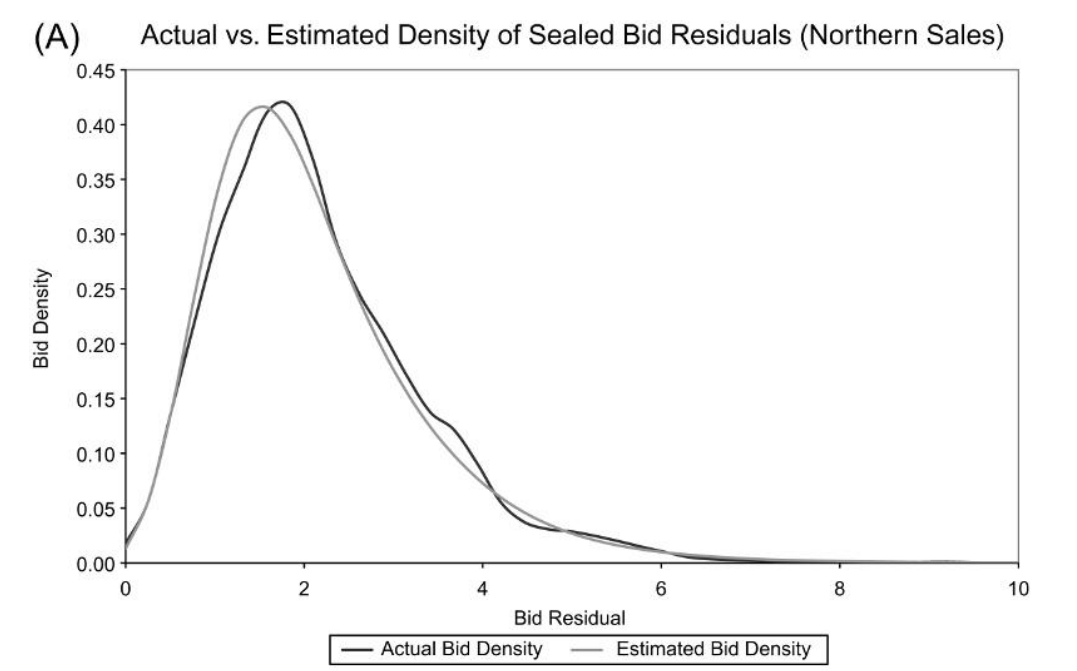
\includegraphics[width=0.49\textwidth]{figures/ch15/als2011_fig1a.png}\hfill
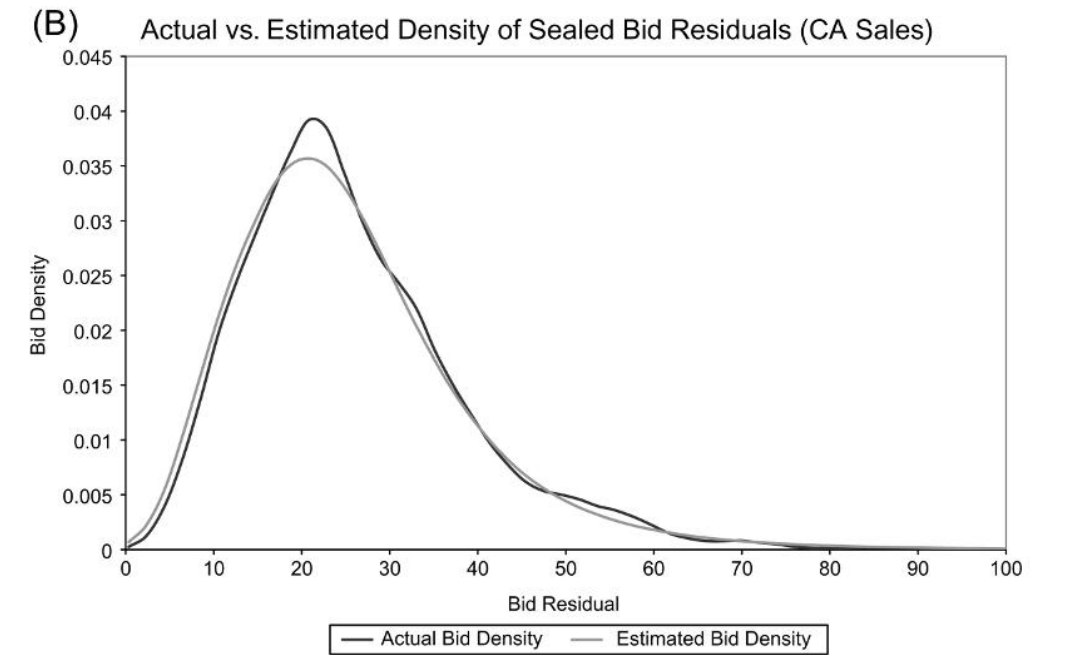
\includegraphics[width=0.49\textwidth]{figures/ch15/als2011_fig1b.png}
\caption{Actual (dark) and model-implied (light) densities of sealed-bid residuals, Northern sales (A)
and California sales (B). Residuals are bids divided by the fitted covariate index, and the actual density
is smoothed with a kernel. Source: \citet{AtheyLevinSeira2011}, Figure I.}
\label{fig:15-als-resid}
\end{figure}

\casehead{Recovering values}
Each sealed bid must be optimal against the rivals' bid distributions. Given $(Z,\omega,\bm N,\bm n)$, the
value behind a bid is given by \eqref{eq:15-als-inverse} \citep[eq.~(9)]{AtheyLevinSeira2011}. For the
Weibull distribution the reverse hazard rate has a closed form. Differentiating
\eqref{eq:15-als-weibull},
\[
g_k(b\mid\omega)=\omega\rho_kb^{\rho_k-1}\lambda_k^{-\rho_k}\exp\Bigl(-\omega\Bigl(\frac{b}{\lambda_k}\Bigr)^{\rho_k}\Bigr).
\]
Dividing by $G_k$ and multiplying numerator and denominator by $\exp(\omega(\frac{b}{\lambda_k})^{\rho_k})$,
\begin{equation}\label{eq:15-als-revhaz}
\frac{g_k(b\mid\omega)}{G_k(b\mid\omega)}=\frac{\omega\rho_kb^{\rho_k-1}\lambda_k^{-\rho_k}}{\exp\bigl(\omega(\frac{b}{\lambda_k})^{\rho_k}\bigr)-1}.
\end{equation}
Truncating the upper tail divides $g_k$ and $G_k$ by the same constant, so \eqref{eq:15-als-revhaz} is
unchanged below the truncation point. If $\omega$ were observed, each bid would map into a value, and the
value distributions would follow as in \cref{sec:15-gpv}. As \citet{Krasnokutskaya2011} observed, we can
still recover the value distributions for any value of $\omega$, because the bid functions are strictly
increasing \citep[eq.~(10)]{AtheyLevinSeira2011}:
\begin{equation}\label{eq:15-als-F}
F_k(v\mid Z,\omega,\bm N)=G_k\bigl(\xi_k^{-1}(v\mid Z,\omega,\bm N,\bm n)\bigm|Z,\omega,\bm N,\bm n\bigr).
\end{equation}

The parameterization implies a scaling property that ALS exploit \citep[p.~243]{AtheyLevinSeira2011}.
Write $s=\exp(Z\bm\theta^\lambda_Z+\bm N\bm\theta^\lambda_N)$, the part of the scale common to both
types, and $\lambda_k=s\tilde\lambda_k(\bm n)$. Then $G_k(b)=\tilde G_k(\frac{b}{s})$, where $\tilde G_k$ is
the distribution at $s=1$. Differentiating, $g_k(b)=\frac{1}{s}\tilde g_k(\frac{b}{s})$, so the reverse
hazard rates scale as $\frac{g_k}{G_k}(b)=\frac{1}{s}\frac{\tilde g_k}{\tilde G_k}(\frac{b}{s})$.
Substituting into \eqref{eq:15-als-inverse},
\[
\xi_i(b)=b+s\Biggl[\sum_{j\in\bm n\setminus i}\frac{\tilde g_j}{\tilde G_j}\Bigl(\frac{b}{s}\Bigr)\Biggr]^{-1}
=s\,\tilde\xi_i\Bigl(\frac{b}{s}\Bigr).
\]
Values, bids and therefore profits all scale with $s$. Profits need to be computed for a single value of
$(Z,\bm N)$ and then rescaled, which makes the many simulations below feasible.

A second property shows how the shape parameters govern market power.

\begin{proposition}[A floor on margins in the Weibull model]\label{prop:15-als-margin}
Under \eqref{eq:15-als-weibull}, for every bid $b>0$, every $\omega$ and every participant set,
\[
\frac{\xi_i(b)-b}{\xi_i(b)}\ \ge\ \frac{1}{1+\sum_{j\in\bm n\setminus i}\rho_j},
\]
with equality in the limit $b\to0$.
\end{proposition}

\begin{proof}
Let $x_j=\omega(\frac{b}{\lambda_j})^{\rho_j}>0$. By \eqref{eq:15-als-revhaz},
$\frac{g_j}{G_j}(b)=\frac{\rho_j}{b}\cdot\frac{x_j}{e^{x_j}-1}$. Since $e^{x}-1>x$ for $x>0$, each factor
$\frac{x_j}{e^{x_j}-1}$ lies in $(0,1)$ and tends to one as $x_j\to0$. Hence
$\sum_j\frac{g_j}{G_j}(b)<\frac{1}{b}\sum_j\rho_j$, and by \eqref{eq:15-als-inverse}
\[
\xi_i(b)-b>\frac{b}{\sum_j\rho_j},\qquad\text{so}\qquad\xi_i(b)>b\,\frac{1+\sum_j\rho_j}{\sum_j\rho_j}.
\]
Write $m=\xi_i(b)-b$. The margin $\frac{m}{b+m}$ increases in $m$, so it exceeds its value at
$m=\frac{b}{\sum_j\rho_j}$, which is $\frac{1}{1+\sum_j\rho_j}$. As $b\to0$, every $x_j\to0$ and the
inequality becomes an equality.
\end{proof}

The proposition is our derivation, not a result in ALS. It shows that the shapes, which measure how
concentrated bids are, discipline the markdowns. With the Northern estimates and two loggers and two mills,
$\rho_L=e^{1.134+2(0.016)+2(0.015)}=3.31$ and $\rho_M=3.56$. Every logger bid in that configuration then
carries a margin of at least $\frac{1}{1+3.31+2(3.56)}=0.088$ (our calculation). ALS estimate the median
profit margin across all bids, averaging over $\omega$, at 9.5 percent in the North and 10.0 percent in
California, similar for mills and loggers \citep[p.~243]{AtheyLevinSeira2011}. The paper does not state
the formula for its margin, so the comparison is only indicative. Margins of this size suggest that sealed
bidding is quite competitive.

\begin{figure}[htbp]
\centering
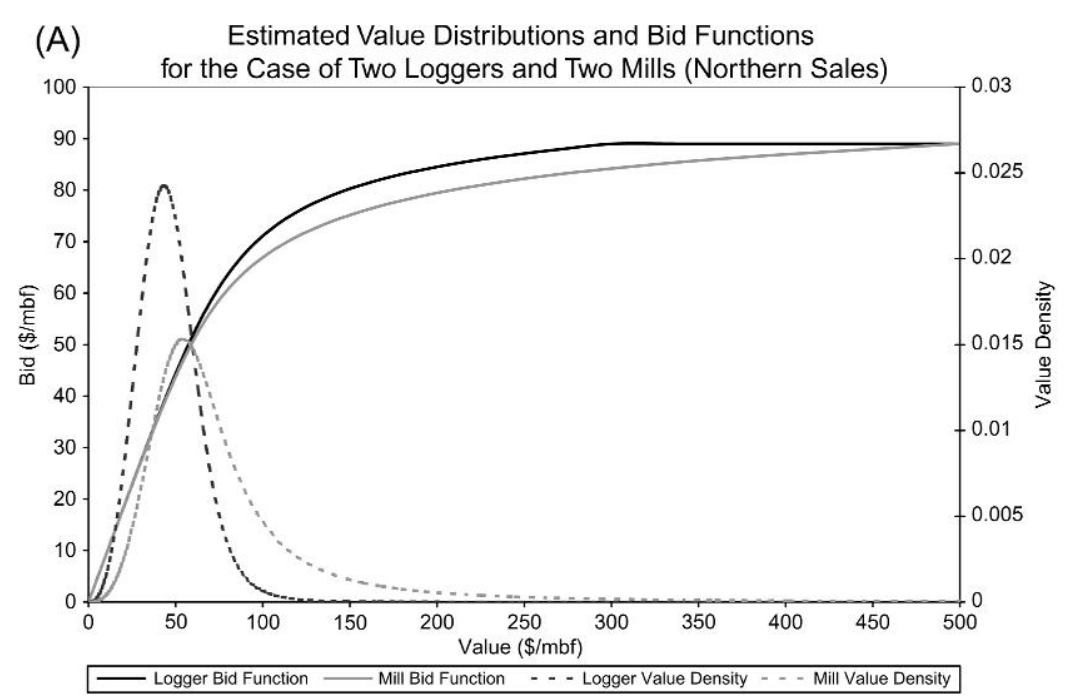
\includegraphics[width=0.49\textwidth]{figures/ch15/als2011_fig2a.png}\hfill
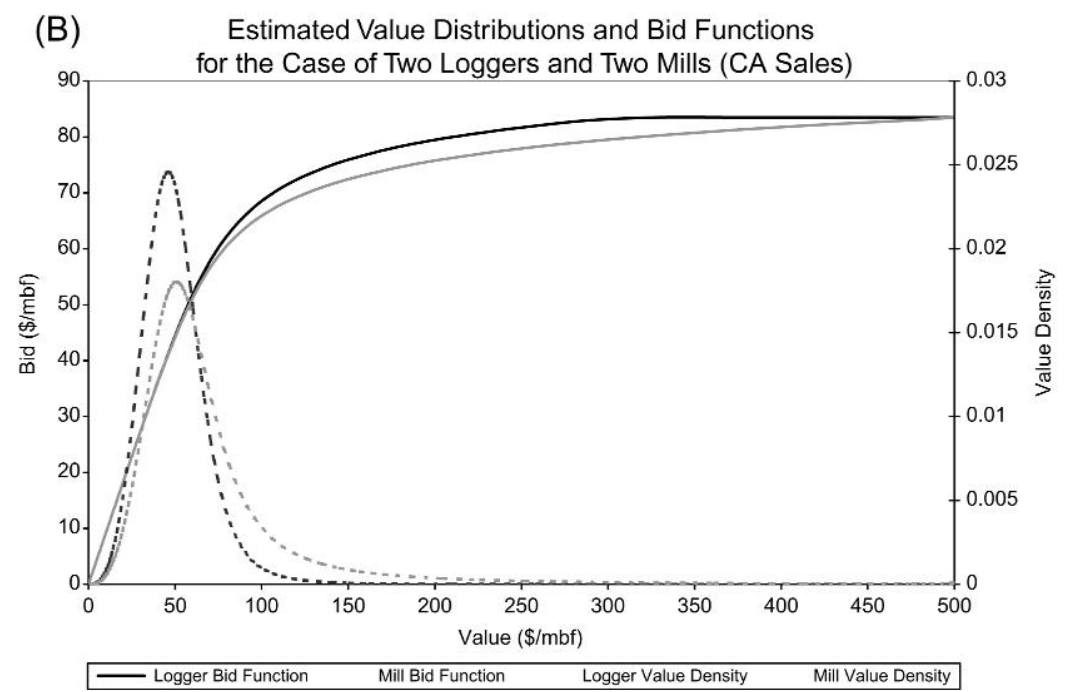
\includegraphics[width=0.49\textwidth]{figures/ch15/als2011_fig2b.png}
\caption{Estimated value densities (dashed, right axis) and equilibrium bid functions (solid, left axis)
for a sale with average covariates, $\omega=1$, two loggers and two mills, Northern sales (A) and California
sales (B). Dark curves are loggers and light curves are mills. The mill value density lies to the right,
and the mill bid function lies below the logger bid function. Source: \citet{AtheyLevinSeira2011},
Figure II.}
\label{fig:15-als-values}
\end{figure}

\Cref{fig:15-als-values} shows the recovered primitives for a sale with average covariates, $\omega=1$ and
two participants of each type. ALS compute the bid functions by inverting $\xi_k$ for the fitted bid
distributions. The mill value distribution is shifted well to the right of the logger distribution. The
mill bid function lies below the logger bid function, so mills bid less than loggers at any given value
(p.~243). This is property (i) of \cref{prop:14-maskin-riley}, the result of \citet{MaskinRiley2000}, now
found in estimated primitives.

\casehead{Checking uniqueness}
Prediction (P2) needs $\pi^{\mathrm s}_M(n_L,n_M+1)>\pi^{\mathrm s}_L(n_L,n_M)$. ALS compute the profits by
simulation \citep[pp.~243--245]{AtheyLevinSeira2011}.
\begin{enumerate}[label=(\arabic*)]
\item Draw $\omega$ from the estimated Gamma distribution.
\item For each participant, draw a bid from $\hat G_L(\cdot\mid\omega)$ or $\hat G_M(\cdot\mid\omega)$.
\item Convert each bid into a value with $\hat\xi_k$ from \eqref{eq:15-als-inverse} and \eqref{eq:15-als-revhaz}.
\item Identify the winner, the highest bidder, and record its profit $v-b$. Losers earn zero.
\item Repeat 5,000 times for each configuration with up to 8 mills and 25 loggers, and average.
\end{enumerate}
The inequality holds for all configurations and every tract in the sample (p.~245). By
\cref{prop:14-als-unique}, the estimated model has a unique type-symmetric entry equilibrium for every
tract, whatever the entry cost. In that equilibrium, if loggers enter with positive probability, every mill
enters.

\casehead{Entry costs}
ALS observe loggers entering 85 percent of Northern sales and 88 percent of California sales (p.~245).
Since potential exceeds actual logger entry almost everywhere, loggers must randomize, and a randomizing
logger is indifferent. For format $\tau$, \citep[eq.~(11)]{AtheyLevinSeira2011}
\begin{equation}\label{eq:15-als-indiff}
\Pi^\tau_L(Z,\bm N)=\sum_{n_L=1}^{N_L}\pi^\tau_L(Z,\bm N,\bm n)\,\Pr\bigl[\bm n\mid Z,\bm N,i\in\bm n,\tau\bigr]=K(Z,\bm N),
\end{equation}
with $n_M=N_M$. This is the general condition \eqref{eq:14-entry-indiff} and the identification argument of
\cref{prop:15-entry-ident}. Given that logger $i$ enters, each of the other $N_L-1$ potential loggers enters
independently with probability $p^\tau(Z,\bm N)$, so \citep[eq.~(12)]{AtheyLevinSeira2011}
\begin{equation}\label{eq:15-als-binom}
\Pr\bigl[n_L\mid Z,\bm N,i\in\bm n,\tau\bigr]=\binom{N_L-1}{n_L-1}p^\tau(Z,\bm N)^{n_L-1}\bigl(1-p^\tau(Z,\bm N)\bigr)^{N_L-n_L}.
\end{equation}
For sealed sales the entry probability is a logit \citep[eq.~(13)]{AtheyLevinSeira2011},
\begin{equation}\label{eq:15-als-logit}
p^{\mathrm s}(Z,\bm N)=\frac{\exp(Z\bm\gamma_Z+\bm N\bm\gamma_N)}{1+\exp(Z\bm\gamma_Z+\bm N\bm\gamma_N)},
\end{equation}
where ALS write $\alpha$ for $\bm\gamma$. In sale $t$ the number of entering loggers is binomial with
$N_{L,t}$ trials and success probability $p_t=p^{\mathrm s}(Z_t,\bm N_t)$. Up to a constant, the
log-likelihood is
\begin{equation}\label{eq:15-als-loglik}
\ln L(\bm\gamma)=\sum_{t\,\in\,\text{sealed}}\Bigl[n_{L,t}\ln p_t+\bigl(N_{L,t}-n_{L,t}\bigr)\ln(1-p_t)\Bigr].
\end{equation}
Let $\bm x_t=(Z_t,\bm N_t)$ be the row of regressors. For the logit, $\frac{\partial\ln p_t}{\partial\bm\gamma}=(1-p_t)\bm x_t^\T$ and
$\frac{\partial\ln(1-p_t)}{\partial\bm\gamma}=-p_t\bm x_t^\T$. The score is therefore
\[
\frac{\partial\ln L}{\partial\bm\gamma}=\sum_t\Bigl[n_{L,t}(1-p_t)-(N_{L,t}-n_{L,t})p_t\Bigr]\bm x_t^\T=\sum_t\bigl(n_{L,t}-N_{L,t}p_t\bigr)\bm x_t^\T .
\]
The maximum likelihood estimator sets the sum of observed minus expected entrants, weighted by the
covariates, to zero. The estimates are the entry columns of \cref{tab:15-als-estimates}.

The entry cost then follows without further estimation. ALS combine the simulated profits
$\hat\pi^{\mathrm s}_L(Z,\bm N,\bm n)$ with $\hat p^{\mathrm s}(Z,\bm N)$ in
\eqref{eq:15-als-indiff} and \eqref{eq:15-als-binom}, and set $\hat K(Z,\bm N)=\hat\Pi^{\mathrm s}_L(Z,\bm N)$ for each
tract. The median entry cost is \$2,870 (s.e.\ \$325) in the North and \$5,056 (s.e.\ \$673) in California
\citep[p.~246]{AtheyLevinSeira2011}. Cruising a tract can cost several thousand dollars, so these figures
are plausible. For comparison, the median expected profit of a mill in a sealed sale is roughly \$45,000
gross of entry costs (footnote 26). The median entry costs are thus about 6.4 and 11.2 percent of that
profit, the ratios reported by \citet[p.~91]{HortacsuPerrigne2021} (\cref{tab:15-entry-costs}). Two checks support the specification. If loggers entered with
probability zero in some tracts, the data would contain significantly more sales without logger entry than
the binomial model predicts, and they do not (footnote 25). Under pure-strategy entry, revealed preference
gives fairly tight bounds on entry costs that are similar to the point estimates (footnote 26).

\Cref{fig:15-als-entry} illustrates the logic and anticipates the open-auction prediction. The logger's
entry payoff falls with the probability that other loggers enter. A logger earns less in an open auction
for any participant set, so the open curve lies below the sealed curve. With the cost $K$ fixed, the
equilibrium entry probability is lower under open bidding.

\begin{figure}[htbp]
\centering
\begin{tikzpicture}
\begin{axis}[
  width=0.62\textwidth, height=0.40\textwidth,
  xmin=0, xmax=1, ymin=0, ymax=9,
  xlabel={Entry probability of other loggers, $p_L$},
  ylabel={Expected profit from entry},
  axis lines=left, xtick={0,1}, ytick=\empty,
  clip=false, every axis plot/.append style={thick}]
\addplot[domain=0:1, samples=60, blue!70!black] {2+6*exp(-2*x)};
\addplot[domain=0:1, samples=60, orange!85!black, dashed] {1.6+5*exp(-2*x)};
\addplot[domain=0:1, samples=2, black!60] {4};
\node[anchor=west, font=\small, blue!70!black] at (axis cs:1.01,3.25) {$\Pi^{\mathrm s}_L$};
\node[anchor=west, font=\small, orange!85!black] at (axis cs:1.01,1.85) {$\Pi^{\mathrm o}_L=\Pi^{\mathrm{oc}}_L$};
\node[anchor=west, font=\small] at (axis cs:1.01,4) {$K$};
\draw[densely dotted] (axis cs:0.549,0) -- (axis cs:0.549,4);
\draw[densely dotted] (axis cs:0.367,0) -- (axis cs:0.367,4);
\fill (axis cs:0.549,4) circle (1.6pt);
\fill (axis cs:0.367,4) circle (1.6pt);
\node[below, font=\small] at (axis cs:0.549,0) {$p^{\mathrm s}_L$};
\node[below, font=\small] at (axis cs:0.367,0) {$p^{\mathrm o}_L$};
\end{axis}
\end{tikzpicture}
\caption{Logger entry in the type-symmetric equilibrium with $p_M=1$ (schematic, not estimated). The
entry payoff of a logger falls in the entry probability of the other loggers. Indifference with the entry
cost $K$ pins down $p^{\mathrm s}_L$ in sealed auctions and the lower $p^{\mathrm o}_L$ in open auctions.
Mill collusion in open auctions leaves logger profits unchanged ($\Pi^{\mathrm{oc}}_L=\Pi^{\mathrm o}_L$),
so it leaves logger entry unchanged.}
\label{fig:15-als-entry}
\end{figure}

\subsection{Out-of-sample predictions and the competitiveness of open auctions}\label{sec:15-als-predict}

With the value distributions and entry costs in hand, ALS predict the outcome of every sale and compare
the predictions with the data \citep[pp.~247--248]{AtheyLevinSeira2011}. The procedure has four parts.
\begin{enumerate}[label=(\arabic*)]
\item \emph{Sealed sales.} The entry logit gives the distribution of entering loggers, and mill entry is
known. The fitted bid distributions, integrated over $\omega$, give bidding outcomes for each participant
set. Combining the two gives outcomes conditional on the tract characteristics alone.
\item \emph{Open sales, competitive.} For each simulated auction, draw $\omega$ and draw a value for each
participant from $\hat F_L(\cdot\mid Z,\omega,\bm N)$ or $\hat F_M(\cdot\mid Z,\omega,\bm N)$ via
\eqref{eq:15-als-F}. Then record the price $P^{\mathrm o}=\max\{V^{(n-1:n)},r\}$, the second-highest
participant value or the reserve price.
\item \emph{Open sales, collusive.} All participating mills except the one with the highest value drop out
at once. The price is the second-highest value in the set formed by the top mill and the loggers, or the
reserve price.
\item \emph{Open entry.} Mill entry equals the potential mill count. The logger entry probability
$p^{\mathrm o}_L$ is the unique solution of $\hat\Pi^{\mathrm o}_L(Z,\bm N;p_L)=\hat K(Z,\bm N)$. Uniqueness
holds because $\hat\Pi^{\mathrm o}_L$ falls monotonically in $p_L$ \citep[footnote 27]{AtheyLevinSeira2011}.
By prediction (P5), the same $p^{\mathrm o}_L$ applies under collusion.
\end{enumerate}
Standard errors come from a parametric bootstrap. ALS draw parameters from the estimated asymptotic
distribution of the \cref{tab:15-als-estimates} estimates and repeat the whole calculation for each draw
(p.~248). Column (2) of \cref{tab:15-als-predict} conditions on the observed participants, and column (3)
predicts entry as well.

\begin{table}[htbp]
\centering
\caption{Actual outcomes and outcomes predicted by the estimated model}
\label{tab:15-als-predict}
\small
\begin{tabular}{@{}lrccc@{}}
\toprule
 & $N$ & (1) Actual & (2) Predicted, & (3) Predicted,\\
 & & & bidding only & bidding and entry\\
\midrule
\multicolumn{5}{@{}l}{\textit{A. Northern sales}}\\
\multicolumn{5}{@{}l}{\quad Sealed-bid sales}\\
\quad Average bid & 1,492 & 59.6 & 58.2 (1.4) & 57.4 (1.3)\\
\quad Average logger bid & 1,096 & 50.8 & 48.7 (1.4) & 47.4 (1.4)\\
\quad Average mill bid & 396 & 83.8 & 84.7 (2.7) & 85.2 (2.7)\\
\quad Average sale price & 339 & 69.4 & 69.9 (1.4) & 70.4 (1.6)\\
\quad Average revenue (thousands) & 339 & 111.4 & 108.1 (4) & 109.9 (4.2)\\
\quad Percent of sales won by loggers & 339 & 68.1 & 68.0 (0.90) & 65.0 (0.01)\\
\quad Average logger entry & 339 & 3.23 & & 3.23 (0.09)\\
\multicolumn{5}{@{}l}{\quad Open auction sales}\\
\quad Average sale price, competition & 732 & 63.3 & 67.9 (1.8) & 67.8 (2.1)\\
\quad Average sale price, collusion & 732 & 63.3 & 44.2 (1.3) & 44.1 (2.2)\\
\quad Average revenue, competition & 732 & 144.7 & 152.7 (6.8) & 154.8 (7.9)\\
\quad Average revenue, collusion & 732 & 144.7 & 61.0 (2) & 64.7 (5.0)\\
\quad Percent of sales won by loggers & 732 & 59.0 & 56.0 (0.01) & 54.4 (0.02)\\
\quad Average logger entry & 732 & 2.75 & & 2.67 (0.17)\\[3pt]
\multicolumn{5}{@{}l}{\textit{B. California sales}}\\
\multicolumn{5}{@{}l}{\quad Sealed-bid sales}\\
\quad Average bid & 1,630 & 73.6 & 74.7 (2.3) & 74.2 (2.3)\\
\quad Average logger bid & 1,150 & 64.0 & 63.6 (2.1) & 62.3 (2.4)\\
\quad Average mill bid & 480 & 96.5 & 101.2 (3.5) & 102.8 (3.8)\\
\quad Average sale price & 382 & 80.4 & 83.8 (2.1) & 84.4 (2.4)\\
\quad Average revenue (thousands) & 382 & 103.1 & 110.7 (3.8) & 111.9 (4.0)\\
\quad Percent of sales won by loggers & 382 & 66.8 & 66.4 (1.2) & 62.6 (1.3)\\
\quad Average logger entry & 382 & 3.01 & & 3.01 (0.07)\\
\multicolumn{5}{@{}l}{\quad Open auction sales}\\
\quad Average sale price, competition & 325 & 85.1 & 87.2 (2.7) & 86.7 (3.1)\\
\quad Average sale price, collusion & 325 & 85.1 & 46.1 (1.2) & 51.0 (1.6)\\
\quad Average revenue, competition & 325 & 227.0 & 244.7 (9.7) & 242.4 (10.9)\\
\quad Average revenue, collusion & 325 & 227.0 & 93.2 (2.6) & 112.9 (5.6)\\
\quad Percent of sales won by loggers & 325 & 50.5 & 48.2 (1.1) & 43.6 (1.8)\\
\quad Average logger entry & 325 & 1.95 & & 1.90 (0.13)\\
\bottomrule
\end{tabular}

\smallskip
\begin{minipage}{\linewidth}
\footnotesize\textit{Notes.} Reproduced from \citet[Table V]{AtheyLevinSeira2011}. Bids and prices in 1982
dollars per mbf, revenue in thousands of 1982 dollars. Column (1) shows average outcomes. Column (2) shows
predictions for the same sales conditional on the observed entrants. Column (3) shows predictions of the
equilibrium model of entry and bidding. Parametric bootstrap standard errors in parentheses, as printed
(the paper prints a second standard error, 0.1, below the row for Northern sealed-bid logger entry). The
standard errors for the percent of sales won by loggers appear in mixed units in the original.
\end{minipage}
\end{table}

\casehead{In-sample fit}
The sealed-bid rows measure fit, since these sales were used in estimation. In the North the average sale
price is 69.4 dollars per mbf, against predictions of 69.9 with observed entry and 70.4 with predicted
entry \citep[p.~248]{AtheyLevinSeira2011}. Average logger and mill bids and the share of sales won by
loggers are also close. The largest discrepancy is in California, where the model overpredicts the sale
price, 84.4 or 83.8 against 80.4, and the revenue.

\casehead{Out-of-sample entry and allocation}
The open-auction rows are the demanding test. The model predicts open-auction logger entry of 2.67 in the
North against 2.75 observed, and 1.90 in California against 1.95 \citep[p.~250]{AtheyLevinSeira2011}. The
model therefore explains the entry gap between formats, one of the main departures from revenue
equivalence. It is less successful with allocation. It predicts that loggers win 54.4 percent of Northern
open sales, or 56.0 percent with observed entry, against 59.0 percent observed. California shows a similar
underprediction.

\casehead{Out-of-sample prices and conduct}
In California the competitive model predicts an open-auction price of 87.2 with observed entry and 86.7
with predicted entry, against 85.1 observed. The model reproduces the absence of a price difference between
formats. The North is different. The competitive model predicts 67.9 or 67.8, and the fully collusive model
44.2 or 44.1. The observed average is 63.3. Accounting for sampling error, ALS reject both models at
conventional levels. ``Mildly cooperative'' behavior by participating mills fits better than either extreme
(pp.~250--251). A linear interpolation between the competitive and collusive predictions in column (2)
gives a cooperation share of $\frac{67.9-63.3}{67.9-44.2}=0.19$ (our calculation). ALS use 18 percent as the
share that rationalizes Northern open prices in their welfare analysis.

Two robustness arguments strengthen the conclusion (p.~251). If sealed bidding were partly collusive, the
inferred values would be higher, and open prices would look even less competitive. ALS also examined the
open sales whose predicted price lies far above the actual price and found no obvious pattern.

\casehead{Where collusion should show up}
Statistical detection of collusion is hard \citep{BajariYe2003}, so ALS test a sharper implication of
(P5). With zero or one participating mill the competitive and collusive models predict the same price.
Any effect of mill collusion must appear in sales with two or more mills.
\Cref{tab:15-als-mills,fig:15-als-mills} split the Northern sales by mill participation.

\begin{table}[htbp]
\centering
\caption{Actual and predicted sale prices by mill participation, Northern sales}
\label{tab:15-als-mills}
\small
\begin{tabular}{@{}lrccc@{}}
\toprule
 & $N$ & (1) Actual & (2) Predicted, & (3) Predicted,\\
 & & & bidding only & bidding and entry\\
\midrule
\multicolumn{5}{@{}l}{\textit{Zero mills}}\\
\quad Sealed-bid sales & 181 & 51.7 & 51.4 & 51.4\\
\quad Open auction sales & 321 & 49.8 & 50.5 & 47.1\\
\multicolumn{5}{@{}l}{\textit{One mill}}\\
\quad Sealed-bid sales & 70 & 66.8 & 64.6 & 66.9\\
\quad Open auction sales & 150 & 50.0 & 52.2 & 59.5\\
\multicolumn{5}{@{}l}{\textit{Two or more mills}}\\
\quad Sealed-bid sales & 88 & 108.1 & 112.1 & 112.2\\
\quad Open auction sales & 261 & 87.5 & 98.5 & 98.0\\
\bottomrule
\end{tabular}

\smallskip
\begin{minipage}{0.84\linewidth}
\footnotesize\textit{Notes.} Reproduced from \citet[Table VI]{AtheyLevinSeira2011}. Average sale prices
in 1982 dollars per mbf. Predictions assume competitive bidding.
\end{minipage}
\end{table}

\begin{figure}[htbp]
\centering
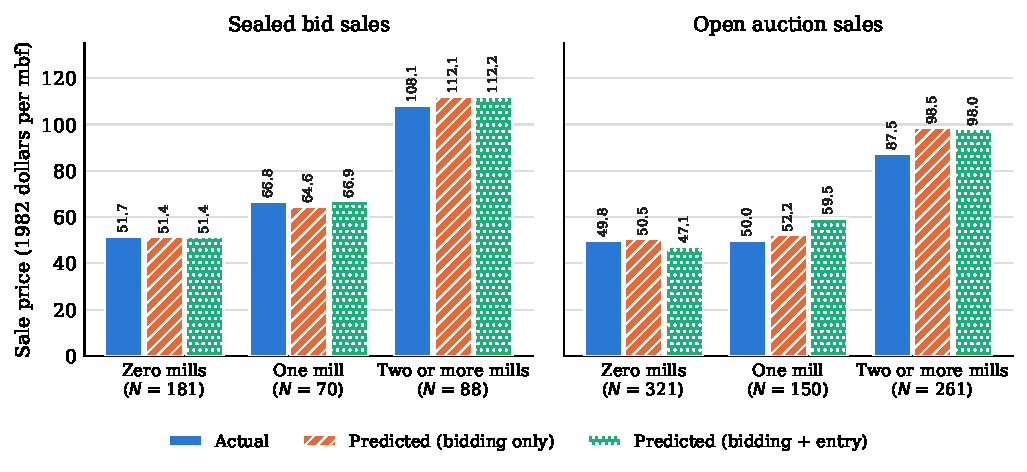
\includegraphics[width=0.92\textwidth]{figures/ch15/als_tableVI.pdf}
\caption{Actual and predicted competitive sale prices by mill participation, Northern sales. Drawn from
the numbers in \citet[Table VI]{AtheyLevinSeira2011}. With observed entry, the competitive model fits open prices
with zero or one mill and overpredicts them with two or more mills.}
\label{fig:15-als-mills}
\end{figure}

With exogenous entry, column (2), the competitive model predicts open prices accurately with zero mills
(50.5 against 49.8) and one mill (52.2 against 50.0). With two or more mills it predicts 98.5 against an
observed 87.5, a shortfall of 11 percent (our calculation), as the collusion theory implies
\citep[p.~252]{AtheyLevinSeira2011}. In sealed sales with two or more mills the shortfall is 4 percent.
Column (3) is less sharp, because the model does not fit realized logger entry cell by cell. For open sales
it predicts 3.31, 2.26 and 1.06 entering loggers in sales with zero, one and two or more mills, against
3.76, 3.32 and 1.77 observed (footnote 28). Column (2) uses observed entry and isolates the bidding margin.
Since the theory predicts identical entry under competition and collusion, that margin is where the two
hypotheses differ.

\subsection{Counterfactual comparison of formats}\label{sec:15-als-welfare}

ALS finally take the estimates as the true primitives and ask what would happen if every tract were sold by
one format \citep[Section V.C]{AtheyLevinSeira2011}. For each tract and format they compute expected entry,
the expected price and revenue, the probability that a logger wins and the expected surplus. Surplus is the
winner's value net of the entry costs sunk by all participants. Under exogenous entry, participation is
fixed at its realized value. Under endogenous entry, both formats are solved for their entry equilibria.
For open auctions they consider competitive mills and mills that cooperate 18 percent of the time.
\Cref{tab:15-als-welfare} reproduces the results.

\begin{table}[htbp]
\centering
\caption{Counterfactual outcomes of sealed and open auctions}
\label{tab:15-als-welfare}
\small
\setlength{\tabcolsep}{4.5pt}
\begin{tabular}{@{}lccccc@{}}
\toprule
 & (1) & (2) & (3) & (4) & (5)\\
 & Sealed & Open & Sealed $-$ open & Open & Sealed $-$ open\\
 & & (competitive) & (1) $-$ (2) & (partly collusive) & (1) $-$ (4)\\
\midrule
\multicolumn{6}{@{}l}{\textit{A. Northern sales ($N=1{,}071$)}}\\
\multicolumn{6}{@{}l}{\quad Exogenous entry}\\
\quad Average sale price & 68.56 & 68.53 & 0.03 (0.04) & 64.58 & 3.98 (0.24)\\
\quad Average revenue & 138.33 & 138.64 & $-0.32$ (0.06) & 124.33 & 14.00 (1.22)\\
\quad Average surplus & 176.99 & 177.06 & $-0.08$ (0.02) & & \\
\quad Percent won by loggers & 60.14 & 59.68 & 0.46 (0.16) & & \\
\multicolumn{6}{@{}l}{\quad Endogenous entry}\\
\quad Average sale price & 69.68 & 68.19 & 1.49 (0.71) & 64.11 & 5.57 (0.82)\\
\quad Average revenue & 143.04 & 139.87 & 3.17 (2.24) & 125.32 & 17.72 (2.74)\\
\quad Average surplus & 156.53 & 156.84 & $-0.30$ (2.70) & & \\
\quad Percent won by loggers & 59.65 & 57.19 & 2.46 (0.00) & & \\
\quad Logger entry & 3.10 & 2.76 & 0.34 (0.12) & & \\[3pt]
\multicolumn{6}{@{}l}{\textit{B. California sales ($N=707$)}}\\
\multicolumn{6}{@{}l}{\quad Exogenous entry}\\
\quad Average sale price & 85.53 & 85.20 & 0.32 (0.07) & 79.39 & 6.13 (0.39)\\
\quad Average revenue & 172.64 & 172.10 & 0.55 (0.13) & 154.43 & 18.21 (1.36)\\
\quad Average surplus & 203.61 & 203.65 & $-0.04$ (0.02) & & \\
\quad Percent won by loggers & 58.21 & 57.81 & 0.40 (0.002) & & \\
\multicolumn{6}{@{}l}{\quad Endogenous entry}\\
\quad Average sale price & 88.36 & 83.76 & 4.60 (2.26) & 78.55 & 9.81 (2.21)\\
\quad Average revenue & 182.38 & 168.20 & 14.18 (5.43) & 152.83 & 29.55 (5.39)\\
\quad Average surplus & 181.82 & 170.58 & 11.24 (6.86) & & \\
\quad Percent won by loggers & 55.84 & 52.66 & 3.18 (0.01) & & \\
\bottomrule
\end{tabular}

\smallskip
\begin{minipage}{\linewidth}
\footnotesize\textit{Notes.} Reproduced from \citet[Table VII]{AtheyLevinSeira2011}. Averages over all
tracts in a region of model predictions. Prices in 1982 dollars per mbf, revenue and surplus in thousands
of 1982 dollars. Exogenous entry uses the realized participants, and endogenous entry uses the equilibrium
entry model. The partly collusive open auction has mills cooperating 18 percent of the time. Bootstrap
standard errors in parentheses. The text of the paper (p.~253) states that with fixed participation sealed
bidding raises Northern revenue by \$320 per sale. The table prints a difference of $-0.32$ thousand,
consistent with its columns (1) and (2).
\end{minipage}
\end{table}

\casehead{A discrepancy in the source}
With fixed participation, the text of ALS reports a sealed-bid revenue gain of ``only \$320 per sale in
the Northern region and \$546 in California'' (p.~253).
Table VII prints a Northern difference of $-0.32$ thousand dollars. The table's own columns agree with the
negative sign, since $138.33-138.64=-0.31$. For California the text and table agree, $0.55$ thousand. We
report the table and conclude that with fixed participation the Northern revenue difference is a few
hundred dollars, of uncertain sign as printed.

\casehead{Lessons}
Four lessons emerge \citep[pp.~253--255]{AtheyLevinSeira2011}.
\begin{enumerate}[label=(\roman*)]
\item \emph{With fixed participation and competitive bidding, the format barely matters.} Revenue
differences are a few hundred dollars per sale, and the logger win probability changes by less than one
percentage point. The efficiency advantage of the open auction is under \$100 per sale in both regions.
The asymmetry between mills and loggers is substantial, yet its consequences for fixed participants are
small.
\item \emph{Entry magnifies the differences.} Both formats attract the same mills, but sealed bidding
attracts three to four more loggers per 10 sales (0.34 more per sale in the North). Loggers win 2 to 4
percentage points more sales. The sealed-bid revenue advantage rises to roughly \$3,000 per sale in the
North and \$14,000 in California, which is 2.3 and 8.4 percent of competitive open-auction revenue (our
calculation).
\item \emph{Efficiency comparisons are noisy.} The surplus difference stays small in the North. In
California the point estimate even favors sealed bidding, although sealed bidding is known to be less
efficient in equilibrium. The reason is that ALS estimate separate value distributions for each
participant configuration, and these estimates are not identical. Expectations over stochastic logger
entry weight the configurations differently across formats (footnote 29). Pooling the configurations would
break the link between the value distribution and the estimated bid distribution through the first-order
condition.
\item \emph{Collusion dominates.} Suppose mills cooperate 18 percent of the time in open auctions. Open bidding
then raises about \$14,000 less per Northern sale than competitive sealed bidding with fixed participation,
and over \$17,000 less with entry effects. The California differences are larger, \$18,210 and \$29,550 in
\cref{tab:15-als-welfare}.
\end{enumerate}
The revenue consequences of the format choice run mainly through the vulnerability of open auctions to
collusion. Gains from extra logger entry come second, and efficiency losses are small.

\subsection{Assessment}\label{sec:15-als-assessment}

\casehead{Contribution}
ALS combine three features that earlier work had treated separately: asymmetric bidders, unobserved
auction heterogeneity and endogenous participation \citep[p.~255]{AtheyLevinSeira2011}. Their entry model
recovers entry costs in dollars from post-entry profits and observed entry rates. Earlier entry models in
industrial organization infer profits relative to a normalized distribution of entry costs. Their main
methodological idea is to use variation in the rules for validation. The parameters come from one game and
are tested on another, which is a demanding out-of-sample check. The logic resembles the validation of
conduct estimates against direct cost data in \cref{ch:conduct}, with the second auction format in place of
the cost data. The approach also yields a conduct test. Behavior in the format least prone to collusion
serves as a benchmark for behavior in the format where collusion is suspected.

\casehead{Limitations}
Several assumptions deserve scrutiny.
\begin{itemize}
\item \emph{Functional form.} The Weibull and Gamma forms and the independence of $\omega$ from $Z$ are
maintained hypotheses. They pass an informal moment check and a formal specification test, but they drive
the extrapolation to open auctions. \citet{Roberts2013} argues that the reserve price itself carries
information about $\omega$ (\cref{sec:15-uh}). ALS include the reserve price in $Z$, so this would violate
the independence of $\omega$ and $Z$, and the large reserve-price coefficient in \cref{tab:15-als-estimates}
may partly proxy for $\omega$.
\item \emph{Competitive sealed bidding.} The benchmark assumes that sealed bidding is competitive. ALS
argue that sealed collusion would only strengthen the conclusion, but a cartel operating in both formats
would weaken the cross-format test.
\item \emph{Two types and a crude model of collusion.} Bidders are mills or loggers, and collusion is
modeled as perfect mill cooperation in a fraction of sales. Partial cooperation, cooperation that depends
on the identities of the mills, or coordinated entry would change the predictions.
\item \emph{Entry.} Point identification of entry costs relies on type-symmetric mixed strategies and on
the measured number of potential loggers, which contains error. Values learned only after entry rule out
selective entry.
\item \emph{Format selection.} In California the format varies strongly with size, and trimming keeps one
third of the sales. Selection on unobservables remains a concern there.
\item \emph{Open auctions as button auctions.} Open predictions assume that the price equals the
second-highest value. Jump bidding and bid increments break this equality (\cref{thm:15-ht}).
\item \emph{Two-step consistency.} Value distributions estimated separately by participant set need not
coincide, which produces the anomalous California surplus estimate.
\end{itemize}

\casehead{Follow-up work}
Later studies of Forest Service sales build on this model \citep[Section~2.6]{HortacsuPerrigne2021}.
\citet{AtheyCoeyLevin2013} evaluate small-business set-asides, sales reserved for firms with fewer than 500
employees. Their model keeps the entry and the mill-logger asymmetry of ALS and uses California's open and
sealed sales. Opening the set-aside sales to large firms would cut the share of sales won by small firms by
51 percent. It would raise revenue by 6 percent and surplus by 21 percent (pp.~98--99). A bid subsidy of
only 5 or 6 percent for small firms would keep their share of sales satisfactory. Prices would then rise by
4 percent and efficiency by 2 percent. \citet{RobertsSweeting2013} let bidders receive signals of their
values before entry, which makes entry selective. They compare the simultaneous open auction with a
sequential mechanism. In it, entrants arrive one at a time, observe the earlier offers and may jump bid to
deter later entry. With moderate selection and an entry cost of 2 percent of the average winning bid, the
sequential mechanism raises revenue by 1.8 percent. A simultaneous auction with an optimal reserve raises
it by 0.2 percent (pp.~99--100). \citet{Haile2001} studies resale. When winners can resell in a secondary
market, the values at which bidders drop out of an open auction rise with the number of bidders. Common
values predict the reverse, through the winner's curse. He instruments the number of bidders with the number
of sawmills in and near the county, and the evidence supports the model with resale (p.~100). The bounds of
\citet{AradillasLopezGandhiQuint2013} for correlated private values are applied to Oregon sales in
\cref{sec:15-reserve-asc}.

\section{Testing for Collusion with Auction Data}\label{sec:15-collusion}

Auction data seem ideal for detecting collusion. The rules are known, every bid and bidder is often
recorded, and the competitive benchmark is a fully specified game. Detection is nonetheless hard.
\citet{PorterZona1993}, in the working-paper version we follow, explain why.\footnote{We use NBER Working
Paper 4013 (March 1992) for the description of the tests. The published estimates are discussed in
\cref{sec:13-detection}.} Patterns often read as collusion can arise in competitive equilibria. Rotating
winners are consistent with competition when firms face capacity constraints. Comparisons of winning bids
with engineers' cost estimates can mislead, because the estimates may be inflated by past bids. Collusive
schemes take many forms \citep{HendricksPorter1989}. A cartel might rotate a single bid among its members,
or several members might submit higher \emph{complementary bids}, also called \emph{phantom bids}, to
create the appearance of competition. No single test can detect every scheme. A cartel that includes every
bidder could even choose complementary bids that pass any broadly applicable test. Its bids would mimic
competitive bids for some plausible realization of costs (Porter and Zona, working paper, pp.~2--3).

\citet[p.~211]{AtheyLevinSeira2011} sort the empirical approaches into three groups.
\Cref{tab:15-collusion-tests} summarizes them. The first group requires prior knowledge of the cartel's
existence and structure and compares suspected members with other bidders. The second derives in-sample
specification tests of the competitive model and treats collusion as the alternative. The third, which ALS
introduce, uses behavior under one format as the benchmark for another.

\begin{table}[htbp]
\centering
\caption{Approaches to detecting collusion with auction data}
\label{tab:15-collusion-tests}
\footnotesize
\begin{tabularx}{\linewidth}{@{}>{\raggedright\arraybackslash}p{2.3cm}>{\raggedright\arraybackslash}X>{\raggedright\arraybackslash}X>{\raggedright\arraybackslash}p{2.6cm}@{}}
\toprule
Approach & Maintained information & Implication tested & Examples\\
\midrule
Suspected members versus others & Identity of a candidate cartel, bid levels and ranks & Determinants of
non-winning cartel bids differ from those of the low cartel bid and of non-cartel bids & \citet{PorterZona1993,PorterZona1999}\\
\addlinespace
Specification tests of competition & Bidder and auction covariates & Conditional independence and
exchangeability of bids & \citet{BajariYe2003}\\
\addlinespace
Cross-format benchmark & A format presumed competitive & Prices in the suspect format fall short of
predictions only where theory says collusion bites & \citet{AtheyLevinSeira2011}\\
\addlinespace
Records of a known cartel & Knockout bids and side payments & Structural values and damages from the
cartel's internal bids & \citet{Asker2010}\\
\addlinespace
Super-plus factors & Bid histories, registrations, ownership after the sale & Transfers among bidders, no
rivalry within a subset, prompt resale, close losing bids & \citet{MarshallMarx2012}\\
\bottomrule
\end{tabularx}
\end{table}

\casehead{Porter and Zona: low cartel bids versus higher cartel bids}
Porter and Zona study state highway paving contracts on Long Island in the early 1980s. A set of five firms,
named in a bid-rigging conviction and related suits, forms a candidate cartel. Insiders described meetings
that designated a serious bidder and its bid, after which other members submitted higher bids. The cartel
did not rotate single bids. Several members bid on most jobs, which makes detection possible because ring
behavior can be compared with that of non-members. Each competitive bidder in a low-bid procurement auction
chooses its bid $b$ to maximize $(b-c_{it})\Psi_{it}(b)$, where $c_{it}$ is its cost on job $t$ and
$\Psi_{it}(b)$ its probability of submitting the lowest bid. The first-order condition is
\[
\Psi_{it}(b)+(b-c_{it})\Psi_{it}'(b)=0 ,
\]
the procurement analog of \eqref{eq:15-als-foc}. Costs are unobserved, so Porter and Zona approximate the
equilibrium bid by a log-linear rule,
\begin{equation}\label{eq:15-pz-bid}
\ln B_{it}=\alpha_t+W_{it}\bm\vartheta+\epsilon_{it},\qquad\E[\epsilon_{it}]=0,\qquad\Var(\epsilon_{it})=\sigma_t^2 .
\end{equation}
Here $\alpha_t$ is a job effect, $W_{it}$ are firm-job cost shifters such as capacity and backlog, and
$\epsilon_{it}$ is private cost information whose variance differs by job. Ordinary least squares on competitive bids
estimates $\bm\vartheta$, the job mean squared residual estimates $\sigma_t^2$, and feasible generalized
least squares reweights the data.

The sharper test uses the ranking of bids. Let $X_{it}=-\frac{W_{it}}{\hat\sigma_t}$ be the deflated cost
shifters with the sign reversed. If $-\epsilon_{it}$ is type I extreme value, the job effect cancels and the
probability that firm $i$ submits the lowest bid takes the logit form. The probability of the observed
ranking $b_{r_1t}<b_{r_2t}<\dots<b_{r_nt}$ is the rank-ordered logit
\begin{equation}\label{eq:15-pz-rank}
\Pr\bigl[b_{r_1t}<\dots<b_{r_nt}\bigr]=\prod_{m=1}^{n-1}\frac{\exp(\bm\vartheta X_{r_mt})}{\sum_{l=m}^{n}\exp(\bm\vartheta X_{r_lt})} .
\end{equation}
The likelihood factors into the probability of the lowest bid and the probabilities of the ranks above it.
Under correct specification and no phantom bidding, both parts carry the same coefficients. A likelihood
ratio test applied to competitive bids checks the specification. The same test applied to cartel bids
asks whether the low cartel bid and the higher cartel bids share determinants. Complementary bids are not
meant to win, so their ranking need not reflect cost differences. Porter and Zona find that ranks and
levels of non-cartel bids follow cost measures, while the ranks of higher cartel bids do not and differ
from those of the low cartel bid. A Chow test of a common bid equation for cartel and competitive firms, estimated as in their Table~4,
gives $F(76,319)=9.38$ (p.~33). For competitive bids, the likelihood ratio statistic for equal coefficients
across ranks is $4.30$ against a $\chi^2_6$ distribution, a $p$-value of $0.64$ (p.~33, estimates in Table~5).
For cartel bids it is $8.94$ against a $\chi^2_4$ distribution, a $p$-value of $0.063$ (p.~34, estimates in
Table~6). The $p$-values are our
computation. Page and table numbers refer to the NBER working-paper version of \citet{PorterZona1993}, and
\cref{sec:13-detection} reports the full estimates.

\casehead{Bajari and Ye: independence and exchangeability}
A second approach needs no list of suspects. In an independent private values model with symmetric
bidders, bids are independent across bidders conditional on the covariates, and the joint distribution of
bids is exchangeable \citep[Section 5.5]{AtheyHaile2007}. Suppose values have the form
$V_{it}=h(Z_{1t},Z_{2i},Z_{2(-i)},A_{it})$, where $Z_{1t}$ is an auction covariate, $Z_{2i}$ a bidder
covariate, $Z_{2(-i)}$ the rivals' covariates and $A_{it}$ an idiosyncratic factor with an exchangeable
distribution. Each bid then depends on $(Z_{1t},Z_{2i},Z_{2(-i)})$ and not on the bidder's identity. Two
regression tests follow. Residuals from regressions of bids on covariates should be uncorrelated across
bidders, and coefficients should be equal across bidders or classes of bidders.
\citet{BajariYe2003} apply both tests to highway construction procurement. Collusion is the alternative.
Rejection can also reflect omitted heterogeneity common to the bidders, the problem of \cref{sec:15-uh}.

\casehead{The structural signature}
ALS add a third approach with three steps. Estimate the model on the segment least prone to collusion,
sealed sales. Predict outcomes where collusion is suspected, open sales. Then look where theory says
collusion must appear, sales with two or more strong participants. The test exploits an implication of
theory that a cartel cannot easily mask: a ring of mills cannot lower prices in sales where at most one mill
participates. Its power comes from the structural model, which delivers the competitive benchmark for each
cell.

\casehead{Using a cartel's own records}
When records of a cartel's internal knockout auctions survive, the cartel's bids can be modeled directly.
\citet{Asker2010} uses such records for a ring of stamp dealers to estimate values, the ring's gains and the
harm to sellers and to non-members (\cref{sec:13-asker}).

\casehead{Theory and enforcement}
The theory of \cref{sec:14-collusion} explains why the format matters. In open and second-price auctions,
a ring in which the highest-value member bids and the others abstain is self-enforcing within the auction
(\cref{prop:14-robinson,prop:14-collusion-open}). In first-price auctions a ring needs the threat of future
punishment, the repeated-game enforcement of \cref{ch:collusion-theory}. Optimal collusion in repeated
first-price auctions with private information can take sophisticated forms. When the auctioneer reveals the
winning bid but not the winner's identity, optimal collusion has every member bid the reserve price with
equal chances of winning. \Citet[footnote 102]{AtheyHaile2007} summarize this result of
\citet{AtheyBagwellSanchirico2004}.

\citet[ch.~8]{MarshallMarx2012} compare what a ring gains under each format, with independent private
values and a fixed set of bidders. In an ascending auction the ring's highest-value member bids up to its
value and the other members never raise a hand (pp.~171--172). The ring gains only when it holds the two
highest values. It then wins at the highest value outside the ring instead of the second-highest value
overall. A bidder outside the ring who wins pays what it would have paid without the ring, so the ring
captures all of the gain (p.~176). In a first-price auction the ring's designated bidder faces fewer rivals
and lowers its bid. Bidders outside the ring respond by lowering their bids as well, and the equilibrium
is unique (pp.~174--175). The lower ring bid sometimes lets an outsider win when it would have lost under
competition. Part of the collusive gain then leaks to bidders outside the ring, so the incentive to collude
is typically weaker under sealed bidding (p.~176).

\begin{example}[Ring gains in an ascending auction]\label{ex:15-ring-gain}
Let $n=5$ bidders have values drawn independently from the uniform distribution on $[0,1]$, with no
reserve price, and let $k$ of them form a ring. The $m$-th lowest of five uniform values has mean
$\E[V^{(m:5)}]=\frac{m}{6}$. Let $J$ be the number of top values that the ring holds in an unbroken run
from the top. If $J\le1$, the price is the second-highest value overall. If $J=j\ge2$, the price is the
highest value outside the ring, $V^{(5-j:5)}$. Ring members are a random subset, so for $k=2$
\[
\Pr(J\le1)=1-\frac{2}{5}\cdot\frac{1}{4}=\frac{9}{10},\qquad \Pr(J=2)=\frac{2}{5}\cdot\frac{1}{4}=\frac{1}{10}.
\]
The expected price is
\[
\frac{9}{10}\cdot\frac{4}{6}+\frac{1}{10}\cdot\frac{3}{6}=0.600+0.050=0.650,
\]
against $\frac{4}{6}\approx0.667$ without the ring. The ring wins when it holds the top value, which
happens with probability $\frac{2}{5}$. Given that event, its member with the top value pays $\frac{4}{6}$
with probability $\frac{3}{4}$ and $\frac{3}{6}$ with probability $\frac{1}{4}$. The ring's expected
surplus is therefore
\[
\frac{2}{5}\Big[\frac{5}{6}-\Big(\frac{3}{4}\cdot\frac{4}{6}+\frac{1}{4}\cdot\frac{3}{6}\Big)\Big]
=\frac{2}{5}\cdot\frac{5}{24}=\frac{1}{12}\approx0.083 .
\]
Each member expects about $0.042$, against $\frac{1}{30}\approx0.033$ for a competitive bidder. Both numbers
match the first rows of \cref{tab:15-mm-rings}.
\end{example}

\begin{table}[htbp]
\centering
\caption{Ring size and auction format with five uniform bidders (Marshall and Marx 2012, Table 8.1)}
\label{tab:15-mm-rings}
{\small
\setlength{\tabcolsep}{4pt}
\begin{tabular}{ccccccc}
\toprule
 & \multicolumn{2}{c}{Expected price} & \multicolumn{2}{c}{Surplus per ring member} & \multicolumn{2}{c}{Surplus per outsider}\\
\cmidrule(lr){2-3}\cmidrule(lr){4-5}\cmidrule(lr){6-7}
Ring size $k$ & Ascending & First price & Ascending & First price & Ascending & First price\\
\midrule
1 & 0.667 & 0.667 & 0.033 & 0.033 & 0.033 & 0.033\\
2 & 0.650 & 0.651 & 0.042 & 0.035 & 0.033 & 0.037\\
3 & 0.600 & 0.609 & 0.056 & 0.041 & 0.033 & 0.049\\
4 & 0.467 & 0.506 & 0.083 & 0.057 & 0.033 & 0.086\\
5 & 0.000 & 0.000 & 0.167 & 0.167 & & \\
\bottomrule
\end{tabular}}

\smallskip
\begin{minipage}{0.93\textwidth}
\footnotesize \textit{Notes.} Values uniform on $[0,1]$, reserve price zero. Ascending entries and the
first-price entries for $k=1$ are analytic. The other first-price entries come from Monte Carlo simulation
with 100,000 draws, as reported by Marshall and Marx from earlier work of Marshall and coauthors.
\end{minipage}
\end{table}

\Cref{tab:15-mm-rings} shows both effects (pp.~181--182). A ring that does not include every bidder hurts the
seller more under ascending bidding, and its members gain more there. Outside bidders gain nothing from a
ring at an ascending auction, while at a first-price auction their surplus rises with the size of the ring.
The authors caution that this ranking is not a general result (p.~181, footnote 21, citing
\citealp{MaskinRiley2000}). Leakage also shapes who joins (Section 8.3, pp.~176--180). At an ascending
auction nothing leaks, so outsiders always want to join, and with symmetric bidders the ring wants everyone
in. At a sealed-bid auction a weak bidder may prefer to stay out and bid against a ring whose depressed bids
it can exploit. Membership also raises a sequencing problem (Section 8.3.2, pp.~179--180). The last bidder
to join adds a large gain, because its entry removes all remaining competition. If that bidder were paid its
contribution, every member would want to join last. Rings therefore fix the division of the gain before the
auction, with equal shares for symmetric members and the average of each member's marginal contributions
for asymmetric ones. Settling the split in advance also rules out conflicting claims and costly rent
seeking after the auction (p.~180).

\casehead{Auction design against rings}
\citet[ch.~10]{MarshallMarx2012} turn the comparison into design advice. Transparency helps a ring monitor
its members (pp.~200--202). Rules written to curb favoritism by public officials announce the set of
bidders before the sale and publish bids and identities after it, which serves rings as well. In early
spectrum auctions of the Federal Communications Commission, bidders chose their increments and used the last
three digits of their bids to signal to one another. Later designs fixed the increments and hid rivals'
identities until the auction closed. A right of last refusal for an incumbent supplier lets the incumbent
watch rivals' bids in real time, which deters deviations from a collusive agreement. Bidding under
disguised identities, or shill bids, makes deviations harder for a ring to police, especially at sealed-bid
auctions (pp.~202--205). With transparent registration a ring can suppress competition at an ascending
auction. It does so with a scheme in which the winning member pays the ring the excess of the
second-highest member report over the price. If identities are hidden during the bidding and registration
is not transparent, payments from winning members alone cannot suppress all competition. Information about
the object also matters. If bidders have more expertise than the seller, competitive bidding transfers the
rents from that expertise to the seller, which gives bidders an extra reason to collude. The frequency of
sales matters as well (p.~206). Regular, frequent sales make bid rotation and punishment easier, so an
auctioneer worried about collusion may hold fewer sales of larger lots at irregular intervals. Finally,
sealed bids leave a paper trail of losing bids, while ascending auctions often leave no record of who would
have bid (pp.~206--207). The authors list six measures (p.~207). Use sealed instead of ascending bids. Limit
information about rivals, outcomes and bids. Avoid rights of last refusal for incumbents. Allow multiple bids,
some under disguised identities. Choose disclosure of the seller's information with collusion in mind. Hold
auctions at long, irregular intervals. The first measure is the choice that Pinchot made for the Forest
Service (\cref{sec:15-als-question}).

\casehead{Plus factors for rings}
A \emph{plus factor} is evidence, beyond parallel prices, that supports an inference of collusion.
\citet[ch.~12]{MarshallMarx2012} focus on \emph{super-plus factors}, patterns whose probability without a
ring is close to zero (pp.~243--244). They stress those that a ring could not remove without changing how it
works. Two apply to both formats. The first is transfers among bidders, such as cash settlements
of a knockout or subcontracting and joint ownership arrangements that were not declared before the sale. The
second is a divergence between observed prices and the prices predicted by a model estimated on a
benchmark in which no ring is presumed to operate. This is the logic of the cross-format test of
\citet{AtheyLevinSeira2011}, with sealed sales as the benchmark and open sales as the suspect segment.

At an ascending auction the ring's rule is simple: members do not bid while another member is active
(pp.~244--246). The winner and the last underbidder, and any two bidders who compete directly, are then
never both members. A subset of bidders who never bid against each other at meaningful prices is therefore
a super-plus factor, although it may take many auctions to detect. Ascending auctions allocate efficiently,
so a prompt resale to another bidder who was present suggests a post-auction knockout. Light attendance is
not a super-plus factor, since rings may require members to attend. At a sealed-bid auction resale is
weaker evidence, because asymmetric bidders can produce inefficient allocations that resale corrects
(pp.~246--247). Nonwinning bids unrelated to values, the evidence that \citet{PorterZona1993} use, are not
substantive either, because a ring can rescale its losing bids freely. Close pairs of bids are more telling.
Suppose the top member has value \$100,000 and would bid \$90,000 under competition, but the ring wants it to
bid \$50,000. A member with value \$60,000 that expects less than \$10,000 from the ring would then gain by
bidding \$50,001 through a shill. To deter this, the ring has its top member bid more, say \$65,000, and has
another member bid just below. The frequent closeness of two bids then reveals the ring. A sudden switch
from ascending to sealed bidding is informative too (p.~248). A large price increase after the switch
suggests that a ring operated at the ascending auctions. No change is not evidence of no ring, and risk
aversion raises sealed-bid prices only modestly.

\casehead{Shill bidding in Russian oil and gas auctions}
The appendix to their chapter~12 studies ascending auctions for Russian oil and gas leases, which proceed
only if at least two bidders register (pp.~248--255). The government sets a reserve price and the
increments, and the lowest feasible bid is one increment above the reserve. The data cover 620 auctions
from 2004 to 2007. They are complete for 121 auctions and partial for 499. The complete auctions are larger,
with an average reserve of 71,503,769 rubles against 49,484,900. Five were canceled and one was awarded on
criteria other than price, which leaves 115. \Cref{tab:15-mm-russia} reproduces the distribution of winning
bids. Auctions with six or more participants always end at least 20 increments above the reserve. In 34
of the 43 two-bidder auctions, 79 percent, the winning bid is one or two increments above the reserve.
These 34 auctions have an average reserve of 27,515,294 rubles, less than half the average for all 620.

\begin{table}[htbp]
\centering
\caption{Winning bids in increments above the reserve, by number of participants (Marshall and Marx 2012,
Table 12.2)}
\label{tab:15-mm-russia}
\begin{tabular}{lcccccc}
\toprule
 & \multicolumn{5}{c}{Increments of the winning bid above the reserve} & \\
\cmidrule(lr){2-6}
Participants & 1 & 2 & 3--19 & 20--99 & 100 or more & Auctions\\
\midrule
2 & 53\% & 26\% & 9\% & 7\% & 5\% & 43\\
3 & 3\% & 9\% & 26\% & 41\% & 21\% & 34\\
4 & 8\% & 0\% & 15\% & 15\% & 62\% & 13\\
5 & 10\% & 10\% & 20\% & 10\% & 50\% & 10\\
6 or more & 0\% & 0\% & 0\% & 33\% & 67\% & 15\\
\addlinespace
Combined & 23\% & 13\% & 15\% & 22\% & 28\% & 115\\
\bottomrule
\end{tabular}

\smallskip
\begin{minipage}{0.93\textwidth}
\footnotesize \textit{Notes.} Subsample of 115 auctions with complete data, 2004--2007. Each row sums to 100
percent. Their Table 12.1 gives the same data as shares of all 115 auctions.
\end{minipage}
\end{table}

The identities point to shills (Table 12.3, pp.~251--253). The 34 auctions have 24 distinct winners, 26
distinct losers and 26 distinct ordered pairs. One bidder won six such auctions, always against the same
opponent, which never won any of the 620 auctions. The authors classify 13 losing bidders as \emph{pure
shills}. Each bid at most once, never won a lease in the 620 auctions, and never took part in an auction
without its winning partner. Two losers form a rotating pair, each winning against the other at one or two
increments, and the remaining 11 are occasional shills. The registration rule explains the pattern. A
license of interest to a single firm cannot be sold unless a second bidder registers, so the firm has an
incentive to bring one along. The authors note that their own static model of semitransparent auctions
leaves no role for shills in a well-functioning ring. Two pure shills did appear with their partners in
auctions with more than two bidders, which suggests dynamic motives or a strategic auctioneer.

\casehead{Evidence from timber sales}
Forest Service timber sales have produced several studies of collusion
\citep[Section~2.5]{HortacsuPerrigne2021}. Collusion was suspected in the 1970s and led to a congressional
hearing in 1977, but few cases were prosecuted (p.~96). \citet{BaldwinMarshallRichard1997} study Forest
Service oral auctions. They compare order-statistic models of competitive and cooperative bidding, in which a
winning ring member pays the highest value outside the ring. The supply of timber varied across years, and
oversupply alone could depress bids. After controlling for supply conditions, collusion explains the low bids
better (pp.~96--97). In British Columbia, sales are by first-price sealed bid. \citet{ListMillimetPrice2007}
treat collusion as an unobserved treatment and test conditional independence and exchangeability of bids, in
the spirit of \citet{BajariYe2003}. They flag 130 suspect bidders, and the evidence of collusion is mixed
(p.~97). \citet{Price2008} studies the spatial proximity of bidders. Firms located in the same town or nearby
bid 10 to 13 percent less, and exchangeability is rejected for firms in close proximity. Industry interviews
suggest that distance does not create asymmetry in values. With the same data, \citet{Schurter2020} shows that
an asymmetric independent private values model with collusion is not identified when the colluders are
unknown (pp.~97--98). An instrument that shifts competition but is independent of values given the reserve
price restores identification. His test asks, bidder by bidder, whether estimated values are independent of
the reserve. Seven firms fail it, and four of them do not bid competitively. Competitive bidding by these four
firms would raise revenue by 3.2 percent, a moderate cost of collusion.

\section{Divisible-Good Auctions: Bidding with Demand Schedules}\label{sec:15-divisible}

Treasury bills, central bank loans and electricity are sold in auctions in which each bidder states a
quantity for every price. The good is \emph{divisible}, so any share of the supply can be allocated. Such
auctions are also called \emph{share auctions}, after the model of \citet{Wilson1979}. Each bid is a demand
schedule, and the seller adds the schedules up to clear the market. This section gives a short treatment of
the format. Its message is that the logic of \cref{sec:15-gpv} carries over. The distribution of the
market-clearing price, given a bidder's own schedule, takes the place of the distribution of rival bids. We
set up the model, derive the first-order conditions under uniform and discriminatory pricing, and study one
application of each.

\subsection{The share auction with step bids}\label{sec:15-div-model}

A perfectly divisible good is sold to $N$ bidders. Quantities are measured as shares of the announced
supply. The quantity sold, $Q$, may be random, because the seller can adjust it after seeing the
bids. Its distribution is common knowledge. Bidder $i$ observes a private signal $s_i$, and signals are
independent across bidders. Winning the share $q$ gives the bidder the gross utility
\begin{equation}\label{eq:15-div-V}
V(q,s_i)=\int_0^q v(u,s_i)\,du ,
\end{equation}
where the \emph{marginal value} $v(q,s_i)$ is weakly decreasing in $q$ and strictly increasing in $s_i$.
Values are private, so $v$ does not depend on rivals' signals \citep[p.~978 and Assumptions~2 and 6]{Kastl2011}.

A bid is a \emph{step function}. Bidder $i$ submits $K_i$ \emph{bidpoints} $(b_k,q_k)$, $k=1,\dots,K_i$,
with prices $b_1>b_2>\dots>b_{K_i}$ and cumulative quantities $q_1<q_2<\dots<q_{K_i}$. The bidder demands
nothing at prices above $b_1$ and demands $q_k$ at prices in $(b_{k+1},b_k]$, with the convention
$b_{K_i+1}=0$ and $q_0=0$. The seller caps the number of bidpoints at $\bar K$, which is 10 in both
applications below. Bidders use far fewer steps than the cap allows, so the steps are a feature of the data
that a model must explain.

Let $y_j(p)$ be bidder $j$'s demand at price $p$. The \emph{residual supply} facing bidder $i$ is the
quantity left for it after its rivals' demands are met,
\begin{equation}\label{eq:15-div-rs}
RS_i(p)=Q-\sum_{j\neq i}y_j(p).
\end{equation}
It rises with $p$. It is random from $i$'s point of view, because it depends on rivals' signals and on $Q$.
The \emph{market-clearing price} $P^{\mathrm c}$ is the highest price at which total demand weakly exceeds
supply. Bids above $P^{\mathrm c}$ are filled in full. Demands exactly at $P^{\mathrm c}$ are scaled down in
proportion until the supply is exhausted, a rule called \emph{pro rata rationing on the margin}. Two payment
rules are common. Under \emph{uniform pricing} every unit won pays $P^{\mathrm c}$. Under
\emph{discriminatory pricing}, also called pay-as-bid, each unit won pays the bid on that unit. A bidder then
pays the area under its own step function up to the quantity it wins.

With continuous and strictly decreasing bid functions, as in \citet{Wilson1979}, residual supply crosses each
demand curve at a single point and nobody is rationed. With steps, residual supply is itself a step function.
It can cross bidder $i$'s schedule in two ways. On a vertical segment, $i$ receives exactly $q_k$ at a price
strictly between $b_{k+1}$ and $b_k$. On a horizontal segment, the price equals one of $i$'s bids and $i$ is
rationed. With private values and a continuous price grid, ties with positive probability are incompatible
with equilibrium, except possibly at bids above the bidder's marginal value \citep[p.~984 and
Appendix~B]{Kastl2011}. A bidder that expected a tie at a bid below its marginal value would gain by raising
that bid slightly. A rationed bidder is then the only marginal bidder, and it
receives the residual supply at its own bid.

\subsection{Uniform pricing: Kastl (2011)}\label{sec:15-kastl}

\casehead{Question} Economists agree that governments should sell their securities by auction, but they
disagree about the format. In a survey that \citet{Kastl2011} cites, 39 of 42 countries used discriminatory
pricing and only 3 used uniform pricing (p.~974). Theory does not rank the two formats on revenue or on
efficiency \citep[Section~10]{AtheyHaile2007}. Kastl asks how to measure the performance of a uniform-price
auction from bids when bidders submit only a few steps. His answer starts from the observation that steps
change the first-order conditions, and with them the values that bids reveal.

\casehead{The step first-order condition} Fix bidder $i$ with signal $s_i$, its bid $\{(b_k,q_k)\}$ and its
rivals' strategies. All probabilities and expectations below are over rivals' signals and the supply, given
$s_i$ and $i$'s bid. Write $A_k$ for the event $b_k>P^{\mathrm c}>b_{k+1}$, in which residual supply crosses
the vertical segment of $i$'s schedule at $q_k$.

\begin{proposition}[Step condition under uniform pricing]\label{prop:15-kastl}
Assume private values and pro rata rationing on the margin. In any Bayesian Nash equilibrium, for almost
every $s_i$, every step $k$ at which a tie has probability zero satisfies
\begin{equation}\label{eq:15-kastl-foc}
\Pr(A_k)\bigl[v(q_k,s_i)-\E(P^{\mathrm c}\mid A_k)\bigr]
=q_k\,\frac{\partial\,\E\bigl[P^{\mathrm c}\,\indic\{b_k\ge P^{\mathrm c}\ge b_{k+1}\}\bigr]}{\partial q_k} .
\end{equation}
Equivalently,
\begin{equation}\label{eq:15-kastl-mcmr}
v(q_k,s_i)=\E(P^{\mathrm c}\mid A_k)
+\frac{q_k}{\Pr(A_k)}\,\frac{\partial\,\E\bigl[P^{\mathrm c}\,\indic\{b_k\ge P^{\mathrm c}\ge b_{k+1}\}\bigr]}{\partial q_k} .
\end{equation}
\end{proposition}

\begin{proof}[Derivation]
We give the argument for a step at which ties have probability zero, as they do when $b_k<v(q_k,s_i)$. Fix a realization of rivals' signals and of the supply. Let $P(q)$ be the
inverse residual supply, the price at which $RS_i$ equals $q$. Three events involve step $k$.
\begin{enumerate}[label=(\roman*)]
\item On $A_k$, $b_{k+1}<P(q_k)<b_k$. Bidder $i$ wins $q_k$ at the price $P(q_k)$, and its payoff is
$V(q_k,s_i)-P(q_k)\,q_k$.
\item On $B_k$, $q_{k-1}<RS_i(b_k)<q_k$. The price is $b_k$, and $i$ is rationed to $RS_i(b_k)$.
\item On $B_{k+1}$, $q_k<RS_i(b_{k+1})<q_{k+1}$. The price is $b_{k+1}$, and $i$ is rationed to
$RS_i(b_{k+1})$.
\end{enumerate}
Raise $q_k$ slightly and hold the other bidpoints fixed. On $B_k$ and $B_{k+1}$ the payoff does not depend
on $q_k$, because $i$ receives the residual supply. Only the boundaries of the three events move. On the
boundary between $A_k$ and $B_k$ we have $P(q_k)=b_k$ and $RS_i(b_k)=q_k$, so the payoffs in (i) and (ii)
coincide. The same holds on the boundary between $A_k$ and $B_{k+1}$. Moving a boundary therefore has no
first-order effect, and only the change inside $A_k$ remains. Differentiating the payoff in (i) gives
\[
\frac{\partial\,\E[\text{payoff}]}{\partial q_k}
=\E\Bigl[\Bigl(v(q_k,s_i)-P(q_k)-q_k\,\frac{\partial P(q_k)}{\partial q_k}\Bigr)\indic\{A_k\}\Bigr].
\]
Set the derivative to zero and use $\E\bigl[P(q_k)\indic\{A_k\}\bigr]=\Pr(A_k)\,\E(P^{\mathrm c}\mid A_k)$:
\[
\Pr(A_k)\bigl[v(q_k,s_i)-\E(P^{\mathrm c}\mid A_k)\bigr]
=q_k\,\E\Bigl[\frac{\partial P(q_k)}{\partial q_k}\,\indic\{A_k\}\Bigr].
\]
It remains to rewrite the right side. The event $b_k\ge P^{\mathrm c}\ge b_{k+1}$ is the union of $A_k$,
$B_k$ and $B_{k+1}$. This union does not move with $q_k$, since a change in $q_k$ only shifts states among the
three events. Inside the union, $P^{\mathrm c}$ equals $P(q_k)$ on $A_k$ and the constants $b_k$ and $b_{k+1}$
on the other two events. It is continuous across their boundaries. Hence
\[
\frac{\partial\,\E\bigl[P^{\mathrm c}\,\indic\{b_k\ge P^{\mathrm c}\ge b_{k+1}\}\bigr]}{\partial q_k}
=\E\Bigl[\frac{\partial P(q_k)}{\partial q_k}\,\indic\{A_k\}\Bigr] .
\]
Substituting gives \eqref{eq:15-kastl-foc}, and dividing by $\Pr(A_k)$ gives \eqref{eq:15-kastl-mcmr}. The
regularity needed to differentiate under the expectation is established in Lemmas~A2 to A4 of the appendix
of \citet{Kastl2011}.
\end{proof}

At a step with $b_k\ge v(q_k,s_i)$ a tie can have positive probability, and the condition gains two terms that
involve the rationed quantity (Kastl's eq.~(2)). Kastl uses \eqref{eq:15-kastl-mcmr} at every step. From discussions
with market participants, he argues that bidders ignore the effect of their demand on the rationed quantity.
An alternative estimator that allows for ties gives qualitatively similar, somewhat larger estimates with
large standard errors (Section~4.1 and Appendix~B.1).

\casehead{Interpretation} The left side of \eqref{eq:15-kastl-mcmr} is the value of the marginal unit. The
right side is its expected marginal expenditure. It adds the expected price on the vertical segment and the
expected rise in the clearing price on the $q_k$ units already bought. The bidder is a buyer facing a random,
upward-sloping residual supply curve, so the condition equates marginal value with marginal expenditure.
Kastl reads it as marginal cost equal to marginal revenue for an oligopolist facing uncertain demand. The
analogy extends the one of \cref{sec:14-proc-lerner}. There a single-object bidder chose a price, and the win
probability played the role of quantity. Here the bidder chooses quantities directly, and residual supply
plays the role of the demand curve. The second term on the right measures \emph{quantity shading}. The
bidder asks for less than the quantity at which its marginal value equals the expected price, because more
demand raises the price on all of its units.

\casehead{Steps versus smooth schedules} In Wilson's model with smooth schedules, the analog of
\eqref{eq:15-kastl-mcmr} holds at every price on the schedule (Kastl's eq.~(1)):
\begin{equation}\label{eq:15-wilson-uniform}
v\bigl(y(p),s_i\bigr)=p-y(p)\,\frac{H_x\bigl(p,y(p)\bigr)}{H_p\bigl(p,y(p)\bigr)},
\qquad H(p,x)=\Pr\bigl(x\le RS_i(p)\bigr).
\end{equation}
Here $H(p,x)$ is the probability that the clearing price is at most $p$ when $i$ demands $x$ at $p$, and
subscripts denote partial derivatives. Since $H$ falls in $x$ and rises in $p$, the markdown is nonnegative.
Every bid then lies weakly below the marginal value. The step condition differs in one place. Its reference
point is the expected clearing price on the segment, $\E(P^{\mathrm c}\mid A_k)$, which lies below the bid
$b_k$. Nothing in \eqref{eq:15-kastl-mcmr} therefore forces $b_k$ below $v(q_k,s_i)$.

\begin{corollary}[Bids above marginal values]\label{cor:15-kastl-above}
Under uniform pricing with step bids, a bidder may optimally bid above its marginal value
\citep[Corollary~1]{Kastl2011}.
\end{corollary}

\begin{proof}
Consider a bidder so small that its bid does not affect the distribution of $P^{\mathrm c}$, which is
continuous, and let $K_i=1$. Ties then have probability zero, and the right side of \eqref{eq:15-kastl-foc}
is zero. With $b_2=0$ the condition becomes
\[
v(q_1,s_i)=\E\bigl(P^{\mathrm c}\mid P^{\mathrm c}<b_1\bigr).
\]
Whenever $P^{\mathrm c}$ falls below $b_1$ with positive probability, the conditional mean lies strictly
below $b_1$. Hence $b_1>v(q_1,s_i)$.
\end{proof}

The intuition is that one step must serve every price below $b_1$. The bidder buys $q_1$ whenever the price
falls below $b_1$, so it equates the marginal value of the last unit with the average price at which that
unit is bought. The bid itself only decides whether the bidder buys at all. Exercise~\ref{exc:15-divisible}
shows that it equals the average value of the block, $\frac{V(q_1,s_i)}{q_1}$, which exceeds the marginal
value of the last unit.

The corollary matters for counterfactuals. Solving for an equilibrium under another format is hard, so
researchers often compare realized revenue with the revenue under \emph{truthful bidding}, in which every
bidder bids its marginal value schedule. With smooth schedules no bid exceeds value, so this revenue bounds
uniform-price revenue from above. \citet[Section~10]{AtheyHaile2007} describe how the working-paper version
of \citet{HortacsuMcAdams2010} used such a bound for Turkish treasury auctions. With steps the bound fails,
because bids can exceed values. Ignoring the steps also overstates values, since the smooth model adds the
shading term to the bid instead of to $\E(P^{\mathrm c}\mid A_k)$. Kastl argues that both errors bias
comparisons toward the discriminatory format (Sections~5.2.3 and 5.2.4).

\casehead{Identification and estimation} The bids are observed. Every unknown on the right of
\eqref{eq:15-kastl-mcmr} is therefore a functional of the distribution of $P^{\mathrm c}$ given $i$'s bid.
That distribution depends on the joint distribution of rivals' bid functions and of the supply. Under private
values, independence across bidders and symmetry within groups of bidders, rivals' bid functions are
independent draws from a group distribution. The distribution of $P^{\mathrm c}$ can then be simulated by
\emph{resampling}, a method introduced in the working-paper version of \citet{HortacsuMcAdams2010}. The steps
are as follows (Section~4.2.1).
\begin{enumerate}[label=\arabic*.]
\item Fix bidder $i$ in auction $t$. Let $g$ be its group and $N_{tg}$ the number of bidders from group $g$.
\item Draw $N_{tg}-1$ bid functions from group $g$, and $N_{th}$ from each other group $h$, with replacement
from the sample.
\item Combine the drawn schedules with a draw of the supply to form a residual supply curve, as in
\eqref{eq:15-div-rs}.
\item Intersect this curve with $i$'s bid to obtain one clearing price.
\item Repeat steps 2 to 4 $B$ times.
\end{enumerate}
The simulated prices estimate $\Pr(A_k)$ and $\E(P^{\mathrm c}\mid A_k)$. For the derivative, let
$\mathcal E_k(q)$ be the expectation $\E\bigl[P^{\mathrm c}\,\indic\{b_k\ge P^{\mathrm c}\ge b_{k+1}\}\bigr]$
when the $k$-th quantity of $i$'s bid is set to $q$. Kastl repeats the simulation at $q_k-\varepsilon_n$ and
uses the difference quotient
\[
\frac{\hat{\mathcal E}_k(q_k)-\hat{\mathcal E}_k(q_k-\varepsilon_n)}{\varepsilon_n},
\]
where $\varepsilon_n\to0$ slowly enough as the sample grows. The estimators are consistent as the number of
auctions grows (Proposition~2).

The two steps mirror those of \cref{sec:15-gpv}. A first step estimates the distribution of rivals' behavior
without solving for an equilibrium. A second step inverts a first-order condition bid by bid. Two features
differ. First, the first step now estimates a distribution of residual supply curves instead of a scalar bid
distribution. Second, the inversion recovers the marginal value only at the submitted quantities
$q_1,\dots,q_{K_i}$. Since $v$ falls in $q$, between two steps it lies between the adjacent estimates. Beyond
the last step it lies between zero and the last estimate. To the left of the first step it has no upper
bound. Kastl builds upper and lower step-function envelopes from the point estimates for his
counterfactuals. He caps values to the left of the first step at the first estimate and sets values beyond
the last step to zero (Section~5.2.4).

\casehead{Data} \citet{Kastl2011} studies 28 uniform-price auctions of three-month Czech Treasury bills, held
by the Czech National Bank between November 25, 1999 and December 14, 2000 (Section~5.1). Each bill has a
face value of 1,000,000 Czech koruny (CZK), about \$26,300. The data contain every bid, the announced supply, the clearing
price and the final allocation. \Cref{tab:15-kastl-data} reproduces the summary statistics. About 13 bidders
are active in an auction. They may submit up to 10 bidpoints, but they submit 2.3 on average and never more
than 9. Single demands range from 0.01 to 50 percent of the supply, and 50 percent is the most a bidder may
request. Of the 16 bidder identities, seven are small and ask for less than 5 percent of the supply in every
auction. The other nine are large. The government may keep part of the issue through a noncompetitive bid
placed after it sees the bids. It kept up to 77 percent of the supply, mostly as announced in advance. The
unannounced withdrawal exceeded 2 percent of the issue in only two auctions, so bidders face some uncertainty
about the supply. Kastl argues that values are private, because there is virtually no secondary market and banks
hold the bills to maturity.

\begin{table}[htbp]
\centering
\caption{Czech Treasury bill auctions, 1999--2000 (Kastl, 2011, Table 1)}
\label{tab:15-kastl-data}
\small
\begin{tabular}{lrrrr}
\toprule
 & Mean & Min & Max & Std.\ dev.\\
\midrule
Active bidders per auction & 13 & 10 & 16 & 1.4\\
Bidpoints per bidder & 2.3 & 1 & 9 & 1.55\\
Price bid (CZK) & 987,039 & 986,203 & 987,776 & 236.8\\
Yield of price bid (\%) & 5.30 & 4.99 & 5.65 & 0.10\\
Quantity bid (share of supply) & 0.091 & 0.0001 & 0.5 & 0.11\\
Unannounced noncompetitive bid (share of supply) & 0.0024 & 0 & 0.036 & 0.008\\
Clearing price (CZK) & 986,994 & 986,463 & 987,173 & 174.71\\
Clearing yield (\%) & 5.32 & 5.22 & 5.54 & 0.08\\
Reference interest rate (\%) & 5.39 & 5.32 & 5.74 & 0.10\\
Revenue (million US dollars) & 210 & 78.9 & 263.2 & 62.6\\
\bottomrule
\end{tabular}

\smallskip
\begin{minipage}{0.93\textwidth}
\footnotesize \textit{Notes.} 28 auctions of three-month bills. An active bidder submits a nonzero bid. Price
bids are per bill of face value CZK 1,000,000, and the lowest yield corresponds to the highest bid. Quantity
bids are shares of the supply offered, across all steps. The unannounced noncompetitive bid is the
government's unexpected withdrawal of supply. One US dollar was about 38 CZK.
\end{minipage}
\end{table}

An auction has too few bidders for resampling within it. Kastl pools four neighboring auctions of the same
maturity, held within two months, and treats them as repetitions of one game. With 15 potential bidders per
auction, 7 small and 8 large, the pool contains 60 bid functions (Section~5.2.1). A potential bidder that does
not bid counts as submitting a zero bid. The government's withdrawal enters in two ways. Model M1 resamples
the government's noncompetitive bid as a third group. Model M2 imposes a rule suggested by insiders. Supply is
withdrawn if the market would not clear or if the clearing yield would exceed the reference interbank rate by
more than one basis point (Section~5.1). Standard errors come from 500 bootstrap replications
(Section~5.2.2).

\casehead{Results} The estimates show that the steps matter. For bidder 1 in auction 52, the bid at the first
step lies above the estimated marginal value, as \cref{cor:15-kastl-above} allows (Figure~4). The incentive to
shade grows with the quantity demanded, so bids above value are more likely at small quantities. In 6 of the
28 auctions, realized revenue exceeded the revenue from truthful bidding of the upper envelope of estimated
values (Tables~3 and 4). In the smooth model this could not happen. On average, the clearing price under
truthful bidding is close to the actual one (\cref{tab:15-kastl-results}). Bidders thus have little market power near
the expected clearing price.

To judge the format without solving for a counterfactual equilibrium, Kastl estimates each bidder's expected
surplus per bill. He uses the upper envelope of its values and the simulated distribution of $P^{\mathrm c}$.
If the bidders' total expected surplus is close to zero and the allocation is efficient, the format extracts
almost all the surplus it could. \Cref{tab:15-kastl-results} reports the averages. Since 25 CZK per bill
correspond to one basis point of annual yield, the mechanism leaves about 3 basis points unextracted on
average (Section~5.2.5). Full extraction cannot be rejected in 19 of the 28 auctions, and misallocation costs
about 2.5 basis points. Values from the smooth model raise the unextracted surplus to about 5 basis points.
They overstate bidders' surplus by about 60 percent. Kastl concludes that switching formats is unlikely to
bring economically significant gains. Bidders lose little by using few steps. For bidders who use one
bidpoint, the implied lower bound on the cost of a second one ranges from \$2 to \$150 (Section~5.2.6).

\begin{table}[htbp]
\centering
\caption{Performance of the Czech uniform-price auctions (Kastl, 2011, Tables 3 to 6)}
\label{tab:15-kastl-results}
\small
\begin{tabular}{lc}
\toprule
 & Estimate\\
\midrule
Mean clearing price, actual (CZK) & 986,994\\
Mean clearing price, truthful bidding of the upper envelope (CZK) & 986,997.11\\
Mean clearing price, truthful bidding of the lower envelope (CZK) & 986,958.71\\
Auctions with actual revenue above truthful upper-envelope revenue & 6 of 28\\
\addlinespace
Bidders' total expected surplus per bill, step model (CZK) & 83.67\\
Bidders' total expected surplus per bill, smooth model (CZK) & 133.45\\
Loss from misallocation (basis points) & 2.50\\
\bottomrule
\end{tabular}

\smallskip
\begin{minipage}{0.93\textwidth}
\footnotesize \textit{Notes.} Means over the 28 auctions under model M1. Surplus uses the upper envelope of
estimated marginal values. At 25 CZK per basis point, 83.67 and 133.45 CZK are about 3.3 and 5.3 basis points
of annual yield, and their ratio is 1.6. Under model M2 the total surplus is 77.73 CZK, the misallocation loss
is 2.54 basis points, and the mean price under truthful upper-envelope bidding is CZK 986,998.54.
\end{minipage}
\end{table}

\subsection{Discriminatory pricing: \texorpdfstring{Cassola, Horta\c{c}su and Kastl}{Cassola, Hortacsu and Kastl} (2013)}\label{sec:15-chk}

\casehead{Question} On August 9, 2007, BNP Paribas froze three investment funds exposed to the American
subprime mortgage market. The spread between unsecured and secured one-week interbank rates in the euro area
then rose from about 4 basis points to well over 10. Banks' bids for central bank loans rose as well.
\citet{CassolaHortacsuKastl2013}, henceforth CHK, ask how the crisis changed individual banks' cost of
short-term funds. They also ask how much of the rise in bids reflects higher values and how much is a
strategic response to rivals' more aggressive bids. The answer matters for policy. Interbank loans are traded
over the counter, and balance sheets are published rarely. Bids are therefore one of the few high-frequency
measures of funding costs at the bank level (Section~1).

\casehead{Setting} The European Central Bank (ECB) supplies liquidity through its main refinancing
operations, weekly auctions of collateralized loans with a one-week maturity. A bank submits up to ten pairs
of an interest rate and a quantity through its national central bank. The ECB finds the highest rate at which
demand weakly exceeds supply. Bids at higher rates are filled, and demands at the marginal rate are rationed
pro rata. Throughout the sample the format is discriminatory, so each winner pays its own bid rate. The bid is
an interest rate, so a higher rate is a higher bid. After each auction the ECB publishes only aggregate
outcomes, such as the marginal rate, the total allotment, the weighted average rate and the number of bidders
(Section~3). After August 2007 the allotment deviated substantially from the announced benchmark, so the model
treats supply as random.

\casehead{Values} The marginal value of an ECB loan reflects the bank's outside options (Section~5.1). In a
stylized version of the model, a bank needs a fixed amount of liquidity and can also borrow in the interbank
market. Its last units can be borrowed against high-quality collateral at the bank's secured rate. The units
beyond its collateral cost its unsecured rate. Units in between cost a rate that depends on the haircuts
applied to its other securities. The marginal value schedule therefore falls from the unsecured rate to the
secured rate. A bank with weak collateral values ECB loans close to its unsecured rate.

\casehead{Model} The model is the share auction of \cref{sec:15-div-model} with three additions. Bidders
observe a vector $\omega_t$ of public information that the econometrician may not see, such as market rates
and announcements. Signals are independent across bidders conditional on $\omega_t$, and the marginal value
is $v(q,s_i,\omega_t)$, which we abbreviate to $v(q,s_i)$. The supply is random, with a distribution known to
bidders, and each bank submits at most 10 steps (Assumptions~1 to 6).

\begin{proposition}[Step condition under discriminatory pricing]\label{prop:15-chk}
Assume private values and pro rata rationing on the margin. In any Bayesian Nash equilibrium of the
discriminatory auction, for almost every $s_i$, every step $k<K_i$ at which $v(\cdot,s_i)$ is continuous
satisfies
\begin{equation}\label{eq:15-chk-foc}
v(q_k,s_i)=b_k+\frac{\Pr(b_{k+1}\ge P^{\mathrm c})}{\Pr(b_k>P^{\mathrm c}>b_{k+1})}\,(b_k-b_{k+1}) .
\end{equation}
The last step satisfies $b_{K_i}=v(\bar q,s_i)$, where $\bar q$ is the largest quantity that bidder $i$ can be
allocated.
\end{proposition}

\begin{proof}[Derivation]
Raise $q_k$ by a small amount $\Delta q$ and hold the other bidpoints fixed. This moves $\Delta q$ units from
step $k+1$, priced at $b_{k+1}$, to step $k$, priced at $b_k$. Three cases arise.
\begin{enumerate}[label=(\roman*)]
\item If $P^{\mathrm c}\ge b_k$, bidder $i$ receives less than $q_k$, so the units at the end of step $k$ are
not won. The payoff does not change.
\item If $b_k>P^{\mathrm c}>b_{k+1}$, residual supply cuts the vertical segment at $q_k$. The bidder now wins
$\Delta q$ more units and pays $b_k$ for each, a gain of $\bigl[v(q_k,s_i)-b_k\bigr]\Delta q$.
\item If $P^{\mathrm c}\le b_{k+1}$, the bidder wins the $\Delta q$ units with or without the change. It now
pays $b_k$ for them instead of $b_{k+1}$, a loss of $(b_k-b_{k+1})\Delta q$.
\end{enumerate}
As in the derivation of \cref{prop:15-kastl}, payoffs are continuous across the boundaries of these events, so
moving the boundaries has no first-order effect. At an optimum the expected gain equals the expected loss:
\[
\Pr(b_k>P^{\mathrm c}>b_{k+1})\bigl[v(q_k,s_i)-b_k\bigr]=\Pr(b_{k+1}\ge P^{\mathrm c})\,(b_k-b_{k+1}) .
\]
Dividing by $\Pr(b_k>P^{\mathrm c}>b_{k+1})$ gives \eqref{eq:15-chk-foc}. The last step has no lower step.
Raising $q_{K_i}$ adds units bought at $b_{K_i}$ whenever $P^{\mathrm c}<b_{K_i}$, so optimality requires
\[
\Pr(P^{\mathrm c}<b_{K_i})\bigl[v(q_{K_i},s_i)-b_{K_i}\bigr]=0 .
\]
Hence the last bid equals the marginal value at the end of the last step.
\end{proof}

Compare \eqref{eq:15-chk-foc} with \eqref{eq:15-kastl-mcmr}. In both formats, extra quantity at step $k$ earns
a surplus in the states where residual supply cuts the vertical segment. The cost differs. Under uniform
pricing, more demand raises the clearing price on all inframarginal units. Under pay-as-bid, it raises the
price paid on units that would have been won anyway at the lower step. The shading term in
\eqref{eq:15-chk-foc} is nonnegative, so $v(q_k,s_i)\ge b_k$ at every interior step. Bids therefore never exceed
values under discriminatory pricing, while under uniform pricing they can (\cref{cor:15-kastl-above}).

As the steps become fine, \eqref{eq:15-chk-foc} converges to the condition for smooth schedules (CHK,
footnote~16). Let $H(b,q)$ be the probability that $P^{\mathrm c}<b$ when $i$ demands $q$ at the price $b$, and
let $H_b$ be its derivative in $b$. Set $b_{k+1}=b_k-\Delta b$. For small $\Delta b$,
\[
\Pr(b_k>P^{\mathrm c}>b_{k+1})\approx H_b(b_k,q_k)\,\Delta b,\qquad \Pr(b_{k+1}\ge P^{\mathrm c})\approx H(b_k,q_k).
\]
Substituting into \eqref{eq:15-chk-foc} and letting $\Delta b\to0$ gives
\begin{equation}\label{eq:15-hortacsu-foc}
v(q,s_i)=b+\frac{H(b,q)}{H_b(b,q)} ,
\end{equation}
the condition for discriminatory auctions with smooth schedules \citep[Section~10]{AtheyHaile2007}. It has the
form of the inversion \eqref{eq:15-gpv-xi}. In a first-price auction of one object, a bid $b$ wins with
probability $G(b)^{n-1}$. The ratio of this probability to its derivative is $\frac{G(b)}{(n-1)g(b)}$. In a
divisible-good auction, the probability that the clearing price falls below the bid takes its place. CHK's
condition for a step over which the marginal value is flat has the same form, with $\Pr(b_k>P^{\mathrm c})$ in
place of $H$ (Proposition~1(ii)).

\casehead{Estimation} CHK use the resampling estimator of \cref{sec:15-kastl} with one change. Bids respond to
public information $\omega_t$ that the econometrician may not observe, and such information moved fast after
August 2007. Pooling auctions would mix different values of $\omega_t$. With about 340 bidders per auction,
CHK instead resample within a single auction, which holds $\omega_t$ fixed. They prove that the estimator of
the clearing-price distribution is consistent as the numbers of bidders and of resamples grow
(Proposition~2). Deviations of the allotment from the announced supply are resampled from their empirical
distribution, separately before and after the turmoil (Section~5.3.2). Bidders may know which banks are in
distress while the econometrician does not. With hundreds of bidders, drawing one fewer bidder from a group
barely changes the simulated price distribution, so CHK estimate under ex ante symmetry (Section~5.3.1).
Estimating auction by auction is a direct way to handle the unobserved heterogeneity of \cref{sec:15-uh}. It is
feasible only because each auction has hundreds of bidders.

\casehead{Data} CHK observe all bids in the 50 regular one-week refinancing auctions between January 4 and
December 11, 2007, 32 of them before August 9 (Sections~4 and 6.2). An auction has on average 341 participating banks
out of 733 identities, so about half of the potential bidders take part in a given week. Bids have 1.66 steps
on average. The average bank demands about 1 billion euros at 3.94 percent. This rate is about 4 basis points
above EONIA, an index of overnight unsecured interbank rates. \Cref{tab:15-chk-data} compares the periods
before and after the turmoil. After August 9, bids have more steps, the supply is smaller, and bids are 10
basis points higher relative to EONIA.

\begin{table}[htbp]
\centering
\caption{ECB one-week refinancing auctions before and after August 9, 2007 (Cassola, Horta\c{c}su and Kastl,
2013, Table II)}
\label{tab:15-chk-data}
\small
\begin{tabular}{lcccc}
\toprule
 & \multicolumn{2}{c}{Mean} & \multicolumn{2}{c}{Standard deviation}\\
\cmidrule(lr){2-3}\cmidrule(lr){4-5}
 & Before & After & Before & After\\
\midrule
Bidders & 348.6 & 328.1 & 20.88 & 34.37\\
Submitted steps & 1.47 & 2.02 & 0.73 & 1.34\\
Price bid (\%) & 3.80 & 4.13 & 0.20 & 0.06\\
Spread of bid over EONIA (percentage points) & 0.00 & 0.10 & 0.02 & 0.08\\
Quantity bid (share of supply) & 0.004 & 0.005 & 0.009 & 0.014\\
Issued amount (billion euros) & 292.34 & 202.19 & 1.42 & 4.51\\
\bottomrule
\end{tabular}

\smallskip
\begin{minipage}{0.93\textwidth}
\footnotesize \textit{Notes.} 50 auctions in 2007, 32 of them before August 9. The price bid is an interest
rate. EONIA is the euro overnight index average.
\end{minipage}
\end{table}

\casehead{Results} \emph{Shading}, the gap between a bank's marginal value and its bid, averaged 6.6 basis
points over the whole sample, with a standard deviation of 20. It averaged about 4 basis points before the
turmoil, with a standard deviation of 11.5, and 11.2 basis points after it, with a standard deviation of 30.5.
Uncertainty about where the auction would clear rose, and shading rose with it. Bank-by-bank regressions of
shading on a turmoil dummy find a significant change for 99 banks. Shading fell by 2 basis points on average
for 7 of them and rose by over 18 basis points on average for the other 92 (Section~6.1).

Values tell a more varied story. For the 482 banks that bid both before and after August 9, CHK regress each
bank's quantity-weighted marginal value on a turmoil dummy. About two thirds of these banks show a significant
increase in value. The other third show none, so the rise in their bids was purely a strategic response to
their rivals. For almost 100 banks, values rose by more than 20 basis points (Section~6.2). The same
regressions with bids in place of values find a significant increase for nearly every bank.
\Cref{tab:15-chk-classify} cross-tabulates the two classifications. They disagree for 101 of the 482 banks, or
21 percent. A placebo test splits the auctions before the turmoil into two halves. It finds disagreement for
39 of 443 banks, which suggests that the gap in \cref{tab:15-chk-classify} is not due to chance.

\begin{table}[htbp]
\centering
\caption{Banks with a significant post-crisis increase, by values and by bids (Cassola, Horta\c{c}su and Kastl,
2013, Table III)}
\label{tab:15-chk-classify}
\small
\begin{tabular}{lcc}
\toprule
 & \multicolumn{2}{c}{Increase in bids}\\
\cmidrule(lr){2-3}
Increase in values & Yes & No\\
\midrule
Yes & 326 & 5\\
No & 96 & 55\\
\bottomrule
\end{tabular}

\smallskip
\begin{minipage}{0.75\textwidth}
\footnotesize \textit{Notes.} The 482 banks that bid both before and after August 9, 2007. An increase is a
significant positive coefficient on a turmoil dummy in a regression of the bank's quantity-weighted marginal
value, or of its quantity-weighted bid.
\end{minipage}
\end{table}

The estimated values line up with other measures of bank health (Section~6.4). In a panel of 20 banks with
credit default swap (CDS) data, a bank's CDS spread relative to the average raises its marginal value after
the turmoil. The coefficient is 0.008, with a standard error of 0.001 (Table~IV). A ``bad'' bank, with the
highest relative CDS spread and the largest outstanding long-term ECB loans, is predicted to value funds at
4.57 percent. A ``good'' bank is predicted at 3.94 percent, a gap of over 60 basis points. CHK also use a
cross-section of about 390 banks with balance-sheet data. The change in estimated values predicts the change
from 2006 to 2007 in return on equity and in the cost-to-income ratio at the 5 percent level. Banks whose
values rose more saw their return on equity fall and their cost-to-income ratio rise. The change in values
also predicts return on assets at the 10 percent level when bids are included, while the change in bids
predicts none of these measures (Table~V). Values also show that reported interbank rates understated many banks'
unsecured borrowing costs. Several auctions late in 2007 cleared above EURIBOR, the survey-based unsecured
rate, although ECB loans are collateralized (Section~6.3).

\casehead{Lessons} Bids are not values, even in pay-as-bid auctions in which every interior bid lies below
value. Read at face value, the bids would label almost every bank as hit by the crisis, while a third of them
were only responding to their rivals. The logic of \cref{sec:15-gpv} carries over to demand schedules.
Observed rival schedules give the distribution of the clearing price conditional on a bidder's own bid. The
first-order condition of the format then turns each step into a marginal value. The format matters for that
inversion. Under uniform pricing a step bid can exceed the marginal value, and under discriminatory pricing
it cannot.

\section{What Auction Data Can and Cannot Tell Us}\label{sec:15-synthesis}

This chapter has asked one question in many settings. Which primitives can be recovered from which data,
under which model? \Cref{tab:15-synthesis} collects the answers. Its rows are models and its columns are
data configurations. Each cell states whether the primitives are identified and points to the result that
says so. The last column lists the extra data or variation that restores identification or provides a
test.

\begin{table}[p]
\centering
\rotatebox{90}{\begin{minipage}{\textheight}
\centering
\caption{An identification map for single-object auctions}
\label{tab:15-synthesis}
\scriptsize
\renewcommand{\arraystretch}{1.0}
\crefname{theorem}{Thm.}{Thms.}\crefname{proposition}{Prop.}{Props.}\crefname{lemma}{Lem.}{Lems.}%
\crefname{section}{Sec.}{Secs.}\crefname{subsection}{Sec.}{Secs.}\crefname{subsubsection}{Sec.}{Secs.}%
\crefname{equation}{Eq.}{Eqs.}%
\setlength{\tabcolsep}{4.5pt}%
\begin{tabularx}{\linewidth}{@{}>{\raggedright\arraybackslash}p{2.35cm}*{5}{>{\raggedright\arraybackslash}X}@{}}
\toprule
Model & Ascending or second price, transaction price only & Second price, all bids & First price, all bids & First price or Dutch, winning bid only & Extra data that restore identification or testability\\
\midrule
Symmetric IPV & Identified from any one order statistic with known $n$ (\cref{thm:15-ah1}) & Identified, since bids equal values (\cref{prop:15-spa-allbids}) & Identified if and only if bids satisfy (C1) and (C2) (\cref{thm:15-gpv-ident}) & Identified with known $n$ (\cref{prop:15-winbid}) & Exogenous variation in $n$ or a second order statistic makes the model testable (\cref{thm:15-ah1})\\
\addlinespace[1pt]
Asymmetric IPV & Identified with the winner's identity, by competing risks (\cref{thm:15-ah2}) & Identified with bidder identities & Identified with bidder identities (\cref{eq:15-asym-xi}) & Identified with the winner's identity (\cref{prop:15-winbid}) & Identities or bidder classes. Exogenous participation for tests (\cref{thm:15-ah2})\\
\addlinespace[1pt]
IPV with observed covariates & $F(\cdot\mid z)$ identified. Additive index up to location (\cref{thm:15-ah3}) & Identified given $z$ & Identified given $z$, using homogenized bids (\cref{lem:15-separability}) & Identified given $z$ (\cref{prop:15-winbid}) & Bidder covariates with large support identify even correlated values (\cref{thm:15-ah5})\\
\addlinespace[1pt]
Symmetric APV & Not identified (\cref{thm:15-ah4}) & Identified & Identified. Rationalizable if and only if $G$ is affiliated and $\xi$ increasing, given the boundary condition of \cref{prop:15-lpv} & Not identified. Top two bids identify the law of the top two values (\cref{prop:15-top2}) & All bids, or bidder covariates (\cref{thm:15-ah5}). Bounds on revenue with exogenous $n$ (\cref{sec:15-ascending})\\
\addlinespace[1pt]
Asymmetric APV & Not identified (\cref{thm:15-ah4}) & Identified with identities & Identified with identities (\cref{prop:15-cpv}) & Not identified & All bids with identities. In practice $n=2$ (\cref{sec:15-apv})\\
\addlinespace[1pt]
Common values & Not identified. Pure common values not even up to normalization (\cref{prop:15-cv-nonid,prop:15-ah8}) & Signal law identified after normalization. Joint law of signals and values never (\cref{prop:15-cv-nonid}) & Pivotal expected value identified, joint law not. Observationally equivalent to APV for fixed $n$ (\cref{sec:15-cv}) & Not identified & Exogenous $n$ tests private against common values (\cref{thm:15-ah9}, \cref{prop:15-hhs}). Ex post values (\cref{sec:15-cv})\\
\addlinespace[1pt]
IPV with unobserved heterogeneity & Not identified from one price per auction, a single convolution such as $\omega+A^{(n-1:n)}$ with many decompositions (remarks after \cref{thm:15-krasno}) & Joint value law identified. With two or more bids and separable values, $F_\omega$ and $F_A$ follow by deconvolution (\cref{lem:15-kotlarski}) & Identified with two or more bids under separability (\cref{lem:15-separability}, \cref{thm:15-krasno}). Parametric mixture (\cref{prop:15-als-lik}) & $F_V$ identified above the reserve from transaction and reserve prices if the reserve rises with $\omega$ (\cref{prop:15-roberts2}) & Two bids per auction, reserve prices, or three bids without separability (\cref{sec:15-uh})\\
\addlinespace[1pt]
Risk aversion & Bidding unaffected. Preferences not identified and not needed for these formats (\cref{sec:15-risk}) & Same as the price-only case & Not identified from one $n$. If a CRRA utility rationalizes the bids, so does any more risk-averse one (\cref{sec:15-risk}) & Not identified & Exogenous variation in $n$, a wealth or value shifter, a parametric restriction, or $F_V$ from other formats (\cref{sec:15-risk})\\
\addlinespace[1pt]
Costly entry & Entry cost identified once $F$ is, from mixed-strategy indifference (\cref{prop:15-entry-ident}) & Entry cost identified (\cref{prop:15-entry-ident}) & Entry cost identified (\cref{prop:15-entry-ident}, \cref{eq:15-als-indiff}) & Identified under IPV (\cref{prop:15-entry-ident}) & Observed potential bidders. Exogenous shifts of $N$ or $K$ for selective entry (\cref{sec:15-entry})\\
\addlinespace[1pt]
Binding reserve price & $F$ identified above $r$ only (\cref{prop:15-reserve-ident}). The optimal reserve is recovered when it exceeds $r$ (\cref{prop:15-trunc-reserve}) & $F$ identified above $r$ & $F$ above $r$, $N$ and $F(r)$ identified (\cref{thm:15-gpv-reserve}) & $F$ identified above $r$ & Observed potential bidders identify $F(r)$. Exogenous variation in $r$ traces more of $F$ (\cref{sec:15-ascending})\\
\addlinespace[1pt]
Open outcry with jump bids & Bounds on $F$ and on the optimal reserve (\cref{thm:15-ht}) & Not applicable & Not applicable & Not applicable & Smaller increments tighten the bounds (\cref{thm:15-ht})\\
\bottomrule
\end{tabularx}

\smallskip
\begin{minipage}{\linewidth}
\scriptsize\textit{Notes.} IPV and APV denote independent and affiliated private values. ``Identified'' refers
to the value distribution of the model, or to the joint law of values for correlated models. Unless stated
otherwise, the number of bidders $n$ is observed. Each cell names the result of this book that states or proves
it.
\end{minipage}
\end{minipage}}
\end{table}

Four lessons stand out from the table and the case study.

\casehead{The data matter as much as the model}
Reading across a row shows how much the observables matter. The same symmetric affiliated private values
model is unidentified from transaction prices and identified from all first-price bids. Reading down a column
shows the reverse trade-off. With transaction prices alone we must assume independence, and with richer data
we can relax it (\cref{sec:15-ascending}). In this chapter, bidder identities, extra bids and exogenous variation in the number of bidders have each
turned a negative result into a positive one. So have covariates, reserve prices, ex post values and a
second auction format. When planning an empirical auction study, the first
question is which of these the data contain.

\casehead{First-order conditions recover private information}
In a first-price auction the bidder's first-order condition maps a bid into a value. The markdown
$\frac{G(b)}{(n-1)g(b)}$ is computed from the bid distribution alone. This is the auction analog of recovering
marginal cost from a pricing first-order condition and estimated demand (\cref{ch:diffprod,ch:blp}). Auctions
have one advantage over those settings. The seller writes the rules, so the game form is known, and conduct
need not be estimated as a free parameter (\cref{ch:conduct}). The price of this advantage is the equilibrium
assumption, which must hold auction by auction.

\casehead{Credibility comes from validation}
Identification results say what the data could reveal under a model. They do not say whether the model is
right. The timber study shows one way to earn credibility. Estimate on one segment, predict another that was not
used in estimation, and examine the gaps where theory says they should and should not appear. Specification
tests such as the conditional Kolmogorov test help, but out-of-sample predictions under different rules test the
behavioral assumptions directly.

\casehead{Open frontiers}
Dynamic links between auctions, through capacity, learning or collusion, require models in which bidders look
ahead (\cref{sec:15-entry}). Divisible-good auctions received only a short treatment in
\cref{sec:15-divisible}. Auctions of several different objects, in which bidders value packages, raise
identification problems beyond the scope of this book \citep[Section~10]{AtheyHaile2007}. Bidding that departs from equilibrium, through
learning or behavioral biases, challenges the assumption that makes inversion possible.
\citet[Section 11]{AtheyHaile2007} also stress that identification analysis matters beyond econometrics. In
learning models such as self-confirming equilibrium, the question is whether players themselves can infer the
primitives of the game from the outcomes they observe.


\section{Bibliographic notes}\label{sec:15-notes}

Structural econometrics of auctions began with parametric models. \citet{Paarsch1992} estimated parametric
models with closed-form bid functions. \citet{DonaldPaarsch1993,DonaldPaarsch1996} worked out the
non-standard asymptotics that a parameter-dependent support creates. \citet{LaffontOssardVuong1995} introduced
simulation and showed that revenue equivalence can serve as an estimation device. The surveys of
\citet{HendricksPaarsch1995}, \citet{Laffont1997} and \citet{PerrigneVuong1999} describe the field at that
stage. \citet{PaarschHong2006} give a book-length treatment of the parametric and early nonparametric methods.
\citet{Paarsch1997} used a parametric model of British Columbia timber sales to estimate an optimal reserve
price, an early policy application of the structural approach.

The indirect approach of \citet{GuerrePerrigneVuong2000} reorganized the field. It was extended to affiliated
private values by \citet{LiPerrigneVuong2002} and to asymmetric bidders by \citet{CampoPerrigneVuong2003}.
\citet{AtheyHaile2002} asked systematically which models are identified from which data, across formats, and
\citet{AtheyHaile2007} restate the whole literature in that framework. Their survey is the natural next step
for a reader of this chapter. \citet{HaileTamer2003} replaced the button model with weak behavioral
restrictions, an early instance of partial identification in industrial organization.
\citet{AradillasLopezGandhiQuint2013} bound revenue and the optimal reserve price with correlated private
values. \citet{CoeyEtAl2017} tighten such bounds with observed bidder asymmetries, and
\citet{CoeyLarsenSweeney2019} use the bidder exclusion effect to bound the gain from an optimal reserve.
\citet{LiPerrigne2003} study secret reserves in French timber sales. Most of these applications find observed
reserve prices low relative to the estimated optimum.

On common values, \citet{LaffontVuong1996} established the observational equivalence with affiliated private
values, and \citet{LiPerrigneVuong2000} added structure under which the mineral rights model is identified.
\citet{HaileHongShum2003} developed tests based on variation in the number of bidders, and
\citet{HendricksPinksePorter2003} used ex post values to test equilibrium bidding.
\citet{CompianiHaileSantAnna2020} extended the tests to endogenous entry and unobserved heterogeneity and found
common values in offshore oil leases. \citet{HongShum2002} measured the winner's curse in highway
procurement. \citet{Somaini2020}
obtained identification with interdependent costs from continuous variation in competitors' cost shifters.
\citet{HendricksPorter1988} remains the leading field evidence on adverse selection in auctions, and
\citet{HendricksPorter2007} survey the empirical literature on auctions. \citet{HortacsuPerrigne2021} update
that survey market by market, covering timber, procurement, offshore oil and online auctions. Their survey
complements \citet{AtheyHaile2007} on the applied side.

Unobserved heterogeneity is now a standard concern. \citet{Krasnokutskaya2011} brought deconvolution to
auctions. Her published application differs from that of the earlier working paper \citep{Krasnokutskaya2004},
and we report the published estimates. \citet{Roberts2013} used reserve prices as a control, and
\citet{HuMcAdamsShum2013} relaxed separability with three bids per auction. \citet{HaileKitamura2019} survey
the identification results. Entry was modeled empirically by \citet{AtheyLevinSeira2011} in the tradition of
\citet{LevinSmith1994}. Selective entry, in the spirit of \citet{Samuelson1985}, is studied by
\citet{MarmerShneyerovXu2013}, \citet{GentryLi2014} and \citet{RobertsSweeting2013}. \citet{LiZheng2012} and
\citet{RobertsSweeting2016} estimate entry costs under both entry models with timber data.
\citet{JofreBonetPesendorfer2003} extended the two-step logic to dynamic auctions with capacity constraints.
\citet{CampoEtAl2011} and \citet{GuerrePerrigneVuong2009} studied risk aversion, and \citet{LuPerrigne2008}
and \citet{GrundlZhu2019} estimated it from timber sales. On collusion, \citet{PorterZona1993,PorterZona1999}
and \citet{BajariYe2003} test competitive bidding directly, and \citet{Asker2010} studies a cartel's internal
records. \Cref{ch:collusion-evidence} treats these studies in depth. \citet{MarshallMarx2012} analyze how the
auction format shapes what a bidding ring gains, which designs make rings harder to sustain, and which
patterns in bid records reveal them.

\Cref{sec:15-divisible} gives a short treatment of divisible-good auctions, in which bidders submit demand
schedules. The share auction model is due to \citet{Wilson1979}. \citet{HortacsuMcAdams2010} introduced the
resampling estimator of the distribution of the clearing price and compared pay-as-bid with uniform pricing in
Turkish Treasury auctions. \citet{Kastl2011} derived the first-order conditions for step bids under uniform
pricing and applied them to Czech Treasury bills. \citet{CassolaHortacsuKastl2013} used the discriminatory
version to measure banks' funding costs in the auctions of the European Central Bank during the 2007 crisis.
\citet[Section~10]{AtheyHaile2007} discuss identification in multi-unit and multi-object auctions more
broadly.

\section{Exercises}\label{sec:15-exercises}

\begin{enumerate}[label=\arabic*., leftmargin=*, itemsep=6pt]

\item \textit{Precision of estimators from ascending-auction data.} Parts (a) to (c) ask which order statistic
is more informative, and parts (d) to (f) show that estimated bounds can cross. Consider the SIPV model of a
second-price sealed-bid auction with $n$ bidders. In each of $T$ auctions, either the highest bid
$B^{(n:n)}$ or the second-highest bid $B^{(n-1:n)}$ is recorded.
\begin{enumerate}[label=(\alph*)]
  \item Use \eqref{eq:15-Lambda} to show that $\Lambda_{n:n}(x)=x^n$ and that $F$ is identified from the highest
  bid by $F(v)=G_{B^{(n:n)}}(v)^{\frac1n}$.
  \item Derive the delta-method variance of the estimator $\hat F(v)=\hat G_{B^{(n:n)}}(v)^{\frac1n}$, following
  the steps that led to \eqref{eq:15-asc-var}. Show that its asymptotic variance per auction is
  $\frac{F^{2-n}(1-F^n)}{n^2}$, evaluated at $F=F(v)$.
  \item Let values be uniform on $[0,1]$ and $n=4$. Compare the asymptotic variances of the two estimators of
  $F(0.2)$, and the variance $\frac{F(1-F)}{n}$ of the estimator that uses all bids. Show that the
  second-highest bid is almost nine times as informative as the highest bid at this point. Explain the result
  in terms of how often a value near 0.2 becomes the highest or the second-highest of four.
  \item Suppose now that the button model holds with $\Delta=0$, so the bounds of \cref{thm:15-ht} coincide
  with $F(v)$ at a point $v$. Two order statistics give estimators $\hat a_1$ and $\hat a_2$ of the upper bound,
  and one gives an estimator $\hat c$ of the lower bound. Treat $\hat a_1$, $\hat a_2$ and $\hat c$ as
  independent draws from $N\big(F(v),\sigma^2\big)$. Show that
  $\E\big[\min\{\hat a_1,\hat a_2\}\big]=F(v)-\frac{\sigma}{\sqrt\pi}$, so the estimated upper bound is biased
  downward.
  \item Show that the estimated upper bound lies below the estimated lower bound with probability
  $\frac23$. Note that the event is that $\hat c$ is not the smallest of three exchangeable draws.
  \item Explain why replacing the minimum and maximum by smooth weighted averages, as
  \citet{HaileTamer2003} do, reduces the problem. What does the example imply for reporting estimated bounds
  without inference?
\end{enumerate}

\item \textit{The GPV inversion with power bids.} Bids in a symmetric first-price auction with $n$ bidders are
i.i.d.\ with $G(b)=b^a$ on $[0,1]$, where $a>0$.
\begin{enumerate}[label=(\alph*)]
  \item Use \eqref{eq:15-gpv-xi} to show that $\xi(b)=q_a b$ with $q_a=\frac{a(n-1)+1}{a(n-1)}$.
  \item Show that condition (C2) of \cref{thm:15-gpv-ident} holds for every $a>0$, both directly and by checking
  that $\frac{g}{G^n}$ is strictly decreasing as in \cref{rem:15-c2}.
  \item Use \eqref{eq:15-gpv-F} to derive $F$. Show that values follow a power distribution on $[0,q_a]$ and
  that the result agrees with the bid function of \cref{ex:15-power-mle}.
  \item Show that the relative markdown $\frac{v-b}{v}$ equals $\frac{1}{a(n-1)+1}$ for every bid. Compute it
  for $a=\frac12$ with $n=2$ and for $a=2$ with $n=4$, and explain why more concentrated bids imply smaller
  markdowns.
\end{enumerate}

\item \textit{The recurrence relation and the winner's curse.}
\begin{enumerate}[label=(\alph*)]
  \item Verify \cref{lem:15-recurrence} for three i.i.d.\ uniform draws, with $r=1$ and $r=2$, by computing each
  order-statistic distribution explicitly.
  \item In a symmetric second-price auction with common values, the bid function $b(s;n)$ falls strictly in $n$
  (\cref{lem:15-pivotal-n}). Explain, without formulas, why the transaction price in $(n-1)$-bidder auctions is
  then stochastically larger than the mixture of order statistics on the left side of \eqref{eq:15-ah-10}.
  \item A researcher regresses winning bids from first-price auctions on the number of bidders and finds a
  negative coefficient. She concludes that values are common. Give two reasons why the conclusion does not
  follow, citing the results of \cref{sec:15-cv-tests}.
\end{enumerate}

\item \textit{Risk aversion and exogenous variation in $n$.} Values are uniform on $[0,1]$, and bidders have
utility $\mathcal U(x)=x^{a}$ with $0<a\le1$. The symmetric first-price bid is then
$\beta(v)=\frac{n-1}{n-1+a}\,v$, the solution of \eqref{eq:14-risk-ode} for uniform values.
\begin{enumerate}[label=(\alph*)]
  \item Write $c_n=\frac{n-1}{n-1+a}$. Show that bids in $n$-bidder auctions are uniform on $[0,c_n]$, that
  $b_n(\alpha)=c_n\alpha$, and that $z_n(\alpha)=\frac{\alpha c_n}{n-1}$ in the notation of
  \eqref{eq:15-risk-quantile}.
  \item Using only $n$-bidder auctions, show that the risk-neutral inversion \eqref{eq:15-gpv-xi} rationalizes the
  bids with values uniform on $\big[0,\frac{n}{n-1}c_n\big]$. Explain why this illustrates the non-identification
  result of \cref{sec:15-risk}.
  \item For two numbers of bidders $n_1<n_2$, show that
  $\frac{b_{n_2}(\alpha)-b_{n_1}(\alpha)}{z_{n_1}(\alpha)-z_{n_2}(\alpha)}=a$ for every $\alpha$. Interpret this as
  the overidentifying restriction of \cref{sec:15-risk}.
\end{enumerate}

\item \textit{Recovering an entry cost.} There are $N_L=6$ potential loggers. Mills always enter and their number
is fixed. A participating logger's expected profit, estimated from bids as in \cref{prop:15-entry-ident}, is
$\pi_L(n_L)=\frac{40}{n_L+1}$ thousand dollars when $n_L$ loggers participate.
\begin{enumerate}[label=(\alph*)]
  \item Write the indifference condition \eqref{eq:15-als-indiff} for a logger who enters when each other potential
  logger enters with probability $p$.
  \item Show that the ex ante entry profit $\Pi_L(p)$ falls strictly in $p$. Use first-order stochastic
  dominance of the binomial distribution in $p$.
  \item The observed entry probability is $p=0.5$. Show that the implied entry cost is $K\approx9.55$ thousand
  dollars. Compute $\Pi_L(0)$ and $\Pi_L(1)$ and explain why any $K$ between them is consistent with mixed
  entry.
  \item Suppose a change in format lowers every $\pi_L(n_L)$ by 10 percent while $K$ stays fixed. Explain, using
  \cref{fig:15-als-entry}, why logger entry falls, and why mill collusion would not change it.
\end{enumerate}

\item \textit{Interpreting the timber evidence.} Answer in words, citing the results of this chapter.
\begin{enumerate}[label=(\alph*)]
  \item Why does estimating the model from sealed-bid sales alone make the predictions for open auctions an
  out-of-sample test, in two distinct senses?
  \item Why is a sale with a single participating mill uninformative about collusion among mills? Which pattern
  in \cref{tab:15-als-mills} would have contradicted the collusion interpretation?
  \item Why does ignoring unobserved heterogeneity inflate estimated markups? Relate your answer to
  \cref{ex:15-uh-uniform} and to the finding of \citet{AtheyLevinSeira2011} without heterogeneity.
  \item Should a seller in the Northern forests worry more about the inefficiency of sealed bidding or about
  collusion in open auctions? Use \cref{tab:15-als-welfare} to give a quantitative answer.
\end{enumerate}

\item \textit{What a ring gains at an ascending auction.} Five bidders have values drawn independently from the
uniform distribution on $[0,1]$, and there is no reserve price. A ring of $k$ randomly chosen bidders operates
as in \cref{ex:15-ring-gain}. Its highest-value member bids up to its value, and the other members do not bid.
\begin{enumerate}[label=(\alph*)]
  \item For $k=3$, find the probability that the ring holds the two highest values and the probability that it
  holds the three highest values. Show that the expected price is $0.600$.
  \item Show that the expected surplus of each bidder outside the ring is $\frac{1}{30}$ for every $k<5$. Use
  this result and $\E[V^{(5:5)}]=\frac56$ to show that each ring member expects about $0.056$ when $k=3$.
  \item In \cref{tab:15-mm-rings} the surplus of outside bidders at a first-price auction rises with $k$.
  Explain why, and explain why this leakage weakens the incentive to form a ring under sealed bidding.
  \item Explain why a pair of bidders who never bid against each other across many ascending auctions is a
  super-plus factor, while light attendance at the auctions is not.
\end{enumerate}

\item\label{exc:15-divisible} \textit{Bidding with steps in a divisible-good auction.} A bidder has a strictly
decreasing marginal value $v(q)$ on $[0,1]$ and gross utility $V(q)=\int_0^q v(u)\,du$. It is a price taker.
The clearing price $P^{\mathrm c}$ has a continuous distribution $H$ with density $h$ on $[0,1]$, which the
bidder's own bid does not affect.
\begin{enumerate}[label=(\alph*)]
  \item Under uniform pricing the bidder submits one step $(b,q)$. Explain why it wins $q$ at the price
  $P^{\mathrm c}$ when $P^{\mathrm c}<b$ and wins nothing otherwise. Write its expected payoff as an integral
  over the price. Show that the first-order condition for $q$ is $v(q)=\E(P^{\mathrm c}\mid P^{\mathrm c}<b)$,
  as in \cref{cor:15-kastl-above}. Show that the condition for $b$ is $b=\frac{V(q)}{q}$, and conclude that
  $b>v(q)$.
  \item Let $v(q)=1-q$ and let $P^{\mathrm c}$ be uniform on $[0,1]$. Show that the optimal step has
  $q=\frac23$ and $b=\frac23$, while $v(\frac23)=\frac13$. Check the second-order conditions.
  \item Under discriminatory pricing the bidder submits two steps, with $b_1>b_2$ and $q_1<q_2$. Write its
  expected payoff using $\Pr(P^{\mathrm c}<b_2)$ and $\Pr(b_2<P^{\mathrm c}<b_1)$. Differentiate with respect
  to $q_1$ and $q_2$, and show that the results are \eqref{eq:15-chk-foc} for $k=1$ and $b_2=v(q_2)$.
  \item Explain why the condition in (c) implies $v(q_1)\ge b_1$, while the condition in (a) implies $b>v(q)$.
  Relate the difference to the use of truthful-bidding revenue as an upper bound in \cref{sec:15-kastl}.
\end{enumerate}

\end{enumerate}


\appendix
\crefalias{chapter}{appendix}
\cleardoublepage
\phantomsection\addcontentsline{toc}{part}{Appendices}
\chapter{Econometric Toolkit}\label{app:econometrics}

Every chapter of this book estimates something. \Cref{ch:conduct} regresses prices on taxes and estimates conduct
by instrumental variables. \Cref{ch:blp} minimizes a generalized method of moments (GMM) criterion that contains a
simulated integral.
\Cref{ch:collusion-evidence} maximizes a likelihood with latent cartel regimes, and \cref{ch:auction-empirics}
estimates value densities with kernels. \Cref{ch:mergers} compares merging and non-merging products before and after
a merger. This appendix collects the econometric tools behind these exercises in one place. It develops each tool
once, in general notation, and proves the results that the chapters rely on. Standard results that the book uses
without relying on their proofs are stated with references to the textbooks listed in \cref{sec:A-notes}.

The appendix assumes a first-year graduate sequence in econometrics, but it does not assume that the reader remembers
it. Each section starts from definitions and then turns to worked applications drawn from the papers of the book, so
that every tool is seen at work on data from industrial organization. When an application belongs to a chapter, the
appendix gives the econometric point and a cross-reference, and the chapter gives the economics and the full tables.
Several applications are recomputed here. We re-estimate the cigarette tax regression of \citet{Sumner1981} with
modern standard errors and replicate the Monte Carlo design of \citet{GuerrePerrigneVuong2000}. We also study
simulated designs for weak instruments, latent regimes, simulation estimators, clustering, kernels and staggered
adoption.

\casehead{Three styles of empirical work}
We sort the uses of these tools into three broad styles. The division is ours, but it follows the history that
\citet[pp.~146--147 and 157--158]{EinavLevin2010} sketch. They describe how the field moved from cross-industry
regressions to studies of single industries, and they weigh structural work against (quasi-)experimental designs.
\emph{Structural}
work specifies demand, cost and conduct and estimates their parameters, as in the random coefficients model of
\citet{BerryLevinsohnPakes1995} (\cref{ch:blp}). Its tools are GMM, maximum likelihood and simulation, and its
identification rests on instruments, equilibrium conditions and functional forms. \emph{Design-based} work measures
the effect of a discrete change by comparing exposed and unexposed units, as in merger retrospectives
(\cref{ch:mergers}). Its tools are differences in differences, event studies and instrumental variables, and its
identification rests on assumptions about counterfactual outcomes. \emph{Descriptive} or reduced-form work documents
relations between market outcomes and market structure, as in the fare regressions of \citet{Borenstein1989}
(\cref{ch:airlines}). Its main tools are least squares and instrumental variables, and its interpretation needs care
because the regressors are themselves equilibrium outcomes. Many papers combine the three styles, and the same
estimator often serves all of them.

\casehead{Plan of the appendix}
\Cref{sec:A-identification} defines identification and shows how simultaneity and selection defeat naive
comparisons. \Cref{sec:A-ols,sec:A-iv} develop least squares, panel data, systems of equations and instrumental
variables, including weak instruments and specification tests. \Cref{sec:A-extremum,sec:A-gmm,sec:A-mle} treat
estimators defined by optimizing a criterion. They cover the general theory, the generalized method of moments, and
maximum likelihood with latent variables. \Cref{sec:A-simulation} adds simulation to these estimators.
\Cref{sec:A-se,sec:A-delta-boot} turn to inference, with standard errors under dependence, the delta method and the
bootstrap. \Cref{sec:A-kde,sec:A-npreg} develop nonparametric estimators of densities and regression functions,
deconvolution and estimation under partial identification. \Cref{sec:A-did,sec:A-eventstudy} cover the research
designs of retrospective studies, namely differences in differences and financial event studies. \Cref{tab:A-map}
lists, for each tool, the section that develops it, the chapters that use it and one example.

\begin{table}[htbp]
\centering
\caption{Econometric tools, where this appendix develops them, and where the book uses them}
\label{tab:A-map}
\footnotesize
\begin{tabularx}{\textwidth}{@{}>{\raggedright\arraybackslash}p{0.27\textwidth}
>{\raggedright\arraybackslash}p{0.1\textwidth} >{\raggedright\arraybackslash}p{0.16\textwidth}
>{\raggedright\arraybackslash}X@{}}
\toprule
Tool & Section & Chapters & Example \\
\midrule
Identification, simultaneity and selection & \ref{sec:A-identification} & \ref{ch:intro}, \ref{ch:conduct},
\ref{ch:airlines} & Supply and demand \citep{Working1927}, demand rotations \citep{Bresnahan1982} \\
\addlinespace
Least squares, panel data and systems & \ref{sec:A-ols} & \ref{ch:intro}, \ref{ch:conduct}, \ref{ch:aids} &
Two-way fixed effects for tax pass-through \citep{Sumner1981} \\
\addlinespace
Instrumental variables, weak instruments and specification tests & \ref{sec:A-iv} & \ref{ch:conduct},
\ref{ch:aids}, \ref{ch:logit}, \ref{ch:airlines}, \ref{ch:mergers} & Co-location as an instrument for rival mergers
\citep{Dafny2009} \\
\addlinespace
Extremum estimators and GMM & \ref{sec:A-extremum}, \ref{sec:A-gmm} & \ref{ch:conduct}, \ref{ch:diffprod},
\ref{ch:blp} & Demand and supply moments for automobiles \citep{BerryLevinsohnPakes1995} \\
\addlinespace
Maximum likelihood and latent regimes & \ref{sec:A-mle} & \ref{ch:discrete}, \ref{ch:collusion-evidence},
\ref{ch:auction-empirics} & Switching regressions for a railroad cartel \citep{Porter1983,Ellison1994} \\
\addlinespace
Simulation estimators & \ref{sec:A-simulation} & \ref{ch:blp}, \ref{ch:newgoods}, \ref{ch:auction-empirics} &
Simulated likelihood for newspaper demand \citep{Gentzkow2007} \\
\addlinespace
Clustered and HAC standard errors & \ref{sec:A-se} & \ref{ch:conduct}, \ref{ch:blp}, \ref{ch:mergers} & Sumner's
regression with state clusters (\cref{tab:A-sumner}) \\
\addlinespace
Delta method and bootstrap & \ref{sec:A-delta-boot} & \ref{ch:aids}, \ref{ch:blp}, \ref{ch:collusion-evidence} &
Bootstrapped counterfactuals for antibiotics \citep{ChaudhuriGoldbergJia2006} \\
\addlinespace
Kernels, deconvolution and bounds & \ref{sec:A-kde}, \ref{sec:A-npreg} & \ref{ch:discrete},
\ref{ch:collusion-evidence}, \ref{ch:auction-empirics} & First-price auctions \citep{GuerrePerrigneVuong2000},
unobserved heterogeneity \citep{Krasnokutskaya2011} \\
\addlinespace
Differences in differences and panel event studies & \ref{sec:A-did} & \ref{ch:conduct}, \ref{ch:aids},
\ref{ch:airlines}, \ref{ch:mergers} & Consumer-product merger retrospectives \citep{AshenfelterHosken2010} \\
\addlinespace
Financial event studies & \ref{sec:A-eventstudy} & \ref{ch:airlines}, \ref{ch:mergers} & Entry by People Express
\citep{WhinstonCollins1992} \\
\bottomrule
\end{tabularx}
\end{table}

\casehead{Conventions}
Vectors are columns unless stated otherwise. The sample has $n$ observations $w_1, \dots, w_n$, where $w_i$ collects
the data of observation $i$. We write $\xrightarrow{p}$ for convergence in probability and $\xrightarrow{d}$ for
convergence in distribution. A sequence $X_n$ is $o_p(1)$ if $X_n \xrightarrow{p} 0$. It is $O_p(1)$, or
\emph{bounded in probability}, if for every $\epsilon > 0$ there is an $M$ with $\Pr(\lVert X_n\rVert > M) < \epsilon$
for all large $n$. For a positive sequence $a_n$, $X_n = o_p(a_n)$ means $\frac{X_n}{a_n} = o_p(1)$, and $O_p(a_n)$ is
defined in the same way. An event occurs \emph{with probability approaching one} (w.p.a.1) if its probability tends to
one as $n \to \infty$. Asymptotic statements are in $n$ unless stated otherwise. Sometimes a different count drives the
asymptotics. In demand models estimated from market-level data it is the number of markets or products. It is the
number of auctions $L$ in the estimators of \cref{sec:A-kde}, and the number of clusters $C$ for clustered data
(\cref{sec:A-cluster}).

The appendix uses generic notation, and several symbols have a local meaning that differs from their meaning in the
chapters. The vector $\theta$ is a generic parameter with true value $\theta_0$, estimator $\hat\theta$ and parameter
space $\Theta$. Elsewhere in the book $\theta$ is the conduct parameter, and we say so whenever that meaning appears
here. A regressor vector $x_i$ is a $K \times 1$ column, unlike the characteristics row $x_{jt}$ of the demand
chapters, and $\beta$ is a generic coefficient vector. Instruments form an $L \times 1$ vector $z_i$, so $L$ usually
counts instruments or moments. The structure-conduct-performance examples of \cref{sec:A-potential,sec:A-bias} use the
Lerner index $L_k$ instead. The letter $L$ is also the number of auctions in \cref{sec:A-kde,sec:A-npreg} and the
length of the event window in \cref{sec:A-eventstudy}. Each of these uses is defined where it appears. First-stage coefficients
are written $\pi$, which is not profit. The matrices $\Omega$ and $S$ usually denote covariance matrices of errors,
scores or moments. The exceptions are the ownership matrix $\Omega_t$ in the supply moments of
\cref{sec:A-gmm-moments} and Porter's parameter vector $\Omega$ in \cref{sec:A-mle-latent}. In \cref{sec:A-se} the index $c$ denotes a
cluster, not marginal cost. \Cref{sec:A-did} uses $\tau_t$ for a period effect, while \cref{sec:A-eventstudy} uses
$\tau$ for a trading day.

\section{Identification and the logic of empirical models}\label{sec:A-identification}

Every empirical claim in this book rests on an argument that the data, together with stated assumptions,
pin down the object of interest. This section makes that argument precise. It defines identification,
shows how simultaneity and selection defeat naive comparisons, and describes the Monte Carlo experiments
that the book uses to study estimators.

\subsection{Models, structures and identification}\label{sec:A-models}

We separate four objects. The \emph{observables} $w$ are the variables in the data, such as prices,
quantities and cost shifters. A \emph{structure} $S$ specifies every primitive of the economic model:
demand and cost functions, the rule that determines conduct, and the joint distribution of the
unobservables. Each structure implies a distribution of the observables, which we write $F_w(\cdot\,; S)$.
A \emph{model} $\mathcal{M}$ is the set of structures that satisfy the maintained assumptions. A
\emph{feature} $\psi = \psi(S)$ is any quantity we want to learn, such as a slope, an elasticity, a markup
or a counterfactual price.

\begin{definition}[Identification]\label{def:A-identification}
Let $\mathcal{M}$ be a model and let $S_0 \in \mathcal{M}$ be the structure that generated the data.
\begin{enumerate}[label=(\roman*)]
\item Two structures $S, S' \in \mathcal{M}$ are \emph{observationally equivalent} if
  $F_w(\cdot\,; S) = F_w(\cdot\,; S')$.
\item The feature $\psi$ is \emph{point identified} at $S_0$ if $\psi(S) = \psi(S_0)$ for every
  $S \in \mathcal{M}$ that is observationally equivalent to $S_0$. It is \emph{identified} in $\mathcal{M}$
  if this holds at every $S_0 \in \mathcal{M}$.
\item The \emph{identified set} of $\psi$ at $S_0$ is
  \begin{equation*}
  \Psi_I(S_0) = \bigl\{\psi(S) : S \in \mathcal{M},\ F_w(\cdot\,; S) = F_w(\cdot\,; S_0)\bigr\}.
  \end{equation*}
  The feature is \emph{partially identified} when $\Psi_I(S_0)$ contains more than one point and is a
  proper subset of the values that $\psi$ can take in $\mathcal{M}$.
\end{enumerate}
\end{definition}

Identification is a property of the model and of the population distribution of the observables. It comes
logically before estimation, which concerns finite samples. If two structures produce the same distribution
of data, no sample of any size can tell them apart. \citet[pp.~2108--2109]{AtheyHaile2002} draw three
lessons that apply throughout the book. First, whether a model is identified is a question distinct from
the choice of approximation used for estimation. Second, when a model is nonparametrically identified, a
parametric specification can serve as a parsimonious approximation instead of a maintained hypothesis.
Third, a failure of identification need not preclude testing. They show, for instance, that private values
can be tested against common values in auctions even when neither model is identified
(\cref{ch:auction-empirics}).

\casehead{Moment conditions and local identification}
Much of the book defines the parameter through moment conditions. Let $g(w; \theta)$ be an $L \times 1$
vector of functions, and suppose the true value solves
\begin{equation}\label{eq:A-moment-id}
m(\theta_0) \equiv \E[g(w_i; \theta_0)] = 0 .
\end{equation}
The parameter is identified by \eqref{eq:A-moment-id} if $\theta_0$ is the only zero of $m(\cdot)$ in
$\Theta$. It is \emph{locally identified} if $\theta_0$ is the only zero in some neighborhood of $\theta_0$.
Local identification has a simple sufficient condition.

\begin{proposition}[Local identification from a rank condition]\label{prop:A-local-id}
Suppose $m(\theta_0) = 0$, $m$ is differentiable at $\theta_0$, and the $L \times K$ Jacobian
$G = \frac{\partial m(\theta_0)}{\partial\theta^\top}$ has full column rank $K$. Then there is a neighborhood
$\mathcal{N}$ of $\theta_0$ such that $m(\theta) \neq 0$ for every $\theta \in \mathcal{N}$ with
$\theta \neq \theta_0$.
\end{proposition}

\begin{proof}
Let $c^2$ be the smallest eigenvalue of $G^\top G$. It is positive because $G$ has full column rank. For any
$h \in \R^K$,
\begin{equation*}
\lVert Gh\rVert^2 = h^\top G^\top G h \ge c^2\lVert h\rVert^2 .
\end{equation*}
Differentiability at $\theta_0$ gives $m(\theta) = G(\theta - \theta_0) + r(\theta)$ with
$\frac{\lVert r(\theta)\rVert}{\lVert\theta - \theta_0\rVert} \to 0$ as $\theta \to \theta_0$. Choose a ball
$\mathcal{N}$ around $\theta_0$ on which $\lVert r(\theta)\rVert \le \frac{c}{2}\lVert\theta - \theta_0\rVert$.
For $\theta \in \mathcal{N}$ with $\theta \neq \theta_0$,
\begin{equation*}
\lVert m(\theta)\rVert \ge \lVert G(\theta - \theta_0)\rVert - \lVert r(\theta)\rVert
\ge c\lVert\theta - \theta_0\rVert - \frac{c}{2}\lVert\theta - \theta_0\rVert > 0 .
\qedhere
\end{equation*}
\end{proof}

\citet{Rothenberg1971} gives the likelihood version of this result. When $\theta_0$ is a regular point of the
information matrix, $\theta_0$ is locally identified if and only if the information matrix is nonsingular.
In linear models, $m(\theta) = \E[z_i y_i] - \E[z_i x_i^\top]\theta$ has a constant Jacobian, so the rank
condition delivers global identification. Nonlinear models need a global argument as well, such as the
invertibility of market shares in the demand chapters (\cref{sec:07-invertibility,ch:blp}). A rank failure
means that some direction in the parameter space leaves the moments unchanged to first order. The conduct parameter of
\cref{sec:A-simeq} gives an example.

\casehead{Normalizations}
Some parameters are unidentified because the model is invariant to a transformation of the structure. A
\emph{normalization} resolves the invariance by picking one structure from each class of observationally
equivalent structures. In discrete choice, adding a constant to every utility, or multiplying every utility
by a positive number, leaves choices unchanged (\cref{prop:06-normalization}). The level of utility is
therefore fixed by setting the outside good's mean utility to zero, and its scale by fixing the variance of
the idiosyncratic shock.

The vertical model gives a sharper example. Consumer $i$ obtains utility $u_{ij} = \delta_j - \nu_i p_j$
from product $j$, with quality $\delta_j = x_{jt}\beta + \xi_{jt}$. The price sensitivity $\nu_i$ is
exponential with rate $\lambda$, so $\E[\nu_i] = \frac{1}{\lambda}$. Fix $c > 0$ and multiply every utility
by $c$:
\begin{equation*}
c\,u_{ij} = c\,\delta_j - (c\,\nu_i)\,p_j .
\end{equation*}
Choices do not change. The rescaled sensitivity satisfies
$\Pr(c\,\nu_i \le v) = \Pr\bigl(\nu_i \le \frac{v}{c}\bigr) = 1 - e^{-\frac{\lambda}{c}v}$, so it is
exponential with rate $\frac{\lambda}{c}$. The structures $(\beta, \xi, \lambda)$ and
$(c\beta, c\xi, \frac{\lambda}{c})$ therefore imply the same market shares for every $c > 0$. Only the
products $\lambda\beta$ and $\lambda\xi$ are identified. The normalization $\lambda = 1$ measures quality in
units of willingness to pay (\cref{sec:06-vinversion,app:problems}).

\casehead{Identification needs restrictions}
A model that admits every structure explains every data set, and then no feature is identified. The
conduct parameter of \cref{ch:conduct} shows this starkly. Write the pricing relation with conduct free for
every observation:
\begin{equation}\label{eq:A-free-conduct}
P_{it} = mc_{it} + \theta_{it}\,\frac{Q_{it}}{\left\lvert\frac{\partial Q_{it}}{\partial P_{it}}\right\rvert} .
\end{equation}
Here $\theta_{it}$ is the conduct parameter. Take any observed $(P_{it}, Q_{it})$, any demand slope and any
marginal cost function $mc_{it} = c(Q_{it}; \gamma)$. Setting
\begin{equation*}
\theta_{it} = \frac{(P_{it} - mc_{it})\left\lvert\frac{\partial Q_{it}}{\partial P_{it}}\right\rvert}{Q_{it}}
\end{equation*}
reproduces the data exactly, without an error term. Every cost function is then observationally
equivalent to every other one. The model acquires content only after we restrict $\theta_{it}$. It can be
constant across observations, confined to $[0, 1]$, fixed at the value implied by a game, or orthogonal to
instruments (\cref{sec:03-content}). Confinement to $[0, 1]$ yields bounds on marginal cost instead of a
point, which is a case of partial identification (\cref{sec:03-bounds}).

\begin{remark}[Restrictions without functional forms]\label{rem:A-np-tests}
Restrictions need not be parametric. Consider a monopolist with an increasing cost function that pays a
specific tax. Revealed preference alone implies that output does not rise when the tax rises from $t$ to
$t'$, and that $p'q' - pq \le t(q' - q)$ \citep{AshenfelterSullivan1987}. The inequality holds for every
demand and cost function, so a violation rejects monopoly without any functional form
(\cref{sec:03-ashenfelter-sullivan}).
\end{remark}

\subsection{Simultaneous equations}\label{sec:A-simeq}

The oldest identification problem in economics is the estimation of a demand curve from market data
\citep{Working1927}. Observed prices and quantities are equilibrium outcomes. Each one lies on both the
demand curve and the supply curve, so a scatter of equilibria need not trace either curve.

\begin{assumption}[Linear supply and demand]\label{ass:A-working}
In each market $t$,
\begin{equation}\label{eq:A-working}
\text{demand: } q_t = a_d - b\,p_t + u^d_t, \qquad \text{supply: } q_t = a_s + c\,p_t + u^s_t ,
\end{equation}
with $b + c > 0$. The shocks $(u^d_t, u^s_t)$ are independent and identically distributed across markets,
with mean zero, variances $\sigma_d^2$ and $\sigma_s^2$, and $\Cov(u^d_t, u^s_t) = 0$.
\end{assumption}

The slopes have the usual signs when $b > 0$ and $c > 0$. Equating demand and supply gives the
\emph{reduced form}, which expresses each endogenous variable in terms of the exogenous shocks:
\begin{align}
a_d - b\,p_t + u^d_t &= a_s + c\,p_t + u^s_t , \notag\\
p_t &= \frac{a_d - a_s}{b + c} + \frac{u^d_t - u^s_t}{b + c} , \label{eq:A-rf-p}\\
q_t &= a_d - b\,p_t + u^d_t = \frac{c\,a_d + b\,a_s}{b + c} + \frac{c\,u^d_t + b\,u^s_t}{b + c} . \label{eq:A-rf-q}
\end{align}
The last line substitutes \eqref{eq:A-rf-p} into demand and collects terms over the common denominator. Both
shocks move the price, so the price is correlated with each structural error.

\begin{proposition}[OLS under simultaneity]\label{prop:A-ols-simultaneity}
Under \cref{ass:A-working}, the slope of the OLS regression of $q_t$ on a constant and $p_t$ converges in
probability to
\begin{equation}\label{eq:A-ols-plim}
\plim \hat\beta_{OLS} = \frac{c\,\sigma_d^2 - b\,\sigma_s^2}{\sigma_d^2 + \sigma_s^2}
= \frac{\sigma_d^2}{\sigma_d^2 + \sigma_s^2}\,c + \frac{\sigma_s^2}{\sigma_d^2 + \sigma_s^2}\,(-b) .
\end{equation}
\end{proposition}

\begin{proof}
The OLS slope is the sample covariance of $(q_t, p_t)$ divided by the sample variance of $p_t$. By the law
of large numbers and the continuous mapping theorem it converges to $\frac{\Cov(q_t, p_t)}{\Var(p_t)}$. From
\eqref{eq:A-rf-p} and the zero covariance of the shocks,
\begin{equation*}
\Var(p_t) = \frac{\sigma_d^2 + \sigma_s^2}{(b + c)^2} .
\end{equation*}
The supply equation gives $\Cov(q_t, p_t) = c\Var(p_t) + \Cov(u^s_t, p_t)$, and \eqref{eq:A-rf-p} gives
$\Cov(u^s_t, p_t) = -\frac{\sigma_s^2}{b + c}$. Therefore
\begin{equation*}
\Cov(q_t, p_t) = \frac{c(\sigma_d^2 + \sigma_s^2)}{(b + c)^2} - \frac{(b + c)\,\sigma_s^2}{(b + c)^2}
= \frac{c\,\sigma_d^2 - b\,\sigma_s^2}{(b + c)^2} .
\end{equation*}
Dividing by $\Var(p_t)$ gives \eqref{eq:A-ols-plim}.
\end{proof}

The OLS slope is a weighted average of the supply slope $c$ and the demand slope $-b$. The weights are the
shares of demand and supply shocks in the variance of price. Demand shocks move the equilibrium along the
supply curve, and supply shocks move it along the demand curve. When demand shocks dominate, OLS recovers
something close to the supply slope. The estimate can have either sign, and it equals the demand slope only
when $\sigma_d^2 = 0$.

\begin{corollary}[Excluded shifters]\label{cor:A-shifter}
Add an observed cost shifter $w_t$ to supply, $q_t = a_s + c\,p_t + \delta w_t + u^s_t$, with $\delta \neq 0$,
$\Var(w_t) > 0$, and $w_t$ uncorrelated with $u^d_t$ and $u^s_t$. Then
$\frac{\Cov(w_t, q_t)}{\Cov(w_t, p_t)} = -b$. Symmetrically, an observed demand shifter excluded from supply
identifies $c$.
\end{corollary}

\begin{proof}
The reduced form for price becomes $p_t = \frac{a_d - a_s - \delta w_t + u^d_t - u^s_t}{b + c}$, so
$\Cov(w_t, p_t) = -\frac{\delta\Var(w_t)}{b + c} \neq 0$. Demand gives
$\Cov(w_t, q_t) = -b\Cov(w_t, p_t) + \Cov(w_t, u^d_t) = -b\Cov(w_t, p_t)$. Divide the second covariance by
the first.
\end{proof}

The ratio in \cref{cor:A-shifter} is the instrumental variables estimand of \cref{sec:A-iv}. A shifter of one
curve that is excluded from the other curve moves the equilibrium along the curve we want to estimate.
\Cref{fig:A-simultaneity} shows both results in simulated data. Demand and supply follow
\eqref{eq:A-working} with $a_d = 10$, $b = 1$, $a_s = 2$ and $c = 1$. Supply also contains a cost shifter
$w_t \sim N(0, 1)$ with $\delta = 1$. The shocks have standard deviations $\sigma_d = 0.6$ and $\sigma_s = 0.5$, so the
composite supply shock $\delta w_t + u^s_t$ has variance $1.25$. \Cref{prop:A-ols-simultaneity} then predicts
an OLS slope of $\frac{0.36 - 1.25}{0.36 + 1.25} = -0.553$, roughly half the demand slope of $-1$. Over 2,000
samples of 200 markets, the OLS slope averages $-0.554$ with a standard deviation of $0.059$. The instrumental
variables estimator that uses $w_t$ averages $-1.007$ with a standard deviation of $0.086$.

\begin{figure}[htbp]
\centering
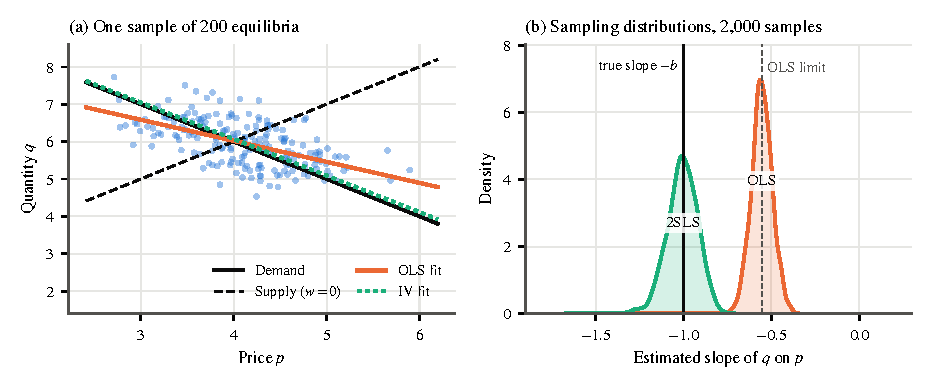
\includegraphics[width=\textwidth]{figures/appA/simultaneity.pdf}
\caption{Simultaneity bias and instrumental variables in a simulated market. Demand is
$q_t = 10 - p_t + u^d_t$ and supply is $q_t = 2 + p_t + w_t + u^s_t$, with $w_t \sim N(0, 1)$,
$u^d_t \sim N(0, 0.36)$ and $u^s_t \sim N(0, 0.25)$, all independent. (a) One sample of 200 equilibria with the
true demand curve and the supply curve at $w_t = 0$. The OLS fit has slope $-0.563$, and the IV fit with
instrument $w_t$ has slope $-0.977$. (b) Kernel densities of the OLS and two-stage least squares (2SLS, \cref{sec:A-2sls}) slopes over 2,000 samples of 200
markets. The solid line marks the demand slope $-1$ and the dashed line the OLS limit $-0.553$ from
\cref{prop:A-ols-simultaneity}. The mean first-stage $F$ statistic (\cref{sec:A-weakiv}) is 331. Seed 20261022, script
\texttt{sim\_iv.py}.}
\label{fig:A-simultaneity}
\end{figure}

\casehead{Order and rank conditions}
\Cref{cor:A-shifter} extends to any linear system. Let $y_t$ be a $G \times 1$ vector of endogenous variables
and $x_t$ an $M \times 1$ vector of exogenous variables with $\E[x_t x_t^\top]$ nonsingular. The structural
system is $B y_t + \Gamma x_t = u_t$, with $B$ nonsingular and $\E[x_t u_t^\top] = 0$. Its reduced form is
\begin{equation}\label{eq:A-system-rf}
y_t = \Pi x_t + v_t, \qquad \Pi = -B^{-1}\Gamma, \qquad v_t = B^{-1}u_t .
\end{equation}
The reduced-form coefficients are identified, $\Pi = \E[y_t x_t^\top]\E[x_t x_t^\top]^{-1}$, because $v_t$ is
uncorrelated with $x_t$. Consider one structural equation, normalized on its first endogenous variable:
\begin{equation}\label{eq:A-struct-eq}
y_{1t} = Y_{1t}^\top\beta + X_{1t}^\top\gamma + u_{1t} .
\end{equation}
It includes $G_1$ further endogenous variables $Y_{1t}$ and $M_1$ exogenous variables $X_{1t}$. The remaining
$M_2 = M - M_1$ exogenous variables $X_{2t}$ are excluded. Partition the reduced form conformably,
\begin{equation*}
y_{1t} = \pi_{11}^\top X_{1t} + \pi_{12}^\top X_{2t} + v_{1t}, \qquad
Y_{1t} = \Pi_{21}X_{1t} + \Pi_{22}X_{2t} + V_{1t},
\end{equation*}
where $\Pi_{22}$ is $G_1 \times M_2$. Substitute both into \eqref{eq:A-struct-eq}. The resulting identity holds
for all values of the exogenous variables, and the reduced-form errors are uncorrelated with them. Hence the
coefficients on $X_{1t}$ and $X_{2t}$ must match:
\begin{equation}\label{eq:A-rf-restrictions}
\pi_{11} = \Pi_{21}^\top\beta + \gamma, \qquad \pi_{12} = \Pi_{22}^\top\beta .
\end{equation}

\begin{proposition}[Rank and order conditions]\label{prop:A-rank}
The coefficients $(\beta, \gamma)$ of \eqref{eq:A-struct-eq} are identified if and only if
$\mathrm{rank}(\Pi_{22}) = G_1$. A necessary condition is $M_2 \ge G_1$, so the equation must exclude at least
as many exogenous variables as it includes endogenous variables on its right-hand side.
\end{proposition}

\begin{proof}
The second block of \eqref{eq:A-rf-restrictions} is a system of $M_2$ linear equations in the $G_1$ unknowns
$\beta$. If $\Pi_{22}^\top$ has full column rank $G_1$, the solution is unique:
\begin{equation*}
\beta = (\Pi_{22}\Pi_{22}^\top)^{-1}\Pi_{22}\,\pi_{12}, \qquad \gamma = \pi_{11} - \Pi_{21}^\top\beta .
\end{equation*}
If the rank is below $G_1$, pick $h \neq 0$ with $\Pi_{22}^\top h = 0$. The pair
$(\beta + h, \gamma - \Pi_{21}^\top h)$ also satisfies \eqref{eq:A-rf-restrictions}. The error it implies is
\begin{align*}
y_{1t} - Y_{1t}^\top(\beta + h) - X_{1t}^\top(\gamma - \Pi_{21}^\top h)
&= u_{1t} - h^\top\bigl(\Pi_{21}X_{1t} + \Pi_{22}X_{2t} + V_{1t}\bigr) + h^\top\Pi_{21}X_{1t} \\
&= u_{1t} - h^\top V_{1t} ,
\end{align*}
which is uncorrelated with $x_t$. The two coefficient vectors fit the same observables and satisfy the same
exogeneity restrictions, so the data cannot distinguish them. The order condition follows from
$\mathrm{rank}(\Pi_{22}) \le M_2$.
\end{proof}

In the market of \cref{cor:A-shifter}, demand includes one endogenous regressor (price) and excludes one
exogenous variable ($w_t$). The relevant reduced-form coefficient is $\Pi_{22} = -\frac{\delta}{b + c}$, which
is nonzero when $\delta \neq 0$, so demand is exactly identified. Supply excludes nothing, $M_2 = 0 < 1$, and
its slope remains unidentified until we observe a demand shifter.

\casehead{The link to conduct}
The same algebra explains why conduct is hard to identify (\cref{sec:03-identification}). In the linear model
of \cref{eq:03-linear-system}, the supply relation is $P_t = b_0 + \lambda Q_t + b_2 W_t + u^s_t$ with composite
slope $\lambda = b_1 - \frac{\theta}{a_1}$, where $\theta$ is conduct. An excluded demand shifter identifies
$\lambda$ by \cref{prop:A-rank}. The slope of marginal cost $b_1$ and conduct $\theta$ enter only through
$\lambda$. The Jacobian of the map from $(b_1, \theta)$ to the identified coefficients therefore has rank one,
and the two are not separately identified (\cref{prop:03-obs-equiv}). A demand rotator, a variable that changes
the slope of demand, makes the markup term move independently of quantity and restores identification
\citep{Bresnahan1982,Lau1982}. \Cref{sec:03-rotation} develops the argument.

\subsection{Potential outcomes and selection}\label{sec:A-potential}

Many questions in the book ask what an intervention does: a merger, a tax, entry by a rival. The
\emph{potential outcomes} framework states such questions precisely. Let $d_i \in \{0, 1\}$ indicate
treatment of unit $i$. The unit has two potential outcomes, $y_i(1)$ if treated and $y_i(0)$ if not, and we
observe only $y_i = d_i\,y_i(1) + (1 - d_i)\,y_i(0)$. The \emph{average treatment effect} is
$\mathrm{ATE} = \E[y_i(1) - y_i(0)]$, and the \emph{average treatment effect on the treated} is
$\mathrm{ATT} = \E[y_i(1) - y_i(0) \mid d_i = 1]$.

\begin{proposition}[Selection bias]\label{prop:A-selection}
The difference in mean outcomes between treated and untreated units satisfies
\begin{equation}\label{eq:A-selection}
\E[y_i \mid d_i = 1] - \E[y_i \mid d_i = 0]
= \mathrm{ATT} + \bigl\{\E[y_i(0) \mid d_i = 1] - \E[y_i(0) \mid d_i = 0]\bigr\} .
\end{equation}
\end{proposition}

\begin{proof}
Observed outcomes equal the relevant potential outcomes, so $\E[y_i \mid d_i = 1] = \E[y_i(1) \mid d_i = 1]$
and $\E[y_i \mid d_i = 0] = \E[y_i(0) \mid d_i = 0]$. Add and subtract $\E[y_i(0) \mid d_i = 1]$:
\begin{equation*}
\E[y_i(1) \mid d_i = 1] - \E[y_i(0) \mid d_i = 1] + \E[y_i(0) \mid d_i = 1] - \E[y_i(0) \mid d_i = 0] .
\end{equation*}
The first two terms form the ATT and the last two the bracket in \eqref{eq:A-selection}.
\end{proof}

The bracket is the \emph{selection bias}. It compares the untreated outcomes of two different groups, and it
is nonzero whenever the treated would have fared differently even without treatment. Random assignment makes
$d_i$ independent of $(y_i(1), y_i(0))$. The selection term then vanishes, and the ATT equals the ATE.

Selection is the central problem of merger retrospectives. Merging firms differ from non-merging ones, and
so do the rivals of merging firms. In hospital markets, non-merging hospitals whose rivals later merged had
price growth of $-2.9$ percent in 1985--1988, against $4.2$ percent for hospitals without merging rivals
\citep[p.~16]{Dafny2005}. A naive comparison would attribute part of this pre-existing gap to the mergers.
\Cref{sec:A-ivmodel} shows how an instrument removes it.

The same decomposition applies to continuous treatments. In the cross-industry regressions of the
structure-conduct-performance (SCP) paradigm, industry $k$ has a potential Lerner index $L_k(h)$ at each concentration level
$h$, and we observe $L_k = L_k(\HHI_k)$. Comparing industries at $h$ and $h'$,
\begin{multline*}
\E[L_k \mid \HHI_k = h] - \E[L_k \mid \HHI_k = h'] = \E[L_k(h) - L_k(h') \mid \HHI_k = h] \\
+ \bigl\{\E[L_k(h') \mid \HHI_k = h] - \E[L_k(h') \mid \HHI_k = h']\bigr\} .
\end{multline*}
The first term is a causal effect and the second a selection term, as in \cref{eq:01-potential-outcomes}.
Concentration is an equilibrium outcome of the same demand and cost primitives that determine margins, so
the selection term has no reason to vanish (\cref{sec:01-endogeneity}).

\casehead{Three empirical strategies on one industry}
The airline studies of \cref{ch:airlines} show three ways to overcome selection, each with its own
identifying assumption. \citet{Borenstein1989} runs reduced-form fare regressions on a carrier's route and
airport shares. His route-share effect is identified by an instrument, the carrier's share of endpoint
enplanements. He excludes it on the ground that fares respond to actual competition only
(\cref{sec:A-ivsources}). \citet{WhinstonCollins1992} run an event study of entry announcements. The value
effect of entry on incumbents is identified by the timing of news under efficient stock markets
(\cref{sec:A-eventstudy}). \citet{BerryCarnallSpiller2006} estimate a structural model of demand and
pricing.\footnote{We read NBER Working Paper 5561 (1996), \citet{BerryCarnallSpiller1996}, an earlier version of
their chapter. Page and table numbers marked WP refer to it.} Markups are identified by the estimated demand system together with an equilibrium assumption on
pricing. The three designs answer different questions, and their assumptions fail in different ways. A
related distinction is between prospective analysis, which predicts the effect of a change before it
happens, and retrospective analysis, which measures it afterwards (\cref{ch:mergers}). \Cref{sec:A-did}
develops the designs behind retrospectives.

\casehead{Partial identification}
When the assumptions needed for point identification are not credible, weaker assumptions often still bound
the feature of interest. \citet{HaileTamer2003} study English auctions in which bids need not equal values.
They assume only that bidders never bid more than their values and never let an opponent win at a price they
would have been willing to beat. These two inequalities bound the distribution of values from above and below.
\citet[pp.~493--499]{AradillasLopezGandhiQuint2013} allow symmetric private values with nonnegative dependence
when only the transaction price and the number of bidders are observed. The distribution of the highest value is then only partially
identified. If values are independent of the number of bidders, variation in that number across auctions tightens
the bounds on the seller's expected profit, the bidders' surplus and the optimal reserve price.
\Cref{ch:auction-empirics} develops both results, and \cref{sec:A-partialid} treats estimation and inference
for bounds.

\subsection{Monte Carlo experiments}\label{sec:A-montecarlo}

A \emph{Monte Carlo experiment} studies an estimator by applying it to data simulated from a known
data-generating process. It proceeds in four steps.
\begin{enumerate}[label=(\arabic*)]
\item Specify the data-generating process completely: functional forms, the true parameter $\theta_0$, the
  distributions of exogenous variables and errors, and the sample size $n$.
\item Fix the seed of the random number generator, so that the experiment can be reproduced exactly.
\item For $r = 1, \dots, R$, draw a sample and compute the estimate $\hat\theta_r$, its standard error and
  any test decision $D_r \in \{0, 1\}$, which equals one if the test rejects.
\item Summarize the $R$ replications.
\end{enumerate}
For a scalar parameter the usual summaries are the bias $\bar\theta - \theta_0$ with
$\bar\theta = \frac{1}{R}\sum_r\hat\theta_r$ and the standard deviation of $\hat\theta_r$ across replications.
Others are the \emph{root mean squared error}
$\mathrm{RMSE} = \bigl[\frac{1}{R}\sum_r(\hat\theta_r - \theta_0)^2\bigr]^{\frac{1}{2}}$, the coverage rate of
nominal confidence intervals, and the rejection rate $\frac{1}{R}\sum_r D_r$ of a test. Adding and
subtracting $\bar\theta$ inside the square gives
\begin{equation*}
\frac{1}{R}\sum_{r=1}^{R}(\hat\theta_r - \theta_0)^2
= (\bar\theta - \theta_0)^2 + \frac{1}{R}\sum_{r=1}^{R}(\hat\theta_r - \bar\theta)^2 ,
\end{equation*}
because the cross term $\frac{2}{R}(\bar\theta - \theta_0)\sum_r(\hat\theta_r - \bar\theta)$ is zero. The
squared RMSE is the squared bias plus the variance. Some estimators have no finite mean, such as
just-identified two-stage least squares (\cref{sec:A-weakiv}). For them the median and interquantile ranges
are more informative than the mean and the RMSE.

Monte Carlo summaries are estimates with their own sampling error. Consider a test whose true rejection
probability is $\alpha$. The replications are independent, so $\sum_r D_r$ is binomial with $R$ trials and
success probability $\alpha$. The estimated rejection rate $\hat\alpha = \frac{1}{R}\sum_r D_r$ therefore
satisfies
\begin{equation}\label{eq:A-mc-se}
\E[\hat\alpha] = \alpha, \qquad
\Var(\hat\alpha) = \frac{1}{R^2}\,R\,\alpha(1 - \alpha) = \frac{\alpha(1 - \alpha)}{R}, \qquad
\mathrm{se}(\hat\alpha) = \sqrt{\frac{\alpha(1 - \alpha)}{R}} .
\end{equation}
With $R = 10{,}000$ and $\alpha = 0.05$ the Monte Carlo standard error is 0.0022. A rejection rate of 0.058
then differs from 0.05 by more than three standard errors. In the same way, the Monte Carlo standard error
of $\bar\theta$ is the standard deviation across replications divided by $\sqrt{R}$.

The book uses such experiments to study SCP regressions on simulated Cournot industries
(\cref{sec:01-montecarlo}) and estimators of random-coefficient demand on simulated markets
(\cref{ch:blp,app:problems}). This appendix uses them throughout. They study instrumental variables
(\cref{fig:A-simultaneity,fig:A-weakiv}), latent regimes (\cref{fig:A-em}) and simulation estimators
(\cref{fig:A-simest}). They also study clustered inference (\cref{fig:A-cluster-mc}), kernel estimators
(\cref{fig:A-kde,fig:A-gpv}) and staggered difference in differences (\cref{fig:A-staggered}). Every one of
them reports its seed and the script that produced it.

\section{Least squares, panel data and systems}\label{sec:A-ols}

Ordinary least squares is the workhorse of empirical work, and it reappears inside almost every estimator
in the book. This section treats it as a projection, derives its large-sample behavior, lists the three
classic sources of bias, and develops the panel and system extensions used in the chapters.

\subsection{OLS as a projection}\label{sec:A-projection}

Let $(y_i, x_i)$ be independent and identically distributed, with $\E[y_i^2]$ finite and
$\E[x_i x_i^\top]$ finite and nonsingular. The \emph{linear projection} of $y_i$ on $x_i$ has coefficient
\begin{equation}\label{eq:A-projection}
\beta = \argmin_{b}\ \E\bigl[(y_i - x_i^\top b)^2\bigr] = \E[x_i x_i^\top]^{-1}\E[x_i y_i] .
\end{equation}
The second equality solves the first-order condition $\E[x_i(y_i - x_i^\top\beta)] = 0$. The
\emph{projection error} $e_i = y_i - x_i^\top\beta$ satisfies $\E[x_i e_i] = 0$ by construction. The
projection exists whether or not any economic model holds. A structural interpretation of $\beta$ is an
assumption: that the error of the economic model is uncorrelated with $x_i$, so the structural coefficient
coincides with the projection coefficient.

In a sample of size $n$, stack the observations into $y$ ($n \times 1$) and $X$ ($n \times K$) with full
column rank. The OLS estimator $\hat\beta = (X^\top X)^{-1}X^\top y$ solves the \emph{normal equations}
$X^\top(y - X\hat\beta) = 0$. Define the projection matrix $P_X = X(X^\top X)^{-1}X^\top$ and the
\emph{annihilator} $M_X = I_n - P_X$. Both are symmetric and idempotent, $M_X X = 0$, fitted values are
$P_X y$ and residuals are $\hat e = M_X y$.

\begin{theorem}[Frisch-Waugh-Lovell]\label{thm:A-fwl}
Partition $X = [X_1, X_2]$ and $\hat\beta = (\hat\beta_1^\top, \hat\beta_2^\top)^\top$ conformably, and let
$M_{X_2} = I_n - X_2(X_2^\top X_2)^{-1}X_2^\top$. Then
\begin{equation}\label{eq:A-fwl}
\hat\beta_1 = (X_1^\top M_{X_2} X_1)^{-1}X_1^\top M_{X_2} y = (\tilde X_1^\top\tilde X_1)^{-1}\tilde X_1^\top\tilde y,
\qquad \tilde X_1 = M_{X_2}X_1,\ \tilde y = M_{X_2} y ,
\end{equation}
and the residuals of the regression of $\tilde y$ on $\tilde X_1$ equal the residuals of the full regression.
\end{theorem}

\begin{proof}
The normal equations of the full regression are
\begin{equation*}
X_1^\top(y - X_1\hat\beta_1 - X_2\hat\beta_2) = 0, \qquad X_2^\top(y - X_1\hat\beta_1 - X_2\hat\beta_2) = 0 .
\end{equation*}
The second block gives $\hat\beta_2 = (X_2^\top X_2)^{-1}X_2^\top(y - X_1\hat\beta_1)$. Substituting,
\begin{equation*}
y - X_1\hat\beta_1 - X_2\hat\beta_2 = M_{X_2}(y - X_1\hat\beta_1) .
\end{equation*}
The first block becomes $X_1^\top M_{X_2}(y - X_1\hat\beta_1) = 0$, so
$\hat\beta_1 = (X_1^\top M_{X_2}X_1)^{-1}X_1^\top M_{X_2}y$. The inverse exists because $X$ has full column rank.
Since $M_{X_2}$ is symmetric and idempotent, $X_1^\top M_{X_2}X_1 = \tilde X_1^\top\tilde X_1$ and
$X_1^\top M_{X_2}y = \tilde X_1^\top\tilde y$. The full residual is $M_{X_2}(y - X_1\hat\beta_1) = \tilde y -
\tilde X_1\hat\beta_1$, which is the residual of the partialled regression.
\end{proof}

The theorem says that the coefficient on $X_1$ uses only the variation in $X_1$ that $X_2$ cannot explain.
The theorem underlies fixed effects (\cref{sec:A-panel}) and the control-function form of two-stage
least squares (\cref{sec:A-2sls}). It also justifies partialling out exogenous regressors
(\cref{sec:A-weakiv}) and concentrating out linear parameters (\cref{sec:A-gmm-computation}). The
double-residual estimator of the partially linear model (\cref{sec:A-plm}), the two-way fixed-effects
regression (\cref{sec:A-did-twfe}) and event-study dummies (\cref{sec:A-es-regression}) rest on it as well.

\subsection{Large-sample theory}\label{sec:A-ols-asy}

\begin{assumption}[Linear regression]\label{ass:A-ols}
\leavevmode
\begin{enumerate}[label=(\roman*)]
\item The observations $(y_i, x_i)$ are independent and identically distributed.
\item $y_i = x_i^\top\beta + e_i$ with $\E[x_i e_i] = 0$.
\item $Q = \E[x_i x_i^\top]$ is finite and nonsingular.
\item $\E\lVert x_i\rVert^4 < \infty$ and $\E[e_i^4] < \infty$.
\end{enumerate}
\end{assumption}

Part (iv) guarantees, by the Cauchy-Schwarz inequality, that $\Omega = \E[e_i^2x_ix_i^\top]$ is finite.

\begin{proposition}[Consistency and asymptotic normality of OLS]\label{prop:A-ols-asy}
Under \cref{ass:A-ols}, $\hat\beta \xrightarrow{p} \beta$ and
\begin{equation}\label{eq:A-ols-sandwich}
\sqrt{n}(\hat\beta - \beta) \xrightarrow{d} N\bigl(0,\ Q^{-1}\Omega Q^{-1}\bigr) .
\end{equation}
\end{proposition}

\begin{proof}
Substitute $y = X\beta + e$ into the estimator:
\begin{equation*}
\hat\beta - \beta = \Bigl(\frac{1}{n}X^\top X\Bigr)^{-1}\frac{1}{n}X^\top e
= \Bigl(\frac{1}{n}\sum_{i=1}^n x_ix_i^\top\Bigr)^{-1}\frac{1}{n}\sum_{i=1}^n x_ie_i .
\end{equation*}
By the weak law of large numbers, $\frac{1}{n}\sum_i x_ix_i^\top \xrightarrow{p} Q$ and
$\frac{1}{n}\sum_i x_ie_i \xrightarrow{p} \E[x_ie_i] = 0$. Matrix inversion is continuous at the nonsingular
$Q$, so the continuous mapping theorem gives $\hat\beta - \beta \xrightarrow{p} Q^{-1}\cdot 0 = 0$. For the
distribution, multiply by $\sqrt{n}$:
\begin{equation*}
\sqrt{n}(\hat\beta - \beta) = \Bigl(\frac{1}{n}\sum_{i=1}^n x_ix_i^\top\Bigr)^{-1}
\frac{1}{\sqrt{n}}\sum_{i=1}^n x_ie_i .
\end{equation*}
The terms $x_ie_i$ are independent with mean zero and finite variance $\Omega$, so the central limit theorem
gives $\frac{1}{\sqrt{n}}\sum_i x_ie_i \xrightarrow{d} N(0, \Omega)$. By Slutsky's theorem the product
converges to $Q^{-1}N(0, \Omega) = N(0, Q^{-1}\Omega Q^{-1})$.
\end{proof}

The variance in \eqref{eq:A-ols-sandwich} is called a \emph{sandwich} because $\Omega$ sits between two
copies of $Q^{-1}$. Under \emph{homoskedasticity}, $\E[e_i^2 \mid x_i] = \sigma^2$, the middle term becomes
$\Omega = \sigma^2Q$ and the variance collapses to $\sigma^2Q^{-1}$. Its conventional estimator is
$s^2(X^\top X)^{-1}$ with $s^2 = \frac{\hat e^\top\hat e}{n - K}$. Without homoskedasticity,
\citet{White1980} shows that
\begin{equation}\label{eq:A-hc0}
\hat V_{\mathrm{HC0}} = (X^\top X)^{-1}\Bigl(\sum_{i=1}^n\hat e_i^2x_ix_i^\top\Bigr)(X^\top X)^{-1}
\end{equation}
consistently estimates the variance of $\hat\beta$, in the sense that $n\hat V_{\mathrm{HC0}}
\xrightarrow{p} Q^{-1}\Omega Q^{-1}$. Finite-sample versions adjust the squared residuals, which are too
small on average. Let $h_{ii} = x_i^\top(X^\top X)^{-1}x_i$ be the \emph{leverage} of observation $i$. Under
homoskedasticity, $\hat e = M_Xe$ implies
\begin{equation*}
\E[\hat e_i^2 \mid X] = \sigma^2(M_X)_{ii} = \sigma^2(1 - h_{ii}) .
\end{equation*}
HC1 multiplies \eqref{eq:A-hc0} by $\frac{n}{n - K}$. HC2 replaces $\hat e_i^2$ by $\frac{\hat e_i^2}{1 - h_{ii}}$,
which is unbiased under homoskedasticity. HC3 uses $\frac{\hat e_i^2}{(1 - h_{ii})^2}$, which approximates the
jackknife and is conservative in small samples \citep{MacKinnonWhite1985}. In this book ``robust'' standard
errors mean heteroskedasticity-robust standard errors. They still assume independence across observations.
Clustered and serially correlated data need the estimators of \cref{sec:A-se}, which also covers heteroskedasticity
and autocorrelation consistent (HAC) estimators.

\subsection{Three sources of bias}\label{sec:A-bias}

OLS converges to the projection coefficient. It is biased for the structural coefficient whenever the
structural error is correlated with the regressors. Three mechanisms produce that correlation.

\casehead{Omitted variables}
Suppose $y_i = \beta_0 + \beta_1x_{1i} + \beta_2x_{2i} + e_i$ with $\E[e_i] = 0$ and $e_i$ uncorrelated with
both regressors, but we regress $y_i$ on a constant and $x_{1i}$ only. The short slope converges to
\begin{equation}\label{eq:A-ovb}
\frac{\Cov(y_i, x_{1i})}{\Var(x_{1i})}
= \frac{\beta_1\Var(x_{1i}) + \beta_2\Cov(x_{2i}, x_{1i}) + \Cov(e_i, x_{1i})}{\Var(x_{1i})}
= \beta_1 + \beta_2\,\frac{\Cov(x_{1i}, x_{2i})}{\Var(x_{1i})} .
\end{equation}
The bias is the effect of the omitted variable times the slope of its projection on the included one. With
vector regressors the bias is $\E[x_1x_1^\top]^{-1}\E[x_1x_2^\top]\beta_2$. In the firm-level regressions
that pit industry concentration against firm market share, omitting the share loads its effect onto
concentration whenever the two are correlated (\cref{sec:01-demsetz}).

\casehead{Measurement error}
Suppose $y_i = \beta_0 + \beta x_i^* + e_i$, but we observe $x_i = x_i^* + m_i$. The \emph{classical}
measurement error $m_i$ has mean zero and variance $\sigma_m^2$ and is uncorrelated with $x_i^*$ and $e_i$.
The OLS slope of $y_i$ on $x_i$ converges to
\begin{equation}\label{eq:A-attenuation}
\frac{\Cov(\beta_0 + \beta x_i^* + e_i,\ x_i^* + m_i)}{\Var(x_i^* + m_i)}
= \frac{\beta\Var(x_i^*)}{\Var(x_i^*) + \sigma_m^2} \equiv \beta\lambda .
\end{equation}
The \emph{reliability ratio} $\lambda \in (0, 1]$ is the share of the variance of the measured regressor that
is signal, so the slope is biased toward zero. Panel data with fixed effects can make this
\emph{attenuation} much worse \citep{GrilichesHausman1986}.

\begin{proposition}[Attenuation with fixed effects]\label{prop:A-fe-attenuation}
Let $y_{it} = \alpha_i + \beta x_{it}^* + e_{it}$ for $i = 1, \dots, n$ and $t = 1, \dots, T$, with $T$ fixed,
units independent, and $\E[e_{it} \mid x_{i1}^*, \dots, x_{iT}^*, \alpha_i] = 0$. We observe
$x_{it} = x_{it}^* + m_{it}$, where $m_{it}$ is independent across $i$ and $t$, has mean zero and variance
$\sigma_m^2$, and is independent of $\{x_{is}^*\}$, $\{e_{is}\}$ and $\alpha_i$. Define the within variance
$\Var_W(z) = \E\bigl[\frac{1}{T}\sum_t(z_{it} - \bar z_i)^2\bigr]$ with $\bar z_i = \frac{1}{T}\sum_t z_{it}$,
and suppose $\Var_W(x^*) > 0$. As $n \to \infty$ the within estimator converges to
\begin{equation}\label{eq:A-fe-attenuation}
\beta\lambda_W, \qquad
\lambda_W = \frac{\Var_W(x^*)}{\Var_W(x^*) + \frac{T - 1}{T}\sigma_m^2} .
\end{equation}
\end{proposition}

\begin{proof}
Write $\ddot z_{it} = z_{it} - \bar z_i$. The within transformation removes $\alpha_i$, so
$\ddot y_{it} = \beta\ddot x_{it}^* + \ddot e_{it}$, and the measured regressor is
$\ddot x_{it} = \ddot x_{it}^* + \ddot m_{it}$. The within estimator is
$\frac{\sum_i\sum_t\ddot x_{it}\ddot y_{it}}{\sum_i\sum_t\ddot x_{it}^2}$. Divide numerator and denominator by
$nT$ and apply the law of large numbers across units. The numerator converges to
$\beta\Var_W(x^*)$. The cross terms vanish because $m$ is independent of $x^*$ and $e$, and because strict
exogeneity makes $\E[\ddot x_{it}^*\ddot e_{it}] = 0$. The denominator converges to
$\Var_W(x^*) + \E\bigl[\frac{1}{T}\sum_t\ddot m_{it}^2\bigr]$. For each $t$,
\begin{equation*}
\E[\ddot m_{it}^2] = \Var(m_{it}) - 2\Cov(m_{it}, \bar m_i) + \Var(\bar m_i)
= \sigma_m^2 - \frac{2\sigma_m^2}{T} + \frac{\sigma_m^2}{T} = \frac{T - 1}{T}\,\sigma_m^2 .
\end{equation*}
The ratio of the two limits is \eqref{eq:A-fe-attenuation}.
\end{proof}

Compare $\lambda_W$ with the reliability ratio $\lambda = \frac{\Var(x^*)}{\Var(x^*) + \sigma_m^2}$ of a pooled
regression, which is valid if $\alpha_i$ is unrelated to the regressor. Inverting both ratios shows that
$\lambda_W < \lambda$ if and only if
\begin{equation*}
\frac{\Var_W(x^*)}{\Var(x^*)} < \frac{T - 1}{T} .
\end{equation*}
The left side is the share of the signal's variance that occurs within units. The right side is the same
share for independent noise. A persistent signal, whose variance is mostly between units, satisfies the
inequality easily. For example, if $x_{it}^* = a_i + \xi_{it}$ with independent $\xi_{it}$ of variance
$\sigma_\xi^2$ and $\Var(a_i) = \sigma_a^2$, then $\Var_W(x^*) = \frac{T - 1}{T}\sigma_\xi^2$ and
$\lambda_W = \frac{\sigma_\xi^2}{\sigma_\xi^2 + \sigma_m^2}$. This falls short of $\lambda$ whenever
$\sigma_a^2 > 0$. The result is the formal content of the critique that panel regressions of margins on
concentration with industry effects \citep{Salinger1990} can worsen attenuation
(\cref{prop:01-fe-attenuation}).

\casehead{Simultaneity}
\Cref{prop:A-ols-simultaneity} is the third mechanism. When the regressor is an equilibrium outcome, the
error of each equation moves it. Invalid instruments can bring the same bias back. With national demand
shocks, prices of the same brand in other cities are correlated with local demand errors. An instrumental
variables estimator built on them then ``is like doing ordinary least squares on a supply and demand
system'' \citep[p.~242]{Bresnahan1997}. \Cref{sec:A-ivmodel} gives the general formula, and
\cref{sec:10-bresnahan-iv} works out the cereal case.

\casehead{The structure-conduct-performance regression as a projection}
These mechanisms combine in the cross-industry regression of margins on concentration. Its OLS slope
converges to $\frac{\Cov(L_k, \HHI_k)}{\Var(\HHI_k)}$, a projection coefficient. Suppose every industry is a
symmetric Cournot industry, so $L_k = \frac{\HHI_k}{\varepsilon_k}$. If the elasticity $\varepsilon_k$ is
independent of $\HHI_k$, then $\Cov(L_k, \HHI_k) = \E[\frac{1}{\varepsilon_k}]\Var(\HHI_k)$, and the slope
converges to $\E[\frac{1}{\varepsilon_k}]$. Once elasticities, entry costs and conduct vary with
concentration, the slope mixes comparative statics with respect to several primitives and has no structural
meaning (\cref{prop:01-scp-plim}).

\subsection{Panel data}\label{sec:A-panel}

A \emph{panel} observes units $i = 1, \dots, n$ over periods $t = 1, \dots, T$. The basic model is
\begin{equation}\label{eq:A-panel}
y_{it} = x_{it}^\top\beta + \alpha_i + e_{it} ,
\end{equation}
where the unit effect $\alpha_i$ may be correlated with the regressors in any way. The key assumption is
\emph{strict exogeneity}, $\E[e_{it} \mid x_{i1}, \dots, x_{iT}, \alpha_i] = 0$: shocks in any period are
unrelated to the regressors in every period.

\casehead{Fixed effects}
Stack the data unit by unit and write $D = I_n \otimes \iota_T$ for the $nT \times n$ matrix of unit dummies,
where $\iota_T$ is a $T \times 1$ vector of ones. The \emph{fixed-effects}, or \emph{within}, estimator is OLS
of $y$ on $X$ and $D$. By \cref{thm:A-fwl} it equals OLS after premultiplying by
\begin{equation*}
M_D = I_{nT} - D(D^\top D)^{-1}D^\top = I_n \otimes \Bigl(I_T - \frac{1}{T}\iota_T\iota_T^\top\Bigr) ,
\end{equation*}
which subtracts each unit's time mean. Hence $\hat\beta_W = \bigl(\sum_i\sum_t\ddot x_{it}\ddot x_{it}^\top\bigr)^{-1}
\sum_i\sum_t\ddot x_{it}\ddot y_{it}$ with $\ddot z_{it} = z_{it} - \bar z_i$. It is consistent as $n \to \infty$
with $T$ fixed under strict exogeneity. Regressors that do not vary over time are swept out, and the error
variance is estimated with $nT - n - K$ degrees of freedom.

\casehead{First differences}
Differencing \eqref{eq:A-panel} also removes $\alpha_i$: $\Delta y_{it} = \Delta x_{it}^\top\beta + \Delta e_{it}$
for $t \ge 2$. OLS on the differences is consistent when $\E[\Delta x_{it}\Delta e_{it}] = 0$. With $T = 2$ the two
estimators coincide. The within deviations are $\ddot z_{i1} = -\frac{1}{2}\Delta z_{i2}$ and
$\ddot z_{i2} = \frac{1}{2}\Delta z_{i2}$, so
\begin{equation*}
\hat\beta_W = \Bigl(\sum_i 2\cdot\frac{1}{4}\Delta x_{i2}\Delta x_{i2}^\top\Bigr)^{-1}\sum_i 2\cdot\frac{1}{4}\Delta x_{i2}\Delta y_{i2}
= \Bigl(\sum_i\Delta x_{i2}\Delta x_{i2}^\top\Bigr)^{-1}\sum_i\Delta x_{i2}\Delta y_{i2} ,
\end{equation*}
which is the first-difference estimator. With $T > 2$ they differ, and their relative efficiency depends on
the serial correlation of $e_{it}$.

\casehead{Random effects}
If in addition $\E[\alpha_i \mid x_{i1}, \dots, x_{iT}] = 0$, the unit effect becomes part of a composite error
$\alpha_i + e_{it}$. With $\Var(\alpha_i) = \sigma_\alpha^2$ and homoskedastic, serially uncorrelated $e_{it}$,
the covariance matrix of unit $i$'s errors is $\Omega_i = \sigma_e^2I_T + \sigma_\alpha^2\iota_T\iota_T^\top$.
Write $\bar P = \frac{1}{T}\iota_T\iota_T^\top$ and $\bar Q = I_T - \bar P$. These are orthogonal idempotent
matrices, and
\begin{equation*}
\Omega_i = \sigma_e^2\bar Q + (\sigma_e^2 + T\sigma_\alpha^2)\bar P, \qquad
\sigma_e\,\Omega_i^{-\frac{1}{2}} = \bar Q + \phi\bar P = I_T - (1 - \phi)\bar P, \qquad
\phi = \frac{\sigma_e}{\sqrt{\sigma_e^2 + T\sigma_\alpha^2}} .
\end{equation*}
Generalized least squares is therefore OLS of $y_{it} - \vartheta\bar y_i$ on $x_{it} - \vartheta\bar x_i$ with
$\vartheta = 1 - \phi$. The \emph{random-effects} estimator replaces $\sigma_e^2$ and $\sigma_\alpha^2$ by estimates.
It quasi-demeans: $\vartheta = 0$ gives pooled OLS, and $\vartheta \to 1$ as
$\frac{T\sigma_\alpha^2}{\sigma_e^2} \to \infty$, so random effects approaches fixed effects in long panels
with large unit variance. It is efficient when its assumptions hold and inconsistent when $\alpha_i$ is
correlated with the regressors. \Cref{sec:A-spectests} tests between the two. \citet{FullerBattese1974}
extend the approach to crossed unit and time effects, $\alpha_i + \tau_t + e_{it}$.

\casehead{Two-way fixed effects}
Adding period effects gives $y_{it} = x_{it}^\top\beta + \alpha_i + \tau_t + e_{it}$. In a balanced panel,
\cref{thm:A-fwl} shows that the slope is OLS on the doubly demeaned data
$\ddot z_{it} = z_{it} - \bar z_{i\cdot} - \bar z_{\cdot t} + \bar z_{\cdot\cdot}$, the deviations from unit,
period and grand means. The variation that identifies $\beta$ differs across these estimators. Pooled OLS
uses all variation, including permanent differences across units. Fixed effects uses changes within units
over time. Two-way fixed effects uses changes within units relative to the average change in the same period,
so it is a difference-in-differences design with a continuous treatment (\cref{sec:A-did-twfe}).

\casehead{Application: tax pass-through in cigarettes}
\citet{Sumner1981} estimates the pass-through of state cigarette excise taxes into retail prices. His
equation (4) is $P_{it} = X_{it}\eta + \theta R_{it} + U_{it}$, with $i$ indexing states, $t$ years and
$R_{it}$ the tax per pack. Sumner's $\theta$ is the pass-through rate, which is neither conduct nor a generic
parameter. In the notation of \cref{eq:03-sumner-regression} it is
\begin{equation}\label{eq:A-sumner}
p_{sy} = \mu_s + \tau_y + \rho\,t_{sy} + e_{sy} ,
\end{equation}
with state effects $\mu_s$, year effects $\tau_y$ and pass-through rate $\rho$. The data are annual average
prices and taxes for 1954--1978 in 47 states and the District of Columbia. Alaska, Hawaii and New Hampshire
are excluded, which leaves 1,200 observations (pp.~1016--1017). Sumner's Table 1 reports three estimators of
$\rho$, each with its standard error. Two-way fixed effects by OLS gives 1.074 (0.013). Pooled OLS with the
national consumer price index in place of the year dummies and without state dummies gives 1.029 (0.011). A
variance-components estimator with random state and year effects \citep{FullerBattese1974} and the price index
gives 1.069 (0.013). The $R^2$ is about 0.99 with the dummies and 0.95 without them.

The comparison shows what each estimator uses. The pooled regression compares price levels across states
with permanently different taxes. Sumner notes that the three states with a large stake in tobacco growing
and cigarette manufacturing, North Carolina, Virginia and Kentucky, all have low taxes (fn.~8). State
dummies absorb such stable state characteristics (pp.~1015--1016), and the fixed-effects estimate rests on
changes in taxes within states over time. The random-effects estimate lies close to the fixed-effects one.
This is what quasi-demeaning predicts when $T = 25$ and the state variance component is large relative to
the idiosyncratic variance. The reported standard errors treat the 1,200 observations as independent.
\Cref{sec:A-sumner-se} recomputes them on a reconstructed panel, allowing for serial correlation within states
(\cref{tab:A-sumner}), and \cref{sec:A-did-twfe} reads the regression as a difference in differences with a
continuous treatment. \Cref{sec:03-sumner} discusses the economics of the test.

\subsection{Systems of equations}\label{sec:A-systems}

Many models in the book consist of several equations estimated together. Examples are the share
equations of a demand system, the residual demand curves of several firms, and the returns of several firms
around one event.

\casehead{Seemingly unrelated regressions}
Let $y_g = X_g\beta_g + e_g$ for equations $g = 1, \dots, G$, each with $n$ observations. Stack the equations
as $y = X\beta + e$, with $y = (y_1^\top, \dots, y_G^\top)^\top$ and $X = \diag(X_1, \dots, X_G)$ block diagonal.
Let $e_t = (e_{1t}, \dots, e_{Gt})^\top$ collect the errors of observation $t$, and assume $\E[e_te_t^\top] = \Sigma$
with independence across $t$. Then $\Var(e) = \Sigma \otimes I_n$. Generalized least squares gives the
\emph{seemingly unrelated regressions} (SUR) estimator of \citet{Zellner1962},
\begin{equation}\label{eq:A-sur}
\hat\beta_{SUR} = \bigl[X^\top(\Sigma^{-1}\otimes I_n)X\bigr]^{-1}X^\top(\Sigma^{-1}\otimes I_n)\,y .
\end{equation}
Feasible SUR replaces $\Sigma$ by $\hat\Sigma_{gh} = \frac{1}{n}\hat e_g^\top\hat e_h$ from equation-by-equation OLS
residuals. Iterating between $\hat\Sigma$ and $\hat\beta$ until convergence gives the Gaussian maximum likelihood
estimator.

\begin{proposition}[When SUR equals OLS]\label{prop:A-sur-ols}
If $X_g = X_0$ for every equation, or if $\Sigma$ is diagonal, then \eqref{eq:A-sur} equals equation-by-equation
OLS.
\end{proposition}

\begin{proof}
Use $(A \otimes B)(C \otimes D) = AC \otimes BD$ and $(A \otimes B)^{-1} = A^{-1} \otimes B^{-1}$. With
identical regressors, $X = I_G \otimes X_0$. Then
\begin{align*}
X^\top(\Sigma^{-1}\otimes I_n)X &= (I_G \otimes X_0^\top)(\Sigma^{-1}\otimes I_n)(I_G \otimes X_0)
= \Sigma^{-1}\otimes X_0^\top X_0 ,\\
X^\top(\Sigma^{-1}\otimes I_n)\,y &= (\Sigma^{-1}\otimes X_0^\top)\,y .
\end{align*}
The inverse of the first matrix is $\Sigma \otimes (X_0^\top X_0)^{-1}$, so
\begin{equation*}
\hat\beta_{SUR} = \bigl[\Sigma \otimes (X_0^\top X_0)^{-1}\bigr](\Sigma^{-1}\otimes X_0^\top)\,y
= \bigl[I_G \otimes (X_0^\top X_0)^{-1}X_0^\top\bigr]y ,
\end{equation*}
which stacks the OLS regressions of each $y_g$ on $X_0$. If $\Sigma = \diag(\sigma_1^2, \dots, \sigma_G^2)$,
both $X^\top(\Sigma^{-1}\otimes I_n)X$ and $X^\top(\Sigma^{-1}\otimes I_n)y$ are block diagonal with blocks
$\sigma_g^{-2}X_g^\top X_g$ and $\sigma_g^{-2}X_g^\top y_g$. The weights cancel equation by equation, leaving
$(X_g^\top X_g)^{-1}X_g^\top y_g$.
\end{proof}

SUR gains precision only when the errors are correlated across equations and the regressors differ. It
becomes indispensable when coefficients are restricted across equations. The linear approximate almost ideal demand
system is a leading case of identical regressors. Every share equation contains the same log prices and the same log
total expenditure deflated by the Stone index. Without cross-equation restrictions, OLS equation by equation therefore
coincides with SUR (\cref{sec:05-stone}).

\casehead{Adding up and cross-equation restrictions}
Budget shares sum to one, so the errors of a complete share system sum to zero for every observation, and
$\Sigma$ is singular. We drop one equation and recover its coefficients from the adding-up restrictions. The
maximum likelihood (iterated SUR) estimates do not depend on which equation is dropped \citep{Barten1969}.
Symmetry and homogeneity restrictions take the linear form $R\beta = r$. Restricted GLS minimizes
$(y - Xb)^\top W(y - Xb)$ subject to $Rb = r$, with $W = \Sigma^{-1}\otimes I_n$. The Lagrangian first-order
condition $-2X^\top W(y - Xb) + 2R^\top\ell = 0$ gives $b = \hat\beta - VR^\top\ell$ with
$V = (X^\top WX)^{-1}$. Imposing $Rb = r$ determines the multiplier $\ell$:
\begin{equation}\label{eq:A-restricted-gls}
\tilde\beta = \hat\beta - VR^\top\bigl(RVR^\top\bigr)^{-1}\bigl(R\hat\beta - r\bigr) .
\end{equation}

\casehead{Which restrictions can be tested}
\citet[Section~3.3, pp.~67--70]{DeatonMuellbauer1980b} use the Rotterdam model to sort the restrictions of demand
theory by how they can be tested. For goods $g = 1, \dots, G$ and periods $t$, the model is
\begin{equation}\label{eq:A-rotterdam}
\bar w_{gt}\,\Delta\ln q_{gt} = b_g\,\Delta\ln\bar x_t + \sum_{h=1}^{G}c_{gh}\,\Delta\ln p_{ht} + e_{gt},
\qquad \Delta\ln\bar x_t = \sum_{h=1}^{G}\bar w_{ht}\,\Delta\ln q_{ht}
\end{equation}
(their eqs.~3.3 and~3.4). Here $\bar w_{gt}$ is the budget share used in the discrete approximation to the
differentials. It is chosen so that the identity for $\Delta\ln\bar x_t$ holds in the data (p.~69). The variable
$\Delta\ln\bar x_t$ is the change in real total expenditure, and $b_g$ is the marginal budget share. The coefficient
$c_{gh} = \frac{p_gp_hs_{gh}}{x}$ is a compensated price effect, where $s_{gh}$ is the Slutsky term and $x$ is total
expenditure (their eqs.~3.5 and~3.6). The coefficients are treated as constants. Adding up requires
$\sum_gb_g = 1$ and $\sum_gc_{gh} = 0$ for every $h$ (their eq.~3.7). Homogeneity requires $\sum_hc_{gh} = 0$ for
every $g$, and symmetry requires $c_{gh} = c_{hg}$ (eqs.~3.8 and~3.9). The three restrictions differ in how they
can be tested.

\begin{proposition}[Adding up holds by construction]\label{prop:A-addingup}
Let $y_g = X_0\beta_g + e_g$ for $g = 1, \dots, G$, with common regressors $X_0$ of full column rank. Suppose the
data satisfy $\sum_gy_g = X_0a$ for a known vector $a$. Then the OLS estimates satisfy $\sum_g\hat\beta_g = a$, and
for every observation the OLS residuals sum to zero across equations.
\end{proposition}

\begin{proof}
OLS is linear in the dependent variable, so
\begin{equation*}
\sum_{g=1}^{G}\hat\beta_g = (X_0^\top X_0)^{-1}X_0^\top\sum_{g=1}^{G}y_g = (X_0^\top X_0)^{-1}X_0^\top X_0\,a = a .
\end{equation*}
The residuals then sum to $\sum_gy_g - X_0\sum_g\hat\beta_g = X_0a - X_0a = 0$.
\end{proof}

In \eqref{eq:A-rotterdam} every equation has the same regressors, and the left-hand sides sum to
$\Delta\ln\bar x_t$, the first regressor. The proposition applies with $a$ the first unit vector. OLS therefore
gives $\sum_g\hat b_g = 1$ and $\sum_g\hat c_{gh} = 0$ whatever the data. Adding up cannot be tested, and it places
no restriction on the explanatory power of the equations (p.~69). Homogeneity involves the coefficients of one
equation only. It can be imposed and tested equation by equation, with a $t$ or $F$ test of $\sum_hc_{gh} = 0$.
Symmetry links pairs of equations, so it needs the system, estimated by \eqref{eq:A-restricted-gls} with one
equation dropped. The restrictions are also nested. Under adding up, symmetry gives
$\sum_hc_{gh} = \sum_hc_{hg} = 0$ for every $g$, so symmetry implies homogeneity. Tests of symmetry therefore come
after tests of homogeneity, and \cref{sec:A-wald} reports their outcome. Negativity, the requirement that the matrix
$C = (c_{gh})$ be negative semidefinite, is an inequality restriction and needs other tools.

\Cref{sec:05-estimation} applies these tools to the almost ideal demand system. \citet{Hausman1997}
combines SUR with instruments to estimate brand demand for cereal, a form of three-stage least squares
(\cref{sec:A-3sls,sec:10-hausman-identification}). In event studies with several firms and a common event
date, SUR accounts for the contemporaneous correlation of returns in tests across firms \citep[pp.~172--173]{Binder1985}.
\Citet{WhinstonCollins1992} use it in this way (\cref{sec:A-eventstudy,sec:09-wc}).

\subsection{Testing linear restrictions}\label{sec:A-wald}

Consider $q$ linear restrictions $H_0\colon R\beta = r$, with $R$ a $q \times K$ matrix of rank $q$. Let
$\hat V$ estimate the variance of $\hat\beta$, for example $\frac{1}{n}$ times a consistent estimator of the
asymptotic variance in \eqref{eq:A-ols-sandwich}. The \emph{Wald statistic} is
\begin{equation}\label{eq:A-wald}
\mathcal{W} = (R\hat\beta - r)^\top\bigl[R\hat VR^\top\bigr]^{-1}(R\hat\beta - r) \xrightarrow{d} \chi^2_q
\quad\text{under } H_0 .
\end{equation}
The limit follows in two steps. Under $H_0$, $\sqrt{n}(R\hat\beta - r) = R\sqrt{n}(\hat\beta - \beta)
\xrightarrow{d} N(0, RVR^\top)$ by \cref{prop:A-ols-asy}. If $\zeta \sim N(0, \Sigma_\zeta)$ is $q$-dimensional
with $\Sigma_\zeta$ nonsingular, then $\Sigma_\zeta^{-\frac{1}{2}}\zeta \sim N(0, I_q)$, so
$\zeta^\top\Sigma_\zeta^{-1}\zeta$ is a sum of $q$ squared independent standard normals. Slutsky's theorem
handles the estimated variance. With homoskedastic normal errors and the conventional variance estimator,
$\frac{\mathcal{W}}{q}$ equals
\begin{equation*}
F = \frac{\frac{1}{q}(\mathrm{SSR}_r - \mathrm{SSR}_u)}{\frac{1}{n - K}\mathrm{SSR}_u} \sim F(q, n - K) ,
\end{equation*}
where $\mathrm{SSR}_r$ and $\mathrm{SSR}_u$ are the restricted and unrestricted sums of squared residuals. The
\emph{Chow test} of equal coefficients in two groups is the special case in which the unrestricted model
estimates each group separately \citep{Chow1960a}.

Four applications illustrate the range of uses.
\begin{itemize}
\item \citet{GenesoveMullin1998} test whether the price coefficient and intercept of sugar demand are equal
  across seasons.\footnote{We read the working-paper version of \citet{GenesoveMullin1998}. Equation, table and
  page numbers marked WP refer to it. Printed page numbers are those on the pages of that version.} With
  Newey-West standard errors, the $\chi^2_{(2)}$ statistics are 6.90, 28.18, 29.17 and 25.96 for quadratic,
  linear, log-linear and exponential demand (WP Table~6, p.~29). All exceed the 5 percent cutoff of 5.99, so
  demand rotates between seasons (\cref{tab:03-gm-demand}). A pooled specification with a time trend tests
  instead that the high-season shifts in intercept and slope are both zero. Its statistics are 4.91, 22.73,
  23.40 and 20.77 (WP Table~5, p.~28). The quadratic form does not reject there, so for that form the
  conclusion depends on the specification.
\item The revenue test of \citet{PanzarRosse1987} restricts a single linear combination, the sum
  $\hat\psi = \sum_k\hat\beta_k$ of factor-price elasticities of revenue. With $R = \iota^\top$, the statistic
  is $t = \frac{\hat\psi - \psi_0}{\sqrt{\iota^\top\hat V\iota}}$. Long-run competition implies $\psi = 1$, a
  two-sided test. Monopoly implies $\psi \le 0$, and we reject it at 5 percent when $\frac{\hat\psi}{\mathrm{se}}
  > 1.645$ (\cref{sec:03-panzar-rosse}).
\item \citet[pp.~353--354]{Borenstein1989} rejects a common constant across airlines but fails to reject
  common slopes, so his fare equations pool the slopes and keep carrier effects. A Chow test does not reject
  equal route-share effects across the 20th, 50th and 80th fare percentiles, while it rejects a common
  coefficient on flight frequency (p.~358 and fn.~41). The three percentile regressions use the same routes,
  so a test across them must account for the covariance of their estimates, as a stacked or SUR regression
  does.
\item Tests of demand theory apply the same logic to systems. \citet{Barten1969} estimated the Rotterdam model
  \eqref{eq:A-rotterdam} for 16 groups of Dutch consumption by maximum likelihood, with intercepts for gradual
  changes in tastes. Imposing homogeneity caused ``a very large drop in the value of the maximized likelihood,
  much larger than could conceivably have arisen by chance'' \citep[pp.~69--70]{DeatonMuellbauer1980b}. Symmetry
  was rejected as well, but \citet{Deaton1972} gives technical grounds for doubting that test. \citet{Deaton1974}
  found the same pattern for nine groups of British data from 1900 to 1970. Homogeneity was rejected, while
  symmetry as an additional restriction was not particularly damaging \citep[p.~70]{DeatonMuellbauer1980b}. The
  likelihood ratio statistic used in these studies is asymptotically equivalent to $\mathcal{W}$ under $H_0$
  (\cref{thm:A-trinity}). Each
  rejection is joint, of the theory and of a functional form. Deaton and Muellbauer stress that the Rotterdam,
  double-log and translog systems all reject, at least on aggregate data (pp.~72--74).
\end{itemize}

\section{Instrumental variables}\label{sec:A-iv}

Instrumental variables (IV) are the book's main tool for endogenous regressors: prices in demand equations,
quantities in supply relations, market shares in fare equations and mergers in price regressions. This
section develops the linear model and two-stage least squares, then the special problems of nonlinear models
and weak instruments. It closes with specification tests, heterogeneous effects and system estimation.

\subsection{The IV model}\label{sec:A-ivmodel}

\begin{assumption}[Linear instrumental variables]\label{ass:A-iv}
The observations $(y_i, x_i, z_i)$ are independent and identically distributed, with $x_i$ of dimension $K$
and $z_i$ of dimension $L \ge K$, and
\begin{equation}\label{eq:A-iv-model}
y_i = x_i^\top\beta + e_i .
\end{equation}
\begin{enumerate}[label=(\roman*)]
\item The instruments are exogenous, $\E[z_ie_i] = 0$.
\item The instruments are relevant, $\mathrm{rank}\,\E[z_ix_i^\top] = K$.
\item $\E[z_iz_i^\top]$ is finite and nonsingular, and $\E\lVert z_i\rVert^4$, $\E\lVert x_i\rVert^4$ and $\E[e_i^4]$
  are finite.
\end{enumerate}
\end{assumption}

Exogenous regressors, such as the constant, appear in both $x_i$ and $z_i$. They serve as their own
instruments and are called \emph{included instruments}. The other elements of $z_i$ are the \emph{excluded
instruments}. Exogeneity of an excluded instrument combines two claims. The instrument is unrelated to the
unobserved determinants of the outcome, and it affects the outcome only through $x_i$, which is the
\emph{exclusion restriction}. Relevance requires the excluded instruments to predict every endogenous
regressor beyond what the included instruments predict. In the just-identified case $L = K$, exogeneity gives
$\beta = \E[z_ix_i^\top]^{-1}\E[z_iy_i]$, and the IV estimator is its sample analogue
$\hat\beta_{IV} = (Z^\top X)^{-1}Z^\top y$.

\casehead{Indirect least squares}
Let $y_i = \beta_0 + \beta_1x_i + e_i$ with one instrument $z_i$ and a constant. Exogeneity gives
$\Cov(z_i, y_i) = \beta_1\Cov(z_i, x_i) + \Cov(z_i, e_i) = \beta_1\Cov(z_i, x_i)$, so
\begin{equation}\label{eq:A-ils}
\beta_1 = \frac{\Cov(z_i, y_i)}{\Cov(z_i, x_i)}
= \frac{\frac{\Cov(z_i, y_i)}{\Var(z_i)}}{\frac{\Cov(z_i, x_i)}{\Var(z_i)}} = \frac{\rho_1}{\pi_1} .
\end{equation}
Here $\pi_1$ is the slope of the \emph{first stage}, the regression of $x_i$ on $z_i$. The slope of the
\emph{reduced form}, the regression of $y_i$ on $z_i$, is $\rho_1$. The IV estimand is the reduced-form effect of the
instrument divided by its first-stage effect. The identity also holds exactly in the sample, because each
estimator is a ratio of sample covariances. Estimating $\beta_1$ this way is called \emph{indirect least
squares}. With exogenous controls, \cref{thm:A-fwl} shows that the identity holds after the controls are
partialled out of $y_i$, $x_i$ and $z_i$.

\casehead{The Wald estimator}
If $z_i$ is binary with $p = \Pr(z_i = 1)$, then
\begin{align*}
\Cov(z_i, y_i) &= \E[z_iy_i] - \E[z_i]\E[y_i] \\
&= p\,\E[y_i \mid z_i = 1] - p\bigl(p\,\E[y_i \mid z_i = 1] + (1 - p)\,\E[y_i \mid z_i = 0]\bigr) \\
&= p(1 - p)\bigl(\E[y_i \mid z_i = 1] - \E[y_i \mid z_i = 0]\bigr) .
\end{align*}
The same algebra applies to $x_i$, and \eqref{eq:A-ils} becomes the \emph{Wald estimator}
\begin{equation}\label{eq:A-wald-estimator}
\beta_1 = \frac{\E[y_i \mid z_i = 1] - \E[y_i \mid z_i = 0]}{\E[x_i \mid z_i = 1] - \E[x_i \mid z_i = 0]} .
\end{equation}

\casehead{Invalid instruments}
If the instrument is correlated with the error, the same algebra gives
\begin{equation}\label{eq:A-iv-bias}
\plim\hat\beta_{1,IV} - \beta_1 = \frac{\Cov(z_i, e_i)}{\Cov(z_i, x_i)}
= \frac{\Corr(z_i, e_i)}{\Corr(z_i, x_i)}\cdot\frac{\sigma_e}{\sigma_x} .
\end{equation}
The OLS bias is $\frac{\Cov(x_i, e_i)}{\Var(x_i)} = \Corr(x_i, e_i)\frac{\sigma_e}{\sigma_x}$, so the ratio of the
two biases is
\begin{equation*}
\frac{\plim\hat\beta_{1,IV} - \beta_1}{\plim\hat\beta_{1,OLS} - \beta_1}
= \frac{\Corr(z_i, e_i)}{\Corr(x_i, e_i)\,\Corr(z_i, x_i)} .
\end{equation*}
A weak instrument puts a small $\Corr(z_i, x_i)$ in the denominator. It magnifies even a slight correlation
with the error, and IV can then be more biased than OLS. Weak and slightly invalid instruments are a
dangerous mix. Bresnahan's critique of prices in other cities as instruments is an example. National demand
shocks make $\Cov(z_i, e_i)$ positive, and the larger their share of price variation, the closer the IV bias
comes to the OLS bias (\cref{sec:10-bresnahan-iv}). With a valid and strong instrument, by contrast, 2SLS is
centered on the truth, as panel (b) of \cref{fig:A-simultaneity} shows.

\casehead{Application: rival mergers and hospital prices}
\citet{Dafny2009} estimates the effect of hospital mergers on prices.\footnote{Numbers and page references
follow the NBER working-paper version, revised in October 2007 \citep{Dafny2005}. Table numbers refer to that
version.} A comparison of merging with non-merging hospitals suffers from selection, because hospitals that
merge differ in unobserved ways from those that do not. Following \citet{Eckbo1983}, she studies the
\emph{rivals} of merging hospitals instead. If prices are strategic complements, rivals raise their prices
after a merger as well. Exposure to a rival's merger is still selected, because markets with mergers differ
from markets without them, so she instruments for it.

The data combine 97 independent mergers between 1989 and 1996, in which two hospitals consolidated into a
single licensed entity \citep{DranoveLindrooth2003}, with Medicare cost reports for 1985--2000 (pp.~12--15).
The price of a hospital is its inpatient revenue per case-mix-adjusted non-Medicare discharge. The estimation
sample contains 877 non-merging hospitals with at least two rivals within 7 miles. The treatment $R_i$ is the
number of rival mergers within 7 miles between 1989 and 1996, with mean 0.156 (Table 1). The outcome is price
growth over the merger wave, $\Delta\ln p_i = \ln p_{i,1997} - \ln p_{i,1988}$, with mean 0.010. The instrument
$C_i$ is the number of \emph{co-located} rival pairs, meaning pairs of rivals within 0.3 miles and at most five
blocks of each other in 1988. The estimating equations are
\begin{align}
R_i &= \pi_0 + \pi_1C_i + w_i^\top\pi_2 + v_i && \text{(first stage)}, \label{eq:A-dafny-fs}\\
\Delta\ln p_i &= \rho_0 + \rho_1C_i + w_i^\top\rho_2 + \varepsilon_i && \text{(reduced form)}, \label{eq:A-dafny-rf}\\
\Delta\ln p_i &= \beta_0 + \beta_1R_i + w_i^\top\beta_2 + e_i && \text{(structural equation)}. \label{eq:A-dafny-iv}
\end{align}
The controls $w_i$ include hospital characteristics: ownership, teaching status, Medicaid share,
debt-to-asset ratio, occupancy and bed-size categories. They also include market characteristics, namely
population categories, the penetration of health maintenance organizations and log income per capita, with or
without state fixed effects.

Relevance has an economic rationale. Co-located hospitals can save more by closing duplicate departments,
and they gain more market power from merging, because location is a primary source of differentiation in
inpatient care (p.~3). In the data, co-located hospitals merge at a rate of 11.0 percent, against 3.7 percent
for other hospitals (p.~18). Exclusion requires that rival co-location affect price growth only through rival
mergers. Dafny names the main threat. Before 1988, new hospitals might have entered next to existing ones in
areas where prices were expected to rise. She argues that this is unlikely, because there has been very
little entry into acute care since the Hill-Burton Act of 1946 (fn.~27).

\Cref{tab:A-dafny} reproduces the main results. One more co-located rival pair raises the number of rival
mergers by 0.119, large relative to the mean of 0.156, with a $t$-statistic of about 6.6. It raises price
growth by 0.045, against a mean of 0.010. Because the model is exactly identified, the IV estimate is the ratio
\eqref{eq:A-ils}. The rounded coefficients give $\frac{0.045}{0.119} = 0.378$, and the unrounded ones give the
reported 0.376 (fn.~29). The implied price increase is $e^{0.376} - 1 = 46$ percent, or 35 percent with state
fixed effects (fn.~30). OLS finds no effect, with an estimate of 0.016 and a standard error of 0.026. The sign
of the OLS bias matches the pre-period evidence of \cref{sec:A-potential}. Hospitals later exposed to rival
mergers had lower price growth before the merger wave, so treating rival mergers as exogenous understates
their effect.

\begin{table}[htbp]
\centering
\caption{Rival mergers and hospital price growth: first stage, reduced form, IV and OLS}
\label{tab:A-dafny}
\small
\begin{tabular}{@{}lcc@{}}
\toprule
 & Without state effects & With state effects \\
\midrule
\multicolumn{3}{@{}l}{\textit{A. First stage (OLS)}} \\
Own merger on own co-location ($N = 4{,}487$) & 0.066 & 0.062 \\
 & (0.016) & (0.016) \\
Rival mergers on co-located rival pairs ($N = 877$) & 0.119 & 0.112 \\
 & (0.018) & (0.019) \\
\addlinespace
\multicolumn{3}{@{}l}{\textit{B. Reduced form: log price growth on co-located rival pairs (OLS)}} \\
1985--1988, before the merger wave ($N = 877$) & $-0.016$ & $-0.013$ \\
 & (0.010) & (0.011) \\
1988--1997, merger period ($N = 877$) & 0.045 & 0.034 \\
 & (0.014) & (0.015) \\
1997--2000, after the merger wave ($N = 703$) & $-0.008$ & $-0.001$ \\
 & (0.013) & (0.014) \\
\addlinespace
\multicolumn{3}{@{}l}{\textit{C. Log price growth 1988--1997 on the number of rival mergers ($N = 877$)}} \\
IV, instrument: co-located rival pairs & 0.376 & 0.301 \\
 & (0.132) & (0.147) \\
OLS & 0.016 & $-0.003$ \\
 & (0.026) & (0.027) \\
\bottomrule
\end{tabular}

\smallskip
\begin{minipage}{0.92\textwidth}\footnotesize
Notes: Standard errors in parentheses. Every regression controls for the hospital and market characteristics
listed in the text. The own-merger regression is a linear probability model on all 4,487 hospitals. The other
rows use non-merging hospitals with at least two rivals within 7 miles. Price is inpatient revenue per
case-mix-adjusted non-Medicare discharge, and price changes are censored at the 5th and 95th percentiles.
Source: \citet{Dafny2005}, Table 2 (panel A), Table 3 (panel B) and Table 4 (panel C).
\end{minipage}
\end{table}

Several checks support the design. Rival co-location predicts price growth neither before nor after the
merger wave (panel B), so co-located markets were not on steeper price paths. The IV estimate barely moves
when all controls are dropped, at 0.352 (0.132) (Appendix Table 1). It more than doubles when the market
radius shrinks to 5 miles, at 0.962 (0.377), and it vanishes at 10 miles, at 0.051 (0.054) (Table 5). Effects
that fade with distance are what a local market-power mechanism predicts. Two further checks appear below. An
overidentification test with two distance bands does not reject (\cref{sec:A-spectests}). Using fitted values
from a nonlinear first stage as the instrument gives a smaller but significant estimate
(\cref{sec:A-nonlinear-iv}). The estimate is local to the mergers that the instrument moves, which are mergers
of co-located hospitals with especially large gains in market power (p.~26 and \cref{sec:A-late}).
\Cref{sec:11-dafny} develops the economics.

\subsection{Two-stage least squares}\label{sec:A-2sls}

With more instruments than regressors, $L > K$, the sample moment conditions $\frac{1}{n}Z^\top(y - Xb) = 0$ have
no exact solution. \emph{Two-stage least squares} (2SLS) uses the linear combinations of the instruments that
best predict the regressors. Let $P_Z = Z(Z^\top Z)^{-1}Z^\top$ and $\hat X = P_ZX$. The estimator is
\begin{equation}\label{eq:A-2sls}
\hat\beta_{2SLS} = (X^\top P_ZX)^{-1}X^\top P_Zy .
\end{equation}
Three routes lead to \eqref{eq:A-2sls}.
\begin{enumerate}[label=(\alph*)]
\item The first route regresses each column of $X$ on $Z$ and then regresses $y$ on the fitted values $\hat X$.
  Because $P_Z$ is symmetric and idempotent, $(\hat X^\top\hat X)^{-1}\hat X^\top y = (X^\top P_ZX)^{-1}X^\top P_Zy$.
  Exogenous regressors are among the instruments, so their fitted values equal themselves.
\item The second route uses $\hat X$ as instruments in the just-identified IV formula:
  $(\hat X^\top X)^{-1}\hat X^\top y = (X^\top P_ZX)^{-1}X^\top P_Zy$.
\item The third route minimizes the quadratic form $(y - Xb)^\top Z(Z^\top Z)^{-1}Z^\top(y - Xb)$ in the moment
  conditions. Its first-order condition $-2X^\top Z(Z^\top Z)^{-1}Z^\top(y - Xb) = 0$ gives \eqref{eq:A-2sls}. This is
  the generalized method of moments with weighting matrix $(Z^\top Z)^{-1}$ (\cref{eq:A-linear-gmm} in \cref{sec:A-gmm-asy}).
\end{enumerate}
When $L = K$, $Z^\top X$ is square and invertible, and
\begin{align*}
(X^\top Z(Z^\top Z)^{-1}Z^\top X)^{-1}X^\top Z(Z^\top Z)^{-1}Z^\top y
&= (Z^\top X)^{-1}(Z^\top Z)(X^\top Z)^{-1}X^\top Z(Z^\top Z)^{-1}Z^\top y \\
&= (Z^\top X)^{-1}Z^\top y ,
\end{align*}
so 2SLS reduces to IV. In particular, a just-identified estimate does not depend on which linear
combination of the instruments is used.

\begin{proposition}[Asymptotics of 2SLS]\label{prop:A-2sls-asy}
Under \cref{ass:A-iv}, let $Q_{zx} = \E[z_ix_i^\top]$, $Q_{zz} = \E[z_iz_i^\top]$, $\Omega = \E[e_i^2z_iz_i^\top]$ and
$H = Q_{zx}^\top Q_{zz}^{-1}Q_{zx}$. Then $\hat\beta_{2SLS} \xrightarrow{p} \beta$ and
\begin{equation}\label{eq:A-2sls-avar}
\sqrt{n}(\hat\beta_{2SLS} - \beta) \xrightarrow{d}
N\bigl(0,\ H^{-1}Q_{zx}^\top Q_{zz}^{-1}\,\Omega\,Q_{zz}^{-1}Q_{zx}H^{-1}\bigr) .
\end{equation}
Under conditional homoskedasticity, $\E[e_i^2 \mid z_i] = \sigma^2$, the variance reduces to $\sigma^2H^{-1}$.
\end{proposition}

\begin{proof}
Substituting $y = X\beta + e$ into \eqref{eq:A-2sls},
\begin{equation*}
\hat\beta_{2SLS} - \beta = \Bigl[\frac{X^\top Z}{n}\Bigl(\frac{Z^\top Z}{n}\Bigr)^{-1}\frac{Z^\top X}{n}\Bigr]^{-1}
\frac{X^\top Z}{n}\Bigl(\frac{Z^\top Z}{n}\Bigr)^{-1}\frac{Z^\top e}{n} .
\end{equation*}
By the law of large numbers, $\frac{Z^\top X}{n} \xrightarrow{p} Q_{zx}$, $\frac{Z^\top Z}{n} \xrightarrow{p} Q_{zz}$ and
$\frac{Z^\top e}{n} \xrightarrow{p} \E[z_ie_i] = 0$. Relevance makes $H$ nonsingular, because $Q_{zx}$ has rank $K$
and $Q_{zz}^{-1}$ is positive definite. The continuous mapping theorem gives consistency. Multiplying by
$\sqrt{n}$ replaces $\frac{Z^\top e}{n}$ by $\frac{1}{\sqrt{n}}\sum_iz_ie_i$, which converges in distribution to
$N(0, \Omega)$ by the central limit theorem. Slutsky's theorem gives \eqref{eq:A-2sls-avar}. Under
homoskedasticity $\Omega = \sigma^2Q_{zz}$, and the sandwich collapses to $\sigma^2H^{-1}HH^{-1} = \sigma^2H^{-1}$.
\end{proof}

The variance is estimated by replacing population moments with sample moments and $e_i$ with the 2SLS residual
$\hat e_i = y_i - x_i^\top\hat\beta_{2SLS}$. The homoskedastic estimator is $\hat\sigma^2(X^\top P_ZX)^{-1}$ with
$\hat\sigma^2 = \frac{1}{n}\sum_i\hat e_i^2$. The heteroskedasticity-robust estimator is
\begin{equation*}
(X^\top P_ZX)^{-1}X^\top Z(Z^\top Z)^{-1}\Bigl(\sum_{i=1}^n\hat e_i^2z_iz_i^\top\Bigr)(Z^\top Z)^{-1}Z^\top X(X^\top P_ZX)^{-1} .
\end{equation*}
Clustered versions replace the middle sum by sums over clusters (\cref{sec:A-cluster}).

\casehead{Why a manual second stage reports wrong standard errors}
Running the second stage by hand gives the right point estimate and the wrong standard errors. The software
computes residuals from the regressors it sees, $\tilde e = y - \hat X\hat\beta$. Write $\hat V = X - \hat X = M_ZX$
for the first-stage residuals. Then
\begin{equation*}
\tilde e = y - X\hat\beta + (X - \hat X)\hat\beta = \hat e + \hat V\hat\beta ,
\end{equation*}
where $\hat e = y - X\hat\beta$ is the correct residual. Let $v_i$ be the error of the population projection of
$x_i$ on $z_i$. Then
\begin{equation*}
\frac{1}{n}\tilde e^\top\tilde e \xrightarrow{p} \E\bigl[(e_i + v_i^\top\beta)^2\bigr]
= \sigma^2 + 2\beta^\top\E[v_ie_i] + \beta^\top\E[v_iv_i^\top]\beta .
\end{equation*}
The manual second stage estimates the variance of the reduced-form error $e_i + v_i^\top\beta$, which can be
larger or smaller than $\sigma^2$. The correct variance estimator computes residuals with the original
regressors $X$.

\begin{proposition}[Control-function form of 2SLS]\label{prop:A-cf-2sls}
Partition $X = [X_1, X_2]$, where the exogenous columns $X_1$ are among the instruments and the columns $X_2$ are
endogenous. Let $\hat V_2 = M_ZX_2$ be the first-stage residuals of the endogenous regressors. In the OLS
regression of $y$ on $X$ and $\hat V_2$, the coefficient on $X$ equals $\hat\beta_{2SLS}$.
\end{proposition}

\begin{proof}
By \cref{thm:A-fwl} the coefficient on $X$ is $(X^\top M_{\hat V}X)^{-1}X^\top M_{\hat V}y$, where $M_{\hat V}$ is the
annihilator of $\hat V_2$. Decompose $X = \hat X + M_ZX$. Since $M_ZX_1 = 0$, the matrix $M_ZX = [0, \hat V_2]$
lies in the column space of $\hat V_2$, so $M_{\hat V}M_ZX = 0$. Moreover
$\hat V_2^\top\hat X = X_2^\top M_ZP_ZX = 0$, so $M_{\hat V}\hat X = \hat X$. Together these give $M_{\hat V}X = \hat X$.
Substituting,
\begin{equation*}
(X^\top M_{\hat V}X)^{-1}X^\top M_{\hat V}y = (\hat X^\top\hat X)^{-1}\hat X^\top y = \hat\beta_{2SLS} .
\qedhere
\end{equation*}
\end{proof}

The residual $\hat V_2$ acts as a \emph{control function}. It absorbs the part of the regressor that is
correlated with the error, and the remaining variation in $X$ is the instrumented variation. A test that its
coefficient is zero is the regression form of the Hausman test (\cref{sec:A-spectests}). The OLS standard
errors for $\beta$ in this regression are invalid in general, because $\hat V_2$ is an estimated regressor
(\cref{sec:A-twostep}).

\casehead{Example: logit demand}
Berry's inversion turns logit demand into a linear equation,
$\ln s_{jt} - \ln s_{0t} = x_{jt}\beta - \alpha p_{jt} + \xi_{jt}$ \citep{Berry1994}. Firms observe $\xi_{jt}$ when
they set prices, so $\Cov(p_{jt}, \xi_{jt}) > 0$ and OLS biases the price coefficient $-\alpha$ toward zero. 2SLS
with excluded cost shifters or rival characteristics applies \eqref{eq:A-2sls}, with $y$ the stacked log share
ratios and $X = (x, p)$ (\cref{sec:07-estimator}).

\subsection{Endogeneity in nonlinear models}\label{sec:A-nonlinear-iv}

Two-stage least squares relies on linearity. Replacing an endogenous regressor by its first-stage fitted
value inside a nonlinear function is called the \emph{forbidden regression}, and it is inconsistent in
general.

\begin{proposition}[The forbidden regression]\label{prop:A-forbidden}
Let $y_i = \beta_0 + \beta_1x_i + \beta_2x_i^2 + e_i$ with $\E[e_i \mid z_i] = 0$. Let $\mu(z_i) = \E[x_i \mid z_i]$,
$v_i = x_i - \mu(z_i)$ and $\sigma^2(z_i) = \E[v_i^2 \mid z_i]$, and assume the relevant moments are finite. The
population regression of $y_i$ on $(1, \mu(z_i), \mu(z_i)^2)$ has coefficients
\begin{equation}\label{eq:A-forbidden}
(\beta_0 + \beta_2c_0,\ \beta_1 + \beta_2c_1,\ \beta_2 + \beta_2c_2) ,
\end{equation}
where $(c_0, c_1, c_2)$ are the coefficients of the linear projection of $\sigma^2(z_i)$ on
$(1, \mu(z_i), \mu(z_i)^2)$. The slopes are correct only if $c_1 = c_2 = 0$, for example when $\sigma^2(z_i)$ is
constant.
\end{proposition}

\begin{proof}
Write $\mu_i = \mu(z_i)$ and substitute $x_i = \mu_i + v_i$:
\begin{equation*}
y_i = \beta_0 + \beta_1\mu_i + \beta_2\mu_i^2 + u_i, \qquad u_i = \beta_1v_i + 2\beta_2\mu_iv_i + \beta_2v_i^2 + e_i .
\end{equation*}
Conditional on $z_i$, $\E[v_i \mid z_i] = 0$, $\E[v_i^2 \mid z_i] = \sigma^2(z_i)$ and $\E[e_i \mid z_i] = 0$. Hence
$\E[u_i \mid z_i] = \beta_2\sigma^2(z_i)$. Write $u_i = \beta_2\sigma^2(z_i) + \tilde u_i$ with
$\E[\tilde u_i \mid z_i] = 0$. The term $\tilde u_i$ is uncorrelated with every function of $z_i$, including
$(1, \mu_i, \mu_i^2)$, so it does not affect the projection. The term $\beta_2\sigma^2(z_i)$ adds
$\beta_2(c_0, c_1, c_2)$ to the coefficients.
\end{proof}

The root of the problem is that $\E[q(x_i) \mid z_i] \neq q(\E[x_i \mid z_i])$ for a nonlinear function $q$. Here
$\E[x_i^2 \mid z_i] = \mu(z_i)^2 + \sigma^2(z_i)$, and the gap $\sigma^2(z_i)$ is generally correlated with the
fitted values. Simulated data show the size of the problem. Let $z_i \sim N(0, 1)$, $x_i = z_i + v_i$ and
$y_i = 1 + x_i + 0.5x_i^2 + e_i$, where $v_i = s(z_i)\eta_i$ and $e_i = 0.8\eta_i + 0.6\epsilon_i$ with independent
standard normal $\eta_i$ and $\epsilon_i$. The common component $\eta_i$ makes $x_i$ endogenous. With
heteroskedastic first-stage errors, $s(z)^2 = 0.25 + z^2$, we have $\sigma^2(z_i) = 0.25 + \mu_i^2$ and
$(c_0, c_1, c_2) = (0.25, 0, 1)$. \Cref{prop:A-forbidden} predicts coefficients $(1.125, 1, 1)$, which double the
curvature. In one sample of $10^6$ observations the forbidden regression gives $(1.123, 0.996, 1.001)$, while
2SLS with instruments $(1, z_i, z_i^2)$ for $(1, x_i, x_i^2)$ gives $(1.000, 1.000, 0.500)$. With homoskedastic
errors, $s(z)^2 = 1.25$, only the intercept is affected. The forbidden regression gives $(1.622, 0.999, 0.501)$,
against a predicted intercept of $1 + 0.5 \times 1.25 = 1.625$.

Four valid approaches handle endogeneity in nonlinear models.
\begin{enumerate}[label=(\roman*)]
\item The first approach uses nonlinear functions of the instruments as instruments. If $\E[e_i \mid z_i] = 0$, then
  $\E[h(z_i)e_i] = 0$ for every function $h$. Squares, interactions and fitted values from any first-stage
  model, linear or not, are valid instruments. They lose validity only when they replace the regressor
  itself. \citet[p.~353]{Borenstein1989} instruments the route Herfindahl index, which contains the square of
  the endogenous route share, with
  \begin{equation}\label{eq:A-irutherf}
  \mathit{IRUTHERF} = \widehat{\mathit{RUTSHARE}}^{\,2} + \frac{\mathit{RUTHERF} - \mathit{RUTSHARE}^2}
  {(1 - \mathit{RUTSHARE})^2}\,\bigl(1 - \widehat{\mathit{RUTSHARE}}\bigr)^2 .
  \end{equation}
  The first term squares the first-stage fitted share. The second rescales the Herfindahl index of the traffic
  that the carrier does not carry, so that it is unchanged when the fitted share replaces the actual one. The
  variable is valid if the share instrument is valid and if the carrier's price does not affect how the rest
  of the traffic is divided among its rivals. It enters only as an excluded instrument in the first stage for
  the Herfindahl index. \citet[Appendix Table 1]{Dafny2005} similarly uses fitted values from a negative
  binomial first stage as the instrument for rival mergers, which gives 0.222 (0.099).
\item The second approach is nonlinear instrumental variables. When the model is nonlinear in parameters, write it as a
  residual function $\rho(w_i; \theta)$ with $\E[\rho(w_i; \theta_0) \mid z_i] = 0$. Nonlinear two-stage least
  squares \citep{Amemiya1974} minimizes $\rho(\theta)^\top P_Z\rho(\theta)$, where $\rho(\theta)$ stacks the residuals.
  The sugar pricing equation of \citet{GenesoveMullin1998} is an example. Its residual multiplies the
  conduct parameter by the price and by the demand intercept, so it is nonlinear in the parameters
  (\cref{eq:A-sugar-moment} in \cref{sec:A-gmm-moments}, and \cref{eq:03-gm-moment}). Their quadratic demand,
  $\ln M_t = b_s + 2\ln(\alpha_s - P_t) + e_t$, is nonlinear in the choke price $\alpha_s$
  (\cref{sec:03-sugar-demand}). \citet[p.~231]{Hausman1997} estimates a CES demand system for cereal brands by
  nonlinear 2SLS and reports $\hat\rho = 0.580$ with an asymptotic standard error of 0.00001. Precision of that
  order is rare in demand estimation and deserves scrutiny before use (\cref{sec:10-hausman-ces}).
  \Cref{sec:A-gmm} develops the general theory.
\item The third approach uses a \emph{control function}. Suppose the first stage is $x_i = h(z_i) + v_i$ with $v_i$ independent of $z_i$,
  and $\E[e_i \mid z_i, v_i] = \kappa(v_i)$ for some function $\kappa$. Then
  $\E[y_i \mid x_i, z_i] = q(x_i; \beta) + \kappa(v_i)$, and adding an estimate of $\kappa(\hat v_i)$ to the model
  restores consistency \citep{RiversVuong1988,PetrinTrain2010}. In the linear model this reproduces 2SLS
  (\cref{prop:A-cf-2sls}) and needs no assumption beyond exogeneity. In nonlinear models it needs more: a
  correctly specified first stage with an additive error independent of the instruments, and a form for
  $\kappa$. In the homoskedastic quadratic design above, adding $\hat v_i$ linearly recovers $(1.000, 1.000, 0.500)$
  with a control-function coefficient of 0.716, equal to the true $\frac{0.8}{\sqrt{1.25}}$.
\item The fourth approach, the one most used in industrial organization, inverts the model so that the
  structural error enters linearly. The logit inversion \citep{Berry1994} and the random-coefficient
  contraction recover the unobserved quality $\xi_{jt}(\theta)$ from market shares, and linear or nonlinear IV
  then applies to $\E[z_{jt}\xi_{jt}(\theta_0)] = 0$ (\cref{sec:07-inversion,ch:blp}).
\end{enumerate}

A related caution concerns plug-in procedures. \citet[WP p.~20]{ChaudhuriGoldbergJia2006} regress prices on the
instruments and plug the predicted prices into a constrained least-squares estimation of their demand
system.\footnote{We read NBER Working Paper 10159 (December 2003), the working-paper version of
\citet{ChaudhuriGoldbergJia2006}. Page and footnote numbers marked WP refer to it, and its printed page numbers
equal its PDF page numbers minus two.}
This coincides with 2SLS when predicted prices enter the estimating equations linearly. Prices may also enter
nonlinearly, for example through a price index that deflates expenditure. The procedure is then a version of
the forbidden regression, and its consistency needs a separate argument (\cref{sec:05-cgj-identification}).

\subsection{Where instruments come from in IO}\label{sec:A-ivsources}

Instruments in industrial organization come from economic models of how prices and quantities are determined.
A good instrument shifts the endogenous variable for a reason that the outcome equation excludes.
\Cref{tab:A-instruments} lists the families used in this book. Three general points organize it.

First, the number of excluded instruments must be at least the number of endogenous regressors
(\cref{prop:A-rank}). A product-space demand system with $J$ prices in every equation needs at least $J$
instruments that move prices independently of one another. Market-wide cost shifters, which move all prices
together, cannot do this (\cref{ch:aids}). Second, the classic cost-shifter strategy is often weak in practice,
because input prices typically vary little within a market. Exceptions arise when products are made in
different locations, or when cost factors interact with exogenous characteristics that vary across products
\citep[Section~1.4.3]{AckerbergEtAl2007}.\footnote{We read the draft of June 14, 2006 of
\citet{AckerbergEtAl2007}. Section numbers refer to that draft and may differ from the published chapter.} Third, oligopoly pricing supplies instruments that competitive
models do not. Markups depend on the characteristics of rival products and on who owns them, so these
variables shift prices even though they are excluded from utility \citep{Bresnahan1987,BerryLevinsohnPakes1995}.

\begin{table}[htbp]
\centering
\caption{Families of instruments in industrial organization}
\label{tab:A-instruments}
\footnotesize
\begin{tabularx}{\textwidth}{@{}>{\raggedright\arraybackslash}p{0.17\textwidth}
>{\raggedright\arraybackslash}X >{\raggedright\arraybackslash}X >{\raggedright\arraybackslash}X@{}}
\toprule
Family & Why it moves the endogenous variable & Examples in the book & Main threat \\
\midrule
Cost shifters excluded from demand & Shift marginal cost and move the equilibrium along demand &
Cuban raw-sugar imports (\cref{sec:03-sugar-demand}), brewery distance times a diesel price index
(\cref{sec:11-mc-demand}), the milk price in simulated yogurt markets (\cref{app:problems}) &
Little variation across products in a market, or input prices that respond to demand \\
\addlinespace
Firm-specific cost shifters & Shift one firm's supply and trace out its residual demand & Capacity, average
plant size and Colorado wages in brewing (\cref{sec:03-residual-demand}) & Capacity chosen in anticipation of
demand, and short samples \\
\addlinespace
Demand shifters and rotators & Move the equilibrium along the supply relation, and rotations separate conduct
from cost & Seasons in sugar demand (\cref{sec:03-sugar-demand}), demand rotators (\cref{sec:03-rotation}) &
Shifters that also move cost or conduct, and conduct that varies with demand (\cref{sec:A-late}) \\
\addlinespace
Characteristics of other products & Markups fall in crowded parts of characteristic space and rise when
nearby products share an owner & Sums of rival and own-firm characteristics, differentiation instruments
(\cref{sec:08-iv-families}) & Characteristics chosen with knowledge of $\xi$, inefficiency relative to optimal
instruments (\cref{sec:A-optimal-iv}), weakness with many products \\
\addlinespace
Prices of the same product in other markets & Common cost shocks move the product's price in every market &
Prices in other cities for cereal (\cref{sec:10-hausman-identification,sec:08-nevo01-instruments}) & National
demand shocks such as advertising campaigns (\cref{sec:10-bresnahan-iv}) \\
\addlinespace
Market structure and institutions & Entry, product counts, ownership and regulation shift markups or group
prices & Number of SKUs and regulated SKU prices (\cref{sec:05-cgj-identification}), rival co-location
(\cref{tab:A-dafny}), a post-merger indicator for ABI and MillerCoors products (\cref{sec:11-mc-demand}), endpoint enplanement share
(\cref{sec:09-bor-ident}), products per nest (\cref{sec:07-nl-estimation}) & Entry and product choice that
respond to demand, and new products that shift demand directly \\
\bottomrule
\end{tabularx}

\smallskip
\begin{minipage}{0.92\textwidth}\footnotesize
Notes: SKU denotes a stock-keeping unit. The sources for the first three rows are \citet{GenesoveMullin1998},
\citet[p.~1775]{MillerWeinberg2017}, \citet{BakerBresnahan1988} and \citet{Bresnahan1982}. The sources for the other rows are
\citet{BerryLevinsohnPakes1995}, \citet{GandhiHoude2019}, \citet{Hausman1997}, \citet{Nevo2001}, \citet{Bresnahan1997},
\citet{ChaudhuriGoldbergJia2006}, \citet{Dafny2009} and \citet{Borenstein1989}, with \citet{MillerWeinberg2017} again
for the post-merger indicator.
\end{minipage}
\end{table}

The instruments in each row rest on a specific economic argument. Cost shifters are valid because consumers
do not care about the cost of inputs. In \citet{GenesoveMullin1998}, Cuban imports of raw sugar shift the
cost of refining, and Cuban supply varied with harvests, weather and war (\cref{sec:03-sugar-demand}).
Firm-specific cost shifters identify a single firm's residual demand, because rivals' costs do not move
it except through the firm's own output. \citet{BakerBresnahan1988} use capacity, which brewers change
infrequently and in large increments. Characteristics of rival products are valid under the assumption that
characteristics are set before, and independently of, the unobserved quality $\xi$. That assumption fails if
firms design products knowing $\xi$, and predetermination alone does not deliver it. Prices in other
markets rely on independence of demand shocks across markets after unit effects are removed, the panel logic
of \citet{HausmanTaylor1981}. National demand shocks break it. Market-structure instruments rely on
institutional features that move prices for reasons unrelated to current demand. Borenstein's endpoint
enplanement share is excluded on the argument that fares respond to actual entry and not to potential entry
(p.~352).

\casehead{Arguing for exclusion}
Exclusion cannot be tested in a just-identified model, so it rests on economic arguments supported by
indirect evidence. Three kinds of evidence recur. The first is timing. An instrument fixed before the shocks of
the outcome equation, such as co-location measured in 1988 or capacity installed years earlier, cannot
respond to those shocks. It may still be correlated with persistent unobservables. The second is
falsification. The instrument should not predict outcomes in periods when the mechanism cannot operate, as
rival co-location fails to predict hospital price growth before and after the merger wave (\cref{tab:A-dafny}).
The third is overidentification. With more instruments than endogenous regressors, the overidentification
test checks whether different instruments imply the same parameter (\cref{sec:A-spectests}). It cannot detect
a bias that all instruments share.

\subsection{Weak instruments}\label{sec:A-weakiv}

An instrument is \emph{weak} when it explains little of the endogenous regressor. Relevance in \cref{ass:A-iv}
may hold, yet the normal approximation of \cref{prop:A-2sls-asy} is poor in samples of realistic size. Weak
instruments bias 2SLS toward OLS, make its distribution far from normal and distort conventional tests.

\casehead{The concentration parameter}
Consider one endogenous regressor and $L$ excluded instruments, after any exogenous regressors have been
partialled out with \cref{thm:A-fwl}:
\begin{equation}\label{eq:A-weak-model}
y = x\beta + e, \qquad x = Z\pi + v ,
\end{equation}
where $Z$ is $n \times L$ and treated as fixed. The rows of $(e, v)$ are independent, with mean zero, variances
$\sigma_e^2$ and $\sigma_v^2$, and covariance $\sigma_{ev}$. The strength of the instruments is measured by the
\emph{concentration parameter}
\begin{equation}\label{eq:A-mu2}
\mu^2 = \frac{\pi^\top Z^\top Z\pi}{\sigma_v^2} ,
\end{equation}
the signal in the first stage relative to its noise. The first-stage $F$ statistic for $H_0\colon\pi = 0$ is
$F = \frac{\frac{1}{L}x^\top P_Zx}{\frac{1}{n - L}x^\top M_Zx}$. Two facts give its expectation. First,
$\mathrm{tr}(P_Z) = \mathrm{tr}\bigl((Z^\top Z)^{-1}Z^\top Z\bigr) = L$, so
$\E[v^\top P_Zv] = \sigma_v^2\,\mathrm{tr}(P_Z) = L\sigma_v^2$ and
$\E[x^\top P_Zx] = \pi^\top Z^\top Z\pi + L\sigma_v^2$. Second, $M_ZZ = 0$, so $\E[x^\top M_Zx] = (n - L)\sigma_v^2$. The ratio
of expectations is
\begin{equation}\label{eq:A-EF}
\E[F] \approx \frac{\pi^\top Z^\top Z\pi + L\sigma_v^2}{L\sigma_v^2} = 1 + \frac{\mu^2}{L} .
\end{equation}
The first-stage $F$ is thus an estimate of $1 + \frac{\mu^2}{L}$, and irrelevant instruments give $F$ near one.

\begin{proposition}[Bias of 2SLS with weak instruments]\label{prop:A-weak-bias}
In model \eqref{eq:A-weak-model}, approximate the expectation of the ratio
$\hat\beta_{2SLS} - \beta = \frac{x^\top P_Ze}{x^\top P_Zx}$ by the ratio of expectations. Then
\begin{equation}\label{eq:A-weak-bias}
\E[\hat\beta_{2SLS}] - \beta \approx \frac{\sigma_{ev}}{\sigma_v^2}\cdot\frac{L}{\mu^2 + L}
\approx \frac{\sigma_{ev}}{\sigma_v^2}\cdot\frac{1}{\E[F]} .
\end{equation}
\end{proposition}

\begin{proof}
With one regressor, \eqref{eq:A-2sls} gives $\hat\beta_{2SLS} - \beta = \frac{x^\top P_Ze}{x^\top P_Zx}$. The numerator is
$x^\top P_Ze = \pi^\top Z^\top e + v^\top P_Ze$. The first term has mean zero. The second has mean
$\E[v^\top P_Ze] = \mathrm{tr}\bigl(P_Z\E[ev^\top]\bigr) = \sigma_{ev}\mathrm{tr}(P_Z) = L\sigma_{ev}$. The denominator
has mean $\pi^\top Z^\top Z\pi + L\sigma_v^2$, as shown above. The ratio is
\begin{equation*}
\frac{L\sigma_{ev}}{\pi^\top Z^\top Z\pi + L\sigma_v^2} = \frac{\sigma_{ev}}{\sigma_v^2}\cdot\frac{L}{\mu^2 + L} ,
\end{equation*}
and $\frac{L}{\mu^2 + L} = \frac{1}{1 + \frac{\mu^2}{L}} \approx \frac{1}{\E[F]}$ by \eqref{eq:A-EF}.
\end{proof}

With irrelevant instruments, $\mu^2 = 0$, the approximate bias equals $\frac{\sigma_{ev}}{\sigma_v^2}$, which is
also the bias of OLS when $\pi = 0$. 2SLS then centers on the OLS limit. More generally, the bias of 2SLS
relative to that of OLS is roughly $\frac{1}{\E[F]}$. A first-stage $F$ of 10 corresponds to a relative bias
of about 10 percent, which is the origin of a popular rule of thumb.

\begin{remark}[Accuracy of the approximation]\label{rem:A-nagar}
The ratio of expectations ignores the correlation between numerator and denominator. A second-order
expansion gives the bias $\frac{\sigma_{ev}}{\sigma_v^2}\cdot\frac{L - 2}{\mu^2}$ \citep{Nagar1959}, which is more
accurate when $\mu^2$ is large relative to $L$. Finite-sample moments of 2SLS exist only up to order $L - 1$
\citep{Kinal1980}. A just-identified 2SLS estimator therefore has no mean, and with $L = 2$ it has a mean but no
variance. In the design of \cref{fig:A-weakiv} ($L = 3$ and $\frac{\sigma_{ev}}{\sigma_v^2} = 0.5$), the simulated mean
bias is 0.352, 0.054 and 0.004 for $\mu^2 = 1$, 10 and 100. The ratio of expectations gives 0.375, 0.115 and
0.015, and the second-order formula gives 0.5, 0.05 and 0.005. The first approximation works when instruments
are nearly irrelevant and the second when they are moderately strong.
\end{remark}

\casehead{Consequences}
\Cref{fig:A-weakiv} shows three consequences in a simulated design. It uses \eqref{eq:A-weak-model} with
$\beta = 0$, $n = 500$, three fixed standard normal instruments, unit error variances and 10,000 replications per
design. Panel (a) shows that with $\mu^2 = 1$ the distribution of 2SLS is wide and centered near the OLS limit.
It concentrates around the truth only as $\mu^2$ grows. Panel (b) shows the size of the nominal 5 percent Wald
($t$) test of $\beta = 0$. With strong endogeneity, $\rho = \Corr(e_i, v_i) = 0.95$, the test rejects a true null
77 percent of the time when $\frac{\mu^2}{L} = 0.1$, 43 percent when $\frac{\mu^2}{L} = 1$ and 11 percent when
$\frac{\mu^2}{L} = 10$. Even at $\frac{\mu^2}{L} = 100$ the rejection rate is 6.2 percent, more than five Monte Carlo
standard errors above 5 percent. With $\rho = 0.5$ the distortion is milder and peaks near 10 percent. The
simulated mean first-stage $F$ tracks $1 + \frac{\mu^2}{L}$ closely, for instance 2.02 at $\frac{\mu^2}{L} = 1$ and
10.98 at $\frac{\mu^2}{L} = 10$.

\begin{figure}[htbp]
\centering
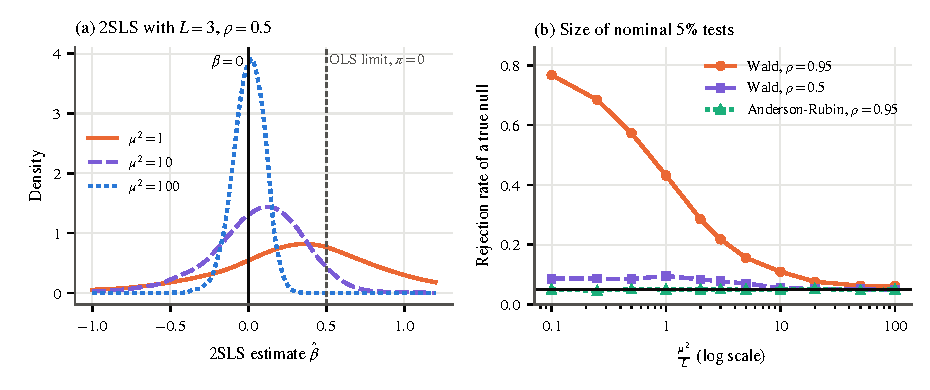
\includegraphics[width=\textwidth]{figures/appA/weakiv.pdf}
\caption{Weak instruments in a simulated design. The model is $y = x\beta + e$, $x = Z\pi + v$ with $\beta = 0$,
$n = 500$, three fixed standard normal instruments, and $(e_i, v_i)$ bivariate normal with unit variances and
correlation $\rho$. The vector $\pi$ is scaled to hit each concentration parameter $\mu^2$ exactly. (a) Kernel
densities of 2SLS over 10,000 replications for $\mu^2 \in \{1, 10, 100\}$ with $\rho = 0.5$. The dashed line marks
$\rho = 0.5$, the OLS limit with irrelevant instruments. (b) Rejection rates of nominal 5 percent tests of the
true null $\beta = 0$, plotted against $\frac{\mu^2}{L}$ on a log scale. The Wald test uses homoskedastic 2SLS
standard errors with $\rho = 0.95$ and $\rho = 0.5$, and the Anderson-Rubin test uses $\rho = 0.95$. The horizontal line is
the nominal size. The Monte Carlo standard error of a rejection rate of 0.05 is 0.0022. Seed 20261022, script
\texttt{sim\_iv.py}.}
\label{fig:A-weakiv}
\end{figure}

\casehead{Diagnostics}
The standard diagnostic is the first-stage $F$ statistic for the excluded instruments.
\citet{StaigerStock1997} suggest treating $F < 10$ as a sign of weak instruments, which by
\cref{prop:A-weak-bias} corresponds to a relative bias of roughly 10 percent. \citet{StockYogo2005} tabulate
cutoffs for the Cragg-Donald version of the statistic under homoskedasticity, for chosen tolerances on
the relative bias of 2SLS or on the size of Wald tests. With heteroskedastic, serially correlated or
clustered errors, the homoskedastic $F$ is invalid. Practitioners then report the robust Wald statistic of
\citet{KleibergenPaap2006}, divided by $L$, and compare it informally with the Stock-Yogo values.
\citet{MontielOleaPflueger2013} derive an \emph{effective} $F$ statistic with valid cutoffs for one
endogenous regressor. With several endogenous regressors, every first-stage $F$ can be large while the
instruments still fail to separate the regressors from one another. The conditional $F$ statistics of
\citet{SandersonWindmeijer2016} address this case. They are needed in the nested logit regression, where both
price and the log within-nest share are endogenous (\cref{sec:07-nl-estimation}). \Cref{tab:A-weakiv}
summarizes the rules.

\begin{table}[htbp]
\centering
\caption{Weak-instrument diagnostics and conventional thresholds}
\label{tab:A-weakiv}
\footnotesize
\begin{tabularx}{\textwidth}{@{}>{\raggedright\arraybackslash}p{0.2\textwidth}
>{\raggedright\arraybackslash}X >{\raggedright\arraybackslash}X >{\raggedright\arraybackslash}p{0.17\textwidth}@{}}
\toprule
Diagnostic & Setting & Threshold & Source \\
\midrule
First-stage $F$ on excluded instruments & One endogenous regressor, homoskedastic errors & $F > 10$ as a rule of
thumb & \citet{StaigerStock1997} \\
\addlinespace
Cragg-Donald $F$ with tabulated cutoffs & Homoskedastic errors, one or more endogenous regressors &
With one endogenous regressor, 9.08 for relative bias of at most 10 percent when $L = 3$, and 16.38
($L = 1$) or 22.30 ($L = 3$) for a nominal 5 percent Wald test with true size of at most 10 percent &
\citet[Tables~5.1--5.2]{StockYogo2005} \\
\addlinespace
Kleibergen-Paap Wald $F$ & Heteroskedastic or clustered errors & No formal cutoffs, compared informally with
the Stock-Yogo values & \citet{KleibergenPaap2006} \\
\addlinespace
Effective $F$ & One endogenous regressor with heteroskedastic, serially correlated or clustered errors & 23.1
as a conservative rule for a 2SLS Nagar bias of at most 10 percent of a worst-case benchmark, at the 5 percent
level & \citet[p.~358]{MontielOleaPflueger2013} \\
\addlinespace
Conditional $F$ & Several endogenous regressors & With $K = 2$, each statistic compared with the Stock-Yogo values
for one endogenous regressor and $L - 1$ instruments & \citet[Section~4]{SandersonWindmeijer2016} \\
\addlinespace
$tF$ adjustment & Just identified, one endogenous regressor & $F > 104.7$ for the usual cutoff of 1.96 to give a
true 5 percent test & \citet{LeeEtAl2022} \\
\bottomrule
\end{tabularx}

\smallskip
\begin{minipage}{0.92\textwidth}\footnotesize
Notes: $L$ is the number of excluded instruments and $K$ the number of endogenous regressors. The cutoffs
depend on the number of instruments and on the chosen tolerance, and the cited sources give full tables.
\end{minipage}
\end{table}

The first-stage $R^2$ is not a weak-instrument diagnostic, because it includes the explanatory power of the
exogenous regressors. \citet[WP fn.~23]{ChaudhuriGoldbergJia2006} report first-stage $R^2$ between 0.57 and 0.95
for their product-group prices, and 0.17 for domestic ciprofloxacin. Their instrument list includes
region-by-product dummies (WP p.~20), which can explain much of the variation in price levels on their own. What
matters is the contribution of the excluded instruments, measured by the partial $R^2$ or the partial $F$
statistic after the exogenous regressors are partialled out. An overall $F$ can also hide weak subsets. In
the simulated markets of \cref{app:problems}, the cluster-robust first-stage $F$ for seven excluded instruments
is 92.5, but six of them are jointly weak with $F = 2.32$. Nearly all the strength comes from one cost shifter.

\casehead{Inference that is robust to weak instruments}
The \emph{Anderson-Rubin test} \citep{AndersonRubin1949} remains valid however weak the instruments are. To test
$H_0\colon\beta = \beta_0$, form $\tilde y = y - x\beta_0$, which equals $e$ under the null. Regress $\tilde y$ on $Z$
and test that all coefficients are zero:
\begin{equation}\label{eq:A-ar}
AR(\beta_0) = \frac{\frac{1}{L}\tilde y^\top P_Z\tilde y}{\frac{1}{n - L}\tilde y^\top M_Z\tilde y} .
\end{equation}
Suppose the errors are normal, homoskedastic and independent of $Z$. Under $H_0$,
$\frac{1}{\sigma_e^2}e^\top P_Ze \sim \chi^2_L$ and $\frac{1}{\sigma_e^2}e^\top M_Ze \sim \chi^2_{n - L}$, because $P_Z$ and
$M_Z$ are idempotent with ranks $L$ and $n - L$. The two quadratic forms are independent because $P_ZM_Z = 0$.
Hence $AR(\beta_0) \sim F(L, n - L)$ exactly, whatever the value of $\pi$. With $K_1$ exogenous regressors partialled
out, the denominator degrees of freedom become $n - L - K_1$. Without normality, $L \cdot AR(\beta_0)$ is
asymptotically $\chi^2_L$, and heteroskedasticity- or cluster-robust versions use a robust Wald test of the
coefficients on $Z$.

A confidence set collects the values $\beta_0$ that the test does not reject. The Anderson-Rubin set can be a
bounded interval, the union of two rays, the whole real line, or even empty. An unbounded set is the right
answer when the data carry little information about $\beta$. In panel (b) of \cref{fig:A-weakiv}, the
Anderson-Rubin test rejects between 4.7 and 5.3 percent of the time at every instrument strength. Its
weakness is power when $L > K$, because it tests $\beta = \beta_0$ jointly with the overidentifying restrictions.
The conditional likelihood ratio test of \citet{Moreira2003} is more powerful, and it coincides with the
Anderson-Rubin test in the just-identified case. \citet{AndrewsStockSun2019} survey these methods.

\casehead{Many instruments}
Adding instruments that carry little information raises $L$ without raising $\mu^2$, and by
\cref{prop:A-weak-bias} it pushes 2SLS toward OLS. In the limit with as many instruments as observations,
$P_Z = I_n$ and 2SLS equals OLS. Limited-information maximum likelihood (LIML) is approximately median-unbiased
and much less sensitive to the number of instruments. The jackknife IV estimator removes the own-observation
term that causes the bias \citep{AngristImbensKrueger1999}. In demand estimation, \citet{Armstrong2016} shows
that the characteristics of rival products can be weak instruments in markets with many products. Markups then
converge to limits that hardly depend on rivals' characteristics (\cref{sec:08-iv-families}).

\subsection{Specification tests}\label{sec:A-spectests}

\casehead{Overidentification}
When $L > K$, the instruments imply more moment conditions than parameters, and we can test whether they are
mutually consistent. Under homoskedasticity, the \emph{Sargan statistic} is $n$ times the $R^2$ of the
regression of the 2SLS residuals on all instruments. It converges to $\chi^2_{L - K}$ under the null that every
instrument is exogenous \citep{Sargan1958}. Hansen's $J$ statistic is the robust version
(\cref{thm:A-jtest}). \citet[pp.~23--24]{Dafny2005} splits her instrument into the number of rival pairs less than
0.2 miles apart and the number between 0.2 and 0.3 miles apart. The Sargan statistic is 0.36 with a $p$-value
of 0.55, so the two bands imply similar effects. The test has limits. It is identically zero in a
just-identified model. It has no power against a bias that all instruments share. Both of Dafny's bands
measure distances between the same hospitals, so they would fail together if co-location itself were
correlated with unobserved price growth.

\casehead{The Hausman principle}
A second family of tests compares two estimators. One is efficient under the null hypothesis, and the other
is consistent under both the null and the alternative.

\begin{lemma}[Hausman]\label{lem:A-hausman}
Let $\hat\beta_E$ and $\hat\beta_C$ be estimators of $\beta$ such that, under $H_0$,
$\sqrt{n}\bigl((\hat\beta_E - \beta)^\top, (\hat\beta_C - \beta)^\top\bigr)^\top$ converges to a normal vector with
variances $V_E$ and $V_C$ and cross-covariance $C = \mathrm{Acov}(\hat\beta_E, \hat\beta_C)$. Here $\mathrm{Avar}$
and $\mathrm{Acov}$ denote the asymptotic variance and covariance of $\sqrt{n}$ times the centered estimators. If $\hat\beta_E$ is
asymptotically efficient under $H_0$, then $C = V_E$. Equivalently, $\hat\beta_E$ is asymptotically uncorrelated
with $\hat\beta_C - \hat\beta_E$, and
\begin{equation}\label{eq:A-hausman-var}
\mathrm{Avar}(\hat\beta_C - \hat\beta_E) = V_C - V_E .
\end{equation}
\end{lemma}

\begin{proof}
Write $D = \hat\beta_C - \hat\beta_E$, which converges to zero under $H_0$. Its asymptotic covariance with
$\hat\beta_E$ is $C - V_E$. For fixed vectors $a$ and $b$ and a scalar $\lambda$, the estimator
$a^\top\hat\beta_E + \lambda b^\top D$ is consistent for $a^\top\beta$. Its asymptotic variance is
\begin{equation*}
f(\lambda) = a^\top V_Ea + 2\lambda\,a^\top(C - V_E)b + \lambda^2\,b^\top\mathrm{Avar}(D)\,b .
\end{equation*}
Efficiency of $\hat\beta_E$ requires $f(\lambda) \ge f(0)$ for every $\lambda$, so the derivative at zero,
$2a^\top(C - V_E)b$, must vanish. This holds for all $a$ and $b$, so $C = V_E$. Then
$\mathrm{Avar}(D) = V_C - C - C^\top + V_E = V_C - V_E$.
\end{proof}

The \emph{Hausman statistic} is
\begin{equation}\label{eq:A-hausman}
\mathcal{H} = (\hat\beta_C - \hat\beta_E)^\top\bigl[\hat V_C - \hat V_E\bigr]^{-}(\hat\beta_C - \hat\beta_E)
\xrightarrow{d} \chi^2_q ,
\end{equation}
where $\hat V_C$ and $\hat V_E$ estimate the finite-sample variances, the superscript denotes a generalized
inverse, and $q$ is the rank of $V_C - V_E$ \citep{Hausman1978}. When OLS is compared with 2SLS, $q$ equals the
number of endogenous regressors tested. Two practical problems arise. The estimated difference
$\hat V_C - \hat V_E$ need not be positive semidefinite in finite samples, and OLS is efficient only under
homoskedasticity. The regression form avoids both. Add the first-stage residuals of the suspect regressors to
the OLS regression, as in \cref{prop:A-cf-2sls}, and test that their coefficients are jointly zero with a
robust Wald test. Under homoskedasticity this test is asymptotically equivalent to \eqref{eq:A-hausman}.

The principle appears throughout the book.
\begin{itemize}
\item \citet{Borenstein1989} rejects exogeneity of the route share and the route Herfindahl index, and so
  reports 2SLS. A Hausman test does not reject exogeneity of the load factor ``at any reasonable significance
  level'', so he treats it as exogenous (pp.~352 and 356--357). The cost of instrumenting shows in his Table 2.
  For the 80th percentile fare, the route-share coefficient is 0.1259 (0.0349) by OLS and 0.2238 (0.0784) by
  2SLS. The route Herfindahl coefficient moves from $-0.0120$ (0.0425) to $-0.1787$ (0.0901). The 2SLS standard
  errors are more than twice the OLS ones.
\item \citet[p.~21]{Dafny2005} reports that Hausman tests easily reject equality of the IV and OLS estimates
  in \cref{tab:A-dafny}.
\item \citet{Hausman1997} notes that weekly supermarket prices may be predetermined with respect to demand
  shocks, in which case OLS is consistent and efficient. A Hausman test of OLS against IV can decide
  (\cref{sec:10-hausman-identification}).
\item In panel data, random effects is efficient under its assumptions and fixed effects is consistent
  whether or not the unit effects are correlated with the regressors. Their difference tests
  $\E[\alpha_i \mid x_{i1}, \dots, x_{iT}] = 0$ (\cref{sec:A-panel}).
\item The test of independence of irrelevant alternatives of \citet{HausmanMcFadden1984} compares logit
  estimates from the full choice set with estimates from a restricted set. The restricted estimates are
  consistent under both hypotheses and inefficient under the null (\cref{eq:10-hm-test}).
\end{itemize}

\subsection{What IV estimates when effects differ}\label{sec:A-late}

So far the effect of $x_i$ has been the same for every unit. When effects differ, IV estimates a weighted
average of them, and the weights depend on the instrument.

\begin{theorem}[Local average treatment effect]\label{thm:A-late}
Let $z_i$ and $d_i$ be binary. Each unit has potential treatments $d_i(1)$ and $d_i(0)$, one for each value of
the instrument, and potential outcomes $y_i(d, z)$. Assume the following.
\begin{enumerate}[label=(\roman*)]
\item The instrument is independent of the potential outcomes and treatments
  $\{y_i(d, z), d_i(z) : d, z \in \{0, 1\}\}$.
\item The instrument is excluded from the outcome, $y_i(d, 1) = y_i(d, 0) \equiv y_i(d)$ for $d = 0, 1$.
\item The instrument is relevant, $\E[d_i(1) - d_i(0)] \neq 0$.
\item Treatment is monotone in the instrument, $d_i(1) \ge d_i(0)$ for every $i$.
\end{enumerate}
Then the Wald estimand \eqref{eq:A-wald-estimator} equals
$\E[y_i(1) - y_i(0) \mid d_i(1) > d_i(0)]$, the average effect for \emph{compliers}, the units whose treatment
the instrument changes \citep{ImbensAngrist1994}.
\end{theorem}

\begin{proof}
By exclusion, the observed outcome is $y_i = y_i(0) + d_i(z_i)\bigl(y_i(1) - y_i(0)\bigr)$. By independence,
\begin{equation*}
\E[y_i \mid z_i = 1] - \E[y_i \mid z_i = 0] = \E\bigl[\bigl(d_i(1) - d_i(0)\bigr)\bigl(y_i(1) - y_i(0)\bigr)\bigr] .
\end{equation*}
Monotonicity makes $d_i(1) - d_i(0)$ equal to one for compliers and zero for everyone else, so the right side
equals $\Pr(\text{complier})\,\E[y_i(1) - y_i(0) \mid \text{complier}]$. Independence also gives
$\E[d_i \mid z_i = 1] - \E[d_i \mid z_i = 0] = \E[d_i(1) - d_i(0)] = \Pr(\text{complier})$, which is nonzero by
relevance. The ratio is the complier average effect.
\end{proof}

The population splits into \emph{always-takers} ($d_i(1) = d_i(0) = 1$), \emph{never-takers}
($d_i(1) = d_i(0) = 0$), compliers, and \emph{defiers} ($d_i(1) < d_i(0)$), whom monotonicity rules out.
Different instruments move different compliers, so two valid instruments can identify different averages, and
an overidentification test can then reject even though both instruments are exogenous. With a continuous
endogenous variable, \citet{AngristGraddyImbens2000} show that the linear IV estimand in a supply and demand
system is a weighted average of the derivatives of the structural function. The weights are largest at
prices where the instrument shifts the equilibrium most. Dafny's estimate is local in this sense, since the
instrument moves only mergers of co-located hospitals.

\casehead{An IO analogue}
\citet{Corts1999} makes the same point about conduct. Write the supply relation as $P_t - c_t = \theta_tm_t$, with
conduct $\theta_t$ and $m_t = Q_t\bigl\lvert\frac{\partial Q_t}{\partial P_t}\bigr\rvert^{-1}$. Suppose marginal cost is known and a
demand shifter $Z_t$ serves as the instrument for $m_t$ in an equation with a constant conduct parameter. The
IV estimand is
\begin{equation*}
\frac{\Cov(Z_t, P_t - c_t)}{\Cov(Z_t, m_t)} = \frac{\Cov(Z_t, \theta_tm_t)}{\Cov(Z_t, m_t)} ,
\end{equation*}
which for small demand movements is approximately $\frac{\dd(\theta m)}{\dd m} = \theta + m\frac{\dd\theta}{\dd m}$.
The estimator recovers the marginal response of the markup to demand, which can differ sharply from the average
level of conduct. If $\theta_t = a - b\,m_t$, then $\theta_tm_t = am_t - bm_t^2$ and the estimand is
$a - b\frac{\Cov(Z_t, m_t^2)}{\Cov(Z_t, m_t)}$. With $\bar m = \E[m_t]$,
\begin{equation*}
\Cov(Z_t, m_t^2) = 2\bar m\Cov(Z_t, m_t) + \E\bigl[(Z_t - \E Z_t)(m_t - \bar m)^2\bigr] .
\end{equation*}
When the last term is zero, for example when $(Z_t, m_t)$ is jointly symmetric about its mean, the estimand is
$a - 2b\bar m$, while average conduct is $a - b\bar m$ (\cref{sec:03-corts}). Otherwise the third-moment term moves the
estimand away from $a - 2b\bar m$. In both cases the estimand can lie outside the range of $\theta_t$.

\subsection{System IV: three-stage least squares}\label{sec:A-3sls}

When several equations each contain endogenous regressors, they can be estimated jointly. Stack $G$ equations
$y_g = X_g\beta_g + e_g$ with a common $n \times L$ instrument matrix $Z$, block-diagonal $X$, and error vector
$e_t = (e_{1t}, \dots, e_{Gt})^\top$ with $\E[e_te_t^\top \mid z_t] = \Sigma$. The moment conditions are
$\E[e_t \otimes z_t] = 0$, and under conditional homoskedasticity their covariance matrix is
$\E[(e_t \otimes z_t)(e_t \otimes z_t)^\top] = \Sigma \otimes \E[z_tz_t^\top]$. Efficient GMM (\cref{sec:A-gmm-efficient}) weights the
sample moments $(I_G \otimes Z^\top)(y - X\beta)$ by the inverse of this matrix, estimated by
$\hat\Sigma^{-1} \otimes (Z^\top Z)^{-1}$. Since
$(I_G \otimes Z)(\hat\Sigma^{-1} \otimes (Z^\top Z)^{-1})(I_G \otimes Z^\top) = \hat\Sigma^{-1} \otimes P_Z$, the first-order
condition gives the \emph{three-stage least squares} (3SLS) estimator of \citet{ZellnerTheil1962},
\begin{equation}\label{eq:A-3sls}
\hat\beta_{3SLS} = \bigl[X^\top(\hat\Sigma^{-1} \otimes P_Z)X\bigr]^{-1}X^\top(\hat\Sigma^{-1} \otimes P_Z)\,y .
\end{equation}
The three stages are the first-stage regressions, 2SLS for each equation to estimate
$\hat\Sigma_{gh} = \frac{1}{n}\hat e_g^\top\hat e_h$, and the system estimator \eqref{eq:A-3sls}. By the logic of
\cref{prop:A-sur-ols}, 3SLS equals equation-by-equation 2SLS when $\Sigma$ is diagonal or every equation is
exactly identified. Its gains come from correlated errors and from restrictions across equations. Its cost is
that misspecification of any one equation contaminates the estimates of all of them. The estimated $\Sigma$
also adds noise in small samples.

\casehead{Application: residual demand in brewing}
\citet{BakerBresnahan1988} estimate the inverse residual demand curves of Anheuser-Busch, Pabst and Coors
jointly by 3SLS. Each equation regresses the firm's log price on its log quantity, demand shifters and cost
variables. The coefficient on own quantity, $\eta^R_j$, is the inverse elasticity of residual demand. Own
quantity is instrumented by firm-specific cost shifters: capacity for every firm, average plant size for
Anheuser-Busch and Pabst, and the Colorado manufacturing wage for Coors, which brewed only in Golden. The joint
estimation exploits the correlation of errors across the three equations. It also imposes a cross-equation
restriction, under which industry cost variables enter every equation through one common marginal cost index
(their eq.~12). The data are annual for 1962--1982, so each equation has only 21 observations (Table 3).

The estimates of $\eta^R_j$ are $-0.745$ (0.054) for Coors, $-0.058$ (0.031) for Pabst and $-0.312$ (0.064) for
Anheuser-Busch before 1975. An interaction with the post-1975 period, when light beer was introduced, is 0.282
(0.040), so Anheuser-Busch's inverse elasticity falls to $-0.030$ after 1975 (Table 3). Single-equation 2SLS gives
similar elasticities ``with little noticeable efficiency loss'' (fn.~20). Treating quantity as exogenous gives
$-0.738$, $-0.053$ and $-0.312$ (fn.~26), so simultaneity bias is small in these data. With 21 observations per
equation, several regressors and an estimated three-by-three covariance matrix, the asymptotic standard errors
should be read with caution. \Cref{sec:03-residual-demand} interprets the results.

The estimators of this section all have closed forms. Many structural models in industrial organization do not.
Their parameters enter nonlinearly, their errors enter through an equilibrium, or their likelihood involves an
integral. \Cref{sec:A-extremum} therefore turns to estimators defined by optimizing a criterion, which include
2SLS and 3SLS as special cases, and \cref{sec:A-twostep} returns to the joint estimation of demand and supply.

\section{Extremum estimators}\label{sec:A-extremum}

Almost every estimator in this book maximizes or minimizes a criterion function. Least squares minimizes a sum of squared
residuals. Maximum likelihood maximizes a log-likelihood. The BLP estimator minimizes a quadratic form in sample moments.
Simulated versions replace an intractable integral inside the criterion by an average over random draws. It pays to
prove consistency and asymptotic normality once, for the whole class, and then to read off each special case. This
section does that, following \citet{NeweyMcFadden1994}. As in the rest of the appendix, $\theta$ is a generic parameter
vector, here of dimension $K$, and the data $w_1, \dots, w_n$ are independent and identically distributed unless stated
otherwise. The convergence notation is the one set out in the introduction to this appendix.

\begin{definition}[Extremum estimator]\label{def:A-extremum}
Let $\Theta \subset \R^K$ be a parameter space and $Q_n(\theta)$ a criterion function that depends on the data. An
\emph{extremum estimator} is any $\hat\theta \in \Theta$ with
\begin{equation}\label{eq:A-extremum}
  Q_n(\hat\theta) \ge \sup_{\theta \in \Theta} Q_n(\theta) - o_p(1).
\end{equation}
The \emph{limit criterion} is a nonrandom function $Q_0(\theta)$ to which $Q_n(\theta)$ converges in probability.
\end{definition}

The $o_p(1)$ slack in \eqref{eq:A-extremum} allows for numerical optimization that stops close to, but not exactly at, the
supremum. This slack is enough for consistency. Asymptotic normality needs a tighter optimization tolerance, condition (v)
of \cref{thm:A-asy-normal}. The leading examples are the following.
\begin{enumerate}
  \item \emph{Nonlinear least squares} sets $Q_n(\theta) = -\frac{1}{n}\sum_{i=1}^n\{y_i - m(x_i;\theta)\}^2$, with limit
  $Q_0(\theta) = -\E[\{y_i - m(x_i;\theta)\}^2]$. Ordinary least squares is the case $m(x;\theta) = x^\T\theta$.
  \item \emph{Maximum likelihood} sets $Q_n(\theta) = \frac{1}{n}\sum_{i=1}^n\ln f(y_i \mid x_i;\theta)$, with limit
  $Q_0(\theta) = \E[\ln f(y_i \mid x_i;\theta)]$ (\cref{sec:A-mle}).
  \item The \emph{generalized method of moments} sets
  $Q_n(\theta) = -\bar g_n(\theta)^\T W_n\bar g_n(\theta)$, with limit
  $Q_0(\theta) = -\E[g(w_i;\theta)]^\T W\E[g(w_i;\theta)]$ (\cref{sec:A-gmm}). Here
  $\bar g_n(\theta) = \frac{1}{n}\sum_i g(w_i;\theta)$, and $W_n$ is a weighting matrix.
  \item \emph{Simulated estimators} use the same criteria with an expectation inside $g$ or $f$ replaced by a
  simulation average (\cref{sec:A-simulation}).
\end{enumerate}
The first two are \emph{M-estimators}, because $Q_n$ is a sample average of a function of one observation. GMM is a
\emph{minimum distance} estimator, because $Q_n$ is a quadratic form in sample averages. The general theorems below cover
both.

\subsection{Consistency}\label{sec:A-ext-consistency}

Consistency rests on two ideas. The limit criterion must have a unique maximum at the true value. The sample criterion
must be close to the limit criterion everywhere on the parameter space, not only at each point separately.

\begin{theorem}[Consistency of extremum estimators]\label{thm:A-consistency}
Suppose that (i) $Q_0(\theta)$ is uniquely maximized at $\theta_0$ (identification), (ii) $\Theta$ is compact, (iii)
$Q_0(\theta)$ is continuous, and (iv) $\sup_{\theta \in \Theta}\lvert Q_n(\theta) - Q_0(\theta)\rvert \xrightarrow{p} 0$
(uniform convergence). Then any extremum estimator satisfies $\hat\theta \xrightarrow{p} \theta_0$.
\end{theorem}

\begin{proof}
Fix $\epsilon > 0$. Three events occur w.p.a.1. By \eqref{eq:A-extremum},
$Q_n(\hat\theta) > Q_n(\theta_0) - \frac{\epsilon}{3}$. By uniform convergence,
$Q_0(\hat\theta) > Q_n(\hat\theta) - \frac{\epsilon}{3}$, since $\hat\theta \in \Theta$. Again by uniform convergence,
$Q_n(\theta_0) > Q_0(\theta_0) - \frac{\epsilon}{3}$. Chaining the three inequalities gives, w.p.a.1,
\begin{equation}\label{eq:A-consistency-chain}
  Q_0(\hat\theta) > Q_n(\hat\theta) - \frac{\epsilon}{3} > Q_n(\theta_0) - \frac{2\epsilon}{3} > Q_0(\theta_0) - \epsilon.
\end{equation}
Now let $\mathcal{N}$ be any open set that contains $\theta_0$. The set $\Theta \cap \mathcal{N}^c$ is closed and bounded,
hence compact. Since $Q_0$ is continuous, it attains its supremum on this set at some $\theta^*$. Identification gives
$Q_0(\theta^*) < Q_0(\theta_0)$. Choose $\epsilon = Q_0(\theta_0) - Q_0(\theta^*) > 0$. Then
\eqref{eq:A-consistency-chain} says that, w.p.a.1,
\begin{equation*}
  Q_0(\hat\theta) > Q_0(\theta^*) = \sup_{\theta \in \Theta \cap \mathcal{N}^c}Q_0(\theta).
\end{equation*}
So $\hat\theta \notin \Theta \cap \mathcal{N}^c$, that is, $\hat\theta \in \mathcal{N}$, w.p.a.1. Because $\mathcal{N}$ was
arbitrary, $\hat\theta \xrightarrow{p} \theta_0$.
\end{proof}

\Cref{fig:A-extremum} draws the argument. Uniform convergence traps $Q_n$ in a band of half-width $\epsilon$ around
$Q_0$. The maximizer of $Q_n$ must then achieve a value of $Q_0$ within $2\epsilon$ of the maximum, and identification
confines such points to a neighborhood of $\theta_0$ that shrinks with $\epsilon$.

\begin{figure}[htbp]
\centering
\begin{tikzpicture}
\begin{axis}[
  width=0.82\textwidth, height=6.2cm,
  xmin=0.2, xmax=3.8, ymin=0, ymax=2.75,
  axis lines=left, xlabel={$\theta$}, ylabel={criterion},
  xtick={0.8168, 2, 2.3087, 3.1832},
  xticklabels={$\theta_0 - r_\epsilon$, $\theta_0$, $\hat\theta$, $\theta_0 + r_\epsilon$},
  ytick={1.3, 2}, yticklabels={$Q_0(\theta_0) - 2\epsilon$, $Q_0(\theta_0)$},
  every tick label/.append style={font=\footnotesize},
  samples=200, domain=0.3:3.7, clip=false]
  \addplot[name path=up, draw=none, forget plot] {2 - 0.5*(x-2)^2 + 0.35};
  \addplot[name path=dn, draw=none, forget plot] {2 - 0.5*(x-2)^2 - 0.35};
  \addplot[blue!12, forget plot] fill between[of=up and dn];
  \addplot[blue!60!black, dashed, thin, forget plot] {2 - 0.5*(x-2)^2 + 0.35};
  \addplot[blue!60!black, dashed, thin, forget plot] {2 - 0.5*(x-2)^2 - 0.35};
  \addplot[black, very thick] {2 - 0.5*(x-2)^2};
  \addplot[orange!85!black, thick] {2 - 0.5*(x-2)^2 + 0.22*sin(deg(2.6*x+0.5)) + 0.1*sin(deg(6.3*x))};
  \draw[gray, densely dotted] (axis cs:0.2,1.3) -- (axis cs:3.8,1.3);
  \draw[gray, densely dotted] (axis cs:0.2,2) -- (axis cs:2,2);
  \draw[gray, densely dotted] (axis cs:0.8168,0) -- (axis cs:0.8168,1.3);
  \draw[gray, densely dotted] (axis cs:3.1832,0) -- (axis cs:3.1832,1.3);
  \draw[gray, densely dotted] (axis cs:2,0) -- (axis cs:2,2);
  \draw[orange!85!black, densely dotted] (axis cs:2.3087,0) -- (axis cs:2.3087,2.092);
  \fill[orange!85!black] (axis cs:2.3087,2.092) circle (1.6pt);
  \draw[very thick, gray!70] (axis cs:0.8168,0.06) -- (axis cs:3.1832,0.06);
  \draw[black, thin] (axis cs:3.0,1.5) -- (axis cs:3.45,2.05);
  \node[font=\footnotesize, anchor=south west] at (axis cs:3.42,2.03) {$Q_0(\theta)$};
  \draw[orange!85!black, thin] (axis cs:0.9,1.402) -- (axis cs:0.6,1.95);
  \node[font=\footnotesize, anchor=south, text=orange!85!black] at (axis cs:0.6,1.93) {$Q_n(\theta)$};
  \node[font=\footnotesize, anchor=south, text=blue!60!black] at (axis cs:2.2,2.4) {$Q_0(\theta) \pm \epsilon$};
\end{axis}
\end{tikzpicture}
\caption[The consistency argument for extremum estimators]{The consistency argument for extremum estimators. The thick
curve is the limit criterion $Q_0$, maximized only at $\theta_0$. Uniform convergence places the sample criterion $Q_n$
inside the shaded band $Q_0 \pm \epsilon$. The maximizer $\hat\theta$ of $Q_n$ then satisfies $Q_0(\hat\theta) > Q_0(\theta_0)
- 2\epsilon$, so it lies in the interval $[\theta_0 - r_\epsilon, \theta_0 + r_\epsilon]$ marked on the horizontal axis.
The curves are illustrative: $Q_0(\theta) = 2 - \frac{1}{2}(\theta - 2)^2$ and $\epsilon = 0.35$.}
\label{fig:A-extremum}
\end{figure}

Pointwise convergence of $Q_n(\theta)$ to $Q_0(\theta)$ at each $\theta$ is not enough. Take $\Theta = [0, 2]$ and
\begin{equation*}
  Q_n(\theta) = -\theta^2 + 2\max\left\{0,\ 1 - n\left\lvert\theta - 1 - \frac{1}{n}\right\rvert\right\}.
\end{equation*}
At each fixed $\theta$ the spike eventually moves away, so $Q_n(\theta) \to Q_0(\theta) = -\theta^2$, which is maximized at
$0$. Yet $Q_n(1 + \frac{1}{n}) = 2 - (1 + \frac{1}{n})^2$ is close to $1$, above $Q_n(0) = 0$. The maximizer converges to
$1$, not to $0$. Uniform convergence fails because $\sup_\theta\lvert Q_n - Q_0\rvert = 2$ for every $n$.

Uniform convergence is usually verified with a uniform law of large numbers. The next lemma is the version we use most
often. It is \citet[Lemma 2.4]{NeweyMcFadden1994}.

\begin{lemma}[Uniform law of large numbers]\label{lem:A-ulln}
Let $w_i$ be i.i.d., $\Theta$ compact, and $a(w, \theta)$ continuous in $\theta$ at each $\theta \in \Theta$ with
probability one. If $\E[\sup_{\theta \in \Theta}\lVert a(w_i, \theta)\rVert] < \infty$, then $\E[a(w_i, \theta)]$ is
continuous and
\begin{equation*}
  \sup_{\theta \in \Theta}\left\lVert\frac{1}{n}\sum_{i=1}^n a(w_i, \theta) - \E[a(w_i, \theta)]\right\rVert
  \xrightarrow{p} 0.
\end{equation*}
\end{lemma}

The integrable envelope $\sup_\theta\lVert a(w, \theta)\rVert$ is the \emph{dominance condition}. Continuity and compactness
let us cover $\Theta$ by finitely many small balls. On each ball the function moves little, and the ordinary law of large
numbers applies at the finitely many centers. For maximum likelihood we apply the lemma to $a = \ln f$. For GMM we apply
it to $a = g$ and then use the continuity of the quadratic form.

Compactness is a nuisance in practice, since few applied parameter spaces are bounded. For concave criteria it can be
dropped. This matters for the logit and multinomial logit likelihoods, which are globally concave
(\cref{prop:A-logit-concave}).

\begin{theorem}[Consistency with a concave criterion]\label{thm:A-concave}
Suppose that $\theta_0$ is an interior point of a convex set $\Theta$, $Q_n(\theta)$ is concave on $\Theta$ for each $n$,
$Q_n(\theta) \xrightarrow{p} Q_0(\theta)$ for each $\theta \in \Theta$, and $Q_0$ is uniquely maximized at $\theta_0$. Then
$\hat\theta$ exists w.p.a.1 and $\hat\theta \xrightarrow{p} \theta_0$.
\end{theorem}

The proof \citep[Theorem 2.7]{NeweyMcFadden1994} uses a fact from convex analysis. Pointwise convergence of concave
functions implies uniform convergence on compact subsets of the interior. Apply \cref{thm:A-consistency} on a small closed
ball around $\theta_0$. Concavity then rules out a maximizer outside the ball. A concave function that is higher at the
center of a ball than everywhere on its boundary is also higher at the center than anywhere outside the ball.

Identification, condition (i), is the substantive assumption. It says that the model and the data distribution single
out $\theta_0$. \Cref{sec:A-identification} discusses what it requires in IO models. Conditions (ii) to (iv) are
regularity conditions that hold in most smooth applications.

\subsection{Asymptotic normality}\label{sec:A-ext-normality}

Once $\hat\theta$ is consistent, a Taylor expansion of the first-order condition around $\theta_0$ delivers its limit
distribution.

\begin{theorem}[Asymptotic normality of extremum estimators]\label{thm:A-asy-normal}
Suppose the following conditions hold.
\begin{enumerate}[label=(\roman*)]
  \item $\hat\theta \xrightarrow{p} \theta_0$, and $\theta_0$ is in the interior of $\Theta$.
  \item $Q_n(\theta)$ is twice continuously differentiable on a neighborhood $\mathcal{N}$ of $\theta_0$.
  \item $\sqrt{n}\,\nabla_\theta Q_n(\theta_0) \xrightarrow{d} N(0, \Sigma)$.
  \item There is a matrix function $H(\theta)$, continuous at $\theta_0$, with $\sup_{\theta \in
  \mathcal{N}}\lVert\nabla_{\theta\theta}Q_n(\theta) - H(\theta)\rVert \xrightarrow{p} 0$ and $H = H(\theta_0)$ nonsingular.
  \item $\sqrt{n}\,\nabla_\theta Q_n(\hat\theta) \xrightarrow{p} 0$. An exact interior maximizer satisfies this with
  $\nabla_\theta Q_n(\hat\theta) = 0$.
\end{enumerate}
Then
\begin{equation}\label{eq:A-sandwich}
  \sqrt{n}(\hat\theta - \theta_0) \xrightarrow{d} N\big(0,\ H^{-1}\Sigma H^{-1}\big).
\end{equation}
\end{theorem}

\begin{proof}
Because $\hat\theta \xrightarrow{p} \theta_0$ and $\theta_0$ is interior, $\hat\theta$ lies in $\mathcal{N}$ and in the
interior of $\Theta$ w.p.a.1. Write $r_n = \nabla_\theta Q_n(\hat\theta)$ for the gradient at the estimate. By (v),
$\sqrt{n}\,r_n \xrightarrow{p} 0$. Apply the mean value theorem to each element of the gradient. For row $k$ there is a point
$\bar\theta^{(k)}$ on the segment between $\hat\theta$ and $\theta_0$ with
\begin{equation*}
  r_{n,k} = \frac{\partial Q_n(\theta_0)}{\partial\theta_k} + \frac{\partial^2 Q_n(\bar\theta^{(k)})}{\partial\theta_k\partial\theta^\T}
  (\hat\theta - \theta_0).
\end{equation*}
Stack the rows into the matrix $\bar H_n$, whose row $k$ is the $k$-th row of the Hessian evaluated at $\bar\theta^{(k)}$.
Then
\begin{equation*}
  r_n = \nabla_\theta Q_n(\theta_0) + \bar H_n(\hat\theta - \theta_0).
\end{equation*}
Each $\bar\theta^{(k)}$ converges in probability to $\theta_0$. By (iv) and the continuity of $H$ at $\theta_0$,
\begin{equation*}
  \lVert\bar H_n - H\rVert \le \sup_{\theta \in \mathcal{N}}\lVert\nabla_{\theta\theta}Q_n(\theta) - H(\theta)\rVert
  + \max_k\lVert H(\bar\theta^{(k)}) - H\rVert \xrightarrow{p} 0.
\end{equation*}
So $\bar H_n$ is invertible w.p.a.1, and
\begin{equation*}
  \sqrt{n}(\hat\theta - \theta_0) = -\bar H_n^{-1}\sqrt{n}\,\nabla_\theta Q_n(\theta_0) + \bar H_n^{-1}\sqrt{n}\,r_n.
\end{equation*}
The second term converges in probability to zero by (v). By (iii), Slutsky's theorem and the continuous mapping theorem, the
right side converges in distribution to $-H^{-1}Z$ with $Z \sim N(0, \Sigma)$. Its variance is $H^{-1}\Sigma H^{-1}$, because
$H$ is symmetric.
\end{proof}

Condition (v) cannot be dropped. Take $Y_i$ i.i.d.\ $N(0,1)$, $\theta_0 = 0$, $Q_n(\theta) = -\frac{1}{2}(\theta - \bar Y)^2$,
and an optimizer that stops at $\hat\theta = \bar Y + n^{-\frac{1}{4}}$. The criterion shortfall is
$\frac{1}{2}n^{-\frac{1}{2}} = o(1)$, so $\hat\theta$ is a consistent extremum estimator and (i)--(iv) hold. Yet
$\sqrt{n}\,\hat\theta = \sqrt{n}\,\bar Y + n^{\frac{1}{4}}$ diverges. An optimization error that vanishes more slowly than
the sampling error swamps it. Under local quadratic curvature, a criterion shortfall of order $o_p(n^{-1})$ is enough for (v).

The variance in \eqref{eq:A-sandwich} is a \emph{sandwich}. The outer pieces measure the curvature of the criterion, the
inner piece the noise in its slope at the truth. A consistent estimator replaces $H$ by $\nabla_{\theta\theta}Q_n(\hat\theta)$
and $\Sigma$ by an estimate of the variance of $\sqrt{n}\,\nabla_\theta Q_n(\theta_0)$. For an M-estimator with
$Q_n = \frac{1}{n}\sum_i q(w_i;\theta)$, that estimate is $\frac{1}{n}\sum_i\nabla_\theta q(w_i;\hat\theta)
\nabla_\theta q(w_i;\hat\theta)^\T$. With dependent data it becomes a clustered or HAC estimate (\cref{sec:A-cluster,sec:A-hac}).

The theorem fails in three situations that occur in IO. If $\theta_0$ lies on the boundary of $\Theta$, the first-order
condition need not hold. A variance component or a regime probability equal to zero is the usual case
(\cref{sec:A-mle-nonregular}). If $Q_n$ is not differentiable, the expansion must be replaced by an argument based on
stochastic equicontinuity. Simulated frequency estimators and some auction estimators are examples
\citep{PakesPollard1989}. If $H$ is singular, the rank condition for local identification fails. The parameter
$\theta_0$ may still be identified through higher-order terms, but the normal approximation breaks down and the rate of
convergence changes.

\subsection{Profile objectives}\label{sec:A-profile}

Many IO estimators split the parameters into a block that is easy to optimize given the rest and a block that is hard.
Optimizing out the easy block first leaves a \emph{profile} (or \emph{concentrated}) criterion in the hard block alone.

\begin{proposition}[Profile criteria]\label{prop:A-profile}
Partition $\theta = (\theta_1, \theta_2)$ with $\Theta = \Theta_1 \times \Theta_2$. Suppose that for each $\theta_2$ the
maximizer $\hat\theta_1(\theta_2) = \argmax_{\theta_1 \in \Theta_1}Q_n(\theta_1, \theta_2)$ exists and is unique. Define the
profile criterion $\tilde Q_n(\theta_2) = Q_n(\hat\theta_1(\theta_2), \theta_2)$.
\begin{enumerate}[label=(\alph*)]
  \item $(\hat\theta_1, \hat\theta_2)$ maximizes $Q_n$ jointly if and only if $\hat\theta_2$ maximizes $\tilde Q_n$ and
  $\hat\theta_1 = \hat\theta_1(\hat\theta_2)$.
  \item Suppose $Q_n$ is twice continuously differentiable and that, on a neighborhood of $\theta_2$, $\hat\theta_1(\cdot)$ is
  continuous with values in the interior of $\Theta_1$. If the Hessian block $H_{11} = \nabla_{\theta_1\theta_1}Q_n$ is
  nonsingular at $(\hat\theta_1(\theta_2), \theta_2)$, then
  \begin{equation}\label{eq:A-profile-derivs}
    \nabla_{\theta_2}\tilde Q_n(\theta_2) = \nabla_{\theta_2}Q_n\big(\hat\theta_1(\theta_2), \theta_2\big),
    \qquad
    \nabla_{\theta_2\theta_2}\tilde Q_n(\theta_2) = H_{22} - H_{21}H_{11}^{-1}H_{12},
  \end{equation}
  where the blocks of the Hessian of $Q_n$ are evaluated at $(\hat\theta_1(\theta_2), \theta_2)$.
\end{enumerate}
\end{proposition}

\begin{proof}
(a) For any $(\theta_1, \theta_2)$,
\begin{equation*}
  Q_n(\theta_1, \theta_2) \le Q_n(\hat\theta_1(\theta_2), \theta_2) = \tilde Q_n(\theta_2).
\end{equation*}
Hence $\sup_{\theta}Q_n(\theta) = \sup_{\theta_2}\tilde Q_n(\theta_2)$. If $\hat\theta_2$ maximizes $\tilde Q_n$, then
$(\hat\theta_1(\hat\theta_2), \hat\theta_2)$ attains this common supremum. Conversely, if $(\hat\theta_1, \hat\theta_2)$
maximizes $Q_n$, then $\tilde Q_n(\hat\theta_2) \ge Q_n(\hat\theta_1, \hat\theta_2) = \sup_{\theta_2}\tilde Q_n$, and
uniqueness of the inner maximizer gives $\hat\theta_1 = \hat\theta_1(\hat\theta_2)$.

(b) Because the inner maximizer is interior, the inner first-order condition
$\nabla_{\theta_1}Q_n(\hat\theta_1(\theta_2), \theta_2) = 0$ holds on the neighborhood. The implicit function theorem gives
a locally unique $C^1$ solution of this condition. By continuity $\hat\theta_1(\cdot)$ coincides with it, and
differentiating the condition gives
\begin{equation*}
  H_{11}\frac{\partial\hat\theta_1}{\partial\theta_2^\T} + H_{12} = 0
  \quad\Longrightarrow\quad
  \frac{\partial\hat\theta_1}{\partial\theta_2^\T} = -H_{11}^{-1}H_{12}.
\end{equation*}
By the chain rule,
\begin{equation*}
  \nabla_{\theta_2}\tilde Q_n = \left(\frac{\partial\hat\theta_1}{\partial\theta_2^\T}\right)^\T\nabla_{\theta_1}Q_n
  + \nabla_{\theta_2}Q_n = \nabla_{\theta_2}Q_n,
\end{equation*}
because the first term vanishes by the inner first-order condition. This is the envelope theorem. Differentiating once
more,
\begin{equation*}
  \nabla_{\theta_2\theta_2}\tilde Q_n = H_{21}\frac{\partial\hat\theta_1}{\partial\theta_2^\T} + H_{22}
  = H_{22} - H_{21}H_{11}^{-1}H_{12}. \qedhere
\end{equation*}
\end{proof}

Part (a) is what makes nested estimation legitimate. Part (b) says how to get standard errors. By the partitioned
inverse formula, $(H_{22} - H_{21}H_{11}^{-1}H_{12})^{-1}$ is the $(2,2)$ block of $H^{-1}$. For maximum likelihood, where
the asymptotic variance is $(-H)^{-1}$, the inverse Hessian of the profile log-likelihood therefore gives the correct
variance for $\hat\theta_2$. It already accounts for the estimation of $\theta_1$. For GMM the full sandwich is needed,
and \cref{sec:A-gmm-computation} gives the formula.

Three applications recur in this book. In the normal linear regression, the variance $\sigma^2$ can be profiled out. The
log-likelihood at $\hat\sigma^2(\beta) = \frac{1}{n}\sum_i(y_i - x_i^\T\beta)^2$ is $-\frac{n}{2}\ln\hat\sigma^2(\beta)$ plus a
constant. This is the form behind the Cox statistic of \cref{prop:06-bres-cox}. In the BLP estimator, the linear demand
parameters have a closed form given the nonlinear ones (\cref{prop:08-concentrate}). In supply-side estimation with many
fixed effects, the effects and the linear cost parameters can be concentrated out by least squares.
\citet[p.~1780]{MillerWeinberg2017} do this when they estimate the internalization and cost parameters of the beer
industry after the MillerCoors joint venture (\cref{ch:mergers}).

Profiling does not cure an \emph{incidental parameters} problem. Suppose $y_{it} = \mu_i + e_{it}$ with
$e_{it} \sim N(0, \sigma^2)$, $i = 1, \dots, N$ and $t = 1, \dots, T$, with $T$ fixed and $N \to \infty$. Profiling out each
$\mu_i$ gives $\hat\mu_i = \bar y_i$ and
\begin{equation*}
  \hat\sigma^2 = \frac{1}{NT}\sum_{i=1}^N\sum_{t=1}^T(y_{it} - \bar y_i)^2 \xrightarrow{p} \frac{T - 1}{T}\sigma^2.
\end{equation*}
The estimator is inconsistent \citep{NeymanScott1948}. The number of profiled parameters grows with the sample, so the
fixed-dimension assumptions of \cref{thm:A-consistency} fail. In linear models the bias has a known form, but in nonlinear
models with many fixed effects it contaminates every parameter.

\subsection{Numerical practice}\label{sec:A-numerical}

The theorems describe the global maximizer. A computer returns a point where an algorithm stopped. The gap between the
two is a frequent source of error in structural IO, and good practice narrows it.

Gradient methods iterate $\theta^{(m+1)} = \theta^{(m)} - \lambda_m A_m^{-1}\nabla_\theta Q_n(\theta^{(m)})$, where
$\lambda_m > 0$ is a step length and $A_m$ approximates the Hessian. Newton's method uses the Hessian itself and converges
quadratically near a maximum with a negative definite Hessian. Quasi-Newton methods such as BFGS build $A_m$ from
successive gradients. For maximum likelihood, the method of \citet{BerndtEtAl1974} (BHHH) replaces the Hessian by minus
the outer product of the scores. That matrix is negative semidefinite by construction. By the information equality of
\cref{sec:A-mle-score}, it is consistent for the Hessian at the truth. Derivative-free methods such as Nelder and Mead's simplex need only
function values. They are slow but robust to kinks.

We recommend the following checks.
\begin{enumerate}
  \item Scale the parameters so that a unit change in each moves the criterion by similar amounts. Poor scaling
  makes gradient methods take tiny steps along flat directions.
  \item Use analytic gradients when possible. Finite differences lose about half the digits of the criterion.
  \item Start the optimizer from many points. If different starts end at different values, report the best and
  investigate the others. \citet[p.~309]{Porter1983} reports that his switching model converged to the same estimates
  from several disparate starting points. \citet{KnittelMetaxoglou2014} show that BLP estimates can depend on the
  optimizer and the starting values (\cref{ch:blp}).
  \item At the reported optimum, check that the gradient is close to zero and that the Hessian is negative definite.
  A singular Hessian signals that the rank condition for local identification fails.
  \item Hold simulation draws fixed across evaluations. Redrawing them makes the criterion change between calls, and the
  optimizer never settles (\cref{sec:A-simulation}).
  \item When the criterion contains an inner fixed point, such as the BLP contraction, solve the inner problem to a
  tight tolerance. Inner-loop error makes the outer criterion noisy and can produce false convergence
  \citep{DubeFoxSu2012}.
\end{enumerate}

Some criteria are not smooth at all. In the vertical model the ordering of products by quality depends on the quality
coefficients. When two products swap places, the predicted prices and quantities jump, and so does the likelihood
(\cref{sec:06-bres-estimation}). Gradient methods then behave erratically, and derivative-free search or a grid over the
offending parameters is safer. Frequency simulators produce step functions for the same reason, which is why smooth
simulators are preferred (\cref{sec:A-simulation}).

\section{Generalized method of moments}\label{sec:A-gmm}

The generalized method of moments (GMM) of \citet{Hansen1982} is the workhorse estimator of structural IO. It needs only
a set of population moment conditions implied by the model, and no full likelihood. Demand estimation with instruments,
supply relations with unobserved cost shocks, and their joint estimation all fit this mold.

\subsection{Moment conditions}\label{sec:A-gmm-moments}

\begin{definition}[Moment conditions]\label{def:A-moments}
Let $g(w;\theta)$ be an $L \times 1$ vector of functions of the data $w$ and the $K \times 1$ parameter $\theta$, with
$L \ge K$. The model implies the \emph{moment conditions}
\begin{equation}\label{eq:A-moments}
  \E[g(w_i;\theta_0)] = 0.
\end{equation}
The parameter is \emph{globally identified} by \eqref{eq:A-moments} if $\E[g(w_i;\theta)] \ne 0$ for every
$\theta \ne \theta_0$ in $\Theta$. It is \emph{locally identified} if the $L \times K$ Jacobian
$G = \E\big[\frac{\partial g(w_i;\theta_0)}{\partial\theta^\T}\big]$ has rank $K$.
\end{definition}

The \emph{order condition} $L \ge K$ is necessary for the rank condition. When $g$ is linear in $\theta$ the rank condition
gives global identification. When $g$ is nonlinear it gives only local identification (\cref{prop:A-local-id}), and
global identification must be argued separately. The applications in this book use the following moment functions.
\begin{enumerate}
  \item \emph{Least squares} uses $g(w_i;\beta) = x_i(y_i - x_i^\T\beta)$, with $L = K$.
  \item \emph{Linear instrumental variables} use $g(w_i;\beta) = z_i(y_i - x_i^\T\beta)$, with $z_i$ an $L \times 1$
  vector of instruments (\cref{sec:A-iv}).
  \item \emph{Nonlinear instrumental variables}. In the sugar study of \citet{GenesoveMullin1998}, demand is
  $Q = \beta(\alpha - P)^\gamma$ and marginal cost is $c_0 + kP^{\mathit{raw}}$. The pricing rule with conduct parameter
  $\theta$ is $P = \frac{\alpha\theta + c_0\gamma}{\gamma + \theta} + \frac{\gamma}{\gamma + \theta}kP^{\mathit{raw}}$. With
  $(\alpha, \gamma)$ set at their demand estimates, the moment function for $\psi = (\theta, c_0, k)$ is
  \begin{equation}\label{eq:A-sugar-moment}
    g(w_t;\psi) = z_t\left\{(\gamma + \theta)P_t - \alpha\theta - c_0\gamma - \gamma kP^{\mathit{raw}}_t\right\}.
  \end{equation}
  Here $z_t$ contains the log of Cuban raw-sugar imports, a high-season dummy and a constant (Genesove and Mullin, WP
  eq.~13). The raw price is instrumented because shocks to the pricing rule move it. Here $\theta$ is the conduct
  parameter of \cref{sec:03-sugar-neio}. Letting conduct differ in price-war periods replaces $\theta$ by
  $\theta_0 + (\theta_1 - \theta_0)\mathit{WAR}_t$ and adds the war dummy to $z_t$, which keeps the system just
  identified (\cref{sec:03-sugar-wars}).
  \item \emph{Demand moments in differentiated products}. With the logit inversion, the structural error is
  $\xi_{jt}(\theta) = \ln s_{jt} - \ln s_{0t} - x_{jt}\beta + \alpha p_{jt}$ (\cref{ch:logit}). With random coefficients,
  $\xi_{jt}(\theta) = \delta_{jt}(s_t;\theta_2) - x_{jt}\beta + \alpha p_{jt}$, where $\delta_{jt}(s_t;\theta_2)$ inverts
  the share system (\cref{ch:blp}). Either way $g = z_{jt}\xi_{jt}(\theta)$.
  \item \emph{Supply moments}. Under Bertrand-Nash pricing, marginal cost is price minus the markup implied by demand,
  $mc_{jt}(\theta) = p_{jt} + [(\Omega_t \odot \Delta_t^\top)^{-1}s_t]_j$. In this item $\Omega_t$ is the ownership
  matrix of market $t$, and $\Delta_t$ has $(j,k)$ element $\frac{\partial s_{jt}}{\partial p_{kt}}$
  (\cref{ch:diffprod}). If
  $mc_{jt} = w_{jt}\gamma + \omega_{jt}$, the cost moment is $g = z^s_{jt}\{mc_{jt}(\theta) - w_{jt}\gamma\}$.
  \item \emph{Conditional moment restrictions}. Many models state $\E[\rho(w_i;\theta_0) \mid z_i] = 0$ for a residual vector
  $\rho$. Any matrix of functions $A(z_i)$ then gives unconditional moments $\E[A(z_i)\rho(w_i;\theta_0)] = 0$. Which
  functions to use is the optimal instruments problem of \cref{sec:A-optimal-iv}.
  \item \emph{Simulated moments}, where an expectation inside $g$ is replaced by a simulation average
  (\cref{sec:A-simulation}).
\end{enumerate}

\subsection{The estimator and its asymptotic distribution}\label{sec:A-gmm-asy}

\begin{definition}[GMM estimator]\label{def:A-gmm}
Let $\bar g_n(\theta) = \frac{1}{n}\sum_{i=1}^n g(w_i;\theta)$ and let $W_n$ be a symmetric positive semidefinite
$L \times L$ matrix with $W_n \xrightarrow{p} W$. The \emph{GMM estimator} is
\begin{equation}\label{eq:A-gmm}
  \hat\theta = \argmin_{\theta \in \Theta}\ \bar g_n(\theta)^\T W_n\,\bar g_n(\theta).
\end{equation}
\end{definition}

Consistency follows from \cref{thm:A-consistency} with $Q_n(\theta) = -\bar g_n(\theta)^\T W_n\bar g_n(\theta)$ and
$Q_0(\theta) = -\E[g(\theta)]^\T W\E[g(\theta)]$, writing $\E[g(\theta)]$ for $\E[g(w_i;\theta)]$. The limit is
maximized, with value zero, at every $\theta$ where $W\E[g(\theta)] = 0$. Identification therefore requires
$W\E[g(\theta)] \ne 0$ for $\theta \ne \theta_0$, which holds when $W$ is positive definite and the moments identify
$\theta_0$. Uniform convergence follows from \cref{lem:A-ulln} applied to $g$, if $g$ is continuous in $\theta$ and
$\E[\sup_\theta\lVert g(w_i;\theta)\rVert] < \infty$. Indeed, adding and subtracting terms,
\begin{equation*}
  \lvert Q_n(\theta) - Q_0(\theta)\rvert
  \le \lVert\bar g_n - \E g\rVert^2\lVert W_n\rVert + 2\lVert\E g\rVert\,\lVert W_n\rVert\,\lVert\bar g_n - \E g\rVert
  + \lVert\E g\rVert^2\lVert W_n - W\rVert,
\end{equation*}
and each term converges to zero uniformly on the compact $\Theta$.

\begin{theorem}[Asymptotic normality of GMM]\label{thm:A-gmm-normal}
Suppose the following conditions hold.
\begin{enumerate}[label=(\roman*)]
  \item $\hat\theta \xrightarrow{p} \theta_0$, with $\theta_0$ interior.
  \item $g(w;\theta)$ is continuously differentiable in $\theta$ on a neighborhood $\mathcal{N}$ of $\theta_0$.
  \item $\sqrt{n}\,\bar g_n(\theta_0) \xrightarrow{d} N(0, S)$.
  \item $G_n(\theta) = \frac{\partial\bar g_n(\theta)}{\partial\theta^\T}$ satisfies $\sup_{\theta \in \mathcal{N}}\lVert
  G_n(\theta) - G(\theta)\rVert \xrightarrow{p} 0$ for a function $G(\theta)$ continuous at $\theta_0$.
  \item $W_n \xrightarrow{p} W$, and $G^\T WG$ is nonsingular, where $G = G(\theta_0)$.
\end{enumerate}
Then
\begin{equation}\label{eq:A-gmm-var}
  \sqrt{n}(\hat\theta - \theta_0) \xrightarrow{d} N(0, V), \qquad
  V = (G^\T WG)^{-1}G^\T WSWG(G^\T WG)^{-1}.
\end{equation}
\end{theorem}

\begin{proof}
W.p.a.1 the estimator is interior and satisfies the first-order condition of \eqref{eq:A-gmm},
\begin{equation*}
  G_n(\hat\theta)^\T W_n\,\bar g_n(\hat\theta) = 0.
\end{equation*}
A mean value expansion of each element of $\bar g_n(\hat\theta)$ around $\theta_0$ gives
\begin{equation*}
  \bar g_n(\hat\theta) = \bar g_n(\theta_0) + \bar G_n(\hat\theta - \theta_0),
\end{equation*}
where row $\ell$ of $\bar G_n$ is row $\ell$ of $G_n$ evaluated at a point between $\hat\theta$ and $\theta_0$. Substitute
into the first-order condition:
\begin{equation*}
  G_n(\hat\theta)^\T W_n\bar g_n(\theta_0) + G_n(\hat\theta)^\T W_n\bar G_n(\hat\theta - \theta_0) = 0.
\end{equation*}
By (i), (iv) and (v), $G_n(\hat\theta)^\T W_n\bar G_n \xrightarrow{p} G^\T WG$, which is nonsingular. Solve and multiply by
$\sqrt{n}$:
\begin{equation*}
  \sqrt{n}(\hat\theta - \theta_0) = -\big[G_n(\hat\theta)^\T W_n\bar G_n\big]^{-1}G_n(\hat\theta)^\T W_n\sqrt{n}\,\bar
  g_n(\theta_0).
\end{equation*}
By (iii) and Slutsky's theorem the right side converges in distribution to $-(G^\T WG)^{-1}G^\T WZ$ with $Z \sim N(0, S)$,
whose variance is $V$.
\end{proof}

With i.i.d.\ data, $S = \E[g(w_i;\theta_0)g(w_i;\theta_0)^\T]$, estimated by $\hat S = \frac{1}{n}\sum_i g(w_i;\hat\theta)
g(w_i;\hat\theta)^\T$. The Jacobian is estimated by $\hat G = G_n(\hat\theta)$. The plug-in $\hat V$ replaces each
population matrix by its estimate.

\casehead{Linear instrumental variables}
Stack the data as $y$ ($n \times 1$), $X$ ($n \times K$) and $Z$ ($n \times L$). Then $\bar g_n(\beta) = \frac{1}{n}Z^\T(y -
X\beta)$, and the criterion is $\frac{1}{n^2}(y - X\beta)^\T ZW_nZ^\T(y - X\beta)$. The first-order condition is
\begin{equation*}
  -\frac{2}{n^2}X^\T ZW_nZ^\T(y - X\beta) = 0,
\end{equation*}
so
\begin{equation}\label{eq:A-linear-gmm}
  \hat\beta = \big(X^\T ZW_nZ^\T X\big)^{-1}X^\T ZW_nZ^\T y.
\end{equation}
With $W_n = (\frac{1}{n}Z^\T Z)^{-1}$ this is two-stage least squares, \eqref{eq:A-2sls}, the third route of
\cref{sec:A-2sls}. Here $G = -\E[z_ix_i^\T]$, so \eqref{eq:A-gmm-var} becomes the IV sandwich of
\cref{prop:A-2sls-asy}. When $L = K$, the algebra of \cref{sec:A-2sls} shows that \eqref{eq:A-linear-gmm} collapses to
$(Z^\T X)^{-1}Z^\T y$ whatever $W_n$ is. The general lesson is that a just-identified GMM estimator sets
$\bar g_n(\hat\theta) = 0$, so the weighting matrix plays no role.

\subsection{Efficient weighting}\label{sec:A-gmm-efficient}

The weighting matrix matters only when $L > K$. It decides how to trade off moments that cannot all be set to zero in the
sample. The best choice weights each moment by the inverse of its noise.

\begin{proposition}[Efficient weighting matrix]\label{prop:A-efficient-gmm}
Under the assumptions of \cref{thm:A-gmm-normal} with $S$ positive definite, the asymptotic variance $V(W)$ in
\eqref{eq:A-gmm-var} satisfies $V(W) - (G^\T S^{-1}G)^{-1} \succeq 0$ for every admissible $W$. The lower bound is attained
at $W = S^{-1}$, where $V = (G^\T S^{-1}G)^{-1}$.
\end{proposition}

\begin{proof}
Define the $K \times L$ matrix
\begin{equation*}
  A = (G^\T WG)^{-1}G^\T W - (G^\T S^{-1}G)^{-1}G^\T S^{-1}.
\end{equation*}
Since $S$ is positive definite, $ASA^\T \succeq 0$. Expand the product term by term:
\begin{align*}
  ASA^\T &= (G^\T WG)^{-1}G^\T WSWG(G^\T WG)^{-1}
  - (G^\T WG)^{-1}G^\T WG(G^\T S^{-1}G)^{-1} \\
  &\quad - (G^\T S^{-1}G)^{-1}G^\T WG(G^\T WG)^{-1}
  + (G^\T S^{-1}G)^{-1}G^\T S^{-1}G(G^\T S^{-1}G)^{-1}.
\end{align*}
The first term is $V(W)$. After cancellation, each of the last three matrix products equals $(G^\T S^{-1}G)^{-1}$, and
they enter with signs minus, minus and plus. So $ASA^\T = V(W) - (G^\T S^{-1}G)^{-1}$, which is positive semidefinite.
Setting $W = S^{-1}$ in \eqref{eq:A-gmm-var} gives
\begin{equation*}
  V(S^{-1}) = (G^\T S^{-1}G)^{-1}G^\T S^{-1}SS^{-1}G(G^\T S^{-1}G)^{-1} = (G^\T S^{-1}G)^{-1}. \qedhere
\end{equation*}
\end{proof}

The efficient weight depends on $S$, which depends on $\theta_0$. Three feasible versions are in use.
\begin{enumerate}
  \item \emph{Two-step GMM}. Estimate $\tilde\theta$ with a fixed weight, such as $(\frac{1}{n}Z^\T Z)^{-1}$. Form
  \begin{equation*}
    \hat S = \frac{1}{n}\sum_{i=1}^ng(w_i;\tilde\theta)g(w_i;\tilde\theta)^\T
  \end{equation*}
  and re-estimate with $W_n = \hat S^{-1}$.
  \item \emph{Iterated GMM}. Repeat the second step, updating $\hat S$ each time, until the estimates stop changing.
  \item \emph{Continuously updated GMM} (CUE) of \citet{HansenHeatonYaron1996}. Minimize
  $\bar g_n(\theta)^\T\hat S(\theta)^{-1}\bar g_n(\theta)$, where $\hat S(\theta)$ is evaluated at the same $\theta$.
\end{enumerate}
All three have the efficient limit distribution. They differ in finite samples. The two-step estimator can be biased when
the estimated weight is correlated with the sample moments, a problem that grows with the number of moments
\citep{AltonjiSegal1996}. CUE is invariant to linear transformations of the moments and behaves better with weak
instruments \citep{HansenHeatonYaron1996, StockWright2000}, but its criterion can be flat and multimodal.

\begin{proposition}[Efficient GMM and 2SLS]\label{prop:A-gmm-2sls}
In the linear model $y_i = x_i^\T\beta + e_i$ with $\E[z_ie_i] = 0$ and conditional homoskedasticity
$\E[e_i^2 \mid z_i] = \sigma^2$, efficient GMM is 2SLS, and its asymptotic variance is
$\sigma^2\big(\E[x_iz_i^\T]\E[z_iz_i^\T]^{-1}\E[z_ix_i^\T]\big)^{-1}$.
\end{proposition}

\begin{proof}
By the law of iterated expectations,
\begin{equation*}
  S = \E[e_i^2z_iz_i^\T] = \E\big[\E[e_i^2 \mid z_i]z_iz_i^\T\big] = \sigma^2\E[z_iz_i^\T].
\end{equation*}
So the efficient weight is proportional to $\E[z_iz_i^\T]^{-1}$, estimated by a multiple of $(\frac{1}{n}Z^\T Z)^{-1}$.
A scalar multiple of $W_n$ does not change \eqref{eq:A-linear-gmm}, which then equals 2SLS. Substituting $G =
-\E[z_ix_i^\T]$ and $S$ into $(G^\T S^{-1}G)^{-1}$ gives the stated variance.
\end{proof}

Under heteroskedasticity, two-step GMM with $\hat S = \frac{1}{n}\sum_i\hat e_i^2z_iz_i^\T$ is more efficient than 2SLS. The
estimate of $S$ must match the dependence in the data, and this is where most of the practical work lies.
\begin{itemize}
  \item With independent observations, $\hat S = \frac{1}{n}\sum_ig_ig_i^\T$, with $g_i = g(w_i;\tilde\theta)$.
  \item With clusters $c = 1, \dots, C$ whose moments are correlated within but not across clusters, sum the moments within
  each cluster first, $\hat S = \frac{1}{n}\sum_c\big(\sum_{i \in c}g_i\big)\big(\sum_{i \in c}g_i\big)^\T$. In demand
  estimation the natural cluster is the market, or the product when the same product appears in several years
  (\cref{ch:blp}). \citet[p.~1775]{MillerWeinberg2017} cluster by region in the optimal weighting matrix of their
  demand estimator.
  \item With serial correlation, use a heteroskedasticity and autocorrelation consistent (HAC) estimator
  (\cref{sec:A-hac}). Genesove and Mullin compute Newey-West standard errors with four lags for their quarterly sugar data
  (WP, printed p.~36).
\end{itemize}

\subsection{Testing}\label{sec:A-gmm-tests}

With more moments than parameters, the sample cannot set every moment to zero. How far the minimized criterion stays
from zero is evidence on the validity of the moments.

\begin{theorem}[Hansen's $J$ test]\label{thm:A-jtest}
Suppose the assumptions of \cref{thm:A-gmm-normal} hold, $S$ is positive definite, $\hat S \xrightarrow{p} S$, and
$\hat\theta$ is efficient GMM with $W_n = \hat S^{-1}$. If all $L$ moment conditions hold, then
\begin{equation}\label{eq:A-jstat}
  J_n = n\,\bar g_n(\hat\theta)^\T\hat S^{-1}\bar g_n(\hat\theta) \xrightarrow{d} \chi^2_{L-K}.
\end{equation}
\end{theorem}

\begin{proof}
From the proof of \cref{thm:A-gmm-normal} with $W = S^{-1}$,
\begin{equation*}
  \sqrt{n}(\hat\theta - \theta_0) = -(G^\T S^{-1}G)^{-1}G^\T S^{-1}\sqrt{n}\,\bar g_n(\theta_0) + o_p(1).
\end{equation*}
Substitute this into the mean value expansion $\sqrt{n}\,\bar g_n(\hat\theta) = \sqrt{n}\,\bar g_n(\theta_0) +
\bar G_n\sqrt{n}(\hat\theta - \theta_0)$:
\begin{equation*}
  \sqrt{n}\,\bar g_n(\hat\theta) = \big[I_L - G(G^\T S^{-1}G)^{-1}G^\T S^{-1}\big]\sqrt{n}\,\bar g_n(\theta_0) + o_p(1).
\end{equation*}
Let $C$ be a symmetric matrix with $C^2 = S^{-1}$, and write $\xi_n = C\sqrt{n}\,\bar g_n(\theta_0)$. Then
$\xi_n \xrightarrow{d} N(0, CSC) = N(0, I_L)$. Premultiplying by $C$ and using $C^{-1}C = I_L$,
\begin{equation*}
  C\sqrt{n}\,\bar g_n(\hat\theta) = \big[I_L - CG(G^\T C^2G)^{-1}G^\T C\big]\xi_n + o_p(1) = M\xi_n + o_p(1).
\end{equation*}
The matrix $M$ is the residual-maker for the columns of $CG$. It is symmetric and idempotent, with trace
$L - \mathrm{tr}[(G^\T C^2G)^{-1}G^\T C^2G] = L - K$. Since $\hat S^{-1} \xrightarrow{p} C^2$,
\begin{equation*}
  J_n = \big(C\sqrt{n}\,\bar g_n(\hat\theta)\big)^\T\big(C\sqrt{n}\,\bar g_n(\hat\theta)\big) + o_p(1)
  = \xi_n^\T M\xi_n + o_p(1).
\end{equation*}
A quadratic form of a standard normal vector in a symmetric idempotent matrix of rank $L - K$ is $\chi^2_{L-K}$.
\end{proof}

In the linear homoskedastic model the $J$ statistic reduces to \citet{Sargan1958}'s statistic. With
$\hat S = \hat\sigma^2\frac{1}{n}Z^\T Z$ and $\bar g_n = \frac{1}{n}Z^\T\hat e$, where $\hat e$ is the 2SLS residual,
\begin{equation*}
  J_n = n\frac{\hat e^\T Z(Z^\T Z)^{-1}Z^\T\hat e}{\hat e^\T\hat e} = nR^2,
\end{equation*}
the sample size times the $R^2$ from regressing $\hat e$ on $Z$. When $Z$ and $X$ both contain a constant, the 2SLS residuals
sum to zero and the centered and uncentered $R^2$ coincide.

The $J$ test has power only against violations that cannot be absorbed by moving $\theta$. If every instrument is
invalid in a way that a different parameter value could rationalize, $J$ stays small. In a just-identified model
$J_n \equiv 0$. A $J$ test that does not reject is therefore weak evidence for the instruments, and a rejection does not say
which moment fails. When a subset of instruments is suspect, the \emph{difference-in-$J$} or $C$ statistic helps. It
compares $J_n$ from all $L$ moments with $J_n$ from the $L_1 \ge K$ maintained moments, computed with the corresponding
block of the same $\hat S$. Under the null that the $L - L_1$ suspect moments hold, the difference converges to $\chi^2_{L - L_1}$.

Two applications illustrate the statistic. In the simulated yogurt markets of \cref{sec:C-logit-est}, logit demand is
estimated with the price of milk and six competition instruments for one endogenous price. Two-step GMM gives
$J = 8.82$ with six degrees of freedom ($p = 0.18$), so the overidentifying restrictions are not rejected.
\citet{MillerWeinberg2017} report $J$ statistics of 13.94, 13.75, 13.91 and 14.15 for their four random coefficients nested
logit specifications of beer demand (Table IV, p.~1777). That table, which \cref{tab:11-mw-demand} reproduces, does not
report the degrees of freedom. The text gives eight for the first two specifications and seven for the other two, and it
states that the models cannot be rejected at the 5 percent level (p.~1776). Our computation gives $p$-values of 0.083,
0.089, 0.053 and 0.049. The last statistic, 14.15, lies just above 14.07, the 95 percent quantile of $\chi^2_7$.
The test therefore narrowly rejects the fourth specification at the 5 percent level, contrary to the paper's statement.

Hypotheses about $\theta$ can be tested in three ways, which parallel the likelihood trinity of
\cref{sec:A-mle-trinity}. Let $H_0: a(\theta_0) = 0$ impose $r$ restrictions, with $A = \frac{\partial a(\theta_0)}{\partial
\theta^\T}$ of rank $r$, and let $\tilde\theta$ be the efficient GMM estimator under the restrictions.
\begin{itemize}
  \item The \emph{Wald} statistic $n\,a(\hat\theta)^\T[\hat A\hat V\hat A^\T]^{-1}a(\hat\theta)$ uses only the unrestricted
  estimate. By the delta method (\cref{thm:A-delta}) it converges to $\chi^2_r$.
  \item The \emph{distance} statistic $D_n = n[\bar g_n(\tilde\theta)^\T\hat S^{-1}\bar g_n(\tilde\theta) -
  \bar g_n(\hat\theta)^\T\hat S^{-1}\bar g_n(\hat\theta)]$ is the GMM analogue of the likelihood ratio. It must use the
  efficient weight and the same $\hat S$ in both terms. Repeating the proof of \cref{thm:A-jtest}, both criteria are
  quadratic forms in the same $\xi_n$, with idempotent matrices of ranks $L - K + r$ and $L - K$. The column space removed
  under the restrictions is contained in that removed without them, so the difference of the two matrices is idempotent
  of rank $r$, and $D_n \xrightarrow{d} \chi^2_r$.
  \item The \emph{Lagrange multiplier} statistic uses only $\tilde\theta$. It is
  $n\,\bar g_n(\tilde\theta)^\T\hat S^{-1}\tilde G(\tilde G^\T\hat S^{-1}\tilde G)^{-1}\tilde G^\T\hat S^{-1}\bar
  g_n(\tilde\theta)$ with $\tilde G = G_n(\tilde\theta)$, and also converges to $\chi^2_r$.
\end{itemize}
Under the null and local alternatives the three statistics are asymptotically equivalent.

\subsection{Optimal instruments}\label{sec:A-optimal-iv}

A conditional moment restriction $\E[\rho(w_i;\theta_0) \mid z_i] = 0$ implies infinitely many unconditional moments. The
question is which functions of $z_i$ to use. The answer, due to \citet{Chamberlain1987}, gives a lower bound on the
variance of every GMM estimator built from the restriction and says how to reach it.

Let $\rho$ be $p \times 1$. Define the conditional Jacobian and conditional variance
\begin{equation*}
  D(z) = \E\left[\frac{\partial\rho(w_i;\theta_0)}{\partial\theta^\T}\,\middle|\, z_i = z\right] \quad (p \times K),
  \qquad
  \Omega(z) = \E\big[\rho(w_i;\theta_0)\rho(w_i;\theta_0)^\T \mid z_i = z\big] \quad (p \times p).
\end{equation*}
For a $K \times p$ matrix of functions $A(z)$, let $\hat\theta_A$ solve the just-identified equations
\begin{equation*}
  \frac{1}{n}\sum_{i=1}^nA(z_i)\rho(w_i;\hat\theta_A) = 0.
\end{equation*}

\begin{proposition}[Optimal instruments]\label{prop:A-optimal-iv}
Suppose $\Omega(z)$ is positive definite and $\Gamma_A = \E[A(z_i)D(z_i)]$ is nonsingular. Then
$\sqrt{n}(\hat\theta_A - \theta_0) \xrightarrow{d} N(0, V_A)$ with
\begin{equation*}
  V_A = \Gamma_A^{-1}\E\big[A(z_i)\Omega(z_i)A(z_i)^\T\big]\Gamma_A^{-1\T}.
\end{equation*}
The choice $A^*(z) = D(z)^\T\Omega(z)^{-1}$ gives $V^* = \big(\E[D(z_i)^\T\Omega(z_i)^{-1}D(z_i)]\big)^{-1}$, and
$V_A - V^* \succeq 0$ for every admissible $A$.
\end{proposition}

\begin{proof}
The moment function is $g = A(z)\rho$. By iterated expectations its Jacobian is $G = \E[A(z_i)\frac{\partial\rho}{\partial
\theta^\T}] = \E[A(z_i)D(z_i)] = \Gamma_A$, and its variance is $S = \E[A\rho\rho^\T A^\T] = \E[A\Omega A^\T]$. With
$L = K$, \eqref{eq:A-gmm-var} reduces to $G^{-1}SG^{-1\T}$, which is $V_A$. For the bound, write $m_A = A(z_i)\rho_i$ and
$m^* = A^*(z_i)\rho_i$. By iterated expectations,
\begin{equation*}
  \E[m_Am^{*\T}] = \E\big[A(z_i)\,\E[\rho_i\rho_i^\T \mid z_i]\,\Omega(z_i)^{-1}D(z_i)\big] = \E[A(z_i)D(z_i)] = \Gamma_A,
\end{equation*}
and in the same way $\E[m^*m^{*\T}] = \E[D^\T\Omega^{-1}D] = V^{*-1}$. Let $u = \Gamma_A^{-1}m_A - V^*m^*$. Then
\begin{align*}
  0 \preceq \E[uu^\T] &= \Gamma_A^{-1}\E[m_Am_A^\T]\Gamma_A^{-1\T} - \Gamma_A^{-1}\E[m_Am^{*\T}]V^*
  - V^*\E[m^*m_A^\T]\Gamma_A^{-1\T} + V^*\E[m^*m^{*\T}]V^* \\
  &= V_A - V^* - V^* + V^* = V_A - V^*.
\end{align*}
Setting $A = A^*$ gives $\Gamma_{A^*} = V^{*-1}$ and $V_{A^*} = V^*$.
\end{proof}

An overidentified GMM estimator that uses a finite vector of instruments $a(z_i)$ is asymptotically an $A$-estimator, with
$A(z) = G^\T W a(z)$, so it cannot beat $V^*$. The optimal instruments reproduce familiar estimators in
simple cases. In the linear model with $\rho = y - x^\T\beta$ and homoskedastic errors, $D(z) = -\E[x \mid z]$ and
$\Omega = \sigma^2$, so the optimal instrument is the conditional mean of the regressors. When that mean is linear in
$z$, 2SLS is efficient. Under heteroskedasticity the optimal instrument is $\frac{\E[x \mid z]}{\sigma^2(z)}$, which
weights observations by the inverse of their error variance.

The sugar moment \eqref{eq:A-sugar-moment} shows what the formula says in a nonlinear model. With
$\rho_t = (\gamma + \theta)P_t - \alpha\theta - c_0\gamma - \gamma kP^{\mathit{raw}}_t$ and $\psi = (\theta, c_0, k)$,
\begin{equation*}
  D(z_t) = \E\left[\frac{\partial\rho_t}{\partial\psi^\T}\,\middle|\, z_t\right]
  = \big(\E[P_t \mid z_t] - \alpha,\ -\gamma,\ -\gamma\,\E[P^{\mathit{raw}}_t \mid z_t]\big).
\end{equation*}
The efficient instruments are the predicted refined and raw prices given the exogenous variables, scaled by the inverse
conditional variance. A linear first stage in $z_t$ approximates them.

Feasible optimal instruments replace $D$ and $\Omega$ by estimates. A first consistent estimate of $\theta$, followed by
nonparametric or series regressions of $\frac{\partial\rho}{\partial\theta^\T}$ and $\rho\rho^\T$ on $z$, gives an estimator
with the efficient limit distribution \citep{Newey1990}. In the BLP model $\rho = (\xi_{jt}, \omega_{jt})$, and
$D(z) = \E[\frac{\partial\xi_{jt}}{\partial\theta^\T} \mid z]$ depends on the equilibrium prices, which depend on the
unobservables. \citet{BerryLevinsohnPakes1999} approximate it by evaluating the derivatives at prices predicted with the
unobservables set to zero. \citet{ReynaertVerboven2014} show large efficiency gains from such approximations relative to
sums of rival characteristics (\cref{ch:blp}).

\subsection{Two-step estimators and generated regressors}\label{sec:A-twostep}

Structural IO is full of sequential estimation. Demand is estimated first, and its estimates are plugged into a supply
relation, a markup formula or a welfare calculation. The second step treats the first-step estimate as if it were known,
and its conventional standard errors are wrong. The fix is to view both steps as one GMM estimator \citep{Newey1984,
MurphyTopel1985}.

Let the first step estimate $\gamma$ by solving $\frac{1}{n}\sum_im(w_i;\hat\gamma) = 0$, with as many equations as elements
of $\gamma$. Let the second step estimate $\theta$ by solving $\frac{1}{n}\sum_ig(w_i;\hat\theta, \hat\gamma) = 0$, also just
identified. An overidentified second step fits the same mold, with $g$ replaced by $G_\theta^\T Wg$. Define the population
Jacobians and covariances
\begin{equation*}
  M_\gamma = \E\left[\frac{\partial m}{\partial\gamma^\T}\right],\quad
  G_\gamma = \E\left[\frac{\partial g}{\partial\gamma^\T}\right],\quad
  G_\theta = \E\left[\frac{\partial g}{\partial\theta^\T}\right],\quad
  \begin{pmatrix} S_{mm} & S_{mg} \\ S_{gm} & S_{gg}\end{pmatrix} = \Var\begin{pmatrix} m(w_i;\gamma_0) \\
  g(w_i;\theta_0, \gamma_0)\end{pmatrix},
\end{equation*}
all evaluated at $(\theta_0, \gamma_0)$.

\begin{proposition}[Variance of a two-step estimator]\label{prop:A-twostep}
Under the conditions of \cref{thm:A-gmm-normal} for the stacked moments $(m^\T, g^\T)^\T$, with $M_\gamma$ and $G_\theta$
nonsingular, $\sqrt{n}(\hat\theta - \theta_0) \xrightarrow{d} N(0, V_\theta)$ with
\begin{equation}\label{eq:A-twostep-var}
  V_\theta = G_\theta^{-1}\Big[S_{gg} - G_\gamma M_\gamma^{-1}S_{mg} - S_{gm}M_\gamma^{-1\T}G_\gamma^\T
  + G_\gamma M_\gamma^{-1}S_{mm}M_\gamma^{-1\T}G_\gamma^\T\Big]G_\theta^{-1\T}.
\end{equation}
\end{proposition}

\begin{proof}
The two steps solve the stacked just-identified system $\frac{1}{n}\sum_i\psi(w_i;\gamma, \theta) = 0$ with
$\psi = (m^\T, g^\T)^\T$. Its Jacobian with respect to $(\gamma, \theta)$ is block lower triangular, because $m$ does not
depend on $\theta$:
\begin{equation*}
  \Gamma = \begin{pmatrix} M_\gamma & 0 \\ G_\gamma & G_\theta\end{pmatrix},
  \qquad
  \Gamma^{-1} = \begin{pmatrix} M_\gamma^{-1} & 0 \\ -G_\theta^{-1}G_\gamma M_\gamma^{-1} & G_\theta^{-1}\end{pmatrix}.
\end{equation*}
One checks the inverse by multiplying the two matrices. By \cref{thm:A-gmm-normal} with $L = K$, the joint variance is
$\Gamma^{-1}\Var(\psi)\Gamma^{-1\T}$. The rows of $\Gamma^{-1}$ that belong to $\theta$ are
$G_\theta^{-1}[-G_\gamma M_\gamma^{-1},\ I]$. Hence
\begin{equation*}
  V_\theta = G_\theta^{-1}\big[-G_\gamma M_\gamma^{-1},\ I\big]
  \begin{pmatrix} S_{mm} & S_{mg} \\ S_{gm} & S_{gg}\end{pmatrix}
  \begin{pmatrix} -M_\gamma^{-1\T}G_\gamma^\T \\ I\end{pmatrix}G_\theta^{-1\T}.
\end{equation*}
Multiplying out the middle product gives the four terms in \eqref{eq:A-twostep-var}.
\end{proof}

The formula has a transparent reading. Expanding the second-step equations,
\begin{equation*}
  \sqrt{n}(\hat\theta - \theta_0) \approx -G_\theta^{-1}\Big[\sqrt{n}\,\bar g_n(\theta_0, \gamma_0)
  + G_\gamma\sqrt{n}(\hat\gamma - \gamma_0)\Big],
  \qquad
  \sqrt{n}(\hat\gamma - \gamma_0) \approx -M_\gamma^{-1}\sqrt{n}\,\bar m_n(\gamma_0).
\end{equation*}
The naive variance $G_\theta^{-1}S_{gg}G_\theta^{-1\T}$ keeps only the first term. The correction depends on $G_\gamma$,
the sensitivity of the second-step moments to the first-step parameters. Two special cases matter.
\begin{itemize}
  \item If $G_\gamma = 0$, no correction is needed. The second step is then insensitive to small errors in $\hat\gamma$.
  \item If the two steps use independent errors, $S_{gm} = 0$, and with $V_\gamma = M_\gamma^{-1}S_{mm}M_\gamma^{-1\T}$,
  \begin{equation}\label{eq:A-murphy-topel}
    V_\theta = G_\theta^{-1}S_{gg}G_\theta^{-1\T} + G_\theta^{-1}G_\gamma V_\gamma G_\gamma^\T G_\theta^{-1\T}.
  \end{equation}
  The correction is then a positive semidefinite addition, and naive standard errors are too small. With correlated
  errors the correction can go either way.
\end{itemize}

\casehead{The sugar pricing equation}
\citet{GenesoveMullin1998} estimate the pricing moment \eqref{eq:A-sugar-moment} with $(\alpha, \gamma)$ fixed at the demand
estimates. Their variance for $(\theta, c_0, k)$ is $W_2 + V$ (WP, printed p.~36). Here $W_2$ is the Newey-West variance
that treats demand as known. The term $V$ combines $W_1$, the Newey-West variance of the demand parameters, with $D$ and
$C$, the derivatives of the pricing moments with respect to $(\theta, c_0, k)$ and to the demand parameters. They assume no
correlation between the demand and pricing errors. In our notation $G_\theta = D$, $G_\gamma = C$, $V_\gamma = W_1$ and
$S_{gm} = 0$. Equation \eqref{eq:A-murphy-topel} then reads $V_\theta = W_2 + D^{-1}CW_1C^\T D^{-1\T}$, which is their
formula up to the orientation in which the derivative matrices are written. The pricing system is just identified in both
of their cases. With $k$ unknown there are three instruments for three parameters, and with $k = 1.075$ imposed there are
two for two.

The same paper shows how much the correction can matter for a simple statistic. The direct measure of conduct is the mean
of the elasticity-adjusted Lerner index $L_{\eta t} = \eta(\hat\gamma)\frac{P_t - c_t}{P_t}$, in which the demand elasticity
$\eta$ is estimated. Genesove and Mullin add the moment $\frac{1}{n}\sum_t L_{\eta t} - \bar L_\eta = 0$ to the moments of
their demand IV estimates and compute GMM standard errors for $\bar L_\eta$ (WP fn.~45). \Cref{tab:A-gm-lerner} shows that
accounting for the estimated elasticity more than doubles the standard error for all four demand curves.

\begin{table}[htbp]
\centering
\caption{Standard errors of the mean adjusted Lerner index with and without the correction for estimated demand}
\label{tab:A-gm-lerner}
\small
\begin{tabular}{lcccc}
\toprule
Demand curve & Mean $\bar L_\eta$ & \makecell{s.e. treating\\ $\eta$ as known} & \makecell{s.e. accounting for\\
estimated $\eta$} & Ratio \\
\midrule
Quadratic & .099 & .010 & .024 & 2.4 \\
Linear & .107 & .012 & .028 & 2.3 \\
Log-linear & .095 & .008 & .021 & 2.6 \\
Exponential & .097 & .009 & .022 & 2.4 \\
\bottomrule
\end{tabular}
\par\smallskip
\parbox{\linewidth}{\footnotesize Notes: Genesove and Mullin, working-paper Table 8, columns (1), (3) and (4). The unadjusted Lerner index has
mean .054 and standard error .0046. The ratio column is our computation. The corrected standard errors stack the moment
for $\bar L_\eta$ with the demand moments (WP fn.~45).}
\end{table}

\casehead{Rotations and generated regressors}
In the two-step rotation estimator of \cref{sec:03-rotation}, the second step regresses price on the generated regressor
$\hat Q^*_t = -\frac{Q_t}{\hat a_1 + \hat a_3Z_t}$ with coefficient $\theta$ (\cref{eq:03-rotation-supply}). The second-step
moment is $g_t = h^s_t(P_t - b_0 - b_1Q_t - \theta Q^*_t(a) - b_2W_t)$. Its derivative with respect to $(a_1, a_3)$ is
\begin{equation*}
  \frac{\partial g_t}{\partial(a_1, a_3)} = -\theta\,h^s_t\,\frac{Q_t}{(a_1 + a_3Z_t)^2}\,(1,\ Z_t).
\end{equation*}
So $G_\gamma$ is proportional to $\theta$. Under the null of competitive pricing, $\theta_0 = 0$, the correction vanishes,
and the naive $t$ test of $\theta = 0$ is asymptotically valid. Away from the null, and for confidence intervals, the
correction is needed. Joint GMM estimation of both equations (\cref{eq:03-rotation-gmm}) delivers correct standard errors
automatically and is more efficient.

\casehead{Generated regressands}
In the logit supply problem of \cref{sec:C-logit-est}, implied marginal cost $p_{jt} - \frac{1}{\hat\alpha(1 - S_{ft})}$ is
regressed on cost shifters. The dependent variable depends on $\hat\alpha$, and
$G_\gamma = \E[z^s_{jt}\frac{1}{\alpha^2(1 - S_{ft})}] \ne 0$. Because every markup is close to $\frac{1}{\alpha}$ when shares
are small, the error in $\hat\alpha$ loads almost entirely on the intercept. Its standard error rises from 0.016 to 0.065
with the stacked formula. A market bootstrap that re-estimates $\alpha$ in each replication gives 0.072. The slope
standard errors barely change (\cref{tab:C-lsupply}). The bootstrap is the practical fix when the steps are many
(\cref{sec:A-boot-multistep}).

\casehead{Supply estimated given demand}
\citet[p.~1780]{MillerWeinberg2017} estimate the post-merger internalization parameter $\kappa$ and the marginal cost parameters
from a supply moment $\E[z\,\eta^*(\theta^S;\hat\theta^D)] = 0$, taking the demand estimates $\hat\theta^D$ as given. They
report standard errors clustered by region with a correction for the first-stage demand estimates, for which they
cite \citet{Wooldridge2010}.
This is \cref{prop:A-twostep} with clustered $S$ (\cref{ch:mergers}).

Joint estimation is the clean alternative to every two-step procedure. Stacking $(m, g)$ and estimating $(\gamma, \theta)$
by efficient GMM gives correct standard errors. It also uses cross-equation correlation for efficiency when the blocks
overidentify the parameters. In the sugar
application it means stacking the demand moments with \eqref{eq:A-sugar-moment} and estimating the demand parameters,
$\theta$, $c_0$ and $k$ together. The airline hub model of \cref{ch:airlines} and the BLP model with a supply side
(\cref{ch:blp}) stack demand and cost moments in the same way. Joint estimation changes the first-block estimates only
when the second block has more moments than new parameters. If the supply block has exactly as many moments as cost
parameters, the joint estimate of the demand parameters equals GMM on the demand moments alone with weight
$W_{dd} - W_{ds}W_{ss}^{-1}W_{sd}$. With the efficient weight this is efficient GMM on the demand moments
(\cref{prop:C-redundant}). The cross-equation correlation then improves only the supply-side estimates.

\subsection{Computation}\label{sec:A-gmm-computation}

Nonlinear GMM criteria are minimized numerically, and the advice of \cref{sec:A-numerical} applies. Two structural
features make the search much easier in IO models.

\begin{proposition}[Concentrating out linear parameters]\label{prop:A-concentrate-gmm}
Partition $\theta = (\theta_1, \theta_2)$ and suppose the sample moments are linear in $\theta_1$,
$\bar g_n(\theta) = a_n(\theta_2) - B_n(\theta_2)\theta_1$, with $B_n(\theta_2)^\T W_nB_n(\theta_2)$ nonsingular. For each
$\theta_2$ the minimizer over $\theta_1$ is
\begin{equation}\label{eq:A-concentrate}
  \hat\theta_1(\theta_2) = \big(B_n^\T W_nB_n\big)^{-1}B_n^\T W_na_n,
\end{equation}
and $\hat\theta_2$ minimizes the profile criterion $a_n^\T\big[W_n - W_nB_n(B_n^\T W_nB_n)^{-1}B_n^\T W_n\big]a_n$, with
$a_n$ and $B_n$ evaluated at $\theta_2$.
\end{proposition}

\begin{proof}
For fixed $\theta_2$ the criterion $(a_n - B_n\theta_1)^\T W_n(a_n - B_n\theta_1)$ is a convex quadratic in $\theta_1$. Its
gradient $-2B_n^\T W_n(a_n - B_n\theta_1)$ vanishes at \eqref{eq:A-concentrate}. Substituting back,
$a_n - B_n\hat\theta_1(\theta_2) = [I - B_n(B_n^\T W_nB_n)^{-1}B_n^\T W_n]a_n$, and the quadratic form in this vector
simplifies to the stated profile criterion. \Cref{prop:A-profile}(a) completes the argument.
\end{proof}

In the BLP model, $a_n(\theta_2) = \frac{1}{n}Z^\T\delta(\theta_2)$ and $B_n = \frac{1}{n}Z^\T X$, which does not depend on
$\theta_2$. The outer search runs over the few nonlinear parameters only (\cref{prop:08-concentrate}). Because
$\hat\theta_1(\theta_2)$ is optimal for each $\theta_2$, the envelope result \eqref{eq:A-profile-derivs} gives the gradient
of the profile criterion,
\begin{equation*}
  \frac{\partial}{\partial\theta_2^\T}\Big[\bar g_n^\T W_n\bar g_n\Big] = 2\bar g_n^\T W_n\frac{1}{n}Z^\T
  \frac{\partial\delta(\theta_2)}{\partial\theta_2^\T},
  \qquad
  \frac{\partial\delta}{\partial\theta_2^\T} = -\left(\frac{\partial s}{\partial\delta^\T}\right)^{-1}
  \frac{\partial s}{\partial\theta_2^\T}.
\end{equation*}
The second expression applies the implicit function theorem (\cref{app:math}) to the share equations
$s(\delta, \theta_2) = s^{\mathit{obs}}$, market by market. Standard errors must still come from the full sandwich
\eqref{eq:A-gmm-var} for $(\theta_1, \theta_2)$. The profile criterion serves the search only, and its Hessian does
not give the GMM variance.

\citet{AckerbergEtAl2007} describe the BLP estimator as three steps: simulate shares for given nonlinear parameters, invert
them with the contraction to recover $\delta$, and interact the implied $\xi$ with instruments. They stress that the
criterion is random for three reasons. The product characteristics are a draw, the observed shares are computed from a
finite sample of consumers, and the predicted shares are simulated. Asymptotic theory then lets the number of products,
the consumer sample and the number of simulation draws grow together \citep{BerryLintonPakes2004}. Sampling and simulation
error enter through $\ln s_{jt}$, and their effect grows as shares shrink (\cref{sec:A-simulation}, \cref{ch:blp}).

The nested fixed point is not the only formulation. Mathematical programming with equilibrium constraints (MPEC) treats
$\delta$ as a vector of parameters and minimizes the GMM criterion over $(\theta, \delta)$ subject to
$s(\delta, \theta_2) = s^{\mathit{obs}}$ \citep{SuJudd2012, DubeFoxSu2012}. The two formulations have the same solution.
MPEC avoids the inner loop and its tolerance, at the cost of a large but sparse constrained problem.

\section{Maximum likelihood}\label{sec:A-mle}

Maximum likelihood (ML) is the efficient estimator when the model specifies the full distribution of the data. IO uses
it for discrete choices by individual consumers, for bids in auctions, for entry decisions, and for models with latent
regimes such as cartel price wars. This section develops the theory and then works through these likelihoods.

\subsection{Likelihood and identification}\label{sec:A-mle-ident}

Let $y_i$ be the outcome and $x_i$ the conditioning variables, with conditional density (or probability mass function)
$f(y \mid x;\theta)$ indexed by $\theta \in \Theta$. Write the log-likelihood contribution and the average log-likelihood as
\begin{equation*}
  \ell_i(\theta) = \ln f(y_i \mid x_i;\theta), \qquad \mathcal{L}_n(\theta) = \frac{1}{n}\sum_{i=1}^n\ell_i(\theta).
\end{equation*}
The ML estimator maximizes $\mathcal{L}_n$. Conditioning on $x_i$ loses nothing when the marginal distribution of $x_i$ does
not depend on $\theta$. The limit criterion is $Q_0(\theta) = \E_0[\ln f(y_i \mid x_i;\theta)]$, where $\E_0$ is the
expectation under the true distribution. The next lemma shows that the truth maximizes it.

\begin{lemma}[Information inequality]\label{lem:A-info-inequality}
Suppose $f(y \mid x;\theta_0)$ is the true conditional density and $\E_0\lvert\ln f(y_i \mid x_i;\theta)\rvert < \infty$
for all $\theta$. Then $\E_0[\ln f(y_i \mid x_i;\theta)] \le \E_0[\ln f(y_i \mid x_i;\theta_0)]$, with equality only if
$f(\cdot \mid x_i;\theta) = f(\cdot \mid x_i;\theta_0)$ with probability one.
\end{lemma}

\begin{proof}
Fix $x$ and write $f_\theta = f(\cdot \mid x;\theta)$. The logarithm is strictly concave, so Jensen's inequality gives
\begin{equation*}
  \E_0\left[\ln\frac{f_\theta(y)}{f_{\theta_0}(y)}\,\middle|\, x\right] \le \ln\E_0\left[\frac{f_\theta(y)}{f_{\theta_0}(y)}\,\middle|\,
  x\right] = \ln\int_{f_{\theta_0} > 0}f_\theta(y)\,\dd y \le \ln 1 = 0.
\end{equation*}
The first inequality is strict unless the ratio $\frac{f_\theta}{f_{\theta_0}}$ is constant on the support of $f_{\theta_0}$.
Both densities integrate to one, so the constant must be one. Taking expectations over $x$ proves the claim.
\end{proof}

The gap $Q_0(\theta_0) - Q_0(\theta)$ is the expected \emph{Kullback-Leibler divergence} of $f_\theta$ from $f_{\theta_0}$. The
lemma turns condition (i) of \cref{thm:A-consistency} into a primitive condition. The parameter is identified when
different values of $\theta$ imply different conditional distributions. Add compactness, continuity of $\ln f$ in
$\theta$, and the dominance condition $\E_0[\sup_\theta\lvert\ln f(y_i \mid x_i;\theta)\rvert] < \infty$, and
\cref{lem:A-ulln,thm:A-consistency} give consistency \citep[Theorem 2.5]{NeweyMcFadden1994}.

\subsection{Score, information and asymptotic normality}\label{sec:A-mle-score}

The \emph{score} is $s_i(\theta) = \nabla_\theta\ell_i(\theta)$, and the \emph{information matrix} is
$\mathcal{I}(\theta_0) = \E[s_i(\theta_0)s_i(\theta_0)^\T]$. Write $H(\theta) = \E[\nabla_{\theta\theta}\ell_i(\theta)]$ for the
expected Hessian.

\begin{lemma}[Information equality]\label{lem:A-info-equality}
Suppose the support of $f(\cdot \mid x;\theta)$ does not depend on $\theta$, $f$ is twice differentiable in $\theta$, and
differentiation under the integral sign is permitted. Then
\begin{equation*}
  \E[s_i(\theta_0) \mid x_i] = 0 \qquad\text{and}\qquad \E[s_i(\theta_0)s_i(\theta_0)^\T \mid x_i] =
  -\E[\nabla_{\theta\theta}\ell_i(\theta_0) \mid x_i].
\end{equation*}
\end{lemma}

\begin{proof}
For every $\theta$, $\int f(y \mid x;\theta)\,\dd y = 1$. Differentiate with respect to $\theta$ and use
$\nabla_\theta f = f\,\nabla_\theta\ln f$:
\begin{equation*}
  0 = \int\nabla_\theta f(y \mid x;\theta)\,\dd y = \int\nabla_\theta\ln f(y \mid x;\theta)\,f(y \mid x;\theta)\,\dd y.
\end{equation*}
At $\theta = \theta_0$ the right side is $\E[s_i(\theta_0) \mid x_i = x]$. Differentiate the middle identity once more with
respect to $\theta^\T$, using the product rule:
\begin{equation*}
  0 = \int\Big[\nabla_{\theta\theta}\ln f\;f + \nabla_\theta\ln f\,\big(\nabla_\theta\ln f\big)^\T f\Big]\dd y.
\end{equation*}
At $\theta_0$ this reads $\E[\nabla_{\theta\theta}\ell_i \mid x] + \E[s_is_i^\T \mid x] = 0$.
\end{proof}

\begin{theorem}[Asymptotic normality of ML]\label{thm:A-mle-normal}
Under the conditions of \cref{thm:A-asy-normal} for $Q_n = \mathcal{L}_n$ and of \cref{lem:A-info-equality}, with
$\mathcal{I} = \mathcal{I}(\theta_0)$ nonsingular,
\begin{equation*}
  \sqrt{n}(\hat\theta - \theta_0) \xrightarrow{d} N\big(0, \mathcal{I}^{-1}\big).
\end{equation*}
\end{theorem}

\begin{proof}
The scores are i.i.d.\ with mean zero and variance $\mathcal{I}$, so the central limit theorem gives
$\sqrt{n}\,\nabla_\theta\mathcal{L}_n(\theta_0) = \frac{1}{\sqrt{n}}\sum_is_i(\theta_0) \xrightarrow{d} N(0, \mathcal{I})$. Thus
$\Sigma = \mathcal{I}$ in \cref{thm:A-asy-normal}. The Hessian limit is $H = H(\theta_0) = -\mathcal{I}$ by
\cref{lem:A-info-equality}. The sandwich collapses: $H^{-1}\Sigma H^{-1} = \mathcal{I}^{-1}\mathcal{I}\mathcal{I}^{-1} =
\mathcal{I}^{-1}$.
\end{proof}

The variance $\mathcal{I}^{-1}$ is the smallest possible. The \emph{Cram\'er-Rao bound} states that any unbiased estimator
$T$ of $\theta$ based on $n$ observations has $\Var(T) \succeq (n\mathcal{I})^{-1}$. The proof is short. Differentiating
$\E_\theta[T] = \theta$ gives $\Cov(T, S_n) = I$, where $S_n = \sum_is_i(\theta)$ has variance $n\mathcal{I}$. The covariance
matrix of $(T, S_n)$ is positive semidefinite, so $\Var(T) - \Cov(T, S_n)\Var(S_n)^{-1}\Cov(S_n, T) = \Var(T) -
(n\mathcal{I})^{-1} \succeq 0$. Among regular estimators the same bound holds asymptotically, and ML attains it.

ML is also a GMM estimator, with the score as the moment function and $L = K$. The score is the optimal moment in the sense
of \cref{prop:A-optimal-iv}. Any other set of moments implied by the model gives a variance at least as large. This is
why simulated or method-of-moments estimators are less efficient than ML when the likelihood is available and correct.

Three consistent estimators of the asymptotic variance $\mathcal{I}^{-1}$ are in use. The \emph{Hessian} estimator
inverts minus the average Hessian, $-\frac{1}{n}\sum_i\nabla_{\theta\theta}\ell_i(\hat\theta)$. The \emph{outer product
of gradients} (OPG) estimator inverts $\frac{1}{n}\sum_is_i(\hat\theta)s_i(\hat\theta)^\T$. Both inverted matrices
estimate $\mathcal{I}$. The \emph{sandwich} estimator combines them as $\hat H^{-1}\hat\Sigma\hat H^{-1}$, with $\hat H$
the average Hessian and $\hat\Sigma$ the OPG. All three are consistent for $\mathcal{I}^{-1}$ when the model is correct. Only the sandwich remains valid when it is not, as the next subsection shows. A large gap
between the Hessian and the OPG estimates is itself evidence of misspecification, which is the idea behind White's
information matrix test \citep{White1982}.

\subsection{Quasi-maximum likelihood}\label{sec:A-qmle}

When the assumed density is wrong, the ML estimator still converges. Its limit is the \emph{pseudo-true value}
\begin{equation*}
  \theta^* = \argmax_{\theta \in \Theta}\E_0[\ln f(y_i \mid x_i;\theta)],
\end{equation*}
the member of the parametric family closest to the truth in Kullback-Leibler divergence \citep{White1982}. We then call
$\hat\theta$ a \emph{quasi-maximum likelihood} (QML) estimator. \Cref{thm:A-asy-normal} still applies with $\theta_0$
replaced by $\theta^*$, and the asymptotic variance is the sandwich $H^{-1}\Sigma H^{-1}$ with
$\Sigma = \E_0[s_is_i^\T]$ evaluated at $\theta^*$. The information equality fails, so $\Sigma \ne -H$ in general.

QML is useful when $\theta^*$ equals a parameter of interest even though the density is wrong. The leading case is a
correctly specified conditional mean. Suppose $\E[y_i \mid x_i] = m(x_i;\beta_0)$, but the errors are neither normal nor
homoskedastic. The Gaussian quasi-log-likelihood is
\begin{equation*}
  \ell_i(\beta, \sigma^2) = -\frac{1}{2}\ln(2\pi\sigma^2) - \frac{\{y_i - m(x_i;\beta)\}^2}{2\sigma^2},
\end{equation*}
with score for $\beta$ equal to $\frac{1}{\sigma^2}\nabla_\beta m(x_i;\beta)\{y_i - m(x_i;\beta)\}$. At $\beta_0$ its expectation
is zero by iterated expectations, because $\E[y_i - m(x_i;\beta_0) \mid x_i] = 0$. So $\beta^* = \beta_0$ under
identification, and the Gaussian QML estimator is nonlinear least squares with heteroskedasticity-robust standard errors.
The same holds for any density in the linear exponential family, such as the Poisson, when the mean is correctly
specified \citep{GourierouxMonfortTrognon1984}.

In applied work the lesson is to report sandwich standard errors whenever the likelihood is a convenient approximation.
\citet[p.~40]{Ellison1994} computes robust standard errors from numerical derivatives for all his switching models.

\subsection{The trinity of tests}\label{sec:A-mle-trinity}

Let $H_0: a(\theta_0) = 0$ impose $r$ restrictions, with $A(\theta) = \frac{\partial a(\theta)}{\partial\theta^\T}$ of full
row rank. Let $\hat\theta$ be the unrestricted and $\tilde\theta$ the restricted ML estimator, and let
$\bar s_n(\theta) = \frac{1}{n}\sum_is_i(\theta)$ be the average score. The three classical statistics are
\begin{align}
  \mathcal{W} &= n\,a(\hat\theta)^\T\big[A(\hat\theta)\hat{\mathcal{I}}^{-1}A(\hat\theta)^\T\big]^{-1}a(\hat\theta),
  \label{eq:A-wald-ml}\\
  \mathcal{LR} &= 2n\big[\mathcal{L}_n(\hat\theta) - \mathcal{L}_n(\tilde\theta)\big],\label{eq:A-lr}\\
  \mathcal{LM} &= n\,\bar s_n(\tilde\theta)^\T\tilde{\mathcal{I}}^{-1}\bar s_n(\tilde\theta),\label{eq:A-lm}
\end{align}
where $\hat{\mathcal{I}}$ and $\tilde{\mathcal{I}}$ estimate the information matrix at $\hat\theta$ and $\tilde\theta$.
The Wald statistic \eqref{eq:A-wald-ml} is the nonlinear version of the linear Wald statistic \eqref{eq:A-wald}, with the
delta method (\cref{thm:A-delta}) supplying the variance of $a(\hat\theta)$.

\begin{theorem}[The trinity]\label{thm:A-trinity}
Under the conditions of \cref{thm:A-mle-normal} and $H_0$, each of $\mathcal{W}$, $\mathcal{LR}$ and $\mathcal{LM}$ converges
in distribution to $\chi^2_r$, and the differences between any two of them are $o_p(1)$.
\end{theorem}

\begin{proof}[Proof for a simple null]
Take $H_0: \theta_0 = \theta^\circ$, so $r = K$ and $\tilde\theta = \theta^\circ$. The general case follows the same steps
after a reparametrization that separates restricted and free directions \citep{Engle1984}.

\emph{Wald.} Here $\mathcal{W} = n(\hat\theta - \theta^\circ)^\T\hat{\mathcal{I}}(\hat\theta - \theta^\circ)$. Since
$\sqrt{n}(\hat\theta - \theta^\circ) \xrightarrow{d} N(0, \mathcal{I}^{-1})$ and $\hat{\mathcal{I}} \xrightarrow{p} \mathcal{I}$,
the statistic converges to $\chi^2_K$.

\emph{Likelihood ratio.} Expand $\mathcal{L}_n(\theta^\circ)$ to second order around $\hat\theta$, where the gradient is zero:
\begin{equation*}
  \mathcal{L}_n(\theta^\circ) = \mathcal{L}_n(\hat\theta) + \frac{1}{2}(\theta^\circ - \hat\theta)^\T\nabla_{\theta\theta}
  \mathcal{L}_n(\bar\theta)(\theta^\circ - \hat\theta),
\end{equation*}
with $\bar\theta$ between the two points. Since $\nabla_{\theta\theta}\mathcal{L}_n(\bar\theta) \xrightarrow{p} -\mathcal{I}$,
\begin{equation*}
  \mathcal{LR} = n(\hat\theta - \theta^\circ)^\T\mathcal{I}(\hat\theta - \theta^\circ) + o_p(1) = \mathcal{W} + o_p(1).
\end{equation*}

\emph{Lagrange multiplier.} The central limit theorem gives $\sqrt{n}\,\bar s_n(\theta^\circ) \xrightarrow{d} N(0, \mathcal{I})$,
so $\mathcal{LM} \xrightarrow{d} \chi^2_K$ directly. The expansion of the first-order condition in the proof of
\cref{thm:A-asy-normal} gives $\sqrt{n}\,\bar s_n(\theta^\circ) = \mathcal{I}\sqrt{n}(\hat\theta - \theta^\circ) + o_p(1)$.
Substituting, $\mathcal{LM} = n(\hat\theta - \theta^\circ)^\T\mathcal{I}(\hat\theta - \theta^\circ) + o_p(1) = \mathcal{W} +
o_p(1)$.
\end{proof}

\Cref{fig:A-trinity} shows the geometry for one parameter. The likelihood ratio measures the vertical drop in the
log-likelihood from its peak to the null value. The Wald test measures the horizontal distance between $\hat\theta$ and the
null value, scaled by the curvature. The LM test measures the slope at the null value, scaled by the curvature. For a
quadratic log-likelihood the three coincide. Otherwise they differ in finite samples.

\begin{figure}[htbp]
\centering
\begin{tikzpicture}
\begin{axis}[
  width=0.8\textwidth, height=6cm,
  xmin=0.45, xmax=3.7, ymin=-4.1, ymax=-0.75,
  axis lines=left, xlabel={$\theta$}, ylabel={$\mathcal{L}_n(\theta)$},
  xtick={1, 2}, xticklabels={$\theta^\circ$, $\hat\theta$},
  ytick={-2, -1.2274}, yticklabels={$\mathcal{L}_n(\theta^\circ)$, $\mathcal{L}_n(\hat\theta)$},
  every tick label/.append style={font=\footnotesize},
  samples=200, domain=0.5:3.6, clip=false]
  \addplot[black, very thick] {4*ln(x) - 2*x};
  \addplot[orange!85!black, thick, domain=0.62:1.55] {-2 + 2*(x - 1)};
  \draw[gray, densely dotted] (axis cs:0.45,-1.2274) -- (axis cs:3.72,-1.2274);
  \draw[gray, densely dotted] (axis cs:0.45,-2) -- (axis cs:3.72,-2);
  \draw[gray, densely dotted] (axis cs:1,-4.1) -- (axis cs:1,-2);
  \draw[gray, densely dotted] (axis cs:2,-4.1) -- (axis cs:2,-1.2274);
  \draw[<->, thick, blue!60!black] (axis cs:3.68,-2) -- (axis cs:3.68,-1.2274);
  \node[font=\footnotesize, anchor=west, text=blue!60!black, align=left] at (axis cs:3.72,-1.62) {LR: vertical\\ distance};
  \draw[<->, thick, blue!60!black] (axis cs:1,-3.6) -- (axis cs:2,-3.6);
  \node[font=\footnotesize, anchor=south, text=blue!60!black, yshift=2pt] at (axis cs:1.5,-3.6) {Wald: horizontal distance};
  \node[font=\footnotesize, anchor=west, text=orange!85!black] at (axis cs:1.6,-0.9) {LM: slope at $\theta^\circ$};
  \fill (axis cs:1,-2) circle (1.5pt);
  \fill (axis cs:2,-1.2274) circle (1.5pt);
\end{axis}
\end{tikzpicture}
\caption[Geometry of the Wald, likelihood ratio and Lagrange multiplier tests]{Geometry of the Wald, likelihood ratio
and Lagrange multiplier tests of $H_0: \theta = \theta^\circ$ for one parameter. The curve is an illustrative
log-likelihood, $\mathcal{L}_n(\theta) = 4\ln\theta - 2\theta$, maximized at $\hat\theta = 2$, with $\theta^\circ = 1$. The
straight segment is the tangent at $\theta^\circ$, whose slope is the score.}
\label{fig:A-trinity}
\end{figure}

The tests differ in what they require. Wald needs only the unrestricted estimate, LM only the restricted one, and LR both.
LM is convenient when the restricted model is easy and the unrestricted one hard, for instance when testing whether a
random coefficient has zero variance starting from logit estimates. Wald is not invariant to how the restriction is
written. Suppose $\hat\theta = 2$ with standard error $0.5$. Writing $H_0$ as $\theta = 1$ gives $\mathcal{W} = (\frac{2 -
1}{0.5})^2 = 4$. Writing it as $\ln\theta = 0$ gives, by the delta method, $\mathcal{W} = (\frac{\ln 2}{0.25})^2 = 7.7$.
Writing it as $\frac{1}{\theta} = 1$ gives $\mathcal{W} = (\frac{0.5}{0.125})^2 = 16$. The likelihood ratio is the same for
all three, because it depends only on the values of the likelihood. In the normal linear regression the three satisfy
$\mathcal{W} \ge \mathcal{LR} \ge \mathcal{LM}$ in every sample \citep{BerndtSavin1977}.

A likelihood ratio test from the book illustrates the mechanics. \citet{PorterZona1993} estimate a ranked logit model of
bids, described in \cref{sec:A-mle-discrete}, three times: on all bid ranks, on the lowest bids only, and on the higher
ranks only.\footnote{We read NBER Working Paper 4013 (March 1992), the working-paper version of \citet{PorterZona1993}.
Table numbers refer to that version.} If the same coefficients govern both parts, the restricted log-likelihood is the
all-ranks value and the unrestricted one is the sum of the two separate values. For competitive firms the log-likelihoods
are $-291.4$, $-89.85$ and $-199.4$ (WP Table 5), so
\begin{equation*}
  \mathcal{LR} = 2\big[(-89.85) + (-199.4) - (-291.4)\big] = 4.3,
\end{equation*}
with six degrees of freedom and a $p$-value of 0.64 (our computation). For cartel members the values are $-73.97$,
$-44.58$ and $-24.92$ (WP Table 6), so $\mathcal{LR} = 8.94$ with four degrees of freedom and a $p$-value of 0.063. Porter and
Zona reject the null of no phantom bidding for the cartel at about the 10 percent level, and they do not reject it for
the competitive firms (\cref{ch:collusion-evidence}).

\Cref{tab:A-tests} collects the tests used in this book.

\begin{table}[htbp]
\centering
\caption{Specification and hypothesis tests used in this book}
\label{tab:A-tests}
\footnotesize
\renewcommand{\arraystretch}{1.15}
\begin{tabularx}{\textwidth}{@{}>{\raggedright\arraybackslash}p{2.1cm}>{\raggedright\arraybackslash}X
>{\raggedright\arraybackslash}p{1.9cm}>{\raggedright\arraybackslash}p{2.2cm}>{\raggedright\arraybackslash}X@{}}
\toprule
Test & Statistic & Null distribution & Estimates needed & Example in the book \\
\midrule
Wald & $n\,a(\hat\theta)^\T[\hat A\hat V\hat A^\T]^{-1}a(\hat\theta)$ & $\chi^2_r$ & unrestricted & equal sugar demand
coefficients across seasons (\cref{ch:conduct}) \\
Likelihood ratio & $2n[\mathcal{L}_n(\hat\theta) - \mathcal{L}_n(\tilde\theta)]$ & $\chi^2_r$ & both & stability of ranked-logit
coefficients across bid ranks (\cref{ch:collusion-evidence}) \\
Lagrange multiplier & $n\,\bar s_n(\tilde\theta)^\T\tilde{\mathcal{I}}^{-1}\bar s_n(\tilde\theta)$ & $\chi^2_r$ & restricted &
zero variance of a random coefficient from logit estimates (\cref{ch:blp}) \\
Hansen $J$ & $n\,\bar g_n(\hat\theta)^\T\hat S^{-1}\bar g_n(\hat\theta)$ & $\chi^2_{L-K}$ & efficient GMM &
overidentifying restrictions in logit and RC logit demand (\cref{app:problems}) \\
Hausman & $(\hat\beta_C - \hat\beta_E)^\T[\hat V_C - \hat V_E]^{-}(\hat\beta_C - \hat\beta_E)$ & $\chi^2$, d.f.\ = rank
of $V_C - V_E$ & efficient and robust & exogeneity of route share and concentration (\cref{ch:airlines}) \\
Anderson-Rubin & $F$ test of $Z$ in a regression of $y - X\beta^\circ$ on $Z$ & $F(L, n - L - K_1)$ under normality &
none & weak-instrument robust confidence sets (\cref{sec:A-weakiv}) \\
First-stage $F$ & $F$ test of excluded instruments in the first stage & noncentral $F$ & first stage & instrument
strength in demand estimation (\cref{sec:A-weakiv}) \\
Cox & centered $\mathcal{LR}$ between non-nested models, standardized & $N(0, 1)$ & both models & collusion against
Bertrand pricing in 1955 autos (\cref{ch:discrete}) \\
Vuong & $\frac{\sqrt{n}\,\overline{LR}}{\hat\omega}$ & $N(0, 1)$ & both models & choosing between non-nested demand or
conduct models \\
Conditional Kolmogorov & $\max_j\sqrt{n}\,\lvert H_n(Z_j) - F_n(Z_j, \hat\theta)\rvert$ & parametric bootstrap &
parametric model & Gamma-Weibull bid distributions in timber auctions (\cref{ch:auction-empirics}) \\
\bottomrule
\end{tabularx}
\par\smallskip
\parbox{\linewidth}{\footnotesize Notes: $r$ is the number of restrictions, $L$ the number of moments and $K$ the number of
parameters. Subscripts $C$ and $E$ denote an estimator consistent under both hypotheses and one efficient under the null. The
superscript $-$ denotes a generalized inverse. In the Anderson-Rubin row, $L$ counts the excluded instruments and $K_1$
the exogenous regressors partialled out.
$\overline{LR}$ is the average pointwise log-likelihood ratio and $\hat\omega$ its standard deviation
(\cref{sec:A-nonnested}). $H_n$ and $F_n$ are defined in \cref{sec:A-ck-test}.}
\end{table}

\subsection{Likelihoods for discrete outcomes}\label{sec:A-mle-discrete}

\casehead{Binary choice}
Let a latent index $y_i^* = x_i^\T\beta + \varepsilon_i$ determine the outcome $y_i = \indic\{y_i^* > 0\}$, with $\varepsilon_i$
independent of $x_i$ and symmetric with distribution function $F$. Then $\Pr(y_i = 1 \mid x_i) = F(x_i^\T\beta)$, and
\begin{equation*}
  \mathcal{L}_n(\beta) = \frac{1}{n}\sum_{i=1}^n\Big[y_i\ln F(x_i^\T\beta) + (1 - y_i)\ln\{1 - F(x_i^\T\beta)\}\Big].
\end{equation*}
The \emph{logit} takes $F = \Lambda$ with $\Lambda(v) = \frac{e^v}{1 + e^v}$, and the \emph{probit} takes $F = \Phi$, the
standard normal distribution function. Only $\frac{\beta}{\sigma_\varepsilon}$ is identified, so the scale of $\varepsilon$ is
normalized (\cref{sec:A-models}). For the logit, $\Lambda'(v) = \Lambda(v)\{1 - \Lambda(v)\}$, so the score and the
Hessian are
\begin{equation}\label{eq:A-logit-score}
  \nabla_\beta\mathcal{L}_n = \frac{1}{n}\sum_i\{y_i - \Lambda(x_i^\T\beta)\}x_i,
  \qquad
  \nabla_{\beta\beta}\mathcal{L}_n = -\frac{1}{n}\sum_i\Lambda(x_i^\T\beta)\{1 - \Lambda(x_i^\T\beta)\}x_ix_i^\T.
\end{equation}

\begin{proposition}[Concavity of the logit likelihood]\label{prop:A-logit-concave}
If $\sum_ix_ix_i^\T$ is positive definite, the binary logit log-likelihood is strictly concave in $\beta$. Hence it has at
most one maximizer, and any solution of the first-order condition is the ML estimator.
\end{proposition}

\begin{proof}
Each weight $\Lambda(1 - \Lambda)$ in \eqref{eq:A-logit-score} lies in $(0, \frac{1}{4}]$. For any $c \ne 0$,
\begin{equation*}
  c^\T\nabla_{\beta\beta}\mathcal{L}_n\,c = -\frac{1}{n}\sum_i\Lambda_i(1 - \Lambda_i)(x_i^\T c)^2 < 0,
\end{equation*}
because $x_i^\T c \ne 0$ for some $i$ when $\sum_ix_ix_i^\T$ is positive definite. A strictly concave function has at most one
maximizer, and a stationary point of a concave function is a global maximizer.
\end{proof}

A maximizer can fail to exist. If some linear combination of the regressors separates the ones from the zeros perfectly,
the likelihood rises without bound along that direction. The probit log-likelihood is also concave, because $\Phi$ and
$1 - \Phi$ are log-concave. \Cref{thm:A-concave} then gives consistency without compactness.

\casehead{Multinomial and conditional logit}
Let consumer $i$ choose one of $J + 1$ alternatives with utilities $u_{ij} = x_{ij}^\T\beta + \epsilon_{ij}$ and $\epsilon_{ij}$
i.i.d.\ type-I extreme value. With $d_{ij} = 1$ if $i$ chooses $j$, the conditional logit of \citet{McFadden1974} has
\begin{equation*}
  P_{ij}(\beta) = \frac{e^{x_{ij}^\T\beta}}{\sum_{k=0}^Je^{x_{ik}^\T\beta}}, \qquad
  \mathcal{L}_n(\beta) = \frac{1}{n}\sum_i\sum_jd_{ij}\ln P_{ij}(\beta).
\end{equation*}
Using $\frac{\partial\ln P_{ij}}{\partial\beta} = x_{ij} - \bar x_i$ with $\bar x_i = \sum_kP_{ik}x_{ik}$,
\begin{equation*}
  \nabla_\beta\mathcal{L}_n = \frac{1}{n}\sum_i\sum_jd_{ij}(x_{ij} - \bar x_i), \qquad
  \nabla_{\beta\beta}\mathcal{L}_n = -\frac{1}{n}\sum_i\sum_jP_{ij}(x_{ij} - \bar x_i)(x_{ij} - \bar x_i)^\T.
\end{equation*}
The Hessian is minus a weighted covariance matrix, so the log-likelihood is concave. With consumer-level data in many
markets, product-market constants $\delta_{jt}$ can be estimated by ML along with the taste-heterogeneity parameters. They
absorb the unobserved quality $\xi_{jt}$. The mean price coefficient is then recovered in a second step,
$\delta_{jt} = x_{jt}\beta - \alpha p_{jt} + \xi_{jt}$, which still needs instruments (\cref{ch:logit,ch:blp}). This is a
two-step estimator in the sense of \cref{sec:A-twostep}.

\casehead{Binomial entry}
\citet{AtheyLevinSeira2011} model the entry of loggers into Forest Service timber auctions. Each of $N_{L,t}$ potential
loggers enters sale $t$ independently with probability $p_L(X_t, N_t) = \Lambda(X_t\alpha_X + N_t\alpha_N)$, where $X_t$ are
sale characteristics and $N_t$ the numbers of potential entrants. The number of entrants is then
$n_{L,t} \sim \mathrm{Binomial}(N_{L,t}, p_L(X_t, N_t))$, and
\begin{equation*}
  \ln L(\alpha) = \sum_t\Big[n_{L,t}\ln p_L(X_t, N_t) + (N_{L,t} - n_{L,t})\ln\{1 - p_L(X_t, N_t)\}\Big] + \text{const}.
\end{equation*}
This is a grouped logit. The score is $\sum_t\{n_{L,t} - N_{L,t}p_L(X_t, N_t)\}(X_t, N_t)^\T$ and the log-likelihood is
concave. They estimate it on $N = 339$ Northern and $N = 382$ California observations. The coefficient on the number of
active loggers is $-0.041$ (0.006) in the North and $-0.050$ (0.007) in California (Table IV). More potential entrants
lower each one's entry probability, as a mixed-strategy entry equilibrium predicts (\cref{ch:auction-empirics}).

\casehead{Rank-ordered logit}
Sometimes we observe a full ranking of alternatives, such as the order of all bids in a procurement auction. Let
$U_j = V_j + \epsilon_j$ with $\epsilon_j$ i.i.d.\ type-I extreme value, $j = 1, \dots, J$.

\begin{proposition}[Rank-ordered logit]\label{prop:A-exploded-logit}
The probability of the ranking $U_{r_1} > U_{r_2} > \dots > U_{r_J}$ is
\begin{equation}\label{eq:A-exploded}
  \Pr(U_{r_1} > U_{r_2} > \dots > U_{r_J}) = \prod_{m=1}^{J}\frac{e^{V_{r_m}}}{\sum_{k=m}^Je^{V_{r_k}}}.
\end{equation}
\end{proposition}

\begin{proof}
The type-I extreme value distribution function is $\Pr(\epsilon \le a) = \exp(-e^{-a})$. Hence $E_j = e^{-\epsilon_j}$ is
exponential with rate one, since $\Pr(e^{-\epsilon_j} > t) = \Pr(\epsilon_j < -\ln t) = e^{-t}$. Define
$T_j = e^{-U_j} = e^{-V_j}E_j$, which is exponential with rate $\lambda_j = e^{V_j}$. The map $u \mapsto e^{-u}$ is
decreasing, so the ranking of the $U$'s from highest to lowest is the ranking of the $T$'s from smallest to largest. For
independent exponentials, $\Pr(T_{r_1} = \min_kT_k) = \frac{\lambda_{r_1}}{\sum_k\lambda_k}$. By the memoryless property, given
that $T_{r_1}$ is the minimum, the excesses $T_k - T_{r_1}$ for $k \ne r_1$ are again independent exponentials with rates
$\lambda_k$, independent of $T_{r_1}$. The ordering of the remaining $T$'s equals the ordering of these excesses, so the
argument repeats on the remaining set. Multiplying the stage probabilities gives \eqref{eq:A-exploded}, with
$\lambda_{r_m} = e^{V_{r_m}}$.
\end{proof}

The ranking likelihood ``explodes'' into a sequence of logit choices from shrinking choice sets
\citep{BeggsCardellHausman1981}. Each auction contributes one product \eqref{eq:A-exploded}, and the sample likelihood is
the product over auctions. Standard multinomial logit software estimates it.

\citet{PorterZona1993} apply the model to bids for highway paving contracts on Long Island, 1979--1985. They approximate the equilibrium bid
function by $\log b_{it} = \alpha_t + X_{it}\beta + \epsilon_{it}$, with an auction effect $\alpha_t$ and an auction-specific
error variance $\sigma_t^2$. They deflate the data by the estimated $\sigma_t$. The probability that firm $i$ submits the
lowest bid is then a multinomial logit in the deflated cost shifters $Z_{it}$, in which the auction effect cancels:
\begin{equation*}
  \Pr(b_{it} < b_{jt}\ \forall j \ne i) = \frac{e^{\beta Z_{it}}}{\sum_je^{\beta Z_{jt}}}.
\end{equation*}
The low bid is the ``most preferred'' alternative, so with $r_m$ the firm whose bid is ranked $m$-th lowest among $n_t$ bids,
\eqref{eq:A-exploded} gives the likelihood $L(\beta) = \prod_t\prod_{i=1}^{n_t}\frac{e^{\beta Z_{r_it}}}{\sum_{j=i}^{n_t}e^{\beta Z_{r_jt}}}$.
The model follows from the bid equation if minus the bid error is type-I extreme value (WP pp.~24--25). The product splits
into the factor for the lowest bid ($i = 1$) and the factors for the higher ranks ($i \ge 2$). Under the model both parts
identify the same $\beta$. Phantom bids by cartel members, placed above the designated winner's bid, need not reflect costs.
The likelihood ratio test of equal coefficients computed above therefore detects them, with the competitive firms as a
check on the specification \citep{HausmanRuud1987}.

\subsection{Latent variables}\label{sec:A-mle-latent}

Many IO models contain variables that the firms observe and the econometrician does not: an auction-level shock common
to all bidders, or the regime of a cartel. The likelihood of the data integrates the latent variable out,
\begin{equation*}
  f(y \mid x;\theta) = \int f(y \mid x, u;\theta)\,\dd F(u \mid x;\theta).
\end{equation*}
Three cases arise in this book: an integral with a closed form, a finite mixture, and a hidden Markov chain.

\subsubsection*{Closed-form heterogeneity: Gamma-Weibull bids}

\citet{AtheyLevinSeira2011} find that sealed bids in the same timber auction are highly correlated given observed sale
characteristics. Following \citet{Krasnokutskaya2011}, they let an auction characteristic $u$, known to the bidders but not
to the econometrician, shift all bids. Conditional on $(X, u, N, n)$, the bid of a bidder of type $k \in \{L, M\}$ (logger or
mill) is Weibull (journal p.~237, eq.~8):
\begin{equation}\label{eq:A-weibull}
  G_k(b \mid X, u, N, n) = 1 - \exp\left\{-u\left(\frac{b}{\lambda_k(X, N, n)}\right)^{\rho_k(n)}\right\}.
\end{equation}
The scale satisfies $\ln\lambda_k = X\beta_X + N\beta_N + n\beta_{n,k} + \beta_{0,k}$ and the shape satisfies
$\ln\rho_k = n\gamma_{n,k} + \gamma_{0,k}$. The heterogeneity $u$ is Gamma with mean one and variance $\sigma_u^2$,
independent of $(X, N, n)$. Athey, Levin and Seira (ALS) denote this variance by $\theta$. Bids are independent given $u$. A large $u$ lowers every
bid in the auction by the common factor $u^{-\frac{1}{\rho_k}}$, since \eqref{eq:A-weibull} says that $u^{\frac{1}{\rho_k}}b$
is Weibull with parameters $(\lambda_k, \rho_k)$ whatever $u$ is.

\begin{proposition}[Closed-form auction likelihood]\label{prop:A-gamma-weibull}
Let auction $t$ have the set of participants $\mathcal{N}_t$, with $\lvert\mathcal{N}_t\rvert = n$ bids $b_i$, and write
$z_i = (\frac{b_i}{\lambda_{k(i)}})^{\rho_{k(i)}}$. The joint density of the bids is
\begin{equation}\label{eq:A-gw-lik}
  \ell_t = \prod_{i \in \mathcal{N}_t}\left[\frac{\rho_{k(i)}}{\lambda_{k(i)}}\left(\frac{b_i}{\lambda_{k(i)}}\right)^{\rho_{k(i)} - 1}\right]
  \frac{\Gamma\big(n + \frac{1}{\sigma_u^2}\big)}{\Gamma\big(\frac{1}{\sigma_u^2}\big)\,
  \big(\sigma_u^2\big)^{\frac{1}{\sigma_u^2}}\,\big(\sum_{i \in \mathcal{N}_t}z_i + \frac{1}{\sigma_u^2}\big)^{n + \frac{1}{\sigma_u^2}}}.
\end{equation}
\end{proposition}

\begin{proof}
Differentiating \eqref{eq:A-weibull}, the density of one bid given $u$ is
\begin{equation*}
  g_k(b \mid u) = u\,\frac{\rho_k}{\lambda_k}\left(\frac{b}{\lambda_k}\right)^{\rho_k - 1}e^{-uz}, \qquad
  z = \left(\frac{b}{\lambda_k}\right)^{\rho_k}.
\end{equation*}
Given $u$ the bids are independent, so their joint density is
\begin{equation*}
  u^{n}\prod_{i \in \mathcal{N}_t}\left[\frac{\rho_{k(i)}}{\lambda_{k(i)}}\left(\frac{b_i}{\lambda_{k(i)}}\right)^{\rho_{k(i)} -
  1}\right]\exp\Big(-u\sum_{i \in \mathcal{N}_t}z_i\Big).
\end{equation*}
A Gamma variable with mean one and variance $\sigma_u^2$ has shape $a = \frac{1}{\sigma_u^2}$, scale
$\sigma_u^2$, and density $\frac{u^{a-1}e^{-\frac{u}{\sigma_u^2}}}{\Gamma(a)(\sigma_u^2)^a}$. Integrating $u$ out leaves
\begin{equation*}
  \frac{1}{\Gamma(a)(\sigma_u^2)^a}\int_0^\infty u^{n + a - 1}
  \exp\left\{-u\left(\sum_iz_i + \frac{1}{\sigma_u^2}\right)\right\}\dd u
  = \frac{\Gamma(n + a)}{\Gamma(a)(\sigma_u^2)^a\big(\sum_iz_i + \frac{1}{\sigma_u^2}\big)^{n + a}},
\end{equation*}
by the Gamma integral $\int_0^\infty u^{c-1}e^{-du}\,\dd u = \frac{\Gamma(c)}{d^c}$. Multiplying by the product term gives
\eqref{eq:A-gw-lik}.
\end{proof}

The Gamma mixing distribution is conjugate to the exponential kernel in \eqref{eq:A-weibull}, which is why the integral has a
closed form. ALS write their likelihood in an online appendix (journal p.~238). The expression above is our derivation
from their specification. They estimate it on sales with at least two bidders (Table IV notes). The estimates of
$\ln\sigma_u^2$ are $-0.502$ (0.120) in the Northern sales and $-0.416$ (0.124) in California (Table IV). These imply
$\sigma_u^2 = 0.61$ and $0.66$, with delta-method standard errors of 0.07 and 0.08 (our computation). Auction
heterogeneity is substantial. The fitted model reproduces the moments of normalized bids. In the North the data show a
mean of 2.16, a standard deviation of 1.18, a between-auction standard deviation of 0.94 and a within-auction standard
deviation of 0.75. The model predicts 2.12, 1.21, 0.97 and 0.70 (journal p.~238). When no conjugate pair exists, the
integral is computed by quadrature or simulation (\cref{sec:A-simulation}).

\subsubsection*{Finite mixtures and switching regressions: the JEC cartel}

\citet{Porter1983} studies the Joint Executive Committee (JEC), a legal railroad cartel that set rates for grain shipped
east from Chicago. The data are weekly from 1880 to 1886, 328 observations. The cartel alternated between collusive
periods and price wars, and the econometrician does not know with certainty which weeks were which. Let $Q_t$ be the
tonnage shipped, $p_t$ the grain rate and $L_t$ a dummy for the Great Lakes being open to navigation. Let $S_t$ collect
dummies for entry and acquisitions and $I_t$ indicate the collusive regime. The model is (journal pp.~304--305)
\begin{align}
  \log Q_t &= \alpha_0 + \alpha_1\log p_t + \alpha_2L_t + U_{1t},\label{eq:A-porter-demand}\\
  \log p_t &= \beta_0 + \beta_1\log Q_t + \beta_2S_t + \beta_3I_t + U_{2t}.\label{eq:A-porter-supply}
\end{align}
The errors $U_t = (U_{1t}, U_{2t})^\T$ are i.i.d.\ $N(0, \Sigma)$. Twelve four-week seasonal dummies enter both equations
and are suppressed here. The regime shifts only the intercept of the supply relation. Porter derives
\eqref{eq:A-porter-supply} from firm first-order conditions $p_t(1 + \frac{\theta_t}{\alpha_1}) = MC_i(q_{it})$. If price wars
are Bertrand and collusive periods have constant conduct $\theta$, then $\beta_3 = -\ln(1 + \frac{\theta}{\alpha_1})$.

Write the system as $By_t = \Gamma X_t + \Delta I_t + U_t$ with $y_t = (\log Q_t, \log p_t)^\T$, $X_t = (1, L_t, S_t^\T)^\T$ and
\begin{equation*}
  B = \begin{pmatrix} 1 & -\alpha_1 \\ -\beta_1 & 1\end{pmatrix}, \qquad
  \Delta = \begin{pmatrix} 0 \\ \beta_3\end{pmatrix}, \qquad
  \Gamma = \begin{pmatrix} \alpha_0 & \alpha_2 & 0 \\ \beta_0 & 0 & \beta_2^\T\end{pmatrix}.
\end{equation*}
Given $I_t$, the change of variables from $U_t$ to $y_t$ has Jacobian $\lvert\det B\rvert = \lvert 1 - \alpha_1\beta_1\rvert$, so
\begin{equation}\label{eq:A-porter-h}
  h(y_t \mid I_t) = (2\pi)^{-1}\lvert\Sigma\rvert^{-\frac{1}{2}}\lvert\det B\rvert
  \exp\left\{-\frac{1}{2}(By_t - \Gamma X_t - \Delta I_t)^\T\Sigma^{-1}(By_t - \Gamma X_t - \Delta I_t)\right\}.
\end{equation}
If the regimes are known, 2SLS or ML with $I_t$ as data is straightforward. Porter instead treats $I_t$ as an i.i.d.
Bernoulli variable with $\Pr(I_t = 1) = \lambda$. The density of $y_t$ is then a two-component mixture, and the likelihood is
(journal p.~306, eq.~5)
\begin{equation}\label{eq:A-mixture}
  L(\Omega, \lambda) = \prod_{t=1}^T\big[\lambda h(y_t \mid 1) + (1 - \lambda)h(y_t \mid 0)\big],
\end{equation}
with $\Omega = (B, \Gamma, \Delta, \Sigma)$.

Mixture likelihoods are awkward to maximize directly, because the log of a sum does not separate. The
\emph{expectation-maximization} (EM) algorithm of \citet{DempsterLairdRubin1977} exploits the fact that the likelihood
would be easy if the regimes were observed. The complete-data log-likelihood is
\begin{equation*}
  \ln L^c(\Omega, \lambda) = \sum_t\Big[I_t\{\ln\lambda + \ln h(y_t \mid 1)\} + (1 - I_t)\{\ln(1 - \lambda) + \ln h(y_t \mid 0)\}\Big].
\end{equation*}
Starting from $(\Omega^{(m)}, \lambda^{(m)})$, iterate two steps.
\begin{enumerate}
  \item \emph{E step.} Compute the posterior probability of collusion in each week by Bayes' rule,
  \begin{equation}\label{eq:A-estep}
    w_t^{(m)} = \Pr(I_t = 1 \mid y_t;\Omega^{(m)}, \lambda^{(m)}) =
    \frac{\lambda^{(m)}h(y_t \mid 1;\Omega^{(m)})}{\lambda^{(m)}h(y_t \mid 1;\Omega^{(m)}) + (1 - \lambda^{(m)})h(y_t \mid 0;\Omega^{(m)})}.
  \end{equation}
  \item \emph{M step.} Maximize the expected complete-data log-likelihood, which replaces $I_t$ by $w_t^{(m)}$ in
  $\ln L^c$. This gives $\lambda^{(m+1)} = \frac{1}{T}\sum_tw_t^{(m)}$ and
  \begin{equation*}
    \Omega^{(m+1)} = \argmax_\Omega\sum_t\Big[w_t^{(m)}\ln h(y_t \mid 1;\Omega) + (1 - w_t^{(m)})\ln h(y_t \mid 0;\Omega)\Big],
  \end{equation*}
  a weighted full-information ML problem.
\end{enumerate}
Porter adapts the version of this algorithm proposed by \citet{Kiefer1980} for switching regressions. He stops when the
correlation between successive $w_t$ series exceeds .999 (journal p.~306).

A detail of the M step deserves care. The weighted objective is not the known-regime likelihood with $w_t$ substituted for
$I_t$. Write $e_t = By_t - \Gamma X_t$. The expected complete-data log-likelihood weights the quadratic forms of the two
regimes by $w_t$ and $1 - w_t$, and completing the square gives
\begin{equation*}
  w_t(e_t - \Delta)^\T\Sigma^{-1}(e_t - \Delta) + (1 - w_t)e_t^\T\Sigma^{-1}e_t
  = (e_t - w_t\Delta)^\T\Sigma^{-1}(e_t - w_t\Delta) + w_t(1 - w_t)\Delta^\T\Sigma^{-1}\Delta.
\end{equation*}
The plug-in shortcut drops the last term, which matters when posterior probabilities are far from zero and one. In the
simulated example below, the shortcut converges to $\hat\beta_3 = 0.618$, with a mixture log-likelihood 5.7 points below the
maximum attained by exact EM.

\begin{proposition}[EM never lowers the likelihood]\label{prop:A-em-monotone}
Let $\vartheta = (\Omega, \lambda)$ and let $\vartheta^{(m+1)}$ maximize
$\mathcal{Q}(\vartheta \mid \vartheta^{(m)}) = \E[\ln L^c(\vartheta) \mid y;\vartheta^{(m)}]$. Then
$\ln L(\vartheta^{(m+1)}) \ge \ln L(\vartheta^{(m)})$.
\end{proposition}

\begin{proof}
Let $k(I \mid y;\vartheta)$ be the conditional probability of the regime sequence $I$ given the data. By the definition of
conditional probability, $\ln L(\vartheta) = \ln L^c(\vartheta) - \ln k(I \mid y;\vartheta)$ for every $I$. Take the expectation
over $I$ under $k(\cdot \mid y;\vartheta^{(m)})$. The left side does not depend on $I$, so
\begin{equation*}
  \ln L(\vartheta) = \mathcal{Q}(\vartheta \mid \vartheta^{(m)}) - \mathcal{H}(\vartheta \mid \vartheta^{(m)}),
  \qquad
  \mathcal{H}(\vartheta \mid \vartheta^{(m)}) = \E[\ln k(I \mid y;\vartheta) \mid y;\vartheta^{(m)}].
\end{equation*}
By \cref{lem:A-info-inequality} applied to the conditional distribution of $I$, $\mathcal{H}(\vartheta \mid \vartheta^{(m)}) \le
\mathcal{H}(\vartheta^{(m)} \mid \vartheta^{(m)})$ for every $\vartheta$. The M step gives $\mathcal{Q}(\vartheta^{(m+1)} \mid
\vartheta^{(m)}) \ge \mathcal{Q}(\vartheta^{(m)} \mid \vartheta^{(m)})$. Hence
\begin{align*}
  \ln L(\vartheta^{(m+1)}) - \ln L(\vartheta^{(m)})
  &= \big[\mathcal{Q}(\vartheta^{(m+1)} \mid \vartheta^{(m)}) - \mathcal{Q}(\vartheta^{(m)} \mid \vartheta^{(m)})\big] \\
  &\quad - \big[\mathcal{H}(\vartheta^{(m+1)} \mid \vartheta^{(m)}) - \mathcal{H}(\vartheta^{(m)} \mid \vartheta^{(m)})\big]
  \ge 0. \qedhere
\end{align*}
\end{proof}

The proof also shows that the gradient of $\mathcal{H}(\cdot \mid \vartheta^{(m)})$ is zero at $\vartheta^{(m)}$. So a fixed point
of EM is a stationary point of the observed likelihood. It need not be the global maximum. Convergence is linear, and slow
when the regimes carry much missing information. EM does not deliver standard errors. They come from the observed
information of the mixture likelihood \eqref{eq:A-mixture} at the EM solution \citep{Louis1982}.

After estimation each week is classified as collusive if $\hat w_t > .5$. The rule minimizes the expected number of
misclassified weeks \citep{LeePorter1984}. The expected number of errors of a classification $\hat I_t$ is
$\sum_t[\hat I_t(1 - \hat w_t) + (1 - \hat I_t)\hat w_t]$, and each term is minimized by choosing $\hat I_t = 1$ exactly when
$\hat w_t > 1 - \hat w_t$.

Porter compares 2SLS with a regime series reported in the trade press (the PO series) and ML with the estimated series (PN).
The demand estimates are almost identical, with price elasticities of $-.742$ (.121) and $-.800$ (.091). The regime
coefficient $\hat\beta_3$ rises from .382 (.059) under 2SLS to .545 (.032) under ML. It is larger and has about half the
standard error. The $R^2$ of the supply relation rises from .320 to .863 (Table 3). The implied conduct parameter is
\begin{equation*}
  \hat\theta = \hat\alpha_1\big(e^{-\hat\beta_3} - 1\big) = -0.800\times\big(e^{-0.545} - 1\big) = 0.336,
\end{equation*}
which Porter calls roughly consistent with Cournot behavior in collusive periods (journal p.~309). At sample means,
collusive weeks have prices about 66 percent higher, quantities about 33 percent lower and revenues about 11 percent
higher than price-war weeks (Table 4, p.~310). The full table and its interpretation are in \cref{ch:collusion-evidence}.

\Cref{fig:A-em} applies the algorithm to simulated data with the same structure. Demand and supply parameters are set near
Porter's ML estimates, and the regime follows a Markov chain with the transition probabilities that \citet{Ellison1994}
estimates. The simulated sample has six price wars covering 65 of 328 weeks. Exact EM from a median split of the supply
residuals converges in 25 iterations to $\hat\beta_3 = 0.563$ (0.030), against the true 0.545. The correlation between
successive $w_t$ series first exceeds .999 at iteration 10. The rule $\hat w_t > .5$ misclassifies 11 weeks. The
log-likelihood rises at every iteration, as \cref{prop:A-em-monotone} requires. A random starting classification shows the
other side of the proposition. It carries no information about the regimes, so the first M step sets $\hat\beta_3$ close to
zero. With equal regime densities every posterior equals $\lambda$, and the algorithm stays at this degenerate fixed point,
37.3 log points below the maximum (\cref{fig:A-em}, panel a).

\begin{figure}[htbp]
\centering
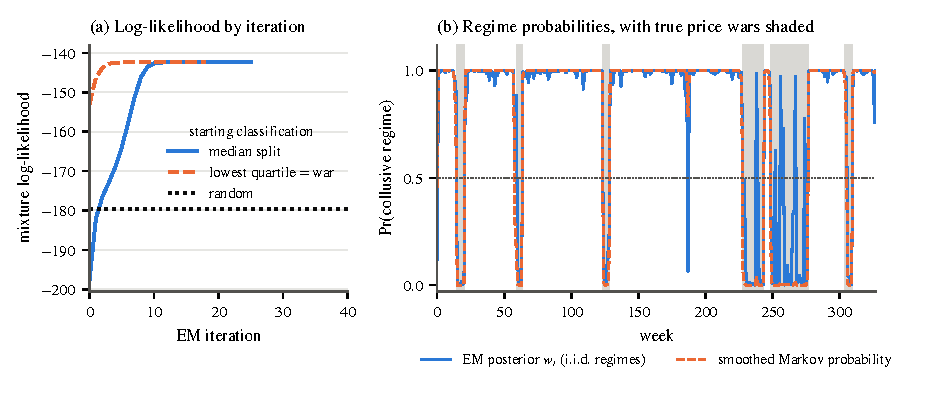
\includegraphics[width=\textwidth]{figures/appA/em_switching.pdf}
\caption[EM and Markov-switching estimation of a simulated two-regime supply relation]{EM and Markov-switching
estimation of a simulated two-regime supply relation. The design is \eqref{eq:A-porter-demand} and
\eqref{eq:A-porter-supply} with $T = 328$, $(\alpha_0, \alpha_1, \alpha_2) = (9.09, -0.80, -0.43)$, $(\beta_0, \beta_1, \beta_2, \beta_3) = (-2.70, 0.09,
-0.20, 0.545)$, one entry dummy, independent errors with standard deviations 0.40 and 0.16, and a Markov regime with
$\Pr(I_{t+1} = 1 \mid I_t = 1) = 0.975$ and $\Pr(I_{t+1} = 1 \mid I_t = 0) = 0.067$. (a) Mixture log-likelihood
by EM iteration from three starting classifications. (b) Posterior probabilities of collusion from the i.i.d.
mixture (EM) and smoothed probabilities from the Markov-switching model estimated by the Hamilton filter. Source:
\texttt{figures/appA/src/em\_switching.py}, seed 20261022.}
\label{fig:A-em}
\end{figure}

\subsubsection*{Hidden Markov models: Ellison's re-estimation}

Porter's i.i.d.\ regimes ignore the persistence of price wars. \citet{Ellison1994} re-estimates the JEC model with two
changes (journal p.~40). First, the demand error follows an AR(1) process, $U_{1t} = \rho U_{1,t-1} + V_{1t}$ with
$\lvert\rho\rvert < 1$, where $\rho$ now denotes an autoregressive coefficient. Second, the regime follows a Markov chain whose
transition probabilities are logits,
\begin{equation}\label{eq:A-ellison-transition}
  \Pr(I_{t+1} = 1 \mid I_t, Z_t) = \frac{e^{\gamma^\T W_t}}{1 + e^{\gamma^\T W_t}},
\end{equation}
where $Z_t$ is the set of predetermined variables at $t$ and $W_t$ contains functions of $I_t$ and of $Z_t$. With $W_t$
equal to a separate constant for each value of $I_t$, the chain is a first-order Markov process. Adding market-share or
demand variables to $W_t$ tests what triggers price wars. Ellison maximizes the joint likelihood of the structural
equations and of the path of transitions.

The likelihood of a hidden Markov model is computed by the filter of \citet{Hamilton1989}. Let $\mathcal{F}_t$ be the data
up to week $t$, and let $h_k(y_t) = f(y_t \mid I_t = k, \mathcal{F}_{t-1})$ be the density of week $t$'s data in regime $k$.
In Ellison's model, $h_k$ is \eqref{eq:A-porter-h} with $U_{1t}$ replaced by $V_{1t} = U_{1t} - \rho U_{1,t-1}$. Write
$p_{k,t} = \Pr(I_{t+1} = 1 \mid I_t = k, Z_t)$, the predicted probability $\xi_{t \mid t-1} = \Pr(I_t = 1 \mid \mathcal{F}_{t-1})$,
and the filtered probability $\xi_{t \mid t} = \Pr(I_t = 1 \mid \mathcal{F}_t)$.

\begin{proposition}[Hamilton filter]\label{prop:A-hamilton}
Suppose $y_t$ depends on the regime history only through $I_t$, given $\mathcal{F}_{t-1}$, and the regime follows
\eqref{eq:A-ellison-transition}. Then for $t = 1, \dots, T$,
\begin{align}
  f(y_t \mid \mathcal{F}_{t-1}) &= \xi_{t \mid t-1}h_1(y_t) + (1 - \xi_{t \mid t-1})h_0(y_t),\label{eq:A-ham-pred}\\
  \xi_{t \mid t} &= \frac{\xi_{t \mid t-1}h_1(y_t)}{f(y_t \mid \mathcal{F}_{t-1})},\label{eq:A-ham-update}\\
  \xi_{t+1 \mid t} &= p_{1,t}\,\xi_{t \mid t} + p_{0,t}\,(1 - \xi_{t \mid t}),\label{eq:A-ham-forecast}
\end{align}
and the log-likelihood is $\ln L = \sum_{t=1}^T\ln f(y_t \mid \mathcal{F}_{t-1})$.
\end{proposition}

\begin{proof}
Equation \eqref{eq:A-ham-pred} is the law of total probability over the two values of $I_t$ given $\mathcal{F}_{t-1}$. Equation
\eqref{eq:A-ham-update} is Bayes' rule, $\Pr(I_t = 1 \mid y_t, \mathcal{F}_{t-1}) = \frac{\Pr(I_t = 1 \mid \mathcal{F}_{t-1})
f(y_t \mid I_t = 1, \mathcal{F}_{t-1})}{f(y_t \mid \mathcal{F}_{t-1})}$. Equation \eqref{eq:A-ham-forecast} again applies the law of
total probability, now over $I_t$ given $\mathcal{F}_t$, using that the transition depends on $\mathcal{F}_t$ only through
$(I_t, Z_t)$. Finally, the joint density of $(y_1, \dots, y_T)$ factors into one-step predictive densities,
$f(y_1, \dots, y_T) = \prod_tf(y_t \mid \mathcal{F}_{t-1})$.
\end{proof}

The recursion needs a starting value $\xi_{1 \mid 0}$, usually the stationary probability $\frac{p_0}{1 - p_1 + p_0}$ when the
transition probabilities are constant. Probabilities that use the whole sample come from a backward pass
\citep{Kim1994}:
\begin{equation*}
  \Pr(I_t = 1 \mid \mathcal{F}_T) = \xi_{t \mid t}\left[p_{1,t}\frac{\Pr(I_{t+1} = 1 \mid \mathcal{F}_T)}{\xi_{t+1 \mid t}} +
  (1 - p_{1,t})\frac{\Pr(I_{t+1} = 0 \mid \mathcal{F}_T)}{1 - \xi_{t+1 \mid t}}\right].
\end{equation*}
In the simulated data of \cref{fig:A-em}, the Markov-switching model estimated by maximizing this likelihood gives
$\Pr(I_{t+1} = 1 \mid I_t = 1) = 0.975$ and $\Pr(I_{t+1} = 1 \mid I_t = 0) = 0.099$, against the true 0.975 and 0.067. The
smoothed probabilities misclassify 5 weeks, against 11 for the i.i.d.\ mixture. Using the persistence of regimes sharpens
the classification of short-lived deviations.

Ellison's estimates (Table 2) give regime constants of 3.675 (.474) after a collusive week and $-2.641$ (.404) after a price
war week. A collusive week is followed by another with probability $\frac{e^{3.675}}{1 + e^{3.675}} = .975$. A price war week
is followed by collusion with probability only $\frac{e^{-2.641}}{1 + e^{-2.641}} = .067$, so wars persist with probability
.933 per week. The implied mean durations are about 40 weeks for collusive spells and 15 weeks for wars, and the stationary
share of collusive weeks is .73 (our computation). Dependence also moves the structural estimates. Allowing AR(1) demand
errors, with $\hat\rho = .832$ (.085), raises the estimated demand elasticity from .84 to 1.80 (journal p.~42). Porter's
approximation to the degree of collusion, $\hat\alpha_1(e^{-\hat\beta_3} - 1)$, rises from .40 to .85. The estimated elasticity is
imprecise, with a standard error of 1.29. The log-likelihood rises from 37.2 to 181.0. If both values are computed on the
same 328 weeks, the implied likelihood ratio statistic for $\rho = 0$ is 287.6 (our computation).

Ellison then adds candidate triggers to $W_t$ in the transition from collusion to war (Table 3). An unusually high market
share for one firm (BIGSHARE1) enters with coefficient $-.77$ (.49), and the unanticipated demand shock $V_{1t}$ with $-4.15$
(2.64). Both have the predicted sign and are significant at about the 6 percent level in one-tailed tests. With only six
price wars in the sample, these tests have little power. \Cref{ch:collusion-evidence} discusses what they imply for the
theories of \citet{GreenPorter1984} and \citet{RotembergSaloner1986}. The econometric point is that joint ML of the regimes,
the transitions and the structural equations uses the timing of every war. A two-step procedure that first classifies weeks
and then regresses the classification on triggers may lose power through misclassification at the onset of wars
(journal p.~39).

\subsection{Non-regular problems}\label{sec:A-mle-nonregular}

The standard theory assumes that the support of the data does not depend on $\theta$, that $\theta_0$ is interior, and that
the likelihood is smooth. Each assumption fails in some IO application, and each failure changes the asymptotics.

\begin{proposition}[Parameter-dependent support]\label{prop:A-uniform-mle}
Let $X_1, \dots, X_n$ be i.i.d.\ uniform on $[0, \theta_0]$. The ML estimator is $\hat\theta = \max_iX_i$, and
\begin{equation*}
  \frac{n(\theta_0 - \hat\theta)}{\theta_0} \xrightarrow{d} \mathrm{Exponential}(1).
\end{equation*}
\end{proposition}

\begin{proof}
The likelihood is $\theta^{-n}\indic\{\theta \ge \max_iX_i\}$, which is zero below the sample maximum and decreasing above it.
So $\hat\theta = \max_iX_i$. For $0 \le t \le n$,
\begin{equation*}
  \Pr\left(\frac{n(\theta_0 - \hat\theta)}{\theta_0} > t\right) = \Pr\left(\max_iX_i < \theta_0\left(1 - \frac{t}{n}\right)\right)
  = \left(1 - \frac{t}{n}\right)^n \to e^{-t}. \qedhere
\end{equation*}
\end{proof}

The estimator converges at rate $n$, faster than $\sqrt{n}$, and its limit is not normal. It is biased downward, with
$\E[\hat\theta] = \frac{n}{n + 1}\theta_0$. The information equality fails because the support moves with $\theta$. The
derivative of $\ln f = -\ln\theta$ is $-\frac{1}{\theta}$, whose mean is not zero. The same structure arises in first-price
auctions, where the upper end of the bid support depends on the parameters of the value distribution.
\citet{DonaldPaarsch1996} develop estimators and tests for this case based on extreme order statistics
(\cref{ch:auction-empirics}). \Cref{prop:A-boot-max} shows that the nonparametric bootstrap fails here.

\begin{proposition}[A parameter on the boundary]\label{prop:A-boundary}
Let $\theta$ be scalar with $\Theta = [0, \infty)$ and $\theta_0 = 0$. Suppose the log-likelihood extends smoothly to a
neighborhood of zero, where the unconstrained maximizer $\hat\theta_u$ satisfies $\sqrt{n}\,\hat\theta_u \xrightarrow{d}
N(0, \mathcal{I}^{-1})$. Then the likelihood ratio statistic for $H_0: \theta = 0$ converges in distribution to an equal mixture
of a point mass at zero and a $\chi^2_1$.
\end{proposition}

\begin{proof}
A second-order expansion around zero, with $\bar s_n(0) = \mathcal{I}\hat\theta_u + o_p(n^{-\frac{1}{2}})$, gives uniformly in
$\theta$ of order $n^{-\frac{1}{2}}$,
\begin{equation*}
  2n\big[\mathcal{L}_n(\theta) - \mathcal{L}_n(0)\big] = n\mathcal{I}\big(2\theta\hat\theta_u - \theta^2\big) + o_p(1).
\end{equation*}
Maximize over $\theta \ge 0$. If $\hat\theta_u > 0$ the maximum is at $\theta = \hat\theta_u$, with value $n\mathcal{I}\hat\theta_u^2$.
If $\hat\theta_u \le 0$ the maximum is at $\theta = 0$, with value zero. So $\mathcal{LR} = (\max\{0, Z_n\})^2 + o_p(1)$ with
$Z_n = \sqrt{n\mathcal{I}}\,\hat\theta_u \xrightarrow{d} N(0, 1)$. Half the time $Z_n \le 0$ and the statistic is zero. Otherwise it is
the square of a standard normal.
\end{proof}

The 5 percent cutoff of this mixture is the 90th percentile of $\chi^2_1$, 2.71, not the usual 3.84
\citep{Chernoff1954, SelfLiang1987, Andrews2001}. Zero variances of random coefficients and zero regime probabilities are
boundary nulls of this kind. Testing the number of regimes is harder still. In Porter's model \eqref{eq:A-mixture} the
null of a single regime can be written in two ways. If $\lambda = 0$, then $\lambda$ lies on the boundary and $\beta_3$ is
not identified, because it multiplies a regime that never occurs. The case $\lambda = 1$ is symmetric. Then $I_t = 1$ in every
week, so $\beta_3$ cannot be separated from the intercept $\beta_0$. If $\beta_3 = 0$, the two mixture components coincide,
and $\lambda$ is not identified. In both cases a parameter is identified only under the alternative. The likelihood ratio
then has no $\chi^2$ limit \citep{Davies1977}, and \citet{Hansen1992} develops bounds for Markov-switching models.

Porter's own test shows the problem at work. He maximizes the likelihood once with switching and once subject to
$\Delta = 0$, which in \eqref{eq:A-porter-supply} means $\beta_3 = 0$. Let $\bar L_1$ and $\bar L_0$ be the two maximized
average log-likelihoods. He reports $2T(\bar L_1 - \bar L_0) = 554.1$, refers it to a $\chi^2_1$ distribution, and
rejects ``the hypothesis that no switch occurred'' (journal p.~312). Under $\Delta = 0$ the mixture density
$\lambda h(y_t \mid 1) + (1 - \lambda)h(y_t \mid 0)$ equals $h(y_t \mid 0)$ for every $\lambda$. The restricted
likelihood is therefore flat in $\lambda$, and the unrestricted fit chooses $\lambda$ and $\beta_3$ together. The
statistic is the largest of a family of likelihood ratios indexed by $\lambda$. Its null distribution is stochastically
larger than $\chi^2_1$, and the $\chi^2_1$ reference is invalid. The size of the statistic still settles the question in
practice. The 0.1 percent cutoff of $\chi^2_1$ is 10.83, and 554.1 is about fifty times larger, so the rejection very
likely survives any valid correction. Porter also notes that $\hat\beta_3$ is significantly positive (journal p.~311). A
$t$ test of $\beta_3 = 0$ faces the same difficulty, because it is computed at an estimate $\hat\lambda$ that has no
limit under the null.

A discontinuous likelihood is the third failure. \citet{Bresnahan1987} solves the vertical model for equilibrium prices
and quantities, adds independent normal errors to observed prices and quantities, and maximizes the resulting likelihood
(\cref{sec:06-bres-estimation}). The likelihood jumps when two products swap positions in the quality ordering. The derivative-based expansion of \cref{thm:A-asy-normal}
is unavailable at the jumps. Estimation then relies on derivative-free search, and asymptotic theory requires the true
parameter to lie away from the discontinuities.

\subsection{Non-nested tests}\label{sec:A-nonnested}

Two models are \emph{non-nested} when neither is a special case of the other. Collusion and Bertrand pricing with the same
demand system are an example (\cref{sec:06-bres-cox}). The likelihood ratio does not have a $\chi^2$ distribution in this
case, and its sign alone is uninformative. Two approaches are standard.

Let model $F$ have density $f(y \mid x;\theta)$ and model $G$ density $g(y \mid x;\gamma)$, with ML estimates $\hat\theta$ and
$\hat\gamma$. Write the pointwise log-likelihood ratio as $d_i = \ln f(y_i \mid x_i;\hat\theta) - \ln g(y_i \mid x_i;\hat\gamma)$
and $LR_n = \sum_id_i$.

The test of \citet{Cox1961, Cox1962} takes $F$ as the null. If $F$ is true with parameter $\theta$, the estimator
$\hat\gamma$ converges to a pseudo-true value $\gamma(\theta)$, and $\frac{1}{n}LR_n$ converges to
$\E_\theta[\ln f(y \mid x;\theta) - \ln g(y \mid x;\gamma(\theta))]$. Cox's statistic centers $LR_n$ by a consistent estimate of
this expectation, computed under $F$ at $\hat\theta$, and divides by an estimate of its standard deviation. Under $F$ it is
asymptotically standard normal. A large negative value says that $G$ fits better than $F$ would lead us to expect. The roles
are then reversed. There are four possible outcomes: reject neither, reject one of the two, or reject both. Rejecting both is
informative, because it says that neither model is adequate. \Cref{prop:06-bres-cox} gives the statistic for nonlinear
regressions with normal errors, and \cref{tab:06-bres-cox} reports Bresnahan's tests of conduct in the 1955 automobile market.

The test of \citet{Vuong1989} treats the models symmetrically. It asks which model is closer to the truth in
Kullback-Leibler divergence.

\begin{proposition}[Vuong's model selection test]\label{prop:A-vuong}
Let $\theta^*$ and $\gamma^*$ be the pseudo-true values of the two models. Suppose $\Pr\{f(y \mid x;\theta^*) \ne g(y \mid
x;\gamma^*)\} > 0$, so that the models are strictly non-nested, and let $\hat\omega^2 = \frac{1}{n}\sum_i(d_i - \bar d)^2$ with
$\bar d = \frac{1}{n}LR_n$. Under $H_0: \E[\ln f(y \mid x;\theta^*) - \ln g(y \mid x;\gamma^*)] = 0$ and standard regularity
conditions,
\begin{equation*}
  T_V = \frac{\sqrt{n}\,\bar d}{\hat\omega} \xrightarrow{d} N(0, 1).
\end{equation*}
\end{proposition}

\begin{proof}[Proof sketch]
Let $\bar d^* = \frac{1}{n}\sum_i[\ln f(y_i \mid x_i;\theta^*) - \ln g(y_i \mid x_i;\gamma^*)]$. Expand $\bar d$ around the
pseudo-true values. The first-order term in $\theta$ is $\bar s^f_n(\theta^*)^\T(\hat\theta - \theta^*)$, where $\bar s^f_n$ is the
average score of model $F$. Its expectation at $\theta^*$ is zero because $\theta^*$ maximizes $\E\ln f$. So $\bar s^f_n(\theta^*) =
O_p(n^{-\frac{1}{2}})$, and with $\hat\theta - \theta^* = O_p(n^{-\frac{1}{2}})$ the product is $O_p(n^{-1})$. The same holds for
$\gamma$. Hence $\sqrt{n}\,\bar d = \sqrt{n}\,\bar d^* + o_p(1)$. Under $H_0$, $\bar d^*$ is an average of i.i.d.\ terms with mean
zero and variance $\omega^2 > 0$, the latter by strict non-nestedness. The central limit theorem and $\hat\omega \xrightarrow{p}
\omega$ finish the argument.
\end{proof}

A large positive $T_V$ favors $F$, a large negative one favors $G$, and a value near zero says the data cannot tell the
models apart. If the models overlap, so that $\omega^2 = 0$, the statistic has a different limit, and Vuong gives a separate
procedure. \citet{RiversVuong2002} extend the test to general estimation criteria, including GMM, which makes it usable for
comparing conduct models estimated from moment conditions.

\subsection{Testing a parametric distribution}\label{sec:A-ck-test}

Parametric models of bids or values are convenient, but their shape restrictions drive the results. A specification test
for the whole conditional distribution is then valuable. The Kolmogorov-Smirnov statistic $\sup_y\sqrt{n}\lvert F_n(y) -
F(y;\hat\theta)\rvert$ compares the empirical and fitted distribution functions. With estimated parameters its null
distribution depends on the model, so tables computed for a known $F$ are wrong, and the cutoff must be simulated.

\citet{Andrews1997} extends the idea to a conditional distribution. Let $Z_i = (Y_i, X_i)$, with $Y_i$ the endogenous
outcomes and $X_i$ the exogenous covariates, and let the model specify $F(y \mid x;\theta)$. Define the empirical
distribution function of $Z$ and a semiparametric estimate of it that uses the model for $Y$ given $X$ and the empirical
distribution of $X$:
\begin{equation*}
  H_n(y, x) = \frac{1}{n}\sum_{i=1}^n\indic\{Y_i \le y, X_i \le x\}, \qquad
  F_n(y, x;\theta) = \frac{1}{n}\sum_{i=1}^nF(y \mid X_i;\theta)\indic\{X_i \le x\}.
\end{equation*}
The \emph{conditional Kolmogorov} statistic is $CK_n = \max_{j \le n}\sqrt{n}\,\lvert H_n(Z_j) - F_n(Z_j;\hat\theta)\rvert$. Its
null distribution is obtained by a parametric bootstrap.
\begin{enumerate}
  \item Estimate $\hat\theta$ and compute $CK_n$.
  \item For $b = 1, \dots, B$, draw $Y_i^{*} \sim F(\cdot \mid X_i;\hat\theta)$ for each $i$, holding the covariates fixed.
  Re-estimate $\hat\theta^{*}$ on the simulated sample and compute $CK_n^{*}$.
  \item Reject at level $a$ if $CK_n$ exceeds the $(1 - a)$ quantile of $CK_n^{*1}, \dots, CK_n^{*B}$.
\end{enumerate}
Re-estimating $\theta$ in each replication accounts for the fact that the fitted model is closer to the data than the true
model would be.

\citet[journal p.~241]{AtheyLevinSeira2011} apply the test to their Gamma-Weibull model. The exogenous covariates are the sale
characteristics $(X, N)$ and the endogenous variables are the bids. They cannot reject the parametric specification even at
the 20 percent level, in both the Northern and the California sales. Together with the close fit of the bid moments reported
above, this supports using the fitted bid distributions to recover values and entry costs (\cref{ch:auction-empirics}).

\section{Simulation-based estimation}\label{sec:A-simulation}

The GMM and likelihood theory of \cref{sec:A-gmm,sec:A-mle} assumes that we can evaluate the moment function or the
density at any trial parameter. Many structural models in industrial organization imply moments or likelihoods that
are integrals with no closed form. The market share of a product in a random coefficients model integrates individual logit probabilities over
the distribution of tastes (\cref{ch:blp}). The expected winning bid in a first-price auction is the expected
second-highest value, an integral over the joint distribution of all bidders' values
\citep{LaffontOssardVuong1995}. The expected profit of an entrant integrates over values, rivals and bids
\citep{AtheyLevinSeira2011}. A counterfactual auction outcome is an expectation over simulated auctions
\citep{Asker2010}. This section shows how such integrals are replaced by averages over random draws and what the
replacement does to the properties of the estimator. The answer depends on how the simulated integral enters the
objective. When it enters linearly, as in a moment condition, simulation adds variance but no bias. When it enters
through a nonlinear function, such as a logarithm, it adds bias that vanishes only as the number of draws grows.

Throughout the section $\theta$ is a generic parameter vector, $n$ is the number of observations and $n_s$ is the
number of simulation draws per observation (the notation of \cref{ch:blp}). Several papers write $S$ for $n_s$, and
we translate their formulas.

\subsection{Monte Carlo integration}\label{sec:A-mc-integration}

Let $\nu$ be a random vector with known distribution $F$, which may depend on $\theta$ only through a known
transformation of standardized draws. The target is an expectation
\begin{equation}\label{eq:A-mc-target}
  \phi(\theta) = \E_\nu\bigl[q(\nu;\theta)\bigr] = \int q(\nu;\theta)\,\dd F(\nu),
\end{equation}
for a function $q$ that we can evaluate at any $(\nu, \theta)$. The \emph{Monte Carlo simulator} of $\phi(\theta)$
averages $q$ over $n_s$ independent draws $\nu_1, \dots, \nu_{n_s}$ from $F$:
\begin{equation}\label{eq:A-mc-simulator}
  \tilde\phi(\theta) = \frac{1}{n_s}\sum_{r=1}^{n_s} q(\nu_r;\theta).
\end{equation}

\begin{proposition}[Monte Carlo integration]\label{prop:A-mc}
Suppose $\sigma_q^2(\theta) = \Var_\nu(q(\nu;\theta))$ is finite. Then
\begin{enumerate}[label=(\roman*)]
  \item $\E[\tilde\phi(\theta)] = \phi(\theta)$, so the simulator is unbiased.
  \item $\Var(\tilde\phi(\theta)) = \frac{\sigma_q^2(\theta)}{n_s}$.
  \item $\sqrt{n_s}\,(\tilde\phi(\theta) - \phi(\theta)) \xrightarrow{d} N(0, \sigma_q^2(\theta))$ as $n_s \to \infty$.
\end{enumerate}
The simulation error is $O_p(n_s^{-\frac{1}{2}})$ whatever the dimension of $\nu$.
\end{proposition}

\begin{proof}
The draws are independent and identically distributed, so each term of \eqref{eq:A-mc-simulator} has mean
$\phi(\theta)$ and variance $\sigma_q^2(\theta)$. Linearity of expectation gives (i). Independence gives
\begin{equation*}
  \Var\bigl(\tilde\phi(\theta)\bigr) = \frac{1}{n_s^2}\sum_{r=1}^{n_s}\Var\bigl(q(\nu_r;\theta)\bigr)
  = \frac{n_s\,\sigma_q^2(\theta)}{n_s^2} = \frac{\sigma_q^2(\theta)}{n_s}.
\end{equation*}
Part (iii) is the Lindeberg-L\'evy central limit theorem. The dimension of $\nu$ enters only through
$\sigma_q^2$, which proves the last claim.
\end{proof}

The last statement explains why simulation dominates deterministic rules in high dimensions. A product quadrature
rule with $m$ nodes per dimension needs $m^d$ function evaluations in $d$ dimensions, while the accuracy of
\eqref{eq:A-mc-simulator} depends on $n_s$ alone. Quadrature and quasi-Monte Carlo sequences can be far more accurate
in one to three dimensions, and \cref{sec:08-quadrature} compares them for market shares.

\casehead{Uses in the book}
Four kinds of integrals recur. First, the random coefficients share $s_{jt} = \int s_{ijt}\,\dd F(\nu_i)$ is simulated
by averaging individual logit probabilities over draws of tastes (\cref{sec:08-simulation}). Second,
\citet{LaffontOssardVuong1995} simulate the expected winning bid of a first-price auction
(\cref{sec:A-snlls}). Third, \citet[p.~245]{AtheyLevinSeira2011} compute the expected profit of a logger or a mill
in a sealed-bid timber sale by simulation. They simulate 5,000 auctions for each plausible number of entering
loggers and mills, up to 8 mills and 25 loggers. Fourth, \citet{Asker2010} computes damages and efficiency losses from 100,000 auctions
simulated from estimated value distributions (\cref{sec:13-asker}).

\casehead{Smooth and frequency simulators}
When $q$ is an indicator, for example the indicator that a simulated consumer chooses product $j$, the simulator
\eqref{eq:A-mc-simulator} is a \emph{frequency simulator}. It is a step function of $\theta$ and can equal zero.
When part of the integral has a closed form, we can integrate it analytically and simulate only the rest. In logit
models the extreme value shocks are integrated exactly, and $q$ becomes a choice probability. The result is a
\emph{smooth simulator}. It is differentiable in $\theta$, strictly positive, and has smaller variance because
conditioning removes the variance of the integrated part (\cref{lem:08-smooth}).

\casehead{Common random numbers}
An estimator that uses simulated integrals evaluates them at many trial values of $\theta$. The draws must be taken
once, before estimation, and held fixed across all evaluations. With fresh draws at each evaluation the objective
function becomes a different random function every time it is computed. It is then discontinuous in $\theta$, and a
numerical optimizer never converges. With fixed draws the simulated objective is a single deterministic function
of $\theta$, so the draws can be treated as part of the data. Fixing the draws does not make that function smooth.
It is smooth when the simulator is smooth, while a frequency simulator remains a step function of $\theta$. The asymptotic theory below
treats the draws as part of the data. The practical rule ``take the draws only once'' is therefore part of the definition of the estimator.

\casehead{Importance sampling}
Draws from $F$ can be wasteful when $q$ is large only on a small region of the support. \emph{Importance sampling}
draws from another density $g$ and reweights. Let $f$ be the density of $\nu$ and write
\begin{equation*}
  \phi = \int q(\nu)\,f(\nu)\,\dd\nu = \int q(\nu)\,\frac{f(\nu)}{g(\nu)}\,g(\nu)\,\dd\nu
  = \E_g\Bigl[q(\nu)\,\frac{f(\nu)}{g(\nu)}\Bigr].
\end{equation*}
The ratio $w(\nu) = \frac{f(\nu)}{g(\nu)}$ is the \emph{importance weight}, and the importance sampling simulator is
\begin{equation}\label{eq:A-importance}
  \tilde\phi_g = \frac{1}{n_s}\sum_{r=1}^{n_s} q(\nu_r)\,w(\nu_r), \qquad \nu_r \overset{\text{i.i.d.}}{\sim} g.
\end{equation}

\begin{lemma}[Importance sampling]\label{lem:A-importance}
Suppose $g(\nu) > 0$ wherever $q(\nu)f(\nu) \ne 0$. Then
\begin{enumerate}[label=(\roman*)]
  \item $\E_g[\tilde\phi_g] = \phi$.
  \item $\Var_g(\tilde\phi_g) = \frac{1}{n_s}\Bigl[\int\frac{q(\nu)^2f(\nu)^2}{g(\nu)}\,\dd\nu - \phi^2\Bigr]$.
  \item The variance is minimized by $g^*(\nu) = \frac{|q(\nu)|f(\nu)}{\int|q(u)|f(u)\,\dd u}$. If $q \ge 0$, the
  minimum variance is zero.
\end{enumerate}
\end{lemma}

\begin{proof}
Part (i) is the change of measure displayed above. For (ii), each term has second moment
\begin{equation*}
  \E_g\bigl[q(\nu)^2w(\nu)^2\bigr] = \int q(\nu)^2\,\frac{f(\nu)^2}{g(\nu)^2}\,g(\nu)\,\dd\nu
  = \int\frac{q(\nu)^2f(\nu)^2}{g(\nu)}\,\dd\nu,
\end{equation*}
and its mean is $\phi$. Subtracting $\phi^2$ and dividing by $n_s$ gives (ii). For (iii), only the integral in (ii)
depends on $g$. The Cauchy-Schwarz inequality gives
\begin{equation*}
  \Bigl(\int|q|f\,\dd\nu\Bigr)^2 = \Bigl(\int\frac{|q|f}{\sqrt g}\,\sqrt g\,\dd\nu\Bigr)^2
  \le \int\frac{q^2f^2}{g}\,\dd\nu\cdot\int g\,\dd\nu = \int\frac{q^2f^2}{g}\,\dd\nu,
\end{equation*}
with equality when $\frac{|q|f}{\sqrt g}$ is proportional to $\sqrt g$, that is, when $g \propto |q|f$. If $q \ge 0$,
the bound equals $\phi^2$ and the variance in (ii) is zero.
\end{proof}

The optimal density $g^*$ is infeasible because its normalizing constant is $\phi$ itself. The lemma still guides
practice. A good importance density is close to proportional to $|q|f$. The variance in (ii) is finite exactly when
$\int\frac{q^2f^2}{g}\,\dd\nu < \infty$. This holds whenever the ratio $\frac{|q|f}{g}$ is bounded, since the integral
is then at most $\sup_\nu\frac{|q(\nu)|f(\nu)}{g(\nu)}\int|q|f\,\dd\nu$. A density $g$ with tails at least as heavy as
those of $|q|f$ is therefore the safe choice. Thinner tails can make the integral diverge, and then a few draws with
huge weights dominate the average. They need not do so. With $q = 1$, $f$ standard normal and $g$ normal with
variance $s^2$, the integral equals $\frac{s^2}{\sqrt{2s^2 - 1}}$, which is finite for every $s^2 > \frac{1}{2}$.
For $\frac{1}{2} < s^2 < 1$ the density $g$ has thinner tails than $f$, and the variance is still finite.
Importance sampling has a second advantage in estimation. If $\theta$ enters only through the weight
$\frac{f(\nu;\theta)}{g(\nu)}$ and the draws come from a fixed $g$, then the simulator is as smooth in $\theta$ as $f$.

Three applications in the book use it. \citet[pp.~960--961, 969]{LaffontOssardVuong1995} draw values from a
log-normal importance density centered at a preliminary estimate, and $\theta$ appears only in the density ratio
(\cref{sec:A-snlls}). \citet[p.~732, n.~31]{Gentzkow2007} draws each consumer's random effects from their
distribution conditional on the observed choices, computed at a preliminary estimate. That density is the posterior
of $\nu$ given the data, the analogue of $g^* \propto qf$ for a likelihood contribution. \citet[Section~6.3]{BerryLevinsohnPakes1995}
over-sample households likely to buy a new car, since most households buy none in a given year
(\cref{sec:08-importance}).

\begin{remark}[Sampling error versus simulation error]\label{rem:A-sampling-error}
Simulation error comes from the econometrician's draws and can be made small by raising $n_s$. Sampling error in
the data cannot. If an observed market share is the fraction of $M$ sampled consumers who buy a product, its
sampling standard deviation is about $\sqrt{\frac{s(1 - s)}{M}}$. In airline ticket samples with fewer than ten sampled
passengers per product, this error is large and is not removed by any number of simulation draws
(\cref{sec:09-bcs-estimation}). \Cref{sec:08-asymptotics} shows how \citet{BerryLevinsohnPakes1995} separate the
two sources in the asymptotic variance.
\end{remark}

\subsection{The method of simulated moments}\label{sec:A-msm}

The \emph{method of simulated moments} (MSM) of \citet{McFadden1989} and \citet{PakesPollard1989} replaces an
intractable conditional mean in a moment condition by an unbiased simulator. We state the leading case, a
conditional mean restriction. The data $w_i = (y_i, x_i)$ are i.i.d.\ across $i$, and
\begin{equation}\label{eq:A-msm-model}
  \E[y_i \mid x_i] = m(x_i;\theta_0), \qquad m(x;\theta) = \int q(x, \nu;\theta)\,\dd F(\nu).
\end{equation}
For example, $y_i$ may be a vector of choice indicators and $q$ the vector of logit probabilities given tastes
$\nu$. Let $z_i = z(x_i)$ be an $L \times \dim(y)$ matrix of instruments, functions of $x_i$. For each observation
we draw $\nu_{i1}, \dots, \nu_{in_s}$ from $F$, independently across $i$ and of the data, and form
\begin{equation}\label{eq:A-msm-sim}
  \tilde m_i(\theta) = \frac{1}{n_s}\sum_{r=1}^{n_s} q(x_i, \nu_{ir};\theta), \qquad
  \tilde g_n(\theta) = \frac{1}{n}\sum_{i=1}^{n} z_i\bigl(y_i - \tilde m_i(\theta)\bigr).
\end{equation}
The MSM estimator minimizes $\tilde g_n(\theta)^\top W_n\,\tilde g_n(\theta)$. Write $e_i = y_i - m(x_i;\theta_0)$
for the structural error and $\eta_i = \tilde m_i(\theta_0) - m(x_i;\theta_0)$ for the simulation error. Define
\begin{equation*}
  \Sigma_y(x) = \Var(y \mid x), \qquad V(x) = \Var_\nu\bigl(q(x, \nu;\theta_0)\bigr), \qquad
  G = -\E\Bigl[z_i\,\frac{\partial m(x_i;\theta_0)}{\partial\theta^\top}\Bigr].
\end{equation*}

\begin{proposition}[Method of simulated moments]\label{prop:A-msm}
Assume the conditions of \cref{thm:A-gmm-normal} for the GMM estimator with exact moments. Let $\nu$ be one draw from
$F$, independent of $(x_i, y_i)$, and let $\mathcal{N}$ be a closed neighborhood of $\theta_0$. Assume also that the
simulated moments satisfy the following conditions.
\begin{enumerate}[label=(\alph*)]
  \item $q(x, \nu;\theta)$ is continuous in $\theta$ on $\Theta$, and
  $\E\bigl[\sup_{\theta \in \Theta}\lVert z_i\,q(x_i, \nu;\theta)\rVert\bigr] < \infty$.
  \item $S_{\text{sim}} = \E[z_iV(x_i)z_i^\top]$ is finite.
  \item $q(x, \nu;\theta)$ is continuously differentiable in $\theta$ on $\mathcal{N}$, and
  $\E\bigl[\sup_{\theta \in \mathcal{N}}\bigl\lVert z_i\frac{\partial q(x_i, \nu;\theta)}{\partial\theta^\top}\bigr\rVert\bigr]
  < \infty$.
\end{enumerate}
Let $n_s$ be fixed and $W_n \xrightarrow{p} W$.
\begin{enumerate}[label=(\roman*)]
  \item The MSM estimator is consistent as $n \to \infty$.
  \item $\sqrt n(\hat\theta - \theta_0) \xrightarrow{d} N\bigl(0, (G^\top WG)^{-1}G^\top W\bigl[S + \tfrac{1}{n_s}S_{\text{sim}}\bigr]WG(G^\top WG)^{-1}\bigr)$,
  where $S = \E[z_i\Sigma_y(x_i)z_i^\top]$.
  \item If $V(x) \le \Sigma_y(x)$ for all $x$ in the positive semidefinite order, the asymptotic variance is at most
  $(1 + \frac{1}{n_s})$ times that of GMM with exact moments and the same $W$. The bound holds with equality for a
  frequency simulator of choice indicators.
\end{enumerate}
\end{proposition}

\begin{proof}
For (i), the summands of $\tilde g_n(\theta)$ are i.i.d.\ across $i$ because the data and the draws are. The simulator is
unbiased and the draws are independent of $y_i$, so $\E[\tilde m_i(\theta) \mid x_i, y_i] = m(x_i;\theta)$. Hence
\begin{equation*}
  \E\bigl[z_i(y_i - \tilde m_i(\theta))\bigr] = \E\bigl[z_i(y_i - m(x_i;\theta))\bigr]
  = \E\bigl[z_i\bigl(m(x_i;\theta_0) - m(x_i;\theta)\bigr)\bigr].
\end{equation*}
The population moment of the simulated estimator is the population moment of exact GMM. It is zero only at
$\theta_0$ by the identification condition. The uniform law of large numbers of \cref{lem:A-ulln} applies under
condition (a), and \cref{thm:A-consistency} gives consistency.

For (ii), evaluate the simulated moment at $\theta_0$:
\begin{equation*}
  \tilde g_n(\theta_0) = \frac{1}{n}\sum_{i=1}^{n} z_i\bigl[(y_i - m(x_i;\theta_0)) - (\tilde m_i(\theta_0) - m(x_i;\theta_0))\bigr]
  = \frac{1}{n}\sum_{i=1}^{n} z_i(e_i - \eta_i).
\end{equation*}
The summands are i.i.d.\ with mean zero. Conditional on $(x_i, y_i)$, $\eta_i$ has mean zero and variance
$\frac{1}{n_s}V(x_i)$ by \cref{prop:A-mc}, so $\E[z_i\eta_i\eta_i^\top z_i^\top] = \frac{1}{n_s}S_{\text{sim}}$, which is
finite by condition (b). The cross term vanishes:
\begin{equation*}
  \E\bigl[z_ie_i\eta_i^\top z_i^\top\bigr] = \E\bigl[z_ie_i\,\E[\eta_i \mid x_i, y_i]^\top z_i^\top\bigr] = 0.
\end{equation*}
Hence
\begin{equation*}
  \Var\bigl(z_i(e_i - \eta_i)\bigr) = \E[z_ie_ie_i^\top z_i^\top] + \E[z_i\eta_i\eta_i^\top z_i^\top]
  = S + \frac{1}{n_s}S_{\text{sim}},
\end{equation*}
and the Lindeberg-L\'evy central limit theorem gives $\sqrt n\,\tilde g_n(\theta_0) \xrightarrow{d} N(0, S +
\frac{1}{n_s}S_{\text{sim}})$. Condition (c) allows differentiation under the integral, so
$\E_\nu\bigl[\frac{\partial q}{\partial\theta^\top}\bigr] = \frac{\partial m}{\partial\theta^\top}$. The same
unbiasedness argument and \cref{lem:A-ulln}, applied on $\mathcal{N}$ to $z_i\frac{\partial q}{\partial\theta^\top}$,
show that the simulated Jacobian $\frac{\partial\tilde g_n}{\partial\theta^\top}$ converges uniformly to the exact one.
The mean value expansion in the proof of \cref{thm:A-gmm-normal} then applies unchanged.

For (iii), write
\begin{equation*}
  S + \frac{1}{n_s}S_{\text{sim}} = \Bigl(1 + \frac{1}{n_s}\Bigr)S - \frac{1}{n_s}\E\bigl[z_i(\Sigma_y(x_i) - V(x_i))z_i^\top\bigr].
\end{equation*}
The last expectation is positive semidefinite when $\Sigma_y \ge V$. Pre- and post-multiplying by
$(G^\top WG)^{-1}G^\top W$ and its transpose preserves the order. For a frequency simulator of a choice indicator,
$q$ is itself an indicator with $\Var_\nu(q \mid x) = \Sigma_y(x)$, so $V = \Sigma_y$.
\end{proof}

Condition (b) does not follow from the conditions for exact moments. Let $z_i = 1$, $y_i = \theta_0 + e_i$ with
$e_i$ standard normal, and $q(\nu;\theta) = \theta + \nu$ with $\nu$ a centered Student $t$ variable with 1.5 degrees
of freedom. Then $m(\theta) = \theta$, exact GMM satisfies \cref{thm:A-gmm-normal}, and conditions (a) and (c)
hold on a compact $\Theta$. The MSM estimator is
$\hat\theta = \bar y - \bar\nu$, with $\bar\nu$ the average of all $nn_s$ draws, and it is consistent. Since $\nu$ has
infinite variance, $\sqrt n(\hat\theta - \theta_0)$ has no normal limit. For simulated choice probabilities, $q$ lies in
$[0, 1]$, so the moment bounds in (a) and (b) hold whenever $\E\lVert z_i\rVert^2 < \infty$.

A frequency simulator is a step function of $\theta$, so it violates conditions (a) and (c). For such simulators,
\citet{PakesPollard1989} prove (i) and (ii) under \emph{stochastic equicontinuity}. This condition requires the
centered simulated moment $\tilde g_n(\theta) - \E[\tilde g_n(\theta)]$ to change by $o_p(n^{-\frac{1}{2}})$ over
shrinking neighborhoods of $\theta_0$. Smoothness is then needed only for the exact moment $m$, and the comparison in
(iii) applies unchanged.

The condition $V \le \Sigma_y$ holds for the smooth logit simulator. The smooth simulator is the conditional
expectation of the frequency simulator given the taste draw, so its variance is smaller by the law of total
variance (\cref{lem:08-smooth}). The factor $(1 + \frac{1}{n_s})$ is therefore an upper bound on the price of
simulation. With 10 draws per observation it is a 10 percent increase in variance, about 5 percent in standard
errors.

Two departures from the setting of the proposition are common in industrial organization. First, in market-level
demand estimation the draws are shared by all products in a market, and the number of markets or products drives
the asymptotics. The simulation error then adds a separate term to the variance of the moments, $V_3$ in
\citet{BerryLevinsohnPakes1995}. Their correction raised the reported standard errors by about 5 to 20 percent,
and one standard error doubled (p.~859, see \cref{sec:08-asymptotics}). Second, the simulated integral often enters
nonlinearly. The BLP inversion uses the logarithm of simulated shares, and $\E[\ln\tilde s] < \ln s$ by Jensen's
inequality. The bias is of order $\frac{1}{n_s}$ and does not average out across markets (\cref{prop:08-simbias}).
Consistency then requires $n_s$ to grow with the sample, exactly as for simulated maximum likelihood below.

MSM has two practical costs. Efficient MSM requires the optimal instruments of \cref{sec:A-optimal-iv}, which depend on
the unknown parameters and are computed from a preliminary estimate. When that estimate is poor, efficiency can be
poor as well \citep[pp.~43--44]{GourierouxMonfort1996}. In addition, moments for discrete outcomes require the
simulated probability of every possible outcome, which is expensive when the outcome space is large. Both points
led \citet[p.~732]{Gentzkow2007} to prefer simulated maximum likelihood.

\subsection{Simulated maximum likelihood}\label{sec:A-sml}

Let $(y_i, x_i)$ be i.i.d.\ across $i$, and let the density of $y_i$ given $x_i$ be a mixture over unobserved
heterogeneity,
\begin{equation*}
  f(y_i \mid x_i;\theta) = \int f(y_i \mid x_i, \nu;\theta)\,\dd F(\nu).
\end{equation*}
\emph{Simulated maximum likelihood} (SML), introduced by \citet{LermanManski1981}, maximizes
$\sum_i\ln\tilde f_i(\theta)$ with
\begin{equation}\label{eq:A-sml}
  \tilde f_i(\theta) = \frac{1}{n_s}\sum_{r=1}^{n_s} f_{ir}(\theta), \qquad
  f_{ir}(\theta) = f(y_i \mid x_i, \nu_{ir};\theta).
\end{equation}
The draws $\nu_{ir}$ come from $F$, independently across $i$ and $r$ and of the data. The simulator $\tilde f_i$ is
therefore unbiased for $f_i = f(y_i \mid x_i;\theta)$, but it enters through the logarithm.

\begin{proposition}[Bias of simulated maximum likelihood]\label{prop:A-sml-bias}
Let $v_i(\theta) = \Var_\nu(f(y_i \mid x_i, \nu;\theta))$, so that $\Var(\tilde f_i \mid x_i, y_i) =
\frac{v_i}{n_s}$. Assume the following.
\begin{enumerate}[label=(\alph*)]
  \item There are constants $0 < \underline{c} \le \bar c < \infty$ with $\underline{c} \le f(y \mid x, \nu;\theta) \le
  \bar c$ for all $(y, x, \nu, \theta)$. Choice probabilities satisfy the upper bound with $\bar c = 1$.
  \item $f(y \mid x, \nu;\theta)$ is twice continuously differentiable in $\theta$, with first and second derivatives
  bounded uniformly in $(y, x, \nu, \theta)$.
  \item $\Theta$ is compact, $\theta_0$ is interior and is the unique maximizer of $Q(\theta) = \E[\ln f_i(\theta)]$,
  and the Hessian $H$ of $Q$ at $\theta_0$ is nonsingular. For each $n_s$ the function $\E[\ln\tilde f_i(\theta)]$ has
  a unique maximizer $\theta_{n_s}$.
  \item The conditions of \cref{thm:A-mle-normal} hold for exact maximum likelihood.
\end{enumerate}
Then the following hold.
\begin{enumerate}[label=(\roman*)]
  \item Under (a), $\E\bigl[\ln\tilde f_i \mid x_i, y_i\bigr] = \ln f_i - \frac{1}{2}\,\frac{v_i}{n_sf_i^2} +
  O(n_s^{-\frac{3}{2}})$.
  \item Under (a) to (c), for fixed $n_s$ the SML estimator converges in probability to $\theta_{n_s}$. With
  $D(\theta) = \E\bigl[\frac{v_i(\theta)}{2f_i(\theta)^2}\bigr]$,
  $\theta_{n_s} - \theta_0 = \frac{1}{n_s}H^{-1}\nabla D(\theta_0) + o(\frac{1}{n_s})$ as $n_s \to \infty$. If
  $\nabla D(\theta_0) \ne 0$, then $\theta_{n_s} \ne \theta_0$ for all large $n_s$, and SML with any such fixed $n_s$
  is inconsistent.
  \item Under (a) to (d), if $n_s \to \infty$ and $\frac{\sqrt n}{n_s} \to 0$, then $\sqrt n(\hat\theta - \theta_0)
  \xrightarrow{d} N(0, \mathcal{I}^{-1})$, the limit of exact maximum likelihood.
\end{enumerate}
\end{proposition}

\begin{proof}
For (i), expand $\ln\tilde f_i$ around $f_i$ to third order with the Lagrange remainder:
\begin{equation*}
  \ln\tilde f_i = \ln f_i + \frac{\tilde f_i - f_i}{f_i} - \frac{(\tilde f_i - f_i)^2}{2f_i^2}
  + \frac{(\tilde f_i - f_i)^3}{3\bar f_i^3},
\end{equation*}
where $\bar f_i$ lies between $\tilde f_i$ and $f_i$, so $\bar f_i \ge \underline{c}$ by (a). The linear term has
conditional mean zero. The quadratic term has conditional mean $-\frac{v_i}{2n_sf_i^2}$. For the remainder, write
$\tilde f_i - f_i = \frac{1}{n_s}\sum_r d_r$ with $d_r = f_{ir} - f_i$. The $d_r$ are independent with mean zero and
$\lvert d_r\rvert \le \bar c$ by (a), so expanding the fourth power gives
\begin{equation*}
  \E\bigl[(\tilde f_i - f_i)^4 \mid x_i, y_i\bigr] = \frac{n_s\E[d_r^4] + 3n_s(n_s - 1)v_i^2}{n_s^4} \le
  \frac{3\bar c^4}{n_s^2}.
\end{equation*}
By Lyapunov's inequality the expected absolute cube is at most $(\frac{3\bar c^4}{n_s^2})^{\frac{3}{4}} =
O(n_s^{-\frac{3}{2}})$, so the expected absolute value of the remainder is at most this bound divided by $3\underline{c}^3$. The bound
holds uniformly in $i$ and $\theta$. The argument is the one in the proof of \cref{prop:08-simbias}.

For (ii), the simulated log-likelihood is an average of i.i.d.\ terms, each between $\ln\underline{c}$ and
$\ln\bar c$ and continuous in $\theta$. Their expectation is, by (i), $\E[\ln f_i(\theta)] - \frac{1}{n_s}D(\theta) +
O(n_s^{-\frac{3}{2}})$. By \cref{lem:A-ulln} and \cref{thm:A-consistency}, the extremum estimator converges to the
maximizer $\theta_{n_s}$ of this limit. As $n_s \to \infty$ the limit converges to $Q$ uniformly, so the argument of
\cref{thm:A-consistency} gives $\theta_{n_s} \to \theta_0$. Under (b), the same expansion applied to
$\nabla\ln\tilde f_i = \frac{\nabla\tilde f_i}{\tilde f_i}$ shows that the gradient of the remainder is also
$O(n_s^{-\frac{3}{2}})$, uniformly in $\theta$. The first-order condition at $\theta_{n_s}$ then reads
$\nabla Q(\theta_{n_s}) - \frac{1}{n_s}\nabla D(\theta_{n_s}) + O(n_s^{-\frac{3}{2}}) = 0$. A
first-order expansion of $\nabla Q$ around $\theta_0$, where $\nabla Q(\theta_0) = 0$, gives
\begin{equation*}
  H(\theta_{n_s} - \theta_0) = \frac{1}{n_s}\nabla D(\theta_0) + o\Bigl(\frac{1}{n_s}\Bigr), \qquad
  \theta_{n_s} - \theta_0 = \frac{1}{n_s}H^{-1}\nabla D(\theta_0) + o\Bigl(\frac{1}{n_s}\Bigr).
\end{equation*}
If $\nabla D(\theta_0) \ne 0$, the right side is nonzero for large $n_s$, so $\theta_{n_s} \ne \theta_0$. This is the
generic case, though not a universal one. If $f(y \mid x, \nu;\theta)$ does not depend on $\nu$, then $v_i = 0$, the
simulator is exact, and SML is maximum likelihood for every $n_s$.

For (iii) we sketch the argument of \citet{Lee1992} and \citet{GourierouxMonfort1996}. Decompose
\begin{equation*}
  \sqrt n(\hat\theta - \theta_0) = \sqrt n(\hat\theta - \theta_{n_s}) + \sqrt n(\theta_{n_s} - \theta_0).
\end{equation*}
By (ii) the second term is of order $\frac{\sqrt n}{n_s}$, which vanishes by assumption. The first term behaves like
the maximum likelihood estimator, plus a simulation variance of order $\frac{1}{n_s}$ that also vanishes.
\end{proof}

The proposition contrasts with \cref{prop:A-msm}. MSM is consistent with a single draw per observation. SML is in
general inconsistent for fixed $n_s$ by (ii), and under standard uniform regularity it is consistent when $n_s \to
\infty$ with $n$. Growth faster than $\sqrt n$ is the stronger condition of (iii). It removes the simulation bias at the $\sqrt n$
scale, so that SML attains the exact maximum likelihood limit. SML is nonetheless popular because it requires no
instruments, is efficient in the limit, and needs only the probability of the observed outcome.

\casehead{Bias correction}
Part (i) suggests removing the leading bias term. The sample variance of the $n_s$ terms in \eqref{eq:A-sml},
divided by $n_s$, is unbiased for $\Var(\tilde f_i)$:
\begin{equation*}
  \hat V_i = \frac{1}{n_s(n_s - 1)}\sum_{r=1}^{n_s}\bigl(f_{ir} - \tilde f_i\bigr)^2, \qquad
  \E\bigl[\hat V_i \mid x_i, y_i\bigr] = \frac{v_i}{n_s}.
\end{equation*}
The \emph{bias-corrected} SML estimator maximizes $\sum_i\bigl[\ln\tilde f_i + \frac{\hat V_i}{2\tilde f_i^2}\bigr]$
\citep[p.~45]{GourierouxMonfort1996}. Because $\hat V_i = O_p(\frac{1}{n_s})$ and $\tilde f_i = f_i +
O_p(n_s^{-\frac{1}{2}})$, the expectation of the correction equals $\frac{v_i}{2n_sf_i^2}$ up to
$O(n_s^{-\frac{3}{2}})$. The correction therefore removes the term of order $\frac{1}{n_s}$, and the remaining bias
is of smaller order.

\casehead{Evidence from a simulation}
\Cref{fig:A-simest} compares the estimators in a design where the integral is one-dimensional, so that exact
maximum likelihood can be computed by quadrature. Each of $N = 1{,}000$ individuals makes $T = 5$ binary choices with
utility $b_0 + \beta_ix_{it} + \epsilon_{it}$, logistic $\epsilon_{it}$, and a random coefficient $\beta_i \sim
N(b_1, \sigma^2)$ that is constant across the individual's choices. The true values are $b_0 = -0.5$ and $b_1 =
\sigma = 1$. The likelihood of individual $i$ integrates the product of five logit probabilities over $\beta_i$, as in
the partial panel of \citet{Gentzkow2007}. The MSM estimator uses three moments per individual. They match the
choice frequency, its covariance with $x_{it}$, and the frequency of repeated choices across pairs of occasions
weighted by $x_{it}x_{is}$. The last moment identifies $\sigma$, because a common $\beta_i$ makes choices persistent.

\begin{figure}[htbp]
\centering
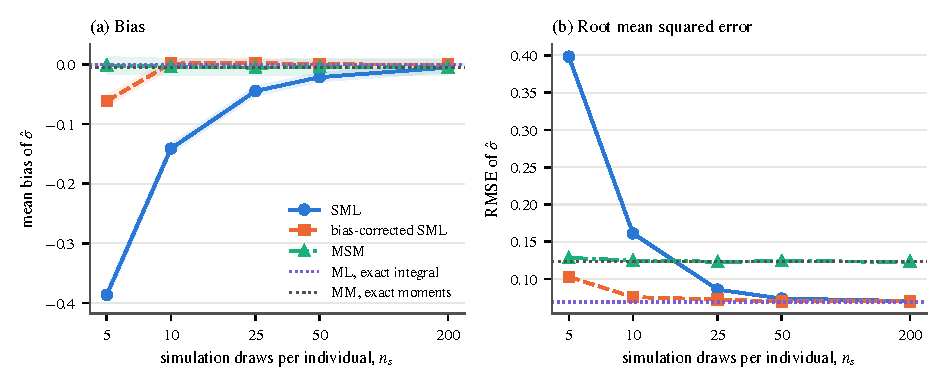
\includegraphics[width=\textwidth]{figures/appA/simest.pdf}
\caption{Simulation estimators of the standard deviation $\sigma$ of a random coefficient. Panel (a) shows the
mean bias of $\hat\sigma$ and panel (b) its root mean squared error, against the number of draws per individual.
The design is a panel binary logit with $N = 1{,}000$ individuals, $T = 5$ choices each, $x_{it} \sim N(0.5, 1)$,
$b_0 = -0.5$, $b_1 = 1$, $\sigma = 1$. SML uses \eqref{eq:A-sml}, bias-corrected SML adds
$\frac{\hat V_i}{2\tilde f_i^2}$, and MSM solves three simulated moment equations. The horizontal lines are maximum
likelihood and the exact-moment estimator computed with 40-point Gauss-Hermite quadrature. Shaded bands are
$\pm 1.96$ Monte Carlo standard errors. 300 replications, seed 20261022.}
\label{fig:A-simest}
\end{figure}

The results match the theory. With $n_s = 5$ draws, SML underestimates $\sigma = 1$ by 0.386 on average, and the
bias falls to 0.142, 0.045, 0.022 and 0.006 at 10, 25, 50 and 200 draws. From 25 draws on, $n_s$ times the bias is
roughly constant, as the $\frac{1}{n_s}$ rate predicts. The
bias pulls $\hat\sigma$ down because a smaller $\sigma$ makes the individual likelihood terms less variable across
draws, which raises $\E[\ln\tilde f_i]$ in part (i) of the proposition. The bias spills over to the mean coefficient
$b_1$, which is too small by 0.161 at five draws. The corrected estimator cuts the bias in $\hat\sigma$ to 0.062 at
five draws and to less than 0.003 from ten draws on. MSM is consistent at every fixed $n_s$, as \cref{prop:A-msm} predicts, and its Monte Carlo bias is small at every
$n_s$ in the table.
Its standard deviation at five draws is 0.129, against 0.123 with exact moments. The ratio of 1.04 is below the
bound $\sqrt{1 + \frac{1}{5}} = 1.10$ because the logit simulator is smooth. MSM's root mean squared error of about
0.12 exceeds that of maximum likelihood (0.069) at every $n_s$. Three just-identifying moments use the information
in the data less efficiently than the likelihood. SML overtakes MSM between 10 and 25 draws, and the corrected
version does so already at five.

\casehead{A worked case: Gentzkow (2007)}
\citet{Gentzkow2007} estimates a demand system for print and online newspapers in Washington, DC, from survey reports
of reading over the last day and the last five weekdays (\cref{sec:10-gentzkow}). The likelihood of a respondent's
report integrates a product of daily logit probabilities over a three-dimensional normal vector of random effects
(his eq.~6). He uses SML with 300 draws per consumer and the first-order bias correction of
\citet[p.~45]{GourierouxMonfort1996}. His footnote 32 derives the correction by the expansion in
\cref{prop:A-sml-bias}(i) (p.~732). The draws come from the importance density of \cref{lem:A-importance}. For each consumer he computes the
probability of the observed report once, at a preliminary estimate and with 200 draws. He then draws the random
effects from their distribution conditional on the report, by acceptance and rejection, and reweights
(p.~732, n.~31 and eqs.~13--14). Standard errors use the robust formula of \citet{McFaddenTrain2000}. Standard
errors of welfare statistics come from 100 draws from the estimated asymptotic distribution of the parameters
(p.~733), a method we discuss in \cref{sec:A-krinsky-robb}. He chose SML over MSM for the reasons given above. In
preliminary tests the two gave similar parameters, and MSM took 10 to 20 times longer to compute (p.~732). The
sample has 16,179 respondents (Table~5), large enough that the correction for $n_s = 300$ matters little, as in
\cref{fig:A-simest}. \Cref{sec:10-gentzkow-sml} gives the full estimator.

\subsection{Simulated nonlinear least squares}\label{sec:A-snlls}

\citet{LaffontOssardVuong1995} faced an integral inside a regression function. In a first-price or descending
auction with independent private values, the equilibrium bid function has no closed form for most value
distributions. The support of the winning bid also depends on the parameters. Maximum likelihood is then both
non-regular and computationally heavy, since the bid function must be inverted for every observation and every trial
parameter (p.~958, see \cref{prop:A-uniform-mle}). They proposed a least-squares estimator based on a simulated
conditional mean that is consistent for a fixed number of draws.

\casehead{The naive estimator and its limit}
Index auctions by $l = 1, \dots, n$ (their $L$), and let $b^w_l$ be the winning bid, with $b^w_l = p^o_l$ when the
object is unsold and $p^o_l$ the reserve price. Let $x_l$ collect the reserve price and the auction characteristics,
and let $m_l(\theta) = \E[b^w_l \mid x_l]$. Nonlinear least squares would minimize $\frac{1}{n}\sum_l(b^w_l -
m_l(\theta))^2$. Suppose $\bar X_l(\theta) = \frac{1}{n_s}\sum_{s=1}^{n_s}X_{sl}(\theta)$ is an unbiased simulator of
$m_l(\theta)$, with draws independent of $b^w_l$ given $x_l$. The naive estimator minimizes (their eq.~8)
\begin{equation}\label{eq:A-lov-naive}
  Q^{\text{naive}}_n(\theta) = \frac{1}{n}\sum_{l=1}^{n}\bigl(b^w_l - \bar X_l(\theta)\bigr)^2.
\end{equation}
To find its limit, write $b^w_l - \bar X_l(\theta) = (b^w_l - m_l(\theta_0)) + (m_l(\theta_0) - m_l(\theta)) +
(m_l(\theta) - \bar X_l(\theta))$. Given $x_l$, the first and third terms have mean zero and are independent of
each other, and the second is fixed. All cross products therefore have conditional mean zero, and
\begin{equation}\label{eq:A-lov-decomp}
  \E\bigl[(b^w_l - \bar X_l(\theta))^2 \mid x_l\bigr] = \sigma_0^2(x_l) + \bigl(m_l(\theta_0) - m_l(\theta)\bigr)^2
  + \frac{1}{n_s}\,\omega_l(\theta),
\end{equation}
where $\sigma_0^2(x_l) = \Var(b^w_l \mid x_l)$ and $\omega_l(\theta) = \Var(X_{sl}(\theta) \mid x_l)$. The first term
does not depend on $\theta$, and the second is minimized at $\theta_0$. The third term is the average simulator
variance, $A_L(\theta)$ in their eq.~(9). It depends on $\theta$, so the naive estimator converges to a value that
trades fit for a smaller simulator variance. It is inconsistent for fixed $n_s$ whenever the gradient of the
average simulator variance is nonzero at $\theta_0$, which is the generic case.

\casehead{The corrected estimator}
The sample variance of the draws, divided by $n_s$, is unbiased for $\frac{1}{n_s}\omega_l(\theta)$. Subtracting it
gives the simulated nonlinear least squares (SNLLS) objective (their eqs.~10--11):
\begin{equation}\label{eq:A-lov-snlls}
  Q^*_n(\theta) = \frac{1}{n}\sum_{l=1}^{n}\Bigl[\bigl(b^w_l - \bar X_l(\theta)\bigr)^2
  - \frac{1}{n_s(n_s - 1)}\sum_{s=1}^{n_s}\bigl(X_{sl}(\theta) - \bar X_l(\theta)\bigr)^2\Bigr].
\end{equation}
By \eqref{eq:A-lov-decomp}, each bracket has conditional mean $\sigma_0^2(x_l) + (m_l(\theta_0) - m_l(\theta))^2$, the
limit of exact nonlinear least squares. The estimator is consistent for any fixed $n_s$ as $n \to \infty$ (their
Proposition~1), and $Q^*_n(\hat\theta)$ consistently estimates the mean squared error of the model.

Its asymptotic variance shows the price of simulation (their Proposition~2). Let $\mu_l = \frac{\partial
m_l(\theta_0)}{\partial\theta}$, let $Y_{sl}(\theta) = \frac{\partial X_{sl}(\theta)}{\partial\theta}$, and let
$\omega_l$, $\Omega_l$ and $C_l$ be the conditional variances of $X_{sl}(\theta_0)$ and $Y_{sl}(\theta_0)$ and their
covariance. Then $\sqrt n(\hat\theta - \theta_0) \xrightarrow{d} N(0, \mathcal{H}^{-1}\mathcal{J}\mathcal{H}^{-1})$ with
$\mathcal{H} = \E[\mu_l\mu_l^\top]$ and
\begin{equation}\label{eq:A-lov-avar}
  \mathcal{J} = \E\Bigl[\sigma_0^2(x_l)\mu_l\mu_l^\top + \frac{1}{n_s}\bigl(\sigma_0^2(x_l)\Omega_l + \omega_l\mu_l\mu_l^\top\bigr)
  + \frac{1}{n_s(n_s - 1)}\bigl(\omega_l\Omega_l + C_lC_l^\top\bigr)\Bigr].
\end{equation}
The first term alone gives the variance of exact nonlinear least squares. The excess is of order $\frac{1}{n_s}$
and disappears as $n_s \to \infty$. Their Proposition~3 gives a heteroskedasticity-robust estimator of
$\mathcal{H}^{-1}\mathcal{J}\mathcal{H}^{-1}$ that is also consistent for fixed $n_s$.

\casehead{The simulator: revenue equivalence}
The construction of $X_{sl}$ uses auction theory. Let $N$ bidders (their $I$) have independent values from $F_l(\cdot;\theta)$
with density $f_l$, and let $v_{(N)}$ and $v_{(N-1)}$ be the highest and second-highest values. For a value $v \ge
p^o$, the first-price equilibrium bid equals the expected payment of the winner in a second-price auction (their
Lemma, eq.~12):
\begin{equation*}
  e(v) = \E\bigl[\max(v_{(N-1)}, p^o) \mid v_{(N)} = v\bigr].
\end{equation*}
The winning bid is $e(v_{(N)})$ when the object sells, and the convention $b^w = p^o$ covers the unsold case. Taking
expectations over $v_{(N)}$ with the law of iterated expectations gives (their eq.~14)
\begin{equation*}
  m_l(\theta) = \E\bigl[\max(v_{(N-1)l}, p^o_l)\bigr]
  = \int\!\!\cdots\!\!\int\max\bigl(u_{(N-1)}, p^o_l\bigr)\prod_{i=1}^{N}f_l(u_i;\theta)\,\dd u_1\cdots\dd u_N.
\end{equation*}
This is the revenue equivalence theorem at work: the expected winning bid equals the expected second-highest value,
truncated at the reserve price (\cref{ch:auction-theory}). The integrand needs no bid function. With importance
densities $g_l$ and draws $u^s_{1l}, \dots, u^s_{Nl}$ from $g_l$, the simulator is (their eq.~17)
\begin{equation*}
  X_{sl}(\theta) = \max\bigl(u^s_{(N-1)l}, p^o_l\bigr)\prod_{i=1}^{N}\frac{f_l(u^s_{il};\theta)}{g_l(u^s_{il})}.
\end{equation*}
The parameter appears only in the density ratio outside the maximum, so $Q^*_n$ is twice continuously
differentiable when $f_l$ is. Simulating with draws from $F_l(\cdot;\theta)$ would instead put $\theta$ inside the
maximum. With draws $F_l^{-1}(U^s_{il};\theta)$ from fixed uniforms $U^s_{il}$, the maximum is continuous in $\theta$ but
kinked where the reserve starts to bind. A frequency simulator built from indicators of simulated events would be a
step function of $\theta$. Neither would make $Q^*_n$ twice continuously differentiable.

\casehead{The application}
The data are 81 descending auctions of greenhouse eggplants in Marmande, France, in the summer of 1990, each selling
a single case (p.~967). Values are log-normal, with the mean of log values linear in six auction characteristics and
the standard deviation fixed at 0.05 from retail price dispersion (pp.~968--969). The estimates use 20 draws per
auction, and 30 draws gave analogous results (p.~969, n.~19). The number of bidders is treated as an unknown integer.
The criterion is minimized over $N$ from 11, the number of regular buyers, to 23, and the minimum is at $N = 18$
(p.~970). This suggests that one large buyer acts for about eight retailers. The fit gives an $R^2$ of 0.895 (p.~971).
\Cref{ch:auction-empirics} discusses the estimates.

\subsection{Indirect inference}\label{sec:A-indirect}

\emph{Indirect inference} \citep{GourierouxMonfortRenault1993,Smith1993} fits a simple auxiliary model to the real
data and to data simulated from the structural model. It chooses $\theta$ so that the two fits agree. Let
$\hat\beta$ be an auxiliary estimator, such as OLS coefficients or the parameters of a reduced-form logit, computed
on the data. For a trial $\theta$, simulate $H$ data sets of the same size from the structural model with fixed
draws, compute $\tilde\beta_h(\theta)$ on each, and average them into $\bar\beta(\theta)$. The estimator is
\begin{equation*}
  \hat\theta = \argmin_\theta\bigl(\hat\beta - \bar\beta(\theta)\bigr)^\top W\bigl(\hat\beta - \bar\beta(\theta)\bigr).
\end{equation*}
The probability limit of $\tilde\beta_h(\theta)$ is the \emph{binding function} $b(\theta)$, and identification
requires $b$ to be one to one near $\theta_0$. The auxiliary model need not be correctly specified. If
$\sqrt n(\hat\beta - b(\theta_0))$ has asymptotic variance $\Lambda$, the $H$ independent simulated estimates have
the same variance each, so the average has variance $\frac{\Lambda}{H}$. The estimator therefore behaves like a
minimum-distance estimator with variance inflated by the factor $(1 + \frac{1}{H})$, the analogue of
\cref{prop:A-msm}. MSM is the special case in which the auxiliary statistics are sample moments.

\subsection{Inference on functions of estimated parameters}\label{sec:A-krinsky-robb}

Many reported quantities are nonlinear functions $a(\theta)$ that are themselves computed by simulation: median
margins, welfare changes, predicted auction outcomes. The delta method of \cref{sec:A-delta} needs the derivative of
$a$, which may be costly or unstable. \citet{KrinskyRobb1986} proposed a simulation alternative.

\begin{remark}[Drawing from the estimated asymptotic distribution]\label{rem:A-krinsky-robb}
Given $\hat\theta$ and an estimate $\hat V$ of its variance:
\begin{enumerate}[label=(\arabic*)]
  \item Draw $\theta^{(1)}, \dots, \theta^{(R)}$ independently from $N(\hat\theta, \hat V)$.
  \item Compute $a(\theta^{(r)})$ for each draw, solving any equilibrium or simulation problem that $a$ requires.
  \item Report the standard deviation of the $a(\theta^{(r)})$, or their 2.5 and 97.5 percentiles as a 95 percent
  interval.
\end{enumerate}
\end{remark}

The method is common in the book's applications. \citet[Table~VIII, note]{Nevo2001} computes 95 percent intervals
for median margins from 1,500 draws (\cref{sec:08-nevo01}). \citet[p.~733]{Gentzkow2007} uses 100 draws for welfare
statistics. \citet[p.~248]{AtheyLevinSeira2011} call their version a parametric bootstrap. They resample from the
asymptotic distribution of the bid and entry parameters and recompute the expected auction outcomes for each draw.

The method rests on the same approximation as the delta method, the normality of $\hat\theta$. It retains the
nonlinearity of $a$, which helps when $a$ is far from linear over the likely range of $\theta$. It does not correct a
poor normal approximation for $\hat\theta$ itself, and it does not resample the data. \Cref{sec:A-boot-multistep}
compares it with bootstraps that re-estimate the model.

\section{Standard errors under dependence}\label{sec:A-se}

The variance formulas of \cref{sec:A-ols,sec:A-gmm} assume independent observations. Industrial organization data
rarely satisfy that assumption. Prices of the same product are observed in many cities, products in the same market
share demand shocks, and a state's prices are observed every year. This section derives the cost of ignoring such
dependence and the estimators that allow for it.

\subsection{One formula for all robust variances}\label{sec:A-se-meat}

Consider the linear model $y = X\beta + e$ with $n$ observations and $K$ regressors, and the OLS estimator
$\hat\beta = (X^\top X)^{-1}X^\top y$. Its sampling error is $\hat\beta - \beta = (X^\top X)^{-1}\sum_i x_ie_i$, so
conditional on $X$
\begin{equation}\label{eq:A-sandwich-general}
  \Var(\hat\beta \mid X) = (X^\top X)^{-1}\,\Omega_n\,(X^\top X)^{-1}, \qquad
  \Omega_n = \sum_{i=1}^{n}\sum_{j=1}^{n}x_ix_j^\top\E[e_ie_j \mid X].
\end{equation}
Every robust variance estimator replaces the ``meat'' $\Omega_n$ by
\begin{equation}\label{eq:A-meat-kernel}
  \hat\Omega_n = \sum_{i=1}^{n}\sum_{j=1}^{n}k_{ij}\,x_ix_j^\top\hat e_i\hat e_j,
\end{equation}
for weights $k_{ij} \in [0, 1]$ that state which pairs of observations may be correlated. The estimators differ only
in $k_{ij}$:
\begin{itemize}
  \item Heteroskedasticity-robust estimators (HC, \citealp{White1980}) set $k_{ij} = \indic\{i = j\}$.
  \item Cluster-robust estimators set $k_{ij} = \indic\{c(i) = c(j)\}$, with $c(i)$ the cluster of observation $i$.
  \item The Newey-West estimator for a time series sets $k_{ij} = \max\{0, 1 - \frac{|t_i - t_j|}{m+1}\}$ for a lag
  length $m$.
  \item Two-way clustering sets $k_{ij} = \indic\{g(i) = g(j) \text{ or } h(i) = h(j)\}$ for two grouping variables.
  \item Spatial HAC estimators \citep{Conley1999} let $k_{ij}$ decline in the economic distance between $i$ and $j$.
\end{itemize}
Plugging $\hat e_i\hat e_j$ for $e_ie_j$ is useless for a single pair, but the sum over many pairs averages out the
noise. Each estimator is consistent when the pairs it drops are uncorrelated and the pairs it keeps are few relative
to the sample. \Cref{sec:A-ols-asy} covered the HC case, including the finite-sample versions HC1 to HC3. HC estimators
suffice when observations are independent. The rest of this section treats the other cases.

\subsection{Clustered data}\label{sec:A-cluster}

Let the observations fall into $C$ clusters, $c = 1, \dots, C$, with $n_c$ observations in cluster $c$. Errors are
independent across clusters and may be correlated within. We first measure the cost of ignoring the correlation.

\begin{proposition}[Moulton factor]\label{prop:A-moulton}
Let $y_{ic} = \alpha + \beta x_{ic} + e_{ic}$ with $C$ clusters of equal size $\bar n$. Conditional on the
regressor, let the errors be homoskedastic with variance $\sigma^2$, uncorrelated across clusters and equicorrelated
within clusters with correlation $\rho_e$. Let $\tilde x_{ic} = x_{ic} - \bar x$ and define the intra-cluster
correlation of the regressor as
\begin{equation*}
  \rho_x = \frac{\sum_{c}\sum_{i \ne j}\tilde x_{ic}\tilde x_{jc}}{(\bar n - 1)\sum_c\sum_i\tilde x_{ic}^2}.
\end{equation*}
Then
\begin{equation}\label{eq:A-moulton}
  \Var(\hat\beta \mid x) = \frac{\sigma^2}{\sum_c\sum_i\tilde x_{ic}^2}\,\bigl[1 + (\bar n - 1)\rho_x\rho_e\bigr].
\end{equation}
The first factor is the conventional OLS variance. If the regressor is constant within clusters, $\rho_x = 1$ and the
factor is $1 + (\bar n - 1)\rho_e$.
\end{proposition}

\begin{proof}
By the Frisch-Waugh-Lovell theorem, $\hat\beta - \beta = \frac{\sum_c\sum_i\tilde x_{ic}e_{ic}}{\sum_c\sum_i\tilde
x_{ic}^2}$. Write $D = \sum_c\sum_i\tilde x_{ic}^2$. The numerator has variance
\begin{align*}
  \Var\Bigl(\sum_c\sum_i\tilde x_{ic}e_{ic}\Bigr)
  &= \sum_c\Bigl[\sum_i\tilde x_{ic}^2\sigma^2 + \sum_{i \ne j}\tilde x_{ic}\tilde x_{jc}\rho_e\sigma^2\Bigr] \\
  &= \sigma^2D + \rho_e\sigma^2(\bar n - 1)\rho_xD \\
  &= \sigma^2D\,\bigl[1 + (\bar n - 1)\rho_x\rho_e\bigr].
\end{align*}
The first line uses independence across clusters and the equicorrelation within. The second substitutes the
definition of $\rho_x$. Dividing by $D^2$ gives \eqref{eq:A-moulton}. If $x$ is constant within clusters, every
cross product $\tilde x_{ic}\tilde x_{jc}$ equals $\tilde x_{ic}^2$, so the numerator of $\rho_x$ is $(\bar n - 1)D$.
\end{proof}

The factor can be large even when $\rho_e$ is modest. With 20 observations per cluster and $\rho_x = \rho_e = 0.5$,
it equals $1 + 19 \times 0.25 = 5.75$, so the true standard error is $\sqrt{5.75} = 2.40$ times the conventional one.
A nominal 5 percent $t$-test that uses the conventional standard error then rejects a true null with probability
about $\Pr(|Z| > \frac{1.96}{2.40}) = 0.41$ in large samples. With unequal cluster sizes, \citet{Moulton1986} shows
that $\bar n - 1$ is replaced by $\frac{\Var(n_c)}{\bar n} + \bar n - 1$. \citet{Moulton1990} documents the problem
for regressions of individual outcomes on aggregate variables, where $\rho_x = 1$.

\casehead{The cluster-robust variance}
The cluster-robust estimator of \citet{LiangZeger1986} sets $k_{ij} = \indic\{c(i) = c(j)\}$ in
\eqref{eq:A-meat-kernel}. With $X_c$ and $\hat e_c$ the rows of cluster $c$, and the finite-sample factor used by
most software, it is
\begin{equation}\label{eq:A-cr1}
  \hat V_{\text{CR1}} = \frac{C}{C - 1}\,\frac{n - 1}{n - K}\,(X^\top X)^{-1}\Bigl(\sum_{c=1}^{C}X_c^\top\hat e_c\hat e_c^\top
  X_c\Bigr)(X^\top X)^{-1}.
\end{equation}
It allows any correlation and heteroskedasticity within clusters. Its consistency rests on the number of clusters.
When cluster sizes are bounded and $C \to \infty$, the terms $X_c^\top e_ce_c^\top X_c$ are independent across
clusters, and $\frac{1}{C}\sum_cX_c^\top e_ce_c^\top X_c$ converges to its mean by a law of large numbers.
Replacing $e_c$ by $\hat e_c$ changes the average by $o_p(1)$ because $\hat\beta$ is consistent. When each
observation is its own cluster, $C = n$ and $\frac{C}{C - 1}\frac{n - 1}{n - K} = \frac{n}{n - K}$, so CR1 reduces
to HC1. For 2SLS, replace $X$ by $\hat X = P_ZX$ in the bread and $x_i\hat e_i$ by $\hat x_i\hat e_i$ in the meat,
with residuals computed from $X$. For GMM, estimate the long-run covariance of the moments by
$\hat S = \frac{1}{n}\sum_c\hat g_c\hat g_c^\top$ with $\hat g_c = \sum_{i \in c}g(w_i;\hat\theta)$. When fixed
effects are nested within clusters, software differs on whether $K$ counts them. We count every regressor,
including the dummies, which gives slightly larger standard errors.

\casehead{The level of clustering}
The cluster should contain every pair of observations whose errors may be correlated, and clusters must be
numerous. \citet{BertrandDufloMullainathan2004} show the stakes for difference-in-differences regressions on
state-year panels.\footnote{We read NBER Working Paper 8841 (2002), the working-paper version of
\citet{BertrandDufloMullainathan2004}. Pages marked WP refer to it.} Placebo state laws, assigned at random, were
``significant'' at the 5 percent level in up to 45 percent of their simulations with conventional standard errors
(WP p.~3). Outcomes and treatment indicators are both serially correlated within states. Clustering by state, the
level at which treatment is assigned, restored approximately correct size with many states. The rejection rate was
6 percent in their panel of 51 states, and it rose to 8.5 percent with 10 states and 15 percent with 6 states (WP p.~18 and Table~9).
\citet{AbadieEtAl2023} add a design-based view. Clustering adjusts for
clustered sampling or clustered assignment of the regressor of interest. Correlated outcomes alone do not call for it
when assignment is at the individual level and the sample covers the population.

\casehead{Two-way clustering}
In a state-year panel, errors may be correlated within states over time and within years across states. Two-way
clustering \citep{CameronGelbachMiller2011} keeps every pair that shares a state or a year. The indicator of that
event satisfies the inclusion-exclusion identity
\begin{equation*}
  \indic\{g(i) = g(j) \text{ or } h(i) = h(j)\} = \indic\{g(i) = g(j)\} + \indic\{h(i) = h(j)\}
  - \indic\{g(i) = g(j),\ h(i) = h(j)\}.
\end{equation*}
Substituting into \eqref{eq:A-meat-kernel} gives $\hat V_{\text{2way}} = \hat V_g + \hat V_h - \hat V_{g \cap h}$:
cluster by the first dimension, cluster by the second, and subtract the estimate clustered by their intersection. In a
panel with one observation per state-year, the intersection estimator is the HC estimator. The difference can fail to
be positive semidefinite in small samples, and then negative eigenvalues are set to zero. Asymptotic justification
requires the number of clusters in both dimensions to grow, so inference should use the smaller of the two counts.

\casehead{Few clusters}
With few clusters, CR1 standard errors are too small and $t$-statistics are far from normal. Two corrections are
standard \citep{CameronMiller2015}. The first compares the $t$-statistic with the quantiles of the $t$ distribution
with $C - 1$ degrees of freedom. The second is the wild cluster bootstrap of \citet{CameronGelbachMiller2008}.

\begin{remark}[Wild cluster bootstrap-$t$]\label{rem:A-wild-cluster}
To test $H_0: \beta_k = \beta_k^0$ with CR1 standard errors:
\begin{enumerate}[label=(\arabic*)]
  \item Compute $t = \frac{\hat\beta_k - \beta_k^0}{\widehat{\mathrm{se}}_{\text{CR1}}(\hat\beta_k)}$ from the data.
  \item Estimate the model with the null imposed, and keep its coefficients $\tilde\beta$ and residuals $\tilde e_{ic}$.
  \item For $b = 1, \dots, B$, draw one weight $w_c^{(b)} \in \{-1, 1\}$ per cluster, each value with probability
  $\frac{1}{2}$ (Rademacher weights), and form $y^{(b)}_{ic} = x_{ic}^\top\tilde\beta + w_c^{(b)}\tilde e_{ic}$.
  \item Regress $y^{(b)}$ on $X$, and compute $t^{(b)} = \frac{\hat\beta^{(b)}_k -
  \beta_k^0}{\widehat{\mathrm{se}}_{\text{CR1}}(\hat\beta^{(b)}_k)}$ with the same formula as in step (1).
  \item Report the $p$-value $\frac{1}{B}\sum_{b=1}^{B}\indic\{|t^{(b)}| \ge |t|\}$. Count as ties the values of
  $|t^{(b)}|$ that differ from $|t|$ only by rounding error. If $2^C \le B$, use all $2^C$ weight vectors in place
  of random draws, and set $B = 2^C$.
\end{enumerate}
\end{remark}

Three features make the procedure work. Multiplying a whole cluster's residuals by one weight preserves any
correlation pattern within the cluster. Imposing the null makes the bootstrap data satisfy the hypothesis being
tested, which improves size. The statistic is studentized, which yields the asymptotic refinement of
\cref{sec:A-boot}.

When very few clusters are treated, the residuals of treated clusters carry the treatment effect estimate and the wild
bootstrap fails \citep{MacKinnonWebb2017}. Methods that use the control clusters to estimate the error
distribution are then needed \citep{ConleyTaber2011}.

\casehead{Discreteness with Rademacher weights}
With Rademacher weights there are only $2^C$ weight vectors, each with probability $2^{-C}$. The vectors $w$ and
$-w$ give bootstrap estimates $\hat\beta^{(b)}_k - \beta^0_k$ of opposite sign and residuals of opposite sign, so
they give the same $|t^{(b)}|$. Hence $|t^{(b)}|$ takes at most $2^{C-1}$ distinct values \citep{CameronMiller2015}.
The vector of ones reproduces the data, so it and its negative give $|t^{(b)}| = |t|$ exactly. The \emph{exact
conditional bootstrap $p$-value} is the probability of $|t^{(b)}| \ge |t|$ over all $2^C$ vectors, given the data.
It is at least $\frac{2}{2^C}$, which equals $\frac{1}{16} = 0.0625$ when $C = 5$. A 5 percent test with five clusters
therefore never rejects. The $p$-value of step (5) with random draws is a simulation estimate of the exact
$p$-value. It can fall below $\frac{2}{2^C}$ when few draws hit the two tying vectors, and enumeration removes this
noise. Rounding error can also make a computed $|t^{(b)}|$ fall just below $|t|$ for a tying vector, which is why
step (5) counts ties explicitly. Weight distributions with more support points make the $p$-value finer.
With fewer than ten clusters, \citet{CameronMiller2015} recommend the six-point weights of \citet{Webb2013}. These put probability
$\frac{1}{6}$ on each of $\pm\sqrt{\frac{1}{2}}$, $\pm 1$ and $\pm\sqrt{\frac{3}{2}}$, which have mean zero and
variance one.

\begin{figure}[htbp]
\centering
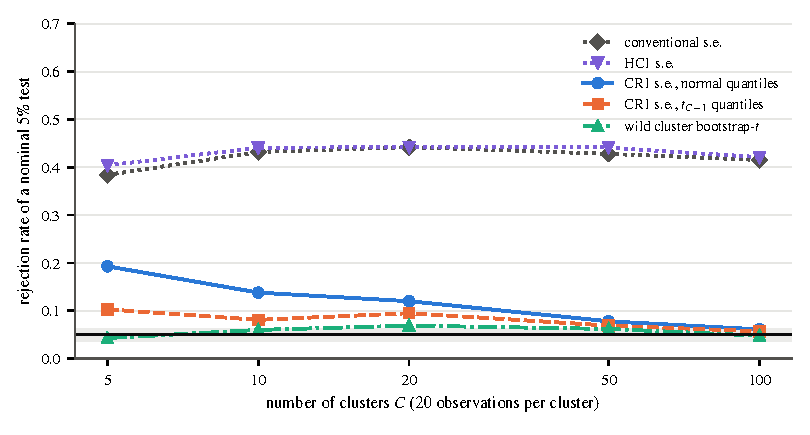
\includegraphics[width=0.86\textwidth]{figures/appA/cluster_mc.pdf}
\caption{Rejection rates of nominal 5 percent tests of a true null when errors and the regressor are both
correlated within clusters. In the design, $y_{ic} = e_{ic}$ is regressed on a constant and $x_{ic}$. Both $x_{ic}$
and $e_{ic}$ are sums of independent normal cluster and idiosyncratic components, with intra-cluster correlations
$\rho_x = \rho_e = 0.5$. There are 20 observations per cluster and 1,000 replications per $C$, with seed 20261022.
With $C = 5$ the Rademacher bootstrap enumerates all 32 weight vectors. The six-point bootstrap uses 399 random
weight vectors for every $C$, and the Rademacher bootstrap does so for $C \ge 10$. The gray band is the 95 percent Monte Carlo range around 0.05.}
\label{fig:A-cluster-mc}
\end{figure}

\Cref{fig:A-cluster-mc} reports a simulation with the parameters of the Moulton example. The conventional test
rejects the true null in 38 to 44 percent of replications for every number of clusters, close to the 41 percent
predicted above. HC1 standard errors do no better, because the problem is correlation, which HC1 ignores.
CR1 standard errors with normal quantiles reject 19 percent of the time with 5 clusters, 14 percent with 10 and 6
percent with 100. Using $t_{C-1}$ quantiles lowers the rejection rate to 10 percent with 5 clusters and 8 to 10
percent with 10 to 20 clusters. With Rademacher weights and at least 10 clusters, the wild cluster bootstrap rejects
between 4.8 and 6.9 percent of the time. With 5 clusters it never rejects, because its exact $p$-value is at least
0.0625 in every replication. A $p$-value simulated from 399 random draws would reject in 1.0 percent of the
replications with ties counted, and in 4.3 percent if rounding error drops the ties. The near-nominal second
figure is an artifact of the tie comparison. The six-point weights reject between 4.8 and 7.5 percent of the time
for every $C$, and 5.6 percent with 5 clusters. Each rate has a Monte Carlo standard error of about 0.007.

\subsection{Serial correlation and HAC estimators}\label{sec:A-hac}

In a time series $t = 1, \dots, T$, let $g_t$ be a mean-zero score or moment, for example $x_te_t$. Write
$\Gamma_j = \E[g_tg_{t-j}^\top]$ for its autocovariance at lag $j$, with $\Gamma_{-j} = \Gamma_j^\top$. Under
covariance stationarity,
\begin{equation*}
  \Var\Bigl(\frac{1}{\sqrt T}\sum_{t=1}^{T}g_t\Bigr) = \frac{1}{T}\sum_{t=1}^{T}\sum_{s=1}^{T}\Gamma_{t-s}
  = \sum_{j=-(T-1)}^{T-1}\Bigl(1 - \frac{|j|}{T}\Bigr)\Gamma_j \longrightarrow S = \sum_{j=-\infty}^{\infty}\Gamma_j,
\end{equation*}
where the middle step counts the $T - |j|$ pairs with $t - s = j$ and the limit holds when the autocovariances are
absolutely summable. The matrix $S$ is the \emph{long-run variance}. With $g_t = x_te_t$ and $n = T$, the meat
$\Omega_n$ of \eqref{eq:A-sandwich-general} is the variance of $\sum_tg_t$, which is approximately $TS$. An estimate
$\hat S$ therefore enters the OLS sandwich as $\hat\Omega_n = T\hat S$:
\begin{equation*}
  \widehat\Var(\hat\beta) = (X^\top X)^{-1}\,T\hat S\,(X^\top X)^{-1} = \frac{1}{T}\,\hat Q^{-1}\hat S\hat Q^{-1},
  \qquad \hat Q = \frac{X^\top X}{T}.
\end{equation*}
In the GMM formulas, $\hat S$ replaces $S$ directly.

\begin{example}[AR(1) regressor and error]\label{ex:A-ar1-factor}
Let $x_t$ and $e_t$ be independent stationary AR(1) processes with autocorrelations $\rho_x$ and $\rho_e$. Then
$\Gamma_j = \E[x_tx_{t-j}]\E[e_te_{t-j}] = \sigma_x^2\sigma_e^2(\rho_x\rho_e)^{|j|}$, and
\begin{equation*}
  S = \sigma_x^2\sigma_e^2\Bigl[1 + 2\sum_{j=1}^{\infty}(\rho_x\rho_e)^j\Bigr]
  = \sigma_x^2\sigma_e^2\,\frac{1 + \rho_x\rho_e}{1 - \rho_x\rho_e}.
\end{equation*}
The conventional variance uses only $\Gamma_0 = \sigma_x^2\sigma_e^2$, so it is too small by the factor
$\frac{1 + \rho_x\rho_e}{1 - \rho_x\rho_e}$. With $\rho_x = 0.85$ and $\rho_e = 0.64$, the factor is 3.4 and the
standard error ratio is 1.8. These are the within-state autocorrelations of the tax and of the residual in the
cigarette panel of \cref{sec:A-sumner-se}.
\end{example}

\casehead{The Newey-West estimator}
A natural estimator truncates the sum at lag $m$ and uses sample autocovariances
$\hat\Gamma_j = \frac{1}{T}\sum_{t=j+1}^{T}\hat g_t\hat g_{t-j}^\top$. The unweighted truncated sum can fail to be
positive semidefinite. \citet{NeweyWest1987} downweight the autocovariances linearly:
\begin{equation}\label{eq:A-newey-west}
  \hat S_{\text{NW}} = \hat\Gamma_0 + \sum_{j=1}^{m}\Bigl(1 - \frac{j}{m+1}\Bigr)\bigl(\hat\Gamma_j + \hat\Gamma_j^\top\bigr).
\end{equation}
The Bartlett weights $1 - \frac{j}{m+1}$ guarantee a positive semidefinite estimate. To see why, form the block sums
$\hat B_t = \sum_{k=0}^{m}\hat g_{t-k}$ and consider $\frac{1}{(m+1)T}\sum_t\hat B_t\hat B_t^\top$, an average of
outer products and hence positive semidefinite. Expanding the product, $\hat g_{t-k}\hat g_{t-l}^\top$ appears for
each pair $(k, l)$, and the number of pairs with $k - l = j$ is $m + 1 - |j|$. The weight on lag $j$ is therefore
$\frac{m + 1 - |j|}{m+1} = 1 - \frac{|j|}{m+1}$, which reproduces \eqref{eq:A-newey-west} up to terms at the ends
of the sample. Consistency requires $m \to \infty$ with $\frac{m}{T} \to 0$. A common rule of thumb is $m =
\lfloor 4(\frac{T}{100})^{\frac{2}{9}}\rfloor$. In \citet[p.~634]{NeweyWest1994} this formula is only a preliminary
lag in an automatic procedure for the Bartlett kernel. The procedure uses it to estimate a constant $\hat\gamma$ and then
sets $m = \lfloor\hat\gamma T^{\frac{1}{3}}\rfloor$ (p.~635).
\citet{GenesoveMullin1998} report Newey-West standard errors with four lags for their quarterly sugar demand and
pricing equations (\cref{sec:03-sugar}).

\casehead{Panels}
In a panel with many units and a short time dimension, clustering by unit allows arbitrary serial correlation
within units, and nothing more is needed if units are independent. When units share common shocks that time
effects do not remove, \citet{DriscollKraay1998} average the scores across units within each period and apply
\eqref{eq:A-newey-west} to the resulting time series. Their estimator allows any cross-sectional dependence, but it
requires a long panel and allows only serial correlation that dies out within $m$ periods. \citet{Conley1999}
extends the HAC idea to dependence that declines with spatial or economic distance.

\subsection{Dependence structures in IO data}\label{sec:A-io-dependence}

The book's applications show four recurring structures. The first is the same product observed in many markets in
the same period, whose prices respond to common cost and demand shocks.
\citet[WP p.~25]{AshenfelterHosken2010} observe the prices of the same products in many geographic markets each
period,\footnote{We read NBER Working Paper 13859 (2008) of \citet{AshenfelterHosken2010} and NBER Working Paper
17476 (2011) of \citet{AshenfelterHoskenWeinberg2013}. Pages marked WP refer to them.} and therefore cluster on the time period, citing \citet{Moulton1987}. Their reference list contains only
\citet{Moulton1990} (WP p.~39), which makes the same point about aggregate regressors. The second is the same product or
unit observed repeatedly over time. \citet[WP p.~14]{AshenfelterHoskenWeinberg2013} cluster by SKU in their
appliance price regressions. \citet[pp.~862--863]{BerryLevinsohnPakes1995} treat the sum of the moments of a car model over
all its years as one observation, which allows any correlation across years for a given model. The third is common
shocks to all products in a market. \citet[WP p.~17]{BerryCarnallSpiller1996} assume independence across airline
markets and a factor structure that correlates demand and cost errors within a market (\cref{sec:09-bcs-estimation}).
They also note that the average product has fewer than 10 sampled passengers, and they leave the correction of
standard errors for this sampling error to future research (WP p.~17). The fourth
is serial correlation that a structural model must represent explicitly. \citet{Ellison1994} models an AR(1) demand
error inside his Markov-switching likelihood, and doing so changes the point estimates as well as the standard
errors (\cref{ch:collusion-evidence}). \Cref{tab:A-se-practice} collects the inference methods used in the book.

\begin{table}[htbp]
\centering
\begin{threeparttable}
\caption{Inference under dependence in the book's applications}
\label{tab:A-se-practice}
\footnotesize
\begin{tabularx}{\textwidth}{@{}>{\raggedright\arraybackslash}p{2.7cm}>{\raggedright\arraybackslash}X>{\raggedright\arraybackslash}X>{\raggedright\arraybackslash}p{2.6cm}@{}}
\toprule
Application & Data structure & Inference used & Source \\
\midrule
\citet{Sumner1981}, re-estimated & State-year panel, 48 units, 25 years & Clusters by state, by year and both, Driscoll-Kraay, wild cluster bootstrap & \Cref{tab:A-sumner} \\
\addlinespace
\citet{GenesoveMullin1998} & Quarterly time series, 1890--1914 & Newey-West, 4 lags, with the pricing equation corrected for estimated demand & \Cref{sec:03-sugar} \\
\addlinespace
\citet{AshenfelterHosken2010} & Product by city by period & Clusters on the time period & WP p.~25 \\
\addlinespace
\citet{AshenfelterHoskenWeinberg2013} & SKU by month & Clusters by SKU & WP p.~14 \\
\addlinespace
\citet{BerryLevinsohnPakes1995} & Car model by year & Moments summed over a model's years, simulation variance added & pp.~862--863 and \cref{sec:08-asymptotics} \\
\addlinespace
\citet{BerryCarnallSpiller1996} & Products in airline markets & Independence across markets and a factor structure within them, share sampling error not corrected & WP p.~17 and \cref{sec:09-bcs-estimation} \\
\addlinespace
\citet{MillerWeinberg2017} & Brand-size product by region by period & Clusters by region, two-step correction for estimated demand & pp.~1775, 1780 and \cref{ch:mergers} \\
\addlinespace
\citet{ChaudhuriGoldbergJia2006} & Product by region by month & Bootstrap over months, 300 replications, all products and regions kept & WP p.~21 \\
\addlinespace
\citet{Nevo2001} & Brand by city by quarter & 1,500 draws from the asymptotic distribution for median margins & Table~VIII \\
\addlinespace
\citet{Asker2010} & Auctions & Bootstrap over auctions, 5,000 iterations, 90 percent intervals & Tables~7--10 \\
\addlinespace
\citet{Gentzkow2007} & Survey respondents & Robust SML standard errors, 100 parameter draws for welfare & p.~733 \\
\addlinespace
\citet{AtheyLevinSeira2011} & Timber sales & Matching standard errors of \citet{AbadieImbens2006}, parametric bootstrap & pp.~230, 248 \\
\bottomrule
\end{tabularx}
\begin{tablenotes}\footnotesize
\item Notes: WP page numbers refer to working-paper versions of the papers.
\end{tablenotes}
\end{threeparttable}
\end{table}

\subsection{Worked application: Sumner's regression revisited}\label{sec:A-sumner-se}

\citet{Sumner1981} tests for competition in cigarettes by regressing the retail price per pack on the excise tax in a
state-year panel (\cref{sec:A-panel,sec:03-sumner-design}). His most complete specification is the two-way fixed effects
regression \eqref{eq:A-sumner} of \cref{sec:A-panel},
\begin{equation*}
  p_{sy} = \mu_s + \tau_y + \rho\,t_{sy} + e_{sy},
\end{equation*}
with state effects $\mu_s$, year effects $\tau_y$ and pass-through $\rho$. Competition with flat marginal cost
implies $\rho = 1$. Sumner reports $\hat\rho = 1.074$ with a conventional standard error of 0.013 (Table~1), so the
$t$-statistic for $\rho = 1$ is 5.7. Both the price and the tax are persistent within states, so the
conventional standard error is suspect.

We re-estimate the regression on a panel reconstructed from \emph{The Tax Burden on Tobacco} (1983, Table~13) and
the CPI-U of the Bureau of Labor Statistics. It covers 47 states and the District of Columbia from 1954 to 1978,
1,200 state-years, the same coverage as Sumner's. Prices and taxes are nominal cents per pack, and the tax is the
state tax plus the federal tax of 8 cents. The computations are in \texttt{figures/appA/src/sumner\_inference.py}.
\Cref{tab:A-sumner} reports three specifications and six variance estimators.

\begin{table}[htbp]
\centering
\begin{threeparttable}
\caption{Cigarette tax pass-through: standard errors and tests of $\rho = 1$ under different dependence assumptions}
\label{tab:A-sumner}
\small
\setlength{\tabcolsep}{3.6pt}
\begin{tabular}{@{}lccccccccc@{}}
\toprule
& Sumner & \multicolumn{8}{c}{Re-estimation} \\
\cmidrule(lr){2-2}\cmidrule(l){3-10}
Specification & (1981) & $\hat\rho$ & Conv. & HC1 & State & Year & Two-way & DK & Wild \\
\midrule
(1) State, year effects, OLS & \makecell{1.074\\(0.013)} & 1.075 & 0.013 & 0.015 & 0.034 & 0.013 & 0.033 & 0.016 & \\
\quad $p$-value for $\rho = 1$ & & & $<$0.001 & $<$0.001 & 0.033 & $<$0.001 & 0.034 & $<$0.001 & 0.044 \\
\addlinespace
(2) CPI, OLS & \makecell{1.029\\(0.011)} & 1.029 & 0.011 & 0.013 & 0.030 & 0.023 & 0.035 & 0.027 & \\
\quad $p$-value for $\rho = 1$ & & & 0.007 & 0.030 & 0.340 & 0.207 & 0.416 & 0.299 & 0.358 \\
\addlinespace
(3) CPI, random effects & \makecell{1.069\\(0.013)} & 1.069 & 0.013 & 0.015 & 0.033 & 0.015 & 0.033 & 0.020 & \\
\quad $p$-value for $\rho = 1$ & & & $<$0.001 & $<$0.001 & 0.042 & $<$0.001 & 0.046 & 0.002 & \\
\bottomrule
\end{tabular}
\begin{tablenotes}\footnotesize
\item Notes: The dependent variable is the retail price in cents per pack and the regressor of interest the combined
state and federal tax in cents per pack, 1,200 state-years. The first column reproduces Sumner's Table~1 (standard
errors in parentheses). The other columns report our estimate of $\rho$ and its standard error under six
estimators. Conv.: conventional OLS or GLS. HC1: heteroskedasticity-robust. State and Year: CR1 clustered by state
(48 clusters) or by year (25). Two-way: clustered by state and year \citep{CameronGelbachMiller2011}. DK:
\citet{DriscollKraay1998} with Bartlett weights and 2 lags. $p$-values use normal quantiles for Conv.\ and HC1,
$t_{47}$ for State, $t_{24}$ for Year, Two-way and DK. Wild: wild cluster bootstrap-$t$ by state with the null
imposed, Rademacher weights and 9,999 draws. Row (2) replaces the year effects by the national CPI and drops the
state effects. Row (3) has the regressors of row (2) and is two-way random-effects GLS \citep{FullerBattese1974}, and
its robust variants apply the formulas to the GLS-transformed regression. $K$ counts all dummies in row (1).
\end{tablenotes}
\end{threeparttable}
\end{table}

\casehead{Row (1)}
The re-estimation reproduces Sumner's estimate and conventional standard error. The HC1 standard error is 15
percent larger. Clustering by state raises the standard error to 0.034, 2.6 times the conventional value. The
within-state first-order autocorrelation of the residuals is 0.64 and that of the within-transformed tax is 0.85.
\Cref{ex:A-ar1-factor} predicts a standard error ratio of about 1.8 for these values, and the ratio of the clustered to
the HC1 standard error is 2.2. Clustering by year leaves the standard error at 0.013. The year effects absorb the
common national shocks, so the residuals of different states in the same year are nearly uncorrelated. The two-way
estimate, 0.033, is close to the state-clustered one for the same reason. The Driscoll-Kraay estimate, 0.016, allows
any correlation across states but only two lags of serial correlation, and it misses the persistence that clustering
by state captures. The rejection of $\rho = 1$ survives every estimator that allows correlation within states, with
$p$-values from 0.033 to 0.044, but its margin is far thinner than a $t$-statistic of 5.7 suggests. The wild cluster
bootstrap $p$-value of 0.044 has a Monte Carlo standard error of 0.002.

\casehead{Row (2)}
Without state effects, persistent differences in state price levels enter the error, and they are correlated over
time within a state. The conventional standard error of 0.011 gives $p = 0.007$. Clustering by state, by year or by both, the
Driscoll-Kraay estimator and the wild cluster bootstrap all give $p$ above 0.2. The apparent rejection of competition in this specification is an
artifact of the conventional standard error.

\casehead{Row (3)}
The random-effects GLS estimate reproduces Sumner's 1.069. Its conventional standard error assumes that a constant
state effect captures all within-state correlation. The residuals of the transformed regression remain serially
correlated, and the state-clustered standard error is 0.033, with $p = 0.042$. Random effects therefore do not
substitute for clustering when the error has more persistence than a permanent effect.

The lesson is general. In a panel with persistent regressors and errors, the conventional and heteroskedasticity-robust
standard errors can overstate precision by a factor of two or more. The clustering level should follow the
dependence that the fixed effects leave in the error. Here the fixed effects leave serial correlation within
states, while the correlation across states within a year is negligible.

\section{The delta method and the bootstrap}\label{sec:A-delta-boot}

Empirical work rarely stops at the estimated parameters. A pass-through coefficient is turned into an elasticity,
demand parameters into markups, and a demand system into the welfare effect of a counterfactual. This section
develops the two general tools for the uncertainty of such quantities, the delta method and the bootstrap, and
shows when each fails.

\subsection{The delta method}\label{sec:A-delta}

\begin{theorem}[Delta method]\label{thm:A-delta}
Suppose $\sqrt n(\hat\theta - \theta_0) \xrightarrow{d} N(0, V)$ for $\theta_0 \in \R^K$. Let $a: \R^K \to \R^q$ be
continuously differentiable in a neighborhood of $\theta_0$, with Jacobian $A(\theta) = \frac{\partial
a(\theta)}{\partial\theta^\top}$ ($q \times K$) and $A = A(\theta_0)$. Then
\begin{equation*}
  \sqrt n\bigl(a(\hat\theta) - a(\theta_0)\bigr) \xrightarrow{d} N(0, AVA^\top).
\end{equation*}
If $\hat V \xrightarrow{p} V$, then $A(\hat\theta)\hat VA(\hat\theta)^\top \xrightarrow{p} AVA^\top$.
\end{theorem}

\begin{proof}
Since $\sqrt n(\hat\theta - \theta_0)$ converges in distribution, $\hat\theta - \theta_0 = O_p(n^{-\frac{1}{2}})$ and
$\hat\theta \xrightarrow{p} \theta_0$. For each component $a_k$, the mean value theorem gives a point $\bar\theta_k$
on the segment between $\hat\theta$ and $\theta_0$ with
\begin{equation*}
  a_k(\hat\theta) - a_k(\theta_0) = \frac{\partial a_k(\bar\theta_k)}{\partial\theta^\top}(\hat\theta - \theta_0).
\end{equation*}
Stack these rows into a matrix $\bar A$. Each $\bar\theta_k \xrightarrow{p} \theta_0$, so $\bar A \xrightarrow{p} A$
by continuity of the derivatives. Then
\begin{equation*}
  \sqrt n\bigl(a(\hat\theta) - a(\theta_0)\bigr) = \bar A\,\sqrt n(\hat\theta - \theta_0),
\end{equation*}
and Slutsky's theorem gives convergence to $A\,N(0, V) = N(0, AVA^\top)$. The second claim follows from the
continuous mapping theorem.
\end{proof}

In practice the delta-method standard error of a scalar $a(\hat\theta)$ is $\sqrt{\nabla a(\hat\theta)^\top\hat
V_n\nabla a(\hat\theta)}$, where $\hat V_n = \frac{\hat V}{n}$ is the estimated variance of $\hat\theta$. We now work
through the cases that recur in the book.

\begin{example}[Elasticity implied by pass-through]\label{ex:A-delta-passthrough}
Under monopoly or constant conduct with constant-elasticity demand and flat marginal cost, pass-through is $\rho =
\frac{\varepsilon}{\varepsilon - 1}$, where $\varepsilon$ is the elasticity the firms behave as if they face
(\cref{sec:03-sumner-design}). Inverting gives $\varepsilon = a(\rho) = \frac{\rho}{\rho - 1}$ for $\rho > 1$. The
derivative is
\begin{equation*}
  a'(\rho) = \frac{(\rho - 1) - \rho}{(\rho - 1)^2} = -\frac{1}{(\rho - 1)^2},
  \qquad \mathrm{se}(\hat\varepsilon) = \frac{\mathrm{se}(\hat\rho)}{(\hat\rho - 1)^2}.
\end{equation*}
Sumner's estimate $\hat\rho = 1.074$ with standard error 0.013 gives $\hat\varepsilon = \frac{1.074}{0.074} = 14.5$ and
a delta-method standard error of $\frac{0.013}{0.074^2} = 2.37$.\footnote{Sumner's printed implied elasticities equal
$\frac{1}{1 - \hat\rho}$, for example $-13.5$ for the first row. They are one unit smaller in magnitude than
$\frac{\hat\rho}{\hat\rho - 1}$, because they treat $\hat\rho - 1$ as the markup over cost instead of using the Lerner
condition (\cref{sec:03-sumner-design}).} Our re-estimate $\hat\rho = 1.0746$ gives $\hat\varepsilon = 14.4$, with a
standard error of 2.38 based on the conventional standard error and 6.11 based on the state-clustered one. The
standard error of $\hat\varepsilon$ is about 180 times that of $\hat\rho$, because the derivative is the inverse
square of $\hat\rho - 1 = 0.075$.
\end{example}

\begin{example}[Marginal cost from an inverse-elasticity rule]\label{ex:A-delta-cost}
With an observed price $p$ and an estimated elasticity, the Lerner rule $\frac{p - c}{p} = \frac{1}{\varepsilon}$
gives $\hat c = p(1 - \frac{1}{\hat\varepsilon})$ (\cref{prop:01-infer-cost}). The derivative
$\frac{\dd c}{\dd\varepsilon} = \frac{p}{\varepsilon^2}$ yields $\mathrm{se}(\hat c) = \frac{p}{\hat\varepsilon^2}
\mathrm{se}(\hat\varepsilon)$. Chaining with \cref{ex:A-delta-passthrough}, $c = p(1 - \frac{\rho - 1}{\rho}) =
\frac{p}{\rho}$, so $\mathrm{se}(\hat c) = \frac{p}{\hat\rho^2}\mathrm{se}(\hat\rho)$. The cost implied by
pass-through is precise even when the elasticity is not, because a markup of a few percent is small whatever its
exact value.
\end{example}

\begin{example}[Willingness to pay as a ratio]\label{ex:A-delta-ratio}
In a demand model with utility $x\beta - \alpha p$, the willingness to pay for characteristic $k$ is $r =
\frac{\beta_k}{\alpha}$. The gradient with respect to $(\beta_k, \alpha)$ is $(\frac{1}{\alpha}, -\frac{\beta_k}
{\alpha^2})$, so
\begin{equation*}
  \widehat{\Var}(\hat r) = \frac{1}{\hat\alpha^2}\Bigl[\hat V_{kk} - 2\hat r\hat V_{k\alpha} + \hat r^2\hat V_{\alpha\alpha}\Bigr],
\end{equation*}
with $\hat V$ the estimated covariance of $(\hat\beta_k, \hat\alpha)$. When $\hat\alpha$ is imprecise, the
distribution of the ratio is far from normal. \citet{Fieller1954} proposed an exact alternative under normality.
The statistic $\hat\beta_k - r\hat\alpha$ has mean zero at the true ratio and variance $V_{kk} - 2rV_{k\alpha} +
r^2V_{\alpha\alpha}$. The Fieller set collects the values $r$ that a test does not reject:
\begin{equation*}
  \bigl\{r : (\hat\beta_k - r\hat\alpha)^2 \le z^2\bigl(\hat V_{kk} - 2r\hat V_{k\alpha} + r^2\hat V_{\alpha\alpha}\bigr)\bigr\},
\end{equation*}
with $z$ the normal quantile. The inequality is quadratic in $r$, with leading coefficient $\hat\alpha^2 - z^2\hat
V_{\alpha\alpha}$. The set is a bounded interval if and only if this coefficient is positive, that is, if $\hat\alpha$
is significantly different from zero. Otherwise it is the whole line or the union of two half-lines, which correctly
signals that the data cannot bound the ratio.
\end{example}

\begin{example}[Elasticities and markups from demand parameters]\label{ex:A-delta-logit}
In the logit model, the own-price elasticity is $\varepsilon_{jj} = -\alpha p_j(1 - s_j)$ and the single-product markup is
$p_j - c_j = \frac{1}{\alpha(1 - s_j)}$ (\cref{ch:logit}). Both depend on the estimates only through $\hat\alpha$,
with derivatives $-p_j(1 - s_j)$ and $-\frac{1}{\alpha^2(1 - s_j)}$. The relative standard error of the markup
therefore equals that of $\hat\alpha$. In the AIDS model elasticities are functions of many parameters, and the
full gradient and covariance matrix are needed (\cref{ch:aids}).
\end{example}

\begin{example}[Log points and percentages]\label{ex:A-delta-log}
A coefficient $\beta$ on the log scale implies a proportional effect $a(\beta) = e^\beta - 1$, with
$\mathrm{se}(\hat a) = e^{\hat\beta}\mathrm{se}(\hat\beta)$. \citet{Dafny2009} estimates by instrumental variables
that a rival merger raises hospital price growth by 0.376 log points, with standard error 0.132 (WP Table~4, see
\cref{sec:A-ivmodel}). The implied increase is $e^{0.376} - 1 = 46$ percent, with delta-method standard error
$e^{0.376}\times 0.132 = 0.19$. The symmetric 95 percent interval is $[8, 83]$ percent. Mapping the endpoints of the
interval for $\beta$ through $e^\beta - 1$ gives $[12, 89]$ percent, which respects the asymmetry of the
transformation.
\end{example}

\casehead{When the delta method fails}
Three situations break the linear approximation. First, if $A = 0$ the first-order term vanishes. For scalar
$\theta$ with $a'(\theta_0) = 0$ and $a''(\theta_0) \ne 0$, a second-order expansion gives
$n(a(\hat\theta) - a(\theta_0)) \xrightarrow{d} \frac{1}{2}a''(\theta_0)V\chi^2_1$. For example, $n\hat\theta^2$
converges to $V\chi^2_1$ when $\theta_0 = 0$. Second, if $a$ is not differentiable at $\theta_0$, as with $|\theta|$,
$\max\{\theta_1, \theta_2\}$ at $\theta_1 = \theta_2$, or bounds defined by extrema, the limit is not normal.
Third, if $a$ is differentiable but very nonlinear over the region where $\hat\theta$ is likely to fall, the normal
approximation is poor in any finite sample. A denominator close to zero is the typical case.

\Cref{ex:A-delta-passthrough} is of the third kind. With the state-clustered standard error, the 95 percent
delta-method interval for the elasticity is $14.4 \pm 2.012 \times 6.11 = [2.1, 26.7]$, using $t_{47}$ quantiles. The
lower end corresponds to $\rho = \frac{2.1}{1.1} = 1.9$, a value far outside the confidence interval for $\rho$,
which is $[1.006, 1.143]$. A better interval maps the endpoints. Because $a(\rho) = \frac{\rho}{\rho - 1}$ is
strictly decreasing on $(1, \infty)$,
\begin{equation*}
  \Pr\bigl(a(\rho_0) \in [a(\rho_U), a(\rho_L)]\bigr) = \Pr\bigl(\rho_0 \in [\rho_L, \rho_U]\bigr)
\end{equation*}
whenever $\rho_L > 1$. The mapped interval inherits the exact coverage of the interval for $\rho$. Here it is
$[a(\rho_U), a(\rho_L)] = [\frac{1.1430}{0.1430}, \frac{1.006177}{0.006177}] = [8.0, 162.9]$, strongly asymmetric. We
show $\rho_L$ with more digits because the map is very steep near one. With the conventional standard error
the two intervals are $[9.7, 19.1]$ and $[10.9, 21.5]$, much closer, because $\hat\rho$ is then many standard errors
from one. If the interval for $\rho$ contained one, the set of elasticities consistent with the data would be
unbounded, and no symmetric interval could represent it. \Cref{fig:A-delta-boot} shows these intervals together
with a bootstrap distribution.

\subsection{The bootstrap: principle and theory}\label{sec:A-boot}

The bootstrap of \citet{Efron1979} estimates the sampling distribution of a statistic by recomputing it on samples
drawn from an estimate of the population. Let the data $w_1, \dots, w_n$ be independent draws from $F$, and let
$T_n = \sqrt n(\hat\theta - \theta_0)$ have distribution $G_n(\cdot, F)$. The \emph{plug-in principle} replaces the
unknown $F$ by the empirical distribution $\hat F_n$, which puts mass $\frac{1}{n}$ on each observation. The
bootstrap estimate of $G_n(\cdot, F)$ is $G_n(\cdot, \hat F_n)$, the distribution of $\sqrt n(\hat\theta^* -
\hat\theta)$ when $\hat\theta^*$ is computed from a sample of size $n$ drawn from $\hat F_n$. That distribution is
computed by simulation.

\begin{remark}[Nonparametric bootstrap]\label{rem:A-pairs-boot}
For $b = 1, \dots, B$:
\begin{enumerate}[label=(\arabic*)]
  \item Draw $n$ observations from $\{w_1, \dots, w_n\}$ with replacement.
  \item Compute the estimator on this sample, $\hat\theta^*_b$, with exactly the procedure used on the data.
\end{enumerate}
The bootstrap standard error is the standard deviation of $\hat\theta^*_1, \dots, \hat\theta^*_B$. In regression,
drawing whole observations $(y_i, x_i)$ is the \emph{pairs bootstrap}, which is robust to heteroskedasticity.
\end{remark}

\begin{proposition}[Bootstrap consistency for the mean]\label{prop:A-boot-mean}
Let $X_1, \dots, X_n$ be i.i.d.\ with variance $\sigma^2 > 0$ and $\E|X|^3 < \infty$. Let $\bar X^*$ be the mean of a
bootstrap sample. Then
\begin{equation*}
  \sup_x\Bigl|\Pr^*\bigl(\sqrt n(\bar X^* - \bar X) \le x\bigr) - \Pr\bigl(\sqrt n(\bar X - \mu) \le x\bigr)\Bigr|
  \xrightarrow{a.s.} 0,
\end{equation*}
where $\Pr^*$ is the probability over bootstrap draws given the data.
\end{proposition}

\begin{proof}
Given the data, $\bar X^*$ is the mean of $n$ independent draws from $\hat F_n$, which has mean $\bar X$, variance
$\hat\sigma^2 = \frac{1}{n}\sum_i(X_i - \bar X)^2$ and third absolute central moment $\hat\kappa_3 =
\frac{1}{n}\sum_i|X_i - \bar X|^3$. The Berry-Esseen inequality bounds the distance between the conditional
distribution of $\sqrt n(\bar X^* - \bar X)$ and $N(0, \hat\sigma^2)$:
\begin{equation*}
  \sup_x\Bigl|\Pr^*\bigl(\sqrt n(\bar X^* - \bar X) \le x\bigr) - \Phi\Bigl(\frac{x}{\hat\sigma}\Bigr)\Bigr|
  \le \frac{C_0\,\hat\kappa_3}{\hat\sigma^3\sqrt n},
\end{equation*}
for a universal constant $C_0$. By the strong law of large numbers, $\hat\sigma^2 \to \sigma^2$ and $\hat\kappa_3$
converges to a finite limit almost surely, so the bound tends to zero. The same inequality applied to the original
sample bounds the distance between the distribution of $\sqrt n(\bar X - \mu)$ and $\Phi(\frac{x}{\sigma})$ by a
term of order $n^{-\frac{1}{2}}$. Finally, $\sup_x|\Phi(\frac{x}{\hat\sigma}) - \Phi(\frac{x}{\sigma})| \to 0$ because
$\hat\sigma \to \sigma$. The triangle inequality combines the three bounds.
\end{proof}

The result extends to smooth functions of means, which include OLS, IV and GMM estimators, and to many other
statistics \citep{BickelFreedman1981,Hall1992}. The common structure is that $\hat\theta$ is asymptotically a smooth
function of averages, so the bootstrap reproduces the first-order normal approximation. \Cref{sec:A-boot-fail}
shows what happens without that structure.

\casehead{Confidence intervals}
Let $q^*_\alpha$ be the $\alpha$ quantile of the bootstrap estimates $\hat\theta^*_b$. Four intervals with nominal
coverage $1 - \alpha$ are standard.
\begin{enumerate}[label=(\roman*)]
  \item The \emph{percentile} interval is $[q^*_{\frac{\alpha}{2}}, q^*_{1-\frac{\alpha}{2}}]$.
  \item The \emph{basic} interval uses the bootstrap distribution of $\hat\theta^* - \hat\theta$ as an estimate of
  that of $\hat\theta - \theta_0$. From $\Pr(q^*_{\frac{\alpha}{2}} - \hat\theta \le \hat\theta - \theta_0 \le
  q^*_{1-\frac{\alpha}{2}} - \hat\theta) \approx 1 - \alpha$, solving for $\theta_0$ gives
  $[2\hat\theta - q^*_{1-\frac{\alpha}{2}},\ 2\hat\theta - q^*_{\frac{\alpha}{2}}]$.
  \item The \emph{percentile-$t$} interval bootstraps the studentized statistic $t^*_b = \frac{\hat\theta^*_b -
  \hat\theta}{\mathrm{se}^*_b}$, with $\mathrm{se}^*_b$ computed on bootstrap sample $b$ by the same formula as on the
  data. With $t^*_\alpha$ its quantiles, the interval is $[\hat\theta - t^*_{1-\frac{\alpha}{2}}\mathrm{se},\
  \hat\theta - t^*_{\frac{\alpha}{2}}\mathrm{se}]$.
  \item The \emph{bias-corrected and accelerated} (BCa) interval is $[q^*_{\tilde\alpha_1}, q^*_{\tilde\alpha_2}]$. Its
  adjusted levels are $\tilde\alpha_j = \Phi\bigl(z_0 + \frac{z_0 + z_{\alpha_j}}{1 - \hat a(z_0 + z_{\alpha_j})}\bigr)$
  for the nominal levels $\alpha_1 = \frac{\alpha}{2}$ and $\alpha_2 = 1 - \frac{\alpha}{2}$, with $z_{\alpha_j} =
  \Phi^{-1}(\alpha_j)$. The bias correction is $z_0 = \Phi^{-1}(\frac{1}{B}\sum_b\indic\{\hat\theta^*_b < \hat\theta\})$, and the
  acceleration $\hat a = \frac{\sum_i(\bar\theta_{(\cdot)} - \hat\theta_{(i)})^3}{6[\sum_i(\bar\theta_{(\cdot)} -
  \hat\theta_{(i)})^2]^{\frac{3}{2}}}$ comes from the leave-one-out estimates $\hat\theta_{(i)}$ and their mean
  $\bar\theta_{(\cdot)}$.
\end{enumerate}
The percentile and BCa intervals are \emph{transformation respecting}. If $a$ is monotone, the interval for
$a(\theta)$ is the image of the interval for $\theta$. The basic and percentile-$t$ intervals are not.

\casehead{Asymptotic refinement}
Under regularity conditions the distribution of a statistic admits an Edgeworth expansion. For a
studentized statistic $t_n$,
\begin{equation*}
  \Pr(t_n \le x) = \Phi(x) + n^{-\frac{1}{2}}p(x)\phi(x) + O(n^{-1}),
\end{equation*}
where the polynomial $p$ depends on the skewness of the data. The normal approximation therefore errs by order
$n^{-\frac{1}{2}}$. The bootstrap distribution has the same expansion with $p$ replaced by its sample analogue
$\hat p$, and $\hat p - p = O_p(n^{-\frac{1}{2}})$. The bootstrap error is therefore $O_p(n^{-1})$. This
\emph{asymptotic refinement} requires an asymptotically \emph{pivotal} statistic, whose limit distribution does not
depend on unknown parameters \citep{Hall1992,Horowitz2001}. The unstudentized $\sqrt n(\hat\theta - \theta_0)$ has a
limit that depends on $V$, and bootstrapping it gives no refinement. Percentile-$t$ intervals and the wild cluster
bootstrap-$t$ of \cref{rem:A-wild-cluster} bootstrap pivotal statistics for this reason.

\casehead{Number of replications}
The bootstrap distribution is itself simulated, with Monte Carlo error that falls with $B$. Standard errors need
fewer replications than tail quantiles. \citet{EfronTibshirani1993} suggest that 200 replications rarely need to be
exceeded for standard errors, and \citet{AndrewsBuchinsky2000} give a three-step rule that chooses $B$ for a desired
accuracy. \citet[WP p.~21]{ChaudhuriGoldbergJia2006} cite both and use 300 replications ``to be safe.''
\citet{Asker2010} uses 5,000 iterations for 90 percent intervals. For a bootstrap $p$-value $\hat p$, the Monte
Carlo standard error is $\sqrt{\frac{\hat p(1 - \hat p)}{B}}$. Choosing $B$ so that $(B + 1)\alpha$ is an integer,
as with $B = 9{,}999$, makes the bootstrap test exact in the ideal case of an exactly pivotal statistic.

\subsection{Bootstraps for dependent data}\label{sec:A-boot-dependent}

Resampling individual observations destroys any dependence among them. The bootstrap must resample the units that
are independent. The \emph{cluster} or \emph{block} bootstrap draws whole clusters with replacement and keeps all
observations of each drawn cluster. It is the resampling counterpart of the cluster-robust variance and needs many
clusters for the same reason. A cluster drawn twice enters as two distinct clusters, which matters when the model
has cluster fixed effects.

\citet[WP p.~21]{ChaudhuriGoldbergJia2006} bootstrap their AIDS estimates for antibiotics in India. Their errors
are likely correlated across regions within a month, for example through a national advertising campaign. They
resample months with replacement and keep the same months for all products. Each drawn month brings all four regions
and all seven products, which preserves the cross-regional and cross-product correlation without modelling it.
The design treats months as independent, an assumption that serial correlation in demand shocks would violate. With
24 months, the number of independent units is also modest. \citet[p.~743]{Asker2010} computes confidence intervals for
damages in a stamp-auction ring by resampling auctions. His intervals are visibly asymmetric. Mean naive damages
are \$74.21 with a 90 percent interval of $[49.10, 152.74]$, and mean damages under his upper-bound assumption are
\$36.99 with interval $[23.47, 81.88]$ (Table~7). A symmetric interval would misrepresent such skewed distributions.

For a single time series, the \emph{moving-block bootstrap} \citep{Kunsch1989} resamples overlapping blocks of $\ell$
consecutive observations, with $\ell \to \infty$ and $\frac{\ell}{T} \to 0$. The \emph{wild bootstrap}
\citep{Wu1986,Mammen1993} keeps the regressors fixed and multiplies each residual by an independent random weight
with mean zero and variance one, which preserves heteroskedasticity. Its cluster version is
\cref{rem:A-wild-cluster}.

\begin{figure}[htbp]
\centering
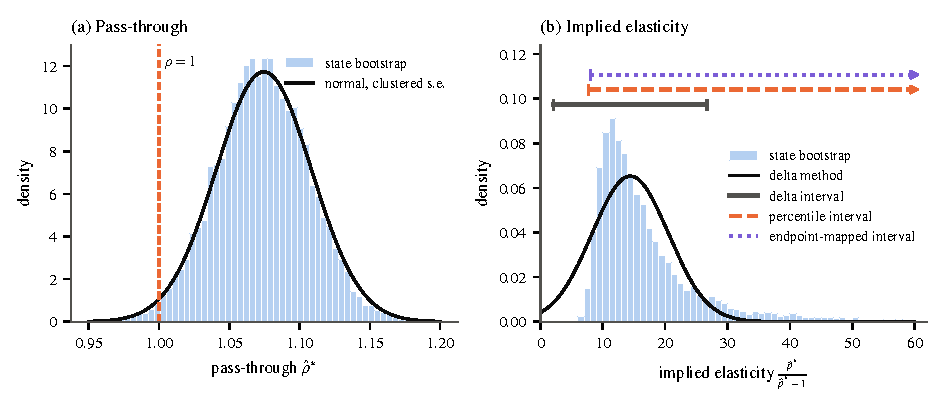
\includegraphics[width=\textwidth]{figures/appA/delta_boot.pdf}
\caption{State-cluster bootstrap of the cigarette tax pass-through regression with state and year effects. (a)
9,999 bootstrap estimates $\hat\rho^*$ and the normal density with the state-clustered standard error.
(b) Implied elasticity $\frac{\hat\rho^*}{\hat\rho^* - 1}$ and the delta-method normal density. The
horizontal bars are 95 percent intervals: delta method $[2.1, 26.7]$, bootstrap percentile $[7.7, 68.9]$, and the
mapped endpoints of the clustered interval for $\rho$, $[8.0, 162.9]$. Arrows mark intervals that extend beyond
the plotted range. 4.4 percent of the bootstrap elasticities lie outside $[0, 60]$ and are not plotted. Seed
20261022.}
\label{fig:A-delta-boot}
\end{figure}

\casehead{The Sumner panel}
We apply a pairs cluster bootstrap by state to row (1) of \cref{tab:A-sumner}, with $B = 9{,}999$. Each replication
draws 48 states with replacement, treats repeated states as distinct, and re-estimates \eqref{eq:A-sumner} with state
and year effects. The bootstrap standard error of $\hat\rho$ is 0.033, close to the clustered 0.034 and to the
jackknife value of 0.034 obtained by deleting one state at a time. \Cref{tab:A-boot-intervals} compares intervals.
For $\rho$, all methods give similar intervals that exclude one. The bootstrap distribution in
\cref{fig:A-delta-boot}(a) is close to normal, and 1.3 percent of the bootstrap estimates are at or below one.

\begin{table}[htbp]
\centering
\begin{threeparttable}
\caption{95 percent intervals for pass-through and the implied elasticity}
\label{tab:A-boot-intervals}
\small
\begin{tabular}{@{}lcc@{}}
\toprule
Method & $\rho$ & $\varepsilon = \frac{\rho}{\rho - 1}$ \\
\midrule
Clustered $t_{47}$ interval, delta method for $\varepsilon$ & $[1.006,\ 1.143]$ & $[2.1,\ 26.7]$ \\
Clustered $t_{47}$ interval, endpoints mapped & $[1.006,\ 1.143]$ & $[8.0,\ 162.9]$ \\
Bootstrap percentile & $[1.008,\ 1.137]$ & $[7.7,\ 68.9]$ \\
Bootstrap percentile for $\rho$, endpoints mapped & & $[8.3,\ 126.8]$ \\
Bootstrap basic & $[1.012,\ 1.141]$ & $[-40.1,\ 21.1]$ \\
Bootstrap percentile-$t$ & $[1.012,\ 1.143]$ & \\
Bootstrap BCa, endpoints mapped for $\varepsilon$ & $[1.012,\ 1.142]$ & $[8.0,\ 81.2]$ \\
\bottomrule
\end{tabular}
\begin{tablenotes}\footnotesize
\item Notes: Row (1) of \cref{tab:A-sumner}, $\hat\rho = 1.075$ and $\hat\varepsilon = 14.4$. Pairs cluster bootstrap
by state with 9,999 replications. The percentile-$t$ interval studentizes with the CR1 standard error in each
replication. BCa uses the jackknife over states for the acceleration ($\hat a = 0.019$, $z_0 = 0.030$).
\end{tablenotes}
\end{threeparttable}
\end{table}

For the elasticity the methods disagree sharply. Because 1.3 percent of the $\hat\rho^*$ lie below one, the same
share of bootstrap elasticities is negative and huge in magnitude. The percentile interval for $\varepsilon$ is
then not the image of the percentile interval for $\rho$. The map $\frac{\rho}{\rho - 1}$ is monotone on each side of
one, but not over the whole bootstrap support, so the transformation-respecting property fails. The basic interval
reflects the long right tail to the left and includes negative elasticities, which makes no economic sense. The
bootstrap standard deviation of the elasticity is 222, a meaningless number. The ratio has no finite moments
whenever the distribution of its denominator has positive density at zero. Intervals for $\varepsilon$ should be
built from an interval for $\rho$ and mapped through the monotone function, as in the second and last rows.

\subsection{Multi-step estimators and counterfactuals}\label{sec:A-boot-multistep}

The bootstrap's main practical advantage is that it handles estimators built in several steps. The rule is simple:
every step that uses the data must be repeated in every replication. Holding a first-step estimate fixed omits its
sampling variance, the problem that the analytical correction of \cref{prop:A-twostep} addresses. Two examples
recur in the book.

The first is a generated regressand. Marginal costs implied by a logit pricing condition, $mc_{jt} = p_{jt} -
\frac{1}{\hat\alpha(1 - S_{ft})}$, depend on the demand estimate $\hat\alpha$. Regressing them on cost shifters with
the usual standard errors treats $\hat\alpha$ as known. A market bootstrap that re-estimates $\alpha$ in each of 5,000
replications raises the standard error of the intercept from 0.016 to 0.072 in the simulated markets of
\cref{sec:C-logit-est}. The slopes barely change, because uncertainty about $\alpha$ moves all markups together.

The second is a counterfactual. \citet[WP p.~25]{ChaudhuriGoldbergJia2006} compute standard errors for counterfactual
prices and welfare losses under patent enforcement by bootstrapping the original sample 300 times. For each sample
they re-estimate the demand system and recompute the counterfactual equilibrium prices and welfare losses for each
policy scenario. When a replication's counterfactual did not converge, they compute the standard errors from the
replications that did (WP p.~25, n.~29). Dropping failed replications is common but not innocuous. If failures
occur for particular parameter values, the retained replications are a selected sample of the bootstrap distribution.

\casehead{Parametric bootstrap and parameter draws}
Two cheaper procedures are often called a parametric bootstrap, and they differ. The first simulates new data sets
from the fitted model $F(\cdot;\hat\theta)$ and re-estimates on each. It is the natural way to compute the null
distribution of a specification test whose statistic has no tractable limit. \citet[p.~241]{AtheyLevinSeira2011}
use it for the conditional Kolmogorov test of \citet{Andrews1997} and cannot reject their parametric bid model even at
the 20 percent level. The second draws parameter vectors from the estimated asymptotic distribution
$N(\hat\theta, \hat V)$ and recomputes the statistic of interest without re-estimating
(\cref{rem:A-krinsky-robb}). Athey, Levin and Seira use this second procedure for the predicted outcomes of their
Table~V (p.~248), as do \citet{Nevo2001} and \citet{Gentzkow2007}.

The validity conditions follow from what each procedure resamples. Parameter draws are valid when $\hat\theta$ is
approximately normal and $a$ is smooth. They are first-order equivalent to the delta method and cost one evaluation
of $a$ per draw. Re-estimating on resampled data also captures departures of $\hat\theta$ from normality, and it is
the only one of the three that can deliver a refinement. It is also the most expensive. \citet[p.~733,
n.~33]{Gentzkow2007} notes that bootstrapping would require estimating all parameters for each resample, which adds
greatly to the computational cost.

\subsection{When the bootstrap fails}\label{sec:A-boot-fail}

Bootstrap consistency rests on the statistic being a smooth function of the empirical distribution. Without
smoothness it can fail, and the canonical example is an extreme order statistic.

\begin{proposition}[The bootstrap of a sample maximum]\label{prop:A-boot-max}
Let $X_1, \dots, X_n$ be i.i.d.\ uniform on $[0, \theta]$ and $\hat\theta = \max_iX_i$. Then
$\frac{n(\theta - \hat\theta)}{\theta}$ converges in distribution to the standard exponential distribution, which is
continuous (\cref{prop:A-uniform-mle}). For the nonparametric bootstrap,
\begin{equation*}
  \Pr^*\bigl(\hat\theta^* = \hat\theta\bigr) = 1 - \Bigl(1 - \frac{1}{n}\Bigr)^n \longrightarrow 1 - e^{-1} \approx 0.632.
\end{equation*}
The bootstrap distribution of $\frac{n(\hat\theta - \hat\theta^*)}{\hat\theta}$ has an atom of mass about 0.632 at
zero and does not converge to the exponential limit.
\end{proposition}

\begin{proof}
The bootstrap maximum equals $\hat\theta$ if and only if the largest observation is drawn at least once. Each of the
$n$ independent draws misses it with probability $1 - \frac{1}{n}$, so it is never drawn with probability
$(1 - \frac{1}{n})^n$. Taking logs, $n\ln(1 - \frac{1}{n}) = n(-\frac{1}{n} - \frac{1}{2n^2} - \cdots) \to -1$, so
$(1 - \frac{1}{n})^n \to e^{-1}$. A limit distribution with an atom of mass $1 - e^{-1}$ at zero cannot equal the
continuous exponential distribution.
\end{proof}

The probability is already close to its limit in small samples: 0.651 for $n = 10$, 0.634 for $n = 100$ and 0.632
for $n = 1{,}000$. The intuition is that the bootstrap cannot draw values beyond the sample maximum, while the
sampling distribution of $\hat\theta$ is driven by how far the maximum falls short of the true endpoint.

The same failure appears in other non-regular problems. Parameters on the boundary of the parameter space, such as a
zero variance component, invalidate the bootstrap of the estimator \citep{Andrews2000}. Non-smooth functionals,
such as bounds formed as the maximum or minimum of estimated functions, behave like the maximum above
(\cref{sec:A-partialid}). With weak instruments the estimator is not asymptotically normal and the bootstrap does not
fix it (\cref{sec:A-weakiv}). Data with infinite variance are a further case, since the bootstrap of the sample mean
then fails. A statistic without finite moments, like the elasticity ratio above, needs a separate diagnosis. Missing
moments alone do not make the bootstrap distribution inconsistent. When the true $\rho$ is bounded away from one, the
map $\frac{\rho}{\rho - 1}$ is smooth near it. The extension of \cref{prop:A-boot-mean} to smooth functions of means
then makes the bootstrap distribution of $\sqrt n(\hat\varepsilon^* - \hat\varepsilon)$ consistent, although
$\hat\varepsilon$ has no finite moments in any finite sample. What can fail are summaries that estimate
finite-sample moments, such as the bootstrap standard deviation, because the moments they target do not exist. A true denominator at zero, or close to zero relative to its sampling error, is a
genuine non-regularity like a weak instrument. The Sumner estimate of $\rho$, about two standard errors above one, is
close to that case. Two remedies are general \citep{PolitisRomanoWolf1999}. \emph{Subsampling} recomputes the statistic on
subsamples of size $b$ drawn without replacement, with $b \to \infty$ and $\frac{b}{n} \to 0$, and rescales by the
known rate. The \emph{$m$-out-of-$n$ bootstrap} draws $m < n$ observations with replacement, with $\frac{m}{n} \to 0$.
Both work under much weaker conditions because a small subsample behaves like a fresh sample from the population.
The relevance for this book is direct. Auction models whose bid support depends on the parameters
\citep{DonaldPaarsch1996}, estimators built on extreme order statistics, and partially identified models
(\cref{ch:auction-empirics}) all fall outside the standard bootstrap's guarantees.

\section{Nonparametric estimation of distributions and densities}\label{sec:A-kde}

The estimators of the previous sections are parametric, in the sense that a finite-dimensional $\theta$ indexes
the model. Several of the book's estimators instead recover an unknown distribution without a parametric family. The
structural auction literature is the main user. The value distribution of an ascending auction is
recovered from the distribution of transaction prices. In a first-price auction it is recovered from the
distribution and density of bids (\cref{ch:auction-empirics}). Bidding
rings and procurement auctions with unobserved heterogeneity add a deconvolution step
(\cref{ch:collusion-evidence}), and hedonic demand models use nonparametric regression
(\cref{ch:discrete}). This section develops the estimators of distribution functions and densities on
which these applications rest. \Cref{sec:A-npreg} turns to regression, deconvolution and bounds.

The notation is local to these two sections. A \emph{kernel} $\mathcal{K}$ is a weighting function,
$h>0$ is a \emph{bandwidth}, and $\mathcal{K}_h(u)=\frac{1}{h}\mathcal{K}(\frac{u}{h})$. The constants
$\mu_2=\int u^2\mathcal{K}(u)\,\dd u$ and $\kappa_2=\int\mathcal{K}(u)^2\,\dd u$ are the second moment
and the roughness of the kernel, and $R$ counts the derivatives of the target function. In the auction
applications we follow \citet{GuerrePerrigneVuong2000}, hereafter GPV, and write $L$ for the number of
auctions. In these two sections $L$ is therefore neither a Lerner index nor a number of instruments. Each auction has $N$
bidders (GPV write $I$), bids are $B_{il}$, and the bid distribution and density are $G$ and $g$.

\subsection{The empirical distribution function}\label{sec:A-ecdf}

Let $X_1,\dots,X_n$ be independent draws from a distribution function $F$ on $\R$. The
\emph{empirical distribution function} puts mass $\frac{1}{n}$ on each observation:
\begin{equation}\label{eq:A-ecdf}
\hat F_n(x)=\frac{1}{n}\sum_{i=1}^{n}\indic\{X_i\le x\}.
\end{equation}

\begin{proposition}[Properties of the empirical distribution function]\label{prop:A-ecdf}
Let $X_1,\dots,X_n$ be i.i.d.\ with distribution function $F$.
\begin{enumerate}[label=(\roman*)]
\item For every $x$, $\E[\hat F_n(x)]=F(x)$ and $\Var(\hat F_n(x))=\frac{F(x)(1-F(x))}{n}$.
\item For every $x$, $\sqrt n(\hat F_n(x)-F(x))\xrightarrow{d}N(0,F(x)(1-F(x)))$.
\item (Glivenko-Cantelli) $\sup_x|\hat F_n(x)-F(x)|\to0$ almost surely.
\item (Dvoretzky-Kiefer-Wolfowitz) For every $\epsilon>0$,
$\Pr\left(\sup_x|\hat F_n(x)-F(x)|>\epsilon\right)\le2e^{-2n\epsilon^2}$.
\end{enumerate}
\end{proposition}

\begin{proof}
For fixed $x$ the indicators $\indic\{X_i\le x\}$ are i.i.d.\ Bernoulli variables with success probability
$F(x)$. Their mean is $F(x)$ and their variance is $F(x)(1-F(x))$. Averaging $n$ of them divides the
variance by $n$, which proves (i). Part (ii) is the Lindeberg-L\'evy central limit theorem applied to the
same Bernoulli average. Parts (iii) and (iv) are classical uniform results. The constant 2 in front of
the exponential in (iv) is due to \citet{Massart1990}.
\end{proof}

Part (iv) yields a confidence band that holds for all $x$ at once. Setting $2e^{-2n\epsilon^2}=\alpha$
gives $\epsilon_\alpha=\sqrt{\frac{\ln(\frac{2}{\alpha})}{2n}}$, and the band
$\hat F_n(x)\pm\epsilon_\alpha$ contains the whole function $F$ with probability at least $1-\alpha$. With
$n=200$ and $\alpha=0.05$ the half-width is about 0.096. The band needs no smoothing and no
estimate of a density, which makes the empirical distribution function the natural first step of every
estimator in this section.

\casehead{Order-statistic inversion}
In a second-price or ascending auction with symmetric independent private values, the price equals
the second-highest value (\cref{ch:auction-theory}). Suppose we observe only prices $w_l$ from $L_N$
auctions with $N$ bidders each. The price is $v_{(N-1:N)}$, and its distribution function is
\begin{equation}\label{eq:A-phiN}
F_w(v)=\Pr\left(v_{(N-1:N)}\le v\right)=\phi_N(F(v)),\qquad \phi_N(x)=Nx^{N-1}(1-x)+x^N .
\end{equation}
The second-highest value lies below $v$ exactly when at least $N-1$ of the $N$ values do. The first term
of $\phi_N$ is the probability that exactly $N-1$ values lie below $v$, and the second that all $N$ do.
The derivative is
\begin{equation*}
\phi_N'(x)=N(N-1)x^{N-2}(1-x)-Nx^{N-1}+Nx^{N-1}=N(N-1)x^{N-2}(1-x),
\end{equation*}
which is positive on $(0,1)$. So $\phi_N$ is a strictly increasing bijection of $[0,1]$, and
$F(v)=\phi_N^{-1}(F_w(v))$. More generally, the $k$-th lowest of $N$ i.i.d.\ draws has distribution
function
\begin{equation}\label{eq:A-orderstat}
F_{(k:N)}(v)=\frac{N!}{(N-k)!\,(k-1)!}\int_0^{F(v)}t^{k-1}(1-t)^{N-k}\,\dd t ,
\end{equation}
which is strictly increasing in $F(v)$ \citep[eq.~(5)]{AtheyHaile2002}. Any single order statistic with
known $N$ therefore identifies $F$, and \eqref{eq:A-phiN} is the case $k=N-1$.

The plug-in estimator replaces $F_w$ by the empirical distribution function of the prices,
$\hat F(v)=\phi_N^{-1}(\hat F_w(v))$, computed by bisection at each $v$.

\begin{proposition}[Order-statistic inversion]\label{prop:A-os-inversion}
Let $w_1,\dots,w_{L_N}$ be i.i.d.\ prices from $N$-bidder auctions and let $0<F(v)<1$. Then
$\hat F(v)\xrightarrow{p}F(v)$ and
\begin{equation}\label{eq:A-os-avar}
\sqrt{L_N}\left(\hat F(v)-F(v)\right)\xrightarrow{d}
N\!\left(0,\ \frac{F_w(v)(1-F_w(v))}{\phi_N'(F(v))^2}\right).
\end{equation}
\end{proposition}

\begin{proof}
Consistency follows from \cref{prop:A-ecdf}(i) and the continuity of $\phi_N^{-1}$. The inverse
function theorem gives $\frac{\dd}{\dd y}\phi_N^{-1}(y)=\frac{1}{\phi_N'(\phi_N^{-1}(y))}$, which is
finite because $\phi_N'(F(v))>0$. The delta method (\cref{thm:A-delta}) applied to
\cref{prop:A-ecdf}(ii) multiplies the asymptotic variance $F_w(1-F_w)$ by the square of this
derivative.
\end{proof}

The variance in \eqref{eq:A-os-avar} measures what is lost by observing one order statistic. If all $N$
values of each auction were recorded, the empirical distribution function of the $NL_N$ values would
have asymptotic variance $\frac{F(1-F)}{N}$ per auction. With $N=4$ and $F(v)=0.5$, the price-only
variance is 0.0955 against 0.0625, a ratio of 1.53. At $F(v)=0.2$ the ratio is 4.49, and with $N=6$ at
the same point it reaches 40.6. The price is the second-highest value, so it carries little information about the lower
tail, and the loss grows with $N$. These numbers come from \texttt{kernel\_constants.py}.

Two extensions matter in practice. First, the inversion delivers one estimate of $F$ for each $N$ in the
data. If participation varies independently of values, all these estimates must coincide, which is a
testable restriction \citep[Theorem~1]{AtheyHaile2002}. The estimates from different $N$ are
independent, so a Wald-type comparison at a point $v$ divides their difference by the square root of the
sum of the two variances in \eqref{eq:A-os-avar}. Second, with a binding reserve price $r$ the price is
$\max\{v_{(N-1:N)},r\}$, and $F$ is identified only above $r$. \Cref{ch:auction-empirics} develops the
identification argument, and \cref{sec:A-partialid} returns to ascending auctions in which recorded bids
are not values.

\subsection{The kernel density estimator}\label{sec:A-kde-estimator}

A histogram estimates a density by counting observations in bins of width $2h$. It depends on the bin
origin, and it is discontinuous. The kernel estimator centers a smooth bump on each observation
instead \citep{Rosenblatt1956,Parzen1962}:
\begin{equation}\label{eq:A-kde}
\hat f_h(x)=\frac{1}{nh}\sum_{i=1}^{n}\mathcal{K}\!\left(\frac{x-X_i}{h}\right)
=\frac{1}{n}\sum_{i=1}^{n}\mathcal{K}_h(x-X_i).
\end{equation}
With the uniform kernel $\mathcal{K}(u)=\frac{1}{2}\indic\{|u|\le1\}$, $\hat f_h(x)$ is the share of
observations within $h$ of $x$ divided by $2h$, a histogram whose bin moves with $x$.

\begin{definition}[Second-order kernel]\label{def:A-kernel}
A \emph{second-order kernel} is a bounded function $\mathcal{K}$ with $\int\mathcal{K}(u)\,\dd u=1$,
$\int u\mathcal{K}(u)\,\dd u=0$, $0<\mu_2=\int u^2\mathcal{K}(u)\,\dd u<\infty$ and
$\kappa_2=\int\mathcal{K}(u)^2\,\dd u<\infty$. A bounded symmetric density with finite variance is a
second-order kernel.
\end{definition}

\begin{assumption}[Pointwise kernel asymptotics]\label{ass:A-kde}
The draws $X_1,\dots,X_n$ are i.i.d.\ with density $f$. In a neighborhood of the point $x$, $f$ is twice
continuously differentiable with bounded second derivative. The kernel is second order, and the bandwidth
satisfies $h\to0$ and $nh\to\infty$.
\end{assumption}

\begin{proposition}[Bias and variance of the kernel density estimator]\label{prop:A-kde-bias-var}
Under \cref{ass:A-kde},
\begin{equation}\label{eq:A-kde-bias-var}
\E[\hat f_h(x)]-f(x)=\frac{h^2}{2}\mu_2f''(x)+o(h^2),\qquad
\Var(\hat f_h(x))=\frac{f(x)\kappa_2}{nh}+o\!\left(\frac{1}{nh}\right).
\end{equation}
\end{proposition}

\begin{proof}
\emph{Bias.} The summands of \eqref{eq:A-kde} are i.i.d., so
\begin{equation*}
\E[\hat f_h(x)]=\int\frac{1}{h}\mathcal{K}\!\left(\frac{x-y}{h}\right)f(y)\,\dd y
=\int\mathcal{K}(u)f(x-hu)\,\dd u ,
\end{equation*}
where we substituted $y=x-hu$ and $\dd y=-h\,\dd u$. A second-order Taylor expansion with mean-value
point $\tilde x_u$ between $x$ and $x-hu$ gives
\begin{equation*}
f(x-hu)=f(x)-huf'(x)+\frac{h^2u^2}{2}f''(\tilde x_u).
\end{equation*}
Integrating against $\mathcal{K}$, the first term returns $f(x)$ and the second vanishes because
$\int u\mathcal{K}=0$. The third equals $\frac{h^2}{2}\int u^2\mathcal{K}(u)f''(\tilde x_u)\,\dd u$, which
is $\frac{h^2}{2}\mu_2f''(x)+o(h^2)$ by continuity of $f''$ and dominated convergence.

\emph{Variance.} Again by independence,
\begin{equation*}
\Var(\hat f_h(x))=\frac{1}{n}\left\{\E\left[\mathcal{K}_h(x-X)^2\right]-\left(\E[\mathcal{K}_h(x-X)]\right)^2\right\}.
\end{equation*}
The same substitution gives
$\E[\mathcal{K}_h(x-X)^2]=\frac{1}{h}\int\mathcal{K}(u)^2f(x-hu)\,\dd u=\frac{f(x)\kappa_2}{h}+O(1)$.
The squared mean is $f(x)^2+O(h^2)=O(1)$. Hence
$\Var(\hat f_h(x))=\frac{f(x)\kappa_2}{nh}+O(\frac{1}{n})$, and $\frac{1}{n}=o(\frac{1}{nh})$ because
$h\to0$.
\end{proof}

The proposition displays the basic trade-off of nonparametric estimation. A small bandwidth averages
few observations, so the variance is large. A large bandwidth averages over a region where $f$ curves,
so the bias is large. The variance is of order $\frac{1}{nh}$ because only about $2nhf(x)$ observations
fall in the kernel window, which is slower than the parametric $\frac{1}{n}$. Under the same conditions
a Lindeberg argument gives
$\sqrt{nh}\,(\hat f_h(x)-\E[\hat f_h(x)])\xrightarrow{d}N(0,f(x)\kappa_2)$.

\casehead{Optimal bandwidth}
The \emph{mean integrated squared error} is
$\mathrm{MISE}(h)=\E\int(\hat f_h(x)-f(x))^2\,\dd x$, the integral of squared bias plus variance.
Integrating the leading terms of \eqref{eq:A-kde-bias-var} and using $\int f=1$ gives the
\emph{asymptotic MISE}
\begin{equation}\label{eq:A-amise}
\mathrm{AMISE}(h)=\frac{h^4}{4}\mu_2^2\,\mathcal{R}(f'')+\frac{\kappa_2}{nh},\qquad
\mathcal{R}(f'')=\int f''(x)^2\,\dd x .
\end{equation}
The first-order condition $h^3\mu_2^2\mathcal{R}(f'')-\frac{\kappa_2}{nh^2}=0$ yields
\begin{equation}\label{eq:A-hstar}
h^*=\left[\frac{\kappa_2}{\mu_2^2\,\mathcal{R}(f'')\,n}\right]^{\frac{1}{5}} .
\end{equation}
At $h^*$ the squared-bias term equals one quarter of the variance term, so
\begin{equation*}
\mathrm{AMISE}(h^*)=\frac{5}{4}\,\frac{\kappa_2}{nh^*}
=\frac{5}{4}\left(\sqrt{\mu_2}\,\kappa_2\right)^{\frac{4}{5}}\mathcal{R}(f'')^{\frac{1}{5}}\,n^{-\frac{4}{5}} .
\end{equation*}
The optimal bandwidth shrinks like $n^{-\frac{1}{5}}$ and the error falls like $n^{-\frac{4}{5}}$, against
$n^{-1}$ for a correctly specified parametric model.

\casehead{Silverman's rule of thumb}
The unknown $\mathcal{R}(f'')$ in \eqref{eq:A-hstar} can be replaced by its value for a reference
density. Take $f$ normal with variance $\sigma^2$ and the Gaussian kernel, for which $\mu_2=1$ and
$\kappa_2=\frac{1}{2\sqrt\pi}$. Write $f(x)=\frac{1}{\sigma}\phi(\frac{x}{\sigma})$ with $\phi$ the
standard normal density. Then $f''(x)=\sigma^{-3}\phi''(\frac{x}{\sigma})$ and
$\phi''(u)=(u^2-1)\phi(u)$, so
\begin{equation*}
\mathcal{R}(f'')=\sigma^{-5}\int(u^2-1)^2\phi(u)^2\,\dd u .
\end{equation*}
Now $\phi(u)^2=\frac{1}{2\sqrt\pi}\,\psi(u)$, where $\psi$ is the $N(0,\frac{1}{2})$ density. For
$U\sim N(0,\frac{1}{2})$ we have $\E[U^2]=\frac{1}{2}$ and $\E[U^4]=\frac{3}{4}$, so
$\E[(U^2-1)^2]=\frac{3}{4}-1+1=\frac{3}{4}$. Therefore
\begin{equation*}
\mathcal{R}(f'')=\frac{3}{8\sqrt\pi\,\sigma^5},\qquad
(h^*)^5=\frac{\frac{1}{2\sqrt\pi}}{\frac{3}{8\sqrt\pi\,\sigma^5}\,n}=\frac{4}{3}\,\frac{\sigma^5}{n},
\end{equation*}
and
\begin{equation}\label{eq:A-silverman}
h_{\mathrm{ROT}}=\left(\frac{4}{3}\right)^{\frac{1}{5}}\sigma n^{-\frac{1}{5}}\approx1.06\,\sigma n^{-\frac{1}{5}} .
\end{equation}
This is the \emph{rule of thumb} of \citet{Silverman1986}, with $\sigma$ replaced by the sample standard
deviation. It is optimal for normal data and oversmooths densities with more curvature, such as
multimodal ones, because those have larger $\mathcal{R}(f'')$.

\casehead{Choice of kernel}
The kernel enters \eqref{eq:A-hstar} only through $\delta_{\mathcal{K}}=(\frac{\kappa_2}{\mu_2^2})^{\frac{1}{5}}$,
and the minimized AMISE only through $\sqrt{\mu_2}\,\kappa_2$. Two consequences follow. A bandwidth
rule derived for one kernel converts to another kernel by the factor
$\frac{\delta_{\mathcal{K}}}{\delta_{\phi}}$, whatever $f$ is. And kernels differ little in efficiency
once their bandwidths are scaled correctly. \Cref{tab:A-kernels} reports the constants. Among nonnegative
kernels the Epanechnikov kernel minimizes $\sqrt{\mu_2}\,\kappa_2$, and every other kernel in the table
attains at least 92.9 percent of its efficiency. The restriction to nonnegative kernels matters, because
\cref{def:A-kernel} allows negative values. Put weight $\lambda$ on the Epanechnikov kernel and $1 - \lambda$
on a bounded kernel of order four with compact support (\cref{sec:A-kde-higher}). The mixture is a second-order
kernel with $\mu_2 = \frac{\lambda}{5}$ and bounded $\kappa_2$, so its criterion tends to zero as $\lambda \to 0$.

\begin{table}[htbp]
\centering
\caption{Second-order kernels and their constants}\label{tab:A-kernels}
\begin{tabular}{lccccccc}
\toprule
Kernel & $\mathcal{K}(u)$ & $\mu_2$ & $\kappa_2$ & $\int\mathcal{K}'(u)^2\dd u$ & $\int_0^\infty u\mathcal{K}(u)\dd u$
 & $\frac{\delta_{\mathcal{K}}}{\delta_\phi}$ & Efficiency \\
\midrule
Uniform & $\frac{1}{2}$ & $\frac{1}{3}$ & $\frac{1}{2}$ & n.a. & $\frac{1}{4}$ & 1.740 & 0.930 \\[2pt]
Epanechnikov & $\frac{3}{4}(1-u^2)$ & $\frac{1}{5}$ & $\frac{3}{5}$ & $\frac{3}{2}$ & $\frac{3}{16}$ & 2.214 & 1.000 \\[2pt]
Biweight & $\frac{15}{16}(1-u^2)^2$ & $\frac{1}{7}$ & $\frac{5}{7}$ & $\frac{15}{7}$ & $\frac{5}{32}$ & 2.623 & 0.994 \\[2pt]
Triweight & $\frac{35}{32}(1-u^2)^3$ & $\frac{1}{9}$ & $\frac{350}{429}$ & $\frac{35}{11}$ & $\frac{35}{256}$ & 2.978 & 0.987 \\[2pt]
Gaussian & $\phi(u)$ & $1$ & $\frac{1}{2\sqrt\pi}$ & $\frac{1}{4\sqrt\pi}$ & $\frac{1}{\sqrt{2\pi}}$ & 1.000 & 0.951 \\
\bottomrule
\end{tabular}
\par\smallskip
\begin{minipage}{0.97\textwidth}
\footnotesize Notes: the first four kernels are zero outside $|u|\le1$. The column
$\frac{\delta_{\mathcal{K}}}{\delta_\phi}$ is the factor that converts a bandwidth rule for the Gaussian
kernel into the corresponding rule for kernel $\mathcal{K}$, with
$\delta_{\mathcal{K}}=(\frac{\kappa_2}{\mu_2^2})^{\frac{1}{5}}$. Efficiency is $\sqrt{\mu_2}\,\kappa_2$ of
the Epanechnikov kernel divided by $\sqrt{\mu_2}\,\kappa_2$ of the kernel in the row. It is the ratio of
sample sizes that gives the two kernels the same minimized AMISE. The
derivative roughness $\int\mathcal{K}'^2$ enters the variance of density-derivative estimators
(\cref{prop:A-kde-derivative}). The uniform kernel is not differentiable. All constants are computed
exactly with sympy in \texttt{kernel\_constants.py}.
\end{minipage}
\end{table}

The auction literature uses the triweight kernel almost exclusively. It has compact support, so
trimmed observations drop out of the estimate, and it is continuously differentiable on the whole line,
including the end points of its support. \citet[p.~532]{GuerrePerrigneVuong2000} chose it to satisfy
their kernel assumptions. \citet[p.~180]{LiPerrigneVuong2002} and \citet[Section~4.3]{Krasnokutskaya2011}\footnote{We use the
working-paper version of \citet{Krasnokutskaya2011} dated May 24, 2004 (PIER Working Paper 05-006), and equation,
section, lemma and proposition numbers refer to it.}
give the differentiability at the boundary as the reason. These authors also illustrate the conversion
factor. \citeauthor{LiPerrigneVuong2002} and \citeauthor{Krasnokutskaya2011} set the bandwidth constant
to $2.978\times1.06\,\hat\sigma$, and 2.978 is the triweight entry in the
$\frac{\delta_{\mathcal{K}}}{\delta_\phi}$ column. \citet[p.~532]{GuerrePerrigneVuong2000} and
\citet[p.~749]{Asker2010} use $1.06\,\hat\sigma$ with the same kernel, a bandwidth about one third of the
normal-reference rule for that kernel.

The exponents of the sample size also differ across these papers. GPV set $h_g=1.06\,\hat\sigma_b(NL)^{-\frac{1}{5}}$
for the bid density, with $\hat\sigma_b$ the standard deviation of the bids and $NL$ the number of bids (p.~532).
\citet[p.~749]{Asker2010} uses $1.06\,\hat\sigma n^{-\frac{1}{6}}$ for densities and $1.06\,\hat\sigma n^{-\frac{1}{5}}$
for kernel-smoothed distribution functions. \citet[Section~4.3]{Krasnokutskaya2011} uses
$2.978\times1.06\,\hat\sigma L^{-\frac{1}{6}}$, with $L$ her sample size and $\hat\sigma$ the standard deviation of
the log of one plus the bids, and says that she follows GPV. The rates of \cref{sec:A-kde-higher} explain the pattern. With $R$
derivatives of the value density and $d$ continuous covariates, GPV's bandwidths for the bid distribution and the bid
density shrink like $L^{-\frac{1}{2R+d+2}}$ and $L^{-\frac{1}{2R+d+3}}$, up to logarithms. With $R=1$ and no
covariates the density exponent is $-\frac{1}{5}$, GPV's own choice. With $R=1$ and $d=1$ the two exponents are
$-\frac{1}{5}$ and $-\frac{1}{6}$, the pair that Asker uses. Neither Asker nor Krasnokutskaya derives an exponent. In a
one-dimensional problem $L^{-\frac{1}{6}}$ shrinks more slowly than $L^{-\frac{1}{5}}$, so their bandwidths oversmooth
slightly relative to GPV's rule. Oversmoothing lowers the variance of $\hat g$ at the cost of more bias.

\Cref{fig:A-kde} illustrates the trade-off with a bimodal density,
$f=0.6\,N(0,1)+0.4\,N(2.5,0.5^2)$, and $n=200$. Panel (a) shows one sample. Halving the optimal
bandwidth produces spurious bumps, and doubling it blurs the two modes into a plateau. Panel (b) plots
the exact integrated squared bias, integrated variance and MISE against $h$, with Monte Carlo averages
over 1,000 samples as markers. The exact MISE is minimized at $h^*=0.291$, where the integrated
squared bias is 0.0014 and the integrated variance 0.0039. The AMISE formula \eqref{eq:A-hstar} gives
0.262. Its quartic bias term overstates the bias at large $h$, which pulls the AMISE minimizer to the
left.

\begin{figure}[htbp]
\centering
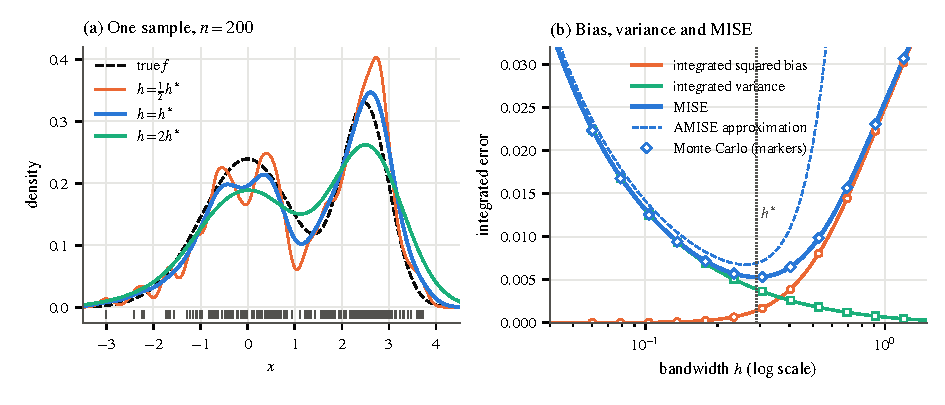
\includegraphics[width=\textwidth]{figures/appA/kde.pdf}
\caption{Bandwidth choice for a kernel density estimator. The true density is
$0.6\,N(0,1)+0.4\,N(2.5,0.5^2)$, the kernel is Gaussian and $n=200$. (a) One sample (the
median of 101 fresh samples by integrated squared error at $h^*$), with estimates at
$\frac{1}{2}h^*$, $h^*$ and $2h^*$, where $h^*=0.291$ minimizes the exact MISE. (b) Exact
integrated squared bias, integrated variance and MISE (solid lines), the AMISE approximation
\eqref{eq:A-amise} (dashed) and Monte Carlo averages over 1,000 samples (markers). Seed 20261022,
script \texttt{kde\_demo.py}.}
\label{fig:A-kde}
\end{figure}

\subsection{Smoothness, higher-order kernels and derivatives}\label{sec:A-kde-higher}

The $h^2$ bias of \cref{prop:A-kde-bias-var} comes from the second moment of the kernel. If $f$ has more
derivatives, kernels with more vanishing moments reduce the bias further.

\begin{definition}[Kernel of order $R$]\label{def:A-kernel-order}
A kernel $\mathcal{K}$ is of \emph{order} $R\ge2$ if $\int\mathcal{K}=1$,
$\mu_j=\int u^j\mathcal{K}(u)\,\dd u=0$ for $j=1,\dots,R-1$, and $0<|\mu_R|<\infty$.
\end{definition}

If $f$ has $R$ bounded continuous derivatives near $x$ and $\mathcal{K}$ is of order $R$, the expansion in
the proof of \cref{prop:A-kde-bias-var}, carried to order $R$, gives
\begin{equation}\label{eq:A-kde-bias-R}
\E[\hat f_h(x)]-f(x)=\sum_{j=1}^{R}\frac{(-h)^j}{j!}\mu_jf^{(j)}(x)+o(h^R)
=\frac{(-h)^R}{R!}\mu_Rf^{(R)}(x)+o(h^R).
\end{equation}
The variance is unchanged at order $\frac{1}{nh}$. Balancing $h^{2R}$ against $\frac{1}{nh}$ gives
$h\propto n^{-\frac{1}{2R+1}}$ and a root mean squared error of order $n^{-\frac{R}{2R+1}}$.
\citet{Stone1982} showed that $(\frac{n}{\log n})^{\frac{R}{2R+1}}$ is the best possible rate for
estimating such a density uniformly over a compact set. The logarithm is the price of uniformity.

For $R>2$ the kernel must take negative values, since $\mu_2=0$ is impossible for a nonnegative
function. Density estimates can then be negative. In the auction setting this has a concrete cost. A
negative estimated bid density produces pseudo-values below the corresponding bids, so
\citet[p.~180]{LiPerrigneVuong2002} keep second-order kernels in their three-bidder design even though
their theory calls for order three.

\casehead{Derivatives of a density}
Differentiating \eqref{eq:A-kde} gives an estimator of the derivative,
\begin{equation}\label{eq:A-kde-deriv}
\hat f_h'(x)=\frac{1}{nh^2}\sum_{i=1}^{n}\mathcal{K}'\!\left(\frac{x-X_i}{h}\right).
\end{equation}

\begin{proposition}[Rate for a density derivative]\label{prop:A-kde-derivative}
Let $\mathcal{K}$ be a continuously differentiable kernel of order $R$ that vanishes outside $[-1,1]$, and
let $f$ have $R+1$ bounded continuous derivatives near $x$. If $h\to0$ and $nh^3\to\infty$, then
\begin{equation*}
\E[\hat f_h'(x)]-f'(x)=\frac{(-h)^R}{R!}\mu_Rf^{(R+1)}(x)+o(h^R),\qquad
\Var(\hat f_h'(x))=\frac{f(x)\int\mathcal{K}'(u)^2\dd u}{nh^3}+o\!\left(\frac{1}{nh^3}\right).
\end{equation*}
The mean squared error is minimized by $h\propto n^{-\frac{1}{2R+3}}$, and the root mean squared error is
then of order $n^{-\frac{R}{2R+3}}$.
\end{proposition}

\begin{proof}
\emph{Bias.} Substituting $y=x-hu$,
\begin{equation*}
\E[\hat f_h'(x)]=\frac{1}{h}\int\mathcal{K}'(u)f(x-hu)\,\dd u .
\end{equation*}
Integration by parts, with $\mathcal{K}(\pm1)=0$ and $\frac{\dd}{\dd u}f(x-hu)=-hf'(x-hu)$, turns this into
$\int\mathcal{K}(u)f'(x-hu)\,\dd u$. This is the expectation of a kernel estimator of $f'$, and
\eqref{eq:A-kde-bias-R} applied to $f'$ gives the bias.

\emph{Variance.} Each summand of \eqref{eq:A-kde-deriv} is $\frac{1}{h^2}\mathcal{K}'(\frac{x-X_i}{h})$.
Its second moment is
\begin{equation*}
\frac{1}{h^4}\int\mathcal{K}'\!\left(\frac{x-y}{h}\right)^2f(y)\,\dd y=\frac{1}{h^3}\int\mathcal{K}'(u)^2f(x-hu)\,\dd u
=\frac{f(x)\int\mathcal{K}'^2}{h^3}+o\!\left(\frac{1}{h^3}\right),
\end{equation*}
while its squared mean is $O(1)$. Dividing by $n$ gives the variance.

\emph{Rate.} The mean squared error is $c_1h^{2R}+\frac{c_2}{nh^3}$ to first order. Its minimizer solves
$2Rc_1h^{2R-1}=\frac{3c_2}{nh^4}$, so $h\propto n^{-\frac{1}{2R+3}}$. Substituting back gives a mean
squared error of order $n^{-\frac{2R}{2R+3}}$.
\end{proof}

The variance of a derivative estimate is larger by a factor $h^{-2}$, because differentiating the kernel
divides by $h$ once more. Every additional derivative costs two more powers of $h$ in the variance and
slows the rate.

\casehead{Why first-price auctions converge slowly}
The derivative result explains the rate of the estimator of \citet{GuerrePerrigneVuong2000}. In the
symmetric IPV first-price auction with $N$ bidders, the inverse bid function is
\begin{equation}\label{eq:A-gpv-xi}
\xi(b)=b+\frac{G(b)}{(N-1)g(b)},
\end{equation}
and the value distribution satisfies $G(b)=F(\xi(b))$ (\cref{ch:auction-empirics}). Differentiating
gives $g(b)=f(\xi(b))\,\xi'(b)$, so the value density is
\begin{equation}\label{eq:A-gpv-f}
f(v)=\frac{g(\xi^{-1}(v))}{\xi'(\xi^{-1}(v))},\qquad
\xi'(b)=\frac{N}{N-1}-\frac{G(b)\,g'(b)}{(N-1)\,g(b)^2}
\end{equation}
\citep[eq.~(11)]{GuerrePerrigneVuong2000}. The value density depends on the derivative of the bid
density. GPV show that if $f$ has $R$ bounded continuous derivatives, then $g$ has $R+1$ in the
interior of its support \citep[Proposition~1]{GuerrePerrigneVuong2000}. Estimating $g'$ is then the
problem of \cref{prop:A-kde-derivative}, with $R$ derivatives of $g'$ available, and the best rate is
$n^{-\frac{R}{2R+3}}$.

GPV make this heuristic exact. With $d$ continuous auction covariates and $L$ auctions, no estimator of
the value density converges uniformly faster than $(\frac{L}{\log L})^{\frac{R}{2R+d+3}}$
\citep[Theorem~2]{GuerrePerrigneVuong2000}. If values were observed, the best rate would be
$(\frac{L}{\log L})^{\frac{R}{2R+d+1}}$. Their two-step estimator attains the bound
\citep[Theorem~3]{GuerrePerrigneVuong2000} with bandwidths $h_G\propto(\frac{\log L}{L})^{\frac{1}{2R+d+2}}$
for the distribution, $h_g\propto(\frac{\log L}{L})^{\frac{1}{2R+d+3}}$ for the bid density, and
$h_f\propto(\frac{\log L}{L})^{\frac{1}{2R+d+3}}$ for the value density (their Assumption~A4). The
first-step bandwidths are the optimal ones for $G$ and $g$. The second-step bandwidth $h_f$ is larger
than the optimal bandwidth for observed values. GPV show that this oversmoothing is the only choice
that attains the optimal rate given the first step. Pseudo-values away from the boundary converge
uniformly at the faster rate $(\frac{L}{\log L})^{\frac{R+1}{2R+d+3}}$ of $\hat g$ (their
Proposition~3), and the second step loses one power of the bandwidth when it smooths them.

\subsection{Boundary bias and trimming}\label{sec:A-kde-boundary}

Kernel estimators are biased near the edge of the support. Bid and value distributions have compact
supports, so this bias matters in every auction application.

\begin{proposition}[Boundary bias]\label{prop:A-kde-boundary}
Let $f$ be zero below $\underline x$ and continuous on $[\underline x,\underline x+\eta)$ for some
$\eta>0$, with right limit $f(\underline x^+)>0$. Let $\mathcal{K}$ be a kernel that vanishes outside
$[-1,1]$, and evaluate the estimator at $x=\underline x+ch$ with fixed $c\in[0,1)$. Then as $h\to0$,
\begin{equation*}
\E[\hat f_h(\underline x+ch)]\to f(\underline x^+)\int_{-1}^{c}\mathcal{K}(u)\,\dd u .
\end{equation*}
For a symmetric kernel the limit at the boundary point itself ($c=0$) is $\frac{1}{2}f(\underline x^+)$.
\end{proposition}

\begin{proof}
As in \cref{prop:A-kde-bias-var}, $\E[\hat f_h(x)]=\int\mathcal{K}(u)f(x-hu)\,\dd u$. The density is zero
unless $x-hu\ge\underline x$, that is, unless $u\le c$. Hence
$\E[\hat f_h(x)]=\int_{-1}^{c}\mathcal{K}(u)f(\underline x+h(c-u))\,\dd u$. As $h\to0$ the argument of $f$
converges to $\underline x$ from above, and dominated convergence gives the limit. Symmetry gives
$\int_{-1}^{0}\mathcal{K}=\frac{1}{2}$.
\end{proof}

The estimator does not converge to $f$ anywhere in the boundary region of width $h$. Dividing by the
known mass $\int_{-1}^{c}\mathcal{K}$ removes the leading term but leaves a bias of order $h$, against
$h^2$ in the interior. Applied researchers use five remedies.
\begin{enumerate}[label=(\alph*)]
\item \emph{Reflection} adds the mirror image of the sample around $\underline x$,
$\hat f_R(x)=\hat f_h(x)+\hat f_h(2\underline x-x)$ for $x\ge\underline x$. It removes the order-one
bias. A bias of order $h$ remains unless $f'(\underline x^+)=0$.
\item \emph{Boundary kernels} change shape near the edge so that their moments of order zero and one
over the available support are one and zero.
\item \emph{Transformation} estimates the density of a transformed variable whose support is
unbounded and maps back by the change-of-variables formula. \citet[footnote~13]{LiPerrigneVuong2002}
recommend $\log(1+b)$ when bids are very skewed.
\item \emph{Local linear density estimation} applies the boundary property of local linear regression
(\cref{prop:A-loclin}) to a smoothed empirical distribution function.
\item \emph{Trimming} discards estimates within a bandwidth of the edge.
\end{enumerate}

\casehead{Trimming in the GPV estimator}
GPV trim. Let $\rho_g$ be the length of the support of the kernel used for $\hat g$, so $\rho_g=2$ for
the triweight kernel. By \cref{prop:A-kde-boundary}, $\hat g$ is asymptotically biased within
$\frac{\rho_gh_g}{2}$ of either end of the bid support. Since the minimum and maximum bids converge to the
end points, GPV define the pseudo-value
\begin{equation}\label{eq:A-gpv-trim}
\hat V_{il}=\begin{cases}
B_{il}+\dfrac{\hat G(B_{il})}{(N-1)\,\hat g(B_{il})} & \text{if } B_{\min}+\frac{\rho_gh_g}{2}\le B_{il}\le B_{\max}-\frac{\rho_gh_g}{2},\\[6pt]
+\infty & \text{otherwise}
\end{cases}
\end{equation}
\citep[eq.~(6)]{GuerrePerrigneVuong2000}. With the triweight kernel the bids within $h_g$ of the extreme
bids are trimmed. An infinite pseudo-value contributes nothing to a second-step kernel estimate with
compact support, so the device trims without changing the formula. With covariates, GPV trim
observations within twice the bandwidths of the estimated boundary of the conditional support (their
eq.~(19)). \citet[eq.~(14)]{LiPerrigneVuong2002} use the window $[h_g,b_{\max}-h_g]$, since bids in their
design are bounded below by zero, and \citet[p.~749]{Asker2010} follows the same practice. Trimming has
a cost. The value density is estimated consistently only on an inner compact subset of its support, and
the second-step estimate is itself biased within $h_f$ of the trimmed region. \citet{HickmanHubbard2015}
propose boundary-corrected kernels for both steps in place of trimming.

\subsection{Bandwidth choice and inference}\label{sec:A-kde-bandwidth}

Three families of bandwidth selectors are in use. The rule of thumb \eqref{eq:A-silverman} is simple
and stable but oversmooths curved densities. \emph{Plug-in} selectors estimate $\mathcal{R}(f'')$ with
a pilot kernel estimate and insert it into \eqref{eq:A-hstar} \citep{SheatherJones1991}.
\emph{Least-squares cross-validation} (LSCV) estimates the integrated squared error directly. Expanding
the square,
\begin{equation*}
\int(\hat f_h-f)^2=\int\hat f_h^2-2\int\hat f_hf+\int f^2 .
\end{equation*}
The last term does not depend on $h$. The middle term is $2\E_X[\hat f_h(X)]$ for a new draw $X$, which
the leave-one-out average estimates without bias. The criterion is
\begin{equation}\label{eq:A-lscv}
\mathrm{CV}(h)=\int\hat f_h(x)^2\,\dd x-\frac{2}{n}\sum_{i=1}^{n}\hat f_{h,-i}(X_i),\qquad
\hat f_{h,-i}(x)=\frac{1}{(n-1)h}\sum_{j\ne i}\mathcal{K}\!\left(\frac{x-X_j}{h}\right).
\end{equation}
For the Gaussian kernel the first term has a closed form,
$\int\hat f_h^2=\frac{1}{n^2h}\sum_i\sum_j\phi_{\sqrt2}(\frac{X_i-X_j}{h})$, where $\phi_{\sqrt2}$ is the
$N(0,2)$ density, because the convolution of two standard normal densities is the $N(0,2)$ density.

The design of \cref{fig:A-kde} shows the trade-offs (\texttt{kde\_demo.py}, 1,000 samples). The
population rule of thumb is 0.545, almost twice $h^*=0.291$, because the mixture is bimodal. Its mean
integrated squared error is 0.0103, about twice the 0.0053 attained at $h^*$. LSCV is centered
correctly, with a mean of 0.294, but it is variable, with 10th and 90th percentiles of 0.199 and 0.376.
Its mean integrated squared error is 0.0067.

\casehead{Inference}
Pointwise confidence intervals rest on the normal limit of \cref{sec:A-kde-estimator}. At a bandwidth
of order $n^{-\frac{1}{5}}$ the bias is of the same order as the standard deviation. Indeed,
$\sqrt{nh}\cdot h^2=\sqrt{nh^5}$ is bounded away from zero at such a bandwidth. An interval
$\hat f_h(x)\pm1.96\sqrt{\frac{\hat f_h(x)\kappa_2}{nh}}$ is then centered at the wrong point, and its
coverage falls short of 95 percent. Two fixes are available. \emph{Undersmoothing} takes
$h=o(n^{-\frac{1}{5}})$ so that the bias vanishes relative to the standard deviation, at the cost of
wider intervals. \emph{Robust bias correction} subtracts an estimate of the bias and inflates the
standard error to account for the estimated bias \citep{CalonicoCattaneoFarrell2018}.

Auction applications rarely follow either route. \citet[Section~3.2.1, p.~21]{AtheyHaile2007} report
that data-driven bandwidth selection had not been explored there and that the asymptotic distribution of
the two-step density estimator was largely unresolved.\footnote{We read the manuscript of May 6, 2005 of
\citet{AtheyHaile2007}. Section, page, equation and footnote numbers refer to that manuscript and may
differ from the published chapter. Its assessment of the literature dates from 2005.} For functionals
that are asymptotically normal, such as quantiles of the value distribution, \citet{HaileHongShum2003}
establish normality, and practitioners bootstrap. Bids within an auction may be dependent, so outside
the independent private values model the bootstrap resamples whole auctions
\citep[Section~3.2.1, p.~21]{AtheyHaile2007}. \citet{Asker2010} resamples auctions with 5,000
iterations (\cref{sec:A-boot-dependent} develops the cluster bootstrap).

\subsection{Multivariate and conditional densities}\label{sec:A-kde-multi}

With $d$-dimensional data the product kernel estimator is
\begin{equation}\label{eq:A-kde-multi}
\hat f_h(x)=\frac{1}{nh^d}\sum_{i=1}^{n}\prod_{k=1}^{d}\mathcal{K}\!\left(\frac{x_k-X_{ik}}{h}\right).
\end{equation}
The bias is still of order $h^2$. The variance becomes $\frac{f(x)\kappa_2^d}{nh^d}$ to first order,
because the second moment of one summand is
$\frac{1}{h^{2d}}\int\prod_k\mathcal{K}(\frac{x_k-y_k}{h})^2f(y)\,\dd y=\frac{1}{h^d}\kappa_2^df(x)+o(h^{-d})$
after the substitution $y=x-hu$. Balancing $h^4$ against $\frac{1}{nh^d}$ gives
$h\propto n^{-\frac{1}{4+d}}$ and a mean squared error of order $n^{-\frac{4}{4+d}}$. This is the
\emph{curse of dimensionality}. Ignoring constants, the accuracy that 100 observations deliver in one
dimension requires $100^{\frac{4+d}{5}}$ observations in $d$ dimensions, about 251 for $d=2$, 631 for
$d=3$ and 3,981 for $d=5$.

Conditional densities are ratios of joint and marginal densities, $f(y\mid x)=\frac{f(x,y)}{f(x)}$, and
both terms can be estimated by \eqref{eq:A-kde-multi}. GPV estimate the conditional bid distribution
given auction covariates $X_l$ and the number of bidders $N_l$ in this way. They rewrite the inverse bid
function as $\xi(b,x,N)=b+\frac{1}{N-1}\frac{G(b,x,N)}{g(b,x,N)}$, where $G(b,x,N)=G(b\mid x,N)f_m(x,N)$
and $g(b,x,N)=g(b\mid x,N)f_m(x,N)$ share the marginal density $f_m$ of the covariates, which cancels
in the ratio \citep[eq.~(12)]{GuerrePerrigneVuong2000}. Both terms are estimated by kernels in the
continuous covariates and in the discrete $N$ \citep[eqs.~(13)--(14)]{GuerrePerrigneVuong2000}, and the
optimal rate falls to $(\frac{L}{\log L})^{\frac{R}{2R+d+3}}$.

\casehead{Affiliated private values}
\citet{LiPerrigneVuong2002} extend the estimator to symmetric affiliated private values. The first-order
condition involves the distribution of the highest rival bid $M_{il}$ conditional on the bidder's own
bid:
\begin{equation}\label{eq:A-lpv-foc}
v=b+\frac{G_{M\mid B}(b\mid b)}{g_{M\mid B}(b\mid b)}=b+\frac{G_{M,B}(b,b)}{g_{M,B}(b,b)}
\end{equation}
\citep[eq.~(4)]{LiPerrigneVuong2002}. Here $G_{M,B}(m,b)=G_{M\mid B}(m\mid b)\,g_B(b)$ is the derivative of
the joint distribution of $(M,B)$ in its second argument, and $g_{M,B}$ is the joint density.
The marginal bid density $g_B$ cancels, so the estimators
\begin{align}
\hat G_{M,B}(b,b)&=\frac{1}{L_nh_G}\sum_{l=1}^{L_n}\frac{1}{n}\sum_{i=1}^{n}\indic\{M_{il}\le b\}\,
\mathcal{K}_G\!\left(\frac{b-B_{il}}{h_G}\right),\label{eq:A-lpv-G}\\
\hat g_{M,B}(b,b)&=\frac{1}{L_nh_g^2}\sum_{l=1}^{L_n}\frac{1}{n}\sum_{i=1}^{n}
\mathcal{K}_g\!\left(\frac{b-M_{il}}{h_g},\frac{b-B_{il}}{h_g}\right)\label{eq:A-lpv-g}
\end{align}
suffice \citep[eqs.~(5)--(6)]{LiPerrigneVuong2002}. Here $n$ is the number of bidders, $L_n$ the number
of $n$-bidder auctions, $\mathcal{K}_G$ the triweight kernel and $\mathcal{K}_g$ a product of two triweight
kernels. The second step estimates the $n$-dimensional joint density of the pseudo-values with a
product kernel and averages it over the $n!$ permutations of its arguments to impose exchangeability.
Their Proposition~2 gives uniform consistency at the rate
$(\frac{L_n}{\log L_n})^{\frac{R(R+n-2)}{(R+n+1)(2R+2n-2)}}$ when $R>n-2$. With $R=2$ and $n=2$ this is
$(\frac{L_n}{\log L_n})^{\frac{2}{15}}$, against Stone's $(\frac{L_n}{\log L_n})^{\frac{5}{15}}$ for observed
values. The joint density is a higher-dimensional object and the first step involves a bivariate
density, so the curse of dimensionality bites twice.

Their simulation guide is a template for practice. Values are $v_i=y+u_i$ with $y$ uniform on
$[0.25,0.75]$ and $u_i$ uniform on $[-0.25,0.25]$, so the correlation between two values is 0.5. Each
replication has 100 auctions with two bidders and 100 with three, and there are 1,000 replications
\citep[pp.~178--179]{LiPerrigneVuong2002}. Bandwidths are $h_G=c_G(nL)^{-\frac{1}{5}}$ and
$h_g=c_g(nL)^{-\frac{1}{6}}$ for $n=2$, and $(nL)^{-\frac{1}{7}}$ and $(nL)^{-\frac{1}{8}}$ for $n=3$, with
constants $2.978\times1.06\,\hat\sigma_b$ \citep[p.~180]{LiPerrigneVuong2002}. The average bandwidths are
0.148 and 0.177 for $n=2$ and 0.076 and 0.122 for $n=3$ \citep[p.~182]{LiPerrigneVuong2002}.

\casehead{Homogenizing bids}
Covariates can be removed before the nonparametric step when values scale multiplicatively with them.
This reduces the dimension of every kernel estimate to one.

\begin{proposition}[Homogenization]\label{prop:A-homogenize}
Consider the symmetric IPV first-price auction with $N$ bidders and a nonbinding reserve price.
Suppose that values given covariates $x$ satisfy $V=\Gamma(x)V^0$ with $\Gamma(x)>0$, where the
distribution $F^0$ of $V^0$ does not depend on $x$. Let $\beta^0$ be the equilibrium bid function when values are drawn
from $F^0$. Then the equilibrium bid function given $x$ is $\beta(v\mid x)=\Gamma(x)\beta^0(\frac{v}{\Gamma(x)})$,
and $\ln B=\ln\Gamma(x)+\ln\beta^0(V^0)$.
\end{proposition}

\begin{proof}
The equilibrium bid with value distribution $F(\cdot\mid x)$ and lower support point $\underline v(x)$ is
$\beta(v\mid x)=v-\frac{\int_{\underline v(x)}^{v}F(u\mid x)^{N-1}\dd u}{F(v\mid x)^{N-1}}$
(\cref{ch:auction-theory}). Here $F(u\mid x)=F^0(\frac{u}{\Gamma(x)})$ and
$\underline v(x)=\Gamma(x)\underline v^0$. Substituting $u=\Gamma(x)s$ and writing $v^0=\frac{v}{\Gamma(x)}$,
\begin{equation*}
\beta(v\mid x)=\Gamma(x)v^0-\frac{\Gamma(x)\int_{\underline v^0}^{v^0}F^0(s)^{N-1}\dd s}{F^0(v^0)^{N-1}}
=\Gamma(x)\beta^0(v^0).
\end{equation*}
Taking logarithms of $B=\beta(V\mid x)$ gives the second claim.
\end{proof}

The proposition justifies a two-step procedure. Regress log bids on functions of the covariates, and
apply the one-dimensional estimators to the residuals, the \emph{homogenized bids}
\citep{HaileHongShum2003}. \citet{Asker2010} follows this route in the first step of his analysis of a
bidding ring, regressing log knockout bids and target prices on lot characteristics
(\cref{ch:collusion-evidence}). The structure is restrictive. Covariates must shift the location of log
values without changing the shape of their distribution, and the number of bidders must not depend on
$V^0$. Unobserved heterogeneity with the same multiplicative structure leads to the deconvolution
problem of \cref{sec:A-deconv}.

\subsection{Worked application: the GPV estimator in a Monte Carlo}\label{sec:A-gpv-mc}

We replicate the Monte Carlo design of \citet[Section~2.4]{GuerrePerrigneVuong2000}. There are $L=200$
auctions with $N=5$ bidders, hence 1,000 bids per sample, and 1,000 replications. Values are
log-normal with parameters zero and one, truncated to $[0.055,2.5]$. The truncation keeps 81.8 percent
of the log-normal mass, close to the ``approximately 20\%'' that GPV report leaving out. The reserve
price is not binding. We compute the equilibrium bid function
$\beta(v)=v-\frac{\int_{0.055}^{v}F(u)^{4}\dd u}{F(v)^{4}}$ on a grid of 200,001 points with the
trapezoid rule. The bid support is $[0.055,1.622]$.

\begin{remark}[The two-step estimator]\label{rem:A-gpv-algorithm}
Each replication runs the following steps \citep[eqs.~(4)--(7)]{GuerrePerrigneVuong2000}.
\begin{enumerate}
\item Draw $NL$ values from $F$ and compute the bids $B_{il}=\beta(V_{il})$.
\item Estimate the bid distribution by the empirical distribution function of all bids:
\[
\hat G(b)=\frac{1}{NL}\sum_{l=1}^{L}\sum_{i=1}^{N}\indic\{B_{il}\le b\}.
\]
\item Estimate the bid density with the triweight kernel,
$\hat g(b)=\frac{1}{NLh_g}\sum_{l}\sum_{i}\mathcal{K}(\frac{b-B_{il}}{h_g})$, with
$h_g=1.06\,\hat\sigma_b(NL)^{-\frac{1}{5}}$ and $\hat\sigma_b$ the standard deviation of the bids.
\item Compute the pseudo-values \eqref{eq:A-gpv-trim}, trimming bids within $h_g$ of the extreme bids.
\item Estimate the value density with the triweight kernel,
$\hat f(v)=\frac{1}{NLh_f}\sum_{l}\sum_{i}\mathcal{K}(\frac{v-\hat V_{il}}{h_f})$, with
$h_f=1.06\,\hat\sigma_V(NL_T)^{-\frac{1}{5}}$. Here $\hat\sigma_V$ is the standard deviation of the finite
pseudo-values. We read $NL_T$, which GPV define through ``the number of auctions remaining after the
trimming'', as the number of untrimmed bids.
\item Evaluate $\hat\xi(b)=b+\frac{\hat G(b)}{(N-1)\hat g(b)}$ and $\hat f(v)$ at 500 equally spaced points
of the bid and value supports, as GPV do.
\end{enumerate}
\end{remark}

GPV took $R=1$, so the bandwidths are of order $L^{-\frac{1}{5}}$, and the factor $N$ in the bandwidth
reflects the $N$ bids per auction. We also compute an infeasible estimate from the true values with the
same kernel and rule. This isolates the cost of not observing values.

\Cref{fig:A-gpv} reports the results. In panel (a) the pseudo-values of one replication scatter tightly
around the true inverse bid function, with visible wiggles where $\hat g$ is noisy. The mean of
$\hat\xi$ across replications is indistinguishable from the truth on the untrimmed region. It bends
sharply upward near the top of the bid support, where $\hat g$ falls toward zero as
\cref{prop:A-kde-boundary} predicts. On average 8.8 percent of the bids are trimmed. The average bandwidths
are $h_g=0.107$ and $h_f=0.147$. In panel (b) the shaded regions lie outside the interval defined in
GPV's footnote~9, the average of $\hat\xi(B_{\min}+h_g)+h_f$ to the average of $\hat\xi(B_{\max}-h_g)-h_f$.
This interval is $[0.333,2.138]$ in our replication, close to the vertical lines of GPV's Figure~2. Inside
it, the mean of $\hat f$ deviates from $f$ by at most 0.027, against a peak density of 0.80. The
pointwise 5 to 95 percent band contains the true density at every grid point. These are the two features
GPV emphasize.

\begin{figure}[htbp]
\centering
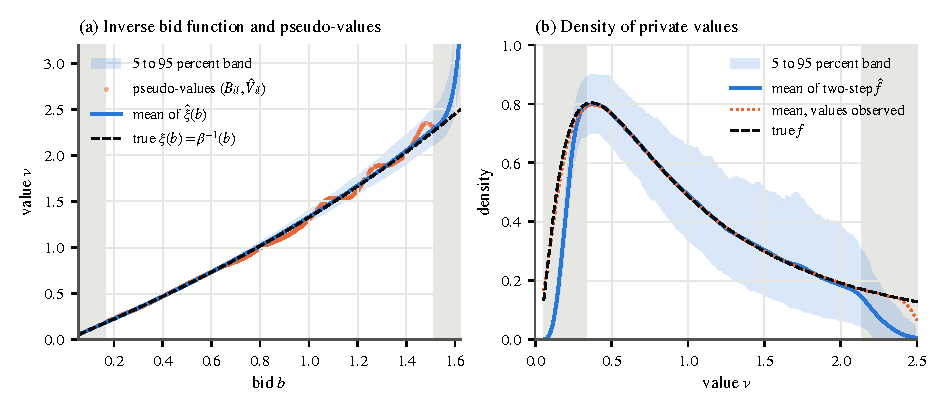
\includegraphics[width=\textwidth]{figures/appA/gpv.pdf}
\caption{The two-step estimator of \citet{GuerrePerrigneVuong2000} in their Monte Carlo design: 200
auctions with 5 bidders, values log-normal$(0,1)$ truncated to $[0.055,2.5]$, triweight kernels,
rule-of-thumb bandwidths, 1,000 replications. (a) True inverse bid function, mean and pointwise
5 to 95 percent band of $\hat\xi(b)$, and the pseudo-values of the first replication. The shaded bids are
trimmed on average (within $h_g$ of the extreme bids). (b) True value density, mean and pointwise
5 to 95 percent band of the two-step estimate, and the mean of the infeasible estimate from true values.
The shaded regions lie outside GPV's interior region (their footnote~9). Seed 20261022, script
\texttt{gpv\_mc.py}. Design follows Guerre, Perrigne and Vuong (2000), Section 2.4.}
\label{fig:A-gpv}
\end{figure}

The comparison with the infeasible estimator quantifies the price of inversion. On the interior region
the mean integrated squared error of the two-step estimate is 0.0170, against 0.0035 when values are
observed, a ratio of 4.9. The band in panel (b) is correspondingly wide, especially to the right of the
mode, where the bid density is low and its estimation error is amplified by \eqref{eq:A-gpv-xi}. Near
the lower end the two-step estimate collapses toward zero. Its mean at $v=0.055$ is 0.0003, against a
true density of 0.132. This is the joint effect of trimming and boundary bias, and it is why GPV report
results only on the interior region.

\section{Nonparametric regression, deconvolution and bounds}\label{sec:A-npreg}

This section estimates conditional means without functional form, combines nonparametric and
parametric components, separates a common factor from idiosyncratic noise, and draws inferences when
the data identify only a set. The tools build on \cref{sec:A-kde}. Throughout, $(y_i,x_i)$ are i.i.d.,
$m(x)=\E[y_i\mid x_i=x]$ is the regression function, $\sigma^2(x)=\Var(y_i\mid x_i=x)$, and $f$ is the
density of the scalar regressor $x_i$ unless stated otherwise.

\subsection{The Nadaraya-Watson estimator}\label{sec:A-nw}

The regression function is $m(x)=\frac{\int yf(x,y)\,\dd y}{f(x)}$. Replacing the joint density by the
product kernel estimate $\hat f(x,y)=\frac{1}{n}\sum_i\mathcal{K}_h(x-x_i)\mathcal{K}_h(y-y_i)$ and using
$\int y\,\mathcal{K}_h(y-y_i)\,\dd y=y_i$ for a symmetric kernel gives the \emph{Nadaraya-Watson
estimator} \citep{Nadaraya1964,Watson1964}:
\begin{equation}\label{eq:A-nw}
\hat m_h(x)=\frac{\sum_{i=1}^{n}\mathcal{K}_h(x-x_i)\,y_i}{\sum_{i=1}^{n}\mathcal{K}_h(x-x_i)} .
\end{equation}
It is a weighted average of the outcomes, with weights that decline with distance from $x$. It also
solves $\min_a\sum_i\mathcal{K}_h(x-x_i)(y_i-a)^2$, so it is a \emph{local constant} least squares fit.

\begin{proposition}[Bias and variance of Nadaraya-Watson]\label{prop:A-nw}
Let $x$ be an interior point with $f(x)>0$. Let $f$ be continuously differentiable and $m$ twice
continuously differentiable near $x$, let $\sigma^2$ be continuous, and let $h\to0$ and $nh\to\infty$.
Then
\begin{equation}\label{eq:A-nw-bias-var}
\E[\hat m_h(x)]-m(x)\approx h^2\mu_2\left(\frac{m''(x)}{2}+\frac{m'(x)f'(x)}{f(x)}\right),\qquad
\Var(\hat m_h(x))\approx\frac{\sigma^2(x)\kappa_2}{nhf(x)},
\end{equation}
where $\approx$ means equality of the leading terms.
\end{proposition}

\begin{proof}[Derivation]
Write $\hat m_h(x)-m(x)=\frac{\hat A(x)}{\hat f(x)}$ with
$\hat A(x)=\frac{1}{n}\sum_i\mathcal{K}_h(x-x_i)(y_i-m(x))$ and $\hat f(x)=\frac{1}{n}\sum_i\mathcal{K}_h(x-x_i)$.
Since $\hat f(x)\xrightarrow{p}f(x)$, the leading terms of the bias and variance are those of
$\frac{\hat A(x)}{f(x)}$.

\emph{Bias.} Using $\E[y_i\mid x_i]=m(x_i)$ and substituting $x_i=x-hu$,
\begin{equation*}
\E[\hat A(x)]=\int\mathcal{K}(u)\,\{m(x-hu)-m(x)\}\,f(x-hu)\,\dd u .
\end{equation*}
Expand $m(x-hu)-m(x)=-hum'(x)+\frac{h^2u^2}{2}m''(x)+o(h^2)$ and $f(x-hu)=f(x)-huf'(x)+o(h)$. The product
is $-hum'f+h^2u^2(m'f'+\frac{1}{2}m''f)+o(h^2)$. The term linear in $u$ integrates to zero, so
$\E[\hat A(x)]=h^2\mu_2(m'(x)f'(x)+\frac{1}{2}m''(x)f(x))+o(h^2)$. Dividing by $f(x)$ gives the bias.

\emph{Variance.} The leading term is
$\frac{1}{n}\E[\mathcal{K}_h(x-x_i)^2(y_i-m(x))^2]=\frac{1}{nh}\int\mathcal{K}(u)^2\{\sigma^2(x-hu)+(m(x-hu)-m(x))^2\}f(x-hu)\,\dd u$,
which equals $\frac{\kappa_2\sigma^2(x)f(x)}{nh}$ to first order. Dividing by $f(x)^2$ gives the variance.
\end{proof}

The bias has two parts. The curvature term $\frac{1}{2}m''$ is shared with every local smoother. The
\emph{design bias} $\frac{m'f'}{f}$ arises because, where the regressor density slopes, more
observations sit on one side of $x$ than on the other. The local average then leans toward the side
with more data, and the slope of $m$ converts the imbalance into bias.

At a boundary the problem is worse. Let the design have support $[0,\infty)$ with $f(0)>0$ and
evaluate at $x=0$. Only $u\le0$ contributes, so
$\E[\hat A(0)]\approx-hm'(0)f(0)\int_{-\infty}^{0}u\mathcal{K}(u)\,\dd u=hm'(0)f(0)\int_0^\infty u\mathcal{K}(u)\,\dd u$,
while $\hat f(0)\to\frac{1}{2}f(0)$. The bias is
\begin{equation}\label{eq:A-nw-boundary}
\E[\hat m_h(0)]-m(0)\approx2h\,m'(0)\int_0^\infty u\mathcal{K}(u)\,\dd u=\frac{3}{8}\,h\,m'(0)
\quad\text{(Epanechnikov kernel)},
\end{equation}
which is of order $h$ against $h^2$ in the interior. The Epanechnikov value
$\int_0^\infty u\mathcal{K}(u)\,\dd u=\frac{3}{16}$ is taken from \cref{tab:A-kernels}. For the four compact kernels of
that table the integral runs over $[0,1]$.

\subsection{Local polynomial regression}\label{sec:A-loclin}

The local constant fit ignores the slope of $m$. Fitting a line locally removes the design bias and the
first-order boundary bias. The \emph{local linear estimator} solves
\begin{equation}\label{eq:A-loclin}
(\hat a,\hat b)=\argmin_{a,b}\sum_{i=1}^{n}\mathcal{K}_h(x_i-x)\,\{y_i-a-b(x_i-x)\}^2,\qquad
\hat m_{\mathrm{LL}}(x)=\hat a .
\end{equation}
Let $S_j=\sum_i\mathcal{K}_h(x_i-x)(x_i-x)^j$. Solving the two normal equations gives
\begin{equation}\label{eq:A-loclin-weights}
\hat m_{\mathrm{LL}}(x)=\frac{\sum_iw_iy_i}{\sum_iw_i},\qquad w_i=\mathcal{K}_h(x_i-x)\{S_2-(x_i-x)S_1\}.
\end{equation}
The weights satisfy $\sum_iw_i(x_i-x)=S_1S_2-S_2S_1=0$. The estimator therefore reproduces any linear
function exactly, whatever the design.

\begin{proposition}[Local linear regression]\label{prop:A-loclin}
Let $\mathcal{K}$ vanish outside $[-1,1]$ and let $m$ be twice continuously differentiable. Conditional
on the regressors, and whenever $\sum_iw_i\ne0$,
\begin{equation*}
\E[\hat m_{\mathrm{LL}}(x)\mid x_1,\dots,x_n]-m(x)=\frac{\sum_iw_i\,\frac{1}{2}m''(\tilde x_i)(x_i-x)^2}{\sum_iw_i},
\end{equation*}
with $\tilde x_i$ between $x$ and $x_i$. Under the conditions of \cref{prop:A-nw}, the conditional bias at an
interior point is $\frac{h^2}{2}\mu_2m''(x)+o_p(h^2)$, free of the design term. At boundary points it remains of order
$h^2$. The interior variance is the Nadaraya-Watson variance $\frac{\sigma^2(x)\kappa_2}{nhf(x)}$
\citep{FanGijbels1996}.
\end{proposition}

\begin{proof}[Derivation]
Write $y_i=m(x)+m'(x)(x_i-x)+r_i+e_i$, where $r_i=\frac{1}{2}m''(\tilde x_i)(x_i-x)^2$ and
$\E[e_i\mid x_i]=0$. Substituting into \eqref{eq:A-loclin-weights}, the constant returns $m(x)$ and the
linear term vanishes because $\sum_iw_i(x_i-x)=0$. What remains is
$\frac{\sum_iw_i(r_i+e_i)}{\sum_iw_i}$, whose conditional mean is the displayed bias. Only observations
with $|x_i-x|\le h$ receive weight, so $|r_i|\le\frac{1}{2}h^2\sup|m''|$ wherever $x$ lies, and the bias
is $O_p(h^2)$ as long as $\frac{\sum_i|w_i|}{|\sum_iw_i|}$ stays bounded. That ratio is bounded at the
boundary too, because $S_0S_2-S_1^2>0$ when the window contains data on a set of positive length. In the
interior, $\frac{S_0}{n}\xrightarrow{p}f(x)$, $\E[\frac{S_1}{n}]=h^2\mu_2f'(x)+o(h^2)$ and $\Var(\frac{S_1}{n})=O(\frac{h}{n})$.
Hence $\frac{S_1}{S_0}=O_p(h^2+\sqrt{\frac{h}{n}})=o_p(h)$, because $\sqrt{\frac{h}{n}}=\frac{h}{\sqrt{nh}}$ and
$nh\to\infty$. The same calculation gives $\frac{S_2}{S_0}=h^2\mu_2+o_p(h^2)$. For $|x_i-x|\le h$ the
correction $\frac{(x_i-x)S_1}{S_2}$ in the weights is then $o_p(1)$. The weights therefore behave like
$\mathcal{K}_h(x_i-x)$ to first order, and the bias becomes $\frac{h^2}{2}\mu_2m''(x)$. The variance
argument is that of \cref{prop:A-nw}.
\end{proof}

Fitting a polynomial of degree $p$ in place of a line gives the \emph{local polynomial} estimator. The
coefficient on $(x_i-x)^k$ estimates $\frac{m^{(k)}(x)}{k!}$, so the slope $\hat b$ in
\eqref{eq:A-loclin} is a natural estimator of $m'(x)$. Odd degrees are preferred because they adapt
automatically to the boundary \citep{FanGijbels1996}.

\Cref{fig:A-npreg} compares the two estimators with the same Epanechnikov kernel and bandwidth $h=0.10$.
The design density is $\frac{2}{3}(1+x)$ on $[0,1]$ and the regression function is $m(x)=2e^{-5x}+0.5x$,
which is steep at the left boundary, with $m'(0)=-9.5$. With $n=400$, noise standard deviation 0.25 and
1,000 samples, the bias of Nadaraya-Watson at $x=0$ is $-0.316$. The approximation
\eqref{eq:A-nw-boundary} gives $-0.356$, and the difference reflects the large curvature of $m$ near
zero. The local linear bias at $x=0$ is $-0.028$. Its standard deviation there is larger, 0.105 against
0.064, because a line fitted at the edge extrapolates. In the interior both estimators share the
curvature bias, which reaches 0.031 for local linear near $x=0.1$, where $m''=50e^{-0.5}\approx30$.
Local fitting removes the design term and leaves the curvature term.

\begin{figure}[htbp]
\centering
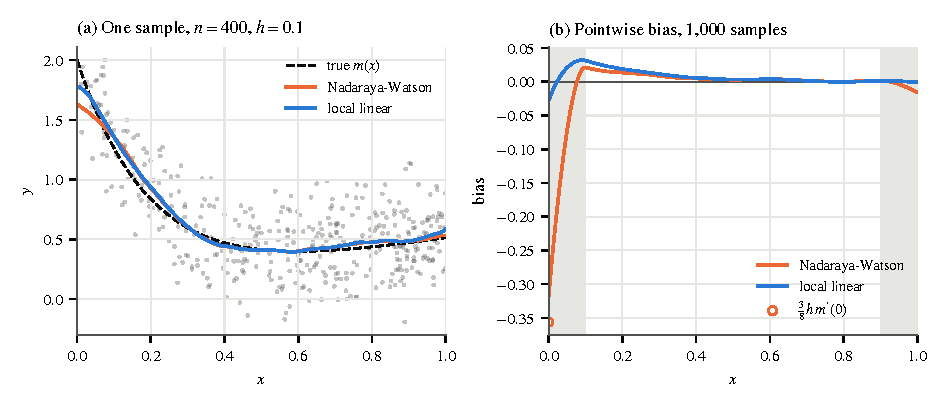
\includegraphics[width=\textwidth]{figures/appA/npreg.pdf}
\caption{Nadaraya-Watson and local linear regression with the same Epanechnikov kernel and bandwidth
$h=0.10$. The regressor has density $\frac{2}{3}(1+x)$ on $[0,1]$, $m(x)=2e^{-5x}+0.5x$, and the noise is
$N(0,0.25^2)$, $n=400$. (a) One sample. (b) Pointwise bias over 1,000 samples. The shaded
strips are within one bandwidth of the boundary, and the marker shows the boundary approximation
$\frac{3}{8}hm'(0)$ of \eqref{eq:A-nw-boundary}. Seed 20261022, script \texttt{npreg\_demo.py}.}
\label{fig:A-npreg}
\end{figure}

\casehead{Applications in the book}
Three applications use local regression. First, \citet{HausmanNewey1995} estimate demand $q(p,y)$
nonparametrically, as a function of price and income, and carry out the exact welfare analysis with it
\citep[fn.~6]{Hausman1997}. The exact analysis solves the differential equation of \citet{Hausman1981}. For a price change from
$p^0$ to $p^1$, let $S(p)=e(p,u^0)-y$ be the extra income needed to keep utility at its initial level.
Shephard's lemma and duality give
\begin{equation}\label{eq:A-hausman-ode}
\frac{\dd S(p)}{\dd p}=q\bigl(p,\,y+S(p)\bigr),\qquad S(p^0)=0,
\end{equation}
and the compensating variation is $S(p^1)$ (\cref{app:math}). \citet{Hausman1997} solves the same
differential equation for a parametric demand system for a new breakfast cereal. His exact welfare estimates and
their standard errors use the method of \citet{HausmanNewey1995} (his fn.~24, \cref{ch:newgoods}). Second, \citet[eq.~(18)]{BajariBenkard2005} recover
each product's unobserved characteristic as a conditional quantile. Normalizing $\xi$ to be uniform on
$[0,1]$ and independent of $x$, with price increasing in $\xi$, they set
$\hat\xi_{jt}=\hat F_{p_t\mid x=x_j}(p_{jt})$. In their application a local linear kernel estimator
\citep{FanGijbels1996} with a normal kernel worked best \citep[Sections~5.1 and~6]{BajariBenkard2005}.
Derivatives of the estimated hedonic price function then recover consumers' marginal valuations from
their first-order conditions (\cref{ch:discrete}). Third, conditional bid distributions given covariates
can be estimated by local linear smoothing of indicator outcomes $\indic\{B_{il}\le b\}$, which avoids
the boundary problems of \cref{sec:A-kde-boundary} in the covariate dimension.

\subsection{Series and sieve estimators}\label{sec:A-series}

A \emph{series estimator} approximates $m$ by a linear combination of $K_n$ known basis functions
$\psi(x)=(\psi_1(x),\dots,\psi_{K_n}(x))^\top$, such as powers of $x$ or regression splines. A regression
spline of degree $r$ is a polynomial of degree $r$ between consecutive points called knots, with $r-1$ continuous
derivatives at each knot. B-splines are a convenient basis for this space. The series estimator fits the
coefficients by least squares,
\begin{equation}\label{eq:A-series}
\hat m(x)=\psi(x)^\top\hat\gamma,\qquad \hat\gamma=(\Psi^\top\Psi)^{-1}\Psi^\top y .
\end{equation}
Here $\Psi$ is the $n\times K_n$ matrix with rows $\psi(x_i)^\top$. The number of terms plays the role of
the inverse bandwidth. Its variance cost has an exact expression. With homoskedastic errors of variance
$\sigma^2$, the fitted values are $P_\Psi y$ with $P_\Psi=\Psi(\Psi^\top\Psi)^{-1}\Psi^\top$, so
\begin{equation*}
\frac{1}{n}\sum_{i=1}^{n}\Var(\hat m(x_i)\mid\Psi)=\frac{\sigma^2}{n}\,\mathrm{tr}(P_\Psi)=\frac{\sigma^2K_n}{n}.
\end{equation*}
For a function with $R$ derivatives and a polynomial or spline basis in one dimension, the squared
approximation bias is of order $K_n^{-2R}$. Balancing the two gives $K_n\propto n^{\frac{1}{2R+1}}$ and the
same mean squared error rate $n^{-\frac{2R}{2R+1}}$ as a kernel estimator \citep{Newey1997}. In practice
$K_n$ is chosen by cross-validation or an information criterion.

Series estimators are global. A misbehaving term affects the fit everywhere, and high-order
polynomials are unstable at the boundary, which favors splines. In exchange, restrictions such as
additivity, $m(x)=m_1(x_1)+m_2(x_2)$, are easy to impose by choosing the basis, and the estimator is a
least squares regression whose inference is standard for fixed $K_n$. A \emph{sieve} is the general
version. It is a sequence of increasingly rich approximating function classes, and the estimator uses a richer
class as $n$ grows \citep{Chen2007}. Three uses appear in
the book. Approximations to optimal instruments use series in the instruments (\cref{sec:A-optimal-iv}).
The marginal cost of an airline segment in \citet{BerryCarnallSpiller1996} is a cubic polynomial in leg
distance and leg density, with two congestion shifters (WP Table~5, \cref{sec:09-bcs-supply}). It is a
fixed low-order series. And
\citet[footnote~20]{AtheyHaile2007} point to sieve estimation as a practical alternative to kernels
in auctions with observed heterogeneity.

\subsection{The partially linear model}\label{sec:A-plm}

Often only a few parameters are of interest, while a control variable enters in an unknown way. The
\emph{partially linear model} is
\begin{equation}\label{eq:A-plm}
y_i=x_i^\top\beta+m(w_i)+e_i,\qquad \E[e_i\mid x_i,w_i]=0,
\end{equation}
with $m$ unknown. Taking expectations conditional on $w_i$ gives
$\E[y_i\mid w_i]=\E[x_i\mid w_i]^\top\beta+m(w_i)$. Subtracting this from \eqref{eq:A-plm} eliminates
$m$:
\begin{equation}\label{eq:A-robinson}
\tilde y_i=\tilde x_i^\top\beta+e_i,\qquad \tilde y_i=y_i-\E[y_i\mid w_i],\quad \tilde x_i=x_i-\E[x_i\mid w_i].
\end{equation}
\citet{Robinson1988} estimates the two conditional means nonparametrically and regresses the
residual of $y$ on the residual of $x$ by least squares. This is the \emph{double-residual estimator}.

\begin{proposition}[Robinson's estimator]\label{prop:A-robinson}
Suppose $\E[\tilde x_i\tilde x_i^\top]$ is positive definite, so no linear combination of $x_i$ is a
function of $w_i$ alone. Suppose the first-step estimators of $\E[y\mid w]$ and $\E[x\mid w]$ converge
in mean square faster than $n^{-\frac{1}{4}}$, with trimming and kernel order as in
\citet{Robinson1988}. Then
\begin{equation*}
\sqrt n(\hat\beta-\beta)\xrightarrow{d}N\!\left(0,\ \E[\tilde x\tilde x^\top]^{-1}\E[e^2\tilde x\tilde x^\top]\E[\tilde x\tilde x^\top]^{-1}\right),
\end{equation*}
the distribution of the infeasible regression with known conditional means.
\end{proposition}

\begin{proof}[Why the first step does not matter]
The estimator solves the sample analogue of the moment
$\E[(\tilde y-\tilde x^\top\beta)\tilde x]=0$. Perturb the conditional means by functions $\delta_y(w)$
and $\delta_x(w)$, so the moment becomes
$M(\delta)=\E[\{\tilde y-\delta_y(w)-(\tilde x-\delta_x(w))^\top\beta\}\{\tilde x-\delta_x(w)\}]$. Its
derivative at $\delta=0$ in the direction $\delta_y$ is $-\E[\delta_y(w)\tilde x]$, which is zero because
$\E[\tilde x\mid w]=0$. In the direction $\delta_x$ the derivative is
$\E[\tilde x\,\delta_x(w)^\top]\beta-\E[e\,\delta_x(w)]$, and both terms vanish by
$\E[\tilde x\mid w]=0$ and $\E[e\mid w]=0$. First-step errors therefore enter only through products of
two errors, of order $\|\hat\delta\|^2$. If $\|\hat\delta\|=o_p(n^{-\frac{1}{4}})$, these products are
$o_p(n^{-\frac{1}{2}})$, and the infeasible limit applies.
\end{proof}

The estimator is the nonparametric analogue of the Frisch-Waugh-Lovell theorem (\cref{thm:A-fwl}). If
$m(w)=w^\top\gamma$, partialling out $w$ by linear projection and regressing residual on residual
reproduces the coefficient on $x$ in the long regression. Robinson replaces the linear projection by
the conditional expectation, which partials out every function of $w$. The insensitivity to the first
step derived in the proof is the property now called \emph{Neyman orthogonality}.

A simulation in \texttt{npreg\_demo.py} shows what is at stake. Let $w$ be uniform on $[0,1]$,
$x=\sin(2\pi w)+v$ and $y=x+2\sin(2\pi w)+e$, with $v$ and $e$ standard normal, $n=500$ and 1,000 samples.
Least squares of $y$ on a constant, $x$ and $w$ controls for $w$ linearly. Its mean estimate is 1.327
against $\beta=1$, and its nominal 95 percent interval never covers the truth. Robinson's estimator with
local linear first steps ($h=0.08$) has mean 0.999 and standard deviation 0.045, equal to the infeasible
value $\frac{1}{\sqrt{500}}\approx0.045$. Its interval covers in 94.1 percent of samples.

\subsection{Deconvolution}\label{sec:A-deconv}

Suppose two noisy measurements share a common component,
\begin{equation}\label{eq:A-meas}
Y_1=U+\epsilon_1,\qquad Y_2=U+\epsilon_2,
\end{equation}
with $U$, $\epsilon_1$ and $\epsilon_2$ mutually independent. In auctions, $U$ is the log of a factor that
scales all bids in an auction, known to the bidders and unobserved by us. The term $\epsilon_j$ is the log of the
bid that bidder $j$ would make if the factor were one. The goal is the distribution of each
component from the joint distribution of $(Y_1,Y_2)$.

Second moments show why two measurements help. Independence gives $\Cov(Y_1,Y_2)=\Var(U)$, so
$\Var(\epsilon_j)=\Var(Y_j)-\Cov(Y_1,Y_2)$, and the normalization $\E[\epsilon_1]=0$ gives
$\E[U]=\E[Y_1]$. Variation across auctions identifies the spread of the common factor, and variation
within auctions identifies the spread of the idiosyncratic parts. A theorem of \citet{Kotlarski1966}
extends this from second moments to whole distributions. Let
$\varphi_U(t)=\E[e^{\mathrm{i}tU}]$ denote a characteristic function, where $\mathrm{i}$ is the
imaginary unit, and let $\varphi_{Y_1Y_2}(t_1,t_2)=\E[e^{\mathrm{i}t_1Y_1+\mathrm{i}t_2Y_2}]$.

\begin{lemma}[Kotlarski]\label{lem:A-kotlarski}
In \eqref{eq:A-meas}, let $U$, $\epsilon_1$, $\epsilon_2$ be mutually independent with finite first
moments and $\E[\epsilon_1]=0$, and let $\varphi_U$ and $\varphi_{\epsilon_2}$ never vanish. Then for every
real $t$,
\begin{equation}\label{eq:A-kotlarski}
\varphi_U(t)=\exp\left(\int_0^t\frac{\E\left[\mathrm{i}Y_1e^{\mathrm{i}sY_2}\right]}{\E\left[e^{\mathrm{i}sY_2}\right]}\,\dd s\right),\qquad
\varphi_{\epsilon_1}(t)=\frac{\varphi_{Y_1Y_2}(t,0)}{\varphi_U(t)},\qquad
\varphi_{\epsilon_2}(t)=\frac{\varphi_{Y_1Y_2}(0,t)}{\varphi_U(t)} .
\end{equation}
The joint distribution of $(Y_1,Y_2)$ therefore determines the distributions of $U$, $\epsilon_1$ and
$\epsilon_2$.
\end{lemma}

\begin{proof}
Independence factors the joint characteristic function:
\begin{equation*}
\varphi_{Y_1Y_2}(t_1,t_2)=\E\left[e^{\mathrm{i}(t_1+t_2)U}e^{\mathrm{i}t_1\epsilon_1}e^{\mathrm{i}t_2\epsilon_2}\right]
=\varphi_U(t_1+t_2)\,\varphi_{\epsilon_1}(t_1)\,\varphi_{\epsilon_2}(t_2).
\end{equation*}
Finite first moments make the characteristic functions continuously differentiable, with
$\varphi_X'(0)=\mathrm{i}\E[X]$. Differentiating in $t_1$ and setting $t_1=0$, with $\varphi_{\epsilon_1}(0)=1$
and $\varphi_{\epsilon_1}'(0)=\mathrm{i}\E[\epsilon_1]=0$,
\begin{equation*}
\frac{\partial\varphi_{Y_1Y_2}}{\partial t_1}(0,s)=\varphi_U'(s)\,\varphi_{\epsilon_2}(s).
\end{equation*}
The left side equals $\E[\mathrm{i}Y_1e^{\mathrm{i}sY_2}]$, and $\varphi_{Y_1Y_2}(0,s)=\E[e^{\mathrm{i}sY_2}]=\varphi_U(s)\varphi_{\epsilon_2}(s)\ne0$.
Dividing, $\varphi_{\epsilon_2}(s)$ cancels:
\begin{equation*}
\frac{\E[\mathrm{i}Y_1e^{\mathrm{i}sY_2}]}{\E[e^{\mathrm{i}sY_2}]}=\frac{\varphi_U'(s)}{\varphi_U(s)}=\frac{\dd}{\dd s}\log\varphi_U(s),
\end{equation*}
where $\log$ is the continuous branch with $\log\varphi_U(0)=0$, which exists because $\varphi_U$ is
continuous and never zero. Integrating from 0 to $t$ and exponentiating gives the first formula. Setting
$t_2=0$, and then $t_1=0$, in the factorization gives $\varphi_{Y_1Y_2}(t,0)=\varphi_U(t)\varphi_{\epsilon_1}(t)$ and
$\varphi_{Y_1Y_2}(0,t)=\varphi_U(t)\varphi_{\epsilon_2}(t)$, and division gives the other two. A characteristic
function determines its distribution.
\end{proof}

Each assumption has a role. Independence delivers the factorization. The nonvanishing condition allows
the divisions and the logarithm. The zero mean of $\epsilon_1$ is a location normalization, since a
constant could otherwise move freely between $U$ and the $\epsilon$'s. The lemma identifies
distributions only. The realization of $U$ in a given auction is not identified. \Cref{ch:collusion-evidence} states
the same result for Asker's application.

The nonvanishing condition deserves care. \citet[Lemma~1]{Krasnokutskaya2011} argues that a variable
with bounded support has a characteristic function that extends to an entire function, so its zeros are
isolated. Isolated zeros can still occur, as the uniform distribution shows, since its characteristic
function $\frac{\sin t}{t}$ vanishes at multiples of $\pi$. \citet{EvdokimovWhite2012} show that
identification survives some violations of the condition under additional restrictions.

\casehead{The estimator}
\citet{LiVuong1998} replace each characteristic function by its sample analogue. With $n$ independent
pairs $(Y_{1k},Y_{2k})$,
\begin{equation}\label{eq:A-lv}
\hat\varphi_U(t)=\exp\left(\int_0^t\frac{\frac{1}{n}\sum_k\mathrm{i}Y_{1k}e^{\mathrm{i}sY_{2k}}}{\frac{1}{n}\sum_ke^{\mathrm{i}sY_{2k}}}\,\dd s\right),\qquad
\hat f_U(u)=\frac{1}{2\pi}\int_{-T}^{T}d_T(t)\,e^{-\mathrm{i}tu}\,\hat\varphi_U(t)\,\dd t ,
\end{equation}
and analogously for $\epsilon_1$ and $\epsilon_2$. The density is recovered by the inverse Fourier
transform, truncated at $\pm T$ and multiplied by a \emph{damping factor} $d_T$ that downweights high
frequencies, such as $d_T(t)=\max\{1-\frac{|t|}{T},0\}$ \citep{DiggleHall1993}. Since
$\hat\varphi_U(-t)$ is the complex conjugate of $\hat\varphi_U(t)$, the estimate is real and equals
$\frac{1}{\pi}\int_0^Td_T(t)\,\mathrm{Re}\{e^{-\mathrm{i}tu}\hat\varphi_U(t)\}\,\dd t$. The truncation
point $T$ is the smoothing parameter, playing the role of an inverse bandwidth.

Deconvolution converges slowly. The empirical characteristic function has error of order
$n^{-\frac{1}{2}}$ at each frequency, but the formulas divide by quantities that decay at high
frequencies. The ratio in \eqref{eq:A-lv} divides by $\varphi_U(s)\varphi_{\epsilon_2}(s)$, and the formula
for $\varphi_{\epsilon_1}$ divides by $\varphi_U$. The achievable rate depends on how fast the characteristic
functions decay. It is polynomial in $n$ for \emph{ordinary smooth} distributions, whose characteristic
functions decay like $|t|^{-\beta}$, and only logarithmic for \emph{supersmooth} ones such as the normal
\citep{Fan1991}. \citet{LiVuong1998} establish uniform consistency under conditions of this kind.
Krasnokutskaya's consistency result assumes ordinary smooth components with $\beta>1$
\citep[Proposition~5]{Krasnokutskaya2011}.

\Cref{fig:A-deconv} implements \eqref{eq:A-lv} with $U$ distributed Gamma with shape 4 and scale 0.25
(mean 1, standard deviation 0.5), $\epsilon_j\sim N(0,0.4^2)$, $n=1{,}000$ pairs and 200 samples. With
$T=8$ the median integrated squared error of $\hat f_U$ is 0.035. A kernel density estimate of $Y_1$
ignores the noise and has mean integrated squared error 0.058. Raising $T$ to 10 lowers the median
error to 0.029 but makes the estimator unstable, with a mean integrated squared error of 2.44 driven by
a few samples. Too large a $T$ divides by empirical characteristic functions that are pure noise.

\begin{figure}[htbp]
\centering
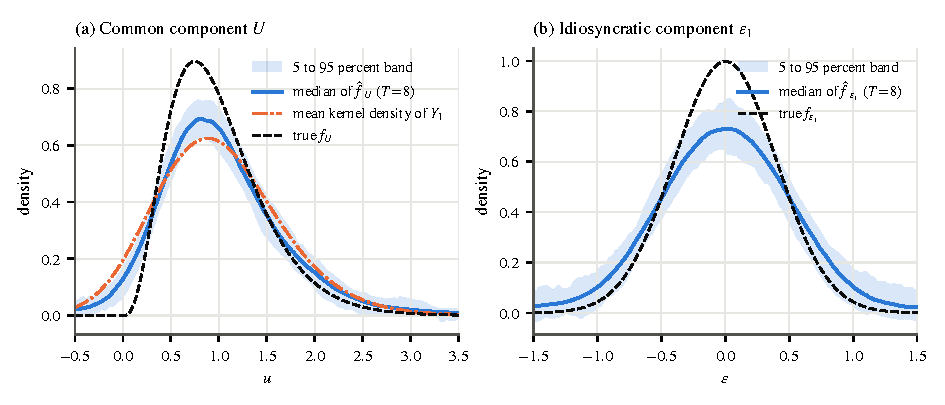
\includegraphics[width=\textwidth]{figures/appA/deconv.pdf}
\caption{Kotlarski deconvolution with the estimator of \citet{LiVuong1998}. $Y_j=U+\epsilon_j$ with
$U\sim\mathrm{Gamma}(4,0.25)$ and $\epsilon_j\sim N(0,0.4^2)$, $n=1{,}000$ pairs, smoothing parameter
$T=8$, damping factor $1-\frac{|t|}{T}$, 200 samples. (a) True density of $U$, pointwise median
and 5 to 95 percent band of $\hat f_U$, and the mean rule-of-thumb kernel density estimate of $Y_1$.
(b) The same for $\epsilon_1$. Seed 20261022, script \texttt{npreg\_demo.py}.}
\label{fig:A-deconv}
\end{figure}

\casehead{Krasnokutskaya's procurement auctions}
\citet{Krasnokutskaya2011} applies the lemma to first-price procurement auctions. A bidder's cost is
the product of a project-level component $Y$, common knowledge among bidders and unobserved by us, and an
individual component. The equilibrium bid inherits the product structure, $B_{ij}=y_ja_{ij}$, where
$a_{ij}$ is the bid at $y=1$. For two bidders in the same auction, logs give
$\log B_{i_1}=\log Y+\log A_{i_1}$ and $\log B_{i_2}=\log Y+\log A_{i_2}$. Her equation~(3) is
\eqref{eq:A-kotlarski} for these variables.\footnote{Its equation~(3) prints a logarithm where the
exponential of \eqref{eq:A-kotlarski} belongs. The estimator in its appendix uses the exponential.} The
location is fixed by $\E[\log A_1]=0$. Her estimator averages the empirical characteristic function over
all pairs of bidders of the relevant types. It scales bids into $[0,2]$ to reduce estimation error in the
characteristic function. It uses the damping factor $1-\frac{|t|}{T}$ and chooses $T$ to match the means
and variances of $\log Y$ and $\log A$ implied by the bids, which selects $T=50$ in her application. The
moment conditions behind the choice of $T$ are the second-moment identities above. With identically
distributed individual components, $\Var(\log A)=\frac{1}{2}\E[(\log B_1-\log B_2)^2]$ and
$\Var(\log Y)=\Var(\log B)-\Var(\log A)$ \citep[Section~4.3]{Krasnokutskaya2011}. In a second step she
draws pseudo-bids from the estimated density of the individual component by rejection sampling. She
converts them to pseudo-costs through the asymmetric first-order condition. The densities in this step
use a triweight kernel and the bandwidth $2.978\times1.06\,\hat\sigma L^{-\frac{1}{6}}$, where
$\hat\sigma$ is the standard deviation of the log of one plus the bids. Confidence intervals come from
the bootstrap. Independence also generates testable restrictions. The characteristic functions
recovered from different pairs and triples of bidders must agree. A degenerate $\log Y$ gives the
independent private values model, which can be tested within the same framework (her conditions W1 to
W7). In Michigan highway procurement auctions she attributes about 75 percent of the variation in
bidders' costs to factors known to all bidders. Only 25 percent comes from private information
(abstract of the working paper). \citet[p.~103]{HortacsuPerrigne2021} report the published estimate as 34 percent
of the bid variation from private information. That figure refers to bids, while the working-paper figure refers to
costs. \Cref{ch:auction-empirics} discusses the application.

\casehead{Asker's knockout bids}
\citet{Asker2010} applies the same estimator to pairs of normalized knockout bids in a stamp-dealer ring,
$\ln\hat b_{1k}=\ln(\varepsilon_k)+\ln\beta(v_{1k})$ and $\ln\hat b_{2k}=\ln(\varepsilon_k)+\ln\beta(v_{2k})$
(his eq.~(4)). In his notation the common component of lot $k$ is $\ln(\varepsilon_k)$, which plays the
role of $U$ in \eqref{eq:A-meas}. He imposes $\E[\ln\beta(v_1)]=0$ and independence (his Assumption~U).
The target-auction price supplies a third measurement of the common component. He averages the estimated characteristic
functions from the two kinds of pairs, weighting by the number of observations of each, as
\citet{LiVuong1998} suggest. His damping factor is $\max\{1-\frac{|t|}{\sqrt2T_n},0\}$. The smoothing
parameter is $T_n=50$ for the common component, whose estimate proved insensitive to it. For the strong
members, the weak members and the highest non-ring value, the values 12.0, 3.0 and 8.3 minimize a
criterion. The criterion matches naive damages and the ring's win probability and penalizes
non-monotone bid functions \citep[pp.~748--749]{Asker2010}. As with Krasnokutskaya, only distributions are identified, and
the GPV inversion is applied to draws from the estimated distributions (\cref{ch:collusion-evidence}).

\subsection{Estimation and inference under partial identification}\label{sec:A-partialid}

When the model and data restrict a parameter only to a set, the parameter is \emph{partially identified}
(\cref{def:A-identification}). A common form is a set of moment inequalities,
\begin{equation}\label{eq:A-mi}
\Theta_I=\{\theta\in\Theta:\ \E[m_j(W;\theta)]\ge0,\ j=1,\dots,J\},
\end{equation}
where $\Theta_I$ is the \emph{identified set}. Every point of $\Theta_I$ is consistent with the population
distribution of the data, and no point outside it is. Estimation targets the set, and inference can
target either the set or the true parameter inside it.

\casehead{Bounds in English auctions}
\citet{HaileTamer2003} drop the button-auction model of ascending auctions, in which bidders exit at
their values. They impose two behavioral assumptions. Bidders never bid more than their value, and
bidders never let an opponent win at a price they would have been willing to beat. Let $G_{k:n}$ be the
distribution of the $k$-th lowest bid in $n$-bidder auctions. Let $G^{\Delta}_{n:n}$ be the distribution
of the winning bid plus the minimum increment $\Delta$, and $\phi_{k:n}$ the map from $F$ to $F_{(k:n)}$
in \eqref{eq:A-orderstat}. The first assumption implies that the $k$-th lowest bid is at most the $k$-th
lowest value, so $G_{k:n}(v)\ge\phi_{k:n}(F(v))$. The second implies that the second-highest value is at
most the winning bid plus $\Delta$, so $\phi_{n-1:n}(F(v))\ge G^{\Delta}_{n:n}(v)$. Inverting the
increasing maps and combining all order statistics and all $n$ gives
\citep[Section~4.3.1, eqs.~(4.10)--(4.11)]{AtheyHaile2007}
\begin{equation}\label{eq:A-ht}
F^-(v)=\max_n\ \phi_{n-1:n}^{-1}\!\left(G^{\Delta}_{n:n}(v)\right)\ \le\ F(v)\ \le\
F^+(v)=\min_{n}\min_{1\le k\le n}\ \phi_{k:n}^{-1}\!\left(G_{k:n}(v)\right).
\end{equation}
\Cref{ch:auction-empirics} develops the bounds and their use for reserve prices.
\citet[pp.~493--499]{AradillasLopezGandhiQuint2013} derive bounds on expected profit, bidder surplus and
the optimal reserve price when symmetric private values have nonnegative dependence. They use only the transaction price and,
with values independent of the number of bidders, variation in that number across auctions.
\citet[footnote~37]{Asker2010}
discusses why he does not use the Haile-Tamer approach. Jump bidding was rare at the stamp auctions he
observed, and bid increments were small relative to bids.

\casehead{Plug-in estimation and the bias of extrema}
The natural estimator of \eqref{eq:A-ht} replaces each $G$ by an empirical distribution function. The
minimum and maximum then create a finite-sample bias. The minimum is concave, so by Jensen's inequality
$\E[\min_j\hat a_j]\le\min_j\E[\hat a_j]$. A worked case shows the size. Let $\hat a_1$ and $\hat a_2$ be
independent $N(a,\sigma^2)$, both unbiased for the same bound $a$. Since $\min(a_1,a_2)=\frac{a_1+a_2}{2}-\frac{|a_1-a_2|}{2}$
and $\hat a_1-\hat a_2\sim N(0,2\sigma^2)$ has mean absolute value $\frac{2\sigma}{\sqrt\pi}$,
\begin{equation*}
\E\left[\min(\hat a_1,\hat a_2)\right]=a-\frac{\sigma}{\sqrt\pi}.
\end{equation*}
The estimated upper bound is too low and the estimated lower bound too high, so the estimated set is too
narrow. The bias grows with the number of terms in the minimum. \citet{HaileTamer2003} define the
bounds in finite samples with smooth approximations to the max and min functions. In the words of
\citet[Section~4.3.1, p.~35]{AtheyHaile2007}, this ``amounts to using weighted averages instead of the max or min.''
For example, the softmax-weighted average
$\sum_j\hat a_j\frac{e^{\rho\hat a_j}}{\sum_ke^{\rho\hat a_k}}$ with $\rho<0$ is a smooth minimum of
this kind. It tends to $\min_j\hat a_j$ as $\rho\to-\infty$, and it lies above the minimum, which
offsets the downward bias. We use it only as an illustration, and it need not be the weighting that Haile
and Tamer choose.

The extrema also break standard inference. The functional $\min(a_1,a_2)$ is not differentiable where
$a_1=a_2$, so the delta method fails there, and the bootstrap can fail for the same reason
(\cref{prop:A-boot-max}).

\casehead{Set estimators and confidence regions}
Define the criterion $Q(\theta)=\sum_j(\min\{\E[m_j(W;\theta)],0\})^2$, which is zero exactly on
$\Theta_I$. Its sample analogue $Q_n$ is zero on the sample identified set, which may be empty or too
small. \citet{ChernozhukovHongTamer2007} estimate the set by $\hat\Theta_I=\{\theta:\ nQ_n(\theta)\le c_n\}$
with $c_n\to\infty$ and $\frac{c_n}{n}\to0$. The Hausdorff distance between sets $A$ and $B$ is
\begin{equation*}
d_H(A,B)=\max\Bigl\{\sup_{a\in A}\inf_{b\in B}\lVert a-b\rVert,\ \sup_{b\in B}\inf_{a\in A}\lVert a-b\rVert\Bigr\}.
\end{equation*}
It is the larger of two directed distances. Each is the largest distance from a point of one set to the nearest
point of the other. The estimator is consistent in this distance, so $d_H(\hat\Theta_I,\Theta_I)\to0$ in
probability. Confidence regions
for $\Theta_I$ invert tests of $Q(\theta)=0$, with cutoffs from subsampling or the bootstrap.

For an interval $[\theta_l,\theta_u]$ there is an important distinction. A region that covers the whole
set with probability $1-\alpha$ is larger than one that covers the true parameter with that probability.
\citet{ImbensManski2004} construct the second kind. With estimators $\hat\theta_l$ and $\hat\theta_u$,
standard errors $\frac{\hat\sigma_l}{\sqrt n}$ and $\frac{\hat\sigma_u}{\sqrt n}$, and estimated length
$\hat\Delta=\hat\theta_u-\hat\theta_l$, the interval is
\begin{equation}\label{eq:A-im}
\left[\hat\theta_l-c_n\frac{\hat\sigma_l}{\sqrt n},\ \hat\theta_u+c_n\frac{\hat\sigma_u}{\sqrt n}\right],\qquad
\Phi\!\left(c_n+\frac{\sqrt n\,\hat\Delta}{\max\{\hat\sigma_l,\hat\sigma_u\}}\right)-\Phi(-c_n)=1-\alpha .
\end{equation}
When the set is long relative to sampling error, the true parameter can be near at most one end point.
Only one tail then matters, and $c_n$ approaches the one-sided value 1.645 for $\alpha=0.05$. When the set
shrinks to a point, $c_n$ rises to the two-sided 1.96. A region for the whole set needs both end
points covered at once and uses a larger constant. \citet{Stoye2009} refines the argument for sets whose
length is near zero. \citet{Manski2003} and \citet{Tamer2010} survey the field.

\section{Difference in differences and panel event studies}\label{sec:A-did}

The last two sections of the appendix turn from estimators to research designs. Many questions in industrial
organization concern a discrete change in a market. Two firms merge, a rival
enters, a state raises a tax, or a patent is granted. A \emph{retrospective} (or ex post) evaluation measures
what the change did by comparing outcomes after it with outcomes before it. A \emph{prospective} (or ex ante)
evaluation predicts the effect before the change, with a model of demand, costs and conduct. This section
develops the research designs behind retrospectives. They compare units exposed to the change with units that
were not, before and after the change.

These designs are reduced form. They identify average effects of a change under assumptions about the outcomes
that units would have had without it, and they need no model of conduct. The book uses them for merger
retrospectives (\cref{sec:11-retro}), tax pass-through (\cref{sec:03-sumner}), entry
(\cref{sec:09-wc-did}) and patents (\cref{sec:05-dgg}). We build on the potential-outcomes notation of
\cref{sec:A-potential}. Throughout this section $i$ indexes units (products, markets, states, hospitals) and
$t$ indexes periods, and $\tau_t$ denotes a period fixed effect. In \cref{sec:A-eventstudy} the symbol $\tau$ will
index trading days instead.

\subsection{The two-by-two design}\label{sec:A-did-2x2}

We start with two groups and two periods. Units $i=1,\dots,n$ are observed in periods $t\in\{0,1\}$. The
indicator $\mathit{Treat}_i$ equals one for units in the \emph{treated group}, which is exposed to the change
between the two periods. The other units form the \emph{control group}. Let $\mathit{Post}_t=\indic\{t=1\}$ and
let $d_{it}=\mathit{Treat}_i\,\mathit{Post}_t$ be the treatment indicator. Each unit has two potential outcomes in
each period, $y_{it}(1)$ with the treatment and $y_{it}(0)$ without it. We observe
\begin{equation*}
y_{it}=y_{it}(0)+d_{it}\big[y_{it}(1)-y_{it}(0)\big].
\end{equation*}

\begin{definition}[Average effect of the treatment on the treated]\label{def:A-att}
The \emph{average treatment effect on the treated} in the post period, the panel version of the ATT of
\cref{sec:A-potential}, is
\begin{equation*}
\mathrm{ATT}=\E\big[y_{i1}(1)-y_{i1}(0)\mid \mathit{Treat}_i=1\big].
\end{equation*}
\end{definition}

Two naive comparisons fail. The cross-sectional comparison of treated and control units in period 1 adds a
selection term, the difference in untreated outcomes between the groups (\cref{prop:A-selection}). The
before-after comparison within the treated group adds the change that the treated units would have experienced
anyway:
\begin{equation*}
\E\big[y_{i1}-y_{i0}\mid\mathit{Treat}_i=1\big]=\mathrm{ATT}+\E\big[y_{i1}(0)-y_{i0}(0)\mid\mathit{Treat}_i=1\big],
\end{equation*}
provided that period-0 outcomes are untreated. A rise in input costs at the time of a merger, for example, is
attributed to the merger. The \emph{difference-in-differences} (DiD) estimator removes this change with the change
in the control group. Let $\bar y_{T,t}$ and $\bar y_{C,t}$ denote the sample means of $y_{it}$ in the treated and
control groups in period $t$. Then
\begin{equation}\label{eq:A-did-estimator}
\hat\beta^{\mathrm{DD}}=\big(\bar y_{T,1}-\bar y_{T,0}\big)-\big(\bar y_{C,1}-\bar y_{C,0}\big).
\end{equation}

\begin{assumption}[Identifying assumptions for DiD]\label{ass:A-did}
\leavevmode
\begin{enumerate}[label=(\roman*)]
\item \emph{No anticipation.} Period-0 outcomes are untreated: $y_{i0}=y_{i0}(0)$ for all $i$.
\item \emph{Parallel trends.} Without the treatment, the mean outcome would have changed by the same amount in both
groups:
\begin{equation*}
\E\big[y_{i1}(0)-y_{i0}(0)\mid\mathit{Treat}_i=1\big]=\E\big[y_{i1}(0)-y_{i0}(0)\mid\mathit{Treat}_i=0\big].
\end{equation*}
\item \emph{No interference.} The treatment of the treated group does not change the outcomes of control units:
$y_{i1}=y_{i1}(0)$ when $\mathit{Treat}_i=0$.
\end{enumerate}
\end{assumption}

\begin{proposition}[Identification by DiD]\label{prop:A-did}
Suppose the group means in \eqref{eq:A-did-estimator} are unbiased for the corresponding population means. Under
\cref{ass:A-did}, $\E[\hat\beta^{\mathrm{DD}}]=\mathrm{ATT}$. If the sample means are also consistent, then
$\hat\beta^{\mathrm{DD}}\xrightarrow{p}\mathrm{ATT}$.
\end{proposition}

\begin{proof}
Write $\E_1[\cdot]$ and $\E_0[\cdot]$ for expectations conditional on $\mathit{Treat}_i=1$ and
$\mathit{Treat}_i=0$. For the treated group, the observed outcome in period 1 is $y_{i1}(1)$, and by (i) the
period-0 outcome is $y_{i0}(0)$. Adding and subtracting $\E_1[y_{i1}(0)]$ gives
\begin{align*}
\E\big[\bar y_{T,1}-\bar y_{T,0}\big]
&=\E_1\big[y_{i1}(1)\big]-\E_1\big[y_{i0}(0)\big]\\
&=\E_1\big[y_{i1}(1)-y_{i1}(0)\big]+\E_1\big[y_{i1}(0)-y_{i0}(0)\big]\\
&=\mathrm{ATT}+\E_1\big[y_{i1}(0)-y_{i0}(0)\big].
\end{align*}
For the control group, (iii) and (i) give $\E[\bar y_{C,1}-\bar y_{C,0}]=\E_0[y_{i1}(0)-y_{i0}(0)]$. By (ii)
this equals the last term of the first display. Subtracting leaves $\mathrm{ATT}$. Consistency follows from the
continuous mapping theorem.
\end{proof}

The proof works for a panel, in which the same units appear in both periods, and for repeated cross sections. Two
features of the assumptions deserve comment. First, parallel trends restricts changes in outcomes and leaves their levels free. Suppose
untreated outcomes follow
\begin{equation}\label{eq:A-did-fe-model}
y_{it}(0)=\mu_i+\tau_t+\varepsilon_{it},\qquad \E\big[\varepsilon_{i1}-\varepsilon_{i0}\mid\mathit{Treat}_i\big]=0.
\end{equation}
Then $\E[y_{i1}(0)-y_{i0}(0)\mid\mathit{Treat}_i]=\tau_1-\tau_0$ in both groups, so (ii) holds however strongly the
unit effects $\mu_i$ are correlated with treatment. Firms that merge may have higher prices to begin with. What DiD
needs is that their prices would not have grown faster.

Second, parallel trends depends on the scale of the outcome. Suppose the control mean of the untreated outcome
rises from 10 to 11 and the treated mean would have risen from 20 to 21. Trends are parallel in levels. In logs the
control change is $\ln\frac{11}{10}\approx0.095$ and the treated change is $\ln\frac{21}{20}\approx0.049$, so trends
are not parallel. Merger retrospectives usually work with log prices. Their assumption is that, absent the merger,
the proportional price changes of the two groups would have been equal.

\casehead{Regression form}
The same estimate comes from the regression
\begin{equation}\label{eq:A-did-reg}
y_{it}=\alpha+\gamma\,\mathit{Treat}_i+\lambda\,\mathit{Post}_t+\beta^{\mathrm{DD}}\,\mathit{Treat}_i\mathit{Post}_t+e_{it}.
\end{equation}
The four regressors span the four group-period cells, so OLS fits each cell mean exactly:
\begin{align*}
\hat\alpha&=\bar y_{C,0}, & \hat\alpha+\hat\lambda&=\bar y_{C,1},\\
\hat\alpha+\hat\gamma&=\bar y_{T,0}, & \hat\alpha+\hat\gamma+\hat\lambda+\hat\beta^{\mathrm{DD}}&=\bar y_{T,1}.
\end{align*}
Subtract the second equation from the fourth and the first from the third. The difference of the two results is
$\hat\beta^{\mathrm{DD}}=(\bar y_{T,1}-\bar y_{T,0})-(\bar y_{C,1}-\bar y_{C,0})$. In a balanced panel we can
replace $\alpha+\gamma\,\mathit{Treat}_i$ by unit fixed effects $\mu_i$. Differencing the two periods then gives
\begin{equation*}
y_{i1}-y_{i0}=\lambda+\beta^{\mathrm{DD}}\,\mathit{Treat}_i+(e_{i1}-e_{i0}).
\end{equation*}
The OLS slope on a binary regressor is the difference in group means of the dependent variable, which is again
\eqref{eq:A-did-estimator}. The regression form is convenient for standard errors (\cref{sec:A-did-inference}) and for
adding covariates. With covariates, the assumption becomes \emph{conditional parallel trends}: (ii) holds within
cells of baseline covariates $x_i$. The regression then interacts $x_i$ with $\mathit{Post}_t$. Covariates that the
treatment itself changes should not be included, because they absorb part of the effect.

\Cref{fig:A-did} shows the design with several periods on each side of the change. The pre-period paths are
parallel. After adoption the treated path jumps. The dashed line continues the treated path at the slope of the
control path, which is the counterfactual implied by parallel trends. The vertical gap between the observed and
counterfactual paths is the ATT.

\begin{figure}[htbp]
\centering
\begin{tikzpicture}
\begin{axis}[
  width=0.82\textwidth, height=6.2cm,
  xmin=-3.6, xmax=3.6, ymin=0, ymax=6.2,
  axis lines=left, xtick={-3,-2,-1,0,1,2,3}, ytick=\empty,
  xlabel={period $t$ (adoption between $t=0$ and $t=1$)}, ylabel={mean outcome},
  xlabel style={font=\small}, ylabel style={font=\small}, tick label style={font=\footnotesize},
  clip=false]
\addplot[thick, blue!60!black, mark=*, mark size=1.6pt, domain=-3:3, samples=7] {1.2+0.3*(x+3)};
\addplot[thick, orange!85!black, mark=square*, mark size=1.6pt, domain=-3:0, samples=4] {2.4+0.3*(x+3)};
\addplot[thick, orange!85!black, mark=square*, mark size=1.6pt, domain=1:3, samples=3] {2.4+0.3*(x+3)+1.3};
\addplot[thick, orange!85!black, dotted, domain=0:1, samples=2] {2.4+0.3*(x+3)+1.3*x};
\addplot[thick, dashed, orange!85!black, domain=0:3, samples=4] {2.4+0.3*(x+3)};
\draw[gray, densely dotted] (axis cs:0.5,0.2) -- (axis cs:0.5,5.9);
\node[font=\footnotesize, gray!40!black, anchor=south] at (axis cs:0.5,5.9) {adoption};
\draw[decorate, decoration={brace, mirror, amplitude=4pt}] (axis cs:2.1,3.97) -- (axis cs:2.1,5.2)
  node[midway, right=5pt, font=\footnotesize] {$\mathrm{ATT}$};
\node[font=\footnotesize, orange!60!black, anchor=west] at (axis cs:3.08,5.5) {treated};
\node[font=\footnotesize, orange!60!black, anchor=west, align=left] at (axis cs:3.08,4.15)
  {counterfactual\\(parallel trends)};
\node[font=\footnotesize, blue!50!black, anchor=west] at (axis cs:3.08,3.0) {control};
\draw[<->, gray!60!black] (axis cs:-2.2,1.46) -- (axis cs:-2.2,2.62)
  node[midway, right, yshift=5pt, font=\footnotesize, align=left] {level difference\\allowed};
\end{axis}
\end{tikzpicture}
\caption{The difference-in-differences design. Squares are the mean outcomes of the treated group and dots those
of the control group. The dashed line is the treated group's untreated path implied by parallel trends. The vertical
distance between the observed treated path and the dashed line is the average effect on the treated. Groups may
differ in levels.}
\label{fig:A-did}
\end{figure}

\subsection{Two-way fixed effects and continuous treatment}\label{sec:A-did-twfe}

With many periods, and possibly a treatment of varying intensity, the DiD regression generalizes to the
\emph{two-way fixed-effects} (TWFE) model
\begin{equation}\label{eq:A-twfe}
y_{it}=\mu_i+\tau_t+\beta\,d_{it}+e_{it},\qquad i=1,\dots,n,\quad t=1,\dots,T,
\end{equation}
where $d_{it}$ may be binary or continuous. The unit effects $\mu_i$ absorb permanent differences across units, and
the period effects $\tau_t$ absorb shocks common to all units in a period.

Let $\tilde d_{it}$ be the residual from regressing $d_{it}$ on the unit and period dummies. By the
Frisch-Waugh-Lovell theorem (\cref{thm:A-fwl}), the OLS estimate of $\beta$ equals the slope of a regression of
$y_{it}$ on $\tilde d_{it}$:
\begin{equation}\label{eq:A-twfe-fwl}
\hat\beta=\frac{\sum_{i,t}\tilde d_{it}\,y_{it}}{\sum_{i,t}\tilde d_{it}^2}.
\end{equation}
In a balanced panel the residual has the closed form already used in \cref{sec:A-panel}. Let $\bar d_i$, $\bar d_t$ and $\bar d$ be the unit, period and
overall means of $d_{it}$. Then
\begin{equation}\label{eq:A-dtilde}
\tilde d_{it}=d_{it}-\bar d_i-\bar d_t+\bar d.
\end{equation}
To verify \eqref{eq:A-dtilde}, note two facts. The difference $d_{it}-\tilde d_{it}=\bar d_i+\bar d_t-\bar d$ is a
unit term plus a period term, so it lies in the span of the dummies. And $\tilde d_{it}$ sums to zero over $t$ for
each $i$ and over $i$ for each $t$, so it is orthogonal to every dummy. These are the two properties that define the
residual of a projection.

\casehead{Identification}
Substitute \eqref{eq:A-twfe} into \eqref{eq:A-twfe-fwl}. The fixed effects drop out because
$\sum_{i,t}\tilde d_{it}(\mu_i+\tau_t)=0$, and $\sum_{i,t}\tilde d_{it}d_{it}=\sum_{i,t}\tilde d_{it}^2$ because
$\tilde d_{it}$ is orthogonal to $d_{it}-\tilde d_{it}$. Hence
\begin{equation*}
\hat\beta=\beta+\frac{\sum_{i,t}\tilde d_{it}\,e_{it}}{\sum_{i,t}\tilde d_{it}^2}.
\end{equation*}
Let $\mathbf{d}$ collect the treatments of all units in all periods. If $\E[e_{it}\mid\mathbf{d}]=0$ for every $i$
and $t$, then $\E[\hat\beta\mid\mathbf{d}]=\beta$. This \emph{strict exogeneity} condition is the multi-period form of
parallel trends and no anticipation. It allows treatment to be correlated with $\mu_i$. It rules out treatment
that responds to past or expected future shocks to the unit's outcome.

The variation that identifies $\beta$ is the change in a unit's treatment relative to the average change across
units. The two-unit, two-period case shows this transparently. Let units $A$ and $B$ be observed in two periods, and
write $\Delta y_i=y_{i2}-y_{i1}$ and $\Delta d_i=d_{i2}-d_{i1}$. First differences remove $\mu_i$:
\begin{equation*}
\Delta y_i=(\tau_2-\tau_1)+\beta\,\Delta d_i+\Delta e_i,\qquad i\in\{A,B\}.
\end{equation*}
Two equations in two unknowns fit exactly. Subtracting the equation for $B$ from that for $A$ gives
\begin{equation}\label{eq:A-wald-did}
\hat\beta=\frac{\Delta y_A-\Delta y_B}{\Delta d_A-\Delta d_B}.
\end{equation}
The estimate is the DiD in outcomes divided by the DiD in treatment. It has the form of a Wald estimator
(\cref{sec:A-iv}), with the change in treatment playing the role of the first stage.

\casehead{Sumner's tax regression as a DiD with a continuous dose}
The cigarette regression of \citet{Sumner1981}, written as \eqref{eq:A-sumner} in \cref{sec:A-panel}, is a TWFE
regression with a continuous treatment, the specific tax $t_{sy}$ of state $s$ in year $y$. The pass-through $\rho$
equals one under competition with constant marginal cost and exceeds one under market power with constant-elasticity
demand (\cref{sec:03-passthrough-theory}). By \eqref{eq:A-wald-did}, a state that raises its tax by 10 cents more than
another state identifies $\rho$ from the difference in their price changes. Sumner states the identifying assumption
directly. The remaining price variation ``is assumed to be uncorrelated with $R_{it}$'' (p.~1015), where $R_{it}$ is his
notation for the tax. He adds that the state dummies account for any stable pattern of state tax rates, such as an
effect of the unchanging location of the tobacco industry (pp.~1015--1016).

\Cref{sec:A-panel} reports his estimates. The two-way estimate of 1.074 falls to 1.029 when the year effects are
replaced by the national price index and the state effects are dropped. Cross-state differences in tax levels and
within-state tax changes therefore carry different information. The main threats to \eqref{eq:A-sumner} are tax
increases timed with changes in local demand or cost, and cross-border purchases that make legal sales respond to the
tax gap with neighboring states. Sumner checks the second by adding a squared tax term to year-by-year regressions. It
is insignificant in most years (n.~9, p.~1017). \Cref{sec:A-sumner-se} shows that the standard error of $\hat\rho$ more
than doubles once dependence within states is allowed.

\begin{remark}[Heterogeneous pass-through]\label{rem:A-twfe-hetero}
Suppose pass-through differs across states, so that $p_{sy}=\mu_s+\tau_y+\rho_s t_{sy}+e_{sy}$ with strictly
exogenous errors. Repeating the steps above gives $\E[\hat\rho\mid\mathbf{t}]=\sum_sW_s\rho_s$ with
\begin{equation*}
W_s=\frac{\sum_y\tilde t_{sy}\,t_{sy}}{\sum_{s',y}\tilde t_{s'y}^2},\qquad \sum_sW_s=1 .
\end{equation*}
In a balanced panel $\sum_y\tilde t_{sy}=0$, so we may replace $t_{sy}$ by $t_{sy}-\bar t_s$, and
$t_{sy}-\bar t_s=\tilde t_{sy}+(\bar t_y-\bar t)$ by \eqref{eq:A-dtilde}. Therefore
\begin{equation*}
W_s=\frac{\sum_y\tilde t_{sy}^2+\sum_y\tilde t_{sy}\,(\bar t_y-\bar t)}{\sum_{s',y}\tilde t_{s'y}^2}.
\end{equation*}
The first term is the state's share of the residual tax variation. The second term sums to zero across states, but
it can be negative for a state whose tax deviations move against the national path. A weight can then be negative.
\citet{CallawayGoodmanBaconSantAnna2024} show that with a continuous dose the TWFE coefficient also mixes effects at
different dose levels. Comparing units with different doses then needs a stronger assumption than parallel trends.
\end{remark}

\subsection{Control groups in IO retrospectives}\label{sec:A-did-control}

A good control group satisfies two requirements. It is subject to the same shocks as the treated group, so that
parallel trends is plausible. And it is unaffected by the treatment, so that no interference holds. In product
markets these requirements pull in opposite directions. Products that share the demand and cost shocks of the
merging products are their close substitutes, and close substitutes respond to the merger. With Bertrand
competition prices are strategic complements, so rivals raise their prices when the merged firm raises its own.
The next proposition shows what this does to the estimate.

\begin{proposition}[Partially affected controls]\label{prop:A-did-spillover}
Let (i) and (ii) of \cref{ass:A-did} hold, and suppose that the treatment raises the mean outcome of the control
group by a fraction $\kappa$ of the effect on the treated:
\begin{equation*}
\E\big[y_{i1}-y_{i1}(0)\mid\mathit{Treat}_i=0\big]=\kappa\cdot\mathrm{ATT}.
\end{equation*}
Then $\E[\hat\beta^{\mathrm{DD}}]=(1-\kappa)\mathrm{ATT}$. If $0\le\kappa<1$, the expectation of the DiD estimate has
the sign of the ATT and is no larger in magnitude. It is then a lower bound on the size of the effect. If $\kappa=1$,
the expectation is zero. If $\kappa<0$, DiD overstates the effect.
\end{proposition}

\begin{proof}
The treated-group change is as in the proof of \cref{prop:A-did}:
$\E[\bar y_{T,1}-\bar y_{T,0}]=\mathrm{ATT}+\E_1[y_{i1}(0)-y_{i0}(0)]$. For the control group, add and subtract
$\E_0[y_{i1}(0)]$ and use (i):
\begin{align*}
\E\big[\bar y_{C,1}-\bar y_{C,0}\big]
&=\E_0\big[y_{i1}-y_{i1}(0)\big]+\E_0\big[y_{i1}(0)-y_{i0}(0)\big]\\
&=\kappa\cdot\mathrm{ATT}+\E_0\big[y_{i1}(0)-y_{i0}(0)\big].
\end{align*}
Subtract the second display from the first and use (ii) to cancel the trends. The result is
$(1-\kappa)\mathrm{ATT}$. For $0\le\kappa\le1$ the factor $1-\kappa$ lies in $[0,1]$, which gives the bound. For
$\kappa<0$ the factor exceeds one.
\end{proof}

The fraction $\kappa$ has a structural interpretation. Consider a symmetric linear Bertrand oligopoly with $N$ firms,
two of which merge, with own-price demand slope $b$ and cross-price slope $d$. \Cref{prop:11-didbias} shows that each
outsider raises its price by $\kappa=\frac{2d}{2b-(N-3)d}$ times the insiders' increase. With three firms $\kappa$ equals the diversion ratio between the merging products. The bias is
therefore largest when the merging products are close substitutes, which is when the merger matters most. A
negative $\kappa$ arises for quantities. If the merged firm raises its prices, rivals gain sales, and a DiD in
quantities with rivals as controls overstates the merging firms' loss.

The opposite choice, a distant control, has the opposite problem. Store brands (private labels) use the same
inputs as branded products, and if they are supplied elastically their prices track costs while the merger leaves
them alone, so $\kappa\approx0$. But they may face different demand shocks. A rise in income can raise the demand for
branded goods relative to store brands. Then (ii) fails and the private-label estimate is biased in an unknown
direction. Reporting both control groups shows how much the conclusion depends on this trade-off. We now look at
five designs from the book. \Cref{tab:A-did-apps} summarizes them, with Sumner's design for comparison.

\casehead{Ashenfelter and Hosken (2010): two control groups}
\citet{AshenfelterHosken2010} study five consumer-product mergers that looked problematic from the public record
(\cref{sec:11-ah}).\footnote{We use the NBER working-paper version, \citet{AshenfelterHosken2008}, for page and table
numbers.} For each merging product and its control group they estimate, in logs,
\begin{equation}\label{eq:A-ah}
p_{ijt}=\alpha_{ij}+\sum_{m=1}^{11}\delta_m M_{ijt}+\beta_1\,\mathit{Post}_{ijt}
+\beta_2\,\mathit{Post}_{ijt}\times\mathit{MergingParty}_i+e_{ijt},
\end{equation}
for product $i$ in city $j$ and month $t$ (their eq.~1, p.~24). Here $\alpha_{ij}$ is a product-city fixed effect and
$M_{ijt}$ are calendar-month indicators for seasonality. The coefficient $\beta_2$ is the DiD estimate of the
proportional price change. The preferred control group is the private-label products closest to the merging brands.
The alternative is branded close substitutes, which the authors expect to understate the effect for the reason in
\cref{prop:A-did-spillover} and treat mainly as a specification check (pp.~23--24). The preferred window has equal
spans of data before and after the merger and drops the three months on each side of consummation (p.~22). Dropping
those months avoids having to date the start of joint pricing. The symmetric window guards against transitory
selection, a point first made by \citet{HeckmanRobb1985} and used by \citet{AshenfelterCard1985}
(\cref{prop:11-window}).

The aggregate effects in their Table~13 show that the control group matters (\cref{tab:11-ah}). With private-label
controls, Pennzoil and Quaker State raised prices by 0.052 log points (s.e.\ 0.013), against 0.014 (0.011) with
branded controls. For Procter and Gamble and Tambrands the figures are 0.070 (0.008) and 0.023 (0.007). Both
patterns fit \cref{prop:A-did-spillover} with $\kappa$ between zero and one. For General Mills and the Chex brands
the order reverses, 0.032 (0.005) against 0.057 (0.005). If private-label prices were unaffected and followed
parallel trends, \cref{prop:A-did-spillover} would make the branded estimate the smaller one. The reversal therefore
means that at least one control group violates the assumptions, through different trends or through store-brand
prices that responded to the merger.

\casehead{Ashenfelter, Hosken and Weinberg (2013): composition and product turnover}
\citet{AshenfelterHoskenWeinberg2013} study the 2006 Whirlpool-Maytag merger in major appliances
(\cref{sec:11-maytag}).\footnote{We use the NBER working-paper version, \citet{AshenfelterHoskenWeinberg2011}, for page
numbers.} The treated categories are dishwashers, refrigerators, clothes washers and clothes dryers. The comparison
categories are cooktops, freezers, ovens and ranges, restricted to brands not made by either party, where the merger
changed concentration little (p.~10). Their eq.~(4) (p.~12) is
\begin{equation}\label{eq:A-ahw4}
\begin{split}
\ln p_{it}={}&\beta_1\,\mathit{Maytag}_i\times\mathit{Post}_t+\beta_2\,\mathit{Whirlpool}_i\times\mathit{Post}_t\\
&+\sum_k\gamma^T_k\mathit{Age}^T_{ikt}+\sum_k\gamma^C_k\mathit{Age}^C_{ikt}+\sum_l\lambda_l\,\mathit{Month}_{lt}+\alpha_i+e_{it},
\end{split}
\end{equation}
where $i$ is a stock-keeping unit (SKU), a narrowly defined model, and $\alpha_i$ an SKU fixed effect. The age
indicators are separate for treatment and comparison categories, because appliance prices fall with a model's age at
category-specific rates. The month effects absorb common shocks.

Product turnover creates a composition problem with a sharp econometric form. For an SKU introduced after the merger,
$\mathit{Post}_t=1$ in every month it is observed. Its interaction $\mathit{Maytag}_i\times\mathit{Post}_t$ then
equals the constant $\mathit{Maytag}_i$ and is absorbed by $\alpha_i$. With SKU effects, the merger effect is
identified only from SKUs sold both before and after the merger (p.~13). Since most models live about a year, this
discards the products introduced after the merger, whose prices the merged firm chose. The authors' eq.~(5) replaces
$\alpha_i$ by observed characteristics and brand dummies, so new SKUs contribute. On SKUs introduced within a year of
the merger, eqs.~(4) and~(5) give nearly identical effects (pp.~14--15). The authors read this agreement as evidence
that unobserved SKU quality is not correlated with the post-merger indicators, given the characteristics. The preferred results
show price increases for new products in two categories. New Whirlpool dryers rose by 13 to 17 percent, depending on
the comparison category, and new Maytag dishwashers by 5 to 7 percent (p.~16). Standard errors are clustered by SKU
(p.~14).

\casehead{Bj\"ornerstedt and Verboven (2016): merging firms against rivals}
\citet{BjornerstedtVerboven2016} evaluate the acquisition of AstraZeneca Tika (AZT) by GlaxoSmithKline (GSK) in the
Swedish market for painkillers (\cref{sec:11-bv}).\footnote{Only pp.~134, 137 and 147 of the published article were
available to us. References marked WP are to the January 2013 working paper, \citet{BjornerstedtVerboven2013}. Its
printed page numbers equal its PDF page numbers minus one.} The two firms were the only sellers of paracetamol, and
the Swedish Competition Authority cleared the merger on April 3, 2009 (WP pp.~4 and~6). Their retrospective
regression, in the spirit of \eqref{eq:A-ah}, is
\begin{equation*}
\ln p_{gt}=\alpha_g+\beta_g\,\mathit{PostMerger}_t+e_{gt},
\end{equation*}
where $p_{gt}$ is the average price of product group $g$ in month $t$ (eq.~1, p.~134, and WP eq.~18). Each group
has its own post-merger change. \citet{AshenfelterHosken2010} instead give all control products a common change
(WP p.~27, n.~16). The difference between the merging group's $\beta_g$ and a rival group's $\beta_g$ is a DiD
estimate. The authors note that the merger may also raise rival prices, and the difference is then a lower bound for
the merger effect (p.~134). This is the case $0<\kappa<1$ of \cref{prop:A-did-spillover}.

The two versions of the paper use different windows. The published article defines groups by substance and by
substance and firm. It compares one year before with one year after the merger, ``to exclude possible changes after
the deregulation'' of the Swedish pharmacy monopoly (p.~134). The working paper compares April 2007 to April 2009
with May 2009 to May 2011, and reports groups by substance and by firm (WP pp.~27--28). In that longer window the
paracetamol price drifts down near the end, ``perhaps associated with new entry threats following the deregulation''
(WP p.~27). The one-year window of the published article leaves out these months.

The regression table of the published article (its Table~4, one-year window) was not available to us. We therefore
report WP Table~7, which uses the two-year window and robust standard errors. The published estimates may differ. In
log points, the post-merger change is 0.351 (0.007) for paracetamol, 0.001 (0.005) for ibuprofen and 0.100 (0.004)
for acetylsalicylic acid (ASA, sold as aspirin). The merging firms moved together, with 0.356 (0.006) for AZT and
0.379 (0.009) for GSK. With ibuprofen as the control group, the DiD estimate is 0.350 log points, or 42 percent.
With ASA as the control, it is 0.251, or 29 percent (WP p.~29). Pooling the two rival substances into one control
gives 0.30, or 35 percent (WP p.~29, n.~17). The abstract of the working paper reports these figures as an increase of 42
percent in absolute terms and 35 percent relative to rivals. The ASA increase fits $\kappa>0$, which makes the
ASA-based estimate the smaller one. The authors offer a second reason, a mandated cut in ASA package sizes (WP
p.~29). That reason is a failure of parallel trends instead. Both reasons lower the ASA-based estimate, and the
design cannot separate them.

\casehead{Dafny (2009): rival exposure, an instrument and placebo periods}
\citet{Dafny2009} measures the effect of hospital mergers on the prices of rival hospitals (\cref{sec:11-dafny}).
\Cref{sec:A-ivmodel} sets out her design. Read as a panel design, it is a first-differenced TWFE model with a
continuous treatment. The unit is a hospital that did not merge, and the outcome is the long difference in log price
from 1988 to 1997. The treatment is the number of rival mergers between 1989 and 1996, as in \eqref{eq:A-dafny-iv}.
Strict exogeneity fails here. Hospitals with merging rivals had slower price growth before the merger wave
(\cref{sec:A-potential}), so mergers happened in markets on different paths. The co-location instrument restores
identification, and \cref{tab:A-dafny} reports the first stage, the reduced form and the IV and OLS estimates.

The design borrows the event-study logic of \cref{sec:A-did-es} through placebo periods. If co-location affected
price growth through channels other than mergers, it would also predict growth before and after the merger wave.
The reduced-form coefficient is $-0.016$ (0.010) for 1985--1988 and $-0.008$ (0.013) for 1997--2000 (panel B of
\cref{tab:A-dafny}). These are tests of the exclusion restriction in the spirit of pre-trend tests.

\casehead{Whinston and Collins (1992): two cohorts as each other's controls}
\citet{WhinstonCollins1992} study incumbent responses to entry by People Express on routes out of Newark
(\cref{sec:09-wc-did}). Markets entered in 1984 and markets entered in 1985 are observed in the first quarters of
1984, 1985 and 1986. Let $D_{my}=1$ if market $m$ has been entered by year $y$, and consider
\begin{equation*}
\ln P_{my}=\mu_m+\nu_y+\beta\,D_{my}+e_{my}.
\end{equation*}
For the 1984 cohort $D$ is $(0,1,1)$ across the three years, and for the 1985 cohort it is $(0,0,1)$. In 1984--1985
the 1985 cohort, not yet entered, is the control for the 1984 cohort. In 1985--1986 the 1984 cohort, already entered,
is the control for the 1985 cohort. The incumbents' mean price fell 33 percent (s.d.\ 26) in the 1984 cohort and rose
2 percent (24) in the 1985 cohort during 1984--1985, with a two-sample $t$ statistic of 2.5. In 1985--1986 the
changes were 0 percent (15) and $-35$ percent (21), with $t=3.5$ (Table~3, p.~459). The second comparison uses an
already treated group as control. It is valid only if the 1984 cohort's effect stayed constant in its second year.
The flat 1984 cohort change in 1985--1986 supports that assumption. \Cref{sec:A-did-staggered} shows why this
condition matters in staggered designs. The authors also caution that demand or cost conditions may have changed in
the entered markets, and could even have caused entry (pp.~458--459).

\begin{remark}[DiD inside a structural model]\label{rem:A-did-structural}
\citet[pp.~1779--1780]{MillerWeinberg2017} estimate a supply model for beer that allows a departure from Nash-Bertrand
after the merger. ABI and MillerCoors may then partly or fully internalize the effect of their prices on each other's
profits. The instrument that identifies the departure is an indicator for ABI and MillerCoors products after the
merger. A separate post-merger cost shifter for MillerCoors isolates the comparison between ABI and the imported brands of Modelo and Heineken.
Identification therefore rests on a DiD comparison of implied marginal costs, which \cref{prop:11-mc-did} makes
exact. Parallel trends is then an assumption about the unobserved costs of ABI and of the imported brands.
\end{remark}

\begin{table}[htbp]
\centering
\caption{Difference-in-differences designs in the book}
\label{tab:A-did-apps}
\footnotesize
\begin{tabularx}{\textwidth}{@{}>{\raggedright\arraybackslash}p{2.05cm}>{\raggedright\arraybackslash}X>{\raggedright\arraybackslash}X>{\raggedright\arraybackslash}p{2.2cm}>{\raggedright\arraybackslash}p{1.9cm}>{\raggedright\arraybackslash}X@{}}
\toprule
Study & Treatment & Control & Window & Inference & Main threat\\
\midrule
\citet{Sumner1981} & state-year cigarette tax (continuous) & tax changes in other states, via state and year effects & annual, 1954--1978 & conventional, and random effects & taxes timed with local shocks, cross-border sales\\
\addlinespace
\citet{AshenfelterHosken2010} & five consumer-product mergers & private labels (preferred) or branded substitutes & symmetric, 3 months dropped on each side & clustered by month & rival responses, store-brand demand shocks\\
\addlinespace
\citet{AshenfelterHoskenWeinberg2013} & Whirlpool-Maytag, four appliance categories & cooktops, freezers, ovens, ranges of other brands & SKUs in their first year, monthly & clustered by SKU & product turnover and composition\\
\addlinespace
\citet{BjornerstedtVerboven2016} & paracetamol merger, Sweden, 2009 & ibuprofen and ASA groups & one year before and after (published), two years (WP) & robust s.e.\ (WP Table~7) & rival responses, ASA package sizes, deregulation\\
\addlinespace
\citet{Dafny2009} & number of rival hospital mergers, 1989--1996 & hospitals with fewer rival mergers, with a co-location instrument & long difference 1988--1997, placebos 1985--1988 and 1997--2000 & IV, Hausman test & co-location related to price growth\\
\addlinespace
\citet{WhinstonCollins1992} & People Express entry, Newark markets & markets entered in the other year & first quarters 1984, 1985, 1986 & two-sample $t$, 13 d.f. & entry timed with market shocks, changing effects\\
\bottomrule
\end{tabularx}

\smallskip
\parbox{\textwidth}{\footnotesize Notes: Entries are taken from the papers' text and tables, cited in the main
text. ASA is acetylsalicylic acid. For Bj\"ornerstedt and Verboven, the one-year window is that of the published
article (p.~134). The two-year window and the inference come from the January 2013 working paper (WP).}
\end{table}

\casehead{Which mergers are studied}
A retrospective estimates the effect of one merger. Conclusions about mergers in general also depend on which
mergers are studied, and \citet[pp.~255--256]{AskerNocke2021} list three filters. The studied mergers were
consummated, so an antitrust authority had usually cleared them, and blocked or deterred mergers are missing. They
come from industries with good data, mostly consumer-facing ones, and few concern intermediate goods. They also tend
to be large or to illustrate a phenomenon of interest. In potential-outcomes terms, an average over studied mergers is
an ATT for a selected population. It need not equal the effect of a merger that the authority would have blocked.
Their survey of retrospectives published from 2000 to 2020 finds a wide range of price effects. Some prices rose
sharply, some did not move and some fell (pp.~256--257).

\subsection{Inference}\label{sec:A-did-inference}

DiD data are panels, and panel errors are dependent. Outcomes of a unit are correlated over time, and outcomes of
units in the same period share common shocks. Which dependence matters depends on the regressors in the model. We
treat serial correlation first.

\begin{proposition}[DiD as a comparison of unit-level changes]\label{prop:A-did-collapse}
Consider a balanced panel with $T_0$ pre-periods and $T_1$ post-periods, a common adoption date, $n_1$ treated and
$n_0$ control units. Let $\Delta_i=\bar y_{i,\mathrm{post}}-\bar y_{i,\mathrm{pre}}$ be unit $i$'s change in mean
outcome. The TWFE estimate of $\beta$ in \eqref{eq:A-twfe} with $d_{it}=\mathit{Treat}_i\mathit{Post}_t$ equals
\begin{equation*}
\hat\beta=\bar\Delta_1-\bar\Delta_0,
\end{equation*}
the difference between the mean changes of treated and control units. If units are independent, then
$\Var(\hat\beta\mid\mathit{Treat})=\frac{\sigma_{\Delta,1}^2}{n_1}+\frac{\sigma_{\Delta,0}^2}{n_0}$, with
$\sigma_{\Delta,g}^2$ the variance of $\Delta_i$ in group $g$, whatever the serial correlation within units.
\end{proposition}

\begin{proof}
Let $p=\frac{n_1}{n}$ and $q=\frac{T_1}{T}$. With a common adoption date, $\bar d_i=q\,\mathit{Treat}_i$,
$\bar d_t=p\,\mathit{Post}_t$ and $\bar d=pq$. By \eqref{eq:A-dtilde},
\begin{equation*}
\tilde d_{it}=\mathit{Treat}_i\mathit{Post}_t-q\,\mathit{Treat}_i-p\,\mathit{Post}_t+pq=(\mathit{Treat}_i-p)(\mathit{Post}_t-q).
\end{equation*}
The denominator of \eqref{eq:A-twfe-fwl} is $\sum_i(\mathit{Treat}_i-p)^2\sum_t(\mathit{Post}_t-q)^2=np(1-p)\cdot Tq(1-q)$.
For the numerator, first sum over periods:
\begin{equation*}
\sum_t(\mathit{Post}_t-q)\,y_{it}=T_1(1-q)\,\bar y_{i,\mathrm{post}}-T_0\,q\,\bar y_{i,\mathrm{pre}}=Tq(1-q)\,\Delta_i,
\end{equation*}
using $T_1=qT$ and $T_0=(1-q)T$. Then sum over units:
$\sum_i(\mathit{Treat}_i-p)\Delta_i=np\bar\Delta_1-p(np\bar\Delta_1+n(1-p)\bar\Delta_0)=np(1-p)(\bar\Delta_1-\bar\Delta_0)$.
Dividing gives $\hat\beta=\bar\Delta_1-\bar\Delta_0$. The variance follows because the $\Delta_i$ are independent
across units.
\end{proof}

The proposition gives the right standard error in two equivalent ways. We may collapse the data to one change per
unit and compare means, or cluster the TWFE regression by unit (\cref{sec:A-cluster}). Conventional OLS standard errors
treat the $nT$ errors as independent, and they are too small when errors are positively autocorrelated. Suppose the
errors of each unit follow a stationary AR(1) process with coefficient $r$ and variance $\sigma^2$. The variance of a
mean of $m$ consecutive errors is
\begin{equation*}
\Var\Big(\frac{1}{m}\sum_{t=1}^{m}e_{it}\Big)=\frac{\sigma^2}{m^2}\Big[m+2\sum_{h=1}^{m-1}(m-h)\,r^h\Big]
\approx\frac{\sigma^2}{m}\cdot\frac{1+r}{1-r}
\end{equation*}
for large $m$, since $\sum_{h=-\infty}^{\infty}r^{|h|}=\frac{1+r}{1-r}$. The covariance between the pre-period and
post-period means is of order $\frac{1}{m^2}$ and becomes negligible. The independence formula therefore understates
the variance of $\Delta_i$ by a factor of about $\frac{1+r}{1-r}$, which is 9 when $r=0.8$. The standard error is
then too small by a factor of 3. This is the mechanism behind the placebo evidence of
\citet{BertrandDufloMullainathan2004} discussed in \cref{sec:A-cluster}. Clustering by state or collapsing to pre and
post means fixes the problem when there are many states.

\casehead{Few treated units}
Cluster-robust inference relies on many clusters, and in particular on many treated clusters. Retrospectives often
have one merger, or a handful of treated markets. \citet{ConleyTaber2011} use the control units' residuals to
estimate the distribution of the treated units' errors, which gives valid inference with few treated groups and
many controls. A related approach is \emph{randomization inference}. We reassign the treatment to each control unit
in turn, or to each possible set of units. For each placebo assignment $g$ we recompute the estimate $\hat\beta_g$.
The $p$-value is
\begin{equation*}
\hat p=\frac{1}{|\mathcal{G}|}\sum_{g\in\mathcal{G}}\indic\big\{|\hat\beta_g|\ge|\hat\beta|\big\},
\end{equation*}
where $\mathcal{G}$ is the set of assignments, including the actual one. The test is exact under the null of no
effect for any unit when treatment was assigned at random among the units, and approximate otherwise. The wild
cluster bootstrap of \cref{rem:A-wild-cluster} is a further option, with the caveats noted there for few treated clusters.

\casehead{Common shocks and the choice of cluster}
In \eqref{eq:A-ah} the regressor $\mathit{Post}_{ijt}$ takes the same value for all products and cities in a month,
and the model has no month effects beyond calendar-month seasonality. Common monthly shocks then make the errors of a
month correlated. As a result, the conventional variance understates the variance of $\hat\beta_1$ and $\hat\beta_2$
by the Moulton factor \citep{Moulton1987,Moulton1990} of \cref{prop:A-moulton} and \cref{lem:11-moulton}. Ashenfelter and Hosken therefore cluster on the time
period, ``because we are observing the prices of the same products in many different markets in each time period''
(\citealp[p.~25]{AshenfelterHosken2008}). The number of clusters is then the number of months in the window, so it is
modest. Equation \eqref{eq:A-ahw4} instead includes a full set of month effects, which absorb common monthly shocks.
The remaining dependence is within an SKU over time, and Ashenfelter, Hosken and Weinberg cluster by SKU. When both
forms of dependence matter, two-way clustering is available (\cref{sec:A-cluster}). Whinston and Collins compare cohort
means of market-level changes with a two-sample $t$ test with 13 degrees of freedom. That test treats markets as
independent and is exact under normality with equal variances.

\subsection{Event-study specifications}\label{sec:A-did-es}

A single DiD coefficient averages the effect over all post-treatment periods. An \emph{event study} estimates the
path of the effect by relative time. Let $E_i$ be the period in which unit $i$ adopts the treatment, with
$E_i=\infty$ for units never treated, and let $k=t-E_i$ be relative time. The canonical specification is
\begin{equation}\label{eq:A-es}
y_{it}=\mu_i+\tau_t+\sum_{k\ne-1}\phi_k\,\indic\{t-E_i=k\}+e_{it}.
\end{equation}
The coefficients $\phi_k$ for $k\ge0$ (the \emph{lags}) trace the effect $k$ periods after adoption. The coefficients
for $k\le-2$ (the \emph{leads}) measure differences before adoption, relative to the omitted period $k=-1$. Suppose
parallel trends and no anticipation hold, effects are the same for all adoption cohorts, and every relative period
has its own dummy. Suppose also that the sample contains never-treated units, or that a second lead is omitted
(\cref{prop:A-es-collinear}). Then $\phi_k=0$ for $k<0$, and $\phi_k$ equals the average effect at relative time $k$ for
$k\ge0$. \Cref{sec:A-did-staggered} shows what
goes wrong when effects differ across cohorts.

The choice of omitted period changes the meaning of every coefficient. With $k=-1$ omitted, $\phi_k$ is measured
relative to the last pre-treatment period. The patent event study in \cref{sec:05-dgg} omits the grant period $k=0$
instead (\cref{eq:05-dgg}). Its post-grant coefficients are then changes relative to the grant period, net of any
effect that occurred within it.

\begin{proposition}[Collinearity without never-treated units]\label{prop:A-es-collinear}
Suppose every unit is treated at some finite date and \eqref{eq:A-es} includes a dummy for every relative period
observed in the data. Then the unit effects, the period effects and the relative-time dummies are linearly dependent
even after one relative period is omitted, and $\phi$ is not identified without a second normalization.
\end{proposition}

\begin{proof}
For every observation exactly one relative-time dummy equals one, so
\begin{equation*}
\sum_{k}(k+1)\,\indic\{t-E_i=k\}=t-E_i+1 .
\end{equation*}
The term with $k=-1$ has coefficient zero, so the left side involves only included dummies. The right side is a
period term ($t$) plus a unit term ($1-E_i$), which lies in the span of the period and unit dummies. A nontrivial
linear combination of the regressors is therefore zero, and the regressor matrix does not have full column rank.
\end{proof}

The proposition shows that a linear trend in relative time cannot be told apart from a linear trend in calendar time
and a cohort effect. Researchers resolve it by omitting a second lead, usually the earliest, or by including
never-treated units. For a never-treated unit all dummies are zero while $t-E_i$ is undefined, so the identity
fails and the collinearity disappears.

\casehead{Binning}
Relative periods far from adoption are observed only for a few cohorts. Many studies therefore \emph{bin} the end
points: one dummy collects all $k\le\underline k$ and another all $k\ge\bar k$, as in the patent event study of
\cref{sec:05-dgg}. Binning assumes that the effect is constant within each bin. If effects keep growing beyond
$\bar k$, the misspecification contaminates the other coefficients, including the leads. \Cref{fig:A-staggered}
shows the result in a simulated panel.

\casehead{Leads as tests of parallel trends}
Estimated leads near zero are evidence for parallel trends and no anticipation. A joint Wald test of $\phi_k=0$ for
all leads is a formal version (\cref{sec:A-wald}). Two cautions apply. Pre-trend tests often have low power against
violations large enough to matter for the lags. And reporting the event study only when the test passes distorts the
distribution of the reported estimates, sometimes making the bias worse \citep{Roth2022}. \citet{RambachanRoth2023}
replace the exact assumption with bounds on post-treatment violations of parallel trends. One version, the
\emph{relative magnitudes} restriction, assumes that the change in the violation between consecutive post-periods is
at most $\bar M$ times the largest such change in the pre-period. The identified set for the effect then widens with
$\bar M$, and we can report the largest $\bar M$ at which the conclusion survives.

The placebo regressions of \citet{Dafny2009} are leads in long-difference form. The checks in
\citet{WhinstonCollins1992} play the same role. The 1985 cohort's price rose 2 percent in the year before its entry,
which supports parallel trends. The 1984 cohort's price was flat in the year after its entry, which supports a
constant effect.

\subsection{Staggered adoption with heterogeneous effects}\label{sec:A-did-staggered}

In many applications units adopt at different dates. Patents are granted molecule by molecule, mergers close at
different dates, and states change taxes in different years. This \emph{staggered adoption} design seems a natural
case for the TWFE regression \eqref{eq:A-twfe} with $d_{it}=\indic\{t\ge E_i\}$. The TWFE coefficient can badly
misrepresent the average effect when effects vary over time or across cohorts. A literature that began with
\citet{GoodmanBacon2021} and \citet{deChaisemartinDHaultfoeuille2020} shows this. \citet{RothEtAl2023} survey the
literature.

Let $e$ index adoption cohorts and define the \emph{cohort-time average effect}
\begin{equation*}
\mathrm{ATT}_e(k)=\E\big[y_{it}(1)-y_{it}(0)\mid E_i=e,\ t-E_i=k\big],\qquad k\ge0 .
\end{equation*}
We maintain parallel trends for all cohorts, including the never-treated, in all periods, and no anticipation:
$y_{it}=y_{it}(0)$ for $t<E_i$. Equivalently, untreated outcomes follow \eqref{eq:A-did-fe-model} with strictly
exogenous errors.

\begin{proposition}[TWFE as a weighted average of cell effects]\label{prop:A-twfe-weights}
Let $y_{it}=y_{it}(0)+d_{it}\Delta_{it}$, where $\Delta_{it}=y_{it}(1)-y_{it}(0)$ and untreated outcomes satisfy
\eqref{eq:A-did-fe-model} with $\E[\varepsilon_{it}\mid\mathbf{d},\Delta]=0$. Then
\begin{equation*}
\E\big[\hat\beta\mid\mathbf{d},\Delta\big]=\sum_{(i,t):\,d_{it}=1}w_{it}\,\Delta_{it},\qquad
w_{it}=\frac{\tilde d_{it}}{\sum_{(j,s):\,d_{js}=1}\tilde d_{js}},\qquad \sum_{(i,t):\,d_{it}=1}w_{it}=1 .
\end{equation*}
In a balanced panel the weight of a treated cell is proportional to $1-\bar d_i-\bar d_t+\bar d$, which is negative
when $\bar d_i+\bar d_t>1+\bar d$.
\end{proposition}

\begin{proof}
Substitute the outcome into \eqref{eq:A-twfe-fwl}. The terms $\mu_i+\tau_t$ drop out because $\tilde d_{it}$ is
orthogonal to the unit and period dummies. The error term has conditional mean zero. What remains is
\begin{equation*}
\E\big[\hat\beta\mid\mathbf{d},\Delta\big]=\frac{\sum_{i,t}\tilde d_{it}\,d_{it}\,\Delta_{it}}{\sum_{i,t}\tilde d_{it}^2}.
\end{equation*}
As shown in \cref{sec:A-did-twfe}, $\sum_{i,t}\tilde d_{it}^2=\sum_{i,t}\tilde d_{it}d_{it}=\sum_{d_{it}=1}\tilde d_{it}$.
This gives the weights and shows that they sum to one. The balanced-panel expression follows from
\eqref{eq:A-dtilde} with $d_{it}=1$.
\end{proof}

The weights are negative for treated cells of units that are treated for many periods ($\bar d_i$ large) in periods
when most units are treated ($\bar d_t$ large). These are early adopters late in the sample. A negative weight means
that a larger effect in such a cell lowers the TWFE coefficient. The next result shows where the negative weights
come from, in the smallest staggered design.

\begin{proposition}[Three groups and three periods]\label{prop:A-bacon3}
Let periods be $t=1,2,3$. An early group $E$ adopts in period 2, a late group $L$ adopts in period 3, and a group
$U$ is never treated, with population shares $\omega_E$, $\omega_L$ and $\omega_U$. Let
$S=\omega_E\omega_L+\omega_E\omega_U+\omega_L\omega_U$. Define four two-by-two DiD estimators from the group-period
means $\bar y_{gt}$:
\begin{align*}
\hat\beta_{EU}&=\Big(\frac{\bar y_{E2}+\bar y_{E3}}{2}-\bar y_{E1}\Big)-\Big(\frac{\bar y_{U2}+\bar y_{U3}}{2}-\bar y_{U1}\Big),\\
\hat\beta_{LU}&=\Big(\bar y_{L3}-\frac{\bar y_{L1}+\bar y_{L2}}{2}\Big)-\Big(\bar y_{U3}-\frac{\bar y_{U1}+\bar y_{U2}}{2}\Big),\\
\hat\beta^{E}_{EL}&=\big(\bar y_{E2}-\bar y_{E1}\big)-\big(\bar y_{L2}-\bar y_{L1}\big),\\
\hat\beta^{L}_{EL}&=\big(\bar y_{L3}-\bar y_{L2}\big)-\big(\bar y_{E3}-\bar y_{E2}\big).
\end{align*}
The first two compare each adopting group with the never-treated group. The third compares the early group with the
late group before the late group adopts. The fourth compares the late group with the early group after the early
group has adopted. Then the TWFE estimate is
\begin{equation*}
\hat\beta=\frac{\omega_E\omega_U}{S}\,\hat\beta_{EU}+\frac{\omega_L\omega_U}{S}\,\hat\beta_{LU}
+\frac{\omega_E\omega_L}{2S}\,\hat\beta^{E}_{EL}+\frac{\omega_E\omega_L}{2S}\,\hat\beta^{L}_{EL},
\end{equation*}
and the four weights sum to one.
\end{proposition}

\begin{proof}
Normalize $\omega_E+\omega_L+\omega_U=1$. Because treatment varies only by group and period, \eqref{eq:A-twfe-fwl}
can be computed from group-period means: $\hat\beta=\frac{\sum_{g,t}\omega_g\tilde d_{gt}\bar y_{gt}}{\sum_{g,t}\omega_g\tilde d_{gt}^2}$,
with $\tilde d_{gt}=d_{gt}-\bar d_g-\bar d_t+\bar d$. We prove the identity in three steps.

\emph{Step 1: both sides ignore additive effects.} Adding $a_g+b_t$ to every $\bar y_{gt}$ leaves $\hat\beta$
unchanged, because $\tilde d_{gt}$ is orthogonal to group and period terms. It leaves each two-by-two estimator
unchanged, because each is a difference of changes over the same periods.

\emph{Step 2: a basis.} Any array of cell means can be written as
$\bar y_{gt}=(\bar y_{g1}+\bar y_{Ut}-\bar y_{U1})+r_{gt}$, where $r_{gt}=\bar y_{gt}-\bar y_{g1}-\bar y_{Ut}+\bar y_{U1}$.
The first part is additive, and $r_{gt}=0$ in row $U$ and in column $t=1$. So $r$ is a combination of the four
indicator arrays of the cells $(E,2)$, $(E,3)$, $(L,2)$ and $(L,3)$. By Step 1 and linearity, it suffices to check
the identity for these four indicator arrays. If $\omega_U=0$, the cells of row $U$ enter neither side, and we may
give them any values.

\emph{Step 3: the four checks.} The group means of treatment are $\bar d_E=\frac{2}{3}$, $\bar d_L=\frac{1}{3}$ and
$\bar d_U=0$. The period means are $\bar d_1=0$, $\bar d_2=\omega_E$ and $\bar d_3=\omega_E+\omega_L$, and
$\bar d=\frac{2\omega_E+\omega_L}{3}$. Hence
\begin{align*}
\tilde d_{E2}&=\frac{1-\omega_E+\omega_L}{3}, & \tilde d_{E3}&=\frac{1-\omega_E-2\omega_L}{3},\\
\tilde d_{L2}&=\frac{-1-\omega_E+\omega_L}{3}, & \tilde d_{L3}&=\frac{2-\omega_E-2\omega_L}{3}.
\end{align*}
The denominator equals $\sum_{g,t}\omega_g\tilde d_{gt}d_{gt}$, a sum over the treated cells:
\begin{equation*}
\omega_E\big(\tilde d_{E2}+\tilde d_{E3}\big)+\omega_L\tilde d_{L3}
=\frac{2\omega_E+2\omega_L-2\omega_E^2-2\omega_E\omega_L-2\omega_L^2}{3}=\frac{2S}{3},
\end{equation*}
where the last step uses $S=\omega_E\omega_L+(\omega_E+\omega_L)(1-\omega_E-\omega_L)$. For the indicator of
cell $(h,s)$ the left side is $\frac{\omega_h\tilde d_{hs}}{\frac{2S}{3}}$. For the indicator of $(E,2)$ the left side
is $\frac{\omega_E(1-\omega_E+\omega_L)}{2S}$. On the right side $\hat\beta_{EU}=\frac{1}{2}$,
$\hat\beta_{LU}=0$, $\hat\beta^{E}_{EL}=1$ and $\hat\beta^{L}_{EL}=1$, so the right side is
\begin{equation*}
\frac{\omega_E\omega_U}{2S}+\frac{\omega_E\omega_L}{2S}+\frac{\omega_E\omega_L}{2S}
=\frac{\omega_E(\omega_U+2\omega_L)}{2S}=\frac{\omega_E(1-\omega_E+\omega_L)}{2S}.
\end{equation*}
For $(E,3)$ the two-by-two values are $\frac{1}{2}$, $0$, $0$ and $-1$, so both sides equal
$\frac{\omega_E(\omega_U-\omega_L)}{2S}=\frac{\omega_E(1-\omega_E-2\omega_L)}{2S}$. For $(L,3)$ the values are
$0$, $1$, $0$ and $1$, so the right side is $\frac{2\omega_L\omega_U+\omega_E\omega_L}{2S}=\frac{\omega_L(2-\omega_E-2\omega_L)}{2S}$,
which equals the left side. For $(L,2)$ the values are $0$, $-\frac{1}{2}$, $-1$ and $-1$, so the right side is
$-\frac{\omega_L(\omega_U+2\omega_E)}{2S}=\frac{\omega_L(-1-\omega_E+\omega_L)}{2S}$, which again equals the left
side. Finally, the weights sum to $\frac{2\omega_E\omega_U+2\omega_L\omega_U+2\omega_E\omega_L}{2S}=1$.
\end{proof}

The proposition says that TWFE is a weighted average of all two-by-two comparisons in the data. Three of them are
clean, in the sense that the control group is untreated in both periods compared. The fourth, $\hat\beta^{L}_{EL}$,
uses the already treated early group as the control. Its expectation reveals the problem.

\begin{corollary}[Weights on the cohort effects]\label{cor:A-bacon3}
Under parallel trends and no anticipation, in the design of \cref{prop:A-bacon3},
\begin{align*}
\E\big[\hat\beta^{L}_{EL}\big]&=\mathrm{ATT}_L(0)-\big[\mathrm{ATT}_E(1)-\mathrm{ATT}_E(0)\big],\\
\E\big[\hat\beta\big]&=\frac{\omega_E(\omega_U+2\omega_L)}{2S}\,\mathrm{ATT}_E(0)
+\frac{\omega_E(\omega_U-\omega_L)}{2S}\,\mathrm{ATT}_E(1)+\frac{\omega_L(2\omega_U+\omega_E)}{2S}\,\mathrm{ATT}_L(0).
\end{align*}
With equal shares the weights are $\frac{1}{2}$, $0$ and $\frac{1}{2}$. Without a never-treated group
($\omega_U=0$) they are $1$, $-\frac{1}{2}$ and $\frac{1}{2}$.
\end{corollary}

\begin{proof}
Under the assumptions, the expected cell means are additive effects plus $\mathrm{ATT}_E(0)$ in cell $(E,2)$,
$\mathrm{ATT}_E(1)$ in cell $(E,3)$ and $\mathrm{ATT}_L(0)$ in cell $(L,3)$. The additive effects drop out of every
estimator. The expectation of $\hat\beta^{L}_{EL}$ is $\mathrm{ATT}_L(0)-0$ for the late group minus
$\mathrm{ATT}_E(1)-\mathrm{ATT}_E(0)$ for the early group. The weights on the three effects are the left sides
computed in Step~3 of the proof of \cref{prop:A-bacon3} for the three treated cells. Setting
$\omega_E=\omega_L=\omega_U=\frac{1}{3}$ gives $S=\frac{1}{3}$ and the weights $\frac{1}{2}$, $0$, $\frac{1}{2}$.
Setting $\omega_U=0$ gives $S=\omega_E\omega_L$ and the weights $1$, $-\frac{1}{2}$, $\frac{1}{2}$.
\end{proof}

The forbidden comparison subtracts the growth of the early group's effect. If effects are constant over time,
$\mathrm{ATT}_E(1)=\mathrm{ATT}_E(0)$ and every comparison is unbiased for some average effect. If effects grow, the
comparison is biased downward and can be negative even though every effect is positive. Without a never-treated group
the extreme case is stark. Let $\mathrm{ATT}_E(0)=\mathrm{ATT}_L(0)=0$ and $\mathrm{ATT}_E(1)=1$, so that the
treatment works with a one-period lag. Then $\E[\hat\beta]=-\frac{1}{2}$, although no unit is harmed. This is the
situation Whinston and Collins guard against by checking that the 1984 cohort's effect was constant.

\begin{theorem}[Goodman-Bacon decomposition]\label{thm:A-bacon}
Consider a balanced panel with periods $t=1,\dots,T$, adoption cohorts $k$ with shares $\omega_k$ that adopt at
different dates, and possibly a never-treated group $U$ with share $\omega_U$. Let $\bar d_k$ be the fraction of
periods in which cohort $k$ is treated, and $\hat V^d=\frac{1}{nT}\sum_{i,t}\tilde d_{it}^2$. Then
\begin{equation*}
\hat\beta=\sum_k s_{kU}\hat\beta_{kU}+\sum_{k}\sum_{\ell:\,\bar d_\ell<\bar d_k}\Big(s^{k}_{k\ell}\hat\beta^{k}_{k\ell}+s^{\ell}_{k\ell}\hat\beta^{\ell}_{k\ell}\Big),
\end{equation*}
where $\hat\beta_{kU}$ compares cohort $k$ with the never-treated over all periods. The estimator
$\hat\beta^{k}_{k\ell}$ compares the earlier cohort $k$ with the later cohort $\ell$ before $\ell$ adopts, and
$\hat\beta^{\ell}_{k\ell}$ compares $\ell$ with $k$ after $k$ has adopted. The weights
\begin{equation*}
s_{kU}=\frac{\omega_k\omega_U\bar d_k(1-\bar d_k)}{\hat V^d},\qquad
s^{k}_{k\ell}=\frac{\omega_k\omega_\ell(\bar d_k-\bar d_\ell)(1-\bar d_k)}{\hat V^d},\qquad
s^{\ell}_{k\ell}=\frac{\omega_k\omega_\ell\,\bar d_\ell(\bar d_k-\bar d_\ell)}{\hat V^d}
\end{equation*}
are positive and sum to one.
\end{theorem}

We state the weights of \citet{GoodmanBacon2021}, Theorem~1, after simplifying the products of group shares. In the
design of \cref{prop:A-bacon3}, $\bar d_E=\frac{2}{3}$, $\bar d_L=\frac{1}{3}$ and $\hat V^d=\frac{2S}{9}$, and the
formulas reproduce its weights. On the simulated panel below, the script also checks that the weights sum to one and
that the weighted sum of the nine two-by-two estimates equals $\hat\beta$ to six decimals. The weights grow with group size and with the variance of treatment within each
comparison. Comparisons in which treatment switches in the middle of the window receive the most weight. The
decomposition shows that the TWFE coefficient is a variance-weighted average of comparisons. Some of these use
already treated units as controls. Every weight is positive, yet the implied weights on the cohort effects can be
negative, as in \cref{cor:A-bacon3}.

\casehead{Event studies under heterogeneity}
The dynamic specification \eqref{eq:A-es} has a related problem. \citet{SunAbraham2021} show that each TWFE
coefficient $\phi_k$ equals a weighted average of cohort effects at relative time $k$ plus a weighted sum of cohort
effects at other relative times. The second set of weights sums to zero across cohorts. Contamination therefore
vanishes when effects are the same in every cohort, and it appears when they differ. Binned or omitted relative
periods with nonzero effects add more contamination. Leads can then look like pre-trends even when parallel trends
holds.

\casehead{Heterogeneity-robust estimators}
The remedy is to estimate each cohort-time effect from clean comparisons and then average with chosen weights.
\begin{itemize}
\item \citet{CallawaySantAnna2021} estimate the group-time effect of cohort $e$ in period $t\ge e$ by a two-by-two
comparison with base period $e-1$. The estimator is
\begin{equation*}
\widehat{\mathrm{ATT}}(e,t)=\big(\bar y_{e,t}-\bar y_{e,e-1}\big)-\big(\bar y_{C,t}-\bar y_{C,e-1}\big),
\end{equation*}
where $C$ is the never-treated group or the units not yet treated by period $t$. Under parallel trends and no
anticipation, the expected change of the control group equals the change cohort $e$ would have had without
treatment, so the estimator is unbiased for $\mathrm{ATT}_e(t-e)$. Event-study estimates average these effects
across cohorts at each relative time, $\hat\phi_k=\sum_e w_e(k)\widehat{\mathrm{ATT}}(e,e+k)$, with $w_e(k)$ the
cohort shares among the cohorts observed at $k$. Leads are computed the same way for $t<e$.
\item \citet{SunAbraham2021} estimate a saturated regression with a dummy for each cohort and relative period,
using never-treated or last-treated units as controls, and average the coefficients with cohort shares. In a
balanced panel without covariates and with never-treated controls, their estimates coincide with those of Callaway
and Sant'Anna. Our simulation below confirms this to machine precision.
\item \citet{BorusyakJaravelSpiess2024} propose an \emph{imputation} estimator. It estimates $\mu_i$ and $\tau_t$
from untreated observations only, imputes $\hat y_{it}(0)=\hat\mu_i+\hat\tau_t$ for treated observations, and
averages $y_{it}-\hat y_{it}(0)$ over the cells of interest. It uses all pre-treatment periods, which makes it
efficient when errors are homoskedastic and serially uncorrelated. It leans more on parallel trends in early
periods.
\item \emph{Stacked} DiD \citep{CengizEtAl2019} builds one dataset per cohort, containing the cohort and units not
treated within a window around its adoption date. It stacks the datasets and estimates an event study with
dataset-specific unit and period effects.
\end{itemize}
These estimators differ in the control group, the base period and the weights. Each removes the forbidden
comparisons.

\casehead{A simulated illustration}
\Cref{fig:A-staggered} reports a Monte Carlo experiment. A balanced panel has 400 units observed for 20 periods.
Cohorts of 100 units adopt in periods 5, 10 and 15, and 100 units are never treated. Untreated outcomes follow
\eqref{eq:A-did-fe-model}, so parallel trends and no anticipation hold exactly. The effect $k$ periods after
adoption is $\gamma_e(k+1)$, with $\gamma_e$ equal to 0.10, 0.06 and 0.03 for the three cohorts. Effects therefore
grow with time since adoption and are larger for early cohorts. The average effect over all treated unit-periods is
0.551. The static TWFE coefficient averages 0.126 across 500 replications (standard deviation 0.020), less than a
quarter of the average effect.

Panel (b) shows why. The Goodman-Bacon decomposition of the expected TWFE coefficient puts a total weight of 0.497 on
comparisons with the never-treated group, whose weighted average is 0.400. Comparisons of earlier cohorts with
not-yet-treated cohorts receive 0.211 and average 0.344. Comparisons of later cohorts with already treated ones
receive 0.292 and average $-0.501$. The three comparisons in this last group are all negative. Their controls are
early cohorts whose effects keep rising, and the rise is subtracted from the late cohorts' effects.

Panel (a) shows the event study. The TWFE specification, with binned end points beyond $\pm5$, produces leads that
rise to 0.110 at $k=-5$, a spurious pre-trend. Its lags are too low at adoption and from $k=3$ on, reaching 0.263 at
$k=5$ where the true value is 0.380. The Callaway-Sant'Anna and imputation estimators are centered on the truth, at 0.384
and 0.383 for $k=5$. Their 5th to 95th percentile ranges at $k=5$ are $[0.293, 0.478]$ and $[0.314, 0.454]$. The
imputation estimator is more precise here because the errors are independent and homoskedastic, which is the case
in which it is efficient.

\begin{figure}[htbp]
\centering
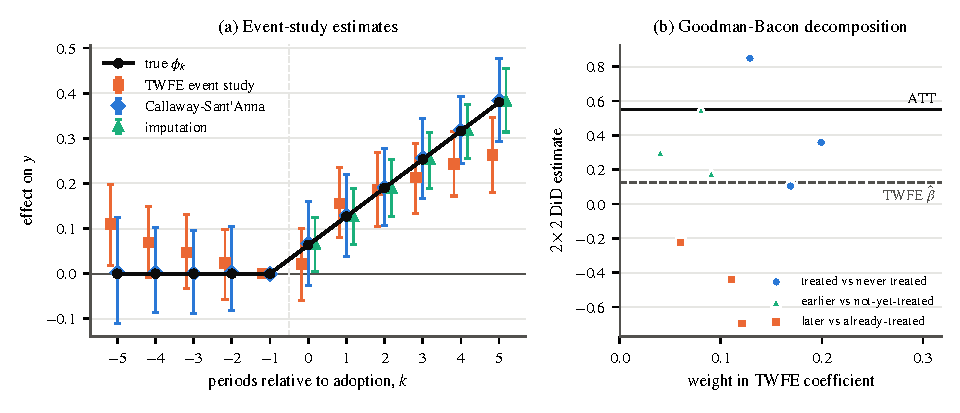
\includegraphics[width=\textwidth]{figures/appA/staggered.pdf}
\caption{Staggered adoption with effects that grow over time and differ across cohorts. (a) Mean estimates
of the event-time effects over 500 replications, with bars from the 5th to the 95th percentile. The black line is
the true effect, averaged over the cohorts observed at each relative time. The TWFE event study includes dummies
for $k=-5,\dots,5$ (omitting $k=-1$) and binned end points. (b) Goodman-Bacon decomposition of the expected
static TWFE coefficient (dashed line). Each marker is one two-by-two comparison. The solid line is the average effect
over all treated unit-periods. The design has 400 units, 20 periods, adoption in periods 5, 10 and 15 plus a never-treated
group. Numbers from \texttt{staggered\_did.py}, seed 20261022.}
\label{fig:A-staggered}
\end{figure}

The lesson for applied work is direct. When treatment timing varies and effects may change with exposure, we
should report heterogeneity-robust estimates alongside, or instead of, TWFE. The Goodman-Bacon decomposition is a
useful diagnostic, because it shows how much weight the forbidden comparisons receive. In merger retrospectives that
pool mergers closing at different dates, and in patent or entry studies with staggered timing, the issue arises
whenever the effect builds up gradually.

\subsection{Related designs}\label{sec:A-did-related}

\casehead{Synthetic control}
Many IO questions concern a single treated unit, such as the local market of one merger or one state's regulation.
With one treated unit, the choice of control group carries the whole design. The \emph{synthetic control} method
\citep{AbadieGardeazabal2003,AbadieDiamondHainmueller2010} builds the control as a weighted average of untreated
units. Let unit 1 be treated after period $T_0$ and units $2,\dots,J+1$ be potential controls. Let $X_1$ be a vector
of pre-treatment characteristics of the treated unit, including pre-period outcomes, and $X_0$ the matrix of the same
characteristics for the controls. The weights solve
\begin{equation*}
\min_{w}\ \big\|X_1-X_0w\big\|_V\quad\text{subject to}\quad w_j\ge0,\ \ \sum_{j=2}^{J+1}w_j=1,
\end{equation*}
for a positive definite weighting matrix $V$ chosen to fit pre-period outcomes. The estimated effect in period
$t>T_0$ is $y_{1t}-\sum_jw_jy_{jt}$. The constraints rule out extrapolation, because the synthetic unit lies in the
convex hull of the controls. The method is credible when the synthetic unit tracks the treated unit closely over a
long pre-period. Inference uses placebo assignments, applying the method to each control unit in turn and comparing
the treated unit's post-period gap with the placebo gaps. \citet{Abadie2021} discusses data requirements and
practice.

\casehead{Triple differences}
When the control group may face different trends, a third difference can remove them. Suppose a merger affects
product category $A$ in region 1, and region 2 and category $B$ are unaffected. The \emph{triple difference} is
\begin{equation*}
\hat\beta^{\mathrm{DDD}}=\big[\Delta\bar y_{A1}-\Delta\bar y_{A2}\big]-\big[\Delta\bar y_{B1}-\Delta\bar y_{B2}\big],
\end{equation*}
where $\Delta\bar y_{cr}$ is the change in the mean outcome of category $c$ in region $r$. The first bracket is a
regional DiD for category $A$. The second removes region-specific trends that also appear in category $B$. The
identifying assumption is that the gap between the regional trends would have been the same in both categories.
This is weaker than parallel trends for either DiD alone.

\casehead{Regression discontinuity}
When treatment is assigned by a known rule based on a running variable $z_i$, with $d_i=\indic\{z_i\ge c\}$, units
just above and just below the cutoff $c$ are comparable. If potential outcomes are continuous in $z$ at $c$, the
jump $\lim_{z\downarrow c}\E[y_i\mid z_i=z]-\lim_{z\uparrow c}\E[y_i\mid z_i=z]$ identifies the average effect at
the cutoff. Estimation uses local linear regression on each side (\cref{sec:A-loclin}). \citet{LeeLemieux2010} survey
the design. \citet{AtheyLevinSeira2011} discuss a deterministic rule for the format of timber sales, such as an open
auction whenever timber volume exceeds a threshold. Under such a rule their comparison would be identified in a
manner analogous to a regression discontinuity design (n.~13, p.~229).

\casehead{Selection on observables and matching}
A different design drops the panel. It assumes \emph{unconfoundedness}, that treatment is as good as random given
observed covariates: $(y_i(0),y_i(1))\perp d_i\mid x_i$. It also assumes \emph{overlap}, $0<\psi(x)<1$, where
$\psi(x)=\Pr(d_i=1\mid x_i=x)$ is the \emph{propensity score}. \citet{RosenbaumRubin1983} show that unconfoundedness given
$x_i$ implies unconfoundedness given $\psi(x_i)$. The proof is short. By iterated expectations,
\begin{equation*}
\Pr\big(d_i=1\mid y_i(0),y_i(1),\psi(x_i)\big)=\E\big[\Pr(d_i=1\mid y_i(0),y_i(1),x_i)\mid y_i(0),y_i(1),\psi(x_i)\big]=\psi(x_i),
\end{equation*}
because the inner probability equals $\psi(x_i)$ by unconfoundedness. Comparisons may therefore condition on the
scalar $\psi$ instead of the whole vector $x$. Estimators include regression adjustment, inverse propensity
weighting and matching. A matching estimator imputes each unit's missing potential outcome by the average outcome of
its $M$ nearest neighbors in the other treatment group. \citet{AbadieImbens2006} derive its large-sample distribution
and a consistent variance estimator. \citet{ImbensRubin2015} give a full treatment.

\citet{AtheyLevinSeira2011} use these tools to compare sealed-bid and open timber auctions held by the US Forest
Service (\cref{ch:auction-empirics}). Their sales took place between 1982 and 1990 in the Northern forests and between
1982 and 1989 in California. For an outcome $Y$ they write $Y=f(\mathit{SEALED},X,N,\epsilon)$
and target the average effect $\Delta Y=\E[f(1,X,N,\epsilon)-f(0,X,N,\epsilon)]$ (eq.~5, p.~229). The identifying
assumption is that the auction format is independent of $\epsilon$ given the covariates. It holds by design for sales
whose format was randomized, and for other sales if the format was chosen on information in their data. They
estimate a logit propensity score of the sealed-bid format on tract characteristics and drop sales with predicted
probabilities below 0.075 or above 0.925 to enforce overlap (p.~227). Their matching estimator is
\begin{equation*}
\widehat{\Delta Y}=\frac{1}{T}\sum_{t\ \text{sealed}}\big(Y_t-\hat Y_t\big)+\frac{1}{T}\sum_{t\ \text{open}}\big(\hat Y_t-Y_t\big)
\end{equation*}
(eq.~7, p.~230). Here $T$ is the number of sales, and $\hat Y_t$ is the average outcome of the $M=4$ sales of the
other format with the closest propensity scores. Standard errors follow \citet{AbadieImbens2006}. \Cref{tab:A-als}
compares the matching estimates with two regression estimates. In the Northern forests the three estimators agree
closely. Sealed bidding raises logger entry by about 10 percent and the sale price by 9 to 12 percent. In
California the price effects are small and insignificant, and the matching estimates are imprecise. Trimming for
overlap kept only a third of the California sales (p.~227). The authors also report similar estimates on the 378 Northern sales whose format
was randomized (p.~226).

\begin{table}[htbp]
\centering
\caption{Effect of sealed bidding on timber sale outcomes: regression and matching}
\label{tab:A-als}
\footnotesize
\begin{tabular}{@{}lcccc@{}}
\toprule
& \multicolumn{2}{c}{Northern forests ($N=1{,}071$)} & \multicolumn{2}{c}{California ($N=707$)}\\
\cmidrule(lr){2-3}\cmidrule(l){4-5}
Estimator & $\ln$(logger entry) & $\ln$(price) & $\ln$(logger entry) & $\ln$(price)\\
\midrule
OLS, no interactions & 0.089 & 0.094 & 0.101 & 0.027\\
 & (0.036) & (0.038) & (0.045) & (0.051)\\
OLS with sealed $\times$ covariate interactions & 0.097 & 0.099 & 0.099 & 0.026\\
 & (0.036) & (0.039) & (0.044) & (0.050)\\
Propensity-score matching, $M=4$ & 0.100 & 0.118 & 0.106 & $-0.038$\\
 & (0.048) & (0.064) & (0.062) & (0.127)\\
\bottomrule
\end{tabular}

\smallskip
\parbox{0.92\linewidth}{\footnotesize Notes: Each entry is the estimated effect of the sealed-bid format, with robust
standard errors in parentheses (Abadie-Imbens standard errors for matching). Regressions control for the Forest
Service appraisal variables, sale characteristics and year, quarter and location dummies. Samples exclude sales with
propensity scores outside $[0.075,0.925]$. Source: \citet{AtheyLevinSeira2011}, Table~III, columns 1 and 5.}
\end{table}

\section{Financial event studies}\label{sec:A-eventstudy}

A financial \emph{event study} measures the effect of a discrete piece of news on the market value of firms. The
method goes back to \citet{FamaEtAl1969}, and \citet{MacKinlay1997} surveys it. Industrial organization uses it to
learn about profits that we cannot observe directly. A merger that raises market power should raise the value of the
merging firms' rivals, and entry into a profitable market should lower the value of incumbents. This section
develops the method in general form. \Cref{sec:09-wc-method} applies it in full to the entry study of
\citet{WhinstonCollins1992}, and \cref{sec:11-retro-event} applies it to mergers.

\subsection{Premise}\label{sec:A-es-premise}

The method rests on \emph{market efficiency}. The equity value of a firm equals the expected present value of the
cash flows to its shareholders, given all public information. When news changes expected future profits, the share
price adjusts as soon as the news becomes public. The return on the announcement day, net of the return the stock
would have earned anyway, then measures the revision in the expected value of the firm to its shareholders. A study
of a few days of returns can thus reveal a change in discounted profits over many years. The price of this economy is
a set of assumptions about information, timing and the model of normal returns, which we make explicit below.

\subsection{Normal returns and abnormal returns}\label{sec:A-es-ar}

Index firms by $f$ and trading days by $\tau$, with the announcement on day $\tau=0$ of \emph{event time}. Let
$R_{f\tau}$ be the return on firm $f$'s stock, including dividends, $R^m_\tau$ the return on a market index and
$R^0_\tau$ the risk-free rate. The \emph{normal return} is the return expected without the event. Three models are
common. The \emph{constant-mean model} sets $R_{f\tau}=\mu_f+u_{f\tau}$. The \emph{market model} sets
\begin{equation}\label{eq:A-es-mm}
R_{f\tau}=a_f+b_f R^m_\tau+u_{f\tau},\qquad \E[u_{f\tau}\mid R^m]=0,\quad \Var(u_{f\tau}\mid R^m)=\sigma_f^2,
\end{equation}
with errors uncorrelated across days. The \emph{excess-return} form of the capital asset pricing model replaces
returns by returns in excess of the risk-free rate,
$R_{f\tau}-R^0_\tau=a_f+b_f(R^m_\tau-R^0_\tau)+u_{f\tau}$, as in \cref{sec:09-wc-method}. The market model removes the
part of the return due to market-wide news, which reduces the variance of the abnormal return and raises power.

The model is estimated on an \emph{estimation window} of $T_e$ trading days that ends some days before the event,
so that the event cannot affect the estimates. The \emph{event window} is $[\tau_1,\tau_2]$, which contains day
0 and has $L=\tau_2-\tau_1+1$ days. Days before the announcement allow for leakage, and days after it allow for slow
absorption. \Cref{fig:A-es-timeline} shows the layout.

\begin{figure}[htbp]
\centering
\begin{tikzpicture}[x=1cm,y=1cm]
\draw[-{Stealth[length=2.4mm]}, thick] (0,0) -- (14.2,0);
\node[font=\footnotesize, anchor=north east] at (14.2,-0.15) {event time $\tau$};
\fill[blue!18] (0.3,-0.14) rectangle (6.3,0.14);
\fill[gray!15] (6.3,-0.14) rectangle (7.9,0.14);
\fill[orange!35] (7.9,-0.14) rectangle (10.3,0.14);
\fill[gray!30] (10.3,-0.14) rectangle (13.4,0.14);
\foreach \x/\lab in {0.3/{\tau_1-g-T_e}, 6.3/{\tau_1-g-1}, 7.9/{\tau_1}, 9.1/{0}, 10.3/{\tau_2}} {
  \draw (\x,0.18) -- (\x,-0.18);
  \node[font=\footnotesize, below] at (\x,-0.2) {$\lab$};
}
\node[font=\footnotesize, anchor=north] at (9.1,-0.62) {(announcement)};
\draw[decorate, decoration={brace, amplitude=5pt}] (0.3,0.3) -- (6.3,0.3)
  node[midway, above=6pt, font=\footnotesize, align=center] {estimation window\\$T_e$ days: estimate $a_f$, $b_f$, $\sigma_f^2$};
\draw[decorate, decoration={brace, amplitude=4pt}] (6.35,0.3) -- (7.85,0.3)
  node[midway, above=5pt, font=\footnotesize] {gap, $g$ days};
\draw[decorate, decoration={brace, amplitude=5pt}] (7.9,0.3) -- (10.3,0.3)
  node[midway, above=6pt, font=\footnotesize, align=center] {event window\\$L$ days};
\draw[decorate, decoration={brace, mirror, amplitude=5pt}] (10.7,-0.85) -- (13.4,-0.85)
  node[midway, below=6pt, font=\footnotesize] {post-event window};
\end{tikzpicture}
\caption{Windows in a financial event study. The normal-return model is estimated on the estimation window, which
ends $g$ days before the event window so that the event cannot affect the estimates. Abnormal returns are computed
on the event window $[\tau_1,\tau_2]$ around the announcement on day 0. A post-event window can be used to check for
slow adjustment.}
\label{fig:A-es-timeline}
\end{figure}

\begin{definition}[Abnormal and cumulative abnormal returns]\label{def:A-es-ar}
Let $(\hat a_f,\hat b_f)$ be the OLS estimates of \eqref{eq:A-es-mm} on the estimation window. The \emph{abnormal
return} on an event-window day is the prediction error
$AR_{f\tau}=R_{f\tau}-\hat a_f-\hat b_fR^m_\tau$. The \emph{cumulative abnormal return} is
$CAR_f(\tau_1,\tau_2)=\sum_{\tau=\tau_1}^{\tau_2}AR_{f\tau}$.
\end{definition}

The variance of abnormal returns has a compact matrix form. Stack the estimation-window data as $y_e$ ($T_e\times1$)
and $X_e=[\iota,\,R^m_e]$ ($T_e\times2$), and the event-window data as $y^*$ ($L\times1$) and $X^*$ ($L\times2$). Let
$AR^*$ be the $L\times1$ vector of abnormal returns.

\begin{proposition}[Variance of abnormal returns]\label{prop:A-es-arvar}
Suppose that \eqref{eq:A-es-mm} holds on both windows under the null hypothesis of no event effect. Let the errors
be independent of the market returns and uncorrelated across days, with variance $\sigma_f^2$. Then, conditional on
the market returns,
\begin{equation*}
\E\big[AR^*\big]=0,\qquad \Var\big(AR^*\big)=\sigma_f^2\Big[I_L+X^*(X_e^\top X_e)^{-1}X^{*\top}\Big].
\end{equation*}
For a single day,
\begin{equation*}
\Var\big(AR_{f\tau}\big)=\sigma_f^2\left[1+\frac{1}{T_e}+\frac{(R^m_\tau-\hat\mu_m)^2}{\sum_{s}(R^m_s-\hat\mu_m)^2}\right],
\end{equation*}
where $\hat\mu_m$ is the mean market return over the estimation window and the sum runs over it. For the
cumulative abnormal return, $\Var(CAR_f)=\iota^\top\Var(AR^*)\,\iota$.
\end{proposition}

\begin{proof}
Write $\theta_f=(a_f,b_f)^\top$ and $\hat\theta_f=(X_e^\top X_e)^{-1}X_e^\top y_e$. Under the null,
$y^*=X^*\theta_f+u^*$, so
\begin{equation*}
AR^*=y^*-X^*\hat\theta_f=u^*-X^*(\hat\theta_f-\theta_f)=u^*-X^*(X_e^\top X_e)^{-1}X_e^\top u_e .
\end{equation*}
Both terms have mean zero. The event-window errors $u^*$ are uncorrelated with the estimation-window errors $u_e$,
so the variance is the sum of $\Var(u^*)=\sigma_f^2I_L$ and
\begin{equation*}
X^*(X_e^\top X_e)^{-1}X_e^\top\Var(u_e)X_e(X_e^\top X_e)^{-1}X^{*\top}=\sigma_f^2X^*(X_e^\top X_e)^{-1}X^{*\top}.
\end{equation*}
For a single day with regressor row $x_\tau=(1,R^m_\tau)$, write $Q=\sum_s(R^m_s-\hat\mu_m)^2$. The inverse is
\begin{equation*}
(X_e^\top X_e)^{-1}=\frac{1}{T_eQ}\begin{pmatrix}\sum_s(R^m_s)^2 & -\sum_sR^m_s\\ -\sum_sR^m_s & T_e\end{pmatrix}.
\end{equation*}
Then $x_\tau(X_e^\top X_e)^{-1}x_\tau^\top=\frac{\sum_s(R^m_s)^2-2R^m_\tau\sum_sR^m_s+T_e(R^m_\tau)^2}{T_eQ}$.
Substituting $\sum_s(R^m_s)^2=Q+T_e\hat\mu_m^2$ and $\sum_sR^m_s=T_e\hat\mu_m$, the numerator becomes
$Q+T_e(R^m_\tau-\hat\mu_m)^2$. Dividing by $T_eQ$ gives $\frac{1}{T_e}+\frac{(R^m_\tau-\hat\mu_m)^2}{Q}$. The variance
of the cumulative abnormal return is the variance of $\iota^\top AR^*$.
\end{proof}

The term $X^*(X_e^\top X_e)^{-1}X^{*\top}$ is estimation error in the normal-return model. It vanishes as $T_e$
grows, and with a typical estimation window of a year of trading days it is small. Its off-diagonal elements are not
zero, so abnormal returns on different event-window days are correlated through the common estimation error.

\casehead{Test statistics}
Replacing $\sigma_f^2$ by the residual variance $\hat\sigma_f^2=\frac{1}{T_e-2}\sum_s\hat u_{fs}^2$ gives the
\emph{standardized cumulative abnormal return}
\begin{equation*}
SCAR_f=\frac{CAR_f(\tau_1,\tau_2)}{\widehat{\mathrm{sd}}\big(CAR_f\big)} .
\end{equation*}
Under normal errors and the null it has a $t$ distribution with $T_e-2$ degrees of freedom, and it is approximately
standard normal for long estimation windows. With $N$ events on different calendar dates the abnormal returns are
independent across events. Two aggregate statistics are standard. The first divides the average CAR,
$\overline{CAR}=\frac{1}{N}\sum_fCAR_f$, by $\frac{1}{N}(\sum_f\widehat{\Var}(CAR_f))^{\frac{1}{2}}$. The second
averages the standardized values. A $t$ variable with $T_e-2$ degrees of freedom has variance $\frac{T_e-2}{T_e-4}$, so
\begin{equation*}
\Big(\frac{N(T_e-4)}{T_e-2}\Big)^{\frac{1}{2}}\,\frac{1}{N}\sum_{f=1}^{N}SCAR_f\ \xrightarrow{d}\ N(0,1)
\end{equation*}
as $N$ grows. The second statistic weights events with volatile stocks less.

\casehead{Power and the length of the window}
A short window raises power. Suppose an event moves the value by a fraction $A$ spread over an $L$-day window, and
ignore estimation error. The expected standardized CAR of one event is about $\frac{A}{\sigma_f\sqrt L}$. With daily
volatility $\sigma_f=0.02$ and $A=0.01$, it is 0.5 for a one-day window. With $N=50$ independent events the aggregate
statistic is about $0.5\sqrt{50}\approx3.5$. With an eleven-day window the same effect gives about
$\frac{3.5}{\sqrt{11}}\approx1.07$, which is insignificant. \citet{BrownWarner1985} study the properties of these
tests with daily data.

\casehead{Events on the same date}
When several firms are hit by the same news, their abnormal returns are correlated. Industry news that the market
index does not absorb moves them together. Suppose $N$ firms share an event date, each CAR has variance $v$, and each
pair has correlation $\rho$. Then
\begin{equation*}
\Var\big(\overline{CAR}\big)=\frac{1}{N^2}\big[Nv+N(N-1)\rho v\big]=\frac{v}{N}\big[1+(N-1)\rho\big],
\end{equation*}
the same inflation factor as in clustered regressions (\cref{prop:A-moulton}). One remedy is the \emph{portfolio
approach}. We form an equally weighted portfolio of the affected firms, estimate the market model for the portfolio
return, and compute its abnormal return. The portfolio residual variance estimates
$\frac{1}{N^2}\iota^\top\Sigma\iota$ directly, so the covariance is accounted for. The other remedy, a system of
regressions, follows.

\subsection{Regression form}\label{sec:A-es-regression}

The two-step procedure has an equivalent one-step form. We estimate the market model on the estimation and event
windows together and add one indicator for each event-window day:
\begin{equation}\label{eq:A-es-dummy}
R_{f\tau}=a_f+b_fR^m_\tau+\sum_{s=\tau_1}^{\tau_2}\gamma_{fs}\,\indic\{\tau=s\}+u_{f\tau}.
\end{equation}

\begin{proposition}[Dummy-variable form]\label{prop:A-es-dummy}
OLS on \eqref{eq:A-es-dummy} gives the estimation-window estimates $(\hat a_f,\hat b_f)$, and
$\hat\gamma_{fs}=AR_{fs}$ for every event-window day $s$. Under the assumptions of \cref{prop:A-es-arvar}, the
conventional OLS variance of $(\hat\gamma_{f\tau_1},\dots,\hat\gamma_{f\tau_2})$ equals $\Var(AR^*)$.
\end{proposition}

\begin{proof}
Order the observations with the estimation window first. The regressor matrix and the dummy matrix are
\begin{equation*}
X=\begin{pmatrix}X_e\\X^*\end{pmatrix},\qquad Q_d=\begin{pmatrix}0\\I_L\end{pmatrix}.
\end{equation*}
By the Frisch-Waugh-Lovell theorem
(\cref{thm:A-fwl}), the coefficients on $X$ equal those from regressing $M_{Q}y$ on $M_{Q}X$, where
$M_Q=I-Q_d(Q_d^\top Q_d)^{-1}Q_d^\top$. This annihilator sets the event-window rows to zero and leaves the
estimation-window rows unchanged. The regression therefore uses only estimation-window data, and its coefficients are
$(\hat a_f,\hat b_f)$. The dummy coefficients solve the remaining normal equations,
$Q_d^\top(y-X\hat\theta_f-Q_d\hat\gamma_f)=0$, which give $\hat\gamma_f=y^*-X^*\hat\theta_f=AR^*$. Each dummy fits its
observation exactly.

For the variance, the FWL theorem gives the conventional variance of $\hat\gamma_f$ as
$\sigma_f^2(Q_d^\top M_XQ_d)^{-1}$, with $M_X=I-X(X^\top X)^{-1}X^\top$. Now $Q_d^\top M_XQ_d=I_L-X^*(X^\top X)^{-1}X^{*\top}$
and $X^\top X=X_e^\top X_e+X^{*\top}X^*$. The Woodbury identity gives
\begin{equation*}
\Big[I_L-X^*\big(X_e^\top X_e+X^{*\top}X^*\big)^{-1}X^{*\top}\Big]^{-1}=I_L+X^*(X_e^\top X_e)^{-1}X^{*\top}.
\end{equation*}
So the conventional variance equals $\sigma_f^2[I_L+X^*(X_e^\top X_e)^{-1}X^{*\top}]$, which is $\Var(AR^*)$.
\end{proof}

The regression form has three advantages. The sum of the dummy coefficients is the CAR, and its standard error comes
from the regression. A single dummy for all window days estimates the average daily abnormal return directly, and
$L$ times it estimates the cumulative effect. And the event effect can depend on firm and event characteristics,
which lets many firms and events be estimated jointly. \Cref{prop:09-wc-dummy} gives the scalar version used by
Whinston and Collins.

\casehead{Systems of firms}
With $M$ firms observed on the same days, we stack the firm equations for day $\tau$ as
$y_\tau=X_\tau\theta+u_\tau$. The vector $\theta$ may contain parameters common to all firms, such as the effect of an
event per unit of exposure. A
system of \emph{seemingly unrelated regressions} (SUR) allows errors to be correlated across firms on the same day
and uncorrelated across days, $\E[u_\tau u_\tau^\top]=\Sigma$ \citep{Zellner1962}. Feasible GLS estimates $\Sigma$
from first-stage residuals (\cref{sec:A-systems}). \citet[pp.~170--173]{Binder1985} applies this system, which he calls
the multivariate regression model, to regulatory events that affect many firms at once.
GLS reduces to equation-by-equation OLS when every equation has the
same regressors and no parameter is shared (\cref{prop:A-sur-ols}). Binder's system meets both conditions, since each
firm has its own abnormal returns and all equations share one regressor matrix. In his system the GLS point estimates
therefore equal OLS, and SUR matters for his tests across firms, whose statistics use $\hat\Sigma$ (p.~173). Neither condition holds when the event effect is
a common parameter scaled by firm-specific exposure, and SUR then gains efficiency and gives standard errors that
account for same-day correlation. \citet{WhinstonCollins1992} estimate such a system for a panel of 20 airlines,
People Express included, ``allowing the $\{\epsilon_{it}\}$ to be contemporaneously correlated across firms''
(p.~449).

\casehead{Dollar abnormal values}
An abnormal return measures the event's effect relative to the firm's value. The \emph{dollar abnormal value} on day
$\tau$ is $V_{f,\tau-1}AR_{f\tau}$, where $V_{f,\tau-1}$ is the equity value at the previous close. Summing over the
window gives the change in shareholder wealth. The choice between returns and dollars is a modelling choice about the
event. If the event changes the firm's value by a fixed dollar amount $\Delta_f$, its return effect is
$\frac{\Delta_f}{V_{f,\tau-1}}$. A model with a common abnormal return across firms would then force larger firms
to have proportionally larger dollar effects. Whinston and Collins argue that the loss from being an incumbent in one
entered market should not scale with the carrier's size (p.~449). They therefore model dollar effects, with the
return equation
\begin{equation*}
R_{f\tau}-R^0_\tau=\frac{a_f}{V_{f,\tau-1}}+b_f\big(R^m_\tau-R^0_\tau\big)+\frac{\Delta_f(Z_\tau)}{V_{f,\tau-1}}+u_{f\tau},
\end{equation*}
where $\Delta_f(Z_\tau)$ is the dollar effect of the events on day $\tau$ (\cref{eq:09-wc-dollar}). Estimating in
return units keeps the error homoskedastic. The equivalent dollar regression would have errors with variance
$V_{f,\tau-1}^2\sigma_f^2$. Their simplest specification makes the dollar loss proportional to the incumbent's
annualized seatmiles on the entered route. The estimated loss per seatmile is $-0.0109$ (s.e.\ 0.0035) for a one-day
window, $-0.0147$ (0.0049) for two days and $-0.0191$ (0.0061) for three days (Table~1, p.~453). These are total
changes over each window. They imply losses of \$3.7 million to \$6.5 million per incumbent (p.~452). \Cref{tab:09-wc-t1}
reports the full results.

\subsection{Identification and pitfalls}\label{sec:A-es-pitfalls}

An abnormal return equals the change in expected shareholder value caused by the event only under several
conditions. Each can fail in IO applications.

\casehead{Dating and leakage}
The event must be dated by the first public report. News often leaks before formal announcements, through
rumors, regulatory filings or trade press. Longer windows capture leakage but add the noise of unrelated news on each
extra day, and by the power calculation above they dilute the test. Whinston and Collins date each event by the
earliest report in the trade or financial press, and use one-, two- and three-day windows ending on that day
(p.~450).

\casehead{Anticipation}
Markets price events before they happen when they expect them. The next result makes the consequence precise.

\begin{proposition}[Partial anticipation]\label{prop:A-es-anticipation}
Suppose that before the announcement the market assigns probability $\pi$ to an event that would change the firm's
value by $\Delta V$, and that the announcement resolves the uncertainty. If the event is announced, the measured
value change is $(1-\pi)\Delta V$. If the announcement reveals that the event will not happen, the measured change is
$-\pi\Delta V$.
\end{proposition}

\begin{proof}
Let $V^0$ be the value without the event. Before the announcement the value is the expectation
$V^0+\pi\Delta V$. If the event is announced, the value becomes $V^0+\Delta V$, and the change is
$(V^0+\Delta V)-(V^0+\pi\Delta V)=(1-\pi)\Delta V$. If the event is ruled out, the value becomes $V^0$, and the change
is $-\pi\Delta V$.
\end{proof}

Announcement returns therefore understate the value of events that were partly expected, and the bias is larger the
more predictable the event. Dividing by $1-\pi$ corrects the estimate if $\pi$ is known.
\citet[pp.~240--241]{MalatestaThompson1985} show that $\pi$ need not be known when events of constant expected value recur with a
constant probability per period. Repeated acquisition attempts by one firm are an example. They regress the firm's dollar excess
return on a market term and a dummy for periods with an event. The intercept then estimates $-\pi\Delta V$, and the
dummy coefficient estimates $\Delta V$ itself.
A merger announcement raises the probability of the
merger, and an antitrust complaint lowers it. Under \cref{prop:A-es-anticipation} the two events move the rivals'
values in opposite directions with magnitudes that depend on the prior probabilities. This is the logic behind the
rival tests in \cref{tab:11-eventpred}.

\casehead{Information revealed by the event}
An event can reveal information beyond its direct effect. A merger announcement may reveal that scale economies are
available to the whole industry, or that rivals are attractive targets. Rivals' values then rise for reasons other
than market power. Entry by one firm may reveal its plans for further expansion. Whinston and Collins find
industry-wide losses that they cannot fully attribute, and list such informational effects among the possible
sources (p.~448).

\casehead{Confounding events and calendar clustering}
Other news inside the window that is correlated with exposure to the event biases the estimate. Events that cluster
on the same dates create the cross-sectional dependence discussed above. Event-induced changes in volatility make the
estimation-window variance too small. A test that standardizes each abnormal return and then uses the cross-sectional
variance of the standardized values guards against this \citep{BoehmerMusumeciPoulsen1991}.

\casehead{Thin trading}
Stocks that trade infrequently have stale prices, which biases estimated betas and spreads the response over
several days. Estimators that use leads and lags of the market return correct the betas \citep{ScholesWilliams1977}.

\casehead{Who captures the change}
Equity values measure only the shareholders' part of a change in firm value. Part of the rents from market power can
accrue to debtholders, to workers through rent sharing, or to managers. Whinston and Collins note that misdating,
partial anticipation, and value changes felt by debtholders or workers all bias their estimates toward zero
(p.~453). Effects on consumers do not appear in stock prices at all, so an event study measures only producer gains
and losses.

\subsection{Uses in industrial organization}\label{sec:A-es-io}

\casehead{Mergers}
The value created for the merging firms combines market power and efficiencies, so it cannot tell them apart. The
returns of rivals can. A merger that raises prices raises rivals' profits, while a merger that creates a more
efficient competitor lowers them. \citet{Eckbo1983} and \citet{Stillman1983} compare rivals' abnormal returns at the
merger announcement and at the antitrust complaint. Under the market-power hypothesis the two returns have opposite
signs, positive and then negative. \Cref{tab:11-eventpred} lists the predictions, including the information
hypothesis that weakens the test. The design also needs rivals that are publicly traded and for which the affected
market is a large part of value. \Cref{sec:11-retro-event} discusses applications and their limits.
\citet[p.~231, n.~137]{AskerNocke2021} report that most authors doubt that an event study can reveal the competitive
effects of one specific merger. In their reading the method works best for patterns across large samples of mergers.

\casehead{Entry and contestability}
Incumbents' value losses at an entry announcement reveal profits or sunk costs on the entered route, which perfect
contestability rules out. \citet{WhinstonCollins1992} use differences in exposure across carriers to separate three
sources of loss (\cref{sec:09-wc}). These are incumbency on the entered airport pair, presence at other airports of
the same city pair, and general effects felt by all carriers. The panel DiD of \cref{sec:A-did-control} then checks the mechanism with
prices, quantities and capacity.

\casehead{Regulation}
Regulatory events change the profits of whole industries at once. \citet[p.~448, n.~5]{WhinstonCollins1992} cite
\citet{Schwert1981} and \citet{Rose1985} as earlier uses of the event study in industrial organization. Their titles
are ``Using Financial Data to Measure the Effects of Regulation'' (Schwert) and ``The Incidence of Regulatory Rents in
the Motor Carrier Industry'' (Rose).
\citet[pp.~168--169]{Binder1985} applies the multivariate regression model to 20 major regulatory changes between 1887 and 1978.
News about each change came out in 5.6 announcements on average, spread over 18.5 months (p.~170). His tests reject
the null of no abnormal returns only slightly more often than chance would predict (p.~174). He concludes that the
formal announcements were generally anticipated (p.~181).
Because regulatory news is often anticipated and spread over many dates,
\cref{prop:A-es-anticipation} and the dating problem are especially relevant here.

The financial event study and the panel DiD answer related questions with different data. The first measures
expected changes in producer value at the moment of the news. The second measures realized changes in prices and
quantities over months or years. Studies that use both, as Whinston and Collins do, can check one against the other.


\section{Bibliographic notes}\label{sec:A-notes}

Several textbooks cover the material of this appendix in more depth. \citet{Hayashi2000}, \citet{Wooldridge2010} and
\citet{Hansen2022} treat least squares, instrumental variables, panel data and GMM at the level of
\cref{sec:A-ols,sec:A-iv,sec:A-gmm}. \citet{CameronTrivedi2005} add many microeconometric applications.
\citet{NeweyMcFadden1994} remains the standard reference for the large-sample theory of extremum estimators. It covers
the consistency and normality theorems of \cref{sec:A-extremum}, two-step estimators and the efficiency of GMM.
\citet{AndrewsStockSun2019} survey weak instruments and robust inference. \citet{AngristPischke2009} and
\citet{ImbensRubin2015} present the potential-outcomes approach to instruments and treatment effects that underlies
\cref{sec:A-potential,sec:A-late,sec:A-did}.

For simulation, \citet{GourierouxMonfort1996} develop the asymptotic theory of simulated moments, simulated likelihood
and indirect inference, and \citet{Train2009} is a practical guide to simulation in discrete choice models.
\citet{CameronMiller2015} is the standard practitioner's guide to clustered standard errors, and \citet{AbadieEtAl2023}
restate the case for clustering in design-based terms. For the bootstrap, \citet{EfronTibshirani1993} give an
accessible introduction, \citet{Hall1992} develops the theory of asymptotic refinements, and \citet{Horowitz2001}
surveys the method for econometricians. \citet{Silverman1986} is the classic introduction to density estimation.
\citet{FanGijbels1996} cover local polynomial regression, and \citet{LiRacine2007} give a comprehensive treatment of
nonparametric econometrics, including series estimators and the partially linear model.

\citet{RothEtAl2023} survey the recent literature on differences in differences, with staggered adoption, robust
estimators and violations of parallel trends. \citet{Abadie2021} discusses synthetic control in practice, and
\citet{MacKinlay1997} remains the standard introduction to financial event studies. For partial identification,
\citet{Manski2003} develops the general approach and \citet{Tamer2010} surveys its use in econometrics.

For systems of demand equations, \citet[Section~3.3, pp.~67--75]{DeatonMuellbauer1980b} explain which restrictions
of demand theory can be tested and review the early tests on Dutch and British data (\cref{sec:A-systems,sec:A-wald}).
\citet{Davies1977} and \citet{Hansen1992} treat tests in which a parameter is identified only under the alternative,
the problem behind Porter's test for regime switching (\cref{sec:A-mle-nonregular}).

Several surveys connect these tools to industrial organization. \citet{AckerbergEtAl2007} cover demand estimation,
production functions and dynamic models, with particular attention to GMM, simulation and instruments for
differentiated-products demand. \citet{AtheyHaile2007} do the same for auctions, from nonparametric identification to
the practical choices of kernels, trimming and bootstrap. Two chapters of the fifth volume of the Handbook of
Industrial Organization \citep{HoHortacsuLizzeri2021} survey the later applications. \citet{HortacsuPerrigne2021}
review empirical work on auctions. Their sections on timber and procurement auctions (pp.~86--123) cover two methods
of this appendix. The entry model of \citet{AtheyLevinSeira2011} appears on pp.~90--91
(\cref{sec:A-mle-discrete,sec:A-did-related}). The deconvolution estimator of \citet{Krasnokutskaya2011} appears on
p.~103 (\cref{sec:A-deconv}). \citet{AskerNocke2021} review collusion and
mergers. Their Section~2.3 (pp.~209--210) covers statistical tests for bid rigging from \citet{PorterZona1993} on.
Their Section~3.7 (pp.~255--257) and their appendix table (pp.~261--265) cover merger retrospectives, the designs
of \cref{sec:A-did}.
\citet[p.~158]{EinavLevin2010} argue that structural and design-based work are often complementary, even for the same
question.

\section{Exercises}\label{sec:A-exercises}

\begin{enumerate}[label=\arabic*., leftmargin=*, itemsep=6pt]

\item \textit{Simultaneity with correlated shocks.} Take the market of \cref{ass:A-working}, but let the demand and
supply shocks have covariance $\sigma_{ds}$.
\begin{enumerate}[label=(\alph*)]
  \item Show that the slope of the OLS regression of $q_t$ on $p_t$ converges to
  \begin{equation*}
  \frac{c\,\sigma_d^2 - b\,\sigma_s^2 + (b - c)\,\sigma_{ds}}{\sigma_d^2 + \sigma_s^2 - 2\sigma_{ds}} .
  \end{equation*}
  Check the result by computing $\Cov(q_t, p_t)$ twice, once from the supply equation as in the proof of
  \cref{prop:A-ols-simultaneity} and once from the demand equation.
  \item Let $\sigma_{ds} = 0$. Find the limit of the slope of the reverse regression of $p_t$ on $q_t$. Show that it
  equals the inverse demand slope $-\frac{1}{b}$ only when $\sigma_d^2 = 0$ or $c = 0$, and interpret both cases.
  \item Add the cost shifter $w_t$ of \cref{cor:A-shifter}. Show that IV with instrument $w_t$ is consistent for $-b$
  whatever the value of $\sigma_{ds}$. Which assumption about $w_t$ does the argument use?
  \item In the design of \cref{fig:A-simultaneity}, compute the concentration parameter $\mu^2$ of \eqref{eq:A-mu2}
  for samples of 200 markets. Use \eqref{eq:A-EF} to compare it with the mean first-stage $F$ statistic of 331 reported
  in the caption.
\end{enumerate}

\item \textit{Two-stage least squares and specification tests.}
\begin{enumerate}[label=(\alph*)]
  \item Let $L = K$ and let $A$ be any nonsingular $L \times L$ matrix. Show that IV with instruments $ZA$ gives the
  same estimate as IV with $Z$. Explain why the choice among linear combinations of the instruments matters only when
  $L > K$.
  \item Consider one endogenous regressor, exogenous controls and excluded instruments. In the control-function
  regression of \cref{prop:A-cf-2sls}, show that the coefficient on the first-stage residual is zero if and only if the
  regressor is uncorrelated with the structural error. Explain why a heteroskedasticity-robust $t$ test of this
  coefficient remains valid when OLS is not efficient.
  \item For the 80th percentile fare in \citet{Borenstein1989}, the route-share coefficient is 0.1259 (0.0349) by OLS
  and 0.2238 (0.0784) by 2SLS (\cref{sec:A-spectests}). Compute the Hausman statistic \eqref{eq:A-hausman} for this
  coefficient alone, and compare it with the 5 percent cutoff of $\chi^2_1$.
  \item Borenstein reports that Hausman tests reject the exogeneity of route share and the route Herfindahl index. Give two
  reasons why a statistic for one coefficient in one percentile regression need not agree with the tests he reports.
  \item In the Rotterdam system \eqref{eq:A-rotterdam}, show that adding up and symmetry together imply homogeneity.
  Explain why OLS estimates satisfy adding up whatever the data (\cref{prop:A-addingup}), why homogeneity can be
  tested one equation at a time, and why a test of symmetry needs the whole system.
\end{enumerate}

\item \textit{A two-step estimator.} Let $(x_i, y_i)$ be independent and identically distributed with
$\E[x_i] = \mu \neq 0$, and let $\theta = \frac{\E[y_i]}{\mu}$. The first step estimates $\hat\mu = \bar x$, and the
second solves $\frac{1}{n}\sum_i(y_i - \theta\hat\mu) = 0$.
\begin{enumerate}[label=(\alph*)]
  \item Write the two steps as the moments $m(w;\mu) = x - \mu$ and $g(w;\theta, \mu) = y - \theta\mu$. Use
  \cref{prop:A-twostep} to show that $V_\theta = \frac{\Var(y_i - \theta x_i)}{\mu^2}$.
  \item Show that the delta method (\cref{thm:A-delta}) applied to $\frac{\bar y}{\bar x}$ gives the same variance.
  \item The naive variance treats $\hat\mu$ as known. Show that it equals $\frac{\Var(y_i)}{\mu^2}$, and find the
  condition on $\Cov(x_i, y_i)$ under which it understates the true variance.
  \item Relate the result to the generated regressand of \cref{sec:A-twostep}, in which every implied markup depends on
  the estimated price coefficient.
\end{enumerate}

\item \textit{EM and regime persistence.} Let $y_t = \mu_1I_t + \mu_0(1 - I_t) + \sigma\varepsilon_t$ for
$t = 1, \dots, T$, with $\varepsilon_t$ independent standard normal and $I_t$ independent Bernoulli with
$\Pr(I_t = 1) = \lambda$.
\begin{enumerate}[label=(\alph*)]
  \item Write the likelihood and the posterior probability $w_t = \Pr(I_t = 1 \mid y_t)$ used in the E step.
  \item Show that the M step gives $\lambda = \frac{1}{T}\sum_tw_t$, $\mu_1 = \frac{\sum_tw_ty_t}{\sum_tw_t}$ and
  $\mu_0 = \frac{\sum_t(1 - w_t)y_t}{\sum_t(1 - w_t)}$. Derive the update for $\sigma^2$.
  \item Show that if the algorithm starts with $\mu_1 = \mu_0$, every posterior equals $\lambda$ and the algorithm never
  leaves the set $\{\mu_1 = \mu_0\}$. Relate this to the random start in \cref{fig:A-em}.
  \item Let $I_t$ instead follow a Markov chain with $\Pr(I_{t+1} = 1 \mid I_t = 1) = p_1$ and
  $\Pr(I_{t+1} = 1 \mid I_t = 0) = p_0$. Derive the stationary probability of the collusive regime and the expected
  length of a spell in each regime. Evaluate them at Ellison's estimates $p_1 = 0.975$ and $p_0 = 0.067$, and compare
  with \cref{sec:A-mle-latent}.
  \item Return to the model of (a). The null of a single regime is $\mu_1 = \mu_0$. Show that the likelihood does not
  depend on $\lambda$ under this null. Use the result to explain why the likelihood ratio statistic for this null has
  no $\chi^2_1$ limit. Discuss whether Porter's statistic of 554.1 (\cref{sec:A-mle-nonregular}) leaves any doubt
  about his rejection.
\end{enumerate}

\item \textit{Simulation estimators.} A binary outcome has $\Pr(y_i = 1 \mid x_i) = \int\Lambda(x_i^\top\beta_\nu)\,\dd F(\nu)$,
where $\Lambda$ is the logistic distribution function and $\beta_\nu$ is a random coefficient vector.
\begin{enumerate}[label=(\alph*)]
  \item A frequency simulator draws $n_s$ latent utilities per observation and records the share of draws with
  positive utility. Show that SML with this simulator evaluates the log of zero with positive probability. Show that
  MSM with the moment $\E[z_i(y_i - \tilde P_i)] = 0$ has no such problem.
  \item For the smooth simulator, use \cref{prop:A-sml-bias}(i) to explain why the bias of SML is largest for
  observations whose observed outcome is unlikely under the model.
  \item In the auction estimator of \cref{sec:A-snlls}, suppose a researcher drops the correction term from
  \eqref{eq:A-lov-snlls}. Use \eqref{eq:A-lov-decomp} to explain the direction in which the estimated spread of values
  moves when the simulator variance $\omega_l(\theta)$ increases with that spread.
\end{enumerate}

\item \textit{Inference in a state-year panel.}
\begin{enumerate}[label=(\alph*)]
  \item Let $y_{ic} = \alpha + \beta x_c + a_c + \varepsilon_{ic}$, with a regressor $x_c$ that is constant within state
  $c$, independent state effects $a_c$ with variance $\sigma_a^2$, and independent $\varepsilon_{ic}$ with variance
  $\sigma_\varepsilon^2$. Use \cref{prop:A-moulton} to compute the ratio of the true to the conventional standard error
  of $\hat\beta$ when each state has 25 years and $\frac{\sigma_a^2}{\sigma_a^2 + \sigma_\varepsilon^2} = 0.3$.
  \item Now let the regressor vary within states, and add state fixed effects. Show that the within transformation
  removes $a_c$, so that conventional standard errors are valid in this model. Use \cref{ex:A-ar1-factor} to explain
  why clustering by state still raised the standard error in row (1) of \cref{tab:A-sumner}.
  \item In that row, $\hat\rho = 1.075$ with a state-clustered standard error of 0.034. Build a 95 percent interval for
  $\ln(\rho - 1)$ by the delta method, with the $t_{47}$ quantile 2.012. Map it into an interval for the elasticity
  $\frac{\rho}{\rho - 1}$.
  \item Compare your interval with the intervals in \cref{tab:A-boot-intervals}. Which parametrization makes the normal
  approximation more accurate here, and why?
\end{enumerate}

\item \textit{Kernel bandwidths and boundaries.}
\begin{enumerate}[label=(\alph*)]
  \item Use \eqref{eq:A-hstar} and the normal reference value of $\mathcal{R}(f'')$ to derive the rule of thumb for the
  Epanechnikov kernel, $h = (40\sqrt\pi)^{\frac{1}{5}}\sigma n^{-\frac{1}{5}} \approx 2.34\,\sigma n^{-\frac{1}{5}}$.
  Check the conversion factor reported in \cref{tab:A-kernels}.
  \item \citet{GuerrePerrigneVuong2000} use the constant 1.06 with the triweight kernel, whose normal-reference
  constant is $2.978 \times 1.06$. By what factor does their bandwidth differ from the normal-reference rule? What
  does the difference imply for the bias and the variance of $\hat g$?
  \item Let $f$ have support $[0, \infty)$ with $f(0^+) > 0$ and $f'(0^+) \neq 0$. Show that the reflection estimator
  $\hat f_h(x) + \hat f_h(-x)$ has bias of order $h$ at $x = 0$. Find its leading term for a symmetric kernel.
  \item Use \cref{prop:A-kde-boundary} and \eqref{eq:A-gpv-xi} to explain why pseudo-values computed near the upper end
  of the bid support are biased upward.
\end{enumerate}

\item \textit{Control groups, staggered adoption and anticipation.}
\begin{enumerate}[label=(\alph*)]
  \item Extend \cref{prop:A-did-spillover} to a control group that is partly affected and also violates parallel trends
  by $\delta = \E_1[y_{i1}(0) - y_{i0}(0)] - \E_0[y_{i1}(0) - y_{i0}(0)]$. Show that
  $\E[\hat\beta^{\mathrm{DD}}] = (1 - \kappa)\mathrm{ATT} + \delta$.
  \item For Pennzoil and Quaker State, \citet{AshenfelterHosken2010} estimate 0.052 with private-label controls and
  0.014 with branded controls. Suppose private labels satisfy $\kappa = 0$ and $\delta = 0$, and branded substitutes
  satisfy $\delta = 0$. What fraction $\kappa$ of the merging firms' price increase did branded rivals match? Repeat the
  calculation for General Mills and Chex (0.032 and 0.057), and explain what the answer implies.
  \item In the design of \cref{prop:A-bacon3}, let $(\omega_E, \omega_L, \omega_U) = (\frac{1}{4}, \frac{1}{4}, \frac{1}{2})$.
  Compute the weights that \cref{cor:A-bacon3} places on $\mathrm{ATT}_E(0)$, $\mathrm{ATT}_E(1)$ and
  $\mathrm{ATT}_L(0)$. For which shares is the weight on $\mathrm{ATT}_E(1)$ negative?
  \item A merger announcement raises the market's probability that a merger will be completed from zero to $\pi$, and a
  later antitrust challenge lowers it back to zero. Following \cref{prop:A-es-anticipation}, show that a rival's
  abnormal values at the two dates are $\pi\Delta V$ and $-\pi\Delta V$. Explain why the sum of the two can test the
  information hypothesis of \cref{sec:A-es-pitfalls}.
\end{enumerate}

\end{enumerate}

\chapter{Mathematical Toolkit}\label{app:math}

Empirical industrial organization uses a small set of mathematical tools again and again. Pass-through formulas
come from the implicit function theorem, and Shephard's lemma and Roy's identity come from the envelope theorem.
Logit demand comes from the algebra of the Gumbel distribution. The identification of auction models comes from
the distribution theory of order statistics. This appendix states each tool with its assumptions, gives or locates
a proof, and shows how the chapters use it.

The appendix serves two kinds of reader. A reader who meets a tool in a chapter can come here for a precise
statement, a proof, a worked example and the usual pitfalls. A reader who wants a systematic treatment can read
the appendix from start to finish, because each section builds on the earlier ones. Several chapters prove a tool
in the context of one application. For those results we usually restate the theorem and refer to the chapter
that proves it. We give full proofs for the tools that no chapter proves and for the parts of a result that go
beyond the chapter's version. Worked applications, such as pass-through in \cref{sec:B-passthrough}, keep their
derivations because they show a tool at work.

The sections follow the logic of the tools. \Cref{sec:B-prelim} collects calculus, matrix and probability facts.
\Cref{sec:B-ift,sec:B-envelope} develop the two workhorses of comparative statics, the implicit function theorem
and the envelope theorem. \Cref{sec:B-duality} applies the envelope theorem to consumer and producer theory, and
\cref{sec:B-ev} derives the logit family from the extreme value distribution. \Cref{sec:B-orderstats} turns to
order statistics, the language of auction data. \Cref{sec:B-fixedpoint} treats fixed points: the inversion of
market shares, and the existence, uniqueness and computation of price equilibria. \Cref{sec:B-logconcave,%
sec:B-supermod} study the shape restrictions that make equilibria exist, comparative statics signable and auction
models tractable. These are log-concavity, supermodularity and affiliation. \Cref{tab:B-toolmap} maps each tool
to its section and to the chapters that use it.

Notation follows the rest of the book, with a few generic symbols. A generic parameter is $a \in A \subseteq \R^m$
and a generic choice is $x \in X \subseteq \R^n$. We never use $\theta$ for a generic parameter, because $\theta$
denotes conduct and $(\theta_1, \theta_2)$ denote demand parameters elsewhere. Euler's constant is $\gamma_E$, the
modulus of a contraction is $\kappa$, and the curvature of inverse demand is $\chi = -\frac{qP''}{P'}$, as in
\cref{ch:theory}. Symbols that matter in one section only are introduced there. In \cref{sec:B-duality}, for
instance, $I$ denotes income and $r$ a vector of input prices, while $r$ is a reserve price in the auction
applications.

\begin{table}[!tb]
\centering
\caption{The tools of this appendix and where the book uses them}\label{tab:B-toolmap}
\footnotesize
\renewcommand{\arraystretch}{1.3}
\begin{tabularx}{\textwidth}{@{}>{\raggedright\arraybackslash}p{2.6cm}>{\raggedright\arraybackslash}p{1.3cm}%
>{\raggedright\arraybackslash}p{4.1cm}>{\raggedright\arraybackslash}X@{}}
\toprule
Tool & Section & Main result & Where the book uses it \\
\midrule
Implicit function theorem & \ref{sec:B-ift} & $D_a x = -[D_x\Psi]^{-1}D_a\Psi$ (\cref{thm:B-ift}) &
  Pass-through (\cref{ch:theory,ch:conduct}), best-response slopes (\cref{ch:theory}), gradient of the share
  inversion (\cref{ch:blp}), merger price effects (\cref{ch:mergers}) \\
Envelope theorem & \ref{sec:B-envelope} & $V'(a) = f_a(x^*(a), a)$ (\cref{thm:B-envelope}) &
  Shephard's and Hotelling's lemmas (\cref{ch:intro,ch:aids}), entry and profits (\cref{ch:theory}), bidder rents
  and revenue equivalence (\cref{ch:auction-theory}) \\
Duality & \ref{sec:B-duality} & Shephard's lemma, Roy's identity, the Slutsky equation, virtual and shadow
  prices &
  Almost ideal demand system (\cref{ch:aids}), new goods (\cref{ch:newgoods}), cost functions (\cref{ch:conduct,%
  ch:airlines}) \\
Extreme value and logit algebra & \ref{sec:B-ev} & Max-stability, the log-sum $\ln\Lambda + \gamma_E$, GEV shares
  (\cref{prop:B-maxstable,prop:B-logsum,thm:B-gev}) &
  Logit, nested logit and random coefficients demand (\cref{ch:diffprod,ch:discrete,ch:logit,ch:blp}),
  applications (\cref{ch:airlines,ch:newgoods,ch:mergers}) \\
Order statistics & \ref{sec:B-orderstats} & $F_{(k:n)} = \phi_{k:n} \circ F$, competing risks
  (\cref{prop:B-os-cdf,prop:B-competing-risks}) &
  Equilibrium bids and revenues (\cref{ch:auction-theory}), identification of value distributions
  (\cref{ch:auction-empirics}) \\
Contraction mapping & \ref{sec:B-fixedpoint} & Unique fixed point and geometric convergence
  (\cref{thm:B-banach}) &
  Share inversion (\cref{ch:blp,ch:airlines,ch:mergers}), computation of equilibria (\cref{ch:diffprod,%
  ch:mergers}, \cref{app:problems}) \\
Log-concavity & \ref{sec:B-logconcave} & Preserved by products, marginals and integration
  (\cref{prop:B-lc-products,prop:B-lc-cdf,thm:B-prekopa}) &
  Monopoly pricing and pass-through (\cref{ch:theory,ch:conduct}), existence of price equilibrium
  (\cref{ch:diffprod}), auctions (\cref{ch:auction-theory,ch:auction-empirics}) \\
Supermodularity and affiliation & \ref{sec:B-supermod} & Topkis's theorem, supermodular games, MLRP and
  association (\cref{thm:B-topkis,thm:B-smgames,thm:B-association}) &
  Strategic complements (\cref{ch:theory,ch:mergers}), the vertical model (\cref{ch:discrete}), affiliated
  values (\cref{ch:auction-theory,ch:auction-empirics}) \\
\bottomrule
\end{tabularx}

\medskip
\begin{minipage}{\textwidth}
\footnotesize Notes: Each section states the general result. It proves the result, proves the case the book uses,
or refers to the chapter or source that proves it. The chapters listed carry the economic applications.
\end{minipage}
\end{table}

\section{Notation and analytical preliminaries}\label{sec:B-prelim}

This section collects the calculus, matrix and probability facts that the rest of the appendix uses. Each fact
comes with a short proof or a precise reference. We state the facts in the form in which the chapters apply
them, and we point to those applications as we go.

\subsection{Vectors, derivatives and norms}\label{sec:B-notation}

Vectors are columns unless they are rows of product characteristics, and $^\top$ denotes the transpose. For
$x, y \in \R^n$ we write $x \geq y$ if $x_k \geq y_k$ for every $k$, and $x \gg y$ if every inequality is strict.
The vector of ones is $\mathbf{1}$, the $k$-th unit vector is $e_k$, and the identity matrix is $I_n$, or $I$ when
the size is clear. The indicator function is $\indic\{\cdot\}$. The generic parameter $a$ and the generic choice $x$
follow the conventions stated at the start of the appendix.

Derivatives follow one convention. For a differentiable $f : \R^n \to \R$, the \emph{gradient} $\nabla f(x)$ is
the column vector with entries $\frac{\partial f}{\partial x_k}$. For a differentiable map
$\Psi : \R^n \times \R^m \to \R^n$, written $\Psi(x, a)$, the \emph{Jacobian} $D_x\Psi$ is the $n \times n$ matrix
with $(j, k)$ element $\frac{\partial \Psi_j}{\partial x_k}$. Similarly, $D_a\Psi$ is the $n \times m$ matrix with
$(j, l)$ element $\frac{\partial \Psi_j}{\partial a_l}$. Row $j$ of a Jacobian collects the derivatives of the
$j$-th equation. The \emph{Hessian} $D^2_{xx}f$ has $(k, l)$ element $\frac{\partial^2 f}{\partial x_k\,\partial x_l}$,
and $D^2_{xa}f$ has $(k, l)$ element $\frac{\partial^2 f}{\partial x_k\,\partial a_l}$. A function is $C^r$ if it has
continuous partial derivatives up to order $r$. The Hessian of a $C^2$ function is symmetric by Young's theorem.

The chain rule takes a compact matrix form. Suppose $x(a)$ is differentiable and $h(a) = \Psi(x(a), a)$. Let
$D_a x$ be the $n \times m$ matrix with $(k, l)$ element $\frac{\partial x_k}{\partial a_l}$. Then
\begin{equation}\label{eq:B-chain}
D_a h(a) = D_x\Psi\big(x(a), a\big)\, D_a x(a) + D_a\Psi\big(x(a), a\big).
\end{equation}
Element by element, \eqref{eq:B-chain} reads
$\frac{\partial h_j}{\partial a_l} = \sum_{k} \frac{\partial \Psi_j}{\partial x_k}\frac{\partial x_k}{\partial a_l} + \frac{\partial \Psi_j}{\partial a_l}$.

Two matrices of share derivatives recur in the book. For mean utilities $\delta = (\delta_1, \dots, \delta_J)^\top$, the
matrix $\frac{\partial s}{\partial \delta^\top}$ has $(j, k)$ element $\frac{\partial s_j}{\partial \delta_k}$. For prices,
the matrix $\Delta$ has $(j, k)$ element $\Delta_{jk} = \frac{\partial s_j}{\partial p_k}$. Both follow the Jacobian
convention, so row $j$ describes how product $j$'s share responds to every mean utility or every price.

The orientation of $\Delta$ matters in the multiproduct pricing condition. Firm $f$ owns the products in
$\mathcal{J}_f$ and earns $M\sum_{k \in \mathcal{J}_f}(p_k - mc_k)s_k(p)$, where $M$ is market size. After division
by $M$, the first-order condition for the price of product $j \in \mathcal{J}_f$ is
\begin{equation}\label{eq:B-foc-scalar}
s_j(p) + \sum_{k \in \mathcal{J}_f}(p_k - mc_k)\frac{\partial s_k}{\partial p_j}(p) = 0 .
\end{equation}
The derivative $\frac{\partial s_k}{\partial p_j}$ is the $(k, j)$ element of $\Delta$, which is the $(j, k)$ element of
$\Delta^\top$. Let $\Omega$ be the ownership matrix, with $\Omega_{jk} = 1$ if $j$ and $k$ have the same owner and
$\Omega_{jk} = 0$ otherwise. The \emph{Hadamard} (element-wise) \emph{product} of two matrices of the same size is
$(A \odot B)_{jk} = A_{jk}B_{jk}$. Row $j$ of $(\Omega \odot \Delta^\top)(p - mc)$ is then
\begin{equation*}
\big[(\Omega \odot \Delta^\top)(p - mc)\big]_j = \sum_{k = 1}^{J}\Omega_{jk}\frac{\partial s_k}{\partial p_j}(p_k - mc_k)
= \sum_{k \in \mathcal{J}_f}(p_k - mc_k)\frac{\partial s_k}{\partial p_j} ,
\end{equation*}
because $\Omega_{jk}$ keeps exactly the products of $j$'s owner. Stacking the $J$ conditions \eqref{eq:B-foc-scalar}
gives
\begin{equation}\label{eq:B-foc-matrix}
s(p) + \big(\Omega \odot \Delta(p)^\top\big)(p - mc) = 0 .
\end{equation}
With single-product firms, $\Omega = I$ and row $j$ reads $s_j + (p_j - mc_j)\frac{\partial s_j}{\partial p_j} = 0$.
Solving,
\begin{equation*}
p_j - mc_j = -s_j\Big(\frac{\partial s_j}{\partial p_j}\Big)^{-1} = \Big(-\frac{\partial \ln s_j}{\partial p_j}\Big)^{-1} ,
\end{equation*}
so the dollar markup is the inverse of the own semi-elasticity of demand. \Cref{sec:04-bertrand-matrix} develops
\eqref{eq:B-foc-matrix} in full.

\begin{remark}[Two errors in the matrix condition]\label{rem:B-hadamard}
The ordinary product $\Omega\Delta^\top$ has $(j, k)$ element $\sum_{l}\Omega_{jl}\frac{\partial s_k}{\partial p_l}$. This sum
adds up the effects on $s_k$ of every price that $j$'s owner sets, and it has no economic meaning. The second
error transposes $\Delta$. The matrix $\Omega \odot \Delta$ places $\frac{\partial s_j}{\partial p_k}$, the effect of a
sibling's price on $j$'s share, where the condition needs $\frac{\partial s_k}{\partial p_j}$. When utility is linear in
price, $\Delta$ is symmetric and this error is invisible. That is the case for the logit and for random
coefficients on price, where $\frac{\partial s_j}{\partial p_k} = \int \alpha_i s_{ij}s_{ik}\,\dd F(\nu_i)$ for $k \neq j$
(\cref{prop:08-derivs}). With the utility $\alpha\ln(y_i - p_j)$ of \citet{BerryLevinsohnPakes1995}, the marginal
utility of money $\frac{\alpha}{y_i - p_k}$ depends on the product. Then $\Delta$ is asymmetric, and a transposed
$\Delta$ produces wrong markups.
\end{remark}

Norms measure the size of vectors and matrices. The \emph{sup norm} of $x \in \R^n$ is $\|x\|_\infty = \max_k |x_k|$. A matrix $A$ inherits the \emph{induced norm}
\begin{equation*}
\|A\|_\infty = \sup_{x \neq 0}\frac{\|Ax\|_\infty}{\|x\|_\infty} .
\end{equation*}
By construction $\|Ax\|_\infty \leq \|A\|_\infty\|x\|_\infty$. Applying this twice gives
$\|ABx\|_\infty \leq \|A\|_\infty\|B\|_\infty\|x\|_\infty$, so $\|AB\|_\infty \leq \|A\|_\infty\|B\|_\infty$. We drop the
subscript $\infty$ when no confusion can arise.

\begin{lemma}[Row-sum formula]\label{lem:B-rowsum}
For every real $n \times m$ matrix $A$,
$\|A\|_\infty = \max_{j}\sum_{k}|A_{jk}|$.
\end{lemma}

\begin{proof}
Let $R = \max_j\sum_k|A_{jk}|$. For any $x$ and any row $j$,
\begin{equation*}
|(Ax)_j| = \Big|\sum_k A_{jk}x_k\Big| \leq \sum_k|A_{jk}|\,|x_k| \leq \Big(\sum_k|A_{jk}|\Big)\|x\|_\infty \leq R\,\|x\|_\infty .
\end{equation*}
Taking the maximum over $j$ gives $\|Ax\|_\infty \leq R\|x\|_\infty$, so $\|A\|_\infty \leq R$. For the reverse
inequality, let row $j^*$ attain the maximum. Set $x_k = 1$ if $A_{j^*k} \geq 0$ and $x_k = -1$ otherwise. Then
$\|x\|_\infty = 1$ and $(Ax)_{j^*} = \sum_k|A_{j^*k}| = R$, so $\|A\|_\infty \geq R$.
\end{proof}

The lemma turns a contraction property of a differentiable map into a condition on the row sums of its Jacobian
(\cref{prop:B-jacobian-criterion}). This is why the uniqueness conditions of \citet{Berry1994} and the contraction
conditions of \citet{BerryLevinsohnPakes1995} are both stated as row sums.

\subsection{Concavity, quasi-concavity and homogeneity}\label{sec:B-concavity}

\begin{definition}[Concave and quasi-concave functions]\label{def:B-concave}
Let $X \subseteq \R^n$ be convex and $f : X \to \R$. The function $f$ is \emph{concave} if
$f(\lambda x + (1 - \lambda)y) \geq \lambda f(x) + (1 - \lambda)f(y)$ for all $x, y \in X$ and $\lambda \in [0, 1]$.
It is \emph{strictly concave} if the inequality is strict whenever $x \neq y$ and $\lambda \in (0, 1)$. It is
\emph{convex} if $-f$ is concave. It is \emph{quasi-concave} if
$f(\lambda x + (1 - \lambda)y) \geq \min\{f(x), f(y)\}$, and \emph{strictly quasi-concave} if this inequality is
strict whenever $x \neq y$ and $\lambda \in (0, 1)$.
\end{definition}

Quasi-concavity is equivalent to convexity of every upper contour set $\{x \in X : f(x) \geq u\}$. Every concave
function is quasi-concave, since $\lambda f(x) + (1 - \lambda)f(y) \geq \min\{f(x), f(y)\}$. The converse fails, because
every monotone function of one variable is quasi-concave.

\begin{proposition}[Second-order characterization]\label{prop:B-concave-hessian}
Let $X$ be open and convex and $f \in C^2$ on $X$.
\begin{enumerate}[label=(\alph*)]
  \item The function $f$ is concave if and only if $D^2_{xx}f(x)$ is negative semidefinite at every $x \in X$.
  \item If $D^2_{xx}f(x)$ is negative definite at every $x \in X$, then $f$ is strictly concave.
\end{enumerate}
The converse of (b) fails.
\end{proposition}

\begin{proof}
A function is concave if and only if its restriction to every segment is concave. For $x \in X$ and a direction
$h$, let $g(t) = f(x + th)$ on the interval of $t$ for which $x + th \in X$. The chain rule gives
$g''(t) = h^\top D^2_{xx}f(x + th)\,h$. A $C^2$ function of one variable is concave if and only if $g' $ is
nonincreasing, that is, if and only if $g'' \leq 0$. So $f$ is concave if and only if $h^\top D^2_{xx}f\,h \leq 0$ for all
$x$ and $h$, which is (a). Under the hypothesis of (b), $g'' < 0$ for every $h \neq 0$. Then $g'$ is strictly
decreasing, $g$ is strictly concave, and so is $f$. The function $f(x) = -x^4$ is strictly concave, yet
$f''(0) = 0$.
\end{proof}

\begin{lemma}[First-order bound]\label{lem:B-concave-foc}
Let $f$ be differentiable and concave on an open convex set $X$. Then
$f(y) \leq f(x) + \nabla f(x)^\top(y - x)$ for all $x, y \in X$. In particular, a point $x^*$ with
$\nabla f(x^*) = 0$ maximizes $f$ on $X$.
\end{lemma}

\begin{proof}
For $\lambda \in (0, 1]$, concavity gives $f(x + \lambda(y - x)) \geq f(x) + \lambda[f(y) - f(x)]$. Rearranging,
\begin{equation*}
\frac{f(x + \lambda(y - x)) - f(x)}{\lambda} \geq f(y) - f(x) .
\end{equation*}
As $\lambda \to 0$ the left side converges to the directional derivative $\nabla f(x)^\top(y - x)$.
\end{proof}

\begin{lemma}[Minimum of affine functions]\label{lem:B-minlinear}
Let $Z$ be convex and let $\{\ell_x : x \in X\}$ be any family of affine functions $\ell_x(z) = b_x + c_x^\top z$ on
$Z$. If $g(z) = \inf_{x \in X}\ell_x(z)$ is finite on $Z$, then $g$ is concave. If
$\bar g(z) = \sup_{x \in X}\ell_x(z)$ is finite on $Z$, then $\bar g$ is convex.
\end{lemma}

\begin{proof}
Take $z, z' \in Z$ and $\lambda \in [0, 1]$. For every $x$, affinity and the definition of $g$ give
\begin{equation*}
\ell_x(\lambda z + (1 - \lambda)z') = \lambda\ell_x(z) + (1 - \lambda)\ell_x(z') \geq \lambda g(z) + (1 - \lambda)g(z') .
\end{equation*}
Taking the infimum over $x$ on the left gives $g(\lambda z + (1 - \lambda)z') \geq \lambda g(z) + (1 - \lambda)g(z')$. The
statement for $\bar g$ follows by applying the first one to the family $-\ell_x$.
\end{proof}

The lemma gives curvature properties of value functions without any differentiability. The expenditure function
$e(p, u) = \min_q\{p^\top q : U(q) \geq u\}$ is a minimum of functions that are linear in $p$, so it is concave in $p$
(\cref{sec:B-duality}). The cost function is concave in input prices for the same reason, and the profit function is
convex in prices because it is a maximum of linear functions (\cref{ex:B-hotelling}).

\begin{lemma}[Maximizers of quasi-concave functions]\label{lem:B-qc-argmax}
If $f$ is quasi-concave on a convex set $X$, its set of maximizers on $X$ is convex. If $f$ is strictly
quasi-concave, it has at most one maximizer.
\end{lemma}

\begin{proof}
Let $V^* = \max_{x \in X}f(x)$, and let $x$ and $y$ be maximizers. For $\lambda \in [0, 1]$, quasi-concavity gives
$f(\lambda x + (1 - \lambda)y) \geq \min\{f(x), f(y)\} = V^*$, so $\lambda x + (1 - \lambda)y$ is a maximizer. If $f$ is
strictly quasi-concave and $x \neq y$, the midpoint satisfies $f\big(\frac{1}{2}x + \frac{1}{2}y\big) > V^*$, which is
impossible.
\end{proof}

Best responses of a player with a quasi-concave payoff are therefore convex-valued. This is the property that
Kakutani's fixed-point theorem needs to deliver existence of a pricing equilibrium (\cref{thm:B-kakutani},
\cref{sec:B-logconcave}).

\begin{definition}[Homogeneity]\label{def:B-homogeneous}
A function $f$ defined on a cone $X \subseteq \R^n$ is \emph{homogeneous of degree $r$} if $f(tx) = t^rf(x)$ for
every $x \in X$ and every $t > 0$.
\end{definition}

\begin{proposition}[Euler's theorem]\label{prop:B-euler}
Let $f$ be differentiable and homogeneous of degree $r$ on an open cone. Then
\begin{enumerate}[label=(\alph*)]
  \item $\sum_{k = 1}^{n}x_k\frac{\partial f}{\partial x_k}(x) = r f(x)$ for every $x$, and
  \item every partial derivative $\frac{\partial f}{\partial x_k}$ is homogeneous of degree $r - 1$.
\end{enumerate}
\end{proposition}

\begin{proof}
Fix $x$ and differentiate the identity $f(tx) = t^rf(x)$ with respect to $t$:
\begin{equation*}
\sum_{k}x_k\frac{\partial f}{\partial x_k}(tx) = r t^{r - 1}f(x) .
\end{equation*}
Setting $t = 1$ gives (a). For (b), differentiate the same identity with respect to $x_k$:
\begin{equation*}
t\,\frac{\partial f}{\partial x_k}(tx) = t^r\frac{\partial f}{\partial x_k}(x) .
\end{equation*}
Dividing by $t$ gives $\frac{\partial f}{\partial x_k}(tx) = t^{r - 1}\frac{\partial f}{\partial x_k}(x)$.
\end{proof}

Euler's theorem produces the adding-up identities of demand theory (\cref{sec:B-duality}). The expenditure function
$e(p, u)$ is homogeneous of degree one in $p$, so $\sum_i p_i\frac{\partial e}{\partial p_i} = e$. Hicksian demand
$h(p, u)$ is homogeneous of degree zero in $p$, so $\sum_j p_j\frac{\partial h_i}{\partial p_j} = 0$, which says that the
Slutsky matrix annihilates the price vector. Marshallian demand $q_i(p, I)$ is homogeneous of degree zero in
$(p, I)$, so
\begin{equation*}
\sum_j p_j\frac{\partial q_i}{\partial p_j} + I\,\frac{\partial q_i}{\partial I} = 0 .
\end{equation*}
Dividing by $q_i$ turns this into the statement that price and income elasticities of each good sum to zero.

\begin{corollary}[Translation invariance]\label{cor:B-translation}
Let $f : \R^n \to \R$ be differentiable with $f(x + c\mathbf{1}) = f(x)$ for all $x$ and all $c \in \R$. Then
\begin{equation*}
\sum_{k = 1}^{n}\frac{\partial f}{\partial x_k}(x) = \nabla f(x)^\top\mathbf{1} = 0 .
\end{equation*}
\end{corollary}

\begin{proof}
The function $c \mapsto f(x + c\mathbf{1})$ is constant, so its derivative at $c = 0$ is zero. By the chain rule
that derivative is $\nabla f(x)^\top\mathbf{1}$.
\end{proof}

The corollary is Euler's theorem in disguise. With $y_k = e^{x_k}$, translation invariance of $f$ is homogeneity of
degree zero of $\tilde f(y) = f(\ln y_1, \dots, \ln y_n)$. Euler's theorem then gives
$0 = \sum_k y_k\frac{\partial \tilde f}{\partial y_k} = \sum_k\frac{\partial f}{\partial x_k}$.

\begin{example}[Shares depend only on utility differences]\label{ex:B-translation-shares}
In an additive random utility model, consumer $i$ obtains $\delta_k + \epsilon_{ik}$ from alternative
$k = 0, 1, \dots, J$. Adding the same constant to every $\delta_k$, the outside good's $\delta_0$ included, leaves
every consumer's choice unchanged. Hence $s_j(\delta + c\mathbf{1}) = s_j(\delta)$ for $\delta = (\delta_0, \dots, \delta_J)$,
and \cref{cor:B-translation} gives
\begin{equation}\label{eq:B-translation-shares}
\sum_{k = 0}^{J}\frac{\partial s_j}{\partial \delta_k} = 0 .
\end{equation}
If the outside good is a substitute for $j$, so that $\frac{\partial s_j}{\partial \delta_0} < 0$, then
\begin{equation*}
\sum_{k = 1}^{J}\frac{\partial s_j}{\partial \delta_k} = -\frac{\partial s_j}{\partial \delta_0} > 0 .
\end{equation*}
This is the step on which \citet[p.~261]{Berry1994} builds his uniqueness argument (\cref{ex:B-share-dd}). In the
logit, $\frac{\partial s_j}{\partial \delta_k} = s_j(\indic\{j = k\} - s_k)$ for $k = 0, \dots, J$, and the sum in
\eqref{eq:B-translation-shares} is $s_j\big(1 - \sum_{k = 0}^{J}s_k\big) = 0$.
\end{example}

\subsection{Mean values, integrals and transformations of random variables}\label{sec:B-calculus}

The scalar mean value theorem says that a function differentiable on $(u, u')$ and continuous on $[u, u']$
satisfies $g(u') - g(u) = g'(\tau)(u' - u)$ for some $\tau \in (u, u')$. For vector-valued maps there is no single
intermediate point, and the right tool is an integral.

\begin{proposition}[Integral form of the mean value theorem]\label{prop:B-mvt-integral}
Let $U \subseteq \R^d$ be open, let $\Psi : U \to \R^n$ be $C^1$, and suppose the segment
$[x, x'] = \{x + t(x' - x) : t \in [0, 1]\}$ lies in $U$. Then
\begin{equation}\label{eq:B-mvt-integral}
\Psi(x') - \Psi(x) = \Big[\int_0^1 D\Psi\big(x + t(x' - x)\big)\,\dd t\Big](x' - x) ,
\end{equation}
where the integral of a matrix is taken element by element.
\end{proposition}

\begin{proof}
For each $j$, the function $g_j(t) = \Psi_j(x + t(x' - x))$ is $C^1$ on $[0, 1]$. The chain rule gives
\begin{equation*}
g_j'(t) = \sum_{k}\frac{\partial \Psi_j}{\partial x_k}\big(x + t(x' - x)\big)(x'_k - x_k) .
\end{equation*}
By the fundamental theorem of calculus, $\Psi_j(x') - \Psi_j(x) = g_j(1) - g_j(0) = \int_0^1 g_j'(t)\,\dd t$. Stacking
the $n$ rows gives \eqref{eq:B-mvt-integral}.
\end{proof}

A single intermediate point does not exist in general. The map $\Psi(t) = (\cos t, \sin t)^\top$ satisfies
$\Psi(2\pi) - \Psi(0) = 0$, while its derivative $(-\sin t, \cos t)^\top$ never vanishes.

\begin{corollary}[Mean value inequality]\label{cor:B-mvi}
Under the assumptions of \cref{prop:B-mvt-integral},
\begin{equation*}
\|\Psi(x') - \Psi(x)\|_\infty \leq \sup_{z \in [x, x']}\|D\Psi(z)\|_\infty\;\|x' - x\|_\infty .
\end{equation*}
\end{corollary}

\begin{proof}
Write $z_t = x + t(x' - x)$. Row $j$ of \eqref{eq:B-mvt-integral} gives
\begin{equation*}
|\Psi_j(x') - \Psi_j(x)| \leq \int_0^1\sum_k\Big|\frac{\partial \Psi_j}{\partial x_k}(z_t)\Big|\,|x'_k - x_k|\,\dd t
\leq \int_0^1\sum_k\Big|\frac{\partial \Psi_j}{\partial x_k}(z_t)\Big|\,\dd t\;\|x' - x\|_\infty .
\end{equation*}
By \cref{lem:B-rowsum} the row sum inside the integral is at most $\|D\Psi(z_t)\|_\infty$. Bounding it by the
supremum over the segment and maximizing over $j$ gives the claim.
\end{proof}

\begin{example}[The mean value step in the BLP contraction]\label{ex:B-blp-mvt}
\citet[Appendix I, p.~887]{BerryLevinsohnPakes1995} study a $C^1$ map $f : \R^J \to \R^J$ whose partial derivatives
are nonnegative and whose row sums $\sum_k\frac{\partial f_j}{\partial x_k}$ are below one. Their operator is
$f(\delta) = \delta + \ln s^{obs} - \ln s(\delta)$, equation (6.8) on p.~865. Take two points $x, x'$ in a bounded box
and let $\lambda = \|x - x'\|_\infty$, so that $x' \leq x + \lambda\mathbf{1}$. Suppose $f_j(x') \geq f_j(x)$. Monotonicity
and \eqref{eq:B-mvt-integral} along the direction $\mathbf{1}$ give
\begin{equation*}
f_j(x') - f_j(x) \leq f_j(x + \lambda\mathbf{1}) - f_j(x)
= \int_0^\lambda\Big[\sum_{k = 1}^{J}\frac{\partial f_j}{\partial x_k}(x + z\mathbf{1})\Big]\dd z \leq \kappa\lambda ,
\end{equation*}
where $\kappa < 1$ is the largest row sum over the compact set of points that the segments can reach. The same bound
follows from \cref{cor:B-mvi}, because with nonnegative partials $\|Df\|_\infty$ is the largest row sum. This step makes
the truncated map a contraction. The full theorem and its proof are in \cref{thm:08-contraction}.
\end{example}

\begin{proposition}[Leibniz's rule]\label{prop:B-leibniz}
\begin{enumerate}[label=(\alph*)]
  \item Let $g(x, a)$ and $g_a(x, a) = \frac{\partial g}{\partial a}(x, a)$ be continuous on
  $[x_L, x_U] \times [a_L, a_U]$, and let $l(a)$ and $m(a)$ be differentiable with values in $[x_L, x_U]$. Then
  $\Gamma(a) = \int_{l(a)}^{m(a)}g(x, a)\,\dd x$ satisfies, for $a \in (a_L, a_U)$,
  \begin{equation}\label{eq:B-leibniz}
  \Gamma'(a) = g\big(m(a), a\big)m'(a) - g\big(l(a), a\big)l'(a) + \int_{l(a)}^{m(a)}g_a(x, a)\,\dd x .
  \end{equation}
  \item Let $\mu$ be a measure, such as the distribution $F$ of a taste shock. Suppose $g(\cdot, a)$ is
  $\mu$-integrable for each $a$ in an open interval $N$ and that $g_a(x, a)$ exists there. Suppose also that an
  integrable function $b(x)$ satisfies $|g_a(x, a)| \leq b(x)$ for all $x$ and all $a \in N$. Then for $a \in N$,
  \begin{equation*}
  \frac{\dd}{\dd a}\int g(x, a)\,\dd\mu(x) = \int g_a(x, a)\,\dd\mu(x) .
  \end{equation*}
\end{enumerate}
\end{proposition}

\begin{proof}
We prove (b) first. For $h \neq 0$ small, the scalar mean value theorem gives
$\frac{g(x, a + h) - g(x, a)}{h} = g_a(x, a + \tau_x h)$ for some $\tau_x \in (0, 1)$. This difference quotient is
bounded by $b(x)$, and it converges to $g_a(x, a)$ as $h \to 0$. Dominated convergence lets us pass the limit
through the integral.

For (a), define $G(u, w, a) = \int_w^u g(x, a)\,\dd x$. The fundamental theorem of calculus gives
$\frac{\partial G}{\partial u} = g(u, a)$ and $\frac{\partial G}{\partial w} = -g(w, a)$. Part (b), with $\mu$ the Lebesgue
measure on $[x_L, x_U]$ and $b$ the maximum of $|g_a|$ on the compact rectangle, gives
$\frac{\partial G}{\partial a} = \int_w^u g_a(x, a)\,\dd x$. These partial derivatives are continuous, so $G$ is $C^1$. The
chain rule applied to $\Gamma(a) = G(m(a), l(a), a)$ gives \eqref{eq:B-leibniz}.
\end{proof}

\begin{example}[Share derivatives with random coefficients]\label{ex:B-rc-derivatives}
In the random coefficients logit, consumer $i$ with taste draw $\nu_i$ buys $j$ with probability
$s_{ij}(p, \nu_i) = \frac{\exp(\delta_j + \mu_{ij})}{1 + \sum_{k}\exp(\delta_k + \mu_{ik})}$. Her price coefficient is $\alpha_i$, so
$\frac{\partial(\delta_k + \mu_{ik})}{\partial p_k} = -\alpha_i$. The logit derivative
$\frac{\partial s_{ij}}{\partial(\delta_k + \mu_{ik})} = s_{ij}(\indic\{j = k\} - s_{ik})$ and the chain rule give
\begin{equation*}
\frac{\partial s_{ij}}{\partial p_k} = \alpha_i\, s_{ij}\big(s_{ik} - \indic\{j = k\}\big) .
\end{equation*}
Market shares are $s_j(p) = \int s_{ij}(p, \nu)\,\dd F(\nu)$. Because shares lie in $[0, 1]$, the integrand's derivative
satisfies $|\alpha_i s_{ij}(s_{ik} - \indic\{j = k\})| \leq |\alpha_i|$ at every price vector. If $\E|\alpha_i| < \infty$,
\cref{prop:B-leibniz}(b) applies with $b = |\alpha_i|$ and
\begin{equation}\label{eq:B-rc-derivative}
\frac{\partial s_j}{\partial p_k} = \int \alpha_i\, s_{ij}\big(s_{ik} - \indic\{j = k\}\big)\,\dd F(\nu_i) .
\end{equation}
With $B$ simulation draws the integral becomes an average over draws (\cref{prop:08-derivs}).
\end{example}

A second application has a variable limit of integration. In first-price auctions with $n$ bidders, values drawn
from $F$, and reserve price $r$, the function $\int_r^v F(t)^{n - 1}\,\dd t$ has derivative $F(v)^{n - 1}$ by
\eqref{eq:B-leibniz} with $l' = 0$, $m(v) = v$ and $g_a = 0$. \Cref{ex:B-auction-envelope} uses this step, and
\cref{sec:B-orderstats} uses Leibniz's rule to derive the densities of order statistics.

\begin{lemma}[Tail formula for the mean]\label{lem:B-tail}
If $X \geq 0$ has CDF $F$, then $\E[X] = \int_0^\infty\big(1 - F(x)\big)\,\dd x$, where both sides may be infinite.
\end{lemma}

\begin{proof}
Write $X = \int_0^\infty\indic\{x < X\}\,\dd x$. Take expectations and exchange the order of integration, which
Tonelli's theorem allows because the integrand is nonnegative:
\begin{equation*}
\E[X] = \int_0^\infty\E\big[\indic\{x < X\}\big]\,\dd x = \int_0^\infty\Pr(X > x)\,\dd x = \int_0^\infty\big(1 - F(x)\big)\,\dd x .
\qedhere
\end{equation*}
\end{proof}

The same exchange of integrals is integration by parts,
$\int_u^{u'}\varphi\,\dd\psi = \varphi(u')\psi(u') - \varphi(u)\psi(u) - \int_u^{u'}\psi\,\dd\varphi$, in probabilistic form. Auction
theory uses it to write bids as conditional expectations.

\begin{example}[The first-price bid as a conditional expectation]\label{ex:B-rs-parts}
Let $Y_1$ be the highest of $n - 1$ rival values, drawn independently from $F$, so its CDF is $F^{n - 1}$. For $v > r$,
consider $\E[\max\{Y_1, r\} \mid Y_1 < v]$. The event $Y_1 \leq r$ has probability $F(r)^{n - 1}$ and contributes $r$, so
\begin{equation*}
\E[\max\{Y_1, r\} \mid Y_1 < v] = \frac{rF(r)^{n - 1} + \int_r^v t\,\dd\big[F(t)^{n - 1}\big]}{F(v)^{n - 1}} .
\end{equation*}
Integration by parts with $\varphi(t) = t$ and $\psi(t) = F(t)^{n - 1}$ gives
\begin{equation*}
\int_r^v t\,\dd\big[F(t)^{n - 1}\big] = vF(v)^{n - 1} - rF(r)^{n - 1} - \int_r^vF(t)^{n - 1}\,\dd t .
\end{equation*}
The boundary terms in $r$ cancel, and
\begin{equation}\label{eq:B-rs-bid}
\E[\max\{Y_1, r\} \mid Y_1 < v] = v - \frac{\int_r^v F(t)^{n - 1}\,\dd t}{F(v)^{n - 1}} .
\end{equation}
The right side is the equilibrium bid of the symmetric first-price auction \citep{RileySamuelson1981}, derived in
\cref{ex:B-auction-envelope} and in \cref{sec:14-fpa-envelope}.
\end{example}

\begin{lemma}[Probability integral transform]\label{lem:B-pit}
\begin{enumerate}[label=(\alph*)]
  \item If $X$ has a continuous CDF $F$, then $F(X)$ is uniformly distributed on $[0, 1]$.
  \item For any CDF $F$, define the generalized inverse $F^{-1}(u) = \inf\{x : F(x) \geq u\}$ for $u \in (0, 1)$. If
  $U$ is uniform on $[0, 1]$, then $F^{-1}(U)$ has CDF $F$.
\end{enumerate}
\end{lemma}

\begin{proof}
Right continuity of $F$ implies that $F^{-1}(u) \leq x$ if and only if $u \leq F(x)$. For (b),
$\Pr(F^{-1}(U) \leq x) = \Pr(U \leq F(x)) = F(x)$. For (a), fix $u \in (0, 1)$. The same equivalence shows that
$F(X) \geq u$ if and only if $X \geq F^{-1}(u)$. Continuity of $F$ gives $\Pr(X \geq x) = 1 - F(x)$ and
$F(F^{-1}(u)) = u$. Hence
\begin{equation*}
\Pr\big(F(X) \geq u\big) = \Pr\big(X \geq F^{-1}(u)\big) = 1 - F\big(F^{-1}(u)\big) = 1 - u ,
\end{equation*}
so $\Pr(F(X) < u) = u$ for every $u \in (0, 1)$, which is the uniform distribution.
\end{proof}

Part (b) is how simulation draws are produced. The standard Gumbel CDF $\exp(-e^{-x})$ has inverse
$-\ln(-\ln u)$, so $-\ln(-\ln U)$ is a standard Gumbel draw (\cref{sec:B-ev}). Part (a) maps order statistics of any
continuous distribution into order statistics of uniforms (\cref{sec:B-orderstats}).

\subsection{Matrix facts}\label{sec:B-matrix}

A symmetric matrix $A$ is \emph{negative semidefinite} if $x^\top Ax \leq 0$ for every $x$, and \emph{negative definite}
if $x^\top Ax < 0$ for every $x \neq 0$. Equivalently, all eigenvalues of $A$ are nonpositive in the first case and
negative in the second. Positive
(semi)definiteness is defined with the inequalities reversed. Second-order conditions for maximization and the
negativity of the Slutsky matrix (\cref{sec:B-duality}) are statements of this kind. In practice they are checked
with determinants.

\begin{proposition}[Principal minors]\label{prop:B-minors}
Let $A$ be a symmetric $n \times n$ matrix and let $A_k$ be its leading $k \times k$ submatrix.
\begin{enumerate}[label=(\alph*)]
  \item $A$ is negative definite if and only if $(-1)^k\det A_k > 0$ for $k = 1, \dots, n$.
  \item $A$ is negative semidefinite if and only if $(-1)^k\det A_S \geq 0$ for every principal submatrix $A_S$ of
  order $k$, formed from any $k$ rows and the same $k$ columns, for every $k$.
\end{enumerate}
\end{proposition}

\Citet{SimonBlume1994} prove both parts. For $n = 2$, part (a) says that $\begin{psmallmatrix} a_{11} & a_{12} \\ a_{12} & a_{22}\end{psmallmatrix}$ is
negative definite if and only if $a_{11} < 0$ and $a_{11}a_{22} - a_{12}^2 > 0$. Part (b) needs every principal minor,
including those that are not leading. The matrix $\begin{psmallmatrix} 0 & 0 \\ 0 & 1\end{psmallmatrix}$ has leading minors $0$ and $0$, which
satisfy the weak sign conditions. Yet it is not negative semidefinite, and its principal minor of order one in the
second position equals $1$.

\begin{lemma}[Diagonal dominance]\label{lem:B-dd}
Let $A$ be a real $n \times n$ matrix.
\begin{enumerate}[label=(\alph*)]
  \item (Gershgorin) Every eigenvalue $z$ of $A$, real or complex, satisfies
  $|A_{jj} - z| \leq \sum_{k \neq j}|A_{jk}|$ for at least one row $j$.
  \item (Levy-Desplanques) If $A$ is \emph{strictly diagonally dominant}, that is,
  $|A_{jj}| > \sum_{k \neq j}|A_{jk}|$ for every row $j$, then $A$ is nonsingular.
  \item If $A$ is symmetric, strictly diagonally dominant and has a negative diagonal, then $A$ is negative definite.
\end{enumerate}
\end{lemma}

\begin{proof}
For (a), let $Ax = zx$ with $x \neq 0$, and pick $j$ with $|x_j| = \|x\|_\infty > 0$. Row $j$ of the eigenvalue equation
reads $(A_{jj} - z)x_j = -\sum_{k \neq j}A_{jk}x_k$. Taking absolute values and dividing by $|x_j|$,
\begin{equation*}
|A_{jj} - z| \leq \sum_{k \neq j}|A_{jk}|\,\frac{|x_k|}{|x_j|} \leq \sum_{k \neq j}|A_{jk}| .
\end{equation*}
For (b), $z = 0$ would require $|A_{jj}| \leq \sum_{k \neq j}|A_{jk}|$ for some row, which strict dominance rules
out. So $0$ is not an eigenvalue and $A$ is nonsingular. For (c), the eigenvalues of a symmetric matrix are real.
By (a) each lies within $\sum_{k \neq j}|A_{jk}| < |A_{jj}| = -A_{jj}$ of some $A_{jj} < 0$, so each is negative.
\end{proof}

\begin{example}[The share Jacobian is invertible]\label{ex:B-share-dd}
Assume, with \citet[p.~260]{Berry1994}, that $\frac{\partial s_j}{\partial \delta_j} > 0$ and
$\frac{\partial s_j}{\partial \delta_k} < 0$ for every $k \neq j$, the outside good included. By
\cref{ex:B-translation-shares},
\begin{equation*}
\frac{\partial s_j}{\partial \delta_j} - \sum_{k \geq 1, k \neq j}\Big|\frac{\partial s_j}{\partial \delta_k}\Big|
= \sum_{k = 1}^{J}\frac{\partial s_j}{\partial \delta_k} = -\frac{\partial s_j}{\partial \delta_0} > 0 .
\end{equation*}
So the $J \times J$ matrix $\frac{\partial s}{\partial \delta^\top}$ of inside goods is strictly diagonally dominant at every
$\delta$. By \cref{lem:B-dd} it is nonsingular. This is Berry's condition (A2), and in the logit the margin of
dominance is $s_js_0$. The implicit function theorem then delivers the derivatives of the inverse share function
(\cref{ex:B-inversion-gradient}).
\end{example}

\begin{lemma}[Neumann series]\label{lem:B-neumann}
Let $\|\cdot\|$ be an induced matrix norm and $\|A\| < 1$. Then $I - A$ is nonsingular,
\begin{equation*}
(I - A)^{-1} = \sum_{h = 0}^{\infty}A^h , \qquad\text{and}\qquad \big\|(I - A)^{-1}\big\| \leq \frac{1}{1 - \|A\|} .
\end{equation*}
\end{lemma}

\begin{proof}
Let $S_H = \sum_{h = 0}^{H}A^h$. Submultiplicativity gives $\|A^h\| \leq \|A\|^h$, so for $H' > H$,
\begin{equation*}
\|S_{H'} - S_H\| \leq \sum_{h = H + 1}^{H'}\|A\|^h \leq \frac{\|A\|^{H + 1}}{1 - \|A\|} \to 0 .
\end{equation*}
The partial sums are therefore Cauchy and converge to a matrix $S$. Telescoping gives
$(I - A)S_H = I - A^{H + 1}$, and $A^{H + 1} \to 0$. Taking limits, $(I - A)S = I$, and $S(I - A) = I$ in the same
way. The bound follows from $\|S_H\| \leq \sum_{h \leq H}\|A\|^h \leq \frac{1}{1 - \|A\|}$.
\end{proof}

The lemma is the linear case of the contraction mapping theorem (\cref{thm:B-banach}). The affine map
$\Phi(x) = Ax + b$ contracts with modulus $\|A\|$, and its iterates from $x^{(0)} = 0$ are $x^{(H)} = S_{H - 1}b$. They
converge to the fixed point $(I - A)^{-1}b$. \Cref{prop:B-cs-nash} reads the series as rounds of strategic responses.

\begin{lemma}[Sherman-Morrison formula]\label{lem:B-sm}
Let $B$ be nonsingular and $u, v$ vectors with $1 - v^\top B^{-1}u \neq 0$. Then
\begin{equation}\label{eq:B-sm}
\big(B - uv^\top\big)^{-1} = B^{-1} + \frac{B^{-1}uv^\top B^{-1}}{1 - v^\top B^{-1}u} .
\end{equation}
\end{lemma}

\begin{proof}
Write $\tau = 1 - v^\top B^{-1}u$ and multiply $B - uv^\top$ by the right side of \eqref{eq:B-sm}:
\begin{align*}
\big(B - uv^\top\big)\Big(B^{-1} + \frac{B^{-1}uv^\top B^{-1}}{\tau}\Big)
&= I + \frac{uv^\top B^{-1}}{\tau} - uv^\top B^{-1} - \frac{u\,(v^\top B^{-1}u)\,v^\top B^{-1}}{\tau} \\
&= I + uv^\top B^{-1}\,\frac{1 - \tau - v^\top B^{-1}u}{\tau} = I ,
\end{align*}
because $1 - \tau = v^\top B^{-1}u$. The scalar $v^\top B^{-1}u$ can be moved in front of $v^\top B^{-1}$ because it
is a number.
\end{proof}

\begin{example}[The logit Jacobian, its inverse, and logit markups]\label{ex:B-logit-jacobian}
In the logit, $s_j = \frac{e^{\delta_j}}{\Lambda}$ with $\Lambda = 1 + \sum_{k = 1}^{J}e^{\delta_k}$ and $s_0 = \frac{1}{\Lambda}$. Since
$\frac{\partial \Lambda}{\partial \delta_k} = e^{\delta_k}$, the quotient rule gives
\begin{equation*}
\frac{\partial s_j}{\partial \delta_j} = \frac{e^{\delta_j}\Lambda - e^{\delta_j}e^{\delta_j}}{\Lambda^2} = s_j(1 - s_j) ,
\qquad
\frac{\partial s_j}{\partial \delta_k} = -\frac{e^{\delta_j}e^{\delta_k}}{\Lambda^2} = -s_js_k \quad (k \neq j) .
\end{equation*}
In matrix form, with $s = (s_1, \dots, s_J)^\top$,
\begin{equation}\label{eq:B-logit-jacobian}
\frac{\partial s}{\partial \delta^\top} = \diag(s) - ss^\top .
\end{equation}
This is a diagonal matrix minus a rank-one matrix, so \cref{lem:B-sm} applies with $B = \diag(s)$ and $u = v = s$.
Two facts do the work:
\begin{equation*}
\diag(s)^{-1}s = \mathbf{1} , \qquad s^\top\diag(s)^{-1}s = s^\top\mathbf{1} = \sum_{k = 1}^{J}s_k = 1 - s_0 .
\end{equation*}
The denominator in \eqref{eq:B-sm} is $1 - (1 - s_0) = s_0 > 0$, and the numerator is $\mathbf{1}\mathbf{1}^\top$. Hence
\begin{equation}\label{eq:B-logit-jacobian-inverse}
\big[\diag(s) - ss^\top\big]^{-1} = \diag\Big(\frac{1}{s_1}, \dots, \frac{1}{s_J}\Big) + \frac{1}{s_0}\mathbf{1}\mathbf{1}^\top .
\end{equation}
A direct check confirms \eqref{eq:B-logit-jacobian-inverse}. The logit inversion $\delta_j = \ln s_j - \ln s_0$ with
$s_0 = 1 - \sum_k s_k$ has $\frac{\partial \delta_j}{\partial s_k} = \frac{\indic\{j = k\}}{s_j} + \frac{1}{s_0}$, which is the
$(j, k)$ element of \eqref{eq:B-logit-jacobian-inverse}, as the inverse function theorem requires.

Markups follow in a few lines. With $\delta_j = \tilde\delta_j - \alpha p_j$, the price Jacobian is
$\Delta = -\alpha\big[\diag(s) - ss^\top\big]$, which is symmetric. Write $m = p - mc$, so \eqref{eq:B-foc-matrix} gives
$m = -(\Omega \odot \Delta^\top)^{-1}s$.
\begin{enumerate}[label=(\roman*)]
  \item Single-product firms. With $\Omega = I$, the matrix $\Omega \odot \Delta^\top$ is diagonal with entries
  $-\alpha s_j(1 - s_j)$. Hence $m_j = \frac{s_j}{\alpha s_j(1 - s_j)} = \frac{1}{\alpha(1 - s_j)}$.
  \item One owner of all inside goods. With $\Omega = \mathbf{1}\mathbf{1}^\top$, we have $\Omega \odot \Delta^\top = \Delta$, and
  \eqref{eq:B-logit-jacobian-inverse} gives
  \begin{equation*}
  m = \frac{1}{\alpha}\Big[\diag\Big(\frac{1}{s_1}, \dots, \frac{1}{s_J}\Big) + \frac{1}{s_0}\mathbf{1}\mathbf{1}^\top\Big]s
  = \frac{1}{\alpha}\Big[\mathbf{1} + \frac{1 - s_0}{s_0}\mathbf{1}\Big] = \frac{1}{\alpha s_0}\mathbf{1} .
  \end{equation*}
  Every product carries the same markup $\frac{1}{\alpha s_0}$.
  \item A multiproduct firm. Order products by owner, so that $\Omega$ is block diagonal. Then $\Omega \odot \Delta^\top$ is
  block diagonal with blocks $-\alpha\big[\diag(s_f) - s_fs_f^\top\big]$, where $s_f$ collects the shares of firm $f$.
  \Cref{lem:B-sm} with $v^\top B^{-1}u = \sum_{k \in \mathcal{J}_f}s_k \equiv S_f$ inverts each block as
  $\diag(s_f)^{-1} + \frac{1}{1 - S_f}\mathbf{1}\mathbf{1}^\top$. The same computation as in (ii) gives the common markup
  \begin{equation*}
  m_k = \frac{1}{\alpha}\Big[1 + \frac{S_f}{1 - S_f}\Big] = \frac{1}{\alpha(1 - S_f)} \qquad\text{for every } k \in \mathcal{J}_f .
  \end{equation*}
\end{enumerate}
Case (iii) contains (i) with $S_f = s_j$ and (ii) with $S_f = 1 - s_0$. \Cref{prop:04-logit-markup} derives the same
formula from the scalar conditions, and \cref{sec:B-logit-algebra} reuses the example.
\end{example}

\section{The implicit function theorem and comparative statics}\label{sec:B-ift}

Equilibrium conditions rarely solve for the endogenous variables in closed form. First-order conditions,
market-clearing conditions and share equations define prices, quantities or mean utilities only implicitly, as
solutions $x$ of a system $\Psi(x, a) = 0$. Yet we need to know how the solution moves with costs, taxes, ownership
or demand parameters. The implicit function theorem says when the solution is a differentiable function $x(a)$,
and it gives the derivative without solving the system.

\subsection{Statement and proof}\label{sec:B-ift-statement}

\begin{theorem}[Implicit function theorem, scalar case]\label{thm:B-ift-scalar}
Let $\Psi : \R \times \R^m \to \R$ be $C^1$ near $(x_0, a_0)$, with $\Psi(x_0, a_0) = 0$ and $\Psi_x(x_0, a_0) \neq 0$.
Then there are open neighborhoods $N_a$ of $a_0$ and $N_x$ of $x_0$, and a unique function $x : N_a \to N_x$, such that
$\Psi(x(a), a) = 0$ for every $a \in N_a$. The function $x(\cdot)$ is $C^1$, and
\begin{equation}\label{eq:B-ift-scalar}
\frac{\partial x}{\partial a_l}(a) = -\frac{\Psi_{a_l}\big(x(a), a\big)}{\Psi_x\big(x(a), a\big)} , \qquad l = 1, \dots, m .
\end{equation}
\end{theorem}

\begin{proof}
We proceed in five steps.
\begin{enumerate}[label=Step \arabic*., leftmargin=*, align=left]
  \item Replacing $\Psi$ by $-\Psi$ if necessary, assume $\Psi_x(x_0, a_0) > 0$. By continuity of $\Psi_x$ there are
  $\epsilon > 0$ and $\eta > 0$ with $\Psi_x(x, a) > 0$ whenever $|x - x_0| \leq \epsilon$ and $\|a - a_0\| \leq \eta$. For
  each such $a$, the function $\Psi(\cdot, a)$ is strictly increasing on $[x_0 - \epsilon, x_0 + \epsilon]$.
  \item Since $\Psi(x_0, a_0) = 0$ and $\Psi(\cdot, a_0)$ is strictly increasing,
  $\Psi(x_0 - \epsilon, a_0) < 0 < \Psi(x_0 + \epsilon, a_0)$. By continuity of $\Psi$ in $a$, there is $\eta' \in (0, \eta]$
  such that $\Psi(x_0 - \epsilon, a) < 0 < \Psi(x_0 + \epsilon, a)$ for all $\|a - a_0\| < \eta'$.
  \item Let $N_a = \{a : \|a - a_0\| < \eta'\}$ and $N_x = (x_0 - \epsilon, x_0 + \epsilon)$. For $a \in N_a$, the intermediate
  value theorem gives a root $x(a) \in N_x$. Strict monotonicity makes it the only root in $N_x$.
  \item The function $x(\cdot)$ is continuous. At any $a_1 \in N_a$, repeat Steps 1 to 3 around $(x(a_1), a_1)$ with an
  arbitrary $\epsilon' > 0$ in place of $\epsilon$. For $a$ close enough to $a_1$, the unique root then lies within
  $\epsilon'$ of $x(a_1)$.
  \item Fix $a \in N_a$ and $l$, let $a' = a + h e_l$, and write $\Delta x = x(a') - x(a)$. Apply the scalar mean value
  theorem to $\tau \mapsto \Psi(x(a) + \tau\Delta x, a + \tau h e_l)$ on $[0, 1]$. Since $\Psi$ vanishes at both ends,
  \begin{equation*}
  0 = \Psi(x(a'), a') - \Psi(x(a), a) = \Psi_x(\xi)\,\Delta x + \Psi_{a_l}(\xi)\,h
  \end{equation*}
  for a point $\xi$ on the segment between $(x(a), a)$ and $(x(a'), a')$. Hence
  $\frac{\Delta x}{h} = -\frac{\Psi_{a_l}(\xi)}{\Psi_x(\xi)}$. As $h \to 0$, Step 4 gives $\Delta x \to 0$, so
  $\xi \to (x(a), a)$. Continuity of the partial derivatives yields \eqref{eq:B-ift-scalar}. The right side of
  \eqref{eq:B-ift-scalar} is continuous in $a$, so $x(\cdot)$ is $C^1$. \qedhere
\end{enumerate}
\end{proof}

\Cref{fig:B-ift} illustrates the theorem with $\Psi(x, a) = x^2 + a^2 - 1$, whose zero set is the unit circle. Here
$\Psi_x = 2x$ and $\Psi_a = 2a$. At $(a_0, x_0) = (0.6, 0.8)$ we have $\Psi_x = 1.6 \neq 0$. The theorem gives the
local solution $x(a) = \sqrt{1 - a^2}$ with slope
\begin{equation*}
x'(a_0) = -\frac{\Psi_a}{\Psi_x} = -\frac{2a_0}{2x_0} = -\frac{3}{4} ,
\end{equation*}
which matches the direct derivative $-\frac{a_0}{\sqrt{1 - a_0^2}}$. At $(1, 0)$, by contrast, $\Psi_x = 0$. In every box
around that point there are two solutions $\pm\sqrt{1 - a^2}$ for $a$ slightly below one and none for $a > 1$.

\begin{figure}[htbp]
\centering
\begin{tikzpicture}[x=2.3cm, y=2.3cm, >=Stealth]
  \draw[->] (-1.3,0) -- (1.55,0) node[right] {$a$};
  \draw[->] (0,-1.25) -- (0,1.35) node[above] {$x$};
  \draw[thick, black!45] (0,0) circle (1);
  \node[black!70, font=\small] at (-0.95,0.9) {$x^2 + a^2 = 1$};
  \draw[dashed, blue!60!black] (0.38,0.52) rectangle (0.84,1.04);
  \draw[very thick, blue!60!black, domain=0.38:0.84, samples=40, variable=\t] plot ({\t},{sqrt(1-\t*\t)});
  \draw[red!70!black, thick] (0.2,1.1) -- (1.05,0.4625);
  \fill[blue!60!black] (0.6,0.8) circle (0.022);
  \draw[->, black!70] (1.12,0.98) -- (0.64,0.82);
  \node[anchor=west, font=\small, align=left] at (1.12,1.02) {regular point $(a_0, x_0) = (0.6, 0.8)$,\\ unique local solution $x(a)$};
  \draw[->, black!70] (1.12,0.62) -- (0.93,0.56);
  \node[anchor=west, font=\small] at (1.12,0.62) {tangent with slope $-\frac{a_0}{x_0} = -\frac{3}{4}$};
  \draw[dashed, orange!80!black] (0.8,-0.36) rectangle (1.22,0.36);
  \draw[very thick, orange!80!black, domain=0.9367:1, samples=30, variable=\t] plot ({\t},{sqrt(1-\t*\t)});
  \draw[very thick, orange!80!black, domain=0.9367:1, samples=30, variable=\t] plot ({\t},{-sqrt(1-\t*\t)});
  \fill[orange!80!black] (1,0) circle (0.022);
  \draw[->, black!70] (1.3,-0.3) -- (1.03,-0.03);
  \node[anchor=west, font=\small, align=left] at (1.3,-0.38) {fold point $(1, 0)$, where $\Psi_x = 2x = 0$,\\ two solutions for $a < 1$, none for $a > 1$};
\end{tikzpicture}
\caption{The implicit function theorem for $\Psi(x, a) = x^2 + a^2 - 1$. Near the regular point $(0.6, 0.8)$ the zero set is
the graph of a unique $C^1$ function, whose slope $-\frac{\Psi_a}{\Psi_x} = -\frac{3}{4}$ is the slope of the tangent. Near the fold
point $(1, 0)$, where $\Psi_x = 0$, no box contains the graph of a unique function of $a$.}
\label{fig:B-ift}
\end{figure}

\begin{theorem}[Implicit function theorem]\label{thm:B-ift}
Let $\Psi : U \to \R^n$ be $C^1$ on an open set $U \subseteq \R^n \times \R^m$. Let $(x_0, a_0) \in U$ satisfy
$\Psi(x_0, a_0) = 0$, with $D_x\Psi(x_0, a_0)$ nonsingular. Then there are $\epsilon > 0$ and $\eta > 0$ with the following
property. For every $a$ with $\|a - a_0\| < \eta$, the system $\Psi(x, a) = 0$ has exactly one solution $x(a)$ with
$\|x(a) - x_0\| \leq \epsilon$. The function $x(\cdot)$ is $C^1$, and
\begin{equation}\label{eq:B-ift}
D_a x(a) = -\big[D_x\Psi\big(x(a), a\big)\big]^{-1}D_a\Psi\big(x(a), a\big) .
\end{equation}
\end{theorem}

\begin{proof}
All norms are sup norms and their induced matrix norms. We first derive \eqref{eq:B-ift} assuming that a
differentiable solution exists, and then prove existence, uniqueness and differentiability.

\emph{The derivative formula.} The function $h(a) = \Psi(x(a), a)$ is identically zero, so its Jacobian is zero. By
the chain rule \eqref{eq:B-chain},
\begin{align*}
0 &= D_a h(a) \\
  &= D_x\Psi\big(x(a), a\big)\,D_a x(a) + D_a\Psi\big(x(a), a\big) .
\end{align*}
Moving the second term to the left and premultiplying by $[D_x\Psi]^{-1}$ gives \eqref{eq:B-ift}.

\emph{Existence and uniqueness.} Let $J_0 = D_x\Psi(x_0, a_0)$ and define
\begin{equation*}
\Phi_a(x) = x - J_0^{-1}\Psi(x, a) .
\end{equation*}
Since $J_0^{-1}$ is nonsingular, $x$ is a fixed point of $\Phi_a$ exactly when $\Psi(x, a) = 0$. The Jacobian of $\Phi_a$ is
\begin{equation*}
D\Phi_a(x) = I - J_0^{-1}D_x\Psi(x, a) = J_0^{-1}\big[J_0 - D_x\Psi(x, a)\big] ,
\end{equation*}
which vanishes at $(x_0, a_0)$. By continuity of $D_x\Psi$, choose $\epsilon > 0$ and $\eta_1 > 0$ such that
$\|D\Phi_a(x)\| \leq \frac{1}{2}$ whenever $\|x - x_0\| \leq \epsilon$ and $\|a - a_0\| \leq \eta_1$. On the closed ball
$B_\epsilon = \{x : \|x - x_0\| \leq \epsilon\}$, which is convex, \cref{cor:B-mvi} gives
\begin{equation}\label{eq:B-ift-contraction}
\|\Phi_a(x) - \Phi_a(x')\| \leq \frac{1}{2}\|x - x'\| \qquad\text{for all } x, x' \in B_\epsilon .
\end{equation}
The map also sends $B_\epsilon$ into itself for $a$ close to $a_0$. For $x \in B_\epsilon$,
\begin{equation*}
\|\Phi_a(x) - x_0\| \leq \|\Phi_a(x) - \Phi_a(x_0)\| + \|\Phi_a(x_0) - x_0\| \leq \frac{\epsilon}{2} + \big\|J_0^{-1}\Psi(x_0, a)\big\| .
\end{equation*}
The last term is zero at $a = a_0$ and continuous in $a$. So there is $\eta \in (0, \eta_1]$ with
$\|J_0^{-1}\Psi(x_0, a)\| \leq \frac{\epsilon}{2}$ for $\|a - a_0\| < \eta$. For such $a$, $\Phi_a$ maps the complete set
$B_\epsilon$ into itself and contracts with modulus $\frac{1}{2}$. The contraction mapping theorem (\cref{thm:B-banach}) gives a
unique fixed point $x(a) \in B_\epsilon$.

\emph{Continuity.} For two parameter values $a, a'$, add and subtract $\Phi_a(x(a'))$ and use
\eqref{eq:B-ift-contraction}:
\begin{equation*}
\|x(a) - x(a')\| \leq \frac{1}{2}\|x(a) - x(a')\| + \big\|J_0^{-1}\big[\Psi(x(a'), a) - \Psi(x(a'), a')\big]\big\| .
\end{equation*}
Hence $\|x(a) - x(a')\| \leq 2\|J_0^{-1}\|\,\sup_{y \in B_\epsilon}\|\Psi(y, a) - \Psi(y, a')\|$. The supremum vanishes as $a' \to a$,
because $\Psi$ is uniformly continuous on compact sets.

\emph{Differentiability.} Fix $a$, write $x = x(a)$ and $x' = x(a')$, and let $z_t$ be the point
$(x + t(x' - x), a + t(a' - a))$. \Cref{prop:B-mvt-integral}, applied to $\Psi$ as a function of the stacked vector
$(x, a)$, gives
\begin{equation*}
0 = \Psi(x', a') - \Psi(x, a) = M_x\,(x' - x) + M_a\,(a' - a) ,
\end{equation*}
where $M_x = \int_0^1 D_x\Psi(z_t)\,\dd t$ and $M_a = \int_0^1 D_a\Psi(z_t)\,\dd t$.
The points $z_t$ stay in the region where $\|I - J_0^{-1}D_x\Psi\| \leq \frac{1}{2}$, so
$\|I - J_0^{-1}M_x\| \leq \frac{1}{2}$. \Cref{lem:B-neumann} makes $J_0^{-1}M_x$, and hence $M_x$, nonsingular. Therefore
$x' - x = -M_x^{-1}M_a(a' - a)$. As $a' \to a$, continuity gives $x' \to x$, $M_x \to D_x\Psi(x, a)$ and
$M_a \to D_a\Psi(x, a)$. So $x(\cdot)$ is differentiable with derivative \eqref{eq:B-ift}, which is continuous in $a$.
\end{proof}

\begin{remark}[The theorem is local]\label{rem:B-ift-local}
The theorem guarantees a unique solution only near $(x_0, a_0)$. It says nothing about solutions far from $x_0$.
Several price equilibria, for instance, can each be locally unique, with a nonsingular Jacobian at each one. Global
uniqueness needs other tools, such as contractions or dominant-diagonal conditions (\cref{sec:B-fixedpoint}). The
theorem also fails where $D_x\Psi$ is singular. At such fold points a small change in $a$ can make solutions
appear, disappear or jump, as at $(1, 0)$ in \cref{fig:B-ift}.
\end{remark}

\subsection{Comparative statics of optima and equilibria}\label{sec:B-cs-optimum}

\begin{proposition}[Comparative statics of an optimum]\label{prop:B-cs-optimum}
Let $f(x, a)$ be $C^2$ with $x$ in an open set $X \subseteq \R^n$. Suppose $x_0$ is an interior maximizer at $a_0$ with
$\nabla_x f(x_0, a_0) = 0$ and $D^2_{xx}f(x_0, a_0)$ negative definite. Then near $a_0$ there is a $C^1$ function
$x^*(a)$ of strict local maximizers with $x^*(a_0) = x_0$, and
\begin{equation}\label{eq:B-cs-optimum}
D_a x^*(a) = -\big[D^2_{xx}f(x^*(a), a)\big]^{-1}D^2_{xa}f(x^*(a), a) .
\end{equation}
In the scalar case $\frac{\dd x^*}{\dd a} = -\frac{f_{xa}}{f_{xx}}$, which has the sign of the cross partial $f_{xa}$.
\end{proposition}

\begin{proof}
Apply \cref{thm:B-ift} to $\Psi(x, a) = \nabla_x f(x, a)$. Its Jacobian $D_x\Psi = D^2_{xx}f$ is negative definite, hence
nonsingular, and $D_a\Psi = D^2_{xa}f$. This gives a $C^1$ solution of the first-order conditions and the formula
\eqref{eq:B-cs-optimum}. The leading principal minors of the Hessian are continuous, so by \cref{prop:B-minors} the
Hessian stays negative definite near $(x_0, a_0)$. The second-order sufficient condition therefore holds along the
solution. In the scalar case $f_{xx} < 0$, so $-\frac{f_{xa}}{f_{xx}}$ has the sign of $f_{xa}$.
\end{proof}

The cross partial $f_{xa}$ measures complementarity between the choice and the parameter. When $f_{xa} > 0$, a
higher $a$ raises the marginal return to $x$, and the optimal $x$ rises. \Cref{sec:B-supermod} obtains the same
monotonicity without differentiability or concavity, by Topkis's theorem.

\begin{example}[Monopoly price and cost]\label{ex:B-monopoly-cs}
A monopolist with constant marginal cost $c$ chooses $p$ to maximize $f(p, c) = (p - c)Q(p)$. The derivatives are
\begin{equation*}
f_p = Q + (p - c)Q' , \qquad f_{pp} = 2Q' + (p - c)Q'' , \qquad f_{pc} = -Q' > 0 .
\end{equation*}
So the price rises with cost whenever the second-order condition $f_{pp} < 0$ holds. The magnitude is
$\frac{\dd p^*}{\dd c} = -\frac{f_{pc}}{f_{pp}} = \frac{Q'}{2Q' + (p - c)Q''}$, the monopoly pass-through rate that
\cref{sec:B-passthrough} studies in detail.
\end{example}

Games add strategic feedback. Each player's first-order condition depends on the others' choices, so a parameter
change moves every player's best response and then moves it again through the rivals' reactions.

\begin{proposition}[Comparative statics of a Nash equilibrium]\label{prop:B-cs-nash}
Players $i = 1, \dots, N$ choose $x_i$ in open intervals, with $C^2$ payoffs $\pi_i(x, a)$ and a scalar parameter $a$.
Let $x^*$ be an interior Nash equilibrium at $a_0$, so that $\Psi_i(x, a) \equiv \frac{\partial \pi_i}{\partial x_i}(x, a) = 0$
for every $i$. Let $D_x\Psi$ be the $N \times N$ matrix with $(i, j)$ element $\frac{\partial^2 \pi_i}{\partial x_i\,\partial x_j}$.
\begin{enumerate}[label=(\alph*)]
  \item If $D_x\Psi(x^*, a_0)$ is nonsingular, the equilibrium is locally a $C^1$ function of $a$ with
  $\frac{\dd x^*}{\dd a} = -[D_x\Psi]^{-1}D_a\Psi$.
  \item Suppose also that $\frac{\partial^2 \pi_i}{\partial x_i^2} < 0$ for every $i$. Define the best-response slopes and the
  direct effects
  \begin{equation*}
  R_{ij} = -\Big(\frac{\partial^2 \pi_i}{\partial x_i^2}\Big)^{-1}\frac{\partial^2 \pi_i}{\partial x_i\,\partial x_j}\ \ (j \neq i),
  \qquad R_{ii} = 0 ,
  \qquad c_i = -\Big(\frac{\partial^2 \pi_i}{\partial x_i^2}\Big)^{-1}\frac{\partial^2 \pi_i}{\partial x_i\,\partial a} .
  \end{equation*}
  Then $\frac{\dd x^*}{\dd a} = (I - R)^{-1}c$. If $\|R\|_\infty < 1$, then
  $\frac{\dd x^*}{\dd a} = \sum_{h = 0}^{\infty}R^hc$.
\end{enumerate}
\end{proposition}

\begin{proof}
Part (a) is \cref{thm:B-ift}. For (b), write $\pi_{ij}$ for $\frac{\partial^2 \pi_i}{\partial x_i\,\partial x_j}$ and
$\pi_{ia}$ for $\frac{\partial^2 \pi_i}{\partial x_i\,\partial a}$. Row $i$ of $D_x\Psi\frac{\dd x^*}{\dd a} + D_a\Psi = 0$ reads
\begin{equation*}
\pi_{ii}\frac{\dd x_i^*}{\dd a} + \sum_{j \neq i}\pi_{ij}\frac{\dd x_j^*}{\dd a} + \pi_{ia} = 0 .
\end{equation*}
Dividing by $-\pi_{ii} > 0$ and rearranging,
\begin{equation*}
\frac{\dd x_i^*}{\dd a} = \sum_{j \neq i}R_{ij}\frac{\dd x_j^*}{\dd a} + c_i .
\end{equation*}
Stacking gives $(I - R)\frac{\dd x^*}{\dd a} = c$. Since $I - R = \diag(\pi_{11}, \dots, \pi_{NN})^{-1}D_x\Psi$, the matrix
$I - R$ is nonsingular, and the series form follows from \cref{lem:B-neumann}.
\end{proof}

The objects in (b) have direct interpretations. Apply \cref{thm:B-ift-scalar} to player $i$'s own first-order
condition. Then $R_{ij}$ is the slope of $i$'s best response to $x_j$. Likewise, $c_i$ is the shift of that best
response when $a$ moves with rivals held fixed. The series says that the equilibrium response is the direct effect $c$, plus the
rivals' reactions $Rc$ to it, plus the reactions $R^2c$ to those reactions, and so on.

\begin{remark}[Stability and the correspondence principle]\label{rem:B-correspondence}
The condition $\|R\|_\infty < 1$ has a dynamic reading. Near $x^*$, best-response dynamics
$x^{(h + 1)} = BR(x^{(h)})$ are approximately $x^{(h + 1)} - x^* = R(x^{(h)} - x^*)$. If every absolute row sum of $R$ is
below one, deviations shrink and the equilibrium is locally stable. With strategic complements
(\cref{def:B-strategic}), $R \geq 0$, so
$(I - R)^{-1} = \sum_h R^h \geq 0$ element by element. A shock that raises every direct effect then raises every
equilibrium action. Stability thus delivers sign restrictions on comparative statics. This is the correspondence
principle of \citet{Samuelson1947}, which \citet{Dixit1986} applies to oligopoly. With strategic substitutes, as in
Cournot, the terms of the series alternate in sign, and stability alone signs fewer responses.
\end{remark}

\subsection{Application: pass-through}\label{sec:B-passthrough}

The \emph{pass-through} rate $\rho = \frac{\dd p}{\dd c}$ is the response of an equilibrium price to a shift in
marginal cost, or $\frac{\dd p}{\dd t}$ for a specific tax $t$. It governs tax incidence, the price effects of
mergers, and tests of market power (\cref{sec:02-passthrough}, \cref{ch:conduct}, \cref{ch:mergers}). Every formula
below comes from one recipe. We write the equilibrium condition as $\Psi(\text{price or quantity}, \text{cost}) = 0$
and apply the implicit function theorem.

The formulas depend on the curvature of demand. As in \eqref{eq:02-chi}, the \emph{curvature} of inverse demand
$P(q)$ is
\begin{equation}\label{eq:B-chi}
\chi(q) = -\frac{qP''(q)}{P'(q)} .
\end{equation}
Since $P' < 0$, $\chi$ has the sign of $P''$. Linear inverse demand has $\chi = 0$, concave inverse demand has
$\chi \leq 0$, and convex inverse demand has $\chi \geq 0$.

\begin{proposition}[Monopoly pass-through]\label{prop:B-passthrough-monopoly}
A monopolist has constant marginal cost $c$ and faces a $C^2$ demand $Q(p)$ with $Q' < 0$. Its optimal price $p(c)$ is
interior and satisfies the first-order condition $Q'(p)(p - c) + Q(p) = 0$ and the strict second-order condition
$(p - c)Q''(p) + 2Q'(p) < 0$. Let $P = Q^{-1}$ be inverse demand and $q = Q(p)$. Then
\begin{equation}\label{eq:B-pt-monopoly}
\rho = \frac{\dd p}{\dd c} = \frac{Q'}{(p - c)Q'' + 2Q'} = \frac{1}{2 - \frac{QQ''}{(Q')^2}} = \frac{1}{2 - \chi(q)} > 0 ,
\end{equation}
and in particular $\frac{QQ''}{(Q')^2} = \chi(q)$.
\end{proposition}

\begin{proof}
Let $\Psi(p, c) = Q'(p)(p - c) + Q(p)$. Its partial derivatives are
\begin{align*}
\Psi_p &= Q''(p)(p - c) + Q'(p) + Q'(p) = (p - c)Q'' + 2Q' , \\
\Psi_c &= -Q'(p) .
\end{align*}
The second-order condition gives $\Psi_p < 0$, so \cref{thm:B-ift-scalar} applies:
\begin{equation*}
\rho = -\frac{\Psi_c}{\Psi_p} = \frac{Q'}{(p - c)Q'' + 2Q'} .
\end{equation*}
Both numerator and denominator are negative, so $\rho > 0$. The same result follows from differentiating the identity
$Q'(p(c))(p(c) - c) + Q(p(c)) \equiv 0$ term by term, which gives $\rho(p - c)Q'' + (\rho - 1)Q' + \rho Q' = 0$.

For the second form, the first-order condition gives $p - c = -\frac{Q}{Q'}$. Substituting,
\begin{equation*}
\rho = \frac{Q'}{-\frac{QQ''}{Q'} + 2Q'} .
\end{equation*}
Dividing numerator and denominator by $Q'$ gives $\rho = \big[2 - \frac{QQ''}{(Q')^2}\big]^{-1}$.

For the third form, differentiate the identity $Q(P(q)) = q$ twice:
\begin{align*}
Q'(P(q))\,P'(q) &= 1 , \\
Q''(P(q))\,P'(q)^2 + Q'(P(q))\,P''(q) &= 0 .
\end{align*}
The first line gives $Q' = \frac{1}{P'}$. The second then gives $Q'' = -\frac{Q'P''}{(P')^2} = -\frac{P''}{(P')^3}$. Hence
\begin{equation*}
\frac{QQ''}{(Q')^2} = q\cdot\Big(-\frac{P''}{(P')^3}\Big)\cdot(P')^2 = -\frac{qP''}{P'} = \chi(q) .
\end{equation*}
The quantity-space route gives the same answer. The condition $P(q) + qP'(q) = c$ has derivative
$2P' + qP''$ in $q$, so $\frac{\dd q}{\dd c} = \frac{1}{2P' + qP''}$ and
$\rho = P'\frac{\dd q}{\dd c} = \frac{P'}{2P' + qP''} = \frac{1}{2 - \chi}$.
\end{proof}

\begin{corollary}[Pass-through and log-concavity]\label{cor:B-passthrough-logconcave}
Under the assumptions of \cref{prop:B-passthrough-monopoly}, monopoly pass-through is below one if and only if
demand is strictly log-concave at $p$, that is, $(\ln Q)''(p) < 0$. It equals one if and only if $(\ln Q)''(p) = 0$,
and it exceeds one if and only if $(\ln Q)''(p) > 0$ \citep{BulowPfleiderer1983}.
\end{corollary}

\begin{proof}
Differentiating $\ln Q$ twice,
\begin{equation*}
(\ln Q)'' = \Big(\frac{Q'}{Q}\Big)' = \frac{QQ'' - (Q')^2}{Q^2} = \frac{(Q')^2}{Q^2}\big(\chi - 1\big) ,
\end{equation*}
by \cref{prop:B-passthrough-monopoly}. The second-order condition makes $2 - \chi > 0$. So $\rho < 1$ if and only if
$2 - \chi > 1$, that is $\chi < 1$, which is $(\ln Q)'' < 0$. The other two cases are identical with the
inequalities replaced.
\end{proof}

The same corollary appears in \cref{cor:02-bulow-pfleiderer}. With unit demand, $Q(p) = M[1 - F(p)]$ for a CDF $F$
of valuations, so demand is log-concave exactly when the survival function $1 - F$ is. \Cref{prop:B-lc-monopoly}
develops this reading and extends the corollary from a local to a global statement.

\begin{example}[Pass-through for common demand curves]\label{ex:B-passthrough}
Each case applies \eqref{eq:B-pt-monopoly}, and \cref{tab:02-pt-examples} collects the results. The symbols
$a$, $b$, $A$ and $\gamma$ follow \cref{ch:theory} and are local to this example and to \cref{prop:B-constant-pt}.
\begin{enumerate}[label=(\roman*)]
  \item \emph{Power inverse demand}, $P(q) = a - bq^{\gamma}$ with $b\gamma > 0$ and $\gamma > -1$. Then
  $P' = -b\gamma q^{\gamma - 1}$ and $P'' = -b\gamma(\gamma - 1)q^{\gamma - 2}$, so $\frac{qP''}{P'} = \gamma - 1$ and
  $\chi = 1 - \gamma$. Directly, marginal revenue is $a - b(1 + \gamma)q^{\gamma}$. Substituting $bq^{\gamma} = a - p$
  gives marginal revenue $(1 + \gamma)p - \gamma a$. Setting it equal to $c$,
  \begin{equation*}
  p = \frac{c + \gamma a}{1 + \gamma} , \qquad \rho = \frac{1}{1 + \gamma} = \frac{1}{2 - \chi} .
  \end{equation*}
  Linear demand is $\gamma = 1$, with $\rho = \frac{1}{2}$.
  \item \emph{Exponential demand}, $P(q) = a - b\ln q$ with $b > 0$, or $Q(p) = e^{\frac{a - p}{b}}$, whose
  semi-elasticity is the constant $\frac{1}{b}$. Then $P' = -\frac{b}{q}$, $P'' = \frac{b}{q^2}$ and $\chi = 1$. Marginal
  revenue is $P + qP' = p - b$, so $p = c + b$ and $\rho = 1$. A monopolist facing this demand passes through
  exactly the cost change, as a competitive industry with flat marginal cost would. A pass-through test cannot tell
  the two apart.
  \item \emph{Constant elasticity}, $Q(p) = Ap^{-\varepsilon}$ with $\varepsilon > 1$, so $P(q) = (\frac{q}{A})^{-\frac{1}{\varepsilon}}$.
  Then $P' = -\frac{P}{\varepsilon q}$ and $P'' = \frac{1}{\varepsilon}(1 + \frac{1}{\varepsilon})\frac{P}{q^2}$, so
  $\chi = 1 + \frac{1}{\varepsilon}$ and
  \begin{equation*}
  \rho = \frac{1}{1 - \frac{1}{\varepsilon}} = \frac{\varepsilon}{\varepsilon - 1} > 1 .
  \end{equation*}
  This matches the pricing rule $p = \frac{\varepsilon}{\varepsilon - 1}c$. In the notation of case (i) it is the power
  family with a zero intercept, $b = -A^{\frac{1}{\varepsilon}}$ and $\gamma = -\frac{1}{\varepsilon}$.
  \item \emph{Logit, one product, rivals' prices fixed}. The share is $s(p) = \frac{e^{\xi - \alpha p}}{\Lambda_{-j} + e^{\xi - \alpha p}}$,
  where $\Lambda_{-j} = 1 + \sum_{k \neq j}e^{\delta_k}$ does not depend on $p$. Then $s' = -\alpha s(1 - s)$, and the
  first-order condition is $p - c = m(p)$ with $m(p) = \frac{1}{\alpha(1 - s(p))}$. Differentiating $m$,
  \begin{equation*}
  m'(p) = \frac{1}{\alpha}\frac{s'(p)}{(1 - s)^2} = -\frac{s}{1 - s} .
  \end{equation*}
  Differentiating $p - c = m(p)$ in $c$ gives $\rho - 1 = m'(p)\rho$, so
  \begin{equation*}
  \rho = \frac{1}{1 - m'(p)} = \frac{1}{1 + \frac{s}{1 - s}} = 1 - s .
  \end{equation*}
  Equivalently, $s'' = \alpha^2s(1 - s)(1 - 2s)$ gives $\chi = \frac{ss''}{(s')^2} = \frac{1 - 2s}{1 - s} < 1$, and
  $\frac{1}{2 - \chi} = 1 - s$. Logit demand is log-concave, since $(\ln s)'' = -\alpha^2s(1 - s) < 0$.
\end{enumerate}
\end{example}

By \cref{cor:B-passthrough-logconcave}, demand is log-concave exactly when $\chi < 1$. Linear and logit demand
are log-concave, the power family is log-concave when $\gamma > 0$, exponential demand is log-linear, and
constant-elasticity demand is log-convex.

We now allow imperfect competition of any degree and rising marginal cost. Consider a symmetric homogeneous-good
industry with conduct parameter $\theta \in [0, 1]$, where $\theta = 0$ is price taking, $\theta = \frac{1}{N}$ is symmetric
Cournot and $\theta = 1$ is joint monopoly. Industry output $Q$ satisfies the supply relation of \cref{sec:02-conduct}
with a specific tax $t$ added to marginal cost $mc(Q)$:
\begin{equation}\label{eq:B-supply-relation}
P(Q) + \theta QP'(Q) = mc(Q) + t .
\end{equation}
Three elasticities summarize the primitives at the equilibrium. The demand elasticity is
$\varepsilon = -\frac{P}{QP'}$. The elasticity of the effective marginal cost curve is
$\varepsilon_S = \frac{mc + t}{Q\,mc'}$, defined relative to marginal cost including the tax and infinite when marginal
cost is flat. The \emph{marginal consumer surplus} is $ms(q) = -qP'(q)$, the surplus that one more unit hands to
inframarginal buyers, and $\varepsilon_{ms} = \frac{ms}{q\,ms'}$ is its elasticity.

\begin{proposition}[Pass-through under conduct and rising marginal cost]\label{prop:B-passthrough-conduct}
Let $P$ be $C^2$ with $P' < 0$, let $mc$ be $C^1$ with $mc' \geq 0$, and let $\theta$ not vary with $t$. Suppose
$Q(t) > 0$ solves \eqref{eq:B-supply-relation} and the stability condition $(1 + \theta)P' + \theta QP'' - mc' < 0$
holds. Then
\begin{equation}\label{eq:B-pt-conduct}
\rho = \frac{\dd P}{\dd t} = \frac{1}{1 + \theta(1 - \chi) - \frac{mc'}{P'}}
= \frac{1}{1 + \frac{\theta}{\varepsilon_{ms}} + \frac{\varepsilon - \theta}{\varepsilon_S}} ,
\end{equation}
with $\frac{1}{\varepsilon_{ms}} = 1 - \chi$, and the denominator is positive.
\end{proposition}

\begin{proof}
Let $\Psi(Q, t) = P(Q) + \theta QP'(Q) - mc(Q) - t$. Its partial derivatives are
\begin{align*}
\Psi_Q &= P' + \theta P' + \theta QP'' - mc' = (1 + \theta)P' + \theta QP'' - mc' , \\
\Psi_t &= -1 .
\end{align*}
Stability gives $\Psi_Q < 0$, so by \cref{thm:B-ift-scalar} $\frac{\dd Q}{\dd t} = -\frac{\Psi_t}{\Psi_Q} = \frac{1}{\Psi_Q} < 0$.
Price moves along the demand curve, so
\begin{equation*}
\rho = P'(Q)\frac{\dd Q}{\dd t} = \frac{P'}{(1 + \theta)P' + \theta QP'' - mc'} .
\end{equation*}
Dividing numerator and denominator by $P'$ and using $\frac{QP''}{P'} = -\chi$,
\begin{equation*}
\rho = \frac{1}{1 + \theta - \theta\chi - \frac{mc'}{P'}} = \frac{1}{1 + \theta(1 - \chi) - \frac{mc'}{P'}} .
\end{equation*}
This is the first form. The ratio $\frac{P'}{\Psi_Q}$ is positive because both terms are negative.

For the second form, the supply relation \eqref{eq:B-supply-relation} gives
\begin{equation*}
mc + t = P + \theta QP' = P\Big(1 + \theta\frac{QP'}{P}\Big) = P\Big(1 - \frac{\theta}{\varepsilon}\Big) .
\end{equation*}
The definition of $\varepsilon_S$ gives $mc' = \frac{mc + t}{Q\varepsilon_S} = \frac{P}{Q\varepsilon_S}\big(1 - \frac{\theta}{\varepsilon}\big)$.
Therefore
\begin{equation*}
-\frac{mc'}{P'} = \Big(-\frac{P}{QP'}\Big)\frac{1}{\varepsilon_S}\Big(1 - \frac{\theta}{\varepsilon}\Big)
= \frac{\varepsilon}{\varepsilon_S}\Big(1 - \frac{\theta}{\varepsilon}\Big) = \frac{\varepsilon - \theta}{\varepsilon_S} .
\end{equation*}
Finally, $ms'(q) = -P' - qP'' = -P'\big(1 + \frac{qP''}{P'}\big) = -P'(1 - \chi)$, so
\begin{equation*}
\frac{1}{\varepsilon_{ms}} = \frac{q\,ms'}{ms} = \frac{-qP'(1 - \chi)}{-qP'} = 1 - \chi .
\end{equation*}
Substituting both expressions into the first form gives the second.
\end{proof}

The second form of \eqref{eq:B-pt-conduct} is the representation of \citet{WeylFabinger2013}. It requires $\varepsilon_S$ to
be defined relative to marginal cost, as above. \Cref{prop:02-pt-general} states the same result and derives its
incidence consequences.

\begin{corollary}[Special cases]\label{cor:B-passthrough-cases}
Under the assumptions of \cref{prop:B-passthrough-conduct}, the following special cases hold.
\begin{enumerate}[label=(\alph*)]
  \item With flat marginal cost ($\varepsilon_S = \infty$), $\rho = \frac{1}{1 + \theta(1 - \chi)}$.
  \item With price taking ($\theta = 0$), $\rho = \frac{1}{1 + \frac{\varepsilon}{\varepsilon_S}} = \frac{\varepsilon_S}{\varepsilon_S + \varepsilon} \leq 1$.
  \item With monopoly and flat marginal cost, $\rho = \frac{1}{2 - \chi}$, as in \cref{prop:B-passthrough-monopoly}.
  \item With linear demand and flat marginal cost, $\rho = \frac{1}{1 + \theta}$.
  \item With symmetric Cournot ($\theta = \frac{1}{N}$) and flat marginal cost, $\rho = \frac{N}{N + 1 - \chi}$.
\end{enumerate}
\end{corollary}

\begin{proof}
Each case substitutes into \eqref{eq:B-pt-conduct}. For (b), $\theta = 0$ removes the curvature term and leaves
$\frac{\varepsilon - 0}{\varepsilon_S}$. For (c), $\theta = 1$ gives $1 + 1 - \chi = 2 - \chi$. For (d), $\chi = 0$. For (e),
multiply numerator and denominator of $\frac{1}{1 + \frac{1 - \chi}{N}}$ by $N$.
\end{proof}

The corollary shows what a pass-through estimate can and cannot reveal. Under price taking, $\rho \leq 1$ for every
demand curve, so an estimate above one rejects competition whatever the curvature. A pass-through of one, however,
fits three different worlds. It fits competition with flat cost, monopoly with exponential demand, and monopoly with
log-convex demand and rising cost. With flat cost, rearranging (a) gives $\theta(\chi - 1) = 1 - \frac{1}{\rho}$. One
estimate identifies only this product of conduct and curvature. Conduct is identified only jointly with the
curvature of demand and the slope of marginal cost (\cref{cor:02-pt-reveal}, \cref{ch:conduct}). Measured price
indices add a composition effect when the product mix shifts, which \cref{ch:conduct} discusses.
\Cref{fig:02-pt-curvature} plots case (a) against curvature for four values of conduct. With linear demand,
case (a) gives pass-through of $\frac{1}{2}$, $\frac{2}{3}$ and $\frac{4}{5}$ for $\theta = 1, \frac{1}{2}, \frac{1}{4}$.
With constant elasticity $\varepsilon = 2$ ($\chi = \frac{3}{2}$), it gives $2$, $\frac{4}{3}$ and $\frac{8}{7}$.

With differentiated products, cost shocks to one product move every price, and pass-through becomes a matrix.

\begin{proposition}[Pass-through matrix]\label{prop:B-passthrough-matrix}
Let shares $s(p)$ be $C^2$, let $c$ be the vector of constant marginal costs, and let the equilibrium satisfy
\begin{equation*}
\Psi(p, c) = s(p) + \big(\Omega \odot \Delta(p)^\top\big)(p - c) = 0 .
\end{equation*}
If $D_p\Psi$ is nonsingular at the equilibrium, then
\begin{equation}\label{eq:B-pt-matrix}
\frac{\partial p}{\partial c^\top} = \big[D_p\Psi\big]^{-1}\big(\Omega \odot \Delta^\top\big) ,
\qquad
\big(D_p\Psi\big)_{jl} = \frac{\partial s_j}{\partial p_l} + \Omega_{jl}\frac{\partial s_l}{\partial p_j}
+ \sum_{k}\Omega_{jk}(p_k - c_k)\frac{\partial^2 s_k}{\partial p_j\,\partial p_l} .
\end{equation}
\end{proposition}

\begin{proof}
Row $j$ of $\Psi$ is $\Psi_j = s_j + \sum_k\Omega_{jk}\frac{\partial s_k}{\partial p_j}(p_k - c_k)$. Differentiating in $c_l$
gives $-\Omega_{jl}\frac{\partial s_l}{\partial p_j}$, so $D_c\Psi = -(\Omega \odot \Delta^\top)$. Differentiating in $p_l$ with the
product rule gives
\begin{equation*}
\frac{\partial \Psi_j}{\partial p_l} = \frac{\partial s_j}{\partial p_l}
+ \sum_k\Omega_{jk}\Big[\frac{\partial^2 s_k}{\partial p_j\,\partial p_l}(p_k - c_k) + \frac{\partial s_k}{\partial p_j}\indic\{k = l\}\Big] ,
\end{equation*}
which is the stated element. \Cref{thm:B-ift} gives
$\frac{\partial p}{\partial c^\top} = -[D_p\Psi]^{-1}D_c\Psi = [D_p\Psi]^{-1}(\Omega \odot \Delta^\top)$.
\end{proof}

The last term of $D_p\Psi$ contains second derivatives of demand. Multiproduct pass-through therefore depends on the
curvature of demand, as in the scalar case. With one product and $\Omega = 1$, \eqref{eq:B-pt-matrix} reduces to
$\frac{s'}{2s' + (p - c)s''}$, which is \eqref{eq:B-pt-monopoly} with $s$ in place of $Q$. The matrix also includes
rivals' responses. Consider a logit duopoly of single-product firms. Holding the rival's price fixed, firm 1's
pass-through is $1 - s_1$ (\cref{ex:B-passthrough}), which is the first entry of the vector of direct effects in
\cref{prop:B-cs-nash}. The
equilibrium own pass-through is $\frac{1 - s_1}{1 - R_{12}R_{21}} \geq 1 - s_1$, because logit best-response slopes lie in
$[0, 1)$. The difference reflects strategic complementarity.

\begin{remark}[Upward pricing pressure as a cost shock]\label{rem:B-upp}
Pass-through converts merger incentives into price predictions. Suppose single-product firms $A$ and $B$ merge.
Evaluated at pre-merger prices, $A$'s new first-order condition is
$s_A + (p_A - c_A)\frac{\partial s_A}{\partial p_A} + (p_B - c_B)\frac{\partial s_B}{\partial p_A} = 0$. Divide it by
$-\frac{\partial s_A}{\partial p_A} > 0$ and let $D_{AB} = -\frac{\partial s_B}{\partial p_A}\big(\frac{\partial s_A}{\partial p_A}\big)^{-1}$ be the
diversion ratio. The condition becomes
\begin{equation*}
p_A - \big[c_A + (p_B - c_B)D_{AB}\big] = -s_A\Big(\frac{\partial s_A}{\partial p_A}\Big)^{-1} .
\end{equation*}
The merger thus acts like an increase in $A$'s marginal cost by the \emph{upward pricing pressure}
$\mathrm{UPP}_A = (p_B - c_B)D_{AB}$, net of any efficiency credit. \citet{FarrellShapiro2010} credit the merger
with a proportional cut $E$ in each product's marginal cost. Net pressure on $A$'s price is then upward when
$D_{AB}(p_B - c_B) > Ec_A$, their inequality (1) on p.~12 of the November 2008 working paper. To first order the price
change is the pass-through matrix of the post-merger conditions applied to the vector of these cost shifts, an
approach that \citet{JaffeWeyl2013} develop. Holding the partner's price fixed, the single-product version is
$\Delta p_A \approx \rho_A\,\mathrm{UPP}_A$. With logit demand $\rho_A = 1 - s_A$, and with linear demand $\rho_A = \frac{1}{2}$.
The same upward pressure therefore predicts different price effects under different curvatures (\cref{ch:mergers}).
\end{remark}

\subsection{Further applications}\label{sec:B-ift-apps}

\begin{example}[Slope of a Cournot best response]\label{ex:B-cournot-br}
Firm $i$ chooses $q_i$ given rivals' output $Q_{-i}$, with first-order condition
\begin{equation*}
\Psi(q_i, Q_{-i}) = P(q_i + Q_{-i}) + q_iP'(q_i + Q_{-i}) - C_i'(q_i) = 0 .
\end{equation*}
The partial derivatives are $\Psi_{q_i} = 2P' + q_iP'' - C_i''$ and $\Psi_{Q_{-i}} = P' + q_iP''$. By
\cref{thm:B-ift-scalar},
\begin{equation*}
BR_i'(Q_{-i}) = -\frac{P' + q_iP''}{2P' + q_iP'' - C_i''} = -\frac{P' + q_iP''}{(P' + q_iP'') + (P' - C_i'')} .
\end{equation*}
Suppose $P' + q_iP'' < 0$, so marginal revenue falls with rivals' output, and $C_i'' \geq 0$. Write
$u = -(P' + q_iP'') > 0$ and $w = C_i'' - P' > 0$. Then $BR_i' = -\frac{u}{u + w} \in (-1, 0)$. Quantities are strategic
substitutes (\cref{def:B-strategic}), because a rival's expansion lowers firm $i$'s marginal profit. Firm $i$ offsets
that expansion only in part (\cref{sec:02-cournot-br}). \Cref{ex:B-cournot-topkis}
obtains the sign of the slope without the second-order condition.
\end{example}

\begin{example}[Gradient of the share inversion]\label{ex:B-inversion-gradient}
In the random coefficients logit, mean utilities $\delta(\theta_2)$ solve $s(\delta(\theta_2), \theta_2) = s^{obs}$, where $\theta_2$
collects the nonlinear parameters. The Jacobian $\frac{\partial s}{\partial \delta^\top}$ is nonsingular by
\cref{ex:B-share-dd}. \Cref{thm:B-ift} then gives
\begin{equation*}
\frac{\partial \delta}{\partial \theta_2^\top} = -\Big[\frac{\partial s}{\partial \delta^\top}\Big]^{-1}\frac{\partial s}{\partial \theta_2^\top} .
\end{equation*}
This formula supplies the analytic gradient of the GMM objective (\cref{prop:08-gradient}). Without random
coefficients, the inverse is available in closed form from \eqref{eq:B-logit-jacobian-inverse}.
\end{example}

\begin{example}[Berry's element-by-element inverse]\label{ex:B-berry-inverse}
\Citet[p.~260, eq.~(A1)]{Berry1994} defines an element-by-element inverse. Holding the other mean utilities fixed,
$r_j(\delta, s_j)$ is the mean utility of product $j$ that makes its predicted share equal to its observed share $s_j$:
\begin{equation*}
s_j = s_j\big(\delta_1, \dots, \delta_{j - 1}, r_j(\delta, s_j), \delta_{j + 1}, \dots, \delta_J\big) .
\end{equation*}
A vector $\delta$ inverts the share system exactly when $\delta = r(\delta, s)$. Since $\frac{\partial s_j}{\partial \delta_j} > 0$,
\cref{thm:B-ift-scalar} gives, for $k \neq j$,
\begin{equation*}
\frac{\partial r_j}{\partial \delta_k} = -\frac{\partial s_j}{\partial \delta_k}\Big(\frac{\partial s_j}{\partial \delta_j}\Big)^{-1} > 0 ,
\end{equation*}
the expression on p.~261. The row sum $\sum_{k \neq j}\frac{\partial r_j}{\partial \delta_k}$ is below one exactly when the
dominance condition of \cref{ex:B-share-dd} holds. In the logit,
$r_j = \ln s_j - \ln(1 - s_j) + \ln\big(1 + \sum_{k \neq j}e^{\delta_k}\big)$, and at the solution
$\frac{\partial r_j}{\partial \delta_k} = \frac{s_k}{1 - s_j}$. This is the logit diversion ratio from $j$ to $k$, and the row
sum is $\frac{1 - s_j - s_0}{1 - s_j} < 1$. \Cref{sec:B-inversion} uses these properties to prove existence and uniqueness
of the inverse.
\end{example}

\section{Constrained optimization and the envelope theorem}\label{sec:B-envelope}

Many objects in this book are value functions: maximized profits, minimized costs, indirect utility, a bidder's
equilibrium payoff. The envelope theorem gives their derivatives. Its message is that, at an optimum, the indirect
effect of a parameter through the reoptimized choice vanishes to first order. Only the direct effect remains. We
begin with the first-order conditions of constrained problems, which the constrained version of the theorem needs.

\subsection{Lagrange and Kuhn-Tucker conditions}\label{sec:B-kkt}

Consider the problem
\begin{equation}\label{eq:B-constrained}
V(a) = \max_{x \in X} f(x, a) \quad\text{subject to}\quad g_k(x, a) \geq 0 , \quad k = 1, \dots, K ,
\end{equation}
with $X \subseteq \R^n$ open. The \emph{Lagrangian} is
\begin{equation*}
\mathcal{L}(x, \lambda, a) = f(x, a) + \sum_{k = 1}^{K}\lambda_kg_k(x, a) ,
\end{equation*}
and the $\lambda_k$ are \emph{multipliers}. A constraint is \emph{binding} at $x$ if $g_k(x, a) = 0$ and \emph{slack} if
$g_k(x, a) > 0$.

\begin{theorem}[Kuhn-Tucker conditions]\label{thm:B-kkt}
Let $f$ and $g_1, \dots, g_K$ be $C^1$ in $x$, and let $x^*$ be a local maximizer in \eqref{eq:B-constrained}. Suppose the
gradients $\nabla_x g_k(x^*, a)$ of the binding constraints are linearly independent. Then there are multipliers
$\lambda_1^*, \dots, \lambda_K^*$ such that
\begin{enumerate}[label=(\roman*)]
  \item (stationarity) $\nabla_x f(x^*, a) + \sum_k\lambda_k^*\nabla_x g_k(x^*, a) = 0$,
  \item (primal feasibility) $g_k(x^*, a) \geq 0$ for every $k$,
  \item (dual feasibility) $\lambda_k^* \geq 0$ for every $k$,
  \item (complementary slackness) $\lambda_k^*g_k(x^*, a) = 0$ for every $k$.
\end{enumerate}
For an equality constraint $g_k = 0$, the same holds with $\lambda_k^*$ unrestricted in sign.
\end{theorem}

The theorem is due to \citet{KuhnTucker1951}, and \citet[Mathematical Appendix]{MasColellWhinstonGreen1995} give a
proof. Stationarity says that the gradient of $f$ is a nonnegative combination of the vectors $-\nabla_x g_k$ of the
binding constraints. Every feasible direction therefore lowers $f$ to first order. Complementary slackness sets the
multipliers of slack constraints to zero.

The linear independence condition is a \emph{constraint qualification}, and it cannot be dropped. Maximize $f(x) = x$
subject to $g(x) = -x^3 \geq 0$. The feasible set is $x \leq 0$ and the maximizer is $x^* = 0$. Yet $g'(0) = 0$, so
stationarity would require $1 + \lambda\cdot 0 = 0$, which no $\lambda$ satisfies.

\begin{proposition}[Sufficiency under concavity]\label{prop:B-kkt-sufficient}
Let $X$ be convex and let $f(\cdot, a)$ and every $g_k(\cdot, a)$ be concave and differentiable. If $(x^*, \lambda^*)$
satisfies conditions (i) to (iv) of \cref{thm:B-kkt}, then $x^*$ is a global maximizer in \eqref{eq:B-constrained}.
\end{proposition}

\begin{proof}
Since $\lambda^* \geq 0$, the function $x \mapsto \mathcal{L}(x, \lambda^*, a)$ is a nonnegative combination of concave
functions and hence concave. Stationarity says its gradient vanishes at $x^*$, so by \cref{lem:B-concave-foc} $x^*$
maximizes it. For any feasible $x$, the terms $\lambda_k^*g_k(x, a)$ are nonnegative, and complementary slackness makes
them zero at $x^*$. Hence
\begin{equation*}
f(x, a) \leq \mathcal{L}(x, \lambda^*, a) \leq \mathcal{L}(x^*, \lambda^*, a) = f(x^*, a) .
\qedhere
\end{equation*}
\end{proof}

Concavity of $f$ can be weakened to quasi-concavity, with quasi-concave constraints and a nonvanishing gradient of
$f$ at $x^*$ \citep{ArrowEnthoven1961}. Utility maximization fits either version, because the budget constraint is
linear.

\begin{example}[Cobb-Douglas utility]\label{ex:B-cobb-douglas}
A consumer with income $I$ faces prices $p \in \R^n_{++}$ for goods $i = 1, \dots, n$ and solves
\begin{equation*}
\max_q\ \sum_{i = 1}^{n}a_i\ln q_i \quad\text{subject to}\quad I - p^\top q \geq 0 , \qquad a_i > 0,\ \sum_i a_i = 1 .
\end{equation*}
The nonnegativity constraints are slack, because $\ln q_i \to -\infty$ as $q_i \to 0$. The Lagrangian is
$\mathcal{L} = \sum_i a_i\ln q_i + \lambda(I - p^\top q)$, and stationarity gives
\begin{equation*}
\frac{a_i}{q_i} - \lambda p_i = 0 \quad\Longrightarrow\quad q_i = \frac{a_i}{\lambda p_i} .
\end{equation*}
Since $\frac{a_i}{q_i} > 0$, we need $\lambda > 0$, and complementary slackness makes the budget bind. Substituting into
the budget,
\begin{equation*}
I = \sum_i p_iq_i = \sum_i\frac{a_i}{\lambda} = \frac{1}{\lambda} ,
\end{equation*}
so $\lambda = \frac{1}{I}$ and the Marshallian demands are
\begin{equation}\label{eq:B-cd-demand}
q_i(p, I) = \frac{a_iI}{p_i} .
\end{equation}
The consumer spends the share $a_i$ of income on good $i$. Substituting the demands into the objective gives the
indirect utility function
\begin{equation}\label{eq:B-cd-indirect}
v(p, I) = \sum_i a_i\ln\frac{a_iI}{p_i} = \Big(\sum_i a_i\Big)\ln I + \sum_i a_i(\ln a_i - \ln p_i)
= \ln I + \sum_i a_i(\ln a_i - \ln p_i) .
\end{equation}
The objective is concave and the constraint linear, so \cref{prop:B-kkt-sufficient} confirms the solution. Two checks
anticipate later results. First, $\frac{\partial v}{\partial I} = \frac{1}{I} = \lambda$, so the multiplier is the marginal
utility of income (\cref{cor:B-shadow}). Second, $-\frac{\partial v}{\partial p_i}\big(\frac{\partial v}{\partial I}\big)^{-1} = \frac{a_i}{p_i}I$
recovers \eqref{eq:B-cd-demand}, which is Roy's identity. The utility $\prod_iq_i^{a_i} = \exp(\sum_ia_i\ln q_i)$ is a monotone
transformation and has the same demands, with indirect utility $I\prod_i\big(\frac{a_i}{p_i}\big)^{a_i}$.
\Cref{sec:B-shephard} continues this example.
\end{example}

\subsection{The envelope theorem}\label{sec:B-envelope-thm}

We start without constraints. Let $V(a) = \max_{x \in X}f(x, a)$, where the choice set $X$ does not depend on $a$, and
let $x^*(a)$ denote a maximizer.

\begin{theorem}[Envelope theorem]\label{thm:B-envelope}
Let $X \subseteq \R^n$ be open and $f$ be $C^1$. Suppose the maximizer $x^*(a)$ is differentiable in $a$. Then for every
$l$,
\begin{equation}\label{eq:B-envelope}
\frac{\partial V}{\partial a_l}(a) = \frac{\partial f}{\partial a_l}\big(x^*(a), a\big) .
\end{equation}
\end{theorem}

\begin{proof}
Write $V(a) = f(x^*(a), a)$ and apply the chain rule:
\begin{equation*}
\frac{\partial V}{\partial a_l} = \sum_{k = 1}^{n}\frac{\partial f}{\partial x_k}\big(x^*(a), a\big)\frac{\partial x_k^*}{\partial a_l}
+ \frac{\partial f}{\partial a_l}\big(x^*(a), a\big) .
\end{equation*}
At an interior maximizer every $\frac{\partial f}{\partial x_k}$ vanishes, so the sum is zero.
\end{proof}

The indirect effect through $x^*$ is zero because the choice was already optimal. A small change in $x$ around the
optimum has no first-order effect on $f$, whatever caused it.

\begin{corollary}[Curvature of the value function]\label{cor:B-envelope-second}
Let $x$ and $a$ be scalars, $f$ be $C^2$, and $f_{xx}(x^*(a), a) < 0$. Then
\begin{equation*}
V''(a) = f_{aa} - \frac{f_{xa}^2}{f_{xx}} \geq f_{aa} ,
\end{equation*}
with all derivatives evaluated at $(x^*(a), a)$.
\end{corollary}

\begin{proof}
Differentiate $V'(a) = f_a(x^*(a), a)$ once more and substitute $\frac{\dd x^*}{\dd a} = -\frac{f_{xa}}{f_{xx}}$ from
\cref{prop:B-cs-optimum}:
\begin{equation*}
V''(a) = f_{aa} + f_{ax}\frac{\dd x^*}{\dd a} = f_{aa} - \frac{f_{xa}^2}{f_{xx}} .
\end{equation*}
The last term is nonnegative because $f_{xx} < 0$.
\end{proof}

The corollary says that reoptimization makes the value function more convex than the objective. If $f$ is linear
in $a$, then $f_{aa} = 0$ and $V$ is convex. This is the differential version of \cref{lem:B-minlinear}.

\Cref{thm:B-envelope} assumes a differentiable maximizer. Many applications violate that assumption. In auctions the
choice is a bid that may jump, and in discrete choice the maximizer is an alternative from a finite set. The next two
results, due to \citet{MilgromSegal2002}, need neither differentiability of $x^*$ nor any structure on $X$.

\begin{theorem}[Envelope theorem for arbitrary choice sets]\label{thm:B-envelope-ms}
Let $X$ be any set, $a$ a scalar in an open interval, and $x^* \in X$ a maximizer of $f(\cdot, a)$. Suppose $f(x^*, \cdot)$
is differentiable at $a$.
\begin{enumerate}[label=(\alph*)]
  \item If $V$ is differentiable at $a$, then $V'(a) = f_a(x^*, a)$.
  \item If $V$ has one-sided derivatives at $a$, then $V'(a^+) \geq f_a(x^*, a) \geq V'(a^-)$.
\end{enumerate}
\end{theorem}

\begin{proof}
For every $a'$, $V(a') \geq f(x^*, a')$, with equality at $a' = a$. So the function $h(a') = V(a') - f(x^*, a')$ is
nonnegative and attains its minimum value zero at $a' = a$. For $a' > a$, $\frac{h(a') - h(a)}{a' - a} \geq 0$. Letting
$a' \downarrow a$ gives $V'(a^+) - f_a(x^*, a) \geq 0$. For $a' < a$ the quotient is nonpositive, which gives
$V'(a^-) - f_a(x^*, a) \leq 0$. This proves (b), and (a) follows because the one-sided derivatives coincide.
\end{proof}

The proof is the tangency picture of \cref{fig:B-envelope}. For a fixed choice $x^*$, the function $f(x^*, \cdot)$ lies
below $V$ and touches it at $a$. Where both are differentiable, they must share the slope there. A by-product of (a) is
that $f_a(x^*, a)$ takes the same value at every maximizer whenever $V$ is differentiable.

\begin{theorem}[Integral form of the envelope theorem]\label{thm:B-envelope-integral}
Let $X$ be any set and $a \in [a_L, a_U]$. Suppose that $f(x, \cdot)$ is absolutely continuous and differentiable for
every $x$. Suppose also that an integrable function $b$ satisfies $|f_a(x, a)| \leq b(a)$ for all $x$ and almost all $a$,
and that a maximizer $x^*(a)$ exists for almost every $a$. Then $V$ is absolutely continuous, and for any selection of
maximizers
\begin{equation}\label{eq:B-envelope-integral}
V(a) = V(a_L) + \int_{a_L}^{a}f_a\big(x^*(t), t\big)\,\dd t .
\end{equation}
\end{theorem}

\begin{proof}[Proof sketch]
For $a < a'$ and any $x$, $f(x, a') - V(a) \leq f(x, a') - f(x, a)$. Taking the supremum over $x$, and repeating with
$a$ and $a'$ exchanged,
\begin{equation*}
|V(a') - V(a)| \leq \sup_x|f(x, a') - f(x, a)| = \sup_x\Big|\int_a^{a'}f_a(x, t)\,\dd t\Big| \leq \int_a^{a'}b(t)\,\dd t .
\end{equation*}
Summing over finitely many disjoint intervals shows that $V$ is absolutely continuous. An absolutely continuous
function is differentiable almost everywhere and equals the integral of its derivative. At almost every $t$, $V$ is
differentiable and a maximizer exists, so \cref{thm:B-envelope-ms} gives $V'(t) = f_a(x^*(t), t)$. Integrating yields
\eqref{eq:B-envelope-integral}. \Citet{MilgromSegal2002} give the details.
\end{proof}

The integral form is the version used in mechanism design and auctions. There the payoff of the marginal type is
pinned down by a participation condition, and \eqref{eq:B-envelope-integral} then determines every type's payoff
(\cref{ex:B-auction-envelope}).

\begin{figure}[htbp]
\centering
\begin{tikzpicture}
\begin{axis}[
  width=0.66\textwidth, height=7.2cm,
  xmin=0, xmax=2.5, ymin=-1.2, ymax=6.6,
  xlabel={Parameter $a$}, ylabel={Value},
  xtick={0,0.5,1,1.5,2,2.5}, xticklabels={$0$,$\frac{1}{2}$,$1$,$\frac{3}{2}$,$2$,$\frac{5}{2}$},
  tick label style={font=\footnotesize}, label style={font=\small},
  axis lines=left, clip=false]
  \addplot[domain=0:2.5, samples=100, very thick, blue!70!black] {x^2};
  \addplot[domain=0:2.5, samples=2, thin, black!70] {x - 0.25};
  \addplot[domain=0:2.5, samples=2, thin, black!70] {2*x - 1};
  \addplot[domain=0.35:2.5, samples=2, thin, black!70] {3*x - 2.25};
  \addplot[domain=0.7:2.5, samples=2, thin, black!70] {4*x - 4};
  \addplot[only marks, mark=*, mark size=1.7pt, red!70!black] coordinates {(0.5,0.25) (1,1) (1.5,2.25) (2,4)};
  \node[anchor=west, font=\footnotesize] at (axis cs:2.52,2.25) {$x = \frac{1}{2}$};
  \node[anchor=west, font=\footnotesize] at (axis cs:2.52,4) {$x = 1$};
  \node[anchor=west, font=\footnotesize] at (axis cs:2.52,5.25) {$x = \frac{3}{2}$};
  \node[anchor=west, font=\footnotesize] at (axis cs:2.52,6) {$x = 2$};
  \node[anchor=south east, font=\small, blue!70!black] at (axis cs:1.5,2.6) {$V(a) = a^2$};
\end{axis}
\end{tikzpicture}
\caption{The envelope theorem. Each thin line is $f(x, a) = 2xa - x^2$ for a fixed choice $x \in \{\frac{1}{2}, 1, \frac{3}{2}, 2\}$.
The value function $V(a) = \max_x f(x, a) = a^2$, attained at $x^*(a) = a$, is their upper envelope. Each line touches the
envelope at $a = x$ (dots), so $V'(a) = \frac{\partial f}{\partial a}(x^*(a), a) = 2x^*(a) = 2a$. The envelope is convex because
it is a maximum of functions linear in $a$.}
\label{fig:B-envelope}
\end{figure}

\subsection{The envelope theorem with constraints}\label{sec:B-envelope-constrained}

\begin{theorem}[Envelope theorem with constraints]\label{thm:B-envelope-constrained}
In problem \eqref{eq:B-constrained} with scalar $a$, let $f$ and the $g_k$ be $C^1$ in $(x, a)$. Suppose that near $a$
the solution $x^*(a)$ and multipliers $\lambda^*(a)$ are differentiable, satisfy the conditions of \cref{thm:B-kkt}, and
that the set of binding constraints does not change. Then
\begin{equation}\label{eq:B-envelope-constrained}
V'(a) = \frac{\partial \mathcal{L}}{\partial a}\big(x^*(a), \lambda^*(a), a\big)
= f_a\big(x^*(a), a\big) + \sum_{k}\lambda_k^*(a)\,\frac{\partial g_k}{\partial a}\big(x^*(a), a\big) .
\end{equation}
\end{theorem}

\begin{proof}
Write $V(a) = f(x^*(a), a)$ and differentiate:
\begin{equation*}
V'(a) = \nabla_x f^\top\frac{\dd x^*}{\dd a} + f_a .
\end{equation*}
Stationarity replaces $\nabla_x f$ by $-\sum_k\lambda_k^*\nabla_x g_k$:
\begin{equation*}
V'(a) = -\sum_k\lambda_k^*\,\nabla_x g_k^\top\frac{\dd x^*}{\dd a} + f_a .
\end{equation*}
A binding constraint satisfies $g_k(x^*(a), a) = 0$ on a neighborhood of $a$. Differentiating this identity gives
$\nabla_x g_k^\top\frac{\dd x^*}{\dd a} = -\frac{\partial g_k}{\partial a}$. A slack constraint has $\lambda_k^* = 0$ on a
neighborhood. Substituting both facts yields \eqref{eq:B-envelope-constrained}.
\end{proof}

\begin{corollary}[Multipliers as shadow prices]\label{cor:B-shadow}
If a constraint takes the form $h(x) \leq b$, the derivative of the value with respect to $b$ equals its multiplier,
$\frac{\partial V}{\partial b} = \lambda^*$.
\end{corollary}

\begin{proof}
Write the constraint as $g(x, b) = b - h(x) \geq 0$. Then $\frac{\partial g}{\partial b} = 1$, the objective does not depend
on $b$, and \eqref{eq:B-envelope-constrained} gives $V'(b) = \lambda^*$.
\end{proof}

In \cref{ex:B-cobb-douglas}, the budget constraint is $p^\top q \leq I$, and indeed $\frac{\partial v}{\partial I} = \frac{1}{I} = \lambda$.
The multiplier on a budget is the marginal utility of income, and the multiplier on an output constraint in cost
minimization is marginal cost (\cref{ex:B-shephard-cost}).

\begin{remark}[The Le Chatelier principle]\label{rem:B-lechatelier}
Split the choice into $x = (y, z)$, where $z$ is fixed at $\bar z$ in the short run. The long-run value
$V^L(a) = \max_{y, z}f(y, z, a)$ is at least the short-run value $V^S(a) = \max_yf(y, \bar z, a)$, with equality at the
$a_0$ for which $\bar z$ is optimal. The difference $V^L - V^S$ is therefore minimized at $a_0$. Its first derivative
vanishes there and its second derivative is nonnegative, so ${V^L}'(a_0) = {V^S}'(a_0)$ and
${V^L}''(a_0) \geq {V^S}''(a_0)$. When $V'$ is a supply or demand function, as with Hotelling's lemma below, long-run
responses are at least as large as short-run ones \citep{Samuelson1947}. For costs the inequality flips. Long-run cost
is the lower envelope of short-run cost curves and touches the one with the optimal capital stock. At that output,
long-run and short-run marginal cost coincide, and long-run marginal cost is flatter. This is one reason why
accounting measures of cost can differ from the economic marginal cost that pricing theory needs (\cref{ch:intro}).

Rationing gives a concrete case in consumer theory \citep[Section~4.3, pp.~110--112]{DeatonMuellbauer1980b}.
Let good 1 be rationed at the quantity the consumer would choose freely, $z = h_1(p, u)$, where $h$ is
Hicksian demand and $S_{jk} = \frac{\partial h_j}{\partial p_k}$ (\cref{sec:B-shephard}). Write
$h_j^*(p_{-1}, u, z)$ for the restricted Hicksian demand for good $j \neq 1$ (\cref{rem:B-rationing}). It does
not depend on $p_1$, and $h_j^*(p_{-1}, u, h_1(p, u)) = h_j(p, u)$ for all $p$ (their eq.~3.3).
\Cref{sec:05-welfare-virtual} differentiates this identity with respect to $p_1$ and $p_j$ and uses Slutsky
symmetry (\cref{prop:B-slutsky-matrix}). With $S_{11} < 0$, the restricted own-price effect is
\begin{equation*}
S^*_{jj} \equiv \frac{\partial h_j^*}{\partial p_j} = S_{jj} - \frac{S_{j1}^2}{S_{11}} \geq S_{jj},
\end{equation*}
their eq.~3.6 (p.~112). Both sides are nonpositive, so rationing good 1 weakly reduces the absolute
compensated own-price effect of every other good. The reduction is zero only when $S_{j1} = 0$.
\end{remark}

\subsection{Applications}\label{sec:B-envelope-apps}

\begin{example}[Hotelling's lemma]\label{ex:B-hotelling}
A price-taking firm with production function $\varphi(x)$, output price $p$ and input prices $r$ earns
\begin{equation*}
\pi(p, r) = \max_x\ p\,\varphi(x) - r^\top x .
\end{equation*}
\Cref{thm:B-envelope} gives
\begin{equation*}
\frac{\partial \pi}{\partial p} = \varphi(x^*) = q^* , \qquad \frac{\partial \pi}{\partial r_\ell} = -x_\ell^* ,
\end{equation*}
so supply and input demands are derivatives of the profit function \citep{Hotelling1932}. For each $x$, the objective is
linear in $(p, r)$. By \cref{lem:B-minlinear}, $\pi$ is convex in $(p, r)$. Its second derivatives therefore give
$\frac{\partial q^*}{\partial p} = \frac{\partial^2 \pi}{\partial p^2} \geq 0$ and $\frac{\partial x_\ell^*}{\partial r_\ell} = -\frac{\partial^2 \pi}{\partial r_\ell^2} \leq 0$:
supply curves slope up and input demand curves slope down.
\end{example}

\begin{example}[Shephard's lemma and marginal cost]\label{ex:B-shephard-cost}
The cost function is $C(r, q) = \min_x\{r^\top x : \varphi(x) \geq q\}$. Write it as the maximization problem
$-C(r, q) = \max_x\{-r^\top x : \varphi(x) - q \geq 0\}$, with Lagrangian $-r^\top x + \lambda(\varphi(x) - q)$.
\Cref{thm:B-envelope-constrained} gives
\begin{equation*}
\frac{\partial C}{\partial r_\ell} = x_\ell(r, q) , \qquad \frac{\partial C}{\partial q} = \lambda^* ,
\end{equation*}
the first being Shephard's lemma for costs \citep{Shephard1953}. The multiplier on the output constraint is marginal
cost. Stationarity reads $r_\ell = \lambda^*\frac{\partial \varphi}{\partial x_\ell}$, so each input price equals marginal cost times
the input's marginal product. Multiplying by $\frac{x_\ell}{q}$ for a freely adjustable input $\ell$ and dividing the output
price $p$ by $\lambda^*$,
\begin{equation*}
\frac{p}{\lambda^*} = \Big(\frac{\partial \varphi}{\partial x_\ell}\frac{x_\ell}{q}\Big)\frac{pq}{r_\ell x_\ell} .
\end{equation*}
The markup ratio equals the output elasticity of the flexible input times the ratio of revenue to spending on that
input. This is the production approach to markups (\cref{prop:01-production-markup}, \citealp{DeLoeckerWarzynski2012}).
Concavity of $C$ in $r$ follows from \cref{lem:B-minlinear}.
\end{example}

\begin{example}[Monopoly profit, cost and taxes]\label{ex:B-monopoly-tax}
A monopolist with constant marginal cost $c$ and specific tax $t$ earns $\pi^*(t) = \max_p(p - c - t)Q(p)$. The envelope
theorem gives $\frac{\dd \pi^*}{\dd t} = -Q(p^*)$. To first order, profit falls by the quantity sold whatever the
pass-through rate. Consumer surplus $\int_{p^*}^{\infty}Q(u)\,\dd u$ falls at rate $Q\frac{\dd p^*}{\dd t} = \rho Q$ by Leibniz's
rule. The ratio of consumer to producer burden under monopoly is therefore $\rho$, the case $\theta = 1$ of
\cref{prop:02-incidence}.
\end{example}

\begin{example}[Entry lowers incumbents' Cournot profits]\label{ex:B-cournot-entry}
Firm $i$'s profit given rivals' output is $V_i(Q_{-i}) = \max_{q_i}\big[P(q_i + Q_{-i})q_i - C_i(q_i)\big]$. By the envelope
theorem,
\begin{equation*}
V_i'(Q_{-i}) = q_i\,P'(Q) < 0 \qquad\text{whenever } q_i > 0 .
\end{equation*}
The firm's own output response has no first-order effect. In a symmetric equilibrium with $N$ firms, rivals' output is
$Q_{-i} = Q - q$, and entry raises it, since $\frac{\dd Q}{\dd N} > 0$ and $\frac{\dd q}{\dd N} < 0$ (\cref{prop:02-entry-cs}).
Treating $N$ as continuous,
\begin{equation*}
\frac{\dd \pi}{\dd N} = q\,P'(Q)\Big(\frac{\dd Q}{\dd N} - \frac{\dd q}{\dd N}\Big) < 0 .
\end{equation*}
\end{example}

\begin{example}[Bidder rents in the first-price auction]\label{ex:B-auction-envelope}
There are $n$ bidders with independent private values drawn from $F$, and a reserve price $r$. Rivals use a strictly
increasing bid function $\beta$ with $\beta(r) = r$. A bidder with value $v \geq r$ who bids $\beta(z)$ wins when every rival
value is below $z$, with probability $F(z)^{n - 1}$. Her equilibrium payoff is
\begin{equation*}
\pi(v) = \max_{z}\ \big(v - \beta(z)\big)F(z)^{n - 1} ,
\end{equation*}
and in equilibrium $z = v$ is optimal. For each $z$ the objective is affine in $v$ with slope $F(z)^{n - 1}$. So $\pi$ is a
maximum of affine functions, hence convex and absolutely continuous, and \cref{thm:B-envelope-integral} applies:
\begin{equation*}
\pi'(v) = F(v)^{n - 1} \ \text{almost everywhere}, \qquad \pi(r) = \big(r - \beta(r)\big)F(r)^{n - 1} = 0 .
\end{equation*}
Integrating from $r$ gives $\pi(v) = \int_r^vF(t)^{n - 1}\,\dd t$. The payoff is also the winning probability times the
surplus when winning, $\pi(v) = (v - \beta(v))F(v)^{n - 1}$. Equating the two expressions,
\begin{equation*}
\beta(v) = v - \frac{\int_r^vF(t)^{n - 1}\,\dd t}{F(v)^{n - 1}} ,
\end{equation*}
which is \eqref{eq:B-rs-bid}. With uniform values on $[0, 1]$ and $r = 0$, $\beta(v) = \frac{n - 1}{n}v$.

The first-order route reaches the same formula with more work. Differentiating the objective in $z$ at $z = v$ gives
$-\beta'(v)F(v)^{n - 1} + (v - \beta(v))(n - 1)F(v)^{n - 2}f(v) = 0$. Rearranged, this is the differential equation
\begin{equation*}
\frac{\dd}{\dd v}\Big[\beta(v)F(v)^{n - 1}\Big] = v\,\frac{\dd}{\dd v}\Big[F(v)^{n - 1}\Big] .
\end{equation*}
Integrating from $r$ and applying the integration by parts of \cref{ex:B-rs-parts} gives the bid again. The envelope
route needs neither the differential equation nor differentiability of $\beta$. It also shows that the payoff
$\pi(v)$ depends only on who wins and on the zero payoff of type $r$. Any format with the same allocation and
$\pi(r) = 0$ therefore yields the same expected payments, which is revenue equivalence \citep{Myerson1981,
RileySamuelson1981}. \Cref{sec:14-fpa-envelope} develops these results.
\end{example}

\begin{example}[Expected maximum utility]\label{ex:B-logsum-envelope}
Let $\mathcal{W}(\delta) = \E[\max_k(\delta_k + \epsilon_k)]$ in an additive random utility model with continuously distributed
errors. For each realization of $\epsilon$, the maximum is the value of a choice over a finite set. Its derivative in
$\delta_j$ is $\indic\{j \text{ is the maximizer}\}$ wherever the maximizer is unique, which holds with probability one.
This is the envelope theorem for a finite choice set. Taking expectations,
\begin{equation*}
\frac{\partial \mathcal{W}}{\partial \delta_j} = \Pr(j \text{ is chosen}) = s_j(\delta) .
\end{equation*}
The exchange of derivative and expectation needs a domination argument, which the Williams-Daly-Zachary theorem
(\cref{thm:B-wdz}) supplies. In the logit, $\mathcal{W} = \ln\sum_ke^{\delta_k}$ plus a constant, and
$\frac{\partial}{\partial \delta_j}\ln\sum_ke^{\delta_k} = s_j$.
\end{example}

\section{Duality in consumer and producer theory}\label{sec:B-duality}

Duality theory studies an optimization problem through its value function. Under convexity the value
function summarizes the problem completely, and its derivatives deliver the demand or supply functions. The
envelope theorem of \cref{sec:B-envelope} computes those derivatives, so this section applies it repeatedly.
Empirical IO uses this in three ways. It builds demand systems from an expenditure function, as in the
almost ideal demand system of \cref{ch:aids}. It measures welfare exactly from estimated demand, as in the
valuation of new goods in \cref{ch:newgoods}. It recovers marginal cost from a cost function, as in the
conduct and airline studies of \cref{ch:conduct} and \cref{ch:airlines}. \Cref{sec:05-duality} proves the
consumer-theory results that the AIDS needs. This section restates them for reference and points to those
proofs. It adds five tools: the envelope-theorem proof of Shephard's lemma, the properties of indirect
utility, the integrability method of \citet{Hausman1981}, quasi-linear utility and producer duality.

There are $n$ goods indexed by $i, j = 1, \dots, n$, with prices $p \in \R^n_{++}$. In this section $I > 0$
denotes the consumer's income (total expenditure), not the number of consumers. We write $U$ for the
utility function and $u$ for a utility level. Marshallian demand is $q(p, I)$ and Hicksian demand is
$h(p, u)$. The indirect utility function is $v(p, I)$ and the expenditure function is $e(p, u)$. The budget
share of good $i$ is $w_i = \frac{p_iq_i}{I}$, the income elasticity is
$\eta_i = \frac{\partial\ln q_i}{\partial\ln I}$, and the Slutsky matrix $S$ has elements
$S_{ij} = \frac{\partial h_i}{\partial p_j}$. In this section only, $\varepsilon_{ij}$ denotes the signed
Marshallian elasticity $\frac{\partial\ln q_i}{\partial\ln p_j}$, as in \cref{ch:aids}.

\subsection{The utility maximization and expenditure minimization problems}\label{sec:B-ump-emp}

\begin{assumption}[Preferences]\label{ass:B-preferences}
The utility function $U : \R^n_+ \to \R$ is continuous, strictly increasing and strictly quasi-concave.
Prices satisfy $p \gg 0$, meaning that every component is positive, and income satisfies $I > 0$.
\end{assumption}

The \emph{utility maximization problem} (UMP) and the \emph{expenditure minimization problem} (EMP) are
\begin{equation}\label{eq:B-ump-emp}
v(p, I) = \max_{q \geq 0}\big\{U(q) : p^\T q \leq I\big\},
\qquad
e(p, u) = \min_{q \geq 0}\big\{p^\T q : U(q) \geq u\big\}.
\end{equation}
The maximizer $q(p, I)$ is the \emph{Marshallian demand}, and the minimizer $h(p, u)$ is the
\emph{Hicksian} (compensated) \emph{demand}. In the EMP we take utility levels $u > U(0)$ in the range of
$U$. Both problems have solutions. The budget set is compact because $p \gg 0$, and a continuous function
attains its maximum on a compact set. For the EMP, pick any bundle $\bar q$ with $U(\bar q) \geq u$ and
minimize over the compact set $\{q \geq 0 : U(q) \geq u,\ p^\T q \leq p^\T\bar q\}$. The solutions are
unique. If two distinct bundles solved the UMP, their midpoint would be affordable and, by strict
quasi-concavity, strictly better. The argument for the EMP is the same after scaling the midpoint down
slightly. Both constraints bind. A bundle that leaves money unspent can be enlarged, which raises utility
because $U$ is strictly increasing.

\begin{proposition}[Indirect utility function]\label{prop:B-v-properties}
Under \cref{ass:B-preferences}, $v(p, I)$ has four properties.
\begin{enumerate}[label=(\roman*)]
\item It is homogeneous of degree zero in $(p, I)$.
\item It is strictly increasing in $I$ and nonincreasing in each $p_i$.
\item It is quasi-convex in $p$: for every $\bar v$, the set $\{p : v(p, I) \leq \bar v\}$ is convex.
\item It is continuous in $(p, I)$.
\end{enumerate}
\end{proposition}

\begin{proof}
Write $B(p, I) = \{q \geq 0 : p^\T q \leq I\}$ for the budget set. (i) For $\lambda > 0$,
$B(\lambda p, \lambda I) = B(p, I)$, so the two maxima coincide. (ii) If $I' > I$, the bundle $q(p, I)$
costs $I < I'$, so $q(p, I) + \epsilon\mathbf{1}$ is affordable at $I'$ for small $\epsilon > 0$ and is
strictly better. If $p' \geq p$, then $B(p', I) \subseteq B(p, I)$, so $v(p', I) \leq v(p, I)$. (iii) Let
$p'' = \lambda p + (1 - \lambda)p'$ with $\lambda \in [0, 1]$. Any $q$ with $p''^\T q \leq I$ satisfies
$p^\T q \leq I$ or $p'^\T q \leq I$, because otherwise $p''^\T q > I$. Hence
$B(p'', I) \subseteq B(p, I) \cup B(p', I)$ and
\begin{equation*}
v(p'', I) \leq \max\{v(p, I), v(p', I)\}.
\end{equation*}
If both $v(p, I)$ and $v(p', I)$ are at most $\bar v$, so is $v(p'', I)$. (iv) The objective is continuous
and the budget correspondence is continuous and compact-valued when $p \gg 0$, so the theorem of the
maximum applies \citep[ch.~3]{MasColellWhinstonGreen1995}.
\end{proof}

\begin{proposition}[Expenditure function]\label{prop:B-e-properties}
Under \cref{ass:B-preferences}, $e(p, u)$ has four properties.
\begin{enumerate}[label=(\roman*)]
\item It is homogeneous of degree one in $p$.
\item It is strictly increasing in $u$ and nondecreasing in each $p_i$.
\item It is concave in $p$.
\item It is continuous in $(p, u)$.
\end{enumerate}
\end{proposition}

\Cref{prop:05-e-properties} proves the four properties. Concavity is the key one. For each feasible bundle
$q$ the map $p \mapsto p^\T q$ is linear, and $e(\cdot, u)$ is the minimum of this family, which is concave by
\cref{lem:B-minlinear}.

\begin{proposition}[Duality identities]\label{prop:B-duality-identities}
Under \cref{ass:B-preferences}, for all $p \gg 0$, $I > 0$ and $u > U(0)$ in the range of $U$,
\begin{align}
e(p, v(p, I)) &= I, & v(p, e(p, u)) &= u, \label{eq:B-duality-1}\\
q(p, I) &= h(p, v(p, I)), & h(p, u) &= q(p, e(p, u)). \label{eq:B-duality-2}
\end{align}
\end{proposition}

\Cref{lem:05-duality} proves the identities. The argument uses monotonicity and continuity of $U$ to show that
each constraint binds, and uniqueness of the solutions to match the two demands.

The identities let us move between the two problems. The functions $v(p, \cdot)$ and $e(p, \cdot)$ are
inverses of each other for fixed prices, and Marshallian and Hicksian demands coincide when income and
utility are linked by them. Every result below uses one of the four identities.

\citet[ch.~2]{DeatonMuellbauer1980b} build demand analysis on the same duality. They write the expenditure
function as the \emph{cost function} $c(u, p)$ and income as total outlay $x$. Their Section~2.3
(pp.~37--42) states the properties of \cref{prop:B-e-properties} and derives Shephard's lemma and Roy's
identity (their eqs.~3.9 and 3.16, pp.~40--41). Section~2.4 (pp.~43--46) derives adding up, homogeneity,
symmetry, negativity and the Slutsky equation (eqs.~4.1--4.6). Section~2.5 (pp.~47--50) turns to the
integrability problem of \cref{sec:B-integrability}.

\subsection{Shephard's lemma, Roy's identity and the Slutsky equation}\label{sec:B-shephard}

\begin{proposition}[Shephard's lemma, \citealp{Shephard1953}]\label{prop:B-shephard}
Under \cref{ass:B-preferences}, if $e(\cdot, u)$ is differentiable at $p^0$, then
\begin{equation}\label{eq:B-shephard}
h_i(p^0, u) = \frac{\partial e(p^0, u)}{\partial p_i}, \qquad i = 1, \dots, n .
\end{equation}
In share form, at $u = v(p, I)$,
\begin{equation}\label{eq:B-shephard-share}
w_i = \frac{\partial\ln e(p, u)}{\partial\ln p_i} .
\end{equation}
\end{proposition}

\Cref{prop:05-shephard} proves the lemma with a supporting-hyperplane argument and derives the share form by
the chain rule. Here we give the second route, through the envelope theorem.

\begin{proof}[Proof (envelope theorem)]
Suppose $U$ is twice continuously differentiable and the solution $(h(p, u), \mu(p, u))$ of the EMP and
its multiplier are differentiable in $p$. The Lagrangian is
$\mathcal{L}(q, \mu, p) = p^\T q - \mu\,[U(q) - u]$. The envelope theorem with constraints
(\cref{thm:B-envelope-constrained}) says that the derivative of the value function equals the partial
derivative of the Lagrangian, evaluated at the solution:
\begin{equation*}
\frac{\partial e(p, u)}{\partial p_i} = \frac{\partial\mathcal{L}}{\partial p_i}\Big|_{q = h(p, u),\,\mu = \mu(p, u)}
= h_i(p, u).
\end{equation*}
The indirect effects through $q$ and $\mu$ vanish by the first-order conditions and the binding
constraint. The share form follows by the chain rule, as in \cref{sec:05-shephard}.
\end{proof}

The supporting-hyperplane proof of \cref{prop:05-shephard} needs neither derivatives of $U$ nor
differentiability of $h$. Fix $p^0$ and let $q^0 = h(p^0, u)$. The bundle $q^0$ is feasible at every price
vector, so $e(p, u) \leq p^\T q^0$, with equality at $p^0$. The gradient of $p^\T q^0 - e(p, u)$ therefore
vanishes at its minimizer $p^0$. This is the proof of \citet[eqs.~3.10--3.11, p.~40]{DeatonMuellbauer1980b},
whose function $Z(p)$ is $p^\T q^0 - e(p, u)$. It also shows more. The same argument works for any bundle $q$ in
the Hicksian demand set. So every such bundle is a \emph{supergradient}
of the concave function $e(\cdot, u)$ at $p^0$, that is, $e(p, u) \leq e(p^0, u) + q^\T(p - p^0)$ for every $p$. When indifference curves have flat segments, the Hicksian
demand is a set and $e$ has a kink. \Cref{fig:B-expfn} draws the argument. Figure~2.9 of
\citet[p.~39]{DeatonMuellbauer1980b} draws the same concave cross section, with a chord in place of the
supporting lines. \citet{DeatonMuellbauer1980a}
state the share form \eqref{eq:B-shephard-share} as their equation (5) on p.~313, with the cost function
written $c(u, p)$. Logarithmic differentiation of an expenditure function then yields budget shares as
functions of prices and utility, which is how they derive the AIDS.

\begin{figure}[htbp]
\centering
\begin{tikzpicture}
\begin{axis}[
  width=0.74\textwidth, height=0.46\textwidth,
  axis lines=left, xmin=0, xmax=3.7, ymin=0, ymax=4.9,
  xlabel={price of good 1, $p_1$}, ylabel={expenditure},
  xtick={1,2.25}, xticklabels={$p_1^0 = 1$,$p_1' = \frac{9}{4}$},
  ytick={1,2,3}, yticklabels={$1$,$2$,$3$},
  every axis x label/.style={at={(ticklabel* cs:1)}, anchor=north east},
  every axis y label/.style={at={(ticklabel* cs:1)}, anchor=south west},
  clip=false]
\addplot[domain=0:3.6, samples=200, very thick, blue!60!black] {2*sqrt(x)}
  node[pos=0.97, below right, black] {$e(p_1, p_2, u)$};
\addplot[domain=0:3.4, thick, dashed, orange!85!black] {x + 1}
  node[pos=1, above, black] {$p^\T h(p^0, u)$};
\addplot[domain=0:3.6, thick, densely dotted, gray!70!black] {(2/3)*x + 1.5}
  node[pos=1, right, black] {$p^\T h(p', u)$};
\addplot[only marks, mark=*, mark size=1.8pt] coordinates {(1,2) (2.25,3)};
\draw[densely dotted] (axis cs:1,0) -- (axis cs:1,2);
\draw[densely dotted] (axis cs:2.25,0) -- (axis cs:2.25,3);
\end{axis}
\end{tikzpicture}
\caption{Shephard's lemma as a supporting hyperplane. Cobb-Douglas utility
$U = q_1^{\frac{1}{2}}q_2^{\frac{1}{2}}$ with $p_2 = 1$ and $u = 1$ gives $e(p_1, 1, 1) = 2\sqrt{p_1}$, which is
concave in $p_1$. The cost of the fixed bundle $h(p^0, u) = (1, 1)$ is the line $p_1 + 1$. It lies above
$e$ and touches it at $p_1^0 = 1$, so its slope $h_1(p^0, u) = 1$ equals the slope of $e$ there. The dotted
line repeats the construction at $p_1' = \frac{9}{4}$, where $h(p', u) = (\frac{2}{3}, \frac{3}{2})$. The
expenditure function is the lower envelope of all such lines.}\label{fig:B-expfn}
\end{figure}

\begin{proposition}[Roy's identity, \citealp{Roy1947}]\label{prop:B-roy}
Under \cref{ass:B-preferences}, if $v$ is differentiable at $(p, I)$ with $\frac{\partial v}{\partial I} > 0$
and $e(\cdot, u)$ is differentiable at $p$ for $u = v(p, I)$, then
\begin{equation}\label{eq:B-roy}
q_i(p, I) = -\frac{\partial v(p, I)}{\partial p_i}\left[\frac{\partial v(p, I)}{\partial I}\right]^{-1}.
\end{equation}
\end{proposition}

\Cref{prop:05-roy} proves the identity, together with its share form. The proof differentiates the identity
$v(p, e(p, u)) = u$ of \eqref{eq:B-duality-1} with respect to $p_i$, substitutes Shephard's lemma, and
evaluates at $u = v(p, I)$.

Roy's identity is invariant to increasing transformations of $v$, because a transformation multiplies both
derivatives by the same positive factor. \Cref{sec:B-logsum} shows that the Williams-Daly-Zachary theorem is
the discrete-choice version of the identity.

\begin{proposition}[Slutsky equation, \citealp{Slutsky1915}]\label{prop:B-slutsky}
Under \cref{ass:B-preferences} and differentiability of $q$ and $h$, at $u = v(p, I)$,
\begin{equation}\label{eq:B-slutsky}
\frac{\partial q_i(p, I)}{\partial p_j} = \frac{\partial h_i(p, u)}{\partial p_j} - q_j(p, I)\,\frac{\partial q_i(p, I)}{\partial I} .
\end{equation}
In elasticity form, $\varepsilon^h_{ij} = \varepsilon_{ij} + \eta_iw_j$, where
$\varepsilon^h_{ij} = \frac{\partial\ln h_i}{\partial\ln p_j}$ is the Hicksian elasticity.
\end{proposition}

\Cref{prop:05-slutsky}(i) proves the equation by differentiating $h_i(p, u) = q_i(p, e(p, u))$ with respect to
$p_j$ and applying Shephard's lemma. \Cref{prop:05-elast-identities}(a) derives the elasticity form.

The first term on the right of \eqref{eq:B-slutsky} is the \emph{substitution effect}, which holds utility
fixed. The second is the \emph{income effect}, the response to the loss of purchasing power. The remaining
elasticity identities (Engel and Cournot aggregation, homogeneity, symmetry in share form) are derived in
\cref{sec:05-elasticity-identities}.

\begin{proposition}[Slutsky matrix]\label{prop:B-slutsky-matrix}
Suppose $e(\cdot, u)$ is twice continuously differentiable. Then the Slutsky matrix $S(p, u)$ satisfies:
\begin{enumerate}[label=(\roman*)]
\item $S$ is symmetric: $S_{ij} = S_{ji}$.
\item $S$ is negative semidefinite. In particular $S_{ii} \leq 0$.
\item $Sp = 0$ and $p^\T S = 0$. Hence $S$ has rank at most $n - 1$.
\end{enumerate}
\end{proposition}

\begin{proof}
By Shephard's lemma, $S$ is the Hessian of $e(\cdot, u)$. Parts (ii) to (iv) of \cref{prop:05-slutsky} prove
symmetry, negative semidefiniteness and $Sp = 0$ from Young's theorem, concavity and Euler's theorem
(\cref{prop:B-euler}). Symmetry then gives $p^\T S = 0$. The vector $p$ is nonzero and lies in the null space,
so the rank of $S$ is at most $n - 1$.
\end{proof}

\begin{corollary}[Net substitutes]\label{cor:B-net-substitutes}
If $n \geq 2$ and $S_{ii} < 0$, then $S_{ij} > 0$ for at least one $j \neq i$. Every good with a strictly
negative compensated own-price effect has at least one net substitute.
\end{corollary}

\begin{proof}
Row $i$ of $Sp = 0$ reads $\sum_{j \neq i}S_{ij}p_j = -S_{ii}p_i > 0$. Since every $p_j > 0$, at least one
$S_{ij}$ with $j \neq i$ must be positive.
\end{proof}

Negative semidefiniteness is the compensated law of demand. It is the only sign restriction that consumer
theory places on demand. Marshallian own-price effects can have either sign, because the income effect in
\eqref{eq:B-slutsky} can dominate.

\begin{example}[Cobb-Douglas duality, continuing \cref{ex:B-cobb-douglas}]\label{ex:B-cd-duality}
Let $U(q) = \prod_iq_i^{a_i}$ with $a_i > 0$ and $\sum_ia_i = 1$. This is an increasing transformation of
$\sum_ia_i\ln q_i$, so Marshallian demand is again $q_i = \frac{a_iI}{p_i}$. Substituting demand into $U$,
\begin{equation*}
v(p, I) = \prod_i\left(\frac{a_iI}{p_i}\right)^{a_i} = I\prod_i\left(\frac{a_i}{p_i}\right)^{a_i}.
\end{equation*}
Setting $v(p, e) = u$ and solving for $e$ gives the expenditure function
\begin{equation*}
e(p, u) = u\prod_i\left(\frac{p_i}{a_i}\right)^{a_i}.
\end{equation*}
It is homogeneous of degree one in $p$ because the exponents sum to one. Shephard's lemma gives
$h_i(p, u) = \frac{\partial e}{\partial p_i} = \frac{a_i}{p_i}e(p, u)$. At $u = v(p, I)$ we have $e = I$, so
$h_i = \frac{a_iI}{p_i} = q_i$, as \eqref{eq:B-duality-2} requires. Roy's identity also recovers demand:
\begin{equation*}
\frac{\partial v}{\partial p_i} = -\frac{a_i}{p_i}v, \qquad \frac{\partial v}{\partial I} = \frac{v}{I},
\qquad -\frac{\partial v}{\partial p_i}\left[\frac{\partial v}{\partial I}\right]^{-1} = \frac{a_iI}{p_i}.
\end{equation*}
For the Slutsky equation with $i \neq j$, the compensated cross effect is
$S_{ij} = \frac{a_i}{p_i}\frac{\partial e}{\partial p_j} = \frac{a_ia_je}{p_ip_j}$, which is symmetric in
$(i, j)$. The Marshallian cross effect is zero, and the income term is
$q_j\frac{\partial q_i}{\partial I} = \frac{a_jI}{p_j}\cdot\frac{a_i}{p_i}$. At $e = I$ the two sides of
\eqref{eq:B-slutsky} agree. The own effect is
$S_{ii} = \frac{a_i}{p_i}\cdot\frac{a_ie}{p_i} - \frac{a_ie}{p_i^2} = -\frac{a_i(1 - a_i)e}{p_i^2} < 0$, and
row $i$ of $Sp$ is $\frac{a_ie}{p_i}\left(\sum_ja_j - 1\right) = 0$.
\end{example}

\begin{example}[PIGLOG preferences, \citealp{DeatonMuellbauer1980a}]\label{ex:B-piglog}
The \emph{PIGLOG} (price-independent generalized logarithmic) class of
\citet[eq.~1, p.~313]{DeatonMuellbauer1980a} has
\begin{equation*}
\ln e(p, u) = (1 - u)\ln a(p) + u\ln b(p).
\end{equation*}
Here $a(p)$ and $b(p)$ are positive and homogeneous of degree one. They are interpreted as the costs of
subsistence ($u = 0$) and bliss ($u = 1$). The share form of Shephard's lemma gives
\begin{equation*}
w_i = \frac{\partial\ln a}{\partial\ln p_i} + u\left(\frac{\partial\ln b}{\partial\ln p_i} - \frac{\partial\ln a}{\partial\ln p_i}\right).
\end{equation*}
Inverting $\ln e(p, u) = \ln I$ gives the indirect utility function
$u = \frac{\ln I - \ln a(p)}{\ln b(p) - \ln a(p)}$. Substituting it into the share equation shows that budget
shares are linear in $\ln I$, with coefficients that depend on prices. The AIDS chooses a translog
$\ln a(p)$ and $\ln b(p) = \ln a(p) + \beta_0\prod_kp_k^{\beta_k}$ \citep[eqs.~2--4]{DeatonMuellbauer1980a}.
\Cref{sec:05-aids} carries out that specialization.
\end{example}

\subsection{Integrability and recovering preferences from demand}\label{sec:B-integrability}

Demand is usually estimated before anything is known about preferences. Two questions follow. Is the
estimated system generated by some utility function? If so, can we recover the expenditure function from
it, so that welfare can be measured exactly? The first question is answered by the integrability theorem.
The second is answered by a differential equation.

\begin{proposition}[Integrability, \citealp{HurwiczUzawa1971}]\label{prop:B-integrability}
Let $q(p, I)$ be continuously differentiable on $\R^n_{++} \times \R_{++}$. Suppose it satisfies adding up,
$p^\T q(p, I) = I$, and homogeneity of degree zero in $(p, I)$. Suppose also that the matrix with elements
$S_{ij} = \frac{\partial q_i}{\partial p_j} + q_j\frac{\partial q_i}{\partial I}$ is symmetric and negative
semidefinite at every $(p, I)$. Then, under regularity conditions, there is an increasing and
quasi-concave utility function whose Marshallian demand is $q$.
\end{proposition}

We omit the proof. Its logic is short. We look for a function $e(p, u)$ that satisfies the
system of partial differential equations
\begin{equation}\label{eq:B-integrability-pde}
\frac{\partial e(p, u)}{\partial p_i} = q_i\big(p, e(p, u)\big), \qquad i = 1, \dots, n,
\end{equation}
which combines Shephard's lemma with \eqref{eq:B-duality-2}. Differentiate the $i$-th equation with respect
to $p_j$:
\begin{equation*}
\frac{\partial^2e}{\partial p_j\partial p_i} = \frac{\partial q_i}{\partial p_j} + \frac{\partial q_i}{\partial I}\cdot\frac{\partial e}{\partial p_j}
= \frac{\partial q_i}{\partial p_j} + \frac{\partial q_i}{\partial I}\,q_j = S_{ij}.
\end{equation*}
Mixed partial derivatives must be equal, so a solution can exist only if $S_{ij} = S_{ji}$. This is the
integrability condition of \citet[eqs.~5.2--5.3, p.~50]{DeatonMuellbauer1980b}. Frobenius's
theorem says that symmetry is also sufficient for a local solution. Negative semidefiniteness then makes
the solution concave in $p$, so it is a valid expenditure function
\citep[ch.~3]{MasColellWhinstonGreen1995}. The practical message is that an estimated demand system which
satisfies the four restrictions supports exact welfare analysis (\cref{ch:aids}).

When only one price changes, \eqref{eq:B-integrability-pde} reduces to an ordinary differential equation.
This is the method of \citet{Hausman1981}. Fix the other prices $p_{-1}$ and, for each utility level $u$,
let $\tilde e_u(p_1) = e(p_1, p_{-1}, u)$. Shephard's lemma and \eqref{eq:B-duality-2} give
\begin{equation}\label{eq:B-hausman-ode}
\frac{\dd\tilde e_u(p_1)}{\dd p_1} = h_1(p_1, p_{-1}, u) = q_1\big(p_1, p_{-1}, \tilde e_u(p_1)\big).
\end{equation}
The right side is known once $q_1$ has been estimated, so \eqref{eq:B-hausman-ode} is a first-order
differential equation in the scalar $\tilde e_u$. Each solution curve is one indifference level. We label
the curve by its initial condition. The curve through $(p_1^0, I^0)$ belongs to the utility level
$u^0 = v(p_1^0, p_{-1}, I^0)$, so $\tilde e_{u^0}(p_1^0) = I^0$. If $q_1$ is Lipschitz in income, that is,
$|q_1(p, I) - q_1(p, I')| \leq K|I - I'|$ for a constant $K$, the Picard-Lindel\"of theorem gives a unique solution. Its standard proof is a contraction argument
(\cref{thm:B-banach}). The labeling of utility is arbitrary because utility is ordinal. Money measures such as
the compensating variation do not depend on it.

\citet{Hausman1981} solves \eqref{eq:B-hausman-ode} in closed form for common parametric demands.
\citet[eq.~3, p.~212]{Hausman1997} uses the solution as the ``(partial) expenditure function'' that values a
new cereal brand. The word partial reflects that only the new good's price varies. Under the usual
separability assumptions only the demand curve of the new good needs to be estimated \citep[fn.~7]{Hausman1997}.

\begin{example}[Exact welfare from linear demand]\label{ex:B-hausman-linear}
Let the demand for good 1 be linear in its own price and income,
\begin{equation*}
q_1 = c_0 + c_1p_1 + c_2I, \qquad c_1 < 0,\ c_2 \neq 0,
\end{equation*}
with the other prices fixed and absorbed in $c_0$. Equation \eqref{eq:B-hausman-ode} becomes the linear
equation
\begin{equation*}
\frac{\dd e}{\dd p_1} = c_0 + c_1p_1 + c_2e .
\end{equation*}
\textit{Homogeneous part.} The equation $\frac{\dd e}{\dd p_1} = c_2e$ has the solutions $Ke^{c_2p_1}$ for any
constant $K$.

\textit{Particular solution.} Try $e = A + Bp_1$. Substituting gives $B = c_0 + c_1p_1 + c_2A + c_2Bp_1$ for
all $p_1$. Matching the coefficients on $p_1$ gives $0 = c_1 + c_2B$, so $B = -\frac{c_1}{c_2}$. Matching the
constants gives $B = c_0 + c_2A$, so
\begin{equation*}
A = \frac{B - c_0}{c_2} = -\frac{1}{c_2}\left(c_0 + \frac{c_1}{c_2}\right).
\end{equation*}

\textit{General solution.} Adding the two parts and using the constant of integration as the utility index,
\begin{equation}\label{eq:B-hausman-e}
e(p_1, u) = u\,e^{c_2p_1} - \frac{1}{c_2}\left(c_0 + c_1p_1 + \frac{c_1}{c_2}\right).
\end{equation}
To verify, differentiate: $\frac{\partial e}{\partial p_1} = c_2u\,e^{c_2p_1} - \frac{c_1}{c_2}$. The right
side of the differential equation is
$c_0 + c_1p_1 + c_2u\,e^{c_2p_1} - \left(c_0 + c_1p_1 + \frac{c_1}{c_2}\right)$, which is the same. Inverting
$e(p_1, u) = I$ gives the indirect utility function
\begin{equation*}
v(p_1, I) = e^{-c_2p_1}\left[I + \frac{1}{c_2}\left(c_0 + c_1p_1 + \frac{c_1}{c_2}\right)\right],
\end{equation*}
and Roy's identity returns $q_1$. The Hicksian demand is
$h_1(p_1, u) = c_2u\,e^{c_2p_1} - \frac{c_1}{c_2}$.

\textit{Compensating variation of a price change.} Let the price rise from $p_1^0$ to $p_1^0 + \Delta$ at income
$I^0$, and write $q^0 = c_0 + c_1p_1^0 + c_2I^0$ for initial demand. The initial utility satisfies
$u^0e^{c_2p_1^0} = I^0 + \frac{1}{c_2}\left(c_0 + c_1p_1^0 + \frac{c_1}{c_2}\right) = \frac{q^0}{c_2} + \frac{c_1}{c_2^2}$.
Substituting into $CV = e(p_1^0 + \Delta, u^0) - I^0$ and collecting terms,
\begin{equation}\label{eq:B-hausman-cv}
CV = \left(\frac{q^0}{c_2} + \frac{c_1}{c_2^2}\right)\left(e^{c_2\Delta} - 1\right) - \frac{c_1}{c_2}\Delta .
\end{equation}
Expanding $e^{c_2\Delta}$ to third order shows that $CV \to q^0\Delta + \frac{c_1}{2}\Delta^2$ as $c_2 \to 0$. The
limit is the Marshallian surplus loss $\int_{p_1^0}^{p_1^0 + \Delta}(c_0 + c_1t + c_2I^0)\,\dd t$. Without income
effects the two measures coincide.

\textit{Virtual price and the value of the good.} The virtual price $p_1^V$ is the price at which compensated
demand falls to zero (\cref{def:B-virtual}). The Hicksian slope at the initial point is
$\frac{\partial h_1}{\partial p_1} = c_1 + c_2q^0$, the Slutsky term. Negativity requires $c_1 + c_2q^0 \leq 0$, and we
assume the strict inequality. Setting
$h_1(p_1^V, u^0) = 0$ and using the expression for $u^0$ gives
\begin{equation*}
e^{c_2(p_1^V - p_1^0)} = \frac{c_1}{c_1 + c_2q^0},
\qquad\text{so}\qquad
p_1^V - p_1^0 = \frac{1}{c_2}\ln\frac{c_1}{c_1 + c_2q^0} .
\end{equation*}
Substituting $\Delta = p_1^V - p_1^0$ into \eqref{eq:B-hausman-cv}, the first term becomes
$\frac{c_2q^0 + c_1}{c_2^2}\cdot\frac{-c_2q^0}{c_1 + c_2q^0} = -\frac{q^0}{c_2}$. The compensating variation of
removing the good is therefore
\begin{equation*}
CV^V = -\frac{q^0}{c_2} - \frac{c_1}{c_2^2}\ln\frac{c_1}{c_1 + c_2q^0} .
\end{equation*}
As $c_2 \to 0$, $p_1^V - p_1^0 \to -\frac{q^0}{c_1}$, the Marshallian choke price, and $CV^V \to \frac{(q^0)^2}{2|c_1|}$,
the Marshallian triangle. For a numerical illustration take $c_0 = 4$, $c_1 = -2$, $c_2 = 0.01$, $I^0 = 100$
and $p_1^0 = 1$. Then $q^0 = 3$, the budget share is 3 percent and the income elasticity is $\frac{1}{3}$. The
Hicksian virtual price is $2.511$, against a Marshallian choke price of $2.5$. The exact value of the good
is $CV^V = 2.273$, about 1 percent above the Marshallian triangle of $2.25$. Doubling the price costs
$CV = 2.012$, against a Marshallian loss of $2$. For a normal good the exact measure exceeds the Marshallian
one, as \cref{prop:05-cv-ordering} predicts, and the gap is small when the good is a small part of the
budget \citep{Willig1976}.
\end{example}

\subsection{Welfare measures and virtual prices}\label{sec:B-welfare}

\begin{definition}[Compensating and equivalent variation]\label{def:B-cv-ev}
Let prices change from $p^0$ to $p^1$ at fixed income $I$, and let $u^0 = v(p^0, I)$ and $u^1 = v(p^1, I)$.
The \emph{compensating variation} and the \emph{equivalent variation} are
\begin{equation}\label{eq:B-cv-ev}
CV = e(p^1, u^0) - I, \qquad EV = I - e(p^0, u^1).
\end{equation}
This is \cref{def:05-cv-ev}. With these signs both measures are positive for a welfare loss.
\end{definition}

The CV is the extra income that restores the old utility at the new prices. The EV is the income the
consumer would give up at the old prices to be as badly off as after the change. \Cref{sec:05-cv-ev} uses
Shephard's lemma to write each measure as an area to the left of a Hicksian demand curve,
\begin{equation}\label{eq:B-cv-integral}
CV = \int_{p_i^0}^{p_i^1}h_i(t, p_{-i}, u^0)\,\dd t, \qquad EV = \int_{p_i^0}^{p_i^1}h_i(t, p_{-i}, u^1)\,\dd t ,
\end{equation}
when only $p_i$ changes. When several prices change, the CV is a line integral of Hicksian demands that does not
depend on the path \eqref{eq:05-cv-path}. For a normal good the Marshallian surplus lies between $EV$ and $CV$
(\cref{prop:05-cv-ordering}).

\Cref{def:B-cv-ev} follows \citet[Section~7.4, eqs.~4.1--4.2, p.~186]{DeatonMuellbauer1980b}, who also
sign both measures so that they are positive for a loss. Two bounds use only observed prices and
quantities. Let $q^0 = q(p^0, I)$ and $q^1 = q(p^1, I)$ be the bundles chosen before and after the change.
The old bundle reaches $u^0$ and costs $p^{1\T}q^0$ at the new prices, so $e(p^1, u^0) \leq p^{1\T}q^0$. The
new bundle reaches $u^1$ and costs $p^{0\T}q^1$ at the old prices, so $e(p^0, u^1) \leq p^{0\T}q^1$. Since
$I = p^{0\T}q^0 = p^{1\T}q^1$,
\begin{equation}\label{eq:B-cv-ev-bounds}
CV \leq q^{0\T}(p^1 - p^0), \qquad EV \geq q^{1\T}(p^1 - p^0).
\end{equation}
The Laspeyres variation $q^{0\T}(p^1 - p^0)$ overstates the compensation the consumer needs. The Paasche
variation $q^{1\T}(p^1 - p^0)$ understates the equivalent loss. To first order in $p^1 - p^0$ both bounds hold with equality
(their eq.~4.3, p.~187). The ratio forms of the same objects are \emph{true cost-of-living indices}. At a
reference utility $u^R$ the index is
\begin{equation*}
\mathrm{COL}(p^1, p^0; u^R) = \frac{e(p^1, u^R)}{e(p^0, u^R)}
\end{equation*}
(their Section~7.1, eq.~1.2, p.~170). The argument behind \eqref{eq:B-cv-ev-bounds} bounds
$\mathrm{COL}(p^1, p^0; u^0)$ above by the Laspeyres index $\frac{p^{1\T}q^0}{p^{0\T}q^0}$. It bounds
$\mathrm{COL}(p^1, p^0; u^1)$ below by the Paasche index $\frac{p^{1\T}q^1}{p^{0\T}q^1}$ (their eqs.~1.3--1.4,
p.~172).

A new good, or a good that disappears, is a price change of a special kind. The good is absent in one
of the two situations. \citet{Hicks1940} proposed to treat the missing good as available at a price
that would ``just make the demands for these commodities (from the whole community) equal to zero.''
The passage is on p.~144 and is quoted by \citet[p.~211]{Hausman1997}. \citet{Rothbarth1941} called such prices the virtual price
system.

\begin{definition}[Virtual price]\label{def:B-virtual}
Given the other prices $p_{-i}$ and the utility level $u$, the \emph{virtual} (reservation) \emph{price} of
good $i$ is the lowest $p_i^V$ with $h_i(p_i^V, p_{-i}, u) = 0$, as in \cref{def:05-virtual}. If $h_i > 0$ at
every finite price, we set $p_i^V = \infty$.
\end{definition}

\citet[eqs.~1--2, p.~211]{Hausman1997} writes the condition with the Marshallian demand,
$0 = g(p_1, \dots, p_{n-1}, p_n^*, y)$. He then replaces income by the expenditure function at the
post-introduction utility, so that the virtual price is computed on the Hicksian demand (his footnote 5).

\begin{proposition}[Valuing the removal of a good]\label{prop:B-virtual}
Let $e_{-i}(p_{-i}, u) = \min\{p_{-i}^\T q_{-i} : U(0, q_{-i}) \geq u\}$ be the expenditure function when good
$i$ is unavailable. Under \cref{ass:B-preferences}:
\begin{enumerate}[label=(\roman*)]
\item $e(p_i, p_{-i}, u) \leq e_{-i}(p_{-i}, u)$ for every $p_i$, and $e$ is nondecreasing in $p_i$.
\item If $p_i^V < \infty$, then $e(p_i^V, p_{-i}, u) = e_{-i}(p_{-i}, u)$.
\item If $p_i^V = \infty$, then $e(p_i, p_{-i}, u) \to e_{-i}(p_{-i}, u)$ as $p_i \to \infty$.
\item In both cases the compensating variation of removing good $i$ at prices $p^0$ is
\begin{equation}\label{eq:B-cv-removal}
CV = e_{-i}(p_{-i}^0, u^0) - e(p^0, u^0) = \int_{p_i^0}^{p_i^V}h_i(t, p_{-i}^0, u^0)\,\dd t .
\end{equation}
\end{enumerate}
\end{proposition}

\begin{proof}
Parts (i) and (ii) are \cref{prop:05-removal}, and monotonicity is \cref{prop:B-e-properties}. (iii) By (i)
the limit $L$ exists and $L \leq e_{-i}$. Write $h(p_i)$ for $h(p_i, p_{-i}, u)$. Since
$p_ih_i(p_i) \leq e(p_i, p_{-i}, u) \leq e_{-i}$, we have $h_i(p_i) \to 0$. The bundles $h(p_i)$ are bounded, so a
subsequence converges to some $\bar q$ with $\bar q_i = 0$ and, by continuity of $U$, $U(\bar q) \geq u$. Then
$e_{-i} \leq p_{-i}^\T\bar q_{-i} = \lim p_{-i}^\T h_{-i}(p_i) \leq L$. (iv) Combine (ii) or (iii) with Shephard's lemma
and the fundamental theorem of calculus.
\end{proof}

\begin{remark}[Rationing and shadow prices]\label{rem:B-rationing}
Virtual prices are a special case of the theory of rationing in \citet[Section~4.3,
pp.~109--114]{DeatonMuellbauer1980b}. Suppose the consumer must buy exactly $z$ units of good $i$, and let
$e^*(p, u, z) = \min_q\{p^\T q : U(q) \geq u,\ q_i = z\}$ be the \emph{restricted expenditure function}. The
\emph{shadow price} $p_i^*(p_{-i}, u, z)$ is the price at which the consumer would choose $z$ freely, so
$h_i(p_i^*, p_{-i}, u) = z$. \Cref{sec:05-welfare-virtual} derives two identities, their eqs.~3.12 and 3.7
(pp.~112--114):
\begin{equation*}
e^*(p, u, z) = e(p_i^*, p_{-i}, u) + (p_i - p_i^*)z,
\qquad
\frac{\partial e^*}{\partial z} = p_i - p_i^* .
\end{equation*}
A marginal unit of the ration costs $p_i$, and it saves $p_i^*$ of spending on other goods at constant
utility. Their Figure~4.6 (p.~113) reads $p_i^*$ off the tangent to the indifference curve at the rationed
bundle. An unavailable good is the ration $z = 0$. When the virtual price of \cref{def:B-virtual} is finite, it
is the shadow price of this ration. The first identity then gives $e^*(p, u, 0) = e(p_i^V, p_{-i}, u)$, which is
part (ii) of \cref{prop:B-virtual}. Integrating $\frac{\partial e^*}{\partial z}$ from $0$ to $z^0 = h_i(p^0, u^0)$
gives
\begin{equation*}
CV = e^*(p^0, u^0, 0) - e^*(p^0, u^0, z^0) = \int_0^{z^0}\big[p_i^*(p_{-i}^0, u^0, z) - p_i^0\big]\,\dd z .
\end{equation*}
The integrand is the inverse compensated demand curve minus the price. The integral is therefore the area
of \eqref{eq:B-cv-removal}, measured along the quantity axis. Cross derivatives of $e^*$ give symmetry
results for shadow prices that parallel Slutsky symmetry (their eqs.~3.8--3.10, pp.~113--114).
\Cref{rem:B-lechatelier} uses the restricted demands to show that a ration dampens the compensated
price responses of the other goods.
\end{remark}

The ratio $\frac{e(p_i^V, p_{-i}, u^0)}{e(p^0, u^0)}$ is the exact cost-of-living index that corrects for the
availability of the good \citep[eq.~4, p.~212]{Hausman1997}. It is $\mathrm{COL}$ at $u^R = u^0$, with the
price of good $i$ raised to its virtual price. Hausman labels the period in which the good is available as
period~1. He therefore evaluates the index at the post-introduction utility $u^1$, as $\frac{y^*}{y}$ with
$y^* = e(p_1, \dots, p_{n-1}, p_n^*, u^1)$. Our $u^0$ is the utility when the good is available, so the two
ratios coincide. The value of a good is the area under its
compensated demand curve from the actual price up to the virtual price. Functional form therefore matters a
great deal. In the AIDS a budget share reaches zero at a finite log price, so the virtual price is finite
and depends on the estimated own and cross effects (\cref{ch:aids}). In the CES and logit models demand is
positive at every finite price, so $p_i^V = \infty$. For the CES, the expenditure function is
$e(p, u) = P(p)\,u$ with $P(p)^{1 - \sigma_{\mathrm{CES}}} = \sum_ja_jp_j^{1 - \sigma_{\mathrm{CES}}}$ and
$\sigma_{\mathrm{CES}} > 1$. Removing good $i$ gives
\begin{equation*}
P_{-i}^{1 - \sigma_{\mathrm{CES}}} = P^{1 - \sigma_{\mathrm{CES}}} - a_ip_i^{1 - \sigma_{\mathrm{CES}}}
= P^{1 - \sigma_{\mathrm{CES}}}(1 - w_i),
\end{equation*}
where $w_i = a_i\left(\frac{p_i}{P}\right)^{1 - \sigma_{\mathrm{CES}}}$ is the budget share. Since $e$ is linear in $P$,
\begin{equation*}
\frac{CV}{I} = \frac{P_{-i}}{P} - 1 = (1 - w_i)^{\frac{1}{1 - \sigma_{\mathrm{CES}}}} - 1 > 0 .
\end{equation*}
The logit analogue is $-\frac{1}{\alpha}\ln(1 - s_i)$ per consumer (\cref{prop:B-cs}). In both models the loss
depends only on the share and one substitution parameter. The value of variety is built into the
functional form. \citet[p.~210]{Hausman1997} instead estimates a flexible demand system for cereal and finds
a virtual price for Apple-Cinnamon Cheerios about twice its actual price (\cref{ch:newgoods}).

\begin{proposition}[Quasi-linear utility]\label{prop:B-quasilinear}
Let there be a numeraire good $0$ with price one, and let $U(q_0, q) = q_0 + \tilde u(q)$ with
$q \in \R^n_+$. The function $\tilde u$ is twice continuously differentiable and strictly increasing, with a
negative definite Hessian (hence strictly concave).
Suppose the solution is interior, with $q_0 > 0$ and $q \gg 0$. Then:
\begin{enumerate}[label=(\roman*)]
\item Marshallian demand $q(p)$ for goods $1, \dots, n$ solves $\nabla\tilde u(q) = p$ and does not depend on
  income, so $\frac{\partial q_i}{\partial I} = 0$ for $i \geq 1$.
\item $v(p, I) = I + CS(p)$ and $e(p, u) = u - CS(p)$, where $CS(p) = \max_q\{\tilde u(q) - p^\T q\}$.
\item Hicksian and Marshallian demands coincide, $h(p, u) = q(p)$, and the Slutsky matrix equals
  $\frac{\partial q}{\partial p^\T} = [D^2\tilde u(q)]^{-1}$.
\item For any change from $p^0$ to $p^1$,
\begin{equation}\label{eq:B-quasilinear-cv}
CV = EV = CS(p^0) - CS(p^1) = \int_0^1\sum_{i=1}^nq_i(p(t))\,\dot p_i(t)\,\dd t,
\end{equation}
  the change in Marshallian consumer surplus, along any path $p(t)$ from $p^0$ to $p^1$.
\end{enumerate}
\end{proposition}

\begin{proof}
(i) Substitute the budget constraint $q_0 = I - p^\T q$ into utility. The consumer maximizes
$I - p^\T q + \tilde u(q)$ over $q$. The first-order conditions are $\frac{\partial\tilde u}{\partial q_i} = p_i$,
and strict concavity makes the solution unique. Income does not appear. (ii) Substituting the solution,
$v(p, I) = I - p^\T q(p) + \tilde u(q(p)) = I + CS(p)$. Setting $v(p, e) = u$ and solving gives
$e = u - CS(p)$. (iii) By the envelope theorem, $\frac{\partial CS}{\partial p_i} = -q_i(p)$. Shephard's lemma then
gives $h_i = \frac{\partial e}{\partial p_i} = q_i(p)$. Differentiating the identity $\nabla\tilde u(q(p)) = p$ gives
$D^2\tilde u\cdot\frac{\partial q}{\partial p^\T} = I_n$, where $I_n$ is the identity matrix. (iv) From (ii),
\begin{align*}
CV &= e(p^1, u^0) - e(p^0, u^0) = CS(p^0) - CS(p^1), \\
EV &= e(p^0, u^0) - e(p^0, u^1) = u^0 - u^1 = CS(p^0) - CS(p^1).
\end{align*}
The line integral follows from $\nabla CS = -q$ and the fundamental theorem of calculus. It is path
independent because $q$ is a gradient.
\end{proof}

\Cref{prop:B-quasilinear} is the reason why welfare in discrete-choice models with utility linear in income
is exact. There the utility of alternative $j$ is $\alpha(y_i - p_j) + \tilde\delta_j + \epsilon_{ij}$, and every
alternative has the same marginal utility of income $\alpha$. The expected surplus formula of
\cref{prop:B-cs} therefore measures $CV$ and $EV$ at once (\cref{ch:logit}, \cref{ch:newgoods}). The interiority
condition $q_0 > 0$ matters. If the numeraire hits zero, income effects reappear.

\begin{remark}[Income effects in discrete choice]\label{rem:B-income-effects}
With income effects, for example utility $\alpha\ln(y_i - p_j)$ as in random-coefficients models of car demand,
the marginal utility of income depends on the alternative chosen. The expected maximum utility is then not
a money measure, and the compensating variation has no closed form. It must be computed consumer by
consumer, by solving for the income that restores each consumer's expected utility (\cref{ch:newgoods}).
\end{remark}

\begin{remark}[Aggregation]\label{rem:B-gorman}
Suppose we want a representative consumer whose expenditure function is the sum of the individual
ones, for every distribution of income. This is possible if and only if individual expenditure functions
have the \emph{Gorman polar form} $e_h(p, u_h) = a_h(p) + b(p)u_h$ with a common $b(p)$
\citep{Gorman1953, Gorman1961}. Roy's identity gives individual demands
$q_i^h = \frac{\partial a_h}{\partial p_i} + \frac{\partial\ln b}{\partial p_i}\,(I_h - a_h(p))$, so every household has the same
marginal propensity to spend on good $i$, and aggregate demand depends only on total income. Quasi-linear
preferences are of Gorman form, with $a_h(p) = -CS_h(p)$ and $b(p) = 1$. This is why consumer surplus can be
summed across consumers in discrete-choice welfare analysis.

\citet[Section~6.1, pp.~149--153]{DeatonMuellbauer1980b} reach the Gorman form from the demand side.
Average demand depends only on average expenditure if and only if Engel curves are linear with slopes
common to all households (their eq.~1.4, p.~150). With utility maximization this forces the Gorman polar
form (their eq.~1.6, p.~151). Their Section~6.2 (pp.~154--157) aggregates budget shares instead. Let there be
$H$ households, write $\bar I$ for mean income and $\omega_h = \frac{I_h}{H\bar I}$ for household $h$'s share of
total income. The aggregate budget share is the income-weighted mean $\bar w_i = \sum_h\omega_hw_i^h$ (their
eq.~2.1). Under PIGLOG preferences common to all households, \cref{ex:B-piglog} gives
$w_i^h = A_i(p) + B_i(p)\ln I_h$, with coefficients that depend only on prices. Hence
\begin{equation*}
\bar w_i = A_i(p) + B_i(p)\ln I_0, \qquad \ln I_0 = \sum_h\omega_h\ln I_h .
\end{equation*}
A single consumer with the \emph{representative income} $I_0$ reproduces the aggregate shares. Substitute
$I_h = \omega_hH\bar I$ and use $\sum_h\omega_h = 1$:
\begin{equation*}
\ln I_0 = \ln\bar I + \ln H + \sum_h\omega_h\ln\omega_h = \ln\bar I + \ln H - \ln Z,
\end{equation*}
where $\ln Z = -\sum_h\omega_h\ln\omega_h$ is Theil's entropy of the income shares, which
\citet[p.~157]{DeatonMuellbauer1980b} call an entropy measure of dispersion. So $I_0 = \frac{H}{Z}\bar I$,
their eq.~2.15 (p.~157). The index $Z$ reaches its maximum $H$ when all incomes are equal. Representative
income therefore exceeds mean income whenever incomes differ, and it moves with the distribution of income.
The wider class of \emph{price-independent generalized linear} (PIGL) preferences gives a similar formula
(their eqs.~2.7--2.13). \Cref{sec:05-gorman,sec:05-pigl} prove
these results and apply them to the AIDS.
\end{remark}

\subsection{Producer duality}\label{sec:B-producer}

The firm's problems have the same structure as the consumer's, with one simplification: there are no
income effects. A single-output firm has a production function $\varphi : \R^L_+ \to \R_+$, which is
continuous and increasing. It buys inputs $x = (x_1, \dots, x_L)$ at prices $r \in \R^L_{++}$ and sells output at
price $p > 0$. (Here $r$ is an input price vector, not a reserve price.) The \emph{profit function} and the
\emph{cost function} are
\begin{equation}\label{eq:B-profit-cost}
\pi(p, r) = \max_{x \geq 0}\big\{p\varphi(x) - r^\T x\big\},
\qquad
C(r, q) = \min_{x \geq 0}\big\{r^\T x : \varphi(x) \geq q\big\}.
\end{equation}
We assume that the profit maximum exists and is attained at a unique input vector $x^*(p, r)$, with supply
$q^*(p, r) = \varphi(x^*(p, r))$. This requires decreasing returns at large scale. The cost minimizer is the
vector of \emph{conditional factor demands} $x(r, q)$.

\begin{proposition}[Profit function and Hotelling's lemma, \citealp{Hotelling1932}]\label{prop:B-profit-fn}
The profit function has the following properties.
\begin{enumerate}[label=(\roman*)]
\item It is homogeneous of degree one in $(p, r)$.
\item It is convex in $(p, r)$, nondecreasing in $p$ and nonincreasing in $r$.
\item Where it is differentiable, $\frac{\partial\pi}{\partial p} = q^*(p, r)$ and
  $\frac{\partial\pi}{\partial r_\ell} = -x^*_\ell(p, r)$.
\item Where it is twice continuously differentiable, $\frac{\partial q^*}{\partial p} \geq 0$,
  $\frac{\partial x^*_\ell}{\partial r_\ell} \leq 0$, $\frac{\partial x^*_\ell}{\partial r_m} = \frac{\partial x^*_m}{\partial r_\ell}$
  and $\frac{\partial q^*}{\partial r_\ell} = -\frac{\partial x^*_\ell}{\partial p}$.
\end{enumerate}
\end{proposition}

\begin{proof}
(i) Scaling $(p, r)$ by $\lambda > 0$ scales the objective by $\lambda$ for every $x$. (ii) For each $x$, the map
$(p, r) \mapsto p\varphi(x) - r^\T x$ is linear, and the maximum of linear functions is convex. The
monotonicity is immediate. (iii) Fix $(p^0, r^0)$ and $x^0 = x^*(p^0, r^0)$. For every $(p, r)$,
\begin{equation*}
\pi(p, r) \geq p\varphi(x^0) - r^\T x^0,
\end{equation*}
with equality at $(p^0, r^0)$. The difference between the two sides is minimized at $(p^0, r^0)$, so its
gradient vanishes there. This is the mirror image of the supporting-hyperplane proof of Shephard's lemma
(\cref{prop:05-shephard}).
\Cref{ex:B-hotelling} obtained the same result from the envelope theorem. (iv) The Hessian of $\pi$ is symmetric and positive
semidefinite by convexity. By (iii) its entries are $\frac{\partial^2\pi}{\partial p^2} = \frac{\partial q^*}{\partial p}$,
$\frac{\partial^2\pi}{\partial r_\ell^2} = -\frac{\partial x^*_\ell}{\partial r_\ell}$,
$\frac{\partial^2\pi}{\partial r_\ell\partial r_m} = -\frac{\partial x^*_\ell}{\partial r_m}$ and
$\frac{\partial^2\pi}{\partial p\,\partial r_\ell} = \frac{\partial q^*}{\partial r_\ell}$. Nonnegative diagonal elements and symmetry
give the four statements.
\end{proof}

Supply curves slope up and factor demands slope down for every technology. The consumer analogue holds only
for compensated demand. The difference is the absence of an income effect.

\begin{proposition}[Cost function and Shephard's lemma for costs]\label{prop:B-cost-fn}
The cost function has the following properties.
\begin{enumerate}[label=(\roman*)]
\item It is homogeneous of degree one and concave in $r$, and nondecreasing in $r$ and in $q$.
\item Where it is differentiable in $r$, $x_\ell(r, q) = \frac{\partial C(r, q)}{\partial r_\ell}$.
\item Where the cost minimizer and its multiplier $\mu$ are differentiable,
  $mc(r, q) \equiv \frac{\partial C(r, q)}{\partial q} = \mu(r, q)$.
\item Where $C$ is twice continuously differentiable, $\frac{\partial x_\ell}{\partial r_m} = \frac{\partial x_m}{\partial r_\ell}$,
  the matrix $\left[\frac{\partial x_\ell}{\partial r_m}\right]$ is negative semidefinite, and
  $\sum_mr_m\frac{\partial x_\ell}{\partial r_m} = 0$.
\end{enumerate}
\end{proposition}

\begin{proof}
The cost function is the expenditure function with $U$ replaced by $\varphi$, $u$ by $q$ and $p$ by $r$. The
proofs of \cref{prop:05-e-properties}, \cref{prop:05-shephard} and \cref{prop:05-slutsky} apply word for word,
which gives (i), (ii) and (iv). Monotonicity in $q$ holds because a higher target shrinks the feasible
set. Part (iii) is \cref{ex:B-shephard-cost}: the partial derivative of the Lagrangian
$r^\T x - \mu[\varphi(x) - q]$ with respect to $q$ is $\mu$, and the envelope theorem with constraints
(\cref{thm:B-envelope-constrained}) gives the result.
\end{proof}

Profit maximization can be done in two steps. First minimize the cost of each output level. Then choose
output to maximize $pq - C(r, q)$. At an interior optimum with $C$ convex in $q$, the second step gives
$p = mc(r, q^*)$, and $\pi(p, r) = \max_q\{pq - C(r, q)\}$.

\begin{remark}[Returns to scale]\label{rem:B-returns}
If $\varphi$ is homogeneous of degree $B > 0$, then $C(r, q) = q^{\frac{1}{B}}C(r, 1)$. To see this, note that
$\varphi(x) \geq 1$ holds if and only if $\varphi(q^{\frac{1}{B}}x) = q\varphi(x) \geq q$. The map
$x \mapsto q^{\frac{1}{B}}x$ is therefore a bijection between the feasible sets for outputs $1$ and $q$, and it
multiplies cost by $q^{\frac{1}{B}}$. Marginal cost is $mc = \frac{1}{B}q^{\frac{1}{B} - 1}C(r, 1)$. It is constant
under constant returns ($B = 1$), rising under decreasing returns ($B < 1$) and falling under increasing
returns ($B > 1$). The ratio of average to marginal cost equals $B$.
\end{remark}

\begin{example}[Fixed proportions]\label{ex:B-leontief}
Let $\varphi(x) = \min_\ell\frac{x_\ell}{b_\ell}$ with input requirements $b_\ell > 0$. Producing $q$ requires
$x_\ell \geq b_\ell q$ for every $\ell$. Any excess input raises cost because $r \gg 0$, so the cost minimizer is
$x_\ell(r, q) = b_\ell q$ and
\begin{equation*}
C(r, q) = q\sum_{\ell = 1}^Lb_\ell r_\ell, \qquad mc = \sum_{\ell = 1}^Lb_\ell r_\ell .
\end{equation*}
Shephard's lemma holds, $\frac{\partial C}{\partial r_\ell} = b_\ell q = x_\ell$, although $\varphi$ is not
differentiable. Only the differentiability of $C$ matters, as in the supporting-hyperplane proof of
\cref{prop:05-shephard}.
Conditional factor demands do not respond to input prices, so the substitution matrix is zero. Marginal
cost is constant in output and linear in input prices. Suppose one input is a raw material with requirement
$k$ per unit of output and price $p^{\mathrm{raw}}$, and the other inputs cost $c_0$ per unit of output. Then
$mc = c_0 + k\,p^{\mathrm{raw}}$, the form of a refiner's marginal cost used in \cref{ch:conduct}.
\end{example}

Flexible cost functions play the role in production that flexible expenditure functions play in demand.
The translog cost function of \citet{ChristensenJorgensonLau1973} specifies $\ln C(r, q)$ as a second-order
polynomial in $\ln r$ and $\ln q$. Shephard's lemma in share form gives the cost shares
$w^C_\ell = \frac{\partial\ln C}{\partial\ln r_\ell} = a_\ell + \sum_m\gamma_{\ell m}\ln r_m + \gamma_{\ell q}\ln q$, which are
linear in logs like the AIDS share equations. Homogeneity of degree one in $r$ requires
$\sum_\ell a_\ell = 1$ and $\sum_\ell\gamma_{\ell m} = \sum_\ell\gamma_{\ell q} = 0$. Network cost functions with hub
economies, as in \cref{ch:airlines}, are built in the same spirit. \Cref{tab:B-duality} collects the four
problems of this section.

\begin{table}[htbp]
\centering
\caption{Four optimization problems and their value functions}\label{tab:B-duality}
\footnotesize
\begin{tabularx}{\textwidth}{@{}>{\raggedright\arraybackslash}X l l l l@{}}
\toprule
Problem & Value & Homogeneity & Curvature & Derivative identity \\
\midrule
UMP: $\max_q\{U(q) : p^\T q \leq I\}$ & $v(p, I)$ & degree 0 in $(p, I)$ & quasi-convex in $p$ &
  Roy: $q_i = -\frac{\partial v}{\partial p_i}\left[\frac{\partial v}{\partial I}\right]^{-1}$ \\[5pt]
EMP: $\min_q\{p^\T q : U(q) \geq u\}$ & $e(p, u)$ & degree 1 in $p$ & concave in $p$ &
  Shephard: $h_i = \frac{\partial e}{\partial p_i}$, $w_i = \frac{\partial\ln e}{\partial\ln p_i}$ \\[5pt]
Profit: $\max_x\{p\varphi(x) - r^\T x\}$ & $\pi(p, r)$ & degree 1 in $(p, r)$ & convex in $(p, r)$ &
  Hotelling: $q^* = \frac{\partial\pi}{\partial p}$, $x^*_\ell = -\frac{\partial\pi}{\partial r_\ell}$ \\[5pt]
Cost: $\min_x\{r^\T x : \varphi(x) \geq q\}$ & $C(r, q)$ & degree 1 in $r$ & concave in $r$ &
  Shephard: $x_\ell = \frac{\partial C}{\partial r_\ell}$, $mc = \frac{\partial C}{\partial q}$ \\
\bottomrule
\end{tabularx}

\medskip
\begin{minipage}{\textwidth}
\footnotesize Notes: UMP and EMP are the utility maximization and expenditure minimization problems.
Symmetric second derivatives of each value function give Slutsky symmetry (EMP) and the reciprocity
relations $\frac{\partial x_\ell}{\partial r_m} = \frac{\partial x_m}{\partial r_\ell}$ (profit and cost). Curvature
gives the sign restrictions: a negative semidefinite Slutsky matrix, upward-sloping supply and downward-sloping
factor demands.
\end{minipage}
\end{table}

\section{Extreme value distributions and logit algebra}\label{sec:B-ev}

Discrete-choice demand rests on one distributional assumption, the type-I extreme value distribution of
the idiosyncratic taste shock. This section collects everything about that distribution and its
multivariate generalization that \cref{ch:diffprod}, \cref{ch:discrete}, \cref{ch:logit}, \cref{ch:blp},
\cref{ch:airlines}, \cref{ch:newgoods} and \cref{ch:mergers} use. \Cref{ch:discrete} proves the core results:
max-stability, the logit formula, the log-sum, the Williams-Daly-Zachary theorem and the GEV theorem.
\Cref{ch:logit} proves the nested-logit formulas. We restate these results with references to their proofs,
and we prove the remaining results here.

The notation is local to this section. Alternatives are $j = 0, 1, \dots, J$, with $j = 0$ the outside good.
Mean utilities are $\delta_j$, normalized by $\delta_0 = 0$ when an outside good is present. The logit
denominator is $\Lambda = 1 + \sum_{k \geq 1}e^{\delta_k}$, which equals $\sum_{k = 0}^Je^{\delta_k}$ under the
normalization. The expected maximum utility is $\mathcal{W}(\delta) = \E[\max_j(\delta_j + \epsilon_j)]$. Euler's
constant is $\gamma_E \approx 0.5772$. We never write a bare $\gamma$, which denotes AIDS coefficients. The GEV
generating function is $H(y_0, \dots, y_J)$ with $y_j = e^{\delta_j}$, the nesting parameter is $\sigma$, and
$W_0$ is the principal branch of the Lambert function. Elasticities follow the global notation: the own-price
elasticity is a positive number, and cross elasticities are signed.

\subsection{Random utility and choice probabilities}\label{sec:B-rum}

\begin{assumption}[Additive random utility]\label{ass:B-arum}
Consumer $i$ obtains utility $u_{ij} = \delta_j + \epsilon_{ij}$ from alternative $j = 0, \dots, J$ and
chooses the alternative with the highest utility. The vector
$\epsilon_i = (\epsilon_{i0}, \dots, \epsilon_{iJ})$ is independent of $\delta$, has an absolutely continuous
distribution $F$, and has finite means, $\E|\epsilon_{ij}| < \infty$.
\end{assumption}

The \emph{acceptance set} of alternative $j$ is the set of shocks for which $j$ is chosen,
\begin{equation*}
A_j(\delta) = \big\{\epsilon : \delta_j + \epsilon_j \geq \delta_k + \epsilon_k \text{ for all } k\big\}.
\end{equation*}
The choice probability, which equals the market share in a large population of consumers with independent
shocks, is
\begin{equation}\label{eq:B-share-integral}
s_j(\delta) = \Pr\big(\epsilon_i \in A_j(\delta)\big) = \int\indic\{\epsilon \in A_j(\delta)\}\,\dd F(\epsilon).
\end{equation}
A tie between $j$ and $k$ requires $\epsilon_j - \epsilon_k = \delta_k - \delta_j$, a hyperplane of Lebesgue
measure zero. Ties therefore have probability zero under an absolutely continuous $F$, the acceptance sets
overlap only on a null set, and $\sum_{j = 0}^Js_j = 1$. Consumer heterogeneity in tastes is handled by
replacing $\delta_j$ with $\delta_j + \mu_{ij}$ and applying every result conditional on the consumer's type.

\begin{proposition}[Normalizations]\label{prop:B-normalizations}
Under \cref{ass:B-arum}:
\begin{enumerate}[label=(\roman*)]
\item (Location) $s(\delta + c\mathbf{1}) = s(\delta)$ for every scalar $c$.
\item (Scale) The shares generated by the utilities $\lambda\delta_j + \lambda\epsilon_{ij}$ equal those generated by
  $\delta_j + \epsilon_{ij}$ for every $\lambda > 0$.
\end{enumerate}
\end{proposition}

\begin{proof}
(i) Adding $c$ to every $\delta_k$ leaves every inequality defining $A_j$ unchanged. (ii) Multiplying every
utility by $\lambda > 0$ preserves their ranking.
\end{proof}

Location invariance means that only utility differences are identified, so we set $\delta_0 = 0$. Scale
invariance means that the variance of $\epsilon$ must be fixed. In the logit model it is fixed at
$\frac{\pi^2}{6}$. Suppose true utility is $\tilde\delta_j - \alpha^*p_j + b\,\epsilon_{ij}$ with a standard Gumbel
$\epsilon_{ij}$ and an unknown scale $b > 0$. Dividing by $b$ gives an observationally equivalent model with price
coefficient $\alpha = \frac{\alpha^*}{b}$. Estimated coefficients are therefore measured relative to the scale of
the shock. Ratios of coefficients, such as the willingness to pay $\frac{\beta_k}{\alpha}$ for characteristic
$k$, are scale free.

The outside good does more than fix the location. Suppose there were no outside good and all inside
prices rose by the same amount $c$. Every $\delta_j$ would fall by $\alpha c$, and by location invariance no
share would change. Aggregate demand for the category would be perfectly inelastic, and a monopolist owning
every product could raise prices without limit. With an outside good whose utility is fixed at
$\delta_0 = 0$, a common price increase moves consumers out of the market. The outside good also lets a new
product draw consumers from not buying, which welfare analysis of new goods needs. In the data it requires
a definition of the market size $M$, which is an assumption. \Cref{fig:B-epsplane} draws the acceptance sets
with two inside goods.

\begin{figure}[htbp]
\centering
\begin{tikzpicture}[scale=0.95]
  \fill[blue!10] (-3,-3) -- (-1,-3) -- (-1,-0.4) -- (-3,-0.4) -- cycle;
  \fill[orange!14] (-1,-3) -- (3,-3) -- (3,3) -- (2.4,3) -- (-1,-0.4) -- cycle;
  \fill[green!11] (-3,-0.4) -- (-1,-0.4) -- (2.4,3) -- (-3,3) -- cycle;
  \draw[-{Stealth[length=2.2mm]}] (-3.2,0) -- (3.3,0) node[below left] {$\epsilon_{1}$};
  \draw[-{Stealth[length=2.2mm]}] (0,-3.2) -- (0,3.3) node[below left] {$\epsilon_{2}$};
  \draw[very thick] (-1,-3) -- (-1,-0.4);
  \draw[very thick] (-3,-0.4) -- (-1,-0.4);
  \draw[very thick] (-1,-0.4) -- (2.4,3);
  \fill (-1,-0.4) circle (1.6pt);
  \node[anchor=north west, fill=white, inner sep=1.5pt, font=\small] at (-0.95,-0.5) {$(-\delta_1, -\delta_2)$};
  \draw[thick, dashed] (-1.6,-3) -- (-1.6,-0.4);
  \draw[thick, dashed] (-3,-0.4) -- (-1.6,-0.4);
  \draw[thick, dashed] (-1.6,-0.4) -- (1.8,3);
  \draw[-{Stealth[length=2mm]}, thick] (-1.05,-1.6) -- (-1.55,-1.6);
  \node[font=\small] at (-2.1,-1.9) {$j = 0$};
  \node[font=\small] at (1.7,-1.6) {$j = 1$};
  \node[font=\small] at (-1.6,1.7) {$j = 2$};
  \node[font=\scriptsize, anchor=west] at (2.45,3.0) {$\epsilon_2 = \epsilon_1 + \delta_1 - \delta_2$};
\end{tikzpicture}
\caption{Choice regions in the space of taste shocks, with two inside goods and an outside good. The shocks
are measured relative to the outside good, $\epsilon_j \equiv \epsilon_{ij} - \epsilon_{i0}$. The consumer buys nothing in
the lower-left quadrant. She buys good 1 to the right of the vertical boundary and below the 45-degree ray,
and good 2 above the horizontal boundary and above the ray. Each share is the probability mass of its region under the
joint density of the shocks. Raising $\delta_1$ moves the corner to the left (dashed lines), and region 1
grows at the expense of both other regions. The figure uses $\delta_1 = 1$ and $\delta_2 = 0.4$.}\label{fig:B-epsplane}
\end{figure}

\subsection{The Gumbel distribution}\label{sec:B-gumbel}

\begin{definition}[Type-I extreme value distribution]\label{def:B-gumbel}
A random variable has the \emph{type-I extreme value} (or \emph{Gumbel}) distribution $\mathrm{EV}(a, b)$,
with location $a \in \R$ and scale $b > 0$, if its CDF and density are
\begin{equation}\label{eq:B-gumbel}
F(x) = \exp\left(-e^{-\frac{x - a}{b}}\right), \qquad
f(x) = \frac{1}{b}\,e^{-\frac{x - a}{b}}\exp\left(-e^{-\frac{x - a}{b}}\right).
\end{equation}
The \emph{standard} Gumbel distribution has $a = 0$ and $b = 1$, with CDF
$F_{\mathrm{EV}}(\epsilon) = \exp(-e^{-\epsilon})$ and density $e^{-\epsilon}\exp(-e^{-\epsilon})$.
\end{definition}

If $\epsilon$ is standard Gumbel, then $a + b\epsilon \sim \mathrm{EV}(a, b)$. Every fact about $\mathrm{EV}(a, b)$
therefore follows from the standard case.

\begin{lemma}[Gumbel from exponential]\label{lem:B-gumbel-exp}
If $E$ has the unit exponential distribution, $\Pr(E > t) = e^{-t}$ for $t \geq 0$, then $-\ln E$ is standard
Gumbel. If $U$ is uniform on $(0, 1)$, then $-\ln(-\ln U)$ is standard Gumbel.
\end{lemma}

\begin{proof}
For every $x$,
\begin{equation*}
\Pr(-\ln E \leq x) = \Pr(\ln E \geq -x) = \Pr(E \geq e^{-x}) = \exp(-e^{-x}).
\end{equation*}
For the second claim, $-\ln U$ is unit exponential because $\Pr(-\ln U > t) = \Pr(U < e^{-t}) = e^{-t}$. This
is also the probability integral transform (\cref{lem:B-pit}) applied to the inverse CDF
$F_{\mathrm{EV}}^{-1}(u) = -\ln(-\ln u)$.
\end{proof}

\begin{proposition}[Moments and shape]\label{prop:B-gumbel-moments}
Let $\epsilon$ be standard Gumbel. Then $\E[\epsilon] = \gamma_E$, $\Var(\epsilon) = \frac{\pi^2}{6}$, the mode is $0$ and
the median is $-\ln\ln 2 \approx 0.367$. The distribution is skewed to the right, with skewness about
$1.14$. For $\mathrm{EV}(a, b)$ the mean is $a + b\gamma_E$ and the variance is $\frac{b^2\pi^2}{6}$.
\end{proposition}

\begin{proof}
By \cref{lem:B-gumbel-exp} write $\epsilon = -\ln E$. For $t < 1$ the moment generating function is
\begin{equation*}
\E\big[e^{t\epsilon}\big] = \E\big[E^{-t}\big] = \int_0^\infty x^{-t}e^{-x}\,\dd x = \Gamma(1 - t),
\end{equation*}
where $\Gamma$ is the gamma function. We use two standard facts about it, $\Gamma'(1) = -\gamma_E$ and
$\Gamma''(1) = \gamma_E^2 + \frac{\pi^2}{6}$. The first two moments are
\begin{equation*}
\E[\epsilon] = \frac{\dd}{\dd t}\Gamma(1 - t)\Big|_{t = 0} = -\Gamma'(1) = \gamma_E,
\qquad
\E[\epsilon^2] = \Gamma''(1) = \gamma_E^2 + \frac{\pi^2}{6},
\end{equation*}
so $\Var(\epsilon) = \frac{\pi^2}{6}$. The density has derivative $f'(x) = f(x)(e^{-x} - 1)$, which is positive
for $x < 0$ and negative for $x > 0$, so the mode is $0$. The median solves $\exp(-e^{-m}) = \frac{1}{2}$, which
gives $m = -\ln\ln 2$. The skewness equals $\frac{12\sqrt{6}\,\zeta(3)}{\pi^3} \approx 1.14$, where $\zeta$ is the Riemann
zeta function. We state this value without proof. The location and scale results follow from
$a + b\epsilon \sim \mathrm{EV}(a, b)$.
\end{proof}

\begin{remark}[Why ``extreme value'']\label{rem:B-fisher-tippett}
The Gumbel distribution is a limit law for maxima. Let $X_1, \dots, X_n$ be independent unit exponential
draws and $X_{(n:n)}$ their maximum (\cref{sec:B-orderstats}). For $x > -\ln n$,
\begin{equation*}
\Pr\big(X_{(n:n)} - \ln n \leq x\big) = \big(1 - e^{-x - \ln n}\big)^n = \left(1 - \frac{e^{-x}}{n}\right)^n \longrightarrow \exp(-e^{-x}).
\end{equation*}
More generally, the centered and scaled maximum of independent draws from any distribution with
exponential-type tails, the normal included, converges to a Gumbel \citep{FisherTippett1928, Gnedenko1943}.
If the taste shock is read as the best of many independent unobserved attributes, this offers a heuristic
justification. The real attraction of the distribution is the closed forms it delivers.
\end{remark}

\begin{figure}[htbp]
\centering
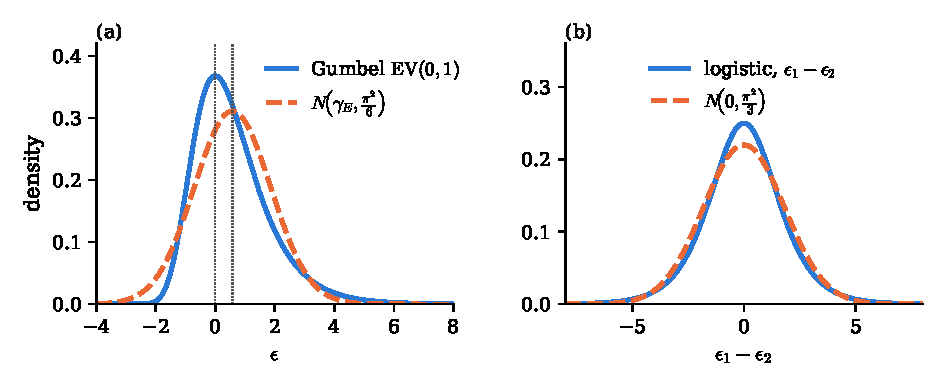
\includegraphics[width=\textwidth]{figures/appB/gumbel_logistic.pdf}
\caption{Panel (a): the standard Gumbel density and the normal density with the same mean $\gamma_E$ and
variance $\frac{\pi^2}{6}$. The dotted lines mark the mode $0$ and the mean $\gamma_E$. The Gumbel is skewed to the
right. Panel (b): the standard logistic density, which is the density of the difference of two independent
standard Gumbels (\cref{prop:B-logistic}), and the normal density with mean $0$ and variance
$\frac{\pi^2}{3}$. The logistic is symmetric and close to the normal, with slightly fatter tails.}\label{fig:B-gumbel}
\end{figure}

\subsection{Max-stability and the logit formula}\label{sec:B-maxstable}

The Gumbel family is closed under maxima with a common scale. This single property delivers the logit
formula, the log-sum and the nested logit.

\begin{proposition}[Max-stability]\label{prop:B-maxstable}
Let $\epsilon_0, \dots, \epsilon_J$ be independent $\mathrm{EV}(0, b)$ and let $\delta_0, \dots, \delta_J$ be constants. Then
\begin{equation}\label{eq:B-maxstable}
\max_j(\delta_j + \epsilon_j) \sim \mathrm{EV}\left(b\ln\sum_{j = 0}^Je^{\frac{\delta_j}{b}},\ b\right).
\end{equation}
\end{proposition}

\Cref{lem:06-maxstable} proves the case $b = 1$, and the text after it extends the proof to scale $b$. The proof
multiplies the independent Gumbel CDFs $\exp(-e^{-\frac{x - \delta_j}{b}})$ and collects the exponents.

\begin{proposition}[Logistic differences]\label{prop:B-logistic}
If $\epsilon_1$ and $\epsilon_2$ are independent standard Gumbels, then $\epsilon_1 - \epsilon_2$ has the standard
logistic distribution,
\begin{equation*}
\Pr(\epsilon_1 - \epsilon_2 \leq x) = \frac{1}{1 + e^{-x}},
\end{equation*}
with density $\frac{e^{-x}}{(1 + e^{-x})^2}$, mean zero and variance $\frac{\pi^2}{3}$.
\end{proposition}

\Cref{lem:06-logistic} proves the result by conditioning on $\epsilon_2$ and substituting $t = e^{-\epsilon_2}$.

\begin{theorem}[Multinomial logit, \citealp{McFadden1974}]\label{thm:B-logit}
Let $u_{ij} = \delta_j + \epsilon_{ij}$ with $\epsilon_{i0}, \dots, \epsilon_{iJ}$ independent standard Gumbels. Then
\begin{equation}\label{eq:B-logit}
s_j(\delta) = \frac{e^{\delta_j}}{\sum_{k = 0}^Je^{\delta_k}} = \frac{e^{\delta_j}}{1 + \sum_{k = 1}^Je^{\delta_k}}
\quad\text{when } \delta_0 = 0 .
\end{equation}
With $\mathrm{EV}(0, b)$ shocks,
\begin{equation*}
s_j(\delta) = \frac{\exp\left(\frac{\delta_j}{b}\right)}{\sum_{k = 0}^J\exp\left(\frac{\delta_k}{b}\right)} .
\end{equation*}
\end{theorem}

\citet[eqs.~3.14--3.15, pp.~1411--1412]{McFadden1984} states the result and notes that it follows by a
straightforward integration. \Cref{prop:06-logit} gives two proofs. The first carries out that integration,
conditioning on $\epsilon_{ij}$ and substituting $t = e^{-\epsilon_{ij}}$. The second combines the two previous
propositions. By \cref{prop:B-maxstable}, the best rival utility is $\ln\sum_{k \neq j}e^{\delta_k}$ plus a standard
Gumbel shock independent of $\epsilon_{ij}$. By \cref{prop:B-logistic}, the difference of the two shocks is logistic.

The scale $b$ governs how deterministic choice is. As $b \to 0$, the alternative with the highest $\delta_j$
is chosen with probability one. As $b \to \infty$, all shares tend to $\frac{1}{J + 1}$.

\begin{proposition}[The chosen maximum]\label{prop:B-chosen-max}
In the logit model of \cref{thm:B-logit}, with $\Lambda = \sum_{k = 0}^Je^{\delta_k}$,
\begin{equation}\label{eq:B-chosen-max}
\Pr\Big(\max_k u_{ik} \leq x,\ j \text{ chosen}\Big) = s_j\exp\big(-e^{-x}\Lambda\big).
\end{equation}
Hence the distribution of the maximal utility conditional on choosing $j$ is $\mathrm{EV}(\ln\Lambda, 1)$ for
every $j$, the identity of the chosen alternative is independent of the maximal utility, and
\begin{equation}\label{eq:B-selection}
\E\big[\epsilon_{ij} \mid j \text{ chosen}\big] = \gamma_E - \ln s_j .
\end{equation}
\end{proposition}

\begin{proof}
By \cref{prop:06-logsum}, the joint probability factors as
$s_j\Pr(\max_ku_{ik} \leq x)$, which is \eqref{eq:06-maxindep}. Its proof repeats the direct integration of \cref{prop:06-logit} with the extra
restriction $\delta_j + \epsilon_{ij} \leq x$. By \cref{prop:B-maxstable}, $\Pr(\max_ku_{ik} \leq x) = \exp(-e^{-x}\Lambda)$,
which gives \eqref{eq:B-chosen-max}. Dividing by $s_j$ gives the conditional CDF $\exp(-e^{-(x - \ln\Lambda)})$,
which does not depend on $j$. Its mean is $\ln\Lambda + \gamma_E$. On the event that $j$ is chosen, $\epsilon_{ij} = \max_ku_{ik} - \delta_j$, so
$\E[\epsilon_{ij} \mid j \text{ chosen}] = \ln\Lambda + \gamma_E - \delta_j = \gamma_E - \ln s_j$.
\end{proof}

Equation \eqref{eq:B-selection} quantifies selection. Consumers who choose a product with a small share have,
on average, a large taste shock for it. Corrections for selection in models that combine a discrete choice
with a continuous outcome use this formula \citep{DubinMcFadden1984}. The independence of the winner and
the winning value is also the key step in the nest-by-nest derivation of the nested logit (\cref{prop:B-cardell}).

\emph{Independence of irrelevant alternatives} (IIA) is the property that the ratio of two choice
probabilities does not depend on any third alternative. From \eqref{eq:B-logit},
\begin{equation}\label{eq:B-iia}
\frac{s_j}{s_k} = e^{\delta_j - \delta_k},
\end{equation}
which is equation (3.17) of \citet[p.~1413]{McFadden1984}. Two implications follow. Choice probabilities
on a smaller or larger choice set are obtained by deleting or adding terms in the denominator. The cross
elasticity of every alternative with respect to an attribute of $k$ is the same \citep[p.~1414]{McFadden1984}.
The classic illustration is the red bus and the blue bus. A commuter chooses between a car and a red bus
with equal mean utilities, so each share is $\frac{1}{2}$. Add a blue bus identical to the red one. IIA keeps
the ratio of car to red bus at one, so logit predicts shares of $\frac{1}{3}$ each. Common sense predicts
$\frac{1}{2}$ for the car and $\frac{1}{4}$ for each bus. IIA follows from the logit specification, in which
the shocks are independent standard Gumbels. Independence alone does not deliver it, and probit choice
probabilities do not satisfy IIA \citep[Section~5.4, p.~108]{Train2009}. Take three alternatives with
independent standard normal shocks and $\delta = (1, 0, \delta_3)$. The ratio $\frac{s_1}{s_2}$ is $3.17$ at
$\delta_3 = -5$ and $3.46$ at $\delta_3 = 0$. Under logit the ratio would equal $e \approx 2.72$ at every
$\delta_3$, so the probit ratio depends on the third alternative. I.i.d.\ normal shocks still share the red bus
failure. By symmetry they give the car and each bus a share of $\frac{1}{3}$, because they contain no notion of similarity
between products. More generally, any shock that is i.i.d.\ across alternatives gives two products with equal
shares the same cross elasticity with respect to the price of a third (\cref{rem:07-berry-iid}). The remedy is
correlation across alternatives, through nests (\cref{sec:B-gev}) or random coefficients (\cref{ch:blp}). IIA can be tested by comparing estimates from the full and a restricted choice set
\citep{HausmanMcFadden1984}.

\subsection{Expected maximum utility and consumer surplus}\label{sec:B-logsum}

\begin{proposition}[Log-sum formula]\label{prop:B-logsum}
In the logit model of \cref{thm:B-logit},
\begin{equation}\label{eq:B-logsum}
\mathcal{W}(\delta) = \E\Big[\max_j(\delta_j + \epsilon_{ij})\Big] = \ln\sum_{j = 0}^Je^{\delta_j} + \gamma_E = \ln\Lambda + \gamma_E .
\end{equation}
\end{proposition}

\Cref{prop:06-logsum} proves the formula. By \cref{prop:B-maxstable} with $b = 1$ the maximum is
$\mathrm{EV}(\ln\Lambda, 1)$, and its mean is $\ln\Lambda + \gamma_E$ by \cref{prop:B-gumbel-moments}.

The quantity $\ln\Lambda$ is the \emph{inclusive value} of the choice set. The next theorem shows that the
gradient of the expected maximum utility is the vector of choice probabilities in every additive random
utility model. The logit is one instance.

\begin{theorem}[Williams-Daly-Zachary, \citealp{Williams1977, DalyZachary1978, McFadden1981}]\label{thm:B-wdz}
Under \cref{ass:B-arum}, the function $\mathcal{W}(\delta) = \E[\max_k(\delta_k + \epsilon_{ik})]$ is finite, convex and
continuously differentiable, and
\begin{equation}\label{eq:B-wdz}
\frac{\partial\mathcal{W}(\delta)}{\partial\delta_j} = s_j(\delta), \qquad j = 0, \dots, J .
\end{equation}
\end{theorem}

\Cref{thm:06-wdz} proves finiteness, convexity and \eqref{eq:B-wdz}. Off the tie set, which has probability
zero, a small change in $\delta_j$ does not change the maximizer. The pointwise derivative of
$\max_k(\delta_k + \epsilon_k)$ is therefore the indicator that $j$ is chosen. The difference quotients are bounded by
one, and dominated convergence moves the derivative inside the expectation. The one addition is continuity of
the derivative.

\begin{proof}[Proof of continuous differentiability]
Let $\delta' \to \delta$. The indicator of $A_j(\delta')$ converges to the indicator of $A_j(\delta)$ at every
$\epsilon$ off the boundary of $A_j(\delta)$, which is a null set. Indicators are bounded by one, so dominated
convergence gives $s_j(\delta') \to s_j(\delta)$. The gradient of $\mathcal{W}$ is therefore continuous.
\end{proof}

The theorem is an envelope theorem: the derivative of a maximum with respect to a parameter is the
derivative of the chosen term (\cref{sec:B-envelope}). Four consequences follow.
\begin{enumerate}[label=(\alph*)]
\item (Symmetry) Where $s$ is differentiable, $\frac{\partial s_j}{\partial\delta_k} = \frac{\partial^2\mathcal{W}}{\partial\delta_k\partial\delta_j}
  = \frac{\partial s_k}{\partial\delta_j}$ in every additive random utility model.
\item (Positive semidefiniteness) The Jacobian $\frac{\partial s}{\partial\delta^\T}$ is the Hessian of a convex function,
  hence positive semidefinite. In particular $\frac{\partial s_j}{\partial\delta_j} \geq 0$.
\item (Translation) $\mathcal{W}(\delta + c\mathbf{1}) = \mathcal{W}(\delta) + c$. Differentiating in $c$ gives $\sum_js_j = 1$.
\item (Roy's identity) Let $\delta_j = \alpha(y - p_j) + \tilde\delta_j$ for $j \geq 1$ and $\delta_0 = \alpha y$. Then
  $\frac{\partial\mathcal{W}}{\partial p_j} = -\alpha s_j$ and $\frac{\partial\mathcal{W}}{\partial y} = \alpha$, so
  $s_j = -\frac{\partial\mathcal{W}}{\partial p_j}\left[\frac{\partial\mathcal{W}}{\partial y}\right]^{-1}$, the analogue of
  \eqref{eq:B-roy} with $\mathcal{W}$ as the indirect utility function.
\end{enumerate}
For the logit, $\frac{\partial}{\partial\delta_j}\ln\sum_ke^{\delta_k} = \frac{e^{\delta_j}}{\sum_ke^{\delta_k}} = s_j$, which checks
\eqref{eq:B-wdz} against \eqref{eq:B-logsum}.

\begin{proposition}[Logit consumer surplus, \citealp{SmallRosen1981}]\label{prop:B-cs}
Let $u_{ij} = \alpha(y_i - p_j) + \tilde\delta_j + \epsilon_{ij}$ for $j \geq 1$ and $u_{i0} = \alpha y_i + \epsilon_{i0}$, with
independent standard Gumbel shocks and $\alpha > 0$. Write $\delta_j = \tilde\delta_j - \alpha p_j$. Then the expected
consumer surplus in money is
\begin{equation}\label{eq:B-cs}
CS_i = \frac{1}{\alpha}\ln\Big(1 + \sum_{k = 1}^Je^{\delta_k}\Big) + C,
\end{equation}
where $C$ is a constant that cancels in comparisons. For a change from $\delta^0$ to $\delta^1$, the
expectation of each consumer's exact compensating variation is
$\frac{1}{\alpha}\left(\ln\Lambda^1 - \ln\Lambda^0\right)$, where $\Lambda^s = 1 + \sum_{k \geq 1}e^{\delta_k^s}$.
\end{proposition}

\Cref{sec:06-arum} proves the general formula \eqref{eq:06-smallrosen}, and \cref{sec:06-logsum} evaluates it
for the logit. Income enters every alternative with the same coefficient, so each consumer's compensating
variation is $\frac{1}{\alpha}$ times the change in her maximal utility. Taking expectations with
\cref{prop:B-logsum} gives the result. This $CV$ is a gain measure, positive when the consumer is better off,
which is the opposite sign convention to \cref{def:B-cv-ev}.

The utility is quasi-linear in income, so \cref{prop:B-quasilinear} applies. No income effects arise, and
the compensating and equivalent variations coincide. With market size $M$, the aggregate change is
$\frac{M}{\alpha}(\ln\Lambda^1 - \ln\Lambda^0)$. With random coefficients, each consumer type $i$ has its own price
coefficient $\alpha_i$ and inclusive value $\ln\Lambda_i$, and
$\Delta CS = M\int\frac{1}{\alpha_i}(\ln\Lambda_i^1 - \ln\Lambda_i^0)\,\dd F(\nu_i)$ (\cref{ch:blp}, \cref{ch:mergers}).

\begin{corollary}[Value of a product]\label{cor:B-value-product}
In the setting of \cref{prop:B-cs}:
\begin{enumerate}[label=(\roman*)]
\item Adding a product $n$ with mean utility $\delta_n$ raises expected surplus by
\begin{equation}\label{eq:B-value-new}
\Delta CS = \frac{1}{\alpha}\ln\left(1 + \frac{e^{\delta_n}}{\Lambda^0}\right) = -\frac{1}{\alpha}\ln(1 - s_n),
\end{equation}
  where $s_n = \frac{e^{\delta_n}}{\Lambda^0 + e^{\delta_n}}$ is the share of the product after its introduction.
  Removing a product with share $s_n$ costs the same amount.
\item A perfect clone of an existing product $j$, with $\delta_n = \delta_j$, adds
  $\frac{1}{\alpha}\ln\left(1 + \frac{e^{\delta_j}}{\Lambda^0}\right) > 0$.
\item With $J$ identical products of mean utility $\delta$, $CS = \frac{1}{\alpha}\ln(1 + Je^\delta) + C$, which grows
  like $\frac{1}{\alpha}\ln J$ without bound.
\end{enumerate}
\end{corollary}

\begin{proof}
(i) $\Lambda^1 = \Lambda^0 + e^{\delta_n}$, so $\ln\Lambda^1 - \ln\Lambda^0 = \ln\left(1 + \frac{e^{\delta_n}}{\Lambda^0}\right)$. Since
$\frac{\Lambda^0}{\Lambda^1} = 1 - s_n$, the same quantity equals $-\ln(1 - s_n)$. (ii) Set $\delta_n = \delta_j$ in (i).
(iii) Here $\Lambda = 1 + Je^\delta$ and $\ln(1 + Je^\delta) = \ln J + \delta + \ln(1 + \frac{e^{-\delta}}{J})$.
\end{proof}

The corollary is the formal content of the statement that the logit shock never exhausts the product
space. Every product arrives with its own independent taste draw, so every product, even a duplicate,
attracts consumers who value it highly and adds surplus. The same feature bounds logit markups below by
$\frac{1}{\alpha}$ (\cref{prop:B-logit-markups}). It biases upward the estimated value of new goods and the
markups in crowded markets (\cref{ch:discrete}, \cref{ch:newgoods}). The mirror image concerns data. The model
predicts a positive share for every product, so the direct inversion of observed shares, $\ln s_j^{obs} - \ln s_0^{obs}$, is
undefined for a product with zero observed sales. The zero is still informative. If $M$ consumers choose
independently, the probability of observing no sale of $j$ is $(1 - s_j)^M$, which falls as the model share
$s_j$ rises. A likelihood for sales counts, or another estimator that models the sampling of shares, can
therefore use zeros \citep{GandhiLuShi2023}. If the shocks represent mistakes or
psychological biases rather than tastes, the log-sum counts them as welfare. The pure characteristics model
removes the shock altogether, and the nested logit shrinks the value of a clone as within-nest correlation
rises (\cref{rem:B-nl-clone}).

In computation, $\ln\sum_{k = 0}^Je^{\delta_k}$ overflows when some $\delta_k$ is large. Let
$c = \max\{0, \max_k\delta_k\}$, where the zero is the outside good. Then evaluate
\begin{equation}\label{eq:B-logsumexp}
\ln\sum_{k = 0}^Je^{\delta_k} = c + \ln\sum_{k = 0}^Je^{\delta_k - c},
\end{equation}
in which every exponent is at most zero. The same shift stabilizes the share formula.

\subsection{Logit derivatives, Jacobians and markups}\label{sec:B-logit-algebra}

With $s_j = \frac{e^{\delta_j}}{\Lambda}$ and $\Lambda = 1 + \sum_ke^{\delta_k}$, the quotient rule gives the derivatives
that \cref{ex:B-logit-jacobian} computed. We collect them in three equivalent forms,
\begin{equation}\label{eq:B-logit-deriv}
\frac{\partial s_j}{\partial\delta_k} = s_j\big(\indic\{j = k\} - s_k\big),
\qquad
\frac{\partial\ln s_j}{\partial\delta_k} = \indic\{j = k\} - s_k,
\qquad
\frac{\partial s}{\partial\delta^\T} = \diag(s) - ss^\T,
\end{equation}
where $s = (s_1, \dots, s_J)^\T$ collects the inside shares. The Jacobian is symmetric, as \cref{thm:B-wdz}
requires. Its row sums are $\sum_{k \geq 1}\frac{\partial s_j}{\partial\delta_k} = s_j(1 - \sum_ks_k) = s_js_0 > 0$. The
derivative with respect to the outside good is $-s_js_0$, so the full row sums to zero, as translation
invariance requires (\cref{cor:B-translation}). The Jacobian is invertible, and the Sherman-Morrison formula gives
its inverse $\diag(\frac{1}{s_1}, \dots, \frac{1}{s_J}) + \frac{1}{s_0}\mathbf{1}\mathbf{1}^\T$ in
\eqref{eq:B-logit-jacobian-inverse}. Inverting the shares themselves is easier still:
$\frac{s_j}{s_0} = e^{\delta_j}$ gives $\delta_j = \ln s_j - \ln s_0$, the inversion of \citet{Berry1994} that
\cref{ch:logit} turns into a linear instrumental variables regression.

With $\delta_j = \tilde\delta_j - \alpha p_j$, the chain rule gives the price derivatives
$\frac{\partial s_j}{\partial p_j} = -\alpha s_j(1 - s_j)$ and $\frac{\partial s_j}{\partial p_k} = \alpha s_js_k$. The own-price
elasticity and the cross elasticities are
\begin{equation}\label{eq:B-logit-elast}
\varepsilon_j = -\frac{\partial s_j}{\partial p_j}\frac{p_j}{s_j} = \alpha p_j(1 - s_j),
\qquad
\varepsilon_{jk} = \frac{\partial s_j}{\partial p_k}\frac{p_k}{s_j} = \alpha p_ks_k \quad (k \neq j).
\end{equation}
The own elasticity is nearly proportional to price when shares are small, so the model predicts that
expensive products face the most elastic demand. The cross elasticity with respect to $p_k$ is the same for
every $j$, whatever the similarity of $j$ and $k$. The diversion ratio from $j$ to $k$ is
\begin{equation}\label{eq:B-logit-diversion}
D_{jk} = -\frac{\partial s_k}{\partial p_j}\left[\frac{\partial s_j}{\partial p_j}\right]^{-1} = \frac{\alpha s_js_k}{\alpha s_j(1 - s_j)} = \frac{s_k}{1 - s_j},
\qquad
D_{j0} = \frac{s_0}{1 - s_j} .
\end{equation}
Customers who leave $j$ spread over the other alternatives in proportion to their shares, and the
diversion ratios sum to one.

\begin{proposition}[Logit markups]\label{prop:B-logit-markups}
Let firms set prices in a Bertrand-Nash equilibrium with constant marginal costs and logit demand, and write
$m_j = p_j - mc_j$.
\begin{enumerate}[label=(\roman*)]
\item A single-product firm sets $m_j = \frac{1}{\alpha(1 - s_j)}$.
\item A firm $f$ that owns the products $\mathcal{J}_f$, with combined share $S_f = \sum_{k \in \mathcal{J}_f}s_k$, sets
  the common markup $m_j = m_f = \frac{1}{\alpha(1 - S_f)}$ on all its products.
\item A single owner of all inside goods sets the common markup $\frac{1}{\alpha s_0}$.
\end{enumerate}
In every case $m_j > \frac{1}{\alpha}$.
\end{proposition}

\begin{proof}
(ii) The profit of firm $f$ is $\sum_{k \in \mathcal{J}_f}m_ks_k(p)$. For $j \in \mathcal{J}_f$, the first-order condition is
\begin{equation*}
0 = s_j + \sum_{k \in \mathcal{J}_f}m_k\frac{\partial s_k}{\partial p_j}
= s_j - \alpha m_js_j(1 - s_j) + \sum_{k \in \mathcal{J}_f, k \neq j}\alpha m_ks_ks_j
= s_j\Big[1 - \alpha m_j + \alpha\sum_{k \in \mathcal{J}_f}m_ks_k\Big].
\end{equation*}
Dividing by $s_j > 0$ gives $m_j = \frac{1}{\alpha} + \sum_{k \in \mathcal{J}_f}m_ks_k$. The right side does not depend
on $j$, so all products of the firm carry the same markup $m_f$. Substituting $m_k = m_f$ gives
$m_f = \frac{1}{\alpha} + S_fm_f$, hence $m_f = \frac{1}{\alpha(1 - S_f)}$. (i) is the case $\mathcal{J}_f = \{j\}$. (iii) is the
case $S_f = 1 - s_0$. Each markup exceeds $\frac{1}{\alpha}$ because $S_f < 1$.
\end{proof}

\Cref{ex:B-logit-jacobian} reaches the same three formulas from the matrix condition
$m = -(\Omega \odot \Delta^\T)^{-1}s$, by inverting each block of the logit Jacobian with the Sherman-Morrison formula.

The first-order condition of a single-product firm is also sufficient. Write
$\frac{\partial\pi_j}{\partial p_j} = s_j\,g(m_j)$ with $g(m) = 1 - \alpha m(1 - s_j)$, where $s_j$ depends on $m$ through
$p_j$. For $m \leq 0$ we have $g > 0$. For $m > 0$, $g$ is strictly decreasing, because both $\alpha m$ and
$1 - s_j$ rise with $p_j$, and $g \to -\infty$ as $m \to \infty$. The derivative of profit therefore changes sign
exactly once, from positive to negative, and the stationary point is the unique maximizer. The best
response has a closed form in terms of the Lambert function.

\begin{lemma}[Lambert function, \citealp{CorlessEtAl1996}]\label{lem:B-lambert}
For every $z \geq 0$, the equation $we^w = z$ has exactly one solution $w \geq 0$, denoted $W_0(z)$. The
function $W_0$ is strictly increasing on $[0, \infty)$, with $W_0(0) = 0$ and $W_0(e) = 1$, and for $z > 0$
\begin{equation}\label{eq:B-lambert-deriv}
W_0'(z) = \frac{W_0(z)}{z\,(1 + W_0(z))} .
\end{equation}
\end{lemma}

\begin{proof}
The map $g(w) = we^w$ is continuous on $[0, \infty)$ with $g(0) = 0$, $g(w) \to \infty$ and
$g'(w) = (1 + w)e^w > 0$. By the intermediate value theorem and strict monotonicity, each $z \geq 0$ has
exactly one preimage, and the inverse is strictly increasing. Since $1\cdot e^1 = e$, $W_0(e) = 1$. By the
inverse function theorem,
\begin{equation*}
W_0'(z) = \frac{1}{g'(W_0(z))} = \frac{1}{(1 + W_0(z))e^{W_0(z)}} = \frac{W_0(z)}{z\,(1 + W_0(z))},
\end{equation*}
where the last step uses $e^{W_0(z)} = \frac{z}{W_0(z)}$ for $z > 0$.
\end{proof}

The principal branch extends to $z \geq -\frac{1}{e}$, but we only need $z > 0$. Standard numerical libraries
evaluate it.

\begin{proposition}[Logit best response]\label{prop:B-logit-br}
Let firm $j$ sell one product with logit demand, $\delta_j = \tilde\delta_j - \alpha p_j$, and constant marginal cost
$mc_j$. Define the mean utility at marginal-cost pricing, $v_j = \tilde\delta_j - \alpha mc_j$, and the part of the
logit denominator that rivals control, $\Lambda_{-j} = 1 + \sum_{l \neq j}e^{\delta_l}$. Then the unique best response
to the rivals' prices is
\begin{equation}\label{eq:B-logit-br-closed}
BR_j(p_{-j}) = mc_j + \frac{1}{\alpha}\left[1 + W_0\left(\frac{e^{v_j - 1}}{\Lambda_{-j}}\right)\right] .
\end{equation}
At the best response, with $W_0$ evaluated at $z_j = \frac{e^{v_j - 1}}{\Lambda_{-j}}$,
\begin{equation}\label{eq:B-br-identities}
s_j = \frac{W_0(z_j)}{1 + W_0(z_j)}, \qquad \frac{e^{\delta_l}}{\Lambda_{-j}} = \frac{s_l}{1 - s_j} \quad (l \neq j).
\end{equation}
For a multiproduct firm $f$ with $E_f = \sum_{k \in \mathcal{J}_f}e^{v_k}$ and $\Lambda_{-f} = 1 + \sum_{l \notin \mathcal{J}_f}e^{\delta_l}$,
the best-response common markup is $m_f = \frac{1}{\alpha}\left[1 + W_0\left(\frac{E_fe^{-1}}{\Lambda_{-f}}\right)\right]$.
\end{proposition}

\begin{proof}
By \cref{prop:B-logit-markups} and the single-crossing argument above, the best response is the unique
solution of $\alpha m_j(1 - s_j) = 1$. Write $\delta_j = v_j - \alpha m_j$ and
$1 - s_j = \frac{\Lambda_{-j}}{\Lambda_{-j} + e^{\delta_j}}$. The condition becomes
\begin{equation*}
\alpha m_j\Lambda_{-j} = \Lambda_{-j} + e^{v_j - \alpha m_j}
\quad\Longleftrightarrow\quad
(\alpha m_j - 1)\Lambda_{-j} = e^{v_j - \alpha m_j} .
\end{equation*}
Let $w = \alpha m_j - 1$. Then $w\Lambda_{-j} = e^{v_j - 1 - w}$, that is,
\begin{equation*}
we^w = \frac{e^{v_j - 1}}{\Lambda_{-j}} = z_j > 0 .
\end{equation*}
Any solution has $w > 0$, because the right side is positive. By \cref{lem:B-lambert}, $w = W_0(z_j)$, and
$m_j = \frac{1 + W_0(z_j)}{\alpha}$, which is \eqref{eq:B-logit-br-closed}. At the best response the first-order condition
gives $1 - s_j = \frac{1}{\alpha m_j} = \frac{1}{1 + W_0(z_j)}$, which yields the first identity in
\eqref{eq:B-br-identities}. For the second, $\frac{\Lambda_{-j}}{\Lambda} = 1 - s_j$ with $\Lambda = \Lambda_{-j} + e^{\delta_j}$, so
$\frac{e^{\delta_l}}{\Lambda_{-j}} = \frac{e^{\delta_l}}{\Lambda}\cdot\frac{\Lambda}{\Lambda_{-j}} = \frac{s_l}{1 - s_j}$. For the multiproduct
firm, the common-markup condition $\alpha m_f(1 - S_f) = 1$ with
$1 - S_f = \frac{\Lambda_{-f}}{\Lambda_{-f} + E_fe^{-\alpha m_f}}$ gives $(\alpha m_f - 1)\Lambda_{-f} = E_fe^{-\alpha m_f}$, and the same
substitution yields $we^w = \frac{E_fe^{-1}}{\Lambda_{-f}}$.
\end{proof}

The best response rises with every rival price, because $\Lambda_{-j}$ falls and $W_0$ is increasing. Prices are
strategic complements. \Cref{sec:B-fixedpoint} differentiates \eqref{eq:B-logit-br-closed} with
\eqref{eq:B-lambert-deriv} and \eqref{eq:B-br-identities} to show that best-response iteration is a contraction, so
the logit pricing equilibrium is unique.

\begin{remark}[Mixed logit]\label{rem:B-mixed}
In the random-coefficients (mixed) logit, conditional on the consumer's taste draw $\nu_i$ the choice
probabilities $s_{ij}$ are logit. The formulas of this subsection for choice probabilities, price derivatives,
elasticities and diversion ratios therefore hold consumer by consumer, with $s_{ij}$ and $\alpha_i$ in place of $s_j$
and $\alpha$. Aggregate shares and derivatives are integrals, for example
$\frac{\partial s_j}{\partial p_k} = \int\alpha_is_{ij}\big(s_{ik} - \indic\{j = k\}\big)\,\dd F(\nu_i)$, where differentiation
under the integral is justified by \cref{prop:B-leibniz}. Aggregate cross derivatives are large when the same
consumers are likely to buy both products, so substitution depends on characteristics. The pricing results
(\cref{prop:B-logit-markups,prop:B-logit-br}) do not hold consumer by consumer. A firm charges one price to all
consumers, so its first-order condition sets the integral of the consumer-level terms to zero, and each term need
not vanish. Markups solve $m = -(\Omega \odot \Delta^\T)^{-1}s$ with the aggregate derivatives, and they are no longer
common within a firm. \citet{McFaddenTrain2000} show that any random utility model can be approximated
arbitrarily well by a mixed logit (\cref{ch:blp}).
\end{remark}

\subsection{Representative-consumer foundations}\label{sec:B-entropy}

The logit can also be derived from a single consumer who likes variety.

\begin{proposition}[Entropy representative consumer, \citealp{AndersonDePalmaThisse1988, AndersonDePalmaThisse1992}]\label{prop:B-entropy}
Let $\delta_0, \dots, \delta_J$ be given, with $\delta_j = \tilde\delta_j - \alpha p_j$ and $\delta_0 = 0$. The problem
\begin{equation}\label{eq:B-entropy}
\max_{q_0, \dots, q_J \geq 0}\ \sum_{j = 0}^J\delta_jq_j - \sum_{j = 0}^Jq_j\ln q_j
\qquad\text{subject to}\qquad \sum_{j = 0}^Jq_j = 1
\end{equation}
has the unique solution $q_j = \frac{e^{\delta_j}}{\sum_ke^{\delta_k}}$, the logit shares. Its maximized value is
$\ln\sum_ke^{\delta_k}$.
\end{proposition}

\Cref{prop:04-logit-entropy} proves the result. Strict concavity of $-q\ln q$ gives a unique maximizer, its
infinite slope at zero makes the maximizer interior, and the first-order conditions
$\delta_j - \ln q_j - 1 - \lambda = 0$ give the logit shares.

The entropy term $-\sum_jq_j\ln q_j$ rewards spreading consumption across products, a taste for variety. The
maximized value equals the log-sum of \eqref{eq:B-logsum} without the constant $\gamma_E$, so the representative
consumer and the population of random-utility consumers agree on welfare. In the language of convex
analysis, the log-sum is the convex conjugate of negative entropy on the simplex. Weighting the entropy
term by $b > 0$ gives the logit with scale $b$, and as $b \to 0$ the consumer buys only the product with
the highest $\delta_j$.

\begin{remark}[Logit and CES]\label{rem:B-logit-ces}
CES expenditure shares are logit shares in log prices. With the CES price index
$P^{1 - \sigma_{\mathrm{CES}}} = \sum_ka_kp_k^{1 - \sigma_{\mathrm{CES}}}$, the budget share of good $j$ is
$w_j = \frac{a_jp_j^{1 - \sigma_{\mathrm{CES}}}}{\sum_ka_kp_k^{1 - \sigma_{\mathrm{CES}}}}$ (\cref{ch:diffprod}). Setting
$\delta_j = \ln a_j - (\sigma_{\mathrm{CES}} - 1)\ln p_j$ in \eqref{eq:B-logit} without an outside good gives
\begin{equation*}
s_j = \frac{e^{\ln a_j - (\sigma_{\mathrm{CES}} - 1)\ln p_j}}{\sum_ke^{\ln a_k - (\sigma_{\mathrm{CES}} - 1)\ln p_k}}
= \frac{a_jp_j^{1 - \sigma_{\mathrm{CES}}}}{\sum_ka_kp_k^{1 - \sigma_{\mathrm{CES}}}} = w_j .
\end{equation*}
The coefficient on log price, $\sigma_{\mathrm{CES}} - 1$, plays the role of the logit price coefficient, and the
CES inherits IIA. \citet{AndersonDePalmaThisse1987} give a discrete-choice foundation. Suppose each consumer
buys one variety and spends all income $y$ on it, with conditional indirect utility
$\ln y - \ln p_j + \ln\tilde a_j + \mu\epsilon_{ij}$ and standard Gumbel shocks scaled by $\mu > 0$. The choice
probabilities are logit in $\frac{\ln\tilde a_j - \ln p_j}{\mu}$, and expected demand for $j$ is the choice
probability times $\frac{y}{p_j}$. This is CES demand with $\sigma_{\mathrm{CES}} = 1 + \frac{1}{\mu}$ and weights
$a_j = \tilde a_j^{\sigma_{\mathrm{CES}} - 1}$. The subscript keeps $\sigma$ free for the nesting parameter.
\end{remark}

\subsection{Generalized extreme value models}\label{sec:B-gev}

The generalized extreme value (GEV) class of \citet{McFadden1978} keeps closed-form choice probabilities
while allowing the shocks to be correlated across alternatives. Its key object is a generating function.

\begin{theorem}[GEV models, \citealp{McFadden1978}]\label{thm:B-gev}
Let $H : \R^{J+1}_+ \to \R_+$ satisfy three conditions:
\begin{enumerate}[label=(G\arabic*)]
\item $H$ is nonnegative and homogeneous of degree one.
\item $H(y_0, \dots, y_J) \to \infty$ as any single argument $y_j \to \infty$.
\item For every set of $m$ distinct arguments, the mixed partial derivative of $H$ with respect to them is
  nonnegative when $m$ is odd and nonpositive when $m$ is even.
\end{enumerate}
Then $F(\epsilon_0, \dots, \epsilon_J) = \exp\{-H(e^{-\epsilon_0}, \dots, e^{-\epsilon_J})\}$ is a multivariate extreme value CDF.
Let $u_{ij} = \delta_j + \epsilon_{ij}$ with $\epsilon_i \sim F$ and $y_j = e^{\delta_j}$. Then:
\begin{enumerate}[label=(\roman*)]
\item $\Pr(\max_ju_{ij} \leq x) = \exp\{-e^{-x}H(y)\}$, so the maximal utility is $\mathrm{EV}(\ln H(y), 1)$.
  Expected maximum utility is
  \begin{equation}\label{eq:B-gev-W}
  \mathcal{W}(\delta) = \ln H\big(e^{\delta_0}, \dots, e^{\delta_J}\big) + \gamma_E .
  \end{equation}
\item The choice probabilities are
  \begin{equation}\label{eq:B-gev-shares}
  s_j = \frac{\partial\ln H(e^{\delta_0}, \dots, e^{\delta_J})}{\partial\delta_j} = \frac{y_jH_j(y)}{H(y)},
  \end{equation}
  where $H_j$ is the partial derivative of $H$ with respect to its $j$-th argument.
\end{enumerate}
\end{theorem}

\citet[eqs.~3.29--3.31, p.~1421]{McFadden1984} states the theorem in this form. The first claim, that (G1) to
(G3) make $F$ a valid distribution function, is due to \citet{McFadden1978}. Condition (G3) makes the mixed
partial derivative of $F$ of order $J + 1$, its density, nonnegative. Condition (G2) makes each marginal CDF
vanish as its argument tends to $-\infty$. \Cref{thm:06-gev} proves (i) and (ii). Part (i) follows from
homogeneity, since $F(x - \delta_0, \dots, x - \delta_J) = \exp\{-H(e^{-x}y)\} = \exp\{-e^{-x}H(y)\}$. That proof
derives (ii) by direct integration. Part (ii) also follows from (i) in one line. The distribution $F$ satisfies
\cref{ass:B-arum}, so \cref{thm:B-wdz} applied to \eqref{eq:B-gev-W} gives
$s_j = \frac{H_j(y)}{H(y)}\cdot\frac{\partial y_j}{\partial\delta_j} = \frac{y_jH_j(y)}{H(y)}$.

By Euler's theorem, $\sum_jy_jH_j(y) = H(y)$, so the shares in \eqref{eq:B-gev-shares} sum to one. Part (i)
explains a remark of \citet[p.~1425]{McFadden1984}. The generating function can be read as a measure of social
utility, because its logarithm is expected maximum utility up to a constant.

\begin{example}[Logit as a GEV model]\label{ex:B-gev-logit}
With $H(y) = \sum_jy_j$, $H_j = 1$ and \eqref{eq:B-gev-shares} gives $s_j = \frac{y_j}{\sum_ky_k}$, the logit. The
generating function $H(y) = \left(\sum_jy_j^{\frac{1}{\lambda}}\right)^\lambda$ with $0 < \lambda \leq 1$
\citep[eq.~3.32]{McFadden1984} also gives a logit. Here
$H_j = \left(\sum_ky_k^{\frac{1}{\lambda}}\right)^{\lambda - 1}y_j^{\frac{1}{\lambda} - 1}$, so
$s_j = \frac{y_j^{\frac{1}{\lambda}}}{\sum_ky_k^{\frac{1}{\lambda}}} = \frac{e^{\frac{\delta_j}{\lambda}}}{\sum_ke^{\frac{\delta_k}{\lambda}}}$, a logit with
scale $\lambda$.
\end{example}

\begin{proposition}[Nested logit from GEV]\label{prop:B-nested}
Partition the inside goods into nests $g = 1, \dots, G$, with the outside good alone in its own nest, and let
$\sigma \in [0, 1)$. The generating function
\begin{equation}\label{eq:B-nested-H}
H(y) = y_0 + \sum_{g = 1}^G\Big(\sum_{j \in g}y_j^{\frac{1}{1 - \sigma}}\Big)^{1 - \sigma}
\end{equation}
satisfies (G1) to (G3). With $\delta_0 = 0$ and the inclusive sums $D_g = \sum_{k \in g}e^{\frac{\delta_k}{1 - \sigma}}$, the
choice probabilities are $s_j = s_{j|g}\,s_g$ for $j \in g$, where
\begin{equation}\label{eq:B-nested-shares}
s_{j|g} = \frac{e^{\frac{\delta_j}{1 - \sigma}}}{D_g},
\qquad
s_g = \frac{D_g^{1 - \sigma}}{1 + \sum_{h = 1}^GD_h^{1 - \sigma}},
\qquad
s_0 = \frac{1}{1 + \sum_{h = 1}^GD_h^{1 - \sigma}} .
\end{equation}
Expected maximum utility is $\mathcal{W} = \ln\big(1 + \sum_gD_g^{1 - \sigma}\big) + \gamma_E$.
\end{proposition}

\Cref{lem:07-nl-gev} verifies (G1) to (G3) for $\sigma \in [0, 1)$, including the signs of all higher mixed
partial derivatives. \Cref{prop:07-nl-shares} derives the shares from \eqref{eq:B-gev-shares}. For $j \in g$ the
key product is $y_jH_j(y) = D_g^{-\sigma}e^{\frac{\delta_j}{1 - \sigma}}$, and with $y_0 = 1$ the generating function
is $H(y) = 1 + \sum_hD_h^{1 - \sigma}$. Their ratio factors as $s_{j|g}\,s_g$. The outside share is
$\frac{y_0H_0}{H} = \frac{1}{H}$, and $\mathcal{W}$ follows from \eqref{eq:B-gev-W}.

\citet[eqs.~23--25, p.~253]{Berry1994} writes the same shares. The nest probability $s_g$ is a logit in the
nest \emph{inclusive values} $I_g = (1 - \sigma)\ln D_g$, and the within-nest probability $s_{j|g}$ is a logit
with scale $1 - \sigma$. At $\sigma = 0$, $D_g^{1 - \sigma} = \sum_{k \in g}e^{\delta_k}$, and the model collapses to the
logit. As $\sigma \to 1$, $(1 - \sigma)\ln D_g \to \max_{k \in g}\delta_k$, and $s_{j|g} \to 1$ for the product with the
highest $\delta_j$ in its nest. Products in a nest become perfect substitutes, and only the best product of each
nest sells. The bound $\sigma \geq 0$, equivalently $\lambda \leq 1$, is what the GEV conditions impose.
\citet[pp.~1423 and 1425]{McFadden1984} calls $\lambda = 1 - \sigma$ an ``independence'' parameter, because it
measures the independence of the shocks within a nest. On p.~1426 he refers to such parameters as inclusive
value coefficients. His cross-elasticity formula for the nested model (his eq.~3.49, p.~1425) explains why the
unit interval matters. For values in $(0, 1)$, cross-elasticities are largest for alternatives in the same nest
and smallest across nests. Values outside the interval reverse one of these rankings. Estimates outside $(0, 1]$
may therefore indicate a misspecified tree \citep[pp.~1425--1426]{McFadden1984}.

\begin{remark}[Three-level nesting]\label{rem:B-three-level}
\citet[eqs.~3.33--3.39, pp.~1421--1422]{McFadden1984} gives a three-level generating function. In our notation,
with clusters $C$ of subclusters $D$ and $y_i = e^{\delta_i}$,
\begin{equation*}
H(y) = \sum_Ca(C)\Bigg\{\sum_{D \subseteq C}b(D, C)\Big[\sum_{i \in D}y_i^{\frac{1}{\lambda_{DC}\lambda_C}}\Big]^{\lambda_{DC}}\Bigg\}^{\lambda_C},
\end{equation*}
with $0 < \lambda_{DC}, \lambda_C \leq 1$ and positive weights $a(C)$ and $b(D, C)$. The choice probability factors as
$Q(i \mid D, C)\,Q(D \mid C)\,Q(C)$. The bottom level is a logit in $\frac{\delta_i}{\lambda_{DC}\lambda_C}$. The middle level is a
logit in $\ln b(D, C) + \lambda_{DC}J(D, C)$ with inclusive value
$J(D, C) = \ln\sum_{j \in D}e^{\frac{\delta_j}{\lambda_{DC}\lambda_C}}$. The top level is a logit in $\ln a(C) + \lambda_CI(C)$ with
$I(C) = \ln\sum_{D' \subseteq C}b(D', C)e^{\lambda_{D'C}J(D', C)}$. When all $\lambda$'s equal one the model is a logit. When
$\lambda_{DC}$ is near zero, the subcluster $D$ behaves like a single alternative with the best scale value in $D$.
\end{remark}

The nested logit also has a random-coefficients representation, which explains the parameter
restriction and gives the correlation of utilities within a nest.

\begin{proposition}[Cardell's representation, \citealp{Cardell1997}]\label{prop:B-cardell}
For every $\sigma \in [0, 1)$ there is a distribution $C(\sigma)$ with the following property: if $\zeta \sim C(\sigma)$
and $\epsilon$ is standard Gumbel and independent of $\zeta$, then $\zeta + (1 - \sigma)\epsilon$ is standard Gumbel. Let
\begin{equation}\label{eq:B-cardell}
u_{ij} = \delta_j + \zeta_{ig} + (1 - \sigma)\epsilon_{ij}, \qquad j \in g,
\end{equation}
with $\zeta_{ig} \sim C(\sigma)$ independent across nests, $\epsilon_{ij}$ independent standard Gumbels, independent of the
$\zeta$'s, and $u_{i0} = \epsilon_{i0}$. Then the choice probabilities are the nested logit shares
\eqref{eq:B-nested-shares}. Within a nest, $\Corr(u_{ij}, u_{ik}) = 1 - (1 - \sigma)^2$. Across nests the correlation is
zero.
\end{proposition}

The existence of $C(\sigma)$ is Cardell's result, which we take as given (\cref{lem:07-cardell}).
\citet[eq.~22, p.~252]{Berry1994} uses this representation. Given existence, \cref{prop:07-nl-shares} derives
the shares nest by nest. Max-stability (\cref{prop:B-maxstable} with $b = 1 - \sigma$) gives the best utility in
nest $g$ as $\zeta_{ig} + (1 - \sigma)\ln D_g + (1 - \sigma)\tilde\epsilon_{ig}$ with $\tilde\epsilon_{ig}$ standard Gumbel.
The within-nest winner is independent of this maximum (\cref{prop:B-chosen-max}). Cardell's property makes
$\zeta_{ig} + (1 - \sigma)\tilde\epsilon_{ig}$ standard Gumbel, so the choice of nest is a logit in
$(1 - \sigma)\ln D_g$. For the correlation, the two parts of the standard Gumbel shock
$\zeta_{ig} + (1 - \sigma)\epsilon_{ij}$ are independent, so $\Var(\zeta_{ig}) = [1 - (1 - \sigma)^2]\frac{\pi^2}{6}$. The
common component $\zeta_{ig}$ then gives \eqref{eq:07-nl-corr}.

The within-nest correlation $1 - (1 - \sigma)^2 = \sigma(2 - \sigma)$ is zero at $\sigma = 0$ and tends to one as
$\sigma \to 1$. A negative $\sigma$ would require a negative variance for $\zeta$, which is the random-coefficients
reading of the restriction $\sigma \geq 0$. \citet[pp.~252--253]{Berry1994} rewrites \eqref{eq:B-cardell} as
$u_{ij} = \delta_j + \sum_gd_{jg}\zeta_{ig} + (1 - \sigma)\epsilon_{ij}$, where $d_{jg}$ indicates membership of nest $g$. The
nested logit is a random-coefficients model with random coefficients on nest dummies only. Its correlation
pattern depends on groupings fixed before estimation, while the full random-coefficients model lets
correlation depend on continuous characteristics.

\begin{proposition}[Nested-logit inversion and derivatives]\label{prop:B-nested-inversion}
In the nested logit of \cref{prop:B-nested}:
\begin{enumerate}[label=(\roman*)]
\item The mean utilities satisfy
  \begin{equation}\label{eq:B-nl-inversion}
  \ln s_j - \ln s_0 = \delta_j + \sigma\ln s_{j|g}, \qquad j \in g .
  \end{equation}
\item The derivatives of log shares with respect to mean utilities are
  \begin{equation}\label{eq:B-nl-logderiv}
  \frac{\partial\ln s_j}{\partial\delta_k} =
  \begin{cases}
  \dfrac{1}{1 - \sigma} - \dfrac{\sigma}{1 - \sigma}s_{j|g} - s_j, & k = j,\\[8pt]
  -\dfrac{\sigma}{1 - \sigma}s_{k|g} - s_k, & k \neq j,\ k \in g,\\[8pt]
  -s_k, & k \notin g,\ k \geq 1,
  \end{cases}
  \end{equation}
  and $\frac{\partial\ln s_j}{\partial\delta_0} = -s_0$. The inside derivatives in each row sum to $s_0$.
\item With $\delta_j = \tilde\delta_j - \alpha p_j$, the price derivatives are
  $\frac{\partial s_j}{\partial p_j} = -\alpha s_j\big[\frac{1}{1 - \sigma} - \frac{\sigma}{1 - \sigma}s_{j|g} - s_j\big]$,
  $\frac{\partial s_j}{\partial p_k} = \alpha s_k\big[\frac{\sigma}{1 - \sigma}s_{j|g} + s_j\big]$ for $k \neq j$ in the same nest, and
  $\frac{\partial s_j}{\partial p_k} = \alpha s_js_k$ for $k$ in another nest.
\end{enumerate}
\end{proposition}

\Cref{prop:07-nl-inversion} proves (i), and \cref{sec:07-nl-substitution} derives the derivatives in (ii) and
(iii), \eqref{eq:07-nl-dlns} to \eqref{eq:07-nl-cross-out}. Both start from
$\ln s_j = \frac{\delta_j}{1 - \sigma} - \sigma\ln D_g - \ln\big(1 + \sum_hD_h^{1 - \sigma}\big)$. The form of the
same-nest cross derivative in (iii) uses $s_js_{k|g} = s_ks_{j|g}$. Two statements of (ii) are new.

\begin{proof}[Proof of the outside-good derivative and the row sum]
Without the normalization, the last term of $\ln s_j$ is $\ln\big(e^{\delta_0} + \sum_hD_h^{1 - \sigma}\big)$. Its
derivative with respect to $\delta_0$ is $s_0$, so $\frac{\partial\ln s_j}{\partial\delta_0} = -s_0$. For the row sum,
\begin{equation*}
\sum_{k \geq 1}\frac{\partial\ln s_j}{\partial\delta_k}
= \frac{1}{1 - \sigma} - \frac{\sigma}{1 - \sigma}\sum_{k \in g}s_{k|g} - \sum_{k \geq 1}s_k
= \frac{1 - \sigma}{1 - \sigma} - (1 - s_0) = s_0 . \qedhere
\end{equation*}
\end{proof}

\citet[eqs.~26--27, p.~253]{Berry1994} reaches \eqref{eq:B-nl-inversion} by a second route. Taking logs of the
nest share gives $\ln D_g = \frac{\ln s_g - \ln s_0}{1 - \sigma}$, and substituting into
$\ln s_j - \ln s_0 = \frac{\delta_j}{1 - \sigma} - \sigma\ln D_g$ yields $\delta_j = \ln s_j - \sigma\ln s_{j|g} - \ln s_0$. With
$\delta_j = x_j\beta - \alpha p_j + \xi_j$ this is the linear estimating equation
$\ln s_j - \ln s_0 = x_j\beta - \alpha p_j + \sigma\ln s_{j|g} + \xi_j$, in which both the price and the within-nest share
are endogenous (\cref{ch:logit}).

The derivatives in \eqref{eq:B-nl-logderiv} have three uses. First, the own derivative
$\frac{\partial\ln s_j}{\partial\delta_j}$ can far exceed one when $\sigma$ is large and $s_{j|g}$ is small. This is why the
share inversion for nested models needs a dampened contraction (\cref{sec:B-fixedpoint}). Second, the same-nest
cross derivative exceeds the cross-nest one by $\frac{\sigma}{1 - \sigma}s_{k|g}$, so substitution is stronger within
nests. Third, the own-price elasticity and the cross elasticities are
\begin{equation*}
\varepsilon_j = \alpha p_j\Big[\frac{1}{1 - \sigma} - \frac{\sigma}{1 - \sigma}s_{j|g} - s_j\Big],
\qquad
\varepsilon_{jk} = \alpha p_k\Big[\frac{\sigma}{1 - \sigma}s_{k|g} + s_k\Big]\ (k \in g),
\qquad
\varepsilon_{jk} = \alpha p_ks_k\ (k \notin g),
\end{equation*}
and the diversion ratio between two products of the same nest is
\begin{equation*}
D_{jk} = \frac{\sigma s_{k|g} + (1 - \sigma)s_k}{1 - \sigma s_{j|g} - (1 - \sigma)s_j} .
\end{equation*}
The cross elasticity with respect to $p_k$ is the same for every product in the nest of $k$, and the same for
every product outside it. Substitution is therefore proportional within each of these two groups, and the
ratio of two shares in the same nest, $\frac{s_j}{s_k} = e^{\frac{\delta_j - \delta_k}{1 - \sigma}}$, does not depend on any
other alternative.

\begin{remark}[Clone welfare in the nested logit]\label{rem:B-nl-clone}
Add a clone of product $j$ to its nest $g$, which contains only $j$. Before the clone, $D_g^{1 - \sigma} = e^{\delta_j}$.
After it, $D_g^{1 - \sigma} = \big(2e^{\frac{\delta_j}{1 - \sigma}}\big)^{1 - \sigma} = 2^{1 - \sigma}e^{\delta_j}$. With
$\Lambda^0 = 1 + \sum_hD_h^{1 - \sigma}$ before the clone, the surplus gain is
\begin{equation*}
\Delta CS = \frac{1}{\alpha}\ln\frac{\Lambda^0 + (2^{1 - \sigma} - 1)e^{\delta_j}}{\Lambda^0} .
\end{equation*}
It equals the logit value of \cref{cor:B-value-product} at $\sigma = 0$ and falls to zero as $\sigma \to 1$. Within-nest correlation disciplines the
value of variety.
\end{remark}

\begin{remark}[Random-coefficients nested logit]\label{rem:B-rcnl-welfare}
Combining nests with random coefficients \citep{GrigolonVerboven2014} gives, for a consumer type $i$ with mean
utilities $\delta_j + \mu_{ij}$, the nest inclusive values
$I_{ig} = (1 - \sigma)\ln\sum_{j \in g}e^{\frac{\delta_j + \mu_{ij}}{1 - \sigma}}$ and the overall inclusive value
$I_i = \ln\big(1 + \sum_ge^{I_{ig}}\big)$. The type's choice probability is the product of a within-nest and a
nest probability,
\begin{equation*}
s_{ij} = \exp\left(\frac{\delta_j + \mu_{ij} - I_{ig}}{1 - \sigma}\right)\cdot\exp\left(I_{ig} - I_i\right),
\end{equation*}
and aggregate shares average over types. By \eqref{eq:B-gev-W}, the type's expected consumer surplus is
$\frac{I_i}{\alpha_i}$ plus a constant. Merger simulations (\cref{ch:mergers}) therefore compute
\begin{equation*}
\Delta CS = M\int\frac{I_i^{\mathrm{post}} - I_i^{\mathrm{pre}}}{\alpha_i}\,\dd F(\nu_i) .
\end{equation*}
\end{remark}

\Cref{tab:B-ev} collects the formulas of this section.

\begin{table}[!tb]
\centering
\caption{Extreme value and logit formulas}\label{tab:B-ev}
\footnotesize
\renewcommand{\arraystretch}{1.35}
\begin{tabularx}{\textwidth}{@{}>{\raggedright\arraybackslash}p{3.7cm}>{\raggedright\arraybackslash}X>{\raggedright\arraybackslash}p{2.6cm}@{}}
\toprule
Object & Formula & Reference \\
\midrule
Standard Gumbel & CDF $\exp(-e^{-\epsilon})$, mean $\gamma_E \approx 0.5772$, variance $\frac{\pi^2}{6}$, mode $0$ &
  \cref{def:B-gumbel}, \cref{prop:B-gumbel-moments} \\
Simulation & $-\ln(-\ln U) \sim \mathrm{EV}(0, 1)$ for $U$ uniform & \cref{lem:B-gumbel-exp} \\
Maximum of independent $\mathrm{EV}(0, b)$ & $\max_j(\delta_j + \epsilon_j) \sim \mathrm{EV}\big(b\ln\sum_je^{\frac{\delta_j}{b}}, b\big)$ &
  \cref{prop:B-maxstable} \\
Difference of two Gumbels & logistic, CDF $\frac{1}{1 + e^{-x}}$, variance $\frac{\pi^2}{3}$ & \cref{prop:B-logistic} \\
Logit shares & $s_j = \frac{e^{\delta_j}}{1 + \sum_{k \geq 1}e^{\delta_k}}$, IIA $\frac{s_j}{s_k} = e^{\delta_j - \delta_k}$ &
  \cref{thm:B-logit} \\
Chosen maximum & $\max_ku_{ik} \mid j \text{ chosen} \sim \mathrm{EV}(\ln\Lambda, 1)$,
  $\E[\epsilon_{ij} \mid j] = \gamma_E - \ln s_j$ & \cref{prop:B-chosen-max} \\
Log-sum & $\mathcal{W} = \ln\Lambda + \gamma_E$, $\frac{\partial\mathcal{W}}{\partial\delta_j} = s_j$ in any additive random utility model &
  \cref{prop:B-logsum}, \cref{thm:B-wdz} \\
Consumer surplus & $CS = \frac{1}{\alpha}\ln\Lambda + C$, value of a product $-\frac{1}{\alpha}\ln(1 - s_n)$ &
  \cref{prop:B-cs}, \cref{cor:B-value-product} \\
Logit derivatives & $\frac{\partial s_j}{\partial\delta_k} = s_j(\indic\{j = k\} - s_k)$, $D_{jk} = \frac{s_k}{1 - s_j}$ &
  \eqref{eq:B-logit-deriv}, \eqref{eq:B-logit-diversion} \\
Markups and best response & $m_f = \frac{1}{\alpha(1 - S_f)}$, $BR_j = mc_j + \frac{1}{\alpha}\big[1 + W_0\big(\frac{e^{v_j - 1}}{\Lambda_{-j}}\big)\big]$ &
  \cref{prop:B-logit-markups}, \cref{prop:B-logit-br} \\
GEV & $\mathcal{W} = \ln H(e^\delta) + \gamma_E$, $s_j = \frac{y_jH_j(y)}{H(y)}$ & \cref{thm:B-gev} \\
Nested logit & $H = y_0 + \sum_g\big(\sum_{j \in g}y_j^{\frac{1}{1 - \sigma}}\big)^{1 - \sigma}$, $s_j = s_{j|g}s_g$ &
  \cref{prop:B-nested} \\
Nested-logit inversion & $\ln s_j - \ln s_0 = \delta_j + \sigma\ln s_{j|g}$ & \cref{prop:B-nested-inversion} \\
Within-nest correlation & $\Corr(u_{ij}, u_{ik}) = 1 - (1 - \sigma)^2$ & \cref{prop:B-cardell} \\
\bottomrule
\end{tabularx}

\medskip
\begin{minipage}{\textwidth}
\footnotesize Notes: $\delta_0 = 0$, $\Lambda = 1 + \sum_{k \geq 1}e^{\delta_k}$, $y_j = e^{\delta_j}$, $D_g = \sum_{k \in g}e^{\frac{\delta_k}{1 - \sigma}}$,
$s_{j|g}$ is the within-nest share, $m_f$ the common markup of firm $f$ with combined share $S_f$, and $W_0$ the
principal branch of the Lambert function.
\end{minipage}
\end{table}

\section{Order statistics}\label{sec:B-orderstats}

Auction data rarely reveal every bidder's value. An ascending auction ends at the price where the
second-to-last bidder drops out, which is the second-highest value. A Dutch auction records only the
winning bid. \emph{Order statistics}, the sorted values of a sample, connect such partial observations to
the distribution of values. The Gumbel distribution of \cref{sec:B-gumbel} arose as the limit of a sample
maximum, and here we study maxima and the other order statistics in finite samples. This section collects their
distribution theory and the identification results built on it. \Cref{ch:auction-theory} uses these tools to derive equilibrium bids and revenues.
\Cref{ch:auction-empirics} uses them to identify and estimate value distributions.

\subsection{Definitions, maxima and minima}\label{sec:B-os-def}

Let $X_1, \dots, X_n$ be i.i.d.\ random variables with continuous CDF $F$, density $f$ and support
$[\underline x, \bar x]$, where the endpoints may be infinite. Sorting the sample from lowest to highest
gives the order statistics
\begin{equation*}
  X_{(1:n)} \leq X_{(2:n)} \leq \dots \leq X_{(n:n)}.
\end{equation*}
Thus $X_{(k:n)}$ is the $k$-th lowest of the $n$ draws, $X_{(n:n)}$ is the maximum and $X_{(1:n)}$ is the
minimum. We write $F_{(k:n)}$ for the CDF of $X_{(k:n)}$ and $f_{(k:n)}$ for its density. The indexing from
lowest to highest follows \citet[Section~2.1]{AtheyHaile2007}. Because $F$ is continuous, two draws coincide
with probability zero, so the inequalities are strict almost surely.

The maximum is at most $x$ if and only if every draw is at most $x$. Independence then gives
\begin{equation}\label{eq:B-os-max}
  F_{(n:n)}(x) = \Pr(X_1 \leq x, \dots, X_n \leq x) = \prod_{m=1}^{n}\Pr(X_m \leq x) = F(x)^n,
\end{equation}
and differentiation gives $f_{(n:n)}(x) = nF(x)^{n-1}f(x)$. The minimum exceeds $x$ if and only if every
draw exceeds $x$, so
\begin{equation}\label{eq:B-os-min}
  1 - F_{(1:n)}(x) = \Pr(X_1 > x, \dots, X_n > x) = \big(1 - F(x)\big)^n.
\end{equation}
Hence $F_{(1:n)}(x) = 1 - (1 - F(x))^n$ and $f_{(1:n)}(x) = n(1 - F(x))^{n-1}f(x)$.

Two special cases recur in auctions. First, bidder $i$ faces $n-1$ rivals, and the highest rival value
$Y_1 = \max_{j \neq i}X_j$ is the maximum of $n-1$ i.i.d.\ draws. By \eqref{eq:B-os-max} its CDF is
$F_{Y_1}(y) = F(y)^{n-1}$. If all bidders use the same strictly increasing bid function, a bidder with value
$v$ therefore wins with probability $F(v)^{n-1}$. Second, the lowest bid wins a procurement auction. Minima
then play the role that maxima play in sales, and the survival function $1 - F$ replaces $F$. For example,
a supplier with cost $c$ undercuts $n-1$ independent rivals with costs drawn from $F_c$ with probability
$(1 - F_c(c))^{n-1}$.

\begin{remark}[Reduction to the uniform case]\label{rem:B-os-quantile}
Let $U_1, \dots, U_n$ be i.i.d.\ uniform on $[0,1]$ and set $X_m = F^{-1}(U_m)$, so that each $X_m$ has CDF $F$
by \cref{lem:B-pit}. The quantile function $F^{-1}$ is nondecreasing, so it preserves the ordering of the
sample. Hence $X_{(k:n)} = F^{-1}(U_{(k:n)})$. In the other direction, $F(X_m)$ is uniform and $F$ is
nondecreasing, so $F(X_{(k:n)})$ has the distribution of $U_{(k:n)}$. Every distributional statement about
order statistics of a continuous parent distribution therefore reduces to a statement about uniform order
statistics.
\end{remark}

\subsection{The \texorpdfstring{$k$}{k}-th order statistic}\label{sec:B-os-k}

For $t \in [0,1]$ and $1 \leq k \leq n$ define
\begin{equation}\label{eq:B-phi}
  \phi_{k:n}(t) = \frac{n!}{(k-1)!\,(n-k)!}\int_0^t u^{k-1}(1-u)^{n-k}\,\dd u.
\end{equation}
This is the CDF of a beta distribution with parameters $k$ and $n-k+1$. \Cref{ch:auction-theory} writes
$\Lambda_n$ for the map $\phi_{n-1:n}$.

\begin{proposition}[Distribution of the $k$-th order statistic]\label{prop:B-os-cdf}
For $k = 1, \dots, n$ and every $x$,
\begin{equation}\label{eq:B-os-cdf}
  F_{(k:n)}(x) = \sum_{m=k}^{n}\binom{n}{m}F(x)^m\big(1 - F(x)\big)^{n-m} = \phi_{k:n}\big(F(x)\big).
\end{equation}
\end{proposition}

\Cref{prop:14-orderstat} proves the formula in two steps. The $k$-th lowest draw is at most $x$ if and only if
at least $k$ of the $n$ draws are. Their number is binomial with parameters $n$ and $F(x)$, which gives the
binomial sum. Its derivative in $F(x)$ telescopes to the integrand of \eqref{eq:B-phi}, and both sides vanish at
$F(x) = 0$. Formula \eqref{eq:B-os-cdf} is equation (5) of \citet{AtheyHaile2002}, who cite
\citet{ArnoldBalakrishnanNagaraja1992}. The chain rule gives the density,
\begin{equation}\label{eq:B-os-density}
  f_{(k:n)}(x) = \phi_{k:n}'\big(F(x)\big)f(x)
  = \frac{n!}{(k-1)!\,(n-k)!}\,F(x)^{k-1}\big(1 - F(x)\big)^{n-k}f(x).
\end{equation}
The density has a multinomial reading. For $X_{(k:n)}$ to fall in $[x, x + \dd x]$, one draw must land in
that interval, $k-1$ draws must fall below $x$ and $n-k$ above. These events have probabilities $f(x)\,\dd
x$, $F(x)^{k-1}$ and $(1 - F(x))^{n-k}$. The multinomial coefficient $\frac{n!}{(k-1)!\,1!\,(n-k)!}$ counts
the ways of assigning the draws to the three groups. The cases $k = n$ and $k = 1$ recover the maximum and
the minimum.

\begin{example}[The second-highest draw]\label{ex:B-second-highest}
Take $k = n-1$. By \cref{rem:B-os-quantile} it suffices to consider uniform draws. The second-highest of $n$
uniform draws is at most $t$ when at least $n-1$ of them are at most $t$. Either all $n$ are, with probability $t^n$, or exactly $n-1$ are, with probability
$nt^{n-1}(1-t)$, where the factor $n$ counts the choices of the single draw above $t$. Hence
\begin{equation*}
  \phi_{n-1:n}(t) = nt^{n-1}(1-t) + t^n.
\end{equation*}
The integral formula \eqref{eq:B-phi} gives the same answer:
\begin{align*}
  \phi_{n-1:n}(t) &= n(n-1)\int_0^t u^{n-2}(1-u)\,\dd u \\
  &= n(n-1)\Big[\frac{t^{n-1}}{n-1} - \frac{t^n}{n}\Big] \\
  &= nt^{n-1} - (n-1)t^n,
\end{align*}
which equals $nt^{n-1}(1-t) + t^n$. Differentiating the last form,
\begin{equation*}
  \phi_{n-1:n}'(t) = n(n-1)t^{n-2} - n(n-1)t^{n-1} = n(n-1)t^{n-2}(1-t) > 0 \qquad \text{for } t \in (0,1).
\end{equation*}
In a second-price or ascending auction with symmetric independent private values, the price is the
second-highest value. Its CDF is therefore $nF(v)^{n-1}(1 - F(v)) + F(v)^n$ (\cref{ch:auction-theory}).
\end{example}

\begin{proposition}[Uniform order statistics]\label{prop:B-os-uniform}
The random variable $U_{(k:n)} = F(X_{(k:n)})$ has the beta distribution with parameters $k$ and $n-k+1$.
Its mean and variance are
\begin{equation}\label{eq:B-os-beta-moments}
  \E\big[U_{(k:n)}\big] = \frac{k}{n+1}, \qquad \Var\big(U_{(k:n)}\big) = \frac{k(n-k+1)}{(n+1)^2(n+2)}.
\end{equation}
\end{proposition}

\begin{proof}
By \cref{rem:B-os-quantile}, $U_{(k:n)}$ is the $k$-th order statistic of $n$ uniform draws. With $F(u) = u$
on $[0,1]$, the density \eqref{eq:B-os-density} becomes $\frac{n!}{(k-1)!\,(n-k)!}u^{k-1}(1-u)^{n-k}$, the
beta density with parameters $k$ and $n-k+1$. For the moments we use the beta integral
$\int_0^1 u^a(1-u)^b\,\dd u = \frac{a!\,b!}{(a+b+1)!}$ for nonnegative integers $a$ and $b$. The mean is
\begin{equation*}
  \E\big[U_{(k:n)}\big] = \frac{n!}{(k-1)!\,(n-k)!}\cdot\frac{k!\,(n-k)!}{(n+1)!} = \frac{k}{n+1}.
\end{equation*}
The second moment is
\begin{equation*}
  \E\big[U_{(k:n)}^2\big] = \frac{n!}{(k-1)!\,(n-k)!}\cdot\frac{(k+1)!\,(n-k)!}{(n+2)!}
  = \frac{k(k+1)}{(n+1)(n+2)}.
\end{equation*}
Subtracting the squared mean,
\begin{equation*}
  \Var\big(U_{(k:n)}\big) = \frac{k(k+1)}{(n+1)(n+2)} - \frac{k^2}{(n+1)^2}
  = \frac{k\big[(k+1)(n+1) - k(n+2)\big]}{(n+1)^2(n+2)} = \frac{k(n-k+1)}{(n+1)^2(n+2)}.
\end{equation*}
\end{proof}

The means say that $n$ uniform draws split $[0,1]$ into $n+1$ spacings of equal expected length
$\frac{1}{n+1}$. The variances say that extremes are more precisely located than central order
statistics. At $k = n$ the variance is $\frac{n}{(n+1)^2(n+2)}$, of order $\frac{1}{n^2}$. Near the
median it is approximately $\frac{1}{4n}$, of order $\frac{1}{n}$.

\begin{corollary}[Expected values in auctions with uniform values]\label{cor:B-os-revenue}
If $n$ bidders have values drawn i.i.d.\ from the uniform distribution on $[0,1]$, then
$\E[X_{(n:n)}] = \frac{n}{n+1}$ and $\E[X_{(n-1:n)}] = \frac{n-1}{n+1}$. The expected revenue of a
second-price or ascending auction without a reserve price is $\frac{n-1}{n+1}$, and the winner's expected
rent is $\frac{n}{n+1} - \frac{n-1}{n+1} = \frac{1}{n+1}$.
\end{corollary}

By revenue equivalence the first-price auction yields the same expected revenue (\cref{ch:auction-theory}).
For a general parent distribution, \cref{rem:B-os-quantile} gives $\E[X_{(k:n)}] =
\E[F^{-1}(U_{(k:n)})]$. If $X \geq 0$, the formula $\E[X] = \int_0^\infty(1 - F_X(x))\,\dd x$ of
\cref{sec:B-calculus} and \eqref{eq:B-os-cdf} give
\begin{equation}\label{eq:B-os-mean}
  \E\big[X_{(k:n)}\big] = \int_0^\infty\Big[1 - \phi_{k:n}\big(F(x)\big)\Big]\,\dd x.
\end{equation}

\subsection{Joint and conditional distributions}\label{sec:B-os-joint}

The vector of all $n$ order statistics has the joint density
\begin{equation}\label{eq:B-os-joint}
  f_{(1,\dots,n)}(x_1, \dots, x_n) = n!\prod_{m=1}^{n}f(x_m) \qquad \text{for } x_1 < x_2 < \dots < x_n,
\end{equation}
and zero elsewhere. To see this, fix one of the $n!$ orderings $\pi$ of the indices. On the event
$\{X_{\pi(1)} < \dots < X_{\pi(n)}\}$, the sorted vector equals $(X_{\pi(1)}, \dots, X_{\pi(n)})$, which has
density $\prod_m f(x_m)$ by independence. The $n!$ events are disjoint up to ties, and each contributes the
same function on the ordered region. Integrating out all coordinates except two, or applying the
multinomial reading of \eqref{eq:B-os-density}, gives the joint density of $(X_{(j:n)}, X_{(k:n)})$ for $j <
k$ and $x < y$:
\begin{equation}\label{eq:B-os-pair}
  f_{(j,k:n)}(x, y) = \frac{n!}{(j-1)!\,(k-j-1)!\,(n-k)!}\,F(x)^{j-1}f(x)\big[F(y) - F(x)\big]^{k-j-1}
  f(y)\big[1 - F(y)\big]^{n-k}.
\end{equation}
Here $j-1$ draws fall below $x$, one at $x$, $k-j-1$ between $x$ and $y$, one at $y$, and $n-k$ above $y$.

\begin{proposition}[Conditioning on the maximum]\label{prop:B-os-conditional}
Conditional on $X_{(n:n)} = x$, the other $n-1$ draws, listed in their original index order, are i.i.d.\
with CDF $\frac{F(t)}{F(x)}$ on $t \leq x$.
\end{proposition}

\begin{proof}
Let $A_m$ be the event that $X_m$ is the largest draw, and let $\tilde X = (\tilde X_1, \dots, \tilde
X_{n-1})$ list the other draws in index order. On $A_m$, the pair $(X_{(n:n)}, \tilde X)$ equals
$(X_m, X_{-m})$. Its joint density at $(x, z)$ restricted to $A_m$ is therefore
\begin{equation*}
  f(x)\prod_{l=1}^{n-1}f(z_l)\,\indic\{z_l < x\}.
\end{equation*}
The events $A_1, \dots, A_n$ are disjoint up to ties and contribute the same function, so the joint density
of $(X_{(n:n)}, \tilde X)$ is $nf(x)\prod_l f(z_l)\indic\{z_l < x\}$. Dividing by the density $nF(x)^{n-1}f(x)$
of the maximum gives the conditional density
\begin{equation*}
  f_{\tilde X \mid X_{(n:n)}}(z \mid x) = \prod_{l=1}^{n-1}\frac{f(z_l)}{F(x)}\,\indic\{z_l < x\}.
\end{equation*}
This is the density of $n-1$ i.i.d.\ draws from $F$ truncated above at $x$.
\end{proof}

The same argument, applied conditional on $X_{(k:n)} = x$, shows that the $n-k$ larger order statistics are
distributed as the order statistics of $n-k$ i.i.d.\ draws from $F$ truncated below at $x$. Conditional on
$X_{(k:n)} = x$, they are also independent of the $k-1$ smaller order statistics. These are distributed as the
order statistics of $k-1$ i.i.d.\ draws from $F$ truncated above at $x$. The order statistics therefore form a Markov chain
\citep{ArnoldBalakrishnanNagaraja1992}.

\Cref{prop:B-os-conditional} delivers the expected payment in auctions. Conditional on $X_{(n:n)} = v$, the
second-highest draw is the maximum of $n-1$ draws from $\frac{F}{F(v)}$, so its CDF is
$\big(\frac{F(y)}{F(v)}\big)^{n-1}$ for $y \leq v$. This is also the CDF of the highest rival value $Y_1$
conditional on $Y_1 < v$. Integrating by parts,
\begin{align*}
  \E\big[X_{(n-1:n)} \mid X_{(n:n)} = v\big] = \E[Y_1 \mid Y_1 < v]
  &= \frac{1}{F(v)^{n-1}}\int_{\underline x}^{v}y\,\dd\big[F(y)^{n-1}\big] \\
  &= v - \frac{1}{F(v)^{n-1}}\int_{\underline x}^{v}F(y)^{n-1}\,\dd y.
\end{align*}
With a reserve price $r \leq v$, the winner of a second-price auction pays $\max\{Y_1, r\}$. The event
$Y_1 \leq r$ has probability $F(r)^{n-1}$ and then the payment is $r$. Adding this term to the integral above,
the integration by parts of \cref{ex:B-rs-parts} gives
\begin{equation}\label{eq:B-os-bid}
  \E\big[\max\{Y_1, r\} \mid Y_1 < v\big] = v - \frac{\int_r^vF(y)^{n-1}\,\dd y}{F(v)^{n-1}},
\end{equation}
which is \eqref{eq:B-rs-bid}. The right side is the symmetric equilibrium bid of the first-price auction
\citep{RileySamuelson1981}, which \cref{ex:B-auction-envelope} derives by the envelope theorem
(\cref{ch:auction-theory}). Each bidder bids the payment it would expect to make in a second-price auction,
conditional on winning. Averaging \eqref{eq:B-os-bid} over the winner's value gives revenue equivalence
between the two formats.

\citet{MilgromWeber1982} need the analogous formula when values are not independent. Let $(X_1, \dots,
X_n)$ have a joint density $f$ that is symmetric in its last $n-1$ arguments. Let $Y_1 \geq Y_2 \geq \dots
\geq Y_{n-1}$ be $X_2, \dots, X_n$ arranged in decreasing order. Then the joint density of $(X_1, Y_1, \dots,
Y_{n-1})$ is
\begin{equation}\label{eq:B-os-mw}
  (n-1)!\,f(x_1, y_1, \dots, y_{n-1})\,\indic\{y_1 \geq y_2 \geq \dots \geq y_{n-1}\}.
\end{equation}
The proof repeats the permutation argument. Each of the $(n-1)!$ orderings of the rivals contributes $f$
evaluated at a permutation of $(y_1, \dots, y_{n-1})$, which equals $f(x_1, y_1, \dots, y_{n-1})$ by symmetry.
\citet[eq.~(4), p.~1099]{MilgromWeber1982} state \eqref{eq:B-os-mw} with common value components added as
further arguments of $f$. Under independence the formula reduces to the product form used above.
\Cref{sec:B-affiliation} uses \eqref{eq:B-os-mw} to show that ordering rivals' signals preserves affiliation.

\subsection{Exchangeability and a recurrence relation}\label{sec:B-os-recurrence}

Random variables $Z_1, \dots, Z_n$ are \emph{exchangeable} if their joint distribution is unchanged by any
permutation of the indices. I.i.d.\ variables are exchangeable. So are variables that are i.i.d.\
conditional on a common factor, such as signals $S_i = V + \epsilon_i$ with a common value $V$ and i.i.d.\
errors $\epsilon_i$. Exchangeable variables share a marginal distribution, but they need not be independent.
Every subset of $n-1$ of them has the same joint distribution. We write $F_{(k:n-1)}$ for the CDF of the
$k$-th order statistic of any such subset.

\begin{proposition}[Recurrence relation]\label{prop:B-os-recurrence}
Let $Z_1, \dots, Z_n$ be exchangeable, with a joint distribution under which ties have probability zero (for
example, an absolutely continuous joint distribution). Then for $k = 1, \dots, n-1$
and every $z$,
\begin{equation}\label{eq:B-os-recurrence}
  \frac{n-k}{n}F_{(k:n)}(z) + \frac{k}{n}F_{(k+1:n)}(z) = F_{(k:n-1)}(z).
\end{equation}
\end{proposition}

\Cref{lem:15-recurrence} proves the relation. Delete one of the $n$ variables, chosen uniformly at random and
independently of $Z$. By exchangeability, the $k$-th lowest of the remaining $n - 1$ has CDF $F_{(k:n-1)}$. The
rank of the deleted variable is uniform and independent of the order statistics, because ties have probability
zero. The $k$-th lowest of the remaining variables is therefore $Z_{(k:n)}$ with probability $\frac{n-k}{n}$ and
$Z_{(k+1:n)}$ with probability $\frac{k}{n}$.

\Cref{prop:B-os-recurrence} is equation (8.5) of \citet{AtheyHaile2007}, who cite \citet{David1981}. Taking
expectations gives their equation (8.6):
\begin{equation}\label{eq:B-os-recurrence-mean}
  \frac{n-k}{n}\E\big[Z_{(k:n)}\big] + \frac{k}{n}\E\big[Z_{(k+1:n)}\big] = \E\big[Z_{(k:n-1)}\big].
\end{equation}
The uniform case gives a check. By \eqref{eq:B-os-beta-moments} the left side is $\frac{(n-k)k +
k(k+1)}{n(n+1)} = \frac{k(n+1)}{n(n+1)} = \frac{k}{n}$, which is the mean of the $k$-th lowest of $n-1$
uniform draws.

The relation links order statistics from samples of different sizes. In a private-value auction a
bidder's value does not depend on how many rivals it faces. Suppose the number of bidders varies
exogenously. Then the value order statistics recovered from auctions with $n$ and with $n-1$ bidders must
satisfy \eqref{eq:B-os-recurrence}. With $k = n-1$ the relation reads $\frac{1}{n}F_{(n-1:n)} +
\frac{n-1}{n}F_{(n:n)} = F_{(n-1:n-1)}$. In a common-value auction the winner's curse makes willingness to pay
fall with $n$, which breaks the relation in a predictable direction. \citet{AtheyHaile2002} and
\citet[Section~8.3]{AtheyHaile2007} build tests of private against common values on this observation
(\cref{ch:auction-empirics}).

\subsection{Identification from order statistics}\label{sec:B-os-ident}

The map $\phi_{k:n}$ in \eqref{eq:B-os-cdf} depends only on $k$ and $n$. If it can be inverted, the
distribution of a single order statistic reveals the parent distribution.

\begin{proposition}[Identification from one order statistic]\label{prop:B-os-identification}
Let $X_1, \dots, X_n$ be i.i.d.\ with continuous CDF $F$, and suppose $n$ is known. If the distribution of
$X_{(k:n)}$ is known for one $k$, then $F$ is identified, and
\begin{equation}\label{eq:B-os-inverse}
  F(x) = \phi_{k:n}^{-1}\big(F_{(k:n)}(x)\big) \qquad \text{for all } x.
\end{equation}
\end{proposition}

\begin{proof}
The function $\phi_{k:n}$ is continuous on $[0,1]$ with $\phi_{k:n}(0) = 0$. By the beta integral,
$\phi_{k:n}(1) = \frac{n!}{(k-1)!\,(n-k)!}\cdot\frac{(k-1)!\,(n-k)!}{n!} = 1$. Its derivative
$\frac{n!}{(k-1)!\,(n-k)!}t^{k-1}(1-t)^{n-k}$ is strictly positive on $(0,1)$. Hence $\phi_{k:n}$ is a
strictly increasing bijection of $[0,1]$ with a continuous inverse. Applying the inverse to both sides of
\eqref{eq:B-os-cdf} gives \eqref{eq:B-os-inverse}.
\end{proof}

This is part (i) of Theorem~1 in \citet[p.~2115]{AtheyHaile2002}. In an ascending (button) auction with
symmetric independent private values, the price is the second-highest value. The distribution of prices in
auctions with $n$ bidders therefore identifies $F$. The same holds in a second-price sealed-bid auction,
where bidding one's value is a weakly dominant strategy. With a binding reserve price $r$, the price is
$\max\{X_{(n-1:n)}, r\}$, and $F$ is identified only above $r$.

The result also yields testable restrictions. Suppose we observe two order statistics, $X_{(k:n)}$ and
$X_{(k':n')}$, with $k \neq k'$ or with exogenously different numbers of bidders $n \neq n'$. Each gives a
candidate for $F$, and the model requires
\begin{equation*}
  \phi_{k:n}^{-1}\big(F_{(k:n)}(x)\big) = \phi_{k':n'}^{-1}\big(F_{(k':n')}(x)\big) \qquad \text{for all } x.
\end{equation*}
This is part (ii) of the same theorem. Formula \eqref{eq:B-os-cdf} holds only for i.i.d.\ draws, so the
restriction can fail when values are asymmetric or strictly affiliated \citep[fn.~20]{AtheyHaile2002}.

The inversion suggests a simple estimator. Let $w_1, \dots, w_T$ be the observed values of $X_{(k:n)}$ in $T$
auctions with $n$ bidders, and let $\hat G_T(x) = \frac{1}{T}\sum_{t=1}^{T}\indic\{w_t \leq x\}$ be their
empirical CDF. The estimator is
\begin{equation}\label{eq:B-os-estimator}
  \hat F(x) = \phi_{k:n}^{-1}\big(\hat G_T(x)\big),
\end{equation}
computed at each $x$ by bisection on $[0,1]$, which works because $\phi_{k:n}$ is monotone. Since
$\phi_{k:n}^{-1}$ is continuous, $\hat F$ is consistent uniformly in $x$ by the Glivenko-Cantelli theorem.
Its pointwise sampling variance follows from the delta method (\cref{app:econometrics}). The empirical CDF
has variance $\frac{G(1 - G)}{T}$ with $G = \phi_{k:n}(F(x))$, and the inverse has derivative
$\frac{1}{\phi_{k:n}'(F(x))}$. With $t = F(x) \in (0,1)$,
\begin{equation}\label{eq:B-os-avar}
  \Var\big(\hat F(x)\big) \approx \frac{\phi_{k:n}(t)\big[1 - \phi_{k:n}(t)\big]}{T\,\phi_{k:n}'(t)^2}.
\end{equation}

\begin{remark}[Where the inversion loses precision]\label{rem:B-os-precision}
Compare \eqref{eq:B-os-avar} with the variance $\frac{t(1-t)}{T}$ that we would obtain from one direct draw
of $X$ per auction. The ratio of the two is
\begin{equation*}
  R_{k:n}(t) = \frac{\phi_{k:n}(t)\big[1 - \phi_{k:n}(t)\big]}{t(1-t)\,\phi_{k:n}'(t)^2}.
\end{equation*}
For the second-highest draw, \cref{ex:B-second-highest} gives $\phi_{n-1:n}(t) \approx nt^{n-1}$ and
$\phi_{n-1:n}'(t) \approx n(n-1)t^{n-2}$ near $t = 0$. Hence
\begin{equation*}
  R_{n-1:n}(t) \approx \frac{nt^{n-1}}{t\,n^2(n-1)^2t^{2n-4}} = \frac{t^{2-n}}{n(n-1)^2} \qquad
  \text{as } t \to 0.
\end{equation*}
Near the top, set $t = 1 - \varepsilon$. A second-order expansion gives $1 - \phi_{n-1:n}(1 - \varepsilon)
\approx \frac{n(n-1)}{2}\varepsilon^2$, while $\phi_{n-1:n}'(1 - \varepsilon) \approx n(n-1)\varepsilon$.
Hence
\begin{equation*}
  R_{n-1:n}(1 - \varepsilon) \approx \frac{\frac{n(n-1)}{2}\varepsilon^2}{\varepsilon\,n^2(n-1)^2
  \varepsilon^2} = \frac{1}{2n(n-1)\varepsilon} \qquad \text{as } \varepsilon \to 0.
\end{equation*}
The ratio explodes in the upper tail for every $n$, and in the lower tail for every $n \geq 3$. The price
carries little information about the top of the value distribution, because the highest value never
appears in the price. It also carries little information about the bottom when $n$ is large, because the
second-highest of many draws rarely falls there. With $n = 2$ the ratio tends to $\frac{1}{2}$ at the
bottom. The price is then the lower of two values, which is more informative about the lower tail than a
single draw.
\end{remark}

\begin{figure}[htbp]
  \centering
  \begin{tikzpicture}
    \begin{axis}[
      width=0.66\textwidth, height=0.55\textwidth,
      xmin=0, xmax=1, ymin=0, ymax=1,
      xlabel={$t = F(x)$},
      ylabel={$\phi_{n-1:n}(t) = F_{(n-1:n)}(x)$},
      xtick={0,0.25,0.5,0.75,1}, ytick={0,0.25,0.5,0.75,1},
      xticklabels={$0$,$\frac{1}{4}$,$\frac{1}{2}$,$\frac{3}{4}$,$1$},
      yticklabels={$0$,$\frac{1}{4}$,$\frac{1}{2}$,$\frac{3}{4}$,$1$},
      grid=major, grid style={black!8},
      legend style={at={(0.03,0.97)}, anchor=north west, font=\footnotesize, draw=none, fill=none},
      legend cell align=left,
      samples=200, domain=0:1,
    ]
      \addplot[black!55, dashed, thin] {x};
      \addlegendentry{$45^\circ$ line}
      \addplot[blue!75!black, thick] {2*x - x^2};
      \addlegendentry{$n = 2$}
      \addplot[orange!85!black, thick] {3*x^2 - 2*x^3};
      \addlegendentry{$n = 3$}
      \addplot[teal!80!black, thick] {5*x^4 - 4*x^5};
      \addlegendentry{$n = 5$}
      \addplot[violet!80!black, thick] {10*x^9 - 9*x^10};
      \addlegendentry{$n = 10$}
    \end{axis}
  \end{tikzpicture}
  \caption{The map $\phi_{n-1:n}(t) = nt^{n-1} - (n-1)t^n$ from the parent CDF to the CDF of the
  second-highest of $n$ draws, for $n = 2, 3, 5, 10$. Each map is a strictly increasing bijection of
  $[0,1]$, so it can be inverted (\cref{prop:B-os-identification}). Every map is flat at $t = 1$, and for $n
  \geq 3$ it is also flat near $t = 0$ over a range that widens with $n$. Where the map is flat, small errors
  in the price distribution become large errors in $F$, so the tails of $F$ are hard to recover from
  transaction prices (\cref{rem:B-os-precision}).}
  \label{fig:B-ordermap}
\end{figure}

\begin{example}[First-price auctions with only the winning bid]\label{ex:B-os-winning-bid}
In a first-price auction with symmetric independent private values, equilibrium bids are i.i.d.\ with some
CDF $G$ and density $g$. A Dutch auction records only the winning bid $B_{(n:n)}$, whose CDF is $G^n$ and
whose density is $nG^{n-1}g$. Hence
\begin{equation*}
  \frac{G_{(n:n)}(b)}{g_{(n:n)}(b)} = \frac{G(b)^n}{nG(b)^{n-1}g(b)} = \frac{G(b)}{n\,g(b)}.
\end{equation*}
The first-order condition of a bidder delivers the inverse bid function of \citet{GuerrePerrigneVuong2000},
which can be rewritten in terms of the winning-bid distribution:
\begin{equation*}
  v = b + \frac{G(b)}{(n-1)g(b)} = b + \frac{n}{n-1}\cdot\frac{G_{(n:n)}(b)}{g_{(n:n)}(b)}.
\end{equation*}
The value distribution is therefore identified from winning bids alone when $n$ is known
\citep[Section~3.3.1, eq.~(3.7)]{AtheyHaile2007}. \Cref{ch:auction-empirics} develops the inversion.
\end{example}

Without symmetry, the parent distributions differ across bidders and one order statistic cannot separate
them. Observing the identity of the winner restores identification. The argument comes from the
statistics of \emph{competing risks}, where a system fails when its first component fails and we observe the
failure time and which component failed \citep{Berman1963}. Up to a sign change, this is the same as
observing the highest bid and the identity of the highest bidder \citep[fn.~21]{AtheyHaile2002}.

\begin{proposition}[Competing risks]\label{prop:B-competing-risks}
Let $X_1, \dots, X_n$ be independent, with continuous CDFs $F_1, \dots, F_n$ that share the support
$[\underline x, \bar x]$. Suppose we observe the maximum $M = \max_i X_i$ and the identity $I$ of the
maximizer. Define $G_i^w(x) = \Pr(M \leq x, I = i)$. Then each $F_i$ is identified, and for every $x$ in the
interior of the support
\begin{equation}\label{eq:B-competing-risks}
  F_i(x) = \exp\left(-\int_x^{\bar x}\frac{\dd G_i^w(t)}{\sum_{j=1}^{n}G_j^w(t)}\right).
\end{equation}
\end{proposition}

\begin{proof}
For transparency we assume densities $f_i$. The general case replaces $f_i(t)\,\dd t$ by $\dd F_i(t)$.

\emph{Step 1.} Bidder $i$ wins with a value at most $x$ when $X_i \leq x$ and every rival draw is below
$X_i$. Conditioning on $X_i = t$ and using independence,
\begin{equation*}
  G_i^w(x) = \Pr\big(X_i \leq x,\ X_j < X_i \ \forall j \neq i\big) = \int_{\underline x}^{x}
  \prod_{j \neq i}F_j(t)\,f_i(t)\,\dd t.
\end{equation*}

\emph{Step 2.} Ties have probability zero, so the events $\{I = j\}$ partition the sample space. Summing over
$j$ gives the CDF of the maximum:
\begin{equation*}
  \sum_{j=1}^{n}G_j^w(x) = \Pr(M \leq x) = \prod_{j=1}^{n}F_j(x) \equiv F_M(x).
\end{equation*}

\emph{Step 3.} For $t$ in the interior of the support, $F_i(t) > 0$. Writing the integrand of Step 1 as
$\frac{F_M(t)}{F_i(t)}f_i(t)$,
\begin{equation*}
  \dd G_i^w(t) = F_M(t)\,\frac{f_i(t)}{F_i(t)}\,\dd t = F_M(t)\,\dd\ln F_i(t).
\end{equation*}

\emph{Step 4.} Divide by $F_M(t)$, which is positive on the interior because the supports coincide, and
integrate from $x$ to $\bar x$:
\begin{equation*}
  \int_x^{\bar x}\frac{\dd G_i^w(t)}{F_M(t)} = \ln F_i(\bar x) - \ln F_i(x) = -\ln F_i(x).
\end{equation*}
Exponentiating and substituting Step 2 for $F_M$ gives \eqref{eq:B-competing-risks}. Every term on the right
is a feature of the distribution of $(M, I)$.
\end{proof}

\Citet[Theorem~2]{AtheyHaile2002} state this result for asymmetric independent private values. Their case
(b) observes the highest bid of a second-price auction together with the winner's identity, which is
\cref{prop:B-competing-risks}. Their case (a) observes the transaction price $X_{(n-1:n)}$ and the winner's
identity, and identification then follows from \citet{Meilijson1981}. We omit that more involved argument.
\citet[Section~3.3.1, eq.~(3.8)]{AtheyHaile2007} apply \eqref{eq:B-competing-risks} to the winning bid and
winner's identity in a first-price auction. This identifies each bidder's bid distribution, and the
first-order conditions then identify the value distributions. The common support matters. If some rival's
values never fall below $a$, bidder $i$ never wins with a value below $a$, so $F_i$ is not identified there.
Theorem~2 relaxes symmetry and keeps independence. Dropping independence as well destroys point
identification, a classic result for competing risks \citep{Tsiatis1975}. \Citet[Theorem~2, p.~2116]{AtheyHaile2002}
also give two routes to testing the model. In the first, participation is exogenous and each bidder faces at
least two different sets of opponents. Each set identifies $F_i$, and the versions must agree. In the second, a
second-price auction reveals both the transaction price and the highest bid, each with the winner's identity.
Cases (a) and (b) then deliver two versions of $F_i$, which again must coincide.

\begin{remark}[Minima and procurement]\label{rem:B-competing-min}
In a procurement auction we observe the lowest cost $m = \min_i X_i$ and the identity of the low bidder. The
mirror image of the proof uses $G_i^\ell(x) = \Pr(m \leq x, I = i) = \int_{\underline x}^{x}\prod_{j \neq
i}[1 - F_j(t)]\,\dd F_i(t)$ and the survival function of the minimum, $S_m(t) = \prod_j[1 - F_j(t)] = 1 -
\sum_jG_j^\ell(t)$. Then $\dd G_i^\ell(t) = -S_m(t)\,\dd\ln[1 - F_i(t)]$, and integrating from $\underline x$
to $x$ gives
\begin{equation*}
  1 - F_i(x) = \exp\left(-\int_{\underline x}^{x}\frac{\dd G_i^\ell(t)}{1 - \sum_{j=1}^{n}G_j^\ell(t)}\right).
\end{equation*}
The integrand is the \emph{cause-specific hazard} of reliability theory.
\end{remark}

\begin{example}[Two exponential suppliers]\label{ex:B-competing-exp}
Let supplier $i \in \{1, 2\}$ have cost $X_i$ with $F_i(x) = 1 - e^{-\lambda_ix}$ on $[0, \infty)$, where the
rates $\lambda_i > 0$ are local notation. The probability that supplier 1 wins at a cost at most $x$ is
\begin{equation*}
  G_1^\ell(x) = \int_0^x e^{-\lambda_2t}\lambda_1e^{-\lambda_1t}\,\dd t
  = \frac{\lambda_1}{\lambda_1 + \lambda_2}\Big(1 - e^{-(\lambda_1 + \lambda_2)x}\Big).
\end{equation*}
The minimum has survival function $S_m(t) = e^{-(\lambda_1 + \lambda_2)t}$. Hence $\frac{\dd
G_1^\ell(t)}{S_m(t)} = \lambda_1\,\dd t$, and the formula of \cref{rem:B-competing-min} returns $1 - F_1(x) =
e^{-\lambda_1x}$. The example shows where the information comes from. The winning cost is exponential with
rate $\lambda_1 + \lambda_2$ whoever wins, and the frequency with which supplier 1 wins, $\frac{\lambda_1}
{\lambda_1 + \lambda_2}$, splits the total rate between the two suppliers.
\end{example}

\subsection{Deconvolution and Kotlarski's lemma}\label{sec:B-kotlarski}

A related tool separates a common component from idiosyncratic ones. It is used for auctions with
unobserved heterogeneity, where all bids in an auction share a component that the econometrician does not
observe. We write $\mathrm{i}$ for the imaginary unit and $\psi_X(t) = \E[e^{\mathrm{i}tX}]$ for the
\emph{characteristic function} of a random variable $X$.

\begin{lemma}[Kotlarski]\label{lem:B-kotlarski}
Let $Y_1, Y_2, Y_3$ be mutually independent with nonvanishing characteristic functions. Assume $\E|Y_1| <
\infty$ and $\E|Y_3| < \infty$, and normalize $\E[Y_1] = 0$. Let $Q_1 = Y_1 + Y_3$ and $Q_2 = Y_2 + Y_3$, with
joint characteristic function $\psi_Q(t_1, t_2) = \E[e^{\mathrm{i}(t_1Q_1 + t_2Q_2)}]$, and let $\partial_1$
denote the derivative with respect to the first argument. Then the distribution of $(Q_1, Q_2)$ determines
the distributions of $Y_1$, $Y_2$ and $Y_3$, through
\begin{equation}\label{eq:B-kotlarski}
  \psi_{Y_3}(t) = \exp\left(\int_0^t\frac{\partial_1\psi_Q(0, u)}{\psi_Q(0, u)}\,\dd u\right), \qquad
  \psi_{Y_1}(t) = \frac{\psi_Q(t, 0)}{\psi_{Y_3}(t)}, \qquad
  \psi_{Y_2}(t) = \frac{\psi_Q(0, t)}{\psi_{Y_3}(t)}.
\end{equation}
\end{lemma}

\begin{proof}
\emph{Step 1 (factorization).} Write $t_1Q_1 + t_2Q_2 = t_1Y_1 + t_2Y_2 + (t_1 + t_2)Y_3$. Independence gives
\begin{equation*}
  \psi_Q(t_1, t_2) = \psi_{Y_1}(t_1)\,\psi_{Y_2}(t_2)\,\psi_{Y_3}(t_1 + t_2).
\end{equation*}

\emph{Step 2 (differentiation).} The moment conditions make $\psi_{Y_1}$ and $\psi_{Y_3}$ differentiable, with
$\psi_{Y_1}'(0) = \mathrm{i}\E[Y_1] = 0$ and $\psi_{Y_1}(0) = 1$. Differentiating Step 1 in $t_1$ at $t_1 = 0$,
\begin{equation*}
  \partial_1\psi_Q(0, u) = \psi_{Y_1}'(0)\psi_{Y_2}(u)\psi_{Y_3}(u) + \psi_{Y_2}(u)\psi_{Y_3}'(u)
  = \psi_{Y_2}(u)\psi_{Y_3}'(u).
\end{equation*}
Since $\psi_Q(0, u) = \psi_{Y_2}(u)\psi_{Y_3}(u)$ and the characteristic functions do not vanish,
\begin{equation*}
  \frac{\partial_1\psi_Q(0, u)}{\psi_Q(0, u)} = \frac{\psi_{Y_3}'(u)}{\psi_{Y_3}(u)}.
\end{equation*}

\emph{Step 3 (integration).} Let $\ell(t) = \int_0^t\frac{\psi_{Y_3}'(u)}{\psi_{Y_3}(u)}\,\dd u$ and $h(t) =
\psi_{Y_3}(t)e^{-\ell(t)}$. Then $h'(t) = \psi_{Y_3}'(t)e^{-\ell(t)} - \psi_{Y_3}(t)\ell'(t)e^{-\ell(t)} = 0$, and
$h(0) = 1$. So $h \equiv 1$, which is the first formula in \eqref{eq:B-kotlarski}. Setting $t_2 = 0$ or $t_1 =
0$ in Step 1 gives the other two. A characteristic function determines its distribution, which completes the
proof.
\end{proof}

The lemma is Lemma~6.1 of \citet{AtheyHaile2007}, after \citet{Kotlarski1966} and \citet{PrakasaRao1992}.
\Cref{lem:15-kotlarski} gives the same result in auction notation, together with identification up to location
when the mean of $Y_1$ is unknown. The normalization is needed because adding a constant to $Y_3$ and subtracting it from $Y_1$ and $Y_2$ leaves
$(Q_1, Q_2)$ unchanged. In auctions with additive unobserved heterogeneity, a bidder's value is
$A_{it} + V_{0t}$, where $V_{0t}$ is common to auction $t$ and unobserved. Equilibrium bids then take the form
$B_{it} = B^0_{it} + V_{0t}$, where the homogenized bid $B^0_{it}$ is the bid in an auction with $V_{0t} = 0$
\citep[Section~6.1.2]{AtheyHaile2007}. Two bids from the same auction play the roles of $Q_1$ and $Q_2$, with
$Y_3 = V_{0t}$. \Cref{lem:B-kotlarski} recovers the distribution of homogenized bids, and the first-order
condition then recovers values. \citet{Krasnokutskaya2011} uses the multiplicative version, which becomes
additive after taking logarithms (\cref{ch:auction-empirics}).

\section{Fixed points and the contraction mapping theorem}\label{sec:B-fixedpoint}

Many objects in industrial organization are \emph{fixed points}, points $x^*$ with $\Phi(x^*) = x^*$ for some
map $\Phi$. The mean utilities that rationalize observed shares solve $\delta = \delta + \ln s^{obs} - \ln
s(\delta)$. Equilibrium prices solve $p = BR(p)$, where $BR$ stacks the firms' best responses. Value
functions of dynamic problems solve Bellman equations. Each case raises three questions. Does a fixed point
exist? Is it unique? How do we compute it? The contraction mapping theorem answers all three at once when it
applies. Brouwer's and Kakutani's theorems answer only the first, and uniqueness then needs a separate
argument such as diagonal dominance. The proof of the implicit function theorem (\cref{thm:B-ift}) already
relied on the contraction mapping theorem, which we now prove. Throughout, $\Phi$ is the map, $\kappa \in [0,1)$
a modulus, $x^*$ a fixed point and $x^{(h)}$ the $h$-th iterate.

\subsection{Metric spaces and contractions}\label{sec:B-metric}

\begin{definition}[Metric space]\label{def:B-metric}
A \emph{metric space} is a set $X$ with a function $d: X \times X \to [0, \infty)$ with three properties
for all $x, y, z \in X$.
\begin{enumerate}[label=(\roman*)]
  \item $d(x, y) = 0$ if and only if $x = y$.
  \item $d(x, y) = d(y, x)$.
  \item $d(x, z) \leq d(x, y) + d(y, z)$.
\end{enumerate}
A sequence $(x^{(h)})$ is \emph{Cauchy} if for every $\epsilon > 0$ there is $H$ with $d(x^{(h)},
x^{(m)}) < \epsilon$ for all $h, m \geq H$. The space is \emph{complete} if every Cauchy sequence converges
to a point of $X$.
\end{definition}

The leading example is $\R^n$ with the sup norm $\|x\|_\infty = \max_k |x_k|$ and $d(x, y) = \|x -
y\|_\infty$. A sequence that is Cauchy in this metric is Cauchy coordinate by coordinate, and $\R$ is
complete, so $(\R^n, \|\cdot\|_\infty)$ is complete. A closed subset of a complete space is complete, because
limits of its sequences stay in the set. Boxes $[\underline y, \bar y]^J$ and orthants $(-\infty, \bar
\delta]^J$ are therefore complete. The interval $(0, 1]$ is not complete, since the Cauchy sequence
$\frac{1}{h}$ converges to $0 \notin (0,1]$. The set of bounded real functions on a set $S$, with the metric
$\sup_{s \in S}|g(s) - g'(s)|$, is complete. So is its subset of bounded continuous functions when $S$ is a
metric space \citep{StokeyLucas1989}. Dynamic programming works in these function spaces.

\begin{definition}[Contraction]\label{def:B-contraction}
A map $\Phi: X \to X$ is a \emph{contraction with modulus} $\kappa \in [0,1)$ if
\begin{equation*}
  d\big(\Phi(x), \Phi(y)\big) \leq \kappa\, d(x, y) \qquad \text{for all } x, y \in X.
\end{equation*}
\end{definition}

A map that satisfies the inequality with some $\kappa \geq 0$ is \emph{Lipschitz} with constant $\kappa$. A
contraction is Lipschitz and hence continuous. The uniform modulus is essential. Consider $\Phi(x) = x +
\frac{1}{x}$ on $[1, \infty)$. It maps the set into $[2, \infty)$, and $\Phi'(x) = 1 - \frac{1}{x^2} \in [0,
1)$, so the mean value theorem gives $|\Phi(x) - \Phi(y)| < |x - y|$ whenever $x \neq y$. Yet $\Phi(x) = x$
would require $\frac{1}{x} = 0$, so there is no fixed point. The local modulus $\Phi'(x)$ approaches one as $x
\to \infty$, and the iterates drift off to infinity. The share inversion has the same feature, which is why
\citet{BerryLevinsohnPakes1995} truncate the map (\cref{thm:B-blp-contraction}). Completeness matters too.
The map $\Phi(x) = \frac{x}{2}$ is a contraction of $(0,1]$ into itself without a fixed point in $(0,1]$.

\subsection{The Banach fixed-point theorem}\label{sec:B-banach}

\begin{theorem}[Banach fixed-point theorem]\label{thm:B-banach}
Let $(X, d)$ be a complete metric space and let $\Phi: X \to X$ be a contraction with modulus $\kappa$. Then
the following hold.
\begin{enumerate}[label=(\roman*)]
  \item $\Phi$ has exactly one fixed point $x^*$.
  \item For every starting point $x^{(0)} \in X$, the iterates $x^{(h+1)} = \Phi(x^{(h)})$ converge to $x^*$.
  \item $d(x^{(h)}, x^*) \leq \kappa^h\,d(x^{(0)}, x^*)$ for all $h$.
\end{enumerate}
\end{theorem}

\begin{proof}
\emph{Step 1 (successive steps shrink geometrically).} For $h \geq 1$,
\begin{equation*}
  d\big(x^{(h+1)}, x^{(h)}\big) = d\big(\Phi(x^{(h)}), \Phi(x^{(h-1)})\big) \leq \kappa\,d\big(x^{(h)},
  x^{(h-1)}\big).
\end{equation*}
Applying this $h$ times gives $d(x^{(h+1)}, x^{(h)}) \leq \kappa^h d_0$, where $d_0 = d(x^{(1)}, x^{(0)})$.

\emph{Step 2 (the iterates form a Cauchy sequence).} For $m > h$, the triangle inequality and Step 1 give
\begin{equation*}
  d\big(x^{(m)}, x^{(h)}\big) \leq \sum_{l=h}^{m-1}d\big(x^{(l+1)}, x^{(l)}\big) \leq d_0\sum_{l=h}^{m-1}
  \kappa^l \leq \frac{\kappa^h}{1 - \kappa}\,d_0.
\end{equation*}
The bound tends to zero as $h \to \infty$, so the sequence is Cauchy. By completeness it converges to some
$x^* \in X$.

\emph{Step 3 (the limit is a fixed point).} For every $h$,
\begin{equation*}
  d\big(\Phi(x^*), x^*\big) \leq d\big(\Phi(x^*), \Phi(x^{(h)})\big) + d\big(x^{(h+1)}, x^*\big)
  \leq \kappa\,d\big(x^*, x^{(h)}\big) + d\big(x^{(h+1)}, x^*\big).
\end{equation*}
The right side tends to zero, so $\Phi(x^*) = x^*$.

\emph{Step 4 (uniqueness).} If $\Phi(y) = y$, then $d(x^*, y) = d(\Phi(x^*), \Phi(y)) \leq \kappa\,d(x^*, y)$.
Since $\kappa < 1$, this forces $d(x^*, y) = 0$.

\emph{Step 5 (the rate).} $d(x^{(h)}, x^*) = d(\Phi(x^{(h-1)}), \Phi(x^*)) \leq \kappa\,d(x^{(h-1)}, x^*)$, and
induction gives (iii).
\end{proof}

The theorem is due to \citet{Banach1922}. Part (iii) says that the error falls at least geometrically, a
property called \emph{linear convergence}. In practice we do not know $x^*$, so we need bounds in terms of
computable quantities.

\begin{corollary}[Error bounds]\label{cor:B-banach-bounds}
Under the conditions of \cref{thm:B-banach}, for every $h \geq 1$,
\begin{align}
  d\big(x^{(h)}, x^*\big) &\leq \frac{\kappa^h}{1 - \kappa}\,d\big(x^{(1)}, x^{(0)}\big)
  && \text{(a priori bound)}, \label{eq:B-apriori}\\
  d\big(x^{(h)}, x^*\big) &\leq \frac{\kappa}{1 - \kappa}\,d\big(x^{(h)}, x^{(h-1)}\big)
  && \text{(a posteriori bound)}. \label{eq:B-aposteriori}
\end{align}
\end{corollary}

\begin{proof}
For \eqref{eq:B-apriori}, let $m \to \infty$ in Step 2 of the proof of \cref{thm:B-banach}, using continuity
of $d$. For \eqref{eq:B-aposteriori}, apply the triangle inequality and the contraction property:
\begin{align*}
  d\big(x^{(h)}, x^*\big) &= d\big(\Phi(x^{(h-1)}), \Phi(x^*)\big) \leq \kappa\,d\big(x^{(h-1)}, x^*\big) \\
  &\leq \kappa\,d\big(x^{(h-1)}, x^{(h)}\big) + \kappa\,d\big(x^{(h)}, x^*\big).
\end{align*}
Collecting the terms in $d(x^{(h)}, x^*)$ gives $(1 - \kappa)\,d(x^{(h)}, x^*) \leq \kappa\,d(x^{(h)},
x^{(h-1)})$.
\end{proof}

The a posteriori bound justifies the usual stopping rule, which halts when successive iterates are within
a tolerance $\varepsilon_{tol}$. The rule controls the true error only up to the factor $\frac{\kappa}{1 -
\kappa}$. This factor is 1 for $\kappa = \frac{1}{2}$, 9 for $\kappa = 0.9$ and 99 for $\kappa = 0.99$, so the
stopping tolerance must be tighter than the accuracy we want when $\kappa$ is near one.
\Cref{prop:08-innererror} applies this bound to the inner loop of BLP estimation. The a priori bound tells us
how many iterations suffice. The bound is below $\varepsilon_{tol}$ when $\kappa^h d(x^{(1)}, x^{(0)}) \leq
\varepsilon_{tol}(1 - \kappa)$. Taking logarithms and dividing by $\ln\kappa < 0$, which reverses the
inequality,
\begin{equation}\label{eq:B-iterations}
  h \geq \frac{\ln\big(\varepsilon_{tol}(1 - \kappa)\big) - \ln d\big(x^{(1)}, x^{(0)}\big)}{\ln\kappa}.
\end{equation}
With $d(x^{(1)}, x^{(0)}) = 1$ and $\varepsilon_{tol} = 10^{-12}$, the bound requires 41 iterations for $\kappa =
\frac{1}{2}$, 285 for $\kappa = 0.9$ and 3,208 for $\kappa = 0.99$. The cost of a fixed-point computation grows
roughly like $\frac{1}{1 - \kappa}$.

\begin{remark}[Contractions on subsets]\label{rem:B-local-contraction}
The theorem applies to any closed subset $C \subseteq X$ that $\Phi$ maps into itself and on which $\Phi$
contracts, since $C$ is complete. A convenient sufficient condition uses a closed ball. Suppose $\Phi$ is
Lipschitz with constant $\kappa < 1$ on $\bar B = \{x : d(x, x^{(0)}) \leq \tau\}$ and $d(\Phi(x^{(0)}),
x^{(0)}) \leq (1 - \kappa)\tau$. Then for $x \in \bar B$,
\begin{equation*}
  d\big(\Phi(x), x^{(0)}\big) \leq d\big(\Phi(x), \Phi(x^{(0)})\big) + d\big(\Phi(x^{(0)}), x^{(0)}\big)
  \leq \kappa\tau + (1 - \kappa)\tau = \tau,
\end{equation*}
so $\Phi$ maps $\bar B$ into itself and has a unique fixed point there. The proof of the implicit function
theorem (\cref{thm:B-ift}) uses this device, and so does the truncation argument of
\cref{thm:B-blp-contraction}.
\end{remark}

\begin{remark}[Local convergence and the choice of norm]\label{rem:B-ostrowski}
Suppose $\Phi: \R^n \to \R^n$ is continuously differentiable near a fixed point $x^*$. If the spectral radius
of the Jacobian $D\Phi(x^*)$, the largest modulus of its eigenvalues, is below one, then the iterates
converge to $x^*$ from every starting point close enough to it. The asymptotic rate equals the spectral
radius. If some eigenvalue has modulus above one, $x^*$ repels the iterates in the direction of the
corresponding eigenvector, and iteration started near $x^*$ generally fails to converge \citep{Judd1998}.
The contraction property depends on the metric. The matrix $A = \begin{psmallmatrix}0 & 2\\ 0 &
0\end{psmallmatrix}$ has spectral radius zero, and $A^2x = 0$ for every $x$, yet $\|Ax\|_\infty = 2\|x\|_\infty$
for $x = (0, 1)$. The sup norm suits the applications below because row sums of Jacobians are easy to bound.
\end{remark}

\Cref{fig:B-cobweb} shows the iteration on the real line as a \emph{cobweb}. Each step moves vertically to
the graph of $\Phi$ and then horizontally to the 45-degree line. In the left panel, $\Phi(x) = 1 +
\frac{1}{2}\cos x$ has $|\Phi'(x)| = \frac{1}{2}|\sin x| \leq \frac{1}{2}$, so it is a contraction of $\R$ with
modulus $\frac{1}{2}$. Starting from $x^{(0)} = 0$, the iterates are $1.5$, $1.035$, $1.255$, $1.155$ and so on,
and they converge to $x^* = 1.187151$. After ten steps the error is $3.2 \times 10^{-4}$, below the a priori
bound $\frac{\kappa^{10}}{1 - \kappa}\,d(x^{(1)}, x^{(0)}) = 2^{-9} \times 1.5 = 2.9 \times 10^{-3}$. The errors shrink by a factor close to
$|\Phi'(x^*)| = 0.464$ per step, as \cref{rem:B-ostrowski} predicts. In the right panel, $\Phi(x) = 3 -
\frac{3}{2}x$ has slope $-\frac{3}{2}$. Its fixed point is $x^* = \frac{6}{5}$, but from $x^{(0)} = 1$ the
distance to $x^*$ grows by the factor $\frac{3}{2}$ each step, from $0.2$ to $0.3$, $0.45$, $0.675$ and
beyond. The negative slope makes the path spiral, and the slope above one in absolute value makes it diverge.

\begin{figure}[htbp]
  \centering
  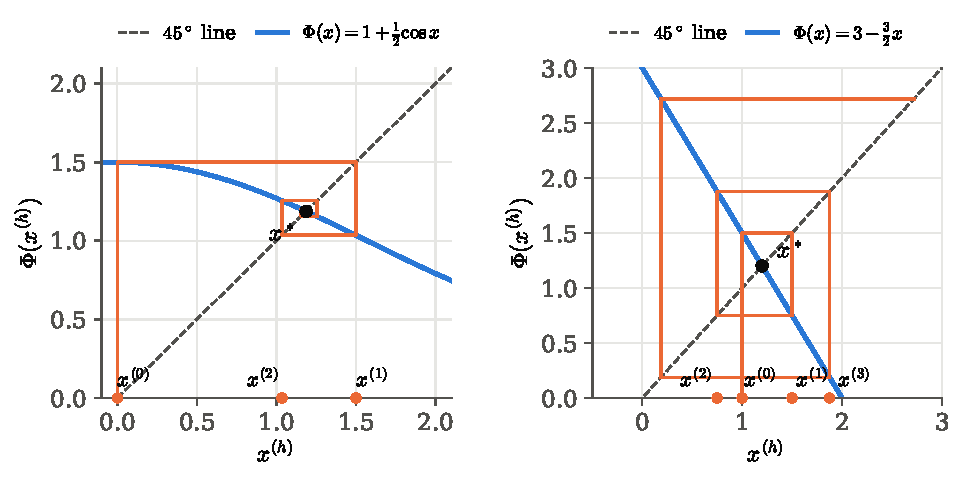
\includegraphics[width=0.95\textwidth]{figures/appB/cobweb.pdf}
  \caption{Cobweb diagrams for the iteration $x^{(h+1)} = \Phi(x^{(h)})$. In the left panel, $\Phi(x) = 1 +
  \frac{1}{2}\cos x$ is a contraction with modulus $\frac{1}{2}$, and the path from $x^{(0)} = 0$ converges to
  the fixed point $x^* \approx 1.187$. In the right panel, $\Phi(x) = 3 - \frac{3}{2}x$ has slope $-\frac{3}{2}$, and the path
  from $x^{(0)} = 1$ spirals away from the fixed point $x^* = \frac{6}{5}$.}
  \label{fig:B-cobweb}
\end{figure}

\subsection{Checking the contraction property}\label{sec:B-contraction-criteria}

For smooth maps on $\R^n$, the contraction property follows from a bound on the Jacobian.

\begin{proposition}[Jacobian row-sum criterion]\label{prop:B-jacobian-criterion}
Let $X \subseteq \R^n$ be convex and let $\Phi: X \to \R^n$ be continuously differentiable on an open set
containing $X$. If
\begin{equation}\label{eq:B-rowsum-criterion}
  \sup_{x \in X}\ \max_{j}\sum_{k=1}^{n}\left|\frac{\partial\Phi_j(x)}{\partial x_k}\right| \leq \kappa,
\end{equation}
then $\|\Phi(x) - \Phi(y)\|_\infty \leq \kappa\|x - y\|_\infty$ for all $x, y \in X$. If in addition $\kappa < 1$
and $\Phi$ maps $X$ into itself, then $\Phi$ is a contraction of $X$ in the sup norm.
\end{proposition}

\begin{proof}
Fix $x, y \in X$ and a component $j$. By convexity the segment $x + \tau(y - x)$, $\tau \in [0,1]$, lies in
$X$. The fundamental theorem of calculus and the chain rule give
\begin{equation*}
  \Phi_j(y) - \Phi_j(x) = \int_0^1\sum_{k=1}^{n}\frac{\partial\Phi_j}{\partial x_k}\big(x + \tau(y -
  x)\big)\,(y_k - x_k)\,\dd\tau.
\end{equation*}
Bounding each $|y_k - x_k|$ by $\|y - x\|_\infty$,
\begin{equation*}
  |\Phi_j(y) - \Phi_j(x)| \leq \int_0^1\sum_{k=1}^{n}\left|\frac{\partial\Phi_j}{\partial x_k}\big(x +
  \tau(y - x)\big)\right|\,\dd\tau\ \|y - x\|_\infty \leq \kappa\|y - x\|_\infty.
\end{equation*}
Taking the maximum over $j$ proves the claim.
\end{proof}

The constant in \eqref{eq:B-rowsum-criterion} is the largest induced sup norm of the Jacobian over $X$, by
\cref{lem:B-rowsum}. For a linear map the criterion is therefore sharp. The proof is the mean value
inequality of \cref{sec:B-calculus}.

When all partial derivatives are nonnegative, as in the share inversion below, the absolute values in
\eqref{eq:B-rowsum-criterion} drop out. The row sum then has a direct reading:
\begin{equation*}
  \sum_{k=1}^{n}\frac{\partial\Phi_j(x)}{\partial x_k} = \frac{\dd}{\dd c}\,\Phi_j(x + c\mathbf{1})\Big|_{c=0},
\end{equation*}
where $\mathbf{1}$ is the vector of ones. The condition says that $\Phi$ is monotone and that raising every
argument by $c$ raises each component by less than $c$. Blackwell's theorem is the version of this idea for
maps between function spaces.

\begin{theorem}[\citealp{Blackwell1965}]\label{thm:B-blackwell}
Let $B(S)$ be the space of bounded real functions on a set $S$ with the sup metric, and let $\mathcal{T}:
B(S) \to B(S)$ satisfy two conditions. The first, monotonicity, requires that $g \leq g'$ pointwise implies
$\mathcal{T}g \leq \mathcal{T}g'$. The second, discounting, requires that there is $\kappa \in [0,1)$ such that $\mathcal{T}(g + c) \leq \mathcal{T}g +
\kappa c$ for every $g$ and every constant $c \geq 0$. Then $\mathcal{T}$ is a contraction with modulus $\kappa$.
\end{theorem}

\begin{proof}
Fix $g, g' \in B(S)$ and let $c = \sup_s|g(s) - g'(s)|$. Then $g \leq g' + c$ pointwise. Monotonicity and
discounting give $\mathcal{T}g \leq \mathcal{T}(g' + c) \leq \mathcal{T}g' + \kappa c$. Exchanging the roles
of $g$ and $g'$ gives $\mathcal{T}g' \leq \mathcal{T}g + \kappa c$. Hence $|\mathcal{T}g(s) - \mathcal{T}g'(s)|
\leq \kappa c$ for every $s$, which is the claim.
\end{proof}

The Bellman operator $(\mathcal{T}g)(s) = \max_a\{u(s, a) + \kappa\,\E[g(s') \mid s, a]\}$ of a dynamic program
with discount factor $\kappa$ satisfies both conditions, so value functions are unique fixed points that
value iteration computes. Dynamic models lie outside this edition, but the logic is the same as in the
static applications below.

Some maps of interest have row sums below one at every point but not uniformly, as in the example $x +
\frac{1}{x}$. \Citet[Appendix~I]{BerryLevinsohnPakes1995} handle this case with a truncation.

\begin{theorem}[\citealp{BerryLevinsohnPakes1995}, Appendix I]\label{thm:B-blp-contraction}
Consider $\R^J$ with the sup norm, and let $\Phi: \R^J \to \R^J$ satisfy three conditions. (1) $\Phi$ is
continuously differentiable, with $\frac{\partial\Phi_j(y)}{\partial y_k} \geq 0$ and $\sum_{k=1}^{J}
\frac{\partial\Phi_j(y)}{\partial y_k} < 1$ for all $j$, $k$ and $y$. (2) $\Phi$ is bounded below:
$\underline y \equiv \min_j\inf_y\Phi_j(y) > -\infty$. (3) There is a value $\bar y$ such that, whenever $y_j
\geq \bar y$ for some $j$, there is some $k$ (not necessarily equal to $j$) with $\Phi_k(y) < y_k$. Then
$\Phi$ has a unique fixed point in $\R^J$. Moreover, the truncated map $\hat\Phi_j(y) = \min\{\Phi_j(y),
\bar y\}$ is a contraction of $[\underline y, \bar y]^J$ with modulus below one.
\end{theorem}

\Cref{thm:08-contraction} proves the theorem in full. The idea is short. On the compact set $[\underline y,
\bar y]^J$, enlarged by the segments along which the proof integrates, the continuous row sums attain a
maximum $\kappa < 1$. The truncated map is therefore a contraction there, and \cref{thm:B-banach} gives a
fixed point. Condition (3) keeps that fixed point away from the cap $\bar y$, so it is a fixed point of
$\Phi$ itself. The bound $\bar y$ is needed because no uniform modulus exists on all of $\R^J$. In the logit
model, for instance, the row sums of the share-inversion map equal $1 - s_0(\delta)$, which tends to one as
the mean utilities grow (\cref{sec:B-inversion}).

\subsection{Application: inverting market shares}\label{sec:B-inversion}

Consider a market with inside goods $j = 1, \dots, J$ and the outside good $j = 0$. In the random
coefficients logit model, consumer $i$ chooses $j$ with probability
\begin{equation*}
  s_{ij}(\delta) = \frac{e^{\delta_j + \mu_{ij}}}{1 + \sum_{k=1}^{J}e^{\delta_k + \mu_{ik}}}, \qquad
  s_{i0}(\delta) = 1 - \sum_{k=1}^{J}s_{ik}(\delta),
\end{equation*}
and the market share is $s_j(\delta) = \int s_{ij}(\delta)\,\dd F(\nu_i)$, where $\mu_{ij}$ depends on the
consumer's tastes $\nu_i$ and the nonlinear parameters (\cref{ch:blp}). Given observed shares $s^{obs}$
with $s^{obs}_j > 0$ and $\sum_js^{obs}_j < 1$, estimation needs the vector $\delta$ that solves $s(\delta) =
s^{obs}$. \citet[eq.~(6.8), p.~865]{BerryLevinsohnPakes1995} compute it as the fixed point of
\begin{equation}\label{eq:B-blp-map}
  \Phi_j(\delta) = \delta_j + \ln s^{obs}_j - \ln s_j(\delta), \qquad j = 1, \dots, J.
\end{equation}
A vector $\delta$ is a fixed point of $\Phi$ exactly when $s(\delta) = s^{obs}$.

\begin{proposition}[Row sums of the BLP map]\label{prop:B-blp-rowsum}
In the random coefficients logit model, for all $j$ and all $k \neq j$,
\begin{equation*}
  \frac{\partial\Phi_j}{\partial\delta_j} = \frac{1}{s_j}\int s_{ij}^2\,\dd F > 0, \qquad
  \frac{\partial\Phi_j}{\partial\delta_k} = \frac{1}{s_j}\int s_{ij}s_{ik}\,\dd F > 0,
\end{equation*}
and the row sums are
\begin{equation}\label{eq:B-blp-rowsum}
  \sum_{k=1}^{J}\frac{\partial\Phi_j}{\partial\delta_k} = 1 - \frac{1}{s_j}\int s_{ij}s_{i0}\,\dd F \in (0, 1).
\end{equation}
\end{proposition}

\begin{proof}
The individual logit derivatives are $\frac{\partial s_{ij}}{\partial\delta_k} = s_{ij}(\indic\{j = k\} -
s_{ik})$, bounded by one, so we may differentiate under the integral (\cref{sec:B-calculus}). Hence
$\frac{\partial s_j}{\partial\delta_j} = \int s_{ij}(1 - s_{ij})\,\dd F$ and $\frac{\partial
s_j}{\partial\delta_k} = -\int s_{ij}s_{ik}\,\dd F$ for $k \neq j$. Differentiating \eqref{eq:B-blp-map},
\begin{equation*}
  \frac{\partial\Phi_j}{\partial\delta_j} = 1 - \frac{1}{s_j}\int s_{ij}(1 - s_{ij})\,\dd F
  = 1 - \frac{s_j}{s_j} + \frac{1}{s_j}\int s_{ij}^2\,\dd F = \frac{1}{s_j}\int s_{ij}^2\,\dd F,
\end{equation*}
and $\frac{\partial\Phi_j}{\partial\delta_k} = -\frac{1}{s_j}\frac{\partial s_j}{\partial\delta_k} =
\frac{1}{s_j}\int s_{ij}s_{ik}\,\dd F$. For the row sum, consumer $i$'s choice probabilities depend only on
differences of the utilities $(\delta_0 + \mu_{i0}, \dots, \delta_J + \mu_{iJ})$, with $\delta_0 = \mu_{i0} = 0$.
By \cref{cor:B-translation}, $\sum_{k=0}^{J}\frac{\partial s_{ij}}{\partial\delta_k} = 0$, and the outside
derivative is $\frac{\partial s_{ij}}{\partial\delta_0} = -s_{ij}s_{i0}$. Hence $\sum_{k=1}^{J}\frac{\partial
s_{ij}}{\partial\delta_k} = s_{ij}s_{i0}$. Integrating and dividing by $s_j$,
\begin{equation*}
  \sum_{k=1}^{J}\frac{\partial\Phi_j}{\partial\delta_k} = 1 - \frac{1}{s_j}\sum_{k=1}^{J}\frac{\partial
  s_j}{\partial\delta_k} = 1 - \frac{1}{s_j}\int s_{ij}s_{i0}\,\dd F.
\end{equation*}
The integral is positive and smaller than $\int s_{ij}\,\dd F = s_j$, so the row sum lies in $(0,1)$.
\end{proof}

\Cref{cor:08-rowsum} gives the same computation, and \cref{ch:blp} verifies the remaining conditions of
\cref{thm:B-blp-contraction}. The row sum has a useful reading. The weights $\frac{s_{ij}}{s_j}$ form the
distribution of consumer types among the buyers of $j$. The row sum is therefore one minus the average
probability of choosing the outside good among those buyers. The modulus is close to one when the buyers of
some product rarely choose the outside good, and convergence is then slow. The plain logit model shows this in
its simplest form. There $s_{ij} = s_j$, so $\frac{\partial\Phi_j}{\partial\delta_k} = s_k$ for every $k$,
including $k = j$. The Jacobian is the rank-one matrix $\mathbf{1}s^\T$, whose only nonzero eigenvalue is
$s^\T\mathbf{1} = 1 - s_0$. With $s_0 = 0.1$ the iteration gains one digit of accuracy only every 22 steps,
since $\frac{\ln 10}{-\ln 0.9} \approx 21.9$, although the logit inverse $\delta_j = \ln s_j - \ln s_0$ is
available in closed form.

Three practical rules follow. First, the logit inversion $\ln s^{obs}_j - \ln s^{obs}_0$ is a natural
starting value, and inside an estimation routine the solution at the previous parameter value is better.
Second, the stopping tolerance must be tight, by \eqref{eq:B-aposteriori}, because the inversion error
propagates into the estimation objective (\cref{prop:08-innererror}). \citet{DubeFoxSu2012} study how to improve
the numerical performance of random coefficients demand estimation (\cref{ch:blp}).
Third, the update can be written
multiplicatively as $e^{\delta^{(h+1)}_j} = e^{\delta^{(h)}_j}\frac{s^{obs}_j}{s_j(\delta^{(h)})}$. Each step
raises $\delta_j$ when the model underpredicts the share of $j$ and lowers it when the model overpredicts.

\begin{remark}[Where the iteration typically moves from the logit start]\label{rem:B-logit-start}
For a product with a small share, the logistic function $\frac{e^{u}}{1 + e^{u}}$ is convex in the relevant
range of utilities. Random coefficients spread individual utilities around $\delta_j$. By Jensen's
inequality the average choice probability at a given $\delta$ then exceeds the logit probability, so the
model share at the logit starting value typically exceeds the observed share. The iteration then lowers
$\delta_j$, and the recovered mean utilities typically lie below the logit start. The statement describes a
tendency. It is not a theorem, because the denominators of all products move together. \Cref{ch:blp} and \cref{app:problems}
report worked examples.
\end{remark}

\citet[Appendix]{Berry1994} proved existence and uniqueness of the inverse for a broad class of discrete
choice models without the contraction. His argument combines Brouwer's theorem with a diagonal dominance
condition.

\begin{proposition}[\citealp{Berry1994}, Appendix]\label{prop:B-berry-inverse}
Let $s: \R^J \to (0,1)^J$ be the inside shares of a random utility model with $\delta_0 = 0$. Suppose $s$ is
continuously differentiable, and that for all goods $j, k \in \{0, 1, \dots, J\}$ the share of $j$ rises in
$\delta_j$ and falls in $\delta_k$ for $k \neq j$. Suppose also that, for any values of the other inside mean
utilities, finite or $-\infty$, $s_j \to 0$ as $\delta_j \to -\infty$ and $s_j \to 1$ as $\delta_j \to \infty$. Then for every $s^{obs}$ with positive entries and $\sum_j
s^{obs}_j < 1$ there is exactly one $\delta$ with $s(\delta) = s^{obs}$.
\end{proposition}

\begin{proof}[Outline of the proof]
\emph{Step 1 (the element-by-element inverse).} For each $j$, let $r_j(\delta)$ be the value of $\delta_j$
that makes $s_j(\delta_1, \dots, r_j, \dots, \delta_J) = s^{obs}_j$, given the other mean utilities. It exists,
is unique and is continuous, by monotonicity and the limits. It does not depend on $\delta_j$. The implicit
function theorem (\cref{thm:B-ift}) gives, for $k \neq j$,
\begin{equation*}
  \frac{\partial r_j}{\partial\delta_k} = -\left(\frac{\partial s_j}{\partial\delta_j}\right)^{-1}
  \frac{\partial s_j}{\partial\delta_k} > 0.
\end{equation*}
A vector $\delta$ solves $s(\delta) = s^{obs}$ if and only if it is a fixed point of $r = (r_1, \dots, r_J)$.

\emph{Step 2 (a lower bound).} Since $r_j$ rises in every $\delta_k$, it is bounded below by its limit as all
other $\delta_k \to -\infty$. Let $\underline\delta$ be the smallest of these $J$ limits.

\emph{Step 3 (an upper bound).} For each $j$, let $\bar\delta_j$ be the value of $\delta_j$ that sets the
outside share equal to $s^{obs}_0 = 1 - \sum_ks^{obs}_k$ when all other inside $\delta_k$ are $-\infty$. Choose
$\bar\delta > \max_j\bar\delta_j$. Suppose $\delta_j \geq \bar\delta$ for some $j$. Adding products and
raising $\delta_j$ both lower the outside share, so $s_0(\delta) < s^{obs}_0$. The inside shares then sum to
more than $\sum_ks^{obs}_k$, so $s_k(\delta) > s^{obs}_k$ for some $k$. For that $k$, matching the smaller
observed share requires a lower utility, so $r_k(\delta) < \delta_k$.

\emph{Step 4 (existence).} The truncated map $\bar r_j(\delta) = \min\{r_j(\delta), \bar\delta\}$ is continuous
and maps the box $[\underline\delta, \bar\delta]^J$ into itself. Brouwer's theorem (\cref{thm:B-brouwer})
gives a fixed point $\delta^*$. If $\delta^*_j = \bar\delta$ for some $j$, Step 3 gives $k$ with $\bar
r_k(\delta^*) \leq r_k(\delta^*) < \delta^*_k$, a contradiction. So $\delta^*$ lies below the cap and is a fixed
point of $r$.

\emph{Step 5 (uniqueness).} Shares depend only on utility differences, so \cref{cor:B-translation} gives
$\sum_{k=0}^{J}\frac{\partial s_j}{\partial\delta_k} = 0$. All cross derivatives are negative, including the
one with respect to $\delta_0$. Hence
\begin{equation}\label{eq:B-berry-dd}
  \frac{\partial s_j}{\partial\delta_j} = \sum_{k \neq j,\ k \geq 1}\left|\frac{\partial
  s_j}{\partial\delta_k}\right| + \left|\frac{\partial s_j}{\partial\delta_0}\right| > \sum_{k \neq j,\ k \geq
  1}\left|\frac{\partial s_j}{\partial\delta_k}\right|.
\end{equation}
Dividing by $\frac{\partial s_j}{\partial\delta_j}$ shows that the row sums $\sum_k\big|\frac{\partial
r_j}{\partial\delta_k}\big|$ are below one at every point. On the compact box their maximum $\kappa$ is
below one. The truncation is nonexpansive, so \cref{prop:B-jacobian-criterion} makes $\bar r$ a contraction
of the box. Every solution lies in the box by Steps 2 and 3, so the solution is unique.
\end{proof}

Condition \eqref{eq:B-berry-dd} is (A2) in \citet[p.~261]{Berry1994}. It also makes the Jacobian
$\frac{\partial s}{\partial\delta^\T}$ strictly diagonally dominant, hence nonsingular by \cref{lem:B-dd}.
\Citet[p.~260]{Berry1994} notes that a strictly positive and continuous density of the consumer-level
unobservables suffices for his sign conditions. On the same page he states the limit conditions for finite
values of the other mean utilities. We also allow the value $-\infty$, which Steps 2 and 3 of the proof use.

\begin{remark}[Connected substitutes]\label{rem:B-connected-substitutes}
\citet{BerryGandhiHaile2013} replace Berry's sign conditions by a weaker structure. Write $s_j(\delta, p)$
for the demand system and let $\lambda$ stand for either $-p$ or $\delta$. Goods $0, 1, \dots, J$ are
\emph{connected substitutes} in $\lambda$ if two conditions hold \citep[Definition~1,
p.~1759]{BerryHaile2014}. First, $s_k$ is nonincreasing in $\lambda_j$ for all $j > 0$ and $k \neq j$. Second,
for every nonempty set $\mathcal{K} \subseteq \{1, \dots, J\}$, some $k \in \mathcal{K}$ and some good $\ell
\notin \mathcal{K}$ have $s_\ell$ strictly decreasing in $\lambda_k$. The first condition requires weak gross
substitutes. The second requires enough strict substitution that no group of inside goods trades only among
itself, where the outside good may serve as the good $\ell$. Connected substitutes are combined with an
\emph{index restriction}. One observed characteristic $x^{(1)}_{jt}$ and the unobservable $\xi_{jt}$ affect the
distribution of utilities only through the scalar index $\delta_{jt} = x^{(1)}_{jt}\beta_j + \xi_{jt}$, so
consumers treat them as perfect substitutes \citep[Section~3.2, eq.~(2) and Assumption~1, p.~1757]{BerryHaile2014}.
Under the index restriction and connected substitutes in both $-p$ and $\delta$, there is at most one $\delta$
with $s(\delta, p) = s^{obs}$ for any interior share vector. This is Lemma~1 of \citet[p.~1760]{BerryHaile2014},
who credit the proof to \citet{BerryGandhiHaile2013}. The result needs no functional form, and it allows zero
cross effects, as in the vertical model where each product competes only with its neighbors (\cref{ch:discrete}).
It delivers injectivity. Existence must be argued separately.
\end{remark}

Nested logit demand shows why the BLP map sometimes needs to be modified. With nests $g$, nesting parameter
$\sigma \in [0, 1)$ and within-nest shares $s_{j|g}$, the derivatives of the log shares are given by
\eqref{eq:B-nl-logderiv} in \cref{prop:B-nested-inversion}. The own derivative
$\frac{\partial\ln s_j}{\partial\delta_j} = \frac{1}{1-\sigma} - \frac{\sigma}{1-\sigma}s_{j|g} - s_j$ can be far above one when
$\sigma$ is large. The diagonal partial of the BLP map, $1 -
\frac{\partial\ln s_j}{\partial\delta_j}$, is then negative, and the map can fail to be a contraction.

\begin{proposition}[Dampened inversion for the nested logit]\label{prop:B-nl-dampening}
Consider the nested logit model and the dampened map
\begin{equation}\label{eq:B-nl-dampened}
  \Phi^D(\delta) = \delta + (1 - \sigma)\big[\ln s^{obs} - \ln s(\delta)\big].
\end{equation}
(i) For $j$ in nest $g$, its partial derivatives are all nonnegative:
\begin{equation*}
  \frac{\partial\Phi^D_j}{\partial\delta_k} =
  \begin{cases}
    \sigma s_{j|g} + (1 - \sigma)s_j, & k = j,\\[2pt]
    \sigma s_{k|g} + (1 - \sigma)s_k, & k \neq j,\ k \in g,\\[2pt]
    (1 - \sigma)s_k, & k \notin g.
  \end{cases}
\end{equation*} (ii) Every row sums to $1 - (1 - \sigma)s_0(\delta) < 1$. (iii) Let $\bar\delta$ be the cap of
Step 3 in the proof of \cref{prop:B-berry-inverse}. The truncated map $\min\{\Phi^D_j(\delta), \bar\delta\}$ is a
contraction of $(-\infty, \bar\delta]^J$ with modulus $\kappa = 1 - (1 - \sigma)s_0(\bar\delta\mathbf{1}) < 1$,
and its unique fixed point solves $s(\delta) = s^{obs}$. (iv) If some nest contains at least two products,
the undampened map \eqref{eq:B-blp-map} has the Jacobian eigenvalue $-\frac{\sigma}{1-\sigma}$ at every
$\delta$. Its modulus exceeds one when $\sigma > \frac{1}{2}$.
\end{proposition}

\begin{proof}
(i) Multiply \eqref{eq:B-nl-logderiv} by $-(1 - \sigma)$ and add the identity. For $k = j$,
\begin{equation*}
  1 - (1 - \sigma)\Big[\frac{1}{1-\sigma} - \frac{\sigma}{1-\sigma}s_{j|g} - s_j\Big] = 1 - 1 + \sigma s_{j|g}
  + (1 - \sigma)s_j = \sigma s_{j|g} + (1 - \sigma)s_j.
\end{equation*}
For $k \neq j$ in the same nest, $-(1 - \sigma)\big[-\frac{\sigma}{1-\sigma}s_{k|g} - s_k\big] = \sigma
s_{k|g} + (1 - \sigma)s_k$. For $k$ in another nest, $-(1 - \sigma)(-s_k) = (1 - \sigma)s_k$.

(ii) Summing over $k$, the within-nest shares of nest $g$ add to one and the inside shares add to $1 - s_0$:
\begin{equation*}
  \sum_{k=1}^{J}\frac{\partial\Phi^D_j}{\partial\delta_k} = \sigma\sum_{k \in g}s_{k|g} + (1 -
  \sigma)\sum_{k=1}^{J}s_k = \sigma + (1 - \sigma)(1 - s_0) = 1 - (1 - \sigma)s_0.
\end{equation*}

(iii) The outside share $s_0(\delta) = \big(1 + \sum_hD_h^{1-\sigma}\big)^{-1}$, with $D_h = \sum_{k \in
h}e^{\frac{\delta_k}{1-\sigma}}$, falls in every $\delta_k$. On $C = (-\infty, \bar\delta]^J$ it is therefore
at least $s_0(\bar\delta\mathbf{1}) > 0$, so the row sums are at most $\kappa < 1$ on $C$. The set $C$ is
convex, so \cref{prop:B-jacobian-criterion} makes $\Phi^D$ Lipschitz with constant $\kappa$ on $C$. Taking the
minimum with the constant $\bar\delta$ is nonexpansive and maps into $C$, so the truncated map is a
contraction of the complete set $C$. Its fixed point $\delta^*$ is unique by \cref{thm:B-banach}. The
dampened map lowers $\delta_k$ exactly when $s_k(\delta) > s^{obs}_k$, as the BLP map does. The argument of
Step 4 in the proof of \cref{prop:B-berry-inverse} therefore keeps $\delta^*$ below the cap, so $\Phi^D(\delta^*)
= \delta^*$ and $s(\delta^*) = s^{obs}$.

(iv) Write $A$ for the matrix with elements $\frac{\partial\ln s_j}{\partial\delta_k}$. Let nest $g$ contain
at least two products, and take a nonzero vector $x$ supported on $g$ with $\sum_{k \in g}s_{k|g}x_k = 0$. By
\eqref{eq:B-nl-logderiv},
\begin{equation*}
  (Ax)_j = \frac{x_j}{1-\sigma} - \frac{\sigma}{1-\sigma}\indic\{j \in g\}\sum_{k \in g}s_{k|g}x_k -
  \sum_{k=1}^{J}s_kx_k.
\end{equation*}
The middle term vanishes by construction. The last term is $s_g\sum_{k \in g}s_{k|g}x_k = 0$, where $s_g$ is
the share of nest $g$. Hence $Ax = \frac{1}{1-\sigma}x$. The Jacobian of the undampened map is $I - A$, so
$x$ is an eigenvector with eigenvalue $1 - \frac{1}{1-\sigma} = -\frac{\sigma}{1-\sigma}$.
\end{proof}

The proof of (iv) also shows that the dampened Jacobian $I - (1 - \sigma)A$ has eigenvalue zero along the
same directions. Dampening removes the within-nest overshooting exactly. The remaining eigenvalue governs
the overall level of utilities and equals the row sum in (ii) in the one-nest case. The factor $1 - \sigma$
is the scale of the within-nest logit error in the nested logit (\cref{sec:B-ev}), and this is why it is the
right step size.

\begin{example}[Divergence and dampening]\label{ex:B-nl-dampening}
Take one nest with two products, $\sigma = 0.8$ and true mean utilities $\delta = (0, -0.5)$. The shares are
$(0.4657, 0.0382)$ and $s_0 = 0.4961$. At the solution, the Jacobian of the undampened map has eigenvalues
$1 - s_0 = 0.504$ and $-\frac{\sigma}{1-\sigma} = -4$. Started from the logit inversion, the undampened iteration
diverges, with sup-norm errors $7.9$, $36.6$ and $163.9$ after one, two and three steps. The dampened map has
row sums $1 - 0.2 \times 0.4961 = 0.901$. It reaches an error below $10^{-12}$ after 240 iterations. The rate is
slow because dampening by $1 - \sigma = 0.2$ also slows the adjustment of the overall level of utilities, whose
eigenvalue rises from $1 - s_0 = 0.504$ to $0.901$.
\end{example}

\begin{remark}[Random coefficients nested logit]\label{rem:B-rcnl}
With random coefficients on top of the nested logit, the same computation holds consumer by consumer. The
dampened map has nonnegative partials, and its row sums are
\begin{equation*}
  \sum_{k=1}^{J}\frac{\partial\Phi^D_j}{\partial\delta_k} = 1 - \frac{1 - \sigma}{s_j}\int s_{ij}s_{i0}\,\dd F <
  1,
\end{equation*}
using $\sum_{k \geq 1}\frac{\partial s_{ij}}{\partial\delta_k} = s_{ij}s_{i0}$, which holds in the nested logit
as in the logit. Global convergence then follows from an argument like that of \cref{thm:B-blp-contraction}
once the iterates are confined to a compact set. The model nests the nested logit ($F$ degenerate) and the
random coefficients logit ($\sigma = 0$), and \citet{GrigolonVerboven2014} compare these alternatives.
\Cref{ch:mergers} applies the dampened iteration in merger simulation, and \cref{rem:08-rcnl} discusses it in the
BLP framework.
\end{remark}

\begin{remark}[Error scale and the pure characteristics model]\label{rem:B-scale}
The same logic explains why the inversion of the pure characteristics model is not a contraction. Suppose
the logit errors are multiplied by a scale $\lambda > 0$, so that
\begin{equation*}
  s_{ij} = \frac{\exp\big(\frac{\delta_j + \mu_{ij}}{\lambda}\big)}{1 + \sum_k\exp\big(\frac{\delta_k +
  \mu_{ik}}{\lambda}\big)}.
\end{equation*}
Then $\frac{\partial s_{ij}}{\partial\delta_k} = \frac{1}{\lambda}s_{ij}(\indic\{j = k\} -
s_{ik})$. The undampened map has diagonal partial $1 - \frac{1}{\lambda s_j}\int s_{ij}(1 - s_{ij})\,\dd F$,
which turns negative as $\lambda$ falls. The map $\delta + \lambda[\ln s^{obs} - \ln s(\delta)]$ restores the
structure of \cref{prop:B-blp-rowsum}, with row sums $1 - \frac{1}{s_j}\int s_{ij}s_{i0}\,\dd F$. As $\lambda
\to 0$ each consumer chooses one option with probability near one, so $s_{ij}s_{i0} \to 0$ and the modulus
tends to one. The pure characteristics model of \citet{BerryPakes2007} is the limit $\lambda = 0$. Its share
function is not smooth, and the contraction is lost. \citet[proof of Theorem~1, pp.~17--18]{BerryPakes2007}
show that the element-by-element inverse of the proof of \cref{prop:B-berry-inverse} is only a weak contraction,
with modulus at most one. They could not prove that the modulus is below one, and in Monte Carlo runs it
``sometimes contracts so slowly as to become useless'' (p.~19). They therefore combine three methods. The BLP
contraction is applied to the model with logit errors of a small scale, which corresponds to a small
$\lambda$ here. A \emph{homotopy} deforms a fixed-point problem with a known solution continuously into the
target problem and tracks the solution along the way. One built on the element-by-element inverse takes over
when progress stalls, and Newton steps finish the computation \citep[Section~4.3]{BerryPakes2007}. \citet[p.~35]{AckerbergEtAl2007} likewise note
that the inversion of this model is not necessarily a contraction with modulus less than one (\cref{ch:discrete}).
\end{remark}

\subsection{Application: computing and counting price equilibria}\label{sec:B-equilibrium}

In a differentiated-products Bertrand game, firm $f$ chooses the prices of its products $\mathcal{J}_f$ to
maximize $\pi_f(p) = \sum_{k \in \mathcal{J}_f}(p_k - mc_k)s_k(p)$. A price vector $p^*$ is a Nash
equilibrium if and only if $p^* = BR(p^*)$, where $BR$ stacks the best responses. Uniqueness matters for
counterfactuals more than for estimation. Estimation evaluates the first-order conditions at observed prices
to recover marginal costs and never solves for an equilibrium. A counterfactual, such as a merger or a tax,
must solve for new prices. If several equilibria exist, the analyst must select one, for example the one
reached from the status quo (\cref{ch:diffprod}, \cref{ch:mergers}).

\subsubsection{Single-product logit firms: a global contraction}

Let demand be logit with $\delta_j = \tilde\delta_j - \alpha p_j$, $\alpha > 0$, and constant marginal costs.
Define $v_j = \tilde\delta_j - \alpha mc_j$, the mean utility at marginal-cost pricing, and $\Lambda_{-j} = 1 +
\sum_{l \neq j}e^{\delta_l}$, which depends only on rivals' prices. \Cref{prop:B-logit-br} gives the best
response in closed form, $BR_j(p_{-j}) = mc_j + \frac{1}{\alpha}[1 + W_0(z_j)]$ with $z_j = \frac{e^{v_j - 1}}{\Lambda_{-j}}$,
as in \eqref{eq:B-logit-br-closed}. Here $W_0$ is the principal branch of the Lambert function, with derivative
$W_0'(z) = \frac{W_0(z)}{z(1 + W_0(z))}$ (\cref{lem:B-lambert}).

\begin{proposition}[Best-response contraction in the logit pricing game]\label{prop:B-logit-br-contraction}
With single-product firms, logit demand and constant marginal costs, the best-response map is a contraction
of $\R^J$ in the sup norm with modulus
\begin{equation}\label{eq:B-logit-kappa}
  \kappa = \max_j\frac{W_0(e^{v_j - 1})}{1 + W_0(e^{v_j - 1})} < 1.
\end{equation}
Hence the Bertrand equilibrium exists and is unique, and best-response iteration converges to it from any
starting prices.
\end{proposition}

\begin{proof}
\emph{Step 1 (slopes).} Let $z_j = \frac{e^{v_j - 1}}{\Lambda_{-j}}$. For $l \neq j$, $\frac{\partial
\Lambda_{-j}}{\partial p_l} = -\alpha e^{\delta_l}$, so $\frac{\partial z_j}{\partial p_l} = \alpha
z_j\frac{e^{\delta_l}}{\Lambda_{-j}}$. The chain rule and the derivative of $W_0$ give
\begin{equation*}
  \frac{\partial BR_j}{\partial p_l} = \frac{1}{\alpha}\cdot\frac{W_0(z_j)}{z_j(1 + W_0(z_j))}\cdot\alpha
  z_j\frac{e^{\delta_l}}{\Lambda_{-j}} = \frac{W_0(z_j)}{1 + W_0(z_j)}\cdot\frac{e^{\delta_l}}{\Lambda_{-j}}.
\end{equation*}
The derivative with respect to $p_j$ is zero.

\emph{Step 2 (shares at the best response).} At $p_j = BR_j(p_{-j})$, the identities
\eqref{eq:B-br-identities} give $s_j = \frac{W_0(z_j)}{1 + W_0(z_j)}$ and $\frac{e^{\delta_l}}{\Lambda_{-j}} =
\frac{s_l}{1 - s_j}$, with shares evaluated at $(BR_j(p_{-j}), p_{-j})$. Substituting into Step 1,
\begin{equation*}
  \frac{\partial BR_j}{\partial p_l} = \frac{s_js_l}{1 - s_j}, \qquad l \neq j.
\end{equation*}

\emph{Step 3 (row sums).} The slopes are positive, and
\begin{equation*}
  \sum_{l \neq j}\frac{\partial BR_j}{\partial p_l} = \frac{s_j}{1 - s_j}\sum_{l \neq j}s_l = \frac{s_j(1 - s_j
  - s_0)}{1 - s_j} < s_j.
\end{equation*}

\emph{Step 4 (a uniform bound).} Since $\Lambda_{-j} \geq 1$, we have $z_j \leq e^{v_j - 1}$. The functions $W_0$
and $w \mapsto \frac{w}{1 + w}$ are increasing, so $s_j = \frac{W_0(z_j)}{1 + W_0(z_j)} \leq \frac{W_0(e^{v_j -
1})}{1 + W_0(e^{v_j - 1})} \leq \kappa$. The bound holds at every price vector. \Cref{prop:B-jacobian-criterion}
on the convex set $\R^J$ and \cref{thm:B-banach} complete the proof.
\end{proof}

The bound $\kappa$ is the share that firm $j$ would choose if all rivals priced out of the market. It is
uniform because a firm's share at its own best response can never exceed that value.

\begin{example}[Three logit firms]\label{ex:B-logit-br}
Let $\alpha = 1$, $\tilde\delta = (2, 3, 4)$ and $mc = (1, 1, 1)$, so $v = (1, 2, 3)$. The share bounds are
$(0.362, 0.500, 0.609)$, so $\kappa = 0.609$. Best-response iteration from $p^{(0)} = mc$ stops after 21
iterations, when successive prices differ by less than $10^{-12}$. The equilibrium prices are $(2.143, 2.372,
2.847)$, with shares $(0.125, 0.271, 0.459)$ and $s_0 = 0.145$. The markups $(1.143, 1.372, 1.847)$ equal
$\frac{1}{\alpha(1 - s_j)}$. At the equilibrium the row sums of the Jacobian are $(0.105, 0.217, 0.336)$, and
its spectral radius is $0.233$, close to the observed rate of convergence of $0.232$ per step. The a priori bound
\eqref{eq:B-iterations} with $\kappa = 0.609$ guarantees accuracy $10^{-12}$ after 59 iterations, so it is
conservative by a factor of three. Two hundred random starting points in $mc + [0, 20]^3$ all reach the same
equilibrium.
\end{example}

\begin{remark}[Multiproduct logit firms]\label{rem:B-logit-br-multi}
Logit first-order conditions imply that firm $f$ sets a common markup $m_f = \frac{1}{\alpha(1 - S_f)}$ on all
its products, where $S_f = \sum_{k \in \mathcal{J}_f}s_k$ (\cref{prop:B-logit-markups}). With $E_f = \sum_{k \in
\mathcal{J}_f}e^{v_k}$ and $\Lambda_{-f} = 1 + \sum_{l \notin \mathcal{J}_f}e^{\delta_l}$, the best-response
markup is $\frac{1}{\alpha}\big[1 + W_0\big(\frac{E_fe^{-1}}{\Lambda_{-f}}\big)\big]$ (\cref{prop:B-logit-br}). The
computation of the proof gives $\frac{\partial BR_k}{\partial p_l} = \frac{S_fs_l}{1 - S_f}$ for $k \in \mathcal{J}_f$ and $l
\notin \mathcal{J}_f$, and zero for $l \in \mathcal{J}_f$. The row sums are $\frac{S_f(1 - S_f - s_0)}{1 - S_f}
< S_f \leq \frac{W_0(E_fe^{-1})}{1 + W_0(E_fe^{-1})}$, so the best-response map is again a global contraction.
The equilibrium is unique for every ownership structure, and merger simulation by best-response iteration
converges.
\end{remark}

\begin{remark}[Uniqueness through a scalar aggregate]\label{rem:B-aggregative}
A second proof reduces the equilibrium to one equation in the aggregate $\Lambda = 1 + \sum_le^{\delta_l}$.
Multiproduct pricing games with logit or CES demands are \emph{aggregative games}. Each firm's profit depends
on its rivals' prices only through one scalar aggregator, and consumer surplus is a monotone function of that
aggregator \citep{NockeSchutz2018}. Each firm is then summarized by a one-dimensional \emph{type}, its
contribution to consumer surplus if it priced at cost \citep[p.~229 and fn.~127]{AskerNocke2021}. In the logit
model the aggregator is $\Lambda$, consumer surplus is $\frac{1}{\alpha}\ln\Lambda$ up to a constant
(\cref{prop:B-cs}), and the type of firm $f$ is $E_f = \sum_{k \in \mathcal{J}_f}e^{v_k}$. This is what the products
of $f$ add to $\Lambda$ when they are priced at marginal cost. A merger without synergies gives the merged firm
the sum of the partners' types. \citet[p.~229]{AskerNocke2021} report that consumer surplus then falls. It does
not fall only if synergies raise the merged type above a cutoff that exceeds this sum. In equilibrium $\alpha m_f = \frac{1}{1 - S_f}$ and
$S_f = \frac{E_fe^{-\alpha m_f}}{\Lambda}$. Eliminating the markup,
\begin{equation*}
  h(S_f) \equiv S_f\,e^{\frac{1}{1 - S_f}} = \frac{E_f}{\Lambda}.
\end{equation*}
The left side is strictly increasing on $(0,1)$, since $h'(S) = e^{\frac{1}{1-S}}\big[1 + \frac{S}{(1 - S)^2}\big]
> 0$, with $h(0) = 0$ and $h(S) \to \infty$ as $S \to 1$. Each $\Lambda > 0$ therefore pins down a unique
$S_f(\Lambda)$, strictly decreasing in $\Lambda$. Adding up requires $\Psi(\Lambda) \equiv \sum_fS_f(\Lambda) +
\frac{1}{\Lambda} = 1$, because $s_0 = \frac{1}{\Lambda}$. The function $\Psi$ is strictly decreasing, with
$\Psi(1) > 1$ and $\Psi(\Lambda) \to 0$ as $\Lambda \to \infty$. So there is exactly one root $\Lambda^*$, and it
determines all shares, markups and prices. In \cref{ex:B-logit-br} the root is $\Lambda^* = 6.908 =
\frac{1}{s_0}$, and $\Psi(1) = 2.75$.
\end{remark}

\subsubsection{Existence without contraction}

When best responses are not contractions, existence rests on topological fixed-point theorems.

\begin{theorem}[Brouwer]\label{thm:B-brouwer}
Let $K \subseteq \R^n$ be nonempty, compact and convex, and let $\Phi: K \to K$ be continuous. Then $\Phi$ has
a fixed point.
\end{theorem}

\begin{theorem}[Kakutani]\label{thm:B-kakutani}
Let $K \subseteq \R^n$ be nonempty, compact and convex, and let $\Gamma$ be a correspondence from $K$ to $K$
with nonempty convex values and a closed graph. Then there is $x^* \in K$ with $x^* \in \Gamma(x^*)$.
\end{theorem}

Both theorems are standard \citep{Brouwer1912, Kakutani1941, MasColellWhinstonGreen1995}. Neither says
anything about uniqueness or computation. Kakutani's theorem gives the basic existence result for pricing
games.

\begin{corollary}[Existence of a pure-strategy equilibrium]\label{cor:B-nash-existence}
Suppose each firm's price vector lies in a nonempty, compact, convex set $P_f$. Suppose also that each
profit function $\pi_f$ is continuous in all prices and quasi-concave in firm $f$'s own prices. Then a
pure-strategy Nash equilibrium exists.
\end{corollary}

\begin{proof}
Let $\Gamma(p) = \prod_fBR_f(p_{-f})$ on $K = \prod_fP_f$. By Berge's maximum theorem, continuity of
$\pi_f$ and compactness of $P_f$ make each $BR_f$ nonempty valued with a closed graph
\citep{MasColellWhinstonGreen1995}. Quasi-concavity makes the set of maximizers convex, since it is an upper
contour set of a quasi-concave function at its maximum value. \Cref{thm:B-kakutani} gives $p^* \in
\Gamma(p^*)$, which is an equilibrium.
\end{proof}

\Cref{cor:B-nash-existence} is the pricing-game case of a theorem of \citet{Debreu1952}.
\citet[Section~11.6.1]{Tirole1988} states a special case of it for any normal-form game with finitely many
players. Each action set is a compact convex subset of a Euclidean space, and each payoff is continuous in all
actions and quasi-concave in the player's own action (\cref{thm:02-existence}). Debreu's version also lets a
player's feasible actions depend on the actions of the others. Two consequences follow. First, a finite game
always has an equilibrium in mixed strategies \citep{Nash1950}. A mixed strategy is a point of a simplex, which
is compact and convex, and the expected payoff is linear, hence quasi-concave, in the player's own mixture. It
is also a polynomial in all mixtures, hence continuous. Second, some
games of industrial organization fall outside the theorem. Auctions, Cournot competition and location games can
have payoffs that are discontinuous or not quasi-concave. \citet{DasguptaMaskin1986} give existence conditions
for such games, for pure strategies when payoffs are quasi-concave and for mixed strategies when they are not
\citep[Section~11.6.1]{Tirole1988}.

\begin{remark}[Equilibrium concepts used in the book]\label{rem:B-eq-concepts}
The book uses four equilibrium concepts, all developed in \citet[Sections~11.2--11.5]{Tirole1988}. A
\emph{Nash equilibrium}, in pure or mixed strategies, is a profile in which each player's strategy is a best
response to the strategies of the others (\cref{def:02-nash}). The static pricing and quantity games use it
(\cref{def:04-bertrand-nash}). A \emph{subgame perfect equilibrium} requires Nash play in every subgame, so
threats that would not be carried out are ruled out \citep[Section~11.3]{Tirole1988}. The repeated games of
collusion use it (\cref{def:12-spe}). A \emph{Bayesian Nash equilibrium} applies to games of incomplete
information. Each player's type-contingent strategy maximizes its expected payoff, given its type and the
strategies of the others \citep[Section~11.4]{Tirole1988}. Auction models use it (\cref{def:14-bne}). A
\emph{perfect Bayesian equilibrium} combines subgame perfection with Bayesian beliefs for dynamic games of
incomplete information. Strategies are optimal given beliefs at every information set, and beliefs follow from
the equilibrium strategies by Bayes' rule where possible \citep[Section~11.5]{Tirole1988}. Signaling models of
limit pricing, which \cref{ch:conduct} mentions in passing, rest on it. In these models entrants are unsure of
an incumbent's cost. In games with finitely many actions and types, \citet[Section~11.6.1]{Tirole1988} derives
the existence of the other three equilibria from the same theorem. The Bayesian case treats each type of a player as a separate player. The perfect Bayesian
case takes limits of equilibria of games in which every action is played with a small positive probability.
\end{remark}

Quasi-concavity is the substantive condition. Without it a best response can jump between two prices, and a
pure-strategy equilibrium may fail to exist. \citet{CaplinNalebuff1991} derive quasi-concavity of profits
from conditions on the distribution of consumer tastes. They then apply Kakutani's theorem to the
best-response correspondence on $\prod_f[mc_f, Y]$, where $Y$ is an upper bound on prices
(\cref{sec:B-caplin-nalebuff}, \cref{ch:diffprod}).

\subsubsection{Uniqueness by diagonal dominance}

The next result turns diagonal dominance of the first-order conditions into uniqueness.

\begin{proposition}[Uniqueness by dominant diagonal]\label{prop:B-dd-uniqueness}
Let $P \subseteq \R^N$ be convex and let $g: P \to \R^N$ be continuously differentiable with
\begin{equation}\label{eq:B-dd-condition}
  \left|\frac{\partial g_i(p)}{\partial p_i}\right| > \sum_{j \neq i}\left|\frac{\partial g_i(p)}{\partial
  p_j}\right| \qquad \text{for all } i \text{ and all } p \in P.
\end{equation}
Then $g$ has at most one zero in $P$. In particular, if $g_i = \frac{\partial\pi_i}{\partial p_i}$ and
\begin{equation*}
  \left|\frac{\partial^2\pi_i}{\partial p_i^2}\right| > \sum_{j \neq i}\left|\frac{\partial^2\pi_i}{\partial
  p_i\,\partial p_j}\right|
\end{equation*}
on $P$, there is at most one equilibrium in $P$ at which every firm's first-order condition holds.
\end{proposition}

\begin{proof}
Suppose $g(p) = g(p') = 0$ with $p \neq p'$. Choose $i$ with $|p_i - p'_i| = \|p - p'\|_\infty \equiv \lambda >
0$. The function $\tau \mapsto g_i(p + \tau(p' - p))$ is differentiable on $[0,1]$, and $P$ contains the
segment. By the mean value theorem there is a point $z$ on the segment with
\begin{equation*}
  0 = g_i(p') - g_i(p) = \sum_{j=1}^{N}\frac{\partial g_i(z)}{\partial p_j}(p'_j - p_j).
\end{equation*}
Isolating the own term and bounding the others by $\lambda$,
\begin{equation*}
  \left|\frac{\partial g_i(z)}{\partial p_i}\right|\lambda = \left|\sum_{j \neq i}\frac{\partial
  g_i(z)}{\partial p_j}(p'_j - p_j)\right| \leq \sum_{j \neq i}\left|\frac{\partial g_i(z)}{\partial
  p_j}\right|\lambda < \left|\frac{\partial g_i(z)}{\partial p_i}\right|\lambda,
\end{equation*}
where the last step is \eqref{eq:B-dd-condition}. This is a contradiction.
\end{proof}

The argument is the nonsingularity of diagonally dominant matrices (\cref{lem:B-dd}) applied along a segment.
\citet{Friedman1977} gives the condition for pricing games. \citet{CaplinNalebuff1991} use it to prove
uniqueness in duopoly with a log-concave taste density, in one-dimensional markets and in the logit model.
The condition also yields a contraction. If firm $i$'s best response is interior and the second-order
condition is strict, the implicit function theorem gives
\begin{equation*}
  \frac{\partial BR_i}{\partial p_j} = -\left(\frac{\partial^2\pi_i}{\partial p_i^2}\right)^{-1}
  \frac{\partial^2\pi_i}{\partial p_i\,\partial p_j},
\end{equation*}
so the dominant diagonal is equivalent to row sums $\sum_{j \neq i}|\frac{\partial BR_i}{\partial p_j}| < 1$.
On a compact rectangle that the best-response map sends into itself, \cref{prop:B-jacobian-criterion} then
makes best-response iteration converge. \citet{GaleNikaido1965} prove a related global result. A
continuously differentiable map on a rectangle whose Jacobian has positive principal minors everywhere is
one-to-one.

The proposition applies to any function whose zeros are the equilibria, which leaves room to transform the
first-order conditions. In the single-product logit game, profits are positive whenever $p_j > mc_j$, and the
first-order conditions are equivalent to $g_j(p) = \frac{\partial\ln\pi_j}{\partial p_j} = \frac{1}{p_j -
mc_j} - \alpha(1 - s_j) = 0$. Differentiating,
\begin{equation*}
  \frac{\partial g_j}{\partial p_j} = -\frac{1}{(p_j - mc_j)^2} - \alpha^2s_j(1 - s_j), \qquad
  \frac{\partial g_j}{\partial p_k} = \alpha^2s_js_k \quad (k \neq j).
\end{equation*}
The off-diagonal terms sum to $\alpha^2s_j(1 - s_j - s_0) < \alpha^2s_j(1 - s_j)$, so \eqref{eq:B-dd-condition}
holds on the convex set $\{p : p_j > mc_j \ \forall j\}$. This gives a second proof of uniqueness in
\cref{prop:B-logit-br-contraction}.

\subsection{Computing equilibria in practice}\label{sec:B-fp-computation}

Four algorithms are in common use. They differ in what they iterate and in how much they guarantee.

\emph{Best-response iteration} sets $p^{(h+1)} = BR(p^{(h)})$, solving each firm's problem given rivals'
current prices. It converges whenever $BR$ is a contraction, as in the logit game of
\cref{prop:B-logit-br-contraction}. Each step requires solving $J$ (or $F$) single-firm problems, which is
cheap when the best response has a closed form such as \eqref{eq:B-logit-br-closed}.

\emph{Markup iteration} rearranges the stacked first-order conditions $s(p) + (\Omega \odot
\Delta(p)^\T)(p - mc) = 0$, with ownership matrix $\Omega$ and $\Delta_{jk} = \frac{\partial s_j}{\partial
p_k}$, into
\begin{equation}\label{eq:B-markup-iteration}
  p^{(h+1)} = mc - \big(\Omega \odot \Delta(p^{(h)})^\T\big)^{-1}s(p^{(h)}).
\end{equation}
It needs no inner optimization, but it need not converge. With single-product logit firms it reads $p^{(h+1)}_j
= mc_j + \frac{1}{\alpha(1 - s_j(p^{(h)}))}$. Differentiating the right side with respect to $p_j$ gives
\begin{equation*}
  \frac{1}{\alpha(1 - s_j)^2}\cdot\frac{\partial s_j}{\partial p_j} = \frac{-\alpha s_j(1 - s_j)}{\alpha(1 -
  s_j)^2} = -\frac{s_j}{1 - s_j}.
\end{equation*}
For a single-product monopolist this is the whole Jacobian. The iteration therefore oscillates and diverges
locally whenever the monopoly share exceeds one half, while the best response \eqref{eq:B-logit-br-closed} solves the
problem in one step.

\emph{The Morrow and Skerlos iteration} splits the derivative matrix of random coefficients logit demand
into two parts \citep{MorrowSkerlos2011}. With consumer price sensitivity $\alpha_i$, the share derivatives
are $\frac{\partial s_j}{\partial p_k} = \int\alpha_is_{ij}(s_{ik} - \indic\{j = k\})\,\dd F$. Hence $\Delta =
-\Lambda_D + \Gamma$, where $\Lambda_D = \diag\big(\int\alpha_is_{ij}\,\dd F\big)$ and $\Gamma_{jk} =
\int\alpha_is_{ij}s_{ik}\,\dd F$ is symmetric. Since $\Omega$ has ones on its diagonal, $\Omega \odot \Delta^\T =
-\Lambda_D + \Omega \odot \Gamma$. The first-order conditions become
\begin{equation}\label{eq:B-morrow-skerlos}
  p - mc = \Lambda_D(p)^{-1}\big[s(p) + (\Omega \odot \Gamma(p))(p - mc)\big],
\end{equation}
which is iterated as a fixed point in $p$. The map is not guaranteed to be a contraction. In the simulated random
coefficients markets of \cref{sec:C-simulate} it converges in every market, in 10 to 13 iterations
(\cref{tab:C-sim-checks}). The logit case suggests why it behaves well.
There the right side of \eqref{eq:B-morrow-skerlos} for product $j$ is $\frac{1}{\alpha} + s_j(p)(p_j - mc_j)$.
Its derivative with respect to $p_j$ is $s_j[1 - \alpha(p_j - mc_j)(1 - s_j)]$, which is zero at the solution by
the first-order condition. Its derivative with respect to $p_l$ is $\frac{s_js_l}{1 - s_j}$ at the solution.
Near the equilibrium the iteration therefore behaves like best-response iteration.

\emph{Newton's method} solves the stacked first-order conditions $\Psi(p) = s(p) + (\Omega \odot
\Delta(p)^\T)(p - mc) = 0$ by
\begin{equation*}
  p^{(h+1)} = p^{(h)} - \big[D_p\Psi(p^{(h)})\big]^{-1}\Psi(p^{(h)}).
\end{equation*}
Near a solution with a nonsingular Jacobian it converges quadratically, so the number of correct digits
roughly doubles at each step \citep{Judd1998}. It needs second derivatives of demand and can fail far from
the solution. A common hybrid starts with a fixed-point iteration and switches to Newton steps near the
solution.

Two devices improve slow fixed-point iterations. Dampening replaces $\Phi$ by $x + \omega[\Phi(x) - x]$ with a
step $\omega \in (0, 1)$. This maps each eigenvalue $\varsigma$ of the Jacobian to $1 - \omega(1 - \varsigma)$. A
suitable step turns a large negative eigenvalue into a small one, as in \cref{prop:B-nl-dampening}, at the
cost of slowing directions whose eigenvalues are near one. Extrapolation methods such as SQUAREM \citep{VaradhanRoland2008} accelerate
iterations whose modulus is close to one (\cref{ch:blp}). Whatever the method, a careful analyst checks
uniqueness numerically by solving from many starting points, unless a result such as
\cref{prop:B-logit-br-contraction} guarantees it.

Merger simulation is this fixed point with a new ownership matrix. One recovers marginal costs from
pre-merger prices, $\widehat{mc} = p^{pre} + (\Omega^{pre} \odot \Delta(p^{pre})^\T)^{-1}s(p^{pre})$. One then
replaces $\Omega^{pre}$ by $\Omega^{post}$ and solves for the new equilibrium, starting from pre-merger
prices. The first iteration of \eqref{eq:B-markup-iteration} from $p^{pre}$ is closely related to upward
pricing pressure, and the converged solution is the post-merger Bertrand equilibrium (\cref{ch:mergers},
\cref{app:problems}).

\section{Log-concavity}\label{sec:B-logconcave}

Many results in the book need a function to be ``concave enough'' without being concave. A monopolist's
profit must have a single peak for the first-order condition to identify the optimal price. A
best-response correspondence must be convex-valued for Kakutani's theorem (\cref{thm:B-kakutani}) to deliver a
price equilibrium. A first-price auction's bid distribution must map into a well-behaved value distribution.
The property that delivers all three is log-concavity, together with its generalization,
$\varrho$-concavity. Log-concavity is weaker than concavity and stronger than quasi-concavity. Unlike
quasi-concavity, it survives multiplication, integration and the passage from a density to its
distribution function. This section states the definitions, proves the preservation results the book
uses, and works through the applications to pricing, existence of equilibrium and auctions.

\subsection{Definitions and characterizations}\label{sec:B-lc-def}

Throughout this section $C \subseteq \R^k$ is a convex set and $h : C \to [0, \infty)$ is a nonnegative
function. We write $x_\lambda = \lambda x + (1 - \lambda)y$ for a convex combination of two points $x, y \in C$
with weight $\lambda \in [0, 1]$.

\begin{definition}[Log-concavity]\label{def:B-logconcave}
The function $h$ is \emph{log-concave} if, for all $x, y \in C$ and all $\lambda \in [0, 1]$,
\begin{equation}\label{eq:B-lc-def}
  h(x_\lambda) \geq h(x)^\lambda\, h(y)^{1 - \lambda}.
\end{equation}
It is \emph{strictly log-concave} if the inequality is strict whenever $x \neq y$, $\lambda \in (0, 1)$ and
$h(x)h(y) > 0$. It is \emph{log-convex} if $h > 0$ and the reverse inequality holds.
\end{definition}

If $h(x) > 0$ and $h(y) > 0$, the right side of \eqref{eq:B-lc-def} is positive, so $h(x_\lambda) > 0$. The
\emph{support} $\{x \in C : h(x) > 0\}$ of a log-concave function is therefore convex. On the support we may
take logarithms, and \eqref{eq:B-lc-def} becomes
\[
  \ln h(x_\lambda) \geq \lambda \ln h(x) + (1 - \lambda)\ln h(y).
\]
So $h$ is log-concave exactly when its support is convex and $\ln h$ is concave on it. With the convention
$\ln 0 = -\infty$, log-concavity says that $\ln h$ is an extended-valued concave function. Smooth functions
have a convenient test.

\begin{lemma}[Derivative tests]\label{lem:B-lc-smooth}
Let $h$ be positive and twice continuously differentiable on an open interval $I \subseteq \R$. The following
statements are equivalent.
\begin{enumerate}[label=(\roman*)]
  \item $h$ is log-concave on $I$.
  \item $h(x)h''(x) - h'(x)^2 \leq 0$ for all $x \in I$.
  \item The ratio $\frac{h'(x)}{h(x)}$ is nonincreasing on $I$.
\end{enumerate}
For a positive $C^2$ function on an open convex set in $\R^k$, log-concavity is equivalent to negative
semidefiniteness of the matrix $h(x)D^2h(x) - \nabla h(x)\nabla h(x)^\T$ at every $x$.
\end{lemma}

\begin{proof}
Differentiate the logarithm once,
\[
  \frac{\dd}{\dd x}\ln h(x) = \frac{h'(x)}{h(x)}\text{.}
\]
Differentiate once more by the quotient rule:
\[
  \frac{\dd^2}{\dd x^2}\ln h(x) = \frac{h(x)h''(x) - h'(x)^2}{h(x)^2}\text{.}
\]
A $C^2$ function of one variable is concave if and only if its second derivative is nonpositive, which gives
(ii). It is concave if and only if its first derivative is nonincreasing, which gives (iii). For $k$ variables the
Hessian of $\ln h$ is $\frac{D^2h}{h} - \frac{\nabla h\nabla h^\T}{h^2}$. It is negative semidefinite if and only if
the stated matrix is, because the two differ by the positive factor $h^2$.
\end{proof}

Log-concavity sits between two familiar notions. A nonnegative concave function is log-concave. Indeed,
concavity and the weighted inequality between arithmetic and geometric means give
\[
  h(x_\lambda) \geq \lambda h(x) + (1 - \lambda)h(y) \geq h(x)^\lambda h(y)^{1 - \lambda}.
\]
A log-concave function is quasi-concave, because $h(x)^\lambda h(y)^{1 - \lambda} \geq \min\{h(x), h(y)\}$.
Neither converse holds. The standard normal density is log-concave, since $\frac{\dd^2}{\dd x^2}\ln\phi(x) = -1$,
but it is convex in its tails. The Cauchy density $h(x) = \frac{1}{\pi(1 + x^2)}$ has a single peak, so it is
quasi-concave. Yet
\[
  \frac{\dd^2}{\dd x^2}\ln h(x) = -\frac{2(1 - x^2)}{(1 + x^2)^2},
\]
which is positive for $|x| > 1$, so it is not log-concave.

Caplin and Nalebuff embed these notions in a one-parameter family. For $a, b \geq 0$, $\lambda \in [0, 1]$ and
$\varrho \in [-\infty, \infty]$, define the \emph{power mean}
\[
  \mathcal{M}_\varrho(a, b; \lambda) = \bigl[\lambda a^\varrho + (1 - \lambda)b^\varrho\bigr]^{\frac{1}{\varrho}}
  \quad\text{for } \varrho \neq 0,
\]
with the limits $\mathcal{M}_0(a, b; \lambda) = a^\lambda b^{1 - \lambda}$, $\mathcal{M}_{\infty}(a, b; \lambda) = \max\{a, b\}$
and $\mathcal{M}_{-\infty}(a, b; \lambda) = \min\{a, b\}$.

\begin{definition}[$\varrho$-concavity]\label{def:B-rhoconcave}
Let $\varrho \in [-\infty, \infty]$ and let $h$ have convex support. The function $h$ is
\emph{$\varrho$-concave} if, for all $x, y \in C$ and $\lambda \in [0, 1]$,
\begin{equation}\label{eq:B-rho-def}
  h(x_\lambda) \geq \mathcal{M}_\varrho\bigl(h(x), h(y); \lambda\bigr),
\end{equation}
where for $\varrho < 0$ the inequality is required only when $h(x)h(y) > 0$
\citep[Section 3]{CaplinNalebuff1991}.
\end{definition}

\citet{CaplinNalebuff1991} write $\rho$ for the index. We write $\varrho$ because $\rho$ denotes pass-through in
this book. Our section and page references to their paper follow its working-paper version, Cowles Foundation
Discussion Paper 937 (1990). The cases unpack as follows. For $\varrho > 0$, raising both sides of \eqref{eq:B-rho-def} to the
power $\varrho$ preserves the inequality, so $h$ is $\varrho$-concave exactly when $h^\varrho$ is concave. For
$\varrho < 0$, raising positive numbers to the power $\varrho$ reverses inequalities, so $h$ is $\varrho$-concave
exactly when $h^\varrho$ is convex on the support. The case $\varrho = 1$ is concavity, $\varrho = 0$ is
log-concavity, and $\varrho = -\infty$ is quasi-concavity. The case $\varrho = \infty$ forces $h$ to be constant on
its support, which is the uniform density. The case $\varrho = -1$ will matter most below: $h$ is
$(-1)$-concave exactly when $\frac{1}{h}$ is convex where $h > 0$.

\begin{lemma}[The $\varrho$-concavity hierarchy]\label{lem:B-rho-hierarchy}
For all $a, b > 0$ and $\lambda \in [0, 1]$, the power mean $\mathcal{M}_\varrho(a, b; \lambda)$ is nondecreasing in
$\varrho$. Consequently a $\varrho$-concave function is $\varrho'$-concave for every $\varrho' < \varrho$. In particular,
\[
  \text{concave} \implies \text{log-concave} \implies \text{$(-1)$-concave} \implies \text{quasi-concave}.
\]
\end{lemma}

\begin{proof}
Fix $a, b > 0$ and $\lambda \in (0, 1)$, and let $\varrho' < \varrho$. The bounds
$\min\{a, b\} \leq \mathcal{M}_\varrho \leq \max\{a, b\}$ dispose of $\varrho' = -\infty$ and $\varrho = \infty$. For finite
nonzero exponents, let $s = \frac{\varrho}{\varrho'}$ and $u = a^{\varrho'}$, $w = b^{\varrho'}$, so that
$a^\varrho = u^s$ and $b^\varrho = w^s$. There are three sign patterns.
\begin{enumerate}[label=(\alph*)]
  \item If $0 < \varrho' < \varrho$, then $s > 1$ and $t \mapsto t^s$ is convex on $(0, \infty)$. Jensen's inequality gives
  $(\lambda u + (1 - \lambda)w)^s \leq \lambda u^s + (1 - \lambda)w^s$. Raising both sides to the positive power
  $\frac{1}{\varrho}$ yields $\mathcal{M}_{\varrho'} \leq \mathcal{M}_\varrho$.
  \item If $\varrho' < \varrho < 0$, then $0 < s < 1$ and $t \mapsto t^s$ is concave. Jensen's inequality reverses,
  $(\lambda u + (1 - \lambda)w)^s \geq \lambda u^s + (1 - \lambda)w^s$. Raising both sides to the negative power
  $\frac{1}{\varrho}$ reverses it again, so $\mathcal{M}_{\varrho'} \leq \mathcal{M}_\varrho$.
  \item If $\varrho' < 0 < \varrho$, then $s < 0$ and $t \mapsto t^s$ is convex on $(0, \infty)$. Jensen's inequality
  gives the inequality of case (a), and the positive power $\frac{1}{\varrho}$ again yields
  $\mathcal{M}_{\varrho'} \leq \mathcal{M}_\varrho$.
\end{enumerate}
For the geometric mean, concavity of the logarithm gives
$\ln(\lambda a^\varrho + (1 - \lambda)b^\varrho) \geq \varrho[\lambda\ln a + (1 - \lambda)\ln b]$. Dividing by $\varrho > 0$
gives $\ln\mathcal{M}_\varrho \geq \ln\mathcal{M}_0$, and dividing by $\varrho < 0$ gives $\ln\mathcal{M}_\varrho \leq \ln\mathcal{M}_0$.
This proves monotonicity. If $h$ is $\varrho$-concave and $h(x)h(y) > 0$, then
$h(x_\lambda) \geq \mathcal{M}_\varrho \geq \mathcal{M}_{\varrho'}$, which is $\varrho'$-concavity at that pair. When
$h(x)h(y) = 0$, the requirement is void for $\varrho' < 0$ and trivial for $\varrho' = 0$, since then
$\mathcal{M}_{\varrho'} = 0$. For $\varrho' > 0$ and, say, $h(x) = 0$, the requirement reads
$h(x_\lambda) \geq (1 - \lambda)^{\frac{1}{\varrho'}}h(y)$. It follows from $\varrho$-concavity, which gives
$h(x_\lambda) \geq (1 - \lambda)^{\frac{1}{\varrho}}h(y)$, because $\frac{1}{\varrho} < \frac{1}{\varrho'}$ and $1 - \lambda \leq 1$. The chain
is the case $\varrho \in \{1, 0, -1, -\infty\}$.
\end{proof}

The monotonicity of power means is a standard inequality \citep[Chapter~II]{HardyLittlewoodPolya1952}. The index
$\varrho$ is a measure of how concave a function is. Lower values of $\varrho$ give weaker requirements.

\subsection{Preservation properties}\label{sec:B-lc-properties}

Log-concavity is useful because it is preserved by the operations that turn primitives into economic
objects. Products arise when independent consumers or bidders are combined, integrals arise when demand
aggregates over types, and distribution functions arise whenever probabilities of events matter.

\begin{proposition}[Algebraic preservation]\label{prop:B-lc-products}
Let $h_1$ and $h_2$ be log-concave on $C$.
\begin{enumerate}[label=(\roman*)]
  \item The product $h_1h_2$ is log-concave.
  \item For any matrix $A$ and vector $b$ of conformable dimensions, $x \mapsto h_1(Ax + b)$ is log-concave on the
  convex set where it is defined.
  \item The indicator function of a convex set is log-concave, so the restriction of $h_1$ to a convex subset
  (a truncation) is log-concave.
  \item For $a > 0$, the power $h_1^a$ is log-concave.
\end{enumerate}
\end{proposition}

\begin{proof}
On the supports, $\ln(h_1h_2) = \ln h_1 + \ln h_2$ is a sum of concave functions, and $\ln h_1(Ax + b)$ is a
concave function of an affine map. Both are concave, and the supports are convex. For (iii), the indicator
$\indic_K$ of a convex set $K$ satisfies \eqref{eq:B-lc-def}: if $x, y \in K$ then $x_\lambda \in K$ and both sides
equal one, and otherwise the right side is zero. Part (i) then covers truncation. For (iv),
$\ln h_1^a = a\ln h_1$ is concave.
\end{proof}

Sums are not preserved. An equal mixture of $N(-3, 1)$ and $N(3, 1)$ has two peaks. It is not quasi-concave,
so it is not log-concave, although each component is.

The next result is the one the book uses most often. It transfers log-concavity from a density to its
distribution and survival functions.

\begin{proposition}[Log-concave densities have log-concave CDFs and survival functions]\label{prop:B-lc-cdf}
Let the random variable $X$ have a density $f$ that is positive and continuously differentiable on an open
interval $(\underline x, \bar x)$, possibly unbounded, and zero outside it. If $f$ is log-concave, then the CDF
$F$ and the survival function $1 - F$ are log-concave on $(\underline x, \bar x)$.
\end{proposition}

\begin{proof}
By \cref{lem:B-lc-smooth}, $\frac{f'}{f}$ is nonincreasing. Fix $x \in (\underline x, \bar x)$. For every
$t \in (\underline x, x]$ we have $\frac{f'(t)}{f(t)} \geq \frac{f'(x)}{f(x)}$, and multiplying by $f(t) > 0$ gives
\[
  f'(t) \geq \frac{f'(x)}{f(x)}\,f(t).
\]
Integrate both sides over $t \in (\underline x, x]$. Because $\ln f$ is concave and $f$ is integrable, $f$ has a
finite limit $f(\underline x^+) \geq 0$ at the lower end, so
\[
  f(x) - f(\underline x^+) \geq \frac{f'(x)}{f(x)}\,F(x).
\]
Since $f(\underline x^+) \geq 0$, the left side is at most $f(x)$. Multiplying by $f(x) > 0$ gives
$f(x)^2 \geq f'(x)F(x)$, that is,
\[
  \frac{\dd}{\dd x}\left(\frac{f(x)}{F(x)}\right) = \frac{f'(x)F(x) - f(x)^2}{F(x)^2} \leq 0.
\]
The ratio $\frac{f}{F}$ is the derivative of $\ln F$, so $\ln F$ has a nonincreasing derivative and is concave.

For the survival function, take $t \in [x, \bar x)$. Now $\frac{f'(t)}{f(t)} \leq \frac{f'(x)}{f(x)}$, so
$f'(t) \leq \frac{f'(x)}{f(x)}f(t)$. Integrating over $t \in [x, \bar x)$ and using $f(\bar x^-) \geq 0$,
\[
  -f(x) \leq f(\bar x^-) - f(x) \leq \frac{f'(x)}{f(x)}\bigl(1 - F(x)\bigr).
\]
Multiplying by $f(x) > 0$ and rearranging gives $f'(x)(1 - F(x)) + f(x)^2 \geq 0$. Hence
\[
  \frac{\dd^2}{\dd x^2}\ln\bigl(1 - F(x)\bigr) = \frac{\dd}{\dd x}\left(\frac{-f(x)}{1 - F(x)}\right)
  = -\frac{f'(x)(1 - F(x)) + f(x)^2}{(1 - F(x))^2} \leq 0. \qedhere
\]
\end{proof}

The \emph{hazard rate} of $X$ is $\frac{f(x)}{1 - F(x)}$, the density of $X$ at $x$ conditional on $X \geq x$. The
\emph{reverse hazard rate} is $\frac{f(x)}{F(x)}$, the density at $x$ conditional on $X \leq x$. Since
$\frac{f}{1 - F} = -\frac{\dd}{\dd x}\ln(1 - F)$ and $\frac{f}{F} = \frac{\dd}{\dd x}\ln F$, the proposition has an
immediate corollary.

\begin{corollary}[Monotone hazard rates]\label{cor:B-hazard}
Under the conditions of \cref{prop:B-lc-cdf}, the hazard rate $\frac{f}{1 - F}$ is nondecreasing (the
\emph{increasing failure rate} property) and the reverse hazard rate $\frac{f}{F}$ is nonincreasing. More
precisely, $1 - F$ is log-concave if and only if the hazard rate is nondecreasing, and $F$ is log-concave if and
only if the reverse hazard rate is nonincreasing.
\end{corollary}

The converse of \cref{prop:B-lc-cdf} fails in both directions. The survival function
$1 - F(x) = \exp(-x - x^3)$ on $[0, \infty)$ has hazard rate $1 + 3x^2$, which is increasing, so the survival
function is log-concave. Its density is $f(x) = (1 + 3x^2)e^{-x - x^3}$, and
\[
  \frac{\dd^2}{\dd x^2}\ln f(x) = \frac{6 - 18x^2}{(1 + 3x^2)^2} - 6x,
\]
which equals $6$ at $x = 0$ and stays positive up to $x \approx 0.35$. The density is not log-concave. For the
CDF, the lognormal distribution has a log-concave CDF but a density that is not log-concave
(\cref{tab:B-logconcave}).

When the density is not differentiable, or when $X$ is a vector, a more powerful theorem applies.

\begin{theorem}[Pr\'ekopa]\label{thm:B-prekopa}
Let $h : \R^m \times \R^k \to [0, \infty)$ be log-concave in $(x, y)$ jointly. Then
$x \mapsto \int_{\R^k} h(x, y)\,\dd y$ is log-concave on $\R^m$ \citep{Prekopa1971}.
\end{theorem}

We use the theorem without proof. Three consequences follow from it and \cref{prop:B-lc-products}.
\begin{enumerate}[label=(\alph*)]
  \item \emph{Marginals.} If a random vector has a log-concave density, every subvector has a log-concave
  marginal density. Take $h$ to be the joint density and integrate out the other coordinates.
  \item \emph{Convolutions.} If $X$ and $Y$ are independent with log-concave densities $f_X$ and $f_Y$, then $X + Y$
  has the density $\int f_X(x - y)f_Y(y)\,\dd y$. The integrand is a product of log-concave functions of affine
  maps of $(x, y)$, so the density of the sum is log-concave. For example, the difference of two independent
  Gumbel variables, which is logistic (\cref{sec:B-ev}), has a log-concave density because both Gumbel
  densities are log-concave.
  \item \emph{Distribution functions.} The CDF of a random vector is $F(x) = \int \indic\{y \leq x\}f(y)\,\dd y$. The
  set $\{(x, y) : y \leq x\}$ is convex, so the integrand is log-concave when $f$ is. This proves the CDF part of
  \cref{prop:B-lc-cdf} in any dimension and without differentiability. For a scalar $X$, the convex set
  $\{(x, y) : y > x\}$ gives the survival part in the same way.
\end{enumerate}

\Cref{thm:B-prekopa} concerns integrals over the sections of a convex set. \citet{CaplinNalebuff1991} need a
version for integrals over arbitrary sets that move with a parameter, and for densities that are only
$\varrho$-concave. For sets $A_0, A_1 \subseteq \R^L$ and $\lambda \in [0, 1]$, the \emph{Minkowski average} is the set
$A_\lambda = \lambda A_0 + (1 - \lambda)A_1 = \{\lambda a_0 + (1 - \lambda)a_1 : a_0 \in A_0,\ a_1 \in A_1\}$.

\begin{theorem}[Pr\'ekopa-Borell]\label{thm:B-prekopa-borell}
Let $f$ be a probability density on $\R^L$ with convex support $B$, and let $\varrho \geq -\frac{1}{L}$. Define
$\varrho^* = \frac{\varrho}{1 + L\varrho}$, with $\varrho^* = \frac{1}{L}$ when $\varrho = \infty$. If $f$ is $\varrho$-concave,
then for all measurable sets $A_0$ and $A_1$ that intersect $B$ and all $\lambda \in [0, 1]$,
\begin{equation}\label{eq:B-prekopa-borell}
  \int_{A_\lambda} f(\nu)\,\dd\nu \geq
  \left[\lambda\left(\int_{A_0}f(\nu)\,\dd\nu\right)^{\varrho^*} + (1 - \lambda)\left(\int_{A_1}f(\nu)\,\dd\nu\right)^{\varrho^*}\right]^{\frac{1}{\varrho^*}}.
\end{equation}
\end{theorem}

The theorem is due to \citet{Prekopa1971} for $\varrho = 0$ and to \citet{Borell1975} in general.
\citet{DasGupta1980} gives proofs, and we state it in the form used by \citet[Section 4]{CaplinNalebuff1991}.
The right side of \eqref{eq:B-prekopa-borell} is the power mean $\mathcal{M}_{\varrho^*}$ of the two probabilities. In
words, a $\varrho$-concave density generates a $\varrho^*$-concave probability measure over Minkowski averages of
sets. Three cases show what the transformation does.
\begin{itemize}
  \item A uniform density has $\varrho = \infty$ and $\varrho^* = \frac{1}{L}$. The theorem becomes the
  Brunn-Minkowski inequality for volumes: the $L$-th root of volume is concave along Minkowski averages.
  \item A log-concave density has $\varrho = 0$ and $\varrho^* = 0$. The probability of a Minkowski average is at least
  the geometric average of the two probabilities.
  \item As $\varrho$ falls toward $-\frac{1}{L}$, the denominator $1 + L\varrho$ falls to zero and $\varrho^* \to -\infty$. Only
  quasi-concavity of the measure survives.
\end{itemize}
Since $\frac{\dd\varrho^*}{\dd\varrho} = \frac{1}{(1 + L\varrho)^2} > 0$, more concave densities yield more concave
measures. Aggregation costs concavity, and the cost rises with the dimension $L$.

\Cref{tab:B-logconcave} sorts common distributions. Every entry follows from the sign of the second
derivative of the logarithm, given in the table notes, and we confirmed each sign numerically on a fine grid.
\citet{BagnoliBergstrom2005} give a systematic treatment.

\begin{table}[htbp]
\centering
\caption{Log-concavity of common distributions}\label{tab:B-logconcave}
\small
\begin{tabular}{@{}lllll@{}}
\toprule
Distribution & Parameters & Density & CDF & Survival \\
\midrule
Uniform & on $[a, b]$ & yes & yes & yes \\
Normal & any & yes & yes & yes \\
Logistic & any & yes & yes & yes \\
Gumbel (type-I extreme value) & any & yes & yes & yes \\
Exponential & any & yes & yes & yes \\
Laplace & any & yes & yes & yes \\
Gamma & shape $a \geq 1$ & yes & yes & yes \\
 & shape $a < 1$ & no & yes & no \\
Weibull & shape $k \geq 1$ & yes & yes & yes \\
 & shape $k < 1$ & no & yes & no \\
Beta & $a, b \geq 1$ & yes & yes & yes \\
Lognormal & any & no & yes & no \\
Pareto & any & no & yes & no \\
Student $t$ & $a$ degrees of freedom & no & no & no \\
\bottomrule
\end{tabular}
\par\smallskip
\begin{minipage}{0.92\textwidth}\footnotesize
Notes: ``Yes'' means log-concave on the support. Uniform, exponential and Laplace densities are log-linear on
pieces of the support, the boundary case. The second derivative of the log density is $-1$ for the standard
normal, $-\frac{2e^{-x}}{(1 + e^{-x})^2}$ for the standard logistic and $-e^{-x}$ for the standard Gumbel. It is
$-\frac{a - 1}{x^2}$ for the gamma, $-\frac{k - 1}{x^2} - k(k - 1)x^{k - 2}$ for the Weibull with unit scale, and
$-\frac{a - 1}{x^2} - \frac{b - 1}{(1 - x)^2}$ for the beta. It is $\frac{a + 1}{x^2}$ for the Pareto and
$-\frac{(a + 1)(1 - \frac{x^2}{a})}{a(1 + \frac{x^2}{a})^2}$ for the Student $t$. For the lognormal with
$\ln X \sim N(m, \varsigma^2)$ it is positive for $x > e^{m + 1 - \varsigma^2}$. Decreasing densities (gamma and Weibull with shape below one,
Pareto) have concave, hence log-concave, CDFs. The Student $t$ CDF behaves like $|x|^{-a}$ in the left tail, whose
log is convex. The $t$ density is $\varrho$-concave with $\varrho = -\frac{1}{1 + a}$, because $f^{-\frac{1}{1 + a}}$ is
proportional to $\bigl(1 + \frac{x^2}{a}\bigr)^{\frac{1}{2}}$, a convex function
\citep[Section 3]{CaplinNalebuff1991}.
\end{minipage}
\end{table}

\Cref{fig:B-logconcave} shows the two faces of the table. The left panel plots log densities. The normal,
logistic and Gumbel log densities are concave, while the Student $t$ log density bends upward in its tails. The
right panel plots hazard rates. Log-concave densities have nondecreasing hazard rates, the exponential sits on
the boundary with a constant hazard, and the lognormal and Pareto hazards eventually fall.

\begin{figure}[htbp]
\centering
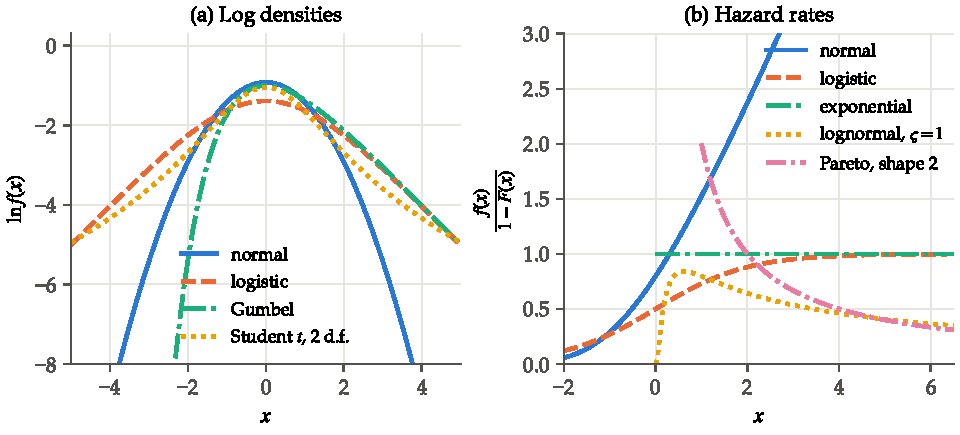
\includegraphics[width=\textwidth]{figures/appB/logconcave.pdf}
\caption{Log densities and hazard rates. Panel (a): $\ln f$ for the standard normal, standard logistic and
standard Gumbel densities, all concave, and for the Student $t$ density with two degrees of freedom, which is
convex in the tails. Panel (b): hazard rates $\frac{f(x)}{1 - F(x)}$. The normal and logistic hazards rise, the
unit exponential hazard is constant, the lognormal hazard with $\varsigma = 1$ peaks near $x = 0.62$ and then falls,
and the Pareto hazard $\frac{2}{x}$ falls.}
\label{fig:B-logconcave}
\end{figure}

\subsection{Pricing applications}\label{sec:B-lc-pricing}

\casehead{Monopoly}
Consider a single-product monopolist with constant marginal cost $c$ and differentiable demand $Q(p)$ that is
nonincreasing and positive on an interval $(c, \bar p)$, with $\bar p \leq \infty$ and $Q(p) = 0$ for $p \geq \bar p$.
Profit is $\pi(p) = (p - c)Q(p)$. Write $m(p) = -\frac{Q(p)}{Q'(p)}$ for the dollar markup that the first-order
condition supports at price $p$, the reciprocal of the semi-elasticity $-\frac{Q'}{Q}$ (\cref{ch:theory}).

\begin{proposition}[Log-concave demand and the monopoly problem]\label{prop:B-lc-monopoly}
Suppose $Q$ is log-concave on $(c, \bar p)$.
\begin{enumerate}[label=(\roman*)]
  \item Profit is log-concave on $(c, \bar p)$ and quasi-concave on $\R$, so the set of profit-maximizing prices
  is an interval.
  \item The first-order condition $p - c = m(p)$ has at most one solution in $(c, \bar p)$, and a solution is the
  global profit maximizer.
  \item Where $m$ is differentiable at the optimum, monopoly pass-through satisfies
  $\rho = \frac{1}{1 - m'(p)} \in (0, 1]$.
\end{enumerate}
If $Q$ is strictly log-concave, the maximizer is unique.
\end{proposition}

\begin{proof}
(i) On $(c, \bar p)$ profit is positive and $\ln\pi(p) = \ln(p - c) + \ln Q(p)$. Both terms are concave, so
$\ln\pi$ is concave. Outside $(c, \bar p)$ profit is nonpositive. Each upper contour set $\{p : \pi(p) \geq k\}$
with $k > 0$ is an upper contour set of the concave function $\ln\pi$, hence an interval. For $k \leq 0$ the set
contains all prices above $c$. It is an interval because profit is nondecreasing below $c$, where a higher price
shrinks both the loss per unit and the number of units sold.

(ii) Since $(\ln Q)' = \frac{Q'}{Q}$ is nonincreasing, the semi-elasticity $-\frac{Q'}{Q}$ is nondecreasing and
the markup $m(p)$ is nonincreasing where $Q' < 0$. The left side $p - c$ of the first-order condition is strictly
increasing. The two sides can cross at most once. A solution makes $(\ln\pi)'$ vanish, and a stationary point of a
concave function is a global maximizer on $(c, \bar p)$, where all positive profits are earned.

(iii) Differentiate the identity $p(c) - c = m(p(c))$ with respect to $c$:
\[
  \rho - 1 = m'(p)\rho.
\]
Solving gives $\rho = \frac{1}{1 - m'(p)}$, and $m' \leq 0$ gives $0 < \rho \leq 1$. Strict log-concavity makes $\ln\pi$
strictly concave, so the maximizer is unique.
\end{proof}

Part (iii) is the global counterpart of \cref{cor:B-passthrough-logconcave}. That corollary states that at the
monopoly price pass-through is below one if and only if $(\ln Q)'' < 0$ and above one if and only if $(\ln Q)'' > 0$. The
two statements agree because $m' = -1 + \frac{QQ''}{(Q')^2}$, so $\frac{1}{1 - m'} = \frac{1}{2 - \frac{QQ''}{(Q')^2}}$.

The proposition has a probabilistic reading. Suppose consumers have unit demand and their willingness to pay
$W$ has CDF $F_W$ and density $f_W$. Demand is $Q(p) = M[1 - F_W(p)]$ for market size $M$, and the markup is
$m(p) = \frac{1 - F_W(p)}{f_W(p)}$, the reciprocal of the hazard rate of $W$. Demand is log-concave exactly when
the survival function of $W$ is log-concave, that is, when $W$ has an increasing failure rate
(\cref{cor:B-hazard}). A log-concave density of willingness to pay suffices (\cref{prop:B-lc-cdf}). The same
object reappears as Myerson's virtual valuation in \cref{sec:B-lc-auctions}.

\casehead{Constant pass-through}
Pass-through usually varies with the level of cost. \citet{BulowPfleiderer1983} identify the demand curves for
which it does not. Let $P(q)$ be inverse demand with $P' < 0$ and curvature
$\chi(q) = -\frac{qP''(q)}{P'(q)}$, as in \eqref{eq:B-chi}. By \cref{prop:B-passthrough-monopoly}, monopoly
pass-through at output $q$ is $\rho = \frac{1}{2 - \chi(q)}$, and the second-order condition is $2 - \chi > 0$.

\begin{proposition}[Constant pass-through demands]\label{prop:B-constant-pt}
Let a monopolist with constant marginal cost face a twice continuously differentiable inverse demand with
$P' < 0$ and $2 - \chi > 0$ on an interval of outputs. Pass-through is the same at every cost in an interval of
costs if and only if inverse demand takes one of the two forms below on the corresponding interval of outputs.
\begin{enumerate}[label=(\alph*)]
  \item $P(q) = a - bq^\gamma$ with $b\gamma > 0$ and $\gamma > -1$, in which case $\rho = \frac{1}{1 + \gamma}$.
  \item $P(q) = a - b\ln q$ with $b > 0$, in which case $\rho = 1$.
\end{enumerate}
\end{proposition}

\Cref{prop:02-pt-constant} states the result in the same notation and leaves the converse as an exercise. The
proof below carries it out.

\begin{proof}
Monopoly output $q^*(c)$ is continuous and strictly decreasing, because the implicit function theorem gives
$\frac{\dd q^*}{\dd c} = \frac{1}{2P' + qP''} = \frac{1}{P'(2 - \chi)} < 0$. Hence $\rho = \frac{1}{2 - \chi(q^*(c))}$ is
constant on an interval of costs if and only if $\chi$ is constant on the image interval of outputs.

It remains to solve $qP''(q) = -\chi P'(q)$ for a constant $\chi$. Since $P' < 0$, write $-P'(q) = e^{\ell(q)}$. Then
$P'' = P'\ell'$, and the equation becomes $q\ell'(q) = -\chi$. Integrating $\ell'(q) = -\frac{\chi}{q}$ gives
$\ell(q) = -\chi\ln q + \ln K$ for a constant $K > 0$, so
\[
  P'(q) = -Kq^{-\chi}.
\]
If $\chi \neq 1$, integrate once more and set $\gamma = 1 - \chi$ and $b = \frac{K}{\gamma}$:
\[
  P(q) = a - \frac{K}{1 - \chi}q^{1 - \chi} = a - bq^\gamma,
\]
with $b\gamma = K > 0$. The second-order condition $2 - \chi > 0$ is $\gamma > -1$, and
$\rho = \frac{1}{2 - (1 - \gamma)} = \frac{1}{1 + \gamma}$. If $\chi = 1$, integrating $P' = -Kq^{-1}$ gives
$P(q) = a - K\ln q$, form (b) with $b = K$, and $\rho = \frac{1}{2 - 1} = 1$. Conversely, direct differentiation shows
that form (a) has $\chi = 1 - \gamma$ and form (b) has $\chi = 1$ at every output.
\end{proof}

The family contains the three textbook cases of \cref{ex:B-passthrough}. Linear demand is $\gamma = 1$ with
$\rho = \frac{1}{2}$. Constant-elasticity demand $P = q^{-\frac{1}{\varepsilon}}$ with $\varepsilon > 1$ is $a = 0$,
$b = -1$ and $\gamma = -\frac{1}{\varepsilon} \in (-1, 0)$, so $\rho = \frac{1}{1 - \frac{1}{\varepsilon}} = \frac{\varepsilon}{\varepsilon - 1} > 1$.
Exponential demand $Q = e^{\frac{a - p}{b}}$ is form (b) with $\rho = 1$. The family also sorts demand by
log-concavity. Since $\frac{QQ''}{(Q')^2} = \chi = 1 - \gamma$ (\cref{prop:B-passthrough-monopoly}), direct demand is strictly
log-concave when $\gamma > 0$, log-linear in form (b), and strictly log-convex when $-1 < \gamma < 0$. The ranking
of pass-through rates matches \cref{prop:B-lc-monopoly}.

\begin{example}[Power demand in prices]\label{ex:B-power-demand}
Let direct demand be $Q(p) = B(\bar p - p)^{g}$ for $p < \bar p$, with $B, g > 0$, as in \cref{tab:02-pt-examples}. Its
log is $\ln B + g\ln(\bar p - p)$, with second derivative $-\frac{g}{(\bar p - p)^2} < 0$, so demand is strictly
log-concave. Inverting $q = B(\bar p - p)^{g}$ gives
\[
  P(q) = \bar p - B^{-\frac{1}{g}}\,q^{\frac{1}{g}},
\]
which is form (a) with $a = \bar p$, $\gamma = \frac{1}{g}$ and $b = B^{-\frac{1}{g}}$. Directly, the first-order
condition $p - c = m(p)$ reads
\[
  p - c = \frac{\bar p - p}{g}.
\]
Solving gives $p = \frac{\bar p + gc}{1 + g}$, so $\rho = \frac{g}{1 + g} = \frac{1}{1 + \gamma}$, as
\cref{prop:B-constant-pt} predicts. Under a constant conduct parameter $\theta$ and flat marginal cost,
\cref{cor:B-passthrough-cases}(a) gives $\rho = \frac{1}{1 + \theta(1 - \chi)} = \frac{1}{1 + \theta\gamma} = \frac{1}{1 + \frac{\theta}{g}} = \frac{g}{g + \theta}$,
again independent of cost. This family appears in the sugar-refining application of \cref{ch:conduct}.
\end{example}

\begin{example}[Logit demand is log-concave]\label{ex:B-logit-lc}
Hold rivals' prices fixed and write single-product logit demand for product $j$ as
$s_j(p_j) = \frac{e^{\tilde\delta_j - \alpha p_j}}{\Lambda_{-j} + e^{\tilde\delta_j - \alpha p_j}}$, where $\tilde\delta_j$ is the
price-free part of mean utility and $\Lambda_{-j} = 1 + \sum_{l \neq j}e^{\delta_l}$ (\cref{sec:B-ev}).
Differentiating the log,
\[
  \frac{\dd\ln s_j}{\dd p_j} = -\alpha + \alpha s_j = -\alpha(1 - s_j),
\]
and differentiating again with $\frac{\dd s_j}{\dd p_j} = -\alpha s_j(1 - s_j)$,
\[
  \frac{\dd^2\ln s_j}{\dd p_j^2} = \alpha\frac{\dd s_j}{\dd p_j} = -\alpha^2s_j(1 - s_j) < 0.
\]
Residual demand is strictly log-concave. By \cref{prop:B-lc-monopoly}, each firm has a unique best response,
the solution of $p_j - mc_j = \frac{1}{\alpha(1 - s_j)}$ (\cref{prop:B-logit-br} gives it in closed form). Part
(iii) of the proposition puts own pass-through with rivals' prices fixed in $(0, 1]$, and
\cref{ex:B-passthrough}(iv) computes it exactly as $1 - s_j$.
\end{example}

\subsection{Aggregation and the existence of price equilibrium}\label{sec:B-caplin-nalebuff}

With several differentiated products, the existence of a pure-strategy Bertrand-Nash equilibrium requires each
firm's profit to be quasi-concave in its own price. Otherwise best responses can jump and Kakutani's theorem
fails. Demand is an aggregate over heterogeneous consumers, so the question is which primitives make aggregate
demand concave enough. \citet{CaplinNalebuff1991} answer it with \cref{thm:B-prekopa-borell}. \Cref{sec:04-cn}
proves their theorems and discusses their economic coverage. This subsection restates the argument as an
application of $\varrho$-concavity and refers to those proofs.

\casehead{Setting}
There are $J$ firms. Firm $j$ sells one product with fixed characteristics $x_j$ at constant marginal cost
$c_j$, and firms set prices simultaneously. Each consumer has income $y > 0$ and buys one unit of exactly one
product, consuming $z = y - p_j$ of a numeraire. Consumers differ by a type $\nu \in \R^L$ with density $f$ and
convex support $B$. The dimension $L$ of the type space is local to this subsection. \citet{CaplinNalebuff1991}
impose two assumptions.

\begin{assumption}[A1, preferences linear in the type]\label{ass:B-cn-a1}
Utility is $U(\nu, x, z) = \sum_{l=1}^L \nu_l t_l(x) + g(z)t_{L+1}(x) + t_{L+2}(x)$, where $t : X \to \R^{L+2}$ maps
characteristics into benefits, $g$ is strictly increasing and concave, and $t_{L+1}(x) > 0$.
\end{assumption}

\begin{assumption}[A2, concavity of the type density]\label{ass:B-cn-a2}
The density $f$ is $\varrho$-concave with $\varrho = -\frac{1}{L + 1}$, on a convex support with positive volume.
\end{assumption}

All consumers agree on the benefits $t_l(x)$ that a product delivers and differ in the weights $\nu_l$ they place on
them. By \cref{lem:B-rho-hierarchy}, every log-concave density satisfies A2. A2 also admits the multivariate
Cauchy, Pareto, F and Student $t$ distributions under restrictions on their parameters, for the Student $t$ at
least one degree of freedom \citep[Section 3, p.~6]{CaplinNalebuff1991}. A1 covers
characteristics models, quadratic transport costs, vertical differentiation, and logit, probit and random
coefficients models with a common price coefficient. It excludes Hotelling's linear transport costs, whose
demand is discontinuous.

\casehead{Demand as the probability of a set}
Fix rivals' prices $p_{-j}$. Let $\mathcal{A}_j(p_j)$ be the set of types that weakly prefer product $j$ at price
$p_j$ to every rival,
\[
  \mathcal{A}_j(p_j) = \bigl\{\nu : \Delta_k(\nu, p_j) \geq 0 \text{ for all } k \neq j\bigr\},
  \qquad \Delta_k(\nu, p_j) = U(\nu, x_j, y - p_j) - U(\nu, x_k, y - p_k)\text{.}
\]

Ties occur on hyperplanes of types when products are distinct, so they have probability zero. Demand is
\begin{equation}\label{eq:B-cn-demand}
  D_j(p_j) = \int_{\mathcal{A}_j(p_j)} f(\nu)\,\dd\nu,
\end{equation}
which is the demand function of \citet[Section 4]{CaplinNalebuff1991}, written with the set of buyers instead of
reservation prices. Given rivals' prices, firm $j$ is a monopolist facing a population of reservation prices.

\begin{lemma}[Buyer sets are Minkowski-concave]\label{lem:B-cn-minkowski}
Under A1, for any prices $p_0$, $p_1$ and $\lambda \in [0, 1]$, with $p_\lambda = \lambda p_0 + (1 - \lambda)p_1$,
\[
  \mathcal{A}_j(p_\lambda) \supseteq \lambda\mathcal{A}_j(p_0) + (1 - \lambda)\mathcal{A}_j(p_1).
\]
\end{lemma}

The proof of \cref{thm:04-cn-demand} establishes this inclusion. It averages the preference inequalities of
types $\nu_0$ and $\nu_1$, which A1 makes linear in the type, and uses concavity of $g$ for the price term.

\begin{theorem}[Aggregation, \citealp{CaplinNalebuff1991}, Section 4]\label{thm:B-cn-aggregation}
Assume A1, distinct products and a $\varrho$-concave type density with $\varrho \geq -\frac{1}{L}$. Then each firm's demand
$D_j(p_j)$ is $\varrho^*$-concave in its own price, with $\varrho^* = \frac{\varrho}{1 + L\varrho}$, on the interval of prices
where it is positive.
\end{theorem}

This is \cref{thm:04-cn-demand}. For prices $p_0$ and $p_1$ with positive demand, \cref{lem:B-cn-minkowski},
monotonicity of the integral and \cref{thm:B-prekopa-borell} give
\[
  D_j(p_\lambda) \geq \int_{\lambda\mathcal{A}_j(p_0) + (1 - \lambda)\mathcal{A}_j(p_1)} f(\nu)\,\dd\nu
  \geq \mathcal{M}_{\varrho^*}\bigl(D_j(p_0), D_j(p_1); \lambda\bigr).
\]
The bound is tight (\cref{ex:04-cn-simplex}). With types uniform on the unit simplex and reservation prices
$1 - \sum_l\nu_l$, demand is $D(p) = (1 - p)^L$, which is $\frac{1}{L}$-concave and no more.

\casehead{Quasi-concave profit}
The second step turns concavity of demand into quasi-concavity of profit.

\begin{proposition}[Convex reciprocal demand gives quasi-concave profit]\label{prop:B-cn-quasiconcave}
Let marginal cost $c$ be constant and let demand $D$ be nonincreasing, positive on an interval $(-\infty, \bar p)$
and zero above it. If $\frac{1}{D}$ is convex on $(-\infty, \bar p)$, then profit $\pi(p) = (p - c)D(p)$ is
quasi-concave.
\end{proposition}

\Cref{lem:04-recip} proves the result by contradiction, following \citet[p.~29]{CaplinNalebuff1991}. A direct
argument uses upper contour sets. For $k > 0$ and prices in $(c, \bar p)$, $\pi(p) \geq k$ holds if and only if
$p - c - \frac{k}{D(p)} \geq 0$. The left side is linear minus a convex function, hence concave, so its upper
contour set is an interval. For $k \leq 0$ the set contains every price above $c$, and profit is nondecreasing
below $c$.

For strictly decreasing, twice differentiable demand, $\frac{1}{D}$ is convex if and only if revenue $qP(q)$ is
concave in quantity (\cref{sec:04-existence-demand} gives the computation). \citet[Section 5]{CaplinNalebuff1991}
note that concave revenue is equivalent to quasi-concavity of profit for every convex cost function. The condition is therefore as weak as possible when costs are unrestricted. In the language of
\cref{def:B-rhoconcave}, $\frac{1}{D}$ convex means that $D$ is $(-1)$-concave. \Cref{thm:B-cn-aggregation}
delivers this when $\varrho^* \geq -1$. Solving $\frac{\varrho}{1 + L\varrho} = -1$ step by step,
\begin{align*}
  \varrho &= -(1 + L\varrho),\\
  \varrho(1 + L) &= -1,\\
  \varrho &= -\frac{1}{L + 1}.
\end{align*}
Because $\varrho^*$ is increasing in $\varrho$ and $-\frac{1}{L + 1} > -\frac{1}{L}$, every density that satisfies A2 yields
$\varrho^* \geq -1$, hence $(-1)$-concave demand by \cref{lem:B-rho-hierarchy}, hence quasi-concave profit. This
is why A2 has the exponent $-\frac{1}{L + 1}$. The same calculation shows why earlier work that assumed concave
demand was confined to special cases. Concave demand needs $\varrho^* = 1$, which requires $\varrho = \infty$ and
$L = 1$, a uniform distribution of types on a line \citep[Section 5]{CaplinNalebuff1991}.

\begin{theorem}[Existence, \citealp{CaplinNalebuff1991}, Section 5]\label{thm:B-cn-existence}
Under A1 and A2, for any number of firms and any products, a pure-strategy Bertrand-Nash equilibrium exists.
\end{theorem}

\Cref{thm:04-cn-existence} proves the theorem. With distinct products, it restricts each firm to prices in
$[c_j, y]$, where profits are continuous. Quasi-concavity in own price makes each best-response set an interval,
and Kakutani's theorem (\cref{thm:B-kakutani}) gives a fixed point. Equivalent products and costs above income
are handled separately.

\casehead{Uniqueness and log-supermodularity}
\citet[Section 6]{CaplinNalebuff1991} prove uniqueness under differentiability in three cases.
\begin{enumerate}[label=(\alph*)]
  \item Duopoly with a log-concave type density, in any dimension.
  \item Any number of firms in a one-dimensional market with a log-concave density, given the set of active firms.
  \item The logit model.
\end{enumerate}
The tool is the dominant-diagonal condition
$\bigl|\frac{\partial^2\pi_j}{\partial p_j^2}\bigr| > \sum_{k \neq j}\bigl|\frac{\partial^2\pi_j}{\partial p_j\,\partial p_k}\bigr|$, which
allows at most one equilibrium among a given set of active firms \citep{Friedman1977}
(\cref{prop:B-dd-uniqueness}). In all three cases the pricing game is also log-supermodular, a property
studied in \cref{sec:B-supermodular-games}.

The logit case was checked in \cref{sec:B-equilibrium}. There the log first-order conditions
$\frac{\partial\ln\pi_j}{\partial p_j} = \frac{1}{p_j - c_j} - \alpha(1 - s_j) = 0$ satisfy the dominant-diagonal condition on
the set of prices above cost. On the best response, the implicit function theorem turns the same derivatives into
the slopes $\frac{\partial BR_j}{\partial p_k} = \frac{s_js_k}{1 - s_j} > 0$, whose row sums are below one
(\cref{prop:B-logit-br-contraction}). Best responses slope up, so logit prices are strategic complements.

Log-supermodularity combined with uniqueness has strong consequences \citep{MilgromRoberts1990}. Caplin and
Nalebuff list four.
\begin{enumerate}[label=(\arabic*)]
  \item There are no other equilibria in mixed or correlated strategies.
  \item The equilibrium is globally stable under best-response dynamics, fictitious play and Bayesian learning.
  \item The game is dominance solvable.
  \item Any change that raises some firm's marginal return to price raises every firm's equilibrium price.
\end{enumerate}
A cost increase for one firm, for instance, raises all prices (\cref{ex:B-logit-cost}).

The theorem has limits. It assumes unit demand, single-product firms and fixed products. Multiproduct logit
pricing is unique by a different argument (\cref{sec:B-fixedpoint}). A random price coefficient fits A1 only
after utility is divided by it, and A2 must then hold for the distribution of the resulting ratios, which can fail
(\cref{sec:04-cn}).

Random price coefficients are often lognormal in random coefficients demand models, so the lognormal deserves a
check. \citet[Section 3, p.~6]{CaplinNalebuff1991} note that A2 survives the truncation of a density to a convex
support but not other transformations. They give the lognormal as a distribution that fails A2. The failure
depends on the dispersion. With $L = 1$, A2 requires $f^{-\frac{1}{2}}$ to be convex. Let $\ln\nu \sim N(m,
\varsigma^2)$ and write $t = \ln\nu$. Up to a positive constant, $f(\nu)^{-\frac{1}{2}} = e^{g(t)}$ with
\[
  g(t) = \frac{t}{2} + \frac{(t - m)^2}{4\varsigma^2}.
\]
Since $\frac{\dd}{\dd\nu} = \frac{1}{\nu}\frac{\dd}{\dd t}$, differentiating twice gives
\[
  \frac{\dd^2}{\dd\nu^2}e^{g(t)} = \frac{e^{g(t)}}{\nu^2}\bigl[g'(t)^2 - g'(t) + g''(t)\bigr]
  = \frac{e^{g(t)}}{\nu^2}\Bigl[\Bigl(g'(t) - \frac{1}{2}\Bigr)^2 - \frac{1}{4} + \frac{1}{2\varsigma^2}\Bigr].
\]
The derivative $g'(t) = \frac{1}{2} + \frac{t - m}{2\varsigma^2}$ takes every real value, so the bracket is nonnegative
everywhere exactly when $\frac{1}{2\varsigma^2} \geq \frac{1}{4}$, that is, when $\varsigma^2 \leq 2$. A
one-dimensional lognormal therefore satisfies A2 for moderate dispersion and fails it for large dispersion. Its
density is never log-concave (\cref{tab:B-logconcave}), so here A2 is a real gain over log-concavity.

\subsection{Auction applications}\label{sec:B-lc-auctions}

Hazard rates and reverse hazard rates are the natural objects in auction theory. The hazard rate governs the
seller's trade-off between price and probability of sale. The reverse hazard rate governs a bidder's trade-off
between the margin and the probability of winning. In this subsection a bidder's value has CDF $F$ with density
$f > 0$ on $[\underline v, \bar v]$, and the seller values the object at $v_0$.

\begin{proposition}[Myerson regularity]\label{prop:B-regular}
If the hazard rate $\frac{f}{1 - F}$ is nondecreasing, the virtual valuation
$\psi(v) = v - \frac{1 - F(v)}{f(v)}$ is strictly increasing, so $F$ is regular. A log-concave density suffices.
\end{proposition}

\begin{proof}
The term $\frac{1 - F}{f}$ is the reciprocal of a nondecreasing positive function, so it is nonincreasing. Then
$\psi$ is the sum of the strictly increasing function $v$ and the nondecreasing function $-\frac{1 - F}{f}$. A
log-concave density has a nondecreasing hazard rate by \cref{cor:B-hazard}.
\end{proof}

Regularity makes the optimal reserve price the unique solution of $r^* - \frac{1 - F(r^*)}{f(r^*)} = v_0$, because
the left side is strictly increasing \citep{Myerson1981}. For values uniform on $[0, 1]$,
$\psi(v) = v - (1 - v) = 2v - 1$ and $r^* = \frac{1 + v_0}{2}$. For exponential values with rate $\lambda$,
$\psi(v) = v - \frac{1}{\lambda}$ and $r^* = v_0 + \frac{1}{\lambda}$. The seller's problem with one bidder is the monopoly
problem of \cref{prop:B-lc-monopoly} with willingness to pay $V$ and cost $v_0$. \Cref{cor:14-optimal-reserve} in
\cref{ch:auction-theory} gives the general result.

Consider a symmetric first-price auction with independent private values and $N$ bidders. A bidder who bids $b$
must have value $\xi(b) = b + \frac{G(b)}{(N - 1)g(b)}$ \citep{GuerrePerrigneVuong2000}. Here $G$ and $g$ are the
distribution and density of equilibrium bids. \citet[Theorem 1]{GuerrePerrigneVuong2000} write $I$ for the number of
bidders. They show that an observed bid distribution is rationalized by some value distribution if and only if
bids are i.i.d.\ and $\xi$ is strictly increasing with a differentiable inverse. The second requirement is their
condition C2.

\begin{proposition}[Log-concave bids satisfy the monotonicity condition]\label{prop:B-gpv-monotone}
Let $G$ have a positive differentiable density $g$ on $[\underline b, \bar b]$. If $G$ is log-concave, then
$\xi(b) = b + \frac{G(b)}{(N - 1)g(b)}$ is strictly increasing. More generally, $\xi$ is strictly increasing if and
only if $\frac{g}{G^N}$ is strictly decreasing.
\end{proposition}

\begin{proof}
If $G$ is log-concave, the reverse hazard rate $\frac{g}{G}$ is nonincreasing (\cref{cor:B-hazard}), so
$\frac{G}{g}$ is nondecreasing. Then $\xi$ is the sum of the strictly increasing function $b$ and a nondecreasing
function. For the general statement, differentiate $\xi$ by the quotient rule:
\[
  \xi'(b) = 1 + \frac{g(b)^2 - G(b)g'(b)}{(N - 1)g(b)^2} = \frac{Ng(b)^2 - G(b)g'(b)}{(N - 1)g(b)^2}.
\]
Differentiating $\frac{g}{G^N}$ gives
\[
  \frac{\dd}{\dd b}\left(\frac{g}{G^N}\right) = \frac{g'G^N - NG^{N-1}g^2}{G^{2N}} = -\frac{Ng^2 - Gg'}{G^{N+1}}.
\]
The two derivatives have opposite signs. Hence $\xi' > 0$ exactly when $\frac{g}{G^N}$ is strictly decreasing
\citep[p.~530 and footnote 6]{GuerrePerrigneVuong2000}.
\end{proof}

Log-concavity is sufficient for condition C2 and far from necessary. A violation needs a bid density that
falls steeply relative to $G$. \citet[p.~530]{GuerrePerrigneVuong2000} give the example
$G(b) = \bigl(\frac{b}{5 - 4b}\bigr)^{\frac{1}{5}}$ on $[0, 1]$ with $N = 2$, whose density has a deep U shape. Here
$\frac{\dd\ln G}{\dd b} = \frac{1}{5}\bigl(\frac{1}{b} + \frac{4}{5 - 4b}\bigr) = \frac{1}{b(5 - 4b)}$, so
\[
  \xi(b) = b + b(5 - 4b) = 6b - 4b^2,
\]
which decreases for $b > \frac{3}{4}$. No independent private values model generates these bids. The
identification argument is developed in \cref{ch:auction-empirics}.

Reverse hazard rates also compare bidders. In an asymmetric auction, a strong bidder's value distribution $F_s$
and a weak bidder's $F_w$ are typically ranked by the reverse hazard rate. The ranking implies first-order
dominance.

\begin{proposition}[Reverse hazard rate dominance implies first-order dominance]\label{prop:B-rh-fosd}
Let $F_s$ and $F_w$ have positive densities $f_s$ and $f_w$ on a common support $[\underline v, \bar v]$. If
$\frac{f_s(v)}{F_s(v)} \geq \frac{f_w(v)}{F_w(v)}$ for all $v \in (\underline v, \bar v)$, then $F_s(v) \leq F_w(v)$ for all $v$.
\end{proposition}

\begin{proof}
Since $\frac{f}{F} = \frac{\dd}{\dd v}\ln F$, the hypothesis says
\[
  \frac{\dd}{\dd v}\ln\frac{F_s(v)}{F_w(v)} = \frac{f_s(v)}{F_s(v)} - \frac{f_w(v)}{F_w(v)} \geq 0,
\]
so the ratio $\frac{F_s}{F_w}$ is nondecreasing on $(\underline v, \bar v)$. Its limit at $\bar v$ is
$\frac{F_s(\bar v)}{F_w(\bar v)} = 1$. Hence $\frac{F_s(v)}{F_w(v)} \leq 1$, that is, $F_s(v) \leq F_w(v)$, for every
$v \in (\underline v, \bar v)$. At the endpoints both CDFs coincide.
\end{proof}

\Cref{sec:14-asym} extends the result to supports with different upper ends. The reverse hazard rate order is
the assumption under which \citet{MaskinRiley2000} sign equilibrium behavior in asymmetric first-price
auctions. The strong bidder shades its bid more, yet its bids are stochastically higher. The weak bidder sometimes
wins although its value is lower. \Cref{sec:B-stochastic-orders} places the order in the full chain of
stochastic orders.

\section{Supermodularity, monotone comparative statics and affiliation}\label{sec:B-supermod}

The implicit function theorem signs comparative statics through derivatives and second-order conditions
(\cref{prop:B-cs-optimum}). Many economic problems lack the smoothness or the concavity that this route needs.
Choices may be discrete, maximizers may jump, and profit functions may have several local peaks. Lattice
methods sign comparative statics from a single property, complementarity between the choice and the parameter,
and they extend to games and to probability. This section develops the order-theoretic tools and their uses in
oligopoly pricing, the vertical model and auctions. It ends with affiliation, the form of positive dependence that
auction theory uses.

\subsection{Lattices and supermodular functions}\label{sec:B-lattice}

We order $\R^k$ componentwise: $x \geq y$ means $x_l \geq y_l$ for every $l$. This is a \emph{partial order}, since two
vectors need not be comparable. The \emph{join} $x \vee y$ and the \emph{meet} $x \wedge y$ are the componentwise
maximum and minimum,
\[
  (x \vee y)_l = \max\{x_l, y_l\}, \qquad (x \wedge y)_l = \min\{x_l, y_l\}.
\]

\begin{definition}[Lattices]\label{def:B-lattice}
A set $X \subseteq \R^k$ is a \emph{lattice} (a sublattice of $\R^k$) if $x \vee y \in X$ and $x \wedge y \in X$ whenever
$x, y \in X$. A lattice is \emph{complete} if every nonempty subset has a supremum and an infimum in $X$.
\end{definition}

The whole space $\R^k$ and every product of intervals are lattices. A compact product of closed intervals is a
complete lattice. The set $\{x \in \R^2 : x_1 \leq x_2\}$ is a lattice, because the componentwise maximum and minimum
of two points with $x_1 \leq x_2$ inherit the inequality. The set $\{x \in \R^2 : x_1 + x_2 \leq 1\}$ is convex but not a
lattice: $(1, 0)$ and $(0, 1)$ belong to it, while their join $(1, 1)$ does not. Lattices are about order, convex
sets about averages, and the two notions are independent.

\begin{definition}[Supermodularity and increasing differences]\label{def:B-supermodular}
Let $X$ be a lattice and $A$ a partially ordered set of parameters.
\begin{enumerate}[label=(\roman*)]
  \item A function $g : X \to \R$ is \emph{supermodular} if $g(x \vee y) + g(x \wedge y) \geq g(x) + g(y)$ for all
  $x, y \in X$.
  \item A function $g : X \times A \to \R$ has \emph{increasing differences} in $(x, a)$ if, for all $x' \geq x$, the
  difference $g(x', a) - g(x, a)$ is nondecreasing in $a$. It has \emph{strictly increasing differences} if the
  difference is strictly increasing in $a$ whenever $x' > x$.
  \item A positive function $g$ is \emph{log-supermodular} if $\ln g$ is supermodular.
\end{enumerate}
\end{definition}

For two variables the two notions coincide. Take $x = (x_1', x_2)$ and $y = (x_1, x_2')$ with $x_1' \geq x_1$ and
$x_2' \geq x_2$. Then $x \vee y = (x_1', x_2')$ and $x \wedge y = (x_1, x_2)$, and supermodularity reads
\[
  g(x_1', x_2') - g(x_1, x_2') \geq g(x_1', x_2) - g(x_1, x_2),
\]
which says that the gain from raising the first variable is larger when the second is larger. Supermodularity is
the formal statement of complementarity. Ordered pairs impose nothing, because then $\{x \vee y, x \wedge y\} = \{x, y\}$.
For smooth functions on products of intervals there is a derivative test.

\begin{proposition}[Smooth test, \citealp{Topkis1978}]\label{prop:B-smooth-supermod}
Let $X = \prod_{l=1}^k I_l$ be a product of open intervals and let $g : X \to \R$ be twice continuously
differentiable. Then $g$ is supermodular if and only if $\frac{\partial^2g}{\partial x_l\,\partial x_m} \geq 0$ for all
$l \neq m$ at every point of $X$.
\end{proposition}

\begin{proof}
Suppose the cross partials are nonnegative and take $x, y \in X$. Let $z = x \wedge y$, $u = x - z \geq 0$ and
$w = y - z \geq 0$. A coordinate $l$ has $u_l > 0$ only if $x_l > y_l$, and $w_l > 0$ only if $y_l > x_l$, so $u$ and $w$
have disjoint supports. Moreover $x = z + u$, $y = z + w$ and $x \vee y = z + u + w$. We must show
\[
  g(z + u + w) - g(z + w) - g(z + u) + g(z) \geq 0\text{.}
\]
By the fundamental theorem of calculus along the segment from $z$ to $z + w$,
\[
  g(z + u + w) - g(z + w) - g(z + u) + g(z) = \int_0^1 \sum_m w_m\left[\frac{\partial g}{\partial x_m}(z + u + tw) - \frac{\partial g}{\partial x_m}(z + tw)\right]\dd t\text{.}
\]

Applying the theorem again along the segment from $z + tw$ to $z + u + tw$,
\[
  g(z + u + w) - g(z + w) - g(z + u) + g(z) = \int_0^1\!\!\int_0^1 \sum_m\sum_l w_mu_l\,\frac{\partial^2g}{\partial x_l\,\partial x_m}(z + su + tw)\,\dd s\,\dd t\text{.}
\]

Every term with $w_mu_l \neq 0$ has $l \neq m$ by disjointness, so it multiplies a nonnegative cross partial by a
nonnegative weight. The integral is nonnegative.

Conversely, suppose $g$ is supermodular and fix $l \neq m$, a point $x$, and small $\epsilon, \eta > 0$. Apply the
two-variable inequality above to coordinates $l$ and $m$ with the others held at $x$:
\[
  g(x + \epsilon e_l + \eta e_m) - g(x + \eta e_m) - g(x + \epsilon e_l) + g(x) \geq 0,
\]
where $e_l$ is the $l$-th unit vector. Divide by $\epsilon\eta$ and let $\epsilon, \eta \to 0$. By the double-integral
representation and continuity of the cross partial, the limit is $\frac{\partial^2g}{\partial x_l\,\partial x_m}(x) \geq 0$.
\end{proof}

The proposition applies to $\ln g$ as well. A positive $C^2$ function is log-supermodular if and only if
$\frac{\partial^2\ln g}{\partial x_l\,\partial x_m} \geq 0$ for $l \neq m$. Products of log-supermodular functions are
log-supermodular, because logs add. The same test applied to a function of $(x, a)$ with $x$ and $a$ scalars shows
that a $C^2$ function has increasing differences if and only if $\frac{\partial^2g}{\partial x\,\partial a} \geq 0$.

\subsection{Monotone comparative statics}\label{sec:B-topkis}

To compare sets of maximizers we need an order on sets.

\begin{definition}[Strong set order]\label{def:B-sso}
For subsets $S, S'$ of a lattice, $S'$ is higher than $S$ in the \emph{strong set order}, written $S' \geq_S S$, if
$x \vee x' \in S'$ and $x \wedge x' \in S$ for all $x \in S$ and $x' \in S'$.
\end{definition}

For compact intervals of $\R$, $S' \geq_S S$ means that $\max S' \geq \max S$ and $\min S' \geq \min S$. For general
compact subsets of $\R$ these inequalities are necessary but not sufficient. The sets $S = \{0, 2\}$ and $S' = \{1, 3\}$
satisfy both, yet $2 \vee 1 = 2 \notin S'$. For singletons it means $x' \geq x$.

\begin{theorem}[Topkis]\label{thm:B-topkis}
Let $X$ be a lattice, $A$ a partially ordered set, and $g : X \times A \to \R$ supermodular in $x$ for each $a$ and with
increasing differences in $(x, a)$. Let $M(a) = \argmax_{x \in X}g(x, a)$. If $a' \geq a$, then $M(a') \geq_S M(a)$. In
particular, the largest and smallest maximizers, when they exist, are nondecreasing in $a$ \citep{Topkis1978}.
\end{theorem}

\begin{proof}
Let $a' \geq a$, $x \in M(a)$ and $x' \in M(a')$. Both $x \vee x'$ and $x \wedge x'$ lie in $X$. Optimality of $x'$ at $a'$
and of $x$ at $a$ gives
\begin{align}
  g(x', a') &\geq g(x \vee x', a'), \label{eq:B-topkis-1}\\
  g(x, a) &\geq g(x \wedge x', a). \label{eq:B-topkis-2}
\end{align}
Supermodularity in $x$ at $a$, rearranged, and then \eqref{eq:B-topkis-2} give
\begin{equation}\label{eq:B-topkis-3}
  g(x \vee x', a) - g(x', a) \geq g(x, a) - g(x \wedge x', a) \geq 0.
\end{equation}
Since $x \vee x' \geq x'$ and $a' \geq a$, increasing differences give
\begin{equation}\label{eq:B-topkis-4}
  g(x \vee x', a') - g(x', a') \geq g(x \vee x', a) - g(x', a).
\end{equation}
Chaining \eqref{eq:B-topkis-4} and \eqref{eq:B-topkis-3}, $g(x \vee x', a') \geq g(x', a')$. With
\eqref{eq:B-topkis-1} this holds with equality, so $x \vee x' \in M(a')$. The left side of \eqref{eq:B-topkis-4} is
then zero, so every term in the chain is zero. In particular $g(x, a) = g(x \wedge x', a)$, and $x \wedge x' \in M(a)$.
\end{proof}

With strictly increasing differences and a scalar choice, every selection from the argmax is nondecreasing. To
see this, suppose $a' > a$, $x \in M(a)$, $x' \in M(a')$ and $x > x'$. Strictly increasing differences and optimality of $x$
at $a$ give $g(x, a') - g(x', a') > g(x, a) - g(x', a) \geq 0$, which contradicts optimality of $x'$ at $a'$.

Compare the theorem with \cref{prop:B-cs-optimum}. The implicit function theorem gives
$\frac{\dd x^*}{\dd a} = -\frac{g_{xa}}{g_{xx}}$, whose sign is that of $g_{xa}$ under a strict second-order condition.
Topkis's theorem reaches the qualitative conclusion from $g_{xa} \geq 0$ alone. It needs no concavity, no
differentiability in $x$, no interior solution and no uniqueness, and the choice set may be discrete. It is silent
on magnitudes, which still require derivatives.

The conditions of \cref{thm:B-topkis} are cardinal: a monotone transformation of $g$ can destroy increasing
differences without changing any argmax. \citet{MilgromShannon1994} found the ordinal conditions. A function
$g : X \to \R$ is \emph{quasi-supermodular} if $g(x) \geq g(x \wedge y)$ implies $g(x \vee y) \geq g(y)$, and the same holds
with strict inequalities. A function $g(x, a)$ satisfies the \emph{single crossing property} in $(x, a)$ if, for
$x' > x$ and $a' > a$, $g(x', a) \geq g(x, a)$ implies $g(x', a') \geq g(x, a')$, and $g(x', a) > g(x, a)$ implies
$g(x', a') > g(x, a')$. A gain from a higher choice at a low parameter persists at a higher parameter.

\begin{theorem}[\citealp{MilgromShannon1994}]\label{thm:B-milgrom-shannon}
Let $X$ be a lattice and $g : X \times A \to \R$. The following statements are equivalent.
\begin{enumerate}[label=(\alph*)]
  \item The set $\argmax_{x \in S}g(x, a)$ is nondecreasing in $(a, S)$ in the strong set order, over all sublattices
  $S \subseteq X$.
  \item The function $g$ is quasi-supermodular in $x$ and satisfies the single crossing property in $(x, a)$.
\end{enumerate}
\end{theorem}

Both conditions are preserved by strictly increasing transformations of $g$. A positive log-supermodular
function satisfies them. Indeed, if $\ln g$ has increasing differences, the ratio $\frac{g(x', a)}{g(x, a)}$ is
nondecreasing in $a$ for $x' \geq x$. If it is at least one at $a$, it is at least one at $a' > a$, which is single
crossing. This is why log-supermodularity, a cardinal condition on $\ln g$, has ordinal consequences for $g$.

\begin{example}[Monopoly price rises with cost for any demand]\label{ex:B-topkis-monopoly}
Let demand $Q(p)$ be any nonincreasing function on a price set $X = [0, \bar p]$, and let profit be
$\pi(p, c) = (p - c)Q(p)$. For $p' > p$,
\[
  \pi(p', c) - \pi(p, c) = p'Q(p') - pQ(p) - c\bigl[Q(p') - Q(p)\bigr].
\]
The bracket is nonpositive, so the difference is nondecreasing in $c$. Profit has increasing differences in
$(p, c)$, and by \cref{thm:B-topkis} the largest and smallest optimal prices are nondecreasing in marginal cost.
If $Q$ is strictly decreasing the differences are strictly increasing, and every selection of optimal prices is
nondecreasing. No curvature, concavity, continuity or differentiability of demand is used. On prices above cost,
the same conclusion follows from log-supermodularity, since
$\frac{\partial^2}{\partial p\,\partial c}\ln[(p - c)Q(p)] = \frac{\partial^2}{\partial p\,\partial c}\ln(p - c) = \frac{1}{(p - c)^2} > 0$.
The direction of pass-through is thus a free result, while its size, $\rho = \frac{1}{2 - \chi}$, depends on demand
curvature (\cref{sec:B-passthrough}).
\end{example}

\begin{example}[Sorting in the vertical model]\label{ex:B-vertical-sorting}
In the vertical model consumer $i$ obtains $u_{ij} = \delta_j - \nu_ip_j$ from product $j$, with $\nu_i > 0$ the price
sensitivity and the outside good at $\delta_0 = p_0 = 0$ (\cref{sec:06-vertical}). Index the products with positive
sales by price, $0 = p_0 < p_1 < \dots < p_J$, so that qualities rise in the same order. For $k > j$,
\[
  u_{ij} - u_{ik} = (\delta_j - \delta_k) + \nu_i(p_k - p_j),
\]
which is strictly increasing in $\nu_i$. This is the \emph{single crossing property} of the vertical model. As
functions of $\nu$, the utility lines of two products cross at most once, and the cheaper product wins for the
more price-sensitive consumers. In lattice terms, $u(j, \nu) = \delta_j - \nu p_j$ has strictly decreasing differences
in $(j, \nu)$, so by \cref{thm:B-topkis} applied with $-\nu$ as the parameter, the chosen product is nonincreasing in $\nu$.

Single crossing also explains why a consumer need compare product $j$ only with its two neighbors. Let
$\bar\nu_j = \frac{\delta_j - \delta_{j-1}}{p_j - p_{j-1}}$ be the type indifferent between $j - 1$ and $j$, and suppose the cutoffs
are strictly decreasing, $\bar\nu_1 > \bar\nu_2 > \dots > \bar\nu_J > 0$, as they are when every product sells. A
consumer prefers $j$ to $j + 1$ if and only if $\nu_i > \bar\nu_{j+1}$, and $j$ to $j - 1$ if and only if
$\nu_i < \bar\nu_j$. Suppose both hold. Then $\nu_i > \bar\nu_{j+1} > \bar\nu_{j+2}$, so she also prefers $j + 1$ to $j + 2$.
Transitivity gives $j \succ j + 2$, and induction on $k$ gives $j \succ k$ for all $k > j$. Symmetrically,
$\nu_i < \bar\nu_j < \bar\nu_{j-1}$ gives $j - 1 \succ j - 2$, hence $j \succ j - 2$ and, by induction, $j \succ k$ for all $k < j$.
With the conventions $\bar\nu_0 = \infty$ and $\bar\nu_{J+1} = 0$, the consumer chooses $j$ exactly when
$\bar\nu_{j+1} < \nu_i < \bar\nu_j$.
\end{example}

\begin{example}[Cournot best responses without concavity]\label{ex:B-cournot-topkis}
In a homogeneous-good Cournot market, firm $i$'s profit is $\pi_i(q_i, Q_{-i}) = q_iP(q_i + Q_{-i}) - C_i(q_i)$, where
$Q_{-i}$ is rivals' total output. \Cref{ex:B-cournot-br} computed the slope of the best response by the implicit
function theorem, under a strict second-order condition. The lattice argument needs only the cross partial,
\[
  \frac{\partial^2\pi_i}{\partial q_i\,\partial Q_{-i}} = P'(Q) + q_iP''(Q).
\]
If $P' + q_iP'' \leq 0$ on the relevant domain, profit has decreasing differences in $(q_i, Q_{-i})$, which are
increasing differences in $(q_i, -Q_{-i})$. By \cref{thm:B-topkis}, the extremal best responses are nonincreasing in
rivals' output. Neither concavity of profit in $q_i$ nor convexity of cost is needed, and the best response may be a
correspondence. \Cref{sec:B-strategic} shows that the sign of $P' + q_iP''$ can reverse.
\end{example}

\subsection{Strategic substitutes and complements}\label{sec:B-strategic}

\citet{BulowGeanakoplosKlemperer1985} sort competition by the sign of a single cross partial. Orient each
firm's strategic variable so that a higher value is more aggressive: quantities, advertising, or the negative of
a price.

\begin{definition}[Strategic substitutes and complements]\label{def:B-strategic}
Firm $B$ regards the products as \emph{strategic substitutes} if a more aggressive action by firm $A$ lowers $B$'s
marginal profit, that is, $\frac{\partial^2\pi_B}{\partial S_B\,\partial S_A} < 0$. It regards them as \emph{strategic
complements} if the cross partial is positive \citep[p.~494]{BulowGeanakoplosKlemperer1985}.
\end{definition}

The definition concerns marginal profit. Ordinary substitutes and complements concern the level of profit, the
sign of $\frac{\partial\pi_B}{\partial S_A}$. Under strict concavity in own action, the implicit function theorem gives
the slope of $B$'s best response (reaction function) $BR_B$,
\[
  \frac{\dd BR_B}{\dd S_A} = -\left(\frac{\partial^2\pi_B}{\partial S_B^2}\right)^{-1}\frac{\partial^2\pi_B}{\partial S_B\,\partial S_A}\text{.}
\]
Reaction curves therefore slope down under strategic substitutes and up under strategic complements. When prices are
the strategic variables, $S = -p$ and $\frac{\partial^2\pi_B}{\partial(-p_B)\,\partial(-p_A)} = \frac{\partial^2\pi_B}{\partial p_B\,\partial p_A}$, so
prices are strategic complements when $\frac{\partial^2\pi_B}{\partial p_B\,\partial p_A} > 0$.

\begin{example}[Multimarket contact and the sign of the strategic effect]\label{ex:B-bgk}
\citet[pp.~492--495]{BulowGeanakoplosKlemperer1985} study a firm $A$ that is a monopolist in market 1 and a duopolist
with firm $B$ in market 2. The strategic variables are $S_1^A$, $S_2^A$ and $S_2^B$. A shock $Z$ raises $A$'s marginal
profit in market 1, so $\pi^A = R_1^A(S_1^A) + R_2^A(S_2^A, S_2^B) - C^A(S_1^A, S_2^A) + ZS_1^A$ and
$\pi^B = R_2^B(S_2^A, S_2^B) - C^B(S_2^B)$, where $R_i^F$ is firm $F$'s revenue in market $i$ and $C^F$ its cost.
Shared costs make the markets interdependent. There are \emph{joint
economies} if $\frac{\partial^2\pi^A}{\partial S_1^A\,\partial S_2^A} > 0$ and joint diseconomies if it is negative. Write
$a_{11}$, $a_{12}$, $a_{22}$ and $a_{23}$ for the second partials of $\pi^A$ with respect to $(S_1^A, S_1^A)$,
$(S_1^A, S_2^A)$, $(S_2^A, S_2^A)$ and $(S_2^A, S_2^B)$. Write $b_{32}$ and $b_{33}$ for the second partials of $\pi^B$
with respect to $(S_2^B, S_2^A)$ and $(S_2^B, S_2^B)$. Totally differentiating the three first-order conditions gives their system
(7),
\[
  \begin{pmatrix} a_{11} & a_{12} & 0\\ a_{12} & a_{22} & a_{23}\\ 0 & b_{32} & b_{33}\end{pmatrix}
  \begin{pmatrix} \dd S_1^A\\ \dd S_2^A\\ \dd S_2^B\end{pmatrix}
  = \begin{pmatrix} -\dd Z\\ 0\\ 0\end{pmatrix}.
\]
The zero in the first row holds because $S_2^B$ affects $\pi^A$ only through market 2. Stability requires
$b_{33} < 0$, $a_{22}b_{33} > a_{23}b_{32}$ (market 2 is stable on its own) and a negative determinant. We solve from the
bottom. The third row gives $\dd S_2^B = -\frac{b_{32}}{b_{33}}\dd S_2^A$. Substituting into the second row,
\[
  a_{12}\,\dd S_1^A + k\,\dd S_2^A = 0, \qquad k \equiv a_{22} - \frac{a_{23}b_{32}}{b_{33}} = \frac{a_{22}b_{33} - a_{23}b_{32}}{b_{33}} < 0.
\]
Substituting $\dd S_2^A = -\frac{a_{12}}{k}\dd S_1^A$ into the first row gives
$\bigl(a_{11} - \frac{a_{12}^2}{k}\bigr)\dd S_1^A = -\dd Z$. The determinant equals $b_{33}(a_{11}k - a_{12}^2)$, which is
negative, so $a_{11}k - a_{12}^2 > 0$ and $a_{11} - \frac{a_{12}^2}{k} < 0$. Three results follow.
\begin{enumerate}[label=(\arabic*)]
  \item $\frac{\dd S_1^A}{\dd Z} > 0$: $A$ is more aggressive in the market whose profitability rose.
  \item $\operatorname{sign}\frac{\dd S_2^A}{\dd Z} = \operatorname{sign}(a_{12})$: with joint economies $A$ also becomes more
  aggressive in market 2.
  \item $\operatorname{sign}\frac{\dd S_2^B}{\dd Z} = \operatorname{sign}(a_{12})\cdot\operatorname{sign}(b_{32})$: $B$'s response depends on the
  joint economies and on whether $B$ regards the products as strategic substitutes or complements.
\end{enumerate}
By the envelope theorem (\cref{thm:B-envelope}), $\frac{\dd\pi^A}{\dd Z} = S_1^A + \frac{\partial\pi^A}{\partial S_2^B}\frac{\dd S_2^B}{\dd Z}$.
The second term is the \emph{strategic effect}. With ordinary substitutes, $\frac{\partial\pi^A}{\partial S_2^B} < 0$, its sign is
$-\operatorname{sign}(a_{12})\operatorname{sign}(b_{32})$. It is positive under joint economies with strategic substitutes or joint
diseconomies with strategic complements, and negative in the other two cases, as in their table on p.~495.
The same favorable shock can hurt a firm through its rival's response.
\end{example}

\begin{example}[Three oligopoly games]\label{ex:B-strategic-examples}
\leavevmode
\begin{enumerate}[label=(\alph*)]
  \item \emph{Cournot with linear demand.} With $P(Q) = a_0 - Q$, $P' + q_iP'' = -1 < 0$, so quantities are strategic
  substitutes everywhere.
  \item \emph{Cournot with constant-elasticity demand.} Let $P(Q) = Q^{-\frac{1}{\varepsilon}}$ with $\varepsilon > 0$. Then
  $P'(Q) = -\frac{1}{\varepsilon}Q^{-\frac{1}{\varepsilon} - 1}$ and $\frac{P''(Q)}{P'(Q)} = -\frac{1 + \frac{1}{\varepsilon}}{Q} = -\frac{1 + \varepsilon}{\varepsilon Q}$.
  With the share $s_i = \frac{q_i}{Q}$,
  \[
    P' + q_iP'' = P'\left[1 + q_i\frac{P''}{P'}\right] = P'\left[1 - \frac{1 + \varepsilon}{\varepsilon}s_i\right].
  \]
  Since $P' < 0$, the cross partial is positive, and firm $i$ treats quantities as strategic complements, exactly
  when $s_i > \frac{\varepsilon}{1 + \varepsilon}$. A firm with a small share regards rival output as a strategic
  substitute, while a firm with a large share regards it as a complement, as
  \citet[p.~494]{BulowGeanakoplosKlemperer1985} note.
  \item \emph{Logit Bertrand.} With single-product logit demand, $\ln\pi_j = \ln(p_j - mc_j) + \ln s_j(p)$ and
  \[
    \frac{\partial\ln\pi_j}{\partial p_j} = \frac{1}{p_j - mc_j} - \alpha(1 - s_j),
    \qquad
    \frac{\partial^2\ln\pi_j}{\partial p_j\,\partial p_k} = \alpha\frac{\partial s_j}{\partial p_k} = \alpha^2s_js_k > 0.
  \]
  Log profit has increasing differences in every pair of prices, so the logit pricing game is log-supermodular
  everywhere, and prices are strategic complements.
\end{enumerate}
Strategic complementarity among the prices of close substitutes is one reason a merger can raise the prices of
non-merging rivals. The MillerCoors joint venture of June 2008 tests how far this reason goes. Soon after it was
cleared, the prices of Miller Lite, Coors Light and Bud Light rose by about 8 percent. The prices of Corona Extra
and Heineken showed little persistent change \citep[pp.~241--242]{AskerNocke2021}. Unilateral effects could
produce this pattern only with extreme strategic complementarity between Bud Light and the MillerCoors brands,
together with weak substitution toward imports. \citet[p.~242]{AskerNocke2021} judge that combination unlikely.
\citet{MillerWeinberg2017} estimate a random coefficients nested logit demand and add a coordination parameter to
the ownership matrix of the pricing first-order conditions. Its estimate rejects unilateral Bertrand pricing, and
the coordinated-effects model fits the observed price paths \citep[p.~242 and fn.~164]{AskerNocke2021}. The
chapter on mergers develops the case (\cref{ch:mergers}).
\end{example}

\Cref{fig:B-reaction} contrasts the two cases. In the Cournot game, a cost reduction for firm 1 shifts its
reaction curve out, and the rival responds by producing less. In the Bertrand game with differentiated products,
a cost increase for firm 1 shifts its reaction curve out, and the rival responds by raising its price too.

Panel (b) uses the linear demand example of \citet[Section~11.2]{Tirole1988}. Firm $i$ sells
$q_i = 1 - bp_i + dp_j$ with $0 < d < b$, at constant unit cost $c$. Its profit $(p_i - c)(1 - bp_i + dp_j)$ is
concave in $p_i$, and the first-order condition is
\[
  1 + dp_j + bc - 2bp_i = 0, \qquad\text{so}\qquad BR_i(p_j) = \frac{1 + bc + dp_j}{2b}.
\]
The slope $\frac{d}{2b}$ is positive, so prices are strategic complements. It is below one half, so the
reaction curves cross once. Setting $p_i = p_j = p$ gives $2bp = 1 + bc + dp$, and the unique equilibrium is
symmetric,
\[
  p = \frac{1 + bc}{2b - d}.
\]
With $b = 1$, $d = \frac{1}{2}$ and $c = 0$, the best response is $\frac{1}{2} + \frac{1}{4}p_j$ and the equilibrium
price is $\frac{1}{2 - \frac{1}{2}} = \frac{2}{3}$, the point $N$ in the figure.

\begin{figure}[htbp]
\centering
\begin{subfigure}[t]{0.48\textwidth}
\centering
\begin{tikzpicture}
\begin{axis}[
  width=6.6cm, height=6.6cm,
  xmin=0, xmax=1.12, ymin=0, ymax=1.32,
  axis lines=left,
  xlabel={$q_1$}, ylabel={$q_2$},
  xtick={0.5,0.625,1}, xticklabels={$\frac{1}{2}$,$\frac{5}{8}$,$1$},
  ytick={0.5,1,1.25}, yticklabels={$\frac{1}{2}$,$1$,$\frac{5}{4}$},
  tick label style={font=\scriptsize}, label style={font=\small},
  clip=false]
  \addplot[blue!70!black, thick, domain=0:0.5, samples=2] {1-2*x};
  \addplot[blue!70!black, thick, dashed, domain=0:0.625, samples=2] {1.25-2*x};
  \addplot[orange!85!black, thick, domain=0:1, samples=2] {(1-x)/2};
  \addplot[only marks, mark=*, mark size=1.6pt] coordinates {(0.3333,0.3333) (0.5,0.25)};
  \node[font=\scriptsize, anchor=south west] at (axis cs:0.34,0.34) {$N$};
  \node[font=\scriptsize, anchor=south west] at (axis cs:0.5,0.26) {$N'$};
  \node[font=\scriptsize, anchor=east, blue!70!black] at (axis cs:0.44,0.07) {$BR_1$};
  \node[font=\scriptsize, anchor=west, blue!70!black] at (axis cs:0.33,0.62) {$BR_1'$};
  \node[font=\scriptsize, anchor=south, orange!85!black] at (axis cs:0.9,0.06) {$BR_2$};
\end{axis}
\end{tikzpicture}
\caption{Cournot: strategic substitutes}
\end{subfigure}\hfill
\begin{subfigure}[t]{0.48\textwidth}
\centering
\begin{tikzpicture}
\begin{axis}[
  width=6.6cm, height=6.6cm,
  xmin=0, xmax=1.2, ymin=0, ymax=1.2,
  axis lines=left,
  xlabel={$p_1$}, ylabel={$p_2$},
  xtick={0.5,0.75}, xticklabels={$\frac{1}{2}$,$\frac{3}{4}$},
  ytick={0.5}, yticklabels={$\frac{1}{2}$},
  tick label style={font=\scriptsize}, label style={font=\small},
  clip=false]
  \addplot[blue!70!black, thick, domain=0.5:0.8, samples=2] {4*(x-0.5)};
  \addplot[blue!70!black, thick, dashed, domain=0.75:1.05, samples=2] {4*(x-0.75)};
  \addplot[orange!85!black, thick, domain=0:1.2, samples=2] {0.5+x/4};
  \addplot[only marks, mark=*, mark size=1.6pt] coordinates {(0.6667,0.6667) (0.9333,0.7333)};
  \node[font=\scriptsize, anchor=east] at (axis cs:0.66,0.70) {$N$};
  \node[font=\scriptsize, anchor=north west] at (axis cs:0.94,0.72) {$N'$};
  \node[font=\scriptsize, anchor=east, blue!70!black] at (axis cs:0.79,1.12) {$BR_1$};
  \node[font=\scriptsize, anchor=west, blue!70!black] at (axis cs:1.05,1.12) {$BR_1'$};
  \node[font=\scriptsize, anchor=south, orange!85!black] at (axis cs:0.25,0.57) {$BR_2$};
\end{axis}
\end{tikzpicture}
\caption{Differentiated Bertrand: strategic complements}
\end{subfigure}
\caption{Reaction curves under strategic substitutes and complements. Panel (a): Cournot duopoly with inverse
demand $P = a_0 - Q$ and $a_0 - c = 1$, so $BR_i(q_j) = \frac{1 - q_j}{2}$ and the equilibrium is
$N = (\frac{1}{3}, \frac{1}{3})$. A cost reduction of $\frac{1}{4}$ for firm 1 shifts its curve to
$BR_1'(q_2) = \frac{5}{8} - \frac{q_2}{2}$, and the new equilibrium is $N' = (\frac{1}{2}, \frac{1}{4})$: firm 2
contracts. Panel (b): the demand of \citet[Section~11.2]{Tirole1988} with $b = 1$ and $d = \frac{1}{2}$,
$q_i = 1 - p_i + \frac{1}{2}p_j$, with zero cost, so
$BR_i(p_j) = \frac{1}{2} + \frac{1}{4}p_j$ and $N = (\frac{2}{3}, \frac{2}{3})$. Raising firm 1's cost to $\frac{1}{2}$ shifts
its curve to $BR_1'(p_2) = \frac{3}{4} + \frac{1}{4}p_2$, and the new equilibrium is
$N' = (\frac{14}{15}, \frac{11}{15})$: both prices rise.}
\label{fig:B-reaction}
\end{figure}

\subsection{Supermodular games}\label{sec:B-supermodular-games}

Games with strategic complements have a lattice structure that delivers existence, computation and comparative
statics with no concavity and no differentiability. The fixed-point theorem behind them is due to Tarski.

\begin{theorem}[Tarski]\label{thm:B-tarski}
Let $\mathcal{X}$ be a complete lattice and $T : \mathcal{X} \to \mathcal{X}$ a nondecreasing map, that is, $x \leq x'$ implies
$T(x) \leq T(x')$. Then $T$ has a fixed point. Its largest fixed point is $\sup\{x \in \mathcal{X} : x \leq T(x)\}$, and the set
of fixed points is itself a complete lattice \citep{Tarski1955}.
\end{theorem}

\begin{proof}[Proof of existence]
Let $\mathcal{S} = \{x \in \mathcal{X} : x \leq T(x)\}$. It is nonempty because it contains $\inf\mathcal{X}$. Let
$\bar x = \sup\mathcal{S}$. For any $x \in \mathcal{S}$, $x \leq \bar x$, so $x \leq T(x) \leq T(\bar x)$. Thus $T(\bar x)$ is an
upper bound of $\mathcal{S}$, and $\bar x \leq T(\bar x)$. Applying $T$ gives $T(\bar x) \leq T(T(\bar x))$, so
$T(\bar x) \in \mathcal{S}$ and $T(\bar x) \leq \bar x$. Hence $T(\bar x) = \bar x$. Every fixed point lies in $\mathcal{S}$,
so $\bar x$ is the largest.
\end{proof}

Unlike Brouwer's and Kakutani's theorems, Tarski's theorem needs no continuity and no convexity. Monotonicity
does all the work.

\begin{definition}[Supermodular game]\label{def:B-smgame}
A game with players $i = 1, \dots, N$, strategy sets $X_i$ and payoffs $u_i(x_i, x_{-i})$ is \emph{supermodular} if
three conditions hold. Each $X_i$ is a compact product of intervals in some $\R^{k_i}$. Each $u_i$ is upper
semicontinuous in $x_i$ and continuous in $x_{-i}$. Each $u_i$ is supermodular in $x_i$ and has increasing differences
in $(x_i, x_{-i})$.
\end{definition}

Supermodularity in own strategy is automatic when each $x_i$ is a scalar. Increasing differences in
$(x_i, x_{-i})$ is strategic complementarity.

\begin{theorem}[Supermodular games]\label{thm:B-smgames}
In a supermodular game the following hold.
\begin{enumerate}[label=(\roman*)]
  \item The set of pure-strategy Nash equilibria is nonempty. It has a largest element $\bar x$ and a smallest
  element $\underline x$.
  \item Best-response iteration from the largest strategy profile, choosing the largest best response at each
  step, decreases monotonically to $\bar x$. Iteration from the smallest profile increases to $\underline x$.
  \item Suppose each $u_i(x_i, x_{-i}; a)$ has increasing differences in $(x_i, a)$ for a parameter $a$. Then $\bar x(a)$
  and $\underline x(a)$ are nondecreasing in $a$.
  \item Every strategy that survives iterated elimination of strictly dominated strategies lies between
  $\underline x$ and $\bar x$. A game with a unique equilibrium is therefore dominance solvable, and adaptive dynamics
  converge to it.
\end{enumerate}
\end{theorem}

\begin{proof}[Proof sketch]
(i) By \cref{thm:B-topkis}, applied with $x_{-i}$ as the parameter, player $i$'s set of best responses has a largest
element $\bar b_i(x_{-i})$, nondecreasing in $x_{-i}$. Upper semicontinuity and compactness ensure the set is
nonempty and has a largest element. The map $\bar b = (\bar b_1, \dots, \bar b_N)$ is a nondecreasing self-map of the
complete lattice $\prod_iX_i$. By \cref{thm:B-tarski} it has a largest fixed point $\bar x$, which is an equilibrium. If
$x^*$ is any equilibrium, then $x_i^* \leq \bar b_i(x_{-i}^*)$ for every $i$, so $x^* \leq \bar b(x^*)$ and $x^* \leq \bar x$ by the
characterization in \cref{thm:B-tarski}. The smallest equilibrium is symmetric.

(ii) Let $x^{(0)} = \sup\prod_iX_i$ and $x^{(h+1)} = \bar b(x^{(h)})$. Trivially $x^{(1)} \leq x^{(0)}$, and monotonicity of
$\bar b$ gives $x^{(h+1)} \leq x^{(h)}$ by induction. Similarly $\bar x \leq x^{(0)}$ implies $\bar x = \bar b(\bar x) \leq x^{(h)}$
for all $h$. The decreasing sequence converges, and continuity of payoffs makes its limit an equilibrium. The
limit is at least $\bar x$, so it equals $\bar x$.

(iii) If $a' \geq a$, then $\bar b(x; a') \geq \bar b(x; a)$ for every $x$ by \cref{thm:B-topkis}. Any $x$ with $x \leq \bar b(x; a)$
then satisfies $x \leq \bar b(x; a')$. The set whose supremum defines the largest fixed point grows with $a$, so its
supremum rises. Part (iv) is due to \citet{MilgromRoberts1990}.
\end{proof}

The results are due to \citet{Topkis1979}, \citet{Vives1990} and \citet{MilgromRoberts1990}, and \citet{Vives1999}
develops the oligopoly applications. When payoffs are positive, the theorem applies to a game with
log-supermodular payoffs after replacing $u_i$ by $\ln u_i$, because the transformation leaves best responses unchanged.

\begin{example}[A cost increase raises all logit prices]\label{ex:B-logit-cost}
Consider the single-product logit pricing game, and fix an interval of firm 1's costs
$[\underline{mc}_1, \overline{mc}_1]$ of length below $\frac{1}{\alpha}$. Every best response carries a markup
$\frac{1 + W_0(z_j)}{\alpha} > \frac{1}{\alpha}$ (\cref{prop:B-logit-br}). Since $\Lambda_{-j} \geq 1$, we have
$z_j \leq e^{v_j - 1}$, so best responses are also bounded above, uniformly over the interval of costs. Let $\bar p$
be such a bound. We restrict firm 1 to $[\underline{mc}_1 + \frac{1}{\alpha}, \bar p]$ and each firm $j \neq 1$ to
$[mc_j + \frac{1}{\alpha}, \bar p]$. These sets contain every best response, so the restriction leaves the equilibria
unchanged. The sets do not move with $mc_1$. On them every price exceeds marginal cost, so profits are positive and
log profits are finite. By \cref{ex:B-strategic-examples}(c), log profits have increasing differences in every pair of
prices. With firm 1's marginal cost as the parameter,
\[
  \frac{\partial^2\ln\pi_1}{\partial p_1\,\partial mc_1} = \frac{\partial}{\partial mc_1}\left[\frac{1}{p_1 - mc_1}\right] = \frac{1}{(p_1 - mc_1)^2} > 0,
\]
while the log profits of the other firms do not depend on $mc_1$. By \cref{thm:B-smgames}(iii) the extremal
equilibria are nondecreasing in $mc_1$ on the interval. Any two costs are linked by a chain of overlapping intervals
of this kind, so the conclusion holds for any two costs. The equilibrium is unique (\cref{sec:B-caplin-nalebuff}), so every firm's
equilibrium price is nondecreasing in firm 1's cost. This is the last property in Caplin and Nalebuff's list.
\end{example}

Two further applications follow the same pattern. First, a merger of two price-setting firms with substitute
products adds the partner's profit to each merging firm's objective. With weight $a \in [0, 1]$ on the partner's
profit, the objective $\pi_1 + a\pi_2$ has $\frac{\partial^2(\pi_1 + a\pi_2)}{\partial p_1\,\partial a} = \frac{\partial\pi_2}{\partial p_1} = (p_2 - mc_2)\frac{\partial q_2}{\partial p_1} \geq 0$
whenever $p_2 \geq mc_2$. When the post-merger game remains supermodular, as with linear demand, all equilibrium
prices rise, the merging firms' and the outsiders' alike \citep{DeneckereDavidson1985}. \Cref{ch:mergers} develops
merger simulation. Second, with strategic complements a firm's best deviation from a collusive price profile
lies above the static Nash price, because best responses slope up. The slope of best responses therefore
governs the gain from deviating (\cref{ch:collusion-theory}).

\subsection{Stochastic orders}\label{sec:B-stochastic-orders}

Probability brings its own orders. Let $X_A$ and $X_B$ have CDFs $F_A$ and $F_B$ with densities $f_A$ and $f_B$ that are
positive on a common support $(\underline x, \bar x)$.

\begin{definition}[Stochastic orders]\label{def:B-orders}
\leavevmode
\begin{enumerate}[label=(\roman*)]
  \item $X_B$ dominates $X_A$ in the \emph{first-order stochastic dominance} order, $X_B \geq_{\mathrm{FOSD}} X_A$, if
  $F_B(x) \leq F_A(x)$ for all $x$.
  \item $X_B \geq_{\mathrm{hr}} X_A$ in the \emph{hazard rate order} if $\frac{f_B(x)}{1 - F_B(x)} \leq \frac{f_A(x)}{1 - F_A(x)}$
  for all $x$.
  \item $X_B \geq_{\mathrm{rh}} X_A$ in the \emph{reverse hazard rate order} if $\frac{f_B(x)}{F_B(x)} \geq \frac{f_A(x)}{F_A(x)}$
  for all $x$.
  \item $X_B \geq_{\mathrm{lr}} X_A$ in the \emph{likelihood ratio order} if $\frac{f_B(x)}{f_A(x)}$ is nondecreasing in $x$.
  This is the \emph{monotone likelihood ratio property} (MLRP).
\end{enumerate}
\end{definition}

\Cref{def:14-rhr} defines the same four orders for the values of strong and weak bidders. The higher variable
has the lower hazard rate, because it is less likely to stop just after any level. It has the
higher reverse hazard rate, because it is more concentrated near the top of any truncation from above.

\begin{proposition}[The chain of stochastic orders]\label{prop:B-orders-chain}
The likelihood ratio order implies both the hazard rate order and the reverse hazard rate order, and each of these
implies first-order stochastic dominance:
\[
  \geq_{\mathrm{lr}} \;\implies\; \geq_{\mathrm{hr}} \text{ and } \geq_{\mathrm{rh}}, \qquad
  \geq_{\mathrm{hr}} \;\implies\; \geq_{\mathrm{FOSD}}, \qquad
  \geq_{\mathrm{rh}} \;\implies\; \geq_{\mathrm{FOSD}}.
\]
\end{proposition}

\begin{proof}
Assume the MLRP and fix $x$. For every $t \leq x$, $\frac{f_B(t)}{f_A(t)} \leq \frac{f_B(x)}{f_A(x)}$, that is,
\[
  f_B(t)f_A(x) \leq f_A(t)f_B(x).
\]
Integrating over $t \in (\underline x, x]$ gives $F_B(x)f_A(x) \leq F_A(x)f_B(x)$, which rearranges to
$\frac{f_B(x)}{F_B(x)} \geq \frac{f_A(x)}{F_A(x)}$, the reverse hazard rate order. For $t \geq x$ the inequality reverses,
$f_B(t)f_A(x) \geq f_A(t)f_B(x)$. Integrating over $t \in [x, \bar x)$ gives
$(1 - F_B(x))f_A(x) \geq (1 - F_A(x))f_B(x)$, which rearranges to the hazard rate order.

The reverse hazard rate order implies dominance by \cref{prop:B-rh-fosd}. For the hazard rate order, use
$\frac{f}{1 - F} = -\frac{\dd}{\dd x}\ln(1 - F)$. The hypothesis says
\[
  \frac{\dd}{\dd x}\ln\frac{1 - F_B(x)}{1 - F_A(x)} = \frac{f_A(x)}{1 - F_A(x)} - \frac{f_B(x)}{1 - F_B(x)} \geq 0.
\]
The ratio $\frac{1 - F_B}{1 - F_A}$ is nondecreasing and tends to one at $\underline x$. Hence it is at least one, and
$F_B(x) \leq F_A(x)$.
\end{proof}

None of the converse implications holds in general \citep{ShakedShanthikumar2007}. First-order dominance has a
useful characterization through expectations.

\begin{proposition}[Dominance and expectations]\label{prop:B-fosd-expectations}
$X_B \geq_{\mathrm{FOSD}} X_A$ if and only if $\E[\varphi(X_B)] \geq \E[\varphi(X_A)]$ for every nondecreasing function $\varphi$ for which
both expectations exist.
\end{proposition}

\begin{proof}
For the ``if'' direction, take $\varphi(x) = \indic\{x > t\}$. Then $\E[\varphi(X)] = 1 - F(t)$, so $1 - F_B(t) \geq 1 - F_A(t)$ for
every $t$. For the ``only if'' direction, let $U \sim U[0, 1]$ and define $\tilde X_A = F_A^{-1}(U)$ and $\tilde X_B = F_B^{-1}(U)$
with the generalized inverses $F^{-1}(u) = \inf\{x : F(x) \geq u\}$. By \cref{lem:B-pit}, $\tilde X_A$ and $\tilde X_B$ have the
distributions of $X_A$ and $X_B$. If $F_B \leq F_A$, then $\{x : F_B(x) \geq u\} \subseteq \{x : F_A(x) \geq u\}$, so the infimum over the
smaller set is larger and $\tilde X_B \geq \tilde X_A$ pointwise. Then $\varphi(\tilde X_B) \geq \varphi(\tilde X_A)$ for every realization, and
taking expectations completes the proof.
\end{proof}

A family of conditional distributions $F(\cdot \mid z)$ is \emph{stochastically increasing} in $z$ if
$F(\cdot \mid z') \leq F(\cdot \mid z)$ whenever $z' > z$. By \cref{prop:B-fosd-expectations}, $\E[\varphi(X) \mid Z = z]$ is then
nondecreasing in $z$ for every nondecreasing $\varphi$. Affiliation, to which we turn, is the multivariate
condition that delivers such monotonicity.

\subsection{Affiliation}\label{sec:B-affiliation}

Affiliation is log-supermodularity of a joint density. It is the form of positive dependence under which
\citet{MilgromWeber1982} develop the theory of auctions with interdependent values (\cref{ch:auction-theory}).

\begin{definition}[Affiliation]\label{def:B-affiliation}
A random vector $Z = (Z_1, \dots, Z_k)$ with joint density $f$ is \emph{affiliated} if, for all $z, z' \in \R^k$,
\begin{equation}\label{eq:B-affil}
  f(z \vee z')\,f(z \wedge z') \geq f(z)\,f(z')
\end{equation}
\citep[eq.~(2), p.~1098]{MilgromWeber1982}.
\end{definition}

The same definition appears in \citet[footnote 9]{AtheyHaile2007} and as \cref{def:14-affiliation}. Inequality
\eqref{eq:B-affil} is also called the FKG inequality \citep{FortuinKasteleynGinibre1971} and the MTP$_2$ property,
multivariate total positivity of order two \citep{KarlinRinott1980}. Where $f > 0$, taking logs shows that
affiliation is exactly log-supermodularity of the density. Roughly, large values of some of the variables make
large values of the others more likely \citep[p.~1098]{MilgromWeber1982}. Independent variables satisfy
\eqref{eq:B-affil} with equality, because both sides contain the same marginal factors.

\begin{figure}[htbp]
\centering
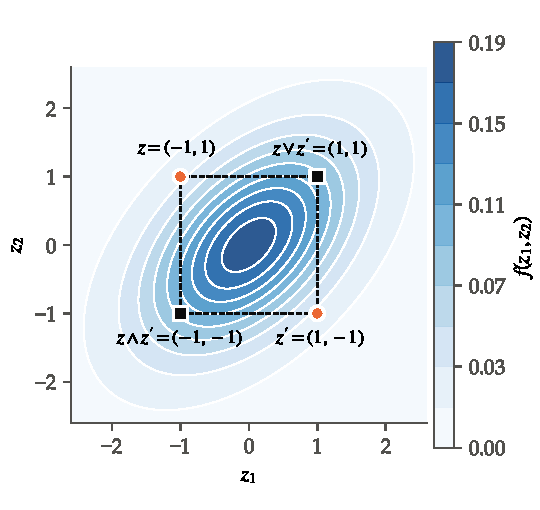
\includegraphics[width=0.56\textwidth]{figures/appB/affiliation.pdf}
\caption{The affiliation inequality for the standard bivariate normal density with correlation $\frac{1}{2}$. The
unordered points $z = (-1, 1)$ and $z' = (1, -1)$ (circles) have join $z \vee z' = (1, 1)$ and meet $z \wedge z' = (-1, -1)$
(squares). The density is $0.09435$ at the join and the meet and $0.02487$ at $z$ and $z'$, so
$f(z \vee z')f(z \wedge z') = 0.00890$ exceeds $f(z)f(z') = 0.000619$, by the factor $e^{\frac{8}{3}} \approx 14.39$.}
\label{fig:B-affiliation}
\end{figure}

\begin{remark}[The general definition]\label{rem:B-affil-general}
\citet[Appendix]{MilgromWeber1982} define affiliation without densities. A set $A \subseteq \R^k$ is \emph{increasing} if its
indicator is nondecreasing, and a set $S$ is a sublattice if $z \vee z', z \wedge z' \in S$ whenever $z, z' \in S$. The variables
are \emph{associated} if $\Pr(Z \in A \cap A') \geq \Pr(Z \in A)\Pr(Z \in A')$ for all increasing sets $A$ and $A'$. They are
affiliated if they are associated conditional on every sublattice $S$ of positive probability. Their Theorem 24
shows that, for variables with a density, this is equivalent to \eqref{eq:B-affil} almost everywhere.
\end{remark}

\begin{proposition}[Characterization, \citealp{MilgromWeber1982}, Theorem 1]\label{prop:B-affil-char}
\leavevmode
\begin{enumerate}[label=(\roman*)]
  \item A strictly positive, twice continuously differentiable density $f$ on a product of intervals is affiliated if
  and only if $\frac{\partial^2\ln f}{\partial z_l\,\partial z_m} \geq 0$ for all $l \neq m$.
  \item If $f = g_1g_2$ with $g_1$ and $g_2$ nonnegative functions that satisfy \eqref{eq:B-affil}, then $f$ is affiliated.
\end{enumerate}
\end{proposition}

\Cref{prop:14-affil-char} proves both parts. Part (i) is also \cref{prop:B-smooth-supermod} applied to $\ln f$, and
\citet[p.~1098]{MilgromWeber1982} cite \citet[p.~310]{Topkis1978} for it. Part (ii) multiplies the inequalities
for $g_1$ and $g_2$, which is legitimate because all terms are nonnegative.

For two variables, affiliation is a statement about conditional densities, and it feeds directly into the chain of
stochastic orders.

\begin{proposition}[Affiliation, MLRP and dominance]\label{prop:B-affil-mlrp}
Let $(X, Z)$ have a strictly positive density $f(x, z)$ on a rectangle, with conditional density $f(x \mid z)$ and
conditional CDF $F(x \mid z)$.
\begin{enumerate}[label=(\roman*)]
  \item $(X, Z)$ is affiliated if and only if $f(x \mid z)$ has the MLRP in $z$: for $z' > z$, $\frac{f(x \mid z')}{f(x \mid z)}$ is
  nondecreasing in $x$.
  \item Let $(X, Z)$ be affiliated and $z' > z$. The conditional distribution given $z'$ dominates the one given $z$ in
  the reverse hazard rate and hazard rate orders. In particular, $\Pr(X \geq x \mid Z = z)$ is nondecreasing in $z$.
  \item If $(X, Z)$ is affiliated, then $\E[\varphi(X) \mid Z = z]$ is nondecreasing in $z$ for every nondecreasing $\varphi$.
\end{enumerate}
\end{proposition}

\begin{proof}
(i) For $x' > x$ and $z' > z$, inequality \eqref{eq:B-affil} reads $f(x', z')f(x, z) \geq f(x, z')f(x', z)$. Dividing by the
product of the marginal densities of $Z$ at $z$ and $z'$ turns joint densities into conditional ones, and dividing
again by $f(x' \mid z)f(x \mid z) > 0$ gives
$\frac{f(x' \mid z')}{f(x' \mid z)} \geq \frac{f(x \mid z')}{f(x \mid z)}$, the MLRP. Each step reverses
\citep[footnote 16]{MilgromWeber1982}. Parts (ii) and (iii) follow from part (i) by \cref{prop:B-orders-chain} and
\cref{prop:B-fosd-expectations}, applied to $X_B \sim F(\cdot \mid z')$ and $X_A \sim F(\cdot \mid z)$.
\end{proof}

Part (ii) follows from the affiliation that \citet{CampoPerrigneVuong2003} assume in their asymmetric affiliated
private values model, so that $\Pr(V_1 \geq v \mid V_2 = v_2)$ is nondecreasing in $v_2$. \Cref{ch:auction-theory}
proves the same chain in the auction notation. Milgrom and Weber derive the properties that auction theory needs
from affiliation.

\begin{proposition}[Properties of affiliated variables, \citealp{MilgromWeber1982}, Theorems 2--5]\label{prop:B-affil-properties}
Let $Z = (Z_1, \dots, Z_k)$ be affiliated.
\begin{enumerate}[label=(\roman*)]
  \item (Order statistics.) Suppose the density $f(s, x_1, \dots, x_n)$ of a common component $s$ and signals $x_i$ is
  affiliated and symmetric in $(x_2, \dots, x_n)$. Let $Y_1 \geq \dots \geq Y_{n-1}$ be the order statistics of
  $(X_2, \dots, X_n)$. Then $(S, X_1, Y_1, \dots, Y_{n-1})$ is affiliated.
  \item (Monotone transformations.) If $g_1, \dots, g_k$ are all nondecreasing or all nonincreasing, then
  $g_1(Z_1), \dots, g_k(Z_k)$ are affiliated.
  \item (Subvectors.) $Z_1, \dots, Z_{k-1}$ are affiliated.
  \item (Conditional expectations.) For any nondecreasing $H$, the function
  $h(a_1, b_1; \dots; a_k, b_k) = \E[H(Z) \mid a_1 \leq Z_1 \leq b_1, \dots, a_k \leq Z_k \leq b_k]$ is nondecreasing in all its arguments.
  In particular, $\E[H(Z) \mid Z_1 = z_1, \dots, Z_l = z_l]$ is nondecreasing in $(z_1, \dots, z_l)$.
\end{enumerate}
\end{proposition}

\begin{proof}[Proofs and sketches]
(i) The joint density of $(S, X_1, Y_1, \dots, Y_{n-1})$ is
\[
  (n - 1)!\,f(s, x_1, y_1, \dots, y_{n-1})\,\indic\{y_1 \geq y_2 \geq \dots \geq y_{n-1}\}
\]
\citep[eq.~(4), p.~1099]{MilgromWeber1982}. The set of ordered vectors is a lattice, because componentwise maxima
and minima of two decreasing sequences are decreasing. Its indicator therefore satisfies \eqref{eq:B-affil}. The
product rule of \cref{prop:B-affil-char}(ii) gives the result.

(ii) We prove the case of strictly increasing, differentiable $g_l$. By the change-of-variables formula, the density
of $W = (g_1(Z_1), \dots, g_k(Z_k))$ is
\[
  f_W(w) = f\bigl(g_1^{-1}(w_1), \dots, g_k^{-1}(w_k)\bigr)\prod_{l=1}^k\frac{1}{g_l'(g_l^{-1}(w_l))}.
\]
The map $w \mapsto (g_1^{-1}(w_1), \dots, g_k^{-1}(w_k))$ is increasing coordinate by coordinate, so it commutes with joins and
meets. The first factor therefore satisfies \eqref{eq:B-affil}. The product is a product of functions of one
coordinate each, which satisfies \eqref{eq:B-affil} with equality. \Cref{prop:B-affil-char}(ii) completes the
argument. If all $g_l$ are decreasing, joins and meets swap, and \eqref{eq:B-affil} is symmetric in them.

(iii) Write $Z = (U, W)$ with $U = (Z_1, \dots, Z_{k-1})$ and $W = Z_k$, and let $f(u, w)$ be the joint density. Fix
$u, u' \in \R^{k-1}$. We must show that the marginal $\int f(u, w)\,\dd w$ satisfies \eqref{eq:B-affil}, that is,
\[
  \int f(u \vee u', w)\,\dd w\int f(u \wedge u', w)\,\dd w \geq \int f(u, w)\,\dd w\int f(u', w)\,\dd w.
\]
Write each product as a double integral over $(w, w')$ and fold the region $w > w'$ onto $w < w'$. For $w < w'$ define
\begin{align*}
  \Theta_1 &= f(u \vee u', w)f(u \wedge u', w'), & \Theta_2 &= f(u \vee u', w')f(u \wedge u', w),\\
  \Xi_1 &= f(u, w)f(u', w'), & \Xi_2 &= f(u, w')f(u', w).
\end{align*}
The left side is the integral of $\Theta_1 + \Theta_2$ and the right side the integral of $\Xi_1 + \Xi_2$ over $w < w'$, so it
suffices to show $\Theta_1 + \Theta_2 \geq \Xi_1 + \Xi_2$ pointwise. Affiliation of $f$ gives $\Theta_2 \geq \Xi_1$ and $\Theta_2 \geq \Xi_2$,
because in both cases the join of the two arguments is $(u \vee u', w')$ and the meet is $(u \wedge u', w)$. Affiliation in $u$
at fixed $w$ and at fixed $w'$ gives, after multiplying, $\Theta_1\Theta_2 \geq \Xi_1\Xi_2$. Now
$(\Theta_2 - \Xi_1)(\Theta_2 - \Xi_2) \geq 0$ expands to
\[
  \Theta_2(\Xi_1 + \Xi_2) \leq \Theta_2^2 + \Xi_1\Xi_2 \leq \Theta_2^2 + \Theta_1\Theta_2.
\]
Dividing by $\Theta_2 > 0$ gives the claim. If $\Theta_2 = 0$, then $\Xi_1 = \Xi_2 = 0$ and the claim is trivial. This is the
simplest case of the composition results of \citet{KarlinRinott1980}.

(iv) We prove the bivariate case $k = 2$, $l = 1$. Write $\E[H(Z_1, Z_2) \mid Z_1 = z_1] = \E[H(z_1, Z_2) \mid Z_1 = z_1]$. Raising
$z_1$ raises the integrand $H(z_1, \cdot)$ pointwise, and it shifts the conditional distribution of $Z_2$ up in the sense of
first-order dominance (\cref{prop:B-affil-mlrp}). By \cref{prop:B-fosd-expectations} both effects raise the
conditional expectation. \citet[Appendix]{MilgromWeber1982} derive the general statement from the conditional
covariance inequality below.
\end{proof}

Affiliation implies a covariance inequality that is often easier to use than the density condition.

\begin{theorem}[Association, \citealp{MilgromWeber1982}, Theorems 22--23]\label{thm:B-association}
If $Z$ is affiliated, then for every pair of nondecreasing functions $g$ and $h$ and every sublattice $S$ of positive
probability,
\[
  \E[g(Z)h(Z) \mid S] \geq \E[g(Z) \mid S]\,\E[h(Z) \mid S].
\]
With $S = \R^k$, affiliated variables are \emph{associated}: $\Cov(g(Z), h(Z)) \geq 0$. Moreover,
$\E[g(Z) \mid A] \geq \E[g(Z)] \geq \E[g(Z) \mid A^c]$ for every increasing set $A$ of positive probability.
\end{theorem}

\begin{proof}[Proof for one variable]
Let $k = 1$ and let $Z'$ be an independent copy of $Z$. Because $g$ and $h$ are both nondecreasing, $g(Z) - g(Z')$ and
$h(Z) - h(Z')$ have the same sign, so
\[
  0 \leq \E\bigl[(g(Z) - g(Z'))(h(Z) - h(Z'))\bigr] = 2\E[g(Z)h(Z)] - 2\E[g(Z)]\E[h(Z)].
\]
This is Chebyshev's covariance inequality. For general $k$, the inequality for indicators of increasing sets is
association, which is part of Milgrom and Weber's general definition of affiliation (\cref{rem:B-affil-general}).
Their Theorem 24 shows that a density satisfying \eqref{eq:B-affil} is affiliated in that sense. The step functions
$g_m(z) = \frac{1}{m}\sum_{i \geq 1}\indic\{g(z) > \frac{i}{m}\}$ are sums of indicators of increasing sets and approximate a
nonnegative nondecreasing $g$, which extends the inequality from indicators to functions
\citep[Theorems 22--23]{MilgromWeber1982}. Conditioning on a sublattice $S$ multiplies the density by the indicator
of $S$, which satisfies \eqref{eq:B-affil}, so the conditional density is again affiliated.
\end{proof}

Taking $g$ and $h$ to be coordinate functions shows that affiliated variables are nonnegatively correlated. The
converse fails badly, as the examples show.

\begin{example}[Affiliated and non-affiliated densities]\label{ex:B-affil-examples}
\leavevmode
\begin{enumerate}[label=(\alph*)]
  \item \emph{Independence.} A product of marginal densities satisfies \eqref{eq:B-affil} with equality.
  \item \emph{Normal vectors.} Let $Z \sim N(\mu, \Sigma)$. Then $\ln f(z) = \text{const} - \frac{1}{2}(z - \mu)^\T\Sigma^{-1}(z - \mu)$, and
  $\frac{\partial^2\ln f}{\partial z_l\,\partial z_m} = -(\Sigma^{-1})_{lm}$. By \cref{prop:B-affil-char}(i), $Z$ is affiliated if and only if
  every off-diagonal element of the precision matrix $\Sigma^{-1}$ is nonpositive. In the bivariate case with standard
  deviations $\sigma_1$, $\sigma_2$ and correlation $\rho_{12}$ (written with a subscript to distinguish it from
  pass-through),
  \[
    \ln f = \text{const} - \frac{1}{2(1 - \rho_{12}^2)}\left[\frac{(z_1 - \mu_1)^2}{\sigma_1^2} - \frac{2\rho_{12}(z_1 - \mu_1)(z_2 - \mu_2)}{\sigma_1\sigma_2} + \frac{(z_2 - \mu_2)^2}{\sigma_2^2}\right],
  \]
  so $\frac{\partial^2\ln f}{\partial z_1\,\partial z_2} = \frac{\rho_{12}}{(1 - \rho_{12}^2)\sigma_1\sigma_2}$. A bivariate normal vector is affiliated
  if and only if $\rho_{12} \geq 0$. With three or more variables, nonnegative correlations do not suffice. The
  covariance matrix with unit variances and correlations $\Corr(Z_1, Z_2) = \Corr(Z_1, Z_3) = \frac{1}{2}$ and
  $\Corr(Z_2, Z_3) = 0$ is positive definite, but its inverse has $(\Sigma^{-1})_{23} = \frac{1}{2} > 0$. Conditional on $Z_1$, the
  variables $Z_2$ and $Z_3$ are negatively related, and the vector is not affiliated.
  \item \emph{Farlie-Gumbel-Morgenstern density.} On $[0, 1]^2$ let $c(z_1, z_2) = 1 + \vartheta(1 - 2z_1)(1 - 2z_2)$ with
  $|\vartheta| \leq 1$. It integrates to one, has uniform marginals, and $\Cov(Z_1, Z_2) = \frac{\vartheta}{36}$, so
  $\Corr(Z_1, Z_2) = \frac{\vartheta}{3}$. Its partial derivatives are $c_1 = -2\vartheta(1 - 2z_2)$, $c_2 = -2\vartheta(1 - 2z_1)$
  and $c_{12} = 4\vartheta$. Hence
  \[
    \frac{\partial^2\ln c}{\partial z_1\,\partial z_2} = \frac{c\,c_{12} - c_1c_2}{c^2}
    = \frac{4\vartheta\bigl[1 + \vartheta(1 - 2z_1)(1 - 2z_2)\bigr] - 4\vartheta^2(1 - 2z_1)(1 - 2z_2)}{c^2} = \frac{4\vartheta}{c^2}.
  \]
  The density is affiliated if and only if $\vartheta \geq 0$.
  \item \emph{Mineral rights.} Let the common value $V$ have density $h$, and let signals be $S_i = V + \epsilon_i$ with
  $\epsilon_1, \dots, \epsilon_n$ i.i.d., independent of $V$, with a log-concave density $f_\epsilon$. The conditional density of a
  signal is $f_\epsilon(s - v)$. For $v' > v$, write $t = s - v$ and $d = v' - v > 0$. Then
  \[
    \ln\frac{f_\epsilon(s - v')}{f_\epsilon(s - v)} = \ln f_\epsilon(t - d) - \ln f_\epsilon(t),
  \]
  which is nondecreasing in $t$, and hence in $s$, because the increments of the concave function $\ln f_\epsilon$ shrink as its
  argument grows. The MLRP holds. Each factor $f_\epsilon(s_i - v)$ of the joint density
  $h(v)\prod_{i=1}^n f_\epsilon(s_i - v)$ satisfies \eqref{eq:B-affil} in $(v, s_i)$, and therefore on the whole vector, since
  joins and meets act coordinate by coordinate. By \cref{prop:B-affil-char}(ii), $(V, S_1, \dots, S_n)$ is affiliated
  \citep[p.~1099]{MilgromWeber1982}. Normal, logistic and Gumbel noise all qualify (\cref{tab:B-logconcave}).
\end{enumerate}
\end{example}

\Cref{fig:B-affiliation} illustrates \eqref{eq:B-affil} for a bivariate normal density with correlation
$\frac{1}{2}$. The points $z = (-1, 1)$ and $z' = (1, -1)$ are unordered, and their join $(1, 1)$ and meet $(-1, -1)$ lie
along the direction of positive dependence, where the density is higher.

In auction theory these tools combine as follows. By \cref{prop:B-affil-properties}(i) and (iv), the expected value
$\E[V_1 \mid X_1 = x, Y_1 = y]$ is nondecreasing in both arguments, which makes symmetric equilibrium bids increasing.
By part (iv) with the upper bound on $Y_1$ lowered, $\E[V_1 \mid X_1 = x, Y_1 < x] \leq \E[V_1 \mid X_1 = x]$, which is the winner's
curse. \Cref{ch:auction-theory} develops both, and \cref{ch:auction-empirics} uses affiliation in the
identification of affiliated private values.

The first-order condition of a symmetric first-price auction with affiliated private values shows where
the conditional distributions enter. Let $B_1$ be the highest bid among bidder 1's rivals. Let
$G_{B_1|b_1}$ and $g_{B_1|b_1}$ be its distribution and density conditional on bidder 1's own bid.
\citet[eq.~4, p.~175]{LiPerrigneVuong2002} show that the equilibrium condition is equivalent to
\begin{equation*}
v = b + \frac{G_{B_1|b_1}(b \mid b)}{g_{B_1|b_1}(b \mid b)} .
\end{equation*}
Each value is therefore a known function of its bid and of the joint distribution of bids, which the data
reveal \citep[Section~3.1, eq.~3.1]{AtheyHaile2007}. Under independence the conditioning on $b_1$ drops out.
Under affiliation it stays, because a high own bid signals high rival bids. Bids inherit affiliation from
values, since the equilibrium bid function is increasing (\cref{prop:B-affil-properties}(ii)).
\citet[Proposition~1, p.~175]{LiPerrigneVuong2002} characterize the bid distributions that such a model can
generate. A distribution qualifies if and only if it is symmetric and affiliated and the right side above is
strictly increasing in $b$.


\section{Bibliographic notes}\label{sec:B-notes}

Optimization, comparative statics and duality are covered in every graduate text in microeconomic theory.
\citet{MasColellWhinstonGreen1995} prove the Kuhn-Tucker conditions, the theorem of the maximum and the duality
results of \cref{sec:B-duality}. \citet{SimonBlume1994} give the matrix and calculus background.
\citet{MilgromSegal2002} prove the envelope theorem for arbitrary choice sets, which is the version that mechanism
design and auction theory need. \citet{Samuelson1947} introduced the correspondence principle and the Le Chatelier
principle into economics. \citet{DeatonMuellbauer1980b} develop duality for demand analysis at book length. Their
chapters on rationing, aggregation and index numbers supply the shadow prices, representative incomes and
cost-of-living bounds of \cref{sec:B-welfare}. \citet{Hausman1981} showed how to recover exact welfare measures from
an estimated demand curve.
\citet{BulowPfleiderer1983} and \citet{WeylFabinger2013} are the main references on pass-through and the curvature
of demand.

The extreme value foundations of discrete choice are due to \citet{McFadden1974, McFadden1978, McFadden1981}, and
the survey of \citet{McFadden1984} collects them. \citet{SmallRosen1981} derived the log-sum measure of consumer
surplus, and \citet{Williams1977} and \citet{DalyZachary1978} proved that the expected maximum utility has the choice
probabilities as its gradient. \citet{AndersonDePalmaThisse1992} connect discrete choice with representative-consumer
models of product differentiation. \citet{Train2009} is the standard text on discrete choice with simulation.
\citet{Cardell1997} constructed the distribution behind the random-coefficients reading of the nested logit, and
\citet{McFaddenTrain2000} showed that mixed logits approximate any random utility model.

\citet{David1981} and \citet{ArnoldBalakrishnanNagaraja1992} are the standard references on order statistics.
\citet{AtheyHaile2002, AtheyHaile2007} turned these results into a theory of identification for auctions, and the
deconvolution lemma of \citet{Kotlarski1966} underlies the treatment of unobserved auction heterogeneity. On fixed
points, \citet{StokeyLucas1989} treat contractions in function spaces, and \citet{Judd1998} discusses the numerical
side. \citet{Berry1994} proved that market shares can be inverted for mean utilities, and
\citet{BerryLevinsohnPakes1995} supplied the contraction that computes the inverse. \citet{BerryGandhiHaile2013}
established invertibility under much weaker conditions. \citet{BerryPakes2007} show how far the contraction weakens when the logit error
vanishes. Chapter~11 of \citet{Tirole1988} is a compact guide to the equilibrium concepts of the book, and its
Section~11.6.1 derives their existence from the theorem of \citet{Debreu1952}. \citet{DasguptaMaskin1986} treat
games with discontinuous payoffs.

Log-concavity entered economics from probability theory. \citet{Prekopa1971} and \citet{Borell1975} proved the
integration results, and \citet{CaplinNalebuff1991} used them to prove the existence of price equilibrium in
differentiated-products oligopoly. \citet{BagnoliBergstrom2005} classify the common distributions. Lattice methods
for comparative statics begin with \citet{Topkis1978}, and \citet{MilgromShannon1994} found their ordinal form.
\citet{Topkis1979}, \citet{Vives1990} and \citet{MilgromRoberts1990} developed the theory of supermodular games, and
\citet{Vives1999} applies it to oligopoly. \citet{BulowGeanakoplosKlemperer1985} introduced strategic substitutes
and complements. \citet{NockeSchutz2018} develop the aggregative structure of logit and CES pricing games, and
\citet[p.~229]{AskerNocke2021} survey its use in merger analysis. \citet{MilgromWeber1982} made affiliation the central dependence concept of auction
theory, and \citet{LiPerrigneVuong2002} turned it into a nonparametric estimator for first-price auctions.
\citet{KarlinRinott1980} study the same property under the name of multivariate total positivity, and
\citet{ShakedShanthikumar2007} cover the stochastic orders of \cref{sec:B-stochastic-orders}.

\section{Exercises}\label{sec:B-exercises}

\begin{enumerate}[label=\arabic*., leftmargin=*, itemsep=6pt]

\item \emph{Duality with CES utility.} Let $U(q_1, q_2) = (q_1^r + q_2^r)^{\frac{1}{r}}$ with $r < 1$ and $r \neq 0$, and
write $\sigma_{\mathrm{CES}} = \frac{1}{1 - r}$.
\begin{enumerate}[label=(\alph*)]
  \item Derive the Marshallian demands and the indirect utility function. Show that
  $q_i = \frac{p_i^{-\sigma_{\mathrm{CES}}}I}{P^{1 - \sigma_{\mathrm{CES}}}}$ with
  $P^{1 - \sigma_{\mathrm{CES}}} = p_1^{1 - \sigma_{\mathrm{CES}}} + p_2^{1 - \sigma_{\mathrm{CES}}}$.
  \item Derive the expenditure function $e(p, u) = uP$. Verify Shephard's lemma, Roy's identity and the symmetry of
  the Slutsky matrix.
  \item Show that the elasticity of $\frac{h_1}{h_2}$ with respect to $\frac{p_2}{p_1}$ equals $\sigma_{\mathrm{CES}}$.
  \item Use \cref{prop:B-virtual} to show that the compensating variation of removing good 2 is finite when
  $\sigma_{\mathrm{CES}} > 1$ and infinite when $\sigma_{\mathrm{CES}} < 1$. Interpret the difference.
  \item Ration good 1 at $z$ units. Derive the restricted expenditure function $e^*(p, u, z)$ and the shadow price
  $p_1^*(p_2, u, z)$, and verify $\frac{\partial e^*}{\partial z} = p_1 - p_1^*$ (\cref{rem:B-rationing}). With two
  goods the ration fixes $q_2$, so $S^*_{22} = 0$. Use $Sp = 0$ to check that $S_{22} - \frac{S_{21}^2}{S_{11}} = 0$,
  as \cref{rem:B-lechatelier} requires.
\end{enumerate}

\item \emph{Exact welfare from log-linear demand.} Let the demand for good 1 be $q_1 = \exp(c_0 + c_1p_1 + c_2I)$ with
$c_1 < 0$ and $c_2 > 0$, holding the other prices fixed.
\begin{enumerate}[label=(\alph*)]
  \item Write the differential equation \eqref{eq:B-hausman-ode} for this demand and solve it by separation of
  variables. Use the constant of integration as the utility index.
  \item Derive the indirect utility function and check that Roy's identity returns $q_1$.
  \item Derive the compensating variation of a price increase from $p_1^0$ to $p_1^1$. Show that it tends to the
  change in Marshallian consumer surplus as $c_2 \to 0$.
  \item Show that the Hicksian demand is positive at every finite price, so the virtual price is infinite. Is the
  value of the good still finite? Compare with the linear demand of \cref{ex:B-hausman-linear}.
  \item For a rise in $p_1$ alone, show that the bounds \eqref{eq:B-cv-ev-bounds} follow from the fact that
  compensated demand slopes down. Compute both bounds and both exact measures for $c_0 = 1$, $c_1 = -1$,
  $c_2 = 0.01$, $I = 100$ and a price rise from 1 to 2.
\end{enumerate}

\item \emph{Pass-through and conduct.} Consider the supply relation \eqref{eq:B-supply-relation}.
\begin{enumerate}[label=(\alph*)]
  \item Derive \eqref{eq:B-pt-conduct} step by step, with $\varepsilon_S$ defined relative to marginal cost including
  the tax.
  \item Show that a pass-through rate of one is consistent with three worlds: price taking with flat marginal cost,
  monopoly with exponential demand, and monopoly with log-convex demand and rising marginal cost.
  \item Let $P(Q) = a - bQ$ and $mc(Q) = c + dQ$ with $b, d > 0$. Show that $\rho = \frac{1}{1 + \theta + \frac{d}{b}}$,
  first from the proposition and then by solving the model directly.
  \item Explain what these results imply for tests of market power that regress prices on taxes.
\end{enumerate}

\item \emph{Cournot comparative statics.} Let $N$ symmetric firms with constant marginal cost $c$ face inverse demand
$P(Q)$, and treat $N$ as a continuous variable.
\begin{enumerate}[label=(\alph*)]
  \item Write the symmetric equilibrium condition $P(Nq) + qP'(Nq) = c$. Use the implicit function theorem to derive
  $\frac{\dd q}{\dd N}$ and $\frac{\dd Q}{\dd N}$.
  \item State conditions on $P'$ and $P''$ under which $\frac{\dd Q}{\dd N} > 0$ and $\frac{\dd q}{\dd N} < 0$. Relate
  the second inequality, business stealing, to the sign of $P' + qP''$.
  \item Use the envelope theorem to derive $\frac{\dd \pi}{\dd N}$ and show that it is negative under the conditions
  of part (b).
  \item Verify all three derivatives for linear demand $P(Q) = A - Q$.
\end{enumerate}

\item \emph{Extreme value algebra.} Let $\epsilon_{i0}, \dots, \epsilon_{iJ}$ be independent standard Gumbel shocks and
$u_{ij} = \delta_j + \epsilon_{ij}$.
\begin{enumerate}[label=(\alph*)]
  \item Prove max-stability for $\mathrm{EV}(0, b)$ shocks and use it to derive the logit shares with scale $b$.
  \item Show that the expected maximal utility conditional on choosing $j$ is the same for every $j$. Derive
  $\E[\epsilon_{ij} \mid j \text{ chosen}] = \gamma_E - \ln s_j$.
  \item In a nested logit with one nest of $m$ identical products of mean utility $\delta$ and an outside good,
  compute expected consumer surplus as a function of $m$ and $\sigma$. Show that it grows like
  $\frac{1 - \sigma}{\alpha}\ln m$ for large $m$, and explain the role of $\sigma$.
  \item Derive the within-nest correlation $1 - (1 - \sigma)^2$ from Cardell's representation.
\end{enumerate}

\item \emph{Order statistics and competing risks.}
\begin{enumerate}[label=(\alph*)]
  \item Let $n$ values be drawn independently from $F(x) = x^a$ on $[0, 1]$ with $a > 0$. Derive the CDF and the mean
  of the second-highest value. Check your answer against \cref{cor:B-os-revenue} at $a = 1$.
  \item Prove the recurrence relation \eqref{eq:B-os-recurrence} for $k = n - 1$ directly from \eqref{eq:B-os-cdf},
  for i.i.d.\ draws.
  \item Two independent bidders have values with $F_i(x) = x^{a_i}$ on $[0, 1]$, $i = 1, 2$. Compute
  $G_1^w(x) = \Pr(M \leq x, I = 1)$ and the CDF of the maximum $M$. Verify that \eqref{eq:B-competing-risks}
  recovers $F_1$.
  \item In part (c), show that the winning value and the identity of the winner are independent. Explain why the
  frequency of wins then carries all the information that separates the two distributions.
\end{enumerate}

\item \emph{Contractions and equilibrium computation.}
\begin{enumerate}[label=(\alph*)]
  \item In the plain logit, show that the Jacobian of the share-inversion map \eqref{eq:B-blp-map} is $\mathbf{1}s^\T$.
  Compute the number of iterations needed per digit of accuracy when $s_0 = 0.05$ and when $s_0 = 0.5$.
  \item Take a nested logit with one nest of two products. Show that the undampened map has a Jacobian eigenvalue
  $-\frac{\sigma}{1 - \sigma}$, and that the dampened map \eqref{eq:B-nl-dampened} sends this eigenvalue to zero.
  \item A single-product logit monopolist has $\alpha = 1$ and $v = \tilde\delta - \alpha mc = 3$. Use
  \cref{prop:B-logit-br} to compute its share. Show that the markup iteration \eqref{eq:B-markup-iteration} diverges
  locally while best-response iteration converges in one step.
  \item Use \eqref{eq:B-iterations} to bound the number of iterations that reach a tolerance of $10^{-8}$ from an
  initial step of $10$, for $\kappa = 0.9$ and $\kappa = 0.99$.
\end{enumerate}

\item \emph{Log-concavity, supermodularity and affiliation.}
\begin{enumerate}[label=(\alph*)]
  \item Show that the standard logistic density is log-concave. Deduce that its hazard rate is nondecreasing and
  that values with this distribution satisfy Myerson's regularity condition.
  \item Show that the single-product logit pricing game is log-supermodular. Use \cref{thm:B-smgames} to show that
  an increase in one firm's marginal cost does not lower any equilibrium price. Then use the closed-form best
  response \eqref{eq:B-logit-br-closed} to show that every price strictly rises.
  \item Verify that the Farlie-Gumbel-Morgenstern density of \cref{ex:B-affil-examples} is affiliated if and only if
  $\vartheta \geq 0$. Show directly that affiliation implies the monotone likelihood ratio property for this
  density.
  \item Prove that the likelihood ratio order implies first-order stochastic dominance. Give an example of two
  distributions ranked by first-order dominance but not by the likelihood ratio.
\end{enumerate}

\end{enumerate}

\chapter{Worked Problems}\label{app:problems}

This appendix works through eight problems with complete solutions. They apply the tools of the book to concrete
markets: the Cournot and conduct models of \cref{ch:theory,ch:conduct}, the pricing theory of \cref{ch:diffprod},
and the demand models of \cref{ch:discrete,ch:logit,ch:blp}. Following a derivation and carrying one out are
different skills. A model becomes a working tool only once we have computed its equilibrium, estimated it on data
and checked the answer. Most of the problems use simulated data. We then know the truth, so we can see exactly what
each estimator recovers and where it fails.

The problems fall into four groups. \Cref{sec:C-cournot,sec:C-passthrough} treat a homogeneous good. The first works
out what Cournot competition, collusion and free entry imply for the relation between concentration and margins,
and what that relation can say about mergers. The second asks what the pass-through of a tax reveals about conduct,
and it re-estimates the cigarette tax regressions of \citet{Sumner1981}. \Cref{sec:C-logit-bertrand,sec:C-simulate}
compute price equilibria with differentiated products. The first does so for logit demand, proves that the
equilibrium is unique, and evaluates a merger and a tax. The second simulates 100 markets from a random coefficients
logit with multi-product pricing. \Cref{sec:C-vertical,sec:C-logit-est,sec:C-rc-est} estimate the vertical model,
the logit and the random coefficients logit on these simulated data. They compare the elasticities, markups,
recovered costs and merger predictions of the three models with the truth. \Cref{sec:C-autos} closes with real data,
the product file of the replication package of \citet{GriecoMurryYurukoglu2024}. It asks what simple demand models
say about the decline of markups in the U.S. automobile market, and it compares their answer with the full model of
that paper. \Cref{tab:C-map} lists the problems with the tools
and chapters each one draws on.

\begin{table}[tb]
\centering
\caption{The eight worked problems}
\label{tab:C-map}
\footnotesize
\begin{tabularx}{\textwidth}{@{}l>{\raggedright\arraybackslash}X>{\raggedright\arraybackslash}Xl@{}}
\toprule
Problem & Topic & Main tools & Builds on \\
\midrule
\ref{sec:C-cournot} & Cournot competition, collusion and entry, concentration and margins, mergers &
  Nash and subgame-perfect equilibrium, repeated games, OLS limits, Monte Carlo & Chapters \ref{ch:intro},
  \ref{ch:theory}, \ref{ch:mergers} \\
\addlinespace
\ref{sec:C-passthrough} & Tax pass-through and conduct in cigarettes & Comparative statics, two-way fixed effects,
  clustered inference, power, ad valorem taxes & Chapters \ref{ch:theory}, \ref{ch:conduct} \\
\addlinespace
\ref{sec:C-logit-bertrand} & Logit Bertrand pricing with single- and multi-product firms, a merger and a tax &
  Lambert W function, aggregative uniqueness proof, contraction mapping, upward pricing pressure & Chapters
  \ref{ch:diffprod}, \ref{ch:logit}, \ref{ch:mergers} \\
\addlinespace
\ref{sec:C-simulate} & Simulating a random coefficients logit market & Simulated shares, Morrow-Skerlos fixed
  point, sampling and simulation error & Chapter \ref{ch:blp} \\
\addlinespace
\ref{sec:C-vertical} & Estimating the vertical model & Share inversion, normalization, clustered OLS, implied
  costs & Chapter \ref{ch:discrete} \\
\addlinespace
\ref{sec:C-logit-est} & Estimating logit demand and recovering costs & Berry inversion, 2SLS, instrument
  strength, market bootstrap, joint GMM, omitted-heterogeneity bias & Chapters \ref{ch:logit}, \ref{ch:blp} \\
\addlinespace
\ref{sec:C-rc-est} & Random coefficients estimation, a comparison of three models and a merger & BLP contraction,
  2SLS, elasticity matrices, diversion, merger simulation & Chapters \ref{ch:blp}, \ref{ch:mergers} \\
\addlinespace
\ref{sec:C-autos} & Markups over time in U.S. automobiles & Nested logit, weak instruments with two endogenous
  regressors, second-choice data, decompositions & Chapters \ref{ch:intro}, \ref{ch:logit} \\
\bottomrule
\end{tabularx}

\vspace{3pt}
\begin{minipage}{0.97\textwidth}
\footnotesize Notes: Problems \ref{sec:C-simulate} to \ref{sec:C-rc-est} share one simulated data set and are best
read in order. The other problems can be read on their own.
\end{minipage}
\end{table}

Every problem has the same format. A short paragraph motivates it. A statement gives the data and the parameters
and poses parts (a), (b) and so on. The solution answers every part in order, with propositions and proofs for the
results it relies on. Theory proved in a chapter is restated in one line with a cross-reference and then used.
Computational notes describe the algorithms as numbered steps. Readers gain most by attempting each part before
reading its solution. The numerical parts need a scientific programming language with linear algebra, a root
finder and a random number generator. Every number computed in the solutions was produced by a Python script in
\texttt{figures/appC/src}, and numbers quoted from papers are cited to their tables or pages. The scripts read the
supplied data files in \texttt{figures/appC/data}, or the replication package used in \cref{sec:C-autos}. They draw
all simulated consumers, bootstrap samples and Monte Carlo samples with fixed seeds. Readers who draw their own random
numbers will obtain slightly different values.

Three conventions need care across the problems. First, $\delta$ is the discount factor in \cref{sec:C-cournot}
and mean utility in the other problems. Second, in \cref{sec:C-cournot,sec:C-passthrough} the symbol $\varepsilon$
is the market elasticity written as a positive number, as in the notation list. From \cref{sec:C-logit-bertrand}
on, we report elasticity matrices with entries $\varepsilon_{jk} = \frac{\partial s_j}{\partial p_k}\frac{p_k}{s_j}$.
Own elasticities are then negative, and the positive own elasticity of the notation list is $-\varepsilon_{jj}$.
Third, $\Phi$ always denotes the logit denominator, while $\Lambda_t$ and $\Gamma_t$ are the matrices of the
Morrow-Skerlos fixed point of \cref{sec:C-simulate}. Symbols used in a single problem are defined where they first
appear.

\section{Cournot competition, entry, collusion and the concentration-margin relation}\label{sec:C-cournot}

Cross-industry studies in the structure-conduct-performance tradition relate profitability to
concentration. \citet{Bain1951} compared profit rates across industries, and later work regressed price-cost
margins on concentration \citep{Schmalensee1989}. This problem works out what four canonical models of a homogeneous-good
industry imply for that relation, and what the relation can and cannot say about mergers. The four models
are Cournot competition and perfect collusion, each with a fixed number of firms and with free entry. Two
extensions add firms with different costs and mergers. A computational part simulates a cross-section of
industries and compares the merger predictions of the regression with the true equilibrium effects. The
theory behind the problem is developed in \cref{sec:02-cournot,sec:02-entry,sec:02-collusion}, and the
cross-industry regression is studied in \cref{sec:01-montecarlo}.

\subsection{Statement}\label{sec:C-cournot-statement}

A homogeneous good has linear inverse demand $P(Q) = a - bQ$, where $Q$ is total output, $a > c > 0$ and
$b > 0$. Every active firm pays a fixed cost $F > 0$ per period and produces at constant marginal cost $c$. The
Lerner index is $L = \frac{P - c}{P}$, the Herfindahl index is $\HHI = \sum_i s_i^2$ with market shares
$s_i = \frac{q_i}{Q}$, and $\varepsilon = -\frac{\dd Q}{\dd P}\frac{P}{Q}$ is the market elasticity of demand,
written as a positive number. Two constants recur. The \emph{market-size index} is
$x \equiv \frac{a - c}{\sqrt{bF}}$, and the \emph{profit scale} is $k \equiv \frac{(a - c)^2}{b}$.

\begin{enumerate}[label=(\alph*)]
\item There are $N$ firms that choose outputs simultaneously. Describe the game and the equilibrium concept.
  Show that the equilibrium is unique and symmetric. Compute the price, outputs, profits, $L$ and $\HHI$, and
  verify that $L = \frac{\HHI}{\varepsilon}$.
\item Firms first decide whether to enter and then play the game of part (a). Treating the number of firms as
  continuous, find the free-entry number of firms and the resulting price, outputs, $L$ and $\HHI$.
\item Repeat parts (a) and (b) when the active firms collude perfectly, charging the monopoly price and
  splitting output equally. Show that collusion is not a Nash equilibrium of the one-shot game. Find the
  discount factor above which grim-trigger strategies sustain collusion in the infinitely repeated game.
\item Describe the relation between $\HHI$ and $L$ in the four cases.
\item An economist posits $\E[L] = \beta_0 + \beta_1\HHI$ and estimates it on a cross-section of industries.
  Does the specification make sense under each model? Are the estimates consistent, and for what? Are they
  useful for predicting the effect of a merger?
\item Let firm $i$ have its own constant marginal cost $c_i$, with every firm active. Show that
  $L_i = \frac{s_i}{\varepsilon}$ and $\sum_i s_iL_i = \frac{\HHI}{\varepsilon}$. Show that a mean-preserving spread
  of costs that keeps every firm active raises $\HHI$ and the share-weighted Lerner index, leaves the price
  unchanged and raises welfare.
\item Evaluate every object of parts (a) to (c) for $a = 10$, $c = 2$, $b = 1$ and $F = 1$, including consumer
  surplus, total welfare and the welfare-maximizing number of firms.
\item In the symmetric Cournot model, study the profitability of a merger of two firms and of $k_M$ firms.
  Compare the change in $\HHI$ computed from pre-merger shares with the equilibrium change. Find the marginal
  cost of the merged firm below which the merger does not raise the price.
\item (Computational.) Simulate a cross-section of Cournot industries, estimate the regression of part (e),
  and compare the merger effects it predicts with the true equilibrium effects.
\end{enumerate}

\subsection{Solution}\label{sec:C-cournot-solution}

\casehead{Part (a)}
The game has players $i = 1, \dots, N$. Each player chooses an output $q_i \ge 0$, all players move
simultaneously, and all primitives are common knowledge. Firm $i$'s payoff is
\begin{equation}\label{eq:C-cournot-profit}
\pi_i(q_i, q_{-i}) = \big(a - bQ - c\big)q_i - F, \qquad Q = q_i + Q_{-i}, \quad Q_{-i} = \sum_{j \ne i} q_j .
\end{equation}
A \emph{Nash equilibrium} is a profile $q^* = (q_1^*, \dots, q_N^*)$ such that $q_i^*$ maximizes
$\pi_i(q_i, q_{-i}^*)$ for every $i$. The fixed cost lowers the profit of an active firm but does not affect
its output choice.

Profit is strictly concave in the firm's own output, since
\begin{equation*}
\frac{\partial \pi_i}{\partial q_i} = a - c - bQ_{-i} - 2bq_i, \qquad
\frac{\partial^2 \pi_i}{\partial q_i^2} = -2b < 0 .
\end{equation*}
The unique best response to rivals' total output $Q_{-i}$ is therefore
\begin{equation}\label{eq:C-cournot-br}
BR_i(Q_{-i}) = \max\Big\{0, \frac{a - c - bQ_{-i}}{2b}\Big\}.
\end{equation}

\begin{proposition}[Linear Cournot equilibrium]\label{prop:C-cournot}
With $a > c$, the Cournot game has a unique Nash equilibrium. It is symmetric, every firm is active, and
\begin{equation}\label{eq:C-cournot-q}
q = \frac{a - c}{b(N + 1)}, \qquad Q = \frac{N(a - c)}{b(N + 1)}, \qquad P = \frac{a + Nc}{N + 1}.
\end{equation}
\end{proposition}

\begin{proof}
We proceed in three steps. First, total output is positive in any equilibrium. If $Q = 0$, every firm faces
$Q_{-i} = 0$, and \eqref{eq:C-cournot-br} gives $BR_i(0) = \frac{a - c}{2b} > 0$, a contradiction. Second,
every firm is active. An active firm $l$ satisfies the first-order condition $a - c - bQ - bq_l = 0$, so
\begin{equation*}
bq_l = a - c - bQ .
\end{equation*}
Since $q_l > 0$, this gives $a - c - bQ > 0$. A firm $i$ with $q_i = 0$ would need
$\frac{\partial \pi_i}{\partial q_i}\big|_{q_i = 0} = a - c - bQ \le 0$, which contradicts the previous
inequality. Third, every firm satisfies $bq_i = a - c - bQ$, so all outputs are equal. Summing over the $N$
firms gives
\begin{align*}
bQ &= N(a - c) - NbQ, \\
Q &= \frac{N(a - c)}{b(N + 1)} .
\end{align*}
Total output is unique, so each output $q = \frac{Q}{N}$ is unique. The price is
$P = a - bQ = \frac{a(N + 1) - N(a - c)}{N + 1} = \frac{a + Nc}{N + 1}$.
\end{proof}

The remaining objects follow by substitution. The margin and the profit are
\begin{align}
P - c &= \frac{a + Nc - (N + 1)c}{N + 1} = \frac{a - c}{N + 1} = bq, \label{eq:C-cournot-margin}\\
\pi &= (P - c)q - F = \frac{a - c}{N + 1}\cdot\frac{a - c}{b(N + 1)} - F = \frac{k}{(N + 1)^2} - F .
\label{eq:C-cournot-pi}
\end{align}
The Lerner index divides the margin by the price, and every firm has share $\frac{1}{N}$:
\begin{equation}\label{eq:C-cournot-LH}
L = \frac{a - c}{N + 1}\cdot\frac{N + 1}{a + Nc} = \frac{a - c}{a + Nc}, \qquad
\HHI = N\cdot\frac{1}{N^2} = \frac{1}{N}.
\end{equation}
With linear demand $-\frac{\dd Q}{\dd P} = \frac{1}{b}$, so the elasticity at the equilibrium is
\begin{equation*}
\varepsilon = \frac{P}{bQ} = \frac{a + Nc}{N + 1}\cdot\frac{N + 1}{N(a - c)} = \frac{a + Nc}{N(a - c)} .
\end{equation*}
The check is direct:
$\frac{\HHI}{\varepsilon} = \frac{1}{N}\cdot\frac{N(a - c)}{a + Nc} = \frac{a - c}{a + Nc} = L$. The relation
holds for any demand curve. Firm $i$'s first-order condition $P + q_iP'(Q) = c$ gives
$\frac{P - c}{P} = -\frac{q_iP'}{P} = \frac{q_i}{Q}\cdot\frac{1}{\varepsilon}$, and symmetry sets
$\frac{q_i}{Q} = \frac{1}{N} = \HHI$ (\cref{sec:02-cournot-markups}).

\casehead{Part (b)}
Entry adds a first stage. In stage 1, a large pool of identical potential entrants decide simultaneously
whether to enter and pay $F$. In stage 2, the $N$ entrants observe $N$ and play the Cournot game of part (a).
The solution concept is \emph{subgame-perfect equilibrium}. \Cref{prop:C-cournot} fixes play in every
stage-2 subgame, so an entrant earns $\pi(N) = \frac{k}{(N + 1)^2} - F$, which is strictly decreasing in $N$.
In equilibrium no entrant regrets entering and no outsider wants to enter, so the number of firms $N^e$
satisfies $\pi(N^e) \ge 0 \ge \pi(N^e + 1)$. Treating $N$ as continuous gives the zero-profit condition
$\pi(N^e) = 0$:
\begin{align}
(N^e + 1)^2 &= \frac{(a - c)^2}{bF} = x^2, \notag\\
N^e &= x - 1 = \frac{a - c}{\sqrt{bF}} - 1 . \label{eq:C-Ne}
\end{align}
The free-entry outcomes follow from \eqref{eq:C-cournot-q} and \eqref{eq:C-cournot-margin} with
$\frac{a - c}{N^e + 1} = \sqrt{bF}$:
\begin{align}
P^e &= c + \frac{a - c}{N^e + 1} = c + \sqrt{bF}, \qquad
q^e = \frac{a - c}{b(N^e + 1)} = \frac{\sqrt{bF}}{b} = \sqrt{\frac{F}{b}}, \notag\\
Q^e &= \frac{a - P^e}{b} = \frac{a - c - \sqrt{bF}}{b}, \notag\\
L^e &= \frac{P^e - c}{P^e} = \frac{\sqrt{bF}}{c + \sqrt{bF}}, \qquad
\HHI^e = \frac{1}{N^e} = \frac{1}{x - 1} = \frac{\sqrt{bF}}{a - c - \sqrt{bF}} . \label{eq:C-free-entry}
\end{align}
Each entrant earns $(P^e - c)q^e - F = \sqrt{bF}\sqrt{\frac{F}{b}} - F = 0$. The formulas require $N^e \ge 1$,
that is, $x \ge 2$, or equivalently $0 < F \le \frac{(a - c)^2}{4b}$. The Cournot rule survives entry. The elasticity at
$P^e$ is $\varepsilon^e = \frac{P^e}{bQ^e} = \frac{c + \sqrt{bF}}{a - c - \sqrt{bF}}$, and
$\frac{\HHI^e}{\varepsilon^e} = L^e$. Under free entry the dollar margin $\sqrt{bF}$ is fixed by technology
and the slope of demand. A larger intercept $a$ brings more firms and leaves the margin unchanged. With the
integer constraint, $N^e$ is the integer part of $x - 1$ (\cref{sec:02-mw-integer}).

\casehead{Part (c)}
Under perfect collusion with $N$ firms fixed, the firms choose total output to maximize joint profit
\begin{equation*}
\Pi(Q) = (a - bQ - c)Q - NF, \qquad \Pi''(Q) = -2b < 0 .
\end{equation*}
The first-order condition $a - c - 2bQ = 0$ gives the monopoly outcome
\begin{equation}\label{eq:C-monopoly}
Q^m = \frac{a - c}{2b}, \qquad P^m = a - bQ^m = \frac{a + c}{2}, \qquad P^m - c = \frac{a - c}{2}.
\end{equation}
Each firm produces $q = \frac{Q^m}{N} = \frac{a - c}{2bN}$ and earns $\pi = \frac{a - c}{2}\cdot\frac{a - c}{2bN} - F
= \frac{k}{4N} - F$. The Lerner index is $L = \frac{a - c}{a + c}$ for every $N$, and $\HHI = \frac{1}{N}$. The
elasticity at the monopoly price is $\varepsilon(P^m) = \frac{P^m}{bQ^m} = \frac{a + c}{a - c}$, so
$L = \frac{1}{\varepsilon(P^m)}$, the monopoly inverse-elasticity rule. Price, total output and the margin do not
depend on $N$. Profit per firm and $\HHI$ fall as $N$ rises.

Collusion is not a Nash equilibrium of the one-shot game when $N \ge 2$. Suppose every rival produces
$\frac{Q^m}{N}$. At $q_i = \frac{Q^m}{N}$ the marginal profit of firm $i$ is
\begin{equation*}
\frac{\partial \pi_i}{\partial q_i} = a - c - bQ^m - b\frac{Q^m}{N} = \frac{a - c}{2} - \frac{a - c}{2N}
= \frac{(N - 1)(a - c)}{2N} > 0 .
\end{equation*}
Each firm gains by expanding, because it bears only its own share of the price reduction that its extra
output causes.

Collusion can be sustained in the infinitely repeated game. In periods $t = 0, 1, 2, \dots$ the $N$ firms play
the stage game of part (a). Outputs are observed at the end of each period. In this problem $\delta \in (0, 1)$
denotes the discount factor, as in \cref{ch:collusion-theory} (in the demand chapters $\delta$ is mean utility).
Firm $i$ maximizes $\sum_{t \ge 0}\delta^t\pi_{it}$. Under \emph{grim-trigger} strategies \citep{Friedman1971}, each
firm produces $\frac{Q^m}{N}$ in period 0 and in every period that follows no deviation. After any deviation every
firm produces the Cournot output $\frac{a - c}{b(N + 1)}$ forever.

\begin{proposition}[Threshold discount factor for Cournot collusion]\label{prop:C-delta}
Grim-trigger strategies form a subgame-perfect equilibrium that sustains the monopoly outcome if and only if
\begin{equation}\label{eq:C-delta}
\delta \ge \delta^*(N) \equiv \frac{(N + 1)^2}{N^2 + 6N + 1}.
\end{equation}
The threshold satisfies $\delta^*(2) = \frac{9}{17}$, is strictly increasing in $N$ for $N > 1$, and
tends to one as $N \to \infty$.
\end{proposition}

\begin{proof}
The fixed cost enters every period's payoff equally, so it cancels from every incentive constraint. What remains is
\cref{prop:12-cournot}, which gives the threshold, its monotonicity and its limit. At $N = 2$ the threshold is
$\frac{9}{4 + 12 + 1} = \frac{9}{17}$.
\end{proof}

\Cref{fig:C-delta} plots the threshold together with the Bertrand benchmark. In the Bertrand supergame a
deviator undercuts slightly and takes the whole monopoly profit $\pi^m$, after which profits are zero. The
condition $\frac{\pi^m}{N(1 - \delta)} \ge \pi^m$ gives $\delta \ge 1 - \frac{1}{N}$ (\cref{prop:12-bertrand}).
\citet[Section~6.3.2.1]{Tirole1988} uses this threshold to formalize the old claim that concentration facilitates
tacit collusion.
The two thresholds cross between $N = 2$ and $N = 3$. Cournot collusion is harder to sustain for $N = 2$
($\frac{9}{17} = 0.529$ against $0.5$) and easier for every $N \ge 3$ ($\frac{4}{7} = 0.571$ against $0.667$ at
$N = 3$). For large $N$, $1 - \delta^*(N) = \frac{4N}{N^2 + 6N + 1}$ is close to $\frac{4}{N}$, four
times the Bertrand slack $\frac{1}{N}$. Cournot reversion is a mild punishment, but the one-shot gain from
deviating is also small, because the deviator expands only to its best response.

\begin{figure}[htbp]
\centering
\begin{tikzpicture}
\begin{axis}[
  width=0.78\textwidth, height=6.2cm,
  xlabel={number of firms $N$}, ylabel={threshold discount factor},
  xmin=1.5, xmax=20.5, ymin=0.45, ymax=1.0,
  xtick={2,4,6,8,10,12,14,16,18,20},
  ytick={0.5,0.6,0.7,0.8,0.9,1.0},
  yticklabel style={/pgf/number format/fixed, /pgf/number format/precision=1},
  grid=major, grid style={gray!25},
  legend style={draw=none, fill=none, font=\small, at={(0.97,0.05)}, anchor=south east},
  legend cell align=left,
]
\addplot[blue!70!black, thick, mark=*, mark size=1.6pt, samples at={2,3,...,20}]
  {(x + 1)^2/(x^2 + 6*x + 1)};
\addlegendentry{Cournot, grim trigger: $\frac{(N + 1)^2}{N^2 + 6N + 1}$}
\addplot[orange!85!black, thick, dashed, mark=square*, mark size=1.5pt, samples at={2,3,...,20}]
  {1 - 1/x};
\addlegendentry{Bertrand: $1 - \frac{1}{N}$}
\end{axis}
\end{tikzpicture}
\caption{Lowest discount factor at which grim-trigger strategies sustain the monopoly outcome among $N$
symmetric firms, for Cournot and Bertrand stage games with linear demand and constant marginal cost. The
Cournot threshold does not depend on $a$, $b$, $c$ or $F$.}
\label{fig:C-delta}
\end{figure}

\begin{remark}
Grim trigger is not the harshest credible punishment. \citet{Abreu1986} studies stick-and-carrot
punishments, in which firms produce more than the Cournot output for one period and then return to
collusion. These punish deviators more severely and sustain the monopoly outcome at lower discount factors
than \eqref{eq:C-delta}. \Cref{ch:collusion-theory} develops optimal punishments.
\end{remark}

With free entry, collusive play in stage 2 yields per-firm profit $\pi(N) = \frac{k}{4N} - F$. The free-entry
condition $\pi(N^m) = 0$, with $N$ continuous, gives
\begin{equation}\label{eq:C-Nm}
N^m = \frac{(a - c)^2}{4bF} = \frac{x^2}{4}.
\end{equation}
Price and total output stay at the monopoly values, so entry only changes how $Q^m$ is divided:
\begin{equation*}
q^m = \frac{Q^m}{N^m} = \frac{a - c}{2b}\cdot\frac{4bF}{(a - c)^2} = \frac{2F}{a - c}, \qquad
L = \frac{a - c}{a + c}, \qquad \HHI^m = \frac{1}{N^m} = \frac{4bF}{(a - c)^2}.
\end{equation*}
Total fixed costs equal the monopoly profit, $N^mF = \frac{(a - c)^2}{4b} = (P^m - c)Q^m$, so entry dissipates
the whole rent. Consumers gain nothing, because the price stays at $P^m$. Collusion attracts more entrants
than Cournot competition:
\begin{equation}\label{eq:C-Nm-Ne}
N^m - N^e = \frac{x^2}{4} - x + 1 = \Big(\frac{x}{2} - 1\Big)^2 \ge 0,
\end{equation}
with equality only at $x = 2$, where both equal one. The higher collusive margin draws firms in until profit is
again zero. The collusive outcome with $N^m$ firms is an equilibrium of the repeated game only if $\delta \ge
\delta^*(N^m)$. Lower fixed costs raise $N^m$ and push the threshold toward one, so free entry also
makes collusion harder to enforce.

\casehead{Part (d)}
\Cref{tab:C-cournot-cases} collects the four regimes (the closed forms are also in
\cref{tab:02-linear-cournot}). Under Cournot conduct with $N$ fixed, substitute $N = \frac{1}{\HHI}$ in
the elasticity of part (a):
\begin{equation}\label{eq:C-LH-curve}
\varepsilon = \frac{a\HHI + c}{a - c}, \qquad L = \frac{\HHI}{\varepsilon} = \frac{(a - c)\HHI}{a\HHI + c}.
\end{equation}
The derivatives
\begin{align*}
\frac{\dd L}{\dd\HHI} &= \frac{(a - c)(a\HHI + c) - (a - c)\HHI a}{(a\HHI + c)^2} = \frac{c(a - c)}{(a\HHI + c)^2} > 0,\\
\frac{\dd^2 L}{\dd\HHI^2} &= -\frac{2ac(a - c)}{(a\HHI + c)^3} < 0
\end{align*}
show an increasing and concave curve. It runs from $L = 0$ at $\HHI = 0$ to the monopoly value
$\frac{a - c}{a + c}$ at $\HHI = 1$. When $N$ is set outside the model, the curve is the causal effect of
concentration on margins in an industry with given $(a, c)$.

\begin{table}[htbp]
\centering
\begin{threeparttable}
\caption{Concentration and margins in the linear homogeneous-good industry under four regimes}
\label{tab:C-cournot-cases}
\small
\setlength{\tabcolsep}{4pt}
\begin{tabular}{@{}lccccc>{\raggedright\arraybackslash}p{2.75cm}@{}}
\toprule
Regime & $N$ & $P$ & $q$ & $L$ & $\HHI$ & Relation of $L$ to $\HHI$ \\
\midrule
Cournot, fixed $N$ & $N$ & $\frac{a + Nc}{N + 1}$ & $\frac{a - c}{b(N + 1)}$ & $\frac{a - c}{a + Nc}$ &
  $\frac{1}{N}$ & increasing, concave, causal \\
\addlinespace
Cournot, free entry & $x - 1$ & $c + \sqrt{bF}$ & $\sqrt{\frac{F}{b}}$ & $\frac{\sqrt{bF}}{c + \sqrt{bF}}$ &
  $\frac{\sqrt{bF}}{a - c - \sqrt{bF}}$ & same curve, both endogenous \\
\addlinespace
Collusion, fixed $N$ & $N$ & $\frac{a + c}{2}$ & $\frac{a - c}{2bN}$ & $\frac{a - c}{a + c}$ & $\frac{1}{N}$ &
  flat \\
\addlinespace
Collusion, free entry & $\frac{x^2}{4}$ & $\frac{a + c}{2}$ & $\frac{2F}{a - c}$ & $\frac{a - c}{a + c}$ &
  $\frac{4bF}{(a - c)^2}$ & opposite directions when $a$ or $c$ vary \\
\bottomrule
\end{tabular}
\begin{tablenotes}\footnotesize
\item Notes: Inverse demand $P = a - bQ$, marginal cost $c$, fixed cost $F$, and $x = \frac{a - c}{\sqrt{bF}}$.
Free-entry columns treat $N$ as continuous and require $x \ge 2$. Under Cournot conduct $L = \frac{\HHI}{\varepsilon}$,
and under collusion $L = \frac{1}{\varepsilon}$, with $\varepsilon$ evaluated at the equilibrium price.
\end{tablenotes}
\end{threeparttable}
\end{table}

With free entry, Cournot industries stay on the curve \eqref{eq:C-LH-curve}, but $\HHI^e$ and $L^e$ are now
both outcomes of $(a, b, c, F)$. Write $r = \sqrt{bF}$, so that $\HHI^e = \frac{r}{a - c - r}$ and
$L^e = \frac{r}{c + r}$. Each primitive moves the pair differently. A higher $F$ or $b$ raises $r$ and with it
both $\HHI^e$ and $L^e$, so the industry moves up along the curve. A higher $a$ lowers $\HHI^e$ and leaves $L^e$
unchanged. A higher $c$ raises $\HHI^e$ and lowers $L^e$. Across industries, the sign of the association
between $\HHI$ and $L$ therefore depends on which primitive varies.

Under collusion with $N$ fixed, $L = \frac{a - c}{a + c}$ for every $N$, so the relation is flat. With free
entry, $L$ still depends only on $(a, c)$, while $\HHI^m = \frac{4bF}{(a - c)^2}$. Variation in $F$ or $b$
moves $\HHI^m$ alone. A higher $a$ raises $L$ and lowers $\HHI^m$, and a higher $c$ does the reverse, so
variation in $a$ or $c$ moves the two indices in opposite directions.

Differences in conduct weaken, and can reverse, the positive Cournot relation. Compare a Cournot industry and
a collusive industry with the same primitives. With $N$ fixed both have $\HHI = \frac{1}{N}$, and the collusive
industry has the higher margin, since $\frac{a - c}{a + c} > \frac{a - c}{a + Nc}$ for $N > 1$. With free entry,
collusion again raises the margin, because $P^e = c + \sqrt{bF} \le \frac{a + c}{2} = P^m$ whenever $x \ge 2$.
By \eqref{eq:C-Nm-Ne} the collusive industry is also less concentrated. A cross-section that mixes the two
pairs high margins with low concentration. This pulls the slope of $L$ on $\HHI$ below the Cournot curve and
can make it negative. \Cref{fig:02-LH} draws the four cases for $a = 10$ and $c = 2$.

\casehead{Part (e)}
The specification $\E[L] = \beta_0 + \beta_1\HHI$ fits the four models to different degrees.
\begin{itemize}
\item Cournot, fixed $N$. The model implies $L = \frac{\HHI}{\varepsilon}$, so $\beta_0 = 0$ and margins rise
  with $\HHI$. The relation is linear with $\beta_1 = \frac{1}{\varepsilon}$ only if $\varepsilon$ is the same in
  every industry. With linear demand, $\varepsilon = \frac{a\HHI + c}{a - c}$ rises with $\HHI$ by
  \eqref{eq:C-LH-curve}, so the true relation is concave and the linear form is an approximation.
\item Cournot, free entry. Industries still lie on $L = \frac{\HHI}{\varepsilon}$, so the specification remains
  an approximation. Differences in $\HHI$ now reflect differences in $(a, b, c, F)$.
\item Collusion, fixed $N$. The margin does not depend on $\HHI$, so the specification holds only in the
  degenerate form $\beta_1 = 0$.
\item Collusion, free entry. A nonzero slope can arise from joint variation of the primitives, and it has no
  causal meaning.
\end{itemize}

Cross-industry OLS converges to $\frac{\Cov(L, \HHI)}{\Var(\HHI)}$ (\cref{prop:01-scp-plim}). This limit
summarizes the joint distribution of outcomes. It equals a structural parameter such as $\frac{1}{\varepsilon}$
only under special conditions, and four problems separate the two. First, concentration is endogenous, because the same primitives determine
$\HHI$ and $L$, and part (d) shows that even the sign of the association depends on which primitive varies.
Second, industries differ in elasticity and conduct, so $\hat\beta_1$ averages over different models. If
$L_k = \frac{\HHI_k}{\varepsilon_k}$ with $\varepsilon_k$ independent of $\HHI_k$, the slope converges to
$\E[\frac{1}{\varepsilon_k}]$, and otherwise it does not. Third, accounting margins differ from economic
margins. Measured price-cost margins omit the cost of capital, and capital intensity is correlated with
fixed costs and hence with $\HHI$. Fourth, $\HHI$ is measured with error and depends on the market definition,
which attenuates the slope.

Even a positive and precisely estimated $\hat\beta_1$ need not mean that concentration raises margins.
Part (f) shows that when firms differ in costs, efficient firms are large, so concentration and the average
margin rise together while welfare also rises. This is the efficiency critique of \citet{Demsetz1973}.

The regression is a weak tool for merger prediction. The economist would compute
$\widehat{\Delta L} = \hat\beta_1\,\Delta\HHI$ with $\Delta\HHI = 2s_is_j$ from the merging firms' pre-merger
shares. The prediction inherits every bias of $\hat\beta_1$. The share-based $\Delta\HHI$ also misstates the
equilibrium change in concentration (part (h)), and the prediction ignores entry, coordinated effects and
cost savings. Part (i) measures the size of these errors in simulated data.

\casehead{Part (f)}
Let firm $i$ have constant marginal cost $c_i$ and suppose all $N$ firms are active. The first-order
condition of firm $i$ is $a - bQ - bq_i - c_i = 0$, that is,
\begin{equation}\label{eq:C-asym-foc}
bq_i = P - c_i .
\end{equation}
Summing over firms gives $bQ = Na - \sum_j c_j - NbQ$, so
\begin{equation}\label{eq:C-asym}
Q = \frac{Na - \sum_j c_j}{b(N + 1)}, \qquad P = a - bQ = \frac{a + \sum_j c_j}{N + 1}, \qquad
q_i = \frac{a + \sum_j c_j - (N + 1)c_i}{b(N + 1)} .
\end{equation}
All firms are active if and only if $c_i < P$ for every $i$. Dividing \eqref{eq:C-asym-foc} by $P$,
\begin{equation*}
L_i = \frac{P - c_i}{P} = \frac{bq_i}{P} = \frac{q_i}{Q}\cdot\frac{bQ}{P} = \frac{s_i}{\varepsilon},
\qquad
\sum_i s_iL_i = \frac{1}{\varepsilon}\sum_i s_i^2 = \frac{\HHI}{\varepsilon} .
\end{equation*}
The share-weighted Lerner index equals the Herfindahl index divided by the market elasticity
\citep{CowlingWaterson1976}. The same steps apply to any demand curve, because the first-order condition
$P + q_iP' = c_i$ gives $L_i = \frac{s_i}{\varepsilon}$ directly. The ratio of industry variable profit to revenue is
the same object,
\begin{equation*}
\frac{\sum_i(P - c_i)q_i}{PQ} = \sum_i\frac{q_i}{Q}\cdot\frac{P - c_i}{P} = \sum_is_iL_i = \frac{\HHI}{\varepsilon} ,
\end{equation*}
which is Exercise~5.6 of \citet[Section~5.5]{Tirole1988}.

A \emph{mean-preserving spread} of costs is a change from $(c_i)$ to $(c_i')$ with
$\sum_i c_i' = \sum_i c_i$ and $\sum_i(c_i' - \bar c)^2 > \sum_i(c_i - \bar c)^2$, where $\bar c$ is the mean cost.
We write $\Var(c) = \frac{1}{N}\sum_i(c_i - \bar c)^2$ for the cross-firm variance.

\begin{proposition}[Cost dispersion, concentration and welfare]\label{prop:C-demsetz}
In the linear Cournot model with all firms active, a mean-preserving spread of marginal costs that keeps
every firm active leaves $Q$, $P$, $\varepsilon$ and consumer surplus unchanged. It raises $\HHI$ and the
share-weighted Lerner index, and it raises total welfare by $\frac{N\Delta\Var(c)}{b}$, where $\Delta\Var(c)$
is the increase in the cost variance.
\end{proposition}

\begin{proof}
We use four steps. First, by \eqref{eq:C-asym} total output and the price depend on costs only through
$\sum_j c_j$, which the spread holds fixed. Hence $Q$, $P$, the elasticity $\varepsilon = \frac{P}{bQ}$ and
consumer surplus $\frac{bQ^2}{2}$ are unchanged. Second, by \eqref{eq:C-asym-foc} outputs are
$q_i = \frac{P - c_i}{b}$, and their mean is $\bar q = \frac{Q}{N}$, so
\begin{equation*}
q_i - \bar q = -\frac{c_i - \bar c}{b}, \qquad \Var(q) = \frac{\Var(c)}{b^2}.
\end{equation*}
Third, the Herfindahl index is
\begin{equation*}
\HHI = \frac{\sum_i q_i^2}{Q^2} = \frac{N\big[\Var(q) + \bar q^2\big]}{Q^2}
= \frac{1}{N} + \frac{N\Var(c)}{b^2Q^2},
\end{equation*}
which rises with $\Var(c)$ because $Q$ is fixed. Since $\varepsilon$ is fixed, $\sum_i s_iL_i =
\frac{\HHI}{\varepsilon}$ rises too. Fourth, total variable cost is
\begin{equation*}
\sum_i c_iq_i = \frac{1}{b}\sum_i c_i(P - c_i) = \frac{1}{b}\Big[PN\bar c - N\big(\Var(c) + \bar c^2\big)\Big]
= \frac{N\bar c(P - \bar c)}{b} - \frac{N\Var(c)}{b} .
\end{equation*}
With $P$ and $\bar c$ fixed, it falls by $\frac{N\Delta\Var(c)}{b}$. Welfare equals consumer surplus plus revenue
$PQ$ minus variable and fixed costs, and only variable cost changes, so welfare rises by the same amount.
\end{proof}

The proposition gives the Demsetz critique a precise form. Across otherwise identical industries, those with
more dispersed costs are more concentrated and have higher average margins. They also produce the same output
at lower cost. A regression of margins on concentration across such industries finds a positive slope, and
a policy of deconcentration would lower welfare. \citet[Section~5.5, Exercise~5.7]{Tirole1988} poses the two-firm
case. With demand $Q = 1 - P$ and costs satisfying $c_1 + c_2 = 2c$, a spread of costs raises both concentration and
industry profit.

The fourth step has a general version that needs neither linear demand nor fixed total output. Total surplus is
$W = \int_0^QP(z)\,\dd z - \sum_ic_iq_i - NF$. Holding the cost functions fixed, a small change $\dd q$ in outputs
changes it by
\begin{equation*}
\dd W = P\,\dd Q - \sum_ic_i\,\dd q_i = \sum_i(P - c_i)\,\dd q_i .
\end{equation*}
This is the output term of \citet[eq.~3, p.~7]{FarrellShapiro1988}, the working-paper version of
\citet{FarrellShapiro1990}. Its page numbers differ from those of the published article, and its equation numbers may
differ too. It models a merger as a transfer of capital between firms. In a Cournot equilibrium with constant marginal costs, the first-order
condition gives $P - c_i = \lvert P'\rvert q_i$. Differentiating $\sum_iq_i^2 = \HHI\,Q^2$ gives
$\sum_iq_i\,\dd q_i = \HHI\,Q\,\dd Q + \frac{Q^2}{2}\,\dd\HHI$. Substituting,
\begin{equation}\label{eq:C-fs-welfare}
\dd W = \lvert P'\rvert\sum_iq_i\,\dd q_i = \lvert P'\rvert\Big[\HHI\,Q\,\dd Q + \frac{Q^2}{2}\,\dd\HHI\Big] .
\end{equation}
This is their decomposition, written with $X$ for output and $H$ for the Herfindahl index (p.~17). With total output
fixed, a small reallocation that raises the Herfindahl index raises welfare. It moves production toward the largest
firms, which have the lowest marginal costs. Even when output falls, welfare rises if the Herfindahl index rises by
enough (p.~17).

The same identity bounds the welfare effect of any small change in outputs. By the Cauchy-Schwarz inequality,
$\sum_iq_i\,\dd q_i \le \lVert q\rVert\,\lVert\dd q\rVert$, and $\lVert q\rVert = Q\sqrt{\HHI}$. Hence
\begin{equation*}
\dd W \le \lvert P'\rvert\,Q\sqrt{\HHI}\,\lVert\dd q\rVert ,
\end{equation*}
with equality when $\dd q$ is proportional to $q$. Among changes of a given Euclidean size, the largest welfare gain is
proportional to the square root of the Herfindahl index. This is the bound of \citet{DansbyWillig1979}, posed as
Exercise~5.8 of \citet[Section~5.5]{Tirole1988}. The Herfindahl index thus also measures how much a small reallocation
of output can raise welfare.

\casehead{Part (g)}
With $a = 10$, $c = 2$, $b = 1$ and $F = 1$ we have $a - c = 8$, $k = 64$ and $x = 8$.
\Cref{tab:C-cournot-numbers} reports every object for $N = 3$ under both conducts and for the two free-entry
equilibria. The Cournot rows follow from \eqref{eq:C-cournot-q} to \eqref{eq:C-cournot-LH}. For example, with
$N = 3$ the price is $\frac{10 + 6}{4} = 4$ and each firm produces $\frac{8}{4} = 2$. Free entry gives
$N^e = 8 - 1 = 7$ and $P^e = 2 + 1 = 3$. Collusion gives $Q^m = 4$ and $P^m = 6$, and free entry under collusion
gives $N^m = \frac{64}{4} = 16$. The difference $N^m - N^e = 9$ equals $(\frac{8}{2} - 1)^2$, as
\eqref{eq:C-Nm-Ne} requires.

\begin{table}[htbp]
\centering
\begin{threeparttable}
\caption{The four regimes for $a = 10$, $c = 2$, $b = 1$ and $F = 1$}
\label{tab:C-cournot-numbers}
\small
\begin{tabular}{@{}lcccc@{}}
\toprule
 & \multicolumn{2}{c}{Cournot} & \multicolumn{2}{c}{Collusion} \\
\cmidrule(lr){2-3}\cmidrule(l){4-5}
 & $N = 3$ & Free entry & $N = 3$ & Free entry \\
\midrule
Number of firms $N$ & 3 & 7 & 3 & 16 \\
Price $P$ & 4 & 3 & 6 & 6 \\
Total output $Q$ & 6 & 7 & 4 & 4 \\
Output per firm $q$ & 2 & 1 & $\frac{4}{3}$ & $\frac{1}{4}$ \\
Profit per firm $\pi$ (net of $F$) & 3 & 0 & $\frac{13}{3}$ & 0 \\
Lerner index $L$ & $\frac{1}{2}$ & $\frac{1}{3}$ & $\frac{2}{3}$ & $\frac{2}{3}$ \\
Herfindahl index $\HHI$ & $\frac{1}{3}$ & $\frac{1}{7}$ & $\frac{1}{3}$ & $\frac{1}{16}$ \\
Elasticity $\varepsilon$ at $P$ & $\frac{2}{3}$ & $\frac{3}{7}$ & $\frac{3}{2}$ & $\frac{3}{2}$ \\
$\frac{\HHI}{\varepsilon}$ & $\frac{1}{2}$ & $\frac{1}{3}$ & $\frac{2}{9}$ & $\frac{1}{24}$ \\
$\frac{1}{\varepsilon}$ & $\frac{3}{2}$ & $\frac{7}{3}$ & $\frac{2}{3}$ & $\frac{2}{3}$ \\
Consumer surplus $\frac{bQ^2}{2}$ & 18 & 24.5 & 8 & 8 \\
Total profit (net of fixed costs) & 9 & 0 & 13 & 0 \\
Total welfare $W$ & 27 & 24.5 & 21 & 8 \\
Threshold $\delta^*(N)$ for collusion & $\frac{4}{7} = 0.571$ & $\frac{16}{23} = 0.696$ &
  $\frac{4}{7} = 0.571$ & $\frac{289}{353} = 0.819$ \\
\bottomrule
\end{tabular}
\begin{tablenotes}\footnotesize
\item Notes: Free-entry columns use the continuous free-entry conditions \eqref{eq:C-Ne} and \eqref{eq:C-Nm}.
Welfare is consumer surplus plus profits net of fixed costs. Under Cournot conduct $L = \frac{\HHI}{\varepsilon}$,
and under collusion $L = \frac{1}{\varepsilon}$. The last row is $\delta^*(N)$ from \eqref{eq:C-delta}
evaluated at the number of firms in each column.
\end{tablenotes}
\end{threeparttable}
\end{table}

Welfare under Cournot conduct has a convenient closed form. Consumer surplus is
$\frac{bQ^2}{2} = \frac{(a - c)^2N^2}{2b(N + 1)^2}$ and gross profits are $\frac{N(a - c)^2}{b(N + 1)^2}$, so
\begin{equation}\label{eq:C-welfare}
W(N) = \frac{(a - c)^2}{2b}\cdot\frac{N^2 + 2N}{(N + 1)^2} - NF
= \frac{(a - c)^2}{2b}\Big[1 - \frac{1}{(N + 1)^2}\Big] - NF .
\end{equation}
The first term is the maximal gross surplus $\frac{(a - c)^2}{2b} = 32$ less the deadweight loss
$\frac{(a - c)^2}{2b(N + 1)^2}$. A planner who chooses $N$ but cannot control post-entry conduct sets
\begin{equation*}
W'(N) = \frac{(a - c)^2}{b(N + 1)^3} - F = 0
\quad\Longrightarrow\quad
(N^o + 1)^3 = \frac{(a - c)^2}{bF} = 64
\quad\Longrightarrow\quad N^o = 3 .
\end{equation*}
So the Cournot column with $N = 3$ is also the second-best optimum, with $W(3) = 32\cdot\frac{15}{16} - 3 = 27$.
Free entry yields $W(7) = 32\cdot\frac{63}{64} - 7 = 24.5$. The comparison $N^e + 1 = 8 = (N^o + 1)^{\frac{3}{2}}$
illustrates excess entry (\cref{prop:02-mw-excess}, \citealp{MankiwWhinston1986}). The welfare loss of 2.5
is 7.8 percent of the maximal gross surplus. Collusion with three firms yields $W = 8 + 16 - 3 = 21$, and
collusion with free entry yields $W = 8$, since entry dissipates the whole monopoly profit of 16. For
reference, a single firm pricing at marginal cost with its fixed cost covered would reach $32 - 1 = 31$.

Part (f) can be checked in the same market. Replace the common cost 2 by costs $(1, 2, 3)$, which keeps
$\bar c = 2$ and raises $\Var(c)$ from 0 to $\frac{2}{3}$. The price stays at $\frac{10 + 6}{4} = 4$ and
outputs become $(3, 2, 1)$. The Herfindahl index rises from $\frac{1}{3}$ to
$\frac{9 + 4 + 1}{36} = \frac{7}{18}$, and the share-weighted Lerner index rises from $\frac{1}{2}$ to
$\frac{7}{18}\cdot\frac{3}{2} = \frac{7}{12}$. Variable cost falls from 12 to $3 + 4 + 3 = 10$, a saving of
$\frac{N\Var(c)}{b} = 3\cdot\frac{2}{3} = 2$, and welfare rises from 27 to 29.

\casehead{Part (h)}
A merger without cost savings turns two of $N$ symmetric firms into one firm with the same marginal cost. The
merged firm is then one of $N - 1$ symmetric Cournot competitors.

\begin{proposition}[Mergers in symmetric linear Cournot]\label{prop:C-merger-cournot}
Consider the model of part (a) with $N \ge 2$ firms.
\begin{enumerate}[label=(\roman*)]
\item A merger of two firms without cost savings leads to the $(N - 1)$-firm equilibrium. If both fixed costs
  remain, it is profitable for the merging firms if and only if $N \le 1 + \sqrt 2$, that is, if and only if $N = 2$.
  If the merger saves one fixed cost, it is profitable if and only if
  $\frac{k}{N^2} - \frac{2k}{(N + 1)^2} + F \ge 0$.
\item A merger of $k_M$ firms, $2 \le k_M \le N$, without cost savings is profitable for the merging firms,
  with all fixed costs kept, if and only if $(N + 1)^2 \ge k_M(N - k_M + 2)^2$.
\item The share-based change in concentration of a two-firm merger is $2s_is_j = \frac{2}{N^2}$, and the
  equilibrium change is $\frac{1}{N - 1} - \frac{1}{N} = \frac{1}{N(N - 1)}$. The share-based formula overstates
  the equilibrium change if and only if $N > 2$. The equilibrium changes in price and margin are
  \begin{equation}\label{eq:C-merger-dL}
  \Delta P = \frac{a - c}{N(N + 1)}, \qquad \Delta L = \frac{c(a - c)}{\big(a + (N - 1)c\big)(a + Nc)} .
  \end{equation}
\item Let the merged firm have marginal cost $c_M$, and suppose all firms remain active. The merger does not
  raise the price if and only if
  \begin{equation}\label{eq:C-merger-synergy}
  c_M \le c - \frac{a - c}{N + 1} = 2c - P^0,
  \end{equation}
  where $P^0$ is the pre-merger price. Equivalently, the merged firm's margin must be at least the sum of the
  two pre-merger margins, $P^0 - c_M \ge 2(P^0 - c)$.
\end{enumerate}
\end{proposition}

\begin{proof}
(i) After the merger there are $N - 1$ firms with marginal cost $c$, so \cref{prop:C-cournot} applies with
$N - 1$ firms. The merged firm earns $\frac{k}{N^2} - F$ if one fixed cost is saved and $\frac{k}{N^2} - 2F$
if both remain. The two firms earned $2\big[\frac{k}{(N + 1)^2} - F\big]$ before. With both fixed costs kept,
the merger is profitable if and only if
\begin{equation*}
\frac{k}{N^2} \ge \frac{2k}{(N + 1)^2} \iff (N + 1)^2 \ge 2N^2 \iff N + 1 \ge \sqrt 2\,N
\iff N \le \frac{1}{\sqrt 2 - 1} = 1 + \sqrt 2 .
\end{equation*}
Saving one fixed cost adds $F$ to the gain, which gives the second condition.
(ii) After the merger there are $N - k_M + 1$ firms, so the merged firm earns $\frac{k}{(N - k_M + 2)^2}$ gross
of fixed costs. The $k_M$ insiders earned $\frac{k_Mk}{(N + 1)^2}$ before. Cross-multiplying the comparison
gives the condition.
(iii) Before the merger every share is $\frac{1}{N}$, so $2s_is_j = \frac{2}{N^2}$. In equilibrium the index
moves from $\frac{1}{N}$ to $\frac{1}{N - 1}$, and $\frac{1}{N - 1} - \frac{1}{N} = \frac{1}{N(N - 1)}$. The
ratio of the two changes is $\frac{2}{N^2}\cdot N(N - 1) = \frac{2(N - 1)}{N}$, which exceeds one if and only if
$N > 2$. By \eqref{eq:C-cournot-margin}, $P - c = \frac{a - c}{N + 1}$, so
$\Delta P = \frac{a - c}{N} - \frac{a - c}{N + 1} = \frac{a - c}{N(N + 1)}$. By \eqref{eq:C-cournot-LH},
\begin{equation*}
\Delta L = \frac{a - c}{a + (N - 1)c} - \frac{a - c}{a + Nc}
= \frac{(a - c)\big[(a + Nc) - (a + (N - 1)c)\big]}{\big(a + (N - 1)c\big)(a + Nc)}
= \frac{c(a - c)}{\big(a + (N - 1)c\big)(a + Nc)} .
\end{equation*}
(iv) After the merger there are $N - 1$ firms, $N - 2$ with cost $c$ and one with cost $c_M$. By
\eqref{eq:C-asym} with $N - 1$ firms, the post-merger price is $P^1 = \frac{a + (N - 2)c + c_M}{N}$. Then
\begin{align*}
P^1 \le P^0 &\iff \frac{a + (N - 2)c + c_M}{N} \le \frac{a + Nc}{N + 1}\\
&\iff c_M \le \frac{N(a + Nc)}{N + 1} - a - (N - 2)c
= \frac{(N + 2)c - a}{N + 1} = c - \frac{a - c}{N + 1} .
\end{align*}
The last expression equals $2c - P^0$ because $P^0 - c = \frac{a - c}{N + 1}$.
\end{proof}

Part (i) is the merger paradox of \citet{SalantSwitzerReynolds1983}. Outsiders respond to the merged firm's
contraction by expanding, because quantities are strategic substitutes, and the expansion erodes the
insiders' gain. Part (ii) shows how large a merger must be to pay. With $N = 10$, a merger of $k_M = 8$ firms
fails, since $121 < 8 \cdot 4^2 = 128$, while a merger of $k_M = 9$ firms succeeds, since $121 > 9\cdot 3^2 = 81$.
A profitable merger must include at least 80 percent of the firms (\cref{prop:11-ssr} and \cref{fig:11-ssr}). Part (iv) is the
linear case of the synergy condition proved in general in \cref{prop:11-synergy}, following
\citet{FarrellShapiro1990}. \citet[eq.~6, pp.~228--229]{AskerNocke2021} state it for a set $\mathcal{M}$ of merging
firms with cost functions $C_i$, pre-merger outputs $q_i$ and merged cost function $C_M$. The merger does not lower
aggregate output, and so does not lower consumer surplus, if
\begin{equation*}
P(Q) - C_M'\Big(\sum_{i \in \mathcal{M}}q_i\Big) \ge \sum_{i \in \mathcal{M}}\big[P(Q) - C_i'(q_i)\big] .
\end{equation*}
It does not raise consumer surplus if the inequality is reversed. With two merging firms of marginal cost $c$, the condition is
$P^0 - c_M \ge 2(P^0 - c)$, the second form of \eqref{eq:C-merger-synergy}. The required saving is the full
pre-merger margin, $c - c_M \ge P^0 - c$, so a merger that only rationalizes production always raises the price
(\cref{fig:11-synergy}). The working paper states the price result for small transfers of capital
\citep[Proposition~2, p.~13]{FarrellShapiro1988}. A transfer from firm 2 to firm 1 raises the price if and only if
capital has a smaller direct effect on output at firm 1 than at firm 2.

The numerical market of part (g) makes these magnitudes concrete. A merger of two of three firms raises the
price from 4 to $\frac{14}{3} = 4.67$ and the Lerner index from $\frac{1}{2}$ to $\frac{4}{7}$, so
$\Delta L = \frac{1}{14} = 0.071$. The share-based change in concentration is $\frac{2}{9} = 0.222$ (2,222
points), against an equilibrium change of $\frac{1}{6} = 0.167$ (1,667 points). Consumer surplus falls from 18
to $\frac{128}{9} = 14.2$. The merged firm earns $\frac{64}{9} - 2 = 5.11$ with both fixed costs, less than
the 6 the two firms earned before. If the merger saves one fixed cost, it earns $\frac{64}{9} - 1 = 6.11$ and
the merger becomes profitable. The outsider gains most, from 3 to 6.11. For the price not to rise, the merged
firm's marginal cost must fall to $2c - P^0 = 4 - 4 = 0$, which eliminates marginal cost entirely.

\begin{remark}
At the price-neutral cost $c_M = 2c - P^0$, the share-based change in concentration is exact. Total output
is unchanged, so each outsider's first-order condition $bq_j = P - c$ leaves its output unchanged, and the
merged firm produces the sum of the two pre-merger outputs. In the numerical market with $c_M = 0$, the price
stays at 4, the merged firm produces 4 and the outsider 2. The index rises from $\frac{1}{3}$ to
$\frac{4}{9} + \frac{1}{9} = \frac{5}{9}$, exactly $\frac{2}{9}$. The share-based formula thus describes the
merger whose cost savings exactly offset its market power. Such a merger raises welfare, by the cost saving
$c\,(q_i + q_j) = 2 \cdot 4 = 8$ in this example.
\end{remark}

Three further channels break the link between $\Delta\HHI$ and $\Delta L$. With free entry, a merger that
removes a firm leaves room for a new entrant, and in the long run $N$ returns to $N^e$ and the price to $P^e$.
In the numerical market, a merger of two of the seven free-entry firms raises each remaining firm's gross
profit to $\frac{64}{49} = 1.31$, which exceeds $F = 1$ and invites entry. When the continuous free-entry condition
holds before and after, entry restores aggregate output, so the merger leaves consumer surplus unchanged
\citep[Section~3.3.3, pp.~231--232]{AskerNocke2021}. With the integer constraint this neutrality fails. They report
the result of \citet{Spector2003} that, in the Cournot model, a merger without synergies that is profitable once entry
is taken into account still harms consumers. Under collusion the firms already
charge $P^m$, so a merger has no direct price effect. It lowers the number of firms and with it the threshold
$\delta^*(N)$, from $\frac{4}{7}$ to $\frac{9}{17}$ when three firms become two, so it can make
collusion easier to sustain. With differentiated products the price effect runs through the diversion between
the merging products (\cref{sec:C-logit-bertrand}).

\casehead{Part (i)}
We simulate 1,000 industries. The primitives are drawn independently as $a \sim U[8, 12]$, $c \sim U[1, 4]$,
$b \sim U[0.5, 2]$ and $\ln F \sim U[\ln 0.1, \ln 10]$, and kept if $x \ge 2$. The number of firms is drawn as
$N \sim U\{1, \dots, 20\}$ independently of the primitives, and every industry is in the Cournot equilibrium of
part (a). This is design (1) of the Monte Carlo experiment in \cref{sec:01-montecarlo}, with the same random
numbers. OLS of $L$ on a constant and $\HHI$ gives
\begin{equation}\label{eq:C-mc-ols}
\widehat{L} = \underset{(0.004)}{0.178} + \underset{(0.022)}{0.546}\,\HHI, \qquad R^2 = 0.520,
\end{equation}
with HC1 standard errors, as in column (1) of \cref{tab:01-montecarlo}. These are heteroskedasticity-robust with the
small-sample factor $\frac{n}{n - 2}$ (step 3 of \cref{sec:C-cournot-computation}).

For each of the 954 industries with $N \ge 2$ we consider a merger of two firms without cost savings. The
equilibrium effect is $\Delta L$ in \eqref{eq:C-merger-dL}. The regression predicts
$\widehat{\Delta L} = \hat\beta_1\Delta\HHI$, and we use two versions of $\Delta\HHI$: the share-based
$\frac{2}{N^2}$ and the equilibrium change $\frac{1}{N(N - 1)}$. A third prediction serves as a benchmark that
no cross-industry regression can deliver. It multiplies the equilibrium $\Delta\HHI$ by the local slope of the
industry's own Cournot curve, $\frac{c(a - c)}{(a\HHI + c)^2}$. \Cref{tab:C-merger-mc} and
\cref{fig:C-merger-mc} report the results.

\begin{table}[htbp]
\centering
\begin{threeparttable}
\caption{Merger effects predicted by the cross-industry regression and equilibrium merger effects}
\label{tab:C-merger-mc}
\small
\setlength{\tabcolsep}{4pt}
\begin{tabular}{@{}lccccccc@{}}
\toprule
\multicolumn{8}{@{}l}{\emph{Panel A. Means}} \\
 & & \multicolumn{2}{c}{$\Delta\HHI$ (points)} & & \multicolumn{3}{c}{Predicted $\Delta L$} \\
\cmidrule(lr){3-4}\cmidrule(l){6-8}
$N$ & Industries & $2s_is_j$ & Equilibrium & $\Delta L$ & $2s_is_j$ & Equilibrium & Local slope \\
\midrule
All ($N \ge 2$) & 954 & 644 & 514 & 0.0248 & 0.0352 & 0.0281 & 0.0305 \\
2 to 4 & 162 & 2,748 & 2,423 & 0.0695 & 0.1500 & 0.1323 & 0.0991 \\
5 to 10 & 311 & 401 & 237 & 0.0250 & 0.0219 & 0.0130 & 0.0268 \\
11 to 20 & 481 & 94 & 51 & 0.0096 & 0.0051 & 0.0028 & 0.0098 \\
\midrule
\multicolumn{8}{@{}l}{\emph{Panel B. Accuracy}} \\
 & \multicolumn{3}{c}{Share with error above 50\%} & & \multicolumn{3}{c}{Correlation with $\Delta L$} \\
\cmidrule(lr){2-4}\cmidrule(l){6-8}
$N$ & $2s_is_j$ & Equilibrium & Local slope & & $2s_is_j$ & Equilibrium & Local slope \\
\midrule
All ($N \ge 2$) & 0.332 & 0.710 & 0.055 & & 0.927 & 0.882 & 0.981 \\
2 to 4 & 0.673 & 0.352 & 0.321 & & 0.938 & 0.929 & 0.978 \\
5 to 10 & 0.026 & 0.524 & 0.000 & & 0.839 & 0.837 & 0.999 \\
11 to 20 & 0.416 & 0.950 & 0.000 & & 0.681 & 0.681 & 1.000 \\
\bottomrule
\end{tabular}
\begin{tablenotes}\footnotesize
\item Notes: 1,000 simulated Cournot industries, of which 954 have $N \ge 2$ firms before the merger. Panel A
reports group means. Predictions multiply
$\hat\beta_1 = 0.546$ from \eqref{eq:C-mc-ols} by the share-based change $\frac{2}{N^2}$ or by the equilibrium
change $\frac{1}{N(N - 1)}$. The local-slope benchmark multiplies the equilibrium change by
$\frac{c(a - c)}{(a\HHI + c)^2}$, the slope of the industry's own Cournot curve. ``Error above 50 percent'' means
$\lvert\widehat{\Delta L} - \Delta L\rvert > 0.5\,\Delta L$. Source: \texttt{figures/appC/src/cournot\_merger\_mc.py}.
\end{tablenotes}
\end{threeparttable}
\end{table}

\begin{figure}[htbp]
\centering
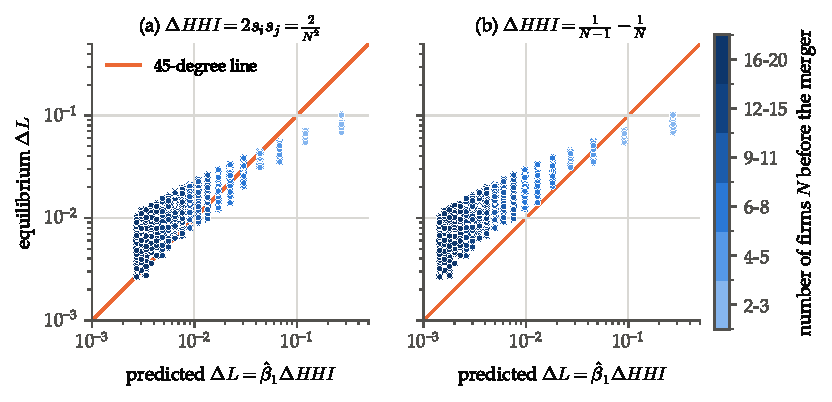
\includegraphics[width=\textwidth]{figures/appC/merger_mc.pdf}
\caption{Equilibrium against predicted changes in the Lerner index after a merger of two firms in 954
simulated Cournot industries, on logarithmic axes. Predictions multiply the cross-industry slope
$\hat\beta_1 = 0.546$ by the share-based change in concentration (panel a) or by the equilibrium change (panel b).
Colours group industries by the number of firms before the merger. Points above the orange line are mergers
whose effect the regression understates.}
\label{fig:C-merger-mc}
\end{figure}

Three findings stand out. First, the regression gets the direction of the error wrong in a systematic way.
For concentrated industries ($N \le 4$) it overstates the effect of a merger by a factor of about two. For
unconcentrated industries ($N \ge 11$) it understates the effect, and with the equilibrium $\Delta\HHI$ the
prediction is less than a third of the truth. The reason is concavity. The OLS slope 0.546 is a
variance-weighted average of chord slopes, and most of the variation in $\HHI$ comes from concentrated
industries, where the Cournot curve is flat. The local slope averages 1.452 across the 1,000 industries, and it
is largest where $\HHI$ is small.

Second, the share-based formula appears to do better than the equilibrium change in concentration. Overall,
its prediction errs by more than 50 percent in 33 percent of industries, against 71 percent for the equilibrium
version. This is an accident of offsetting errors. The share-based formula overstates the change in
concentration by the factor $\frac{2(N - 1)}{N}$, close to two in unconcentrated industries, and this offsets
part of the slope's understatement there. A correct input combined with a wrong slope produces a worse
prediction.

Third, the error comes from the common slope, and the linear approximation does little harm. The local-slope
benchmark misses by more than
50 percent in only 5.5 percent of industries, all of them concentrated. Its remaining error comes from
concavity, since the tangent at the pre-merger point is steeper than the chord to the post-merger point, so it
overpredicts in every industry. The high correlations in Panel B reflect the fact that predicted and actual
effects both fall with $N$. They say little about accuracy, since every prediction uses the same slope for all
industries.

\subsection{Computational notes}\label{sec:C-cournot-computation}

The script \texttt{figures/appC/src/cournot\_merger\_mc.py} implements part (i) in the following steps.
\begin{enumerate}
\item Draw $(a, c, b, \ln F)$ in batches from the stated uniform distributions with a fixed seed. Keep draws with
  $x \ge 2$ until 1,000 industries are accepted, then draw $N$ for each industry.
\item Compute $L = \frac{a - c}{a + Nc}$ and $\HHI = \frac{1}{N}$.
\item Run OLS of $L$ on $(1, \HHI)$. Compute HC1 standard errors as the square roots of the diagonal of
  $\frac{n}{n - 2}(X^\top X)^{-1}\big(\sum_k \hat e_k^2 x_kx_k^\top\big)(X^\top X)^{-1}$ (\cref{app:econometrics}).
\item For industries with $N \ge 2$, compute $\Delta L$ from \eqref{eq:C-merger-dL} and the three predictions,
  then summarize by groups of $N$.
\end{enumerate}

\section{What tax pass-through reveals about conduct}\label{sec:C-passthrough}

The first problem showed that the cross-section of margins and concentration cannot reveal conduct. This problem
turns to a source of variation inside one industry, a shock to cost. Excise taxes are a part of marginal cost that
the econometrician observes without any cost data. \citet{Sumner1981} used this fact to test for monopoly pricing in the US cigarette industry. He found that cigarette
prices rose by more than state excise taxes, and he concluded that the industry was neither competitive nor an
effective cartel. This problem derives what a pass-through rate can and cannot reveal about conduct. It checks the
numbers in Sumner's main table and re-estimates his regression on a reconstructed panel. It then adds clustered
inference with a power calculation, a test of constant pass-through, ad valorem taxes, and a way to recover
marginal cost from two kinds of taxes. \Cref{sec:03-sumner} treats the paper as a case study, and
\cref{sec:02-passthrough} develops the theory of pass-through. Here we work through every step on the data.

\subsection{Statement}\label{sec:C-passthrough-statement}

A homogeneous good has twice differentiable inverse demand $P(Q)$ with $P'(Q) < 0$. The \emph{curvature} of inverse
demand is $\chi \equiv -\frac{QP''(Q)}{P'(Q)}$, and the market elasticity is $\varepsilon = -\frac{P}{QP'(Q)} > 0$.
Sellers pay a specific tax $t$ per unit and have marginal cost $c$, constant unless stated otherwise. Industry
conduct is a constant $\theta \in [0, 1]$, and the equilibrium satisfies the supply relation
\begin{equation}\label{eq:C-supply-tax}
P(Q) + \theta QP'(Q) = c + t .
\end{equation}
Competition is $\theta = 0$, monopoly is $\theta = 1$, and symmetric Cournot with $N$ firms is $\theta = \frac{1}{N}$
(\cref{cor:03-benchmarks}). \emph{Pass-through} is $\rho \equiv \frac{\dd P}{\dd t}$, the change in the equilibrium
price per unit of tax.

The data form a balanced state-year panel reconstructed from the historical volume of \emph{The Tax Burden on
Tobacco} (1983, Table 13). It covers 47 states and the District of Columbia annually from 1954 to 1978, a
total of 1,200 observations. Alaska, Hawaii and New Hampshire are excluded. For state $s$ and year $y$, $p_{sy}$ is
the weighted-average retail price per pack and $t_{sy}$ is the combined state and federal excise tax, both in nominal
cents. Both are recorded on November 1 of each year. Municipal taxes are excluded, and the federal tax is 8 cents per
pack throughout. The national consumer price index $CPI_y$ (CPI-U, 1982--84 average equal to 100) deflates prices to
$P_{sy} = \frac{100\,p_{sy}}{CPI_y}$ and taxes to $T_{sy} = \frac{100\,t_{sy}}{CPI_y}$. \Cref{tab:C-panel-stats}
summarizes the panel.

\begin{table}[htbp]
\centering
\begin{threeparttable}
\caption{The state-year cigarette panel, 1954--1978}
\label{tab:C-panel-stats}
\small
\begin{tabular}{@{}lrrrrrr@{}}
\toprule
Variable & Mean & S.d. & Min & Max & Mean 1954 & Mean 1978 \\
\midrule
Retail price $p_{sy}$ (cents per pack) & 34.04 & 10.51 & 18.20 & 66.50 & 22.45 & 56.55 \\
Excise tax $t_{sy}$ (cents per pack) & 15.73 & 4.66 & 8.00 & 29.00 & 11.10 & 20.63 \\
Real price $P_{sy}$ (1982--84 cents) & 90.67 & 9.65 & 64.32 & 126.67 & 83.47 & 86.74 \\
Real tax $T_{sy}$ (1982--84 cents) & 42.73 & 8.92 & 15.34 & 71.60 & 41.28 & 31.64 \\
Tax share $\frac{t_{sy}}{p_{sy}}$ & 0.467 & 0.060 & 0.229 & 0.584 & 0.492 & 0.361 \\
\bottomrule
\end{tabular}
\begin{tablenotes}\footnotesize
\item Notes: 1,200 state-years (47 states and the District of Columbia). The tax is the state excise tax plus the
federal tax of 8 cents. The CPI-U is 26.9 in 1954 and 65.2 in 1978. The median state tax rises from 3 cents in 1954
to 12 cents in 1978, as \citet[n.~8]{Sumner1981} reports, and the mean tax share is close to his 48.7 and 35.5
percent. Of the 1,152 year-to-year transitions within states, 191 involve a tax change, 6 of them decreases, and the
mean change is 2.39 cents. The real tax falls over the sample, as Sumner notes. Source:
\texttt{figures/appC/src/sumner\_passthrough.py}.
\end{tablenotes}
\end{threeparttable}
\end{table}

\begin{enumerate}[label=(\alph*)]
\item Derive the pass-through rate from \eqref{eq:C-supply-tax}, first with constant marginal cost and then with
  marginal cost $c(Q)$ rising in output. What does $\rho > 1$ imply?
\item Show that one pass-through rate identifies only the composite $\kappa \equiv \theta(\chi - 1)$. Work out the
  linear, log, constant-elasticity and symmetric Cournot cases.
\item Sumner writes the price of firm $j$ as $P_j = \frac{\eta_j}{\eta_j + 1}M_j$, where $\eta_j < 0$ is the
  elasticity of the firm's demand and $M_j = X_j\phi + E_j + t$ its marginal cost. He estimates
  $p_{sy} = X_{sy}\psi + \Theta t_{sy} + U_{sy}$. Derive this aggregate equation and the elasticity implied by
  $\Theta$, and check the elasticities he reports.
\item Estimate $p_{sy} = \mu_s + \tau_y + \rho\,t_{sy} + e_{sy}$ with conventional and state-clustered standard errors.
  Test $\rho = 1$ and assess the power of the test.
\item Re-estimate the regression in real terms. Explain why deflating changes the estimate even though the
  regression contains year effects.
\item Let pass-through vary with the real tax and test whether it does.
\item Describe the set of pairs $(\chi, \theta)$ consistent with the estimate.
\item Derive a bound on $\theta$ from the levels of prices and taxes that does not depend on curvature, and
  evaluate it.
\item Show how changes in the mix of brands affect the pass-through of an average price.
\item Derive the pass-through of an ad valorem tax at rate $\tau$ on the consumer price.
\item What additional data would identify $\theta$?
\end{enumerate}

\subsection{Solution}\label{sec:C-passthrough-solution}

\casehead{Part (a)}
We write equilibrium output as a function $Q(t)$ of the tax and differentiate the supply relation. The general
result allows marginal cost $c(Q)$ to rise with output.

\begin{proposition}[Pass-through of a specific tax]\label{prop:C-passthrough}
Replace $c$ by a differentiable marginal cost $c(Q)$ with $c'(Q) \ge 0$ in \eqref{eq:C-supply-tax}. Suppose the
equilibrium is interior and stable, in the sense that $D \equiv (1 + \theta)P' + \theta QP'' - c' < 0$. Then
\begin{equation}\label{eq:C-rho-general}
\rho = \frac{1}{1 + \theta(1 - \chi) + \frac{c'(Q)}{\lvert P'(Q)\rvert}} ,
\end{equation}
and the denominator is positive. With constant marginal cost,
\begin{equation}\label{eq:C-rho-flat}
\rho = \frac{1}{1 + \theta(1 - \chi)} .
\end{equation}
\end{proposition}

\begin{proof}
This is the first form of \cref{prop:03-passthrough}, with $c$ in place of $MC$ and $D$ in place of $J$. Steps 1 to 3
of the proof of \cref{prop:02-pt-general} derive it by differentiating the supply relation with respect to $t$.
Setting $c' = 0$ gives \eqref{eq:C-rho-flat}.
\end{proof}

\Cref{prop:03-passthrough} also gives the elasticity form of \citet{WeylFabinger2013}. Three consequences follow. First, competition with constant marginal cost
($\theta = 0$, $c' = 0$) gives $\rho = 1$ for every demand curve, because price equals marginal cost. Second,
competition with rising marginal cost gives $\rho = \frac{1}{1 + \frac{c'}{\lvert P'\rvert}} < 1$. Sellers bear part
of the tax, because their marginal cost falls as output contracts. Third, for any conduct a steeper marginal cost
curve lowers $\rho$. Hence $\rho \le 1$ under competition whatever the shapes of demand and cost. An estimate
significantly above one rejects competition without any assumption on curvature, which is the robust half of
Sumner's test.

The denominator of \eqref{eq:C-rho-flat} has a simple reading. Perceived marginal revenue is $P + \theta QP'$, and
its slope relative to the slope of demand is
\begin{equation*}
\frac{(1 + \theta)P' + \theta QP''}{P'} = 1 + \theta(1 - \chi) .
\end{equation*}
A tax raises effective cost by $t$, and output falls until perceived marginal revenue has risen by $t$. The price
rises by more than the tax when perceived marginal revenue is flatter than demand, that is, when $\theta > 0$ and
$\chi > 1$.

\casehead{Part (b)}
With constant marginal cost, \eqref{eq:C-rho-flat} rearranges to
\begin{equation}\label{eq:C-kappa}
\frac{1}{\rho} = 1 + \theta(1 - \chi)
\qquad\Longleftrightarrow\qquad
\kappa \equiv \theta(\chi - 1) = 1 - \frac{1}{\rho} .
\end{equation}
The data enter only through $\rho$, and $\rho$ depends on conduct and curvature only through $\kappa$. Every pair on
the hyperbola $\theta(\chi - 1) = \kappa$ generates the same pass-through. If $\rho > 1$, then $\kappa > 0$, and any
$\theta > 0$ fits the data with curvature $\chi = 1 + \frac{\kappa}{\theta}$. Pass-through alone can therefore reject
competition but never monopoly (\cref{prop:03-passthrough-id}).

Four special cases show how curvature disciplines the reading, and \cref{tab:C-curvature} collects them. For
\emph{linear demand} $P = a - bQ$, $P'' = 0$, so $\chi = 0$ and $\rho = \frac{1}{1 + \theta} \le 1$. For \emph{log
demand} $P = a_0 - b_0\ln Q$ with $b_0 > 0$, the derivatives are $P' = -\frac{b_0}{Q}$ and $P'' = \frac{b_0}{Q^2}$.
Hence
\begin{equation*}
\chi = -\frac{Q\cdot\frac{b_0}{Q^2}}{-\frac{b_0}{Q}} = 1 , \qquad \rho = 1 \text{ for every } \theta .
\end{equation*}
The supply relation becomes $P - \theta b_0 = c + t$, a constant dollar markup. For \emph{constant-elasticity demand}
$P = AQ^{-\frac{1}{\varepsilon}}$,
\begin{equation*}
P' = -\frac{1}{\varepsilon}AQ^{-\frac{1}{\varepsilon} - 1}, \qquad
P'' = \frac{1}{\varepsilon}\Big(1 + \frac{1}{\varepsilon}\Big)AQ^{-\frac{1}{\varepsilon} - 2}, \qquad
\chi = -\frac{QP''}{P'} = 1 + \frac{1}{\varepsilon} .
\end{equation*}
Then $1 + \theta(1 - \chi) = 1 - \frac{\theta}{\varepsilon}$, so that
\begin{equation}\label{eq:C-rho-ce}
\rho = \frac{\varepsilon}{\varepsilon - \theta}, \qquad \kappa = \frac{\theta}{\varepsilon}, \qquad
\theta = \varepsilon\kappa .
\end{equation}
For \emph{symmetric Cournot} with $N$ firms and any demand, $\theta = \frac{1}{N}$ gives
$\rho = \frac{1}{1 + \frac{1 - \chi}{N}} = \frac{N}{N + 1 - \chi}$, and a given $\kappa$ requires $\chi = 1 + N\kappa$.

\begin{table}[htbp]
\centering
\begin{threeparttable}
\caption{Curvature, pass-through and the reading of an estimate above one}
\label{tab:C-curvature}
\small
\begin{tabular}{@{}llccl@{}}
\toprule
Demand and conduct & Inverse demand & $\chi$ & $\rho$ & Reading of $\hat\rho = 1.075$ \\
\midrule
Linear, conduct $\theta$ & $a - bQ$ & 0 & $\frac{1}{1 + \theta}$ & impossible, since $\rho \le 1$ \\
\addlinespace
Log, conduct $\theta$ & $a_0 - b_0\ln Q$ & 1 & 1 & impossible, since $\rho = 1$ \\
\addlinespace
Constant elasticity, conduct $\theta$ & $AQ^{-\frac{1}{\varepsilon}}$ & $1 + \frac{1}{\varepsilon}$ &
  $\frac{\varepsilon}{\varepsilon - \theta}$ & $\theta = 0.069\,\varepsilon$ \\
\addlinespace
Any, symmetric Cournot & $P(Q)$, $\theta = \frac{1}{N}$ & $\chi$ & $\frac{N}{N + 1 - \chi}$ & $\chi = 1 + 0.069N$ \\
\addlinespace
Any, monopoly & $P(Q)$, $\theta = 1$ & $\chi$ & $\frac{1}{2 - \chi}$ & $\chi = 1.069$ \\
\bottomrule
\end{tabular}
\begin{tablenotes}\footnotesize
\item Notes: Constant marginal cost. The last column uses $\hat\kappa = 1 - \frac{1}{\hat\rho} = 0.069$ from
specification M0 in part (d). Linear and constant-elasticity demand belong to the power family
$P = a_0 - b_0Q^{\gamma}$, whose curvature $\chi = 1 - \gamma$ is constant, and log demand is its limit as
$\gamma \to 0$ (\cref{ex:02-pt-examples}).
\end{tablenotes}
\end{threeparttable}
\end{table}

The monopoly row connects to \citet{BulowPfleiderer1983}. A monopolist with constant marginal cost passes through
less than one if and only if direct demand is log-concave (\cref{cor:02-bulow-pfleiderer}). An estimate above one,
read as monopoly, therefore requires log-convex demand at the observed prices. Constant elasticity is one such
demand curve, and it is the one Sumner assumes.

\casehead{Part (c)}
\citet[p.~1011]{Sumner1981} starts from the markup rule of firm $j$,
\begin{equation}\label{eq:C-sumner1}
P_j = \frac{\eta_j}{\eta_j + 1}\,M_j \equiv \Theta_jM_j \qquad \text{(his eq.~1)},
\end{equation}
where $\eta_j < 0$ is the elasticity of the demand curve facing firm $j$ (his sign convention). The marginal cost of
firm $j$ is $M_j$. Under monopoly $\eta_j$ is the market elasticity. Under perfect competition $\eta_j = -\infty$ and
the price-cost ratio $\Theta_j$ equals one. Marginal cost is
\begin{equation}\label{eq:C-sumner2}
M_j = X_j\phi + E_j + t \qquad \text{(his eq.~2)},
\end{equation}
with observed cost factors $X_j$, unobserved factors $E_j$ and the tax $t$, which is common to all firms. Sumner
writes $\beta$, $\epsilon_j$, $R$ and $\theta$ where we write $\phi$, $E_j$, $t$ and $\Theta$, and we rename them to
avoid clashes with the book's notation.

Only state-average prices are observed, so Sumner aggregates (p.~1012). Let $S_j$ be firm $j$'s market share, and
define the share-weighted averages $P = \sum_j S_jP_j$, $M = \sum_j S_jM_j$ and $\Theta = \sum_j S_j\Theta_j$. Writing
each firm's terms as deviations from the averages,
\begin{align*}
P = \sum_j S_j\Theta_jM_j
&= \sum_j S_j\big[\Theta + (\Theta_j - \Theta)\big]\big[M + (M_j - M)\big] \\
&= \Theta M + \Theta\sum_j S_j(M_j - M) + M\sum_j S_j(\Theta_j - \Theta) + \sum_j S_j(\Theta_j - \Theta)(M_j - M) \\
&= \Theta M + \sum_j S_j(\Theta_j - \Theta)(M_j - M) .
\end{align*}
The two middle sums vanish because the shares sum to one and $\Theta$ and $M$ are share-weighted means. The last line
is his eq.~3. The remaining sum is the share-weighted covariance of price-cost ratios and marginal costs. Sumner drops
it under any of three conditions. Elasticities vary little across firms, marginal costs vary little, or the two are
nearly unrelated. He supports the approximation with two facts: retail prices vary little across brands within a
market, and all brands are made in one region with a standard technology. He also writes $\Theta = \frac{\eta}{\eta + 1}$
for the share-weighted elasticity $\eta = \sum_j S_j\eta_j$. This step is exact only when all firms face the same
elasticity, because the map from $\eta_j$ to $\Theta_j$ is nonlinear.

Dropping the covariance and substituting \eqref{eq:C-sumner2} gives $P = \Theta(X\phi + E + t)$. In panel form,
\begin{equation}\label{eq:C-sumner4}
p_{sy} = X_{sy}\psi + \Theta\,t_{sy} + U_{sy}, \qquad \psi = \Theta\phi, \quad U_{sy} = \Theta E_{sy}
\qquad \text{(his eq.~4)} .
\end{equation}
The tax coefficient is the price-cost ratio. Competition implies $\Theta = 1$, and any market power implies
$\Theta > 1$. To recover the firm-level elasticity, we invert $\Theta = \frac{\eta}{\eta + 1}$:
\begin{align*}
\Theta(\eta + 1) &= \eta , \\
\eta(\Theta - 1) &= -\Theta , \\
\eta &= \frac{\Theta}{1 - \Theta} .
\end{align*}
Equivalently, the Lerner index of the firms is $\frac{P - M}{P} = 1 - \frac{1}{\Theta} = -\frac{1}{\eta}$.

\Cref{tab:C-sumner1} reproduces Sumner's Table 1 (p.~1017) and adds the implied quantities. The printed
elasticities equal $\frac{1}{1 - \hat\Theta}$ to the reported precision. Since
$\frac{1}{1 - \Theta} = \frac{\Theta}{1 - \Theta} + 1 = \eta + 1$, each printed value is one unit smaller in absolute
value than the exact inversion. The printed figure inverts the markup over cost, $\frac{P - M}{M} = \Theta - 1 =
-\frac{1}{\eta + 1}$, in place of the Lerner index. The two inversions agree to first order in $\Theta - 1$, and the
gap of 3 to 7 percent leaves Sumner's conclusions unchanged. His conclusion uses the same approximation. With
$\Theta = 1.05$, a 1 percent price increase lowers a firm's sales by 20 percent (p.~1019), where the exact inversion
gives 21 percent.

\begin{table}[htbp]
\centering
\begin{threeparttable}
\caption{Sumner's estimates of the tax coefficient and what they imply}
\label{tab:C-sumner1}
\small
\setlength{\tabcolsep}{4.5pt}
\begin{tabular}{@{}lcccccccc@{}}
\toprule
 & \multicolumn{3}{c}{Sumner (1981), Table 1} & \multicolumn{4}{c}{Implied by $\hat\Theta$} & Replication \\
\cmidrule(lr){2-4}\cmidrule(lr){5-8}\cmidrule(l){9-9}
Row & $\hat\Theta$ & S.e. & $\eta$ printed & $t$ for $\Theta = 1$ & $\frac{1}{1 - \hat\Theta}$ &
  $\frac{\hat\Theta}{1 - \hat\Theta}$ & $1 - \frac{1}{\hat\Theta}$ & $\hat\Theta$ (s.e.) \\
\midrule
(1) Dummies, OLS & 1.074 & 0.013 & $-13.5$ & 5.7 & $-13.5$ & $-14.5$ & 0.069 & 1.075 (0.013) \\
(2) CPI, OLS & 1.029 & 0.011 & $-34.5$ & 2.6 & $-34.5$ & $-35.5$ & 0.028 & 1.029 (0.011) \\
(3) CPI, VC & 1.069 & 0.013 & $-14.5$ & 5.3 & $-14.5$ & $-15.5$ & 0.065 & 1.069 (0.013) \\
\bottomrule
\end{tabular}
\begin{tablenotes}\footnotesize
\item Notes: Dependent variable: retail price per pack in cents, 1,200 state-years. Row (1) includes a dummy for each
year (1978 excluded) and each state (Wyoming excluded). Rows (2) and (3) include the national consumer price index and
no dummies. VC is a variance-components GLS estimator with random state and year effects \citep{FullerBattese1974}.
Sumner reports $R^2$ of about 0.99 with dummies and about 0.95 without. ``$\eta$ printed'' is his implied price
elasticity, with his negative sign. The next four columns are computed from his printed $\hat\Theta$, and
$1 - \frac{1}{\hat\Theta}$ is the implied Lerner index. The replication uses the reconstructed panel with
conventional standard errors, as in the paper, and gives $R^2$ of 0.994 for row (1) and 0.985 for row (2).
\end{tablenotes}
\end{threeparttable}
\end{table}

Sumner reports two further checks. First, he lets the price-cost ratio vary with the price,
$\Theta(P) = \gamma_SP^{1 - \lambda_S}$, where $\gamma_S$ and $\lambda_S$ are his $\gamma$ and $\lambda$ (n.~7). The
markup rule $P = \Theta(P)M$ then gives
\begin{equation*}
P = \gamma_SP^{1 - \lambda_S}M
\qquad\Longrightarrow\qquad
P^{\lambda_S} = \gamma_SM
\qquad\Longrightarrow\qquad
P = (\gamma_SM)^{\frac{1}{\lambda_S}} .
\end{equation*}
Substituting \eqref{eq:C-sumner2} and adding an additive or a multiplicative error gives his eqs.~4$'$ and 4$''$,
which he estimates by nonlinear least squares. The value $\lambda_S = 1$ restores a constant ratio
$\Theta = \gamma_S$. The estimates are $\hat\lambda_S = 0.972$ (0.027) and 0.981 (0.026), with
$\hat\gamma_S = 1.029$ and 1.062 (n.~9). The $t$-statistics for $\lambda_S = 1$ are 1.04 and 0.73, so constancy is
not rejected. Second, the pooled equation estimated year by year gives estimates in the range of Table 1 with no
trend. A squared tax term added to the yearly equations is insignificant in most years.

Sumner reads the results in two steps (pp.~1016--1017). Estimates significantly above one reject atomistic competition. The
implied firm elasticities are 13.5 to 34.5 in absolute value. They are far above estimates of the industry elasticity,
which are ``generally between $-0.3$ and $-0.8$.'' His own estimate is about $-0.40$ (n.~10). A cartel would face the
industry elasticity, so he rejects an effective cartel. He adds that with $\Theta = 1.05$ and prices 5 percent above
marginal cost, market power raises the average price by about 3 cents per pack (p.~1019).

The conduct model of part (b) gives Sumner's ratio a structural meaning. With constant-elasticity demand and flat
cost, the Lerner form of \eqref{eq:C-supply-tax} is $\frac{P - c - t}{P} = \frac{\theta}{\varepsilon}$, so
\begin{equation*}
P = \frac{\varepsilon}{\varepsilon - \theta}(c + t), \qquad
\Theta = \frac{\varepsilon}{\varepsilon - \theta} = \rho, \qquad
\eta = \frac{\Theta}{1 - \Theta} = -\frac{\varepsilon}{\theta} .
\end{equation*}
Sumner's firm elasticity is the market elasticity divided by conduct, and his Lerner index $1 - \frac{1}{\Theta}$
equals $\frac{\theta}{\varepsilon} = \kappa$. Without constant elasticity, $\Theta$ is the pass-through $\rho$ but no
longer the price-cost ratio, and the two must be kept apart.

\casehead{Part (d)}
We call Sumner's row (1) specification M0:
\begin{equation}\label{eq:C-M0}
p_{sy} = \mu_s + \tau_y + \rho\,t_{sy} + e_{sy} .
\end{equation}
The state effects $\mu_s$ absorb stable differences in non-tax costs and demand. The year effects $\tau_y$ absorb
national movements in costs and in the price level. Under \eqref{eq:C-sumner4} they absorb $\Theta X_{sy}\phi$ when
non-tax cost is additive in a state and a year component. Identification requires that tax changes within a state,
relative to other states in the same year, be unrelated to shocks to cost and demand. Formally,
$\E[e_{sy} \mid t_{s1}, \dots, t_{sY}] = 0$ for every state, after conditioning on the fixed effects
(\cref{sec:03-sumner-design}).

By the Frisch-Waugh-Lovell theorem, OLS with both sets of dummies equals the regression of $p_{sy}$ on the
two-way demeaned tax. In a balanced panel the demeaned tax is
\begin{equation*}
\tilde t_{sy} = t_{sy} - \bar t_{s\cdot} - \bar t_{\cdot y} + \bar t_{\cdot\cdot} ,
\end{equation*}
where $\bar t_{s\cdot}$, $\bar t_{\cdot y}$ and $\bar t_{\cdot\cdot}$ are the state means, the year means and the
grand mean. Then
\begin{equation}\label{eq:C-fwl}
\hat\rho = \frac{\sum_{s,y}\tilde t_{sy}p_{sy}}{\sum_{s,y}\tilde t_{sy}^2}, \qquad
\hat\rho - \rho = \frac{\sum_{s,y}\tilde t_{sy}e_{sy}}{\sum_{s,y}\tilde t_{sy}^2} .
\end{equation}
The conventional variance estimator assumes independent errors with a common variance,
\begin{equation*}
\hat V_{\text{conv}} = \frac{s^2}{\sum_{s,y}\tilde t_{sy}^2}, \qquad s^2 = \frac{1}{N - K}\sum_{s,y}\hat e_{sy}^2 ,
\end{equation*}
with $N = 1{,}200$ and $K = 73$ coefficients (the tax, 48 state effects and 24 year effects). The cluster-robust
estimator allows any correlation among the errors of one state:
\begin{equation}\label{eq:C-vcl}
\hat V_{\text{cl}} = \frac{G}{G - 1}\cdot\frac{N - 1}{N - K}\cdot
\frac{\sum_s\big(\sum_y\tilde t_{sy}\hat e_{sy}\big)^2}{\big(\sum_{s,y}\tilde t_{sy}^2\big)^2} ,
\end{equation}
with $G = 48$ clusters. Inference uses the $t$ distribution with $G - 1 = 47$ degrees of freedom, whose 97.5 percent
quantile is 2.012 (\cref{app:econometrics}).

\Cref{tab:C-passthrough} reports the estimates. M0 gives $\hat\rho = 1.0746$ with a conventional standard error of
0.0132, which reproduces Sumner's 1.074 (0.013). The $t$-statistic for $\rho = 1$ is 5.64. The clustered standard
error is 0.0340, 2.57 times the conventional one. The $t$-statistic falls to 2.19, with $p = 0.033$ and a 95 percent
interval of $[1.006, 1.143]$. The rejection of competition survives clustering, but by a much thinner margin. Our
replications of Sumner's rows (2) and (3) give 1.029 (0.011) and 1.069 (0.013), equal to his estimates.

\begin{table}[htbp]
\centering
\begin{threeparttable}
\caption{Pass-through regressions on the reconstructed panel}
\label{tab:C-passthrough}
\small
\begin{tabular}{@{}lcccc@{}}
\toprule
Specification & Estimate & S.e. & 95\% interval & $p$ for $\rho = 1$ \\
\midrule
\multicolumn{5}{@{}l}{\emph{Panel A. Nominal cents}} \\
M0: state and year effects, conventional s.e. & 1.075 & 0.013 & $[1.049,\ 1.101]$ & $<0.001$ \\
M0: state and year effects, clustered s.e. & 1.075 & 0.034 & $[1.006,\ 1.143]$ & 0.033 \\
National CPI, OLS, conventional s.e. & 1.029 & 0.011 & $[1.008,\ 1.050]$ & 0.007 \\
National CPI, variance components & 1.069 & 0.013 & $[1.044,\ 1.093]$ & $<0.001$ \\
\addlinespace
\multicolumn{5}{@{}l}{\emph{Panel B. Real cents, state and year effects, clustered s.e.}} \\
M1 & 1.107 & 0.026 & $[1.055,\ 1.158]$ & $<0.001$ \\
Nominal, CPI-scaled state effects, unweighted & 1.102 & 0.026 & $[1.050,\ 1.155]$ & $<0.001$ \\
\addlinespace
\multicolumn{5}{@{}l}{\emph{Panel C. Pass-through varying with the real tax (M2), clustered s.e.}} \\
$\rho(T)$ at the 10th percentile, $T = 29.9$ & 1.097 & 0.039 & $[1.018,\ 1.176]$ & 0.017 \\
$\rho(T)$ at the median, $T = 43.8$ & 1.106 & 0.025 & $[1.055,\ 1.157]$ & $<0.001$ \\
$\rho(T)$ at the 90th percentile, $T = 53.5$ & 1.113 & 0.034 & $[1.044,\ 1.181]$ & 0.002 \\
$\rho(p_{90}) - \rho(p_{10})$ & 0.016 & 0.053 & $[-0.090,\ 0.122]$ & \\
\addlinespace
\multicolumn{5}{@{}l}{\emph{Panel D. Composite identified by pass-through (clustered M0)}} \\
$\hat\kappa = 1 - \frac{1}{\hat\rho}$ & 0.069 & & $[0.006,\ 0.125]$ & \\
\bottomrule
\end{tabular}
\begin{tablenotes}\footnotesize
\item Notes: 1,200 state-years. Clustered standard errors allow correlation within states (48 clusters), and their
intervals and $p$-values use the $t$ distribution with 47 degrees of freedom. Conventional intervals use $N - K$
degrees of freedom, and the variance-components row uses the normal distribution. In M2 the test of $b_2 = 0$ has
$p = 0.76$. The interval for $\kappa$ maps the endpoints of the clustered interval for $\rho$. The CPI-scaled row
differs from M1 only in its weights (\cref{lem:C-deflate}). Source: \texttt{figures/appC/src/sumner\_passthrough.py}.
\end{tablenotes}
\end{threeparttable}
\end{table}

Clustering matters because both the errors and the regressor are persistent within states. The pooled first-order
autocorrelation of the M0 residuals within states is $r_e = 0.64$, and that of the demeaned tax is $r_x = 0.85$.
Taxes change rarely. Of the 1,152 year-to-year transitions within states, 191 involve a tax change, and only 6 of
those are decreases. A standard approximation shows the size of the problem. Suppose that, within a state, the
errors are AR(1) with coefficient $r_e$ and the sample autocorrelation of $\tilde t$ at lag $k$ is close to $r_x^k$.
Then
\begin{equation*}
\Var\Big(\sum_y\tilde t_{sy}e_{sy}\Big)
= \sigma_e^2\sum_{y,y'}\tilde t_{sy}\tilde t_{sy'}r_e^{\lvert y - y'\rvert}
\approx \sigma_e^2\sum_y\tilde t_{sy}^2\Big(1 + 2\sum_{k \ge 1}r_x^kr_e^k\Big)
= \sigma_e^2\sum_y\tilde t_{sy}^2\cdot\frac{1 + r_xr_e}{1 - r_xr_e} .
\end{equation*}
The conventional formula omits the last factor. Its square root is
$\sqrt{\frac{1 + r_xr_e}{1 - r_xr_e}} = 1.83$, with $r_xr_e = 0.848\times0.638 = 0.541$. The cluster-robust ratio of 2.57 is larger, because
the approximation imposes a common geometric decay that the data need not follow. Both numbers say that Sumner's
standard error is too small by a factor of about two or more \citep{BertrandDufloMullainathan2004}.

The power of the clustered test is modest. A two-sided 5 percent test has 80 percent power against deviations from
one of at least $(t_{0.975, 47} + t_{0.80, 47})\times 0.034 = (2.012 + 0.849)\times0.034 = 0.097$. With the
conventional standard error the threshold would be 0.038. The estimated deviation of 0.075 lies below the clustered
threshold. If the true pass-through were 1.075, a test on a new sample of the same size would reject competition
with probability 0.57. The rejection in our sample is evidence against competition, but a replication could easily
have failed to reject.

\casehead{Part (e)}
Specification M1 replaces nominal by real cents:
\begin{equation}\label{eq:C-M1}
P_{sy} = \mu_s + \tau_y + \rho\,T_{sy} + e_{sy} .
\end{equation}
It gives $\hat\rho = 1.107$ with a clustered standard error of 0.026, a 95 percent interval of $[1.055, 1.158]$
and $p < 0.001$ for $\rho = 1$. The estimate is 0.032 higher than in M0. Year effects absorb any common change in the
price level, so the difference needs an explanation.

\begin{lemma}[Deflating a two-way fixed-effects regression]\label{lem:C-deflate}
OLS estimation of \eqref{eq:C-M1} gives the same $\hat\rho$ as weighted least squares estimation of the nominal
equation
\begin{equation*}
p_{sy} = \mu_s\frac{CPI_y}{100} + \tau'_y + \rho\,t_{sy} + u_{sy}
\end{equation*}
with weights $\big(\frac{100}{CPI_y}\big)^2$, where $\tau'_y$ are unrestricted year effects.
\end{lemma}

\begin{proof}
Multiply \eqref{eq:C-M1} by $\frac{CPI_y}{100}$. Since $P_{sy}\frac{CPI_y}{100} = p_{sy}$ and
$T_{sy}\frac{CPI_y}{100} = t_{sy}$,
\begin{equation*}
p_{sy} = \mu_s\frac{CPI_y}{100} + \tau_y\frac{CPI_y}{100} + \rho\,t_{sy} + e_{sy}\frac{CPI_y}{100} .
\end{equation*}
The second term varies only by year, so it is an unrestricted year effect $\tau'_y$. The error is
$u_{sy} = e_{sy}\frac{CPI_y}{100}$. OLS on \eqref{eq:C-M1} minimizes
$\sum_{s,y}e_{sy}^2 = \sum_{s,y}\big(\frac{100}{CPI_y}\big)^2u_{sy}^2$, which is the weighted least squares
criterion for the nominal equation.
\end{proof}

Deflating therefore changes two things. First, the state effects become proportional to the price level. In nominal
terms the state differences in price net of tax grow with inflation, and this is a state-by-year interaction that
year effects cannot absorb. Second, observations from low-price years receive more weight. The CPI rises from 26.9 to
65.2 over the sample, so a 1954 observation has 5.9 times the weight of a 1978 observation. The script separates the
two channels. OLS on the nominal equation with CPI-scaled state effects and no weights gives 1.102 (0.026), and adding
the weights gives 1.107, identical to M1. Most of the change from 1.075 thus comes from the specification of the state
effects. If non-tax costs and margins in each state are fixed in real terms, M1 is the more natural specification.
Both specifications reject $\rho = 1$ at the 5 percent level.

\casehead{Part (f)}
Specification M2 adds a quadratic in the real tax:
\begin{equation}\label{eq:C-M2}
P_{sy} = \mu_s + \tau_y + b_1(T_{sy} - \bar T) + b_2(T_{sy} - \bar T)^2 + e_{sy} ,
\end{equation}
where $\bar T = 42.73$ is the sample mean of the real tax. Pass-through at tax level $T$ is the derivative
\begin{equation*}
\rho(T) = \frac{\partial P}{\partial T} = b_1 + 2b_2(T - \bar T) .
\end{equation*}
It is linear in $(b_1, b_2)$ with gradient $(1, 2(T - \bar T))$. Its variance is therefore
\begin{equation*}
\Var\big(\hat\rho(T)\big) = V_{11} + 4(T - \bar T)V_{12} + 4(T - \bar T)^2V_{22} ,
\end{equation*}
where $V$ is the clustered covariance matrix of $(\hat b_1, \hat b_2)$. The formula is exact here, and the delta
method gives the same expression (\cref{app:econometrics}).

The estimates are $\hat b_1 = 1.105$ (0.025) and $\hat b_2 = 0.00034$ (0.00112), and the test of $b_2 = 0$ gives
$p = 0.76$. Panel C of \cref{tab:C-passthrough} evaluates $\hat\rho(T)$ at three points of the tax distribution. It
is 1.097 (0.039) at the 10th percentile, 1.106 (0.025) at the median and 1.113 (0.034) at the 90th percentile. The
difference between the 90th and the 10th percentiles is $2\hat b_2(T_{90} - T_{10}) = 0.016$, with standard error
0.053 and 95 percent interval $[-0.090, 0.122]$. \Cref{fig:C-rho-T} plots $\hat\rho(T)$ with its confidence band.

\begin{figure}[htbp]
\centering
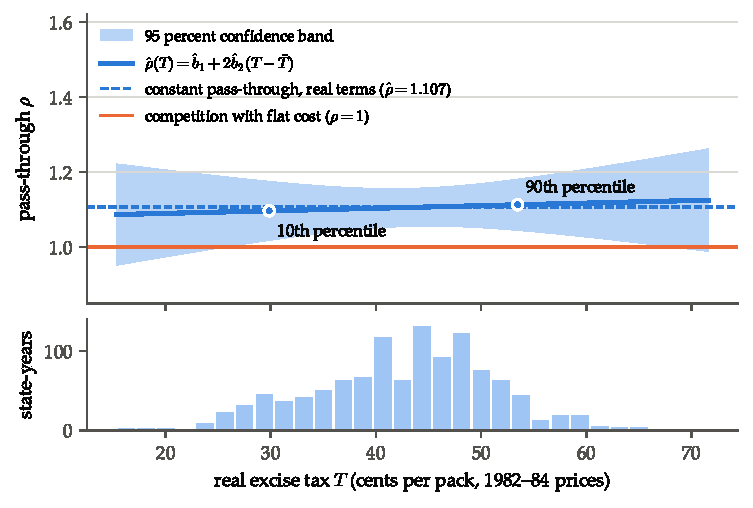
\includegraphics[width=0.86\textwidth]{figures/appC/rho_T.pdf}
\caption{Estimated pass-through as a function of the real excise tax, from specification M2, with a 95 percent
state-clustered confidence band. The dashed line is the constant pass-through of M1, and the orange line is the
competitive benchmark $\rho = 1$. The markers show the 10th and 90th percentiles of the real tax. The lower panel
shows the distribution of the real tax over the 1,200 state-years.}
\label{fig:C-rho-T}
\end{figure}

The data show no sign that pass-through varies with the tax, but the test has little power. With 80 percent power,
a 5 percent test would detect a difference between the two percentiles of $2.861\times0.053 = 0.151$ or more. This
threshold exceeds the estimated excess of pass-through over one in both M0 (0.075) and M1 (0.107). The band in \cref{fig:C-rho-T} also widens at the
extremes, where few state-years lie.

The quadratic also speaks to smuggling. Sumner argues that bootlegging would make the price a concave function of the
tax (n.~6). Bulk sales for shipment out of state lower measured prices in very low-tax states, and illegal
competition lowers them in very high-tax states. Concavity means $b_2 < 0$. Our estimate is positive and
insignificant, in line with his finding that squared tax terms are insignificant in most years.

A flat $\rho(T)$ would be weak evidence for constant-elasticity demand even with a precise estimate. Every member of
the power family in \cref{tab:C-curvature} has constant curvature, so with constant conduct its pass-through is the
same at every tax level. The test asks only whether $\kappa = \theta(\chi - 1)$ is stable over the observed range.
Sumner's estimates of $\lambda_S$ near one make the same point within his family, because $\lambda_S = 1$ makes the
price linear in the tax.

\casehead{Part (g)}
By \eqref{eq:C-kappa}, M0 identifies $\hat\kappa = 1 - \frac{1}{1.0746} = 0.069$. The map from $\rho$ to $\kappa$ is
increasing, so the clustered interval for $\rho$ maps into the interval $[0.006, 0.125]$ for $\kappa$. Every pair
$(\chi, \theta)$ on the hyperbola $\theta(\chi - 1) = 0.069$ fits the estimate equally well, and
\cref{fig:03-identified-set} draws this set with its band. Three points on it illustrate the range.
\begin{itemize}
\item Monopoly ($\theta = 1$) fits with $\chi = 1.069$, a demand curve slightly more convex than log demand.
\item Symmetric Cournot with six firms ($\theta = \frac{1}{6}$) fits with $\chi = 1 + 6\times0.069 = 1.42$.
\item Constant elasticity with an industry elasticity of 0.4 has $\chi = 3.5$. Then \eqref{eq:C-rho-ce} gives
  $\theta = 0.4\times0.069 = 0.028$, with interval $[0.002, 0.050]$. Elasticities of 0.3 and 0.8, the ends of the
  range Sumner quotes, give $\theta = 0.021$ and $0.056$.
\end{itemize}
Under constant elasticity with $\varepsilon = 0.4$, conduct of 0.028 matches symmetric Cournot with about 36 firms.
The industry is close to competitive under that reading. The data alone cannot choose among the three points, and
Sumner's rejection of collusion rests on the constant-elasticity assumption combined with outside estimates of the
elasticity. Even a precise $\hat\theta$ would measure market power only under the static model behind
\eqref{eq:C-supply-tax}. \citet{Corts1999} shows, analytically and by simulation, that the estimated conduct parameter
can badly mismeasure market power when firms sustain tacit collusion in a repeated game (abstract and Section~1). The
estimate need not even be positively correlated with the true elasticity-adjusted margin.

\casehead{Part (h)}
The level of prices and taxes gives a bound that needs no assumption on curvature. With constant marginal cost
$c \ge 0$, divide \eqref{eq:C-supply-tax} by $P$ and use $-\frac{QP'}{P} = \frac{1}{\varepsilon}$:
\begin{equation*}
\frac{P - c - t}{P} = \frac{\theta}{\varepsilon}
\qquad\Longrightarrow\qquad
\theta = \varepsilon\Big(1 - \frac{t}{P} - \frac{c}{P}\Big) \le \varepsilon\Big(1 - \frac{t}{P}\Big) .
\end{equation*}
This is \eqref{eq:03-lerner-bound}. The tax takes a large share of the cigarette price, so the bound is tight. With
$\varepsilon = 0.4$ it gives $\theta \le 0.4\times(1 - 0.467) = 0.213$ at the mean tax share and $\theta \le 0.308$ at
the lowest share in the sample (0.229). If $\theta$ and $\varepsilon$ are the same in every state-year, the highest
share (0.584) gives the tightest bound, $\theta \le 0.166$. Industry elasticities of 0.3 and 0.8 give bounds of 0.160
and 0.426 at the mean share. Every one of these bounds rules out monopoly whatever the curvature. Equivalently,
monopoly at the mean tax share requires an elasticity of at least $\frac{1}{1 - 0.467} = 1.88$ at the observed price,
and at the lowest share at least 1.30.

Under Sumner's constant-elasticity reading, in which $1 - \frac{1}{\rho}$ is the Lerner index (part (c)), the point
estimate also converts into cents. The value $1 - \frac{1}{\hat\rho} = 0.069$ applied to the mean price of 34.0 cents
gives a margin of price over marginal cost plus tax of 2.4 cents per pack. At the 1978 mean price
of 56.6 cents it gives 3.9 cents. Sumner's figure of about 3 cents uses $\Theta = 1.05$, and at the 1978 mean price
this ratio implies a margin of $56.6\times\big(1 - \frac{1}{1.05}\big) = 2.7$ cents.

\casehead{Part (i)}
Sumner's dependent variable is an average over brands. Suppose the measured price is $\bar p = \sum_j w_jp_j$ with
quantity weights $w_j$. Differentiating with respect to the tax,
\begin{equation}\label{eq:C-composition}
\frac{\dd\bar p}{\dd t} = \sum_j w_j\frac{\dd p_j}{\dd t} + \sum_j p_j\frac{\dd w_j}{\dd t} .
\end{equation}
The first term is the average of product-level pass-through, the object that conduct governs. The second is a
composition effect (\cref{rem:02-pt-composition}). A specific tax adds the same amount to every price, which is a
larger percentage of a cheap brand's price. Premium brands become relatively cheaper, consumers trade up, and the
composition term is positive. The regression then overstates product-level pass-through and leans toward rejecting
competition.

A back-of-the-envelope calculation shows how large the composition effect would have to be. Suppose packs come in
an economy and a premium tier whose prices differ by $\Delta$ cents. Suppose also that each price rises one for one
with the tax, as under competition with flat cost. The composition term is then $\Delta\frac{\dd w_H}{\dd t}$, where $w_H$ is
the premium share. Matching $\hat\rho = 1.075$ requires $\frac{\dd w_H}{\dd t} = \frac{0.075}{\Delta}$ per cent of
tax. With a hypothetical gap of $\Delta = 5$ cents, a 10-cent tax increase would have to raise the premium share by
15 percentage points. Two features of the data make shifts of this size unlikely. The Tobacco Tax Council's price
uses fixed national weights for the type of cigarette (regular, king, 100 mm) and the type of sale (carton, single
pack, machine). Shifts across these categories therefore do not move it \citep[p.~1016]{Sumner1981}. Sumner also reports
that retail prices vary little across brands within a market (pp.~1012--1013), so $\Delta$ is small.

A related critique is the quality response of \citet{Barzel1976}. A per-unit tax lowers the relative price of
quality, so higher taxes should raise the quality sold per pack, and with it the price per pack. Sumner replies that
the price data hold the obvious quality dimensions fixed and that centralized manufacturing leaves little room for
quality differences across states (p.~1018). He adds that a Barzel effect would bias the estimate upward, which
strengthens the case against an effective cartel. Barzel notes that an ad valorem tax would not have this effect, and
New Hampshire taxed cigarettes ad valorem until 1975. Sumner finds that New Hampshire's residuals from yearly
regressions are as negative after 1975 as before, which speaks against the quality explanation (n.~11).

\Cref{sec:C-logit-bertrand} computes \eqref{eq:C-composition} in a simulated logit market. There the composition term
is 0.0002 with single-product firms and $-0.0005$ with multi-product firms (\cref{tab:C-logit-tax}). Product-level
pass-through is below one, because logit demand is log-concave in a product's own price
(\cref{prop:C-logit-passthrough}). A logit market cannot produce Sumner's estimate through either term.

\casehead{Part (j)}
An ad valorem tax at rate $\tau$ takes the fraction $\tau$ of the consumer price, and sellers receive $(1 - \tau)P$
per unit. In this part $\tau$ denotes the tax rate. The year effects $\tau_y$ carry a subscript and play no role.

\begin{proposition}[Pass-through of an ad valorem tax]\label{prop:C-adval}
Let sellers receive $(1 - \tau)P$ per unit, with $\tau \in [0, 1)$, and let marginal cost $c$ be constant. Write
$\upsilon \equiv \frac{1}{1 - \tau}$, and let $\rho$ be the specific-tax pass-through \eqref{eq:C-rho-flat} at the same
equilibrium.
\begin{enumerate}[label=(\roman*)]
\item The supply relation is $P + \theta QP' = c\upsilon$, and $\frac{\dd P}{\dd\upsilon} = c\rho$.
\item The elasticity of the price with respect to $\upsilon$ is
  \begin{equation}\label{eq:C-adval-elast}
  \varrho \equiv \frac{\dd\ln P}{\dd\ln\upsilon} = \rho\Big(1 - \frac{\theta}{\varepsilon}\Big) .
  \end{equation}
\item $\varrho = 1$ under competition for every demand curve, and under constant-elasticity demand for every conduct.
  For $\theta > 0$, $\varrho > 1$ if and only if $\chi > 1 + \frac{1}{\varepsilon}$.
\end{enumerate}
\end{proposition}

\begin{proof}
(i) Perceived marginal revenue per unit sold is $(1 - \tau)(P + \theta QP')$. Setting it equal to $c$ and dividing by
$1 - \tau$ gives the supply relation. It has the form of \eqref{eq:C-supply-tax}, with effective marginal cost
$m \equiv c\upsilon$ in place of $c + t$. The derivation in the proof of \cref{prop:02-pt-general} applies to any shift
in effective cost, so $\frac{\dd P}{\dd m} = \rho$. Since $\frac{\dd m}{\dd\upsilon} = c$, the chain rule gives $\frac{\dd P}{\dd\upsilon} = c\rho$.

(ii) Multiplying by $\frac{\upsilon}{P}$ gives $\varrho = \rho\frac{c\upsilon}{P}$. The Lerner form of the supply relation
is $\frac{P - c\upsilon}{P} = \frac{\theta}{\varepsilon}$, so $\frac{c\upsilon}{P} = 1 - \frac{\theta}{\varepsilon}$.

(iii) Under competition $\theta = 0$ and $\rho = 1$, so $\varrho = 1$. Under constant elasticity
$\rho = \frac{\varepsilon}{\varepsilon - \theta}$ by \eqref{eq:C-rho-ce}, and
\begin{equation*}
\varrho = \frac{\varepsilon}{\varepsilon - \theta}\cdot\frac{\varepsilon - \theta}{\varepsilon} = 1 .
\end{equation*}
In general, \eqref{eq:C-rho-flat} gives $\varrho = \frac{1 - \frac{\theta}{\varepsilon}}{1 + \theta(1 - \chi)}$ with a
positive denominator. Hence
\begin{equation*}
\varrho > 1
\iff 1 - \frac{\theta}{\varepsilon} > 1 + \theta(1 - \chi)
\iff \theta(\chi - 1) > \frac{\theta}{\varepsilon}
\iff \chi > 1 + \frac{1}{\varepsilon} ,
\end{equation*}
where the last step divides by $\theta > 0$.
\end{proof}

The proposition reverses the roles of the two taxes. Sumner compares $\rho$ with the competitive benchmark of one.
For an ad valorem tax the natural benchmark is proportional pass-through, $\varrho = 1$. Under constant elasticity that
benchmark holds whatever the conduct, because the price is the fixed multiple $\frac{\varepsilon}{\varepsilon - \theta}$
of effective cost. An ad valorem experiment then carries no information about conduct, while a specific-tax
experiment does. With log demand the situation reverses. A specific tax gives $\rho = 1$ for every $\theta$, while
$\varrho = 1 - \frac{\theta}{\varepsilon}$ reveals the Lerner index. Which tax is informative thus depends on curvature,
which reinforces part (b). For revenue-equivalent small taxes, \cref{rem:02-pt-adval} shows that the ad valorem tax
raises the price less whenever $\theta > 0$.

Sumner's data contain some ad valorem variation. State sales taxes on cigarettes ranged from 0 to 6 percent. Sumner
ignores them, arguing that their effect is small because their ratio to $\lvert\eta\rvert$ is small
\citep[n.~4]{Sumner1981}. The reconstructed panel does not record them.

\casehead{Part (k)}
Five kinds of additional data would move from the composite $\kappa$ to conduct itself.
\begin{enumerate}[label=\arabic*.]
\item \emph{Quantities and a demand rotator.} With quantities, demand can be estimated, and a variable that changes
  the slope of demand at a given price separates conduct from the level and slope of marginal cost
  \citep{Bresnahan1982,Lau1982}. \citet[Section~3.1, pp.~1032--1034]{Bresnahan1989} restates the argument. If the slope
  of inverse demand does not depend on the demand shifters, the term $\theta QP'$ is perfectly collinear with $Q$ in the
  supply relation. Then $\theta$ cannot be separated from the slope of marginal cost. Lau's sufficient condition for
  identification is that the demand shifters cannot be separated from $Q$ in inverse demand, which needs at least two
  shifters (fn.~22 credits both papers). A market-wide cost shifter such as a tax moves the equilibrium along one demand curve and cannot do this
  (\cref{sec:03-identification}).
\item \emph{Demand curvature.} Demand estimated over a wide range of prices gives $\hat\chi$, and then
  $\theta = \frac{\hat\kappa}{\hat\chi - 1}$. The precision of $\hat\theta$ depends on how far $\hat\chi$ is from one.
\item \emph{Brand-level prices.} They remove the composition term of \eqref{eq:C-composition} and measure
  product-level pass-through directly.
\item \emph{Firm-specific cost shifters.} They trace out each firm's residual demand, whose slope measures the firm's
  markup (\cref{sec:03-residual-demand}). Direct measures of marginal cost work as in sugar refining
  (\cref{sec:03-sugar}).
\item \emph{A second kind of tax.} Variation in an ad valorem tax alongside the specific tax reveals marginal cost,
  as the next result shows.
\end{enumerate}

\begin{proposition}[Two taxes reveal marginal cost]\label{prop:C-two-taxes}
Let sellers pay a specific tax $t$ and an ad valorem tax $\tau$ on the consumer price, so that they receive
$(1 - \tau)P - t$ per unit. Let marginal cost $c(Q)$ be differentiable with $c' \ge 0$, let conduct $\theta$ be
constant, and suppose the equilibrium is stable. With $\upsilon = \frac{1}{1 - \tau}$,
\begin{equation}\label{eq:C-two-taxes}
c(Q) + t = \upsilon\,\frac{\partial P}{\partial\upsilon}\Big(\frac{\partial P}{\partial t}\Big)^{-1} .
\end{equation}
The Lerner index $\frac{P - \upsilon(c + t)}{P} = \frac{\theta}{\varepsilon}$ is therefore identified from the two
pass-through rates and the observed $P$, $t$ and $\tau$, whatever the curvature of demand and the slope of marginal
cost.
\end{proposition}

\begin{proof}
Perceived marginal revenue net of the ad valorem tax equals marginal cost plus the specific tax:
$(1 - \tau)(P + \theta QP') = c(Q) + t$. Multiply by $\upsilon$ and move every term to the left. Along the demand
curve, output is a function $Q(P)$ of the price, so the equilibrium price solves
\begin{equation*}
\mathcal{F}(P; t, \upsilon) \equiv P + \theta Q(P)P'\big(Q(P)\big) - \upsilon\big[c\big(Q(P)\big) + t\big] = 0 .
\end{equation*}
Stability makes $\mathcal{F}_P = \frac{D_\tau}{P'}$ positive, where
$D_\tau = (1 + \theta)P' + \theta QP'' - \upsilon c' < 0$. By the implicit function theorem,
\begin{equation*}
\frac{\partial P}{\partial t} = -\frac{\mathcal{F}_t}{\mathcal{F}_P} = \frac{\upsilon}{\mathcal{F}_P} ,
\qquad
\frac{\partial P}{\partial\upsilon} = -\frac{\mathcal{F}_{\upsilon}}{\mathcal{F}_P} = \frac{c(Q) + t}{\mathcal{F}_P} .
\end{equation*}
Dividing the second by the first, $\mathcal{F}_P$ cancels and leaves $\frac{c(Q) + t}{\upsilon}$. Multiplying by $\upsilon$ gives
\eqref{eq:C-two-taxes}. The Lerner form of the supply relation then gives $\frac{\theta}{\varepsilon}$.
\end{proof}

The intuition is that both taxes shift effective marginal cost $\upsilon(c + t)$, but by different amounts. A cent of
specific tax raises it by $\upsilon$ cents, while a unit increase in $\upsilon$ raises it by $c + t$. Both shifts pass
through to the price at the same rate, whatever that rate is, so their ratio reveals the level of $c + t$. The
argument needs both taxes to vary independently, conduct that does not depend on the tax mix, and a correct model of
who remits each tax. With the Lerner index in hand, an outside estimate of $\varepsilon$ gives $\theta$, and, if
marginal cost is flat, $\hat\kappa$ then gives $\chi = 1 + \frac{\hat\kappa}{\theta}$. In Sumner's setting, state sales taxes would supply the
ad valorem variation.

The exercise leaves three lessons. A market-wide cost shifter delivers a test of competition that is robust to the
shapes of demand and cost, although clustering shows it to be fragile here. The same shifter identifies conduct only
jointly with curvature, so Sumner's rejection of collusion rests on outside information about demand. Bounds from
the levels of prices and taxes, or a second kind of tax, say more about market power than the pass-through rate
alone.

\subsection{Computational notes}\label{sec:C-passthrough-computation}

The script \texttt{figures/appC/src/sumner\_passthrough.py} produces every number in this section with numpy and
scipy, in the following steps.
\begin{enumerate}
\item Read the panel, check that it is balanced (48 states by 25 years), and form the real price and tax by dividing by
  $\frac{CPI_y}{100}$.
\item For M0 and M1, regress the price on the tax, 48 state dummies and 24 year dummies. Compute the conventional
  variance and the cluster-robust variance \eqref{eq:C-vcl} from the full regression. By the argument behind
  \eqref{eq:C-fwl}, the tax block of the full sandwich equals the expression in \eqref{eq:C-vcl}.
\item For Sumner's row (2), regress the price on a constant, the tax and the national CPI. For row (3), estimate a
  two-way random-effects model by feasible GLS. Estimate the idiosyncratic variance $\sigma_e^2$ from the two-way
  within regression, and the state and year variances $\sigma_\mu^2$ and $\sigma_\tau^2$ from the regressions of state
  means and year means. Transform every variable as
  $v^*_{sy} = v_{sy} - \lambda_1\bar v_{s\cdot} - \lambda_2\bar v_{\cdot y} + \lambda_3\bar v_{\cdot\cdot}$, with
  $\lambda_1 = 1 - \sqrt{\frac{\sigma_e^2}{\sigma_e^2 + Y\sigma_\mu^2}}$,
  $\lambda_2 = 1 - \sqrt{\frac{\sigma_e^2}{\sigma_e^2 + S\sigma_\tau^2}}$ and
  $\lambda_3 = \lambda_1 + \lambda_2 - 1 + \sqrt{\frac{\sigma_e^2}{\sigma_e^2 + Y\sigma_\mu^2 + S\sigma_\tau^2}}$, then run
  OLS. The estimates are $\hat\sigma_e^2 = 0.74$, $\hat\sigma_\mu^2 = 0.55$ and $\hat\sigma_\tau^2 = 0.47$.
\item For the decomposition of part (e), regress the nominal price on the tax, the state dummies multiplied by
  $\frac{CPI_y}{100}$ and the year dummies, first by OLS and then with weights $\big(\frac{100}{CPI_y}\big)^2$. Check
  that the weighted estimate equals M1 to machine precision.
\item For M2, center the real tax at its mean, add its square, and evaluate $\hat\rho(T)$ and its standard error at
  the 10th, 50th and 90th percentiles of $T_{sy}$.
\item Compute $\hat\kappa$, the points on the identified set, the Lerner bounds, the residual autocorrelations, and
  the power calculations from the stored estimates, and draw \cref{fig:C-rho-T}.
\end{enumerate}
An optional check with \texttt{statsmodels} reproduces the M0 coefficient and both standard errors to $10^{-9}$.

\section{Bertrand pricing with logit demand: single- and multi-product firms}\label{sec:C-logit-bertrand}

The first two problems treated a homogeneous good, where one price clears the market and conduct is summarized by
a single parameter. From here on products are differentiated, firms set prices, and substitution between products
governs market power. The logit model is the simplest demand system for differentiated products in which
Bertrand-Nash prices have closed forms. This problem uses it to compute price equilibria, to show how joint ownership of several products
raises prices, and to prove that the equilibrium is unique. Two further parts evaluate a merger and a common unit
tax. The market is the 25-product market of \cref{ex:04-logit25}, and the theory is that of \cref{ch:diffprod}. We
restate each result we use and prove the ones that \cref{ch:diffprod} leaves open.

\subsection{Statement}

A single market has a unit mass of consumers, 25 inside products and an outside good. Consumer $i$ obtains utility
$u_{ij} = \delta_j + \epsilon_{ij}$ from product $j$ and $u_{i0} = \epsilon_{i0}$ from the outside good, where the
$\epsilon_{ij}$ are independent type-I extreme value shocks. The mean utility of product $j$ is
\begin{equation}\label{eq:C-logit-delta}
  \delta_j = x_j\beta - \alpha p_j + \xi_j , \qquad x_j = (1, x_{2j}, x_{3j}) ,
\end{equation}
where $x_{2j}$ is a continuous characteristic, $x_{3j}$ is a binary characteristic and $\xi_j$ is quality that
the econometrician does not observe. Marginal cost is constant and equal to
\begin{equation}\label{eq:C-logit-mc}
  mc_j = x_j\gamma + \omega_j .
\end{equation}
The parameters are $\beta = (0.1, 0.25, 0.1)$, $\alpha = 2$ and $\gamma = (0.2, 0.25, 0.3)$.
\Cref{tab:C-logit-data} lists the characteristics, the shocks and the implied marginal costs. The continuous
characteristic has mean 1.79, standard deviation 1.02 and range $-0.006$ to 4.18. Eleven products have $x_{3j} = 1$.
The quality shocks have mean 0.195 and standard deviation 1.00. The cost shocks have mean $-0.013$ and standard
deviation 0.045, and marginal costs range from 0.164 to 1.236. Five owners, labeled 0 to 4, hold 3, 3, 6, 6 and 7
products. Product labels 0 to 24 are names. The symbol $s_0$ always denotes the share of the outside good.

Firms know all characteristics, shocks and parameters, so the game has complete information. They set prices
simultaneously.

\begin{table}[htbp]
\centering
\caption{Product characteristics, shocks and marginal costs in the 25-product logit market}
\label{tab:C-logit-data}
\footnotesize
\setlength{\tabcolsep}{4pt}
\begin{tabular}{@{}rrrrrrr@{\hspace{14pt}}rrrrrrr@{}}
\toprule
$j$ & owner & $x_{2j}$ & $x_{3j}$ & $\xi_j$ & $\omega_j$ & $mc_j$ &
$j$ & owner & $x_{2j}$ & $x_{3j}$ & $\xi_j$ & $\omega_j$ & $mc_j$ \\
\midrule
0 & 2 & 1.277 & 1 & 0.158 & $-0.030$ & 0.790 & 13 & 3 & 1.582 & 1 & 0.167 & $-0.044$ & 0.852 \\
1 & 4 & 2.310 & 1 & 0.545 & 0.021 & 1.099 & 14 & 3 & 2.141 & 0 & 0.027 & $-0.057$ & 0.678 \\
2 & 3 & 1.942 & 0 & $-0.342$ & 0.003 & 0.689 & 15 & 3 & 0.915 & 0 & 0.317 & 0.024 & 0.453 \\
3 & 2 & 2.464 & 1 & 1.085 & 0.031 & 1.147 & 16 & 2 & 3.066 & 0 & 0.880 & 0.010 & 0.977 \\
4 & 2 & $-0.006$ & 0 & $-0.235$ & $-0.034$ & 0.164 & 17 & 3 & 0.155 & 1 & 0.576 & $-0.021$ & 0.517 \\
5 & 0 & 1.243 & 1 & 1.943 & $-0.056$ & 0.755 & 18 & 4 & 1.025 & 1 & 1.073 & 0.030 & 0.786 \\
6 & 2 & 2.675 & 0 & $-1.296$ & $-0.031$ & 0.838 & 19 & 3 & 1.280 & 1 & 1.613 & $-0.097$ & 0.724 \\
7 & 4 & 2.141 & 0 & $-1.418$ & $-0.041$ & 0.695 & 20 & 4 & 1.107 & 1 & 2.047 & $-0.001$ & 0.776 \\
8 & 2 & 1.998 & 0 & $-1.552$ & 0.036 & 0.735 & 21 & 0 & 4.183 & 0 & $-0.911$ & $-0.010$ & 1.236 \\
9 & 4 & 0.902 & 0 & $-1.122$ & 0.025 & 0.450 & 22 & 4 & 1.545 & 1 & 0.206 & 0.039 & 0.925 \\
10 & 1 & 3.795 & 0 & $-0.247$ & $-0.098$ & 1.050 & 23 & 0 & 2.044 & 0 & 1.019 & $-0.052$ & 0.659 \\
11 & 1 & 2.925 & 0 & 0.179 & 0.059 & 0.991 & 24 & 1 & 0.861 & 1 & $-0.618$ & 0.038 & 0.753 \\
12 & 4 & 1.232 & 0 & 0.772 & $-0.081$ & 0.427 & & & & & & & \\
\bottomrule
\end{tabular}

\vspace{3pt}
\begin{minipage}{0.97\textwidth}
\footnotesize Notes: Every product also has the constant characteristic $x_{1j} = 1$. Marginal cost is
$mc_j = x_j\gamma + \omega_j$ with $\gamma = (0.2, 0.25, 0.3)$. Owners 0 to 4 hold products $\{5, 21, 23\}$,
$\{10, 11, 24\}$, $\{0, 3, 4, 6, 8, 16\}$, $\{2, 13, 14, 15, 17, 19\}$ and $\{1, 7, 9, 12, 18, 20, 22\}$. Values
rounded to three decimals.
\end{minipage}
\end{table}

\begin{enumerate}[label=(\alph*)]
  \item Suppose that every product is sold by a separate firm. Derive the market shares, the profits and the
  derivatives of the shares with respect to prices. State the own- and cross-price elasticities.
  \item Derive the best-response price of product $j$ to the prices of the other products. Show that it is the
  unique maximizer of the firm's profit.
  \item Define a Nash equilibrium of the pricing game.
  \item Describe three algorithms that compute the equilibrium. Implement one of them and report prices, markups,
  shares, profits and consumer surplus.
  \item Now each owner in \cref{tab:C-logit-data} sets the prices of all its products jointly. Repeat parts (a) to
  (d), compare the two equilibria and explain the differences.
  \item Is each equilibrium unique? Prove your answer and verify it numerically.
  \item Owners 3 and 4 merge. Compute the post-merger equilibrium. Compare the price changes with the upward
  pricing pressure that the merger creates at pre-merger prices.
  \item A unit tax $t$ is added to the marginal cost of every product. Derive the pass-through of a cost increase to
  the prices of one firm, holding rivals' prices fixed. Derive the equilibrium pass-through of the common tax,
  compute it for $t = 0.1$, and compute the pass-through of the share-weighted average price.
\end{enumerate}

\subsection{Solution}

\casehead{Part (a)}
Write $a_j = x_j\beta + \xi_j$ for the part of mean utility that does not depend on price, so that
$\delta_j = a_j - \alpha p_j$. The mean utility of the outside good is normalized to zero. Let
\begin{equation}\label{eq:C-logit-Phi}
  \Phi = 1 + \sum_{l=0}^{24} e^{\delta_l}
\end{equation}
be the logit denominator, where the 1 is the outside good's contribution $e^0$. The extreme value shocks give the
logit choice probabilities (\cref{ch:discrete}). With a unit mass of consumers, shares equal quantities:
\begin{equation}\label{eq:C-logit-shares}
  s_j(p) = \frac{e^{\delta_j}}{\Phi} , \qquad s_0(p) = \frac{1}{\Phi} .
\end{equation}
A firm $f$ that owns the set of products $\mathcal{J}_f$ earns
\begin{equation}\label{eq:C-logit-profit}
  \pi_f(p) = \sum_{k \in \mathcal{J}_f}(p_k - mc_k)\,s_k(p) .
\end{equation}
With single-product firms, $\mathcal{J}_f = \{j\}$ and $\pi_j(p) = (p_j - mc_j)s_j(p)$.

A change in $p_j$ moves the numerator of $s_j$ and the denominator $\Phi$ at the same rate,
$\frac{\partial e^{\delta_j}}{\partial p_j} = \frac{\partial\Phi}{\partial p_j} = -\alpha e^{\delta_j}$. The quotient rule gives
\begin{equation*}
  \frac{\partial s_j}{\partial p_j}
  = \frac{-\alpha e^{\delta_j}\Phi + \alpha e^{\delta_j}e^{\delta_j}}{\Phi^2}
  = -\alpha s_j + \alpha s_j^2
  = -\alpha s_j(1 - s_j) .
\end{equation*}
For $k \ne j$, including the outside good, only the denominator of $s_k$ depends on $p_j$, so
\begin{equation*}
  \frac{\partial s_k}{\partial p_j} = -\frac{e^{\delta_k}}{\Phi^2}\,\frac{\partial\Phi}{\partial p_j}
  = \frac{\alpha e^{\delta_k}e^{\delta_j}}{\Phi^2} = \alpha s_js_k .
\end{equation*}
These are the derivatives in \eqref{eq:04-logit-derivs}. Let $\Delta$ be the $25 \times 25$ matrix with
$\Delta_{jk} = \frac{\partial s_j}{\partial p_k}$. Then
\begin{equation}\label{eq:C-logit-Delta}
  \Delta = \alpha\big(ss^\top - \diag(s)\big) ,
\end{equation}
which is symmetric. We write elasticities as $\varepsilon_{jk} = \frac{\partial s_j}{\partial p_k}\frac{p_k}{s_j}$,
so own elasticities are negative. The positive own elasticity of the notation list is $-\varepsilon_{jj}$. Then
\begin{equation}\label{eq:C-logit-elast}
  \varepsilon_{jj} = -\alpha p_j(1 - s_j) , \qquad \varepsilon_{jk} = \alpha p_ks_k \quad (k \ne j) .
\end{equation}
The cross elasticity with respect to $p_k$ is the same for every $j \ne k$. This is the independence of irrelevant
alternatives (\cref{ch:logit}). Own elasticities are roughly proportional to price, because shares are small.

\casehead{Part (b)}
Firm $j$ chooses $p_j$ to maximize $\pi_j$ given the rival prices $p_{-j}$. Let $m_j = p_j - mc_j$ denote the
markup. By part (a),
\begin{equation}\label{eq:C-logit-dpi}
  \frac{\partial\pi_j}{\partial p_j} = s_j + m_j\frac{\partial s_j}{\partial p_j} = s_j\big[1 - \alpha m_j(1 - s_j)\big] .
\end{equation}
Since $s_j > 0$, the first-order condition is
\begin{equation}\label{eq:C-logit-markup-single}
  m_j = \frac{1}{\alpha(1 - s_j)} .
\end{equation}
The condition is implicit, because $s_j$ depends on $p_j$. To solve it, separate the part of $\Phi$ that firm $j$
controls. Let $v_j = a_j - \alpha\,mc_j$ be the mean utility of product $j$ when it is priced at marginal cost, so
that $\delta_j = v_j - \alpha m_j$. Let $\Phi_{-j} = 1 + \sum_{l \ne j}e^{\delta_l}$, which depends only on rival
prices. Then $\Phi = \Phi_{-j} + e^{\delta_j}$ and $1 - s_j = \frac{\Phi_{-j}}{\Phi_{-j} + e^{\delta_j}}$. Substitute this
into \eqref{eq:C-logit-markup-single} and multiply both sides by $\Phi_{-j} + e^{\delta_j}$:
\begin{align*}
  \alpha m_j\Phi_{-j} &= \Phi_{-j} + e^{v_j - \alpha m_j} , \\
  (\alpha m_j - 1)\Phi_{-j} &= e^{v_j - \alpha m_j} .
\end{align*}
Multiply both sides by $\frac{e^{\alpha m_j - 1}}{\Phi_{-j}}$:
\begin{equation}\label{eq:C-lambert-eq}
  (\alpha m_j - 1)\,e^{\alpha m_j - 1} = \frac{e^{v_j - 1}}{\Phi_{-j}} .
\end{equation}
The left side has the form $we^w$ with $w = \alpha m_j - 1$. The next lemma inverts it.

\begin{lemma}[Lambert W function]\label{lem:C-lambert}
For every $z > 0$ the equation $we^w = z$ has exactly one real solution, denoted $W(z)$, and $W(z) > 0$. The
function $W$ is differentiable and strictly increasing on $(0, \infty)$, with
\begin{equation}\label{eq:C-lambert-deriv}
  W'(z) = \frac{W(z)}{z\,\big(1 + W(z)\big)} .
\end{equation}
The ratio $\frac{W(z)}{1 + W(z)}$ is strictly increasing in $z$ and lies in $(0, 1)$.
\end{lemma}

\begin{proof}
Let $g(w) = we^w$. If $w \le 0$, then $g(w) \le 0 < z$, so no solution is negative or zero. On $(0, \infty)$,
$g'(w) = (1 + w)e^w > 0$, $g(0) = 0$ and $g(w) \to \infty$. By continuity and strict monotonicity, $g(w) = z$ has
exactly one solution, and it is positive. The inverse function theorem gives
$W'(z) = \frac{1}{g'(W(z))} = \frac{1}{(1 + W)e^W}$. Since $e^W = \frac{z}{W}$, this equals
\eqref{eq:C-lambert-deriv}, which is positive. Finally $\frac{W}{1 + W} = 1 - \frac{1}{1 + W}$ rises with $W$, and
$W$ rises with $z$.
\end{proof}

The function $W$ is the principal branch of the Lambert W function \citep{CorlessEtAl1996}. Applying
\cref{lem:C-lambert} with $z = \frac{e^{v_j - 1}}{\Phi_{-j}} > 0$ to \eqref{eq:C-lambert-eq} gives the best response
\begin{equation}\label{eq:C-br-single}
  BR_j(p_{-j}) = mc_j + \frac{1}{\alpha}\Big[1 + W\Big(\frac{e^{v_j - 1}}{\Phi_{-j}}\Big)\Big] .
\end{equation}
This is \eqref{eq:04-logit-br}. Three properties follow at once. The best-response markup exceeds $\frac{1}{\alpha}$,
because $W > 0$. It rises with $v_j$, the product's quality net of cost. It rises with every rival price, because a
higher $p_l$ lowers $\Phi_{-j}$ and $W$ is increasing. Prices are strategic complements.

The stationary point is the unique global maximizer. Write \eqref{eq:C-logit-dpi} as $s_j\,G(m_j)$ with
$G(m) = 1 - \alpha m\,(1 - s_j)$, where $s_j$ is evaluated at $p_j = mc_j + m$. If $m \le 0$, then $G(m) \ge 1$ and
profit rises with the price. If $m > 0$, both $\alpha m$ and $1 - s_j$ are positive and strictly increasing in $m$,
because $s_j$ falls as $p_j$ rises. So $G$ is strictly decreasing on $(0, \infty)$, and $G(m) \to -\infty$ because
$1 - s_j \to 1$. Hence $G$ has exactly one zero. Profit rises below it and falls above it, and
\eqref{eq:C-br-single} is the unique maximizer of $\pi_j$.

\casehead{Part (c)}
The players are the 25 firms. Firm $j$ chooses $p_j \in \R$ and receives $\pi_j(p_j, p_{-j})$. A \emph{Nash
equilibrium} is a price vector $p^*$ such that
\begin{equation*}
  \pi_j(p_j^*, p_{-j}^*) \ge \pi_j(p_j, p_{-j}^*) \qquad \text{for every } p_j \in \R \text{ and every } j .
\end{equation*}
Equivalently, $p^* = BR(p^*)$, where $BR(p) = \big(BR_0(p_{-0}), \dots, BR_{24}(p_{-24})\big)$ is the best-response
map. By part (b), each best response is unique and solves the first-order condition, so $p^*$ is an equilibrium if
and only if
\begin{equation}\label{eq:C-foc-single}
  s_j(p^*) + (p_j^* - mc_j)\frac{\partial s_j}{\partial p_j}(p^*) = 0 , \qquad j = 0, \dots, 24 .
\end{equation}
Complete information matters here. Each best response depends on $\Phi_{-j}$, which requires every rival's price
and mean utility.

\casehead{Part (d)}
Three algorithms are standard.
\begin{enumerate}
  \item \emph{Best-response iteration.} Start from $p^{(0)} = mc + \frac{1}{\alpha}$, the markup that
  \eqref{eq:C-logit-markup-single} gives when shares are negligible. Set $p^{(n+1)} = BR(p^{(n)})$ with
  \eqref{eq:C-br-single}, and stop when $\|p^{(n+1)} - p^{(n)}\|_\infty < 10^{-12}$. Part (f) shows that the
  iteration converges from any starting point.
  \item \emph{Markup iteration.} Iterate on the first-order condition itself,
  $p^{(n+1)} = mc + \frac{1}{\alpha(1 - s(p^{(n)}))}$, element by element. The method needs no special function,
  but nothing guarantees its convergence in general.
  \item \emph{Newton-type root finding.} Solve the 25 equations \eqref{eq:C-foc-single} with a quasi-Newton
  method. We use the hybrid Powell method with tolerance $10^{-14}$, started at $mc + \frac{1}{\alpha}$.
\end{enumerate}
Best-response iteration converges in 10 iterations, markup iteration in 14, and the root finder uses 39 function
evaluations. The three solutions agree to within $1.2\times10^{-14}$, and the largest first-order residual is
$1.5\times10^{-15}$.

The columns marked S in \cref{tab:C-logit-eq} report the equilibrium. Markups range from 0.502 to 0.566. They lie
close to the floor $\frac{1}{\alpha} = 0.5$, because every share is small, and they rise with the share, as
\eqref{eq:C-logit-markup-single} requires. Products 20 and 5, with shares of 11.66 and 11.37 percent, carry the
largest markups, 0.566 and 0.564. The outside good takes 13.67 percent of the market, so $\Phi^* = \frac{1}{s_0} = 7.314$.
Total profit is 0.4616, and the share-weighted mean price is 1.2599.

Consumer surplus follows from the log-sum formula of \cref{sec:06-logsum} \citep{SmallRosen1981}. The expected
maximum utility is $\E[\max_{j}u_{ij}] = \ln\Phi + \gamma_E$, where $\gamma_E \approx 0.5772$ is Euler's constant.
Dividing by the marginal utility of money $\alpha$ converts utility into money. Consumer surplus per consumer is
therefore $\frac{1}{\alpha}\ln\Phi$ up to an additive constant, which equals 0.9949 here. Only differences in
consumer surplus across scenarios have meaning.

\casehead{Part (e)}
Firm $f$ now chooses all prices in $\mathcal{J}_f$ to maximize \eqref{eq:C-logit-profit}. For $j \in \mathcal{J}_f$, the
derivatives of part (a) give
\begin{align*}
  \frac{\partial\pi_f}{\partial p_j}
  &= s_j + \sum_{k \in \mathcal{J}_f}m_k\frac{\partial s_k}{\partial p_j} \\
  &= s_j - \alpha m_js_j(1 - s_j) + \sum_{k \in \mathcal{J}_f,\, k \ne j}\alpha m_ks_js_k \\
  &= s_j\Big[1 - \alpha m_j + \alpha\sum_{k \in \mathcal{J}_f}m_ks_k\Big] .
\end{align*}
Setting the derivative to zero and dividing by $\alpha s_j > 0$ gives
\begin{equation}\label{eq:C-mp-foc}
  m_j = \frac{1}{\alpha} + \sum_{k \in \mathcal{J}_f}s_km_k \qquad \text{for every } j \in \mathcal{J}_f .
\end{equation}

\begin{proposition}[Common markup]\label{prop:C-common-markup}
At any price vector at which firm $f$'s first-order conditions hold, all products of $f$ carry the same markup
\begin{equation}\label{eq:C-common-markup}
  m_f = \frac{1}{\alpha(1 - S_f)} , \qquad S_f = \sum_{k \in \mathcal{J}_f}s_k .
\end{equation}
\end{proposition}

This is \cref{prop:04-logit-markup}. It follows from \eqref{eq:C-mp-foc}, whose right side does not depend on $j$. The
firm prices as a single-product firm whose share is its combined share.
Quality and cost differences among its products move their prices one for one with cost and affect markups only
through $S_f$. Dividing \eqref{eq:C-mp-foc} by $1 - s_j$ gives a second reading,
\begin{equation}\label{eq:C-mp-foc-diversion}
  m_j = \frac{1}{\alpha(1 - s_j)} + \sum_{k \in \mathcal{J}_f,\, k \ne j}D_{jk}m_k ,
  \qquad D_{jk} = -\frac{\partial s_k}{\partial p_j}\Big(\frac{\partial s_j}{\partial p_j}\Big)^{-1} = \frac{s_k}{1 - s_j} .
\end{equation}
The markup of product $j$ equals its single-product markup plus the margin earned on the sales that a price increase
diverts to the firm's other products. $D_{jk}$ is the logit \emph{diversion ratio} from $j$ to $k$, the fraction of the sales lost by $j$ that go to $k$.

The multi-product best response follows the steps of part (b). Let $E_f = \sum_{k \in \mathcal{J}_f}e^{v_k}$ and
$\Phi_{-f} = 1 + \sum_{l \notin \mathcal{J}_f}e^{\delta_l}$, which depends only on rivals' prices. At a common markup
$m$, firm $f$'s products contribute $\sum_{k \in \mathcal{J}_f}e^{v_k - \alpha m} = E_fe^{-\alpha m}$ to $\Phi$, so
\begin{equation*}
  S_f = \frac{E_fe^{-\alpha m}}{\Phi_{-f} + E_fe^{-\alpha m}} , \qquad
  1 - S_f = \frac{\Phi_{-f}}{\Phi_{-f} + E_fe^{-\alpha m}} .
\end{equation*}
Substitute $1 - S_f$ into $\alpha m(1 - S_f) = 1$ and clear the denominator:
\begin{align*}
  \alpha m\,\Phi_{-f} &= \Phi_{-f} + E_fe^{-\alpha m} , \\
  (\alpha m - 1)\Phi_{-f} &= E_fe^{-\alpha m} , \\
  (\alpha m - 1)e^{\alpha m - 1} &= \frac{E_fe^{-1}}{\Phi_{-f}} ,
\end{align*}
where the last line multiplies by $\frac{e^{\alpha m - 1}}{\Phi_{-f}}$. \Cref{lem:C-lambert} gives
\begin{equation}\label{eq:C-br-multi}
  m_f^{BR} = \frac{1}{\alpha}\Big[1 + W\Big(\frac{E_fe^{-1}}{\Phi_{-f}}\Big)\Big] , \qquad
  BR_k(p_{-\mathcal{J}_f}) = mc_k + m_f^{BR} \quad (k \in \mathcal{J}_f) .
\end{equation}
With one product, $E_f = e^{v_j}$ and \eqref{eq:C-br-multi} reduces to \eqref{eq:C-br-single}. \Cref{ch:diffprod}
states this formula, \eqref{eq:04-logit-br-multi}, and proves its global optimality in Steps 1 and 2 of the proof
of \cref{thm:04-logit-unique}. The next proposition gives a second proof, by a change of variables from prices to
shares under which profit is concave.

\begin{proposition}[Profit is concave in shares]\label{prop:C-firm-concave}
Fix the rivals' prices, and hence $\Phi_{-f}$.
\begin{enumerate}[label=(\roman*)]
  \item The map from firm $f$'s prices $(p_k)_{k \in \mathcal{J}_f}$ to its shares $(s_k)_{k \in \mathcal{J}_f}$ is a
  smooth bijection onto $\{s > 0 : S_f < 1\}$, with smooth inverse
  \begin{equation}\label{eq:C-share-inverse}
    \delta_k = \ln s_k + \ln\Phi_{-f} - \ln(1 - S_f) .
  \end{equation}
  \item As a function of its shares, firm $f$'s profit is
  \begin{equation}\label{eq:C-profit-shares}
    \pi_f = \frac{1}{\alpha}\sum_{k \in \mathcal{J}_f}s_k\big[v_k - \ln\Phi_{-f} - \ln s_k\big] + \frac{1}{\alpha}S_f\ln(1 - S_f) ,
  \end{equation}
  which is strictly concave.
  \item Profit has a unique maximizer over $f$'s prices. It is the unique solution of $f$'s first-order
  conditions and is given by \eqref{eq:C-br-multi}.
\end{enumerate}
\end{proposition}

\begin{proof}
(i) Given prices, shares follow from \eqref{eq:C-logit-shares}. Conversely, take shares with $s_k > 0$ and $S_f < 1$.
Because $\Phi = \Phi_{-f} + \sum_{k \in \mathcal{J}_f}e^{\delta_k} = \Phi_{-f} + S_f\Phi$, the denominator must equal
$\Phi = \frac{\Phi_{-f}}{1 - S_f}$. Then $e^{\delta_k} = s_k\Phi$ gives \eqref{eq:C-share-inverse}, and
$p_k = \frac{a_k - \delta_k}{\alpha}$. Both maps are smooth, and they are inverse to each other.

(ii) The markup is $m_k = p_k - mc_k = \frac{a_k - \delta_k}{\alpha} - mc_k = \frac{v_k - \delta_k}{\alpha}$.
Substituting \eqref{eq:C-share-inverse},
\begin{equation*}
  \alpha m_k = v_k - \ln s_k - \ln\Phi_{-f} + \ln(1 - S_f) .
\end{equation*}
Multiplying by $\frac{s_k}{\alpha}$ and summing over $k \in \mathcal{J}_f$ gives \eqref{eq:C-profit-shares}. In the first
sum, each term is linear in $s_k$ except $-s_k\ln s_k$, whose second derivative is $-\frac{1}{s_k} < 0$. In the second
term, $\varphi(S) = S\ln(1 - S)$ has
\begin{equation*}
  \varphi'(S) = \ln(1 - S) - \frac{S}{1 - S} , \qquad
  \varphi''(S) = -\frac{1}{1 - S} - \frac{1}{(1 - S)^2} < 0 ,
\end{equation*}
and $S_f$ is linear in the shares. A sum of strictly concave functions of separate shares and a concave function of
their sum is strictly concave.

(iii) The partial derivative of \eqref{eq:C-profit-shares} is
\begin{equation*}
  \frac{\partial\pi_f}{\partial s_k} = \frac{1}{\alpha}\big[v_k - \ln\Phi_{-f} - \ln s_k - 1 + \varphi'(S_f)\big] .
\end{equation*}
It tends to $+\infty$ as $s_k \to 0$ with $S_f$ bounded away from one, and profit tends to $-\infty$ as
$S_f \to 1$. A maximizer therefore exists and is interior, and strict concavity makes it the only stationary point.
By (i), stationary points in prices and in shares coincide, because the change of variables has an invertible
Jacobian. By \cref{prop:C-common-markup} and the derivation above, the only stationary point in prices is
\eqref{eq:C-br-multi}.
\end{proof}

Stacking the first-order conditions of all firms gives one system for any ownership structure. Let $\Omega$ be the
ownership matrix, with $\Omega_{jk} = 1$ when $j$ and $k$ have the same owner and zero otherwise. The condition
for $p_j$ is $s_j + \sum_k\Omega_{jk}\frac{\partial s_k}{\partial p_j}m_k = 0$. Since
$\frac{\partial s_k}{\partial p_j} = \Delta_{kj}$, in matrix form
\begin{equation}\label{eq:C-stacked-foc}
  s + (\Omega \odot \Delta^\top)(p - mc) = 0 ,
\end{equation}
with $\odot$ the element-wise product. Single-product firms correspond to $\Omega = I$. Only $\Omega$ changes between
the two games, so a program written for \eqref{eq:C-stacked-foc} handles both.

All three algorithms of part (d) carry over. Best-response iteration now uses \eqref{eq:C-br-multi}. Markup
iteration uses $p^{(n+1)}_k = mc_k + \frac{1}{\alpha(1 - S_f(p^{(n)}))}$. Best-response iteration converges in 15
iterations, markup iteration in 30, and the root finder uses 41 function evaluations. The solutions agree to within
$1.4\times10^{-13}$, and the largest first-order residual is $1.5\times10^{-14}$.

\begin{table}[htbp]
\centering
\caption{Equilibrium by product: single-product firms (S), five multi-product owners (M), and after the merger of
owners 3 and 4 (G)}
\label{tab:C-logit-eq}
\footnotesize
\setlength{\tabcolsep}{5pt}
\begin{tabular}{@{}rrrrrrrrrrr@{}}
\toprule
 & & & \multicolumn{3}{c}{Price} & \multicolumn{2}{c}{Markup} & \multicolumn{3}{c}{Share (\%)} \\
\cmidrule(lr){4-6}\cmidrule(lr){7-8}\cmidrule(l){9-11}
$j$ & owner & $mc_j$ & $p_j^S$ & $p_j^M$ & $p_j^G$ & $m_j^S$ & $m_j^M$ & $s_j^S$ & $s_j^M$ & $s_j^G$ \\
\midrule
0 & 2 & 0.790 & 1.300 & 1.369 & 1.382 & 0.510 & 0.579 & 2.00 & 2.04 & 2.32 \\
1 & 4 & 1.099 & 1.609 & 1.769 & 1.920 & 0.510 & 0.670 & 2.05 & 1.75 & 1.51 \\
2 & 3 & 0.689 & 1.197 & 1.325 & 1.510 & 0.508 & 0.636 & 1.59 & 1.44 & 1.16 \\
3 & 2 & 1.147 & 1.664 & 1.726 & 1.739 & 0.517 & 0.579 & 3.29 & 3.40 & 3.86 \\
4 & 2 & 0.164 & 0.680 & 0.744 & 0.757 & 0.516 & 0.579 & 3.06 & 3.16 & 3.59 \\
5 & 0 & 0.755 & 1.319 & 1.371 & 1.389 & 0.564 & 0.616 & 11.37 & 12.00 & 13.50 \\
6 & 2 & 0.838 & 1.341 & 1.418 & 1.430 & 0.503 & 0.579 & 0.55 & 0.55 & 0.63 \\
7 & 4 & 0.695 & 1.198 & 1.365 & 1.516 & 0.503 & 0.670 & 0.57 & 0.48 & 0.41 \\
8 & 2 & 0.735 & 1.237 & 1.314 & 1.327 & 0.502 & 0.579 & 0.44 & 0.45 & 0.51 \\
9 & 4 & 0.450 & 0.955 & 1.120 & 1.272 & 0.505 & 0.670 & 0.91 & 0.77 & 0.66 \\
10 & 1 & 1.050 & 1.557 & 1.575 & 1.579 & 0.507 & 0.524 & 1.35 & 1.53 & 1.77 \\
11 & 1 & 0.991 & 1.500 & 1.515 & 1.519 & 0.510 & 0.524 & 1.87 & 2.12 & 2.46 \\
12 & 4 & 0.427 & 0.962 & 1.097 & 1.248 & 0.535 & 0.670 & 6.50 & 5.81 & 5.01 \\
13 & 3 & 0.852 & 1.362 & 1.488 & 1.673 & 0.510 & 0.636 & 1.92 & 1.75 & 1.41 \\
14 & 3 & 0.678 & 1.191 & 1.315 & 1.500 & 0.513 & 0.636 & 2.45 & 2.24 & 1.81 \\
15 & 3 & 0.453 & 0.972 & 1.089 & 1.274 & 0.519 & 0.636 & 3.73 & 3.46 & 2.79 \\
16 & 2 & 0.977 & 1.497 & 1.556 & 1.569 & 0.520 & 0.579 & 3.93 & 4.09 & 4.65 \\
17 & 3 & 0.517 & 1.037 & 1.153 & 1.339 & 0.520 & 0.636 & 3.88 & 3.60 & 2.90 \\
18 & 4 & 0.786 & 1.310 & 1.456 & 1.607 & 0.524 & 0.670 & 4.59 & 4.02 & 3.46 \\
19 & 3 & 0.724 & 1.273 & 1.360 & 1.545 & 0.550 & 0.636 & 9.04 & 8.91 & 7.18 \\
20 & 4 & 0.776 & 1.342 & 1.446 & 1.597 & 0.566 & 0.670 & 11.66 & 11.09 & 9.56 \\
21 & 0 & 1.236 & 1.738 & 1.852 & 1.871 & 0.503 & 0.616 & 0.53 & 0.50 & 0.56 \\
22 & 4 & 0.925 & 1.434 & 1.595 & 1.746 & 0.509 & 0.670 & 1.72 & 1.46 & 1.26 \\
23 & 0 & 0.659 & 1.193 & 1.275 & 1.294 & 0.534 & 0.616 & 6.41 & 6.38 & 7.17 \\
24 & 1 & 0.753 & 1.258 & 1.278 & 1.282 & 0.505 & 0.524 & 0.90 & 1.01 & 1.17 \\
\bottomrule
\end{tabular}

\vspace{3pt}
\begin{minipage}{0.97\textwidth}
\footnotesize Notes: Market size is one. Under M every product of an owner carries the owner's markup
$\frac{1}{\alpha(1 - S_f)}$. After the merger (G), the 13 products of the merged firm carry the common markup 0.821.
Firm-level outcomes under S and M are in \cref{tab:04-logit25}. Computed with
\texttt{figures/appC/src/logit\_bertrand.py}.
\end{minipage}
\end{table}

\begin{table}[htbp]
\centering
\caption{Market outcomes and computational diagnostics in the 25-product logit market}
\label{tab:C-logit-market}
\footnotesize
\begin{tabular}{@{}lccc@{}}
\toprule
 & Single-product (S) & Multi-product (M) & After merger (G) \\
\midrule
Outside share $s_0$ & 0.1367 & 0.1601 & 0.1869 \\
Logit denominator $\Phi^* = \frac{1}{s_0}$ & 7.314 & 6.246 & 5.352 \\
Consumer surplus $\frac{1}{\alpha}\ln\Phi^*$ & 0.9949 & 0.9159 & 0.8387 \\
Total profit & 0.4616 & 0.5261 & 0.5767 \\
Total surplus & 1.4565 & 1.4421 & 1.4154 \\
Share-weighted mean price & 1.2599 & 1.3553 & 1.4465 \\
Range of markups & 0.502 to 0.566 & 0.524 to 0.670 & 0.529 to 0.821 \\
\midrule
Best-response iterations & 10 & 15 & 16 \\
Markup iterations & 14 & 30 & 85 \\
Largest first-order residual & $1.5\times10^{-15}$ & $1.5\times10^{-14}$ & $2.5\times10^{-14}$ \\
Global contraction bound $\eta$ & 0.358 & 0.474 & 0.545 \\
Exact global modulus & 0.135 & 0.212 & 0.272 \\
Local modulus $\max_f\frac{S_f(1 - S_f - s_0)}{1 - S_f}$ & 0.099 & 0.199 & 0.271 \\
Sign changes of $\Psi - 1$ on the grid & 1 & 1 & 1 \\
\bottomrule
\end{tabular}

\vspace{3pt}
\begin{minipage}{0.97\textwidth}
\footnotesize Notes: Consumer surplus is per consumer and defined up to an additive constant. Iterations start at
$mc + \frac{1}{\alpha}$ and stop when the sup-norm price change is below $10^{-12}$. The exact global modulus is
the supremum over $\Phi_{-f} \ge 1$ of the largest row sum of the best-response Jacobian. Computed with
\texttt{figures/appC/src/logit\_bertrand.py}.
\end{minipage}
\end{table}

\Cref{tab:C-logit-eq} compares the equilibria product by product, and \cref{tab:C-logit-market} compares market
outcomes. Joint ownership raises every price, by amounts from 0.015 (product 11, owner 1) to 0.167 (product 7,
owner 4). Each owner's markup becomes $\frac{1}{\alpha(1 - S_f)}$. It is 0.670 for owner 4, whose products have a
combined share of 25.4 percent, against a share-weighted mean of 0.541 under single-product pricing. Owner 1's
combined share is 4.7 percent, and its markup rises only from 0.508 to 0.524. Total profit rises by 14.0 percent to
0.5261. Consumer surplus falls from 0.9949 to 0.9159, and the outside share rises from 13.67 to 16.01 percent.
Total surplus, consumer surplus plus profit, falls from 1.4565 to 1.4421. \Cref{tab:04-logit25} reports shares,
markups and profits by owner, and \cref{fig:04-logit25-markups} plots the markups.

The prices differ because a multi-product firm internalizes \emph{cannibalization}. A single-product firm that raises
its price loses every customer who switches away. A multi-product firm keeps the customers who switch to its own
products. By \eqref{eq:C-mp-foc-diversion}, the fraction of product $j$'s lost sales that the firm recaptures is
$\sum_{k \in \mathcal{J}_f, k \ne j}D_{jk} = \frac{S_f - s_j}{1 - s_j}$. It ranges from 0.161 to 0.250 for owner 4's
products and from 0.026 to 0.037 for owner 1's. The incentive to raise prices grows with recapture. Prices are
strategic complements, so the higher prices of the large owners lead every rival to raise its prices too. Large
owners lose share. Owner 4's combined share falls from 28.00 to 25.36 percent, while owner 1's rises from 4.12 to
4.67 percent. Every owner nevertheless earns more, because competition softens for all of them.

\casehead{Part (f)}
Both equilibria are unique, and so is the equilibrium under any other ownership structure.

\begin{proposition}[Uniqueness]\label{prop:C-unique}
With logit demand and constant marginal costs, the pricing game has exactly one Nash equilibrium for any
partition of the products among firms.
\end{proposition}

This is \cref{thm:04-logit-unique}. Steps 3 and 4 of its proof reduce the equilibrium to one equation in the scalar
aggregate $\Phi$, and we use that equation again below. By \cref{prop:C-common-markup}, $\alpha m_f = \frac{1}{1 - S_f}$,
and the combined share is $S_f = \frac{E_f}{\Phi}e^{-\alpha m_f}$. Together they give
\begin{equation}\label{eq:C-h}
  h(S_f) \equiv S_f\,e^{\frac{1}{1 - S_f}} = \frac{E_f}{\Phi} .
\end{equation}
Since $h$ rises strictly from zero to infinity on $(0, 1)$, \eqref{eq:C-h} defines a share $S_f(\Phi)$ that falls
strictly in $\Phi$. Adding up the shares, with $s_0 = \frac{1}{\Phi}$, gives
\begin{equation}\label{eq:C-Psi}
  \Psi(\Phi) \equiv \sum_f S_f(\Phi) + \frac{1}{\Phi} = 1 .
\end{equation}
The function $\Psi$ is strictly decreasing, exceeds one at $\Phi = 1$ and tends to zero, so it has exactly one root
$\Phi^*$. The root fixes every firm's share, markup and prices.

For single-product firms, \citet{CaplinNalebuff1991}
derive uniqueness in the logit model by differentiating the profit function. Their proofs rest on a \emph{dominant diagonal}
condition, $\big\lvert\frac{\partial^2\pi_j}{\partial p_j^2}\big\rvert > \sum_{k \ne j}\big\lvert\frac{\partial^2\pi_j}{\partial
p_j\partial p_k}\big\rvert$ among active firms \citep{Friedman1977} (\cref{prop:B-dd-uniqueness}). We cite their
1990 discussion-paper version (Cowles Foundation Discussion Paper 937), where this argument is on p.~16. They also note
that their uniqueness cases are log-supermodular games (p.~16), which \cref{sec:B-supermodular-games} treats. Such games have no other equilibria in mixed or correlated strategies, and
best-response dynamics converge globally \citep{MilgromRoberts1990}. Their other uniqueness results cover duopoly with a
log-concave density of tastes and one-dimensional markets with a given set of active firms (Propositions~6 and~7,
p.~17). They credit
\citet{AndersonDePalma1988} with first noting uniqueness in the logit duopoly (p.~17). \citet[fn.~12]{BerryLevinsohnPakes1995} note that the existence theorems of
\citet{CaplinNalebuff1991} do not easily generalize to multi-product firms. They assume that an equilibrium exists
and check numerically that their estimates are consistent with one. \citet{KonovalovSandor2010} prove uniqueness
for multi-product logit firms, and \citet{NockeSchutz2018} develop the aggregative approach behind \eqref{eq:C-Psi}.

A second proof shows that best-response iteration converges from any starting point.

\begin{proposition}[Best responses form a contraction]\label{prop:C-contraction}
Let $\eta = \max_f\frac{W(E_fe^{-1})}{1 + W(E_fe^{-1})}$, which is below one. For all price vectors $p$ and $p'$,
\begin{equation*}
  \|BR(p) - BR(p')\|_\infty \le \eta\,\|p - p'\|_\infty .
\end{equation*}
Hence the equilibrium is unique, and best-response iteration converges to it geometrically from any start.
\end{proposition}

\begin{proof}
Fix firm $f$ and write $z_f = \frac{E_fe^{-1}}{\Phi_{-f}}$, so that $BR_k = mc_k + \frac{1}{\alpha}[1 + W(z_f)]$ for
$k \in \mathcal{J}_f$. Own prices do not enter $\Phi_{-f}$, so $\frac{\partial BR_k}{\partial p_l} = 0$ for
$l \in \mathcal{J}_f$. For a rival product $l \notin \mathcal{J}_f$,
\begin{equation*}
  \frac{\partial\Phi_{-f}}{\partial p_l} = -\alpha e^{\delta_l} , \qquad
  \frac{\partial z_f}{\partial p_l} = -\frac{z_f}{\Phi_{-f}}\,\frac{\partial\Phi_{-f}}{\partial p_l} = \frac{\alpha z_fe^{\delta_l}}{\Phi_{-f}} .
\end{equation*}
The chain rule and \eqref{eq:C-lambert-deriv} give
\begin{equation*}
  \frac{\partial BR_k}{\partial p_l} = \frac{1}{\alpha}W'(z_f)\frac{\partial z_f}{\partial p_l}
  = \frac{1}{\alpha}\cdot\frac{W(z_f)}{z_f(1 + W(z_f))}\cdot\frac{\alpha z_fe^{\delta_l}}{\Phi_{-f}}
  = \frac{W(z_f)}{1 + W(z_f)}\cdot\frac{e^{\delta_l}}{\Phi_{-f}} .
\end{equation*}
Both factors are shares evaluated at firm $f$'s best response to $p_{-\mathcal{J}_f}$. There
$1 + W(z_f) = \alpha m_f = \frac{1}{1 - S_f}$, so $\frac{W(z_f)}{1 + W(z_f)} = S_f$. Also
$\Phi = \frac{\Phi_{-f}}{1 - S_f}$, so $\frac{e^{\delta_l}}{\Phi_{-f}} = \frac{s_l}{1 - S_f}$. Hence
\begin{equation}\label{eq:C-br-slope}
  \frac{\partial BR_k}{\partial p_l} = \frac{S_fs_l}{1 - S_f} > 0 , \qquad
  \sum_{l \notin \mathcal{J}_f}\frac{\partial BR_k}{\partial p_l} = \frac{S_f(1 - S_f - s_0)}{1 - S_f} < S_f .
\end{equation}
Since $\Phi_{-f} \ge 1$, $z_f \le E_fe^{-1}$, and since $\frac{W}{1 + W}$ is increasing (\cref{lem:C-lambert}),
$S_f \le \frac{W(E_fe^{-1})}{1 + W(E_fe^{-1})} \le \eta$. Every row of the Jacobian of $BR$ is non-negative and sums to
less than $\eta$, at every price vector. For each $k$, the mean value theorem gives a point $\tilde p$ on the segment
between $p$ and $p'$ with
\begin{equation*}
  |BR_k(p) - BR_k(p')| = \Big|\sum_l\frac{\partial BR_k}{\partial p_l}(\tilde p)\,(p_l - p_l')\Big|
  \le \eta\,\|p - p'\|_\infty .
\end{equation*}
Taking the maximum over $k$ proves the inequality. The contraction mapping theorem (\cref{app:math}) gives a unique
fixed point and geometric convergence from any starting point.
\end{proof}

For single-product firms, \eqref{eq:C-br-slope} becomes $\frac{\partial BR_j}{\partial p_k} = \frac{s_js_k}{1 - s_j}$,
the slope in \cref{prop:04-logit-br}. The modulus $\eta$ is a valid but loose bound. Since
$s_0 = \frac{1 - S_f}{\Phi_{-f}}$ at firm $f$'s best response, the row sum in \eqref{eq:C-br-slope} equals
$\frac{W(z_f)}{1 + W(z_f)}\big(1 - \frac{1}{\Phi_{-f}}\big)$. As rivals' prices rise without bound, $\Phi_{-f} \to 1$
and the row sum tends to zero. As they fall without bound, $z_f \to 0$ and the first factor tends to zero. The
supremum of the row sum over $\Phi_{-f} \ge 1$ is the exact global modulus, 0.135 under S and 0.212 under M. The
relevant local modulus is the largest row sum at the equilibrium,
$\max_f\frac{S_f(1 - S_f - s_0)}{1 - S_f}$.

We check uniqueness numerically in three ways. First, we evaluate $\Psi(\Phi) - 1$ on 2,000 points spaced evenly in
logarithms over $[1, 10^4]$. It changes sign exactly once in each game (\cref{fig:C-psi}). The roots are
$\Phi^* = 7.314$ under S and $\Phi^* = 6.246$ under M, and each equals $\frac{1}{s_0}$ at the computed equilibrium.
Second, we run best-response iteration from 500 random starting vectors $p^{(0)} = mc + U[0, 5]^{25}$, and from
$p^{(0)} = mc$ and $p^{(0)} = mc + 20$. All 502 runs reach the same prices, with largest deviations of
$5.5\times10^{-14}$ (S) and $2.6\times10^{-13}$ (M), in at most 11 and 16 iterations. Third, we compute the
contraction moduli. The global bound is $\eta = 0.358$ under S and $0.474$ under M. The local moduli are 0.099 and
0.199, which explains the fast convergence. A finite-difference Jacobian of $BR$ at the equilibrium matches
\eqref{eq:C-br-slope} to within $1.7\times10^{-10}$.

\begin{figure}[htbp]
\centering
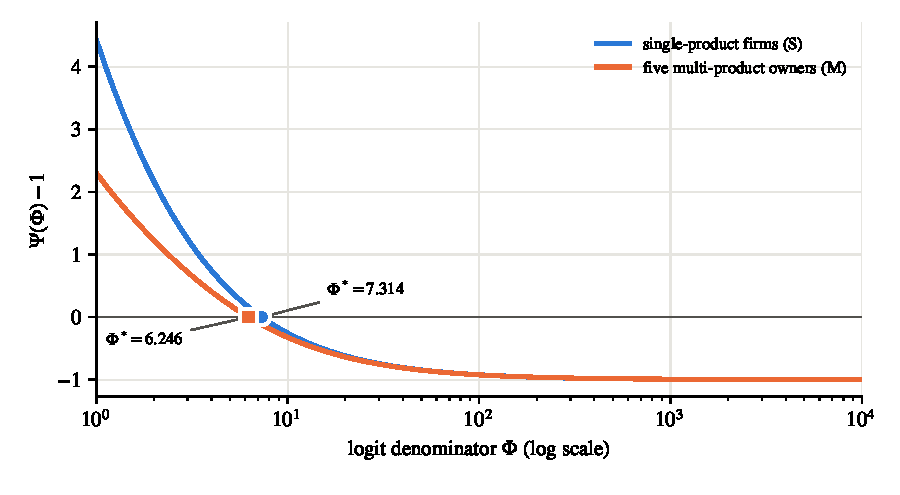
\includegraphics[width=0.82\linewidth]{figures/appC/psi.pdf}
\caption{The aggregate equation \eqref{eq:C-Psi}. Each curve plots $\Psi(\Phi) - 1$, where
$\Psi(\Phi) = \sum_fS_f(\Phi) + \frac{1}{\Phi}$ and $S_f(\Phi)$ solves $S_fe^{\frac{1}{1 - S_f}} = \frac{E_f}{\Phi}$. The curves
are strictly decreasing and cross zero once, at $\Phi^* = \frac{1}{s_0}$. At $\Phi = 1$ they equal 4.44 (S) and
2.31 (M). Computed with \texttt{figures/appC/src/logit\_bertrand.py}.}
\label{fig:C-psi}
\end{figure}

\casehead{Part (g)}
After the merger, owners 3 and 4 form one firm with 13 products, and the other owners are unchanged. Only $\Omega$
changes. \Cref{ex:04-merger-sim} introduces this merger and computes the cost reductions that would offset it. Here we
compare the equilibrium effects with first-round pricing pressure. By \cref{prop:C-unique} the post-merger equilibrium is unique, so the starting point of the iteration does
not matter. Best-response iteration converges in 16 iterations, and the column G of \cref{tab:C-logit-eq} reports the
result.

By \cref{prop:C-common-markup}, the merged firm charges one markup on all 13 products,
$m_M = \frac{1}{\alpha(1 - S_M)} = 0.821$, where $S_M = 39.12$ percent is its post-merger combined share. Before the
merger the markups were 0.636 (owner 3) and 0.670 (owner 4). Every product of owner 3 therefore rises in price by
0.185, and every product of owner 4 by 0.151. The mean increase over the 13 products is 0.167. Rivals respond with
smaller increases: 0.018 for owner 0, 0.013 for owner 2 and 0.004 for owner 1. \Cref{fig:C-logit-merger} plots the
change for every product. Firm-level shares, markups and profits before and after the merger are in
\cref{tab:04-merger-sim}.

The merged firm loses share, from 46.76 to 39.12 percent, and every rival gains. The outside share rises from 16.01
to 18.69 percent, and consumer surplus falls by 0.0773, from 0.9159 to 0.8387. Total profit rises from 0.5261 to
0.5767. The merger is profitable for its parties, whose joint profit rises by 5.0 percent, from 0.3061 to 0.3213.
The rivals gain more in percentage terms: 15.9 percent for owner 0, 16.7 percent for owner 1 and 16.3 percent for
owner 2. Total surplus falls from 1.4421 to 1.4154.

The fall in consumer surplus is an instance of a general result for multi-product logit pricing. A single number
summarizes each firm, its \emph{type}, which is its contribution to consumer surplus if it priced at marginal cost. In
our notation the type of firm $f$ is $E_f$. A merger without cost savings gives the merged firm the type $E_3 + E_4$,
the sum of the partners' types. \citet[Section~3.3.1, p.~229]{AskerNocke2021} report the following result of
\citet{NockeSchutz2019}. Consumer surplus does not fall if and only if the merged type is above a cutoff, which exceeds
the sum of the partners' types. A merger that only combines ownership, like this one, therefore always harms consumers. The aggregative structure behind the result is that of \cref{prop:C-unique}
\citep{NockeSchutz2018}.

\begin{figure}[htbp]
\centering
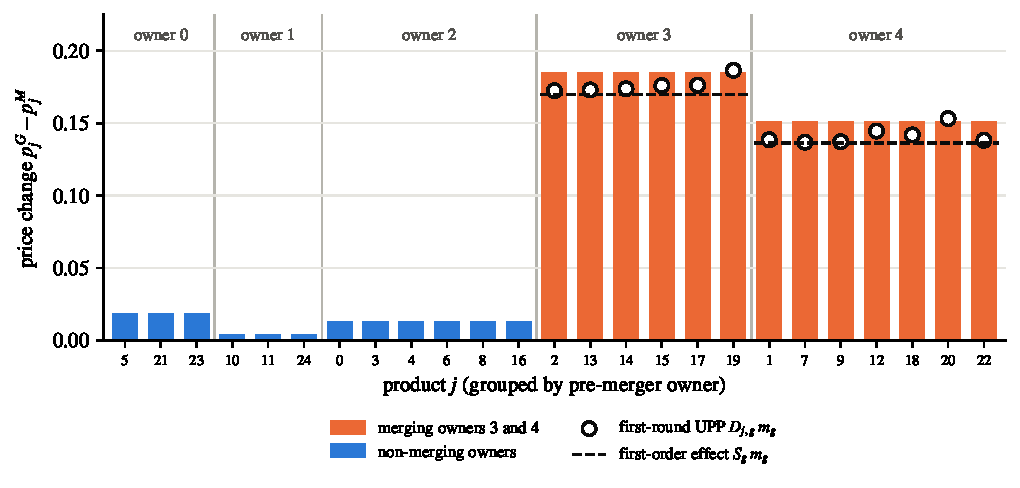
\includegraphics[width=\linewidth]{figures/appC/logit_merger.pdf}
\caption{Price changes caused by the merger of owners 3 and 4, by product. Bars show the change from the
pre-merger equilibrium (M) to the post-merger equilibrium (G). Hollow circles show each merging product's
first-round upward pricing pressure $D_{j,g}m_g$, and dashed lines show the first-order effect $S_gm_g$ of the
firm-level tax. Computed with \texttt{figures/appC/src/logit\_bertrand.py}.}
\label{fig:C-logit-merger}
\end{figure}

\emph{Upward pricing pressure} (UPP) measures the merger's incentive to raise prices at pre-merger prices
(\cref{sec:11-uppfs}). \citet{FarrellShapiro2010} define the first-round tax on product 1 of a merger between two
single-product firms as $t_1 = D_{12}(P_2 - C_2)$, the diversion ratio times the partner's margin (working-paper
version, p.~9). When the partner owns several products, the tax sums over them, $t_j = \sum_kD_{jk}m_k$
(\cref{eq:11-upp-multi}). For product $j$ of owner 3, the partner is owner 4, whose seven products share the
pre-merger markup $m_4$. With logit diversion,
\begin{equation}\label{eq:C-upp-logit}
  \mathit{UPP}_j = \sum_{k \in \mathcal{J}_4}\frac{s_k}{1 - s_j}\,m_4 = \frac{S_4}{1 - s_j}\,m_4 .
\end{equation}
The \emph{gross upward pricing pressure index} (GUPPI) divides by the product's price, $\mathit{GUPPI}_j = \frac{\mathit{UPP}_j}{p_j}$
(\cref{eq:11-guppi}). For owner 3's products, UPP ranges from 0.172 to 0.187 and GUPPI from 0.116 to 0.162. For
owner 4's products, UPP ranges from 0.137 to 0.153 and GUPPI from 0.078 to 0.132
(\cref{tab:C-logit-merger}). The UPP values bracket the equilibrium increases of 0.185 and 0.151 closely.
\citet[Section~3.3.2, pp.~230--231]{AskerNocke2021} present UPP as the simple alternative to full merger simulation.
Simulation estimates demand, recovers marginal costs from an assumption on conduct and solves for the post-merger
equilibrium. Demand and costs are known here, so this part carries out the last step exactly.

\begin{table}[htbp]
\centering
\caption{Pricing pressure and price changes of the merging products}
\label{tab:C-logit-merger}
\footnotesize
\begin{tabular}{@{}lcc@{}}
\toprule
 & Owner 3 (partner $g = 4$) & Owner 4 (partner $g = 3$) \\
\midrule
Product diversion to partner $\frac{S_g}{1 - s_j}$ & 0.257 to 0.278 & 0.215 to 0.241 \\
Product-level UPP $\frac{S_g}{1 - s_j}m_g$ & 0.172 to 0.187 & 0.137 to 0.153 \\
GUPPI $\frac{1}{p_j}\frac{S_g}{1 - s_j}m_g$ & 0.116 to 0.162 & 0.078 to 0.132 \\
Firm-level tax $t_f = \frac{S_gm_g}{1 - S_f}$ & 0.216 & 0.182 \\
First-order effect $(1 - S_f)t_f = S_gm_g$ & 0.170 & 0.136 \\
One round with taxes $t_f$, re-equilibrated & 0.184 & 0.152 \\
Equilibrium price change $m_M - m_f$ & 0.185 & 0.151 \\
\bottomrule
\end{tabular}

\vspace{3pt}
\begin{minipage}{0.97\textwidth}
\footnotesize Notes: Shares and markups are those of the pre-merger equilibrium M, $f$ is the merging owner and $g$
its partner. Ranges are across the owner's products. Firm-level shares, markups and profits before and after the
merger are in \cref{tab:04-merger-sim}. Computed with \texttt{figures/appC/src/logit\_bertrand.py}.
\end{minipage}
\end{table}

Three facts explain why the first-round measure predicts so well here. First, a multi-product firm's internal tax is
a firm-level object. Compare the merged firm's first-order condition for $j \in \mathcal{J}_3$ with owner 3's condition
when each of its products bears a cost increase $t_j$. By \eqref{eq:C-mp-foc} they coincide when
\begin{equation*}
  t_j - \sum_{k \in \mathcal{J}_3}s_kt_k = \sum_{k \in \mathcal{J}_4}s_km_k \qquad \text{for all } j \in \mathcal{J}_3 .
\end{equation*}
With a uniform tax and owner 4's common markup, the solution is $t_3 = \frac{S_4m_4}{1 - S_3}$. In general,
$t_f = \frac{S_gm_g}{1 - S_f}$ for merging firm $f$ with partner $g$. This exceeds the product-level UPP
\eqref{eq:C-upp-logit}, because a joint price increase on all of $f$'s products diverts a larger fraction of sales to
the partner. The firm-level taxes are 0.216 for owner 3 and 0.182 for owner 4.

Second, part (h) shows that a firm passes through a fraction $1 - S_f$ of a uniform cost increase when rivals'
prices are fixed. The first-order price effect is therefore $(1 - S_f)t_f = S_gm_g$, which equals 0.170 for owner 3
and 0.136 for owner 4. Rivals' responses add the rest. Imposing the taxes $t_f$ on owners 3 and 4 and letting all
five owners re-equilibrate gives increases of 0.184 and 0.152, within 0.001 of the merger. Recomputing the taxes at
the new prices and repeating, as Farrell and Shapiro propose, converges to the post-merger equilibrium in nine rounds.
The taxes barely move (owner 3's rises from 0.216 to 0.217), because logit diversion changes little.

Third, an exact decomposition shows the size of the remaining gap. Subtract owner $f$'s pre-merger condition
$m_f = \frac{1}{\alpha} + S_fm_f$ from the merged firm's condition $m_M = \frac{1}{\alpha} + (S_f' + S_g')m_M$, where
primes denote post-merger shares of the former product sets:
\begin{equation}\label{eq:C-merger-decomp}
  m_M - m_f = S_g'\,m_M + \big(S_f'\,m_M - S_f\,m_f\big) .
\end{equation}
For owner 3 the two terms are 0.180 and 0.006, and for owner 4 they are 0.142 and 0.010. The first term exceeds
$S_gm_g$ because the merged markup rises by more (23 and 29 percent) than the partner's share falls (14 and 19
percent). Product-level UPP exceeds $S_gm_g$ by the factor $\frac{1}{1 - s_j}$, between 1.005 and 1.125. The equilibrium
change exceeds $S_gm_g$ by 9 and 11 percent. The closeness of product-level UPP to the equilibrium change thus
reflects two separate corrections of similar size. Imposing the product-level UPP values as taxes, product by
product, would understate the firm's internal tax. Re-equilibrating with them gives increases of only 0.149 and
0.117.

\casehead{Part (h)}
Let all marginal costs rise by a unit tax $t$, so $mc_k(t) = mc_k + t$. Then $v_k(t) = v_k - \alpha t$ and
$E_f(t) = E_fe^{-\alpha t}$ for every firm.

\begin{proposition}[Logit pass-through]\label{prop:C-logit-passthrough}
Let demand be logit with constant marginal costs.
\begin{enumerate}[label=(\roman*)]
  \item Holding rivals' prices fixed, a uniform increase $dc$ in the marginal costs of firm $f$'s products raises
  each of its prices by $(1 - S_f)\,dc$. With one product, the pass-through is $1 - s_j$.
  \item In equilibrium, a common unit tax on all products has pass-through, at $t = 0$,
  \begin{equation}\label{eq:C-tax-pt}
    \rho_f = \frac{dp_k}{dt} = 1 - \frac{S_f\,s_0}{\big[(1 - S_f)^2 + S_f\big]\,(s_0 + \bar w)} \quad (k \in \mathcal{J}_f) ,
    \qquad \bar w = \sum_g\frac{S_g(1 - S_g)^2}{(1 - S_g)^2 + S_g} .
  \end{equation}
  With two or more firms, $1 - S_f < \rho_f < 1$.
\end{enumerate}
\end{proposition}

\begin{proof}
(i) This is \cref{prop:04-passthrough}(iii), and part (i) of that proposition is the single-product case.

(ii) The equilibrium satisfies \eqref{eq:C-h} for every firm and the adding-up condition \eqref{eq:C-Psi}. Since
$\ln h(S) = \ln S + \frac{1}{1 - S}$, differentiating \eqref{eq:C-h} in logarithms gives
\begin{equation*}
  \Big[\frac{1}{S_f} + \frac{1}{(1 - S_f)^2}\Big]dS_f = d\ln E_f - d\ln\Phi = -\alpha\,dt - d\ln\Phi .
\end{equation*}
Write $w_f = \frac{S_f(1 - S_f)^2}{(1 - S_f)^2 + S_f}$, the inverse of the bracket, so that
$dS_f = w_f(-\alpha\,dt - d\ln\Phi)$. Adding up gives $\sum_fdS_f = -d\frac{1}{\Phi} = s_0\,d\ln\Phi$. Summing the
previous equation over firms,
\begin{equation*}
  \bar w\,(-\alpha\,dt - d\ln\Phi) = s_0\,d\ln\Phi
  \quad\Longrightarrow\quad
  d\ln\Phi = -\frac{\alpha\bar w}{s_0 + \bar w}\,dt .
\end{equation*}
Substituting back, $-\alpha\,dt - d\ln\Phi = -\frac{\alpha s_0}{s_0 + \bar w}\,dt$, so
$dS_f = -\frac{\alpha w_fs_0}{s_0 + \bar w}\,dt$. Differentiating \eqref{eq:C-common-markup} then gives
\begin{equation*}
  dm_f = \frac{dS_f}{\alpha(1 - S_f)^2} = -\frac{S_f\,s_0}{\big[(1 - S_f)^2 + S_f\big](s_0 + \bar w)}\,dt ,
\end{equation*}
and $dp_k = dt + dm_f$ gives \eqref{eq:C-tax-pt}. Since $s_0 > 0$, $\rho_f < 1$. For the lower bound, write
$A_f = (1 - S_f)^2 + S_f$, so that $1 - A_f = S_f(1 - S_f)$. Then $\rho_f > 1 - S_f$ holds if and only if
$s_0 < A_f(s_0 + \bar w)$, that is, if and only if $S_f(1 - S_f)\,s_0 < A_f\bar w$. Since $\bar w \ge w_f$, the right
side is at least $A_fw_f = S_f(1 - S_f)^2$. This exceeds $S_f(1 - S_f)s_0$ because $1 - S_f > s_0$ when another firm
has a positive share.
\end{proof}

For a single product, part (i) is also the logit case of \cref{lem:11-passthrough}. Part (ii) gives in closed form, for any ownership structure, the common-tax pass-through
that \cref{cor:04-passthrough-eq} expresses through a matrix inverse for single-product firms. Two special cases help
to read it. Without an outside good ($s_0 \to 0$), a common cost increase is
passed through fully, because relative prices are all that matter. With a single firm, $\bar w = w_f$ and
$s_0 = 1 - S_f$, and \eqref{eq:C-tax-pt} reduces to $\rho_f = 1 - S_f$, the partial pass-through, because no rival
responds. With several firms, the common tax lowers every $E_f$, which by itself cuts $f$'s markup as in part (i). It
also raises rivals' prices, which lowers $\Phi_{-f}$ and offsets part of the fall in $z_f = \frac{E_fe^{-1}}{\Phi_{-f}}$.
Equilibrium pass-through therefore lies between the partial rate and one.

We compute the equilibrium at $t = 0.1$ by best-response iteration and divide each price change by $t$.
\Cref{tab:C-logit-tax} reports the results. Under S, product pass-through ranges from 0.980 to 0.999, with mean
0.994. It is lower for products with larger shares, and its correlation with the share is $-1.000$. Under M it ranges from 0.934 (owner 4) to 0.990 (owner 1),
with mean 0.954. The closed form \eqref{eq:C-tax-pt} at $t = 0$ gives almost the same values, and it matches a
numerical derivative to within $5\times10^{-8}$. Partial pass-through $1 - S_f$ is much lower, down to 0.746 for
owner 4. Rivals' responses account for most of the difference.

\begin{table}[htbp]
\centering
\caption{Pass-through of a common unit tax $t = 0.1$}
\label{tab:C-logit-tax}
\footnotesize
\begin{tabular}{@{}lcc@{}}
\toprule
 & Single-product firms (S) & Multi-product owners (M) \\
\midrule
\multicolumn{3}{@{}l}{\textit{Panel A. Market summary}} \\
Product pass-through at $t = 0.1$: range (mean) & 0.980 to 0.999 (0.994) & 0.934 to 0.990 (0.954) \\
Closed form \eqref{eq:C-tax-pt} at $t = 0$: range & 0.981 to 0.999 & 0.937 to 0.990 \\
Partial pass-through $1 - S_f$: range & 0.883 to 0.996 & 0.746 to 0.953 \\
Pass-through of the share-weighted mean price & 0.9895 & 0.9492 \\
\quad with weights held at pre-tax shares & 0.9893 & 0.9497 \\
\quad composition term & 0.0002 & $-0.0005$ \\
Outside share, before and after & 0.1367, 0.1618 & 0.1601, 0.1873 \\
Consumer surplus, before and after & 0.9949, 0.9107 & 0.9159, 0.8374 \\
Total profit, before and after & 0.4616, 0.4474 & 0.5261, 0.5051 \\
\bottomrule
\end{tabular}

\vspace{6pt}
\begin{tabular}{@{}lccccc@{}}
\toprule
\multicolumn{6}{@{}l}{\textit{Panel B. Owners under M}} \\
Owner & 0 & 1 & 2 & 3 & 4 \\
\midrule
Combined share $S_f$ (\%) & 18.87 & 4.67 & 13.68 & 21.40 & 25.36 \\
Partial pass-through $1 - S_f$ & 0.811 & 0.953 & 0.863 & 0.786 & 0.746 \\
Equilibrium pass-through, closed form at $t = 0$ & 0.955 & 0.990 & 0.969 & 0.949 & 0.937 \\
Equilibrium pass-through at $t = 0.1$ & 0.953 & 0.990 & 0.967 & 0.946 & 0.934 \\
\bottomrule
\end{tabular}

\vspace{3pt}
\begin{minipage}{0.97\textwidth}
\footnotesize Notes: Pass-through at $t = 0.1$ is $\frac{p(0.1) - p(0)}{0.1}$. The composition term is the difference
between the pass-through of the share-weighted mean price and the same object with weights fixed at pre-tax shares.
Computed with \texttt{figures/appC/src/logit\_bertrand.py}.
\end{minipage}
\end{table}

The share-weighted mean price $\bar p = \sum_jw_jp_j$, with $w_j = \frac{s_j}{1 - s_0}$, changes by
\begin{equation*}
  \frac{d\bar p}{dt} = \sum_jw_j\frac{dp_j}{dt} + \sum_jp_j\frac{dw_j}{dt} .
\end{equation*}
The first term is the average product pass-through. The second is a composition term, which is positive when
consumers shift toward expensive products. The mean-price pass-through is 0.9895 under S and 0.9492 under M, and the
composition terms are only 0.0002 and $-0.0005$. A common unit tax shifts all logit prices by similar amounts, so
substitution among inside goods hardly changes the mix.

These results bear on the cigarette tax study of \cref{sec:C-passthrough}. With logit demand and constant marginal
costs, a common tax is passed through less than one for one by every firm, whatever the ownership structure, and
composition effects are negligible. Logit demand is log-concave in own price, which is why pass-through stays below
one. A pass-through rate above one, as \citet{Sumner1981} estimates, needs a feature that this model lacks. Candidates
are demand that is more convex than the logit, composition effects much larger than those found here, or a different
form of conduct.

\subsection{Computational notes}

A single script produces every number in this section. It is \texttt{logit\_bertrand.py} in the folder
\texttt{figures/appC/src}, and it reads the data file \texttt{logit\_market.csv} from the folder
\texttt{figures/appC/data}.
\begin{enumerate}
  \item Compute $a_j = x_j\beta + \xi_j$, $mc_j$ and $v_j = a_j - \alpha\,mc_j$. An owner vector assigns products to
  firms. Under S it is $(0, 1, \dots, 24)$. After the merger, owner 4 is relabeled 3.
  \item For each firm compute $E_f = \sum_{k \in \mathcal{J}_f}e^{v_k}$ once. At each iteration compute
  $\Phi_{-f} = \Phi - \sum_{k \in \mathcal{J}_f}e^{\delta_k}$, the markup \eqref{eq:C-br-multi} with the principal
  branch of $W$, and the new prices.
  \item Stop when the sup-norm change in prices is below $10^{-12}$. Verify \eqref{eq:C-stacked-foc}, the common
  markups \eqref{eq:C-common-markup} and agreement with markup iteration and a root finder.
  \item For uniqueness, solve \eqref{eq:C-h} for $S_f(\Phi)$ in logarithms, $\ln S_f + \frac{1}{1 - S_f} = \ln\frac{E_f}{\Phi}$,
  with a bracketing root finder, and evaluate $\Psi$ on the grid.
  \item For the merger and the tax, re-solve with the new owner vector or with $mc + t$.
\end{enumerate}
The best-response step takes five lines in Python with NumPy and SciPy:
\begin{verbatim}
def best_response(p, owner, mc):
    e = np.exp(a - alpha * p)                                # e^{delta_j}
    E = np.bincount(owner, weights=np.exp(a - alpha * mc))   # E_f
    phi_minus = 1 + e.sum() - np.bincount(owner, weights=e)  # Phi_{-f}
    m = (1 + lambertw(E * np.exp(-1) / phi_minus).real) / alpha
    return mc + m[owner]
\end{verbatim}

\section{Simulating a market with random coefficients demand}\label{sec:C-simulate}

The previous problem computed prices from a known demand system. Empirical work runs in the opposite direction,
from observed prices and shares back to demand and cost. To judge an estimator we need data whose true model we
know. This problem builds such data, and the next three problems use it. We simulate 100 markets
from a random coefficients logit model with multi-product Bertrand pricing, solve for equilibrium prices, and draw the
choices of about ten thousand consumers per market. Sections \ref{sec:C-vertical} to \ref{sec:C-rc-est} estimate the
vertical, logit and random coefficients models on the resulting data. \Cref{sec:08-worked} uses the same design to
illustrate the estimation of the random coefficients model step by step.

\subsection{Statement}

Think of the market for yogurt in 100 metropolitan areas, which we treat as independent markets $t = 0, \dots, 99$.
Ten products exist in total, $j = 1, \dots, 10$. Each market offers between 4 and 9 of them, 6.54 on average, so there
are 654 product-market observations. A product has three characteristics,
$x_{jt} = (1, x^{sug}_{jt}, x^{org}_{jt})$: a constant, its sugar content and an indicator of organic production. Its
marginal cost also depends on a cost shifter $w_{jt}$, the price of milk used in production. Characteristics, the
cost shifter and the owner are fixed by product, so $x_{jt} = x_j$ and $w_{jt} = w_j$ in every market that offers
$j$ (\cref{tab:C-products}). Four firms own the products: firm A owns $\{5, 8\}$, firm B owns $\{1, 4, 6, 7\}$, firm C
owns $\{2, 3, 10\}$ and firm D owns $\{9\}$. Across markets only the set of products offered $\mathcal{J}_t$, the
unobservables $(\xi_{jt}, \omega_{jt})$ and the market size $M_t$ vary. Their values are supplied in the file
\texttt{yogurt\_markets.csv} in the folder \texttt{figures/appC/data}. Market sizes range from 9,756 to 10,223, with
mean 9,998.7.

Consumer $i$ in market $t$ has utility
\begin{equation}\label{eq:C-rc-utility}
  u_{ijt} = \delta_{jt} + \tilde x_{jt}\Sigma\nu_i + \epsilon_{ijt} , \qquad
  \delta_{jt} = x_{jt}\beta - \alpha p_{jt} + \xi_{jt} , \qquad
  u_{i0t} = \epsilon_{i0t} ,
\end{equation}
where $\tilde x_{jt} = (x_{jt}, p_{jt})$ contains the characteristics and the price, $\nu_i \sim N(0, I_4)$, and the
$\epsilon_{ijt}$ are independent type-I extreme value shocks. The parameters are $\beta = (-1, 0.2, 0.15)$,
$\alpha = 3$ and $\Sigma = \diag(\Sigma_{11}, \Sigma_{22}, \Sigma_{33}, \Sigma_{pp}) = \diag(0.5, 0.2, 0.3, 0.5)$.
Marginal cost is
\begin{equation}\label{eq:C-rc-mc}
  mc_{jt} = x_{jt}\gamma_1 + \gamma_2w_{jt} + \omega_{jt} , \qquad \gamma_1 = (0.2, 0.25, 0.3) , \quad \gamma_2 = 0.5 .
\end{equation}
The demand and cost shocks are drawn independently of each other and of the characteristics. Their sample standard
deviations are 0.50 for $\xi_{jt}$ and 0.050 for $\omega_{jt}$, and their sample correlation is 0.004. Firms know all
characteristics, shocks and parameters. Each firm evaluates expected demand by averaging over $n_s = 100$ consumer
types drawn once for each market.

\begin{table}[htbp]
\centering
\caption{Products in the simulated markets}
\label{tab:C-products}
\footnotesize
\begin{tabular}{@{}lcccccccccc@{}}
\toprule
Product $j$ & 1 & 2 & 3 & 4 & 5 & 6 & 7 & 8 & 9 & 10 \\
\midrule
Firm & B & C & C & B & A & B & B & A & D & C \\
Sugar content $x^{sug}_j$ & 1.349 & 1.300 & 0.929 & 1.315 & 1.182 & 0.636 & 1.130 & 1.204 & 1.128 & 0.879 \\
Organic $x^{org}_j$ & 0 & 1 & 0 & 1 & 0 & 0 & 0 & 0 & 1 & 0 \\
Price of milk $w_j$ & 0.534 & 0.367 & 0.426 & 0.547 & 0.346 & 0.529 & 0.588 & 0.334 & 0.527 & 0.442 \\
\midrule
Markets offering $j$ & 77 & 58 & 73 & 65 & 52 & 66 & 66 & 68 & 65 & 64 \\
Mean price & 1.189 & 1.403 & 1.025 & 1.504 & 1.048 & 1.008 & 1.164 & 1.039 & 1.427 & 1.012 \\
Mean markup & 0.390 & 0.395 & 0.381 & 0.402 & 0.378 & 0.384 & 0.390 & 0.376 & 0.378 & 0.382 \\
Mean realized share & 0.015 & 0.010 & 0.024 & 0.009 & 0.023 & 0.024 & 0.019 & 0.027 & 0.011 & 0.024 \\
\bottomrule
\end{tabular}

\vspace{3pt}
\begin{minipage}{0.97\textwidth}
\footnotesize Notes: The first four rows are the design. The last three rows are equilibrium outcomes, averaged over
the markets that offer the product. In the data file the owner codes of firms A, B, C and D are 0, 1, 2 and 4.
Computed with \texttt{figures/appC/src/appC\_simulate.py}.
\end{minipage}
\end{table}

\begin{enumerate}[label=(\alph*)]
  \item Interpret the random coefficients. How likely is a consumer to like higher prices?
  \item Write the expected-share function that the firms use, with $n_s = 100$ fixed draws per market, and explain how
  to evaluate it without numerical overflow.
  \item Derive the first-order conditions of multi-product Bertrand pricing and an algorithm that solves them. Solve
  every market and check the solutions.
  \item Simulate the realized shares of $M_t$ consumers per market and compare them with the expected shares.
  \item Report the equilibrium of market 0.
  \item Show that, when individual choice probabilities are small, the markup of product $j$ is close to the inverse
  of the average price sensitivity of its buyers. Evaluate the approximation in market 0.
  \item Derive the sampling error of a realized share and of its logarithm, and evaluate it in market 0.
\end{enumerate}

\subsection{Solution}

\casehead{Part (a)}
Because $\Sigma$ is diagonal, the consumer-specific term in \eqref{eq:C-rc-utility} is
\begin{equation*}
  \tilde x_{jt}\Sigma\nu_i = 0.5\,\nu_{i1} + 0.2\,\nu_{i2}x^{sug}_{jt} + 0.3\,\nu_{i3}x^{org}_{jt} + 0.5\,\nu_{i4}p_{jt} .
\end{equation*}
Consumer $i$ therefore has her own coefficients
\begin{equation}\label{eq:C-rc-coefs}
  \beta_{i1} = -1 + 0.5\,\nu_{i1} , \quad \beta_{i2} = 0.2 + 0.2\,\nu_{i2} , \quad
  \beta_{i3} = 0.15 + 0.3\,\nu_{i3} , \quad -\alpha_i \text{ with } \alpha_i = 3 - 0.5\,\nu_{i4} .
\end{equation}
The random constant $\beta_{i1}$ shifts the utility of every inside good relative to the outside good. Consumers
who like yogurt are more likely to buy some yogurt. Inside goods therefore substitute more with one another than
with the outside good, as in a nested logit with one nest of inside goods. The coefficients on sugar and on organic
production are positive on average, but 15.9 percent of consumers dislike sugar ($\nu_{i2} < -1$) and 30.9 percent
dislike organic production ($\nu_{i3} < -0.5$). The price sensitivity $\alpha_i$ is normal with mean 3 and standard
deviation 0.5. A consumer likes higher prices only if $\alpha_i \le 0$, that is, if $\nu_{i4} \ge 6$. This has
probability $\Pr(\nu_{i4} \ge 6) = 9.9\times10^{-10}$. Among the 10,000 consumer types the firms use, $\alpha_i$
ranges from 1.17 to 4.79.

Conditional on $\nu_i$, the extreme value shocks give logit choice probabilities. With
$V_{ijt} = \delta_{jt} + \tilde x_{jt}\Sigma\nu_i$,
\begin{equation}\label{eq:C-rc-sij}
  s_{ijt} = \frac{e^{V_{ijt}}}{1 + \sum_{k \in \mathcal{J}_t}e^{V_{ikt}}} , \qquad
  s_{jt} = \int_{\R^4} s_{ijt}(\nu)\,\phi_4(\nu)\,\dd\nu ,
\end{equation}
where $s_{ijt}(\nu)$ is the choice probability of a consumer with taste vector $\nu$ and $\phi_4$ is the
four-dimensional standard normal density. The integral breaks the
independence of irrelevant alternatives. A rise in $p_{kt}$ moves consumers who were likely to buy $k$, and these
consumers are most likely to buy products similar to $k$ (\cref{prop:08-derivs}). Cross elasticities therefore vary
across products, unlike \eqref{eq:C-logit-elast}.

\casehead{Part (b)}
For each market we draw $n_s = 100$ vectors $\nu_{it} \sim N(0, I_4)$ once and keep them fixed. They are the consumer
types whose average demand the firms compute. The expected share of product $j$ is the simulator of
\citet[eq.~11, p.~532]{Nevo2000a},
\begin{equation}\label{eq:C-rc-simshare}
  s_{jt}(p_t) = \frac{1}{n_s}\sum_{i=1}^{n_s}s_{ijt}(p_t) , \qquad
  s_{ijt}(p_t) = \frac{e^{V_{ijt}}}{1 + \sum_{k \in \mathcal{J}_t}e^{V_{ikt}}} .
\end{equation}
Prices enter twice, through $\delta_{jt}$ and through the last element of $\tilde x_{jt}$, so the function must rebuild
$\tilde x_{jt}$ whenever prices change.

Exponentials overflow when utilities are large. For draw $i$, let $c_i = \max\{0, \max_kV_{ikt}\}$, where the 0 is the
outside good's utility. Multiplying the numerator and the denominator of $s_{ijt}$ by $e^{-c_i}$ gives
\begin{equation*}
  s_{ijt} = \frac{e^{V_{ijt} - c_i}}{e^{-c_i} + \sum_{k \in \mathcal{J}_t}e^{V_{ikt} - c_i}} .
\end{equation*}
The value is unchanged. Every exponent is now at most zero, so nothing overflows, and the largest term in the
denominator equals one, so the denominator cannot underflow to zero.

The draws stay fixed for two reasons. With fixed draws, $s_t(p_t)$ is a smooth deterministic function of prices, so the
first-order conditions of part (c) define a well-posed system. With fresh draws at each evaluation, the system would
change from one iteration to the next, and no solver could converge. In this design the 100 draws also define what
firms believe about demand. Part (d) shows that these beliefs differ from population demand by simulation error.

\casehead{Part (c)}
Firm $f$ owns the products $\mathcal{J}_{ft} \subseteq \mathcal{J}_t$ and earns
$\pi_{ft} = M_t\sum_{k \in \mathcal{J}_{ft}}(p_{kt} - mc_{kt})s_{kt}(p_t)$. Market size multiplies profit, so it drops out of
the first-order conditions
\begin{equation}\label{eq:C-rc-foc}
  s_{jt} + \sum_{k \in \mathcal{J}_{ft}}(p_{kt} - mc_{kt})\frac{\partial s_{kt}}{\partial p_{jt}} = 0 , \qquad j \in \mathcal{J}_{ft} .
\end{equation}
These are equations (3.3) of \citet[p.~853]{BerryLevinsohnPakes1995}. For draw $i$, price enters $V_{ijt}$ with
coefficient $\frac{\partial V_{ijt}}{\partial p_{jt}} = -\alpha + 0.5\,\nu_{i4} = -\alpha_i$. The quotient rule of
\cref{sec:C-logit-bertrand}, applied draw by draw, gives
$\frac{\partial s_{ijt}}{\partial p_{kt}} = \alpha_is_{ijt}(s_{ikt} - \indic\{j = k\})$. Averaging over draws,
\begin{equation}\label{eq:C-rc-deriv}
  \Delta_{jk,t} = \frac{\partial s_{jt}}{\partial p_{kt}} = \frac{1}{n_s}\sum_{i=1}^{n_s}\alpha_is_{ijt}\big(s_{ikt} - \indic\{j = k\}\big) .
\end{equation}
With $\Omega_t$ the ownership matrix of market $t$, the conditions stack as in \eqref{eq:C-stacked-foc}:
$s_t + (\Omega_t \odot \Delta_t^\top)(p_t - mc_t) = 0$. Solving for the markups gives
$p_t - mc_t = -(\Omega_t \odot \Delta_t^\top)^{-1}s_t$, which is equation (3.5) of
\citet[p.~854]{BerryLevinsohnPakes1995} with their matrix equal to $-(\Omega_t \odot \Delta_t^\top)$.

\begin{proposition}[Morrow-Skerlos fixed point]\label{prop:C-ms}
Let $\Lambda_t$ be the diagonal matrix with $\Lambda_{jj,t} = \frac{1}{n_s}\sum_i\alpha_is_{ijt}$, and let $\Gamma_t$ be
the matrix with $\Gamma_{jk,t} = \frac{1}{n_s}\sum_i\alpha_is_{ijt}s_{ikt}$. If every $\alpha_i > 0$, the first-order
conditions hold at $p_t$ if and only if
\begin{equation}\label{eq:C-ms-zeta}
  p_t - mc_t = \zeta_t(p_t) \equiv \Lambda_t^{-1}\big[s_t + (\Omega_t \odot \Gamma_t)(p_t - mc_t)\big] ,
\end{equation}
where $\Lambda_t$, $\Gamma_t$ and $s_t$ are evaluated at $p_t$.
\end{proposition}

\begin{proof}
By \eqref{eq:C-rc-deriv}, $\Delta_t = -\Lambda_t + \Gamma_t$, and $\Gamma_t$ is symmetric. Since $\Omega_t$ is symmetric
with a unit diagonal, $\Omega_t \odot \Lambda_t = \Lambda_t$, and
\begin{equation*}
  (\Omega_t \odot \Delta_t)^\top = -\Lambda_t + \Omega_t \odot \Gamma_t .
\end{equation*}
The first-order conditions therefore read $s_t - \Lambda_t(p_t - mc_t) + (\Omega_t \odot \Gamma_t)(p_t - mc_t) = 0$.
Every diagonal entry of $\Lambda_t$ is positive because $\alpha_i > 0$ and $s_{ijt} > 0$. Moving the $\Lambda_t$ term
to the left and multiplying by $\Lambda_t^{-1}$ gives \eqref{eq:C-ms-zeta}. Each step is reversible.
\end{proof}

This is \cref{prop:08-ms}, due to \citet{MorrowSkerlos2011}. In the plain logit, $\alpha_i = \alpha$ gives
$\Lambda_{jj} = \alpha s_j$ and $\Gamma_{jk} = \alpha s_js_k$, and \eqref{eq:C-ms-zeta} becomes
$m_j = \frac{1}{\alpha} + \sum_{k \in \mathcal{J}_f}s_km_k$, the multi-product condition \eqref{eq:C-mp-foc}. Here every
$\alpha_i$ exceeds 1.17, so the proposition applies. We solve each market as follows.
\begin{enumerate}
  \item Start at $p_t^{(0)} = mc_t$.
  \item Given $p_t^{(n)}$, compute $s_{ijt}$ for the 100 draws, then $s_t$, $\Lambda_t$ and $\Gamma_t$.
  \item Set $p_t^{(n+1)} = mc_t + \zeta_t(p_t^{(n)})$.
  \item Stop when $\|p_t^{(n+1)} - p_t^{(n)}\|_\infty < 10^{-12}$. Otherwise return to step 2.
  \item Verify the first-order conditions \eqref{eq:C-rc-foc} at the solution.
\end{enumerate}
Nothing guarantees that $p \mapsto mc + \zeta(p)$ is a contraction, so convergence must be checked market by market.

\Cref{tab:C-sim-checks} reports the diagnostics. The iteration converges in every market, in 10 to 13 iterations
(11.05 on average). The largest first-order residual across markets is $8.6\times10^{-15}$. A hybrid Powell root finder
on \eqref{eq:C-rc-foc}, started at marginal cost, reaches the same prices to within $1.0\times10^{-13}$. We then restart
from 20 random price vectors per market, with each price drawn uniformly on $[0, 4]$. All 2,000 runs of the
iteration return the original prices, to within $2.1\times10^{-13}$, so no market shows a second equilibrium.

The root finder is less reliable from the random starts. Applied to the residual of \eqref{eq:C-rc-foc}, it solves
only 13 of the 2,000 problems. Every term of that residual tends to zero as prices rise without bound. The root
finder can therefore stop at very high prices, where the residual is small and no equilibrium is near. Applied to the residual
$\zeta_t(p) - (p - mc_t)$, which is measured in price units, it solves 1,817 of the 2,000 problems, and every
solution it finds is the original one.

Equilibrium prices range from 0.881 to 1.609, with mean 1.180. Markups range from 0.348 to 0.451, with mean 0.386,
and the Lerner index averages 0.334. Markups are close to the inverse of the mean price coefficient,
$\frac{1}{3} = 0.333$, for a reason that part (f) makes precise.

\begin{table}[htbp]
\centering
\caption{Simulated markets: equilibrium computation and realized shares}
\label{tab:C-sim-checks}
\footnotesize
\begin{tabular}{@{}lr@{}}
\toprule
\multicolumn{2}{@{}l}{\textit{Panel A. Equilibrium prices}} \\
Morrow-Skerlos iterations per market, range (mean) & 10 to 13 (11.05) \\
Largest first-order residual & $8.6\times10^{-15}$ \\
Largest price difference, iteration versus root finder & $1.0\times10^{-13}$ \\
Random restarts solved by the iteration, largest deviation & 2,000 of 2,000, $2.1\times10^{-13}$ \\
Random restarts solved by a root finder on \eqref{eq:C-rc-foc} & 13 of 2,000 \\
Random restarts solved by a root finder on $\zeta_t(p) - (p - mc_t)$ & 1,817 of 2,000 \\
Markets with a second equilibrium & 0 \\
Prices: range (mean) & 0.881 to 1.609 (1.180) \\
Markups: range (mean) & 0.348 to 0.451 (0.386) \\
Lerner index: range (mean) & 0.234 to 0.448 (0.334) \\
\midrule
\multicolumn{2}{@{}l}{\textit{Panel B. Realized shares}} \\
Simulated consumers & 999,870 \\
Products with zero realized share & 0 \\
Smallest realized share (buyers) & 0.0019 (19) \\
Mean and largest absolute gap, realized minus expected share & 0.0014, 0.0100 \\
Correlation of realized and expected shares & 0.986 \\
Outside share: mean (range across markets) & 0.879 (0.788 to 0.948) \\
Mean squared standardized gap: realized minus population share & 1.07 \\
Mean squared standardized gap: expected minus population share & 0.84 \\
Mean squared standardized gap: realized minus expected share & 1.88 \\
\bottomrule
\end{tabular}

\vspace{3pt}
\begin{minipage}{0.97\textwidth}
\footnotesize Notes: 654 product-market observations in 100 markets. Random restarts draw each starting price from
$U[0, 4]$, 20 per market. A run counts as solved when the largest markup residual is below $10^{-10}$. Standardized
gaps divide by the sampling standard deviation $\sqrt{\frac{s(1 - s)}{M_t}}$, where $s$ is the population share
computed with 100,000 draws. Computed with \texttt{figures/appC/src/appC\_simulate.py}.
\end{minipage}
\end{table}

\casehead{Part (d)}
At the equilibrium prices we simulate the choices of $M_t$ consumers in each market. Each consumer receives a fresh
draw $\nu_i \sim N(0, I_4)$ and $|\mathcal{J}_t| + 1$ fresh extreme value shocks, one for each product and one for the
outside good. She chooses the alternative with the highest utility $u_{ijt}$. The \emph{realized share} of product $j$
is the fraction of consumers who choose it,
\begin{equation}\label{eq:C-realized}
  \hat s_{jt} = \frac{q_{jt}}{M_t} , \qquad q_{jt} = \sum_{i=1}^{M_t}\indic\Big\{j = \argmax_{k \in \mathcal{J}_t \cup \{0\}}u_{ikt}\Big\} .
\end{equation}
Realized shares, prices, characteristics, the cost shifter and ownership are the data that Sections
\ref{sec:C-vertical} to \ref{sec:C-rc-est} use. The unobservables, the marginal costs and the expected shares are
kept only to evaluate the estimators.

In total we simulate 999,870 consumers. No product has a zero realized share, and the smallest realized share is
0.0019, or 19 buyers. The mean absolute difference between realized and expected shares is 0.0014, the largest is
0.0100, and their correlation is 0.986. The outside good is large. Its realized share averages 0.879 across markets
and ranges from 0.788 to 0.948.

Three share concepts are at work. The expected share $s_{jt}$ averages over the firms' 100 draws. The
\emph{population share} $s^\infty_{jt}$ integrates over the whole normal distribution, and we approximate it with
100,000 draws per market. The realized share $\hat s_{jt}$ is a sample proportion among $M_t$ consumers drawn from the
population. The gap between realized and expected shares therefore has two parts,
\begin{equation*}
  \hat s_{jt} - s_{jt} = \big(\hat s_{jt} - s^\infty_{jt}\big) + \big(s^\infty_{jt} - s_{jt}\big) ,
\end{equation*}
\emph{sampling error} from the finite number of consumers and \emph{simulation error} from the finite number of firm
draws. Part (g) shows that the sampling error has standard deviation close to $\sqrt{\frac{s(1 - s)}{M_t}}$. Dividing
each part by this standard deviation and averaging the squares over the 654 observations gives 1.07 for the sampling
part, close to the value of one that the binomial formula predicts. It gives 0.84 for the simulation part, and 1.88
for the total. With $n_s = 100$, the firms' simulation error is about as large as the sampling error of
ten thousand consumers. The median relative simulation error $|\frac{s_{jt}}{s^\infty_{jt}} - 1|$ is 4.7 percent, and
the largest is 29 percent.

\casehead{Part (e)}
\Cref{tab:C-mkt0} reports market 0, which offers products 2, 3, 4, 6, 8, 9 and 10 and has $M_0 = 9{,}880$ consumers.
Markups lie between 0.375 and 0.400. The Lerner index ranges from 0.260 for product 9, the most expensive product, to
0.408 for product 10, the cheapest. The outside good's expected share is 0.8463 and its realized share is 0.8549.
Realized and expected shares are close. The largest relative gaps are $-20$ percent for product 9 and $-11$ percent
for product 10. In market 0 the firms' 100 draws overstate demand for every inside product. The expected shares
exceed the population shares by 4 to 10 percent, and the population outside share is 0.8555.

\begin{table}[htbp]
\centering
\caption{Equilibrium in market 0 and the anatomy of its markups}
\label{tab:C-mkt0}
\footnotesize
\setlength{\tabcolsep}{4.5pt}
\begin{tabular}{@{}lcccccccccc@{}}
\toprule
 & & & & & \multicolumn{3}{c}{Share} & & & \\
\cmidrule(lr){6-8}
Product & Firm & $mc_j$ & $p_j$ & $m_j$ & Expected & Realized & Population & Buyers $q_j$ & $\frac{1}{\bar\alpha_j}$ & $\Gamma$ term \\
\midrule
2 & C & 0.9204 & 1.3200 & 0.3995 & 0.0048 & 0.0052 & 0.0044 & 51 & 0.3669 & 0.0326 \\
3 & C & 0.6308 & 1.0182 & 0.3874 & 0.0272 & 0.0252 & 0.0259 & 249 & 0.3584 & 0.0290 \\
4 & B & 1.0286 & 1.4196 & 0.3910 & 0.0125 & 0.0126 & 0.0113 & 124 & 0.3703 & 0.0207 \\
6 & B & 0.6238 & 0.9993 & 0.3755 & 0.0200 & 0.0203 & 0.0192 & 201 & 0.3583 & 0.0172 \\
8 & A & 0.7291 & 1.1246 & 0.3955 & 0.0593 & 0.0560 & 0.0556 & 553 & 0.3616 & 0.0339 \\
9 & D & 1.0729 & 1.4497 & 0.3768 & 0.0072 & 0.0058 & 0.0066 & 57 & 0.3717 & 0.0051 \\
10 & C & 0.5585 & 0.9429 & 0.3845 & 0.0226 & 0.0201 & 0.0215 & 199 & 0.3559 & 0.0285 \\
\midrule
Outside good & & & & & 0.8463 & 0.8549 & 0.8555 & 8,446 & & \\
\bottomrule
\end{tabular}

\vspace{3pt}
\begin{minipage}{0.97\textwidth}
\footnotesize Notes: $M_0 = 9{,}880$. Expected shares average over the firms' 100 draws, population shares over
100,000 draws, and realized shares are fractions of the $M_0$ simulated consumers. $\bar\alpha_j$ is the mean price
sensitivity of product $j$'s buyers among the firms' draws, and the $\Gamma$ term is the second term of
\eqref{eq:C-markup-decomp}, so $m_j = \frac{1}{\bar\alpha_j} + \Gamma$ term. Computed with
\texttt{figures/appC/src/appC\_simulate.py}.
\end{minipage}
\end{table}

\casehead{Part (f)}
Rewrite \eqref{eq:C-ms-zeta} product by product. Dividing the $j$-th row by $\Lambda_{jj}$ gives the exact decomposition
\begin{equation}\label{eq:C-markup-decomp}
  m_j = \frac{s_j}{\Lambda_{jj}} + \frac{1}{\Lambda_{jj}}\sum_{k \in \mathcal{J}_f}\Gamma_{jk}m_k .
\end{equation}

\begin{proposition}[Markups and the price sensitivity of buyers]\label{prop:C-buyer-alpha}
Suppose every $\alpha_i > 0$. Let $\bar\alpha_j = \frac{\Lambda_{jj}}{s_j}$.
\begin{enumerate}[label=(\roman*)]
  \item $\bar\alpha_j$ is the mean price sensitivity of product $j$'s buyers,
  \begin{equation}\label{eq:C-buyer-alpha}
    \bar\alpha_j = \frac{\sum_i\alpha_is_{ij}}{\sum_is_{ij}} = \E\big[\alpha_i \mid i \text{ buys } j\big] ,
  \end{equation}
  where the expectation is over the $n_s$ consumer types and their extreme value shocks.
  \item The markup satisfies
  \begin{equation}\label{eq:C-buyer-bound}
    \Big|m_j - \frac{1}{\bar\alpha_j}\Big| \le \Big(\max_{k \in \mathcal{J}_f}|m_k|\Big)\sum_{k \in \mathcal{J}_f}\max_is_{ik} .
  \end{equation}
  Hence $m_j$ approaches $\frac{1}{\bar\alpha_j}$ as the individual choice probabilities of firm $f$'s products tend to
  zero.
\end{enumerate}
\end{proposition}

\begin{proof}
(i) Each type is equally likely, with probability $\frac{1}{n_s}$, and type $i$ buys $j$ with probability $s_{ij}$. By
Bayes' rule, the probability that a buyer of $j$ is of type $i$ is $\frac{s_{ij}}{\sum_{i'}s_{i'j}}$. Averaging
$\alpha_i$ with these weights gives \eqref{eq:C-buyer-alpha}, and the factor $\frac{1}{n_s}$ cancels from
$\frac{\Lambda_{jj}}{s_j}$.

(ii) By \eqref{eq:C-markup-decomp}, $m_j - \frac{1}{\bar\alpha_j} = \sum_{k \in \mathcal{J}_f}\frac{\Gamma_{jk}}{\Lambda_{jj}}m_k$.
Each ratio is a weighted average of $s_{ik}$ over types, with non-negative weights $\alpha_is_{ij}$:
\begin{equation*}
  \frac{\Gamma_{jk}}{\Lambda_{jj}} = \frac{\sum_i\alpha_is_{ij}\,s_{ik}}{\sum_i\alpha_is_{ij}} \le \max_is_{ik} .
\end{equation*}
The triangle inequality gives \eqref{eq:C-buyer-bound}.
\end{proof}

The markup is thus the inverse of the buyers' mean price sensitivity, corrected by a term of the order of the
firm's individual choice probabilities. This is the discrete-choice form of the inverse semi-elasticity rule
(\cref{eq:08-ms-approx}). In the plain logit, $\bar\alpha_j = \alpha$ for every product, which is why all markups in
\cref{sec:C-logit-bertrand} lie near $\frac{1}{\alpha}$. With random coefficients, buyers select themselves. Consumers
with high $\alpha_i$ buy the outside good more often, so the buyers of any inside product are less price sensitive
than the population.

\Cref{tab:C-mkt0} evaluates the decomposition in market 0. The mean of $\alpha_i$ over the firms' 100 draws is 3.028,
and the mean among consumers who choose the outside good is 3.075. The buyers' mean sensitivity $\bar\alpha_j$ ranges
from 2.690 (product 9) to 2.810 (product 10). Its inverse lies between 0.356 and 0.372 and accounts for 91 to 99
percent of each markup. The expensive organic products 9 and 4 attract the least price-sensitive buyers, with
$\bar\alpha_j$ of 2.690 and 2.701. The $\Gamma$ term accounts for the rest, between 1.4 and 8.6 percent of the markup.
It has two parts. The diagonal part restores the factor $1 - s_{ij}$ in each type's own-price derivative and is
largest for product 8 (0.034), the product with the largest share. The off-diagonal part is the value of sales
recaptured by the firm's other products and is largest for firm C's product 2 (0.029). Firm D sells one product, so
product 9 has no recapture. Product 2 carries the highest markup in the market, 0.3995, although its buyers are more
price sensitive than those of products 4 and 9. Firm C's recapture of 0.029 lifts it to the top. Net of the recapture
terms, product 2's markup is 0.370, the fifth highest of the seven.

\casehead{Part (g)}
Given prices, the $M_t$ consumers choose independently, and each chooses $j$ with probability $s^\infty_{jt}$. Hence
$q_{jt}$ is binomial with parameters $M_t$ and $s^\infty_{jt}$. Writing $s$ for $s^\infty_{jt}$,
\begin{equation}\label{eq:C-share-var}
  \E[\hat s_{jt}] = s , \qquad \Var(\hat s_{jt}) = \frac{s(1 - s)}{M_t} .
\end{equation}
The inversions in Sections \ref{sec:C-vertical} to \ref{sec:C-rc-est} use logarithms of shares. A first-order Taylor
expansion, $\ln\hat s_{jt} \approx \ln s + \frac{\hat s_{jt} - s}{s}$, gives the delta-method variance
(\cref{app:econometrics}),
\begin{equation}\label{eq:C-logshare-var}
  \Var(\ln\hat s_{jt}) \approx \frac{1 - s}{M_ts} = \frac{1 - s}{\E[q_{jt}]} .
\end{equation}
The standard error of a log share is about one over the square root of the number of buyers. A second-order expansion
gives the bias $\E[\ln\hat s_{jt}] - \ln s \approx -\frac{\Var(\hat s_{jt})}{2s^2} = -\frac{1 - s}{2M_ts}$, the
sampling analogue of the simulation bias in \cref{prop:08-simbias}. The logit inversion of \cref{ch:logit} uses the
difference $\ln\hat s_{jt} - \ln\hat s_{0t}$. Since $\Cov(\hat s_{jt}, \hat s_{0t}) = -\frac{s_{jt}s_{0t}}{M_t}$, the
delta method gives $\Cov(\ln\hat s_{jt}, \ln\hat s_{0t}) \approx -\frac{1}{M_t}$, and
\begin{equation}\label{eq:C-logratio-var}
  \Var\Big(\ln\frac{\hat s_{jt}}{\hat s_{0t}}\Big)
  \approx \frac{1 - s_{jt}}{M_ts_{jt}} + \frac{1 - s_{0t}}{M_ts_{0t}} + \frac{2}{M_t}
  = \frac{1}{M_ts_{jt}} + \frac{1}{M_ts_{0t}} .
\end{equation}
The variance is the sum of the inverse expected counts of the two alternatives.

In market 0, product 2 has 51 buyers and product 8 has 553. We evaluate \eqref{eq:C-logshare-var} at the realized
shares. The standard error of the log share is 0.140 for product 2, 0.132 for product 9 and 0.089 for product 4. It
is 0.070 for products 6 and 10, 0.063 for product 3 and 0.041 for product 8. Across all 654 observations the standard error ranges from 0.032
to 0.229, with median 0.080, and 162 observations have fewer than 100 buyers. These errors are small relative to the
standard deviation of $\xi_{jt}$, which is 0.50. They enter the dependent variable of every inversion in Sections
\ref{sec:C-vertical} to \ref{sec:C-rc-est}. To first order they have mean zero and are independent of the instruments,
so they add noise without biasing linear instrumental variable estimators. The second-order bias is largest for the
smallest products, about $-0.010$ for product 2.

\subsection{Computational notes}

A single script produces the data and every number in this section. It is \texttt{appC\_simulate.py} in the folder
\texttt{figures/appC/src}, and it reads the data file \texttt{yogurt\_markets.csv} from the folder
\texttt{figures/appC/data}. The file holds characteristics, the cost shifter, owners, $(\xi_{jt}, \omega_{jt})$ and
$M_t$. The script runs in about two minutes.
\begin{enumerate}
  \item Sort observations by market and product. Compute $mc_{jt}$ from \eqref{eq:C-rc-mc}.
  \item Draw the firms' consumer types in one call, an array of shape $100 \times 100 \times 4$ with seed 2026, markets
  in increasing order. Save it as \texttt{figures/appC/data/firm\_draws.npz}.
  \item In each market, solve \eqref{eq:C-ms-zeta} from $p = mc$, check it with the root finder, and restart from 20 random
  price vectors (seed 2028).
  \item Simulate $M_t$ consumers at the equilibrium prices (seed 2027) and record the counts $q_{jt}$. Compute population
  shares with 100,000 draws per market (seed 2029).
  \item Write \texttt{figures/appC/data/simulated\_market.csv}, with one row per product and market. Its columns are
  the market and product identifiers, owner, characteristics, milk price, market size, price, expected and realized
  shares and the number of buyers. They also hold the true marginal cost, $\xi_{jt}$, $\omega_{jt}$ and $\delta_{jt}$.
\end{enumerate}
The core of the iteration takes two lines once $s_t$, $\Lambda_t$ and $\Gamma_t$ are computed:
\begin{verbatim}
s, lam, gam = share_moments(p)          # s_t, diag(Lambda_t), Gamma_t
p_new = mc + (s + (own * gam.T) @ (p - mc)) / lam
\end{verbatim}
Here \texttt{own} is $\Omega_t$ and \texttt{lam} holds the diagonal of $\Lambda_t$.

\section{Estimating the vertical model on simulated data}\label{sec:C-vertical}

The vertical model of product differentiation lets consumers differ along a single dimension, their sensitivity to
price. Every consumer ranks the products by quality in the same way, and products compete only with their neighbours
on the price ladder. These restrictions make the model easy to invert and to estimate. They also determine its
elasticities and markups almost entirely. This problem is the first of three that estimate demand on the simulated
market of \cref{sec:C-simulate}, which was generated by a random coefficients logit. Here we estimate the vertical
model. Since we know the truth, we can see exactly what the single taste
dimension does to substitution patterns, markups and recovered costs. The theory behind the model is in
\cref{sec:06-vertical}. Here we work through estimation in full.

\subsection{Statement}

The data are the 654 product-market observations of the simulated market of \cref{sec:C-simulate}. There are
$T = 100$ independent markets, and market $t$ offers $J_t$ of ten products, between 4 and 9. For each observation the
econometrician sees the price $p_{jt}$, the realized share $s_{jt} = \frac{q_{jt}}{M_t}$ and the market size $M_t$. The realized share is the $\hat s_{jt}$
of \eqref{eq:C-realized}, written without the hat in this problem and the next. The
econometrician also sees the characteristics $x_{jt} = (1, x^{sug}_{jt}, x^{org}_{jt})$ (a constant, sugar content and an organic
indicator), the price of milk $w_{jt}$ and the owner of the product. Characteristics, milk prices and owners are fixed by
product (\cref{tab:C-products}). The outside share $s_{0t} = 1 - \sum_{j} s_{jt}$ lies between 0.788 and 0.948 across
markets. The econometrician does not know how the data were generated and maintains the following assumptions.

\begin{assumption}\label{ass:C-est}
\begin{enumerate}[label=(\roman*)]
  \item Markets are independent of one another.
  \item The characteristics $x_{jt}$ and the cost shifter $w_{jt}$ are fixed (exogenous).
  \item The demand unobservable $\xi_{jt}$ and the cost unobservable $\omega_{jt}$ are independent of each other and of
  $(x_{jt}, w_{jt})$.
  \item Marginal cost is $mc_{jt} = x_{jt}\gamma_1 + \gamma_2 w_{jt} + \omega_{jt}$.
\end{enumerate}
\end{assumption}

Consumer $i$ in market $t$ obtains utility
\begin{equation}\label{eq:C-vutility}
  u_{ijt} = \delta^v_{jt} - \nu_i p_{jt}, \qquad \delta^v_{jt} = x_{jt}\beta^v + \xi_{jt},
\end{equation}
from product $j$ and $u_{i0t} = 0$ from the outside good, whose quality and price are normalized to zero. Here
$\delta^v_{jt}$ is the \emph{quality} of product $j$ in market $t$. The taste $\nu_i \ge 0$ is drawn from a continuous and
strictly increasing distribution function $F$ on $[0, \infty)$ with $F(0) = 0$ and density $f$. There is no idiosyncratic
taste shock.

\begin{enumerate}[label=(\alph*)]
  \item Derive $\delta^v_{jt}$ as a function of the prices and shares in market $t$, the market size $M_t$ and the
  inverse $F^{-1}$.
  \item Let $F(\nu) = 1 - e^{-\lambda\nu}$. Write an estimable equation for the qualities. Is $\lambda$ identified? Give
  the economic intuition. Normalize $\lambda = 1$, estimate $\beta^v$ with standard errors and discuss the fit.
  \item Keep $\lambda = 1$. Derive the marginal cost equation under (i) marginal-cost pricing and (ii) multi-product
  Bertrand-Nash pricing. Estimate $(\gamma_1, \gamma_2)$ under each conduct assumption, and explain why demand and supply
  can be estimated separately without loss of efficiency.
  \item Compute the matrix of own- and cross-price elasticities in market 0, including the outside good.
  \item Explain the size of these elasticities with the price ladder of market 0.
  \item When is the vertical model a good description of demand?
\end{enumerate}

\subsection{Solution}

\begin{remark}[Interpretation of $\nu_i$]\label{rem:C-nu}
A higher $\nu_i$ lowers the utility of every product in proportion to its price, so $\nu_i$ is a \emph{price
sensitivity}, a marginal utility of income. Dividing \eqref{eq:C-vutility} by $\nu_i > 0$ gives the money-metric form
$\frac{1}{\nu_i}\delta^v_{jt} - p_{jt}$, which ranks products in the same way. This is the form
$u_{ij} = \psi_j\nu_i - p_j$ of \citet[eq.~15, p.~250]{Berry1994} and the form $U = vx + Y - P$ of
\citet[eq.~1, p.~460]{Bresnahan1987}. In those papers the random variable multiplies quality, so it is a taste for
quality. In our notation the taste for quality is $\frac{1}{\nu_i}$, the willingness to pay for one unit of quality.
\end{remark}

\casehead{Part (a)}
Fix a market and drop the subscript $t$. Write $(k)$ for the product with the $k$-th lowest price, so that
$p_{(1)} < p_{(2)} < \dots < p_{(J)}$, and give the outside good the position $(0)$ with $\delta^v_{(0)} = p_{(0)} = 0$.
For $k = 1, \dots, J$ define the \emph{cutoff}
\begin{equation}\label{eq:C-vcut}
  \bar\nu_{(k)} = \frac{\delta^v_{(k)} - \delta^v_{(k-1)}}{p_{(k)} - p_{(k-1)}},
\end{equation}
set $\bar\nu_{(J+1)} = 0$, and define the upper-tail cumulative share $\bar S_{(k)} = \sum_{l \ge k} s_{(l)}$. Thus
$\bar S_{(1)} = 1 - s_0$ is the inside share and $\bar S_{(J)} = s_{(J)}$.

\begin{proposition}[Inversion of the vertical model]\label{prop:C-vinv}
Suppose that every product has a positive share and that prices are distinct. Then qualities increase with price,
the cutoffs satisfy $\bar\nu_{(1)} > \bar\nu_{(2)} > \dots > \bar\nu_{(J)} > 0$, and
\begin{equation}\label{eq:C-vshares}
  s_{(k)} = F(\bar\nu_{(k)}) - F(\bar\nu_{(k+1)}), \quad k = 1, \dots, J, \qquad s_0 = 1 - F(\bar\nu_{(1)}).
\end{equation}
The qualities are the unique solution of
\begin{equation}\label{eq:C-vinv}
  \delta^v_{(k)} = \sum_{m=1}^{k}\big(p_{(m)} - p_{(m-1)}\big)F^{-1}\big(\bar S_{(m)}\big),
  \qquad \bar S_{(m)} = \sum_{l \ge m}\frac{q_{(l)}}{M}.
\end{equation}
Conversely, every vector of positive shares with $\sum_j s_j < 1$ is generated by exactly one quality vector.
\end{proposition}

The proposition collects three results of \cref{sec:06-vertical}, with $\bar S_{(k)}$ the cumulative share
\eqref{eq:06-cumshare} written along the price ladder. A product with a positive share lies on the quality-price
frontier, which gives the ordering of qualities and cutoffs (\cref{prop:06-frontier}). \Cref{prop:06-vshares} then
gives \eqref{eq:C-vshares}, and \cref{prop:06-vinversion} gives \eqref{eq:C-vinv} with existence and uniqueness.

Market size enters only through the shares, which divide sales by $M_t$, including the consumers who buy nothing.
Since markets are independent, the inversion is carried out market by market. \Cref{prop:C-vinv} is the vertical
analogue of the inversion of \citet{Berry1994}. Berry orders products by quality, writes his cutoffs as
$\Delta_j = \frac{p_j - p_{j-1}}{\psi_j - \psi_{j-1}}$ and solves recursively from the top product, with
$\Delta_N = F^{-1}(1 - s_N)$ and $\psi_j = \psi_{j-1} + \frac{p_j - p_{j-1}}{\Delta_j}$ (eqs.~17--20, p.~251). His
cutoffs are the reciprocals of ours because his random variable is the taste for quality (\cref{rem:C-nu}), and the
two recursions produce the same qualities.

\casehead{Part (b)}
The exponential distribution has $F^{-1}(u) = -\frac{1}{\lambda}\ln(1 - u)$, and $1 - \bar S_{(m)t} = s_{0t} +
\sum_{l < m}s_{(l)t}$ is the share of consumers who buy the outside good or a product cheaper than $(m)$. Substituting
into \eqref{eq:C-vinv} gives
\[
  \delta^v_{(k)t} = -\frac{1}{\lambda}\sum_{m=1}^{k}\big(p_{(m)t} - p_{(m-1)t}\big)\ln\big(1 - \bar S_{(m)t}\big).
\]
For the product $j$ that occupies position $(k)$ in market $t$, define the observable
\begin{equation}\label{eq:C-vy}
  y_{jt} = -\sum_{m=1}^{k}\big(p_{(m)t} - p_{(m-1)t}\big)\ln\big(1 - \bar S_{(m)t}\big).
\end{equation}
Multiplying the expression for $\delta^v_{(k)t}$ by $\lambda$ and substituting $\delta^v_{jt} = x_{jt}\beta^v + \xi_{jt}$
gives the estimable equation
\begin{equation}\label{eq:C-vreg}
  y_{jt} = x_{jt}\big(\lambda\beta^v\big) + \lambda\xi_{jt}.
\end{equation}

\begin{proposition}[Scale non-identification]\label{prop:C-lambda}
Under exponential tastes, the shares depend on $(\lambda, \beta^v, \xi)$ only through $\lambda\delta^v$. For any $c > 0$
the parameters $(\lambda, \beta^v, \xi)$ and $(\frac{\lambda}{c}, c\beta^v, c\xi)$ generate the same shares in every
market, so $\lambda$ is not identified and the data identify at most $\lambda\beta^v$.
\end{proposition}

\begin{proof}
By \eqref{eq:C-vshares}, $s_{(k)} = e^{-\lambda\bar\nu_{(k+1)}} - e^{-\lambda\bar\nu_{(k)}}$ and $s_0 = e^{-\lambda\bar\nu_{(1)}}$.
From \eqref{eq:C-vcut},
\[
  \lambda\bar\nu_{(k)} = \frac{\lambda\delta^v_{(k)} - \lambda\delta^v_{(k-1)}}{p_{(k)} - p_{(k-1)}} ,
\]
so every share is a function of prices and of the vector $\lambda\delta^v$. Replacing $(\lambda, \delta^v)$ by
$(\frac{\lambda}{c}, c\delta^v)$ leaves $\lambda\delta^v$ unchanged, and $c\delta^v = x(c\beta^v) + c\xi$.
\end{proof}

The economic reason is that choices are invariant to a common rescaling of quality and of price sensitivity. A consumer
of type $c\nu$ facing qualities $c\delta^v_j$ compares $c(\delta^v_j - \nu p_j)$ across products and makes the same
choice as a consumer of type $\nu$ facing $\delta^v_j$. Rescaling the type by $c$ turns the exponential rate $\lambda$
into $\frac{\lambda}{c}$, because $\Pr(c\nu \le a) = 1 - e^{-\frac{\lambda}{c}a}$. Choices reveal how much quality
consumers buy at each price. They measure quality only relative to the scale of price sensitivity and cannot measure
it in absolute units. The same argument applies to any scale family $F(\nu) = G(\lambda\nu)$. We normalize $\lambda = 1$, which sets the
mean price sensitivity $\E[\nu_i] = \frac{1}{\lambda}$ to one. \citet[p.~251]{Berry1994} makes the same normalization
when he assumes that his taste for quality has mean one. The estimated coefficients are then $\lambda\beta^v$.

With $\lambda = 1$, $\beta^v$ is identified by the moment condition $\E[x_{jt}^\top\xi_{jt}] = 0$, which follows from
\cref{ass:C-est}(ii) and (iii), together with full rank of $\E[x_{jt}^\top x_{jt}]$. Then
$\beta^v = \E[x_{jt}^\top x_{jt}]^{-1}\E[x_{jt}^\top y_{jt}]$, and OLS of $y_{jt}$ on $x_{jt}$ is consistent. Price is
not a regressor. It enters only the construction of $y_{jt}$, and the inversion is exact, so the correlation between
price and $\xi_{jt}$ that pricing creates does not bias the regression. The distribution $F$ plays the role that the
price coefficient plays in the logit, and with $\lambda$ normalized nothing in it is left to estimate. The only error
in $y_{jt}$ beyond $\xi_{jt}$ comes from sampling error in the realized shares (\cref{sec:C-simulate}).

We cluster standard errors by market. With $X_t$ and $\hat e_t$ the regressors and residuals of market $t$, $G$
markets, $N$ observations and $K$ regressors, the variance estimate is
\begin{equation}\label{eq:C-clustervar}
  \hat V = c\,(X^\top X)^{-1}\Big(\sum_{t=1}^{G}X_t^\top\hat e_t\hat e_t^\top X_t\Big)(X^\top X)^{-1},
  \qquad c = \frac{G}{G - 1}\,\frac{N - 1}{N - K},
\end{equation}
with $G = 100$, $N = 654$ and $K = 3$. Clustering is needed because the constructed qualities in a market are
mechanically dependent. By \eqref{eq:C-vy}, $y_{(k)t} = y_{(k-1)t} - (p_{(k)t} - p_{(k-1)t})\ln(1 - \bar S_{(k)t})$, so
sampling error in one realized share propagates to the qualities of every more expensive product in the market.
\Cref{tab:C-vdemand} reports the estimates.

\begin{table}[htbp]
\centering
\caption{Vertical model, demand side: OLS of $y_{jt}$ on $x_{jt}$}
\label{tab:C-vdemand}
\small
\begin{tabular}{@{}lcc@{}}
\toprule
 & $\lambda = 1$ & $\lambda = 2$ \\
\midrule
Constant & 0.1280 & 0.0640 \\
 & (0.0058) & (0.0029) \\
Sugar content & 0.0124 & 0.0062 \\
 & (0.0047) & (0.0024) \\
Organic & 0.0077 & 0.0039 \\
 & (0.0022) & (0.0011) \\
\midrule
$R^2$ & 0.015 & 0.015 \\
Observations & 654 & 654 \\
\bottomrule
\end{tabular}

\vspace{3pt}
\begin{minipage}{0.97\textwidth}
\footnotesize Notes: Standard errors clustered by market (100 clusters) in parentheses. The
coefficients estimate $\lambda\beta^v$ divided by $\lambda$, so the column for $\lambda = 2$ is the first column halved.
Computed with \texttt{figures/appC/src/appC\_vertical\_logit.py}.
\end{minipage}
\end{table}

Quality rises with sugar content and with the organic indicator, the signs of the true taste coefficients. The
magnitudes use the normalization $\E[\nu_i] = 1$, so each is the willingness to pay of a consumer with $\nu_i = 1$, the mean
price sensitivity, for one unit of the characteristic. They are not mean willingness to pay, which is infinite here because $\E[\frac{1}{\nu_i}] = \int_0^\infty
\frac{e^{-\nu}}{\nu}\,\dd\nu$ diverges, and they cannot be compared with utility coefficients. The second column
confirms \cref{prop:C-lambda}. With $\lambda = 2$ every coefficient and standard error is halved, while the $R^2$ is
unchanged. Part (c) shows that every implied marginal cost is unchanged as well.

The fit is poor, with $R^2 = 0.015$, and the vertical structure explains why. Every cutoff satisfies
$\bar\nu_{(k)t} = -\ln(1 - \bar S_{(k)t}) \le -\ln s_{0t}$, and the largest cutoff in the data is $-\ln(0.788) = 0.238$.
The quality of the cheapest product is $p_{(1)t}\bar\nu_{(1)t}$, and each later increment
$(p_{(m)t} - p_{(m-1)t})\bar\nu_{(m)t}$ is a price gap times a small number. The recovered qualities are therefore nearly
equal within a market. Their within-market range averages 0.017, while $y_{jt}$ has mean 0.144 and standard deviation
0.042 across all observations. Most of the variation in $y_{jt}$ is across markets, through the inside share and the
price of the cheapest product. Product characteristics, which are fixed by product, cannot explain it.
\Cref{tab:C-vladder} shows the inversion step by step for market 0, where qualities run only from 0.148 to 0.173.

\begin{table}[htbp]
\centering
\caption{The vertical model in market 0, products ordered by price}
\label{tab:C-vladder}
\footnotesize
\setlength{\tabcolsep}{3.5pt}
\begin{tabular}{@{}cccccccccccc@{}}
\toprule
Rank & Product & $p_{(k)}$ & \makecell{Gap\\ $p_{(k)} - p_{(k-1)}$} & $s_{(k)}$ & $\bar S_{(k)}$ & $\bar\nu_{(k)}$
 & $y_{(k)}$ & $\varepsilon_{(k)(k)}$ & \makecell{Nash\\ markup} & \makecell{Gap\\ bound} & \makecell{True\\ markup} \\
\midrule
1 & 10 & 0.9429 & 0.9429 & 0.0201 & 0.1451 & 0.1568 & 0.1479 & $-103.7$ & 0.0091 & 0.0097 & 0.3845 \\
2 & 6 & 0.9993 & 0.0564 & 0.0203 & 0.1250 & 0.1335 & 0.1554 & $-358.4$ & 0.0028 & 0.0039 & 0.3755 \\
3 & 3 & 1.0182 & 0.0189 & 0.0252 & 0.1047 & 0.1105 & 0.1575 & $-240.0$ & 0.0042 & 0.0048 & 0.3874 \\
4 & 8 & 1.1246 & 0.1064 & 0.0560 & 0.0795 & 0.0828 & 0.1663 & $-16.8$ & 0.0670 & 0.0781 & 0.3955 \\
5 & 2 & 1.3200 & 0.1953 & 0.0052 & 0.0235 & 0.0238 & 0.1709 & $-77.0$ & 0.0172 & 0.0283 & 0.3995 \\
6 & 4 & 1.4196 & 0.0997 & 0.0126 & 0.0183 & 0.0185 & 0.1728 & $-42.2$ & 0.0336 & 0.0657 & 0.3910 \\
7 & 9 & 1.4497 & 0.0301 & 0.0058 & 0.0058 & 0.0058 & 0.1730 & $-48.0$ & 0.0302 & 0.0302 & 0.3768 \\
\bottomrule
\end{tabular}

\vspace{3pt}
\begin{minipage}{0.97\textwidth}
\footnotesize Notes: $\lambda = 1$. The outside share is $s_0 = 0.8549$, so $\bar S_{(1)} = 0.1451$
and $\bar\nu_{(1)} = -\ln(0.8549)$. The quality is $y_{(k)} = y_{(k-1)} + (p_{(k)} - p_{(k-1)})\bar\nu_{(k)}$. The own
elasticity $\varepsilon_{(k)(k)}$ is from part (d), the Nash markup from part (c), and the gap bound is the right side of
\eqref{eq:C-vgapbound}. True markups are those of the simulated equilibrium (\cref{tab:C-mkt0}).
Computed with \texttt{figures/appC/src/appC\_vertical\_logit.py}.
\end{minipage}
\end{table}

\casehead{Part (c)}
(i) Under marginal-cost pricing, $p_{jt} = mc_{jt}$, and the supply equation is
\begin{equation}\label{eq:C-vsupply-mcp}
  p_{jt} = x_{jt}\gamma_1 + \gamma_2 w_{jt} + \omega_{jt}.
\end{equation}

(ii) Under multi-product Bertrand-Nash pricing, market size scales profit and drops out of the first-order
conditions, which stack as in \eqref{eq:C-stacked-foc} of \cref{sec:C-logit-bertrand}, market by market as in
\eqref{eq:C-rc-foc}. Here $\Delta_t$ holds the share derivatives $\frac{\partial s_{jt}}{\partial p_{kt}}$ of the
vertical model and $\Omega_t$ is the ownership matrix of market $t$. Solving the stacked conditions for marginal cost
gives
\begin{equation}\label{eq:C-vsupply-nash}
  s_t + (\Omega_t \odot \Delta_t^\top)(p_t - mc_t) = 0
  \quad\Longrightarrow\quad
  p_{jt} + \big[(\Omega_t \odot \Delta_t^\top)^{-1}s_t\big]_j = x_{jt}\gamma_1 + \gamma_2 w_{jt} + \omega_{jt}.
\end{equation}
The left side is the implied marginal cost. To compute it we need the share derivatives of the vertical model. For
$k = 1, \dots, J$ define
\begin{equation}\label{eq:C-vg}
  g_{(k)} = \frac{f(\bar\nu_{(k)})\,\bar\nu_{(k)}}{p_{(k)} - p_{(k-1)}} > 0, \qquad g_{(J+1)} = 0 .
\end{equation}

\begin{proposition}[Tridiagonal Jacobian]\label{prop:C-vjac}
Holding qualities fixed, the share derivatives of the vertical model are
\[
  \frac{\partial s_{(k)}}{\partial p_{(k)}} = -g_{(k)} - g_{(k+1)}, \qquad
  \frac{\partial s_{(k-1)}}{\partial p_{(k)}} = g_{(k)}, \qquad
  \frac{\partial s_{(k+1)}}{\partial p_{(k)}} = g_{(k+1)},
\]
where position $(0)$ is the outside good, and every other derivative is zero. The inside Jacobian is tridiagonal and
symmetric along the price ladder, the outside good responds only to $p_{(1)}$, and each column of the Jacobian,
including the outside good, sums to zero.
\end{proposition}

This is \cref{prop:06-vderiv} written along the price ladder, with $g_{(k)}$ the number $g_j$ of \eqref{eq:06-gj}. The
symmetry has a simple reading. Both cross derivatives measure the density of consumers at the shared cutoff
$\bar\nu_{(k)}$, scaled by the price gap that defines it.

\begin{corollary}[Markups without parameters]\label{cor:C-vfree}
With exponential tastes, for every $\lambda$,
\[
  g_{(k)} = \frac{(1 - \bar S_{(k)})\left[-\ln(1 - \bar S_{(k)})\right]}{p_{(k)} - p_{(k-1)}} .
\]
The Jacobian $\Delta_t$, the Nash markups and the implied marginal costs are functions of observed prices
and shares only, and they do not depend on $\lambda$.
\end{corollary}

\begin{proof}
From part (b), $\bar\nu_{(k)} = -\frac{1}{\lambda}\ln(1 - \bar S_{(k)})$ and
$f(\bar\nu_{(k)}) = \lambda e^{-\lambda\bar\nu_{(k)}} = \lambda(1 - \bar S_{(k)})$. Their product is
$(1 - \bar S_{(k)})\left[-\ln(1 - \bar S_{(k)})\right]$, in which $\lambda$ cancels.
\end{proof}

The invariance to $\lambda$ is a consistency check, since an unidentified parameter must not affect predictions that the
data pin down. The script confirms that the implied marginal costs with $\lambda = 2$ equal those with $\lambda = 1$
exactly. It also checks every analytic derivative of \cref{prop:C-vjac} against a complex-step derivative of the share
function, $\frac{\Im s(p + \mathrm{i}he_k)}{h}$ with $h = 10^{-20}$. The largest discrepancy across all markets is
$3.1\times10^{-11}$, relative to derivatives as large as 216.

The two sides can be estimated separately without loss of efficiency. No demand parameter enters the implied marginal
costs (\cref{cor:C-vfree}), and no cost parameter enters the demand equation. The demand block \eqref{eq:C-vreg} has three
moments for three parameters, and the supply block has four moments for four parameters. A GMM estimator that stacks
the two blocks sets every moment to zero, whatever its weighting matrix, so it reproduces the two OLS estimates exactly.
The independence of $\xi_{jt}$ and $\omega_{jt}$ is not even needed for this argument.

In both conduct cases $(\gamma_1, \gamma_2)$ is identified by $\E[\omega_{jt} \mid x_{jt}, w_{jt}] = 0$
(\cref{ass:C-est}(iii)) and full rank of $(x_{jt}, w_{jt})$. The milk price takes ten values that are not a linear
function of the constant, sugar content and the organic indicator. Economically, once the markup is removed, price
differences across products with different characteristics reveal cost differences, and the conduct assumption tells
us how large the markup is. With $\lambda$ fixed the dependent variables contain no estimated parameter, so clustered OLS
standard errors need no correction for a generated regressand. With single-product firms the Nash version reduces to the
vertical supply equation of \citet[eq.~32, p.~255]{Berry1994}. Berry notes that OLS of price minus markup on the cost shifters then suffices. Further
instruments are needed only when the density $f$ depends on unknown parameters. \Cref{tab:C-vsupply} reports the
estimates.

\begin{table}[htbp]
\centering
\caption{Vertical model, supply side: OLS of marginal cost on $(x_{jt}, w_{jt})$}
\label{tab:C-vsupply}
\small
\begin{tabular}{@{}lccc@{}}
\toprule
 & Marginal-cost pricing & Multi-product Nash & True \\
\midrule
Constant & 0.550 (0.016) & 0.674 (0.024) & 0.20 \\
Sugar content & 0.260 (0.010) & 0.194 (0.014) & 0.25 \\
Organic & 0.309 (0.005) & 0.271 (0.009) & 0.30 \\
Price of milk & 0.543 (0.022) & 0.356 (0.031) & 0.50 \\
\midrule
Mean implied markup & 0 & 0.048 & 0.386 \\
$R^2$ & 0.922 & 0.790 & \\
Observations & 654 & 654 & \\
\bottomrule
\end{tabular}

\vspace{3pt}
\begin{minipage}{0.97\textwidth}
\footnotesize Notes: Standard errors clustered by market in parentheses. Under marginal-cost
pricing the dependent variable is $p_{jt}$. Under Nash pricing it is the implied marginal cost
$p_{jt} + [(\Omega_t \odot \Delta_t^\top)^{-1}s_t]_j$ with $\lambda = 1$. The true markup is the mean of $p_{jt} -
mc_{jt}$ in the simulated equilibrium.
Computed with \texttt{figures/appC/src/appC\_vertical\_logit.py}.
\end{minipage}
\end{table}

A useful identity organizes the results. Write $m^{\mathrm{true}}_{jt}$ for the true markup and $m^{\mathrm{model}}_{jt}$ for the markup
that a conduct assumption implies. The implied marginal cost is $mc_{jt} + m^{\mathrm{true}}_{jt} - m^{\mathrm{model}}_{jt}$, so the OLS
estimate decomposes as
\begin{equation}\label{eq:C-supplydecomp}
  \hat\gamma - \gamma = (W^\top W)^{-1}W^\top\omega + (W^\top W)^{-1}W^\top\big(m^{\mathrm{true}} - m^{\mathrm{model}}\big),
\end{equation}
where $W$ stacks $(x_{jt}, w_{jt})$ and $\hat\gamma = (\hat\gamma_1, \hat\gamma_2)$. The first term is sampling error. In
these data it is below 0.005 for every coefficient. The second term is the misspecification of the markup.

Under marginal-cost pricing $m^{\mathrm{model}} = 0$, and the second term projects the true markups on the cost shifters. The true
markups are nearly constant across products, from 0.348 to 0.451. Their projection loads 0.350 on the constant and only
0.013, 0.005 and 0.042 on sugar, organic and milk. The intercept therefore absorbs the mean markup, and the slopes stay
close to the truth.

Under Nash pricing the vertical model implies a mean markup of only 0.048 and a median of 0.020, against a true mean of
0.386. The markups range from $4.3\times10^{-5}$ to 0.515. The markup error loads 0.474 on the constant and $-0.145$
on the milk price, so the milk coefficient falls to 0.356. None of the implied marginal costs is negative. The implied
markups have correlation 0.27 with the true markups. The implied marginal costs have correlation 0.920 with the true
costs, which is lower than the correlation of 0.997 between price itself and true cost. Subtracting the vertical markups
therefore makes price a worse proxy for cost. The small markups follow from the structure of the model, as the next
result shows.

\begin{proposition}[Markups are bounded by price gaps]\label{prop:C-vgap}
Consider a single-product firm selling $(k)$. Its Nash markup is $m_{(k)} = \frac{s_{(k)}}{g_{(k)} + g_{(k+1)}}$, and
\begin{equation}\label{eq:C-vgapbound}
  m_{(k)} \le \frac{s_{(k)}}{\max\{g_{(k)}, g_{(k+1)}\}} .
\end{equation}
With exponential tastes, $m_{(k)} \le \frac{p_{(k)} - p_{(k-1)}}{1 - \bar S_{(k)}}$. For $k < J$, also
$m_{(k)} \le (p_{(k+1)} - p_{(k)})\frac{s_{(k)}}{(1 - \bar S_{(k+1)})\left[-\ln(1 - \bar S_{(k+1)})\right]}$.
\end{proposition}

\begin{proof}
With one product, \eqref{eq:C-vsupply-nash} reduces to $s_{(k)} + m_{(k)}\frac{\partial s_{(k)}}{\partial p_{(k)}} = 0$.
By \cref{prop:C-vjac}, $m_{(k)} = \frac{s_{(k)}}{g_{(k)} + g_{(k+1)}}$. Both $g$ terms are nonnegative, so the denominator
is at least the larger of them, which gives \eqref{eq:C-vgapbound}. For the first exponential bound, use
$m_{(k)} \le \frac{s_{(k)}}{g_{(k)}}$ and \cref{cor:C-vfree},
\[
  m_{(k)} \le \frac{s_{(k)}\big(p_{(k)} - p_{(k-1)}\big)}{(1 - \bar S_{(k)})\left[-\ln(1 - \bar S_{(k)})\right]}
  \le \frac{s_{(k)}\big(p_{(k)} - p_{(k-1)}\big)}{(1 - \bar S_{(k)})\,\bar S_{(k)}}
  \le \frac{p_{(k)} - p_{(k-1)}}{1 - \bar S_{(k)}} .
\]
The second inequality uses $-\ln(1 - u) \ge u$ for $u \in [0, 1)$, and the third uses $s_{(k)} \le \bar S_{(k)}$. The
second exponential bound is $m_{(k)} \le \frac{s_{(k)}}{g_{(k+1)}}$ written out with \cref{cor:C-vfree}.
\end{proof}

In words, a product with a close neighbour on the price ladder cannot carry a markup much larger than the gap to that
neighbour. In the data the median gap between adjacent prices is 0.057, 58 of the 554 adjacent gaps are below 0.01, and
8 are below 0.001. The smallest is 0.0004. The markups the model infers are correspondingly small.

Ownership matters in the vertical model only through price neighbours. Because $\Delta_t$ is tridiagonal along the
ladder, $\Omega_t \odot \Delta_t^\top$ is diagonal unless two adjacent products share an owner. A firm internalizes
cannibalization only between its own neighbouring products. In the data 125 of the 554 adjacent pairs share an owner,
and 83 of the 100 markets contain at least one such pair. For 64 percent of the observations the Nash markup equals the
single-product markup. Market 0 contains no adjacent pair with a common owner, so there every Nash markup equals the
single-product markup and satisfies \eqref{eq:C-vgapbound}. \Cref{tab:C-vladder} shows how tight the bound is.

\casehead{Part (d)}
The elasticity of the share of product $j$ with respect to the price of product $k$ is
$\varepsilon_{jk} = \frac{\partial s_j}{\partial p_k}\frac{p_k}{s_j}$, and for the outside good
$\varepsilon_{0k} = \frac{\partial s_0}{\partial p_k}\frac{p_k}{s_0}$. Own elasticities are negative in this convention,
so the positive own elasticity used elsewhere in the book is $-\varepsilon_{jj}$. By \cref{prop:C-vjac}, for an
inside product in position $(k)$,
\begin{equation}\label{eq:C-velast}
  \varepsilon_{(k)(k)} = -\frac{p_{(k)}\big(g_{(k)} + g_{(k+1)}\big)}{s_{(k)}}, \qquad
  \varepsilon_{(k)(k-1)} = \frac{p_{(k-1)}\,g_{(k)}}{s_{(k)}}, \qquad
  \varepsilon_{(k)(k+1)} = \frac{p_{(k+1)}\,g_{(k+1)}}{s_{(k)}},
\end{equation}
where the middle formula applies for $k \ge 2$ and the last for $k < J$. The outside good responds only to the cheapest
price, with $\varepsilon_{0(1)} = \frac{p_{(1)}\,g_{(1)}}{s_0}$. All other entries are zero. \Cref{tab:C-velast} reports the matrix for market 0 at the observed prices and realized shares. With $\lambda = 1$ it
requires no estimated parameter.

\begin{table}[htbp]
\centering
\caption{Vertical model: price elasticities in market 0}
\label{tab:C-velast}
\small
\begin{tabular}{@{}lrrrrrrr@{}}
\toprule
 & \multicolumn{7}{c}{Price of product} \\
\cmidrule(lr){2-8}
Share of & 2 & 3 & 4 & 6 & 8 & 9 & 10 \\
\midrule
Product 2 & $-76.95$ & 0.00 & 50.09 & 0.00 & 25.88 & 0.00 & 0.00 \\
Product 3 & 0.00 & $-240.00$ & 0.00 & 207.13 & 31.96 & 0.00 & 0.00 \\
Product 4 & 19.16 & 0.00 & $-42.21$ & 0.00 & 0.00 & 22.07 & 0.00 \\
Product 6 & 0.00 & 261.46 & 0.00 & $-358.41$ & 0.00 & 0.00 & 96.07 \\
Product 8 & 2.80 & 13.03 & 0.00 & 0.00 & $-16.78$ & 0.00 & 0.00 \\
Product 9 & 0.00 & 0.00 & 47.01 & 0.00 & 0.00 & $-48.00$ & 0.00 \\
Product 10 & 0.00 & 0.00 & 0.00 & 102.83 & 0.00 & 0.00 & $-103.69$ \\
Outside good & 0.00 & 0.00 & 0.00 & 0.00 & 0.00 & 0.00 & 0.16 \\
\bottomrule
\end{tabular}

\vspace{3pt}
\begin{minipage}{0.97\textwidth}
\footnotesize Notes: Entry $(j, k)$ is $\varepsilon_{jk} = \frac{\partial s_j}{\partial p_k}
\frac{p_k}{s_j}$, evaluated at observed prices and realized shares with $\lambda = 1$. The price ladder from cheapest to most
expensive is 10, 6, 3, 8, 2, 4, 9.
Computed with \texttt{figures/appC/src/appC\_vertical\_logit.py}.
\end{minipage}
\end{table}

Each row has at most two nonzero cross elasticities, one for each neighbour on the ladder. The outside good responds only
to the price of the cheapest product, 10, with elasticity 0.157. The own elasticities range from $-16.8$ to $-358.4$. In
the true random coefficients model they range from $-2.57$ to $-3.85$ (\cref{sec:C-rc-est}). Across all 654
observations the vertical own elasticity has mean $-433$ and median $-108$. It is never smaller in magnitude than
3.6 and reaches $-23{,}075$ for a product whose neighbour sells at almost the same price.

\casehead{Part (e)}
\Cref{fig:C-ladder} places the products of market 0 on their price ladder. By \eqref{eq:C-velast}, the own
elasticity of $(k)$ is proportional to $g_{(k)} + g_{(k+1)}$, and each $g$ is inversely proportional to a price gap. A
product squeezed between two close neighbours therefore has an enormous elasticity. Product 6 sits 0.056 above
product 10 and 0.019 below product 3. Its own elasticity is $-358.4$, and product 3 follows with $-240.0$. Product 8 has
gaps of 0.106 and 0.195 to its neighbours and the largest share in the market. Its own elasticity, $-16.8$, is the
smallest in magnitude. When two products have nearly the same price, the only consumers who separate them are those
whose price sensitivity lies near the cutoff between them. A small price change moves all of those consumers, so the
two products are close to perfect substitutes. In the true model consumers differ in four dimensions plus an
idiosyncratic shock, and substitution is spread across all products and the outside good.

\begin{figure}[htbp]
\centering
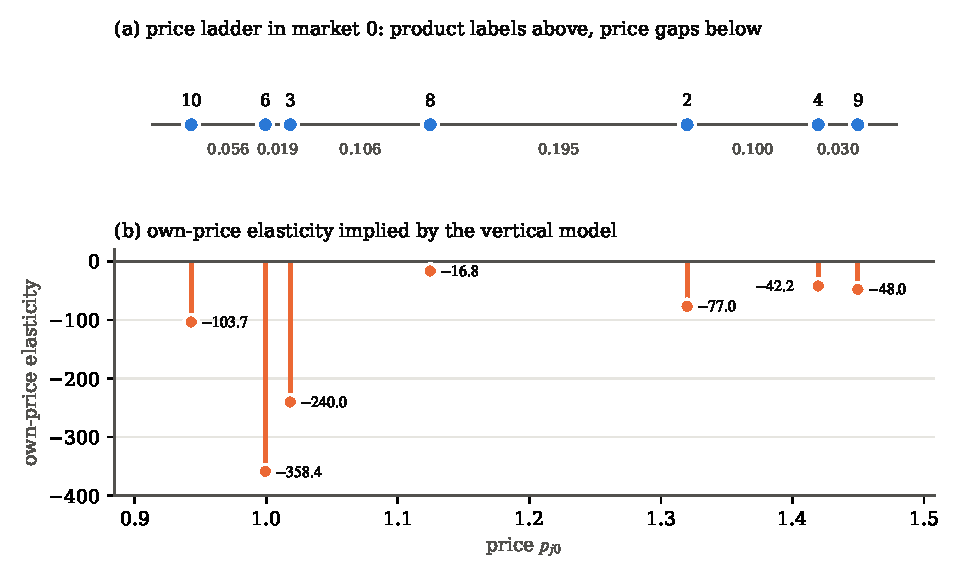
\includegraphics[width=0.9\linewidth]{figures/appC/ladder.pdf}
\caption{The price ladder in market 0. Panel (a) shows the seven prices with the gaps between neighbours. Panel (b)
shows the own-price elasticity $\varepsilon_{jj}$ that the vertical model implies for each product. The products with
the closest neighbours, 6 and 3, have the largest elasticities.}
\label{fig:C-ladder}
\end{figure}

The ladder also governs substitution to the outside good. In the vertical model only the cheapest product loses
customers to the outside good when its price rises. The diversion ratio from product $k$ to the outside good is
\[
  D_{k0} = -\frac{\partial s_0}{\partial p_k}\Big(\frac{\partial s_k}{\partial p_k}\Big)^{-1},
\]
the fraction of the sales that $k$ loses which go to the outside good. For product 10 it is 0.064. Every other product diverts
nothing to the outside good. The logit of \cref{sec:C-logit-est} puts these diversion ratios between 0.86 and 0.91, much
closer to the true model, in which most consumers who leave a product stop buying yogurt (\cref{sec:C-rc-est}).

\casehead{Part (f)}
The vertical model is appropriate when products differ mainly along one quality dimension that all consumers value in
the same direction. Consumers should differ mainly in income or in their marginal utility of money. Then the price
ladder is a quality ladder, and neighbours on it are the natural substitutes. \citet{Bresnahan1987} uses this structure
for the 1955 automobile price war. His consumers have utility $U = vx + Y - P$ from a car of quality $x$ and price $P$,
with $v$ uniform on $[0, V_{\max}]$ with density $d$ (eq.~1, p.~460, and p.~461). Bresnahan writes $\delta$ for
this density. The demand for a car between
neighbours $h$ and $j$ is linear in prices,
\[
  q_i = d\Big[\frac{P_j - P_i}{x_j - x_i} - \frac{P_i - P_h}{x_i - x_h}\Big]
\]
(eq.~5, p.~462). He notes that the quality difference $x_i - x_h$ measures how close two products are as substitutes,
and that they become perfect substitutes as $x_i$ approaches $x_h$ (p.~462). The same feature produces the large
elasticities of \cref{tab:C-velast}. Bresnahan also shows that demand in this model is continuous and concave across the
point where a neighbour is priced out, so a price equilibrium always exists (footnote~6, p.~462). Because only neighbours
compete, collusive and Nash pricing imply very different markups, which gives his conduct test its power
(\cref{sec:06-bresnahan}). The fact to explain is that 1955 production was 45 percent above that of the two surrounding
years, while quality-adjusted prices were lower (p.~457). In nonnested Cox tests the collusive solution is sustained in
1954 and 1956, and the competitive (Nash) solution in 1955 (abstract, p.~457).

Our simulated market violates the premises. Tastes vary along four dimensions, the products crowd into a narrow price
range, and the outside good takes more than three quarters of every market. The vertical model can explain why consumers
split across products with similar prices only by placing those products almost on top of one another in quality. It
then reads every small price gap as intense competition. Its elasticities are wrong by one to two orders of magnitude,
its markups are close to zero, and its implied costs absorb the error. The data offer two warning signs even without
knowledge of the truth. Qualities explain almost none of their own variation ($R^2 = 0.015$), and the implied Nash
markups are far below what any plausible cost information would allow. A model with an idiosyncratic shock, such as
the logit of \cref{sec:C-logit-est}, avoids the zero cross elasticities by construction.

\subsection{Computational notes}

The computations take a few seconds in total.
\begin{enumerate}
  \item In each market, sort products by price and form $\bar S_{(k)t}$ as reversed cumulative sums of the sorted
  realized shares.
  \item Compute $y_{jt}$ by \eqref{eq:C-vy} with \texttt{log1p} for $\ln(1 - \bar S)$, and run OLS of $y$ on $x$ with the
  clustered variance \eqref{eq:C-clustervar}.
  \item Compute $g_{(k)t}$ from \cref{cor:C-vfree}, fill the tridiagonal $\Delta_t$, form $\Omega_t$ from the owners and
  solve $(\Omega_t \odot \Delta_t^\top)\,a = s_t$ for the markups $-a$.
  \item Check the derivatives with a complex step, and check that the shares implied by the recovered qualities
  reproduce the data (largest error $1.9\times10^{-14}$).
\end{enumerate}
The inversion takes a few lines of code.
\begin{verbatim}
def vertical_delta(p, s, lam):
    order = np.argsort(p)                       # price ladder
    tail = np.cumsum(s[order][::-1])[::-1]      # bar S_(k)
    steps = np.diff(p[order], prepend=0.0)      # p_(k) - p_(k-1)
    delta = np.empty_like(p)
    delta[order] = np.cumsum(steps * -np.log1p(-tail) / lam)
    return delta
\end{verbatim}

\section{Estimating logit demand and recovering costs}\label{sec:C-logit-est}

The logit model becomes a linear regression once shares are inverted, so all the tools of linear instrumental variables
apply. In this problem we estimate it on the simulated market, study the strength of the usual instruments, recover
marginal costs with correct standard errors, and estimate demand and supply jointly. Since the data come from a random
coefficients model, the logit is misspecified. We close by deriving the bias that omitted taste heterogeneity creates in
the logit price coefficient and by measuring it in the simulated sample. The general theory of logit estimation is in \cref{ch:logit}.

\subsection{Statement}

Use the data and \cref{ass:C-est} of \cref{sec:C-vertical}. Demand is now logit:
\begin{equation}\label{eq:C-logit}
  u_{ijt} = \delta^l_{jt} + \epsilon_{ijt}, \qquad \delta^l_{jt} = x_{jt}\beta^l - \alpha^l p_{jt} + \xi_{jt},
\end{equation}
with $\epsilon_{ijt}$ independent type-I extreme value and $u_{i0t} = \epsilon_{i0t}$. Firms set prices in a
multi-product Bertrand-Nash equilibrium.

\begin{enumerate}[label=(\alph*)]
  \item Estimate $(\beta^l, \alpha^l)$. Give the identification argument, justify the instruments, assess their strength
  and report standard errors.
  \item Compute the elasticity matrix for market 0 and discuss it.
  \item Derive the marginal cost equation under the assumed conduct, compute $mc_{jt}$ and estimate
  $(\gamma_1, \gamma_2)$ with standard errors that account for the estimation of $\alpha^l$.
  \item Explain how to estimate demand and supply jointly, and when joint estimation matters. Carry it out.
  \item The true model has a random coefficient on price. Show why the logit price coefficient is then biased even with
  valid instruments, explain why the bias is toward zero in this design, and measure it.
\end{enumerate}

\subsection{Solution}

\casehead{Part (a)}
With logit demand the inside and outside shares are
\[
  s_{jt} = \frac{e^{\delta^l_{jt}}}{1 + \sum_{k}e^{\delta^l_{kt}}}, \qquad s_{0t} = \frac{1}{1 + \sum_{k}e^{\delta^l_{kt}}} .
\]
Dividing the first by the second gives $\frac{s_{jt}}{s_{0t}} = e^{\delta^l_{jt}}$, and taking logs gives the inversion of
\citet[eq.~14, p.~250]{Berry1994},
\begin{equation}\label{eq:C-berry}
  \ln s_{jt} - \ln s_{0t} = x_{jt}\beta^l - \alpha^l p_{jt} + \xi_{jt}.
\end{equation}
The left side is computed from realized shares, with $s_{0t} = 1 - \sum_j s_{jt}$. Equation \eqref{eq:C-berry} is
linear in the parameters, with the unobserved quality $\xi_{jt}$ as its error (\cref{eq:07-logit-inversion}).

Price is endogenous. Firms observe $\xi_{jt}$ when they set prices. A product with higher unobserved quality has a
larger share, and logit markups rise with the firm's share (part (c)), so $\Cov(p_{jt}, \xi_{jt}) > 0$. Let
$\tilde p_{jt}$ be the residual from projecting price on $x_{jt}$. The OLS estimate of the price coefficient then converges
to $-\alpha^l + \frac{\Cov(\tilde p_{jt}, \xi_{jt})}{\Var(\tilde p_{jt})}$, so OLS biases $\alpha^l$ toward zero
(\cref{prop:07-ols-bias}). We need excluded instruments that move price and are uncorrelated with $\xi_{jt}$.

We use seven excluded instruments.
\begin{enumerate}
  \item The price of milk $w_{jt}$. It shifts marginal cost and therefore price, it is excluded from utility, and it is
  independent of $\xi_{jt}$ by \cref{ass:C-est}(iii).
  \item Characteristics of the other products in the market. For each characteristic $k$ of product $j$ owned by firm $f$,
  \citet[eq.~5.8, p.~861]{BerryLevinsohnPakes1995} use the sums $\sum_{r \ne j, r \in \mathcal{J}_f}x_{rk}$ and
  $\sum_{r \notin \mathcal{J}_f}x_{rk}$. We form these sums for sugar content and the organic indicator. Because one
  characteristic is the constant, the numbers of the firm's other products and of rival products, $n^{own}_{jt}$ and
  $n^{riv}_{jt}$, are instruments too. This gives six instruments.
\end{enumerate}
\citet[p.~249]{Berry1994} explains why the second group is valid. Rival characteristics are excluded from $u_{ijt}$, and
they are correlated with prices through the markups in the first-order conditions. Their validity requires that
characteristics and the set of products offered in each market be independent of $\xi_{jt}$, which we add to
\cref{ass:C-est}. In this design characteristics are fixed by product, so the six instruments vary only through
which products a market offers and who owns them. The number of the firm's other products runs from 0 to 3 (mean 1.37),
and the number of rival products from 1 to 8 (mean 4.55).

The parameters $\theta^l = (\beta^l, \alpha^l)$ are identified by the moment conditions
\begin{equation}\label{eq:C-logit-moments}
  \E\big[z_{jt}^\top\xi_{jt}\big] = 0, \qquad z_{jt} = \big(x_{jt}, w_{jt}, \text{six competition instruments}\big),
\end{equation}
together with the rank condition that $\E[z_{jt}^\top(x_{jt}, p_{jt})]$ has full column rank four. Economically,
variation in price that comes from costs and from competition, and is unrelated to unobserved quality, traces out how
shares respond to price. We estimate by \emph{two-stage least squares} (2SLS). With $Y$ the stacked left side of
\eqref{eq:C-berry}, $X = (x, p)$ and $Z$ the instrument matrix, the 2SLS coefficient vector is
\[
  \hat b^l = (\hat X^\top\hat X)^{-1}\hat X^\top Y, \qquad \hat X = Z(Z^\top Z)^{-1}Z^\top X .
\]
Since price enters \eqref{eq:C-berry} with coefficient $-\alpha^l$, $\hat b^l$ estimates $(\beta^l, -\alpha^l)$. Its first
three entries give $\hat\beta^l$, and $\hat\alpha^l$ is minus its price entry. The clustered variance of $\hat b^l$ is
\eqref{eq:C-clustervar} with $X_t$ replaced by $\hat X_t$. The residuals in the middle factor are the 2SLS residuals
$\hat e_t = Y_t - X_t\hat b^l$, computed with the actual regressors (\cref{app:econometrics}).

\Cref{tab:C-firststage} reports the first stage. Instrument strength comes almost entirely from the milk price,
whose coefficient is 0.497 with standard error 0.026, close to the true cost coefficient of 0.5. The cluster-robust Wald
statistic for the seven excluded instruments, divided by seven, is 92.5. With one endogenous regressor this is the
cluster-robust first-stage $F$ statistic of \citet{KleibergenPaap2006}. The homoskedastic $F$ is 74.1 and the partial $R^2$ is
0.446. The milk price alone gives $F = 591.4$. The six competition instruments are jointly weak, with $F = 2.32$ and
$p = 0.039$ given the milk price.

\begin{table}[htbp]
\centering
\caption{First stage: OLS of $p_{jt}$ on the exogenous variables}
\label{tab:C-firststage}
\small
\begin{tabular}{@{}lcc@{}}
\toprule
 & Coefficient & Standard error \\
\midrule
Constant & 0.5778 & (0.0188) \\
Sugar content & 0.2575 & (0.0113) \\
Organic & 0.3138 & (0.0064) \\
Price of milk $w_{jt}$ & 0.4972 & (0.0256) \\
Sugar, firm's other products & 0.0023 & (0.0106) \\
Sugar, rival products & $-0.0042$ & (0.0077) \\
Organic, firm's other products & $-0.0015$ & (0.0068) \\
Organic, rival products & $-0.0009$ & (0.0040) \\
Number of firm's other products & 0.0038 & (0.0116) \\
Number of rival products & 0.0020 & (0.0084) \\
\midrule
$R^2$ & 0.923 & \\
$F$, seven excluded instruments (cluster-robust) & 92.5 & \\
$F$, seven excluded instruments (homoskedastic) & 74.1 & \\
$F$, six competition instruments (cluster-robust) & 2.32 & \\
$F$, milk price only (cluster-robust) & 591.4 & \\
\bottomrule
\end{tabular}

\vspace{3pt}
\begin{minipage}{0.97\textwidth}
\footnotesize Notes: 654 observations. Standard errors clustered by market. The milk-price-only
statistic comes from the regression of price on $(x_{jt}, w_{jt})$.
Computed with \texttt{figures/appC/src/appC\_vertical\_logit.py}.
\end{minipage}
\end{table}

The competition instruments are weak for two reasons. First, logit markups barely respond to competition in this
market. The markup of firm $f$ is $\frac{1}{\alpha^l(1 - S_{ft})}$ (part (c)), and the largest combined share of a
firm is only 0.112, so the implied markups run from 0.379 to 0.426. Changes in the set of competitors cannot move prices
much. Second, the instruments are nearly collinear. Sugar content varies only from 0.64 to 1.35, so each sum of sugar
is close to a multiple of the corresponding count. The correlations are 0.978 for the firm's own products and 0.988 for
rivals. The variance inflation factors of the two sugar sums and the two counts are 40.1, 57.8, 36.1 and 52.2. A
variance inflation factor is $\frac{1}{1 - R_k^2}$, the factor by which collinearity with the other regressors inflates
the variance of coefficient $k$.
\citet[p.~861]{BerryLevinsohnPakes1995} report the same problem, finding the matrix of these linear terms ``nearly not
of full rank.''

\Cref{tab:C-logit-demand} reports the estimates. As expected, OLS gives a smaller price coefficient, 2.330, than 2SLS,
2.641. Hansen's test of the six overidentifying restrictions \citep{Hansen1982} uses the two-step GMM estimator with a
market-clustered weighting matrix. It does not reject, with $J = 8.82$ and $p = 0.18$. The two-step GMM estimate of the
price coefficient is 2.872. With the milk price as the only excluded instrument, 2SLS gives 2.677 (0.415), so the
competition instruments change little.

\begin{table}[htbp]
\centering
\caption{Logit demand estimates}
\label{tab:C-logit-demand}
\small
\begin{tabular}{@{}lcccc@{}}
\toprule
 & OLS & 2SLS & \makecell{2SLS,\\ milk price only} & True \\
\midrule
Constant & $-1.443$ & $-1.184$ & $-1.154$ & $-1.00$ \\
 & (0.226) & (0.329) & (0.334) & \\
Sugar content & 0.119 & 0.190 & 0.198 & 0.20 \\
 & (0.122) & (0.158) & (0.156) & \\
Organic & 0.051 & 0.153 & 0.165 & 0.15 \\
 & (0.097) & (0.141) & (0.142) & \\
Price coefficient $\alpha^l$ & 2.330 & 2.641 & 2.677 & 3.00 \\
 & (0.252) & (0.412) & (0.415) & \\
\midrule
First-stage $F$ (cluster-robust) & & 92.5 & 591.4 & \\
Hansen $J$ ($p$-value) & & 8.82 (0.18) & & \\
$R^2$ & 0.396 & 0.395 & 0.395 & \\
Observations & 654 & 654 & 654 & \\
\bottomrule
\end{tabular}

\vspace{3pt}
\begin{minipage}{0.97\textwidth}
\footnotesize Notes: Dependent variable $\ln s_{jt} - \ln s_{0t}$. Standard errors clustered by
market in parentheses. The table reports $\alpha^l$, minus the coefficient on price. The true values are the mean
parameters of the random coefficients model of \cref{sec:C-simulate}.
Computed with \texttt{figures/appC/src/appC\_vertical\_logit.py}.
\end{minipage}
\end{table}

Consistency of 2SLS here rests on one more condition. Characteristics and milk prices are fixed by product, so the
identifying variation in $w_{jt}$ comes from its ten values across products. If $\xi_{jt}$ contained a persistent
product component, it could correlate with the product-level instruments. An $F$ test of product dummies on the 2SLS
residuals, beyond the product-level regressors, gives $F(6, 644) = 1.18$ with $p = 0.32$. With only ten products the test
has little power, so it cannot rule such a component out. In this design the unobservables are drawn independently
across markets, so the condition holds by construction.

The 2SLS price coefficient, 2.641, lies below the true mean of 3, but only 0.87 standard errors below. The
characteristic coefficients are close to the truth and imprecise, because sugar and organic status take only ten distinct
combinations. Part (e) splits the shortfall in $\hat\alpha^l$. Most of it, 0.284 of 0.359, is an estimate of the
misspecification bias of the logit. The rest reflects sampling and simulation error, since the random coefficients model
gives 2.926 on the same sample.

\casehead{Part (b)}
The logit share derivatives of \cref{sec:C-logit-bertrand}, part (a), hold with $\alpha^l$ in place of $\alpha$
(\cref{prop:07-logit-derivs}). They give the elasticities \eqref{eq:C-logit-elast} together with the outside-good row,
\begin{equation}\label{eq:C-lelast}
  \varepsilon_{jj} = -\alpha^l p_j(1 - s_j), \qquad \varepsilon_{jk} = \alpha^l p_ks_k \quad (k \ne j), \qquad
  \varepsilon_{0k} = \alpha^l p_ks_k .
\end{equation}
\Cref{tab:C-lelast} evaluates them at $\hat\alpha^l = 2.641$ and the observed prices and realized shares of market 0.

\begin{table}[htbp]
\centering
\caption{Logit model: price elasticities in market 0}
\label{tab:C-lelast}
\small
\begin{tabular}{@{}lrrrrrrr@{}}
\toprule
 & \multicolumn{7}{c}{Price of product} \\
\cmidrule(lr){2-8}
Share of & 2 & 3 & 4 & 6 & 8 & 9 & 10 \\
\midrule
Product 2 & $-3.47$ & 0.07 & 0.05 & 0.05 & 0.17 & 0.02 & 0.05 \\
Product 3 & 0.02 & $-2.62$ & 0.05 & 0.05 & 0.17 & 0.02 & 0.05 \\
Product 4 & 0.02 & 0.07 & $-3.70$ & 0.05 & 0.17 & 0.02 & 0.05 \\
Product 6 & 0.02 & 0.07 & 0.05 & $-2.59$ & 0.17 & 0.02 & 0.05 \\
Product 8 & 0.02 & 0.07 & 0.05 & 0.05 & $-2.80$ & 0.02 & 0.05 \\
Product 9 & 0.02 & 0.07 & 0.05 & 0.05 & 0.17 & $-3.81$ & 0.05 \\
Product 10 & 0.02 & 0.07 & 0.05 & 0.05 & 0.17 & 0.02 & $-2.44$ \\
Outside good & 0.02 & 0.07 & 0.05 & 0.05 & 0.17 & 0.02 & 0.05 \\
\bottomrule
\end{tabular}

\vspace{3pt}
\begin{minipage}{0.97\textwidth}
\footnotesize Notes: Entry $(j, k)$ is $\varepsilon_{jk}$ from \eqref{eq:C-lelast} with
$\hat\alpha^l = 2.641$ (2SLS), evaluated at observed prices and realized shares. Computed with \texttt{figures/appC/src/appC\_vertical\_logit.py}.
\end{minipage}
\end{table}

The own elasticities run from $-2.44$ to $-3.81$, so every product faces elastic demand. Across all 654 observations
they lie between $-2.21$ and $-4.24$, with mean $-3.06$. They are close to the true values, $-2.57$ to $-3.85$ in market
0, but slightly smaller in magnitude, because $\hat\alpha^l$ is below 3. Since shares are small,
$\varepsilon_{jj} \approx -\alpha^l p_j$, so the model makes the most expensive products the most elastic by
construction. Products 9 and 4, the two most expensive, have the largest own elasticities.

Every off-diagonal entry in a column is the same, and it equals the outside-good entry. This is the independence of
irrelevant alternatives. A rise in $p_k$ raises the shares of all other products and of the outside good in the same
proportion, whatever their characteristics. Diversion from product $k$ to the outside good is
$D_{k0} = \frac{\alpha^l s_0s_k}{\alpha^l s_k(1 - s_k)} = \frac{s_0}{1 - s_k}$, between 0.86 and 0.91 in market 0. In the
true model a price rise for an organic product diverts more customers to the other organic products and to expensive
products (\cref{sec:C-rc-est}). The logit cannot produce this pattern.

\casehead{Part (c)}
With logit demand the first-order conditions \eqref{eq:C-vsupply-nash} reduce to the common-markup rule of
\cref{prop:C-common-markup}, derived in \cref{sec:C-logit-bertrand}, part (e) (see also \cref{prop:07-logit-multi}).
Every product of firm $f$ in market $t$ carries the markup $m_{ft} = \frac{1}{\alpha^l(1 - S_{ft})}$, where
$S_{ft} = \sum_{k \in \mathcal{J}_{ft}}s_{kt}$ is the firm's combined share. The marginal cost equation is
\begin{equation}\label{eq:C-lsupply}
  mc_{jt} = p_{jt} - \frac{1}{\alpha^l(1 - S_{ft})} = x_{jt}\gamma_1 + \gamma_2 w_{jt} + \omega_{jt} .
\end{equation}
This is \eqref{eq:C-vsupply-nash} with the logit Jacobian. The script confirms that the closed form and the matrix formula
agree to $2.2\times10^{-16}$. We compute $mc_{jt}$ with $\hat\alpha^l = 2.641$ and the realized shares. The implied
markups run from 0.379 to 0.426 with mean 0.396, against a true mean of 0.386. Their correlation with the true markups
is 0.55, against 0.27 for the vertical Nash markups. No implied marginal cost is negative. Identification of
$(\gamma_1, \gamma_2)$ follows as in \cref{sec:C-vertical}, from $\E[\omega_{jt} \mid x_{jt}, w_{jt}] = 0$ and full rank.
We estimate it by OLS of $mc_{jt}$ on $(x_{jt}, w_{jt})$.

The dependent variable now contains the estimate $\hat\alpha^l$. Clustered OLS standard errors treat $mc_{jt}$ as data
and so ignore this uncertainty. We correct them in two ways.

The first is a \emph{market bootstrap}. Each of 5,000 replications draws 100 markets with replacement, re-estimates
$(\beta^l, \alpha^l)$ by 2SLS, recomputes every implied marginal cost with the new $\alpha^l$, and re-runs the supply
regression. The bootstrap standard error is the standard deviation of the replicated estimates. Resampling whole markets
preserves dependence within markets and is valid because markets are independent. With 5,000 replications the Monte
Carlo error of each bootstrap standard error of the cost coefficients is below 0.0011.

The second treats the two steps as one GMM estimator with stacked moments \citep{Newey1984, MurphyTopel1985}. Write
$k_{jt} = \frac{1}{1 - S_{ft}}$, so that $mc_{jt}(\alpha) = p_{jt} - \frac{k_{jt}}{\alpha}$, and let $W$ be the regressor
matrix of \eqref{eq:C-supplydecomp}, with rows $W_{jt} = (x_{jt}, w_{jt})$. The supply estimate solves
$\sum_{t}\sum_j W_{jt}^\top\big(p_{jt} - \frac{k_{jt}}{\hat\alpha^l} - W_{jt}\hat\gamma\big) = 0$. A first-order expansion
around the probability limits gives
\begin{equation}\label{eq:C-stacked}
  \begin{aligned}
  \hat\gamma - \gamma &\approx (W^\top W)^{-1}\Big[\sum_{t}\sum_j W_{jt}^\top\omega_{jt}
  + \frac{W^\top k}{(\alpha^l)^2}\big(\hat\alpha^l - \alpha^l\big)\Big], \\
  \hat\alpha^l - \alpha^l &\approx -\iota_p^\top(\hat X^\top\hat X)^{-1}\sum_{t}\sum_j\hat X_{jt}^\top\xi_{jt},
  \end{aligned}
\end{equation}
where $\iota_p$ selects the price coefficient. Each observation thus contributes an influence term to $\hat\gamma$.
Summing these terms within markets and taking the clustered outer product gives a sandwich variance that includes the
estimation error in $\alpha^l$. The coefficient $(W^\top W)^{-1}\frac{W^\top k}{(\alpha^l)^2}$ measures how the cost estimates
move with $\alpha^l$. For the constant it is 0.148, close to the mean markup divided by $\alpha^l$. With
$\text{s.e.}(\hat\alpha^l) = 0.412$, this alone gives a standard error of about $0.148 \times 0.412 = 0.061$ for the
intercept. \Cref{tab:C-lsupply} reports the estimates.

\begin{table}[htbp]
\centering
\caption{Logit model, supply side: OLS of the implied marginal cost on $(x_{jt}, w_{jt})$}
\label{tab:C-lsupply}
\small
\setlength{\tabcolsep}{5pt}
\begin{tabular}{@{}lcccccc@{}}
\toprule
 & Estimate & \makecell{Clustered\\ s.e.} & \makecell{Stacked\\ s.e.} & \makecell{Bootstrap\\ s.e.}
 & \makecell{Bootstrap\\ 95\% interval} & True \\
\midrule
Constant & 0.160 & 0.016 & 0.065 & 0.072 & $[-0.022, 0.257]$ & 0.20 \\
Sugar content & 0.258 & 0.010 & 0.010 & 0.010 & $[0.239, 0.278]$ & 0.25 \\
Organic & 0.315 & 0.005 & 0.006 & 0.006 & $[0.304, 0.327]$ & 0.30 \\
Price of milk & 0.532 & 0.023 & 0.023 & 0.023 & $[0.487, 0.576]$ & 0.50 \\
\bottomrule
\end{tabular}

\vspace{3pt}
\begin{minipage}{0.97\textwidth}
\footnotesize Notes: The implied marginal cost is \eqref{eq:C-lsupply} with $\hat\alpha^l = 2.641$, and
$R^2 = 0.923$. The clustered standard errors treat $mc_{jt}$ as data. The stacked standard errors use the influence
functions in \eqref{eq:C-stacked}, clustered by market. The bootstrap resamples markets 5,000 times and re-estimates
$\alpha^l$ in each replication. The interval is the percentile interval.
Computed with \texttt{figures/appC/src/appC\_vertical\_logit.py}.
\end{minipage}
\end{table}

The estimates are close to the true values. Uncertainty about $\alpha^l$ moves all markups together, since each is near
$\frac{1}{\alpha^l}$ when shares are small. It therefore loads almost entirely on the intercept, whose standard error rises
from 0.016 to 0.065 (stacked) or 0.072 (bootstrap), while the slope standard errors barely change. The two corrections
agree closely. The decomposition \eqref{eq:C-supplydecomp} locates the remaining errors. The logit markup error loads
$-0.040$ on the constant, $0.011$ on sugar, $0.011$ on organic and $0.030$ on the milk price. True markups are higher for
organic products (0.392 against 0.383), because their buyers are less price sensitive. Logit markups are slightly lower
for them (0.392 against 0.397), because organic producers have smaller combined shares. The logit therefore understates
the organic markup premium ($-0.005$ against $+0.008$ in the truth), so it overstates the organic cost premium. The
bootstrap interval for the organic coefficient just excludes 0.30.
Compared with the vertical model under Nash pricing (\cref{tab:C-vsupply}), the logit recovers costs far more accurately
because its markups are close to the true ones.

\casehead{Part (d)}
Joint estimation stacks the demand and supply moments and estimates
$\theta = (\beta^l, \alpha^l, \gamma_1, \gamma_2)$ by GMM. For a candidate $\theta$, the residuals are
\begin{equation}\label{eq:C-joint-resid}
  \xi_{jt}(\theta) = \ln s_{jt} - \ln s_{0t} - x_{jt}\beta^l + \alpha^l p_{jt}, \qquad
  \omega_{jt}(\theta) = p_{jt} - \frac{1}{\alpha^l(1 - S_{ft})} - x_{jt}\gamma_1 - \gamma_2 w_{jt}.
\end{equation}
With demand instruments $z^d_{jt}$ and supply instruments $z^s_{jt}$, the sample moments and the estimator are
\begin{equation}\label{eq:C-joint}
  \bar g(\theta) = \frac{1}{N}\sum_{t}\sum_j\begin{pmatrix} z^{d\top}_{jt}\,\xi_{jt}(\theta) \\
  z^{s\top}_{jt}\,\omega_{jt}(\theta)\end{pmatrix}, \qquad
  \hat\theta = \argmin_\theta \bar g(\theta)^\top\,\mathcal W\,\bar g(\theta).
\end{equation}
The first step uses the block-diagonal weight $\mathcal W_1 = \diag\big((\frac{1}{N}Z^{d\top}Z^d)^{-1},
(\frac{1}{N}Z^{s\top}Z^s)^{-1}\big)$. The second step uses the inverse of the market-clustered covariance of the moments
at the first-step estimate, $\mathcal W_2 = \hat S^{-1}$, which is efficient. Given $\alpha^l$, both residuals are linear in
$(\beta^l, \gamma_1, \gamma_2)$, so we concentrate these out by weighted least squares and search over $\alpha^l$ alone.
The GMM sandwich then gives standard errors that account for the estimation of $\alpha^l$ in the markups
(\cref{sec:08-supply-joint}).

\begin{proposition}[A just-identified supply block adds nothing]\label{prop:C-redundant}
Let $z^s_{jt} = (x_{jt}, w_{jt})$, so that the supply block has as many moments as cost parameters. Then the joint GMM
estimate of $(\beta^l, \alpha^l)$ with weight $\mathcal W$ equals the GMM estimate from the demand moments alone with weight
$\mathcal W_{dd} - \mathcal W_{ds}\mathcal W_{ss}^{-1}\mathcal W_{sd}$. With the block-diagonal $\mathcal W_1$ this is 2SLS. With
the efficient $\mathcal W_2 = \hat S^{-1}$ it is two-step efficient GMM on the demand moments with weight $\hat S_{dd}^{-1}$.
\end{proposition}

\begin{proof}
Partition $\bar g = (\bar g_d, \bar g_s)$. For fixed $(\beta^l, \alpha^l)$, $\bar g_s = b_s(\alpha^l) - \frac{1}{N}W^\top
W\gamma$, and $\frac{1}{N}W^\top W$ is square and invertible. Choosing $\gamma$ is therefore the same as choosing the value
$v$ of $\bar g_s$ freely. Minimizing the quadratic form over $v$,
\[
  \min_v\begin{pmatrix}\bar g_d \\ v\end{pmatrix}^\top
  \begin{pmatrix}\mathcal W_{dd} & \mathcal W_{ds} \\ \mathcal W_{sd} & \mathcal W_{ss}\end{pmatrix}
  \begin{pmatrix}\bar g_d \\ v\end{pmatrix}
  = \bar g_d^\top\big(\mathcal W_{dd} - \mathcal W_{ds}\mathcal W_{ss}^{-1}\mathcal W_{sd}\big)\bar g_d ,
\]
attained at $v = -\mathcal W_{ss}^{-1}\mathcal W_{sd}\bar g_d$. The concentrated objective involves only the demand
moments. For block-diagonal $\mathcal W$ the bracket is $\mathcal W_{dd}$. For $\mathcal W = \hat S^{-1}$, the formula for the
inverse of a partitioned matrix gives $\mathcal W_{dd} - \mathcal W_{ds}\mathcal W_{ss}^{-1}\mathcal W_{sd} = \hat S_{dd}^{-1}$.
\end{proof}

This is a special case of a general separability result for GMM \citep{AhnSchmidt1995}. The supply side carries
information about demand only when it has more moments than cost parameters. Under \cref{ass:C-est}(iii), $\omega_{jt}$ is
also independent of the characteristics of other products, so the six competition instruments are valid supply
instruments. \citet[p.~255]{Berry1994} proposes the characteristics of other firms as cost-side instruments for the same
reason. \citet[pp.~861--862]{BerryLevinsohnPakes1995} interact their cost error with the three terms of their eq.~(5.8)
for each of six cost characteristics. The three terms are the characteristic itself, its sum over the firm's other
products and its sum over rival products. They add miles per dollar, a demand variable excluded from cost, for nineteen cost-side
instruments in all.

With these instruments the supply equation identifies $\alpha^l$ on its own. Rewrite \eqref{eq:C-lsupply} as
\begin{equation}\label{eq:C-supply-only}
  p_{jt} = x_{jt}\gamma_1 + \gamma_2 w_{jt} + \frac{1}{\alpha^l}\,k_{jt} + \omega_{jt}, \qquad k_{jt} = \frac{1}{1 - S_{ft}} ,
\end{equation}
a linear regression in which $\frac{1}{\alpha^l}$ is the coefficient on $k_{jt}$. This is the multi-product version of the
logit supply equation of \citet[eq.~31, p.~255]{Berry1994}, whose parameters are $\gamma$ and $\frac{1}{\alpha}$. The firm
share is endogenous, because a high $\omega_{jt}$ raises the price and lowers the share. The competition instruments predict
$k_{jt}$ well, with a cluster-robust first-stage $F$ of 51.6. The number and type of a firm's other products move its
combined share directly. 2SLS of \eqref{eq:C-supply-only} gives $\frac{1}{\hat\alpha^l} = 0.351$ (0.132), so
$\hat\alpha^l = 2.85$ with a delta-method standard error of 1.07. The estimate is close to the demand-side values, but it
is imprecise because $k_{jt}$ varies only from 1.002 to 1.126. The markups move too little across markets to measure their
slope well. \Cref{tab:C-joint} shows what the joint estimator does with this extra information.

\begin{table}[htbp]
\centering
\caption{Sequential and joint estimation of logit demand and supply}
\label{tab:C-joint}
\small
\begin{tabular}{@{}lcccc@{}}
\toprule
 & Sequential & \makecell{Joint GMM,\\ $z^s = (x, w)$} & \makecell{Joint GMM, $z^s$ adds\\ six instruments}
 & True \\
\midrule
\multicolumn{5}{l}{\textit{Demand}} \\
Constant & $-1.184$ (0.329) & $-1.035$ (0.311) & $-1.101$ (0.291) & $-1.00$ \\
Sugar content & 0.190 (0.158) & 0.291 (0.152) & 0.267 (0.144) & 0.20 \\
Organic & 0.153 (0.141) & 0.211 (0.134) & 0.178 (0.123) & 0.15 \\
Price coefficient $\alpha^l$ & 2.641 (0.412) & 2.872 (0.394) & 2.785 (0.367) & 3.00 \\
\multicolumn{5}{l}{\textit{Marginal cost}} \\
Constant & 0.160 (0.072) & 0.191 (0.053) & 0.181 (0.053) & 0.20 \\
Sugar content & 0.258 (0.010) & 0.261 (0.010) & 0.260 (0.009) & 0.25 \\
Organic & 0.315 (0.006) & 0.315 (0.005) & 0.314 (0.005) & 0.30 \\
Price of milk & 0.532 (0.023) & 0.529 (0.022) & 0.527 (0.021) & 0.50 \\
\midrule
Moments & & 14 & 20 & \\
Hansen $J$ (d.f., $p$) & & 8.82 (6, 0.18) & 12.85 (12, 0.38) & \\
\bottomrule
\end{tabular}

\vspace{3pt}
\begin{minipage}{0.97\textwidth}
\footnotesize Notes: The sequential column is 2SLS for demand (clustered standard errors) and OLS
for supply (bootstrap standard errors). The joint columns are two-step efficient GMM estimates of \eqref{eq:C-joint} with
$z^d$ as in part (a), weights clustered by market, and GMM sandwich standard errors without a small-sample factor. With
$z^s = (x, w)$ the first step reproduces the sequential point estimates (\cref{prop:C-redundant}). With the six added
supply instruments the first step gives $\hat\alpha^l = 2.642$, which differs slightly from the sequential 2.641.
Computed with \texttt{figures/appC/src/appC\_vertical\_logit.py}.
\end{minipage}
\end{table}

The numbers confirm \cref{prop:C-redundant}. With $z^s = (x, w)$, the first-step joint estimate of $\alpha^l$ is 2.641, the
2SLS value. The second-step estimate is 2.872, exactly the two-step GMM estimate from the demand moments alone, and the
$J$ statistic is the same 8.82. The cost coefficients do change, because the efficient weight lets demand residuals inform
the supply block. Adding the six competition instruments to the supply side changes even the first step, which gives
2.642. The cost parameters can no longer set every supply moment to zero, and the remaining supply moments depend on
$\alpha^l$ through the markups. The second step gives $\hat\alpha^l = 2.785$ with standard error 0.367, against 0.394
without the added instruments. The estimate is close to the demand-side estimates and to the supply-only value of
2.85. The gain in precision is modest, for the reason that made these instruments weak in the first stage. With combined shares
of at most 0.112, the markups barely change with competition. The overidentifying restrictions are not rejected
($J = 12.85$ with 12 degrees of freedom, $p = 0.38$).

Joint estimation matters in four situations. The first is when demand moments identify the demand parameters poorly,
because instruments are weak or because there are nonlinear parameters such as the random coefficients of
\cref{sec:C-rc-est}. Extra supply moments then add information. The second is when $\xi_{jt}$ and $\omega_{jt}$ are
correlated and the supply block is overidentified, since the efficient weight then links the blocks. The third is when
conduct itself is a parameter, because only the supply side identifies it. The fourth is when correct standard errors for
the cost parameters are needed and no bootstrap is run. Joint estimation also has a cost. If the conduct assumption is
wrong, the supply moments contaminate the demand estimates, which sequential estimation protects against.

\casehead{Part (e)}
The true model of \cref{sec:C-simulate} has random coefficients, $u_{ijt} = \delta_{jt} + \tilde x_{jt}\Sigma\nu_i +
\epsilon_{ijt}$ with $\tilde x_{jt} = (x_{jt}, p_{jt})$, $\nu_i \sim N(0, I_4)$ and $\delta_{jt} = x_{jt}\beta - \alpha
p_{jt} + \xi_{jt}$. Let $\delta_{jt}$ be the mean utility that rationalizes the observed shares in this model, recovered
by the contraction of \cref{thm:08-contraction}, which \cref{prop:C-blp-contraction} of the next problem verifies for
this market. Define the \emph{gap term}
\begin{equation}\label{eq:C-gap}
  r_{jt} = \ln\frac{s_{jt}}{s_{0t}} - \delta_{jt} .
\end{equation}
The logit regression \eqref{eq:C-berry} then has the dependent variable $x_{jt}\beta - \alpha p_{jt} + \xi_{jt} +
r_{jt}$, so its error is $\xi_{jt} + r_{jt}$.

\begin{proposition}[Decomposition of the logit estimate]\label{prop:C-logit-bias}
Use the regressors $(x_{jt}, p_{jt})$ and the instruments $z_{jt}$ throughout. Let $\hat b^{RC}$ be the 2SLS coefficient
vector with dependent variable $\delta_{jt}$, and let $\hat b^l$ be the one with dependent variable $\ln\frac{s_{jt}}{s_{0t}}$.
Write $\hat\alpha^{RC}$ and $\hat\alpha^l$ for minus their price entries. Let $\hat b_r$ be the one with dependent
variable $r_{jt}$, with price coefficient $\hat b_{r,p}$. Then
\begin{equation}\label{eq:C-decomp}
  \hat b^l = \hat b^{RC} + \hat b_r, \qquad \hat\alpha^l = \hat\alpha^{RC} - \hat b_{r,p}.
\end{equation}
Suppose the random coefficients model is correct and $z_{jt}$ is valid for it. Then $\plim\hat\alpha^l = \alpha - b_{r,p}$,
where $b_{r,p}$ is the price coefficient of the population 2SLS projection of $r_{jt}$ on $(x_{jt}, p_{jt})$ with
instruments $z_{jt}$. The logit estimate is biased toward zero whenever $b_{r,p} > 0$.
\end{proposition}

\begin{proof}
The 2SLS estimator is linear in the dependent variable, $\hat b(Y) = (X^\top P_ZX)^{-1}X^\top P_ZY$ with
$P_Z = Z(Z^\top Z)^{-1}Z^\top$. Since $\ln\frac{s_{jt}}{s_{0t}} = \delta_{jt} + r_{jt}$ observation by observation,
$\hat b^l = \hat b(\delta) + \hat b(r) = \hat b^{RC} + \hat b_r$. The price coefficient is $-\alpha$ in both models, so
the price entries give $-\hat\alpha^l = -\hat\alpha^{RC} + \hat b_{r,p}$, which is the second equation. Under the
stated conditions $\plim\hat\alpha^{RC} = \alpha$, and $\hat b_{r,p}$ converges to its population counterpart.
\end{proof}

The instruments do not remove this bias. The gap term depends on prices, and prices depend on the milk price and on the
competition instruments, so $\E[z_{jt}^\top r_{jt}] \ne 0$ in general. The question is the sign of $b_{r,p}$. No general
result fixes it, because it depends on the model, the design and the instruments. The next result shows how $r_{jt}$
varies across the products of one market when tastes are only slightly dispersed.

\begin{proposition}[The gap term for small taste dispersion]\label{prop:C-gap-approx}
Let $\Sigma$ be diagonal and $\nu_i \sim N(0, I_4)$. As $\lVert\Sigma\rVert \to 0$,
\begin{equation}\label{eq:C-gap-approx}
  r_{jt} = \frac{1}{2}\,\tilde x_{jt}\Sigma^2\tilde x_{jt}^\top - \tilde x_{jt}\Sigma^2\bar x_t^\top + O(\lVert\Sigma\rVert^3),
  \qquad \bar x_t = \sum_{k}s_{kt}\tilde x_{kt},
\end{equation}
where the sum runs over inside products. In particular, the price component of $r_{jt}$ is
$\Sigma_{pp}^2\big(\frac{1}{2}p_{jt}^2 - p_{jt}\bar p_t\big)$, with $\Sigma_{pp}$ the price entry of $\Sigma$ and
$\bar p_t = \sum_k s_{kt}p_{kt}$. All products of market $t$ share $\bar p_t$, so among the products of a market priced
above $\bar p_t$ this component is larger for the more expensive product.
\end{proposition}

\begin{proof}
Fix a market and drop $t$. Let $\mu_{ij} = \tilde x_j\Sigma\nu_i$ for inside goods and $\mu_{i0} = 0$. Write
$s^L_j$ for the logit shares at $\delta$, so that $\ln\frac{s^L_j}{s^L_0} = \delta_j$. The individual choice probability is
the logit probability at utilities $\delta_j + \mu_{ij}$. Since $\frac{\partial\ln s_j}{\partial u_k} = \indic\{j = k\} -
s_k$ and $\frac{\partial^2\ln s_j}{\partial u_k\partial u_l} = -s_k(\indic\{k = l\} - s_l)$, a second-order expansion in
$\mu_i$ gives
\[
  \ln s_{ij} = \ln s^L_j + \mu_{ij} - \bar\mu_i - \frac{1}{2}V_i + O(|\mu_i|^3), \qquad
  \bar\mu_i = \sum_k s^L_k\mu_{ik}, \quad V_i = \sum_k s^L_k\mu_{ik}^2 - \bar\mu_i^2 ,
\]
for every alternative, including $j = 0$ with $\mu_{i0} = 0$. Exponentiating and expanding,
\[
  s_{ij} = s^L_j\Big[1 + (\mu_{ij} - \bar\mu_i) - \frac{1}{2}V_i + \frac{1}{2}(\mu_{ij} - \bar\mu_i)^2\Big] + O(|\mu_i|^3).
\]
Average over $\nu_i$. Because $\E[\mu_{ij}] = 0$ and $\mu_i = O(\lVert\Sigma\rVert)$,
\[
  s_j = s^L_j\Big[1 + \frac{1}{2}\E(\mu_{ij} - \bar\mu_i)^2 - \frac{1}{2}\E V_i\Big] + O(\lVert\Sigma\rVert^3), \qquad
  s_0 = s^L_0\Big[1 + \frac{1}{2}\E\bar\mu_i^2 - \frac{1}{2}\E V_i\Big] + O(\lVert\Sigma\rVert^3).
\]
Take logs, use $\ln(1 + a) = a + O(a^2)$ with $a = O(\lVert\Sigma\rVert^2)$, and subtract:
\[
  \ln\frac{s_j}{s_0} - \delta_j = \frac{1}{2}\E\big[(\mu_{ij} - \bar\mu_i)^2 - \bar\mu_i^2\big] + O(\lVert\Sigma\rVert^3)
  = \frac{1}{2}\E[\mu_{ij}^2] - \E[\mu_{ij}\bar\mu_i] + O(\lVert\Sigma\rVert^3).
\]
With $\nu_i \sim N(0, I_4)$ and $\Sigma$ diagonal, $\E[\mu_{ij}^2] = \tilde x_j\Sigma^2\tilde x_j^\top$ and
$\E[\mu_{ij}\bar\mu_i] = \tilde x_j\Sigma^2\big(\sum_k s^L_k\tilde x_k\big)^\top$. Finally $s^L_k - s_k = O(\lVert\Sigma\rVert^2)$,
and the term it multiplies is $O(\lVert\Sigma\rVert^2)$, so replacing $s^L_k$ by $s_k$ changes $r_j$ by $O(\lVert\Sigma\rVert^4)$.
For fixed $\bar p$, the price component $\Sigma_{pp}^2(\frac{1}{2}p^2 - p\bar p)$ has derivative $\Sigma_{pp}^2(p - \bar p)$ in
the product's own price $p$, which is positive for $p > \bar p$.
\end{proof}

The comparison in \cref{prop:C-gap-approx} holds $\bar p_t$ fixed, as it is across the products of one market. It does not
give the response of $r_{jt}$ to a change in $p_{jt}$, which also moves the shares and hence $\bar p_t$. To leading order
the logit share derivatives give $\frac{\partial\bar p_t}{\partial p_{jt}} = s_{jt}\big[1 - \alpha(p_{jt} - \bar p_t)\big]$,
so the full derivative of the price component is
\begin{equation*}
  \Sigma_{pp}^2\Big[(p_{jt} - \bar p_t)(1 + \alpha p_{jt}s_{jt}) - p_{jt}s_{jt}\Big] .
\end{equation*}
It can be negative for a product with a large share. With one inside good, $p = 1$, $\alpha = 1$ and share
$\frac{3}{4}$, it equals $-\frac{5}{16}\Sigma_{pp}^2$, although $p$ exceeds $\bar p = \frac{3}{4}$. Neither derivative
signs $b_{r,p}$ by itself. The 2SLS projection pools products and markets with different $\bar p_t$, and the instruments
decide which price variation it uses. The sign of the bias is therefore specific to the model, the design and the
instruments.

Our design, with small inside shares, is a favorable case for a positive $b_{r,p}$. The outside share is at least 0.788 in every market, so
$\bar p_t$ lies between 0.064 and 0.224, while every price is at least 0.881. Every observation has
$p_{jt} - \bar p_t \ge 0.707$. At the random coefficients estimate of $\alpha$ reported below, the full derivative is at
least $0.729\,\Sigma_{pp}^2$ at every observation. Both derivatives are therefore positive throughout the sample.

The intuition is sorting. Consumers with a low price sensitivity $\alpha_i = \alpha - \Sigma_{pp}\nu_{i4}$ buy expensive
products more than the average consumer does. Averaging the convex logit probability over this heterogeneity raises the
share of expensive products above what a logit with the same mean utility predicts. The logit can absorb the excess only
in its error term, which is then larger for the more expensive products of a market. By \eqref{eq:C-gap-approx}, the
within-market slope of the price component is $\Sigma_{pp}^2(p_{jt} - \bar p_t)$. With $\Sigma_{pp} = 0.5$, a mean price of
1.18 and a mean $\bar p_t$ of 0.142 across observations, this slope averages 0.259.

We now compute each term of \eqref{eq:C-decomp} in our sample. The script recovers $\delta_{jt}$ in every market by the
contraction with 1,000 fixed draws per market (seed 2030), as in \cref{sec:C-rc-est}. Convergence to a tolerance of $10^{-10}$ takes 11 to 18
iterations. \Cref{fig:C-gap} plots $r_{jt}$ against price. The gap is positive for every observation, from 0.105 to
0.511, so every recovered $\delta_{jt}$ lies below its logit start (\cref{prop:C-delta-lower}). Its correlation with price
is 0.888. In market 0 it rises from 0.125 for the cheapest product to 0.326 for the
most expensive one. The 2SLS estimate of the random coefficients model on the same sample and instruments is
$\hat\alpha^{RC} = 2.926$ (0.413). The 2SLS price coefficient of $r_{jt}$ is $\hat b_{r,p} = 0.284$, and the identity
\eqref{eq:C-decomp}, $2.641 = 2.926 - 0.284$, holds to $9\times10^{-16}$. The approximation \eqref{eq:C-gap-approx},
evaluated at the true $\Sigma$, has correlation 0.93 with the exact $r_{jt}$. Its own 2SLS price coefficient is 0.286, and
its price component alone gives 0.270.

\begin{figure}[htbp]
\centering
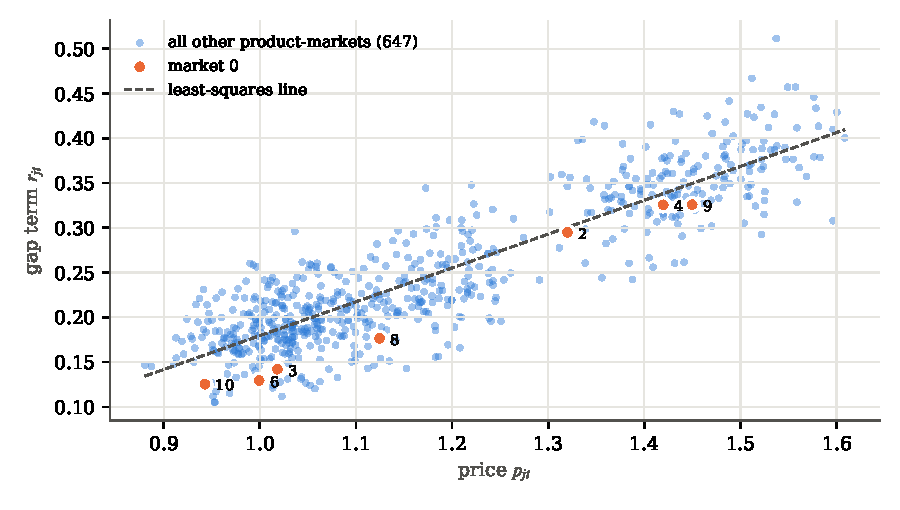
\includegraphics[width=0.85\linewidth]{figures/appC/gap.pdf}
\caption{The gap term $r_{jt} = \ln\frac{s_{jt}}{s_{0t}} - \delta_{jt}$ against price for all 654 observations, with market 0
highlighted and its products labelled. $\delta_{jt}$ is the random coefficients mean utility recovered with the true
$\Sigma$. The correlation with price is 0.888. The dashed simple least-squares line has slope 0.378. The 2SLS price
coefficient, which controls for characteristics, is 0.284.}
\label{fig:C-gap}
\end{figure}

The estimated bias $\hat b_{r,p} = 0.284$ is about 0.7 standard errors of $\hat\alpha^l$, so a single sample cannot
detect it. It comes from one sample of 654 observations, with 1,000 simulation draws per market, so it contains
sampling and simulation error. Its population counterpart $b_{r,p}$ is the probability limit of the bias
(\cref{prop:C-logit-bias}). Unlike sampling error, $b_{r,p}$ does not shrink as the number of markets grows. The
consequences of the bias also propagate. A price coefficient that is too small makes demand look too inelastic,
which inflates the logit markups $\frac{1}{\alpha^l(1 - S_{ft})}$ to a mean of 0.396 against the true 0.386. Better instruments cannot repair it, because the problem lies in the functional form.
The remedy is to model the heterogeneity, which \cref{sec:C-rc-est} does. \Cref{sec:08-worked} reports the same comparison
within the full estimation of the random coefficients model.

\subsection{Computational notes}

\begin{enumerate}
  \item Build the instruments with group sums: within each market and owner, sum each characteristic and subtract the
  product's own value for the firm's other products. The market sum minus the firm sum gives the rival products.
  \item Compute 2SLS through the projected regressors $\hat X$. Code the clustered sandwich by hand and check it against
  a packaged routine. Here the coefficients and standard errors agree to within $2\times10^{-12}$.
  \item For Hansen's $J$, run 2SLS, form $\hat S = \frac{1}{N}\sum_t(Z_t^\top\hat e_t)(Z_t^\top\hat e_t)^\top$ from its
  residuals, re-estimate with weight $\hat S^{-1}$, and compute $J = N\bar g^\top\hat S^{-1}\bar g$ at the second-step
  estimate.
  \item For the bootstrap, note that $mc_{jt}(\alpha) = p_{jt} - \frac{k_{jt}}{\alpha}$ with $k_{jt}$ fixed by the data,
  so each replication needs only one 2SLS fit and one OLS fit.
  \item For joint GMM, concentrate out the linear parameters for each $\alpha^l$ by weighted least squares, minimize the
  concentrated objective over a grid and refine with a bounded scalar search.
  \item For the gap term, run the contraction from the logit start $\ln\frac{s_{jt}}{s_{0t}}$ with draws held fixed, and
  evaluate shares with the overflow-safe routine of \cref{sec:C-simulate}.
\end{enumerate}
The bootstrap loop is short.
\begin{verbatim}
rng = np.random.default_rng(2031)
for b in range(5000):
    pick = rng.integers(0, 100, size=100)            # markets
    rows = np.concatenate([idx[m] for m in pick])
    xh = Z[rows] @ np.linalg.lstsq(Z[rows], X[rows], rcond=None)[0]
    coef = np.linalg.lstsq(xh, y[rows], rcond=None)[0]   # 2SLS
    mc = p - k / (-coef[3])                          # new alpha
    gam = np.linalg.lstsq(W[rows], mc[rows], rcond=None)[0]
    draws[b] = np.append(coef, gam)
\end{verbatim}

\section{Random coefficients estimation and a comparison of the three models}\label{sec:C-rc-est}

Sections \ref{sec:C-vertical} and \ref{sec:C-logit-est} estimated two misspecified models on the simulated market of
\cref{sec:C-simulate}. The vertical model allowed one dimension of taste, and the logit allowed none beyond the
idiosyncratic shock. In this problem we estimate the model that generated the data. We take the dispersion of tastes
$\Sigma$ as known. This isolates the two steps on which random coefficients estimation rests. The first is the
inversion of market shares by the contraction of \citet{BerryLevinsohnPakes1995}. The second is linear instrumental
variables on the recovered mean utilities. With the true structure in hand we then compare the three models on elasticities, diversion, markups,
recovered costs and the predicted effects of a merger. \Cref{sec:08-worked} estimates $\Sigma$ itself on the same data.

\subsection{Statement}

Use the data of \cref{sec:C-simulate} and \cref{ass:C-est}. In each of the 100 markets the econometrician observes
prices, realized shares $s^{obs}_{jt}$, characteristics $x_{jt}$, the milk price $w_{jt}$, the owners and the market
size. The realized shares are the shares $\hat s_{jt}$ of \eqref{eq:C-realized}. Demand is the random coefficients logit
\eqref{eq:C-rc-utility},
\begin{equation}\label{eq:C-rc-model}
  u_{ijt} = \delta_{jt} + \mu_{ijt} + \epsilon_{ijt}, \qquad \mu_{ijt} = \tilde x_{jt}\Sigma\nu_i, \qquad
  \delta_{jt} = x_{jt}\beta - \alpha p_{jt} + \xi_{jt},
\end{equation}
with $\tilde x_{jt} = (x_{jt}, p_{jt})$, $\nu_i \sim N(0, I_4)$, independent type-I extreme value shocks
$\epsilon_{ijt}$, and $u_{i0t} = \epsilon_{i0t}$. The term $\mu_{ijt}$ is the consumer-specific deviation from the mean
utility $\delta_{jt}$. The scale matrix $\Sigma = \diag(0.5, 0.2, 0.3, 0.5)$ is known, with $\Sigma_{pp} = 0.5$ its
price entry. The linear parameters $\theta_1 = (\beta, \alpha)$ are unknown. Firms A to D own the products listed in
\cref{tab:C-products} and set prices in a multi-product Bertrand-Nash equilibrium.

\begin{enumerate}[label=(\alph*)]
  \item Draw $n_s = 1{,}000$ vectors $\nu_{it}$ for each market and keep them fixed for the rest of the problem. Why
  must the draws stay fixed?
  \item Write the simulated share function $s_t(\delta_t, \Sigma)$ for a given $\Sigma$ and derive its derivatives
  with respect to $\delta_t$.
  \item Starting from the logit inversion, recover $\delta_t$ in every market with the iteration
  $\delta^{(h+1)}_t = \delta^{(h)}_t + \ln s^{obs}_t - \ln s_t(\delta^{(h)}_t, \Sigma)$. Prove that it converges. Report
  $\delta_t$ for market 0, explain why every mean utility falls relative to the logit start, and account for the gaps
  between the recovered and the true mean utilities.
  \item Estimate $(\beta, \alpha)$ from the recovered mean utilities. Give the identification argument and standard
  errors.
  \item Compute the elasticity matrix of market 0 with the estimation draws, including the outside good. Compare it
  with the true matrix and with the vertical and logit matrices of Sections \ref{sec:C-vertical} and
  \ref{sec:C-logit-est}. Compute the diversion from each product to the outside good. Recover marginal costs under the
  estimated model and compare the three models.
  \item Firms B and C merge. Predict the new equilibrium of market 0 with the logit, the estimated random coefficients
  model and the true model.
  \item How would you proceed if $\Sigma$ were unknown?
\end{enumerate}

\subsection{Solution}

\casehead{Part (a)}
For each market $t$ we draw $n_s = 1{,}000$ vectors $\nu_{it} \sim N(0, I_4)$, $i = 1, \dots, n_s$, once and store
them. The draws use their own seed (2030), different from the seed of the firms' 100 draws in \cref{sec:C-simulate}.
The econometrician does not know which consumer types the firms had in mind. Draws are independent across
markets. The draws stay fixed for three reasons.
\begin{enumerate}
  \item With fixed draws, the simulated share function of part (b) is a deterministic and smooth function of
  $\delta_t$, and the iteration of part (c) has a well-defined fixed point. With fresh draws at every step, the map
  itself would change from one iteration to the next. The iterates would then wander around the solution by the size
  of the simulation error, which part (c) puts at a few hundredths. A stopping rule with tolerance $10^{-10}$ would
  never be met.
  \item When $\Sigma$ is estimated (part (g)), the GMM objective must be a deterministic function of $\Sigma$.
  Otherwise the optimizer compares objective values computed with different draws, and its minimizer is not defined.
  With fixed draws the objective is a smooth function of $\Sigma$, and the simulation asymptotics of
  \citet{PakesPollard1989} can be applied. Because the simulated shares enter the moments through the nonlinear
  inversion, simulation error also adds a bias of order $\frac{1}{n_s}$ (\cref{prop:08-simbias}). Consistency
  therefore requires the number of draws to grow with the sample. With many draws, the simulation error adds a term
  to the variance \citep{BerryLevinsohnPakes1995}.
  \item Fixed draws make the estimator a function of the data and the draws. Its simulation error can then be measured
  by solving again with other draws, as we do in part (c).
\end{enumerate}

\casehead{Part (b)}
Given the draws and a candidate vector of mean utilities $\delta_t = (\delta_{jt})_{j \in \mathcal{J}_t}$, the
individual choice probabilities are
\begin{equation}\label{eq:C-rc-sij-delta}
  s_{ijt}(\delta_t) = \frac{e^{\delta_{jt} + \mu_{ijt}}}{1 + \sum_{k \in \mathcal{J}_t}e^{\delta_{kt} + \mu_{ikt}}} ,
  \qquad
  s_{i0t}(\delta_t) = \frac{1}{1 + \sum_{k \in \mathcal{J}_t}e^{\delta_{kt} + \mu_{ikt}}} ,
\end{equation}
with $\mu_{ijt} = \tilde x_{jt}\Sigma\nu_{it}$, and the simulated shares are
\begin{equation}\label{eq:C-rc-sdelta}
  s_{jt}(\delta_t, \Sigma) = \frac{1}{n_s}\sum_{i=1}^{n_s}s_{ijt}(\delta_t) .
\end{equation}
This is the simulator \eqref{eq:C-rc-simshare} with $\delta_t$ as its argument. Prices enter only through
$\mu_{ijt}$, and they stay at their observed values throughout the inversion. We evaluate \eqref{eq:C-rc-sij-delta}
with the overflow-safe rule of \cref{sec:C-simulate}, part (b). The convergence argument of part (c) rests on the
derivatives of this function.

\begin{lemma}[Derivatives of the simulated shares]\label{lem:C-sdelta}
For every market and every $\delta_t$:
\begin{enumerate}[label=(\roman*)]
  \item $\frac{\partial s_{jt}}{\partial\delta_{kt}} = \frac{1}{n_s}\sum_{i=1}^{n_s}s_{ijt}\big(\indic\{j = k\} -
  s_{ikt}\big)$.
  \item $0 < \frac{\partial s_{jt}}{\partial\delta_{jt}} < s_{jt}$, and $\frac{\partial s_{jt}}{\partial\delta_{kt}} <
  0$ for $k \ne j$.
  \item $\sum_{k \in \mathcal{J}_t}\frac{\partial s_{jt}}{\partial\delta_{kt}} = \frac{1}{n_s}\sum_{i=1}^{n_s}s_{ijt}
  s_{i0t} > 0$.
\end{enumerate}
\end{lemma}

\begin{proof}
Fix a draw, drop $t$, and write $V_{ik} = \delta_k + \mu_{ik}$ and $E_i = 1 + \sum_k e^{V_{ik}}$. By the quotient rule,
\[
  \frac{\partial s_{ij}}{\partial V_{ik}}
  = \frac{\indic\{j = k\}e^{V_{ij}}E_i - e^{V_{ij}}e^{V_{ik}}}{E_i^2}
  = s_{ij}\big(\indic\{j = k\} - s_{ik}\big) .
\]
Since $\frac{\partial V_{ik}}{\partial\delta_k} = 1$, averaging over draws gives (i). For (ii), $0 < s_{ij} < 1$
implies $0 < s_{ij}(1 - s_{ij}) < s_{ij}$ and $-s_{ij}s_{ik} < 0$. For (iii),
$\sum_k s_{ij}(\indic\{j = k\} - s_{ik}) = s_{ij}(1 - \sum_k s_{ik}) = s_{ij}s_{i0}$.
\end{proof}

\casehead{Part (c)}
For market $t$ define the map
\begin{equation}\label{eq:C-blp-map}
  f_t(\delta_t) = \delta_t + \ln s^{obs}_t - \ln s_t(\delta_t, \Sigma) ,
\end{equation}
with logarithms taken element by element. A vector $\delta_t$ is a fixed point of $f_t$ if and only if
$s_t(\delta_t, \Sigma) = s^{obs}_t$, so the fixed points are exactly the mean utilities that rationalize the observed
shares. The iteration $\delta^{(h+1)}_t = f_t(\delta^{(h)}_t)$ is the contraction of
\citet[eq.~6.8]{BerryLevinsohnPakes1995}, written as eq.~(12) of \citet[p.~533]{Nevo2000a}. Each step raises
$\delta_{jt}$ when the model under-predicts the share of product $j$ and lowers it otherwise.

\begin{proposition}[Convergence of the share inversion]\label{prop:C-blp-contraction}
For every market $t$ and every $\delta_t$,
\begin{equation}\label{eq:C-blp-derivs}
  \frac{\partial f_{jt}}{\partial\delta_{kt}} \ge 0 \ \text{ for all } j, k , \qquad
  \eta_{jt}(\delta_t) \equiv \sum_{k \in \mathcal{J}_t}\frac{\partial f_{jt}}{\partial\delta_{kt}}
  = 1 - \frac{\sum_i s_{ijt}s_{i0t}}{\sum_i s_{ijt}} < 1 .
\end{equation}
The equation $s_t(\delta_t, \Sigma) = s^{obs}_t$ therefore has exactly one solution $\delta^*_t$, and the iteration
converges to it from any starting value. If $\eta_{jt} \le \bar\eta < 1$ for every $j$ on a convex set that
contains $\delta^*_t$ and the iterates, then for every $h \ge 0$
\begin{equation}\label{eq:C-blp-rate}
  \big\|\delta^{(h)}_t - \delta^*_t\big\|_\infty \le \bar\eta^{h}\big\|\delta^{(0)}_t - \delta^*_t\big\|_\infty ,
  \qquad
  \big\|\delta^{(h+1)}_t - \delta^{(h)}_t\big\|_\infty \le \bar\eta^{h}\big\|\delta^{(1)}_t - \delta^{(0)}_t\big\|_\infty .
\end{equation}
\end{proposition}

\begin{proof}
Take $F$ in \cref{cor:08-rowsum} to be the distribution that puts mass $\frac{1}{n_s}$ on each draw, so that its
integrals are the averages of \cref{lem:C-sdelta}. The corollary then gives \eqref{eq:C-blp-derivs}, which is
condition (1) of \cref{thm:08-contraction}. This $F$ has finite support,
so the integrability condition of \cref{thm:08-berry94} holds. That theorem then gives the unique solution
$\delta^*_t$.

For the rate, drop $t$, fix $j$ and apply the mean value theorem on the segment between $\delta^*$ and $\delta$:
\[
  f_j(\delta) - f_j(\delta^*) = \sum_k\frac{\partial f_j}{\partial\delta_k}(\tilde\delta)\,(\delta_k - \delta^*_k)
\]
for some $\tilde\delta$ on the segment. The derivatives are nonnegative and sum to at most $\bar\eta$, so
$|f_j(\delta) - \delta^*_j| \le \bar\eta\|\delta - \delta^*\|_\infty$, using $f_j(\delta^*) = \delta^*_j$. Taking the
maximum over $j$ and iterating gives the first inequality in \eqref{eq:C-blp-rate}. The second follows in the same way
from $\delta^{(h+1)} - \delta^{(h)} = f(\delta^{(h)}) - f(\delta^{(h-1)})$.

\Cref{thm:08-berry94} proves convergence for a truncated iteration. The untruncated iteration also converges from any
start. Let $B$ be the sup-norm ball of radius $\|\delta^{(0)} - \delta^*\|_\infty$ around $\delta^*$. It is convex and
compact. The row sums are continuous and below one, so their maximum $\bar\eta$ on $B$ is below one. The bound
$|f_j(\delta) - \delta^*_j| \le \bar\eta\|\delta - \delta^*\|_\infty$ then holds on $B$, so every iterate stays in $B$.
Hence \eqref{eq:C-blp-rate} applies.
\end{proof}

The row sum has a simple meaning. By Bayes' rule over the draws, as in \cref{prop:C-buyer-alpha},
$\frac{\sum_is_{ijt}s_{i0t}}{\sum_is_{ijt}}$ is the probability that a buyer of product $j$ would choose the outside
good in a new choice situation. So $\eta_{jt}$ is one minus the outside-good probability of $j$'s buyers. The
iteration converges fast when the buyers of every product often choose the outside good, which happens when the outside
share is large. It slows down when inside goods dominate the market (\cref{sec:08-inversion}).

We start from the logit inversion $\delta^{(0)}_{jt} = \ln s^{obs}_{jt} - \ln s^{obs}_{0t}$. It is the exact solution
when $\Sigma = 0$, because then every $s_{ijt}$ is the logit probability at $\delta_t$. We stop when
$\|\delta^{(h+1)}_t - \delta^{(h)}_t\|_\infty < 10^{-10}$. The iteration converges in every market, in 11 to 18
iterations (13.9 on average). At the solution the largest gap between log simulated and log observed shares is
$2.5\times10^{-11}$.

Market 0 shows the proposition at work. At the solution the row sums lie between 0.207 and 0.234. The buyers of each
product choose the outside good with probability 0.766 to 0.793, against 0.855 for all simulated consumers. The largest
row sum along the path of the iteration is $\bar\eta = 0.261$. The first step has size 0.280, so by the second
inequality in \eqref{eq:C-blp-rate} the stopping rule must be met by iteration 18. It is met at iteration 15. After the
first step, the ratio of successive step sizes settles at 0.216. This ratio estimates the largest eigenvalue of the
Jacobian of $f_0$ at the solution, which cannot exceed the largest row sum because the Jacobian has nonnegative
entries. Over all 100 markets the largest row sum at the solution is 0.295.

\Cref{tab:C-delta0} reports the mean utilities of market 0. The recovered values are close to the true ones,
$x_{j}\beta - \alpha p_{j0} + \xi_{j0}$, and every one of them lies below its logit start. The next proposition
explains the second fact.

\begin{table}[htbp]
\centering
\caption{Mean utilities in market 0 with $\Sigma$ known}
\label{tab:C-delta0}
\footnotesize
\setlength{\tabcolsep}{4.5pt}
\begin{tabular}{@{}lccccccccc@{}}
\toprule
 & & & Logit start & \multicolumn{2}{c}{Recovered $\hat\delta_j$} & True & \multicolumn{2}{c}{Gap from truth} & S.e.\ of \\
\cmidrule(lr){5-6}\cmidrule(lr){8-9}
Product & Firm & Buyers $q_j$ & $\delta^{(0)}_j$ & 1,000 draws & 100,000 draws & $\delta_j$ & Simulation & Sampling &
$\ln\hat s_j$ \\
\midrule
2 & C & 51 & $-5.110$ & $-5.405$ & $-5.411$ & $-5.581$ & 0.007 & 0.170 & 0.140 \\
3 & C & 249 & $-3.524$ & $-3.666$ & $-3.701$ & $-3.675$ & 0.035 & $-0.026$ & 0.063 \\
4 & B & 124 & $-4.221$ & $-4.547$ & $-4.551$ & $-4.657$ & 0.005 & 0.105 & 0.089 \\
6 & B & 201 & $-3.738$ & $-3.868$ & $-3.905$ & $-3.962$ & 0.037 & 0.058 & 0.070 \\
8 & A & 553 & $-2.726$ & $-2.903$ & $-2.935$ & $-2.941$ & 0.032 & 0.006 & 0.041 \\
9 & D & 57 & $-4.998$ & $-5.324$ & $-5.330$ & $-5.193$ & 0.006 & $-0.137$ & 0.132 \\
10 & C & 199 & $-3.748$ & $-3.874$ & $-3.910$ & $-3.843$ & 0.036 & $-0.067$ & 0.070 \\
\bottomrule
\end{tabular}

\vspace{3pt}
\begin{minipage}{0.97\textwidth}
\footnotesize Notes: $M_0 = 9{,}880$ consumers, outside share 0.8549. The logit start is
$\ln s^{obs}_j - \ln s^{obs}_0$. The recovered values solve $s_t(\delta_t, \Sigma) = s^{obs}_t$ for $t = 0$
with the 1,000 estimation draws (seed 2030) and with 100,000 draws (seed 2032). The simulation gap is the difference between the two
solutions, and the sampling gap is the 100,000-draw solution minus the true value. The last column is
$\sqrt{\frac{1 - s_j}{q_j}}$ from \eqref{eq:C-logshare-var}. Computed with \texttt{figures/appC/src/appC\_rc.py}.
\end{minipage}
\end{table}

\begin{proposition}[Mean utilities below the logit inversion]\label{prop:C-delta-lower}
\begin{enumerate}[label=(\roman*)]
  \item Suppose a market has one inside product with observed share $s^{obs} < \frac{1}{2}$, and the random term
  $\mu_i$ has a nondegenerate distribution that is symmetric about zero. Let $\mathcal{L}(u) = \frac{e^u}{1 + e^u}$ be the logistic distribution function, and let
  $\delta^*$ solve $\E[\mathcal{L}(\delta + \mu_i)] = s^{obs}$. Then
  \[
    \delta^* < \ln\frac{s^{obs}}{1 - s^{obs}} .
  \]
  \item With several inside products, a diagonal $\Sigma$ and $\lVert\Sigma\rVert \to 0$, the gap
  $r_{jt} = \ln\frac{s^{obs}_{jt}}{s^{obs}_{0t}} - \delta^*_{jt}$ is positive up to terms of order $\lVert\Sigma\rVert^3$
  whenever $\|\tilde x_{jt}\Sigma\| > 2\|\bar x_t\Sigma\|$, where $\bar x_t = \sum_k s_{kt}\tilde x_{kt}$ and
  $\|\cdot\|$ is the Euclidean norm.
\end{enumerate}
\end{proposition}

\begin{proof}
(i) Let $\delta_L = \ln\frac{s^{obs}}{1 - s^{obs}}$, the logit inversion, so that $\mathcal{L}(\delta_L) = s^{obs}$ and
$\delta_L < 0$. For $m \ge 0$ define $g(m) = \mathcal{L}(\delta_L + m) + \mathcal{L}(\delta_L - m) - 2\mathcal{L}(\delta_L)$. Then
$g(0) = 0$ and
\[
  g'(m) = \ell(\delta_L + m) - \ell(\delta_L - m) ,
\]
where $\ell(u) = \mathcal{L}(u)(1 - \mathcal{L}(u))$ is the logistic density. It is symmetric about zero and strictly
decreasing in $|u|$. For $m > 0$, $\delta_L < 0$ gives $|\delta_L + m| < |\delta_L| + m = |\delta_L - m|$, so
$g'(m) > 0$ and $g(m) > 0$. By the symmetry of $\mu_i$,
\[
  \E[\mathcal{L}(\delta_L + \mu_i)] = \frac{1}{2}\E\big[\mathcal{L}(\delta_L + \mu_i) + \mathcal{L}(\delta_L - \mu_i)\big]
  = \mathcal{L}(\delta_L) + \frac{1}{2}\E\big[g(|\mu_i|)\big] > s^{obs} ,
\]
with strict inequality because $\mu_i \ne 0$ with positive probability. The function
$\delta \mapsto \E[\mathcal{L}(\delta + \mu_i)]$ is strictly increasing, so its solution $\delta^*$ lies below $\delta_L$.

(ii) By \cref{prop:C-gap-approx}, with $a = \tilde x_{jt}\Sigma$ and $b = \bar x_t\Sigma$ (row vectors, $\Sigma$ diagonal),
$r_{jt} = \frac{1}{2}\|a\|^2 - a b^\top + O(\lVert\Sigma\rVert^3)$. The Cauchy-Schwarz inequality gives $ab^\top \le \|a\|\,\|b\|$,
so $r_{jt} \ge \|a\|\big(\frac{1}{2}\|a\| - \|b\|\big) + O(\lVert\Sigma\rVert^3)$, which is positive when $\|a\| > 2\|b\|$.
\end{proof}

Part (i) is the convexity argument in its cleanest form. The logit probability is convex below one half, so spreading
utility symmetrically around $\delta$ raises the average choice probability. To match the observed share, the mean
utility must fall. Part (ii) covers our design. The vector $\bar x_t$ averages the inside products with weights equal to
their shares, which sum to the inside share of at most 0.21. So $\|\bar x_t\Sigma\|$ is a small fraction of
$\max_k\|\tilde x_{kt}\Sigma\|$, and the condition holds unless products are very different. In the data every one of
the 654 recovered mean utilities lies below its logit start. The gap $r_{jt}$, studied in \cref{sec:C-logit-est},
part (e), has mean 0.247 (\cref{fig:C-gap}). In market 0 it is smallest for product 10, the cheapest, and largest for
products 4 and 9, which are expensive and organic and therefore have the largest $\|\tilde x_{jt}\Sigma\|$.

The gaps from the truth have two sources, which we separate by solving the inversion again with 100,000 draws:
\begin{equation}\label{eq:C-delta-gap}
  \hat\delta_{jt} - \delta_{jt} = \big(\hat\delta_{jt} - \hat\delta^{100k}_{jt}\big) + \big(\hat\delta^{100k}_{jt} -
  \delta_{jt}\big) .
\end{equation}
The first term is simulation error from using 1,000 draws. In market 0 it lies between 0.005 and 0.037. It has the same
sign for every product, which reflects the draws that all products share. It is of the same order as the relative
simulation standard error of the shares, the standard deviation of $s_{ij0}$ across draws divided by
$\sqrt{n_s}\,s_{j0}$, which lies between 0.020 and 0.030. The second term is sampling error. Realized shares are
proportions among about 10,000 consumers, and by \eqref{eq:C-logshare-var} the log share of product $j$ has standard
error near $\sqrt{\frac{1 - s_{j}}{q_{j}}}$. Products 2, 4 and 9 miss the truth by 1.0 to 1.2 of these standard errors,
and the others by less. Both errors are independent across markets. To first order they have mean zero and are uncorrelated with the
instruments, so they act as extra noise in the regression of part (d). The log transformation adds a small
second-order bias that depends on the share, of order $\frac{1}{q_j}$.

\casehead{Part (d)}
With $\Sigma$ known, the recovered mean utilities satisfy the linear equation
\begin{equation}\label{eq:C-rc-linear}
  \hat\delta_{jt} = x_{jt}\beta - \alpha p_{jt} + \xi_{jt} + e_{jt} ,
\end{equation}
where $e_{jt} = \hat\delta_{jt} - \delta_{jt}$ collects the simulation and sampling errors of part (c). Price is
correlated with $\xi_{jt}$ because firms observe $\xi_{jt}$ when they set prices (\cref{sec:C-logit-est}, part (a)).
We therefore estimate \eqref{eq:C-rc-linear} by 2SLS with the instruments of \eqref{eq:C-logit-moments}: the milk price
and the six sums of characteristics and counts of the firm's other products and of rival products. The parameters are
identified by the moment conditions $\E[z_{jt}^\top(\xi_{jt} + e_{jt})] = 0$ and the rank condition of
\cref{sec:C-logit-est}. The error $e_{jt}$ comes from consumers' choices and from the econometrician's draws, given
prices. To first order it has mean zero conditional on $z_{jt}$, so it adds noise without adding bias. The
regressors and instruments are those of the logit, so the first stage is the one in \cref{tab:C-firststage}.

\begin{table}[htbp]
\centering
\caption{Demand estimates with $\Sigma$ known}
\label{tab:C-rc-demand}
\footnotesize
\setlength{\tabcolsep}{4pt}
\begin{tabular}{@{}lccccc@{}}
\toprule
 & Logit & \multicolumn{3}{c}{Random coefficients, $\Sigma$ known} & \\
\cmidrule(lr){2-2}\cmidrule(lr){3-5}
 & 2SLS & OLS & 2SLS & \makecell{2SLS, milk\\price only} & True \\
\midrule
Constant & $-1.184$ (0.329) & $-1.355$ (0.227) & $-1.061$ (0.330) & $-1.042$ (0.335) & $-1.00$ \\
Sugar content & 0.190 (0.158) & 0.088 (0.122) & 0.168 (0.158) & 0.173 (0.156) & 0.20 \\
Organic & 0.153 (0.141) & $-0.002$ (0.097) & 0.114 (0.142) & 0.121 (0.143) & 0.15 \\
Price coefficient $\alpha$ & 2.641 (0.412) & 2.573 (0.252) & 2.926 (0.413) & 2.948 (0.415) & 3.00 \\
\midrule
First-stage $F$ & 92.5 & & 92.5 & & \\
Hansen $J$ (df, $p$) & 8.82 (6, 0.18) & & 8.16 (6, 0.23) & & \\
Observations & 654 & 654 & 654 & 654 & \\
\bottomrule
\end{tabular}

\vspace{3pt}
\begin{minipage}{0.97\textwidth}
\footnotesize Notes: The dependent variable is $\ln s^{obs}_{jt} - \ln s^{obs}_{0t}$ for the logit and the recovered
$\hat\delta_{jt}$ otherwise. Standard errors in parentheses are clustered by market with the factor
$\frac{G}{G - 1}\frac{N - 1}{N - K}$ and condition on $\Sigma$. The first and third 2SLS columns use the milk price and
the six competition instruments, and the last uses the milk price alone. The logit column repeats \cref{tab:C-logit-demand}. Computed with
\texttt{figures/appC/src/appC\_rc.py}.
\end{minipage}
\end{table}

\Cref{tab:C-rc-demand} reports the estimates. The 2SLS estimate of the price coefficient is 2.926, within 0.18
standard errors of the true value of 3. OLS gives 2.573, biased toward zero for the same reason as in the logit. Using
the milk price alone gives 2.948 with a slightly larger standard error, so the six competition instruments add little,
as in \cref{sec:C-logit-est}. Hansen's test does not reject the overidentifying restrictions ($J = 8.16$, $p = 0.23$).
The coefficients on sugar and organic production are close to the truth but imprecise. They are identified from ten
products whose characteristics never change, so the data contain only ten distinct combinations of characteristics.

The comparison with the logit is exact. By \cref{prop:C-logit-bias}, the logit estimate equals the random coefficients
estimate minus the 2SLS price coefficient of the gap term $r_{jt}$ on the same regressors and instruments. That
coefficient is 0.284, and the identity $2.641 = 2.926 - 0.284$ holds to machine precision (\cref{sec:C-logit-est},
part (e)). Allowing for the random coefficients
moves the estimate from 0.359 below the truth to 0.074 below it. The remaining gap is well within sampling error. The
estimates also imply sensible individual tastes. Across the 100,000 estimation draws, the smallest price sensitivity
$\alpha_i = \hat\alpha - \Sigma_{pp}\nu_{i4}$ is 0.814, so every simulated consumer dislikes higher prices, as
\cref{prop:C-ms} requires.

The standard errors cluster by market, with the sandwich \eqref{eq:C-clustervar}. The recovered $\hat\delta_t$ depends
only on the shares and draws of market $t$, so the errors are independent across markets and clustering is valid. The
standard errors condition on $\Sigma$. If $\Sigma$ were estimated, $\hat\theta_1 = \hat\theta_1(\hat\Sigma)$ would inherit
the uncertainty in $\hat\Sigma$, and all parameters would be estimated jointly as in part (g).

\casehead{Part (e)}
A change in $p_{kt}$ moves both the mean utility, through $-\alpha$, and the random term, through $\Sigma_{pp}\nu_{i4}$.
For draw $i$ the price coefficient is therefore $-\alpha_i$ with $\alpha_i = \hat\alpha - \Sigma_{pp}\nu_{i4}$. Applying
\cref{lem:C-sdelta}(i) draw by draw, with $\frac{\partial V_{ikt}}{\partial p_{kt}} = -\alpha_i$, gives the share
derivatives
\begin{equation}\label{eq:C-rc-elast}
  \frac{\partial s_{jt}}{\partial p_{kt}} = \frac{1}{n_s}\sum_{i=1}^{n_s}\alpha_is_{ijt}\big(s_{ikt} - \indic\{j = k\}\big) ,
  \qquad
  \frac{\partial s_{0t}}{\partial p_{kt}} = \frac{1}{n_s}\sum_{i=1}^{n_s}\alpha_is_{i0t}s_{ikt} .
\end{equation}
The second formula follows from $\frac{\partial s_{i0t}}{\partial V_{ikt}} = -s_{i0t}s_{ikt}$. The elasticities are
$\varepsilon_{jk} = \frac{\partial s_j}{\partial p_k}\frac{p_k}{s_j}$ and
$\varepsilon_{0k} = \frac{\partial s_0}{\partial p_k}\frac{p_k}{s_0}$. Own entries are negative, so the positive own
elasticity of the book's notation is $-\varepsilon_{jj}$. The estimated matrix uses $\hat\alpha = 2.926$, the recovered
$\hat\delta_0$ and the 1,000 estimation draws. The true matrix uses the true parameters, the true mean utilities and
the firms' 100 draws, the demand system that generated the prices. \Cref{tab:C-rcelast} reports both.

\begin{table}[htbp]
\centering
\caption{Random coefficients elasticities in market 0}
\label{tab:C-rcelast}
\footnotesize
\begin{tabular}{@{}lrrrrrrr@{}}
\toprule
 & \multicolumn{7}{c}{Price of product} \\
\cmidrule(lr){2-8}
Share of & 2 & 3 & 4 & 6 & 8 & 9 & 10 \\
\midrule
\multicolumn{8}{@{}l}{\emph{Panel A. Estimated model ($\hat\alpha = 2.926$, $\Sigma$ known)}} \\
Product 2 & $-3.45$ & 0.10 & 0.08 & 0.07 & 0.24 & 0.04 & 0.07 \\
Product 3 & 0.03 & $-2.68$ & 0.07 & 0.07 & 0.23 & 0.03 & 0.07 \\
Product 4 & 0.03 & 0.10 & $-3.63$ & 0.08 & 0.24 & 0.04 & 0.07 \\
Product 6 & 0.02 & 0.09 & 0.07 & $-2.65$ & 0.23 & 0.03 & 0.07 \\
Product 8 & 0.03 & 0.09 & 0.07 & 0.07 & $-2.79$ & 0.03 & 0.07 \\
Product 9 & 0.03 & 0.10 & 0.08 & 0.08 & 0.24 & $-3.74$ & 0.07 \\
Product 10 & 0.02 & 0.09 & 0.07 & 0.07 & 0.23 & 0.03 & $-2.51$ \\
Outside good & 0.02 & 0.07 & 0.04 & 0.05 & 0.16 & 0.02 & 0.05 \\
\midrule
\multicolumn{8}{@{}l}{\emph{Panel B. True model}} \\
Product 2 & $-3.57$ & 0.12 & 0.09 & 0.08 & 0.29 & 0.05 & 0.09 \\
Product 3 & 0.03 & $-2.74$ & 0.07 & 0.08 & 0.26 & 0.04 & 0.08 \\
Product 4 & 0.03 & 0.12 & $-3.74$ & 0.08 & 0.29 & 0.05 & 0.09 \\
Product 6 & 0.03 & 0.10 & 0.07 & $-2.71$ & 0.25 & 0.04 & 0.08 \\
Product 8 & 0.03 & 0.11 & 0.08 & 0.08 & $-2.84$ & 0.05 & 0.08 \\
Product 9 & 0.03 & 0.12 & 0.09 & 0.08 & 0.29 & $-3.85$ & 0.09 \\
Product 10 & 0.03 & 0.10 & 0.07 & 0.07 & 0.26 & 0.04 & $-2.57$ \\
Outside good & 0.02 & 0.07 & 0.04 & 0.05 & 0.17 & 0.03 & 0.06 \\
\bottomrule
\end{tabular}

\vspace{3pt}
\begin{minipage}{0.97\textwidth}
\footnotesize Notes: Entry $(j, k)$ is $\varepsilon_{jk} = \frac{\partial s_j}{\partial p_k}\frac{p_k}{s_j}$, the
percentage change in the share of the row alternative after a one percent rise in the price of the column product.
Panel A uses the 1,000 estimation draws and the recovered mean utilities. Panel B uses the true parameters and mean
utilities and the firms' 100 draws. Computed with \texttt{figures/appC/src/appC\_rc.py}.
\end{minipage}
\end{table}

The estimated matrix is close to the true one. The largest absolute difference between corresponding entries is 0.11.
The estimated own elasticities run from $-2.51$ to $-3.74$, against $-2.57$ to $-3.85$ in the truth. They are slightly
smaller in magnitude because $\hat\alpha$ is slightly below 3. Three features distinguish the random coefficients
matrix from the other two models.

First, cross elasticities differ within a column. In the logit every off-diagonal entry of column $k$ equals
$\hat\alpha^lp_ks_k$ (\cref{tab:C-lelast}). In Panel A the largest ratio between two cross elasticities in the same
column is 1.21, and in the truth it is 1.27. The pattern has an economic logic. A rise in the price of product 4 raises
the shares of products 2 and 9 by more than those of the other products. The same holds for the columns of products 2
and 9. The three products are the organic ones and also the most expensive. Their buyers have high draws of the
organic taste $\nu_{i3}$ or low price sensitivity $\alpha_i$. When they leave one of these products, they look for
another product that suits the same tastes.

Second, the outside good receives less substitution than the logit implies. The diversion ratio from product $k$ to
the outside good (\cref{sec:C-logit-bertrand}, part (e), and \cref{sec:C-vertical}, part (e)) is
\begin{equation}\label{eq:C-div0}
  D_{k0} = \frac{\frac{\partial s_0}{\partial p_k}}{-\frac{\partial s_k}{\partial p_k}}
  = \frac{\sum_i\alpha_is_{ik}s_{i0}}{\sum_i\alpha_is_{ik}(1 - s_{ik})}
  = \sum_i\varpi_{ik}\frac{s_{i0}}{1 - s_{ik}} , \qquad
  \varpi_{ik} = \frac{\alpha_is_{ik}(1 - s_{ik})}{\sum_l\alpha_ls_{lk}(1 - s_{lk})} .
\end{equation}
The second equality uses \eqref{eq:C-rc-elast}. The third writes $D_{k0}$ as a weighted average of the individual logit
diversion ratios $\frac{s_{i0}}{1 - s_{ik}}$, with weights that favour the draws most likely to buy $k$. In the logit
all draws are alike and $D_{k0} = \frac{s_0}{1 - s_k}$, which lies between 85.9 and 90.6 percent in market 0. Under the
estimated random coefficients model it lies between 79.2 and 86.7 percent, and in the truth between 76.2 and 85.1
percent. The buyers of a product are disproportionately consumers with a high draw of the random constant. Their
probability of choosing the outside good is 0.77 to 0.79, against 0.855 on average, so they divert less of their
purchases to it. The logit cannot represent this selection. It overstates diversion to the outside good by 5 to 10
percentage points relative to the truth and understates diversion among inside goods, which matters for the merger of part (f).

Third, the vertical model is far from both (\cref{tab:C-velast}). Its own elasticities range from $-16.8$ to
$-358.4$. Their mean absolute value, 126.6, is 41 times that of the logit. Each row has at most two nonzero cross elasticities, one for each
neighbour on the price ladder. Only the cheapest product, product 10, loses sales to the outside good, and only 6.4
percent of them. \Cref{fig:C-own-elas} summarizes the own elasticities. \Cref{fig:08-ownelas} shows the logit and random
coefficients panels on the same data.

\begin{figure}[htbp]
\centering
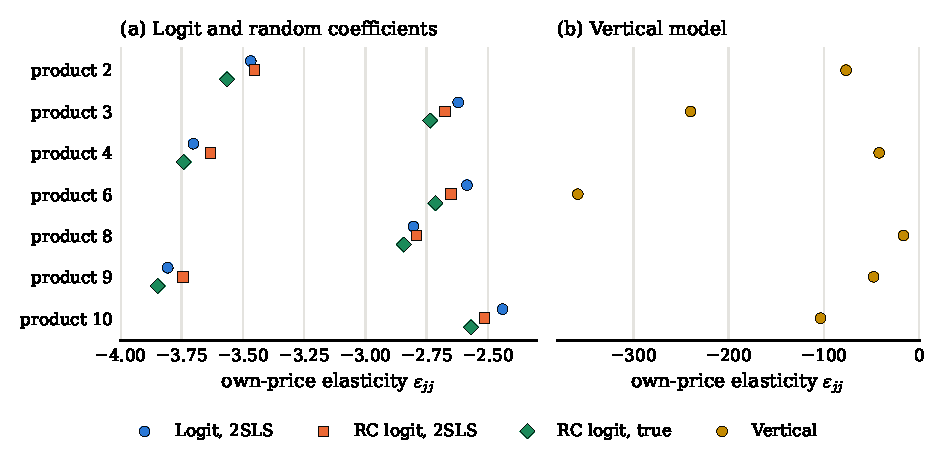
\includegraphics[width=\linewidth]{figures/appC/own_elas.pdf}
\caption{Own-price elasticities in market 0 by product. Panel (a): logit estimated by 2SLS, random coefficients logit
estimated by 2SLS with $\Sigma$ known, and the true random coefficients model. Panel (b): the vertical model, on its own
scale. Computed with \texttt{figures/appC/src/appC\_rc.py}.}
\label{fig:C-own-elas}
\end{figure}

We now recover marginal costs. Under the estimated model, the stacked first-order conditions
\eqref{eq:C-stacked-foc} give
\begin{equation}\label{eq:C-rc-mc-hat}
  \widehat{mc}_t = p_t + \big(\Omega_t \odot \hat\Delta_t^\top\big)^{-1}s^{obs}_t ,
\end{equation}
with $\hat\Delta_t$ the matrix of share derivatives \eqref{eq:C-rc-elast}. We regress $\widehat{mc}_{jt}$ on
$(x_{jt}, w_{jt})$ by OLS. The regressand depends on $\hat\alpha$, so we compute standard errors with a bootstrap over
markets (5,000 resamples, seed 2031) that re-estimates $\hat\alpha$ in each replication. With $\Sigma$ known,
$\hat\delta_t$ does not depend on $\alpha$, so only $\hat\Delta_t$ changes across replications. \Cref{tab:C-compare}
collects the comparison.

\begin{table}[htbp]
\centering
\caption{Three demand models estimated on the same simulated data}
\label{tab:C-compare}
\footnotesize
\setlength{\tabcolsep}{4pt}
\begin{tabular}{@{}lcccc@{}}
\toprule
 & Vertical & Logit & \makecell{Random coefficients\\($\Sigma$ known)} & True \\
\midrule
Price coefficient $\alpha$ & none & 2.641 (0.412) & 2.926 (0.413) & 3.00 \\
Own elasticities, market 0 & $-16.8$ to $-358.4$ & $-2.44$ to $-3.81$ & $-2.51$ to $-3.74$ & $-2.57$ to $-3.85$ \\
Nonzero cross elasticities per row & 1 or 2 & 6 & 6 & 6 \\
Largest ratio within a column & & 1.00 & 1.21 & 1.27 \\
Diversion to outside good, market 0 (\%) & 0 to 6.4 & 85.9 to 90.6 & 79.2 to 86.7 & 76.2 to 85.1 \\
\midrule
Mean markup, all observations & 0.048 & 0.396 & 0.397 & 0.386 \\
Range of markups & 0.000 to 0.515 & 0.379 to 0.426 & 0.368 to 0.452 & 0.348 to 0.451 \\
Correlation with true markups & 0.275 & 0.553 & 0.715 & 1 \\
Mean absolute markup error & 0.340 & 0.014 & 0.013 & 0 \\
\midrule
\multicolumn{5}{@{}l}{\emph{Marginal cost equation}} \\
Constant & 0.674 (0.024) & 0.160 (0.072) & 0.188 (0.060) & 0.20 \\
Sugar content & 0.194 (0.014) & 0.258 (0.010) & 0.246 (0.010) & 0.25 \\
Organic & 0.271 (0.009) & 0.315 (0.006) & 0.305 (0.006) & 0.30 \\
Price of milk & 0.356 (0.031) & 0.532 (0.023) & 0.504 (0.026) & 0.50 \\
\bottomrule
\end{tabular}

\vspace{3pt}
\begin{minipage}{0.97\textwidth}
\footnotesize Notes: All models assume multi-product Bertrand-Nash pricing. Cross elasticities and diversion refer to
market 0. Markup statistics use all 654 observations. Cost equations are OLS regressions of the implied marginal cost
on the characteristics and the milk price. Standard errors are clustered by market for the vertical model, whose markups
contain no estimated parameter. For the logit and the random coefficients model they come from a market bootstrap
that re-estimates $\alpha$ (5,000 replications). Computed with \texttt{figures/appC/src/appC\_rc.py}.
\end{minipage}
\end{table}

The random coefficients model wins on every dimension that depends on substitution. Its cost coefficients are the
closest to the truth, and its implied markups track the true markups across observations more closely (correlation
0.715, against 0.553 for the logit). The mean markups of the logit and the random coefficients model are almost equal.
Both are near $\frac{1}{\hat\alpha}$ corrected for the firm's share, and both overstate the true mean of 0.386 a little
because both price coefficients lie below 3. The vertical model fails on every dimension, for the reasons of
\cref{sec:C-vertical}. Adjacent prices are close, its elasticities explode, and its markups collapse toward zero, so
its cost intercept absorbs the true markup.

\casehead{Part (f)}
Firms B and C merge. In market 0, firm B sells products 4 and 6 and firm C sells products 2, 3 and 10. After the merger
one firm owns all five, while firm A (product 8) and firm D (product 9) are unchanged. We predict the new equilibrium
under three demand models: the logit of \cref{sec:C-logit-est}, the estimated random coefficients model of parts (c) and
(d), and the true model. The procedure is the same for each.
\begin{enumerate}
  \item Recover marginal costs from the pre-merger first-order conditions of the model, \eqref{eq:C-rc-mc-hat} or its
  logit version. For the true model use the true marginal costs. Each model then reproduces the observed prices.
  Solving the pre-merger game again returns them to within $3\times10^{-14}$.
  \item Hold marginal costs, unobserved qualities and draws fixed. As prices move, mean utilities move as
  $\delta_{jt}(p) = \hat\delta_{jt} - \alpha(p_{jt} - p^{obs}_{jt})$, and $\mu_{ijt}$ moves through the price entry of
  $\tilde x_{jt}$.
  \item Replace $\Omega_0$ by the post-merger ownership matrix and solve the first-order conditions. For the logit
  iterate $p \leftarrow mc + \frac{1}{\alpha(1 - S_f(p))}$, using \cref{prop:C-common-markup}. For the random
  coefficients models iterate the Morrow-Skerlos map \eqref{eq:C-ms-zeta}. Each converges in 11 iterations to a tolerance
  of $10^{-12}$, and 20 random starting points lead to the same prices to within $9\times10^{-14}$.
  \item Measure consumer welfare by the log-sum formula (\cref{prop:07-logsum}). A consumer with marginal utility of
  income $\alpha_i$ has expected surplus $\frac{1}{\alpha_i}\ln\big(1 + \sum_je^{V_{ij}}\big)$ up to a constant, and we
  average over draws. The constant cancels from the change.
\end{enumerate}

\begin{table}[htbp]
\centering
\caption{Merger of firms B and C in market 0}
\label{tab:C-merger-m0}
\footnotesize
\setlength{\tabcolsep}{4pt}
\begin{tabular}{@{}lcccccccc@{}}
\toprule
 & & & \multicolumn{3}{c}{Equilibrium price change} & \multicolumn{3}{c}{Upward pricing pressure} \\
\cmidrule(lr){4-6}\cmidrule(lr){7-9}
Product & Firm & Price & Logit & RC est. & RC true & Logit & RC est. & RC true \\
\midrule
2 & C & 1.3200 & 0.0129 & 0.0207 & 0.0220 & 0.0129 & 0.0194 & 0.0204 \\
3 & C & 1.0182 & 0.0129 & 0.0184 & 0.0188 & 0.0132 & 0.0178 & 0.0181 \\
4 & B & 1.4196 & 0.0202 & 0.0309 & 0.0356 & 0.0204 & 0.0296 & 0.0340 \\
6 & B & 0.9993 & 0.0202 & 0.0277 & 0.0305 & 0.0206 & 0.0268 & 0.0294 \\
8 & A & 1.1246 & 0.0001 & 0.0004 & 0.0006 & & & \\
9 & D & 1.4497 & 0.0000 & 0.0002 & 0.0002 & & & \\
10 & C & 0.9429 & 0.0129 & 0.0181 & 0.0185 & 0.0131 & 0.0174 & 0.0177 \\
\midrule
Mean change, merging & & & 0.0158 & 0.0231 & 0.0251 & & & \\
Outside share, before, after & & & \makecell{0.8549\\0.8578} & \makecell{0.8549\\0.8589} &
\makecell{0.8463\\0.8507} & & & \\
Change in consumer surplus & & & $-12.78$ & $-18.37$ & $-20.39$ & & & \\
Change in merged profit & & & 0.28 & 0.58 & 0.72 & & & \\
Change in rivals' profit & & & 0.83 & 1.68 & 2.13 & & & \\
Change in total surplus & & & $-11.67$ & $-16.11$ & $-17.54$ & & & \\
\bottomrule
\end{tabular}

\vspace{3pt}
\begin{minipage}{0.97\textwidth}
\footnotesize Notes: Firm B owns products 4 and 6 and firm C owns products 2, 3 and 10 in market 0. Upward pricing
pressure is $\sum_kD_{jk}(p_k - mc_k)$ over the partner firm's products, evaluated before the merger. Surplus and profit
changes are totals over the $M_0 = 9{,}880$ consumers, in the same money units as prices. The true model's outside
share differs before the merger because it uses expected rather than realized shares. Computed with
\texttt{figures/appC/src/appC\_rc\_merger.py}.
\end{minipage}
\end{table}

\Cref{tab:C-merger-m0} reports the predictions. Under the logit, the price increase is the same for every product of a
merging firm, 0.0129 for firm C and 0.0202 for firm B. \Cref{prop:C-common-markup} explains it. Logit
markups are common within a firm, so after the merger the new firm sets one markup $\frac{1}{\alpha(1 - S_{BC})}$ on
all five products. That markup is 0.4117, up from 0.3988 for firm C and 0.3915 for firm B. Firm B's products start from
the lower markup, so they rise more. Under the random coefficients models the increases differ across products and are
largest for products 4 and 6.

The logit understates the merger's effect. The mean increase on the merging products is 0.0158 under the logit, 0.0231
under the estimated random coefficients model and 0.0251 in the truth. The logit captures 63 percent of the true effect
and the estimated model 92 percent. In percentage terms the true increases range from 1.7 to 3.1 percent. The source is
diversion between the merging firms. Consider the share of a merging product's lost sales that goes to the partner firm.
It is 0.033 to 0.052 under the logit, 0.044 to 0.075 under the estimated model and 0.046 to 0.088 in the truth. The logit sends too
many lost sales to the outside good, as part (e) showed, so it sees the two firms as weaker competitors than they are.

First-order upward pricing pressure, defined in \cref{sec:C-logit-bertrand}, part (g), is the opportunity cost
$\sum_kD_{jk}(p_k - mc_k)$ of sales diverted to the partner \citep{FarrellShapiro2010}, discussed in \cref{sec:11-upp}.
It is close to the equilibrium price change in all three models.
For product 4 in the truth, for example, it is 0.0340 against an equilibrium increase of 0.0356. Inside shares are
small, so pass-through is close to one and the feedback among prices is weak. Rivals raise their prices only slightly,
by at most 0.0006, because prices are strategic complements. Consumer surplus falls by 20.39 in the truth, while the
merged firm gains 0.72 and its rivals 2.13. Without cost savings the merger lowers total surplus. The logit predicts
a loss of 11.67, about two thirds of the true loss of 17.54.

The two estimated models agree here more than they would in many markets. Inside shares are small and the products are
similar, so all predicted increases are below 4 percent. The gap
between the logit and the random coefficients model would widen with larger inside shares or more dispersed tastes. It
would also widen if the merging products were closer in characteristics, as in a merger of the owners of the three
organic products.

We do not solve the merger under the vertical model, because its prediction would depend mainly on the price ladder.
In the vertical model every lost sale goes to a neighbour on the price ladder. In market 0 the ladder runs through
products 10, 6, 3, 8, 2, 4 and 9 in increasing order of price. Both neighbours of product 6 belong to firm C, so all of product 6's lost
sales go to the partner. The share is 0.936 for product 10, 0.879 for product 3, 0.605 for product 2 and 0.488 for
product 4. The merger therefore internalizes much of the competition each merging product faces, while the
pre-merger markups that would enter the upward pricing pressure are near zero. A prediction built on these two
artefacts would tell us about the price gaps in market 0 more than about preferences.

\casehead{Part (g)}
When $\Sigma$ is unknown we estimate $\theta = (\theta_1, \theta_2)$, where $\theta_2$ collects the four diagonal
entries of $\Sigma$. The estimator is GMM with the nested fixed point algorithm of \citet{BerryLevinsohnPakes1995}, as
laid out by \citet[Section 3.3]{Nevo2000a}. The steps are as follows.
\begin{enumerate}
  \item Fix the draws, as in part (a).
  \item Inner loop. For a trial $\theta_2$, solve $s_t(\delta_t, \Sigma) = s^{obs}_t$ in every market by the iteration
  of part (c), starting from the solution at the previous trial value. Use a tight tolerance, because errors in
  $\delta$ pass into the objective and can stop the outer search at false minima \citep{DubeFoxSu2012}.
  \item Form the structural error $\xi_{jt}(\theta) = \delta_{jt}(\theta_2) - x_{jt}\beta + \alpha p_{jt}$
  \citep[eq.~13, p.~533]{Nevo2000a}.
  \item Concentrate out the linear parameters. With $X$ the matrix of rows $(x_{jt}, -p_{jt})$, the minimizer given
  $\theta_2$ is $\hat\theta_1(\theta_2) = (X^\top Z\mathcal{W}Z^\top X)^{-1}X^\top Z\mathcal{W}Z^\top\delta(\theta_2)$
  (\cref{prop:08-concentrate}).
  \item Outer loop. Minimize $Q(\theta_2) = \xi(\theta_2)^\top Z\mathcal{W}Z^\top\xi(\theta_2)$ \citep[eq.~9]{Nevo2000a} over
  $\theta_2 \ge 0$, which removes the sign indeterminacy of \cref{prop:08-signsigma}. A quasi-Newton method needs the
  derivatives of $\delta$, which the implicit function theorem gives from $s_t(\delta_t(\Sigma), \Sigma) = s^{obs}_t$:
  \begin{equation}\label{eq:C-ddelta-dsigma}
    \frac{\partial\delta_t}{\partial\Sigma_{kk}} = -\Big[\frac{\partial s_t}{\partial\delta_t^\top}\Big]^{-1}
    \frac{\partial s_t}{\partial\Sigma_{kk}} , \qquad
    \frac{\partial s_{jt}}{\partial\Sigma_{kk}} = \frac{1}{n_s}\sum_i s_{ijt}\,\nu_{ikt}\Big(\tilde x_{jtk} -
    \sum_ls_{ilt}\tilde x_{ltk}\Big) .
  \end{equation}
  The second formula follows from $\frac{\partial V_{ijt}}{\partial\Sigma_{kk}} = \tilde x_{jtk}\nu_{ikt}$ and the
  quotient rule, as in \cref{lem:C-sdelta}. The matrix $\frac{\partial s_t}{\partial\delta_t^\top}$ is invertible. By
  \cref{lem:C-sdelta}(ii) and (iii), its diagonal entries are positive, its other entries are negative and its row
  sums are positive, so it is strictly diagonally dominant by rows.
  \item Use a first-step weight such as $(\frac{1}{N}Z^\top Z)^{-1}$, then the inverse of the market-clustered
  covariance of the moments, and restart the search from several points.
  \item Compute standard errors from the GMM sandwich with the Jacobian of the moments with respect to all of
  $\theta$. The covariance of the moments adds a simulation term to the sampling term \citep{BerryLevinsohnPakes1995}.
\end{enumerate}

The instruments need more care than with $\Sigma$ known. The moments must change with $\theta_2$ for $\Sigma$ to be
identified. \citet[p.~529]{Nevo2000a} gives the intuition. Suppose products A and B are similar and B and C have the
same share. A rise in the price of A should then raise the share of B more than that of C. The size of the difference
identifies the dispersion of tastes. The data must therefore contain variation in choice sets and characteristics
across markets. In this design characteristics are fixed by product, so the variation comes from which products each
market offers. Instruments that measure how crowded a product's neighbourhood in characteristics space is
\citep{GandhiHoude2019}, or approximations to the optimal instruments $\E[\frac{\partial\xi_{jt}}{\partial\theta}
\mid z_t]$, put this variation to work. Supply moments can add information (\cref{sec:08-supply-joint}), and the
problem can also be written as a constrained optimization (\cref{sec:08-mpec}). \Cref{sec:08-worked-nfxp} carries out
this estimation on the same data and shows that the instruments decide how precisely $\Sigma$ is estimated.

\subsection{Computational notes}

The script \texttt{appC\_rc.py} in \texttt{figures/appC/src} reads the simulated data in
\texttt{figures/appC/data} and uses only the observables for estimation. It runs in about a minute.
\begin{enumerate}
  \item Build the seven instruments of \cref{sec:C-logit-est} and run the logit regressions.
  \item Draw an array of shape $100 \times 1{,}000 \times 4$ with seed 2030 and save it as
  \texttt{est\_draws.npz} in the data folder.
  \item Invert shares market by market from the logit start. For market 0 also invert with 100,000 draws (seed 2032).
  \item Run 2SLS on $\hat\delta$, compute Hansen's $J$ by two-step GMM, and run 2SLS of $r_{jt}$ to check
  \cref{prop:C-logit-bias}.
  \item Compute the elasticity matrices and the implied marginal costs. Store $\hat\Delta_t = \alpha A_t + B_t$, where
  $A_t$ and $B_t$ do not depend on $\alpha$, so that each bootstrap replication only rescales them.
\end{enumerate}
The script \texttt{appC\_rc\_merger.py} solves the merger, and \texttt{appC\_part4\_tables.py} prints the table rows.
The inner loop is short:
\begin{verbatim}
def invert_shares(s_obs, xtilde, nu, sigma, delta0, tol=1e-10):
    delta, log_s = delta0.copy(), np.log(s_obs)
    while True:
        new = delta + log_s - np.log(shares_delta(delta, xtilde, nu, sigma))
        if np.max(np.abs(new - delta)) < tol:
            return new
        delta = new
\end{verbatim}

\section{Markups over time in the U.S. automobile market}\label{sec:C-autos}

The previous four problems used data whose generating model we knew, so every estimate could be checked against the
truth. This last problem uses real data, where no such check exists and the choice of model must be argued. Did market
power in the U.S. new-car market rise or fall after 1980? Production-function estimates for listed firms
point to rising average markups across the economy \citep{DeLoeckerEeckhoutUnger2020}, a literature reviewed in
\cref{sec:01-rising-markups}. \citet{GriecoMurryYurukoglu2024}, GMY for short, answer the question for one industry
with a demand system and a model of pricing. They find that markups fell substantially while real prices rose (abstract and
Section~5.4). We cite their author manuscript of July 5, 2023, and its table, figure and page numbers may differ from
those of the published article. In this problem we use the product data of their public replication package. We
estimate simple demand models, compute the markups they imply year by year, and ask what kind of decline these models
measure. The answer turns on the functional form of price. Part (e) then compares our results with their full model.

\subsection{Statement}

The data are the product file of the replication package of \citet{GriecoMurryYurukoglu2024}, deposited on the Harvard
Dataverse (doi:10.7910/DVN/CZGOKP). An observation is a vehicle model in a year. There are 9,694 model-years in 39
annual markets from 1980 to 2018, 1,067 distinct models, and between 165 and 323 models per year. Models belong to 33
parent companies, which set prices, and to 56 makes after a few small makes are grouped as in the package. For each
model-year we observe unit sales and the manufacturer's suggested retail price (MSRP) in 2015 dollars. These product
data come from Ward's Automotive, digitized by hand from its yearbooks before 1988, with trims aggregated to the model by
taking medians \citep[Section~2.1]{GriecoMurryYurukoglu2024}. We also observe height, footprint, horsepower, fuel
economy, curb weight and the number of trims. The remaining variables are a release-year indicator, years since the last redesign, sport and electric
indicators, the vehicle type and the assembly country. The market size $M_t$ is the number of U.S.
households divided by 2.5, as in the package. It is 32.3 million in 1980 and 51.0 million in 2018. Shares are
$s_{jt} = \frac{q_{jt}}{M_t}$, and the outside share is 0.685 in 1980 and 0.661 in 2018.

The market changed a great deal. Vehicle types $g$ are cars, sport utility vehicles (SUVs), trucks and vans. Cars
accounted for 83.6 percent of new-vehicle sales in 1980 and 31.4 percent in 2018, while SUVs rose from 1.4 to 46.9
percent. The number of SUV models rose from 9 to 118. The sales-weighted mean real price rose from \$17,672 to
\$33,750.

The excluded instrument for price is the lagged real exchange rate of the assembly country, the variable
\texttt{lag\_pl\_con} of the package. Vehicles are assembled in 21 countries. A rise in the exchange rate makes
production in that country more expensive in dollars, so it shifts the marginal cost of the models assembled there.
Every regression controls for the characteristics used in the package's linear demand code. These are the
standardized logs of height, footprint, horsepower, fuel economy, curb weight and the number of trims, and the
release-year indicator. They also include years since redesign bounded between 3 and 12, sport and electric indicators,
type indicators, and year and make fixed effects. Prices are in units of \$10,000, and standard errors are clustered by
make. The package also contains counts of second choices from the MaritzCX survey of new-vehicle buyers in 1991, 1999,
2005 and 2015 (Section~2.4). For each surveyed buyer of a model, the counts record the model the buyer considered most
seriously but did not buy. The package count matrices hold 146,217 responses. This is the sum of the yearly counts in GMY's Table~III. GMY report 145,670 purchases after
merging the survey with their sales data (Section~2.4). Finally, the package holds the demographic micro moments of
\citet{GriecoMurryYurukoglu2024}, computed from the Consumer Expenditure Survey (CEX) and from MRI's Survey of the
American Consumer. It also holds household records from the Current Population Survey (CPS). Only part (e) discusses
these.

\begin{enumerate}[label=(\alph*)]
  \item Estimate a plain logit and a nested logit with the four vehicle types as nests by 2SLS. Discuss instruments for
  the within-type share and their strength.
  \item Derive the multi-product Bertrand markups for logit and nested logit demand, including the nested logit share
  derivatives, and compute the sales-weighted mean Lerner index by year.
  \item Decompose the change in the mean log Lerner index from 1980 to 2018 into a dollar-markup term, a
  price-coefficient term and a price term.
  \item Estimate a logit in log price, a logit whose log-price coefficient varies across five-year periods, and a nested
  logit whose nesting parameter matches the second-choice survey. Compare the trends.
  \item What do the results say about the decline in markups?
\end{enumerate}

\subsection{Solution}

\casehead{Part (a)}
The plain logit gives the inversion \eqref{eq:C-berry} of \citet[eq.~14]{Berry1994}. For the nested logit we follow
\citet[eqs.~22--28, pp.~252--253]{Berry1994}. Consumer $i$'s utility from model $j$ in type $g$ is
$u_{ijt} = \delta_{jt} + \zeta_{igt} + (1 - \sigma)\epsilon_{ijt}$, where $\zeta_{igt}$ is common to all models of type
$g$. Its distribution, due to \citet{Cardell1997}, makes $\zeta_{igt} + (1 - \sigma)\epsilon_{ijt}$ extreme value. The
\emph{nesting parameter} $\sigma \in [0, 1)$ measures the correlation of tastes within a type. With
$D_{gt} = \sum_{k \in g}e^{\frac{\delta_{kt}}{1 - \sigma}}$, the within-type share, the type share and the market share
are
\begin{equation}\label{eq:C-nl-shares}
  s_{j\mid g,t} = \frac{e^{\frac{\delta_{jt}}{1 - \sigma}}}{D_{gt}} , \qquad
  s_{gt} = \frac{D_{gt}^{1 - \sigma}}{1 + \sum_hD_{ht}^{1 - \sigma}} , \qquad
  s_{jt} = s_{j\mid g,t}\,s_{gt} ,
\end{equation}
and $s_{0t} = \frac{1}{1 + \sum_hD_{ht}^{1 - \sigma}}$. Taking logs,
$\ln s_{jt} - \ln s_{0t} = \frac{\delta_{jt}}{1 - \sigma} - \sigma\ln D_{gt}$. The type share gives
$\ln D_{gt} = \frac{\ln s_{gt} - \ln s_{0t}}{1 - \sigma}$. Substituting and using $\ln s_{gt} = \ln s_{jt} - \ln
s_{j\mid g,t}$ yields $\delta_{jt} = \ln s_{jt} - \sigma\ln s_{j\mid g,t} - \ln s_{0t}$, so
\begin{equation}\label{eq:C-nl-reg}
  \ln s_{jt} - \ln s_{0t} = x_{jt}\beta - \alpha p_{jt} + \sigma\ln s_{j\mid g,t} + \xi_{jt}
\end{equation}
(\cref{prop:07-nl-inversion}). The plain logit is the case $\sigma = 0$.

Both price and the within-type share are endogenous. A model with high $\xi_{jt}$ has a high price and a high
within-type share, so OLS biases $\alpha$ toward zero and $\sigma$ toward one. The exchange rate instruments price. Its
validity requires that, given make and year effects and the characteristics, exchange rate movements are unrelated to
changes in unobserved quality. The within-type share needs a second excluded instrument. A natural candidate is the log
number of models of the same type in the same year. More models in a type lower each model's within-type share, holding
$\xi_{jt}$ fixed. The instrument is valid if the number of models is set before $\xi_{jt}$ is known and is unrelated to
it. That assumption is doubtful when entry follows demand, as when manufacturers launched SUV models while SUV demand
grew. We add type-specific linear trends to absorb the steady part of that growth.

The plain logit gives a price coefficient of $-1.696$ with standard error 0.598. A rise of \$1,000 in price lowers
utility by 0.17. OLS gives $-0.334$ (0.042), far closer to zero, as the endogeneity argument predicts. In the first stage
the exchange rate has coefficient 0.411 (0.110) and a cluster-robust $F$ statistic of 14.1. Averaged over observations, a
one percent rise in the exchange rate raises the price by 0.12 percent. The mean own elasticity is $-6.1$. This is the
2SLS logit that the package's linear demand code (\texttt{linearDemand.do}) runs. It reproduces Table~II of
\citet{GriecoMurryYurukoglu2024} exactly. The match covers the OLS estimate, the first-stage coefficient, the first-stage
$F$ statistic of 14.086 and the implied pass-through of 0.117 (0.032). It also covers the mean own elasticities of
$-1.204$ under OLS and $-6.107$ under 2SLS.
Clustering matters. By model, the standard error is 0.556, and by year it is 0.296, so clustering by year would
overstate precision. Adding type-specific linear trends leaves the estimate at $-1.694$.

The nested logit with the log count of models as the second instrument and linear type trends gives
$\hat\alpha = 1.610$ (1.045) and $\hat\sigma = 0.050$ (0.341). Separate first stages look acceptable, with $F$
statistics of 10.7 for price and 39.7 for the within-type share. They are misleading with two endogenous regressors.
Each $F$ statistic asks only whether the instruments move that regressor. It ignores whether they move the two
regressors in different directions. The conditional $F$ statistics of \citet{SandersonWindmeijer2016} answer the second question.
Each one tests the instruments' power for one endogenous regressor after partialling out the fitted part of the other.
They are 4.6 for price and 6.9 for the within-type share, below conventional thresholds \citep{StaigerStock1997}.
\Cref{tab:C-autos-nl} confirms the weakness. Across twelve combinations of instruments and type trends, $\hat\sigma$
ranges from $-0.23$ to 1.37, and five estimates fall outside $[0, 1)$. Three price coefficients have the wrong sign, and
ten specifications have a conditional $F$ statistic below 10. The data on aggregate shares and these instruments do not pin
down $\sigma$.

\begin{table}[htbp]
\centering
\caption{Nested logit by 2SLS: twelve choices of instruments and trends}
\label{tab:C-autos-nl}
\footnotesize
\begin{tabular}{@{}llcccc@{}}
\toprule
Instrument for $\ln s_{j\mid g,t}$ & Type trends & Price coefficient & $\sigma$ & \multicolumn{2}{c}{Conditional $F$} \\
\cmidrule(lr){5-6}
 & & & & Price & $\ln s_{j\mid g,t}$ \\
\midrule
Products in type-year & none & $-2.089$ (0.858) & $-0.219$ (0.148) & 13.2 & 28.3 \\
Rival products in type-year & none & $-2.113$ (0.869) & $-0.232$ (0.175) & 12.0 & 20.9 \\
Rival characteristics & none & $-1.390$ (0.408) & 0.154 (0.102) & 7.9 & 25.0 \\
Differentiation & none & $-0.416$ (0.085) & 0.707 (0.118) & 28.7 & 6.4 \\
\addlinespace
Products in type-year & linear & $-1.610$ (1.045) & 0.050 (0.341) & 4.6 & 6.9 \\
Rival products in type-year & linear & $-1.746$ (1.232) & $-0.031$ (0.479) & 3.1 & 3.6 \\
Rival characteristics & linear & $-0.249$ (0.128) & 0.633 (0.077) & 8.8 & 8.4 \\
Differentiation & linear & 0.010 (0.012) & 1.018 (0.025) & 10.7 & 3.4 \\
\addlinespace
Products in type-year & quadratic & $-0.618$ (0.328) & 0.614 (0.128) & 5.4 & 6.8 \\
Rival products in type-year & quadratic & $-0.687$ (0.531) & 0.574 (0.279) & 2.2 & 2.2 \\
Rival characteristics & quadratic & 0.445 (0.190) & 1.365 (0.150) & 3.2 & 2.4 \\
Differentiation & quadratic & 0.007 (0.007) & 0.978 (0.018) & 11.9 & 3.8 \\
\bottomrule
\end{tabular}

\vspace{3pt}
\begin{minipage}{0.97\textwidth}
\footnotesize Notes: 9,694 model-years. Each specification instruments price with the exchange rate and the
within-type share with one of four variables. ``Products in type-year'' is the log number of models in the type-year,
and ``rival products in type-year'' the log number of rival models there. ``Rival characteristics'' are sums of rivals'
standardized horsepower, footprint, curb weight and fuel economy in the type-year. ``Differentiation'' counts rival
models within one standard deviation in horsepower and in footprint. Standard errors clustered by make.
Conditional $F$ statistics follow \citet{SandersonWindmeijer2016}. Computed with
\texttt{figures/appC/src/autos\_markups.py}.
\end{minipage}
\end{table}

\casehead{Part (b)}
Each parent company sets the prices of its models to maximize joint profit. With $\Omega_t$ marking common ownership by
parent company and $\Delta_t$ the matrix of derivatives $\frac{\partial s_{jt}}{\partial p_{kt}}$, the first-order
conditions \eqref{eq:C-stacked-foc} give the dollar markups
\begin{equation}\label{eq:C-autos-markup}
  m_t = p_t - mc_t = -\big(\Omega_t \odot \Delta_t^\top\big)^{-1}s_t .
\end{equation}
The Lerner index of model $j$ is $L_{jt} = \frac{m_{jt}}{p_{jt}}$, and we summarize year $t$ by the sales-weighted
mean $\bar L_t = \sum_jw_{jt}L_{jt}$ with $w_{jt} = \frac{s_{jt}}{\sum_ks_{kt}}$. For the logit, the markups have closed
forms that show what the data and the estimates each contribute.

\begin{proposition}[Logit Lerner indices]\label{prop:C-logit-lerner}
Let demand be logit with multi-product Bertrand pricing, and let $S_{ft} = \sum_{k \in \mathcal{J}_{ft}}s_{kt}$ be the
combined share of firm $f$.
\begin{enumerate}[label=(\roman*)]
  \item If utility is linear in price, $\delta_{jt} = x_{jt}\beta - \alpha p_{jt} + \xi_{jt}$, then
  $m_{jt} = \frac{1}{\alpha(1 - S_{ft})}$ and $L_{jt} = \frac{1}{\alpha p_{jt}(1 - S_{ft})}$. The ratio
  $\frac{\bar L_{t'}}{\bar L_t}$ of sales-weighted mean Lerner indices in two years does not depend on $\alpha$.
  \item If utility is linear in log price, $\delta_{jt} = x_{jt}\beta - \alpha\ln p_{jt} + \xi_{jt}$, then
  \begin{equation}\label{eq:C-logprice-markup}
    m_{jt} = \frac{1}{\alpha}\Big[p_{jt} + \frac{R_{ft}}{1 - S_{ft}}\Big] , \qquad
    L_{jt} = \frac{1}{\alpha}\Big[1 + \frac{R_{ft}}{p_{jt}(1 - S_{ft})}\Big] \ge \frac{1}{\alpha} ,
  \end{equation}
  where $R_{ft} = \sum_{k \in \mathcal{J}_{ft}}p_{kt}s_{kt}$. A single-product firm has $L_{jt} = \frac{1}{\alpha(1 -
  s_{jt})}$.
\end{enumerate}
\end{proposition}

\begin{proof}
(i) The markup is \cref{prop:C-common-markup}. Dividing by $p_{jt}$ gives $L_{jt}$, and
$\bar L_t = \frac{1}{\alpha}\sum_jw_{jt}\frac{1}{p_{jt}(1 - S_{ft})}$, so $\alpha$ cancels from any ratio.

(ii) Drop $t$. Now $\frac{\partial\delta_j}{\partial p_j} = -\frac{\alpha}{p_j}$, so
$\frac{\partial s_k}{\partial p_j} = -\frac{\alpha}{p_j}s_k(\indic\{k = j\} - s_j)$. The first-order condition of firm
$f$ for $p_j$ is
\[
  s_j + \sum_{k \in \mathcal{J}_f}m_k\frac{\partial s_k}{\partial p_j}
  = s_j - \frac{\alpha}{p_j}\Big[m_js_j - s_j\sum_{k \in \mathcal{J}_f}m_ks_k\Big] = 0 .
\]
Dividing by $\frac{\alpha s_j}{p_j}$ gives $m_j = \frac{p_j}{\alpha} + A_f$ with $A_f = \sum_{k \in \mathcal{J}_f}m_ks_k$.
Multiplying by $s_j$ and summing over $j \in \mathcal{J}_f$ gives $A_f = \frac{R_f}{\alpha} + A_fS_f$, so
$A_f = \frac{R_f}{\alpha(1 - S_f)}$. Substituting gives \eqref{eq:C-logprice-markup}. A single-product firm has
$R_f = p_js_j$ and $S_f = s_j$.
\end{proof}

The proposition separates the roles of the data and the estimates. Under linear price, the estimated $\alpha$ sets the
level of the Lerner index, but its path over time comes from prices and firm shares alone. Since firm shares are small,
$L_{jt} \approx \frac{1}{\alpha p_{jt}}$, so the index falls almost one for one with rising prices. Under log price,
$L_{jt} \approx \frac{1}{\alpha}$, so the index barely moves whatever prices do. The functional form of price thus fixes
much of the trend before any estimation.

For the nested logit we need the share derivatives.

\begin{proposition}[Nested logit share derivatives]\label{prop:C-nl-deriv}
In the nested logit \eqref{eq:C-nl-shares} with $\delta_{jt} = x_{jt}\beta - \alpha p_{jt} + \xi_{jt}$,
\begin{equation}\label{eq:C-nl-deriv}
  \frac{\partial s_j}{\partial p_k} =
  \begin{cases}
    -\alpha s_j\Big[\frac{1}{1 - \sigma} - \frac{\sigma}{1 - \sigma}s_{j\mid g} - s_j\Big] & k = j , \\[6pt]
    \alpha s_j\Big[\frac{\sigma}{1 - \sigma}s_{k\mid g} + s_k\Big] & k \ne j,\ k \text{ in the nest of } j , \\[6pt]
    \alpha s_js_k & k \text{ in another nest} ,
  \end{cases}
\end{equation}
and $\frac{\partial s_0}{\partial p_k} = \alpha s_0s_k$. The matrix of derivatives is symmetric. A single-product firm's
markup is $m_j = \frac{1 - \sigma}{\alpha[1 - \sigma s_{j\mid g} - (1 - \sigma)s_j]}$.
\end{proposition}

The three cases are \eqref{eq:07-nl-own} to \eqref{eq:07-nl-cross-out}, which follow from the log-share derivative
\eqref{eq:07-nl-dlns}. \Cref{sec:07-nl-substitution} also gives the outside-good derivative and the symmetry, and
the single-product markup is \cref{prop:07-nl-markup}. With several models per firm, markups are common within each
pair of a firm and a nest (\cref{prop:07-nl-multi}), but we solve \eqref{eq:C-autos-markup} directly. The script checks the
derivatives against finite differences of the nested logit shares, with a largest error of $1.4\times10^{-12}$. It also
checks the logit markups against $\frac{1}{\alpha(1 - S_{ft})}$, with a largest error of $4.4\times10^{-16}$.

\Cref{tab:C-autos} and \cref{fig:C-autos-lerner} report the results. Under the plain logit the mean Lerner index falls
from 0.393 in 1980 to 0.199 in 2018, a ratio of 0.506. The instrumented nested logit, with $\sigma$ near zero, gives
almost the same path. The size of the decline depends on $\hat\alpha$, but its proportional form does not. Drawing $\alpha$ from its estimated
sampling distribution gives a 95 percent interval for the change in $\bar L_t$ of $[-0.657, -0.116]$. The ratio equals
0.506 in every draw, as \cref{prop:C-logit-lerner}(i) implies.

\begin{table}[htbp]
\centering
\caption{Markups of new vehicles in 1980 and 2018 under six demand models}
\label{tab:C-autos}
\footnotesize
\setlength{\tabcolsep}{3.5pt}
\begin{tabular}{@{}lcccccccc@{}}
\toprule
 & Price or $\ln p$ & & \multicolumn{3}{c}{Mean Lerner index} & \multicolumn{3}{c}{Mean dollar markup} \\
\cmidrule(lr){4-6}\cmidrule(lr){7-9}
Model & coefficient & $\sigma$ & 1980 & 2018 & Ratio & 1980 & 2018 & Change (\%) \\
\midrule
Plain logit & $-1.696$ (0.598) & 0 & 0.393 & 0.199 & 0.506 & 6,460 & 6,132 & $-5.1$ \\
Instrumented nested logit & $-1.610$ (1.045) & 0.050 (0.341) & 0.398 & 0.200 & 0.503 & 6,539 & 6,168 & $-5.7$ \\
Survey nested logit & $-0.755$ (0.302) & 0.524 (0.002) & 0.481 & 0.225 & 0.468 & 7,917 & 6,944 & $-12.3$ \\
Log-price logit & $-5.109$ (1.687) & 0 & 0.216 & 0.204 & 0.947 & 3,790 & 6,871 & 81.3 \\
Period log-price logit & $-2.496$ to $-4.472$ & 0 & 0.442 & 0.233 & 0.528 & 7,758 & 7,851 & 1.2 \\
Period log-price logit, LIML & $-3.703$ to $-7.148$ & 0 & 0.298 & 0.146 & 0.490 & 5,229 & 4,912 & $-6.1$ \\
\bottomrule
\end{tabular}

\vspace{3pt}
\begin{minipage}{0.97\textwidth}
\footnotesize Notes: Lerner indices and dollar markups (2015 dollars) are sales-weighted means over models in the year,
with markups from \eqref{eq:C-autos-markup} under ownership by parent company. Price coefficients are per \$10,000 for
linear price. Standard errors are clustered by make, except for the survey $\sigma$ (500 bootstrap samples of the survey
counts from the package) and the survey price coefficient (two-step). The period models report the coefficients of
1980--84 and 2015--18. LIML is limited-information maximum likelihood with the 104 instruments of part (d). Computed
with \texttt{figures/appC/src/autos\_markups.py}.
\end{minipage}
\end{table}

\begin{figure}[htbp]
\centering
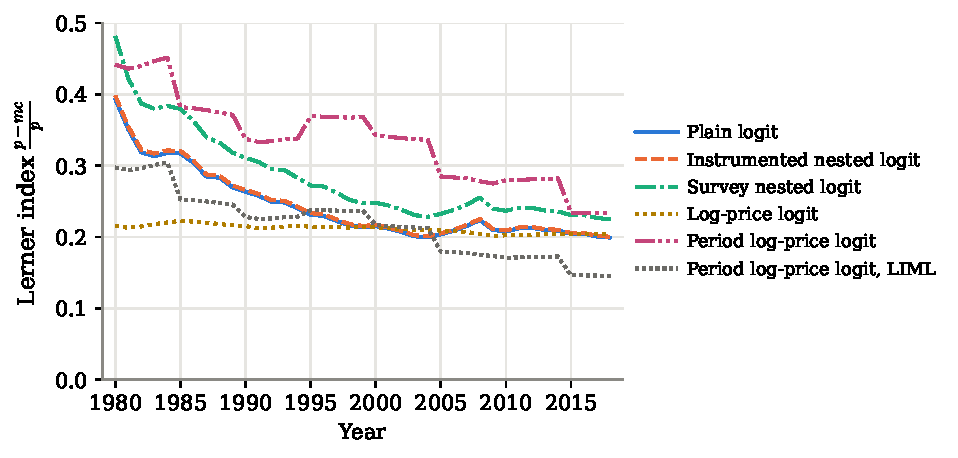
\includegraphics[width=0.95\linewidth]{figures/appC/autos_lerner.pdf}
\caption{Sales-weighted mean Lerner index of new vehicles by year under the six demand models of \cref{tab:C-autos}.
Computed with \texttt{figures/appC/src/autos\_markups.py} from the product data of the replication package of
\citet{GriecoMurryYurukoglu2024}.}
\label{fig:C-autos-lerner}
\end{figure}

\casehead{Part (c)}
Since $L_{jt} = \frac{m_{jt}}{p_{jt}}$, the log Lerner index splits exactly as
\begin{equation}\label{eq:C-lerner-decomp}
  \ln L_{jt} = \ln m_{jt} - \ln p_{jt} = \ln\big(\alpha_\ell m_{jt}\big) - \ln\alpha_\ell - \ln p_{jt} ,
\end{equation}
where $\alpha_\ell$ is the price coefficient that applies in year $t$. It is constant except in the period models of
part (d). We average with the weights $w_{jt}$ and difference between 1980 and 2018. The change in the mean log Lerner index
then splits into the change in the mean log dollar markup and the change in the mean log price. The dollar-markup term
splits again into a scaled markup $\alpha_\ell m_{jt}$ and the coefficient. For the logit with linear price the scaled
markup is $\frac{1}{1 - S_{ft}}$, a function of market structure alone.

\begin{table}[htbp]
\centering
\caption{Decomposition of the change in the mean log Lerner index, 1980 to 2018}
\label{tab:C-autos-decomp}
\footnotesize
\setlength{\tabcolsep}{4pt}
\begin{tabular}{@{}lcccccc@{}}
\toprule
 & Change in & \multicolumn{3}{c}{Dollar markup} & Price & Price share \\
\cmidrule(lr){3-5}
Model & $\overline{\ln L}$ & $\Delta\overline{\ln m}$ & $\Delta\overline{\ln(\alpha_\ell m)}$ & $-\Delta\ln\alpha_\ell$ &
$-\Delta\overline{\ln p}$ & of the fall (\%) \\
\midrule
Plain logit & $-0.694$ & $-0.050$ & $-0.050$ & 0 & $-0.644$ & 93 \\
Instrumented nested logit & $-0.700$ & $-0.056$ & $-0.056$ & 0 & $-0.644$ & 92 \\
Survey nested logit & $-0.765$ & $-0.122$ & $-0.122$ & 0 & $-0.644$ & 84 \\
Log-price logit & $-0.053$ & 0.591 & 0.591 & 0 & $-0.644$ & \\
Period log-price logit & $-0.636$ & 0.008 & 0.591 & $-0.583$ & $-0.644$ & 101 \\
Period log-price logit, LIML & $-0.710$ & $-0.067$ & 0.591 & $-0.658$ & $-0.644$ & 91 \\
\bottomrule
\end{tabular}

\vspace{3pt}
\begin{minipage}{0.97\textwidth}
\footnotesize Notes: Bars denote sales-weighted means within a year, and $\Delta$ the change from 1980 to 2018. The
first column equals the sum of the second and the fifth, and the second equals the sum of the third and the fourth. The
last column is $\frac{\Delta\overline{\ln p}}{-\Delta\overline{\ln L}}$ in percent, omitted where the index barely falls.
Computed with \texttt{figures/appC/src/autos\_markups.py}.
\end{minipage}
\end{table}

\Cref{tab:C-autos-decomp} shows that the decline in every model with a falling index is a fall relative to price. The
sales-weighted mean log price rose by 0.644. Under the plain logit the mean log Lerner index fell by 0.694, so rising
prices account for 93 percent of the fall. The dollar markup fell only 0.050 log points, because firm shares fell and
$\frac{1}{1 - S_{ft}}$ fell with them. The survey nested logit puts more weight on market structure, for a reason we
return to in part (d), but rising prices still account for 84 percent.

\casehead{Part (d)}
The \emph{log-price logit} replaces $\alpha p_{jt}$ by $\alpha\ln p_{jt}$. With the same instrument and controls,
$\hat\alpha = 5.109$ (1.687), and the first-stage $F$ statistic for $\ln p_{jt}$ is 25.1. By
\cref{prop:C-logit-lerner}(ii) the Lerner index stays near $\frac{1}{\hat\alpha} = 0.196$, and indeed it moves only from
0.216 to 0.204. The dollar markup now rises 81 percent, in step with prices. The decomposition shows the mechanism.
By \eqref{eq:C-logprice-markup} the scaled markup $\alpha m_{jt}$ is nearly proportional to price, so its mean log
rises by 0.591 and cancels most of the price term.

Neither functional form is innocuous, and the data can discriminate between them if the price coefficient may change
over time. The \emph{period log-price logit} gives each five-year period $\ell$ its own coefficient $\alpha_\ell$ on
$\ln p_{jt}$. The dollar price sensitivity, the utility lost per dollar, is then $\frac{\alpha_\ell}{p_{jt}}$. If
$\alpha_\ell$ rises in proportion to prices, dollar sensitivity is constant, as in the linear model. If $\alpha_\ell$ is
constant, we are back in the log-price model. Eight coefficients need eight excluded instruments at least. We interact
the exchange rate with period indicators and add assembly-country indicators interacted with period indicators, for
104 excluded instruments, with type-specific linear trends. The added instruments are valid if, within a make,
changes in unobserved quality across periods are unrelated to the assembly country. \citet[fn.~10]{GriecoMurryYurukoglu2024}
strengthen their first stage in the same way when they let the price coefficient vary over time.

\begin{table}[htbp]
\centering
\caption{Period-specific coefficients on log price}
\label{tab:C-autos-periods}
\footnotesize
\begin{tabular}{@{}lccccc@{}}
\toprule
 & \multicolumn{3}{c}{All 104 instruments} & \multicolumn{2}{c}{Exchange rate by period only} \\
\cmidrule(lr){2-4}\cmidrule(lr){5-6}
Period & 2SLS & LIML & OLS & 2SLS & Conditional $F$ \\
\midrule
1980--84 & 2.496 (0.506) & 3.703 & 1.521 & 1.679 (1.782) & 10.8 \\
1985--89 & 2.977 (0.441) & 4.502 & 1.233 & 7.251 (5.634) & 1.9 \\
1990--94 & 3.259 (0.558) & 4.818 & 1.413 & 5.343 (2.399) & 12.6 \\
1995--99 & 2.968 (0.607) & 4.609 & 1.405 & 4.996 (1.802) & 40.5 \\
2000--04 & 3.187 (0.548) & 5.037 & 1.526 & 3.459 (1.229) & 38.5 \\
2005--09 & 3.751 (0.539) & 5.951 & 1.944 & 4.994 (2.227) & 8.1 \\
2010--14 & 3.698 (0.662) & 6.040 & 2.333 & 6.329 (2.478) & 11.1 \\
2015--18 & 4.472 (0.653) & 7.148 & 2.461 & 5.223 (2.581) & 13.6 \\
\bottomrule
\end{tabular}

\vspace{3pt}
\begin{minipage}{0.97\textwidth}
\footnotesize Notes: Entries are $\hat\alpha_\ell$, the negative of the coefficient on $\ln p_{jt}$ in period $\ell$.
The first three columns use the exchange rate by period and assembly-country indicators by period as instruments. The
last two use the eight exchange-rate interactions only. All specifications include the controls of part (a) and
type-specific linear trends. Standard errors clustered by make. Conditional $F$ statistics follow
\citet{SandersonWindmeijer2016}. Computed with \texttt{figures/appC/src/autos\_markups.py}.
\end{minipage}
\end{table}

\Cref{tab:C-autos-periods} reports the coefficients. The 2SLS estimate of $\alpha_\ell$ rises from 2.50 in 1980--84 to
4.47 in 2015--18, an increase of 0.58 log points. Mean log price rose by 0.64, so dollar price sensitivity fell by only
0.06 log points. The dollar markup is then nearly flat (\$7,758 to \$7,851), and the Lerner index falls by 47 percent,
from 0.442 to 0.233. Once the coefficient may follow prices, the data choose a path close to the linear model. Two
caveats apply. With the exchange rate alone the period coefficients are imprecise, and the conditional $F$ statistic
falls to 1.9 in 1985--89, so the path rests on the assembly-country exclusions. With 104 instruments, 2SLS is also
biased toward OLS \citep{Bekker1994}. The OLS coefficients are much smaller, and the limited-information maximum
likelihood (LIML) estimates, which are less sensitive to many instruments, are 48 to 60 percent larger than 2SLS at the
two ends. LIML implies a rise of 0.66 log points in $\alpha_\ell$, lower Lerner indices at every date, and a fall of 51
percent.

The \emph{survey nested logit} replaces the weak instruments for $\sigma$ with information on substitution. A
second-choice survey reports, for buyers of each model, the model they considered most seriously. We treat it as the
model they would have bought had their first choice been unavailable. Its model
counterpart is the effect of removing the first choice from the choice set, a moment that \citet{BerryLevinsohnPakes2004}
introduced into demand estimation.

\begin{lemma}[Removing a model in the nested logit]\label{lem:C-nl-removal}
Suppose model $j$ in nest $g$ is removed and all mean utilities stay fixed. The remaining shares become
\begin{equation}\label{eq:C-nl-removal}
  s'_k = \frac{s_k(1 - s_{j\mid g})^{-\sigma}}{R_j} \ \text{ for } k \in g , \qquad
  s'_k = \frac{s_k}{R_j} \ \text{ otherwise} , \qquad
  R_j = 1 - s_g\big[1 - (1 - s_{j\mid g})^{1 - \sigma}\big] .
\end{equation}
\end{lemma}

\begin{proof}
Removing $j$ multiplies the inclusive sum of nest $g$ by $1 - s_{j\mid g}$, since
$s_{j\mid g} = \frac{e^{\frac{\delta_j}{1 - \sigma}}}{D_g}$, and leaves the other inclusive sums unchanged. The common
denominator $1 + \sum_hD_h^{1 - \sigma}$ is therefore multiplied by
$1 - s_g + s_g(1 - s_{j\mid g})^{1 - \sigma} = R_j$. A model $k \in g$ also has $D_g^{-\sigma}$ in its numerator, which is
multiplied by $(1 - s_{j\mid g})^{-\sigma}$. Substituting in \eqref{eq:C-nl-shares} gives \eqref{eq:C-nl-removal}.
\end{proof}

The survey records only second choices among new vehicles. The model probability that a buyer of $j$ names a second
choice of the same type is therefore
\begin{equation}\label{eq:C-sc-prob}
  \varphi_j(\sigma) = \frac{\sum_{k \in g, k \ne j}(s'_k - s_k)}{\sum_{k \ne j}(s'_k - s_k)} ,
\end{equation}
with both sums over inside models. At $\sigma = 0$ every remaining model gains in proportion to its share, so
$\varphi_j(0) = \frac{s_g - s_j}{1 - s_0 - s_j}$, the IIA answer. Larger $\sigma$ tilts the gains toward the nest. We choose
$\sigma$ so that the average of $\varphi_j(\sigma)$ over surveyed buyers, weighted by the number of respondents whose first
choice is $j$, equals the observed fraction of same-type second choices. That fraction is 84.6 percent. The plain logit
implies 38.2 percent and the instrumented nested logit 46.0 percent. Matching gives $\hat\sigma = 0.524$, with a
bootstrap standard error of 0.002 over the package's 500 resamples of the survey counts. Fitting each survey year
separately gives 0.478 for 1991, 0.567 for 1999, 0.519 for 2005 and 0.532 for 2015. The spread across years is much
larger than the bootstrap standard error, so that standard error understates the uncertainty about a common $\sigma$.

With $\sigma$ fixed at $\hat\sigma$, we move $\hat\sigma\ln s_{j\mid g,t}$ to the left side of \eqref{eq:C-nl-reg} and
estimate $\alpha$ by 2SLS with the exchange rate. Because 2SLS is linear in the dependent variable, the estimate is
$\hat\alpha(\sigma) = 1.696 - 1.795\,\sigma$, where 1.795 is minus the 2SLS coefficient on price in a regression of
$\ln s_{j\mid g,t}$. At $\hat\sigma = 0.524$ this gives $\hat\alpha = 0.755$. Its two-step standard error, which adds
$1.795^2$ times the variance of $\hat\sigma$, is 0.302. The model implies higher Lerner indices, 0.481 in 1980 and
0.225 in 2018, and a fall in the dollar markup of 12.3 percent. Market structure explains the larger fall. Nested logit markups depend on the firm's share within each type. The sales-weighted mean
within-type share of a model's firm fell from 0.280 to 0.137 as the number of models per type grew.

\casehead{Part (e)}
Four lessons emerge. First, simple models on the package data reproduce the broad decline. The plain logit and the
nested logits all put the 2018 index at about half its 1980 value. The full model of \citet{GriecoMurryYurukoglu2024}
gives a sales-weighted mean Lerner index of 0.42 in 1980 and 0.22 in 2018 (Section~5.4 and Table~VII), a ratio of
0.52. Our plain logit gives 0.393 and 0.199, a ratio of 0.506. We describe their model after the four lessons.

Second, the decline is a fall in markups relative to price. In every model except the log-price logit, the mean dollar
markup changes by between $-12.3$ and $+1.2$ percent, while the mean real price nearly doubles. Under linear price this
stability is built in, since by \cref{prop:C-logit-lerner} the dollar markup depends only on $\alpha$ and on shares. A
falling Lerner index with stable dollar markups is what rising quality and marginal cost produce. It does not mean that
firms earn less per vehicle.

Third, the functional form of price decides the trend once the price coefficient is held fixed. Linear price builds in
a Lerner index proportional to $\frac{1}{p}$, and log price builds in a flat one. \citet{GriecoMurryYurukoglu2024}
report a much smaller decline in their own log-price specification, from 0.32 to 0.27 (Section~5.4). With log price
and a separate coefficient for each five-year period, their path looks very similar to their baseline (Figure~VIb).
When the coefficient on log price may change over time, our estimates also move it almost in proportion to prices,
which supports the linear form. That conclusion rests on 104 instruments and on exclusions by assembly country. A cost shifter
that varies more across periods, such as wages in the assembly countries, would test it directly.

Fourth, the substitution parameters matter for levels more than for trends. The survey nested logit raises the Lerner
index by about 0.09 in 1980 and 0.03 in 2018 relative to the plain logit. Aggregate data alone cannot pin down $\sigma$
(\cref{tab:C-autos-nl}), and the second-choice survey can. This is the same lesson as in \cref{sec:C-rc-est}, where the
logit understated diversion among inside goods.

The full model of \citet{GriecoMurryYurukoglu2024} differs from ours in its demand system, its data and its estimator.
Their demand is a random coefficients logit in the tradition of \citet{BerryLevinsohnPakes1995}. In our notation,
household $i$ in year $t$ obtains
\begin{equation}\label{eq:C-gmy-utility}
  u_{ijt} = x_{jt}\beta_{it} - \alpha_{it}p_{jt} + \xi_{jt} + \epsilon_{ijt} , \qquad u_{i0t} = \gamma_t + \epsilon_{i0t} ,
\end{equation}
from model $j$ and from the outside good (their eq.~1). The value $\gamma_t$ of not buying a new vehicle changes from
year to year. Let $D_{it}$ be the vector of household demographics, drawn from the CPS. It has nothing to do with the
inclusive sums $D_{gt}$ of part (a). The coefficients are
\begin{equation}\label{eq:C-gmy-coef}
  \alpha_{it} = \alpha + \pi^\top D_{it} , \qquad \beta_{ikt} = \beta_k + \Pi_kD_{it} + \Sigma_{kk}\nu_{ik} ,
\end{equation}
where $\Pi_k$ is the $k$-th row of $\Pi$ and the $\nu_{ik}$ are independent standard normal draws (eqs.~3--4). The
parameters are fixed over time, but the distribution of tastes moves as demographics change. In our sign convention the
mean price coefficient is $\alpha = 3.112$ (1.124) per \$10,000 (Table~IV). Price sensitivity varies with income, its
square and age. Family size shifts the tastes for vans and for footprint, and rural households value trucks more. Eleven
characteristics carry random coefficients. The two largest are on vehicle types, 6.309 for trucks and 5.538 for vans.
The SUV coefficient of 3.617 is close to the largest remaining one, 3.798 for electric vehicles. The type coefficients
play the role of our nests, since a household with a strong taste for trucks substitutes mainly among trucks.

The year effects mix two objects. GMY write $\xi_{jt} = \tau_t + \tilde\xi_{jt}$, where $\tau_t$ is the mean
unobserved quality of the models of year $t$ relative to the base year. Shares identify only the difference
$\tau_t - \gamma_t$. Following \citet{PakesBerryLevinsohn1993}, GMY assume that unobserved quality does not change on
average for models that continue from $t - 1$ to $t$ without a redesign. With $\mathcal{C}_t$ the set of such models,
\begin{equation}\label{eq:C-gmy-continuing}
  \E\big[\xi_{jt} - \xi_{j,t-1}\big] = \E\big[(\tau_t - \tau_{t-1}) + (\tilde\xi_{jt} - \tilde\xi_{j,t-1})\big] = 0
  \qquad \text{for } j \in \mathcal{C}_t ,
\end{equation}
with the normalization $\tau_0 = 0$ (eq.~2). The condition separates better vehicles from a more attractive outside
option. Mean unobserved quality rises roughly linearly, by about \$25,000 over the period (Section~5.2).

Estimation has three steps (Section~5). The first step chooses the demographic interactions, the random coefficients
and the mean utilities by GMM. It matches two kinds of micro moments. The CEX (1980--2005, about 1,014 buyers a year)
and MRI (1992--2018, about 2,005 buyers a year) give moments such as the mean price paid in each income quintile
(Sections~2.3 and~5). The MaritzCX survey gives the correlations between the attributes of first and second choices in the
four survey years. The second step regresses the mean utilities on characteristics, price, make dummies and year
dummies by 2SLS, with the lagged real exchange rate as the excluded instrument. This is the moment condition of our part
(a). The third step splits the year effects into $\tau_t$ and $\gamma_t$ with \eqref{eq:C-gmy-continuing}. Standard
errors come from 500 bootstrap samples of the micro data, with a nested parametric bootstrap, clustered by make, in the
second step.

Each source of variation has a clear role. The real exchange rate is the price level of the assembly country relative
to the United States, taken from the Penn World Table and lagged one year (Section~2.2). It moves with local wages and
with the nominal exchange rate, and both shift the dollar cost of the vehicles made there. It identifies the price
coefficient. The second choices identify the random coefficients. The correlation between the truck indicators of first
and second choices is 0.843 in the data and 0.798 in the full model (Table~VI). A model with the demographic
interactions alone gives $-0.013$, and the logit gives $-0.024$. Observed heterogeneity alone cannot produce the
substitution within types that the survey records. Our survey nested logit in part (d) rests on the same evidence.

The full model gives a share-weighted mean own-price elasticity of $-5.06$ over the sample (Section~5.1). The market
elasticity is $-1.07$ in 1985 and $-1.29$ in 2015 (Table~V). The median Lerner index falls from 0.325 to 0.185
(Figure~VIa). The decline survives a linear trend in the price coefficient, a separate coefficient for each five-year
period and separate estimation on three subperiods (Figure~VIb).

GMY explain the decline much as part (c) does. Single-product markups follow nearly the same path as multi-product ones
(Figure~VIIIa). The single-product rule $L_{jt} = -\frac{s_{jt}}{p_{jt}}\big(\frac{\partial s_{jt}}{\partial
p_{jt}}\big)^{-1}$ of their eq.~(7) therefore guides the reading. From 1980 to 1999, mean shares and mean own-price
derivatives stay flat while mean prices rise, so the index falls. Counterfactuals then isolate the primitive forces
(Section~5.4.1). Removing the growth of foreign brands from the ownership structure, or holding the number of products
at its 1980 level, does not remove the decline. Mapping each year's characteristics onto their 1980 distribution keeps
marginal costs flat and substantially reduces the fall (Figure~IX). In their reading, better vehicles raised marginal
costs, which were passed through to prices less than fully.

GMY maintain Nash-Bertrand pricing and ask how much collusion would be needed to undo the decline (Section~5.5).
Simulated cartels in 2018 answer the question in Table~VII. A cartel of GM, Ford and Toyota raises the mean Lerner index
only to 0.26. Only a cartel of the six largest parent companies, at 0.46, exceeds the 1980 value of 0.42. The
Herfindahl index meanwhile fell from 2,661 to 1,132 points. Beyond markups, the consumers' share of efficient surplus
rose from 0.62 to 0.82, and consumer surplus per household rose by about \$8,000 (Section~1). GMY define efficient
surplus as consumer surplus plus producer surplus plus deadweight loss, the surplus at prices equal to marginal costs.
Our simple models agree with the full model on the main mechanism. Prices rose against stable dollar markups. GMY
report no dollar markups. By their eq.~(7), however, flat mean shares and own-price derivatives imply flat
single-product dollar markups from 1980 to 1999 (Section~5.4.1 and Figure~VIII). What the full model adds is the separation of
quality from the outside option and a measure of welfare.

The exercise has clear limits. Prices are list prices, so changes in discounts and rebates over time pass into the
estimated markups. The market size of one vehicle per 2.5 households is a convention, and the outside share moves with
it. Demand is static, with no used-car market or replacement timing, and the nests are chosen a priori. The exchange
rate may violate the exclusion if currency movements coincide with changes in a make's unobserved quality. The
comparison with production-function estimates is also less direct than it looks. The demand-side Lerner index measures
price over marginal cost for new vehicles, while production-function markups use firm-level revenue and variable
input costs (\cref{sec:01-rising-markups}). \citet[Section~5.6]{GriecoMurryYurukoglu2024} make this comparison for the
auto industry. Both the level and the trend of their ratio of price to marginal cost differ from the production-function
series, although both are fairly flat after 1995. What the exercise contributes is a diagnosis. It shows which parts of a
measured trend in markups come from the data, which from the functional form, and which from the estimated
substitution patterns.

\subsection{Computational notes}

The script \texttt{autos\_markups.py} reads the package files \texttt{data\_blp.csv}, \texttt{secondChoiceOut.mat}
and \texttt{secondChoice\_bootstrap.mat}, and it runs in about three minutes.
\begin{enumerate}
  \item Build shares with $M_t$ equal to households divided by 2.5, prices in \$10,000, nests from the type indicators,
  and within-type shares and counts by year and type.
  \item Code 2SLS, the clustered sandwich, first-stage and conditional $F$ statistics and LIML with numpy. Run the
  logit, the nested logit grid and the log-price models.
  \item Fit $\sigma$ to the second-choice counts with a bracketing root finder on $[0, 0.995]$, using
  \eqref{eq:C-nl-removal} and \eqref{eq:C-sc-prob}, and repeat for each bootstrap sample of counts.
  \item For each model and year, form $\Delta_t$ from \eqref{eq:C-nl-deriv} or its log-price analogue and solve
  \eqref{eq:C-autos-markup} with the parent-company ownership matrix.
  \item Check the share inversion, the removal formula against brute-force removal, the derivatives against finite
  differences and the logit markups against \cref{prop:C-logit-lerner}.
\end{enumerate}


\section{Bibliographic notes}\label{sec:C-notes}

The cross-industry regressions of margins on concentration that \cref{sec:C-cournot} examines go back to
\citet{Bain1951}, and \citet{Schmalensee1989} reviews the evidence they produced. \citet{CowlingWaterson1976} derived
the Cournot relation between the Herfindahl index and the share-weighted Lerner index. \citet{Demsetz1973} stated
the efficiency critique that \cref{prop:C-demsetz} formalizes. \citet[Section~5.5]{Tirole1988} develops both results as
exercises, together with the welfare bound of \citet{DansbyWillig1979}. The merger paradox of Cournot competition is
due to \citet{SalantSwitzerReynolds1983}. \citet{FarrellShapiro1990} derive the general synergy condition for a Cournot
merger to lower price and a sufficient condition for it to raise welfare. \citet[Section~3.3]{AskerNocke2021} survey
the theory of unilateral merger effects built on that analysis, including mergers among multi-product logit firms and
mergers under free entry. \citet{MankiwWhinston1986} established the excess-entry result. Grim-trigger strategies
come from \citet{Friedman1971}, and \citet{Abreu1986} characterized the optimal punishments that sustain collusion at
lower discount factors. \citet[Section~6.3.2.1]{Tirole1988} uses the Bertrand supergame to link concentration with
tacit collusion.

\citet{Sumner1981} introduced the tax pass-through test of \cref{sec:C-passthrough}. The link between pass-through
and the curvature of demand goes back to \citet{BulowPfleiderer1983}, and \citet{WeylFabinger2013} develop it into a
general framework for incidence under imperfect competition. \citet{Barzel1976} raised the quality response to unit
taxes. \citet{Bresnahan1982} and \citet{Lau1982} showed that parallel shifts of demand cannot separate conduct
from marginal cost. Demand rotations, which change the slope of demand at a given price, can. \citet{Bresnahan1989}
restates this argument in his survey of conduct estimation. \citet{Corts1999} shows that an estimated conduct
parameter can badly mismeasure market power when firms collude tacitly in a repeated game.
\citet{BertrandDufloMullainathan2004} documented how serial correlation overstates the precision of
difference-in-differences regressions, the same problem that clustering addresses in \cref{sec:C-passthrough}.

For logit pricing, \citet{CaplinNalebuff1991} proved existence of price equilibrium under $\rho$-concavity conditions
on the distribution of tastes, which are weaker than log-concavity. They proved uniqueness in cases that include
single-product logit firms, and they credit \citet{AndersonDePalma1988} with the first uniqueness result for the logit
duopoly.
\citet{KonovalovSandor2010} extended uniqueness to multi-product logit firms, and \citet{NockeSchutz2018} developed
the aggregative approach used in \cref{prop:C-unique}. \citet{MorrowSkerlos2011} proposed the fixed-point
formulation that \cref{sec:C-simulate} uses to compute random coefficients equilibria. The upward pricing pressure of
\cref{sec:C-logit-bertrand} is due to \citet{FarrellShapiro2010}, and \citet{Werden1996} derived the compensating
marginal cost reductions of the further problems below.

The estimation problems rest on \citet{Berry1994}, who introduced the share inversion and applied it to the logit,
the nested logit and the vertical model. The vertical model of \cref{sec:C-vertical} follows \citet{Bresnahan1987}
and his study of the 1955 automobile market, which finds collusive pricing in 1954 and 1956 and competitive pricing in
1955. \citet{BerryLevinsohnPakes1995} developed the random coefficients model, its
contraction and its instruments, and \citet{Nevo2000a} gives a practical guide to its estimation.
\citet{ConlonGortmaker2020} collect current best practice for computation and instruments, including the
differentiation instruments of \citet{GandhiHoude2019}. \citet{DubeFoxSu2012} show how loose inner-loop tolerances
distort the estimates. \citet{BerryLevinsohnPakes2004} brought second-choice data into demand estimation, and
\citet{SandersonWindmeijer2016} give the weak-instrument diagnostics for several endogenous regressors that
\cref{sec:C-autos} uses. The question of \cref{sec:C-autos} comes from \citet{GriecoMurryYurukoglu2024}. They estimate
a random coefficients logit with demographic micro moments and second-choice data. They separate unobserved quality
from the value of the outside good with the continuing-products restriction of \citet{PakesBerryLevinsohn1993}. They
find that the mean Lerner index of new vehicles roughly halved from 1980 to 2018. The production-function evidence on rising markups that motivates the question is in \citet{DeLoeckerEeckhoutUnger2020}.

\section{Further problems}\label{sec:C-further}

The following problems extend the worked problems. Solutions are not provided.

\begin{enumerate}
\item \emph{Cournot with constant-elasticity demand.} Let inverse demand be $P(Q) = AQ^{-\frac{1}{\varepsilon}}$ with
  $\varepsilon > 1$, and let firm $i$ have constant marginal cost $c_i$ and fixed cost $F$. Show that every active firm
  satisfies $L_i = \frac{s_i}{\varepsilon}$. With symmetric costs, find the free-entry number of firms, treating it as
  continuous, and the resulting $L$ and $\HHI$. Compare the relation between concentration and margins across
  industries that differ in $A$ or in $F$ with the linear case of \cref{sec:C-cournot}, part (d).

\item \emph{One-period punishments.} In the repeated linear Cournot game of \cref{sec:C-cournot}, part (c), let inverse
  demand be $P(Q) = \max\{a - bQ, 0\}$. After a deviation every firm produces $q^p$ for one period and then returns to
  $\frac{Q^m}{N}$. Write the incentive constraints of the collusive phase and of the punishment phase. For $N = 2$ and
  the parameters of \cref{sec:C-cournot}, part (g), find numerically the lowest discount factor at which some $q^p$
  satisfies both constraints, and compare it with $\delta^*(2) = \frac{9}{17}$ \citep{Abreu1986}.

\item \emph{An ad valorem tax in the logit market.} In the 25-product market of \cref{sec:C-logit-bertrand}, firms
  receive $(1 - \tau)p_j$ per unit sold. Derive the single-product and multi-product first-order conditions, compute the
  equilibria at $\tau = 0.1$, and report the elasticity of each price with respect to $\frac{1}{1 - \tau}$. Compare the
  results with \cref{prop:C-adval} and explain the role of the curvature of logit demand.

\item \emph{Compensating marginal cost reductions with random coefficients.} \Cref{ex:04-merger-sim} computes the
  reductions in marginal cost that leave every price unchanged after the logit merger of \cref{sec:C-logit-bertrand},
  part (g) \citep{Werden1996}. Consider instead the merger of firms B and C in market 0 of \cref{sec:C-rc-est},
  part (f). Show that, for any demand model, the compensating marginal costs are
  $mc' = p + (\Omega' \odot \Delta^\top)^{-1}s$, with $\Omega'$ the post-merger ownership matrix and $\Delta$ and $s$
  evaluated at pre-merger prices. Explain why the costs of non-merging products are unchanged. Compute the reductions
  under the logit, the estimated random coefficients model and the true model, and compare them with the upward
  pricing pressure in \cref{tab:C-merger-m0}.

\item \emph{The vertical model with uniform tastes.} Let the price sensitivity $\nu_i$ be uniform on
  $[0, \bar\nu]$. Redo parts (a) to (c) of \cref{sec:C-vertical}. Which parameters are identified, and do the implied
  markups depend on $\bar\nu$? Compare the implied own elasticities in market 0 with \cref{tab:C-velast}. Then let the
  taste for quality $\frac{1}{\nu_i}$ be uniform instead, the specification of \citet{Bresnahan1987}, and derive the
  inversion again.

\item \emph{How many simulation draws?} Let $s^{n_s}_{jt} = \frac{1}{n_s}\sum_{i=1}^{n_s}s_{ijt}$ with independent
  draws $\nu_i$. Show that $\Var(s^{n_s}_{jt}) = \frac{1}{n_s}\Var_\nu(s_{ijt})$. With the firms' draws of
  \cref{sec:C-simulate}, estimate the number of draws that gives a relative standard error of one percent for every
  product in market 0. Compare this simulation error with the sampling error of the realized shares.

\item \emph{Differentiation instruments.} Replace the six competition instruments of \cref{sec:C-logit-est} by two
  counts \citep{GandhiHoude2019}. The first counts rival products whose sugar content lies within one standard
  deviation of the product's own. The second counts rival products with the same organic status. Re-estimate the logit by 2SLS and the random
  coefficients model of \cref{sec:C-rc-est} with $\Sigma$ known. Report the first-stage statistics and explain why the
  new instruments are or are not stronger.

\item \emph{Nested logit pricing.} With nested logit demand and multi-product firms, derive the first-order
  conditions for prices. Show that markups are common within each pair of a firm and a nest, and give the formula
  for the common markup in terms of the firm's within-nest and total shares. When does the formula reduce to the
  single-product markup of \cref{prop:C-nl-deriv}?
\end{enumerate}


\backmatter
\cleardoublepage
\phantomsection
\addcontentsline{toc}{part}{Bibliography}
\bibliographystyle{plainnat}
\bibliography{references}
\end{document}
